\documentclass[twoside]{book}

% Packages required by doxygen
\usepackage{fixltx2e}
\usepackage{calc}
\usepackage{doxygen}
\usepackage[export]{adjustbox} % also loads graphicx
\usepackage{graphicx}
\usepackage[utf8]{inputenc}
\usepackage{makeidx}
\usepackage{multicol}
\usepackage{multirow}
\PassOptionsToPackage{warn}{textcomp}
\usepackage{textcomp}
\usepackage[nointegrals]{wasysym}
\usepackage[table]{xcolor}

% Font selection
\usepackage[T1]{fontenc}
\usepackage[scaled=.90]{helvet}
\usepackage{courier}
\usepackage{amssymb}
\usepackage{sectsty}
\renewcommand{\familydefault}{\sfdefault}
\allsectionsfont{%
  \fontseries{bc}\selectfont%
  \color{darkgray}%
}
\renewcommand{\DoxyLabelFont}{%
  \fontseries{bc}\selectfont%
  \color{darkgray}%
}
\newcommand{\+}{\discretionary{\mbox{\scriptsize$\hookleftarrow$}}{}{}}

% Page & text layout
\usepackage{geometry}
\geometry{%
  a4paper,%
  top=2.5cm,%
  bottom=2.5cm,%
  left=2.5cm,%
  right=2.5cm%
}
\tolerance=750
\hfuzz=15pt
\hbadness=750
\setlength{\emergencystretch}{15pt}
\setlength{\parindent}{0cm}
\setlength{\parskip}{3ex plus 2ex minus 2ex}
\makeatletter
\renewcommand{\paragraph}{%
  \@startsection{paragraph}{4}{0ex}{-1.0ex}{1.0ex}{%
    \normalfont\normalsize\bfseries\SS@parafont%
  }%
}
\renewcommand{\subparagraph}{%
  \@startsection{subparagraph}{5}{0ex}{-1.0ex}{1.0ex}{%
    \normalfont\normalsize\bfseries\SS@subparafont%
  }%
}
\makeatother

% Headers & footers
\usepackage{fancyhdr}
\pagestyle{fancyplain}
\fancyhead[LE]{\fancyplain{}{\bfseries\thepage}}
\fancyhead[CE]{\fancyplain{}{}}
\fancyhead[RE]{\fancyplain{}{\bfseries\leftmark}}
\fancyhead[LO]{\fancyplain{}{\bfseries\rightmark}}
\fancyhead[CO]{\fancyplain{}{}}
\fancyhead[RO]{\fancyplain{}{\bfseries\thepage}}
\fancyfoot[LE]{\fancyplain{}{}}
\fancyfoot[CE]{\fancyplain{}{}}
\fancyfoot[RE]{\fancyplain{}{\bfseries\scriptsize Generated by Doxygen }}
\fancyfoot[LO]{\fancyplain{}{\bfseries\scriptsize Generated by Doxygen }}
\fancyfoot[CO]{\fancyplain{}{}}
\fancyfoot[RO]{\fancyplain{}{}}
\renewcommand{\footrulewidth}{0.4pt}
\renewcommand{\chaptermark}[1]{%
  \markboth{#1}{}%
}
\renewcommand{\sectionmark}[1]{%
  \markright{\thesection\ #1}%
}

% Indices & bibliography
\usepackage{natbib}
\usepackage[titles]{tocloft}
\setcounter{tocdepth}{3}
\setcounter{secnumdepth}{5}
\makeindex

% Hyperlinks (required, but should be loaded last)
\usepackage{ifpdf}
\ifpdf
  \usepackage[pdftex,pagebackref=true]{hyperref}
\else
  \usepackage[ps2pdf,pagebackref=true]{hyperref}
\fi
\hypersetup{%
  colorlinks=true,%
  linkcolor=blue,%
  citecolor=blue,%
  unicode%
}

% Custom commands
\newcommand{\clearemptydoublepage}{%
  \newpage{\pagestyle{empty}\cleardoublepage}%
}

\usepackage{caption}
\captionsetup{labelsep=space,justification=centering,font={bf},singlelinecheck=off,skip=4pt,position=top}

%===== C O N T E N T S =====

\begin{document}

% Titlepage & ToC
\hypersetup{pageanchor=false,
             bookmarksnumbered=true,
             pdfencoding=unicode
            }
\pagenumbering{alph}
\begin{titlepage}
\vspace*{7cm}
\begin{center}%
{\Large My Project }\\
\vspace*{1cm}
{\large Generated by Doxygen 1.8.13}\\
\end{center}
\end{titlepage}
\clearemptydoublepage
\pagenumbering{roman}
\tableofcontents
\clearemptydoublepage
\pagenumbering{arabic}
\hypersetup{pageanchor=true}

%--- Begin generated contents ---
\chapter{C\+M\+S\+IS Cortex-\/\+M4}
\label{index}\hypertarget{index}{}This documentation describes the C\+M\+S\+IS Cortex-\/M Core Peripheral Access Layer. It consists of\+:


\begin{DoxyItemize}
\item Cortex-\/M Core Register Definitions
\item Cortex-\/M functions
\item Cortex-\/M instructions
\item Cortex-\/M S\+I\+MD instructions
\end{DoxyItemize}

The C\+M\+S\+IS Cortex-\/\+M4 Core Peripheral Access Layer contains C and assembly functions that ease access to the Cortex-\/M Core 
\chapter{Module Index}
\section{Modules}
Here is a list of all modules\+:\begin{DoxyCompactList}
\item \contentsline{section}{C\+M\+S\+IS M\+I\+S\+R\+A-\/C\+:2004 Compliance Exceptions}{\pageref{group___c_m_s_i_s___m_i_s_r_a___exceptions}}{}
\item \contentsline{section}{C\+M\+S\+IS Core Definitions}{\pageref{group___c_m_s_i_s__core__definitions}}{}
\item \contentsline{section}{C\+M\+S\+IS Core Register}{\pageref{group___c_m_s_i_s__core__register}}{}
\begin{DoxyCompactList}
\item \contentsline{section}{C\+M\+S\+IS Core}{\pageref{group___c_m_s_i_s___c_o_r_e}}{}
\item \contentsline{section}{C\+M\+S\+IS N\+V\+IC}{\pageref{group___c_m_s_i_s___n_v_i_c}}{}
\item \contentsline{section}{C\+M\+S\+IS S\+CB}{\pageref{group___c_m_s_i_s___s_c_b}}{}
\item \contentsline{section}{C\+M\+S\+IS System Control and ID Register not in the S\+CB}{\pageref{group___c_m_s_i_s___s_cn_s_c_b}}{}
\item \contentsline{section}{C\+M\+S\+IS Sys\+Tick}{\pageref{group___c_m_s_i_s___sys_tick}}{}
\item \contentsline{section}{C\+M\+S\+IS I\+TM}{\pageref{group___c_m_s_i_s___i_t_m}}{}
\item \contentsline{section}{C\+M\+S\+IS Core Debug}{\pageref{group___c_m_s_i_s___core_debug}}{}
\end{DoxyCompactList}
\item \contentsline{section}{C\+M\+S\+IS Core Function Interface}{\pageref{group___c_m_s_i_s___core___function_interface}}{}
\begin{DoxyCompactList}
\item \contentsline{section}{C\+M\+S\+IS Core N\+V\+IC Functions}{\pageref{group___c_m_s_i_s___core___n_v_i_c_functions}}{}
\item \contentsline{section}{C\+M\+S\+IS Core Sys\+Tick Functions}{\pageref{group___c_m_s_i_s___core___sys_tick_functions}}{}
\item \contentsline{section}{C\+M\+S\+IS Core Debug Functions}{\pageref{group___c_m_s_i_s__core___debug_functions}}{}
\item \contentsline{section}{C\+M\+S\+IS Core Register Access Functions}{\pageref{group___c_m_s_i_s___core___reg_acc_functions}}{}
\end{DoxyCompactList}
\item \contentsline{section}{C\+M\+S\+IS S\+I\+MD Intrinsics}{\pageref{group___c_m_s_i_s___s_i_m_d__intrinsics}}{}
\item \contentsline{section}{C\+M\+S\+IS Core Instruction Interface}{\pageref{group___c_m_s_i_s___core___instruction_interface}}{}
\item \contentsline{section}{C\+M\+S\+IS}{\pageref{group___c_m_s_i_s}}{}
\begin{DoxyCompactList}
\item \contentsline{section}{Stm32f4xx}{\pageref{group__stm32f4xx}}{}
\begin{DoxyCompactList}
\item \contentsline{section}{Library\+\_\+configuration\+\_\+section}{\pageref{group___library__configuration__section}}{}
\item \contentsline{section}{Configuration\+\_\+section\+\_\+for\+\_\+\+C\+M\+S\+IS}{\pageref{group___configuration__section__for___c_m_s_i_s}}{}
\item \contentsline{section}{Exported\+\_\+types}{\pageref{group___exported__types}}{}
\item \contentsline{section}{Peripheral\+\_\+registers\+\_\+structures}{\pageref{group___peripheral__registers__structures}}{}
\item \contentsline{section}{Peripheral\+\_\+memory\+\_\+map}{\pageref{group___peripheral__memory__map}}{}
\item \contentsline{section}{Peripheral\+\_\+declaration}{\pageref{group___peripheral__declaration}}{}
\item \contentsline{section}{Exported\+\_\+constants}{\pageref{group___exported__constants}}{}
\begin{DoxyCompactList}
\item \contentsline{section}{Peripheral\+\_\+\+Registers\+\_\+\+Bits\+\_\+\+Definition}{\pageref{group___peripheral___registers___bits___definition}}{}
\end{DoxyCompactList}
\item \contentsline{section}{Exported\+\_\+macro}{\pageref{group___exported__macro}}{}
\end{DoxyCompactList}
\item \contentsline{section}{Stm32f4xx\+\_\+system}{\pageref{group__stm32f4xx__system}}{}
\begin{DoxyCompactList}
\item \contentsline{section}{S\+T\+M32\+F4xx\+\_\+\+System\+\_\+\+Private\+\_\+\+Includes}{\pageref{group___s_t_m32_f4xx___system___private___includes}}{}
\item \contentsline{section}{S\+T\+M32\+F4xx\+\_\+\+System\+\_\+\+Private\+\_\+\+Types\+Definitions}{\pageref{group___s_t_m32_f4xx___system___private___types_definitions}}{}
\item \contentsline{section}{S\+T\+M32\+F4xx\+\_\+\+System\+\_\+\+Private\+\_\+\+Defines}{\pageref{group___s_t_m32_f4xx___system___private___defines}}{}
\item \contentsline{section}{S\+T\+M32\+F4xx\+\_\+\+System\+\_\+\+Private\+\_\+\+Macros}{\pageref{group___s_t_m32_f4xx___system___private___macros}}{}
\item \contentsline{section}{S\+T\+M32\+F4xx\+\_\+\+System\+\_\+\+Private\+\_\+\+Variables}{\pageref{group___s_t_m32_f4xx___system___private___variables}}{}
\item \contentsline{section}{S\+T\+M32\+F4xx\+\_\+\+System\+\_\+\+Private\+\_\+\+Function\+Prototypes}{\pageref{group___s_t_m32_f4xx___system___private___function_prototypes}}{}
\item \contentsline{section}{S\+T\+M32\+F4xx\+\_\+\+System\+\_\+\+Private\+\_\+\+Functions}{\pageref{group___s_t_m32_f4xx___system___private___functions}}{}
\item \contentsline{section}{S\+T\+M32\+F4xx\+\_\+\+System\+\_\+\+Includes}{\pageref{group___s_t_m32_f4xx___system___includes}}{}
\item \contentsline{section}{S\+T\+M32\+F4xx\+\_\+\+System\+\_\+\+Exported\+\_\+types}{\pageref{group___s_t_m32_f4xx___system___exported__types}}{}
\item \contentsline{section}{S\+T\+M32\+F4xx\+\_\+\+System\+\_\+\+Exported\+\_\+\+Constants}{\pageref{group___s_t_m32_f4xx___system___exported___constants}}{}
\item \contentsline{section}{S\+T\+M32\+F4xx\+\_\+\+System\+\_\+\+Exported\+\_\+\+Macros}{\pageref{group___s_t_m32_f4xx___system___exported___macros}}{}
\item \contentsline{section}{S\+T\+M32\+F4xx\+\_\+\+System\+\_\+\+Exported\+\_\+\+Functions}{\pageref{group___s_t_m32_f4xx___system___exported___functions}}{}
\end{DoxyCompactList}
\end{DoxyCompactList}
\item \contentsline{section}{S\+T\+M32\+F4xx\+\_\+\+Std\+Periph\+\_\+\+Driver}{\pageref{group___s_t_m32_f4xx___std_periph___driver}}{}
\begin{DoxyCompactList}
\item \contentsline{section}{M\+I\+SC}{\pageref{group___m_i_s_c}}{}
\begin{DoxyCompactList}
\item \contentsline{section}{M\+I\+S\+C\+\_\+\+Exported\+\_\+\+Constants}{\pageref{group___m_i_s_c___exported___constants}}{}
\begin{DoxyCompactList}
\item \contentsline{section}{M\+I\+S\+C\+\_\+\+Vector\+\_\+\+Table\+\_\+\+Base}{\pageref{group___m_i_s_c___vector___table___base}}{}
\item \contentsline{section}{M\+I\+S\+C\+\_\+\+System\+\_\+\+Low\+\_\+\+Power}{\pageref{group___m_i_s_c___system___low___power}}{}
\item \contentsline{section}{M\+I\+S\+C\+\_\+\+Preemption\+\_\+\+Priority\+\_\+\+Group}{\pageref{group___m_i_s_c___preemption___priority___group}}{}
\item \contentsline{section}{M\+I\+S\+C\+\_\+\+Sys\+Tick\+\_\+clock\+\_\+source}{\pageref{group___m_i_s_c___sys_tick__clock__source}}{}
\end{DoxyCompactList}
\item \contentsline{section}{M\+I\+S\+C\+\_\+\+Private\+\_\+\+Functions}{\pageref{group___m_i_s_c___private___functions}}{}
\end{DoxyCompactList}
\item \contentsline{section}{D\+MA}{\pageref{group___d_m_a}}{}
\begin{DoxyCompactList}
\item \contentsline{section}{D\+M\+A\+\_\+\+Exported\+\_\+\+Constants}{\pageref{group___d_m_a___exported___constants}}{}
\begin{DoxyCompactList}
\item \contentsline{section}{D\+M\+A\+\_\+channel}{\pageref{group___d_m_a__channel}}{}
\item \contentsline{section}{D\+M\+A\+\_\+data\+\_\+transfer\+\_\+direction}{\pageref{group___d_m_a__data__transfer__direction}}{}
\item \contentsline{section}{D\+M\+A\+\_\+data\+\_\+buffer\+\_\+size}{\pageref{group___d_m_a__data__buffer__size}}{}
\item \contentsline{section}{D\+M\+A\+\_\+peripheral\+\_\+incremented\+\_\+mode}{\pageref{group___d_m_a__peripheral__incremented__mode}}{}
\item \contentsline{section}{D\+M\+A\+\_\+memory\+\_\+incremented\+\_\+mode}{\pageref{group___d_m_a__memory__incremented__mode}}{}
\item \contentsline{section}{D\+M\+A\+\_\+peripheral\+\_\+data\+\_\+size}{\pageref{group___d_m_a__peripheral__data__size}}{}
\item \contentsline{section}{D\+M\+A\+\_\+memory\+\_\+data\+\_\+size}{\pageref{group___d_m_a__memory__data__size}}{}
\item \contentsline{section}{D\+M\+A\+\_\+circular\+\_\+normal\+\_\+mode}{\pageref{group___d_m_a__circular__normal__mode}}{}
\item \contentsline{section}{D\+M\+A\+\_\+priority\+\_\+level}{\pageref{group___d_m_a__priority__level}}{}
\item \contentsline{section}{D\+M\+A\+\_\+fifo\+\_\+direct\+\_\+mode}{\pageref{group___d_m_a__fifo__direct__mode}}{}
\item \contentsline{section}{D\+M\+A\+\_\+fifo\+\_\+threshold\+\_\+level}{\pageref{group___d_m_a__fifo__threshold__level}}{}
\item \contentsline{section}{D\+M\+A\+\_\+memory\+\_\+burst}{\pageref{group___d_m_a__memory__burst}}{}
\item \contentsline{section}{D\+M\+A\+\_\+peripheral\+\_\+burst}{\pageref{group___d_m_a__peripheral__burst}}{}
\item \contentsline{section}{D\+M\+A\+\_\+fifo\+\_\+status\+\_\+level}{\pageref{group___d_m_a__fifo__status__level}}{}
\item \contentsline{section}{D\+M\+A\+\_\+flags\+\_\+definition}{\pageref{group___d_m_a__flags__definition}}{}
\item \contentsline{section}{D\+M\+A\+\_\+interrupt\+\_\+enable\+\_\+definitions}{\pageref{group___d_m_a__interrupt__enable__definitions}}{}
\item \contentsline{section}{D\+M\+A\+\_\+interrupts\+\_\+definitions}{\pageref{group___d_m_a__interrupts__definitions}}{}
\item \contentsline{section}{D\+M\+A\+\_\+peripheral\+\_\+increment\+\_\+offset}{\pageref{group___d_m_a__peripheral__increment__offset}}{}
\item \contentsline{section}{D\+M\+A\+\_\+flow\+\_\+controller\+\_\+definitions}{\pageref{group___d_m_a__flow__controller__definitions}}{}
\item \contentsline{section}{D\+M\+A\+\_\+memory\+\_\+targets\+\_\+definitions}{\pageref{group___d_m_a__memory__targets__definitions}}{}
\end{DoxyCompactList}
\item \contentsline{section}{D\+M\+A\+\_\+\+Private\+\_\+\+Functions}{\pageref{group___d_m_a___private___functions}}{}
\begin{DoxyCompactList}
\item \contentsline{section}{Initialization and Configuration functions}{\pageref{group___d_m_a___group1}}{}
\item \contentsline{section}{Data Counter functions}{\pageref{group___d_m_a___group2}}{}
\item \contentsline{section}{Double Buffer mode functions}{\pageref{group___d_m_a___group3}}{}
\item \contentsline{section}{Interrupts and flags management functions}{\pageref{group___d_m_a___group4}}{}
\end{DoxyCompactList}
\end{DoxyCompactList}
\item \contentsline{section}{G\+P\+IO}{\pageref{group___g_p_i_o}}{}
\begin{DoxyCompactList}
\item \contentsline{section}{G\+P\+I\+O\+\_\+\+Exported\+\_\+\+Constants}{\pageref{group___g_p_i_o___exported___constants}}{}
\begin{DoxyCompactList}
\item \contentsline{section}{G\+P\+I\+O\+\_\+pins\+\_\+define}{\pageref{group___g_p_i_o__pins__define}}{}
\item \contentsline{section}{G\+P\+I\+O\+\_\+\+Pin\+\_\+sources}{\pageref{group___g_p_i_o___pin__sources}}{}
\item \contentsline{section}{G\+P\+I\+O\+\_\+\+Alternat\+\_\+function\+\_\+selection\+\_\+define}{\pageref{group___g_p_i_o___alternat__function__selection__define}}{}
\item \contentsline{section}{G\+P\+I\+O\+\_\+\+Legacy}{\pageref{group___g_p_i_o___legacy}}{}
\end{DoxyCompactList}
\item \contentsline{section}{G\+P\+I\+O\+\_\+\+Private\+\_\+\+Functions}{\pageref{group___g_p_i_o___private___functions}}{}
\begin{DoxyCompactList}
\item \contentsline{section}{Initialization and Configuration}{\pageref{group___g_p_i_o___group1}}{}
\item \contentsline{section}{G\+P\+IO Read and Write}{\pageref{group___g_p_i_o___group2}}{}
\item \contentsline{section}{G\+P\+IO Alternate functions configuration function}{\pageref{group___g_p_i_o___group3}}{}
\end{DoxyCompactList}
\end{DoxyCompactList}
\item \contentsline{section}{R\+CC}{\pageref{group___r_c_c}}{}
\begin{DoxyCompactList}
\item \contentsline{section}{R\+C\+C\+\_\+\+Exported\+\_\+\+Constants}{\pageref{group___r_c_c___exported___constants}}{}
\begin{DoxyCompactList}
\item \contentsline{section}{R\+C\+C\+\_\+\+H\+S\+E\+\_\+configuration}{\pageref{group___r_c_c___h_s_e__configuration}}{}
\item \contentsline{section}{R\+C\+C\+\_\+\+P\+L\+L\+\_\+\+Clock\+\_\+\+Source}{\pageref{group___r_c_c___p_l_l___clock___source}}{}
\item \contentsline{section}{R\+C\+C\+\_\+\+System\+\_\+\+Clock\+\_\+\+Source}{\pageref{group___r_c_c___system___clock___source}}{}
\item \contentsline{section}{R\+C\+C\+\_\+\+A\+H\+B\+\_\+\+Clock\+\_\+\+Source}{\pageref{group___r_c_c___a_h_b___clock___source}}{}
\item \contentsline{section}{R\+C\+C\+\_\+\+A\+P\+B1\+\_\+\+A\+P\+B2\+\_\+\+Clock\+\_\+\+Source}{\pageref{group___r_c_c___a_p_b1___a_p_b2___clock___source}}{}
\item \contentsline{section}{R\+C\+C\+\_\+\+Interrupt\+\_\+\+Source}{\pageref{group___r_c_c___interrupt___source}}{}
\item \contentsline{section}{R\+C\+C\+\_\+\+L\+S\+E\+\_\+\+Configuration}{\pageref{group___r_c_c___l_s_e___configuration}}{}
\item \contentsline{section}{R\+C\+C\+\_\+\+R\+T\+C\+\_\+\+Clock\+\_\+\+Source}{\pageref{group___r_c_c___r_t_c___clock___source}}{}
\item \contentsline{section}{R\+C\+C\+\_\+\+I2\+S\+\_\+\+Clock\+\_\+\+Source}{\pageref{group___r_c_c___i2_s___clock___source}}{}
\item \contentsline{section}{R\+C\+C\+\_\+\+A\+H\+B1\+\_\+\+Peripherals}{\pageref{group___r_c_c___a_h_b1___peripherals}}{}
\item \contentsline{section}{R\+C\+C\+\_\+\+A\+H\+B2\+\_\+\+Peripherals}{\pageref{group___r_c_c___a_h_b2___peripherals}}{}
\item \contentsline{section}{R\+C\+C\+\_\+\+A\+H\+B3\+\_\+\+Peripherals}{\pageref{group___r_c_c___a_h_b3___peripherals}}{}
\item \contentsline{section}{R\+C\+C\+\_\+\+A\+P\+B1\+\_\+\+Peripherals}{\pageref{group___r_c_c___a_p_b1___peripherals}}{}
\item \contentsline{section}{R\+C\+C\+\_\+\+A\+P\+B2\+\_\+\+Peripherals}{\pageref{group___r_c_c___a_p_b2___peripherals}}{}
\item \contentsline{section}{R\+C\+C\+\_\+\+M\+C\+O1\+\_\+\+Clock\+\_\+\+Source\+\_\+\+Prescaler}{\pageref{group___r_c_c___m_c_o1___clock___source___prescaler}}{}
\item \contentsline{section}{R\+C\+C\+\_\+\+M\+C\+O2\+\_\+\+Clock\+\_\+\+Source\+\_\+\+Prescaler}{\pageref{group___r_c_c___m_c_o2___clock___source___prescaler}}{}
\item \contentsline{section}{R\+C\+C\+\_\+\+Flag}{\pageref{group___r_c_c___flag}}{}
\end{DoxyCompactList}
\item \contentsline{section}{R\+C\+C\+\_\+\+Private\+\_\+\+Functions}{\pageref{group___r_c_c___private___functions}}{}
\begin{DoxyCompactList}
\item \contentsline{section}{Internal and external clocks, P\+LL, C\+SS and M\+CO configuration functions}{\pageref{group___r_c_c___group1}}{}
\item \contentsline{section}{System A\+HB and A\+PB busses clocks configuration functions}{\pageref{group___r_c_c___group2}}{}
\item \contentsline{section}{Peripheral clocks configuration functions}{\pageref{group___r_c_c___group3}}{}
\item \contentsline{section}{Interrupts and flags management functions}{\pageref{group___r_c_c___group4}}{}
\end{DoxyCompactList}
\end{DoxyCompactList}
\item \contentsline{section}{T\+IM}{\pageref{group___t_i_m}}{}
\begin{DoxyCompactList}
\item \contentsline{section}{T\+I\+M\+\_\+\+Exported\+\_\+constants}{\pageref{group___t_i_m___exported__constants}}{}
\begin{DoxyCompactList}
\item \contentsline{section}{T\+I\+M\+\_\+\+Output\+\_\+\+Compare\+\_\+and\+\_\+\+P\+W\+M\+\_\+modes}{\pageref{group___t_i_m___output___compare__and___p_w_m__modes}}{}
\item \contentsline{section}{T\+I\+M\+\_\+\+One\+\_\+\+Pulse\+\_\+\+Mode}{\pageref{group___t_i_m___one___pulse___mode}}{}
\item \contentsline{section}{T\+I\+M\+\_\+\+Channel}{\pageref{group___t_i_m___channel}}{}
\item \contentsline{section}{T\+I\+M\+\_\+\+Clock\+\_\+\+Division\+\_\+\+C\+KD}{\pageref{group___t_i_m___clock___division___c_k_d}}{}
\item \contentsline{section}{T\+I\+M\+\_\+\+Counter\+\_\+\+Mode}{\pageref{group___t_i_m___counter___mode}}{}
\item \contentsline{section}{T\+I\+M\+\_\+\+Output\+\_\+\+Compare\+\_\+\+Polarity}{\pageref{group___t_i_m___output___compare___polarity}}{}
\item \contentsline{section}{T\+I\+M\+\_\+\+Output\+\_\+\+Compare\+\_\+\+N\+\_\+\+Polarity}{\pageref{group___t_i_m___output___compare___n___polarity}}{}
\item \contentsline{section}{T\+I\+M\+\_\+\+Output\+\_\+\+Compare\+\_\+\+State}{\pageref{group___t_i_m___output___compare___state}}{}
\item \contentsline{section}{T\+I\+M\+\_\+\+Output\+\_\+\+Compare\+\_\+\+N\+\_\+\+State}{\pageref{group___t_i_m___output___compare___n___state}}{}
\item \contentsline{section}{T\+I\+M\+\_\+\+Capture\+\_\+\+Compare\+\_\+\+State}{\pageref{group___t_i_m___capture___compare___state}}{}
\item \contentsline{section}{T\+I\+M\+\_\+\+Capture\+\_\+\+Compare\+\_\+\+N\+\_\+\+State}{\pageref{group___t_i_m___capture___compare___n___state}}{}
\item \contentsline{section}{T\+I\+M\+\_\+\+Break\+\_\+\+Input\+\_\+enable\+\_\+disable}{\pageref{group___t_i_m___break___input__enable__disable}}{}
\item \contentsline{section}{T\+I\+M\+\_\+\+Break\+\_\+\+Polarity}{\pageref{group___t_i_m___break___polarity}}{}
\item \contentsline{section}{T\+I\+M\+\_\+\+A\+O\+E\+\_\+\+Bit\+\_\+\+Set\+\_\+\+Reset}{\pageref{group___t_i_m___a_o_e___bit___set___reset}}{}
\item \contentsline{section}{T\+I\+M\+\_\+\+Lock\+\_\+level}{\pageref{group___t_i_m___lock__level}}{}
\item \contentsline{section}{T\+I\+M\+\_\+\+O\+S\+S\+I\+\_\+\+Off\+\_\+\+State\+\_\+\+Selection\+\_\+for\+\_\+\+Idle\+\_\+mode\+\_\+state}{\pageref{group___t_i_m___o_s_s_i___off___state___selection__for___idle__mode__state}}{}
\item \contentsline{section}{T\+I\+M\+\_\+\+O\+S\+S\+R\+\_\+\+Off\+\_\+\+State\+\_\+\+Selection\+\_\+for\+\_\+\+Run\+\_\+mode\+\_\+state}{\pageref{group___t_i_m___o_s_s_r___off___state___selection__for___run__mode__state}}{}
\item \contentsline{section}{T\+I\+M\+\_\+\+Output\+\_\+\+Compare\+\_\+\+Idle\+\_\+\+State}{\pageref{group___t_i_m___output___compare___idle___state}}{}
\item \contentsline{section}{T\+I\+M\+\_\+\+Output\+\_\+\+Compare\+\_\+\+N\+\_\+\+Idle\+\_\+\+State}{\pageref{group___t_i_m___output___compare___n___idle___state}}{}
\item \contentsline{section}{T\+I\+M\+\_\+\+Input\+\_\+\+Capture\+\_\+\+Polarity}{\pageref{group___t_i_m___input___capture___polarity}}{}
\item \contentsline{section}{T\+I\+M\+\_\+\+Input\+\_\+\+Capture\+\_\+\+Selection}{\pageref{group___t_i_m___input___capture___selection}}{}
\item \contentsline{section}{T\+I\+M\+\_\+\+Input\+\_\+\+Capture\+\_\+\+Prescaler}{\pageref{group___t_i_m___input___capture___prescaler}}{}
\item \contentsline{section}{T\+I\+M\+\_\+interrupt\+\_\+sources}{\pageref{group___t_i_m__interrupt__sources}}{}
\item \contentsline{section}{T\+I\+M\+\_\+\+D\+M\+A\+\_\+\+Base\+\_\+address}{\pageref{group___t_i_m___d_m_a___base__address}}{}
\item \contentsline{section}{T\+I\+M\+\_\+\+D\+M\+A\+\_\+\+Burst\+\_\+\+Length}{\pageref{group___t_i_m___d_m_a___burst___length}}{}
\item \contentsline{section}{T\+I\+M\+\_\+\+D\+M\+A\+\_\+sources}{\pageref{group___t_i_m___d_m_a__sources}}{}
\item \contentsline{section}{T\+I\+M\+\_\+\+External\+\_\+\+Trigger\+\_\+\+Prescaler}{\pageref{group___t_i_m___external___trigger___prescaler}}{}
\item \contentsline{section}{T\+I\+M\+\_\+\+Internal\+\_\+\+Trigger\+\_\+\+Selection}{\pageref{group___t_i_m___internal___trigger___selection}}{}
\item \contentsline{section}{T\+I\+M\+\_\+\+T\+Ix\+\_\+\+External\+\_\+\+Clock\+\_\+\+Source}{\pageref{group___t_i_m___t_ix___external___clock___source}}{}
\item \contentsline{section}{T\+I\+M\+\_\+\+External\+\_\+\+Trigger\+\_\+\+Polarity}{\pageref{group___t_i_m___external___trigger___polarity}}{}
\item \contentsline{section}{T\+I\+M\+\_\+\+Prescaler\+\_\+\+Reload\+\_\+\+Mode}{\pageref{group___t_i_m___prescaler___reload___mode}}{}
\item \contentsline{section}{T\+I\+M\+\_\+\+Forced\+\_\+\+Action}{\pageref{group___t_i_m___forced___action}}{}
\item \contentsline{section}{T\+I\+M\+\_\+\+Encoder\+\_\+\+Mode}{\pageref{group___t_i_m___encoder___mode}}{}
\item \contentsline{section}{T\+I\+M\+\_\+\+Event\+\_\+\+Source}{\pageref{group___t_i_m___event___source}}{}
\item \contentsline{section}{T\+I\+M\+\_\+\+Update\+\_\+\+Source}{\pageref{group___t_i_m___update___source}}{}
\item \contentsline{section}{T\+I\+M\+\_\+\+Output\+\_\+\+Compare\+\_\+\+Preload\+\_\+\+State}{\pageref{group___t_i_m___output___compare___preload___state}}{}
\item \contentsline{section}{T\+I\+M\+\_\+\+Output\+\_\+\+Compare\+\_\+\+Fast\+\_\+\+State}{\pageref{group___t_i_m___output___compare___fast___state}}{}
\item \contentsline{section}{T\+I\+M\+\_\+\+Output\+\_\+\+Compare\+\_\+\+Clear\+\_\+\+State}{\pageref{group___t_i_m___output___compare___clear___state}}{}
\item \contentsline{section}{T\+I\+M\+\_\+\+Trigger\+\_\+\+Output\+\_\+\+Source}{\pageref{group___t_i_m___trigger___output___source}}{}
\item \contentsline{section}{T\+I\+M\+\_\+\+Slave\+\_\+\+Mode}{\pageref{group___t_i_m___slave___mode}}{}
\item \contentsline{section}{T\+I\+M\+\_\+\+Master\+\_\+\+Slave\+\_\+\+Mode}{\pageref{group___t_i_m___master___slave___mode}}{}
\item \contentsline{section}{T\+I\+M\+\_\+\+Remap}{\pageref{group___t_i_m___remap}}{}
\item \contentsline{section}{T\+I\+M\+\_\+\+Flags}{\pageref{group___t_i_m___flags}}{}
\item \contentsline{section}{T\+I\+M\+\_\+\+Input\+\_\+\+Capture\+\_\+\+Filer\+\_\+\+Value}{\pageref{group___t_i_m___input___capture___filer___value}}{}
\item \contentsline{section}{T\+I\+M\+\_\+\+External\+\_\+\+Trigger\+\_\+\+Filter}{\pageref{group___t_i_m___external___trigger___filter}}{}
\item \contentsline{section}{T\+I\+M\+\_\+\+Legacy}{\pageref{group___t_i_m___legacy}}{}
\end{DoxyCompactList}
\item \contentsline{section}{T\+I\+M\+\_\+\+Private\+\_\+\+Functions}{\pageref{group___t_i_m___private___functions}}{}
\begin{DoxyCompactList}
\item \contentsline{section}{Time\+Base management functions}{\pageref{group___t_i_m___group1}}{}
\item \contentsline{section}{Output Compare management functions}{\pageref{group___t_i_m___group2}}{}
\item \contentsline{section}{Input Capture management functions}{\pageref{group___t_i_m___group3}}{}
\item \contentsline{section}{Advanced-\/control timers (T\+I\+M1 and T\+I\+M8) specific features}{\pageref{group___t_i_m___group4}}{}
\item \contentsline{section}{Interrupts D\+MA and flags management functions}{\pageref{group___t_i_m___group5}}{}
\item \contentsline{section}{Clocks management functions}{\pageref{group___t_i_m___group6}}{}
\item \contentsline{section}{Synchronization management functions}{\pageref{group___t_i_m___group7}}{}
\item \contentsline{section}{Specific interface management functions}{\pageref{group___t_i_m___group8}}{}
\item \contentsline{section}{Specific remapping management function}{\pageref{group___t_i_m___group9}}{}
\end{DoxyCompactList}
\end{DoxyCompactList}
\item \contentsline{section}{U\+S\+A\+RT}{\pageref{group___u_s_a_r_t}}{}
\begin{DoxyCompactList}
\item \contentsline{section}{U\+S\+A\+R\+T\+\_\+\+Exported\+\_\+\+Constants}{\pageref{group___u_s_a_r_t___exported___constants}}{}
\begin{DoxyCompactList}
\item \contentsline{section}{U\+S\+A\+R\+T\+\_\+\+Word\+\_\+\+Length}{\pageref{group___u_s_a_r_t___word___length}}{}
\item \contentsline{section}{U\+S\+A\+R\+T\+\_\+\+Stop\+\_\+\+Bits}{\pageref{group___u_s_a_r_t___stop___bits}}{}
\item \contentsline{section}{U\+S\+A\+R\+T\+\_\+\+Parity}{\pageref{group___u_s_a_r_t___parity}}{}
\item \contentsline{section}{U\+S\+A\+R\+T\+\_\+\+Mode}{\pageref{group___u_s_a_r_t___mode}}{}
\item \contentsline{section}{U\+S\+A\+R\+T\+\_\+\+Hardware\+\_\+\+Flow\+\_\+\+Control}{\pageref{group___u_s_a_r_t___hardware___flow___control}}{}
\item \contentsline{section}{U\+S\+A\+R\+T\+\_\+\+Clock}{\pageref{group___u_s_a_r_t___clock}}{}
\item \contentsline{section}{U\+S\+A\+R\+T\+\_\+\+Clock\+\_\+\+Polarity}{\pageref{group___u_s_a_r_t___clock___polarity}}{}
\item \contentsline{section}{U\+S\+A\+R\+T\+\_\+\+Clock\+\_\+\+Phase}{\pageref{group___u_s_a_r_t___clock___phase}}{}
\item \contentsline{section}{U\+S\+A\+R\+T\+\_\+\+Last\+\_\+\+Bit}{\pageref{group___u_s_a_r_t___last___bit}}{}
\item \contentsline{section}{U\+S\+A\+R\+T\+\_\+\+Interrupt\+\_\+definition}{\pageref{group___u_s_a_r_t___interrupt__definition}}{}
\begin{DoxyCompactList}
\item \contentsline{section}{U\+S\+A\+R\+T\+\_\+\+Legacy}{\pageref{group___u_s_a_r_t___legacy}}{}
\end{DoxyCompactList}
\item \contentsline{section}{U\+S\+A\+R\+T\+\_\+\+D\+M\+A\+\_\+\+Requests}{\pageref{group___u_s_a_r_t___d_m_a___requests}}{}
\item \contentsline{section}{U\+S\+A\+R\+T\+\_\+\+Wake\+Up\+\_\+methods}{\pageref{group___u_s_a_r_t___wake_up__methods}}{}
\item \contentsline{section}{U\+S\+A\+R\+T\+\_\+\+L\+I\+N\+\_\+\+Break\+\_\+\+Detection\+\_\+\+Length}{\pageref{group___u_s_a_r_t___l_i_n___break___detection___length}}{}
\item \contentsline{section}{U\+S\+A\+R\+T\+\_\+\+Ir\+D\+A\+\_\+\+Low\+\_\+\+Power}{\pageref{group___u_s_a_r_t___ir_d_a___low___power}}{}
\item \contentsline{section}{U\+S\+A\+R\+T\+\_\+\+Flags}{\pageref{group___u_s_a_r_t___flags}}{}
\end{DoxyCompactList}
\item \contentsline{section}{U\+S\+A\+R\+T\+\_\+\+Private\+\_\+\+Functions}{\pageref{group___u_s_a_r_t___private___functions}}{}
\begin{DoxyCompactList}
\item \contentsline{section}{Initialization and Configuration functions}{\pageref{group___u_s_a_r_t___group1}}{}
\item \contentsline{section}{Data transfers functions}{\pageref{group___u_s_a_r_t___group2}}{}
\item \contentsline{section}{Multi\+Processor Communication functions}{\pageref{group___u_s_a_r_t___group3}}{}
\item \contentsline{section}{L\+IN mode functions}{\pageref{group___u_s_a_r_t___group4}}{}
\item \contentsline{section}{Halfduplex mode function}{\pageref{group___u_s_a_r_t___group5}}{}
\item \contentsline{section}{Smartcard mode functions}{\pageref{group___u_s_a_r_t___group6}}{}
\item \contentsline{section}{Ir\+DA mode functions}{\pageref{group___u_s_a_r_t___group7}}{}
\item \contentsline{section}{D\+MA transfers management functions}{\pageref{group___u_s_a_r_t___group8}}{}
\item \contentsline{section}{Interrupts and flags management functions}{\pageref{group___u_s_a_r_t___group9}}{}
\end{DoxyCompactList}
\end{DoxyCompactList}
\end{DoxyCompactList}
\end{DoxyCompactList}

\chapter{Data Structure Index}
\section{Data Structures}
Here are the data structures with brief descriptions\+:\begin{DoxyCompactList}
\item\contentsline{section}{\hyperlink{struct_v_g_a__t}{V\+G\+A\+\_\+t} }{\pageref{struct_v_g_a__t}}{}
\end{DoxyCompactList}

\chapter{File Index}
\section{File List}
Here is a list of all documented files with brief descriptions\+:\begin{DoxyCompactList}
\item\contentsline{section}{A\+P\+I/{\bfseries A\+P\+I\+\_\+\+Draw.\+c} }{\pageref{_a_p_i___draw_8c}}{}
\item\contentsline{section}{A\+P\+I/\hyperlink{_a_p_i___draw_8h}{A\+P\+I\+\_\+\+Draw.\+h} \\*Common definition used by all files and public A\+PI }{\pageref{_a_p_i___draw_8h}}{}
\item\contentsline{section}{A\+P\+I/{\bfseries A\+P\+I\+\_\+\+I\+O.\+c} }{\pageref{_a_p_i___i_o_8c}}{}
\item\contentsline{section}{A\+P\+I/\hyperlink{_a_p_i___i_o_8h}{A\+P\+I\+\_\+\+I\+O.\+h} \\*Common definition used by all files and public A\+PI }{\pageref{_a_p_i___i_o_8h}}{}
\end{DoxyCompactList}

\chapter{Module Documentation}
\hypertarget{group___c_m_s_i_s___m_i_s_r_a___exceptions}{}\section{C\+M\+S\+IS M\+I\+S\+R\+A-\/C\+:2004 Compliance Exceptions}
\label{group___c_m_s_i_s___m_i_s_r_a___exceptions}\index{C\+M\+S\+I\+S M\+I\+S\+R\+A-\/\+C\+:2004 Compliance Exceptions@{C\+M\+S\+I\+S M\+I\+S\+R\+A-\/\+C\+:2004 Compliance Exceptions}}
C\+M\+S\+IS violates following M\+I\+S\+R\+A-\/\+C2004 Rules\+:


\begin{DoxyItemize}
\item Violates M\+I\+S\+RA 2004 Required Rule 8.\+5, object/function definition in header file.~\newline
 Function definitions in header files are used to allow \textquotesingle{}inlining\textquotesingle{}.
\item Violates M\+I\+S\+RA 2004 Required Rule 18.\+4, declaration of union type or object of union type\+: \textquotesingle{}\{...\}\textquotesingle{}.~\newline
 Unions are used for effective representation of core registers.
\item Violates M\+I\+S\+RA 2004 Advisory Rule 19.\+7, Function-\/like macro defined.~\newline
 Function-\/like macros are used to allow more efficient code. 
\end{DoxyItemize}
\hypertarget{group___c_m_s_i_s__core__definitions}{}\section{C\+M\+S\+IS Core Definitions}
\label{group___c_m_s_i_s__core__definitions}\index{C\+M\+S\+I\+S Core Definitions@{C\+M\+S\+I\+S Core Definitions}}
\subsection*{Macros}
\begin{DoxyCompactItemize}
\item 
\#define \hyperlink{group___c_m_s_i_s__core__definitions_ga90ffc8179476f80347379bfe29639edc}{\+\_\+\+\_\+\+C\+M4\+\_\+\+C\+M\+S\+I\+S\+\_\+\+V\+E\+R\+S\+I\+O\+N\+\_\+\+M\+A\+IN}~(0x02)
\item 
\#define \hyperlink{group___c_m_s_i_s__core__definitions_gafc7392964da961a44e916fcff7add532}{\+\_\+\+\_\+\+C\+M4\+\_\+\+C\+M\+S\+I\+S\+\_\+\+V\+E\+R\+S\+I\+O\+N\+\_\+\+S\+UB}~(0x10)
\item 
\#define \hyperlink{group___c_m_s_i_s__core__definitions_gacb6f5d2c3271c95d0a02fd06723af25d}{\+\_\+\+\_\+\+C\+M4\+\_\+\+C\+M\+S\+I\+S\+\_\+\+V\+E\+R\+S\+I\+ON}~((\hyperlink{group___c_m_s_i_s__core__definitions_ga90ffc8179476f80347379bfe29639edc}{\+\_\+\+\_\+\+C\+M4\+\_\+\+C\+M\+S\+I\+S\+\_\+\+V\+E\+R\+S\+I\+O\+N\+\_\+\+M\+A\+IN} $<$$<$ 16) $\vert$ \hyperlink{group___c_m_s_i_s__core__definitions_gafc7392964da961a44e916fcff7add532}{\+\_\+\+\_\+\+C\+M4\+\_\+\+C\+M\+S\+I\+S\+\_\+\+V\+E\+R\+S\+I\+O\+N\+\_\+\+S\+UB})
\item 
\#define \hyperlink{group___c_m_s_i_s__core__definitions_ga63ea62503c88acab19fcf3d5743009e3}{\+\_\+\+\_\+\+C\+O\+R\+T\+E\+X\+\_\+M}~(0x04)
\item 
\mbox{\Hypertarget{group___c_m_s_i_s__core__definitions_ga65104fb6a96df4ec7f7e72781b561060}\label{group___c_m_s_i_s__core__definitions_ga65104fb6a96df4ec7f7e72781b561060}} 
\#define {\bfseries \+\_\+\+\_\+\+C\+O\+R\+E\+\_\+\+C\+M4\+\_\+\+H\+\_\+\+D\+E\+P\+E\+N\+D\+A\+NT}
\item 
\#define \hyperlink{group___c_m_s_i_s__core__definitions_gaf63697ed9952cc71e1225efe205f6cd3}{\+\_\+\+\_\+I}~volatile const
\item 
\#define \hyperlink{group___c_m_s_i_s__core__definitions_ga7e25d9380f9ef903923964322e71f2f6}{\+\_\+\+\_\+O}~volatile
\item 
\#define \hyperlink{group___c_m_s_i_s__core__definitions_gaec43007d9998a0a0e01faede4133d6be}{\+\_\+\+\_\+\+IO}~volatile
\end{DoxyCompactItemize}


\subsection{Detailed Description}
This file defines all structures and symbols for C\+M\+S\+IS core\+:
\begin{DoxyItemize}
\item C\+M\+S\+IS version number
\item Cortex-\/M core
\item Cortex-\/M core Revision Number 
\end{DoxyItemize}

\subsection{Macro Definition Documentation}
\mbox{\Hypertarget{group___c_m_s_i_s__core__definitions_gacb6f5d2c3271c95d0a02fd06723af25d}\label{group___c_m_s_i_s__core__definitions_gacb6f5d2c3271c95d0a02fd06723af25d}} 
\index{C\+M\+S\+I\+S Core Definitions@{C\+M\+S\+I\+S Core Definitions}!\+\_\+\+\_\+\+C\+M4\+\_\+\+C\+M\+S\+I\+S\+\_\+\+V\+E\+R\+S\+I\+ON@{\+\_\+\+\_\+\+C\+M4\+\_\+\+C\+M\+S\+I\+S\+\_\+\+V\+E\+R\+S\+I\+ON}}
\index{\+\_\+\+\_\+\+C\+M4\+\_\+\+C\+M\+S\+I\+S\+\_\+\+V\+E\+R\+S\+I\+ON@{\+\_\+\+\_\+\+C\+M4\+\_\+\+C\+M\+S\+I\+S\+\_\+\+V\+E\+R\+S\+I\+ON}!C\+M\+S\+I\+S Core Definitions@{C\+M\+S\+I\+S Core Definitions}}
\subsubsection{\texorpdfstring{\+\_\+\+\_\+\+C\+M4\+\_\+\+C\+M\+S\+I\+S\+\_\+\+V\+E\+R\+S\+I\+ON}{\_\_CM4\_CMSIS\_VERSION}}
{\footnotesize\ttfamily \#define \+\_\+\+\_\+\+C\+M4\+\_\+\+C\+M\+S\+I\+S\+\_\+\+V\+E\+R\+S\+I\+ON~((\hyperlink{group___c_m_s_i_s__core__definitions_ga90ffc8179476f80347379bfe29639edc}{\+\_\+\+\_\+\+C\+M4\+\_\+\+C\+M\+S\+I\+S\+\_\+\+V\+E\+R\+S\+I\+O\+N\+\_\+\+M\+A\+IN} $<$$<$ 16) $\vert$ \hyperlink{group___c_m_s_i_s__core__definitions_gafc7392964da961a44e916fcff7add532}{\+\_\+\+\_\+\+C\+M4\+\_\+\+C\+M\+S\+I\+S\+\_\+\+V\+E\+R\+S\+I\+O\+N\+\_\+\+S\+UB})}

C\+M\+S\+IS H\+AL version number 

Definition at line 78 of file core\+\_\+cm4.\+h.

\mbox{\Hypertarget{group___c_m_s_i_s__core__definitions_ga90ffc8179476f80347379bfe29639edc}\label{group___c_m_s_i_s__core__definitions_ga90ffc8179476f80347379bfe29639edc}} 
\index{C\+M\+S\+I\+S Core Definitions@{C\+M\+S\+I\+S Core Definitions}!\+\_\+\+\_\+\+C\+M4\+\_\+\+C\+M\+S\+I\+S\+\_\+\+V\+E\+R\+S\+I\+O\+N\+\_\+\+M\+A\+IN@{\+\_\+\+\_\+\+C\+M4\+\_\+\+C\+M\+S\+I\+S\+\_\+\+V\+E\+R\+S\+I\+O\+N\+\_\+\+M\+A\+IN}}
\index{\+\_\+\+\_\+\+C\+M4\+\_\+\+C\+M\+S\+I\+S\+\_\+\+V\+E\+R\+S\+I\+O\+N\+\_\+\+M\+A\+IN@{\+\_\+\+\_\+\+C\+M4\+\_\+\+C\+M\+S\+I\+S\+\_\+\+V\+E\+R\+S\+I\+O\+N\+\_\+\+M\+A\+IN}!C\+M\+S\+I\+S Core Definitions@{C\+M\+S\+I\+S Core Definitions}}
\subsubsection{\texorpdfstring{\+\_\+\+\_\+\+C\+M4\+\_\+\+C\+M\+S\+I\+S\+\_\+\+V\+E\+R\+S\+I\+O\+N\+\_\+\+M\+A\+IN}{\_\_CM4\_CMSIS\_VERSION\_MAIN}}
{\footnotesize\ttfamily \#define \+\_\+\+\_\+\+C\+M4\+\_\+\+C\+M\+S\+I\+S\+\_\+\+V\+E\+R\+S\+I\+O\+N\+\_\+\+M\+A\+IN~(0x02)}

\mbox{[}31\+:16\mbox{]} C\+M\+S\+IS H\+AL main version 

Definition at line 76 of file core\+\_\+cm4.\+h.

\mbox{\Hypertarget{group___c_m_s_i_s__core__definitions_gafc7392964da961a44e916fcff7add532}\label{group___c_m_s_i_s__core__definitions_gafc7392964da961a44e916fcff7add532}} 
\index{C\+M\+S\+I\+S Core Definitions@{C\+M\+S\+I\+S Core Definitions}!\+\_\+\+\_\+\+C\+M4\+\_\+\+C\+M\+S\+I\+S\+\_\+\+V\+E\+R\+S\+I\+O\+N\+\_\+\+S\+UB@{\+\_\+\+\_\+\+C\+M4\+\_\+\+C\+M\+S\+I\+S\+\_\+\+V\+E\+R\+S\+I\+O\+N\+\_\+\+S\+UB}}
\index{\+\_\+\+\_\+\+C\+M4\+\_\+\+C\+M\+S\+I\+S\+\_\+\+V\+E\+R\+S\+I\+O\+N\+\_\+\+S\+UB@{\+\_\+\+\_\+\+C\+M4\+\_\+\+C\+M\+S\+I\+S\+\_\+\+V\+E\+R\+S\+I\+O\+N\+\_\+\+S\+UB}!C\+M\+S\+I\+S Core Definitions@{C\+M\+S\+I\+S Core Definitions}}
\subsubsection{\texorpdfstring{\+\_\+\+\_\+\+C\+M4\+\_\+\+C\+M\+S\+I\+S\+\_\+\+V\+E\+R\+S\+I\+O\+N\+\_\+\+S\+UB}{\_\_CM4\_CMSIS\_VERSION\_SUB}}
{\footnotesize\ttfamily \#define \+\_\+\+\_\+\+C\+M4\+\_\+\+C\+M\+S\+I\+S\+\_\+\+V\+E\+R\+S\+I\+O\+N\+\_\+\+S\+UB~(0x10)}

\mbox{[}15\+:0\mbox{]} C\+M\+S\+IS H\+AL sub version 

Definition at line 77 of file core\+\_\+cm4.\+h.

\mbox{\Hypertarget{group___c_m_s_i_s__core__definitions_ga63ea62503c88acab19fcf3d5743009e3}\label{group___c_m_s_i_s__core__definitions_ga63ea62503c88acab19fcf3d5743009e3}} 
\index{C\+M\+S\+I\+S Core Definitions@{C\+M\+S\+I\+S Core Definitions}!\+\_\+\+\_\+\+C\+O\+R\+T\+E\+X\+\_\+M@{\+\_\+\+\_\+\+C\+O\+R\+T\+E\+X\+\_\+M}}
\index{\+\_\+\+\_\+\+C\+O\+R\+T\+E\+X\+\_\+M@{\+\_\+\+\_\+\+C\+O\+R\+T\+E\+X\+\_\+M}!C\+M\+S\+I\+S Core Definitions@{C\+M\+S\+I\+S Core Definitions}}
\subsubsection{\texorpdfstring{\+\_\+\+\_\+\+C\+O\+R\+T\+E\+X\+\_\+M}{\_\_CORTEX\_M}}
{\footnotesize\ttfamily \#define \+\_\+\+\_\+\+C\+O\+R\+T\+E\+X\+\_\+M~(0x04)}

Cortex core \+\_\+\+\_\+\+F\+P\+U\+\_\+\+U\+S\+ED to be checked prior to making use of F\+PU specific registers and functions standard types definitions Core Instruction Access Core Function Access Compiler specific S\+I\+MD Intrinsics 

Definition at line 80 of file core\+\_\+cm4.\+h.

\mbox{\Hypertarget{group___c_m_s_i_s__core__definitions_gaf63697ed9952cc71e1225efe205f6cd3}\label{group___c_m_s_i_s__core__definitions_gaf63697ed9952cc71e1225efe205f6cd3}} 
\index{C\+M\+S\+I\+S Core Definitions@{C\+M\+S\+I\+S Core Definitions}!\+\_\+\+\_\+I@{\+\_\+\+\_\+I}}
\index{\+\_\+\+\_\+I@{\+\_\+\+\_\+I}!C\+M\+S\+I\+S Core Definitions@{C\+M\+S\+I\+S Core Definitions}}
\subsubsection{\texorpdfstring{\+\_\+\+\_\+I}{\_\_I}}
{\footnotesize\ttfamily \#define \+\_\+\+\_\+I~volatile const}

defines \textquotesingle{}read only\textquotesingle{} permissions 

Definition at line 187 of file core\+\_\+cm4.\+h.

\mbox{\Hypertarget{group___c_m_s_i_s__core__definitions_gaec43007d9998a0a0e01faede4133d6be}\label{group___c_m_s_i_s__core__definitions_gaec43007d9998a0a0e01faede4133d6be}} 
\index{C\+M\+S\+I\+S Core Definitions@{C\+M\+S\+I\+S Core Definitions}!\+\_\+\+\_\+\+IO@{\+\_\+\+\_\+\+IO}}
\index{\+\_\+\+\_\+\+IO@{\+\_\+\+\_\+\+IO}!C\+M\+S\+I\+S Core Definitions@{C\+M\+S\+I\+S Core Definitions}}
\subsubsection{\texorpdfstring{\+\_\+\+\_\+\+IO}{\_\_IO}}
{\footnotesize\ttfamily \#define \+\_\+\+\_\+\+IO~volatile}

defines \textquotesingle{}read / write\textquotesingle{} permissions 

Definition at line 190 of file core\+\_\+cm4.\+h.

\mbox{\Hypertarget{group___c_m_s_i_s__core__definitions_ga7e25d9380f9ef903923964322e71f2f6}\label{group___c_m_s_i_s__core__definitions_ga7e25d9380f9ef903923964322e71f2f6}} 
\index{C\+M\+S\+I\+S Core Definitions@{C\+M\+S\+I\+S Core Definitions}!\+\_\+\+\_\+O@{\+\_\+\+\_\+O}}
\index{\+\_\+\+\_\+O@{\+\_\+\+\_\+O}!C\+M\+S\+I\+S Core Definitions@{C\+M\+S\+I\+S Core Definitions}}
\subsubsection{\texorpdfstring{\+\_\+\+\_\+O}{\_\_O}}
{\footnotesize\ttfamily \#define \+\_\+\+\_\+O~volatile}

defines \textquotesingle{}write only\textquotesingle{} permissions 

Definition at line 189 of file core\+\_\+cm4.\+h.


\hypertarget{group___c_m_s_i_s__core__register}{}\section{C\+M\+S\+IS Core Register}
\label{group___c_m_s_i_s__core__register}\index{C\+M\+S\+I\+S Core Register@{C\+M\+S\+I\+S Core Register}}
Collaboration diagram for C\+M\+S\+IS Core Register\+:\nopagebreak
\begin{figure}[H]
\begin{center}
\leavevmode
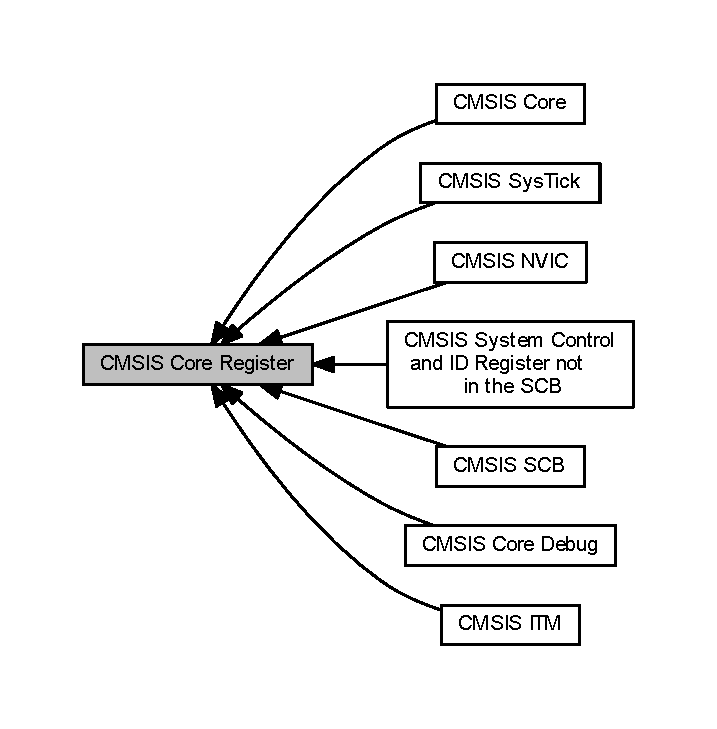
\includegraphics[width=344pt]{group___c_m_s_i_s__core__register}
\end{center}
\end{figure}
\subsection*{Modules}
\begin{DoxyCompactItemize}
\item 
\hyperlink{group___c_m_s_i_s___c_o_r_e}{C\+M\+S\+I\+S Core}
\item 
\hyperlink{group___c_m_s_i_s___n_v_i_c}{C\+M\+S\+I\+S N\+V\+IC}
\item 
\hyperlink{group___c_m_s_i_s___s_c_b}{C\+M\+S\+I\+S S\+CB}
\item 
\hyperlink{group___c_m_s_i_s___s_cn_s_c_b}{C\+M\+S\+I\+S System Control and I\+D Register not in the S\+CB}
\item 
\hyperlink{group___c_m_s_i_s___sys_tick}{C\+M\+S\+I\+S Sys\+Tick}
\item 
\hyperlink{group___c_m_s_i_s___i_t_m}{C\+M\+S\+I\+S I\+TM}
\item 
\hyperlink{group___c_m_s_i_s___core_debug}{C\+M\+S\+I\+S Core Debug}
\end{DoxyCompactItemize}
\begin{DoxyCompactItemize}
\item 
\#define \hyperlink{group___c_m_s_i_s__core__register_ga3c14ed93192c8d9143322bbf77ebf770}{S\+C\+S\+\_\+\+B\+A\+SE}~(0x\+E000\+E000\+U\+L)
\item 
\#define \hyperlink{group___c_m_s_i_s__core__register_gadd76251e412a195ec0a8f47227a8359e}{I\+T\+M\+\_\+\+B\+A\+SE}~(0x\+E0000000\+U\+L)
\item 
\#define \hyperlink{group___c_m_s_i_s__core__register_ga680604dbcda9e9b31a1639fcffe5230b}{Core\+Debug\+\_\+\+B\+A\+SE}~(0x\+E000\+E\+D\+F0\+U\+L)
\item 
\#define \hyperlink{group___c_m_s_i_s__core__register_ga58effaac0b93006b756d33209e814646}{Sys\+Tick\+\_\+\+B\+A\+SE}~(\hyperlink{group___c_m_s_i_s__core__register_ga3c14ed93192c8d9143322bbf77ebf770}{S\+C\+S\+\_\+\+B\+A\+SE} +  0x0010\+U\+L)
\item 
\#define \hyperlink{group___c_m_s_i_s__core__register_gaa0288691785a5f868238e0468b39523d}{N\+V\+I\+C\+\_\+\+B\+A\+SE}~(\hyperlink{group___c_m_s_i_s__core__register_ga3c14ed93192c8d9143322bbf77ebf770}{S\+C\+S\+\_\+\+B\+A\+SE} +  0x0100\+U\+L)
\item 
\#define \hyperlink{group___c_m_s_i_s__core__register_gad55a7ddb8d4b2398b0c1cfec76c0d9fd}{S\+C\+B\+\_\+\+B\+A\+SE}~(\hyperlink{group___c_m_s_i_s__core__register_ga3c14ed93192c8d9143322bbf77ebf770}{S\+C\+S\+\_\+\+B\+A\+SE} +  0x0\+D00\+U\+L)
\item 
\#define \hyperlink{group___c_m_s_i_s__core__register_ga9fe0cd2eef83a8adad94490d9ecca63f}{S\+Cn\+S\+CB}~((\hyperlink{struct_s_cn_s_c_b___type}{S\+Cn\+S\+C\+B\+\_\+\+Type}    $\ast$)     \hyperlink{group___c_m_s_i_s__core__register_ga3c14ed93192c8d9143322bbf77ebf770}{S\+C\+S\+\_\+\+B\+A\+SE}      )
\item 
\#define \hyperlink{group___c_m_s_i_s__core__register_gaaaf6477c2bde2f00f99e3c2fd1060b01}{S\+CB}~((\hyperlink{struct_s_c_b___type}{S\+C\+B\+\_\+\+Type}       $\ast$)     \hyperlink{group___c_m_s_i_s__core__register_gad55a7ddb8d4b2398b0c1cfec76c0d9fd}{S\+C\+B\+\_\+\+B\+A\+SE}      )
\item 
\#define \hyperlink{group___c_m_s_i_s__core__register_gacd96c53beeaff8f603fcda425eb295de}{Sys\+Tick}~((\hyperlink{struct_sys_tick___type}{Sys\+Tick\+\_\+\+Type}   $\ast$)     \hyperlink{group___c_m_s_i_s__core__register_ga58effaac0b93006b756d33209e814646}{Sys\+Tick\+\_\+\+B\+A\+SE}  )
\item 
\#define \hyperlink{group___c_m_s_i_s__core__register_gac8e97e8ce56ae9f57da1363a937f8a17}{N\+V\+IC}~((\hyperlink{struct_n_v_i_c___type}{N\+V\+I\+C\+\_\+\+Type}      $\ast$)     \hyperlink{group___c_m_s_i_s__core__register_gaa0288691785a5f868238e0468b39523d}{N\+V\+I\+C\+\_\+\+B\+A\+SE}     )
\item 
\#define \hyperlink{group___c_m_s_i_s__core__register_gabae7cdf882def602cb787bb039ff6a43}{I\+TM}~((\hyperlink{struct_i_t_m___type}{I\+T\+M\+\_\+\+Type}       $\ast$)     \hyperlink{group___c_m_s_i_s__core__register_gadd76251e412a195ec0a8f47227a8359e}{I\+T\+M\+\_\+\+B\+A\+SE}      )
\item 
\#define \hyperlink{group___c_m_s_i_s__core__register_gab6e30a2b802d9021619dbb0be7f5d63d}{Core\+Debug}~((\hyperlink{struct_core_debug___type}{Core\+Debug\+\_\+\+Type} $\ast$)     \hyperlink{group___c_m_s_i_s__core__register_ga680604dbcda9e9b31a1639fcffe5230b}{Core\+Debug\+\_\+\+B\+A\+SE})
\end{DoxyCompactItemize}


\subsection{Detailed Description}
Core Register contain\+:
\begin{DoxyItemize}
\item Core Register
\item Core N\+V\+IC Register
\item Core S\+CB Register
\item Core Sys\+Tick Register
\item Core Debug Register
\item Core M\+PU Register
\item Core F\+PU Register 
\end{DoxyItemize}

\subsection{Macro Definition Documentation}
\mbox{\Hypertarget{group___c_m_s_i_s__core__register_gab6e30a2b802d9021619dbb0be7f5d63d}\label{group___c_m_s_i_s__core__register_gab6e30a2b802d9021619dbb0be7f5d63d}} 
\index{C\+M\+S\+I\+S Core Register@{C\+M\+S\+I\+S Core Register}!Core\+Debug@{Core\+Debug}}
\index{Core\+Debug@{Core\+Debug}!C\+M\+S\+I\+S Core Register@{C\+M\+S\+I\+S Core Register}}
\subsubsection{\texorpdfstring{Core\+Debug}{CoreDebug}}
{\footnotesize\ttfamily \#define Core\+Debug~((\hyperlink{struct_core_debug___type}{Core\+Debug\+\_\+\+Type} $\ast$)     \hyperlink{group___c_m_s_i_s__core__register_ga680604dbcda9e9b31a1639fcffe5230b}{Core\+Debug\+\_\+\+B\+A\+SE})}

Core Debug configuration struct 

Definition at line 992 of file core\+\_\+cm4.\+h.

\mbox{\Hypertarget{group___c_m_s_i_s__core__register_ga680604dbcda9e9b31a1639fcffe5230b}\label{group___c_m_s_i_s__core__register_ga680604dbcda9e9b31a1639fcffe5230b}} 
\index{C\+M\+S\+I\+S Core Register@{C\+M\+S\+I\+S Core Register}!Core\+Debug\+\_\+\+B\+A\+SE@{Core\+Debug\+\_\+\+B\+A\+SE}}
\index{Core\+Debug\+\_\+\+B\+A\+SE@{Core\+Debug\+\_\+\+B\+A\+SE}!C\+M\+S\+I\+S Core Register@{C\+M\+S\+I\+S Core Register}}
\subsubsection{\texorpdfstring{Core\+Debug\+\_\+\+B\+A\+SE}{CoreDebug\_BASE}}
{\footnotesize\ttfamily \#define Core\+Debug\+\_\+\+B\+A\+SE~(0x\+E000\+E\+D\+F0\+U\+L)}

Core Debug Base Address 

Definition at line 982 of file core\+\_\+cm4.\+h.

\mbox{\Hypertarget{group___c_m_s_i_s__core__register_gabae7cdf882def602cb787bb039ff6a43}\label{group___c_m_s_i_s__core__register_gabae7cdf882def602cb787bb039ff6a43}} 
\index{C\+M\+S\+I\+S Core Register@{C\+M\+S\+I\+S Core Register}!I\+TM@{I\+TM}}
\index{I\+TM@{I\+TM}!C\+M\+S\+I\+S Core Register@{C\+M\+S\+I\+S Core Register}}
\subsubsection{\texorpdfstring{I\+TM}{ITM}}
{\footnotesize\ttfamily \#define I\+TM~((\hyperlink{struct_i_t_m___type}{I\+T\+M\+\_\+\+Type}       $\ast$)     \hyperlink{group___c_m_s_i_s__core__register_gadd76251e412a195ec0a8f47227a8359e}{I\+T\+M\+\_\+\+B\+A\+SE}      )}

I\+TM configuration struct 

Definition at line 991 of file core\+\_\+cm4.\+h.

\mbox{\Hypertarget{group___c_m_s_i_s__core__register_gadd76251e412a195ec0a8f47227a8359e}\label{group___c_m_s_i_s__core__register_gadd76251e412a195ec0a8f47227a8359e}} 
\index{C\+M\+S\+I\+S Core Register@{C\+M\+S\+I\+S Core Register}!I\+T\+M\+\_\+\+B\+A\+SE@{I\+T\+M\+\_\+\+B\+A\+SE}}
\index{I\+T\+M\+\_\+\+B\+A\+SE@{I\+T\+M\+\_\+\+B\+A\+SE}!C\+M\+S\+I\+S Core Register@{C\+M\+S\+I\+S Core Register}}
\subsubsection{\texorpdfstring{I\+T\+M\+\_\+\+B\+A\+SE}{ITM\_BASE}}
{\footnotesize\ttfamily \#define I\+T\+M\+\_\+\+B\+A\+SE~(0x\+E0000000\+U\+L)}

I\+TM Base Address 

Definition at line 981 of file core\+\_\+cm4.\+h.

\mbox{\Hypertarget{group___c_m_s_i_s__core__register_gac8e97e8ce56ae9f57da1363a937f8a17}\label{group___c_m_s_i_s__core__register_gac8e97e8ce56ae9f57da1363a937f8a17}} 
\index{C\+M\+S\+I\+S Core Register@{C\+M\+S\+I\+S Core Register}!N\+V\+IC@{N\+V\+IC}}
\index{N\+V\+IC@{N\+V\+IC}!C\+M\+S\+I\+S Core Register@{C\+M\+S\+I\+S Core Register}}
\subsubsection{\texorpdfstring{N\+V\+IC}{NVIC}}
{\footnotesize\ttfamily \#define N\+V\+IC~((\hyperlink{struct_n_v_i_c___type}{N\+V\+I\+C\+\_\+\+Type}      $\ast$)     \hyperlink{group___c_m_s_i_s__core__register_gaa0288691785a5f868238e0468b39523d}{N\+V\+I\+C\+\_\+\+B\+A\+SE}     )}

N\+V\+IC configuration struct 

Definition at line 990 of file core\+\_\+cm4.\+h.

\mbox{\Hypertarget{group___c_m_s_i_s__core__register_gaa0288691785a5f868238e0468b39523d}\label{group___c_m_s_i_s__core__register_gaa0288691785a5f868238e0468b39523d}} 
\index{C\+M\+S\+I\+S Core Register@{C\+M\+S\+I\+S Core Register}!N\+V\+I\+C\+\_\+\+B\+A\+SE@{N\+V\+I\+C\+\_\+\+B\+A\+SE}}
\index{N\+V\+I\+C\+\_\+\+B\+A\+SE@{N\+V\+I\+C\+\_\+\+B\+A\+SE}!C\+M\+S\+I\+S Core Register@{C\+M\+S\+I\+S Core Register}}
\subsubsection{\texorpdfstring{N\+V\+I\+C\+\_\+\+B\+A\+SE}{NVIC\_BASE}}
{\footnotesize\ttfamily \#define N\+V\+I\+C\+\_\+\+B\+A\+SE~(\hyperlink{group___c_m_s_i_s__core__register_ga3c14ed93192c8d9143322bbf77ebf770}{S\+C\+S\+\_\+\+B\+A\+SE} +  0x0100\+U\+L)}

N\+V\+IC Base Address 

Definition at line 984 of file core\+\_\+cm4.\+h.

\mbox{\Hypertarget{group___c_m_s_i_s__core__register_gaaaf6477c2bde2f00f99e3c2fd1060b01}\label{group___c_m_s_i_s__core__register_gaaaf6477c2bde2f00f99e3c2fd1060b01}} 
\index{C\+M\+S\+I\+S Core Register@{C\+M\+S\+I\+S Core Register}!S\+CB@{S\+CB}}
\index{S\+CB@{S\+CB}!C\+M\+S\+I\+S Core Register@{C\+M\+S\+I\+S Core Register}}
\subsubsection{\texorpdfstring{S\+CB}{SCB}}
{\footnotesize\ttfamily \#define S\+CB~((\hyperlink{struct_s_c_b___type}{S\+C\+B\+\_\+\+Type}       $\ast$)     \hyperlink{group___c_m_s_i_s__core__register_gad55a7ddb8d4b2398b0c1cfec76c0d9fd}{S\+C\+B\+\_\+\+B\+A\+SE}      )}

S\+CB configuration struct 

Definition at line 988 of file core\+\_\+cm4.\+h.

\mbox{\Hypertarget{group___c_m_s_i_s__core__register_gad55a7ddb8d4b2398b0c1cfec76c0d9fd}\label{group___c_m_s_i_s__core__register_gad55a7ddb8d4b2398b0c1cfec76c0d9fd}} 
\index{C\+M\+S\+I\+S Core Register@{C\+M\+S\+I\+S Core Register}!S\+C\+B\+\_\+\+B\+A\+SE@{S\+C\+B\+\_\+\+B\+A\+SE}}
\index{S\+C\+B\+\_\+\+B\+A\+SE@{S\+C\+B\+\_\+\+B\+A\+SE}!C\+M\+S\+I\+S Core Register@{C\+M\+S\+I\+S Core Register}}
\subsubsection{\texorpdfstring{S\+C\+B\+\_\+\+B\+A\+SE}{SCB\_BASE}}
{\footnotesize\ttfamily \#define S\+C\+B\+\_\+\+B\+A\+SE~(\hyperlink{group___c_m_s_i_s__core__register_ga3c14ed93192c8d9143322bbf77ebf770}{S\+C\+S\+\_\+\+B\+A\+SE} +  0x0\+D00\+U\+L)}

System Control Block Base Address 

Definition at line 985 of file core\+\_\+cm4.\+h.

\mbox{\Hypertarget{group___c_m_s_i_s__core__register_ga9fe0cd2eef83a8adad94490d9ecca63f}\label{group___c_m_s_i_s__core__register_ga9fe0cd2eef83a8adad94490d9ecca63f}} 
\index{C\+M\+S\+I\+S Core Register@{C\+M\+S\+I\+S Core Register}!S\+Cn\+S\+CB@{S\+Cn\+S\+CB}}
\index{S\+Cn\+S\+CB@{S\+Cn\+S\+CB}!C\+M\+S\+I\+S Core Register@{C\+M\+S\+I\+S Core Register}}
\subsubsection{\texorpdfstring{S\+Cn\+S\+CB}{SCnSCB}}
{\footnotesize\ttfamily \#define S\+Cn\+S\+CB~((\hyperlink{struct_s_cn_s_c_b___type}{S\+Cn\+S\+C\+B\+\_\+\+Type}    $\ast$)     \hyperlink{group___c_m_s_i_s__core__register_ga3c14ed93192c8d9143322bbf77ebf770}{S\+C\+S\+\_\+\+B\+A\+SE}      )}

System control Register not in S\+CB 

Definition at line 987 of file core\+\_\+cm4.\+h.

\mbox{\Hypertarget{group___c_m_s_i_s__core__register_ga3c14ed93192c8d9143322bbf77ebf770}\label{group___c_m_s_i_s__core__register_ga3c14ed93192c8d9143322bbf77ebf770}} 
\index{C\+M\+S\+I\+S Core Register@{C\+M\+S\+I\+S Core Register}!S\+C\+S\+\_\+\+B\+A\+SE@{S\+C\+S\+\_\+\+B\+A\+SE}}
\index{S\+C\+S\+\_\+\+B\+A\+SE@{S\+C\+S\+\_\+\+B\+A\+SE}!C\+M\+S\+I\+S Core Register@{C\+M\+S\+I\+S Core Register}}
\subsubsection{\texorpdfstring{S\+C\+S\+\_\+\+B\+A\+SE}{SCS\_BASE}}
{\footnotesize\ttfamily \#define S\+C\+S\+\_\+\+B\+A\+SE~(0x\+E000\+E000\+U\+L)}

System Control Space Base Address 

Definition at line 980 of file core\+\_\+cm4.\+h.

\mbox{\Hypertarget{group___c_m_s_i_s__core__register_gacd96c53beeaff8f603fcda425eb295de}\label{group___c_m_s_i_s__core__register_gacd96c53beeaff8f603fcda425eb295de}} 
\index{C\+M\+S\+I\+S Core Register@{C\+M\+S\+I\+S Core Register}!Sys\+Tick@{Sys\+Tick}}
\index{Sys\+Tick@{Sys\+Tick}!C\+M\+S\+I\+S Core Register@{C\+M\+S\+I\+S Core Register}}
\subsubsection{\texorpdfstring{Sys\+Tick}{SysTick}}
{\footnotesize\ttfamily \#define Sys\+Tick~((\hyperlink{struct_sys_tick___type}{Sys\+Tick\+\_\+\+Type}   $\ast$)     \hyperlink{group___c_m_s_i_s__core__register_ga58effaac0b93006b756d33209e814646}{Sys\+Tick\+\_\+\+B\+A\+SE}  )}

Sys\+Tick configuration struct 

Definition at line 989 of file core\+\_\+cm4.\+h.

\mbox{\Hypertarget{group___c_m_s_i_s__core__register_ga58effaac0b93006b756d33209e814646}\label{group___c_m_s_i_s__core__register_ga58effaac0b93006b756d33209e814646}} 
\index{C\+M\+S\+I\+S Core Register@{C\+M\+S\+I\+S Core Register}!Sys\+Tick\+\_\+\+B\+A\+SE@{Sys\+Tick\+\_\+\+B\+A\+SE}}
\index{Sys\+Tick\+\_\+\+B\+A\+SE@{Sys\+Tick\+\_\+\+B\+A\+SE}!C\+M\+S\+I\+S Core Register@{C\+M\+S\+I\+S Core Register}}
\subsubsection{\texorpdfstring{Sys\+Tick\+\_\+\+B\+A\+SE}{SysTick\_BASE}}
{\footnotesize\ttfamily \#define Sys\+Tick\+\_\+\+B\+A\+SE~(\hyperlink{group___c_m_s_i_s__core__register_ga3c14ed93192c8d9143322bbf77ebf770}{S\+C\+S\+\_\+\+B\+A\+SE} +  0x0010\+U\+L)}

Sys\+Tick Base Address 

Definition at line 983 of file core\+\_\+cm4.\+h.


\hypertarget{group___c_m_s_i_s___c_o_r_e}{}\section{C\+M\+S\+IS Core}
\label{group___c_m_s_i_s___c_o_r_e}\index{C\+M\+S\+I\+S Core@{C\+M\+S\+I\+S Core}}
Collaboration diagram for C\+M\+S\+IS Core\+:\nopagebreak
\begin{figure}[H]
\begin{center}
\leavevmode
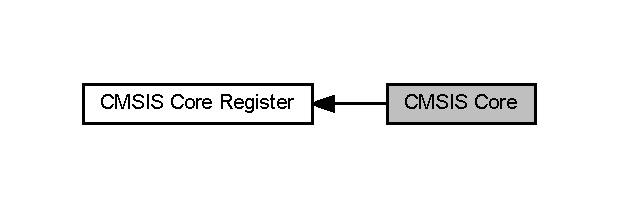
\includegraphics[width=297pt]{group___c_m_s_i_s___c_o_r_e}
\end{center}
\end{figure}
\subsection*{Data Structures}
\begin{DoxyCompactItemize}
\item 
union \hyperlink{union_a_p_s_r___type}{A\+P\+S\+R\+\_\+\+Type}
\begin{DoxyCompactList}\small\item\em Union type to access the Application Program Status Register (A\+P\+SR). \end{DoxyCompactList}\item 
union \hyperlink{union_i_p_s_r___type}{I\+P\+S\+R\+\_\+\+Type}
\begin{DoxyCompactList}\small\item\em Union type to access the Interrupt Program Status Register (I\+P\+SR). \end{DoxyCompactList}\item 
union \hyperlink{unionx_p_s_r___type}{x\+P\+S\+R\+\_\+\+Type}
\begin{DoxyCompactList}\small\item\em Union type to access the Special-\/\+Purpose Program Status Registers (x\+P\+SR). \end{DoxyCompactList}\item 
union \hyperlink{union_c_o_n_t_r_o_l___type}{C\+O\+N\+T\+R\+O\+L\+\_\+\+Type}
\begin{DoxyCompactList}\small\item\em Union type to access the Control Registers (C\+O\+N\+T\+R\+OL). \end{DoxyCompactList}\end{DoxyCompactItemize}


\subsection{Detailed Description}
Type definitions for the Cortex-\/M Core Registers 
\hypertarget{group___c_m_s_i_s___n_v_i_c}{}\section{C\+M\+S\+IS N\+V\+IC}
\label{group___c_m_s_i_s___n_v_i_c}\index{C\+M\+S\+I\+S N\+V\+IC@{C\+M\+S\+I\+S N\+V\+IC}}
Collaboration diagram for C\+M\+S\+IS N\+V\+IC\+:
\nopagebreak
\begin{figure}[H]
\begin{center}
\leavevmode
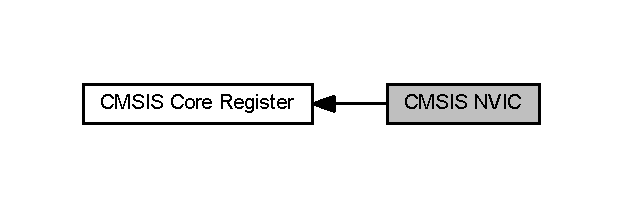
\includegraphics[width=299pt]{group___c_m_s_i_s___n_v_i_c}
\end{center}
\end{figure}
\subsection*{Data Structures}
\begin{DoxyCompactItemize}
\item 
struct \hyperlink{struct_n_v_i_c___type}{N\+V\+I\+C\+\_\+\+Type}
\begin{DoxyCompactList}\small\item\em Structure type to access the Nested Vectored Interrupt Controller (N\+V\+IC). \end{DoxyCompactList}\end{DoxyCompactItemize}
\subsection*{Macros}
\begin{DoxyCompactItemize}
\item 
\#define \hyperlink{group___c_m_s_i_s___n_v_i_c_ga9eebe495e2e48d302211108837a2b3e8}{N\+V\+I\+C\+\_\+\+S\+T\+I\+R\+\_\+\+I\+N\+T\+I\+D\+\_\+\+Pos}~0
\item 
\#define \hyperlink{group___c_m_s_i_s___n_v_i_c_gae4060c4dfcebb08871ca4244176ce752}{N\+V\+I\+C\+\_\+\+S\+T\+I\+R\+\_\+\+I\+N\+T\+I\+D\+\_\+\+Msk}~(0x1\+F\+F\+U\+L $<$$<$ N\+V\+I\+C\+\_\+\+S\+T\+I\+R\+\_\+\+I\+N\+T\+I\+D\+\_\+\+Pos)
\end{DoxyCompactItemize}


\subsection{Detailed Description}
Type definitions for the Cortex-\/M N\+V\+IC Registers 

\subsection{Macro Definition Documentation}
\mbox{\Hypertarget{group___c_m_s_i_s___n_v_i_c_gae4060c4dfcebb08871ca4244176ce752}\label{group___c_m_s_i_s___n_v_i_c_gae4060c4dfcebb08871ca4244176ce752}} 
\index{C\+M\+S\+I\+S N\+V\+IC@{C\+M\+S\+I\+S N\+V\+IC}!N\+V\+I\+C\+\_\+\+S\+T\+I\+R\+\_\+\+I\+N\+T\+I\+D\+\_\+\+Msk@{N\+V\+I\+C\+\_\+\+S\+T\+I\+R\+\_\+\+I\+N\+T\+I\+D\+\_\+\+Msk}}
\index{N\+V\+I\+C\+\_\+\+S\+T\+I\+R\+\_\+\+I\+N\+T\+I\+D\+\_\+\+Msk@{N\+V\+I\+C\+\_\+\+S\+T\+I\+R\+\_\+\+I\+N\+T\+I\+D\+\_\+\+Msk}!C\+M\+S\+I\+S N\+V\+IC@{C\+M\+S\+I\+S N\+V\+IC}}
\subsubsection{\texorpdfstring{N\+V\+I\+C\+\_\+\+S\+T\+I\+R\+\_\+\+I\+N\+T\+I\+D\+\_\+\+Msk}{NVIC\_STIR\_INTID\_Msk}}
{\footnotesize\ttfamily \#define N\+V\+I\+C\+\_\+\+S\+T\+I\+R\+\_\+\+I\+N\+T\+I\+D\+\_\+\+Msk~(0x1\+F\+F\+U\+L $<$$<$ N\+V\+I\+C\+\_\+\+S\+T\+I\+R\+\_\+\+I\+N\+T\+I\+D\+\_\+\+Pos)}

S\+T\+IR\+: I\+N\+T\+L\+I\+N\+E\+S\+N\+UM Mask 

Definition at line 322 of file core\+\_\+cm4.\+h.

\mbox{\Hypertarget{group___c_m_s_i_s___n_v_i_c_ga9eebe495e2e48d302211108837a2b3e8}\label{group___c_m_s_i_s___n_v_i_c_ga9eebe495e2e48d302211108837a2b3e8}} 
\index{C\+M\+S\+I\+S N\+V\+IC@{C\+M\+S\+I\+S N\+V\+IC}!N\+V\+I\+C\+\_\+\+S\+T\+I\+R\+\_\+\+I\+N\+T\+I\+D\+\_\+\+Pos@{N\+V\+I\+C\+\_\+\+S\+T\+I\+R\+\_\+\+I\+N\+T\+I\+D\+\_\+\+Pos}}
\index{N\+V\+I\+C\+\_\+\+S\+T\+I\+R\+\_\+\+I\+N\+T\+I\+D\+\_\+\+Pos@{N\+V\+I\+C\+\_\+\+S\+T\+I\+R\+\_\+\+I\+N\+T\+I\+D\+\_\+\+Pos}!C\+M\+S\+I\+S N\+V\+IC@{C\+M\+S\+I\+S N\+V\+IC}}
\subsubsection{\texorpdfstring{N\+V\+I\+C\+\_\+\+S\+T\+I\+R\+\_\+\+I\+N\+T\+I\+D\+\_\+\+Pos}{NVIC\_STIR\_INTID\_Pos}}
{\footnotesize\ttfamily \#define N\+V\+I\+C\+\_\+\+S\+T\+I\+R\+\_\+\+I\+N\+T\+I\+D\+\_\+\+Pos~0}

S\+T\+IR\+: I\+N\+T\+L\+I\+N\+E\+S\+N\+UM Position 

Definition at line 321 of file core\+\_\+cm4.\+h.


\hypertarget{group___c_m_s_i_s___s_c_b}{}\section{C\+M\+S\+IS S\+CB}
\label{group___c_m_s_i_s___s_c_b}\index{C\+M\+S\+I\+S S\+CB@{C\+M\+S\+I\+S S\+CB}}
Collaboration diagram for C\+M\+S\+IS S\+CB\+:
\nopagebreak
\begin{figure}[H]
\begin{center}
\leavevmode
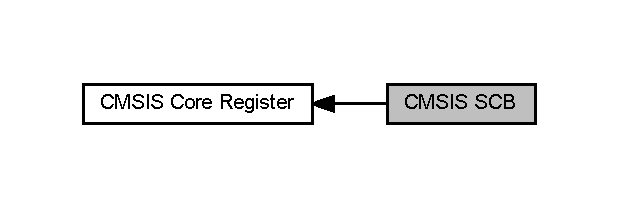
\includegraphics[width=297pt]{group___c_m_s_i_s___s_c_b}
\end{center}
\end{figure}
\subsection*{Data Structures}
\begin{DoxyCompactItemize}
\item 
struct \hyperlink{struct_s_c_b___type}{S\+C\+B\+\_\+\+Type}
\begin{DoxyCompactList}\small\item\em Structure type to access the System Control Block (S\+CB). \end{DoxyCompactList}\end{DoxyCompactItemize}
\subsection*{Macros}
\begin{DoxyCompactItemize}
\item 
\#define \hyperlink{group___c_m_s_i_s___s_c_b_ga58686b88f94f789d4e6f429fe1ff58cf}{S\+C\+B\+\_\+\+C\+P\+U\+I\+D\+\_\+\+I\+M\+P\+L\+E\+M\+E\+N\+T\+E\+R\+\_\+\+Pos}~24
\item 
\#define \hyperlink{group___c_m_s_i_s___s_c_b_ga0932b31faafd47656a03ced75a31d99b}{S\+C\+B\+\_\+\+C\+P\+U\+I\+D\+\_\+\+I\+M\+P\+L\+E\+M\+E\+N\+T\+E\+R\+\_\+\+Msk}~(0x\+F\+F\+U\+L $<$$<$ S\+C\+B\+\_\+\+C\+P\+U\+I\+D\+\_\+\+I\+M\+P\+L\+E\+M\+E\+N\+T\+E\+R\+\_\+\+Pos)
\item 
\#define \hyperlink{group___c_m_s_i_s___s_c_b_ga104462bd0815391b4044a70bd15d3a71}{S\+C\+B\+\_\+\+C\+P\+U\+I\+D\+\_\+\+V\+A\+R\+I\+A\+N\+T\+\_\+\+Pos}~20
\item 
\#define \hyperlink{group___c_m_s_i_s___s_c_b_gad358dfbd04300afc1824329d128b99e8}{S\+C\+B\+\_\+\+C\+P\+U\+I\+D\+\_\+\+V\+A\+R\+I\+A\+N\+T\+\_\+\+Msk}~(0x\+F\+U\+L $<$$<$ S\+C\+B\+\_\+\+C\+P\+U\+I\+D\+\_\+\+V\+A\+R\+I\+A\+N\+T\+\_\+\+Pos)
\item 
\#define \hyperlink{group___c_m_s_i_s___s_c_b_gaf8b3236b08fb8e840efb682645fb0e98}{S\+C\+B\+\_\+\+C\+P\+U\+I\+D\+\_\+\+A\+R\+C\+H\+I\+T\+E\+C\+T\+U\+R\+E\+\_\+\+Pos}~16
\item 
\#define \hyperlink{group___c_m_s_i_s___s_c_b_gafae4a1f27a927338ae9dc51a0e146213}{S\+C\+B\+\_\+\+C\+P\+U\+I\+D\+\_\+\+A\+R\+C\+H\+I\+T\+E\+C\+T\+U\+R\+E\+\_\+\+Msk}~(0x\+F\+U\+L $<$$<$ S\+C\+B\+\_\+\+C\+P\+U\+I\+D\+\_\+\+A\+R\+C\+H\+I\+T\+E\+C\+T\+U\+R\+E\+\_\+\+Pos)
\item 
\#define \hyperlink{group___c_m_s_i_s___s_c_b_ga705f68eaa9afb042ca2407dc4e4629ac}{S\+C\+B\+\_\+\+C\+P\+U\+I\+D\+\_\+\+P\+A\+R\+T\+N\+O\+\_\+\+Pos}~4
\item 
\#define \hyperlink{group___c_m_s_i_s___s_c_b_ga98e581423ca016680c238c469aba546d}{S\+C\+B\+\_\+\+C\+P\+U\+I\+D\+\_\+\+P\+A\+R\+T\+N\+O\+\_\+\+Msk}~(0x\+F\+F\+F\+U\+L $<$$<$ S\+C\+B\+\_\+\+C\+P\+U\+I\+D\+\_\+\+P\+A\+R\+T\+N\+O\+\_\+\+Pos)
\item 
\#define \hyperlink{group___c_m_s_i_s___s_c_b_ga3c3d9071e574de11fb27ba57034838b1}{S\+C\+B\+\_\+\+C\+P\+U\+I\+D\+\_\+\+R\+E\+V\+I\+S\+I\+O\+N\+\_\+\+Pos}~0
\item 
\#define \hyperlink{group___c_m_s_i_s___s_c_b_ga2ec0448b6483f77e7f5d08b4b81d85df}{S\+C\+B\+\_\+\+C\+P\+U\+I\+D\+\_\+\+R\+E\+V\+I\+S\+I\+O\+N\+\_\+\+Msk}~(0x\+F\+U\+L $<$$<$ S\+C\+B\+\_\+\+C\+P\+U\+I\+D\+\_\+\+R\+E\+V\+I\+S\+I\+O\+N\+\_\+\+Pos)
\item 
\#define \hyperlink{group___c_m_s_i_s___s_c_b_ga750d4b52624a46d71356db4ea769573b}{S\+C\+B\+\_\+\+I\+C\+S\+R\+\_\+\+N\+M\+I\+P\+E\+N\+D\+S\+E\+T\+\_\+\+Pos}~31
\item 
\#define \hyperlink{group___c_m_s_i_s___s_c_b_ga340e3f79e9c3607dee9f2c048b6b22e8}{S\+C\+B\+\_\+\+I\+C\+S\+R\+\_\+\+N\+M\+I\+P\+E\+N\+D\+S\+E\+T\+\_\+\+Msk}~(1\+U\+L $<$$<$ S\+C\+B\+\_\+\+I\+C\+S\+R\+\_\+\+N\+M\+I\+P\+E\+N\+D\+S\+E\+T\+\_\+\+Pos)
\item 
\#define \hyperlink{group___c_m_s_i_s___s_c_b_gab5ded23d2ab1d5ff7cc7ce746205e9fe}{S\+C\+B\+\_\+\+I\+C\+S\+R\+\_\+\+P\+E\+N\+D\+S\+V\+S\+E\+T\+\_\+\+Pos}~28
\item 
\#define \hyperlink{group___c_m_s_i_s___s_c_b_ga1e40d93efb402763c8c00ddcc56724ff}{S\+C\+B\+\_\+\+I\+C\+S\+R\+\_\+\+P\+E\+N\+D\+S\+V\+S\+E\+T\+\_\+\+Msk}~(1\+U\+L $<$$<$ S\+C\+B\+\_\+\+I\+C\+S\+R\+\_\+\+P\+E\+N\+D\+S\+V\+S\+E\+T\+\_\+\+Pos)
\item 
\#define \hyperlink{group___c_m_s_i_s___s_c_b_gae218d9022288f89faf57187c4d542ecd}{S\+C\+B\+\_\+\+I\+C\+S\+R\+\_\+\+P\+E\+N\+D\+S\+V\+C\+L\+R\+\_\+\+Pos}~27
\item 
\#define \hyperlink{group___c_m_s_i_s___s_c_b_ga4a901ace381d3c1c74ac82b22fae2e1e}{S\+C\+B\+\_\+\+I\+C\+S\+R\+\_\+\+P\+E\+N\+D\+S\+V\+C\+L\+R\+\_\+\+Msk}~(1\+U\+L $<$$<$ S\+C\+B\+\_\+\+I\+C\+S\+R\+\_\+\+P\+E\+N\+D\+S\+V\+C\+L\+R\+\_\+\+Pos)
\item 
\#define \hyperlink{group___c_m_s_i_s___s_c_b_ga9dbb3358c6167c9c3f85661b90fb2794}{S\+C\+B\+\_\+\+I\+C\+S\+R\+\_\+\+P\+E\+N\+D\+S\+T\+S\+E\+T\+\_\+\+Pos}~26
\item 
\#define \hyperlink{group___c_m_s_i_s___s_c_b_ga7325b61ea0ec323ef2d5c893b112e546}{S\+C\+B\+\_\+\+I\+C\+S\+R\+\_\+\+P\+E\+N\+D\+S\+T\+S\+E\+T\+\_\+\+Msk}~(1\+U\+L $<$$<$ S\+C\+B\+\_\+\+I\+C\+S\+R\+\_\+\+P\+E\+N\+D\+S\+T\+S\+E\+T\+\_\+\+Pos)
\item 
\#define \hyperlink{group___c_m_s_i_s___s_c_b_gadbe25e4b333ece1341beb1a740168fdc}{S\+C\+B\+\_\+\+I\+C\+S\+R\+\_\+\+P\+E\+N\+D\+S\+T\+C\+L\+R\+\_\+\+Pos}~25
\item 
\#define \hyperlink{group___c_m_s_i_s___s_c_b_gab241827d2a793269d8cd99b9b28c2157}{S\+C\+B\+\_\+\+I\+C\+S\+R\+\_\+\+P\+E\+N\+D\+S\+T\+C\+L\+R\+\_\+\+Msk}~(1\+U\+L $<$$<$ S\+C\+B\+\_\+\+I\+C\+S\+R\+\_\+\+P\+E\+N\+D\+S\+T\+C\+L\+R\+\_\+\+Pos)
\item 
\#define \hyperlink{group___c_m_s_i_s___s_c_b_ga11cb5b1f9ce167b81f31787a77e575df}{S\+C\+B\+\_\+\+I\+C\+S\+R\+\_\+\+I\+S\+R\+P\+R\+E\+E\+M\+P\+T\+\_\+\+Pos}~23
\item 
\#define \hyperlink{group___c_m_s_i_s___s_c_b_gaa966600396290808d596fe96e92ca2b5}{S\+C\+B\+\_\+\+I\+C\+S\+R\+\_\+\+I\+S\+R\+P\+R\+E\+E\+M\+P\+T\+\_\+\+Msk}~(1\+U\+L $<$$<$ S\+C\+B\+\_\+\+I\+C\+S\+R\+\_\+\+I\+S\+R\+P\+R\+E\+E\+M\+P\+T\+\_\+\+Pos)
\item 
\#define \hyperlink{group___c_m_s_i_s___s_c_b_ga10749d92b9b744094b845c2eb46d4319}{S\+C\+B\+\_\+\+I\+C\+S\+R\+\_\+\+I\+S\+R\+P\+E\+N\+D\+I\+N\+G\+\_\+\+Pos}~22
\item 
\#define \hyperlink{group___c_m_s_i_s___s_c_b_ga056d74fd538e5d36d3be1f28d399c877}{S\+C\+B\+\_\+\+I\+C\+S\+R\+\_\+\+I\+S\+R\+P\+E\+N\+D\+I\+N\+G\+\_\+\+Msk}~(1\+U\+L $<$$<$ S\+C\+B\+\_\+\+I\+C\+S\+R\+\_\+\+I\+S\+R\+P\+E\+N\+D\+I\+N\+G\+\_\+\+Pos)
\item 
\#define \hyperlink{group___c_m_s_i_s___s_c_b_gada60c92bf88d6fd21a8f49efa4a127b8}{S\+C\+B\+\_\+\+I\+C\+S\+R\+\_\+\+V\+E\+C\+T\+P\+E\+N\+D\+I\+N\+G\+\_\+\+Pos}~12
\item 
\#define \hyperlink{group___c_m_s_i_s___s_c_b_gacb6992e7c7ddc27a370f62878a21ef72}{S\+C\+B\+\_\+\+I\+C\+S\+R\+\_\+\+V\+E\+C\+T\+P\+E\+N\+D\+I\+N\+G\+\_\+\+Msk}~(0x1\+F\+F\+U\+L $<$$<$ S\+C\+B\+\_\+\+I\+C\+S\+R\+\_\+\+V\+E\+C\+T\+P\+E\+N\+D\+I\+N\+G\+\_\+\+Pos)
\item 
\#define \hyperlink{group___c_m_s_i_s___s_c_b_ga403d154200242629e6d2764bfc12a7ec}{S\+C\+B\+\_\+\+I\+C\+S\+R\+\_\+\+R\+E\+T\+T\+O\+B\+A\+S\+E\+\_\+\+Pos}~11
\item 
\#define \hyperlink{group___c_m_s_i_s___s_c_b_gaca6fc3f79bb550f64fd7df782ed4a5f6}{S\+C\+B\+\_\+\+I\+C\+S\+R\+\_\+\+R\+E\+T\+T\+O\+B\+A\+S\+E\+\_\+\+Msk}~(1\+U\+L $<$$<$ S\+C\+B\+\_\+\+I\+C\+S\+R\+\_\+\+R\+E\+T\+T\+O\+B\+A\+S\+E\+\_\+\+Pos)
\item 
\#define \hyperlink{group___c_m_s_i_s___s_c_b_gae4f602c7c5c895d5fb687b71b0979fc3}{S\+C\+B\+\_\+\+I\+C\+S\+R\+\_\+\+V\+E\+C\+T\+A\+C\+T\+I\+V\+E\+\_\+\+Pos}~0
\item 
\#define \hyperlink{group___c_m_s_i_s___s_c_b_ga5533791a4ecf1b9301c883047b3e8396}{S\+C\+B\+\_\+\+I\+C\+S\+R\+\_\+\+V\+E\+C\+T\+A\+C\+T\+I\+V\+E\+\_\+\+Msk}~(0x1\+F\+F\+U\+L $<$$<$ S\+C\+B\+\_\+\+I\+C\+S\+R\+\_\+\+V\+E\+C\+T\+A\+C\+T\+I\+V\+E\+\_\+\+Pos)
\item 
\#define \hyperlink{group___c_m_s_i_s___s_c_b_gac6a55451ddd38bffcff5a211d29cea78}{S\+C\+B\+\_\+\+V\+T\+O\+R\+\_\+\+T\+B\+L\+O\+F\+F\+\_\+\+Pos}~7
\item 
\#define \hyperlink{group___c_m_s_i_s___s_c_b_ga75e395ed74042923e8c93edf50f0996c}{S\+C\+B\+\_\+\+V\+T\+O\+R\+\_\+\+T\+B\+L\+O\+F\+F\+\_\+\+Msk}~(0x1\+F\+F\+F\+F\+F\+F\+U\+L $<$$<$ S\+C\+B\+\_\+\+V\+T\+O\+R\+\_\+\+T\+B\+L\+O\+F\+F\+\_\+\+Pos)
\item 
\#define \hyperlink{group___c_m_s_i_s___s_c_b_gaaa27c0ba600bf82c3da08c748845b640}{S\+C\+B\+\_\+\+A\+I\+R\+C\+R\+\_\+\+V\+E\+C\+T\+K\+E\+Y\+\_\+\+Pos}~16
\item 
\#define \hyperlink{group___c_m_s_i_s___s_c_b_ga90c7cf0c490e7ae55f9503a7fda1dd22}{S\+C\+B\+\_\+\+A\+I\+R\+C\+R\+\_\+\+V\+E\+C\+T\+K\+E\+Y\+\_\+\+Msk}~(0x\+F\+F\+F\+F\+U\+L $<$$<$ S\+C\+B\+\_\+\+A\+I\+R\+C\+R\+\_\+\+V\+E\+C\+T\+K\+E\+Y\+\_\+\+Pos)
\item 
\#define \hyperlink{group___c_m_s_i_s___s_c_b_gaec404750ff5ca07f499a3c06b62051ef}{S\+C\+B\+\_\+\+A\+I\+R\+C\+R\+\_\+\+V\+E\+C\+T\+K\+E\+Y\+S\+T\+A\+T\+\_\+\+Pos}~16
\item 
\#define \hyperlink{group___c_m_s_i_s___s_c_b_gabacedaefeefc73d666bbe59ece904493}{S\+C\+B\+\_\+\+A\+I\+R\+C\+R\+\_\+\+V\+E\+C\+T\+K\+E\+Y\+S\+T\+A\+T\+\_\+\+Msk}~(0x\+F\+F\+F\+F\+U\+L $<$$<$ S\+C\+B\+\_\+\+A\+I\+R\+C\+R\+\_\+\+V\+E\+C\+T\+K\+E\+Y\+S\+T\+A\+T\+\_\+\+Pos)
\item 
\#define \hyperlink{group___c_m_s_i_s___s_c_b_gad31dec98fbc0d33ace63cb1f1a927923}{S\+C\+B\+\_\+\+A\+I\+R\+C\+R\+\_\+\+E\+N\+D\+I\+A\+N\+E\+S\+S\+\_\+\+Pos}~15
\item 
\#define \hyperlink{group___c_m_s_i_s___s_c_b_ga2f571f93d3d4a6eac9a3040756d3d951}{S\+C\+B\+\_\+\+A\+I\+R\+C\+R\+\_\+\+E\+N\+D\+I\+A\+N\+E\+S\+S\+\_\+\+Msk}~(1\+U\+L $<$$<$ S\+C\+B\+\_\+\+A\+I\+R\+C\+R\+\_\+\+E\+N\+D\+I\+A\+N\+E\+S\+S\+\_\+\+Pos)
\item 
\#define \hyperlink{group___c_m_s_i_s___s_c_b_gaca155deccdeca0f2c76b8100d24196c8}{S\+C\+B\+\_\+\+A\+I\+R\+C\+R\+\_\+\+P\+R\+I\+G\+R\+O\+U\+P\+\_\+\+Pos}~8
\item 
\#define \hyperlink{group___c_m_s_i_s___s_c_b_ga8be60fff03f48d0d345868060dc6dae7}{S\+C\+B\+\_\+\+A\+I\+R\+C\+R\+\_\+\+P\+R\+I\+G\+R\+O\+U\+P\+\_\+\+Msk}~(7\+U\+L $<$$<$ S\+C\+B\+\_\+\+A\+I\+R\+C\+R\+\_\+\+P\+R\+I\+G\+R\+O\+U\+P\+\_\+\+Pos)
\item 
\#define \hyperlink{group___c_m_s_i_s___s_c_b_gaffb2737eca1eac0fc1c282a76a40953c}{S\+C\+B\+\_\+\+A\+I\+R\+C\+R\+\_\+\+S\+Y\+S\+R\+E\+S\+E\+T\+R\+E\+Q\+\_\+\+Pos}~2
\item 
\#define \hyperlink{group___c_m_s_i_s___s_c_b_gaae1181119559a5bd36e62afa373fa720}{S\+C\+B\+\_\+\+A\+I\+R\+C\+R\+\_\+\+S\+Y\+S\+R\+E\+S\+E\+T\+R\+E\+Q\+\_\+\+Msk}~(1\+U\+L $<$$<$ S\+C\+B\+\_\+\+A\+I\+R\+C\+R\+\_\+\+S\+Y\+S\+R\+E\+S\+E\+T\+R\+E\+Q\+\_\+\+Pos)
\item 
\#define \hyperlink{group___c_m_s_i_s___s_c_b_gaa30a12e892bb696e61626d71359a9029}{S\+C\+B\+\_\+\+A\+I\+R\+C\+R\+\_\+\+V\+E\+C\+T\+C\+L\+R\+A\+C\+T\+I\+V\+E\+\_\+\+Pos}~1
\item 
\#define \hyperlink{group___c_m_s_i_s___s_c_b_ga212c5ab1c1c82c807d30d2307aa8d218}{S\+C\+B\+\_\+\+A\+I\+R\+C\+R\+\_\+\+V\+E\+C\+T\+C\+L\+R\+A\+C\+T\+I\+V\+E\+\_\+\+Msk}~(1\+U\+L $<$$<$ S\+C\+B\+\_\+\+A\+I\+R\+C\+R\+\_\+\+V\+E\+C\+T\+C\+L\+R\+A\+C\+T\+I\+V\+E\+\_\+\+Pos)
\item 
\#define \hyperlink{group___c_m_s_i_s___s_c_b_ga0d483d9569cd9d1b46ec0d171b1f18d8}{S\+C\+B\+\_\+\+A\+I\+R\+C\+R\+\_\+\+V\+E\+C\+T\+R\+E\+S\+E\+T\+\_\+\+Pos}~0
\item 
\#define \hyperlink{group___c_m_s_i_s___s_c_b_ga3006e31968bb9725e7b4ee0784d99f7f}{S\+C\+B\+\_\+\+A\+I\+R\+C\+R\+\_\+\+V\+E\+C\+T\+R\+E\+S\+E\+T\+\_\+\+Msk}~(1\+U\+L $<$$<$ S\+C\+B\+\_\+\+A\+I\+R\+C\+R\+\_\+\+V\+E\+C\+T\+R\+E\+S\+E\+T\+\_\+\+Pos)
\item 
\#define \hyperlink{group___c_m_s_i_s___s_c_b_ga3bddcec40aeaf3d3a998446100fa0e44}{S\+C\+B\+\_\+\+S\+C\+R\+\_\+\+S\+E\+V\+O\+N\+P\+E\+N\+D\+\_\+\+Pos}~4
\item 
\#define \hyperlink{group___c_m_s_i_s___s_c_b_gafb98656644a14342e467505f69a997c9}{S\+C\+B\+\_\+\+S\+C\+R\+\_\+\+S\+E\+V\+O\+N\+P\+E\+N\+D\+\_\+\+Msk}~(1\+U\+L $<$$<$ S\+C\+B\+\_\+\+S\+C\+R\+\_\+\+S\+E\+V\+O\+N\+P\+E\+N\+D\+\_\+\+Pos)
\item 
\#define \hyperlink{group___c_m_s_i_s___s_c_b_gab304f6258ec03bd9a6e7a360515c3cfe}{S\+C\+B\+\_\+\+S\+C\+R\+\_\+\+S\+L\+E\+E\+P\+D\+E\+E\+P\+\_\+\+Pos}~2
\item 
\#define \hyperlink{group___c_m_s_i_s___s_c_b_ga77c06a69c63f4b3f6ec1032e911e18e7}{S\+C\+B\+\_\+\+S\+C\+R\+\_\+\+S\+L\+E\+E\+P\+D\+E\+E\+P\+\_\+\+Msk}~(1\+U\+L $<$$<$ S\+C\+B\+\_\+\+S\+C\+R\+\_\+\+S\+L\+E\+E\+P\+D\+E\+E\+P\+\_\+\+Pos)
\item 
\#define \hyperlink{group___c_m_s_i_s___s_c_b_ga3680a15114d7fdc1e25043b881308fe9}{S\+C\+B\+\_\+\+S\+C\+R\+\_\+\+S\+L\+E\+E\+P\+O\+N\+E\+X\+I\+T\+\_\+\+Pos}~1
\item 
\#define \hyperlink{group___c_m_s_i_s___s_c_b_ga50a243e317b9a70781b02758d45b05ee}{S\+C\+B\+\_\+\+S\+C\+R\+\_\+\+S\+L\+E\+E\+P\+O\+N\+E\+X\+I\+T\+\_\+\+Msk}~(1\+U\+L $<$$<$ S\+C\+B\+\_\+\+S\+C\+R\+\_\+\+S\+L\+E\+E\+P\+O\+N\+E\+X\+I\+T\+\_\+\+Pos)
\item 
\#define \hyperlink{group___c_m_s_i_s___s_c_b_gac2d20a250960a432cc74da59d20e2f86}{S\+C\+B\+\_\+\+C\+C\+R\+\_\+\+S\+T\+K\+A\+L\+I\+G\+N\+\_\+\+Pos}~9
\item 
\#define \hyperlink{group___c_m_s_i_s___s_c_b_ga33cf22d3d46af158a03aad25ddea1bcb}{S\+C\+B\+\_\+\+C\+C\+R\+\_\+\+S\+T\+K\+A\+L\+I\+G\+N\+\_\+\+Msk}~(1\+U\+L $<$$<$ S\+C\+B\+\_\+\+C\+C\+R\+\_\+\+S\+T\+K\+A\+L\+I\+G\+N\+\_\+\+Pos)
\item 
\#define \hyperlink{group___c_m_s_i_s___s_c_b_ga4010a4f9e2a745af1b58abe1f791ebbf}{S\+C\+B\+\_\+\+C\+C\+R\+\_\+\+B\+F\+H\+F\+N\+M\+I\+G\+N\+\_\+\+Pos}~8
\item 
\#define \hyperlink{group___c_m_s_i_s___s_c_b_ga89a28cc31cfc7d52d9d7a8fcc69c7eac}{S\+C\+B\+\_\+\+C\+C\+R\+\_\+\+B\+F\+H\+F\+N\+M\+I\+G\+N\+\_\+\+Msk}~(1\+U\+L $<$$<$ S\+C\+B\+\_\+\+C\+C\+R\+\_\+\+B\+F\+H\+F\+N\+M\+I\+G\+N\+\_\+\+Pos)
\item 
\#define \hyperlink{group___c_m_s_i_s___s_c_b_gac8d512998bb8cd9333fb7627ddf59bba}{S\+C\+B\+\_\+\+C\+C\+R\+\_\+\+D\+I\+V\+\_\+0\+\_\+\+T\+R\+P\+\_\+\+Pos}~4
\item 
\#define \hyperlink{group___c_m_s_i_s___s_c_b_gabb9aeac71b3abd8586d0297070f61dcb}{S\+C\+B\+\_\+\+C\+C\+R\+\_\+\+D\+I\+V\+\_\+0\+\_\+\+T\+R\+P\+\_\+\+Msk}~(1\+U\+L $<$$<$ S\+C\+B\+\_\+\+C\+C\+R\+\_\+\+D\+I\+V\+\_\+0\+\_\+\+T\+R\+P\+\_\+\+Pos)
\item 
\#define \hyperlink{group___c_m_s_i_s___s_c_b_gac4e4928b864ea10fc24dbbc57d976229}{S\+C\+B\+\_\+\+C\+C\+R\+\_\+\+U\+N\+A\+L\+I\+G\+N\+\_\+\+T\+R\+P\+\_\+\+Pos}~3
\item 
\#define \hyperlink{group___c_m_s_i_s___s_c_b_ga68c96ad594af70c007923979085c99e0}{S\+C\+B\+\_\+\+C\+C\+R\+\_\+\+U\+N\+A\+L\+I\+G\+N\+\_\+\+T\+R\+P\+\_\+\+Msk}~(1\+U\+L $<$$<$ S\+C\+B\+\_\+\+C\+C\+R\+\_\+\+U\+N\+A\+L\+I\+G\+N\+\_\+\+T\+R\+P\+\_\+\+Pos)
\item 
\#define \hyperlink{group___c_m_s_i_s___s_c_b_ga789e41f45f59a8cd455fd59fa7652e5e}{S\+C\+B\+\_\+\+C\+C\+R\+\_\+\+U\+S\+E\+R\+S\+E\+T\+M\+P\+E\+N\+D\+\_\+\+Pos}~1
\item 
\#define \hyperlink{group___c_m_s_i_s___s_c_b_ga4cf59b6343ca962c80e1885710da90aa}{S\+C\+B\+\_\+\+C\+C\+R\+\_\+\+U\+S\+E\+R\+S\+E\+T\+M\+P\+E\+N\+D\+\_\+\+Msk}~(1\+U\+L $<$$<$ S\+C\+B\+\_\+\+C\+C\+R\+\_\+\+U\+S\+E\+R\+S\+E\+T\+M\+P\+E\+N\+D\+\_\+\+Pos)
\item 
\#define \hyperlink{group___c_m_s_i_s___s_c_b_gab4615f7deb07386350365b10240a3c83}{S\+C\+B\+\_\+\+C\+C\+R\+\_\+\+N\+O\+N\+B\+A\+S\+E\+T\+H\+R\+D\+E\+N\+A\+\_\+\+Pos}~0
\item 
\#define \hyperlink{group___c_m_s_i_s___s_c_b_gafe0f6be81b35d72d0736a0a1e3b4fbb3}{S\+C\+B\+\_\+\+C\+C\+R\+\_\+\+N\+O\+N\+B\+A\+S\+E\+T\+H\+R\+D\+E\+N\+A\+\_\+\+Msk}~(1\+U\+L $<$$<$ S\+C\+B\+\_\+\+C\+C\+R\+\_\+\+N\+O\+N\+B\+A\+S\+E\+T\+H\+R\+D\+E\+N\+A\+\_\+\+Pos)
\item 
\#define \hyperlink{group___c_m_s_i_s___s_c_b_gae71949507636fda388ec11d5c2d30b52}{S\+C\+B\+\_\+\+S\+H\+C\+S\+R\+\_\+\+U\+S\+G\+F\+A\+U\+L\+T\+E\+N\+A\+\_\+\+Pos}~18
\item 
\#define \hyperlink{group___c_m_s_i_s___s_c_b_ga056fb6be590857bbc029bed48b21dd79}{S\+C\+B\+\_\+\+S\+H\+C\+S\+R\+\_\+\+U\+S\+G\+F\+A\+U\+L\+T\+E\+N\+A\+\_\+\+Msk}~(1\+U\+L $<$$<$ S\+C\+B\+\_\+\+S\+H\+C\+S\+R\+\_\+\+U\+S\+G\+F\+A\+U\+L\+T\+E\+N\+A\+\_\+\+Pos)
\item 
\#define \hyperlink{group___c_m_s_i_s___s_c_b_ga3d32edbe4a5c0335f808cfc19ec7e844}{S\+C\+B\+\_\+\+S\+H\+C\+S\+R\+\_\+\+B\+U\+S\+F\+A\+U\+L\+T\+E\+N\+A\+\_\+\+Pos}~17
\item 
\#define \hyperlink{group___c_m_s_i_s___s_c_b_ga43e8cbe619c9980e0d1aacc85d9b9e47}{S\+C\+B\+\_\+\+S\+H\+C\+S\+R\+\_\+\+B\+U\+S\+F\+A\+U\+L\+T\+E\+N\+A\+\_\+\+Msk}~(1\+U\+L $<$$<$ S\+C\+B\+\_\+\+S\+H\+C\+S\+R\+\_\+\+B\+U\+S\+F\+A\+U\+L\+T\+E\+N\+A\+\_\+\+Pos)
\item 
\#define \hyperlink{group___c_m_s_i_s___s_c_b_ga685b4564a8760b4506f14ec4307b7251}{S\+C\+B\+\_\+\+S\+H\+C\+S\+R\+\_\+\+M\+E\+M\+F\+A\+U\+L\+T\+E\+N\+A\+\_\+\+Pos}~16
\item 
\#define \hyperlink{group___c_m_s_i_s___s_c_b_gaf084424fa1f69bea36a1c44899d83d17}{S\+C\+B\+\_\+\+S\+H\+C\+S\+R\+\_\+\+M\+E\+M\+F\+A\+U\+L\+T\+E\+N\+A\+\_\+\+Msk}~(1\+U\+L $<$$<$ S\+C\+B\+\_\+\+S\+H\+C\+S\+R\+\_\+\+M\+E\+M\+F\+A\+U\+L\+T\+E\+N\+A\+\_\+\+Pos)
\item 
\#define \hyperlink{group___c_m_s_i_s___s_c_b_ga2f93ec9b243f94cdd3e94b8f0bf43641}{S\+C\+B\+\_\+\+S\+H\+C\+S\+R\+\_\+\+S\+V\+C\+A\+L\+L\+P\+E\+N\+D\+E\+D\+\_\+\+Pos}~15
\item 
\#define \hyperlink{group___c_m_s_i_s___s_c_b_ga6095a7acfbad66f52822b1392be88652}{S\+C\+B\+\_\+\+S\+H\+C\+S\+R\+\_\+\+S\+V\+C\+A\+L\+L\+P\+E\+N\+D\+E\+D\+\_\+\+Msk}~(1\+U\+L $<$$<$ S\+C\+B\+\_\+\+S\+H\+C\+S\+R\+\_\+\+S\+V\+C\+A\+L\+L\+P\+E\+N\+D\+E\+D\+\_\+\+Pos)
\item 
\#define \hyperlink{group___c_m_s_i_s___s_c_b_gaa22551e24a72b65f1e817f7ab462203b}{S\+C\+B\+\_\+\+S\+H\+C\+S\+R\+\_\+\+B\+U\+S\+F\+A\+U\+L\+T\+P\+E\+N\+D\+E\+D\+\_\+\+Pos}~14
\item 
\#define \hyperlink{group___c_m_s_i_s___s_c_b_ga677c23749c4d348f30fb471d1223e783}{S\+C\+B\+\_\+\+S\+H\+C\+S\+R\+\_\+\+B\+U\+S\+F\+A\+U\+L\+T\+P\+E\+N\+D\+E\+D\+\_\+\+Msk}~(1\+U\+L $<$$<$ S\+C\+B\+\_\+\+S\+H\+C\+S\+R\+\_\+\+B\+U\+S\+F\+A\+U\+L\+T\+P\+E\+N\+D\+E\+D\+\_\+\+Pos)
\item 
\#define \hyperlink{group___c_m_s_i_s___s_c_b_gaceb60fe2d8a8cb17fcd1c1f6b5aa924f}{S\+C\+B\+\_\+\+S\+H\+C\+S\+R\+\_\+\+M\+E\+M\+F\+A\+U\+L\+T\+P\+E\+N\+D\+E\+D\+\_\+\+Pos}~13
\item 
\#define \hyperlink{group___c_m_s_i_s___s_c_b_ga9abc6c2e395f9e5af4ce05fc420fb04c}{S\+C\+B\+\_\+\+S\+H\+C\+S\+R\+\_\+\+M\+E\+M\+F\+A\+U\+L\+T\+P\+E\+N\+D\+E\+D\+\_\+\+Msk}~(1\+U\+L $<$$<$ S\+C\+B\+\_\+\+S\+H\+C\+S\+R\+\_\+\+M\+E\+M\+F\+A\+U\+L\+T\+P\+E\+N\+D\+E\+D\+\_\+\+Pos)
\item 
\#define \hyperlink{group___c_m_s_i_s___s_c_b_ga3cf03acf1fdc2edc3b047ddd47ebbf87}{S\+C\+B\+\_\+\+S\+H\+C\+S\+R\+\_\+\+U\+S\+G\+F\+A\+U\+L\+T\+P\+E\+N\+D\+E\+D\+\_\+\+Pos}~12
\item 
\#define \hyperlink{group___c_m_s_i_s___s_c_b_ga122b4f732732010895e438803a29d3cc}{S\+C\+B\+\_\+\+S\+H\+C\+S\+R\+\_\+\+U\+S\+G\+F\+A\+U\+L\+T\+P\+E\+N\+D\+E\+D\+\_\+\+Msk}~(1\+U\+L $<$$<$ S\+C\+B\+\_\+\+S\+H\+C\+S\+R\+\_\+\+U\+S\+G\+F\+A\+U\+L\+T\+P\+E\+N\+D\+E\+D\+\_\+\+Pos)
\item 
\#define \hyperlink{group___c_m_s_i_s___s_c_b_gaec9ca3b1213c49e2442373445e1697de}{S\+C\+B\+\_\+\+S\+H\+C\+S\+R\+\_\+\+S\+Y\+S\+T\+I\+C\+K\+A\+C\+T\+\_\+\+Pos}~11
\item 
\#define \hyperlink{group___c_m_s_i_s___s_c_b_gafef530088dc6d6bfc9f1893d52853684}{S\+C\+B\+\_\+\+S\+H\+C\+S\+R\+\_\+\+S\+Y\+S\+T\+I\+C\+K\+A\+C\+T\+\_\+\+Msk}~(1\+U\+L $<$$<$ S\+C\+B\+\_\+\+S\+H\+C\+S\+R\+\_\+\+S\+Y\+S\+T\+I\+C\+K\+A\+C\+T\+\_\+\+Pos)
\item 
\#define \hyperlink{group___c_m_s_i_s___s_c_b_ga9b9fa69ce4c5ce7fe0861dbccfb15939}{S\+C\+B\+\_\+\+S\+H\+C\+S\+R\+\_\+\+P\+E\+N\+D\+S\+V\+A\+C\+T\+\_\+\+Pos}~10
\item 
\#define \hyperlink{group___c_m_s_i_s___s_c_b_gae0e837241a515d4cbadaaae1faa8e039}{S\+C\+B\+\_\+\+S\+H\+C\+S\+R\+\_\+\+P\+E\+N\+D\+S\+V\+A\+C\+T\+\_\+\+Msk}~(1\+U\+L $<$$<$ S\+C\+B\+\_\+\+S\+H\+C\+S\+R\+\_\+\+P\+E\+N\+D\+S\+V\+A\+C\+T\+\_\+\+Pos)
\item 
\#define \hyperlink{group___c_m_s_i_s___s_c_b_ga8b71cf4c61803752a41c96deb00d26af}{S\+C\+B\+\_\+\+S\+H\+C\+S\+R\+\_\+\+M\+O\+N\+I\+T\+O\+R\+A\+C\+T\+\_\+\+Pos}~8
\item 
\#define \hyperlink{group___c_m_s_i_s___s_c_b_gaad09b4bc36e9bccccc2e110d20b16e1a}{S\+C\+B\+\_\+\+S\+H\+C\+S\+R\+\_\+\+M\+O\+N\+I\+T\+O\+R\+A\+C\+T\+\_\+\+Msk}~(1\+U\+L $<$$<$ S\+C\+B\+\_\+\+S\+H\+C\+S\+R\+\_\+\+M\+O\+N\+I\+T\+O\+R\+A\+C\+T\+\_\+\+Pos)
\item 
\#define \hyperlink{group___c_m_s_i_s___s_c_b_ga977f5176be2bc8b123873861b38bc02f}{S\+C\+B\+\_\+\+S\+H\+C\+S\+R\+\_\+\+S\+V\+C\+A\+L\+L\+A\+C\+T\+\_\+\+Pos}~7
\item 
\#define \hyperlink{group___c_m_s_i_s___s_c_b_ga634c0f69a233475289023ae5cb158fdf}{S\+C\+B\+\_\+\+S\+H\+C\+S\+R\+\_\+\+S\+V\+C\+A\+L\+L\+A\+C\+T\+\_\+\+Msk}~(1\+U\+L $<$$<$ S\+C\+B\+\_\+\+S\+H\+C\+S\+R\+\_\+\+S\+V\+C\+A\+L\+L\+A\+C\+T\+\_\+\+Pos)
\item 
\#define \hyperlink{group___c_m_s_i_s___s_c_b_gae06f54f5081f01ed3f6824e451ad3656}{S\+C\+B\+\_\+\+S\+H\+C\+S\+R\+\_\+\+U\+S\+G\+F\+A\+U\+L\+T\+A\+C\+T\+\_\+\+Pos}~3
\item 
\#define \hyperlink{group___c_m_s_i_s___s_c_b_gab3166103b5a5f7931d0df90949c47dfe}{S\+C\+B\+\_\+\+S\+H\+C\+S\+R\+\_\+\+U\+S\+G\+F\+A\+U\+L\+T\+A\+C\+T\+\_\+\+Msk}~(1\+U\+L $<$$<$ S\+C\+B\+\_\+\+S\+H\+C\+S\+R\+\_\+\+U\+S\+G\+F\+A\+U\+L\+T\+A\+C\+T\+\_\+\+Pos)
\item 
\#define \hyperlink{group___c_m_s_i_s___s_c_b_gaf272760f2df9ecdd8a5fbbd65c0b767a}{S\+C\+B\+\_\+\+S\+H\+C\+S\+R\+\_\+\+B\+U\+S\+F\+A\+U\+L\+T\+A\+C\+T\+\_\+\+Pos}~1
\item 
\#define \hyperlink{group___c_m_s_i_s___s_c_b_ga9d7a8b1054b655ad08d85c3c535d4f73}{S\+C\+B\+\_\+\+S\+H\+C\+S\+R\+\_\+\+B\+U\+S\+F\+A\+U\+L\+T\+A\+C\+T\+\_\+\+Msk}~(1\+U\+L $<$$<$ S\+C\+B\+\_\+\+S\+H\+C\+S\+R\+\_\+\+B\+U\+S\+F\+A\+U\+L\+T\+A\+C\+T\+\_\+\+Pos)
\item 
\#define \hyperlink{group___c_m_s_i_s___s_c_b_ga7c856f79a75dcc1d1517b19a67691803}{S\+C\+B\+\_\+\+S\+H\+C\+S\+R\+\_\+\+M\+E\+M\+F\+A\+U\+L\+T\+A\+C\+T\+\_\+\+Pos}~0
\item 
\#define \hyperlink{group___c_m_s_i_s___s_c_b_ga9147fd4e1b12394ae26eadf900a023a3}{S\+C\+B\+\_\+\+S\+H\+C\+S\+R\+\_\+\+M\+E\+M\+F\+A\+U\+L\+T\+A\+C\+T\+\_\+\+Msk}~(1\+U\+L $<$$<$ S\+C\+B\+\_\+\+S\+H\+C\+S\+R\+\_\+\+M\+E\+M\+F\+A\+U\+L\+T\+A\+C\+T\+\_\+\+Pos)
\item 
\#define \hyperlink{group___c_m_s_i_s___s_c_b_gac8e4197b295c8560e68e2d71285c7879}{S\+C\+B\+\_\+\+C\+F\+S\+R\+\_\+\+U\+S\+G\+F\+A\+U\+L\+T\+S\+R\+\_\+\+Pos}~16
\item 
\#define \hyperlink{group___c_m_s_i_s___s_c_b_ga565807b1a3f31891f1f967d0fa30d03f}{S\+C\+B\+\_\+\+C\+F\+S\+R\+\_\+\+U\+S\+G\+F\+A\+U\+L\+T\+S\+R\+\_\+\+Msk}~(0x\+F\+F\+F\+F\+U\+L $<$$<$ S\+C\+B\+\_\+\+C\+F\+S\+R\+\_\+\+U\+S\+G\+F\+A\+U\+L\+T\+S\+R\+\_\+\+Pos)
\item 
\#define \hyperlink{group___c_m_s_i_s___s_c_b_ga555a24f4f57d199f91d1d1ab7c8c3c8a}{S\+C\+B\+\_\+\+C\+F\+S\+R\+\_\+\+B\+U\+S\+F\+A\+U\+L\+T\+S\+R\+\_\+\+Pos}~8
\item 
\#define \hyperlink{group___c_m_s_i_s___s_c_b_ga26dc1ddfdc37a6b92597a6f7e498c1d6}{S\+C\+B\+\_\+\+C\+F\+S\+R\+\_\+\+B\+U\+S\+F\+A\+U\+L\+T\+S\+R\+\_\+\+Msk}~(0x\+F\+F\+U\+L $<$$<$ S\+C\+B\+\_\+\+C\+F\+S\+R\+\_\+\+B\+U\+S\+F\+A\+U\+L\+T\+S\+R\+\_\+\+Pos)
\item 
\#define \hyperlink{group___c_m_s_i_s___s_c_b_ga91f41491cec5b5acca3fbc94efbd799e}{S\+C\+B\+\_\+\+C\+F\+S\+R\+\_\+\+M\+E\+M\+F\+A\+U\+L\+T\+S\+R\+\_\+\+Pos}~0
\item 
\#define \hyperlink{group___c_m_s_i_s___s_c_b_gad46716159a3808c9e7da22067d6bec98}{S\+C\+B\+\_\+\+C\+F\+S\+R\+\_\+\+M\+E\+M\+F\+A\+U\+L\+T\+S\+R\+\_\+\+Msk}~(0x\+F\+F\+U\+L $<$$<$ S\+C\+B\+\_\+\+C\+F\+S\+R\+\_\+\+M\+E\+M\+F\+A\+U\+L\+T\+S\+R\+\_\+\+Pos)
\item 
\#define \hyperlink{group___c_m_s_i_s___s_c_b_ga300c90cfb7b35c82b4d44ad16c757ffb}{S\+C\+B\+\_\+\+H\+F\+S\+R\+\_\+\+D\+E\+B\+U\+G\+E\+V\+T\+\_\+\+Pos}~31
\item 
\#define \hyperlink{group___c_m_s_i_s___s_c_b_gababd60e94756bb33929d5e6f25d8dba3}{S\+C\+B\+\_\+\+H\+F\+S\+R\+\_\+\+D\+E\+B\+U\+G\+E\+V\+T\+\_\+\+Msk}~(1\+U\+L $<$$<$ S\+C\+B\+\_\+\+H\+F\+S\+R\+\_\+\+D\+E\+B\+U\+G\+E\+V\+T\+\_\+\+Pos)
\item 
\#define \hyperlink{group___c_m_s_i_s___s_c_b_gab361e54183a378474cb419ae2a55d6f4}{S\+C\+B\+\_\+\+H\+F\+S\+R\+\_\+\+F\+O\+R\+C\+E\+D\+\_\+\+Pos}~30
\item 
\#define \hyperlink{group___c_m_s_i_s___s_c_b_ga6560d97ed043bc01152a7247bafa3157}{S\+C\+B\+\_\+\+H\+F\+S\+R\+\_\+\+F\+O\+R\+C\+E\+D\+\_\+\+Msk}~(1\+U\+L $<$$<$ S\+C\+B\+\_\+\+H\+F\+S\+R\+\_\+\+F\+O\+R\+C\+E\+D\+\_\+\+Pos)
\item 
\#define \hyperlink{group___c_m_s_i_s___s_c_b_ga77993da8de35adea7bda6a4475f036ab}{S\+C\+B\+\_\+\+H\+F\+S\+R\+\_\+\+V\+E\+C\+T\+T\+B\+L\+\_\+\+Pos}~1
\item 
\#define \hyperlink{group___c_m_s_i_s___s_c_b_gaac5e289211d0a63fe879a9691cb9e1a9}{S\+C\+B\+\_\+\+H\+F\+S\+R\+\_\+\+V\+E\+C\+T\+T\+B\+L\+\_\+\+Msk}~(1\+U\+L $<$$<$ S\+C\+B\+\_\+\+H\+F\+S\+R\+\_\+\+V\+E\+C\+T\+T\+B\+L\+\_\+\+Pos)
\item 
\#define \hyperlink{group___c_m_s_i_s___s_c_b_ga13f502fb5ac673df9c287488c40b0c1d}{S\+C\+B\+\_\+\+D\+F\+S\+R\+\_\+\+E\+X\+T\+E\+R\+N\+A\+L\+\_\+\+Pos}~4
\item 
\#define \hyperlink{group___c_m_s_i_s___s_c_b_ga3cba2ec1f588ce0b10b191d6b0d23399}{S\+C\+B\+\_\+\+D\+F\+S\+R\+\_\+\+E\+X\+T\+E\+R\+N\+A\+L\+\_\+\+Msk}~(1\+U\+L $<$$<$ S\+C\+B\+\_\+\+D\+F\+S\+R\+\_\+\+E\+X\+T\+E\+R\+N\+A\+L\+\_\+\+Pos)
\item 
\#define \hyperlink{group___c_m_s_i_s___s_c_b_gad02d3eaf062ac184c18a7889c9b6de57}{S\+C\+B\+\_\+\+D\+F\+S\+R\+\_\+\+V\+C\+A\+T\+C\+H\+\_\+\+Pos}~3
\item 
\#define \hyperlink{group___c_m_s_i_s___s_c_b_gacbb931575c07b324ec793775b7c44d05}{S\+C\+B\+\_\+\+D\+F\+S\+R\+\_\+\+V\+C\+A\+T\+C\+H\+\_\+\+Msk}~(1\+U\+L $<$$<$ S\+C\+B\+\_\+\+D\+F\+S\+R\+\_\+\+V\+C\+A\+T\+C\+H\+\_\+\+Pos)
\item 
\#define \hyperlink{group___c_m_s_i_s___s_c_b_gaccf82364c6d0ed7206f1084277b7cc61}{S\+C\+B\+\_\+\+D\+F\+S\+R\+\_\+\+D\+W\+T\+T\+R\+A\+P\+\_\+\+Pos}~2
\item 
\#define \hyperlink{group___c_m_s_i_s___s_c_b_ga3f7384b8a761704655fd45396a305663}{S\+C\+B\+\_\+\+D\+F\+S\+R\+\_\+\+D\+W\+T\+T\+R\+A\+P\+\_\+\+Msk}~(1\+U\+L $<$$<$ S\+C\+B\+\_\+\+D\+F\+S\+R\+\_\+\+D\+W\+T\+T\+R\+A\+P\+\_\+\+Pos)
\item 
\#define \hyperlink{group___c_m_s_i_s___s_c_b_gaf28fdce48655f0dcefb383aebf26b050}{S\+C\+B\+\_\+\+D\+F\+S\+R\+\_\+\+B\+K\+P\+T\+\_\+\+Pos}~1
\item 
\#define \hyperlink{group___c_m_s_i_s___s_c_b_ga609edf8f50bc49adb51ae28bcecefe1f}{S\+C\+B\+\_\+\+D\+F\+S\+R\+\_\+\+B\+K\+P\+T\+\_\+\+Msk}~(1\+U\+L $<$$<$ S\+C\+B\+\_\+\+D\+F\+S\+R\+\_\+\+B\+K\+P\+T\+\_\+\+Pos)
\item 
\#define \hyperlink{group___c_m_s_i_s___s_c_b_gaef4ec28427f9f88ac70a13ae4e541378}{S\+C\+B\+\_\+\+D\+F\+S\+R\+\_\+\+H\+A\+L\+T\+E\+D\+\_\+\+Pos}~0
\item 
\#define \hyperlink{group___c_m_s_i_s___s_c_b_ga200bcf918d57443b5e29e8ce552e4bdf}{S\+C\+B\+\_\+\+D\+F\+S\+R\+\_\+\+H\+A\+L\+T\+E\+D\+\_\+\+Msk}~(1\+U\+L $<$$<$ S\+C\+B\+\_\+\+D\+F\+S\+R\+\_\+\+H\+A\+L\+T\+E\+D\+\_\+\+Pos)
\end{DoxyCompactItemize}


\subsection{Detailed Description}
Type definitions for the Cortex-\/M System Control Block Registers 

\subsection{Macro Definition Documentation}
\mbox{\Hypertarget{group___c_m_s_i_s___s_c_b_ga2f571f93d3d4a6eac9a3040756d3d951}\label{group___c_m_s_i_s___s_c_b_ga2f571f93d3d4a6eac9a3040756d3d951}} 
\index{C\+M\+S\+I\+S S\+CB@{C\+M\+S\+I\+S S\+CB}!S\+C\+B\+\_\+\+A\+I\+R\+C\+R\+\_\+\+E\+N\+D\+I\+A\+N\+E\+S\+S\+\_\+\+Msk@{S\+C\+B\+\_\+\+A\+I\+R\+C\+R\+\_\+\+E\+N\+D\+I\+A\+N\+E\+S\+S\+\_\+\+Msk}}
\index{S\+C\+B\+\_\+\+A\+I\+R\+C\+R\+\_\+\+E\+N\+D\+I\+A\+N\+E\+S\+S\+\_\+\+Msk@{S\+C\+B\+\_\+\+A\+I\+R\+C\+R\+\_\+\+E\+N\+D\+I\+A\+N\+E\+S\+S\+\_\+\+Msk}!C\+M\+S\+I\+S S\+CB@{C\+M\+S\+I\+S S\+CB}}
\subsubsection{\texorpdfstring{S\+C\+B\+\_\+\+A\+I\+R\+C\+R\+\_\+\+E\+N\+D\+I\+A\+N\+E\+S\+S\+\_\+\+Msk}{SCB\_AIRCR\_ENDIANESS\_Msk}}
{\footnotesize\ttfamily \#define S\+C\+B\+\_\+\+A\+I\+R\+C\+R\+\_\+\+E\+N\+D\+I\+A\+N\+E\+S\+S\+\_\+\+Msk~(1\+U\+L $<$$<$ S\+C\+B\+\_\+\+A\+I\+R\+C\+R\+\_\+\+E\+N\+D\+I\+A\+N\+E\+S\+S\+\_\+\+Pos)}

S\+CB A\+I\+R\+CR\+: E\+N\+D\+I\+A\+N\+E\+SS Mask 

Definition at line 419 of file core\+\_\+cm4.\+h.

\mbox{\Hypertarget{group___c_m_s_i_s___s_c_b_gad31dec98fbc0d33ace63cb1f1a927923}\label{group___c_m_s_i_s___s_c_b_gad31dec98fbc0d33ace63cb1f1a927923}} 
\index{C\+M\+S\+I\+S S\+CB@{C\+M\+S\+I\+S S\+CB}!S\+C\+B\+\_\+\+A\+I\+R\+C\+R\+\_\+\+E\+N\+D\+I\+A\+N\+E\+S\+S\+\_\+\+Pos@{S\+C\+B\+\_\+\+A\+I\+R\+C\+R\+\_\+\+E\+N\+D\+I\+A\+N\+E\+S\+S\+\_\+\+Pos}}
\index{S\+C\+B\+\_\+\+A\+I\+R\+C\+R\+\_\+\+E\+N\+D\+I\+A\+N\+E\+S\+S\+\_\+\+Pos@{S\+C\+B\+\_\+\+A\+I\+R\+C\+R\+\_\+\+E\+N\+D\+I\+A\+N\+E\+S\+S\+\_\+\+Pos}!C\+M\+S\+I\+S S\+CB@{C\+M\+S\+I\+S S\+CB}}
\subsubsection{\texorpdfstring{S\+C\+B\+\_\+\+A\+I\+R\+C\+R\+\_\+\+E\+N\+D\+I\+A\+N\+E\+S\+S\+\_\+\+Pos}{SCB\_AIRCR\_ENDIANESS\_Pos}}
{\footnotesize\ttfamily \#define S\+C\+B\+\_\+\+A\+I\+R\+C\+R\+\_\+\+E\+N\+D\+I\+A\+N\+E\+S\+S\+\_\+\+Pos~15}

S\+CB A\+I\+R\+CR\+: E\+N\+D\+I\+A\+N\+E\+SS Position 

Definition at line 418 of file core\+\_\+cm4.\+h.

\mbox{\Hypertarget{group___c_m_s_i_s___s_c_b_ga8be60fff03f48d0d345868060dc6dae7}\label{group___c_m_s_i_s___s_c_b_ga8be60fff03f48d0d345868060dc6dae7}} 
\index{C\+M\+S\+I\+S S\+CB@{C\+M\+S\+I\+S S\+CB}!S\+C\+B\+\_\+\+A\+I\+R\+C\+R\+\_\+\+P\+R\+I\+G\+R\+O\+U\+P\+\_\+\+Msk@{S\+C\+B\+\_\+\+A\+I\+R\+C\+R\+\_\+\+P\+R\+I\+G\+R\+O\+U\+P\+\_\+\+Msk}}
\index{S\+C\+B\+\_\+\+A\+I\+R\+C\+R\+\_\+\+P\+R\+I\+G\+R\+O\+U\+P\+\_\+\+Msk@{S\+C\+B\+\_\+\+A\+I\+R\+C\+R\+\_\+\+P\+R\+I\+G\+R\+O\+U\+P\+\_\+\+Msk}!C\+M\+S\+I\+S S\+CB@{C\+M\+S\+I\+S S\+CB}}
\subsubsection{\texorpdfstring{S\+C\+B\+\_\+\+A\+I\+R\+C\+R\+\_\+\+P\+R\+I\+G\+R\+O\+U\+P\+\_\+\+Msk}{SCB\_AIRCR\_PRIGROUP\_Msk}}
{\footnotesize\ttfamily \#define S\+C\+B\+\_\+\+A\+I\+R\+C\+R\+\_\+\+P\+R\+I\+G\+R\+O\+U\+P\+\_\+\+Msk~(7\+U\+L $<$$<$ S\+C\+B\+\_\+\+A\+I\+R\+C\+R\+\_\+\+P\+R\+I\+G\+R\+O\+U\+P\+\_\+\+Pos)}

S\+CB A\+I\+R\+CR\+: P\+R\+I\+G\+R\+O\+UP Mask 

Definition at line 422 of file core\+\_\+cm4.\+h.

\mbox{\Hypertarget{group___c_m_s_i_s___s_c_b_gaca155deccdeca0f2c76b8100d24196c8}\label{group___c_m_s_i_s___s_c_b_gaca155deccdeca0f2c76b8100d24196c8}} 
\index{C\+M\+S\+I\+S S\+CB@{C\+M\+S\+I\+S S\+CB}!S\+C\+B\+\_\+\+A\+I\+R\+C\+R\+\_\+\+P\+R\+I\+G\+R\+O\+U\+P\+\_\+\+Pos@{S\+C\+B\+\_\+\+A\+I\+R\+C\+R\+\_\+\+P\+R\+I\+G\+R\+O\+U\+P\+\_\+\+Pos}}
\index{S\+C\+B\+\_\+\+A\+I\+R\+C\+R\+\_\+\+P\+R\+I\+G\+R\+O\+U\+P\+\_\+\+Pos@{S\+C\+B\+\_\+\+A\+I\+R\+C\+R\+\_\+\+P\+R\+I\+G\+R\+O\+U\+P\+\_\+\+Pos}!C\+M\+S\+I\+S S\+CB@{C\+M\+S\+I\+S S\+CB}}
\subsubsection{\texorpdfstring{S\+C\+B\+\_\+\+A\+I\+R\+C\+R\+\_\+\+P\+R\+I\+G\+R\+O\+U\+P\+\_\+\+Pos}{SCB\_AIRCR\_PRIGROUP\_Pos}}
{\footnotesize\ttfamily \#define S\+C\+B\+\_\+\+A\+I\+R\+C\+R\+\_\+\+P\+R\+I\+G\+R\+O\+U\+P\+\_\+\+Pos~8}

S\+CB A\+I\+R\+CR\+: P\+R\+I\+G\+R\+O\+UP Position 

Definition at line 421 of file core\+\_\+cm4.\+h.

\mbox{\Hypertarget{group___c_m_s_i_s___s_c_b_gaae1181119559a5bd36e62afa373fa720}\label{group___c_m_s_i_s___s_c_b_gaae1181119559a5bd36e62afa373fa720}} 
\index{C\+M\+S\+I\+S S\+CB@{C\+M\+S\+I\+S S\+CB}!S\+C\+B\+\_\+\+A\+I\+R\+C\+R\+\_\+\+S\+Y\+S\+R\+E\+S\+E\+T\+R\+E\+Q\+\_\+\+Msk@{S\+C\+B\+\_\+\+A\+I\+R\+C\+R\+\_\+\+S\+Y\+S\+R\+E\+S\+E\+T\+R\+E\+Q\+\_\+\+Msk}}
\index{S\+C\+B\+\_\+\+A\+I\+R\+C\+R\+\_\+\+S\+Y\+S\+R\+E\+S\+E\+T\+R\+E\+Q\+\_\+\+Msk@{S\+C\+B\+\_\+\+A\+I\+R\+C\+R\+\_\+\+S\+Y\+S\+R\+E\+S\+E\+T\+R\+E\+Q\+\_\+\+Msk}!C\+M\+S\+I\+S S\+CB@{C\+M\+S\+I\+S S\+CB}}
\subsubsection{\texorpdfstring{S\+C\+B\+\_\+\+A\+I\+R\+C\+R\+\_\+\+S\+Y\+S\+R\+E\+S\+E\+T\+R\+E\+Q\+\_\+\+Msk}{SCB\_AIRCR\_SYSRESETREQ\_Msk}}
{\footnotesize\ttfamily \#define S\+C\+B\+\_\+\+A\+I\+R\+C\+R\+\_\+\+S\+Y\+S\+R\+E\+S\+E\+T\+R\+E\+Q\+\_\+\+Msk~(1\+U\+L $<$$<$ S\+C\+B\+\_\+\+A\+I\+R\+C\+R\+\_\+\+S\+Y\+S\+R\+E\+S\+E\+T\+R\+E\+Q\+\_\+\+Pos)}

S\+CB A\+I\+R\+CR\+: S\+Y\+S\+R\+E\+S\+E\+T\+R\+EQ Mask 

Definition at line 425 of file core\+\_\+cm4.\+h.

\mbox{\Hypertarget{group___c_m_s_i_s___s_c_b_gaffb2737eca1eac0fc1c282a76a40953c}\label{group___c_m_s_i_s___s_c_b_gaffb2737eca1eac0fc1c282a76a40953c}} 
\index{C\+M\+S\+I\+S S\+CB@{C\+M\+S\+I\+S S\+CB}!S\+C\+B\+\_\+\+A\+I\+R\+C\+R\+\_\+\+S\+Y\+S\+R\+E\+S\+E\+T\+R\+E\+Q\+\_\+\+Pos@{S\+C\+B\+\_\+\+A\+I\+R\+C\+R\+\_\+\+S\+Y\+S\+R\+E\+S\+E\+T\+R\+E\+Q\+\_\+\+Pos}}
\index{S\+C\+B\+\_\+\+A\+I\+R\+C\+R\+\_\+\+S\+Y\+S\+R\+E\+S\+E\+T\+R\+E\+Q\+\_\+\+Pos@{S\+C\+B\+\_\+\+A\+I\+R\+C\+R\+\_\+\+S\+Y\+S\+R\+E\+S\+E\+T\+R\+E\+Q\+\_\+\+Pos}!C\+M\+S\+I\+S S\+CB@{C\+M\+S\+I\+S S\+CB}}
\subsubsection{\texorpdfstring{S\+C\+B\+\_\+\+A\+I\+R\+C\+R\+\_\+\+S\+Y\+S\+R\+E\+S\+E\+T\+R\+E\+Q\+\_\+\+Pos}{SCB\_AIRCR\_SYSRESETREQ\_Pos}}
{\footnotesize\ttfamily \#define S\+C\+B\+\_\+\+A\+I\+R\+C\+R\+\_\+\+S\+Y\+S\+R\+E\+S\+E\+T\+R\+E\+Q\+\_\+\+Pos~2}

S\+CB A\+I\+R\+CR\+: S\+Y\+S\+R\+E\+S\+E\+T\+R\+EQ Position 

Definition at line 424 of file core\+\_\+cm4.\+h.

\mbox{\Hypertarget{group___c_m_s_i_s___s_c_b_ga212c5ab1c1c82c807d30d2307aa8d218}\label{group___c_m_s_i_s___s_c_b_ga212c5ab1c1c82c807d30d2307aa8d218}} 
\index{C\+M\+S\+I\+S S\+CB@{C\+M\+S\+I\+S S\+CB}!S\+C\+B\+\_\+\+A\+I\+R\+C\+R\+\_\+\+V\+E\+C\+T\+C\+L\+R\+A\+C\+T\+I\+V\+E\+\_\+\+Msk@{S\+C\+B\+\_\+\+A\+I\+R\+C\+R\+\_\+\+V\+E\+C\+T\+C\+L\+R\+A\+C\+T\+I\+V\+E\+\_\+\+Msk}}
\index{S\+C\+B\+\_\+\+A\+I\+R\+C\+R\+\_\+\+V\+E\+C\+T\+C\+L\+R\+A\+C\+T\+I\+V\+E\+\_\+\+Msk@{S\+C\+B\+\_\+\+A\+I\+R\+C\+R\+\_\+\+V\+E\+C\+T\+C\+L\+R\+A\+C\+T\+I\+V\+E\+\_\+\+Msk}!C\+M\+S\+I\+S S\+CB@{C\+M\+S\+I\+S S\+CB}}
\subsubsection{\texorpdfstring{S\+C\+B\+\_\+\+A\+I\+R\+C\+R\+\_\+\+V\+E\+C\+T\+C\+L\+R\+A\+C\+T\+I\+V\+E\+\_\+\+Msk}{SCB\_AIRCR\_VECTCLRACTIVE\_Msk}}
{\footnotesize\ttfamily \#define S\+C\+B\+\_\+\+A\+I\+R\+C\+R\+\_\+\+V\+E\+C\+T\+C\+L\+R\+A\+C\+T\+I\+V\+E\+\_\+\+Msk~(1\+U\+L $<$$<$ S\+C\+B\+\_\+\+A\+I\+R\+C\+R\+\_\+\+V\+E\+C\+T\+C\+L\+R\+A\+C\+T\+I\+V\+E\+\_\+\+Pos)}

S\+CB A\+I\+R\+CR\+: V\+E\+C\+T\+C\+L\+R\+A\+C\+T\+I\+VE Mask 

Definition at line 428 of file core\+\_\+cm4.\+h.

\mbox{\Hypertarget{group___c_m_s_i_s___s_c_b_gaa30a12e892bb696e61626d71359a9029}\label{group___c_m_s_i_s___s_c_b_gaa30a12e892bb696e61626d71359a9029}} 
\index{C\+M\+S\+I\+S S\+CB@{C\+M\+S\+I\+S S\+CB}!S\+C\+B\+\_\+\+A\+I\+R\+C\+R\+\_\+\+V\+E\+C\+T\+C\+L\+R\+A\+C\+T\+I\+V\+E\+\_\+\+Pos@{S\+C\+B\+\_\+\+A\+I\+R\+C\+R\+\_\+\+V\+E\+C\+T\+C\+L\+R\+A\+C\+T\+I\+V\+E\+\_\+\+Pos}}
\index{S\+C\+B\+\_\+\+A\+I\+R\+C\+R\+\_\+\+V\+E\+C\+T\+C\+L\+R\+A\+C\+T\+I\+V\+E\+\_\+\+Pos@{S\+C\+B\+\_\+\+A\+I\+R\+C\+R\+\_\+\+V\+E\+C\+T\+C\+L\+R\+A\+C\+T\+I\+V\+E\+\_\+\+Pos}!C\+M\+S\+I\+S S\+CB@{C\+M\+S\+I\+S S\+CB}}
\subsubsection{\texorpdfstring{S\+C\+B\+\_\+\+A\+I\+R\+C\+R\+\_\+\+V\+E\+C\+T\+C\+L\+R\+A\+C\+T\+I\+V\+E\+\_\+\+Pos}{SCB\_AIRCR\_VECTCLRACTIVE\_Pos}}
{\footnotesize\ttfamily \#define S\+C\+B\+\_\+\+A\+I\+R\+C\+R\+\_\+\+V\+E\+C\+T\+C\+L\+R\+A\+C\+T\+I\+V\+E\+\_\+\+Pos~1}

S\+CB A\+I\+R\+CR\+: V\+E\+C\+T\+C\+L\+R\+A\+C\+T\+I\+VE Position 

Definition at line 427 of file core\+\_\+cm4.\+h.

\mbox{\Hypertarget{group___c_m_s_i_s___s_c_b_ga90c7cf0c490e7ae55f9503a7fda1dd22}\label{group___c_m_s_i_s___s_c_b_ga90c7cf0c490e7ae55f9503a7fda1dd22}} 
\index{C\+M\+S\+I\+S S\+CB@{C\+M\+S\+I\+S S\+CB}!S\+C\+B\+\_\+\+A\+I\+R\+C\+R\+\_\+\+V\+E\+C\+T\+K\+E\+Y\+\_\+\+Msk@{S\+C\+B\+\_\+\+A\+I\+R\+C\+R\+\_\+\+V\+E\+C\+T\+K\+E\+Y\+\_\+\+Msk}}
\index{S\+C\+B\+\_\+\+A\+I\+R\+C\+R\+\_\+\+V\+E\+C\+T\+K\+E\+Y\+\_\+\+Msk@{S\+C\+B\+\_\+\+A\+I\+R\+C\+R\+\_\+\+V\+E\+C\+T\+K\+E\+Y\+\_\+\+Msk}!C\+M\+S\+I\+S S\+CB@{C\+M\+S\+I\+S S\+CB}}
\subsubsection{\texorpdfstring{S\+C\+B\+\_\+\+A\+I\+R\+C\+R\+\_\+\+V\+E\+C\+T\+K\+E\+Y\+\_\+\+Msk}{SCB\_AIRCR\_VECTKEY\_Msk}}
{\footnotesize\ttfamily \#define S\+C\+B\+\_\+\+A\+I\+R\+C\+R\+\_\+\+V\+E\+C\+T\+K\+E\+Y\+\_\+\+Msk~(0x\+F\+F\+F\+F\+U\+L $<$$<$ S\+C\+B\+\_\+\+A\+I\+R\+C\+R\+\_\+\+V\+E\+C\+T\+K\+E\+Y\+\_\+\+Pos)}

S\+CB A\+I\+R\+CR\+: V\+E\+C\+T\+K\+EY Mask 

Definition at line 413 of file core\+\_\+cm4.\+h.

\mbox{\Hypertarget{group___c_m_s_i_s___s_c_b_gaaa27c0ba600bf82c3da08c748845b640}\label{group___c_m_s_i_s___s_c_b_gaaa27c0ba600bf82c3da08c748845b640}} 
\index{C\+M\+S\+I\+S S\+CB@{C\+M\+S\+I\+S S\+CB}!S\+C\+B\+\_\+\+A\+I\+R\+C\+R\+\_\+\+V\+E\+C\+T\+K\+E\+Y\+\_\+\+Pos@{S\+C\+B\+\_\+\+A\+I\+R\+C\+R\+\_\+\+V\+E\+C\+T\+K\+E\+Y\+\_\+\+Pos}}
\index{S\+C\+B\+\_\+\+A\+I\+R\+C\+R\+\_\+\+V\+E\+C\+T\+K\+E\+Y\+\_\+\+Pos@{S\+C\+B\+\_\+\+A\+I\+R\+C\+R\+\_\+\+V\+E\+C\+T\+K\+E\+Y\+\_\+\+Pos}!C\+M\+S\+I\+S S\+CB@{C\+M\+S\+I\+S S\+CB}}
\subsubsection{\texorpdfstring{S\+C\+B\+\_\+\+A\+I\+R\+C\+R\+\_\+\+V\+E\+C\+T\+K\+E\+Y\+\_\+\+Pos}{SCB\_AIRCR\_VECTKEY\_Pos}}
{\footnotesize\ttfamily \#define S\+C\+B\+\_\+\+A\+I\+R\+C\+R\+\_\+\+V\+E\+C\+T\+K\+E\+Y\+\_\+\+Pos~16}

S\+CB A\+I\+R\+CR\+: V\+E\+C\+T\+K\+EY Position 

Definition at line 412 of file core\+\_\+cm4.\+h.

\mbox{\Hypertarget{group___c_m_s_i_s___s_c_b_gabacedaefeefc73d666bbe59ece904493}\label{group___c_m_s_i_s___s_c_b_gabacedaefeefc73d666bbe59ece904493}} 
\index{C\+M\+S\+I\+S S\+CB@{C\+M\+S\+I\+S S\+CB}!S\+C\+B\+\_\+\+A\+I\+R\+C\+R\+\_\+\+V\+E\+C\+T\+K\+E\+Y\+S\+T\+A\+T\+\_\+\+Msk@{S\+C\+B\+\_\+\+A\+I\+R\+C\+R\+\_\+\+V\+E\+C\+T\+K\+E\+Y\+S\+T\+A\+T\+\_\+\+Msk}}
\index{S\+C\+B\+\_\+\+A\+I\+R\+C\+R\+\_\+\+V\+E\+C\+T\+K\+E\+Y\+S\+T\+A\+T\+\_\+\+Msk@{S\+C\+B\+\_\+\+A\+I\+R\+C\+R\+\_\+\+V\+E\+C\+T\+K\+E\+Y\+S\+T\+A\+T\+\_\+\+Msk}!C\+M\+S\+I\+S S\+CB@{C\+M\+S\+I\+S S\+CB}}
\subsubsection{\texorpdfstring{S\+C\+B\+\_\+\+A\+I\+R\+C\+R\+\_\+\+V\+E\+C\+T\+K\+E\+Y\+S\+T\+A\+T\+\_\+\+Msk}{SCB\_AIRCR\_VECTKEYSTAT\_Msk}}
{\footnotesize\ttfamily \#define S\+C\+B\+\_\+\+A\+I\+R\+C\+R\+\_\+\+V\+E\+C\+T\+K\+E\+Y\+S\+T\+A\+T\+\_\+\+Msk~(0x\+F\+F\+F\+F\+U\+L $<$$<$ S\+C\+B\+\_\+\+A\+I\+R\+C\+R\+\_\+\+V\+E\+C\+T\+K\+E\+Y\+S\+T\+A\+T\+\_\+\+Pos)}

S\+CB A\+I\+R\+CR\+: V\+E\+C\+T\+K\+E\+Y\+S\+T\+AT Mask 

Definition at line 416 of file core\+\_\+cm4.\+h.

\mbox{\Hypertarget{group___c_m_s_i_s___s_c_b_gaec404750ff5ca07f499a3c06b62051ef}\label{group___c_m_s_i_s___s_c_b_gaec404750ff5ca07f499a3c06b62051ef}} 
\index{C\+M\+S\+I\+S S\+CB@{C\+M\+S\+I\+S S\+CB}!S\+C\+B\+\_\+\+A\+I\+R\+C\+R\+\_\+\+V\+E\+C\+T\+K\+E\+Y\+S\+T\+A\+T\+\_\+\+Pos@{S\+C\+B\+\_\+\+A\+I\+R\+C\+R\+\_\+\+V\+E\+C\+T\+K\+E\+Y\+S\+T\+A\+T\+\_\+\+Pos}}
\index{S\+C\+B\+\_\+\+A\+I\+R\+C\+R\+\_\+\+V\+E\+C\+T\+K\+E\+Y\+S\+T\+A\+T\+\_\+\+Pos@{S\+C\+B\+\_\+\+A\+I\+R\+C\+R\+\_\+\+V\+E\+C\+T\+K\+E\+Y\+S\+T\+A\+T\+\_\+\+Pos}!C\+M\+S\+I\+S S\+CB@{C\+M\+S\+I\+S S\+CB}}
\subsubsection{\texorpdfstring{S\+C\+B\+\_\+\+A\+I\+R\+C\+R\+\_\+\+V\+E\+C\+T\+K\+E\+Y\+S\+T\+A\+T\+\_\+\+Pos}{SCB\_AIRCR\_VECTKEYSTAT\_Pos}}
{\footnotesize\ttfamily \#define S\+C\+B\+\_\+\+A\+I\+R\+C\+R\+\_\+\+V\+E\+C\+T\+K\+E\+Y\+S\+T\+A\+T\+\_\+\+Pos~16}

S\+CB A\+I\+R\+CR\+: V\+E\+C\+T\+K\+E\+Y\+S\+T\+AT Position 

Definition at line 415 of file core\+\_\+cm4.\+h.

\mbox{\Hypertarget{group___c_m_s_i_s___s_c_b_ga3006e31968bb9725e7b4ee0784d99f7f}\label{group___c_m_s_i_s___s_c_b_ga3006e31968bb9725e7b4ee0784d99f7f}} 
\index{C\+M\+S\+I\+S S\+CB@{C\+M\+S\+I\+S S\+CB}!S\+C\+B\+\_\+\+A\+I\+R\+C\+R\+\_\+\+V\+E\+C\+T\+R\+E\+S\+E\+T\+\_\+\+Msk@{S\+C\+B\+\_\+\+A\+I\+R\+C\+R\+\_\+\+V\+E\+C\+T\+R\+E\+S\+E\+T\+\_\+\+Msk}}
\index{S\+C\+B\+\_\+\+A\+I\+R\+C\+R\+\_\+\+V\+E\+C\+T\+R\+E\+S\+E\+T\+\_\+\+Msk@{S\+C\+B\+\_\+\+A\+I\+R\+C\+R\+\_\+\+V\+E\+C\+T\+R\+E\+S\+E\+T\+\_\+\+Msk}!C\+M\+S\+I\+S S\+CB@{C\+M\+S\+I\+S S\+CB}}
\subsubsection{\texorpdfstring{S\+C\+B\+\_\+\+A\+I\+R\+C\+R\+\_\+\+V\+E\+C\+T\+R\+E\+S\+E\+T\+\_\+\+Msk}{SCB\_AIRCR\_VECTRESET\_Msk}}
{\footnotesize\ttfamily \#define S\+C\+B\+\_\+\+A\+I\+R\+C\+R\+\_\+\+V\+E\+C\+T\+R\+E\+S\+E\+T\+\_\+\+Msk~(1\+U\+L $<$$<$ S\+C\+B\+\_\+\+A\+I\+R\+C\+R\+\_\+\+V\+E\+C\+T\+R\+E\+S\+E\+T\+\_\+\+Pos)}

S\+CB A\+I\+R\+CR\+: V\+E\+C\+T\+R\+E\+S\+ET Mask 

Definition at line 431 of file core\+\_\+cm4.\+h.

\mbox{\Hypertarget{group___c_m_s_i_s___s_c_b_ga0d483d9569cd9d1b46ec0d171b1f18d8}\label{group___c_m_s_i_s___s_c_b_ga0d483d9569cd9d1b46ec0d171b1f18d8}} 
\index{C\+M\+S\+I\+S S\+CB@{C\+M\+S\+I\+S S\+CB}!S\+C\+B\+\_\+\+A\+I\+R\+C\+R\+\_\+\+V\+E\+C\+T\+R\+E\+S\+E\+T\+\_\+\+Pos@{S\+C\+B\+\_\+\+A\+I\+R\+C\+R\+\_\+\+V\+E\+C\+T\+R\+E\+S\+E\+T\+\_\+\+Pos}}
\index{S\+C\+B\+\_\+\+A\+I\+R\+C\+R\+\_\+\+V\+E\+C\+T\+R\+E\+S\+E\+T\+\_\+\+Pos@{S\+C\+B\+\_\+\+A\+I\+R\+C\+R\+\_\+\+V\+E\+C\+T\+R\+E\+S\+E\+T\+\_\+\+Pos}!C\+M\+S\+I\+S S\+CB@{C\+M\+S\+I\+S S\+CB}}
\subsubsection{\texorpdfstring{S\+C\+B\+\_\+\+A\+I\+R\+C\+R\+\_\+\+V\+E\+C\+T\+R\+E\+S\+E\+T\+\_\+\+Pos}{SCB\_AIRCR\_VECTRESET\_Pos}}
{\footnotesize\ttfamily \#define S\+C\+B\+\_\+\+A\+I\+R\+C\+R\+\_\+\+V\+E\+C\+T\+R\+E\+S\+E\+T\+\_\+\+Pos~0}

S\+CB A\+I\+R\+CR\+: V\+E\+C\+T\+R\+E\+S\+ET Position 

Definition at line 430 of file core\+\_\+cm4.\+h.

\mbox{\Hypertarget{group___c_m_s_i_s___s_c_b_ga89a28cc31cfc7d52d9d7a8fcc69c7eac}\label{group___c_m_s_i_s___s_c_b_ga89a28cc31cfc7d52d9d7a8fcc69c7eac}} 
\index{C\+M\+S\+I\+S S\+CB@{C\+M\+S\+I\+S S\+CB}!S\+C\+B\+\_\+\+C\+C\+R\+\_\+\+B\+F\+H\+F\+N\+M\+I\+G\+N\+\_\+\+Msk@{S\+C\+B\+\_\+\+C\+C\+R\+\_\+\+B\+F\+H\+F\+N\+M\+I\+G\+N\+\_\+\+Msk}}
\index{S\+C\+B\+\_\+\+C\+C\+R\+\_\+\+B\+F\+H\+F\+N\+M\+I\+G\+N\+\_\+\+Msk@{S\+C\+B\+\_\+\+C\+C\+R\+\_\+\+B\+F\+H\+F\+N\+M\+I\+G\+N\+\_\+\+Msk}!C\+M\+S\+I\+S S\+CB@{C\+M\+S\+I\+S S\+CB}}
\subsubsection{\texorpdfstring{S\+C\+B\+\_\+\+C\+C\+R\+\_\+\+B\+F\+H\+F\+N\+M\+I\+G\+N\+\_\+\+Msk}{SCB\_CCR\_BFHFNMIGN\_Msk}}
{\footnotesize\ttfamily \#define S\+C\+B\+\_\+\+C\+C\+R\+\_\+\+B\+F\+H\+F\+N\+M\+I\+G\+N\+\_\+\+Msk~(1\+U\+L $<$$<$ S\+C\+B\+\_\+\+C\+C\+R\+\_\+\+B\+F\+H\+F\+N\+M\+I\+G\+N\+\_\+\+Pos)}

S\+CB C\+CR\+: B\+F\+H\+F\+N\+M\+I\+GN Mask 

Definition at line 448 of file core\+\_\+cm4.\+h.

\mbox{\Hypertarget{group___c_m_s_i_s___s_c_b_ga4010a4f9e2a745af1b58abe1f791ebbf}\label{group___c_m_s_i_s___s_c_b_ga4010a4f9e2a745af1b58abe1f791ebbf}} 
\index{C\+M\+S\+I\+S S\+CB@{C\+M\+S\+I\+S S\+CB}!S\+C\+B\+\_\+\+C\+C\+R\+\_\+\+B\+F\+H\+F\+N\+M\+I\+G\+N\+\_\+\+Pos@{S\+C\+B\+\_\+\+C\+C\+R\+\_\+\+B\+F\+H\+F\+N\+M\+I\+G\+N\+\_\+\+Pos}}
\index{S\+C\+B\+\_\+\+C\+C\+R\+\_\+\+B\+F\+H\+F\+N\+M\+I\+G\+N\+\_\+\+Pos@{S\+C\+B\+\_\+\+C\+C\+R\+\_\+\+B\+F\+H\+F\+N\+M\+I\+G\+N\+\_\+\+Pos}!C\+M\+S\+I\+S S\+CB@{C\+M\+S\+I\+S S\+CB}}
\subsubsection{\texorpdfstring{S\+C\+B\+\_\+\+C\+C\+R\+\_\+\+B\+F\+H\+F\+N\+M\+I\+G\+N\+\_\+\+Pos}{SCB\_CCR\_BFHFNMIGN\_Pos}}
{\footnotesize\ttfamily \#define S\+C\+B\+\_\+\+C\+C\+R\+\_\+\+B\+F\+H\+F\+N\+M\+I\+G\+N\+\_\+\+Pos~8}

S\+CB C\+CR\+: B\+F\+H\+F\+N\+M\+I\+GN Position 

Definition at line 447 of file core\+\_\+cm4.\+h.

\mbox{\Hypertarget{group___c_m_s_i_s___s_c_b_gabb9aeac71b3abd8586d0297070f61dcb}\label{group___c_m_s_i_s___s_c_b_gabb9aeac71b3abd8586d0297070f61dcb}} 
\index{C\+M\+S\+I\+S S\+CB@{C\+M\+S\+I\+S S\+CB}!S\+C\+B\+\_\+\+C\+C\+R\+\_\+\+D\+I\+V\+\_\+0\+\_\+\+T\+R\+P\+\_\+\+Msk@{S\+C\+B\+\_\+\+C\+C\+R\+\_\+\+D\+I\+V\+\_\+0\+\_\+\+T\+R\+P\+\_\+\+Msk}}
\index{S\+C\+B\+\_\+\+C\+C\+R\+\_\+\+D\+I\+V\+\_\+0\+\_\+\+T\+R\+P\+\_\+\+Msk@{S\+C\+B\+\_\+\+C\+C\+R\+\_\+\+D\+I\+V\+\_\+0\+\_\+\+T\+R\+P\+\_\+\+Msk}!C\+M\+S\+I\+S S\+CB@{C\+M\+S\+I\+S S\+CB}}
\subsubsection{\texorpdfstring{S\+C\+B\+\_\+\+C\+C\+R\+\_\+\+D\+I\+V\+\_\+0\+\_\+\+T\+R\+P\+\_\+\+Msk}{SCB\_CCR\_DIV\_0\_TRP\_Msk}}
{\footnotesize\ttfamily \#define S\+C\+B\+\_\+\+C\+C\+R\+\_\+\+D\+I\+V\+\_\+0\+\_\+\+T\+R\+P\+\_\+\+Msk~(1\+U\+L $<$$<$ S\+C\+B\+\_\+\+C\+C\+R\+\_\+\+D\+I\+V\+\_\+0\+\_\+\+T\+R\+P\+\_\+\+Pos)}

S\+CB C\+CR\+: D\+I\+V\+\_\+0\+\_\+\+T\+RP Mask 

Definition at line 451 of file core\+\_\+cm4.\+h.

\mbox{\Hypertarget{group___c_m_s_i_s___s_c_b_gac8d512998bb8cd9333fb7627ddf59bba}\label{group___c_m_s_i_s___s_c_b_gac8d512998bb8cd9333fb7627ddf59bba}} 
\index{C\+M\+S\+I\+S S\+CB@{C\+M\+S\+I\+S S\+CB}!S\+C\+B\+\_\+\+C\+C\+R\+\_\+\+D\+I\+V\+\_\+0\+\_\+\+T\+R\+P\+\_\+\+Pos@{S\+C\+B\+\_\+\+C\+C\+R\+\_\+\+D\+I\+V\+\_\+0\+\_\+\+T\+R\+P\+\_\+\+Pos}}
\index{S\+C\+B\+\_\+\+C\+C\+R\+\_\+\+D\+I\+V\+\_\+0\+\_\+\+T\+R\+P\+\_\+\+Pos@{S\+C\+B\+\_\+\+C\+C\+R\+\_\+\+D\+I\+V\+\_\+0\+\_\+\+T\+R\+P\+\_\+\+Pos}!C\+M\+S\+I\+S S\+CB@{C\+M\+S\+I\+S S\+CB}}
\subsubsection{\texorpdfstring{S\+C\+B\+\_\+\+C\+C\+R\+\_\+\+D\+I\+V\+\_\+0\+\_\+\+T\+R\+P\+\_\+\+Pos}{SCB\_CCR\_DIV\_0\_TRP\_Pos}}
{\footnotesize\ttfamily \#define S\+C\+B\+\_\+\+C\+C\+R\+\_\+\+D\+I\+V\+\_\+0\+\_\+\+T\+R\+P\+\_\+\+Pos~4}

S\+CB C\+CR\+: D\+I\+V\+\_\+0\+\_\+\+T\+RP Position 

Definition at line 450 of file core\+\_\+cm4.\+h.

\mbox{\Hypertarget{group___c_m_s_i_s___s_c_b_gafe0f6be81b35d72d0736a0a1e3b4fbb3}\label{group___c_m_s_i_s___s_c_b_gafe0f6be81b35d72d0736a0a1e3b4fbb3}} 
\index{C\+M\+S\+I\+S S\+CB@{C\+M\+S\+I\+S S\+CB}!S\+C\+B\+\_\+\+C\+C\+R\+\_\+\+N\+O\+N\+B\+A\+S\+E\+T\+H\+R\+D\+E\+N\+A\+\_\+\+Msk@{S\+C\+B\+\_\+\+C\+C\+R\+\_\+\+N\+O\+N\+B\+A\+S\+E\+T\+H\+R\+D\+E\+N\+A\+\_\+\+Msk}}
\index{S\+C\+B\+\_\+\+C\+C\+R\+\_\+\+N\+O\+N\+B\+A\+S\+E\+T\+H\+R\+D\+E\+N\+A\+\_\+\+Msk@{S\+C\+B\+\_\+\+C\+C\+R\+\_\+\+N\+O\+N\+B\+A\+S\+E\+T\+H\+R\+D\+E\+N\+A\+\_\+\+Msk}!C\+M\+S\+I\+S S\+CB@{C\+M\+S\+I\+S S\+CB}}
\subsubsection{\texorpdfstring{S\+C\+B\+\_\+\+C\+C\+R\+\_\+\+N\+O\+N\+B\+A\+S\+E\+T\+H\+R\+D\+E\+N\+A\+\_\+\+Msk}{SCB\_CCR\_NONBASETHRDENA\_Msk}}
{\footnotesize\ttfamily \#define S\+C\+B\+\_\+\+C\+C\+R\+\_\+\+N\+O\+N\+B\+A\+S\+E\+T\+H\+R\+D\+E\+N\+A\+\_\+\+Msk~(1\+U\+L $<$$<$ S\+C\+B\+\_\+\+C\+C\+R\+\_\+\+N\+O\+N\+B\+A\+S\+E\+T\+H\+R\+D\+E\+N\+A\+\_\+\+Pos)}

S\+CB C\+CR\+: N\+O\+N\+B\+A\+S\+E\+T\+H\+R\+D\+E\+NA Mask 

Definition at line 460 of file core\+\_\+cm4.\+h.

\mbox{\Hypertarget{group___c_m_s_i_s___s_c_b_gab4615f7deb07386350365b10240a3c83}\label{group___c_m_s_i_s___s_c_b_gab4615f7deb07386350365b10240a3c83}} 
\index{C\+M\+S\+I\+S S\+CB@{C\+M\+S\+I\+S S\+CB}!S\+C\+B\+\_\+\+C\+C\+R\+\_\+\+N\+O\+N\+B\+A\+S\+E\+T\+H\+R\+D\+E\+N\+A\+\_\+\+Pos@{S\+C\+B\+\_\+\+C\+C\+R\+\_\+\+N\+O\+N\+B\+A\+S\+E\+T\+H\+R\+D\+E\+N\+A\+\_\+\+Pos}}
\index{S\+C\+B\+\_\+\+C\+C\+R\+\_\+\+N\+O\+N\+B\+A\+S\+E\+T\+H\+R\+D\+E\+N\+A\+\_\+\+Pos@{S\+C\+B\+\_\+\+C\+C\+R\+\_\+\+N\+O\+N\+B\+A\+S\+E\+T\+H\+R\+D\+E\+N\+A\+\_\+\+Pos}!C\+M\+S\+I\+S S\+CB@{C\+M\+S\+I\+S S\+CB}}
\subsubsection{\texorpdfstring{S\+C\+B\+\_\+\+C\+C\+R\+\_\+\+N\+O\+N\+B\+A\+S\+E\+T\+H\+R\+D\+E\+N\+A\+\_\+\+Pos}{SCB\_CCR\_NONBASETHRDENA\_Pos}}
{\footnotesize\ttfamily \#define S\+C\+B\+\_\+\+C\+C\+R\+\_\+\+N\+O\+N\+B\+A\+S\+E\+T\+H\+R\+D\+E\+N\+A\+\_\+\+Pos~0}

S\+CB C\+CR\+: N\+O\+N\+B\+A\+S\+E\+T\+H\+R\+D\+E\+NA Position 

Definition at line 459 of file core\+\_\+cm4.\+h.

\mbox{\Hypertarget{group___c_m_s_i_s___s_c_b_ga33cf22d3d46af158a03aad25ddea1bcb}\label{group___c_m_s_i_s___s_c_b_ga33cf22d3d46af158a03aad25ddea1bcb}} 
\index{C\+M\+S\+I\+S S\+CB@{C\+M\+S\+I\+S S\+CB}!S\+C\+B\+\_\+\+C\+C\+R\+\_\+\+S\+T\+K\+A\+L\+I\+G\+N\+\_\+\+Msk@{S\+C\+B\+\_\+\+C\+C\+R\+\_\+\+S\+T\+K\+A\+L\+I\+G\+N\+\_\+\+Msk}}
\index{S\+C\+B\+\_\+\+C\+C\+R\+\_\+\+S\+T\+K\+A\+L\+I\+G\+N\+\_\+\+Msk@{S\+C\+B\+\_\+\+C\+C\+R\+\_\+\+S\+T\+K\+A\+L\+I\+G\+N\+\_\+\+Msk}!C\+M\+S\+I\+S S\+CB@{C\+M\+S\+I\+S S\+CB}}
\subsubsection{\texorpdfstring{S\+C\+B\+\_\+\+C\+C\+R\+\_\+\+S\+T\+K\+A\+L\+I\+G\+N\+\_\+\+Msk}{SCB\_CCR\_STKALIGN\_Msk}}
{\footnotesize\ttfamily \#define S\+C\+B\+\_\+\+C\+C\+R\+\_\+\+S\+T\+K\+A\+L\+I\+G\+N\+\_\+\+Msk~(1\+U\+L $<$$<$ S\+C\+B\+\_\+\+C\+C\+R\+\_\+\+S\+T\+K\+A\+L\+I\+G\+N\+\_\+\+Pos)}

S\+CB C\+CR\+: S\+T\+K\+A\+L\+I\+GN Mask 

Definition at line 445 of file core\+\_\+cm4.\+h.

\mbox{\Hypertarget{group___c_m_s_i_s___s_c_b_gac2d20a250960a432cc74da59d20e2f86}\label{group___c_m_s_i_s___s_c_b_gac2d20a250960a432cc74da59d20e2f86}} 
\index{C\+M\+S\+I\+S S\+CB@{C\+M\+S\+I\+S S\+CB}!S\+C\+B\+\_\+\+C\+C\+R\+\_\+\+S\+T\+K\+A\+L\+I\+G\+N\+\_\+\+Pos@{S\+C\+B\+\_\+\+C\+C\+R\+\_\+\+S\+T\+K\+A\+L\+I\+G\+N\+\_\+\+Pos}}
\index{S\+C\+B\+\_\+\+C\+C\+R\+\_\+\+S\+T\+K\+A\+L\+I\+G\+N\+\_\+\+Pos@{S\+C\+B\+\_\+\+C\+C\+R\+\_\+\+S\+T\+K\+A\+L\+I\+G\+N\+\_\+\+Pos}!C\+M\+S\+I\+S S\+CB@{C\+M\+S\+I\+S S\+CB}}
\subsubsection{\texorpdfstring{S\+C\+B\+\_\+\+C\+C\+R\+\_\+\+S\+T\+K\+A\+L\+I\+G\+N\+\_\+\+Pos}{SCB\_CCR\_STKALIGN\_Pos}}
{\footnotesize\ttfamily \#define S\+C\+B\+\_\+\+C\+C\+R\+\_\+\+S\+T\+K\+A\+L\+I\+G\+N\+\_\+\+Pos~9}

S\+CB C\+CR\+: S\+T\+K\+A\+L\+I\+GN Position 

Definition at line 444 of file core\+\_\+cm4.\+h.

\mbox{\Hypertarget{group___c_m_s_i_s___s_c_b_ga68c96ad594af70c007923979085c99e0}\label{group___c_m_s_i_s___s_c_b_ga68c96ad594af70c007923979085c99e0}} 
\index{C\+M\+S\+I\+S S\+CB@{C\+M\+S\+I\+S S\+CB}!S\+C\+B\+\_\+\+C\+C\+R\+\_\+\+U\+N\+A\+L\+I\+G\+N\+\_\+\+T\+R\+P\+\_\+\+Msk@{S\+C\+B\+\_\+\+C\+C\+R\+\_\+\+U\+N\+A\+L\+I\+G\+N\+\_\+\+T\+R\+P\+\_\+\+Msk}}
\index{S\+C\+B\+\_\+\+C\+C\+R\+\_\+\+U\+N\+A\+L\+I\+G\+N\+\_\+\+T\+R\+P\+\_\+\+Msk@{S\+C\+B\+\_\+\+C\+C\+R\+\_\+\+U\+N\+A\+L\+I\+G\+N\+\_\+\+T\+R\+P\+\_\+\+Msk}!C\+M\+S\+I\+S S\+CB@{C\+M\+S\+I\+S S\+CB}}
\subsubsection{\texorpdfstring{S\+C\+B\+\_\+\+C\+C\+R\+\_\+\+U\+N\+A\+L\+I\+G\+N\+\_\+\+T\+R\+P\+\_\+\+Msk}{SCB\_CCR\_UNALIGN\_TRP\_Msk}}
{\footnotesize\ttfamily \#define S\+C\+B\+\_\+\+C\+C\+R\+\_\+\+U\+N\+A\+L\+I\+G\+N\+\_\+\+T\+R\+P\+\_\+\+Msk~(1\+U\+L $<$$<$ S\+C\+B\+\_\+\+C\+C\+R\+\_\+\+U\+N\+A\+L\+I\+G\+N\+\_\+\+T\+R\+P\+\_\+\+Pos)}

S\+CB C\+CR\+: U\+N\+A\+L\+I\+G\+N\+\_\+\+T\+RP Mask 

Definition at line 454 of file core\+\_\+cm4.\+h.

\mbox{\Hypertarget{group___c_m_s_i_s___s_c_b_gac4e4928b864ea10fc24dbbc57d976229}\label{group___c_m_s_i_s___s_c_b_gac4e4928b864ea10fc24dbbc57d976229}} 
\index{C\+M\+S\+I\+S S\+CB@{C\+M\+S\+I\+S S\+CB}!S\+C\+B\+\_\+\+C\+C\+R\+\_\+\+U\+N\+A\+L\+I\+G\+N\+\_\+\+T\+R\+P\+\_\+\+Pos@{S\+C\+B\+\_\+\+C\+C\+R\+\_\+\+U\+N\+A\+L\+I\+G\+N\+\_\+\+T\+R\+P\+\_\+\+Pos}}
\index{S\+C\+B\+\_\+\+C\+C\+R\+\_\+\+U\+N\+A\+L\+I\+G\+N\+\_\+\+T\+R\+P\+\_\+\+Pos@{S\+C\+B\+\_\+\+C\+C\+R\+\_\+\+U\+N\+A\+L\+I\+G\+N\+\_\+\+T\+R\+P\+\_\+\+Pos}!C\+M\+S\+I\+S S\+CB@{C\+M\+S\+I\+S S\+CB}}
\subsubsection{\texorpdfstring{S\+C\+B\+\_\+\+C\+C\+R\+\_\+\+U\+N\+A\+L\+I\+G\+N\+\_\+\+T\+R\+P\+\_\+\+Pos}{SCB\_CCR\_UNALIGN\_TRP\_Pos}}
{\footnotesize\ttfamily \#define S\+C\+B\+\_\+\+C\+C\+R\+\_\+\+U\+N\+A\+L\+I\+G\+N\+\_\+\+T\+R\+P\+\_\+\+Pos~3}

S\+CB C\+CR\+: U\+N\+A\+L\+I\+G\+N\+\_\+\+T\+RP Position 

Definition at line 453 of file core\+\_\+cm4.\+h.

\mbox{\Hypertarget{group___c_m_s_i_s___s_c_b_ga4cf59b6343ca962c80e1885710da90aa}\label{group___c_m_s_i_s___s_c_b_ga4cf59b6343ca962c80e1885710da90aa}} 
\index{C\+M\+S\+I\+S S\+CB@{C\+M\+S\+I\+S S\+CB}!S\+C\+B\+\_\+\+C\+C\+R\+\_\+\+U\+S\+E\+R\+S\+E\+T\+M\+P\+E\+N\+D\+\_\+\+Msk@{S\+C\+B\+\_\+\+C\+C\+R\+\_\+\+U\+S\+E\+R\+S\+E\+T\+M\+P\+E\+N\+D\+\_\+\+Msk}}
\index{S\+C\+B\+\_\+\+C\+C\+R\+\_\+\+U\+S\+E\+R\+S\+E\+T\+M\+P\+E\+N\+D\+\_\+\+Msk@{S\+C\+B\+\_\+\+C\+C\+R\+\_\+\+U\+S\+E\+R\+S\+E\+T\+M\+P\+E\+N\+D\+\_\+\+Msk}!C\+M\+S\+I\+S S\+CB@{C\+M\+S\+I\+S S\+CB}}
\subsubsection{\texorpdfstring{S\+C\+B\+\_\+\+C\+C\+R\+\_\+\+U\+S\+E\+R\+S\+E\+T\+M\+P\+E\+N\+D\+\_\+\+Msk}{SCB\_CCR\_USERSETMPEND\_Msk}}
{\footnotesize\ttfamily \#define S\+C\+B\+\_\+\+C\+C\+R\+\_\+\+U\+S\+E\+R\+S\+E\+T\+M\+P\+E\+N\+D\+\_\+\+Msk~(1\+U\+L $<$$<$ S\+C\+B\+\_\+\+C\+C\+R\+\_\+\+U\+S\+E\+R\+S\+E\+T\+M\+P\+E\+N\+D\+\_\+\+Pos)}

S\+CB C\+CR\+: U\+S\+E\+R\+S\+E\+T\+M\+P\+E\+ND Mask 

Definition at line 457 of file core\+\_\+cm4.\+h.

\mbox{\Hypertarget{group___c_m_s_i_s___s_c_b_ga789e41f45f59a8cd455fd59fa7652e5e}\label{group___c_m_s_i_s___s_c_b_ga789e41f45f59a8cd455fd59fa7652e5e}} 
\index{C\+M\+S\+I\+S S\+CB@{C\+M\+S\+I\+S S\+CB}!S\+C\+B\+\_\+\+C\+C\+R\+\_\+\+U\+S\+E\+R\+S\+E\+T\+M\+P\+E\+N\+D\+\_\+\+Pos@{S\+C\+B\+\_\+\+C\+C\+R\+\_\+\+U\+S\+E\+R\+S\+E\+T\+M\+P\+E\+N\+D\+\_\+\+Pos}}
\index{S\+C\+B\+\_\+\+C\+C\+R\+\_\+\+U\+S\+E\+R\+S\+E\+T\+M\+P\+E\+N\+D\+\_\+\+Pos@{S\+C\+B\+\_\+\+C\+C\+R\+\_\+\+U\+S\+E\+R\+S\+E\+T\+M\+P\+E\+N\+D\+\_\+\+Pos}!C\+M\+S\+I\+S S\+CB@{C\+M\+S\+I\+S S\+CB}}
\subsubsection{\texorpdfstring{S\+C\+B\+\_\+\+C\+C\+R\+\_\+\+U\+S\+E\+R\+S\+E\+T\+M\+P\+E\+N\+D\+\_\+\+Pos}{SCB\_CCR\_USERSETMPEND\_Pos}}
{\footnotesize\ttfamily \#define S\+C\+B\+\_\+\+C\+C\+R\+\_\+\+U\+S\+E\+R\+S\+E\+T\+M\+P\+E\+N\+D\+\_\+\+Pos~1}

S\+CB C\+CR\+: U\+S\+E\+R\+S\+E\+T\+M\+P\+E\+ND Position 

Definition at line 456 of file core\+\_\+cm4.\+h.

\mbox{\Hypertarget{group___c_m_s_i_s___s_c_b_ga26dc1ddfdc37a6b92597a6f7e498c1d6}\label{group___c_m_s_i_s___s_c_b_ga26dc1ddfdc37a6b92597a6f7e498c1d6}} 
\index{C\+M\+S\+I\+S S\+CB@{C\+M\+S\+I\+S S\+CB}!S\+C\+B\+\_\+\+C\+F\+S\+R\+\_\+\+B\+U\+S\+F\+A\+U\+L\+T\+S\+R\+\_\+\+Msk@{S\+C\+B\+\_\+\+C\+F\+S\+R\+\_\+\+B\+U\+S\+F\+A\+U\+L\+T\+S\+R\+\_\+\+Msk}}
\index{S\+C\+B\+\_\+\+C\+F\+S\+R\+\_\+\+B\+U\+S\+F\+A\+U\+L\+T\+S\+R\+\_\+\+Msk@{S\+C\+B\+\_\+\+C\+F\+S\+R\+\_\+\+B\+U\+S\+F\+A\+U\+L\+T\+S\+R\+\_\+\+Msk}!C\+M\+S\+I\+S S\+CB@{C\+M\+S\+I\+S S\+CB}}
\subsubsection{\texorpdfstring{S\+C\+B\+\_\+\+C\+F\+S\+R\+\_\+\+B\+U\+S\+F\+A\+U\+L\+T\+S\+R\+\_\+\+Msk}{SCB\_CFSR\_BUSFAULTSR\_Msk}}
{\footnotesize\ttfamily \#define S\+C\+B\+\_\+\+C\+F\+S\+R\+\_\+\+B\+U\+S\+F\+A\+U\+L\+T\+S\+R\+\_\+\+Msk~(0x\+F\+F\+U\+L $<$$<$ S\+C\+B\+\_\+\+C\+F\+S\+R\+\_\+\+B\+U\+S\+F\+A\+U\+L\+T\+S\+R\+\_\+\+Pos)}

S\+CB C\+F\+SR\+: Bus Fault Status Register Mask 

Definition at line 510 of file core\+\_\+cm4.\+h.

\mbox{\Hypertarget{group___c_m_s_i_s___s_c_b_ga555a24f4f57d199f91d1d1ab7c8c3c8a}\label{group___c_m_s_i_s___s_c_b_ga555a24f4f57d199f91d1d1ab7c8c3c8a}} 
\index{C\+M\+S\+I\+S S\+CB@{C\+M\+S\+I\+S S\+CB}!S\+C\+B\+\_\+\+C\+F\+S\+R\+\_\+\+B\+U\+S\+F\+A\+U\+L\+T\+S\+R\+\_\+\+Pos@{S\+C\+B\+\_\+\+C\+F\+S\+R\+\_\+\+B\+U\+S\+F\+A\+U\+L\+T\+S\+R\+\_\+\+Pos}}
\index{S\+C\+B\+\_\+\+C\+F\+S\+R\+\_\+\+B\+U\+S\+F\+A\+U\+L\+T\+S\+R\+\_\+\+Pos@{S\+C\+B\+\_\+\+C\+F\+S\+R\+\_\+\+B\+U\+S\+F\+A\+U\+L\+T\+S\+R\+\_\+\+Pos}!C\+M\+S\+I\+S S\+CB@{C\+M\+S\+I\+S S\+CB}}
\subsubsection{\texorpdfstring{S\+C\+B\+\_\+\+C\+F\+S\+R\+\_\+\+B\+U\+S\+F\+A\+U\+L\+T\+S\+R\+\_\+\+Pos}{SCB\_CFSR\_BUSFAULTSR\_Pos}}
{\footnotesize\ttfamily \#define S\+C\+B\+\_\+\+C\+F\+S\+R\+\_\+\+B\+U\+S\+F\+A\+U\+L\+T\+S\+R\+\_\+\+Pos~8}

S\+CB C\+F\+SR\+: Bus Fault Status Register Position 

Definition at line 509 of file core\+\_\+cm4.\+h.

\mbox{\Hypertarget{group___c_m_s_i_s___s_c_b_gad46716159a3808c9e7da22067d6bec98}\label{group___c_m_s_i_s___s_c_b_gad46716159a3808c9e7da22067d6bec98}} 
\index{C\+M\+S\+I\+S S\+CB@{C\+M\+S\+I\+S S\+CB}!S\+C\+B\+\_\+\+C\+F\+S\+R\+\_\+\+M\+E\+M\+F\+A\+U\+L\+T\+S\+R\+\_\+\+Msk@{S\+C\+B\+\_\+\+C\+F\+S\+R\+\_\+\+M\+E\+M\+F\+A\+U\+L\+T\+S\+R\+\_\+\+Msk}}
\index{S\+C\+B\+\_\+\+C\+F\+S\+R\+\_\+\+M\+E\+M\+F\+A\+U\+L\+T\+S\+R\+\_\+\+Msk@{S\+C\+B\+\_\+\+C\+F\+S\+R\+\_\+\+M\+E\+M\+F\+A\+U\+L\+T\+S\+R\+\_\+\+Msk}!C\+M\+S\+I\+S S\+CB@{C\+M\+S\+I\+S S\+CB}}
\subsubsection{\texorpdfstring{S\+C\+B\+\_\+\+C\+F\+S\+R\+\_\+\+M\+E\+M\+F\+A\+U\+L\+T\+S\+R\+\_\+\+Msk}{SCB\_CFSR\_MEMFAULTSR\_Msk}}
{\footnotesize\ttfamily \#define S\+C\+B\+\_\+\+C\+F\+S\+R\+\_\+\+M\+E\+M\+F\+A\+U\+L\+T\+S\+R\+\_\+\+Msk~(0x\+F\+F\+U\+L $<$$<$ S\+C\+B\+\_\+\+C\+F\+S\+R\+\_\+\+M\+E\+M\+F\+A\+U\+L\+T\+S\+R\+\_\+\+Pos)}

S\+CB C\+F\+SR\+: Memory Manage Fault Status Register Mask 

Definition at line 513 of file core\+\_\+cm4.\+h.

\mbox{\Hypertarget{group___c_m_s_i_s___s_c_b_ga91f41491cec5b5acca3fbc94efbd799e}\label{group___c_m_s_i_s___s_c_b_ga91f41491cec5b5acca3fbc94efbd799e}} 
\index{C\+M\+S\+I\+S S\+CB@{C\+M\+S\+I\+S S\+CB}!S\+C\+B\+\_\+\+C\+F\+S\+R\+\_\+\+M\+E\+M\+F\+A\+U\+L\+T\+S\+R\+\_\+\+Pos@{S\+C\+B\+\_\+\+C\+F\+S\+R\+\_\+\+M\+E\+M\+F\+A\+U\+L\+T\+S\+R\+\_\+\+Pos}}
\index{S\+C\+B\+\_\+\+C\+F\+S\+R\+\_\+\+M\+E\+M\+F\+A\+U\+L\+T\+S\+R\+\_\+\+Pos@{S\+C\+B\+\_\+\+C\+F\+S\+R\+\_\+\+M\+E\+M\+F\+A\+U\+L\+T\+S\+R\+\_\+\+Pos}!C\+M\+S\+I\+S S\+CB@{C\+M\+S\+I\+S S\+CB}}
\subsubsection{\texorpdfstring{S\+C\+B\+\_\+\+C\+F\+S\+R\+\_\+\+M\+E\+M\+F\+A\+U\+L\+T\+S\+R\+\_\+\+Pos}{SCB\_CFSR\_MEMFAULTSR\_Pos}}
{\footnotesize\ttfamily \#define S\+C\+B\+\_\+\+C\+F\+S\+R\+\_\+\+M\+E\+M\+F\+A\+U\+L\+T\+S\+R\+\_\+\+Pos~0}

S\+CB C\+F\+SR\+: Memory Manage Fault Status Register Position 

Definition at line 512 of file core\+\_\+cm4.\+h.

\mbox{\Hypertarget{group___c_m_s_i_s___s_c_b_ga565807b1a3f31891f1f967d0fa30d03f}\label{group___c_m_s_i_s___s_c_b_ga565807b1a3f31891f1f967d0fa30d03f}} 
\index{C\+M\+S\+I\+S S\+CB@{C\+M\+S\+I\+S S\+CB}!S\+C\+B\+\_\+\+C\+F\+S\+R\+\_\+\+U\+S\+G\+F\+A\+U\+L\+T\+S\+R\+\_\+\+Msk@{S\+C\+B\+\_\+\+C\+F\+S\+R\+\_\+\+U\+S\+G\+F\+A\+U\+L\+T\+S\+R\+\_\+\+Msk}}
\index{S\+C\+B\+\_\+\+C\+F\+S\+R\+\_\+\+U\+S\+G\+F\+A\+U\+L\+T\+S\+R\+\_\+\+Msk@{S\+C\+B\+\_\+\+C\+F\+S\+R\+\_\+\+U\+S\+G\+F\+A\+U\+L\+T\+S\+R\+\_\+\+Msk}!C\+M\+S\+I\+S S\+CB@{C\+M\+S\+I\+S S\+CB}}
\subsubsection{\texorpdfstring{S\+C\+B\+\_\+\+C\+F\+S\+R\+\_\+\+U\+S\+G\+F\+A\+U\+L\+T\+S\+R\+\_\+\+Msk}{SCB\_CFSR\_USGFAULTSR\_Msk}}
{\footnotesize\ttfamily \#define S\+C\+B\+\_\+\+C\+F\+S\+R\+\_\+\+U\+S\+G\+F\+A\+U\+L\+T\+S\+R\+\_\+\+Msk~(0x\+F\+F\+F\+F\+U\+L $<$$<$ S\+C\+B\+\_\+\+C\+F\+S\+R\+\_\+\+U\+S\+G\+F\+A\+U\+L\+T\+S\+R\+\_\+\+Pos)}

S\+CB C\+F\+SR\+: Usage Fault Status Register Mask 

Definition at line 507 of file core\+\_\+cm4.\+h.

\mbox{\Hypertarget{group___c_m_s_i_s___s_c_b_gac8e4197b295c8560e68e2d71285c7879}\label{group___c_m_s_i_s___s_c_b_gac8e4197b295c8560e68e2d71285c7879}} 
\index{C\+M\+S\+I\+S S\+CB@{C\+M\+S\+I\+S S\+CB}!S\+C\+B\+\_\+\+C\+F\+S\+R\+\_\+\+U\+S\+G\+F\+A\+U\+L\+T\+S\+R\+\_\+\+Pos@{S\+C\+B\+\_\+\+C\+F\+S\+R\+\_\+\+U\+S\+G\+F\+A\+U\+L\+T\+S\+R\+\_\+\+Pos}}
\index{S\+C\+B\+\_\+\+C\+F\+S\+R\+\_\+\+U\+S\+G\+F\+A\+U\+L\+T\+S\+R\+\_\+\+Pos@{S\+C\+B\+\_\+\+C\+F\+S\+R\+\_\+\+U\+S\+G\+F\+A\+U\+L\+T\+S\+R\+\_\+\+Pos}!C\+M\+S\+I\+S S\+CB@{C\+M\+S\+I\+S S\+CB}}
\subsubsection{\texorpdfstring{S\+C\+B\+\_\+\+C\+F\+S\+R\+\_\+\+U\+S\+G\+F\+A\+U\+L\+T\+S\+R\+\_\+\+Pos}{SCB\_CFSR\_USGFAULTSR\_Pos}}
{\footnotesize\ttfamily \#define S\+C\+B\+\_\+\+C\+F\+S\+R\+\_\+\+U\+S\+G\+F\+A\+U\+L\+T\+S\+R\+\_\+\+Pos~16}

S\+CB C\+F\+SR\+: Usage Fault Status Register Position 

Definition at line 506 of file core\+\_\+cm4.\+h.

\mbox{\Hypertarget{group___c_m_s_i_s___s_c_b_gafae4a1f27a927338ae9dc51a0e146213}\label{group___c_m_s_i_s___s_c_b_gafae4a1f27a927338ae9dc51a0e146213}} 
\index{C\+M\+S\+I\+S S\+CB@{C\+M\+S\+I\+S S\+CB}!S\+C\+B\+\_\+\+C\+P\+U\+I\+D\+\_\+\+A\+R\+C\+H\+I\+T\+E\+C\+T\+U\+R\+E\+\_\+\+Msk@{S\+C\+B\+\_\+\+C\+P\+U\+I\+D\+\_\+\+A\+R\+C\+H\+I\+T\+E\+C\+T\+U\+R\+E\+\_\+\+Msk}}
\index{S\+C\+B\+\_\+\+C\+P\+U\+I\+D\+\_\+\+A\+R\+C\+H\+I\+T\+E\+C\+T\+U\+R\+E\+\_\+\+Msk@{S\+C\+B\+\_\+\+C\+P\+U\+I\+D\+\_\+\+A\+R\+C\+H\+I\+T\+E\+C\+T\+U\+R\+E\+\_\+\+Msk}!C\+M\+S\+I\+S S\+CB@{C\+M\+S\+I\+S S\+CB}}
\subsubsection{\texorpdfstring{S\+C\+B\+\_\+\+C\+P\+U\+I\+D\+\_\+\+A\+R\+C\+H\+I\+T\+E\+C\+T\+U\+R\+E\+\_\+\+Msk}{SCB\_CPUID\_ARCHITECTURE\_Msk}}
{\footnotesize\ttfamily \#define S\+C\+B\+\_\+\+C\+P\+U\+I\+D\+\_\+\+A\+R\+C\+H\+I\+T\+E\+C\+T\+U\+R\+E\+\_\+\+Msk~(0x\+F\+U\+L $<$$<$ S\+C\+B\+\_\+\+C\+P\+U\+I\+D\+\_\+\+A\+R\+C\+H\+I\+T\+E\+C\+T\+U\+R\+E\+\_\+\+Pos)}

S\+CB C\+P\+U\+ID\+: A\+R\+C\+H\+I\+T\+E\+C\+T\+U\+RE Mask 

Definition at line 368 of file core\+\_\+cm4.\+h.

\mbox{\Hypertarget{group___c_m_s_i_s___s_c_b_gaf8b3236b08fb8e840efb682645fb0e98}\label{group___c_m_s_i_s___s_c_b_gaf8b3236b08fb8e840efb682645fb0e98}} 
\index{C\+M\+S\+I\+S S\+CB@{C\+M\+S\+I\+S S\+CB}!S\+C\+B\+\_\+\+C\+P\+U\+I\+D\+\_\+\+A\+R\+C\+H\+I\+T\+E\+C\+T\+U\+R\+E\+\_\+\+Pos@{S\+C\+B\+\_\+\+C\+P\+U\+I\+D\+\_\+\+A\+R\+C\+H\+I\+T\+E\+C\+T\+U\+R\+E\+\_\+\+Pos}}
\index{S\+C\+B\+\_\+\+C\+P\+U\+I\+D\+\_\+\+A\+R\+C\+H\+I\+T\+E\+C\+T\+U\+R\+E\+\_\+\+Pos@{S\+C\+B\+\_\+\+C\+P\+U\+I\+D\+\_\+\+A\+R\+C\+H\+I\+T\+E\+C\+T\+U\+R\+E\+\_\+\+Pos}!C\+M\+S\+I\+S S\+CB@{C\+M\+S\+I\+S S\+CB}}
\subsubsection{\texorpdfstring{S\+C\+B\+\_\+\+C\+P\+U\+I\+D\+\_\+\+A\+R\+C\+H\+I\+T\+E\+C\+T\+U\+R\+E\+\_\+\+Pos}{SCB\_CPUID\_ARCHITECTURE\_Pos}}
{\footnotesize\ttfamily \#define S\+C\+B\+\_\+\+C\+P\+U\+I\+D\+\_\+\+A\+R\+C\+H\+I\+T\+E\+C\+T\+U\+R\+E\+\_\+\+Pos~16}

S\+CB C\+P\+U\+ID\+: A\+R\+C\+H\+I\+T\+E\+C\+T\+U\+RE Position 

Definition at line 367 of file core\+\_\+cm4.\+h.

\mbox{\Hypertarget{group___c_m_s_i_s___s_c_b_ga0932b31faafd47656a03ced75a31d99b}\label{group___c_m_s_i_s___s_c_b_ga0932b31faafd47656a03ced75a31d99b}} 
\index{C\+M\+S\+I\+S S\+CB@{C\+M\+S\+I\+S S\+CB}!S\+C\+B\+\_\+\+C\+P\+U\+I\+D\+\_\+\+I\+M\+P\+L\+E\+M\+E\+N\+T\+E\+R\+\_\+\+Msk@{S\+C\+B\+\_\+\+C\+P\+U\+I\+D\+\_\+\+I\+M\+P\+L\+E\+M\+E\+N\+T\+E\+R\+\_\+\+Msk}}
\index{S\+C\+B\+\_\+\+C\+P\+U\+I\+D\+\_\+\+I\+M\+P\+L\+E\+M\+E\+N\+T\+E\+R\+\_\+\+Msk@{S\+C\+B\+\_\+\+C\+P\+U\+I\+D\+\_\+\+I\+M\+P\+L\+E\+M\+E\+N\+T\+E\+R\+\_\+\+Msk}!C\+M\+S\+I\+S S\+CB@{C\+M\+S\+I\+S S\+CB}}
\subsubsection{\texorpdfstring{S\+C\+B\+\_\+\+C\+P\+U\+I\+D\+\_\+\+I\+M\+P\+L\+E\+M\+E\+N\+T\+E\+R\+\_\+\+Msk}{SCB\_CPUID\_IMPLEMENTER\_Msk}}
{\footnotesize\ttfamily \#define S\+C\+B\+\_\+\+C\+P\+U\+I\+D\+\_\+\+I\+M\+P\+L\+E\+M\+E\+N\+T\+E\+R\+\_\+\+Msk~(0x\+F\+F\+U\+L $<$$<$ S\+C\+B\+\_\+\+C\+P\+U\+I\+D\+\_\+\+I\+M\+P\+L\+E\+M\+E\+N\+T\+E\+R\+\_\+\+Pos)}

S\+CB C\+P\+U\+ID\+: I\+M\+P\+L\+E\+M\+E\+N\+T\+ER Mask 

Definition at line 362 of file core\+\_\+cm4.\+h.

\mbox{\Hypertarget{group___c_m_s_i_s___s_c_b_ga58686b88f94f789d4e6f429fe1ff58cf}\label{group___c_m_s_i_s___s_c_b_ga58686b88f94f789d4e6f429fe1ff58cf}} 
\index{C\+M\+S\+I\+S S\+CB@{C\+M\+S\+I\+S S\+CB}!S\+C\+B\+\_\+\+C\+P\+U\+I\+D\+\_\+\+I\+M\+P\+L\+E\+M\+E\+N\+T\+E\+R\+\_\+\+Pos@{S\+C\+B\+\_\+\+C\+P\+U\+I\+D\+\_\+\+I\+M\+P\+L\+E\+M\+E\+N\+T\+E\+R\+\_\+\+Pos}}
\index{S\+C\+B\+\_\+\+C\+P\+U\+I\+D\+\_\+\+I\+M\+P\+L\+E\+M\+E\+N\+T\+E\+R\+\_\+\+Pos@{S\+C\+B\+\_\+\+C\+P\+U\+I\+D\+\_\+\+I\+M\+P\+L\+E\+M\+E\+N\+T\+E\+R\+\_\+\+Pos}!C\+M\+S\+I\+S S\+CB@{C\+M\+S\+I\+S S\+CB}}
\subsubsection{\texorpdfstring{S\+C\+B\+\_\+\+C\+P\+U\+I\+D\+\_\+\+I\+M\+P\+L\+E\+M\+E\+N\+T\+E\+R\+\_\+\+Pos}{SCB\_CPUID\_IMPLEMENTER\_Pos}}
{\footnotesize\ttfamily \#define S\+C\+B\+\_\+\+C\+P\+U\+I\+D\+\_\+\+I\+M\+P\+L\+E\+M\+E\+N\+T\+E\+R\+\_\+\+Pos~24}

S\+CB C\+P\+U\+ID\+: I\+M\+P\+L\+E\+M\+E\+N\+T\+ER Position 

Definition at line 361 of file core\+\_\+cm4.\+h.

\mbox{\Hypertarget{group___c_m_s_i_s___s_c_b_ga98e581423ca016680c238c469aba546d}\label{group___c_m_s_i_s___s_c_b_ga98e581423ca016680c238c469aba546d}} 
\index{C\+M\+S\+I\+S S\+CB@{C\+M\+S\+I\+S S\+CB}!S\+C\+B\+\_\+\+C\+P\+U\+I\+D\+\_\+\+P\+A\+R\+T\+N\+O\+\_\+\+Msk@{S\+C\+B\+\_\+\+C\+P\+U\+I\+D\+\_\+\+P\+A\+R\+T\+N\+O\+\_\+\+Msk}}
\index{S\+C\+B\+\_\+\+C\+P\+U\+I\+D\+\_\+\+P\+A\+R\+T\+N\+O\+\_\+\+Msk@{S\+C\+B\+\_\+\+C\+P\+U\+I\+D\+\_\+\+P\+A\+R\+T\+N\+O\+\_\+\+Msk}!C\+M\+S\+I\+S S\+CB@{C\+M\+S\+I\+S S\+CB}}
\subsubsection{\texorpdfstring{S\+C\+B\+\_\+\+C\+P\+U\+I\+D\+\_\+\+P\+A\+R\+T\+N\+O\+\_\+\+Msk}{SCB\_CPUID\_PARTNO\_Msk}}
{\footnotesize\ttfamily \#define S\+C\+B\+\_\+\+C\+P\+U\+I\+D\+\_\+\+P\+A\+R\+T\+N\+O\+\_\+\+Msk~(0x\+F\+F\+F\+U\+L $<$$<$ S\+C\+B\+\_\+\+C\+P\+U\+I\+D\+\_\+\+P\+A\+R\+T\+N\+O\+\_\+\+Pos)}

S\+CB C\+P\+U\+ID\+: P\+A\+R\+T\+NO Mask 

Definition at line 371 of file core\+\_\+cm4.\+h.

\mbox{\Hypertarget{group___c_m_s_i_s___s_c_b_ga705f68eaa9afb042ca2407dc4e4629ac}\label{group___c_m_s_i_s___s_c_b_ga705f68eaa9afb042ca2407dc4e4629ac}} 
\index{C\+M\+S\+I\+S S\+CB@{C\+M\+S\+I\+S S\+CB}!S\+C\+B\+\_\+\+C\+P\+U\+I\+D\+\_\+\+P\+A\+R\+T\+N\+O\+\_\+\+Pos@{S\+C\+B\+\_\+\+C\+P\+U\+I\+D\+\_\+\+P\+A\+R\+T\+N\+O\+\_\+\+Pos}}
\index{S\+C\+B\+\_\+\+C\+P\+U\+I\+D\+\_\+\+P\+A\+R\+T\+N\+O\+\_\+\+Pos@{S\+C\+B\+\_\+\+C\+P\+U\+I\+D\+\_\+\+P\+A\+R\+T\+N\+O\+\_\+\+Pos}!C\+M\+S\+I\+S S\+CB@{C\+M\+S\+I\+S S\+CB}}
\subsubsection{\texorpdfstring{S\+C\+B\+\_\+\+C\+P\+U\+I\+D\+\_\+\+P\+A\+R\+T\+N\+O\+\_\+\+Pos}{SCB\_CPUID\_PARTNO\_Pos}}
{\footnotesize\ttfamily \#define S\+C\+B\+\_\+\+C\+P\+U\+I\+D\+\_\+\+P\+A\+R\+T\+N\+O\+\_\+\+Pos~4}

S\+CB C\+P\+U\+ID\+: P\+A\+R\+T\+NO Position 

Definition at line 370 of file core\+\_\+cm4.\+h.

\mbox{\Hypertarget{group___c_m_s_i_s___s_c_b_ga2ec0448b6483f77e7f5d08b4b81d85df}\label{group___c_m_s_i_s___s_c_b_ga2ec0448b6483f77e7f5d08b4b81d85df}} 
\index{C\+M\+S\+I\+S S\+CB@{C\+M\+S\+I\+S S\+CB}!S\+C\+B\+\_\+\+C\+P\+U\+I\+D\+\_\+\+R\+E\+V\+I\+S\+I\+O\+N\+\_\+\+Msk@{S\+C\+B\+\_\+\+C\+P\+U\+I\+D\+\_\+\+R\+E\+V\+I\+S\+I\+O\+N\+\_\+\+Msk}}
\index{S\+C\+B\+\_\+\+C\+P\+U\+I\+D\+\_\+\+R\+E\+V\+I\+S\+I\+O\+N\+\_\+\+Msk@{S\+C\+B\+\_\+\+C\+P\+U\+I\+D\+\_\+\+R\+E\+V\+I\+S\+I\+O\+N\+\_\+\+Msk}!C\+M\+S\+I\+S S\+CB@{C\+M\+S\+I\+S S\+CB}}
\subsubsection{\texorpdfstring{S\+C\+B\+\_\+\+C\+P\+U\+I\+D\+\_\+\+R\+E\+V\+I\+S\+I\+O\+N\+\_\+\+Msk}{SCB\_CPUID\_REVISION\_Msk}}
{\footnotesize\ttfamily \#define S\+C\+B\+\_\+\+C\+P\+U\+I\+D\+\_\+\+R\+E\+V\+I\+S\+I\+O\+N\+\_\+\+Msk~(0x\+F\+U\+L $<$$<$ S\+C\+B\+\_\+\+C\+P\+U\+I\+D\+\_\+\+R\+E\+V\+I\+S\+I\+O\+N\+\_\+\+Pos)}

S\+CB C\+P\+U\+ID\+: R\+E\+V\+I\+S\+I\+ON Mask 

Definition at line 374 of file core\+\_\+cm4.\+h.

\mbox{\Hypertarget{group___c_m_s_i_s___s_c_b_ga3c3d9071e574de11fb27ba57034838b1}\label{group___c_m_s_i_s___s_c_b_ga3c3d9071e574de11fb27ba57034838b1}} 
\index{C\+M\+S\+I\+S S\+CB@{C\+M\+S\+I\+S S\+CB}!S\+C\+B\+\_\+\+C\+P\+U\+I\+D\+\_\+\+R\+E\+V\+I\+S\+I\+O\+N\+\_\+\+Pos@{S\+C\+B\+\_\+\+C\+P\+U\+I\+D\+\_\+\+R\+E\+V\+I\+S\+I\+O\+N\+\_\+\+Pos}}
\index{S\+C\+B\+\_\+\+C\+P\+U\+I\+D\+\_\+\+R\+E\+V\+I\+S\+I\+O\+N\+\_\+\+Pos@{S\+C\+B\+\_\+\+C\+P\+U\+I\+D\+\_\+\+R\+E\+V\+I\+S\+I\+O\+N\+\_\+\+Pos}!C\+M\+S\+I\+S S\+CB@{C\+M\+S\+I\+S S\+CB}}
\subsubsection{\texorpdfstring{S\+C\+B\+\_\+\+C\+P\+U\+I\+D\+\_\+\+R\+E\+V\+I\+S\+I\+O\+N\+\_\+\+Pos}{SCB\_CPUID\_REVISION\_Pos}}
{\footnotesize\ttfamily \#define S\+C\+B\+\_\+\+C\+P\+U\+I\+D\+\_\+\+R\+E\+V\+I\+S\+I\+O\+N\+\_\+\+Pos~0}

S\+CB C\+P\+U\+ID\+: R\+E\+V\+I\+S\+I\+ON Position 

Definition at line 373 of file core\+\_\+cm4.\+h.

\mbox{\Hypertarget{group___c_m_s_i_s___s_c_b_gad358dfbd04300afc1824329d128b99e8}\label{group___c_m_s_i_s___s_c_b_gad358dfbd04300afc1824329d128b99e8}} 
\index{C\+M\+S\+I\+S S\+CB@{C\+M\+S\+I\+S S\+CB}!S\+C\+B\+\_\+\+C\+P\+U\+I\+D\+\_\+\+V\+A\+R\+I\+A\+N\+T\+\_\+\+Msk@{S\+C\+B\+\_\+\+C\+P\+U\+I\+D\+\_\+\+V\+A\+R\+I\+A\+N\+T\+\_\+\+Msk}}
\index{S\+C\+B\+\_\+\+C\+P\+U\+I\+D\+\_\+\+V\+A\+R\+I\+A\+N\+T\+\_\+\+Msk@{S\+C\+B\+\_\+\+C\+P\+U\+I\+D\+\_\+\+V\+A\+R\+I\+A\+N\+T\+\_\+\+Msk}!C\+M\+S\+I\+S S\+CB@{C\+M\+S\+I\+S S\+CB}}
\subsubsection{\texorpdfstring{S\+C\+B\+\_\+\+C\+P\+U\+I\+D\+\_\+\+V\+A\+R\+I\+A\+N\+T\+\_\+\+Msk}{SCB\_CPUID\_VARIANT\_Msk}}
{\footnotesize\ttfamily \#define S\+C\+B\+\_\+\+C\+P\+U\+I\+D\+\_\+\+V\+A\+R\+I\+A\+N\+T\+\_\+\+Msk~(0x\+F\+U\+L $<$$<$ S\+C\+B\+\_\+\+C\+P\+U\+I\+D\+\_\+\+V\+A\+R\+I\+A\+N\+T\+\_\+\+Pos)}

S\+CB C\+P\+U\+ID\+: V\+A\+R\+I\+A\+NT Mask 

Definition at line 365 of file core\+\_\+cm4.\+h.

\mbox{\Hypertarget{group___c_m_s_i_s___s_c_b_ga104462bd0815391b4044a70bd15d3a71}\label{group___c_m_s_i_s___s_c_b_ga104462bd0815391b4044a70bd15d3a71}} 
\index{C\+M\+S\+I\+S S\+CB@{C\+M\+S\+I\+S S\+CB}!S\+C\+B\+\_\+\+C\+P\+U\+I\+D\+\_\+\+V\+A\+R\+I\+A\+N\+T\+\_\+\+Pos@{S\+C\+B\+\_\+\+C\+P\+U\+I\+D\+\_\+\+V\+A\+R\+I\+A\+N\+T\+\_\+\+Pos}}
\index{S\+C\+B\+\_\+\+C\+P\+U\+I\+D\+\_\+\+V\+A\+R\+I\+A\+N\+T\+\_\+\+Pos@{S\+C\+B\+\_\+\+C\+P\+U\+I\+D\+\_\+\+V\+A\+R\+I\+A\+N\+T\+\_\+\+Pos}!C\+M\+S\+I\+S S\+CB@{C\+M\+S\+I\+S S\+CB}}
\subsubsection{\texorpdfstring{S\+C\+B\+\_\+\+C\+P\+U\+I\+D\+\_\+\+V\+A\+R\+I\+A\+N\+T\+\_\+\+Pos}{SCB\_CPUID\_VARIANT\_Pos}}
{\footnotesize\ttfamily \#define S\+C\+B\+\_\+\+C\+P\+U\+I\+D\+\_\+\+V\+A\+R\+I\+A\+N\+T\+\_\+\+Pos~20}

S\+CB C\+P\+U\+ID\+: V\+A\+R\+I\+A\+NT Position 

Definition at line 364 of file core\+\_\+cm4.\+h.

\mbox{\Hypertarget{group___c_m_s_i_s___s_c_b_ga609edf8f50bc49adb51ae28bcecefe1f}\label{group___c_m_s_i_s___s_c_b_ga609edf8f50bc49adb51ae28bcecefe1f}} 
\index{C\+M\+S\+I\+S S\+CB@{C\+M\+S\+I\+S S\+CB}!S\+C\+B\+\_\+\+D\+F\+S\+R\+\_\+\+B\+K\+P\+T\+\_\+\+Msk@{S\+C\+B\+\_\+\+D\+F\+S\+R\+\_\+\+B\+K\+P\+T\+\_\+\+Msk}}
\index{S\+C\+B\+\_\+\+D\+F\+S\+R\+\_\+\+B\+K\+P\+T\+\_\+\+Msk@{S\+C\+B\+\_\+\+D\+F\+S\+R\+\_\+\+B\+K\+P\+T\+\_\+\+Msk}!C\+M\+S\+I\+S S\+CB@{C\+M\+S\+I\+S S\+CB}}
\subsubsection{\texorpdfstring{S\+C\+B\+\_\+\+D\+F\+S\+R\+\_\+\+B\+K\+P\+T\+\_\+\+Msk}{SCB\_DFSR\_BKPT\_Msk}}
{\footnotesize\ttfamily \#define S\+C\+B\+\_\+\+D\+F\+S\+R\+\_\+\+B\+K\+P\+T\+\_\+\+Msk~(1\+U\+L $<$$<$ S\+C\+B\+\_\+\+D\+F\+S\+R\+\_\+\+B\+K\+P\+T\+\_\+\+Pos)}

S\+CB D\+F\+SR\+: B\+K\+PT Mask 

Definition at line 536 of file core\+\_\+cm4.\+h.

\mbox{\Hypertarget{group___c_m_s_i_s___s_c_b_gaf28fdce48655f0dcefb383aebf26b050}\label{group___c_m_s_i_s___s_c_b_gaf28fdce48655f0dcefb383aebf26b050}} 
\index{C\+M\+S\+I\+S S\+CB@{C\+M\+S\+I\+S S\+CB}!S\+C\+B\+\_\+\+D\+F\+S\+R\+\_\+\+B\+K\+P\+T\+\_\+\+Pos@{S\+C\+B\+\_\+\+D\+F\+S\+R\+\_\+\+B\+K\+P\+T\+\_\+\+Pos}}
\index{S\+C\+B\+\_\+\+D\+F\+S\+R\+\_\+\+B\+K\+P\+T\+\_\+\+Pos@{S\+C\+B\+\_\+\+D\+F\+S\+R\+\_\+\+B\+K\+P\+T\+\_\+\+Pos}!C\+M\+S\+I\+S S\+CB@{C\+M\+S\+I\+S S\+CB}}
\subsubsection{\texorpdfstring{S\+C\+B\+\_\+\+D\+F\+S\+R\+\_\+\+B\+K\+P\+T\+\_\+\+Pos}{SCB\_DFSR\_BKPT\_Pos}}
{\footnotesize\ttfamily \#define S\+C\+B\+\_\+\+D\+F\+S\+R\+\_\+\+B\+K\+P\+T\+\_\+\+Pos~1}

S\+CB D\+F\+SR\+: B\+K\+PT Position 

Definition at line 535 of file core\+\_\+cm4.\+h.

\mbox{\Hypertarget{group___c_m_s_i_s___s_c_b_ga3f7384b8a761704655fd45396a305663}\label{group___c_m_s_i_s___s_c_b_ga3f7384b8a761704655fd45396a305663}} 
\index{C\+M\+S\+I\+S S\+CB@{C\+M\+S\+I\+S S\+CB}!S\+C\+B\+\_\+\+D\+F\+S\+R\+\_\+\+D\+W\+T\+T\+R\+A\+P\+\_\+\+Msk@{S\+C\+B\+\_\+\+D\+F\+S\+R\+\_\+\+D\+W\+T\+T\+R\+A\+P\+\_\+\+Msk}}
\index{S\+C\+B\+\_\+\+D\+F\+S\+R\+\_\+\+D\+W\+T\+T\+R\+A\+P\+\_\+\+Msk@{S\+C\+B\+\_\+\+D\+F\+S\+R\+\_\+\+D\+W\+T\+T\+R\+A\+P\+\_\+\+Msk}!C\+M\+S\+I\+S S\+CB@{C\+M\+S\+I\+S S\+CB}}
\subsubsection{\texorpdfstring{S\+C\+B\+\_\+\+D\+F\+S\+R\+\_\+\+D\+W\+T\+T\+R\+A\+P\+\_\+\+Msk}{SCB\_DFSR\_DWTTRAP\_Msk}}
{\footnotesize\ttfamily \#define S\+C\+B\+\_\+\+D\+F\+S\+R\+\_\+\+D\+W\+T\+T\+R\+A\+P\+\_\+\+Msk~(1\+U\+L $<$$<$ S\+C\+B\+\_\+\+D\+F\+S\+R\+\_\+\+D\+W\+T\+T\+R\+A\+P\+\_\+\+Pos)}

S\+CB D\+F\+SR\+: D\+W\+T\+T\+R\+AP Mask 

Definition at line 533 of file core\+\_\+cm4.\+h.

\mbox{\Hypertarget{group___c_m_s_i_s___s_c_b_gaccf82364c6d0ed7206f1084277b7cc61}\label{group___c_m_s_i_s___s_c_b_gaccf82364c6d0ed7206f1084277b7cc61}} 
\index{C\+M\+S\+I\+S S\+CB@{C\+M\+S\+I\+S S\+CB}!S\+C\+B\+\_\+\+D\+F\+S\+R\+\_\+\+D\+W\+T\+T\+R\+A\+P\+\_\+\+Pos@{S\+C\+B\+\_\+\+D\+F\+S\+R\+\_\+\+D\+W\+T\+T\+R\+A\+P\+\_\+\+Pos}}
\index{S\+C\+B\+\_\+\+D\+F\+S\+R\+\_\+\+D\+W\+T\+T\+R\+A\+P\+\_\+\+Pos@{S\+C\+B\+\_\+\+D\+F\+S\+R\+\_\+\+D\+W\+T\+T\+R\+A\+P\+\_\+\+Pos}!C\+M\+S\+I\+S S\+CB@{C\+M\+S\+I\+S S\+CB}}
\subsubsection{\texorpdfstring{S\+C\+B\+\_\+\+D\+F\+S\+R\+\_\+\+D\+W\+T\+T\+R\+A\+P\+\_\+\+Pos}{SCB\_DFSR\_DWTTRAP\_Pos}}
{\footnotesize\ttfamily \#define S\+C\+B\+\_\+\+D\+F\+S\+R\+\_\+\+D\+W\+T\+T\+R\+A\+P\+\_\+\+Pos~2}

S\+CB D\+F\+SR\+: D\+W\+T\+T\+R\+AP Position 

Definition at line 532 of file core\+\_\+cm4.\+h.

\mbox{\Hypertarget{group___c_m_s_i_s___s_c_b_ga3cba2ec1f588ce0b10b191d6b0d23399}\label{group___c_m_s_i_s___s_c_b_ga3cba2ec1f588ce0b10b191d6b0d23399}} 
\index{C\+M\+S\+I\+S S\+CB@{C\+M\+S\+I\+S S\+CB}!S\+C\+B\+\_\+\+D\+F\+S\+R\+\_\+\+E\+X\+T\+E\+R\+N\+A\+L\+\_\+\+Msk@{S\+C\+B\+\_\+\+D\+F\+S\+R\+\_\+\+E\+X\+T\+E\+R\+N\+A\+L\+\_\+\+Msk}}
\index{S\+C\+B\+\_\+\+D\+F\+S\+R\+\_\+\+E\+X\+T\+E\+R\+N\+A\+L\+\_\+\+Msk@{S\+C\+B\+\_\+\+D\+F\+S\+R\+\_\+\+E\+X\+T\+E\+R\+N\+A\+L\+\_\+\+Msk}!C\+M\+S\+I\+S S\+CB@{C\+M\+S\+I\+S S\+CB}}
\subsubsection{\texorpdfstring{S\+C\+B\+\_\+\+D\+F\+S\+R\+\_\+\+E\+X\+T\+E\+R\+N\+A\+L\+\_\+\+Msk}{SCB\_DFSR\_EXTERNAL\_Msk}}
{\footnotesize\ttfamily \#define S\+C\+B\+\_\+\+D\+F\+S\+R\+\_\+\+E\+X\+T\+E\+R\+N\+A\+L\+\_\+\+Msk~(1\+U\+L $<$$<$ S\+C\+B\+\_\+\+D\+F\+S\+R\+\_\+\+E\+X\+T\+E\+R\+N\+A\+L\+\_\+\+Pos)}

S\+CB D\+F\+SR\+: E\+X\+T\+E\+R\+N\+AL Mask 

Definition at line 527 of file core\+\_\+cm4.\+h.

\mbox{\Hypertarget{group___c_m_s_i_s___s_c_b_ga13f502fb5ac673df9c287488c40b0c1d}\label{group___c_m_s_i_s___s_c_b_ga13f502fb5ac673df9c287488c40b0c1d}} 
\index{C\+M\+S\+I\+S S\+CB@{C\+M\+S\+I\+S S\+CB}!S\+C\+B\+\_\+\+D\+F\+S\+R\+\_\+\+E\+X\+T\+E\+R\+N\+A\+L\+\_\+\+Pos@{S\+C\+B\+\_\+\+D\+F\+S\+R\+\_\+\+E\+X\+T\+E\+R\+N\+A\+L\+\_\+\+Pos}}
\index{S\+C\+B\+\_\+\+D\+F\+S\+R\+\_\+\+E\+X\+T\+E\+R\+N\+A\+L\+\_\+\+Pos@{S\+C\+B\+\_\+\+D\+F\+S\+R\+\_\+\+E\+X\+T\+E\+R\+N\+A\+L\+\_\+\+Pos}!C\+M\+S\+I\+S S\+CB@{C\+M\+S\+I\+S S\+CB}}
\subsubsection{\texorpdfstring{S\+C\+B\+\_\+\+D\+F\+S\+R\+\_\+\+E\+X\+T\+E\+R\+N\+A\+L\+\_\+\+Pos}{SCB\_DFSR\_EXTERNAL\_Pos}}
{\footnotesize\ttfamily \#define S\+C\+B\+\_\+\+D\+F\+S\+R\+\_\+\+E\+X\+T\+E\+R\+N\+A\+L\+\_\+\+Pos~4}

S\+CB D\+F\+SR\+: E\+X\+T\+E\+R\+N\+AL Position 

Definition at line 526 of file core\+\_\+cm4.\+h.

\mbox{\Hypertarget{group___c_m_s_i_s___s_c_b_ga200bcf918d57443b5e29e8ce552e4bdf}\label{group___c_m_s_i_s___s_c_b_ga200bcf918d57443b5e29e8ce552e4bdf}} 
\index{C\+M\+S\+I\+S S\+CB@{C\+M\+S\+I\+S S\+CB}!S\+C\+B\+\_\+\+D\+F\+S\+R\+\_\+\+H\+A\+L\+T\+E\+D\+\_\+\+Msk@{S\+C\+B\+\_\+\+D\+F\+S\+R\+\_\+\+H\+A\+L\+T\+E\+D\+\_\+\+Msk}}
\index{S\+C\+B\+\_\+\+D\+F\+S\+R\+\_\+\+H\+A\+L\+T\+E\+D\+\_\+\+Msk@{S\+C\+B\+\_\+\+D\+F\+S\+R\+\_\+\+H\+A\+L\+T\+E\+D\+\_\+\+Msk}!C\+M\+S\+I\+S S\+CB@{C\+M\+S\+I\+S S\+CB}}
\subsubsection{\texorpdfstring{S\+C\+B\+\_\+\+D\+F\+S\+R\+\_\+\+H\+A\+L\+T\+E\+D\+\_\+\+Msk}{SCB\_DFSR\_HALTED\_Msk}}
{\footnotesize\ttfamily \#define S\+C\+B\+\_\+\+D\+F\+S\+R\+\_\+\+H\+A\+L\+T\+E\+D\+\_\+\+Msk~(1\+U\+L $<$$<$ S\+C\+B\+\_\+\+D\+F\+S\+R\+\_\+\+H\+A\+L\+T\+E\+D\+\_\+\+Pos)}

S\+CB D\+F\+SR\+: H\+A\+L\+T\+ED Mask 

Definition at line 539 of file core\+\_\+cm4.\+h.

\mbox{\Hypertarget{group___c_m_s_i_s___s_c_b_gaef4ec28427f9f88ac70a13ae4e541378}\label{group___c_m_s_i_s___s_c_b_gaef4ec28427f9f88ac70a13ae4e541378}} 
\index{C\+M\+S\+I\+S S\+CB@{C\+M\+S\+I\+S S\+CB}!S\+C\+B\+\_\+\+D\+F\+S\+R\+\_\+\+H\+A\+L\+T\+E\+D\+\_\+\+Pos@{S\+C\+B\+\_\+\+D\+F\+S\+R\+\_\+\+H\+A\+L\+T\+E\+D\+\_\+\+Pos}}
\index{S\+C\+B\+\_\+\+D\+F\+S\+R\+\_\+\+H\+A\+L\+T\+E\+D\+\_\+\+Pos@{S\+C\+B\+\_\+\+D\+F\+S\+R\+\_\+\+H\+A\+L\+T\+E\+D\+\_\+\+Pos}!C\+M\+S\+I\+S S\+CB@{C\+M\+S\+I\+S S\+CB}}
\subsubsection{\texorpdfstring{S\+C\+B\+\_\+\+D\+F\+S\+R\+\_\+\+H\+A\+L\+T\+E\+D\+\_\+\+Pos}{SCB\_DFSR\_HALTED\_Pos}}
{\footnotesize\ttfamily \#define S\+C\+B\+\_\+\+D\+F\+S\+R\+\_\+\+H\+A\+L\+T\+E\+D\+\_\+\+Pos~0}

S\+CB D\+F\+SR\+: H\+A\+L\+T\+ED Position 

Definition at line 538 of file core\+\_\+cm4.\+h.

\mbox{\Hypertarget{group___c_m_s_i_s___s_c_b_gacbb931575c07b324ec793775b7c44d05}\label{group___c_m_s_i_s___s_c_b_gacbb931575c07b324ec793775b7c44d05}} 
\index{C\+M\+S\+I\+S S\+CB@{C\+M\+S\+I\+S S\+CB}!S\+C\+B\+\_\+\+D\+F\+S\+R\+\_\+\+V\+C\+A\+T\+C\+H\+\_\+\+Msk@{S\+C\+B\+\_\+\+D\+F\+S\+R\+\_\+\+V\+C\+A\+T\+C\+H\+\_\+\+Msk}}
\index{S\+C\+B\+\_\+\+D\+F\+S\+R\+\_\+\+V\+C\+A\+T\+C\+H\+\_\+\+Msk@{S\+C\+B\+\_\+\+D\+F\+S\+R\+\_\+\+V\+C\+A\+T\+C\+H\+\_\+\+Msk}!C\+M\+S\+I\+S S\+CB@{C\+M\+S\+I\+S S\+CB}}
\subsubsection{\texorpdfstring{S\+C\+B\+\_\+\+D\+F\+S\+R\+\_\+\+V\+C\+A\+T\+C\+H\+\_\+\+Msk}{SCB\_DFSR\_VCATCH\_Msk}}
{\footnotesize\ttfamily \#define S\+C\+B\+\_\+\+D\+F\+S\+R\+\_\+\+V\+C\+A\+T\+C\+H\+\_\+\+Msk~(1\+U\+L $<$$<$ S\+C\+B\+\_\+\+D\+F\+S\+R\+\_\+\+V\+C\+A\+T\+C\+H\+\_\+\+Pos)}

S\+CB D\+F\+SR\+: V\+C\+A\+T\+CH Mask 

Definition at line 530 of file core\+\_\+cm4.\+h.

\mbox{\Hypertarget{group___c_m_s_i_s___s_c_b_gad02d3eaf062ac184c18a7889c9b6de57}\label{group___c_m_s_i_s___s_c_b_gad02d3eaf062ac184c18a7889c9b6de57}} 
\index{C\+M\+S\+I\+S S\+CB@{C\+M\+S\+I\+S S\+CB}!S\+C\+B\+\_\+\+D\+F\+S\+R\+\_\+\+V\+C\+A\+T\+C\+H\+\_\+\+Pos@{S\+C\+B\+\_\+\+D\+F\+S\+R\+\_\+\+V\+C\+A\+T\+C\+H\+\_\+\+Pos}}
\index{S\+C\+B\+\_\+\+D\+F\+S\+R\+\_\+\+V\+C\+A\+T\+C\+H\+\_\+\+Pos@{S\+C\+B\+\_\+\+D\+F\+S\+R\+\_\+\+V\+C\+A\+T\+C\+H\+\_\+\+Pos}!C\+M\+S\+I\+S S\+CB@{C\+M\+S\+I\+S S\+CB}}
\subsubsection{\texorpdfstring{S\+C\+B\+\_\+\+D\+F\+S\+R\+\_\+\+V\+C\+A\+T\+C\+H\+\_\+\+Pos}{SCB\_DFSR\_VCATCH\_Pos}}
{\footnotesize\ttfamily \#define S\+C\+B\+\_\+\+D\+F\+S\+R\+\_\+\+V\+C\+A\+T\+C\+H\+\_\+\+Pos~3}

S\+CB D\+F\+SR\+: V\+C\+A\+T\+CH Position 

Definition at line 529 of file core\+\_\+cm4.\+h.

\mbox{\Hypertarget{group___c_m_s_i_s___s_c_b_gababd60e94756bb33929d5e6f25d8dba3}\label{group___c_m_s_i_s___s_c_b_gababd60e94756bb33929d5e6f25d8dba3}} 
\index{C\+M\+S\+I\+S S\+CB@{C\+M\+S\+I\+S S\+CB}!S\+C\+B\+\_\+\+H\+F\+S\+R\+\_\+\+D\+E\+B\+U\+G\+E\+V\+T\+\_\+\+Msk@{S\+C\+B\+\_\+\+H\+F\+S\+R\+\_\+\+D\+E\+B\+U\+G\+E\+V\+T\+\_\+\+Msk}}
\index{S\+C\+B\+\_\+\+H\+F\+S\+R\+\_\+\+D\+E\+B\+U\+G\+E\+V\+T\+\_\+\+Msk@{S\+C\+B\+\_\+\+H\+F\+S\+R\+\_\+\+D\+E\+B\+U\+G\+E\+V\+T\+\_\+\+Msk}!C\+M\+S\+I\+S S\+CB@{C\+M\+S\+I\+S S\+CB}}
\subsubsection{\texorpdfstring{S\+C\+B\+\_\+\+H\+F\+S\+R\+\_\+\+D\+E\+B\+U\+G\+E\+V\+T\+\_\+\+Msk}{SCB\_HFSR\_DEBUGEVT\_Msk}}
{\footnotesize\ttfamily \#define S\+C\+B\+\_\+\+H\+F\+S\+R\+\_\+\+D\+E\+B\+U\+G\+E\+V\+T\+\_\+\+Msk~(1\+U\+L $<$$<$ S\+C\+B\+\_\+\+H\+F\+S\+R\+\_\+\+D\+E\+B\+U\+G\+E\+V\+T\+\_\+\+Pos)}

S\+CB H\+F\+SR\+: D\+E\+B\+U\+G\+E\+VT Mask 

Definition at line 517 of file core\+\_\+cm4.\+h.

\mbox{\Hypertarget{group___c_m_s_i_s___s_c_b_ga300c90cfb7b35c82b4d44ad16c757ffb}\label{group___c_m_s_i_s___s_c_b_ga300c90cfb7b35c82b4d44ad16c757ffb}} 
\index{C\+M\+S\+I\+S S\+CB@{C\+M\+S\+I\+S S\+CB}!S\+C\+B\+\_\+\+H\+F\+S\+R\+\_\+\+D\+E\+B\+U\+G\+E\+V\+T\+\_\+\+Pos@{S\+C\+B\+\_\+\+H\+F\+S\+R\+\_\+\+D\+E\+B\+U\+G\+E\+V\+T\+\_\+\+Pos}}
\index{S\+C\+B\+\_\+\+H\+F\+S\+R\+\_\+\+D\+E\+B\+U\+G\+E\+V\+T\+\_\+\+Pos@{S\+C\+B\+\_\+\+H\+F\+S\+R\+\_\+\+D\+E\+B\+U\+G\+E\+V\+T\+\_\+\+Pos}!C\+M\+S\+I\+S S\+CB@{C\+M\+S\+I\+S S\+CB}}
\subsubsection{\texorpdfstring{S\+C\+B\+\_\+\+H\+F\+S\+R\+\_\+\+D\+E\+B\+U\+G\+E\+V\+T\+\_\+\+Pos}{SCB\_HFSR\_DEBUGEVT\_Pos}}
{\footnotesize\ttfamily \#define S\+C\+B\+\_\+\+H\+F\+S\+R\+\_\+\+D\+E\+B\+U\+G\+E\+V\+T\+\_\+\+Pos~31}

S\+CB H\+F\+SR\+: D\+E\+B\+U\+G\+E\+VT Position 

Definition at line 516 of file core\+\_\+cm4.\+h.

\mbox{\Hypertarget{group___c_m_s_i_s___s_c_b_ga6560d97ed043bc01152a7247bafa3157}\label{group___c_m_s_i_s___s_c_b_ga6560d97ed043bc01152a7247bafa3157}} 
\index{C\+M\+S\+I\+S S\+CB@{C\+M\+S\+I\+S S\+CB}!S\+C\+B\+\_\+\+H\+F\+S\+R\+\_\+\+F\+O\+R\+C\+E\+D\+\_\+\+Msk@{S\+C\+B\+\_\+\+H\+F\+S\+R\+\_\+\+F\+O\+R\+C\+E\+D\+\_\+\+Msk}}
\index{S\+C\+B\+\_\+\+H\+F\+S\+R\+\_\+\+F\+O\+R\+C\+E\+D\+\_\+\+Msk@{S\+C\+B\+\_\+\+H\+F\+S\+R\+\_\+\+F\+O\+R\+C\+E\+D\+\_\+\+Msk}!C\+M\+S\+I\+S S\+CB@{C\+M\+S\+I\+S S\+CB}}
\subsubsection{\texorpdfstring{S\+C\+B\+\_\+\+H\+F\+S\+R\+\_\+\+F\+O\+R\+C\+E\+D\+\_\+\+Msk}{SCB\_HFSR\_FORCED\_Msk}}
{\footnotesize\ttfamily \#define S\+C\+B\+\_\+\+H\+F\+S\+R\+\_\+\+F\+O\+R\+C\+E\+D\+\_\+\+Msk~(1\+U\+L $<$$<$ S\+C\+B\+\_\+\+H\+F\+S\+R\+\_\+\+F\+O\+R\+C\+E\+D\+\_\+\+Pos)}

S\+CB H\+F\+SR\+: F\+O\+R\+C\+ED Mask 

Definition at line 520 of file core\+\_\+cm4.\+h.

\mbox{\Hypertarget{group___c_m_s_i_s___s_c_b_gab361e54183a378474cb419ae2a55d6f4}\label{group___c_m_s_i_s___s_c_b_gab361e54183a378474cb419ae2a55d6f4}} 
\index{C\+M\+S\+I\+S S\+CB@{C\+M\+S\+I\+S S\+CB}!S\+C\+B\+\_\+\+H\+F\+S\+R\+\_\+\+F\+O\+R\+C\+E\+D\+\_\+\+Pos@{S\+C\+B\+\_\+\+H\+F\+S\+R\+\_\+\+F\+O\+R\+C\+E\+D\+\_\+\+Pos}}
\index{S\+C\+B\+\_\+\+H\+F\+S\+R\+\_\+\+F\+O\+R\+C\+E\+D\+\_\+\+Pos@{S\+C\+B\+\_\+\+H\+F\+S\+R\+\_\+\+F\+O\+R\+C\+E\+D\+\_\+\+Pos}!C\+M\+S\+I\+S S\+CB@{C\+M\+S\+I\+S S\+CB}}
\subsubsection{\texorpdfstring{S\+C\+B\+\_\+\+H\+F\+S\+R\+\_\+\+F\+O\+R\+C\+E\+D\+\_\+\+Pos}{SCB\_HFSR\_FORCED\_Pos}}
{\footnotesize\ttfamily \#define S\+C\+B\+\_\+\+H\+F\+S\+R\+\_\+\+F\+O\+R\+C\+E\+D\+\_\+\+Pos~30}

S\+CB H\+F\+SR\+: F\+O\+R\+C\+ED Position 

Definition at line 519 of file core\+\_\+cm4.\+h.

\mbox{\Hypertarget{group___c_m_s_i_s___s_c_b_gaac5e289211d0a63fe879a9691cb9e1a9}\label{group___c_m_s_i_s___s_c_b_gaac5e289211d0a63fe879a9691cb9e1a9}} 
\index{C\+M\+S\+I\+S S\+CB@{C\+M\+S\+I\+S S\+CB}!S\+C\+B\+\_\+\+H\+F\+S\+R\+\_\+\+V\+E\+C\+T\+T\+B\+L\+\_\+\+Msk@{S\+C\+B\+\_\+\+H\+F\+S\+R\+\_\+\+V\+E\+C\+T\+T\+B\+L\+\_\+\+Msk}}
\index{S\+C\+B\+\_\+\+H\+F\+S\+R\+\_\+\+V\+E\+C\+T\+T\+B\+L\+\_\+\+Msk@{S\+C\+B\+\_\+\+H\+F\+S\+R\+\_\+\+V\+E\+C\+T\+T\+B\+L\+\_\+\+Msk}!C\+M\+S\+I\+S S\+CB@{C\+M\+S\+I\+S S\+CB}}
\subsubsection{\texorpdfstring{S\+C\+B\+\_\+\+H\+F\+S\+R\+\_\+\+V\+E\+C\+T\+T\+B\+L\+\_\+\+Msk}{SCB\_HFSR\_VECTTBL\_Msk}}
{\footnotesize\ttfamily \#define S\+C\+B\+\_\+\+H\+F\+S\+R\+\_\+\+V\+E\+C\+T\+T\+B\+L\+\_\+\+Msk~(1\+U\+L $<$$<$ S\+C\+B\+\_\+\+H\+F\+S\+R\+\_\+\+V\+E\+C\+T\+T\+B\+L\+\_\+\+Pos)}

S\+CB H\+F\+SR\+: V\+E\+C\+T\+T\+BL Mask 

Definition at line 523 of file core\+\_\+cm4.\+h.

\mbox{\Hypertarget{group___c_m_s_i_s___s_c_b_ga77993da8de35adea7bda6a4475f036ab}\label{group___c_m_s_i_s___s_c_b_ga77993da8de35adea7bda6a4475f036ab}} 
\index{C\+M\+S\+I\+S S\+CB@{C\+M\+S\+I\+S S\+CB}!S\+C\+B\+\_\+\+H\+F\+S\+R\+\_\+\+V\+E\+C\+T\+T\+B\+L\+\_\+\+Pos@{S\+C\+B\+\_\+\+H\+F\+S\+R\+\_\+\+V\+E\+C\+T\+T\+B\+L\+\_\+\+Pos}}
\index{S\+C\+B\+\_\+\+H\+F\+S\+R\+\_\+\+V\+E\+C\+T\+T\+B\+L\+\_\+\+Pos@{S\+C\+B\+\_\+\+H\+F\+S\+R\+\_\+\+V\+E\+C\+T\+T\+B\+L\+\_\+\+Pos}!C\+M\+S\+I\+S S\+CB@{C\+M\+S\+I\+S S\+CB}}
\subsubsection{\texorpdfstring{S\+C\+B\+\_\+\+H\+F\+S\+R\+\_\+\+V\+E\+C\+T\+T\+B\+L\+\_\+\+Pos}{SCB\_HFSR\_VECTTBL\_Pos}}
{\footnotesize\ttfamily \#define S\+C\+B\+\_\+\+H\+F\+S\+R\+\_\+\+V\+E\+C\+T\+T\+B\+L\+\_\+\+Pos~1}

S\+CB H\+F\+SR\+: V\+E\+C\+T\+T\+BL Position 

Definition at line 522 of file core\+\_\+cm4.\+h.

\mbox{\Hypertarget{group___c_m_s_i_s___s_c_b_ga056d74fd538e5d36d3be1f28d399c877}\label{group___c_m_s_i_s___s_c_b_ga056d74fd538e5d36d3be1f28d399c877}} 
\index{C\+M\+S\+I\+S S\+CB@{C\+M\+S\+I\+S S\+CB}!S\+C\+B\+\_\+\+I\+C\+S\+R\+\_\+\+I\+S\+R\+P\+E\+N\+D\+I\+N\+G\+\_\+\+Msk@{S\+C\+B\+\_\+\+I\+C\+S\+R\+\_\+\+I\+S\+R\+P\+E\+N\+D\+I\+N\+G\+\_\+\+Msk}}
\index{S\+C\+B\+\_\+\+I\+C\+S\+R\+\_\+\+I\+S\+R\+P\+E\+N\+D\+I\+N\+G\+\_\+\+Msk@{S\+C\+B\+\_\+\+I\+C\+S\+R\+\_\+\+I\+S\+R\+P\+E\+N\+D\+I\+N\+G\+\_\+\+Msk}!C\+M\+S\+I\+S S\+CB@{C\+M\+S\+I\+S S\+CB}}
\subsubsection{\texorpdfstring{S\+C\+B\+\_\+\+I\+C\+S\+R\+\_\+\+I\+S\+R\+P\+E\+N\+D\+I\+N\+G\+\_\+\+Msk}{SCB\_ICSR\_ISRPENDING\_Msk}}
{\footnotesize\ttfamily \#define S\+C\+B\+\_\+\+I\+C\+S\+R\+\_\+\+I\+S\+R\+P\+E\+N\+D\+I\+N\+G\+\_\+\+Msk~(1\+U\+L $<$$<$ S\+C\+B\+\_\+\+I\+C\+S\+R\+\_\+\+I\+S\+R\+P\+E\+N\+D\+I\+N\+G\+\_\+\+Pos)}

S\+CB I\+C\+SR\+: I\+S\+R\+P\+E\+N\+D\+I\+NG Mask 

Definition at line 396 of file core\+\_\+cm4.\+h.

\mbox{\Hypertarget{group___c_m_s_i_s___s_c_b_ga10749d92b9b744094b845c2eb46d4319}\label{group___c_m_s_i_s___s_c_b_ga10749d92b9b744094b845c2eb46d4319}} 
\index{C\+M\+S\+I\+S S\+CB@{C\+M\+S\+I\+S S\+CB}!S\+C\+B\+\_\+\+I\+C\+S\+R\+\_\+\+I\+S\+R\+P\+E\+N\+D\+I\+N\+G\+\_\+\+Pos@{S\+C\+B\+\_\+\+I\+C\+S\+R\+\_\+\+I\+S\+R\+P\+E\+N\+D\+I\+N\+G\+\_\+\+Pos}}
\index{S\+C\+B\+\_\+\+I\+C\+S\+R\+\_\+\+I\+S\+R\+P\+E\+N\+D\+I\+N\+G\+\_\+\+Pos@{S\+C\+B\+\_\+\+I\+C\+S\+R\+\_\+\+I\+S\+R\+P\+E\+N\+D\+I\+N\+G\+\_\+\+Pos}!C\+M\+S\+I\+S S\+CB@{C\+M\+S\+I\+S S\+CB}}
\subsubsection{\texorpdfstring{S\+C\+B\+\_\+\+I\+C\+S\+R\+\_\+\+I\+S\+R\+P\+E\+N\+D\+I\+N\+G\+\_\+\+Pos}{SCB\_ICSR\_ISRPENDING\_Pos}}
{\footnotesize\ttfamily \#define S\+C\+B\+\_\+\+I\+C\+S\+R\+\_\+\+I\+S\+R\+P\+E\+N\+D\+I\+N\+G\+\_\+\+Pos~22}

S\+CB I\+C\+SR\+: I\+S\+R\+P\+E\+N\+D\+I\+NG Position 

Definition at line 395 of file core\+\_\+cm4.\+h.

\mbox{\Hypertarget{group___c_m_s_i_s___s_c_b_gaa966600396290808d596fe96e92ca2b5}\label{group___c_m_s_i_s___s_c_b_gaa966600396290808d596fe96e92ca2b5}} 
\index{C\+M\+S\+I\+S S\+CB@{C\+M\+S\+I\+S S\+CB}!S\+C\+B\+\_\+\+I\+C\+S\+R\+\_\+\+I\+S\+R\+P\+R\+E\+E\+M\+P\+T\+\_\+\+Msk@{S\+C\+B\+\_\+\+I\+C\+S\+R\+\_\+\+I\+S\+R\+P\+R\+E\+E\+M\+P\+T\+\_\+\+Msk}}
\index{S\+C\+B\+\_\+\+I\+C\+S\+R\+\_\+\+I\+S\+R\+P\+R\+E\+E\+M\+P\+T\+\_\+\+Msk@{S\+C\+B\+\_\+\+I\+C\+S\+R\+\_\+\+I\+S\+R\+P\+R\+E\+E\+M\+P\+T\+\_\+\+Msk}!C\+M\+S\+I\+S S\+CB@{C\+M\+S\+I\+S S\+CB}}
\subsubsection{\texorpdfstring{S\+C\+B\+\_\+\+I\+C\+S\+R\+\_\+\+I\+S\+R\+P\+R\+E\+E\+M\+P\+T\+\_\+\+Msk}{SCB\_ICSR\_ISRPREEMPT\_Msk}}
{\footnotesize\ttfamily \#define S\+C\+B\+\_\+\+I\+C\+S\+R\+\_\+\+I\+S\+R\+P\+R\+E\+E\+M\+P\+T\+\_\+\+Msk~(1\+U\+L $<$$<$ S\+C\+B\+\_\+\+I\+C\+S\+R\+\_\+\+I\+S\+R\+P\+R\+E\+E\+M\+P\+T\+\_\+\+Pos)}

S\+CB I\+C\+SR\+: I\+S\+R\+P\+R\+E\+E\+M\+PT Mask 

Definition at line 393 of file core\+\_\+cm4.\+h.

\mbox{\Hypertarget{group___c_m_s_i_s___s_c_b_ga11cb5b1f9ce167b81f31787a77e575df}\label{group___c_m_s_i_s___s_c_b_ga11cb5b1f9ce167b81f31787a77e575df}} 
\index{C\+M\+S\+I\+S S\+CB@{C\+M\+S\+I\+S S\+CB}!S\+C\+B\+\_\+\+I\+C\+S\+R\+\_\+\+I\+S\+R\+P\+R\+E\+E\+M\+P\+T\+\_\+\+Pos@{S\+C\+B\+\_\+\+I\+C\+S\+R\+\_\+\+I\+S\+R\+P\+R\+E\+E\+M\+P\+T\+\_\+\+Pos}}
\index{S\+C\+B\+\_\+\+I\+C\+S\+R\+\_\+\+I\+S\+R\+P\+R\+E\+E\+M\+P\+T\+\_\+\+Pos@{S\+C\+B\+\_\+\+I\+C\+S\+R\+\_\+\+I\+S\+R\+P\+R\+E\+E\+M\+P\+T\+\_\+\+Pos}!C\+M\+S\+I\+S S\+CB@{C\+M\+S\+I\+S S\+CB}}
\subsubsection{\texorpdfstring{S\+C\+B\+\_\+\+I\+C\+S\+R\+\_\+\+I\+S\+R\+P\+R\+E\+E\+M\+P\+T\+\_\+\+Pos}{SCB\_ICSR\_ISRPREEMPT\_Pos}}
{\footnotesize\ttfamily \#define S\+C\+B\+\_\+\+I\+C\+S\+R\+\_\+\+I\+S\+R\+P\+R\+E\+E\+M\+P\+T\+\_\+\+Pos~23}

S\+CB I\+C\+SR\+: I\+S\+R\+P\+R\+E\+E\+M\+PT Position 

Definition at line 392 of file core\+\_\+cm4.\+h.

\mbox{\Hypertarget{group___c_m_s_i_s___s_c_b_ga340e3f79e9c3607dee9f2c048b6b22e8}\label{group___c_m_s_i_s___s_c_b_ga340e3f79e9c3607dee9f2c048b6b22e8}} 
\index{C\+M\+S\+I\+S S\+CB@{C\+M\+S\+I\+S S\+CB}!S\+C\+B\+\_\+\+I\+C\+S\+R\+\_\+\+N\+M\+I\+P\+E\+N\+D\+S\+E\+T\+\_\+\+Msk@{S\+C\+B\+\_\+\+I\+C\+S\+R\+\_\+\+N\+M\+I\+P\+E\+N\+D\+S\+E\+T\+\_\+\+Msk}}
\index{S\+C\+B\+\_\+\+I\+C\+S\+R\+\_\+\+N\+M\+I\+P\+E\+N\+D\+S\+E\+T\+\_\+\+Msk@{S\+C\+B\+\_\+\+I\+C\+S\+R\+\_\+\+N\+M\+I\+P\+E\+N\+D\+S\+E\+T\+\_\+\+Msk}!C\+M\+S\+I\+S S\+CB@{C\+M\+S\+I\+S S\+CB}}
\subsubsection{\texorpdfstring{S\+C\+B\+\_\+\+I\+C\+S\+R\+\_\+\+N\+M\+I\+P\+E\+N\+D\+S\+E\+T\+\_\+\+Msk}{SCB\_ICSR\_NMIPENDSET\_Msk}}
{\footnotesize\ttfamily \#define S\+C\+B\+\_\+\+I\+C\+S\+R\+\_\+\+N\+M\+I\+P\+E\+N\+D\+S\+E\+T\+\_\+\+Msk~(1\+U\+L $<$$<$ S\+C\+B\+\_\+\+I\+C\+S\+R\+\_\+\+N\+M\+I\+P\+E\+N\+D\+S\+E\+T\+\_\+\+Pos)}

S\+CB I\+C\+SR\+: N\+M\+I\+P\+E\+N\+D\+S\+ET Mask 

Definition at line 378 of file core\+\_\+cm4.\+h.

\mbox{\Hypertarget{group___c_m_s_i_s___s_c_b_ga750d4b52624a46d71356db4ea769573b}\label{group___c_m_s_i_s___s_c_b_ga750d4b52624a46d71356db4ea769573b}} 
\index{C\+M\+S\+I\+S S\+CB@{C\+M\+S\+I\+S S\+CB}!S\+C\+B\+\_\+\+I\+C\+S\+R\+\_\+\+N\+M\+I\+P\+E\+N\+D\+S\+E\+T\+\_\+\+Pos@{S\+C\+B\+\_\+\+I\+C\+S\+R\+\_\+\+N\+M\+I\+P\+E\+N\+D\+S\+E\+T\+\_\+\+Pos}}
\index{S\+C\+B\+\_\+\+I\+C\+S\+R\+\_\+\+N\+M\+I\+P\+E\+N\+D\+S\+E\+T\+\_\+\+Pos@{S\+C\+B\+\_\+\+I\+C\+S\+R\+\_\+\+N\+M\+I\+P\+E\+N\+D\+S\+E\+T\+\_\+\+Pos}!C\+M\+S\+I\+S S\+CB@{C\+M\+S\+I\+S S\+CB}}
\subsubsection{\texorpdfstring{S\+C\+B\+\_\+\+I\+C\+S\+R\+\_\+\+N\+M\+I\+P\+E\+N\+D\+S\+E\+T\+\_\+\+Pos}{SCB\_ICSR\_NMIPENDSET\_Pos}}
{\footnotesize\ttfamily \#define S\+C\+B\+\_\+\+I\+C\+S\+R\+\_\+\+N\+M\+I\+P\+E\+N\+D\+S\+E\+T\+\_\+\+Pos~31}

S\+CB I\+C\+SR\+: N\+M\+I\+P\+E\+N\+D\+S\+ET Position 

Definition at line 377 of file core\+\_\+cm4.\+h.

\mbox{\Hypertarget{group___c_m_s_i_s___s_c_b_gab241827d2a793269d8cd99b9b28c2157}\label{group___c_m_s_i_s___s_c_b_gab241827d2a793269d8cd99b9b28c2157}} 
\index{C\+M\+S\+I\+S S\+CB@{C\+M\+S\+I\+S S\+CB}!S\+C\+B\+\_\+\+I\+C\+S\+R\+\_\+\+P\+E\+N\+D\+S\+T\+C\+L\+R\+\_\+\+Msk@{S\+C\+B\+\_\+\+I\+C\+S\+R\+\_\+\+P\+E\+N\+D\+S\+T\+C\+L\+R\+\_\+\+Msk}}
\index{S\+C\+B\+\_\+\+I\+C\+S\+R\+\_\+\+P\+E\+N\+D\+S\+T\+C\+L\+R\+\_\+\+Msk@{S\+C\+B\+\_\+\+I\+C\+S\+R\+\_\+\+P\+E\+N\+D\+S\+T\+C\+L\+R\+\_\+\+Msk}!C\+M\+S\+I\+S S\+CB@{C\+M\+S\+I\+S S\+CB}}
\subsubsection{\texorpdfstring{S\+C\+B\+\_\+\+I\+C\+S\+R\+\_\+\+P\+E\+N\+D\+S\+T\+C\+L\+R\+\_\+\+Msk}{SCB\_ICSR\_PENDSTCLR\_Msk}}
{\footnotesize\ttfamily \#define S\+C\+B\+\_\+\+I\+C\+S\+R\+\_\+\+P\+E\+N\+D\+S\+T\+C\+L\+R\+\_\+\+Msk~(1\+U\+L $<$$<$ S\+C\+B\+\_\+\+I\+C\+S\+R\+\_\+\+P\+E\+N\+D\+S\+T\+C\+L\+R\+\_\+\+Pos)}

S\+CB I\+C\+SR\+: P\+E\+N\+D\+S\+T\+C\+LR Mask 

Definition at line 390 of file core\+\_\+cm4.\+h.

\mbox{\Hypertarget{group___c_m_s_i_s___s_c_b_gadbe25e4b333ece1341beb1a740168fdc}\label{group___c_m_s_i_s___s_c_b_gadbe25e4b333ece1341beb1a740168fdc}} 
\index{C\+M\+S\+I\+S S\+CB@{C\+M\+S\+I\+S S\+CB}!S\+C\+B\+\_\+\+I\+C\+S\+R\+\_\+\+P\+E\+N\+D\+S\+T\+C\+L\+R\+\_\+\+Pos@{S\+C\+B\+\_\+\+I\+C\+S\+R\+\_\+\+P\+E\+N\+D\+S\+T\+C\+L\+R\+\_\+\+Pos}}
\index{S\+C\+B\+\_\+\+I\+C\+S\+R\+\_\+\+P\+E\+N\+D\+S\+T\+C\+L\+R\+\_\+\+Pos@{S\+C\+B\+\_\+\+I\+C\+S\+R\+\_\+\+P\+E\+N\+D\+S\+T\+C\+L\+R\+\_\+\+Pos}!C\+M\+S\+I\+S S\+CB@{C\+M\+S\+I\+S S\+CB}}
\subsubsection{\texorpdfstring{S\+C\+B\+\_\+\+I\+C\+S\+R\+\_\+\+P\+E\+N\+D\+S\+T\+C\+L\+R\+\_\+\+Pos}{SCB\_ICSR\_PENDSTCLR\_Pos}}
{\footnotesize\ttfamily \#define S\+C\+B\+\_\+\+I\+C\+S\+R\+\_\+\+P\+E\+N\+D\+S\+T\+C\+L\+R\+\_\+\+Pos~25}

S\+CB I\+C\+SR\+: P\+E\+N\+D\+S\+T\+C\+LR Position 

Definition at line 389 of file core\+\_\+cm4.\+h.

\mbox{\Hypertarget{group___c_m_s_i_s___s_c_b_ga7325b61ea0ec323ef2d5c893b112e546}\label{group___c_m_s_i_s___s_c_b_ga7325b61ea0ec323ef2d5c893b112e546}} 
\index{C\+M\+S\+I\+S S\+CB@{C\+M\+S\+I\+S S\+CB}!S\+C\+B\+\_\+\+I\+C\+S\+R\+\_\+\+P\+E\+N\+D\+S\+T\+S\+E\+T\+\_\+\+Msk@{S\+C\+B\+\_\+\+I\+C\+S\+R\+\_\+\+P\+E\+N\+D\+S\+T\+S\+E\+T\+\_\+\+Msk}}
\index{S\+C\+B\+\_\+\+I\+C\+S\+R\+\_\+\+P\+E\+N\+D\+S\+T\+S\+E\+T\+\_\+\+Msk@{S\+C\+B\+\_\+\+I\+C\+S\+R\+\_\+\+P\+E\+N\+D\+S\+T\+S\+E\+T\+\_\+\+Msk}!C\+M\+S\+I\+S S\+CB@{C\+M\+S\+I\+S S\+CB}}
\subsubsection{\texorpdfstring{S\+C\+B\+\_\+\+I\+C\+S\+R\+\_\+\+P\+E\+N\+D\+S\+T\+S\+E\+T\+\_\+\+Msk}{SCB\_ICSR\_PENDSTSET\_Msk}}
{\footnotesize\ttfamily \#define S\+C\+B\+\_\+\+I\+C\+S\+R\+\_\+\+P\+E\+N\+D\+S\+T\+S\+E\+T\+\_\+\+Msk~(1\+U\+L $<$$<$ S\+C\+B\+\_\+\+I\+C\+S\+R\+\_\+\+P\+E\+N\+D\+S\+T\+S\+E\+T\+\_\+\+Pos)}

S\+CB I\+C\+SR\+: P\+E\+N\+D\+S\+T\+S\+ET Mask 

Definition at line 387 of file core\+\_\+cm4.\+h.

\mbox{\Hypertarget{group___c_m_s_i_s___s_c_b_ga9dbb3358c6167c9c3f85661b90fb2794}\label{group___c_m_s_i_s___s_c_b_ga9dbb3358c6167c9c3f85661b90fb2794}} 
\index{C\+M\+S\+I\+S S\+CB@{C\+M\+S\+I\+S S\+CB}!S\+C\+B\+\_\+\+I\+C\+S\+R\+\_\+\+P\+E\+N\+D\+S\+T\+S\+E\+T\+\_\+\+Pos@{S\+C\+B\+\_\+\+I\+C\+S\+R\+\_\+\+P\+E\+N\+D\+S\+T\+S\+E\+T\+\_\+\+Pos}}
\index{S\+C\+B\+\_\+\+I\+C\+S\+R\+\_\+\+P\+E\+N\+D\+S\+T\+S\+E\+T\+\_\+\+Pos@{S\+C\+B\+\_\+\+I\+C\+S\+R\+\_\+\+P\+E\+N\+D\+S\+T\+S\+E\+T\+\_\+\+Pos}!C\+M\+S\+I\+S S\+CB@{C\+M\+S\+I\+S S\+CB}}
\subsubsection{\texorpdfstring{S\+C\+B\+\_\+\+I\+C\+S\+R\+\_\+\+P\+E\+N\+D\+S\+T\+S\+E\+T\+\_\+\+Pos}{SCB\_ICSR\_PENDSTSET\_Pos}}
{\footnotesize\ttfamily \#define S\+C\+B\+\_\+\+I\+C\+S\+R\+\_\+\+P\+E\+N\+D\+S\+T\+S\+E\+T\+\_\+\+Pos~26}

S\+CB I\+C\+SR\+: P\+E\+N\+D\+S\+T\+S\+ET Position 

Definition at line 386 of file core\+\_\+cm4.\+h.

\mbox{\Hypertarget{group___c_m_s_i_s___s_c_b_ga4a901ace381d3c1c74ac82b22fae2e1e}\label{group___c_m_s_i_s___s_c_b_ga4a901ace381d3c1c74ac82b22fae2e1e}} 
\index{C\+M\+S\+I\+S S\+CB@{C\+M\+S\+I\+S S\+CB}!S\+C\+B\+\_\+\+I\+C\+S\+R\+\_\+\+P\+E\+N\+D\+S\+V\+C\+L\+R\+\_\+\+Msk@{S\+C\+B\+\_\+\+I\+C\+S\+R\+\_\+\+P\+E\+N\+D\+S\+V\+C\+L\+R\+\_\+\+Msk}}
\index{S\+C\+B\+\_\+\+I\+C\+S\+R\+\_\+\+P\+E\+N\+D\+S\+V\+C\+L\+R\+\_\+\+Msk@{S\+C\+B\+\_\+\+I\+C\+S\+R\+\_\+\+P\+E\+N\+D\+S\+V\+C\+L\+R\+\_\+\+Msk}!C\+M\+S\+I\+S S\+CB@{C\+M\+S\+I\+S S\+CB}}
\subsubsection{\texorpdfstring{S\+C\+B\+\_\+\+I\+C\+S\+R\+\_\+\+P\+E\+N\+D\+S\+V\+C\+L\+R\+\_\+\+Msk}{SCB\_ICSR\_PENDSVCLR\_Msk}}
{\footnotesize\ttfamily \#define S\+C\+B\+\_\+\+I\+C\+S\+R\+\_\+\+P\+E\+N\+D\+S\+V\+C\+L\+R\+\_\+\+Msk~(1\+U\+L $<$$<$ S\+C\+B\+\_\+\+I\+C\+S\+R\+\_\+\+P\+E\+N\+D\+S\+V\+C\+L\+R\+\_\+\+Pos)}

S\+CB I\+C\+SR\+: P\+E\+N\+D\+S\+V\+C\+LR Mask 

Definition at line 384 of file core\+\_\+cm4.\+h.

\mbox{\Hypertarget{group___c_m_s_i_s___s_c_b_gae218d9022288f89faf57187c4d542ecd}\label{group___c_m_s_i_s___s_c_b_gae218d9022288f89faf57187c4d542ecd}} 
\index{C\+M\+S\+I\+S S\+CB@{C\+M\+S\+I\+S S\+CB}!S\+C\+B\+\_\+\+I\+C\+S\+R\+\_\+\+P\+E\+N\+D\+S\+V\+C\+L\+R\+\_\+\+Pos@{S\+C\+B\+\_\+\+I\+C\+S\+R\+\_\+\+P\+E\+N\+D\+S\+V\+C\+L\+R\+\_\+\+Pos}}
\index{S\+C\+B\+\_\+\+I\+C\+S\+R\+\_\+\+P\+E\+N\+D\+S\+V\+C\+L\+R\+\_\+\+Pos@{S\+C\+B\+\_\+\+I\+C\+S\+R\+\_\+\+P\+E\+N\+D\+S\+V\+C\+L\+R\+\_\+\+Pos}!C\+M\+S\+I\+S S\+CB@{C\+M\+S\+I\+S S\+CB}}
\subsubsection{\texorpdfstring{S\+C\+B\+\_\+\+I\+C\+S\+R\+\_\+\+P\+E\+N\+D\+S\+V\+C\+L\+R\+\_\+\+Pos}{SCB\_ICSR\_PENDSVCLR\_Pos}}
{\footnotesize\ttfamily \#define S\+C\+B\+\_\+\+I\+C\+S\+R\+\_\+\+P\+E\+N\+D\+S\+V\+C\+L\+R\+\_\+\+Pos~27}

S\+CB I\+C\+SR\+: P\+E\+N\+D\+S\+V\+C\+LR Position 

Definition at line 383 of file core\+\_\+cm4.\+h.

\mbox{\Hypertarget{group___c_m_s_i_s___s_c_b_ga1e40d93efb402763c8c00ddcc56724ff}\label{group___c_m_s_i_s___s_c_b_ga1e40d93efb402763c8c00ddcc56724ff}} 
\index{C\+M\+S\+I\+S S\+CB@{C\+M\+S\+I\+S S\+CB}!S\+C\+B\+\_\+\+I\+C\+S\+R\+\_\+\+P\+E\+N\+D\+S\+V\+S\+E\+T\+\_\+\+Msk@{S\+C\+B\+\_\+\+I\+C\+S\+R\+\_\+\+P\+E\+N\+D\+S\+V\+S\+E\+T\+\_\+\+Msk}}
\index{S\+C\+B\+\_\+\+I\+C\+S\+R\+\_\+\+P\+E\+N\+D\+S\+V\+S\+E\+T\+\_\+\+Msk@{S\+C\+B\+\_\+\+I\+C\+S\+R\+\_\+\+P\+E\+N\+D\+S\+V\+S\+E\+T\+\_\+\+Msk}!C\+M\+S\+I\+S S\+CB@{C\+M\+S\+I\+S S\+CB}}
\subsubsection{\texorpdfstring{S\+C\+B\+\_\+\+I\+C\+S\+R\+\_\+\+P\+E\+N\+D\+S\+V\+S\+E\+T\+\_\+\+Msk}{SCB\_ICSR\_PENDSVSET\_Msk}}
{\footnotesize\ttfamily \#define S\+C\+B\+\_\+\+I\+C\+S\+R\+\_\+\+P\+E\+N\+D\+S\+V\+S\+E\+T\+\_\+\+Msk~(1\+U\+L $<$$<$ S\+C\+B\+\_\+\+I\+C\+S\+R\+\_\+\+P\+E\+N\+D\+S\+V\+S\+E\+T\+\_\+\+Pos)}

S\+CB I\+C\+SR\+: P\+E\+N\+D\+S\+V\+S\+ET Mask 

Definition at line 381 of file core\+\_\+cm4.\+h.

\mbox{\Hypertarget{group___c_m_s_i_s___s_c_b_gab5ded23d2ab1d5ff7cc7ce746205e9fe}\label{group___c_m_s_i_s___s_c_b_gab5ded23d2ab1d5ff7cc7ce746205e9fe}} 
\index{C\+M\+S\+I\+S S\+CB@{C\+M\+S\+I\+S S\+CB}!S\+C\+B\+\_\+\+I\+C\+S\+R\+\_\+\+P\+E\+N\+D\+S\+V\+S\+E\+T\+\_\+\+Pos@{S\+C\+B\+\_\+\+I\+C\+S\+R\+\_\+\+P\+E\+N\+D\+S\+V\+S\+E\+T\+\_\+\+Pos}}
\index{S\+C\+B\+\_\+\+I\+C\+S\+R\+\_\+\+P\+E\+N\+D\+S\+V\+S\+E\+T\+\_\+\+Pos@{S\+C\+B\+\_\+\+I\+C\+S\+R\+\_\+\+P\+E\+N\+D\+S\+V\+S\+E\+T\+\_\+\+Pos}!C\+M\+S\+I\+S S\+CB@{C\+M\+S\+I\+S S\+CB}}
\subsubsection{\texorpdfstring{S\+C\+B\+\_\+\+I\+C\+S\+R\+\_\+\+P\+E\+N\+D\+S\+V\+S\+E\+T\+\_\+\+Pos}{SCB\_ICSR\_PENDSVSET\_Pos}}
{\footnotesize\ttfamily \#define S\+C\+B\+\_\+\+I\+C\+S\+R\+\_\+\+P\+E\+N\+D\+S\+V\+S\+E\+T\+\_\+\+Pos~28}

S\+CB I\+C\+SR\+: P\+E\+N\+D\+S\+V\+S\+ET Position 

Definition at line 380 of file core\+\_\+cm4.\+h.

\mbox{\Hypertarget{group___c_m_s_i_s___s_c_b_gaca6fc3f79bb550f64fd7df782ed4a5f6}\label{group___c_m_s_i_s___s_c_b_gaca6fc3f79bb550f64fd7df782ed4a5f6}} 
\index{C\+M\+S\+I\+S S\+CB@{C\+M\+S\+I\+S S\+CB}!S\+C\+B\+\_\+\+I\+C\+S\+R\+\_\+\+R\+E\+T\+T\+O\+B\+A\+S\+E\+\_\+\+Msk@{S\+C\+B\+\_\+\+I\+C\+S\+R\+\_\+\+R\+E\+T\+T\+O\+B\+A\+S\+E\+\_\+\+Msk}}
\index{S\+C\+B\+\_\+\+I\+C\+S\+R\+\_\+\+R\+E\+T\+T\+O\+B\+A\+S\+E\+\_\+\+Msk@{S\+C\+B\+\_\+\+I\+C\+S\+R\+\_\+\+R\+E\+T\+T\+O\+B\+A\+S\+E\+\_\+\+Msk}!C\+M\+S\+I\+S S\+CB@{C\+M\+S\+I\+S S\+CB}}
\subsubsection{\texorpdfstring{S\+C\+B\+\_\+\+I\+C\+S\+R\+\_\+\+R\+E\+T\+T\+O\+B\+A\+S\+E\+\_\+\+Msk}{SCB\_ICSR\_RETTOBASE\_Msk}}
{\footnotesize\ttfamily \#define S\+C\+B\+\_\+\+I\+C\+S\+R\+\_\+\+R\+E\+T\+T\+O\+B\+A\+S\+E\+\_\+\+Msk~(1\+U\+L $<$$<$ S\+C\+B\+\_\+\+I\+C\+S\+R\+\_\+\+R\+E\+T\+T\+O\+B\+A\+S\+E\+\_\+\+Pos)}

S\+CB I\+C\+SR\+: R\+E\+T\+T\+O\+B\+A\+SE Mask 

Definition at line 402 of file core\+\_\+cm4.\+h.

\mbox{\Hypertarget{group___c_m_s_i_s___s_c_b_ga403d154200242629e6d2764bfc12a7ec}\label{group___c_m_s_i_s___s_c_b_ga403d154200242629e6d2764bfc12a7ec}} 
\index{C\+M\+S\+I\+S S\+CB@{C\+M\+S\+I\+S S\+CB}!S\+C\+B\+\_\+\+I\+C\+S\+R\+\_\+\+R\+E\+T\+T\+O\+B\+A\+S\+E\+\_\+\+Pos@{S\+C\+B\+\_\+\+I\+C\+S\+R\+\_\+\+R\+E\+T\+T\+O\+B\+A\+S\+E\+\_\+\+Pos}}
\index{S\+C\+B\+\_\+\+I\+C\+S\+R\+\_\+\+R\+E\+T\+T\+O\+B\+A\+S\+E\+\_\+\+Pos@{S\+C\+B\+\_\+\+I\+C\+S\+R\+\_\+\+R\+E\+T\+T\+O\+B\+A\+S\+E\+\_\+\+Pos}!C\+M\+S\+I\+S S\+CB@{C\+M\+S\+I\+S S\+CB}}
\subsubsection{\texorpdfstring{S\+C\+B\+\_\+\+I\+C\+S\+R\+\_\+\+R\+E\+T\+T\+O\+B\+A\+S\+E\+\_\+\+Pos}{SCB\_ICSR\_RETTOBASE\_Pos}}
{\footnotesize\ttfamily \#define S\+C\+B\+\_\+\+I\+C\+S\+R\+\_\+\+R\+E\+T\+T\+O\+B\+A\+S\+E\+\_\+\+Pos~11}

S\+CB I\+C\+SR\+: R\+E\+T\+T\+O\+B\+A\+SE Position 

Definition at line 401 of file core\+\_\+cm4.\+h.

\mbox{\Hypertarget{group___c_m_s_i_s___s_c_b_ga5533791a4ecf1b9301c883047b3e8396}\label{group___c_m_s_i_s___s_c_b_ga5533791a4ecf1b9301c883047b3e8396}} 
\index{C\+M\+S\+I\+S S\+CB@{C\+M\+S\+I\+S S\+CB}!S\+C\+B\+\_\+\+I\+C\+S\+R\+\_\+\+V\+E\+C\+T\+A\+C\+T\+I\+V\+E\+\_\+\+Msk@{S\+C\+B\+\_\+\+I\+C\+S\+R\+\_\+\+V\+E\+C\+T\+A\+C\+T\+I\+V\+E\+\_\+\+Msk}}
\index{S\+C\+B\+\_\+\+I\+C\+S\+R\+\_\+\+V\+E\+C\+T\+A\+C\+T\+I\+V\+E\+\_\+\+Msk@{S\+C\+B\+\_\+\+I\+C\+S\+R\+\_\+\+V\+E\+C\+T\+A\+C\+T\+I\+V\+E\+\_\+\+Msk}!C\+M\+S\+I\+S S\+CB@{C\+M\+S\+I\+S S\+CB}}
\subsubsection{\texorpdfstring{S\+C\+B\+\_\+\+I\+C\+S\+R\+\_\+\+V\+E\+C\+T\+A\+C\+T\+I\+V\+E\+\_\+\+Msk}{SCB\_ICSR\_VECTACTIVE\_Msk}}
{\footnotesize\ttfamily \#define S\+C\+B\+\_\+\+I\+C\+S\+R\+\_\+\+V\+E\+C\+T\+A\+C\+T\+I\+V\+E\+\_\+\+Msk~(0x1\+F\+F\+U\+L $<$$<$ S\+C\+B\+\_\+\+I\+C\+S\+R\+\_\+\+V\+E\+C\+T\+A\+C\+T\+I\+V\+E\+\_\+\+Pos)}

S\+CB I\+C\+SR\+: V\+E\+C\+T\+A\+C\+T\+I\+VE Mask 

Definition at line 405 of file core\+\_\+cm4.\+h.

\mbox{\Hypertarget{group___c_m_s_i_s___s_c_b_gae4f602c7c5c895d5fb687b71b0979fc3}\label{group___c_m_s_i_s___s_c_b_gae4f602c7c5c895d5fb687b71b0979fc3}} 
\index{C\+M\+S\+I\+S S\+CB@{C\+M\+S\+I\+S S\+CB}!S\+C\+B\+\_\+\+I\+C\+S\+R\+\_\+\+V\+E\+C\+T\+A\+C\+T\+I\+V\+E\+\_\+\+Pos@{S\+C\+B\+\_\+\+I\+C\+S\+R\+\_\+\+V\+E\+C\+T\+A\+C\+T\+I\+V\+E\+\_\+\+Pos}}
\index{S\+C\+B\+\_\+\+I\+C\+S\+R\+\_\+\+V\+E\+C\+T\+A\+C\+T\+I\+V\+E\+\_\+\+Pos@{S\+C\+B\+\_\+\+I\+C\+S\+R\+\_\+\+V\+E\+C\+T\+A\+C\+T\+I\+V\+E\+\_\+\+Pos}!C\+M\+S\+I\+S S\+CB@{C\+M\+S\+I\+S S\+CB}}
\subsubsection{\texorpdfstring{S\+C\+B\+\_\+\+I\+C\+S\+R\+\_\+\+V\+E\+C\+T\+A\+C\+T\+I\+V\+E\+\_\+\+Pos}{SCB\_ICSR\_VECTACTIVE\_Pos}}
{\footnotesize\ttfamily \#define S\+C\+B\+\_\+\+I\+C\+S\+R\+\_\+\+V\+E\+C\+T\+A\+C\+T\+I\+V\+E\+\_\+\+Pos~0}

S\+CB I\+C\+SR\+: V\+E\+C\+T\+A\+C\+T\+I\+VE Position 

Definition at line 404 of file core\+\_\+cm4.\+h.

\mbox{\Hypertarget{group___c_m_s_i_s___s_c_b_gacb6992e7c7ddc27a370f62878a21ef72}\label{group___c_m_s_i_s___s_c_b_gacb6992e7c7ddc27a370f62878a21ef72}} 
\index{C\+M\+S\+I\+S S\+CB@{C\+M\+S\+I\+S S\+CB}!S\+C\+B\+\_\+\+I\+C\+S\+R\+\_\+\+V\+E\+C\+T\+P\+E\+N\+D\+I\+N\+G\+\_\+\+Msk@{S\+C\+B\+\_\+\+I\+C\+S\+R\+\_\+\+V\+E\+C\+T\+P\+E\+N\+D\+I\+N\+G\+\_\+\+Msk}}
\index{S\+C\+B\+\_\+\+I\+C\+S\+R\+\_\+\+V\+E\+C\+T\+P\+E\+N\+D\+I\+N\+G\+\_\+\+Msk@{S\+C\+B\+\_\+\+I\+C\+S\+R\+\_\+\+V\+E\+C\+T\+P\+E\+N\+D\+I\+N\+G\+\_\+\+Msk}!C\+M\+S\+I\+S S\+CB@{C\+M\+S\+I\+S S\+CB}}
\subsubsection{\texorpdfstring{S\+C\+B\+\_\+\+I\+C\+S\+R\+\_\+\+V\+E\+C\+T\+P\+E\+N\+D\+I\+N\+G\+\_\+\+Msk}{SCB\_ICSR\_VECTPENDING\_Msk}}
{\footnotesize\ttfamily \#define S\+C\+B\+\_\+\+I\+C\+S\+R\+\_\+\+V\+E\+C\+T\+P\+E\+N\+D\+I\+N\+G\+\_\+\+Msk~(0x1\+F\+F\+U\+L $<$$<$ S\+C\+B\+\_\+\+I\+C\+S\+R\+\_\+\+V\+E\+C\+T\+P\+E\+N\+D\+I\+N\+G\+\_\+\+Pos)}

S\+CB I\+C\+SR\+: V\+E\+C\+T\+P\+E\+N\+D\+I\+NG Mask 

Definition at line 399 of file core\+\_\+cm4.\+h.

\mbox{\Hypertarget{group___c_m_s_i_s___s_c_b_gada60c92bf88d6fd21a8f49efa4a127b8}\label{group___c_m_s_i_s___s_c_b_gada60c92bf88d6fd21a8f49efa4a127b8}} 
\index{C\+M\+S\+I\+S S\+CB@{C\+M\+S\+I\+S S\+CB}!S\+C\+B\+\_\+\+I\+C\+S\+R\+\_\+\+V\+E\+C\+T\+P\+E\+N\+D\+I\+N\+G\+\_\+\+Pos@{S\+C\+B\+\_\+\+I\+C\+S\+R\+\_\+\+V\+E\+C\+T\+P\+E\+N\+D\+I\+N\+G\+\_\+\+Pos}}
\index{S\+C\+B\+\_\+\+I\+C\+S\+R\+\_\+\+V\+E\+C\+T\+P\+E\+N\+D\+I\+N\+G\+\_\+\+Pos@{S\+C\+B\+\_\+\+I\+C\+S\+R\+\_\+\+V\+E\+C\+T\+P\+E\+N\+D\+I\+N\+G\+\_\+\+Pos}!C\+M\+S\+I\+S S\+CB@{C\+M\+S\+I\+S S\+CB}}
\subsubsection{\texorpdfstring{S\+C\+B\+\_\+\+I\+C\+S\+R\+\_\+\+V\+E\+C\+T\+P\+E\+N\+D\+I\+N\+G\+\_\+\+Pos}{SCB\_ICSR\_VECTPENDING\_Pos}}
{\footnotesize\ttfamily \#define S\+C\+B\+\_\+\+I\+C\+S\+R\+\_\+\+V\+E\+C\+T\+P\+E\+N\+D\+I\+N\+G\+\_\+\+Pos~12}

S\+CB I\+C\+SR\+: V\+E\+C\+T\+P\+E\+N\+D\+I\+NG Position 

Definition at line 398 of file core\+\_\+cm4.\+h.

\mbox{\Hypertarget{group___c_m_s_i_s___s_c_b_gafb98656644a14342e467505f69a997c9}\label{group___c_m_s_i_s___s_c_b_gafb98656644a14342e467505f69a997c9}} 
\index{C\+M\+S\+I\+S S\+CB@{C\+M\+S\+I\+S S\+CB}!S\+C\+B\+\_\+\+S\+C\+R\+\_\+\+S\+E\+V\+O\+N\+P\+E\+N\+D\+\_\+\+Msk@{S\+C\+B\+\_\+\+S\+C\+R\+\_\+\+S\+E\+V\+O\+N\+P\+E\+N\+D\+\_\+\+Msk}}
\index{S\+C\+B\+\_\+\+S\+C\+R\+\_\+\+S\+E\+V\+O\+N\+P\+E\+N\+D\+\_\+\+Msk@{S\+C\+B\+\_\+\+S\+C\+R\+\_\+\+S\+E\+V\+O\+N\+P\+E\+N\+D\+\_\+\+Msk}!C\+M\+S\+I\+S S\+CB@{C\+M\+S\+I\+S S\+CB}}
\subsubsection{\texorpdfstring{S\+C\+B\+\_\+\+S\+C\+R\+\_\+\+S\+E\+V\+O\+N\+P\+E\+N\+D\+\_\+\+Msk}{SCB\_SCR\_SEVONPEND\_Msk}}
{\footnotesize\ttfamily \#define S\+C\+B\+\_\+\+S\+C\+R\+\_\+\+S\+E\+V\+O\+N\+P\+E\+N\+D\+\_\+\+Msk~(1\+U\+L $<$$<$ S\+C\+B\+\_\+\+S\+C\+R\+\_\+\+S\+E\+V\+O\+N\+P\+E\+N\+D\+\_\+\+Pos)}

S\+CB S\+CR\+: S\+E\+V\+O\+N\+P\+E\+ND Mask 

Definition at line 435 of file core\+\_\+cm4.\+h.

\mbox{\Hypertarget{group___c_m_s_i_s___s_c_b_ga3bddcec40aeaf3d3a998446100fa0e44}\label{group___c_m_s_i_s___s_c_b_ga3bddcec40aeaf3d3a998446100fa0e44}} 
\index{C\+M\+S\+I\+S S\+CB@{C\+M\+S\+I\+S S\+CB}!S\+C\+B\+\_\+\+S\+C\+R\+\_\+\+S\+E\+V\+O\+N\+P\+E\+N\+D\+\_\+\+Pos@{S\+C\+B\+\_\+\+S\+C\+R\+\_\+\+S\+E\+V\+O\+N\+P\+E\+N\+D\+\_\+\+Pos}}
\index{S\+C\+B\+\_\+\+S\+C\+R\+\_\+\+S\+E\+V\+O\+N\+P\+E\+N\+D\+\_\+\+Pos@{S\+C\+B\+\_\+\+S\+C\+R\+\_\+\+S\+E\+V\+O\+N\+P\+E\+N\+D\+\_\+\+Pos}!C\+M\+S\+I\+S S\+CB@{C\+M\+S\+I\+S S\+CB}}
\subsubsection{\texorpdfstring{S\+C\+B\+\_\+\+S\+C\+R\+\_\+\+S\+E\+V\+O\+N\+P\+E\+N\+D\+\_\+\+Pos}{SCB\_SCR\_SEVONPEND\_Pos}}
{\footnotesize\ttfamily \#define S\+C\+B\+\_\+\+S\+C\+R\+\_\+\+S\+E\+V\+O\+N\+P\+E\+N\+D\+\_\+\+Pos~4}

S\+CB S\+CR\+: S\+E\+V\+O\+N\+P\+E\+ND Position 

Definition at line 434 of file core\+\_\+cm4.\+h.

\mbox{\Hypertarget{group___c_m_s_i_s___s_c_b_ga77c06a69c63f4b3f6ec1032e911e18e7}\label{group___c_m_s_i_s___s_c_b_ga77c06a69c63f4b3f6ec1032e911e18e7}} 
\index{C\+M\+S\+I\+S S\+CB@{C\+M\+S\+I\+S S\+CB}!S\+C\+B\+\_\+\+S\+C\+R\+\_\+\+S\+L\+E\+E\+P\+D\+E\+E\+P\+\_\+\+Msk@{S\+C\+B\+\_\+\+S\+C\+R\+\_\+\+S\+L\+E\+E\+P\+D\+E\+E\+P\+\_\+\+Msk}}
\index{S\+C\+B\+\_\+\+S\+C\+R\+\_\+\+S\+L\+E\+E\+P\+D\+E\+E\+P\+\_\+\+Msk@{S\+C\+B\+\_\+\+S\+C\+R\+\_\+\+S\+L\+E\+E\+P\+D\+E\+E\+P\+\_\+\+Msk}!C\+M\+S\+I\+S S\+CB@{C\+M\+S\+I\+S S\+CB}}
\subsubsection{\texorpdfstring{S\+C\+B\+\_\+\+S\+C\+R\+\_\+\+S\+L\+E\+E\+P\+D\+E\+E\+P\+\_\+\+Msk}{SCB\_SCR\_SLEEPDEEP\_Msk}}
{\footnotesize\ttfamily \#define S\+C\+B\+\_\+\+S\+C\+R\+\_\+\+S\+L\+E\+E\+P\+D\+E\+E\+P\+\_\+\+Msk~(1\+U\+L $<$$<$ S\+C\+B\+\_\+\+S\+C\+R\+\_\+\+S\+L\+E\+E\+P\+D\+E\+E\+P\+\_\+\+Pos)}

S\+CB S\+CR\+: S\+L\+E\+E\+P\+D\+E\+EP Mask 

Definition at line 438 of file core\+\_\+cm4.\+h.

\mbox{\Hypertarget{group___c_m_s_i_s___s_c_b_gab304f6258ec03bd9a6e7a360515c3cfe}\label{group___c_m_s_i_s___s_c_b_gab304f6258ec03bd9a6e7a360515c3cfe}} 
\index{C\+M\+S\+I\+S S\+CB@{C\+M\+S\+I\+S S\+CB}!S\+C\+B\+\_\+\+S\+C\+R\+\_\+\+S\+L\+E\+E\+P\+D\+E\+E\+P\+\_\+\+Pos@{S\+C\+B\+\_\+\+S\+C\+R\+\_\+\+S\+L\+E\+E\+P\+D\+E\+E\+P\+\_\+\+Pos}}
\index{S\+C\+B\+\_\+\+S\+C\+R\+\_\+\+S\+L\+E\+E\+P\+D\+E\+E\+P\+\_\+\+Pos@{S\+C\+B\+\_\+\+S\+C\+R\+\_\+\+S\+L\+E\+E\+P\+D\+E\+E\+P\+\_\+\+Pos}!C\+M\+S\+I\+S S\+CB@{C\+M\+S\+I\+S S\+CB}}
\subsubsection{\texorpdfstring{S\+C\+B\+\_\+\+S\+C\+R\+\_\+\+S\+L\+E\+E\+P\+D\+E\+E\+P\+\_\+\+Pos}{SCB\_SCR\_SLEEPDEEP\_Pos}}
{\footnotesize\ttfamily \#define S\+C\+B\+\_\+\+S\+C\+R\+\_\+\+S\+L\+E\+E\+P\+D\+E\+E\+P\+\_\+\+Pos~2}

S\+CB S\+CR\+: S\+L\+E\+E\+P\+D\+E\+EP Position 

Definition at line 437 of file core\+\_\+cm4.\+h.

\mbox{\Hypertarget{group___c_m_s_i_s___s_c_b_ga50a243e317b9a70781b02758d45b05ee}\label{group___c_m_s_i_s___s_c_b_ga50a243e317b9a70781b02758d45b05ee}} 
\index{C\+M\+S\+I\+S S\+CB@{C\+M\+S\+I\+S S\+CB}!S\+C\+B\+\_\+\+S\+C\+R\+\_\+\+S\+L\+E\+E\+P\+O\+N\+E\+X\+I\+T\+\_\+\+Msk@{S\+C\+B\+\_\+\+S\+C\+R\+\_\+\+S\+L\+E\+E\+P\+O\+N\+E\+X\+I\+T\+\_\+\+Msk}}
\index{S\+C\+B\+\_\+\+S\+C\+R\+\_\+\+S\+L\+E\+E\+P\+O\+N\+E\+X\+I\+T\+\_\+\+Msk@{S\+C\+B\+\_\+\+S\+C\+R\+\_\+\+S\+L\+E\+E\+P\+O\+N\+E\+X\+I\+T\+\_\+\+Msk}!C\+M\+S\+I\+S S\+CB@{C\+M\+S\+I\+S S\+CB}}
\subsubsection{\texorpdfstring{S\+C\+B\+\_\+\+S\+C\+R\+\_\+\+S\+L\+E\+E\+P\+O\+N\+E\+X\+I\+T\+\_\+\+Msk}{SCB\_SCR\_SLEEPONEXIT\_Msk}}
{\footnotesize\ttfamily \#define S\+C\+B\+\_\+\+S\+C\+R\+\_\+\+S\+L\+E\+E\+P\+O\+N\+E\+X\+I\+T\+\_\+\+Msk~(1\+U\+L $<$$<$ S\+C\+B\+\_\+\+S\+C\+R\+\_\+\+S\+L\+E\+E\+P\+O\+N\+E\+X\+I\+T\+\_\+\+Pos)}

S\+CB S\+CR\+: S\+L\+E\+E\+P\+O\+N\+E\+X\+IT Mask 

Definition at line 441 of file core\+\_\+cm4.\+h.

\mbox{\Hypertarget{group___c_m_s_i_s___s_c_b_ga3680a15114d7fdc1e25043b881308fe9}\label{group___c_m_s_i_s___s_c_b_ga3680a15114d7fdc1e25043b881308fe9}} 
\index{C\+M\+S\+I\+S S\+CB@{C\+M\+S\+I\+S S\+CB}!S\+C\+B\+\_\+\+S\+C\+R\+\_\+\+S\+L\+E\+E\+P\+O\+N\+E\+X\+I\+T\+\_\+\+Pos@{S\+C\+B\+\_\+\+S\+C\+R\+\_\+\+S\+L\+E\+E\+P\+O\+N\+E\+X\+I\+T\+\_\+\+Pos}}
\index{S\+C\+B\+\_\+\+S\+C\+R\+\_\+\+S\+L\+E\+E\+P\+O\+N\+E\+X\+I\+T\+\_\+\+Pos@{S\+C\+B\+\_\+\+S\+C\+R\+\_\+\+S\+L\+E\+E\+P\+O\+N\+E\+X\+I\+T\+\_\+\+Pos}!C\+M\+S\+I\+S S\+CB@{C\+M\+S\+I\+S S\+CB}}
\subsubsection{\texorpdfstring{S\+C\+B\+\_\+\+S\+C\+R\+\_\+\+S\+L\+E\+E\+P\+O\+N\+E\+X\+I\+T\+\_\+\+Pos}{SCB\_SCR\_SLEEPONEXIT\_Pos}}
{\footnotesize\ttfamily \#define S\+C\+B\+\_\+\+S\+C\+R\+\_\+\+S\+L\+E\+E\+P\+O\+N\+E\+X\+I\+T\+\_\+\+Pos~1}

S\+CB S\+CR\+: S\+L\+E\+E\+P\+O\+N\+E\+X\+IT Position 

Definition at line 440 of file core\+\_\+cm4.\+h.

\mbox{\Hypertarget{group___c_m_s_i_s___s_c_b_ga9d7a8b1054b655ad08d85c3c535d4f73}\label{group___c_m_s_i_s___s_c_b_ga9d7a8b1054b655ad08d85c3c535d4f73}} 
\index{C\+M\+S\+I\+S S\+CB@{C\+M\+S\+I\+S S\+CB}!S\+C\+B\+\_\+\+S\+H\+C\+S\+R\+\_\+\+B\+U\+S\+F\+A\+U\+L\+T\+A\+C\+T\+\_\+\+Msk@{S\+C\+B\+\_\+\+S\+H\+C\+S\+R\+\_\+\+B\+U\+S\+F\+A\+U\+L\+T\+A\+C\+T\+\_\+\+Msk}}
\index{S\+C\+B\+\_\+\+S\+H\+C\+S\+R\+\_\+\+B\+U\+S\+F\+A\+U\+L\+T\+A\+C\+T\+\_\+\+Msk@{S\+C\+B\+\_\+\+S\+H\+C\+S\+R\+\_\+\+B\+U\+S\+F\+A\+U\+L\+T\+A\+C\+T\+\_\+\+Msk}!C\+M\+S\+I\+S S\+CB@{C\+M\+S\+I\+S S\+CB}}
\subsubsection{\texorpdfstring{S\+C\+B\+\_\+\+S\+H\+C\+S\+R\+\_\+\+B\+U\+S\+F\+A\+U\+L\+T\+A\+C\+T\+\_\+\+Msk}{SCB\_SHCSR\_BUSFAULTACT\_Msk}}
{\footnotesize\ttfamily \#define S\+C\+B\+\_\+\+S\+H\+C\+S\+R\+\_\+\+B\+U\+S\+F\+A\+U\+L\+T\+A\+C\+T\+\_\+\+Msk~(1\+U\+L $<$$<$ S\+C\+B\+\_\+\+S\+H\+C\+S\+R\+\_\+\+B\+U\+S\+F\+A\+U\+L\+T\+A\+C\+T\+\_\+\+Pos)}

S\+CB S\+H\+C\+SR\+: B\+U\+S\+F\+A\+U\+L\+T\+A\+CT Mask 

Definition at line 500 of file core\+\_\+cm4.\+h.

\mbox{\Hypertarget{group___c_m_s_i_s___s_c_b_gaf272760f2df9ecdd8a5fbbd65c0b767a}\label{group___c_m_s_i_s___s_c_b_gaf272760f2df9ecdd8a5fbbd65c0b767a}} 
\index{C\+M\+S\+I\+S S\+CB@{C\+M\+S\+I\+S S\+CB}!S\+C\+B\+\_\+\+S\+H\+C\+S\+R\+\_\+\+B\+U\+S\+F\+A\+U\+L\+T\+A\+C\+T\+\_\+\+Pos@{S\+C\+B\+\_\+\+S\+H\+C\+S\+R\+\_\+\+B\+U\+S\+F\+A\+U\+L\+T\+A\+C\+T\+\_\+\+Pos}}
\index{S\+C\+B\+\_\+\+S\+H\+C\+S\+R\+\_\+\+B\+U\+S\+F\+A\+U\+L\+T\+A\+C\+T\+\_\+\+Pos@{S\+C\+B\+\_\+\+S\+H\+C\+S\+R\+\_\+\+B\+U\+S\+F\+A\+U\+L\+T\+A\+C\+T\+\_\+\+Pos}!C\+M\+S\+I\+S S\+CB@{C\+M\+S\+I\+S S\+CB}}
\subsubsection{\texorpdfstring{S\+C\+B\+\_\+\+S\+H\+C\+S\+R\+\_\+\+B\+U\+S\+F\+A\+U\+L\+T\+A\+C\+T\+\_\+\+Pos}{SCB\_SHCSR\_BUSFAULTACT\_Pos}}
{\footnotesize\ttfamily \#define S\+C\+B\+\_\+\+S\+H\+C\+S\+R\+\_\+\+B\+U\+S\+F\+A\+U\+L\+T\+A\+C\+T\+\_\+\+Pos~1}

S\+CB S\+H\+C\+SR\+: B\+U\+S\+F\+A\+U\+L\+T\+A\+CT Position 

Definition at line 499 of file core\+\_\+cm4.\+h.

\mbox{\Hypertarget{group___c_m_s_i_s___s_c_b_ga43e8cbe619c9980e0d1aacc85d9b9e47}\label{group___c_m_s_i_s___s_c_b_ga43e8cbe619c9980e0d1aacc85d9b9e47}} 
\index{C\+M\+S\+I\+S S\+CB@{C\+M\+S\+I\+S S\+CB}!S\+C\+B\+\_\+\+S\+H\+C\+S\+R\+\_\+\+B\+U\+S\+F\+A\+U\+L\+T\+E\+N\+A\+\_\+\+Msk@{S\+C\+B\+\_\+\+S\+H\+C\+S\+R\+\_\+\+B\+U\+S\+F\+A\+U\+L\+T\+E\+N\+A\+\_\+\+Msk}}
\index{S\+C\+B\+\_\+\+S\+H\+C\+S\+R\+\_\+\+B\+U\+S\+F\+A\+U\+L\+T\+E\+N\+A\+\_\+\+Msk@{S\+C\+B\+\_\+\+S\+H\+C\+S\+R\+\_\+\+B\+U\+S\+F\+A\+U\+L\+T\+E\+N\+A\+\_\+\+Msk}!C\+M\+S\+I\+S S\+CB@{C\+M\+S\+I\+S S\+CB}}
\subsubsection{\texorpdfstring{S\+C\+B\+\_\+\+S\+H\+C\+S\+R\+\_\+\+B\+U\+S\+F\+A\+U\+L\+T\+E\+N\+A\+\_\+\+Msk}{SCB\_SHCSR\_BUSFAULTENA\_Msk}}
{\footnotesize\ttfamily \#define S\+C\+B\+\_\+\+S\+H\+C\+S\+R\+\_\+\+B\+U\+S\+F\+A\+U\+L\+T\+E\+N\+A\+\_\+\+Msk~(1\+U\+L $<$$<$ S\+C\+B\+\_\+\+S\+H\+C\+S\+R\+\_\+\+B\+U\+S\+F\+A\+U\+L\+T\+E\+N\+A\+\_\+\+Pos)}

S\+CB S\+H\+C\+SR\+: B\+U\+S\+F\+A\+U\+L\+T\+E\+NA Mask 

Definition at line 467 of file core\+\_\+cm4.\+h.

\mbox{\Hypertarget{group___c_m_s_i_s___s_c_b_ga3d32edbe4a5c0335f808cfc19ec7e844}\label{group___c_m_s_i_s___s_c_b_ga3d32edbe4a5c0335f808cfc19ec7e844}} 
\index{C\+M\+S\+I\+S S\+CB@{C\+M\+S\+I\+S S\+CB}!S\+C\+B\+\_\+\+S\+H\+C\+S\+R\+\_\+\+B\+U\+S\+F\+A\+U\+L\+T\+E\+N\+A\+\_\+\+Pos@{S\+C\+B\+\_\+\+S\+H\+C\+S\+R\+\_\+\+B\+U\+S\+F\+A\+U\+L\+T\+E\+N\+A\+\_\+\+Pos}}
\index{S\+C\+B\+\_\+\+S\+H\+C\+S\+R\+\_\+\+B\+U\+S\+F\+A\+U\+L\+T\+E\+N\+A\+\_\+\+Pos@{S\+C\+B\+\_\+\+S\+H\+C\+S\+R\+\_\+\+B\+U\+S\+F\+A\+U\+L\+T\+E\+N\+A\+\_\+\+Pos}!C\+M\+S\+I\+S S\+CB@{C\+M\+S\+I\+S S\+CB}}
\subsubsection{\texorpdfstring{S\+C\+B\+\_\+\+S\+H\+C\+S\+R\+\_\+\+B\+U\+S\+F\+A\+U\+L\+T\+E\+N\+A\+\_\+\+Pos}{SCB\_SHCSR\_BUSFAULTENA\_Pos}}
{\footnotesize\ttfamily \#define S\+C\+B\+\_\+\+S\+H\+C\+S\+R\+\_\+\+B\+U\+S\+F\+A\+U\+L\+T\+E\+N\+A\+\_\+\+Pos~17}

S\+CB S\+H\+C\+SR\+: B\+U\+S\+F\+A\+U\+L\+T\+E\+NA Position 

Definition at line 466 of file core\+\_\+cm4.\+h.

\mbox{\Hypertarget{group___c_m_s_i_s___s_c_b_ga677c23749c4d348f30fb471d1223e783}\label{group___c_m_s_i_s___s_c_b_ga677c23749c4d348f30fb471d1223e783}} 
\index{C\+M\+S\+I\+S S\+CB@{C\+M\+S\+I\+S S\+CB}!S\+C\+B\+\_\+\+S\+H\+C\+S\+R\+\_\+\+B\+U\+S\+F\+A\+U\+L\+T\+P\+E\+N\+D\+E\+D\+\_\+\+Msk@{S\+C\+B\+\_\+\+S\+H\+C\+S\+R\+\_\+\+B\+U\+S\+F\+A\+U\+L\+T\+P\+E\+N\+D\+E\+D\+\_\+\+Msk}}
\index{S\+C\+B\+\_\+\+S\+H\+C\+S\+R\+\_\+\+B\+U\+S\+F\+A\+U\+L\+T\+P\+E\+N\+D\+E\+D\+\_\+\+Msk@{S\+C\+B\+\_\+\+S\+H\+C\+S\+R\+\_\+\+B\+U\+S\+F\+A\+U\+L\+T\+P\+E\+N\+D\+E\+D\+\_\+\+Msk}!C\+M\+S\+I\+S S\+CB@{C\+M\+S\+I\+S S\+CB}}
\subsubsection{\texorpdfstring{S\+C\+B\+\_\+\+S\+H\+C\+S\+R\+\_\+\+B\+U\+S\+F\+A\+U\+L\+T\+P\+E\+N\+D\+E\+D\+\_\+\+Msk}{SCB\_SHCSR\_BUSFAULTPENDED\_Msk}}
{\footnotesize\ttfamily \#define S\+C\+B\+\_\+\+S\+H\+C\+S\+R\+\_\+\+B\+U\+S\+F\+A\+U\+L\+T\+P\+E\+N\+D\+E\+D\+\_\+\+Msk~(1\+U\+L $<$$<$ S\+C\+B\+\_\+\+S\+H\+C\+S\+R\+\_\+\+B\+U\+S\+F\+A\+U\+L\+T\+P\+E\+N\+D\+E\+D\+\_\+\+Pos)}

S\+CB S\+H\+C\+SR\+: B\+U\+S\+F\+A\+U\+L\+T\+P\+E\+N\+D\+ED Mask 

Definition at line 476 of file core\+\_\+cm4.\+h.

\mbox{\Hypertarget{group___c_m_s_i_s___s_c_b_gaa22551e24a72b65f1e817f7ab462203b}\label{group___c_m_s_i_s___s_c_b_gaa22551e24a72b65f1e817f7ab462203b}} 
\index{C\+M\+S\+I\+S S\+CB@{C\+M\+S\+I\+S S\+CB}!S\+C\+B\+\_\+\+S\+H\+C\+S\+R\+\_\+\+B\+U\+S\+F\+A\+U\+L\+T\+P\+E\+N\+D\+E\+D\+\_\+\+Pos@{S\+C\+B\+\_\+\+S\+H\+C\+S\+R\+\_\+\+B\+U\+S\+F\+A\+U\+L\+T\+P\+E\+N\+D\+E\+D\+\_\+\+Pos}}
\index{S\+C\+B\+\_\+\+S\+H\+C\+S\+R\+\_\+\+B\+U\+S\+F\+A\+U\+L\+T\+P\+E\+N\+D\+E\+D\+\_\+\+Pos@{S\+C\+B\+\_\+\+S\+H\+C\+S\+R\+\_\+\+B\+U\+S\+F\+A\+U\+L\+T\+P\+E\+N\+D\+E\+D\+\_\+\+Pos}!C\+M\+S\+I\+S S\+CB@{C\+M\+S\+I\+S S\+CB}}
\subsubsection{\texorpdfstring{S\+C\+B\+\_\+\+S\+H\+C\+S\+R\+\_\+\+B\+U\+S\+F\+A\+U\+L\+T\+P\+E\+N\+D\+E\+D\+\_\+\+Pos}{SCB\_SHCSR\_BUSFAULTPENDED\_Pos}}
{\footnotesize\ttfamily \#define S\+C\+B\+\_\+\+S\+H\+C\+S\+R\+\_\+\+B\+U\+S\+F\+A\+U\+L\+T\+P\+E\+N\+D\+E\+D\+\_\+\+Pos~14}

S\+CB S\+H\+C\+SR\+: B\+U\+S\+F\+A\+U\+L\+T\+P\+E\+N\+D\+ED Position 

Definition at line 475 of file core\+\_\+cm4.\+h.

\mbox{\Hypertarget{group___c_m_s_i_s___s_c_b_ga9147fd4e1b12394ae26eadf900a023a3}\label{group___c_m_s_i_s___s_c_b_ga9147fd4e1b12394ae26eadf900a023a3}} 
\index{C\+M\+S\+I\+S S\+CB@{C\+M\+S\+I\+S S\+CB}!S\+C\+B\+\_\+\+S\+H\+C\+S\+R\+\_\+\+M\+E\+M\+F\+A\+U\+L\+T\+A\+C\+T\+\_\+\+Msk@{S\+C\+B\+\_\+\+S\+H\+C\+S\+R\+\_\+\+M\+E\+M\+F\+A\+U\+L\+T\+A\+C\+T\+\_\+\+Msk}}
\index{S\+C\+B\+\_\+\+S\+H\+C\+S\+R\+\_\+\+M\+E\+M\+F\+A\+U\+L\+T\+A\+C\+T\+\_\+\+Msk@{S\+C\+B\+\_\+\+S\+H\+C\+S\+R\+\_\+\+M\+E\+M\+F\+A\+U\+L\+T\+A\+C\+T\+\_\+\+Msk}!C\+M\+S\+I\+S S\+CB@{C\+M\+S\+I\+S S\+CB}}
\subsubsection{\texorpdfstring{S\+C\+B\+\_\+\+S\+H\+C\+S\+R\+\_\+\+M\+E\+M\+F\+A\+U\+L\+T\+A\+C\+T\+\_\+\+Msk}{SCB\_SHCSR\_MEMFAULTACT\_Msk}}
{\footnotesize\ttfamily \#define S\+C\+B\+\_\+\+S\+H\+C\+S\+R\+\_\+\+M\+E\+M\+F\+A\+U\+L\+T\+A\+C\+T\+\_\+\+Msk~(1\+U\+L $<$$<$ S\+C\+B\+\_\+\+S\+H\+C\+S\+R\+\_\+\+M\+E\+M\+F\+A\+U\+L\+T\+A\+C\+T\+\_\+\+Pos)}

S\+CB S\+H\+C\+SR\+: M\+E\+M\+F\+A\+U\+L\+T\+A\+CT Mask 

Definition at line 503 of file core\+\_\+cm4.\+h.

\mbox{\Hypertarget{group___c_m_s_i_s___s_c_b_ga7c856f79a75dcc1d1517b19a67691803}\label{group___c_m_s_i_s___s_c_b_ga7c856f79a75dcc1d1517b19a67691803}} 
\index{C\+M\+S\+I\+S S\+CB@{C\+M\+S\+I\+S S\+CB}!S\+C\+B\+\_\+\+S\+H\+C\+S\+R\+\_\+\+M\+E\+M\+F\+A\+U\+L\+T\+A\+C\+T\+\_\+\+Pos@{S\+C\+B\+\_\+\+S\+H\+C\+S\+R\+\_\+\+M\+E\+M\+F\+A\+U\+L\+T\+A\+C\+T\+\_\+\+Pos}}
\index{S\+C\+B\+\_\+\+S\+H\+C\+S\+R\+\_\+\+M\+E\+M\+F\+A\+U\+L\+T\+A\+C\+T\+\_\+\+Pos@{S\+C\+B\+\_\+\+S\+H\+C\+S\+R\+\_\+\+M\+E\+M\+F\+A\+U\+L\+T\+A\+C\+T\+\_\+\+Pos}!C\+M\+S\+I\+S S\+CB@{C\+M\+S\+I\+S S\+CB}}
\subsubsection{\texorpdfstring{S\+C\+B\+\_\+\+S\+H\+C\+S\+R\+\_\+\+M\+E\+M\+F\+A\+U\+L\+T\+A\+C\+T\+\_\+\+Pos}{SCB\_SHCSR\_MEMFAULTACT\_Pos}}
{\footnotesize\ttfamily \#define S\+C\+B\+\_\+\+S\+H\+C\+S\+R\+\_\+\+M\+E\+M\+F\+A\+U\+L\+T\+A\+C\+T\+\_\+\+Pos~0}

S\+CB S\+H\+C\+SR\+: M\+E\+M\+F\+A\+U\+L\+T\+A\+CT Position 

Definition at line 502 of file core\+\_\+cm4.\+h.

\mbox{\Hypertarget{group___c_m_s_i_s___s_c_b_gaf084424fa1f69bea36a1c44899d83d17}\label{group___c_m_s_i_s___s_c_b_gaf084424fa1f69bea36a1c44899d83d17}} 
\index{C\+M\+S\+I\+S S\+CB@{C\+M\+S\+I\+S S\+CB}!S\+C\+B\+\_\+\+S\+H\+C\+S\+R\+\_\+\+M\+E\+M\+F\+A\+U\+L\+T\+E\+N\+A\+\_\+\+Msk@{S\+C\+B\+\_\+\+S\+H\+C\+S\+R\+\_\+\+M\+E\+M\+F\+A\+U\+L\+T\+E\+N\+A\+\_\+\+Msk}}
\index{S\+C\+B\+\_\+\+S\+H\+C\+S\+R\+\_\+\+M\+E\+M\+F\+A\+U\+L\+T\+E\+N\+A\+\_\+\+Msk@{S\+C\+B\+\_\+\+S\+H\+C\+S\+R\+\_\+\+M\+E\+M\+F\+A\+U\+L\+T\+E\+N\+A\+\_\+\+Msk}!C\+M\+S\+I\+S S\+CB@{C\+M\+S\+I\+S S\+CB}}
\subsubsection{\texorpdfstring{S\+C\+B\+\_\+\+S\+H\+C\+S\+R\+\_\+\+M\+E\+M\+F\+A\+U\+L\+T\+E\+N\+A\+\_\+\+Msk}{SCB\_SHCSR\_MEMFAULTENA\_Msk}}
{\footnotesize\ttfamily \#define S\+C\+B\+\_\+\+S\+H\+C\+S\+R\+\_\+\+M\+E\+M\+F\+A\+U\+L\+T\+E\+N\+A\+\_\+\+Msk~(1\+U\+L $<$$<$ S\+C\+B\+\_\+\+S\+H\+C\+S\+R\+\_\+\+M\+E\+M\+F\+A\+U\+L\+T\+E\+N\+A\+\_\+\+Pos)}

S\+CB S\+H\+C\+SR\+: M\+E\+M\+F\+A\+U\+L\+T\+E\+NA Mask 

Definition at line 470 of file core\+\_\+cm4.\+h.

\mbox{\Hypertarget{group___c_m_s_i_s___s_c_b_ga685b4564a8760b4506f14ec4307b7251}\label{group___c_m_s_i_s___s_c_b_ga685b4564a8760b4506f14ec4307b7251}} 
\index{C\+M\+S\+I\+S S\+CB@{C\+M\+S\+I\+S S\+CB}!S\+C\+B\+\_\+\+S\+H\+C\+S\+R\+\_\+\+M\+E\+M\+F\+A\+U\+L\+T\+E\+N\+A\+\_\+\+Pos@{S\+C\+B\+\_\+\+S\+H\+C\+S\+R\+\_\+\+M\+E\+M\+F\+A\+U\+L\+T\+E\+N\+A\+\_\+\+Pos}}
\index{S\+C\+B\+\_\+\+S\+H\+C\+S\+R\+\_\+\+M\+E\+M\+F\+A\+U\+L\+T\+E\+N\+A\+\_\+\+Pos@{S\+C\+B\+\_\+\+S\+H\+C\+S\+R\+\_\+\+M\+E\+M\+F\+A\+U\+L\+T\+E\+N\+A\+\_\+\+Pos}!C\+M\+S\+I\+S S\+CB@{C\+M\+S\+I\+S S\+CB}}
\subsubsection{\texorpdfstring{S\+C\+B\+\_\+\+S\+H\+C\+S\+R\+\_\+\+M\+E\+M\+F\+A\+U\+L\+T\+E\+N\+A\+\_\+\+Pos}{SCB\_SHCSR\_MEMFAULTENA\_Pos}}
{\footnotesize\ttfamily \#define S\+C\+B\+\_\+\+S\+H\+C\+S\+R\+\_\+\+M\+E\+M\+F\+A\+U\+L\+T\+E\+N\+A\+\_\+\+Pos~16}

S\+CB S\+H\+C\+SR\+: M\+E\+M\+F\+A\+U\+L\+T\+E\+NA Position 

Definition at line 469 of file core\+\_\+cm4.\+h.

\mbox{\Hypertarget{group___c_m_s_i_s___s_c_b_ga9abc6c2e395f9e5af4ce05fc420fb04c}\label{group___c_m_s_i_s___s_c_b_ga9abc6c2e395f9e5af4ce05fc420fb04c}} 
\index{C\+M\+S\+I\+S S\+CB@{C\+M\+S\+I\+S S\+CB}!S\+C\+B\+\_\+\+S\+H\+C\+S\+R\+\_\+\+M\+E\+M\+F\+A\+U\+L\+T\+P\+E\+N\+D\+E\+D\+\_\+\+Msk@{S\+C\+B\+\_\+\+S\+H\+C\+S\+R\+\_\+\+M\+E\+M\+F\+A\+U\+L\+T\+P\+E\+N\+D\+E\+D\+\_\+\+Msk}}
\index{S\+C\+B\+\_\+\+S\+H\+C\+S\+R\+\_\+\+M\+E\+M\+F\+A\+U\+L\+T\+P\+E\+N\+D\+E\+D\+\_\+\+Msk@{S\+C\+B\+\_\+\+S\+H\+C\+S\+R\+\_\+\+M\+E\+M\+F\+A\+U\+L\+T\+P\+E\+N\+D\+E\+D\+\_\+\+Msk}!C\+M\+S\+I\+S S\+CB@{C\+M\+S\+I\+S S\+CB}}
\subsubsection{\texorpdfstring{S\+C\+B\+\_\+\+S\+H\+C\+S\+R\+\_\+\+M\+E\+M\+F\+A\+U\+L\+T\+P\+E\+N\+D\+E\+D\+\_\+\+Msk}{SCB\_SHCSR\_MEMFAULTPENDED\_Msk}}
{\footnotesize\ttfamily \#define S\+C\+B\+\_\+\+S\+H\+C\+S\+R\+\_\+\+M\+E\+M\+F\+A\+U\+L\+T\+P\+E\+N\+D\+E\+D\+\_\+\+Msk~(1\+U\+L $<$$<$ S\+C\+B\+\_\+\+S\+H\+C\+S\+R\+\_\+\+M\+E\+M\+F\+A\+U\+L\+T\+P\+E\+N\+D\+E\+D\+\_\+\+Pos)}

S\+CB S\+H\+C\+SR\+: M\+E\+M\+F\+A\+U\+L\+T\+P\+E\+N\+D\+ED Mask 

Definition at line 479 of file core\+\_\+cm4.\+h.

\mbox{\Hypertarget{group___c_m_s_i_s___s_c_b_gaceb60fe2d8a8cb17fcd1c1f6b5aa924f}\label{group___c_m_s_i_s___s_c_b_gaceb60fe2d8a8cb17fcd1c1f6b5aa924f}} 
\index{C\+M\+S\+I\+S S\+CB@{C\+M\+S\+I\+S S\+CB}!S\+C\+B\+\_\+\+S\+H\+C\+S\+R\+\_\+\+M\+E\+M\+F\+A\+U\+L\+T\+P\+E\+N\+D\+E\+D\+\_\+\+Pos@{S\+C\+B\+\_\+\+S\+H\+C\+S\+R\+\_\+\+M\+E\+M\+F\+A\+U\+L\+T\+P\+E\+N\+D\+E\+D\+\_\+\+Pos}}
\index{S\+C\+B\+\_\+\+S\+H\+C\+S\+R\+\_\+\+M\+E\+M\+F\+A\+U\+L\+T\+P\+E\+N\+D\+E\+D\+\_\+\+Pos@{S\+C\+B\+\_\+\+S\+H\+C\+S\+R\+\_\+\+M\+E\+M\+F\+A\+U\+L\+T\+P\+E\+N\+D\+E\+D\+\_\+\+Pos}!C\+M\+S\+I\+S S\+CB@{C\+M\+S\+I\+S S\+CB}}
\subsubsection{\texorpdfstring{S\+C\+B\+\_\+\+S\+H\+C\+S\+R\+\_\+\+M\+E\+M\+F\+A\+U\+L\+T\+P\+E\+N\+D\+E\+D\+\_\+\+Pos}{SCB\_SHCSR\_MEMFAULTPENDED\_Pos}}
{\footnotesize\ttfamily \#define S\+C\+B\+\_\+\+S\+H\+C\+S\+R\+\_\+\+M\+E\+M\+F\+A\+U\+L\+T\+P\+E\+N\+D\+E\+D\+\_\+\+Pos~13}

S\+CB S\+H\+C\+SR\+: M\+E\+M\+F\+A\+U\+L\+T\+P\+E\+N\+D\+ED Position 

Definition at line 478 of file core\+\_\+cm4.\+h.

\mbox{\Hypertarget{group___c_m_s_i_s___s_c_b_gaad09b4bc36e9bccccc2e110d20b16e1a}\label{group___c_m_s_i_s___s_c_b_gaad09b4bc36e9bccccc2e110d20b16e1a}} 
\index{C\+M\+S\+I\+S S\+CB@{C\+M\+S\+I\+S S\+CB}!S\+C\+B\+\_\+\+S\+H\+C\+S\+R\+\_\+\+M\+O\+N\+I\+T\+O\+R\+A\+C\+T\+\_\+\+Msk@{S\+C\+B\+\_\+\+S\+H\+C\+S\+R\+\_\+\+M\+O\+N\+I\+T\+O\+R\+A\+C\+T\+\_\+\+Msk}}
\index{S\+C\+B\+\_\+\+S\+H\+C\+S\+R\+\_\+\+M\+O\+N\+I\+T\+O\+R\+A\+C\+T\+\_\+\+Msk@{S\+C\+B\+\_\+\+S\+H\+C\+S\+R\+\_\+\+M\+O\+N\+I\+T\+O\+R\+A\+C\+T\+\_\+\+Msk}!C\+M\+S\+I\+S S\+CB@{C\+M\+S\+I\+S S\+CB}}
\subsubsection{\texorpdfstring{S\+C\+B\+\_\+\+S\+H\+C\+S\+R\+\_\+\+M\+O\+N\+I\+T\+O\+R\+A\+C\+T\+\_\+\+Msk}{SCB\_SHCSR\_MONITORACT\_Msk}}
{\footnotesize\ttfamily \#define S\+C\+B\+\_\+\+S\+H\+C\+S\+R\+\_\+\+M\+O\+N\+I\+T\+O\+R\+A\+C\+T\+\_\+\+Msk~(1\+U\+L $<$$<$ S\+C\+B\+\_\+\+S\+H\+C\+S\+R\+\_\+\+M\+O\+N\+I\+T\+O\+R\+A\+C\+T\+\_\+\+Pos)}

S\+CB S\+H\+C\+SR\+: M\+O\+N\+I\+T\+O\+R\+A\+CT Mask 

Definition at line 491 of file core\+\_\+cm4.\+h.

\mbox{\Hypertarget{group___c_m_s_i_s___s_c_b_ga8b71cf4c61803752a41c96deb00d26af}\label{group___c_m_s_i_s___s_c_b_ga8b71cf4c61803752a41c96deb00d26af}} 
\index{C\+M\+S\+I\+S S\+CB@{C\+M\+S\+I\+S S\+CB}!S\+C\+B\+\_\+\+S\+H\+C\+S\+R\+\_\+\+M\+O\+N\+I\+T\+O\+R\+A\+C\+T\+\_\+\+Pos@{S\+C\+B\+\_\+\+S\+H\+C\+S\+R\+\_\+\+M\+O\+N\+I\+T\+O\+R\+A\+C\+T\+\_\+\+Pos}}
\index{S\+C\+B\+\_\+\+S\+H\+C\+S\+R\+\_\+\+M\+O\+N\+I\+T\+O\+R\+A\+C\+T\+\_\+\+Pos@{S\+C\+B\+\_\+\+S\+H\+C\+S\+R\+\_\+\+M\+O\+N\+I\+T\+O\+R\+A\+C\+T\+\_\+\+Pos}!C\+M\+S\+I\+S S\+CB@{C\+M\+S\+I\+S S\+CB}}
\subsubsection{\texorpdfstring{S\+C\+B\+\_\+\+S\+H\+C\+S\+R\+\_\+\+M\+O\+N\+I\+T\+O\+R\+A\+C\+T\+\_\+\+Pos}{SCB\_SHCSR\_MONITORACT\_Pos}}
{\footnotesize\ttfamily \#define S\+C\+B\+\_\+\+S\+H\+C\+S\+R\+\_\+\+M\+O\+N\+I\+T\+O\+R\+A\+C\+T\+\_\+\+Pos~8}

S\+CB S\+H\+C\+SR\+: M\+O\+N\+I\+T\+O\+R\+A\+CT Position 

Definition at line 490 of file core\+\_\+cm4.\+h.

\mbox{\Hypertarget{group___c_m_s_i_s___s_c_b_gae0e837241a515d4cbadaaae1faa8e039}\label{group___c_m_s_i_s___s_c_b_gae0e837241a515d4cbadaaae1faa8e039}} 
\index{C\+M\+S\+I\+S S\+CB@{C\+M\+S\+I\+S S\+CB}!S\+C\+B\+\_\+\+S\+H\+C\+S\+R\+\_\+\+P\+E\+N\+D\+S\+V\+A\+C\+T\+\_\+\+Msk@{S\+C\+B\+\_\+\+S\+H\+C\+S\+R\+\_\+\+P\+E\+N\+D\+S\+V\+A\+C\+T\+\_\+\+Msk}}
\index{S\+C\+B\+\_\+\+S\+H\+C\+S\+R\+\_\+\+P\+E\+N\+D\+S\+V\+A\+C\+T\+\_\+\+Msk@{S\+C\+B\+\_\+\+S\+H\+C\+S\+R\+\_\+\+P\+E\+N\+D\+S\+V\+A\+C\+T\+\_\+\+Msk}!C\+M\+S\+I\+S S\+CB@{C\+M\+S\+I\+S S\+CB}}
\subsubsection{\texorpdfstring{S\+C\+B\+\_\+\+S\+H\+C\+S\+R\+\_\+\+P\+E\+N\+D\+S\+V\+A\+C\+T\+\_\+\+Msk}{SCB\_SHCSR\_PENDSVACT\_Msk}}
{\footnotesize\ttfamily \#define S\+C\+B\+\_\+\+S\+H\+C\+S\+R\+\_\+\+P\+E\+N\+D\+S\+V\+A\+C\+T\+\_\+\+Msk~(1\+U\+L $<$$<$ S\+C\+B\+\_\+\+S\+H\+C\+S\+R\+\_\+\+P\+E\+N\+D\+S\+V\+A\+C\+T\+\_\+\+Pos)}

S\+CB S\+H\+C\+SR\+: P\+E\+N\+D\+S\+V\+A\+CT Mask 

Definition at line 488 of file core\+\_\+cm4.\+h.

\mbox{\Hypertarget{group___c_m_s_i_s___s_c_b_ga9b9fa69ce4c5ce7fe0861dbccfb15939}\label{group___c_m_s_i_s___s_c_b_ga9b9fa69ce4c5ce7fe0861dbccfb15939}} 
\index{C\+M\+S\+I\+S S\+CB@{C\+M\+S\+I\+S S\+CB}!S\+C\+B\+\_\+\+S\+H\+C\+S\+R\+\_\+\+P\+E\+N\+D\+S\+V\+A\+C\+T\+\_\+\+Pos@{S\+C\+B\+\_\+\+S\+H\+C\+S\+R\+\_\+\+P\+E\+N\+D\+S\+V\+A\+C\+T\+\_\+\+Pos}}
\index{S\+C\+B\+\_\+\+S\+H\+C\+S\+R\+\_\+\+P\+E\+N\+D\+S\+V\+A\+C\+T\+\_\+\+Pos@{S\+C\+B\+\_\+\+S\+H\+C\+S\+R\+\_\+\+P\+E\+N\+D\+S\+V\+A\+C\+T\+\_\+\+Pos}!C\+M\+S\+I\+S S\+CB@{C\+M\+S\+I\+S S\+CB}}
\subsubsection{\texorpdfstring{S\+C\+B\+\_\+\+S\+H\+C\+S\+R\+\_\+\+P\+E\+N\+D\+S\+V\+A\+C\+T\+\_\+\+Pos}{SCB\_SHCSR\_PENDSVACT\_Pos}}
{\footnotesize\ttfamily \#define S\+C\+B\+\_\+\+S\+H\+C\+S\+R\+\_\+\+P\+E\+N\+D\+S\+V\+A\+C\+T\+\_\+\+Pos~10}

S\+CB S\+H\+C\+SR\+: P\+E\+N\+D\+S\+V\+A\+CT Position 

Definition at line 487 of file core\+\_\+cm4.\+h.

\mbox{\Hypertarget{group___c_m_s_i_s___s_c_b_ga634c0f69a233475289023ae5cb158fdf}\label{group___c_m_s_i_s___s_c_b_ga634c0f69a233475289023ae5cb158fdf}} 
\index{C\+M\+S\+I\+S S\+CB@{C\+M\+S\+I\+S S\+CB}!S\+C\+B\+\_\+\+S\+H\+C\+S\+R\+\_\+\+S\+V\+C\+A\+L\+L\+A\+C\+T\+\_\+\+Msk@{S\+C\+B\+\_\+\+S\+H\+C\+S\+R\+\_\+\+S\+V\+C\+A\+L\+L\+A\+C\+T\+\_\+\+Msk}}
\index{S\+C\+B\+\_\+\+S\+H\+C\+S\+R\+\_\+\+S\+V\+C\+A\+L\+L\+A\+C\+T\+\_\+\+Msk@{S\+C\+B\+\_\+\+S\+H\+C\+S\+R\+\_\+\+S\+V\+C\+A\+L\+L\+A\+C\+T\+\_\+\+Msk}!C\+M\+S\+I\+S S\+CB@{C\+M\+S\+I\+S S\+CB}}
\subsubsection{\texorpdfstring{S\+C\+B\+\_\+\+S\+H\+C\+S\+R\+\_\+\+S\+V\+C\+A\+L\+L\+A\+C\+T\+\_\+\+Msk}{SCB\_SHCSR\_SVCALLACT\_Msk}}
{\footnotesize\ttfamily \#define S\+C\+B\+\_\+\+S\+H\+C\+S\+R\+\_\+\+S\+V\+C\+A\+L\+L\+A\+C\+T\+\_\+\+Msk~(1\+U\+L $<$$<$ S\+C\+B\+\_\+\+S\+H\+C\+S\+R\+\_\+\+S\+V\+C\+A\+L\+L\+A\+C\+T\+\_\+\+Pos)}

S\+CB S\+H\+C\+SR\+: S\+V\+C\+A\+L\+L\+A\+CT Mask 

Definition at line 494 of file core\+\_\+cm4.\+h.

\mbox{\Hypertarget{group___c_m_s_i_s___s_c_b_ga977f5176be2bc8b123873861b38bc02f}\label{group___c_m_s_i_s___s_c_b_ga977f5176be2bc8b123873861b38bc02f}} 
\index{C\+M\+S\+I\+S S\+CB@{C\+M\+S\+I\+S S\+CB}!S\+C\+B\+\_\+\+S\+H\+C\+S\+R\+\_\+\+S\+V\+C\+A\+L\+L\+A\+C\+T\+\_\+\+Pos@{S\+C\+B\+\_\+\+S\+H\+C\+S\+R\+\_\+\+S\+V\+C\+A\+L\+L\+A\+C\+T\+\_\+\+Pos}}
\index{S\+C\+B\+\_\+\+S\+H\+C\+S\+R\+\_\+\+S\+V\+C\+A\+L\+L\+A\+C\+T\+\_\+\+Pos@{S\+C\+B\+\_\+\+S\+H\+C\+S\+R\+\_\+\+S\+V\+C\+A\+L\+L\+A\+C\+T\+\_\+\+Pos}!C\+M\+S\+I\+S S\+CB@{C\+M\+S\+I\+S S\+CB}}
\subsubsection{\texorpdfstring{S\+C\+B\+\_\+\+S\+H\+C\+S\+R\+\_\+\+S\+V\+C\+A\+L\+L\+A\+C\+T\+\_\+\+Pos}{SCB\_SHCSR\_SVCALLACT\_Pos}}
{\footnotesize\ttfamily \#define S\+C\+B\+\_\+\+S\+H\+C\+S\+R\+\_\+\+S\+V\+C\+A\+L\+L\+A\+C\+T\+\_\+\+Pos~7}

S\+CB S\+H\+C\+SR\+: S\+V\+C\+A\+L\+L\+A\+CT Position 

Definition at line 493 of file core\+\_\+cm4.\+h.

\mbox{\Hypertarget{group___c_m_s_i_s___s_c_b_ga6095a7acfbad66f52822b1392be88652}\label{group___c_m_s_i_s___s_c_b_ga6095a7acfbad66f52822b1392be88652}} 
\index{C\+M\+S\+I\+S S\+CB@{C\+M\+S\+I\+S S\+CB}!S\+C\+B\+\_\+\+S\+H\+C\+S\+R\+\_\+\+S\+V\+C\+A\+L\+L\+P\+E\+N\+D\+E\+D\+\_\+\+Msk@{S\+C\+B\+\_\+\+S\+H\+C\+S\+R\+\_\+\+S\+V\+C\+A\+L\+L\+P\+E\+N\+D\+E\+D\+\_\+\+Msk}}
\index{S\+C\+B\+\_\+\+S\+H\+C\+S\+R\+\_\+\+S\+V\+C\+A\+L\+L\+P\+E\+N\+D\+E\+D\+\_\+\+Msk@{S\+C\+B\+\_\+\+S\+H\+C\+S\+R\+\_\+\+S\+V\+C\+A\+L\+L\+P\+E\+N\+D\+E\+D\+\_\+\+Msk}!C\+M\+S\+I\+S S\+CB@{C\+M\+S\+I\+S S\+CB}}
\subsubsection{\texorpdfstring{S\+C\+B\+\_\+\+S\+H\+C\+S\+R\+\_\+\+S\+V\+C\+A\+L\+L\+P\+E\+N\+D\+E\+D\+\_\+\+Msk}{SCB\_SHCSR\_SVCALLPENDED\_Msk}}
{\footnotesize\ttfamily \#define S\+C\+B\+\_\+\+S\+H\+C\+S\+R\+\_\+\+S\+V\+C\+A\+L\+L\+P\+E\+N\+D\+E\+D\+\_\+\+Msk~(1\+U\+L $<$$<$ S\+C\+B\+\_\+\+S\+H\+C\+S\+R\+\_\+\+S\+V\+C\+A\+L\+L\+P\+E\+N\+D\+E\+D\+\_\+\+Pos)}

S\+CB S\+H\+C\+SR\+: S\+V\+C\+A\+L\+L\+P\+E\+N\+D\+ED Mask 

Definition at line 473 of file core\+\_\+cm4.\+h.

\mbox{\Hypertarget{group___c_m_s_i_s___s_c_b_ga2f93ec9b243f94cdd3e94b8f0bf43641}\label{group___c_m_s_i_s___s_c_b_ga2f93ec9b243f94cdd3e94b8f0bf43641}} 
\index{C\+M\+S\+I\+S S\+CB@{C\+M\+S\+I\+S S\+CB}!S\+C\+B\+\_\+\+S\+H\+C\+S\+R\+\_\+\+S\+V\+C\+A\+L\+L\+P\+E\+N\+D\+E\+D\+\_\+\+Pos@{S\+C\+B\+\_\+\+S\+H\+C\+S\+R\+\_\+\+S\+V\+C\+A\+L\+L\+P\+E\+N\+D\+E\+D\+\_\+\+Pos}}
\index{S\+C\+B\+\_\+\+S\+H\+C\+S\+R\+\_\+\+S\+V\+C\+A\+L\+L\+P\+E\+N\+D\+E\+D\+\_\+\+Pos@{S\+C\+B\+\_\+\+S\+H\+C\+S\+R\+\_\+\+S\+V\+C\+A\+L\+L\+P\+E\+N\+D\+E\+D\+\_\+\+Pos}!C\+M\+S\+I\+S S\+CB@{C\+M\+S\+I\+S S\+CB}}
\subsubsection{\texorpdfstring{S\+C\+B\+\_\+\+S\+H\+C\+S\+R\+\_\+\+S\+V\+C\+A\+L\+L\+P\+E\+N\+D\+E\+D\+\_\+\+Pos}{SCB\_SHCSR\_SVCALLPENDED\_Pos}}
{\footnotesize\ttfamily \#define S\+C\+B\+\_\+\+S\+H\+C\+S\+R\+\_\+\+S\+V\+C\+A\+L\+L\+P\+E\+N\+D\+E\+D\+\_\+\+Pos~15}

S\+CB S\+H\+C\+SR\+: S\+V\+C\+A\+L\+L\+P\+E\+N\+D\+ED Position 

Definition at line 472 of file core\+\_\+cm4.\+h.

\mbox{\Hypertarget{group___c_m_s_i_s___s_c_b_gafef530088dc6d6bfc9f1893d52853684}\label{group___c_m_s_i_s___s_c_b_gafef530088dc6d6bfc9f1893d52853684}} 
\index{C\+M\+S\+I\+S S\+CB@{C\+M\+S\+I\+S S\+CB}!S\+C\+B\+\_\+\+S\+H\+C\+S\+R\+\_\+\+S\+Y\+S\+T\+I\+C\+K\+A\+C\+T\+\_\+\+Msk@{S\+C\+B\+\_\+\+S\+H\+C\+S\+R\+\_\+\+S\+Y\+S\+T\+I\+C\+K\+A\+C\+T\+\_\+\+Msk}}
\index{S\+C\+B\+\_\+\+S\+H\+C\+S\+R\+\_\+\+S\+Y\+S\+T\+I\+C\+K\+A\+C\+T\+\_\+\+Msk@{S\+C\+B\+\_\+\+S\+H\+C\+S\+R\+\_\+\+S\+Y\+S\+T\+I\+C\+K\+A\+C\+T\+\_\+\+Msk}!C\+M\+S\+I\+S S\+CB@{C\+M\+S\+I\+S S\+CB}}
\subsubsection{\texorpdfstring{S\+C\+B\+\_\+\+S\+H\+C\+S\+R\+\_\+\+S\+Y\+S\+T\+I\+C\+K\+A\+C\+T\+\_\+\+Msk}{SCB\_SHCSR\_SYSTICKACT\_Msk}}
{\footnotesize\ttfamily \#define S\+C\+B\+\_\+\+S\+H\+C\+S\+R\+\_\+\+S\+Y\+S\+T\+I\+C\+K\+A\+C\+T\+\_\+\+Msk~(1\+U\+L $<$$<$ S\+C\+B\+\_\+\+S\+H\+C\+S\+R\+\_\+\+S\+Y\+S\+T\+I\+C\+K\+A\+C\+T\+\_\+\+Pos)}

S\+CB S\+H\+C\+SR\+: S\+Y\+S\+T\+I\+C\+K\+A\+CT Mask 

Definition at line 485 of file core\+\_\+cm4.\+h.

\mbox{\Hypertarget{group___c_m_s_i_s___s_c_b_gaec9ca3b1213c49e2442373445e1697de}\label{group___c_m_s_i_s___s_c_b_gaec9ca3b1213c49e2442373445e1697de}} 
\index{C\+M\+S\+I\+S S\+CB@{C\+M\+S\+I\+S S\+CB}!S\+C\+B\+\_\+\+S\+H\+C\+S\+R\+\_\+\+S\+Y\+S\+T\+I\+C\+K\+A\+C\+T\+\_\+\+Pos@{S\+C\+B\+\_\+\+S\+H\+C\+S\+R\+\_\+\+S\+Y\+S\+T\+I\+C\+K\+A\+C\+T\+\_\+\+Pos}}
\index{S\+C\+B\+\_\+\+S\+H\+C\+S\+R\+\_\+\+S\+Y\+S\+T\+I\+C\+K\+A\+C\+T\+\_\+\+Pos@{S\+C\+B\+\_\+\+S\+H\+C\+S\+R\+\_\+\+S\+Y\+S\+T\+I\+C\+K\+A\+C\+T\+\_\+\+Pos}!C\+M\+S\+I\+S S\+CB@{C\+M\+S\+I\+S S\+CB}}
\subsubsection{\texorpdfstring{S\+C\+B\+\_\+\+S\+H\+C\+S\+R\+\_\+\+S\+Y\+S\+T\+I\+C\+K\+A\+C\+T\+\_\+\+Pos}{SCB\_SHCSR\_SYSTICKACT\_Pos}}
{\footnotesize\ttfamily \#define S\+C\+B\+\_\+\+S\+H\+C\+S\+R\+\_\+\+S\+Y\+S\+T\+I\+C\+K\+A\+C\+T\+\_\+\+Pos~11}

S\+CB S\+H\+C\+SR\+: S\+Y\+S\+T\+I\+C\+K\+A\+CT Position 

Definition at line 484 of file core\+\_\+cm4.\+h.

\mbox{\Hypertarget{group___c_m_s_i_s___s_c_b_gab3166103b5a5f7931d0df90949c47dfe}\label{group___c_m_s_i_s___s_c_b_gab3166103b5a5f7931d0df90949c47dfe}} 
\index{C\+M\+S\+I\+S S\+CB@{C\+M\+S\+I\+S S\+CB}!S\+C\+B\+\_\+\+S\+H\+C\+S\+R\+\_\+\+U\+S\+G\+F\+A\+U\+L\+T\+A\+C\+T\+\_\+\+Msk@{S\+C\+B\+\_\+\+S\+H\+C\+S\+R\+\_\+\+U\+S\+G\+F\+A\+U\+L\+T\+A\+C\+T\+\_\+\+Msk}}
\index{S\+C\+B\+\_\+\+S\+H\+C\+S\+R\+\_\+\+U\+S\+G\+F\+A\+U\+L\+T\+A\+C\+T\+\_\+\+Msk@{S\+C\+B\+\_\+\+S\+H\+C\+S\+R\+\_\+\+U\+S\+G\+F\+A\+U\+L\+T\+A\+C\+T\+\_\+\+Msk}!C\+M\+S\+I\+S S\+CB@{C\+M\+S\+I\+S S\+CB}}
\subsubsection{\texorpdfstring{S\+C\+B\+\_\+\+S\+H\+C\+S\+R\+\_\+\+U\+S\+G\+F\+A\+U\+L\+T\+A\+C\+T\+\_\+\+Msk}{SCB\_SHCSR\_USGFAULTACT\_Msk}}
{\footnotesize\ttfamily \#define S\+C\+B\+\_\+\+S\+H\+C\+S\+R\+\_\+\+U\+S\+G\+F\+A\+U\+L\+T\+A\+C\+T\+\_\+\+Msk~(1\+U\+L $<$$<$ S\+C\+B\+\_\+\+S\+H\+C\+S\+R\+\_\+\+U\+S\+G\+F\+A\+U\+L\+T\+A\+C\+T\+\_\+\+Pos)}

S\+CB S\+H\+C\+SR\+: U\+S\+G\+F\+A\+U\+L\+T\+A\+CT Mask 

Definition at line 497 of file core\+\_\+cm4.\+h.

\mbox{\Hypertarget{group___c_m_s_i_s___s_c_b_gae06f54f5081f01ed3f6824e451ad3656}\label{group___c_m_s_i_s___s_c_b_gae06f54f5081f01ed3f6824e451ad3656}} 
\index{C\+M\+S\+I\+S S\+CB@{C\+M\+S\+I\+S S\+CB}!S\+C\+B\+\_\+\+S\+H\+C\+S\+R\+\_\+\+U\+S\+G\+F\+A\+U\+L\+T\+A\+C\+T\+\_\+\+Pos@{S\+C\+B\+\_\+\+S\+H\+C\+S\+R\+\_\+\+U\+S\+G\+F\+A\+U\+L\+T\+A\+C\+T\+\_\+\+Pos}}
\index{S\+C\+B\+\_\+\+S\+H\+C\+S\+R\+\_\+\+U\+S\+G\+F\+A\+U\+L\+T\+A\+C\+T\+\_\+\+Pos@{S\+C\+B\+\_\+\+S\+H\+C\+S\+R\+\_\+\+U\+S\+G\+F\+A\+U\+L\+T\+A\+C\+T\+\_\+\+Pos}!C\+M\+S\+I\+S S\+CB@{C\+M\+S\+I\+S S\+CB}}
\subsubsection{\texorpdfstring{S\+C\+B\+\_\+\+S\+H\+C\+S\+R\+\_\+\+U\+S\+G\+F\+A\+U\+L\+T\+A\+C\+T\+\_\+\+Pos}{SCB\_SHCSR\_USGFAULTACT\_Pos}}
{\footnotesize\ttfamily \#define S\+C\+B\+\_\+\+S\+H\+C\+S\+R\+\_\+\+U\+S\+G\+F\+A\+U\+L\+T\+A\+C\+T\+\_\+\+Pos~3}

S\+CB S\+H\+C\+SR\+: U\+S\+G\+F\+A\+U\+L\+T\+A\+CT Position 

Definition at line 496 of file core\+\_\+cm4.\+h.

\mbox{\Hypertarget{group___c_m_s_i_s___s_c_b_ga056fb6be590857bbc029bed48b21dd79}\label{group___c_m_s_i_s___s_c_b_ga056fb6be590857bbc029bed48b21dd79}} 
\index{C\+M\+S\+I\+S S\+CB@{C\+M\+S\+I\+S S\+CB}!S\+C\+B\+\_\+\+S\+H\+C\+S\+R\+\_\+\+U\+S\+G\+F\+A\+U\+L\+T\+E\+N\+A\+\_\+\+Msk@{S\+C\+B\+\_\+\+S\+H\+C\+S\+R\+\_\+\+U\+S\+G\+F\+A\+U\+L\+T\+E\+N\+A\+\_\+\+Msk}}
\index{S\+C\+B\+\_\+\+S\+H\+C\+S\+R\+\_\+\+U\+S\+G\+F\+A\+U\+L\+T\+E\+N\+A\+\_\+\+Msk@{S\+C\+B\+\_\+\+S\+H\+C\+S\+R\+\_\+\+U\+S\+G\+F\+A\+U\+L\+T\+E\+N\+A\+\_\+\+Msk}!C\+M\+S\+I\+S S\+CB@{C\+M\+S\+I\+S S\+CB}}
\subsubsection{\texorpdfstring{S\+C\+B\+\_\+\+S\+H\+C\+S\+R\+\_\+\+U\+S\+G\+F\+A\+U\+L\+T\+E\+N\+A\+\_\+\+Msk}{SCB\_SHCSR\_USGFAULTENA\_Msk}}
{\footnotesize\ttfamily \#define S\+C\+B\+\_\+\+S\+H\+C\+S\+R\+\_\+\+U\+S\+G\+F\+A\+U\+L\+T\+E\+N\+A\+\_\+\+Msk~(1\+U\+L $<$$<$ S\+C\+B\+\_\+\+S\+H\+C\+S\+R\+\_\+\+U\+S\+G\+F\+A\+U\+L\+T\+E\+N\+A\+\_\+\+Pos)}

S\+CB S\+H\+C\+SR\+: U\+S\+G\+F\+A\+U\+L\+T\+E\+NA Mask 

Definition at line 464 of file core\+\_\+cm4.\+h.

\mbox{\Hypertarget{group___c_m_s_i_s___s_c_b_gae71949507636fda388ec11d5c2d30b52}\label{group___c_m_s_i_s___s_c_b_gae71949507636fda388ec11d5c2d30b52}} 
\index{C\+M\+S\+I\+S S\+CB@{C\+M\+S\+I\+S S\+CB}!S\+C\+B\+\_\+\+S\+H\+C\+S\+R\+\_\+\+U\+S\+G\+F\+A\+U\+L\+T\+E\+N\+A\+\_\+\+Pos@{S\+C\+B\+\_\+\+S\+H\+C\+S\+R\+\_\+\+U\+S\+G\+F\+A\+U\+L\+T\+E\+N\+A\+\_\+\+Pos}}
\index{S\+C\+B\+\_\+\+S\+H\+C\+S\+R\+\_\+\+U\+S\+G\+F\+A\+U\+L\+T\+E\+N\+A\+\_\+\+Pos@{S\+C\+B\+\_\+\+S\+H\+C\+S\+R\+\_\+\+U\+S\+G\+F\+A\+U\+L\+T\+E\+N\+A\+\_\+\+Pos}!C\+M\+S\+I\+S S\+CB@{C\+M\+S\+I\+S S\+CB}}
\subsubsection{\texorpdfstring{S\+C\+B\+\_\+\+S\+H\+C\+S\+R\+\_\+\+U\+S\+G\+F\+A\+U\+L\+T\+E\+N\+A\+\_\+\+Pos}{SCB\_SHCSR\_USGFAULTENA\_Pos}}
{\footnotesize\ttfamily \#define S\+C\+B\+\_\+\+S\+H\+C\+S\+R\+\_\+\+U\+S\+G\+F\+A\+U\+L\+T\+E\+N\+A\+\_\+\+Pos~18}

S\+CB S\+H\+C\+SR\+: U\+S\+G\+F\+A\+U\+L\+T\+E\+NA Position 

Definition at line 463 of file core\+\_\+cm4.\+h.

\mbox{\Hypertarget{group___c_m_s_i_s___s_c_b_ga122b4f732732010895e438803a29d3cc}\label{group___c_m_s_i_s___s_c_b_ga122b4f732732010895e438803a29d3cc}} 
\index{C\+M\+S\+I\+S S\+CB@{C\+M\+S\+I\+S S\+CB}!S\+C\+B\+\_\+\+S\+H\+C\+S\+R\+\_\+\+U\+S\+G\+F\+A\+U\+L\+T\+P\+E\+N\+D\+E\+D\+\_\+\+Msk@{S\+C\+B\+\_\+\+S\+H\+C\+S\+R\+\_\+\+U\+S\+G\+F\+A\+U\+L\+T\+P\+E\+N\+D\+E\+D\+\_\+\+Msk}}
\index{S\+C\+B\+\_\+\+S\+H\+C\+S\+R\+\_\+\+U\+S\+G\+F\+A\+U\+L\+T\+P\+E\+N\+D\+E\+D\+\_\+\+Msk@{S\+C\+B\+\_\+\+S\+H\+C\+S\+R\+\_\+\+U\+S\+G\+F\+A\+U\+L\+T\+P\+E\+N\+D\+E\+D\+\_\+\+Msk}!C\+M\+S\+I\+S S\+CB@{C\+M\+S\+I\+S S\+CB}}
\subsubsection{\texorpdfstring{S\+C\+B\+\_\+\+S\+H\+C\+S\+R\+\_\+\+U\+S\+G\+F\+A\+U\+L\+T\+P\+E\+N\+D\+E\+D\+\_\+\+Msk}{SCB\_SHCSR\_USGFAULTPENDED\_Msk}}
{\footnotesize\ttfamily \#define S\+C\+B\+\_\+\+S\+H\+C\+S\+R\+\_\+\+U\+S\+G\+F\+A\+U\+L\+T\+P\+E\+N\+D\+E\+D\+\_\+\+Msk~(1\+U\+L $<$$<$ S\+C\+B\+\_\+\+S\+H\+C\+S\+R\+\_\+\+U\+S\+G\+F\+A\+U\+L\+T\+P\+E\+N\+D\+E\+D\+\_\+\+Pos)}

S\+CB S\+H\+C\+SR\+: U\+S\+G\+F\+A\+U\+L\+T\+P\+E\+N\+D\+ED Mask 

Definition at line 482 of file core\+\_\+cm4.\+h.

\mbox{\Hypertarget{group___c_m_s_i_s___s_c_b_ga3cf03acf1fdc2edc3b047ddd47ebbf87}\label{group___c_m_s_i_s___s_c_b_ga3cf03acf1fdc2edc3b047ddd47ebbf87}} 
\index{C\+M\+S\+I\+S S\+CB@{C\+M\+S\+I\+S S\+CB}!S\+C\+B\+\_\+\+S\+H\+C\+S\+R\+\_\+\+U\+S\+G\+F\+A\+U\+L\+T\+P\+E\+N\+D\+E\+D\+\_\+\+Pos@{S\+C\+B\+\_\+\+S\+H\+C\+S\+R\+\_\+\+U\+S\+G\+F\+A\+U\+L\+T\+P\+E\+N\+D\+E\+D\+\_\+\+Pos}}
\index{S\+C\+B\+\_\+\+S\+H\+C\+S\+R\+\_\+\+U\+S\+G\+F\+A\+U\+L\+T\+P\+E\+N\+D\+E\+D\+\_\+\+Pos@{S\+C\+B\+\_\+\+S\+H\+C\+S\+R\+\_\+\+U\+S\+G\+F\+A\+U\+L\+T\+P\+E\+N\+D\+E\+D\+\_\+\+Pos}!C\+M\+S\+I\+S S\+CB@{C\+M\+S\+I\+S S\+CB}}
\subsubsection{\texorpdfstring{S\+C\+B\+\_\+\+S\+H\+C\+S\+R\+\_\+\+U\+S\+G\+F\+A\+U\+L\+T\+P\+E\+N\+D\+E\+D\+\_\+\+Pos}{SCB\_SHCSR\_USGFAULTPENDED\_Pos}}
{\footnotesize\ttfamily \#define S\+C\+B\+\_\+\+S\+H\+C\+S\+R\+\_\+\+U\+S\+G\+F\+A\+U\+L\+T\+P\+E\+N\+D\+E\+D\+\_\+\+Pos~12}

S\+CB S\+H\+C\+SR\+: U\+S\+G\+F\+A\+U\+L\+T\+P\+E\+N\+D\+ED Position 

Definition at line 481 of file core\+\_\+cm4.\+h.

\mbox{\Hypertarget{group___c_m_s_i_s___s_c_b_ga75e395ed74042923e8c93edf50f0996c}\label{group___c_m_s_i_s___s_c_b_ga75e395ed74042923e8c93edf50f0996c}} 
\index{C\+M\+S\+I\+S S\+CB@{C\+M\+S\+I\+S S\+CB}!S\+C\+B\+\_\+\+V\+T\+O\+R\+\_\+\+T\+B\+L\+O\+F\+F\+\_\+\+Msk@{S\+C\+B\+\_\+\+V\+T\+O\+R\+\_\+\+T\+B\+L\+O\+F\+F\+\_\+\+Msk}}
\index{S\+C\+B\+\_\+\+V\+T\+O\+R\+\_\+\+T\+B\+L\+O\+F\+F\+\_\+\+Msk@{S\+C\+B\+\_\+\+V\+T\+O\+R\+\_\+\+T\+B\+L\+O\+F\+F\+\_\+\+Msk}!C\+M\+S\+I\+S S\+CB@{C\+M\+S\+I\+S S\+CB}}
\subsubsection{\texorpdfstring{S\+C\+B\+\_\+\+V\+T\+O\+R\+\_\+\+T\+B\+L\+O\+F\+F\+\_\+\+Msk}{SCB\_VTOR\_TBLOFF\_Msk}}
{\footnotesize\ttfamily \#define S\+C\+B\+\_\+\+V\+T\+O\+R\+\_\+\+T\+B\+L\+O\+F\+F\+\_\+\+Msk~(0x1\+F\+F\+F\+F\+F\+F\+U\+L $<$$<$ S\+C\+B\+\_\+\+V\+T\+O\+R\+\_\+\+T\+B\+L\+O\+F\+F\+\_\+\+Pos)}

S\+CB V\+T\+OR\+: T\+B\+L\+O\+FF Mask 

Definition at line 409 of file core\+\_\+cm4.\+h.

\mbox{\Hypertarget{group___c_m_s_i_s___s_c_b_gac6a55451ddd38bffcff5a211d29cea78}\label{group___c_m_s_i_s___s_c_b_gac6a55451ddd38bffcff5a211d29cea78}} 
\index{C\+M\+S\+I\+S S\+CB@{C\+M\+S\+I\+S S\+CB}!S\+C\+B\+\_\+\+V\+T\+O\+R\+\_\+\+T\+B\+L\+O\+F\+F\+\_\+\+Pos@{S\+C\+B\+\_\+\+V\+T\+O\+R\+\_\+\+T\+B\+L\+O\+F\+F\+\_\+\+Pos}}
\index{S\+C\+B\+\_\+\+V\+T\+O\+R\+\_\+\+T\+B\+L\+O\+F\+F\+\_\+\+Pos@{S\+C\+B\+\_\+\+V\+T\+O\+R\+\_\+\+T\+B\+L\+O\+F\+F\+\_\+\+Pos}!C\+M\+S\+I\+S S\+CB@{C\+M\+S\+I\+S S\+CB}}
\subsubsection{\texorpdfstring{S\+C\+B\+\_\+\+V\+T\+O\+R\+\_\+\+T\+B\+L\+O\+F\+F\+\_\+\+Pos}{SCB\_VTOR\_TBLOFF\_Pos}}
{\footnotesize\ttfamily \#define S\+C\+B\+\_\+\+V\+T\+O\+R\+\_\+\+T\+B\+L\+O\+F\+F\+\_\+\+Pos~7}

S\+CB V\+T\+OR\+: T\+B\+L\+O\+FF Position 

Definition at line 408 of file core\+\_\+cm4.\+h.


\hypertarget{group___c_m_s_i_s___s_cn_s_c_b}{}\section{C\+M\+S\+IS System Control and ID Register not in the S\+CB}
\label{group___c_m_s_i_s___s_cn_s_c_b}\index{C\+M\+S\+I\+S System Control and I\+D Register not in the S\+CB@{C\+M\+S\+I\+S System Control and I\+D Register not in the S\+CB}}
Collaboration diagram for C\+M\+S\+IS System Control and ID Register not in the S\+CB\+:\nopagebreak
\begin{figure}[H]
\begin{center}
\leavevmode
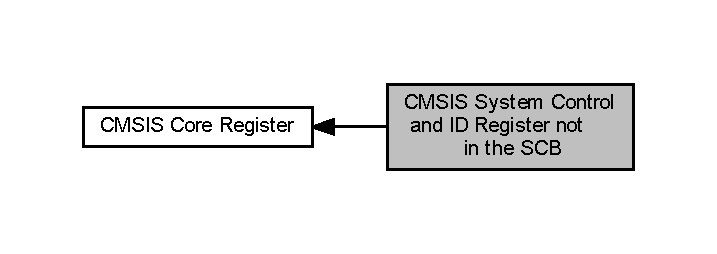
\includegraphics[width=344pt]{group___c_m_s_i_s___s_cn_s_c_b}
\end{center}
\end{figure}
\subsection*{Data Structures}
\begin{DoxyCompactItemize}
\item 
struct \hyperlink{struct_s_cn_s_c_b___type}{S\+Cn\+S\+C\+B\+\_\+\+Type}
\begin{DoxyCompactList}\small\item\em Structure type to access the System Control and ID Register not in the S\+CB. \end{DoxyCompactList}\end{DoxyCompactItemize}
\subsection*{Macros}
\begin{DoxyCompactItemize}
\item 
\#define \hyperlink{group___c_m_s_i_s___s_cn_s_c_b_ga0777ddf379af50f9ca41d40573bfffc5}{S\+Cn\+S\+C\+B\+\_\+\+I\+C\+T\+R\+\_\+\+I\+N\+T\+L\+I\+N\+E\+S\+N\+U\+M\+\_\+\+Pos}~0
\item 
\#define \hyperlink{group___c_m_s_i_s___s_cn_s_c_b_ga3efa0f5210051464e1034b19fc7b33c7}{S\+Cn\+S\+C\+B\+\_\+\+I\+C\+T\+R\+\_\+\+I\+N\+T\+L\+I\+N\+E\+S\+N\+U\+M\+\_\+\+Msk}~(0x\+F\+U\+L $<$$<$ S\+Cn\+S\+C\+B\+\_\+\+I\+C\+T\+R\+\_\+\+I\+N\+T\+L\+I\+N\+E\+S\+N\+U\+M\+\_\+\+Pos)
\item 
\#define \hyperlink{group___c_m_s_i_s___s_cn_s_c_b_gaff0b57464c60fea8182b903676f8de49}{S\+Cn\+S\+C\+B\+\_\+\+A\+C\+T\+L\+R\+\_\+\+D\+I\+S\+O\+O\+F\+P\+\_\+\+Pos}~9
\item 
\#define \hyperlink{group___c_m_s_i_s___s_cn_s_c_b_ga1ecd6adafa43464d7097b132c19e8640}{S\+Cn\+S\+C\+B\+\_\+\+A\+C\+T\+L\+R\+\_\+\+D\+I\+S\+O\+O\+F\+P\+\_\+\+Msk}~(1\+U\+L $<$$<$ S\+Cn\+S\+C\+B\+\_\+\+A\+C\+T\+L\+R\+\_\+\+D\+I\+S\+O\+O\+F\+P\+\_\+\+Pos)
\item 
\#define \hyperlink{group___c_m_s_i_s___s_cn_s_c_b_gaa194809383bc72ecf3416d85709281d7}{S\+Cn\+S\+C\+B\+\_\+\+A\+C\+T\+L\+R\+\_\+\+D\+I\+S\+F\+P\+C\+A\+\_\+\+Pos}~8
\item 
\#define \hyperlink{group___c_m_s_i_s___s_cn_s_c_b_ga10d5aa4a196dcde6f476016ece2c1b69}{S\+Cn\+S\+C\+B\+\_\+\+A\+C\+T\+L\+R\+\_\+\+D\+I\+S\+F\+P\+C\+A\+\_\+\+Msk}~(1\+U\+L $<$$<$ S\+Cn\+S\+C\+B\+\_\+\+A\+C\+T\+L\+R\+\_\+\+D\+I\+S\+F\+P\+C\+A\+\_\+\+Pos)
\item 
\#define \hyperlink{group___c_m_s_i_s___s_cn_s_c_b_gaab395870643a0bee78906bb15ca5bd02}{S\+Cn\+S\+C\+B\+\_\+\+A\+C\+T\+L\+R\+\_\+\+D\+I\+S\+F\+O\+L\+D\+\_\+\+Pos}~2
\item 
\#define \hyperlink{group___c_m_s_i_s___s_cn_s_c_b_gaa9dd2d4a2350499188f438d0aa9fd982}{S\+Cn\+S\+C\+B\+\_\+\+A\+C\+T\+L\+R\+\_\+\+D\+I\+S\+F\+O\+L\+D\+\_\+\+Msk}~(1\+U\+L $<$$<$ S\+Cn\+S\+C\+B\+\_\+\+A\+C\+T\+L\+R\+\_\+\+D\+I\+S\+F\+O\+L\+D\+\_\+\+Pos)
\item 
\#define \hyperlink{group___c_m_s_i_s___s_cn_s_c_b_gafa2eb37493c0f8dae77cde81ecf80f77}{S\+Cn\+S\+C\+B\+\_\+\+A\+C\+T\+L\+R\+\_\+\+D\+I\+S\+D\+E\+F\+W\+B\+U\+F\+\_\+\+Pos}~1
\item 
\#define \hyperlink{group___c_m_s_i_s___s_cn_s_c_b_ga6cda7b7219232a008ec52cc8e89d5d08}{S\+Cn\+S\+C\+B\+\_\+\+A\+C\+T\+L\+R\+\_\+\+D\+I\+S\+D\+E\+F\+W\+B\+U\+F\+\_\+\+Msk}~(1\+U\+L $<$$<$ S\+Cn\+S\+C\+B\+\_\+\+A\+C\+T\+L\+R\+\_\+\+D\+I\+S\+D\+E\+F\+W\+B\+U\+F\+\_\+\+Pos)
\item 
\#define \hyperlink{group___c_m_s_i_s___s_cn_s_c_b_gaaa3e79f5ead4a32c0ea742b2a9ffc0cd}{S\+Cn\+S\+C\+B\+\_\+\+A\+C\+T\+L\+R\+\_\+\+D\+I\+S\+M\+C\+Y\+C\+I\+N\+T\+\_\+\+Pos}~0
\item 
\#define \hyperlink{group___c_m_s_i_s___s_cn_s_c_b_ga2a2818f0489ad10b6ea2964e899d4cbc}{S\+Cn\+S\+C\+B\+\_\+\+A\+C\+T\+L\+R\+\_\+\+D\+I\+S\+M\+C\+Y\+C\+I\+N\+T\+\_\+\+Msk}~(1\+U\+L $<$$<$ S\+Cn\+S\+C\+B\+\_\+\+A\+C\+T\+L\+R\+\_\+\+D\+I\+S\+M\+C\+Y\+C\+I\+N\+T\+\_\+\+Pos)
\end{DoxyCompactItemize}


\subsection{Detailed Description}
Type definitions for the Cortex-\/M System Control and ID Register not in the S\+CB 

\subsection{Macro Definition Documentation}
\mbox{\Hypertarget{group___c_m_s_i_s___s_cn_s_c_b_ga6cda7b7219232a008ec52cc8e89d5d08}\label{group___c_m_s_i_s___s_cn_s_c_b_ga6cda7b7219232a008ec52cc8e89d5d08}} 
\index{C\+M\+S\+I\+S System Control and I\+D Register not in the S\+CB@{C\+M\+S\+I\+S System Control and I\+D Register not in the S\+CB}!S\+Cn\+S\+C\+B\+\_\+\+A\+C\+T\+L\+R\+\_\+\+D\+I\+S\+D\+E\+F\+W\+B\+U\+F\+\_\+\+Msk@{S\+Cn\+S\+C\+B\+\_\+\+A\+C\+T\+L\+R\+\_\+\+D\+I\+S\+D\+E\+F\+W\+B\+U\+F\+\_\+\+Msk}}
\index{S\+Cn\+S\+C\+B\+\_\+\+A\+C\+T\+L\+R\+\_\+\+D\+I\+S\+D\+E\+F\+W\+B\+U\+F\+\_\+\+Msk@{S\+Cn\+S\+C\+B\+\_\+\+A\+C\+T\+L\+R\+\_\+\+D\+I\+S\+D\+E\+F\+W\+B\+U\+F\+\_\+\+Msk}!C\+M\+S\+I\+S System Control and I\+D Register not in the S\+CB@{C\+M\+S\+I\+S System Control and I\+D Register not in the S\+CB}}
\subsubsection{\texorpdfstring{S\+Cn\+S\+C\+B\+\_\+\+A\+C\+T\+L\+R\+\_\+\+D\+I\+S\+D\+E\+F\+W\+B\+U\+F\+\_\+\+Msk}{SCnSCB\_ACTLR\_DISDEFWBUF\_Msk}}
{\footnotesize\ttfamily \#define S\+Cn\+S\+C\+B\+\_\+\+A\+C\+T\+L\+R\+\_\+\+D\+I\+S\+D\+E\+F\+W\+B\+U\+F\+\_\+\+Msk~(1\+U\+L $<$$<$ S\+Cn\+S\+C\+B\+\_\+\+A\+C\+T\+L\+R\+\_\+\+D\+I\+S\+D\+E\+F\+W\+B\+U\+F\+\_\+\+Pos)}

A\+C\+T\+LR\+: D\+I\+S\+D\+E\+F\+W\+B\+UF Mask 

Definition at line 574 of file core\+\_\+cm4.\+h.

\mbox{\Hypertarget{group___c_m_s_i_s___s_cn_s_c_b_gafa2eb37493c0f8dae77cde81ecf80f77}\label{group___c_m_s_i_s___s_cn_s_c_b_gafa2eb37493c0f8dae77cde81ecf80f77}} 
\index{C\+M\+S\+I\+S System Control and I\+D Register not in the S\+CB@{C\+M\+S\+I\+S System Control and I\+D Register not in the S\+CB}!S\+Cn\+S\+C\+B\+\_\+\+A\+C\+T\+L\+R\+\_\+\+D\+I\+S\+D\+E\+F\+W\+B\+U\+F\+\_\+\+Pos@{S\+Cn\+S\+C\+B\+\_\+\+A\+C\+T\+L\+R\+\_\+\+D\+I\+S\+D\+E\+F\+W\+B\+U\+F\+\_\+\+Pos}}
\index{S\+Cn\+S\+C\+B\+\_\+\+A\+C\+T\+L\+R\+\_\+\+D\+I\+S\+D\+E\+F\+W\+B\+U\+F\+\_\+\+Pos@{S\+Cn\+S\+C\+B\+\_\+\+A\+C\+T\+L\+R\+\_\+\+D\+I\+S\+D\+E\+F\+W\+B\+U\+F\+\_\+\+Pos}!C\+M\+S\+I\+S System Control and I\+D Register not in the S\+CB@{C\+M\+S\+I\+S System Control and I\+D Register not in the S\+CB}}
\subsubsection{\texorpdfstring{S\+Cn\+S\+C\+B\+\_\+\+A\+C\+T\+L\+R\+\_\+\+D\+I\+S\+D\+E\+F\+W\+B\+U\+F\+\_\+\+Pos}{SCnSCB\_ACTLR\_DISDEFWBUF\_Pos}}
{\footnotesize\ttfamily \#define S\+Cn\+S\+C\+B\+\_\+\+A\+C\+T\+L\+R\+\_\+\+D\+I\+S\+D\+E\+F\+W\+B\+U\+F\+\_\+\+Pos~1}

A\+C\+T\+LR\+: D\+I\+S\+D\+E\+F\+W\+B\+UF Position 

Definition at line 573 of file core\+\_\+cm4.\+h.

\mbox{\Hypertarget{group___c_m_s_i_s___s_cn_s_c_b_gaa9dd2d4a2350499188f438d0aa9fd982}\label{group___c_m_s_i_s___s_cn_s_c_b_gaa9dd2d4a2350499188f438d0aa9fd982}} 
\index{C\+M\+S\+I\+S System Control and I\+D Register not in the S\+CB@{C\+M\+S\+I\+S System Control and I\+D Register not in the S\+CB}!S\+Cn\+S\+C\+B\+\_\+\+A\+C\+T\+L\+R\+\_\+\+D\+I\+S\+F\+O\+L\+D\+\_\+\+Msk@{S\+Cn\+S\+C\+B\+\_\+\+A\+C\+T\+L\+R\+\_\+\+D\+I\+S\+F\+O\+L\+D\+\_\+\+Msk}}
\index{S\+Cn\+S\+C\+B\+\_\+\+A\+C\+T\+L\+R\+\_\+\+D\+I\+S\+F\+O\+L\+D\+\_\+\+Msk@{S\+Cn\+S\+C\+B\+\_\+\+A\+C\+T\+L\+R\+\_\+\+D\+I\+S\+F\+O\+L\+D\+\_\+\+Msk}!C\+M\+S\+I\+S System Control and I\+D Register not in the S\+CB@{C\+M\+S\+I\+S System Control and I\+D Register not in the S\+CB}}
\subsubsection{\texorpdfstring{S\+Cn\+S\+C\+B\+\_\+\+A\+C\+T\+L\+R\+\_\+\+D\+I\+S\+F\+O\+L\+D\+\_\+\+Msk}{SCnSCB\_ACTLR\_DISFOLD\_Msk}}
{\footnotesize\ttfamily \#define S\+Cn\+S\+C\+B\+\_\+\+A\+C\+T\+L\+R\+\_\+\+D\+I\+S\+F\+O\+L\+D\+\_\+\+Msk~(1\+U\+L $<$$<$ S\+Cn\+S\+C\+B\+\_\+\+A\+C\+T\+L\+R\+\_\+\+D\+I\+S\+F\+O\+L\+D\+\_\+\+Pos)}

A\+C\+T\+LR\+: D\+I\+S\+F\+O\+LD Mask 

Definition at line 571 of file core\+\_\+cm4.\+h.

\mbox{\Hypertarget{group___c_m_s_i_s___s_cn_s_c_b_gaab395870643a0bee78906bb15ca5bd02}\label{group___c_m_s_i_s___s_cn_s_c_b_gaab395870643a0bee78906bb15ca5bd02}} 
\index{C\+M\+S\+I\+S System Control and I\+D Register not in the S\+CB@{C\+M\+S\+I\+S System Control and I\+D Register not in the S\+CB}!S\+Cn\+S\+C\+B\+\_\+\+A\+C\+T\+L\+R\+\_\+\+D\+I\+S\+F\+O\+L\+D\+\_\+\+Pos@{S\+Cn\+S\+C\+B\+\_\+\+A\+C\+T\+L\+R\+\_\+\+D\+I\+S\+F\+O\+L\+D\+\_\+\+Pos}}
\index{S\+Cn\+S\+C\+B\+\_\+\+A\+C\+T\+L\+R\+\_\+\+D\+I\+S\+F\+O\+L\+D\+\_\+\+Pos@{S\+Cn\+S\+C\+B\+\_\+\+A\+C\+T\+L\+R\+\_\+\+D\+I\+S\+F\+O\+L\+D\+\_\+\+Pos}!C\+M\+S\+I\+S System Control and I\+D Register not in the S\+CB@{C\+M\+S\+I\+S System Control and I\+D Register not in the S\+CB}}
\subsubsection{\texorpdfstring{S\+Cn\+S\+C\+B\+\_\+\+A\+C\+T\+L\+R\+\_\+\+D\+I\+S\+F\+O\+L\+D\+\_\+\+Pos}{SCnSCB\_ACTLR\_DISFOLD\_Pos}}
{\footnotesize\ttfamily \#define S\+Cn\+S\+C\+B\+\_\+\+A\+C\+T\+L\+R\+\_\+\+D\+I\+S\+F\+O\+L\+D\+\_\+\+Pos~2}

A\+C\+T\+LR\+: D\+I\+S\+F\+O\+LD Position 

Definition at line 570 of file core\+\_\+cm4.\+h.

\mbox{\Hypertarget{group___c_m_s_i_s___s_cn_s_c_b_ga10d5aa4a196dcde6f476016ece2c1b69}\label{group___c_m_s_i_s___s_cn_s_c_b_ga10d5aa4a196dcde6f476016ece2c1b69}} 
\index{C\+M\+S\+I\+S System Control and I\+D Register not in the S\+CB@{C\+M\+S\+I\+S System Control and I\+D Register not in the S\+CB}!S\+Cn\+S\+C\+B\+\_\+\+A\+C\+T\+L\+R\+\_\+\+D\+I\+S\+F\+P\+C\+A\+\_\+\+Msk@{S\+Cn\+S\+C\+B\+\_\+\+A\+C\+T\+L\+R\+\_\+\+D\+I\+S\+F\+P\+C\+A\+\_\+\+Msk}}
\index{S\+Cn\+S\+C\+B\+\_\+\+A\+C\+T\+L\+R\+\_\+\+D\+I\+S\+F\+P\+C\+A\+\_\+\+Msk@{S\+Cn\+S\+C\+B\+\_\+\+A\+C\+T\+L\+R\+\_\+\+D\+I\+S\+F\+P\+C\+A\+\_\+\+Msk}!C\+M\+S\+I\+S System Control and I\+D Register not in the S\+CB@{C\+M\+S\+I\+S System Control and I\+D Register not in the S\+CB}}
\subsubsection{\texorpdfstring{S\+Cn\+S\+C\+B\+\_\+\+A\+C\+T\+L\+R\+\_\+\+D\+I\+S\+F\+P\+C\+A\+\_\+\+Msk}{SCnSCB\_ACTLR\_DISFPCA\_Msk}}
{\footnotesize\ttfamily \#define S\+Cn\+S\+C\+B\+\_\+\+A\+C\+T\+L\+R\+\_\+\+D\+I\+S\+F\+P\+C\+A\+\_\+\+Msk~(1\+U\+L $<$$<$ S\+Cn\+S\+C\+B\+\_\+\+A\+C\+T\+L\+R\+\_\+\+D\+I\+S\+F\+P\+C\+A\+\_\+\+Pos)}

A\+C\+T\+LR\+: D\+I\+S\+F\+P\+CA Mask 

Definition at line 568 of file core\+\_\+cm4.\+h.

\mbox{\Hypertarget{group___c_m_s_i_s___s_cn_s_c_b_gaa194809383bc72ecf3416d85709281d7}\label{group___c_m_s_i_s___s_cn_s_c_b_gaa194809383bc72ecf3416d85709281d7}} 
\index{C\+M\+S\+I\+S System Control and I\+D Register not in the S\+CB@{C\+M\+S\+I\+S System Control and I\+D Register not in the S\+CB}!S\+Cn\+S\+C\+B\+\_\+\+A\+C\+T\+L\+R\+\_\+\+D\+I\+S\+F\+P\+C\+A\+\_\+\+Pos@{S\+Cn\+S\+C\+B\+\_\+\+A\+C\+T\+L\+R\+\_\+\+D\+I\+S\+F\+P\+C\+A\+\_\+\+Pos}}
\index{S\+Cn\+S\+C\+B\+\_\+\+A\+C\+T\+L\+R\+\_\+\+D\+I\+S\+F\+P\+C\+A\+\_\+\+Pos@{S\+Cn\+S\+C\+B\+\_\+\+A\+C\+T\+L\+R\+\_\+\+D\+I\+S\+F\+P\+C\+A\+\_\+\+Pos}!C\+M\+S\+I\+S System Control and I\+D Register not in the S\+CB@{C\+M\+S\+I\+S System Control and I\+D Register not in the S\+CB}}
\subsubsection{\texorpdfstring{S\+Cn\+S\+C\+B\+\_\+\+A\+C\+T\+L\+R\+\_\+\+D\+I\+S\+F\+P\+C\+A\+\_\+\+Pos}{SCnSCB\_ACTLR\_DISFPCA\_Pos}}
{\footnotesize\ttfamily \#define S\+Cn\+S\+C\+B\+\_\+\+A\+C\+T\+L\+R\+\_\+\+D\+I\+S\+F\+P\+C\+A\+\_\+\+Pos~8}

A\+C\+T\+LR\+: D\+I\+S\+F\+P\+CA Position 

Definition at line 567 of file core\+\_\+cm4.\+h.

\mbox{\Hypertarget{group___c_m_s_i_s___s_cn_s_c_b_ga2a2818f0489ad10b6ea2964e899d4cbc}\label{group___c_m_s_i_s___s_cn_s_c_b_ga2a2818f0489ad10b6ea2964e899d4cbc}} 
\index{C\+M\+S\+I\+S System Control and I\+D Register not in the S\+CB@{C\+M\+S\+I\+S System Control and I\+D Register not in the S\+CB}!S\+Cn\+S\+C\+B\+\_\+\+A\+C\+T\+L\+R\+\_\+\+D\+I\+S\+M\+C\+Y\+C\+I\+N\+T\+\_\+\+Msk@{S\+Cn\+S\+C\+B\+\_\+\+A\+C\+T\+L\+R\+\_\+\+D\+I\+S\+M\+C\+Y\+C\+I\+N\+T\+\_\+\+Msk}}
\index{S\+Cn\+S\+C\+B\+\_\+\+A\+C\+T\+L\+R\+\_\+\+D\+I\+S\+M\+C\+Y\+C\+I\+N\+T\+\_\+\+Msk@{S\+Cn\+S\+C\+B\+\_\+\+A\+C\+T\+L\+R\+\_\+\+D\+I\+S\+M\+C\+Y\+C\+I\+N\+T\+\_\+\+Msk}!C\+M\+S\+I\+S System Control and I\+D Register not in the S\+CB@{C\+M\+S\+I\+S System Control and I\+D Register not in the S\+CB}}
\subsubsection{\texorpdfstring{S\+Cn\+S\+C\+B\+\_\+\+A\+C\+T\+L\+R\+\_\+\+D\+I\+S\+M\+C\+Y\+C\+I\+N\+T\+\_\+\+Msk}{SCnSCB\_ACTLR\_DISMCYCINT\_Msk}}
{\footnotesize\ttfamily \#define S\+Cn\+S\+C\+B\+\_\+\+A\+C\+T\+L\+R\+\_\+\+D\+I\+S\+M\+C\+Y\+C\+I\+N\+T\+\_\+\+Msk~(1\+U\+L $<$$<$ S\+Cn\+S\+C\+B\+\_\+\+A\+C\+T\+L\+R\+\_\+\+D\+I\+S\+M\+C\+Y\+C\+I\+N\+T\+\_\+\+Pos)}

A\+C\+T\+LR\+: D\+I\+S\+M\+C\+Y\+C\+I\+NT Mask 

Definition at line 577 of file core\+\_\+cm4.\+h.

\mbox{\Hypertarget{group___c_m_s_i_s___s_cn_s_c_b_gaaa3e79f5ead4a32c0ea742b2a9ffc0cd}\label{group___c_m_s_i_s___s_cn_s_c_b_gaaa3e79f5ead4a32c0ea742b2a9ffc0cd}} 
\index{C\+M\+S\+I\+S System Control and I\+D Register not in the S\+CB@{C\+M\+S\+I\+S System Control and I\+D Register not in the S\+CB}!S\+Cn\+S\+C\+B\+\_\+\+A\+C\+T\+L\+R\+\_\+\+D\+I\+S\+M\+C\+Y\+C\+I\+N\+T\+\_\+\+Pos@{S\+Cn\+S\+C\+B\+\_\+\+A\+C\+T\+L\+R\+\_\+\+D\+I\+S\+M\+C\+Y\+C\+I\+N\+T\+\_\+\+Pos}}
\index{S\+Cn\+S\+C\+B\+\_\+\+A\+C\+T\+L\+R\+\_\+\+D\+I\+S\+M\+C\+Y\+C\+I\+N\+T\+\_\+\+Pos@{S\+Cn\+S\+C\+B\+\_\+\+A\+C\+T\+L\+R\+\_\+\+D\+I\+S\+M\+C\+Y\+C\+I\+N\+T\+\_\+\+Pos}!C\+M\+S\+I\+S System Control and I\+D Register not in the S\+CB@{C\+M\+S\+I\+S System Control and I\+D Register not in the S\+CB}}
\subsubsection{\texorpdfstring{S\+Cn\+S\+C\+B\+\_\+\+A\+C\+T\+L\+R\+\_\+\+D\+I\+S\+M\+C\+Y\+C\+I\+N\+T\+\_\+\+Pos}{SCnSCB\_ACTLR\_DISMCYCINT\_Pos}}
{\footnotesize\ttfamily \#define S\+Cn\+S\+C\+B\+\_\+\+A\+C\+T\+L\+R\+\_\+\+D\+I\+S\+M\+C\+Y\+C\+I\+N\+T\+\_\+\+Pos~0}

A\+C\+T\+LR\+: D\+I\+S\+M\+C\+Y\+C\+I\+NT Position 

Definition at line 576 of file core\+\_\+cm4.\+h.

\mbox{\Hypertarget{group___c_m_s_i_s___s_cn_s_c_b_ga1ecd6adafa43464d7097b132c19e8640}\label{group___c_m_s_i_s___s_cn_s_c_b_ga1ecd6adafa43464d7097b132c19e8640}} 
\index{C\+M\+S\+I\+S System Control and I\+D Register not in the S\+CB@{C\+M\+S\+I\+S System Control and I\+D Register not in the S\+CB}!S\+Cn\+S\+C\+B\+\_\+\+A\+C\+T\+L\+R\+\_\+\+D\+I\+S\+O\+O\+F\+P\+\_\+\+Msk@{S\+Cn\+S\+C\+B\+\_\+\+A\+C\+T\+L\+R\+\_\+\+D\+I\+S\+O\+O\+F\+P\+\_\+\+Msk}}
\index{S\+Cn\+S\+C\+B\+\_\+\+A\+C\+T\+L\+R\+\_\+\+D\+I\+S\+O\+O\+F\+P\+\_\+\+Msk@{S\+Cn\+S\+C\+B\+\_\+\+A\+C\+T\+L\+R\+\_\+\+D\+I\+S\+O\+O\+F\+P\+\_\+\+Msk}!C\+M\+S\+I\+S System Control and I\+D Register not in the S\+CB@{C\+M\+S\+I\+S System Control and I\+D Register not in the S\+CB}}
\subsubsection{\texorpdfstring{S\+Cn\+S\+C\+B\+\_\+\+A\+C\+T\+L\+R\+\_\+\+D\+I\+S\+O\+O\+F\+P\+\_\+\+Msk}{SCnSCB\_ACTLR\_DISOOFP\_Msk}}
{\footnotesize\ttfamily \#define S\+Cn\+S\+C\+B\+\_\+\+A\+C\+T\+L\+R\+\_\+\+D\+I\+S\+O\+O\+F\+P\+\_\+\+Msk~(1\+U\+L $<$$<$ S\+Cn\+S\+C\+B\+\_\+\+A\+C\+T\+L\+R\+\_\+\+D\+I\+S\+O\+O\+F\+P\+\_\+\+Pos)}

A\+C\+T\+LR\+: D\+I\+S\+O\+O\+FP Mask 

Definition at line 565 of file core\+\_\+cm4.\+h.

\mbox{\Hypertarget{group___c_m_s_i_s___s_cn_s_c_b_gaff0b57464c60fea8182b903676f8de49}\label{group___c_m_s_i_s___s_cn_s_c_b_gaff0b57464c60fea8182b903676f8de49}} 
\index{C\+M\+S\+I\+S System Control and I\+D Register not in the S\+CB@{C\+M\+S\+I\+S System Control and I\+D Register not in the S\+CB}!S\+Cn\+S\+C\+B\+\_\+\+A\+C\+T\+L\+R\+\_\+\+D\+I\+S\+O\+O\+F\+P\+\_\+\+Pos@{S\+Cn\+S\+C\+B\+\_\+\+A\+C\+T\+L\+R\+\_\+\+D\+I\+S\+O\+O\+F\+P\+\_\+\+Pos}}
\index{S\+Cn\+S\+C\+B\+\_\+\+A\+C\+T\+L\+R\+\_\+\+D\+I\+S\+O\+O\+F\+P\+\_\+\+Pos@{S\+Cn\+S\+C\+B\+\_\+\+A\+C\+T\+L\+R\+\_\+\+D\+I\+S\+O\+O\+F\+P\+\_\+\+Pos}!C\+M\+S\+I\+S System Control and I\+D Register not in the S\+CB@{C\+M\+S\+I\+S System Control and I\+D Register not in the S\+CB}}
\subsubsection{\texorpdfstring{S\+Cn\+S\+C\+B\+\_\+\+A\+C\+T\+L\+R\+\_\+\+D\+I\+S\+O\+O\+F\+P\+\_\+\+Pos}{SCnSCB\_ACTLR\_DISOOFP\_Pos}}
{\footnotesize\ttfamily \#define S\+Cn\+S\+C\+B\+\_\+\+A\+C\+T\+L\+R\+\_\+\+D\+I\+S\+O\+O\+F\+P\+\_\+\+Pos~9}

A\+C\+T\+LR\+: D\+I\+S\+O\+O\+FP Position 

Definition at line 564 of file core\+\_\+cm4.\+h.

\mbox{\Hypertarget{group___c_m_s_i_s___s_cn_s_c_b_ga3efa0f5210051464e1034b19fc7b33c7}\label{group___c_m_s_i_s___s_cn_s_c_b_ga3efa0f5210051464e1034b19fc7b33c7}} 
\index{C\+M\+S\+I\+S System Control and I\+D Register not in the S\+CB@{C\+M\+S\+I\+S System Control and I\+D Register not in the S\+CB}!S\+Cn\+S\+C\+B\+\_\+\+I\+C\+T\+R\+\_\+\+I\+N\+T\+L\+I\+N\+E\+S\+N\+U\+M\+\_\+\+Msk@{S\+Cn\+S\+C\+B\+\_\+\+I\+C\+T\+R\+\_\+\+I\+N\+T\+L\+I\+N\+E\+S\+N\+U\+M\+\_\+\+Msk}}
\index{S\+Cn\+S\+C\+B\+\_\+\+I\+C\+T\+R\+\_\+\+I\+N\+T\+L\+I\+N\+E\+S\+N\+U\+M\+\_\+\+Msk@{S\+Cn\+S\+C\+B\+\_\+\+I\+C\+T\+R\+\_\+\+I\+N\+T\+L\+I\+N\+E\+S\+N\+U\+M\+\_\+\+Msk}!C\+M\+S\+I\+S System Control and I\+D Register not in the S\+CB@{C\+M\+S\+I\+S System Control and I\+D Register not in the S\+CB}}
\subsubsection{\texorpdfstring{S\+Cn\+S\+C\+B\+\_\+\+I\+C\+T\+R\+\_\+\+I\+N\+T\+L\+I\+N\+E\+S\+N\+U\+M\+\_\+\+Msk}{SCnSCB\_ICTR\_INTLINESNUM\_Msk}}
{\footnotesize\ttfamily \#define S\+Cn\+S\+C\+B\+\_\+\+I\+C\+T\+R\+\_\+\+I\+N\+T\+L\+I\+N\+E\+S\+N\+U\+M\+\_\+\+Msk~(0x\+F\+U\+L $<$$<$ S\+Cn\+S\+C\+B\+\_\+\+I\+C\+T\+R\+\_\+\+I\+N\+T\+L\+I\+N\+E\+S\+N\+U\+M\+\_\+\+Pos)}

I\+C\+TR\+: I\+N\+T\+L\+I\+N\+E\+S\+N\+UM Mask 

Definition at line 561 of file core\+\_\+cm4.\+h.

\mbox{\Hypertarget{group___c_m_s_i_s___s_cn_s_c_b_ga0777ddf379af50f9ca41d40573bfffc5}\label{group___c_m_s_i_s___s_cn_s_c_b_ga0777ddf379af50f9ca41d40573bfffc5}} 
\index{C\+M\+S\+I\+S System Control and I\+D Register not in the S\+CB@{C\+M\+S\+I\+S System Control and I\+D Register not in the S\+CB}!S\+Cn\+S\+C\+B\+\_\+\+I\+C\+T\+R\+\_\+\+I\+N\+T\+L\+I\+N\+E\+S\+N\+U\+M\+\_\+\+Pos@{S\+Cn\+S\+C\+B\+\_\+\+I\+C\+T\+R\+\_\+\+I\+N\+T\+L\+I\+N\+E\+S\+N\+U\+M\+\_\+\+Pos}}
\index{S\+Cn\+S\+C\+B\+\_\+\+I\+C\+T\+R\+\_\+\+I\+N\+T\+L\+I\+N\+E\+S\+N\+U\+M\+\_\+\+Pos@{S\+Cn\+S\+C\+B\+\_\+\+I\+C\+T\+R\+\_\+\+I\+N\+T\+L\+I\+N\+E\+S\+N\+U\+M\+\_\+\+Pos}!C\+M\+S\+I\+S System Control and I\+D Register not in the S\+CB@{C\+M\+S\+I\+S System Control and I\+D Register not in the S\+CB}}
\subsubsection{\texorpdfstring{S\+Cn\+S\+C\+B\+\_\+\+I\+C\+T\+R\+\_\+\+I\+N\+T\+L\+I\+N\+E\+S\+N\+U\+M\+\_\+\+Pos}{SCnSCB\_ICTR\_INTLINESNUM\_Pos}}
{\footnotesize\ttfamily \#define S\+Cn\+S\+C\+B\+\_\+\+I\+C\+T\+R\+\_\+\+I\+N\+T\+L\+I\+N\+E\+S\+N\+U\+M\+\_\+\+Pos~0}

I\+C\+TR\+: I\+N\+T\+L\+I\+N\+E\+S\+N\+UM Position 

Definition at line 560 of file core\+\_\+cm4.\+h.


\hypertarget{group___c_m_s_i_s___sys_tick}{}\section{C\+M\+S\+IS Sys\+Tick}
\label{group___c_m_s_i_s___sys_tick}\index{C\+M\+S\+I\+S Sys\+Tick@{C\+M\+S\+I\+S Sys\+Tick}}
Collaboration diagram for C\+M\+S\+IS Sys\+Tick\+:\nopagebreak
\begin{figure}[H]
\begin{center}
\leavevmode
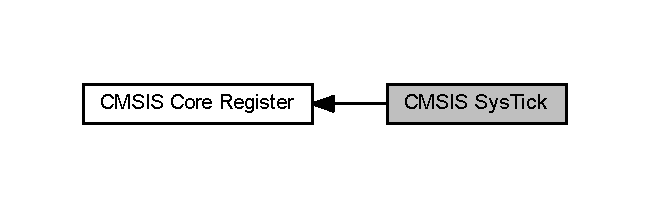
\includegraphics[width=312pt]{group___c_m_s_i_s___sys_tick}
\end{center}
\end{figure}
\subsection*{Data Structures}
\begin{DoxyCompactItemize}
\item 
struct \hyperlink{struct_sys_tick___type}{Sys\+Tick\+\_\+\+Type}
\begin{DoxyCompactList}\small\item\em Structure type to access the System Timer (Sys\+Tick). \end{DoxyCompactList}\end{DoxyCompactItemize}
\subsection*{Macros}
\begin{DoxyCompactItemize}
\item 
\#define \hyperlink{group___c_m_s_i_s___sys_tick_gadbb65d4a815759649db41df216ed4d60}{Sys\+Tick\+\_\+\+C\+T\+R\+L\+\_\+\+C\+O\+U\+N\+T\+F\+L\+A\+G\+\_\+\+Pos}~16
\item 
\#define \hyperlink{group___c_m_s_i_s___sys_tick_ga1bf3033ecccf200f59baefe15dbb367c}{Sys\+Tick\+\_\+\+C\+T\+R\+L\+\_\+\+C\+O\+U\+N\+T\+F\+L\+A\+G\+\_\+\+Msk}~(1\+U\+L $<$$<$ Sys\+Tick\+\_\+\+C\+T\+R\+L\+\_\+\+C\+O\+U\+N\+T\+F\+L\+A\+G\+\_\+\+Pos)
\item 
\#define \hyperlink{group___c_m_s_i_s___sys_tick_ga24fbc69a5f0b78d67fda2300257baff1}{Sys\+Tick\+\_\+\+C\+T\+R\+L\+\_\+\+C\+L\+K\+S\+O\+U\+R\+C\+E\+\_\+\+Pos}~2
\item 
\#define \hyperlink{group___c_m_s_i_s___sys_tick_gaa41d06039797423a46596bd313d57373}{Sys\+Tick\+\_\+\+C\+T\+R\+L\+\_\+\+C\+L\+K\+S\+O\+U\+R\+C\+E\+\_\+\+Msk}~(1\+U\+L $<$$<$ Sys\+Tick\+\_\+\+C\+T\+R\+L\+\_\+\+C\+L\+K\+S\+O\+U\+R\+C\+E\+\_\+\+Pos)
\item 
\#define \hyperlink{group___c_m_s_i_s___sys_tick_ga88f45bbb89ce8df3cd2b2613c7b48214}{Sys\+Tick\+\_\+\+C\+T\+R\+L\+\_\+\+T\+I\+C\+K\+I\+N\+T\+\_\+\+Pos}~1
\item 
\#define \hyperlink{group___c_m_s_i_s___sys_tick_ga95bb984266ca764024836a870238a027}{Sys\+Tick\+\_\+\+C\+T\+R\+L\+\_\+\+T\+I\+C\+K\+I\+N\+T\+\_\+\+Msk}~(1\+U\+L $<$$<$ Sys\+Tick\+\_\+\+C\+T\+R\+L\+\_\+\+T\+I\+C\+K\+I\+N\+T\+\_\+\+Pos)
\item 
\#define \hyperlink{group___c_m_s_i_s___sys_tick_ga0b48cc1e36d92a92e4bf632890314810}{Sys\+Tick\+\_\+\+C\+T\+R\+L\+\_\+\+E\+N\+A\+B\+L\+E\+\_\+\+Pos}~0
\item 
\#define \hyperlink{group___c_m_s_i_s___sys_tick_ga16c9fee0ed0235524bdeb38af328fd1f}{Sys\+Tick\+\_\+\+C\+T\+R\+L\+\_\+\+E\+N\+A\+B\+L\+E\+\_\+\+Msk}~(1\+U\+L $<$$<$ Sys\+Tick\+\_\+\+C\+T\+R\+L\+\_\+\+E\+N\+A\+B\+L\+E\+\_\+\+Pos)
\item 
\#define \hyperlink{group___c_m_s_i_s___sys_tick_gaf44d10df359dc5bf5752b0894ae3bad2}{Sys\+Tick\+\_\+\+L\+O\+A\+D\+\_\+\+R\+E\+L\+O\+A\+D\+\_\+\+Pos}~0
\item 
\#define \hyperlink{group___c_m_s_i_s___sys_tick_ga265912a7962f0e1abd170336e579b1b1}{Sys\+Tick\+\_\+\+L\+O\+A\+D\+\_\+\+R\+E\+L\+O\+A\+D\+\_\+\+Msk}~(0x\+F\+F\+F\+F\+F\+F\+U\+L $<$$<$ Sys\+Tick\+\_\+\+L\+O\+A\+D\+\_\+\+R\+E\+L\+O\+A\+D\+\_\+\+Pos)
\item 
\#define \hyperlink{group___c_m_s_i_s___sys_tick_ga3208104c3b019b5de35ae8c21d5c34dd}{Sys\+Tick\+\_\+\+V\+A\+L\+\_\+\+C\+U\+R\+R\+E\+N\+T\+\_\+\+Pos}~0
\item 
\#define \hyperlink{group___c_m_s_i_s___sys_tick_gafc77b56d568930b49a2474debc75ab45}{Sys\+Tick\+\_\+\+V\+A\+L\+\_\+\+C\+U\+R\+R\+E\+N\+T\+\_\+\+Msk}~(0x\+F\+F\+F\+F\+F\+F\+U\+L $<$$<$ Sys\+Tick\+\_\+\+V\+A\+L\+\_\+\+C\+U\+R\+R\+E\+N\+T\+\_\+\+Pos)
\item 
\#define \hyperlink{group___c_m_s_i_s___sys_tick_ga534dbe414e7a46a6ce4c1eca1fbff409}{Sys\+Tick\+\_\+\+C\+A\+L\+I\+B\+\_\+\+N\+O\+R\+E\+F\+\_\+\+Pos}~31
\item 
\#define \hyperlink{group___c_m_s_i_s___sys_tick_ga3af0d891fdd99bcc8d8912d37830edb6}{Sys\+Tick\+\_\+\+C\+A\+L\+I\+B\+\_\+\+N\+O\+R\+E\+F\+\_\+\+Msk}~(1\+U\+L $<$$<$ Sys\+Tick\+\_\+\+C\+A\+L\+I\+B\+\_\+\+N\+O\+R\+E\+F\+\_\+\+Pos)
\item 
\#define \hyperlink{group___c_m_s_i_s___sys_tick_gadd0c9cd6641b9f6a0c618e7982954860}{Sys\+Tick\+\_\+\+C\+A\+L\+I\+B\+\_\+\+S\+K\+E\+W\+\_\+\+Pos}~30
\item 
\#define \hyperlink{group___c_m_s_i_s___sys_tick_ga8a6a85a87334776f33d77fd147587431}{Sys\+Tick\+\_\+\+C\+A\+L\+I\+B\+\_\+\+S\+K\+E\+W\+\_\+\+Msk}~(1\+U\+L $<$$<$ Sys\+Tick\+\_\+\+C\+A\+L\+I\+B\+\_\+\+S\+K\+E\+W\+\_\+\+Pos)
\item 
\#define \hyperlink{group___c_m_s_i_s___sys_tick_gacae558f6e75a0bed5d826f606d8e695e}{Sys\+Tick\+\_\+\+C\+A\+L\+I\+B\+\_\+\+T\+E\+N\+M\+S\+\_\+\+Pos}~0
\item 
\#define \hyperlink{group___c_m_s_i_s___sys_tick_gaf1e68865c5aece2ad58971225bd3e95e}{Sys\+Tick\+\_\+\+C\+A\+L\+I\+B\+\_\+\+T\+E\+N\+M\+S\+\_\+\+Msk}~(0x\+F\+F\+F\+F\+F\+F\+U\+L $<$$<$ Sys\+Tick\+\_\+\+V\+A\+L\+\_\+\+C\+U\+R\+R\+E\+N\+T\+\_\+\+Pos)
\end{DoxyCompactItemize}


\subsection{Detailed Description}
Type definitions for the Cortex-\/M System Timer Registers 

\subsection{Macro Definition Documentation}
\mbox{\Hypertarget{group___c_m_s_i_s___sys_tick_ga3af0d891fdd99bcc8d8912d37830edb6}\label{group___c_m_s_i_s___sys_tick_ga3af0d891fdd99bcc8d8912d37830edb6}} 
\index{C\+M\+S\+I\+S Sys\+Tick@{C\+M\+S\+I\+S Sys\+Tick}!Sys\+Tick\+\_\+\+C\+A\+L\+I\+B\+\_\+\+N\+O\+R\+E\+F\+\_\+\+Msk@{Sys\+Tick\+\_\+\+C\+A\+L\+I\+B\+\_\+\+N\+O\+R\+E\+F\+\_\+\+Msk}}
\index{Sys\+Tick\+\_\+\+C\+A\+L\+I\+B\+\_\+\+N\+O\+R\+E\+F\+\_\+\+Msk@{Sys\+Tick\+\_\+\+C\+A\+L\+I\+B\+\_\+\+N\+O\+R\+E\+F\+\_\+\+Msk}!C\+M\+S\+I\+S Sys\+Tick@{C\+M\+S\+I\+S Sys\+Tick}}
\subsubsection{\texorpdfstring{Sys\+Tick\+\_\+\+C\+A\+L\+I\+B\+\_\+\+N\+O\+R\+E\+F\+\_\+\+Msk}{SysTick\_CALIB\_NOREF\_Msk}}
{\footnotesize\ttfamily \#define Sys\+Tick\+\_\+\+C\+A\+L\+I\+B\+\_\+\+N\+O\+R\+E\+F\+\_\+\+Msk~(1\+U\+L $<$$<$ Sys\+Tick\+\_\+\+C\+A\+L\+I\+B\+\_\+\+N\+O\+R\+E\+F\+\_\+\+Pos)}

Sys\+Tick C\+A\+L\+IB\+: N\+O\+R\+EF Mask 

Definition at line 621 of file core\+\_\+cm4.\+h.

\mbox{\Hypertarget{group___c_m_s_i_s___sys_tick_ga534dbe414e7a46a6ce4c1eca1fbff409}\label{group___c_m_s_i_s___sys_tick_ga534dbe414e7a46a6ce4c1eca1fbff409}} 
\index{C\+M\+S\+I\+S Sys\+Tick@{C\+M\+S\+I\+S Sys\+Tick}!Sys\+Tick\+\_\+\+C\+A\+L\+I\+B\+\_\+\+N\+O\+R\+E\+F\+\_\+\+Pos@{Sys\+Tick\+\_\+\+C\+A\+L\+I\+B\+\_\+\+N\+O\+R\+E\+F\+\_\+\+Pos}}
\index{Sys\+Tick\+\_\+\+C\+A\+L\+I\+B\+\_\+\+N\+O\+R\+E\+F\+\_\+\+Pos@{Sys\+Tick\+\_\+\+C\+A\+L\+I\+B\+\_\+\+N\+O\+R\+E\+F\+\_\+\+Pos}!C\+M\+S\+I\+S Sys\+Tick@{C\+M\+S\+I\+S Sys\+Tick}}
\subsubsection{\texorpdfstring{Sys\+Tick\+\_\+\+C\+A\+L\+I\+B\+\_\+\+N\+O\+R\+E\+F\+\_\+\+Pos}{SysTick\_CALIB\_NOREF\_Pos}}
{\footnotesize\ttfamily \#define Sys\+Tick\+\_\+\+C\+A\+L\+I\+B\+\_\+\+N\+O\+R\+E\+F\+\_\+\+Pos~31}

Sys\+Tick C\+A\+L\+IB\+: N\+O\+R\+EF Position 

Definition at line 620 of file core\+\_\+cm4.\+h.

\mbox{\Hypertarget{group___c_m_s_i_s___sys_tick_ga8a6a85a87334776f33d77fd147587431}\label{group___c_m_s_i_s___sys_tick_ga8a6a85a87334776f33d77fd147587431}} 
\index{C\+M\+S\+I\+S Sys\+Tick@{C\+M\+S\+I\+S Sys\+Tick}!Sys\+Tick\+\_\+\+C\+A\+L\+I\+B\+\_\+\+S\+K\+E\+W\+\_\+\+Msk@{Sys\+Tick\+\_\+\+C\+A\+L\+I\+B\+\_\+\+S\+K\+E\+W\+\_\+\+Msk}}
\index{Sys\+Tick\+\_\+\+C\+A\+L\+I\+B\+\_\+\+S\+K\+E\+W\+\_\+\+Msk@{Sys\+Tick\+\_\+\+C\+A\+L\+I\+B\+\_\+\+S\+K\+E\+W\+\_\+\+Msk}!C\+M\+S\+I\+S Sys\+Tick@{C\+M\+S\+I\+S Sys\+Tick}}
\subsubsection{\texorpdfstring{Sys\+Tick\+\_\+\+C\+A\+L\+I\+B\+\_\+\+S\+K\+E\+W\+\_\+\+Msk}{SysTick\_CALIB\_SKEW\_Msk}}
{\footnotesize\ttfamily \#define Sys\+Tick\+\_\+\+C\+A\+L\+I\+B\+\_\+\+S\+K\+E\+W\+\_\+\+Msk~(1\+U\+L $<$$<$ Sys\+Tick\+\_\+\+C\+A\+L\+I\+B\+\_\+\+S\+K\+E\+W\+\_\+\+Pos)}

Sys\+Tick C\+A\+L\+IB\+: S\+K\+EW Mask 

Definition at line 624 of file core\+\_\+cm4.\+h.

\mbox{\Hypertarget{group___c_m_s_i_s___sys_tick_gadd0c9cd6641b9f6a0c618e7982954860}\label{group___c_m_s_i_s___sys_tick_gadd0c9cd6641b9f6a0c618e7982954860}} 
\index{C\+M\+S\+I\+S Sys\+Tick@{C\+M\+S\+I\+S Sys\+Tick}!Sys\+Tick\+\_\+\+C\+A\+L\+I\+B\+\_\+\+S\+K\+E\+W\+\_\+\+Pos@{Sys\+Tick\+\_\+\+C\+A\+L\+I\+B\+\_\+\+S\+K\+E\+W\+\_\+\+Pos}}
\index{Sys\+Tick\+\_\+\+C\+A\+L\+I\+B\+\_\+\+S\+K\+E\+W\+\_\+\+Pos@{Sys\+Tick\+\_\+\+C\+A\+L\+I\+B\+\_\+\+S\+K\+E\+W\+\_\+\+Pos}!C\+M\+S\+I\+S Sys\+Tick@{C\+M\+S\+I\+S Sys\+Tick}}
\subsubsection{\texorpdfstring{Sys\+Tick\+\_\+\+C\+A\+L\+I\+B\+\_\+\+S\+K\+E\+W\+\_\+\+Pos}{SysTick\_CALIB\_SKEW\_Pos}}
{\footnotesize\ttfamily \#define Sys\+Tick\+\_\+\+C\+A\+L\+I\+B\+\_\+\+S\+K\+E\+W\+\_\+\+Pos~30}

Sys\+Tick C\+A\+L\+IB\+: S\+K\+EW Position 

Definition at line 623 of file core\+\_\+cm4.\+h.

\mbox{\Hypertarget{group___c_m_s_i_s___sys_tick_gaf1e68865c5aece2ad58971225bd3e95e}\label{group___c_m_s_i_s___sys_tick_gaf1e68865c5aece2ad58971225bd3e95e}} 
\index{C\+M\+S\+I\+S Sys\+Tick@{C\+M\+S\+I\+S Sys\+Tick}!Sys\+Tick\+\_\+\+C\+A\+L\+I\+B\+\_\+\+T\+E\+N\+M\+S\+\_\+\+Msk@{Sys\+Tick\+\_\+\+C\+A\+L\+I\+B\+\_\+\+T\+E\+N\+M\+S\+\_\+\+Msk}}
\index{Sys\+Tick\+\_\+\+C\+A\+L\+I\+B\+\_\+\+T\+E\+N\+M\+S\+\_\+\+Msk@{Sys\+Tick\+\_\+\+C\+A\+L\+I\+B\+\_\+\+T\+E\+N\+M\+S\+\_\+\+Msk}!C\+M\+S\+I\+S Sys\+Tick@{C\+M\+S\+I\+S Sys\+Tick}}
\subsubsection{\texorpdfstring{Sys\+Tick\+\_\+\+C\+A\+L\+I\+B\+\_\+\+T\+E\+N\+M\+S\+\_\+\+Msk}{SysTick\_CALIB\_TENMS\_Msk}}
{\footnotesize\ttfamily \#define Sys\+Tick\+\_\+\+C\+A\+L\+I\+B\+\_\+\+T\+E\+N\+M\+S\+\_\+\+Msk~(0x\+F\+F\+F\+F\+F\+F\+U\+L $<$$<$ Sys\+Tick\+\_\+\+V\+A\+L\+\_\+\+C\+U\+R\+R\+E\+N\+T\+\_\+\+Pos)}

Sys\+Tick C\+A\+L\+IB\+: T\+E\+N\+MS Mask 

Definition at line 627 of file core\+\_\+cm4.\+h.

\mbox{\Hypertarget{group___c_m_s_i_s___sys_tick_gacae558f6e75a0bed5d826f606d8e695e}\label{group___c_m_s_i_s___sys_tick_gacae558f6e75a0bed5d826f606d8e695e}} 
\index{C\+M\+S\+I\+S Sys\+Tick@{C\+M\+S\+I\+S Sys\+Tick}!Sys\+Tick\+\_\+\+C\+A\+L\+I\+B\+\_\+\+T\+E\+N\+M\+S\+\_\+\+Pos@{Sys\+Tick\+\_\+\+C\+A\+L\+I\+B\+\_\+\+T\+E\+N\+M\+S\+\_\+\+Pos}}
\index{Sys\+Tick\+\_\+\+C\+A\+L\+I\+B\+\_\+\+T\+E\+N\+M\+S\+\_\+\+Pos@{Sys\+Tick\+\_\+\+C\+A\+L\+I\+B\+\_\+\+T\+E\+N\+M\+S\+\_\+\+Pos}!C\+M\+S\+I\+S Sys\+Tick@{C\+M\+S\+I\+S Sys\+Tick}}
\subsubsection{\texorpdfstring{Sys\+Tick\+\_\+\+C\+A\+L\+I\+B\+\_\+\+T\+E\+N\+M\+S\+\_\+\+Pos}{SysTick\_CALIB\_TENMS\_Pos}}
{\footnotesize\ttfamily \#define Sys\+Tick\+\_\+\+C\+A\+L\+I\+B\+\_\+\+T\+E\+N\+M\+S\+\_\+\+Pos~0}

Sys\+Tick C\+A\+L\+IB\+: T\+E\+N\+MS Position 

Definition at line 626 of file core\+\_\+cm4.\+h.

\mbox{\Hypertarget{group___c_m_s_i_s___sys_tick_gaa41d06039797423a46596bd313d57373}\label{group___c_m_s_i_s___sys_tick_gaa41d06039797423a46596bd313d57373}} 
\index{C\+M\+S\+I\+S Sys\+Tick@{C\+M\+S\+I\+S Sys\+Tick}!Sys\+Tick\+\_\+\+C\+T\+R\+L\+\_\+\+C\+L\+K\+S\+O\+U\+R\+C\+E\+\_\+\+Msk@{Sys\+Tick\+\_\+\+C\+T\+R\+L\+\_\+\+C\+L\+K\+S\+O\+U\+R\+C\+E\+\_\+\+Msk}}
\index{Sys\+Tick\+\_\+\+C\+T\+R\+L\+\_\+\+C\+L\+K\+S\+O\+U\+R\+C\+E\+\_\+\+Msk@{Sys\+Tick\+\_\+\+C\+T\+R\+L\+\_\+\+C\+L\+K\+S\+O\+U\+R\+C\+E\+\_\+\+Msk}!C\+M\+S\+I\+S Sys\+Tick@{C\+M\+S\+I\+S Sys\+Tick}}
\subsubsection{\texorpdfstring{Sys\+Tick\+\_\+\+C\+T\+R\+L\+\_\+\+C\+L\+K\+S\+O\+U\+R\+C\+E\+\_\+\+Msk}{SysTick\_CTRL\_CLKSOURCE\_Msk}}
{\footnotesize\ttfamily \#define Sys\+Tick\+\_\+\+C\+T\+R\+L\+\_\+\+C\+L\+K\+S\+O\+U\+R\+C\+E\+\_\+\+Msk~(1\+U\+L $<$$<$ Sys\+Tick\+\_\+\+C\+T\+R\+L\+\_\+\+C\+L\+K\+S\+O\+U\+R\+C\+E\+\_\+\+Pos)}

Sys\+Tick C\+T\+RL\+: C\+L\+K\+S\+O\+U\+R\+CE Mask 

Definition at line 603 of file core\+\_\+cm4.\+h.

\mbox{\Hypertarget{group___c_m_s_i_s___sys_tick_ga24fbc69a5f0b78d67fda2300257baff1}\label{group___c_m_s_i_s___sys_tick_ga24fbc69a5f0b78d67fda2300257baff1}} 
\index{C\+M\+S\+I\+S Sys\+Tick@{C\+M\+S\+I\+S Sys\+Tick}!Sys\+Tick\+\_\+\+C\+T\+R\+L\+\_\+\+C\+L\+K\+S\+O\+U\+R\+C\+E\+\_\+\+Pos@{Sys\+Tick\+\_\+\+C\+T\+R\+L\+\_\+\+C\+L\+K\+S\+O\+U\+R\+C\+E\+\_\+\+Pos}}
\index{Sys\+Tick\+\_\+\+C\+T\+R\+L\+\_\+\+C\+L\+K\+S\+O\+U\+R\+C\+E\+\_\+\+Pos@{Sys\+Tick\+\_\+\+C\+T\+R\+L\+\_\+\+C\+L\+K\+S\+O\+U\+R\+C\+E\+\_\+\+Pos}!C\+M\+S\+I\+S Sys\+Tick@{C\+M\+S\+I\+S Sys\+Tick}}
\subsubsection{\texorpdfstring{Sys\+Tick\+\_\+\+C\+T\+R\+L\+\_\+\+C\+L\+K\+S\+O\+U\+R\+C\+E\+\_\+\+Pos}{SysTick\_CTRL\_CLKSOURCE\_Pos}}
{\footnotesize\ttfamily \#define Sys\+Tick\+\_\+\+C\+T\+R\+L\+\_\+\+C\+L\+K\+S\+O\+U\+R\+C\+E\+\_\+\+Pos~2}

Sys\+Tick C\+T\+RL\+: C\+L\+K\+S\+O\+U\+R\+CE Position 

Definition at line 602 of file core\+\_\+cm4.\+h.

\mbox{\Hypertarget{group___c_m_s_i_s___sys_tick_ga1bf3033ecccf200f59baefe15dbb367c}\label{group___c_m_s_i_s___sys_tick_ga1bf3033ecccf200f59baefe15dbb367c}} 
\index{C\+M\+S\+I\+S Sys\+Tick@{C\+M\+S\+I\+S Sys\+Tick}!Sys\+Tick\+\_\+\+C\+T\+R\+L\+\_\+\+C\+O\+U\+N\+T\+F\+L\+A\+G\+\_\+\+Msk@{Sys\+Tick\+\_\+\+C\+T\+R\+L\+\_\+\+C\+O\+U\+N\+T\+F\+L\+A\+G\+\_\+\+Msk}}
\index{Sys\+Tick\+\_\+\+C\+T\+R\+L\+\_\+\+C\+O\+U\+N\+T\+F\+L\+A\+G\+\_\+\+Msk@{Sys\+Tick\+\_\+\+C\+T\+R\+L\+\_\+\+C\+O\+U\+N\+T\+F\+L\+A\+G\+\_\+\+Msk}!C\+M\+S\+I\+S Sys\+Tick@{C\+M\+S\+I\+S Sys\+Tick}}
\subsubsection{\texorpdfstring{Sys\+Tick\+\_\+\+C\+T\+R\+L\+\_\+\+C\+O\+U\+N\+T\+F\+L\+A\+G\+\_\+\+Msk}{SysTick\_CTRL\_COUNTFLAG\_Msk}}
{\footnotesize\ttfamily \#define Sys\+Tick\+\_\+\+C\+T\+R\+L\+\_\+\+C\+O\+U\+N\+T\+F\+L\+A\+G\+\_\+\+Msk~(1\+U\+L $<$$<$ Sys\+Tick\+\_\+\+C\+T\+R\+L\+\_\+\+C\+O\+U\+N\+T\+F\+L\+A\+G\+\_\+\+Pos)}

Sys\+Tick C\+T\+RL\+: C\+O\+U\+N\+T\+F\+L\+AG Mask 

Definition at line 600 of file core\+\_\+cm4.\+h.

\mbox{\Hypertarget{group___c_m_s_i_s___sys_tick_gadbb65d4a815759649db41df216ed4d60}\label{group___c_m_s_i_s___sys_tick_gadbb65d4a815759649db41df216ed4d60}} 
\index{C\+M\+S\+I\+S Sys\+Tick@{C\+M\+S\+I\+S Sys\+Tick}!Sys\+Tick\+\_\+\+C\+T\+R\+L\+\_\+\+C\+O\+U\+N\+T\+F\+L\+A\+G\+\_\+\+Pos@{Sys\+Tick\+\_\+\+C\+T\+R\+L\+\_\+\+C\+O\+U\+N\+T\+F\+L\+A\+G\+\_\+\+Pos}}
\index{Sys\+Tick\+\_\+\+C\+T\+R\+L\+\_\+\+C\+O\+U\+N\+T\+F\+L\+A\+G\+\_\+\+Pos@{Sys\+Tick\+\_\+\+C\+T\+R\+L\+\_\+\+C\+O\+U\+N\+T\+F\+L\+A\+G\+\_\+\+Pos}!C\+M\+S\+I\+S Sys\+Tick@{C\+M\+S\+I\+S Sys\+Tick}}
\subsubsection{\texorpdfstring{Sys\+Tick\+\_\+\+C\+T\+R\+L\+\_\+\+C\+O\+U\+N\+T\+F\+L\+A\+G\+\_\+\+Pos}{SysTick\_CTRL\_COUNTFLAG\_Pos}}
{\footnotesize\ttfamily \#define Sys\+Tick\+\_\+\+C\+T\+R\+L\+\_\+\+C\+O\+U\+N\+T\+F\+L\+A\+G\+\_\+\+Pos~16}

Sys\+Tick C\+T\+RL\+: C\+O\+U\+N\+T\+F\+L\+AG Position 

Definition at line 599 of file core\+\_\+cm4.\+h.

\mbox{\Hypertarget{group___c_m_s_i_s___sys_tick_ga16c9fee0ed0235524bdeb38af328fd1f}\label{group___c_m_s_i_s___sys_tick_ga16c9fee0ed0235524bdeb38af328fd1f}} 
\index{C\+M\+S\+I\+S Sys\+Tick@{C\+M\+S\+I\+S Sys\+Tick}!Sys\+Tick\+\_\+\+C\+T\+R\+L\+\_\+\+E\+N\+A\+B\+L\+E\+\_\+\+Msk@{Sys\+Tick\+\_\+\+C\+T\+R\+L\+\_\+\+E\+N\+A\+B\+L\+E\+\_\+\+Msk}}
\index{Sys\+Tick\+\_\+\+C\+T\+R\+L\+\_\+\+E\+N\+A\+B\+L\+E\+\_\+\+Msk@{Sys\+Tick\+\_\+\+C\+T\+R\+L\+\_\+\+E\+N\+A\+B\+L\+E\+\_\+\+Msk}!C\+M\+S\+I\+S Sys\+Tick@{C\+M\+S\+I\+S Sys\+Tick}}
\subsubsection{\texorpdfstring{Sys\+Tick\+\_\+\+C\+T\+R\+L\+\_\+\+E\+N\+A\+B\+L\+E\+\_\+\+Msk}{SysTick\_CTRL\_ENABLE\_Msk}}
{\footnotesize\ttfamily \#define Sys\+Tick\+\_\+\+C\+T\+R\+L\+\_\+\+E\+N\+A\+B\+L\+E\+\_\+\+Msk~(1\+U\+L $<$$<$ Sys\+Tick\+\_\+\+C\+T\+R\+L\+\_\+\+E\+N\+A\+B\+L\+E\+\_\+\+Pos)}

Sys\+Tick C\+T\+RL\+: E\+N\+A\+B\+LE Mask 

Definition at line 609 of file core\+\_\+cm4.\+h.

\mbox{\Hypertarget{group___c_m_s_i_s___sys_tick_ga0b48cc1e36d92a92e4bf632890314810}\label{group___c_m_s_i_s___sys_tick_ga0b48cc1e36d92a92e4bf632890314810}} 
\index{C\+M\+S\+I\+S Sys\+Tick@{C\+M\+S\+I\+S Sys\+Tick}!Sys\+Tick\+\_\+\+C\+T\+R\+L\+\_\+\+E\+N\+A\+B\+L\+E\+\_\+\+Pos@{Sys\+Tick\+\_\+\+C\+T\+R\+L\+\_\+\+E\+N\+A\+B\+L\+E\+\_\+\+Pos}}
\index{Sys\+Tick\+\_\+\+C\+T\+R\+L\+\_\+\+E\+N\+A\+B\+L\+E\+\_\+\+Pos@{Sys\+Tick\+\_\+\+C\+T\+R\+L\+\_\+\+E\+N\+A\+B\+L\+E\+\_\+\+Pos}!C\+M\+S\+I\+S Sys\+Tick@{C\+M\+S\+I\+S Sys\+Tick}}
\subsubsection{\texorpdfstring{Sys\+Tick\+\_\+\+C\+T\+R\+L\+\_\+\+E\+N\+A\+B\+L\+E\+\_\+\+Pos}{SysTick\_CTRL\_ENABLE\_Pos}}
{\footnotesize\ttfamily \#define Sys\+Tick\+\_\+\+C\+T\+R\+L\+\_\+\+E\+N\+A\+B\+L\+E\+\_\+\+Pos~0}

Sys\+Tick C\+T\+RL\+: E\+N\+A\+B\+LE Position 

Definition at line 608 of file core\+\_\+cm4.\+h.

\mbox{\Hypertarget{group___c_m_s_i_s___sys_tick_ga95bb984266ca764024836a870238a027}\label{group___c_m_s_i_s___sys_tick_ga95bb984266ca764024836a870238a027}} 
\index{C\+M\+S\+I\+S Sys\+Tick@{C\+M\+S\+I\+S Sys\+Tick}!Sys\+Tick\+\_\+\+C\+T\+R\+L\+\_\+\+T\+I\+C\+K\+I\+N\+T\+\_\+\+Msk@{Sys\+Tick\+\_\+\+C\+T\+R\+L\+\_\+\+T\+I\+C\+K\+I\+N\+T\+\_\+\+Msk}}
\index{Sys\+Tick\+\_\+\+C\+T\+R\+L\+\_\+\+T\+I\+C\+K\+I\+N\+T\+\_\+\+Msk@{Sys\+Tick\+\_\+\+C\+T\+R\+L\+\_\+\+T\+I\+C\+K\+I\+N\+T\+\_\+\+Msk}!C\+M\+S\+I\+S Sys\+Tick@{C\+M\+S\+I\+S Sys\+Tick}}
\subsubsection{\texorpdfstring{Sys\+Tick\+\_\+\+C\+T\+R\+L\+\_\+\+T\+I\+C\+K\+I\+N\+T\+\_\+\+Msk}{SysTick\_CTRL\_TICKINT\_Msk}}
{\footnotesize\ttfamily \#define Sys\+Tick\+\_\+\+C\+T\+R\+L\+\_\+\+T\+I\+C\+K\+I\+N\+T\+\_\+\+Msk~(1\+U\+L $<$$<$ Sys\+Tick\+\_\+\+C\+T\+R\+L\+\_\+\+T\+I\+C\+K\+I\+N\+T\+\_\+\+Pos)}

Sys\+Tick C\+T\+RL\+: T\+I\+C\+K\+I\+NT Mask 

Definition at line 606 of file core\+\_\+cm4.\+h.

\mbox{\Hypertarget{group___c_m_s_i_s___sys_tick_ga88f45bbb89ce8df3cd2b2613c7b48214}\label{group___c_m_s_i_s___sys_tick_ga88f45bbb89ce8df3cd2b2613c7b48214}} 
\index{C\+M\+S\+I\+S Sys\+Tick@{C\+M\+S\+I\+S Sys\+Tick}!Sys\+Tick\+\_\+\+C\+T\+R\+L\+\_\+\+T\+I\+C\+K\+I\+N\+T\+\_\+\+Pos@{Sys\+Tick\+\_\+\+C\+T\+R\+L\+\_\+\+T\+I\+C\+K\+I\+N\+T\+\_\+\+Pos}}
\index{Sys\+Tick\+\_\+\+C\+T\+R\+L\+\_\+\+T\+I\+C\+K\+I\+N\+T\+\_\+\+Pos@{Sys\+Tick\+\_\+\+C\+T\+R\+L\+\_\+\+T\+I\+C\+K\+I\+N\+T\+\_\+\+Pos}!C\+M\+S\+I\+S Sys\+Tick@{C\+M\+S\+I\+S Sys\+Tick}}
\subsubsection{\texorpdfstring{Sys\+Tick\+\_\+\+C\+T\+R\+L\+\_\+\+T\+I\+C\+K\+I\+N\+T\+\_\+\+Pos}{SysTick\_CTRL\_TICKINT\_Pos}}
{\footnotesize\ttfamily \#define Sys\+Tick\+\_\+\+C\+T\+R\+L\+\_\+\+T\+I\+C\+K\+I\+N\+T\+\_\+\+Pos~1}

Sys\+Tick C\+T\+RL\+: T\+I\+C\+K\+I\+NT Position 

Definition at line 605 of file core\+\_\+cm4.\+h.

\mbox{\Hypertarget{group___c_m_s_i_s___sys_tick_ga265912a7962f0e1abd170336e579b1b1}\label{group___c_m_s_i_s___sys_tick_ga265912a7962f0e1abd170336e579b1b1}} 
\index{C\+M\+S\+I\+S Sys\+Tick@{C\+M\+S\+I\+S Sys\+Tick}!Sys\+Tick\+\_\+\+L\+O\+A\+D\+\_\+\+R\+E\+L\+O\+A\+D\+\_\+\+Msk@{Sys\+Tick\+\_\+\+L\+O\+A\+D\+\_\+\+R\+E\+L\+O\+A\+D\+\_\+\+Msk}}
\index{Sys\+Tick\+\_\+\+L\+O\+A\+D\+\_\+\+R\+E\+L\+O\+A\+D\+\_\+\+Msk@{Sys\+Tick\+\_\+\+L\+O\+A\+D\+\_\+\+R\+E\+L\+O\+A\+D\+\_\+\+Msk}!C\+M\+S\+I\+S Sys\+Tick@{C\+M\+S\+I\+S Sys\+Tick}}
\subsubsection{\texorpdfstring{Sys\+Tick\+\_\+\+L\+O\+A\+D\+\_\+\+R\+E\+L\+O\+A\+D\+\_\+\+Msk}{SysTick\_LOAD\_RELOAD\_Msk}}
{\footnotesize\ttfamily \#define Sys\+Tick\+\_\+\+L\+O\+A\+D\+\_\+\+R\+E\+L\+O\+A\+D\+\_\+\+Msk~(0x\+F\+F\+F\+F\+F\+F\+U\+L $<$$<$ Sys\+Tick\+\_\+\+L\+O\+A\+D\+\_\+\+R\+E\+L\+O\+A\+D\+\_\+\+Pos)}

Sys\+Tick L\+O\+AD\+: R\+E\+L\+O\+AD Mask 

Definition at line 613 of file core\+\_\+cm4.\+h.

\mbox{\Hypertarget{group___c_m_s_i_s___sys_tick_gaf44d10df359dc5bf5752b0894ae3bad2}\label{group___c_m_s_i_s___sys_tick_gaf44d10df359dc5bf5752b0894ae3bad2}} 
\index{C\+M\+S\+I\+S Sys\+Tick@{C\+M\+S\+I\+S Sys\+Tick}!Sys\+Tick\+\_\+\+L\+O\+A\+D\+\_\+\+R\+E\+L\+O\+A\+D\+\_\+\+Pos@{Sys\+Tick\+\_\+\+L\+O\+A\+D\+\_\+\+R\+E\+L\+O\+A\+D\+\_\+\+Pos}}
\index{Sys\+Tick\+\_\+\+L\+O\+A\+D\+\_\+\+R\+E\+L\+O\+A\+D\+\_\+\+Pos@{Sys\+Tick\+\_\+\+L\+O\+A\+D\+\_\+\+R\+E\+L\+O\+A\+D\+\_\+\+Pos}!C\+M\+S\+I\+S Sys\+Tick@{C\+M\+S\+I\+S Sys\+Tick}}
\subsubsection{\texorpdfstring{Sys\+Tick\+\_\+\+L\+O\+A\+D\+\_\+\+R\+E\+L\+O\+A\+D\+\_\+\+Pos}{SysTick\_LOAD\_RELOAD\_Pos}}
{\footnotesize\ttfamily \#define Sys\+Tick\+\_\+\+L\+O\+A\+D\+\_\+\+R\+E\+L\+O\+A\+D\+\_\+\+Pos~0}

Sys\+Tick L\+O\+AD\+: R\+E\+L\+O\+AD Position 

Definition at line 612 of file core\+\_\+cm4.\+h.

\mbox{\Hypertarget{group___c_m_s_i_s___sys_tick_gafc77b56d568930b49a2474debc75ab45}\label{group___c_m_s_i_s___sys_tick_gafc77b56d568930b49a2474debc75ab45}} 
\index{C\+M\+S\+I\+S Sys\+Tick@{C\+M\+S\+I\+S Sys\+Tick}!Sys\+Tick\+\_\+\+V\+A\+L\+\_\+\+C\+U\+R\+R\+E\+N\+T\+\_\+\+Msk@{Sys\+Tick\+\_\+\+V\+A\+L\+\_\+\+C\+U\+R\+R\+E\+N\+T\+\_\+\+Msk}}
\index{Sys\+Tick\+\_\+\+V\+A\+L\+\_\+\+C\+U\+R\+R\+E\+N\+T\+\_\+\+Msk@{Sys\+Tick\+\_\+\+V\+A\+L\+\_\+\+C\+U\+R\+R\+E\+N\+T\+\_\+\+Msk}!C\+M\+S\+I\+S Sys\+Tick@{C\+M\+S\+I\+S Sys\+Tick}}
\subsubsection{\texorpdfstring{Sys\+Tick\+\_\+\+V\+A\+L\+\_\+\+C\+U\+R\+R\+E\+N\+T\+\_\+\+Msk}{SysTick\_VAL\_CURRENT\_Msk}}
{\footnotesize\ttfamily \#define Sys\+Tick\+\_\+\+V\+A\+L\+\_\+\+C\+U\+R\+R\+E\+N\+T\+\_\+\+Msk~(0x\+F\+F\+F\+F\+F\+F\+U\+L $<$$<$ Sys\+Tick\+\_\+\+V\+A\+L\+\_\+\+C\+U\+R\+R\+E\+N\+T\+\_\+\+Pos)}

Sys\+Tick V\+AL\+: C\+U\+R\+R\+E\+NT Mask 

Definition at line 617 of file core\+\_\+cm4.\+h.

\mbox{\Hypertarget{group___c_m_s_i_s___sys_tick_ga3208104c3b019b5de35ae8c21d5c34dd}\label{group___c_m_s_i_s___sys_tick_ga3208104c3b019b5de35ae8c21d5c34dd}} 
\index{C\+M\+S\+I\+S Sys\+Tick@{C\+M\+S\+I\+S Sys\+Tick}!Sys\+Tick\+\_\+\+V\+A\+L\+\_\+\+C\+U\+R\+R\+E\+N\+T\+\_\+\+Pos@{Sys\+Tick\+\_\+\+V\+A\+L\+\_\+\+C\+U\+R\+R\+E\+N\+T\+\_\+\+Pos}}
\index{Sys\+Tick\+\_\+\+V\+A\+L\+\_\+\+C\+U\+R\+R\+E\+N\+T\+\_\+\+Pos@{Sys\+Tick\+\_\+\+V\+A\+L\+\_\+\+C\+U\+R\+R\+E\+N\+T\+\_\+\+Pos}!C\+M\+S\+I\+S Sys\+Tick@{C\+M\+S\+I\+S Sys\+Tick}}
\subsubsection{\texorpdfstring{Sys\+Tick\+\_\+\+V\+A\+L\+\_\+\+C\+U\+R\+R\+E\+N\+T\+\_\+\+Pos}{SysTick\_VAL\_CURRENT\_Pos}}
{\footnotesize\ttfamily \#define Sys\+Tick\+\_\+\+V\+A\+L\+\_\+\+C\+U\+R\+R\+E\+N\+T\+\_\+\+Pos~0}

Sys\+Tick V\+AL\+: C\+U\+R\+R\+E\+NT Position 

Definition at line 616 of file core\+\_\+cm4.\+h.


\hypertarget{group___c_m_s_i_s___i_t_m}{}\section{C\+M\+S\+IS I\+TM}
\label{group___c_m_s_i_s___i_t_m}\index{C\+M\+S\+I\+S I\+TM@{C\+M\+S\+I\+S I\+TM}}
Collaboration diagram for C\+M\+S\+IS I\+TM\+:\nopagebreak
\begin{figure}[H]
\begin{center}
\leavevmode
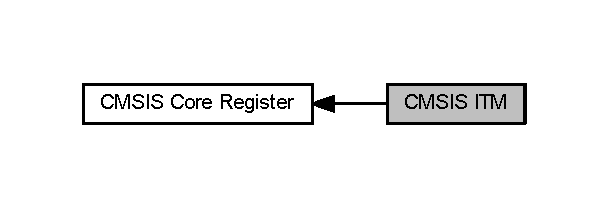
\includegraphics[width=292pt]{group___c_m_s_i_s___i_t_m}
\end{center}
\end{figure}
\subsection*{Data Structures}
\begin{DoxyCompactItemize}
\item 
struct \hyperlink{struct_i_t_m___type}{I\+T\+M\+\_\+\+Type}
\begin{DoxyCompactList}\small\item\em Structure type to access the Instrumentation Trace Macrocell Register (I\+TM). \end{DoxyCompactList}\end{DoxyCompactItemize}
\subsection*{Macros}
\begin{DoxyCompactItemize}
\item 
\#define \hyperlink{group___c_m_s_i_s___i_t_m_ga7abe5e590d1611599df87a1884a352e8}{I\+T\+M\+\_\+\+T\+P\+R\+\_\+\+P\+R\+I\+V\+M\+A\+S\+K\+\_\+\+Pos}~0
\item 
\#define \hyperlink{group___c_m_s_i_s___i_t_m_ga168e089d882df325a387aab3a802a46b}{I\+T\+M\+\_\+\+T\+P\+R\+\_\+\+P\+R\+I\+V\+M\+A\+S\+K\+\_\+\+Msk}~(0x\+F\+U\+L $<$$<$ I\+T\+M\+\_\+\+T\+P\+R\+\_\+\+P\+R\+I\+V\+M\+A\+S\+K\+\_\+\+Pos)
\item 
\#define \hyperlink{group___c_m_s_i_s___i_t_m_ga9174ad4a36052c377cef4e6aba2ed484}{I\+T\+M\+\_\+\+T\+C\+R\+\_\+\+B\+U\+S\+Y\+\_\+\+Pos}~23
\item 
\#define \hyperlink{group___c_m_s_i_s___i_t_m_ga43ad7cf33de12f2ef3a412d4f354c60f}{I\+T\+M\+\_\+\+T\+C\+R\+\_\+\+B\+U\+S\+Y\+\_\+\+Msk}~(1\+U\+L $<$$<$ I\+T\+M\+\_\+\+T\+C\+R\+\_\+\+B\+U\+S\+Y\+\_\+\+Pos)
\item 
\#define \hyperlink{group___c_m_s_i_s___i_t_m_gaca0281de867f33114aac0636f7ce65d3}{I\+T\+M\+\_\+\+T\+C\+R\+\_\+\+Trace\+Bus\+I\+D\+\_\+\+Pos}~16
\item 
\#define \hyperlink{group___c_m_s_i_s___i_t_m_ga60c20bd9649d1da5a2be8e656ba19a60}{I\+T\+M\+\_\+\+T\+C\+R\+\_\+\+Trace\+Bus\+I\+D\+\_\+\+Msk}~(0x7\+F\+U\+L $<$$<$ I\+T\+M\+\_\+\+T\+C\+R\+\_\+\+Trace\+Bus\+I\+D\+\_\+\+Pos)
\item 
\#define \hyperlink{group___c_m_s_i_s___i_t_m_ga96c7c7cbc0d98426c408090b41f583f1}{I\+T\+M\+\_\+\+T\+C\+R\+\_\+\+G\+T\+S\+F\+R\+E\+Q\+\_\+\+Pos}~10
\item 
\#define \hyperlink{group___c_m_s_i_s___i_t_m_gade862cf009827f7f6748fc44c541b067}{I\+T\+M\+\_\+\+T\+C\+R\+\_\+\+G\+T\+S\+F\+R\+E\+Q\+\_\+\+Msk}~(3\+U\+L $<$$<$ I\+T\+M\+\_\+\+T\+C\+R\+\_\+\+G\+T\+S\+F\+R\+E\+Q\+\_\+\+Pos)
\item 
\#define \hyperlink{group___c_m_s_i_s___i_t_m_gad7bc9ee1732032c6e0de035f0978e473}{I\+T\+M\+\_\+\+T\+C\+R\+\_\+\+T\+S\+Prescale\+\_\+\+Pos}~8
\item 
\#define \hyperlink{group___c_m_s_i_s___i_t_m_ga7a723f71bfb0204c264d8dbe8cc7ae52}{I\+T\+M\+\_\+\+T\+C\+R\+\_\+\+T\+S\+Prescale\+\_\+\+Msk}~(3\+U\+L $<$$<$ I\+T\+M\+\_\+\+T\+C\+R\+\_\+\+T\+S\+Prescale\+\_\+\+Pos)
\item 
\#define \hyperlink{group___c_m_s_i_s___i_t_m_ga7a380f0c8078f6560051406583ecd6a5}{I\+T\+M\+\_\+\+T\+C\+R\+\_\+\+S\+W\+O\+E\+N\+A\+\_\+\+Pos}~4
\item 
\#define \hyperlink{group___c_m_s_i_s___i_t_m_ga97476cb65bab16a328b35f81fd02010a}{I\+T\+M\+\_\+\+T\+C\+R\+\_\+\+S\+W\+O\+E\+N\+A\+\_\+\+Msk}~(1\+U\+L $<$$<$ I\+T\+M\+\_\+\+T\+C\+R\+\_\+\+S\+W\+O\+E\+N\+A\+\_\+\+Pos)
\item 
\#define \hyperlink{group___c_m_s_i_s___i_t_m_ga543636236b85604f4bba68e7ae42a122}{I\+T\+M\+\_\+\+T\+C\+R\+\_\+\+T\+X\+E\+N\+A\+\_\+\+Pos}~3
\item 
\#define \hyperlink{group___c_m_s_i_s___i_t_m_gac20ab2d72a9ecbec649d229e3800aa31}{I\+T\+M\+\_\+\+T\+C\+R\+\_\+\+T\+X\+E\+N\+A\+\_\+\+Msk}~(1\+U\+L $<$$<$ I\+T\+M\+\_\+\+T\+C\+R\+\_\+\+T\+X\+E\+N\+A\+\_\+\+Pos)
\item 
\#define \hyperlink{group___c_m_s_i_s___i_t_m_gaa93a1147a39fc63980d299231252a30e}{I\+T\+M\+\_\+\+T\+C\+R\+\_\+\+S\+Y\+N\+C\+E\+N\+A\+\_\+\+Pos}~2
\item 
\#define \hyperlink{group___c_m_s_i_s___i_t_m_gac89b74a78701c25b442105d7fe2bbefb}{I\+T\+M\+\_\+\+T\+C\+R\+\_\+\+S\+Y\+N\+C\+E\+N\+A\+\_\+\+Msk}~(1\+U\+L $<$$<$ I\+T\+M\+\_\+\+T\+C\+R\+\_\+\+S\+Y\+N\+C\+E\+N\+A\+\_\+\+Pos)
\item 
\#define \hyperlink{group___c_m_s_i_s___i_t_m_ga5aa381845f810114ab519b90753922a1}{I\+T\+M\+\_\+\+T\+C\+R\+\_\+\+T\+S\+E\+N\+A\+\_\+\+Pos}~1
\item 
\#define \hyperlink{group___c_m_s_i_s___i_t_m_ga436b2e8fa24328f48f2da31c00fc9e65}{I\+T\+M\+\_\+\+T\+C\+R\+\_\+\+T\+S\+E\+N\+A\+\_\+\+Msk}~(1\+U\+L $<$$<$ I\+T\+M\+\_\+\+T\+C\+R\+\_\+\+T\+S\+E\+N\+A\+\_\+\+Pos)
\item 
\#define \hyperlink{group___c_m_s_i_s___i_t_m_ga3286b86004bce7ffe17ee269f87f8d9d}{I\+T\+M\+\_\+\+T\+C\+R\+\_\+\+I\+T\+M\+E\+N\+A\+\_\+\+Pos}~0
\item 
\#define \hyperlink{group___c_m_s_i_s___i_t_m_ga7dd53e3bff24ac09d94e61cb595cb2d9}{I\+T\+M\+\_\+\+T\+C\+R\+\_\+\+I\+T\+M\+E\+N\+A\+\_\+\+Msk}~(1\+U\+L $<$$<$ I\+T\+M\+\_\+\+T\+C\+R\+\_\+\+I\+T\+M\+E\+N\+A\+\_\+\+Pos)
\end{DoxyCompactItemize}


\subsection{Detailed Description}
Type definitions for the Cortex-\/M Instrumentation Trace Macrocell (I\+TM) 

\subsection{Macro Definition Documentation}
\mbox{\Hypertarget{group___c_m_s_i_s___i_t_m_ga43ad7cf33de12f2ef3a412d4f354c60f}\label{group___c_m_s_i_s___i_t_m_ga43ad7cf33de12f2ef3a412d4f354c60f}} 
\index{C\+M\+S\+I\+S I\+TM@{C\+M\+S\+I\+S I\+TM}!I\+T\+M\+\_\+\+T\+C\+R\+\_\+\+B\+U\+S\+Y\+\_\+\+Msk@{I\+T\+M\+\_\+\+T\+C\+R\+\_\+\+B\+U\+S\+Y\+\_\+\+Msk}}
\index{I\+T\+M\+\_\+\+T\+C\+R\+\_\+\+B\+U\+S\+Y\+\_\+\+Msk@{I\+T\+M\+\_\+\+T\+C\+R\+\_\+\+B\+U\+S\+Y\+\_\+\+Msk}!C\+M\+S\+I\+S I\+TM@{C\+M\+S\+I\+S I\+TM}}
\subsubsection{\texorpdfstring{I\+T\+M\+\_\+\+T\+C\+R\+\_\+\+B\+U\+S\+Y\+\_\+\+Msk}{ITM\_TCR\_BUSY\_Msk}}
{\footnotesize\ttfamily \#define I\+T\+M\+\_\+\+T\+C\+R\+\_\+\+B\+U\+S\+Y\+\_\+\+Msk~(1\+U\+L $<$$<$ I\+T\+M\+\_\+\+T\+C\+R\+\_\+\+B\+U\+S\+Y\+\_\+\+Pos)}

I\+TM T\+CR\+: B\+U\+SY Mask 

Definition at line 662 of file core\+\_\+cm4.\+h.

\mbox{\Hypertarget{group___c_m_s_i_s___i_t_m_ga9174ad4a36052c377cef4e6aba2ed484}\label{group___c_m_s_i_s___i_t_m_ga9174ad4a36052c377cef4e6aba2ed484}} 
\index{C\+M\+S\+I\+S I\+TM@{C\+M\+S\+I\+S I\+TM}!I\+T\+M\+\_\+\+T\+C\+R\+\_\+\+B\+U\+S\+Y\+\_\+\+Pos@{I\+T\+M\+\_\+\+T\+C\+R\+\_\+\+B\+U\+S\+Y\+\_\+\+Pos}}
\index{I\+T\+M\+\_\+\+T\+C\+R\+\_\+\+B\+U\+S\+Y\+\_\+\+Pos@{I\+T\+M\+\_\+\+T\+C\+R\+\_\+\+B\+U\+S\+Y\+\_\+\+Pos}!C\+M\+S\+I\+S I\+TM@{C\+M\+S\+I\+S I\+TM}}
\subsubsection{\texorpdfstring{I\+T\+M\+\_\+\+T\+C\+R\+\_\+\+B\+U\+S\+Y\+\_\+\+Pos}{ITM\_TCR\_BUSY\_Pos}}
{\footnotesize\ttfamily \#define I\+T\+M\+\_\+\+T\+C\+R\+\_\+\+B\+U\+S\+Y\+\_\+\+Pos~23}

I\+TM T\+CR\+: B\+U\+SY Position 

Definition at line 661 of file core\+\_\+cm4.\+h.

\mbox{\Hypertarget{group___c_m_s_i_s___i_t_m_gade862cf009827f7f6748fc44c541b067}\label{group___c_m_s_i_s___i_t_m_gade862cf009827f7f6748fc44c541b067}} 
\index{C\+M\+S\+I\+S I\+TM@{C\+M\+S\+I\+S I\+TM}!I\+T\+M\+\_\+\+T\+C\+R\+\_\+\+G\+T\+S\+F\+R\+E\+Q\+\_\+\+Msk@{I\+T\+M\+\_\+\+T\+C\+R\+\_\+\+G\+T\+S\+F\+R\+E\+Q\+\_\+\+Msk}}
\index{I\+T\+M\+\_\+\+T\+C\+R\+\_\+\+G\+T\+S\+F\+R\+E\+Q\+\_\+\+Msk@{I\+T\+M\+\_\+\+T\+C\+R\+\_\+\+G\+T\+S\+F\+R\+E\+Q\+\_\+\+Msk}!C\+M\+S\+I\+S I\+TM@{C\+M\+S\+I\+S I\+TM}}
\subsubsection{\texorpdfstring{I\+T\+M\+\_\+\+T\+C\+R\+\_\+\+G\+T\+S\+F\+R\+E\+Q\+\_\+\+Msk}{ITM\_TCR\_GTSFREQ\_Msk}}
{\footnotesize\ttfamily \#define I\+T\+M\+\_\+\+T\+C\+R\+\_\+\+G\+T\+S\+F\+R\+E\+Q\+\_\+\+Msk~(3\+U\+L $<$$<$ I\+T\+M\+\_\+\+T\+C\+R\+\_\+\+G\+T\+S\+F\+R\+E\+Q\+\_\+\+Pos)}

I\+TM T\+CR\+: Global timestamp frequency Mask 

Definition at line 668 of file core\+\_\+cm4.\+h.

\mbox{\Hypertarget{group___c_m_s_i_s___i_t_m_ga96c7c7cbc0d98426c408090b41f583f1}\label{group___c_m_s_i_s___i_t_m_ga96c7c7cbc0d98426c408090b41f583f1}} 
\index{C\+M\+S\+I\+S I\+TM@{C\+M\+S\+I\+S I\+TM}!I\+T\+M\+\_\+\+T\+C\+R\+\_\+\+G\+T\+S\+F\+R\+E\+Q\+\_\+\+Pos@{I\+T\+M\+\_\+\+T\+C\+R\+\_\+\+G\+T\+S\+F\+R\+E\+Q\+\_\+\+Pos}}
\index{I\+T\+M\+\_\+\+T\+C\+R\+\_\+\+G\+T\+S\+F\+R\+E\+Q\+\_\+\+Pos@{I\+T\+M\+\_\+\+T\+C\+R\+\_\+\+G\+T\+S\+F\+R\+E\+Q\+\_\+\+Pos}!C\+M\+S\+I\+S I\+TM@{C\+M\+S\+I\+S I\+TM}}
\subsubsection{\texorpdfstring{I\+T\+M\+\_\+\+T\+C\+R\+\_\+\+G\+T\+S\+F\+R\+E\+Q\+\_\+\+Pos}{ITM\_TCR\_GTSFREQ\_Pos}}
{\footnotesize\ttfamily \#define I\+T\+M\+\_\+\+T\+C\+R\+\_\+\+G\+T\+S\+F\+R\+E\+Q\+\_\+\+Pos~10}

I\+TM T\+CR\+: Global timestamp frequency Position 

Definition at line 667 of file core\+\_\+cm4.\+h.

\mbox{\Hypertarget{group___c_m_s_i_s___i_t_m_ga7dd53e3bff24ac09d94e61cb595cb2d9}\label{group___c_m_s_i_s___i_t_m_ga7dd53e3bff24ac09d94e61cb595cb2d9}} 
\index{C\+M\+S\+I\+S I\+TM@{C\+M\+S\+I\+S I\+TM}!I\+T\+M\+\_\+\+T\+C\+R\+\_\+\+I\+T\+M\+E\+N\+A\+\_\+\+Msk@{I\+T\+M\+\_\+\+T\+C\+R\+\_\+\+I\+T\+M\+E\+N\+A\+\_\+\+Msk}}
\index{I\+T\+M\+\_\+\+T\+C\+R\+\_\+\+I\+T\+M\+E\+N\+A\+\_\+\+Msk@{I\+T\+M\+\_\+\+T\+C\+R\+\_\+\+I\+T\+M\+E\+N\+A\+\_\+\+Msk}!C\+M\+S\+I\+S I\+TM@{C\+M\+S\+I\+S I\+TM}}
\subsubsection{\texorpdfstring{I\+T\+M\+\_\+\+T\+C\+R\+\_\+\+I\+T\+M\+E\+N\+A\+\_\+\+Msk}{ITM\_TCR\_ITMENA\_Msk}}
{\footnotesize\ttfamily \#define I\+T\+M\+\_\+\+T\+C\+R\+\_\+\+I\+T\+M\+E\+N\+A\+\_\+\+Msk~(1\+U\+L $<$$<$ I\+T\+M\+\_\+\+T\+C\+R\+\_\+\+I\+T\+M\+E\+N\+A\+\_\+\+Pos)}

I\+TM T\+CR\+: I\+TM Enable bit Mask 

Definition at line 686 of file core\+\_\+cm4.\+h.

\mbox{\Hypertarget{group___c_m_s_i_s___i_t_m_ga3286b86004bce7ffe17ee269f87f8d9d}\label{group___c_m_s_i_s___i_t_m_ga3286b86004bce7ffe17ee269f87f8d9d}} 
\index{C\+M\+S\+I\+S I\+TM@{C\+M\+S\+I\+S I\+TM}!I\+T\+M\+\_\+\+T\+C\+R\+\_\+\+I\+T\+M\+E\+N\+A\+\_\+\+Pos@{I\+T\+M\+\_\+\+T\+C\+R\+\_\+\+I\+T\+M\+E\+N\+A\+\_\+\+Pos}}
\index{I\+T\+M\+\_\+\+T\+C\+R\+\_\+\+I\+T\+M\+E\+N\+A\+\_\+\+Pos@{I\+T\+M\+\_\+\+T\+C\+R\+\_\+\+I\+T\+M\+E\+N\+A\+\_\+\+Pos}!C\+M\+S\+I\+S I\+TM@{C\+M\+S\+I\+S I\+TM}}
\subsubsection{\texorpdfstring{I\+T\+M\+\_\+\+T\+C\+R\+\_\+\+I\+T\+M\+E\+N\+A\+\_\+\+Pos}{ITM\_TCR\_ITMENA\_Pos}}
{\footnotesize\ttfamily \#define I\+T\+M\+\_\+\+T\+C\+R\+\_\+\+I\+T\+M\+E\+N\+A\+\_\+\+Pos~0}

I\+TM T\+CR\+: I\+TM Enable bit Position 

Definition at line 685 of file core\+\_\+cm4.\+h.

\mbox{\Hypertarget{group___c_m_s_i_s___i_t_m_ga97476cb65bab16a328b35f81fd02010a}\label{group___c_m_s_i_s___i_t_m_ga97476cb65bab16a328b35f81fd02010a}} 
\index{C\+M\+S\+I\+S I\+TM@{C\+M\+S\+I\+S I\+TM}!I\+T\+M\+\_\+\+T\+C\+R\+\_\+\+S\+W\+O\+E\+N\+A\+\_\+\+Msk@{I\+T\+M\+\_\+\+T\+C\+R\+\_\+\+S\+W\+O\+E\+N\+A\+\_\+\+Msk}}
\index{I\+T\+M\+\_\+\+T\+C\+R\+\_\+\+S\+W\+O\+E\+N\+A\+\_\+\+Msk@{I\+T\+M\+\_\+\+T\+C\+R\+\_\+\+S\+W\+O\+E\+N\+A\+\_\+\+Msk}!C\+M\+S\+I\+S I\+TM@{C\+M\+S\+I\+S I\+TM}}
\subsubsection{\texorpdfstring{I\+T\+M\+\_\+\+T\+C\+R\+\_\+\+S\+W\+O\+E\+N\+A\+\_\+\+Msk}{ITM\_TCR\_SWOENA\_Msk}}
{\footnotesize\ttfamily \#define I\+T\+M\+\_\+\+T\+C\+R\+\_\+\+S\+W\+O\+E\+N\+A\+\_\+\+Msk~(1\+U\+L $<$$<$ I\+T\+M\+\_\+\+T\+C\+R\+\_\+\+S\+W\+O\+E\+N\+A\+\_\+\+Pos)}

I\+TM T\+CR\+: S\+W\+O\+E\+NA Mask 

Definition at line 674 of file core\+\_\+cm4.\+h.

\mbox{\Hypertarget{group___c_m_s_i_s___i_t_m_ga7a380f0c8078f6560051406583ecd6a5}\label{group___c_m_s_i_s___i_t_m_ga7a380f0c8078f6560051406583ecd6a5}} 
\index{C\+M\+S\+I\+S I\+TM@{C\+M\+S\+I\+S I\+TM}!I\+T\+M\+\_\+\+T\+C\+R\+\_\+\+S\+W\+O\+E\+N\+A\+\_\+\+Pos@{I\+T\+M\+\_\+\+T\+C\+R\+\_\+\+S\+W\+O\+E\+N\+A\+\_\+\+Pos}}
\index{I\+T\+M\+\_\+\+T\+C\+R\+\_\+\+S\+W\+O\+E\+N\+A\+\_\+\+Pos@{I\+T\+M\+\_\+\+T\+C\+R\+\_\+\+S\+W\+O\+E\+N\+A\+\_\+\+Pos}!C\+M\+S\+I\+S I\+TM@{C\+M\+S\+I\+S I\+TM}}
\subsubsection{\texorpdfstring{I\+T\+M\+\_\+\+T\+C\+R\+\_\+\+S\+W\+O\+E\+N\+A\+\_\+\+Pos}{ITM\_TCR\_SWOENA\_Pos}}
{\footnotesize\ttfamily \#define I\+T\+M\+\_\+\+T\+C\+R\+\_\+\+S\+W\+O\+E\+N\+A\+\_\+\+Pos~4}

I\+TM T\+CR\+: S\+W\+O\+E\+NA Position 

Definition at line 673 of file core\+\_\+cm4.\+h.

\mbox{\Hypertarget{group___c_m_s_i_s___i_t_m_gac89b74a78701c25b442105d7fe2bbefb}\label{group___c_m_s_i_s___i_t_m_gac89b74a78701c25b442105d7fe2bbefb}} 
\index{C\+M\+S\+I\+S I\+TM@{C\+M\+S\+I\+S I\+TM}!I\+T\+M\+\_\+\+T\+C\+R\+\_\+\+S\+Y\+N\+C\+E\+N\+A\+\_\+\+Msk@{I\+T\+M\+\_\+\+T\+C\+R\+\_\+\+S\+Y\+N\+C\+E\+N\+A\+\_\+\+Msk}}
\index{I\+T\+M\+\_\+\+T\+C\+R\+\_\+\+S\+Y\+N\+C\+E\+N\+A\+\_\+\+Msk@{I\+T\+M\+\_\+\+T\+C\+R\+\_\+\+S\+Y\+N\+C\+E\+N\+A\+\_\+\+Msk}!C\+M\+S\+I\+S I\+TM@{C\+M\+S\+I\+S I\+TM}}
\subsubsection{\texorpdfstring{I\+T\+M\+\_\+\+T\+C\+R\+\_\+\+S\+Y\+N\+C\+E\+N\+A\+\_\+\+Msk}{ITM\_TCR\_SYNCENA\_Msk}}
{\footnotesize\ttfamily \#define I\+T\+M\+\_\+\+T\+C\+R\+\_\+\+S\+Y\+N\+C\+E\+N\+A\+\_\+\+Msk~(1\+U\+L $<$$<$ I\+T\+M\+\_\+\+T\+C\+R\+\_\+\+S\+Y\+N\+C\+E\+N\+A\+\_\+\+Pos)}

I\+TM T\+CR\+: S\+Y\+N\+C\+E\+NA Mask 

Definition at line 680 of file core\+\_\+cm4.\+h.

\mbox{\Hypertarget{group___c_m_s_i_s___i_t_m_gaa93a1147a39fc63980d299231252a30e}\label{group___c_m_s_i_s___i_t_m_gaa93a1147a39fc63980d299231252a30e}} 
\index{C\+M\+S\+I\+S I\+TM@{C\+M\+S\+I\+S I\+TM}!I\+T\+M\+\_\+\+T\+C\+R\+\_\+\+S\+Y\+N\+C\+E\+N\+A\+\_\+\+Pos@{I\+T\+M\+\_\+\+T\+C\+R\+\_\+\+S\+Y\+N\+C\+E\+N\+A\+\_\+\+Pos}}
\index{I\+T\+M\+\_\+\+T\+C\+R\+\_\+\+S\+Y\+N\+C\+E\+N\+A\+\_\+\+Pos@{I\+T\+M\+\_\+\+T\+C\+R\+\_\+\+S\+Y\+N\+C\+E\+N\+A\+\_\+\+Pos}!C\+M\+S\+I\+S I\+TM@{C\+M\+S\+I\+S I\+TM}}
\subsubsection{\texorpdfstring{I\+T\+M\+\_\+\+T\+C\+R\+\_\+\+S\+Y\+N\+C\+E\+N\+A\+\_\+\+Pos}{ITM\_TCR\_SYNCENA\_Pos}}
{\footnotesize\ttfamily \#define I\+T\+M\+\_\+\+T\+C\+R\+\_\+\+S\+Y\+N\+C\+E\+N\+A\+\_\+\+Pos~2}

I\+TM T\+CR\+: S\+Y\+N\+C\+E\+NA Position 

Definition at line 679 of file core\+\_\+cm4.\+h.

\mbox{\Hypertarget{group___c_m_s_i_s___i_t_m_ga60c20bd9649d1da5a2be8e656ba19a60}\label{group___c_m_s_i_s___i_t_m_ga60c20bd9649d1da5a2be8e656ba19a60}} 
\index{C\+M\+S\+I\+S I\+TM@{C\+M\+S\+I\+S I\+TM}!I\+T\+M\+\_\+\+T\+C\+R\+\_\+\+Trace\+Bus\+I\+D\+\_\+\+Msk@{I\+T\+M\+\_\+\+T\+C\+R\+\_\+\+Trace\+Bus\+I\+D\+\_\+\+Msk}}
\index{I\+T\+M\+\_\+\+T\+C\+R\+\_\+\+Trace\+Bus\+I\+D\+\_\+\+Msk@{I\+T\+M\+\_\+\+T\+C\+R\+\_\+\+Trace\+Bus\+I\+D\+\_\+\+Msk}!C\+M\+S\+I\+S I\+TM@{C\+M\+S\+I\+S I\+TM}}
\subsubsection{\texorpdfstring{I\+T\+M\+\_\+\+T\+C\+R\+\_\+\+Trace\+Bus\+I\+D\+\_\+\+Msk}{ITM\_TCR\_TraceBusID\_Msk}}
{\footnotesize\ttfamily \#define I\+T\+M\+\_\+\+T\+C\+R\+\_\+\+Trace\+Bus\+I\+D\+\_\+\+Msk~(0x7\+F\+U\+L $<$$<$ I\+T\+M\+\_\+\+T\+C\+R\+\_\+\+Trace\+Bus\+I\+D\+\_\+\+Pos)}

I\+TM T\+CR\+: A\+T\+B\+ID Mask 

Definition at line 665 of file core\+\_\+cm4.\+h.

\mbox{\Hypertarget{group___c_m_s_i_s___i_t_m_gaca0281de867f33114aac0636f7ce65d3}\label{group___c_m_s_i_s___i_t_m_gaca0281de867f33114aac0636f7ce65d3}} 
\index{C\+M\+S\+I\+S I\+TM@{C\+M\+S\+I\+S I\+TM}!I\+T\+M\+\_\+\+T\+C\+R\+\_\+\+Trace\+Bus\+I\+D\+\_\+\+Pos@{I\+T\+M\+\_\+\+T\+C\+R\+\_\+\+Trace\+Bus\+I\+D\+\_\+\+Pos}}
\index{I\+T\+M\+\_\+\+T\+C\+R\+\_\+\+Trace\+Bus\+I\+D\+\_\+\+Pos@{I\+T\+M\+\_\+\+T\+C\+R\+\_\+\+Trace\+Bus\+I\+D\+\_\+\+Pos}!C\+M\+S\+I\+S I\+TM@{C\+M\+S\+I\+S I\+TM}}
\subsubsection{\texorpdfstring{I\+T\+M\+\_\+\+T\+C\+R\+\_\+\+Trace\+Bus\+I\+D\+\_\+\+Pos}{ITM\_TCR\_TraceBusID\_Pos}}
{\footnotesize\ttfamily \#define I\+T\+M\+\_\+\+T\+C\+R\+\_\+\+Trace\+Bus\+I\+D\+\_\+\+Pos~16}

I\+TM T\+CR\+: A\+T\+B\+ID Position 

Definition at line 664 of file core\+\_\+cm4.\+h.

\mbox{\Hypertarget{group___c_m_s_i_s___i_t_m_ga436b2e8fa24328f48f2da31c00fc9e65}\label{group___c_m_s_i_s___i_t_m_ga436b2e8fa24328f48f2da31c00fc9e65}} 
\index{C\+M\+S\+I\+S I\+TM@{C\+M\+S\+I\+S I\+TM}!I\+T\+M\+\_\+\+T\+C\+R\+\_\+\+T\+S\+E\+N\+A\+\_\+\+Msk@{I\+T\+M\+\_\+\+T\+C\+R\+\_\+\+T\+S\+E\+N\+A\+\_\+\+Msk}}
\index{I\+T\+M\+\_\+\+T\+C\+R\+\_\+\+T\+S\+E\+N\+A\+\_\+\+Msk@{I\+T\+M\+\_\+\+T\+C\+R\+\_\+\+T\+S\+E\+N\+A\+\_\+\+Msk}!C\+M\+S\+I\+S I\+TM@{C\+M\+S\+I\+S I\+TM}}
\subsubsection{\texorpdfstring{I\+T\+M\+\_\+\+T\+C\+R\+\_\+\+T\+S\+E\+N\+A\+\_\+\+Msk}{ITM\_TCR\_TSENA\_Msk}}
{\footnotesize\ttfamily \#define I\+T\+M\+\_\+\+T\+C\+R\+\_\+\+T\+S\+E\+N\+A\+\_\+\+Msk~(1\+U\+L $<$$<$ I\+T\+M\+\_\+\+T\+C\+R\+\_\+\+T\+S\+E\+N\+A\+\_\+\+Pos)}

I\+TM T\+CR\+: T\+S\+E\+NA Mask 

Definition at line 683 of file core\+\_\+cm4.\+h.

\mbox{\Hypertarget{group___c_m_s_i_s___i_t_m_ga5aa381845f810114ab519b90753922a1}\label{group___c_m_s_i_s___i_t_m_ga5aa381845f810114ab519b90753922a1}} 
\index{C\+M\+S\+I\+S I\+TM@{C\+M\+S\+I\+S I\+TM}!I\+T\+M\+\_\+\+T\+C\+R\+\_\+\+T\+S\+E\+N\+A\+\_\+\+Pos@{I\+T\+M\+\_\+\+T\+C\+R\+\_\+\+T\+S\+E\+N\+A\+\_\+\+Pos}}
\index{I\+T\+M\+\_\+\+T\+C\+R\+\_\+\+T\+S\+E\+N\+A\+\_\+\+Pos@{I\+T\+M\+\_\+\+T\+C\+R\+\_\+\+T\+S\+E\+N\+A\+\_\+\+Pos}!C\+M\+S\+I\+S I\+TM@{C\+M\+S\+I\+S I\+TM}}
\subsubsection{\texorpdfstring{I\+T\+M\+\_\+\+T\+C\+R\+\_\+\+T\+S\+E\+N\+A\+\_\+\+Pos}{ITM\_TCR\_TSENA\_Pos}}
{\footnotesize\ttfamily \#define I\+T\+M\+\_\+\+T\+C\+R\+\_\+\+T\+S\+E\+N\+A\+\_\+\+Pos~1}

I\+TM T\+CR\+: T\+S\+E\+NA Position 

Definition at line 682 of file core\+\_\+cm4.\+h.

\mbox{\Hypertarget{group___c_m_s_i_s___i_t_m_ga7a723f71bfb0204c264d8dbe8cc7ae52}\label{group___c_m_s_i_s___i_t_m_ga7a723f71bfb0204c264d8dbe8cc7ae52}} 
\index{C\+M\+S\+I\+S I\+TM@{C\+M\+S\+I\+S I\+TM}!I\+T\+M\+\_\+\+T\+C\+R\+\_\+\+T\+S\+Prescale\+\_\+\+Msk@{I\+T\+M\+\_\+\+T\+C\+R\+\_\+\+T\+S\+Prescale\+\_\+\+Msk}}
\index{I\+T\+M\+\_\+\+T\+C\+R\+\_\+\+T\+S\+Prescale\+\_\+\+Msk@{I\+T\+M\+\_\+\+T\+C\+R\+\_\+\+T\+S\+Prescale\+\_\+\+Msk}!C\+M\+S\+I\+S I\+TM@{C\+M\+S\+I\+S I\+TM}}
\subsubsection{\texorpdfstring{I\+T\+M\+\_\+\+T\+C\+R\+\_\+\+T\+S\+Prescale\+\_\+\+Msk}{ITM\_TCR\_TSPrescale\_Msk}}
{\footnotesize\ttfamily \#define I\+T\+M\+\_\+\+T\+C\+R\+\_\+\+T\+S\+Prescale\+\_\+\+Msk~(3\+U\+L $<$$<$ I\+T\+M\+\_\+\+T\+C\+R\+\_\+\+T\+S\+Prescale\+\_\+\+Pos)}

I\+TM T\+CR\+: T\+S\+Prescale Mask 

Definition at line 671 of file core\+\_\+cm4.\+h.

\mbox{\Hypertarget{group___c_m_s_i_s___i_t_m_gad7bc9ee1732032c6e0de035f0978e473}\label{group___c_m_s_i_s___i_t_m_gad7bc9ee1732032c6e0de035f0978e473}} 
\index{C\+M\+S\+I\+S I\+TM@{C\+M\+S\+I\+S I\+TM}!I\+T\+M\+\_\+\+T\+C\+R\+\_\+\+T\+S\+Prescale\+\_\+\+Pos@{I\+T\+M\+\_\+\+T\+C\+R\+\_\+\+T\+S\+Prescale\+\_\+\+Pos}}
\index{I\+T\+M\+\_\+\+T\+C\+R\+\_\+\+T\+S\+Prescale\+\_\+\+Pos@{I\+T\+M\+\_\+\+T\+C\+R\+\_\+\+T\+S\+Prescale\+\_\+\+Pos}!C\+M\+S\+I\+S I\+TM@{C\+M\+S\+I\+S I\+TM}}
\subsubsection{\texorpdfstring{I\+T\+M\+\_\+\+T\+C\+R\+\_\+\+T\+S\+Prescale\+\_\+\+Pos}{ITM\_TCR\_TSPrescale\_Pos}}
{\footnotesize\ttfamily \#define I\+T\+M\+\_\+\+T\+C\+R\+\_\+\+T\+S\+Prescale\+\_\+\+Pos~8}

I\+TM T\+CR\+: T\+S\+Prescale Position 

Definition at line 670 of file core\+\_\+cm4.\+h.

\mbox{\Hypertarget{group___c_m_s_i_s___i_t_m_gac20ab2d72a9ecbec649d229e3800aa31}\label{group___c_m_s_i_s___i_t_m_gac20ab2d72a9ecbec649d229e3800aa31}} 
\index{C\+M\+S\+I\+S I\+TM@{C\+M\+S\+I\+S I\+TM}!I\+T\+M\+\_\+\+T\+C\+R\+\_\+\+T\+X\+E\+N\+A\+\_\+\+Msk@{I\+T\+M\+\_\+\+T\+C\+R\+\_\+\+T\+X\+E\+N\+A\+\_\+\+Msk}}
\index{I\+T\+M\+\_\+\+T\+C\+R\+\_\+\+T\+X\+E\+N\+A\+\_\+\+Msk@{I\+T\+M\+\_\+\+T\+C\+R\+\_\+\+T\+X\+E\+N\+A\+\_\+\+Msk}!C\+M\+S\+I\+S I\+TM@{C\+M\+S\+I\+S I\+TM}}
\subsubsection{\texorpdfstring{I\+T\+M\+\_\+\+T\+C\+R\+\_\+\+T\+X\+E\+N\+A\+\_\+\+Msk}{ITM\_TCR\_TXENA\_Msk}}
{\footnotesize\ttfamily \#define I\+T\+M\+\_\+\+T\+C\+R\+\_\+\+T\+X\+E\+N\+A\+\_\+\+Msk~(1\+U\+L $<$$<$ I\+T\+M\+\_\+\+T\+C\+R\+\_\+\+T\+X\+E\+N\+A\+\_\+\+Pos)}

I\+TM T\+CR\+: T\+X\+E\+NA Mask 

Definition at line 677 of file core\+\_\+cm4.\+h.

\mbox{\Hypertarget{group___c_m_s_i_s___i_t_m_ga543636236b85604f4bba68e7ae42a122}\label{group___c_m_s_i_s___i_t_m_ga543636236b85604f4bba68e7ae42a122}} 
\index{C\+M\+S\+I\+S I\+TM@{C\+M\+S\+I\+S I\+TM}!I\+T\+M\+\_\+\+T\+C\+R\+\_\+\+T\+X\+E\+N\+A\+\_\+\+Pos@{I\+T\+M\+\_\+\+T\+C\+R\+\_\+\+T\+X\+E\+N\+A\+\_\+\+Pos}}
\index{I\+T\+M\+\_\+\+T\+C\+R\+\_\+\+T\+X\+E\+N\+A\+\_\+\+Pos@{I\+T\+M\+\_\+\+T\+C\+R\+\_\+\+T\+X\+E\+N\+A\+\_\+\+Pos}!C\+M\+S\+I\+S I\+TM@{C\+M\+S\+I\+S I\+TM}}
\subsubsection{\texorpdfstring{I\+T\+M\+\_\+\+T\+C\+R\+\_\+\+T\+X\+E\+N\+A\+\_\+\+Pos}{ITM\_TCR\_TXENA\_Pos}}
{\footnotesize\ttfamily \#define I\+T\+M\+\_\+\+T\+C\+R\+\_\+\+T\+X\+E\+N\+A\+\_\+\+Pos~3}

I\+TM T\+CR\+: T\+X\+E\+NA Position 

Definition at line 676 of file core\+\_\+cm4.\+h.

\mbox{\Hypertarget{group___c_m_s_i_s___i_t_m_ga168e089d882df325a387aab3a802a46b}\label{group___c_m_s_i_s___i_t_m_ga168e089d882df325a387aab3a802a46b}} 
\index{C\+M\+S\+I\+S I\+TM@{C\+M\+S\+I\+S I\+TM}!I\+T\+M\+\_\+\+T\+P\+R\+\_\+\+P\+R\+I\+V\+M\+A\+S\+K\+\_\+\+Msk@{I\+T\+M\+\_\+\+T\+P\+R\+\_\+\+P\+R\+I\+V\+M\+A\+S\+K\+\_\+\+Msk}}
\index{I\+T\+M\+\_\+\+T\+P\+R\+\_\+\+P\+R\+I\+V\+M\+A\+S\+K\+\_\+\+Msk@{I\+T\+M\+\_\+\+T\+P\+R\+\_\+\+P\+R\+I\+V\+M\+A\+S\+K\+\_\+\+Msk}!C\+M\+S\+I\+S I\+TM@{C\+M\+S\+I\+S I\+TM}}
\subsubsection{\texorpdfstring{I\+T\+M\+\_\+\+T\+P\+R\+\_\+\+P\+R\+I\+V\+M\+A\+S\+K\+\_\+\+Msk}{ITM\_TPR\_PRIVMASK\_Msk}}
{\footnotesize\ttfamily \#define I\+T\+M\+\_\+\+T\+P\+R\+\_\+\+P\+R\+I\+V\+M\+A\+S\+K\+\_\+\+Msk~(0x\+F\+U\+L $<$$<$ I\+T\+M\+\_\+\+T\+P\+R\+\_\+\+P\+R\+I\+V\+M\+A\+S\+K\+\_\+\+Pos)}

I\+TM T\+PR\+: P\+R\+I\+V\+M\+A\+SK Mask 

Definition at line 658 of file core\+\_\+cm4.\+h.

\mbox{\Hypertarget{group___c_m_s_i_s___i_t_m_ga7abe5e590d1611599df87a1884a352e8}\label{group___c_m_s_i_s___i_t_m_ga7abe5e590d1611599df87a1884a352e8}} 
\index{C\+M\+S\+I\+S I\+TM@{C\+M\+S\+I\+S I\+TM}!I\+T\+M\+\_\+\+T\+P\+R\+\_\+\+P\+R\+I\+V\+M\+A\+S\+K\+\_\+\+Pos@{I\+T\+M\+\_\+\+T\+P\+R\+\_\+\+P\+R\+I\+V\+M\+A\+S\+K\+\_\+\+Pos}}
\index{I\+T\+M\+\_\+\+T\+P\+R\+\_\+\+P\+R\+I\+V\+M\+A\+S\+K\+\_\+\+Pos@{I\+T\+M\+\_\+\+T\+P\+R\+\_\+\+P\+R\+I\+V\+M\+A\+S\+K\+\_\+\+Pos}!C\+M\+S\+I\+S I\+TM@{C\+M\+S\+I\+S I\+TM}}
\subsubsection{\texorpdfstring{I\+T\+M\+\_\+\+T\+P\+R\+\_\+\+P\+R\+I\+V\+M\+A\+S\+K\+\_\+\+Pos}{ITM\_TPR\_PRIVMASK\_Pos}}
{\footnotesize\ttfamily \#define I\+T\+M\+\_\+\+T\+P\+R\+\_\+\+P\+R\+I\+V\+M\+A\+S\+K\+\_\+\+Pos~0}

I\+TM T\+PR\+: P\+R\+I\+V\+M\+A\+SK Position 

Definition at line 657 of file core\+\_\+cm4.\+h.


\hypertarget{group___c_m_s_i_s___core_debug}{}\section{C\+M\+S\+IS Core Debug}
\label{group___c_m_s_i_s___core_debug}\index{C\+M\+S\+I\+S Core Debug@{C\+M\+S\+I\+S Core Debug}}
Collaboration diagram for C\+M\+S\+IS Core Debug\+:
\nopagebreak
\begin{figure}[H]
\begin{center}
\leavevmode
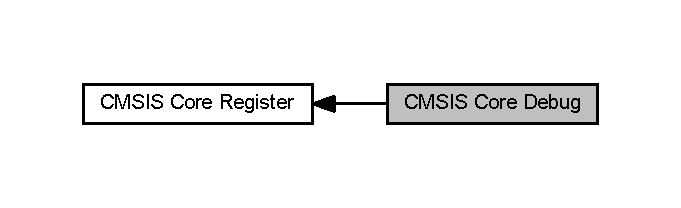
\includegraphics[width=327pt]{group___c_m_s_i_s___core_debug}
\end{center}
\end{figure}
\subsection*{Data Structures}
\begin{DoxyCompactItemize}
\item 
struct \hyperlink{struct_core_debug___type}{Core\+Debug\+\_\+\+Type}
\begin{DoxyCompactList}\small\item\em Structure type to access the Core Debug Register (Core\+Debug). \end{DoxyCompactList}\end{DoxyCompactItemize}
\subsection*{Macros}
\begin{DoxyCompactItemize}
\item 
\#define \hyperlink{group___c_m_s_i_s___core_debug_gac91280edd0ce932665cf75a23d11d842}{Core\+Debug\+\_\+\+D\+H\+C\+S\+R\+\_\+\+D\+B\+G\+K\+E\+Y\+\_\+\+Pos}~16
\item 
\#define \hyperlink{group___c_m_s_i_s___core_debug_ga1ce997cee15edaafe4aed77751816ffc}{Core\+Debug\+\_\+\+D\+H\+C\+S\+R\+\_\+\+D\+B\+G\+K\+E\+Y\+\_\+\+Msk}~(0x\+F\+F\+F\+F\+U\+L $<$$<$ Core\+Debug\+\_\+\+D\+H\+C\+S\+R\+\_\+\+D\+B\+G\+K\+E\+Y\+\_\+\+Pos)
\item 
\#define \hyperlink{group___c_m_s_i_s___core_debug_ga6f934c5427ea057394268e541fa97753}{Core\+Debug\+\_\+\+D\+H\+C\+S\+R\+\_\+\+S\+\_\+\+R\+E\+S\+E\+T\+\_\+\+S\+T\+\_\+\+Pos}~25
\item 
\#define \hyperlink{group___c_m_s_i_s___core_debug_gac474394bcceb31a8e09566c90b3f8922}{Core\+Debug\+\_\+\+D\+H\+C\+S\+R\+\_\+\+S\+\_\+\+R\+E\+S\+E\+T\+\_\+\+S\+T\+\_\+\+Msk}~(1\+U\+L $<$$<$ Core\+Debug\+\_\+\+D\+H\+C\+S\+R\+\_\+\+S\+\_\+\+R\+E\+S\+E\+T\+\_\+\+S\+T\+\_\+\+Pos)
\item 
\#define \hyperlink{group___c_m_s_i_s___core_debug_ga2328118f8b3574c871a53605eb17e730}{Core\+Debug\+\_\+\+D\+H\+C\+S\+R\+\_\+\+S\+\_\+\+R\+E\+T\+I\+R\+E\+\_\+\+S\+T\+\_\+\+Pos}~24
\item 
\#define \hyperlink{group___c_m_s_i_s___core_debug_ga89dceb5325f6bcb36a0473d65fbfcfa6}{Core\+Debug\+\_\+\+D\+H\+C\+S\+R\+\_\+\+S\+\_\+\+R\+E\+T\+I\+R\+E\+\_\+\+S\+T\+\_\+\+Msk}~(1\+U\+L $<$$<$ Core\+Debug\+\_\+\+D\+H\+C\+S\+R\+\_\+\+S\+\_\+\+R\+E\+T\+I\+R\+E\+\_\+\+S\+T\+\_\+\+Pos)
\item 
\#define \hyperlink{group___c_m_s_i_s___core_debug_ga2900dd56a988a4ed27ad664d5642807e}{Core\+Debug\+\_\+\+D\+H\+C\+S\+R\+\_\+\+S\+\_\+\+L\+O\+C\+K\+U\+P\+\_\+\+Pos}~19
\item 
\#define \hyperlink{group___c_m_s_i_s___core_debug_ga7b67e4506d7f464ef5dafd6219739756}{Core\+Debug\+\_\+\+D\+H\+C\+S\+R\+\_\+\+S\+\_\+\+L\+O\+C\+K\+U\+P\+\_\+\+Msk}~(1\+U\+L $<$$<$ Core\+Debug\+\_\+\+D\+H\+C\+S\+R\+\_\+\+S\+\_\+\+L\+O\+C\+K\+U\+P\+\_\+\+Pos)
\item 
\#define \hyperlink{group___c_m_s_i_s___core_debug_ga349ccea33accc705595624c2d334fbcb}{Core\+Debug\+\_\+\+D\+H\+C\+S\+R\+\_\+\+S\+\_\+\+S\+L\+E\+E\+P\+\_\+\+Pos}~18
\item 
\#define \hyperlink{group___c_m_s_i_s___core_debug_ga98d51538e645c2c1a422279cd85a0a25}{Core\+Debug\+\_\+\+D\+H\+C\+S\+R\+\_\+\+S\+\_\+\+S\+L\+E\+E\+P\+\_\+\+Msk}~(1\+U\+L $<$$<$ Core\+Debug\+\_\+\+D\+H\+C\+S\+R\+\_\+\+S\+\_\+\+S\+L\+E\+E\+P\+\_\+\+Pos)
\item 
\#define \hyperlink{group___c_m_s_i_s___core_debug_ga760a9a0d7f39951dc3f07d01f1f64772}{Core\+Debug\+\_\+\+D\+H\+C\+S\+R\+\_\+\+S\+\_\+\+H\+A\+L\+T\+\_\+\+Pos}~17
\item 
\#define \hyperlink{group___c_m_s_i_s___core_debug_ga9f881ade3151a73bc5b02b73fe6473ca}{Core\+Debug\+\_\+\+D\+H\+C\+S\+R\+\_\+\+S\+\_\+\+H\+A\+L\+T\+\_\+\+Msk}~(1\+U\+L $<$$<$ Core\+Debug\+\_\+\+D\+H\+C\+S\+R\+\_\+\+S\+\_\+\+H\+A\+L\+T\+\_\+\+Pos)
\item 
\#define \hyperlink{group___c_m_s_i_s___core_debug_ga20a71871ca8768019c51168c70c3f41d}{Core\+Debug\+\_\+\+D\+H\+C\+S\+R\+\_\+\+S\+\_\+\+R\+E\+G\+R\+D\+Y\+\_\+\+Pos}~16
\item 
\#define \hyperlink{group___c_m_s_i_s___core_debug_gac4cd6f3178de48f473d8903e8c847c07}{Core\+Debug\+\_\+\+D\+H\+C\+S\+R\+\_\+\+S\+\_\+\+R\+E\+G\+R\+D\+Y\+\_\+\+Msk}~(1\+U\+L $<$$<$ Core\+Debug\+\_\+\+D\+H\+C\+S\+R\+\_\+\+S\+\_\+\+R\+E\+G\+R\+D\+Y\+\_\+\+Pos)
\item 
\#define \hyperlink{group___c_m_s_i_s___core_debug_ga85747214e2656df6b05ec72e4d22bd6d}{Core\+Debug\+\_\+\+D\+H\+C\+S\+R\+\_\+\+C\+\_\+\+S\+N\+A\+P\+S\+T\+A\+L\+L\+\_\+\+Pos}~5
\item 
\#define \hyperlink{group___c_m_s_i_s___core_debug_ga53aa99b2e39a67622f3b9973e079c2b4}{Core\+Debug\+\_\+\+D\+H\+C\+S\+R\+\_\+\+C\+\_\+\+S\+N\+A\+P\+S\+T\+A\+L\+L\+\_\+\+Msk}~(1\+U\+L $<$$<$ Core\+Debug\+\_\+\+D\+H\+C\+S\+R\+\_\+\+C\+\_\+\+S\+N\+A\+P\+S\+T\+A\+L\+L\+\_\+\+Pos)
\item 
\#define \hyperlink{group___c_m_s_i_s___core_debug_ga0d2907400eb948a4ea3886ca083ec8e3}{Core\+Debug\+\_\+\+D\+H\+C\+S\+R\+\_\+\+C\+\_\+\+M\+A\+S\+K\+I\+N\+T\+S\+\_\+\+Pos}~3
\item 
\#define \hyperlink{group___c_m_s_i_s___core_debug_ga77fe1ef3c4a729c1c82fb62a94a51c31}{Core\+Debug\+\_\+\+D\+H\+C\+S\+R\+\_\+\+C\+\_\+\+M\+A\+S\+K\+I\+N\+T\+S\+\_\+\+Msk}~(1\+U\+L $<$$<$ Core\+Debug\+\_\+\+D\+H\+C\+S\+R\+\_\+\+C\+\_\+\+M\+A\+S\+K\+I\+N\+T\+S\+\_\+\+Pos)
\item 
\#define \hyperlink{group___c_m_s_i_s___core_debug_gae1fc39e80de54c0339cbb1b298a9f0f9}{Core\+Debug\+\_\+\+D\+H\+C\+S\+R\+\_\+\+C\+\_\+\+S\+T\+E\+P\+\_\+\+Pos}~2
\item 
\#define \hyperlink{group___c_m_s_i_s___core_debug_gae6bda72fbd32cc5734ff3542170dc00d}{Core\+Debug\+\_\+\+D\+H\+C\+S\+R\+\_\+\+C\+\_\+\+S\+T\+E\+P\+\_\+\+Msk}~(1\+U\+L $<$$<$ Core\+Debug\+\_\+\+D\+H\+C\+S\+R\+\_\+\+C\+\_\+\+S\+T\+E\+P\+\_\+\+Pos)
\item 
\#define \hyperlink{group___c_m_s_i_s___core_debug_gaddf1d43f8857e4efc3dc4e6b15509692}{Core\+Debug\+\_\+\+D\+H\+C\+S\+R\+\_\+\+C\+\_\+\+H\+A\+L\+T\+\_\+\+Pos}~1
\item 
\#define \hyperlink{group___c_m_s_i_s___core_debug_ga1d905a3aa594eb2e8bb78bcc4da05b3f}{Core\+Debug\+\_\+\+D\+H\+C\+S\+R\+\_\+\+C\+\_\+\+H\+A\+L\+T\+\_\+\+Msk}~(1\+U\+L $<$$<$ Core\+Debug\+\_\+\+D\+H\+C\+S\+R\+\_\+\+C\+\_\+\+H\+A\+L\+T\+\_\+\+Pos)
\item 
\#define \hyperlink{group___c_m_s_i_s___core_debug_gab557abb5b172b74d2cf44efb9d824e4e}{Core\+Debug\+\_\+\+D\+H\+C\+S\+R\+\_\+\+C\+\_\+\+D\+E\+B\+U\+G\+E\+N\+\_\+\+Pos}~0
\item 
\#define \hyperlink{group___c_m_s_i_s___core_debug_gab815c741a4fc2a61988cd2fb7594210b}{Core\+Debug\+\_\+\+D\+H\+C\+S\+R\+\_\+\+C\+\_\+\+D\+E\+B\+U\+G\+E\+N\+\_\+\+Msk}~(1\+U\+L $<$$<$ Core\+Debug\+\_\+\+D\+H\+C\+S\+R\+\_\+\+C\+\_\+\+D\+E\+B\+U\+G\+E\+N\+\_\+\+Pos)
\item 
\#define \hyperlink{group___c_m_s_i_s___core_debug_ga51e75942fc0614bc9bb2c0e96fcdda9a}{Core\+Debug\+\_\+\+D\+C\+R\+S\+R\+\_\+\+R\+E\+G\+Wn\+R\+\_\+\+Pos}~16
\item 
\#define \hyperlink{group___c_m_s_i_s___core_debug_ga1eef4992d8f84bc6c0dffed1c87f90a5}{Core\+Debug\+\_\+\+D\+C\+R\+S\+R\+\_\+\+R\+E\+G\+Wn\+R\+\_\+\+Msk}~(1\+U\+L $<$$<$ Core\+Debug\+\_\+\+D\+C\+R\+S\+R\+\_\+\+R\+E\+G\+Wn\+R\+\_\+\+Pos)
\item 
\#define \hyperlink{group___c_m_s_i_s___core_debug_ga52182c8a9f63a52470244c0bc2064f7b}{Core\+Debug\+\_\+\+D\+C\+R\+S\+R\+\_\+\+R\+E\+G\+S\+E\+L\+\_\+\+Pos}~0
\item 
\#define \hyperlink{group___c_m_s_i_s___core_debug_ga17cafbd72b55030219ce5609baa7c01d}{Core\+Debug\+\_\+\+D\+C\+R\+S\+R\+\_\+\+R\+E\+G\+S\+E\+L\+\_\+\+Msk}~(0x1\+F\+U\+L $<$$<$ Core\+Debug\+\_\+\+D\+C\+R\+S\+R\+\_\+\+R\+E\+G\+S\+E\+L\+\_\+\+Pos)
\item 
\#define \hyperlink{group___c_m_s_i_s___core_debug_ga6ff2102b98f86540224819a1b767ba39}{Core\+Debug\+\_\+\+D\+E\+M\+C\+R\+\_\+\+T\+R\+C\+E\+N\+A\+\_\+\+Pos}~24
\item 
\#define \hyperlink{group___c_m_s_i_s___core_debug_ga5e99652c1df93b441257389f49407834}{Core\+Debug\+\_\+\+D\+E\+M\+C\+R\+\_\+\+T\+R\+C\+E\+N\+A\+\_\+\+Msk}~(1\+U\+L $<$$<$ Core\+Debug\+\_\+\+D\+E\+M\+C\+R\+\_\+\+T\+R\+C\+E\+N\+A\+\_\+\+Pos)
\item 
\#define \hyperlink{group___c_m_s_i_s___core_debug_ga341020a3b7450416d72544eaf8e57a64}{Core\+Debug\+\_\+\+D\+E\+M\+C\+R\+\_\+\+M\+O\+N\+\_\+\+R\+E\+Q\+\_\+\+Pos}~19
\item 
\#define \hyperlink{group___c_m_s_i_s___core_debug_gae6384cbe8045051186d13ef9cdeace95}{Core\+Debug\+\_\+\+D\+E\+M\+C\+R\+\_\+\+M\+O\+N\+\_\+\+R\+E\+Q\+\_\+\+Msk}~(1\+U\+L $<$$<$ Core\+Debug\+\_\+\+D\+E\+M\+C\+R\+\_\+\+M\+O\+N\+\_\+\+R\+E\+Q\+\_\+\+Pos)
\item 
\#define \hyperlink{group___c_m_s_i_s___core_debug_ga9ae10710684e14a1a534e785ef390e1b}{Core\+Debug\+\_\+\+D\+E\+M\+C\+R\+\_\+\+M\+O\+N\+\_\+\+S\+T\+E\+P\+\_\+\+Pos}~18
\item 
\#define \hyperlink{group___c_m_s_i_s___core_debug_ga2ded814556de96fc369de7ae9a7ceb98}{Core\+Debug\+\_\+\+D\+E\+M\+C\+R\+\_\+\+M\+O\+N\+\_\+\+S\+T\+E\+P\+\_\+\+Msk}~(1\+U\+L $<$$<$ Core\+Debug\+\_\+\+D\+E\+M\+C\+R\+\_\+\+M\+O\+N\+\_\+\+S\+T\+E\+P\+\_\+\+Pos)
\item 
\#define \hyperlink{group___c_m_s_i_s___core_debug_ga1e2f706a59e0d8131279af1c7e152f8d}{Core\+Debug\+\_\+\+D\+E\+M\+C\+R\+\_\+\+M\+O\+N\+\_\+\+P\+E\+N\+D\+\_\+\+Pos}~17
\item 
\#define \hyperlink{group___c_m_s_i_s___core_debug_ga68ec55930269fab78e733dcfa32392f8}{Core\+Debug\+\_\+\+D\+E\+M\+C\+R\+\_\+\+M\+O\+N\+\_\+\+P\+E\+N\+D\+\_\+\+Msk}~(1\+U\+L $<$$<$ Core\+Debug\+\_\+\+D\+E\+M\+C\+R\+\_\+\+M\+O\+N\+\_\+\+P\+E\+N\+D\+\_\+\+Pos)
\item 
\#define \hyperlink{group___c_m_s_i_s___core_debug_ga802829678f6871863ae9ecf60a10425c}{Core\+Debug\+\_\+\+D\+E\+M\+C\+R\+\_\+\+M\+O\+N\+\_\+\+E\+N\+\_\+\+Pos}~16
\item 
\#define \hyperlink{group___c_m_s_i_s___core_debug_gac2b46b9b65bf8d23027f255fc9641977}{Core\+Debug\+\_\+\+D\+E\+M\+C\+R\+\_\+\+M\+O\+N\+\_\+\+E\+N\+\_\+\+Msk}~(1\+U\+L $<$$<$ Core\+Debug\+\_\+\+D\+E\+M\+C\+R\+\_\+\+M\+O\+N\+\_\+\+E\+N\+\_\+\+Pos)
\item 
\#define \hyperlink{group___c_m_s_i_s___core_debug_gaed9f42053031a9a30cd8054623304c0a}{Core\+Debug\+\_\+\+D\+E\+M\+C\+R\+\_\+\+V\+C\+\_\+\+H\+A\+R\+D\+E\+R\+R\+\_\+\+Pos}~10
\item 
\#define \hyperlink{group___c_m_s_i_s___core_debug_ga803fc98c5bb85f10f0347b23794847d1}{Core\+Debug\+\_\+\+D\+E\+M\+C\+R\+\_\+\+V\+C\+\_\+\+H\+A\+R\+D\+E\+R\+R\+\_\+\+Msk}~(1\+U\+L $<$$<$ Core\+Debug\+\_\+\+D\+E\+M\+C\+R\+\_\+\+V\+C\+\_\+\+H\+A\+R\+D\+E\+R\+R\+\_\+\+Pos)
\item 
\#define \hyperlink{group___c_m_s_i_s___core_debug_ga22079a6e436f23b90308be97e19cf07e}{Core\+Debug\+\_\+\+D\+E\+M\+C\+R\+\_\+\+V\+C\+\_\+\+I\+N\+T\+E\+R\+R\+\_\+\+Pos}~9
\item 
\#define \hyperlink{group___c_m_s_i_s___core_debug_gad6815d8e3df302d2f0ff2c2c734ed29a}{Core\+Debug\+\_\+\+D\+E\+M\+C\+R\+\_\+\+V\+C\+\_\+\+I\+N\+T\+E\+R\+R\+\_\+\+Msk}~(1\+U\+L $<$$<$ Core\+Debug\+\_\+\+D\+E\+M\+C\+R\+\_\+\+V\+C\+\_\+\+I\+N\+T\+E\+R\+R\+\_\+\+Pos)
\item 
\#define \hyperlink{group___c_m_s_i_s___core_debug_gab8e3d8f0f9590a51bbf10f6da3ad6933}{Core\+Debug\+\_\+\+D\+E\+M\+C\+R\+\_\+\+V\+C\+\_\+\+B\+U\+S\+E\+R\+R\+\_\+\+Pos}~8
\item 
\#define \hyperlink{group___c_m_s_i_s___core_debug_ga9d29546aefe3ca8662a7fe48dd4a5b2b}{Core\+Debug\+\_\+\+D\+E\+M\+C\+R\+\_\+\+V\+C\+\_\+\+B\+U\+S\+E\+R\+R\+\_\+\+Msk}~(1\+U\+L $<$$<$ Core\+Debug\+\_\+\+D\+E\+M\+C\+R\+\_\+\+V\+C\+\_\+\+B\+U\+S\+E\+R\+R\+\_\+\+Pos)
\item 
\#define \hyperlink{group___c_m_s_i_s___core_debug_ga16f0d3d2ce1e1e8cd762d938ac56c4ac}{Core\+Debug\+\_\+\+D\+E\+M\+C\+R\+\_\+\+V\+C\+\_\+\+S\+T\+A\+T\+E\+R\+R\+\_\+\+Pos}~7
\item 
\#define \hyperlink{group___c_m_s_i_s___core_debug_gaa38b947d77672c48bba1280c0a642e19}{Core\+Debug\+\_\+\+D\+E\+M\+C\+R\+\_\+\+V\+C\+\_\+\+S\+T\+A\+T\+E\+R\+R\+\_\+\+Msk}~(1\+U\+L $<$$<$ Core\+Debug\+\_\+\+D\+E\+M\+C\+R\+\_\+\+V\+C\+\_\+\+S\+T\+A\+T\+E\+R\+R\+\_\+\+Pos)
\item 
\#define \hyperlink{group___c_m_s_i_s___core_debug_ga10fc7c53bca904c128bc8e1a03072d50}{Core\+Debug\+\_\+\+D\+E\+M\+C\+R\+\_\+\+V\+C\+\_\+\+C\+H\+K\+E\+R\+R\+\_\+\+Pos}~6
\item 
\#define \hyperlink{group___c_m_s_i_s___core_debug_ga2f98b461d19746ab2febfddebb73da6f}{Core\+Debug\+\_\+\+D\+E\+M\+C\+R\+\_\+\+V\+C\+\_\+\+C\+H\+K\+E\+R\+R\+\_\+\+Msk}~(1\+U\+L $<$$<$ Core\+Debug\+\_\+\+D\+E\+M\+C\+R\+\_\+\+V\+C\+\_\+\+C\+H\+K\+E\+R\+R\+\_\+\+Pos)
\item 
\#define \hyperlink{group___c_m_s_i_s___core_debug_gac9d13eb2add61f610d5ced1f7ad2adf8}{Core\+Debug\+\_\+\+D\+E\+M\+C\+R\+\_\+\+V\+C\+\_\+\+N\+O\+C\+P\+E\+R\+R\+\_\+\+Pos}~5
\item 
\#define \hyperlink{group___c_m_s_i_s___core_debug_ga03ee58b1b02fdbf21612809034562f1c}{Core\+Debug\+\_\+\+D\+E\+M\+C\+R\+\_\+\+V\+C\+\_\+\+N\+O\+C\+P\+E\+R\+R\+\_\+\+Msk}~(1\+U\+L $<$$<$ Core\+Debug\+\_\+\+D\+E\+M\+C\+R\+\_\+\+V\+C\+\_\+\+N\+O\+C\+P\+E\+R\+R\+\_\+\+Pos)
\item 
\#define \hyperlink{group___c_m_s_i_s___core_debug_ga444454f7c7748e76cd76c3809c887c41}{Core\+Debug\+\_\+\+D\+E\+M\+C\+R\+\_\+\+V\+C\+\_\+\+M\+M\+E\+R\+R\+\_\+\+Pos}~4
\item 
\#define \hyperlink{group___c_m_s_i_s___core_debug_gad420a9b60620584faaca6289e83d3a87}{Core\+Debug\+\_\+\+D\+E\+M\+C\+R\+\_\+\+V\+C\+\_\+\+M\+M\+E\+R\+R\+\_\+\+Msk}~(1\+U\+L $<$$<$ Core\+Debug\+\_\+\+D\+E\+M\+C\+R\+\_\+\+V\+C\+\_\+\+M\+M\+E\+R\+R\+\_\+\+Pos)
\item 
\#define \hyperlink{group___c_m_s_i_s___core_debug_ga9fcf09666f7063a7303117aa32a85d5a}{Core\+Debug\+\_\+\+D\+E\+M\+C\+R\+\_\+\+V\+C\+\_\+\+C\+O\+R\+E\+R\+E\+S\+E\+T\+\_\+\+Pos}~0
\item 
\#define \hyperlink{group___c_m_s_i_s___core_debug_ga906476e53c1e1487c30f3a1181df9e30}{Core\+Debug\+\_\+\+D\+E\+M\+C\+R\+\_\+\+V\+C\+\_\+\+C\+O\+R\+E\+R\+E\+S\+E\+T\+\_\+\+Msk}~(1\+U\+L $<$$<$ Core\+Debug\+\_\+\+D\+E\+M\+C\+R\+\_\+\+V\+C\+\_\+\+C\+O\+R\+E\+R\+E\+S\+E\+T\+\_\+\+Pos)
\end{DoxyCompactItemize}


\subsection{Detailed Description}
Type definitions for the Cortex-\/M Core Debug Registers 

\subsection{Macro Definition Documentation}
\mbox{\Hypertarget{group___c_m_s_i_s___core_debug_ga17cafbd72b55030219ce5609baa7c01d}\label{group___c_m_s_i_s___core_debug_ga17cafbd72b55030219ce5609baa7c01d}} 
\index{C\+M\+S\+I\+S Core Debug@{C\+M\+S\+I\+S Core Debug}!Core\+Debug\+\_\+\+D\+C\+R\+S\+R\+\_\+\+R\+E\+G\+S\+E\+L\+\_\+\+Msk@{Core\+Debug\+\_\+\+D\+C\+R\+S\+R\+\_\+\+R\+E\+G\+S\+E\+L\+\_\+\+Msk}}
\index{Core\+Debug\+\_\+\+D\+C\+R\+S\+R\+\_\+\+R\+E\+G\+S\+E\+L\+\_\+\+Msk@{Core\+Debug\+\_\+\+D\+C\+R\+S\+R\+\_\+\+R\+E\+G\+S\+E\+L\+\_\+\+Msk}!C\+M\+S\+I\+S Core Debug@{C\+M\+S\+I\+S Core Debug}}
\subsubsection{\texorpdfstring{Core\+Debug\+\_\+\+D\+C\+R\+S\+R\+\_\+\+R\+E\+G\+S\+E\+L\+\_\+\+Msk}{CoreDebug\_DCRSR\_REGSEL\_Msk}}
{\footnotesize\ttfamily \#define Core\+Debug\+\_\+\+D\+C\+R\+S\+R\+\_\+\+R\+E\+G\+S\+E\+L\+\_\+\+Msk~(0x1\+F\+U\+L $<$$<$ Core\+Debug\+\_\+\+D\+C\+R\+S\+R\+\_\+\+R\+E\+G\+S\+E\+L\+\_\+\+Pos)}

Core\+Debug D\+C\+R\+SR\+: R\+E\+G\+S\+EL Mask 

Definition at line 930 of file core\+\_\+cm4.\+h.

\mbox{\Hypertarget{group___c_m_s_i_s___core_debug_ga52182c8a9f63a52470244c0bc2064f7b}\label{group___c_m_s_i_s___core_debug_ga52182c8a9f63a52470244c0bc2064f7b}} 
\index{C\+M\+S\+I\+S Core Debug@{C\+M\+S\+I\+S Core Debug}!Core\+Debug\+\_\+\+D\+C\+R\+S\+R\+\_\+\+R\+E\+G\+S\+E\+L\+\_\+\+Pos@{Core\+Debug\+\_\+\+D\+C\+R\+S\+R\+\_\+\+R\+E\+G\+S\+E\+L\+\_\+\+Pos}}
\index{Core\+Debug\+\_\+\+D\+C\+R\+S\+R\+\_\+\+R\+E\+G\+S\+E\+L\+\_\+\+Pos@{Core\+Debug\+\_\+\+D\+C\+R\+S\+R\+\_\+\+R\+E\+G\+S\+E\+L\+\_\+\+Pos}!C\+M\+S\+I\+S Core Debug@{C\+M\+S\+I\+S Core Debug}}
\subsubsection{\texorpdfstring{Core\+Debug\+\_\+\+D\+C\+R\+S\+R\+\_\+\+R\+E\+G\+S\+E\+L\+\_\+\+Pos}{CoreDebug\_DCRSR\_REGSEL\_Pos}}
{\footnotesize\ttfamily \#define Core\+Debug\+\_\+\+D\+C\+R\+S\+R\+\_\+\+R\+E\+G\+S\+E\+L\+\_\+\+Pos~0}

Core\+Debug D\+C\+R\+SR\+: R\+E\+G\+S\+EL Position 

Definition at line 929 of file core\+\_\+cm4.\+h.

\mbox{\Hypertarget{group___c_m_s_i_s___core_debug_ga1eef4992d8f84bc6c0dffed1c87f90a5}\label{group___c_m_s_i_s___core_debug_ga1eef4992d8f84bc6c0dffed1c87f90a5}} 
\index{C\+M\+S\+I\+S Core Debug@{C\+M\+S\+I\+S Core Debug}!Core\+Debug\+\_\+\+D\+C\+R\+S\+R\+\_\+\+R\+E\+G\+Wn\+R\+\_\+\+Msk@{Core\+Debug\+\_\+\+D\+C\+R\+S\+R\+\_\+\+R\+E\+G\+Wn\+R\+\_\+\+Msk}}
\index{Core\+Debug\+\_\+\+D\+C\+R\+S\+R\+\_\+\+R\+E\+G\+Wn\+R\+\_\+\+Msk@{Core\+Debug\+\_\+\+D\+C\+R\+S\+R\+\_\+\+R\+E\+G\+Wn\+R\+\_\+\+Msk}!C\+M\+S\+I\+S Core Debug@{C\+M\+S\+I\+S Core Debug}}
\subsubsection{\texorpdfstring{Core\+Debug\+\_\+\+D\+C\+R\+S\+R\+\_\+\+R\+E\+G\+Wn\+R\+\_\+\+Msk}{CoreDebug\_DCRSR\_REGWnR\_Msk}}
{\footnotesize\ttfamily \#define Core\+Debug\+\_\+\+D\+C\+R\+S\+R\+\_\+\+R\+E\+G\+Wn\+R\+\_\+\+Msk~(1\+U\+L $<$$<$ Core\+Debug\+\_\+\+D\+C\+R\+S\+R\+\_\+\+R\+E\+G\+Wn\+R\+\_\+\+Pos)}

Core\+Debug D\+C\+R\+SR\+: R\+E\+G\+WnR Mask 

Definition at line 927 of file core\+\_\+cm4.\+h.

\mbox{\Hypertarget{group___c_m_s_i_s___core_debug_ga51e75942fc0614bc9bb2c0e96fcdda9a}\label{group___c_m_s_i_s___core_debug_ga51e75942fc0614bc9bb2c0e96fcdda9a}} 
\index{C\+M\+S\+I\+S Core Debug@{C\+M\+S\+I\+S Core Debug}!Core\+Debug\+\_\+\+D\+C\+R\+S\+R\+\_\+\+R\+E\+G\+Wn\+R\+\_\+\+Pos@{Core\+Debug\+\_\+\+D\+C\+R\+S\+R\+\_\+\+R\+E\+G\+Wn\+R\+\_\+\+Pos}}
\index{Core\+Debug\+\_\+\+D\+C\+R\+S\+R\+\_\+\+R\+E\+G\+Wn\+R\+\_\+\+Pos@{Core\+Debug\+\_\+\+D\+C\+R\+S\+R\+\_\+\+R\+E\+G\+Wn\+R\+\_\+\+Pos}!C\+M\+S\+I\+S Core Debug@{C\+M\+S\+I\+S Core Debug}}
\subsubsection{\texorpdfstring{Core\+Debug\+\_\+\+D\+C\+R\+S\+R\+\_\+\+R\+E\+G\+Wn\+R\+\_\+\+Pos}{CoreDebug\_DCRSR\_REGWnR\_Pos}}
{\footnotesize\ttfamily \#define Core\+Debug\+\_\+\+D\+C\+R\+S\+R\+\_\+\+R\+E\+G\+Wn\+R\+\_\+\+Pos~16}

Core\+Debug D\+C\+R\+SR\+: R\+E\+G\+WnR Position 

Definition at line 926 of file core\+\_\+cm4.\+h.

\mbox{\Hypertarget{group___c_m_s_i_s___core_debug_gac2b46b9b65bf8d23027f255fc9641977}\label{group___c_m_s_i_s___core_debug_gac2b46b9b65bf8d23027f255fc9641977}} 
\index{C\+M\+S\+I\+S Core Debug@{C\+M\+S\+I\+S Core Debug}!Core\+Debug\+\_\+\+D\+E\+M\+C\+R\+\_\+\+M\+O\+N\+\_\+\+E\+N\+\_\+\+Msk@{Core\+Debug\+\_\+\+D\+E\+M\+C\+R\+\_\+\+M\+O\+N\+\_\+\+E\+N\+\_\+\+Msk}}
\index{Core\+Debug\+\_\+\+D\+E\+M\+C\+R\+\_\+\+M\+O\+N\+\_\+\+E\+N\+\_\+\+Msk@{Core\+Debug\+\_\+\+D\+E\+M\+C\+R\+\_\+\+M\+O\+N\+\_\+\+E\+N\+\_\+\+Msk}!C\+M\+S\+I\+S Core Debug@{C\+M\+S\+I\+S Core Debug}}
\subsubsection{\texorpdfstring{Core\+Debug\+\_\+\+D\+E\+M\+C\+R\+\_\+\+M\+O\+N\+\_\+\+E\+N\+\_\+\+Msk}{CoreDebug\_DEMCR\_MON\_EN\_Msk}}
{\footnotesize\ttfamily \#define Core\+Debug\+\_\+\+D\+E\+M\+C\+R\+\_\+\+M\+O\+N\+\_\+\+E\+N\+\_\+\+Msk~(1\+U\+L $<$$<$ Core\+Debug\+\_\+\+D\+E\+M\+C\+R\+\_\+\+M\+O\+N\+\_\+\+E\+N\+\_\+\+Pos)}

Core\+Debug D\+E\+M\+CR\+: M\+O\+N\+\_\+\+EN Mask 

Definition at line 946 of file core\+\_\+cm4.\+h.

\mbox{\Hypertarget{group___c_m_s_i_s___core_debug_ga802829678f6871863ae9ecf60a10425c}\label{group___c_m_s_i_s___core_debug_ga802829678f6871863ae9ecf60a10425c}} 
\index{C\+M\+S\+I\+S Core Debug@{C\+M\+S\+I\+S Core Debug}!Core\+Debug\+\_\+\+D\+E\+M\+C\+R\+\_\+\+M\+O\+N\+\_\+\+E\+N\+\_\+\+Pos@{Core\+Debug\+\_\+\+D\+E\+M\+C\+R\+\_\+\+M\+O\+N\+\_\+\+E\+N\+\_\+\+Pos}}
\index{Core\+Debug\+\_\+\+D\+E\+M\+C\+R\+\_\+\+M\+O\+N\+\_\+\+E\+N\+\_\+\+Pos@{Core\+Debug\+\_\+\+D\+E\+M\+C\+R\+\_\+\+M\+O\+N\+\_\+\+E\+N\+\_\+\+Pos}!C\+M\+S\+I\+S Core Debug@{C\+M\+S\+I\+S Core Debug}}
\subsubsection{\texorpdfstring{Core\+Debug\+\_\+\+D\+E\+M\+C\+R\+\_\+\+M\+O\+N\+\_\+\+E\+N\+\_\+\+Pos}{CoreDebug\_DEMCR\_MON\_EN\_Pos}}
{\footnotesize\ttfamily \#define Core\+Debug\+\_\+\+D\+E\+M\+C\+R\+\_\+\+M\+O\+N\+\_\+\+E\+N\+\_\+\+Pos~16}

Core\+Debug D\+E\+M\+CR\+: M\+O\+N\+\_\+\+EN Position 

Definition at line 945 of file core\+\_\+cm4.\+h.

\mbox{\Hypertarget{group___c_m_s_i_s___core_debug_ga68ec55930269fab78e733dcfa32392f8}\label{group___c_m_s_i_s___core_debug_ga68ec55930269fab78e733dcfa32392f8}} 
\index{C\+M\+S\+I\+S Core Debug@{C\+M\+S\+I\+S Core Debug}!Core\+Debug\+\_\+\+D\+E\+M\+C\+R\+\_\+\+M\+O\+N\+\_\+\+P\+E\+N\+D\+\_\+\+Msk@{Core\+Debug\+\_\+\+D\+E\+M\+C\+R\+\_\+\+M\+O\+N\+\_\+\+P\+E\+N\+D\+\_\+\+Msk}}
\index{Core\+Debug\+\_\+\+D\+E\+M\+C\+R\+\_\+\+M\+O\+N\+\_\+\+P\+E\+N\+D\+\_\+\+Msk@{Core\+Debug\+\_\+\+D\+E\+M\+C\+R\+\_\+\+M\+O\+N\+\_\+\+P\+E\+N\+D\+\_\+\+Msk}!C\+M\+S\+I\+S Core Debug@{C\+M\+S\+I\+S Core Debug}}
\subsubsection{\texorpdfstring{Core\+Debug\+\_\+\+D\+E\+M\+C\+R\+\_\+\+M\+O\+N\+\_\+\+P\+E\+N\+D\+\_\+\+Msk}{CoreDebug\_DEMCR\_MON\_PEND\_Msk}}
{\footnotesize\ttfamily \#define Core\+Debug\+\_\+\+D\+E\+M\+C\+R\+\_\+\+M\+O\+N\+\_\+\+P\+E\+N\+D\+\_\+\+Msk~(1\+U\+L $<$$<$ Core\+Debug\+\_\+\+D\+E\+M\+C\+R\+\_\+\+M\+O\+N\+\_\+\+P\+E\+N\+D\+\_\+\+Pos)}

Core\+Debug D\+E\+M\+CR\+: M\+O\+N\+\_\+\+P\+E\+ND Mask 

Definition at line 943 of file core\+\_\+cm4.\+h.

\mbox{\Hypertarget{group___c_m_s_i_s___core_debug_ga1e2f706a59e0d8131279af1c7e152f8d}\label{group___c_m_s_i_s___core_debug_ga1e2f706a59e0d8131279af1c7e152f8d}} 
\index{C\+M\+S\+I\+S Core Debug@{C\+M\+S\+I\+S Core Debug}!Core\+Debug\+\_\+\+D\+E\+M\+C\+R\+\_\+\+M\+O\+N\+\_\+\+P\+E\+N\+D\+\_\+\+Pos@{Core\+Debug\+\_\+\+D\+E\+M\+C\+R\+\_\+\+M\+O\+N\+\_\+\+P\+E\+N\+D\+\_\+\+Pos}}
\index{Core\+Debug\+\_\+\+D\+E\+M\+C\+R\+\_\+\+M\+O\+N\+\_\+\+P\+E\+N\+D\+\_\+\+Pos@{Core\+Debug\+\_\+\+D\+E\+M\+C\+R\+\_\+\+M\+O\+N\+\_\+\+P\+E\+N\+D\+\_\+\+Pos}!C\+M\+S\+I\+S Core Debug@{C\+M\+S\+I\+S Core Debug}}
\subsubsection{\texorpdfstring{Core\+Debug\+\_\+\+D\+E\+M\+C\+R\+\_\+\+M\+O\+N\+\_\+\+P\+E\+N\+D\+\_\+\+Pos}{CoreDebug\_DEMCR\_MON\_PEND\_Pos}}
{\footnotesize\ttfamily \#define Core\+Debug\+\_\+\+D\+E\+M\+C\+R\+\_\+\+M\+O\+N\+\_\+\+P\+E\+N\+D\+\_\+\+Pos~17}

Core\+Debug D\+E\+M\+CR\+: M\+O\+N\+\_\+\+P\+E\+ND Position 

Definition at line 942 of file core\+\_\+cm4.\+h.

\mbox{\Hypertarget{group___c_m_s_i_s___core_debug_gae6384cbe8045051186d13ef9cdeace95}\label{group___c_m_s_i_s___core_debug_gae6384cbe8045051186d13ef9cdeace95}} 
\index{C\+M\+S\+I\+S Core Debug@{C\+M\+S\+I\+S Core Debug}!Core\+Debug\+\_\+\+D\+E\+M\+C\+R\+\_\+\+M\+O\+N\+\_\+\+R\+E\+Q\+\_\+\+Msk@{Core\+Debug\+\_\+\+D\+E\+M\+C\+R\+\_\+\+M\+O\+N\+\_\+\+R\+E\+Q\+\_\+\+Msk}}
\index{Core\+Debug\+\_\+\+D\+E\+M\+C\+R\+\_\+\+M\+O\+N\+\_\+\+R\+E\+Q\+\_\+\+Msk@{Core\+Debug\+\_\+\+D\+E\+M\+C\+R\+\_\+\+M\+O\+N\+\_\+\+R\+E\+Q\+\_\+\+Msk}!C\+M\+S\+I\+S Core Debug@{C\+M\+S\+I\+S Core Debug}}
\subsubsection{\texorpdfstring{Core\+Debug\+\_\+\+D\+E\+M\+C\+R\+\_\+\+M\+O\+N\+\_\+\+R\+E\+Q\+\_\+\+Msk}{CoreDebug\_DEMCR\_MON\_REQ\_Msk}}
{\footnotesize\ttfamily \#define Core\+Debug\+\_\+\+D\+E\+M\+C\+R\+\_\+\+M\+O\+N\+\_\+\+R\+E\+Q\+\_\+\+Msk~(1\+U\+L $<$$<$ Core\+Debug\+\_\+\+D\+E\+M\+C\+R\+\_\+\+M\+O\+N\+\_\+\+R\+E\+Q\+\_\+\+Pos)}

Core\+Debug D\+E\+M\+CR\+: M\+O\+N\+\_\+\+R\+EQ Mask 

Definition at line 937 of file core\+\_\+cm4.\+h.

\mbox{\Hypertarget{group___c_m_s_i_s___core_debug_ga341020a3b7450416d72544eaf8e57a64}\label{group___c_m_s_i_s___core_debug_ga341020a3b7450416d72544eaf8e57a64}} 
\index{C\+M\+S\+I\+S Core Debug@{C\+M\+S\+I\+S Core Debug}!Core\+Debug\+\_\+\+D\+E\+M\+C\+R\+\_\+\+M\+O\+N\+\_\+\+R\+E\+Q\+\_\+\+Pos@{Core\+Debug\+\_\+\+D\+E\+M\+C\+R\+\_\+\+M\+O\+N\+\_\+\+R\+E\+Q\+\_\+\+Pos}}
\index{Core\+Debug\+\_\+\+D\+E\+M\+C\+R\+\_\+\+M\+O\+N\+\_\+\+R\+E\+Q\+\_\+\+Pos@{Core\+Debug\+\_\+\+D\+E\+M\+C\+R\+\_\+\+M\+O\+N\+\_\+\+R\+E\+Q\+\_\+\+Pos}!C\+M\+S\+I\+S Core Debug@{C\+M\+S\+I\+S Core Debug}}
\subsubsection{\texorpdfstring{Core\+Debug\+\_\+\+D\+E\+M\+C\+R\+\_\+\+M\+O\+N\+\_\+\+R\+E\+Q\+\_\+\+Pos}{CoreDebug\_DEMCR\_MON\_REQ\_Pos}}
{\footnotesize\ttfamily \#define Core\+Debug\+\_\+\+D\+E\+M\+C\+R\+\_\+\+M\+O\+N\+\_\+\+R\+E\+Q\+\_\+\+Pos~19}

Core\+Debug D\+E\+M\+CR\+: M\+O\+N\+\_\+\+R\+EQ Position 

Definition at line 936 of file core\+\_\+cm4.\+h.

\mbox{\Hypertarget{group___c_m_s_i_s___core_debug_ga2ded814556de96fc369de7ae9a7ceb98}\label{group___c_m_s_i_s___core_debug_ga2ded814556de96fc369de7ae9a7ceb98}} 
\index{C\+M\+S\+I\+S Core Debug@{C\+M\+S\+I\+S Core Debug}!Core\+Debug\+\_\+\+D\+E\+M\+C\+R\+\_\+\+M\+O\+N\+\_\+\+S\+T\+E\+P\+\_\+\+Msk@{Core\+Debug\+\_\+\+D\+E\+M\+C\+R\+\_\+\+M\+O\+N\+\_\+\+S\+T\+E\+P\+\_\+\+Msk}}
\index{Core\+Debug\+\_\+\+D\+E\+M\+C\+R\+\_\+\+M\+O\+N\+\_\+\+S\+T\+E\+P\+\_\+\+Msk@{Core\+Debug\+\_\+\+D\+E\+M\+C\+R\+\_\+\+M\+O\+N\+\_\+\+S\+T\+E\+P\+\_\+\+Msk}!C\+M\+S\+I\+S Core Debug@{C\+M\+S\+I\+S Core Debug}}
\subsubsection{\texorpdfstring{Core\+Debug\+\_\+\+D\+E\+M\+C\+R\+\_\+\+M\+O\+N\+\_\+\+S\+T\+E\+P\+\_\+\+Msk}{CoreDebug\_DEMCR\_MON\_STEP\_Msk}}
{\footnotesize\ttfamily \#define Core\+Debug\+\_\+\+D\+E\+M\+C\+R\+\_\+\+M\+O\+N\+\_\+\+S\+T\+E\+P\+\_\+\+Msk~(1\+U\+L $<$$<$ Core\+Debug\+\_\+\+D\+E\+M\+C\+R\+\_\+\+M\+O\+N\+\_\+\+S\+T\+E\+P\+\_\+\+Pos)}

Core\+Debug D\+E\+M\+CR\+: M\+O\+N\+\_\+\+S\+T\+EP Mask 

Definition at line 940 of file core\+\_\+cm4.\+h.

\mbox{\Hypertarget{group___c_m_s_i_s___core_debug_ga9ae10710684e14a1a534e785ef390e1b}\label{group___c_m_s_i_s___core_debug_ga9ae10710684e14a1a534e785ef390e1b}} 
\index{C\+M\+S\+I\+S Core Debug@{C\+M\+S\+I\+S Core Debug}!Core\+Debug\+\_\+\+D\+E\+M\+C\+R\+\_\+\+M\+O\+N\+\_\+\+S\+T\+E\+P\+\_\+\+Pos@{Core\+Debug\+\_\+\+D\+E\+M\+C\+R\+\_\+\+M\+O\+N\+\_\+\+S\+T\+E\+P\+\_\+\+Pos}}
\index{Core\+Debug\+\_\+\+D\+E\+M\+C\+R\+\_\+\+M\+O\+N\+\_\+\+S\+T\+E\+P\+\_\+\+Pos@{Core\+Debug\+\_\+\+D\+E\+M\+C\+R\+\_\+\+M\+O\+N\+\_\+\+S\+T\+E\+P\+\_\+\+Pos}!C\+M\+S\+I\+S Core Debug@{C\+M\+S\+I\+S Core Debug}}
\subsubsection{\texorpdfstring{Core\+Debug\+\_\+\+D\+E\+M\+C\+R\+\_\+\+M\+O\+N\+\_\+\+S\+T\+E\+P\+\_\+\+Pos}{CoreDebug\_DEMCR\_MON\_STEP\_Pos}}
{\footnotesize\ttfamily \#define Core\+Debug\+\_\+\+D\+E\+M\+C\+R\+\_\+\+M\+O\+N\+\_\+\+S\+T\+E\+P\+\_\+\+Pos~18}

Core\+Debug D\+E\+M\+CR\+: M\+O\+N\+\_\+\+S\+T\+EP Position 

Definition at line 939 of file core\+\_\+cm4.\+h.

\mbox{\Hypertarget{group___c_m_s_i_s___core_debug_ga5e99652c1df93b441257389f49407834}\label{group___c_m_s_i_s___core_debug_ga5e99652c1df93b441257389f49407834}} 
\index{C\+M\+S\+I\+S Core Debug@{C\+M\+S\+I\+S Core Debug}!Core\+Debug\+\_\+\+D\+E\+M\+C\+R\+\_\+\+T\+R\+C\+E\+N\+A\+\_\+\+Msk@{Core\+Debug\+\_\+\+D\+E\+M\+C\+R\+\_\+\+T\+R\+C\+E\+N\+A\+\_\+\+Msk}}
\index{Core\+Debug\+\_\+\+D\+E\+M\+C\+R\+\_\+\+T\+R\+C\+E\+N\+A\+\_\+\+Msk@{Core\+Debug\+\_\+\+D\+E\+M\+C\+R\+\_\+\+T\+R\+C\+E\+N\+A\+\_\+\+Msk}!C\+M\+S\+I\+S Core Debug@{C\+M\+S\+I\+S Core Debug}}
\subsubsection{\texorpdfstring{Core\+Debug\+\_\+\+D\+E\+M\+C\+R\+\_\+\+T\+R\+C\+E\+N\+A\+\_\+\+Msk}{CoreDebug\_DEMCR\_TRCENA\_Msk}}
{\footnotesize\ttfamily \#define Core\+Debug\+\_\+\+D\+E\+M\+C\+R\+\_\+\+T\+R\+C\+E\+N\+A\+\_\+\+Msk~(1\+U\+L $<$$<$ Core\+Debug\+\_\+\+D\+E\+M\+C\+R\+\_\+\+T\+R\+C\+E\+N\+A\+\_\+\+Pos)}

Core\+Debug D\+E\+M\+CR\+: T\+R\+C\+E\+NA Mask 

Definition at line 934 of file core\+\_\+cm4.\+h.

\mbox{\Hypertarget{group___c_m_s_i_s___core_debug_ga6ff2102b98f86540224819a1b767ba39}\label{group___c_m_s_i_s___core_debug_ga6ff2102b98f86540224819a1b767ba39}} 
\index{C\+M\+S\+I\+S Core Debug@{C\+M\+S\+I\+S Core Debug}!Core\+Debug\+\_\+\+D\+E\+M\+C\+R\+\_\+\+T\+R\+C\+E\+N\+A\+\_\+\+Pos@{Core\+Debug\+\_\+\+D\+E\+M\+C\+R\+\_\+\+T\+R\+C\+E\+N\+A\+\_\+\+Pos}}
\index{Core\+Debug\+\_\+\+D\+E\+M\+C\+R\+\_\+\+T\+R\+C\+E\+N\+A\+\_\+\+Pos@{Core\+Debug\+\_\+\+D\+E\+M\+C\+R\+\_\+\+T\+R\+C\+E\+N\+A\+\_\+\+Pos}!C\+M\+S\+I\+S Core Debug@{C\+M\+S\+I\+S Core Debug}}
\subsubsection{\texorpdfstring{Core\+Debug\+\_\+\+D\+E\+M\+C\+R\+\_\+\+T\+R\+C\+E\+N\+A\+\_\+\+Pos}{CoreDebug\_DEMCR\_TRCENA\_Pos}}
{\footnotesize\ttfamily \#define Core\+Debug\+\_\+\+D\+E\+M\+C\+R\+\_\+\+T\+R\+C\+E\+N\+A\+\_\+\+Pos~24}

Core\+Debug D\+E\+M\+CR\+: T\+R\+C\+E\+NA Position 

Definition at line 933 of file core\+\_\+cm4.\+h.

\mbox{\Hypertarget{group___c_m_s_i_s___core_debug_ga9d29546aefe3ca8662a7fe48dd4a5b2b}\label{group___c_m_s_i_s___core_debug_ga9d29546aefe3ca8662a7fe48dd4a5b2b}} 
\index{C\+M\+S\+I\+S Core Debug@{C\+M\+S\+I\+S Core Debug}!Core\+Debug\+\_\+\+D\+E\+M\+C\+R\+\_\+\+V\+C\+\_\+\+B\+U\+S\+E\+R\+R\+\_\+\+Msk@{Core\+Debug\+\_\+\+D\+E\+M\+C\+R\+\_\+\+V\+C\+\_\+\+B\+U\+S\+E\+R\+R\+\_\+\+Msk}}
\index{Core\+Debug\+\_\+\+D\+E\+M\+C\+R\+\_\+\+V\+C\+\_\+\+B\+U\+S\+E\+R\+R\+\_\+\+Msk@{Core\+Debug\+\_\+\+D\+E\+M\+C\+R\+\_\+\+V\+C\+\_\+\+B\+U\+S\+E\+R\+R\+\_\+\+Msk}!C\+M\+S\+I\+S Core Debug@{C\+M\+S\+I\+S Core Debug}}
\subsubsection{\texorpdfstring{Core\+Debug\+\_\+\+D\+E\+M\+C\+R\+\_\+\+V\+C\+\_\+\+B\+U\+S\+E\+R\+R\+\_\+\+Msk}{CoreDebug\_DEMCR\_VC\_BUSERR\_Msk}}
{\footnotesize\ttfamily \#define Core\+Debug\+\_\+\+D\+E\+M\+C\+R\+\_\+\+V\+C\+\_\+\+B\+U\+S\+E\+R\+R\+\_\+\+Msk~(1\+U\+L $<$$<$ Core\+Debug\+\_\+\+D\+E\+M\+C\+R\+\_\+\+V\+C\+\_\+\+B\+U\+S\+E\+R\+R\+\_\+\+Pos)}

Core\+Debug D\+E\+M\+CR\+: V\+C\+\_\+\+B\+U\+S\+E\+RR Mask 

Definition at line 955 of file core\+\_\+cm4.\+h.

\mbox{\Hypertarget{group___c_m_s_i_s___core_debug_gab8e3d8f0f9590a51bbf10f6da3ad6933}\label{group___c_m_s_i_s___core_debug_gab8e3d8f0f9590a51bbf10f6da3ad6933}} 
\index{C\+M\+S\+I\+S Core Debug@{C\+M\+S\+I\+S Core Debug}!Core\+Debug\+\_\+\+D\+E\+M\+C\+R\+\_\+\+V\+C\+\_\+\+B\+U\+S\+E\+R\+R\+\_\+\+Pos@{Core\+Debug\+\_\+\+D\+E\+M\+C\+R\+\_\+\+V\+C\+\_\+\+B\+U\+S\+E\+R\+R\+\_\+\+Pos}}
\index{Core\+Debug\+\_\+\+D\+E\+M\+C\+R\+\_\+\+V\+C\+\_\+\+B\+U\+S\+E\+R\+R\+\_\+\+Pos@{Core\+Debug\+\_\+\+D\+E\+M\+C\+R\+\_\+\+V\+C\+\_\+\+B\+U\+S\+E\+R\+R\+\_\+\+Pos}!C\+M\+S\+I\+S Core Debug@{C\+M\+S\+I\+S Core Debug}}
\subsubsection{\texorpdfstring{Core\+Debug\+\_\+\+D\+E\+M\+C\+R\+\_\+\+V\+C\+\_\+\+B\+U\+S\+E\+R\+R\+\_\+\+Pos}{CoreDebug\_DEMCR\_VC\_BUSERR\_Pos}}
{\footnotesize\ttfamily \#define Core\+Debug\+\_\+\+D\+E\+M\+C\+R\+\_\+\+V\+C\+\_\+\+B\+U\+S\+E\+R\+R\+\_\+\+Pos~8}

Core\+Debug D\+E\+M\+CR\+: V\+C\+\_\+\+B\+U\+S\+E\+RR Position 

Definition at line 954 of file core\+\_\+cm4.\+h.

\mbox{\Hypertarget{group___c_m_s_i_s___core_debug_ga2f98b461d19746ab2febfddebb73da6f}\label{group___c_m_s_i_s___core_debug_ga2f98b461d19746ab2febfddebb73da6f}} 
\index{C\+M\+S\+I\+S Core Debug@{C\+M\+S\+I\+S Core Debug}!Core\+Debug\+\_\+\+D\+E\+M\+C\+R\+\_\+\+V\+C\+\_\+\+C\+H\+K\+E\+R\+R\+\_\+\+Msk@{Core\+Debug\+\_\+\+D\+E\+M\+C\+R\+\_\+\+V\+C\+\_\+\+C\+H\+K\+E\+R\+R\+\_\+\+Msk}}
\index{Core\+Debug\+\_\+\+D\+E\+M\+C\+R\+\_\+\+V\+C\+\_\+\+C\+H\+K\+E\+R\+R\+\_\+\+Msk@{Core\+Debug\+\_\+\+D\+E\+M\+C\+R\+\_\+\+V\+C\+\_\+\+C\+H\+K\+E\+R\+R\+\_\+\+Msk}!C\+M\+S\+I\+S Core Debug@{C\+M\+S\+I\+S Core Debug}}
\subsubsection{\texorpdfstring{Core\+Debug\+\_\+\+D\+E\+M\+C\+R\+\_\+\+V\+C\+\_\+\+C\+H\+K\+E\+R\+R\+\_\+\+Msk}{CoreDebug\_DEMCR\_VC\_CHKERR\_Msk}}
{\footnotesize\ttfamily \#define Core\+Debug\+\_\+\+D\+E\+M\+C\+R\+\_\+\+V\+C\+\_\+\+C\+H\+K\+E\+R\+R\+\_\+\+Msk~(1\+U\+L $<$$<$ Core\+Debug\+\_\+\+D\+E\+M\+C\+R\+\_\+\+V\+C\+\_\+\+C\+H\+K\+E\+R\+R\+\_\+\+Pos)}

Core\+Debug D\+E\+M\+CR\+: V\+C\+\_\+\+C\+H\+K\+E\+RR Mask 

Definition at line 961 of file core\+\_\+cm4.\+h.

\mbox{\Hypertarget{group___c_m_s_i_s___core_debug_ga10fc7c53bca904c128bc8e1a03072d50}\label{group___c_m_s_i_s___core_debug_ga10fc7c53bca904c128bc8e1a03072d50}} 
\index{C\+M\+S\+I\+S Core Debug@{C\+M\+S\+I\+S Core Debug}!Core\+Debug\+\_\+\+D\+E\+M\+C\+R\+\_\+\+V\+C\+\_\+\+C\+H\+K\+E\+R\+R\+\_\+\+Pos@{Core\+Debug\+\_\+\+D\+E\+M\+C\+R\+\_\+\+V\+C\+\_\+\+C\+H\+K\+E\+R\+R\+\_\+\+Pos}}
\index{Core\+Debug\+\_\+\+D\+E\+M\+C\+R\+\_\+\+V\+C\+\_\+\+C\+H\+K\+E\+R\+R\+\_\+\+Pos@{Core\+Debug\+\_\+\+D\+E\+M\+C\+R\+\_\+\+V\+C\+\_\+\+C\+H\+K\+E\+R\+R\+\_\+\+Pos}!C\+M\+S\+I\+S Core Debug@{C\+M\+S\+I\+S Core Debug}}
\subsubsection{\texorpdfstring{Core\+Debug\+\_\+\+D\+E\+M\+C\+R\+\_\+\+V\+C\+\_\+\+C\+H\+K\+E\+R\+R\+\_\+\+Pos}{CoreDebug\_DEMCR\_VC\_CHKERR\_Pos}}
{\footnotesize\ttfamily \#define Core\+Debug\+\_\+\+D\+E\+M\+C\+R\+\_\+\+V\+C\+\_\+\+C\+H\+K\+E\+R\+R\+\_\+\+Pos~6}

Core\+Debug D\+E\+M\+CR\+: V\+C\+\_\+\+C\+H\+K\+E\+RR Position 

Definition at line 960 of file core\+\_\+cm4.\+h.

\mbox{\Hypertarget{group___c_m_s_i_s___core_debug_ga906476e53c1e1487c30f3a1181df9e30}\label{group___c_m_s_i_s___core_debug_ga906476e53c1e1487c30f3a1181df9e30}} 
\index{C\+M\+S\+I\+S Core Debug@{C\+M\+S\+I\+S Core Debug}!Core\+Debug\+\_\+\+D\+E\+M\+C\+R\+\_\+\+V\+C\+\_\+\+C\+O\+R\+E\+R\+E\+S\+E\+T\+\_\+\+Msk@{Core\+Debug\+\_\+\+D\+E\+M\+C\+R\+\_\+\+V\+C\+\_\+\+C\+O\+R\+E\+R\+E\+S\+E\+T\+\_\+\+Msk}}
\index{Core\+Debug\+\_\+\+D\+E\+M\+C\+R\+\_\+\+V\+C\+\_\+\+C\+O\+R\+E\+R\+E\+S\+E\+T\+\_\+\+Msk@{Core\+Debug\+\_\+\+D\+E\+M\+C\+R\+\_\+\+V\+C\+\_\+\+C\+O\+R\+E\+R\+E\+S\+E\+T\+\_\+\+Msk}!C\+M\+S\+I\+S Core Debug@{C\+M\+S\+I\+S Core Debug}}
\subsubsection{\texorpdfstring{Core\+Debug\+\_\+\+D\+E\+M\+C\+R\+\_\+\+V\+C\+\_\+\+C\+O\+R\+E\+R\+E\+S\+E\+T\+\_\+\+Msk}{CoreDebug\_DEMCR\_VC\_CORERESET\_Msk}}
{\footnotesize\ttfamily \#define Core\+Debug\+\_\+\+D\+E\+M\+C\+R\+\_\+\+V\+C\+\_\+\+C\+O\+R\+E\+R\+E\+S\+E\+T\+\_\+\+Msk~(1\+U\+L $<$$<$ Core\+Debug\+\_\+\+D\+E\+M\+C\+R\+\_\+\+V\+C\+\_\+\+C\+O\+R\+E\+R\+E\+S\+E\+T\+\_\+\+Pos)}

Core\+Debug D\+E\+M\+CR\+: V\+C\+\_\+\+C\+O\+R\+E\+R\+E\+S\+ET Mask 

Definition at line 970 of file core\+\_\+cm4.\+h.

\mbox{\Hypertarget{group___c_m_s_i_s___core_debug_ga9fcf09666f7063a7303117aa32a85d5a}\label{group___c_m_s_i_s___core_debug_ga9fcf09666f7063a7303117aa32a85d5a}} 
\index{C\+M\+S\+I\+S Core Debug@{C\+M\+S\+I\+S Core Debug}!Core\+Debug\+\_\+\+D\+E\+M\+C\+R\+\_\+\+V\+C\+\_\+\+C\+O\+R\+E\+R\+E\+S\+E\+T\+\_\+\+Pos@{Core\+Debug\+\_\+\+D\+E\+M\+C\+R\+\_\+\+V\+C\+\_\+\+C\+O\+R\+E\+R\+E\+S\+E\+T\+\_\+\+Pos}}
\index{Core\+Debug\+\_\+\+D\+E\+M\+C\+R\+\_\+\+V\+C\+\_\+\+C\+O\+R\+E\+R\+E\+S\+E\+T\+\_\+\+Pos@{Core\+Debug\+\_\+\+D\+E\+M\+C\+R\+\_\+\+V\+C\+\_\+\+C\+O\+R\+E\+R\+E\+S\+E\+T\+\_\+\+Pos}!C\+M\+S\+I\+S Core Debug@{C\+M\+S\+I\+S Core Debug}}
\subsubsection{\texorpdfstring{Core\+Debug\+\_\+\+D\+E\+M\+C\+R\+\_\+\+V\+C\+\_\+\+C\+O\+R\+E\+R\+E\+S\+E\+T\+\_\+\+Pos}{CoreDebug\_DEMCR\_VC\_CORERESET\_Pos}}
{\footnotesize\ttfamily \#define Core\+Debug\+\_\+\+D\+E\+M\+C\+R\+\_\+\+V\+C\+\_\+\+C\+O\+R\+E\+R\+E\+S\+E\+T\+\_\+\+Pos~0}

Core\+Debug D\+E\+M\+CR\+: V\+C\+\_\+\+C\+O\+R\+E\+R\+E\+S\+ET Position 

Definition at line 969 of file core\+\_\+cm4.\+h.

\mbox{\Hypertarget{group___c_m_s_i_s___core_debug_ga803fc98c5bb85f10f0347b23794847d1}\label{group___c_m_s_i_s___core_debug_ga803fc98c5bb85f10f0347b23794847d1}} 
\index{C\+M\+S\+I\+S Core Debug@{C\+M\+S\+I\+S Core Debug}!Core\+Debug\+\_\+\+D\+E\+M\+C\+R\+\_\+\+V\+C\+\_\+\+H\+A\+R\+D\+E\+R\+R\+\_\+\+Msk@{Core\+Debug\+\_\+\+D\+E\+M\+C\+R\+\_\+\+V\+C\+\_\+\+H\+A\+R\+D\+E\+R\+R\+\_\+\+Msk}}
\index{Core\+Debug\+\_\+\+D\+E\+M\+C\+R\+\_\+\+V\+C\+\_\+\+H\+A\+R\+D\+E\+R\+R\+\_\+\+Msk@{Core\+Debug\+\_\+\+D\+E\+M\+C\+R\+\_\+\+V\+C\+\_\+\+H\+A\+R\+D\+E\+R\+R\+\_\+\+Msk}!C\+M\+S\+I\+S Core Debug@{C\+M\+S\+I\+S Core Debug}}
\subsubsection{\texorpdfstring{Core\+Debug\+\_\+\+D\+E\+M\+C\+R\+\_\+\+V\+C\+\_\+\+H\+A\+R\+D\+E\+R\+R\+\_\+\+Msk}{CoreDebug\_DEMCR\_VC\_HARDERR\_Msk}}
{\footnotesize\ttfamily \#define Core\+Debug\+\_\+\+D\+E\+M\+C\+R\+\_\+\+V\+C\+\_\+\+H\+A\+R\+D\+E\+R\+R\+\_\+\+Msk~(1\+U\+L $<$$<$ Core\+Debug\+\_\+\+D\+E\+M\+C\+R\+\_\+\+V\+C\+\_\+\+H\+A\+R\+D\+E\+R\+R\+\_\+\+Pos)}

Core\+Debug D\+E\+M\+CR\+: V\+C\+\_\+\+H\+A\+R\+D\+E\+RR Mask 

Definition at line 949 of file core\+\_\+cm4.\+h.

\mbox{\Hypertarget{group___c_m_s_i_s___core_debug_gaed9f42053031a9a30cd8054623304c0a}\label{group___c_m_s_i_s___core_debug_gaed9f42053031a9a30cd8054623304c0a}} 
\index{C\+M\+S\+I\+S Core Debug@{C\+M\+S\+I\+S Core Debug}!Core\+Debug\+\_\+\+D\+E\+M\+C\+R\+\_\+\+V\+C\+\_\+\+H\+A\+R\+D\+E\+R\+R\+\_\+\+Pos@{Core\+Debug\+\_\+\+D\+E\+M\+C\+R\+\_\+\+V\+C\+\_\+\+H\+A\+R\+D\+E\+R\+R\+\_\+\+Pos}}
\index{Core\+Debug\+\_\+\+D\+E\+M\+C\+R\+\_\+\+V\+C\+\_\+\+H\+A\+R\+D\+E\+R\+R\+\_\+\+Pos@{Core\+Debug\+\_\+\+D\+E\+M\+C\+R\+\_\+\+V\+C\+\_\+\+H\+A\+R\+D\+E\+R\+R\+\_\+\+Pos}!C\+M\+S\+I\+S Core Debug@{C\+M\+S\+I\+S Core Debug}}
\subsubsection{\texorpdfstring{Core\+Debug\+\_\+\+D\+E\+M\+C\+R\+\_\+\+V\+C\+\_\+\+H\+A\+R\+D\+E\+R\+R\+\_\+\+Pos}{CoreDebug\_DEMCR\_VC\_HARDERR\_Pos}}
{\footnotesize\ttfamily \#define Core\+Debug\+\_\+\+D\+E\+M\+C\+R\+\_\+\+V\+C\+\_\+\+H\+A\+R\+D\+E\+R\+R\+\_\+\+Pos~10}

Core\+Debug D\+E\+M\+CR\+: V\+C\+\_\+\+H\+A\+R\+D\+E\+RR Position 

Definition at line 948 of file core\+\_\+cm4.\+h.

\mbox{\Hypertarget{group___c_m_s_i_s___core_debug_gad6815d8e3df302d2f0ff2c2c734ed29a}\label{group___c_m_s_i_s___core_debug_gad6815d8e3df302d2f0ff2c2c734ed29a}} 
\index{C\+M\+S\+I\+S Core Debug@{C\+M\+S\+I\+S Core Debug}!Core\+Debug\+\_\+\+D\+E\+M\+C\+R\+\_\+\+V\+C\+\_\+\+I\+N\+T\+E\+R\+R\+\_\+\+Msk@{Core\+Debug\+\_\+\+D\+E\+M\+C\+R\+\_\+\+V\+C\+\_\+\+I\+N\+T\+E\+R\+R\+\_\+\+Msk}}
\index{Core\+Debug\+\_\+\+D\+E\+M\+C\+R\+\_\+\+V\+C\+\_\+\+I\+N\+T\+E\+R\+R\+\_\+\+Msk@{Core\+Debug\+\_\+\+D\+E\+M\+C\+R\+\_\+\+V\+C\+\_\+\+I\+N\+T\+E\+R\+R\+\_\+\+Msk}!C\+M\+S\+I\+S Core Debug@{C\+M\+S\+I\+S Core Debug}}
\subsubsection{\texorpdfstring{Core\+Debug\+\_\+\+D\+E\+M\+C\+R\+\_\+\+V\+C\+\_\+\+I\+N\+T\+E\+R\+R\+\_\+\+Msk}{CoreDebug\_DEMCR\_VC\_INTERR\_Msk}}
{\footnotesize\ttfamily \#define Core\+Debug\+\_\+\+D\+E\+M\+C\+R\+\_\+\+V\+C\+\_\+\+I\+N\+T\+E\+R\+R\+\_\+\+Msk~(1\+U\+L $<$$<$ Core\+Debug\+\_\+\+D\+E\+M\+C\+R\+\_\+\+V\+C\+\_\+\+I\+N\+T\+E\+R\+R\+\_\+\+Pos)}

Core\+Debug D\+E\+M\+CR\+: V\+C\+\_\+\+I\+N\+T\+E\+RR Mask 

Definition at line 952 of file core\+\_\+cm4.\+h.

\mbox{\Hypertarget{group___c_m_s_i_s___core_debug_ga22079a6e436f23b90308be97e19cf07e}\label{group___c_m_s_i_s___core_debug_ga22079a6e436f23b90308be97e19cf07e}} 
\index{C\+M\+S\+I\+S Core Debug@{C\+M\+S\+I\+S Core Debug}!Core\+Debug\+\_\+\+D\+E\+M\+C\+R\+\_\+\+V\+C\+\_\+\+I\+N\+T\+E\+R\+R\+\_\+\+Pos@{Core\+Debug\+\_\+\+D\+E\+M\+C\+R\+\_\+\+V\+C\+\_\+\+I\+N\+T\+E\+R\+R\+\_\+\+Pos}}
\index{Core\+Debug\+\_\+\+D\+E\+M\+C\+R\+\_\+\+V\+C\+\_\+\+I\+N\+T\+E\+R\+R\+\_\+\+Pos@{Core\+Debug\+\_\+\+D\+E\+M\+C\+R\+\_\+\+V\+C\+\_\+\+I\+N\+T\+E\+R\+R\+\_\+\+Pos}!C\+M\+S\+I\+S Core Debug@{C\+M\+S\+I\+S Core Debug}}
\subsubsection{\texorpdfstring{Core\+Debug\+\_\+\+D\+E\+M\+C\+R\+\_\+\+V\+C\+\_\+\+I\+N\+T\+E\+R\+R\+\_\+\+Pos}{CoreDebug\_DEMCR\_VC\_INTERR\_Pos}}
{\footnotesize\ttfamily \#define Core\+Debug\+\_\+\+D\+E\+M\+C\+R\+\_\+\+V\+C\+\_\+\+I\+N\+T\+E\+R\+R\+\_\+\+Pos~9}

Core\+Debug D\+E\+M\+CR\+: V\+C\+\_\+\+I\+N\+T\+E\+RR Position 

Definition at line 951 of file core\+\_\+cm4.\+h.

\mbox{\Hypertarget{group___c_m_s_i_s___core_debug_gad420a9b60620584faaca6289e83d3a87}\label{group___c_m_s_i_s___core_debug_gad420a9b60620584faaca6289e83d3a87}} 
\index{C\+M\+S\+I\+S Core Debug@{C\+M\+S\+I\+S Core Debug}!Core\+Debug\+\_\+\+D\+E\+M\+C\+R\+\_\+\+V\+C\+\_\+\+M\+M\+E\+R\+R\+\_\+\+Msk@{Core\+Debug\+\_\+\+D\+E\+M\+C\+R\+\_\+\+V\+C\+\_\+\+M\+M\+E\+R\+R\+\_\+\+Msk}}
\index{Core\+Debug\+\_\+\+D\+E\+M\+C\+R\+\_\+\+V\+C\+\_\+\+M\+M\+E\+R\+R\+\_\+\+Msk@{Core\+Debug\+\_\+\+D\+E\+M\+C\+R\+\_\+\+V\+C\+\_\+\+M\+M\+E\+R\+R\+\_\+\+Msk}!C\+M\+S\+I\+S Core Debug@{C\+M\+S\+I\+S Core Debug}}
\subsubsection{\texorpdfstring{Core\+Debug\+\_\+\+D\+E\+M\+C\+R\+\_\+\+V\+C\+\_\+\+M\+M\+E\+R\+R\+\_\+\+Msk}{CoreDebug\_DEMCR\_VC\_MMERR\_Msk}}
{\footnotesize\ttfamily \#define Core\+Debug\+\_\+\+D\+E\+M\+C\+R\+\_\+\+V\+C\+\_\+\+M\+M\+E\+R\+R\+\_\+\+Msk~(1\+U\+L $<$$<$ Core\+Debug\+\_\+\+D\+E\+M\+C\+R\+\_\+\+V\+C\+\_\+\+M\+M\+E\+R\+R\+\_\+\+Pos)}

Core\+Debug D\+E\+M\+CR\+: V\+C\+\_\+\+M\+M\+E\+RR Mask 

Definition at line 967 of file core\+\_\+cm4.\+h.

\mbox{\Hypertarget{group___c_m_s_i_s___core_debug_ga444454f7c7748e76cd76c3809c887c41}\label{group___c_m_s_i_s___core_debug_ga444454f7c7748e76cd76c3809c887c41}} 
\index{C\+M\+S\+I\+S Core Debug@{C\+M\+S\+I\+S Core Debug}!Core\+Debug\+\_\+\+D\+E\+M\+C\+R\+\_\+\+V\+C\+\_\+\+M\+M\+E\+R\+R\+\_\+\+Pos@{Core\+Debug\+\_\+\+D\+E\+M\+C\+R\+\_\+\+V\+C\+\_\+\+M\+M\+E\+R\+R\+\_\+\+Pos}}
\index{Core\+Debug\+\_\+\+D\+E\+M\+C\+R\+\_\+\+V\+C\+\_\+\+M\+M\+E\+R\+R\+\_\+\+Pos@{Core\+Debug\+\_\+\+D\+E\+M\+C\+R\+\_\+\+V\+C\+\_\+\+M\+M\+E\+R\+R\+\_\+\+Pos}!C\+M\+S\+I\+S Core Debug@{C\+M\+S\+I\+S Core Debug}}
\subsubsection{\texorpdfstring{Core\+Debug\+\_\+\+D\+E\+M\+C\+R\+\_\+\+V\+C\+\_\+\+M\+M\+E\+R\+R\+\_\+\+Pos}{CoreDebug\_DEMCR\_VC\_MMERR\_Pos}}
{\footnotesize\ttfamily \#define Core\+Debug\+\_\+\+D\+E\+M\+C\+R\+\_\+\+V\+C\+\_\+\+M\+M\+E\+R\+R\+\_\+\+Pos~4}

Core\+Debug D\+E\+M\+CR\+: V\+C\+\_\+\+M\+M\+E\+RR Position 

Definition at line 966 of file core\+\_\+cm4.\+h.

\mbox{\Hypertarget{group___c_m_s_i_s___core_debug_ga03ee58b1b02fdbf21612809034562f1c}\label{group___c_m_s_i_s___core_debug_ga03ee58b1b02fdbf21612809034562f1c}} 
\index{C\+M\+S\+I\+S Core Debug@{C\+M\+S\+I\+S Core Debug}!Core\+Debug\+\_\+\+D\+E\+M\+C\+R\+\_\+\+V\+C\+\_\+\+N\+O\+C\+P\+E\+R\+R\+\_\+\+Msk@{Core\+Debug\+\_\+\+D\+E\+M\+C\+R\+\_\+\+V\+C\+\_\+\+N\+O\+C\+P\+E\+R\+R\+\_\+\+Msk}}
\index{Core\+Debug\+\_\+\+D\+E\+M\+C\+R\+\_\+\+V\+C\+\_\+\+N\+O\+C\+P\+E\+R\+R\+\_\+\+Msk@{Core\+Debug\+\_\+\+D\+E\+M\+C\+R\+\_\+\+V\+C\+\_\+\+N\+O\+C\+P\+E\+R\+R\+\_\+\+Msk}!C\+M\+S\+I\+S Core Debug@{C\+M\+S\+I\+S Core Debug}}
\subsubsection{\texorpdfstring{Core\+Debug\+\_\+\+D\+E\+M\+C\+R\+\_\+\+V\+C\+\_\+\+N\+O\+C\+P\+E\+R\+R\+\_\+\+Msk}{CoreDebug\_DEMCR\_VC\_NOCPERR\_Msk}}
{\footnotesize\ttfamily \#define Core\+Debug\+\_\+\+D\+E\+M\+C\+R\+\_\+\+V\+C\+\_\+\+N\+O\+C\+P\+E\+R\+R\+\_\+\+Msk~(1\+U\+L $<$$<$ Core\+Debug\+\_\+\+D\+E\+M\+C\+R\+\_\+\+V\+C\+\_\+\+N\+O\+C\+P\+E\+R\+R\+\_\+\+Pos)}

Core\+Debug D\+E\+M\+CR\+: V\+C\+\_\+\+N\+O\+C\+P\+E\+RR Mask 

Definition at line 964 of file core\+\_\+cm4.\+h.

\mbox{\Hypertarget{group___c_m_s_i_s___core_debug_gac9d13eb2add61f610d5ced1f7ad2adf8}\label{group___c_m_s_i_s___core_debug_gac9d13eb2add61f610d5ced1f7ad2adf8}} 
\index{C\+M\+S\+I\+S Core Debug@{C\+M\+S\+I\+S Core Debug}!Core\+Debug\+\_\+\+D\+E\+M\+C\+R\+\_\+\+V\+C\+\_\+\+N\+O\+C\+P\+E\+R\+R\+\_\+\+Pos@{Core\+Debug\+\_\+\+D\+E\+M\+C\+R\+\_\+\+V\+C\+\_\+\+N\+O\+C\+P\+E\+R\+R\+\_\+\+Pos}}
\index{Core\+Debug\+\_\+\+D\+E\+M\+C\+R\+\_\+\+V\+C\+\_\+\+N\+O\+C\+P\+E\+R\+R\+\_\+\+Pos@{Core\+Debug\+\_\+\+D\+E\+M\+C\+R\+\_\+\+V\+C\+\_\+\+N\+O\+C\+P\+E\+R\+R\+\_\+\+Pos}!C\+M\+S\+I\+S Core Debug@{C\+M\+S\+I\+S Core Debug}}
\subsubsection{\texorpdfstring{Core\+Debug\+\_\+\+D\+E\+M\+C\+R\+\_\+\+V\+C\+\_\+\+N\+O\+C\+P\+E\+R\+R\+\_\+\+Pos}{CoreDebug\_DEMCR\_VC\_NOCPERR\_Pos}}
{\footnotesize\ttfamily \#define Core\+Debug\+\_\+\+D\+E\+M\+C\+R\+\_\+\+V\+C\+\_\+\+N\+O\+C\+P\+E\+R\+R\+\_\+\+Pos~5}

Core\+Debug D\+E\+M\+CR\+: V\+C\+\_\+\+N\+O\+C\+P\+E\+RR Position 

Definition at line 963 of file core\+\_\+cm4.\+h.

\mbox{\Hypertarget{group___c_m_s_i_s___core_debug_gaa38b947d77672c48bba1280c0a642e19}\label{group___c_m_s_i_s___core_debug_gaa38b947d77672c48bba1280c0a642e19}} 
\index{C\+M\+S\+I\+S Core Debug@{C\+M\+S\+I\+S Core Debug}!Core\+Debug\+\_\+\+D\+E\+M\+C\+R\+\_\+\+V\+C\+\_\+\+S\+T\+A\+T\+E\+R\+R\+\_\+\+Msk@{Core\+Debug\+\_\+\+D\+E\+M\+C\+R\+\_\+\+V\+C\+\_\+\+S\+T\+A\+T\+E\+R\+R\+\_\+\+Msk}}
\index{Core\+Debug\+\_\+\+D\+E\+M\+C\+R\+\_\+\+V\+C\+\_\+\+S\+T\+A\+T\+E\+R\+R\+\_\+\+Msk@{Core\+Debug\+\_\+\+D\+E\+M\+C\+R\+\_\+\+V\+C\+\_\+\+S\+T\+A\+T\+E\+R\+R\+\_\+\+Msk}!C\+M\+S\+I\+S Core Debug@{C\+M\+S\+I\+S Core Debug}}
\subsubsection{\texorpdfstring{Core\+Debug\+\_\+\+D\+E\+M\+C\+R\+\_\+\+V\+C\+\_\+\+S\+T\+A\+T\+E\+R\+R\+\_\+\+Msk}{CoreDebug\_DEMCR\_VC\_STATERR\_Msk}}
{\footnotesize\ttfamily \#define Core\+Debug\+\_\+\+D\+E\+M\+C\+R\+\_\+\+V\+C\+\_\+\+S\+T\+A\+T\+E\+R\+R\+\_\+\+Msk~(1\+U\+L $<$$<$ Core\+Debug\+\_\+\+D\+E\+M\+C\+R\+\_\+\+V\+C\+\_\+\+S\+T\+A\+T\+E\+R\+R\+\_\+\+Pos)}

Core\+Debug D\+E\+M\+CR\+: V\+C\+\_\+\+S\+T\+A\+T\+E\+RR Mask 

Definition at line 958 of file core\+\_\+cm4.\+h.

\mbox{\Hypertarget{group___c_m_s_i_s___core_debug_ga16f0d3d2ce1e1e8cd762d938ac56c4ac}\label{group___c_m_s_i_s___core_debug_ga16f0d3d2ce1e1e8cd762d938ac56c4ac}} 
\index{C\+M\+S\+I\+S Core Debug@{C\+M\+S\+I\+S Core Debug}!Core\+Debug\+\_\+\+D\+E\+M\+C\+R\+\_\+\+V\+C\+\_\+\+S\+T\+A\+T\+E\+R\+R\+\_\+\+Pos@{Core\+Debug\+\_\+\+D\+E\+M\+C\+R\+\_\+\+V\+C\+\_\+\+S\+T\+A\+T\+E\+R\+R\+\_\+\+Pos}}
\index{Core\+Debug\+\_\+\+D\+E\+M\+C\+R\+\_\+\+V\+C\+\_\+\+S\+T\+A\+T\+E\+R\+R\+\_\+\+Pos@{Core\+Debug\+\_\+\+D\+E\+M\+C\+R\+\_\+\+V\+C\+\_\+\+S\+T\+A\+T\+E\+R\+R\+\_\+\+Pos}!C\+M\+S\+I\+S Core Debug@{C\+M\+S\+I\+S Core Debug}}
\subsubsection{\texorpdfstring{Core\+Debug\+\_\+\+D\+E\+M\+C\+R\+\_\+\+V\+C\+\_\+\+S\+T\+A\+T\+E\+R\+R\+\_\+\+Pos}{CoreDebug\_DEMCR\_VC\_STATERR\_Pos}}
{\footnotesize\ttfamily \#define Core\+Debug\+\_\+\+D\+E\+M\+C\+R\+\_\+\+V\+C\+\_\+\+S\+T\+A\+T\+E\+R\+R\+\_\+\+Pos~7}

Core\+Debug D\+E\+M\+CR\+: V\+C\+\_\+\+S\+T\+A\+T\+E\+RR Position 

Definition at line 957 of file core\+\_\+cm4.\+h.

\mbox{\Hypertarget{group___c_m_s_i_s___core_debug_gab815c741a4fc2a61988cd2fb7594210b}\label{group___c_m_s_i_s___core_debug_gab815c741a4fc2a61988cd2fb7594210b}} 
\index{C\+M\+S\+I\+S Core Debug@{C\+M\+S\+I\+S Core Debug}!Core\+Debug\+\_\+\+D\+H\+C\+S\+R\+\_\+\+C\+\_\+\+D\+E\+B\+U\+G\+E\+N\+\_\+\+Msk@{Core\+Debug\+\_\+\+D\+H\+C\+S\+R\+\_\+\+C\+\_\+\+D\+E\+B\+U\+G\+E\+N\+\_\+\+Msk}}
\index{Core\+Debug\+\_\+\+D\+H\+C\+S\+R\+\_\+\+C\+\_\+\+D\+E\+B\+U\+G\+E\+N\+\_\+\+Msk@{Core\+Debug\+\_\+\+D\+H\+C\+S\+R\+\_\+\+C\+\_\+\+D\+E\+B\+U\+G\+E\+N\+\_\+\+Msk}!C\+M\+S\+I\+S Core Debug@{C\+M\+S\+I\+S Core Debug}}
\subsubsection{\texorpdfstring{Core\+Debug\+\_\+\+D\+H\+C\+S\+R\+\_\+\+C\+\_\+\+D\+E\+B\+U\+G\+E\+N\+\_\+\+Msk}{CoreDebug\_DHCSR\_C\_DEBUGEN\_Msk}}
{\footnotesize\ttfamily \#define Core\+Debug\+\_\+\+D\+H\+C\+S\+R\+\_\+\+C\+\_\+\+D\+E\+B\+U\+G\+E\+N\+\_\+\+Msk~(1\+U\+L $<$$<$ Core\+Debug\+\_\+\+D\+H\+C\+S\+R\+\_\+\+C\+\_\+\+D\+E\+B\+U\+G\+E\+N\+\_\+\+Pos)}

Core\+Debug D\+H\+C\+SR\+: C\+\_\+\+D\+E\+B\+U\+G\+EN Mask 

Definition at line 923 of file core\+\_\+cm4.\+h.

\mbox{\Hypertarget{group___c_m_s_i_s___core_debug_gab557abb5b172b74d2cf44efb9d824e4e}\label{group___c_m_s_i_s___core_debug_gab557abb5b172b74d2cf44efb9d824e4e}} 
\index{C\+M\+S\+I\+S Core Debug@{C\+M\+S\+I\+S Core Debug}!Core\+Debug\+\_\+\+D\+H\+C\+S\+R\+\_\+\+C\+\_\+\+D\+E\+B\+U\+G\+E\+N\+\_\+\+Pos@{Core\+Debug\+\_\+\+D\+H\+C\+S\+R\+\_\+\+C\+\_\+\+D\+E\+B\+U\+G\+E\+N\+\_\+\+Pos}}
\index{Core\+Debug\+\_\+\+D\+H\+C\+S\+R\+\_\+\+C\+\_\+\+D\+E\+B\+U\+G\+E\+N\+\_\+\+Pos@{Core\+Debug\+\_\+\+D\+H\+C\+S\+R\+\_\+\+C\+\_\+\+D\+E\+B\+U\+G\+E\+N\+\_\+\+Pos}!C\+M\+S\+I\+S Core Debug@{C\+M\+S\+I\+S Core Debug}}
\subsubsection{\texorpdfstring{Core\+Debug\+\_\+\+D\+H\+C\+S\+R\+\_\+\+C\+\_\+\+D\+E\+B\+U\+G\+E\+N\+\_\+\+Pos}{CoreDebug\_DHCSR\_C\_DEBUGEN\_Pos}}
{\footnotesize\ttfamily \#define Core\+Debug\+\_\+\+D\+H\+C\+S\+R\+\_\+\+C\+\_\+\+D\+E\+B\+U\+G\+E\+N\+\_\+\+Pos~0}

Core\+Debug D\+H\+C\+SR\+: C\+\_\+\+D\+E\+B\+U\+G\+EN Position 

Definition at line 922 of file core\+\_\+cm4.\+h.

\mbox{\Hypertarget{group___c_m_s_i_s___core_debug_ga1d905a3aa594eb2e8bb78bcc4da05b3f}\label{group___c_m_s_i_s___core_debug_ga1d905a3aa594eb2e8bb78bcc4da05b3f}} 
\index{C\+M\+S\+I\+S Core Debug@{C\+M\+S\+I\+S Core Debug}!Core\+Debug\+\_\+\+D\+H\+C\+S\+R\+\_\+\+C\+\_\+\+H\+A\+L\+T\+\_\+\+Msk@{Core\+Debug\+\_\+\+D\+H\+C\+S\+R\+\_\+\+C\+\_\+\+H\+A\+L\+T\+\_\+\+Msk}}
\index{Core\+Debug\+\_\+\+D\+H\+C\+S\+R\+\_\+\+C\+\_\+\+H\+A\+L\+T\+\_\+\+Msk@{Core\+Debug\+\_\+\+D\+H\+C\+S\+R\+\_\+\+C\+\_\+\+H\+A\+L\+T\+\_\+\+Msk}!C\+M\+S\+I\+S Core Debug@{C\+M\+S\+I\+S Core Debug}}
\subsubsection{\texorpdfstring{Core\+Debug\+\_\+\+D\+H\+C\+S\+R\+\_\+\+C\+\_\+\+H\+A\+L\+T\+\_\+\+Msk}{CoreDebug\_DHCSR\_C\_HALT\_Msk}}
{\footnotesize\ttfamily \#define Core\+Debug\+\_\+\+D\+H\+C\+S\+R\+\_\+\+C\+\_\+\+H\+A\+L\+T\+\_\+\+Msk~(1\+U\+L $<$$<$ Core\+Debug\+\_\+\+D\+H\+C\+S\+R\+\_\+\+C\+\_\+\+H\+A\+L\+T\+\_\+\+Pos)}

Core\+Debug D\+H\+C\+SR\+: C\+\_\+\+H\+A\+LT Mask 

Definition at line 920 of file core\+\_\+cm4.\+h.

\mbox{\Hypertarget{group___c_m_s_i_s___core_debug_gaddf1d43f8857e4efc3dc4e6b15509692}\label{group___c_m_s_i_s___core_debug_gaddf1d43f8857e4efc3dc4e6b15509692}} 
\index{C\+M\+S\+I\+S Core Debug@{C\+M\+S\+I\+S Core Debug}!Core\+Debug\+\_\+\+D\+H\+C\+S\+R\+\_\+\+C\+\_\+\+H\+A\+L\+T\+\_\+\+Pos@{Core\+Debug\+\_\+\+D\+H\+C\+S\+R\+\_\+\+C\+\_\+\+H\+A\+L\+T\+\_\+\+Pos}}
\index{Core\+Debug\+\_\+\+D\+H\+C\+S\+R\+\_\+\+C\+\_\+\+H\+A\+L\+T\+\_\+\+Pos@{Core\+Debug\+\_\+\+D\+H\+C\+S\+R\+\_\+\+C\+\_\+\+H\+A\+L\+T\+\_\+\+Pos}!C\+M\+S\+I\+S Core Debug@{C\+M\+S\+I\+S Core Debug}}
\subsubsection{\texorpdfstring{Core\+Debug\+\_\+\+D\+H\+C\+S\+R\+\_\+\+C\+\_\+\+H\+A\+L\+T\+\_\+\+Pos}{CoreDebug\_DHCSR\_C\_HALT\_Pos}}
{\footnotesize\ttfamily \#define Core\+Debug\+\_\+\+D\+H\+C\+S\+R\+\_\+\+C\+\_\+\+H\+A\+L\+T\+\_\+\+Pos~1}

Core\+Debug D\+H\+C\+SR\+: C\+\_\+\+H\+A\+LT Position 

Definition at line 919 of file core\+\_\+cm4.\+h.

\mbox{\Hypertarget{group___c_m_s_i_s___core_debug_ga77fe1ef3c4a729c1c82fb62a94a51c31}\label{group___c_m_s_i_s___core_debug_ga77fe1ef3c4a729c1c82fb62a94a51c31}} 
\index{C\+M\+S\+I\+S Core Debug@{C\+M\+S\+I\+S Core Debug}!Core\+Debug\+\_\+\+D\+H\+C\+S\+R\+\_\+\+C\+\_\+\+M\+A\+S\+K\+I\+N\+T\+S\+\_\+\+Msk@{Core\+Debug\+\_\+\+D\+H\+C\+S\+R\+\_\+\+C\+\_\+\+M\+A\+S\+K\+I\+N\+T\+S\+\_\+\+Msk}}
\index{Core\+Debug\+\_\+\+D\+H\+C\+S\+R\+\_\+\+C\+\_\+\+M\+A\+S\+K\+I\+N\+T\+S\+\_\+\+Msk@{Core\+Debug\+\_\+\+D\+H\+C\+S\+R\+\_\+\+C\+\_\+\+M\+A\+S\+K\+I\+N\+T\+S\+\_\+\+Msk}!C\+M\+S\+I\+S Core Debug@{C\+M\+S\+I\+S Core Debug}}
\subsubsection{\texorpdfstring{Core\+Debug\+\_\+\+D\+H\+C\+S\+R\+\_\+\+C\+\_\+\+M\+A\+S\+K\+I\+N\+T\+S\+\_\+\+Msk}{CoreDebug\_DHCSR\_C\_MASKINTS\_Msk}}
{\footnotesize\ttfamily \#define Core\+Debug\+\_\+\+D\+H\+C\+S\+R\+\_\+\+C\+\_\+\+M\+A\+S\+K\+I\+N\+T\+S\+\_\+\+Msk~(1\+U\+L $<$$<$ Core\+Debug\+\_\+\+D\+H\+C\+S\+R\+\_\+\+C\+\_\+\+M\+A\+S\+K\+I\+N\+T\+S\+\_\+\+Pos)}

Core\+Debug D\+H\+C\+SR\+: C\+\_\+\+M\+A\+S\+K\+I\+N\+TS Mask 

Definition at line 914 of file core\+\_\+cm4.\+h.

\mbox{\Hypertarget{group___c_m_s_i_s___core_debug_ga0d2907400eb948a4ea3886ca083ec8e3}\label{group___c_m_s_i_s___core_debug_ga0d2907400eb948a4ea3886ca083ec8e3}} 
\index{C\+M\+S\+I\+S Core Debug@{C\+M\+S\+I\+S Core Debug}!Core\+Debug\+\_\+\+D\+H\+C\+S\+R\+\_\+\+C\+\_\+\+M\+A\+S\+K\+I\+N\+T\+S\+\_\+\+Pos@{Core\+Debug\+\_\+\+D\+H\+C\+S\+R\+\_\+\+C\+\_\+\+M\+A\+S\+K\+I\+N\+T\+S\+\_\+\+Pos}}
\index{Core\+Debug\+\_\+\+D\+H\+C\+S\+R\+\_\+\+C\+\_\+\+M\+A\+S\+K\+I\+N\+T\+S\+\_\+\+Pos@{Core\+Debug\+\_\+\+D\+H\+C\+S\+R\+\_\+\+C\+\_\+\+M\+A\+S\+K\+I\+N\+T\+S\+\_\+\+Pos}!C\+M\+S\+I\+S Core Debug@{C\+M\+S\+I\+S Core Debug}}
\subsubsection{\texorpdfstring{Core\+Debug\+\_\+\+D\+H\+C\+S\+R\+\_\+\+C\+\_\+\+M\+A\+S\+K\+I\+N\+T\+S\+\_\+\+Pos}{CoreDebug\_DHCSR\_C\_MASKINTS\_Pos}}
{\footnotesize\ttfamily \#define Core\+Debug\+\_\+\+D\+H\+C\+S\+R\+\_\+\+C\+\_\+\+M\+A\+S\+K\+I\+N\+T\+S\+\_\+\+Pos~3}

Core\+Debug D\+H\+C\+SR\+: C\+\_\+\+M\+A\+S\+K\+I\+N\+TS Position 

Definition at line 913 of file core\+\_\+cm4.\+h.

\mbox{\Hypertarget{group___c_m_s_i_s___core_debug_ga53aa99b2e39a67622f3b9973e079c2b4}\label{group___c_m_s_i_s___core_debug_ga53aa99b2e39a67622f3b9973e079c2b4}} 
\index{C\+M\+S\+I\+S Core Debug@{C\+M\+S\+I\+S Core Debug}!Core\+Debug\+\_\+\+D\+H\+C\+S\+R\+\_\+\+C\+\_\+\+S\+N\+A\+P\+S\+T\+A\+L\+L\+\_\+\+Msk@{Core\+Debug\+\_\+\+D\+H\+C\+S\+R\+\_\+\+C\+\_\+\+S\+N\+A\+P\+S\+T\+A\+L\+L\+\_\+\+Msk}}
\index{Core\+Debug\+\_\+\+D\+H\+C\+S\+R\+\_\+\+C\+\_\+\+S\+N\+A\+P\+S\+T\+A\+L\+L\+\_\+\+Msk@{Core\+Debug\+\_\+\+D\+H\+C\+S\+R\+\_\+\+C\+\_\+\+S\+N\+A\+P\+S\+T\+A\+L\+L\+\_\+\+Msk}!C\+M\+S\+I\+S Core Debug@{C\+M\+S\+I\+S Core Debug}}
\subsubsection{\texorpdfstring{Core\+Debug\+\_\+\+D\+H\+C\+S\+R\+\_\+\+C\+\_\+\+S\+N\+A\+P\+S\+T\+A\+L\+L\+\_\+\+Msk}{CoreDebug\_DHCSR\_C\_SNAPSTALL\_Msk}}
{\footnotesize\ttfamily \#define Core\+Debug\+\_\+\+D\+H\+C\+S\+R\+\_\+\+C\+\_\+\+S\+N\+A\+P\+S\+T\+A\+L\+L\+\_\+\+Msk~(1\+U\+L $<$$<$ Core\+Debug\+\_\+\+D\+H\+C\+S\+R\+\_\+\+C\+\_\+\+S\+N\+A\+P\+S\+T\+A\+L\+L\+\_\+\+Pos)}

Core\+Debug D\+H\+C\+SR\+: C\+\_\+\+S\+N\+A\+P\+S\+T\+A\+LL Mask 

Definition at line 911 of file core\+\_\+cm4.\+h.

\mbox{\Hypertarget{group___c_m_s_i_s___core_debug_ga85747214e2656df6b05ec72e4d22bd6d}\label{group___c_m_s_i_s___core_debug_ga85747214e2656df6b05ec72e4d22bd6d}} 
\index{C\+M\+S\+I\+S Core Debug@{C\+M\+S\+I\+S Core Debug}!Core\+Debug\+\_\+\+D\+H\+C\+S\+R\+\_\+\+C\+\_\+\+S\+N\+A\+P\+S\+T\+A\+L\+L\+\_\+\+Pos@{Core\+Debug\+\_\+\+D\+H\+C\+S\+R\+\_\+\+C\+\_\+\+S\+N\+A\+P\+S\+T\+A\+L\+L\+\_\+\+Pos}}
\index{Core\+Debug\+\_\+\+D\+H\+C\+S\+R\+\_\+\+C\+\_\+\+S\+N\+A\+P\+S\+T\+A\+L\+L\+\_\+\+Pos@{Core\+Debug\+\_\+\+D\+H\+C\+S\+R\+\_\+\+C\+\_\+\+S\+N\+A\+P\+S\+T\+A\+L\+L\+\_\+\+Pos}!C\+M\+S\+I\+S Core Debug@{C\+M\+S\+I\+S Core Debug}}
\subsubsection{\texorpdfstring{Core\+Debug\+\_\+\+D\+H\+C\+S\+R\+\_\+\+C\+\_\+\+S\+N\+A\+P\+S\+T\+A\+L\+L\+\_\+\+Pos}{CoreDebug\_DHCSR\_C\_SNAPSTALL\_Pos}}
{\footnotesize\ttfamily \#define Core\+Debug\+\_\+\+D\+H\+C\+S\+R\+\_\+\+C\+\_\+\+S\+N\+A\+P\+S\+T\+A\+L\+L\+\_\+\+Pos~5}

Core\+Debug D\+H\+C\+SR\+: C\+\_\+\+S\+N\+A\+P\+S\+T\+A\+LL Position 

Definition at line 910 of file core\+\_\+cm4.\+h.

\mbox{\Hypertarget{group___c_m_s_i_s___core_debug_gae6bda72fbd32cc5734ff3542170dc00d}\label{group___c_m_s_i_s___core_debug_gae6bda72fbd32cc5734ff3542170dc00d}} 
\index{C\+M\+S\+I\+S Core Debug@{C\+M\+S\+I\+S Core Debug}!Core\+Debug\+\_\+\+D\+H\+C\+S\+R\+\_\+\+C\+\_\+\+S\+T\+E\+P\+\_\+\+Msk@{Core\+Debug\+\_\+\+D\+H\+C\+S\+R\+\_\+\+C\+\_\+\+S\+T\+E\+P\+\_\+\+Msk}}
\index{Core\+Debug\+\_\+\+D\+H\+C\+S\+R\+\_\+\+C\+\_\+\+S\+T\+E\+P\+\_\+\+Msk@{Core\+Debug\+\_\+\+D\+H\+C\+S\+R\+\_\+\+C\+\_\+\+S\+T\+E\+P\+\_\+\+Msk}!C\+M\+S\+I\+S Core Debug@{C\+M\+S\+I\+S Core Debug}}
\subsubsection{\texorpdfstring{Core\+Debug\+\_\+\+D\+H\+C\+S\+R\+\_\+\+C\+\_\+\+S\+T\+E\+P\+\_\+\+Msk}{CoreDebug\_DHCSR\_C\_STEP\_Msk}}
{\footnotesize\ttfamily \#define Core\+Debug\+\_\+\+D\+H\+C\+S\+R\+\_\+\+C\+\_\+\+S\+T\+E\+P\+\_\+\+Msk~(1\+U\+L $<$$<$ Core\+Debug\+\_\+\+D\+H\+C\+S\+R\+\_\+\+C\+\_\+\+S\+T\+E\+P\+\_\+\+Pos)}

Core\+Debug D\+H\+C\+SR\+: C\+\_\+\+S\+T\+EP Mask 

Definition at line 917 of file core\+\_\+cm4.\+h.

\mbox{\Hypertarget{group___c_m_s_i_s___core_debug_gae1fc39e80de54c0339cbb1b298a9f0f9}\label{group___c_m_s_i_s___core_debug_gae1fc39e80de54c0339cbb1b298a9f0f9}} 
\index{C\+M\+S\+I\+S Core Debug@{C\+M\+S\+I\+S Core Debug}!Core\+Debug\+\_\+\+D\+H\+C\+S\+R\+\_\+\+C\+\_\+\+S\+T\+E\+P\+\_\+\+Pos@{Core\+Debug\+\_\+\+D\+H\+C\+S\+R\+\_\+\+C\+\_\+\+S\+T\+E\+P\+\_\+\+Pos}}
\index{Core\+Debug\+\_\+\+D\+H\+C\+S\+R\+\_\+\+C\+\_\+\+S\+T\+E\+P\+\_\+\+Pos@{Core\+Debug\+\_\+\+D\+H\+C\+S\+R\+\_\+\+C\+\_\+\+S\+T\+E\+P\+\_\+\+Pos}!C\+M\+S\+I\+S Core Debug@{C\+M\+S\+I\+S Core Debug}}
\subsubsection{\texorpdfstring{Core\+Debug\+\_\+\+D\+H\+C\+S\+R\+\_\+\+C\+\_\+\+S\+T\+E\+P\+\_\+\+Pos}{CoreDebug\_DHCSR\_C\_STEP\_Pos}}
{\footnotesize\ttfamily \#define Core\+Debug\+\_\+\+D\+H\+C\+S\+R\+\_\+\+C\+\_\+\+S\+T\+E\+P\+\_\+\+Pos~2}

Core\+Debug D\+H\+C\+SR\+: C\+\_\+\+S\+T\+EP Position 

Definition at line 916 of file core\+\_\+cm4.\+h.

\mbox{\Hypertarget{group___c_m_s_i_s___core_debug_ga1ce997cee15edaafe4aed77751816ffc}\label{group___c_m_s_i_s___core_debug_ga1ce997cee15edaafe4aed77751816ffc}} 
\index{C\+M\+S\+I\+S Core Debug@{C\+M\+S\+I\+S Core Debug}!Core\+Debug\+\_\+\+D\+H\+C\+S\+R\+\_\+\+D\+B\+G\+K\+E\+Y\+\_\+\+Msk@{Core\+Debug\+\_\+\+D\+H\+C\+S\+R\+\_\+\+D\+B\+G\+K\+E\+Y\+\_\+\+Msk}}
\index{Core\+Debug\+\_\+\+D\+H\+C\+S\+R\+\_\+\+D\+B\+G\+K\+E\+Y\+\_\+\+Msk@{Core\+Debug\+\_\+\+D\+H\+C\+S\+R\+\_\+\+D\+B\+G\+K\+E\+Y\+\_\+\+Msk}!C\+M\+S\+I\+S Core Debug@{C\+M\+S\+I\+S Core Debug}}
\subsubsection{\texorpdfstring{Core\+Debug\+\_\+\+D\+H\+C\+S\+R\+\_\+\+D\+B\+G\+K\+E\+Y\+\_\+\+Msk}{CoreDebug\_DHCSR\_DBGKEY\_Msk}}
{\footnotesize\ttfamily \#define Core\+Debug\+\_\+\+D\+H\+C\+S\+R\+\_\+\+D\+B\+G\+K\+E\+Y\+\_\+\+Msk~(0x\+F\+F\+F\+F\+U\+L $<$$<$ Core\+Debug\+\_\+\+D\+H\+C\+S\+R\+\_\+\+D\+B\+G\+K\+E\+Y\+\_\+\+Pos)}

Core\+Debug D\+H\+C\+SR\+: D\+B\+G\+K\+EY Mask 

Definition at line 890 of file core\+\_\+cm4.\+h.

\mbox{\Hypertarget{group___c_m_s_i_s___core_debug_gac91280edd0ce932665cf75a23d11d842}\label{group___c_m_s_i_s___core_debug_gac91280edd0ce932665cf75a23d11d842}} 
\index{C\+M\+S\+I\+S Core Debug@{C\+M\+S\+I\+S Core Debug}!Core\+Debug\+\_\+\+D\+H\+C\+S\+R\+\_\+\+D\+B\+G\+K\+E\+Y\+\_\+\+Pos@{Core\+Debug\+\_\+\+D\+H\+C\+S\+R\+\_\+\+D\+B\+G\+K\+E\+Y\+\_\+\+Pos}}
\index{Core\+Debug\+\_\+\+D\+H\+C\+S\+R\+\_\+\+D\+B\+G\+K\+E\+Y\+\_\+\+Pos@{Core\+Debug\+\_\+\+D\+H\+C\+S\+R\+\_\+\+D\+B\+G\+K\+E\+Y\+\_\+\+Pos}!C\+M\+S\+I\+S Core Debug@{C\+M\+S\+I\+S Core Debug}}
\subsubsection{\texorpdfstring{Core\+Debug\+\_\+\+D\+H\+C\+S\+R\+\_\+\+D\+B\+G\+K\+E\+Y\+\_\+\+Pos}{CoreDebug\_DHCSR\_DBGKEY\_Pos}}
{\footnotesize\ttfamily \#define Core\+Debug\+\_\+\+D\+H\+C\+S\+R\+\_\+\+D\+B\+G\+K\+E\+Y\+\_\+\+Pos~16}

Core\+Debug D\+H\+C\+SR\+: D\+B\+G\+K\+EY Position 

Definition at line 889 of file core\+\_\+cm4.\+h.

\mbox{\Hypertarget{group___c_m_s_i_s___core_debug_ga9f881ade3151a73bc5b02b73fe6473ca}\label{group___c_m_s_i_s___core_debug_ga9f881ade3151a73bc5b02b73fe6473ca}} 
\index{C\+M\+S\+I\+S Core Debug@{C\+M\+S\+I\+S Core Debug}!Core\+Debug\+\_\+\+D\+H\+C\+S\+R\+\_\+\+S\+\_\+\+H\+A\+L\+T\+\_\+\+Msk@{Core\+Debug\+\_\+\+D\+H\+C\+S\+R\+\_\+\+S\+\_\+\+H\+A\+L\+T\+\_\+\+Msk}}
\index{Core\+Debug\+\_\+\+D\+H\+C\+S\+R\+\_\+\+S\+\_\+\+H\+A\+L\+T\+\_\+\+Msk@{Core\+Debug\+\_\+\+D\+H\+C\+S\+R\+\_\+\+S\+\_\+\+H\+A\+L\+T\+\_\+\+Msk}!C\+M\+S\+I\+S Core Debug@{C\+M\+S\+I\+S Core Debug}}
\subsubsection{\texorpdfstring{Core\+Debug\+\_\+\+D\+H\+C\+S\+R\+\_\+\+S\+\_\+\+H\+A\+L\+T\+\_\+\+Msk}{CoreDebug\_DHCSR\_S\_HALT\_Msk}}
{\footnotesize\ttfamily \#define Core\+Debug\+\_\+\+D\+H\+C\+S\+R\+\_\+\+S\+\_\+\+H\+A\+L\+T\+\_\+\+Msk~(1\+U\+L $<$$<$ Core\+Debug\+\_\+\+D\+H\+C\+S\+R\+\_\+\+S\+\_\+\+H\+A\+L\+T\+\_\+\+Pos)}

Core\+Debug D\+H\+C\+SR\+: S\+\_\+\+H\+A\+LT Mask 

Definition at line 905 of file core\+\_\+cm4.\+h.

\mbox{\Hypertarget{group___c_m_s_i_s___core_debug_ga760a9a0d7f39951dc3f07d01f1f64772}\label{group___c_m_s_i_s___core_debug_ga760a9a0d7f39951dc3f07d01f1f64772}} 
\index{C\+M\+S\+I\+S Core Debug@{C\+M\+S\+I\+S Core Debug}!Core\+Debug\+\_\+\+D\+H\+C\+S\+R\+\_\+\+S\+\_\+\+H\+A\+L\+T\+\_\+\+Pos@{Core\+Debug\+\_\+\+D\+H\+C\+S\+R\+\_\+\+S\+\_\+\+H\+A\+L\+T\+\_\+\+Pos}}
\index{Core\+Debug\+\_\+\+D\+H\+C\+S\+R\+\_\+\+S\+\_\+\+H\+A\+L\+T\+\_\+\+Pos@{Core\+Debug\+\_\+\+D\+H\+C\+S\+R\+\_\+\+S\+\_\+\+H\+A\+L\+T\+\_\+\+Pos}!C\+M\+S\+I\+S Core Debug@{C\+M\+S\+I\+S Core Debug}}
\subsubsection{\texorpdfstring{Core\+Debug\+\_\+\+D\+H\+C\+S\+R\+\_\+\+S\+\_\+\+H\+A\+L\+T\+\_\+\+Pos}{CoreDebug\_DHCSR\_S\_HALT\_Pos}}
{\footnotesize\ttfamily \#define Core\+Debug\+\_\+\+D\+H\+C\+S\+R\+\_\+\+S\+\_\+\+H\+A\+L\+T\+\_\+\+Pos~17}

Core\+Debug D\+H\+C\+SR\+: S\+\_\+\+H\+A\+LT Position 

Definition at line 904 of file core\+\_\+cm4.\+h.

\mbox{\Hypertarget{group___c_m_s_i_s___core_debug_ga7b67e4506d7f464ef5dafd6219739756}\label{group___c_m_s_i_s___core_debug_ga7b67e4506d7f464ef5dafd6219739756}} 
\index{C\+M\+S\+I\+S Core Debug@{C\+M\+S\+I\+S Core Debug}!Core\+Debug\+\_\+\+D\+H\+C\+S\+R\+\_\+\+S\+\_\+\+L\+O\+C\+K\+U\+P\+\_\+\+Msk@{Core\+Debug\+\_\+\+D\+H\+C\+S\+R\+\_\+\+S\+\_\+\+L\+O\+C\+K\+U\+P\+\_\+\+Msk}}
\index{Core\+Debug\+\_\+\+D\+H\+C\+S\+R\+\_\+\+S\+\_\+\+L\+O\+C\+K\+U\+P\+\_\+\+Msk@{Core\+Debug\+\_\+\+D\+H\+C\+S\+R\+\_\+\+S\+\_\+\+L\+O\+C\+K\+U\+P\+\_\+\+Msk}!C\+M\+S\+I\+S Core Debug@{C\+M\+S\+I\+S Core Debug}}
\subsubsection{\texorpdfstring{Core\+Debug\+\_\+\+D\+H\+C\+S\+R\+\_\+\+S\+\_\+\+L\+O\+C\+K\+U\+P\+\_\+\+Msk}{CoreDebug\_DHCSR\_S\_LOCKUP\_Msk}}
{\footnotesize\ttfamily \#define Core\+Debug\+\_\+\+D\+H\+C\+S\+R\+\_\+\+S\+\_\+\+L\+O\+C\+K\+U\+P\+\_\+\+Msk~(1\+U\+L $<$$<$ Core\+Debug\+\_\+\+D\+H\+C\+S\+R\+\_\+\+S\+\_\+\+L\+O\+C\+K\+U\+P\+\_\+\+Pos)}

Core\+Debug D\+H\+C\+SR\+: S\+\_\+\+L\+O\+C\+K\+UP Mask 

Definition at line 899 of file core\+\_\+cm4.\+h.

\mbox{\Hypertarget{group___c_m_s_i_s___core_debug_ga2900dd56a988a4ed27ad664d5642807e}\label{group___c_m_s_i_s___core_debug_ga2900dd56a988a4ed27ad664d5642807e}} 
\index{C\+M\+S\+I\+S Core Debug@{C\+M\+S\+I\+S Core Debug}!Core\+Debug\+\_\+\+D\+H\+C\+S\+R\+\_\+\+S\+\_\+\+L\+O\+C\+K\+U\+P\+\_\+\+Pos@{Core\+Debug\+\_\+\+D\+H\+C\+S\+R\+\_\+\+S\+\_\+\+L\+O\+C\+K\+U\+P\+\_\+\+Pos}}
\index{Core\+Debug\+\_\+\+D\+H\+C\+S\+R\+\_\+\+S\+\_\+\+L\+O\+C\+K\+U\+P\+\_\+\+Pos@{Core\+Debug\+\_\+\+D\+H\+C\+S\+R\+\_\+\+S\+\_\+\+L\+O\+C\+K\+U\+P\+\_\+\+Pos}!C\+M\+S\+I\+S Core Debug@{C\+M\+S\+I\+S Core Debug}}
\subsubsection{\texorpdfstring{Core\+Debug\+\_\+\+D\+H\+C\+S\+R\+\_\+\+S\+\_\+\+L\+O\+C\+K\+U\+P\+\_\+\+Pos}{CoreDebug\_DHCSR\_S\_LOCKUP\_Pos}}
{\footnotesize\ttfamily \#define Core\+Debug\+\_\+\+D\+H\+C\+S\+R\+\_\+\+S\+\_\+\+L\+O\+C\+K\+U\+P\+\_\+\+Pos~19}

Core\+Debug D\+H\+C\+SR\+: S\+\_\+\+L\+O\+C\+K\+UP Position 

Definition at line 898 of file core\+\_\+cm4.\+h.

\mbox{\Hypertarget{group___c_m_s_i_s___core_debug_gac4cd6f3178de48f473d8903e8c847c07}\label{group___c_m_s_i_s___core_debug_gac4cd6f3178de48f473d8903e8c847c07}} 
\index{C\+M\+S\+I\+S Core Debug@{C\+M\+S\+I\+S Core Debug}!Core\+Debug\+\_\+\+D\+H\+C\+S\+R\+\_\+\+S\+\_\+\+R\+E\+G\+R\+D\+Y\+\_\+\+Msk@{Core\+Debug\+\_\+\+D\+H\+C\+S\+R\+\_\+\+S\+\_\+\+R\+E\+G\+R\+D\+Y\+\_\+\+Msk}}
\index{Core\+Debug\+\_\+\+D\+H\+C\+S\+R\+\_\+\+S\+\_\+\+R\+E\+G\+R\+D\+Y\+\_\+\+Msk@{Core\+Debug\+\_\+\+D\+H\+C\+S\+R\+\_\+\+S\+\_\+\+R\+E\+G\+R\+D\+Y\+\_\+\+Msk}!C\+M\+S\+I\+S Core Debug@{C\+M\+S\+I\+S Core Debug}}
\subsubsection{\texorpdfstring{Core\+Debug\+\_\+\+D\+H\+C\+S\+R\+\_\+\+S\+\_\+\+R\+E\+G\+R\+D\+Y\+\_\+\+Msk}{CoreDebug\_DHCSR\_S\_REGRDY\_Msk}}
{\footnotesize\ttfamily \#define Core\+Debug\+\_\+\+D\+H\+C\+S\+R\+\_\+\+S\+\_\+\+R\+E\+G\+R\+D\+Y\+\_\+\+Msk~(1\+U\+L $<$$<$ Core\+Debug\+\_\+\+D\+H\+C\+S\+R\+\_\+\+S\+\_\+\+R\+E\+G\+R\+D\+Y\+\_\+\+Pos)}

Core\+Debug D\+H\+C\+SR\+: S\+\_\+\+R\+E\+G\+R\+DY Mask 

Definition at line 908 of file core\+\_\+cm4.\+h.

\mbox{\Hypertarget{group___c_m_s_i_s___core_debug_ga20a71871ca8768019c51168c70c3f41d}\label{group___c_m_s_i_s___core_debug_ga20a71871ca8768019c51168c70c3f41d}} 
\index{C\+M\+S\+I\+S Core Debug@{C\+M\+S\+I\+S Core Debug}!Core\+Debug\+\_\+\+D\+H\+C\+S\+R\+\_\+\+S\+\_\+\+R\+E\+G\+R\+D\+Y\+\_\+\+Pos@{Core\+Debug\+\_\+\+D\+H\+C\+S\+R\+\_\+\+S\+\_\+\+R\+E\+G\+R\+D\+Y\+\_\+\+Pos}}
\index{Core\+Debug\+\_\+\+D\+H\+C\+S\+R\+\_\+\+S\+\_\+\+R\+E\+G\+R\+D\+Y\+\_\+\+Pos@{Core\+Debug\+\_\+\+D\+H\+C\+S\+R\+\_\+\+S\+\_\+\+R\+E\+G\+R\+D\+Y\+\_\+\+Pos}!C\+M\+S\+I\+S Core Debug@{C\+M\+S\+I\+S Core Debug}}
\subsubsection{\texorpdfstring{Core\+Debug\+\_\+\+D\+H\+C\+S\+R\+\_\+\+S\+\_\+\+R\+E\+G\+R\+D\+Y\+\_\+\+Pos}{CoreDebug\_DHCSR\_S\_REGRDY\_Pos}}
{\footnotesize\ttfamily \#define Core\+Debug\+\_\+\+D\+H\+C\+S\+R\+\_\+\+S\+\_\+\+R\+E\+G\+R\+D\+Y\+\_\+\+Pos~16}

Core\+Debug D\+H\+C\+SR\+: S\+\_\+\+R\+E\+G\+R\+DY Position 

Definition at line 907 of file core\+\_\+cm4.\+h.

\mbox{\Hypertarget{group___c_m_s_i_s___core_debug_gac474394bcceb31a8e09566c90b3f8922}\label{group___c_m_s_i_s___core_debug_gac474394bcceb31a8e09566c90b3f8922}} 
\index{C\+M\+S\+I\+S Core Debug@{C\+M\+S\+I\+S Core Debug}!Core\+Debug\+\_\+\+D\+H\+C\+S\+R\+\_\+\+S\+\_\+\+R\+E\+S\+E\+T\+\_\+\+S\+T\+\_\+\+Msk@{Core\+Debug\+\_\+\+D\+H\+C\+S\+R\+\_\+\+S\+\_\+\+R\+E\+S\+E\+T\+\_\+\+S\+T\+\_\+\+Msk}}
\index{Core\+Debug\+\_\+\+D\+H\+C\+S\+R\+\_\+\+S\+\_\+\+R\+E\+S\+E\+T\+\_\+\+S\+T\+\_\+\+Msk@{Core\+Debug\+\_\+\+D\+H\+C\+S\+R\+\_\+\+S\+\_\+\+R\+E\+S\+E\+T\+\_\+\+S\+T\+\_\+\+Msk}!C\+M\+S\+I\+S Core Debug@{C\+M\+S\+I\+S Core Debug}}
\subsubsection{\texorpdfstring{Core\+Debug\+\_\+\+D\+H\+C\+S\+R\+\_\+\+S\+\_\+\+R\+E\+S\+E\+T\+\_\+\+S\+T\+\_\+\+Msk}{CoreDebug\_DHCSR\_S\_RESET\_ST\_Msk}}
{\footnotesize\ttfamily \#define Core\+Debug\+\_\+\+D\+H\+C\+S\+R\+\_\+\+S\+\_\+\+R\+E\+S\+E\+T\+\_\+\+S\+T\+\_\+\+Msk~(1\+U\+L $<$$<$ Core\+Debug\+\_\+\+D\+H\+C\+S\+R\+\_\+\+S\+\_\+\+R\+E\+S\+E\+T\+\_\+\+S\+T\+\_\+\+Pos)}

Core\+Debug D\+H\+C\+SR\+: S\+\_\+\+R\+E\+S\+E\+T\+\_\+\+ST Mask 

Definition at line 893 of file core\+\_\+cm4.\+h.

\mbox{\Hypertarget{group___c_m_s_i_s___core_debug_ga6f934c5427ea057394268e541fa97753}\label{group___c_m_s_i_s___core_debug_ga6f934c5427ea057394268e541fa97753}} 
\index{C\+M\+S\+I\+S Core Debug@{C\+M\+S\+I\+S Core Debug}!Core\+Debug\+\_\+\+D\+H\+C\+S\+R\+\_\+\+S\+\_\+\+R\+E\+S\+E\+T\+\_\+\+S\+T\+\_\+\+Pos@{Core\+Debug\+\_\+\+D\+H\+C\+S\+R\+\_\+\+S\+\_\+\+R\+E\+S\+E\+T\+\_\+\+S\+T\+\_\+\+Pos}}
\index{Core\+Debug\+\_\+\+D\+H\+C\+S\+R\+\_\+\+S\+\_\+\+R\+E\+S\+E\+T\+\_\+\+S\+T\+\_\+\+Pos@{Core\+Debug\+\_\+\+D\+H\+C\+S\+R\+\_\+\+S\+\_\+\+R\+E\+S\+E\+T\+\_\+\+S\+T\+\_\+\+Pos}!C\+M\+S\+I\+S Core Debug@{C\+M\+S\+I\+S Core Debug}}
\subsubsection{\texorpdfstring{Core\+Debug\+\_\+\+D\+H\+C\+S\+R\+\_\+\+S\+\_\+\+R\+E\+S\+E\+T\+\_\+\+S\+T\+\_\+\+Pos}{CoreDebug\_DHCSR\_S\_RESET\_ST\_Pos}}
{\footnotesize\ttfamily \#define Core\+Debug\+\_\+\+D\+H\+C\+S\+R\+\_\+\+S\+\_\+\+R\+E\+S\+E\+T\+\_\+\+S\+T\+\_\+\+Pos~25}

Core\+Debug D\+H\+C\+SR\+: S\+\_\+\+R\+E\+S\+E\+T\+\_\+\+ST Position 

Definition at line 892 of file core\+\_\+cm4.\+h.

\mbox{\Hypertarget{group___c_m_s_i_s___core_debug_ga89dceb5325f6bcb36a0473d65fbfcfa6}\label{group___c_m_s_i_s___core_debug_ga89dceb5325f6bcb36a0473d65fbfcfa6}} 
\index{C\+M\+S\+I\+S Core Debug@{C\+M\+S\+I\+S Core Debug}!Core\+Debug\+\_\+\+D\+H\+C\+S\+R\+\_\+\+S\+\_\+\+R\+E\+T\+I\+R\+E\+\_\+\+S\+T\+\_\+\+Msk@{Core\+Debug\+\_\+\+D\+H\+C\+S\+R\+\_\+\+S\+\_\+\+R\+E\+T\+I\+R\+E\+\_\+\+S\+T\+\_\+\+Msk}}
\index{Core\+Debug\+\_\+\+D\+H\+C\+S\+R\+\_\+\+S\+\_\+\+R\+E\+T\+I\+R\+E\+\_\+\+S\+T\+\_\+\+Msk@{Core\+Debug\+\_\+\+D\+H\+C\+S\+R\+\_\+\+S\+\_\+\+R\+E\+T\+I\+R\+E\+\_\+\+S\+T\+\_\+\+Msk}!C\+M\+S\+I\+S Core Debug@{C\+M\+S\+I\+S Core Debug}}
\subsubsection{\texorpdfstring{Core\+Debug\+\_\+\+D\+H\+C\+S\+R\+\_\+\+S\+\_\+\+R\+E\+T\+I\+R\+E\+\_\+\+S\+T\+\_\+\+Msk}{CoreDebug\_DHCSR\_S\_RETIRE\_ST\_Msk}}
{\footnotesize\ttfamily \#define Core\+Debug\+\_\+\+D\+H\+C\+S\+R\+\_\+\+S\+\_\+\+R\+E\+T\+I\+R\+E\+\_\+\+S\+T\+\_\+\+Msk~(1\+U\+L $<$$<$ Core\+Debug\+\_\+\+D\+H\+C\+S\+R\+\_\+\+S\+\_\+\+R\+E\+T\+I\+R\+E\+\_\+\+S\+T\+\_\+\+Pos)}

Core\+Debug D\+H\+C\+SR\+: S\+\_\+\+R\+E\+T\+I\+R\+E\+\_\+\+ST Mask 

Definition at line 896 of file core\+\_\+cm4.\+h.

\mbox{\Hypertarget{group___c_m_s_i_s___core_debug_ga2328118f8b3574c871a53605eb17e730}\label{group___c_m_s_i_s___core_debug_ga2328118f8b3574c871a53605eb17e730}} 
\index{C\+M\+S\+I\+S Core Debug@{C\+M\+S\+I\+S Core Debug}!Core\+Debug\+\_\+\+D\+H\+C\+S\+R\+\_\+\+S\+\_\+\+R\+E\+T\+I\+R\+E\+\_\+\+S\+T\+\_\+\+Pos@{Core\+Debug\+\_\+\+D\+H\+C\+S\+R\+\_\+\+S\+\_\+\+R\+E\+T\+I\+R\+E\+\_\+\+S\+T\+\_\+\+Pos}}
\index{Core\+Debug\+\_\+\+D\+H\+C\+S\+R\+\_\+\+S\+\_\+\+R\+E\+T\+I\+R\+E\+\_\+\+S\+T\+\_\+\+Pos@{Core\+Debug\+\_\+\+D\+H\+C\+S\+R\+\_\+\+S\+\_\+\+R\+E\+T\+I\+R\+E\+\_\+\+S\+T\+\_\+\+Pos}!C\+M\+S\+I\+S Core Debug@{C\+M\+S\+I\+S Core Debug}}
\subsubsection{\texorpdfstring{Core\+Debug\+\_\+\+D\+H\+C\+S\+R\+\_\+\+S\+\_\+\+R\+E\+T\+I\+R\+E\+\_\+\+S\+T\+\_\+\+Pos}{CoreDebug\_DHCSR\_S\_RETIRE\_ST\_Pos}}
{\footnotesize\ttfamily \#define Core\+Debug\+\_\+\+D\+H\+C\+S\+R\+\_\+\+S\+\_\+\+R\+E\+T\+I\+R\+E\+\_\+\+S\+T\+\_\+\+Pos~24}

Core\+Debug D\+H\+C\+SR\+: S\+\_\+\+R\+E\+T\+I\+R\+E\+\_\+\+ST Position 

Definition at line 895 of file core\+\_\+cm4.\+h.

\mbox{\Hypertarget{group___c_m_s_i_s___core_debug_ga98d51538e645c2c1a422279cd85a0a25}\label{group___c_m_s_i_s___core_debug_ga98d51538e645c2c1a422279cd85a0a25}} 
\index{C\+M\+S\+I\+S Core Debug@{C\+M\+S\+I\+S Core Debug}!Core\+Debug\+\_\+\+D\+H\+C\+S\+R\+\_\+\+S\+\_\+\+S\+L\+E\+E\+P\+\_\+\+Msk@{Core\+Debug\+\_\+\+D\+H\+C\+S\+R\+\_\+\+S\+\_\+\+S\+L\+E\+E\+P\+\_\+\+Msk}}
\index{Core\+Debug\+\_\+\+D\+H\+C\+S\+R\+\_\+\+S\+\_\+\+S\+L\+E\+E\+P\+\_\+\+Msk@{Core\+Debug\+\_\+\+D\+H\+C\+S\+R\+\_\+\+S\+\_\+\+S\+L\+E\+E\+P\+\_\+\+Msk}!C\+M\+S\+I\+S Core Debug@{C\+M\+S\+I\+S Core Debug}}
\subsubsection{\texorpdfstring{Core\+Debug\+\_\+\+D\+H\+C\+S\+R\+\_\+\+S\+\_\+\+S\+L\+E\+E\+P\+\_\+\+Msk}{CoreDebug\_DHCSR\_S\_SLEEP\_Msk}}
{\footnotesize\ttfamily \#define Core\+Debug\+\_\+\+D\+H\+C\+S\+R\+\_\+\+S\+\_\+\+S\+L\+E\+E\+P\+\_\+\+Msk~(1\+U\+L $<$$<$ Core\+Debug\+\_\+\+D\+H\+C\+S\+R\+\_\+\+S\+\_\+\+S\+L\+E\+E\+P\+\_\+\+Pos)}

Core\+Debug D\+H\+C\+SR\+: S\+\_\+\+S\+L\+E\+EP Mask 

Definition at line 902 of file core\+\_\+cm4.\+h.

\mbox{\Hypertarget{group___c_m_s_i_s___core_debug_ga349ccea33accc705595624c2d334fbcb}\label{group___c_m_s_i_s___core_debug_ga349ccea33accc705595624c2d334fbcb}} 
\index{C\+M\+S\+I\+S Core Debug@{C\+M\+S\+I\+S Core Debug}!Core\+Debug\+\_\+\+D\+H\+C\+S\+R\+\_\+\+S\+\_\+\+S\+L\+E\+E\+P\+\_\+\+Pos@{Core\+Debug\+\_\+\+D\+H\+C\+S\+R\+\_\+\+S\+\_\+\+S\+L\+E\+E\+P\+\_\+\+Pos}}
\index{Core\+Debug\+\_\+\+D\+H\+C\+S\+R\+\_\+\+S\+\_\+\+S\+L\+E\+E\+P\+\_\+\+Pos@{Core\+Debug\+\_\+\+D\+H\+C\+S\+R\+\_\+\+S\+\_\+\+S\+L\+E\+E\+P\+\_\+\+Pos}!C\+M\+S\+I\+S Core Debug@{C\+M\+S\+I\+S Core Debug}}
\subsubsection{\texorpdfstring{Core\+Debug\+\_\+\+D\+H\+C\+S\+R\+\_\+\+S\+\_\+\+S\+L\+E\+E\+P\+\_\+\+Pos}{CoreDebug\_DHCSR\_S\_SLEEP\_Pos}}
{\footnotesize\ttfamily \#define Core\+Debug\+\_\+\+D\+H\+C\+S\+R\+\_\+\+S\+\_\+\+S\+L\+E\+E\+P\+\_\+\+Pos~18}

Core\+Debug D\+H\+C\+SR\+: S\+\_\+\+S\+L\+E\+EP Position 

Definition at line 901 of file core\+\_\+cm4.\+h.


\hypertarget{group___c_m_s_i_s___core___function_interface}{}\section{C\+M\+S\+IS Core Function Interface}
\label{group___c_m_s_i_s___core___function_interface}\index{C\+M\+S\+I\+S Core Function Interface@{C\+M\+S\+I\+S Core Function Interface}}
Collaboration diagram for C\+M\+S\+IS Core Function Interface\+:
\nopagebreak
\begin{figure}[H]
\begin{center}
\leavevmode
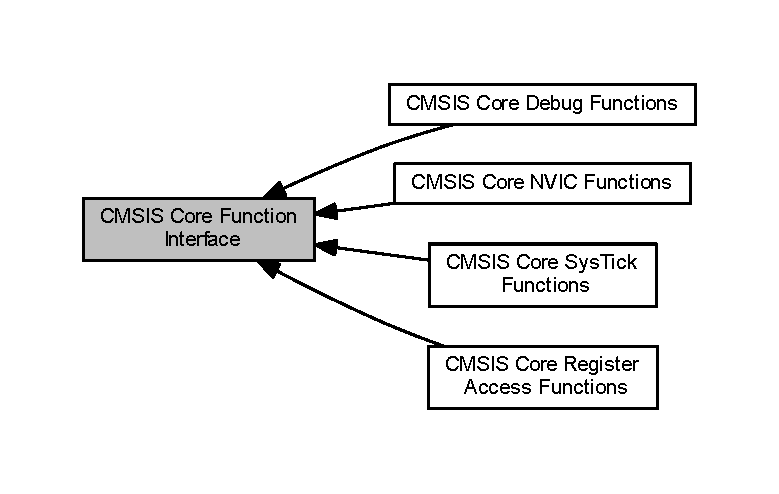
\includegraphics[width=350pt]{group___c_m_s_i_s___core___function_interface}
\end{center}
\end{figure}
\subsection*{Modules}
\begin{DoxyCompactItemize}
\item 
\hyperlink{group___c_m_s_i_s___core___n_v_i_c_functions}{C\+M\+S\+I\+S Core N\+V\+I\+C Functions}
\item 
\hyperlink{group___c_m_s_i_s___core___sys_tick_functions}{C\+M\+S\+I\+S Core Sys\+Tick Functions}
\item 
\hyperlink{group___c_m_s_i_s__core___debug_functions}{C\+M\+S\+I\+S Core Debug Functions}
\item 
\hyperlink{group___c_m_s_i_s___core___reg_acc_functions}{C\+M\+S\+I\+S Core Register Access Functions}
\end{DoxyCompactItemize}


\subsection{Detailed Description}
Core Function Interface contains\+:
\begin{DoxyItemize}
\item Core N\+V\+IC Functions
\item Core Sys\+Tick Functions
\item Core Debug Functions
\item Core Register Access Functions 
\end{DoxyItemize}
\hypertarget{group___c_m_s_i_s___core___n_v_i_c_functions}{}\section{C\+M\+S\+IS Core N\+V\+IC Functions}
\label{group___c_m_s_i_s___core___n_v_i_c_functions}\index{C\+M\+S\+I\+S Core N\+V\+I\+C Functions@{C\+M\+S\+I\+S Core N\+V\+I\+C Functions}}
Collaboration diagram for C\+M\+S\+IS Core N\+V\+IC Functions\+:
\nopagebreak
\begin{figure}[H]
\begin{center}
\leavevmode
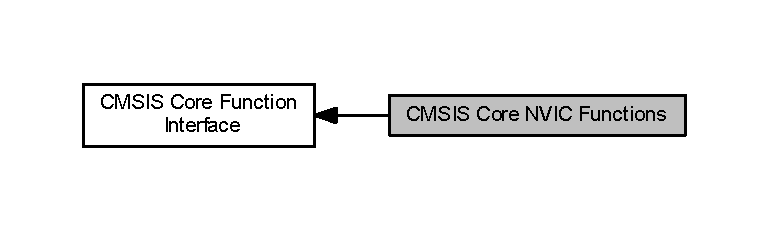
\includegraphics[width=350pt]{group___c_m_s_i_s___core___n_v_i_c_functions}
\end{center}
\end{figure}


\subsection{Detailed Description}

\hypertarget{group___c_m_s_i_s___core___sys_tick_functions}{}\section{C\+M\+S\+IS Core Sys\+Tick Functions}
\label{group___c_m_s_i_s___core___sys_tick_functions}\index{C\+M\+S\+I\+S Core Sys\+Tick Functions@{C\+M\+S\+I\+S Core Sys\+Tick Functions}}
Collaboration diagram for C\+M\+S\+IS Core Sys\+Tick Functions\+:\nopagebreak
\begin{figure}[H]
\begin{center}
\leavevmode
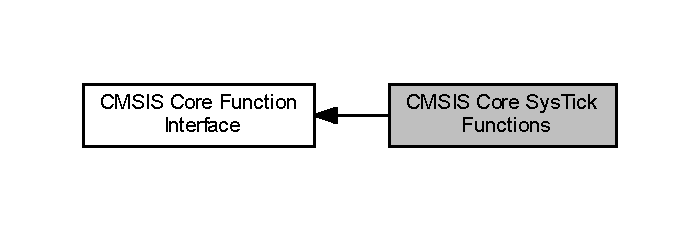
\includegraphics[width=336pt]{group___c_m_s_i_s___core___sys_tick_functions}
\end{center}
\end{figure}


\subsection{Detailed Description}

\hypertarget{group___c_m_s_i_s__core___debug_functions}{}\section{C\+M\+S\+IS Core Debug Functions}
\label{group___c_m_s_i_s__core___debug_functions}\index{C\+M\+S\+I\+S Core Debug Functions@{C\+M\+S\+I\+S Core Debug Functions}}
Collaboration diagram for C\+M\+S\+IS Core Debug Functions\+:\nopagebreak
\begin{figure}[H]
\begin{center}
\leavevmode
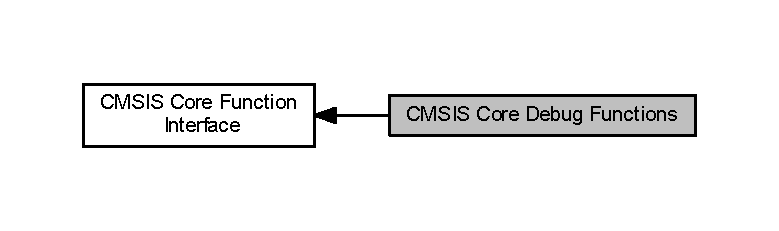
\includegraphics[width=350pt]{group___c_m_s_i_s__core___debug_functions}
\end{center}
\end{figure}
\subsection*{Macros}
\begin{DoxyCompactItemize}
\item 
\#define \hyperlink{group___c_m_s_i_s__core___debug_functions_gaa822cb398ee022b59e9e6c5d7bbb228a}{I\+T\+M\+\_\+\+R\+X\+B\+U\+F\+F\+E\+R\+\_\+\+E\+M\+P\+TY}~0x5\+A\+A55\+A\+A5
\end{DoxyCompactItemize}
\subsection*{Variables}
\begin{DoxyCompactItemize}
\item 
volatile int32\+\_\+t \hyperlink{group___c_m_s_i_s__core___debug_functions_ga12e68e55a7badc271b948d6c7230b2a8}{I\+T\+M\+\_\+\+Rx\+Buffer}
\end{DoxyCompactItemize}


\subsection{Detailed Description}


\subsection{Macro Definition Documentation}
\mbox{\Hypertarget{group___c_m_s_i_s__core___debug_functions_gaa822cb398ee022b59e9e6c5d7bbb228a}\label{group___c_m_s_i_s__core___debug_functions_gaa822cb398ee022b59e9e6c5d7bbb228a}} 
\index{C\+M\+S\+I\+S Core Debug Functions@{C\+M\+S\+I\+S Core Debug Functions}!I\+T\+M\+\_\+\+R\+X\+B\+U\+F\+F\+E\+R\+\_\+\+E\+M\+P\+TY@{I\+T\+M\+\_\+\+R\+X\+B\+U\+F\+F\+E\+R\+\_\+\+E\+M\+P\+TY}}
\index{I\+T\+M\+\_\+\+R\+X\+B\+U\+F\+F\+E\+R\+\_\+\+E\+M\+P\+TY@{I\+T\+M\+\_\+\+R\+X\+B\+U\+F\+F\+E\+R\+\_\+\+E\+M\+P\+TY}!C\+M\+S\+I\+S Core Debug Functions@{C\+M\+S\+I\+S Core Debug Functions}}
\subsubsection{\texorpdfstring{I\+T\+M\+\_\+\+R\+X\+B\+U\+F\+F\+E\+R\+\_\+\+E\+M\+P\+TY}{ITM\_RXBUFFER\_EMPTY}}
{\footnotesize\ttfamily \#define I\+T\+M\+\_\+\+R\+X\+B\+U\+F\+F\+E\+R\+\_\+\+E\+M\+P\+TY~0x5\+A\+A55\+A\+A5}

value identifying I\+T\+M\+\_\+\+Rx\+Buffer is ready for next character 

Definition at line 1307 of file core\+\_\+cm4.\+h.



\subsection{Variable Documentation}
\mbox{\Hypertarget{group___c_m_s_i_s__core___debug_functions_ga12e68e55a7badc271b948d6c7230b2a8}\label{group___c_m_s_i_s__core___debug_functions_ga12e68e55a7badc271b948d6c7230b2a8}} 
\index{C\+M\+S\+I\+S Core Debug Functions@{C\+M\+S\+I\+S Core Debug Functions}!I\+T\+M\+\_\+\+Rx\+Buffer@{I\+T\+M\+\_\+\+Rx\+Buffer}}
\index{I\+T\+M\+\_\+\+Rx\+Buffer@{I\+T\+M\+\_\+\+Rx\+Buffer}!C\+M\+S\+I\+S Core Debug Functions@{C\+M\+S\+I\+S Core Debug Functions}}
\subsubsection{\texorpdfstring{I\+T\+M\+\_\+\+Rx\+Buffer}{ITM\_RxBuffer}}
{\footnotesize\ttfamily volatile int32\+\_\+t I\+T\+M\+\_\+\+Rx\+Buffer}

external variable to receive characters 
\hypertarget{group___c_m_s_i_s___s_i_m_d__intrinsics}{}\section{C\+M\+S\+IS S\+I\+MD Intrinsics}
\label{group___c_m_s_i_s___s_i_m_d__intrinsics}\index{C\+M\+S\+I\+S S\+I\+M\+D Intrinsics@{C\+M\+S\+I\+S S\+I\+M\+D Intrinsics}}
Access to dedicated S\+I\+MD instructions 
\hypertarget{group___c_m_s_i_s___core___reg_acc_functions}{}\section{C\+M\+S\+IS Core Register Access Functions}
\label{group___c_m_s_i_s___core___reg_acc_functions}\index{C\+M\+S\+I\+S Core Register Access Functions@{C\+M\+S\+I\+S Core Register Access Functions}}
Collaboration diagram for C\+M\+S\+IS Core Register Access Functions\+:\nopagebreak
\begin{figure}[H]
\begin{center}
\leavevmode
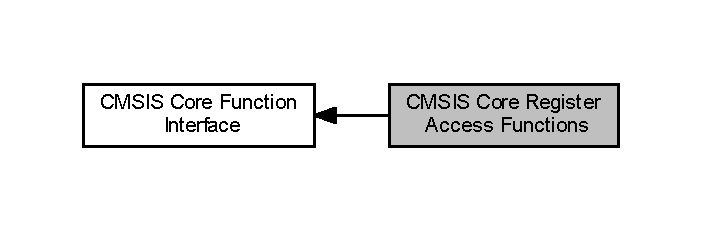
\includegraphics[width=337pt]{group___c_m_s_i_s___core___reg_acc_functions}
\end{center}
\end{figure}

\hypertarget{group___c_m_s_i_s___core___instruction_interface}{}\section{C\+M\+S\+IS Core Instruction Interface}
\label{group___c_m_s_i_s___core___instruction_interface}\index{C\+M\+S\+I\+S Core Instruction Interface@{C\+M\+S\+I\+S Core Instruction Interface}}
Access to dedicated instructions 
\hypertarget{group___m_i_s_c___exported___constants}{}\section{M\+I\+S\+C\+\_\+\+Exported\+\_\+\+Constants}
\label{group___m_i_s_c___exported___constants}\index{M\+I\+S\+C\+\_\+\+Exported\+\_\+\+Constants@{M\+I\+S\+C\+\_\+\+Exported\+\_\+\+Constants}}
Collaboration diagram for M\+I\+S\+C\+\_\+\+Exported\+\_\+\+Constants\+:\nopagebreak
\begin{figure}[H]
\begin{center}
\leavevmode
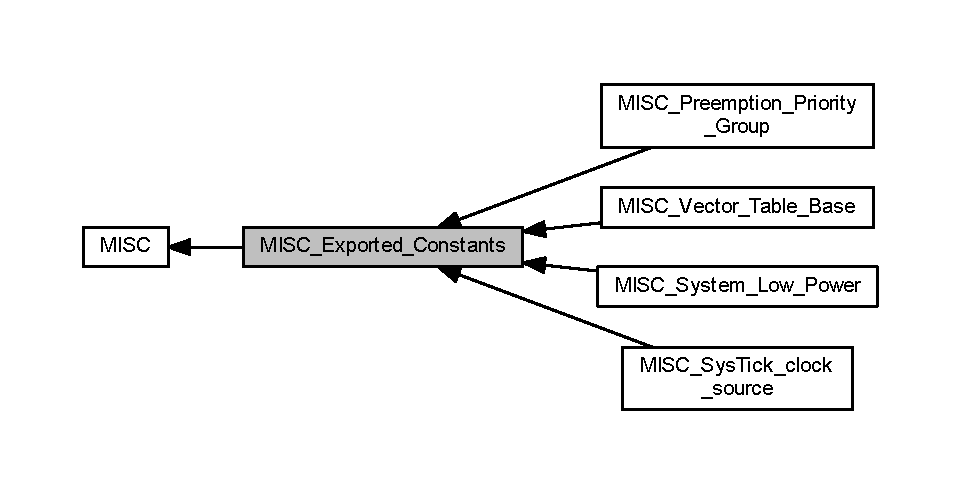
\includegraphics[width=350pt]{group___m_i_s_c___exported___constants}
\end{center}
\end{figure}
\subsection*{Modules}
\begin{DoxyCompactItemize}
\item 
\hyperlink{group___m_i_s_c___vector___table___base}{M\+I\+S\+C\+\_\+\+Vector\+\_\+\+Table\+\_\+\+Base}
\item 
\hyperlink{group___m_i_s_c___system___low___power}{M\+I\+S\+C\+\_\+\+System\+\_\+\+Low\+\_\+\+Power}
\item 
\hyperlink{group___m_i_s_c___preemption___priority___group}{M\+I\+S\+C\+\_\+\+Preemption\+\_\+\+Priority\+\_\+\+Group}
\item 
\hyperlink{group___m_i_s_c___sys_tick__clock__source}{M\+I\+S\+C\+\_\+\+Sys\+Tick\+\_\+clock\+\_\+source}
\end{DoxyCompactItemize}


\subsection{Detailed Description}

\hypertarget{group___m_i_s_c___vector___table___base}{}\section{M\+I\+S\+C\+\_\+\+Vector\+\_\+\+Table\+\_\+\+Base}
\label{group___m_i_s_c___vector___table___base}\index{M\+I\+S\+C\+\_\+\+Vector\+\_\+\+Table\+\_\+\+Base@{M\+I\+S\+C\+\_\+\+Vector\+\_\+\+Table\+\_\+\+Base}}
Collaboration diagram for M\+I\+S\+C\+\_\+\+Vector\+\_\+\+Table\+\_\+\+Base\+:\nopagebreak
\begin{figure}[H]
\begin{center}
\leavevmode
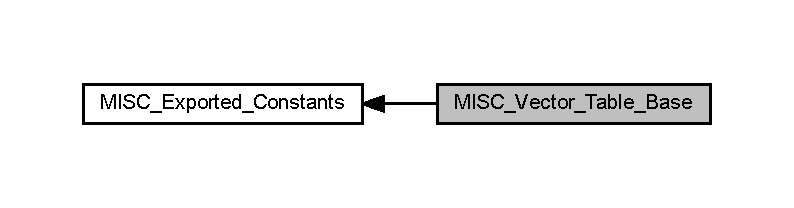
\includegraphics[width=350pt]{group___m_i_s_c___vector___table___base}
\end{center}
\end{figure}
\subsection*{Macros}
\begin{DoxyCompactItemize}
\item 
\mbox{\Hypertarget{group___m_i_s_c___vector___table___base_ga8be8181cc3e5d42f6204af306ab50f80}\label{group___m_i_s_c___vector___table___base_ga8be8181cc3e5d42f6204af306ab50f80}} 
\#define {\bfseries N\+V\+I\+C\+\_\+\+Vect\+Tab\+\_\+\+R\+AM}~((uint32\+\_\+t)0x20000000)
\item 
\mbox{\Hypertarget{group___m_i_s_c___vector___table___base_gafbf92fd28a1090b2aa49732ebd5704b5}\label{group___m_i_s_c___vector___table___base_gafbf92fd28a1090b2aa49732ebd5704b5}} 
\#define {\bfseries N\+V\+I\+C\+\_\+\+Vect\+Tab\+\_\+\+F\+L\+A\+SH}~((uint32\+\_\+t)0x08000000)
\item 
\#define {\bfseries I\+S\+\_\+\+N\+V\+I\+C\+\_\+\+V\+E\+C\+T\+T\+AB}(V\+E\+C\+T\+T\+AB)
\end{DoxyCompactItemize}


\subsection{Detailed Description}


\subsection{Macro Definition Documentation}
\mbox{\Hypertarget{group___m_i_s_c___vector___table___base_ga26b9d493ccb98fcce9a27303078940c8}\label{group___m_i_s_c___vector___table___base_ga26b9d493ccb98fcce9a27303078940c8}} 
\index{M\+I\+S\+C\+\_\+\+Vector\+\_\+\+Table\+\_\+\+Base@{M\+I\+S\+C\+\_\+\+Vector\+\_\+\+Table\+\_\+\+Base}!I\+S\+\_\+\+N\+V\+I\+C\+\_\+\+V\+E\+C\+T\+T\+AB@{I\+S\+\_\+\+N\+V\+I\+C\+\_\+\+V\+E\+C\+T\+T\+AB}}
\index{I\+S\+\_\+\+N\+V\+I\+C\+\_\+\+V\+E\+C\+T\+T\+AB@{I\+S\+\_\+\+N\+V\+I\+C\+\_\+\+V\+E\+C\+T\+T\+AB}!M\+I\+S\+C\+\_\+\+Vector\+\_\+\+Table\+\_\+\+Base@{M\+I\+S\+C\+\_\+\+Vector\+\_\+\+Table\+\_\+\+Base}}
\subsubsection{\texorpdfstring{I\+S\+\_\+\+N\+V\+I\+C\+\_\+\+V\+E\+C\+T\+T\+AB}{IS\_NVIC\_VECTTAB}}
{\footnotesize\ttfamily \#define I\+S\+\_\+\+N\+V\+I\+C\+\_\+\+V\+E\+C\+T\+T\+AB(\begin{DoxyParamCaption}\item[{}]{V\+E\+C\+T\+T\+AB }\end{DoxyParamCaption})}

{\bfseries Value\+:}
\begin{DoxyCode}
(((VECTTAB) == NVIC\_VectTab\_RAM) || \(\backslash\)
                                  ((VECTTAB) == NVIC\_VectTab\_FLASH))
\end{DoxyCode}


Definition at line 82 of file misc.\+h.


\hypertarget{group___m_i_s_c___system___low___power}{}\section{M\+I\+S\+C\+\_\+\+System\+\_\+\+Low\+\_\+\+Power}
\label{group___m_i_s_c___system___low___power}\index{M\+I\+S\+C\+\_\+\+System\+\_\+\+Low\+\_\+\+Power@{M\+I\+S\+C\+\_\+\+System\+\_\+\+Low\+\_\+\+Power}}
Collaboration diagram for M\+I\+S\+C\+\_\+\+System\+\_\+\+Low\+\_\+\+Power\+:
\nopagebreak
\begin{figure}[H]
\begin{center}
\leavevmode
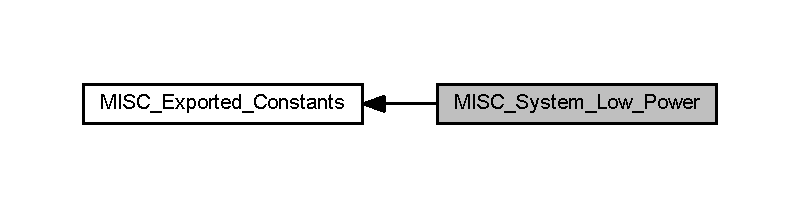
\includegraphics[width=350pt]{group___m_i_s_c___system___low___power}
\end{center}
\end{figure}
\subsection*{Macros}
\begin{DoxyCompactItemize}
\item 
\mbox{\Hypertarget{group___m_i_s_c___system___low___power_ga10748d2b2875afd122f6476864ad6cae}\label{group___m_i_s_c___system___low___power_ga10748d2b2875afd122f6476864ad6cae}} 
\#define {\bfseries N\+V\+I\+C\+\_\+\+L\+P\+\_\+\+S\+E\+V\+O\+N\+P\+E\+ND}~((uint8\+\_\+t)0x10)
\item 
\mbox{\Hypertarget{group___m_i_s_c___system___low___power_gaeec2d10922fa9ec5e65398667b303253}\label{group___m_i_s_c___system___low___power_gaeec2d10922fa9ec5e65398667b303253}} 
\#define {\bfseries N\+V\+I\+C\+\_\+\+L\+P\+\_\+\+S\+L\+E\+E\+P\+D\+E\+EP}~((uint8\+\_\+t)0x04)
\item 
\mbox{\Hypertarget{group___m_i_s_c___system___low___power_ga368dc13a9c762a307c07cfa2e3ef59ad}\label{group___m_i_s_c___system___low___power_ga368dc13a9c762a307c07cfa2e3ef59ad}} 
\#define {\bfseries N\+V\+I\+C\+\_\+\+L\+P\+\_\+\+S\+L\+E\+E\+P\+O\+N\+E\+X\+IT}~((uint8\+\_\+t)0x02)
\item 
\#define {\bfseries I\+S\+\_\+\+N\+V\+I\+C\+\_\+\+LP}(LP)
\end{DoxyCompactItemize}


\subsection{Detailed Description}


\subsection{Macro Definition Documentation}
\mbox{\Hypertarget{group___m_i_s_c___system___low___power_ga985896f03bc1d7b3da17a212f1bc3de9}\label{group___m_i_s_c___system___low___power_ga985896f03bc1d7b3da17a212f1bc3de9}} 
\index{M\+I\+S\+C\+\_\+\+System\+\_\+\+Low\+\_\+\+Power@{M\+I\+S\+C\+\_\+\+System\+\_\+\+Low\+\_\+\+Power}!I\+S\+\_\+\+N\+V\+I\+C\+\_\+\+LP@{I\+S\+\_\+\+N\+V\+I\+C\+\_\+\+LP}}
\index{I\+S\+\_\+\+N\+V\+I\+C\+\_\+\+LP@{I\+S\+\_\+\+N\+V\+I\+C\+\_\+\+LP}!M\+I\+S\+C\+\_\+\+System\+\_\+\+Low\+\_\+\+Power@{M\+I\+S\+C\+\_\+\+System\+\_\+\+Low\+\_\+\+Power}}
\subsubsection{\texorpdfstring{I\+S\+\_\+\+N\+V\+I\+C\+\_\+\+LP}{IS\_NVIC\_LP}}
{\footnotesize\ttfamily \#define I\+S\+\_\+\+N\+V\+I\+C\+\_\+\+LP(\begin{DoxyParamCaption}\item[{}]{LP }\end{DoxyParamCaption})}

{\bfseries Value\+:}
\begin{DoxyCode}
(((LP) == NVIC\_LP\_SEVONPEND) || \(\backslash\)
                        ((LP) == NVIC\_LP\_SLEEPDEEP) || \(\backslash\)
                        ((LP) == NVIC\_LP\_SLEEPONEXIT))
\end{DoxyCode}


Definition at line 95 of file misc.\+h.


\hypertarget{group___m_i_s_c___preemption___priority___group}{}\section{M\+I\+S\+C\+\_\+\+Preemption\+\_\+\+Priority\+\_\+\+Group}
\label{group___m_i_s_c___preemption___priority___group}\index{M\+I\+S\+C\+\_\+\+Preemption\+\_\+\+Priority\+\_\+\+Group@{M\+I\+S\+C\+\_\+\+Preemption\+\_\+\+Priority\+\_\+\+Group}}
Collaboration diagram for M\+I\+S\+C\+\_\+\+Preemption\+\_\+\+Priority\+\_\+\+Group\+:
\nopagebreak
\begin{figure}[H]
\begin{center}
\leavevmode
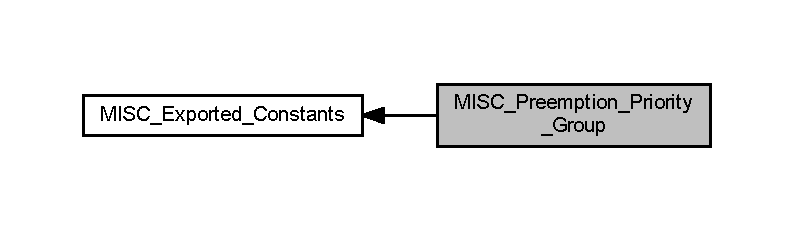
\includegraphics[width=350pt]{group___m_i_s_c___preemption___priority___group}
\end{center}
\end{figure}
\subsection*{Macros}
\begin{DoxyCompactItemize}
\item 
\#define \hyperlink{group___m_i_s_c___preemption___priority___group_gaeac0cf537f65d17bc19aee2410b2b60e}{N\+V\+I\+C\+\_\+\+Priority\+Group\+\_\+0}~((uint32\+\_\+t)0x700)
\item 
\#define \hyperlink{group___m_i_s_c___preemption___priority___group_ga89bf0bf9e70f1a372a541b1b8d7493aa}{N\+V\+I\+C\+\_\+\+Priority\+Group\+\_\+1}~((uint32\+\_\+t)0x600)
\item 
\#define \hyperlink{group___m_i_s_c___preemption___priority___group_ga505002e8b76aef65499ca371e40ec8b4}{N\+V\+I\+C\+\_\+\+Priority\+Group\+\_\+2}~((uint32\+\_\+t)0x500)
\item 
\#define \hyperlink{group___m_i_s_c___preemption___priority___group_ga49bdbee77d4a70339d63c80462d49b4d}{N\+V\+I\+C\+\_\+\+Priority\+Group\+\_\+3}~((uint32\+\_\+t)0x400)
\item 
\#define \hyperlink{group___m_i_s_c___preemption___priority___group_gaf9020c585da2a299328f0b06dee391a2}{N\+V\+I\+C\+\_\+\+Priority\+Group\+\_\+4}~((uint32\+\_\+t)0x300)
\item 
\#define {\bfseries I\+S\+\_\+\+N\+V\+I\+C\+\_\+\+P\+R\+I\+O\+R\+I\+T\+Y\+\_\+\+G\+R\+O\+UP}(G\+R\+O\+UP)
\item 
\mbox{\Hypertarget{group___m_i_s_c___preemption___priority___group_gaf30fd8f5960c2e28a772d8f16bb156dd}\label{group___m_i_s_c___preemption___priority___group_gaf30fd8f5960c2e28a772d8f16bb156dd}} 
\#define {\bfseries I\+S\+\_\+\+N\+V\+I\+C\+\_\+\+P\+R\+E\+E\+M\+P\+T\+I\+O\+N\+\_\+\+P\+R\+I\+O\+R\+I\+TY}(P\+R\+I\+O\+R\+I\+TY)~((P\+R\+I\+O\+R\+I\+TY) $<$ 0x10)
\item 
\mbox{\Hypertarget{group___m_i_s_c___preemption___priority___group_ga010705bc997dcff935b965b372cba61d}\label{group___m_i_s_c___preemption___priority___group_ga010705bc997dcff935b965b372cba61d}} 
\#define {\bfseries I\+S\+\_\+\+N\+V\+I\+C\+\_\+\+S\+U\+B\+\_\+\+P\+R\+I\+O\+R\+I\+TY}(P\+R\+I\+O\+R\+I\+TY)~((P\+R\+I\+O\+R\+I\+TY) $<$ 0x10)
\item 
\mbox{\Hypertarget{group___m_i_s_c___preemption___priority___group_ga1184bbb97d758385f98ab40dd5e5af59}\label{group___m_i_s_c___preemption___priority___group_ga1184bbb97d758385f98ab40dd5e5af59}} 
\#define {\bfseries I\+S\+\_\+\+N\+V\+I\+C\+\_\+\+O\+F\+F\+S\+ET}(O\+F\+F\+S\+ET)~((O\+F\+F\+S\+ET) $<$ 0x000\+F\+F\+F\+F\+F)
\end{DoxyCompactItemize}


\subsection{Detailed Description}


\subsection{Macro Definition Documentation}
\mbox{\Hypertarget{group___m_i_s_c___preemption___priority___group_ga6569304a39fe4f91bd59b6a586c8ede9}\label{group___m_i_s_c___preemption___priority___group_ga6569304a39fe4f91bd59b6a586c8ede9}} 
\index{M\+I\+S\+C\+\_\+\+Preemption\+\_\+\+Priority\+\_\+\+Group@{M\+I\+S\+C\+\_\+\+Preemption\+\_\+\+Priority\+\_\+\+Group}!I\+S\+\_\+\+N\+V\+I\+C\+\_\+\+P\+R\+I\+O\+R\+I\+T\+Y\+\_\+\+G\+R\+O\+UP@{I\+S\+\_\+\+N\+V\+I\+C\+\_\+\+P\+R\+I\+O\+R\+I\+T\+Y\+\_\+\+G\+R\+O\+UP}}
\index{I\+S\+\_\+\+N\+V\+I\+C\+\_\+\+P\+R\+I\+O\+R\+I\+T\+Y\+\_\+\+G\+R\+O\+UP@{I\+S\+\_\+\+N\+V\+I\+C\+\_\+\+P\+R\+I\+O\+R\+I\+T\+Y\+\_\+\+G\+R\+O\+UP}!M\+I\+S\+C\+\_\+\+Preemption\+\_\+\+Priority\+\_\+\+Group@{M\+I\+S\+C\+\_\+\+Preemption\+\_\+\+Priority\+\_\+\+Group}}
\subsubsection{\texorpdfstring{I\+S\+\_\+\+N\+V\+I\+C\+\_\+\+P\+R\+I\+O\+R\+I\+T\+Y\+\_\+\+G\+R\+O\+UP}{IS\_NVIC\_PRIORITY\_GROUP}}
{\footnotesize\ttfamily \#define I\+S\+\_\+\+N\+V\+I\+C\+\_\+\+P\+R\+I\+O\+R\+I\+T\+Y\+\_\+\+G\+R\+O\+UP(\begin{DoxyParamCaption}\item[{}]{G\+R\+O\+UP }\end{DoxyParamCaption})}

{\bfseries Value\+:}
\begin{DoxyCode}
(((GROUP) == \hyperlink{group___m_i_s_c___preemption___priority___group_gaeac0cf537f65d17bc19aee2410b2b60e}{NVIC\_PriorityGroup\_0}) || \(\backslash\)
                                       ((GROUP) == \hyperlink{group___m_i_s_c___preemption___priority___group_ga89bf0bf9e70f1a372a541b1b8d7493aa}{NVIC\_PriorityGroup\_1}) || \(\backslash\)
                                       ((GROUP) == \hyperlink{group___m_i_s_c___preemption___priority___group_ga505002e8b76aef65499ca371e40ec8b4}{NVIC\_PriorityGroup\_2}) || \(\backslash\)
                                       ((GROUP) == \hyperlink{group___m_i_s_c___preemption___priority___group_ga49bdbee77d4a70339d63c80462d49b4d}{NVIC\_PriorityGroup\_3}) || \(\backslash\)
                                       ((GROUP) == \hyperlink{group___m_i_s_c___preemption___priority___group_gaf9020c585da2a299328f0b06dee391a2}{NVIC\_PriorityGroup\_4}))
\end{DoxyCode}


Definition at line 122 of file misc.\+h.

\mbox{\Hypertarget{group___m_i_s_c___preemption___priority___group_gaeac0cf537f65d17bc19aee2410b2b60e}\label{group___m_i_s_c___preemption___priority___group_gaeac0cf537f65d17bc19aee2410b2b60e}} 
\index{M\+I\+S\+C\+\_\+\+Preemption\+\_\+\+Priority\+\_\+\+Group@{M\+I\+S\+C\+\_\+\+Preemption\+\_\+\+Priority\+\_\+\+Group}!N\+V\+I\+C\+\_\+\+Priority\+Group\+\_\+0@{N\+V\+I\+C\+\_\+\+Priority\+Group\+\_\+0}}
\index{N\+V\+I\+C\+\_\+\+Priority\+Group\+\_\+0@{N\+V\+I\+C\+\_\+\+Priority\+Group\+\_\+0}!M\+I\+S\+C\+\_\+\+Preemption\+\_\+\+Priority\+\_\+\+Group@{M\+I\+S\+C\+\_\+\+Preemption\+\_\+\+Priority\+\_\+\+Group}}
\subsubsection{\texorpdfstring{N\+V\+I\+C\+\_\+\+Priority\+Group\+\_\+0}{NVIC\_PriorityGroup\_0}}
{\footnotesize\ttfamily \#define N\+V\+I\+C\+\_\+\+Priority\+Group\+\_\+0~((uint32\+\_\+t)0x700)}

0 bits for pre-\/emption priority 4 bits for subpriority 

Definition at line 106 of file misc.\+h.

\mbox{\Hypertarget{group___m_i_s_c___preemption___priority___group_ga89bf0bf9e70f1a372a541b1b8d7493aa}\label{group___m_i_s_c___preemption___priority___group_ga89bf0bf9e70f1a372a541b1b8d7493aa}} 
\index{M\+I\+S\+C\+\_\+\+Preemption\+\_\+\+Priority\+\_\+\+Group@{M\+I\+S\+C\+\_\+\+Preemption\+\_\+\+Priority\+\_\+\+Group}!N\+V\+I\+C\+\_\+\+Priority\+Group\+\_\+1@{N\+V\+I\+C\+\_\+\+Priority\+Group\+\_\+1}}
\index{N\+V\+I\+C\+\_\+\+Priority\+Group\+\_\+1@{N\+V\+I\+C\+\_\+\+Priority\+Group\+\_\+1}!M\+I\+S\+C\+\_\+\+Preemption\+\_\+\+Priority\+\_\+\+Group@{M\+I\+S\+C\+\_\+\+Preemption\+\_\+\+Priority\+\_\+\+Group}}
\subsubsection{\texorpdfstring{N\+V\+I\+C\+\_\+\+Priority\+Group\+\_\+1}{NVIC\_PriorityGroup\_1}}
{\footnotesize\ttfamily \#define N\+V\+I\+C\+\_\+\+Priority\+Group\+\_\+1~((uint32\+\_\+t)0x600)}

1 bits for pre-\/emption priority 3 bits for subpriority 

Definition at line 109 of file misc.\+h.

\mbox{\Hypertarget{group___m_i_s_c___preemption___priority___group_ga505002e8b76aef65499ca371e40ec8b4}\label{group___m_i_s_c___preemption___priority___group_ga505002e8b76aef65499ca371e40ec8b4}} 
\index{M\+I\+S\+C\+\_\+\+Preemption\+\_\+\+Priority\+\_\+\+Group@{M\+I\+S\+C\+\_\+\+Preemption\+\_\+\+Priority\+\_\+\+Group}!N\+V\+I\+C\+\_\+\+Priority\+Group\+\_\+2@{N\+V\+I\+C\+\_\+\+Priority\+Group\+\_\+2}}
\index{N\+V\+I\+C\+\_\+\+Priority\+Group\+\_\+2@{N\+V\+I\+C\+\_\+\+Priority\+Group\+\_\+2}!M\+I\+S\+C\+\_\+\+Preemption\+\_\+\+Priority\+\_\+\+Group@{M\+I\+S\+C\+\_\+\+Preemption\+\_\+\+Priority\+\_\+\+Group}}
\subsubsection{\texorpdfstring{N\+V\+I\+C\+\_\+\+Priority\+Group\+\_\+2}{NVIC\_PriorityGroup\_2}}
{\footnotesize\ttfamily \#define N\+V\+I\+C\+\_\+\+Priority\+Group\+\_\+2~((uint32\+\_\+t)0x500)}

2 bits for pre-\/emption priority 2 bits for subpriority 

Definition at line 112 of file misc.\+h.

\mbox{\Hypertarget{group___m_i_s_c___preemption___priority___group_ga49bdbee77d4a70339d63c80462d49b4d}\label{group___m_i_s_c___preemption___priority___group_ga49bdbee77d4a70339d63c80462d49b4d}} 
\index{M\+I\+S\+C\+\_\+\+Preemption\+\_\+\+Priority\+\_\+\+Group@{M\+I\+S\+C\+\_\+\+Preemption\+\_\+\+Priority\+\_\+\+Group}!N\+V\+I\+C\+\_\+\+Priority\+Group\+\_\+3@{N\+V\+I\+C\+\_\+\+Priority\+Group\+\_\+3}}
\index{N\+V\+I\+C\+\_\+\+Priority\+Group\+\_\+3@{N\+V\+I\+C\+\_\+\+Priority\+Group\+\_\+3}!M\+I\+S\+C\+\_\+\+Preemption\+\_\+\+Priority\+\_\+\+Group@{M\+I\+S\+C\+\_\+\+Preemption\+\_\+\+Priority\+\_\+\+Group}}
\subsubsection{\texorpdfstring{N\+V\+I\+C\+\_\+\+Priority\+Group\+\_\+3}{NVIC\_PriorityGroup\_3}}
{\footnotesize\ttfamily \#define N\+V\+I\+C\+\_\+\+Priority\+Group\+\_\+3~((uint32\+\_\+t)0x400)}

3 bits for pre-\/emption priority 1 bits for subpriority 

Definition at line 115 of file misc.\+h.

\mbox{\Hypertarget{group___m_i_s_c___preemption___priority___group_gaf9020c585da2a299328f0b06dee391a2}\label{group___m_i_s_c___preemption___priority___group_gaf9020c585da2a299328f0b06dee391a2}} 
\index{M\+I\+S\+C\+\_\+\+Preemption\+\_\+\+Priority\+\_\+\+Group@{M\+I\+S\+C\+\_\+\+Preemption\+\_\+\+Priority\+\_\+\+Group}!N\+V\+I\+C\+\_\+\+Priority\+Group\+\_\+4@{N\+V\+I\+C\+\_\+\+Priority\+Group\+\_\+4}}
\index{N\+V\+I\+C\+\_\+\+Priority\+Group\+\_\+4@{N\+V\+I\+C\+\_\+\+Priority\+Group\+\_\+4}!M\+I\+S\+C\+\_\+\+Preemption\+\_\+\+Priority\+\_\+\+Group@{M\+I\+S\+C\+\_\+\+Preemption\+\_\+\+Priority\+\_\+\+Group}}
\subsubsection{\texorpdfstring{N\+V\+I\+C\+\_\+\+Priority\+Group\+\_\+4}{NVIC\_PriorityGroup\_4}}
{\footnotesize\ttfamily \#define N\+V\+I\+C\+\_\+\+Priority\+Group\+\_\+4~((uint32\+\_\+t)0x300)}

4 bits for pre-\/emption priority 0 bits for subpriority 

Definition at line 118 of file misc.\+h.


\hypertarget{group___m_i_s_c___sys_tick__clock__source}{}\section{M\+I\+S\+C\+\_\+\+Sys\+Tick\+\_\+clock\+\_\+source}
\label{group___m_i_s_c___sys_tick__clock__source}\index{M\+I\+S\+C\+\_\+\+Sys\+Tick\+\_\+clock\+\_\+source@{M\+I\+S\+C\+\_\+\+Sys\+Tick\+\_\+clock\+\_\+source}}
Collaboration diagram for M\+I\+S\+C\+\_\+\+Sys\+Tick\+\_\+clock\+\_\+source\+:
\nopagebreak
\begin{figure}[H]
\begin{center}
\leavevmode
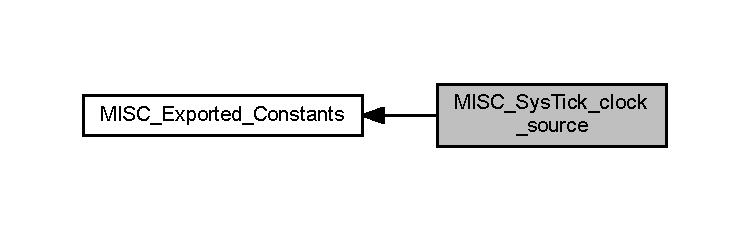
\includegraphics[width=350pt]{group___m_i_s_c___sys_tick__clock__source}
\end{center}
\end{figure}
\subsection*{Macros}
\begin{DoxyCompactItemize}
\item 
\mbox{\Hypertarget{group___m_i_s_c___sys_tick__clock__source_ga545c387ce43db90f15faad5f354f890d}\label{group___m_i_s_c___sys_tick__clock__source_ga545c387ce43db90f15faad5f354f890d}} 
\#define {\bfseries Sys\+Tick\+\_\+\+C\+L\+K\+Source\+\_\+\+H\+C\+L\+K\+\_\+\+Div8}~((uint32\+\_\+t)0x\+F\+F\+F\+F\+F\+F\+F\+B)
\item 
\mbox{\Hypertarget{group___m_i_s_c___sys_tick__clock__source_ga8a885ce2632ad4c35e229bb7c6e60191}\label{group___m_i_s_c___sys_tick__clock__source_ga8a885ce2632ad4c35e229bb7c6e60191}} 
\#define {\bfseries Sys\+Tick\+\_\+\+C\+L\+K\+Source\+\_\+\+H\+C\+LK}~((uint32\+\_\+t)0x00000004)
\item 
\#define {\bfseries I\+S\+\_\+\+S\+Y\+S\+T\+I\+C\+K\+\_\+\+C\+L\+K\+\_\+\+S\+O\+U\+R\+CE}(S\+O\+U\+R\+CE)
\end{DoxyCompactItemize}


\subsection{Detailed Description}


\subsection{Macro Definition Documentation}
\mbox{\Hypertarget{group___m_i_s_c___sys_tick__clock__source_ga22d6291f6aed29442cf4cd9098fa0784}\label{group___m_i_s_c___sys_tick__clock__source_ga22d6291f6aed29442cf4cd9098fa0784}} 
\index{M\+I\+S\+C\+\_\+\+Sys\+Tick\+\_\+clock\+\_\+source@{M\+I\+S\+C\+\_\+\+Sys\+Tick\+\_\+clock\+\_\+source}!I\+S\+\_\+\+S\+Y\+S\+T\+I\+C\+K\+\_\+\+C\+L\+K\+\_\+\+S\+O\+U\+R\+CE@{I\+S\+\_\+\+S\+Y\+S\+T\+I\+C\+K\+\_\+\+C\+L\+K\+\_\+\+S\+O\+U\+R\+CE}}
\index{I\+S\+\_\+\+S\+Y\+S\+T\+I\+C\+K\+\_\+\+C\+L\+K\+\_\+\+S\+O\+U\+R\+CE@{I\+S\+\_\+\+S\+Y\+S\+T\+I\+C\+K\+\_\+\+C\+L\+K\+\_\+\+S\+O\+U\+R\+CE}!M\+I\+S\+C\+\_\+\+Sys\+Tick\+\_\+clock\+\_\+source@{M\+I\+S\+C\+\_\+\+Sys\+Tick\+\_\+clock\+\_\+source}}
\subsubsection{\texorpdfstring{I\+S\+\_\+\+S\+Y\+S\+T\+I\+C\+K\+\_\+\+C\+L\+K\+\_\+\+S\+O\+U\+R\+CE}{IS\_SYSTICK\_CLK\_SOURCE}}
{\footnotesize\ttfamily \#define I\+S\+\_\+\+S\+Y\+S\+T\+I\+C\+K\+\_\+\+C\+L\+K\+\_\+\+S\+O\+U\+R\+CE(\begin{DoxyParamCaption}\item[{}]{S\+O\+U\+R\+CE }\end{DoxyParamCaption})}

{\bfseries Value\+:}
\begin{DoxyCode}
(((SOURCE) == SysTick\_CLKSource\_HCLK) || \(\backslash\)
                                       ((SOURCE) == SysTick\_CLKSource\_HCLK\_Div8))
\end{DoxyCode}


Definition at line 144 of file misc.\+h.


\hypertarget{group___d_m_a___exported___constants}{}\section{D\+M\+A\+\_\+\+Exported\+\_\+\+Constants}
\label{group___d_m_a___exported___constants}\index{D\+M\+A\+\_\+\+Exported\+\_\+\+Constants@{D\+M\+A\+\_\+\+Exported\+\_\+\+Constants}}
Collaboration diagram for D\+M\+A\+\_\+\+Exported\+\_\+\+Constants\+:\nopagebreak
\begin{figure}[H]
\begin{center}
\leavevmode
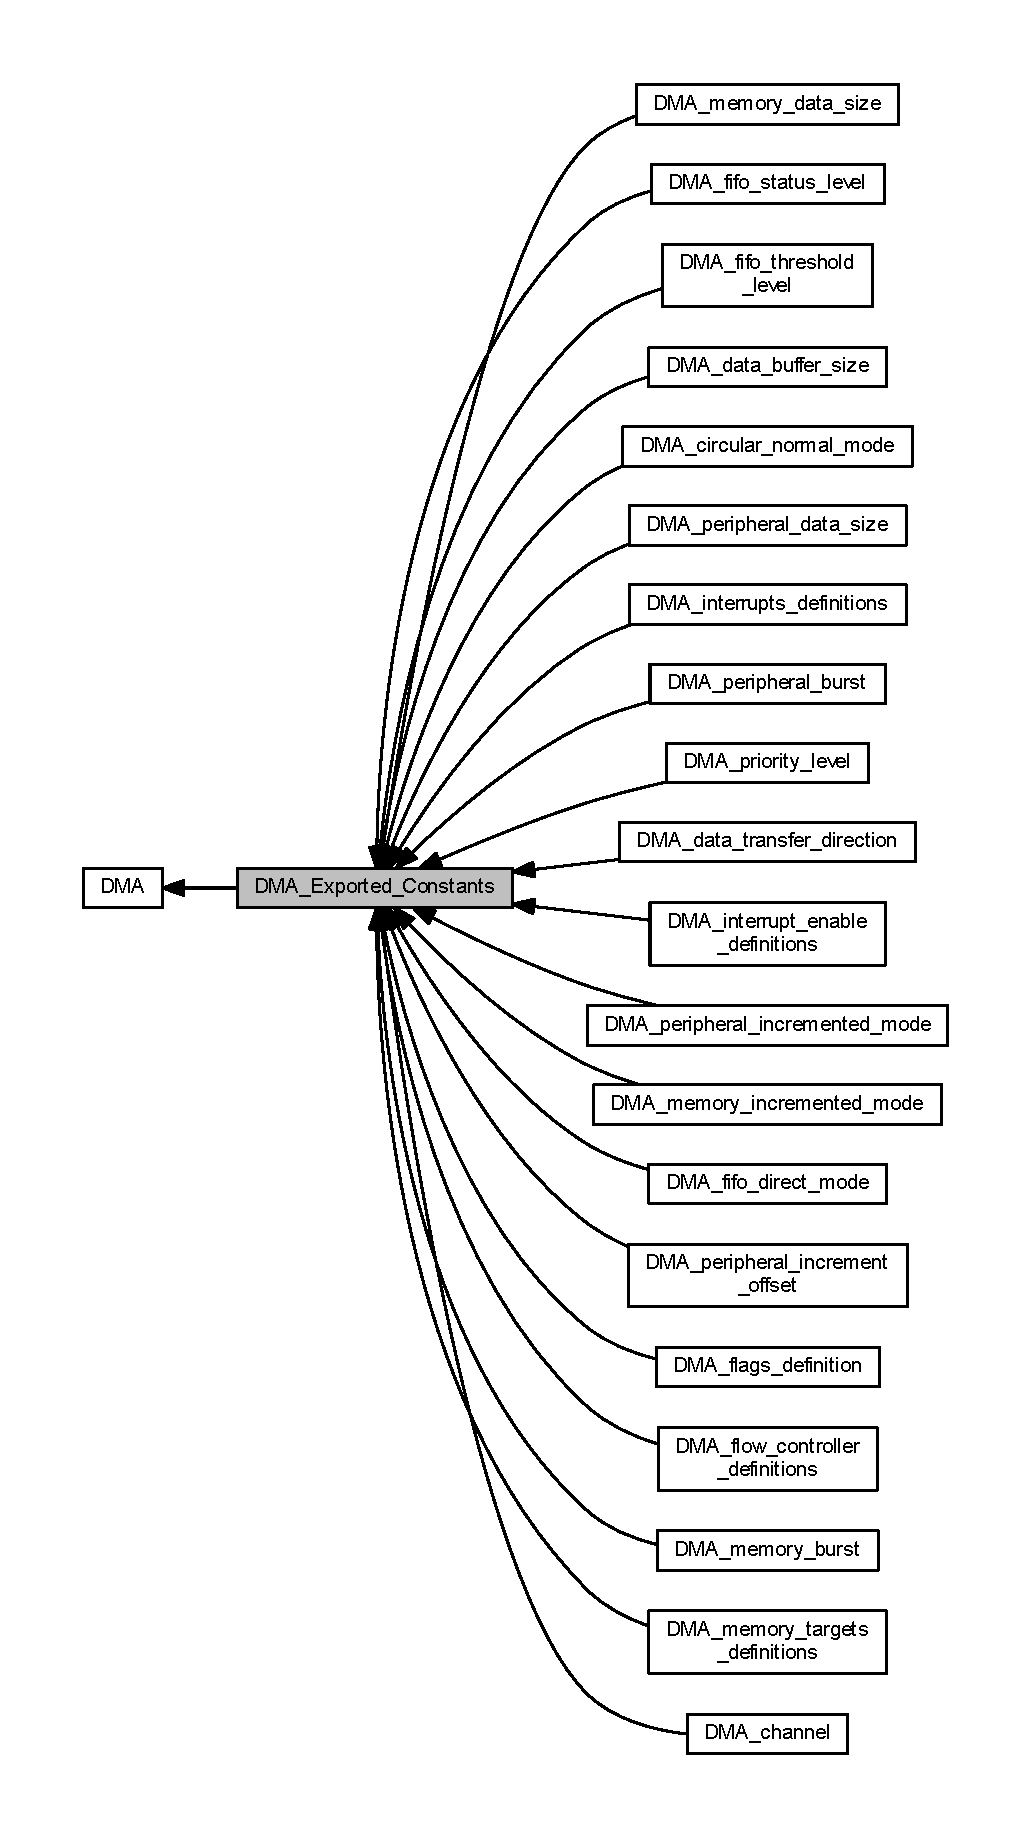
\includegraphics[height=550pt]{group___d_m_a___exported___constants}
\end{center}
\end{figure}
\subsection*{Modules}
\begin{DoxyCompactItemize}
\item 
\hyperlink{group___d_m_a__channel}{D\+M\+A\+\_\+channel}
\item 
\hyperlink{group___d_m_a__data__transfer__direction}{D\+M\+A\+\_\+data\+\_\+transfer\+\_\+direction}
\item 
\hyperlink{group___d_m_a__data__buffer__size}{D\+M\+A\+\_\+data\+\_\+buffer\+\_\+size}
\item 
\hyperlink{group___d_m_a__peripheral__incremented__mode}{D\+M\+A\+\_\+peripheral\+\_\+incremented\+\_\+mode}
\item 
\hyperlink{group___d_m_a__memory__incremented__mode}{D\+M\+A\+\_\+memory\+\_\+incremented\+\_\+mode}
\item 
\hyperlink{group___d_m_a__peripheral__data__size}{D\+M\+A\+\_\+peripheral\+\_\+data\+\_\+size}
\item 
\hyperlink{group___d_m_a__memory__data__size}{D\+M\+A\+\_\+memory\+\_\+data\+\_\+size}
\item 
\hyperlink{group___d_m_a__circular__normal__mode}{D\+M\+A\+\_\+circular\+\_\+normal\+\_\+mode}
\item 
\hyperlink{group___d_m_a__priority__level}{D\+M\+A\+\_\+priority\+\_\+level}
\item 
\hyperlink{group___d_m_a__fifo__direct__mode}{D\+M\+A\+\_\+fifo\+\_\+direct\+\_\+mode}
\item 
\hyperlink{group___d_m_a__fifo__threshold__level}{D\+M\+A\+\_\+fifo\+\_\+threshold\+\_\+level}
\item 
\hyperlink{group___d_m_a__memory__burst}{D\+M\+A\+\_\+memory\+\_\+burst}
\item 
\hyperlink{group___d_m_a__peripheral__burst}{D\+M\+A\+\_\+peripheral\+\_\+burst}
\item 
\hyperlink{group___d_m_a__fifo__status__level}{D\+M\+A\+\_\+fifo\+\_\+status\+\_\+level}
\item 
\hyperlink{group___d_m_a__flags__definition}{D\+M\+A\+\_\+flags\+\_\+definition}
\item 
\hyperlink{group___d_m_a__interrupt__enable__definitions}{D\+M\+A\+\_\+interrupt\+\_\+enable\+\_\+definitions}
\item 
\hyperlink{group___d_m_a__interrupts__definitions}{D\+M\+A\+\_\+interrupts\+\_\+definitions}
\item 
\hyperlink{group___d_m_a__peripheral__increment__offset}{D\+M\+A\+\_\+peripheral\+\_\+increment\+\_\+offset}
\item 
\hyperlink{group___d_m_a__flow__controller__definitions}{D\+M\+A\+\_\+flow\+\_\+controller\+\_\+definitions}
\item 
\hyperlink{group___d_m_a__memory__targets__definitions}{D\+M\+A\+\_\+memory\+\_\+targets\+\_\+definitions}
\end{DoxyCompactItemize}
\subsection*{Macros}
\begin{DoxyCompactItemize}
\item 
\#define {\bfseries I\+S\+\_\+\+D\+M\+A\+\_\+\+A\+L\+L\+\_\+\+P\+E\+R\+I\+PH}(P\+E\+R\+I\+PH)
\item 
\#define {\bfseries I\+S\+\_\+\+D\+M\+A\+\_\+\+A\+L\+L\+\_\+\+C\+O\+N\+T\+R\+O\+L\+L\+ER}(C\+O\+N\+T\+R\+O\+L\+L\+ER)
\end{DoxyCompactItemize}


\subsection{Detailed Description}


\subsection{Macro Definition Documentation}
\mbox{\Hypertarget{group___d_m_a___exported___constants_gaad08400369c8c129927cdb9cf1baae29}\label{group___d_m_a___exported___constants_gaad08400369c8c129927cdb9cf1baae29}} 
\index{D\+M\+A\+\_\+\+Exported\+\_\+\+Constants@{D\+M\+A\+\_\+\+Exported\+\_\+\+Constants}!I\+S\+\_\+\+D\+M\+A\+\_\+\+A\+L\+L\+\_\+\+C\+O\+N\+T\+R\+O\+L\+L\+ER@{I\+S\+\_\+\+D\+M\+A\+\_\+\+A\+L\+L\+\_\+\+C\+O\+N\+T\+R\+O\+L\+L\+ER}}
\index{I\+S\+\_\+\+D\+M\+A\+\_\+\+A\+L\+L\+\_\+\+C\+O\+N\+T\+R\+O\+L\+L\+ER@{I\+S\+\_\+\+D\+M\+A\+\_\+\+A\+L\+L\+\_\+\+C\+O\+N\+T\+R\+O\+L\+L\+ER}!D\+M\+A\+\_\+\+Exported\+\_\+\+Constants@{D\+M\+A\+\_\+\+Exported\+\_\+\+Constants}}
\subsubsection{\texorpdfstring{I\+S\+\_\+\+D\+M\+A\+\_\+\+A\+L\+L\+\_\+\+C\+O\+N\+T\+R\+O\+L\+L\+ER}{IS\_DMA\_ALL\_CONTROLLER}}
{\footnotesize\ttfamily \#define I\+S\+\_\+\+D\+M\+A\+\_\+\+A\+L\+L\+\_\+\+C\+O\+N\+T\+R\+O\+L\+L\+ER(\begin{DoxyParamCaption}\item[{}]{C\+O\+N\+T\+R\+O\+L\+L\+ER }\end{DoxyParamCaption})}

{\bfseries Value\+:}
\begin{DoxyCode}
(((CONTROLLER) == DMA1) || \(\backslash\)
                                           ((CONTROLLER) == DMA2))
\end{DoxyCode}


Definition at line 129 of file stm32f4xx\+\_\+dma.\+h.

\mbox{\Hypertarget{group___d_m_a___exported___constants_gabcab9fa1c48b148703a8f41c1d99e0c8}\label{group___d_m_a___exported___constants_gabcab9fa1c48b148703a8f41c1d99e0c8}} 
\index{D\+M\+A\+\_\+\+Exported\+\_\+\+Constants@{D\+M\+A\+\_\+\+Exported\+\_\+\+Constants}!I\+S\+\_\+\+D\+M\+A\+\_\+\+A\+L\+L\+\_\+\+P\+E\+R\+I\+PH@{I\+S\+\_\+\+D\+M\+A\+\_\+\+A\+L\+L\+\_\+\+P\+E\+R\+I\+PH}}
\index{I\+S\+\_\+\+D\+M\+A\+\_\+\+A\+L\+L\+\_\+\+P\+E\+R\+I\+PH@{I\+S\+\_\+\+D\+M\+A\+\_\+\+A\+L\+L\+\_\+\+P\+E\+R\+I\+PH}!D\+M\+A\+\_\+\+Exported\+\_\+\+Constants@{D\+M\+A\+\_\+\+Exported\+\_\+\+Constants}}
\subsubsection{\texorpdfstring{I\+S\+\_\+\+D\+M\+A\+\_\+\+A\+L\+L\+\_\+\+P\+E\+R\+I\+PH}{IS\_DMA\_ALL\_PERIPH}}
{\footnotesize\ttfamily \#define I\+S\+\_\+\+D\+M\+A\+\_\+\+A\+L\+L\+\_\+\+P\+E\+R\+I\+PH(\begin{DoxyParamCaption}\item[{}]{P\+E\+R\+I\+PH }\end{DoxyParamCaption})}

{\bfseries Value\+:}
\begin{DoxyCode}
(((PERIPH) == DMA1\_Stream0) || \(\backslash\)
                                   ((PERIPH) == DMA1\_Stream1) || \(\backslash\)
                                   ((PERIPH) == DMA1\_Stream2) || \(\backslash\)
                                   ((PERIPH) == DMA1\_Stream3) || \(\backslash\)
                                   ((PERIPH) == DMA1\_Stream4) || \(\backslash\)
                                   ((PERIPH) == DMA1\_Stream5) || \(\backslash\)
                                   ((PERIPH) == DMA1\_Stream6) || \(\backslash\)
                                   ((PERIPH) == DMA1\_Stream7) || \(\backslash\)
                                   ((PERIPH) == DMA2\_Stream0) || \(\backslash\)
                                   ((PERIPH) == DMA2\_Stream1) || \(\backslash\)
                                   ((PERIPH) == DMA2\_Stream2) || \(\backslash\)
                                   ((PERIPH) == DMA2\_Stream3) || \(\backslash\)
                                   ((PERIPH) == DMA2\_Stream4) || \(\backslash\)
                                   ((PERIPH) == DMA2\_Stream5) || \(\backslash\)
                                   ((PERIPH) == DMA2\_Stream6) || \(\backslash\)
                                   ((PERIPH) == DMA2\_Stream7))
\end{DoxyCode}


Definition at line 112 of file stm32f4xx\+\_\+dma.\+h.


\hypertarget{group___d_m_a__channel}{}\section{D\+M\+A\+\_\+channel}
\label{group___d_m_a__channel}\index{D\+M\+A\+\_\+channel@{D\+M\+A\+\_\+channel}}
Collaboration diagram for D\+M\+A\+\_\+channel\+:
\nopagebreak
\begin{figure}[H]
\begin{center}
\leavevmode
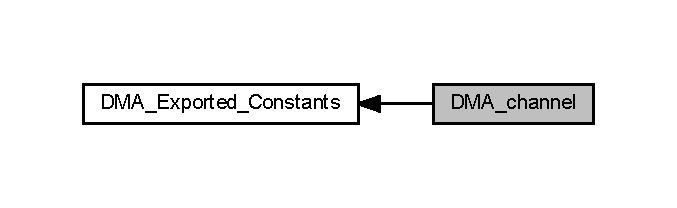
\includegraphics[width=325pt]{group___d_m_a__channel}
\end{center}
\end{figure}
\subsection*{Macros}
\begin{DoxyCompactItemize}
\item 
\mbox{\Hypertarget{group___d_m_a__channel_ga4979fc18bd59701dec52c8fa89b5edb2}\label{group___d_m_a__channel_ga4979fc18bd59701dec52c8fa89b5edb2}} 
\#define {\bfseries D\+M\+A\+\_\+\+Channel\+\_\+0}~((uint32\+\_\+t)0x00000000)
\item 
\mbox{\Hypertarget{group___d_m_a__channel_gacad41f71e3a940abd495b0aab3b4e8cb}\label{group___d_m_a__channel_gacad41f71e3a940abd495b0aab3b4e8cb}} 
\#define {\bfseries D\+M\+A\+\_\+\+Channel\+\_\+1}~((uint32\+\_\+t)0x02000000)
\item 
\mbox{\Hypertarget{group___d_m_a__channel_ga6b5d9fcfd72335777ce2796af6300574}\label{group___d_m_a__channel_ga6b5d9fcfd72335777ce2796af6300574}} 
\#define {\bfseries D\+M\+A\+\_\+\+Channel\+\_\+2}~((uint32\+\_\+t)0x04000000)
\item 
\mbox{\Hypertarget{group___d_m_a__channel_gaf835103c99f21d1b1c04d5c98471c1d5}\label{group___d_m_a__channel_gaf835103c99f21d1b1c04d5c98471c1d5}} 
\#define {\bfseries D\+M\+A\+\_\+\+Channel\+\_\+3}~((uint32\+\_\+t)0x06000000)
\item 
\mbox{\Hypertarget{group___d_m_a__channel_gac8a40bf3a421b434177e988263a3d787}\label{group___d_m_a__channel_gac8a40bf3a421b434177e988263a3d787}} 
\#define {\bfseries D\+M\+A\+\_\+\+Channel\+\_\+4}~((uint32\+\_\+t)0x08000000)
\item 
\mbox{\Hypertarget{group___d_m_a__channel_gae3dd5d28def40846aea8e3013d63311b}\label{group___d_m_a__channel_gae3dd5d28def40846aea8e3013d63311b}} 
\#define {\bfseries D\+M\+A\+\_\+\+Channel\+\_\+5}~((uint32\+\_\+t)0x0\+A000000)
\item 
\mbox{\Hypertarget{group___d_m_a__channel_ga141e89570dabba4f778e8e8df80e7812}\label{group___d_m_a__channel_ga141e89570dabba4f778e8e8df80e7812}} 
\#define {\bfseries D\+M\+A\+\_\+\+Channel\+\_\+6}~((uint32\+\_\+t)0x0\+C000000)
\item 
\mbox{\Hypertarget{group___d_m_a__channel_ga14f1265827ce49dad5075986118cc542}\label{group___d_m_a__channel_ga14f1265827ce49dad5075986118cc542}} 
\#define {\bfseries D\+M\+A\+\_\+\+Channel\+\_\+7}~((uint32\+\_\+t)0x0\+E000000)
\item 
\#define {\bfseries I\+S\+\_\+\+D\+M\+A\+\_\+\+C\+H\+A\+N\+N\+EL}(C\+H\+A\+N\+N\+EL)
\end{DoxyCompactItemize}


\subsection{Detailed Description}


\subsection{Macro Definition Documentation}
\mbox{\Hypertarget{group___d_m_a__channel_gac7f4709d9244f25b853789d888a74d46}\label{group___d_m_a__channel_gac7f4709d9244f25b853789d888a74d46}} 
\index{D\+M\+A\+\_\+channel@{D\+M\+A\+\_\+channel}!I\+S\+\_\+\+D\+M\+A\+\_\+\+C\+H\+A\+N\+N\+EL@{I\+S\+\_\+\+D\+M\+A\+\_\+\+C\+H\+A\+N\+N\+EL}}
\index{I\+S\+\_\+\+D\+M\+A\+\_\+\+C\+H\+A\+N\+N\+EL@{I\+S\+\_\+\+D\+M\+A\+\_\+\+C\+H\+A\+N\+N\+EL}!D\+M\+A\+\_\+channel@{D\+M\+A\+\_\+channel}}
\subsubsection{\texorpdfstring{I\+S\+\_\+\+D\+M\+A\+\_\+\+C\+H\+A\+N\+N\+EL}{IS\_DMA\_CHANNEL}}
{\footnotesize\ttfamily \#define I\+S\+\_\+\+D\+M\+A\+\_\+\+C\+H\+A\+N\+N\+EL(\begin{DoxyParamCaption}\item[{}]{C\+H\+A\+N\+N\+EL }\end{DoxyParamCaption})}

{\bfseries Value\+:}
\begin{DoxyCode}
(((CHANNEL) == DMA\_Channel\_0) || \(\backslash\)
                                 ((CHANNEL) == DMA\_Channel\_1) || \(\backslash\)
                                 ((CHANNEL) == DMA\_Channel\_2) || \(\backslash\)
                                 ((CHANNEL) == DMA\_Channel\_3) || \(\backslash\)
                                 ((CHANNEL) == DMA\_Channel\_4) || \(\backslash\)
                                 ((CHANNEL) == DMA\_Channel\_5) || \(\backslash\)
                                 ((CHANNEL) == DMA\_Channel\_6) || \(\backslash\)
                                 ((CHANNEL) == DMA\_Channel\_7))
\end{DoxyCode}


Definition at line 144 of file stm32f4xx\+\_\+dma.\+h.


\hypertarget{group___d_m_a__data__transfer__direction}{}\section{D\+M\+A\+\_\+data\+\_\+transfer\+\_\+direction}
\label{group___d_m_a__data__transfer__direction}\index{D\+M\+A\+\_\+data\+\_\+transfer\+\_\+direction@{D\+M\+A\+\_\+data\+\_\+transfer\+\_\+direction}}
Collaboration diagram for D\+M\+A\+\_\+data\+\_\+transfer\+\_\+direction\+:
\nopagebreak
\begin{figure}[H]
\begin{center}
\leavevmode
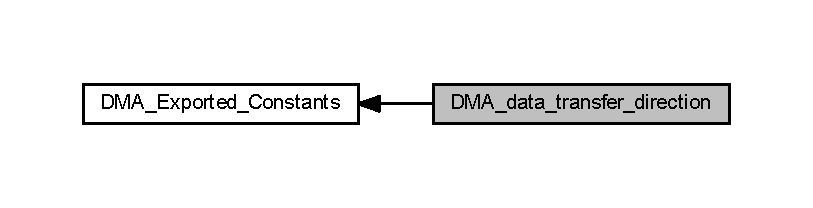
\includegraphics[width=350pt]{group___d_m_a__data__transfer__direction}
\end{center}
\end{figure}
\subsection*{Macros}
\begin{DoxyCompactItemize}
\item 
\mbox{\Hypertarget{group___d_m_a__data__transfer__direction_ga4d7847b57371eef92ec5da34511416a7}\label{group___d_m_a__data__transfer__direction_ga4d7847b57371eef92ec5da34511416a7}} 
\#define {\bfseries D\+M\+A\+\_\+\+D\+I\+R\+\_\+\+Peripheral\+To\+Memory}~((uint32\+\_\+t)0x00000000)
\item 
\mbox{\Hypertarget{group___d_m_a__data__transfer__direction_gae1e6aa2722beb09b5be7140205244986}\label{group___d_m_a__data__transfer__direction_gae1e6aa2722beb09b5be7140205244986}} 
\#define {\bfseries D\+M\+A\+\_\+\+D\+I\+R\+\_\+\+Memory\+To\+Peripheral}~((uint32\+\_\+t)0x00000040)
\item 
\mbox{\Hypertarget{group___d_m_a__data__transfer__direction_gafb7d5b786f2fb56a903936cdc6d5e89a}\label{group___d_m_a__data__transfer__direction_gafb7d5b786f2fb56a903936cdc6d5e89a}} 
\#define {\bfseries D\+M\+A\+\_\+\+D\+I\+R\+\_\+\+Memory\+To\+Memory}~((uint32\+\_\+t)0x00000080)
\item 
\#define {\bfseries I\+S\+\_\+\+D\+M\+A\+\_\+\+D\+I\+R\+E\+C\+T\+I\+ON}(D\+I\+R\+E\+C\+T\+I\+ON)
\end{DoxyCompactItemize}


\subsection{Detailed Description}


\subsection{Macro Definition Documentation}
\mbox{\Hypertarget{group___d_m_a__data__transfer__direction_gae2b02e8e823854bcd7c5746cdd29e70d}\label{group___d_m_a__data__transfer__direction_gae2b02e8e823854bcd7c5746cdd29e70d}} 
\index{D\+M\+A\+\_\+data\+\_\+transfer\+\_\+direction@{D\+M\+A\+\_\+data\+\_\+transfer\+\_\+direction}!I\+S\+\_\+\+D\+M\+A\+\_\+\+D\+I\+R\+E\+C\+T\+I\+ON@{I\+S\+\_\+\+D\+M\+A\+\_\+\+D\+I\+R\+E\+C\+T\+I\+ON}}
\index{I\+S\+\_\+\+D\+M\+A\+\_\+\+D\+I\+R\+E\+C\+T\+I\+ON@{I\+S\+\_\+\+D\+M\+A\+\_\+\+D\+I\+R\+E\+C\+T\+I\+ON}!D\+M\+A\+\_\+data\+\_\+transfer\+\_\+direction@{D\+M\+A\+\_\+data\+\_\+transfer\+\_\+direction}}
\subsubsection{\texorpdfstring{I\+S\+\_\+\+D\+M\+A\+\_\+\+D\+I\+R\+E\+C\+T\+I\+ON}{IS\_DMA\_DIRECTION}}
{\footnotesize\ttfamily \#define I\+S\+\_\+\+D\+M\+A\+\_\+\+D\+I\+R\+E\+C\+T\+I\+ON(\begin{DoxyParamCaption}\item[{}]{D\+I\+R\+E\+C\+T\+I\+ON }\end{DoxyParamCaption})}

{\bfseries Value\+:}
\begin{DoxyCode}
(((DIRECTION) == DMA\_DIR\_PeripheralToMemory ) || \(\backslash\)
                                     ((DIRECTION) == DMA\_DIR\_MemoryToPeripheral)  || \(\backslash\)
                                     ((DIRECTION) == DMA\_DIR\_MemoryToMemory))
\end{DoxyCode}


Definition at line 164 of file stm32f4xx\+\_\+dma.\+h.


\hypertarget{group___d_m_a__data__buffer__size}{}\section{D\+M\+A\+\_\+data\+\_\+buffer\+\_\+size}
\label{group___d_m_a__data__buffer__size}\index{D\+M\+A\+\_\+data\+\_\+buffer\+\_\+size@{D\+M\+A\+\_\+data\+\_\+buffer\+\_\+size}}
Collaboration diagram for D\+M\+A\+\_\+data\+\_\+buffer\+\_\+size\+:\nopagebreak
\begin{figure}[H]
\begin{center}
\leavevmode
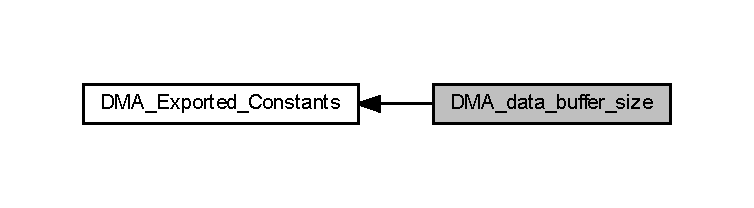
\includegraphics[width=350pt]{group___d_m_a__data__buffer__size}
\end{center}
\end{figure}
\subsection*{Macros}
\begin{DoxyCompactItemize}
\item 
\mbox{\Hypertarget{group___d_m_a__data__buffer__size_ga72ef4033bb3bc2cdfdbe579083b05e32}\label{group___d_m_a__data__buffer__size_ga72ef4033bb3bc2cdfdbe579083b05e32}} 
\#define {\bfseries I\+S\+\_\+\+D\+M\+A\+\_\+\+B\+U\+F\+F\+E\+R\+\_\+\+S\+I\+ZE}(S\+I\+ZE)~(((S\+I\+ZE) $>$= 0x1) \&\& ((\+S\+I\+Z\+E) $<$ 0x10000))
\end{DoxyCompactItemize}


\subsection{Detailed Description}

\hypertarget{group___d_m_a__peripheral__incremented__mode}{}\section{D\+M\+A\+\_\+peripheral\+\_\+incremented\+\_\+mode}
\label{group___d_m_a__peripheral__incremented__mode}\index{D\+M\+A\+\_\+peripheral\+\_\+incremented\+\_\+mode@{D\+M\+A\+\_\+peripheral\+\_\+incremented\+\_\+mode}}
Collaboration diagram for D\+M\+A\+\_\+peripheral\+\_\+incremented\+\_\+mode\+:\nopagebreak
\begin{figure}[H]
\begin{center}
\leavevmode
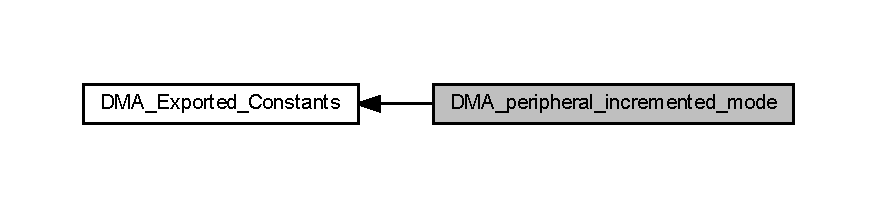
\includegraphics[width=350pt]{group___d_m_a__peripheral__incremented__mode}
\end{center}
\end{figure}
\subsection*{Macros}
\begin{DoxyCompactItemize}
\item 
\mbox{\Hypertarget{group___d_m_a__peripheral__incremented__mode_gaf7921ea423fb60701a091c508cd0f33a}\label{group___d_m_a__peripheral__incremented__mode_gaf7921ea423fb60701a091c508cd0f33a}} 
\#define {\bfseries D\+M\+A\+\_\+\+Peripheral\+Inc\+\_\+\+Enable}~((uint32\+\_\+t)0x00000200)
\item 
\mbox{\Hypertarget{group___d_m_a__peripheral__incremented__mode_ga0fe3ff9c67bec802dd239fd17c3dbd31}\label{group___d_m_a__peripheral__incremented__mode_ga0fe3ff9c67bec802dd239fd17c3dbd31}} 
\#define {\bfseries D\+M\+A\+\_\+\+Peripheral\+Inc\+\_\+\+Disable}~((uint32\+\_\+t)0x00000000)
\item 
\#define {\bfseries I\+S\+\_\+\+D\+M\+A\+\_\+\+P\+E\+R\+I\+P\+H\+E\+R\+A\+L\+\_\+\+I\+N\+C\+\_\+\+S\+T\+A\+TE}(S\+T\+A\+TE)
\end{DoxyCompactItemize}


\subsection{Detailed Description}


\subsection{Macro Definition Documentation}
\mbox{\Hypertarget{group___d_m_a__peripheral__incremented__mode_ga28762105b3f567c16ba79a47e68ff0fa}\label{group___d_m_a__peripheral__incremented__mode_ga28762105b3f567c16ba79a47e68ff0fa}} 
\index{D\+M\+A\+\_\+peripheral\+\_\+incremented\+\_\+mode@{D\+M\+A\+\_\+peripheral\+\_\+incremented\+\_\+mode}!I\+S\+\_\+\+D\+M\+A\+\_\+\+P\+E\+R\+I\+P\+H\+E\+R\+A\+L\+\_\+\+I\+N\+C\+\_\+\+S\+T\+A\+TE@{I\+S\+\_\+\+D\+M\+A\+\_\+\+P\+E\+R\+I\+P\+H\+E\+R\+A\+L\+\_\+\+I\+N\+C\+\_\+\+S\+T\+A\+TE}}
\index{I\+S\+\_\+\+D\+M\+A\+\_\+\+P\+E\+R\+I\+P\+H\+E\+R\+A\+L\+\_\+\+I\+N\+C\+\_\+\+S\+T\+A\+TE@{I\+S\+\_\+\+D\+M\+A\+\_\+\+P\+E\+R\+I\+P\+H\+E\+R\+A\+L\+\_\+\+I\+N\+C\+\_\+\+S\+T\+A\+TE}!D\+M\+A\+\_\+peripheral\+\_\+incremented\+\_\+mode@{D\+M\+A\+\_\+peripheral\+\_\+incremented\+\_\+mode}}
\subsubsection{\texorpdfstring{I\+S\+\_\+\+D\+M\+A\+\_\+\+P\+E\+R\+I\+P\+H\+E\+R\+A\+L\+\_\+\+I\+N\+C\+\_\+\+S\+T\+A\+TE}{IS\_DMA\_PERIPHERAL\_INC\_STATE}}
{\footnotesize\ttfamily \#define I\+S\+\_\+\+D\+M\+A\+\_\+\+P\+E\+R\+I\+P\+H\+E\+R\+A\+L\+\_\+\+I\+N\+C\+\_\+\+S\+T\+A\+TE(\begin{DoxyParamCaption}\item[{}]{S\+T\+A\+TE }\end{DoxyParamCaption})}

{\bfseries Value\+:}
\begin{DoxyCode}
(((STATE) == DMA\_PeripheralInc\_Enable) || \(\backslash\)
                                            ((STATE) == DMA\_PeripheralInc\_Disable))
\end{DoxyCode}


Definition at line 187 of file stm32f4xx\+\_\+dma.\+h.


\hypertarget{group___d_m_a__memory__incremented__mode}{}\section{D\+M\+A\+\_\+memory\+\_\+incremented\+\_\+mode}
\label{group___d_m_a__memory__incremented__mode}\index{D\+M\+A\+\_\+memory\+\_\+incremented\+\_\+mode@{D\+M\+A\+\_\+memory\+\_\+incremented\+\_\+mode}}
Collaboration diagram for D\+M\+A\+\_\+memory\+\_\+incremented\+\_\+mode\+:\nopagebreak
\begin{figure}[H]
\begin{center}
\leavevmode
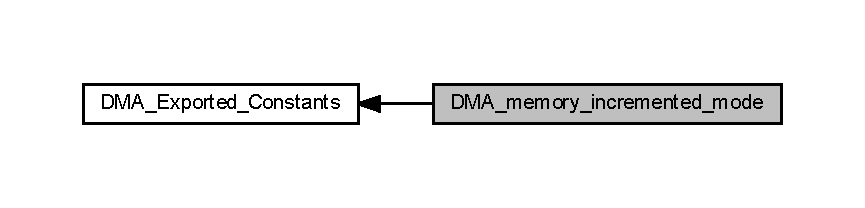
\includegraphics[width=350pt]{group___d_m_a__memory__incremented__mode}
\end{center}
\end{figure}
\subsection*{Macros}
\begin{DoxyCompactItemize}
\item 
\mbox{\Hypertarget{group___d_m_a__memory__incremented__mode_ga4e8cb23d039c74bbbf365d7678835bbb}\label{group___d_m_a__memory__incremented__mode_ga4e8cb23d039c74bbbf365d7678835bbb}} 
\#define {\bfseries D\+M\+A\+\_\+\+Memory\+Inc\+\_\+\+Enable}~((uint32\+\_\+t)0x00000400)
\item 
\mbox{\Hypertarget{group___d_m_a__memory__incremented__mode_ga795a277c997048783a383b026f19a5ab}\label{group___d_m_a__memory__incremented__mode_ga795a277c997048783a383b026f19a5ab}} 
\#define {\bfseries D\+M\+A\+\_\+\+Memory\+Inc\+\_\+\+Disable}~((uint32\+\_\+t)0x00000000)
\item 
\#define {\bfseries I\+S\+\_\+\+D\+M\+A\+\_\+\+M\+E\+M\+O\+R\+Y\+\_\+\+I\+N\+C\+\_\+\+S\+T\+A\+TE}(S\+T\+A\+TE)
\end{DoxyCompactItemize}


\subsection{Detailed Description}


\subsection{Macro Definition Documentation}
\mbox{\Hypertarget{group___d_m_a__memory__incremented__mode_gaa880f39d499d1e80449cf80381e4eb67}\label{group___d_m_a__memory__incremented__mode_gaa880f39d499d1e80449cf80381e4eb67}} 
\index{D\+M\+A\+\_\+memory\+\_\+incremented\+\_\+mode@{D\+M\+A\+\_\+memory\+\_\+incremented\+\_\+mode}!I\+S\+\_\+\+D\+M\+A\+\_\+\+M\+E\+M\+O\+R\+Y\+\_\+\+I\+N\+C\+\_\+\+S\+T\+A\+TE@{I\+S\+\_\+\+D\+M\+A\+\_\+\+M\+E\+M\+O\+R\+Y\+\_\+\+I\+N\+C\+\_\+\+S\+T\+A\+TE}}
\index{I\+S\+\_\+\+D\+M\+A\+\_\+\+M\+E\+M\+O\+R\+Y\+\_\+\+I\+N\+C\+\_\+\+S\+T\+A\+TE@{I\+S\+\_\+\+D\+M\+A\+\_\+\+M\+E\+M\+O\+R\+Y\+\_\+\+I\+N\+C\+\_\+\+S\+T\+A\+TE}!D\+M\+A\+\_\+memory\+\_\+incremented\+\_\+mode@{D\+M\+A\+\_\+memory\+\_\+incremented\+\_\+mode}}
\subsubsection{\texorpdfstring{I\+S\+\_\+\+D\+M\+A\+\_\+\+M\+E\+M\+O\+R\+Y\+\_\+\+I\+N\+C\+\_\+\+S\+T\+A\+TE}{IS\_DMA\_MEMORY\_INC\_STATE}}
{\footnotesize\ttfamily \#define I\+S\+\_\+\+D\+M\+A\+\_\+\+M\+E\+M\+O\+R\+Y\+\_\+\+I\+N\+C\+\_\+\+S\+T\+A\+TE(\begin{DoxyParamCaption}\item[{}]{S\+T\+A\+TE }\end{DoxyParamCaption})}

{\bfseries Value\+:}
\begin{DoxyCode}
(((STATE) == DMA\_MemoryInc\_Enable) || \(\backslash\)
                                        ((STATE) == DMA\_MemoryInc\_Disable))
\end{DoxyCode}


Definition at line 200 of file stm32f4xx\+\_\+dma.\+h.


\hypertarget{group___d_m_a__peripheral__data__size}{}\section{D\+M\+A\+\_\+peripheral\+\_\+data\+\_\+size}
\label{group___d_m_a__peripheral__data__size}\index{D\+M\+A\+\_\+peripheral\+\_\+data\+\_\+size@{D\+M\+A\+\_\+peripheral\+\_\+data\+\_\+size}}
Collaboration diagram for D\+M\+A\+\_\+peripheral\+\_\+data\+\_\+size\+:
\nopagebreak
\begin{figure}[H]
\begin{center}
\leavevmode
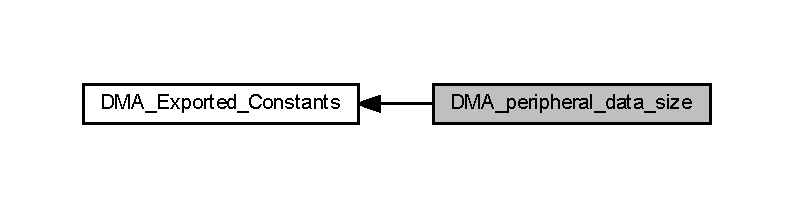
\includegraphics[width=350pt]{group___d_m_a__peripheral__data__size}
\end{center}
\end{figure}
\subsection*{Macros}
\begin{DoxyCompactItemize}
\item 
\mbox{\Hypertarget{group___d_m_a__peripheral__data__size_ga7577035ae4ff413164000227a8cea346}\label{group___d_m_a__peripheral__data__size_ga7577035ae4ff413164000227a8cea346}} 
\#define {\bfseries D\+M\+A\+\_\+\+Peripheral\+Data\+Size\+\_\+\+Byte}~((uint32\+\_\+t)0x00000000)
\item 
\mbox{\Hypertarget{group___d_m_a__peripheral__data__size_gab1988e5005ee65c261018f62866e4585}\label{group___d_m_a__peripheral__data__size_gab1988e5005ee65c261018f62866e4585}} 
\#define {\bfseries D\+M\+A\+\_\+\+Peripheral\+Data\+Size\+\_\+\+Half\+Word}~((uint32\+\_\+t)0x00000800)
\item 
\mbox{\Hypertarget{group___d_m_a__peripheral__data__size_ga516ea7a40945d8325fe73e079b245ea1}\label{group___d_m_a__peripheral__data__size_ga516ea7a40945d8325fe73e079b245ea1}} 
\#define {\bfseries D\+M\+A\+\_\+\+Peripheral\+Data\+Size\+\_\+\+Word}~((uint32\+\_\+t)0x00001000)
\item 
\#define {\bfseries I\+S\+\_\+\+D\+M\+A\+\_\+\+P\+E\+R\+I\+P\+H\+E\+R\+A\+L\+\_\+\+D\+A\+T\+A\+\_\+\+S\+I\+ZE}(S\+I\+ZE)
\end{DoxyCompactItemize}


\subsection{Detailed Description}


\subsection{Macro Definition Documentation}
\mbox{\Hypertarget{group___d_m_a__peripheral__data__size_gad7916e0ae55cdf5efdfa68a09a028037}\label{group___d_m_a__peripheral__data__size_gad7916e0ae55cdf5efdfa68a09a028037}} 
\index{D\+M\+A\+\_\+peripheral\+\_\+data\+\_\+size@{D\+M\+A\+\_\+peripheral\+\_\+data\+\_\+size}!I\+S\+\_\+\+D\+M\+A\+\_\+\+P\+E\+R\+I\+P\+H\+E\+R\+A\+L\+\_\+\+D\+A\+T\+A\+\_\+\+S\+I\+ZE@{I\+S\+\_\+\+D\+M\+A\+\_\+\+P\+E\+R\+I\+P\+H\+E\+R\+A\+L\+\_\+\+D\+A\+T\+A\+\_\+\+S\+I\+ZE}}
\index{I\+S\+\_\+\+D\+M\+A\+\_\+\+P\+E\+R\+I\+P\+H\+E\+R\+A\+L\+\_\+\+D\+A\+T\+A\+\_\+\+S\+I\+ZE@{I\+S\+\_\+\+D\+M\+A\+\_\+\+P\+E\+R\+I\+P\+H\+E\+R\+A\+L\+\_\+\+D\+A\+T\+A\+\_\+\+S\+I\+ZE}!D\+M\+A\+\_\+peripheral\+\_\+data\+\_\+size@{D\+M\+A\+\_\+peripheral\+\_\+data\+\_\+size}}
\subsubsection{\texorpdfstring{I\+S\+\_\+\+D\+M\+A\+\_\+\+P\+E\+R\+I\+P\+H\+E\+R\+A\+L\+\_\+\+D\+A\+T\+A\+\_\+\+S\+I\+ZE}{IS\_DMA\_PERIPHERAL\_DATA\_SIZE}}
{\footnotesize\ttfamily \#define I\+S\+\_\+\+D\+M\+A\+\_\+\+P\+E\+R\+I\+P\+H\+E\+R\+A\+L\+\_\+\+D\+A\+T\+A\+\_\+\+S\+I\+ZE(\begin{DoxyParamCaption}\item[{}]{S\+I\+ZE }\end{DoxyParamCaption})}

{\bfseries Value\+:}
\begin{DoxyCode}
(((SIZE) == DMA\_PeripheralDataSize\_Byte)  || \(\backslash\)
                                           ((SIZE) == DMA\_PeripheralDataSize\_HalfWord) || \(\backslash\)
                                           ((SIZE) == DMA\_PeripheralDataSize\_Word))
\end{DoxyCode}


Definition at line 214 of file stm32f4xx\+\_\+dma.\+h.


\hypertarget{group___d_m_a__memory__data__size}{}\section{D\+M\+A\+\_\+memory\+\_\+data\+\_\+size}
\label{group___d_m_a__memory__data__size}\index{D\+M\+A\+\_\+memory\+\_\+data\+\_\+size@{D\+M\+A\+\_\+memory\+\_\+data\+\_\+size}}
Collaboration diagram for D\+M\+A\+\_\+memory\+\_\+data\+\_\+size\+:\nopagebreak
\begin{figure}[H]
\begin{center}
\leavevmode
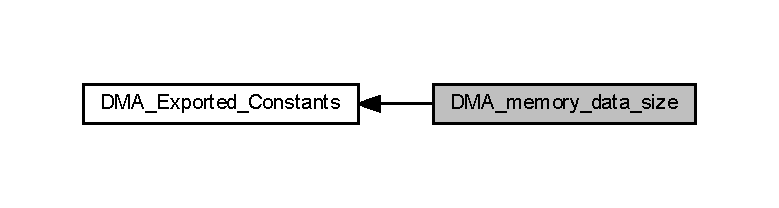
\includegraphics[width=350pt]{group___d_m_a__memory__data__size}
\end{center}
\end{figure}
\subsection*{Macros}
\begin{DoxyCompactItemize}
\item 
\mbox{\Hypertarget{group___d_m_a__memory__data__size_gad6093bccb60ff9adf81e21c73c58ba17}\label{group___d_m_a__memory__data__size_gad6093bccb60ff9adf81e21c73c58ba17}} 
\#define {\bfseries D\+M\+A\+\_\+\+Memory\+Data\+Size\+\_\+\+Byte}~((uint32\+\_\+t)0x00000000)
\item 
\mbox{\Hypertarget{group___d_m_a__memory__data__size_ga74c9b4e547f5eaaf35d4fd3d01ed5741}\label{group___d_m_a__memory__data__size_ga74c9b4e547f5eaaf35d4fd3d01ed5741}} 
\#define {\bfseries D\+M\+A\+\_\+\+Memory\+Data\+Size\+\_\+\+Half\+Word}~((uint32\+\_\+t)0x00002000)
\item 
\mbox{\Hypertarget{group___d_m_a__memory__data__size_gaff403722a6f82d4b34c9ef306507bb98}\label{group___d_m_a__memory__data__size_gaff403722a6f82d4b34c9ef306507bb98}} 
\#define {\bfseries D\+M\+A\+\_\+\+Memory\+Data\+Size\+\_\+\+Word}~((uint32\+\_\+t)0x00004000)
\item 
\#define {\bfseries I\+S\+\_\+\+D\+M\+A\+\_\+\+M\+E\+M\+O\+R\+Y\+\_\+\+D\+A\+T\+A\+\_\+\+S\+I\+ZE}(S\+I\+ZE)
\end{DoxyCompactItemize}


\subsection{Detailed Description}


\subsection{Macro Definition Documentation}
\mbox{\Hypertarget{group___d_m_a__memory__data__size_gac9e3748cebcb16d4ae4206d562bc804c}\label{group___d_m_a__memory__data__size_gac9e3748cebcb16d4ae4206d562bc804c}} 
\index{D\+M\+A\+\_\+memory\+\_\+data\+\_\+size@{D\+M\+A\+\_\+memory\+\_\+data\+\_\+size}!I\+S\+\_\+\+D\+M\+A\+\_\+\+M\+E\+M\+O\+R\+Y\+\_\+\+D\+A\+T\+A\+\_\+\+S\+I\+ZE@{I\+S\+\_\+\+D\+M\+A\+\_\+\+M\+E\+M\+O\+R\+Y\+\_\+\+D\+A\+T\+A\+\_\+\+S\+I\+ZE}}
\index{I\+S\+\_\+\+D\+M\+A\+\_\+\+M\+E\+M\+O\+R\+Y\+\_\+\+D\+A\+T\+A\+\_\+\+S\+I\+ZE@{I\+S\+\_\+\+D\+M\+A\+\_\+\+M\+E\+M\+O\+R\+Y\+\_\+\+D\+A\+T\+A\+\_\+\+S\+I\+ZE}!D\+M\+A\+\_\+memory\+\_\+data\+\_\+size@{D\+M\+A\+\_\+memory\+\_\+data\+\_\+size}}
\subsubsection{\texorpdfstring{I\+S\+\_\+\+D\+M\+A\+\_\+\+M\+E\+M\+O\+R\+Y\+\_\+\+D\+A\+T\+A\+\_\+\+S\+I\+ZE}{IS\_DMA\_MEMORY\_DATA\_SIZE}}
{\footnotesize\ttfamily \#define I\+S\+\_\+\+D\+M\+A\+\_\+\+M\+E\+M\+O\+R\+Y\+\_\+\+D\+A\+T\+A\+\_\+\+S\+I\+ZE(\begin{DoxyParamCaption}\item[{}]{S\+I\+ZE }\end{DoxyParamCaption})}

{\bfseries Value\+:}
\begin{DoxyCode}
(((SIZE) == DMA\_MemoryDataSize\_Byte)  || \(\backslash\)
                                       ((SIZE) == DMA\_MemoryDataSize\_HalfWord) || \(\backslash\)
                                       ((SIZE) == DMA\_MemoryDataSize\_Word ))
\end{DoxyCode}


Definition at line 229 of file stm32f4xx\+\_\+dma.\+h.


\hypertarget{group___d_m_a__circular__normal__mode}{}\section{D\+M\+A\+\_\+circular\+\_\+normal\+\_\+mode}
\label{group___d_m_a__circular__normal__mode}\index{D\+M\+A\+\_\+circular\+\_\+normal\+\_\+mode@{D\+M\+A\+\_\+circular\+\_\+normal\+\_\+mode}}
Collaboration diagram for D\+M\+A\+\_\+circular\+\_\+normal\+\_\+mode\+:
\nopagebreak
\begin{figure}[H]
\begin{center}
\leavevmode
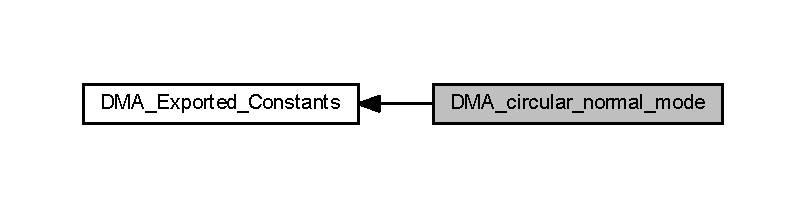
\includegraphics[width=350pt]{group___d_m_a__circular__normal__mode}
\end{center}
\end{figure}
\subsection*{Macros}
\begin{DoxyCompactItemize}
\item 
\mbox{\Hypertarget{group___d_m_a__circular__normal__mode_ga36400f5b5095f1102ede4760d7a5959c}\label{group___d_m_a__circular__normal__mode_ga36400f5b5095f1102ede4760d7a5959c}} 
\#define {\bfseries D\+M\+A\+\_\+\+Mode\+\_\+\+Normal}~((uint32\+\_\+t)0x00000000)
\item 
\mbox{\Hypertarget{group___d_m_a__circular__normal__mode_ga36327b14c302098fbc5823ac3f1ae020}\label{group___d_m_a__circular__normal__mode_ga36327b14c302098fbc5823ac3f1ae020}} 
\#define {\bfseries D\+M\+A\+\_\+\+Mode\+\_\+\+Circular}~((uint32\+\_\+t)0x00000100)
\item 
\#define {\bfseries I\+S\+\_\+\+D\+M\+A\+\_\+\+M\+O\+DE}(M\+O\+DE)
\end{DoxyCompactItemize}


\subsection{Detailed Description}


\subsection{Macro Definition Documentation}
\mbox{\Hypertarget{group___d_m_a__circular__normal__mode_gad88ee5030574d6a573904378fb62c7ac}\label{group___d_m_a__circular__normal__mode_gad88ee5030574d6a573904378fb62c7ac}} 
\index{D\+M\+A\+\_\+circular\+\_\+normal\+\_\+mode@{D\+M\+A\+\_\+circular\+\_\+normal\+\_\+mode}!I\+S\+\_\+\+D\+M\+A\+\_\+\+M\+O\+DE@{I\+S\+\_\+\+D\+M\+A\+\_\+\+M\+O\+DE}}
\index{I\+S\+\_\+\+D\+M\+A\+\_\+\+M\+O\+DE@{I\+S\+\_\+\+D\+M\+A\+\_\+\+M\+O\+DE}!D\+M\+A\+\_\+circular\+\_\+normal\+\_\+mode@{D\+M\+A\+\_\+circular\+\_\+normal\+\_\+mode}}
\subsubsection{\texorpdfstring{I\+S\+\_\+\+D\+M\+A\+\_\+\+M\+O\+DE}{IS\_DMA\_MODE}}
{\footnotesize\ttfamily \#define I\+S\+\_\+\+D\+M\+A\+\_\+\+M\+O\+DE(\begin{DoxyParamCaption}\item[{}]{M\+O\+DE }\end{DoxyParamCaption})}

{\bfseries Value\+:}
\begin{DoxyCode}
(((MODE) == DMA\_Mode\_Normal ) || \(\backslash\)
                           ((MODE) == DMA\_Mode\_Circular))
\end{DoxyCode}


Definition at line 243 of file stm32f4xx\+\_\+dma.\+h.


\hypertarget{group___d_m_a__priority__level}{}\section{D\+M\+A\+\_\+priority\+\_\+level}
\label{group___d_m_a__priority__level}\index{D\+M\+A\+\_\+priority\+\_\+level@{D\+M\+A\+\_\+priority\+\_\+level}}
Collaboration diagram for D\+M\+A\+\_\+priority\+\_\+level\+:\nopagebreak
\begin{figure}[H]
\begin{center}
\leavevmode
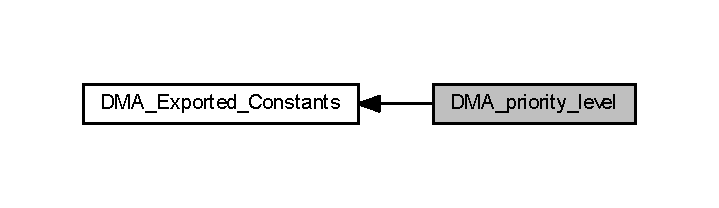
\includegraphics[width=345pt]{group___d_m_a__priority__level}
\end{center}
\end{figure}
\subsection*{Macros}
\begin{DoxyCompactItemize}
\item 
\mbox{\Hypertarget{group___d_m_a__priority__level_gaf414e0aa8dd42aee6f83f88ab6175179}\label{group___d_m_a__priority__level_gaf414e0aa8dd42aee6f83f88ab6175179}} 
\#define {\bfseries D\+M\+A\+\_\+\+Priority\+\_\+\+Low}~((uint32\+\_\+t)0x00000000)
\item 
\mbox{\Hypertarget{group___d_m_a__priority__level_ga8e0d4a958f4288c6c759945789490f38}\label{group___d_m_a__priority__level_ga8e0d4a958f4288c6c759945789490f38}} 
\#define {\bfseries D\+M\+A\+\_\+\+Priority\+\_\+\+Medium}~((uint32\+\_\+t)0x00010000)
\item 
\mbox{\Hypertarget{group___d_m_a__priority__level_gae2441c0b4d4ba9945a6f4f7d08045a8e}\label{group___d_m_a__priority__level_gae2441c0b4d4ba9945a6f4f7d08045a8e}} 
\#define {\bfseries D\+M\+A\+\_\+\+Priority\+\_\+\+High}~((uint32\+\_\+t)0x00020000)
\item 
\mbox{\Hypertarget{group___d_m_a__priority__level_gadccd2f8b2ac24ba4fd485dd5b9b48671}\label{group___d_m_a__priority__level_gadccd2f8b2ac24ba4fd485dd5b9b48671}} 
\#define {\bfseries D\+M\+A\+\_\+\+Priority\+\_\+\+Very\+High}~((uint32\+\_\+t)0x00030000)
\item 
\#define {\bfseries I\+S\+\_\+\+D\+M\+A\+\_\+\+P\+R\+I\+O\+R\+I\+TY}(P\+R\+I\+O\+R\+I\+TY)
\end{DoxyCompactItemize}


\subsection{Detailed Description}


\subsection{Macro Definition Documentation}
\mbox{\Hypertarget{group___d_m_a__priority__level_gaa1cae2ab458948511596467c87cd02b6}\label{group___d_m_a__priority__level_gaa1cae2ab458948511596467c87cd02b6}} 
\index{D\+M\+A\+\_\+priority\+\_\+level@{D\+M\+A\+\_\+priority\+\_\+level}!I\+S\+\_\+\+D\+M\+A\+\_\+\+P\+R\+I\+O\+R\+I\+TY@{I\+S\+\_\+\+D\+M\+A\+\_\+\+P\+R\+I\+O\+R\+I\+TY}}
\index{I\+S\+\_\+\+D\+M\+A\+\_\+\+P\+R\+I\+O\+R\+I\+TY@{I\+S\+\_\+\+D\+M\+A\+\_\+\+P\+R\+I\+O\+R\+I\+TY}!D\+M\+A\+\_\+priority\+\_\+level@{D\+M\+A\+\_\+priority\+\_\+level}}
\subsubsection{\texorpdfstring{I\+S\+\_\+\+D\+M\+A\+\_\+\+P\+R\+I\+O\+R\+I\+TY}{IS\_DMA\_PRIORITY}}
{\footnotesize\ttfamily \#define I\+S\+\_\+\+D\+M\+A\+\_\+\+P\+R\+I\+O\+R\+I\+TY(\begin{DoxyParamCaption}\item[{}]{P\+R\+I\+O\+R\+I\+TY }\end{DoxyParamCaption})}

{\bfseries Value\+:}
\begin{DoxyCode}
(((PRIORITY) == DMA\_Priority\_Low )   || \(\backslash\)
                                   ((PRIORITY) == DMA\_Priority\_Medium) || \(\backslash\)
                                   ((PRIORITY) == DMA\_Priority\_High)   || \(\backslash\)
                                   ((PRIORITY) == DMA\_Priority\_VeryHigh))
\end{DoxyCode}


Definition at line 258 of file stm32f4xx\+\_\+dma.\+h.


\hypertarget{group___d_m_a__fifo__direct__mode}{}\section{D\+M\+A\+\_\+fifo\+\_\+direct\+\_\+mode}
\label{group___d_m_a__fifo__direct__mode}\index{D\+M\+A\+\_\+fifo\+\_\+direct\+\_\+mode@{D\+M\+A\+\_\+fifo\+\_\+direct\+\_\+mode}}
Collaboration diagram for D\+M\+A\+\_\+fifo\+\_\+direct\+\_\+mode\+:\nopagebreak
\begin{figure}[H]
\begin{center}
\leavevmode
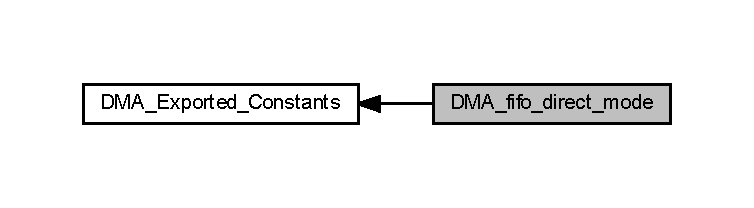
\includegraphics[width=350pt]{group___d_m_a__fifo__direct__mode}
\end{center}
\end{figure}
\subsection*{Macros}
\begin{DoxyCompactItemize}
\item 
\mbox{\Hypertarget{group___d_m_a__fifo__direct__mode_gadad9e503fa9867a981e3090d333483d7}\label{group___d_m_a__fifo__direct__mode_gadad9e503fa9867a981e3090d333483d7}} 
\#define {\bfseries D\+M\+A\+\_\+\+F\+I\+F\+O\+Mode\+\_\+\+Disable}~((uint32\+\_\+t)0x00000000)
\item 
\mbox{\Hypertarget{group___d_m_a__fifo__direct__mode_ga482bc2af420602d1a8c2aa35049a3857}\label{group___d_m_a__fifo__direct__mode_ga482bc2af420602d1a8c2aa35049a3857}} 
\#define {\bfseries D\+M\+A\+\_\+\+F\+I\+F\+O\+Mode\+\_\+\+Enable}~((uint32\+\_\+t)0x00000004)
\item 
\#define {\bfseries I\+S\+\_\+\+D\+M\+A\+\_\+\+F\+I\+F\+O\+\_\+\+M\+O\+D\+E\+\_\+\+S\+T\+A\+TE}(S\+T\+A\+TE)
\end{DoxyCompactItemize}


\subsection{Detailed Description}


\subsection{Macro Definition Documentation}
\mbox{\Hypertarget{group___d_m_a__fifo__direct__mode_gadb90a893aeb49fd4bc14af750af3837c}\label{group___d_m_a__fifo__direct__mode_gadb90a893aeb49fd4bc14af750af3837c}} 
\index{D\+M\+A\+\_\+fifo\+\_\+direct\+\_\+mode@{D\+M\+A\+\_\+fifo\+\_\+direct\+\_\+mode}!I\+S\+\_\+\+D\+M\+A\+\_\+\+F\+I\+F\+O\+\_\+\+M\+O\+D\+E\+\_\+\+S\+T\+A\+TE@{I\+S\+\_\+\+D\+M\+A\+\_\+\+F\+I\+F\+O\+\_\+\+M\+O\+D\+E\+\_\+\+S\+T\+A\+TE}}
\index{I\+S\+\_\+\+D\+M\+A\+\_\+\+F\+I\+F\+O\+\_\+\+M\+O\+D\+E\+\_\+\+S\+T\+A\+TE@{I\+S\+\_\+\+D\+M\+A\+\_\+\+F\+I\+F\+O\+\_\+\+M\+O\+D\+E\+\_\+\+S\+T\+A\+TE}!D\+M\+A\+\_\+fifo\+\_\+direct\+\_\+mode@{D\+M\+A\+\_\+fifo\+\_\+direct\+\_\+mode}}
\subsubsection{\texorpdfstring{I\+S\+\_\+\+D\+M\+A\+\_\+\+F\+I\+F\+O\+\_\+\+M\+O\+D\+E\+\_\+\+S\+T\+A\+TE}{IS\_DMA\_FIFO\_MODE\_STATE}}
{\footnotesize\ttfamily \#define I\+S\+\_\+\+D\+M\+A\+\_\+\+F\+I\+F\+O\+\_\+\+M\+O\+D\+E\+\_\+\+S\+T\+A\+TE(\begin{DoxyParamCaption}\item[{}]{S\+T\+A\+TE }\end{DoxyParamCaption})}

{\bfseries Value\+:}
\begin{DoxyCode}
(((STATE) == DMA\_FIFOMode\_Disable ) || \(\backslash\)
                                       ((STATE) == DMA\_FIFOMode\_Enable))
\end{DoxyCode}


Definition at line 273 of file stm32f4xx\+\_\+dma.\+h.


\hypertarget{group___d_m_a__fifo__threshold__level}{}\section{D\+M\+A\+\_\+fifo\+\_\+threshold\+\_\+level}
\label{group___d_m_a__fifo__threshold__level}\index{D\+M\+A\+\_\+fifo\+\_\+threshold\+\_\+level@{D\+M\+A\+\_\+fifo\+\_\+threshold\+\_\+level}}
Collaboration diagram for D\+M\+A\+\_\+fifo\+\_\+threshold\+\_\+level\+:
\nopagebreak
\begin{figure}[H]
\begin{center}
\leavevmode
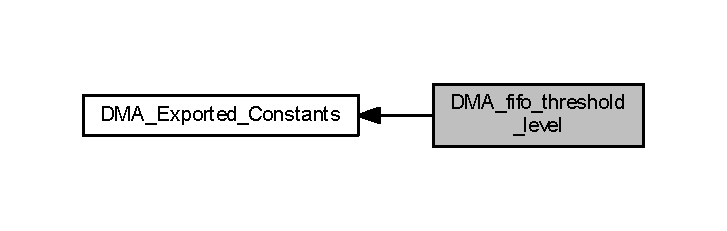
\includegraphics[width=349pt]{group___d_m_a__fifo__threshold__level}
\end{center}
\end{figure}
\subsection*{Macros}
\begin{DoxyCompactItemize}
\item 
\mbox{\Hypertarget{group___d_m_a__fifo__threshold__level_gacc98384bbba43a9c4f70b448518acfe4}\label{group___d_m_a__fifo__threshold__level_gacc98384bbba43a9c4f70b448518acfe4}} 
\#define {\bfseries D\+M\+A\+\_\+\+F\+I\+F\+O\+Threshold\+\_\+1\+Quarter\+Full}~((uint32\+\_\+t)0x00000000)
\item 
\mbox{\Hypertarget{group___d_m_a__fifo__threshold__level_ga626b546865960343fdcfdf33ac8ceb03}\label{group___d_m_a__fifo__threshold__level_ga626b546865960343fdcfdf33ac8ceb03}} 
\#define {\bfseries D\+M\+A\+\_\+\+F\+I\+F\+O\+Threshold\+\_\+\+Half\+Full}~((uint32\+\_\+t)0x00000001)
\item 
\mbox{\Hypertarget{group___d_m_a__fifo__threshold__level_ga6f041008fce4bb341f9a518d803a308b}\label{group___d_m_a__fifo__threshold__level_ga6f041008fce4bb341f9a518d803a308b}} 
\#define {\bfseries D\+M\+A\+\_\+\+F\+I\+F\+O\+Threshold\+\_\+3\+Quarters\+Full}~((uint32\+\_\+t)0x00000002)
\item 
\mbox{\Hypertarget{group___d_m_a__fifo__threshold__level_ga9f1008e0df7d41d910ed89d7e0872e69}\label{group___d_m_a__fifo__threshold__level_ga9f1008e0df7d41d910ed89d7e0872e69}} 
\#define {\bfseries D\+M\+A\+\_\+\+F\+I\+F\+O\+Threshold\+\_\+\+Full}~((uint32\+\_\+t)0x00000003)
\item 
\#define {\bfseries I\+S\+\_\+\+D\+M\+A\+\_\+\+F\+I\+F\+O\+\_\+\+T\+H\+R\+E\+S\+H\+O\+LD}(T\+H\+R\+E\+S\+H\+O\+LD)
\end{DoxyCompactItemize}


\subsection{Detailed Description}


\subsection{Macro Definition Documentation}
\mbox{\Hypertarget{group___d_m_a__fifo__threshold__level_gaeafc0d9e327d6e5b26cd37f6744b232f}\label{group___d_m_a__fifo__threshold__level_gaeafc0d9e327d6e5b26cd37f6744b232f}} 
\index{D\+M\+A\+\_\+fifo\+\_\+threshold\+\_\+level@{D\+M\+A\+\_\+fifo\+\_\+threshold\+\_\+level}!I\+S\+\_\+\+D\+M\+A\+\_\+\+F\+I\+F\+O\+\_\+\+T\+H\+R\+E\+S\+H\+O\+LD@{I\+S\+\_\+\+D\+M\+A\+\_\+\+F\+I\+F\+O\+\_\+\+T\+H\+R\+E\+S\+H\+O\+LD}}
\index{I\+S\+\_\+\+D\+M\+A\+\_\+\+F\+I\+F\+O\+\_\+\+T\+H\+R\+E\+S\+H\+O\+LD@{I\+S\+\_\+\+D\+M\+A\+\_\+\+F\+I\+F\+O\+\_\+\+T\+H\+R\+E\+S\+H\+O\+LD}!D\+M\+A\+\_\+fifo\+\_\+threshold\+\_\+level@{D\+M\+A\+\_\+fifo\+\_\+threshold\+\_\+level}}
\subsubsection{\texorpdfstring{I\+S\+\_\+\+D\+M\+A\+\_\+\+F\+I\+F\+O\+\_\+\+T\+H\+R\+E\+S\+H\+O\+LD}{IS\_DMA\_FIFO\_THRESHOLD}}
{\footnotesize\ttfamily \#define I\+S\+\_\+\+D\+M\+A\+\_\+\+F\+I\+F\+O\+\_\+\+T\+H\+R\+E\+S\+H\+O\+LD(\begin{DoxyParamCaption}\item[{}]{T\+H\+R\+E\+S\+H\+O\+LD }\end{DoxyParamCaption})}

{\bfseries Value\+:}
\begin{DoxyCode}
(((THRESHOLD) == DMA\_FIFOThreshold\_1QuarterFull ) || \(\backslash\)
                                          ((THRESHOLD) == DMA\_FIFOThreshold\_HalfFull)      || \(\backslash\)
                                          ((THRESHOLD) == DMA\_FIFOThreshold\_3QuartersFull) || \(\backslash\)
                                          ((THRESHOLD) == DMA\_FIFOThreshold\_Full))
\end{DoxyCode}


Definition at line 288 of file stm32f4xx\+\_\+dma.\+h.


\hypertarget{group___d_m_a__memory__burst}{}\section{D\+M\+A\+\_\+memory\+\_\+burst}
\label{group___d_m_a__memory__burst}\index{D\+M\+A\+\_\+memory\+\_\+burst@{D\+M\+A\+\_\+memory\+\_\+burst}}
Collaboration diagram for D\+M\+A\+\_\+memory\+\_\+burst\+:
\nopagebreak
\begin{figure}[H]
\begin{center}
\leavevmode
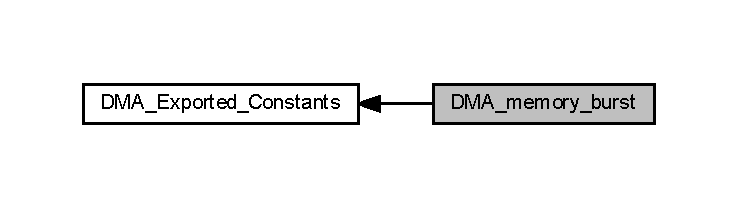
\includegraphics[width=350pt]{group___d_m_a__memory__burst}
\end{center}
\end{figure}
\subsection*{Macros}
\begin{DoxyCompactItemize}
\item 
\mbox{\Hypertarget{group___d_m_a__memory__burst_gab3353b3a85b555f826fe567ce68c3fc3}\label{group___d_m_a__memory__burst_gab3353b3a85b555f826fe567ce68c3fc3}} 
\#define {\bfseries D\+M\+A\+\_\+\+Memory\+Burst\+\_\+\+Single}~((uint32\+\_\+t)0x00000000)
\item 
\mbox{\Hypertarget{group___d_m_a__memory__burst_gacf7f57731c663fdc6ca8a6fb18ff31b0}\label{group___d_m_a__memory__burst_gacf7f57731c663fdc6ca8a6fb18ff31b0}} 
\#define {\bfseries D\+M\+A\+\_\+\+Memory\+Burst\+\_\+\+I\+N\+C4}~((uint32\+\_\+t)0x00800000)
\item 
\mbox{\Hypertarget{group___d_m_a__memory__burst_ga33aca825c5a81e83753ff6fadb3634c0}\label{group___d_m_a__memory__burst_ga33aca825c5a81e83753ff6fadb3634c0}} 
\#define {\bfseries D\+M\+A\+\_\+\+Memory\+Burst\+\_\+\+I\+N\+C8}~((uint32\+\_\+t)0x01000000)
\item 
\mbox{\Hypertarget{group___d_m_a__memory__burst_ga4ffd4960f794b187229fac1cea3d81c9}\label{group___d_m_a__memory__burst_ga4ffd4960f794b187229fac1cea3d81c9}} 
\#define {\bfseries D\+M\+A\+\_\+\+Memory\+Burst\+\_\+\+I\+N\+C16}~((uint32\+\_\+t)0x01800000)
\item 
\#define {\bfseries I\+S\+\_\+\+D\+M\+A\+\_\+\+M\+E\+M\+O\+R\+Y\+\_\+\+B\+U\+R\+ST}(B\+U\+R\+ST)
\end{DoxyCompactItemize}


\subsection{Detailed Description}


\subsection{Macro Definition Documentation}
\mbox{\Hypertarget{group___d_m_a__memory__burst_ga921ebf06447dc036180fff50b7e4846a}\label{group___d_m_a__memory__burst_ga921ebf06447dc036180fff50b7e4846a}} 
\index{D\+M\+A\+\_\+memory\+\_\+burst@{D\+M\+A\+\_\+memory\+\_\+burst}!I\+S\+\_\+\+D\+M\+A\+\_\+\+M\+E\+M\+O\+R\+Y\+\_\+\+B\+U\+R\+ST@{I\+S\+\_\+\+D\+M\+A\+\_\+\+M\+E\+M\+O\+R\+Y\+\_\+\+B\+U\+R\+ST}}
\index{I\+S\+\_\+\+D\+M\+A\+\_\+\+M\+E\+M\+O\+R\+Y\+\_\+\+B\+U\+R\+ST@{I\+S\+\_\+\+D\+M\+A\+\_\+\+M\+E\+M\+O\+R\+Y\+\_\+\+B\+U\+R\+ST}!D\+M\+A\+\_\+memory\+\_\+burst@{D\+M\+A\+\_\+memory\+\_\+burst}}
\subsubsection{\texorpdfstring{I\+S\+\_\+\+D\+M\+A\+\_\+\+M\+E\+M\+O\+R\+Y\+\_\+\+B\+U\+R\+ST}{IS\_DMA\_MEMORY\_BURST}}
{\footnotesize\ttfamily \#define I\+S\+\_\+\+D\+M\+A\+\_\+\+M\+E\+M\+O\+R\+Y\+\_\+\+B\+U\+R\+ST(\begin{DoxyParamCaption}\item[{}]{B\+U\+R\+ST }\end{DoxyParamCaption})}

{\bfseries Value\+:}
\begin{DoxyCode}
(((BURST) == DMA\_MemoryBurst\_Single) || \(\backslash\)
                                    ((BURST) == DMA\_MemoryBurst\_INC4)  || \(\backslash\)
                                    ((BURST) == DMA\_MemoryBurst\_INC8)  || \(\backslash\)
                                    ((BURST) == DMA\_MemoryBurst\_INC16))
\end{DoxyCode}


Definition at line 305 of file stm32f4xx\+\_\+dma.\+h.


\hypertarget{group___d_m_a__peripheral__burst}{}\section{D\+M\+A\+\_\+peripheral\+\_\+burst}
\label{group___d_m_a__peripheral__burst}\index{D\+M\+A\+\_\+peripheral\+\_\+burst@{D\+M\+A\+\_\+peripheral\+\_\+burst}}
Collaboration diagram for D\+M\+A\+\_\+peripheral\+\_\+burst\+:
\nopagebreak
\begin{figure}[H]
\begin{center}
\leavevmode
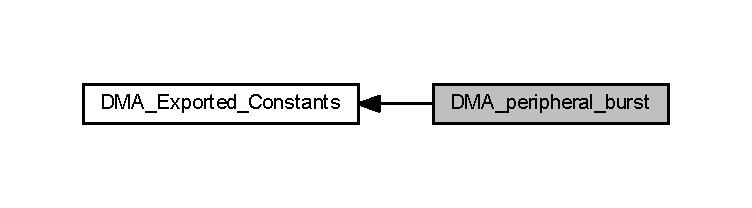
\includegraphics[width=350pt]{group___d_m_a__peripheral__burst}
\end{center}
\end{figure}
\subsection*{Macros}
\begin{DoxyCompactItemize}
\item 
\mbox{\Hypertarget{group___d_m_a__peripheral__burst_ga524cdc5efb8978b586637f35e38a850b}\label{group___d_m_a__peripheral__burst_ga524cdc5efb8978b586637f35e38a850b}} 
\#define {\bfseries D\+M\+A\+\_\+\+Peripheral\+Burst\+\_\+\+Single}~((uint32\+\_\+t)0x00000000)
\item 
\mbox{\Hypertarget{group___d_m_a__peripheral__burst_gaa8eba5161b3927f1ffb81157f3e39b71}\label{group___d_m_a__peripheral__burst_gaa8eba5161b3927f1ffb81157f3e39b71}} 
\#define {\bfseries D\+M\+A\+\_\+\+Peripheral\+Burst\+\_\+\+I\+N\+C4}~((uint32\+\_\+t)0x00200000)
\item 
\mbox{\Hypertarget{group___d_m_a__peripheral__burst_gaf04ba122268e0f54085ca8e45410fe69}\label{group___d_m_a__peripheral__burst_gaf04ba122268e0f54085ca8e45410fe69}} 
\#define {\bfseries D\+M\+A\+\_\+\+Peripheral\+Burst\+\_\+\+I\+N\+C8}~((uint32\+\_\+t)0x00400000)
\item 
\mbox{\Hypertarget{group___d_m_a__peripheral__burst_ga04ff56ff0a2a5470fc2c4817be4213c2}\label{group___d_m_a__peripheral__burst_ga04ff56ff0a2a5470fc2c4817be4213c2}} 
\#define {\bfseries D\+M\+A\+\_\+\+Peripheral\+Burst\+\_\+\+I\+N\+C16}~((uint32\+\_\+t)0x00600000)
\item 
\#define {\bfseries I\+S\+\_\+\+D\+M\+A\+\_\+\+P\+E\+R\+I\+P\+H\+E\+R\+A\+L\+\_\+\+B\+U\+R\+ST}(B\+U\+R\+ST)
\end{DoxyCompactItemize}


\subsection{Detailed Description}


\subsection{Macro Definition Documentation}
\mbox{\Hypertarget{group___d_m_a__peripheral__burst_ga7c60961178e2a32e9e364a220a8aca88}\label{group___d_m_a__peripheral__burst_ga7c60961178e2a32e9e364a220a8aca88}} 
\index{D\+M\+A\+\_\+peripheral\+\_\+burst@{D\+M\+A\+\_\+peripheral\+\_\+burst}!I\+S\+\_\+\+D\+M\+A\+\_\+\+P\+E\+R\+I\+P\+H\+E\+R\+A\+L\+\_\+\+B\+U\+R\+ST@{I\+S\+\_\+\+D\+M\+A\+\_\+\+P\+E\+R\+I\+P\+H\+E\+R\+A\+L\+\_\+\+B\+U\+R\+ST}}
\index{I\+S\+\_\+\+D\+M\+A\+\_\+\+P\+E\+R\+I\+P\+H\+E\+R\+A\+L\+\_\+\+B\+U\+R\+ST@{I\+S\+\_\+\+D\+M\+A\+\_\+\+P\+E\+R\+I\+P\+H\+E\+R\+A\+L\+\_\+\+B\+U\+R\+ST}!D\+M\+A\+\_\+peripheral\+\_\+burst@{D\+M\+A\+\_\+peripheral\+\_\+burst}}
\subsubsection{\texorpdfstring{I\+S\+\_\+\+D\+M\+A\+\_\+\+P\+E\+R\+I\+P\+H\+E\+R\+A\+L\+\_\+\+B\+U\+R\+ST}{IS\_DMA\_PERIPHERAL\_BURST}}
{\footnotesize\ttfamily \#define I\+S\+\_\+\+D\+M\+A\+\_\+\+P\+E\+R\+I\+P\+H\+E\+R\+A\+L\+\_\+\+B\+U\+R\+ST(\begin{DoxyParamCaption}\item[{}]{B\+U\+R\+ST }\end{DoxyParamCaption})}

{\bfseries Value\+:}
\begin{DoxyCode}
(((BURST) == DMA\_PeripheralBurst\_Single) || \(\backslash\)
                                        ((BURST) == DMA\_PeripheralBurst\_INC4)  || \(\backslash\)
                                        ((BURST) == DMA\_PeripheralBurst\_INC8)  || \(\backslash\)
                                        ((BURST) == DMA\_PeripheralBurst\_INC16))
\end{DoxyCode}


Definition at line 322 of file stm32f4xx\+\_\+dma.\+h.


\hypertarget{group___d_m_a__fifo__status__level}{}\section{D\+M\+A\+\_\+fifo\+\_\+status\+\_\+level}
\label{group___d_m_a__fifo__status__level}\index{D\+M\+A\+\_\+fifo\+\_\+status\+\_\+level@{D\+M\+A\+\_\+fifo\+\_\+status\+\_\+level}}
Collaboration diagram for D\+M\+A\+\_\+fifo\+\_\+status\+\_\+level\+:\nopagebreak
\begin{figure}[H]
\begin{center}
\leavevmode
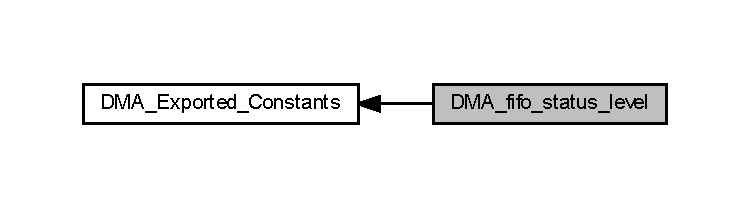
\includegraphics[width=350pt]{group___d_m_a__fifo__status__level}
\end{center}
\end{figure}
\subsection*{Macros}
\begin{DoxyCompactItemize}
\item 
\mbox{\Hypertarget{group___d_m_a__fifo__status__level_gace4b567c96b1c95618a4894875d8123b}\label{group___d_m_a__fifo__status__level_gace4b567c96b1c95618a4894875d8123b}} 
\#define {\bfseries D\+M\+A\+\_\+\+F\+I\+F\+O\+Status\+\_\+\+Less1\+Quarter\+Full}~((uint32\+\_\+t)0x00000000 $<$$<$ 3)
\item 
\mbox{\Hypertarget{group___d_m_a__fifo__status__level_ga258d41ce51005eea1c5a69fcf07d8e42}\label{group___d_m_a__fifo__status__level_ga258d41ce51005eea1c5a69fcf07d8e42}} 
\#define {\bfseries D\+M\+A\+\_\+\+F\+I\+F\+O\+Status\+\_\+1\+Quarter\+Full}~((uint32\+\_\+t)0x00000001 $<$$<$ 3)
\item 
\mbox{\Hypertarget{group___d_m_a__fifo__status__level_ga0dd0faeb4ac9de3dbdcd7ca6dd5bb9e4}\label{group___d_m_a__fifo__status__level_ga0dd0faeb4ac9de3dbdcd7ca6dd5bb9e4}} 
\#define {\bfseries D\+M\+A\+\_\+\+F\+I\+F\+O\+Status\+\_\+\+Half\+Full}~((uint32\+\_\+t)0x00000002 $<$$<$ 3)
\item 
\mbox{\Hypertarget{group___d_m_a__fifo__status__level_ga418c64b77f903c558471d22eeabde439}\label{group___d_m_a__fifo__status__level_ga418c64b77f903c558471d22eeabde439}} 
\#define {\bfseries D\+M\+A\+\_\+\+F\+I\+F\+O\+Status\+\_\+3\+Quarters\+Full}~((uint32\+\_\+t)0x00000003 $<$$<$ 3)
\item 
\mbox{\Hypertarget{group___d_m_a__fifo__status__level_gaacba9ad22e39ed92d2b4ae9ebece654c}\label{group___d_m_a__fifo__status__level_gaacba9ad22e39ed92d2b4ae9ebece654c}} 
\#define {\bfseries D\+M\+A\+\_\+\+F\+I\+F\+O\+Status\+\_\+\+Empty}~((uint32\+\_\+t)0x00000004 $<$$<$ 3)
\item 
\mbox{\Hypertarget{group___d_m_a__fifo__status__level_gaf7ea7373a08730e773cbc048c9965dc2}\label{group___d_m_a__fifo__status__level_gaf7ea7373a08730e773cbc048c9965dc2}} 
\#define {\bfseries D\+M\+A\+\_\+\+F\+I\+F\+O\+Status\+\_\+\+Full}~((uint32\+\_\+t)0x00000005 $<$$<$ 3)
\item 
\#define {\bfseries I\+S\+\_\+\+D\+M\+A\+\_\+\+F\+I\+F\+O\+\_\+\+S\+T\+A\+T\+US}(S\+T\+A\+T\+US)
\end{DoxyCompactItemize}


\subsection{Detailed Description}


\subsection{Macro Definition Documentation}
\mbox{\Hypertarget{group___d_m_a__fifo__status__level_ga6980114eab3b3eea701f3802dd97dc12}\label{group___d_m_a__fifo__status__level_ga6980114eab3b3eea701f3802dd97dc12}} 
\index{D\+M\+A\+\_\+fifo\+\_\+status\+\_\+level@{D\+M\+A\+\_\+fifo\+\_\+status\+\_\+level}!I\+S\+\_\+\+D\+M\+A\+\_\+\+F\+I\+F\+O\+\_\+\+S\+T\+A\+T\+US@{I\+S\+\_\+\+D\+M\+A\+\_\+\+F\+I\+F\+O\+\_\+\+S\+T\+A\+T\+US}}
\index{I\+S\+\_\+\+D\+M\+A\+\_\+\+F\+I\+F\+O\+\_\+\+S\+T\+A\+T\+US@{I\+S\+\_\+\+D\+M\+A\+\_\+\+F\+I\+F\+O\+\_\+\+S\+T\+A\+T\+US}!D\+M\+A\+\_\+fifo\+\_\+status\+\_\+level@{D\+M\+A\+\_\+fifo\+\_\+status\+\_\+level}}
\subsubsection{\texorpdfstring{I\+S\+\_\+\+D\+M\+A\+\_\+\+F\+I\+F\+O\+\_\+\+S\+T\+A\+T\+US}{IS\_DMA\_FIFO\_STATUS}}
{\footnotesize\ttfamily \#define I\+S\+\_\+\+D\+M\+A\+\_\+\+F\+I\+F\+O\+\_\+\+S\+T\+A\+T\+US(\begin{DoxyParamCaption}\item[{}]{S\+T\+A\+T\+US }\end{DoxyParamCaption})}

{\bfseries Value\+:}
\begin{DoxyCode}
(((STATUS) == DMA\_FIFOStatus\_Less1QuarterFull ) || \(\backslash\)
                                    ((STATUS) == DMA\_FIFOStatus\_HalfFull)          || \(\backslash\)
                                    ((STATUS) == DMA\_FIFOStatus\_1QuarterFull)      || \(\backslash\)
                                    ((STATUS) == DMA\_FIFOStatus\_3QuartersFull)     || \(\backslash\)
                                    ((STATUS) == DMA\_FIFOStatus\_Full)              || \(\backslash\)
                                    ((STATUS) == DMA\_FIFOStatus\_Empty))
\end{DoxyCode}


Definition at line 341 of file stm32f4xx\+\_\+dma.\+h.


\hypertarget{group___d_m_a__flags__definition}{}\section{D\+M\+A\+\_\+flags\+\_\+definition}
\label{group___d_m_a__flags__definition}\index{D\+M\+A\+\_\+flags\+\_\+definition@{D\+M\+A\+\_\+flags\+\_\+definition}}
Collaboration diagram for D\+M\+A\+\_\+flags\+\_\+definition\+:
\nopagebreak
\begin{figure}[H]
\begin{center}
\leavevmode
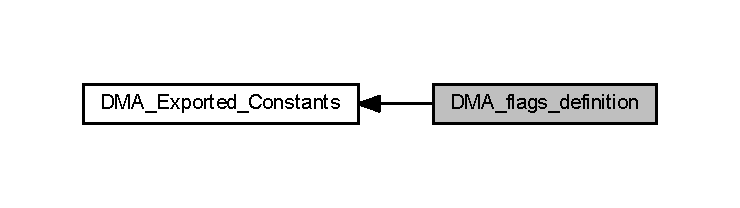
\includegraphics[width=350pt]{group___d_m_a__flags__definition}
\end{center}
\end{figure}
\subsection*{Macros}
\begin{DoxyCompactItemize}
\item 
\mbox{\Hypertarget{group___d_m_a__flags__definition_ga4e09c71ab9d85493fba241fa90f60eff}\label{group___d_m_a__flags__definition_ga4e09c71ab9d85493fba241fa90f60eff}} 
\#define {\bfseries D\+M\+A\+\_\+\+F\+L\+A\+G\+\_\+\+F\+E\+I\+F0}~((uint32\+\_\+t)0x10800001)
\item 
\mbox{\Hypertarget{group___d_m_a__flags__definition_gaf309e18b8d4113c51de6d23794bdaaab}\label{group___d_m_a__flags__definition_gaf309e18b8d4113c51de6d23794bdaaab}} 
\#define {\bfseries D\+M\+A\+\_\+\+F\+L\+A\+G\+\_\+\+D\+M\+E\+I\+F0}~((uint32\+\_\+t)0x10800004)
\item 
\mbox{\Hypertarget{group___d_m_a__flags__definition_ga8a1b602ca53eca06597284af6edd4eca}\label{group___d_m_a__flags__definition_ga8a1b602ca53eca06597284af6edd4eca}} 
\#define {\bfseries D\+M\+A\+\_\+\+F\+L\+A\+G\+\_\+\+T\+E\+I\+F0}~((uint32\+\_\+t)0x10000008)
\item 
\mbox{\Hypertarget{group___d_m_a__flags__definition_gaa76090f6351c3feb8e844460820236c6}\label{group___d_m_a__flags__definition_gaa76090f6351c3feb8e844460820236c6}} 
\#define {\bfseries D\+M\+A\+\_\+\+F\+L\+A\+G\+\_\+\+H\+T\+I\+F0}~((uint32\+\_\+t)0x10000010)
\item 
\mbox{\Hypertarget{group___d_m_a__flags__definition_gae5220ac32b929e3ffce6d6239cc2a39c}\label{group___d_m_a__flags__definition_gae5220ac32b929e3ffce6d6239cc2a39c}} 
\#define {\bfseries D\+M\+A\+\_\+\+F\+L\+A\+G\+\_\+\+T\+C\+I\+F0}~((uint32\+\_\+t)0x10000020)
\item 
\mbox{\Hypertarget{group___d_m_a__flags__definition_ga13a9f5ad620803b1f59c329ea291cdce}\label{group___d_m_a__flags__definition_ga13a9f5ad620803b1f59c329ea291cdce}} 
\#define {\bfseries D\+M\+A\+\_\+\+F\+L\+A\+G\+\_\+\+F\+E\+I\+F1}~((uint32\+\_\+t)0x10000040)
\item 
\mbox{\Hypertarget{group___d_m_a__flags__definition_ga1f52407d92d389200727d1731ed2bf41}\label{group___d_m_a__flags__definition_ga1f52407d92d389200727d1731ed2bf41}} 
\#define {\bfseries D\+M\+A\+\_\+\+F\+L\+A\+G\+\_\+\+D\+M\+E\+I\+F1}~((uint32\+\_\+t)0x10000100)
\item 
\mbox{\Hypertarget{group___d_m_a__flags__definition_gaebca425399650686931b35d650ec9872}\label{group___d_m_a__flags__definition_gaebca425399650686931b35d650ec9872}} 
\#define {\bfseries D\+M\+A\+\_\+\+F\+L\+A\+G\+\_\+\+T\+E\+I\+F1}~((uint32\+\_\+t)0x10000200)
\item 
\mbox{\Hypertarget{group___d_m_a__flags__definition_ga5e00b692cb6654c1e09f091e4dba807c}\label{group___d_m_a__flags__definition_ga5e00b692cb6654c1e09f091e4dba807c}} 
\#define {\bfseries D\+M\+A\+\_\+\+F\+L\+A\+G\+\_\+\+H\+T\+I\+F1}~((uint32\+\_\+t)0x10000400)
\item 
\mbox{\Hypertarget{group___d_m_a__flags__definition_ga4ec37900b79b667829eced7b442f2c9d}\label{group___d_m_a__flags__definition_ga4ec37900b79b667829eced7b442f2c9d}} 
\#define {\bfseries D\+M\+A\+\_\+\+F\+L\+A\+G\+\_\+\+T\+C\+I\+F1}~((uint32\+\_\+t)0x10000800)
\item 
\mbox{\Hypertarget{group___d_m_a__flags__definition_ga3e7dfaf220ad350a2b0a3d307ba8896e}\label{group___d_m_a__flags__definition_ga3e7dfaf220ad350a2b0a3d307ba8896e}} 
\#define {\bfseries D\+M\+A\+\_\+\+F\+L\+A\+G\+\_\+\+F\+E\+I\+F2}~((uint32\+\_\+t)0x10010000)
\item 
\mbox{\Hypertarget{group___d_m_a__flags__definition_ga69b110e9d83d45faf6e88719cff8f721}\label{group___d_m_a__flags__definition_ga69b110e9d83d45faf6e88719cff8f721}} 
\#define {\bfseries D\+M\+A\+\_\+\+F\+L\+A\+G\+\_\+\+D\+M\+E\+I\+F2}~((uint32\+\_\+t)0x10040000)
\item 
\mbox{\Hypertarget{group___d_m_a__flags__definition_gaa3e1e5d2a043496524107ecc1ddfe934}\label{group___d_m_a__flags__definition_gaa3e1e5d2a043496524107ecc1ddfe934}} 
\#define {\bfseries D\+M\+A\+\_\+\+F\+L\+A\+G\+\_\+\+T\+E\+I\+F2}~((uint32\+\_\+t)0x10080000)
\item 
\mbox{\Hypertarget{group___d_m_a__flags__definition_gae960d87b7770ec11820df758fecf28db}\label{group___d_m_a__flags__definition_gae960d87b7770ec11820df758fecf28db}} 
\#define {\bfseries D\+M\+A\+\_\+\+F\+L\+A\+G\+\_\+\+H\+T\+I\+F2}~((uint32\+\_\+t)0x10100000)
\item 
\mbox{\Hypertarget{group___d_m_a__flags__definition_ga26c60c0cd9f24112eb082c7bbba1eff7}\label{group___d_m_a__flags__definition_ga26c60c0cd9f24112eb082c7bbba1eff7}} 
\#define {\bfseries D\+M\+A\+\_\+\+F\+L\+A\+G\+\_\+\+T\+C\+I\+F2}~((uint32\+\_\+t)0x10200000)
\item 
\mbox{\Hypertarget{group___d_m_a__flags__definition_ga7d551a54c46071ea3629d38768cd8638}\label{group___d_m_a__flags__definition_ga7d551a54c46071ea3629d38768cd8638}} 
\#define {\bfseries D\+M\+A\+\_\+\+F\+L\+A\+G\+\_\+\+F\+E\+I\+F3}~((uint32\+\_\+t)0x10400000)
\item 
\mbox{\Hypertarget{group___d_m_a__flags__definition_gacb835761b58d15662b0e631697bbf0a4}\label{group___d_m_a__flags__definition_gacb835761b58d15662b0e631697bbf0a4}} 
\#define {\bfseries D\+M\+A\+\_\+\+F\+L\+A\+G\+\_\+\+D\+M\+E\+I\+F3}~((uint32\+\_\+t)0x11000000)
\item 
\mbox{\Hypertarget{group___d_m_a__flags__definition_ga36854c526eb41566bcf1c4505265433c}\label{group___d_m_a__flags__definition_ga36854c526eb41566bcf1c4505265433c}} 
\#define {\bfseries D\+M\+A\+\_\+\+F\+L\+A\+G\+\_\+\+T\+E\+I\+F3}~((uint32\+\_\+t)0x12000000)
\item 
\mbox{\Hypertarget{group___d_m_a__flags__definition_ga10e669df50c5a5fe93b698f75f0574d6}\label{group___d_m_a__flags__definition_ga10e669df50c5a5fe93b698f75f0574d6}} 
\#define {\bfseries D\+M\+A\+\_\+\+F\+L\+A\+G\+\_\+\+H\+T\+I\+F3}~((uint32\+\_\+t)0x14000000)
\item 
\mbox{\Hypertarget{group___d_m_a__flags__definition_gae8dde773a36a6d211d718bace2438def}\label{group___d_m_a__flags__definition_gae8dde773a36a6d211d718bace2438def}} 
\#define {\bfseries D\+M\+A\+\_\+\+F\+L\+A\+G\+\_\+\+T\+C\+I\+F3}~((uint32\+\_\+t)0x18000000)
\item 
\mbox{\Hypertarget{group___d_m_a__flags__definition_ga81f626454f81551dffa17619f459b99b}\label{group___d_m_a__flags__definition_ga81f626454f81551dffa17619f459b99b}} 
\#define {\bfseries D\+M\+A\+\_\+\+F\+L\+A\+G\+\_\+\+F\+E\+I\+F4}~((uint32\+\_\+t)0x20000001)
\item 
\mbox{\Hypertarget{group___d_m_a__flags__definition_gae47ce0553cd8c561d0c5a903accf3411}\label{group___d_m_a__flags__definition_gae47ce0553cd8c561d0c5a903accf3411}} 
\#define {\bfseries D\+M\+A\+\_\+\+F\+L\+A\+G\+\_\+\+D\+M\+E\+I\+F4}~((uint32\+\_\+t)0x20000004)
\item 
\mbox{\Hypertarget{group___d_m_a__flags__definition_ga0216244c5386117a965ef6833b86984e}\label{group___d_m_a__flags__definition_ga0216244c5386117a965ef6833b86984e}} 
\#define {\bfseries D\+M\+A\+\_\+\+F\+L\+A\+G\+\_\+\+T\+E\+I\+F4}~((uint32\+\_\+t)0x20000008)
\item 
\mbox{\Hypertarget{group___d_m_a__flags__definition_gac1f371142dd0c1a5a19d8ad2cf1d2f2a}\label{group___d_m_a__flags__definition_gac1f371142dd0c1a5a19d8ad2cf1d2f2a}} 
\#define {\bfseries D\+M\+A\+\_\+\+F\+L\+A\+G\+\_\+\+H\+T\+I\+F4}~((uint32\+\_\+t)0x20000010)
\item 
\mbox{\Hypertarget{group___d_m_a__flags__definition_gaa2a470b95dc9084de45009c600e8cf1d}\label{group___d_m_a__flags__definition_gaa2a470b95dc9084de45009c600e8cf1d}} 
\#define {\bfseries D\+M\+A\+\_\+\+F\+L\+A\+G\+\_\+\+T\+C\+I\+F4}~((uint32\+\_\+t)0x20000020)
\item 
\mbox{\Hypertarget{group___d_m_a__flags__definition_ga40621c1df90e9e1ebfb4815df09a2469}\label{group___d_m_a__flags__definition_ga40621c1df90e9e1ebfb4815df09a2469}} 
\#define {\bfseries D\+M\+A\+\_\+\+F\+L\+A\+G\+\_\+\+F\+E\+I\+F5}~((uint32\+\_\+t)0x20000040)
\item 
\mbox{\Hypertarget{group___d_m_a__flags__definition_ga70a0d9684bfd6e6ef2cce31fc8e33512}\label{group___d_m_a__flags__definition_ga70a0d9684bfd6e6ef2cce31fc8e33512}} 
\#define {\bfseries D\+M\+A\+\_\+\+F\+L\+A\+G\+\_\+\+D\+M\+E\+I\+F5}~((uint32\+\_\+t)0x20000100)
\item 
\mbox{\Hypertarget{group___d_m_a__flags__definition_ga64ee170cb2d0fbe5daa6d3166c65190d}\label{group___d_m_a__flags__definition_ga64ee170cb2d0fbe5daa6d3166c65190d}} 
\#define {\bfseries D\+M\+A\+\_\+\+F\+L\+A\+G\+\_\+\+T\+E\+I\+F5}~((uint32\+\_\+t)0x20000200)
\item 
\mbox{\Hypertarget{group___d_m_a__flags__definition_ga005ff333f9f114f5966f35b90df0ff9a}\label{group___d_m_a__flags__definition_ga005ff333f9f114f5966f35b90df0ff9a}} 
\#define {\bfseries D\+M\+A\+\_\+\+F\+L\+A\+G\+\_\+\+H\+T\+I\+F5}~((uint32\+\_\+t)0x20000400)
\item 
\mbox{\Hypertarget{group___d_m_a__flags__definition_ga50cb345a0bb8bde37228b0a1d5becc4c}\label{group___d_m_a__flags__definition_ga50cb345a0bb8bde37228b0a1d5becc4c}} 
\#define {\bfseries D\+M\+A\+\_\+\+F\+L\+A\+G\+\_\+\+T\+C\+I\+F5}~((uint32\+\_\+t)0x20000800)
\item 
\mbox{\Hypertarget{group___d_m_a__flags__definition_gafc0383aab975f70507f76e983c32b8c0}\label{group___d_m_a__flags__definition_gafc0383aab975f70507f76e983c32b8c0}} 
\#define {\bfseries D\+M\+A\+\_\+\+F\+L\+A\+G\+\_\+\+F\+E\+I\+F6}~((uint32\+\_\+t)0x20010000)
\item 
\mbox{\Hypertarget{group___d_m_a__flags__definition_ga1d85ff6756ffbd8284ac435f3781eb4a}\label{group___d_m_a__flags__definition_ga1d85ff6756ffbd8284ac435f3781eb4a}} 
\#define {\bfseries D\+M\+A\+\_\+\+F\+L\+A\+G\+\_\+\+D\+M\+E\+I\+F6}~((uint32\+\_\+t)0x20040000)
\item 
\mbox{\Hypertarget{group___d_m_a__flags__definition_ga2900d2ad700dffbb058b238162018be0}\label{group___d_m_a__flags__definition_ga2900d2ad700dffbb058b238162018be0}} 
\#define {\bfseries D\+M\+A\+\_\+\+F\+L\+A\+G\+\_\+\+T\+E\+I\+F6}~((uint32\+\_\+t)0x20080000)
\item 
\mbox{\Hypertarget{group___d_m_a__flags__definition_gaa2e5cb8680883513cf8fccef6c39c78e}\label{group___d_m_a__flags__definition_gaa2e5cb8680883513cf8fccef6c39c78e}} 
\#define {\bfseries D\+M\+A\+\_\+\+F\+L\+A\+G\+\_\+\+H\+T\+I\+F6}~((uint32\+\_\+t)0x20100000)
\item 
\mbox{\Hypertarget{group___d_m_a__flags__definition_ga7b16e37ffcf292fcab6745af7de1e50c}\label{group___d_m_a__flags__definition_ga7b16e37ffcf292fcab6745af7de1e50c}} 
\#define {\bfseries D\+M\+A\+\_\+\+F\+L\+A\+G\+\_\+\+T\+C\+I\+F6}~((uint32\+\_\+t)0x20200000)
\item 
\mbox{\Hypertarget{group___d_m_a__flags__definition_ga4c75ab8fa2339bad9413f133ec9b92d3}\label{group___d_m_a__flags__definition_ga4c75ab8fa2339bad9413f133ec9b92d3}} 
\#define {\bfseries D\+M\+A\+\_\+\+F\+L\+A\+G\+\_\+\+F\+E\+I\+F7}~((uint32\+\_\+t)0x20400000)
\item 
\mbox{\Hypertarget{group___d_m_a__flags__definition_gae8b9016059eef77580e3845d30c1f42f}\label{group___d_m_a__flags__definition_gae8b9016059eef77580e3845d30c1f42f}} 
\#define {\bfseries D\+M\+A\+\_\+\+F\+L\+A\+G\+\_\+\+D\+M\+E\+I\+F7}~((uint32\+\_\+t)0x21000000)
\item 
\mbox{\Hypertarget{group___d_m_a__flags__definition_ga4f4acb7f0b6c46a1af27733852ef4fc7}\label{group___d_m_a__flags__definition_ga4f4acb7f0b6c46a1af27733852ef4fc7}} 
\#define {\bfseries D\+M\+A\+\_\+\+F\+L\+A\+G\+\_\+\+T\+E\+I\+F7}~((uint32\+\_\+t)0x22000000)
\item 
\mbox{\Hypertarget{group___d_m_a__flags__definition_gaa59fb75c0964ea148a2218baba8de255}\label{group___d_m_a__flags__definition_gaa59fb75c0964ea148a2218baba8de255}} 
\#define {\bfseries D\+M\+A\+\_\+\+F\+L\+A\+G\+\_\+\+H\+T\+I\+F7}~((uint32\+\_\+t)0x24000000)
\item 
\mbox{\Hypertarget{group___d_m_a__flags__definition_ga5a68888ca361abf00d552bdd70304ea9}\label{group___d_m_a__flags__definition_ga5a68888ca361abf00d552bdd70304ea9}} 
\#define {\bfseries D\+M\+A\+\_\+\+F\+L\+A\+G\+\_\+\+T\+C\+I\+F7}~((uint32\+\_\+t)0x28000000)
\item 
\#define {\bfseries I\+S\+\_\+\+D\+M\+A\+\_\+\+C\+L\+E\+A\+R\+\_\+\+F\+L\+AG}(F\+L\+AG)
\item 
\#define {\bfseries I\+S\+\_\+\+D\+M\+A\+\_\+\+G\+E\+T\+\_\+\+F\+L\+AG}(F\+L\+AG)
\end{DoxyCompactItemize}


\subsection{Detailed Description}


\subsection{Macro Definition Documentation}
\mbox{\Hypertarget{group___d_m_a__flags__definition_ga4b33e418489c9a3c9adcbdbaca93e4a3}\label{group___d_m_a__flags__definition_ga4b33e418489c9a3c9adcbdbaca93e4a3}} 
\index{D\+M\+A\+\_\+flags\+\_\+definition@{D\+M\+A\+\_\+flags\+\_\+definition}!I\+S\+\_\+\+D\+M\+A\+\_\+\+C\+L\+E\+A\+R\+\_\+\+F\+L\+AG@{I\+S\+\_\+\+D\+M\+A\+\_\+\+C\+L\+E\+A\+R\+\_\+\+F\+L\+AG}}
\index{I\+S\+\_\+\+D\+M\+A\+\_\+\+C\+L\+E\+A\+R\+\_\+\+F\+L\+AG@{I\+S\+\_\+\+D\+M\+A\+\_\+\+C\+L\+E\+A\+R\+\_\+\+F\+L\+AG}!D\+M\+A\+\_\+flags\+\_\+definition@{D\+M\+A\+\_\+flags\+\_\+definition}}
\subsubsection{\texorpdfstring{I\+S\+\_\+\+D\+M\+A\+\_\+\+C\+L\+E\+A\+R\+\_\+\+F\+L\+AG}{IS\_DMA\_CLEAR\_FLAG}}
{\footnotesize\ttfamily \#define I\+S\+\_\+\+D\+M\+A\+\_\+\+C\+L\+E\+A\+R\+\_\+\+F\+L\+AG(\begin{DoxyParamCaption}\item[{}]{F\+L\+AG }\end{DoxyParamCaption})}

{\bfseries Value\+:}
\begin{DoxyCode}
((((FLAG) & 0x30000000) != 0x30000000) && (((FLAG) & 0x30000000) != 0) && \(\backslash\)
                                 (((FLAG) & 0xC082F082) == 0x00) && ((FLAG) != 0x00))
\end{DoxyCode}


Definition at line 395 of file stm32f4xx\+\_\+dma.\+h.

\mbox{\Hypertarget{group___d_m_a__flags__definition_ga98e421aa0a15fbeecb4cab3612985676}\label{group___d_m_a__flags__definition_ga98e421aa0a15fbeecb4cab3612985676}} 
\index{D\+M\+A\+\_\+flags\+\_\+definition@{D\+M\+A\+\_\+flags\+\_\+definition}!I\+S\+\_\+\+D\+M\+A\+\_\+\+G\+E\+T\+\_\+\+F\+L\+AG@{I\+S\+\_\+\+D\+M\+A\+\_\+\+G\+E\+T\+\_\+\+F\+L\+AG}}
\index{I\+S\+\_\+\+D\+M\+A\+\_\+\+G\+E\+T\+\_\+\+F\+L\+AG@{I\+S\+\_\+\+D\+M\+A\+\_\+\+G\+E\+T\+\_\+\+F\+L\+AG}!D\+M\+A\+\_\+flags\+\_\+definition@{D\+M\+A\+\_\+flags\+\_\+definition}}
\subsubsection{\texorpdfstring{I\+S\+\_\+\+D\+M\+A\+\_\+\+G\+E\+T\+\_\+\+F\+L\+AG}{IS\_DMA\_GET\_FLAG}}
{\footnotesize\ttfamily \#define I\+S\+\_\+\+D\+M\+A\+\_\+\+G\+E\+T\+\_\+\+F\+L\+AG(\begin{DoxyParamCaption}\item[{}]{F\+L\+AG }\end{DoxyParamCaption})}

{\bfseries Value\+:}
\begin{DoxyCode}
(((FLAG) == DMA\_FLAG\_TCIF0)  || ((FLAG) == DMA\_FLAG\_HTIF0)  || \(\backslash\)
                               ((FLAG) == DMA\_FLAG\_TEIF0)  || ((FLAG) == DMA\_FLAG\_DMEIF0) || \(\backslash\)
                               ((FLAG) == DMA\_FLAG\_FEIF0)  || ((FLAG) == DMA\_FLAG\_TCIF1)  || \(\backslash\)
                               ((FLAG) == DMA\_FLAG\_HTIF1)  || ((FLAG) == DMA\_FLAG\_TEIF1)  || \(\backslash\)
                               ((FLAG) == DMA\_FLAG\_DMEIF1) || ((FLAG) == DMA\_FLAG\_FEIF1)  || \(\backslash\)
                               ((FLAG) == DMA\_FLAG\_TCIF2)  || ((FLAG) == DMA\_FLAG\_HTIF2)  || \(\backslash\)
                               ((FLAG) == DMA\_FLAG\_TEIF2)  || ((FLAG) == DMA\_FLAG\_DMEIF2) || \(\backslash\)
                               ((FLAG) == DMA\_FLAG\_FEIF2)  || ((FLAG) == DMA\_FLAG\_TCIF3)  || \(\backslash\)
                               ((FLAG) == DMA\_FLAG\_HTIF3)  || ((FLAG) == DMA\_FLAG\_TEIF3)  || \(\backslash\)
                               ((FLAG) == DMA\_FLAG\_DMEIF3) || ((FLAG) == DMA\_FLAG\_FEIF3)  || \(\backslash\)
                               ((FLAG) == DMA\_FLAG\_TCIF4)  || ((FLAG) == DMA\_FLAG\_HTIF4)  || \(\backslash\)
                               ((FLAG) == DMA\_FLAG\_TEIF4)  || ((FLAG) == DMA\_FLAG\_DMEIF4) || \(\backslash\)
                               ((FLAG) == DMA\_FLAG\_FEIF4)  || ((FLAG) == DMA\_FLAG\_TCIF5)  || \(\backslash\)
                               ((FLAG) == DMA\_FLAG\_HTIF5)  || ((FLAG) == DMA\_FLAG\_TEIF5)  || \(\backslash\)
                               ((FLAG) == DMA\_FLAG\_DMEIF5) || ((FLAG) == DMA\_FLAG\_FEIF5)  || \(\backslash\)
                               ((FLAG) == DMA\_FLAG\_TCIF6)  || ((FLAG) == DMA\_FLAG\_HTIF6)  || \(\backslash\)
                               ((FLAG) == DMA\_FLAG\_TEIF6)  || ((FLAG) == DMA\_FLAG\_DMEIF6) || \(\backslash\)
                               ((FLAG) == DMA\_FLAG\_FEIF6)  || ((FLAG) == DMA\_FLAG\_TCIF7)  || \(\backslash\)
                               ((FLAG) == DMA\_FLAG\_HTIF7)  || ((FLAG) == DMA\_FLAG\_TEIF7)  || \(\backslash\)
                               ((FLAG) == DMA\_FLAG\_DMEIF7) || ((FLAG) == DMA\_FLAG\_FEIF7))
\end{DoxyCode}


Definition at line 398 of file stm32f4xx\+\_\+dma.\+h.


\hypertarget{group___d_m_a__interrupt__enable__definitions}{}\section{D\+M\+A\+\_\+interrupt\+\_\+enable\+\_\+definitions}
\label{group___d_m_a__interrupt__enable__definitions}\index{D\+M\+A\+\_\+interrupt\+\_\+enable\+\_\+definitions@{D\+M\+A\+\_\+interrupt\+\_\+enable\+\_\+definitions}}
Collaboration diagram for D\+M\+A\+\_\+interrupt\+\_\+enable\+\_\+definitions\+:
\nopagebreak
\begin{figure}[H]
\begin{center}
\leavevmode
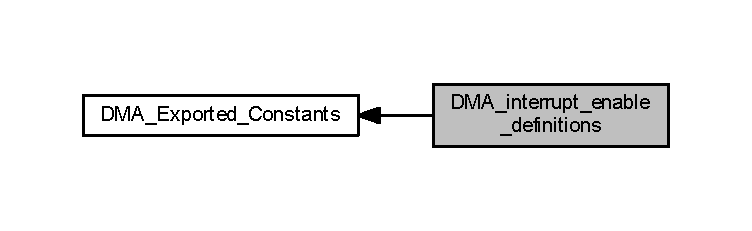
\includegraphics[width=350pt]{group___d_m_a__interrupt__enable__definitions}
\end{center}
\end{figure}
\subsection*{Macros}
\begin{DoxyCompactItemize}
\item 
\mbox{\Hypertarget{group___d_m_a__interrupt__enable__definitions_ga06e83dd277e0d3e5635cf8ce8dfd6e16}\label{group___d_m_a__interrupt__enable__definitions_ga06e83dd277e0d3e5635cf8ce8dfd6e16}} 
\#define {\bfseries D\+M\+A\+\_\+\+I\+T\+\_\+\+TC}~((uint32\+\_\+t)0x00000010)
\item 
\mbox{\Hypertarget{group___d_m_a__interrupt__enable__definitions_gadf11c572b9797e04a14b105fdc2e5f66}\label{group___d_m_a__interrupt__enable__definitions_gadf11c572b9797e04a14b105fdc2e5f66}} 
\#define {\bfseries D\+M\+A\+\_\+\+I\+T\+\_\+\+HT}~((uint32\+\_\+t)0x00000008)
\item 
\mbox{\Hypertarget{group___d_m_a__interrupt__enable__definitions_gaf9d92649d2a0146f663ff253d8f3b59e}\label{group___d_m_a__interrupt__enable__definitions_gaf9d92649d2a0146f663ff253d8f3b59e}} 
\#define {\bfseries D\+M\+A\+\_\+\+I\+T\+\_\+\+TE}~((uint32\+\_\+t)0x00000004)
\item 
\mbox{\Hypertarget{group___d_m_a__interrupt__enable__definitions_ga71137443f7bdced1ee80697596e9ea98}\label{group___d_m_a__interrupt__enable__definitions_ga71137443f7bdced1ee80697596e9ea98}} 
\#define {\bfseries D\+M\+A\+\_\+\+I\+T\+\_\+\+D\+ME}~((uint32\+\_\+t)0x00000002)
\item 
\mbox{\Hypertarget{group___d_m_a__interrupt__enable__definitions_ga93164ec039fc5579662c382e68d7d13f}\label{group___d_m_a__interrupt__enable__definitions_ga93164ec039fc5579662c382e68d7d13f}} 
\#define {\bfseries D\+M\+A\+\_\+\+I\+T\+\_\+\+FE}~((uint32\+\_\+t)0x00000080)
\item 
\mbox{\Hypertarget{group___d_m_a__interrupt__enable__definitions_ga47f6af7da302c19aba24516037d305e7}\label{group___d_m_a__interrupt__enable__definitions_ga47f6af7da302c19aba24516037d305e7}} 
\#define {\bfseries I\+S\+\_\+\+D\+M\+A\+\_\+\+C\+O\+N\+F\+I\+G\+\_\+\+IT}(IT)~((((IT) \& 0x\+F\+F\+F\+F\+F\+F61) == 0x00) \&\& ((\+I\+T) != 0x00))
\end{DoxyCompactItemize}


\subsection{Detailed Description}

\hypertarget{group___d_m_a__interrupts__definitions}{}\section{D\+M\+A\+\_\+interrupts\+\_\+definitions}
\label{group___d_m_a__interrupts__definitions}\index{D\+M\+A\+\_\+interrupts\+\_\+definitions@{D\+M\+A\+\_\+interrupts\+\_\+definitions}}
Collaboration diagram for D\+M\+A\+\_\+interrupts\+\_\+definitions\+:
\nopagebreak
\begin{figure}[H]
\begin{center}
\leavevmode
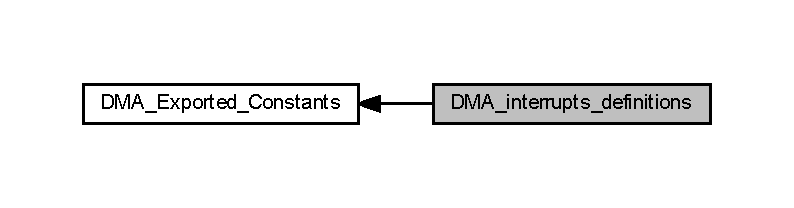
\includegraphics[width=350pt]{group___d_m_a__interrupts__definitions}
\end{center}
\end{figure}
\subsection*{Macros}
\begin{DoxyCompactItemize}
\item 
\mbox{\Hypertarget{group___d_m_a__interrupts__definitions_ga5202cf7ab467fe1a61c725d1f98f0689}\label{group___d_m_a__interrupts__definitions_ga5202cf7ab467fe1a61c725d1f98f0689}} 
\#define {\bfseries D\+M\+A\+\_\+\+I\+T\+\_\+\+F\+E\+I\+F0}~((uint32\+\_\+t)0x90000001)
\item 
\mbox{\Hypertarget{group___d_m_a__interrupts__definitions_ga8427aa66491c87a653f94f812b31cb17}\label{group___d_m_a__interrupts__definitions_ga8427aa66491c87a653f94f812b31cb17}} 
\#define {\bfseries D\+M\+A\+\_\+\+I\+T\+\_\+\+D\+M\+E\+I\+F0}~((uint32\+\_\+t)0x10001004)
\item 
\mbox{\Hypertarget{group___d_m_a__interrupts__definitions_ga7f47bb08f22556f9a655adbce3d6982a}\label{group___d_m_a__interrupts__definitions_ga7f47bb08f22556f9a655adbce3d6982a}} 
\#define {\bfseries D\+M\+A\+\_\+\+I\+T\+\_\+\+T\+E\+I\+F0}~((uint32\+\_\+t)0x10002008)
\item 
\mbox{\Hypertarget{group___d_m_a__interrupts__definitions_gaabb2f6093a51f4f25ac67a21125a8bc2}\label{group___d_m_a__interrupts__definitions_gaabb2f6093a51f4f25ac67a21125a8bc2}} 
\#define {\bfseries D\+M\+A\+\_\+\+I\+T\+\_\+\+H\+T\+I\+F0}~((uint32\+\_\+t)0x10004010)
\item 
\mbox{\Hypertarget{group___d_m_a__interrupts__definitions_ga9de4a37c4fb35a2d3566d8060a8145be}\label{group___d_m_a__interrupts__definitions_ga9de4a37c4fb35a2d3566d8060a8145be}} 
\#define {\bfseries D\+M\+A\+\_\+\+I\+T\+\_\+\+T\+C\+I\+F0}~((uint32\+\_\+t)0x10008020)
\item 
\mbox{\Hypertarget{group___d_m_a__interrupts__definitions_gaa93c3fc1826e8bf9063ab64734277ca3}\label{group___d_m_a__interrupts__definitions_gaa93c3fc1826e8bf9063ab64734277ca3}} 
\#define {\bfseries D\+M\+A\+\_\+\+I\+T\+\_\+\+F\+E\+I\+F1}~((uint32\+\_\+t)0x90000040)
\item 
\mbox{\Hypertarget{group___d_m_a__interrupts__definitions_gabdbf66e3cbe14fe1f45c42635127e927}\label{group___d_m_a__interrupts__definitions_gabdbf66e3cbe14fe1f45c42635127e927}} 
\#define {\bfseries D\+M\+A\+\_\+\+I\+T\+\_\+\+D\+M\+E\+I\+F1}~((uint32\+\_\+t)0x10001100)
\item 
\mbox{\Hypertarget{group___d_m_a__interrupts__definitions_gaeacbd5c206cc6026d3c03f8182b16aeb}\label{group___d_m_a__interrupts__definitions_gaeacbd5c206cc6026d3c03f8182b16aeb}} 
\#define {\bfseries D\+M\+A\+\_\+\+I\+T\+\_\+\+T\+E\+I\+F1}~((uint32\+\_\+t)0x10002200)
\item 
\mbox{\Hypertarget{group___d_m_a__interrupts__definitions_ga22e9fbbe3bd5539bf4c087c9ba2735da}\label{group___d_m_a__interrupts__definitions_ga22e9fbbe3bd5539bf4c087c9ba2735da}} 
\#define {\bfseries D\+M\+A\+\_\+\+I\+T\+\_\+\+H\+T\+I\+F1}~((uint32\+\_\+t)0x10004400)
\item 
\mbox{\Hypertarget{group___d_m_a__interrupts__definitions_gae4eb128c7b47473cf984c4d91878d879}\label{group___d_m_a__interrupts__definitions_gae4eb128c7b47473cf984c4d91878d879}} 
\#define {\bfseries D\+M\+A\+\_\+\+I\+T\+\_\+\+T\+C\+I\+F1}~((uint32\+\_\+t)0x10008800)
\item 
\mbox{\Hypertarget{group___d_m_a__interrupts__definitions_gaeae384e9af7db044cf93e7f270eddd7c}\label{group___d_m_a__interrupts__definitions_gaeae384e9af7db044cf93e7f270eddd7c}} 
\#define {\bfseries D\+M\+A\+\_\+\+I\+T\+\_\+\+F\+E\+I\+F2}~((uint32\+\_\+t)0x90010000)
\item 
\mbox{\Hypertarget{group___d_m_a__interrupts__definitions_ga56f547c35fcac83518aec320f0e38000}\label{group___d_m_a__interrupts__definitions_ga56f547c35fcac83518aec320f0e38000}} 
\#define {\bfseries D\+M\+A\+\_\+\+I\+T\+\_\+\+D\+M\+E\+I\+F2}~((uint32\+\_\+t)0x10041000)
\item 
\mbox{\Hypertarget{group___d_m_a__interrupts__definitions_ga8faa8c4705525ad1cd90290c5a04c589}\label{group___d_m_a__interrupts__definitions_ga8faa8c4705525ad1cd90290c5a04c589}} 
\#define {\bfseries D\+M\+A\+\_\+\+I\+T\+\_\+\+T\+E\+I\+F2}~((uint32\+\_\+t)0x10082000)
\item 
\mbox{\Hypertarget{group___d_m_a__interrupts__definitions_ga759d12e1158b37391b31a79f3a54339c}\label{group___d_m_a__interrupts__definitions_ga759d12e1158b37391b31a79f3a54339c}} 
\#define {\bfseries D\+M\+A\+\_\+\+I\+T\+\_\+\+H\+T\+I\+F2}~((uint32\+\_\+t)0x10104000)
\item 
\mbox{\Hypertarget{group___d_m_a__interrupts__definitions_ga04ed284cd063df3e1e72a189bc6d9d86}\label{group___d_m_a__interrupts__definitions_ga04ed284cd063df3e1e72a189bc6d9d86}} 
\#define {\bfseries D\+M\+A\+\_\+\+I\+T\+\_\+\+T\+C\+I\+F2}~((uint32\+\_\+t)0x10208000)
\item 
\mbox{\Hypertarget{group___d_m_a__interrupts__definitions_ga93483a72ed43feb6e5f4392bb2ac9851}\label{group___d_m_a__interrupts__definitions_ga93483a72ed43feb6e5f4392bb2ac9851}} 
\#define {\bfseries D\+M\+A\+\_\+\+I\+T\+\_\+\+F\+E\+I\+F3}~((uint32\+\_\+t)0x90400000)
\item 
\mbox{\Hypertarget{group___d_m_a__interrupts__definitions_ga8b3786da4bdd693eb198b7a3a51faf12}\label{group___d_m_a__interrupts__definitions_ga8b3786da4bdd693eb198b7a3a51faf12}} 
\#define {\bfseries D\+M\+A\+\_\+\+I\+T\+\_\+\+D\+M\+E\+I\+F3}~((uint32\+\_\+t)0x11001000)
\item 
\mbox{\Hypertarget{group___d_m_a__interrupts__definitions_ga2d9d67487f27667a88f98f28d83fb8ee}\label{group___d_m_a__interrupts__definitions_ga2d9d67487f27667a88f98f28d83fb8ee}} 
\#define {\bfseries D\+M\+A\+\_\+\+I\+T\+\_\+\+T\+E\+I\+F3}~((uint32\+\_\+t)0x12002000)
\item 
\mbox{\Hypertarget{group___d_m_a__interrupts__definitions_gaba176f6d831b4d30fdeddcb2f301f329}\label{group___d_m_a__interrupts__definitions_gaba176f6d831b4d30fdeddcb2f301f329}} 
\#define {\bfseries D\+M\+A\+\_\+\+I\+T\+\_\+\+H\+T\+I\+F3}~((uint32\+\_\+t)0x14004000)
\item 
\mbox{\Hypertarget{group___d_m_a__interrupts__definitions_gafc40a792a31cfc0d2fbc937e0796533d}\label{group___d_m_a__interrupts__definitions_gafc40a792a31cfc0d2fbc937e0796533d}} 
\#define {\bfseries D\+M\+A\+\_\+\+I\+T\+\_\+\+T\+C\+I\+F3}~((uint32\+\_\+t)0x18008000)
\item 
\mbox{\Hypertarget{group___d_m_a__interrupts__definitions_ga8921cc2ba7936c50aee13913cfaedddf}\label{group___d_m_a__interrupts__definitions_ga8921cc2ba7936c50aee13913cfaedddf}} 
\#define {\bfseries D\+M\+A\+\_\+\+I\+T\+\_\+\+F\+E\+I\+F4}~((uint32\+\_\+t)0x\+A0000001)
\item 
\mbox{\Hypertarget{group___d_m_a__interrupts__definitions_gab4456201506a52115a5b7938484bcec1}\label{group___d_m_a__interrupts__definitions_gab4456201506a52115a5b7938484bcec1}} 
\#define {\bfseries D\+M\+A\+\_\+\+I\+T\+\_\+\+D\+M\+E\+I\+F4}~((uint32\+\_\+t)0x20001004)
\item 
\mbox{\Hypertarget{group___d_m_a__interrupts__definitions_ga6b91d27a13175cc8e08ac8d58c8bdf19}\label{group___d_m_a__interrupts__definitions_ga6b91d27a13175cc8e08ac8d58c8bdf19}} 
\#define {\bfseries D\+M\+A\+\_\+\+I\+T\+\_\+\+T\+E\+I\+F4}~((uint32\+\_\+t)0x20002008)
\item 
\mbox{\Hypertarget{group___d_m_a__interrupts__definitions_gafda7db2d283c4a71dcad96dc4972799d}\label{group___d_m_a__interrupts__definitions_gafda7db2d283c4a71dcad96dc4972799d}} 
\#define {\bfseries D\+M\+A\+\_\+\+I\+T\+\_\+\+H\+T\+I\+F4}~((uint32\+\_\+t)0x20004010)
\item 
\mbox{\Hypertarget{group___d_m_a__interrupts__definitions_ga36a29ac345571fad0b1c98f36c59d4c5}\label{group___d_m_a__interrupts__definitions_ga36a29ac345571fad0b1c98f36c59d4c5}} 
\#define {\bfseries D\+M\+A\+\_\+\+I\+T\+\_\+\+T\+C\+I\+F4}~((uint32\+\_\+t)0x20008020)
\item 
\mbox{\Hypertarget{group___d_m_a__interrupts__definitions_ga8b63b126eedeeed93051abfe943c7a4a}\label{group___d_m_a__interrupts__definitions_ga8b63b126eedeeed93051abfe943c7a4a}} 
\#define {\bfseries D\+M\+A\+\_\+\+I\+T\+\_\+\+F\+E\+I\+F5}~((uint32\+\_\+t)0x\+A0000040)
\item 
\mbox{\Hypertarget{group___d_m_a__interrupts__definitions_ga03c884977c9eac6b98c33707df72f1de}\label{group___d_m_a__interrupts__definitions_ga03c884977c9eac6b98c33707df72f1de}} 
\#define {\bfseries D\+M\+A\+\_\+\+I\+T\+\_\+\+D\+M\+E\+I\+F5}~((uint32\+\_\+t)0x20001100)
\item 
\mbox{\Hypertarget{group___d_m_a__interrupts__definitions_ga954167a7b1f01653ca891a1e2f5fc2ef}\label{group___d_m_a__interrupts__definitions_ga954167a7b1f01653ca891a1e2f5fc2ef}} 
\#define {\bfseries D\+M\+A\+\_\+\+I\+T\+\_\+\+T\+E\+I\+F5}~((uint32\+\_\+t)0x20002200)
\item 
\mbox{\Hypertarget{group___d_m_a__interrupts__definitions_gab67a2a189e63786b23e37febcd9aaad1}\label{group___d_m_a__interrupts__definitions_gab67a2a189e63786b23e37febcd9aaad1}} 
\#define {\bfseries D\+M\+A\+\_\+\+I\+T\+\_\+\+H\+T\+I\+F5}~((uint32\+\_\+t)0x20004400)
\item 
\mbox{\Hypertarget{group___d_m_a__interrupts__definitions_gaf4a7f8f3d5914858c59b12fc36e9a176}\label{group___d_m_a__interrupts__definitions_gaf4a7f8f3d5914858c59b12fc36e9a176}} 
\#define {\bfseries D\+M\+A\+\_\+\+I\+T\+\_\+\+T\+C\+I\+F5}~((uint32\+\_\+t)0x20008800)
\item 
\mbox{\Hypertarget{group___d_m_a__interrupts__definitions_gad023ccedd5283ace18de6d0bcac06e0a}\label{group___d_m_a__interrupts__definitions_gad023ccedd5283ace18de6d0bcac06e0a}} 
\#define {\bfseries D\+M\+A\+\_\+\+I\+T\+\_\+\+F\+E\+I\+F6}~((uint32\+\_\+t)0x\+A0010000)
\item 
\mbox{\Hypertarget{group___d_m_a__interrupts__definitions_ga154421000068d646b9403303aeae09e8}\label{group___d_m_a__interrupts__definitions_ga154421000068d646b9403303aeae09e8}} 
\#define {\bfseries D\+M\+A\+\_\+\+I\+T\+\_\+\+D\+M\+E\+I\+F6}~((uint32\+\_\+t)0x20041000)
\item 
\mbox{\Hypertarget{group___d_m_a__interrupts__definitions_gab1c3b881dd5493dee96b49f4ddbb7204}\label{group___d_m_a__interrupts__definitions_gab1c3b881dd5493dee96b49f4ddbb7204}} 
\#define {\bfseries D\+M\+A\+\_\+\+I\+T\+\_\+\+T\+E\+I\+F6}~((uint32\+\_\+t)0x20082000)
\item 
\mbox{\Hypertarget{group___d_m_a__interrupts__definitions_gae43cd288bb0b6f1cbb313dc5690f174f}\label{group___d_m_a__interrupts__definitions_gae43cd288bb0b6f1cbb313dc5690f174f}} 
\#define {\bfseries D\+M\+A\+\_\+\+I\+T\+\_\+\+H\+T\+I\+F6}~((uint32\+\_\+t)0x20104000)
\item 
\mbox{\Hypertarget{group___d_m_a__interrupts__definitions_ga895e7dfd7ddf4879181e475eb322f1b4}\label{group___d_m_a__interrupts__definitions_ga895e7dfd7ddf4879181e475eb322f1b4}} 
\#define {\bfseries D\+M\+A\+\_\+\+I\+T\+\_\+\+T\+C\+I\+F6}~((uint32\+\_\+t)0x20208000)
\item 
\mbox{\Hypertarget{group___d_m_a__interrupts__definitions_ga742d0f7f8437ab5fa4f1ad0c7fb0112b}\label{group___d_m_a__interrupts__definitions_ga742d0f7f8437ab5fa4f1ad0c7fb0112b}} 
\#define {\bfseries D\+M\+A\+\_\+\+I\+T\+\_\+\+F\+E\+I\+F7}~((uint32\+\_\+t)0x\+A0400000)
\item 
\mbox{\Hypertarget{group___d_m_a__interrupts__definitions_gaed099553b36827c2978208d288f9a848}\label{group___d_m_a__interrupts__definitions_gaed099553b36827c2978208d288f9a848}} 
\#define {\bfseries D\+M\+A\+\_\+\+I\+T\+\_\+\+D\+M\+E\+I\+F7}~((uint32\+\_\+t)0x21001000)
\item 
\mbox{\Hypertarget{group___d_m_a__interrupts__definitions_ga4d25902b63630db383fd3983581fb8ee}\label{group___d_m_a__interrupts__definitions_ga4d25902b63630db383fd3983581fb8ee}} 
\#define {\bfseries D\+M\+A\+\_\+\+I\+T\+\_\+\+T\+E\+I\+F7}~((uint32\+\_\+t)0x22002000)
\item 
\mbox{\Hypertarget{group___d_m_a__interrupts__definitions_gae95460193a9f02e03a6aaf01ecb9a501}\label{group___d_m_a__interrupts__definitions_gae95460193a9f02e03a6aaf01ecb9a501}} 
\#define {\bfseries D\+M\+A\+\_\+\+I\+T\+\_\+\+H\+T\+I\+F7}~((uint32\+\_\+t)0x24004000)
\item 
\mbox{\Hypertarget{group___d_m_a__interrupts__definitions_ga2761f6621db0231ddc8294a8eb1c8e42}\label{group___d_m_a__interrupts__definitions_ga2761f6621db0231ddc8294a8eb1c8e42}} 
\#define {\bfseries D\+M\+A\+\_\+\+I\+T\+\_\+\+T\+C\+I\+F7}~((uint32\+\_\+t)0x28008000)
\item 
\#define {\bfseries I\+S\+\_\+\+D\+M\+A\+\_\+\+C\+L\+E\+A\+R\+\_\+\+IT}(IT)
\item 
\#define {\bfseries I\+S\+\_\+\+D\+M\+A\+\_\+\+G\+E\+T\+\_\+\+IT}(IT)
\end{DoxyCompactItemize}


\subsection{Detailed Description}


\subsection{Macro Definition Documentation}
\mbox{\Hypertarget{group___d_m_a__interrupts__definitions_ga390481b083355ed774b04f70a42f0dfb}\label{group___d_m_a__interrupts__definitions_ga390481b083355ed774b04f70a42f0dfb}} 
\index{D\+M\+A\+\_\+interrupts\+\_\+definitions@{D\+M\+A\+\_\+interrupts\+\_\+definitions}!I\+S\+\_\+\+D\+M\+A\+\_\+\+C\+L\+E\+A\+R\+\_\+\+IT@{I\+S\+\_\+\+D\+M\+A\+\_\+\+C\+L\+E\+A\+R\+\_\+\+IT}}
\index{I\+S\+\_\+\+D\+M\+A\+\_\+\+C\+L\+E\+A\+R\+\_\+\+IT@{I\+S\+\_\+\+D\+M\+A\+\_\+\+C\+L\+E\+A\+R\+\_\+\+IT}!D\+M\+A\+\_\+interrupts\+\_\+definitions@{D\+M\+A\+\_\+interrupts\+\_\+definitions}}
\subsubsection{\texorpdfstring{I\+S\+\_\+\+D\+M\+A\+\_\+\+C\+L\+E\+A\+R\+\_\+\+IT}{IS\_DMA\_CLEAR\_IT}}
{\footnotesize\ttfamily \#define I\+S\+\_\+\+D\+M\+A\+\_\+\+C\+L\+E\+A\+R\+\_\+\+IT(\begin{DoxyParamCaption}\item[{}]{IT }\end{DoxyParamCaption})}

{\bfseries Value\+:}
\begin{DoxyCode}
((((IT) & 0x30000000) != 0x30000000) && \(\backslash\)
                             (((IT) & 0x30000000) != 0) && ((IT) != 0x00) && \(\backslash\)
                             (((IT) & 0x40820082) == 0x00))
\end{DoxyCode}


Definition at line 482 of file stm32f4xx\+\_\+dma.\+h.

\mbox{\Hypertarget{group___d_m_a__interrupts__definitions_gaaafa1bd74bc5e78e276c731faa8eed22}\label{group___d_m_a__interrupts__definitions_gaaafa1bd74bc5e78e276c731faa8eed22}} 
\index{D\+M\+A\+\_\+interrupts\+\_\+definitions@{D\+M\+A\+\_\+interrupts\+\_\+definitions}!I\+S\+\_\+\+D\+M\+A\+\_\+\+G\+E\+T\+\_\+\+IT@{I\+S\+\_\+\+D\+M\+A\+\_\+\+G\+E\+T\+\_\+\+IT}}
\index{I\+S\+\_\+\+D\+M\+A\+\_\+\+G\+E\+T\+\_\+\+IT@{I\+S\+\_\+\+D\+M\+A\+\_\+\+G\+E\+T\+\_\+\+IT}!D\+M\+A\+\_\+interrupts\+\_\+definitions@{D\+M\+A\+\_\+interrupts\+\_\+definitions}}
\subsubsection{\texorpdfstring{I\+S\+\_\+\+D\+M\+A\+\_\+\+G\+E\+T\+\_\+\+IT}{IS\_DMA\_GET\_IT}}
{\footnotesize\ttfamily \#define I\+S\+\_\+\+D\+M\+A\+\_\+\+G\+E\+T\+\_\+\+IT(\begin{DoxyParamCaption}\item[{}]{IT }\end{DoxyParamCaption})}

{\bfseries Value\+:}
\begin{DoxyCode}
(((IT) == DMA\_IT\_TCIF0) || ((IT) == DMA\_IT\_HTIF0)  || \(\backslash\)
                           ((IT) == DMA\_IT\_TEIF0) || ((IT) == DMA\_IT\_DMEIF0) || \(\backslash\)
                           ((IT) == DMA\_IT\_FEIF0) || ((IT) == DMA\_IT\_TCIF1)  || \(\backslash\)
                           ((IT) == DMA\_IT\_HTIF1) || ((IT) == DMA\_IT\_TEIF1)  || \(\backslash\)
                           ((IT) == DMA\_IT\_DMEIF1)|| ((IT) == DMA\_IT\_FEIF1)  || \(\backslash\)
                           ((IT) == DMA\_IT\_TCIF2) || ((IT) == DMA\_IT\_HTIF2)  || \(\backslash\)
                           ((IT) == DMA\_IT\_TEIF2) || ((IT) == DMA\_IT\_DMEIF2) || \(\backslash\)
                           ((IT) == DMA\_IT\_FEIF2) || ((IT) == DMA\_IT\_TCIF3)  || \(\backslash\)
                           ((IT) == DMA\_IT\_HTIF3) || ((IT) == DMA\_IT\_TEIF3)  || \(\backslash\)
                           ((IT) == DMA\_IT\_DMEIF3)|| ((IT) == DMA\_IT\_FEIF3)  || \(\backslash\)
                           ((IT) == DMA\_IT\_TCIF4) || ((IT) == DMA\_IT\_HTIF4)  || \(\backslash\)
                           ((IT) == DMA\_IT\_TEIF4) || ((IT) == DMA\_IT\_DMEIF4) || \(\backslash\)
                           ((IT) == DMA\_IT\_FEIF4) || ((IT) == DMA\_IT\_TCIF5)  || \(\backslash\)
                           ((IT) == DMA\_IT\_HTIF5) || ((IT) == DMA\_IT\_TEIF5)  || \(\backslash\)
                           ((IT) == DMA\_IT\_DMEIF5)|| ((IT) == DMA\_IT\_FEIF5)  || \(\backslash\)
                           ((IT) == DMA\_IT\_TCIF6) || ((IT) == DMA\_IT\_HTIF6)  || \(\backslash\)
                           ((IT) == DMA\_IT\_TEIF6) || ((IT) == DMA\_IT\_DMEIF6) || \(\backslash\)
                           ((IT) == DMA\_IT\_FEIF6) || ((IT) == DMA\_IT\_TCIF7)  || \(\backslash\)
                           ((IT) == DMA\_IT\_HTIF7) || ((IT) == DMA\_IT\_TEIF7)  || \(\backslash\)
                           ((IT) == DMA\_IT\_DMEIF7)|| ((IT) == DMA\_IT\_FEIF7))
\end{DoxyCode}


Definition at line 486 of file stm32f4xx\+\_\+dma.\+h.


\hypertarget{group___d_m_a__peripheral__increment__offset}{}\section{D\+M\+A\+\_\+peripheral\+\_\+increment\+\_\+offset}
\label{group___d_m_a__peripheral__increment__offset}\index{D\+M\+A\+\_\+peripheral\+\_\+increment\+\_\+offset@{D\+M\+A\+\_\+peripheral\+\_\+increment\+\_\+offset}}
Collaboration diagram for D\+M\+A\+\_\+peripheral\+\_\+increment\+\_\+offset\+:
\nopagebreak
\begin{figure}[H]
\begin{center}
\leavevmode
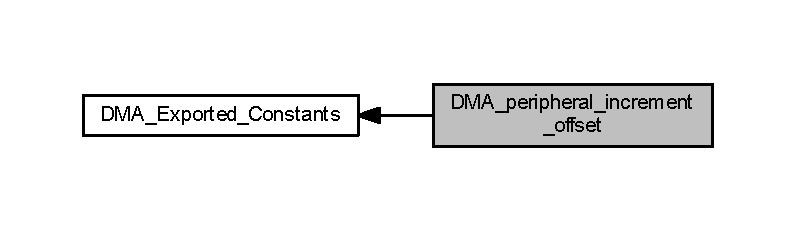
\includegraphics[width=350pt]{group___d_m_a__peripheral__increment__offset}
\end{center}
\end{figure}
\subsection*{Macros}
\begin{DoxyCompactItemize}
\item 
\mbox{\Hypertarget{group___d_m_a__peripheral__increment__offset_ga939053c42e486b82963b8eecc809bce0}\label{group___d_m_a__peripheral__increment__offset_ga939053c42e486b82963b8eecc809bce0}} 
\#define {\bfseries D\+M\+A\+\_\+\+P\+I\+N\+C\+O\+S\+\_\+\+Psize}~((uint32\+\_\+t)0x00000000)
\item 
\mbox{\Hypertarget{group___d_m_a__peripheral__increment__offset_gaae8184971db13b62cd9f4dc5aecf9c22}\label{group___d_m_a__peripheral__increment__offset_gaae8184971db13b62cd9f4dc5aecf9c22}} 
\#define {\bfseries D\+M\+A\+\_\+\+P\+I\+N\+C\+O\+S\+\_\+\+Word\+Aligned}~((uint32\+\_\+t)0x00008000)
\item 
\#define {\bfseries I\+S\+\_\+\+D\+M\+A\+\_\+\+P\+I\+N\+C\+O\+S\+\_\+\+S\+I\+ZE}(S\+I\+ZE)
\end{DoxyCompactItemize}


\subsection{Detailed Description}


\subsection{Macro Definition Documentation}
\mbox{\Hypertarget{group___d_m_a__peripheral__increment__offset_ga2fcfea7f5dedb658358f1220773fb2f2}\label{group___d_m_a__peripheral__increment__offset_ga2fcfea7f5dedb658358f1220773fb2f2}} 
\index{D\+M\+A\+\_\+peripheral\+\_\+increment\+\_\+offset@{D\+M\+A\+\_\+peripheral\+\_\+increment\+\_\+offset}!I\+S\+\_\+\+D\+M\+A\+\_\+\+P\+I\+N\+C\+O\+S\+\_\+\+S\+I\+ZE@{I\+S\+\_\+\+D\+M\+A\+\_\+\+P\+I\+N\+C\+O\+S\+\_\+\+S\+I\+ZE}}
\index{I\+S\+\_\+\+D\+M\+A\+\_\+\+P\+I\+N\+C\+O\+S\+\_\+\+S\+I\+ZE@{I\+S\+\_\+\+D\+M\+A\+\_\+\+P\+I\+N\+C\+O\+S\+\_\+\+S\+I\+ZE}!D\+M\+A\+\_\+peripheral\+\_\+increment\+\_\+offset@{D\+M\+A\+\_\+peripheral\+\_\+increment\+\_\+offset}}
\subsubsection{\texorpdfstring{I\+S\+\_\+\+D\+M\+A\+\_\+\+P\+I\+N\+C\+O\+S\+\_\+\+S\+I\+ZE}{IS\_DMA\_PINCOS\_SIZE}}
{\footnotesize\ttfamily \#define I\+S\+\_\+\+D\+M\+A\+\_\+\+P\+I\+N\+C\+O\+S\+\_\+\+S\+I\+ZE(\begin{DoxyParamCaption}\item[{}]{S\+I\+ZE }\end{DoxyParamCaption})}

{\bfseries Value\+:}
\begin{DoxyCode}
(((SIZE) == DMA\_PINCOS\_Psize) || \(\backslash\)
                                  ((SIZE) == DMA\_PINCOS\_WordAligned))
\end{DoxyCode}


Definition at line 517 of file stm32f4xx\+\_\+dma.\+h.


\hypertarget{group___d_m_a__flow__controller__definitions}{}\section{D\+M\+A\+\_\+flow\+\_\+controller\+\_\+definitions}
\label{group___d_m_a__flow__controller__definitions}\index{D\+M\+A\+\_\+flow\+\_\+controller\+\_\+definitions@{D\+M\+A\+\_\+flow\+\_\+controller\+\_\+definitions}}
Collaboration diagram for D\+M\+A\+\_\+flow\+\_\+controller\+\_\+definitions\+:\nopagebreak
\begin{figure}[H]
\begin{center}
\leavevmode
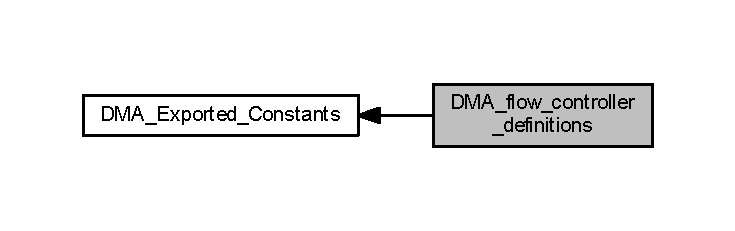
\includegraphics[width=350pt]{group___d_m_a__flow__controller__definitions}
\end{center}
\end{figure}
\subsection*{Macros}
\begin{DoxyCompactItemize}
\item 
\mbox{\Hypertarget{group___d_m_a__flow__controller__definitions_gafe69109789c2c285f98193f4b598cbc1}\label{group___d_m_a__flow__controller__definitions_gafe69109789c2c285f98193f4b598cbc1}} 
\#define {\bfseries D\+M\+A\+\_\+\+Flow\+Ctrl\+\_\+\+Memory}~((uint32\+\_\+t)0x00000000)
\item 
\mbox{\Hypertarget{group___d_m_a__flow__controller__definitions_ga33a735d51a2b790a25c579753edddd46}\label{group___d_m_a__flow__controller__definitions_ga33a735d51a2b790a25c579753edddd46}} 
\#define {\bfseries D\+M\+A\+\_\+\+Flow\+Ctrl\+\_\+\+Peripheral}~((uint32\+\_\+t)0x00000020)
\item 
\#define {\bfseries I\+S\+\_\+\+D\+M\+A\+\_\+\+F\+L\+O\+W\+\_\+\+C\+T\+RL}(C\+T\+RL)
\end{DoxyCompactItemize}


\subsection{Detailed Description}


\subsection{Macro Definition Documentation}
\mbox{\Hypertarget{group___d_m_a__flow__controller__definitions_ga78c0f18c0a86c67510f540a4210aadb7}\label{group___d_m_a__flow__controller__definitions_ga78c0f18c0a86c67510f540a4210aadb7}} 
\index{D\+M\+A\+\_\+flow\+\_\+controller\+\_\+definitions@{D\+M\+A\+\_\+flow\+\_\+controller\+\_\+definitions}!I\+S\+\_\+\+D\+M\+A\+\_\+\+F\+L\+O\+W\+\_\+\+C\+T\+RL@{I\+S\+\_\+\+D\+M\+A\+\_\+\+F\+L\+O\+W\+\_\+\+C\+T\+RL}}
\index{I\+S\+\_\+\+D\+M\+A\+\_\+\+F\+L\+O\+W\+\_\+\+C\+T\+RL@{I\+S\+\_\+\+D\+M\+A\+\_\+\+F\+L\+O\+W\+\_\+\+C\+T\+RL}!D\+M\+A\+\_\+flow\+\_\+controller\+\_\+definitions@{D\+M\+A\+\_\+flow\+\_\+controller\+\_\+definitions}}
\subsubsection{\texorpdfstring{I\+S\+\_\+\+D\+M\+A\+\_\+\+F\+L\+O\+W\+\_\+\+C\+T\+RL}{IS\_DMA\_FLOW\_CTRL}}
{\footnotesize\ttfamily \#define I\+S\+\_\+\+D\+M\+A\+\_\+\+F\+L\+O\+W\+\_\+\+C\+T\+RL(\begin{DoxyParamCaption}\item[{}]{C\+T\+RL }\end{DoxyParamCaption})}

{\bfseries Value\+:}
\begin{DoxyCode}
(((CTRL) == DMA\_FlowCtrl\_Memory) || \(\backslash\)
                                ((CTRL) == DMA\_FlowCtrl\_Peripheral))
\end{DoxyCode}


Definition at line 530 of file stm32f4xx\+\_\+dma.\+h.


\hypertarget{group___d_m_a__memory__targets__definitions}{}\section{D\+M\+A\+\_\+memory\+\_\+targets\+\_\+definitions}
\label{group___d_m_a__memory__targets__definitions}\index{D\+M\+A\+\_\+memory\+\_\+targets\+\_\+definitions@{D\+M\+A\+\_\+memory\+\_\+targets\+\_\+definitions}}
Collaboration diagram for D\+M\+A\+\_\+memory\+\_\+targets\+\_\+definitions\+:
\nopagebreak
\begin{figure}[H]
\begin{center}
\leavevmode
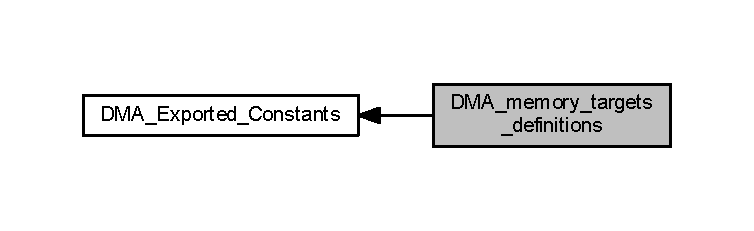
\includegraphics[width=350pt]{group___d_m_a__memory__targets__definitions}
\end{center}
\end{figure}
\subsection*{Macros}
\begin{DoxyCompactItemize}
\item 
\mbox{\Hypertarget{group___d_m_a__memory__targets__definitions_gadb576bccef5f2fc65fe9b451033bdc95}\label{group___d_m_a__memory__targets__definitions_gadb576bccef5f2fc65fe9b451033bdc95}} 
\#define {\bfseries D\+M\+A\+\_\+\+Memory\+\_\+0}~((uint32\+\_\+t)0x00000000)
\item 
\mbox{\Hypertarget{group___d_m_a__memory__targets__definitions_ga6d1e13631e4ef9a013d078e613fd7fd5}\label{group___d_m_a__memory__targets__definitions_ga6d1e13631e4ef9a013d078e613fd7fd5}} 
\#define {\bfseries D\+M\+A\+\_\+\+Memory\+\_\+1}~((uint32\+\_\+t)0x00080000)
\item 
\mbox{\Hypertarget{group___d_m_a__memory__targets__definitions_ga87d6abab18d2b4bb86db909854cc1f02}\label{group___d_m_a__memory__targets__definitions_ga87d6abab18d2b4bb86db909854cc1f02}} 
\#define {\bfseries I\+S\+\_\+\+D\+M\+A\+\_\+\+C\+U\+R\+R\+E\+N\+T\+\_\+\+M\+EM}(M\+EM)~(((M\+EM) == D\+M\+A\+\_\+\+Memory\+\_\+0) $\vert$$\vert$ ((M\+EM) == D\+M\+A\+\_\+\+Memory\+\_\+1))
\end{DoxyCompactItemize}


\subsection{Detailed Description}

\hypertarget{group___g_p_i_o___exported___constants}{}\section{G\+P\+I\+O\+\_\+\+Exported\+\_\+\+Constants}
\label{group___g_p_i_o___exported___constants}\index{G\+P\+I\+O\+\_\+\+Exported\+\_\+\+Constants@{G\+P\+I\+O\+\_\+\+Exported\+\_\+\+Constants}}
Collaboration diagram for G\+P\+I\+O\+\_\+\+Exported\+\_\+\+Constants\+:\nopagebreak
\begin{figure}[H]
\begin{center}
\leavevmode
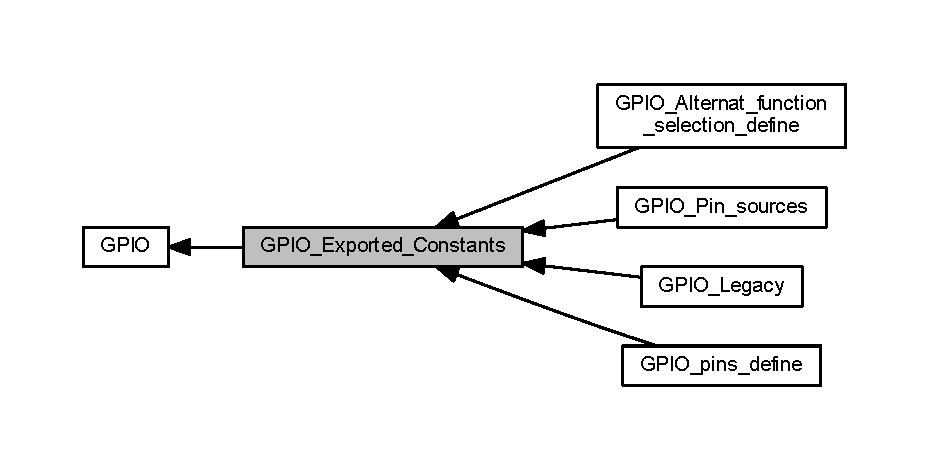
\includegraphics[width=350pt]{group___g_p_i_o___exported___constants}
\end{center}
\end{figure}
\subsection*{Modules}
\begin{DoxyCompactItemize}
\item 
\hyperlink{group___g_p_i_o__pins__define}{G\+P\+I\+O\+\_\+pins\+\_\+define}
\item 
\hyperlink{group___g_p_i_o___pin__sources}{G\+P\+I\+O\+\_\+\+Pin\+\_\+sources}
\item 
\hyperlink{group___g_p_i_o___alternat__function__selection__define}{G\+P\+I\+O\+\_\+\+Alternat\+\_\+function\+\_\+selection\+\_\+define}
\item 
\hyperlink{group___g_p_i_o___legacy}{G\+P\+I\+O\+\_\+\+Legacy}
\end{DoxyCompactItemize}


\subsection{Detailed Description}

\hypertarget{group___g_p_i_o__pins__define}{}\section{G\+P\+I\+O\+\_\+pins\+\_\+define}
\label{group___g_p_i_o__pins__define}\index{G\+P\+I\+O\+\_\+pins\+\_\+define@{G\+P\+I\+O\+\_\+pins\+\_\+define}}
Collaboration diagram for G\+P\+I\+O\+\_\+pins\+\_\+define\+:
\nopagebreak
\begin{figure}[H]
\begin{center}
\leavevmode
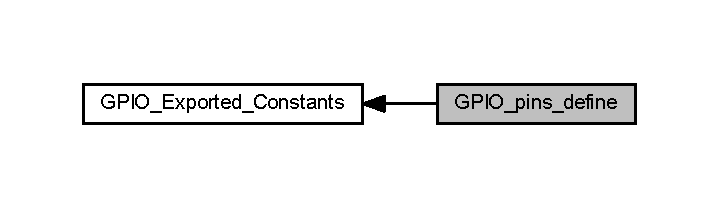
\includegraphics[width=345pt]{group___g_p_i_o__pins__define}
\end{center}
\end{figure}
\subsection*{Macros}
\begin{DoxyCompactItemize}
\item 
\mbox{\Hypertarget{group___g_p_i_o__pins__define_gab305b8d1be9f89bf2b4a05589b456049}\label{group___g_p_i_o__pins__define_gab305b8d1be9f89bf2b4a05589b456049}} 
\#define {\bfseries G\+P\+I\+O\+\_\+\+Pin\+\_\+0}~((uint16\+\_\+t)0x0001)  /$\ast$ Pin 0 selected $\ast$/
\item 
\mbox{\Hypertarget{group___g_p_i_o__pins__define_ga29db642c26f1fa0fffc3ecadcd30f82b}\label{group___g_p_i_o__pins__define_ga29db642c26f1fa0fffc3ecadcd30f82b}} 
\#define {\bfseries G\+P\+I\+O\+\_\+\+Pin\+\_\+1}~((uint16\+\_\+t)0x0002)  /$\ast$ Pin 1 selected $\ast$/
\item 
\mbox{\Hypertarget{group___g_p_i_o__pins__define_gabdf6630324b2f99360537a310687187c}\label{group___g_p_i_o__pins__define_gabdf6630324b2f99360537a310687187c}} 
\#define {\bfseries G\+P\+I\+O\+\_\+\+Pin\+\_\+2}~((uint16\+\_\+t)0x0004)  /$\ast$ Pin 2 selected $\ast$/
\item 
\mbox{\Hypertarget{group___g_p_i_o__pins__define_ga763c6544859dbe28cd3f8ad820045556}\label{group___g_p_i_o__pins__define_ga763c6544859dbe28cd3f8ad820045556}} 
\#define {\bfseries G\+P\+I\+O\+\_\+\+Pin\+\_\+3}~((uint16\+\_\+t)0x0008)  /$\ast$ Pin 3 selected $\ast$/
\item 
\mbox{\Hypertarget{group___g_p_i_o__pins__define_gacbf04d09b954606cdcc55eb2e81780e3}\label{group___g_p_i_o__pins__define_gacbf04d09b954606cdcc55eb2e81780e3}} 
\#define {\bfseries G\+P\+I\+O\+\_\+\+Pin\+\_\+4}~((uint16\+\_\+t)0x0010)  /$\ast$ Pin 4 selected $\ast$/
\item 
\mbox{\Hypertarget{group___g_p_i_o__pins__define_ga32dbe930f52ce5ab60190c65e9dc741e}\label{group___g_p_i_o__pins__define_ga32dbe930f52ce5ab60190c65e9dc741e}} 
\#define {\bfseries G\+P\+I\+O\+\_\+\+Pin\+\_\+5}~((uint16\+\_\+t)0x0020)  /$\ast$ Pin 5 selected $\ast$/
\item 
\mbox{\Hypertarget{group___g_p_i_o__pins__define_gaf047899d873f27c2db9f50b342e35a58}\label{group___g_p_i_o__pins__define_gaf047899d873f27c2db9f50b342e35a58}} 
\#define {\bfseries G\+P\+I\+O\+\_\+\+Pin\+\_\+6}~((uint16\+\_\+t)0x0040)  /$\ast$ Pin 6 selected $\ast$/
\item 
\mbox{\Hypertarget{group___g_p_i_o__pins__define_ga7346b6ce5507bd28a7a79e7dcc816c08}\label{group___g_p_i_o__pins__define_ga7346b6ce5507bd28a7a79e7dcc816c08}} 
\#define {\bfseries G\+P\+I\+O\+\_\+\+Pin\+\_\+7}~((uint16\+\_\+t)0x0080)  /$\ast$ Pin 7 selected $\ast$/
\item 
\mbox{\Hypertarget{group___g_p_i_o__pins__define_gac891f0984dc64af3567577fbf13ab304}\label{group___g_p_i_o__pins__define_gac891f0984dc64af3567577fbf13ab304}} 
\#define {\bfseries G\+P\+I\+O\+\_\+\+Pin\+\_\+8}~((uint16\+\_\+t)0x0100)  /$\ast$ Pin 8 selected $\ast$/
\item 
\mbox{\Hypertarget{group___g_p_i_o__pins__define_gaad1891082d5d6bcac06c2729a9fdd2f0}\label{group___g_p_i_o__pins__define_gaad1891082d5d6bcac06c2729a9fdd2f0}} 
\#define {\bfseries G\+P\+I\+O\+\_\+\+Pin\+\_\+9}~((uint16\+\_\+t)0x0200)  /$\ast$ Pin 9 selected $\ast$/
\item 
\mbox{\Hypertarget{group___g_p_i_o__pins__define_ga726af6407ba60ac60f02057227c2d348}\label{group___g_p_i_o__pins__define_ga726af6407ba60ac60f02057227c2d348}} 
\#define {\bfseries G\+P\+I\+O\+\_\+\+Pin\+\_\+10}~((uint16\+\_\+t)0x0400)  /$\ast$ Pin 10 selected $\ast$/
\item 
\mbox{\Hypertarget{group___g_p_i_o__pins__define_ga5139d5bc3d15784ae7794ed2ae1ff767}\label{group___g_p_i_o__pins__define_ga5139d5bc3d15784ae7794ed2ae1ff767}} 
\#define {\bfseries G\+P\+I\+O\+\_\+\+Pin\+\_\+11}~((uint16\+\_\+t)0x0800)  /$\ast$ Pin 11 selected $\ast$/
\item 
\mbox{\Hypertarget{group___g_p_i_o__pins__define_gada91257dcaab2c86f75fbd8e4b52b98c}\label{group___g_p_i_o__pins__define_gada91257dcaab2c86f75fbd8e4b52b98c}} 
\#define {\bfseries G\+P\+I\+O\+\_\+\+Pin\+\_\+12}~((uint16\+\_\+t)0x1000)  /$\ast$ Pin 12 selected $\ast$/
\item 
\mbox{\Hypertarget{group___g_p_i_o__pins__define_ga4155a41c433f3657b9c79cfbd4240966}\label{group___g_p_i_o__pins__define_ga4155a41c433f3657b9c79cfbd4240966}} 
\#define {\bfseries G\+P\+I\+O\+\_\+\+Pin\+\_\+13}~((uint16\+\_\+t)0x2000)  /$\ast$ Pin 13 selected $\ast$/
\item 
\mbox{\Hypertarget{group___g_p_i_o__pins__define_ga21cd1d89c0c061a6f09c5a842610bee5}\label{group___g_p_i_o__pins__define_ga21cd1d89c0c061a6f09c5a842610bee5}} 
\#define {\bfseries G\+P\+I\+O\+\_\+\+Pin\+\_\+14}~((uint16\+\_\+t)0x4000)  /$\ast$ Pin 14 selected $\ast$/
\item 
\mbox{\Hypertarget{group___g_p_i_o__pins__define_gae686a9fc47cf3e420e5db0784210711d}\label{group___g_p_i_o__pins__define_gae686a9fc47cf3e420e5db0784210711d}} 
\#define {\bfseries G\+P\+I\+O\+\_\+\+Pin\+\_\+15}~((uint16\+\_\+t)0x8000)  /$\ast$ Pin 15 selected $\ast$/
\item 
\mbox{\Hypertarget{group___g_p_i_o__pins__define_gaba3e915ddca17a1211edc07b7fd97e8b}\label{group___g_p_i_o__pins__define_gaba3e915ddca17a1211edc07b7fd97e8b}} 
\#define {\bfseries G\+P\+I\+O\+\_\+\+Pin\+\_\+\+All}~((uint16\+\_\+t)0x\+F\+F\+F\+F)  /$\ast$ All pins selected $\ast$/
\item 
\mbox{\Hypertarget{group___g_p_i_o__pins__define_gad6ec74e33360395535ad5d91ba6d4781}\label{group___g_p_i_o__pins__define_gad6ec74e33360395535ad5d91ba6d4781}} 
\#define {\bfseries I\+S\+\_\+\+G\+P\+I\+O\+\_\+\+P\+IN}(P\+IN)~((((P\+IN) \& (uint16\+\_\+t)0x00) == 0x00) \&\& ((\+P\+I\+N) != (uint16\+\_\+t)0x00))
\item 
\#define {\bfseries I\+S\+\_\+\+G\+E\+T\+\_\+\+G\+P\+I\+O\+\_\+\+P\+IN}(P\+IN)
\end{DoxyCompactItemize}


\subsection{Detailed Description}


\subsection{Macro Definition Documentation}
\mbox{\Hypertarget{group___g_p_i_o__pins__define_gaddf7154b7f30b7c0a70f3aeaff5ddffc}\label{group___g_p_i_o__pins__define_gaddf7154b7f30b7c0a70f3aeaff5ddffc}} 
\index{G\+P\+I\+O\+\_\+pins\+\_\+define@{G\+P\+I\+O\+\_\+pins\+\_\+define}!I\+S\+\_\+\+G\+E\+T\+\_\+\+G\+P\+I\+O\+\_\+\+P\+IN@{I\+S\+\_\+\+G\+E\+T\+\_\+\+G\+P\+I\+O\+\_\+\+P\+IN}}
\index{I\+S\+\_\+\+G\+E\+T\+\_\+\+G\+P\+I\+O\+\_\+\+P\+IN@{I\+S\+\_\+\+G\+E\+T\+\_\+\+G\+P\+I\+O\+\_\+\+P\+IN}!G\+P\+I\+O\+\_\+pins\+\_\+define@{G\+P\+I\+O\+\_\+pins\+\_\+define}}
\subsubsection{\texorpdfstring{I\+S\+\_\+\+G\+E\+T\+\_\+\+G\+P\+I\+O\+\_\+\+P\+IN}{IS\_GET\_GPIO\_PIN}}
{\footnotesize\ttfamily \#define I\+S\+\_\+\+G\+E\+T\+\_\+\+G\+P\+I\+O\+\_\+\+P\+IN(\begin{DoxyParamCaption}\item[{}]{P\+IN }\end{DoxyParamCaption})}

{\bfseries Value\+:}
\begin{DoxyCode}
(((PIN) == GPIO\_Pin\_0) || \(\backslash\)
                              ((PIN) == GPIO\_Pin\_1) || \(\backslash\)
                              ((PIN) == GPIO\_Pin\_2) || \(\backslash\)
                              ((PIN) == GPIO\_Pin\_3) || \(\backslash\)
                              ((PIN) == GPIO\_Pin\_4) || \(\backslash\)
                              ((PIN) == GPIO\_Pin\_5) || \(\backslash\)
                              ((PIN) == GPIO\_Pin\_6) || \(\backslash\)
                              ((PIN) == GPIO\_Pin\_7) || \(\backslash\)
                              ((PIN) == GPIO\_Pin\_8) || \(\backslash\)
                              ((PIN) == GPIO\_Pin\_9) || \(\backslash\)
                              ((PIN) == GPIO\_Pin\_10) || \(\backslash\)
                              ((PIN) == GPIO\_Pin\_11) || \(\backslash\)
                              ((PIN) == GPIO\_Pin\_12) || \(\backslash\)
                              ((PIN) == GPIO\_Pin\_13) || \(\backslash\)
                              ((PIN) == GPIO\_Pin\_14) || \(\backslash\)
                              ((PIN) == GPIO\_Pin\_15))
\end{DoxyCode}


Definition at line 163 of file stm32f4xx\+\_\+gpio.\+h.


\hypertarget{group___g_p_i_o___pin__sources}{}\section{G\+P\+I\+O\+\_\+\+Pin\+\_\+sources}
\label{group___g_p_i_o___pin__sources}\index{G\+P\+I\+O\+\_\+\+Pin\+\_\+sources@{G\+P\+I\+O\+\_\+\+Pin\+\_\+sources}}
Collaboration diagram for G\+P\+I\+O\+\_\+\+Pin\+\_\+sources\+:\nopagebreak
\begin{figure}[H]
\begin{center}
\leavevmode
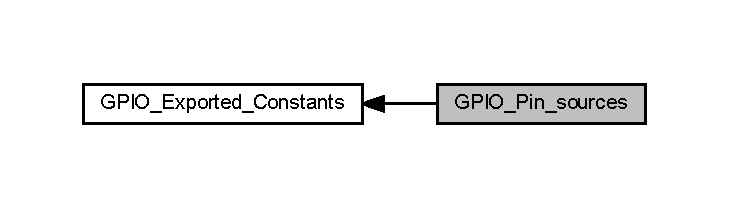
\includegraphics[width=350pt]{group___g_p_i_o___pin__sources}
\end{center}
\end{figure}
\subsection*{Macros}
\begin{DoxyCompactItemize}
\item 
\mbox{\Hypertarget{group___g_p_i_o___pin__sources_ga028bcbdf5a7fd81ec45830f60a022bb4}\label{group___g_p_i_o___pin__sources_ga028bcbdf5a7fd81ec45830f60a022bb4}} 
\#define {\bfseries G\+P\+I\+O\+\_\+\+Pin\+Source0}~((uint8\+\_\+t)0x00)
\item 
\mbox{\Hypertarget{group___g_p_i_o___pin__sources_gad02324cdd8526a7aacd15a5a910d56f1}\label{group___g_p_i_o___pin__sources_gad02324cdd8526a7aacd15a5a910d56f1}} 
\#define {\bfseries G\+P\+I\+O\+\_\+\+Pin\+Source1}~((uint8\+\_\+t)0x01)
\item 
\mbox{\Hypertarget{group___g_p_i_o___pin__sources_ga7808fb6269890fa1e37a322418884607}\label{group___g_p_i_o___pin__sources_ga7808fb6269890fa1e37a322418884607}} 
\#define {\bfseries G\+P\+I\+O\+\_\+\+Pin\+Source2}~((uint8\+\_\+t)0x02)
\item 
\mbox{\Hypertarget{group___g_p_i_o___pin__sources_ga0df17fee84ec9ab096b5525a06871863}\label{group___g_p_i_o___pin__sources_ga0df17fee84ec9ab096b5525a06871863}} 
\#define {\bfseries G\+P\+I\+O\+\_\+\+Pin\+Source3}~((uint8\+\_\+t)0x03)
\item 
\mbox{\Hypertarget{group___g_p_i_o___pin__sources_gaf5aa545455dacbf315a40cecd0842b6c}\label{group___g_p_i_o___pin__sources_gaf5aa545455dacbf315a40cecd0842b6c}} 
\#define {\bfseries G\+P\+I\+O\+\_\+\+Pin\+Source4}~((uint8\+\_\+t)0x04)
\item 
\mbox{\Hypertarget{group___g_p_i_o___pin__sources_gaf231e680fe2db4ea44a7fd0f5d5c5875}\label{group___g_p_i_o___pin__sources_gaf231e680fe2db4ea44a7fd0f5d5c5875}} 
\#define {\bfseries G\+P\+I\+O\+\_\+\+Pin\+Source5}~((uint8\+\_\+t)0x05)
\item 
\mbox{\Hypertarget{group___g_p_i_o___pin__sources_gada41b6bd03b2873a2400628df0a1026e}\label{group___g_p_i_o___pin__sources_gada41b6bd03b2873a2400628df0a1026e}} 
\#define {\bfseries G\+P\+I\+O\+\_\+\+Pin\+Source6}~((uint8\+\_\+t)0x06)
\item 
\mbox{\Hypertarget{group___g_p_i_o___pin__sources_ga609974472a3a7c5274fc56018d7adf16}\label{group___g_p_i_o___pin__sources_ga609974472a3a7c5274fc56018d7adf16}} 
\#define {\bfseries G\+P\+I\+O\+\_\+\+Pin\+Source7}~((uint8\+\_\+t)0x07)
\item 
\mbox{\Hypertarget{group___g_p_i_o___pin__sources_ga6f5962c5b2ce5734734563bdad18fbd6}\label{group___g_p_i_o___pin__sources_ga6f5962c5b2ce5734734563bdad18fbd6}} 
\#define {\bfseries G\+P\+I\+O\+\_\+\+Pin\+Source8}~((uint8\+\_\+t)0x08)
\item 
\mbox{\Hypertarget{group___g_p_i_o___pin__sources_gabaaed5961f2b9862082f74e18f5c3f0e}\label{group___g_p_i_o___pin__sources_gabaaed5961f2b9862082f74e18f5c3f0e}} 
\#define {\bfseries G\+P\+I\+O\+\_\+\+Pin\+Source9}~((uint8\+\_\+t)0x09)
\item 
\mbox{\Hypertarget{group___g_p_i_o___pin__sources_gacec97d9c2d319b450f699adff6430c86}\label{group___g_p_i_o___pin__sources_gacec97d9c2d319b450f699adff6430c86}} 
\#define {\bfseries G\+P\+I\+O\+\_\+\+Pin\+Source10}~((uint8\+\_\+t)0x0\+A)
\item 
\mbox{\Hypertarget{group___g_p_i_o___pin__sources_ga446be4a99e84eefb5c71a643211f598b}\label{group___g_p_i_o___pin__sources_ga446be4a99e84eefb5c71a643211f598b}} 
\#define {\bfseries G\+P\+I\+O\+\_\+\+Pin\+Source11}~((uint8\+\_\+t)0x0\+B)
\item 
\mbox{\Hypertarget{group___g_p_i_o___pin__sources_gaaa64892c00d50b0fa49f0ce72a83e6e0}\label{group___g_p_i_o___pin__sources_gaaa64892c00d50b0fa49f0ce72a83e6e0}} 
\#define {\bfseries G\+P\+I\+O\+\_\+\+Pin\+Source12}~((uint8\+\_\+t)0x0\+C)
\item 
\mbox{\Hypertarget{group___g_p_i_o___pin__sources_gace4beb385facd306324fa9e362df5fda}\label{group___g_p_i_o___pin__sources_gace4beb385facd306324fa9e362df5fda}} 
\#define {\bfseries G\+P\+I\+O\+\_\+\+Pin\+Source13}~((uint8\+\_\+t)0x0\+D)
\item 
\mbox{\Hypertarget{group___g_p_i_o___pin__sources_ga5fbb540a86af4015a46ac16c61ddb1f7}\label{group___g_p_i_o___pin__sources_ga5fbb540a86af4015a46ac16c61ddb1f7}} 
\#define {\bfseries G\+P\+I\+O\+\_\+\+Pin\+Source14}~((uint8\+\_\+t)0x0\+E)
\item 
\mbox{\Hypertarget{group___g_p_i_o___pin__sources_ga9b29d9a9ecb1579ecedf4ea53ccbfd5b}\label{group___g_p_i_o___pin__sources_ga9b29d9a9ecb1579ecedf4ea53ccbfd5b}} 
\#define {\bfseries G\+P\+I\+O\+\_\+\+Pin\+Source15}~((uint8\+\_\+t)0x0\+F)
\item 
\#define {\bfseries I\+S\+\_\+\+G\+P\+I\+O\+\_\+\+P\+I\+N\+\_\+\+S\+O\+U\+R\+CE}(P\+I\+N\+S\+O\+U\+R\+CE)
\end{DoxyCompactItemize}


\subsection{Detailed Description}


\subsection{Macro Definition Documentation}
\mbox{\Hypertarget{group___g_p_i_o___pin__sources_ga689e4e72591136b6a8d4df9d895181f7}\label{group___g_p_i_o___pin__sources_ga689e4e72591136b6a8d4df9d895181f7}} 
\index{G\+P\+I\+O\+\_\+\+Pin\+\_\+sources@{G\+P\+I\+O\+\_\+\+Pin\+\_\+sources}!I\+S\+\_\+\+G\+P\+I\+O\+\_\+\+P\+I\+N\+\_\+\+S\+O\+U\+R\+CE@{I\+S\+\_\+\+G\+P\+I\+O\+\_\+\+P\+I\+N\+\_\+\+S\+O\+U\+R\+CE}}
\index{I\+S\+\_\+\+G\+P\+I\+O\+\_\+\+P\+I\+N\+\_\+\+S\+O\+U\+R\+CE@{I\+S\+\_\+\+G\+P\+I\+O\+\_\+\+P\+I\+N\+\_\+\+S\+O\+U\+R\+CE}!G\+P\+I\+O\+\_\+\+Pin\+\_\+sources@{G\+P\+I\+O\+\_\+\+Pin\+\_\+sources}}
\subsubsection{\texorpdfstring{I\+S\+\_\+\+G\+P\+I\+O\+\_\+\+P\+I\+N\+\_\+\+S\+O\+U\+R\+CE}{IS\_GPIO\_PIN\_SOURCE}}
{\footnotesize\ttfamily \#define I\+S\+\_\+\+G\+P\+I\+O\+\_\+\+P\+I\+N\+\_\+\+S\+O\+U\+R\+CE(\begin{DoxyParamCaption}\item[{}]{P\+I\+N\+S\+O\+U\+R\+CE }\end{DoxyParamCaption})}

{\bfseries Value\+:}
\begin{DoxyCode}
(((PINSOURCE) == GPIO\_PinSource0) || \(\backslash\)
                                       ((PINSOURCE) == GPIO\_PinSource1) || \(\backslash\)
                                       ((PINSOURCE) == GPIO\_PinSource2) || \(\backslash\)
                                       ((PINSOURCE) == GPIO\_PinSource3) || \(\backslash\)
                                       ((PINSOURCE) == GPIO\_PinSource4) || \(\backslash\)
                                       ((PINSOURCE) == GPIO\_PinSource5) || \(\backslash\)
                                       ((PINSOURCE) == GPIO\_PinSource6) || \(\backslash\)
                                       ((PINSOURCE) == GPIO\_PinSource7) || \(\backslash\)
                                       ((PINSOURCE) == GPIO\_PinSource8) || \(\backslash\)
                                       ((PINSOURCE) == GPIO\_PinSource9) || \(\backslash\)
                                       ((PINSOURCE) == GPIO\_PinSource10) || \(\backslash\)
                                       ((PINSOURCE) == GPIO\_PinSource11) || \(\backslash\)
                                       ((PINSOURCE) == GPIO\_PinSource12) || \(\backslash\)
                                       ((PINSOURCE) == GPIO\_PinSource13) || \(\backslash\)
                                       ((PINSOURCE) == GPIO\_PinSource14) || \(\backslash\)
                                       ((PINSOURCE) == GPIO\_PinSource15))
\end{DoxyCode}


Definition at line 204 of file stm32f4xx\+\_\+gpio.\+h.


\hypertarget{group___g_p_i_o___alternat__function__selection__define}{}\section{G\+P\+I\+O\+\_\+\+Alternat\+\_\+function\+\_\+selection\+\_\+define}
\label{group___g_p_i_o___alternat__function__selection__define}\index{G\+P\+I\+O\+\_\+\+Alternat\+\_\+function\+\_\+selection\+\_\+define@{G\+P\+I\+O\+\_\+\+Alternat\+\_\+function\+\_\+selection\+\_\+define}}
Collaboration diagram for G\+P\+I\+O\+\_\+\+Alternat\+\_\+function\+\_\+selection\+\_\+define\+:
\nopagebreak
\begin{figure}[H]
\begin{center}
\leavevmode
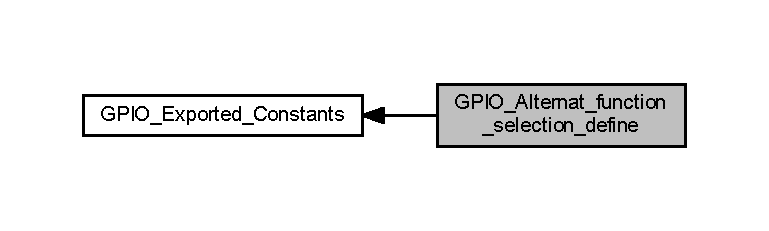
\includegraphics[width=350pt]{group___g_p_i_o___alternat__function__selection__define}
\end{center}
\end{figure}
\subsection*{Macros}
\begin{DoxyCompactItemize}
\item 
\mbox{\Hypertarget{group___g_p_i_o___alternat__function__selection__define_ga93071f0121fab9f8f13e59c612ed6291}\label{group___g_p_i_o___alternat__function__selection__define_ga93071f0121fab9f8f13e59c612ed6291}} 
\#define \hyperlink{group___g_p_i_o___alternat__function__selection__define_ga93071f0121fab9f8f13e59c612ed6291}{G\+P\+I\+O\+\_\+\+A\+F\+\_\+\+R\+T\+C\+\_\+50\+Hz}~((uint8\+\_\+t)0x00)  /$\ast$ R\+T\+C\+\_\+50\+Hz Alternate Function mapping $\ast$/
\begin{DoxyCompactList}\small\item\em AF 0 selection. \end{DoxyCompactList}\item 
\mbox{\Hypertarget{group___g_p_i_o___alternat__function__selection__define_gacfe2ce01055b82d0fcdd93da513f7cc0}\label{group___g_p_i_o___alternat__function__selection__define_gacfe2ce01055b82d0fcdd93da513f7cc0}} 
\#define {\bfseries G\+P\+I\+O\+\_\+\+A\+F\+\_\+\+M\+CO}~((uint8\+\_\+t)0x00)  /$\ast$ M\+C\+O (\+M\+C\+O1 and M\+C\+O2) Alternate Function mapping $\ast$/
\item 
\mbox{\Hypertarget{group___g_p_i_o___alternat__function__selection__define_gac284edf4c3267d864b3d56cc6bf6ac95}\label{group___g_p_i_o___alternat__function__selection__define_gac284edf4c3267d864b3d56cc6bf6ac95}} 
\#define {\bfseries G\+P\+I\+O\+\_\+\+A\+F\+\_\+\+T\+A\+M\+P\+ER}~((uint8\+\_\+t)0x00)  /$\ast$ T\+A\+M\+P\+E\+R (\+T\+A\+M\+P\+E\+R\+\_\+1 and T\+A\+M\+P\+E\+R\+\_\+2) Alternate Function mapping $\ast$/
\item 
\mbox{\Hypertarget{group___g_p_i_o___alternat__function__selection__define_ga63cfa7c46dc0c5ab9cdf7340cc95f7fc}\label{group___g_p_i_o___alternat__function__selection__define_ga63cfa7c46dc0c5ab9cdf7340cc95f7fc}} 
\#define {\bfseries G\+P\+I\+O\+\_\+\+A\+F\+\_\+\+S\+WJ}~((uint8\+\_\+t)0x00)  /$\ast$ S\+W\+J (\+S\+W\+D and J\+T\+A\+G) Alternate Function mapping $\ast$/
\item 
\mbox{\Hypertarget{group___g_p_i_o___alternat__function__selection__define_gac97ace879d6584f8bd705fa1d199d4d4}\label{group___g_p_i_o___alternat__function__selection__define_gac97ace879d6584f8bd705fa1d199d4d4}} 
\#define {\bfseries G\+P\+I\+O\+\_\+\+A\+F\+\_\+\+T\+R\+A\+CE}~((uint8\+\_\+t)0x00)  /$\ast$ T\+R\+A\+C\+E Alternate Function mapping $\ast$/
\item 
\mbox{\Hypertarget{group___g_p_i_o___alternat__function__selection__define_ga9a65573a3d8684febe1fda5c6cd8c992}\label{group___g_p_i_o___alternat__function__selection__define_ga9a65573a3d8684febe1fda5c6cd8c992}} 
\#define \hyperlink{group___g_p_i_o___alternat__function__selection__define_ga9a65573a3d8684febe1fda5c6cd8c992}{G\+P\+I\+O\+\_\+\+A\+F\+\_\+\+T\+I\+M1}~((uint8\+\_\+t)0x01)  /$\ast$ T\+I\+M1 Alternate Function mapping $\ast$/
\begin{DoxyCompactList}\small\item\em AF 1 selection. \end{DoxyCompactList}\item 
\mbox{\Hypertarget{group___g_p_i_o___alternat__function__selection__define_ga6a1335e47fe67ff5a08ebe0ebfec2ffa}\label{group___g_p_i_o___alternat__function__selection__define_ga6a1335e47fe67ff5a08ebe0ebfec2ffa}} 
\#define {\bfseries G\+P\+I\+O\+\_\+\+A\+F\+\_\+\+T\+I\+M2}~((uint8\+\_\+t)0x01)  /$\ast$ T\+I\+M2 Alternate Function mapping $\ast$/
\item 
\mbox{\Hypertarget{group___g_p_i_o___alternat__function__selection__define_ga8c6bda0c56abc29eef7709b52d9d3e0d}\label{group___g_p_i_o___alternat__function__selection__define_ga8c6bda0c56abc29eef7709b52d9d3e0d}} 
\#define \hyperlink{group___g_p_i_o___alternat__function__selection__define_ga8c6bda0c56abc29eef7709b52d9d3e0d}{G\+P\+I\+O\+\_\+\+A\+F\+\_\+\+T\+I\+M3}~((uint8\+\_\+t)0x02)  /$\ast$ T\+I\+M3 Alternate Function mapping $\ast$/
\begin{DoxyCompactList}\small\item\em AF 2 selection. \end{DoxyCompactList}\item 
\mbox{\Hypertarget{group___g_p_i_o___alternat__function__selection__define_gabe02d26327e89fe4c9aaf30ec1187009}\label{group___g_p_i_o___alternat__function__selection__define_gabe02d26327e89fe4c9aaf30ec1187009}} 
\#define {\bfseries G\+P\+I\+O\+\_\+\+A\+F\+\_\+\+T\+I\+M4}~((uint8\+\_\+t)0x02)  /$\ast$ T\+I\+M4 Alternate Function mapping $\ast$/
\item 
\mbox{\Hypertarget{group___g_p_i_o___alternat__function__selection__define_gad1abee116e98620ade37334e649e6006}\label{group___g_p_i_o___alternat__function__selection__define_gad1abee116e98620ade37334e649e6006}} 
\#define {\bfseries G\+P\+I\+O\+\_\+\+A\+F\+\_\+\+T\+I\+M5}~((uint8\+\_\+t)0x02)  /$\ast$ T\+I\+M5 Alternate Function mapping $\ast$/
\item 
\mbox{\Hypertarget{group___g_p_i_o___alternat__function__selection__define_gaf7562d5cf5d33dbc7b7c69df63182583}\label{group___g_p_i_o___alternat__function__selection__define_gaf7562d5cf5d33dbc7b7c69df63182583}} 
\#define \hyperlink{group___g_p_i_o___alternat__function__selection__define_gaf7562d5cf5d33dbc7b7c69df63182583}{G\+P\+I\+O\+\_\+\+A\+F\+\_\+\+T\+I\+M8}~((uint8\+\_\+t)0x03)  /$\ast$ T\+I\+M8 Alternate Function mapping $\ast$/
\begin{DoxyCompactList}\small\item\em AF 3 selection. \end{DoxyCompactList}\item 
\mbox{\Hypertarget{group___g_p_i_o___alternat__function__selection__define_ga6c7cfbf2f21945814c6526a7bacb1384}\label{group___g_p_i_o___alternat__function__selection__define_ga6c7cfbf2f21945814c6526a7bacb1384}} 
\#define {\bfseries G\+P\+I\+O\+\_\+\+A\+F\+\_\+\+T\+I\+M9}~((uint8\+\_\+t)0x03)  /$\ast$ T\+I\+M9 Alternate Function mapping $\ast$/
\item 
\mbox{\Hypertarget{group___g_p_i_o___alternat__function__selection__define_ga3881c36c71f0cbd7efacb424b39cd9f4}\label{group___g_p_i_o___alternat__function__selection__define_ga3881c36c71f0cbd7efacb424b39cd9f4}} 
\#define {\bfseries G\+P\+I\+O\+\_\+\+A\+F\+\_\+\+T\+I\+M10}~((uint8\+\_\+t)0x03)  /$\ast$ T\+I\+M10 Alternate Function mapping $\ast$/
\item 
\mbox{\Hypertarget{group___g_p_i_o___alternat__function__selection__define_gaeb30ba1cb15de0d4af78933e9dcfd033}\label{group___g_p_i_o___alternat__function__selection__define_gaeb30ba1cb15de0d4af78933e9dcfd033}} 
\#define {\bfseries G\+P\+I\+O\+\_\+\+A\+F\+\_\+\+T\+I\+M11}~((uint8\+\_\+t)0x03)  /$\ast$ T\+I\+M11 Alternate Function mapping $\ast$/
\item 
\mbox{\Hypertarget{group___g_p_i_o___alternat__function__selection__define_gaa246f87c460c4bb4036b8ab39e0220f1}\label{group___g_p_i_o___alternat__function__selection__define_gaa246f87c460c4bb4036b8ab39e0220f1}} 
\#define \hyperlink{group___g_p_i_o___alternat__function__selection__define_gaa246f87c460c4bb4036b8ab39e0220f1}{G\+P\+I\+O\+\_\+\+A\+F\+\_\+\+I2\+C1}~((uint8\+\_\+t)0x04)  /$\ast$ I2\+C1 Alternate Function mapping $\ast$/
\begin{DoxyCompactList}\small\item\em AF 4 selection. \end{DoxyCompactList}\item 
\mbox{\Hypertarget{group___g_p_i_o___alternat__function__selection__define_ga4a82500bac7239134e2c28d4656810f1}\label{group___g_p_i_o___alternat__function__selection__define_ga4a82500bac7239134e2c28d4656810f1}} 
\#define {\bfseries G\+P\+I\+O\+\_\+\+A\+F\+\_\+\+I2\+C2}~((uint8\+\_\+t)0x04)  /$\ast$ I2\+C2 Alternate Function mapping $\ast$/
\item 
\mbox{\Hypertarget{group___g_p_i_o___alternat__function__selection__define_ga302620e38b718a54d760845de2a06b2b}\label{group___g_p_i_o___alternat__function__selection__define_ga302620e38b718a54d760845de2a06b2b}} 
\#define {\bfseries G\+P\+I\+O\+\_\+\+A\+F\+\_\+\+I2\+C3}~((uint8\+\_\+t)0x04)  /$\ast$ I2\+C3 Alternate Function mapping $\ast$/
\item 
\mbox{\Hypertarget{group___g_p_i_o___alternat__function__selection__define_ga7804aaf9275dbb5502312729a76d13be}\label{group___g_p_i_o___alternat__function__selection__define_ga7804aaf9275dbb5502312729a76d13be}} 
\#define \hyperlink{group___g_p_i_o___alternat__function__selection__define_ga7804aaf9275dbb5502312729a76d13be}{G\+P\+I\+O\+\_\+\+A\+F\+\_\+\+S\+P\+I1}~((uint8\+\_\+t)0x05)  /$\ast$ S\+P\+I1 Alternate Function mapping $\ast$/
\begin{DoxyCompactList}\small\item\em AF 5 selection. \end{DoxyCompactList}\item 
\mbox{\Hypertarget{group___g_p_i_o___alternat__function__selection__define_ga45d0fbf9ba0bf0f554697e78712fc369}\label{group___g_p_i_o___alternat__function__selection__define_ga45d0fbf9ba0bf0f554697e78712fc369}} 
\#define {\bfseries G\+P\+I\+O\+\_\+\+A\+F\+\_\+\+S\+P\+I2}~((uint8\+\_\+t)0x05)  /$\ast$ S\+P\+I2/\+I2\+S2 Alternate Function mapping $\ast$/
\item 
\mbox{\Hypertarget{group___g_p_i_o___alternat__function__selection__define_gad6e716ad894aa5299273541c6966864a}\label{group___g_p_i_o___alternat__function__selection__define_gad6e716ad894aa5299273541c6966864a}} 
\#define \hyperlink{group___g_p_i_o___alternat__function__selection__define_gad6e716ad894aa5299273541c6966864a}{G\+P\+I\+O\+\_\+\+A\+F\+\_\+\+S\+P\+I3}~((uint8\+\_\+t)0x06)  /$\ast$ S\+P\+I3/\+I2\+S3 Alternate Function mapping $\ast$/
\begin{DoxyCompactList}\small\item\em AF 6 selection. \end{DoxyCompactList}\item 
\mbox{\Hypertarget{group___g_p_i_o___alternat__function__selection__define_ga790e1f37e75f475cf09c211f566fb069}\label{group___g_p_i_o___alternat__function__selection__define_ga790e1f37e75f475cf09c211f566fb069}} 
\#define \hyperlink{group___g_p_i_o___alternat__function__selection__define_ga790e1f37e75f475cf09c211f566fb069}{G\+P\+I\+O\+\_\+\+A\+F\+\_\+\+U\+S\+A\+R\+T1}~((uint8\+\_\+t)0x07)  /$\ast$ U\+S\+A\+R\+T1 Alternate Function mapping $\ast$/
\begin{DoxyCompactList}\small\item\em AF 7 selection. \end{DoxyCompactList}\item 
\mbox{\Hypertarget{group___g_p_i_o___alternat__function__selection__define_ga5e74db1f4d0fc3527aa067093625171b}\label{group___g_p_i_o___alternat__function__selection__define_ga5e74db1f4d0fc3527aa067093625171b}} 
\#define {\bfseries G\+P\+I\+O\+\_\+\+A\+F\+\_\+\+U\+S\+A\+R\+T2}~((uint8\+\_\+t)0x07)  /$\ast$ U\+S\+A\+R\+T2 Alternate Function mapping $\ast$/
\item 
\mbox{\Hypertarget{group___g_p_i_o___alternat__function__selection__define_ga97742da355d32c599527813eaf109ec7}\label{group___g_p_i_o___alternat__function__selection__define_ga97742da355d32c599527813eaf109ec7}} 
\#define {\bfseries G\+P\+I\+O\+\_\+\+A\+F\+\_\+\+U\+S\+A\+R\+T3}~((uint8\+\_\+t)0x07)  /$\ast$ U\+S\+A\+R\+T3 Alternate Function mapping $\ast$/
\item 
\mbox{\Hypertarget{group___g_p_i_o___alternat__function__selection__define_ga8fac28d42bc99794bb74707c141fc0f6}\label{group___g_p_i_o___alternat__function__selection__define_ga8fac28d42bc99794bb74707c141fc0f6}} 
\#define {\bfseries G\+P\+I\+O\+\_\+\+A\+F\+\_\+\+I2\+S3ext}~((uint8\+\_\+t)0x07)  /$\ast$ I2\+S3ext Alternate Function mapping $\ast$/
\item 
\mbox{\Hypertarget{group___g_p_i_o___alternat__function__selection__define_gad1754187e64b66681cc1447695062706}\label{group___g_p_i_o___alternat__function__selection__define_gad1754187e64b66681cc1447695062706}} 
\#define \hyperlink{group___g_p_i_o___alternat__function__selection__define_gad1754187e64b66681cc1447695062706}{G\+P\+I\+O\+\_\+\+A\+F\+\_\+\+U\+A\+R\+T4}~((uint8\+\_\+t)0x08)  /$\ast$ U\+A\+R\+T4 Alternate Function mapping $\ast$/
\begin{DoxyCompactList}\small\item\em AF 8 selection. \end{DoxyCompactList}\item 
\mbox{\Hypertarget{group___g_p_i_o___alternat__function__selection__define_ga6250acb0f2f3de33bc8e78615852cc48}\label{group___g_p_i_o___alternat__function__selection__define_ga6250acb0f2f3de33bc8e78615852cc48}} 
\#define {\bfseries G\+P\+I\+O\+\_\+\+A\+F\+\_\+\+U\+A\+R\+T5}~((uint8\+\_\+t)0x08)  /$\ast$ U\+A\+R\+T5 Alternate Function mapping $\ast$/
\item 
\mbox{\Hypertarget{group___g_p_i_o___alternat__function__selection__define_gaf69942861848b5175369145ffc001c41}\label{group___g_p_i_o___alternat__function__selection__define_gaf69942861848b5175369145ffc001c41}} 
\#define {\bfseries G\+P\+I\+O\+\_\+\+A\+F\+\_\+\+U\+S\+A\+R\+T6}~((uint8\+\_\+t)0x08)  /$\ast$ U\+S\+A\+R\+T6 Alternate Function mapping $\ast$/
\item 
\mbox{\Hypertarget{group___g_p_i_o___alternat__function__selection__define_gaf5defeedc302bf348e31dd7bdcdd882f}\label{group___g_p_i_o___alternat__function__selection__define_gaf5defeedc302bf348e31dd7bdcdd882f}} 
\#define \hyperlink{group___g_p_i_o___alternat__function__selection__define_gaf5defeedc302bf348e31dd7bdcdd882f}{G\+P\+I\+O\+\_\+\+A\+F\+\_\+\+C\+A\+N1}~((uint8\+\_\+t)0x09)  /$\ast$ C\+A\+N1 Alternate Function mapping $\ast$/
\begin{DoxyCompactList}\small\item\em AF 9 selection. \end{DoxyCompactList}\item 
\mbox{\Hypertarget{group___g_p_i_o___alternat__function__selection__define_ga4896d720d93f50f17207b4059ab5ebfb}\label{group___g_p_i_o___alternat__function__selection__define_ga4896d720d93f50f17207b4059ab5ebfb}} 
\#define {\bfseries G\+P\+I\+O\+\_\+\+A\+F\+\_\+\+C\+A\+N2}~((uint8\+\_\+t)0x09)  /$\ast$ C\+A\+N2 Alternate Function mapping $\ast$/
\item 
\mbox{\Hypertarget{group___g_p_i_o___alternat__function__selection__define_ga681ff7964f5d73ed973a299383b13c90}\label{group___g_p_i_o___alternat__function__selection__define_ga681ff7964f5d73ed973a299383b13c90}} 
\#define {\bfseries G\+P\+I\+O\+\_\+\+A\+F\+\_\+\+T\+I\+M12}~((uint8\+\_\+t)0x09)  /$\ast$ T\+I\+M12 Alternate Function mapping $\ast$/
\item 
\mbox{\Hypertarget{group___g_p_i_o___alternat__function__selection__define_gae89e027f14289052d5c51b4c96f79702}\label{group___g_p_i_o___alternat__function__selection__define_gae89e027f14289052d5c51b4c96f79702}} 
\#define {\bfseries G\+P\+I\+O\+\_\+\+A\+F\+\_\+\+T\+I\+M13}~((uint8\+\_\+t)0x09)  /$\ast$ T\+I\+M13 Alternate Function mapping $\ast$/
\item 
\mbox{\Hypertarget{group___g_p_i_o___alternat__function__selection__define_ga9341da4e7ba3921ed1a683df3ec0e41b}\label{group___g_p_i_o___alternat__function__selection__define_ga9341da4e7ba3921ed1a683df3ec0e41b}} 
\#define {\bfseries G\+P\+I\+O\+\_\+\+A\+F\+\_\+\+T\+I\+M14}~((uint8\+\_\+t)0x09)  /$\ast$ T\+I\+M14 Alternate Function mapping $\ast$/
\item 
\mbox{\Hypertarget{group___g_p_i_o___alternat__function__selection__define_gaeba0aeefec841e505170efc7762ae588}\label{group___g_p_i_o___alternat__function__selection__define_gaeba0aeefec841e505170efc7762ae588}} 
\#define \hyperlink{group___g_p_i_o___alternat__function__selection__define_gaeba0aeefec841e505170efc7762ae588}{G\+P\+I\+O\+\_\+\+A\+F\+\_\+\+O\+T\+G\+\_\+\+FS}~((uint8\+\_\+t)0x\+A)  /$\ast$ O\+T\+G\+\_\+\+F\+S Alternate Function mapping $\ast$/
\begin{DoxyCompactList}\small\item\em AF 10 selection. \end{DoxyCompactList}\item 
\mbox{\Hypertarget{group___g_p_i_o___alternat__function__selection__define_gaa92d928ec3d83bfef06877092178960a}\label{group___g_p_i_o___alternat__function__selection__define_gaa92d928ec3d83bfef06877092178960a}} 
\#define {\bfseries G\+P\+I\+O\+\_\+\+A\+F\+\_\+\+O\+T\+G\+\_\+\+HS}~((uint8\+\_\+t)0x\+A)  /$\ast$ O\+T\+G\+\_\+\+H\+S Alternate Function mapping $\ast$/
\item 
\mbox{\Hypertarget{group___g_p_i_o___alternat__function__selection__define_ga26cf3f30fe5154bd461b27fab58e45e2}\label{group___g_p_i_o___alternat__function__selection__define_ga26cf3f30fe5154bd461b27fab58e45e2}} 
\#define \hyperlink{group___g_p_i_o___alternat__function__selection__define_ga26cf3f30fe5154bd461b27fab58e45e2}{G\+P\+I\+O\+\_\+\+A\+F\+\_\+\+E\+TH}~((uint8\+\_\+t)0x0\+B)  /$\ast$ E\+T\+H\+E\+R\+N\+E\+T Alternate Function mapping $\ast$/
\begin{DoxyCompactList}\small\item\em AF 11 selection. \end{DoxyCompactList}\item 
\mbox{\Hypertarget{group___g_p_i_o___alternat__function__selection__define_ga8378a89ae1a16d5ae5d315ca49a57674}\label{group___g_p_i_o___alternat__function__selection__define_ga8378a89ae1a16d5ae5d315ca49a57674}} 
\#define \hyperlink{group___g_p_i_o___alternat__function__selection__define_ga8378a89ae1a16d5ae5d315ca49a57674}{G\+P\+I\+O\+\_\+\+A\+F\+\_\+\+F\+S\+MC}~((uint8\+\_\+t)0x\+C)  /$\ast$ F\+S\+M\+C Alternate Function mapping $\ast$/
\begin{DoxyCompactList}\small\item\em AF 12 selection. \end{DoxyCompactList}\item 
\mbox{\Hypertarget{group___g_p_i_o___alternat__function__selection__define_ga5f30e17f7328fa05e6dd8b799ae5e6ee}\label{group___g_p_i_o___alternat__function__selection__define_ga5f30e17f7328fa05e6dd8b799ae5e6ee}} 
\#define {\bfseries G\+P\+I\+O\+\_\+\+A\+F\+\_\+\+O\+T\+G\+\_\+\+H\+S\+\_\+\+FS}~((uint8\+\_\+t)0x\+C)  /$\ast$ O\+T\+G H\+S configured in F\+S, Alternate Function mapping $\ast$/
\item 
\mbox{\Hypertarget{group___g_p_i_o___alternat__function__selection__define_ga0ae9928f85fc99947659994eb025cc2b}\label{group___g_p_i_o___alternat__function__selection__define_ga0ae9928f85fc99947659994eb025cc2b}} 
\#define {\bfseries G\+P\+I\+O\+\_\+\+A\+F\+\_\+\+S\+D\+IO}~((uint8\+\_\+t)0x\+C)  /$\ast$ S\+D\+I\+O Alternate Function mapping $\ast$/
\item 
\mbox{\Hypertarget{group___g_p_i_o___alternat__function__selection__define_gaa7bfafac663bac5d437bd6d6a2f6774d}\label{group___g_p_i_o___alternat__function__selection__define_gaa7bfafac663bac5d437bd6d6a2f6774d}} 
\#define \hyperlink{group___g_p_i_o___alternat__function__selection__define_gaa7bfafac663bac5d437bd6d6a2f6774d}{G\+P\+I\+O\+\_\+\+A\+F\+\_\+\+D\+C\+MI}~((uint8\+\_\+t)0x0\+D)  /$\ast$ D\+C\+M\+I Alternate Function mapping $\ast$/
\begin{DoxyCompactList}\small\item\em AF 13 selection. \end{DoxyCompactList}\item 
\mbox{\Hypertarget{group___g_p_i_o___alternat__function__selection__define_gacd5e7846b3709cddbf41ece2b1fb068e}\label{group___g_p_i_o___alternat__function__selection__define_gacd5e7846b3709cddbf41ece2b1fb068e}} 
\#define \hyperlink{group___g_p_i_o___alternat__function__selection__define_gacd5e7846b3709cddbf41ece2b1fb068e}{G\+P\+I\+O\+\_\+\+A\+F\+\_\+\+E\+V\+E\+N\+T\+O\+UT}~((uint8\+\_\+t)0x0\+F)  /$\ast$ E\+V\+E\+N\+T\+O\+U\+T Alternate Function mapping $\ast$/
\begin{DoxyCompactList}\small\item\em AF 15 selection. \end{DoxyCompactList}\item 
\#define {\bfseries I\+S\+\_\+\+G\+P\+I\+O\+\_\+\+AF}(AF)
\end{DoxyCompactItemize}


\subsection{Detailed Description}


\subsection{Macro Definition Documentation}
\mbox{\Hypertarget{group___g_p_i_o___alternat__function__selection__define_ga79eead44ddc05f1aa13d93c69196bced}\label{group___g_p_i_o___alternat__function__selection__define_ga79eead44ddc05f1aa13d93c69196bced}} 
\index{G\+P\+I\+O\+\_\+\+Alternat\+\_\+function\+\_\+selection\+\_\+define@{G\+P\+I\+O\+\_\+\+Alternat\+\_\+function\+\_\+selection\+\_\+define}!I\+S\+\_\+\+G\+P\+I\+O\+\_\+\+AF@{I\+S\+\_\+\+G\+P\+I\+O\+\_\+\+AF}}
\index{I\+S\+\_\+\+G\+P\+I\+O\+\_\+\+AF@{I\+S\+\_\+\+G\+P\+I\+O\+\_\+\+AF}!G\+P\+I\+O\+\_\+\+Alternat\+\_\+function\+\_\+selection\+\_\+define@{G\+P\+I\+O\+\_\+\+Alternat\+\_\+function\+\_\+selection\+\_\+define}}
\subsubsection{\texorpdfstring{I\+S\+\_\+\+G\+P\+I\+O\+\_\+\+AF}{IS\_GPIO\_AF}}
{\footnotesize\ttfamily \#define I\+S\+\_\+\+G\+P\+I\+O\+\_\+\+AF(\begin{DoxyParamCaption}\item[{}]{AF }\end{DoxyParamCaption})}

{\bfseries Value\+:}
\begin{DoxyCode}
(((AF) == \hyperlink{group___g_p_i_o___alternat__function__selection__define_ga93071f0121fab9f8f13e59c612ed6291}{GPIO\_AF\_RTC\_50Hz})  || ((AF) == GPIO\_AF\_TIM14)  || \(\backslash\)
                          ((AF) == GPIO\_AF\_MCO)       || ((AF) == GPIO\_AF\_TAMPER) || \(\backslash\)
                          ((AF) == GPIO\_AF\_SWJ)       || ((AF) == GPIO\_AF\_TRACE)  || \(\backslash\)
                          ((AF) == \hyperlink{group___g_p_i_o___alternat__function__selection__define_ga9a65573a3d8684febe1fda5c6cd8c992}{GPIO\_AF\_TIM1})      || ((AF) == GPIO\_AF\_TIM2)   || \(\backslash\)
                          ((AF) == \hyperlink{group___g_p_i_o___alternat__function__selection__define_ga8c6bda0c56abc29eef7709b52d9d3e0d}{GPIO\_AF\_TIM3})      || ((AF) == GPIO\_AF\_TIM4)   || \(\backslash\)
                          ((AF) == GPIO\_AF\_TIM5)      || ((AF) == \hyperlink{group___g_p_i_o___alternat__function__selection__define_gaf7562d5cf5d33dbc7b7c69df63182583}{GPIO\_AF\_TIM8})   || \(\backslash\)
                          ((AF) == \hyperlink{group___g_p_i_o___alternat__function__selection__define_gaa246f87c460c4bb4036b8ab39e0220f1}{GPIO\_AF\_I2C1})      || ((AF) == GPIO\_AF\_I2C2)   || \(\backslash\)
                          ((AF) == GPIO\_AF\_I2C3)      || ((AF) == \hyperlink{group___g_p_i_o___alternat__function__selection__define_ga7804aaf9275dbb5502312729a76d13be}{GPIO\_AF\_SPI1})   || \(\backslash\)
                          ((AF) == GPIO\_AF\_SPI2)      || ((AF) == GPIO\_AF\_TIM13)  || \(\backslash\)
                          ((AF) == \hyperlink{group___g_p_i_o___alternat__function__selection__define_gad6e716ad894aa5299273541c6966864a}{GPIO\_AF\_SPI3})      || ((AF) == GPIO\_AF\_TIM14)  || \(\backslash\)
                          ((AF) == \hyperlink{group___g_p_i_o___alternat__function__selection__define_ga790e1f37e75f475cf09c211f566fb069}{GPIO\_AF\_USART1})    || ((AF) == GPIO\_AF\_USART2) || \(\backslash\)
                          ((AF) == GPIO\_AF\_USART3)    || ((AF) == \hyperlink{group___g_p_i_o___alternat__function__selection__define_gad1754187e64b66681cc1447695062706}{GPIO\_AF\_UART4})  || \(\backslash\)
                          ((AF) == GPIO\_AF\_UART5)     || ((AF) == GPIO\_AF\_USART6) || \(\backslash\)
                          ((AF) == \hyperlink{group___g_p_i_o___alternat__function__selection__define_gaf5defeedc302bf348e31dd7bdcdd882f}{GPIO\_AF\_CAN1})      || ((AF) == GPIO\_AF\_CAN2)   || \(\backslash\)
                          ((AF) == \hyperlink{group___g_p_i_o___alternat__function__selection__define_gaeba0aeefec841e505170efc7762ae588}{GPIO\_AF\_OTG\_FS})    || ((AF) == GPIO\_AF\_OTG\_HS) || \(\backslash\)
                          ((AF) == \hyperlink{group___g_p_i_o___alternat__function__selection__define_ga26cf3f30fe5154bd461b27fab58e45e2}{GPIO\_AF\_ETH})       || ((AF) == 
      \hyperlink{group___g_p_i_o___alternat__function__selection__define_ga8378a89ae1a16d5ae5d315ca49a57674}{GPIO\_AF\_FSMC})   || \(\backslash\)
                          ((AF) == GPIO\_AF\_OTG\_HS\_FS) || ((AF) == GPIO\_AF\_SDIO)   || \(\backslash\)
                          ((AF) == \hyperlink{group___g_p_i_o___alternat__function__selection__define_gaa7bfafac663bac5d437bd6d6a2f6774d}{GPIO\_AF\_DCMI})      || ((AF) == 
      \hyperlink{group___g_p_i_o___alternat__function__selection__define_gacd5e7846b3709cddbf41ece2b1fb068e}{GPIO\_AF\_EVENTOUT}))
\end{DoxyCode}


Definition at line 327 of file stm32f4xx\+\_\+gpio.\+h.


\hypertarget{group___g_p_i_o___legacy}{}\section{G\+P\+I\+O\+\_\+\+Legacy}
\label{group___g_p_i_o___legacy}\index{G\+P\+I\+O\+\_\+\+Legacy@{G\+P\+I\+O\+\_\+\+Legacy}}
Collaboration diagram for G\+P\+I\+O\+\_\+\+Legacy\+:\nopagebreak
\begin{figure}[H]
\begin{center}
\leavevmode
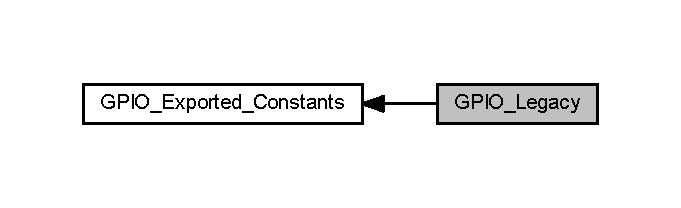
\includegraphics[width=327pt]{group___g_p_i_o___legacy}
\end{center}
\end{figure}
\subsection*{Macros}
\begin{DoxyCompactItemize}
\item 
\mbox{\Hypertarget{group___g_p_i_o___legacy_gadf4dafa8caa4e91d2bee996c4bfdf8cc}\label{group___g_p_i_o___legacy_gadf4dafa8caa4e91d2bee996c4bfdf8cc}} 
\#define {\bfseries G\+P\+I\+O\+\_\+\+Mode\+\_\+\+A\+IN}~\hyperlink{group___g_p_i_o_gga1347339e1c84a196fabbb31205eec5d4a6e5c0d7e6d2e22b834b24e1ca1d6d0db}{G\+P\+I\+O\+\_\+\+Mode\+\_\+\+AN}
\item 
\mbox{\Hypertarget{group___g_p_i_o___legacy_gaddd737997abcd1154c0998b22333b579}\label{group___g_p_i_o___legacy_gaddd737997abcd1154c0998b22333b579}} 
\#define {\bfseries G\+P\+I\+O\+\_\+\+A\+F\+\_\+\+O\+T\+G1\+\_\+\+FS}~\hyperlink{group___g_p_i_o___alternat__function__selection__define_gaeba0aeefec841e505170efc7762ae588}{G\+P\+I\+O\+\_\+\+A\+F\+\_\+\+O\+T\+G\+\_\+\+FS}
\item 
\mbox{\Hypertarget{group___g_p_i_o___legacy_ga54715298b3dc7e843429fd3e24d42cd4}\label{group___g_p_i_o___legacy_ga54715298b3dc7e843429fd3e24d42cd4}} 
\#define {\bfseries G\+P\+I\+O\+\_\+\+A\+F\+\_\+\+O\+T\+G2\+\_\+\+HS}~G\+P\+I\+O\+\_\+\+A\+F\+\_\+\+O\+T\+G\+\_\+\+HS
\item 
\mbox{\Hypertarget{group___g_p_i_o___legacy_ga85e574d8321b9d9aaa2790351b4f0c1e}\label{group___g_p_i_o___legacy_ga85e574d8321b9d9aaa2790351b4f0c1e}} 
\#define {\bfseries G\+P\+I\+O\+\_\+\+A\+F\+\_\+\+O\+T\+G2\+\_\+\+FS}~G\+P\+I\+O\+\_\+\+A\+F\+\_\+\+O\+T\+G\+\_\+\+H\+S\+\_\+\+FS
\end{DoxyCompactItemize}


\subsection{Detailed Description}

\hypertarget{group___r_c_c___exported___constants}{}\section{R\+C\+C\+\_\+\+Exported\+\_\+\+Constants}
\label{group___r_c_c___exported___constants}\index{R\+C\+C\+\_\+\+Exported\+\_\+\+Constants@{R\+C\+C\+\_\+\+Exported\+\_\+\+Constants}}
Collaboration diagram for R\+C\+C\+\_\+\+Exported\+\_\+\+Constants\+:
\nopagebreak
\begin{figure}[H]
\begin{center}
\leavevmode
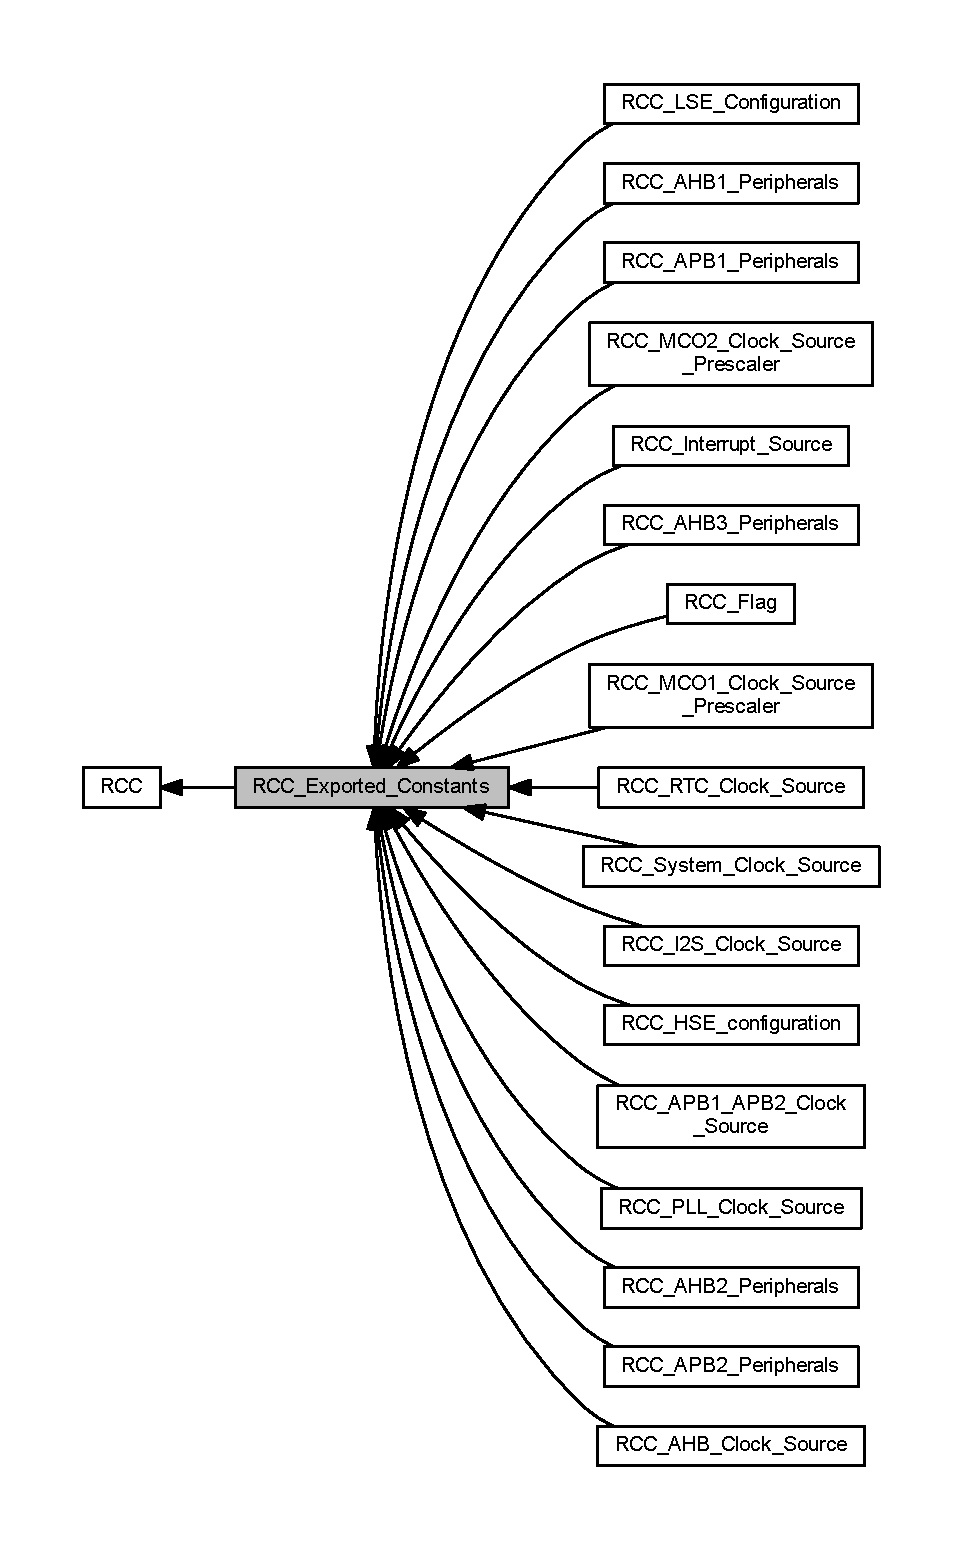
\includegraphics[height=550pt]{group___r_c_c___exported___constants}
\end{center}
\end{figure}
\subsection*{Modules}
\begin{DoxyCompactItemize}
\item 
\hyperlink{group___r_c_c___h_s_e__configuration}{R\+C\+C\+\_\+\+H\+S\+E\+\_\+configuration}
\item 
\hyperlink{group___r_c_c___p_l_l___clock___source}{R\+C\+C\+\_\+\+P\+L\+L\+\_\+\+Clock\+\_\+\+Source}
\item 
\hyperlink{group___r_c_c___system___clock___source}{R\+C\+C\+\_\+\+System\+\_\+\+Clock\+\_\+\+Source}
\item 
\hyperlink{group___r_c_c___a_h_b___clock___source}{R\+C\+C\+\_\+\+A\+H\+B\+\_\+\+Clock\+\_\+\+Source}
\item 
\hyperlink{group___r_c_c___a_p_b1___a_p_b2___clock___source}{R\+C\+C\+\_\+\+A\+P\+B1\+\_\+\+A\+P\+B2\+\_\+\+Clock\+\_\+\+Source}
\item 
\hyperlink{group___r_c_c___interrupt___source}{R\+C\+C\+\_\+\+Interrupt\+\_\+\+Source}
\item 
\hyperlink{group___r_c_c___l_s_e___configuration}{R\+C\+C\+\_\+\+L\+S\+E\+\_\+\+Configuration}
\item 
\hyperlink{group___r_c_c___r_t_c___clock___source}{R\+C\+C\+\_\+\+R\+T\+C\+\_\+\+Clock\+\_\+\+Source}
\item 
\hyperlink{group___r_c_c___i2_s___clock___source}{R\+C\+C\+\_\+\+I2\+S\+\_\+\+Clock\+\_\+\+Source}
\item 
\hyperlink{group___r_c_c___a_h_b1___peripherals}{R\+C\+C\+\_\+\+A\+H\+B1\+\_\+\+Peripherals}
\item 
\hyperlink{group___r_c_c___a_h_b2___peripherals}{R\+C\+C\+\_\+\+A\+H\+B2\+\_\+\+Peripherals}
\item 
\hyperlink{group___r_c_c___a_h_b3___peripherals}{R\+C\+C\+\_\+\+A\+H\+B3\+\_\+\+Peripherals}
\item 
\hyperlink{group___r_c_c___a_p_b1___peripherals}{R\+C\+C\+\_\+\+A\+P\+B1\+\_\+\+Peripherals}
\item 
\hyperlink{group___r_c_c___a_p_b2___peripherals}{R\+C\+C\+\_\+\+A\+P\+B2\+\_\+\+Peripherals}
\item 
\hyperlink{group___r_c_c___m_c_o1___clock___source___prescaler}{R\+C\+C\+\_\+\+M\+C\+O1\+\_\+\+Clock\+\_\+\+Source\+\_\+\+Prescaler}
\item 
\hyperlink{group___r_c_c___m_c_o2___clock___source___prescaler}{R\+C\+C\+\_\+\+M\+C\+O2\+\_\+\+Clock\+\_\+\+Source\+\_\+\+Prescaler}
\item 
\hyperlink{group___r_c_c___flag}{R\+C\+C\+\_\+\+Flag}
\end{DoxyCompactItemize}


\subsection{Detailed Description}

\hypertarget{group___r_c_c___h_s_e__configuration}{}\section{R\+C\+C\+\_\+\+H\+S\+E\+\_\+configuration}
\label{group___r_c_c___h_s_e__configuration}\index{R\+C\+C\+\_\+\+H\+S\+E\+\_\+configuration@{R\+C\+C\+\_\+\+H\+S\+E\+\_\+configuration}}
Collaboration diagram for R\+C\+C\+\_\+\+H\+S\+E\+\_\+configuration\+:
\nopagebreak
\begin{figure}[H]
\begin{center}
\leavevmode
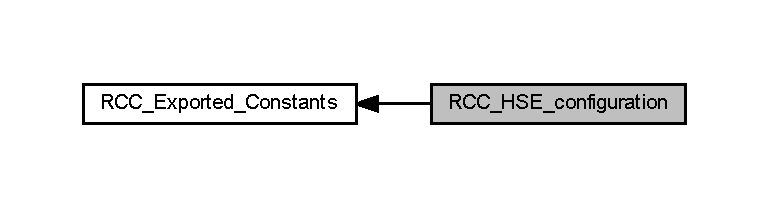
\includegraphics[width=350pt]{group___r_c_c___h_s_e__configuration}
\end{center}
\end{figure}
\subsection*{Macros}
\begin{DoxyCompactItemize}
\item 
\mbox{\Hypertarget{group___r_c_c___h_s_e__configuration_ga1616626d23fbce440398578855df6f97}\label{group___r_c_c___h_s_e__configuration_ga1616626d23fbce440398578855df6f97}} 
\#define {\bfseries R\+C\+C\+\_\+\+H\+S\+E\+\_\+\+O\+FF}~((uint8\+\_\+t)0x00)
\item 
\mbox{\Hypertarget{group___r_c_c___h_s_e__configuration_gabc4f70a44776c557af20496b04d9a9db}\label{group___r_c_c___h_s_e__configuration_gabc4f70a44776c557af20496b04d9a9db}} 
\#define {\bfseries R\+C\+C\+\_\+\+H\+S\+E\+\_\+\+ON}~((uint8\+\_\+t)0x01)
\item 
\mbox{\Hypertarget{group___r_c_c___h_s_e__configuration_ga09061e9909d5f588baa7bfb0f7edd9fa}\label{group___r_c_c___h_s_e__configuration_ga09061e9909d5f588baa7bfb0f7edd9fa}} 
\#define {\bfseries R\+C\+C\+\_\+\+H\+S\+E\+\_\+\+Bypass}~((uint8\+\_\+t)0x05)
\item 
\#define {\bfseries I\+S\+\_\+\+R\+C\+C\+\_\+\+H\+SE}(H\+SE)
\end{DoxyCompactItemize}


\subsection{Detailed Description}


\subsection{Macro Definition Documentation}
\mbox{\Hypertarget{group___r_c_c___h_s_e__configuration_ga287bbcafd73d07ec915c2f793301908a}\label{group___r_c_c___h_s_e__configuration_ga287bbcafd73d07ec915c2f793301908a}} 
\index{R\+C\+C\+\_\+\+H\+S\+E\+\_\+configuration@{R\+C\+C\+\_\+\+H\+S\+E\+\_\+configuration}!I\+S\+\_\+\+R\+C\+C\+\_\+\+H\+SE@{I\+S\+\_\+\+R\+C\+C\+\_\+\+H\+SE}}
\index{I\+S\+\_\+\+R\+C\+C\+\_\+\+H\+SE@{I\+S\+\_\+\+R\+C\+C\+\_\+\+H\+SE}!R\+C\+C\+\_\+\+H\+S\+E\+\_\+configuration@{R\+C\+C\+\_\+\+H\+S\+E\+\_\+configuration}}
\subsubsection{\texorpdfstring{I\+S\+\_\+\+R\+C\+C\+\_\+\+H\+SE}{IS\_RCC\_HSE}}
{\footnotesize\ttfamily \#define I\+S\+\_\+\+R\+C\+C\+\_\+\+H\+SE(\begin{DoxyParamCaption}\item[{}]{H\+SE }\end{DoxyParamCaption})}

{\bfseries Value\+:}
\begin{DoxyCode}
(((HSE) == RCC\_HSE\_OFF) || ((HSE) == RCC\_HSE\_ON) || \(\backslash\)
                         ((HSE) == RCC\_HSE\_Bypass))
\end{DoxyCode}


Definition at line 62 of file stm32f4xx\+\_\+rcc.\+h.


\hypertarget{group___r_c_c___p_l_l___clock___source}{}\section{R\+C\+C\+\_\+\+P\+L\+L\+\_\+\+Clock\+\_\+\+Source}
\label{group___r_c_c___p_l_l___clock___source}\index{R\+C\+C\+\_\+\+P\+L\+L\+\_\+\+Clock\+\_\+\+Source@{R\+C\+C\+\_\+\+P\+L\+L\+\_\+\+Clock\+\_\+\+Source}}
Collaboration diagram for R\+C\+C\+\_\+\+P\+L\+L\+\_\+\+Clock\+\_\+\+Source\+:\nopagebreak
\begin{figure}[H]
\begin{center}
\leavevmode
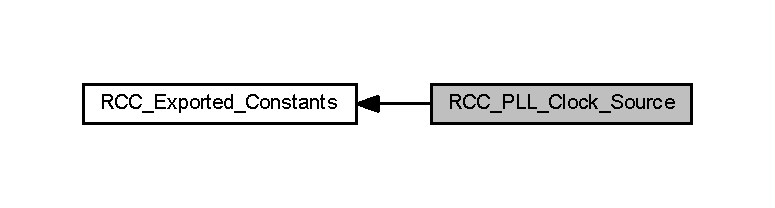
\includegraphics[width=350pt]{group___r_c_c___p_l_l___clock___source}
\end{center}
\end{figure}
\subsection*{Macros}
\begin{DoxyCompactItemize}
\item 
\mbox{\Hypertarget{group___r_c_c___p_l_l___clock___source_ga1cbb1ae8d9e282a763a0070b251921f9}\label{group___r_c_c___p_l_l___clock___source_ga1cbb1ae8d9e282a763a0070b251921f9}} 
\#define {\bfseries R\+C\+C\+\_\+\+P\+L\+L\+Source\+\_\+\+H\+SI}~((uint32\+\_\+t)0x00000000)
\item 
\mbox{\Hypertarget{group___r_c_c___p_l_l___clock___source_ga3706d0db7fe1836c65dc2ea7deded721}\label{group___r_c_c___p_l_l___clock___source_ga3706d0db7fe1836c65dc2ea7deded721}} 
\#define {\bfseries R\+C\+C\+\_\+\+P\+L\+L\+Source\+\_\+\+H\+SE}~((uint32\+\_\+t)0x00400000)
\item 
\#define {\bfseries I\+S\+\_\+\+R\+C\+C\+\_\+\+P\+L\+L\+\_\+\+S\+O\+U\+R\+CE}(S\+O\+U\+R\+CE)
\item 
\mbox{\Hypertarget{group___r_c_c___p_l_l___clock___source_ga8db327c085e20aeb673a9784f8508597}\label{group___r_c_c___p_l_l___clock___source_ga8db327c085e20aeb673a9784f8508597}} 
\#define {\bfseries I\+S\+\_\+\+R\+C\+C\+\_\+\+P\+L\+L\+M\+\_\+\+V\+A\+L\+UE}(V\+A\+L\+UE)~((V\+A\+L\+UE) $<$= 63)
\item 
\mbox{\Hypertarget{group___r_c_c___p_l_l___clock___source_ga12835741fbedd278ad1e91abebe00837}\label{group___r_c_c___p_l_l___clock___source_ga12835741fbedd278ad1e91abebe00837}} 
\#define {\bfseries I\+S\+\_\+\+R\+C\+C\+\_\+\+P\+L\+L\+N\+\_\+\+V\+A\+L\+UE}(V\+A\+L\+UE)~((192 $<$= (V\+A\+L\+UE)) \&\& ((V\+A\+L\+UE) $<$= 432))
\item 
\mbox{\Hypertarget{group___r_c_c___p_l_l___clock___source_gad808f83505f4e802e5bafab7831f0235}\label{group___r_c_c___p_l_l___clock___source_gad808f83505f4e802e5bafab7831f0235}} 
\#define {\bfseries I\+S\+\_\+\+R\+C\+C\+\_\+\+P\+L\+L\+P\+\_\+\+V\+A\+L\+UE}(V\+A\+L\+UE)~(((V\+A\+L\+UE) == 2) $\vert$$\vert$ ((V\+A\+L\+UE) == 4) $\vert$$\vert$ ((V\+A\+L\+UE) == 6) $\vert$$\vert$ ((V\+A\+L\+UE) == 8))
\item 
\mbox{\Hypertarget{group___r_c_c___p_l_l___clock___source_gad66dbe75bf8ab2b64b200e796281a851}\label{group___r_c_c___p_l_l___clock___source_gad66dbe75bf8ab2b64b200e796281a851}} 
\#define {\bfseries I\+S\+\_\+\+R\+C\+C\+\_\+\+P\+L\+L\+Q\+\_\+\+V\+A\+L\+UE}(V\+A\+L\+UE)~((4 $<$= (V\+A\+L\+UE)) \&\& ((V\+A\+L\+UE) $<$= 15))
\item 
\mbox{\Hypertarget{group___r_c_c___p_l_l___clock___source_gac30fb7f6fe9f22a7d6c5585909db5c3c}\label{group___r_c_c___p_l_l___clock___source_gac30fb7f6fe9f22a7d6c5585909db5c3c}} 
\#define {\bfseries I\+S\+\_\+\+R\+C\+C\+\_\+\+P\+L\+L\+I2\+S\+N\+\_\+\+V\+A\+L\+UE}(V\+A\+L\+UE)~((192 $<$= (V\+A\+L\+UE)) \&\& ((V\+A\+L\+UE) $<$= 432))
\item 
\mbox{\Hypertarget{group___r_c_c___p_l_l___clock___source_gaa2fece4b24f6219b423e1b092b7705c8}\label{group___r_c_c___p_l_l___clock___source_gaa2fece4b24f6219b423e1b092b7705c8}} 
\#define {\bfseries I\+S\+\_\+\+R\+C\+C\+\_\+\+P\+L\+L\+I2\+S\+R\+\_\+\+V\+A\+L\+UE}(V\+A\+L\+UE)~((2 $<$= (V\+A\+L\+UE)) \&\& ((V\+A\+L\+UE) $<$= 7))
\end{DoxyCompactItemize}


\subsection{Detailed Description}


\subsection{Macro Definition Documentation}
\mbox{\Hypertarget{group___r_c_c___p_l_l___clock___source_ga8a8a84a16989bb4e5aca1af65ccf9a1b}\label{group___r_c_c___p_l_l___clock___source_ga8a8a84a16989bb4e5aca1af65ccf9a1b}} 
\index{R\+C\+C\+\_\+\+P\+L\+L\+\_\+\+Clock\+\_\+\+Source@{R\+C\+C\+\_\+\+P\+L\+L\+\_\+\+Clock\+\_\+\+Source}!I\+S\+\_\+\+R\+C\+C\+\_\+\+P\+L\+L\+\_\+\+S\+O\+U\+R\+CE@{I\+S\+\_\+\+R\+C\+C\+\_\+\+P\+L\+L\+\_\+\+S\+O\+U\+R\+CE}}
\index{I\+S\+\_\+\+R\+C\+C\+\_\+\+P\+L\+L\+\_\+\+S\+O\+U\+R\+CE@{I\+S\+\_\+\+R\+C\+C\+\_\+\+P\+L\+L\+\_\+\+S\+O\+U\+R\+CE}!R\+C\+C\+\_\+\+P\+L\+L\+\_\+\+Clock\+\_\+\+Source@{R\+C\+C\+\_\+\+P\+L\+L\+\_\+\+Clock\+\_\+\+Source}}
\subsubsection{\texorpdfstring{I\+S\+\_\+\+R\+C\+C\+\_\+\+P\+L\+L\+\_\+\+S\+O\+U\+R\+CE}{IS\_RCC\_PLL\_SOURCE}}
{\footnotesize\ttfamily \#define I\+S\+\_\+\+R\+C\+C\+\_\+\+P\+L\+L\+\_\+\+S\+O\+U\+R\+CE(\begin{DoxyParamCaption}\item[{}]{S\+O\+U\+R\+CE }\end{DoxyParamCaption})}

{\bfseries Value\+:}
\begin{DoxyCode}
(((SOURCE) == RCC\_PLLSource\_HSI) || \(\backslash\)
                                   ((SOURCE) == RCC\_PLLSource\_HSE))
\end{DoxyCode}


Definition at line 73 of file stm32f4xx\+\_\+rcc.\+h.


\hypertarget{group___r_c_c___system___clock___source}{}\section{R\+C\+C\+\_\+\+System\+\_\+\+Clock\+\_\+\+Source}
\label{group___r_c_c___system___clock___source}\index{R\+C\+C\+\_\+\+System\+\_\+\+Clock\+\_\+\+Source@{R\+C\+C\+\_\+\+System\+\_\+\+Clock\+\_\+\+Source}}
Collaboration diagram for R\+C\+C\+\_\+\+System\+\_\+\+Clock\+\_\+\+Source\+:\nopagebreak
\begin{figure}[H]
\begin{center}
\leavevmode
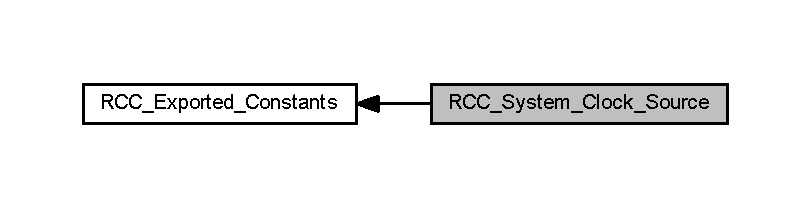
\includegraphics[width=350pt]{group___r_c_c___system___clock___source}
\end{center}
\end{figure}
\subsection*{Macros}
\begin{DoxyCompactItemize}
\item 
\mbox{\Hypertarget{group___r_c_c___system___clock___source_ga0f392254e74dd965c48edd5aad148e20}\label{group___r_c_c___system___clock___source_ga0f392254e74dd965c48edd5aad148e20}} 
\#define {\bfseries R\+C\+C\+\_\+\+S\+Y\+S\+C\+L\+K\+Source\+\_\+\+H\+SI}~((uint32\+\_\+t)0x00000000)
\item 
\mbox{\Hypertarget{group___r_c_c___system___clock___source_gabeae110e41833842f8620647ea0ce85a}\label{group___r_c_c___system___clock___source_gabeae110e41833842f8620647ea0ce85a}} 
\#define {\bfseries R\+C\+C\+\_\+\+S\+Y\+S\+C\+L\+K\+Source\+\_\+\+H\+SE}~((uint32\+\_\+t)0x00000001)
\item 
\mbox{\Hypertarget{group___r_c_c___system___clock___source_ga9301b7a07a7cb8c2c6ed87b619c1c966}\label{group___r_c_c___system___clock___source_ga9301b7a07a7cb8c2c6ed87b619c1c966}} 
\#define {\bfseries R\+C\+C\+\_\+\+S\+Y\+S\+C\+L\+K\+Source\+\_\+\+P\+L\+L\+C\+LK}~((uint32\+\_\+t)0x00000002)
\item 
\#define {\bfseries I\+S\+\_\+\+R\+C\+C\+\_\+\+S\+Y\+S\+C\+L\+K\+\_\+\+S\+O\+U\+R\+CE}(S\+O\+U\+R\+CE)
\end{DoxyCompactItemize}


\subsection{Detailed Description}


\subsection{Macro Definition Documentation}
\mbox{\Hypertarget{group___r_c_c___system___clock___source_gaae9d6172a72b0a90cb3703aa59258c57}\label{group___r_c_c___system___clock___source_gaae9d6172a72b0a90cb3703aa59258c57}} 
\index{R\+C\+C\+\_\+\+System\+\_\+\+Clock\+\_\+\+Source@{R\+C\+C\+\_\+\+System\+\_\+\+Clock\+\_\+\+Source}!I\+S\+\_\+\+R\+C\+C\+\_\+\+S\+Y\+S\+C\+L\+K\+\_\+\+S\+O\+U\+R\+CE@{I\+S\+\_\+\+R\+C\+C\+\_\+\+S\+Y\+S\+C\+L\+K\+\_\+\+S\+O\+U\+R\+CE}}
\index{I\+S\+\_\+\+R\+C\+C\+\_\+\+S\+Y\+S\+C\+L\+K\+\_\+\+S\+O\+U\+R\+CE@{I\+S\+\_\+\+R\+C\+C\+\_\+\+S\+Y\+S\+C\+L\+K\+\_\+\+S\+O\+U\+R\+CE}!R\+C\+C\+\_\+\+System\+\_\+\+Clock\+\_\+\+Source@{R\+C\+C\+\_\+\+System\+\_\+\+Clock\+\_\+\+Source}}
\subsubsection{\texorpdfstring{I\+S\+\_\+\+R\+C\+C\+\_\+\+S\+Y\+S\+C\+L\+K\+\_\+\+S\+O\+U\+R\+CE}{IS\_RCC\_SYSCLK\_SOURCE}}
{\footnotesize\ttfamily \#define I\+S\+\_\+\+R\+C\+C\+\_\+\+S\+Y\+S\+C\+L\+K\+\_\+\+S\+O\+U\+R\+CE(\begin{DoxyParamCaption}\item[{}]{S\+O\+U\+R\+CE }\end{DoxyParamCaption})}

{\bfseries Value\+:}
\begin{DoxyCode}
(((SOURCE) == RCC\_SYSCLKSource\_HSI) || \(\backslash\)
                                      ((SOURCE) == RCC\_SYSCLKSource\_HSE) || \(\backslash\)
                                      ((SOURCE) == RCC\_SYSCLKSource\_PLLCLK))
\end{DoxyCode}


Definition at line 92 of file stm32f4xx\+\_\+rcc.\+h.


\hypertarget{group___r_c_c___a_h_b___clock___source}{}\section{R\+C\+C\+\_\+\+A\+H\+B\+\_\+\+Clock\+\_\+\+Source}
\label{group___r_c_c___a_h_b___clock___source}\index{R\+C\+C\+\_\+\+A\+H\+B\+\_\+\+Clock\+\_\+\+Source@{R\+C\+C\+\_\+\+A\+H\+B\+\_\+\+Clock\+\_\+\+Source}}
Collaboration diagram for R\+C\+C\+\_\+\+A\+H\+B\+\_\+\+Clock\+\_\+\+Source\+:
\nopagebreak
\begin{figure}[H]
\begin{center}
\leavevmode
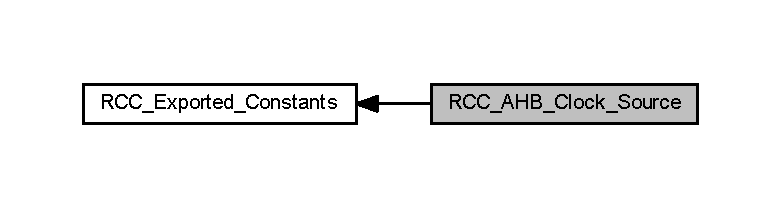
\includegraphics[width=350pt]{group___r_c_c___a_h_b___clock___source}
\end{center}
\end{figure}
\subsection*{Macros}
\begin{DoxyCompactItemize}
\item 
\mbox{\Hypertarget{group___r_c_c___a_h_b___clock___source_gadc3ac37d90c2082d640e5948fac0878f}\label{group___r_c_c___a_h_b___clock___source_gadc3ac37d90c2082d640e5948fac0878f}} 
\#define {\bfseries R\+C\+C\+\_\+\+S\+Y\+S\+C\+L\+K\+\_\+\+Div1}~((uint32\+\_\+t)0x00000000)
\item 
\mbox{\Hypertarget{group___r_c_c___a_h_b___clock___source_gacadd82156776154a07d128b454fc69fd}\label{group___r_c_c___a_h_b___clock___source_gacadd82156776154a07d128b454fc69fd}} 
\#define {\bfseries R\+C\+C\+\_\+\+S\+Y\+S\+C\+L\+K\+\_\+\+Div2}~((uint32\+\_\+t)0x00000080)
\item 
\mbox{\Hypertarget{group___r_c_c___a_h_b___clock___source_ga458f8ae63164e878930dbebd7643f087}\label{group___r_c_c___a_h_b___clock___source_ga458f8ae63164e878930dbebd7643f087}} 
\#define {\bfseries R\+C\+C\+\_\+\+S\+Y\+S\+C\+L\+K\+\_\+\+Div4}~((uint32\+\_\+t)0x00000090)
\item 
\mbox{\Hypertarget{group___r_c_c___a_h_b___clock___source_gade72fe3aca89f3e8c4fe8692ea217912}\label{group___r_c_c___a_h_b___clock___source_gade72fe3aca89f3e8c4fe8692ea217912}} 
\#define {\bfseries R\+C\+C\+\_\+\+S\+Y\+S\+C\+L\+K\+\_\+\+Div8}~((uint32\+\_\+t)0x000000\+A0)
\item 
\mbox{\Hypertarget{group___r_c_c___a_h_b___clock___source_gaefd8df4be9c9dbd9cebfb2384933500a}\label{group___r_c_c___a_h_b___clock___source_gaefd8df4be9c9dbd9cebfb2384933500a}} 
\#define {\bfseries R\+C\+C\+\_\+\+S\+Y\+S\+C\+L\+K\+\_\+\+Div16}~((uint32\+\_\+t)0x000000\+B0)
\item 
\mbox{\Hypertarget{group___r_c_c___a_h_b___clock___source_gab6a2c2d4e945c607259988a9b6df26e5}\label{group___r_c_c___a_h_b___clock___source_gab6a2c2d4e945c607259988a9b6df26e5}} 
\#define {\bfseries R\+C\+C\+\_\+\+S\+Y\+S\+C\+L\+K\+\_\+\+Div64}~((uint32\+\_\+t)0x000000\+C0)
\item 
\mbox{\Hypertarget{group___r_c_c___a_h_b___clock___source_ga1a28926fcb86112058a365e01fe9a46b}\label{group___r_c_c___a_h_b___clock___source_ga1a28926fcb86112058a365e01fe9a46b}} 
\#define {\bfseries R\+C\+C\+\_\+\+S\+Y\+S\+C\+L\+K\+\_\+\+Div128}~((uint32\+\_\+t)0x000000\+D0)
\item 
\mbox{\Hypertarget{group___r_c_c___a_h_b___clock___source_gaa28bb876893b3267a813fc98a462d5ee}\label{group___r_c_c___a_h_b___clock___source_gaa28bb876893b3267a813fc98a462d5ee}} 
\#define {\bfseries R\+C\+C\+\_\+\+S\+Y\+S\+C\+L\+K\+\_\+\+Div256}~((uint32\+\_\+t)0x000000\+E0)
\item 
\mbox{\Hypertarget{group___r_c_c___a_h_b___clock___source_gab5b4588c455d6327bc96f131ed6698ab}\label{group___r_c_c___a_h_b___clock___source_gab5b4588c455d6327bc96f131ed6698ab}} 
\#define {\bfseries R\+C\+C\+\_\+\+S\+Y\+S\+C\+L\+K\+\_\+\+Div512}~((uint32\+\_\+t)0x000000\+F0)
\item 
\#define {\bfseries I\+S\+\_\+\+R\+C\+C\+\_\+\+H\+C\+LK}(H\+C\+LK)
\end{DoxyCompactItemize}


\subsection{Detailed Description}


\subsection{Macro Definition Documentation}
\mbox{\Hypertarget{group___r_c_c___a_h_b___clock___source_ga6e9f1c193a2f41bcb3c2f7fa8459b5b3}\label{group___r_c_c___a_h_b___clock___source_ga6e9f1c193a2f41bcb3c2f7fa8459b5b3}} 
\index{R\+C\+C\+\_\+\+A\+H\+B\+\_\+\+Clock\+\_\+\+Source@{R\+C\+C\+\_\+\+A\+H\+B\+\_\+\+Clock\+\_\+\+Source}!I\+S\+\_\+\+R\+C\+C\+\_\+\+H\+C\+LK@{I\+S\+\_\+\+R\+C\+C\+\_\+\+H\+C\+LK}}
\index{I\+S\+\_\+\+R\+C\+C\+\_\+\+H\+C\+LK@{I\+S\+\_\+\+R\+C\+C\+\_\+\+H\+C\+LK}!R\+C\+C\+\_\+\+A\+H\+B\+\_\+\+Clock\+\_\+\+Source@{R\+C\+C\+\_\+\+A\+H\+B\+\_\+\+Clock\+\_\+\+Source}}
\subsubsection{\texorpdfstring{I\+S\+\_\+\+R\+C\+C\+\_\+\+H\+C\+LK}{IS\_RCC\_HCLK}}
{\footnotesize\ttfamily \#define I\+S\+\_\+\+R\+C\+C\+\_\+\+H\+C\+LK(\begin{DoxyParamCaption}\item[{}]{H\+C\+LK }\end{DoxyParamCaption})}

{\bfseries Value\+:}
\begin{DoxyCode}
(((HCLK) == RCC\_SYSCLK\_Div1) || ((HCLK) == RCC\_SYSCLK\_Div2) || \(\backslash\)
                           ((HCLK) == RCC\_SYSCLK\_Div4) || ((HCLK) == RCC\_SYSCLK\_Div8) || \(\backslash\)
                           ((HCLK) == RCC\_SYSCLK\_Div16) || ((HCLK) == RCC\_SYSCLK\_Div64) || \(\backslash\)
                           ((HCLK) == RCC\_SYSCLK\_Div128) || ((HCLK) == RCC\_SYSCLK\_Div256) || \(\backslash\)
                           ((HCLK) == RCC\_SYSCLK\_Div512))
\end{DoxyCode}


Definition at line 111 of file stm32f4xx\+\_\+rcc.\+h.


\hypertarget{group___r_c_c___a_p_b1___a_p_b2___clock___source}{}\section{R\+C\+C\+\_\+\+A\+P\+B1\+\_\+\+A\+P\+B2\+\_\+\+Clock\+\_\+\+Source}
\label{group___r_c_c___a_p_b1___a_p_b2___clock___source}\index{R\+C\+C\+\_\+\+A\+P\+B1\+\_\+\+A\+P\+B2\+\_\+\+Clock\+\_\+\+Source@{R\+C\+C\+\_\+\+A\+P\+B1\+\_\+\+A\+P\+B2\+\_\+\+Clock\+\_\+\+Source}}
Collaboration diagram for R\+C\+C\+\_\+\+A\+P\+B1\+\_\+\+A\+P\+B2\+\_\+\+Clock\+\_\+\+Source\+:
\nopagebreak
\begin{figure}[H]
\begin{center}
\leavevmode
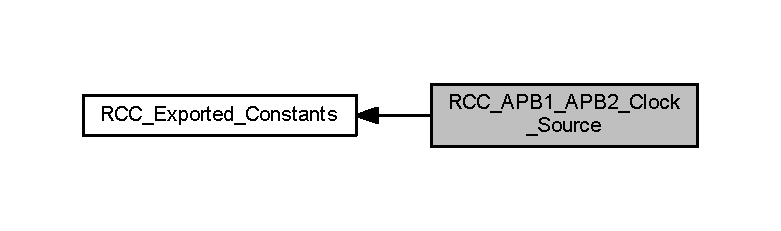
\includegraphics[width=350pt]{group___r_c_c___a_p_b1___a_p_b2___clock___source}
\end{center}
\end{figure}
\subsection*{Macros}
\begin{DoxyCompactItemize}
\item 
\mbox{\Hypertarget{group___r_c_c___a_p_b1___a_p_b2___clock___source_gae62b4a39ae69cc221f2ab7d4518bfb76}\label{group___r_c_c___a_p_b1___a_p_b2___clock___source_gae62b4a39ae69cc221f2ab7d4518bfb76}} 
\#define {\bfseries R\+C\+C\+\_\+\+H\+C\+L\+K\+\_\+\+Div1}~((uint32\+\_\+t)0x00000000)
\item 
\mbox{\Hypertarget{group___r_c_c___a_p_b1___a_p_b2___clock___source_ga177bb3648def9a961c16f93f15ca0f62}\label{group___r_c_c___a_p_b1___a_p_b2___clock___source_ga177bb3648def9a961c16f93f15ca0f62}} 
\#define {\bfseries R\+C\+C\+\_\+\+H\+C\+L\+K\+\_\+\+Div2}~((uint32\+\_\+t)0x00001000)
\item 
\mbox{\Hypertarget{group___r_c_c___a_p_b1___a_p_b2___clock___source_gafd8cf0e32a3ea5648cdc054766bc2017}\label{group___r_c_c___a_p_b1___a_p_b2___clock___source_gafd8cf0e32a3ea5648cdc054766bc2017}} 
\#define {\bfseries R\+C\+C\+\_\+\+H\+C\+L\+K\+\_\+\+Div4}~((uint32\+\_\+t)0x00001400)
\item 
\mbox{\Hypertarget{group___r_c_c___a_p_b1___a_p_b2___clock___source_gab2e2b6e0b8fe22d6638b672918b22097}\label{group___r_c_c___a_p_b1___a_p_b2___clock___source_gab2e2b6e0b8fe22d6638b672918b22097}} 
\#define {\bfseries R\+C\+C\+\_\+\+H\+C\+L\+K\+\_\+\+Div8}~((uint32\+\_\+t)0x00001800)
\item 
\mbox{\Hypertarget{group___r_c_c___a_p_b1___a_p_b2___clock___source_ga6353aaa0b302fdd5d946fd21756e2273}\label{group___r_c_c___a_p_b1___a_p_b2___clock___source_ga6353aaa0b302fdd5d946fd21756e2273}} 
\#define {\bfseries R\+C\+C\+\_\+\+H\+C\+L\+K\+\_\+\+Div16}~((uint32\+\_\+t)0x00001\+C00)
\item 
\#define {\bfseries I\+S\+\_\+\+R\+C\+C\+\_\+\+P\+C\+LK}(P\+C\+LK)
\end{DoxyCompactItemize}


\subsection{Detailed Description}


\subsection{Macro Definition Documentation}
\mbox{\Hypertarget{group___r_c_c___a_p_b1___a_p_b2___clock___source_gab70f1257ea47c1da4def8e351af4d9f2}\label{group___r_c_c___a_p_b1___a_p_b2___clock___source_gab70f1257ea47c1da4def8e351af4d9f2}} 
\index{R\+C\+C\+\_\+\+A\+P\+B1\+\_\+\+A\+P\+B2\+\_\+\+Clock\+\_\+\+Source@{R\+C\+C\+\_\+\+A\+P\+B1\+\_\+\+A\+P\+B2\+\_\+\+Clock\+\_\+\+Source}!I\+S\+\_\+\+R\+C\+C\+\_\+\+P\+C\+LK@{I\+S\+\_\+\+R\+C\+C\+\_\+\+P\+C\+LK}}
\index{I\+S\+\_\+\+R\+C\+C\+\_\+\+P\+C\+LK@{I\+S\+\_\+\+R\+C\+C\+\_\+\+P\+C\+LK}!R\+C\+C\+\_\+\+A\+P\+B1\+\_\+\+A\+P\+B2\+\_\+\+Clock\+\_\+\+Source@{R\+C\+C\+\_\+\+A\+P\+B1\+\_\+\+A\+P\+B2\+\_\+\+Clock\+\_\+\+Source}}
\subsubsection{\texorpdfstring{I\+S\+\_\+\+R\+C\+C\+\_\+\+P\+C\+LK}{IS\_RCC\_PCLK}}
{\footnotesize\ttfamily \#define I\+S\+\_\+\+R\+C\+C\+\_\+\+P\+C\+LK(\begin{DoxyParamCaption}\item[{}]{P\+C\+LK }\end{DoxyParamCaption})}

{\bfseries Value\+:}
\begin{DoxyCode}
(((PCLK) == RCC\_HCLK\_Div1) || ((PCLK) == RCC\_HCLK\_Div2) || \(\backslash\)
                           ((PCLK) == RCC\_HCLK\_Div4) || ((PCLK) == RCC\_HCLK\_Div8) || \(\backslash\)
                           ((PCLK) == RCC\_HCLK\_Div16))
\end{DoxyCode}


Definition at line 128 of file stm32f4xx\+\_\+rcc.\+h.


\hypertarget{group___r_c_c___interrupt___source}{}\section{R\+C\+C\+\_\+\+Interrupt\+\_\+\+Source}
\label{group___r_c_c___interrupt___source}\index{R\+C\+C\+\_\+\+Interrupt\+\_\+\+Source@{R\+C\+C\+\_\+\+Interrupt\+\_\+\+Source}}
Collaboration diagram for R\+C\+C\+\_\+\+Interrupt\+\_\+\+Source\+:
\nopagebreak
\begin{figure}[H]
\begin{center}
\leavevmode
\includegraphics[width=350pt]{group___r_c_c___interrupt___source}
\end{center}
\end{figure}
\subsection*{Macros}
\begin{DoxyCompactItemize}
\item 
\mbox{\Hypertarget{group___r_c_c___interrupt___source_ga2b4ef277c1b71f96e0bef4b9a72fca94}\label{group___r_c_c___interrupt___source_ga2b4ef277c1b71f96e0bef4b9a72fca94}} 
\#define {\bfseries R\+C\+C\+\_\+\+I\+T\+\_\+\+L\+S\+I\+R\+DY}~((uint8\+\_\+t)0x01)
\item 
\mbox{\Hypertarget{group___r_c_c___interrupt___source_gad6b6e78a426850f595ef180d292a673d}\label{group___r_c_c___interrupt___source_gad6b6e78a426850f595ef180d292a673d}} 
\#define {\bfseries R\+C\+C\+\_\+\+I\+T\+\_\+\+L\+S\+E\+R\+DY}~((uint8\+\_\+t)0x02)
\item 
\mbox{\Hypertarget{group___r_c_c___interrupt___source_ga69637e51b71f73f519c8c0a0613d042f}\label{group___r_c_c___interrupt___source_ga69637e51b71f73f519c8c0a0613d042f}} 
\#define {\bfseries R\+C\+C\+\_\+\+I\+T\+\_\+\+H\+S\+I\+R\+DY}~((uint8\+\_\+t)0x04)
\item 
\mbox{\Hypertarget{group___r_c_c___interrupt___source_gad13eaede352bca59611e6cae68665866}\label{group___r_c_c___interrupt___source_gad13eaede352bca59611e6cae68665866}} 
\#define {\bfseries R\+C\+C\+\_\+\+I\+T\+\_\+\+H\+S\+E\+R\+DY}~((uint8\+\_\+t)0x08)
\item 
\mbox{\Hypertarget{group___r_c_c___interrupt___source_ga68d48e7811fb58f2649dce6cf0d823d9}\label{group___r_c_c___interrupt___source_ga68d48e7811fb58f2649dce6cf0d823d9}} 
\#define {\bfseries R\+C\+C\+\_\+\+I\+T\+\_\+\+P\+L\+L\+R\+DY}~((uint8\+\_\+t)0x10)
\item 
\mbox{\Hypertarget{group___r_c_c___interrupt___source_ga6468ff3bad854272cf1120ffbf69b7ac}\label{group___r_c_c___interrupt___source_ga6468ff3bad854272cf1120ffbf69b7ac}} 
\#define {\bfseries R\+C\+C\+\_\+\+I\+T\+\_\+\+P\+L\+L\+I2\+S\+R\+DY}~((uint8\+\_\+t)0x20)
\item 
\mbox{\Hypertarget{group___r_c_c___interrupt___source_ga9bb34a4912d2084dc1c0834eb53aa7a3}\label{group___r_c_c___interrupt___source_ga9bb34a4912d2084dc1c0834eb53aa7a3}} 
\#define {\bfseries R\+C\+C\+\_\+\+I\+T\+\_\+\+C\+SS}~((uint8\+\_\+t)0x80)
\item 
\mbox{\Hypertarget{group___r_c_c___interrupt___source_ga710d72ccf88ddbec09b033c81a571a83}\label{group___r_c_c___interrupt___source_ga710d72ccf88ddbec09b033c81a571a83}} 
\#define {\bfseries I\+S\+\_\+\+R\+C\+C\+\_\+\+IT}(IT)~((((IT) \& (uint8\+\_\+t)0x\+C0) == 0x00) \&\& ((\+I\+T) != 0x00))
\item 
\#define {\bfseries I\+S\+\_\+\+R\+C\+C\+\_\+\+G\+E\+T\+\_\+\+IT}(IT)
\item 
\mbox{\Hypertarget{group___r_c_c___interrupt___source_ga8374741e47d696accd1a72647650ba63}\label{group___r_c_c___interrupt___source_ga8374741e47d696accd1a72647650ba63}} 
\#define {\bfseries I\+S\+\_\+\+R\+C\+C\+\_\+\+C\+L\+E\+A\+R\+\_\+\+IT}(IT)~((((IT) \& (uint8\+\_\+t)0x40) == 0x00) \&\& ((\+I\+T) != 0x00))
\end{DoxyCompactItemize}


\subsection{Detailed Description}


\subsection{Macro Definition Documentation}
\mbox{\Hypertarget{group___r_c_c___interrupt___source_ga7a1b771d6d9c2d8346ab58a1f046f6a6}\label{group___r_c_c___interrupt___source_ga7a1b771d6d9c2d8346ab58a1f046f6a6}} 
\index{R\+C\+C\+\_\+\+Interrupt\+\_\+\+Source@{R\+C\+C\+\_\+\+Interrupt\+\_\+\+Source}!I\+S\+\_\+\+R\+C\+C\+\_\+\+G\+E\+T\+\_\+\+IT@{I\+S\+\_\+\+R\+C\+C\+\_\+\+G\+E\+T\+\_\+\+IT}}
\index{I\+S\+\_\+\+R\+C\+C\+\_\+\+G\+E\+T\+\_\+\+IT@{I\+S\+\_\+\+R\+C\+C\+\_\+\+G\+E\+T\+\_\+\+IT}!R\+C\+C\+\_\+\+Interrupt\+\_\+\+Source@{R\+C\+C\+\_\+\+Interrupt\+\_\+\+Source}}
\subsubsection{\texorpdfstring{I\+S\+\_\+\+R\+C\+C\+\_\+\+G\+E\+T\+\_\+\+IT}{IS\_RCC\_GET\_IT}}
{\footnotesize\ttfamily \#define I\+S\+\_\+\+R\+C\+C\+\_\+\+G\+E\+T\+\_\+\+IT(\begin{DoxyParamCaption}\item[{}]{IT }\end{DoxyParamCaption})}

{\bfseries Value\+:}
\begin{DoxyCode}
(((IT) == RCC\_IT\_LSIRDY) || ((IT) == RCC\_IT\_LSERDY) || \(\backslash\)
                           ((IT) == RCC\_IT\_HSIRDY) || ((IT) == RCC\_IT\_HSERDY) || \(\backslash\)
                           ((IT) == RCC\_IT\_PLLRDY) || ((IT) == RCC\_IT\_CSS) || \(\backslash\)
                           ((IT) == RCC\_IT\_PLLI2SRDY))
\end{DoxyCode}


Definition at line 146 of file stm32f4xx\+\_\+rcc.\+h.


\hypertarget{group___r_c_c___l_s_e___configuration}{}\section{R\+C\+C\+\_\+\+L\+S\+E\+\_\+\+Configuration}
\label{group___r_c_c___l_s_e___configuration}\index{R\+C\+C\+\_\+\+L\+S\+E\+\_\+\+Configuration@{R\+C\+C\+\_\+\+L\+S\+E\+\_\+\+Configuration}}
Collaboration diagram for R\+C\+C\+\_\+\+L\+S\+E\+\_\+\+Configuration\+:\nopagebreak
\begin{figure}[H]
\begin{center}
\leavevmode
\includegraphics[width=350pt]{group___r_c_c___l_s_e___configuration}
\end{center}
\end{figure}
\subsection*{Macros}
\begin{DoxyCompactItemize}
\item 
\mbox{\Hypertarget{group___r_c_c___l_s_e___configuration_ga6645c27708d0cad1a4ab61d2abb24c77}\label{group___r_c_c___l_s_e___configuration_ga6645c27708d0cad1a4ab61d2abb24c77}} 
\#define {\bfseries R\+C\+C\+\_\+\+L\+S\+E\+\_\+\+O\+FF}~((uint8\+\_\+t)0x00)
\item 
\mbox{\Hypertarget{group___r_c_c___l_s_e___configuration_gac981ea636c2f215e4473901e0912f55a}\label{group___r_c_c___l_s_e___configuration_gac981ea636c2f215e4473901e0912f55a}} 
\#define {\bfseries R\+C\+C\+\_\+\+L\+S\+E\+\_\+\+ON}~((uint8\+\_\+t)0x01)
\item 
\mbox{\Hypertarget{group___r_c_c___l_s_e___configuration_gac911af00bffa1bd1b1676f582a8a88e1}\label{group___r_c_c___l_s_e___configuration_gac911af00bffa1bd1b1676f582a8a88e1}} 
\#define {\bfseries R\+C\+C\+\_\+\+L\+S\+E\+\_\+\+Bypass}~((uint8\+\_\+t)0x04)
\item 
\#define {\bfseries I\+S\+\_\+\+R\+C\+C\+\_\+\+L\+SE}(L\+SE)
\end{DoxyCompactItemize}


\subsection{Detailed Description}


\subsection{Macro Definition Documentation}
\mbox{\Hypertarget{group___r_c_c___l_s_e___configuration_ga95d2678bf8f46e932e7cba75619a4d2c}\label{group___r_c_c___l_s_e___configuration_ga95d2678bf8f46e932e7cba75619a4d2c}} 
\index{R\+C\+C\+\_\+\+L\+S\+E\+\_\+\+Configuration@{R\+C\+C\+\_\+\+L\+S\+E\+\_\+\+Configuration}!I\+S\+\_\+\+R\+C\+C\+\_\+\+L\+SE@{I\+S\+\_\+\+R\+C\+C\+\_\+\+L\+SE}}
\index{I\+S\+\_\+\+R\+C\+C\+\_\+\+L\+SE@{I\+S\+\_\+\+R\+C\+C\+\_\+\+L\+SE}!R\+C\+C\+\_\+\+L\+S\+E\+\_\+\+Configuration@{R\+C\+C\+\_\+\+L\+S\+E\+\_\+\+Configuration}}
\subsubsection{\texorpdfstring{I\+S\+\_\+\+R\+C\+C\+\_\+\+L\+SE}{IS\_RCC\_LSE}}
{\footnotesize\ttfamily \#define I\+S\+\_\+\+R\+C\+C\+\_\+\+L\+SE(\begin{DoxyParamCaption}\item[{}]{L\+SE }\end{DoxyParamCaption})}

{\bfseries Value\+:}
\begin{DoxyCode}
(((LSE) == RCC\_LSE\_OFF) || ((LSE) == RCC\_LSE\_ON) || \(\backslash\)
                         ((LSE) == RCC\_LSE\_Bypass))
\end{DoxyCode}


Definition at line 161 of file stm32f4xx\+\_\+rcc.\+h.


\hypertarget{group___r_c_c___r_t_c___clock___source}{}\section{R\+C\+C\+\_\+\+R\+T\+C\+\_\+\+Clock\+\_\+\+Source}
\label{group___r_c_c___r_t_c___clock___source}\index{R\+C\+C\+\_\+\+R\+T\+C\+\_\+\+Clock\+\_\+\+Source@{R\+C\+C\+\_\+\+R\+T\+C\+\_\+\+Clock\+\_\+\+Source}}
Collaboration diagram for R\+C\+C\+\_\+\+R\+T\+C\+\_\+\+Clock\+\_\+\+Source\+:\nopagebreak
\begin{figure}[H]
\begin{center}
\leavevmode
\includegraphics[width=350pt]{group___r_c_c___r_t_c___clock___source}
\end{center}
\end{figure}
\subsection*{Macros}
\begin{DoxyCompactItemize}
\item 
\mbox{\Hypertarget{group___r_c_c___r_t_c___clock___source_ga18c0c40ff4289148c9fa44c6848d5552}\label{group___r_c_c___r_t_c___clock___source_ga18c0c40ff4289148c9fa44c6848d5552}} 
\#define {\bfseries R\+C\+C\+\_\+\+R\+T\+C\+C\+L\+K\+Source\+\_\+\+L\+SE}~((uint32\+\_\+t)0x00000100)
\item 
\mbox{\Hypertarget{group___r_c_c___r_t_c___clock___source_ga7758c87e4584bfa76cb99c726b7162c3}\label{group___r_c_c___r_t_c___clock___source_ga7758c87e4584bfa76cb99c726b7162c3}} 
\#define {\bfseries R\+C\+C\+\_\+\+R\+T\+C\+C\+L\+K\+Source\+\_\+\+L\+SI}~((uint32\+\_\+t)0x00000200)
\item 
\mbox{\Hypertarget{group___r_c_c___r_t_c___clock___source_ga9e271e201dcf0d4a37227ab45e9f5f67}\label{group___r_c_c___r_t_c___clock___source_ga9e271e201dcf0d4a37227ab45e9f5f67}} 
\#define {\bfseries R\+C\+C\+\_\+\+R\+T\+C\+C\+L\+K\+Source\+\_\+\+H\+S\+E\+\_\+\+Div2}~((uint32\+\_\+t)0x00020300)
\item 
\mbox{\Hypertarget{group___r_c_c___r_t_c___clock___source_ga261ab891cd98902ce0f8916c4cca0aae}\label{group___r_c_c___r_t_c___clock___source_ga261ab891cd98902ce0f8916c4cca0aae}} 
\#define {\bfseries R\+C\+C\+\_\+\+R\+T\+C\+C\+L\+K\+Source\+\_\+\+H\+S\+E\+\_\+\+Div3}~((uint32\+\_\+t)0x00030300)
\item 
\mbox{\Hypertarget{group___r_c_c___r_t_c___clock___source_ga713d67dd7fb37a6479fdc4098a97aa6d}\label{group___r_c_c___r_t_c___clock___source_ga713d67dd7fb37a6479fdc4098a97aa6d}} 
\#define {\bfseries R\+C\+C\+\_\+\+R\+T\+C\+C\+L\+K\+Source\+\_\+\+H\+S\+E\+\_\+\+Div4}~((uint32\+\_\+t)0x00040300)
\item 
\mbox{\Hypertarget{group___r_c_c___r_t_c___clock___source_ga0885018abb63ca2a7ef4bb5639c428bd}\label{group___r_c_c___r_t_c___clock___source_ga0885018abb63ca2a7ef4bb5639c428bd}} 
\#define {\bfseries R\+C\+C\+\_\+\+R\+T\+C\+C\+L\+K\+Source\+\_\+\+H\+S\+E\+\_\+\+Div5}~((uint32\+\_\+t)0x00050300)
\item 
\mbox{\Hypertarget{group___r_c_c___r_t_c___clock___source_gac459b84faa16d0257ed01ff05dfca192}\label{group___r_c_c___r_t_c___clock___source_gac459b84faa16d0257ed01ff05dfca192}} 
\#define {\bfseries R\+C\+C\+\_\+\+R\+T\+C\+C\+L\+K\+Source\+\_\+\+H\+S\+E\+\_\+\+Div6}~((uint32\+\_\+t)0x00060300)
\item 
\mbox{\Hypertarget{group___r_c_c___r_t_c___clock___source_ga0946a047841e00ea76dc61bf47410539}\label{group___r_c_c___r_t_c___clock___source_ga0946a047841e00ea76dc61bf47410539}} 
\#define {\bfseries R\+C\+C\+\_\+\+R\+T\+C\+C\+L\+K\+Source\+\_\+\+H\+S\+E\+\_\+\+Div7}~((uint32\+\_\+t)0x00070300)
\item 
\mbox{\Hypertarget{group___r_c_c___r_t_c___clock___source_ga4deb6eb4a2c3aa43298457b83e3bb637}\label{group___r_c_c___r_t_c___clock___source_ga4deb6eb4a2c3aa43298457b83e3bb637}} 
\#define {\bfseries R\+C\+C\+\_\+\+R\+T\+C\+C\+L\+K\+Source\+\_\+\+H\+S\+E\+\_\+\+Div8}~((uint32\+\_\+t)0x00080300)
\item 
\mbox{\Hypertarget{group___r_c_c___r_t_c___clock___source_ga4c26192c5c048a7e24e0967dcb298eaf}\label{group___r_c_c___r_t_c___clock___source_ga4c26192c5c048a7e24e0967dcb298eaf}} 
\#define {\bfseries R\+C\+C\+\_\+\+R\+T\+C\+C\+L\+K\+Source\+\_\+\+H\+S\+E\+\_\+\+Div9}~((uint32\+\_\+t)0x00090300)
\item 
\mbox{\Hypertarget{group___r_c_c___r_t_c___clock___source_ga4f1882bdc54a174aca7fc156d77f8e28}\label{group___r_c_c___r_t_c___clock___source_ga4f1882bdc54a174aca7fc156d77f8e28}} 
\#define {\bfseries R\+C\+C\+\_\+\+R\+T\+C\+C\+L\+K\+Source\+\_\+\+H\+S\+E\+\_\+\+Div10}~((uint32\+\_\+t)0x000\+A0300)
\item 
\mbox{\Hypertarget{group___r_c_c___r_t_c___clock___source_gac030c1d9ac86ae5e316defb04fedf136}\label{group___r_c_c___r_t_c___clock___source_gac030c1d9ac86ae5e316defb04fedf136}} 
\#define {\bfseries R\+C\+C\+\_\+\+R\+T\+C\+C\+L\+K\+Source\+\_\+\+H\+S\+E\+\_\+\+Div11}~((uint32\+\_\+t)0x000\+B0300)
\item 
\mbox{\Hypertarget{group___r_c_c___r_t_c___clock___source_ga84d64801f6cbd3b6e34a7fd39b3b2a9e}\label{group___r_c_c___r_t_c___clock___source_ga84d64801f6cbd3b6e34a7fd39b3b2a9e}} 
\#define {\bfseries R\+C\+C\+\_\+\+R\+T\+C\+C\+L\+K\+Source\+\_\+\+H\+S\+E\+\_\+\+Div12}~((uint32\+\_\+t)0x000\+C0300)
\item 
\mbox{\Hypertarget{group___r_c_c___r_t_c___clock___source_gaf2636533562cbd222db0ae0214708292}\label{group___r_c_c___r_t_c___clock___source_gaf2636533562cbd222db0ae0214708292}} 
\#define {\bfseries R\+C\+C\+\_\+\+R\+T\+C\+C\+L\+K\+Source\+\_\+\+H\+S\+E\+\_\+\+Div13}~((uint32\+\_\+t)0x000\+D0300)
\item 
\mbox{\Hypertarget{group___r_c_c___r_t_c___clock___source_gabc1ee689e8f45e2a8a5e037f9b931628}\label{group___r_c_c___r_t_c___clock___source_gabc1ee689e8f45e2a8a5e037f9b931628}} 
\#define {\bfseries R\+C\+C\+\_\+\+R\+T\+C\+C\+L\+K\+Source\+\_\+\+H\+S\+E\+\_\+\+Div14}~((uint32\+\_\+t)0x000\+E0300)
\item 
\mbox{\Hypertarget{group___r_c_c___r_t_c___clock___source_ga45b090cdf72a82566317d150ba6b2d94}\label{group___r_c_c___r_t_c___clock___source_ga45b090cdf72a82566317d150ba6b2d94}} 
\#define {\bfseries R\+C\+C\+\_\+\+R\+T\+C\+C\+L\+K\+Source\+\_\+\+H\+S\+E\+\_\+\+Div15}~((uint32\+\_\+t)0x000\+F0300)
\item 
\mbox{\Hypertarget{group___r_c_c___r_t_c___clock___source_gacf80598de73f9291825e3ef005e547c3}\label{group___r_c_c___r_t_c___clock___source_gacf80598de73f9291825e3ef005e547c3}} 
\#define {\bfseries R\+C\+C\+\_\+\+R\+T\+C\+C\+L\+K\+Source\+\_\+\+H\+S\+E\+\_\+\+Div16}~((uint32\+\_\+t)0x00100300)
\item 
\mbox{\Hypertarget{group___r_c_c___r_t_c___clock___source_gaa76bd0695de9e4eb1f305139cabe060a}\label{group___r_c_c___r_t_c___clock___source_gaa76bd0695de9e4eb1f305139cabe060a}} 
\#define {\bfseries R\+C\+C\+\_\+\+R\+T\+C\+C\+L\+K\+Source\+\_\+\+H\+S\+E\+\_\+\+Div17}~((uint32\+\_\+t)0x00110300)
\item 
\mbox{\Hypertarget{group___r_c_c___r_t_c___clock___source_ga1b2330908760ff93d2e1f182aec7b2a1}\label{group___r_c_c___r_t_c___clock___source_ga1b2330908760ff93d2e1f182aec7b2a1}} 
\#define {\bfseries R\+C\+C\+\_\+\+R\+T\+C\+C\+L\+K\+Source\+\_\+\+H\+S\+E\+\_\+\+Div18}~((uint32\+\_\+t)0x00120300)
\item 
\mbox{\Hypertarget{group___r_c_c___r_t_c___clock___source_gac5f573747c2aeb34a6e9f85b63aa4b8a}\label{group___r_c_c___r_t_c___clock___source_gac5f573747c2aeb34a6e9f85b63aa4b8a}} 
\#define {\bfseries R\+C\+C\+\_\+\+R\+T\+C\+C\+L\+K\+Source\+\_\+\+H\+S\+E\+\_\+\+Div19}~((uint32\+\_\+t)0x00130300)
\item 
\mbox{\Hypertarget{group___r_c_c___r_t_c___clock___source_ga13f9efb214ab991881957131a1515edb}\label{group___r_c_c___r_t_c___clock___source_ga13f9efb214ab991881957131a1515edb}} 
\#define {\bfseries R\+C\+C\+\_\+\+R\+T\+C\+C\+L\+K\+Source\+\_\+\+H\+S\+E\+\_\+\+Div20}~((uint32\+\_\+t)0x00140300)
\item 
\mbox{\Hypertarget{group___r_c_c___r_t_c___clock___source_gaa53d1955e045f1abf0b8416afb9dd30a}\label{group___r_c_c___r_t_c___clock___source_gaa53d1955e045f1abf0b8416afb9dd30a}} 
\#define {\bfseries R\+C\+C\+\_\+\+R\+T\+C\+C\+L\+K\+Source\+\_\+\+H\+S\+E\+\_\+\+Div21}~((uint32\+\_\+t)0x00150300)
\item 
\mbox{\Hypertarget{group___r_c_c___r_t_c___clock___source_gad73953ea82b2d088763a2f6a73ef3eb9}\label{group___r_c_c___r_t_c___clock___source_gad73953ea82b2d088763a2f6a73ef3eb9}} 
\#define {\bfseries R\+C\+C\+\_\+\+R\+T\+C\+C\+L\+K\+Source\+\_\+\+H\+S\+E\+\_\+\+Div22}~((uint32\+\_\+t)0x00160300)
\item 
\mbox{\Hypertarget{group___r_c_c___r_t_c___clock___source_gaa36a87dd3f1705379438944478db99c9}\label{group___r_c_c___r_t_c___clock___source_gaa36a87dd3f1705379438944478db99c9}} 
\#define {\bfseries R\+C\+C\+\_\+\+R\+T\+C\+C\+L\+K\+Source\+\_\+\+H\+S\+E\+\_\+\+Div23}~((uint32\+\_\+t)0x00170300)
\item 
\mbox{\Hypertarget{group___r_c_c___r_t_c___clock___source_ga184ec0ec3879d6350980be7d1edd9c68}\label{group___r_c_c___r_t_c___clock___source_ga184ec0ec3879d6350980be7d1edd9c68}} 
\#define {\bfseries R\+C\+C\+\_\+\+R\+T\+C\+C\+L\+K\+Source\+\_\+\+H\+S\+E\+\_\+\+Div24}~((uint32\+\_\+t)0x00180300)
\item 
\mbox{\Hypertarget{group___r_c_c___r_t_c___clock___source_gacab9e1957c56e0cff2b2eb082691796f}\label{group___r_c_c___r_t_c___clock___source_gacab9e1957c56e0cff2b2eb082691796f}} 
\#define {\bfseries R\+C\+C\+\_\+\+R\+T\+C\+C\+L\+K\+Source\+\_\+\+H\+S\+E\+\_\+\+Div25}~((uint32\+\_\+t)0x00190300)
\item 
\mbox{\Hypertarget{group___r_c_c___r_t_c___clock___source_ga537ba53795a13e55675a221f9e2e6eb9}\label{group___r_c_c___r_t_c___clock___source_ga537ba53795a13e55675a221f9e2e6eb9}} 
\#define {\bfseries R\+C\+C\+\_\+\+R\+T\+C\+C\+L\+K\+Source\+\_\+\+H\+S\+E\+\_\+\+Div26}~((uint32\+\_\+t)0x001\+A0300)
\item 
\mbox{\Hypertarget{group___r_c_c___r_t_c___clock___source_gaaf76095713f66ecc4e7a8c8da29eea17}\label{group___r_c_c___r_t_c___clock___source_gaaf76095713f66ecc4e7a8c8da29eea17}} 
\#define {\bfseries R\+C\+C\+\_\+\+R\+T\+C\+C\+L\+K\+Source\+\_\+\+H\+S\+E\+\_\+\+Div27}~((uint32\+\_\+t)0x001\+B0300)
\item 
\mbox{\Hypertarget{group___r_c_c___r_t_c___clock___source_gab88a03b8a8333d854fa14d72d9c2fb5e}\label{group___r_c_c___r_t_c___clock___source_gab88a03b8a8333d854fa14d72d9c2fb5e}} 
\#define {\bfseries R\+C\+C\+\_\+\+R\+T\+C\+C\+L\+K\+Source\+\_\+\+H\+S\+E\+\_\+\+Div28}~((uint32\+\_\+t)0x001\+C0300)
\item 
\mbox{\Hypertarget{group___r_c_c___r_t_c___clock___source_gafab743da30ce0006d62d7f55bd13f82f}\label{group___r_c_c___r_t_c___clock___source_gafab743da30ce0006d62d7f55bd13f82f}} 
\#define {\bfseries R\+C\+C\+\_\+\+R\+T\+C\+C\+L\+K\+Source\+\_\+\+H\+S\+E\+\_\+\+Div29}~((uint32\+\_\+t)0x001\+D0300)
\item 
\mbox{\Hypertarget{group___r_c_c___r_t_c___clock___source_gaefbdc4c8ec371e4db2e50953bde4ff03}\label{group___r_c_c___r_t_c___clock___source_gaefbdc4c8ec371e4db2e50953bde4ff03}} 
\#define {\bfseries R\+C\+C\+\_\+\+R\+T\+C\+C\+L\+K\+Source\+\_\+\+H\+S\+E\+\_\+\+Div30}~((uint32\+\_\+t)0x001\+E0300)
\item 
\mbox{\Hypertarget{group___r_c_c___r_t_c___clock___source_gab0701b60d52999b20b3d7e52ae452cf0}\label{group___r_c_c___r_t_c___clock___source_gab0701b60d52999b20b3d7e52ae452cf0}} 
\#define {\bfseries R\+C\+C\+\_\+\+R\+T\+C\+C\+L\+K\+Source\+\_\+\+H\+S\+E\+\_\+\+Div31}~((uint32\+\_\+t)0x001\+F0300)
\item 
\mbox{\Hypertarget{group___r_c_c___r_t_c___clock___source_gae76a0340b02b5342e756fa0d2112ebf5}\label{group___r_c_c___r_t_c___clock___source_gae76a0340b02b5342e756fa0d2112ebf5}} 
\#define {\bfseries I\+S\+\_\+\+R\+C\+C\+\_\+\+R\+T\+C\+C\+L\+K\+\_\+\+S\+O\+U\+R\+CE}(S\+O\+U\+R\+CE)
\end{DoxyCompactItemize}


\subsection{Detailed Description}

\hypertarget{group___r_c_c___i2_s___clock___source}{}\section{R\+C\+C\+\_\+\+I2\+S\+\_\+\+Clock\+\_\+\+Source}
\label{group___r_c_c___i2_s___clock___source}\index{R\+C\+C\+\_\+\+I2\+S\+\_\+\+Clock\+\_\+\+Source@{R\+C\+C\+\_\+\+I2\+S\+\_\+\+Clock\+\_\+\+Source}}
Collaboration diagram for R\+C\+C\+\_\+\+I2\+S\+\_\+\+Clock\+\_\+\+Source\+:\nopagebreak
\begin{figure}[H]
\begin{center}
\leavevmode
\includegraphics[width=350pt]{group___r_c_c___i2_s___clock___source}
\end{center}
\end{figure}
\subsection*{Macros}
\begin{DoxyCompactItemize}
\item 
\mbox{\Hypertarget{group___r_c_c___i2_s___clock___source_gae26cc973323877114a509a0108d0a08a}\label{group___r_c_c___i2_s___clock___source_gae26cc973323877114a509a0108d0a08a}} 
\#define {\bfseries R\+C\+C\+\_\+\+I2\+S2\+C\+L\+K\+Source\+\_\+\+P\+L\+L\+I2S}~((uint8\+\_\+t)0x00)
\item 
\mbox{\Hypertarget{group___r_c_c___i2_s___clock___source_gaaed7a69a9f2c18645ef6aacd2135c750}\label{group___r_c_c___i2_s___clock___source_gaaed7a69a9f2c18645ef6aacd2135c750}} 
\#define {\bfseries R\+C\+C\+\_\+\+I2\+S2\+C\+L\+K\+Source\+\_\+\+Ext}~((uint8\+\_\+t)0x01)
\item 
\mbox{\Hypertarget{group___r_c_c___i2_s___clock___source_gaa1bd931fa367969adeec7ba154ef7beb}\label{group___r_c_c___i2_s___clock___source_gaa1bd931fa367969adeec7ba154ef7beb}} 
\#define {\bfseries I\+S\+\_\+\+R\+C\+C\+\_\+\+I2\+S\+C\+L\+K\+\_\+\+S\+O\+U\+R\+CE}(S\+O\+U\+R\+CE)~(((S\+O\+U\+R\+CE) == R\+C\+C\+\_\+\+I2\+S2\+C\+L\+K\+Source\+\_\+\+P\+L\+L\+I2S) $\vert$$\vert$ ((S\+O\+U\+R\+CE) == R\+C\+C\+\_\+\+I2\+S2\+C\+L\+K\+Source\+\_\+\+Ext))
\end{DoxyCompactItemize}


\subsection{Detailed Description}

\hypertarget{group___r_c_c___a_h_b1___peripherals}{}\section{R\+C\+C\+\_\+\+A\+H\+B1\+\_\+\+Peripherals}
\label{group___r_c_c___a_h_b1___peripherals}\index{R\+C\+C\+\_\+\+A\+H\+B1\+\_\+\+Peripherals@{R\+C\+C\+\_\+\+A\+H\+B1\+\_\+\+Peripherals}}
Collaboration diagram for R\+C\+C\+\_\+\+A\+H\+B1\+\_\+\+Peripherals\+:
\nopagebreak
\begin{figure}[H]
\begin{center}
\leavevmode
\includegraphics[width=350pt]{group___r_c_c___a_h_b1___peripherals}
\end{center}
\end{figure}
\subsection*{Macros}
\begin{DoxyCompactItemize}
\item 
\mbox{\Hypertarget{group___r_c_c___a_h_b1___peripherals_ga5196856bff085276016540e4c9c1dcf3}\label{group___r_c_c___a_h_b1___peripherals_ga5196856bff085276016540e4c9c1dcf3}} 
\#define {\bfseries R\+C\+C\+\_\+\+A\+H\+B1\+Periph\+\_\+\+G\+P\+I\+OA}~((uint32\+\_\+t)0x00000001)
\item 
\mbox{\Hypertarget{group___r_c_c___a_h_b1___peripherals_gaedb0761871ce9a0681ffdcad6ec47ea6}\label{group___r_c_c___a_h_b1___peripherals_gaedb0761871ce9a0681ffdcad6ec47ea6}} 
\#define {\bfseries R\+C\+C\+\_\+\+A\+H\+B1\+Periph\+\_\+\+G\+P\+I\+OB}~((uint32\+\_\+t)0x00000002)
\item 
\mbox{\Hypertarget{group___r_c_c___a_h_b1___peripherals_ga41aceda5be7d382dd5fa321f5ca5c32f}\label{group___r_c_c___a_h_b1___peripherals_ga41aceda5be7d382dd5fa321f5ca5c32f}} 
\#define {\bfseries R\+C\+C\+\_\+\+A\+H\+B1\+Periph\+\_\+\+G\+P\+I\+OC}~((uint32\+\_\+t)0x00000004)
\item 
\mbox{\Hypertarget{group___r_c_c___a_h_b1___peripherals_ga1d8fb07f858f198aaff77c71675f175d}\label{group___r_c_c___a_h_b1___peripherals_ga1d8fb07f858f198aaff77c71675f175d}} 
\#define {\bfseries R\+C\+C\+\_\+\+A\+H\+B1\+Periph\+\_\+\+G\+P\+I\+OD}~((uint32\+\_\+t)0x00000008)
\item 
\mbox{\Hypertarget{group___r_c_c___a_h_b1___peripherals_gacbb8dbcf9db386727551c2f6d83a264b}\label{group___r_c_c___a_h_b1___peripherals_gacbb8dbcf9db386727551c2f6d83a264b}} 
\#define {\bfseries R\+C\+C\+\_\+\+A\+H\+B1\+Periph\+\_\+\+G\+P\+I\+OE}~((uint32\+\_\+t)0x00000010)
\item 
\mbox{\Hypertarget{group___r_c_c___a_h_b1___peripherals_ga8f2001b801c7fe584ea1f6e9ab5c3274}\label{group___r_c_c___a_h_b1___peripherals_ga8f2001b801c7fe584ea1f6e9ab5c3274}} 
\#define {\bfseries R\+C\+C\+\_\+\+A\+H\+B1\+Periph\+\_\+\+G\+P\+I\+OF}~((uint32\+\_\+t)0x00000020)
\item 
\mbox{\Hypertarget{group___r_c_c___a_h_b1___peripherals_ga3e0023a2f4f4cc853c97868e317e9d29}\label{group___r_c_c___a_h_b1___peripherals_ga3e0023a2f4f4cc853c97868e317e9d29}} 
\#define {\bfseries R\+C\+C\+\_\+\+A\+H\+B1\+Periph\+\_\+\+G\+P\+I\+OG}~((uint32\+\_\+t)0x00000040)
\item 
\mbox{\Hypertarget{group___r_c_c___a_h_b1___peripherals_ga073b5753f347cab954917b6952fcc2bf}\label{group___r_c_c___a_h_b1___peripherals_ga073b5753f347cab954917b6952fcc2bf}} 
\#define {\bfseries R\+C\+C\+\_\+\+A\+H\+B1\+Periph\+\_\+\+G\+P\+I\+OH}~((uint32\+\_\+t)0x00000080)
\item 
\mbox{\Hypertarget{group___r_c_c___a_h_b1___peripherals_ga0c524d44daec48e06fbbb9e2105b3ca4}\label{group___r_c_c___a_h_b1___peripherals_ga0c524d44daec48e06fbbb9e2105b3ca4}} 
\#define {\bfseries R\+C\+C\+\_\+\+A\+H\+B1\+Periph\+\_\+\+G\+P\+I\+OI}~((uint32\+\_\+t)0x00000100)
\item 
\mbox{\Hypertarget{group___r_c_c___a_h_b1___peripherals_ga7314a410cea5a4e45cd6c98f91014379}\label{group___r_c_c___a_h_b1___peripherals_ga7314a410cea5a4e45cd6c98f91014379}} 
\#define {\bfseries R\+C\+C\+\_\+\+A\+H\+B1\+Periph\+\_\+\+C\+RC}~((uint32\+\_\+t)0x00001000)
\item 
\mbox{\Hypertarget{group___r_c_c___a_h_b1___peripherals_gab5efbe63b3089fe814aa078646d76525}\label{group___r_c_c___a_h_b1___peripherals_gab5efbe63b3089fe814aa078646d76525}} 
\#define {\bfseries R\+C\+C\+\_\+\+A\+H\+B1\+Periph\+\_\+\+F\+L\+I\+TF}~((uint32\+\_\+t)0x00008000)
\item 
\mbox{\Hypertarget{group___r_c_c___a_h_b1___peripherals_ga34053b56adc7175ac4bcf9b5e02bbc40}\label{group___r_c_c___a_h_b1___peripherals_ga34053b56adc7175ac4bcf9b5e02bbc40}} 
\#define {\bfseries R\+C\+C\+\_\+\+A\+H\+B1\+Periph\+\_\+\+S\+R\+A\+M1}~((uint32\+\_\+t)0x00010000)
\item 
\mbox{\Hypertarget{group___r_c_c___a_h_b1___peripherals_gaa28c3681e26ac56481a715c40c98b5d6}\label{group___r_c_c___a_h_b1___peripherals_gaa28c3681e26ac56481a715c40c98b5d6}} 
\#define {\bfseries R\+C\+C\+\_\+\+A\+H\+B1\+Periph\+\_\+\+S\+R\+A\+M2}~((uint32\+\_\+t)0x00020000)
\item 
\mbox{\Hypertarget{group___r_c_c___a_h_b1___peripherals_ga5c43076e3c58665332122f2da55f885f}\label{group___r_c_c___a_h_b1___peripherals_ga5c43076e3c58665332122f2da55f885f}} 
\#define {\bfseries R\+C\+C\+\_\+\+A\+H\+B1\+Periph\+\_\+\+B\+K\+P\+S\+R\+AM}~((uint32\+\_\+t)0x00040000)
\item 
\mbox{\Hypertarget{group___r_c_c___a_h_b1___peripherals_ga85a1df0763fa42208189a738b2a4d9c1}\label{group___r_c_c___a_h_b1___peripherals_ga85a1df0763fa42208189a738b2a4d9c1}} 
\#define {\bfseries R\+C\+C\+\_\+\+A\+H\+B1\+Periph\+\_\+\+C\+C\+M\+D\+A\+T\+A\+R\+A\+M\+EN}~((uint32\+\_\+t)0x00100000)
\item 
\mbox{\Hypertarget{group___r_c_c___a_h_b1___peripherals_ga2353b6d37cf54175b6a5b71038d7ae1e}\label{group___r_c_c___a_h_b1___peripherals_ga2353b6d37cf54175b6a5b71038d7ae1e}} 
\#define {\bfseries R\+C\+C\+\_\+\+A\+H\+B1\+Periph\+\_\+\+D\+M\+A1}~((uint32\+\_\+t)0x00200000)
\item 
\mbox{\Hypertarget{group___r_c_c___a_h_b1___peripherals_ga18b2ad600629e2b0a87553167c63d417}\label{group___r_c_c___a_h_b1___peripherals_ga18b2ad600629e2b0a87553167c63d417}} 
\#define {\bfseries R\+C\+C\+\_\+\+A\+H\+B1\+Periph\+\_\+\+D\+M\+A2}~((uint32\+\_\+t)0x00400000)
\item 
\mbox{\Hypertarget{group___r_c_c___a_h_b1___peripherals_gafe79098122ff46546939086ccf6f4658}\label{group___r_c_c___a_h_b1___peripherals_gafe79098122ff46546939086ccf6f4658}} 
\#define {\bfseries R\+C\+C\+\_\+\+A\+H\+B1\+Periph\+\_\+\+E\+T\+H\+\_\+\+M\+AC}~((uint32\+\_\+t)0x02000000)
\item 
\mbox{\Hypertarget{group___r_c_c___a_h_b1___peripherals_gabd21e7036567b9fc67c631fb9487ef3e}\label{group___r_c_c___a_h_b1___peripherals_gabd21e7036567b9fc67c631fb9487ef3e}} 
\#define {\bfseries R\+C\+C\+\_\+\+A\+H\+B1\+Periph\+\_\+\+E\+T\+H\+\_\+\+M\+A\+C\+\_\+\+Tx}~((uint32\+\_\+t)0x04000000)
\item 
\mbox{\Hypertarget{group___r_c_c___a_h_b1___peripherals_gacabda9afb562d0cd0888af9dd455dc88}\label{group___r_c_c___a_h_b1___peripherals_gacabda9afb562d0cd0888af9dd455dc88}} 
\#define {\bfseries R\+C\+C\+\_\+\+A\+H\+B1\+Periph\+\_\+\+E\+T\+H\+\_\+\+M\+A\+C\+\_\+\+Rx}~((uint32\+\_\+t)0x08000000)
\item 
\mbox{\Hypertarget{group___r_c_c___a_h_b1___peripherals_ga8a9a214e3a1ff169359ba066a46a2ce8}\label{group___r_c_c___a_h_b1___peripherals_ga8a9a214e3a1ff169359ba066a46a2ce8}} 
\#define {\bfseries R\+C\+C\+\_\+\+A\+H\+B1\+Periph\+\_\+\+E\+T\+H\+\_\+\+M\+A\+C\+\_\+\+P\+TP}~((uint32\+\_\+t)0x10000000)
\item 
\mbox{\Hypertarget{group___r_c_c___a_h_b1___peripherals_ga4280a7954d21649a4496fe85d734e861}\label{group___r_c_c___a_h_b1___peripherals_ga4280a7954d21649a4496fe85d734e861}} 
\#define {\bfseries R\+C\+C\+\_\+\+A\+H\+B1\+Periph\+\_\+\+O\+T\+G\+\_\+\+HS}~((uint32\+\_\+t)0x20000000)
\item 
\mbox{\Hypertarget{group___r_c_c___a_h_b1___peripherals_gae23c1fbf41d63d4a122d726cc7051107}\label{group___r_c_c___a_h_b1___peripherals_gae23c1fbf41d63d4a122d726cc7051107}} 
\#define {\bfseries R\+C\+C\+\_\+\+A\+H\+B1\+Periph\+\_\+\+O\+T\+G\+\_\+\+H\+S\+\_\+\+U\+L\+PI}~((uint32\+\_\+t)0x40000000)
\item 
\mbox{\Hypertarget{group___r_c_c___a_h_b1___peripherals_ga647f5c8de61a77084d4d0e6bdd344601}\label{group___r_c_c___a_h_b1___peripherals_ga647f5c8de61a77084d4d0e6bdd344601}} 
\#define {\bfseries I\+S\+\_\+\+R\+C\+C\+\_\+\+A\+H\+B1\+\_\+\+C\+L\+O\+C\+K\+\_\+\+P\+E\+R\+I\+PH}(P\+E\+R\+I\+PH)~((((P\+E\+R\+I\+PH) \& 0x818\+B\+E\+E00) == 0x00) \&\& ((\+P\+E\+R\+I\+P\+H) != 0x00))
\item 
\mbox{\Hypertarget{group___r_c_c___a_h_b1___peripherals_gaa9369bfafdf69d7398ae04711bc097d0}\label{group___r_c_c___a_h_b1___peripherals_gaa9369bfafdf69d7398ae04711bc097d0}} 
\#define {\bfseries I\+S\+\_\+\+R\+C\+C\+\_\+\+A\+H\+B1\+\_\+\+R\+E\+S\+E\+T\+\_\+\+P\+E\+R\+I\+PH}(P\+E\+R\+I\+PH)~((((P\+E\+R\+I\+PH) \& 0x\+D\+D9\+F\+E\+E00) == 0x00) \&\& ((\+P\+E\+R\+I\+P\+H) != 0x00))
\item 
\mbox{\Hypertarget{group___r_c_c___a_h_b1___peripherals_ga2a192b878ab81e83e804efd5dbd0195b}\label{group___r_c_c___a_h_b1___peripherals_ga2a192b878ab81e83e804efd5dbd0195b}} 
\#define {\bfseries I\+S\+\_\+\+R\+C\+C\+\_\+\+A\+H\+B1\+\_\+\+L\+P\+M\+O\+D\+E\+\_\+\+P\+E\+R\+I\+PH}(P\+E\+R\+I\+PH)~((((P\+E\+R\+I\+PH) \& 0x81986\+E00) == 0x00) \&\& ((\+P\+E\+R\+I\+P\+H) != 0x00))
\end{DoxyCompactItemize}


\subsection{Detailed Description}

\hypertarget{group___r_c_c___a_h_b2___peripherals}{}\section{R\+C\+C\+\_\+\+A\+H\+B2\+\_\+\+Peripherals}
\label{group___r_c_c___a_h_b2___peripherals}\index{R\+C\+C\+\_\+\+A\+H\+B2\+\_\+\+Peripherals@{R\+C\+C\+\_\+\+A\+H\+B2\+\_\+\+Peripherals}}
Collaboration diagram for R\+C\+C\+\_\+\+A\+H\+B2\+\_\+\+Peripherals\+:\nopagebreak
\begin{figure}[H]
\begin{center}
\leavevmode
\includegraphics[width=350pt]{group___r_c_c___a_h_b2___peripherals}
\end{center}
\end{figure}
\subsection*{Macros}
\begin{DoxyCompactItemize}
\item 
\mbox{\Hypertarget{group___r_c_c___a_h_b2___peripherals_ga514e63d5f3ced29ca4014d84e269ea6e}\label{group___r_c_c___a_h_b2___peripherals_ga514e63d5f3ced29ca4014d84e269ea6e}} 
\#define {\bfseries R\+C\+C\+\_\+\+A\+H\+B2\+Periph\+\_\+\+D\+C\+MI}~((uint32\+\_\+t)0x00000001)
\item 
\mbox{\Hypertarget{group___r_c_c___a_h_b2___peripherals_ga99893bb6ef0cc504fbbc6236ae883410}\label{group___r_c_c___a_h_b2___peripherals_ga99893bb6ef0cc504fbbc6236ae883410}} 
\#define {\bfseries R\+C\+C\+\_\+\+A\+H\+B2\+Periph\+\_\+\+C\+R\+YP}~((uint32\+\_\+t)0x00000010)
\item 
\mbox{\Hypertarget{group___r_c_c___a_h_b2___peripherals_gad235f25cf07339b1486e95adf4e2111c}\label{group___r_c_c___a_h_b2___peripherals_gad235f25cf07339b1486e95adf4e2111c}} 
\#define {\bfseries R\+C\+C\+\_\+\+A\+H\+B2\+Periph\+\_\+\+H\+A\+SH}~((uint32\+\_\+t)0x00000020)
\item 
\mbox{\Hypertarget{group___r_c_c___a_h_b2___peripherals_gae6c14647792757c0b3a4339c74f9ce96}\label{group___r_c_c___a_h_b2___peripherals_gae6c14647792757c0b3a4339c74f9ce96}} 
\#define {\bfseries R\+C\+C\+\_\+\+A\+H\+B2\+Periph\+\_\+\+R\+NG}~((uint32\+\_\+t)0x00000040)
\item 
\mbox{\Hypertarget{group___r_c_c___a_h_b2___peripherals_ga95977679051aa7428d823404bff63aea}\label{group___r_c_c___a_h_b2___peripherals_ga95977679051aa7428d823404bff63aea}} 
\#define {\bfseries R\+C\+C\+\_\+\+A\+H\+B2\+Periph\+\_\+\+O\+T\+G\+\_\+\+FS}~((uint32\+\_\+t)0x00000080)
\item 
\mbox{\Hypertarget{group___r_c_c___a_h_b2___peripherals_ga90f3f337a5f503e36280ab4504d31c39}\label{group___r_c_c___a_h_b2___peripherals_ga90f3f337a5f503e36280ab4504d31c39}} 
\#define {\bfseries I\+S\+\_\+\+R\+C\+C\+\_\+\+A\+H\+B2\+\_\+\+P\+E\+R\+I\+PH}(P\+E\+R\+I\+PH)~((((P\+E\+R\+I\+PH) \& 0x\+F\+F\+F\+F\+F\+F0\+E) == 0x00) \&\& ((\+P\+E\+R\+I\+P\+H) != 0x00))
\end{DoxyCompactItemize}


\subsection{Detailed Description}

\hypertarget{group___r_c_c___a_h_b3___peripherals}{}\section{R\+C\+C\+\_\+\+A\+H\+B3\+\_\+\+Peripherals}
\label{group___r_c_c___a_h_b3___peripherals}\index{R\+C\+C\+\_\+\+A\+H\+B3\+\_\+\+Peripherals@{R\+C\+C\+\_\+\+A\+H\+B3\+\_\+\+Peripherals}}
Collaboration diagram for R\+C\+C\+\_\+\+A\+H\+B3\+\_\+\+Peripherals\+:\nopagebreak
\begin{figure}[H]
\begin{center}
\leavevmode
\includegraphics[width=350pt]{group___r_c_c___a_h_b3___peripherals}
\end{center}
\end{figure}
\subsection*{Macros}
\begin{DoxyCompactItemize}
\item 
\mbox{\Hypertarget{group___r_c_c___a_h_b3___peripherals_gaa305538e5105917baf53039c5643a361}\label{group___r_c_c___a_h_b3___peripherals_gaa305538e5105917baf53039c5643a361}} 
\#define {\bfseries R\+C\+C\+\_\+\+A\+H\+B3\+Periph\+\_\+\+F\+S\+MC}~((uint32\+\_\+t)0x00000001)
\item 
\mbox{\Hypertarget{group___r_c_c___a_h_b3___peripherals_ga8d269d2fbf78cf494ea127d1a6daec31}\label{group___r_c_c___a_h_b3___peripherals_ga8d269d2fbf78cf494ea127d1a6daec31}} 
\#define {\bfseries I\+S\+\_\+\+R\+C\+C\+\_\+\+A\+H\+B3\+\_\+\+P\+E\+R\+I\+PH}(P\+E\+R\+I\+PH)~((((P\+E\+R\+I\+PH) \& 0x\+F\+F\+F\+F\+F\+F\+F\+E) == 0x00) \&\& ((\+P\+E\+R\+I\+P\+H) != 0x00))
\end{DoxyCompactItemize}


\subsection{Detailed Description}

\hypertarget{group___r_c_c___a_p_b1___peripherals}{}\section{R\+C\+C\+\_\+\+A\+P\+B1\+\_\+\+Peripherals}
\label{group___r_c_c___a_p_b1___peripherals}\index{R\+C\+C\+\_\+\+A\+P\+B1\+\_\+\+Peripherals@{R\+C\+C\+\_\+\+A\+P\+B1\+\_\+\+Peripherals}}
Collaboration diagram for R\+C\+C\+\_\+\+A\+P\+B1\+\_\+\+Peripherals\+:\nopagebreak
\begin{figure}[H]
\begin{center}
\leavevmode
\includegraphics[width=350pt]{group___r_c_c___a_p_b1___peripherals}
\end{center}
\end{figure}
\subsection*{Macros}
\begin{DoxyCompactItemize}
\item 
\mbox{\Hypertarget{group___r_c_c___a_p_b1___peripherals_ga742bab2f04cebe587574b53f7107aeaf}\label{group___r_c_c___a_p_b1___peripherals_ga742bab2f04cebe587574b53f7107aeaf}} 
\#define {\bfseries R\+C\+C\+\_\+\+A\+P\+B1\+Periph\+\_\+\+T\+I\+M2}~((uint32\+\_\+t)0x00000001)
\item 
\mbox{\Hypertarget{group___r_c_c___a_p_b1___peripherals_gad4454f63a511a256e55aad55c03beb76}\label{group___r_c_c___a_p_b1___peripherals_gad4454f63a511a256e55aad55c03beb76}} 
\#define {\bfseries R\+C\+C\+\_\+\+A\+P\+B1\+Periph\+\_\+\+T\+I\+M3}~((uint32\+\_\+t)0x00000002)
\item 
\mbox{\Hypertarget{group___r_c_c___a_p_b1___peripherals_ga80f9f3720804a97210b723696bd94d83}\label{group___r_c_c___a_p_b1___peripherals_ga80f9f3720804a97210b723696bd94d83}} 
\#define {\bfseries R\+C\+C\+\_\+\+A\+P\+B1\+Periph\+\_\+\+T\+I\+M4}~((uint32\+\_\+t)0x00000004)
\item 
\mbox{\Hypertarget{group___r_c_c___a_p_b1___peripherals_ga4905c26000a571fa01fc057fe31d254a}\label{group___r_c_c___a_p_b1___peripherals_ga4905c26000a571fa01fc057fe31d254a}} 
\#define {\bfseries R\+C\+C\+\_\+\+A\+P\+B1\+Periph\+\_\+\+T\+I\+M5}~((uint32\+\_\+t)0x00000008)
\item 
\mbox{\Hypertarget{group___r_c_c___a_p_b1___peripherals_ga4974e8b8f11d54fbc0bac1988ff6254c}\label{group___r_c_c___a_p_b1___peripherals_ga4974e8b8f11d54fbc0bac1988ff6254c}} 
\#define {\bfseries R\+C\+C\+\_\+\+A\+P\+B1\+Periph\+\_\+\+T\+I\+M6}~((uint32\+\_\+t)0x00000010)
\item 
\mbox{\Hypertarget{group___r_c_c___a_p_b1___peripherals_ga9415b0c46db5318bdee3f868c16b8d35}\label{group___r_c_c___a_p_b1___peripherals_ga9415b0c46db5318bdee3f868c16b8d35}} 
\#define {\bfseries R\+C\+C\+\_\+\+A\+P\+B1\+Periph\+\_\+\+T\+I\+M7}~((uint32\+\_\+t)0x00000020)
\item 
\mbox{\Hypertarget{group___r_c_c___a_p_b1___peripherals_ga0a4ec40233160ca20adaa571073e7bcd}\label{group___r_c_c___a_p_b1___peripherals_ga0a4ec40233160ca20adaa571073e7bcd}} 
\#define {\bfseries R\+C\+C\+\_\+\+A\+P\+B1\+Periph\+\_\+\+T\+I\+M12}~((uint32\+\_\+t)0x00000040)
\item 
\mbox{\Hypertarget{group___r_c_c___a_p_b1___peripherals_ga34397b722f46f31e898136fb51a7523a}\label{group___r_c_c___a_p_b1___peripherals_ga34397b722f46f31e898136fb51a7523a}} 
\#define {\bfseries R\+C\+C\+\_\+\+A\+P\+B1\+Periph\+\_\+\+T\+I\+M13}~((uint32\+\_\+t)0x00000080)
\item 
\mbox{\Hypertarget{group___r_c_c___a_p_b1___peripherals_ga7100c45768eea1484f6fd519b53e287d}\label{group___r_c_c___a_p_b1___peripherals_ga7100c45768eea1484f6fd519b53e287d}} 
\#define {\bfseries R\+C\+C\+\_\+\+A\+P\+B1\+Periph\+\_\+\+T\+I\+M14}~((uint32\+\_\+t)0x00000100)
\item 
\mbox{\Hypertarget{group___r_c_c___a_p_b1___peripherals_gad84e40be78ddc40b8eae1c2b0898f6b1}\label{group___r_c_c___a_p_b1___peripherals_gad84e40be78ddc40b8eae1c2b0898f6b1}} 
\#define {\bfseries R\+C\+C\+\_\+\+A\+P\+B1\+Periph\+\_\+\+W\+W\+DG}~((uint32\+\_\+t)0x00000800)
\item 
\mbox{\Hypertarget{group___r_c_c___a_p_b1___peripherals_gaa21f1dfb4fcf241c6f85a048eaca29df}\label{group___r_c_c___a_p_b1___peripherals_gaa21f1dfb4fcf241c6f85a048eaca29df}} 
\#define {\bfseries R\+C\+C\+\_\+\+A\+P\+B1\+Periph\+\_\+\+S\+P\+I2}~((uint32\+\_\+t)0x00004000)
\item 
\mbox{\Hypertarget{group___r_c_c___a_p_b1___peripherals_gabb0b40e839ef7403b086482e89d56f35}\label{group___r_c_c___a_p_b1___peripherals_gabb0b40e839ef7403b086482e89d56f35}} 
\#define {\bfseries R\+C\+C\+\_\+\+A\+P\+B1\+Periph\+\_\+\+S\+P\+I3}~((uint32\+\_\+t)0x00008000)
\item 
\mbox{\Hypertarget{group___r_c_c___a_p_b1___peripherals_gaa69c77220b943a42a4bacb8a3bf87dd0}\label{group___r_c_c___a_p_b1___peripherals_gaa69c77220b943a42a4bacb8a3bf87dd0}} 
\#define {\bfseries R\+C\+C\+\_\+\+A\+P\+B1\+Periph\+\_\+\+U\+S\+A\+R\+T2}~((uint32\+\_\+t)0x00020000)
\item 
\mbox{\Hypertarget{group___r_c_c___a_p_b1___peripherals_gaf72838a63d7d6200f251c1eb334cbaac}\label{group___r_c_c___a_p_b1___peripherals_gaf72838a63d7d6200f251c1eb334cbaac}} 
\#define {\bfseries R\+C\+C\+\_\+\+A\+P\+B1\+Periph\+\_\+\+U\+S\+A\+R\+T3}~((uint32\+\_\+t)0x00040000)
\item 
\mbox{\Hypertarget{group___r_c_c___a_p_b1___peripherals_ga839d7ae3386622158210ecf53d9cd989}\label{group___r_c_c___a_p_b1___peripherals_ga839d7ae3386622158210ecf53d9cd989}} 
\#define {\bfseries R\+C\+C\+\_\+\+A\+P\+B1\+Periph\+\_\+\+U\+A\+R\+T4}~((uint32\+\_\+t)0x00080000)
\item 
\mbox{\Hypertarget{group___r_c_c___a_p_b1___peripherals_gaa00c73f88a7af45fb29df97b07acd856}\label{group___r_c_c___a_p_b1___peripherals_gaa00c73f88a7af45fb29df97b07acd856}} 
\#define {\bfseries R\+C\+C\+\_\+\+A\+P\+B1\+Periph\+\_\+\+U\+A\+R\+T5}~((uint32\+\_\+t)0x00100000)
\item 
\mbox{\Hypertarget{group___r_c_c___a_p_b1___peripherals_ga594f87d504f7d63697d841033d1538f6}\label{group___r_c_c___a_p_b1___peripherals_ga594f87d504f7d63697d841033d1538f6}} 
\#define {\bfseries R\+C\+C\+\_\+\+A\+P\+B1\+Periph\+\_\+\+I2\+C1}~((uint32\+\_\+t)0x00200000)
\item 
\mbox{\Hypertarget{group___r_c_c___a_p_b1___peripherals_ga8eaeded403b5a2277fbfb3896c639416}\label{group___r_c_c___a_p_b1___peripherals_ga8eaeded403b5a2277fbfb3896c639416}} 
\#define {\bfseries R\+C\+C\+\_\+\+A\+P\+B1\+Periph\+\_\+\+I2\+C2}~((uint32\+\_\+t)0x00400000)
\item 
\mbox{\Hypertarget{group___r_c_c___a_p_b1___peripherals_gaec6eadaf773ba87b5ef04b03c62bbac7}\label{group___r_c_c___a_p_b1___peripherals_gaec6eadaf773ba87b5ef04b03c62bbac7}} 
\#define {\bfseries R\+C\+C\+\_\+\+A\+P\+B1\+Periph\+\_\+\+I2\+C3}~((uint32\+\_\+t)0x00800000)
\item 
\mbox{\Hypertarget{group___r_c_c___a_p_b1___peripherals_ga7f1d940739de0134ae89e9e04214989d}\label{group___r_c_c___a_p_b1___peripherals_ga7f1d940739de0134ae89e9e04214989d}} 
\#define {\bfseries R\+C\+C\+\_\+\+A\+P\+B1\+Periph\+\_\+\+C\+A\+N1}~((uint32\+\_\+t)0x02000000)
\item 
\mbox{\Hypertarget{group___r_c_c___a_p_b1___peripherals_ga62801597b97816751c038acb1466179c}\label{group___r_c_c___a_p_b1___peripherals_ga62801597b97816751c038acb1466179c}} 
\#define {\bfseries R\+C\+C\+\_\+\+A\+P\+B1\+Periph\+\_\+\+C\+A\+N2}~((uint32\+\_\+t)0x04000000)
\item 
\mbox{\Hypertarget{group___r_c_c___a_p_b1___peripherals_ga59ae4e17d5b35a934b1614f8ee883834}\label{group___r_c_c___a_p_b1___peripherals_ga59ae4e17d5b35a934b1614f8ee883834}} 
\#define {\bfseries R\+C\+C\+\_\+\+A\+P\+B1\+Periph\+\_\+\+P\+WR}~((uint32\+\_\+t)0x10000000)
\item 
\mbox{\Hypertarget{group___r_c_c___a_p_b1___peripherals_ga8d019a727701634822c19371b6aaabb5}\label{group___r_c_c___a_p_b1___peripherals_ga8d019a727701634822c19371b6aaabb5}} 
\#define {\bfseries R\+C\+C\+\_\+\+A\+P\+B1\+Periph\+\_\+\+D\+AC}~((uint32\+\_\+t)0x20000000)
\item 
\mbox{\Hypertarget{group___r_c_c___a_p_b1___peripherals_gab68e85308494436c4c55a69c42a79f36}\label{group___r_c_c___a_p_b1___peripherals_gab68e85308494436c4c55a69c42a79f36}} 
\#define {\bfseries I\+S\+\_\+\+R\+C\+C\+\_\+\+A\+P\+B1\+\_\+\+P\+E\+R\+I\+PH}(P\+E\+R\+I\+PH)~((((P\+E\+R\+I\+PH) \& 0x\+C9013600) == 0x00) \&\& ((\+P\+E\+R\+I\+P\+H) != 0x00))
\end{DoxyCompactItemize}


\subsection{Detailed Description}

\hypertarget{group___r_c_c___a_p_b2___peripherals}{}\section{R\+C\+C\+\_\+\+A\+P\+B2\+\_\+\+Peripherals}
\label{group___r_c_c___a_p_b2___peripherals}\index{R\+C\+C\+\_\+\+A\+P\+B2\+\_\+\+Peripherals@{R\+C\+C\+\_\+\+A\+P\+B2\+\_\+\+Peripherals}}
Collaboration diagram for R\+C\+C\+\_\+\+A\+P\+B2\+\_\+\+Peripherals\+:\nopagebreak
\begin{figure}[H]
\begin{center}
\leavevmode
\includegraphics[width=350pt]{group___r_c_c___a_p_b2___peripherals}
\end{center}
\end{figure}
\subsection*{Macros}
\begin{DoxyCompactItemize}
\item 
\mbox{\Hypertarget{group___r_c_c___a_p_b2___peripherals_ga0d9babf212897db0b3aa852f8a71160b}\label{group___r_c_c___a_p_b2___peripherals_ga0d9babf212897db0b3aa852f8a71160b}} 
\#define {\bfseries R\+C\+C\+\_\+\+A\+P\+B2\+Periph\+\_\+\+T\+I\+M1}~((uint32\+\_\+t)0x00000001)
\item 
\mbox{\Hypertarget{group___r_c_c___a_p_b2___peripherals_gac951d41a08140a7d38a4faff8dd1e03e}\label{group___r_c_c___a_p_b2___peripherals_gac951d41a08140a7d38a4faff8dd1e03e}} 
\#define {\bfseries R\+C\+C\+\_\+\+A\+P\+B2\+Periph\+\_\+\+T\+I\+M8}~((uint32\+\_\+t)0x00000002)
\item 
\mbox{\Hypertarget{group___r_c_c___a_p_b2___peripherals_ga14e1b3b6d84801c223a37a954b5b1910}\label{group___r_c_c___a_p_b2___peripherals_ga14e1b3b6d84801c223a37a954b5b1910}} 
\#define {\bfseries R\+C\+C\+\_\+\+A\+P\+B2\+Periph\+\_\+\+U\+S\+A\+R\+T1}~((uint32\+\_\+t)0x00000010)
\item 
\mbox{\Hypertarget{group___r_c_c___a_p_b2___peripherals_ga586a356ab3be48b90abd4b40360ab78d}\label{group___r_c_c___a_p_b2___peripherals_ga586a356ab3be48b90abd4b40360ab78d}} 
\#define {\bfseries R\+C\+C\+\_\+\+A\+P\+B2\+Periph\+\_\+\+U\+S\+A\+R\+T6}~((uint32\+\_\+t)0x00000020)
\item 
\mbox{\Hypertarget{group___r_c_c___a_p_b2___peripherals_ga0057230e73c654bb9f7e18d8cf76b29e}\label{group___r_c_c___a_p_b2___peripherals_ga0057230e73c654bb9f7e18d8cf76b29e}} 
\#define {\bfseries R\+C\+C\+\_\+\+A\+P\+B2\+Periph\+\_\+\+A\+DC}~((uint32\+\_\+t)0x00000100)
\item 
\mbox{\Hypertarget{group___r_c_c___a_p_b2___peripherals_gacd24acb2cd5ca208652157f6c13d3145}\label{group___r_c_c___a_p_b2___peripherals_gacd24acb2cd5ca208652157f6c13d3145}} 
\#define {\bfseries R\+C\+C\+\_\+\+A\+P\+B2\+Periph\+\_\+\+A\+D\+C1}~((uint32\+\_\+t)0x00000100)
\item 
\mbox{\Hypertarget{group___r_c_c___a_p_b2___peripherals_ga4fd76e573e827702568d6064e33448b5}\label{group___r_c_c___a_p_b2___peripherals_ga4fd76e573e827702568d6064e33448b5}} 
\#define {\bfseries R\+C\+C\+\_\+\+A\+P\+B2\+Periph\+\_\+\+A\+D\+C2}~((uint32\+\_\+t)0x00000200)
\item 
\mbox{\Hypertarget{group___r_c_c___a_p_b2___peripherals_ga371d55bbf17bf965a213c59f2d276d72}\label{group___r_c_c___a_p_b2___peripherals_ga371d55bbf17bf965a213c59f2d276d72}} 
\#define {\bfseries R\+C\+C\+\_\+\+A\+P\+B2\+Periph\+\_\+\+A\+D\+C3}~((uint32\+\_\+t)0x00000400)
\item 
\mbox{\Hypertarget{group___r_c_c___a_p_b2___peripherals_ga1349ee7f3bca5e78a66d005c4d69ffb6}\label{group___r_c_c___a_p_b2___peripherals_ga1349ee7f3bca5e78a66d005c4d69ffb6}} 
\#define {\bfseries R\+C\+C\+\_\+\+A\+P\+B2\+Periph\+\_\+\+S\+D\+IO}~((uint32\+\_\+t)0x00000800)
\item 
\mbox{\Hypertarget{group___r_c_c___a_p_b2___peripherals_ga289cc086580f4b6a080ea0ed3dd4a7af}\label{group___r_c_c___a_p_b2___peripherals_ga289cc086580f4b6a080ea0ed3dd4a7af}} 
\#define {\bfseries R\+C\+C\+\_\+\+A\+P\+B2\+Periph\+\_\+\+S\+P\+I1}~((uint32\+\_\+t)0x00001000)
\item 
\mbox{\Hypertarget{group___r_c_c___a_p_b2___peripherals_ga880f2dc5318286b7fe22f7d1cca117dd}\label{group___r_c_c___a_p_b2___peripherals_ga880f2dc5318286b7fe22f7d1cca117dd}} 
\#define {\bfseries R\+C\+C\+\_\+\+A\+P\+B2\+Periph\+\_\+\+S\+Y\+S\+C\+FG}~((uint32\+\_\+t)0x00004000)
\item 
\mbox{\Hypertarget{group___r_c_c___a_p_b2___peripherals_ga24d0145dc172bc27ed580770cf15e4d9}\label{group___r_c_c___a_p_b2___peripherals_ga24d0145dc172bc27ed580770cf15e4d9}} 
\#define {\bfseries R\+C\+C\+\_\+\+A\+P\+B2\+Periph\+\_\+\+T\+I\+M9}~((uint32\+\_\+t)0x00010000)
\item 
\mbox{\Hypertarget{group___r_c_c___a_p_b2___peripherals_ga75069120ecbe86920b39c2b75c909438}\label{group___r_c_c___a_p_b2___peripherals_ga75069120ecbe86920b39c2b75c909438}} 
\#define {\bfseries R\+C\+C\+\_\+\+A\+P\+B2\+Periph\+\_\+\+T\+I\+M10}~((uint32\+\_\+t)0x00020000)
\item 
\mbox{\Hypertarget{group___r_c_c___a_p_b2___peripherals_gaba591104f4e31b1e8ce98c269035850f}\label{group___r_c_c___a_p_b2___peripherals_gaba591104f4e31b1e8ce98c269035850f}} 
\#define {\bfseries R\+C\+C\+\_\+\+A\+P\+B2\+Periph\+\_\+\+T\+I\+M11}~((uint32\+\_\+t)0x00040000)
\item 
\mbox{\Hypertarget{group___r_c_c___a_p_b2___peripherals_ga89a2b95e60e90a51b26b53cc4c0e7b14}\label{group___r_c_c___a_p_b2___peripherals_ga89a2b95e60e90a51b26b53cc4c0e7b14}} 
\#define {\bfseries I\+S\+\_\+\+R\+C\+C\+\_\+\+A\+P\+B2\+\_\+\+P\+E\+R\+I\+PH}(P\+E\+R\+I\+PH)~((((P\+E\+R\+I\+PH) \& 0x\+F\+F\+F8\+A0\+C\+C) == 0x00) \&\& ((\+P\+E\+R\+I\+P\+H) != 0x00))
\item 
\mbox{\Hypertarget{group___r_c_c___a_p_b2___peripherals_ga91ecddb4dcb7a07da7178e7f9ba585c7}\label{group___r_c_c___a_p_b2___peripherals_ga91ecddb4dcb7a07da7178e7f9ba585c7}} 
\#define {\bfseries I\+S\+\_\+\+R\+C\+C\+\_\+\+A\+P\+B2\+\_\+\+R\+E\+S\+E\+T\+\_\+\+P\+E\+R\+I\+PH}(P\+E\+R\+I\+PH)~((((P\+E\+R\+I\+PH) \& 0x\+F\+F\+F8\+A6\+C\+C) == 0x00) \&\& ((\+P\+E\+R\+I\+P\+H) != 0x00))
\end{DoxyCompactItemize}


\subsection{Detailed Description}

\hypertarget{group___r_c_c___m_c_o1___clock___source___prescaler}{}\section{R\+C\+C\+\_\+\+M\+C\+O1\+\_\+\+Clock\+\_\+\+Source\+\_\+\+Prescaler}
\label{group___r_c_c___m_c_o1___clock___source___prescaler}\index{R\+C\+C\+\_\+\+M\+C\+O1\+\_\+\+Clock\+\_\+\+Source\+\_\+\+Prescaler@{R\+C\+C\+\_\+\+M\+C\+O1\+\_\+\+Clock\+\_\+\+Source\+\_\+\+Prescaler}}
Collaboration diagram for R\+C\+C\+\_\+\+M\+C\+O1\+\_\+\+Clock\+\_\+\+Source\+\_\+\+Prescaler\+:\nopagebreak
\begin{figure}[H]
\begin{center}
\leavevmode
\includegraphics[width=350pt]{group___r_c_c___m_c_o1___clock___source___prescaler}
\end{center}
\end{figure}
\subsection*{Macros}
\begin{DoxyCompactItemize}
\item 
\mbox{\Hypertarget{group___r_c_c___m_c_o1___clock___source___prescaler_ga4ae28483bf1fc780e97740573546602a}\label{group___r_c_c___m_c_o1___clock___source___prescaler_ga4ae28483bf1fc780e97740573546602a}} 
\#define {\bfseries R\+C\+C\+\_\+\+M\+C\+O1\+Source\+\_\+\+H\+SI}~((uint32\+\_\+t)0x00000000)
\item 
\mbox{\Hypertarget{group___r_c_c___m_c_o1___clock___source___prescaler_ga9389beb903be73312e7c75a3f99a05a3}\label{group___r_c_c___m_c_o1___clock___source___prescaler_ga9389beb903be73312e7c75a3f99a05a3}} 
\#define {\bfseries R\+C\+C\+\_\+\+M\+C\+O1\+Source\+\_\+\+L\+SE}~((uint32\+\_\+t)0x00200000)
\item 
\mbox{\Hypertarget{group___r_c_c___m_c_o1___clock___source___prescaler_gaf9cd71937a147980d41efd3507e3a161}\label{group___r_c_c___m_c_o1___clock___source___prescaler_gaf9cd71937a147980d41efd3507e3a161}} 
\#define {\bfseries R\+C\+C\+\_\+\+M\+C\+O1\+Source\+\_\+\+H\+SE}~((uint32\+\_\+t)0x00400000)
\item 
\mbox{\Hypertarget{group___r_c_c___m_c_o1___clock___source___prescaler_gacab701c21ecb3d792aa64188e77a7a7f}\label{group___r_c_c___m_c_o1___clock___source___prescaler_gacab701c21ecb3d792aa64188e77a7a7f}} 
\#define {\bfseries R\+C\+C\+\_\+\+M\+C\+O1\+Source\+\_\+\+P\+L\+L\+C\+LK}~((uint32\+\_\+t)0x00600000)
\item 
\mbox{\Hypertarget{group___r_c_c___m_c_o1___clock___source___prescaler_gac558c2ebb774dc0bcb94dfb94b421a3d}\label{group___r_c_c___m_c_o1___clock___source___prescaler_gac558c2ebb774dc0bcb94dfb94b421a3d}} 
\#define {\bfseries R\+C\+C\+\_\+\+M\+C\+O1\+Div\+\_\+1}~((uint32\+\_\+t)0x00000000)
\item 
\mbox{\Hypertarget{group___r_c_c___m_c_o1___clock___source___prescaler_gab0247962772ebf1735b7b2a84c235415}\label{group___r_c_c___m_c_o1___clock___source___prescaler_gab0247962772ebf1735b7b2a84c235415}} 
\#define {\bfseries R\+C\+C\+\_\+\+M\+C\+O1\+Div\+\_\+2}~((uint32\+\_\+t)0x04000000)
\item 
\mbox{\Hypertarget{group___r_c_c___m_c_o1___clock___source___prescaler_ga298d00af4cd40822e28a5a20d6cdbfb6}\label{group___r_c_c___m_c_o1___clock___source___prescaler_ga298d00af4cd40822e28a5a20d6cdbfb6}} 
\#define {\bfseries R\+C\+C\+\_\+\+M\+C\+O1\+Div\+\_\+3}~((uint32\+\_\+t)0x05000000)
\item 
\mbox{\Hypertarget{group___r_c_c___m_c_o1___clock___source___prescaler_ga2300f224151c8e15424142ee4fc5f549}\label{group___r_c_c___m_c_o1___clock___source___prescaler_ga2300f224151c8e15424142ee4fc5f549}} 
\#define {\bfseries R\+C\+C\+\_\+\+M\+C\+O1\+Div\+\_\+4}~((uint32\+\_\+t)0x06000000)
\item 
\mbox{\Hypertarget{group___r_c_c___m_c_o1___clock___source___prescaler_ga756a1097bf0e4fe15d72f113572d0c04}\label{group___r_c_c___m_c_o1___clock___source___prescaler_ga756a1097bf0e4fe15d72f113572d0c04}} 
\#define {\bfseries R\+C\+C\+\_\+\+M\+C\+O1\+Div\+\_\+5}~((uint32\+\_\+t)0x07000000)
\item 
\#define {\bfseries I\+S\+\_\+\+R\+C\+C\+\_\+\+M\+C\+O1\+S\+O\+U\+R\+CE}(S\+O\+U\+R\+CE)
\item 
\#define {\bfseries I\+S\+\_\+\+R\+C\+C\+\_\+\+M\+C\+O1\+D\+IV}(D\+IV)
\end{DoxyCompactItemize}


\subsection{Detailed Description}


\subsection{Macro Definition Documentation}
\mbox{\Hypertarget{group___r_c_c___m_c_o1___clock___source___prescaler_ga8a8ff14a7fcdc6ef638ca8666e609c99}\label{group___r_c_c___m_c_o1___clock___source___prescaler_ga8a8ff14a7fcdc6ef638ca8666e609c99}} 
\index{R\+C\+C\+\_\+\+M\+C\+O1\+\_\+\+Clock\+\_\+\+Source\+\_\+\+Prescaler@{R\+C\+C\+\_\+\+M\+C\+O1\+\_\+\+Clock\+\_\+\+Source\+\_\+\+Prescaler}!I\+S\+\_\+\+R\+C\+C\+\_\+\+M\+C\+O1\+D\+IV@{I\+S\+\_\+\+R\+C\+C\+\_\+\+M\+C\+O1\+D\+IV}}
\index{I\+S\+\_\+\+R\+C\+C\+\_\+\+M\+C\+O1\+D\+IV@{I\+S\+\_\+\+R\+C\+C\+\_\+\+M\+C\+O1\+D\+IV}!R\+C\+C\+\_\+\+M\+C\+O1\+\_\+\+Clock\+\_\+\+Source\+\_\+\+Prescaler@{R\+C\+C\+\_\+\+M\+C\+O1\+\_\+\+Clock\+\_\+\+Source\+\_\+\+Prescaler}}
\subsubsection{\texorpdfstring{I\+S\+\_\+\+R\+C\+C\+\_\+\+M\+C\+O1\+D\+IV}{IS\_RCC\_MCO1DIV}}
{\footnotesize\ttfamily \#define I\+S\+\_\+\+R\+C\+C\+\_\+\+M\+C\+O1\+D\+IV(\begin{DoxyParamCaption}\item[{}]{D\+IV }\end{DoxyParamCaption})}

{\bfseries Value\+:}
\begin{DoxyCode}
(((DIV) == RCC\_MCO1Div\_1) || ((DIV) == RCC\_MCO1Div\_2) || \(\backslash\)
                             ((DIV) == RCC\_MCO1Div\_3) || ((DIV) == RCC\_MCO1Div\_4) || \(\backslash\)
                             ((DIV) == RCC\_MCO1Div\_5))
\end{DoxyCode}


Definition at line 373 of file stm32f4xx\+\_\+rcc.\+h.

\mbox{\Hypertarget{group___r_c_c___m_c_o1___clock___source___prescaler_ga073031d9c90c555f7874912b7e4905f6}\label{group___r_c_c___m_c_o1___clock___source___prescaler_ga073031d9c90c555f7874912b7e4905f6}} 
\index{R\+C\+C\+\_\+\+M\+C\+O1\+\_\+\+Clock\+\_\+\+Source\+\_\+\+Prescaler@{R\+C\+C\+\_\+\+M\+C\+O1\+\_\+\+Clock\+\_\+\+Source\+\_\+\+Prescaler}!I\+S\+\_\+\+R\+C\+C\+\_\+\+M\+C\+O1\+S\+O\+U\+R\+CE@{I\+S\+\_\+\+R\+C\+C\+\_\+\+M\+C\+O1\+S\+O\+U\+R\+CE}}
\index{I\+S\+\_\+\+R\+C\+C\+\_\+\+M\+C\+O1\+S\+O\+U\+R\+CE@{I\+S\+\_\+\+R\+C\+C\+\_\+\+M\+C\+O1\+S\+O\+U\+R\+CE}!R\+C\+C\+\_\+\+M\+C\+O1\+\_\+\+Clock\+\_\+\+Source\+\_\+\+Prescaler@{R\+C\+C\+\_\+\+M\+C\+O1\+\_\+\+Clock\+\_\+\+Source\+\_\+\+Prescaler}}
\subsubsection{\texorpdfstring{I\+S\+\_\+\+R\+C\+C\+\_\+\+M\+C\+O1\+S\+O\+U\+R\+CE}{IS\_RCC\_MCO1SOURCE}}
{\footnotesize\ttfamily \#define I\+S\+\_\+\+R\+C\+C\+\_\+\+M\+C\+O1\+S\+O\+U\+R\+CE(\begin{DoxyParamCaption}\item[{}]{S\+O\+U\+R\+CE }\end{DoxyParamCaption})}

{\bfseries Value\+:}
\begin{DoxyCode}
(((SOURCE) == RCC\_MCO1Source\_HSI) || ((SOURCE) == RCC\_MCO1Source\_LSE) || \(\backslash\)
                                   ((SOURCE) == RCC\_MCO1Source\_HSE) || ((SOURCE) == RCC\_MCO1Source\_PLLCLK))
\end{DoxyCode}


Definition at line 370 of file stm32f4xx\+\_\+rcc.\+h.


\hypertarget{group___r_c_c___m_c_o2___clock___source___prescaler}{}\section{R\+C\+C\+\_\+\+M\+C\+O2\+\_\+\+Clock\+\_\+\+Source\+\_\+\+Prescaler}
\label{group___r_c_c___m_c_o2___clock___source___prescaler}\index{R\+C\+C\+\_\+\+M\+C\+O2\+\_\+\+Clock\+\_\+\+Source\+\_\+\+Prescaler@{R\+C\+C\+\_\+\+M\+C\+O2\+\_\+\+Clock\+\_\+\+Source\+\_\+\+Prescaler}}
Collaboration diagram for R\+C\+C\+\_\+\+M\+C\+O2\+\_\+\+Clock\+\_\+\+Source\+\_\+\+Prescaler\+:
\nopagebreak
\begin{figure}[H]
\begin{center}
\leavevmode
\includegraphics[width=350pt]{group___r_c_c___m_c_o2___clock___source___prescaler}
\end{center}
\end{figure}
\subsection*{Macros}
\begin{DoxyCompactItemize}
\item 
\mbox{\Hypertarget{group___r_c_c___m_c_o2___clock___source___prescaler_ga802ff9ee9df708eb5d463b4e0e9ac19e}\label{group___r_c_c___m_c_o2___clock___source___prescaler_ga802ff9ee9df708eb5d463b4e0e9ac19e}} 
\#define {\bfseries R\+C\+C\+\_\+\+M\+C\+O2\+Source\+\_\+\+S\+Y\+S\+C\+LK}~((uint32\+\_\+t)0x00000000)
\item 
\mbox{\Hypertarget{group___r_c_c___m_c_o2___clock___source___prescaler_ga87f48662c00014691bc33a8e22a1c986}\label{group___r_c_c___m_c_o2___clock___source___prescaler_ga87f48662c00014691bc33a8e22a1c986}} 
\#define {\bfseries R\+C\+C\+\_\+\+M\+C\+O2\+Source\+\_\+\+P\+L\+L\+I2\+S\+C\+LK}~((uint32\+\_\+t)0x40000000)
\item 
\mbox{\Hypertarget{group___r_c_c___m_c_o2___clock___source___prescaler_ga3c43be977d9704ca3cfd0905ea0c1f90}\label{group___r_c_c___m_c_o2___clock___source___prescaler_ga3c43be977d9704ca3cfd0905ea0c1f90}} 
\#define {\bfseries R\+C\+C\+\_\+\+M\+C\+O2\+Source\+\_\+\+H\+SE}~((uint32\+\_\+t)0x80000000)
\item 
\mbox{\Hypertarget{group___r_c_c___m_c_o2___clock___source___prescaler_ga62bdca25e6355e6d18d7b6eb709eab7d}\label{group___r_c_c___m_c_o2___clock___source___prescaler_ga62bdca25e6355e6d18d7b6eb709eab7d}} 
\#define {\bfseries R\+C\+C\+\_\+\+M\+C\+O2\+Source\+\_\+\+P\+L\+L\+C\+LK}~((uint32\+\_\+t)0x\+C0000000)
\item 
\mbox{\Hypertarget{group___r_c_c___m_c_o2___clock___source___prescaler_gad2778bc4aebec26810f8059058152557}\label{group___r_c_c___m_c_o2___clock___source___prescaler_gad2778bc4aebec26810f8059058152557}} 
\#define {\bfseries R\+C\+C\+\_\+\+M\+C\+O2\+Div\+\_\+1}~((uint32\+\_\+t)0x00000000)
\item 
\mbox{\Hypertarget{group___r_c_c___m_c_o2___clock___source___prescaler_gac64afcfec90f2783fd78887e8a783ecb}\label{group___r_c_c___m_c_o2___clock___source___prescaler_gac64afcfec90f2783fd78887e8a783ecb}} 
\#define {\bfseries R\+C\+C\+\_\+\+M\+C\+O2\+Div\+\_\+2}~((uint32\+\_\+t)0x20000000)
\item 
\mbox{\Hypertarget{group___r_c_c___m_c_o2___clock___source___prescaler_gad94c96c38025e6a5164bc277d87173a6}\label{group___r_c_c___m_c_o2___clock___source___prescaler_gad94c96c38025e6a5164bc277d87173a6}} 
\#define {\bfseries R\+C\+C\+\_\+\+M\+C\+O2\+Div\+\_\+3}~((uint32\+\_\+t)0x28000000)
\item 
\mbox{\Hypertarget{group___r_c_c___m_c_o2___clock___source___prescaler_ga3ff14a7e8bb898eadf24d879ee41069f}\label{group___r_c_c___m_c_o2___clock___source___prescaler_ga3ff14a7e8bb898eadf24d879ee41069f}} 
\#define {\bfseries R\+C\+C\+\_\+\+M\+C\+O2\+Div\+\_\+4}~((uint32\+\_\+t)0x30000000)
\item 
\mbox{\Hypertarget{group___r_c_c___m_c_o2___clock___source___prescaler_gac47804a0bf27b079a23dd532d5482cf9}\label{group___r_c_c___m_c_o2___clock___source___prescaler_gac47804a0bf27b079a23dd532d5482cf9}} 
\#define {\bfseries R\+C\+C\+\_\+\+M\+C\+O2\+Div\+\_\+5}~((uint32\+\_\+t)0x38000000)
\item 
\#define {\bfseries I\+S\+\_\+\+R\+C\+C\+\_\+\+M\+C\+O2\+S\+O\+U\+R\+CE}(S\+O\+U\+R\+CE)
\item 
\#define {\bfseries I\+S\+\_\+\+R\+C\+C\+\_\+\+M\+C\+O2\+D\+IV}(D\+IV)
\end{DoxyCompactItemize}


\subsection{Detailed Description}


\subsection{Macro Definition Documentation}
\mbox{\Hypertarget{group___r_c_c___m_c_o2___clock___source___prescaler_gab28570d78a518bc83f82a96e7b0b8a73}\label{group___r_c_c___m_c_o2___clock___source___prescaler_gab28570d78a518bc83f82a96e7b0b8a73}} 
\index{R\+C\+C\+\_\+\+M\+C\+O2\+\_\+\+Clock\+\_\+\+Source\+\_\+\+Prescaler@{R\+C\+C\+\_\+\+M\+C\+O2\+\_\+\+Clock\+\_\+\+Source\+\_\+\+Prescaler}!I\+S\+\_\+\+R\+C\+C\+\_\+\+M\+C\+O2\+D\+IV@{I\+S\+\_\+\+R\+C\+C\+\_\+\+M\+C\+O2\+D\+IV}}
\index{I\+S\+\_\+\+R\+C\+C\+\_\+\+M\+C\+O2\+D\+IV@{I\+S\+\_\+\+R\+C\+C\+\_\+\+M\+C\+O2\+D\+IV}!R\+C\+C\+\_\+\+M\+C\+O2\+\_\+\+Clock\+\_\+\+Source\+\_\+\+Prescaler@{R\+C\+C\+\_\+\+M\+C\+O2\+\_\+\+Clock\+\_\+\+Source\+\_\+\+Prescaler}}
\subsubsection{\texorpdfstring{I\+S\+\_\+\+R\+C\+C\+\_\+\+M\+C\+O2\+D\+IV}{IS\_RCC\_MCO2DIV}}
{\footnotesize\ttfamily \#define I\+S\+\_\+\+R\+C\+C\+\_\+\+M\+C\+O2\+D\+IV(\begin{DoxyParamCaption}\item[{}]{D\+IV }\end{DoxyParamCaption})}

{\bfseries Value\+:}
\begin{DoxyCode}
(((DIV) == RCC\_MCO2Div\_1) || ((DIV) == RCC\_MCO2Div\_2) || \(\backslash\)
                             ((DIV) == RCC\_MCO2Div\_3) || ((DIV) == RCC\_MCO2Div\_4) || \(\backslash\)
                             ((DIV) == RCC\_MCO2Div\_5))
\end{DoxyCode}


Definition at line 395 of file stm32f4xx\+\_\+rcc.\+h.

\mbox{\Hypertarget{group___r_c_c___m_c_o2___clock___source___prescaler_ga99f4a9acbacb5e4d2b27bb9f4f2c0a2f}\label{group___r_c_c___m_c_o2___clock___source___prescaler_ga99f4a9acbacb5e4d2b27bb9f4f2c0a2f}} 
\index{R\+C\+C\+\_\+\+M\+C\+O2\+\_\+\+Clock\+\_\+\+Source\+\_\+\+Prescaler@{R\+C\+C\+\_\+\+M\+C\+O2\+\_\+\+Clock\+\_\+\+Source\+\_\+\+Prescaler}!I\+S\+\_\+\+R\+C\+C\+\_\+\+M\+C\+O2\+S\+O\+U\+R\+CE@{I\+S\+\_\+\+R\+C\+C\+\_\+\+M\+C\+O2\+S\+O\+U\+R\+CE}}
\index{I\+S\+\_\+\+R\+C\+C\+\_\+\+M\+C\+O2\+S\+O\+U\+R\+CE@{I\+S\+\_\+\+R\+C\+C\+\_\+\+M\+C\+O2\+S\+O\+U\+R\+CE}!R\+C\+C\+\_\+\+M\+C\+O2\+\_\+\+Clock\+\_\+\+Source\+\_\+\+Prescaler@{R\+C\+C\+\_\+\+M\+C\+O2\+\_\+\+Clock\+\_\+\+Source\+\_\+\+Prescaler}}
\subsubsection{\texorpdfstring{I\+S\+\_\+\+R\+C\+C\+\_\+\+M\+C\+O2\+S\+O\+U\+R\+CE}{IS\_RCC\_MCO2SOURCE}}
{\footnotesize\ttfamily \#define I\+S\+\_\+\+R\+C\+C\+\_\+\+M\+C\+O2\+S\+O\+U\+R\+CE(\begin{DoxyParamCaption}\item[{}]{S\+O\+U\+R\+CE }\end{DoxyParamCaption})}

{\bfseries Value\+:}
\begin{DoxyCode}
(((SOURCE) == RCC\_MCO2Source\_SYSCLK) || ((SOURCE) == RCC\_MCO2Source\_PLLI2SCLK)|| \(\backslash\)
                                   ((SOURCE) == RCC\_MCO2Source\_HSE) || ((SOURCE) == RCC\_MCO2Source\_PLLCLK))
\end{DoxyCode}


Definition at line 392 of file stm32f4xx\+\_\+rcc.\+h.


\hypertarget{group___r_c_c___flag}{}\section{R\+C\+C\+\_\+\+Flag}
\label{group___r_c_c___flag}\index{R\+C\+C\+\_\+\+Flag@{R\+C\+C\+\_\+\+Flag}}
Collaboration diagram for R\+C\+C\+\_\+\+Flag\+:
\nopagebreak
\begin{figure}[H]
\begin{center}
\leavevmode
\includegraphics[width=308pt]{group___r_c_c___flag}
\end{center}
\end{figure}
\subsection*{Macros}
\begin{DoxyCompactItemize}
\item 
\mbox{\Hypertarget{group___r_c_c___flag_ga827d986723e7ce652fa733bb8184d216}\label{group___r_c_c___flag_ga827d986723e7ce652fa733bb8184d216}} 
\#define {\bfseries R\+C\+C\+\_\+\+F\+L\+A\+G\+\_\+\+H\+S\+I\+R\+DY}~((uint8\+\_\+t)0x21)
\item 
\mbox{\Hypertarget{group___r_c_c___flag_ga173edf47bec93cf269a0e8d0fec9997c}\label{group___r_c_c___flag_ga173edf47bec93cf269a0e8d0fec9997c}} 
\#define {\bfseries R\+C\+C\+\_\+\+F\+L\+A\+G\+\_\+\+H\+S\+E\+R\+DY}~((uint8\+\_\+t)0x31)
\item 
\mbox{\Hypertarget{group___r_c_c___flag_gaf82d8afb18d9df75db1d6c08b9c50046}\label{group___r_c_c___flag_gaf82d8afb18d9df75db1d6c08b9c50046}} 
\#define {\bfseries R\+C\+C\+\_\+\+F\+L\+A\+G\+\_\+\+P\+L\+L\+R\+DY}~((uint8\+\_\+t)0x39)
\item 
\mbox{\Hypertarget{group___r_c_c___flag_ga31e67a9f19cf673acf196d19f443f3d5}\label{group___r_c_c___flag_ga31e67a9f19cf673acf196d19f443f3d5}} 
\#define {\bfseries R\+C\+C\+\_\+\+F\+L\+A\+G\+\_\+\+P\+L\+L\+I2\+S\+R\+DY}~((uint8\+\_\+t)0x3\+B)
\item 
\mbox{\Hypertarget{group___r_c_c___flag_gac9fb963db446c16e46a18908f7fe1927}\label{group___r_c_c___flag_gac9fb963db446c16e46a18908f7fe1927}} 
\#define {\bfseries R\+C\+C\+\_\+\+F\+L\+A\+G\+\_\+\+L\+S\+E\+R\+DY}~((uint8\+\_\+t)0x41)
\item 
\mbox{\Hypertarget{group___r_c_c___flag_ga8c5e4992314d347597621bfe7ab10d72}\label{group___r_c_c___flag_ga8c5e4992314d347597621bfe7ab10d72}} 
\#define {\bfseries R\+C\+C\+\_\+\+F\+L\+A\+G\+\_\+\+L\+S\+I\+R\+DY}~((uint8\+\_\+t)0x61)
\item 
\mbox{\Hypertarget{group___r_c_c___flag_ga23d5211abcdf0e397442ca534ca04bb4}\label{group___r_c_c___flag_ga23d5211abcdf0e397442ca534ca04bb4}} 
\#define {\bfseries R\+C\+C\+\_\+\+F\+L\+A\+G\+\_\+\+B\+O\+R\+R\+ST}~((uint8\+\_\+t)0x79)
\item 
\mbox{\Hypertarget{group___r_c_c___flag_gabfc3ab5d4a8a94ec1c9f38794ce37ad6}\label{group___r_c_c___flag_gabfc3ab5d4a8a94ec1c9f38794ce37ad6}} 
\#define {\bfseries R\+C\+C\+\_\+\+F\+L\+A\+G\+\_\+\+P\+I\+N\+R\+ST}~((uint8\+\_\+t)0x7\+A)
\item 
\mbox{\Hypertarget{group___r_c_c___flag_ga39ad309070f416720207eece5da7dc2c}\label{group___r_c_c___flag_ga39ad309070f416720207eece5da7dc2c}} 
\#define {\bfseries R\+C\+C\+\_\+\+F\+L\+A\+G\+\_\+\+P\+O\+R\+R\+ST}~((uint8\+\_\+t)0x7\+B)
\item 
\mbox{\Hypertarget{group___r_c_c___flag_gaf7852615e9b19f0b2dbc8d08c7594b52}\label{group___r_c_c___flag_gaf7852615e9b19f0b2dbc8d08c7594b52}} 
\#define {\bfseries R\+C\+C\+\_\+\+F\+L\+A\+G\+\_\+\+S\+F\+T\+R\+ST}~((uint8\+\_\+t)0x7\+C)
\item 
\mbox{\Hypertarget{group___r_c_c___flag_gaac46bac8a97cf16635ff7ffc1e6c657f}\label{group___r_c_c___flag_gaac46bac8a97cf16635ff7ffc1e6c657f}} 
\#define {\bfseries R\+C\+C\+\_\+\+F\+L\+A\+G\+\_\+\+I\+W\+D\+G\+R\+ST}~((uint8\+\_\+t)0x7\+D)
\item 
\mbox{\Hypertarget{group___r_c_c___flag_gaa80b60b2d497ccd7b7de1075009999a7}\label{group___r_c_c___flag_gaa80b60b2d497ccd7b7de1075009999a7}} 
\#define {\bfseries R\+C\+C\+\_\+\+F\+L\+A\+G\+\_\+\+W\+W\+D\+G\+R\+ST}~((uint8\+\_\+t)0x7\+E)
\item 
\mbox{\Hypertarget{group___r_c_c___flag_ga67049531354aed7546971163d02c9920}\label{group___r_c_c___flag_ga67049531354aed7546971163d02c9920}} 
\#define {\bfseries R\+C\+C\+\_\+\+F\+L\+A\+G\+\_\+\+L\+P\+W\+R\+R\+ST}~((uint8\+\_\+t)0x7\+F)
\item 
\#define {\bfseries I\+S\+\_\+\+R\+C\+C\+\_\+\+F\+L\+AG}(F\+L\+AG)
\item 
\mbox{\Hypertarget{group___r_c_c___flag_gafda50a08dc048f7c272bf04ec9c2c2b7}\label{group___r_c_c___flag_gafda50a08dc048f7c272bf04ec9c2c2b7}} 
\#define {\bfseries I\+S\+\_\+\+R\+C\+C\+\_\+\+C\+A\+L\+I\+B\+R\+A\+T\+I\+O\+N\+\_\+\+V\+A\+L\+UE}(V\+A\+L\+UE)~((V\+A\+L\+UE) $<$= 0x1\+F)
\end{DoxyCompactItemize}


\subsection{Detailed Description}


\subsection{Macro Definition Documentation}
\mbox{\Hypertarget{group___r_c_c___flag_gaa27dea5bb62b26d0881e649770252158}\label{group___r_c_c___flag_gaa27dea5bb62b26d0881e649770252158}} 
\index{R\+C\+C\+\_\+\+Flag@{R\+C\+C\+\_\+\+Flag}!I\+S\+\_\+\+R\+C\+C\+\_\+\+F\+L\+AG@{I\+S\+\_\+\+R\+C\+C\+\_\+\+F\+L\+AG}}
\index{I\+S\+\_\+\+R\+C\+C\+\_\+\+F\+L\+AG@{I\+S\+\_\+\+R\+C\+C\+\_\+\+F\+L\+AG}!R\+C\+C\+\_\+\+Flag@{R\+C\+C\+\_\+\+Flag}}
\subsubsection{\texorpdfstring{I\+S\+\_\+\+R\+C\+C\+\_\+\+F\+L\+AG}{IS\_RCC\_FLAG}}
{\footnotesize\ttfamily \#define I\+S\+\_\+\+R\+C\+C\+\_\+\+F\+L\+AG(\begin{DoxyParamCaption}\item[{}]{F\+L\+AG }\end{DoxyParamCaption})}

{\bfseries Value\+:}
\begin{DoxyCode}
(((FLAG) == RCC\_FLAG\_HSIRDY) || ((FLAG) == RCC\_FLAG\_HSERDY) || \(\backslash\)
                           ((FLAG) == RCC\_FLAG\_PLLRDY) || ((FLAG) == RCC\_FLAG\_LSERDY) || \(\backslash\)
                           ((FLAG) == RCC\_FLAG\_LSIRDY) || ((FLAG) == RCC\_FLAG\_BORRST) || \(\backslash\)
                           ((FLAG) == RCC\_FLAG\_PINRST) || ((FLAG) == RCC\_FLAG\_PORRST) || \(\backslash\)
                           ((FLAG) == RCC\_FLAG\_SFTRST) || ((FLAG) == RCC\_FLAG\_IWDGRST)|| \(\backslash\)
                           ((FLAG) == RCC\_FLAG\_WWDGRST)|| ((FLAG) == RCC\_FLAG\_LPWRRST)|| \(\backslash\)
                           ((FLAG) == RCC\_FLAG\_PLLI2SRDY))
\end{DoxyCode}


Definition at line 418 of file stm32f4xx\+\_\+rcc.\+h.


\hypertarget{group___t_i_m___exported__constants}{}\section{T\+I\+M\+\_\+\+Exported\+\_\+constants}
\label{group___t_i_m___exported__constants}\index{T\+I\+M\+\_\+\+Exported\+\_\+constants@{T\+I\+M\+\_\+\+Exported\+\_\+constants}}
Collaboration diagram for T\+I\+M\+\_\+\+Exported\+\_\+constants\+:
\nopagebreak
\begin{figure}[H]
\begin{center}
\leavevmode
\includegraphics[height=550pt]{group___t_i_m___exported__constants}
\end{center}
\end{figure}
\subsection*{Modules}
\begin{DoxyCompactItemize}
\item 
\hyperlink{group___t_i_m___output___compare__and___p_w_m__modes}{T\+I\+M\+\_\+\+Output\+\_\+\+Compare\+\_\+and\+\_\+\+P\+W\+M\+\_\+modes}
\item 
\hyperlink{group___t_i_m___one___pulse___mode}{T\+I\+M\+\_\+\+One\+\_\+\+Pulse\+\_\+\+Mode}
\item 
\hyperlink{group___t_i_m___channel}{T\+I\+M\+\_\+\+Channel}
\item 
\hyperlink{group___t_i_m___clock___division___c_k_d}{T\+I\+M\+\_\+\+Clock\+\_\+\+Division\+\_\+\+C\+KD}
\item 
\hyperlink{group___t_i_m___counter___mode}{T\+I\+M\+\_\+\+Counter\+\_\+\+Mode}
\item 
\hyperlink{group___t_i_m___output___compare___polarity}{T\+I\+M\+\_\+\+Output\+\_\+\+Compare\+\_\+\+Polarity}
\item 
\hyperlink{group___t_i_m___output___compare___n___polarity}{T\+I\+M\+\_\+\+Output\+\_\+\+Compare\+\_\+\+N\+\_\+\+Polarity}
\item 
\hyperlink{group___t_i_m___output___compare___state}{T\+I\+M\+\_\+\+Output\+\_\+\+Compare\+\_\+\+State}
\item 
\hyperlink{group___t_i_m___output___compare___n___state}{T\+I\+M\+\_\+\+Output\+\_\+\+Compare\+\_\+\+N\+\_\+\+State}
\item 
\hyperlink{group___t_i_m___capture___compare___state}{T\+I\+M\+\_\+\+Capture\+\_\+\+Compare\+\_\+\+State}
\item 
\hyperlink{group___t_i_m___capture___compare___n___state}{T\+I\+M\+\_\+\+Capture\+\_\+\+Compare\+\_\+\+N\+\_\+\+State}
\item 
\hyperlink{group___t_i_m___break___input__enable__disable}{T\+I\+M\+\_\+\+Break\+\_\+\+Input\+\_\+enable\+\_\+disable}
\item 
\hyperlink{group___t_i_m___break___polarity}{T\+I\+M\+\_\+\+Break\+\_\+\+Polarity}
\item 
\hyperlink{group___t_i_m___a_o_e___bit___set___reset}{T\+I\+M\+\_\+\+A\+O\+E\+\_\+\+Bit\+\_\+\+Set\+\_\+\+Reset}
\item 
\hyperlink{group___t_i_m___lock__level}{T\+I\+M\+\_\+\+Lock\+\_\+level}
\item 
\hyperlink{group___t_i_m___o_s_s_i___off___state___selection__for___idle__mode__state}{T\+I\+M\+\_\+\+O\+S\+S\+I\+\_\+\+Off\+\_\+\+State\+\_\+\+Selection\+\_\+for\+\_\+\+Idle\+\_\+mode\+\_\+state}
\item 
\hyperlink{group___t_i_m___o_s_s_r___off___state___selection__for___run__mode__state}{T\+I\+M\+\_\+\+O\+S\+S\+R\+\_\+\+Off\+\_\+\+State\+\_\+\+Selection\+\_\+for\+\_\+\+Run\+\_\+mode\+\_\+state}
\item 
\hyperlink{group___t_i_m___output___compare___idle___state}{T\+I\+M\+\_\+\+Output\+\_\+\+Compare\+\_\+\+Idle\+\_\+\+State}
\item 
\hyperlink{group___t_i_m___output___compare___n___idle___state}{T\+I\+M\+\_\+\+Output\+\_\+\+Compare\+\_\+\+N\+\_\+\+Idle\+\_\+\+State}
\item 
\hyperlink{group___t_i_m___input___capture___polarity}{T\+I\+M\+\_\+\+Input\+\_\+\+Capture\+\_\+\+Polarity}
\item 
\hyperlink{group___t_i_m___input___capture___selection}{T\+I\+M\+\_\+\+Input\+\_\+\+Capture\+\_\+\+Selection}
\item 
\hyperlink{group___t_i_m___input___capture___prescaler}{T\+I\+M\+\_\+\+Input\+\_\+\+Capture\+\_\+\+Prescaler}
\item 
\hyperlink{group___t_i_m__interrupt__sources}{T\+I\+M\+\_\+interrupt\+\_\+sources}
\item 
\hyperlink{group___t_i_m___d_m_a___base__address}{T\+I\+M\+\_\+\+D\+M\+A\+\_\+\+Base\+\_\+address}
\item 
\hyperlink{group___t_i_m___d_m_a___burst___length}{T\+I\+M\+\_\+\+D\+M\+A\+\_\+\+Burst\+\_\+\+Length}
\item 
\hyperlink{group___t_i_m___d_m_a__sources}{T\+I\+M\+\_\+\+D\+M\+A\+\_\+sources}
\item 
\hyperlink{group___t_i_m___external___trigger___prescaler}{T\+I\+M\+\_\+\+External\+\_\+\+Trigger\+\_\+\+Prescaler}
\item 
\hyperlink{group___t_i_m___internal___trigger___selection}{T\+I\+M\+\_\+\+Internal\+\_\+\+Trigger\+\_\+\+Selection}
\item 
\hyperlink{group___t_i_m___t_ix___external___clock___source}{T\+I\+M\+\_\+\+T\+Ix\+\_\+\+External\+\_\+\+Clock\+\_\+\+Source}
\item 
\hyperlink{group___t_i_m___external___trigger___polarity}{T\+I\+M\+\_\+\+External\+\_\+\+Trigger\+\_\+\+Polarity}
\item 
\hyperlink{group___t_i_m___prescaler___reload___mode}{T\+I\+M\+\_\+\+Prescaler\+\_\+\+Reload\+\_\+\+Mode}
\item 
\hyperlink{group___t_i_m___forced___action}{T\+I\+M\+\_\+\+Forced\+\_\+\+Action}
\item 
\hyperlink{group___t_i_m___encoder___mode}{T\+I\+M\+\_\+\+Encoder\+\_\+\+Mode}
\item 
\hyperlink{group___t_i_m___event___source}{T\+I\+M\+\_\+\+Event\+\_\+\+Source}
\item 
\hyperlink{group___t_i_m___update___source}{T\+I\+M\+\_\+\+Update\+\_\+\+Source}
\item 
\hyperlink{group___t_i_m___output___compare___preload___state}{T\+I\+M\+\_\+\+Output\+\_\+\+Compare\+\_\+\+Preload\+\_\+\+State}
\item 
\hyperlink{group___t_i_m___output___compare___fast___state}{T\+I\+M\+\_\+\+Output\+\_\+\+Compare\+\_\+\+Fast\+\_\+\+State}
\item 
\hyperlink{group___t_i_m___output___compare___clear___state}{T\+I\+M\+\_\+\+Output\+\_\+\+Compare\+\_\+\+Clear\+\_\+\+State}
\item 
\hyperlink{group___t_i_m___trigger___output___source}{T\+I\+M\+\_\+\+Trigger\+\_\+\+Output\+\_\+\+Source}
\item 
\hyperlink{group___t_i_m___slave___mode}{T\+I\+M\+\_\+\+Slave\+\_\+\+Mode}
\item 
\hyperlink{group___t_i_m___master___slave___mode}{T\+I\+M\+\_\+\+Master\+\_\+\+Slave\+\_\+\+Mode}
\item 
\hyperlink{group___t_i_m___remap}{T\+I\+M\+\_\+\+Remap}
\item 
\hyperlink{group___t_i_m___flags}{T\+I\+M\+\_\+\+Flags}
\item 
\hyperlink{group___t_i_m___input___capture___filer___value}{T\+I\+M\+\_\+\+Input\+\_\+\+Capture\+\_\+\+Filer\+\_\+\+Value}
\item 
\hyperlink{group___t_i_m___external___trigger___filter}{T\+I\+M\+\_\+\+External\+\_\+\+Trigger\+\_\+\+Filter}
\item 
\hyperlink{group___t_i_m___legacy}{T\+I\+M\+\_\+\+Legacy}
\end{DoxyCompactItemize}
\subsection*{Macros}
\begin{DoxyCompactItemize}
\item 
\#define {\bfseries I\+S\+\_\+\+T\+I\+M\+\_\+\+A\+L\+L\+\_\+\+P\+E\+R\+I\+PH}(P\+E\+R\+I\+PH)
\item 
\#define {\bfseries I\+S\+\_\+\+T\+I\+M\+\_\+\+L\+I\+S\+T1\+\_\+\+P\+E\+R\+I\+PH}(P\+E\+R\+I\+PH)
\item 
\#define {\bfseries I\+S\+\_\+\+T\+I\+M\+\_\+\+L\+I\+S\+T2\+\_\+\+P\+E\+R\+I\+PH}(P\+E\+R\+I\+PH)
\item 
\#define {\bfseries I\+S\+\_\+\+T\+I\+M\+\_\+\+L\+I\+S\+T3\+\_\+\+P\+E\+R\+I\+PH}(P\+E\+R\+I\+PH)
\item 
\#define {\bfseries I\+S\+\_\+\+T\+I\+M\+\_\+\+L\+I\+S\+T4\+\_\+\+P\+E\+R\+I\+PH}(P\+E\+R\+I\+PH)
\item 
\#define {\bfseries I\+S\+\_\+\+T\+I\+M\+\_\+\+L\+I\+S\+T5\+\_\+\+P\+E\+R\+I\+PH}(P\+E\+R\+I\+PH)
\item 
\#define {\bfseries I\+S\+\_\+\+T\+I\+M\+\_\+\+L\+I\+S\+T6\+\_\+\+P\+E\+R\+I\+PH}(T\+I\+Mx)
\end{DoxyCompactItemize}


\subsection{Detailed Description}


\subsection{Macro Definition Documentation}
\mbox{\Hypertarget{group___t_i_m___exported__constants_ga71710da28a59c007a1d2ddee18a5ffcc}\label{group___t_i_m___exported__constants_ga71710da28a59c007a1d2ddee18a5ffcc}} 
\index{T\+I\+M\+\_\+\+Exported\+\_\+constants@{T\+I\+M\+\_\+\+Exported\+\_\+constants}!I\+S\+\_\+\+T\+I\+M\+\_\+\+A\+L\+L\+\_\+\+P\+E\+R\+I\+PH@{I\+S\+\_\+\+T\+I\+M\+\_\+\+A\+L\+L\+\_\+\+P\+E\+R\+I\+PH}}
\index{I\+S\+\_\+\+T\+I\+M\+\_\+\+A\+L\+L\+\_\+\+P\+E\+R\+I\+PH@{I\+S\+\_\+\+T\+I\+M\+\_\+\+A\+L\+L\+\_\+\+P\+E\+R\+I\+PH}!T\+I\+M\+\_\+\+Exported\+\_\+constants@{T\+I\+M\+\_\+\+Exported\+\_\+constants}}
\subsubsection{\texorpdfstring{I\+S\+\_\+\+T\+I\+M\+\_\+\+A\+L\+L\+\_\+\+P\+E\+R\+I\+PH}{IS\_TIM\_ALL\_PERIPH}}
{\footnotesize\ttfamily \#define I\+S\+\_\+\+T\+I\+M\+\_\+\+A\+L\+L\+\_\+\+P\+E\+R\+I\+PH(\begin{DoxyParamCaption}\item[{}]{P\+E\+R\+I\+PH }\end{DoxyParamCaption})}

{\bfseries Value\+:}
\begin{DoxyCode}
(((PERIPH) == TIM1) || \(\backslash\)
                                   ((PERIPH) == TIM2) || \(\backslash\)
                                   ((PERIPH) == TIM3) || \(\backslash\)
                                   ((PERIPH) == TIM4) || \(\backslash\)
                                   ((PERIPH) == TIM5) || \(\backslash\)
                                   ((PERIPH) == TIM6) || \(\backslash\)
                                   ((PERIPH) == TIM7) || \(\backslash\)
                                   ((PERIPH) == TIM8) || \(\backslash\)
                                   ((PERIPH) == TIM9) || \(\backslash\)
                                   ((PERIPH) == TIM10) || \(\backslash\)
                                   ((PERIPH) == TIM11) || \(\backslash\)
                                   ((PERIPH) == TIM12) || \(\backslash\)
                                   (((PERIPH) == TIM13) || \(\backslash\)
                                   ((PERIPH) == TIM14)))
\end{DoxyCode}


Definition at line 169 of file stm32f4xx\+\_\+tim.\+h.

\mbox{\Hypertarget{group___t_i_m___exported__constants_ga1abea04e3837b7683d8e8dc33441677f}\label{group___t_i_m___exported__constants_ga1abea04e3837b7683d8e8dc33441677f}} 
\index{T\+I\+M\+\_\+\+Exported\+\_\+constants@{T\+I\+M\+\_\+\+Exported\+\_\+constants}!I\+S\+\_\+\+T\+I\+M\+\_\+\+L\+I\+S\+T1\+\_\+\+P\+E\+R\+I\+PH@{I\+S\+\_\+\+T\+I\+M\+\_\+\+L\+I\+S\+T1\+\_\+\+P\+E\+R\+I\+PH}}
\index{I\+S\+\_\+\+T\+I\+M\+\_\+\+L\+I\+S\+T1\+\_\+\+P\+E\+R\+I\+PH@{I\+S\+\_\+\+T\+I\+M\+\_\+\+L\+I\+S\+T1\+\_\+\+P\+E\+R\+I\+PH}!T\+I\+M\+\_\+\+Exported\+\_\+constants@{T\+I\+M\+\_\+\+Exported\+\_\+constants}}
\subsubsection{\texorpdfstring{I\+S\+\_\+\+T\+I\+M\+\_\+\+L\+I\+S\+T1\+\_\+\+P\+E\+R\+I\+PH}{IS\_TIM\_LIST1\_PERIPH}}
{\footnotesize\ttfamily \#define I\+S\+\_\+\+T\+I\+M\+\_\+\+L\+I\+S\+T1\+\_\+\+P\+E\+R\+I\+PH(\begin{DoxyParamCaption}\item[{}]{P\+E\+R\+I\+PH }\end{DoxyParamCaption})}

{\bfseries Value\+:}
\begin{DoxyCode}
(((PERIPH) == TIM1) || \(\backslash\)
                                     ((PERIPH) == TIM2) || \(\backslash\)
                                     ((PERIPH) == TIM3) || \(\backslash\)
                                     ((PERIPH) == TIM4) || \(\backslash\)
                                     ((PERIPH) == TIM5) || \(\backslash\)
                                     ((PERIPH) == TIM8) || \(\backslash\)
                                     ((PERIPH) == TIM9) || \(\backslash\)
                                     ((PERIPH) == TIM10) || \(\backslash\)
                                     ((PERIPH) == TIM11) || \(\backslash\)
                                     ((PERIPH) == TIM12) || \(\backslash\)
                                     ((PERIPH) == TIM13) || \(\backslash\)
                                     ((PERIPH) == TIM14))
\end{DoxyCode}


Definition at line 184 of file stm32f4xx\+\_\+tim.\+h.

\mbox{\Hypertarget{group___t_i_m___exported__constants_ga3c489ac3294f0d8f2ec097da909bc8e0}\label{group___t_i_m___exported__constants_ga3c489ac3294f0d8f2ec097da909bc8e0}} 
\index{T\+I\+M\+\_\+\+Exported\+\_\+constants@{T\+I\+M\+\_\+\+Exported\+\_\+constants}!I\+S\+\_\+\+T\+I\+M\+\_\+\+L\+I\+S\+T2\+\_\+\+P\+E\+R\+I\+PH@{I\+S\+\_\+\+T\+I\+M\+\_\+\+L\+I\+S\+T2\+\_\+\+P\+E\+R\+I\+PH}}
\index{I\+S\+\_\+\+T\+I\+M\+\_\+\+L\+I\+S\+T2\+\_\+\+P\+E\+R\+I\+PH@{I\+S\+\_\+\+T\+I\+M\+\_\+\+L\+I\+S\+T2\+\_\+\+P\+E\+R\+I\+PH}!T\+I\+M\+\_\+\+Exported\+\_\+constants@{T\+I\+M\+\_\+\+Exported\+\_\+constants}}
\subsubsection{\texorpdfstring{I\+S\+\_\+\+T\+I\+M\+\_\+\+L\+I\+S\+T2\+\_\+\+P\+E\+R\+I\+PH}{IS\_TIM\_LIST2\_PERIPH}}
{\footnotesize\ttfamily \#define I\+S\+\_\+\+T\+I\+M\+\_\+\+L\+I\+S\+T2\+\_\+\+P\+E\+R\+I\+PH(\begin{DoxyParamCaption}\item[{}]{P\+E\+R\+I\+PH }\end{DoxyParamCaption})}

{\bfseries Value\+:}
\begin{DoxyCode}
(((PERIPH) == TIM1) || \(\backslash\)
                                     ((PERIPH) == TIM2) || \(\backslash\)
                                     ((PERIPH) == TIM3) || \(\backslash\)
                                     ((PERIPH) == TIM4) || \(\backslash\)
                                     ((PERIPH) == TIM5) || \(\backslash\)
                                     ((PERIPH) == TIM8) || \(\backslash\)
                                     ((PERIPH) == TIM9) || \(\backslash\)
                                     ((PERIPH) == TIM12))
\end{DoxyCode}


Definition at line 198 of file stm32f4xx\+\_\+tim.\+h.

\mbox{\Hypertarget{group___t_i_m___exported__constants_ga2d80541c542755ac3f2aca078bd98adb}\label{group___t_i_m___exported__constants_ga2d80541c542755ac3f2aca078bd98adb}} 
\index{T\+I\+M\+\_\+\+Exported\+\_\+constants@{T\+I\+M\+\_\+\+Exported\+\_\+constants}!I\+S\+\_\+\+T\+I\+M\+\_\+\+L\+I\+S\+T3\+\_\+\+P\+E\+R\+I\+PH@{I\+S\+\_\+\+T\+I\+M\+\_\+\+L\+I\+S\+T3\+\_\+\+P\+E\+R\+I\+PH}}
\index{I\+S\+\_\+\+T\+I\+M\+\_\+\+L\+I\+S\+T3\+\_\+\+P\+E\+R\+I\+PH@{I\+S\+\_\+\+T\+I\+M\+\_\+\+L\+I\+S\+T3\+\_\+\+P\+E\+R\+I\+PH}!T\+I\+M\+\_\+\+Exported\+\_\+constants@{T\+I\+M\+\_\+\+Exported\+\_\+constants}}
\subsubsection{\texorpdfstring{I\+S\+\_\+\+T\+I\+M\+\_\+\+L\+I\+S\+T3\+\_\+\+P\+E\+R\+I\+PH}{IS\_TIM\_LIST3\_PERIPH}}
{\footnotesize\ttfamily \#define I\+S\+\_\+\+T\+I\+M\+\_\+\+L\+I\+S\+T3\+\_\+\+P\+E\+R\+I\+PH(\begin{DoxyParamCaption}\item[{}]{P\+E\+R\+I\+PH }\end{DoxyParamCaption})}

{\bfseries Value\+:}
\begin{DoxyCode}
(((PERIPH) == TIM1) || \(\backslash\)
                                     ((PERIPH) == TIM2) || \(\backslash\)
                                     ((PERIPH) == TIM3) || \(\backslash\)
                                     ((PERIPH) == TIM4) || \(\backslash\)
                                     ((PERIPH) == TIM5) || \(\backslash\)
                                     ((PERIPH) == TIM8))
\end{DoxyCode}


Definition at line 207 of file stm32f4xx\+\_\+tim.\+h.

\mbox{\Hypertarget{group___t_i_m___exported__constants_ga9c2699fd3d0c0901f8ac706c3d2dfe10}\label{group___t_i_m___exported__constants_ga9c2699fd3d0c0901f8ac706c3d2dfe10}} 
\index{T\+I\+M\+\_\+\+Exported\+\_\+constants@{T\+I\+M\+\_\+\+Exported\+\_\+constants}!I\+S\+\_\+\+T\+I\+M\+\_\+\+L\+I\+S\+T4\+\_\+\+P\+E\+R\+I\+PH@{I\+S\+\_\+\+T\+I\+M\+\_\+\+L\+I\+S\+T4\+\_\+\+P\+E\+R\+I\+PH}}
\index{I\+S\+\_\+\+T\+I\+M\+\_\+\+L\+I\+S\+T4\+\_\+\+P\+E\+R\+I\+PH@{I\+S\+\_\+\+T\+I\+M\+\_\+\+L\+I\+S\+T4\+\_\+\+P\+E\+R\+I\+PH}!T\+I\+M\+\_\+\+Exported\+\_\+constants@{T\+I\+M\+\_\+\+Exported\+\_\+constants}}
\subsubsection{\texorpdfstring{I\+S\+\_\+\+T\+I\+M\+\_\+\+L\+I\+S\+T4\+\_\+\+P\+E\+R\+I\+PH}{IS\_TIM\_LIST4\_PERIPH}}
{\footnotesize\ttfamily \#define I\+S\+\_\+\+T\+I\+M\+\_\+\+L\+I\+S\+T4\+\_\+\+P\+E\+R\+I\+PH(\begin{DoxyParamCaption}\item[{}]{P\+E\+R\+I\+PH }\end{DoxyParamCaption})}

{\bfseries Value\+:}
\begin{DoxyCode}
(((PERIPH) == TIM1) || \(\backslash\)
                                     ((PERIPH) == TIM8))
\end{DoxyCode}


Definition at line 214 of file stm32f4xx\+\_\+tim.\+h.

\mbox{\Hypertarget{group___t_i_m___exported__constants_ga90232c3966a578fbd9be2b228f225cb4}\label{group___t_i_m___exported__constants_ga90232c3966a578fbd9be2b228f225cb4}} 
\index{T\+I\+M\+\_\+\+Exported\+\_\+constants@{T\+I\+M\+\_\+\+Exported\+\_\+constants}!I\+S\+\_\+\+T\+I\+M\+\_\+\+L\+I\+S\+T5\+\_\+\+P\+E\+R\+I\+PH@{I\+S\+\_\+\+T\+I\+M\+\_\+\+L\+I\+S\+T5\+\_\+\+P\+E\+R\+I\+PH}}
\index{I\+S\+\_\+\+T\+I\+M\+\_\+\+L\+I\+S\+T5\+\_\+\+P\+E\+R\+I\+PH@{I\+S\+\_\+\+T\+I\+M\+\_\+\+L\+I\+S\+T5\+\_\+\+P\+E\+R\+I\+PH}!T\+I\+M\+\_\+\+Exported\+\_\+constants@{T\+I\+M\+\_\+\+Exported\+\_\+constants}}
\subsubsection{\texorpdfstring{I\+S\+\_\+\+T\+I\+M\+\_\+\+L\+I\+S\+T5\+\_\+\+P\+E\+R\+I\+PH}{IS\_TIM\_LIST5\_PERIPH}}
{\footnotesize\ttfamily \#define I\+S\+\_\+\+T\+I\+M\+\_\+\+L\+I\+S\+T5\+\_\+\+P\+E\+R\+I\+PH(\begin{DoxyParamCaption}\item[{}]{P\+E\+R\+I\+PH }\end{DoxyParamCaption})}

{\bfseries Value\+:}
\begin{DoxyCode}
(((PERIPH) == TIM1) || \(\backslash\)
                                     ((PERIPH) == TIM2) || \(\backslash\)
                                     ((PERIPH) == TIM3) || \(\backslash\)
                                     ((PERIPH) == TIM4) || \(\backslash\)
                                     ((PERIPH) == TIM5) || \(\backslash\)
                                     ((PERIPH) == TIM6) || \(\backslash\)
                                     ((PERIPH) == TIM7) || \(\backslash\)
                                     ((PERIPH) == TIM8))
\end{DoxyCode}


Definition at line 217 of file stm32f4xx\+\_\+tim.\+h.

\mbox{\Hypertarget{group___t_i_m___exported__constants_ga9449f429a84af2291f431b990361e639}\label{group___t_i_m___exported__constants_ga9449f429a84af2291f431b990361e639}} 
\index{T\+I\+M\+\_\+\+Exported\+\_\+constants@{T\+I\+M\+\_\+\+Exported\+\_\+constants}!I\+S\+\_\+\+T\+I\+M\+\_\+\+L\+I\+S\+T6\+\_\+\+P\+E\+R\+I\+PH@{I\+S\+\_\+\+T\+I\+M\+\_\+\+L\+I\+S\+T6\+\_\+\+P\+E\+R\+I\+PH}}
\index{I\+S\+\_\+\+T\+I\+M\+\_\+\+L\+I\+S\+T6\+\_\+\+P\+E\+R\+I\+PH@{I\+S\+\_\+\+T\+I\+M\+\_\+\+L\+I\+S\+T6\+\_\+\+P\+E\+R\+I\+PH}!T\+I\+M\+\_\+\+Exported\+\_\+constants@{T\+I\+M\+\_\+\+Exported\+\_\+constants}}
\subsubsection{\texorpdfstring{I\+S\+\_\+\+T\+I\+M\+\_\+\+L\+I\+S\+T6\+\_\+\+P\+E\+R\+I\+PH}{IS\_TIM\_LIST6\_PERIPH}}
{\footnotesize\ttfamily \#define I\+S\+\_\+\+T\+I\+M\+\_\+\+L\+I\+S\+T6\+\_\+\+P\+E\+R\+I\+PH(\begin{DoxyParamCaption}\item[{}]{T\+I\+Mx }\end{DoxyParamCaption})}

{\bfseries Value\+:}
\begin{DoxyCode}
(((TIMx) == TIM2) || \(\backslash\)
                                 ((TIMx) == TIM5) || \(\backslash\)
                                 ((TIMx) == TIM11))
\end{DoxyCode}


Definition at line 226 of file stm32f4xx\+\_\+tim.\+h.


\hypertarget{group___t_i_m___output___compare__and___p_w_m__modes}{}\section{T\+I\+M\+\_\+\+Output\+\_\+\+Compare\+\_\+and\+\_\+\+P\+W\+M\+\_\+modes}
\label{group___t_i_m___output___compare__and___p_w_m__modes}\index{T\+I\+M\+\_\+\+Output\+\_\+\+Compare\+\_\+and\+\_\+\+P\+W\+M\+\_\+modes@{T\+I\+M\+\_\+\+Output\+\_\+\+Compare\+\_\+and\+\_\+\+P\+W\+M\+\_\+modes}}
Collaboration diagram for T\+I\+M\+\_\+\+Output\+\_\+\+Compare\+\_\+and\+\_\+\+P\+W\+M\+\_\+modes\+:
\nopagebreak
\begin{figure}[H]
\begin{center}
\leavevmode
\includegraphics[width=350pt]{group___t_i_m___output___compare__and___p_w_m__modes}
\end{center}
\end{figure}
\subsection*{Macros}
\begin{DoxyCompactItemize}
\item 
\mbox{\Hypertarget{group___t_i_m___output___compare__and___p_w_m__modes_ga54d5745fade3b2f8ea1325e7447ca760}\label{group___t_i_m___output___compare__and___p_w_m__modes_ga54d5745fade3b2f8ea1325e7447ca760}} 
\#define {\bfseries T\+I\+M\+\_\+\+O\+C\+Mode\+\_\+\+Timing}~((uint16\+\_\+t)0x0000)
\item 
\mbox{\Hypertarget{group___t_i_m___output___compare__and___p_w_m__modes_ga76bac57d41dc67218772f9c745c77102}\label{group___t_i_m___output___compare__and___p_w_m__modes_ga76bac57d41dc67218772f9c745c77102}} 
\#define {\bfseries T\+I\+M\+\_\+\+O\+C\+Mode\+\_\+\+Active}~((uint16\+\_\+t)0x0010)
\item 
\mbox{\Hypertarget{group___t_i_m___output___compare__and___p_w_m__modes_gae0c350d7adaea14a37cabc2ab762695f}\label{group___t_i_m___output___compare__and___p_w_m__modes_gae0c350d7adaea14a37cabc2ab762695f}} 
\#define {\bfseries T\+I\+M\+\_\+\+O\+C\+Mode\+\_\+\+Inactive}~((uint16\+\_\+t)0x0020)
\item 
\mbox{\Hypertarget{group___t_i_m___output___compare__and___p_w_m__modes_ga8b8adb6e81fe88bd14d44430f7f97021}\label{group___t_i_m___output___compare__and___p_w_m__modes_ga8b8adb6e81fe88bd14d44430f7f97021}} 
\#define {\bfseries T\+I\+M\+\_\+\+O\+C\+Mode\+\_\+\+Toggle}~((uint16\+\_\+t)0x0030)
\item 
\mbox{\Hypertarget{group___t_i_m___output___compare__and___p_w_m__modes_gaefbe32dddc9630fbcc48b302b50d15fc}\label{group___t_i_m___output___compare__and___p_w_m__modes_gaefbe32dddc9630fbcc48b302b50d15fc}} 
\#define {\bfseries T\+I\+M\+\_\+\+O\+C\+Mode\+\_\+\+P\+W\+M1}~((uint16\+\_\+t)0x0060)
\item 
\mbox{\Hypertarget{group___t_i_m___output___compare__and___p_w_m__modes_ga722d8f33a795ef82ed7ae76dfbb7613d}\label{group___t_i_m___output___compare__and___p_w_m__modes_ga722d8f33a795ef82ed7ae76dfbb7613d}} 
\#define {\bfseries T\+I\+M\+\_\+\+O\+C\+Mode\+\_\+\+P\+W\+M2}~((uint16\+\_\+t)0x0070)
\item 
\#define {\bfseries I\+S\+\_\+\+T\+I\+M\+\_\+\+O\+C\+\_\+\+M\+O\+DE}(M\+O\+DE)
\item 
\#define {\bfseries I\+S\+\_\+\+T\+I\+M\+\_\+\+O\+CM}(M\+O\+DE)
\end{DoxyCompactItemize}


\subsection{Detailed Description}


\subsection{Macro Definition Documentation}
\mbox{\Hypertarget{group___t_i_m___output___compare__and___p_w_m__modes_ga93d898976e236c135bfd02a0c213c8ec}\label{group___t_i_m___output___compare__and___p_w_m__modes_ga93d898976e236c135bfd02a0c213c8ec}} 
\index{T\+I\+M\+\_\+\+Output\+\_\+\+Compare\+\_\+and\+\_\+\+P\+W\+M\+\_\+modes@{T\+I\+M\+\_\+\+Output\+\_\+\+Compare\+\_\+and\+\_\+\+P\+W\+M\+\_\+modes}!I\+S\+\_\+\+T\+I\+M\+\_\+\+O\+C\+\_\+\+M\+O\+DE@{I\+S\+\_\+\+T\+I\+M\+\_\+\+O\+C\+\_\+\+M\+O\+DE}}
\index{I\+S\+\_\+\+T\+I\+M\+\_\+\+O\+C\+\_\+\+M\+O\+DE@{I\+S\+\_\+\+T\+I\+M\+\_\+\+O\+C\+\_\+\+M\+O\+DE}!T\+I\+M\+\_\+\+Output\+\_\+\+Compare\+\_\+and\+\_\+\+P\+W\+M\+\_\+modes@{T\+I\+M\+\_\+\+Output\+\_\+\+Compare\+\_\+and\+\_\+\+P\+W\+M\+\_\+modes}}
\subsubsection{\texorpdfstring{I\+S\+\_\+\+T\+I\+M\+\_\+\+O\+C\+\_\+\+M\+O\+DE}{IS\_TIM\_OC\_MODE}}
{\footnotesize\ttfamily \#define I\+S\+\_\+\+T\+I\+M\+\_\+\+O\+C\+\_\+\+M\+O\+DE(\begin{DoxyParamCaption}\item[{}]{M\+O\+DE }\end{DoxyParamCaption})}

{\bfseries Value\+:}
\begin{DoxyCode}
(((MODE) == TIM\_OCMode\_Timing) || \(\backslash\)
                              ((MODE) == TIM\_OCMode\_Active) || \(\backslash\)
                              ((MODE) == TIM\_OCMode\_Inactive) || \(\backslash\)
                              ((MODE) == TIM\_OCMode\_Toggle)|| \(\backslash\)
                              ((MODE) == TIM\_OCMode\_PWM1) || \(\backslash\)
                              ((MODE) == TIM\_OCMode\_PWM2))
\end{DoxyCode}


Definition at line 240 of file stm32f4xx\+\_\+tim.\+h.

\mbox{\Hypertarget{group___t_i_m___output___compare__and___p_w_m__modes_ga45f530dd241d3b0787b5c2d62cd1b98f}\label{group___t_i_m___output___compare__and___p_w_m__modes_ga45f530dd241d3b0787b5c2d62cd1b98f}} 
\index{T\+I\+M\+\_\+\+Output\+\_\+\+Compare\+\_\+and\+\_\+\+P\+W\+M\+\_\+modes@{T\+I\+M\+\_\+\+Output\+\_\+\+Compare\+\_\+and\+\_\+\+P\+W\+M\+\_\+modes}!I\+S\+\_\+\+T\+I\+M\+\_\+\+O\+CM@{I\+S\+\_\+\+T\+I\+M\+\_\+\+O\+CM}}
\index{I\+S\+\_\+\+T\+I\+M\+\_\+\+O\+CM@{I\+S\+\_\+\+T\+I\+M\+\_\+\+O\+CM}!T\+I\+M\+\_\+\+Output\+\_\+\+Compare\+\_\+and\+\_\+\+P\+W\+M\+\_\+modes@{T\+I\+M\+\_\+\+Output\+\_\+\+Compare\+\_\+and\+\_\+\+P\+W\+M\+\_\+modes}}
\subsubsection{\texorpdfstring{I\+S\+\_\+\+T\+I\+M\+\_\+\+O\+CM}{IS\_TIM\_OCM}}
{\footnotesize\ttfamily \#define I\+S\+\_\+\+T\+I\+M\+\_\+\+O\+CM(\begin{DoxyParamCaption}\item[{}]{M\+O\+DE }\end{DoxyParamCaption})}

{\bfseries Value\+:}
\begin{DoxyCode}
(((MODE) == TIM\_OCMode\_Timing) || \(\backslash\)
                          ((MODE) == TIM\_OCMode\_Active) || \(\backslash\)
                          ((MODE) == TIM\_OCMode\_Inactive) || \(\backslash\)
                          ((MODE) == TIM\_OCMode\_Toggle)|| \(\backslash\)
                          ((MODE) == TIM\_OCMode\_PWM1) || \(\backslash\)
                          ((MODE) == TIM\_OCMode\_PWM2) ||    \(\backslash\)
                          ((MODE) == TIM\_ForcedAction\_Active) || \(\backslash\)
                          ((MODE) == TIM\_ForcedAction\_InActive))
\end{DoxyCode}


Definition at line 246 of file stm32f4xx\+\_\+tim.\+h.


\hypertarget{group___t_i_m___one___pulse___mode}{}\section{T\+I\+M\+\_\+\+One\+\_\+\+Pulse\+\_\+\+Mode}
\label{group___t_i_m___one___pulse___mode}\index{T\+I\+M\+\_\+\+One\+\_\+\+Pulse\+\_\+\+Mode@{T\+I\+M\+\_\+\+One\+\_\+\+Pulse\+\_\+\+Mode}}
Collaboration diagram for T\+I\+M\+\_\+\+One\+\_\+\+Pulse\+\_\+\+Mode\+:
\nopagebreak
\begin{figure}[H]
\begin{center}
\leavevmode
\includegraphics[width=350pt]{group___t_i_m___one___pulse___mode}
\end{center}
\end{figure}
\subsection*{Macros}
\begin{DoxyCompactItemize}
\item 
\mbox{\Hypertarget{group___t_i_m___one___pulse___mode_ga99d934fdbc54ea4ee2cf5c86860f9227}\label{group___t_i_m___one___pulse___mode_ga99d934fdbc54ea4ee2cf5c86860f9227}} 
\#define {\bfseries T\+I\+M\+\_\+\+O\+P\+Mode\+\_\+\+Single}~((uint16\+\_\+t)0x0008)
\item 
\mbox{\Hypertarget{group___t_i_m___one___pulse___mode_gad921d739c86bf48dca12442a81ad68ad}\label{group___t_i_m___one___pulse___mode_gad921d739c86bf48dca12442a81ad68ad}} 
\#define {\bfseries T\+I\+M\+\_\+\+O\+P\+Mode\+\_\+\+Repetitive}~((uint16\+\_\+t)0x0000)
\item 
\#define {\bfseries I\+S\+\_\+\+T\+I\+M\+\_\+\+O\+P\+M\+\_\+\+M\+O\+DE}(M\+O\+DE)
\end{DoxyCompactItemize}


\subsection{Detailed Description}


\subsection{Macro Definition Documentation}
\mbox{\Hypertarget{group___t_i_m___one___pulse___mode_ga3f4a4305b4feacb4322eb4a358e54637}\label{group___t_i_m___one___pulse___mode_ga3f4a4305b4feacb4322eb4a358e54637}} 
\index{T\+I\+M\+\_\+\+One\+\_\+\+Pulse\+\_\+\+Mode@{T\+I\+M\+\_\+\+One\+\_\+\+Pulse\+\_\+\+Mode}!I\+S\+\_\+\+T\+I\+M\+\_\+\+O\+P\+M\+\_\+\+M\+O\+DE@{I\+S\+\_\+\+T\+I\+M\+\_\+\+O\+P\+M\+\_\+\+M\+O\+DE}}
\index{I\+S\+\_\+\+T\+I\+M\+\_\+\+O\+P\+M\+\_\+\+M\+O\+DE@{I\+S\+\_\+\+T\+I\+M\+\_\+\+O\+P\+M\+\_\+\+M\+O\+DE}!T\+I\+M\+\_\+\+One\+\_\+\+Pulse\+\_\+\+Mode@{T\+I\+M\+\_\+\+One\+\_\+\+Pulse\+\_\+\+Mode}}
\subsubsection{\texorpdfstring{I\+S\+\_\+\+T\+I\+M\+\_\+\+O\+P\+M\+\_\+\+M\+O\+DE}{IS\_TIM\_OPM\_MODE}}
{\footnotesize\ttfamily \#define I\+S\+\_\+\+T\+I\+M\+\_\+\+O\+P\+M\+\_\+\+M\+O\+DE(\begin{DoxyParamCaption}\item[{}]{M\+O\+DE }\end{DoxyParamCaption})}

{\bfseries Value\+:}
\begin{DoxyCode}
(((MODE) == TIM\_OPMode\_Single) || \(\backslash\)
                               ((MODE) == TIM\_OPMode\_Repetitive))
\end{DoxyCode}


Definition at line 264 of file stm32f4xx\+\_\+tim.\+h.


\hypertarget{group___t_i_m___channel}{}\section{T\+I\+M\+\_\+\+Channel}
\label{group___t_i_m___channel}\index{T\+I\+M\+\_\+\+Channel@{T\+I\+M\+\_\+\+Channel}}
Collaboration diagram for T\+I\+M\+\_\+\+Channel\+:
\nopagebreak
\begin{figure}[H]
\begin{center}
\leavevmode
\includegraphics[width=314pt]{group___t_i_m___channel}
\end{center}
\end{figure}
\subsection*{Macros}
\begin{DoxyCompactItemize}
\item 
\mbox{\Hypertarget{group___t_i_m___channel_ga69ea7f558f02c63dd1082d784d2449bd}\label{group___t_i_m___channel_ga69ea7f558f02c63dd1082d784d2449bd}} 
\#define {\bfseries T\+I\+M\+\_\+\+Channel\+\_\+1}~((uint16\+\_\+t)0x0000)
\item 
\mbox{\Hypertarget{group___t_i_m___channel_ga03d7da8269a87a560f68985b4bd80931}\label{group___t_i_m___channel_ga03d7da8269a87a560f68985b4bd80931}} 
\#define {\bfseries T\+I\+M\+\_\+\+Channel\+\_\+2}~((uint16\+\_\+t)0x0004)
\item 
\mbox{\Hypertarget{group___t_i_m___channel_ga012711b19e8c91f6f352801a3dc0bcc9}\label{group___t_i_m___channel_ga012711b19e8c91f6f352801a3dc0bcc9}} 
\#define {\bfseries T\+I\+M\+\_\+\+Channel\+\_\+3}~((uint16\+\_\+t)0x0008)
\item 
\mbox{\Hypertarget{group___t_i_m___channel_ga7414888c40d066af235bc1f80b99bd9d}\label{group___t_i_m___channel_ga7414888c40d066af235bc1f80b99bd9d}} 
\#define {\bfseries T\+I\+M\+\_\+\+Channel\+\_\+4}~((uint16\+\_\+t)0x000\+C)
\item 
\#define {\bfseries I\+S\+\_\+\+T\+I\+M\+\_\+\+C\+H\+A\+N\+N\+EL}(C\+H\+A\+N\+N\+EL)
\item 
\#define {\bfseries I\+S\+\_\+\+T\+I\+M\+\_\+\+P\+W\+M\+I\+\_\+\+C\+H\+A\+N\+N\+EL}(C\+H\+A\+N\+N\+EL)
\item 
\#define {\bfseries I\+S\+\_\+\+T\+I\+M\+\_\+\+C\+O\+M\+P\+L\+E\+M\+E\+N\+T\+A\+R\+Y\+\_\+\+C\+H\+A\+N\+N\+EL}(C\+H\+A\+N\+N\+EL)
\end{DoxyCompactItemize}


\subsection{Detailed Description}


\subsection{Macro Definition Documentation}
\mbox{\Hypertarget{group___t_i_m___channel_gae9721e3731e5fd983c83a9c1d32ef03d}\label{group___t_i_m___channel_gae9721e3731e5fd983c83a9c1d32ef03d}} 
\index{T\+I\+M\+\_\+\+Channel@{T\+I\+M\+\_\+\+Channel}!I\+S\+\_\+\+T\+I\+M\+\_\+\+C\+H\+A\+N\+N\+EL@{I\+S\+\_\+\+T\+I\+M\+\_\+\+C\+H\+A\+N\+N\+EL}}
\index{I\+S\+\_\+\+T\+I\+M\+\_\+\+C\+H\+A\+N\+N\+EL@{I\+S\+\_\+\+T\+I\+M\+\_\+\+C\+H\+A\+N\+N\+EL}!T\+I\+M\+\_\+\+Channel@{T\+I\+M\+\_\+\+Channel}}
\subsubsection{\texorpdfstring{I\+S\+\_\+\+T\+I\+M\+\_\+\+C\+H\+A\+N\+N\+EL}{IS\_TIM\_CHANNEL}}
{\footnotesize\ttfamily \#define I\+S\+\_\+\+T\+I\+M\+\_\+\+C\+H\+A\+N\+N\+EL(\begin{DoxyParamCaption}\item[{}]{C\+H\+A\+N\+N\+EL }\end{DoxyParamCaption})}

{\bfseries Value\+:}
\begin{DoxyCode}
(((CHANNEL) == TIM\_Channel\_1) || \(\backslash\)
                                 ((CHANNEL) == TIM\_Channel\_2) || \(\backslash\)
                                 ((CHANNEL) == TIM\_Channel\_3) || \(\backslash\)
                                 ((CHANNEL) == TIM\_Channel\_4))
\end{DoxyCode}


Definition at line 279 of file stm32f4xx\+\_\+tim.\+h.

\mbox{\Hypertarget{group___t_i_m___channel_ga6f44459b7dfc4138bbc2c3795311c48c}\label{group___t_i_m___channel_ga6f44459b7dfc4138bbc2c3795311c48c}} 
\index{T\+I\+M\+\_\+\+Channel@{T\+I\+M\+\_\+\+Channel}!I\+S\+\_\+\+T\+I\+M\+\_\+\+C\+O\+M\+P\+L\+E\+M\+E\+N\+T\+A\+R\+Y\+\_\+\+C\+H\+A\+N\+N\+EL@{I\+S\+\_\+\+T\+I\+M\+\_\+\+C\+O\+M\+P\+L\+E\+M\+E\+N\+T\+A\+R\+Y\+\_\+\+C\+H\+A\+N\+N\+EL}}
\index{I\+S\+\_\+\+T\+I\+M\+\_\+\+C\+O\+M\+P\+L\+E\+M\+E\+N\+T\+A\+R\+Y\+\_\+\+C\+H\+A\+N\+N\+EL@{I\+S\+\_\+\+T\+I\+M\+\_\+\+C\+O\+M\+P\+L\+E\+M\+E\+N\+T\+A\+R\+Y\+\_\+\+C\+H\+A\+N\+N\+EL}!T\+I\+M\+\_\+\+Channel@{T\+I\+M\+\_\+\+Channel}}
\subsubsection{\texorpdfstring{I\+S\+\_\+\+T\+I\+M\+\_\+\+C\+O\+M\+P\+L\+E\+M\+E\+N\+T\+A\+R\+Y\+\_\+\+C\+H\+A\+N\+N\+EL}{IS\_TIM\_COMPLEMENTARY\_CHANNEL}}
{\footnotesize\ttfamily \#define I\+S\+\_\+\+T\+I\+M\+\_\+\+C\+O\+M\+P\+L\+E\+M\+E\+N\+T\+A\+R\+Y\+\_\+\+C\+H\+A\+N\+N\+EL(\begin{DoxyParamCaption}\item[{}]{C\+H\+A\+N\+N\+EL }\end{DoxyParamCaption})}

{\bfseries Value\+:}
\begin{DoxyCode}
(((CHANNEL) == TIM\_Channel\_1) || \(\backslash\)
                                               ((CHANNEL) == TIM\_Channel\_2) || \(\backslash\)
                                               ((CHANNEL) == TIM\_Channel\_3))
\end{DoxyCode}


Definition at line 286 of file stm32f4xx\+\_\+tim.\+h.

\mbox{\Hypertarget{group___t_i_m___channel_gacbf272b7a14f63b38bdbf18577835dce}\label{group___t_i_m___channel_gacbf272b7a14f63b38bdbf18577835dce}} 
\index{T\+I\+M\+\_\+\+Channel@{T\+I\+M\+\_\+\+Channel}!I\+S\+\_\+\+T\+I\+M\+\_\+\+P\+W\+M\+I\+\_\+\+C\+H\+A\+N\+N\+EL@{I\+S\+\_\+\+T\+I\+M\+\_\+\+P\+W\+M\+I\+\_\+\+C\+H\+A\+N\+N\+EL}}
\index{I\+S\+\_\+\+T\+I\+M\+\_\+\+P\+W\+M\+I\+\_\+\+C\+H\+A\+N\+N\+EL@{I\+S\+\_\+\+T\+I\+M\+\_\+\+P\+W\+M\+I\+\_\+\+C\+H\+A\+N\+N\+EL}!T\+I\+M\+\_\+\+Channel@{T\+I\+M\+\_\+\+Channel}}
\subsubsection{\texorpdfstring{I\+S\+\_\+\+T\+I\+M\+\_\+\+P\+W\+M\+I\+\_\+\+C\+H\+A\+N\+N\+EL}{IS\_TIM\_PWMI\_CHANNEL}}
{\footnotesize\ttfamily \#define I\+S\+\_\+\+T\+I\+M\+\_\+\+P\+W\+M\+I\+\_\+\+C\+H\+A\+N\+N\+EL(\begin{DoxyParamCaption}\item[{}]{C\+H\+A\+N\+N\+EL }\end{DoxyParamCaption})}

{\bfseries Value\+:}
\begin{DoxyCode}
(((CHANNEL) == TIM\_Channel\_1) || \(\backslash\)
                                      ((CHANNEL) == TIM\_Channel\_2))
\end{DoxyCode}


Definition at line 284 of file stm32f4xx\+\_\+tim.\+h.


\hypertarget{group___t_i_m___clock___division___c_k_d}{}\section{T\+I\+M\+\_\+\+Clock\+\_\+\+Division\+\_\+\+C\+KD}
\label{group___t_i_m___clock___division___c_k_d}\index{T\+I\+M\+\_\+\+Clock\+\_\+\+Division\+\_\+\+C\+KD@{T\+I\+M\+\_\+\+Clock\+\_\+\+Division\+\_\+\+C\+KD}}
Collaboration diagram for T\+I\+M\+\_\+\+Clock\+\_\+\+Division\+\_\+\+C\+KD\+:\nopagebreak
\begin{figure}[H]
\begin{center}
\leavevmode
\includegraphics[width=350pt]{group___t_i_m___clock___division___c_k_d}
\end{center}
\end{figure}
\subsection*{Macros}
\begin{DoxyCompactItemize}
\item 
\mbox{\Hypertarget{group___t_i_m___clock___division___c_k_d_ga88691a07b3976791977d280045b3c850}\label{group___t_i_m___clock___division___c_k_d_ga88691a07b3976791977d280045b3c850}} 
\#define {\bfseries T\+I\+M\+\_\+\+C\+K\+D\+\_\+\+D\+I\+V1}~((uint16\+\_\+t)0x0000)
\item 
\mbox{\Hypertarget{group___t_i_m___clock___division___c_k_d_ga46a5fd6a173a7e88528a6e4084a08665}\label{group___t_i_m___clock___division___c_k_d_ga46a5fd6a173a7e88528a6e4084a08665}} 
\#define {\bfseries T\+I\+M\+\_\+\+C\+K\+D\+\_\+\+D\+I\+V2}~((uint16\+\_\+t)0x0100)
\item 
\mbox{\Hypertarget{group___t_i_m___clock___division___c_k_d_gac2e5c030f964f9b4c92fa8129fb923bc}\label{group___t_i_m___clock___division___c_k_d_gac2e5c030f964f9b4c92fa8129fb923bc}} 
\#define {\bfseries T\+I\+M\+\_\+\+C\+K\+D\+\_\+\+D\+I\+V4}~((uint16\+\_\+t)0x0200)
\item 
\#define {\bfseries I\+S\+\_\+\+T\+I\+M\+\_\+\+C\+K\+D\+\_\+\+D\+IV}(D\+IV)
\end{DoxyCompactItemize}


\subsection{Detailed Description}


\subsection{Macro Definition Documentation}
\mbox{\Hypertarget{group___t_i_m___clock___division___c_k_d_ga9298ec9ad2d578a4c54e6c0dd4c03946}\label{group___t_i_m___clock___division___c_k_d_ga9298ec9ad2d578a4c54e6c0dd4c03946}} 
\index{T\+I\+M\+\_\+\+Clock\+\_\+\+Division\+\_\+\+C\+KD@{T\+I\+M\+\_\+\+Clock\+\_\+\+Division\+\_\+\+C\+KD}!I\+S\+\_\+\+T\+I\+M\+\_\+\+C\+K\+D\+\_\+\+D\+IV@{I\+S\+\_\+\+T\+I\+M\+\_\+\+C\+K\+D\+\_\+\+D\+IV}}
\index{I\+S\+\_\+\+T\+I\+M\+\_\+\+C\+K\+D\+\_\+\+D\+IV@{I\+S\+\_\+\+T\+I\+M\+\_\+\+C\+K\+D\+\_\+\+D\+IV}!T\+I\+M\+\_\+\+Clock\+\_\+\+Division\+\_\+\+C\+KD@{T\+I\+M\+\_\+\+Clock\+\_\+\+Division\+\_\+\+C\+KD}}
\subsubsection{\texorpdfstring{I\+S\+\_\+\+T\+I\+M\+\_\+\+C\+K\+D\+\_\+\+D\+IV}{IS\_TIM\_CKD\_DIV}}
{\footnotesize\ttfamily \#define I\+S\+\_\+\+T\+I\+M\+\_\+\+C\+K\+D\+\_\+\+D\+IV(\begin{DoxyParamCaption}\item[{}]{D\+IV }\end{DoxyParamCaption})}

{\bfseries Value\+:}
\begin{DoxyCode}
(((DIV) == TIM\_CKD\_DIV1) || \(\backslash\)
                             ((DIV) == TIM\_CKD\_DIV2) || \(\backslash\)
                             ((DIV) == TIM\_CKD\_DIV4))
\end{DoxyCode}


Definition at line 300 of file stm32f4xx\+\_\+tim.\+h.


\hypertarget{group___t_i_m___counter___mode}{}\section{T\+I\+M\+\_\+\+Counter\+\_\+\+Mode}
\label{group___t_i_m___counter___mode}\index{T\+I\+M\+\_\+\+Counter\+\_\+\+Mode@{T\+I\+M\+\_\+\+Counter\+\_\+\+Mode}}
Collaboration diagram for T\+I\+M\+\_\+\+Counter\+\_\+\+Mode\+:\nopagebreak
\begin{figure}[H]
\begin{center}
\leavevmode
\includegraphics[width=342pt]{group___t_i_m___counter___mode}
\end{center}
\end{figure}
\subsection*{Macros}
\begin{DoxyCompactItemize}
\item 
\mbox{\Hypertarget{group___t_i_m___counter___mode_gaf4cd3ce74af3122507b77c8f6e79c832}\label{group___t_i_m___counter___mode_gaf4cd3ce74af3122507b77c8f6e79c832}} 
\#define {\bfseries T\+I\+M\+\_\+\+Counter\+Mode\+\_\+\+Up}~((uint16\+\_\+t)0x0000)
\item 
\mbox{\Hypertarget{group___t_i_m___counter___mode_gadd7c4200d185bdcd9e64ae80e6b200b0}\label{group___t_i_m___counter___mode_gadd7c4200d185bdcd9e64ae80e6b200b0}} 
\#define {\bfseries T\+I\+M\+\_\+\+Counter\+Mode\+\_\+\+Down}~((uint16\+\_\+t)0x0010)
\item 
\mbox{\Hypertarget{group___t_i_m___counter___mode_gac07392e9637f8a0d115d4ba9a002ae93}\label{group___t_i_m___counter___mode_gac07392e9637f8a0d115d4ba9a002ae93}} 
\#define {\bfseries T\+I\+M\+\_\+\+Counter\+Mode\+\_\+\+Center\+Aligned1}~((uint16\+\_\+t)0x0020)
\item 
\mbox{\Hypertarget{group___t_i_m___counter___mode_ga3793122e4c123a99e46fc2f04acea0d4}\label{group___t_i_m___counter___mode_ga3793122e4c123a99e46fc2f04acea0d4}} 
\#define {\bfseries T\+I\+M\+\_\+\+Counter\+Mode\+\_\+\+Center\+Aligned2}~((uint16\+\_\+t)0x0040)
\item 
\mbox{\Hypertarget{group___t_i_m___counter___mode_ga65d9bc01ffa287cd7cf200d08c20a1ce}\label{group___t_i_m___counter___mode_ga65d9bc01ffa287cd7cf200d08c20a1ce}} 
\#define {\bfseries T\+I\+M\+\_\+\+Counter\+Mode\+\_\+\+Center\+Aligned3}~((uint16\+\_\+t)0x0060)
\item 
\#define {\bfseries I\+S\+\_\+\+T\+I\+M\+\_\+\+C\+O\+U\+N\+T\+E\+R\+\_\+\+M\+O\+DE}(M\+O\+DE)
\end{DoxyCompactItemize}


\subsection{Detailed Description}


\subsection{Macro Definition Documentation}
\mbox{\Hypertarget{group___t_i_m___counter___mode_ga9543fec190793e800d5d1b1b853636f5}\label{group___t_i_m___counter___mode_ga9543fec190793e800d5d1b1b853636f5}} 
\index{T\+I\+M\+\_\+\+Counter\+\_\+\+Mode@{T\+I\+M\+\_\+\+Counter\+\_\+\+Mode}!I\+S\+\_\+\+T\+I\+M\+\_\+\+C\+O\+U\+N\+T\+E\+R\+\_\+\+M\+O\+DE@{I\+S\+\_\+\+T\+I\+M\+\_\+\+C\+O\+U\+N\+T\+E\+R\+\_\+\+M\+O\+DE}}
\index{I\+S\+\_\+\+T\+I\+M\+\_\+\+C\+O\+U\+N\+T\+E\+R\+\_\+\+M\+O\+DE@{I\+S\+\_\+\+T\+I\+M\+\_\+\+C\+O\+U\+N\+T\+E\+R\+\_\+\+M\+O\+DE}!T\+I\+M\+\_\+\+Counter\+\_\+\+Mode@{T\+I\+M\+\_\+\+Counter\+\_\+\+Mode}}
\subsubsection{\texorpdfstring{I\+S\+\_\+\+T\+I\+M\+\_\+\+C\+O\+U\+N\+T\+E\+R\+\_\+\+M\+O\+DE}{IS\_TIM\_COUNTER\_MODE}}
{\footnotesize\ttfamily \#define I\+S\+\_\+\+T\+I\+M\+\_\+\+C\+O\+U\+N\+T\+E\+R\+\_\+\+M\+O\+DE(\begin{DoxyParamCaption}\item[{}]{M\+O\+DE }\end{DoxyParamCaption})}

{\bfseries Value\+:}
\begin{DoxyCode}
(((MODE) == TIM\_CounterMode\_Up) ||  \(\backslash\)
                                   ((MODE) == TIM\_CounterMode\_Down) || \(\backslash\)
                                   ((MODE) == TIM\_CounterMode\_CenterAligned1) || \(\backslash\)
                                   ((MODE) == TIM\_CounterMode\_CenterAligned2) || \(\backslash\)
                                   ((MODE) == TIM\_CounterMode\_CenterAligned3))
\end{DoxyCode}


Definition at line 316 of file stm32f4xx\+\_\+tim.\+h.


\hypertarget{group___t_i_m___output___compare___polarity}{}\section{T\+I\+M\+\_\+\+Output\+\_\+\+Compare\+\_\+\+Polarity}
\label{group___t_i_m___output___compare___polarity}\index{T\+I\+M\+\_\+\+Output\+\_\+\+Compare\+\_\+\+Polarity@{T\+I\+M\+\_\+\+Output\+\_\+\+Compare\+\_\+\+Polarity}}
Collaboration diagram for T\+I\+M\+\_\+\+Output\+\_\+\+Compare\+\_\+\+Polarity\+:\nopagebreak
\begin{figure}[H]
\begin{center}
\leavevmode
\includegraphics[width=350pt]{group___t_i_m___output___compare___polarity}
\end{center}
\end{figure}
\subsection*{Macros}
\begin{DoxyCompactItemize}
\item 
\mbox{\Hypertarget{group___t_i_m___output___compare___polarity_gaba2f2de6fd722b8973e0eddeb8644022}\label{group___t_i_m___output___compare___polarity_gaba2f2de6fd722b8973e0eddeb8644022}} 
\#define {\bfseries T\+I\+M\+\_\+\+O\+C\+Polarity\+\_\+\+High}~((uint16\+\_\+t)0x0000)
\item 
\mbox{\Hypertarget{group___t_i_m___output___compare___polarity_ga9f4b11953dbd2c6f836b6913469dcf54}\label{group___t_i_m___output___compare___polarity_ga9f4b11953dbd2c6f836b6913469dcf54}} 
\#define {\bfseries T\+I\+M\+\_\+\+O\+C\+Polarity\+\_\+\+Low}~((uint16\+\_\+t)0x0002)
\item 
\#define {\bfseries I\+S\+\_\+\+T\+I\+M\+\_\+\+O\+C\+\_\+\+P\+O\+L\+A\+R\+I\+TY}(P\+O\+L\+A\+R\+I\+TY)
\end{DoxyCompactItemize}


\subsection{Detailed Description}


\subsection{Macro Definition Documentation}
\mbox{\Hypertarget{group___t_i_m___output___compare___polarity_ga1c2ee68d587d4f48d935c82fe4c3fe1e}\label{group___t_i_m___output___compare___polarity_ga1c2ee68d587d4f48d935c82fe4c3fe1e}} 
\index{T\+I\+M\+\_\+\+Output\+\_\+\+Compare\+\_\+\+Polarity@{T\+I\+M\+\_\+\+Output\+\_\+\+Compare\+\_\+\+Polarity}!I\+S\+\_\+\+T\+I\+M\+\_\+\+O\+C\+\_\+\+P\+O\+L\+A\+R\+I\+TY@{I\+S\+\_\+\+T\+I\+M\+\_\+\+O\+C\+\_\+\+P\+O\+L\+A\+R\+I\+TY}}
\index{I\+S\+\_\+\+T\+I\+M\+\_\+\+O\+C\+\_\+\+P\+O\+L\+A\+R\+I\+TY@{I\+S\+\_\+\+T\+I\+M\+\_\+\+O\+C\+\_\+\+P\+O\+L\+A\+R\+I\+TY}!T\+I\+M\+\_\+\+Output\+\_\+\+Compare\+\_\+\+Polarity@{T\+I\+M\+\_\+\+Output\+\_\+\+Compare\+\_\+\+Polarity}}
\subsubsection{\texorpdfstring{I\+S\+\_\+\+T\+I\+M\+\_\+\+O\+C\+\_\+\+P\+O\+L\+A\+R\+I\+TY}{IS\_TIM\_OC\_POLARITY}}
{\footnotesize\ttfamily \#define I\+S\+\_\+\+T\+I\+M\+\_\+\+O\+C\+\_\+\+P\+O\+L\+A\+R\+I\+TY(\begin{DoxyParamCaption}\item[{}]{P\+O\+L\+A\+R\+I\+TY }\end{DoxyParamCaption})}

{\bfseries Value\+:}
\begin{DoxyCode}
(((POLARITY) == TIM\_OCPolarity\_High) || \(\backslash\)
                                      ((POLARITY) == TIM\_OCPolarity\_Low))
\end{DoxyCode}


Definition at line 331 of file stm32f4xx\+\_\+tim.\+h.


\hypertarget{group___t_i_m___output___compare___n___polarity}{}\section{T\+I\+M\+\_\+\+Output\+\_\+\+Compare\+\_\+\+N\+\_\+\+Polarity}
\label{group___t_i_m___output___compare___n___polarity}\index{T\+I\+M\+\_\+\+Output\+\_\+\+Compare\+\_\+\+N\+\_\+\+Polarity@{T\+I\+M\+\_\+\+Output\+\_\+\+Compare\+\_\+\+N\+\_\+\+Polarity}}
Collaboration diagram for T\+I\+M\+\_\+\+Output\+\_\+\+Compare\+\_\+\+N\+\_\+\+Polarity\+:\nopagebreak
\begin{figure}[H]
\begin{center}
\leavevmode
\includegraphics[width=350pt]{group___t_i_m___output___compare___n___polarity}
\end{center}
\end{figure}
\subsection*{Macros}
\begin{DoxyCompactItemize}
\item 
\mbox{\Hypertarget{group___t_i_m___output___compare___n___polarity_gaa62288888d4f6858bee6b3cd9086ae3f}\label{group___t_i_m___output___compare___n___polarity_gaa62288888d4f6858bee6b3cd9086ae3f}} 
\#define {\bfseries T\+I\+M\+\_\+\+O\+C\+N\+Polarity\+\_\+\+High}~((uint16\+\_\+t)0x0000)
\item 
\mbox{\Hypertarget{group___t_i_m___output___compare___n___polarity_ga9582560b2e7dae2e8dc3b65909b0c9cf}\label{group___t_i_m___output___compare___n___polarity_ga9582560b2e7dae2e8dc3b65909b0c9cf}} 
\#define {\bfseries T\+I\+M\+\_\+\+O\+C\+N\+Polarity\+\_\+\+Low}~((uint16\+\_\+t)0x0008)
\item 
\#define {\bfseries I\+S\+\_\+\+T\+I\+M\+\_\+\+O\+C\+N\+\_\+\+P\+O\+L\+A\+R\+I\+TY}(P\+O\+L\+A\+R\+I\+TY)
\end{DoxyCompactItemize}


\subsection{Detailed Description}


\subsection{Macro Definition Documentation}
\mbox{\Hypertarget{group___t_i_m___output___compare___n___polarity_gad7385dee1d2b6ce0daf23ceaac4439cd}\label{group___t_i_m___output___compare___n___polarity_gad7385dee1d2b6ce0daf23ceaac4439cd}} 
\index{T\+I\+M\+\_\+\+Output\+\_\+\+Compare\+\_\+\+N\+\_\+\+Polarity@{T\+I\+M\+\_\+\+Output\+\_\+\+Compare\+\_\+\+N\+\_\+\+Polarity}!I\+S\+\_\+\+T\+I\+M\+\_\+\+O\+C\+N\+\_\+\+P\+O\+L\+A\+R\+I\+TY@{I\+S\+\_\+\+T\+I\+M\+\_\+\+O\+C\+N\+\_\+\+P\+O\+L\+A\+R\+I\+TY}}
\index{I\+S\+\_\+\+T\+I\+M\+\_\+\+O\+C\+N\+\_\+\+P\+O\+L\+A\+R\+I\+TY@{I\+S\+\_\+\+T\+I\+M\+\_\+\+O\+C\+N\+\_\+\+P\+O\+L\+A\+R\+I\+TY}!T\+I\+M\+\_\+\+Output\+\_\+\+Compare\+\_\+\+N\+\_\+\+Polarity@{T\+I\+M\+\_\+\+Output\+\_\+\+Compare\+\_\+\+N\+\_\+\+Polarity}}
\subsubsection{\texorpdfstring{I\+S\+\_\+\+T\+I\+M\+\_\+\+O\+C\+N\+\_\+\+P\+O\+L\+A\+R\+I\+TY}{IS\_TIM\_OCN\_POLARITY}}
{\footnotesize\ttfamily \#define I\+S\+\_\+\+T\+I\+M\+\_\+\+O\+C\+N\+\_\+\+P\+O\+L\+A\+R\+I\+TY(\begin{DoxyParamCaption}\item[{}]{P\+O\+L\+A\+R\+I\+TY }\end{DoxyParamCaption})}

{\bfseries Value\+:}
\begin{DoxyCode}
(((POLARITY) == TIM\_OCNPolarity\_High) || \(\backslash\)
                                       ((POLARITY) == TIM\_OCNPolarity\_Low))
\end{DoxyCode}


Definition at line 343 of file stm32f4xx\+\_\+tim.\+h.


\hypertarget{group___t_i_m___output___compare___state}{}\section{T\+I\+M\+\_\+\+Output\+\_\+\+Compare\+\_\+\+State}
\label{group___t_i_m___output___compare___state}\index{T\+I\+M\+\_\+\+Output\+\_\+\+Compare\+\_\+\+State@{T\+I\+M\+\_\+\+Output\+\_\+\+Compare\+\_\+\+State}}
Collaboration diagram for T\+I\+M\+\_\+\+Output\+\_\+\+Compare\+\_\+\+State\+:
\nopagebreak
\begin{figure}[H]
\begin{center}
\leavevmode
\includegraphics[width=350pt]{group___t_i_m___output___compare___state}
\end{center}
\end{figure}
\subsection*{Macros}
\begin{DoxyCompactItemize}
\item 
\mbox{\Hypertarget{group___t_i_m___output___compare___state_ga4ad0f484cfa16b5190654da8278940d0}\label{group___t_i_m___output___compare___state_ga4ad0f484cfa16b5190654da8278940d0}} 
\#define {\bfseries T\+I\+M\+\_\+\+Output\+State\+\_\+\+Disable}~((uint16\+\_\+t)0x0000)
\item 
\mbox{\Hypertarget{group___t_i_m___output___compare___state_ga65afdda8761b6ac5ed0c0ad67c05dffe}\label{group___t_i_m___output___compare___state_ga65afdda8761b6ac5ed0c0ad67c05dffe}} 
\#define {\bfseries T\+I\+M\+\_\+\+Output\+State\+\_\+\+Enable}~((uint16\+\_\+t)0x0001)
\item 
\#define {\bfseries I\+S\+\_\+\+T\+I\+M\+\_\+\+O\+U\+T\+P\+U\+T\+\_\+\+S\+T\+A\+TE}(S\+T\+A\+TE)
\end{DoxyCompactItemize}


\subsection{Detailed Description}


\subsection{Macro Definition Documentation}
\mbox{\Hypertarget{group___t_i_m___output___compare___state_ga5848617f830d2de688eaff50ed279679}\label{group___t_i_m___output___compare___state_ga5848617f830d2de688eaff50ed279679}} 
\index{T\+I\+M\+\_\+\+Output\+\_\+\+Compare\+\_\+\+State@{T\+I\+M\+\_\+\+Output\+\_\+\+Compare\+\_\+\+State}!I\+S\+\_\+\+T\+I\+M\+\_\+\+O\+U\+T\+P\+U\+T\+\_\+\+S\+T\+A\+TE@{I\+S\+\_\+\+T\+I\+M\+\_\+\+O\+U\+T\+P\+U\+T\+\_\+\+S\+T\+A\+TE}}
\index{I\+S\+\_\+\+T\+I\+M\+\_\+\+O\+U\+T\+P\+U\+T\+\_\+\+S\+T\+A\+TE@{I\+S\+\_\+\+T\+I\+M\+\_\+\+O\+U\+T\+P\+U\+T\+\_\+\+S\+T\+A\+TE}!T\+I\+M\+\_\+\+Output\+\_\+\+Compare\+\_\+\+State@{T\+I\+M\+\_\+\+Output\+\_\+\+Compare\+\_\+\+State}}
\subsubsection{\texorpdfstring{I\+S\+\_\+\+T\+I\+M\+\_\+\+O\+U\+T\+P\+U\+T\+\_\+\+S\+T\+A\+TE}{IS\_TIM\_OUTPUT\_STATE}}
{\footnotesize\ttfamily \#define I\+S\+\_\+\+T\+I\+M\+\_\+\+O\+U\+T\+P\+U\+T\+\_\+\+S\+T\+A\+TE(\begin{DoxyParamCaption}\item[{}]{S\+T\+A\+TE }\end{DoxyParamCaption})}

{\bfseries Value\+:}
\begin{DoxyCode}
(((STATE) == TIM\_OutputState\_Disable) || \(\backslash\)
                                    ((STATE) == TIM\_OutputState\_Enable))
\end{DoxyCode}


Definition at line 355 of file stm32f4xx\+\_\+tim.\+h.


\hypertarget{group___t_i_m___output___compare___n___state}{}\section{T\+I\+M\+\_\+\+Output\+\_\+\+Compare\+\_\+\+N\+\_\+\+State}
\label{group___t_i_m___output___compare___n___state}\index{T\+I\+M\+\_\+\+Output\+\_\+\+Compare\+\_\+\+N\+\_\+\+State@{T\+I\+M\+\_\+\+Output\+\_\+\+Compare\+\_\+\+N\+\_\+\+State}}
Collaboration diagram for T\+I\+M\+\_\+\+Output\+\_\+\+Compare\+\_\+\+N\+\_\+\+State\+:\nopagebreak
\begin{figure}[H]
\begin{center}
\leavevmode
\includegraphics[width=350pt]{group___t_i_m___output___compare___n___state}
\end{center}
\end{figure}
\subsection*{Macros}
\begin{DoxyCompactItemize}
\item 
\mbox{\Hypertarget{group___t_i_m___output___compare___n___state_gade8506a50fd6ba58273e9da81f6b0b54}\label{group___t_i_m___output___compare___n___state_gade8506a50fd6ba58273e9da81f6b0b54}} 
\#define {\bfseries T\+I\+M\+\_\+\+Output\+N\+State\+\_\+\+Disable}~((uint16\+\_\+t)0x0000)
\item 
\mbox{\Hypertarget{group___t_i_m___output___compare___n___state_gac4c08f9d66ce138c6978668020526c6f}\label{group___t_i_m___output___compare___n___state_gac4c08f9d66ce138c6978668020526c6f}} 
\#define {\bfseries T\+I\+M\+\_\+\+Output\+N\+State\+\_\+\+Enable}~((uint16\+\_\+t)0x0004)
\item 
\#define {\bfseries I\+S\+\_\+\+T\+I\+M\+\_\+\+O\+U\+T\+P\+U\+T\+N\+\_\+\+S\+T\+A\+TE}(S\+T\+A\+TE)
\end{DoxyCompactItemize}


\subsection{Detailed Description}


\subsection{Macro Definition Documentation}
\mbox{\Hypertarget{group___t_i_m___output___compare___n___state_ga81e27a982d9707f699451f30314c4274}\label{group___t_i_m___output___compare___n___state_ga81e27a982d9707f699451f30314c4274}} 
\index{T\+I\+M\+\_\+\+Output\+\_\+\+Compare\+\_\+\+N\+\_\+\+State@{T\+I\+M\+\_\+\+Output\+\_\+\+Compare\+\_\+\+N\+\_\+\+State}!I\+S\+\_\+\+T\+I\+M\+\_\+\+O\+U\+T\+P\+U\+T\+N\+\_\+\+S\+T\+A\+TE@{I\+S\+\_\+\+T\+I\+M\+\_\+\+O\+U\+T\+P\+U\+T\+N\+\_\+\+S\+T\+A\+TE}}
\index{I\+S\+\_\+\+T\+I\+M\+\_\+\+O\+U\+T\+P\+U\+T\+N\+\_\+\+S\+T\+A\+TE@{I\+S\+\_\+\+T\+I\+M\+\_\+\+O\+U\+T\+P\+U\+T\+N\+\_\+\+S\+T\+A\+TE}!T\+I\+M\+\_\+\+Output\+\_\+\+Compare\+\_\+\+N\+\_\+\+State@{T\+I\+M\+\_\+\+Output\+\_\+\+Compare\+\_\+\+N\+\_\+\+State}}
\subsubsection{\texorpdfstring{I\+S\+\_\+\+T\+I\+M\+\_\+\+O\+U\+T\+P\+U\+T\+N\+\_\+\+S\+T\+A\+TE}{IS\_TIM\_OUTPUTN\_STATE}}
{\footnotesize\ttfamily \#define I\+S\+\_\+\+T\+I\+M\+\_\+\+O\+U\+T\+P\+U\+T\+N\+\_\+\+S\+T\+A\+TE(\begin{DoxyParamCaption}\item[{}]{S\+T\+A\+TE }\end{DoxyParamCaption})}

{\bfseries Value\+:}
\begin{DoxyCode}
(((STATE) == TIM\_OutputNState\_Disable) || \(\backslash\)
                                     ((STATE) == TIM\_OutputNState\_Enable))
\end{DoxyCode}


Definition at line 367 of file stm32f4xx\+\_\+tim.\+h.


\hypertarget{group___t_i_m___capture___compare___state}{}\section{T\+I\+M\+\_\+\+Capture\+\_\+\+Compare\+\_\+\+State}
\label{group___t_i_m___capture___compare___state}\index{T\+I\+M\+\_\+\+Capture\+\_\+\+Compare\+\_\+\+State@{T\+I\+M\+\_\+\+Capture\+\_\+\+Compare\+\_\+\+State}}
Collaboration diagram for T\+I\+M\+\_\+\+Capture\+\_\+\+Compare\+\_\+\+State\+:\nopagebreak
\begin{figure}[H]
\begin{center}
\leavevmode
\includegraphics[width=350pt]{group___t_i_m___capture___compare___state}
\end{center}
\end{figure}
\subsection*{Macros}
\begin{DoxyCompactItemize}
\item 
\mbox{\Hypertarget{group___t_i_m___capture___compare___state_ga6acaeb60dad50ce9799ae9f62ed7719a}\label{group___t_i_m___capture___compare___state_ga6acaeb60dad50ce9799ae9f62ed7719a}} 
\#define {\bfseries T\+I\+M\+\_\+\+C\+Cx\+\_\+\+Enable}~((uint16\+\_\+t)0x0001)
\item 
\mbox{\Hypertarget{group___t_i_m___capture___compare___state_gaa1441f66393b9daa9f97efb29b364cd3}\label{group___t_i_m___capture___compare___state_gaa1441f66393b9daa9f97efb29b364cd3}} 
\#define {\bfseries T\+I\+M\+\_\+\+C\+Cx\+\_\+\+Disable}~((uint16\+\_\+t)0x0000)
\item 
\#define {\bfseries I\+S\+\_\+\+T\+I\+M\+\_\+\+C\+CX}(C\+CX)
\end{DoxyCompactItemize}


\subsection{Detailed Description}


\subsection{Macro Definition Documentation}
\mbox{\Hypertarget{group___t_i_m___capture___compare___state_ga5b7461e8c9c25f6fa082118c95b02ba1}\label{group___t_i_m___capture___compare___state_ga5b7461e8c9c25f6fa082118c95b02ba1}} 
\index{T\+I\+M\+\_\+\+Capture\+\_\+\+Compare\+\_\+\+State@{T\+I\+M\+\_\+\+Capture\+\_\+\+Compare\+\_\+\+State}!I\+S\+\_\+\+T\+I\+M\+\_\+\+C\+CX@{I\+S\+\_\+\+T\+I\+M\+\_\+\+C\+CX}}
\index{I\+S\+\_\+\+T\+I\+M\+\_\+\+C\+CX@{I\+S\+\_\+\+T\+I\+M\+\_\+\+C\+CX}!T\+I\+M\+\_\+\+Capture\+\_\+\+Compare\+\_\+\+State@{T\+I\+M\+\_\+\+Capture\+\_\+\+Compare\+\_\+\+State}}
\subsubsection{\texorpdfstring{I\+S\+\_\+\+T\+I\+M\+\_\+\+C\+CX}{IS\_TIM\_CCX}}
{\footnotesize\ttfamily \#define I\+S\+\_\+\+T\+I\+M\+\_\+\+C\+CX(\begin{DoxyParamCaption}\item[{}]{C\+CX }\end{DoxyParamCaption})}

{\bfseries Value\+:}
\begin{DoxyCode}
(((CCX) == TIM\_CCx\_Enable) || \(\backslash\)
                         ((CCX) == TIM\_CCx\_Disable))
\end{DoxyCode}


Definition at line 379 of file stm32f4xx\+\_\+tim.\+h.


\hypertarget{group___t_i_m___capture___compare___n___state}{}\section{T\+I\+M\+\_\+\+Capture\+\_\+\+Compare\+\_\+\+N\+\_\+\+State}
\label{group___t_i_m___capture___compare___n___state}\index{T\+I\+M\+\_\+\+Capture\+\_\+\+Compare\+\_\+\+N\+\_\+\+State@{T\+I\+M\+\_\+\+Capture\+\_\+\+Compare\+\_\+\+N\+\_\+\+State}}
Collaboration diagram for T\+I\+M\+\_\+\+Capture\+\_\+\+Compare\+\_\+\+N\+\_\+\+State\+:
\nopagebreak
\begin{figure}[H]
\begin{center}
\leavevmode
\includegraphics[width=350pt]{group___t_i_m___capture___compare___n___state}
\end{center}
\end{figure}
\subsection*{Macros}
\begin{DoxyCompactItemize}
\item 
\mbox{\Hypertarget{group___t_i_m___capture___compare___n___state_gab534ddf23d317eb912564292c1cede2d}\label{group___t_i_m___capture___compare___n___state_gab534ddf23d317eb912564292c1cede2d}} 
\#define {\bfseries T\+I\+M\+\_\+\+C\+Cx\+N\+\_\+\+Enable}~((uint16\+\_\+t)0x0004)
\item 
\mbox{\Hypertarget{group___t_i_m___capture___compare___n___state_ga0d7d46aeba33ed197aa39775bc527d7d}\label{group___t_i_m___capture___compare___n___state_ga0d7d46aeba33ed197aa39775bc527d7d}} 
\#define {\bfseries T\+I\+M\+\_\+\+C\+Cx\+N\+\_\+\+Disable}~((uint16\+\_\+t)0x0000)
\item 
\#define {\bfseries I\+S\+\_\+\+T\+I\+M\+\_\+\+C\+C\+XN}(C\+C\+XN)
\end{DoxyCompactItemize}


\subsection{Detailed Description}


\subsection{Macro Definition Documentation}
\mbox{\Hypertarget{group___t_i_m___capture___compare___n___state_gad5a9f961e44c8d7c24066ac37ec79cbc}\label{group___t_i_m___capture___compare___n___state_gad5a9f961e44c8d7c24066ac37ec79cbc}} 
\index{T\+I\+M\+\_\+\+Capture\+\_\+\+Compare\+\_\+\+N\+\_\+\+State@{T\+I\+M\+\_\+\+Capture\+\_\+\+Compare\+\_\+\+N\+\_\+\+State}!I\+S\+\_\+\+T\+I\+M\+\_\+\+C\+C\+XN@{I\+S\+\_\+\+T\+I\+M\+\_\+\+C\+C\+XN}}
\index{I\+S\+\_\+\+T\+I\+M\+\_\+\+C\+C\+XN@{I\+S\+\_\+\+T\+I\+M\+\_\+\+C\+C\+XN}!T\+I\+M\+\_\+\+Capture\+\_\+\+Compare\+\_\+\+N\+\_\+\+State@{T\+I\+M\+\_\+\+Capture\+\_\+\+Compare\+\_\+\+N\+\_\+\+State}}
\subsubsection{\texorpdfstring{I\+S\+\_\+\+T\+I\+M\+\_\+\+C\+C\+XN}{IS\_TIM\_CCXN}}
{\footnotesize\ttfamily \#define I\+S\+\_\+\+T\+I\+M\+\_\+\+C\+C\+XN(\begin{DoxyParamCaption}\item[{}]{C\+C\+XN }\end{DoxyParamCaption})}

{\bfseries Value\+:}
\begin{DoxyCode}
(((CCXN) == TIM\_CCxN\_Enable) || \(\backslash\)
                           ((CCXN) == TIM\_CCxN\_Disable))
\end{DoxyCode}


Definition at line 391 of file stm32f4xx\+\_\+tim.\+h.


\hypertarget{group___t_i_m___break___input__enable__disable}{}\section{T\+I\+M\+\_\+\+Break\+\_\+\+Input\+\_\+enable\+\_\+disable}
\label{group___t_i_m___break___input__enable__disable}\index{T\+I\+M\+\_\+\+Break\+\_\+\+Input\+\_\+enable\+\_\+disable@{T\+I\+M\+\_\+\+Break\+\_\+\+Input\+\_\+enable\+\_\+disable}}
Collaboration diagram for T\+I\+M\+\_\+\+Break\+\_\+\+Input\+\_\+enable\+\_\+disable\+:
\nopagebreak
\begin{figure}[H]
\begin{center}
\leavevmode
\includegraphics[width=350pt]{group___t_i_m___break___input__enable__disable}
\end{center}
\end{figure}
\subsection*{Macros}
\begin{DoxyCompactItemize}
\item 
\mbox{\Hypertarget{group___t_i_m___break___input__enable__disable_gae7fbc11ac043454b2a880bffe98fdb8c}\label{group___t_i_m___break___input__enable__disable_gae7fbc11ac043454b2a880bffe98fdb8c}} 
\#define {\bfseries T\+I\+M\+\_\+\+Break\+\_\+\+Enable}~((uint16\+\_\+t)0x1000)
\item 
\mbox{\Hypertarget{group___t_i_m___break___input__enable__disable_ga31ba16dd70ad4d99adc911f7bf6662e5}\label{group___t_i_m___break___input__enable__disable_ga31ba16dd70ad4d99adc911f7bf6662e5}} 
\#define {\bfseries T\+I\+M\+\_\+\+Break\+\_\+\+Disable}~((uint16\+\_\+t)0x0000)
\item 
\#define {\bfseries I\+S\+\_\+\+T\+I\+M\+\_\+\+B\+R\+E\+A\+K\+\_\+\+S\+T\+A\+TE}(S\+T\+A\+TE)
\end{DoxyCompactItemize}


\subsection{Detailed Description}


\subsection{Macro Definition Documentation}
\mbox{\Hypertarget{group___t_i_m___break___input__enable__disable_ga29dd5484bdc69a467387bd8059b69f0e}\label{group___t_i_m___break___input__enable__disable_ga29dd5484bdc69a467387bd8059b69f0e}} 
\index{T\+I\+M\+\_\+\+Break\+\_\+\+Input\+\_\+enable\+\_\+disable@{T\+I\+M\+\_\+\+Break\+\_\+\+Input\+\_\+enable\+\_\+disable}!I\+S\+\_\+\+T\+I\+M\+\_\+\+B\+R\+E\+A\+K\+\_\+\+S\+T\+A\+TE@{I\+S\+\_\+\+T\+I\+M\+\_\+\+B\+R\+E\+A\+K\+\_\+\+S\+T\+A\+TE}}
\index{I\+S\+\_\+\+T\+I\+M\+\_\+\+B\+R\+E\+A\+K\+\_\+\+S\+T\+A\+TE@{I\+S\+\_\+\+T\+I\+M\+\_\+\+B\+R\+E\+A\+K\+\_\+\+S\+T\+A\+TE}!T\+I\+M\+\_\+\+Break\+\_\+\+Input\+\_\+enable\+\_\+disable@{T\+I\+M\+\_\+\+Break\+\_\+\+Input\+\_\+enable\+\_\+disable}}
\subsubsection{\texorpdfstring{I\+S\+\_\+\+T\+I\+M\+\_\+\+B\+R\+E\+A\+K\+\_\+\+S\+T\+A\+TE}{IS\_TIM\_BREAK\_STATE}}
{\footnotesize\ttfamily \#define I\+S\+\_\+\+T\+I\+M\+\_\+\+B\+R\+E\+A\+K\+\_\+\+S\+T\+A\+TE(\begin{DoxyParamCaption}\item[{}]{S\+T\+A\+TE }\end{DoxyParamCaption})}

{\bfseries Value\+:}
\begin{DoxyCode}
(((STATE) == TIM\_Break\_Enable) || \(\backslash\)
                                   ((STATE) == TIM\_Break\_Disable))
\end{DoxyCode}


Definition at line 403 of file stm32f4xx\+\_\+tim.\+h.


\hypertarget{group___t_i_m___break___polarity}{}\section{T\+I\+M\+\_\+\+Break\+\_\+\+Polarity}
\label{group___t_i_m___break___polarity}\index{T\+I\+M\+\_\+\+Break\+\_\+\+Polarity@{T\+I\+M\+\_\+\+Break\+\_\+\+Polarity}}
Collaboration diagram for T\+I\+M\+\_\+\+Break\+\_\+\+Polarity\+:\nopagebreak
\begin{figure}[H]
\begin{center}
\leavevmode
\includegraphics[width=342pt]{group___t_i_m___break___polarity}
\end{center}
\end{figure}
\subsection*{Macros}
\begin{DoxyCompactItemize}
\item 
\mbox{\Hypertarget{group___t_i_m___break___polarity_ga565656ca81d17f9a1807afe3971dff6e}\label{group___t_i_m___break___polarity_ga565656ca81d17f9a1807afe3971dff6e}} 
\#define {\bfseries T\+I\+M\+\_\+\+Break\+Polarity\+\_\+\+Low}~((uint16\+\_\+t)0x0000)
\item 
\mbox{\Hypertarget{group___t_i_m___break___polarity_gabd4b72079548fd8903413a348539542b}\label{group___t_i_m___break___polarity_gabd4b72079548fd8903413a348539542b}} 
\#define {\bfseries T\+I\+M\+\_\+\+Break\+Polarity\+\_\+\+High}~((uint16\+\_\+t)0x2000)
\item 
\#define {\bfseries I\+S\+\_\+\+T\+I\+M\+\_\+\+B\+R\+E\+A\+K\+\_\+\+P\+O\+L\+A\+R\+I\+TY}(P\+O\+L\+A\+R\+I\+TY)
\end{DoxyCompactItemize}


\subsection{Detailed Description}


\subsection{Macro Definition Documentation}
\mbox{\Hypertarget{group___t_i_m___break___polarity_gaa29e33e74c5ff10972357ddd3f47f078}\label{group___t_i_m___break___polarity_gaa29e33e74c5ff10972357ddd3f47f078}} 
\index{T\+I\+M\+\_\+\+Break\+\_\+\+Polarity@{T\+I\+M\+\_\+\+Break\+\_\+\+Polarity}!I\+S\+\_\+\+T\+I\+M\+\_\+\+B\+R\+E\+A\+K\+\_\+\+P\+O\+L\+A\+R\+I\+TY@{I\+S\+\_\+\+T\+I\+M\+\_\+\+B\+R\+E\+A\+K\+\_\+\+P\+O\+L\+A\+R\+I\+TY}}
\index{I\+S\+\_\+\+T\+I\+M\+\_\+\+B\+R\+E\+A\+K\+\_\+\+P\+O\+L\+A\+R\+I\+TY@{I\+S\+\_\+\+T\+I\+M\+\_\+\+B\+R\+E\+A\+K\+\_\+\+P\+O\+L\+A\+R\+I\+TY}!T\+I\+M\+\_\+\+Break\+\_\+\+Polarity@{T\+I\+M\+\_\+\+Break\+\_\+\+Polarity}}
\subsubsection{\texorpdfstring{I\+S\+\_\+\+T\+I\+M\+\_\+\+B\+R\+E\+A\+K\+\_\+\+P\+O\+L\+A\+R\+I\+TY}{IS\_TIM\_BREAK\_POLARITY}}
{\footnotesize\ttfamily \#define I\+S\+\_\+\+T\+I\+M\+\_\+\+B\+R\+E\+A\+K\+\_\+\+P\+O\+L\+A\+R\+I\+TY(\begin{DoxyParamCaption}\item[{}]{P\+O\+L\+A\+R\+I\+TY }\end{DoxyParamCaption})}

{\bfseries Value\+:}
\begin{DoxyCode}
(((POLARITY) == TIM\_BreakPolarity\_Low) || \(\backslash\)
                                         ((POLARITY) == TIM\_BreakPolarity\_High))
\end{DoxyCode}


Definition at line 415 of file stm32f4xx\+\_\+tim.\+h.


\hypertarget{group___t_i_m___a_o_e___bit___set___reset}{}\section{T\+I\+M\+\_\+\+A\+O\+E\+\_\+\+Bit\+\_\+\+Set\+\_\+\+Reset}
\label{group___t_i_m___a_o_e___bit___set___reset}\index{T\+I\+M\+\_\+\+A\+O\+E\+\_\+\+Bit\+\_\+\+Set\+\_\+\+Reset@{T\+I\+M\+\_\+\+A\+O\+E\+\_\+\+Bit\+\_\+\+Set\+\_\+\+Reset}}
Collaboration diagram for T\+I\+M\+\_\+\+A\+O\+E\+\_\+\+Bit\+\_\+\+Set\+\_\+\+Reset\+:\nopagebreak
\begin{figure}[H]
\begin{center}
\leavevmode
\includegraphics[width=350pt]{group___t_i_m___a_o_e___bit___set___reset}
\end{center}
\end{figure}
\subsection*{Macros}
\begin{DoxyCompactItemize}
\item 
\mbox{\Hypertarget{group___t_i_m___a_o_e___bit___set___reset_gaa416873d01fe62fe8d3f9c8bb7853fa1}\label{group___t_i_m___a_o_e___bit___set___reset_gaa416873d01fe62fe8d3f9c8bb7853fa1}} 
\#define {\bfseries T\+I\+M\+\_\+\+Automatic\+Output\+\_\+\+Enable}~((uint16\+\_\+t)0x4000)
\item 
\mbox{\Hypertarget{group___t_i_m___a_o_e___bit___set___reset_ga0f80ba4fbadd434bc82ca63e904ace41}\label{group___t_i_m___a_o_e___bit___set___reset_ga0f80ba4fbadd434bc82ca63e904ace41}} 
\#define {\bfseries T\+I\+M\+\_\+\+Automatic\+Output\+\_\+\+Disable}~((uint16\+\_\+t)0x0000)
\item 
\#define {\bfseries I\+S\+\_\+\+T\+I\+M\+\_\+\+A\+U\+T\+O\+M\+A\+T\+I\+C\+\_\+\+O\+U\+T\+P\+U\+T\+\_\+\+S\+T\+A\+TE}(S\+T\+A\+TE)
\end{DoxyCompactItemize}


\subsection{Detailed Description}


\subsection{Macro Definition Documentation}
\mbox{\Hypertarget{group___t_i_m___a_o_e___bit___set___reset_gaabce6b8865d80929bf69c6c3c7780846}\label{group___t_i_m___a_o_e___bit___set___reset_gaabce6b8865d80929bf69c6c3c7780846}} 
\index{T\+I\+M\+\_\+\+A\+O\+E\+\_\+\+Bit\+\_\+\+Set\+\_\+\+Reset@{T\+I\+M\+\_\+\+A\+O\+E\+\_\+\+Bit\+\_\+\+Set\+\_\+\+Reset}!I\+S\+\_\+\+T\+I\+M\+\_\+\+A\+U\+T\+O\+M\+A\+T\+I\+C\+\_\+\+O\+U\+T\+P\+U\+T\+\_\+\+S\+T\+A\+TE@{I\+S\+\_\+\+T\+I\+M\+\_\+\+A\+U\+T\+O\+M\+A\+T\+I\+C\+\_\+\+O\+U\+T\+P\+U\+T\+\_\+\+S\+T\+A\+TE}}
\index{I\+S\+\_\+\+T\+I\+M\+\_\+\+A\+U\+T\+O\+M\+A\+T\+I\+C\+\_\+\+O\+U\+T\+P\+U\+T\+\_\+\+S\+T\+A\+TE@{I\+S\+\_\+\+T\+I\+M\+\_\+\+A\+U\+T\+O\+M\+A\+T\+I\+C\+\_\+\+O\+U\+T\+P\+U\+T\+\_\+\+S\+T\+A\+TE}!T\+I\+M\+\_\+\+A\+O\+E\+\_\+\+Bit\+\_\+\+Set\+\_\+\+Reset@{T\+I\+M\+\_\+\+A\+O\+E\+\_\+\+Bit\+\_\+\+Set\+\_\+\+Reset}}
\subsubsection{\texorpdfstring{I\+S\+\_\+\+T\+I\+M\+\_\+\+A\+U\+T\+O\+M\+A\+T\+I\+C\+\_\+\+O\+U\+T\+P\+U\+T\+\_\+\+S\+T\+A\+TE}{IS\_TIM\_AUTOMATIC\_OUTPUT\_STATE}}
{\footnotesize\ttfamily \#define I\+S\+\_\+\+T\+I\+M\+\_\+\+A\+U\+T\+O\+M\+A\+T\+I\+C\+\_\+\+O\+U\+T\+P\+U\+T\+\_\+\+S\+T\+A\+TE(\begin{DoxyParamCaption}\item[{}]{S\+T\+A\+TE }\end{DoxyParamCaption})}

{\bfseries Value\+:}
\begin{DoxyCode}
(((STATE) == TIM\_AutomaticOutput\_Enable) || \(\backslash\)
                                              ((STATE) == TIM\_AutomaticOutput\_Disable))
\end{DoxyCode}


Definition at line 427 of file stm32f4xx\+\_\+tim.\+h.


\hypertarget{group___t_i_m___lock__level}{}\section{T\+I\+M\+\_\+\+Lock\+\_\+level}
\label{group___t_i_m___lock__level}\index{T\+I\+M\+\_\+\+Lock\+\_\+level@{T\+I\+M\+\_\+\+Lock\+\_\+level}}
Collaboration diagram for T\+I\+M\+\_\+\+Lock\+\_\+level\+:
\nopagebreak
\begin{figure}[H]
\begin{center}
\leavevmode
\includegraphics[width=324pt]{group___t_i_m___lock__level}
\end{center}
\end{figure}
\subsection*{Macros}
\begin{DoxyCompactItemize}
\item 
\mbox{\Hypertarget{group___t_i_m___lock__level_ga84d318c62d3e5dfe7082610d03e11f2f}\label{group___t_i_m___lock__level_ga84d318c62d3e5dfe7082610d03e11f2f}} 
\#define {\bfseries T\+I\+M\+\_\+\+L\+O\+C\+K\+Level\+\_\+\+O\+FF}~((uint16\+\_\+t)0x0000)
\item 
\mbox{\Hypertarget{group___t_i_m___lock__level_ga7e4326fc7756ebf5e9eb9776c2734aea}\label{group___t_i_m___lock__level_ga7e4326fc7756ebf5e9eb9776c2734aea}} 
\#define {\bfseries T\+I\+M\+\_\+\+L\+O\+C\+K\+Level\+\_\+1}~((uint16\+\_\+t)0x0100)
\item 
\mbox{\Hypertarget{group___t_i_m___lock__level_ga91bdf218f766e6a10b7a7df407250d25}\label{group___t_i_m___lock__level_ga91bdf218f766e6a10b7a7df407250d25}} 
\#define {\bfseries T\+I\+M\+\_\+\+L\+O\+C\+K\+Level\+\_\+2}~((uint16\+\_\+t)0x0200)
\item 
\mbox{\Hypertarget{group___t_i_m___lock__level_gaa0a0c1ffd9dc582d6571780c1747920b}\label{group___t_i_m___lock__level_gaa0a0c1ffd9dc582d6571780c1747920b}} 
\#define {\bfseries T\+I\+M\+\_\+\+L\+O\+C\+K\+Level\+\_\+3}~((uint16\+\_\+t)0x0300)
\item 
\#define {\bfseries I\+S\+\_\+\+T\+I\+M\+\_\+\+L\+O\+C\+K\+\_\+\+L\+E\+V\+EL}(L\+E\+V\+EL)
\end{DoxyCompactItemize}


\subsection{Detailed Description}


\subsection{Macro Definition Documentation}
\mbox{\Hypertarget{group___t_i_m___lock__level_gacf5e70717f6d13af301331bb043f5d48}\label{group___t_i_m___lock__level_gacf5e70717f6d13af301331bb043f5d48}} 
\index{T\+I\+M\+\_\+\+Lock\+\_\+level@{T\+I\+M\+\_\+\+Lock\+\_\+level}!I\+S\+\_\+\+T\+I\+M\+\_\+\+L\+O\+C\+K\+\_\+\+L\+E\+V\+EL@{I\+S\+\_\+\+T\+I\+M\+\_\+\+L\+O\+C\+K\+\_\+\+L\+E\+V\+EL}}
\index{I\+S\+\_\+\+T\+I\+M\+\_\+\+L\+O\+C\+K\+\_\+\+L\+E\+V\+EL@{I\+S\+\_\+\+T\+I\+M\+\_\+\+L\+O\+C\+K\+\_\+\+L\+E\+V\+EL}!T\+I\+M\+\_\+\+Lock\+\_\+level@{T\+I\+M\+\_\+\+Lock\+\_\+level}}
\subsubsection{\texorpdfstring{I\+S\+\_\+\+T\+I\+M\+\_\+\+L\+O\+C\+K\+\_\+\+L\+E\+V\+EL}{IS\_TIM\_LOCK\_LEVEL}}
{\footnotesize\ttfamily \#define I\+S\+\_\+\+T\+I\+M\+\_\+\+L\+O\+C\+K\+\_\+\+L\+E\+V\+EL(\begin{DoxyParamCaption}\item[{}]{L\+E\+V\+EL }\end{DoxyParamCaption})}

{\bfseries Value\+:}
\begin{DoxyCode}
(((LEVEL) == TIM\_LOCKLevel\_OFF) || \(\backslash\)
                                  ((LEVEL) == TIM\_LOCKLevel\_1) || \(\backslash\)
                                  ((LEVEL) == TIM\_LOCKLevel\_2) || \(\backslash\)
                                  ((LEVEL) == TIM\_LOCKLevel\_3))
\end{DoxyCode}


Definition at line 441 of file stm32f4xx\+\_\+tim.\+h.


\hypertarget{group___t_i_m___o_s_s_i___off___state___selection__for___idle__mode__state}{}\section{T\+I\+M\+\_\+\+O\+S\+S\+I\+\_\+\+Off\+\_\+\+State\+\_\+\+Selection\+\_\+for\+\_\+\+Idle\+\_\+mode\+\_\+state}
\label{group___t_i_m___o_s_s_i___off___state___selection__for___idle__mode__state}\index{T\+I\+M\+\_\+\+O\+S\+S\+I\+\_\+\+Off\+\_\+\+State\+\_\+\+Selection\+\_\+for\+\_\+\+Idle\+\_\+mode\+\_\+state@{T\+I\+M\+\_\+\+O\+S\+S\+I\+\_\+\+Off\+\_\+\+State\+\_\+\+Selection\+\_\+for\+\_\+\+Idle\+\_\+mode\+\_\+state}}
Collaboration diagram for T\+I\+M\+\_\+\+O\+S\+S\+I\+\_\+\+Off\+\_\+\+State\+\_\+\+Selection\+\_\+for\+\_\+\+Idle\+\_\+mode\+\_\+state\+:
\nopagebreak
\begin{figure}[H]
\begin{center}
\leavevmode
\includegraphics[width=348pt]{group___t_i_m___o_s_s_i___off___state___selection__for___idle__mode__state}
\end{center}
\end{figure}
\subsection*{Macros}
\begin{DoxyCompactItemize}
\item 
\mbox{\Hypertarget{group___t_i_m___o_s_s_i___off___state___selection__for___idle__mode__state_gaf643ec0d2edb6c8fb725d00210b3d071}\label{group___t_i_m___o_s_s_i___off___state___selection__for___idle__mode__state_gaf643ec0d2edb6c8fb725d00210b3d071}} 
\#define {\bfseries T\+I\+M\+\_\+\+O\+S\+S\+I\+State\+\_\+\+Enable}~((uint16\+\_\+t)0x0400)
\item 
\mbox{\Hypertarget{group___t_i_m___o_s_s_i___off___state___selection__for___idle__mode__state_gae1962736fd5cad82e97a5814ef6758bd}\label{group___t_i_m___o_s_s_i___off___state___selection__for___idle__mode__state_gae1962736fd5cad82e97a5814ef6758bd}} 
\#define {\bfseries T\+I\+M\+\_\+\+O\+S\+S\+I\+State\+\_\+\+Disable}~((uint16\+\_\+t)0x0000)
\item 
\#define {\bfseries I\+S\+\_\+\+T\+I\+M\+\_\+\+O\+S\+S\+I\+\_\+\+S\+T\+A\+TE}(S\+T\+A\+TE)
\end{DoxyCompactItemize}


\subsection{Detailed Description}


\subsection{Macro Definition Documentation}
\mbox{\Hypertarget{group___t_i_m___o_s_s_i___off___state___selection__for___idle__mode__state_gad24fc8836152903b408239284cecfab1}\label{group___t_i_m___o_s_s_i___off___state___selection__for___idle__mode__state_gad24fc8836152903b408239284cecfab1}} 
\index{T\+I\+M\+\_\+\+O\+S\+S\+I\+\_\+\+Off\+\_\+\+State\+\_\+\+Selection\+\_\+for\+\_\+\+Idle\+\_\+mode\+\_\+state@{T\+I\+M\+\_\+\+O\+S\+S\+I\+\_\+\+Off\+\_\+\+State\+\_\+\+Selection\+\_\+for\+\_\+\+Idle\+\_\+mode\+\_\+state}!I\+S\+\_\+\+T\+I\+M\+\_\+\+O\+S\+S\+I\+\_\+\+S\+T\+A\+TE@{I\+S\+\_\+\+T\+I\+M\+\_\+\+O\+S\+S\+I\+\_\+\+S\+T\+A\+TE}}
\index{I\+S\+\_\+\+T\+I\+M\+\_\+\+O\+S\+S\+I\+\_\+\+S\+T\+A\+TE@{I\+S\+\_\+\+T\+I\+M\+\_\+\+O\+S\+S\+I\+\_\+\+S\+T\+A\+TE}!T\+I\+M\+\_\+\+O\+S\+S\+I\+\_\+\+Off\+\_\+\+State\+\_\+\+Selection\+\_\+for\+\_\+\+Idle\+\_\+mode\+\_\+state@{T\+I\+M\+\_\+\+O\+S\+S\+I\+\_\+\+Off\+\_\+\+State\+\_\+\+Selection\+\_\+for\+\_\+\+Idle\+\_\+mode\+\_\+state}}
\subsubsection{\texorpdfstring{I\+S\+\_\+\+T\+I\+M\+\_\+\+O\+S\+S\+I\+\_\+\+S\+T\+A\+TE}{IS\_TIM\_OSSI\_STATE}}
{\footnotesize\ttfamily \#define I\+S\+\_\+\+T\+I\+M\+\_\+\+O\+S\+S\+I\+\_\+\+S\+T\+A\+TE(\begin{DoxyParamCaption}\item[{}]{S\+T\+A\+TE }\end{DoxyParamCaption})}

{\bfseries Value\+:}
\begin{DoxyCode}
(((STATE) == TIM\_OSSIState\_Enable) || \(\backslash\)
                                  ((STATE) == TIM\_OSSIState\_Disable))
\end{DoxyCode}


Definition at line 455 of file stm32f4xx\+\_\+tim.\+h.


\hypertarget{group___t_i_m___o_s_s_r___off___state___selection__for___run__mode__state}{}\section{T\+I\+M\+\_\+\+O\+S\+S\+R\+\_\+\+Off\+\_\+\+State\+\_\+\+Selection\+\_\+for\+\_\+\+Run\+\_\+mode\+\_\+state}
\label{group___t_i_m___o_s_s_r___off___state___selection__for___run__mode__state}\index{T\+I\+M\+\_\+\+O\+S\+S\+R\+\_\+\+Off\+\_\+\+State\+\_\+\+Selection\+\_\+for\+\_\+\+Run\+\_\+mode\+\_\+state@{T\+I\+M\+\_\+\+O\+S\+S\+R\+\_\+\+Off\+\_\+\+State\+\_\+\+Selection\+\_\+for\+\_\+\+Run\+\_\+mode\+\_\+state}}
Collaboration diagram for T\+I\+M\+\_\+\+O\+S\+S\+R\+\_\+\+Off\+\_\+\+State\+\_\+\+Selection\+\_\+for\+\_\+\+Run\+\_\+mode\+\_\+state\+:
\nopagebreak
\begin{figure}[H]
\begin{center}
\leavevmode
\includegraphics[width=350pt]{group___t_i_m___o_s_s_r___off___state___selection__for___run__mode__state}
\end{center}
\end{figure}
\subsection*{Macros}
\begin{DoxyCompactItemize}
\item 
\mbox{\Hypertarget{group___t_i_m___o_s_s_r___off___state___selection__for___run__mode__state_ga3703ba6189db045bec48c864289f997e}\label{group___t_i_m___o_s_s_r___off___state___selection__for___run__mode__state_ga3703ba6189db045bec48c864289f997e}} 
\#define {\bfseries T\+I\+M\+\_\+\+O\+S\+S\+R\+State\+\_\+\+Enable}~((uint16\+\_\+t)0x0800)
\item 
\mbox{\Hypertarget{group___t_i_m___o_s_s_r___off___state___selection__for___run__mode__state_ga766dfd8b3c32ec1b8b446f0e2dbe7b97}\label{group___t_i_m___o_s_s_r___off___state___selection__for___run__mode__state_ga766dfd8b3c32ec1b8b446f0e2dbe7b97}} 
\#define {\bfseries T\+I\+M\+\_\+\+O\+S\+S\+R\+State\+\_\+\+Disable}~((uint16\+\_\+t)0x0000)
\item 
\#define {\bfseries I\+S\+\_\+\+T\+I\+M\+\_\+\+O\+S\+S\+R\+\_\+\+S\+T\+A\+TE}(S\+T\+A\+TE)
\end{DoxyCompactItemize}


\subsection{Detailed Description}


\subsection{Macro Definition Documentation}
\mbox{\Hypertarget{group___t_i_m___o_s_s_r___off___state___selection__for___run__mode__state_ga48b4f15f6346e28087edbb9af2ba4f63}\label{group___t_i_m___o_s_s_r___off___state___selection__for___run__mode__state_ga48b4f15f6346e28087edbb9af2ba4f63}} 
\index{T\+I\+M\+\_\+\+O\+S\+S\+R\+\_\+\+Off\+\_\+\+State\+\_\+\+Selection\+\_\+for\+\_\+\+Run\+\_\+mode\+\_\+state@{T\+I\+M\+\_\+\+O\+S\+S\+R\+\_\+\+Off\+\_\+\+State\+\_\+\+Selection\+\_\+for\+\_\+\+Run\+\_\+mode\+\_\+state}!I\+S\+\_\+\+T\+I\+M\+\_\+\+O\+S\+S\+R\+\_\+\+S\+T\+A\+TE@{I\+S\+\_\+\+T\+I\+M\+\_\+\+O\+S\+S\+R\+\_\+\+S\+T\+A\+TE}}
\index{I\+S\+\_\+\+T\+I\+M\+\_\+\+O\+S\+S\+R\+\_\+\+S\+T\+A\+TE@{I\+S\+\_\+\+T\+I\+M\+\_\+\+O\+S\+S\+R\+\_\+\+S\+T\+A\+TE}!T\+I\+M\+\_\+\+O\+S\+S\+R\+\_\+\+Off\+\_\+\+State\+\_\+\+Selection\+\_\+for\+\_\+\+Run\+\_\+mode\+\_\+state@{T\+I\+M\+\_\+\+O\+S\+S\+R\+\_\+\+Off\+\_\+\+State\+\_\+\+Selection\+\_\+for\+\_\+\+Run\+\_\+mode\+\_\+state}}
\subsubsection{\texorpdfstring{I\+S\+\_\+\+T\+I\+M\+\_\+\+O\+S\+S\+R\+\_\+\+S\+T\+A\+TE}{IS\_TIM\_OSSR\_STATE}}
{\footnotesize\ttfamily \#define I\+S\+\_\+\+T\+I\+M\+\_\+\+O\+S\+S\+R\+\_\+\+S\+T\+A\+TE(\begin{DoxyParamCaption}\item[{}]{S\+T\+A\+TE }\end{DoxyParamCaption})}

{\bfseries Value\+:}
\begin{DoxyCode}
(((STATE) == TIM\_OSSRState\_Enable) || \(\backslash\)
                                  ((STATE) == TIM\_OSSRState\_Disable))
\end{DoxyCode}


Definition at line 467 of file stm32f4xx\+\_\+tim.\+h.


\hypertarget{group___t_i_m___output___compare___idle___state}{}\section{T\+I\+M\+\_\+\+Output\+\_\+\+Compare\+\_\+\+Idle\+\_\+\+State}
\label{group___t_i_m___output___compare___idle___state}\index{T\+I\+M\+\_\+\+Output\+\_\+\+Compare\+\_\+\+Idle\+\_\+\+State@{T\+I\+M\+\_\+\+Output\+\_\+\+Compare\+\_\+\+Idle\+\_\+\+State}}
Collaboration diagram for T\+I\+M\+\_\+\+Output\+\_\+\+Compare\+\_\+\+Idle\+\_\+\+State\+:
\nopagebreak
\begin{figure}[H]
\begin{center}
\leavevmode
\includegraphics[width=350pt]{group___t_i_m___output___compare___idle___state}
\end{center}
\end{figure}
\subsection*{Macros}
\begin{DoxyCompactItemize}
\item 
\mbox{\Hypertarget{group___t_i_m___output___compare___idle___state_ga86d8f895a1ec584323f6c02c7edfad4c}\label{group___t_i_m___output___compare___idle___state_ga86d8f895a1ec584323f6c02c7edfad4c}} 
\#define {\bfseries T\+I\+M\+\_\+\+O\+C\+Idle\+State\+\_\+\+Set}~((uint16\+\_\+t)0x0100)
\item 
\mbox{\Hypertarget{group___t_i_m___output___compare___idle___state_gace5465bc9e90ba7862b3af9e6cc9b97e}\label{group___t_i_m___output___compare___idle___state_gace5465bc9e90ba7862b3af9e6cc9b97e}} 
\#define {\bfseries T\+I\+M\+\_\+\+O\+C\+Idle\+State\+\_\+\+Reset}~((uint16\+\_\+t)0x0000)
\item 
\#define {\bfseries I\+S\+\_\+\+T\+I\+M\+\_\+\+O\+C\+I\+D\+L\+E\+\_\+\+S\+T\+A\+TE}(S\+T\+A\+TE)
\end{DoxyCompactItemize}


\subsection{Detailed Description}


\subsection{Macro Definition Documentation}
\mbox{\Hypertarget{group___t_i_m___output___compare___idle___state_ga69c62dcc15f9d39108b19b64205d689e}\label{group___t_i_m___output___compare___idle___state_ga69c62dcc15f9d39108b19b64205d689e}} 
\index{T\+I\+M\+\_\+\+Output\+\_\+\+Compare\+\_\+\+Idle\+\_\+\+State@{T\+I\+M\+\_\+\+Output\+\_\+\+Compare\+\_\+\+Idle\+\_\+\+State}!I\+S\+\_\+\+T\+I\+M\+\_\+\+O\+C\+I\+D\+L\+E\+\_\+\+S\+T\+A\+TE@{I\+S\+\_\+\+T\+I\+M\+\_\+\+O\+C\+I\+D\+L\+E\+\_\+\+S\+T\+A\+TE}}
\index{I\+S\+\_\+\+T\+I\+M\+\_\+\+O\+C\+I\+D\+L\+E\+\_\+\+S\+T\+A\+TE@{I\+S\+\_\+\+T\+I\+M\+\_\+\+O\+C\+I\+D\+L\+E\+\_\+\+S\+T\+A\+TE}!T\+I\+M\+\_\+\+Output\+\_\+\+Compare\+\_\+\+Idle\+\_\+\+State@{T\+I\+M\+\_\+\+Output\+\_\+\+Compare\+\_\+\+Idle\+\_\+\+State}}
\subsubsection{\texorpdfstring{I\+S\+\_\+\+T\+I\+M\+\_\+\+O\+C\+I\+D\+L\+E\+\_\+\+S\+T\+A\+TE}{IS\_TIM\_OCIDLE\_STATE}}
{\footnotesize\ttfamily \#define I\+S\+\_\+\+T\+I\+M\+\_\+\+O\+C\+I\+D\+L\+E\+\_\+\+S\+T\+A\+TE(\begin{DoxyParamCaption}\item[{}]{S\+T\+A\+TE }\end{DoxyParamCaption})}

{\bfseries Value\+:}
\begin{DoxyCode}
(((STATE) == TIM\_OCIdleState\_Set) || \(\backslash\)
                                    ((STATE) == TIM\_OCIdleState\_Reset))
\end{DoxyCode}


Definition at line 479 of file stm32f4xx\+\_\+tim.\+h.


\hypertarget{group___t_i_m___output___compare___n___idle___state}{}\section{T\+I\+M\+\_\+\+Output\+\_\+\+Compare\+\_\+\+N\+\_\+\+Idle\+\_\+\+State}
\label{group___t_i_m___output___compare___n___idle___state}\index{T\+I\+M\+\_\+\+Output\+\_\+\+Compare\+\_\+\+N\+\_\+\+Idle\+\_\+\+State@{T\+I\+M\+\_\+\+Output\+\_\+\+Compare\+\_\+\+N\+\_\+\+Idle\+\_\+\+State}}
Collaboration diagram for T\+I\+M\+\_\+\+Output\+\_\+\+Compare\+\_\+\+N\+\_\+\+Idle\+\_\+\+State\+:\nopagebreak
\begin{figure}[H]
\begin{center}
\leavevmode
\includegraphics[width=350pt]{group___t_i_m___output___compare___n___idle___state}
\end{center}
\end{figure}
\subsection*{Macros}
\begin{DoxyCompactItemize}
\item 
\mbox{\Hypertarget{group___t_i_m___output___compare___n___idle___state_ga980392da6eb5bedcbf7ed353e1073f99}\label{group___t_i_m___output___compare___n___idle___state_ga980392da6eb5bedcbf7ed353e1073f99}} 
\#define {\bfseries T\+I\+M\+\_\+\+O\+C\+N\+Idle\+State\+\_\+\+Set}~((uint16\+\_\+t)0x0200)
\item 
\mbox{\Hypertarget{group___t_i_m___output___compare___n___idle___state_ga329a32820cdba0af9c4b7a04177e8fdd}\label{group___t_i_m___output___compare___n___idle___state_ga329a32820cdba0af9c4b7a04177e8fdd}} 
\#define {\bfseries T\+I\+M\+\_\+\+O\+C\+N\+Idle\+State\+\_\+\+Reset}~((uint16\+\_\+t)0x0000)
\item 
\#define {\bfseries I\+S\+\_\+\+T\+I\+M\+\_\+\+O\+C\+N\+I\+D\+L\+E\+\_\+\+S\+T\+A\+TE}(S\+T\+A\+TE)
\end{DoxyCompactItemize}


\subsection{Detailed Description}


\subsection{Macro Definition Documentation}
\mbox{\Hypertarget{group___t_i_m___output___compare___n___idle___state_ga0987091d1d03ba2db065efb66eff3951}\label{group___t_i_m___output___compare___n___idle___state_ga0987091d1d03ba2db065efb66eff3951}} 
\index{T\+I\+M\+\_\+\+Output\+\_\+\+Compare\+\_\+\+N\+\_\+\+Idle\+\_\+\+State@{T\+I\+M\+\_\+\+Output\+\_\+\+Compare\+\_\+\+N\+\_\+\+Idle\+\_\+\+State}!I\+S\+\_\+\+T\+I\+M\+\_\+\+O\+C\+N\+I\+D\+L\+E\+\_\+\+S\+T\+A\+TE@{I\+S\+\_\+\+T\+I\+M\+\_\+\+O\+C\+N\+I\+D\+L\+E\+\_\+\+S\+T\+A\+TE}}
\index{I\+S\+\_\+\+T\+I\+M\+\_\+\+O\+C\+N\+I\+D\+L\+E\+\_\+\+S\+T\+A\+TE@{I\+S\+\_\+\+T\+I\+M\+\_\+\+O\+C\+N\+I\+D\+L\+E\+\_\+\+S\+T\+A\+TE}!T\+I\+M\+\_\+\+Output\+\_\+\+Compare\+\_\+\+N\+\_\+\+Idle\+\_\+\+State@{T\+I\+M\+\_\+\+Output\+\_\+\+Compare\+\_\+\+N\+\_\+\+Idle\+\_\+\+State}}
\subsubsection{\texorpdfstring{I\+S\+\_\+\+T\+I\+M\+\_\+\+O\+C\+N\+I\+D\+L\+E\+\_\+\+S\+T\+A\+TE}{IS\_TIM\_OCNIDLE\_STATE}}
{\footnotesize\ttfamily \#define I\+S\+\_\+\+T\+I\+M\+\_\+\+O\+C\+N\+I\+D\+L\+E\+\_\+\+S\+T\+A\+TE(\begin{DoxyParamCaption}\item[{}]{S\+T\+A\+TE }\end{DoxyParamCaption})}

{\bfseries Value\+:}
\begin{DoxyCode}
(((STATE) == TIM\_OCNIdleState\_Set) || \(\backslash\)
                                     ((STATE) == TIM\_OCNIdleState\_Reset))
\end{DoxyCode}


Definition at line 491 of file stm32f4xx\+\_\+tim.\+h.


\hypertarget{group___t_i_m___input___capture___polarity}{}\section{T\+I\+M\+\_\+\+Input\+\_\+\+Capture\+\_\+\+Polarity}
\label{group___t_i_m___input___capture___polarity}\index{T\+I\+M\+\_\+\+Input\+\_\+\+Capture\+\_\+\+Polarity@{T\+I\+M\+\_\+\+Input\+\_\+\+Capture\+\_\+\+Polarity}}
Collaboration diagram for T\+I\+M\+\_\+\+Input\+\_\+\+Capture\+\_\+\+Polarity\+:\nopagebreak
\begin{figure}[H]
\begin{center}
\leavevmode
\includegraphics[width=350pt]{group___t_i_m___input___capture___polarity}
\end{center}
\end{figure}
\subsection*{Macros}
\begin{DoxyCompactItemize}
\item 
\mbox{\Hypertarget{group___t_i_m___input___capture___polarity_gabe598596b7dbcac446a4918105fa95a6}\label{group___t_i_m___input___capture___polarity_gabe598596b7dbcac446a4918105fa95a6}} 
\#define {\bfseries T\+I\+M\+\_\+\+I\+C\+Polarity\+\_\+\+Rising}~((uint16\+\_\+t)0x0000)
\item 
\mbox{\Hypertarget{group___t_i_m___input___capture___polarity_ga70c6f5ed30a236bac4c690928e742243}\label{group___t_i_m___input___capture___polarity_ga70c6f5ed30a236bac4c690928e742243}} 
\#define {\bfseries T\+I\+M\+\_\+\+I\+C\+Polarity\+\_\+\+Falling}~((uint16\+\_\+t)0x0002)
\item 
\mbox{\Hypertarget{group___t_i_m___input___capture___polarity_ga4632a6425d407c0d28b610b2d31cccc8}\label{group___t_i_m___input___capture___polarity_ga4632a6425d407c0d28b610b2d31cccc8}} 
\#define {\bfseries T\+I\+M\+\_\+\+I\+C\+Polarity\+\_\+\+Both\+Edge}~((uint16\+\_\+t)0x000\+A)
\item 
\#define {\bfseries I\+S\+\_\+\+T\+I\+M\+\_\+\+I\+C\+\_\+\+P\+O\+L\+A\+R\+I\+TY}(P\+O\+L\+A\+R\+I\+TY)
\end{DoxyCompactItemize}


\subsection{Detailed Description}


\subsection{Macro Definition Documentation}
\mbox{\Hypertarget{group___t_i_m___input___capture___polarity_ga6aff2fe442fd9662a0bb8731134cda89}\label{group___t_i_m___input___capture___polarity_ga6aff2fe442fd9662a0bb8731134cda89}} 
\index{T\+I\+M\+\_\+\+Input\+\_\+\+Capture\+\_\+\+Polarity@{T\+I\+M\+\_\+\+Input\+\_\+\+Capture\+\_\+\+Polarity}!I\+S\+\_\+\+T\+I\+M\+\_\+\+I\+C\+\_\+\+P\+O\+L\+A\+R\+I\+TY@{I\+S\+\_\+\+T\+I\+M\+\_\+\+I\+C\+\_\+\+P\+O\+L\+A\+R\+I\+TY}}
\index{I\+S\+\_\+\+T\+I\+M\+\_\+\+I\+C\+\_\+\+P\+O\+L\+A\+R\+I\+TY@{I\+S\+\_\+\+T\+I\+M\+\_\+\+I\+C\+\_\+\+P\+O\+L\+A\+R\+I\+TY}!T\+I\+M\+\_\+\+Input\+\_\+\+Capture\+\_\+\+Polarity@{T\+I\+M\+\_\+\+Input\+\_\+\+Capture\+\_\+\+Polarity}}
\subsubsection{\texorpdfstring{I\+S\+\_\+\+T\+I\+M\+\_\+\+I\+C\+\_\+\+P\+O\+L\+A\+R\+I\+TY}{IS\_TIM\_IC\_POLARITY}}
{\footnotesize\ttfamily \#define I\+S\+\_\+\+T\+I\+M\+\_\+\+I\+C\+\_\+\+P\+O\+L\+A\+R\+I\+TY(\begin{DoxyParamCaption}\item[{}]{P\+O\+L\+A\+R\+I\+TY }\end{DoxyParamCaption})}

{\bfseries Value\+:}
\begin{DoxyCode}
(((POLARITY) == TIM\_ICPolarity\_Rising) || \(\backslash\)
                                      ((POLARITY) == TIM\_ICPolarity\_Falling)|| \(\backslash\)
                                      ((POLARITY) == TIM\_ICPolarity\_BothEdge))
\end{DoxyCode}


Definition at line 504 of file stm32f4xx\+\_\+tim.\+h.


\hypertarget{group___t_i_m___input___capture___selection}{}\section{T\+I\+M\+\_\+\+Input\+\_\+\+Capture\+\_\+\+Selection}
\label{group___t_i_m___input___capture___selection}\index{T\+I\+M\+\_\+\+Input\+\_\+\+Capture\+\_\+\+Selection@{T\+I\+M\+\_\+\+Input\+\_\+\+Capture\+\_\+\+Selection}}
Collaboration diagram for T\+I\+M\+\_\+\+Input\+\_\+\+Capture\+\_\+\+Selection\+:
\nopagebreak
\begin{figure}[H]
\begin{center}
\leavevmode
\includegraphics[width=350pt]{group___t_i_m___input___capture___selection}
\end{center}
\end{figure}
\subsection*{Macros}
\begin{DoxyCompactItemize}
\item 
\#define \hyperlink{group___t_i_m___input___capture___selection_ga3d38876044457b7faefe951d367ac8c3}{T\+I\+M\+\_\+\+I\+C\+Selection\+\_\+\+Direct\+TI}~((uint16\+\_\+t)0x0001)
\item 
\#define \hyperlink{group___t_i_m___input___capture___selection_ga2289b684133ac0b81ddfcd860d01b144}{T\+I\+M\+\_\+\+I\+C\+Selection\+\_\+\+Indirect\+TI}~((uint16\+\_\+t)0x0002)
\item 
\#define \hyperlink{group___t_i_m___input___capture___selection_ga2cd464e97ffd6ea3208ec65672f9a373}{T\+I\+M\+\_\+\+I\+C\+Selection\+\_\+\+T\+RC}~((uint16\+\_\+t)0x0003)
\item 
\#define {\bfseries I\+S\+\_\+\+T\+I\+M\+\_\+\+I\+C\+\_\+\+S\+E\+L\+E\+C\+T\+I\+ON}(S\+E\+L\+E\+C\+T\+I\+ON)
\end{DoxyCompactItemize}


\subsection{Detailed Description}


\subsection{Macro Definition Documentation}
\mbox{\Hypertarget{group___t_i_m___input___capture___selection_ga623d8592109f4702829ae7fc3806bcb8}\label{group___t_i_m___input___capture___selection_ga623d8592109f4702829ae7fc3806bcb8}} 
\index{T\+I\+M\+\_\+\+Input\+\_\+\+Capture\+\_\+\+Selection@{T\+I\+M\+\_\+\+Input\+\_\+\+Capture\+\_\+\+Selection}!I\+S\+\_\+\+T\+I\+M\+\_\+\+I\+C\+\_\+\+S\+E\+L\+E\+C\+T\+I\+ON@{I\+S\+\_\+\+T\+I\+M\+\_\+\+I\+C\+\_\+\+S\+E\+L\+E\+C\+T\+I\+ON}}
\index{I\+S\+\_\+\+T\+I\+M\+\_\+\+I\+C\+\_\+\+S\+E\+L\+E\+C\+T\+I\+ON@{I\+S\+\_\+\+T\+I\+M\+\_\+\+I\+C\+\_\+\+S\+E\+L\+E\+C\+T\+I\+ON}!T\+I\+M\+\_\+\+Input\+\_\+\+Capture\+\_\+\+Selection@{T\+I\+M\+\_\+\+Input\+\_\+\+Capture\+\_\+\+Selection}}
\subsubsection{\texorpdfstring{I\+S\+\_\+\+T\+I\+M\+\_\+\+I\+C\+\_\+\+S\+E\+L\+E\+C\+T\+I\+ON}{IS\_TIM\_IC\_SELECTION}}
{\footnotesize\ttfamily \#define I\+S\+\_\+\+T\+I\+M\+\_\+\+I\+C\+\_\+\+S\+E\+L\+E\+C\+T\+I\+ON(\begin{DoxyParamCaption}\item[{}]{S\+E\+L\+E\+C\+T\+I\+ON }\end{DoxyParamCaption})}

{\bfseries Value\+:}
\begin{DoxyCode}
(((SELECTION) == \hyperlink{group___t_i_m___input___capture___selection_ga3d38876044457b7faefe951d367ac8c3}{TIM\_ICSelection\_DirectTI}) || \(\backslash\)
                                        ((SELECTION) == 
      \hyperlink{group___t_i_m___input___capture___selection_ga2289b684133ac0b81ddfcd860d01b144}{TIM\_ICSelection\_IndirectTI}) || \(\backslash\)
                                        ((SELECTION) == \hyperlink{group___t_i_m___input___capture___selection_ga2cd464e97ffd6ea3208ec65672f9a373}{TIM\_ICSelection\_TRC}))
\end{DoxyCode}


Definition at line 522 of file stm32f4xx\+\_\+tim.\+h.

\mbox{\Hypertarget{group___t_i_m___input___capture___selection_ga3d38876044457b7faefe951d367ac8c3}\label{group___t_i_m___input___capture___selection_ga3d38876044457b7faefe951d367ac8c3}} 
\index{T\+I\+M\+\_\+\+Input\+\_\+\+Capture\+\_\+\+Selection@{T\+I\+M\+\_\+\+Input\+\_\+\+Capture\+\_\+\+Selection}!T\+I\+M\+\_\+\+I\+C\+Selection\+\_\+\+Direct\+TI@{T\+I\+M\+\_\+\+I\+C\+Selection\+\_\+\+Direct\+TI}}
\index{T\+I\+M\+\_\+\+I\+C\+Selection\+\_\+\+Direct\+TI@{T\+I\+M\+\_\+\+I\+C\+Selection\+\_\+\+Direct\+TI}!T\+I\+M\+\_\+\+Input\+\_\+\+Capture\+\_\+\+Selection@{T\+I\+M\+\_\+\+Input\+\_\+\+Capture\+\_\+\+Selection}}
\subsubsection{\texorpdfstring{T\+I\+M\+\_\+\+I\+C\+Selection\+\_\+\+Direct\+TI}{TIM\_ICSelection\_DirectTI}}
{\footnotesize\ttfamily \#define T\+I\+M\+\_\+\+I\+C\+Selection\+\_\+\+Direct\+TI~((uint16\+\_\+t)0x0001)}

T\+IM Input 1, 2, 3 or 4 is selected to be connected to I\+C1, I\+C2, I\+C3 or I\+C4, respectively 

Definition at line 515 of file stm32f4xx\+\_\+tim.\+h.

\mbox{\Hypertarget{group___t_i_m___input___capture___selection_ga2289b684133ac0b81ddfcd860d01b144}\label{group___t_i_m___input___capture___selection_ga2289b684133ac0b81ddfcd860d01b144}} 
\index{T\+I\+M\+\_\+\+Input\+\_\+\+Capture\+\_\+\+Selection@{T\+I\+M\+\_\+\+Input\+\_\+\+Capture\+\_\+\+Selection}!T\+I\+M\+\_\+\+I\+C\+Selection\+\_\+\+Indirect\+TI@{T\+I\+M\+\_\+\+I\+C\+Selection\+\_\+\+Indirect\+TI}}
\index{T\+I\+M\+\_\+\+I\+C\+Selection\+\_\+\+Indirect\+TI@{T\+I\+M\+\_\+\+I\+C\+Selection\+\_\+\+Indirect\+TI}!T\+I\+M\+\_\+\+Input\+\_\+\+Capture\+\_\+\+Selection@{T\+I\+M\+\_\+\+Input\+\_\+\+Capture\+\_\+\+Selection}}
\subsubsection{\texorpdfstring{T\+I\+M\+\_\+\+I\+C\+Selection\+\_\+\+Indirect\+TI}{TIM\_ICSelection\_IndirectTI}}
{\footnotesize\ttfamily \#define T\+I\+M\+\_\+\+I\+C\+Selection\+\_\+\+Indirect\+TI~((uint16\+\_\+t)0x0002)}

T\+IM Input 1, 2, 3 or 4 is selected to be connected to I\+C2, I\+C1, I\+C4 or I\+C3, respectively. 

Definition at line 518 of file stm32f4xx\+\_\+tim.\+h.

\mbox{\Hypertarget{group___t_i_m___input___capture___selection_ga2cd464e97ffd6ea3208ec65672f9a373}\label{group___t_i_m___input___capture___selection_ga2cd464e97ffd6ea3208ec65672f9a373}} 
\index{T\+I\+M\+\_\+\+Input\+\_\+\+Capture\+\_\+\+Selection@{T\+I\+M\+\_\+\+Input\+\_\+\+Capture\+\_\+\+Selection}!T\+I\+M\+\_\+\+I\+C\+Selection\+\_\+\+T\+RC@{T\+I\+M\+\_\+\+I\+C\+Selection\+\_\+\+T\+RC}}
\index{T\+I\+M\+\_\+\+I\+C\+Selection\+\_\+\+T\+RC@{T\+I\+M\+\_\+\+I\+C\+Selection\+\_\+\+T\+RC}!T\+I\+M\+\_\+\+Input\+\_\+\+Capture\+\_\+\+Selection@{T\+I\+M\+\_\+\+Input\+\_\+\+Capture\+\_\+\+Selection}}
\subsubsection{\texorpdfstring{T\+I\+M\+\_\+\+I\+C\+Selection\+\_\+\+T\+RC}{TIM\_ICSelection\_TRC}}
{\footnotesize\ttfamily \#define T\+I\+M\+\_\+\+I\+C\+Selection\+\_\+\+T\+RC~((uint16\+\_\+t)0x0003)}

T\+IM Input 1, 2, 3 or 4 is selected to be connected to T\+RC. 

Definition at line 521 of file stm32f4xx\+\_\+tim.\+h.


\hypertarget{group___t_i_m___input___capture___prescaler}{}\section{T\+I\+M\+\_\+\+Input\+\_\+\+Capture\+\_\+\+Prescaler}
\label{group___t_i_m___input___capture___prescaler}\index{T\+I\+M\+\_\+\+Input\+\_\+\+Capture\+\_\+\+Prescaler@{T\+I\+M\+\_\+\+Input\+\_\+\+Capture\+\_\+\+Prescaler}}
Collaboration diagram for T\+I\+M\+\_\+\+Input\+\_\+\+Capture\+\_\+\+Prescaler\+:\nopagebreak
\begin{figure}[H]
\begin{center}
\leavevmode
\includegraphics[width=350pt]{group___t_i_m___input___capture___prescaler}
\end{center}
\end{figure}
\subsection*{Macros}
\begin{DoxyCompactItemize}
\item 
\#define \hyperlink{group___t_i_m___input___capture___prescaler_ga8acb44abe3147d883685c1f9f1ce410e}{T\+I\+M\+\_\+\+I\+C\+P\+S\+C\+\_\+\+D\+I\+V1}~((uint16\+\_\+t)0x0000)
\item 
\#define \hyperlink{group___t_i_m___input___capture___prescaler_ga1d8a7b66add914e2ddd910d2d700978f}{T\+I\+M\+\_\+\+I\+C\+P\+S\+C\+\_\+\+D\+I\+V2}~((uint16\+\_\+t)0x0004)
\item 
\#define \hyperlink{group___t_i_m___input___capture___prescaler_gaf5a675046430fa0f0c95b0dac612828f}{T\+I\+M\+\_\+\+I\+C\+P\+S\+C\+\_\+\+D\+I\+V4}~((uint16\+\_\+t)0x0008)
\item 
\#define \hyperlink{group___t_i_m___input___capture___prescaler_ga5086cb03c89a5c67b199d20b605f00cb}{T\+I\+M\+\_\+\+I\+C\+P\+S\+C\+\_\+\+D\+I\+V8}~((uint16\+\_\+t)0x000\+C)
\item 
\#define {\bfseries I\+S\+\_\+\+T\+I\+M\+\_\+\+I\+C\+\_\+\+P\+R\+E\+S\+C\+A\+L\+ER}(P\+R\+E\+S\+C\+A\+L\+ER)
\end{DoxyCompactItemize}


\subsection{Detailed Description}


\subsection{Macro Definition Documentation}
\mbox{\Hypertarget{group___t_i_m___input___capture___prescaler_ga91d219d7a210eb0a4bb49d72bda6b321}\label{group___t_i_m___input___capture___prescaler_ga91d219d7a210eb0a4bb49d72bda6b321}} 
\index{T\+I\+M\+\_\+\+Input\+\_\+\+Capture\+\_\+\+Prescaler@{T\+I\+M\+\_\+\+Input\+\_\+\+Capture\+\_\+\+Prescaler}!I\+S\+\_\+\+T\+I\+M\+\_\+\+I\+C\+\_\+\+P\+R\+E\+S\+C\+A\+L\+ER@{I\+S\+\_\+\+T\+I\+M\+\_\+\+I\+C\+\_\+\+P\+R\+E\+S\+C\+A\+L\+ER}}
\index{I\+S\+\_\+\+T\+I\+M\+\_\+\+I\+C\+\_\+\+P\+R\+E\+S\+C\+A\+L\+ER@{I\+S\+\_\+\+T\+I\+M\+\_\+\+I\+C\+\_\+\+P\+R\+E\+S\+C\+A\+L\+ER}!T\+I\+M\+\_\+\+Input\+\_\+\+Capture\+\_\+\+Prescaler@{T\+I\+M\+\_\+\+Input\+\_\+\+Capture\+\_\+\+Prescaler}}
\subsubsection{\texorpdfstring{I\+S\+\_\+\+T\+I\+M\+\_\+\+I\+C\+\_\+\+P\+R\+E\+S\+C\+A\+L\+ER}{IS\_TIM\_IC\_PRESCALER}}
{\footnotesize\ttfamily \#define I\+S\+\_\+\+T\+I\+M\+\_\+\+I\+C\+\_\+\+P\+R\+E\+S\+C\+A\+L\+ER(\begin{DoxyParamCaption}\item[{}]{P\+R\+E\+S\+C\+A\+L\+ER }\end{DoxyParamCaption})}

{\bfseries Value\+:}
\begin{DoxyCode}
(((PRESCALER) == \hyperlink{group___t_i_m___input___capture___prescaler_ga8acb44abe3147d883685c1f9f1ce410e}{TIM\_ICPSC\_DIV1}) || \(\backslash\)
                                        ((PRESCALER) == \hyperlink{group___t_i_m___input___capture___prescaler_ga1d8a7b66add914e2ddd910d2d700978f}{TIM\_ICPSC\_DIV2}) || \(\backslash\)
                                        ((PRESCALER) == \hyperlink{group___t_i_m___input___capture___prescaler_gaf5a675046430fa0f0c95b0dac612828f}{TIM\_ICPSC\_DIV4}) || \(\backslash\)
                                        ((PRESCALER) == \hyperlink{group___t_i_m___input___capture___prescaler_ga5086cb03c89a5c67b199d20b605f00cb}{TIM\_ICPSC\_DIV8}))
\end{DoxyCode}


Definition at line 537 of file stm32f4xx\+\_\+tim.\+h.

\mbox{\Hypertarget{group___t_i_m___input___capture___prescaler_ga8acb44abe3147d883685c1f9f1ce410e}\label{group___t_i_m___input___capture___prescaler_ga8acb44abe3147d883685c1f9f1ce410e}} 
\index{T\+I\+M\+\_\+\+Input\+\_\+\+Capture\+\_\+\+Prescaler@{T\+I\+M\+\_\+\+Input\+\_\+\+Capture\+\_\+\+Prescaler}!T\+I\+M\+\_\+\+I\+C\+P\+S\+C\+\_\+\+D\+I\+V1@{T\+I\+M\+\_\+\+I\+C\+P\+S\+C\+\_\+\+D\+I\+V1}}
\index{T\+I\+M\+\_\+\+I\+C\+P\+S\+C\+\_\+\+D\+I\+V1@{T\+I\+M\+\_\+\+I\+C\+P\+S\+C\+\_\+\+D\+I\+V1}!T\+I\+M\+\_\+\+Input\+\_\+\+Capture\+\_\+\+Prescaler@{T\+I\+M\+\_\+\+Input\+\_\+\+Capture\+\_\+\+Prescaler}}
\subsubsection{\texorpdfstring{T\+I\+M\+\_\+\+I\+C\+P\+S\+C\+\_\+\+D\+I\+V1}{TIM\_ICPSC\_DIV1}}
{\footnotesize\ttfamily \#define T\+I\+M\+\_\+\+I\+C\+P\+S\+C\+\_\+\+D\+I\+V1~((uint16\+\_\+t)0x0000)}

Capture performed each time an edge is detected on the capture input. 

Definition at line 533 of file stm32f4xx\+\_\+tim.\+h.

\mbox{\Hypertarget{group___t_i_m___input___capture___prescaler_ga1d8a7b66add914e2ddd910d2d700978f}\label{group___t_i_m___input___capture___prescaler_ga1d8a7b66add914e2ddd910d2d700978f}} 
\index{T\+I\+M\+\_\+\+Input\+\_\+\+Capture\+\_\+\+Prescaler@{T\+I\+M\+\_\+\+Input\+\_\+\+Capture\+\_\+\+Prescaler}!T\+I\+M\+\_\+\+I\+C\+P\+S\+C\+\_\+\+D\+I\+V2@{T\+I\+M\+\_\+\+I\+C\+P\+S\+C\+\_\+\+D\+I\+V2}}
\index{T\+I\+M\+\_\+\+I\+C\+P\+S\+C\+\_\+\+D\+I\+V2@{T\+I\+M\+\_\+\+I\+C\+P\+S\+C\+\_\+\+D\+I\+V2}!T\+I\+M\+\_\+\+Input\+\_\+\+Capture\+\_\+\+Prescaler@{T\+I\+M\+\_\+\+Input\+\_\+\+Capture\+\_\+\+Prescaler}}
\subsubsection{\texorpdfstring{T\+I\+M\+\_\+\+I\+C\+P\+S\+C\+\_\+\+D\+I\+V2}{TIM\_ICPSC\_DIV2}}
{\footnotesize\ttfamily \#define T\+I\+M\+\_\+\+I\+C\+P\+S\+C\+\_\+\+D\+I\+V2~((uint16\+\_\+t)0x0004)}

Capture performed once every 2 events. 

Definition at line 534 of file stm32f4xx\+\_\+tim.\+h.

\mbox{\Hypertarget{group___t_i_m___input___capture___prescaler_gaf5a675046430fa0f0c95b0dac612828f}\label{group___t_i_m___input___capture___prescaler_gaf5a675046430fa0f0c95b0dac612828f}} 
\index{T\+I\+M\+\_\+\+Input\+\_\+\+Capture\+\_\+\+Prescaler@{T\+I\+M\+\_\+\+Input\+\_\+\+Capture\+\_\+\+Prescaler}!T\+I\+M\+\_\+\+I\+C\+P\+S\+C\+\_\+\+D\+I\+V4@{T\+I\+M\+\_\+\+I\+C\+P\+S\+C\+\_\+\+D\+I\+V4}}
\index{T\+I\+M\+\_\+\+I\+C\+P\+S\+C\+\_\+\+D\+I\+V4@{T\+I\+M\+\_\+\+I\+C\+P\+S\+C\+\_\+\+D\+I\+V4}!T\+I\+M\+\_\+\+Input\+\_\+\+Capture\+\_\+\+Prescaler@{T\+I\+M\+\_\+\+Input\+\_\+\+Capture\+\_\+\+Prescaler}}
\subsubsection{\texorpdfstring{T\+I\+M\+\_\+\+I\+C\+P\+S\+C\+\_\+\+D\+I\+V4}{TIM\_ICPSC\_DIV4}}
{\footnotesize\ttfamily \#define T\+I\+M\+\_\+\+I\+C\+P\+S\+C\+\_\+\+D\+I\+V4~((uint16\+\_\+t)0x0008)}

Capture performed once every 4 events. 

Definition at line 535 of file stm32f4xx\+\_\+tim.\+h.

\mbox{\Hypertarget{group___t_i_m___input___capture___prescaler_ga5086cb03c89a5c67b199d20b605f00cb}\label{group___t_i_m___input___capture___prescaler_ga5086cb03c89a5c67b199d20b605f00cb}} 
\index{T\+I\+M\+\_\+\+Input\+\_\+\+Capture\+\_\+\+Prescaler@{T\+I\+M\+\_\+\+Input\+\_\+\+Capture\+\_\+\+Prescaler}!T\+I\+M\+\_\+\+I\+C\+P\+S\+C\+\_\+\+D\+I\+V8@{T\+I\+M\+\_\+\+I\+C\+P\+S\+C\+\_\+\+D\+I\+V8}}
\index{T\+I\+M\+\_\+\+I\+C\+P\+S\+C\+\_\+\+D\+I\+V8@{T\+I\+M\+\_\+\+I\+C\+P\+S\+C\+\_\+\+D\+I\+V8}!T\+I\+M\+\_\+\+Input\+\_\+\+Capture\+\_\+\+Prescaler@{T\+I\+M\+\_\+\+Input\+\_\+\+Capture\+\_\+\+Prescaler}}
\subsubsection{\texorpdfstring{T\+I\+M\+\_\+\+I\+C\+P\+S\+C\+\_\+\+D\+I\+V8}{TIM\_ICPSC\_DIV8}}
{\footnotesize\ttfamily \#define T\+I\+M\+\_\+\+I\+C\+P\+S\+C\+\_\+\+D\+I\+V8~((uint16\+\_\+t)0x000\+C)}

Capture performed once every 8 events. 

Definition at line 536 of file stm32f4xx\+\_\+tim.\+h.


\hypertarget{group___t_i_m__interrupt__sources}{}\section{T\+I\+M\+\_\+interrupt\+\_\+sources}
\label{group___t_i_m__interrupt__sources}\index{T\+I\+M\+\_\+interrupt\+\_\+sources@{T\+I\+M\+\_\+interrupt\+\_\+sources}}
Collaboration diagram for T\+I\+M\+\_\+interrupt\+\_\+sources\+:\nopagebreak
\begin{figure}[H]
\begin{center}
\leavevmode
\includegraphics[width=350pt]{group___t_i_m__interrupt__sources}
\end{center}
\end{figure}
\subsection*{Macros}
\begin{DoxyCompactItemize}
\item 
\mbox{\Hypertarget{group___t_i_m__interrupt__sources_ga8fb63577fec9a3e7c7f5f3eb775ee624}\label{group___t_i_m__interrupt__sources_ga8fb63577fec9a3e7c7f5f3eb775ee624}} 
\#define {\bfseries T\+I\+M\+\_\+\+I\+T\+\_\+\+Update}~((uint16\+\_\+t)0x0001)
\item 
\mbox{\Hypertarget{group___t_i_m__interrupt__sources_ga02267a938ab4722c5013fffa447cf5a6}\label{group___t_i_m__interrupt__sources_ga02267a938ab4722c5013fffa447cf5a6}} 
\#define {\bfseries T\+I\+M\+\_\+\+I\+T\+\_\+\+C\+C1}~((uint16\+\_\+t)0x0002)
\item 
\mbox{\Hypertarget{group___t_i_m__interrupt__sources_ga60f6b6c424b62ca58d3fafd8f5955e4f}\label{group___t_i_m__interrupt__sources_ga60f6b6c424b62ca58d3fafd8f5955e4f}} 
\#define {\bfseries T\+I\+M\+\_\+\+I\+T\+\_\+\+C\+C2}~((uint16\+\_\+t)0x0004)
\item 
\mbox{\Hypertarget{group___t_i_m__interrupt__sources_ga6aef020aebafd9e585283fbbaf8b841f}\label{group___t_i_m__interrupt__sources_ga6aef020aebafd9e585283fbbaf8b841f}} 
\#define {\bfseries T\+I\+M\+\_\+\+I\+T\+\_\+\+C\+C3}~((uint16\+\_\+t)0x0008)
\item 
\mbox{\Hypertarget{group___t_i_m__interrupt__sources_ga1dce7f1bc32a258f2964cb7c05f413a6}\label{group___t_i_m__interrupt__sources_ga1dce7f1bc32a258f2964cb7c05f413a6}} 
\#define {\bfseries T\+I\+M\+\_\+\+I\+T\+\_\+\+C\+C4}~((uint16\+\_\+t)0x0010)
\item 
\mbox{\Hypertarget{group___t_i_m__interrupt__sources_gaeb7eff6c39922814e7ee47c0820c3d9f}\label{group___t_i_m__interrupt__sources_gaeb7eff6c39922814e7ee47c0820c3d9f}} 
\#define {\bfseries T\+I\+M\+\_\+\+I\+T\+\_\+\+C\+OM}~((uint16\+\_\+t)0x0020)
\item 
\mbox{\Hypertarget{group___t_i_m__interrupt__sources_ga339629d21f2490729b28905f5c04bad1}\label{group___t_i_m__interrupt__sources_ga339629d21f2490729b28905f5c04bad1}} 
\#define {\bfseries T\+I\+M\+\_\+\+I\+T\+\_\+\+Trigger}~((uint16\+\_\+t)0x0040)
\item 
\mbox{\Hypertarget{group___t_i_m__interrupt__sources_gad16adab3ac1a4a552a86da069702f24b}\label{group___t_i_m__interrupt__sources_gad16adab3ac1a4a552a86da069702f24b}} 
\#define {\bfseries T\+I\+M\+\_\+\+I\+T\+\_\+\+Break}~((uint16\+\_\+t)0x0080)
\item 
\mbox{\Hypertarget{group___t_i_m__interrupt__sources_ga14fce0f8dbe0925e45b415b34bd162c9}\label{group___t_i_m__interrupt__sources_ga14fce0f8dbe0925e45b415b34bd162c9}} 
\#define {\bfseries I\+S\+\_\+\+T\+I\+M\+\_\+\+IT}(IT)~((((IT) \& (uint16\+\_\+t)0x\+F\+F00) == 0x0000) \&\& ((\+I\+T) != 0x0000))
\item 
\#define {\bfseries I\+S\+\_\+\+T\+I\+M\+\_\+\+G\+E\+T\+\_\+\+IT}(IT)
\end{DoxyCompactItemize}


\subsection{Detailed Description}


\subsection{Macro Definition Documentation}
\mbox{\Hypertarget{group___t_i_m__interrupt__sources_ga38e9d740c8d4ed8fcaced73816c124e6}\label{group___t_i_m__interrupt__sources_ga38e9d740c8d4ed8fcaced73816c124e6}} 
\index{T\+I\+M\+\_\+interrupt\+\_\+sources@{T\+I\+M\+\_\+interrupt\+\_\+sources}!I\+S\+\_\+\+T\+I\+M\+\_\+\+G\+E\+T\+\_\+\+IT@{I\+S\+\_\+\+T\+I\+M\+\_\+\+G\+E\+T\+\_\+\+IT}}
\index{I\+S\+\_\+\+T\+I\+M\+\_\+\+G\+E\+T\+\_\+\+IT@{I\+S\+\_\+\+T\+I\+M\+\_\+\+G\+E\+T\+\_\+\+IT}!T\+I\+M\+\_\+interrupt\+\_\+sources@{T\+I\+M\+\_\+interrupt\+\_\+sources}}
\subsubsection{\texorpdfstring{I\+S\+\_\+\+T\+I\+M\+\_\+\+G\+E\+T\+\_\+\+IT}{IS\_TIM\_GET\_IT}}
{\footnotesize\ttfamily \#define I\+S\+\_\+\+T\+I\+M\+\_\+\+G\+E\+T\+\_\+\+IT(\begin{DoxyParamCaption}\item[{}]{IT }\end{DoxyParamCaption})}

{\bfseries Value\+:}
\begin{DoxyCode}
(((IT) == TIM\_IT\_Update) || \(\backslash\)
                           ((IT) == TIM\_IT\_CC1) || \(\backslash\)
                           ((IT) == TIM\_IT\_CC2) || \(\backslash\)
                           ((IT) == TIM\_IT\_CC3) || \(\backslash\)
                           ((IT) == TIM\_IT\_CC4) || \(\backslash\)
                           ((IT) == TIM\_IT\_COM) || \(\backslash\)
                           ((IT) == TIM\_IT\_Trigger) || \(\backslash\)
                           ((IT) == TIM\_IT\_Break))
\end{DoxyCode}


Definition at line 559 of file stm32f4xx\+\_\+tim.\+h.


\hypertarget{group___t_i_m___d_m_a___base__address}{}\section{T\+I\+M\+\_\+\+D\+M\+A\+\_\+\+Base\+\_\+address}
\label{group___t_i_m___d_m_a___base__address}\index{T\+I\+M\+\_\+\+D\+M\+A\+\_\+\+Base\+\_\+address@{T\+I\+M\+\_\+\+D\+M\+A\+\_\+\+Base\+\_\+address}}
Collaboration diagram for T\+I\+M\+\_\+\+D\+M\+A\+\_\+\+Base\+\_\+address\+:\nopagebreak
\begin{figure}[H]
\begin{center}
\leavevmode
\includegraphics[width=350pt]{group___t_i_m___d_m_a___base__address}
\end{center}
\end{figure}
\subsection*{Macros}
\begin{DoxyCompactItemize}
\item 
\mbox{\Hypertarget{group___t_i_m___d_m_a___base__address_ga73bca5b14da2d5026fa3877d0db53740}\label{group___t_i_m___d_m_a___base__address_ga73bca5b14da2d5026fa3877d0db53740}} 
\#define {\bfseries T\+I\+M\+\_\+\+D\+M\+A\+Base\+\_\+\+C\+R1}~((uint16\+\_\+t)0x0000)
\item 
\mbox{\Hypertarget{group___t_i_m___d_m_a___base__address_ga50e894f0d2cecc1ff3a3578098c3246e}\label{group___t_i_m___d_m_a___base__address_ga50e894f0d2cecc1ff3a3578098c3246e}} 
\#define {\bfseries T\+I\+M\+\_\+\+D\+M\+A\+Base\+\_\+\+C\+R2}~((uint16\+\_\+t)0x0001)
\item 
\mbox{\Hypertarget{group___t_i_m___d_m_a___base__address_ga748e24ac0675caa55869d6ba506448df}\label{group___t_i_m___d_m_a___base__address_ga748e24ac0675caa55869d6ba506448df}} 
\#define {\bfseries T\+I\+M\+\_\+\+D\+M\+A\+Base\+\_\+\+S\+M\+CR}~((uint16\+\_\+t)0x0002)
\item 
\mbox{\Hypertarget{group___t_i_m___d_m_a___base__address_gaeddacbbc2adf9705feac250f077d8c93}\label{group___t_i_m___d_m_a___base__address_gaeddacbbc2adf9705feac250f077d8c93}} 
\#define {\bfseries T\+I\+M\+\_\+\+D\+M\+A\+Base\+\_\+\+D\+I\+ER}~((uint16\+\_\+t)0x0003)
\item 
\mbox{\Hypertarget{group___t_i_m___d_m_a___base__address_ga5cda07a11a76bbb24a7d5bb680814d31}\label{group___t_i_m___d_m_a___base__address_ga5cda07a11a76bbb24a7d5bb680814d31}} 
\#define {\bfseries T\+I\+M\+\_\+\+D\+M\+A\+Base\+\_\+\+SR}~((uint16\+\_\+t)0x0004)
\item 
\mbox{\Hypertarget{group___t_i_m___d_m_a___base__address_gab5e6f6c3fea100896d13ce317a6ccd8e}\label{group___t_i_m___d_m_a___base__address_gab5e6f6c3fea100896d13ce317a6ccd8e}} 
\#define {\bfseries T\+I\+M\+\_\+\+D\+M\+A\+Base\+\_\+\+E\+GR}~((uint16\+\_\+t)0x0005)
\item 
\mbox{\Hypertarget{group___t_i_m___d_m_a___base__address_gaab384496cff3e54d8179fc0db727c7ee}\label{group___t_i_m___d_m_a___base__address_gaab384496cff3e54d8179fc0db727c7ee}} 
\#define {\bfseries T\+I\+M\+\_\+\+D\+M\+A\+Base\+\_\+\+C\+C\+M\+R1}~((uint16\+\_\+t)0x0006)
\item 
\mbox{\Hypertarget{group___t_i_m___d_m_a___base__address_ga4989f74592ab359f30bd7c4a4a457571}\label{group___t_i_m___d_m_a___base__address_ga4989f74592ab359f30bd7c4a4a457571}} 
\#define {\bfseries T\+I\+M\+\_\+\+D\+M\+A\+Base\+\_\+\+C\+C\+M\+R2}~((uint16\+\_\+t)0x0007)
\item 
\mbox{\Hypertarget{group___t_i_m___d_m_a___base__address_ga6935639db5738662520e8d0eb7116dd6}\label{group___t_i_m___d_m_a___base__address_ga6935639db5738662520e8d0eb7116dd6}} 
\#define {\bfseries T\+I\+M\+\_\+\+D\+M\+A\+Base\+\_\+\+C\+C\+ER}~((uint16\+\_\+t)0x0008)
\item 
\mbox{\Hypertarget{group___t_i_m___d_m_a___base__address_gacab604257d144cf3a59b360cbc958ec9}\label{group___t_i_m___d_m_a___base__address_gacab604257d144cf3a59b360cbc958ec9}} 
\#define {\bfseries T\+I\+M\+\_\+\+D\+M\+A\+Base\+\_\+\+C\+NT}~((uint16\+\_\+t)0x0009)
\item 
\mbox{\Hypertarget{group___t_i_m___d_m_a___base__address_gab8dd06970f235fe9f6997e0975237388}\label{group___t_i_m___d_m_a___base__address_gab8dd06970f235fe9f6997e0975237388}} 
\#define {\bfseries T\+I\+M\+\_\+\+D\+M\+A\+Base\+\_\+\+P\+SC}~((uint16\+\_\+t)0x000\+A)
\item 
\mbox{\Hypertarget{group___t_i_m___d_m_a___base__address_gaab8a66f70e59b5916b4bba344746d652}\label{group___t_i_m___d_m_a___base__address_gaab8a66f70e59b5916b4bba344746d652}} 
\#define {\bfseries T\+I\+M\+\_\+\+D\+M\+A\+Base\+\_\+\+A\+RR}~((uint16\+\_\+t)0x000\+B)
\item 
\mbox{\Hypertarget{group___t_i_m___d_m_a___base__address_ga97f9edceee5c99b32aaa2c6daf849b7d}\label{group___t_i_m___d_m_a___base__address_ga97f9edceee5c99b32aaa2c6daf849b7d}} 
\#define {\bfseries T\+I\+M\+\_\+\+D\+M\+A\+Base\+\_\+\+R\+CR}~((uint16\+\_\+t)0x000\+C)
\item 
\mbox{\Hypertarget{group___t_i_m___d_m_a___base__address_ga235a47fa47fd19594a111e6e48c0d5a2}\label{group___t_i_m___d_m_a___base__address_ga235a47fa47fd19594a111e6e48c0d5a2}} 
\#define {\bfseries T\+I\+M\+\_\+\+D\+M\+A\+Base\+\_\+\+C\+C\+R1}~((uint16\+\_\+t)0x000\+D)
\item 
\mbox{\Hypertarget{group___t_i_m___d_m_a___base__address_ga0e2150dcd3afe31ecb793aa471b3b972}\label{group___t_i_m___d_m_a___base__address_ga0e2150dcd3afe31ecb793aa471b3b972}} 
\#define {\bfseries T\+I\+M\+\_\+\+D\+M\+A\+Base\+\_\+\+C\+C\+R2}~((uint16\+\_\+t)0x000\+E)
\item 
\mbox{\Hypertarget{group___t_i_m___d_m_a___base__address_ga590c90085bd2b206b941dff2731fed74}\label{group___t_i_m___d_m_a___base__address_ga590c90085bd2b206b941dff2731fed74}} 
\#define {\bfseries T\+I\+M\+\_\+\+D\+M\+A\+Base\+\_\+\+C\+C\+R3}~((uint16\+\_\+t)0x000\+F)
\item 
\mbox{\Hypertarget{group___t_i_m___d_m_a___base__address_ga5e84a16e7d8ea369a3a55bb6fe1f2171}\label{group___t_i_m___d_m_a___base__address_ga5e84a16e7d8ea369a3a55bb6fe1f2171}} 
\#define {\bfseries T\+I\+M\+\_\+\+D\+M\+A\+Base\+\_\+\+C\+C\+R4}~((uint16\+\_\+t)0x0010)
\item 
\mbox{\Hypertarget{group___t_i_m___d_m_a___base__address_gaaff22bbf3091c47783c1c68b648c8605}\label{group___t_i_m___d_m_a___base__address_gaaff22bbf3091c47783c1c68b648c8605}} 
\#define {\bfseries T\+I\+M\+\_\+\+D\+M\+A\+Base\+\_\+\+B\+D\+TR}~((uint16\+\_\+t)0x0011)
\item 
\mbox{\Hypertarget{group___t_i_m___d_m_a___base__address_ga59e2206e4e03b9d55c9fb5a24e29b01c}\label{group___t_i_m___d_m_a___base__address_ga59e2206e4e03b9d55c9fb5a24e29b01c}} 
\#define {\bfseries T\+I\+M\+\_\+\+D\+M\+A\+Base\+\_\+\+D\+CR}~((uint16\+\_\+t)0x0012)
\item 
\mbox{\Hypertarget{group___t_i_m___d_m_a___base__address_gad6a75d19df73bae091a0e649fba7339c}\label{group___t_i_m___d_m_a___base__address_gad6a75d19df73bae091a0e649fba7339c}} 
\#define {\bfseries T\+I\+M\+\_\+\+D\+M\+A\+Base\+\_\+\+OR}~((uint16\+\_\+t)0x0013)
\item 
\#define {\bfseries I\+S\+\_\+\+T\+I\+M\+\_\+\+D\+M\+A\+\_\+\+B\+A\+SE}(B\+A\+SE)
\end{DoxyCompactItemize}


\subsection{Detailed Description}


\subsection{Macro Definition Documentation}
\mbox{\Hypertarget{group___t_i_m___d_m_a___base__address_gaf565551f2619b1368fed7ef1ba7414de}\label{group___t_i_m___d_m_a___base__address_gaf565551f2619b1368fed7ef1ba7414de}} 
\index{T\+I\+M\+\_\+\+D\+M\+A\+\_\+\+Base\+\_\+address@{T\+I\+M\+\_\+\+D\+M\+A\+\_\+\+Base\+\_\+address}!I\+S\+\_\+\+T\+I\+M\+\_\+\+D\+M\+A\+\_\+\+B\+A\+SE@{I\+S\+\_\+\+T\+I\+M\+\_\+\+D\+M\+A\+\_\+\+B\+A\+SE}}
\index{I\+S\+\_\+\+T\+I\+M\+\_\+\+D\+M\+A\+\_\+\+B\+A\+SE@{I\+S\+\_\+\+T\+I\+M\+\_\+\+D\+M\+A\+\_\+\+B\+A\+SE}!T\+I\+M\+\_\+\+D\+M\+A\+\_\+\+Base\+\_\+address@{T\+I\+M\+\_\+\+D\+M\+A\+\_\+\+Base\+\_\+address}}
\subsubsection{\texorpdfstring{I\+S\+\_\+\+T\+I\+M\+\_\+\+D\+M\+A\+\_\+\+B\+A\+SE}{IS\_TIM\_DMA\_BASE}}
{\footnotesize\ttfamily \#define I\+S\+\_\+\+T\+I\+M\+\_\+\+D\+M\+A\+\_\+\+B\+A\+SE(\begin{DoxyParamCaption}\item[{}]{B\+A\+SE }\end{DoxyParamCaption})}

{\bfseries Value\+:}
\begin{DoxyCode}
(((BASE) == TIM\_DMABase\_CR1) || \(\backslash\)
                               ((BASE) == TIM\_DMABase\_CR2) || \(\backslash\)
                               ((BASE) == TIM\_DMABase\_SMCR) || \(\backslash\)
                               ((BASE) == TIM\_DMABase\_DIER) || \(\backslash\)
                               ((BASE) == TIM\_DMABase\_SR) || \(\backslash\)
                               ((BASE) == TIM\_DMABase\_EGR) || \(\backslash\)
                               ((BASE) == TIM\_DMABase\_CCMR1) || \(\backslash\)
                               ((BASE) == TIM\_DMABase\_CCMR2) || \(\backslash\)
                               ((BASE) == TIM\_DMABase\_CCER) || \(\backslash\)
                               ((BASE) == TIM\_DMABase\_CNT) || \(\backslash\)
                               ((BASE) == TIM\_DMABase\_PSC) || \(\backslash\)
                               ((BASE) == TIM\_DMABase\_ARR) || \(\backslash\)
                               ((BASE) == TIM\_DMABase\_RCR) || \(\backslash\)
                               ((BASE) == TIM\_DMABase\_CCR1) || \(\backslash\)
                               ((BASE) == TIM\_DMABase\_CCR2) || \(\backslash\)
                               ((BASE) == TIM\_DMABase\_CCR3) || \(\backslash\)
                               ((BASE) == TIM\_DMABase\_CCR4) || \(\backslash\)
                               ((BASE) == TIM\_DMABase\_BDTR) || \(\backslash\)
                               ((BASE) == TIM\_DMABase\_DCR) || \(\backslash\)
                               ((BASE) == TIM\_DMABase\_OR))
\end{DoxyCode}


Definition at line 595 of file stm32f4xx\+\_\+tim.\+h.


\hypertarget{group___t_i_m___d_m_a___burst___length}{}\section{T\+I\+M\+\_\+\+D\+M\+A\+\_\+\+Burst\+\_\+\+Length}
\label{group___t_i_m___d_m_a___burst___length}\index{T\+I\+M\+\_\+\+D\+M\+A\+\_\+\+Burst\+\_\+\+Length@{T\+I\+M\+\_\+\+D\+M\+A\+\_\+\+Burst\+\_\+\+Length}}
Collaboration diagram for T\+I\+M\+\_\+\+D\+M\+A\+\_\+\+Burst\+\_\+\+Length\+:\nopagebreak
\begin{figure}[H]
\begin{center}
\leavevmode
\includegraphics[width=350pt]{group___t_i_m___d_m_a___burst___length}
\end{center}
\end{figure}
\subsection*{Macros}
\begin{DoxyCompactItemize}
\item 
\mbox{\Hypertarget{group___t_i_m___d_m_a___burst___length_gab87f91f1c5583b9888cb6bb37fc639e2}\label{group___t_i_m___d_m_a___burst___length_gab87f91f1c5583b9888cb6bb37fc639e2}} 
\#define {\bfseries T\+I\+M\+\_\+\+D\+M\+A\+Burst\+Length\+\_\+1\+Transfer}~((uint16\+\_\+t)0x0000)
\item 
\mbox{\Hypertarget{group___t_i_m___d_m_a___burst___length_ga829504c3e8c90a9445f6a223bc3034f8}\label{group___t_i_m___d_m_a___burst___length_ga829504c3e8c90a9445f6a223bc3034f8}} 
\#define {\bfseries T\+I\+M\+\_\+\+D\+M\+A\+Burst\+Length\+\_\+2\+Transfers}~((uint16\+\_\+t)0x0100)
\item 
\mbox{\Hypertarget{group___t_i_m___d_m_a___burst___length_ga3a99863a0925e0cc9a11b91aade66f11}\label{group___t_i_m___d_m_a___burst___length_ga3a99863a0925e0cc9a11b91aade66f11}} 
\#define {\bfseries T\+I\+M\+\_\+\+D\+M\+A\+Burst\+Length\+\_\+3\+Transfers}~((uint16\+\_\+t)0x0200)
\item 
\mbox{\Hypertarget{group___t_i_m___d_m_a___burst___length_ga84bfeb309593a1ac580e233bf7514b36}\label{group___t_i_m___d_m_a___burst___length_ga84bfeb309593a1ac580e233bf7514b36}} 
\#define {\bfseries T\+I\+M\+\_\+\+D\+M\+A\+Burst\+Length\+\_\+4\+Transfers}~((uint16\+\_\+t)0x0300)
\item 
\mbox{\Hypertarget{group___t_i_m___d_m_a___burst___length_ga44f8aa51fbe8887a5f3c37a0e776902c}\label{group___t_i_m___d_m_a___burst___length_ga44f8aa51fbe8887a5f3c37a0e776902c}} 
\#define {\bfseries T\+I\+M\+\_\+\+D\+M\+A\+Burst\+Length\+\_\+5\+Transfers}~((uint16\+\_\+t)0x0400)
\item 
\mbox{\Hypertarget{group___t_i_m___d_m_a___burst___length_ga8be40a21654eea72e9c1bf9922675b22}\label{group___t_i_m___d_m_a___burst___length_ga8be40a21654eea72e9c1bf9922675b22}} 
\#define {\bfseries T\+I\+M\+\_\+\+D\+M\+A\+Burst\+Length\+\_\+6\+Transfers}~((uint16\+\_\+t)0x0500)
\item 
\mbox{\Hypertarget{group___t_i_m___d_m_a___burst___length_gaf2ae83bd73b0e92b73e5ebfc11f9bfad}\label{group___t_i_m___d_m_a___burst___length_gaf2ae83bd73b0e92b73e5ebfc11f9bfad}} 
\#define {\bfseries T\+I\+M\+\_\+\+D\+M\+A\+Burst\+Length\+\_\+7\+Transfers}~((uint16\+\_\+t)0x0600)
\item 
\mbox{\Hypertarget{group___t_i_m___d_m_a___burst___length_ga8a760d7114425596736b0ecdbe5fdea6}\label{group___t_i_m___d_m_a___burst___length_ga8a760d7114425596736b0ecdbe5fdea6}} 
\#define {\bfseries T\+I\+M\+\_\+\+D\+M\+A\+Burst\+Length\+\_\+8\+Transfers}~((uint16\+\_\+t)0x0700)
\item 
\mbox{\Hypertarget{group___t_i_m___d_m_a___burst___length_ga98b208205c133557a9d67a0921559a66}\label{group___t_i_m___d_m_a___burst___length_ga98b208205c133557a9d67a0921559a66}} 
\#define {\bfseries T\+I\+M\+\_\+\+D\+M\+A\+Burst\+Length\+\_\+9\+Transfers}~((uint16\+\_\+t)0x0800)
\item 
\mbox{\Hypertarget{group___t_i_m___d_m_a___burst___length_ga2fc09f2148cf6ebddc8e67116212259c}\label{group___t_i_m___d_m_a___burst___length_ga2fc09f2148cf6ebddc8e67116212259c}} 
\#define {\bfseries T\+I\+M\+\_\+\+D\+M\+A\+Burst\+Length\+\_\+10\+Transfers}~((uint16\+\_\+t)0x0900)
\item 
\mbox{\Hypertarget{group___t_i_m___d_m_a___burst___length_ga0ca63a3caeaf1e85bd54961891949de7}\label{group___t_i_m___d_m_a___burst___length_ga0ca63a3caeaf1e85bd54961891949de7}} 
\#define {\bfseries T\+I\+M\+\_\+\+D\+M\+A\+Burst\+Length\+\_\+11\+Transfers}~((uint16\+\_\+t)0x0\+A00)
\item 
\mbox{\Hypertarget{group___t_i_m___d_m_a___burst___length_ga9160d52913bbd7ad1e663ff943d01852}\label{group___t_i_m___d_m_a___burst___length_ga9160d52913bbd7ad1e663ff943d01852}} 
\#define {\bfseries T\+I\+M\+\_\+\+D\+M\+A\+Burst\+Length\+\_\+12\+Transfers}~((uint16\+\_\+t)0x0\+B00)
\item 
\mbox{\Hypertarget{group___t_i_m___d_m_a___burst___length_ga11485e9eee8a6a7edc1df868755eab85}\label{group___t_i_m___d_m_a___burst___length_ga11485e9eee8a6a7edc1df868755eab85}} 
\#define {\bfseries T\+I\+M\+\_\+\+D\+M\+A\+Burst\+Length\+\_\+13\+Transfers}~((uint16\+\_\+t)0x0\+C00)
\item 
\mbox{\Hypertarget{group___t_i_m___d_m_a___burst___length_gab1a097ca7404e518839df99795443fb0}\label{group___t_i_m___d_m_a___burst___length_gab1a097ca7404e518839df99795443fb0}} 
\#define {\bfseries T\+I\+M\+\_\+\+D\+M\+A\+Burst\+Length\+\_\+14\+Transfers}~((uint16\+\_\+t)0x0\+D00)
\item 
\mbox{\Hypertarget{group___t_i_m___d_m_a___burst___length_gad13373f5fd246557a4fc487dc43c37ec}\label{group___t_i_m___d_m_a___burst___length_gad13373f5fd246557a4fc487dc43c37ec}} 
\#define {\bfseries T\+I\+M\+\_\+\+D\+M\+A\+Burst\+Length\+\_\+15\+Transfers}~((uint16\+\_\+t)0x0\+E00)
\item 
\mbox{\Hypertarget{group___t_i_m___d_m_a___burst___length_gafb644e6033f7b46c602b02754b69fde0}\label{group___t_i_m___d_m_a___burst___length_gafb644e6033f7b46c602b02754b69fde0}} 
\#define {\bfseries T\+I\+M\+\_\+\+D\+M\+A\+Burst\+Length\+\_\+16\+Transfers}~((uint16\+\_\+t)0x0\+F00)
\item 
\mbox{\Hypertarget{group___t_i_m___d_m_a___burst___length_ga5b2c97f650a3c1726965187d852b8cc5}\label{group___t_i_m___d_m_a___burst___length_ga5b2c97f650a3c1726965187d852b8cc5}} 
\#define {\bfseries T\+I\+M\+\_\+\+D\+M\+A\+Burst\+Length\+\_\+17\+Transfers}~((uint16\+\_\+t)0x1000)
\item 
\mbox{\Hypertarget{group___t_i_m___d_m_a___burst___length_gaed9f2afef174079f6eb6927abd995b9b}\label{group___t_i_m___d_m_a___burst___length_gaed9f2afef174079f6eb6927abd995b9b}} 
\#define {\bfseries T\+I\+M\+\_\+\+D\+M\+A\+Burst\+Length\+\_\+18\+Transfers}~((uint16\+\_\+t)0x1100)
\item 
\#define {\bfseries I\+S\+\_\+\+T\+I\+M\+\_\+\+D\+M\+A\+\_\+\+L\+E\+N\+G\+TH}(L\+E\+N\+G\+TH)
\end{DoxyCompactItemize}


\subsection{Detailed Description}


\subsection{Macro Definition Documentation}
\mbox{\Hypertarget{group___t_i_m___d_m_a___burst___length_gafd09cf0887b01a15101ba7dd6e2b4ba7}\label{group___t_i_m___d_m_a___burst___length_gafd09cf0887b01a15101ba7dd6e2b4ba7}} 
\index{T\+I\+M\+\_\+\+D\+M\+A\+\_\+\+Burst\+\_\+\+Length@{T\+I\+M\+\_\+\+D\+M\+A\+\_\+\+Burst\+\_\+\+Length}!I\+S\+\_\+\+T\+I\+M\+\_\+\+D\+M\+A\+\_\+\+L\+E\+N\+G\+TH@{I\+S\+\_\+\+T\+I\+M\+\_\+\+D\+M\+A\+\_\+\+L\+E\+N\+G\+TH}}
\index{I\+S\+\_\+\+T\+I\+M\+\_\+\+D\+M\+A\+\_\+\+L\+E\+N\+G\+TH@{I\+S\+\_\+\+T\+I\+M\+\_\+\+D\+M\+A\+\_\+\+L\+E\+N\+G\+TH}!T\+I\+M\+\_\+\+D\+M\+A\+\_\+\+Burst\+\_\+\+Length@{T\+I\+M\+\_\+\+D\+M\+A\+\_\+\+Burst\+\_\+\+Length}}
\subsubsection{\texorpdfstring{I\+S\+\_\+\+T\+I\+M\+\_\+\+D\+M\+A\+\_\+\+L\+E\+N\+G\+TH}{IS\_TIM\_DMA\_LENGTH}}
{\footnotesize\ttfamily \#define I\+S\+\_\+\+T\+I\+M\+\_\+\+D\+M\+A\+\_\+\+L\+E\+N\+G\+TH(\begin{DoxyParamCaption}\item[{}]{L\+E\+N\+G\+TH }\end{DoxyParamCaption})}

{\bfseries Value\+:}
\begin{DoxyCode}
(((LENGTH) == TIM\_DMABurstLength\_1Transfer) || \(\backslash\)
                                   ((LENGTH) == TIM\_DMABurstLength\_2Transfers) || \(\backslash\)
                                   ((LENGTH) == TIM\_DMABurstLength\_3Transfers) || \(\backslash\)
                                   ((LENGTH) == TIM\_DMABurstLength\_4Transfers) || \(\backslash\)
                                   ((LENGTH) == TIM\_DMABurstLength\_5Transfers) || \(\backslash\)
                                   ((LENGTH) == TIM\_DMABurstLength\_6Transfers) || \(\backslash\)
                                   ((LENGTH) == TIM\_DMABurstLength\_7Transfers) || \(\backslash\)
                                   ((LENGTH) == TIM\_DMABurstLength\_8Transfers) || \(\backslash\)
                                   ((LENGTH) == TIM\_DMABurstLength\_9Transfers) || \(\backslash\)
                                   ((LENGTH) == TIM\_DMABurstLength\_10Transfers) || \(\backslash\)
                                   ((LENGTH) == TIM\_DMABurstLength\_11Transfers) || \(\backslash\)
                                   ((LENGTH) == TIM\_DMABurstLength\_12Transfers) || \(\backslash\)
                                   ((LENGTH) == TIM\_DMABurstLength\_13Transfers) || \(\backslash\)
                                   ((LENGTH) == TIM\_DMABurstLength\_14Transfers) || \(\backslash\)
                                   ((LENGTH) == TIM\_DMABurstLength\_15Transfers) || \(\backslash\)
                                   ((LENGTH) == TIM\_DMABurstLength\_16Transfers) || \(\backslash\)
                                   ((LENGTH) == TIM\_DMABurstLength\_17Transfers) || \(\backslash\)
                                   ((LENGTH) == TIM\_DMABurstLength\_18Transfers))
\end{DoxyCode}


Definition at line 641 of file stm32f4xx\+\_\+tim.\+h.


\hypertarget{group___t_i_m___d_m_a__sources}{}\section{T\+I\+M\+\_\+\+D\+M\+A\+\_\+sources}
\label{group___t_i_m___d_m_a__sources}\index{T\+I\+M\+\_\+\+D\+M\+A\+\_\+sources@{T\+I\+M\+\_\+\+D\+M\+A\+\_\+sources}}
Collaboration diagram for T\+I\+M\+\_\+\+D\+M\+A\+\_\+sources\+:\nopagebreak
\begin{figure}[H]
\begin{center}
\leavevmode
\includegraphics[width=340pt]{group___t_i_m___d_m_a__sources}
\end{center}
\end{figure}
\subsection*{Macros}
\begin{DoxyCompactItemize}
\item 
\mbox{\Hypertarget{group___t_i_m___d_m_a__sources_ga013a49e5cceb263f01941aef968dea9c}\label{group___t_i_m___d_m_a__sources_ga013a49e5cceb263f01941aef968dea9c}} 
\#define {\bfseries T\+I\+M\+\_\+\+D\+M\+A\+\_\+\+Update}~((uint16\+\_\+t)0x0100)
\item 
\mbox{\Hypertarget{group___t_i_m___d_m_a__sources_ga33b93e8bb82fe8e167b9e9c962c54f83}\label{group___t_i_m___d_m_a__sources_ga33b93e8bb82fe8e167b9e9c962c54f83}} 
\#define {\bfseries T\+I\+M\+\_\+\+D\+M\+A\+\_\+\+C\+C1}~((uint16\+\_\+t)0x0200)
\item 
\mbox{\Hypertarget{group___t_i_m___d_m_a__sources_ga792f73196a8e7424655592097d7a3fd5}\label{group___t_i_m___d_m_a__sources_ga792f73196a8e7424655592097d7a3fd5}} 
\#define {\bfseries T\+I\+M\+\_\+\+D\+M\+A\+\_\+\+C\+C2}~((uint16\+\_\+t)0x0400)
\item 
\mbox{\Hypertarget{group___t_i_m___d_m_a__sources_ga3eb2dadbd3109bced45935fb53deeee1}\label{group___t_i_m___d_m_a__sources_ga3eb2dadbd3109bced45935fb53deeee1}} 
\#define {\bfseries T\+I\+M\+\_\+\+D\+M\+A\+\_\+\+C\+C3}~((uint16\+\_\+t)0x0800)
\item 
\mbox{\Hypertarget{group___t_i_m___d_m_a__sources_ga59495cf79894dfe5e5b2029863aed956}\label{group___t_i_m___d_m_a__sources_ga59495cf79894dfe5e5b2029863aed956}} 
\#define {\bfseries T\+I\+M\+\_\+\+D\+M\+A\+\_\+\+C\+C4}~((uint16\+\_\+t)0x1000)
\item 
\mbox{\Hypertarget{group___t_i_m___d_m_a__sources_gac5f4c56e944bda8ba0c23b97275020ba}\label{group___t_i_m___d_m_a__sources_gac5f4c56e944bda8ba0c23b97275020ba}} 
\#define {\bfseries T\+I\+M\+\_\+\+D\+M\+A\+\_\+\+C\+OM}~((uint16\+\_\+t)0x2000)
\item 
\mbox{\Hypertarget{group___t_i_m___d_m_a__sources_ga81ad169a378969524e61396337d84a0a}\label{group___t_i_m___d_m_a__sources_ga81ad169a378969524e61396337d84a0a}} 
\#define {\bfseries T\+I\+M\+\_\+\+D\+M\+A\+\_\+\+Trigger}~((uint16\+\_\+t)0x4000)
\item 
\mbox{\Hypertarget{group___t_i_m___d_m_a__sources_gafb9cb1995ea4cd37db6032d80a49cd47}\label{group___t_i_m___d_m_a__sources_gafb9cb1995ea4cd37db6032d80a49cd47}} 
\#define {\bfseries I\+S\+\_\+\+T\+I\+M\+\_\+\+D\+M\+A\+\_\+\+S\+O\+U\+R\+CE}(S\+O\+U\+R\+CE)~((((S\+O\+U\+R\+CE) \& (uint16\+\_\+t)0x80\+F\+F) == 0x0000) \&\& ((\+S\+O\+U\+R\+C\+E) != 0x0000))
\end{DoxyCompactItemize}


\subsection{Detailed Description}

\hypertarget{group___t_i_m___external___trigger___prescaler}{}\section{T\+I\+M\+\_\+\+External\+\_\+\+Trigger\+\_\+\+Prescaler}
\label{group___t_i_m___external___trigger___prescaler}\index{T\+I\+M\+\_\+\+External\+\_\+\+Trigger\+\_\+\+Prescaler@{T\+I\+M\+\_\+\+External\+\_\+\+Trigger\+\_\+\+Prescaler}}
Collaboration diagram for T\+I\+M\+\_\+\+External\+\_\+\+Trigger\+\_\+\+Prescaler\+:\nopagebreak
\begin{figure}[H]
\begin{center}
\leavevmode
\includegraphics[width=349pt]{group___t_i_m___external___trigger___prescaler}
\end{center}
\end{figure}
\subsection*{Macros}
\begin{DoxyCompactItemize}
\item 
\mbox{\Hypertarget{group___t_i_m___external___trigger___prescaler_ga1b21757d5d1b708edca7e20481797e96}\label{group___t_i_m___external___trigger___prescaler_ga1b21757d5d1b708edca7e20481797e96}} 
\#define {\bfseries T\+I\+M\+\_\+\+Ext\+T\+R\+G\+P\+S\+C\+\_\+\+O\+FF}~((uint16\+\_\+t)0x0000)
\item 
\mbox{\Hypertarget{group___t_i_m___external___trigger___prescaler_ga446ed7f1bc28bcb295c43886da582e47}\label{group___t_i_m___external___trigger___prescaler_ga446ed7f1bc28bcb295c43886da582e47}} 
\#define {\bfseries T\+I\+M\+\_\+\+Ext\+T\+R\+G\+P\+S\+C\+\_\+\+D\+I\+V2}~((uint16\+\_\+t)0x1000)
\item 
\mbox{\Hypertarget{group___t_i_m___external___trigger___prescaler_ga1de0031af7654fac2f29705f1da146c6}\label{group___t_i_m___external___trigger___prescaler_ga1de0031af7654fac2f29705f1da146c6}} 
\#define {\bfseries T\+I\+M\+\_\+\+Ext\+T\+R\+G\+P\+S\+C\+\_\+\+D\+I\+V4}~((uint16\+\_\+t)0x2000)
\item 
\mbox{\Hypertarget{group___t_i_m___external___trigger___prescaler_gac2fe5014d69a93ce0a22b9f3f5a7d19a}\label{group___t_i_m___external___trigger___prescaler_gac2fe5014d69a93ce0a22b9f3f5a7d19a}} 
\#define {\bfseries T\+I\+M\+\_\+\+Ext\+T\+R\+G\+P\+S\+C\+\_\+\+D\+I\+V8}~((uint16\+\_\+t)0x3000)
\item 
\#define {\bfseries I\+S\+\_\+\+T\+I\+M\+\_\+\+E\+X\+T\+\_\+\+P\+R\+E\+S\+C\+A\+L\+ER}(P\+R\+E\+S\+C\+A\+L\+ER)
\end{DoxyCompactItemize}


\subsection{Detailed Description}


\subsection{Macro Definition Documentation}
\mbox{\Hypertarget{group___t_i_m___external___trigger___prescaler_ga615587e6aae397d9fe8166004e7324f2}\label{group___t_i_m___external___trigger___prescaler_ga615587e6aae397d9fe8166004e7324f2}} 
\index{T\+I\+M\+\_\+\+External\+\_\+\+Trigger\+\_\+\+Prescaler@{T\+I\+M\+\_\+\+External\+\_\+\+Trigger\+\_\+\+Prescaler}!I\+S\+\_\+\+T\+I\+M\+\_\+\+E\+X\+T\+\_\+\+P\+R\+E\+S\+C\+A\+L\+ER@{I\+S\+\_\+\+T\+I\+M\+\_\+\+E\+X\+T\+\_\+\+P\+R\+E\+S\+C\+A\+L\+ER}}
\index{I\+S\+\_\+\+T\+I\+M\+\_\+\+E\+X\+T\+\_\+\+P\+R\+E\+S\+C\+A\+L\+ER@{I\+S\+\_\+\+T\+I\+M\+\_\+\+E\+X\+T\+\_\+\+P\+R\+E\+S\+C\+A\+L\+ER}!T\+I\+M\+\_\+\+External\+\_\+\+Trigger\+\_\+\+Prescaler@{T\+I\+M\+\_\+\+External\+\_\+\+Trigger\+\_\+\+Prescaler}}
\subsubsection{\texorpdfstring{I\+S\+\_\+\+T\+I\+M\+\_\+\+E\+X\+T\+\_\+\+P\+R\+E\+S\+C\+A\+L\+ER}{IS\_TIM\_EXT\_PRESCALER}}
{\footnotesize\ttfamily \#define I\+S\+\_\+\+T\+I\+M\+\_\+\+E\+X\+T\+\_\+\+P\+R\+E\+S\+C\+A\+L\+ER(\begin{DoxyParamCaption}\item[{}]{P\+R\+E\+S\+C\+A\+L\+ER }\end{DoxyParamCaption})}

{\bfseries Value\+:}
\begin{DoxyCode}
(((PRESCALER) == TIM\_ExtTRGPSC\_OFF) || \(\backslash\)
                                         ((PRESCALER) == TIM\_ExtTRGPSC\_DIV2) || \(\backslash\)
                                         ((PRESCALER) == TIM\_ExtTRGPSC\_DIV4) || \(\backslash\)
                                         ((PRESCALER) == TIM\_ExtTRGPSC\_DIV8))
\end{DoxyCode}


Definition at line 688 of file stm32f4xx\+\_\+tim.\+h.


\hypertarget{group___t_i_m___internal___trigger___selection}{}\section{T\+I\+M\+\_\+\+Internal\+\_\+\+Trigger\+\_\+\+Selection}
\label{group___t_i_m___internal___trigger___selection}\index{T\+I\+M\+\_\+\+Internal\+\_\+\+Trigger\+\_\+\+Selection@{T\+I\+M\+\_\+\+Internal\+\_\+\+Trigger\+\_\+\+Selection}}
Collaboration diagram for T\+I\+M\+\_\+\+Internal\+\_\+\+Trigger\+\_\+\+Selection\+:
\nopagebreak
\begin{figure}[H]
\begin{center}
\leavevmode
\includegraphics[width=345pt]{group___t_i_m___internal___trigger___selection}
\end{center}
\end{figure}
\subsection*{Macros}
\begin{DoxyCompactItemize}
\item 
\mbox{\Hypertarget{group___t_i_m___internal___trigger___selection_gab7cf2b7db3956d4fd1e5a5d84f4891e7}\label{group___t_i_m___internal___trigger___selection_gab7cf2b7db3956d4fd1e5a5d84f4891e7}} 
\#define {\bfseries T\+I\+M\+\_\+\+T\+S\+\_\+\+I\+T\+R0}~((uint16\+\_\+t)0x0000)
\item 
\mbox{\Hypertarget{group___t_i_m___internal___trigger___selection_gad90fbca297153ca9c0112a67ea2c6cb3}\label{group___t_i_m___internal___trigger___selection_gad90fbca297153ca9c0112a67ea2c6cb3}} 
\#define {\bfseries T\+I\+M\+\_\+\+T\+S\+\_\+\+I\+T\+R1}~((uint16\+\_\+t)0x0010)
\item 
\mbox{\Hypertarget{group___t_i_m___internal___trigger___selection_ga8599ba58a5f911d648503c7ac55d4320}\label{group___t_i_m___internal___trigger___selection_ga8599ba58a5f911d648503c7ac55d4320}} 
\#define {\bfseries T\+I\+M\+\_\+\+T\+S\+\_\+\+I\+T\+R2}~((uint16\+\_\+t)0x0020)
\item 
\mbox{\Hypertarget{group___t_i_m___internal___trigger___selection_ga63183e611b91c5847040172c0069514d}\label{group___t_i_m___internal___trigger___selection_ga63183e611b91c5847040172c0069514d}} 
\#define {\bfseries T\+I\+M\+\_\+\+T\+S\+\_\+\+I\+T\+R3}~((uint16\+\_\+t)0x0030)
\item 
\mbox{\Hypertarget{group___t_i_m___internal___trigger___selection_ga8c89554efc693e679c94b5a749af123c}\label{group___t_i_m___internal___trigger___selection_ga8c89554efc693e679c94b5a749af123c}} 
\#define {\bfseries T\+I\+M\+\_\+\+T\+S\+\_\+\+T\+I1\+F\+\_\+\+ED}~((uint16\+\_\+t)0x0040)
\item 
\mbox{\Hypertarget{group___t_i_m___internal___trigger___selection_ga38d3514d54bcdb0ea8ac8bd91c5832b5}\label{group___t_i_m___internal___trigger___selection_ga38d3514d54bcdb0ea8ac8bd91c5832b5}} 
\#define {\bfseries T\+I\+M\+\_\+\+T\+S\+\_\+\+T\+I1\+F\+P1}~((uint16\+\_\+t)0x0050)
\item 
\mbox{\Hypertarget{group___t_i_m___internal___trigger___selection_ga0ed58a269bccd3f22d19cc9a2ba3123f}\label{group___t_i_m___internal___trigger___selection_ga0ed58a269bccd3f22d19cc9a2ba3123f}} 
\#define {\bfseries T\+I\+M\+\_\+\+T\+S\+\_\+\+T\+I2\+F\+P2}~((uint16\+\_\+t)0x0060)
\item 
\mbox{\Hypertarget{group___t_i_m___internal___trigger___selection_gaece08e02e056613a882aa7ff0a6ccc2d}\label{group___t_i_m___internal___trigger___selection_gaece08e02e056613a882aa7ff0a6ccc2d}} 
\#define {\bfseries T\+I\+M\+\_\+\+T\+S\+\_\+\+E\+T\+RF}~((uint16\+\_\+t)0x0070)
\item 
\#define {\bfseries I\+S\+\_\+\+T\+I\+M\+\_\+\+T\+R\+I\+G\+G\+E\+R\+\_\+\+S\+E\+L\+E\+C\+T\+I\+ON}(S\+E\+L\+E\+C\+T\+I\+ON)
\item 
\#define {\bfseries I\+S\+\_\+\+T\+I\+M\+\_\+\+I\+N\+T\+E\+R\+N\+A\+L\+\_\+\+T\+R\+I\+G\+G\+E\+R\+\_\+\+S\+E\+L\+E\+C\+T\+I\+ON}(S\+E\+L\+E\+C\+T\+I\+ON)
\end{DoxyCompactItemize}


\subsection{Detailed Description}


\subsection{Macro Definition Documentation}
\mbox{\Hypertarget{group___t_i_m___internal___trigger___selection_ga1ce6c387021e2fdaf3fa3d7cd3eae962}\label{group___t_i_m___internal___trigger___selection_ga1ce6c387021e2fdaf3fa3d7cd3eae962}} 
\index{T\+I\+M\+\_\+\+Internal\+\_\+\+Trigger\+\_\+\+Selection@{T\+I\+M\+\_\+\+Internal\+\_\+\+Trigger\+\_\+\+Selection}!I\+S\+\_\+\+T\+I\+M\+\_\+\+I\+N\+T\+E\+R\+N\+A\+L\+\_\+\+T\+R\+I\+G\+G\+E\+R\+\_\+\+S\+E\+L\+E\+C\+T\+I\+ON@{I\+S\+\_\+\+T\+I\+M\+\_\+\+I\+N\+T\+E\+R\+N\+A\+L\+\_\+\+T\+R\+I\+G\+G\+E\+R\+\_\+\+S\+E\+L\+E\+C\+T\+I\+ON}}
\index{I\+S\+\_\+\+T\+I\+M\+\_\+\+I\+N\+T\+E\+R\+N\+A\+L\+\_\+\+T\+R\+I\+G\+G\+E\+R\+\_\+\+S\+E\+L\+E\+C\+T\+I\+ON@{I\+S\+\_\+\+T\+I\+M\+\_\+\+I\+N\+T\+E\+R\+N\+A\+L\+\_\+\+T\+R\+I\+G\+G\+E\+R\+\_\+\+S\+E\+L\+E\+C\+T\+I\+ON}!T\+I\+M\+\_\+\+Internal\+\_\+\+Trigger\+\_\+\+Selection@{T\+I\+M\+\_\+\+Internal\+\_\+\+Trigger\+\_\+\+Selection}}
\subsubsection{\texorpdfstring{I\+S\+\_\+\+T\+I\+M\+\_\+\+I\+N\+T\+E\+R\+N\+A\+L\+\_\+\+T\+R\+I\+G\+G\+E\+R\+\_\+\+S\+E\+L\+E\+C\+T\+I\+ON}{IS\_TIM\_INTERNAL\_TRIGGER\_SELECTION}}
{\footnotesize\ttfamily \#define I\+S\+\_\+\+T\+I\+M\+\_\+\+I\+N\+T\+E\+R\+N\+A\+L\+\_\+\+T\+R\+I\+G\+G\+E\+R\+\_\+\+S\+E\+L\+E\+C\+T\+I\+ON(\begin{DoxyParamCaption}\item[{}]{S\+E\+L\+E\+C\+T\+I\+ON }\end{DoxyParamCaption})}

{\bfseries Value\+:}
\begin{DoxyCode}
(((SELECTION) == TIM\_TS\_ITR0) || \(\backslash\)
                                                      ((SELECTION) == TIM\_TS\_ITR1) || \(\backslash\)
                                                      ((SELECTION) == TIM\_TS\_ITR2) || \(\backslash\)
                                                      ((SELECTION) == TIM\_TS\_ITR3))
\end{DoxyCode}


Definition at line 716 of file stm32f4xx\+\_\+tim.\+h.

\mbox{\Hypertarget{group___t_i_m___internal___trigger___selection_ga36e47cf625c695a368a68280e950dfbc}\label{group___t_i_m___internal___trigger___selection_ga36e47cf625c695a368a68280e950dfbc}} 
\index{T\+I\+M\+\_\+\+Internal\+\_\+\+Trigger\+\_\+\+Selection@{T\+I\+M\+\_\+\+Internal\+\_\+\+Trigger\+\_\+\+Selection}!I\+S\+\_\+\+T\+I\+M\+\_\+\+T\+R\+I\+G\+G\+E\+R\+\_\+\+S\+E\+L\+E\+C\+T\+I\+ON@{I\+S\+\_\+\+T\+I\+M\+\_\+\+T\+R\+I\+G\+G\+E\+R\+\_\+\+S\+E\+L\+E\+C\+T\+I\+ON}}
\index{I\+S\+\_\+\+T\+I\+M\+\_\+\+T\+R\+I\+G\+G\+E\+R\+\_\+\+S\+E\+L\+E\+C\+T\+I\+ON@{I\+S\+\_\+\+T\+I\+M\+\_\+\+T\+R\+I\+G\+G\+E\+R\+\_\+\+S\+E\+L\+E\+C\+T\+I\+ON}!T\+I\+M\+\_\+\+Internal\+\_\+\+Trigger\+\_\+\+Selection@{T\+I\+M\+\_\+\+Internal\+\_\+\+Trigger\+\_\+\+Selection}}
\subsubsection{\texorpdfstring{I\+S\+\_\+\+T\+I\+M\+\_\+\+T\+R\+I\+G\+G\+E\+R\+\_\+\+S\+E\+L\+E\+C\+T\+I\+ON}{IS\_TIM\_TRIGGER\_SELECTION}}
{\footnotesize\ttfamily \#define I\+S\+\_\+\+T\+I\+M\+\_\+\+T\+R\+I\+G\+G\+E\+R\+\_\+\+S\+E\+L\+E\+C\+T\+I\+ON(\begin{DoxyParamCaption}\item[{}]{S\+E\+L\+E\+C\+T\+I\+ON }\end{DoxyParamCaption})}

{\bfseries Value\+:}
\begin{DoxyCode}
(((SELECTION) == TIM\_TS\_ITR0) || \(\backslash\)
                                             ((SELECTION) == TIM\_TS\_ITR1) || \(\backslash\)
                                             ((SELECTION) == TIM\_TS\_ITR2) || \(\backslash\)
                                             ((SELECTION) == TIM\_TS\_ITR3) || \(\backslash\)
                                             ((SELECTION) == TIM\_TS\_TI1F\_ED) || \(\backslash\)
                                             ((SELECTION) == TIM\_TS\_TI1FP1) || \(\backslash\)
                                             ((SELECTION) == TIM\_TS\_TI2FP2) || \(\backslash\)
                                             ((SELECTION) == TIM\_TS\_ETRF))
\end{DoxyCode}


Definition at line 708 of file stm32f4xx\+\_\+tim.\+h.


\hypertarget{group___t_i_m___t_ix___external___clock___source}{}\section{T\+I\+M\+\_\+\+T\+Ix\+\_\+\+External\+\_\+\+Clock\+\_\+\+Source}
\label{group___t_i_m___t_ix___external___clock___source}\index{T\+I\+M\+\_\+\+T\+Ix\+\_\+\+External\+\_\+\+Clock\+\_\+\+Source@{T\+I\+M\+\_\+\+T\+Ix\+\_\+\+External\+\_\+\+Clock\+\_\+\+Source}}
Collaboration diagram for T\+I\+M\+\_\+\+T\+Ix\+\_\+\+External\+\_\+\+Clock\+\_\+\+Source\+:\nopagebreak
\begin{figure}[H]
\begin{center}
\leavevmode
\includegraphics[width=350pt]{group___t_i_m___t_ix___external___clock___source}
\end{center}
\end{figure}
\subsection*{Macros}
\begin{DoxyCompactItemize}
\item 
\mbox{\Hypertarget{group___t_i_m___t_ix___external___clock___source_ga237daecde6e1f75509acc80a9ccce820}\label{group___t_i_m___t_ix___external___clock___source_ga237daecde6e1f75509acc80a9ccce820}} 
\#define {\bfseries T\+I\+M\+\_\+\+T\+Ix\+External\+C\+L\+K1\+Source\+\_\+\+T\+I1}~((uint16\+\_\+t)0x0050)
\item 
\mbox{\Hypertarget{group___t_i_m___t_ix___external___clock___source_gafa3c6345a7e1c3668b2e7e4d61a79491}\label{group___t_i_m___t_ix___external___clock___source_gafa3c6345a7e1c3668b2e7e4d61a79491}} 
\#define {\bfseries T\+I\+M\+\_\+\+T\+Ix\+External\+C\+L\+K1\+Source\+\_\+\+T\+I2}~((uint16\+\_\+t)0x0060)
\item 
\mbox{\Hypertarget{group___t_i_m___t_ix___external___clock___source_gaa1a749bc38d434902b69a45d50ee0889}\label{group___t_i_m___t_ix___external___clock___source_gaa1a749bc38d434902b69a45d50ee0889}} 
\#define {\bfseries T\+I\+M\+\_\+\+T\+Ix\+External\+C\+L\+K1\+Source\+\_\+\+T\+I1\+ED}~((uint16\+\_\+t)0x0040)
\end{DoxyCompactItemize}


\subsection{Detailed Description}

\hypertarget{group___t_i_m___external___trigger___polarity}{}\section{T\+I\+M\+\_\+\+External\+\_\+\+Trigger\+\_\+\+Polarity}
\label{group___t_i_m___external___trigger___polarity}\index{T\+I\+M\+\_\+\+External\+\_\+\+Trigger\+\_\+\+Polarity@{T\+I\+M\+\_\+\+External\+\_\+\+Trigger\+\_\+\+Polarity}}
Collaboration diagram for T\+I\+M\+\_\+\+External\+\_\+\+Trigger\+\_\+\+Polarity\+:
\nopagebreak
\begin{figure}[H]
\begin{center}
\leavevmode
\includegraphics[width=349pt]{group___t_i_m___external___trigger___polarity}
\end{center}
\end{figure}
\subsection*{Macros}
\begin{DoxyCompactItemize}
\item 
\mbox{\Hypertarget{group___t_i_m___external___trigger___polarity_ga96f3959a02c0491ab8d65cfa384ce7e3}\label{group___t_i_m___external___trigger___polarity_ga96f3959a02c0491ab8d65cfa384ce7e3}} 
\#define {\bfseries T\+I\+M\+\_\+\+Ext\+T\+R\+G\+Polarity\+\_\+\+Inverted}~((uint16\+\_\+t)0x8000)
\item 
\mbox{\Hypertarget{group___t_i_m___external___trigger___polarity_ga63fe7c58c491d2a812d5621b71c2d0c5}\label{group___t_i_m___external___trigger___polarity_ga63fe7c58c491d2a812d5621b71c2d0c5}} 
\#define {\bfseries T\+I\+M\+\_\+\+Ext\+T\+R\+G\+Polarity\+\_\+\+Non\+Inverted}~((uint16\+\_\+t)0x0000)
\item 
\#define {\bfseries I\+S\+\_\+\+T\+I\+M\+\_\+\+E\+X\+T\+\_\+\+P\+O\+L\+A\+R\+I\+TY}(P\+O\+L\+A\+R\+I\+TY)
\end{DoxyCompactItemize}


\subsection{Detailed Description}


\subsection{Macro Definition Documentation}
\mbox{\Hypertarget{group___t_i_m___external___trigger___polarity_ga489ea1fed28375dec49cf1b8dfac47ca}\label{group___t_i_m___external___trigger___polarity_ga489ea1fed28375dec49cf1b8dfac47ca}} 
\index{T\+I\+M\+\_\+\+External\+\_\+\+Trigger\+\_\+\+Polarity@{T\+I\+M\+\_\+\+External\+\_\+\+Trigger\+\_\+\+Polarity}!I\+S\+\_\+\+T\+I\+M\+\_\+\+E\+X\+T\+\_\+\+P\+O\+L\+A\+R\+I\+TY@{I\+S\+\_\+\+T\+I\+M\+\_\+\+E\+X\+T\+\_\+\+P\+O\+L\+A\+R\+I\+TY}}
\index{I\+S\+\_\+\+T\+I\+M\+\_\+\+E\+X\+T\+\_\+\+P\+O\+L\+A\+R\+I\+TY@{I\+S\+\_\+\+T\+I\+M\+\_\+\+E\+X\+T\+\_\+\+P\+O\+L\+A\+R\+I\+TY}!T\+I\+M\+\_\+\+External\+\_\+\+Trigger\+\_\+\+Polarity@{T\+I\+M\+\_\+\+External\+\_\+\+Trigger\+\_\+\+Polarity}}
\subsubsection{\texorpdfstring{I\+S\+\_\+\+T\+I\+M\+\_\+\+E\+X\+T\+\_\+\+P\+O\+L\+A\+R\+I\+TY}{IS\_TIM\_EXT\_POLARITY}}
{\footnotesize\ttfamily \#define I\+S\+\_\+\+T\+I\+M\+\_\+\+E\+X\+T\+\_\+\+P\+O\+L\+A\+R\+I\+TY(\begin{DoxyParamCaption}\item[{}]{P\+O\+L\+A\+R\+I\+TY }\end{DoxyParamCaption})}

{\bfseries Value\+:}
\begin{DoxyCode}
(((POLARITY) == TIM\_ExtTRGPolarity\_Inverted) || \(\backslash\)
                                       ((POLARITY) == TIM\_ExtTRGPolarity\_NonInverted))
\end{DoxyCode}


Definition at line 741 of file stm32f4xx\+\_\+tim.\+h.


\hypertarget{group___t_i_m___prescaler___reload___mode}{}\section{T\+I\+M\+\_\+\+Prescaler\+\_\+\+Reload\+\_\+\+Mode}
\label{group___t_i_m___prescaler___reload___mode}\index{T\+I\+M\+\_\+\+Prescaler\+\_\+\+Reload\+\_\+\+Mode@{T\+I\+M\+\_\+\+Prescaler\+\_\+\+Reload\+\_\+\+Mode}}
Collaboration diagram for T\+I\+M\+\_\+\+Prescaler\+\_\+\+Reload\+\_\+\+Mode\+:
\nopagebreak
\begin{figure}[H]
\begin{center}
\leavevmode
\includegraphics[width=350pt]{group___t_i_m___prescaler___reload___mode}
\end{center}
\end{figure}
\subsection*{Macros}
\begin{DoxyCompactItemize}
\item 
\mbox{\Hypertarget{group___t_i_m___prescaler___reload___mode_gad76dd05a3ae4e44e040e0e083bd460bf}\label{group___t_i_m___prescaler___reload___mode_gad76dd05a3ae4e44e040e0e083bd460bf}} 
\#define {\bfseries T\+I\+M\+\_\+\+P\+S\+C\+Reload\+Mode\+\_\+\+Update}~((uint16\+\_\+t)0x0000)
\item 
\mbox{\Hypertarget{group___t_i_m___prescaler___reload___mode_ga9ba55481ccdcb64268b7b9f2095bfc17}\label{group___t_i_m___prescaler___reload___mode_ga9ba55481ccdcb64268b7b9f2095bfc17}} 
\#define {\bfseries T\+I\+M\+\_\+\+P\+S\+C\+Reload\+Mode\+\_\+\+Immediate}~((uint16\+\_\+t)0x0001)
\item 
\#define {\bfseries I\+S\+\_\+\+T\+I\+M\+\_\+\+P\+R\+E\+S\+C\+A\+L\+E\+R\+\_\+\+R\+E\+L\+O\+AD}(R\+E\+L\+O\+AD)
\end{DoxyCompactItemize}


\subsection{Detailed Description}


\subsection{Macro Definition Documentation}
\mbox{\Hypertarget{group___t_i_m___prescaler___reload___mode_ga156317fc6b2c1f6f2e1da9dfa555ecf4}\label{group___t_i_m___prescaler___reload___mode_ga156317fc6b2c1f6f2e1da9dfa555ecf4}} 
\index{T\+I\+M\+\_\+\+Prescaler\+\_\+\+Reload\+\_\+\+Mode@{T\+I\+M\+\_\+\+Prescaler\+\_\+\+Reload\+\_\+\+Mode}!I\+S\+\_\+\+T\+I\+M\+\_\+\+P\+R\+E\+S\+C\+A\+L\+E\+R\+\_\+\+R\+E\+L\+O\+AD@{I\+S\+\_\+\+T\+I\+M\+\_\+\+P\+R\+E\+S\+C\+A\+L\+E\+R\+\_\+\+R\+E\+L\+O\+AD}}
\index{I\+S\+\_\+\+T\+I\+M\+\_\+\+P\+R\+E\+S\+C\+A\+L\+E\+R\+\_\+\+R\+E\+L\+O\+AD@{I\+S\+\_\+\+T\+I\+M\+\_\+\+P\+R\+E\+S\+C\+A\+L\+E\+R\+\_\+\+R\+E\+L\+O\+AD}!T\+I\+M\+\_\+\+Prescaler\+\_\+\+Reload\+\_\+\+Mode@{T\+I\+M\+\_\+\+Prescaler\+\_\+\+Reload\+\_\+\+Mode}}
\subsubsection{\texorpdfstring{I\+S\+\_\+\+T\+I\+M\+\_\+\+P\+R\+E\+S\+C\+A\+L\+E\+R\+\_\+\+R\+E\+L\+O\+AD}{IS\_TIM\_PRESCALER\_RELOAD}}
{\footnotesize\ttfamily \#define I\+S\+\_\+\+T\+I\+M\+\_\+\+P\+R\+E\+S\+C\+A\+L\+E\+R\+\_\+\+R\+E\+L\+O\+AD(\begin{DoxyParamCaption}\item[{}]{R\+E\+L\+O\+AD }\end{DoxyParamCaption})}

{\bfseries Value\+:}
\begin{DoxyCode}
(((RELOAD) == TIM\_PSCReloadMode\_Update) || \(\backslash\)
                                         ((RELOAD) == TIM\_PSCReloadMode\_Immediate))
\end{DoxyCode}


Definition at line 753 of file stm32f4xx\+\_\+tim.\+h.


\hypertarget{group___t_i_m___forced___action}{}\section{T\+I\+M\+\_\+\+Forced\+\_\+\+Action}
\label{group___t_i_m___forced___action}\index{T\+I\+M\+\_\+\+Forced\+\_\+\+Action@{T\+I\+M\+\_\+\+Forced\+\_\+\+Action}}
Collaboration diagram for T\+I\+M\+\_\+\+Forced\+\_\+\+Action\+:
\nopagebreak
\begin{figure}[H]
\begin{center}
\leavevmode
\includegraphics[width=342pt]{group___t_i_m___forced___action}
\end{center}
\end{figure}
\subsection*{Macros}
\begin{DoxyCompactItemize}
\item 
\mbox{\Hypertarget{group___t_i_m___forced___action_ga19d3769825f1dfdbdbde3edb60310b99}\label{group___t_i_m___forced___action_ga19d3769825f1dfdbdbde3edb60310b99}} 
\#define {\bfseries T\+I\+M\+\_\+\+Forced\+Action\+\_\+\+Active}~((uint16\+\_\+t)0x0050)
\item 
\mbox{\Hypertarget{group___t_i_m___forced___action_ga79656f2193ec5e12a15d0ae5b025d273}\label{group___t_i_m___forced___action_ga79656f2193ec5e12a15d0ae5b025d273}} 
\#define {\bfseries T\+I\+M\+\_\+\+Forced\+Action\+\_\+\+In\+Active}~((uint16\+\_\+t)0x0040)
\item 
\#define {\bfseries I\+S\+\_\+\+T\+I\+M\+\_\+\+F\+O\+R\+C\+E\+D\+\_\+\+A\+C\+T\+I\+ON}(A\+C\+T\+I\+ON)
\end{DoxyCompactItemize}


\subsection{Detailed Description}


\subsection{Macro Definition Documentation}
\mbox{\Hypertarget{group___t_i_m___forced___action_gaa2cb16f281d32c95ab974dc5157bfa63}\label{group___t_i_m___forced___action_gaa2cb16f281d32c95ab974dc5157bfa63}} 
\index{T\+I\+M\+\_\+\+Forced\+\_\+\+Action@{T\+I\+M\+\_\+\+Forced\+\_\+\+Action}!I\+S\+\_\+\+T\+I\+M\+\_\+\+F\+O\+R\+C\+E\+D\+\_\+\+A\+C\+T\+I\+ON@{I\+S\+\_\+\+T\+I\+M\+\_\+\+F\+O\+R\+C\+E\+D\+\_\+\+A\+C\+T\+I\+ON}}
\index{I\+S\+\_\+\+T\+I\+M\+\_\+\+F\+O\+R\+C\+E\+D\+\_\+\+A\+C\+T\+I\+ON@{I\+S\+\_\+\+T\+I\+M\+\_\+\+F\+O\+R\+C\+E\+D\+\_\+\+A\+C\+T\+I\+ON}!T\+I\+M\+\_\+\+Forced\+\_\+\+Action@{T\+I\+M\+\_\+\+Forced\+\_\+\+Action}}
\subsubsection{\texorpdfstring{I\+S\+\_\+\+T\+I\+M\+\_\+\+F\+O\+R\+C\+E\+D\+\_\+\+A\+C\+T\+I\+ON}{IS\_TIM\_FORCED\_ACTION}}
{\footnotesize\ttfamily \#define I\+S\+\_\+\+T\+I\+M\+\_\+\+F\+O\+R\+C\+E\+D\+\_\+\+A\+C\+T\+I\+ON(\begin{DoxyParamCaption}\item[{}]{A\+C\+T\+I\+ON }\end{DoxyParamCaption})}

{\bfseries Value\+:}
\begin{DoxyCode}
(((ACTION) == TIM\_ForcedAction\_Active) || \(\backslash\)
                                      ((ACTION) == TIM\_ForcedAction\_InActive))
\end{DoxyCode}


Definition at line 765 of file stm32f4xx\+\_\+tim.\+h.


\hypertarget{group___t_i_m___encoder___mode}{}\section{T\+I\+M\+\_\+\+Encoder\+\_\+\+Mode}
\label{group___t_i_m___encoder___mode}\index{T\+I\+M\+\_\+\+Encoder\+\_\+\+Mode@{T\+I\+M\+\_\+\+Encoder\+\_\+\+Mode}}
Collaboration diagram for T\+I\+M\+\_\+\+Encoder\+\_\+\+Mode\+:
\nopagebreak
\begin{figure}[H]
\begin{center}
\leavevmode
\includegraphics[width=344pt]{group___t_i_m___encoder___mode}
\end{center}
\end{figure}
\subsection*{Macros}
\begin{DoxyCompactItemize}
\item 
\mbox{\Hypertarget{group___t_i_m___encoder___mode_gabc63e3617a938382f87439ec58768b8e}\label{group___t_i_m___encoder___mode_gabc63e3617a938382f87439ec58768b8e}} 
\#define {\bfseries T\+I\+M\+\_\+\+Encoder\+Mode\+\_\+\+T\+I1}~((uint16\+\_\+t)0x0001)
\item 
\mbox{\Hypertarget{group___t_i_m___encoder___mode_ga5627a2d5d47b7301c7dbb29d20ae00e3}\label{group___t_i_m___encoder___mode_ga5627a2d5d47b7301c7dbb29d20ae00e3}} 
\#define {\bfseries T\+I\+M\+\_\+\+Encoder\+Mode\+\_\+\+T\+I2}~((uint16\+\_\+t)0x0002)
\item 
\mbox{\Hypertarget{group___t_i_m___encoder___mode_ga12511f903de08f1a634ff7828757f081}\label{group___t_i_m___encoder___mode_ga12511f903de08f1a634ff7828757f081}} 
\#define {\bfseries T\+I\+M\+\_\+\+Encoder\+Mode\+\_\+\+T\+I12}~((uint16\+\_\+t)0x0003)
\item 
\#define {\bfseries I\+S\+\_\+\+T\+I\+M\+\_\+\+E\+N\+C\+O\+D\+E\+R\+\_\+\+M\+O\+DE}(M\+O\+DE)
\end{DoxyCompactItemize}


\subsection{Detailed Description}


\subsection{Macro Definition Documentation}
\mbox{\Hypertarget{group___t_i_m___encoder___mode_ga9dd5baa6b2a44e0f25068a650cbfdd1b}\label{group___t_i_m___encoder___mode_ga9dd5baa6b2a44e0f25068a650cbfdd1b}} 
\index{T\+I\+M\+\_\+\+Encoder\+\_\+\+Mode@{T\+I\+M\+\_\+\+Encoder\+\_\+\+Mode}!I\+S\+\_\+\+T\+I\+M\+\_\+\+E\+N\+C\+O\+D\+E\+R\+\_\+\+M\+O\+DE@{I\+S\+\_\+\+T\+I\+M\+\_\+\+E\+N\+C\+O\+D\+E\+R\+\_\+\+M\+O\+DE}}
\index{I\+S\+\_\+\+T\+I\+M\+\_\+\+E\+N\+C\+O\+D\+E\+R\+\_\+\+M\+O\+DE@{I\+S\+\_\+\+T\+I\+M\+\_\+\+E\+N\+C\+O\+D\+E\+R\+\_\+\+M\+O\+DE}!T\+I\+M\+\_\+\+Encoder\+\_\+\+Mode@{T\+I\+M\+\_\+\+Encoder\+\_\+\+Mode}}
\subsubsection{\texorpdfstring{I\+S\+\_\+\+T\+I\+M\+\_\+\+E\+N\+C\+O\+D\+E\+R\+\_\+\+M\+O\+DE}{IS\_TIM\_ENCODER\_MODE}}
{\footnotesize\ttfamily \#define I\+S\+\_\+\+T\+I\+M\+\_\+\+E\+N\+C\+O\+D\+E\+R\+\_\+\+M\+O\+DE(\begin{DoxyParamCaption}\item[{}]{M\+O\+DE }\end{DoxyParamCaption})}

{\bfseries Value\+:}
\begin{DoxyCode}
(((MODE) == TIM\_EncoderMode\_TI1) || \(\backslash\)
                                   ((MODE) == TIM\_EncoderMode\_TI2) || \(\backslash\)
                                   ((MODE) == TIM\_EncoderMode\_TI12))
\end{DoxyCode}


Definition at line 778 of file stm32f4xx\+\_\+tim.\+h.


\hypertarget{group___t_i_m___event___source}{}\section{T\+I\+M\+\_\+\+Event\+\_\+\+Source}
\label{group___t_i_m___event___source}\index{T\+I\+M\+\_\+\+Event\+\_\+\+Source@{T\+I\+M\+\_\+\+Event\+\_\+\+Source}}
Collaboration diagram for T\+I\+M\+\_\+\+Event\+\_\+\+Source\+:
\nopagebreak
\begin{figure}[H]
\begin{center}
\leavevmode
\includegraphics[width=339pt]{group___t_i_m___event___source}
\end{center}
\end{figure}
\subsection*{Macros}
\begin{DoxyCompactItemize}
\item 
\mbox{\Hypertarget{group___t_i_m___event___source_ga5bff72fbe94b1ae5a710e402c9868b23}\label{group___t_i_m___event___source_ga5bff72fbe94b1ae5a710e402c9868b23}} 
\#define {\bfseries T\+I\+M\+\_\+\+Event\+Source\+\_\+\+Update}~((uint16\+\_\+t)0x0001)
\item 
\mbox{\Hypertarget{group___t_i_m___event___source_gaa634c46d4ac521ad16e25be97b487e8a}\label{group___t_i_m___event___source_gaa634c46d4ac521ad16e25be97b487e8a}} 
\#define {\bfseries T\+I\+M\+\_\+\+Event\+Source\+\_\+\+C\+C1}~((uint16\+\_\+t)0x0002)
\item 
\mbox{\Hypertarget{group___t_i_m___event___source_ga5e2082a09552acc9c7e9577f104ba15a}\label{group___t_i_m___event___source_ga5e2082a09552acc9c7e9577f104ba15a}} 
\#define {\bfseries T\+I\+M\+\_\+\+Event\+Source\+\_\+\+C\+C2}~((uint16\+\_\+t)0x0004)
\item 
\mbox{\Hypertarget{group___t_i_m___event___source_gafeb8538e3b00d938e061e5051f83836b}\label{group___t_i_m___event___source_gafeb8538e3b00d938e061e5051f83836b}} 
\#define {\bfseries T\+I\+M\+\_\+\+Event\+Source\+\_\+\+C\+C3}~((uint16\+\_\+t)0x0008)
\item 
\mbox{\Hypertarget{group___t_i_m___event___source_gab60e3190e6c09d2d067f2c689d614979}\label{group___t_i_m___event___source_gab60e3190e6c09d2d067f2c689d614979}} 
\#define {\bfseries T\+I\+M\+\_\+\+Event\+Source\+\_\+\+C\+C4}~((uint16\+\_\+t)0x0010)
\item 
\mbox{\Hypertarget{group___t_i_m___event___source_ga4c06981037fae91786f966aa9b4b3435}\label{group___t_i_m___event___source_ga4c06981037fae91786f966aa9b4b3435}} 
\#define {\bfseries T\+I\+M\+\_\+\+Event\+Source\+\_\+\+C\+OM}~((uint16\+\_\+t)0x0020)
\item 
\mbox{\Hypertarget{group___t_i_m___event___source_ga24835bf5eac25eed90069208dce22564}\label{group___t_i_m___event___source_ga24835bf5eac25eed90069208dce22564}} 
\#define {\bfseries T\+I\+M\+\_\+\+Event\+Source\+\_\+\+Trigger}~((uint16\+\_\+t)0x0040)
\item 
\mbox{\Hypertarget{group___t_i_m___event___source_gad6f9b5366d93c73ff005273c50c9f00a}\label{group___t_i_m___event___source_gad6f9b5366d93c73ff005273c50c9f00a}} 
\#define {\bfseries T\+I\+M\+\_\+\+Event\+Source\+\_\+\+Break}~((uint16\+\_\+t)0x0080)
\item 
\mbox{\Hypertarget{group___t_i_m___event___source_ga4ac88c3e43c8250114ea81a6e052d58a}\label{group___t_i_m___event___source_ga4ac88c3e43c8250114ea81a6e052d58a}} 
\#define {\bfseries I\+S\+\_\+\+T\+I\+M\+\_\+\+E\+V\+E\+N\+T\+\_\+\+S\+O\+U\+R\+CE}(S\+O\+U\+R\+CE)~((((S\+O\+U\+R\+CE) \& (uint16\+\_\+t)0x\+F\+F00) == 0x0000) \&\& ((\+S\+O\+U\+R\+C\+E) != 0x0000))
\end{DoxyCompactItemize}


\subsection{Detailed Description}

\hypertarget{group___t_i_m___update___source}{}\section{T\+I\+M\+\_\+\+Update\+\_\+\+Source}
\label{group___t_i_m___update___source}\index{T\+I\+M\+\_\+\+Update\+\_\+\+Source@{T\+I\+M\+\_\+\+Update\+\_\+\+Source}}
Collaboration diagram for T\+I\+M\+\_\+\+Update\+\_\+\+Source\+:
\nopagebreak
\begin{figure}[H]
\begin{center}
\leavevmode
\includegraphics[width=345pt]{group___t_i_m___update___source}
\end{center}
\end{figure}
\subsection*{Macros}
\begin{DoxyCompactItemize}
\item 
\#define \hyperlink{group___t_i_m___update___source_ga32c67bc3f8211a2c7b44ee9fe1523875}{T\+I\+M\+\_\+\+Update\+Source\+\_\+\+Global}~((uint16\+\_\+t)0x0000)
\item 
\#define \hyperlink{group___t_i_m___update___source_ga6f50423cdb011137ae8cd303ccd2080c}{T\+I\+M\+\_\+\+Update\+Source\+\_\+\+Regular}~((uint16\+\_\+t)0x0001)
\item 
\#define {\bfseries I\+S\+\_\+\+T\+I\+M\+\_\+\+U\+P\+D\+A\+T\+E\+\_\+\+S\+O\+U\+R\+CE}(S\+O\+U\+R\+CE)
\end{DoxyCompactItemize}


\subsection{Detailed Description}


\subsection{Macro Definition Documentation}
\mbox{\Hypertarget{group___t_i_m___update___source_ga7c916798d8f5f4a828afadceb5d38a95}\label{group___t_i_m___update___source_ga7c916798d8f5f4a828afadceb5d38a95}} 
\index{T\+I\+M\+\_\+\+Update\+\_\+\+Source@{T\+I\+M\+\_\+\+Update\+\_\+\+Source}!I\+S\+\_\+\+T\+I\+M\+\_\+\+U\+P\+D\+A\+T\+E\+\_\+\+S\+O\+U\+R\+CE@{I\+S\+\_\+\+T\+I\+M\+\_\+\+U\+P\+D\+A\+T\+E\+\_\+\+S\+O\+U\+R\+CE}}
\index{I\+S\+\_\+\+T\+I\+M\+\_\+\+U\+P\+D\+A\+T\+E\+\_\+\+S\+O\+U\+R\+CE@{I\+S\+\_\+\+T\+I\+M\+\_\+\+U\+P\+D\+A\+T\+E\+\_\+\+S\+O\+U\+R\+CE}!T\+I\+M\+\_\+\+Update\+\_\+\+Source@{T\+I\+M\+\_\+\+Update\+\_\+\+Source}}
\subsubsection{\texorpdfstring{I\+S\+\_\+\+T\+I\+M\+\_\+\+U\+P\+D\+A\+T\+E\+\_\+\+S\+O\+U\+R\+CE}{IS\_TIM\_UPDATE\_SOURCE}}
{\footnotesize\ttfamily \#define I\+S\+\_\+\+T\+I\+M\+\_\+\+U\+P\+D\+A\+T\+E\+\_\+\+S\+O\+U\+R\+CE(\begin{DoxyParamCaption}\item[{}]{S\+O\+U\+R\+CE }\end{DoxyParamCaption})}

{\bfseries Value\+:}
\begin{DoxyCode}
(((SOURCE) == \hyperlink{group___t_i_m___update___source_ga32c67bc3f8211a2c7b44ee9fe1523875}{TIM\_UpdateSource\_Global}) || \(\backslash\)
                                      ((SOURCE) == \hyperlink{group___t_i_m___update___source_ga6f50423cdb011137ae8cd303ccd2080c}{TIM\_UpdateSource\_Regular}))
\end{DoxyCode}


Definition at line 814 of file stm32f4xx\+\_\+tim.\+h.

\mbox{\Hypertarget{group___t_i_m___update___source_ga32c67bc3f8211a2c7b44ee9fe1523875}\label{group___t_i_m___update___source_ga32c67bc3f8211a2c7b44ee9fe1523875}} 
\index{T\+I\+M\+\_\+\+Update\+\_\+\+Source@{T\+I\+M\+\_\+\+Update\+\_\+\+Source}!T\+I\+M\+\_\+\+Update\+Source\+\_\+\+Global@{T\+I\+M\+\_\+\+Update\+Source\+\_\+\+Global}}
\index{T\+I\+M\+\_\+\+Update\+Source\+\_\+\+Global@{T\+I\+M\+\_\+\+Update\+Source\+\_\+\+Global}!T\+I\+M\+\_\+\+Update\+\_\+\+Source@{T\+I\+M\+\_\+\+Update\+\_\+\+Source}}
\subsubsection{\texorpdfstring{T\+I\+M\+\_\+\+Update\+Source\+\_\+\+Global}{TIM\_UpdateSource\_Global}}
{\footnotesize\ttfamily \#define T\+I\+M\+\_\+\+Update\+Source\+\_\+\+Global~((uint16\+\_\+t)0x0000)}

Source of update is the counter overflow/underflow or the setting of UG bit, or an update generation through the slave mode controller. 

Definition at line 808 of file stm32f4xx\+\_\+tim.\+h.

\mbox{\Hypertarget{group___t_i_m___update___source_ga6f50423cdb011137ae8cd303ccd2080c}\label{group___t_i_m___update___source_ga6f50423cdb011137ae8cd303ccd2080c}} 
\index{T\+I\+M\+\_\+\+Update\+\_\+\+Source@{T\+I\+M\+\_\+\+Update\+\_\+\+Source}!T\+I\+M\+\_\+\+Update\+Source\+\_\+\+Regular@{T\+I\+M\+\_\+\+Update\+Source\+\_\+\+Regular}}
\index{T\+I\+M\+\_\+\+Update\+Source\+\_\+\+Regular@{T\+I\+M\+\_\+\+Update\+Source\+\_\+\+Regular}!T\+I\+M\+\_\+\+Update\+\_\+\+Source@{T\+I\+M\+\_\+\+Update\+\_\+\+Source}}
\subsubsection{\texorpdfstring{T\+I\+M\+\_\+\+Update\+Source\+\_\+\+Regular}{TIM\_UpdateSource\_Regular}}
{\footnotesize\ttfamily \#define T\+I\+M\+\_\+\+Update\+Source\+\_\+\+Regular~((uint16\+\_\+t)0x0001)}

Source of update is counter overflow/underflow. 

Definition at line 813 of file stm32f4xx\+\_\+tim.\+h.


\hypertarget{group___t_i_m___output___compare___preload___state}{}\section{T\+I\+M\+\_\+\+Output\+\_\+\+Compare\+\_\+\+Preload\+\_\+\+State}
\label{group___t_i_m___output___compare___preload___state}\index{T\+I\+M\+\_\+\+Output\+\_\+\+Compare\+\_\+\+Preload\+\_\+\+State@{T\+I\+M\+\_\+\+Output\+\_\+\+Compare\+\_\+\+Preload\+\_\+\+State}}
Collaboration diagram for T\+I\+M\+\_\+\+Output\+\_\+\+Compare\+\_\+\+Preload\+\_\+\+State\+:
\nopagebreak
\begin{figure}[H]
\begin{center}
\leavevmode
\includegraphics[width=350pt]{group___t_i_m___output___compare___preload___state}
\end{center}
\end{figure}
\subsection*{Macros}
\begin{DoxyCompactItemize}
\item 
\mbox{\Hypertarget{group___t_i_m___output___compare___preload___state_gad647db2e7a89bd6db3c787680afccf8f}\label{group___t_i_m___output___compare___preload___state_gad647db2e7a89bd6db3c787680afccf8f}} 
\#define {\bfseries T\+I\+M\+\_\+\+O\+C\+Preload\+\_\+\+Enable}~((uint16\+\_\+t)0x0008)
\item 
\mbox{\Hypertarget{group___t_i_m___output___compare___preload___state_ga0cbcc3c4d90d61d85550db2173737ed6}\label{group___t_i_m___output___compare___preload___state_ga0cbcc3c4d90d61d85550db2173737ed6}} 
\#define {\bfseries T\+I\+M\+\_\+\+O\+C\+Preload\+\_\+\+Disable}~((uint16\+\_\+t)0x0000)
\item 
\#define {\bfseries I\+S\+\_\+\+T\+I\+M\+\_\+\+O\+C\+P\+R\+E\+L\+O\+A\+D\+\_\+\+S\+T\+A\+TE}(S\+T\+A\+TE)
\end{DoxyCompactItemize}


\subsection{Detailed Description}


\subsection{Macro Definition Documentation}
\mbox{\Hypertarget{group___t_i_m___output___compare___preload___state_ga48cc07c5e87b5fd7549b7668f1598ab5}\label{group___t_i_m___output___compare___preload___state_ga48cc07c5e87b5fd7549b7668f1598ab5}} 
\index{T\+I\+M\+\_\+\+Output\+\_\+\+Compare\+\_\+\+Preload\+\_\+\+State@{T\+I\+M\+\_\+\+Output\+\_\+\+Compare\+\_\+\+Preload\+\_\+\+State}!I\+S\+\_\+\+T\+I\+M\+\_\+\+O\+C\+P\+R\+E\+L\+O\+A\+D\+\_\+\+S\+T\+A\+TE@{I\+S\+\_\+\+T\+I\+M\+\_\+\+O\+C\+P\+R\+E\+L\+O\+A\+D\+\_\+\+S\+T\+A\+TE}}
\index{I\+S\+\_\+\+T\+I\+M\+\_\+\+O\+C\+P\+R\+E\+L\+O\+A\+D\+\_\+\+S\+T\+A\+TE@{I\+S\+\_\+\+T\+I\+M\+\_\+\+O\+C\+P\+R\+E\+L\+O\+A\+D\+\_\+\+S\+T\+A\+TE}!T\+I\+M\+\_\+\+Output\+\_\+\+Compare\+\_\+\+Preload\+\_\+\+State@{T\+I\+M\+\_\+\+Output\+\_\+\+Compare\+\_\+\+Preload\+\_\+\+State}}
\subsubsection{\texorpdfstring{I\+S\+\_\+\+T\+I\+M\+\_\+\+O\+C\+P\+R\+E\+L\+O\+A\+D\+\_\+\+S\+T\+A\+TE}{IS\_TIM\_OCPRELOAD\_STATE}}
{\footnotesize\ttfamily \#define I\+S\+\_\+\+T\+I\+M\+\_\+\+O\+C\+P\+R\+E\+L\+O\+A\+D\+\_\+\+S\+T\+A\+TE(\begin{DoxyParamCaption}\item[{}]{S\+T\+A\+TE }\end{DoxyParamCaption})}

{\bfseries Value\+:}
\begin{DoxyCode}
(((STATE) == TIM\_OCPreload\_Enable) || \(\backslash\)
                                       ((STATE) == TIM\_OCPreload\_Disable))
\end{DoxyCode}


Definition at line 826 of file stm32f4xx\+\_\+tim.\+h.


\hypertarget{group___t_i_m___output___compare___fast___state}{}\section{T\+I\+M\+\_\+\+Output\+\_\+\+Compare\+\_\+\+Fast\+\_\+\+State}
\label{group___t_i_m___output___compare___fast___state}\index{T\+I\+M\+\_\+\+Output\+\_\+\+Compare\+\_\+\+Fast\+\_\+\+State@{T\+I\+M\+\_\+\+Output\+\_\+\+Compare\+\_\+\+Fast\+\_\+\+State}}
Collaboration diagram for T\+I\+M\+\_\+\+Output\+\_\+\+Compare\+\_\+\+Fast\+\_\+\+State\+:
\nopagebreak
\begin{figure}[H]
\begin{center}
\leavevmode
\includegraphics[width=350pt]{group___t_i_m___output___compare___fast___state}
\end{center}
\end{figure}
\subsection*{Macros}
\begin{DoxyCompactItemize}
\item 
\mbox{\Hypertarget{group___t_i_m___output___compare___fast___state_ga0cfb598c985363ee7004e52c97c524a3}\label{group___t_i_m___output___compare___fast___state_ga0cfb598c985363ee7004e52c97c524a3}} 
\#define {\bfseries T\+I\+M\+\_\+\+O\+C\+Fast\+\_\+\+Enable}~((uint16\+\_\+t)0x0004)
\item 
\mbox{\Hypertarget{group___t_i_m___output___compare___fast___state_gab3d39f8797953cb58754205169d8278e}\label{group___t_i_m___output___compare___fast___state_gab3d39f8797953cb58754205169d8278e}} 
\#define {\bfseries T\+I\+M\+\_\+\+O\+C\+Fast\+\_\+\+Disable}~((uint16\+\_\+t)0x0000)
\item 
\#define {\bfseries I\+S\+\_\+\+T\+I\+M\+\_\+\+O\+C\+F\+A\+S\+T\+\_\+\+S\+T\+A\+TE}(S\+T\+A\+TE)
\end{DoxyCompactItemize}


\subsection{Detailed Description}


\subsection{Macro Definition Documentation}
\mbox{\Hypertarget{group___t_i_m___output___compare___fast___state_ga65ad85cb4ba48660e8f519a1f6c298d2}\label{group___t_i_m___output___compare___fast___state_ga65ad85cb4ba48660e8f519a1f6c298d2}} 
\index{T\+I\+M\+\_\+\+Output\+\_\+\+Compare\+\_\+\+Fast\+\_\+\+State@{T\+I\+M\+\_\+\+Output\+\_\+\+Compare\+\_\+\+Fast\+\_\+\+State}!I\+S\+\_\+\+T\+I\+M\+\_\+\+O\+C\+F\+A\+S\+T\+\_\+\+S\+T\+A\+TE@{I\+S\+\_\+\+T\+I\+M\+\_\+\+O\+C\+F\+A\+S\+T\+\_\+\+S\+T\+A\+TE}}
\index{I\+S\+\_\+\+T\+I\+M\+\_\+\+O\+C\+F\+A\+S\+T\+\_\+\+S\+T\+A\+TE@{I\+S\+\_\+\+T\+I\+M\+\_\+\+O\+C\+F\+A\+S\+T\+\_\+\+S\+T\+A\+TE}!T\+I\+M\+\_\+\+Output\+\_\+\+Compare\+\_\+\+Fast\+\_\+\+State@{T\+I\+M\+\_\+\+Output\+\_\+\+Compare\+\_\+\+Fast\+\_\+\+State}}
\subsubsection{\texorpdfstring{I\+S\+\_\+\+T\+I\+M\+\_\+\+O\+C\+F\+A\+S\+T\+\_\+\+S\+T\+A\+TE}{IS\_TIM\_OCFAST\_STATE}}
{\footnotesize\ttfamily \#define I\+S\+\_\+\+T\+I\+M\+\_\+\+O\+C\+F\+A\+S\+T\+\_\+\+S\+T\+A\+TE(\begin{DoxyParamCaption}\item[{}]{S\+T\+A\+TE }\end{DoxyParamCaption})}

{\bfseries Value\+:}
\begin{DoxyCode}
(((STATE) == TIM\_OCFast\_Enable) || \(\backslash\)
                                    ((STATE) == TIM\_OCFast\_Disable))
\end{DoxyCode}


Definition at line 838 of file stm32f4xx\+\_\+tim.\+h.


\hypertarget{group___t_i_m___output___compare___clear___state}{}\section{T\+I\+M\+\_\+\+Output\+\_\+\+Compare\+\_\+\+Clear\+\_\+\+State}
\label{group___t_i_m___output___compare___clear___state}\index{T\+I\+M\+\_\+\+Output\+\_\+\+Compare\+\_\+\+Clear\+\_\+\+State@{T\+I\+M\+\_\+\+Output\+\_\+\+Compare\+\_\+\+Clear\+\_\+\+State}}
Collaboration diagram for T\+I\+M\+\_\+\+Output\+\_\+\+Compare\+\_\+\+Clear\+\_\+\+State\+:\nopagebreak
\begin{figure}[H]
\begin{center}
\leavevmode
\includegraphics[width=350pt]{group___t_i_m___output___compare___clear___state}
\end{center}
\end{figure}
\subsection*{Macros}
\begin{DoxyCompactItemize}
\item 
\mbox{\Hypertarget{group___t_i_m___output___compare___clear___state_ga1b7bce48b3e1478aad98c95fbbe7a6e0}\label{group___t_i_m___output___compare___clear___state_ga1b7bce48b3e1478aad98c95fbbe7a6e0}} 
\#define {\bfseries T\+I\+M\+\_\+\+O\+C\+Clear\+\_\+\+Enable}~((uint16\+\_\+t)0x0080)
\item 
\mbox{\Hypertarget{group___t_i_m___output___compare___clear___state_gadb09946cb5dded7520baf4b19173204d}\label{group___t_i_m___output___compare___clear___state_gadb09946cb5dded7520baf4b19173204d}} 
\#define {\bfseries T\+I\+M\+\_\+\+O\+C\+Clear\+\_\+\+Disable}~((uint16\+\_\+t)0x0000)
\item 
\#define {\bfseries I\+S\+\_\+\+T\+I\+M\+\_\+\+O\+C\+C\+L\+E\+A\+R\+\_\+\+S\+T\+A\+TE}(S\+T\+A\+TE)
\end{DoxyCompactItemize}


\subsection{Detailed Description}


\subsection{Macro Definition Documentation}
\mbox{\Hypertarget{group___t_i_m___output___compare___clear___state_ga5297586b42da9263ac4f767c83202fed}\label{group___t_i_m___output___compare___clear___state_ga5297586b42da9263ac4f767c83202fed}} 
\index{T\+I\+M\+\_\+\+Output\+\_\+\+Compare\+\_\+\+Clear\+\_\+\+State@{T\+I\+M\+\_\+\+Output\+\_\+\+Compare\+\_\+\+Clear\+\_\+\+State}!I\+S\+\_\+\+T\+I\+M\+\_\+\+O\+C\+C\+L\+E\+A\+R\+\_\+\+S\+T\+A\+TE@{I\+S\+\_\+\+T\+I\+M\+\_\+\+O\+C\+C\+L\+E\+A\+R\+\_\+\+S\+T\+A\+TE}}
\index{I\+S\+\_\+\+T\+I\+M\+\_\+\+O\+C\+C\+L\+E\+A\+R\+\_\+\+S\+T\+A\+TE@{I\+S\+\_\+\+T\+I\+M\+\_\+\+O\+C\+C\+L\+E\+A\+R\+\_\+\+S\+T\+A\+TE}!T\+I\+M\+\_\+\+Output\+\_\+\+Compare\+\_\+\+Clear\+\_\+\+State@{T\+I\+M\+\_\+\+Output\+\_\+\+Compare\+\_\+\+Clear\+\_\+\+State}}
\subsubsection{\texorpdfstring{I\+S\+\_\+\+T\+I\+M\+\_\+\+O\+C\+C\+L\+E\+A\+R\+\_\+\+S\+T\+A\+TE}{IS\_TIM\_OCCLEAR\_STATE}}
{\footnotesize\ttfamily \#define I\+S\+\_\+\+T\+I\+M\+\_\+\+O\+C\+C\+L\+E\+A\+R\+\_\+\+S\+T\+A\+TE(\begin{DoxyParamCaption}\item[{}]{S\+T\+A\+TE }\end{DoxyParamCaption})}

{\bfseries Value\+:}
\begin{DoxyCode}
(((STATE) == TIM\_OCClear\_Enable) || \(\backslash\)
                                     ((STATE) == TIM\_OCClear\_Disable))
\end{DoxyCode}


Definition at line 851 of file stm32f4xx\+\_\+tim.\+h.


\hypertarget{group___t_i_m___trigger___output___source}{}\section{T\+I\+M\+\_\+\+Trigger\+\_\+\+Output\+\_\+\+Source}
\label{group___t_i_m___trigger___output___source}\index{T\+I\+M\+\_\+\+Trigger\+\_\+\+Output\+\_\+\+Source@{T\+I\+M\+\_\+\+Trigger\+\_\+\+Output\+\_\+\+Source}}
Collaboration diagram for T\+I\+M\+\_\+\+Trigger\+\_\+\+Output\+\_\+\+Source\+:
\nopagebreak
\begin{figure}[H]
\begin{center}
\leavevmode
\includegraphics[width=342pt]{group___t_i_m___trigger___output___source}
\end{center}
\end{figure}
\subsection*{Macros}
\begin{DoxyCompactItemize}
\item 
\mbox{\Hypertarget{group___t_i_m___trigger___output___source_gafb039ed39279a4d1134b234797b1cdfb}\label{group___t_i_m___trigger___output___source_gafb039ed39279a4d1134b234797b1cdfb}} 
\#define {\bfseries T\+I\+M\+\_\+\+T\+R\+G\+O\+Source\+\_\+\+Reset}~((uint16\+\_\+t)0x0000)
\item 
\mbox{\Hypertarget{group___t_i_m___trigger___output___source_gaa228ba6cfafcf676e33e3ee35cb7fc1c}\label{group___t_i_m___trigger___output___source_gaa228ba6cfafcf676e33e3ee35cb7fc1c}} 
\#define {\bfseries T\+I\+M\+\_\+\+T\+R\+G\+O\+Source\+\_\+\+Enable}~((uint16\+\_\+t)0x0010)
\item 
\mbox{\Hypertarget{group___t_i_m___trigger___output___source_ga8a73c717070ab1a0ef90326780f20aef}\label{group___t_i_m___trigger___output___source_ga8a73c717070ab1a0ef90326780f20aef}} 
\#define {\bfseries T\+I\+M\+\_\+\+T\+R\+G\+O\+Source\+\_\+\+Update}~((uint16\+\_\+t)0x0020)
\item 
\mbox{\Hypertarget{group___t_i_m___trigger___output___source_ga2d044b472c021f5484b9f71eb9ca69f1}\label{group___t_i_m___trigger___output___source_ga2d044b472c021f5484b9f71eb9ca69f1}} 
\#define {\bfseries T\+I\+M\+\_\+\+T\+R\+G\+O\+Source\+\_\+\+O\+C1}~((uint16\+\_\+t)0x0030)
\item 
\mbox{\Hypertarget{group___t_i_m___trigger___output___source_ga7cb70a2a026dc02136bdbb3dcc483d6c}\label{group___t_i_m___trigger___output___source_ga7cb70a2a026dc02136bdbb3dcc483d6c}} 
\#define {\bfseries T\+I\+M\+\_\+\+T\+R\+G\+O\+Source\+\_\+\+O\+C1\+Ref}~((uint16\+\_\+t)0x0040)
\item 
\mbox{\Hypertarget{group___t_i_m___trigger___output___source_ga059f9f6cf96c833180eb3cdf5e56bd04}\label{group___t_i_m___trigger___output___source_ga059f9f6cf96c833180eb3cdf5e56bd04}} 
\#define {\bfseries T\+I\+M\+\_\+\+T\+R\+G\+O\+Source\+\_\+\+O\+C2\+Ref}~((uint16\+\_\+t)0x0050)
\item 
\mbox{\Hypertarget{group___t_i_m___trigger___output___source_ga40943bc1c3f22b983c683cbf0e87a218}\label{group___t_i_m___trigger___output___source_ga40943bc1c3f22b983c683cbf0e87a218}} 
\#define {\bfseries T\+I\+M\+\_\+\+T\+R\+G\+O\+Source\+\_\+\+O\+C3\+Ref}~((uint16\+\_\+t)0x0060)
\item 
\mbox{\Hypertarget{group___t_i_m___trigger___output___source_gafc81561599199912d613c65f760919bc}\label{group___t_i_m___trigger___output___source_gafc81561599199912d613c65f760919bc}} 
\#define {\bfseries T\+I\+M\+\_\+\+T\+R\+G\+O\+Source\+\_\+\+O\+C4\+Ref}~((uint16\+\_\+t)0x0070)
\item 
\#define {\bfseries I\+S\+\_\+\+T\+I\+M\+\_\+\+T\+R\+G\+O\+\_\+\+S\+O\+U\+R\+CE}(S\+O\+U\+R\+CE)
\end{DoxyCompactItemize}


\subsection{Detailed Description}


\subsection{Macro Definition Documentation}
\mbox{\Hypertarget{group___t_i_m___trigger___output___source_gadf4e4e0422bd9c108b184884781d2d46}\label{group___t_i_m___trigger___output___source_gadf4e4e0422bd9c108b184884781d2d46}} 
\index{T\+I\+M\+\_\+\+Trigger\+\_\+\+Output\+\_\+\+Source@{T\+I\+M\+\_\+\+Trigger\+\_\+\+Output\+\_\+\+Source}!I\+S\+\_\+\+T\+I\+M\+\_\+\+T\+R\+G\+O\+\_\+\+S\+O\+U\+R\+CE@{I\+S\+\_\+\+T\+I\+M\+\_\+\+T\+R\+G\+O\+\_\+\+S\+O\+U\+R\+CE}}
\index{I\+S\+\_\+\+T\+I\+M\+\_\+\+T\+R\+G\+O\+\_\+\+S\+O\+U\+R\+CE@{I\+S\+\_\+\+T\+I\+M\+\_\+\+T\+R\+G\+O\+\_\+\+S\+O\+U\+R\+CE}!T\+I\+M\+\_\+\+Trigger\+\_\+\+Output\+\_\+\+Source@{T\+I\+M\+\_\+\+Trigger\+\_\+\+Output\+\_\+\+Source}}
\subsubsection{\texorpdfstring{I\+S\+\_\+\+T\+I\+M\+\_\+\+T\+R\+G\+O\+\_\+\+S\+O\+U\+R\+CE}{IS\_TIM\_TRGO\_SOURCE}}
{\footnotesize\ttfamily \#define I\+S\+\_\+\+T\+I\+M\+\_\+\+T\+R\+G\+O\+\_\+\+S\+O\+U\+R\+CE(\begin{DoxyParamCaption}\item[{}]{S\+O\+U\+R\+CE }\end{DoxyParamCaption})}

{\bfseries Value\+:}
\begin{DoxyCode}
(((SOURCE) == TIM\_TRGOSource\_Reset) || \(\backslash\)
                                    ((SOURCE) == TIM\_TRGOSource\_Enable) || \(\backslash\)
                                    ((SOURCE) == TIM\_TRGOSource\_Update) || \(\backslash\)
                                    ((SOURCE) == TIM\_TRGOSource\_OC1) || \(\backslash\)
                                    ((SOURCE) == TIM\_TRGOSource\_OC1Ref) || \(\backslash\)
                                    ((SOURCE) == TIM\_TRGOSource\_OC2Ref) || \(\backslash\)
                                    ((SOURCE) == TIM\_TRGOSource\_OC3Ref) || \(\backslash\)
                                    ((SOURCE) == TIM\_TRGOSource\_OC4Ref))
\end{DoxyCode}


Definition at line 869 of file stm32f4xx\+\_\+tim.\+h.


\hypertarget{group___t_i_m___slave___mode}{}\section{T\+I\+M\+\_\+\+Slave\+\_\+\+Mode}
\label{group___t_i_m___slave___mode}\index{T\+I\+M\+\_\+\+Slave\+\_\+\+Mode@{T\+I\+M\+\_\+\+Slave\+\_\+\+Mode}}
Collaboration diagram for T\+I\+M\+\_\+\+Slave\+\_\+\+Mode\+:\nopagebreak
\begin{figure}[H]
\begin{center}
\leavevmode
\includegraphics[width=331pt]{group___t_i_m___slave___mode}
\end{center}
\end{figure}
\subsection*{Macros}
\begin{DoxyCompactItemize}
\item 
\mbox{\Hypertarget{group___t_i_m___slave___mode_gaac1cec731f1a5e680a038c4f472f74af}\label{group___t_i_m___slave___mode_gaac1cec731f1a5e680a038c4f472f74af}} 
\#define {\bfseries T\+I\+M\+\_\+\+Slave\+Mode\+\_\+\+Reset}~((uint16\+\_\+t)0x0004)
\item 
\mbox{\Hypertarget{group___t_i_m___slave___mode_ga1f36c870b926f70b32f274bbc0bc39a5}\label{group___t_i_m___slave___mode_ga1f36c870b926f70b32f274bbc0bc39a5}} 
\#define {\bfseries T\+I\+M\+\_\+\+Slave\+Mode\+\_\+\+Gated}~((uint16\+\_\+t)0x0005)
\item 
\mbox{\Hypertarget{group___t_i_m___slave___mode_ga9e7726c04ee1bafec97226f08adf5677}\label{group___t_i_m___slave___mode_ga9e7726c04ee1bafec97226f08adf5677}} 
\#define {\bfseries T\+I\+M\+\_\+\+Slave\+Mode\+\_\+\+Trigger}~((uint16\+\_\+t)0x0006)
\item 
\mbox{\Hypertarget{group___t_i_m___slave___mode_ga34427a693157ab177fead9871185bd35}\label{group___t_i_m___slave___mode_ga34427a693157ab177fead9871185bd35}} 
\#define {\bfseries T\+I\+M\+\_\+\+Slave\+Mode\+\_\+\+External1}~((uint16\+\_\+t)0x0007)
\item 
\#define {\bfseries I\+S\+\_\+\+T\+I\+M\+\_\+\+S\+L\+A\+V\+E\+\_\+\+M\+O\+DE}(M\+O\+DE)
\end{DoxyCompactItemize}


\subsection{Detailed Description}


\subsection{Macro Definition Documentation}
\mbox{\Hypertarget{group___t_i_m___slave___mode_ga7f0e666bc968c56df7f1f6c2465c89fb}\label{group___t_i_m___slave___mode_ga7f0e666bc968c56df7f1f6c2465c89fb}} 
\index{T\+I\+M\+\_\+\+Slave\+\_\+\+Mode@{T\+I\+M\+\_\+\+Slave\+\_\+\+Mode}!I\+S\+\_\+\+T\+I\+M\+\_\+\+S\+L\+A\+V\+E\+\_\+\+M\+O\+DE@{I\+S\+\_\+\+T\+I\+M\+\_\+\+S\+L\+A\+V\+E\+\_\+\+M\+O\+DE}}
\index{I\+S\+\_\+\+T\+I\+M\+\_\+\+S\+L\+A\+V\+E\+\_\+\+M\+O\+DE@{I\+S\+\_\+\+T\+I\+M\+\_\+\+S\+L\+A\+V\+E\+\_\+\+M\+O\+DE}!T\+I\+M\+\_\+\+Slave\+\_\+\+Mode@{T\+I\+M\+\_\+\+Slave\+\_\+\+Mode}}
\subsubsection{\texorpdfstring{I\+S\+\_\+\+T\+I\+M\+\_\+\+S\+L\+A\+V\+E\+\_\+\+M\+O\+DE}{IS\_TIM\_SLAVE\_MODE}}
{\footnotesize\ttfamily \#define I\+S\+\_\+\+T\+I\+M\+\_\+\+S\+L\+A\+V\+E\+\_\+\+M\+O\+DE(\begin{DoxyParamCaption}\item[{}]{M\+O\+DE }\end{DoxyParamCaption})}

{\bfseries Value\+:}
\begin{DoxyCode}
(((MODE) == TIM\_SlaveMode\_Reset) || \(\backslash\)
                                 ((MODE) == TIM\_SlaveMode\_Gated) || \(\backslash\)
                                 ((MODE) == TIM\_SlaveMode\_Trigger) || \(\backslash\)
                                 ((MODE) == TIM\_SlaveMode\_External1))
\end{DoxyCode}


Definition at line 889 of file stm32f4xx\+\_\+tim.\+h.


\hypertarget{group___t_i_m___master___slave___mode}{}\section{T\+I\+M\+\_\+\+Master\+\_\+\+Slave\+\_\+\+Mode}
\label{group___t_i_m___master___slave___mode}\index{T\+I\+M\+\_\+\+Master\+\_\+\+Slave\+\_\+\+Mode@{T\+I\+M\+\_\+\+Master\+\_\+\+Slave\+\_\+\+Mode}}
Collaboration diagram for T\+I\+M\+\_\+\+Master\+\_\+\+Slave\+\_\+\+Mode\+:\nopagebreak
\begin{figure}[H]
\begin{center}
\leavevmode
\includegraphics[width=350pt]{group___t_i_m___master___slave___mode}
\end{center}
\end{figure}
\subsection*{Macros}
\begin{DoxyCompactItemize}
\item 
\mbox{\Hypertarget{group___t_i_m___master___slave___mode_gaef5da910ae6952fce424b440ea39f69a}\label{group___t_i_m___master___slave___mode_gaef5da910ae6952fce424b440ea39f69a}} 
\#define {\bfseries T\+I\+M\+\_\+\+Master\+Slave\+Mode\+\_\+\+Enable}~((uint16\+\_\+t)0x0080)
\item 
\mbox{\Hypertarget{group___t_i_m___master___slave___mode_ga8d4c7c0f57469f384b1327bb323d28a3}\label{group___t_i_m___master___slave___mode_ga8d4c7c0f57469f384b1327bb323d28a3}} 
\#define {\bfseries T\+I\+M\+\_\+\+Master\+Slave\+Mode\+\_\+\+Disable}~((uint16\+\_\+t)0x0000)
\item 
\#define {\bfseries I\+S\+\_\+\+T\+I\+M\+\_\+\+M\+S\+M\+\_\+\+S\+T\+A\+TE}(S\+T\+A\+TE)
\end{DoxyCompactItemize}


\subsection{Detailed Description}


\subsection{Macro Definition Documentation}
\mbox{\Hypertarget{group___t_i_m___master___slave___mode_ga53146701cf287a0eca43b9232dffac60}\label{group___t_i_m___master___slave___mode_ga53146701cf287a0eca43b9232dffac60}} 
\index{T\+I\+M\+\_\+\+Master\+\_\+\+Slave\+\_\+\+Mode@{T\+I\+M\+\_\+\+Master\+\_\+\+Slave\+\_\+\+Mode}!I\+S\+\_\+\+T\+I\+M\+\_\+\+M\+S\+M\+\_\+\+S\+T\+A\+TE@{I\+S\+\_\+\+T\+I\+M\+\_\+\+M\+S\+M\+\_\+\+S\+T\+A\+TE}}
\index{I\+S\+\_\+\+T\+I\+M\+\_\+\+M\+S\+M\+\_\+\+S\+T\+A\+TE@{I\+S\+\_\+\+T\+I\+M\+\_\+\+M\+S\+M\+\_\+\+S\+T\+A\+TE}!T\+I\+M\+\_\+\+Master\+\_\+\+Slave\+\_\+\+Mode@{T\+I\+M\+\_\+\+Master\+\_\+\+Slave\+\_\+\+Mode}}
\subsubsection{\texorpdfstring{I\+S\+\_\+\+T\+I\+M\+\_\+\+M\+S\+M\+\_\+\+S\+T\+A\+TE}{IS\_TIM\_MSM\_STATE}}
{\footnotesize\ttfamily \#define I\+S\+\_\+\+T\+I\+M\+\_\+\+M\+S\+M\+\_\+\+S\+T\+A\+TE(\begin{DoxyParamCaption}\item[{}]{S\+T\+A\+TE }\end{DoxyParamCaption})}

{\bfseries Value\+:}
\begin{DoxyCode}
(((STATE) == TIM\_MasterSlaveMode\_Enable) || \(\backslash\)
                                 ((STATE) == TIM\_MasterSlaveMode\_Disable))
\end{DoxyCode}


Definition at line 903 of file stm32f4xx\+\_\+tim.\+h.


\hypertarget{group___t_i_m___remap}{}\section{T\+I\+M\+\_\+\+Remap}
\label{group___t_i_m___remap}\index{T\+I\+M\+\_\+\+Remap@{T\+I\+M\+\_\+\+Remap}}
Collaboration diagram for T\+I\+M\+\_\+\+Remap\+:\nopagebreak
\begin{figure}[H]
\begin{center}
\leavevmode
\includegraphics[width=309pt]{group___t_i_m___remap}
\end{center}
\end{figure}
\subsection*{Macros}
\begin{DoxyCompactItemize}
\item 
\mbox{\Hypertarget{group___t_i_m___remap_ga4382cc14c8c5fba6ea1826bbac1c661a}\label{group___t_i_m___remap_ga4382cc14c8c5fba6ea1826bbac1c661a}} 
\#define {\bfseries T\+I\+M2\+\_\+\+T\+I\+M8\+\_\+\+T\+R\+GO}~((uint16\+\_\+t)0x0000)
\item 
\mbox{\Hypertarget{group___t_i_m___remap_ga1136f862c583441e16dfd476bcd4d2dc}\label{group___t_i_m___remap_ga1136f862c583441e16dfd476bcd4d2dc}} 
\#define {\bfseries T\+I\+M2\+\_\+\+E\+T\+H\+\_\+\+P\+TP}~((uint16\+\_\+t)0x0400)
\item 
\mbox{\Hypertarget{group___t_i_m___remap_gaea7d327d7d540269ee321a0657c01cd0}\label{group___t_i_m___remap_gaea7d327d7d540269ee321a0657c01cd0}} 
\#define {\bfseries T\+I\+M2\+\_\+\+U\+S\+B\+F\+S\+\_\+\+S\+OF}~((uint16\+\_\+t)0x0800)
\item 
\mbox{\Hypertarget{group___t_i_m___remap_ga49b8df3318ad0bf238953a2d8c6742af}\label{group___t_i_m___remap_ga49b8df3318ad0bf238953a2d8c6742af}} 
\#define {\bfseries T\+I\+M2\+\_\+\+U\+S\+B\+H\+S\+\_\+\+S\+OF}~((uint16\+\_\+t)0x0\+C00)
\item 
\mbox{\Hypertarget{group___t_i_m___remap_ga64d3cf8f3b833eea9e78c79ed1322f2a}\label{group___t_i_m___remap_ga64d3cf8f3b833eea9e78c79ed1322f2a}} 
\#define {\bfseries T\+I\+M5\+\_\+\+G\+P\+IO}~((uint16\+\_\+t)0x0000)
\item 
\mbox{\Hypertarget{group___t_i_m___remap_gaf7e3c9769149255920a9088fd51c7e81}\label{group___t_i_m___remap_gaf7e3c9769149255920a9088fd51c7e81}} 
\#define {\bfseries T\+I\+M5\+\_\+\+L\+SI}~((uint16\+\_\+t)0x0040)
\item 
\mbox{\Hypertarget{group___t_i_m___remap_ga14bf08ccc822156ed44f9234825b6858}\label{group___t_i_m___remap_ga14bf08ccc822156ed44f9234825b6858}} 
\#define {\bfseries T\+I\+M5\+\_\+\+L\+SE}~((uint16\+\_\+t)0x0080)
\item 
\mbox{\Hypertarget{group___t_i_m___remap_gad95bd2157c29f94703c0942ca3d2b767}\label{group___t_i_m___remap_gad95bd2157c29f94703c0942ca3d2b767}} 
\#define {\bfseries T\+I\+M5\+\_\+\+R\+TC}~((uint16\+\_\+t)0x00\+C0)
\item 
\mbox{\Hypertarget{group___t_i_m___remap_ga96850a4ae7ae9590f1ab9c04ec32bb06}\label{group___t_i_m___remap_ga96850a4ae7ae9590f1ab9c04ec32bb06}} 
\#define {\bfseries T\+I\+M11\+\_\+\+G\+P\+IO}~((uint16\+\_\+t)0x0000)
\item 
\mbox{\Hypertarget{group___t_i_m___remap_ga1d6d3f53290050b59b202e6d72af673a}\label{group___t_i_m___remap_ga1d6d3f53290050b59b202e6d72af673a}} 
\#define {\bfseries T\+I\+M11\+\_\+\+H\+SE}~((uint16\+\_\+t)0x0002)
\item 
\#define {\bfseries I\+S\+\_\+\+T\+I\+M\+\_\+\+R\+E\+M\+AP}(T\+I\+M\+\_\+\+R\+E\+M\+AP)
\end{DoxyCompactItemize}


\subsection{Detailed Description}


\subsection{Macro Definition Documentation}
\mbox{\Hypertarget{group___t_i_m___remap_ga7faab73212e996d8b49555d3ad5be965}\label{group___t_i_m___remap_ga7faab73212e996d8b49555d3ad5be965}} 
\index{T\+I\+M\+\_\+\+Remap@{T\+I\+M\+\_\+\+Remap}!I\+S\+\_\+\+T\+I\+M\+\_\+\+R\+E\+M\+AP@{I\+S\+\_\+\+T\+I\+M\+\_\+\+R\+E\+M\+AP}}
\index{I\+S\+\_\+\+T\+I\+M\+\_\+\+R\+E\+M\+AP@{I\+S\+\_\+\+T\+I\+M\+\_\+\+R\+E\+M\+AP}!T\+I\+M\+\_\+\+Remap@{T\+I\+M\+\_\+\+Remap}}
\subsubsection{\texorpdfstring{I\+S\+\_\+\+T\+I\+M\+\_\+\+R\+E\+M\+AP}{IS\_TIM\_REMAP}}
{\footnotesize\ttfamily \#define I\+S\+\_\+\+T\+I\+M\+\_\+\+R\+E\+M\+AP(\begin{DoxyParamCaption}\item[{}]{T\+I\+M\+\_\+\+R\+E\+M\+AP }\end{DoxyParamCaption})}

{\bfseries Value\+:}
\begin{DoxyCode}
(((TIM\_REMAP) == TIM2\_TIM8\_TRGO)||\(\backslash\)
                                  ((TIM\_REMAP) == TIM2\_ETH\_PTP)||\(\backslash\)
                                  ((TIM\_REMAP) == TIM2\_USBFS\_SOF)||\(\backslash\)
                                  ((TIM\_REMAP) == TIM2\_USBHS\_SOF)||\(\backslash\)
                                  ((TIM\_REMAP) == TIM5\_GPIO)||\(\backslash\)
                                  ((TIM\_REMAP) == TIM5\_LSI)||\(\backslash\)
                                  ((TIM\_REMAP) == TIM5\_LSE)||\(\backslash\)
                                  ((TIM\_REMAP) == TIM5\_RTC)||\(\backslash\)
                                  ((TIM\_REMAP) == TIM11\_GPIO)||\(\backslash\)
                                  ((TIM\_REMAP) == TIM11\_HSE))
\end{DoxyCode}


Definition at line 925 of file stm32f4xx\+\_\+tim.\+h.


\hypertarget{group___t_i_m___flags}{}\section{T\+I\+M\+\_\+\+Flags}
\label{group___t_i_m___flags}\index{T\+I\+M\+\_\+\+Flags@{T\+I\+M\+\_\+\+Flags}}
Collaboration diagram for T\+I\+M\+\_\+\+Flags\+:
\nopagebreak
\begin{figure}[H]
\begin{center}
\leavevmode
\includegraphics[width=303pt]{group___t_i_m___flags}
\end{center}
\end{figure}
\subsection*{Macros}
\begin{DoxyCompactItemize}
\item 
\mbox{\Hypertarget{group___t_i_m___flags_ga97eba66f792c88e08131bd0d2a0e530d}\label{group___t_i_m___flags_ga97eba66f792c88e08131bd0d2a0e530d}} 
\#define {\bfseries T\+I\+M\+\_\+\+F\+L\+A\+G\+\_\+\+Update}~((uint16\+\_\+t)0x0001)
\item 
\mbox{\Hypertarget{group___t_i_m___flags_gaa7eb8be054b9bd217a9abb1c8687cc55}\label{group___t_i_m___flags_gaa7eb8be054b9bd217a9abb1c8687cc55}} 
\#define {\bfseries T\+I\+M\+\_\+\+F\+L\+A\+G\+\_\+\+C\+C1}~((uint16\+\_\+t)0x0002)
\item 
\mbox{\Hypertarget{group___t_i_m___flags_ga9cae242f1c51b31839ffc5bc007c82a7}\label{group___t_i_m___flags_ga9cae242f1c51b31839ffc5bc007c82a7}} 
\#define {\bfseries T\+I\+M\+\_\+\+F\+L\+A\+G\+\_\+\+C\+C2}~((uint16\+\_\+t)0x0004)
\item 
\mbox{\Hypertarget{group___t_i_m___flags_ga052c380f922219659810e4fceb574a7c}\label{group___t_i_m___flags_ga052c380f922219659810e4fceb574a7c}} 
\#define {\bfseries T\+I\+M\+\_\+\+F\+L\+A\+G\+\_\+\+C\+C3}~((uint16\+\_\+t)0x0008)
\item 
\mbox{\Hypertarget{group___t_i_m___flags_gafd0dc57b56941f8b8250d66e289542db}\label{group___t_i_m___flags_gafd0dc57b56941f8b8250d66e289542db}} 
\#define {\bfseries T\+I\+M\+\_\+\+F\+L\+A\+G\+\_\+\+C\+C4}~((uint16\+\_\+t)0x0010)
\item 
\mbox{\Hypertarget{group___t_i_m___flags_gad454d70205ce5bbf3b3c0e7e43d6df62}\label{group___t_i_m___flags_gad454d70205ce5bbf3b3c0e7e43d6df62}} 
\#define {\bfseries T\+I\+M\+\_\+\+F\+L\+A\+G\+\_\+\+C\+OM}~((uint16\+\_\+t)0x0020)
\item 
\mbox{\Hypertarget{group___t_i_m___flags_gaeca2f17eea738dbec7eee8ecbe442814}\label{group___t_i_m___flags_gaeca2f17eea738dbec7eee8ecbe442814}} 
\#define {\bfseries T\+I\+M\+\_\+\+F\+L\+A\+G\+\_\+\+Trigger}~((uint16\+\_\+t)0x0040)
\item 
\mbox{\Hypertarget{group___t_i_m___flags_ga166571a1d5ca2bfca5d923eaa22f6deb}\label{group___t_i_m___flags_ga166571a1d5ca2bfca5d923eaa22f6deb}} 
\#define {\bfseries T\+I\+M\+\_\+\+F\+L\+A\+G\+\_\+\+Break}~((uint16\+\_\+t)0x0080)
\item 
\mbox{\Hypertarget{group___t_i_m___flags_ga38dfb7d1ed00af77d70bc3be28500108}\label{group___t_i_m___flags_ga38dfb7d1ed00af77d70bc3be28500108}} 
\#define {\bfseries T\+I\+M\+\_\+\+F\+L\+A\+G\+\_\+\+C\+C1\+OF}~((uint16\+\_\+t)0x0200)
\item 
\mbox{\Hypertarget{group___t_i_m___flags_ga4df0c71d3e695c214d49802942e04590}\label{group___t_i_m___flags_ga4df0c71d3e695c214d49802942e04590}} 
\#define {\bfseries T\+I\+M\+\_\+\+F\+L\+A\+G\+\_\+\+C\+C2\+OF}~((uint16\+\_\+t)0x0400)
\item 
\mbox{\Hypertarget{group___t_i_m___flags_gac81f24eaffdf83c2db9d2e6078a00919}\label{group___t_i_m___flags_gac81f24eaffdf83c2db9d2e6078a00919}} 
\#define {\bfseries T\+I\+M\+\_\+\+F\+L\+A\+G\+\_\+\+C\+C3\+OF}~((uint16\+\_\+t)0x0800)
\item 
\mbox{\Hypertarget{group___t_i_m___flags_gafc8b04654766d98ba2c6fed601895a20}\label{group___t_i_m___flags_gafc8b04654766d98ba2c6fed601895a20}} 
\#define {\bfseries T\+I\+M\+\_\+\+F\+L\+A\+G\+\_\+\+C\+C4\+OF}~((uint16\+\_\+t)0x1000)
\item 
\#define {\bfseries I\+S\+\_\+\+T\+I\+M\+\_\+\+G\+E\+T\+\_\+\+F\+L\+AG}(F\+L\+AG)
\end{DoxyCompactItemize}


\subsection{Detailed Description}


\subsection{Macro Definition Documentation}
\mbox{\Hypertarget{group___t_i_m___flags_ga6406de8131ae53ee29740c3e8627b098}\label{group___t_i_m___flags_ga6406de8131ae53ee29740c3e8627b098}} 
\index{T\+I\+M\+\_\+\+Flags@{T\+I\+M\+\_\+\+Flags}!I\+S\+\_\+\+T\+I\+M\+\_\+\+G\+E\+T\+\_\+\+F\+L\+AG@{I\+S\+\_\+\+T\+I\+M\+\_\+\+G\+E\+T\+\_\+\+F\+L\+AG}}
\index{I\+S\+\_\+\+T\+I\+M\+\_\+\+G\+E\+T\+\_\+\+F\+L\+AG@{I\+S\+\_\+\+T\+I\+M\+\_\+\+G\+E\+T\+\_\+\+F\+L\+AG}!T\+I\+M\+\_\+\+Flags@{T\+I\+M\+\_\+\+Flags}}
\subsubsection{\texorpdfstring{I\+S\+\_\+\+T\+I\+M\+\_\+\+G\+E\+T\+\_\+\+F\+L\+AG}{IS\_TIM\_GET\_FLAG}}
{\footnotesize\ttfamily \#define I\+S\+\_\+\+T\+I\+M\+\_\+\+G\+E\+T\+\_\+\+F\+L\+AG(\begin{DoxyParamCaption}\item[{}]{F\+L\+AG }\end{DoxyParamCaption})}

{\bfseries Value\+:}
\begin{DoxyCode}
(((FLAG) == TIM\_FLAG\_Update) || \(\backslash\)
                               ((FLAG) == TIM\_FLAG\_CC1) || \(\backslash\)
                               ((FLAG) == TIM\_FLAG\_CC2) || \(\backslash\)
                               ((FLAG) == TIM\_FLAG\_CC3) || \(\backslash\)
                               ((FLAG) == TIM\_FLAG\_CC4) || \(\backslash\)
                               ((FLAG) == TIM\_FLAG\_COM) || \(\backslash\)
                               ((FLAG) == TIM\_FLAG\_Trigger) || \(\backslash\)
                               ((FLAG) == TIM\_FLAG\_Break) || \(\backslash\)
                               ((FLAG) == TIM\_FLAG\_CC1OF) || \(\backslash\)
                               ((FLAG) == TIM\_FLAG\_CC2OF) || \(\backslash\)
                               ((FLAG) == TIM\_FLAG\_CC3OF) || \(\backslash\)
                               ((FLAG) == TIM\_FLAG\_CC4OF))
\end{DoxyCode}


Definition at line 955 of file stm32f4xx\+\_\+tim.\+h.


\hypertarget{group___t_i_m___input___capture___filer___value}{}\section{T\+I\+M\+\_\+\+Input\+\_\+\+Capture\+\_\+\+Filer\+\_\+\+Value}
\label{group___t_i_m___input___capture___filer___value}\index{T\+I\+M\+\_\+\+Input\+\_\+\+Capture\+\_\+\+Filer\+\_\+\+Value@{T\+I\+M\+\_\+\+Input\+\_\+\+Capture\+\_\+\+Filer\+\_\+\+Value}}
Collaboration diagram for T\+I\+M\+\_\+\+Input\+\_\+\+Capture\+\_\+\+Filer\+\_\+\+Value\+:\nopagebreak
\begin{figure}[H]
\begin{center}
\leavevmode
\includegraphics[width=350pt]{group___t_i_m___input___capture___filer___value}
\end{center}
\end{figure}
\subsection*{Macros}
\begin{DoxyCompactItemize}
\item 
\mbox{\Hypertarget{group___t_i_m___input___capture___filer___value_ga19ecc5fc2e1ce1697c3dbbb9809ca243}\label{group___t_i_m___input___capture___filer___value_ga19ecc5fc2e1ce1697c3dbbb9809ca243}} 
\#define {\bfseries I\+S\+\_\+\+T\+I\+M\+\_\+\+I\+C\+\_\+\+F\+I\+L\+T\+ER}(I\+C\+F\+I\+L\+T\+ER)~((I\+C\+F\+I\+L\+T\+ER) $<$= 0x\+F)
\end{DoxyCompactItemize}


\subsection{Detailed Description}

\hypertarget{group___t_i_m___external___trigger___filter}{}\section{T\+I\+M\+\_\+\+External\+\_\+\+Trigger\+\_\+\+Filter}
\label{group___t_i_m___external___trigger___filter}\index{T\+I\+M\+\_\+\+External\+\_\+\+Trigger\+\_\+\+Filter@{T\+I\+M\+\_\+\+External\+\_\+\+Trigger\+\_\+\+Filter}}
Collaboration diagram for T\+I\+M\+\_\+\+External\+\_\+\+Trigger\+\_\+\+Filter\+:\nopagebreak
\begin{figure}[H]
\begin{center}
\leavevmode
\includegraphics[width=349pt]{group___t_i_m___external___trigger___filter}
\end{center}
\end{figure}
\subsection*{Macros}
\begin{DoxyCompactItemize}
\item 
\mbox{\Hypertarget{group___t_i_m___external___trigger___filter_ga500df0646edcf07316a55a652502ca87}\label{group___t_i_m___external___trigger___filter_ga500df0646edcf07316a55a652502ca87}} 
\#define {\bfseries I\+S\+\_\+\+T\+I\+M\+\_\+\+E\+X\+T\+\_\+\+F\+I\+L\+T\+ER}(E\+X\+T\+F\+I\+L\+T\+ER)~((E\+X\+T\+F\+I\+L\+T\+ER) $<$= 0x\+F)
\end{DoxyCompactItemize}


\subsection{Detailed Description}

\hypertarget{group___t_i_m___legacy}{}\section{T\+I\+M\+\_\+\+Legacy}
\label{group___t_i_m___legacy}\index{T\+I\+M\+\_\+\+Legacy@{T\+I\+M\+\_\+\+Legacy}}
Collaboration diagram for T\+I\+M\+\_\+\+Legacy\+:\nopagebreak
\begin{figure}[H]
\begin{center}
\leavevmode
\includegraphics[width=310pt]{group___t_i_m___legacy}
\end{center}
\end{figure}
\subsection*{Macros}
\begin{DoxyCompactItemize}
\item 
\mbox{\Hypertarget{group___t_i_m___legacy_gad915c67fae262b887f4f074809448309}\label{group___t_i_m___legacy_gad915c67fae262b887f4f074809448309}} 
\#define {\bfseries T\+I\+M\+\_\+\+D\+M\+A\+Burst\+Length\+\_\+1\+Byte}~T\+I\+M\+\_\+\+D\+M\+A\+Burst\+Length\+\_\+1\+Transfer
\item 
\mbox{\Hypertarget{group___t_i_m___legacy_gabed2d89b663148923f4a7ca63d62d947}\label{group___t_i_m___legacy_gabed2d89b663148923f4a7ca63d62d947}} 
\#define {\bfseries T\+I\+M\+\_\+\+D\+M\+A\+Burst\+Length\+\_\+2\+Bytes}~T\+I\+M\+\_\+\+D\+M\+A\+Burst\+Length\+\_\+2\+Transfers
\item 
\mbox{\Hypertarget{group___t_i_m___legacy_gad06dbc68a994da99b017a18a7197c0ad}\label{group___t_i_m___legacy_gad06dbc68a994da99b017a18a7197c0ad}} 
\#define {\bfseries T\+I\+M\+\_\+\+D\+M\+A\+Burst\+Length\+\_\+3\+Bytes}~T\+I\+M\+\_\+\+D\+M\+A\+Burst\+Length\+\_\+3\+Transfers
\item 
\mbox{\Hypertarget{group___t_i_m___legacy_ga620ce560a1d7a6d6769cacd2a2ead48d}\label{group___t_i_m___legacy_ga620ce560a1d7a6d6769cacd2a2ead48d}} 
\#define {\bfseries T\+I\+M\+\_\+\+D\+M\+A\+Burst\+Length\+\_\+4\+Bytes}~T\+I\+M\+\_\+\+D\+M\+A\+Burst\+Length\+\_\+4\+Transfers
\item 
\mbox{\Hypertarget{group___t_i_m___legacy_gaf9ac4a4cfd3dcfb7ba859898e702c881}\label{group___t_i_m___legacy_gaf9ac4a4cfd3dcfb7ba859898e702c881}} 
\#define {\bfseries T\+I\+M\+\_\+\+D\+M\+A\+Burst\+Length\+\_\+5\+Bytes}~T\+I\+M\+\_\+\+D\+M\+A\+Burst\+Length\+\_\+5\+Transfers
\item 
\mbox{\Hypertarget{group___t_i_m___legacy_ga7a9cc659b4fc010a31815254f6b57e3f}\label{group___t_i_m___legacy_ga7a9cc659b4fc010a31815254f6b57e3f}} 
\#define {\bfseries T\+I\+M\+\_\+\+D\+M\+A\+Burst\+Length\+\_\+6\+Bytes}~T\+I\+M\+\_\+\+D\+M\+A\+Burst\+Length\+\_\+6\+Transfers
\item 
\mbox{\Hypertarget{group___t_i_m___legacy_ga5833cc5442c40a97a6a90bcd34a2e773}\label{group___t_i_m___legacy_ga5833cc5442c40a97a6a90bcd34a2e773}} 
\#define {\bfseries T\+I\+M\+\_\+\+D\+M\+A\+Burst\+Length\+\_\+7\+Bytes}~T\+I\+M\+\_\+\+D\+M\+A\+Burst\+Length\+\_\+7\+Transfers
\item 
\mbox{\Hypertarget{group___t_i_m___legacy_gab7c002a9f06f7c238e15a0c61f047062}\label{group___t_i_m___legacy_gab7c002a9f06f7c238e15a0c61f047062}} 
\#define {\bfseries T\+I\+M\+\_\+\+D\+M\+A\+Burst\+Length\+\_\+8\+Bytes}~T\+I\+M\+\_\+\+D\+M\+A\+Burst\+Length\+\_\+8\+Transfers
\item 
\mbox{\Hypertarget{group___t_i_m___legacy_ga2868d400329e705b89c1e425c9cb4fed}\label{group___t_i_m___legacy_ga2868d400329e705b89c1e425c9cb4fed}} 
\#define {\bfseries T\+I\+M\+\_\+\+D\+M\+A\+Burst\+Length\+\_\+9\+Bytes}~T\+I\+M\+\_\+\+D\+M\+A\+Burst\+Length\+\_\+9\+Transfers
\item 
\mbox{\Hypertarget{group___t_i_m___legacy_ga99141ca3210700d07d098d161b42cdf3}\label{group___t_i_m___legacy_ga99141ca3210700d07d098d161b42cdf3}} 
\#define {\bfseries T\+I\+M\+\_\+\+D\+M\+A\+Burst\+Length\+\_\+10\+Bytes}~T\+I\+M\+\_\+\+D\+M\+A\+Burst\+Length\+\_\+10\+Transfers
\item 
\mbox{\Hypertarget{group___t_i_m___legacy_ga1a4ab1c8a8469f0d28aafb902615f6db}\label{group___t_i_m___legacy_ga1a4ab1c8a8469f0d28aafb902615f6db}} 
\#define {\bfseries T\+I\+M\+\_\+\+D\+M\+A\+Burst\+Length\+\_\+11\+Bytes}~T\+I\+M\+\_\+\+D\+M\+A\+Burst\+Length\+\_\+11\+Transfers
\item 
\mbox{\Hypertarget{group___t_i_m___legacy_ga41a8cee7ca5e9035a04c0920ab0f3f66}\label{group___t_i_m___legacy_ga41a8cee7ca5e9035a04c0920ab0f3f66}} 
\#define {\bfseries T\+I\+M\+\_\+\+D\+M\+A\+Burst\+Length\+\_\+12\+Bytes}~T\+I\+M\+\_\+\+D\+M\+A\+Burst\+Length\+\_\+12\+Transfers
\item 
\mbox{\Hypertarget{group___t_i_m___legacy_ga79a0397f1c33cc2d0a8b5bdd94eca845}\label{group___t_i_m___legacy_ga79a0397f1c33cc2d0a8b5bdd94eca845}} 
\#define {\bfseries T\+I\+M\+\_\+\+D\+M\+A\+Burst\+Length\+\_\+13\+Bytes}~T\+I\+M\+\_\+\+D\+M\+A\+Burst\+Length\+\_\+13\+Transfers
\item 
\mbox{\Hypertarget{group___t_i_m___legacy_gae1e210b9c3609e854e05c3594aa01c01}\label{group___t_i_m___legacy_gae1e210b9c3609e854e05c3594aa01c01}} 
\#define {\bfseries T\+I\+M\+\_\+\+D\+M\+A\+Burst\+Length\+\_\+14\+Bytes}~T\+I\+M\+\_\+\+D\+M\+A\+Burst\+Length\+\_\+14\+Transfers
\item 
\mbox{\Hypertarget{group___t_i_m___legacy_ga3ca90d9fa3c80590175ba42baac57098}\label{group___t_i_m___legacy_ga3ca90d9fa3c80590175ba42baac57098}} 
\#define {\bfseries T\+I\+M\+\_\+\+D\+M\+A\+Burst\+Length\+\_\+15\+Bytes}~T\+I\+M\+\_\+\+D\+M\+A\+Burst\+Length\+\_\+15\+Transfers
\item 
\mbox{\Hypertarget{group___t_i_m___legacy_ga672117a7dafcd778fe8e86db423b07e9}\label{group___t_i_m___legacy_ga672117a7dafcd778fe8e86db423b07e9}} 
\#define {\bfseries T\+I\+M\+\_\+\+D\+M\+A\+Burst\+Length\+\_\+16\+Bytes}~T\+I\+M\+\_\+\+D\+M\+A\+Burst\+Length\+\_\+16\+Transfers
\item 
\mbox{\Hypertarget{group___t_i_m___legacy_gacffd0dc1f04aa06624a4980dcae6eede}\label{group___t_i_m___legacy_gacffd0dc1f04aa06624a4980dcae6eede}} 
\#define {\bfseries T\+I\+M\+\_\+\+D\+M\+A\+Burst\+Length\+\_\+17\+Bytes}~T\+I\+M\+\_\+\+D\+M\+A\+Burst\+Length\+\_\+17\+Transfers
\item 
\mbox{\Hypertarget{group___t_i_m___legacy_ga9c4d457417b1ba72ed0ae9886a75547a}\label{group___t_i_m___legacy_ga9c4d457417b1ba72ed0ae9886a75547a}} 
\#define {\bfseries T\+I\+M\+\_\+\+D\+M\+A\+Burst\+Length\+\_\+18\+Bytes}~T\+I\+M\+\_\+\+D\+M\+A\+Burst\+Length\+\_\+18\+Transfers
\end{DoxyCompactItemize}


\subsection{Detailed Description}

\hypertarget{group___u_s_a_r_t___exported___constants}{}\section{U\+S\+A\+R\+T\+\_\+\+Exported\+\_\+\+Constants}
\label{group___u_s_a_r_t___exported___constants}\index{U\+S\+A\+R\+T\+\_\+\+Exported\+\_\+\+Constants@{U\+S\+A\+R\+T\+\_\+\+Exported\+\_\+\+Constants}}
Collaboration diagram for U\+S\+A\+R\+T\+\_\+\+Exported\+\_\+\+Constants\+:
\nopagebreak
\begin{figure}[H]
\begin{center}
\leavevmode
\includegraphics[width=350pt]{group___u_s_a_r_t___exported___constants}
\end{center}
\end{figure}
\subsection*{Modules}
\begin{DoxyCompactItemize}
\item 
\hyperlink{group___u_s_a_r_t___word___length}{U\+S\+A\+R\+T\+\_\+\+Word\+\_\+\+Length}
\item 
\hyperlink{group___u_s_a_r_t___stop___bits}{U\+S\+A\+R\+T\+\_\+\+Stop\+\_\+\+Bits}
\item 
\hyperlink{group___u_s_a_r_t___parity}{U\+S\+A\+R\+T\+\_\+\+Parity}
\item 
\hyperlink{group___u_s_a_r_t___mode}{U\+S\+A\+R\+T\+\_\+\+Mode}
\item 
\hyperlink{group___u_s_a_r_t___hardware___flow___control}{U\+S\+A\+R\+T\+\_\+\+Hardware\+\_\+\+Flow\+\_\+\+Control}
\item 
\hyperlink{group___u_s_a_r_t___clock}{U\+S\+A\+R\+T\+\_\+\+Clock}
\item 
\hyperlink{group___u_s_a_r_t___clock___polarity}{U\+S\+A\+R\+T\+\_\+\+Clock\+\_\+\+Polarity}
\item 
\hyperlink{group___u_s_a_r_t___clock___phase}{U\+S\+A\+R\+T\+\_\+\+Clock\+\_\+\+Phase}
\item 
\hyperlink{group___u_s_a_r_t___last___bit}{U\+S\+A\+R\+T\+\_\+\+Last\+\_\+\+Bit}
\item 
\hyperlink{group___u_s_a_r_t___interrupt__definition}{U\+S\+A\+R\+T\+\_\+\+Interrupt\+\_\+definition}
\item 
\hyperlink{group___u_s_a_r_t___d_m_a___requests}{U\+S\+A\+R\+T\+\_\+\+D\+M\+A\+\_\+\+Requests}
\item 
\hyperlink{group___u_s_a_r_t___wake_up__methods}{U\+S\+A\+R\+T\+\_\+\+Wake\+Up\+\_\+methods}
\item 
\hyperlink{group___u_s_a_r_t___l_i_n___break___detection___length}{U\+S\+A\+R\+T\+\_\+\+L\+I\+N\+\_\+\+Break\+\_\+\+Detection\+\_\+\+Length}
\item 
\hyperlink{group___u_s_a_r_t___ir_d_a___low___power}{U\+S\+A\+R\+T\+\_\+\+Ir\+D\+A\+\_\+\+Low\+\_\+\+Power}
\item 
\hyperlink{group___u_s_a_r_t___flags}{U\+S\+A\+R\+T\+\_\+\+Flags}
\end{DoxyCompactItemize}
\subsection*{Macros}
\begin{DoxyCompactItemize}
\item 
\#define {\bfseries I\+S\+\_\+\+U\+S\+A\+R\+T\+\_\+\+A\+L\+L\+\_\+\+P\+E\+R\+I\+PH}(P\+E\+R\+I\+PH)
\item 
\#define {\bfseries I\+S\+\_\+\+U\+S\+A\+R\+T\+\_\+1236\+\_\+\+P\+E\+R\+I\+PH}(P\+E\+R\+I\+PH)
\end{DoxyCompactItemize}


\subsection{Detailed Description}


\subsection{Macro Definition Documentation}
\mbox{\Hypertarget{group___u_s_a_r_t___exported___constants_ga478e548dbe61b1c0f622c0a678fed578}\label{group___u_s_a_r_t___exported___constants_ga478e548dbe61b1c0f622c0a678fed578}} 
\index{U\+S\+A\+R\+T\+\_\+\+Exported\+\_\+\+Constants@{U\+S\+A\+R\+T\+\_\+\+Exported\+\_\+\+Constants}!I\+S\+\_\+\+U\+S\+A\+R\+T\+\_\+1236\+\_\+\+P\+E\+R\+I\+PH@{I\+S\+\_\+\+U\+S\+A\+R\+T\+\_\+1236\+\_\+\+P\+E\+R\+I\+PH}}
\index{I\+S\+\_\+\+U\+S\+A\+R\+T\+\_\+1236\+\_\+\+P\+E\+R\+I\+PH@{I\+S\+\_\+\+U\+S\+A\+R\+T\+\_\+1236\+\_\+\+P\+E\+R\+I\+PH}!U\+S\+A\+R\+T\+\_\+\+Exported\+\_\+\+Constants@{U\+S\+A\+R\+T\+\_\+\+Exported\+\_\+\+Constants}}
\subsubsection{\texorpdfstring{I\+S\+\_\+\+U\+S\+A\+R\+T\+\_\+1236\+\_\+\+P\+E\+R\+I\+PH}{IS\_USART\_1236\_PERIPH}}
{\footnotesize\ttfamily \#define I\+S\+\_\+\+U\+S\+A\+R\+T\+\_\+1236\+\_\+\+P\+E\+R\+I\+PH(\begin{DoxyParamCaption}\item[{}]{P\+E\+R\+I\+PH }\end{DoxyParamCaption})}

{\bfseries Value\+:}
\begin{DoxyCode}
(((PERIPH) == USART1) || \(\backslash\)
                                      ((PERIPH) == USART2) || \(\backslash\)
                                      ((PERIPH) == USART3) || \(\backslash\)
                                      ((PERIPH) == USART6))
\end{DoxyCode}


Definition at line 111 of file stm32f4xx\+\_\+usart.\+h.

\mbox{\Hypertarget{group___u_s_a_r_t___exported___constants_gae890b8e77c1b84a77c485a353949f7eb}\label{group___u_s_a_r_t___exported___constants_gae890b8e77c1b84a77c485a353949f7eb}} 
\index{U\+S\+A\+R\+T\+\_\+\+Exported\+\_\+\+Constants@{U\+S\+A\+R\+T\+\_\+\+Exported\+\_\+\+Constants}!I\+S\+\_\+\+U\+S\+A\+R\+T\+\_\+\+A\+L\+L\+\_\+\+P\+E\+R\+I\+PH@{I\+S\+\_\+\+U\+S\+A\+R\+T\+\_\+\+A\+L\+L\+\_\+\+P\+E\+R\+I\+PH}}
\index{I\+S\+\_\+\+U\+S\+A\+R\+T\+\_\+\+A\+L\+L\+\_\+\+P\+E\+R\+I\+PH@{I\+S\+\_\+\+U\+S\+A\+R\+T\+\_\+\+A\+L\+L\+\_\+\+P\+E\+R\+I\+PH}!U\+S\+A\+R\+T\+\_\+\+Exported\+\_\+\+Constants@{U\+S\+A\+R\+T\+\_\+\+Exported\+\_\+\+Constants}}
\subsubsection{\texorpdfstring{I\+S\+\_\+\+U\+S\+A\+R\+T\+\_\+\+A\+L\+L\+\_\+\+P\+E\+R\+I\+PH}{IS\_USART\_ALL\_PERIPH}}
{\footnotesize\ttfamily \#define I\+S\+\_\+\+U\+S\+A\+R\+T\+\_\+\+A\+L\+L\+\_\+\+P\+E\+R\+I\+PH(\begin{DoxyParamCaption}\item[{}]{P\+E\+R\+I\+PH }\end{DoxyParamCaption})}

{\bfseries Value\+:}
\begin{DoxyCode}
(((PERIPH) == USART1) || \(\backslash\)
                                     ((PERIPH) == USART2) || \(\backslash\)
                                     ((PERIPH) == USART3) || \(\backslash\)
                                     ((PERIPH) == UART4)  || \(\backslash\)
                                     ((PERIPH) == UART5)  || \(\backslash\)
                                     ((PERIPH) == USART6))
\end{DoxyCode}


Definition at line 104 of file stm32f4xx\+\_\+usart.\+h.


\hypertarget{group___u_s_a_r_t___word___length}{}\section{U\+S\+A\+R\+T\+\_\+\+Word\+\_\+\+Length}
\label{group___u_s_a_r_t___word___length}\index{U\+S\+A\+R\+T\+\_\+\+Word\+\_\+\+Length@{U\+S\+A\+R\+T\+\_\+\+Word\+\_\+\+Length}}
Collaboration diagram for U\+S\+A\+R\+T\+\_\+\+Word\+\_\+\+Length\+:
\nopagebreak
\begin{figure}[H]
\begin{center}
\leavevmode
\includegraphics[width=350pt]{group___u_s_a_r_t___word___length}
\end{center}
\end{figure}
\subsection*{Macros}
\begin{DoxyCompactItemize}
\item 
\mbox{\Hypertarget{group___u_s_a_r_t___word___length_ga08682faddc657df85a93627b5a146c25}\label{group___u_s_a_r_t___word___length_ga08682faddc657df85a93627b5a146c25}} 
\#define {\bfseries U\+S\+A\+R\+T\+\_\+\+Word\+Length\+\_\+8b}~((uint16\+\_\+t)0x0000)
\item 
\mbox{\Hypertarget{group___u_s_a_r_t___word___length_gae7dd162142660e09e2321aa3f33dc4d2}\label{group___u_s_a_r_t___word___length_gae7dd162142660e09e2321aa3f33dc4d2}} 
\#define {\bfseries U\+S\+A\+R\+T\+\_\+\+Word\+Length\+\_\+9b}~((uint16\+\_\+t)0x1000)
\item 
\#define {\bfseries I\+S\+\_\+\+U\+S\+A\+R\+T\+\_\+\+W\+O\+R\+D\+\_\+\+L\+E\+N\+G\+TH}(L\+E\+N\+G\+TH)
\end{DoxyCompactItemize}


\subsection{Detailed Description}


\subsection{Macro Definition Documentation}
\mbox{\Hypertarget{group___u_s_a_r_t___word___length_ga5b07b29ee91f0bea4c10ec0fd74fbc04}\label{group___u_s_a_r_t___word___length_ga5b07b29ee91f0bea4c10ec0fd74fbc04}} 
\index{U\+S\+A\+R\+T\+\_\+\+Word\+\_\+\+Length@{U\+S\+A\+R\+T\+\_\+\+Word\+\_\+\+Length}!I\+S\+\_\+\+U\+S\+A\+R\+T\+\_\+\+W\+O\+R\+D\+\_\+\+L\+E\+N\+G\+TH@{I\+S\+\_\+\+U\+S\+A\+R\+T\+\_\+\+W\+O\+R\+D\+\_\+\+L\+E\+N\+G\+TH}}
\index{I\+S\+\_\+\+U\+S\+A\+R\+T\+\_\+\+W\+O\+R\+D\+\_\+\+L\+E\+N\+G\+TH@{I\+S\+\_\+\+U\+S\+A\+R\+T\+\_\+\+W\+O\+R\+D\+\_\+\+L\+E\+N\+G\+TH}!U\+S\+A\+R\+T\+\_\+\+Word\+\_\+\+Length@{U\+S\+A\+R\+T\+\_\+\+Word\+\_\+\+Length}}
\subsubsection{\texorpdfstring{I\+S\+\_\+\+U\+S\+A\+R\+T\+\_\+\+W\+O\+R\+D\+\_\+\+L\+E\+N\+G\+TH}{IS\_USART\_WORD\_LENGTH}}
{\footnotesize\ttfamily \#define I\+S\+\_\+\+U\+S\+A\+R\+T\+\_\+\+W\+O\+R\+D\+\_\+\+L\+E\+N\+G\+TH(\begin{DoxyParamCaption}\item[{}]{L\+E\+N\+G\+TH }\end{DoxyParamCaption})}

{\bfseries Value\+:}
\begin{DoxyCode}
(((LENGTH) == USART\_WordLength\_8b) || \(\backslash\)
                                      ((LENGTH) == USART\_WordLength\_9b))
\end{DoxyCode}


Definition at line 123 of file stm32f4xx\+\_\+usart.\+h.


\hypertarget{group___u_s_a_r_t___stop___bits}{}\section{U\+S\+A\+R\+T\+\_\+\+Stop\+\_\+\+Bits}
\label{group___u_s_a_r_t___stop___bits}\index{U\+S\+A\+R\+T\+\_\+\+Stop\+\_\+\+Bits@{U\+S\+A\+R\+T\+\_\+\+Stop\+\_\+\+Bits}}
Collaboration diagram for U\+S\+A\+R\+T\+\_\+\+Stop\+\_\+\+Bits\+:\nopagebreak
\begin{figure}[H]
\begin{center}
\leavevmode
\includegraphics[width=350pt]{group___u_s_a_r_t___stop___bits}
\end{center}
\end{figure}
\subsection*{Macros}
\begin{DoxyCompactItemize}
\item 
\mbox{\Hypertarget{group___u_s_a_r_t___stop___bits_gae2cb35620ba001f0d63e9e0be93e4a05}\label{group___u_s_a_r_t___stop___bits_gae2cb35620ba001f0d63e9e0be93e4a05}} 
\#define {\bfseries U\+S\+A\+R\+T\+\_\+\+Stop\+Bits\+\_\+1}~((uint16\+\_\+t)0x0000)
\item 
\mbox{\Hypertarget{group___u_s_a_r_t___stop___bits_ga2ad06e3acfb691735d05ab9a314e2e32}\label{group___u_s_a_r_t___stop___bits_ga2ad06e3acfb691735d05ab9a314e2e32}} 
\#define {\bfseries U\+S\+A\+R\+T\+\_\+\+Stop\+Bits\+\_\+0\+\_\+5}~((uint16\+\_\+t)0x1000)
\item 
\mbox{\Hypertarget{group___u_s_a_r_t___stop___bits_ga652058b6be2f48ac0d82d0e75537fc81}\label{group___u_s_a_r_t___stop___bits_ga652058b6be2f48ac0d82d0e75537fc81}} 
\#define {\bfseries U\+S\+A\+R\+T\+\_\+\+Stop\+Bits\+\_\+2}~((uint16\+\_\+t)0x2000)
\item 
\mbox{\Hypertarget{group___u_s_a_r_t___stop___bits_ga30897cc46d5b3790a9b14ffaba354527}\label{group___u_s_a_r_t___stop___bits_ga30897cc46d5b3790a9b14ffaba354527}} 
\#define {\bfseries U\+S\+A\+R\+T\+\_\+\+Stop\+Bits\+\_\+1\+\_\+5}~((uint16\+\_\+t)0x3000)
\item 
\#define {\bfseries I\+S\+\_\+\+U\+S\+A\+R\+T\+\_\+\+S\+T\+O\+P\+B\+I\+TS}(S\+T\+O\+P\+B\+I\+TS)
\end{DoxyCompactItemize}


\subsection{Detailed Description}


\subsection{Macro Definition Documentation}
\mbox{\Hypertarget{group___u_s_a_r_t___stop___bits_ga6f9153c1fbee1058ba26ec88f0f20828}\label{group___u_s_a_r_t___stop___bits_ga6f9153c1fbee1058ba26ec88f0f20828}} 
\index{U\+S\+A\+R\+T\+\_\+\+Stop\+\_\+\+Bits@{U\+S\+A\+R\+T\+\_\+\+Stop\+\_\+\+Bits}!I\+S\+\_\+\+U\+S\+A\+R\+T\+\_\+\+S\+T\+O\+P\+B\+I\+TS@{I\+S\+\_\+\+U\+S\+A\+R\+T\+\_\+\+S\+T\+O\+P\+B\+I\+TS}}
\index{I\+S\+\_\+\+U\+S\+A\+R\+T\+\_\+\+S\+T\+O\+P\+B\+I\+TS@{I\+S\+\_\+\+U\+S\+A\+R\+T\+\_\+\+S\+T\+O\+P\+B\+I\+TS}!U\+S\+A\+R\+T\+\_\+\+Stop\+\_\+\+Bits@{U\+S\+A\+R\+T\+\_\+\+Stop\+\_\+\+Bits}}
\subsubsection{\texorpdfstring{I\+S\+\_\+\+U\+S\+A\+R\+T\+\_\+\+S\+T\+O\+P\+B\+I\+TS}{IS\_USART\_STOPBITS}}
{\footnotesize\ttfamily \#define I\+S\+\_\+\+U\+S\+A\+R\+T\+\_\+\+S\+T\+O\+P\+B\+I\+TS(\begin{DoxyParamCaption}\item[{}]{S\+T\+O\+P\+B\+I\+TS }\end{DoxyParamCaption})}

{\bfseries Value\+:}
\begin{DoxyCode}
(((STOPBITS) == USART\_StopBits\_1) || \(\backslash\)
                                     ((STOPBITS) == USART\_StopBits\_0\_5) || \(\backslash\)
                                     ((STOPBITS) == USART\_StopBits\_2) || \(\backslash\)
                                     ((STOPBITS) == USART\_StopBits\_1\_5))
\end{DoxyCode}


Definition at line 137 of file stm32f4xx\+\_\+usart.\+h.


\hypertarget{group___u_s_a_r_t___parity}{}\section{U\+S\+A\+R\+T\+\_\+\+Parity}
\label{group___u_s_a_r_t___parity}\index{U\+S\+A\+R\+T\+\_\+\+Parity@{U\+S\+A\+R\+T\+\_\+\+Parity}}
Collaboration diagram for U\+S\+A\+R\+T\+\_\+\+Parity\+:\nopagebreak
\begin{figure}[H]
\begin{center}
\leavevmode
\includegraphics[width=339pt]{group___u_s_a_r_t___parity}
\end{center}
\end{figure}
\subsection*{Macros}
\begin{DoxyCompactItemize}
\item 
\mbox{\Hypertarget{group___u_s_a_r_t___parity_gab9deebcb0a859360dfec85074abaa3aa}\label{group___u_s_a_r_t___parity_gab9deebcb0a859360dfec85074abaa3aa}} 
\#define {\bfseries U\+S\+A\+R\+T\+\_\+\+Parity\+\_\+\+No}~((uint16\+\_\+t)0x0000)
\item 
\mbox{\Hypertarget{group___u_s_a_r_t___parity_ga62193247d36fffe982e159c1f246271e}\label{group___u_s_a_r_t___parity_ga62193247d36fffe982e159c1f246271e}} 
\#define {\bfseries U\+S\+A\+R\+T\+\_\+\+Parity\+\_\+\+Even}~((uint16\+\_\+t)0x0400)
\item 
\mbox{\Hypertarget{group___u_s_a_r_t___parity_gafcd68937a6b4b8ffff8f96e68d6a5ecd}\label{group___u_s_a_r_t___parity_gafcd68937a6b4b8ffff8f96e68d6a5ecd}} 
\#define {\bfseries U\+S\+A\+R\+T\+\_\+\+Parity\+\_\+\+Odd}~((uint16\+\_\+t)0x0600)
\item 
\#define {\bfseries I\+S\+\_\+\+U\+S\+A\+R\+T\+\_\+\+P\+A\+R\+I\+TY}(P\+A\+R\+I\+TY)
\end{DoxyCompactItemize}


\subsection{Detailed Description}


\subsection{Macro Definition Documentation}
\mbox{\Hypertarget{group___u_s_a_r_t___parity_gaa87b2e338e0ccc42887d3c56901bee87}\label{group___u_s_a_r_t___parity_gaa87b2e338e0ccc42887d3c56901bee87}} 
\index{U\+S\+A\+R\+T\+\_\+\+Parity@{U\+S\+A\+R\+T\+\_\+\+Parity}!I\+S\+\_\+\+U\+S\+A\+R\+T\+\_\+\+P\+A\+R\+I\+TY@{I\+S\+\_\+\+U\+S\+A\+R\+T\+\_\+\+P\+A\+R\+I\+TY}}
\index{I\+S\+\_\+\+U\+S\+A\+R\+T\+\_\+\+P\+A\+R\+I\+TY@{I\+S\+\_\+\+U\+S\+A\+R\+T\+\_\+\+P\+A\+R\+I\+TY}!U\+S\+A\+R\+T\+\_\+\+Parity@{U\+S\+A\+R\+T\+\_\+\+Parity}}
\subsubsection{\texorpdfstring{I\+S\+\_\+\+U\+S\+A\+R\+T\+\_\+\+P\+A\+R\+I\+TY}{IS\_USART\_PARITY}}
{\footnotesize\ttfamily \#define I\+S\+\_\+\+U\+S\+A\+R\+T\+\_\+\+P\+A\+R\+I\+TY(\begin{DoxyParamCaption}\item[{}]{P\+A\+R\+I\+TY }\end{DoxyParamCaption})}

{\bfseries Value\+:}
\begin{DoxyCode}
(((PARITY) == USART\_Parity\_No) || \(\backslash\)
                                 ((PARITY) == USART\_Parity\_Even) || \(\backslash\)
                                 ((PARITY) == USART\_Parity\_Odd))
\end{DoxyCode}


Definition at line 152 of file stm32f4xx\+\_\+usart.\+h.


\hypertarget{group___u_s_a_r_t___mode}{}\section{U\+S\+A\+R\+T\+\_\+\+Mode}
\label{group___u_s_a_r_t___mode}\index{U\+S\+A\+R\+T\+\_\+\+Mode@{U\+S\+A\+R\+T\+\_\+\+Mode}}
Collaboration diagram for U\+S\+A\+R\+T\+\_\+\+Mode\+:
\nopagebreak
\begin{figure}[H]
\begin{center}
\leavevmode
\includegraphics[width=337pt]{group___u_s_a_r_t___mode}
\end{center}
\end{figure}
\subsection*{Macros}
\begin{DoxyCompactItemize}
\item 
\mbox{\Hypertarget{group___u_s_a_r_t___mode_gafefcc3d3c1a1f83b425784fa6289aecf}\label{group___u_s_a_r_t___mode_gafefcc3d3c1a1f83b425784fa6289aecf}} 
\#define {\bfseries U\+S\+A\+R\+T\+\_\+\+Mode\+\_\+\+Rx}~((uint16\+\_\+t)0x0004)
\item 
\mbox{\Hypertarget{group___u_s_a_r_t___mode_ga22b2813509a062435ea68d086ec565b4}\label{group___u_s_a_r_t___mode_ga22b2813509a062435ea68d086ec565b4}} 
\#define {\bfseries U\+S\+A\+R\+T\+\_\+\+Mode\+\_\+\+Tx}~((uint16\+\_\+t)0x0008)
\item 
\mbox{\Hypertarget{group___u_s_a_r_t___mode_gae9140e5ca405d2377fe0e82c79e136a2}\label{group___u_s_a_r_t___mode_gae9140e5ca405d2377fe0e82c79e136a2}} 
\#define {\bfseries I\+S\+\_\+\+U\+S\+A\+R\+T\+\_\+\+M\+O\+DE}(M\+O\+DE)~((((M\+O\+DE) \& (uint16\+\_\+t)0x\+F\+F\+F3) == 0x00) \&\& ((\+M\+O\+D\+E) != (uint16\+\_\+t)0x00))
\end{DoxyCompactItemize}


\subsection{Detailed Description}

\hypertarget{group___u_s_a_r_t___hardware___flow___control}{}\section{U\+S\+A\+R\+T\+\_\+\+Hardware\+\_\+\+Flow\+\_\+\+Control}
\label{group___u_s_a_r_t___hardware___flow___control}\index{U\+S\+A\+R\+T\+\_\+\+Hardware\+\_\+\+Flow\+\_\+\+Control@{U\+S\+A\+R\+T\+\_\+\+Hardware\+\_\+\+Flow\+\_\+\+Control}}
Collaboration diagram for U\+S\+A\+R\+T\+\_\+\+Hardware\+\_\+\+Flow\+\_\+\+Control\+:
\nopagebreak
\begin{figure}[H]
\begin{center}
\leavevmode
\includegraphics[width=350pt]{group___u_s_a_r_t___hardware___flow___control}
\end{center}
\end{figure}
\subsection*{Macros}
\begin{DoxyCompactItemize}
\item 
\mbox{\Hypertarget{group___u_s_a_r_t___hardware___flow___control_gaf3deaf4429b88db7753ee203f4797bd3}\label{group___u_s_a_r_t___hardware___flow___control_gaf3deaf4429b88db7753ee203f4797bd3}} 
\#define {\bfseries U\+S\+A\+R\+T\+\_\+\+Hardware\+Flow\+Control\+\_\+\+None}~((uint16\+\_\+t)0x0000)
\item 
\mbox{\Hypertarget{group___u_s_a_r_t___hardware___flow___control_ga22d4339693e3356d992abca259b0418e}\label{group___u_s_a_r_t___hardware___flow___control_ga22d4339693e3356d992abca259b0418e}} 
\#define {\bfseries U\+S\+A\+R\+T\+\_\+\+Hardware\+Flow\+Control\+\_\+\+R\+TS}~((uint16\+\_\+t)0x0100)
\item 
\mbox{\Hypertarget{group___u_s_a_r_t___hardware___flow___control_ga4d989f112f94009c0849fe4dbe829d81}\label{group___u_s_a_r_t___hardware___flow___control_ga4d989f112f94009c0849fe4dbe829d81}} 
\#define {\bfseries U\+S\+A\+R\+T\+\_\+\+Hardware\+Flow\+Control\+\_\+\+C\+TS}~((uint16\+\_\+t)0x0200)
\item 
\mbox{\Hypertarget{group___u_s_a_r_t___hardware___flow___control_ga2986aed8c6cba414ac8afe0180ab553e}\label{group___u_s_a_r_t___hardware___flow___control_ga2986aed8c6cba414ac8afe0180ab553e}} 
\#define {\bfseries U\+S\+A\+R\+T\+\_\+\+Hardware\+Flow\+Control\+\_\+\+R\+T\+S\+\_\+\+C\+TS}~((uint16\+\_\+t)0x0300)
\item 
\#define {\bfseries I\+S\+\_\+\+U\+S\+A\+R\+T\+\_\+\+H\+A\+R\+D\+W\+A\+R\+E\+\_\+\+F\+L\+O\+W\+\_\+\+C\+O\+N\+T\+R\+OL}(C\+O\+N\+T\+R\+OL)
\end{DoxyCompactItemize}


\subsection{Detailed Description}


\subsection{Macro Definition Documentation}
\mbox{\Hypertarget{group___u_s_a_r_t___hardware___flow___control_ga9b905eb465780173a2e98bc8b602c030}\label{group___u_s_a_r_t___hardware___flow___control_ga9b905eb465780173a2e98bc8b602c030}} 
\index{U\+S\+A\+R\+T\+\_\+\+Hardware\+\_\+\+Flow\+\_\+\+Control@{U\+S\+A\+R\+T\+\_\+\+Hardware\+\_\+\+Flow\+\_\+\+Control}!I\+S\+\_\+\+U\+S\+A\+R\+T\+\_\+\+H\+A\+R\+D\+W\+A\+R\+E\+\_\+\+F\+L\+O\+W\+\_\+\+C\+O\+N\+T\+R\+OL@{I\+S\+\_\+\+U\+S\+A\+R\+T\+\_\+\+H\+A\+R\+D\+W\+A\+R\+E\+\_\+\+F\+L\+O\+W\+\_\+\+C\+O\+N\+T\+R\+OL}}
\index{I\+S\+\_\+\+U\+S\+A\+R\+T\+\_\+\+H\+A\+R\+D\+W\+A\+R\+E\+\_\+\+F\+L\+O\+W\+\_\+\+C\+O\+N\+T\+R\+OL@{I\+S\+\_\+\+U\+S\+A\+R\+T\+\_\+\+H\+A\+R\+D\+W\+A\+R\+E\+\_\+\+F\+L\+O\+W\+\_\+\+C\+O\+N\+T\+R\+OL}!U\+S\+A\+R\+T\+\_\+\+Hardware\+\_\+\+Flow\+\_\+\+Control@{U\+S\+A\+R\+T\+\_\+\+Hardware\+\_\+\+Flow\+\_\+\+Control}}
\subsubsection{\texorpdfstring{I\+S\+\_\+\+U\+S\+A\+R\+T\+\_\+\+H\+A\+R\+D\+W\+A\+R\+E\+\_\+\+F\+L\+O\+W\+\_\+\+C\+O\+N\+T\+R\+OL}{IS\_USART\_HARDWARE\_FLOW\_CONTROL}}
{\footnotesize\ttfamily \#define I\+S\+\_\+\+U\+S\+A\+R\+T\+\_\+\+H\+A\+R\+D\+W\+A\+R\+E\+\_\+\+F\+L\+O\+W\+\_\+\+C\+O\+N\+T\+R\+OL(\begin{DoxyParamCaption}\item[{}]{C\+O\+N\+T\+R\+OL }\end{DoxyParamCaption})}

{\bfseries Value\+:}
\begin{DoxyCode}
(((CONTROL) == USART\_HardwareFlowControl\_None) || \(\backslash\)
                               ((CONTROL) == USART\_HardwareFlowControl\_RTS) || \(\backslash\)
                               ((CONTROL) == USART\_HardwareFlowControl\_CTS) || \(\backslash\)
                               ((CONTROL) == USART\_HardwareFlowControl\_RTS\_CTS))
\end{DoxyCode}


Definition at line 177 of file stm32f4xx\+\_\+usart.\+h.


\hypertarget{group___u_s_a_r_t___clock}{}\section{U\+S\+A\+R\+T\+\_\+\+Clock}
\label{group___u_s_a_r_t___clock}\index{U\+S\+A\+R\+T\+\_\+\+Clock@{U\+S\+A\+R\+T\+\_\+\+Clock}}
Collaboration diagram for U\+S\+A\+R\+T\+\_\+\+Clock\+:\nopagebreak
\begin{figure}[H]
\begin{center}
\leavevmode
\includegraphics[width=338pt]{group___u_s_a_r_t___clock}
\end{center}
\end{figure}
\subsection*{Macros}
\begin{DoxyCompactItemize}
\item 
\mbox{\Hypertarget{group___u_s_a_r_t___clock_ga56c12b81d19853c093e0a373d0c52fb5}\label{group___u_s_a_r_t___clock_ga56c12b81d19853c093e0a373d0c52fb5}} 
\#define {\bfseries U\+S\+A\+R\+T\+\_\+\+Clock\+\_\+\+Disable}~((uint16\+\_\+t)0x0000)
\item 
\mbox{\Hypertarget{group___u_s_a_r_t___clock_gacfe029e2ec4f49ddde031fd031654caa}\label{group___u_s_a_r_t___clock_gacfe029e2ec4f49ddde031fd031654caa}} 
\#define {\bfseries U\+S\+A\+R\+T\+\_\+\+Clock\+\_\+\+Enable}~((uint16\+\_\+t)0x0800)
\item 
\#define {\bfseries I\+S\+\_\+\+U\+S\+A\+R\+T\+\_\+\+C\+L\+O\+CK}(C\+L\+O\+CK)
\end{DoxyCompactItemize}


\subsection{Detailed Description}


\subsection{Macro Definition Documentation}
\mbox{\Hypertarget{group___u_s_a_r_t___clock_ga0f1e1ba37690b21b7338ed3b06614cf6}\label{group___u_s_a_r_t___clock_ga0f1e1ba37690b21b7338ed3b06614cf6}} 
\index{U\+S\+A\+R\+T\+\_\+\+Clock@{U\+S\+A\+R\+T\+\_\+\+Clock}!I\+S\+\_\+\+U\+S\+A\+R\+T\+\_\+\+C\+L\+O\+CK@{I\+S\+\_\+\+U\+S\+A\+R\+T\+\_\+\+C\+L\+O\+CK}}
\index{I\+S\+\_\+\+U\+S\+A\+R\+T\+\_\+\+C\+L\+O\+CK@{I\+S\+\_\+\+U\+S\+A\+R\+T\+\_\+\+C\+L\+O\+CK}!U\+S\+A\+R\+T\+\_\+\+Clock@{U\+S\+A\+R\+T\+\_\+\+Clock}}
\subsubsection{\texorpdfstring{I\+S\+\_\+\+U\+S\+A\+R\+T\+\_\+\+C\+L\+O\+CK}{IS\_USART\_CLOCK}}
{\footnotesize\ttfamily \#define I\+S\+\_\+\+U\+S\+A\+R\+T\+\_\+\+C\+L\+O\+CK(\begin{DoxyParamCaption}\item[{}]{C\+L\+O\+CK }\end{DoxyParamCaption})}

{\bfseries Value\+:}
\begin{DoxyCode}
(((CLOCK) == USART\_Clock\_Disable) || \(\backslash\)
                               ((CLOCK) == USART\_Clock\_Enable))
\end{DoxyCode}


Definition at line 191 of file stm32f4xx\+\_\+usart.\+h.


\hypertarget{group___u_s_a_r_t___clock___polarity}{}\section{U\+S\+A\+R\+T\+\_\+\+Clock\+\_\+\+Polarity}
\label{group___u_s_a_r_t___clock___polarity}\index{U\+S\+A\+R\+T\+\_\+\+Clock\+\_\+\+Polarity@{U\+S\+A\+R\+T\+\_\+\+Clock\+\_\+\+Polarity}}
Collaboration diagram for U\+S\+A\+R\+T\+\_\+\+Clock\+\_\+\+Polarity\+:\nopagebreak
\begin{figure}[H]
\begin{center}
\leavevmode
\includegraphics[width=350pt]{group___u_s_a_r_t___clock___polarity}
\end{center}
\end{figure}
\subsection*{Macros}
\begin{DoxyCompactItemize}
\item 
\mbox{\Hypertarget{group___u_s_a_r_t___clock___polarity_ga194d60b47d8042d39e843c52f3a6aa1a}\label{group___u_s_a_r_t___clock___polarity_ga194d60b47d8042d39e843c52f3a6aa1a}} 
\#define {\bfseries U\+S\+A\+R\+T\+\_\+\+C\+P\+O\+L\+\_\+\+Low}~((uint16\+\_\+t)0x0000)
\item 
\mbox{\Hypertarget{group___u_s_a_r_t___clock___polarity_ga4ba6946dd9f0b4fd38115f24798c210f}\label{group___u_s_a_r_t___clock___polarity_ga4ba6946dd9f0b4fd38115f24798c210f}} 
\#define {\bfseries U\+S\+A\+R\+T\+\_\+\+C\+P\+O\+L\+\_\+\+High}~((uint16\+\_\+t)0x0400)
\item 
\mbox{\Hypertarget{group___u_s_a_r_t___clock___polarity_ga833e9d2e85ab84658c7a7c18bd0bc8b9}\label{group___u_s_a_r_t___clock___polarity_ga833e9d2e85ab84658c7a7c18bd0bc8b9}} 
\#define {\bfseries I\+S\+\_\+\+U\+S\+A\+R\+T\+\_\+\+C\+P\+OL}(C\+P\+OL)~(((C\+P\+OL) == U\+S\+A\+R\+T\+\_\+\+C\+P\+O\+L\+\_\+\+Low) $\vert$$\vert$ ((C\+P\+OL) == U\+S\+A\+R\+T\+\_\+\+C\+P\+O\+L\+\_\+\+High))
\end{DoxyCompactItemize}


\subsection{Detailed Description}

\hypertarget{group___u_s_a_r_t___clock___phase}{}\section{U\+S\+A\+R\+T\+\_\+\+Clock\+\_\+\+Phase}
\label{group___u_s_a_r_t___clock___phase}\index{U\+S\+A\+R\+T\+\_\+\+Clock\+\_\+\+Phase@{U\+S\+A\+R\+T\+\_\+\+Clock\+\_\+\+Phase}}
Collaboration diagram for U\+S\+A\+R\+T\+\_\+\+Clock\+\_\+\+Phase\+:
\nopagebreak
\begin{figure}[H]
\begin{center}
\leavevmode
\includegraphics[width=350pt]{group___u_s_a_r_t___clock___phase}
\end{center}
\end{figure}
\subsection*{Macros}
\begin{DoxyCompactItemize}
\item 
\mbox{\Hypertarget{group___u_s_a_r_t___clock___phase_gab6c0fb052fb9bc418cf368c1a0e4643b}\label{group___u_s_a_r_t___clock___phase_gab6c0fb052fb9bc418cf368c1a0e4643b}} 
\#define {\bfseries U\+S\+A\+R\+T\+\_\+\+C\+P\+H\+A\+\_\+1\+Edge}~((uint16\+\_\+t)0x0000)
\item 
\mbox{\Hypertarget{group___u_s_a_r_t___clock___phase_ga66344d0725f1300e9d0f8f1708111f25}\label{group___u_s_a_r_t___clock___phase_ga66344d0725f1300e9d0f8f1708111f25}} 
\#define {\bfseries U\+S\+A\+R\+T\+\_\+\+C\+P\+H\+A\+\_\+2\+Edge}~((uint16\+\_\+t)0x0200)
\item 
\mbox{\Hypertarget{group___u_s_a_r_t___clock___phase_ga66fa1a3a757025fcd8dd069a90689f88}\label{group___u_s_a_r_t___clock___phase_ga66fa1a3a757025fcd8dd069a90689f88}} 
\#define {\bfseries I\+S\+\_\+\+U\+S\+A\+R\+T\+\_\+\+C\+P\+HA}(C\+P\+HA)~(((C\+P\+HA) == U\+S\+A\+R\+T\+\_\+\+C\+P\+H\+A\+\_\+1\+Edge) $\vert$$\vert$ ((C\+P\+HA) == U\+S\+A\+R\+T\+\_\+\+C\+P\+H\+A\+\_\+2\+Edge))
\end{DoxyCompactItemize}


\subsection{Detailed Description}

\hypertarget{group___u_s_a_r_t___last___bit}{}\section{U\+S\+A\+R\+T\+\_\+\+Last\+\_\+\+Bit}
\label{group___u_s_a_r_t___last___bit}\index{U\+S\+A\+R\+T\+\_\+\+Last\+\_\+\+Bit@{U\+S\+A\+R\+T\+\_\+\+Last\+\_\+\+Bit}}
Collaboration diagram for U\+S\+A\+R\+T\+\_\+\+Last\+\_\+\+Bit\+:\nopagebreak
\begin{figure}[H]
\begin{center}
\leavevmode
\includegraphics[width=349pt]{group___u_s_a_r_t___last___bit}
\end{center}
\end{figure}
\subsection*{Macros}
\begin{DoxyCompactItemize}
\item 
\mbox{\Hypertarget{group___u_s_a_r_t___last___bit_ga129c89b9e0dbb3ce43ee92589b3324e5}\label{group___u_s_a_r_t___last___bit_ga129c89b9e0dbb3ce43ee92589b3324e5}} 
\#define {\bfseries U\+S\+A\+R\+T\+\_\+\+Last\+Bit\+\_\+\+Disable}~((uint16\+\_\+t)0x0000)
\item 
\mbox{\Hypertarget{group___u_s_a_r_t___last___bit_gaf8c19d1ce01c6efff8c24ee82cc7b52e}\label{group___u_s_a_r_t___last___bit_gaf8c19d1ce01c6efff8c24ee82cc7b52e}} 
\#define {\bfseries U\+S\+A\+R\+T\+\_\+\+Last\+Bit\+\_\+\+Enable}~((uint16\+\_\+t)0x0100)
\item 
\#define {\bfseries I\+S\+\_\+\+U\+S\+A\+R\+T\+\_\+\+L\+A\+S\+T\+B\+IT}(L\+A\+S\+T\+B\+IT)
\end{DoxyCompactItemize}


\subsection{Detailed Description}


\subsection{Macro Definition Documentation}
\mbox{\Hypertarget{group___u_s_a_r_t___last___bit_gaa941695e5612b53e9c2aca6a9fa0d695}\label{group___u_s_a_r_t___last___bit_gaa941695e5612b53e9c2aca6a9fa0d695}} 
\index{U\+S\+A\+R\+T\+\_\+\+Last\+\_\+\+Bit@{U\+S\+A\+R\+T\+\_\+\+Last\+\_\+\+Bit}!I\+S\+\_\+\+U\+S\+A\+R\+T\+\_\+\+L\+A\+S\+T\+B\+IT@{I\+S\+\_\+\+U\+S\+A\+R\+T\+\_\+\+L\+A\+S\+T\+B\+IT}}
\index{I\+S\+\_\+\+U\+S\+A\+R\+T\+\_\+\+L\+A\+S\+T\+B\+IT@{I\+S\+\_\+\+U\+S\+A\+R\+T\+\_\+\+L\+A\+S\+T\+B\+IT}!U\+S\+A\+R\+T\+\_\+\+Last\+\_\+\+Bit@{U\+S\+A\+R\+T\+\_\+\+Last\+\_\+\+Bit}}
\subsubsection{\texorpdfstring{I\+S\+\_\+\+U\+S\+A\+R\+T\+\_\+\+L\+A\+S\+T\+B\+IT}{IS\_USART\_LASTBIT}}
{\footnotesize\ttfamily \#define I\+S\+\_\+\+U\+S\+A\+R\+T\+\_\+\+L\+A\+S\+T\+B\+IT(\begin{DoxyParamCaption}\item[{}]{L\+A\+S\+T\+B\+IT }\end{DoxyParamCaption})}

{\bfseries Value\+:}
\begin{DoxyCode}
(((LASTBIT) == USART\_LastBit\_Disable) || \(\backslash\)
                                   ((LASTBIT) == USART\_LastBit\_Enable))
\end{DoxyCode}


Definition at line 227 of file stm32f4xx\+\_\+usart.\+h.


\hypertarget{group___u_s_a_r_t___interrupt__definition}{}\section{U\+S\+A\+R\+T\+\_\+\+Interrupt\+\_\+definition}
\label{group___u_s_a_r_t___interrupt__definition}\index{U\+S\+A\+R\+T\+\_\+\+Interrupt\+\_\+definition@{U\+S\+A\+R\+T\+\_\+\+Interrupt\+\_\+definition}}
Collaboration diagram for U\+S\+A\+R\+T\+\_\+\+Interrupt\+\_\+definition\+:\nopagebreak
\begin{figure}[H]
\begin{center}
\leavevmode
\includegraphics[width=350pt]{group___u_s_a_r_t___interrupt__definition}
\end{center}
\end{figure}
\subsection*{Modules}
\begin{DoxyCompactItemize}
\item 
\hyperlink{group___u_s_a_r_t___legacy}{U\+S\+A\+R\+T\+\_\+\+Legacy}
\end{DoxyCompactItemize}
\subsection*{Macros}
\begin{DoxyCompactItemize}
\item 
\mbox{\Hypertarget{group___u_s_a_r_t___interrupt__definition_gae607c28a462c224c575b7541dc4f7067}\label{group___u_s_a_r_t___interrupt__definition_gae607c28a462c224c575b7541dc4f7067}} 
\#define {\bfseries U\+S\+A\+R\+T\+\_\+\+I\+T\+\_\+\+PE}~((uint16\+\_\+t)0x0028)
\item 
\mbox{\Hypertarget{group___u_s_a_r_t___interrupt__definition_gab18d0fe889204a4c34f6d5817fb5147d}\label{group___u_s_a_r_t___interrupt__definition_gab18d0fe889204a4c34f6d5817fb5147d}} 
\#define {\bfseries U\+S\+A\+R\+T\+\_\+\+I\+T\+\_\+\+T\+XE}~((uint16\+\_\+t)0x0727)
\item 
\mbox{\Hypertarget{group___u_s_a_r_t___interrupt__definition_ga748e86162cc110513330079982821c39}\label{group___u_s_a_r_t___interrupt__definition_ga748e86162cc110513330079982821c39}} 
\#define {\bfseries U\+S\+A\+R\+T\+\_\+\+I\+T\+\_\+\+TC}~((uint16\+\_\+t)0x0626)
\item 
\mbox{\Hypertarget{group___u_s_a_r_t___interrupt__definition_gacdd49b93072655a21a63a35e6431f8ae}\label{group___u_s_a_r_t___interrupt__definition_gacdd49b93072655a21a63a35e6431f8ae}} 
\#define {\bfseries U\+S\+A\+R\+T\+\_\+\+I\+T\+\_\+\+R\+X\+NE}~((uint16\+\_\+t)0x0525)
\item 
\mbox{\Hypertarget{group___u_s_a_r_t___interrupt__definition_gaad8fd44c80b30285dc3088a0b3aa5bd9}\label{group___u_s_a_r_t___interrupt__definition_gaad8fd44c80b30285dc3088a0b3aa5bd9}} 
\#define {\bfseries U\+S\+A\+R\+T\+\_\+\+I\+T\+\_\+\+O\+R\+E\+\_\+\+RX}~((uint16\+\_\+t)0x0325) /$\ast$ In case interrupt is generated if the R\+X\+N\+E\+I\+E bit is set $\ast$/
\item 
\mbox{\Hypertarget{group___u_s_a_r_t___interrupt__definition_ga5d85aab24b7b2dfddb61ba2a49fa6185}\label{group___u_s_a_r_t___interrupt__definition_ga5d85aab24b7b2dfddb61ba2a49fa6185}} 
\#define {\bfseries U\+S\+A\+R\+T\+\_\+\+I\+T\+\_\+\+I\+D\+LE}~((uint16\+\_\+t)0x0424)
\item 
\mbox{\Hypertarget{group___u_s_a_r_t___interrupt__definition_ga063628e16cdda199b07d380421afc4a5}\label{group___u_s_a_r_t___interrupt__definition_ga063628e16cdda199b07d380421afc4a5}} 
\#define {\bfseries U\+S\+A\+R\+T\+\_\+\+I\+T\+\_\+\+L\+BD}~((uint16\+\_\+t)0x0846)
\item 
\mbox{\Hypertarget{group___u_s_a_r_t___interrupt__definition_gab49efbefaca2921e8cbe8f5146e99dbd}\label{group___u_s_a_r_t___interrupt__definition_gab49efbefaca2921e8cbe8f5146e99dbd}} 
\#define {\bfseries U\+S\+A\+R\+T\+\_\+\+I\+T\+\_\+\+C\+TS}~((uint16\+\_\+t)0x096\+A)
\item 
\mbox{\Hypertarget{group___u_s_a_r_t___interrupt__definition_ga631e83efd4c4789128d80a9539faf78a}\label{group___u_s_a_r_t___interrupt__definition_ga631e83efd4c4789128d80a9539faf78a}} 
\#define {\bfseries U\+S\+A\+R\+T\+\_\+\+I\+T\+\_\+\+E\+RR}~((uint16\+\_\+t)0x0060)
\item 
\mbox{\Hypertarget{group___u_s_a_r_t___interrupt__definition_ga1faa2d618b7c1038f8cad50fec7d0ba4}\label{group___u_s_a_r_t___interrupt__definition_ga1faa2d618b7c1038f8cad50fec7d0ba4}} 
\#define {\bfseries U\+S\+A\+R\+T\+\_\+\+I\+T\+\_\+\+O\+R\+E\+\_\+\+ER}~((uint16\+\_\+t)0x0360) /$\ast$ In case interrupt is generated if the E\+I\+E bit is set $\ast$/
\item 
\mbox{\Hypertarget{group___u_s_a_r_t___interrupt__definition_gad5de042f579b50f1e8643009176486b3}\label{group___u_s_a_r_t___interrupt__definition_gad5de042f579b50f1e8643009176486b3}} 
\#define {\bfseries U\+S\+A\+R\+T\+\_\+\+I\+T\+\_\+\+NE}~((uint16\+\_\+t)0x0260)
\item 
\mbox{\Hypertarget{group___u_s_a_r_t___interrupt__definition_ga9af8790f78f6cb1591506c57d0cc0fb3}\label{group___u_s_a_r_t___interrupt__definition_ga9af8790f78f6cb1591506c57d0cc0fb3}} 
\#define {\bfseries U\+S\+A\+R\+T\+\_\+\+I\+T\+\_\+\+FE}~((uint16\+\_\+t)0x0160)
\item 
\#define {\bfseries I\+S\+\_\+\+U\+S\+A\+R\+T\+\_\+\+C\+O\+N\+F\+I\+G\+\_\+\+IT}(IT)
\item 
\#define {\bfseries I\+S\+\_\+\+U\+S\+A\+R\+T\+\_\+\+G\+E\+T\+\_\+\+IT}(IT)
\item 
\#define {\bfseries I\+S\+\_\+\+U\+S\+A\+R\+T\+\_\+\+C\+L\+E\+A\+R\+\_\+\+IT}(IT)
\end{DoxyCompactItemize}


\subsection{Detailed Description}


\subsection{Macro Definition Documentation}
\mbox{\Hypertarget{group___u_s_a_r_t___interrupt__definition_ga3ceda175140b84eea02a2261ebda4efd}\label{group___u_s_a_r_t___interrupt__definition_ga3ceda175140b84eea02a2261ebda4efd}} 
\index{U\+S\+A\+R\+T\+\_\+\+Interrupt\+\_\+definition@{U\+S\+A\+R\+T\+\_\+\+Interrupt\+\_\+definition}!I\+S\+\_\+\+U\+S\+A\+R\+T\+\_\+\+C\+L\+E\+A\+R\+\_\+\+IT@{I\+S\+\_\+\+U\+S\+A\+R\+T\+\_\+\+C\+L\+E\+A\+R\+\_\+\+IT}}
\index{I\+S\+\_\+\+U\+S\+A\+R\+T\+\_\+\+C\+L\+E\+A\+R\+\_\+\+IT@{I\+S\+\_\+\+U\+S\+A\+R\+T\+\_\+\+C\+L\+E\+A\+R\+\_\+\+IT}!U\+S\+A\+R\+T\+\_\+\+Interrupt\+\_\+definition@{U\+S\+A\+R\+T\+\_\+\+Interrupt\+\_\+definition}}
\subsubsection{\texorpdfstring{I\+S\+\_\+\+U\+S\+A\+R\+T\+\_\+\+C\+L\+E\+A\+R\+\_\+\+IT}{IS\_USART\_CLEAR\_IT}}
{\footnotesize\ttfamily \#define I\+S\+\_\+\+U\+S\+A\+R\+T\+\_\+\+C\+L\+E\+A\+R\+\_\+\+IT(\begin{DoxyParamCaption}\item[{}]{IT }\end{DoxyParamCaption})}

{\bfseries Value\+:}
\begin{DoxyCode}
(((IT) == USART\_IT\_TC) || ((IT) == USART\_IT\_RXNE) || \(\backslash\)
                               ((IT) == USART\_IT\_LBD) || ((IT) == USART\_IT\_CTS))
\end{DoxyCode}


Definition at line 268 of file stm32f4xx\+\_\+usart.\+h.

\mbox{\Hypertarget{group___u_s_a_r_t___interrupt__definition_ga37ce140eae1938a414ff32afed5ef236}\label{group___u_s_a_r_t___interrupt__definition_ga37ce140eae1938a414ff32afed5ef236}} 
\index{U\+S\+A\+R\+T\+\_\+\+Interrupt\+\_\+definition@{U\+S\+A\+R\+T\+\_\+\+Interrupt\+\_\+definition}!I\+S\+\_\+\+U\+S\+A\+R\+T\+\_\+\+C\+O\+N\+F\+I\+G\+\_\+\+IT@{I\+S\+\_\+\+U\+S\+A\+R\+T\+\_\+\+C\+O\+N\+F\+I\+G\+\_\+\+IT}}
\index{I\+S\+\_\+\+U\+S\+A\+R\+T\+\_\+\+C\+O\+N\+F\+I\+G\+\_\+\+IT@{I\+S\+\_\+\+U\+S\+A\+R\+T\+\_\+\+C\+O\+N\+F\+I\+G\+\_\+\+IT}!U\+S\+A\+R\+T\+\_\+\+Interrupt\+\_\+definition@{U\+S\+A\+R\+T\+\_\+\+Interrupt\+\_\+definition}}
\subsubsection{\texorpdfstring{I\+S\+\_\+\+U\+S\+A\+R\+T\+\_\+\+C\+O\+N\+F\+I\+G\+\_\+\+IT}{IS\_USART\_CONFIG\_IT}}
{\footnotesize\ttfamily \#define I\+S\+\_\+\+U\+S\+A\+R\+T\+\_\+\+C\+O\+N\+F\+I\+G\+\_\+\+IT(\begin{DoxyParamCaption}\item[{}]{IT }\end{DoxyParamCaption})}

{\bfseries Value\+:}
\begin{DoxyCode}
(((IT) == USART\_IT\_PE) || ((IT) == USART\_IT\_TXE) || \(\backslash\)
                                ((IT) == USART\_IT\_TC) || ((IT) == USART\_IT\_RXNE) || \(\backslash\)
                                ((IT) == USART\_IT\_IDLE) || ((IT) == USART\_IT\_LBD) || \(\backslash\)
                                ((IT) == USART\_IT\_CTS) || ((IT) == USART\_IT\_ERR))
\end{DoxyCode}


Definition at line 258 of file stm32f4xx\+\_\+usart.\+h.

\mbox{\Hypertarget{group___u_s_a_r_t___interrupt__definition_ga9a8014793a383d710eaaf4185f2b795d}\label{group___u_s_a_r_t___interrupt__definition_ga9a8014793a383d710eaaf4185f2b795d}} 
\index{U\+S\+A\+R\+T\+\_\+\+Interrupt\+\_\+definition@{U\+S\+A\+R\+T\+\_\+\+Interrupt\+\_\+definition}!I\+S\+\_\+\+U\+S\+A\+R\+T\+\_\+\+G\+E\+T\+\_\+\+IT@{I\+S\+\_\+\+U\+S\+A\+R\+T\+\_\+\+G\+E\+T\+\_\+\+IT}}
\index{I\+S\+\_\+\+U\+S\+A\+R\+T\+\_\+\+G\+E\+T\+\_\+\+IT@{I\+S\+\_\+\+U\+S\+A\+R\+T\+\_\+\+G\+E\+T\+\_\+\+IT}!U\+S\+A\+R\+T\+\_\+\+Interrupt\+\_\+definition@{U\+S\+A\+R\+T\+\_\+\+Interrupt\+\_\+definition}}
\subsubsection{\texorpdfstring{I\+S\+\_\+\+U\+S\+A\+R\+T\+\_\+\+G\+E\+T\+\_\+\+IT}{IS\_USART\_GET\_IT}}
{\footnotesize\ttfamily \#define I\+S\+\_\+\+U\+S\+A\+R\+T\+\_\+\+G\+E\+T\+\_\+\+IT(\begin{DoxyParamCaption}\item[{}]{IT }\end{DoxyParamCaption})}

{\bfseries Value\+:}
\begin{DoxyCode}
(((IT) == USART\_IT\_PE) || ((IT) == USART\_IT\_TXE) || \(\backslash\)
                             ((IT) == USART\_IT\_TC) || ((IT) == USART\_IT\_RXNE) || \(\backslash\)
                             ((IT) == USART\_IT\_IDLE) || ((IT) == USART\_IT\_LBD) || \(\backslash\)
                             ((IT) == USART\_IT\_CTS) || ((IT) == USART\_IT\_ORE) || \(\backslash\)
                             ((IT) == USART\_IT\_ORE\_RX) || ((IT) == USART\_IT\_ORE\_ER) || \(\backslash\)
                             ((IT) == USART\_IT\_NE) || ((IT) == USART\_IT\_FE))
\end{DoxyCode}


Definition at line 262 of file stm32f4xx\+\_\+usart.\+h.


\hypertarget{group___u_s_a_r_t___legacy}{}\section{U\+S\+A\+R\+T\+\_\+\+Legacy}
\label{group___u_s_a_r_t___legacy}\index{U\+S\+A\+R\+T\+\_\+\+Legacy@{U\+S\+A\+R\+T\+\_\+\+Legacy}}
Collaboration diagram for U\+S\+A\+R\+T\+\_\+\+Legacy\+:\nopagebreak
\begin{figure}[H]
\begin{center}
\leavevmode
\includegraphics[width=335pt]{group___u_s_a_r_t___legacy}
\end{center}
\end{figure}
\subsection*{Macros}
\begin{DoxyCompactItemize}
\item 
\mbox{\Hypertarget{group___u_s_a_r_t___legacy_ga8b7d40e02a81be787fbb325bbe6dfbeb}\label{group___u_s_a_r_t___legacy_ga8b7d40e02a81be787fbb325bbe6dfbeb}} 
\#define {\bfseries U\+S\+A\+R\+T\+\_\+\+I\+T\+\_\+\+O\+RE}~U\+S\+A\+R\+T\+\_\+\+I\+T\+\_\+\+O\+R\+E\+\_\+\+ER
\end{DoxyCompactItemize}


\subsection{Detailed Description}

\hypertarget{group___u_s_a_r_t___d_m_a___requests}{}\section{U\+S\+A\+R\+T\+\_\+\+D\+M\+A\+\_\+\+Requests}
\label{group___u_s_a_r_t___d_m_a___requests}\index{U\+S\+A\+R\+T\+\_\+\+D\+M\+A\+\_\+\+Requests@{U\+S\+A\+R\+T\+\_\+\+D\+M\+A\+\_\+\+Requests}}
Collaboration diagram for U\+S\+A\+R\+T\+\_\+\+D\+M\+A\+\_\+\+Requests\+:\nopagebreak
\begin{figure}[H]
\begin{center}
\leavevmode
\includegraphics[width=350pt]{group___u_s_a_r_t___d_m_a___requests}
\end{center}
\end{figure}
\subsection*{Macros}
\begin{DoxyCompactItemize}
\item 
\mbox{\Hypertarget{group___u_s_a_r_t___d_m_a___requests_gae38097d8f82ba969c9812194022cae9a}\label{group___u_s_a_r_t___d_m_a___requests_gae38097d8f82ba969c9812194022cae9a}} 
\#define {\bfseries U\+S\+A\+R\+T\+\_\+\+D\+M\+A\+Req\+\_\+\+Tx}~((uint16\+\_\+t)0x0080)
\item 
\mbox{\Hypertarget{group___u_s_a_r_t___d_m_a___requests_gaf33c13abb942251afab3297d8b8362ca}\label{group___u_s_a_r_t___d_m_a___requests_gaf33c13abb942251afab3297d8b8362ca}} 
\#define {\bfseries U\+S\+A\+R\+T\+\_\+\+D\+M\+A\+Req\+\_\+\+Rx}~((uint16\+\_\+t)0x0040)
\item 
\mbox{\Hypertarget{group___u_s_a_r_t___d_m_a___requests_ga8be7a899d21d82de2ee0a763b4564dc3}\label{group___u_s_a_r_t___d_m_a___requests_ga8be7a899d21d82de2ee0a763b4564dc3}} 
\#define {\bfseries I\+S\+\_\+\+U\+S\+A\+R\+T\+\_\+\+D\+M\+A\+R\+EQ}(D\+M\+A\+R\+EQ)~((((D\+M\+A\+R\+EQ) \& (uint16\+\_\+t)0x\+F\+F3\+F) == 0x00) \&\& ((\+D\+M\+A\+R\+E\+Q) != (uint16\+\_\+t)0x00))
\end{DoxyCompactItemize}


\subsection{Detailed Description}

\hypertarget{group___u_s_a_r_t___wake_up__methods}{}\section{U\+S\+A\+R\+T\+\_\+\+Wake\+Up\+\_\+methods}
\label{group___u_s_a_r_t___wake_up__methods}\index{U\+S\+A\+R\+T\+\_\+\+Wake\+Up\+\_\+methods@{U\+S\+A\+R\+T\+\_\+\+Wake\+Up\+\_\+methods}}
Collaboration diagram for U\+S\+A\+R\+T\+\_\+\+Wake\+Up\+\_\+methods\+:
\nopagebreak
\begin{figure}[H]
\begin{center}
\leavevmode
\includegraphics[width=350pt]{group___u_s_a_r_t___wake_up__methods}
\end{center}
\end{figure}
\subsection*{Macros}
\begin{DoxyCompactItemize}
\item 
\mbox{\Hypertarget{group___u_s_a_r_t___wake_up__methods_ga9646d71590d5cef29ee12da0bb431d92}\label{group___u_s_a_r_t___wake_up__methods_ga9646d71590d5cef29ee12da0bb431d92}} 
\#define {\bfseries U\+S\+A\+R\+T\+\_\+\+Wake\+Up\+\_\+\+Idle\+Line}~((uint16\+\_\+t)0x0000)
\item 
\mbox{\Hypertarget{group___u_s_a_r_t___wake_up__methods_ga9f63c1671060682adee91b9a2f3202e4}\label{group___u_s_a_r_t___wake_up__methods_ga9f63c1671060682adee91b9a2f3202e4}} 
\#define {\bfseries U\+S\+A\+R\+T\+\_\+\+Wake\+Up\+\_\+\+Address\+Mark}~((uint16\+\_\+t)0x0800)
\item 
\#define {\bfseries I\+S\+\_\+\+U\+S\+A\+R\+T\+\_\+\+W\+A\+K\+E\+UP}(W\+A\+K\+E\+UP)
\end{DoxyCompactItemize}


\subsection{Detailed Description}


\subsection{Macro Definition Documentation}
\mbox{\Hypertarget{group___u_s_a_r_t___wake_up__methods_ga3611be417bdb82f42dc2ca17584271f9}\label{group___u_s_a_r_t___wake_up__methods_ga3611be417bdb82f42dc2ca17584271f9}} 
\index{U\+S\+A\+R\+T\+\_\+\+Wake\+Up\+\_\+methods@{U\+S\+A\+R\+T\+\_\+\+Wake\+Up\+\_\+methods}!I\+S\+\_\+\+U\+S\+A\+R\+T\+\_\+\+W\+A\+K\+E\+UP@{I\+S\+\_\+\+U\+S\+A\+R\+T\+\_\+\+W\+A\+K\+E\+UP}}
\index{I\+S\+\_\+\+U\+S\+A\+R\+T\+\_\+\+W\+A\+K\+E\+UP@{I\+S\+\_\+\+U\+S\+A\+R\+T\+\_\+\+W\+A\+K\+E\+UP}!U\+S\+A\+R\+T\+\_\+\+Wake\+Up\+\_\+methods@{U\+S\+A\+R\+T\+\_\+\+Wake\+Up\+\_\+methods}}
\subsubsection{\texorpdfstring{I\+S\+\_\+\+U\+S\+A\+R\+T\+\_\+\+W\+A\+K\+E\+UP}{IS\_USART\_WAKEUP}}
{\footnotesize\ttfamily \#define I\+S\+\_\+\+U\+S\+A\+R\+T\+\_\+\+W\+A\+K\+E\+UP(\begin{DoxyParamCaption}\item[{}]{W\+A\+K\+E\+UP }\end{DoxyParamCaption})}

{\bfseries Value\+:}
\begin{DoxyCode}
(((WAKEUP) == USART\_WakeUp\_IdleLine) || \(\backslash\)
                                 ((WAKEUP) == USART\_WakeUp\_AddressMark))
\end{DoxyCode}


Definition at line 292 of file stm32f4xx\+\_\+usart.\+h.


\hypertarget{group___u_s_a_r_t___l_i_n___break___detection___length}{}\section{U\+S\+A\+R\+T\+\_\+\+L\+I\+N\+\_\+\+Break\+\_\+\+Detection\+\_\+\+Length}
\label{group___u_s_a_r_t___l_i_n___break___detection___length}\index{U\+S\+A\+R\+T\+\_\+\+L\+I\+N\+\_\+\+Break\+\_\+\+Detection\+\_\+\+Length@{U\+S\+A\+R\+T\+\_\+\+L\+I\+N\+\_\+\+Break\+\_\+\+Detection\+\_\+\+Length}}
Collaboration diagram for U\+S\+A\+R\+T\+\_\+\+L\+I\+N\+\_\+\+Break\+\_\+\+Detection\+\_\+\+Length\+:\nopagebreak
\begin{figure}[H]
\begin{center}
\leavevmode
\includegraphics[width=350pt]{group___u_s_a_r_t___l_i_n___break___detection___length}
\end{center}
\end{figure}
\subsection*{Macros}
\begin{DoxyCompactItemize}
\item 
\mbox{\Hypertarget{group___u_s_a_r_t___l_i_n___break___detection___length_gacfd0aabae8774239440e828c961ac2a0}\label{group___u_s_a_r_t___l_i_n___break___detection___length_gacfd0aabae8774239440e828c961ac2a0}} 
\#define {\bfseries U\+S\+A\+R\+T\+\_\+\+L\+I\+N\+Break\+Detect\+Length\+\_\+10b}~((uint16\+\_\+t)0x0000)
\item 
\mbox{\Hypertarget{group___u_s_a_r_t___l_i_n___break___detection___length_gaf591cfcc859d67d71e6fa594eb5aec16}\label{group___u_s_a_r_t___l_i_n___break___detection___length_gaf591cfcc859d67d71e6fa594eb5aec16}} 
\#define {\bfseries U\+S\+A\+R\+T\+\_\+\+L\+I\+N\+Break\+Detect\+Length\+\_\+11b}~((uint16\+\_\+t)0x0020)
\item 
\#define {\bfseries I\+S\+\_\+\+U\+S\+A\+R\+T\+\_\+\+L\+I\+N\+\_\+\+B\+R\+E\+A\+K\+\_\+\+D\+E\+T\+E\+C\+T\+\_\+\+L\+E\+N\+G\+TH}(L\+E\+N\+G\+TH)
\end{DoxyCompactItemize}


\subsection{Detailed Description}


\subsection{Macro Definition Documentation}
\mbox{\Hypertarget{group___u_s_a_r_t___l_i_n___break___detection___length_gaa7a45d542b1df5da1160777ad4a80d72}\label{group___u_s_a_r_t___l_i_n___break___detection___length_gaa7a45d542b1df5da1160777ad4a80d72}} 
\index{U\+S\+A\+R\+T\+\_\+\+L\+I\+N\+\_\+\+Break\+\_\+\+Detection\+\_\+\+Length@{U\+S\+A\+R\+T\+\_\+\+L\+I\+N\+\_\+\+Break\+\_\+\+Detection\+\_\+\+Length}!I\+S\+\_\+\+U\+S\+A\+R\+T\+\_\+\+L\+I\+N\+\_\+\+B\+R\+E\+A\+K\+\_\+\+D\+E\+T\+E\+C\+T\+\_\+\+L\+E\+N\+G\+TH@{I\+S\+\_\+\+U\+S\+A\+R\+T\+\_\+\+L\+I\+N\+\_\+\+B\+R\+E\+A\+K\+\_\+\+D\+E\+T\+E\+C\+T\+\_\+\+L\+E\+N\+G\+TH}}
\index{I\+S\+\_\+\+U\+S\+A\+R\+T\+\_\+\+L\+I\+N\+\_\+\+B\+R\+E\+A\+K\+\_\+\+D\+E\+T\+E\+C\+T\+\_\+\+L\+E\+N\+G\+TH@{I\+S\+\_\+\+U\+S\+A\+R\+T\+\_\+\+L\+I\+N\+\_\+\+B\+R\+E\+A\+K\+\_\+\+D\+E\+T\+E\+C\+T\+\_\+\+L\+E\+N\+G\+TH}!U\+S\+A\+R\+T\+\_\+\+L\+I\+N\+\_\+\+Break\+\_\+\+Detection\+\_\+\+Length@{U\+S\+A\+R\+T\+\_\+\+L\+I\+N\+\_\+\+Break\+\_\+\+Detection\+\_\+\+Length}}
\subsubsection{\texorpdfstring{I\+S\+\_\+\+U\+S\+A\+R\+T\+\_\+\+L\+I\+N\+\_\+\+B\+R\+E\+A\+K\+\_\+\+D\+E\+T\+E\+C\+T\+\_\+\+L\+E\+N\+G\+TH}{IS\_USART\_LIN\_BREAK\_DETECT\_LENGTH}}
{\footnotesize\ttfamily \#define I\+S\+\_\+\+U\+S\+A\+R\+T\+\_\+\+L\+I\+N\+\_\+\+B\+R\+E\+A\+K\+\_\+\+D\+E\+T\+E\+C\+T\+\_\+\+L\+E\+N\+G\+TH(\begin{DoxyParamCaption}\item[{}]{L\+E\+N\+G\+TH }\end{DoxyParamCaption})}

{\bfseries Value\+:}
\begin{DoxyCode}
(((LENGTH) == USART\_LINBreakDetectLength\_10b) || \(\backslash\)
                                ((LENGTH) == USART\_LINBreakDetectLength\_11b))
\end{DoxyCode}


Definition at line 304 of file stm32f4xx\+\_\+usart.\+h.


\hypertarget{group___u_s_a_r_t___ir_d_a___low___power}{}\section{U\+S\+A\+R\+T\+\_\+\+Ir\+D\+A\+\_\+\+Low\+\_\+\+Power}
\label{group___u_s_a_r_t___ir_d_a___low___power}\index{U\+S\+A\+R\+T\+\_\+\+Ir\+D\+A\+\_\+\+Low\+\_\+\+Power@{U\+S\+A\+R\+T\+\_\+\+Ir\+D\+A\+\_\+\+Low\+\_\+\+Power}}
Collaboration diagram for U\+S\+A\+R\+T\+\_\+\+Ir\+D\+A\+\_\+\+Low\+\_\+\+Power\+:\nopagebreak
\begin{figure}[H]
\begin{center}
\leavevmode
\includegraphics[width=350pt]{group___u_s_a_r_t___ir_d_a___low___power}
\end{center}
\end{figure}
\subsection*{Macros}
\begin{DoxyCompactItemize}
\item 
\mbox{\Hypertarget{group___u_s_a_r_t___ir_d_a___low___power_ga00c2635d0e6ca1a5b158f1c1673e862f}\label{group___u_s_a_r_t___ir_d_a___low___power_ga00c2635d0e6ca1a5b158f1c1673e862f}} 
\#define {\bfseries U\+S\+A\+R\+T\+\_\+\+Ir\+D\+A\+Mode\+\_\+\+Low\+Power}~((uint16\+\_\+t)0x0004)
\item 
\mbox{\Hypertarget{group___u_s_a_r_t___ir_d_a___low___power_ga796cd5451deb896741206986bd6d03e6}\label{group___u_s_a_r_t___ir_d_a___low___power_ga796cd5451deb896741206986bd6d03e6}} 
\#define {\bfseries U\+S\+A\+R\+T\+\_\+\+Ir\+D\+A\+Mode\+\_\+\+Normal}~((uint16\+\_\+t)0x0000)
\item 
\#define {\bfseries I\+S\+\_\+\+U\+S\+A\+R\+T\+\_\+\+I\+R\+D\+A\+\_\+\+M\+O\+DE}(M\+O\+DE)
\end{DoxyCompactItemize}


\subsection{Detailed Description}


\subsection{Macro Definition Documentation}
\mbox{\Hypertarget{group___u_s_a_r_t___ir_d_a___low___power_ga7790838ff8ee71089da2c0e5bceee569}\label{group___u_s_a_r_t___ir_d_a___low___power_ga7790838ff8ee71089da2c0e5bceee569}} 
\index{U\+S\+A\+R\+T\+\_\+\+Ir\+D\+A\+\_\+\+Low\+\_\+\+Power@{U\+S\+A\+R\+T\+\_\+\+Ir\+D\+A\+\_\+\+Low\+\_\+\+Power}!I\+S\+\_\+\+U\+S\+A\+R\+T\+\_\+\+I\+R\+D\+A\+\_\+\+M\+O\+DE@{I\+S\+\_\+\+U\+S\+A\+R\+T\+\_\+\+I\+R\+D\+A\+\_\+\+M\+O\+DE}}
\index{I\+S\+\_\+\+U\+S\+A\+R\+T\+\_\+\+I\+R\+D\+A\+\_\+\+M\+O\+DE@{I\+S\+\_\+\+U\+S\+A\+R\+T\+\_\+\+I\+R\+D\+A\+\_\+\+M\+O\+DE}!U\+S\+A\+R\+T\+\_\+\+Ir\+D\+A\+\_\+\+Low\+\_\+\+Power@{U\+S\+A\+R\+T\+\_\+\+Ir\+D\+A\+\_\+\+Low\+\_\+\+Power}}
\subsubsection{\texorpdfstring{I\+S\+\_\+\+U\+S\+A\+R\+T\+\_\+\+I\+R\+D\+A\+\_\+\+M\+O\+DE}{IS\_USART\_IRDA\_MODE}}
{\footnotesize\ttfamily \#define I\+S\+\_\+\+U\+S\+A\+R\+T\+\_\+\+I\+R\+D\+A\+\_\+\+M\+O\+DE(\begin{DoxyParamCaption}\item[{}]{M\+O\+DE }\end{DoxyParamCaption})}

{\bfseries Value\+:}
\begin{DoxyCode}
(((MODE) == USART\_IrDAMode\_LowPower) || \(\backslash\)
                                  ((MODE) == USART\_IrDAMode\_Normal))
\end{DoxyCode}


Definition at line 317 of file stm32f4xx\+\_\+usart.\+h.


\hypertarget{group___u_s_a_r_t___flags}{}\section{U\+S\+A\+R\+T\+\_\+\+Flags}
\label{group___u_s_a_r_t___flags}\index{U\+S\+A\+R\+T\+\_\+\+Flags@{U\+S\+A\+R\+T\+\_\+\+Flags}}
Collaboration diagram for U\+S\+A\+R\+T\+\_\+\+Flags\+:
\nopagebreak
\begin{figure}[H]
\begin{center}
\leavevmode
\includegraphics[width=337pt]{group___u_s_a_r_t___flags}
\end{center}
\end{figure}
\subsection*{Macros}
\begin{DoxyCompactItemize}
\item 
\mbox{\Hypertarget{group___u_s_a_r_t___flags_ga94b7272319cca88a65075d5cb6048441}\label{group___u_s_a_r_t___flags_ga94b7272319cca88a65075d5cb6048441}} 
\#define {\bfseries U\+S\+A\+R\+T\+\_\+\+F\+L\+A\+G\+\_\+\+C\+TS}~((uint16\+\_\+t)0x0200)
\item 
\mbox{\Hypertarget{group___u_s_a_r_t___flags_ga27be6517de20ce14711f71dcd5a7b91f}\label{group___u_s_a_r_t___flags_ga27be6517de20ce14711f71dcd5a7b91f}} 
\#define {\bfseries U\+S\+A\+R\+T\+\_\+\+F\+L\+A\+G\+\_\+\+L\+BD}~((uint16\+\_\+t)0x0100)
\item 
\mbox{\Hypertarget{group___u_s_a_r_t___flags_ga7129f13333f2a7218838cc32fe507bfa}\label{group___u_s_a_r_t___flags_ga7129f13333f2a7218838cc32fe507bfa}} 
\#define {\bfseries U\+S\+A\+R\+T\+\_\+\+F\+L\+A\+G\+\_\+\+T\+XE}~((uint16\+\_\+t)0x0080)
\item 
\mbox{\Hypertarget{group___u_s_a_r_t___flags_gae7b85c9e2cc86af5bbc8b8d8b854410f}\label{group___u_s_a_r_t___flags_gae7b85c9e2cc86af5bbc8b8d8b854410f}} 
\#define {\bfseries U\+S\+A\+R\+T\+\_\+\+F\+L\+A\+G\+\_\+\+TC}~((uint16\+\_\+t)0x0040)
\item 
\mbox{\Hypertarget{group___u_s_a_r_t___flags_ga11d6b70c8f00216b6d8a43790dfdcf2f}\label{group___u_s_a_r_t___flags_ga11d6b70c8f00216b6d8a43790dfdcf2f}} 
\#define {\bfseries U\+S\+A\+R\+T\+\_\+\+F\+L\+A\+G\+\_\+\+R\+X\+NE}~((uint16\+\_\+t)0x0020)
\item 
\mbox{\Hypertarget{group___u_s_a_r_t___flags_gac2f1ccc91a834f9cbec3f058872b972a}\label{group___u_s_a_r_t___flags_gac2f1ccc91a834f9cbec3f058872b972a}} 
\#define {\bfseries U\+S\+A\+R\+T\+\_\+\+F\+L\+A\+G\+\_\+\+I\+D\+LE}~((uint16\+\_\+t)0x0010)
\item 
\mbox{\Hypertarget{group___u_s_a_r_t___flags_gabdb285b5c1876d93f9c802f9304538d5}\label{group___u_s_a_r_t___flags_gabdb285b5c1876d93f9c802f9304538d5}} 
\#define {\bfseries U\+S\+A\+R\+T\+\_\+\+F\+L\+A\+G\+\_\+\+O\+RE}~((uint16\+\_\+t)0x0008)
\item 
\mbox{\Hypertarget{group___u_s_a_r_t___flags_ga81781d27ffc8b85dfaf7b7b791229547}\label{group___u_s_a_r_t___flags_ga81781d27ffc8b85dfaf7b7b791229547}} 
\#define {\bfseries U\+S\+A\+R\+T\+\_\+\+F\+L\+A\+G\+\_\+\+NE}~((uint16\+\_\+t)0x0004)
\item 
\mbox{\Hypertarget{group___u_s_a_r_t___flags_ga3551a32bac49a2ec040e5fdafcc9c4bd}\label{group___u_s_a_r_t___flags_ga3551a32bac49a2ec040e5fdafcc9c4bd}} 
\#define {\bfseries U\+S\+A\+R\+T\+\_\+\+F\+L\+A\+G\+\_\+\+FE}~((uint16\+\_\+t)0x0002)
\item 
\mbox{\Hypertarget{group___u_s_a_r_t___flags_ga5e87fde5704f27c75df25395e23404ad}\label{group___u_s_a_r_t___flags_ga5e87fde5704f27c75df25395e23404ad}} 
\#define {\bfseries U\+S\+A\+R\+T\+\_\+\+F\+L\+A\+G\+\_\+\+PE}~((uint16\+\_\+t)0x0001)
\item 
\#define {\bfseries I\+S\+\_\+\+U\+S\+A\+R\+T\+\_\+\+F\+L\+AG}(F\+L\+AG)
\item 
\mbox{\Hypertarget{group___u_s_a_r_t___flags_gadc905fdce8defba31c00c95554a26bc3}\label{group___u_s_a_r_t___flags_gadc905fdce8defba31c00c95554a26bc3}} 
\#define {\bfseries I\+S\+\_\+\+U\+S\+A\+R\+T\+\_\+\+C\+L\+E\+A\+R\+\_\+\+F\+L\+AG}(F\+L\+AG)~((((F\+L\+AG) \& (uint16\+\_\+t)0x\+F\+C9\+F) == 0x00) \&\& ((\+F\+L\+A\+G) != (uint16\+\_\+t)0x00))
\item 
\mbox{\Hypertarget{group___u_s_a_r_t___flags_ga9dc365e0a1e01031a8e0757a34b9d420}\label{group___u_s_a_r_t___flags_ga9dc365e0a1e01031a8e0757a34b9d420}} 
\#define {\bfseries I\+S\+\_\+\+U\+S\+A\+R\+T\+\_\+\+B\+A\+U\+D\+R\+A\+TE}(B\+A\+U\+D\+R\+A\+TE)~(((B\+A\+U\+D\+R\+A\+TE) $>$ 0) \&\& ((B\+A\+U\+D\+R\+A\+TE) $<$ 7500001))
\item 
\mbox{\Hypertarget{group___u_s_a_r_t___flags_ga194e771c3324f9e130b2887c701460a7}\label{group___u_s_a_r_t___flags_ga194e771c3324f9e130b2887c701460a7}} 
\#define {\bfseries I\+S\+\_\+\+U\+S\+A\+R\+T\+\_\+\+A\+D\+D\+R\+E\+SS}(A\+D\+D\+R\+E\+SS)~((A\+D\+D\+R\+E\+SS) $<$= 0x\+F)
\item 
\mbox{\Hypertarget{group___u_s_a_r_t___flags_gafd6307e41818e076d31f3c24cb5ba135}\label{group___u_s_a_r_t___flags_gafd6307e41818e076d31f3c24cb5ba135}} 
\#define {\bfseries I\+S\+\_\+\+U\+S\+A\+R\+T\+\_\+\+D\+A\+TA}(D\+A\+TA)~((D\+A\+TA) $<$= 0x1\+F\+F)
\end{DoxyCompactItemize}


\subsection{Detailed Description}


\subsection{Macro Definition Documentation}
\mbox{\Hypertarget{group___u_s_a_r_t___flags_ga3e20747ce7c97a36718933c0cb3dac29}\label{group___u_s_a_r_t___flags_ga3e20747ce7c97a36718933c0cb3dac29}} 
\index{U\+S\+A\+R\+T\+\_\+\+Flags@{U\+S\+A\+R\+T\+\_\+\+Flags}!I\+S\+\_\+\+U\+S\+A\+R\+T\+\_\+\+F\+L\+AG@{I\+S\+\_\+\+U\+S\+A\+R\+T\+\_\+\+F\+L\+AG}}
\index{I\+S\+\_\+\+U\+S\+A\+R\+T\+\_\+\+F\+L\+AG@{I\+S\+\_\+\+U\+S\+A\+R\+T\+\_\+\+F\+L\+AG}!U\+S\+A\+R\+T\+\_\+\+Flags@{U\+S\+A\+R\+T\+\_\+\+Flags}}
\subsubsection{\texorpdfstring{I\+S\+\_\+\+U\+S\+A\+R\+T\+\_\+\+F\+L\+AG}{IS\_USART\_FLAG}}
{\footnotesize\ttfamily \#define I\+S\+\_\+\+U\+S\+A\+R\+T\+\_\+\+F\+L\+AG(\begin{DoxyParamCaption}\item[{}]{F\+L\+AG }\end{DoxyParamCaption})}

{\bfseries Value\+:}
\begin{DoxyCode}
(((FLAG) == USART\_FLAG\_PE) || ((FLAG) == USART\_FLAG\_TXE) || \(\backslash\)
                             ((FLAG) == USART\_FLAG\_TC) || ((FLAG) == USART\_FLAG\_RXNE) || \(\backslash\)
                             ((FLAG) == USART\_FLAG\_IDLE) || ((FLAG) == USART\_FLAG\_LBD) || \(\backslash\)
                             ((FLAG) == USART\_FLAG\_CTS) || ((FLAG) == USART\_FLAG\_ORE) || \(\backslash\)
                             ((FLAG) == USART\_FLAG\_NE) || ((FLAG) == USART\_FLAG\_FE))
\end{DoxyCode}


Definition at line 337 of file stm32f4xx\+\_\+usart.\+h.


\hypertarget{group___m_i_s_c}{}\section{M\+I\+SC}
\label{group___m_i_s_c}\index{M\+I\+SC@{M\+I\+SC}}


M\+I\+SC driver modules.  


Collaboration diagram for M\+I\+SC\+:\nopagebreak
\begin{figure}[H]
\begin{center}
\leavevmode
\includegraphics[width=350pt]{group___m_i_s_c}
\end{center}
\end{figure}
\subsection*{Modules}
\begin{DoxyCompactItemize}
\item 
\hyperlink{group___m_i_s_c___exported___constants}{M\+I\+S\+C\+\_\+\+Exported\+\_\+\+Constants}
\item 
\hyperlink{group___m_i_s_c___private___functions}{M\+I\+S\+C\+\_\+\+Private\+\_\+\+Functions}
\end{DoxyCompactItemize}
\subsection*{Data Structures}
\begin{DoxyCompactItemize}
\item 
struct \hyperlink{struct_n_v_i_c___init_type_def}{N\+V\+I\+C\+\_\+\+Init\+Type\+Def}
\begin{DoxyCompactList}\small\item\em N\+V\+IC Init Structure definition. \end{DoxyCompactList}\end{DoxyCompactItemize}
\subsection*{Macros}
\begin{DoxyCompactItemize}
\item 
\mbox{\Hypertarget{group___m_i_s_c_gad6905141fba3a2d8d5570db40805dc6a}\label{group___m_i_s_c_gad6905141fba3a2d8d5570db40805dc6a}} 
\#define {\bfseries A\+I\+R\+C\+R\+\_\+\+V\+E\+C\+T\+K\+E\+Y\+\_\+\+M\+A\+SK}~((uint32\+\_\+t)0x05\+F\+A0000)
\end{DoxyCompactItemize}
\subsection*{Functions}
\begin{DoxyCompactItemize}
\item 
void \hyperlink{group___m_i_s_c_gadfb1f34f803ce54c976643db8c484442}{N\+V\+I\+C\+\_\+\+Priority\+Group\+Config} (uint32\+\_\+t N\+V\+I\+C\+\_\+\+Priority\+Group)
\begin{DoxyCompactList}\small\item\em Configures the priority grouping\+: pre-\/emption priority and subpriority. \end{DoxyCompactList}\item 
void \hyperlink{group___m_i_s_c_ga4ab373ed0870c06fca5eb51d639adf41}{N\+V\+I\+C\+\_\+\+Init} (\hyperlink{struct_n_v_i_c___init_type_def}{N\+V\+I\+C\+\_\+\+Init\+Type\+Def} $\ast$N\+V\+I\+C\+\_\+\+Init\+Struct)
\begin{DoxyCompactList}\small\item\em Initializes the N\+V\+IC peripheral according to the specified parameters in the N\+V\+I\+C\+\_\+\+Init\+Struct. \end{DoxyCompactList}\item 
void \hyperlink{group___m_i_s_c_ga1145208ad70edfc2fab19b8b8ef1b1a1}{N\+V\+I\+C\+\_\+\+Set\+Vector\+Table} (uint32\+\_\+t N\+V\+I\+C\+\_\+\+Vect\+Tab, uint32\+\_\+t Offset)
\begin{DoxyCompactList}\small\item\em Sets the vector table location and Offset. \end{DoxyCompactList}\item 
void \hyperlink{group___m_i_s_c_gae21011c5232f5b8f366acbecd12a1d4a}{N\+V\+I\+C\+\_\+\+System\+L\+P\+Config} (uint8\+\_\+t Low\+Power\+Mode, Functional\+State New\+State)
\begin{DoxyCompactList}\small\item\em Selects the condition for the system to enter low power mode. \end{DoxyCompactList}\item 
void \hyperlink{group___m_i_s_c_ga2777d255bb06ad62bb6372a9db1ff385}{Sys\+Tick\+\_\+\+C\+L\+K\+Source\+Config} (uint32\+\_\+t Sys\+Tick\+\_\+\+C\+L\+K\+Source)
\begin{DoxyCompactList}\small\item\em Configures the Sys\+Tick clock source. \end{DoxyCompactList}\end{DoxyCompactItemize}


\subsection{Detailed Description}
M\+I\+SC driver modules. 



\subsection{Function Documentation}
\mbox{\Hypertarget{group___m_i_s_c_ga4ab373ed0870c06fca5eb51d639adf41}\label{group___m_i_s_c_ga4ab373ed0870c06fca5eb51d639adf41}} 
\index{M\+I\+SC@{M\+I\+SC}!N\+V\+I\+C\+\_\+\+Init@{N\+V\+I\+C\+\_\+\+Init}}
\index{N\+V\+I\+C\+\_\+\+Init@{N\+V\+I\+C\+\_\+\+Init}!M\+I\+SC@{M\+I\+SC}}
\subsubsection{\texorpdfstring{N\+V\+I\+C\+\_\+\+Init()}{NVIC\_Init()}}
{\footnotesize\ttfamily void N\+V\+I\+C\+\_\+\+Init (\begin{DoxyParamCaption}\item[{\hyperlink{struct_n_v_i_c___init_type_def}{N\+V\+I\+C\+\_\+\+Init\+Type\+Def} $\ast$}]{N\+V\+I\+C\+\_\+\+Init\+Struct }\end{DoxyParamCaption})}



Initializes the N\+V\+IC peripheral according to the specified parameters in the N\+V\+I\+C\+\_\+\+Init\+Struct. 

\begin{DoxyNote}{Note}
To configure interrupts priority correctly, the \hyperlink{group___m_i_s_c___private___functions_gadfb1f34f803ce54c976643db8c484442}{N\+V\+I\+C\+\_\+\+Priority\+Group\+Config()} function should be called before. 
\end{DoxyNote}

\begin{DoxyParams}{Parameters}
{\em N\+V\+I\+C\+\_\+\+Init\+Struct} & pointer to a \hyperlink{struct_n_v_i_c___init_type_def}{N\+V\+I\+C\+\_\+\+Init\+Type\+Def} structure that contains the configuration information for the specified N\+V\+IC peripheral. \\
\hline
\end{DoxyParams}

\begin{DoxyRetVals}{Return values}
{\em None} & \\
\hline
\end{DoxyRetVals}


Definition at line 130 of file misc.\+c.

\mbox{\Hypertarget{group___m_i_s_c_gadfb1f34f803ce54c976643db8c484442}\label{group___m_i_s_c_gadfb1f34f803ce54c976643db8c484442}} 
\index{M\+I\+SC@{M\+I\+SC}!N\+V\+I\+C\+\_\+\+Priority\+Group\+Config@{N\+V\+I\+C\+\_\+\+Priority\+Group\+Config}}
\index{N\+V\+I\+C\+\_\+\+Priority\+Group\+Config@{N\+V\+I\+C\+\_\+\+Priority\+Group\+Config}!M\+I\+SC@{M\+I\+SC}}
\subsubsection{\texorpdfstring{N\+V\+I\+C\+\_\+\+Priority\+Group\+Config()}{NVIC\_PriorityGroupConfig()}}
{\footnotesize\ttfamily void N\+V\+I\+C\+\_\+\+Priority\+Group\+Config (\begin{DoxyParamCaption}\item[{uint32\+\_\+t}]{N\+V\+I\+C\+\_\+\+Priority\+Group }\end{DoxyParamCaption})}



Configures the priority grouping\+: pre-\/emption priority and subpriority. 


\begin{DoxyParams}{Parameters}
{\em N\+V\+I\+C\+\_\+\+Priority\+Group} & specifies the priority grouping bits length. This parameter can be one of the following values\+: \begin{DoxyItemize}
\item N\+V\+I\+C\+\_\+\+Priority\+Group\+\_\+0\+: 0 bits for pre-\/emption priority 4 bits for subpriority \item N\+V\+I\+C\+\_\+\+Priority\+Group\+\_\+1\+: 1 bits for pre-\/emption priority 3 bits for subpriority \item N\+V\+I\+C\+\_\+\+Priority\+Group\+\_\+2\+: 2 bits for pre-\/emption priority 2 bits for subpriority \item N\+V\+I\+C\+\_\+\+Priority\+Group\+\_\+3\+: 3 bits for pre-\/emption priority 1 bits for subpriority \item N\+V\+I\+C\+\_\+\+Priority\+Group\+\_\+4\+: 4 bits for pre-\/emption priority 0 bits for subpriority \end{DoxyItemize}
\\
\hline
\end{DoxyParams}
\begin{DoxyNote}{Note}
When the N\+V\+I\+C\+\_\+\+Priority\+Group\+\_\+0 is selected, I\+RQ pre-\/emption is no more possible. The pending I\+RQ priority will be managed only by the subpriority. 
\end{DoxyNote}

\begin{DoxyRetVals}{Return values}
{\em None} & \\
\hline
\end{DoxyRetVals}


Definition at line 112 of file misc.\+c.

\mbox{\Hypertarget{group___m_i_s_c_ga1145208ad70edfc2fab19b8b8ef1b1a1}\label{group___m_i_s_c_ga1145208ad70edfc2fab19b8b8ef1b1a1}} 
\index{M\+I\+SC@{M\+I\+SC}!N\+V\+I\+C\+\_\+\+Set\+Vector\+Table@{N\+V\+I\+C\+\_\+\+Set\+Vector\+Table}}
\index{N\+V\+I\+C\+\_\+\+Set\+Vector\+Table@{N\+V\+I\+C\+\_\+\+Set\+Vector\+Table}!M\+I\+SC@{M\+I\+SC}}
\subsubsection{\texorpdfstring{N\+V\+I\+C\+\_\+\+Set\+Vector\+Table()}{NVIC\_SetVectorTable()}}
{\footnotesize\ttfamily void N\+V\+I\+C\+\_\+\+Set\+Vector\+Table (\begin{DoxyParamCaption}\item[{uint32\+\_\+t}]{N\+V\+I\+C\+\_\+\+Vect\+Tab,  }\item[{uint32\+\_\+t}]{Offset }\end{DoxyParamCaption})}



Sets the vector table location and Offset. 


\begin{DoxyParams}{Parameters}
{\em N\+V\+I\+C\+\_\+\+Vect\+Tab} & specifies if the vector table is in R\+AM or F\+L\+A\+SH memory. This parameter can be one of the following values\+: \begin{DoxyItemize}
\item N\+V\+I\+C\+\_\+\+Vect\+Tab\+\_\+\+R\+AM\+: Vector Table in internal S\+R\+AM. \item N\+V\+I\+C\+\_\+\+Vect\+Tab\+\_\+\+F\+L\+A\+SH\+: Vector Table in internal F\+L\+A\+SH. \end{DoxyItemize}
\\
\hline
{\em Offset} & Vector Table base offset field. This value must be a multiple of 0x200. \\
\hline
\end{DoxyParams}

\begin{DoxyRetVals}{Return values}
{\em None} & \\
\hline
\end{DoxyRetVals}


Definition at line 174 of file misc.\+c.

\mbox{\Hypertarget{group___m_i_s_c_gae21011c5232f5b8f366acbecd12a1d4a}\label{group___m_i_s_c_gae21011c5232f5b8f366acbecd12a1d4a}} 
\index{M\+I\+SC@{M\+I\+SC}!N\+V\+I\+C\+\_\+\+System\+L\+P\+Config@{N\+V\+I\+C\+\_\+\+System\+L\+P\+Config}}
\index{N\+V\+I\+C\+\_\+\+System\+L\+P\+Config@{N\+V\+I\+C\+\_\+\+System\+L\+P\+Config}!M\+I\+SC@{M\+I\+SC}}
\subsubsection{\texorpdfstring{N\+V\+I\+C\+\_\+\+System\+L\+P\+Config()}{NVIC\_SystemLPConfig()}}
{\footnotesize\ttfamily void N\+V\+I\+C\+\_\+\+System\+L\+P\+Config (\begin{DoxyParamCaption}\item[{uint8\+\_\+t}]{Low\+Power\+Mode,  }\item[{Functional\+State}]{New\+State }\end{DoxyParamCaption})}



Selects the condition for the system to enter low power mode. 


\begin{DoxyParams}{Parameters}
{\em Low\+Power\+Mode} & Specifies the new mode for the system to enter low power mode. This parameter can be one of the following values\+: \begin{DoxyItemize}
\item N\+V\+I\+C\+\_\+\+L\+P\+\_\+\+S\+E\+V\+O\+N\+P\+E\+ND\+: Low Power S\+EV on Pend. \item N\+V\+I\+C\+\_\+\+L\+P\+\_\+\+S\+L\+E\+E\+P\+D\+E\+EP\+: Low Power D\+E\+E\+P\+S\+L\+E\+EP request. \item N\+V\+I\+C\+\_\+\+L\+P\+\_\+\+S\+L\+E\+E\+P\+O\+N\+E\+X\+IT\+: Low Power Sleep on Exit. \end{DoxyItemize}
\\
\hline
{\em New\+State} & new state of LP condition. This parameter can be\+: E\+N\+A\+B\+LE or D\+I\+S\+A\+B\+LE. \\
\hline
\end{DoxyParams}

\begin{DoxyRetVals}{Return values}
{\em None} & \\
\hline
\end{DoxyRetVals}


Definition at line 193 of file misc.\+c.

\mbox{\Hypertarget{group___m_i_s_c_ga2777d255bb06ad62bb6372a9db1ff385}\label{group___m_i_s_c_ga2777d255bb06ad62bb6372a9db1ff385}} 
\index{M\+I\+SC@{M\+I\+SC}!Sys\+Tick\+\_\+\+C\+L\+K\+Source\+Config@{Sys\+Tick\+\_\+\+C\+L\+K\+Source\+Config}}
\index{Sys\+Tick\+\_\+\+C\+L\+K\+Source\+Config@{Sys\+Tick\+\_\+\+C\+L\+K\+Source\+Config}!M\+I\+SC@{M\+I\+SC}}
\subsubsection{\texorpdfstring{Sys\+Tick\+\_\+\+C\+L\+K\+Source\+Config()}{SysTick\_CLKSourceConfig()}}
{\footnotesize\ttfamily void Sys\+Tick\+\_\+\+C\+L\+K\+Source\+Config (\begin{DoxyParamCaption}\item[{uint32\+\_\+t}]{Sys\+Tick\+\_\+\+C\+L\+K\+Source }\end{DoxyParamCaption})}



Configures the Sys\+Tick clock source. 


\begin{DoxyParams}{Parameters}
{\em Sys\+Tick\+\_\+\+C\+L\+K\+Source} & specifies the Sys\+Tick clock source. This parameter can be one of the following values\+: \begin{DoxyItemize}
\item Sys\+Tick\+\_\+\+C\+L\+K\+Source\+\_\+\+H\+C\+L\+K\+\_\+\+Div8\+: A\+HB clock divided by 8 selected as Sys\+Tick clock source. \item Sys\+Tick\+\_\+\+C\+L\+K\+Source\+\_\+\+H\+C\+LK\+: A\+HB clock selected as Sys\+Tick clock source. \end{DoxyItemize}
\\
\hline
\end{DoxyParams}

\begin{DoxyRetVals}{Return values}
{\em None} & \\
\hline
\end{DoxyRetVals}


Definition at line 217 of file misc.\+c.


\hypertarget{group___m_i_s_c___private___functions}{}\section{M\+I\+S\+C\+\_\+\+Private\+\_\+\+Functions}
\label{group___m_i_s_c___private___functions}\index{M\+I\+S\+C\+\_\+\+Private\+\_\+\+Functions@{M\+I\+S\+C\+\_\+\+Private\+\_\+\+Functions}}
Collaboration diagram for M\+I\+S\+C\+\_\+\+Private\+\_\+\+Functions\+:\nopagebreak
\begin{figure}[H]
\begin{center}
\leavevmode
\includegraphics[width=280pt]{group___m_i_s_c___private___functions}
\end{center}
\end{figure}
\subsection*{Functions}
\begin{DoxyCompactItemize}
\item 
void \hyperlink{group___m_i_s_c___private___functions_gadfb1f34f803ce54c976643db8c484442}{N\+V\+I\+C\+\_\+\+Priority\+Group\+Config} (uint32\+\_\+t N\+V\+I\+C\+\_\+\+Priority\+Group)
\begin{DoxyCompactList}\small\item\em Configures the priority grouping\+: pre-\/emption priority and subpriority. \end{DoxyCompactList}\item 
void \hyperlink{group___m_i_s_c___private___functions_ga4ab373ed0870c06fca5eb51d639adf41}{N\+V\+I\+C\+\_\+\+Init} (\hyperlink{struct_n_v_i_c___init_type_def}{N\+V\+I\+C\+\_\+\+Init\+Type\+Def} $\ast$N\+V\+I\+C\+\_\+\+Init\+Struct)
\begin{DoxyCompactList}\small\item\em Initializes the N\+V\+IC peripheral according to the specified parameters in the N\+V\+I\+C\+\_\+\+Init\+Struct. \end{DoxyCompactList}\item 
void \hyperlink{group___m_i_s_c___private___functions_ga1145208ad70edfc2fab19b8b8ef1b1a1}{N\+V\+I\+C\+\_\+\+Set\+Vector\+Table} (uint32\+\_\+t N\+V\+I\+C\+\_\+\+Vect\+Tab, uint32\+\_\+t Offset)
\begin{DoxyCompactList}\small\item\em Sets the vector table location and Offset. \end{DoxyCompactList}\item 
void \hyperlink{group___m_i_s_c___private___functions_gae21011c5232f5b8f366acbecd12a1d4a}{N\+V\+I\+C\+\_\+\+System\+L\+P\+Config} (uint8\+\_\+t Low\+Power\+Mode, Functional\+State New\+State)
\begin{DoxyCompactList}\small\item\em Selects the condition for the system to enter low power mode. \end{DoxyCompactList}\item 
void \hyperlink{group___m_i_s_c___private___functions_ga2777d255bb06ad62bb6372a9db1ff385}{Sys\+Tick\+\_\+\+C\+L\+K\+Source\+Config} (uint32\+\_\+t Sys\+Tick\+\_\+\+C\+L\+K\+Source)
\begin{DoxyCompactList}\small\item\em Configures the Sys\+Tick clock source. \end{DoxyCompactList}\end{DoxyCompactItemize}


\subsection{Detailed Description}


\subsection{Function Documentation}
\mbox{\Hypertarget{group___m_i_s_c___private___functions_ga4ab373ed0870c06fca5eb51d639adf41}\label{group___m_i_s_c___private___functions_ga4ab373ed0870c06fca5eb51d639adf41}} 
\index{M\+I\+S\+C\+\_\+\+Private\+\_\+\+Functions@{M\+I\+S\+C\+\_\+\+Private\+\_\+\+Functions}!N\+V\+I\+C\+\_\+\+Init@{N\+V\+I\+C\+\_\+\+Init}}
\index{N\+V\+I\+C\+\_\+\+Init@{N\+V\+I\+C\+\_\+\+Init}!M\+I\+S\+C\+\_\+\+Private\+\_\+\+Functions@{M\+I\+S\+C\+\_\+\+Private\+\_\+\+Functions}}
\subsubsection{\texorpdfstring{N\+V\+I\+C\+\_\+\+Init()}{NVIC\_Init()}}
{\footnotesize\ttfamily void N\+V\+I\+C\+\_\+\+Init (\begin{DoxyParamCaption}\item[{\hyperlink{struct_n_v_i_c___init_type_def}{N\+V\+I\+C\+\_\+\+Init\+Type\+Def} $\ast$}]{N\+V\+I\+C\+\_\+\+Init\+Struct }\end{DoxyParamCaption})}



Initializes the N\+V\+IC peripheral according to the specified parameters in the N\+V\+I\+C\+\_\+\+Init\+Struct. 

\begin{DoxyNote}{Note}
To configure interrupts priority correctly, the \hyperlink{group___m_i_s_c___private___functions_gadfb1f34f803ce54c976643db8c484442}{N\+V\+I\+C\+\_\+\+Priority\+Group\+Config()} function should be called before. 
\end{DoxyNote}

\begin{DoxyParams}{Parameters}
{\em N\+V\+I\+C\+\_\+\+Init\+Struct} & pointer to a \hyperlink{struct_n_v_i_c___init_type_def}{N\+V\+I\+C\+\_\+\+Init\+Type\+Def} structure that contains the configuration information for the specified N\+V\+IC peripheral. \\
\hline
\end{DoxyParams}

\begin{DoxyRetVals}{Return values}
{\em None} & \\
\hline
\end{DoxyRetVals}


Definition at line 130 of file misc.\+c.

\mbox{\Hypertarget{group___m_i_s_c___private___functions_gadfb1f34f803ce54c976643db8c484442}\label{group___m_i_s_c___private___functions_gadfb1f34f803ce54c976643db8c484442}} 
\index{M\+I\+S\+C\+\_\+\+Private\+\_\+\+Functions@{M\+I\+S\+C\+\_\+\+Private\+\_\+\+Functions}!N\+V\+I\+C\+\_\+\+Priority\+Group\+Config@{N\+V\+I\+C\+\_\+\+Priority\+Group\+Config}}
\index{N\+V\+I\+C\+\_\+\+Priority\+Group\+Config@{N\+V\+I\+C\+\_\+\+Priority\+Group\+Config}!M\+I\+S\+C\+\_\+\+Private\+\_\+\+Functions@{M\+I\+S\+C\+\_\+\+Private\+\_\+\+Functions}}
\subsubsection{\texorpdfstring{N\+V\+I\+C\+\_\+\+Priority\+Group\+Config()}{NVIC\_PriorityGroupConfig()}}
{\footnotesize\ttfamily void N\+V\+I\+C\+\_\+\+Priority\+Group\+Config (\begin{DoxyParamCaption}\item[{uint32\+\_\+t}]{N\+V\+I\+C\+\_\+\+Priority\+Group }\end{DoxyParamCaption})}



Configures the priority grouping\+: pre-\/emption priority and subpriority. 


\begin{DoxyParams}{Parameters}
{\em N\+V\+I\+C\+\_\+\+Priority\+Group} & specifies the priority grouping bits length. This parameter can be one of the following values\+: \begin{DoxyItemize}
\item N\+V\+I\+C\+\_\+\+Priority\+Group\+\_\+0\+: 0 bits for pre-\/emption priority 4 bits for subpriority \item N\+V\+I\+C\+\_\+\+Priority\+Group\+\_\+1\+: 1 bits for pre-\/emption priority 3 bits for subpriority \item N\+V\+I\+C\+\_\+\+Priority\+Group\+\_\+2\+: 2 bits for pre-\/emption priority 2 bits for subpriority \item N\+V\+I\+C\+\_\+\+Priority\+Group\+\_\+3\+: 3 bits for pre-\/emption priority 1 bits for subpriority \item N\+V\+I\+C\+\_\+\+Priority\+Group\+\_\+4\+: 4 bits for pre-\/emption priority 0 bits for subpriority \end{DoxyItemize}
\\
\hline
\end{DoxyParams}
\begin{DoxyNote}{Note}
When the N\+V\+I\+C\+\_\+\+Priority\+Group\+\_\+0 is selected, I\+RQ pre-\/emption is no more possible. The pending I\+RQ priority will be managed only by the subpriority. 
\end{DoxyNote}

\begin{DoxyRetVals}{Return values}
{\em None} & \\
\hline
\end{DoxyRetVals}


Definition at line 112 of file misc.\+c.

\mbox{\Hypertarget{group___m_i_s_c___private___functions_ga1145208ad70edfc2fab19b8b8ef1b1a1}\label{group___m_i_s_c___private___functions_ga1145208ad70edfc2fab19b8b8ef1b1a1}} 
\index{M\+I\+S\+C\+\_\+\+Private\+\_\+\+Functions@{M\+I\+S\+C\+\_\+\+Private\+\_\+\+Functions}!N\+V\+I\+C\+\_\+\+Set\+Vector\+Table@{N\+V\+I\+C\+\_\+\+Set\+Vector\+Table}}
\index{N\+V\+I\+C\+\_\+\+Set\+Vector\+Table@{N\+V\+I\+C\+\_\+\+Set\+Vector\+Table}!M\+I\+S\+C\+\_\+\+Private\+\_\+\+Functions@{M\+I\+S\+C\+\_\+\+Private\+\_\+\+Functions}}
\subsubsection{\texorpdfstring{N\+V\+I\+C\+\_\+\+Set\+Vector\+Table()}{NVIC\_SetVectorTable()}}
{\footnotesize\ttfamily void N\+V\+I\+C\+\_\+\+Set\+Vector\+Table (\begin{DoxyParamCaption}\item[{uint32\+\_\+t}]{N\+V\+I\+C\+\_\+\+Vect\+Tab,  }\item[{uint32\+\_\+t}]{Offset }\end{DoxyParamCaption})}



Sets the vector table location and Offset. 


\begin{DoxyParams}{Parameters}
{\em N\+V\+I\+C\+\_\+\+Vect\+Tab} & specifies if the vector table is in R\+AM or F\+L\+A\+SH memory. This parameter can be one of the following values\+: \begin{DoxyItemize}
\item N\+V\+I\+C\+\_\+\+Vect\+Tab\+\_\+\+R\+AM\+: Vector Table in internal S\+R\+AM. \item N\+V\+I\+C\+\_\+\+Vect\+Tab\+\_\+\+F\+L\+A\+SH\+: Vector Table in internal F\+L\+A\+SH. \end{DoxyItemize}
\\
\hline
{\em Offset} & Vector Table base offset field. This value must be a multiple of 0x200. \\
\hline
\end{DoxyParams}

\begin{DoxyRetVals}{Return values}
{\em None} & \\
\hline
\end{DoxyRetVals}


Definition at line 174 of file misc.\+c.

\mbox{\Hypertarget{group___m_i_s_c___private___functions_gae21011c5232f5b8f366acbecd12a1d4a}\label{group___m_i_s_c___private___functions_gae21011c5232f5b8f366acbecd12a1d4a}} 
\index{M\+I\+S\+C\+\_\+\+Private\+\_\+\+Functions@{M\+I\+S\+C\+\_\+\+Private\+\_\+\+Functions}!N\+V\+I\+C\+\_\+\+System\+L\+P\+Config@{N\+V\+I\+C\+\_\+\+System\+L\+P\+Config}}
\index{N\+V\+I\+C\+\_\+\+System\+L\+P\+Config@{N\+V\+I\+C\+\_\+\+System\+L\+P\+Config}!M\+I\+S\+C\+\_\+\+Private\+\_\+\+Functions@{M\+I\+S\+C\+\_\+\+Private\+\_\+\+Functions}}
\subsubsection{\texorpdfstring{N\+V\+I\+C\+\_\+\+System\+L\+P\+Config()}{NVIC\_SystemLPConfig()}}
{\footnotesize\ttfamily void N\+V\+I\+C\+\_\+\+System\+L\+P\+Config (\begin{DoxyParamCaption}\item[{uint8\+\_\+t}]{Low\+Power\+Mode,  }\item[{Functional\+State}]{New\+State }\end{DoxyParamCaption})}



Selects the condition for the system to enter low power mode. 


\begin{DoxyParams}{Parameters}
{\em Low\+Power\+Mode} & Specifies the new mode for the system to enter low power mode. This parameter can be one of the following values\+: \begin{DoxyItemize}
\item N\+V\+I\+C\+\_\+\+L\+P\+\_\+\+S\+E\+V\+O\+N\+P\+E\+ND\+: Low Power S\+EV on Pend. \item N\+V\+I\+C\+\_\+\+L\+P\+\_\+\+S\+L\+E\+E\+P\+D\+E\+EP\+: Low Power D\+E\+E\+P\+S\+L\+E\+EP request. \item N\+V\+I\+C\+\_\+\+L\+P\+\_\+\+S\+L\+E\+E\+P\+O\+N\+E\+X\+IT\+: Low Power Sleep on Exit. \end{DoxyItemize}
\\
\hline
{\em New\+State} & new state of LP condition. This parameter can be\+: E\+N\+A\+B\+LE or D\+I\+S\+A\+B\+LE. \\
\hline
\end{DoxyParams}

\begin{DoxyRetVals}{Return values}
{\em None} & \\
\hline
\end{DoxyRetVals}


Definition at line 193 of file misc.\+c.

\mbox{\Hypertarget{group___m_i_s_c___private___functions_ga2777d255bb06ad62bb6372a9db1ff385}\label{group___m_i_s_c___private___functions_ga2777d255bb06ad62bb6372a9db1ff385}} 
\index{M\+I\+S\+C\+\_\+\+Private\+\_\+\+Functions@{M\+I\+S\+C\+\_\+\+Private\+\_\+\+Functions}!Sys\+Tick\+\_\+\+C\+L\+K\+Source\+Config@{Sys\+Tick\+\_\+\+C\+L\+K\+Source\+Config}}
\index{Sys\+Tick\+\_\+\+C\+L\+K\+Source\+Config@{Sys\+Tick\+\_\+\+C\+L\+K\+Source\+Config}!M\+I\+S\+C\+\_\+\+Private\+\_\+\+Functions@{M\+I\+S\+C\+\_\+\+Private\+\_\+\+Functions}}
\subsubsection{\texorpdfstring{Sys\+Tick\+\_\+\+C\+L\+K\+Source\+Config()}{SysTick\_CLKSourceConfig()}}
{\footnotesize\ttfamily void Sys\+Tick\+\_\+\+C\+L\+K\+Source\+Config (\begin{DoxyParamCaption}\item[{uint32\+\_\+t}]{Sys\+Tick\+\_\+\+C\+L\+K\+Source }\end{DoxyParamCaption})}



Configures the Sys\+Tick clock source. 


\begin{DoxyParams}{Parameters}
{\em Sys\+Tick\+\_\+\+C\+L\+K\+Source} & specifies the Sys\+Tick clock source. This parameter can be one of the following values\+: \begin{DoxyItemize}
\item Sys\+Tick\+\_\+\+C\+L\+K\+Source\+\_\+\+H\+C\+L\+K\+\_\+\+Div8\+: A\+HB clock divided by 8 selected as Sys\+Tick clock source. \item Sys\+Tick\+\_\+\+C\+L\+K\+Source\+\_\+\+H\+C\+LK\+: A\+HB clock selected as Sys\+Tick clock source. \end{DoxyItemize}
\\
\hline
\end{DoxyParams}

\begin{DoxyRetVals}{Return values}
{\em None} & \\
\hline
\end{DoxyRetVals}


Definition at line 217 of file misc.\+c.


\hypertarget{group___d_m_a}{}\section{D\+MA}
\label{group___d_m_a}\index{D\+MA@{D\+MA}}


D\+MA driver modules.  


Collaboration diagram for D\+MA\+:
\nopagebreak
\begin{figure}[H]
\begin{center}
\leavevmode
\includegraphics[width=350pt]{group___d_m_a}
\end{center}
\end{figure}
\subsection*{Modules}
\begin{DoxyCompactItemize}
\item 
\hyperlink{group___d_m_a___exported___constants}{D\+M\+A\+\_\+\+Exported\+\_\+\+Constants}
\item 
\hyperlink{group___d_m_a___private___functions}{D\+M\+A\+\_\+\+Private\+\_\+\+Functions}
\end{DoxyCompactItemize}
\subsection*{Data Structures}
\begin{DoxyCompactItemize}
\item 
struct \hyperlink{struct_d_m_a___init_type_def}{D\+M\+A\+\_\+\+Init\+Type\+Def}
\begin{DoxyCompactList}\small\item\em D\+MA Init structure definition. \end{DoxyCompactList}\end{DoxyCompactItemize}
\subsection*{Macros}
\begin{DoxyCompactItemize}
\item 
\#define {\bfseries T\+R\+A\+N\+S\+F\+E\+R\+\_\+\+I\+T\+\_\+\+E\+N\+A\+B\+L\+E\+\_\+\+M\+A\+SK}
\item 
\#define {\bfseries D\+M\+A\+\_\+\+Stream0\+\_\+\+I\+T\+\_\+\+M\+A\+SK}
\item 
\mbox{\Hypertarget{group___d_m_a_ga145798f7c0cffc0effe3b6588f7a5812}\label{group___d_m_a_ga145798f7c0cffc0effe3b6588f7a5812}} 
\#define {\bfseries D\+M\+A\+\_\+\+Stream1\+\_\+\+I\+T\+\_\+\+M\+A\+SK}~(uint32\+\_\+t)(D\+M\+A\+\_\+\+Stream0\+\_\+\+I\+T\+\_\+\+M\+A\+SK $<$$<$ 6)
\item 
\mbox{\Hypertarget{group___d_m_a_gab7e71eaed70613ad592acfb37eb37777}\label{group___d_m_a_gab7e71eaed70613ad592acfb37eb37777}} 
\#define {\bfseries D\+M\+A\+\_\+\+Stream2\+\_\+\+I\+T\+\_\+\+M\+A\+SK}~(uint32\+\_\+t)(D\+M\+A\+\_\+\+Stream0\+\_\+\+I\+T\+\_\+\+M\+A\+SK $<$$<$ 16)
\item 
\mbox{\Hypertarget{group___d_m_a_ga83a5c838038ce61242f8beaf8d9fff43}\label{group___d_m_a_ga83a5c838038ce61242f8beaf8d9fff43}} 
\#define {\bfseries D\+M\+A\+\_\+\+Stream3\+\_\+\+I\+T\+\_\+\+M\+A\+SK}~(uint32\+\_\+t)(D\+M\+A\+\_\+\+Stream0\+\_\+\+I\+T\+\_\+\+M\+A\+SK $<$$<$ 22)
\item 
\mbox{\Hypertarget{group___d_m_a_ga55d28ead27e0af7d17db2b749695abe2}\label{group___d_m_a_ga55d28ead27e0af7d17db2b749695abe2}} 
\#define {\bfseries D\+M\+A\+\_\+\+Stream4\+\_\+\+I\+T\+\_\+\+M\+A\+SK}~(uint32\+\_\+t)(D\+M\+A\+\_\+\+Stream0\+\_\+\+I\+T\+\_\+\+M\+A\+SK $\vert$ (uint32\+\_\+t)0x20000000)
\item 
\mbox{\Hypertarget{group___d_m_a_gaceb30b7dcde1275d843ea932a00f44d7}\label{group___d_m_a_gaceb30b7dcde1275d843ea932a00f44d7}} 
\#define {\bfseries D\+M\+A\+\_\+\+Stream5\+\_\+\+I\+T\+\_\+\+M\+A\+SK}~(uint32\+\_\+t)(D\+M\+A\+\_\+\+Stream1\+\_\+\+I\+T\+\_\+\+M\+A\+SK $\vert$ (uint32\+\_\+t)0x20000000)
\item 
\mbox{\Hypertarget{group___d_m_a_ga085aa754247e62f4b95111ea4ebf4f6f}\label{group___d_m_a_ga085aa754247e62f4b95111ea4ebf4f6f}} 
\#define {\bfseries D\+M\+A\+\_\+\+Stream6\+\_\+\+I\+T\+\_\+\+M\+A\+SK}~(uint32\+\_\+t)(D\+M\+A\+\_\+\+Stream2\+\_\+\+I\+T\+\_\+\+M\+A\+SK $\vert$ (uint32\+\_\+t)0x20000000)
\item 
\mbox{\Hypertarget{group___d_m_a_ga1fe8cb133c442e62bd082adee93a890e}\label{group___d_m_a_ga1fe8cb133c442e62bd082adee93a890e}} 
\#define {\bfseries D\+M\+A\+\_\+\+Stream7\+\_\+\+I\+T\+\_\+\+M\+A\+SK}~(uint32\+\_\+t)(D\+M\+A\+\_\+\+Stream3\+\_\+\+I\+T\+\_\+\+M\+A\+SK $\vert$ (uint32\+\_\+t)0x20000000)
\item 
\mbox{\Hypertarget{group___d_m_a_ga802b72c1de784e703af80a6910592a5e}\label{group___d_m_a_ga802b72c1de784e703af80a6910592a5e}} 
\#define {\bfseries T\+R\+A\+N\+S\+F\+E\+R\+\_\+\+I\+T\+\_\+\+M\+A\+SK}~(uint32\+\_\+t)0x0\+F3\+C0\+F3C
\item 
\mbox{\Hypertarget{group___d_m_a_ga375c64407de662589e2b12ac4e5e0489}\label{group___d_m_a_ga375c64407de662589e2b12ac4e5e0489}} 
\#define {\bfseries H\+I\+G\+H\+\_\+\+I\+S\+R\+\_\+\+M\+A\+SK}~(uint32\+\_\+t)0x20000000
\item 
\mbox{\Hypertarget{group___d_m_a_ga1092a089e682f72660b95df5ee92a167}\label{group___d_m_a_ga1092a089e682f72660b95df5ee92a167}} 
\#define {\bfseries R\+E\+S\+E\+R\+V\+E\+D\+\_\+\+M\+A\+SK}~(uint32\+\_\+t)0x0\+F7\+D0\+F7D
\end{DoxyCompactItemize}
\subsection*{Functions}
\begin{DoxyCompactItemize}
\item 
void \hyperlink{group___d_m_a_ga38d4a4ab8990299f8a6cf064e1e811d0}{D\+M\+A\+\_\+\+De\+Init} (\hyperlink{struct_d_m_a___stream___type_def}{D\+M\+A\+\_\+\+Stream\+\_\+\+Type\+Def} $\ast$D\+M\+Ay\+\_\+\+Streamx)
\begin{DoxyCompactList}\small\item\em Deinitialize the D\+M\+Ay Streamx registers to their default reset values. \end{DoxyCompactList}\item 
void \hyperlink{group___d_m_a_gaced8a4149acfb0a50b50e63273a87148}{D\+M\+A\+\_\+\+Init} (\hyperlink{struct_d_m_a___stream___type_def}{D\+M\+A\+\_\+\+Stream\+\_\+\+Type\+Def} $\ast$D\+M\+Ay\+\_\+\+Streamx, \hyperlink{struct_d_m_a___init_type_def}{D\+M\+A\+\_\+\+Init\+Type\+Def} $\ast$D\+M\+A\+\_\+\+Init\+Struct)
\begin{DoxyCompactList}\small\item\em Initializes the D\+M\+Ay Streamx according to the specified parameters in the D\+M\+A\+\_\+\+Init\+Struct structure. \end{DoxyCompactList}\item 
void \hyperlink{group___d_m_a_ga0f7f95f750a90a6824f4e9b6f58adc7e}{D\+M\+A\+\_\+\+Struct\+Init} (\hyperlink{struct_d_m_a___init_type_def}{D\+M\+A\+\_\+\+Init\+Type\+Def} $\ast$D\+M\+A\+\_\+\+Init\+Struct)
\begin{DoxyCompactList}\small\item\em Fills each D\+M\+A\+\_\+\+Init\+Struct member with its default value. \end{DoxyCompactList}\item 
void \hyperlink{group___d_m_a_gab2bea22f9f6dc62fdd7afb385a0c1f73}{D\+M\+A\+\_\+\+Cmd} (\hyperlink{struct_d_m_a___stream___type_def}{D\+M\+A\+\_\+\+Stream\+\_\+\+Type\+Def} $\ast$D\+M\+Ay\+\_\+\+Streamx, Functional\+State New\+State)
\begin{DoxyCompactList}\small\item\em Enables or disables the specified D\+M\+Ay Streamx. \end{DoxyCompactList}\item 
void \hyperlink{group___d_m_a_ga210a9861460b3c9b3fa14fdc1a949744}{D\+M\+A\+\_\+\+Periph\+Inc\+Offset\+Size\+Config} (\hyperlink{struct_d_m_a___stream___type_def}{D\+M\+A\+\_\+\+Stream\+\_\+\+Type\+Def} $\ast$D\+M\+Ay\+\_\+\+Streamx, uint32\+\_\+t D\+M\+A\+\_\+\+Pincos)
\begin{DoxyCompactList}\small\item\em Configures, when the P\+I\+NC (Peripheral Increment address mode) bit is set, if the peripheral address should be incremented with the data size (configured with P\+S\+I\+ZE bits) or by a fixed offset equal to 4 (32-\/bit aligned addresses). \end{DoxyCompactList}\item 
void \hyperlink{group___d_m_a_ga77f7628f6be9d6d088127eceb090b8b2}{D\+M\+A\+\_\+\+Flow\+Controller\+Config} (\hyperlink{struct_d_m_a___stream___type_def}{D\+M\+A\+\_\+\+Stream\+\_\+\+Type\+Def} $\ast$D\+M\+Ay\+\_\+\+Streamx, uint32\+\_\+t D\+M\+A\+\_\+\+Flow\+Ctrl)
\begin{DoxyCompactList}\small\item\em Configures, when the D\+M\+Ay Streamx is disabled, the flow controller for the next transactions (Peripheral or Memory). \end{DoxyCompactList}\item 
void \hyperlink{group___d_m_a_ga6a11a2c951cff59b125ba8857d44e3f3}{D\+M\+A\+\_\+\+Set\+Curr\+Data\+Counter} (\hyperlink{struct_d_m_a___stream___type_def}{D\+M\+A\+\_\+\+Stream\+\_\+\+Type\+Def} $\ast$D\+M\+Ay\+\_\+\+Streamx, uint16\+\_\+t Counter)
\begin{DoxyCompactList}\small\item\em Writes the number of data units to be transferred on the D\+M\+Ay Streamx. \end{DoxyCompactList}\item 
uint16\+\_\+t \hyperlink{group___d_m_a_ga4a76444a92423f5f15a4328738d6dc46}{D\+M\+A\+\_\+\+Get\+Curr\+Data\+Counter} (\hyperlink{struct_d_m_a___stream___type_def}{D\+M\+A\+\_\+\+Stream\+\_\+\+Type\+Def} $\ast$D\+M\+Ay\+\_\+\+Streamx)
\begin{DoxyCompactList}\small\item\em Returns the number of remaining data units in the current D\+M\+Ay Streamx transfer. \end{DoxyCompactList}\item 
void \hyperlink{group___d_m_a_ga8d0957e50302efaf48a16c62d14c9ca8}{D\+M\+A\+\_\+\+Double\+Buffer\+Mode\+Config} (\hyperlink{struct_d_m_a___stream___type_def}{D\+M\+A\+\_\+\+Stream\+\_\+\+Type\+Def} $\ast$D\+M\+Ay\+\_\+\+Streamx, uint32\+\_\+t Memory1\+Base\+Addr, uint32\+\_\+t D\+M\+A\+\_\+\+Current\+Memory)
\begin{DoxyCompactList}\small\item\em Configures, when the D\+M\+Ay Streamx is disabled, the double buffer mode and the current memory target. \end{DoxyCompactList}\item 
void \hyperlink{group___d_m_a_ga7fe09e62ea3125db384829dab59ebe3e}{D\+M\+A\+\_\+\+Double\+Buffer\+Mode\+Cmd} (\hyperlink{struct_d_m_a___stream___type_def}{D\+M\+A\+\_\+\+Stream\+\_\+\+Type\+Def} $\ast$D\+M\+Ay\+\_\+\+Streamx, Functional\+State New\+State)
\begin{DoxyCompactList}\small\item\em Enables or disables the double buffer mode for the selected D\+MA stream. \end{DoxyCompactList}\item 
void \hyperlink{group___d_m_a_ga4ebcffd32eb6968ac61cfb64a6bae258}{D\+M\+A\+\_\+\+Memory\+Target\+Config} (\hyperlink{struct_d_m_a___stream___type_def}{D\+M\+A\+\_\+\+Stream\+\_\+\+Type\+Def} $\ast$D\+M\+Ay\+\_\+\+Streamx, uint32\+\_\+t Memory\+Base\+Addr, uint32\+\_\+t D\+M\+A\+\_\+\+Memory\+Target)
\begin{DoxyCompactList}\small\item\em Configures the Memory address for the next buffer transfer in double buffer mode (for dynamic use). This function can be called when the D\+MA Stream is enabled and when the transfer is ongoing. \end{DoxyCompactList}\item 
uint32\+\_\+t \hyperlink{group___d_m_a_ga74b6624f9faa2f43c9369ddbdeab241c}{D\+M\+A\+\_\+\+Get\+Current\+Memory\+Target} (\hyperlink{struct_d_m_a___stream___type_def}{D\+M\+A\+\_\+\+Stream\+\_\+\+Type\+Def} $\ast$D\+M\+Ay\+\_\+\+Streamx)
\begin{DoxyCompactList}\small\item\em Returns the current memory target used by double buffer transfer. \end{DoxyCompactList}\item 
Functional\+State \hyperlink{group___d_m_a_gaa4d631cdd6cd020106435f30c0c6fb15}{D\+M\+A\+\_\+\+Get\+Cmd\+Status} (\hyperlink{struct_d_m_a___stream___type_def}{D\+M\+A\+\_\+\+Stream\+\_\+\+Type\+Def} $\ast$D\+M\+Ay\+\_\+\+Streamx)
\begin{DoxyCompactList}\small\item\em Returns the status of EN bit for the specified D\+M\+Ay Streamx. \end{DoxyCompactList}\item 
uint32\+\_\+t \hyperlink{group___d_m_a_ga9893809a7067861ec111f7d712ebf28d}{D\+M\+A\+\_\+\+Get\+F\+I\+F\+O\+Status} (\hyperlink{struct_d_m_a___stream___type_def}{D\+M\+A\+\_\+\+Stream\+\_\+\+Type\+Def} $\ast$D\+M\+Ay\+\_\+\+Streamx)
\begin{DoxyCompactList}\small\item\em Returns the current D\+M\+Ay Streamx F\+I\+FO filled level. \end{DoxyCompactList}\item 
Flag\+Status \hyperlink{group___d_m_a_ga10cfc0fe31d64a1fd8fb3efb4ae2a411}{D\+M\+A\+\_\+\+Get\+Flag\+Status} (\hyperlink{struct_d_m_a___stream___type_def}{D\+M\+A\+\_\+\+Stream\+\_\+\+Type\+Def} $\ast$D\+M\+Ay\+\_\+\+Streamx, uint32\+\_\+t D\+M\+A\+\_\+\+F\+L\+AG)
\begin{DoxyCompactList}\small\item\em Checks whether the specified D\+M\+Ay Streamx flag is set or not. \end{DoxyCompactList}\item 
void \hyperlink{group___d_m_a_ga510d62b4051f5a5de164e84b266b851d}{D\+M\+A\+\_\+\+Clear\+Flag} (\hyperlink{struct_d_m_a___stream___type_def}{D\+M\+A\+\_\+\+Stream\+\_\+\+Type\+Def} $\ast$D\+M\+Ay\+\_\+\+Streamx, uint32\+\_\+t D\+M\+A\+\_\+\+F\+L\+AG)
\begin{DoxyCompactList}\small\item\em Clears the D\+M\+Ay Streamx\textquotesingle{}s pending flags. \end{DoxyCompactList}\item 
void \hyperlink{group___d_m_a_gab9c469a3f5d4aca5c97dee798ffc2f05}{D\+M\+A\+\_\+\+I\+T\+Config} (\hyperlink{struct_d_m_a___stream___type_def}{D\+M\+A\+\_\+\+Stream\+\_\+\+Type\+Def} $\ast$D\+M\+Ay\+\_\+\+Streamx, uint32\+\_\+t D\+M\+A\+\_\+\+IT, Functional\+State New\+State)
\begin{DoxyCompactList}\small\item\em Enables or disables the specified D\+M\+Ay Streamx interrupts. \end{DoxyCompactList}\item 
I\+T\+Status \hyperlink{group___d_m_a_gad0ccf5f6548bd7cf8f2cae30393bb716}{D\+M\+A\+\_\+\+Get\+I\+T\+Status} (\hyperlink{struct_d_m_a___stream___type_def}{D\+M\+A\+\_\+\+Stream\+\_\+\+Type\+Def} $\ast$D\+M\+Ay\+\_\+\+Streamx, uint32\+\_\+t D\+M\+A\+\_\+\+IT)
\begin{DoxyCompactList}\small\item\em Checks whether the specified D\+M\+Ay Streamx interrupt has occurred or not. \end{DoxyCompactList}\item 
void \hyperlink{group___d_m_a_gad5433018889cd36140d98bb380c4e76e}{D\+M\+A\+\_\+\+Clear\+I\+T\+Pending\+Bit} (\hyperlink{struct_d_m_a___stream___type_def}{D\+M\+A\+\_\+\+Stream\+\_\+\+Type\+Def} $\ast$D\+M\+Ay\+\_\+\+Streamx, uint32\+\_\+t D\+M\+A\+\_\+\+IT)
\begin{DoxyCompactList}\small\item\em Clears the D\+M\+Ay Streamx\textquotesingle{}s interrupt pending bits. \end{DoxyCompactList}\end{DoxyCompactItemize}


\subsection{Detailed Description}
D\+MA driver modules. 



\subsection{Macro Definition Documentation}
\mbox{\Hypertarget{group___d_m_a_ga0a11ce367da8e19eb27cf7f129da4b3d}\label{group___d_m_a_ga0a11ce367da8e19eb27cf7f129da4b3d}} 
\index{D\+MA@{D\+MA}!D\+M\+A\+\_\+\+Stream0\+\_\+\+I\+T\+\_\+\+M\+A\+SK@{D\+M\+A\+\_\+\+Stream0\+\_\+\+I\+T\+\_\+\+M\+A\+SK}}
\index{D\+M\+A\+\_\+\+Stream0\+\_\+\+I\+T\+\_\+\+M\+A\+SK@{D\+M\+A\+\_\+\+Stream0\+\_\+\+I\+T\+\_\+\+M\+A\+SK}!D\+MA@{D\+MA}}
\subsubsection{\texorpdfstring{D\+M\+A\+\_\+\+Stream0\+\_\+\+I\+T\+\_\+\+M\+A\+SK}{DMA\_Stream0\_IT\_MASK}}
{\footnotesize\ttfamily \#define D\+M\+A\+\_\+\+Stream0\+\_\+\+I\+T\+\_\+\+M\+A\+SK}

{\bfseries Value\+:}
\begin{DoxyCode}
(uint32\_t)(DMA\_LISR\_FEIF0 | DMA\_LISR\_DMEIF0 | \(\backslash\)
                                           DMA\_LISR\_TEIF0 | DMA\_LISR\_HTIF0 | \(\backslash\)
                                           DMA\_LISR\_TCIF0)
\end{DoxyCode}


Definition at line 135 of file stm32f4xx\+\_\+dma.\+c.

\mbox{\Hypertarget{group___d_m_a_ga65f8cdee3cc2302bafb0a32a15692a81}\label{group___d_m_a_ga65f8cdee3cc2302bafb0a32a15692a81}} 
\index{D\+MA@{D\+MA}!T\+R\+A\+N\+S\+F\+E\+R\+\_\+\+I\+T\+\_\+\+E\+N\+A\+B\+L\+E\+\_\+\+M\+A\+SK@{T\+R\+A\+N\+S\+F\+E\+R\+\_\+\+I\+T\+\_\+\+E\+N\+A\+B\+L\+E\+\_\+\+M\+A\+SK}}
\index{T\+R\+A\+N\+S\+F\+E\+R\+\_\+\+I\+T\+\_\+\+E\+N\+A\+B\+L\+E\+\_\+\+M\+A\+SK@{T\+R\+A\+N\+S\+F\+E\+R\+\_\+\+I\+T\+\_\+\+E\+N\+A\+B\+L\+E\+\_\+\+M\+A\+SK}!D\+MA@{D\+MA}}
\subsubsection{\texorpdfstring{T\+R\+A\+N\+S\+F\+E\+R\+\_\+\+I\+T\+\_\+\+E\+N\+A\+B\+L\+E\+\_\+\+M\+A\+SK}{TRANSFER\_IT\_ENABLE\_MASK}}
{\footnotesize\ttfamily \#define T\+R\+A\+N\+S\+F\+E\+R\+\_\+\+I\+T\+\_\+\+E\+N\+A\+B\+L\+E\+\_\+\+M\+A\+SK}

{\bfseries Value\+:}
\begin{DoxyCode}
(uint32\_t)(DMA\_SxCR\_TCIE | DMA\_SxCR\_HTIE | \(\backslash\)
                                           DMA\_SxCR\_TEIE | DMA\_SxCR\_DMEIE)
\end{DoxyCode}


Definition at line 132 of file stm32f4xx\+\_\+dma.\+c.



\subsection{Function Documentation}
\mbox{\Hypertarget{group___d_m_a_ga510d62b4051f5a5de164e84b266b851d}\label{group___d_m_a_ga510d62b4051f5a5de164e84b266b851d}} 
\index{D\+MA@{D\+MA}!D\+M\+A\+\_\+\+Clear\+Flag@{D\+M\+A\+\_\+\+Clear\+Flag}}
\index{D\+M\+A\+\_\+\+Clear\+Flag@{D\+M\+A\+\_\+\+Clear\+Flag}!D\+MA@{D\+MA}}
\subsubsection{\texorpdfstring{D\+M\+A\+\_\+\+Clear\+Flag()}{DMA\_ClearFlag()}}
{\footnotesize\ttfamily void D\+M\+A\+\_\+\+Clear\+Flag (\begin{DoxyParamCaption}\item[{\hyperlink{struct_d_m_a___stream___type_def}{D\+M\+A\+\_\+\+Stream\+\_\+\+Type\+Def} $\ast$}]{D\+M\+Ay\+\_\+\+Streamx,  }\item[{uint32\+\_\+t}]{D\+M\+A\+\_\+\+F\+L\+AG }\end{DoxyParamCaption})}



Clears the D\+M\+Ay Streamx\textquotesingle{}s pending flags. 


\begin{DoxyParams}{Parameters}
{\em D\+M\+Ay\+\_\+\+Streamx} & where y can be 1 or 2 to select the D\+MA and x can be 0 to 7 to select the D\+MA Stream. \\
\hline
{\em D\+M\+A\+\_\+\+F\+L\+AG} & specifies the flag to clear. This parameter can be any combination of the following values\+: \begin{DoxyItemize}
\item D\+M\+A\+\_\+\+F\+L\+A\+G\+\_\+\+T\+C\+I\+Fx\+: Streamx transfer complete flag \item D\+M\+A\+\_\+\+F\+L\+A\+G\+\_\+\+H\+T\+I\+Fx\+: Streamx half transfer complete flag \item D\+M\+A\+\_\+\+F\+L\+A\+G\+\_\+\+T\+E\+I\+Fx\+: Streamx transfer error flag \item D\+M\+A\+\_\+\+F\+L\+A\+G\+\_\+\+D\+M\+E\+I\+Fx\+: Streamx direct mode error flag \item D\+M\+A\+\_\+\+F\+L\+A\+G\+\_\+\+F\+E\+I\+Fx\+: Streamx F\+I\+FO error flag Where x can be 0 to 7 to select the D\+MA Stream. \end{DoxyItemize}
\\
\hline
\end{DoxyParams}

\begin{DoxyRetVals}{Return values}
{\em None} & \\
\hline
\end{DoxyRetVals}


Definition at line 1053 of file stm32f4xx\+\_\+dma.\+c.

\mbox{\Hypertarget{group___d_m_a_gad5433018889cd36140d98bb380c4e76e}\label{group___d_m_a_gad5433018889cd36140d98bb380c4e76e}} 
\index{D\+MA@{D\+MA}!D\+M\+A\+\_\+\+Clear\+I\+T\+Pending\+Bit@{D\+M\+A\+\_\+\+Clear\+I\+T\+Pending\+Bit}}
\index{D\+M\+A\+\_\+\+Clear\+I\+T\+Pending\+Bit@{D\+M\+A\+\_\+\+Clear\+I\+T\+Pending\+Bit}!D\+MA@{D\+MA}}
\subsubsection{\texorpdfstring{D\+M\+A\+\_\+\+Clear\+I\+T\+Pending\+Bit()}{DMA\_ClearITPendingBit()}}
{\footnotesize\ttfamily void D\+M\+A\+\_\+\+Clear\+I\+T\+Pending\+Bit (\begin{DoxyParamCaption}\item[{\hyperlink{struct_d_m_a___stream___type_def}{D\+M\+A\+\_\+\+Stream\+\_\+\+Type\+Def} $\ast$}]{D\+M\+Ay\+\_\+\+Streamx,  }\item[{uint32\+\_\+t}]{D\+M\+A\+\_\+\+IT }\end{DoxyParamCaption})}



Clears the D\+M\+Ay Streamx\textquotesingle{}s interrupt pending bits. 


\begin{DoxyParams}{Parameters}
{\em D\+M\+Ay\+\_\+\+Streamx} & where y can be 1 or 2 to select the D\+MA and x can be 0 to 7 to select the D\+MA Stream. \\
\hline
{\em D\+M\+A\+\_\+\+IT} & specifies the D\+MA interrupt pending bit to clear. This parameter can be any combination of the following values\+: \begin{DoxyItemize}
\item D\+M\+A\+\_\+\+I\+T\+\_\+\+T\+C\+I\+Fx\+: Streamx transfer complete interrupt \item D\+M\+A\+\_\+\+I\+T\+\_\+\+H\+T\+I\+Fx\+: Streamx half transfer complete interrupt \item D\+M\+A\+\_\+\+I\+T\+\_\+\+T\+E\+I\+Fx\+: Streamx transfer error interrupt \item D\+M\+A\+\_\+\+I\+T\+\_\+\+D\+M\+E\+I\+Fx\+: Streamx direct mode error interrupt \item D\+M\+A\+\_\+\+I\+T\+\_\+\+F\+E\+I\+Fx\+: Streamx F\+I\+FO error interrupt Where x can be 0 to 7 to select the D\+MA Stream. \end{DoxyItemize}
\\
\hline
\end{DoxyParams}

\begin{DoxyRetVals}{Return values}
{\em None} & \\
\hline
\end{DoxyRetVals}


Definition at line 1234 of file stm32f4xx\+\_\+dma.\+c.

\mbox{\Hypertarget{group___d_m_a_gab2bea22f9f6dc62fdd7afb385a0c1f73}\label{group___d_m_a_gab2bea22f9f6dc62fdd7afb385a0c1f73}} 
\index{D\+MA@{D\+MA}!D\+M\+A\+\_\+\+Cmd@{D\+M\+A\+\_\+\+Cmd}}
\index{D\+M\+A\+\_\+\+Cmd@{D\+M\+A\+\_\+\+Cmd}!D\+MA@{D\+MA}}
\subsubsection{\texorpdfstring{D\+M\+A\+\_\+\+Cmd()}{DMA\_Cmd()}}
{\footnotesize\ttfamily void D\+M\+A\+\_\+\+Cmd (\begin{DoxyParamCaption}\item[{\hyperlink{struct_d_m_a___stream___type_def}{D\+M\+A\+\_\+\+Stream\+\_\+\+Type\+Def} $\ast$}]{D\+M\+Ay\+\_\+\+Streamx,  }\item[{Functional\+State}]{New\+State }\end{DoxyParamCaption})}



Enables or disables the specified D\+M\+Ay Streamx. 


\begin{DoxyParams}{Parameters}
{\em D\+M\+Ay\+\_\+\+Streamx} & where y can be 1 or 2 to select the D\+MA and x can be 0 to 7 to select the D\+MA Stream. \\
\hline
{\em New\+State} & new state of the D\+M\+Ay Streamx. This parameter can be\+: E\+N\+A\+B\+LE or D\+I\+S\+A\+B\+LE.\\
\hline
\end{DoxyParams}
\begin{DoxyNote}{Note}
This function may be used to perform Pause-\/\+Resume operation. When a transfer is ongoing, calling this function to disable the Stream will cause the transfer to be paused. All configuration registers and the number of remaining data will be preserved. When calling again this function to re-\/enable the Stream, the transfer will be resumed from the point where it was paused.

After configuring the D\+MA Stream (\hyperlink{group___d_m_a___group1_gaced8a4149acfb0a50b50e63273a87148}{D\+M\+A\+\_\+\+Init()} function) and enabling the stream, it is recommended to check (or wait until) the D\+MA Stream is effectively enabled. A Stream may remain disabled if a configuration parameter is wrong. After disabling a D\+MA Stream, it is also recommended to check (or wait until) the D\+MA Stream is effectively disabled. If a Stream is disabled while a data transfer is ongoing, the current data will be transferred and the Stream will be effectively disabled only after the transfer of this single data is finished.
\end{DoxyNote}

\begin{DoxyRetVals}{Return values}
{\em None} & \\
\hline
\end{DoxyRetVals}


Definition at line 470 of file stm32f4xx\+\_\+dma.\+c.

\mbox{\Hypertarget{group___d_m_a_ga38d4a4ab8990299f8a6cf064e1e811d0}\label{group___d_m_a_ga38d4a4ab8990299f8a6cf064e1e811d0}} 
\index{D\+MA@{D\+MA}!D\+M\+A\+\_\+\+De\+Init@{D\+M\+A\+\_\+\+De\+Init}}
\index{D\+M\+A\+\_\+\+De\+Init@{D\+M\+A\+\_\+\+De\+Init}!D\+MA@{D\+MA}}
\subsubsection{\texorpdfstring{D\+M\+A\+\_\+\+De\+Init()}{DMA\_DeInit()}}
{\footnotesize\ttfamily void D\+M\+A\+\_\+\+De\+Init (\begin{DoxyParamCaption}\item[{\hyperlink{struct_d_m_a___stream___type_def}{D\+M\+A\+\_\+\+Stream\+\_\+\+Type\+Def} $\ast$}]{D\+M\+Ay\+\_\+\+Streamx }\end{DoxyParamCaption})}



Deinitialize the D\+M\+Ay Streamx registers to their default reset values. 


\begin{DoxyParams}{Parameters}
{\em D\+M\+Ay\+\_\+\+Streamx} & where y can be 1 or 2 to select the D\+MA and x can be 0 to 7 to select the D\+MA Stream. \\
\hline
\end{DoxyParams}

\begin{DoxyRetVals}{Return values}
{\em None} & \\
\hline
\end{DoxyRetVals}


Definition at line 188 of file stm32f4xx\+\_\+dma.\+c.

\mbox{\Hypertarget{group___d_m_a_ga7fe09e62ea3125db384829dab59ebe3e}\label{group___d_m_a_ga7fe09e62ea3125db384829dab59ebe3e}} 
\index{D\+MA@{D\+MA}!D\+M\+A\+\_\+\+Double\+Buffer\+Mode\+Cmd@{D\+M\+A\+\_\+\+Double\+Buffer\+Mode\+Cmd}}
\index{D\+M\+A\+\_\+\+Double\+Buffer\+Mode\+Cmd@{D\+M\+A\+\_\+\+Double\+Buffer\+Mode\+Cmd}!D\+MA@{D\+MA}}
\subsubsection{\texorpdfstring{D\+M\+A\+\_\+\+Double\+Buffer\+Mode\+Cmd()}{DMA\_DoubleBufferModeCmd()}}
{\footnotesize\ttfamily void D\+M\+A\+\_\+\+Double\+Buffer\+Mode\+Cmd (\begin{DoxyParamCaption}\item[{\hyperlink{struct_d_m_a___stream___type_def}{D\+M\+A\+\_\+\+Stream\+\_\+\+Type\+Def} $\ast$}]{D\+M\+Ay\+\_\+\+Streamx,  }\item[{Functional\+State}]{New\+State }\end{DoxyParamCaption})}



Enables or disables the double buffer mode for the selected D\+MA stream. 

\begin{DoxyNote}{Note}
This function can be called only when the D\+MA Stream is disabled. 
\end{DoxyNote}

\begin{DoxyParams}{Parameters}
{\em D\+M\+Ay\+\_\+\+Streamx} & where y can be 1 or 2 to select the D\+MA and x can be 0 to 7 to select the D\+MA Stream. \\
\hline
{\em New\+State} & new state of the D\+M\+Ay Streamx double buffer mode. This parameter can be\+: E\+N\+A\+B\+LE or D\+I\+S\+A\+B\+LE. \\
\hline
\end{DoxyParams}

\begin{DoxyRetVals}{Return values}
{\em None} & \\
\hline
\end{DoxyRetVals}


Definition at line 749 of file stm32f4xx\+\_\+dma.\+c.

\mbox{\Hypertarget{group___d_m_a_ga8d0957e50302efaf48a16c62d14c9ca8}\label{group___d_m_a_ga8d0957e50302efaf48a16c62d14c9ca8}} 
\index{D\+MA@{D\+MA}!D\+M\+A\+\_\+\+Double\+Buffer\+Mode\+Config@{D\+M\+A\+\_\+\+Double\+Buffer\+Mode\+Config}}
\index{D\+M\+A\+\_\+\+Double\+Buffer\+Mode\+Config@{D\+M\+A\+\_\+\+Double\+Buffer\+Mode\+Config}!D\+MA@{D\+MA}}
\subsubsection{\texorpdfstring{D\+M\+A\+\_\+\+Double\+Buffer\+Mode\+Config()}{DMA\_DoubleBufferModeConfig()}}
{\footnotesize\ttfamily void D\+M\+A\+\_\+\+Double\+Buffer\+Mode\+Config (\begin{DoxyParamCaption}\item[{\hyperlink{struct_d_m_a___stream___type_def}{D\+M\+A\+\_\+\+Stream\+\_\+\+Type\+Def} $\ast$}]{D\+M\+Ay\+\_\+\+Streamx,  }\item[{uint32\+\_\+t}]{Memory1\+Base\+Addr,  }\item[{uint32\+\_\+t}]{D\+M\+A\+\_\+\+Current\+Memory }\end{DoxyParamCaption})}



Configures, when the D\+M\+Ay Streamx is disabled, the double buffer mode and the current memory target. 


\begin{DoxyParams}{Parameters}
{\em D\+M\+Ay\+\_\+\+Streamx} & where y can be 1 or 2 to select the D\+MA and x can be 0 to 7 to select the D\+MA Stream. \\
\hline
{\em Memory1\+Base\+Addr} & the base address of the second buffer (Memory 1) \\
\hline
{\em D\+M\+A\+\_\+\+Current\+Memory} & specifies which memory will be first buffer for the transactions when the Stream will be enabled. This parameter can be one of the following values\+: \begin{DoxyItemize}
\item D\+M\+A\+\_\+\+Memory\+\_\+0\+: Memory 0 is the current buffer. \item D\+M\+A\+\_\+\+Memory\+\_\+1\+: Memory 1 is the current buffer.\end{DoxyItemize}
\\
\hline
\end{DoxyParams}
\begin{DoxyNote}{Note}
Memory0\+Base\+Addr is set by the D\+MA structure configuration in \hyperlink{group___d_m_a___group1_gaced8a4149acfb0a50b50e63273a87148}{D\+M\+A\+\_\+\+Init()}.
\end{DoxyNote}

\begin{DoxyRetVals}{Return values}
{\em None} & \\
\hline
\end{DoxyRetVals}


Definition at line 718 of file stm32f4xx\+\_\+dma.\+c.

\mbox{\Hypertarget{group___d_m_a_ga77f7628f6be9d6d088127eceb090b8b2}\label{group___d_m_a_ga77f7628f6be9d6d088127eceb090b8b2}} 
\index{D\+MA@{D\+MA}!D\+M\+A\+\_\+\+Flow\+Controller\+Config@{D\+M\+A\+\_\+\+Flow\+Controller\+Config}}
\index{D\+M\+A\+\_\+\+Flow\+Controller\+Config@{D\+M\+A\+\_\+\+Flow\+Controller\+Config}!D\+MA@{D\+MA}}
\subsubsection{\texorpdfstring{D\+M\+A\+\_\+\+Flow\+Controller\+Config()}{DMA\_FlowControllerConfig()}}
{\footnotesize\ttfamily void D\+M\+A\+\_\+\+Flow\+Controller\+Config (\begin{DoxyParamCaption}\item[{\hyperlink{struct_d_m_a___stream___type_def}{D\+M\+A\+\_\+\+Stream\+\_\+\+Type\+Def} $\ast$}]{D\+M\+Ay\+\_\+\+Streamx,  }\item[{uint32\+\_\+t}]{D\+M\+A\+\_\+\+Flow\+Ctrl }\end{DoxyParamCaption})}



Configures, when the D\+M\+Ay Streamx is disabled, the flow controller for the next transactions (Peripheral or Memory). 

\begin{DoxyNote}{Note}
Before enabling this feature, check if the used peripheral supports the Flow Controller mode or not.
\end{DoxyNote}

\begin{DoxyParams}{Parameters}
{\em D\+M\+Ay\+\_\+\+Streamx} & where y can be 1 or 2 to select the D\+MA and x can be 0 to 7 to select the D\+MA Stream. \\
\hline
{\em D\+M\+A\+\_\+\+Flow\+Ctrl} & specifies the D\+MA flow controller. This parameter can be one of the following values\+: \begin{DoxyItemize}
\item D\+M\+A\+\_\+\+Flow\+Ctrl\+\_\+\+Memory\+: D\+M\+Ay\+\_\+\+Streamx transactions flow controller is the D\+MA controller. \item D\+M\+A\+\_\+\+Flow\+Ctrl\+\_\+\+Peripheral\+: D\+M\+Ay\+\_\+\+Streamx transactions flow controller is the peripheral. \end{DoxyItemize}
\\
\hline
\end{DoxyParams}

\begin{DoxyRetVals}{Return values}
{\em None} & \\
\hline
\end{DoxyRetVals}


Definition at line 542 of file stm32f4xx\+\_\+dma.\+c.

\mbox{\Hypertarget{group___d_m_a_gaa4d631cdd6cd020106435f30c0c6fb15}\label{group___d_m_a_gaa4d631cdd6cd020106435f30c0c6fb15}} 
\index{D\+MA@{D\+MA}!D\+M\+A\+\_\+\+Get\+Cmd\+Status@{D\+M\+A\+\_\+\+Get\+Cmd\+Status}}
\index{D\+M\+A\+\_\+\+Get\+Cmd\+Status@{D\+M\+A\+\_\+\+Get\+Cmd\+Status}!D\+MA@{D\+MA}}
\subsubsection{\texorpdfstring{D\+M\+A\+\_\+\+Get\+Cmd\+Status()}{DMA\_GetCmdStatus()}}
{\footnotesize\ttfamily Functional\+State D\+M\+A\+\_\+\+Get\+Cmd\+Status (\begin{DoxyParamCaption}\item[{\hyperlink{struct_d_m_a___stream___type_def}{D\+M\+A\+\_\+\+Stream\+\_\+\+Type\+Def} $\ast$}]{D\+M\+Ay\+\_\+\+Streamx }\end{DoxyParamCaption})}



Returns the status of EN bit for the specified D\+M\+Ay Streamx. 


\begin{DoxyParams}{Parameters}
{\em D\+M\+Ay\+\_\+\+Streamx} & where y can be 1 or 2 to select the D\+MA and x can be 0 to 7 to select the D\+MA Stream.\\
\hline
\end{DoxyParams}
\begin{DoxyNote}{Note}
After configuring the D\+MA Stream (\hyperlink{group___d_m_a___group1_gaced8a4149acfb0a50b50e63273a87148}{D\+M\+A\+\_\+\+Init()} function) and enabling the stream, it is recommended to check (or wait until) the D\+MA Stream is effectively enabled. A Stream may remain disabled if a configuration parameter is wrong. After disabling a D\+MA Stream, it is also recommended to check (or wait until) the D\+MA Stream is effectively disabled. If a Stream is disabled while a data transfer is ongoing, the current data will be transferred and the Stream will be effectively disabled only after the transfer of this single data is finished.
\end{DoxyNote}

\begin{DoxyRetVals}{Return values}
{\em Current} & state of the D\+M\+Ay Streamx (E\+N\+A\+B\+LE or D\+I\+S\+A\+B\+LE). \\
\hline
\end{DoxyRetVals}


Definition at line 925 of file stm32f4xx\+\_\+dma.\+c.

\mbox{\Hypertarget{group___d_m_a_ga4a76444a92423f5f15a4328738d6dc46}\label{group___d_m_a_ga4a76444a92423f5f15a4328738d6dc46}} 
\index{D\+MA@{D\+MA}!D\+M\+A\+\_\+\+Get\+Curr\+Data\+Counter@{D\+M\+A\+\_\+\+Get\+Curr\+Data\+Counter}}
\index{D\+M\+A\+\_\+\+Get\+Curr\+Data\+Counter@{D\+M\+A\+\_\+\+Get\+Curr\+Data\+Counter}!D\+MA@{D\+MA}}
\subsubsection{\texorpdfstring{D\+M\+A\+\_\+\+Get\+Curr\+Data\+Counter()}{DMA\_GetCurrDataCounter()}}
{\footnotesize\ttfamily uint16\+\_\+t D\+M\+A\+\_\+\+Get\+Curr\+Data\+Counter (\begin{DoxyParamCaption}\item[{\hyperlink{struct_d_m_a___stream___type_def}{D\+M\+A\+\_\+\+Stream\+\_\+\+Type\+Def} $\ast$}]{D\+M\+Ay\+\_\+\+Streamx }\end{DoxyParamCaption})}



Returns the number of remaining data units in the current D\+M\+Ay Streamx transfer. 


\begin{DoxyParams}{Parameters}
{\em D\+M\+Ay\+\_\+\+Streamx} & where y can be 1 or 2 to select the D\+MA and x can be 0 to 7 to select the D\+MA Stream. \\
\hline
\end{DoxyParams}

\begin{DoxyRetVals}{Return values}
{\em The} & number of remaining data units in the current D\+M\+Ay Streamx transfer. \\
\hline
\end{DoxyRetVals}


Definition at line 641 of file stm32f4xx\+\_\+dma.\+c.

\mbox{\Hypertarget{group___d_m_a_ga74b6624f9faa2f43c9369ddbdeab241c}\label{group___d_m_a_ga74b6624f9faa2f43c9369ddbdeab241c}} 
\index{D\+MA@{D\+MA}!D\+M\+A\+\_\+\+Get\+Current\+Memory\+Target@{D\+M\+A\+\_\+\+Get\+Current\+Memory\+Target}}
\index{D\+M\+A\+\_\+\+Get\+Current\+Memory\+Target@{D\+M\+A\+\_\+\+Get\+Current\+Memory\+Target}!D\+MA@{D\+MA}}
\subsubsection{\texorpdfstring{D\+M\+A\+\_\+\+Get\+Current\+Memory\+Target()}{DMA\_GetCurrentMemoryTarget()}}
{\footnotesize\ttfamily uint32\+\_\+t D\+M\+A\+\_\+\+Get\+Current\+Memory\+Target (\begin{DoxyParamCaption}\item[{\hyperlink{struct_d_m_a___stream___type_def}{D\+M\+A\+\_\+\+Stream\+\_\+\+Type\+Def} $\ast$}]{D\+M\+Ay\+\_\+\+Streamx }\end{DoxyParamCaption})}



Returns the current memory target used by double buffer transfer. 


\begin{DoxyParams}{Parameters}
{\em D\+M\+Ay\+\_\+\+Streamx} & where y can be 1 or 2 to select the D\+MA and x can be 0 to 7 to select the D\+MA Stream. \\
\hline
\end{DoxyParams}

\begin{DoxyRetVals}{Return values}
{\em The} & memory target number\+: 0 for Memory0 or 1 for Memory1. \\
\hline
\end{DoxyRetVals}


Definition at line 816 of file stm32f4xx\+\_\+dma.\+c.

\mbox{\Hypertarget{group___d_m_a_ga9893809a7067861ec111f7d712ebf28d}\label{group___d_m_a_ga9893809a7067861ec111f7d712ebf28d}} 
\index{D\+MA@{D\+MA}!D\+M\+A\+\_\+\+Get\+F\+I\+F\+O\+Status@{D\+M\+A\+\_\+\+Get\+F\+I\+F\+O\+Status}}
\index{D\+M\+A\+\_\+\+Get\+F\+I\+F\+O\+Status@{D\+M\+A\+\_\+\+Get\+F\+I\+F\+O\+Status}!D\+MA@{D\+MA}}
\subsubsection{\texorpdfstring{D\+M\+A\+\_\+\+Get\+F\+I\+F\+O\+Status()}{DMA\_GetFIFOStatus()}}
{\footnotesize\ttfamily uint32\+\_\+t D\+M\+A\+\_\+\+Get\+F\+I\+F\+O\+Status (\begin{DoxyParamCaption}\item[{\hyperlink{struct_d_m_a___stream___type_def}{D\+M\+A\+\_\+\+Stream\+\_\+\+Type\+Def} $\ast$}]{D\+M\+Ay\+\_\+\+Streamx }\end{DoxyParamCaption})}



Returns the current D\+M\+Ay Streamx F\+I\+FO filled level. 


\begin{DoxyParams}{Parameters}
{\em D\+M\+Ay\+\_\+\+Streamx} & where y can be 1 or 2 to select the D\+MA and x can be 0 to 7 to select the D\+MA Stream. \\
\hline
\end{DoxyParams}

\begin{DoxyRetVals}{Return values}
{\em The} & F\+I\+FO filling state.
\begin{DoxyItemize}
\item D\+M\+A\+\_\+\+F\+I\+F\+O\+Status\+\_\+\+Less1\+Quarter\+Full\+: when F\+I\+FO is less than 1 quarter-\/full and not empty.
\item D\+M\+A\+\_\+\+F\+I\+F\+O\+Status\+\_\+1\+Quarter\+Full\+: if more than 1 quarter-\/full.
\item D\+M\+A\+\_\+\+F\+I\+F\+O\+Status\+\_\+\+Half\+Full\+: if more than 1 half-\/full.
\item D\+M\+A\+\_\+\+F\+I\+F\+O\+Status\+\_\+3\+Quarters\+Full\+: if more than 3 quarters-\/full.
\item D\+M\+A\+\_\+\+F\+I\+F\+O\+Status\+\_\+\+Empty\+: when F\+I\+FO is empty
\item D\+M\+A\+\_\+\+F\+I\+F\+O\+Status\+\_\+\+Full\+: when F\+I\+FO is full 
\end{DoxyItemize}\\
\hline
\end{DoxyRetVals}


Definition at line 959 of file stm32f4xx\+\_\+dma.\+c.

\mbox{\Hypertarget{group___d_m_a_ga10cfc0fe31d64a1fd8fb3efb4ae2a411}\label{group___d_m_a_ga10cfc0fe31d64a1fd8fb3efb4ae2a411}} 
\index{D\+MA@{D\+MA}!D\+M\+A\+\_\+\+Get\+Flag\+Status@{D\+M\+A\+\_\+\+Get\+Flag\+Status}}
\index{D\+M\+A\+\_\+\+Get\+Flag\+Status@{D\+M\+A\+\_\+\+Get\+Flag\+Status}!D\+MA@{D\+MA}}
\subsubsection{\texorpdfstring{D\+M\+A\+\_\+\+Get\+Flag\+Status()}{DMA\_GetFlagStatus()}}
{\footnotesize\ttfamily Flag\+Status D\+M\+A\+\_\+\+Get\+Flag\+Status (\begin{DoxyParamCaption}\item[{\hyperlink{struct_d_m_a___stream___type_def}{D\+M\+A\+\_\+\+Stream\+\_\+\+Type\+Def} $\ast$}]{D\+M\+Ay\+\_\+\+Streamx,  }\item[{uint32\+\_\+t}]{D\+M\+A\+\_\+\+F\+L\+AG }\end{DoxyParamCaption})}



Checks whether the specified D\+M\+Ay Streamx flag is set or not. 


\begin{DoxyParams}{Parameters}
{\em D\+M\+Ay\+\_\+\+Streamx} & where y can be 1 or 2 to select the D\+MA and x can be 0 to 7 to select the D\+MA Stream. \\
\hline
{\em D\+M\+A\+\_\+\+F\+L\+AG} & specifies the flag to check. This parameter can be one of the following values\+: \begin{DoxyItemize}
\item D\+M\+A\+\_\+\+F\+L\+A\+G\+\_\+\+T\+C\+I\+Fx\+: Streamx transfer complete flag \item D\+M\+A\+\_\+\+F\+L\+A\+G\+\_\+\+H\+T\+I\+Fx\+: Streamx half transfer complete flag \item D\+M\+A\+\_\+\+F\+L\+A\+G\+\_\+\+T\+E\+I\+Fx\+: Streamx transfer error flag \item D\+M\+A\+\_\+\+F\+L\+A\+G\+\_\+\+D\+M\+E\+I\+Fx\+: Streamx direct mode error flag \item D\+M\+A\+\_\+\+F\+L\+A\+G\+\_\+\+F\+E\+I\+Fx\+: Streamx F\+I\+FO error flag Where x can be 0 to 7 to select the D\+MA Stream. \end{DoxyItemize}
\\
\hline
\end{DoxyParams}

\begin{DoxyRetVals}{Return values}
{\em The} & new state of D\+M\+A\+\_\+\+F\+L\+AG (S\+ET or R\+E\+S\+ET). \\
\hline
\end{DoxyRetVals}


Definition at line 986 of file stm32f4xx\+\_\+dma.\+c.

\mbox{\Hypertarget{group___d_m_a_gad0ccf5f6548bd7cf8f2cae30393bb716}\label{group___d_m_a_gad0ccf5f6548bd7cf8f2cae30393bb716}} 
\index{D\+MA@{D\+MA}!D\+M\+A\+\_\+\+Get\+I\+T\+Status@{D\+M\+A\+\_\+\+Get\+I\+T\+Status}}
\index{D\+M\+A\+\_\+\+Get\+I\+T\+Status@{D\+M\+A\+\_\+\+Get\+I\+T\+Status}!D\+MA@{D\+MA}}
\subsubsection{\texorpdfstring{D\+M\+A\+\_\+\+Get\+I\+T\+Status()}{DMA\_GetITStatus()}}
{\footnotesize\ttfamily I\+T\+Status D\+M\+A\+\_\+\+Get\+I\+T\+Status (\begin{DoxyParamCaption}\item[{\hyperlink{struct_d_m_a___stream___type_def}{D\+M\+A\+\_\+\+Stream\+\_\+\+Type\+Def} $\ast$}]{D\+M\+Ay\+\_\+\+Streamx,  }\item[{uint32\+\_\+t}]{D\+M\+A\+\_\+\+IT }\end{DoxyParamCaption})}



Checks whether the specified D\+M\+Ay Streamx interrupt has occurred or not. 


\begin{DoxyParams}{Parameters}
{\em D\+M\+Ay\+\_\+\+Streamx} & where y can be 1 or 2 to select the D\+MA and x can be 0 to 7 to select the D\+MA Stream. \\
\hline
{\em D\+M\+A\+\_\+\+IT} & specifies the D\+MA interrupt source to check. This parameter can be one of the following values\+: \begin{DoxyItemize}
\item D\+M\+A\+\_\+\+I\+T\+\_\+\+T\+C\+I\+Fx\+: Streamx transfer complete interrupt \item D\+M\+A\+\_\+\+I\+T\+\_\+\+H\+T\+I\+Fx\+: Streamx half transfer complete interrupt \item D\+M\+A\+\_\+\+I\+T\+\_\+\+T\+E\+I\+Fx\+: Streamx transfer error interrupt \item D\+M\+A\+\_\+\+I\+T\+\_\+\+D\+M\+E\+I\+Fx\+: Streamx direct mode error interrupt \item D\+M\+A\+\_\+\+I\+T\+\_\+\+F\+E\+I\+Fx\+: Streamx F\+I\+FO error interrupt Where x can be 0 to 7 to select the D\+MA Stream. \end{DoxyItemize}
\\
\hline
\end{DoxyParams}

\begin{DoxyRetVals}{Return values}
{\em The} & new state of D\+M\+A\+\_\+\+IT (S\+ET or R\+E\+S\+ET). \\
\hline
\end{DoxyRetVals}


Definition at line 1152 of file stm32f4xx\+\_\+dma.\+c.

\mbox{\Hypertarget{group___d_m_a_gaced8a4149acfb0a50b50e63273a87148}\label{group___d_m_a_gaced8a4149acfb0a50b50e63273a87148}} 
\index{D\+MA@{D\+MA}!D\+M\+A\+\_\+\+Init@{D\+M\+A\+\_\+\+Init}}
\index{D\+M\+A\+\_\+\+Init@{D\+M\+A\+\_\+\+Init}!D\+MA@{D\+MA}}
\subsubsection{\texorpdfstring{D\+M\+A\+\_\+\+Init()}{DMA\_Init()}}
{\footnotesize\ttfamily void D\+M\+A\+\_\+\+Init (\begin{DoxyParamCaption}\item[{\hyperlink{struct_d_m_a___stream___type_def}{D\+M\+A\+\_\+\+Stream\+\_\+\+Type\+Def} $\ast$}]{D\+M\+Ay\+\_\+\+Streamx,  }\item[{\hyperlink{struct_d_m_a___init_type_def}{D\+M\+A\+\_\+\+Init\+Type\+Def} $\ast$}]{D\+M\+A\+\_\+\+Init\+Struct }\end{DoxyParamCaption})}



Initializes the D\+M\+Ay Streamx according to the specified parameters in the D\+M\+A\+\_\+\+Init\+Struct structure. 

\begin{DoxyNote}{Note}
Before calling this function, it is recommended to check that the Stream is actually disabled using the function \hyperlink{group___d_m_a___group4_gaa4d631cdd6cd020106435f30c0c6fb15}{D\+M\+A\+\_\+\+Get\+Cmd\+Status()}. 
\end{DoxyNote}

\begin{DoxyParams}{Parameters}
{\em D\+M\+Ay\+\_\+\+Streamx} & where y can be 1 or 2 to select the D\+MA and x can be 0 to 7 to select the D\+MA Stream. \\
\hline
{\em D\+M\+A\+\_\+\+Init\+Struct} & pointer to a \hyperlink{struct_d_m_a___init_type_def}{D\+M\+A\+\_\+\+Init\+Type\+Def} structure that contains the configuration information for the specified D\+MA Stream. \\
\hline
\end{DoxyParams}

\begin{DoxyRetVals}{Return values}
{\em None} & \\
\hline
\end{DoxyRetVals}


Definition at line 311 of file stm32f4xx\+\_\+dma.\+c.

\mbox{\Hypertarget{group___d_m_a_gab9c469a3f5d4aca5c97dee798ffc2f05}\label{group___d_m_a_gab9c469a3f5d4aca5c97dee798ffc2f05}} 
\index{D\+MA@{D\+MA}!D\+M\+A\+\_\+\+I\+T\+Config@{D\+M\+A\+\_\+\+I\+T\+Config}}
\index{D\+M\+A\+\_\+\+I\+T\+Config@{D\+M\+A\+\_\+\+I\+T\+Config}!D\+MA@{D\+MA}}
\subsubsection{\texorpdfstring{D\+M\+A\+\_\+\+I\+T\+Config()}{DMA\_ITConfig()}}
{\footnotesize\ttfamily void D\+M\+A\+\_\+\+I\+T\+Config (\begin{DoxyParamCaption}\item[{\hyperlink{struct_d_m_a___stream___type_def}{D\+M\+A\+\_\+\+Stream\+\_\+\+Type\+Def} $\ast$}]{D\+M\+Ay\+\_\+\+Streamx,  }\item[{uint32\+\_\+t}]{D\+M\+A\+\_\+\+IT,  }\item[{Functional\+State}]{New\+State }\end{DoxyParamCaption})}



Enables or disables the specified D\+M\+Ay Streamx interrupts. 


\begin{DoxyParams}{Parameters}
{\em D\+M\+Ay\+\_\+\+Streamx} & where y can be 1 or 2 to select the D\+MA and x can be 0 to 7 to select the D\+MA Stream. \\
\hline
{\em D\+M\+A\+\_\+\+IT} & specifies the D\+MA interrupt sources to be enabled or disabled. This parameter can be any combination of the following values\+: \begin{DoxyItemize}
\item D\+M\+A\+\_\+\+I\+T\+\_\+\+TC\+: Transfer complete interrupt mask \item D\+M\+A\+\_\+\+I\+T\+\_\+\+HT\+: Half transfer complete interrupt mask \item D\+M\+A\+\_\+\+I\+T\+\_\+\+TE\+: Transfer error interrupt mask \item D\+M\+A\+\_\+\+I\+T\+\_\+\+FE\+: F\+I\+FO error interrupt mask \end{DoxyItemize}
\\
\hline
{\em New\+State} & new state of the specified D\+MA interrupts. This parameter can be\+: E\+N\+A\+B\+LE or D\+I\+S\+A\+B\+LE. \\
\hline
\end{DoxyParams}

\begin{DoxyRetVals}{Return values}
{\em None} & \\
\hline
\end{DoxyRetVals}


Definition at line 1100 of file stm32f4xx\+\_\+dma.\+c.

\mbox{\Hypertarget{group___d_m_a_ga4ebcffd32eb6968ac61cfb64a6bae258}\label{group___d_m_a_ga4ebcffd32eb6968ac61cfb64a6bae258}} 
\index{D\+MA@{D\+MA}!D\+M\+A\+\_\+\+Memory\+Target\+Config@{D\+M\+A\+\_\+\+Memory\+Target\+Config}}
\index{D\+M\+A\+\_\+\+Memory\+Target\+Config@{D\+M\+A\+\_\+\+Memory\+Target\+Config}!D\+MA@{D\+MA}}
\subsubsection{\texorpdfstring{D\+M\+A\+\_\+\+Memory\+Target\+Config()}{DMA\_MemoryTargetConfig()}}
{\footnotesize\ttfamily void D\+M\+A\+\_\+\+Memory\+Target\+Config (\begin{DoxyParamCaption}\item[{\hyperlink{struct_d_m_a___stream___type_def}{D\+M\+A\+\_\+\+Stream\+\_\+\+Type\+Def} $\ast$}]{D\+M\+Ay\+\_\+\+Streamx,  }\item[{uint32\+\_\+t}]{Memory\+Base\+Addr,  }\item[{uint32\+\_\+t}]{D\+M\+A\+\_\+\+Memory\+Target }\end{DoxyParamCaption})}



Configures the Memory address for the next buffer transfer in double buffer mode (for dynamic use). This function can be called when the D\+MA Stream is enabled and when the transfer is ongoing. 


\begin{DoxyParams}{Parameters}
{\em D\+M\+Ay\+\_\+\+Streamx} & where y can be 1 or 2 to select the D\+MA and x can be 0 to 7 to select the D\+MA Stream. \\
\hline
{\em Memory\+Base\+Addr} & The base address of the target memory buffer \\
\hline
{\em D\+M\+A\+\_\+\+Memory\+Target} & Next memory target to be used. This parameter can be one of the following values\+: \begin{DoxyItemize}
\item D\+M\+A\+\_\+\+Memory\+\_\+0\+: To use the memory address 0 \item D\+M\+A\+\_\+\+Memory\+\_\+1\+: To use the memory address 1\end{DoxyItemize}
\\
\hline
\end{DoxyParams}
\begin{DoxyNote}{Note}
It is not allowed to modify the Base Address of a target Memory when this target is involved in the current transfer. ie. If the D\+MA Stream is currently transferring to/from Memory 1, then it not possible to modify Base address of Memory 1, but it is possible to modify Base address of Memory 0. To know which Memory is currently used, you can use the function \hyperlink{group___d_m_a___group3_ga74b6624f9faa2f43c9369ddbdeab241c}{D\+M\+A\+\_\+\+Get\+Current\+Memory\+Target()}.
\end{DoxyNote}

\begin{DoxyRetVals}{Return values}
{\em None} & \\
\hline
\end{DoxyRetVals}


Definition at line 790 of file stm32f4xx\+\_\+dma.\+c.

\mbox{\Hypertarget{group___d_m_a_ga210a9861460b3c9b3fa14fdc1a949744}\label{group___d_m_a_ga210a9861460b3c9b3fa14fdc1a949744}} 
\index{D\+MA@{D\+MA}!D\+M\+A\+\_\+\+Periph\+Inc\+Offset\+Size\+Config@{D\+M\+A\+\_\+\+Periph\+Inc\+Offset\+Size\+Config}}
\index{D\+M\+A\+\_\+\+Periph\+Inc\+Offset\+Size\+Config@{D\+M\+A\+\_\+\+Periph\+Inc\+Offset\+Size\+Config}!D\+MA@{D\+MA}}
\subsubsection{\texorpdfstring{D\+M\+A\+\_\+\+Periph\+Inc\+Offset\+Size\+Config()}{DMA\_PeriphIncOffsetSizeConfig()}}
{\footnotesize\ttfamily void D\+M\+A\+\_\+\+Periph\+Inc\+Offset\+Size\+Config (\begin{DoxyParamCaption}\item[{\hyperlink{struct_d_m_a___stream___type_def}{D\+M\+A\+\_\+\+Stream\+\_\+\+Type\+Def} $\ast$}]{D\+M\+Ay\+\_\+\+Streamx,  }\item[{uint32\+\_\+t}]{D\+M\+A\+\_\+\+Pincos }\end{DoxyParamCaption})}



Configures, when the P\+I\+NC (Peripheral Increment address mode) bit is set, if the peripheral address should be incremented with the data size (configured with P\+S\+I\+ZE bits) or by a fixed offset equal to 4 (32-\/bit aligned addresses). 

\begin{DoxyNote}{Note}
This function has no effect if the Peripheral Increment mode is disabled.
\end{DoxyNote}

\begin{DoxyParams}{Parameters}
{\em D\+M\+Ay\+\_\+\+Streamx} & where y can be 1 or 2 to select the D\+MA and x can be 0 to 7 to select the D\+MA Stream. \\
\hline
{\em D\+M\+A\+\_\+\+Pincos} & specifies the Peripheral increment offset size. This parameter can be one of the following values\+: \begin{DoxyItemize}
\item D\+M\+A\+\_\+\+P\+I\+N\+C\+O\+S\+\_\+\+Psize\+: Peripheral address increment is done accordingly to P\+S\+I\+ZE parameter. \item D\+M\+A\+\_\+\+P\+I\+N\+C\+O\+S\+\_\+\+Word\+Aligned\+: Peripheral address increment offset is fixed to 4 (32-\/bit aligned addresses). \end{DoxyItemize}
\\
\hline
\end{DoxyParams}

\begin{DoxyRetVals}{Return values}
{\em None} & \\
\hline
\end{DoxyRetVals}


Definition at line 506 of file stm32f4xx\+\_\+dma.\+c.

\mbox{\Hypertarget{group___d_m_a_ga6a11a2c951cff59b125ba8857d44e3f3}\label{group___d_m_a_ga6a11a2c951cff59b125ba8857d44e3f3}} 
\index{D\+MA@{D\+MA}!D\+M\+A\+\_\+\+Set\+Curr\+Data\+Counter@{D\+M\+A\+\_\+\+Set\+Curr\+Data\+Counter}}
\index{D\+M\+A\+\_\+\+Set\+Curr\+Data\+Counter@{D\+M\+A\+\_\+\+Set\+Curr\+Data\+Counter}!D\+MA@{D\+MA}}
\subsubsection{\texorpdfstring{D\+M\+A\+\_\+\+Set\+Curr\+Data\+Counter()}{DMA\_SetCurrDataCounter()}}
{\footnotesize\ttfamily void D\+M\+A\+\_\+\+Set\+Curr\+Data\+Counter (\begin{DoxyParamCaption}\item[{\hyperlink{struct_d_m_a___stream___type_def}{D\+M\+A\+\_\+\+Stream\+\_\+\+Type\+Def} $\ast$}]{D\+M\+Ay\+\_\+\+Streamx,  }\item[{uint16\+\_\+t}]{Counter }\end{DoxyParamCaption})}



Writes the number of data units to be transferred on the D\+M\+Ay Streamx. 


\begin{DoxyParams}{Parameters}
{\em D\+M\+Ay\+\_\+\+Streamx} & where y can be 1 or 2 to select the D\+MA and x can be 0 to 7 to select the D\+MA Stream. \\
\hline
{\em Counter} & Number of data units to be transferred (from 0 to 65535) Number of data items depends only on the Peripheral data format.\\
\hline
\end{DoxyParams}
\begin{DoxyNote}{Note}
If Peripheral data format is Bytes\+: number of data units is equal to total number of bytes to be transferred.

If Peripheral data format is Half-\/\+Word\+: number of data units is equal to total number of bytes to be transferred / 2.

If Peripheral data format is Word\+: number of data units is equal to total number of bytes to be transferred / 4.

In Memory-\/to-\/\+Memory transfer mode, the memory buffer pointed by D\+M\+Ay\+\_\+\+Sx\+P\+AR register is considered as Peripheral.
\end{DoxyNote}

\begin{DoxyRetVals}{Return values}
{\em The} & number of remaining data units in the current D\+M\+Ay Streamx transfer. \\
\hline
\end{DoxyRetVals}


Definition at line 626 of file stm32f4xx\+\_\+dma.\+c.

\mbox{\Hypertarget{group___d_m_a_ga0f7f95f750a90a6824f4e9b6f58adc7e}\label{group___d_m_a_ga0f7f95f750a90a6824f4e9b6f58adc7e}} 
\index{D\+MA@{D\+MA}!D\+M\+A\+\_\+\+Struct\+Init@{D\+M\+A\+\_\+\+Struct\+Init}}
\index{D\+M\+A\+\_\+\+Struct\+Init@{D\+M\+A\+\_\+\+Struct\+Init}!D\+MA@{D\+MA}}
\subsubsection{\texorpdfstring{D\+M\+A\+\_\+\+Struct\+Init()}{DMA\_StructInit()}}
{\footnotesize\ttfamily void D\+M\+A\+\_\+\+Struct\+Init (\begin{DoxyParamCaption}\item[{\hyperlink{struct_d_m_a___init_type_def}{D\+M\+A\+\_\+\+Init\+Type\+Def} $\ast$}]{D\+M\+A\+\_\+\+Init\+Struct }\end{DoxyParamCaption})}



Fills each D\+M\+A\+\_\+\+Init\+Struct member with its default value. 


\begin{DoxyParams}{Parameters}
{\em D\+M\+A\+\_\+\+Init\+Struct} & \+: pointer to a \hyperlink{struct_d_m_a___init_type_def}{D\+M\+A\+\_\+\+Init\+Type\+Def} structure which will be initialized. \\
\hline
\end{DoxyParams}

\begin{DoxyRetVals}{Return values}
{\em None} & \\
\hline
\end{DoxyRetVals}


Definition at line 395 of file stm32f4xx\+\_\+dma.\+c.


\hypertarget{group___d_m_a___private___functions}{}\section{D\+M\+A\+\_\+\+Private\+\_\+\+Functions}
\label{group___d_m_a___private___functions}\index{D\+M\+A\+\_\+\+Private\+\_\+\+Functions@{D\+M\+A\+\_\+\+Private\+\_\+\+Functions}}
Collaboration diagram for D\+M\+A\+\_\+\+Private\+\_\+\+Functions\+:\nopagebreak
\begin{figure}[H]
\begin{center}
\leavevmode
\includegraphics[width=350pt]{group___d_m_a___private___functions}
\end{center}
\end{figure}
\subsection*{Modules}
\begin{DoxyCompactItemize}
\item 
\hyperlink{group___d_m_a___group1}{Initialization and Configuration functions}
\begin{DoxyCompactList}\small\item\em Initialization and Configuration functions. \end{DoxyCompactList}\item 
\hyperlink{group___d_m_a___group2}{Data Counter functions}
\begin{DoxyCompactList}\small\item\em Data Counter functions. \end{DoxyCompactList}\item 
\hyperlink{group___d_m_a___group3}{Double Buffer mode functions}
\begin{DoxyCompactList}\small\item\em Double Buffer mode functions. \end{DoxyCompactList}\item 
\hyperlink{group___d_m_a___group4}{Interrupts and flags management functions}
\begin{DoxyCompactList}\small\item\em Interrupts and flags management functions. \end{DoxyCompactList}\end{DoxyCompactItemize}


\subsection{Detailed Description}

\hypertarget{group___d_m_a___group1}{}\section{Initialization and Configuration functions}
\label{group___d_m_a___group1}\index{Initialization and Configuration functions@{Initialization and Configuration functions}}


Initialization and Configuration functions.  


Collaboration diagram for Initialization and Configuration functions\+:\nopagebreak
\begin{figure}[H]
\begin{center}
\leavevmode
\includegraphics[width=350pt]{group___d_m_a___group1}
\end{center}
\end{figure}
\subsection*{Functions}
\begin{DoxyCompactItemize}
\item 
void \hyperlink{group___d_m_a___group1_ga38d4a4ab8990299f8a6cf064e1e811d0}{D\+M\+A\+\_\+\+De\+Init} (\hyperlink{struct_d_m_a___stream___type_def}{D\+M\+A\+\_\+\+Stream\+\_\+\+Type\+Def} $\ast$D\+M\+Ay\+\_\+\+Streamx)
\begin{DoxyCompactList}\small\item\em Deinitialize the D\+M\+Ay Streamx registers to their default reset values. \end{DoxyCompactList}\item 
void \hyperlink{group___d_m_a___group1_gaced8a4149acfb0a50b50e63273a87148}{D\+M\+A\+\_\+\+Init} (\hyperlink{struct_d_m_a___stream___type_def}{D\+M\+A\+\_\+\+Stream\+\_\+\+Type\+Def} $\ast$D\+M\+Ay\+\_\+\+Streamx, \hyperlink{struct_d_m_a___init_type_def}{D\+M\+A\+\_\+\+Init\+Type\+Def} $\ast$D\+M\+A\+\_\+\+Init\+Struct)
\begin{DoxyCompactList}\small\item\em Initializes the D\+M\+Ay Streamx according to the specified parameters in the D\+M\+A\+\_\+\+Init\+Struct structure. \end{DoxyCompactList}\item 
void \hyperlink{group___d_m_a___group1_ga0f7f95f750a90a6824f4e9b6f58adc7e}{D\+M\+A\+\_\+\+Struct\+Init} (\hyperlink{struct_d_m_a___init_type_def}{D\+M\+A\+\_\+\+Init\+Type\+Def} $\ast$D\+M\+A\+\_\+\+Init\+Struct)
\begin{DoxyCompactList}\small\item\em Fills each D\+M\+A\+\_\+\+Init\+Struct member with its default value. \end{DoxyCompactList}\item 
void \hyperlink{group___d_m_a___group1_gab2bea22f9f6dc62fdd7afb385a0c1f73}{D\+M\+A\+\_\+\+Cmd} (\hyperlink{struct_d_m_a___stream___type_def}{D\+M\+A\+\_\+\+Stream\+\_\+\+Type\+Def} $\ast$D\+M\+Ay\+\_\+\+Streamx, Functional\+State New\+State)
\begin{DoxyCompactList}\small\item\em Enables or disables the specified D\+M\+Ay Streamx. \end{DoxyCompactList}\item 
void \hyperlink{group___d_m_a___group1_ga210a9861460b3c9b3fa14fdc1a949744}{D\+M\+A\+\_\+\+Periph\+Inc\+Offset\+Size\+Config} (\hyperlink{struct_d_m_a___stream___type_def}{D\+M\+A\+\_\+\+Stream\+\_\+\+Type\+Def} $\ast$D\+M\+Ay\+\_\+\+Streamx, uint32\+\_\+t D\+M\+A\+\_\+\+Pincos)
\begin{DoxyCompactList}\small\item\em Configures, when the P\+I\+NC (Peripheral Increment address mode) bit is set, if the peripheral address should be incremented with the data size (configured with P\+S\+I\+ZE bits) or by a fixed offset equal to 4 (32-\/bit aligned addresses). \end{DoxyCompactList}\item 
void \hyperlink{group___d_m_a___group1_ga77f7628f6be9d6d088127eceb090b8b2}{D\+M\+A\+\_\+\+Flow\+Controller\+Config} (\hyperlink{struct_d_m_a___stream___type_def}{D\+M\+A\+\_\+\+Stream\+\_\+\+Type\+Def} $\ast$D\+M\+Ay\+\_\+\+Streamx, uint32\+\_\+t D\+M\+A\+\_\+\+Flow\+Ctrl)
\begin{DoxyCompactList}\small\item\em Configures, when the D\+M\+Ay Streamx is disabled, the flow controller for the next transactions (Peripheral or Memory). \end{DoxyCompactList}\end{DoxyCompactItemize}


\subsection{Detailed Description}
Initialization and Configuration functions. 

\begin{DoxyVerb} ===============================================================================
                 Initialization and Configuration functions
 ===============================================================================  

  This subsection provides functions allowing to initialize the DMA Stream source
  and destination addresses, incrementation and data sizes, transfer direction, 
  buffer size, circular/normal mode selection, memory-to-memory mode selection 
  and Stream priority value.
  
  The DMA_Init() function follows the DMA configuration procedures as described in
  reference manual (RM0090) except the first point: waiting on EN bit to be reset.
  This condition should be checked by user application using the function DMA_GetCmdStatus()
  before calling the DMA_Init() function.\end{DoxyVerb}
 

\subsection{Function Documentation}
\mbox{\Hypertarget{group___d_m_a___group1_gab2bea22f9f6dc62fdd7afb385a0c1f73}\label{group___d_m_a___group1_gab2bea22f9f6dc62fdd7afb385a0c1f73}} 
\index{Initialization and Configuration functions@{Initialization and Configuration functions}!D\+M\+A\+\_\+\+Cmd@{D\+M\+A\+\_\+\+Cmd}}
\index{D\+M\+A\+\_\+\+Cmd@{D\+M\+A\+\_\+\+Cmd}!Initialization and Configuration functions@{Initialization and Configuration functions}}
\subsubsection{\texorpdfstring{D\+M\+A\+\_\+\+Cmd()}{DMA\_Cmd()}}
{\footnotesize\ttfamily void D\+M\+A\+\_\+\+Cmd (\begin{DoxyParamCaption}\item[{\hyperlink{struct_d_m_a___stream___type_def}{D\+M\+A\+\_\+\+Stream\+\_\+\+Type\+Def} $\ast$}]{D\+M\+Ay\+\_\+\+Streamx,  }\item[{Functional\+State}]{New\+State }\end{DoxyParamCaption})}



Enables or disables the specified D\+M\+Ay Streamx. 


\begin{DoxyParams}{Parameters}
{\em D\+M\+Ay\+\_\+\+Streamx} & where y can be 1 or 2 to select the D\+MA and x can be 0 to 7 to select the D\+MA Stream. \\
\hline
{\em New\+State} & new state of the D\+M\+Ay Streamx. This parameter can be\+: E\+N\+A\+B\+LE or D\+I\+S\+A\+B\+LE.\\
\hline
\end{DoxyParams}
\begin{DoxyNote}{Note}
This function may be used to perform Pause-\/\+Resume operation. When a transfer is ongoing, calling this function to disable the Stream will cause the transfer to be paused. All configuration registers and the number of remaining data will be preserved. When calling again this function to re-\/enable the Stream, the transfer will be resumed from the point where it was paused.

After configuring the D\+MA Stream (\hyperlink{group___d_m_a___group1_gaced8a4149acfb0a50b50e63273a87148}{D\+M\+A\+\_\+\+Init()} function) and enabling the stream, it is recommended to check (or wait until) the D\+MA Stream is effectively enabled. A Stream may remain disabled if a configuration parameter is wrong. After disabling a D\+MA Stream, it is also recommended to check (or wait until) the D\+MA Stream is effectively disabled. If a Stream is disabled while a data transfer is ongoing, the current data will be transferred and the Stream will be effectively disabled only after the transfer of this single data is finished.
\end{DoxyNote}

\begin{DoxyRetVals}{Return values}
{\em None} & \\
\hline
\end{DoxyRetVals}


Definition at line 470 of file stm32f4xx\+\_\+dma.\+c.

\mbox{\Hypertarget{group___d_m_a___group1_ga38d4a4ab8990299f8a6cf064e1e811d0}\label{group___d_m_a___group1_ga38d4a4ab8990299f8a6cf064e1e811d0}} 
\index{Initialization and Configuration functions@{Initialization and Configuration functions}!D\+M\+A\+\_\+\+De\+Init@{D\+M\+A\+\_\+\+De\+Init}}
\index{D\+M\+A\+\_\+\+De\+Init@{D\+M\+A\+\_\+\+De\+Init}!Initialization and Configuration functions@{Initialization and Configuration functions}}
\subsubsection{\texorpdfstring{D\+M\+A\+\_\+\+De\+Init()}{DMA\_DeInit()}}
{\footnotesize\ttfamily void D\+M\+A\+\_\+\+De\+Init (\begin{DoxyParamCaption}\item[{\hyperlink{struct_d_m_a___stream___type_def}{D\+M\+A\+\_\+\+Stream\+\_\+\+Type\+Def} $\ast$}]{D\+M\+Ay\+\_\+\+Streamx }\end{DoxyParamCaption})}



Deinitialize the D\+M\+Ay Streamx registers to their default reset values. 


\begin{DoxyParams}{Parameters}
{\em D\+M\+Ay\+\_\+\+Streamx} & where y can be 1 or 2 to select the D\+MA and x can be 0 to 7 to select the D\+MA Stream. \\
\hline
\end{DoxyParams}

\begin{DoxyRetVals}{Return values}
{\em None} & \\
\hline
\end{DoxyRetVals}


Definition at line 188 of file stm32f4xx\+\_\+dma.\+c.

\mbox{\Hypertarget{group___d_m_a___group1_ga77f7628f6be9d6d088127eceb090b8b2}\label{group___d_m_a___group1_ga77f7628f6be9d6d088127eceb090b8b2}} 
\index{Initialization and Configuration functions@{Initialization and Configuration functions}!D\+M\+A\+\_\+\+Flow\+Controller\+Config@{D\+M\+A\+\_\+\+Flow\+Controller\+Config}}
\index{D\+M\+A\+\_\+\+Flow\+Controller\+Config@{D\+M\+A\+\_\+\+Flow\+Controller\+Config}!Initialization and Configuration functions@{Initialization and Configuration functions}}
\subsubsection{\texorpdfstring{D\+M\+A\+\_\+\+Flow\+Controller\+Config()}{DMA\_FlowControllerConfig()}}
{\footnotesize\ttfamily void D\+M\+A\+\_\+\+Flow\+Controller\+Config (\begin{DoxyParamCaption}\item[{\hyperlink{struct_d_m_a___stream___type_def}{D\+M\+A\+\_\+\+Stream\+\_\+\+Type\+Def} $\ast$}]{D\+M\+Ay\+\_\+\+Streamx,  }\item[{uint32\+\_\+t}]{D\+M\+A\+\_\+\+Flow\+Ctrl }\end{DoxyParamCaption})}



Configures, when the D\+M\+Ay Streamx is disabled, the flow controller for the next transactions (Peripheral or Memory). 

\begin{DoxyNote}{Note}
Before enabling this feature, check if the used peripheral supports the Flow Controller mode or not.
\end{DoxyNote}

\begin{DoxyParams}{Parameters}
{\em D\+M\+Ay\+\_\+\+Streamx} & where y can be 1 or 2 to select the D\+MA and x can be 0 to 7 to select the D\+MA Stream. \\
\hline
{\em D\+M\+A\+\_\+\+Flow\+Ctrl} & specifies the D\+MA flow controller. This parameter can be one of the following values\+: \begin{DoxyItemize}
\item D\+M\+A\+\_\+\+Flow\+Ctrl\+\_\+\+Memory\+: D\+M\+Ay\+\_\+\+Streamx transactions flow controller is the D\+MA controller. \item D\+M\+A\+\_\+\+Flow\+Ctrl\+\_\+\+Peripheral\+: D\+M\+Ay\+\_\+\+Streamx transactions flow controller is the peripheral. \end{DoxyItemize}
\\
\hline
\end{DoxyParams}

\begin{DoxyRetVals}{Return values}
{\em None} & \\
\hline
\end{DoxyRetVals}


Definition at line 542 of file stm32f4xx\+\_\+dma.\+c.

\mbox{\Hypertarget{group___d_m_a___group1_gaced8a4149acfb0a50b50e63273a87148}\label{group___d_m_a___group1_gaced8a4149acfb0a50b50e63273a87148}} 
\index{Initialization and Configuration functions@{Initialization and Configuration functions}!D\+M\+A\+\_\+\+Init@{D\+M\+A\+\_\+\+Init}}
\index{D\+M\+A\+\_\+\+Init@{D\+M\+A\+\_\+\+Init}!Initialization and Configuration functions@{Initialization and Configuration functions}}
\subsubsection{\texorpdfstring{D\+M\+A\+\_\+\+Init()}{DMA\_Init()}}
{\footnotesize\ttfamily void D\+M\+A\+\_\+\+Init (\begin{DoxyParamCaption}\item[{\hyperlink{struct_d_m_a___stream___type_def}{D\+M\+A\+\_\+\+Stream\+\_\+\+Type\+Def} $\ast$}]{D\+M\+Ay\+\_\+\+Streamx,  }\item[{\hyperlink{struct_d_m_a___init_type_def}{D\+M\+A\+\_\+\+Init\+Type\+Def} $\ast$}]{D\+M\+A\+\_\+\+Init\+Struct }\end{DoxyParamCaption})}



Initializes the D\+M\+Ay Streamx according to the specified parameters in the D\+M\+A\+\_\+\+Init\+Struct structure. 

\begin{DoxyNote}{Note}
Before calling this function, it is recommended to check that the Stream is actually disabled using the function \hyperlink{group___d_m_a___group4_gaa4d631cdd6cd020106435f30c0c6fb15}{D\+M\+A\+\_\+\+Get\+Cmd\+Status()}. 
\end{DoxyNote}

\begin{DoxyParams}{Parameters}
{\em D\+M\+Ay\+\_\+\+Streamx} & where y can be 1 or 2 to select the D\+MA and x can be 0 to 7 to select the D\+MA Stream. \\
\hline
{\em D\+M\+A\+\_\+\+Init\+Struct} & pointer to a \hyperlink{struct_d_m_a___init_type_def}{D\+M\+A\+\_\+\+Init\+Type\+Def} structure that contains the configuration information for the specified D\+MA Stream. \\
\hline
\end{DoxyParams}

\begin{DoxyRetVals}{Return values}
{\em None} & \\
\hline
\end{DoxyRetVals}


Definition at line 311 of file stm32f4xx\+\_\+dma.\+c.

\mbox{\Hypertarget{group___d_m_a___group1_ga210a9861460b3c9b3fa14fdc1a949744}\label{group___d_m_a___group1_ga210a9861460b3c9b3fa14fdc1a949744}} 
\index{Initialization and Configuration functions@{Initialization and Configuration functions}!D\+M\+A\+\_\+\+Periph\+Inc\+Offset\+Size\+Config@{D\+M\+A\+\_\+\+Periph\+Inc\+Offset\+Size\+Config}}
\index{D\+M\+A\+\_\+\+Periph\+Inc\+Offset\+Size\+Config@{D\+M\+A\+\_\+\+Periph\+Inc\+Offset\+Size\+Config}!Initialization and Configuration functions@{Initialization and Configuration functions}}
\subsubsection{\texorpdfstring{D\+M\+A\+\_\+\+Periph\+Inc\+Offset\+Size\+Config()}{DMA\_PeriphIncOffsetSizeConfig()}}
{\footnotesize\ttfamily void D\+M\+A\+\_\+\+Periph\+Inc\+Offset\+Size\+Config (\begin{DoxyParamCaption}\item[{\hyperlink{struct_d_m_a___stream___type_def}{D\+M\+A\+\_\+\+Stream\+\_\+\+Type\+Def} $\ast$}]{D\+M\+Ay\+\_\+\+Streamx,  }\item[{uint32\+\_\+t}]{D\+M\+A\+\_\+\+Pincos }\end{DoxyParamCaption})}



Configures, when the P\+I\+NC (Peripheral Increment address mode) bit is set, if the peripheral address should be incremented with the data size (configured with P\+S\+I\+ZE bits) or by a fixed offset equal to 4 (32-\/bit aligned addresses). 

\begin{DoxyNote}{Note}
This function has no effect if the Peripheral Increment mode is disabled.
\end{DoxyNote}

\begin{DoxyParams}{Parameters}
{\em D\+M\+Ay\+\_\+\+Streamx} & where y can be 1 or 2 to select the D\+MA and x can be 0 to 7 to select the D\+MA Stream. \\
\hline
{\em D\+M\+A\+\_\+\+Pincos} & specifies the Peripheral increment offset size. This parameter can be one of the following values\+: \begin{DoxyItemize}
\item D\+M\+A\+\_\+\+P\+I\+N\+C\+O\+S\+\_\+\+Psize\+: Peripheral address increment is done accordingly to P\+S\+I\+ZE parameter. \item D\+M\+A\+\_\+\+P\+I\+N\+C\+O\+S\+\_\+\+Word\+Aligned\+: Peripheral address increment offset is fixed to 4 (32-\/bit aligned addresses). \end{DoxyItemize}
\\
\hline
\end{DoxyParams}

\begin{DoxyRetVals}{Return values}
{\em None} & \\
\hline
\end{DoxyRetVals}


Definition at line 506 of file stm32f4xx\+\_\+dma.\+c.

\mbox{\Hypertarget{group___d_m_a___group1_ga0f7f95f750a90a6824f4e9b6f58adc7e}\label{group___d_m_a___group1_ga0f7f95f750a90a6824f4e9b6f58adc7e}} 
\index{Initialization and Configuration functions@{Initialization and Configuration functions}!D\+M\+A\+\_\+\+Struct\+Init@{D\+M\+A\+\_\+\+Struct\+Init}}
\index{D\+M\+A\+\_\+\+Struct\+Init@{D\+M\+A\+\_\+\+Struct\+Init}!Initialization and Configuration functions@{Initialization and Configuration functions}}
\subsubsection{\texorpdfstring{D\+M\+A\+\_\+\+Struct\+Init()}{DMA\_StructInit()}}
{\footnotesize\ttfamily void D\+M\+A\+\_\+\+Struct\+Init (\begin{DoxyParamCaption}\item[{\hyperlink{struct_d_m_a___init_type_def}{D\+M\+A\+\_\+\+Init\+Type\+Def} $\ast$}]{D\+M\+A\+\_\+\+Init\+Struct }\end{DoxyParamCaption})}



Fills each D\+M\+A\+\_\+\+Init\+Struct member with its default value. 


\begin{DoxyParams}{Parameters}
{\em D\+M\+A\+\_\+\+Init\+Struct} & \+: pointer to a \hyperlink{struct_d_m_a___init_type_def}{D\+M\+A\+\_\+\+Init\+Type\+Def} structure which will be initialized. \\
\hline
\end{DoxyParams}

\begin{DoxyRetVals}{Return values}
{\em None} & \\
\hline
\end{DoxyRetVals}


Definition at line 395 of file stm32f4xx\+\_\+dma.\+c.


\hypertarget{group___d_m_a___group2}{}\section{Data Counter functions}
\label{group___d_m_a___group2}\index{Data Counter functions@{Data Counter functions}}


Data Counter functions.  


Collaboration diagram for Data Counter functions\+:\nopagebreak
\begin{figure}[H]
\begin{center}
\leavevmode
\includegraphics[width=350pt]{group___d_m_a___group2}
\end{center}
\end{figure}
\subsection*{Functions}
\begin{DoxyCompactItemize}
\item 
void \hyperlink{group___d_m_a___group2_ga6a11a2c951cff59b125ba8857d44e3f3}{D\+M\+A\+\_\+\+Set\+Curr\+Data\+Counter} (\hyperlink{struct_d_m_a___stream___type_def}{D\+M\+A\+\_\+\+Stream\+\_\+\+Type\+Def} $\ast$D\+M\+Ay\+\_\+\+Streamx, uint16\+\_\+t Counter)
\begin{DoxyCompactList}\small\item\em Writes the number of data units to be transferred on the D\+M\+Ay Streamx. \end{DoxyCompactList}\item 
uint16\+\_\+t \hyperlink{group___d_m_a___group2_ga4a76444a92423f5f15a4328738d6dc46}{D\+M\+A\+\_\+\+Get\+Curr\+Data\+Counter} (\hyperlink{struct_d_m_a___stream___type_def}{D\+M\+A\+\_\+\+Stream\+\_\+\+Type\+Def} $\ast$D\+M\+Ay\+\_\+\+Streamx)
\begin{DoxyCompactList}\small\item\em Returns the number of remaining data units in the current D\+M\+Ay Streamx transfer. \end{DoxyCompactList}\end{DoxyCompactItemize}


\subsection{Detailed Description}
Data Counter functions. 

\begin{DoxyVerb} ===============================================================================
                           Data Counter functions
 ===============================================================================  

  This subsection provides function allowing to configure and read the buffer size
  (number of data to be transferred). 

  The DMA data counter can be written only when the DMA Stream is disabled 
  (ie. after transfer complete event).

  The following function can be used to write the Stream data counter value:
    - void DMA_SetCurrDataCounter(DMA_Stream_TypeDef* DMAy_Streamx, uint16_t Counter);

@note It is advised to use this function rather than DMA_Init() in situations where
      only the Data buffer needs to be reloaded.

@note If the Source and Destination Data Sizes are different, then the value written in
      data counter, expressing the number of transfers, is relative to the number of 
      transfers from the Peripheral point of view.
      ie. If Memory data size is Word, Peripheral data size is Half-Words, then the value
      to be configured in the data counter is the number of Half-Words to be transferred
      from/to the peripheral.

  The DMA data counter can be read to indicate the number of remaining transfers for
  the relative DMA Stream. This counter is decremented at the end of each data 
  transfer and when the transfer is complete: 
   - If Normal mode is selected: the counter is set to 0.
   - If Circular mode is selected: the counter is reloaded with the initial value
     (configured before enabling the DMA Stream)
   
  The following function can be used to read the Stream data counter value:
     - uint16_t DMA_GetCurrDataCounter(DMA_Stream_TypeDef* DMAy_Streamx);\end{DoxyVerb}
 

\subsection{Function Documentation}
\mbox{\Hypertarget{group___d_m_a___group2_ga4a76444a92423f5f15a4328738d6dc46}\label{group___d_m_a___group2_ga4a76444a92423f5f15a4328738d6dc46}} 
\index{Data Counter functions@{Data Counter functions}!D\+M\+A\+\_\+\+Get\+Curr\+Data\+Counter@{D\+M\+A\+\_\+\+Get\+Curr\+Data\+Counter}}
\index{D\+M\+A\+\_\+\+Get\+Curr\+Data\+Counter@{D\+M\+A\+\_\+\+Get\+Curr\+Data\+Counter}!Data Counter functions@{Data Counter functions}}
\subsubsection{\texorpdfstring{D\+M\+A\+\_\+\+Get\+Curr\+Data\+Counter()}{DMA\_GetCurrDataCounter()}}
{\footnotesize\ttfamily uint16\+\_\+t D\+M\+A\+\_\+\+Get\+Curr\+Data\+Counter (\begin{DoxyParamCaption}\item[{\hyperlink{struct_d_m_a___stream___type_def}{D\+M\+A\+\_\+\+Stream\+\_\+\+Type\+Def} $\ast$}]{D\+M\+Ay\+\_\+\+Streamx }\end{DoxyParamCaption})}



Returns the number of remaining data units in the current D\+M\+Ay Streamx transfer. 


\begin{DoxyParams}{Parameters}
{\em D\+M\+Ay\+\_\+\+Streamx} & where y can be 1 or 2 to select the D\+MA and x can be 0 to 7 to select the D\+MA Stream. \\
\hline
\end{DoxyParams}

\begin{DoxyRetVals}{Return values}
{\em The} & number of remaining data units in the current D\+M\+Ay Streamx transfer. \\
\hline
\end{DoxyRetVals}


Definition at line 641 of file stm32f4xx\+\_\+dma.\+c.

\mbox{\Hypertarget{group___d_m_a___group2_ga6a11a2c951cff59b125ba8857d44e3f3}\label{group___d_m_a___group2_ga6a11a2c951cff59b125ba8857d44e3f3}} 
\index{Data Counter functions@{Data Counter functions}!D\+M\+A\+\_\+\+Set\+Curr\+Data\+Counter@{D\+M\+A\+\_\+\+Set\+Curr\+Data\+Counter}}
\index{D\+M\+A\+\_\+\+Set\+Curr\+Data\+Counter@{D\+M\+A\+\_\+\+Set\+Curr\+Data\+Counter}!Data Counter functions@{Data Counter functions}}
\subsubsection{\texorpdfstring{D\+M\+A\+\_\+\+Set\+Curr\+Data\+Counter()}{DMA\_SetCurrDataCounter()}}
{\footnotesize\ttfamily void D\+M\+A\+\_\+\+Set\+Curr\+Data\+Counter (\begin{DoxyParamCaption}\item[{\hyperlink{struct_d_m_a___stream___type_def}{D\+M\+A\+\_\+\+Stream\+\_\+\+Type\+Def} $\ast$}]{D\+M\+Ay\+\_\+\+Streamx,  }\item[{uint16\+\_\+t}]{Counter }\end{DoxyParamCaption})}



Writes the number of data units to be transferred on the D\+M\+Ay Streamx. 


\begin{DoxyParams}{Parameters}
{\em D\+M\+Ay\+\_\+\+Streamx} & where y can be 1 or 2 to select the D\+MA and x can be 0 to 7 to select the D\+MA Stream. \\
\hline
{\em Counter} & Number of data units to be transferred (from 0 to 65535) Number of data items depends only on the Peripheral data format.\\
\hline
\end{DoxyParams}
\begin{DoxyNote}{Note}
If Peripheral data format is Bytes\+: number of data units is equal to total number of bytes to be transferred.

If Peripheral data format is Half-\/\+Word\+: number of data units is equal to total number of bytes to be transferred / 2.

If Peripheral data format is Word\+: number of data units is equal to total number of bytes to be transferred / 4.

In Memory-\/to-\/\+Memory transfer mode, the memory buffer pointed by D\+M\+Ay\+\_\+\+Sx\+P\+AR register is considered as Peripheral.
\end{DoxyNote}

\begin{DoxyRetVals}{Return values}
{\em The} & number of remaining data units in the current D\+M\+Ay Streamx transfer. \\
\hline
\end{DoxyRetVals}


Definition at line 626 of file stm32f4xx\+\_\+dma.\+c.


\hypertarget{group___d_m_a___group3}{}\section{Double Buffer mode functions}
\label{group___d_m_a___group3}\index{Double Buffer mode functions@{Double Buffer mode functions}}


Double Buffer mode functions.  


Collaboration diagram for Double Buffer mode functions\+:
\nopagebreak
\begin{figure}[H]
\begin{center}
\leavevmode
\includegraphics[width=338pt]{group___d_m_a___group3}
\end{center}
\end{figure}
\subsection*{Functions}
\begin{DoxyCompactItemize}
\item 
void \hyperlink{group___d_m_a___group3_ga8d0957e50302efaf48a16c62d14c9ca8}{D\+M\+A\+\_\+\+Double\+Buffer\+Mode\+Config} (\hyperlink{struct_d_m_a___stream___type_def}{D\+M\+A\+\_\+\+Stream\+\_\+\+Type\+Def} $\ast$D\+M\+Ay\+\_\+\+Streamx, uint32\+\_\+t Memory1\+Base\+Addr, uint32\+\_\+t D\+M\+A\+\_\+\+Current\+Memory)
\begin{DoxyCompactList}\small\item\em Configures, when the D\+M\+Ay Streamx is disabled, the double buffer mode and the current memory target. \end{DoxyCompactList}\item 
void \hyperlink{group___d_m_a___group3_ga7fe09e62ea3125db384829dab59ebe3e}{D\+M\+A\+\_\+\+Double\+Buffer\+Mode\+Cmd} (\hyperlink{struct_d_m_a___stream___type_def}{D\+M\+A\+\_\+\+Stream\+\_\+\+Type\+Def} $\ast$D\+M\+Ay\+\_\+\+Streamx, Functional\+State New\+State)
\begin{DoxyCompactList}\small\item\em Enables or disables the double buffer mode for the selected D\+MA stream. \end{DoxyCompactList}\item 
void \hyperlink{group___d_m_a___group3_ga4ebcffd32eb6968ac61cfb64a6bae258}{D\+M\+A\+\_\+\+Memory\+Target\+Config} (\hyperlink{struct_d_m_a___stream___type_def}{D\+M\+A\+\_\+\+Stream\+\_\+\+Type\+Def} $\ast$D\+M\+Ay\+\_\+\+Streamx, uint32\+\_\+t Memory\+Base\+Addr, uint32\+\_\+t D\+M\+A\+\_\+\+Memory\+Target)
\begin{DoxyCompactList}\small\item\em Configures the Memory address for the next buffer transfer in double buffer mode (for dynamic use). This function can be called when the D\+MA Stream is enabled and when the transfer is ongoing. \end{DoxyCompactList}\item 
uint32\+\_\+t \hyperlink{group___d_m_a___group3_ga74b6624f9faa2f43c9369ddbdeab241c}{D\+M\+A\+\_\+\+Get\+Current\+Memory\+Target} (\hyperlink{struct_d_m_a___stream___type_def}{D\+M\+A\+\_\+\+Stream\+\_\+\+Type\+Def} $\ast$D\+M\+Ay\+\_\+\+Streamx)
\begin{DoxyCompactList}\small\item\em Returns the current memory target used by double buffer transfer. \end{DoxyCompactList}\end{DoxyCompactItemize}


\subsection{Detailed Description}
Double Buffer mode functions. 

\begin{DoxyVerb} ===============================================================================
                         Double Buffer mode functions
 ===============================================================================  

  This subsection provides function allowing to configure and control the double 
  buffer mode parameters.
  
  The Double Buffer mode can be used only when Circular mode is enabled.
  The Double Buffer mode cannot be used when transferring data from Memory to Memory.
  
  The Double Buffer mode allows to set two different Memory addresses from/to which
  the DMA controller will access alternatively (after completing transfer to/from target
  memory 0, it will start transfer to/from target memory 1).
  This allows to reduce software overhead for double buffering and reduce the CPU
  access time.

  Two functions must be called before calling the DMA_Init() function:
   - void DMA_DoubleBufferModeConfig(DMA_Stream_TypeDef* DMAy_Streamx, uint32_t Memory1BaseAddr,
                                uint32_t DMA_CurrentMemory);
   - void DMA_DoubleBufferModeCmd(DMA_Stream_TypeDef* DMAy_Streamx, FunctionalState NewState);
   
  DMA_DoubleBufferModeConfig() is called to configure the Memory 1 base address and the first
  Memory target from/to which the transfer will start after enabling the DMA Stream.
  Then DMA_DoubleBufferModeCmd() must be called to enable the Double Buffer mode (or disable 
  it when it should not be used).
  
   
  Two functions can be called dynamically when the transfer is ongoing (or when the DMA Stream is 
  stopped) to modify on of the target Memories addresses or to check wich Memory target is currently
   used:
    - void DMA_MemoryTargetConfig(DMA_Stream_TypeDef* DMAy_Streamx, uint32_t MemoryBaseAddr,
                            uint32_t DMA_MemoryTarget);
    - uint32_t DMA_GetCurrentMemoryTarget(DMA_Stream_TypeDef* DMAy_Streamx);

  DMA_MemoryTargetConfig() can be called to modify the base address of one of the two target Memories.
  The Memory of which the base address will be modified must not be currently be used by the DMA Stream
  (ie. if the DMA Stream is currently transferring from Memory 1 then you can only modify base address
  of target Memory 0 and vice versa).
  To check this condition, it is recommended to use the function DMA_GetCurrentMemoryTarget() which
  returns the index of the Memory target currently in use by the DMA Stream.\end{DoxyVerb}
 

\subsection{Function Documentation}
\mbox{\Hypertarget{group___d_m_a___group3_ga7fe09e62ea3125db384829dab59ebe3e}\label{group___d_m_a___group3_ga7fe09e62ea3125db384829dab59ebe3e}} 
\index{Double Buffer mode functions@{Double Buffer mode functions}!D\+M\+A\+\_\+\+Double\+Buffer\+Mode\+Cmd@{D\+M\+A\+\_\+\+Double\+Buffer\+Mode\+Cmd}}
\index{D\+M\+A\+\_\+\+Double\+Buffer\+Mode\+Cmd@{D\+M\+A\+\_\+\+Double\+Buffer\+Mode\+Cmd}!Double Buffer mode functions@{Double Buffer mode functions}}
\subsubsection{\texorpdfstring{D\+M\+A\+\_\+\+Double\+Buffer\+Mode\+Cmd()}{DMA\_DoubleBufferModeCmd()}}
{\footnotesize\ttfamily void D\+M\+A\+\_\+\+Double\+Buffer\+Mode\+Cmd (\begin{DoxyParamCaption}\item[{\hyperlink{struct_d_m_a___stream___type_def}{D\+M\+A\+\_\+\+Stream\+\_\+\+Type\+Def} $\ast$}]{D\+M\+Ay\+\_\+\+Streamx,  }\item[{Functional\+State}]{New\+State }\end{DoxyParamCaption})}



Enables or disables the double buffer mode for the selected D\+MA stream. 

\begin{DoxyNote}{Note}
This function can be called only when the D\+MA Stream is disabled. 
\end{DoxyNote}

\begin{DoxyParams}{Parameters}
{\em D\+M\+Ay\+\_\+\+Streamx} & where y can be 1 or 2 to select the D\+MA and x can be 0 to 7 to select the D\+MA Stream. \\
\hline
{\em New\+State} & new state of the D\+M\+Ay Streamx double buffer mode. This parameter can be\+: E\+N\+A\+B\+LE or D\+I\+S\+A\+B\+LE. \\
\hline
\end{DoxyParams}

\begin{DoxyRetVals}{Return values}
{\em None} & \\
\hline
\end{DoxyRetVals}


Definition at line 749 of file stm32f4xx\+\_\+dma.\+c.

\mbox{\Hypertarget{group___d_m_a___group3_ga8d0957e50302efaf48a16c62d14c9ca8}\label{group___d_m_a___group3_ga8d0957e50302efaf48a16c62d14c9ca8}} 
\index{Double Buffer mode functions@{Double Buffer mode functions}!D\+M\+A\+\_\+\+Double\+Buffer\+Mode\+Config@{D\+M\+A\+\_\+\+Double\+Buffer\+Mode\+Config}}
\index{D\+M\+A\+\_\+\+Double\+Buffer\+Mode\+Config@{D\+M\+A\+\_\+\+Double\+Buffer\+Mode\+Config}!Double Buffer mode functions@{Double Buffer mode functions}}
\subsubsection{\texorpdfstring{D\+M\+A\+\_\+\+Double\+Buffer\+Mode\+Config()}{DMA\_DoubleBufferModeConfig()}}
{\footnotesize\ttfamily void D\+M\+A\+\_\+\+Double\+Buffer\+Mode\+Config (\begin{DoxyParamCaption}\item[{\hyperlink{struct_d_m_a___stream___type_def}{D\+M\+A\+\_\+\+Stream\+\_\+\+Type\+Def} $\ast$}]{D\+M\+Ay\+\_\+\+Streamx,  }\item[{uint32\+\_\+t}]{Memory1\+Base\+Addr,  }\item[{uint32\+\_\+t}]{D\+M\+A\+\_\+\+Current\+Memory }\end{DoxyParamCaption})}



Configures, when the D\+M\+Ay Streamx is disabled, the double buffer mode and the current memory target. 


\begin{DoxyParams}{Parameters}
{\em D\+M\+Ay\+\_\+\+Streamx} & where y can be 1 or 2 to select the D\+MA and x can be 0 to 7 to select the D\+MA Stream. \\
\hline
{\em Memory1\+Base\+Addr} & the base address of the second buffer (Memory 1) \\
\hline
{\em D\+M\+A\+\_\+\+Current\+Memory} & specifies which memory will be first buffer for the transactions when the Stream will be enabled. This parameter can be one of the following values\+: \begin{DoxyItemize}
\item D\+M\+A\+\_\+\+Memory\+\_\+0\+: Memory 0 is the current buffer. \item D\+M\+A\+\_\+\+Memory\+\_\+1\+: Memory 1 is the current buffer.\end{DoxyItemize}
\\
\hline
\end{DoxyParams}
\begin{DoxyNote}{Note}
Memory0\+Base\+Addr is set by the D\+MA structure configuration in \hyperlink{group___d_m_a___group1_gaced8a4149acfb0a50b50e63273a87148}{D\+M\+A\+\_\+\+Init()}.
\end{DoxyNote}

\begin{DoxyRetVals}{Return values}
{\em None} & \\
\hline
\end{DoxyRetVals}


Definition at line 718 of file stm32f4xx\+\_\+dma.\+c.

\mbox{\Hypertarget{group___d_m_a___group3_ga74b6624f9faa2f43c9369ddbdeab241c}\label{group___d_m_a___group3_ga74b6624f9faa2f43c9369ddbdeab241c}} 
\index{Double Buffer mode functions@{Double Buffer mode functions}!D\+M\+A\+\_\+\+Get\+Current\+Memory\+Target@{D\+M\+A\+\_\+\+Get\+Current\+Memory\+Target}}
\index{D\+M\+A\+\_\+\+Get\+Current\+Memory\+Target@{D\+M\+A\+\_\+\+Get\+Current\+Memory\+Target}!Double Buffer mode functions@{Double Buffer mode functions}}
\subsubsection{\texorpdfstring{D\+M\+A\+\_\+\+Get\+Current\+Memory\+Target()}{DMA\_GetCurrentMemoryTarget()}}
{\footnotesize\ttfamily uint32\+\_\+t D\+M\+A\+\_\+\+Get\+Current\+Memory\+Target (\begin{DoxyParamCaption}\item[{\hyperlink{struct_d_m_a___stream___type_def}{D\+M\+A\+\_\+\+Stream\+\_\+\+Type\+Def} $\ast$}]{D\+M\+Ay\+\_\+\+Streamx }\end{DoxyParamCaption})}



Returns the current memory target used by double buffer transfer. 


\begin{DoxyParams}{Parameters}
{\em D\+M\+Ay\+\_\+\+Streamx} & where y can be 1 or 2 to select the D\+MA and x can be 0 to 7 to select the D\+MA Stream. \\
\hline
\end{DoxyParams}

\begin{DoxyRetVals}{Return values}
{\em The} & memory target number\+: 0 for Memory0 or 1 for Memory1. \\
\hline
\end{DoxyRetVals}


Definition at line 816 of file stm32f4xx\+\_\+dma.\+c.

\mbox{\Hypertarget{group___d_m_a___group3_ga4ebcffd32eb6968ac61cfb64a6bae258}\label{group___d_m_a___group3_ga4ebcffd32eb6968ac61cfb64a6bae258}} 
\index{Double Buffer mode functions@{Double Buffer mode functions}!D\+M\+A\+\_\+\+Memory\+Target\+Config@{D\+M\+A\+\_\+\+Memory\+Target\+Config}}
\index{D\+M\+A\+\_\+\+Memory\+Target\+Config@{D\+M\+A\+\_\+\+Memory\+Target\+Config}!Double Buffer mode functions@{Double Buffer mode functions}}
\subsubsection{\texorpdfstring{D\+M\+A\+\_\+\+Memory\+Target\+Config()}{DMA\_MemoryTargetConfig()}}
{\footnotesize\ttfamily void D\+M\+A\+\_\+\+Memory\+Target\+Config (\begin{DoxyParamCaption}\item[{\hyperlink{struct_d_m_a___stream___type_def}{D\+M\+A\+\_\+\+Stream\+\_\+\+Type\+Def} $\ast$}]{D\+M\+Ay\+\_\+\+Streamx,  }\item[{uint32\+\_\+t}]{Memory\+Base\+Addr,  }\item[{uint32\+\_\+t}]{D\+M\+A\+\_\+\+Memory\+Target }\end{DoxyParamCaption})}



Configures the Memory address for the next buffer transfer in double buffer mode (for dynamic use). This function can be called when the D\+MA Stream is enabled and when the transfer is ongoing. 


\begin{DoxyParams}{Parameters}
{\em D\+M\+Ay\+\_\+\+Streamx} & where y can be 1 or 2 to select the D\+MA and x can be 0 to 7 to select the D\+MA Stream. \\
\hline
{\em Memory\+Base\+Addr} & The base address of the target memory buffer \\
\hline
{\em D\+M\+A\+\_\+\+Memory\+Target} & Next memory target to be used. This parameter can be one of the following values\+: \begin{DoxyItemize}
\item D\+M\+A\+\_\+\+Memory\+\_\+0\+: To use the memory address 0 \item D\+M\+A\+\_\+\+Memory\+\_\+1\+: To use the memory address 1\end{DoxyItemize}
\\
\hline
\end{DoxyParams}
\begin{DoxyNote}{Note}
It is not allowed to modify the Base Address of a target Memory when this target is involved in the current transfer. ie. If the D\+MA Stream is currently transferring to/from Memory 1, then it not possible to modify Base address of Memory 1, but it is possible to modify Base address of Memory 0. To know which Memory is currently used, you can use the function \hyperlink{group___d_m_a___group3_ga74b6624f9faa2f43c9369ddbdeab241c}{D\+M\+A\+\_\+\+Get\+Current\+Memory\+Target()}.
\end{DoxyNote}

\begin{DoxyRetVals}{Return values}
{\em None} & \\
\hline
\end{DoxyRetVals}


Definition at line 790 of file stm32f4xx\+\_\+dma.\+c.


\hypertarget{group___d_m_a___group4}{}\section{Interrupts and flags management functions}
\label{group___d_m_a___group4}\index{Interrupts and flags management functions@{Interrupts and flags management functions}}


Interrupts and flags management functions.  


Collaboration diagram for Interrupts and flags management functions\+:
\nopagebreak
\begin{figure}[H]
\begin{center}
\leavevmode
\includegraphics[width=350pt]{group___d_m_a___group4}
\end{center}
\end{figure}
\subsection*{Functions}
\begin{DoxyCompactItemize}
\item 
Functional\+State \hyperlink{group___d_m_a___group4_gaa4d631cdd6cd020106435f30c0c6fb15}{D\+M\+A\+\_\+\+Get\+Cmd\+Status} (\hyperlink{struct_d_m_a___stream___type_def}{D\+M\+A\+\_\+\+Stream\+\_\+\+Type\+Def} $\ast$D\+M\+Ay\+\_\+\+Streamx)
\begin{DoxyCompactList}\small\item\em Returns the status of EN bit for the specified D\+M\+Ay Streamx. \end{DoxyCompactList}\item 
uint32\+\_\+t \hyperlink{group___d_m_a___group4_ga9893809a7067861ec111f7d712ebf28d}{D\+M\+A\+\_\+\+Get\+F\+I\+F\+O\+Status} (\hyperlink{struct_d_m_a___stream___type_def}{D\+M\+A\+\_\+\+Stream\+\_\+\+Type\+Def} $\ast$D\+M\+Ay\+\_\+\+Streamx)
\begin{DoxyCompactList}\small\item\em Returns the current D\+M\+Ay Streamx F\+I\+FO filled level. \end{DoxyCompactList}\item 
Flag\+Status \hyperlink{group___d_m_a___group4_ga10cfc0fe31d64a1fd8fb3efb4ae2a411}{D\+M\+A\+\_\+\+Get\+Flag\+Status} (\hyperlink{struct_d_m_a___stream___type_def}{D\+M\+A\+\_\+\+Stream\+\_\+\+Type\+Def} $\ast$D\+M\+Ay\+\_\+\+Streamx, uint32\+\_\+t D\+M\+A\+\_\+\+F\+L\+AG)
\begin{DoxyCompactList}\small\item\em Checks whether the specified D\+M\+Ay Streamx flag is set or not. \end{DoxyCompactList}\item 
void \hyperlink{group___d_m_a___group4_ga510d62b4051f5a5de164e84b266b851d}{D\+M\+A\+\_\+\+Clear\+Flag} (\hyperlink{struct_d_m_a___stream___type_def}{D\+M\+A\+\_\+\+Stream\+\_\+\+Type\+Def} $\ast$D\+M\+Ay\+\_\+\+Streamx, uint32\+\_\+t D\+M\+A\+\_\+\+F\+L\+AG)
\begin{DoxyCompactList}\small\item\em Clears the D\+M\+Ay Streamx\textquotesingle{}s pending flags. \end{DoxyCompactList}\item 
void \hyperlink{group___d_m_a___group4_gab9c469a3f5d4aca5c97dee798ffc2f05}{D\+M\+A\+\_\+\+I\+T\+Config} (\hyperlink{struct_d_m_a___stream___type_def}{D\+M\+A\+\_\+\+Stream\+\_\+\+Type\+Def} $\ast$D\+M\+Ay\+\_\+\+Streamx, uint32\+\_\+t D\+M\+A\+\_\+\+IT, Functional\+State New\+State)
\begin{DoxyCompactList}\small\item\em Enables or disables the specified D\+M\+Ay Streamx interrupts. \end{DoxyCompactList}\item 
I\+T\+Status \hyperlink{group___d_m_a___group4_gad0ccf5f6548bd7cf8f2cae30393bb716}{D\+M\+A\+\_\+\+Get\+I\+T\+Status} (\hyperlink{struct_d_m_a___stream___type_def}{D\+M\+A\+\_\+\+Stream\+\_\+\+Type\+Def} $\ast$D\+M\+Ay\+\_\+\+Streamx, uint32\+\_\+t D\+M\+A\+\_\+\+IT)
\begin{DoxyCompactList}\small\item\em Checks whether the specified D\+M\+Ay Streamx interrupt has occurred or not. \end{DoxyCompactList}\item 
void \hyperlink{group___d_m_a___group4_gad5433018889cd36140d98bb380c4e76e}{D\+M\+A\+\_\+\+Clear\+I\+T\+Pending\+Bit} (\hyperlink{struct_d_m_a___stream___type_def}{D\+M\+A\+\_\+\+Stream\+\_\+\+Type\+Def} $\ast$D\+M\+Ay\+\_\+\+Streamx, uint32\+\_\+t D\+M\+A\+\_\+\+IT)
\begin{DoxyCompactList}\small\item\em Clears the D\+M\+Ay Streamx\textquotesingle{}s interrupt pending bits. \end{DoxyCompactList}\end{DoxyCompactItemize}


\subsection{Detailed Description}
Interrupts and flags management functions. 

\begin{DoxyVerb} ===============================================================================
                  Interrupts and flags management functions
 ===============================================================================  

  This subsection provides functions allowing to
   - Check the DMA enable status
   - Check the FIFO status 
   - Configure the DMA Interrupts sources and check or clear the flags or pending bits status.   
   
 1. DMA Enable status:
   After configuring the DMA Stream (DMA_Init() function) and enabling the stream,
   it is recommended to check (or wait until) the DMA Stream is effectively enabled.
   A Stream may remain disabled if a configuration parameter is wrong.
   After disabling a DMA Stream, it is also recommended to check (or wait until) the DMA
   Stream is effectively disabled. If a Stream is disabled while a data transfer is ongoing, 
   the current data will be transferred and the Stream will be effectively disabled only after
   this data transfer completion.
   To monitor this state it is possible to use the following function:
     - FunctionalState DMA_GetCmdStatus(DMA_Stream_TypeDef* DMAy_Streamx); 
 
 2. FIFO Status:
   It is possible to monitor the FIFO status when a transfer is ongoing using the following 
   function:
     - uint32_t DMA_GetFIFOStatus(DMA_Stream_TypeDef* DMAy_Streamx); 
 
 3. DMA Interrupts and Flags:
  The user should identify which mode will be used in his application to manage the
  DMA controller events: Polling mode or Interrupt mode. 
    
  Polling Mode
  =============
    Each DMA stream can be managed through 4 event Flags:
    (x : DMA Stream number )
       1. DMA_FLAG_FEIFx  : to indicate that a FIFO Mode Transfer Error event occurred.
       2. DMA_FLAG_DMEIFx : to indicate that a Direct Mode Transfer Error event occurred.
       3. DMA_FLAG_TEIFx  : to indicate that a Transfer Error event occurred.
       4. DMA_FLAG_HTIFx  : to indicate that a Half-Transfer Complete event occurred.
       5. DMA_FLAG_TCIFx  : to indicate that a Transfer Complete event occurred .       

   In this Mode it is advised to use the following functions:
      - FlagStatus DMA_GetFlagStatus(DMA_Stream_TypeDef* DMAy_Streamx, uint32_t DMA_FLAG);
      - void DMA_ClearFlag(DMA_Stream_TypeDef* DMAy_Streamx, uint32_t DMA_FLAG);

  Interrupt Mode
  ===============
    Each DMA Stream can be managed through 4 Interrupts:

    Interrupt Source
    ----------------
       1. DMA_IT_FEIFx  : specifies the interrupt source for the  FIFO Mode Transfer Error event.
       2. DMA_IT_DMEIFx : specifies the interrupt source for the Direct Mode Transfer Error event.
       3. DMA_IT_TEIFx  : specifies the interrupt source for the Transfer Error event.
       4. DMA_IT_HTIFx  : specifies the interrupt source for the Half-Transfer Complete event.
       5. DMA_IT_TCIFx  : specifies the interrupt source for the a Transfer Complete event. 
     
  In this Mode it is advised to use the following functions:
     - void DMA_ITConfig(DMA_Stream_TypeDef* DMAy_Streamx, uint32_t DMA_IT, FunctionalState NewState);
     - ITStatus DMA_GetITStatus(DMA_Stream_TypeDef* DMAy_Streamx, uint32_t DMA_IT);
     - void DMA_ClearITPendingBit(DMA_Stream_TypeDef* DMAy_Streamx, uint32_t DMA_IT);\end{DoxyVerb}
 

\subsection{Function Documentation}
\mbox{\Hypertarget{group___d_m_a___group4_ga510d62b4051f5a5de164e84b266b851d}\label{group___d_m_a___group4_ga510d62b4051f5a5de164e84b266b851d}} 
\index{Interrupts and flags management functions@{Interrupts and flags management functions}!D\+M\+A\+\_\+\+Clear\+Flag@{D\+M\+A\+\_\+\+Clear\+Flag}}
\index{D\+M\+A\+\_\+\+Clear\+Flag@{D\+M\+A\+\_\+\+Clear\+Flag}!Interrupts and flags management functions@{Interrupts and flags management functions}}
\subsubsection{\texorpdfstring{D\+M\+A\+\_\+\+Clear\+Flag()}{DMA\_ClearFlag()}}
{\footnotesize\ttfamily void D\+M\+A\+\_\+\+Clear\+Flag (\begin{DoxyParamCaption}\item[{\hyperlink{struct_d_m_a___stream___type_def}{D\+M\+A\+\_\+\+Stream\+\_\+\+Type\+Def} $\ast$}]{D\+M\+Ay\+\_\+\+Streamx,  }\item[{uint32\+\_\+t}]{D\+M\+A\+\_\+\+F\+L\+AG }\end{DoxyParamCaption})}



Clears the D\+M\+Ay Streamx\textquotesingle{}s pending flags. 


\begin{DoxyParams}{Parameters}
{\em D\+M\+Ay\+\_\+\+Streamx} & where y can be 1 or 2 to select the D\+MA and x can be 0 to 7 to select the D\+MA Stream. \\
\hline
{\em D\+M\+A\+\_\+\+F\+L\+AG} & specifies the flag to clear. This parameter can be any combination of the following values\+: \begin{DoxyItemize}
\item D\+M\+A\+\_\+\+F\+L\+A\+G\+\_\+\+T\+C\+I\+Fx\+: Streamx transfer complete flag \item D\+M\+A\+\_\+\+F\+L\+A\+G\+\_\+\+H\+T\+I\+Fx\+: Streamx half transfer complete flag \item D\+M\+A\+\_\+\+F\+L\+A\+G\+\_\+\+T\+E\+I\+Fx\+: Streamx transfer error flag \item D\+M\+A\+\_\+\+F\+L\+A\+G\+\_\+\+D\+M\+E\+I\+Fx\+: Streamx direct mode error flag \item D\+M\+A\+\_\+\+F\+L\+A\+G\+\_\+\+F\+E\+I\+Fx\+: Streamx F\+I\+FO error flag Where x can be 0 to 7 to select the D\+MA Stream. \end{DoxyItemize}
\\
\hline
\end{DoxyParams}

\begin{DoxyRetVals}{Return values}
{\em None} & \\
\hline
\end{DoxyRetVals}


Definition at line 1053 of file stm32f4xx\+\_\+dma.\+c.

\mbox{\Hypertarget{group___d_m_a___group4_gad5433018889cd36140d98bb380c4e76e}\label{group___d_m_a___group4_gad5433018889cd36140d98bb380c4e76e}} 
\index{Interrupts and flags management functions@{Interrupts and flags management functions}!D\+M\+A\+\_\+\+Clear\+I\+T\+Pending\+Bit@{D\+M\+A\+\_\+\+Clear\+I\+T\+Pending\+Bit}}
\index{D\+M\+A\+\_\+\+Clear\+I\+T\+Pending\+Bit@{D\+M\+A\+\_\+\+Clear\+I\+T\+Pending\+Bit}!Interrupts and flags management functions@{Interrupts and flags management functions}}
\subsubsection{\texorpdfstring{D\+M\+A\+\_\+\+Clear\+I\+T\+Pending\+Bit()}{DMA\_ClearITPendingBit()}}
{\footnotesize\ttfamily void D\+M\+A\+\_\+\+Clear\+I\+T\+Pending\+Bit (\begin{DoxyParamCaption}\item[{\hyperlink{struct_d_m_a___stream___type_def}{D\+M\+A\+\_\+\+Stream\+\_\+\+Type\+Def} $\ast$}]{D\+M\+Ay\+\_\+\+Streamx,  }\item[{uint32\+\_\+t}]{D\+M\+A\+\_\+\+IT }\end{DoxyParamCaption})}



Clears the D\+M\+Ay Streamx\textquotesingle{}s interrupt pending bits. 


\begin{DoxyParams}{Parameters}
{\em D\+M\+Ay\+\_\+\+Streamx} & where y can be 1 or 2 to select the D\+MA and x can be 0 to 7 to select the D\+MA Stream. \\
\hline
{\em D\+M\+A\+\_\+\+IT} & specifies the D\+MA interrupt pending bit to clear. This parameter can be any combination of the following values\+: \begin{DoxyItemize}
\item D\+M\+A\+\_\+\+I\+T\+\_\+\+T\+C\+I\+Fx\+: Streamx transfer complete interrupt \item D\+M\+A\+\_\+\+I\+T\+\_\+\+H\+T\+I\+Fx\+: Streamx half transfer complete interrupt \item D\+M\+A\+\_\+\+I\+T\+\_\+\+T\+E\+I\+Fx\+: Streamx transfer error interrupt \item D\+M\+A\+\_\+\+I\+T\+\_\+\+D\+M\+E\+I\+Fx\+: Streamx direct mode error interrupt \item D\+M\+A\+\_\+\+I\+T\+\_\+\+F\+E\+I\+Fx\+: Streamx F\+I\+FO error interrupt Where x can be 0 to 7 to select the D\+MA Stream. \end{DoxyItemize}
\\
\hline
\end{DoxyParams}

\begin{DoxyRetVals}{Return values}
{\em None} & \\
\hline
\end{DoxyRetVals}


Definition at line 1234 of file stm32f4xx\+\_\+dma.\+c.

\mbox{\Hypertarget{group___d_m_a___group4_gaa4d631cdd6cd020106435f30c0c6fb15}\label{group___d_m_a___group4_gaa4d631cdd6cd020106435f30c0c6fb15}} 
\index{Interrupts and flags management functions@{Interrupts and flags management functions}!D\+M\+A\+\_\+\+Get\+Cmd\+Status@{D\+M\+A\+\_\+\+Get\+Cmd\+Status}}
\index{D\+M\+A\+\_\+\+Get\+Cmd\+Status@{D\+M\+A\+\_\+\+Get\+Cmd\+Status}!Interrupts and flags management functions@{Interrupts and flags management functions}}
\subsubsection{\texorpdfstring{D\+M\+A\+\_\+\+Get\+Cmd\+Status()}{DMA\_GetCmdStatus()}}
{\footnotesize\ttfamily Functional\+State D\+M\+A\+\_\+\+Get\+Cmd\+Status (\begin{DoxyParamCaption}\item[{\hyperlink{struct_d_m_a___stream___type_def}{D\+M\+A\+\_\+\+Stream\+\_\+\+Type\+Def} $\ast$}]{D\+M\+Ay\+\_\+\+Streamx }\end{DoxyParamCaption})}



Returns the status of EN bit for the specified D\+M\+Ay Streamx. 


\begin{DoxyParams}{Parameters}
{\em D\+M\+Ay\+\_\+\+Streamx} & where y can be 1 or 2 to select the D\+MA and x can be 0 to 7 to select the D\+MA Stream.\\
\hline
\end{DoxyParams}
\begin{DoxyNote}{Note}
After configuring the D\+MA Stream (\hyperlink{group___d_m_a___group1_gaced8a4149acfb0a50b50e63273a87148}{D\+M\+A\+\_\+\+Init()} function) and enabling the stream, it is recommended to check (or wait until) the D\+MA Stream is effectively enabled. A Stream may remain disabled if a configuration parameter is wrong. After disabling a D\+MA Stream, it is also recommended to check (or wait until) the D\+MA Stream is effectively disabled. If a Stream is disabled while a data transfer is ongoing, the current data will be transferred and the Stream will be effectively disabled only after the transfer of this single data is finished.
\end{DoxyNote}

\begin{DoxyRetVals}{Return values}
{\em Current} & state of the D\+M\+Ay Streamx (E\+N\+A\+B\+LE or D\+I\+S\+A\+B\+LE). \\
\hline
\end{DoxyRetVals}


Definition at line 925 of file stm32f4xx\+\_\+dma.\+c.

\mbox{\Hypertarget{group___d_m_a___group4_ga9893809a7067861ec111f7d712ebf28d}\label{group___d_m_a___group4_ga9893809a7067861ec111f7d712ebf28d}} 
\index{Interrupts and flags management functions@{Interrupts and flags management functions}!D\+M\+A\+\_\+\+Get\+F\+I\+F\+O\+Status@{D\+M\+A\+\_\+\+Get\+F\+I\+F\+O\+Status}}
\index{D\+M\+A\+\_\+\+Get\+F\+I\+F\+O\+Status@{D\+M\+A\+\_\+\+Get\+F\+I\+F\+O\+Status}!Interrupts and flags management functions@{Interrupts and flags management functions}}
\subsubsection{\texorpdfstring{D\+M\+A\+\_\+\+Get\+F\+I\+F\+O\+Status()}{DMA\_GetFIFOStatus()}}
{\footnotesize\ttfamily uint32\+\_\+t D\+M\+A\+\_\+\+Get\+F\+I\+F\+O\+Status (\begin{DoxyParamCaption}\item[{\hyperlink{struct_d_m_a___stream___type_def}{D\+M\+A\+\_\+\+Stream\+\_\+\+Type\+Def} $\ast$}]{D\+M\+Ay\+\_\+\+Streamx }\end{DoxyParamCaption})}



Returns the current D\+M\+Ay Streamx F\+I\+FO filled level. 


\begin{DoxyParams}{Parameters}
{\em D\+M\+Ay\+\_\+\+Streamx} & where y can be 1 or 2 to select the D\+MA and x can be 0 to 7 to select the D\+MA Stream. \\
\hline
\end{DoxyParams}

\begin{DoxyRetVals}{Return values}
{\em The} & F\+I\+FO filling state.
\begin{DoxyItemize}
\item D\+M\+A\+\_\+\+F\+I\+F\+O\+Status\+\_\+\+Less1\+Quarter\+Full\+: when F\+I\+FO is less than 1 quarter-\/full and not empty.
\item D\+M\+A\+\_\+\+F\+I\+F\+O\+Status\+\_\+1\+Quarter\+Full\+: if more than 1 quarter-\/full.
\item D\+M\+A\+\_\+\+F\+I\+F\+O\+Status\+\_\+\+Half\+Full\+: if more than 1 half-\/full.
\item D\+M\+A\+\_\+\+F\+I\+F\+O\+Status\+\_\+3\+Quarters\+Full\+: if more than 3 quarters-\/full.
\item D\+M\+A\+\_\+\+F\+I\+F\+O\+Status\+\_\+\+Empty\+: when F\+I\+FO is empty
\item D\+M\+A\+\_\+\+F\+I\+F\+O\+Status\+\_\+\+Full\+: when F\+I\+FO is full 
\end{DoxyItemize}\\
\hline
\end{DoxyRetVals}


Definition at line 959 of file stm32f4xx\+\_\+dma.\+c.

\mbox{\Hypertarget{group___d_m_a___group4_ga10cfc0fe31d64a1fd8fb3efb4ae2a411}\label{group___d_m_a___group4_ga10cfc0fe31d64a1fd8fb3efb4ae2a411}} 
\index{Interrupts and flags management functions@{Interrupts and flags management functions}!D\+M\+A\+\_\+\+Get\+Flag\+Status@{D\+M\+A\+\_\+\+Get\+Flag\+Status}}
\index{D\+M\+A\+\_\+\+Get\+Flag\+Status@{D\+M\+A\+\_\+\+Get\+Flag\+Status}!Interrupts and flags management functions@{Interrupts and flags management functions}}
\subsubsection{\texorpdfstring{D\+M\+A\+\_\+\+Get\+Flag\+Status()}{DMA\_GetFlagStatus()}}
{\footnotesize\ttfamily Flag\+Status D\+M\+A\+\_\+\+Get\+Flag\+Status (\begin{DoxyParamCaption}\item[{\hyperlink{struct_d_m_a___stream___type_def}{D\+M\+A\+\_\+\+Stream\+\_\+\+Type\+Def} $\ast$}]{D\+M\+Ay\+\_\+\+Streamx,  }\item[{uint32\+\_\+t}]{D\+M\+A\+\_\+\+F\+L\+AG }\end{DoxyParamCaption})}



Checks whether the specified D\+M\+Ay Streamx flag is set or not. 


\begin{DoxyParams}{Parameters}
{\em D\+M\+Ay\+\_\+\+Streamx} & where y can be 1 or 2 to select the D\+MA and x can be 0 to 7 to select the D\+MA Stream. \\
\hline
{\em D\+M\+A\+\_\+\+F\+L\+AG} & specifies the flag to check. This parameter can be one of the following values\+: \begin{DoxyItemize}
\item D\+M\+A\+\_\+\+F\+L\+A\+G\+\_\+\+T\+C\+I\+Fx\+: Streamx transfer complete flag \item D\+M\+A\+\_\+\+F\+L\+A\+G\+\_\+\+H\+T\+I\+Fx\+: Streamx half transfer complete flag \item D\+M\+A\+\_\+\+F\+L\+A\+G\+\_\+\+T\+E\+I\+Fx\+: Streamx transfer error flag \item D\+M\+A\+\_\+\+F\+L\+A\+G\+\_\+\+D\+M\+E\+I\+Fx\+: Streamx direct mode error flag \item D\+M\+A\+\_\+\+F\+L\+A\+G\+\_\+\+F\+E\+I\+Fx\+: Streamx F\+I\+FO error flag Where x can be 0 to 7 to select the D\+MA Stream. \end{DoxyItemize}
\\
\hline
\end{DoxyParams}

\begin{DoxyRetVals}{Return values}
{\em The} & new state of D\+M\+A\+\_\+\+F\+L\+AG (S\+ET or R\+E\+S\+ET). \\
\hline
\end{DoxyRetVals}


Definition at line 986 of file stm32f4xx\+\_\+dma.\+c.

\mbox{\Hypertarget{group___d_m_a___group4_gad0ccf5f6548bd7cf8f2cae30393bb716}\label{group___d_m_a___group4_gad0ccf5f6548bd7cf8f2cae30393bb716}} 
\index{Interrupts and flags management functions@{Interrupts and flags management functions}!D\+M\+A\+\_\+\+Get\+I\+T\+Status@{D\+M\+A\+\_\+\+Get\+I\+T\+Status}}
\index{D\+M\+A\+\_\+\+Get\+I\+T\+Status@{D\+M\+A\+\_\+\+Get\+I\+T\+Status}!Interrupts and flags management functions@{Interrupts and flags management functions}}
\subsubsection{\texorpdfstring{D\+M\+A\+\_\+\+Get\+I\+T\+Status()}{DMA\_GetITStatus()}}
{\footnotesize\ttfamily I\+T\+Status D\+M\+A\+\_\+\+Get\+I\+T\+Status (\begin{DoxyParamCaption}\item[{\hyperlink{struct_d_m_a___stream___type_def}{D\+M\+A\+\_\+\+Stream\+\_\+\+Type\+Def} $\ast$}]{D\+M\+Ay\+\_\+\+Streamx,  }\item[{uint32\+\_\+t}]{D\+M\+A\+\_\+\+IT }\end{DoxyParamCaption})}



Checks whether the specified D\+M\+Ay Streamx interrupt has occurred or not. 


\begin{DoxyParams}{Parameters}
{\em D\+M\+Ay\+\_\+\+Streamx} & where y can be 1 or 2 to select the D\+MA and x can be 0 to 7 to select the D\+MA Stream. \\
\hline
{\em D\+M\+A\+\_\+\+IT} & specifies the D\+MA interrupt source to check. This parameter can be one of the following values\+: \begin{DoxyItemize}
\item D\+M\+A\+\_\+\+I\+T\+\_\+\+T\+C\+I\+Fx\+: Streamx transfer complete interrupt \item D\+M\+A\+\_\+\+I\+T\+\_\+\+H\+T\+I\+Fx\+: Streamx half transfer complete interrupt \item D\+M\+A\+\_\+\+I\+T\+\_\+\+T\+E\+I\+Fx\+: Streamx transfer error interrupt \item D\+M\+A\+\_\+\+I\+T\+\_\+\+D\+M\+E\+I\+Fx\+: Streamx direct mode error interrupt \item D\+M\+A\+\_\+\+I\+T\+\_\+\+F\+E\+I\+Fx\+: Streamx F\+I\+FO error interrupt Where x can be 0 to 7 to select the D\+MA Stream. \end{DoxyItemize}
\\
\hline
\end{DoxyParams}

\begin{DoxyRetVals}{Return values}
{\em The} & new state of D\+M\+A\+\_\+\+IT (S\+ET or R\+E\+S\+ET). \\
\hline
\end{DoxyRetVals}


Definition at line 1152 of file stm32f4xx\+\_\+dma.\+c.

\mbox{\Hypertarget{group___d_m_a___group4_gab9c469a3f5d4aca5c97dee798ffc2f05}\label{group___d_m_a___group4_gab9c469a3f5d4aca5c97dee798ffc2f05}} 
\index{Interrupts and flags management functions@{Interrupts and flags management functions}!D\+M\+A\+\_\+\+I\+T\+Config@{D\+M\+A\+\_\+\+I\+T\+Config}}
\index{D\+M\+A\+\_\+\+I\+T\+Config@{D\+M\+A\+\_\+\+I\+T\+Config}!Interrupts and flags management functions@{Interrupts and flags management functions}}
\subsubsection{\texorpdfstring{D\+M\+A\+\_\+\+I\+T\+Config()}{DMA\_ITConfig()}}
{\footnotesize\ttfamily void D\+M\+A\+\_\+\+I\+T\+Config (\begin{DoxyParamCaption}\item[{\hyperlink{struct_d_m_a___stream___type_def}{D\+M\+A\+\_\+\+Stream\+\_\+\+Type\+Def} $\ast$}]{D\+M\+Ay\+\_\+\+Streamx,  }\item[{uint32\+\_\+t}]{D\+M\+A\+\_\+\+IT,  }\item[{Functional\+State}]{New\+State }\end{DoxyParamCaption})}



Enables or disables the specified D\+M\+Ay Streamx interrupts. 


\begin{DoxyParams}{Parameters}
{\em D\+M\+Ay\+\_\+\+Streamx} & where y can be 1 or 2 to select the D\+MA and x can be 0 to 7 to select the D\+MA Stream. \\
\hline
{\em D\+M\+A\+\_\+\+IT} & specifies the D\+MA interrupt sources to be enabled or disabled. This parameter can be any combination of the following values\+: \begin{DoxyItemize}
\item D\+M\+A\+\_\+\+I\+T\+\_\+\+TC\+: Transfer complete interrupt mask \item D\+M\+A\+\_\+\+I\+T\+\_\+\+HT\+: Half transfer complete interrupt mask \item D\+M\+A\+\_\+\+I\+T\+\_\+\+TE\+: Transfer error interrupt mask \item D\+M\+A\+\_\+\+I\+T\+\_\+\+FE\+: F\+I\+FO error interrupt mask \end{DoxyItemize}
\\
\hline
{\em New\+State} & new state of the specified D\+MA interrupts. This parameter can be\+: E\+N\+A\+B\+LE or D\+I\+S\+A\+B\+LE. \\
\hline
\end{DoxyParams}

\begin{DoxyRetVals}{Return values}
{\em None} & \\
\hline
\end{DoxyRetVals}


Definition at line 1100 of file stm32f4xx\+\_\+dma.\+c.


\hypertarget{group___g_p_i_o}{}\section{G\+P\+IO}
\label{group___g_p_i_o}\index{G\+P\+IO@{G\+P\+IO}}


G\+P\+IO driver modules.  


Collaboration diagram for G\+P\+IO\+:
\nopagebreak
\begin{figure}[H]
\begin{center}
\leavevmode
\includegraphics[width=350pt]{group___g_p_i_o}
\end{center}
\end{figure}
\subsection*{Modules}
\begin{DoxyCompactItemize}
\item 
\hyperlink{group___g_p_i_o___exported___constants}{G\+P\+I\+O\+\_\+\+Exported\+\_\+\+Constants}
\item 
\hyperlink{group___g_p_i_o___private___functions}{G\+P\+I\+O\+\_\+\+Private\+\_\+\+Functions}
\end{DoxyCompactItemize}
\subsection*{Data Structures}
\begin{DoxyCompactItemize}
\item 
struct \hyperlink{struct_g_p_i_o___init_type_def}{G\+P\+I\+O\+\_\+\+Init\+Type\+Def}
\begin{DoxyCompactList}\small\item\em G\+P\+IO Init structure definition. \end{DoxyCompactList}\end{DoxyCompactItemize}
\subsection*{Macros}
\begin{DoxyCompactItemize}
\item 
\#define {\bfseries I\+S\+\_\+\+G\+P\+I\+O\+\_\+\+A\+L\+L\+\_\+\+P\+E\+R\+I\+PH}(P\+E\+R\+I\+PH)
\item 
\#define {\bfseries I\+S\+\_\+\+G\+P\+I\+O\+\_\+\+M\+O\+DE}(M\+O\+DE)
\item 
\mbox{\Hypertarget{group___g_p_i_o_ga7145550a414f2b0455d79ddde6100af8}\label{group___g_p_i_o_ga7145550a414f2b0455d79ddde6100af8}} 
\#define {\bfseries I\+S\+\_\+\+G\+P\+I\+O\+\_\+\+O\+T\+Y\+PE}(O\+T\+Y\+PE)~(((O\+T\+Y\+PE) == G\+P\+I\+O\+\_\+\+O\+Type\+\_\+\+PP) $\vert$$\vert$ ((O\+T\+Y\+PE) == G\+P\+I\+O\+\_\+\+O\+Type\+\_\+\+OD))
\item 
\#define {\bfseries I\+S\+\_\+\+G\+P\+I\+O\+\_\+\+S\+P\+E\+ED}(S\+P\+E\+ED)
\item 
\#define {\bfseries I\+S\+\_\+\+G\+P\+I\+O\+\_\+\+P\+U\+PD}(P\+U\+PD)
\item 
\mbox{\Hypertarget{group___g_p_i_o_ga6b882caa8ed9857c5c7267959a7818c5}\label{group___g_p_i_o_ga6b882caa8ed9857c5c7267959a7818c5}} 
\#define {\bfseries I\+S\+\_\+\+G\+P\+I\+O\+\_\+\+B\+I\+T\+\_\+\+A\+C\+T\+I\+ON}(A\+C\+T\+I\+ON)~(((A\+C\+T\+I\+ON) == Bit\+\_\+\+R\+E\+S\+ET) $\vert$$\vert$ ((A\+C\+T\+I\+ON) == Bit\+\_\+\+S\+ET))
\end{DoxyCompactItemize}
\subsection*{Enumerations}
\begin{DoxyCompactItemize}
\item 
enum \hyperlink{group___g_p_i_o_ga1347339e1c84a196fabbb31205eec5d4}{G\+P\+I\+O\+Mode\+\_\+\+Type\+Def} \{ \hyperlink{group___g_p_i_o_gga1347339e1c84a196fabbb31205eec5d4a484aa18a6156ce916049b334ba1839de}{G\+P\+I\+O\+\_\+\+Mode\+\_\+\+IN} = 0x00, 
\hyperlink{group___g_p_i_o_gga1347339e1c84a196fabbb31205eec5d4a60f1d530f4119efcad8e1a68c890c6a6}{G\+P\+I\+O\+\_\+\+Mode\+\_\+\+O\+UT} = 0x01, 
\hyperlink{group___g_p_i_o_gga1347339e1c84a196fabbb31205eec5d4a6d44c35c6c5008d85bac9251a867e701}{G\+P\+I\+O\+\_\+\+Mode\+\_\+\+AF} = 0x02, 
\hyperlink{group___g_p_i_o_gga1347339e1c84a196fabbb31205eec5d4a6e5c0d7e6d2e22b834b24e1ca1d6d0db}{G\+P\+I\+O\+\_\+\+Mode\+\_\+\+AN} = 0x03
 \}\begin{DoxyCompactList}\small\item\em G\+P\+IO Configuration Mode enumeration. \end{DoxyCompactList}
\item 
\mbox{\Hypertarget{group___g_p_i_o_gae74212e8d66c389f47326b06bdf6d2ab}\label{group___g_p_i_o_gae74212e8d66c389f47326b06bdf6d2ab}} 
enum \hyperlink{group___g_p_i_o_gae74212e8d66c389f47326b06bdf6d2ab}{G\+P\+I\+O\+O\+Type\+\_\+\+Type\+Def} \{ {\bfseries G\+P\+I\+O\+\_\+\+O\+Type\+\_\+\+PP} = 0x00, 
{\bfseries G\+P\+I\+O\+\_\+\+O\+Type\+\_\+\+OD} = 0x01
 \}\begin{DoxyCompactList}\small\item\em G\+P\+IO Output type enumeration. \end{DoxyCompactList}
\item 
enum \hyperlink{group___g_p_i_o_ga062ad92b67b4a1f301c161022cf3ba8e}{G\+P\+I\+O\+Speed\+\_\+\+Type\+Def} \{ \hyperlink{group___g_p_i_o_gga062ad92b67b4a1f301c161022cf3ba8ea9bff9e174639332007c914483361be18}{G\+P\+I\+O\+\_\+\+Speed\+\_\+2\+M\+Hz} = 0x00, 
\hyperlink{group___g_p_i_o_gga062ad92b67b4a1f301c161022cf3ba8ea59a0acdf2ccd1b4b8d507e845e497c62}{G\+P\+I\+O\+\_\+\+Speed\+\_\+25\+M\+Hz} = 0x01, 
\hyperlink{group___g_p_i_o_gga062ad92b67b4a1f301c161022cf3ba8ea9c47db10456202ac05134b12738ce581}{G\+P\+I\+O\+\_\+\+Speed\+\_\+50\+M\+Hz} = 0x02, 
\hyperlink{group___g_p_i_o_gga062ad92b67b4a1f301c161022cf3ba8ea195a0e73cd63d7f5b5d41bd0155eacbb}{G\+P\+I\+O\+\_\+\+Speed\+\_\+100\+M\+Hz} = 0x03
 \}\begin{DoxyCompactList}\small\item\em G\+P\+IO Output Maximum frequency enumeration. \end{DoxyCompactList}
\item 
\mbox{\Hypertarget{group___g_p_i_o_gafb7ecd99c44b4fd702d669304a36c2c8}\label{group___g_p_i_o_gafb7ecd99c44b4fd702d669304a36c2c8}} 
enum \hyperlink{group___g_p_i_o_gafb7ecd99c44b4fd702d669304a36c2c8}{G\+P\+I\+O\+Pu\+Pd\+\_\+\+Type\+Def} \{ {\bfseries G\+P\+I\+O\+\_\+\+Pu\+Pd\+\_\+\+N\+O\+P\+U\+LL} = 0x00, 
{\bfseries G\+P\+I\+O\+\_\+\+Pu\+Pd\+\_\+\+UP} = 0x01, 
{\bfseries G\+P\+I\+O\+\_\+\+Pu\+Pd\+\_\+\+D\+O\+WN} = 0x02
 \}\begin{DoxyCompactList}\small\item\em G\+P\+IO Configuration Pull\+Up Pull\+Down enumeration. \end{DoxyCompactList}
\item 
\mbox{\Hypertarget{group___g_p_i_o_ga176130b21c0e719121470a6042d4cf19}\label{group___g_p_i_o_ga176130b21c0e719121470a6042d4cf19}} 
enum \hyperlink{group___g_p_i_o_ga176130b21c0e719121470a6042d4cf19}{Bit\+Action} \{ {\bfseries Bit\+\_\+\+R\+E\+S\+ET} = 0, 
{\bfseries Bit\+\_\+\+S\+ET}
 \}\begin{DoxyCompactList}\small\item\em G\+P\+IO Bit S\+ET and Bit R\+E\+S\+ET enumeration. \end{DoxyCompactList}
\end{DoxyCompactItemize}
\subsection*{Functions}
\begin{DoxyCompactItemize}
\item 
void \hyperlink{group___g_p_i_o_gaa60bdf3182c44b5fa818f237042f52ee}{G\+P\+I\+O\+\_\+\+De\+Init} (\hyperlink{struct_g_p_i_o___type_def}{G\+P\+I\+O\+\_\+\+Type\+Def} $\ast$G\+P\+I\+Ox)
\begin{DoxyCompactList}\small\item\em Deinitializes the G\+P\+I\+Ox peripheral registers to their default reset values. \end{DoxyCompactList}\item 
void \hyperlink{group___g_p_i_o_ga71abf9404261370d03cca449b88d3a65}{G\+P\+I\+O\+\_\+\+Init} (\hyperlink{struct_g_p_i_o___type_def}{G\+P\+I\+O\+\_\+\+Type\+Def} $\ast$G\+P\+I\+Ox, \hyperlink{struct_g_p_i_o___init_type_def}{G\+P\+I\+O\+\_\+\+Init\+Type\+Def} $\ast$G\+P\+I\+O\+\_\+\+Init\+Struct)
\begin{DoxyCompactList}\small\item\em Initializes the G\+P\+I\+Ox peripheral according to the specified parameters in the G\+P\+I\+O\+\_\+\+Init\+Struct. \end{DoxyCompactList}\item 
void \hyperlink{group___g_p_i_o_gab28de41278e7f8c63d0851e2733b10df}{G\+P\+I\+O\+\_\+\+Struct\+Init} (\hyperlink{struct_g_p_i_o___init_type_def}{G\+P\+I\+O\+\_\+\+Init\+Type\+Def} $\ast$G\+P\+I\+O\+\_\+\+Init\+Struct)
\begin{DoxyCompactList}\small\item\em Fills each G\+P\+I\+O\+\_\+\+Init\+Struct member with its default value. \end{DoxyCompactList}\item 
void \hyperlink{group___g_p_i_o_gad2f2e615928c69fd0d8c641a7cedaafc}{G\+P\+I\+O\+\_\+\+Pin\+Lock\+Config} (\hyperlink{struct_g_p_i_o___type_def}{G\+P\+I\+O\+\_\+\+Type\+Def} $\ast$G\+P\+I\+Ox, uint16\+\_\+t G\+P\+I\+O\+\_\+\+Pin)
\begin{DoxyCompactList}\small\item\em Locks G\+P\+IO Pins configuration registers. \end{DoxyCompactList}\item 
uint8\+\_\+t \hyperlink{group___g_p_i_o_ga98772ef6b639b3fa06c8ae5ba28d3aaa}{G\+P\+I\+O\+\_\+\+Read\+Input\+Data\+Bit} (\hyperlink{struct_g_p_i_o___type_def}{G\+P\+I\+O\+\_\+\+Type\+Def} $\ast$G\+P\+I\+Ox, uint16\+\_\+t G\+P\+I\+O\+\_\+\+Pin)
\begin{DoxyCompactList}\small\item\em Reads the specified input port pin. \end{DoxyCompactList}\item 
uint16\+\_\+t \hyperlink{group___g_p_i_o_ga139a33adc8409288e9f193bbebb5a0f7}{G\+P\+I\+O\+\_\+\+Read\+Input\+Data} (\hyperlink{struct_g_p_i_o___type_def}{G\+P\+I\+O\+\_\+\+Type\+Def} $\ast$G\+P\+I\+Ox)
\begin{DoxyCompactList}\small\item\em Reads the specified G\+P\+IO input data port. \end{DoxyCompactList}\item 
uint8\+\_\+t \hyperlink{group___g_p_i_o_ga138270f8695b105b7c6ed405792919c1}{G\+P\+I\+O\+\_\+\+Read\+Output\+Data\+Bit} (\hyperlink{struct_g_p_i_o___type_def}{G\+P\+I\+O\+\_\+\+Type\+Def} $\ast$G\+P\+I\+Ox, uint16\+\_\+t G\+P\+I\+O\+\_\+\+Pin)
\begin{DoxyCompactList}\small\item\em Reads the specified output data port bit. \end{DoxyCompactList}\item 
uint16\+\_\+t \hyperlink{group___g_p_i_o_gaf8938a34280b7dc3e39872a7c17bb323}{G\+P\+I\+O\+\_\+\+Read\+Output\+Data} (\hyperlink{struct_g_p_i_o___type_def}{G\+P\+I\+O\+\_\+\+Type\+Def} $\ast$G\+P\+I\+Ox)
\begin{DoxyCompactList}\small\item\em Reads the specified G\+P\+IO output data port. \end{DoxyCompactList}\item 
void \hyperlink{group___g_p_i_o_ga9e1352eed7c6620e18af2d86f6b6ff8e}{G\+P\+I\+O\+\_\+\+Set\+Bits} (\hyperlink{struct_g_p_i_o___type_def}{G\+P\+I\+O\+\_\+\+Type\+Def} $\ast$G\+P\+I\+Ox, uint16\+\_\+t G\+P\+I\+O\+\_\+\+Pin)
\begin{DoxyCompactList}\small\item\em Sets the selected data port bits. \end{DoxyCompactList}\item 
void \hyperlink{group___g_p_i_o_ga6fcd35b207a66608dd2c9d7de9247dc8}{G\+P\+I\+O\+\_\+\+Reset\+Bits} (\hyperlink{struct_g_p_i_o___type_def}{G\+P\+I\+O\+\_\+\+Type\+Def} $\ast$G\+P\+I\+Ox, uint16\+\_\+t G\+P\+I\+O\+\_\+\+Pin)
\begin{DoxyCompactList}\small\item\em Clears the selected data port bits. \end{DoxyCompactList}\item 
void \hyperlink{group___g_p_i_o_ga8f7b237fd744d9f7456fbe0da47a9b80}{G\+P\+I\+O\+\_\+\+Write\+Bit} (\hyperlink{struct_g_p_i_o___type_def}{G\+P\+I\+O\+\_\+\+Type\+Def} $\ast$G\+P\+I\+Ox, uint16\+\_\+t G\+P\+I\+O\+\_\+\+Pin, \hyperlink{group___g_p_i_o_ga176130b21c0e719121470a6042d4cf19}{Bit\+Action} Bit\+Val)
\begin{DoxyCompactList}\small\item\em Sets or clears the selected data port bit. \end{DoxyCompactList}\item 
void \hyperlink{group___g_p_i_o_gaa925f19c8547a00c7a0c269a84873bf9}{G\+P\+I\+O\+\_\+\+Write} (\hyperlink{struct_g_p_i_o___type_def}{G\+P\+I\+O\+\_\+\+Type\+Def} $\ast$G\+P\+I\+Ox, uint16\+\_\+t Port\+Val)
\begin{DoxyCompactList}\small\item\em Writes data to the specified G\+P\+IO data port. \end{DoxyCompactList}\item 
void \hyperlink{group___g_p_i_o_gac1b837c66258872740d5f89f23549ab1}{G\+P\+I\+O\+\_\+\+Toggle\+Bits} (\hyperlink{struct_g_p_i_o___type_def}{G\+P\+I\+O\+\_\+\+Type\+Def} $\ast$G\+P\+I\+Ox, uint16\+\_\+t G\+P\+I\+O\+\_\+\+Pin)
\begin{DoxyCompactList}\small\item\em Toggles the specified G\+P\+IO pins.. \end{DoxyCompactList}\item 
void \hyperlink{group___g_p_i_o_ga0a77617a322562ae84f8d72486032c5d}{G\+P\+I\+O\+\_\+\+Pin\+A\+F\+Config} (\hyperlink{struct_g_p_i_o___type_def}{G\+P\+I\+O\+\_\+\+Type\+Def} $\ast$G\+P\+I\+Ox, uint16\+\_\+t G\+P\+I\+O\+\_\+\+Pin\+Source, uint8\+\_\+t G\+P\+I\+O\+\_\+\+AF)
\begin{DoxyCompactList}\small\item\em Changes the mapping of the specified pin. \end{DoxyCompactList}\end{DoxyCompactItemize}


\subsection{Detailed Description}
G\+P\+IO driver modules. 



\subsection{Macro Definition Documentation}
\mbox{\Hypertarget{group___g_p_i_o_ga68b2a1f0b05c13978217db5439c7f790}\label{group___g_p_i_o_ga68b2a1f0b05c13978217db5439c7f790}} 
\index{G\+P\+IO@{G\+P\+IO}!I\+S\+\_\+\+G\+P\+I\+O\+\_\+\+A\+L\+L\+\_\+\+P\+E\+R\+I\+PH@{I\+S\+\_\+\+G\+P\+I\+O\+\_\+\+A\+L\+L\+\_\+\+P\+E\+R\+I\+PH}}
\index{I\+S\+\_\+\+G\+P\+I\+O\+\_\+\+A\+L\+L\+\_\+\+P\+E\+R\+I\+PH@{I\+S\+\_\+\+G\+P\+I\+O\+\_\+\+A\+L\+L\+\_\+\+P\+E\+R\+I\+PH}!G\+P\+IO@{G\+P\+IO}}
\subsubsection{\texorpdfstring{I\+S\+\_\+\+G\+P\+I\+O\+\_\+\+A\+L\+L\+\_\+\+P\+E\+R\+I\+PH}{IS\_GPIO\_ALL\_PERIPH}}
{\footnotesize\ttfamily \#define I\+S\+\_\+\+G\+P\+I\+O\+\_\+\+A\+L\+L\+\_\+\+P\+E\+R\+I\+PH(\begin{DoxyParamCaption}\item[{}]{P\+E\+R\+I\+PH }\end{DoxyParamCaption})}

{\bfseries Value\+:}
\begin{DoxyCode}
(((PERIPH) == GPIOA) || \(\backslash\)
                                    ((PERIPH) == GPIOB) || \(\backslash\)
                                    ((PERIPH) == GPIOC) || \(\backslash\)
                                    ((PERIPH) == GPIOD) || \(\backslash\)
                                    ((PERIPH) == GPIOE) || \(\backslash\)
                                    ((PERIPH) == GPIOF) || \(\backslash\)
                                    ((PERIPH) == GPIOG) || \(\backslash\)
                                    ((PERIPH) == GPIOH) || \(\backslash\)
                                    ((PERIPH) == GPIOI))
\end{DoxyCode}


Definition at line 44 of file stm32f4xx\+\_\+gpio.\+h.

\mbox{\Hypertarget{group___g_p_i_o_gacc5fde3eef57ec3c558c11d0011d900c}\label{group___g_p_i_o_gacc5fde3eef57ec3c558c11d0011d900c}} 
\index{G\+P\+IO@{G\+P\+IO}!I\+S\+\_\+\+G\+P\+I\+O\+\_\+\+M\+O\+DE@{I\+S\+\_\+\+G\+P\+I\+O\+\_\+\+M\+O\+DE}}
\index{I\+S\+\_\+\+G\+P\+I\+O\+\_\+\+M\+O\+DE@{I\+S\+\_\+\+G\+P\+I\+O\+\_\+\+M\+O\+DE}!G\+P\+IO@{G\+P\+IO}}
\subsubsection{\texorpdfstring{I\+S\+\_\+\+G\+P\+I\+O\+\_\+\+M\+O\+DE}{IS\_GPIO\_MODE}}
{\footnotesize\ttfamily \#define I\+S\+\_\+\+G\+P\+I\+O\+\_\+\+M\+O\+DE(\begin{DoxyParamCaption}\item[{}]{M\+O\+DE }\end{DoxyParamCaption})}

{\bfseries Value\+:}
\begin{DoxyCode}
(((MODE) == \hyperlink{group___g_p_i_o_gga1347339e1c84a196fabbb31205eec5d4a484aa18a6156ce916049b334ba1839de}{GPIO\_Mode\_IN})  || ((MODE) == \hyperlink{group___g_p_i_o_gga1347339e1c84a196fabbb31205eec5d4a60f1d530f4119efcad8e1a68c890c6a6}{GPIO\_Mode\_OUT}) || \(\backslash\)
                            ((MODE) == \hyperlink{group___g_p_i_o_gga1347339e1c84a196fabbb31205eec5d4a6d44c35c6c5008d85bac9251a867e701}{GPIO\_Mode\_AF})|| ((MODE) == 
      \hyperlink{group___g_p_i_o_gga1347339e1c84a196fabbb31205eec5d4a6e5c0d7e6d2e22b834b24e1ca1d6d0db}{GPIO\_Mode\_AN}))
\end{DoxyCode}


Definition at line 64 of file stm32f4xx\+\_\+gpio.\+h.

\mbox{\Hypertarget{group___g_p_i_o_gae30c92591d1f29dbd594ac3cd855b503}\label{group___g_p_i_o_gae30c92591d1f29dbd594ac3cd855b503}} 
\index{G\+P\+IO@{G\+P\+IO}!I\+S\+\_\+\+G\+P\+I\+O\+\_\+\+P\+U\+PD@{I\+S\+\_\+\+G\+P\+I\+O\+\_\+\+P\+U\+PD}}
\index{I\+S\+\_\+\+G\+P\+I\+O\+\_\+\+P\+U\+PD@{I\+S\+\_\+\+G\+P\+I\+O\+\_\+\+P\+U\+PD}!G\+P\+IO@{G\+P\+IO}}
\subsubsection{\texorpdfstring{I\+S\+\_\+\+G\+P\+I\+O\+\_\+\+P\+U\+PD}{IS\_GPIO\_PUPD}}
{\footnotesize\ttfamily \#define I\+S\+\_\+\+G\+P\+I\+O\+\_\+\+P\+U\+PD(\begin{DoxyParamCaption}\item[{}]{P\+U\+PD }\end{DoxyParamCaption})}

{\bfseries Value\+:}
\begin{DoxyCode}
(((PUPD) == GPIO\_PuPd\_NOPULL) || ((PUPD) == GPIO\_PuPd\_UP) || \(\backslash\)
                            ((PUPD) == GPIO\_PuPd\_DOWN))
\end{DoxyCode}


Definition at line 100 of file stm32f4xx\+\_\+gpio.\+h.

\mbox{\Hypertarget{group___g_p_i_o_ga888e1f951df2fe9dbf827528051a3a56}\label{group___g_p_i_o_ga888e1f951df2fe9dbf827528051a3a56}} 
\index{G\+P\+IO@{G\+P\+IO}!I\+S\+\_\+\+G\+P\+I\+O\+\_\+\+S\+P\+E\+ED@{I\+S\+\_\+\+G\+P\+I\+O\+\_\+\+S\+P\+E\+ED}}
\index{I\+S\+\_\+\+G\+P\+I\+O\+\_\+\+S\+P\+E\+ED@{I\+S\+\_\+\+G\+P\+I\+O\+\_\+\+S\+P\+E\+ED}!G\+P\+IO@{G\+P\+IO}}
\subsubsection{\texorpdfstring{I\+S\+\_\+\+G\+P\+I\+O\+\_\+\+S\+P\+E\+ED}{IS\_GPIO\_SPEED}}
{\footnotesize\ttfamily \#define I\+S\+\_\+\+G\+P\+I\+O\+\_\+\+S\+P\+E\+ED(\begin{DoxyParamCaption}\item[{}]{S\+P\+E\+ED }\end{DoxyParamCaption})}

{\bfseries Value\+:}
\begin{DoxyCode}
(((SPEED) == \hyperlink{group___g_p_i_o_gga062ad92b67b4a1f301c161022cf3ba8ea9bff9e174639332007c914483361be18}{GPIO\_Speed\_2MHz}) || ((SPEED) == \hyperlink{group___g_p_i_o_gga062ad92b67b4a1f301c161022cf3ba8ea59a0acdf2ccd1b4b8d507e845e497c62}{GPIO\_Speed\_25MHz}) || \(\backslash\)
                              ((SPEED) == \hyperlink{group___g_p_i_o_gga062ad92b67b4a1f301c161022cf3ba8ea9c47db10456202ac05134b12738ce581}{GPIO\_Speed\_50MHz})||  ((SPEED) == 
      \hyperlink{group___g_p_i_o_gga062ad92b67b4a1f301c161022cf3ba8ea195a0e73cd63d7f5b5d41bd0155eacbb}{GPIO\_Speed\_100MHz}))
\end{DoxyCode}


Definition at line 88 of file stm32f4xx\+\_\+gpio.\+h.



\subsection{Enumeration Type Documentation}
\mbox{\Hypertarget{group___g_p_i_o_ga1347339e1c84a196fabbb31205eec5d4}\label{group___g_p_i_o_ga1347339e1c84a196fabbb31205eec5d4}} 
\index{G\+P\+IO@{G\+P\+IO}!G\+P\+I\+O\+Mode\+\_\+\+Type\+Def@{G\+P\+I\+O\+Mode\+\_\+\+Type\+Def}}
\index{G\+P\+I\+O\+Mode\+\_\+\+Type\+Def@{G\+P\+I\+O\+Mode\+\_\+\+Type\+Def}!G\+P\+IO@{G\+P\+IO}}
\subsubsection{\texorpdfstring{G\+P\+I\+O\+Mode\+\_\+\+Type\+Def}{GPIOMode\_TypeDef}}
{\footnotesize\ttfamily enum \hyperlink{group___g_p_i_o_ga1347339e1c84a196fabbb31205eec5d4}{G\+P\+I\+O\+Mode\+\_\+\+Type\+Def}}



G\+P\+IO Configuration Mode enumeration. 

\begin{DoxyEnumFields}{Enumerator}
\raisebox{\heightof{T}}[0pt][0pt]{\index{G\+P\+I\+O\+\_\+\+Mode\+\_\+\+IN@{G\+P\+I\+O\+\_\+\+Mode\+\_\+\+IN}!G\+P\+IO@{G\+P\+IO}}\index{G\+P\+IO@{G\+P\+IO}!G\+P\+I\+O\+\_\+\+Mode\+\_\+\+IN@{G\+P\+I\+O\+\_\+\+Mode\+\_\+\+IN}}}\mbox{\Hypertarget{group___g_p_i_o_gga1347339e1c84a196fabbb31205eec5d4a484aa18a6156ce916049b334ba1839de}\label{group___g_p_i_o_gga1347339e1c84a196fabbb31205eec5d4a484aa18a6156ce916049b334ba1839de}} 
G\+P\+I\+O\+\_\+\+Mode\+\_\+\+IN&G\+P\+IO Input Mode \\
\hline

\raisebox{\heightof{T}}[0pt][0pt]{\index{G\+P\+I\+O\+\_\+\+Mode\+\_\+\+O\+UT@{G\+P\+I\+O\+\_\+\+Mode\+\_\+\+O\+UT}!G\+P\+IO@{G\+P\+IO}}\index{G\+P\+IO@{G\+P\+IO}!G\+P\+I\+O\+\_\+\+Mode\+\_\+\+O\+UT@{G\+P\+I\+O\+\_\+\+Mode\+\_\+\+O\+UT}}}\mbox{\Hypertarget{group___g_p_i_o_gga1347339e1c84a196fabbb31205eec5d4a60f1d530f4119efcad8e1a68c890c6a6}\label{group___g_p_i_o_gga1347339e1c84a196fabbb31205eec5d4a60f1d530f4119efcad8e1a68c890c6a6}} 
G\+P\+I\+O\+\_\+\+Mode\+\_\+\+O\+UT&G\+P\+IO Output Mode \\
\hline

\raisebox{\heightof{T}}[0pt][0pt]{\index{G\+P\+I\+O\+\_\+\+Mode\+\_\+\+AF@{G\+P\+I\+O\+\_\+\+Mode\+\_\+\+AF}!G\+P\+IO@{G\+P\+IO}}\index{G\+P\+IO@{G\+P\+IO}!G\+P\+I\+O\+\_\+\+Mode\+\_\+\+AF@{G\+P\+I\+O\+\_\+\+Mode\+\_\+\+AF}}}\mbox{\Hypertarget{group___g_p_i_o_gga1347339e1c84a196fabbb31205eec5d4a6d44c35c6c5008d85bac9251a867e701}\label{group___g_p_i_o_gga1347339e1c84a196fabbb31205eec5d4a6d44c35c6c5008d85bac9251a867e701}} 
G\+P\+I\+O\+\_\+\+Mode\+\_\+\+AF&G\+P\+IO Alternate function Mode \\
\hline

\raisebox{\heightof{T}}[0pt][0pt]{\index{G\+P\+I\+O\+\_\+\+Mode\+\_\+\+AN@{G\+P\+I\+O\+\_\+\+Mode\+\_\+\+AN}!G\+P\+IO@{G\+P\+IO}}\index{G\+P\+IO@{G\+P\+IO}!G\+P\+I\+O\+\_\+\+Mode\+\_\+\+AN@{G\+P\+I\+O\+\_\+\+Mode\+\_\+\+AN}}}\mbox{\Hypertarget{group___g_p_i_o_gga1347339e1c84a196fabbb31205eec5d4a6e5c0d7e6d2e22b834b24e1ca1d6d0db}\label{group___g_p_i_o_gga1347339e1c84a196fabbb31205eec5d4a6e5c0d7e6d2e22b834b24e1ca1d6d0db}} 
G\+P\+I\+O\+\_\+\+Mode\+\_\+\+AN&G\+P\+IO Analog Mode \\
\hline

\end{DoxyEnumFields}


Definition at line 57 of file stm32f4xx\+\_\+gpio.\+h.

\mbox{\Hypertarget{group___g_p_i_o_ga062ad92b67b4a1f301c161022cf3ba8e}\label{group___g_p_i_o_ga062ad92b67b4a1f301c161022cf3ba8e}} 
\index{G\+P\+IO@{G\+P\+IO}!G\+P\+I\+O\+Speed\+\_\+\+Type\+Def@{G\+P\+I\+O\+Speed\+\_\+\+Type\+Def}}
\index{G\+P\+I\+O\+Speed\+\_\+\+Type\+Def@{G\+P\+I\+O\+Speed\+\_\+\+Type\+Def}!G\+P\+IO@{G\+P\+IO}}
\subsubsection{\texorpdfstring{G\+P\+I\+O\+Speed\+\_\+\+Type\+Def}{GPIOSpeed\_TypeDef}}
{\footnotesize\ttfamily enum \hyperlink{group___g_p_i_o_ga062ad92b67b4a1f301c161022cf3ba8e}{G\+P\+I\+O\+Speed\+\_\+\+Type\+Def}}



G\+P\+IO Output Maximum frequency enumeration. 

\begin{DoxyEnumFields}{Enumerator}
\raisebox{\heightof{T}}[0pt][0pt]{\index{G\+P\+I\+O\+\_\+\+Speed\+\_\+2\+M\+Hz@{G\+P\+I\+O\+\_\+\+Speed\+\_\+2\+M\+Hz}!G\+P\+IO@{G\+P\+IO}}\index{G\+P\+IO@{G\+P\+IO}!G\+P\+I\+O\+\_\+\+Speed\+\_\+2\+M\+Hz@{G\+P\+I\+O\+\_\+\+Speed\+\_\+2\+M\+Hz}}}\mbox{\Hypertarget{group___g_p_i_o_gga062ad92b67b4a1f301c161022cf3ba8ea9bff9e174639332007c914483361be18}\label{group___g_p_i_o_gga062ad92b67b4a1f301c161022cf3ba8ea9bff9e174639332007c914483361be18}} 
G\+P\+I\+O\+\_\+\+Speed\+\_\+2\+M\+Hz&Low speed \\
\hline

\raisebox{\heightof{T}}[0pt][0pt]{\index{G\+P\+I\+O\+\_\+\+Speed\+\_\+25\+M\+Hz@{G\+P\+I\+O\+\_\+\+Speed\+\_\+25\+M\+Hz}!G\+P\+IO@{G\+P\+IO}}\index{G\+P\+IO@{G\+P\+IO}!G\+P\+I\+O\+\_\+\+Speed\+\_\+25\+M\+Hz@{G\+P\+I\+O\+\_\+\+Speed\+\_\+25\+M\+Hz}}}\mbox{\Hypertarget{group___g_p_i_o_gga062ad92b67b4a1f301c161022cf3ba8ea59a0acdf2ccd1b4b8d507e845e497c62}\label{group___g_p_i_o_gga062ad92b67b4a1f301c161022cf3ba8ea59a0acdf2ccd1b4b8d507e845e497c62}} 
G\+P\+I\+O\+\_\+\+Speed\+\_\+25\+M\+Hz&Medium speed \\
\hline

\raisebox{\heightof{T}}[0pt][0pt]{\index{G\+P\+I\+O\+\_\+\+Speed\+\_\+50\+M\+Hz@{G\+P\+I\+O\+\_\+\+Speed\+\_\+50\+M\+Hz}!G\+P\+IO@{G\+P\+IO}}\index{G\+P\+IO@{G\+P\+IO}!G\+P\+I\+O\+\_\+\+Speed\+\_\+50\+M\+Hz@{G\+P\+I\+O\+\_\+\+Speed\+\_\+50\+M\+Hz}}}\mbox{\Hypertarget{group___g_p_i_o_gga062ad92b67b4a1f301c161022cf3ba8ea9c47db10456202ac05134b12738ce581}\label{group___g_p_i_o_gga062ad92b67b4a1f301c161022cf3ba8ea9c47db10456202ac05134b12738ce581}} 
G\+P\+I\+O\+\_\+\+Speed\+\_\+50\+M\+Hz&Fast speed \\
\hline

\raisebox{\heightof{T}}[0pt][0pt]{\index{G\+P\+I\+O\+\_\+\+Speed\+\_\+100\+M\+Hz@{G\+P\+I\+O\+\_\+\+Speed\+\_\+100\+M\+Hz}!G\+P\+IO@{G\+P\+IO}}\index{G\+P\+IO@{G\+P\+IO}!G\+P\+I\+O\+\_\+\+Speed\+\_\+100\+M\+Hz@{G\+P\+I\+O\+\_\+\+Speed\+\_\+100\+M\+Hz}}}\mbox{\Hypertarget{group___g_p_i_o_gga062ad92b67b4a1f301c161022cf3ba8ea195a0e73cd63d7f5b5d41bd0155eacbb}\label{group___g_p_i_o_gga062ad92b67b4a1f301c161022cf3ba8ea195a0e73cd63d7f5b5d41bd0155eacbb}} 
G\+P\+I\+O\+\_\+\+Speed\+\_\+100\+M\+Hz&High speed on 30 pF (80 M\+Hz Output max speed on 15 pF) \\
\hline

\end{DoxyEnumFields}


Definition at line 81 of file stm32f4xx\+\_\+gpio.\+h.



\subsection{Function Documentation}
\mbox{\Hypertarget{group___g_p_i_o_gaa60bdf3182c44b5fa818f237042f52ee}\label{group___g_p_i_o_gaa60bdf3182c44b5fa818f237042f52ee}} 
\index{G\+P\+IO@{G\+P\+IO}!G\+P\+I\+O\+\_\+\+De\+Init@{G\+P\+I\+O\+\_\+\+De\+Init}}
\index{G\+P\+I\+O\+\_\+\+De\+Init@{G\+P\+I\+O\+\_\+\+De\+Init}!G\+P\+IO@{G\+P\+IO}}
\subsubsection{\texorpdfstring{G\+P\+I\+O\+\_\+\+De\+Init()}{GPIO\_DeInit()}}
{\footnotesize\ttfamily void G\+P\+I\+O\+\_\+\+De\+Init (\begin{DoxyParamCaption}\item[{\hyperlink{struct_g_p_i_o___type_def}{G\+P\+I\+O\+\_\+\+Type\+Def} $\ast$}]{G\+P\+I\+Ox }\end{DoxyParamCaption})}



Deinitializes the G\+P\+I\+Ox peripheral registers to their default reset values. 

\begin{DoxyNote}{Note}
By default, The G\+P\+IO pins are configured in input floating mode (except J\+T\+AG pins). 
\end{DoxyNote}

\begin{DoxyParams}{Parameters}
{\em G\+P\+I\+Ox} & where x can be (A..I) to select the G\+P\+IO peripheral. \\
\hline
\end{DoxyParams}

\begin{DoxyRetVals}{Return values}
{\em None} & \\
\hline
\end{DoxyRetVals}


Definition at line 120 of file stm32f4xx\+\_\+gpio.\+c.

\mbox{\Hypertarget{group___g_p_i_o_ga71abf9404261370d03cca449b88d3a65}\label{group___g_p_i_o_ga71abf9404261370d03cca449b88d3a65}} 
\index{G\+P\+IO@{G\+P\+IO}!G\+P\+I\+O\+\_\+\+Init@{G\+P\+I\+O\+\_\+\+Init}}
\index{G\+P\+I\+O\+\_\+\+Init@{G\+P\+I\+O\+\_\+\+Init}!G\+P\+IO@{G\+P\+IO}}
\subsubsection{\texorpdfstring{G\+P\+I\+O\+\_\+\+Init()}{GPIO\_Init()}}
{\footnotesize\ttfamily void G\+P\+I\+O\+\_\+\+Init (\begin{DoxyParamCaption}\item[{\hyperlink{struct_g_p_i_o___type_def}{G\+P\+I\+O\+\_\+\+Type\+Def} $\ast$}]{G\+P\+I\+Ox,  }\item[{\hyperlink{struct_g_p_i_o___init_type_def}{G\+P\+I\+O\+\_\+\+Init\+Type\+Def} $\ast$}]{G\+P\+I\+O\+\_\+\+Init\+Struct }\end{DoxyParamCaption})}



Initializes the G\+P\+I\+Ox peripheral according to the specified parameters in the G\+P\+I\+O\+\_\+\+Init\+Struct. 


\begin{DoxyParams}{Parameters}
{\em G\+P\+I\+Ox} & where x can be (A..I) to select the G\+P\+IO peripheral. \\
\hline
{\em G\+P\+I\+O\+\_\+\+Init\+Struct} & pointer to a \hyperlink{struct_g_p_i_o___init_type_def}{G\+P\+I\+O\+\_\+\+Init\+Type\+Def} structure that contains the configuration information for the specified G\+P\+IO peripheral. \\
\hline
\end{DoxyParams}

\begin{DoxyRetVals}{Return values}
{\em None} & \\
\hline
\end{DoxyRetVals}


Definition at line 182 of file stm32f4xx\+\_\+gpio.\+c.

\mbox{\Hypertarget{group___g_p_i_o_ga0a77617a322562ae84f8d72486032c5d}\label{group___g_p_i_o_ga0a77617a322562ae84f8d72486032c5d}} 
\index{G\+P\+IO@{G\+P\+IO}!G\+P\+I\+O\+\_\+\+Pin\+A\+F\+Config@{G\+P\+I\+O\+\_\+\+Pin\+A\+F\+Config}}
\index{G\+P\+I\+O\+\_\+\+Pin\+A\+F\+Config@{G\+P\+I\+O\+\_\+\+Pin\+A\+F\+Config}!G\+P\+IO@{G\+P\+IO}}
\subsubsection{\texorpdfstring{G\+P\+I\+O\+\_\+\+Pin\+A\+F\+Config()}{GPIO\_PinAFConfig()}}
{\footnotesize\ttfamily void G\+P\+I\+O\+\_\+\+Pin\+A\+F\+Config (\begin{DoxyParamCaption}\item[{\hyperlink{struct_g_p_i_o___type_def}{G\+P\+I\+O\+\_\+\+Type\+Def} $\ast$}]{G\+P\+I\+Ox,  }\item[{uint16\+\_\+t}]{G\+P\+I\+O\+\_\+\+Pin\+Source,  }\item[{uint8\+\_\+t}]{G\+P\+I\+O\+\_\+\+AF }\end{DoxyParamCaption})}



Changes the mapping of the specified pin. 


\begin{DoxyParams}{Parameters}
{\em G\+P\+I\+Ox} & where x can be (A..I) to select the G\+P\+IO peripheral. \\
\hline
{\em G\+P\+I\+O\+\_\+\+Pin\+Source} & specifies the pin for the Alternate function. This parameter can be G\+P\+I\+O\+\_\+\+Pin\+Sourcex where x can be (0..15). \\
\hline
{\em G\+P\+I\+O\+\_\+\+A\+F\+Selection} & selects the pin to used as Alternate function. This parameter can be one of the following values\+: \begin{DoxyItemize}
\item G\+P\+I\+O\+\_\+\+A\+F\+\_\+\+R\+T\+C\+\_\+50\+Hz\+: Connect R\+T\+C\+\_\+50\+Hz pin to A\+F0 (default after reset) \item G\+P\+I\+O\+\_\+\+A\+F\+\_\+\+M\+CO\+: Connect M\+CO pin (M\+C\+O1 and M\+C\+O2) to A\+F0 (default after reset) \item G\+P\+I\+O\+\_\+\+A\+F\+\_\+\+T\+A\+M\+P\+ER\+: Connect T\+A\+M\+P\+ER pins (T\+A\+M\+P\+E\+R\+\_\+1 and T\+A\+M\+P\+E\+R\+\_\+2) to A\+F0 (default after reset) \item G\+P\+I\+O\+\_\+\+A\+F\+\_\+\+S\+WJ\+: Connect S\+WJ pins (S\+WD and J\+T\+AG)to A\+F0 (default after reset) \item G\+P\+I\+O\+\_\+\+A\+F\+\_\+\+T\+R\+A\+CE\+: Connect T\+R\+A\+CE pins to A\+F0 (default after reset) \item G\+P\+I\+O\+\_\+\+A\+F\+\_\+\+T\+I\+M1\+: Connect T\+I\+M1 pins to A\+F1 \item G\+P\+I\+O\+\_\+\+A\+F\+\_\+\+T\+I\+M2\+: Connect T\+I\+M2 pins to A\+F1 \item G\+P\+I\+O\+\_\+\+A\+F\+\_\+\+T\+I\+M3\+: Connect T\+I\+M3 pins to A\+F2 \item G\+P\+I\+O\+\_\+\+A\+F\+\_\+\+T\+I\+M4\+: Connect T\+I\+M4 pins to A\+F2 \item G\+P\+I\+O\+\_\+\+A\+F\+\_\+\+T\+I\+M5\+: Connect T\+I\+M5 pins to A\+F2 \item G\+P\+I\+O\+\_\+\+A\+F\+\_\+\+T\+I\+M8\+: Connect T\+I\+M8 pins to A\+F3 \item G\+P\+I\+O\+\_\+\+A\+F\+\_\+\+T\+I\+M9\+: Connect T\+I\+M9 pins to A\+F3 \item G\+P\+I\+O\+\_\+\+A\+F\+\_\+\+T\+I\+M10\+: Connect T\+I\+M10 pins to A\+F3 \item G\+P\+I\+O\+\_\+\+A\+F\+\_\+\+T\+I\+M11\+: Connect T\+I\+M11 pins to A\+F3 \item G\+P\+I\+O\+\_\+\+A\+F\+\_\+\+I2\+C1\+: Connect I2\+C1 pins to A\+F4 \item G\+P\+I\+O\+\_\+\+A\+F\+\_\+\+I2\+C2\+: Connect I2\+C2 pins to A\+F4 \item G\+P\+I\+O\+\_\+\+A\+F\+\_\+\+I2\+C3\+: Connect I2\+C3 pins to A\+F4 \item G\+P\+I\+O\+\_\+\+A\+F\+\_\+\+S\+P\+I1\+: Connect S\+P\+I1 pins to A\+F5 \item G\+P\+I\+O\+\_\+\+A\+F\+\_\+\+S\+P\+I2\+: Connect S\+P\+I2/\+I2\+S2 pins to A\+F5 \item G\+P\+I\+O\+\_\+\+A\+F\+\_\+\+S\+P\+I3\+: Connect S\+P\+I3/\+I2\+S3 pins to A\+F6 \item G\+P\+I\+O\+\_\+\+A\+F\+\_\+\+I2\+S3ext\+: Connect I2\+S3ext pins to A\+F7 \item G\+P\+I\+O\+\_\+\+A\+F\+\_\+\+U\+S\+A\+R\+T1\+: Connect U\+S\+A\+R\+T1 pins to A\+F7 \item G\+P\+I\+O\+\_\+\+A\+F\+\_\+\+U\+S\+A\+R\+T2\+: Connect U\+S\+A\+R\+T2 pins to A\+F7 \item G\+P\+I\+O\+\_\+\+A\+F\+\_\+\+U\+S\+A\+R\+T3\+: Connect U\+S\+A\+R\+T3 pins to A\+F7 \item G\+P\+I\+O\+\_\+\+A\+F\+\_\+\+U\+A\+R\+T4\+: Connect U\+A\+R\+T4 pins to A\+F8 \item G\+P\+I\+O\+\_\+\+A\+F\+\_\+\+U\+A\+R\+T5\+: Connect U\+A\+R\+T5 pins to A\+F8 \item G\+P\+I\+O\+\_\+\+A\+F\+\_\+\+U\+S\+A\+R\+T6\+: Connect U\+S\+A\+R\+T6 pins to A\+F8 \item G\+P\+I\+O\+\_\+\+A\+F\+\_\+\+C\+A\+N1\+: Connect C\+A\+N1 pins to A\+F9 \item G\+P\+I\+O\+\_\+\+A\+F\+\_\+\+C\+A\+N2\+: Connect C\+A\+N2 pins to A\+F9 \item G\+P\+I\+O\+\_\+\+A\+F\+\_\+\+T\+I\+M12\+: Connect T\+I\+M12 pins to A\+F9 \item G\+P\+I\+O\+\_\+\+A\+F\+\_\+\+T\+I\+M13\+: Connect T\+I\+M13 pins to A\+F9 \item G\+P\+I\+O\+\_\+\+A\+F\+\_\+\+T\+I\+M14\+: Connect T\+I\+M14 pins to A\+F9 \item G\+P\+I\+O\+\_\+\+A\+F\+\_\+\+O\+T\+G\+\_\+\+FS\+: Connect O\+T\+G\+\_\+\+FS pins to A\+F10 \item G\+P\+I\+O\+\_\+\+A\+F\+\_\+\+O\+T\+G\+\_\+\+HS\+: Connect O\+T\+G\+\_\+\+HS pins to A\+F10 \item G\+P\+I\+O\+\_\+\+A\+F\+\_\+\+E\+TH\+: Connect E\+T\+H\+E\+R\+N\+ET pins to A\+F11 \item G\+P\+I\+O\+\_\+\+A\+F\+\_\+\+F\+S\+MC\+: Connect F\+S\+MC pins to A\+F12 \item G\+P\+I\+O\+\_\+\+A\+F\+\_\+\+O\+T\+G\+\_\+\+H\+S\+\_\+\+FS\+: Connect O\+TG HS (configured in FS) pins to A\+F12 \item G\+P\+I\+O\+\_\+\+A\+F\+\_\+\+S\+D\+IO\+: Connect S\+D\+IO pins to A\+F12 \item G\+P\+I\+O\+\_\+\+A\+F\+\_\+\+D\+C\+MI\+: Connect D\+C\+MI pins to A\+F13 \item G\+P\+I\+O\+\_\+\+A\+F\+\_\+\+E\+V\+E\+N\+T\+O\+UT\+: Connect E\+V\+E\+N\+T\+O\+UT pins to A\+F15 \end{DoxyItemize}
\\
\hline
\end{DoxyParams}

\begin{DoxyRetVals}{Return values}
{\em None} & \\
\hline
\end{DoxyRetVals}


Definition at line 529 of file stm32f4xx\+\_\+gpio.\+c.

\mbox{\Hypertarget{group___g_p_i_o_gad2f2e615928c69fd0d8c641a7cedaafc}\label{group___g_p_i_o_gad2f2e615928c69fd0d8c641a7cedaafc}} 
\index{G\+P\+IO@{G\+P\+IO}!G\+P\+I\+O\+\_\+\+Pin\+Lock\+Config@{G\+P\+I\+O\+\_\+\+Pin\+Lock\+Config}}
\index{G\+P\+I\+O\+\_\+\+Pin\+Lock\+Config@{G\+P\+I\+O\+\_\+\+Pin\+Lock\+Config}!G\+P\+IO@{G\+P\+IO}}
\subsubsection{\texorpdfstring{G\+P\+I\+O\+\_\+\+Pin\+Lock\+Config()}{GPIO\_PinLockConfig()}}
{\footnotesize\ttfamily void G\+P\+I\+O\+\_\+\+Pin\+Lock\+Config (\begin{DoxyParamCaption}\item[{\hyperlink{struct_g_p_i_o___type_def}{G\+P\+I\+O\+\_\+\+Type\+Def} $\ast$}]{G\+P\+I\+Ox,  }\item[{uint16\+\_\+t}]{G\+P\+I\+O\+\_\+\+Pin }\end{DoxyParamCaption})}



Locks G\+P\+IO Pins configuration registers. 

\begin{DoxyNote}{Note}
The locked registers are G\+P\+I\+Ox\+\_\+\+M\+O\+D\+ER, G\+P\+I\+Ox\+\_\+\+O\+T\+Y\+P\+ER, G\+P\+I\+Ox\+\_\+\+O\+S\+P\+E\+E\+DR, G\+P\+I\+Ox\+\_\+\+P\+U\+P\+DR, G\+P\+I\+Ox\+\_\+\+A\+F\+RL and G\+P\+I\+Ox\+\_\+\+A\+F\+RH. 

The configuration of the locked G\+P\+IO pins can no longer be modified until the next reset. 
\end{DoxyNote}

\begin{DoxyParams}{Parameters}
{\em G\+P\+I\+Ox} & where x can be (A..I) to select the G\+P\+IO peripheral. \\
\hline
{\em G\+P\+I\+O\+\_\+\+Pin} & specifies the port bit to be locked. This parameter can be any combination of G\+P\+I\+O\+\_\+\+Pin\+\_\+x where x can be (0..15). \\
\hline
\end{DoxyParams}

\begin{DoxyRetVals}{Return values}
{\em None} & \\
\hline
\end{DoxyRetVals}


Definition at line 255 of file stm32f4xx\+\_\+gpio.\+c.

\mbox{\Hypertarget{group___g_p_i_o_ga139a33adc8409288e9f193bbebb5a0f7}\label{group___g_p_i_o_ga139a33adc8409288e9f193bbebb5a0f7}} 
\index{G\+P\+IO@{G\+P\+IO}!G\+P\+I\+O\+\_\+\+Read\+Input\+Data@{G\+P\+I\+O\+\_\+\+Read\+Input\+Data}}
\index{G\+P\+I\+O\+\_\+\+Read\+Input\+Data@{G\+P\+I\+O\+\_\+\+Read\+Input\+Data}!G\+P\+IO@{G\+P\+IO}}
\subsubsection{\texorpdfstring{G\+P\+I\+O\+\_\+\+Read\+Input\+Data()}{GPIO\_ReadInputData()}}
{\footnotesize\ttfamily uint16\+\_\+t G\+P\+I\+O\+\_\+\+Read\+Input\+Data (\begin{DoxyParamCaption}\item[{\hyperlink{struct_g_p_i_o___type_def}{G\+P\+I\+O\+\_\+\+Type\+Def} $\ast$}]{G\+P\+I\+Ox }\end{DoxyParamCaption})}



Reads the specified G\+P\+IO input data port. 


\begin{DoxyParams}{Parameters}
{\em G\+P\+I\+Ox} & where x can be (A..I) to select the G\+P\+IO peripheral. \\
\hline
\end{DoxyParams}

\begin{DoxyRetVals}{Return values}
{\em G\+P\+IO} & input data port value. \\
\hline
\end{DoxyRetVals}


Definition at line 323 of file stm32f4xx\+\_\+gpio.\+c.

\mbox{\Hypertarget{group___g_p_i_o_ga98772ef6b639b3fa06c8ae5ba28d3aaa}\label{group___g_p_i_o_ga98772ef6b639b3fa06c8ae5ba28d3aaa}} 
\index{G\+P\+IO@{G\+P\+IO}!G\+P\+I\+O\+\_\+\+Read\+Input\+Data\+Bit@{G\+P\+I\+O\+\_\+\+Read\+Input\+Data\+Bit}}
\index{G\+P\+I\+O\+\_\+\+Read\+Input\+Data\+Bit@{G\+P\+I\+O\+\_\+\+Read\+Input\+Data\+Bit}!G\+P\+IO@{G\+P\+IO}}
\subsubsection{\texorpdfstring{G\+P\+I\+O\+\_\+\+Read\+Input\+Data\+Bit()}{GPIO\_ReadInputDataBit()}}
{\footnotesize\ttfamily uint8\+\_\+t G\+P\+I\+O\+\_\+\+Read\+Input\+Data\+Bit (\begin{DoxyParamCaption}\item[{\hyperlink{struct_g_p_i_o___type_def}{G\+P\+I\+O\+\_\+\+Type\+Def} $\ast$}]{G\+P\+I\+Ox,  }\item[{uint16\+\_\+t}]{G\+P\+I\+O\+\_\+\+Pin }\end{DoxyParamCaption})}



Reads the specified input port pin. 


\begin{DoxyParams}{Parameters}
{\em G\+P\+I\+Ox} & where x can be (A..I) to select the G\+P\+IO peripheral. \\
\hline
{\em G\+P\+I\+O\+\_\+\+Pin} & specifies the port bit to read. This parameter can be G\+P\+I\+O\+\_\+\+Pin\+\_\+x where x can be (0..15). \\
\hline
\end{DoxyParams}

\begin{DoxyRetVals}{Return values}
{\em The} & input port pin value. \\
\hline
\end{DoxyRetVals}


Definition at line 299 of file stm32f4xx\+\_\+gpio.\+c.

\mbox{\Hypertarget{group___g_p_i_o_gaf8938a34280b7dc3e39872a7c17bb323}\label{group___g_p_i_o_gaf8938a34280b7dc3e39872a7c17bb323}} 
\index{G\+P\+IO@{G\+P\+IO}!G\+P\+I\+O\+\_\+\+Read\+Output\+Data@{G\+P\+I\+O\+\_\+\+Read\+Output\+Data}}
\index{G\+P\+I\+O\+\_\+\+Read\+Output\+Data@{G\+P\+I\+O\+\_\+\+Read\+Output\+Data}!G\+P\+IO@{G\+P\+IO}}
\subsubsection{\texorpdfstring{G\+P\+I\+O\+\_\+\+Read\+Output\+Data()}{GPIO\_ReadOutputData()}}
{\footnotesize\ttfamily uint16\+\_\+t G\+P\+I\+O\+\_\+\+Read\+Output\+Data (\begin{DoxyParamCaption}\item[{\hyperlink{struct_g_p_i_o___type_def}{G\+P\+I\+O\+\_\+\+Type\+Def} $\ast$}]{G\+P\+I\+Ox }\end{DoxyParamCaption})}



Reads the specified G\+P\+IO output data port. 


\begin{DoxyParams}{Parameters}
{\em G\+P\+I\+Ox} & where x can be (A..I) to select the G\+P\+IO peripheral. \\
\hline
\end{DoxyParams}

\begin{DoxyRetVals}{Return values}
{\em G\+P\+IO} & output data port value. \\
\hline
\end{DoxyRetVals}


Definition at line 362 of file stm32f4xx\+\_\+gpio.\+c.

\mbox{\Hypertarget{group___g_p_i_o_ga138270f8695b105b7c6ed405792919c1}\label{group___g_p_i_o_ga138270f8695b105b7c6ed405792919c1}} 
\index{G\+P\+IO@{G\+P\+IO}!G\+P\+I\+O\+\_\+\+Read\+Output\+Data\+Bit@{G\+P\+I\+O\+\_\+\+Read\+Output\+Data\+Bit}}
\index{G\+P\+I\+O\+\_\+\+Read\+Output\+Data\+Bit@{G\+P\+I\+O\+\_\+\+Read\+Output\+Data\+Bit}!G\+P\+IO@{G\+P\+IO}}
\subsubsection{\texorpdfstring{G\+P\+I\+O\+\_\+\+Read\+Output\+Data\+Bit()}{GPIO\_ReadOutputDataBit()}}
{\footnotesize\ttfamily uint8\+\_\+t G\+P\+I\+O\+\_\+\+Read\+Output\+Data\+Bit (\begin{DoxyParamCaption}\item[{\hyperlink{struct_g_p_i_o___type_def}{G\+P\+I\+O\+\_\+\+Type\+Def} $\ast$}]{G\+P\+I\+Ox,  }\item[{uint16\+\_\+t}]{G\+P\+I\+O\+\_\+\+Pin }\end{DoxyParamCaption})}



Reads the specified output data port bit. 


\begin{DoxyParams}{Parameters}
{\em G\+P\+I\+Ox} & where x can be (A..I) to select the G\+P\+IO peripheral. \\
\hline
{\em G\+P\+I\+O\+\_\+\+Pin} & specifies the port bit to read. This parameter can be G\+P\+I\+O\+\_\+\+Pin\+\_\+x where x can be (0..15). \\
\hline
\end{DoxyParams}

\begin{DoxyRetVals}{Return values}
{\em The} & output port pin value. \\
\hline
\end{DoxyRetVals}


Definition at line 338 of file stm32f4xx\+\_\+gpio.\+c.

\mbox{\Hypertarget{group___g_p_i_o_ga6fcd35b207a66608dd2c9d7de9247dc8}\label{group___g_p_i_o_ga6fcd35b207a66608dd2c9d7de9247dc8}} 
\index{G\+P\+IO@{G\+P\+IO}!G\+P\+I\+O\+\_\+\+Reset\+Bits@{G\+P\+I\+O\+\_\+\+Reset\+Bits}}
\index{G\+P\+I\+O\+\_\+\+Reset\+Bits@{G\+P\+I\+O\+\_\+\+Reset\+Bits}!G\+P\+IO@{G\+P\+IO}}
\subsubsection{\texorpdfstring{G\+P\+I\+O\+\_\+\+Reset\+Bits()}{GPIO\_ResetBits()}}
{\footnotesize\ttfamily void G\+P\+I\+O\+\_\+\+Reset\+Bits (\begin{DoxyParamCaption}\item[{\hyperlink{struct_g_p_i_o___type_def}{G\+P\+I\+O\+\_\+\+Type\+Def} $\ast$}]{G\+P\+I\+Ox,  }\item[{uint16\+\_\+t}]{G\+P\+I\+O\+\_\+\+Pin }\end{DoxyParamCaption})}



Clears the selected data port bits. 

\begin{DoxyNote}{Note}
This functions uses G\+P\+I\+Ox\+\_\+\+B\+S\+RR register to allow atomic read/modify accesses. In this way, there is no risk of an I\+RQ occurring between the read and the modify access. 
\end{DoxyNote}

\begin{DoxyParams}{Parameters}
{\em G\+P\+I\+Ox} & where x can be (A..I) to select the G\+P\+IO peripheral. \\
\hline
{\em G\+P\+I\+O\+\_\+\+Pin} & specifies the port bits to be written. This parameter can be any combination of G\+P\+I\+O\+\_\+\+Pin\+\_\+x where x can be (0..15). \\
\hline
\end{DoxyParams}

\begin{DoxyRetVals}{Return values}
{\em None} & \\
\hline
\end{DoxyRetVals}


Definition at line 399 of file stm32f4xx\+\_\+gpio.\+c.

\mbox{\Hypertarget{group___g_p_i_o_ga9e1352eed7c6620e18af2d86f6b6ff8e}\label{group___g_p_i_o_ga9e1352eed7c6620e18af2d86f6b6ff8e}} 
\index{G\+P\+IO@{G\+P\+IO}!G\+P\+I\+O\+\_\+\+Set\+Bits@{G\+P\+I\+O\+\_\+\+Set\+Bits}}
\index{G\+P\+I\+O\+\_\+\+Set\+Bits@{G\+P\+I\+O\+\_\+\+Set\+Bits}!G\+P\+IO@{G\+P\+IO}}
\subsubsection{\texorpdfstring{G\+P\+I\+O\+\_\+\+Set\+Bits()}{GPIO\_SetBits()}}
{\footnotesize\ttfamily void G\+P\+I\+O\+\_\+\+Set\+Bits (\begin{DoxyParamCaption}\item[{\hyperlink{struct_g_p_i_o___type_def}{G\+P\+I\+O\+\_\+\+Type\+Def} $\ast$}]{G\+P\+I\+Ox,  }\item[{uint16\+\_\+t}]{G\+P\+I\+O\+\_\+\+Pin }\end{DoxyParamCaption})}



Sets the selected data port bits. 

\begin{DoxyNote}{Note}
This functions uses G\+P\+I\+Ox\+\_\+\+B\+S\+RR register to allow atomic read/modify accesses. In this way, there is no risk of an I\+RQ occurring between the read and the modify access. 
\end{DoxyNote}

\begin{DoxyParams}{Parameters}
{\em G\+P\+I\+Ox} & where x can be (A..I) to select the G\+P\+IO peripheral. \\
\hline
{\em G\+P\+I\+O\+\_\+\+Pin} & specifies the port bits to be written. This parameter can be any combination of G\+P\+I\+O\+\_\+\+Pin\+\_\+x where x can be (0..15). \\
\hline
\end{DoxyParams}

\begin{DoxyRetVals}{Return values}
{\em None} & \\
\hline
\end{DoxyRetVals}


Definition at line 380 of file stm32f4xx\+\_\+gpio.\+c.

\mbox{\Hypertarget{group___g_p_i_o_gab28de41278e7f8c63d0851e2733b10df}\label{group___g_p_i_o_gab28de41278e7f8c63d0851e2733b10df}} 
\index{G\+P\+IO@{G\+P\+IO}!G\+P\+I\+O\+\_\+\+Struct\+Init@{G\+P\+I\+O\+\_\+\+Struct\+Init}}
\index{G\+P\+I\+O\+\_\+\+Struct\+Init@{G\+P\+I\+O\+\_\+\+Struct\+Init}!G\+P\+IO@{G\+P\+IO}}
\subsubsection{\texorpdfstring{G\+P\+I\+O\+\_\+\+Struct\+Init()}{GPIO\_StructInit()}}
{\footnotesize\ttfamily void G\+P\+I\+O\+\_\+\+Struct\+Init (\begin{DoxyParamCaption}\item[{\hyperlink{struct_g_p_i_o___init_type_def}{G\+P\+I\+O\+\_\+\+Init\+Type\+Def} $\ast$}]{G\+P\+I\+O\+\_\+\+Init\+Struct }\end{DoxyParamCaption})}



Fills each G\+P\+I\+O\+\_\+\+Init\+Struct member with its default value. 


\begin{DoxyParams}{Parameters}
{\em G\+P\+I\+O\+\_\+\+Init\+Struct} & \+: pointer to a \hyperlink{struct_g_p_i_o___init_type_def}{G\+P\+I\+O\+\_\+\+Init\+Type\+Def} structure which will be initialized. \\
\hline
\end{DoxyParams}

\begin{DoxyRetVals}{Return values}
{\em None} & \\
\hline
\end{DoxyRetVals}


Definition at line 234 of file stm32f4xx\+\_\+gpio.\+c.

\mbox{\Hypertarget{group___g_p_i_o_gac1b837c66258872740d5f89f23549ab1}\label{group___g_p_i_o_gac1b837c66258872740d5f89f23549ab1}} 
\index{G\+P\+IO@{G\+P\+IO}!G\+P\+I\+O\+\_\+\+Toggle\+Bits@{G\+P\+I\+O\+\_\+\+Toggle\+Bits}}
\index{G\+P\+I\+O\+\_\+\+Toggle\+Bits@{G\+P\+I\+O\+\_\+\+Toggle\+Bits}!G\+P\+IO@{G\+P\+IO}}
\subsubsection{\texorpdfstring{G\+P\+I\+O\+\_\+\+Toggle\+Bits()}{GPIO\_ToggleBits()}}
{\footnotesize\ttfamily void G\+P\+I\+O\+\_\+\+Toggle\+Bits (\begin{DoxyParamCaption}\item[{\hyperlink{struct_g_p_i_o___type_def}{G\+P\+I\+O\+\_\+\+Type\+Def} $\ast$}]{G\+P\+I\+Ox,  }\item[{uint16\+\_\+t}]{G\+P\+I\+O\+\_\+\+Pin }\end{DoxyParamCaption})}



Toggles the specified G\+P\+IO pins.. 


\begin{DoxyParams}{Parameters}
{\em G\+P\+I\+Ox} & where x can be (A..I) to select the G\+P\+IO peripheral. \\
\hline
{\em G\+P\+I\+O\+\_\+\+Pin} & Specifies the pins to be toggled. \\
\hline
\end{DoxyParams}

\begin{DoxyRetVals}{Return values}
{\em None} & \\
\hline
\end{DoxyRetVals}


Definition at line 456 of file stm32f4xx\+\_\+gpio.\+c.

\mbox{\Hypertarget{group___g_p_i_o_gaa925f19c8547a00c7a0c269a84873bf9}\label{group___g_p_i_o_gaa925f19c8547a00c7a0c269a84873bf9}} 
\index{G\+P\+IO@{G\+P\+IO}!G\+P\+I\+O\+\_\+\+Write@{G\+P\+I\+O\+\_\+\+Write}}
\index{G\+P\+I\+O\+\_\+\+Write@{G\+P\+I\+O\+\_\+\+Write}!G\+P\+IO@{G\+P\+IO}}
\subsubsection{\texorpdfstring{G\+P\+I\+O\+\_\+\+Write()}{GPIO\_Write()}}
{\footnotesize\ttfamily void G\+P\+I\+O\+\_\+\+Write (\begin{DoxyParamCaption}\item[{\hyperlink{struct_g_p_i_o___type_def}{G\+P\+I\+O\+\_\+\+Type\+Def} $\ast$}]{G\+P\+I\+Ox,  }\item[{uint16\+\_\+t}]{Port\+Val }\end{DoxyParamCaption})}



Writes data to the specified G\+P\+IO data port. 


\begin{DoxyParams}{Parameters}
{\em G\+P\+I\+Ox} & where x can be (A..I) to select the G\+P\+IO peripheral. \\
\hline
{\em Port\+Val} & specifies the value to be written to the port output data register. \\
\hline
\end{DoxyParams}

\begin{DoxyRetVals}{Return values}
{\em None} & \\
\hline
\end{DoxyRetVals}


Definition at line 442 of file stm32f4xx\+\_\+gpio.\+c.

\mbox{\Hypertarget{group___g_p_i_o_ga8f7b237fd744d9f7456fbe0da47a9b80}\label{group___g_p_i_o_ga8f7b237fd744d9f7456fbe0da47a9b80}} 
\index{G\+P\+IO@{G\+P\+IO}!G\+P\+I\+O\+\_\+\+Write\+Bit@{G\+P\+I\+O\+\_\+\+Write\+Bit}}
\index{G\+P\+I\+O\+\_\+\+Write\+Bit@{G\+P\+I\+O\+\_\+\+Write\+Bit}!G\+P\+IO@{G\+P\+IO}}
\subsubsection{\texorpdfstring{G\+P\+I\+O\+\_\+\+Write\+Bit()}{GPIO\_WriteBit()}}
{\footnotesize\ttfamily void G\+P\+I\+O\+\_\+\+Write\+Bit (\begin{DoxyParamCaption}\item[{\hyperlink{struct_g_p_i_o___type_def}{G\+P\+I\+O\+\_\+\+Type\+Def} $\ast$}]{G\+P\+I\+Ox,  }\item[{uint16\+\_\+t}]{G\+P\+I\+O\+\_\+\+Pin,  }\item[{\hyperlink{group___g_p_i_o_ga176130b21c0e719121470a6042d4cf19}{Bit\+Action}}]{Bit\+Val }\end{DoxyParamCaption})}



Sets or clears the selected data port bit. 


\begin{DoxyParams}{Parameters}
{\em G\+P\+I\+Ox} & where x can be (A..I) to select the G\+P\+IO peripheral. \\
\hline
{\em G\+P\+I\+O\+\_\+\+Pin} & specifies the port bit to be written. This parameter can be one of G\+P\+I\+O\+\_\+\+Pin\+\_\+x where x can be (0..15). \\
\hline
{\em Bit\+Val} & specifies the value to be written to the selected bit. This parameter can be one of the Bit\+Action enum values\+: \begin{DoxyItemize}
\item Bit\+\_\+\+R\+E\+S\+ET\+: to clear the port pin \item Bit\+\_\+\+S\+ET\+: to set the port pin \end{DoxyItemize}
\\
\hline
\end{DoxyParams}

\begin{DoxyRetVals}{Return values}
{\em None} & \\
\hline
\end{DoxyRetVals}


Definition at line 419 of file stm32f4xx\+\_\+gpio.\+c.


\hypertarget{group___g_p_i_o___private___functions}{}\section{G\+P\+I\+O\+\_\+\+Private\+\_\+\+Functions}
\label{group___g_p_i_o___private___functions}\index{G\+P\+I\+O\+\_\+\+Private\+\_\+\+Functions@{G\+P\+I\+O\+\_\+\+Private\+\_\+\+Functions}}
Collaboration diagram for G\+P\+I\+O\+\_\+\+Private\+\_\+\+Functions\+:
\nopagebreak
\begin{figure}[H]
\begin{center}
\leavevmode
\includegraphics[width=350pt]{group___g_p_i_o___private___functions}
\end{center}
\end{figure}
\subsection*{Modules}
\begin{DoxyCompactItemize}
\item 
\hyperlink{group___g_p_i_o___group1}{Initialization and Configuration}
\begin{DoxyCompactList}\small\item\em Initialization and Configuration. \end{DoxyCompactList}\item 
\hyperlink{group___g_p_i_o___group2}{G\+P\+I\+O Read and Write}
\begin{DoxyCompactList}\small\item\em G\+P\+IO Read and Write. \end{DoxyCompactList}\item 
\hyperlink{group___g_p_i_o___group3}{G\+P\+I\+O Alternate functions configuration function}
\begin{DoxyCompactList}\small\item\em G\+P\+IO Alternate functions configuration function. \end{DoxyCompactList}\end{DoxyCompactItemize}


\subsection{Detailed Description}

\hypertarget{group___g_p_i_o___group1}{}\section{Initialization and Configuration}
\label{group___g_p_i_o___group1}\index{Initialization and Configuration@{Initialization and Configuration}}


Initialization and Configuration.  


Collaboration diagram for Initialization and Configuration\+:\nopagebreak
\begin{figure}[H]
\begin{center}
\leavevmode
\includegraphics[width=325pt]{group___g_p_i_o___group1}
\end{center}
\end{figure}
\subsection*{Functions}
\begin{DoxyCompactItemize}
\item 
void \hyperlink{group___g_p_i_o___group1_gaa60bdf3182c44b5fa818f237042f52ee}{G\+P\+I\+O\+\_\+\+De\+Init} (\hyperlink{struct_g_p_i_o___type_def}{G\+P\+I\+O\+\_\+\+Type\+Def} $\ast$G\+P\+I\+Ox)
\begin{DoxyCompactList}\small\item\em Deinitializes the G\+P\+I\+Ox peripheral registers to their default reset values. \end{DoxyCompactList}\item 
void \hyperlink{group___g_p_i_o___group1_ga71abf9404261370d03cca449b88d3a65}{G\+P\+I\+O\+\_\+\+Init} (\hyperlink{struct_g_p_i_o___type_def}{G\+P\+I\+O\+\_\+\+Type\+Def} $\ast$G\+P\+I\+Ox, \hyperlink{struct_g_p_i_o___init_type_def}{G\+P\+I\+O\+\_\+\+Init\+Type\+Def} $\ast$G\+P\+I\+O\+\_\+\+Init\+Struct)
\begin{DoxyCompactList}\small\item\em Initializes the G\+P\+I\+Ox peripheral according to the specified parameters in the G\+P\+I\+O\+\_\+\+Init\+Struct. \end{DoxyCompactList}\item 
void \hyperlink{group___g_p_i_o___group1_gab28de41278e7f8c63d0851e2733b10df}{G\+P\+I\+O\+\_\+\+Struct\+Init} (\hyperlink{struct_g_p_i_o___init_type_def}{G\+P\+I\+O\+\_\+\+Init\+Type\+Def} $\ast$G\+P\+I\+O\+\_\+\+Init\+Struct)
\begin{DoxyCompactList}\small\item\em Fills each G\+P\+I\+O\+\_\+\+Init\+Struct member with its default value. \end{DoxyCompactList}\item 
void \hyperlink{group___g_p_i_o___group1_gad2f2e615928c69fd0d8c641a7cedaafc}{G\+P\+I\+O\+\_\+\+Pin\+Lock\+Config} (\hyperlink{struct_g_p_i_o___type_def}{G\+P\+I\+O\+\_\+\+Type\+Def} $\ast$G\+P\+I\+Ox, uint16\+\_\+t G\+P\+I\+O\+\_\+\+Pin)
\begin{DoxyCompactList}\small\item\em Locks G\+P\+IO Pins configuration registers. \end{DoxyCompactList}\end{DoxyCompactItemize}


\subsection{Detailed Description}
Initialization and Configuration. 

\begin{DoxyVerb} ===============================================================================
                        Initialization and Configuration
 ===============================================================================  \end{DoxyVerb}
 

\subsection{Function Documentation}
\mbox{\Hypertarget{group___g_p_i_o___group1_gaa60bdf3182c44b5fa818f237042f52ee}\label{group___g_p_i_o___group1_gaa60bdf3182c44b5fa818f237042f52ee}} 
\index{Initialization and Configuration@{Initialization and Configuration}!G\+P\+I\+O\+\_\+\+De\+Init@{G\+P\+I\+O\+\_\+\+De\+Init}}
\index{G\+P\+I\+O\+\_\+\+De\+Init@{G\+P\+I\+O\+\_\+\+De\+Init}!Initialization and Configuration@{Initialization and Configuration}}
\subsubsection{\texorpdfstring{G\+P\+I\+O\+\_\+\+De\+Init()}{GPIO\_DeInit()}}
{\footnotesize\ttfamily void G\+P\+I\+O\+\_\+\+De\+Init (\begin{DoxyParamCaption}\item[{\hyperlink{struct_g_p_i_o___type_def}{G\+P\+I\+O\+\_\+\+Type\+Def} $\ast$}]{G\+P\+I\+Ox }\end{DoxyParamCaption})}



Deinitializes the G\+P\+I\+Ox peripheral registers to their default reset values. 

\begin{DoxyNote}{Note}
By default, The G\+P\+IO pins are configured in input floating mode (except J\+T\+AG pins). 
\end{DoxyNote}

\begin{DoxyParams}{Parameters}
{\em G\+P\+I\+Ox} & where x can be (A..I) to select the G\+P\+IO peripheral. \\
\hline
\end{DoxyParams}

\begin{DoxyRetVals}{Return values}
{\em None} & \\
\hline
\end{DoxyRetVals}


Definition at line 120 of file stm32f4xx\+\_\+gpio.\+c.

\mbox{\Hypertarget{group___g_p_i_o___group1_ga71abf9404261370d03cca449b88d3a65}\label{group___g_p_i_o___group1_ga71abf9404261370d03cca449b88d3a65}} 
\index{Initialization and Configuration@{Initialization and Configuration}!G\+P\+I\+O\+\_\+\+Init@{G\+P\+I\+O\+\_\+\+Init}}
\index{G\+P\+I\+O\+\_\+\+Init@{G\+P\+I\+O\+\_\+\+Init}!Initialization and Configuration@{Initialization and Configuration}}
\subsubsection{\texorpdfstring{G\+P\+I\+O\+\_\+\+Init()}{GPIO\_Init()}}
{\footnotesize\ttfamily void G\+P\+I\+O\+\_\+\+Init (\begin{DoxyParamCaption}\item[{\hyperlink{struct_g_p_i_o___type_def}{G\+P\+I\+O\+\_\+\+Type\+Def} $\ast$}]{G\+P\+I\+Ox,  }\item[{\hyperlink{struct_g_p_i_o___init_type_def}{G\+P\+I\+O\+\_\+\+Init\+Type\+Def} $\ast$}]{G\+P\+I\+O\+\_\+\+Init\+Struct }\end{DoxyParamCaption})}



Initializes the G\+P\+I\+Ox peripheral according to the specified parameters in the G\+P\+I\+O\+\_\+\+Init\+Struct. 


\begin{DoxyParams}{Parameters}
{\em G\+P\+I\+Ox} & where x can be (A..I) to select the G\+P\+IO peripheral. \\
\hline
{\em G\+P\+I\+O\+\_\+\+Init\+Struct} & pointer to a \hyperlink{struct_g_p_i_o___init_type_def}{G\+P\+I\+O\+\_\+\+Init\+Type\+Def} structure that contains the configuration information for the specified G\+P\+IO peripheral. \\
\hline
\end{DoxyParams}

\begin{DoxyRetVals}{Return values}
{\em None} & \\
\hline
\end{DoxyRetVals}


Definition at line 182 of file stm32f4xx\+\_\+gpio.\+c.

\mbox{\Hypertarget{group___g_p_i_o___group1_gad2f2e615928c69fd0d8c641a7cedaafc}\label{group___g_p_i_o___group1_gad2f2e615928c69fd0d8c641a7cedaafc}} 
\index{Initialization and Configuration@{Initialization and Configuration}!G\+P\+I\+O\+\_\+\+Pin\+Lock\+Config@{G\+P\+I\+O\+\_\+\+Pin\+Lock\+Config}}
\index{G\+P\+I\+O\+\_\+\+Pin\+Lock\+Config@{G\+P\+I\+O\+\_\+\+Pin\+Lock\+Config}!Initialization and Configuration@{Initialization and Configuration}}
\subsubsection{\texorpdfstring{G\+P\+I\+O\+\_\+\+Pin\+Lock\+Config()}{GPIO\_PinLockConfig()}}
{\footnotesize\ttfamily void G\+P\+I\+O\+\_\+\+Pin\+Lock\+Config (\begin{DoxyParamCaption}\item[{\hyperlink{struct_g_p_i_o___type_def}{G\+P\+I\+O\+\_\+\+Type\+Def} $\ast$}]{G\+P\+I\+Ox,  }\item[{uint16\+\_\+t}]{G\+P\+I\+O\+\_\+\+Pin }\end{DoxyParamCaption})}



Locks G\+P\+IO Pins configuration registers. 

\begin{DoxyNote}{Note}
The locked registers are G\+P\+I\+Ox\+\_\+\+M\+O\+D\+ER, G\+P\+I\+Ox\+\_\+\+O\+T\+Y\+P\+ER, G\+P\+I\+Ox\+\_\+\+O\+S\+P\+E\+E\+DR, G\+P\+I\+Ox\+\_\+\+P\+U\+P\+DR, G\+P\+I\+Ox\+\_\+\+A\+F\+RL and G\+P\+I\+Ox\+\_\+\+A\+F\+RH. 

The configuration of the locked G\+P\+IO pins can no longer be modified until the next reset. 
\end{DoxyNote}

\begin{DoxyParams}{Parameters}
{\em G\+P\+I\+Ox} & where x can be (A..I) to select the G\+P\+IO peripheral. \\
\hline
{\em G\+P\+I\+O\+\_\+\+Pin} & specifies the port bit to be locked. This parameter can be any combination of G\+P\+I\+O\+\_\+\+Pin\+\_\+x where x can be (0..15). \\
\hline
\end{DoxyParams}

\begin{DoxyRetVals}{Return values}
{\em None} & \\
\hline
\end{DoxyRetVals}


Definition at line 255 of file stm32f4xx\+\_\+gpio.\+c.

\mbox{\Hypertarget{group___g_p_i_o___group1_gab28de41278e7f8c63d0851e2733b10df}\label{group___g_p_i_o___group1_gab28de41278e7f8c63d0851e2733b10df}} 
\index{Initialization and Configuration@{Initialization and Configuration}!G\+P\+I\+O\+\_\+\+Struct\+Init@{G\+P\+I\+O\+\_\+\+Struct\+Init}}
\index{G\+P\+I\+O\+\_\+\+Struct\+Init@{G\+P\+I\+O\+\_\+\+Struct\+Init}!Initialization and Configuration@{Initialization and Configuration}}
\subsubsection{\texorpdfstring{G\+P\+I\+O\+\_\+\+Struct\+Init()}{GPIO\_StructInit()}}
{\footnotesize\ttfamily void G\+P\+I\+O\+\_\+\+Struct\+Init (\begin{DoxyParamCaption}\item[{\hyperlink{struct_g_p_i_o___init_type_def}{G\+P\+I\+O\+\_\+\+Init\+Type\+Def} $\ast$}]{G\+P\+I\+O\+\_\+\+Init\+Struct }\end{DoxyParamCaption})}



Fills each G\+P\+I\+O\+\_\+\+Init\+Struct member with its default value. 


\begin{DoxyParams}{Parameters}
{\em G\+P\+I\+O\+\_\+\+Init\+Struct} & \+: pointer to a \hyperlink{struct_g_p_i_o___init_type_def}{G\+P\+I\+O\+\_\+\+Init\+Type\+Def} structure which will be initialized. \\
\hline
\end{DoxyParams}

\begin{DoxyRetVals}{Return values}
{\em None} & \\
\hline
\end{DoxyRetVals}


Definition at line 234 of file stm32f4xx\+\_\+gpio.\+c.


\hypertarget{group___g_p_i_o___group2}{}\section{G\+P\+IO Read and Write}
\label{group___g_p_i_o___group2}\index{G\+P\+I\+O Read and Write@{G\+P\+I\+O Read and Write}}


G\+P\+IO Read and Write.  


Collaboration diagram for G\+P\+IO Read and Write\+:
\nopagebreak
\begin{figure}[H]
\begin{center}
\leavevmode
\includegraphics[width=350pt]{group___g_p_i_o___group2}
\end{center}
\end{figure}
\subsection*{Functions}
\begin{DoxyCompactItemize}
\item 
uint8\+\_\+t \hyperlink{group___g_p_i_o___group2_ga98772ef6b639b3fa06c8ae5ba28d3aaa}{G\+P\+I\+O\+\_\+\+Read\+Input\+Data\+Bit} (\hyperlink{struct_g_p_i_o___type_def}{G\+P\+I\+O\+\_\+\+Type\+Def} $\ast$G\+P\+I\+Ox, uint16\+\_\+t G\+P\+I\+O\+\_\+\+Pin)
\begin{DoxyCompactList}\small\item\em Reads the specified input port pin. \end{DoxyCompactList}\item 
uint16\+\_\+t \hyperlink{group___g_p_i_o___group2_ga139a33adc8409288e9f193bbebb5a0f7}{G\+P\+I\+O\+\_\+\+Read\+Input\+Data} (\hyperlink{struct_g_p_i_o___type_def}{G\+P\+I\+O\+\_\+\+Type\+Def} $\ast$G\+P\+I\+Ox)
\begin{DoxyCompactList}\small\item\em Reads the specified G\+P\+IO input data port. \end{DoxyCompactList}\item 
uint8\+\_\+t \hyperlink{group___g_p_i_o___group2_ga138270f8695b105b7c6ed405792919c1}{G\+P\+I\+O\+\_\+\+Read\+Output\+Data\+Bit} (\hyperlink{struct_g_p_i_o___type_def}{G\+P\+I\+O\+\_\+\+Type\+Def} $\ast$G\+P\+I\+Ox, uint16\+\_\+t G\+P\+I\+O\+\_\+\+Pin)
\begin{DoxyCompactList}\small\item\em Reads the specified output data port bit. \end{DoxyCompactList}\item 
uint16\+\_\+t \hyperlink{group___g_p_i_o___group2_gaf8938a34280b7dc3e39872a7c17bb323}{G\+P\+I\+O\+\_\+\+Read\+Output\+Data} (\hyperlink{struct_g_p_i_o___type_def}{G\+P\+I\+O\+\_\+\+Type\+Def} $\ast$G\+P\+I\+Ox)
\begin{DoxyCompactList}\small\item\em Reads the specified G\+P\+IO output data port. \end{DoxyCompactList}\item 
void \hyperlink{group___g_p_i_o___group2_ga9e1352eed7c6620e18af2d86f6b6ff8e}{G\+P\+I\+O\+\_\+\+Set\+Bits} (\hyperlink{struct_g_p_i_o___type_def}{G\+P\+I\+O\+\_\+\+Type\+Def} $\ast$G\+P\+I\+Ox, uint16\+\_\+t G\+P\+I\+O\+\_\+\+Pin)
\begin{DoxyCompactList}\small\item\em Sets the selected data port bits. \end{DoxyCompactList}\item 
void \hyperlink{group___g_p_i_o___group2_ga6fcd35b207a66608dd2c9d7de9247dc8}{G\+P\+I\+O\+\_\+\+Reset\+Bits} (\hyperlink{struct_g_p_i_o___type_def}{G\+P\+I\+O\+\_\+\+Type\+Def} $\ast$G\+P\+I\+Ox, uint16\+\_\+t G\+P\+I\+O\+\_\+\+Pin)
\begin{DoxyCompactList}\small\item\em Clears the selected data port bits. \end{DoxyCompactList}\item 
void \hyperlink{group___g_p_i_o___group2_ga8f7b237fd744d9f7456fbe0da47a9b80}{G\+P\+I\+O\+\_\+\+Write\+Bit} (\hyperlink{struct_g_p_i_o___type_def}{G\+P\+I\+O\+\_\+\+Type\+Def} $\ast$G\+P\+I\+Ox, uint16\+\_\+t G\+P\+I\+O\+\_\+\+Pin, \hyperlink{group___g_p_i_o_ga176130b21c0e719121470a6042d4cf19}{Bit\+Action} Bit\+Val)
\begin{DoxyCompactList}\small\item\em Sets or clears the selected data port bit. \end{DoxyCompactList}\item 
void \hyperlink{group___g_p_i_o___group2_gaa925f19c8547a00c7a0c269a84873bf9}{G\+P\+I\+O\+\_\+\+Write} (\hyperlink{struct_g_p_i_o___type_def}{G\+P\+I\+O\+\_\+\+Type\+Def} $\ast$G\+P\+I\+Ox, uint16\+\_\+t Port\+Val)
\begin{DoxyCompactList}\small\item\em Writes data to the specified G\+P\+IO data port. \end{DoxyCompactList}\item 
void \hyperlink{group___g_p_i_o___group2_gac1b837c66258872740d5f89f23549ab1}{G\+P\+I\+O\+\_\+\+Toggle\+Bits} (\hyperlink{struct_g_p_i_o___type_def}{G\+P\+I\+O\+\_\+\+Type\+Def} $\ast$G\+P\+I\+Ox, uint16\+\_\+t G\+P\+I\+O\+\_\+\+Pin)
\begin{DoxyCompactList}\small\item\em Toggles the specified G\+P\+IO pins.. \end{DoxyCompactList}\end{DoxyCompactItemize}


\subsection{Detailed Description}
G\+P\+IO Read and Write. 

\begin{DoxyVerb} ===============================================================================
                              GPIO Read and Write
 ===============================================================================  \end{DoxyVerb}
 

\subsection{Function Documentation}
\mbox{\Hypertarget{group___g_p_i_o___group2_ga139a33adc8409288e9f193bbebb5a0f7}\label{group___g_p_i_o___group2_ga139a33adc8409288e9f193bbebb5a0f7}} 
\index{G\+P\+I\+O Read and Write@{G\+P\+I\+O Read and Write}!G\+P\+I\+O\+\_\+\+Read\+Input\+Data@{G\+P\+I\+O\+\_\+\+Read\+Input\+Data}}
\index{G\+P\+I\+O\+\_\+\+Read\+Input\+Data@{G\+P\+I\+O\+\_\+\+Read\+Input\+Data}!G\+P\+I\+O Read and Write@{G\+P\+I\+O Read and Write}}
\subsubsection{\texorpdfstring{G\+P\+I\+O\+\_\+\+Read\+Input\+Data()}{GPIO\_ReadInputData()}}
{\footnotesize\ttfamily uint16\+\_\+t G\+P\+I\+O\+\_\+\+Read\+Input\+Data (\begin{DoxyParamCaption}\item[{\hyperlink{struct_g_p_i_o___type_def}{G\+P\+I\+O\+\_\+\+Type\+Def} $\ast$}]{G\+P\+I\+Ox }\end{DoxyParamCaption})}



Reads the specified G\+P\+IO input data port. 


\begin{DoxyParams}{Parameters}
{\em G\+P\+I\+Ox} & where x can be (A..I) to select the G\+P\+IO peripheral. \\
\hline
\end{DoxyParams}

\begin{DoxyRetVals}{Return values}
{\em G\+P\+IO} & input data port value. \\
\hline
\end{DoxyRetVals}


Definition at line 323 of file stm32f4xx\+\_\+gpio.\+c.

\mbox{\Hypertarget{group___g_p_i_o___group2_ga98772ef6b639b3fa06c8ae5ba28d3aaa}\label{group___g_p_i_o___group2_ga98772ef6b639b3fa06c8ae5ba28d3aaa}} 
\index{G\+P\+I\+O Read and Write@{G\+P\+I\+O Read and Write}!G\+P\+I\+O\+\_\+\+Read\+Input\+Data\+Bit@{G\+P\+I\+O\+\_\+\+Read\+Input\+Data\+Bit}}
\index{G\+P\+I\+O\+\_\+\+Read\+Input\+Data\+Bit@{G\+P\+I\+O\+\_\+\+Read\+Input\+Data\+Bit}!G\+P\+I\+O Read and Write@{G\+P\+I\+O Read and Write}}
\subsubsection{\texorpdfstring{G\+P\+I\+O\+\_\+\+Read\+Input\+Data\+Bit()}{GPIO\_ReadInputDataBit()}}
{\footnotesize\ttfamily uint8\+\_\+t G\+P\+I\+O\+\_\+\+Read\+Input\+Data\+Bit (\begin{DoxyParamCaption}\item[{\hyperlink{struct_g_p_i_o___type_def}{G\+P\+I\+O\+\_\+\+Type\+Def} $\ast$}]{G\+P\+I\+Ox,  }\item[{uint16\+\_\+t}]{G\+P\+I\+O\+\_\+\+Pin }\end{DoxyParamCaption})}



Reads the specified input port pin. 


\begin{DoxyParams}{Parameters}
{\em G\+P\+I\+Ox} & where x can be (A..I) to select the G\+P\+IO peripheral. \\
\hline
{\em G\+P\+I\+O\+\_\+\+Pin} & specifies the port bit to read. This parameter can be G\+P\+I\+O\+\_\+\+Pin\+\_\+x where x can be (0..15). \\
\hline
\end{DoxyParams}

\begin{DoxyRetVals}{Return values}
{\em The} & input port pin value. \\
\hline
\end{DoxyRetVals}


Definition at line 299 of file stm32f4xx\+\_\+gpio.\+c.

\mbox{\Hypertarget{group___g_p_i_o___group2_gaf8938a34280b7dc3e39872a7c17bb323}\label{group___g_p_i_o___group2_gaf8938a34280b7dc3e39872a7c17bb323}} 
\index{G\+P\+I\+O Read and Write@{G\+P\+I\+O Read and Write}!G\+P\+I\+O\+\_\+\+Read\+Output\+Data@{G\+P\+I\+O\+\_\+\+Read\+Output\+Data}}
\index{G\+P\+I\+O\+\_\+\+Read\+Output\+Data@{G\+P\+I\+O\+\_\+\+Read\+Output\+Data}!G\+P\+I\+O Read and Write@{G\+P\+I\+O Read and Write}}
\subsubsection{\texorpdfstring{G\+P\+I\+O\+\_\+\+Read\+Output\+Data()}{GPIO\_ReadOutputData()}}
{\footnotesize\ttfamily uint16\+\_\+t G\+P\+I\+O\+\_\+\+Read\+Output\+Data (\begin{DoxyParamCaption}\item[{\hyperlink{struct_g_p_i_o___type_def}{G\+P\+I\+O\+\_\+\+Type\+Def} $\ast$}]{G\+P\+I\+Ox }\end{DoxyParamCaption})}



Reads the specified G\+P\+IO output data port. 


\begin{DoxyParams}{Parameters}
{\em G\+P\+I\+Ox} & where x can be (A..I) to select the G\+P\+IO peripheral. \\
\hline
\end{DoxyParams}

\begin{DoxyRetVals}{Return values}
{\em G\+P\+IO} & output data port value. \\
\hline
\end{DoxyRetVals}


Definition at line 362 of file stm32f4xx\+\_\+gpio.\+c.

\mbox{\Hypertarget{group___g_p_i_o___group2_ga138270f8695b105b7c6ed405792919c1}\label{group___g_p_i_o___group2_ga138270f8695b105b7c6ed405792919c1}} 
\index{G\+P\+I\+O Read and Write@{G\+P\+I\+O Read and Write}!G\+P\+I\+O\+\_\+\+Read\+Output\+Data\+Bit@{G\+P\+I\+O\+\_\+\+Read\+Output\+Data\+Bit}}
\index{G\+P\+I\+O\+\_\+\+Read\+Output\+Data\+Bit@{G\+P\+I\+O\+\_\+\+Read\+Output\+Data\+Bit}!G\+P\+I\+O Read and Write@{G\+P\+I\+O Read and Write}}
\subsubsection{\texorpdfstring{G\+P\+I\+O\+\_\+\+Read\+Output\+Data\+Bit()}{GPIO\_ReadOutputDataBit()}}
{\footnotesize\ttfamily uint8\+\_\+t G\+P\+I\+O\+\_\+\+Read\+Output\+Data\+Bit (\begin{DoxyParamCaption}\item[{\hyperlink{struct_g_p_i_o___type_def}{G\+P\+I\+O\+\_\+\+Type\+Def} $\ast$}]{G\+P\+I\+Ox,  }\item[{uint16\+\_\+t}]{G\+P\+I\+O\+\_\+\+Pin }\end{DoxyParamCaption})}



Reads the specified output data port bit. 


\begin{DoxyParams}{Parameters}
{\em G\+P\+I\+Ox} & where x can be (A..I) to select the G\+P\+IO peripheral. \\
\hline
{\em G\+P\+I\+O\+\_\+\+Pin} & specifies the port bit to read. This parameter can be G\+P\+I\+O\+\_\+\+Pin\+\_\+x where x can be (0..15). \\
\hline
\end{DoxyParams}

\begin{DoxyRetVals}{Return values}
{\em The} & output port pin value. \\
\hline
\end{DoxyRetVals}


Definition at line 338 of file stm32f4xx\+\_\+gpio.\+c.

\mbox{\Hypertarget{group___g_p_i_o___group2_ga6fcd35b207a66608dd2c9d7de9247dc8}\label{group___g_p_i_o___group2_ga6fcd35b207a66608dd2c9d7de9247dc8}} 
\index{G\+P\+I\+O Read and Write@{G\+P\+I\+O Read and Write}!G\+P\+I\+O\+\_\+\+Reset\+Bits@{G\+P\+I\+O\+\_\+\+Reset\+Bits}}
\index{G\+P\+I\+O\+\_\+\+Reset\+Bits@{G\+P\+I\+O\+\_\+\+Reset\+Bits}!G\+P\+I\+O Read and Write@{G\+P\+I\+O Read and Write}}
\subsubsection{\texorpdfstring{G\+P\+I\+O\+\_\+\+Reset\+Bits()}{GPIO\_ResetBits()}}
{\footnotesize\ttfamily void G\+P\+I\+O\+\_\+\+Reset\+Bits (\begin{DoxyParamCaption}\item[{\hyperlink{struct_g_p_i_o___type_def}{G\+P\+I\+O\+\_\+\+Type\+Def} $\ast$}]{G\+P\+I\+Ox,  }\item[{uint16\+\_\+t}]{G\+P\+I\+O\+\_\+\+Pin }\end{DoxyParamCaption})}



Clears the selected data port bits. 

\begin{DoxyNote}{Note}
This functions uses G\+P\+I\+Ox\+\_\+\+B\+S\+RR register to allow atomic read/modify accesses. In this way, there is no risk of an I\+RQ occurring between the read and the modify access. 
\end{DoxyNote}

\begin{DoxyParams}{Parameters}
{\em G\+P\+I\+Ox} & where x can be (A..I) to select the G\+P\+IO peripheral. \\
\hline
{\em G\+P\+I\+O\+\_\+\+Pin} & specifies the port bits to be written. This parameter can be any combination of G\+P\+I\+O\+\_\+\+Pin\+\_\+x where x can be (0..15). \\
\hline
\end{DoxyParams}

\begin{DoxyRetVals}{Return values}
{\em None} & \\
\hline
\end{DoxyRetVals}


Definition at line 399 of file stm32f4xx\+\_\+gpio.\+c.

\mbox{\Hypertarget{group___g_p_i_o___group2_ga9e1352eed7c6620e18af2d86f6b6ff8e}\label{group___g_p_i_o___group2_ga9e1352eed7c6620e18af2d86f6b6ff8e}} 
\index{G\+P\+I\+O Read and Write@{G\+P\+I\+O Read and Write}!G\+P\+I\+O\+\_\+\+Set\+Bits@{G\+P\+I\+O\+\_\+\+Set\+Bits}}
\index{G\+P\+I\+O\+\_\+\+Set\+Bits@{G\+P\+I\+O\+\_\+\+Set\+Bits}!G\+P\+I\+O Read and Write@{G\+P\+I\+O Read and Write}}
\subsubsection{\texorpdfstring{G\+P\+I\+O\+\_\+\+Set\+Bits()}{GPIO\_SetBits()}}
{\footnotesize\ttfamily void G\+P\+I\+O\+\_\+\+Set\+Bits (\begin{DoxyParamCaption}\item[{\hyperlink{struct_g_p_i_o___type_def}{G\+P\+I\+O\+\_\+\+Type\+Def} $\ast$}]{G\+P\+I\+Ox,  }\item[{uint16\+\_\+t}]{G\+P\+I\+O\+\_\+\+Pin }\end{DoxyParamCaption})}



Sets the selected data port bits. 

\begin{DoxyNote}{Note}
This functions uses G\+P\+I\+Ox\+\_\+\+B\+S\+RR register to allow atomic read/modify accesses. In this way, there is no risk of an I\+RQ occurring between the read and the modify access. 
\end{DoxyNote}

\begin{DoxyParams}{Parameters}
{\em G\+P\+I\+Ox} & where x can be (A..I) to select the G\+P\+IO peripheral. \\
\hline
{\em G\+P\+I\+O\+\_\+\+Pin} & specifies the port bits to be written. This parameter can be any combination of G\+P\+I\+O\+\_\+\+Pin\+\_\+x where x can be (0..15). \\
\hline
\end{DoxyParams}

\begin{DoxyRetVals}{Return values}
{\em None} & \\
\hline
\end{DoxyRetVals}


Definition at line 380 of file stm32f4xx\+\_\+gpio.\+c.

\mbox{\Hypertarget{group___g_p_i_o___group2_gac1b837c66258872740d5f89f23549ab1}\label{group___g_p_i_o___group2_gac1b837c66258872740d5f89f23549ab1}} 
\index{G\+P\+I\+O Read and Write@{G\+P\+I\+O Read and Write}!G\+P\+I\+O\+\_\+\+Toggle\+Bits@{G\+P\+I\+O\+\_\+\+Toggle\+Bits}}
\index{G\+P\+I\+O\+\_\+\+Toggle\+Bits@{G\+P\+I\+O\+\_\+\+Toggle\+Bits}!G\+P\+I\+O Read and Write@{G\+P\+I\+O Read and Write}}
\subsubsection{\texorpdfstring{G\+P\+I\+O\+\_\+\+Toggle\+Bits()}{GPIO\_ToggleBits()}}
{\footnotesize\ttfamily void G\+P\+I\+O\+\_\+\+Toggle\+Bits (\begin{DoxyParamCaption}\item[{\hyperlink{struct_g_p_i_o___type_def}{G\+P\+I\+O\+\_\+\+Type\+Def} $\ast$}]{G\+P\+I\+Ox,  }\item[{uint16\+\_\+t}]{G\+P\+I\+O\+\_\+\+Pin }\end{DoxyParamCaption})}



Toggles the specified G\+P\+IO pins.. 


\begin{DoxyParams}{Parameters}
{\em G\+P\+I\+Ox} & where x can be (A..I) to select the G\+P\+IO peripheral. \\
\hline
{\em G\+P\+I\+O\+\_\+\+Pin} & Specifies the pins to be toggled. \\
\hline
\end{DoxyParams}

\begin{DoxyRetVals}{Return values}
{\em None} & \\
\hline
\end{DoxyRetVals}


Definition at line 456 of file stm32f4xx\+\_\+gpio.\+c.

\mbox{\Hypertarget{group___g_p_i_o___group2_gaa925f19c8547a00c7a0c269a84873bf9}\label{group___g_p_i_o___group2_gaa925f19c8547a00c7a0c269a84873bf9}} 
\index{G\+P\+I\+O Read and Write@{G\+P\+I\+O Read and Write}!G\+P\+I\+O\+\_\+\+Write@{G\+P\+I\+O\+\_\+\+Write}}
\index{G\+P\+I\+O\+\_\+\+Write@{G\+P\+I\+O\+\_\+\+Write}!G\+P\+I\+O Read and Write@{G\+P\+I\+O Read and Write}}
\subsubsection{\texorpdfstring{G\+P\+I\+O\+\_\+\+Write()}{GPIO\_Write()}}
{\footnotesize\ttfamily void G\+P\+I\+O\+\_\+\+Write (\begin{DoxyParamCaption}\item[{\hyperlink{struct_g_p_i_o___type_def}{G\+P\+I\+O\+\_\+\+Type\+Def} $\ast$}]{G\+P\+I\+Ox,  }\item[{uint16\+\_\+t}]{Port\+Val }\end{DoxyParamCaption})}



Writes data to the specified G\+P\+IO data port. 


\begin{DoxyParams}{Parameters}
{\em G\+P\+I\+Ox} & where x can be (A..I) to select the G\+P\+IO peripheral. \\
\hline
{\em Port\+Val} & specifies the value to be written to the port output data register. \\
\hline
\end{DoxyParams}

\begin{DoxyRetVals}{Return values}
{\em None} & \\
\hline
\end{DoxyRetVals}


Definition at line 442 of file stm32f4xx\+\_\+gpio.\+c.

\mbox{\Hypertarget{group___g_p_i_o___group2_ga8f7b237fd744d9f7456fbe0da47a9b80}\label{group___g_p_i_o___group2_ga8f7b237fd744d9f7456fbe0da47a9b80}} 
\index{G\+P\+I\+O Read and Write@{G\+P\+I\+O Read and Write}!G\+P\+I\+O\+\_\+\+Write\+Bit@{G\+P\+I\+O\+\_\+\+Write\+Bit}}
\index{G\+P\+I\+O\+\_\+\+Write\+Bit@{G\+P\+I\+O\+\_\+\+Write\+Bit}!G\+P\+I\+O Read and Write@{G\+P\+I\+O Read and Write}}
\subsubsection{\texorpdfstring{G\+P\+I\+O\+\_\+\+Write\+Bit()}{GPIO\_WriteBit()}}
{\footnotesize\ttfamily void G\+P\+I\+O\+\_\+\+Write\+Bit (\begin{DoxyParamCaption}\item[{\hyperlink{struct_g_p_i_o___type_def}{G\+P\+I\+O\+\_\+\+Type\+Def} $\ast$}]{G\+P\+I\+Ox,  }\item[{uint16\+\_\+t}]{G\+P\+I\+O\+\_\+\+Pin,  }\item[{\hyperlink{group___g_p_i_o_ga176130b21c0e719121470a6042d4cf19}{Bit\+Action}}]{Bit\+Val }\end{DoxyParamCaption})}



Sets or clears the selected data port bit. 


\begin{DoxyParams}{Parameters}
{\em G\+P\+I\+Ox} & where x can be (A..I) to select the G\+P\+IO peripheral. \\
\hline
{\em G\+P\+I\+O\+\_\+\+Pin} & specifies the port bit to be written. This parameter can be one of G\+P\+I\+O\+\_\+\+Pin\+\_\+x where x can be (0..15). \\
\hline
{\em Bit\+Val} & specifies the value to be written to the selected bit. This parameter can be one of the Bit\+Action enum values\+: \begin{DoxyItemize}
\item Bit\+\_\+\+R\+E\+S\+ET\+: to clear the port pin \item Bit\+\_\+\+S\+ET\+: to set the port pin \end{DoxyItemize}
\\
\hline
\end{DoxyParams}

\begin{DoxyRetVals}{Return values}
{\em None} & \\
\hline
\end{DoxyRetVals}


Definition at line 419 of file stm32f4xx\+\_\+gpio.\+c.


\hypertarget{group___g_p_i_o___group3}{}\section{G\+P\+IO Alternate functions configuration function}
\label{group___g_p_i_o___group3}\index{G\+P\+I\+O Alternate functions configuration function@{G\+P\+I\+O Alternate functions configuration function}}


G\+P\+IO Alternate functions configuration function.  


Collaboration diagram for G\+P\+IO Alternate functions configuration function\+:
\nopagebreak
\begin{figure}[H]
\begin{center}
\leavevmode
\includegraphics[width=350pt]{group___g_p_i_o___group3}
\end{center}
\end{figure}
\subsection*{Functions}
\begin{DoxyCompactItemize}
\item 
void \hyperlink{group___g_p_i_o___group3_ga0a77617a322562ae84f8d72486032c5d}{G\+P\+I\+O\+\_\+\+Pin\+A\+F\+Config} (\hyperlink{struct_g_p_i_o___type_def}{G\+P\+I\+O\+\_\+\+Type\+Def} $\ast$G\+P\+I\+Ox, uint16\+\_\+t G\+P\+I\+O\+\_\+\+Pin\+Source, uint8\+\_\+t G\+P\+I\+O\+\_\+\+AF)
\begin{DoxyCompactList}\small\item\em Changes the mapping of the specified pin. \end{DoxyCompactList}\end{DoxyCompactItemize}


\subsection{Detailed Description}
G\+P\+IO Alternate functions configuration function. 

\begin{DoxyVerb} ===============================================================================
               GPIO Alternate functions configuration function
 ===============================================================================  \end{DoxyVerb}
 

\subsection{Function Documentation}
\mbox{\Hypertarget{group___g_p_i_o___group3_ga0a77617a322562ae84f8d72486032c5d}\label{group___g_p_i_o___group3_ga0a77617a322562ae84f8d72486032c5d}} 
\index{G\+P\+I\+O Alternate functions configuration function@{G\+P\+I\+O Alternate functions configuration function}!G\+P\+I\+O\+\_\+\+Pin\+A\+F\+Config@{G\+P\+I\+O\+\_\+\+Pin\+A\+F\+Config}}
\index{G\+P\+I\+O\+\_\+\+Pin\+A\+F\+Config@{G\+P\+I\+O\+\_\+\+Pin\+A\+F\+Config}!G\+P\+I\+O Alternate functions configuration function@{G\+P\+I\+O Alternate functions configuration function}}
\subsubsection{\texorpdfstring{G\+P\+I\+O\+\_\+\+Pin\+A\+F\+Config()}{GPIO\_PinAFConfig()}}
{\footnotesize\ttfamily void G\+P\+I\+O\+\_\+\+Pin\+A\+F\+Config (\begin{DoxyParamCaption}\item[{\hyperlink{struct_g_p_i_o___type_def}{G\+P\+I\+O\+\_\+\+Type\+Def} $\ast$}]{G\+P\+I\+Ox,  }\item[{uint16\+\_\+t}]{G\+P\+I\+O\+\_\+\+Pin\+Source,  }\item[{uint8\+\_\+t}]{G\+P\+I\+O\+\_\+\+AF }\end{DoxyParamCaption})}



Changes the mapping of the specified pin. 


\begin{DoxyParams}{Parameters}
{\em G\+P\+I\+Ox} & where x can be (A..I) to select the G\+P\+IO peripheral. \\
\hline
{\em G\+P\+I\+O\+\_\+\+Pin\+Source} & specifies the pin for the Alternate function. This parameter can be G\+P\+I\+O\+\_\+\+Pin\+Sourcex where x can be (0..15). \\
\hline
{\em G\+P\+I\+O\+\_\+\+A\+F\+Selection} & selects the pin to used as Alternate function. This parameter can be one of the following values\+: \begin{DoxyItemize}
\item G\+P\+I\+O\+\_\+\+A\+F\+\_\+\+R\+T\+C\+\_\+50\+Hz\+: Connect R\+T\+C\+\_\+50\+Hz pin to A\+F0 (default after reset) \item G\+P\+I\+O\+\_\+\+A\+F\+\_\+\+M\+CO\+: Connect M\+CO pin (M\+C\+O1 and M\+C\+O2) to A\+F0 (default after reset) \item G\+P\+I\+O\+\_\+\+A\+F\+\_\+\+T\+A\+M\+P\+ER\+: Connect T\+A\+M\+P\+ER pins (T\+A\+M\+P\+E\+R\+\_\+1 and T\+A\+M\+P\+E\+R\+\_\+2) to A\+F0 (default after reset) \item G\+P\+I\+O\+\_\+\+A\+F\+\_\+\+S\+WJ\+: Connect S\+WJ pins (S\+WD and J\+T\+AG)to A\+F0 (default after reset) \item G\+P\+I\+O\+\_\+\+A\+F\+\_\+\+T\+R\+A\+CE\+: Connect T\+R\+A\+CE pins to A\+F0 (default after reset) \item G\+P\+I\+O\+\_\+\+A\+F\+\_\+\+T\+I\+M1\+: Connect T\+I\+M1 pins to A\+F1 \item G\+P\+I\+O\+\_\+\+A\+F\+\_\+\+T\+I\+M2\+: Connect T\+I\+M2 pins to A\+F1 \item G\+P\+I\+O\+\_\+\+A\+F\+\_\+\+T\+I\+M3\+: Connect T\+I\+M3 pins to A\+F2 \item G\+P\+I\+O\+\_\+\+A\+F\+\_\+\+T\+I\+M4\+: Connect T\+I\+M4 pins to A\+F2 \item G\+P\+I\+O\+\_\+\+A\+F\+\_\+\+T\+I\+M5\+: Connect T\+I\+M5 pins to A\+F2 \item G\+P\+I\+O\+\_\+\+A\+F\+\_\+\+T\+I\+M8\+: Connect T\+I\+M8 pins to A\+F3 \item G\+P\+I\+O\+\_\+\+A\+F\+\_\+\+T\+I\+M9\+: Connect T\+I\+M9 pins to A\+F3 \item G\+P\+I\+O\+\_\+\+A\+F\+\_\+\+T\+I\+M10\+: Connect T\+I\+M10 pins to A\+F3 \item G\+P\+I\+O\+\_\+\+A\+F\+\_\+\+T\+I\+M11\+: Connect T\+I\+M11 pins to A\+F3 \item G\+P\+I\+O\+\_\+\+A\+F\+\_\+\+I2\+C1\+: Connect I2\+C1 pins to A\+F4 \item G\+P\+I\+O\+\_\+\+A\+F\+\_\+\+I2\+C2\+: Connect I2\+C2 pins to A\+F4 \item G\+P\+I\+O\+\_\+\+A\+F\+\_\+\+I2\+C3\+: Connect I2\+C3 pins to A\+F4 \item G\+P\+I\+O\+\_\+\+A\+F\+\_\+\+S\+P\+I1\+: Connect S\+P\+I1 pins to A\+F5 \item G\+P\+I\+O\+\_\+\+A\+F\+\_\+\+S\+P\+I2\+: Connect S\+P\+I2/\+I2\+S2 pins to A\+F5 \item G\+P\+I\+O\+\_\+\+A\+F\+\_\+\+S\+P\+I3\+: Connect S\+P\+I3/\+I2\+S3 pins to A\+F6 \item G\+P\+I\+O\+\_\+\+A\+F\+\_\+\+I2\+S3ext\+: Connect I2\+S3ext pins to A\+F7 \item G\+P\+I\+O\+\_\+\+A\+F\+\_\+\+U\+S\+A\+R\+T1\+: Connect U\+S\+A\+R\+T1 pins to A\+F7 \item G\+P\+I\+O\+\_\+\+A\+F\+\_\+\+U\+S\+A\+R\+T2\+: Connect U\+S\+A\+R\+T2 pins to A\+F7 \item G\+P\+I\+O\+\_\+\+A\+F\+\_\+\+U\+S\+A\+R\+T3\+: Connect U\+S\+A\+R\+T3 pins to A\+F7 \item G\+P\+I\+O\+\_\+\+A\+F\+\_\+\+U\+A\+R\+T4\+: Connect U\+A\+R\+T4 pins to A\+F8 \item G\+P\+I\+O\+\_\+\+A\+F\+\_\+\+U\+A\+R\+T5\+: Connect U\+A\+R\+T5 pins to A\+F8 \item G\+P\+I\+O\+\_\+\+A\+F\+\_\+\+U\+S\+A\+R\+T6\+: Connect U\+S\+A\+R\+T6 pins to A\+F8 \item G\+P\+I\+O\+\_\+\+A\+F\+\_\+\+C\+A\+N1\+: Connect C\+A\+N1 pins to A\+F9 \item G\+P\+I\+O\+\_\+\+A\+F\+\_\+\+C\+A\+N2\+: Connect C\+A\+N2 pins to A\+F9 \item G\+P\+I\+O\+\_\+\+A\+F\+\_\+\+T\+I\+M12\+: Connect T\+I\+M12 pins to A\+F9 \item G\+P\+I\+O\+\_\+\+A\+F\+\_\+\+T\+I\+M13\+: Connect T\+I\+M13 pins to A\+F9 \item G\+P\+I\+O\+\_\+\+A\+F\+\_\+\+T\+I\+M14\+: Connect T\+I\+M14 pins to A\+F9 \item G\+P\+I\+O\+\_\+\+A\+F\+\_\+\+O\+T\+G\+\_\+\+FS\+: Connect O\+T\+G\+\_\+\+FS pins to A\+F10 \item G\+P\+I\+O\+\_\+\+A\+F\+\_\+\+O\+T\+G\+\_\+\+HS\+: Connect O\+T\+G\+\_\+\+HS pins to A\+F10 \item G\+P\+I\+O\+\_\+\+A\+F\+\_\+\+E\+TH\+: Connect E\+T\+H\+E\+R\+N\+ET pins to A\+F11 \item G\+P\+I\+O\+\_\+\+A\+F\+\_\+\+F\+S\+MC\+: Connect F\+S\+MC pins to A\+F12 \item G\+P\+I\+O\+\_\+\+A\+F\+\_\+\+O\+T\+G\+\_\+\+H\+S\+\_\+\+FS\+: Connect O\+TG HS (configured in FS) pins to A\+F12 \item G\+P\+I\+O\+\_\+\+A\+F\+\_\+\+S\+D\+IO\+: Connect S\+D\+IO pins to A\+F12 \item G\+P\+I\+O\+\_\+\+A\+F\+\_\+\+D\+C\+MI\+: Connect D\+C\+MI pins to A\+F13 \item G\+P\+I\+O\+\_\+\+A\+F\+\_\+\+E\+V\+E\+N\+T\+O\+UT\+: Connect E\+V\+E\+N\+T\+O\+UT pins to A\+F15 \end{DoxyItemize}
\\
\hline
\end{DoxyParams}

\begin{DoxyRetVals}{Return values}
{\em None} & \\
\hline
\end{DoxyRetVals}


Definition at line 529 of file stm32f4xx\+\_\+gpio.\+c.


\hypertarget{group___r_c_c}{}\section{R\+CC}
\label{group___r_c_c}\index{R\+CC@{R\+CC}}


R\+CC driver modules.  


Collaboration diagram for R\+CC\+:\nopagebreak
\begin{figure}[H]
\begin{center}
\leavevmode
\includegraphics[width=350pt]{group___r_c_c}
\end{center}
\end{figure}
\subsection*{Modules}
\begin{DoxyCompactItemize}
\item 
\hyperlink{group___r_c_c___exported___constants}{R\+C\+C\+\_\+\+Exported\+\_\+\+Constants}
\item 
\hyperlink{group___r_c_c___private___functions}{R\+C\+C\+\_\+\+Private\+\_\+\+Functions}
\end{DoxyCompactItemize}
\subsection*{Data Structures}
\begin{DoxyCompactItemize}
\item 
struct \hyperlink{struct_r_c_c___clocks_type_def}{R\+C\+C\+\_\+\+Clocks\+Type\+Def}
\end{DoxyCompactItemize}
\subsection*{Macros}
\begin{DoxyCompactItemize}
\item 
\mbox{\Hypertarget{group___r_c_c_ga539e07c3b3c55f1f1d47231341fb11e1}\label{group___r_c_c_ga539e07c3b3c55f1f1d47231341fb11e1}} 
\#define {\bfseries R\+C\+C\+\_\+\+O\+F\+F\+S\+ET}~(R\+C\+C\+\_\+\+B\+A\+SE -\/ \hyperlink{group___peripheral__memory__map_ga9171f49478fa86d932f89e78e73b88b0}{P\+E\+R\+I\+P\+H\+\_\+\+B\+A\+SE})
\item 
\mbox{\Hypertarget{group___r_c_c_gafa1d3d0ea72132df651c76fc1bdffffc}\label{group___r_c_c_gafa1d3d0ea72132df651c76fc1bdffffc}} 
\#define {\bfseries C\+R\+\_\+\+O\+F\+F\+S\+ET}~(R\+C\+C\+\_\+\+O\+F\+F\+S\+ET + 0x00)
\item 
\mbox{\Hypertarget{group___r_c_c_ga3d3085e491cbef815d223afbe5bf1930}\label{group___r_c_c_ga3d3085e491cbef815d223afbe5bf1930}} 
\#define {\bfseries H\+S\+I\+O\+N\+\_\+\+Bit\+Number}~0x00
\item 
\mbox{\Hypertarget{group___r_c_c_gac3290a833c0e35ec17d32c2d494e6133}\label{group___r_c_c_gac3290a833c0e35ec17d32c2d494e6133}} 
\#define {\bfseries C\+R\+\_\+\+H\+S\+I\+O\+N\+\_\+\+BB}~(\hyperlink{group___peripheral__memory__map_gaed7efc100877000845c236ccdc9e144a}{P\+E\+R\+I\+P\+H\+\_\+\+B\+B\+\_\+\+B\+A\+SE} + (C\+R\+\_\+\+O\+F\+F\+S\+ET $\ast$ 32) + (H\+S\+I\+O\+N\+\_\+\+Bit\+Number $\ast$ 4))
\item 
\mbox{\Hypertarget{group___r_c_c_ga253fa44d87aabc55f0cd6628e77a51fd}\label{group___r_c_c_ga253fa44d87aabc55f0cd6628e77a51fd}} 
\#define {\bfseries C\+S\+S\+O\+N\+\_\+\+Bit\+Number}~0x13
\item 
\mbox{\Hypertarget{group___r_c_c_gaca914aed10477ae4090fea0a9639b1ea}\label{group___r_c_c_gaca914aed10477ae4090fea0a9639b1ea}} 
\#define {\bfseries C\+R\+\_\+\+C\+S\+S\+O\+N\+\_\+\+BB}~(\hyperlink{group___peripheral__memory__map_gaed7efc100877000845c236ccdc9e144a}{P\+E\+R\+I\+P\+H\+\_\+\+B\+B\+\_\+\+B\+A\+SE} + (C\+R\+\_\+\+O\+F\+F\+S\+ET $\ast$ 32) + (C\+S\+S\+O\+N\+\_\+\+Bit\+Number $\ast$ 4))
\item 
\mbox{\Hypertarget{group___r_c_c_gab24d7f5f8e4b3b717fd91b54f393f6a3}\label{group___r_c_c_gab24d7f5f8e4b3b717fd91b54f393f6a3}} 
\#define {\bfseries P\+L\+L\+O\+N\+\_\+\+Bit\+Number}~0x18
\item 
\mbox{\Hypertarget{group___r_c_c_ga3f1fb2589cb8b5ac2f7121aba1135a5f}\label{group___r_c_c_ga3f1fb2589cb8b5ac2f7121aba1135a5f}} 
\#define {\bfseries C\+R\+\_\+\+P\+L\+L\+O\+N\+\_\+\+BB}~(\hyperlink{group___peripheral__memory__map_gaed7efc100877000845c236ccdc9e144a}{P\+E\+R\+I\+P\+H\+\_\+\+B\+B\+\_\+\+B\+A\+SE} + (C\+R\+\_\+\+O\+F\+F\+S\+ET $\ast$ 32) + (P\+L\+L\+O\+N\+\_\+\+Bit\+Number $\ast$ 4))
\item 
\mbox{\Hypertarget{group___r_c_c_gabae59c3e4200523e3aa5b6e10aee8c46}\label{group___r_c_c_gabae59c3e4200523e3aa5b6e10aee8c46}} 
\#define {\bfseries P\+L\+L\+I2\+S\+O\+N\+\_\+\+Bit\+Number}~0x1A
\item 
\mbox{\Hypertarget{group___r_c_c_ga0c0fb27aba4eb660f7590252596bdfc5}\label{group___r_c_c_ga0c0fb27aba4eb660f7590252596bdfc5}} 
\#define {\bfseries C\+R\+\_\+\+P\+L\+L\+I2\+S\+O\+N\+\_\+\+BB}~(\hyperlink{group___peripheral__memory__map_gaed7efc100877000845c236ccdc9e144a}{P\+E\+R\+I\+P\+H\+\_\+\+B\+B\+\_\+\+B\+A\+SE} + (C\+R\+\_\+\+O\+F\+F\+S\+ET $\ast$ 32) + (P\+L\+L\+I2\+S\+O\+N\+\_\+\+Bit\+Number $\ast$ 4))
\item 
\mbox{\Hypertarget{group___r_c_c_ga8682298330c3b9bae1992e4f1a0af985}\label{group___r_c_c_ga8682298330c3b9bae1992e4f1a0af985}} 
\#define {\bfseries C\+F\+G\+R\+\_\+\+O\+F\+F\+S\+ET}~(R\+C\+C\+\_\+\+O\+F\+F\+S\+ET + 0x08)
\item 
\mbox{\Hypertarget{group___r_c_c_ga9561d436b438d8f513b754f1934c3e30}\label{group___r_c_c_ga9561d436b438d8f513b754f1934c3e30}} 
\#define {\bfseries I2\+S\+S\+R\+C\+\_\+\+Bit\+Number}~0x17
\item 
\mbox{\Hypertarget{group___r_c_c_ga9076f5ddbb262fd45584702f5d280c9e}\label{group___r_c_c_ga9076f5ddbb262fd45584702f5d280c9e}} 
\#define {\bfseries C\+F\+G\+R\+\_\+\+I2\+S\+S\+R\+C\+\_\+\+BB}~(\hyperlink{group___peripheral__memory__map_gaed7efc100877000845c236ccdc9e144a}{P\+E\+R\+I\+P\+H\+\_\+\+B\+B\+\_\+\+B\+A\+SE} + (C\+F\+G\+R\+\_\+\+O\+F\+F\+S\+ET $\ast$ 32) + (I2\+S\+S\+R\+C\+\_\+\+Bit\+Number $\ast$ 4))
\item 
\mbox{\Hypertarget{group___r_c_c_ga5f8a0c3cb5f5c835bf7eef09515138ad}\label{group___r_c_c_ga5f8a0c3cb5f5c835bf7eef09515138ad}} 
\#define {\bfseries B\+D\+C\+R\+\_\+\+O\+F\+F\+S\+ET}~(R\+C\+C\+\_\+\+O\+F\+F\+S\+ET + 0x70)
\item 
\mbox{\Hypertarget{group___r_c_c_ga9302c551752124766afc4cee65436405}\label{group___r_c_c_ga9302c551752124766afc4cee65436405}} 
\#define {\bfseries R\+T\+C\+E\+N\+\_\+\+Bit\+Number}~0x0F
\item 
\mbox{\Hypertarget{group___r_c_c_gaf70aaf70b0752ccb3a60307b2fb46038}\label{group___r_c_c_gaf70aaf70b0752ccb3a60307b2fb46038}} 
\#define {\bfseries B\+D\+C\+R\+\_\+\+R\+T\+C\+E\+N\+\_\+\+BB}~(\hyperlink{group___peripheral__memory__map_gaed7efc100877000845c236ccdc9e144a}{P\+E\+R\+I\+P\+H\+\_\+\+B\+B\+\_\+\+B\+A\+SE} + (B\+D\+C\+R\+\_\+\+O\+F\+F\+S\+ET $\ast$ 32) + (R\+T\+C\+E\+N\+\_\+\+Bit\+Number $\ast$ 4))
\item 
\mbox{\Hypertarget{group___r_c_c_gae6718158034388d8fde8caaa28ffe8b9}\label{group___r_c_c_gae6718158034388d8fde8caaa28ffe8b9}} 
\#define {\bfseries B\+D\+R\+S\+T\+\_\+\+Bit\+Number}~0x10
\item 
\mbox{\Hypertarget{group___r_c_c_ga892fdf297b85b85cbaf0723649b31818}\label{group___r_c_c_ga892fdf297b85b85cbaf0723649b31818}} 
\#define {\bfseries B\+D\+C\+R\+\_\+\+B\+D\+R\+S\+T\+\_\+\+BB}~(\hyperlink{group___peripheral__memory__map_gaed7efc100877000845c236ccdc9e144a}{P\+E\+R\+I\+P\+H\+\_\+\+B\+B\+\_\+\+B\+A\+SE} + (B\+D\+C\+R\+\_\+\+O\+F\+F\+S\+ET $\ast$ 32) + (B\+D\+R\+S\+T\+\_\+\+Bit\+Number $\ast$ 4))
\item 
\mbox{\Hypertarget{group___r_c_c_ga984cbe73312b6d3d355c5053763d499a}\label{group___r_c_c_ga984cbe73312b6d3d355c5053763d499a}} 
\#define {\bfseries C\+S\+R\+\_\+\+O\+F\+F\+S\+ET}~(R\+C\+C\+\_\+\+O\+F\+F\+S\+ET + 0x74)
\item 
\mbox{\Hypertarget{group___r_c_c_ga3f9dbe50769ce2a63ae12520433b9b40}\label{group___r_c_c_ga3f9dbe50769ce2a63ae12520433b9b40}} 
\#define {\bfseries L\+S\+I\+O\+N\+\_\+\+Bit\+Number}~0x00
\item 
\mbox{\Hypertarget{group___r_c_c_gaa253e36e7e5fb02998c0e4d0388abc52}\label{group___r_c_c_gaa253e36e7e5fb02998c0e4d0388abc52}} 
\#define {\bfseries C\+S\+R\+\_\+\+L\+S\+I\+O\+N\+\_\+\+BB}~(\hyperlink{group___peripheral__memory__map_gaed7efc100877000845c236ccdc9e144a}{P\+E\+R\+I\+P\+H\+\_\+\+B\+B\+\_\+\+B\+A\+SE} + (C\+S\+R\+\_\+\+O\+F\+F\+S\+ET $\ast$ 32) + (L\+S\+I\+O\+N\+\_\+\+Bit\+Number $\ast$ 4))
\item 
\mbox{\Hypertarget{group___r_c_c_gabd7dd9cf31a9cc27fd9c0c1624f9a298}\label{group___r_c_c_gabd7dd9cf31a9cc27fd9c0c1624f9a298}} 
\#define {\bfseries C\+F\+G\+R\+\_\+\+M\+C\+O2\+\_\+\+R\+E\+S\+E\+T\+\_\+\+M\+A\+SK}~((uint32\+\_\+t)0x07\+F\+F\+F\+F\+F\+F)
\item 
\mbox{\Hypertarget{group___r_c_c_ga51f5130a66963090dc02b4ebd47e2f83}\label{group___r_c_c_ga51f5130a66963090dc02b4ebd47e2f83}} 
\#define {\bfseries C\+F\+G\+R\+\_\+\+M\+C\+O1\+\_\+\+R\+E\+S\+E\+T\+\_\+\+M\+A\+SK}~((uint32\+\_\+t)0x\+F89\+F\+F\+F\+F\+F)
\item 
\mbox{\Hypertarget{group___r_c_c_ga890221cb651a3f30f6d1bca0d9b0e13d}\label{group___r_c_c_ga890221cb651a3f30f6d1bca0d9b0e13d}} 
\#define {\bfseries F\+L\+A\+G\+\_\+\+M\+A\+SK}~((uint8\+\_\+t)0x1\+F)
\item 
\mbox{\Hypertarget{group___r_c_c_ga9b2724575bb34217aeddcb69c41a1547}\label{group___r_c_c_ga9b2724575bb34217aeddcb69c41a1547}} 
\#define {\bfseries C\+R\+\_\+\+B\+Y\+T\+E3\+\_\+\+A\+D\+D\+R\+E\+SS}~((uint32\+\_\+t)0x40023802)
\item 
\mbox{\Hypertarget{group___r_c_c_gaab58c3f3f81bf1ab9a14cf3fececd8c4}\label{group___r_c_c_gaab58c3f3f81bf1ab9a14cf3fececd8c4}} 
\#define {\bfseries C\+I\+R\+\_\+\+B\+Y\+T\+E2\+\_\+\+A\+D\+D\+R\+E\+SS}~((uint32\+\_\+t)(R\+C\+C\+\_\+\+B\+A\+SE + 0x0\+C + 0x01))
\item 
\mbox{\Hypertarget{group___r_c_c_ga43f47430582c9575970901533e525bb5}\label{group___r_c_c_ga43f47430582c9575970901533e525bb5}} 
\#define {\bfseries C\+I\+R\+\_\+\+B\+Y\+T\+E3\+\_\+\+A\+D\+D\+R\+E\+SS}~((uint32\+\_\+t)(R\+C\+C\+\_\+\+B\+A\+SE + 0x0\+C + 0x02))
\item 
\mbox{\Hypertarget{group___r_c_c_ga40b5a415d697b6af7babd8a208c92435}\label{group___r_c_c_ga40b5a415d697b6af7babd8a208c92435}} 
\#define {\bfseries B\+D\+C\+R\+\_\+\+A\+D\+D\+R\+E\+SS}~(\hyperlink{group___peripheral__memory__map_ga9171f49478fa86d932f89e78e73b88b0}{P\+E\+R\+I\+P\+H\+\_\+\+B\+A\+SE} + B\+D\+C\+R\+\_\+\+O\+F\+F\+S\+ET)
\end{DoxyCompactItemize}
\subsection*{Functions}
\begin{DoxyCompactItemize}
\item 
void \hyperlink{group___r_c_c_ga413f6422be11b1334abe60b3bff2e062}{R\+C\+C\+\_\+\+De\+Init} (void)
\begin{DoxyCompactList}\small\item\em Resets the R\+CC clock configuration to the default reset state. \end{DoxyCompactList}\item 
void \hyperlink{group___r_c_c_ga523b06e73f6aa8a03e42299c855066a8}{R\+C\+C\+\_\+\+H\+S\+E\+Config} (uint8\+\_\+t R\+C\+C\+\_\+\+H\+SE)
\begin{DoxyCompactList}\small\item\em Configures the External High Speed oscillator (H\+SE). \end{DoxyCompactList}\item 
Error\+Status \hyperlink{group___r_c_c_gae0f15692614dd048ee4110a056f001dc}{R\+C\+C\+\_\+\+Wait\+For\+H\+S\+E\+Start\+Up} (void)
\begin{DoxyCompactList}\small\item\em Waits for H\+SE start-\/up. \end{DoxyCompactList}\item 
void \hyperlink{group___r_c_c_gaa2d6a35f5c2e0f86317c3beb222677fc}{R\+C\+C\+\_\+\+Adjust\+H\+S\+I\+Calibration\+Value} (uint8\+\_\+t H\+S\+I\+Calibration\+Value)
\begin{DoxyCompactList}\small\item\em Adjusts the Internal High Speed oscillator (H\+SI) calibration value. \end{DoxyCompactList}\item 
void \hyperlink{group___r_c_c_ga0c6772a1e43765909495f57815ef69e2}{R\+C\+C\+\_\+\+H\+S\+I\+Cmd} (Functional\+State New\+State)
\begin{DoxyCompactList}\small\item\em Enables or disables the Internal High Speed oscillator (H\+SI). \end{DoxyCompactList}\item 
void \hyperlink{group___r_c_c_ga65209ab5c3589b249c7d70f978735ca6}{R\+C\+C\+\_\+\+L\+S\+E\+Config} (uint8\+\_\+t R\+C\+C\+\_\+\+L\+SE)
\begin{DoxyCompactList}\small\item\em Configures the External Low Speed oscillator (L\+SE). \end{DoxyCompactList}\item 
void \hyperlink{group___r_c_c_ga81e3ca29fd154ac2019bba6936d6d5ed}{R\+C\+C\+\_\+\+L\+S\+I\+Cmd} (Functional\+State New\+State)
\begin{DoxyCompactList}\small\item\em Enables or disables the Internal Low Speed oscillator (L\+SI). \end{DoxyCompactList}\item 
void \hyperlink{group___r_c_c_ga154b93e90bfdede2a874244a1ff1002e}{R\+C\+C\+\_\+\+P\+L\+L\+Config} (uint32\+\_\+t R\+C\+C\+\_\+\+P\+L\+L\+Source, uint32\+\_\+t P\+L\+LM, uint32\+\_\+t P\+L\+LN, uint32\+\_\+t P\+L\+LP, uint32\+\_\+t P\+L\+LQ)
\begin{DoxyCompactList}\small\item\em Configures the main P\+LL clock source, multiplication and division factors. \end{DoxyCompactList}\item 
void \hyperlink{group___r_c_c_ga84dee53c75e58fdb53571716593c2272}{R\+C\+C\+\_\+\+P\+L\+L\+Cmd} (Functional\+State New\+State)
\begin{DoxyCompactList}\small\item\em Enables or disables the main P\+LL. \end{DoxyCompactList}\item 
void \hyperlink{group___r_c_c_ga4c15157382939a693c15620a4867e6ad}{R\+C\+C\+\_\+\+P\+L\+L\+I2\+S\+Config} (uint32\+\_\+t P\+L\+L\+I2\+SN, uint32\+\_\+t P\+L\+L\+I2\+SR)
\begin{DoxyCompactList}\small\item\em Configures the P\+L\+L\+I2S clock multiplication and division factors. \end{DoxyCompactList}\item 
void \hyperlink{group___r_c_c_ga2efe493a6337d5e0034bfcdfb0f541e4}{R\+C\+C\+\_\+\+P\+L\+L\+I2\+S\+Cmd} (Functional\+State New\+State)
\begin{DoxyCompactList}\small\item\em Enables or disables the P\+L\+L\+I2S. \end{DoxyCompactList}\item 
void \hyperlink{group___r_c_c_ga0ff1fd7b9a8a49cdda11b7d7261c3494}{R\+C\+C\+\_\+\+Clock\+Security\+System\+Cmd} (Functional\+State New\+State)
\begin{DoxyCompactList}\small\item\em Enables or disables the Clock Security System. \end{DoxyCompactList}\item 
void \hyperlink{group___r_c_c_ga15c9ecb6ef015ed008cb28e5b7a50531}{R\+C\+C\+\_\+\+M\+C\+O1\+Config} (uint32\+\_\+t R\+C\+C\+\_\+\+M\+C\+O1\+Source, uint32\+\_\+t R\+C\+C\+\_\+\+M\+C\+O1\+Div)
\begin{DoxyCompactList}\small\item\em Selects the clock source to output on M\+C\+O1 pin(\+P\+A8). \end{DoxyCompactList}\item 
void \hyperlink{group___r_c_c_gaf50f10675b747de60c739e44e5c22aee}{R\+C\+C\+\_\+\+M\+C\+O2\+Config} (uint32\+\_\+t R\+C\+C\+\_\+\+M\+C\+O2\+Source, uint32\+\_\+t R\+C\+C\+\_\+\+M\+C\+O2\+Div)
\begin{DoxyCompactList}\small\item\em Selects the clock source to output on M\+C\+O2 pin(\+P\+C9). \end{DoxyCompactList}\item 
void \hyperlink{group___r_c_c_ga3551a36a8f0a3dc96a74d6b939048337}{R\+C\+C\+\_\+\+S\+Y\+S\+C\+L\+K\+Config} (uint32\+\_\+t R\+C\+C\+\_\+\+S\+Y\+S\+C\+L\+K\+Source)
\begin{DoxyCompactList}\small\item\em Configures the system clock (S\+Y\+S\+C\+LK). \end{DoxyCompactList}\item 
uint8\+\_\+t \hyperlink{group___r_c_c_gaaeb32311c208b2a980841c9c884a41ea}{R\+C\+C\+\_\+\+Get\+S\+Y\+S\+C\+L\+K\+Source} (void)
\begin{DoxyCompactList}\small\item\em Returns the clock source used as system clock. \end{DoxyCompactList}\item 
void \hyperlink{group___r_c_c_ga9d0aec72e236c6cdf3a3a82dfb525491}{R\+C\+C\+\_\+\+H\+C\+L\+K\+Config} (uint32\+\_\+t R\+C\+C\+\_\+\+S\+Y\+S\+C\+LK)
\begin{DoxyCompactList}\small\item\em Configures the A\+HB clock (H\+C\+LK). \end{DoxyCompactList}\item 
void \hyperlink{group___r_c_c_ga448137346d4292985d4e7a61dd1a824f}{R\+C\+C\+\_\+\+P\+C\+L\+K1\+Config} (uint32\+\_\+t R\+C\+C\+\_\+\+H\+C\+LK)
\begin{DoxyCompactList}\small\item\em Configures the Low Speed A\+PB clock (P\+C\+L\+K1). \end{DoxyCompactList}\item 
void \hyperlink{group___r_c_c_ga09f9c010a4adca9e036da42c2ca6126a}{R\+C\+C\+\_\+\+P\+C\+L\+K2\+Config} (uint32\+\_\+t R\+C\+C\+\_\+\+H\+C\+LK)
\begin{DoxyCompactList}\small\item\em Configures the High Speed A\+PB clock (P\+C\+L\+K2). \end{DoxyCompactList}\item 
void \hyperlink{group___r_c_c_ga3e9944fd1ed734275222bbb3e3f29993}{R\+C\+C\+\_\+\+Get\+Clocks\+Freq} (\hyperlink{struct_r_c_c___clocks_type_def}{R\+C\+C\+\_\+\+Clocks\+Type\+Def} $\ast$R\+C\+C\+\_\+\+Clocks)
\begin{DoxyCompactList}\small\item\em Returns the frequencies of different on chip clocks; S\+Y\+S\+C\+LK, H\+C\+LK, P\+C\+L\+K1 and P\+C\+L\+K2. \end{DoxyCompactList}\item 
void \hyperlink{group___r_c_c_ga1473d8a5a020642966359611c44181b0}{R\+C\+C\+\_\+\+R\+T\+C\+C\+L\+K\+Config} (uint32\+\_\+t R\+C\+C\+\_\+\+R\+T\+C\+C\+L\+K\+Source)
\begin{DoxyCompactList}\small\item\em Configures the R\+TC clock (R\+T\+C\+C\+LK). \end{DoxyCompactList}\item 
void \hyperlink{group___r_c_c_ga9802f84846df2cea8e369234ed13b159}{R\+C\+C\+\_\+\+R\+T\+C\+C\+L\+K\+Cmd} (Functional\+State New\+State)
\begin{DoxyCompactList}\small\item\em Enables or disables the R\+TC clock. \end{DoxyCompactList}\item 
void \hyperlink{group___r_c_c_ga636c3b72f35391e67f12a551b15fa54a}{R\+C\+C\+\_\+\+Backup\+Reset\+Cmd} (Functional\+State New\+State)
\begin{DoxyCompactList}\small\item\em Forces or releases the Backup domain reset. \end{DoxyCompactList}\item 
void \hyperlink{group___r_c_c_ga6c56f8529988fcc8f4dbffbc1bab27d0}{R\+C\+C\+\_\+\+I2\+S\+C\+L\+K\+Config} (uint32\+\_\+t R\+C\+C\+\_\+\+I2\+S\+C\+L\+K\+Source)
\begin{DoxyCompactList}\small\item\em Configures the I2S clock source (I2\+S\+C\+LK). \end{DoxyCompactList}\item 
void \hyperlink{group___r_c_c_ga80c89116820d48bb38db2e7d5e5a49b9}{R\+C\+C\+\_\+\+A\+H\+B1\+Periph\+Clock\+Cmd} (uint32\+\_\+t R\+C\+C\+\_\+\+A\+H\+B1\+Periph, Functional\+State New\+State)
\begin{DoxyCompactList}\small\item\em Enables or disables the A\+H\+B1 peripheral clock. \end{DoxyCompactList}\item 
void \hyperlink{group___r_c_c_gaadffedbd87e796f01d9776b8ee01ff5e}{R\+C\+C\+\_\+\+A\+H\+B2\+Periph\+Clock\+Cmd} (uint32\+\_\+t R\+C\+C\+\_\+\+A\+H\+B2\+Periph, Functional\+State New\+State)
\begin{DoxyCompactList}\small\item\em Enables or disables the A\+H\+B2 peripheral clock. \end{DoxyCompactList}\item 
void \hyperlink{group___r_c_c_ga4eb8c119f2e9bf2bd2e042d27f151338}{R\+C\+C\+\_\+\+A\+H\+B3\+Periph\+Clock\+Cmd} (uint32\+\_\+t R\+C\+C\+\_\+\+A\+H\+B3\+Periph, Functional\+State New\+State)
\begin{DoxyCompactList}\small\item\em Enables or disables the A\+H\+B3 peripheral clock. \end{DoxyCompactList}\item 
void \hyperlink{group___r_c_c_gaee7cc5d73af7fe1986fceff8afd3973e}{R\+C\+C\+\_\+\+A\+P\+B1\+Periph\+Clock\+Cmd} (uint32\+\_\+t R\+C\+C\+\_\+\+A\+P\+B1\+Periph, Functional\+State New\+State)
\begin{DoxyCompactList}\small\item\em Enables or disables the Low Speed A\+PB (A\+P\+B1) peripheral clock. \end{DoxyCompactList}\item 
void \hyperlink{group___r_c_c_ga56ff55caf8d835351916b40dd030bc87}{R\+C\+C\+\_\+\+A\+P\+B2\+Periph\+Clock\+Cmd} (uint32\+\_\+t R\+C\+C\+\_\+\+A\+P\+B2\+Periph, Functional\+State New\+State)
\begin{DoxyCompactList}\small\item\em Enables or disables the High Speed A\+PB (A\+P\+B2) peripheral clock. \end{DoxyCompactList}\item 
void \hyperlink{group___r_c_c_gaa7c450567f4731d4f0615f63586cad86}{R\+C\+C\+\_\+\+A\+H\+B1\+Periph\+Reset\+Cmd} (uint32\+\_\+t R\+C\+C\+\_\+\+A\+H\+B1\+Periph, Functional\+State New\+State)
\begin{DoxyCompactList}\small\item\em Forces or releases A\+H\+B1 peripheral reset. \end{DoxyCompactList}\item 
void \hyperlink{group___r_c_c_gafb119d6d1955d1b8c361e8140845ac5a}{R\+C\+C\+\_\+\+A\+H\+B2\+Periph\+Reset\+Cmd} (uint32\+\_\+t R\+C\+C\+\_\+\+A\+H\+B2\+Periph, Functional\+State New\+State)
\begin{DoxyCompactList}\small\item\em Forces or releases A\+H\+B2 peripheral reset. \end{DoxyCompactList}\item 
void \hyperlink{group___r_c_c_gaee44f159a1ca9ebdd7117bff387cd592}{R\+C\+C\+\_\+\+A\+H\+B3\+Periph\+Reset\+Cmd} (uint32\+\_\+t R\+C\+C\+\_\+\+A\+H\+B3\+Periph, Functional\+State New\+State)
\begin{DoxyCompactList}\small\item\em Forces or releases A\+H\+B3 peripheral reset. \end{DoxyCompactList}\item 
void \hyperlink{group___r_c_c_gab197ae4369c10b92640a733b40ed2801}{R\+C\+C\+\_\+\+A\+P\+B1\+Periph\+Reset\+Cmd} (uint32\+\_\+t R\+C\+C\+\_\+\+A\+P\+B1\+Periph, Functional\+State New\+State)
\begin{DoxyCompactList}\small\item\em Forces or releases Low Speed A\+PB (A\+P\+B1) peripheral reset. \end{DoxyCompactList}\item 
void \hyperlink{group___r_c_c_gad94553850ac07106a27ee85fec37efdf}{R\+C\+C\+\_\+\+A\+P\+B2\+Periph\+Reset\+Cmd} (uint32\+\_\+t R\+C\+C\+\_\+\+A\+P\+B2\+Periph, Functional\+State New\+State)
\begin{DoxyCompactList}\small\item\em Forces or releases High Speed A\+PB (A\+P\+B2) peripheral reset. \end{DoxyCompactList}\item 
void \hyperlink{group___r_c_c_ga5cd0d5adbc7496d7005b208bd19ce255}{R\+C\+C\+\_\+\+A\+H\+B1\+Periph\+Clock\+L\+P\+Mode\+Cmd} (uint32\+\_\+t R\+C\+C\+\_\+\+A\+H\+B1\+Periph, Functional\+State New\+State)
\begin{DoxyCompactList}\small\item\em Enables or disables the A\+H\+B1 peripheral clock during Low Power (Sleep) mode. \end{DoxyCompactList}\item 
void \hyperlink{group___r_c_c_ga1ac5bb9676ae9b48e50d6a95de922ce3}{R\+C\+C\+\_\+\+A\+H\+B2\+Periph\+Clock\+L\+P\+Mode\+Cmd} (uint32\+\_\+t R\+C\+C\+\_\+\+A\+H\+B2\+Periph, Functional\+State New\+State)
\begin{DoxyCompactList}\small\item\em Enables or disables the A\+H\+B2 peripheral clock during Low Power (Sleep) mode. \end{DoxyCompactList}\item 
void \hyperlink{group___r_c_c_ga4e1df07cdfd81c068902d9d35fcc3911}{R\+C\+C\+\_\+\+A\+H\+B3\+Periph\+Clock\+L\+P\+Mode\+Cmd} (uint32\+\_\+t R\+C\+C\+\_\+\+A\+H\+B3\+Periph, Functional\+State New\+State)
\begin{DoxyCompactList}\small\item\em Enables or disables the A\+H\+B3 peripheral clock during Low Power (Sleep) mode. \end{DoxyCompactList}\item 
void \hyperlink{group___r_c_c_ga84dd64badb84768cbcf19e241cadff50}{R\+C\+C\+\_\+\+A\+P\+B1\+Periph\+Clock\+L\+P\+Mode\+Cmd} (uint32\+\_\+t R\+C\+C\+\_\+\+A\+P\+B1\+Periph, Functional\+State New\+State)
\begin{DoxyCompactList}\small\item\em Enables or disables the A\+P\+B1 peripheral clock during Low Power (Sleep) mode. \end{DoxyCompactList}\item 
void \hyperlink{group___r_c_c_ga30365b9e0b4c5d7e98c2675c862ddd7e}{R\+C\+C\+\_\+\+A\+P\+B2\+Periph\+Clock\+L\+P\+Mode\+Cmd} (uint32\+\_\+t R\+C\+C\+\_\+\+A\+P\+B2\+Periph, Functional\+State New\+State)
\begin{DoxyCompactList}\small\item\em Enables or disables the A\+P\+B2 peripheral clock during Low Power (Sleep) mode. \end{DoxyCompactList}\item 
void \hyperlink{group___r_c_c_gaa953aa226e9ce45300d535941e4dfe2f}{R\+C\+C\+\_\+\+I\+T\+Config} (uint8\+\_\+t R\+C\+C\+\_\+\+IT, Functional\+State New\+State)
\begin{DoxyCompactList}\small\item\em Enables or disables the specified R\+CC interrupts. \end{DoxyCompactList}\item 
Flag\+Status \hyperlink{group___r_c_c_ga2897bdc52f272031c44fb1f72205d295}{R\+C\+C\+\_\+\+Get\+Flag\+Status} (uint8\+\_\+t R\+C\+C\+\_\+\+F\+L\+AG)
\begin{DoxyCompactList}\small\item\em Checks whether the specified R\+CC flag is set or not. \end{DoxyCompactList}\item 
void \hyperlink{group___r_c_c_ga53f909dbb15a54124419084ebda97d72}{R\+C\+C\+\_\+\+Clear\+Flag} (void)
\begin{DoxyCompactList}\small\item\em Clears the R\+CC reset flags. The reset flags are\+: R\+C\+C\+\_\+\+F\+L\+A\+G\+\_\+\+P\+I\+N\+R\+ST, R\+C\+C\+\_\+\+F\+L\+A\+G\+\_\+\+P\+O\+R\+R\+ST, R\+C\+C\+\_\+\+F\+L\+A\+G\+\_\+\+S\+F\+T\+R\+ST, R\+C\+C\+\_\+\+F\+L\+A\+G\+\_\+\+I\+W\+D\+G\+R\+ST, R\+C\+C\+\_\+\+F\+L\+A\+G\+\_\+\+W\+W\+D\+G\+R\+ST, R\+C\+C\+\_\+\+F\+L\+A\+G\+\_\+\+L\+P\+W\+R\+R\+ST. \end{DoxyCompactList}\item 
I\+T\+Status \hyperlink{group___r_c_c_ga6126c99f398ee4be410ad76ae3aee18f}{R\+C\+C\+\_\+\+Get\+I\+T\+Status} (uint8\+\_\+t R\+C\+C\+\_\+\+IT)
\begin{DoxyCompactList}\small\item\em Checks whether the specified R\+CC interrupt has occurred or not. \end{DoxyCompactList}\item 
void \hyperlink{group___r_c_c_ga529842d165910f8f87e26115da36089b}{R\+C\+C\+\_\+\+Clear\+I\+T\+Pending\+Bit} (uint8\+\_\+t R\+C\+C\+\_\+\+IT)
\begin{DoxyCompactList}\small\item\em Clears the R\+CC\textquotesingle{}s interrupt pending bits. \end{DoxyCompactList}\end{DoxyCompactItemize}


\subsection{Detailed Description}
R\+CC driver modules. 



\subsection{Function Documentation}
\mbox{\Hypertarget{group___r_c_c_gaa2d6a35f5c2e0f86317c3beb222677fc}\label{group___r_c_c_gaa2d6a35f5c2e0f86317c3beb222677fc}} 
\index{R\+CC@{R\+CC}!R\+C\+C\+\_\+\+Adjust\+H\+S\+I\+Calibration\+Value@{R\+C\+C\+\_\+\+Adjust\+H\+S\+I\+Calibration\+Value}}
\index{R\+C\+C\+\_\+\+Adjust\+H\+S\+I\+Calibration\+Value@{R\+C\+C\+\_\+\+Adjust\+H\+S\+I\+Calibration\+Value}!R\+CC@{R\+CC}}
\subsubsection{\texorpdfstring{R\+C\+C\+\_\+\+Adjust\+H\+S\+I\+Calibration\+Value()}{RCC\_AdjustHSICalibrationValue()}}
{\footnotesize\ttfamily void R\+C\+C\+\_\+\+Adjust\+H\+S\+I\+Calibration\+Value (\begin{DoxyParamCaption}\item[{uint8\+\_\+t}]{H\+S\+I\+Calibration\+Value }\end{DoxyParamCaption})}



Adjusts the Internal High Speed oscillator (H\+SI) calibration value. 

\begin{DoxyNote}{Note}
The calibration is used to compensate for the variations in voltage and temperature that influence the frequency of the internal H\+SI RC. 
\end{DoxyNote}

\begin{DoxyParams}{Parameters}
{\em H\+S\+I\+Calibration\+Value} & specifies the calibration trimming value. This parameter must be a number between 0 and 0x1F. \\
\hline
\end{DoxyParams}

\begin{DoxyRetVals}{Return values}
{\em None} & \\
\hline
\end{DoxyRetVals}


Definition at line 292 of file stm32f4xx\+\_\+rcc.\+c.

\mbox{\Hypertarget{group___r_c_c_ga80c89116820d48bb38db2e7d5e5a49b9}\label{group___r_c_c_ga80c89116820d48bb38db2e7d5e5a49b9}} 
\index{R\+CC@{R\+CC}!R\+C\+C\+\_\+\+A\+H\+B1\+Periph\+Clock\+Cmd@{R\+C\+C\+\_\+\+A\+H\+B1\+Periph\+Clock\+Cmd}}
\index{R\+C\+C\+\_\+\+A\+H\+B1\+Periph\+Clock\+Cmd@{R\+C\+C\+\_\+\+A\+H\+B1\+Periph\+Clock\+Cmd}!R\+CC@{R\+CC}}
\subsubsection{\texorpdfstring{R\+C\+C\+\_\+\+A\+H\+B1\+Periph\+Clock\+Cmd()}{RCC\_AHB1PeriphClockCmd()}}
{\footnotesize\ttfamily void R\+C\+C\+\_\+\+A\+H\+B1\+Periph\+Clock\+Cmd (\begin{DoxyParamCaption}\item[{uint32\+\_\+t}]{R\+C\+C\+\_\+\+A\+H\+B1\+Periph,  }\item[{Functional\+State}]{New\+State }\end{DoxyParamCaption})}



Enables or disables the A\+H\+B1 peripheral clock. 

\begin{DoxyNote}{Note}
After reset, the peripheral clock (used for registers read/write access) is disabled and the application software has to enable this clock before using it. 
\end{DoxyNote}

\begin{DoxyParams}{Parameters}
{\em R\+C\+C\+\_\+\+A\+H\+B\+Periph} & specifies the A\+H\+B1 peripheral to gates its clock. This parameter can be any combination of the following values\+: \begin{DoxyItemize}
\item R\+C\+C\+\_\+\+A\+H\+B1\+Periph\+\_\+\+G\+P\+I\+OA\+: G\+P\+I\+OA clock \item R\+C\+C\+\_\+\+A\+H\+B1\+Periph\+\_\+\+G\+P\+I\+OB\+: G\+P\+I\+OB clock \item R\+C\+C\+\_\+\+A\+H\+B1\+Periph\+\_\+\+G\+P\+I\+OC\+: G\+P\+I\+OC clock \item R\+C\+C\+\_\+\+A\+H\+B1\+Periph\+\_\+\+G\+P\+I\+OD\+: G\+P\+I\+OD clock \item R\+C\+C\+\_\+\+A\+H\+B1\+Periph\+\_\+\+G\+P\+I\+OE\+: G\+P\+I\+OE clock \item R\+C\+C\+\_\+\+A\+H\+B1\+Periph\+\_\+\+G\+P\+I\+OF\+: G\+P\+I\+OF clock \item R\+C\+C\+\_\+\+A\+H\+B1\+Periph\+\_\+\+G\+P\+I\+OG\+: G\+P\+I\+OG clock \item R\+C\+C\+\_\+\+A\+H\+B1\+Periph\+\_\+\+G\+P\+I\+OG\+: G\+P\+I\+OG clock \item R\+C\+C\+\_\+\+A\+H\+B1\+Periph\+\_\+\+G\+P\+I\+OI\+: G\+P\+I\+OI clock \item R\+C\+C\+\_\+\+A\+H\+B1\+Periph\+\_\+\+C\+RC\+: C\+RC clock \item R\+C\+C\+\_\+\+A\+H\+B1\+Periph\+\_\+\+B\+K\+P\+S\+R\+AM\+: B\+K\+P\+S\+R\+AM interface clock \item R\+C\+C\+\_\+\+A\+H\+B1\+Periph\+\_\+\+C\+C\+M\+D\+A\+T\+A\+R\+A\+M\+EN C\+CM data R\+AM interface clock \item R\+C\+C\+\_\+\+A\+H\+B1\+Periph\+\_\+\+D\+M\+A1\+: D\+M\+A1 clock \item R\+C\+C\+\_\+\+A\+H\+B1\+Periph\+\_\+\+D\+M\+A2\+: D\+M\+A2 clock \item R\+C\+C\+\_\+\+A\+H\+B1\+Periph\+\_\+\+E\+T\+H\+\_\+\+M\+AC\+: Ethernet M\+AC clock \item R\+C\+C\+\_\+\+A\+H\+B1\+Periph\+\_\+\+E\+T\+H\+\_\+\+M\+A\+C\+\_\+\+Tx\+: Ethernet Transmission clock \item R\+C\+C\+\_\+\+A\+H\+B1\+Periph\+\_\+\+E\+T\+H\+\_\+\+M\+A\+C\+\_\+\+Rx\+: Ethernet Reception clock \item R\+C\+C\+\_\+\+A\+H\+B1\+Periph\+\_\+\+E\+T\+H\+\_\+\+M\+A\+C\+\_\+\+P\+TP\+: Ethernet P\+TP clock \item R\+C\+C\+\_\+\+A\+H\+B1\+Periph\+\_\+\+O\+T\+G\+\_\+\+HS\+: U\+SB O\+TG HS clock \item R\+C\+C\+\_\+\+A\+H\+B1\+Periph\+\_\+\+O\+T\+G\+\_\+\+H\+S\+\_\+\+U\+L\+PI\+: U\+SB O\+TG HS U\+L\+PI clock \end{DoxyItemize}
\\
\hline
{\em New\+State} & new state of the specified peripheral clock. This parameter can be\+: E\+N\+A\+B\+LE or D\+I\+S\+A\+B\+LE. \\
\hline
\end{DoxyParams}

\begin{DoxyRetVals}{Return values}
{\em None} & \\
\hline
\end{DoxyRetVals}


Definition at line 1085 of file stm32f4xx\+\_\+rcc.\+c.

\mbox{\Hypertarget{group___r_c_c_ga5cd0d5adbc7496d7005b208bd19ce255}\label{group___r_c_c_ga5cd0d5adbc7496d7005b208bd19ce255}} 
\index{R\+CC@{R\+CC}!R\+C\+C\+\_\+\+A\+H\+B1\+Periph\+Clock\+L\+P\+Mode\+Cmd@{R\+C\+C\+\_\+\+A\+H\+B1\+Periph\+Clock\+L\+P\+Mode\+Cmd}}
\index{R\+C\+C\+\_\+\+A\+H\+B1\+Periph\+Clock\+L\+P\+Mode\+Cmd@{R\+C\+C\+\_\+\+A\+H\+B1\+Periph\+Clock\+L\+P\+Mode\+Cmd}!R\+CC@{R\+CC}}
\subsubsection{\texorpdfstring{R\+C\+C\+\_\+\+A\+H\+B1\+Periph\+Clock\+L\+P\+Mode\+Cmd()}{RCC\_AHB1PeriphClockLPModeCmd()}}
{\footnotesize\ttfamily void R\+C\+C\+\_\+\+A\+H\+B1\+Periph\+Clock\+L\+P\+Mode\+Cmd (\begin{DoxyParamCaption}\item[{uint32\+\_\+t}]{R\+C\+C\+\_\+\+A\+H\+B1\+Periph,  }\item[{Functional\+State}]{New\+State }\end{DoxyParamCaption})}



Enables or disables the A\+H\+B1 peripheral clock during Low Power (Sleep) mode. 

\begin{DoxyNote}{Note}
Peripheral clock gating in S\+L\+E\+EP mode can be used to further reduce power consumption. 

After wakeup from S\+L\+E\+EP mode, the peripheral clock is enabled again. 

By default, all peripheral clocks are enabled during S\+L\+E\+EP mode. 
\end{DoxyNote}

\begin{DoxyParams}{Parameters}
{\em R\+C\+C\+\_\+\+A\+H\+B\+Periph} & specifies the A\+H\+B1 peripheral to gates its clock. This parameter can be any combination of the following values\+: \begin{DoxyItemize}
\item R\+C\+C\+\_\+\+A\+H\+B1\+Periph\+\_\+\+G\+P\+I\+OA\+: G\+P\+I\+OA clock \item R\+C\+C\+\_\+\+A\+H\+B1\+Periph\+\_\+\+G\+P\+I\+OB\+: G\+P\+I\+OB clock \item R\+C\+C\+\_\+\+A\+H\+B1\+Periph\+\_\+\+G\+P\+I\+OC\+: G\+P\+I\+OC clock \item R\+C\+C\+\_\+\+A\+H\+B1\+Periph\+\_\+\+G\+P\+I\+OD\+: G\+P\+I\+OD clock \item R\+C\+C\+\_\+\+A\+H\+B1\+Periph\+\_\+\+G\+P\+I\+OE\+: G\+P\+I\+OE clock \item R\+C\+C\+\_\+\+A\+H\+B1\+Periph\+\_\+\+G\+P\+I\+OF\+: G\+P\+I\+OF clock \item R\+C\+C\+\_\+\+A\+H\+B1\+Periph\+\_\+\+G\+P\+I\+OG\+: G\+P\+I\+OG clock \item R\+C\+C\+\_\+\+A\+H\+B1\+Periph\+\_\+\+G\+P\+I\+OG\+: G\+P\+I\+OG clock \item R\+C\+C\+\_\+\+A\+H\+B1\+Periph\+\_\+\+G\+P\+I\+OI\+: G\+P\+I\+OI clock \item R\+C\+C\+\_\+\+A\+H\+B1\+Periph\+\_\+\+C\+RC\+: C\+RC clock \item R\+C\+C\+\_\+\+A\+H\+B1\+Periph\+\_\+\+B\+K\+P\+S\+R\+AM\+: B\+K\+P\+S\+R\+AM interface clock \item R\+C\+C\+\_\+\+A\+H\+B1\+Periph\+\_\+\+D\+M\+A1\+: D\+M\+A1 clock \item R\+C\+C\+\_\+\+A\+H\+B1\+Periph\+\_\+\+D\+M\+A2\+: D\+M\+A2 clock \item R\+C\+C\+\_\+\+A\+H\+B1\+Periph\+\_\+\+E\+T\+H\+\_\+\+M\+AC\+: Ethernet M\+AC clock \item R\+C\+C\+\_\+\+A\+H\+B1\+Periph\+\_\+\+E\+T\+H\+\_\+\+M\+A\+C\+\_\+\+Tx\+: Ethernet Transmission clock \item R\+C\+C\+\_\+\+A\+H\+B1\+Periph\+\_\+\+E\+T\+H\+\_\+\+M\+A\+C\+\_\+\+Rx\+: Ethernet Reception clock \item R\+C\+C\+\_\+\+A\+H\+B1\+Periph\+\_\+\+E\+T\+H\+\_\+\+M\+A\+C\+\_\+\+P\+TP\+: Ethernet P\+TP clock \item R\+C\+C\+\_\+\+A\+H\+B1\+Periph\+\_\+\+O\+T\+G\+\_\+\+HS\+: U\+SB O\+TG HS clock \item R\+C\+C\+\_\+\+A\+H\+B1\+Periph\+\_\+\+O\+T\+G\+\_\+\+H\+S\+\_\+\+U\+L\+PI\+: U\+SB O\+TG HS U\+L\+PI clock \end{DoxyItemize}
\\
\hline
{\em New\+State} & new state of the specified peripheral clock. This parameter can be\+: E\+N\+A\+B\+LE or D\+I\+S\+A\+B\+LE. \\
\hline
\end{DoxyParams}

\begin{DoxyRetVals}{Return values}
{\em None} & \\
\hline
\end{DoxyRetVals}


Definition at line 1455 of file stm32f4xx\+\_\+rcc.\+c.

\mbox{\Hypertarget{group___r_c_c_gaa7c450567f4731d4f0615f63586cad86}\label{group___r_c_c_gaa7c450567f4731d4f0615f63586cad86}} 
\index{R\+CC@{R\+CC}!R\+C\+C\+\_\+\+A\+H\+B1\+Periph\+Reset\+Cmd@{R\+C\+C\+\_\+\+A\+H\+B1\+Periph\+Reset\+Cmd}}
\index{R\+C\+C\+\_\+\+A\+H\+B1\+Periph\+Reset\+Cmd@{R\+C\+C\+\_\+\+A\+H\+B1\+Periph\+Reset\+Cmd}!R\+CC@{R\+CC}}
\subsubsection{\texorpdfstring{R\+C\+C\+\_\+\+A\+H\+B1\+Periph\+Reset\+Cmd()}{RCC\_AHB1PeriphResetCmd()}}
{\footnotesize\ttfamily void R\+C\+C\+\_\+\+A\+H\+B1\+Periph\+Reset\+Cmd (\begin{DoxyParamCaption}\item[{uint32\+\_\+t}]{R\+C\+C\+\_\+\+A\+H\+B1\+Periph,  }\item[{Functional\+State}]{New\+State }\end{DoxyParamCaption})}



Forces or releases A\+H\+B1 peripheral reset. 


\begin{DoxyParams}{Parameters}
{\em R\+C\+C\+\_\+\+A\+H\+B1\+Periph} & specifies the A\+H\+B1 peripheral to reset. This parameter can be any combination of the following values\+: \begin{DoxyItemize}
\item R\+C\+C\+\_\+\+A\+H\+B1\+Periph\+\_\+\+G\+P\+I\+OA\+: G\+P\+I\+OA clock \item R\+C\+C\+\_\+\+A\+H\+B1\+Periph\+\_\+\+G\+P\+I\+OB\+: G\+P\+I\+OB clock \item R\+C\+C\+\_\+\+A\+H\+B1\+Periph\+\_\+\+G\+P\+I\+OC\+: G\+P\+I\+OC clock \item R\+C\+C\+\_\+\+A\+H\+B1\+Periph\+\_\+\+G\+P\+I\+OD\+: G\+P\+I\+OD clock \item R\+C\+C\+\_\+\+A\+H\+B1\+Periph\+\_\+\+G\+P\+I\+OE\+: G\+P\+I\+OE clock \item R\+C\+C\+\_\+\+A\+H\+B1\+Periph\+\_\+\+G\+P\+I\+OF\+: G\+P\+I\+OF clock \item R\+C\+C\+\_\+\+A\+H\+B1\+Periph\+\_\+\+G\+P\+I\+OG\+: G\+P\+I\+OG clock \item R\+C\+C\+\_\+\+A\+H\+B1\+Periph\+\_\+\+G\+P\+I\+OG\+: G\+P\+I\+OG clock \item R\+C\+C\+\_\+\+A\+H\+B1\+Periph\+\_\+\+G\+P\+I\+OI\+: G\+P\+I\+OI clock \item R\+C\+C\+\_\+\+A\+H\+B1\+Periph\+\_\+\+C\+RC\+: C\+RC clock \item R\+C\+C\+\_\+\+A\+H\+B1\+Periph\+\_\+\+D\+M\+A1\+: D\+M\+A1 clock \item R\+C\+C\+\_\+\+A\+H\+B1\+Periph\+\_\+\+D\+M\+A2\+: D\+M\+A2 clock \item R\+C\+C\+\_\+\+A\+H\+B1\+Periph\+\_\+\+E\+T\+H\+\_\+\+M\+AC\+: Ethernet M\+AC clock \item R\+C\+C\+\_\+\+A\+H\+B1\+Periph\+\_\+\+O\+T\+G\+\_\+\+HS\+: U\+SB O\+TG HS clock\end{DoxyItemize}
\\
\hline
{\em New\+State} & new state of the specified peripheral reset. This parameter can be\+: E\+N\+A\+B\+LE or D\+I\+S\+A\+B\+LE. \\
\hline
\end{DoxyParams}

\begin{DoxyRetVals}{Return values}
{\em None} & \\
\hline
\end{DoxyRetVals}


Definition at line 1273 of file stm32f4xx\+\_\+rcc.\+c.

\mbox{\Hypertarget{group___r_c_c_gaadffedbd87e796f01d9776b8ee01ff5e}\label{group___r_c_c_gaadffedbd87e796f01d9776b8ee01ff5e}} 
\index{R\+CC@{R\+CC}!R\+C\+C\+\_\+\+A\+H\+B2\+Periph\+Clock\+Cmd@{R\+C\+C\+\_\+\+A\+H\+B2\+Periph\+Clock\+Cmd}}
\index{R\+C\+C\+\_\+\+A\+H\+B2\+Periph\+Clock\+Cmd@{R\+C\+C\+\_\+\+A\+H\+B2\+Periph\+Clock\+Cmd}!R\+CC@{R\+CC}}
\subsubsection{\texorpdfstring{R\+C\+C\+\_\+\+A\+H\+B2\+Periph\+Clock\+Cmd()}{RCC\_AHB2PeriphClockCmd()}}
{\footnotesize\ttfamily void R\+C\+C\+\_\+\+A\+H\+B2\+Periph\+Clock\+Cmd (\begin{DoxyParamCaption}\item[{uint32\+\_\+t}]{R\+C\+C\+\_\+\+A\+H\+B2\+Periph,  }\item[{Functional\+State}]{New\+State }\end{DoxyParamCaption})}



Enables or disables the A\+H\+B2 peripheral clock. 

\begin{DoxyNote}{Note}
After reset, the peripheral clock (used for registers read/write access) is disabled and the application software has to enable this clock before using it. 
\end{DoxyNote}

\begin{DoxyParams}{Parameters}
{\em R\+C\+C\+\_\+\+A\+H\+B\+Periph} & specifies the A\+H\+B2 peripheral to gates its clock. This parameter can be any combination of the following values\+: \begin{DoxyItemize}
\item R\+C\+C\+\_\+\+A\+H\+B2\+Periph\+\_\+\+D\+C\+MI\+: D\+C\+MI clock \item R\+C\+C\+\_\+\+A\+H\+B2\+Periph\+\_\+\+C\+R\+YP\+: C\+R\+YP clock \item R\+C\+C\+\_\+\+A\+H\+B2\+Periph\+\_\+\+H\+A\+SH\+: H\+A\+SH clock \item R\+C\+C\+\_\+\+A\+H\+B2\+Periph\+\_\+\+R\+NG\+: R\+NG clock \item R\+C\+C\+\_\+\+A\+H\+B2\+Periph\+\_\+\+O\+T\+G\+\_\+\+FS\+: U\+SB O\+TG FS clock \end{DoxyItemize}
\\
\hline
{\em New\+State} & new state of the specified peripheral clock. This parameter can be\+: E\+N\+A\+B\+LE or D\+I\+S\+A\+B\+LE. \\
\hline
\end{DoxyParams}

\begin{DoxyRetVals}{Return values}
{\em None} & \\
\hline
\end{DoxyRetVals}


Definition at line 1117 of file stm32f4xx\+\_\+rcc.\+c.

\mbox{\Hypertarget{group___r_c_c_ga1ac5bb9676ae9b48e50d6a95de922ce3}\label{group___r_c_c_ga1ac5bb9676ae9b48e50d6a95de922ce3}} 
\index{R\+CC@{R\+CC}!R\+C\+C\+\_\+\+A\+H\+B2\+Periph\+Clock\+L\+P\+Mode\+Cmd@{R\+C\+C\+\_\+\+A\+H\+B2\+Periph\+Clock\+L\+P\+Mode\+Cmd}}
\index{R\+C\+C\+\_\+\+A\+H\+B2\+Periph\+Clock\+L\+P\+Mode\+Cmd@{R\+C\+C\+\_\+\+A\+H\+B2\+Periph\+Clock\+L\+P\+Mode\+Cmd}!R\+CC@{R\+CC}}
\subsubsection{\texorpdfstring{R\+C\+C\+\_\+\+A\+H\+B2\+Periph\+Clock\+L\+P\+Mode\+Cmd()}{RCC\_AHB2PeriphClockLPModeCmd()}}
{\footnotesize\ttfamily void R\+C\+C\+\_\+\+A\+H\+B2\+Periph\+Clock\+L\+P\+Mode\+Cmd (\begin{DoxyParamCaption}\item[{uint32\+\_\+t}]{R\+C\+C\+\_\+\+A\+H\+B2\+Periph,  }\item[{Functional\+State}]{New\+State }\end{DoxyParamCaption})}



Enables or disables the A\+H\+B2 peripheral clock during Low Power (Sleep) mode. 

\begin{DoxyNote}{Note}
Peripheral clock gating in S\+L\+E\+EP mode can be used to further reduce power consumption. 

After wakeup from S\+L\+E\+EP mode, the peripheral clock is enabled again. 

By default, all peripheral clocks are enabled during S\+L\+E\+EP mode. 
\end{DoxyNote}

\begin{DoxyParams}{Parameters}
{\em R\+C\+C\+\_\+\+A\+H\+B\+Periph} & specifies the A\+H\+B2 peripheral to gates its clock. This parameter can be any combination of the following values\+: \begin{DoxyItemize}
\item R\+C\+C\+\_\+\+A\+H\+B2\+Periph\+\_\+\+D\+C\+MI\+: D\+C\+MI clock \item R\+C\+C\+\_\+\+A\+H\+B2\+Periph\+\_\+\+C\+R\+YP\+: C\+R\+YP clock \item R\+C\+C\+\_\+\+A\+H\+B2\+Periph\+\_\+\+H\+A\+SH\+: H\+A\+SH clock \item R\+C\+C\+\_\+\+A\+H\+B2\+Periph\+\_\+\+R\+NG\+: R\+NG clock \item R\+C\+C\+\_\+\+A\+H\+B2\+Periph\+\_\+\+O\+T\+G\+\_\+\+FS\+: U\+SB O\+TG FS clock \end{DoxyItemize}
\\
\hline
{\em New\+State} & new state of the specified peripheral clock. This parameter can be\+: E\+N\+A\+B\+LE or D\+I\+S\+A\+B\+LE. \\
\hline
\end{DoxyParams}

\begin{DoxyRetVals}{Return values}
{\em None} & \\
\hline
\end{DoxyRetVals}


Definition at line 1487 of file stm32f4xx\+\_\+rcc.\+c.

\mbox{\Hypertarget{group___r_c_c_gafb119d6d1955d1b8c361e8140845ac5a}\label{group___r_c_c_gafb119d6d1955d1b8c361e8140845ac5a}} 
\index{R\+CC@{R\+CC}!R\+C\+C\+\_\+\+A\+H\+B2\+Periph\+Reset\+Cmd@{R\+C\+C\+\_\+\+A\+H\+B2\+Periph\+Reset\+Cmd}}
\index{R\+C\+C\+\_\+\+A\+H\+B2\+Periph\+Reset\+Cmd@{R\+C\+C\+\_\+\+A\+H\+B2\+Periph\+Reset\+Cmd}!R\+CC@{R\+CC}}
\subsubsection{\texorpdfstring{R\+C\+C\+\_\+\+A\+H\+B2\+Periph\+Reset\+Cmd()}{RCC\_AHB2PeriphResetCmd()}}
{\footnotesize\ttfamily void R\+C\+C\+\_\+\+A\+H\+B2\+Periph\+Reset\+Cmd (\begin{DoxyParamCaption}\item[{uint32\+\_\+t}]{R\+C\+C\+\_\+\+A\+H\+B2\+Periph,  }\item[{Functional\+State}]{New\+State }\end{DoxyParamCaption})}



Forces or releases A\+H\+B2 peripheral reset. 


\begin{DoxyParams}{Parameters}
{\em R\+C\+C\+\_\+\+A\+H\+B2\+Periph} & specifies the A\+H\+B2 peripheral to reset. This parameter can be any combination of the following values\+: \begin{DoxyItemize}
\item R\+C\+C\+\_\+\+A\+H\+B2\+Periph\+\_\+\+D\+C\+MI\+: D\+C\+MI clock \item R\+C\+C\+\_\+\+A\+H\+B2\+Periph\+\_\+\+C\+R\+YP\+: C\+R\+YP clock \item R\+C\+C\+\_\+\+A\+H\+B2\+Periph\+\_\+\+H\+A\+SH\+: H\+A\+SH clock \item R\+C\+C\+\_\+\+A\+H\+B2\+Periph\+\_\+\+R\+NG\+: R\+NG clock \item R\+C\+C\+\_\+\+A\+H\+B2\+Periph\+\_\+\+O\+T\+G\+\_\+\+FS\+: U\+SB O\+TG FS clock \end{DoxyItemize}
\\
\hline
{\em New\+State} & new state of the specified peripheral reset. This parameter can be\+: E\+N\+A\+B\+LE or D\+I\+S\+A\+B\+LE. \\
\hline
\end{DoxyParams}

\begin{DoxyRetVals}{Return values}
{\em None} & \\
\hline
\end{DoxyRetVals}


Definition at line 1302 of file stm32f4xx\+\_\+rcc.\+c.

\mbox{\Hypertarget{group___r_c_c_ga4eb8c119f2e9bf2bd2e042d27f151338}\label{group___r_c_c_ga4eb8c119f2e9bf2bd2e042d27f151338}} 
\index{R\+CC@{R\+CC}!R\+C\+C\+\_\+\+A\+H\+B3\+Periph\+Clock\+Cmd@{R\+C\+C\+\_\+\+A\+H\+B3\+Periph\+Clock\+Cmd}}
\index{R\+C\+C\+\_\+\+A\+H\+B3\+Periph\+Clock\+Cmd@{R\+C\+C\+\_\+\+A\+H\+B3\+Periph\+Clock\+Cmd}!R\+CC@{R\+CC}}
\subsubsection{\texorpdfstring{R\+C\+C\+\_\+\+A\+H\+B3\+Periph\+Clock\+Cmd()}{RCC\_AHB3PeriphClockCmd()}}
{\footnotesize\ttfamily void R\+C\+C\+\_\+\+A\+H\+B3\+Periph\+Clock\+Cmd (\begin{DoxyParamCaption}\item[{uint32\+\_\+t}]{R\+C\+C\+\_\+\+A\+H\+B3\+Periph,  }\item[{Functional\+State}]{New\+State }\end{DoxyParamCaption})}



Enables or disables the A\+H\+B3 peripheral clock. 

\begin{DoxyNote}{Note}
After reset, the peripheral clock (used for registers read/write access) is disabled and the application software has to enable this clock before using it. 
\end{DoxyNote}

\begin{DoxyParams}{Parameters}
{\em R\+C\+C\+\_\+\+A\+H\+B\+Periph} & specifies the A\+H\+B3 peripheral to gates its clock. This parameter must be\+: R\+C\+C\+\_\+\+A\+H\+B3\+Periph\+\_\+\+F\+S\+MC \\
\hline
{\em New\+State} & new state of the specified peripheral clock. This parameter can be\+: E\+N\+A\+B\+LE or D\+I\+S\+A\+B\+LE. \\
\hline
\end{DoxyParams}

\begin{DoxyRetVals}{Return values}
{\em None} & \\
\hline
\end{DoxyRetVals}


Definition at line 1144 of file stm32f4xx\+\_\+rcc.\+c.

\mbox{\Hypertarget{group___r_c_c_ga4e1df07cdfd81c068902d9d35fcc3911}\label{group___r_c_c_ga4e1df07cdfd81c068902d9d35fcc3911}} 
\index{R\+CC@{R\+CC}!R\+C\+C\+\_\+\+A\+H\+B3\+Periph\+Clock\+L\+P\+Mode\+Cmd@{R\+C\+C\+\_\+\+A\+H\+B3\+Periph\+Clock\+L\+P\+Mode\+Cmd}}
\index{R\+C\+C\+\_\+\+A\+H\+B3\+Periph\+Clock\+L\+P\+Mode\+Cmd@{R\+C\+C\+\_\+\+A\+H\+B3\+Periph\+Clock\+L\+P\+Mode\+Cmd}!R\+CC@{R\+CC}}
\subsubsection{\texorpdfstring{R\+C\+C\+\_\+\+A\+H\+B3\+Periph\+Clock\+L\+P\+Mode\+Cmd()}{RCC\_AHB3PeriphClockLPModeCmd()}}
{\footnotesize\ttfamily void R\+C\+C\+\_\+\+A\+H\+B3\+Periph\+Clock\+L\+P\+Mode\+Cmd (\begin{DoxyParamCaption}\item[{uint32\+\_\+t}]{R\+C\+C\+\_\+\+A\+H\+B3\+Periph,  }\item[{Functional\+State}]{New\+State }\end{DoxyParamCaption})}



Enables or disables the A\+H\+B3 peripheral clock during Low Power (Sleep) mode. 

\begin{DoxyNote}{Note}
Peripheral clock gating in S\+L\+E\+EP mode can be used to further reduce power consumption. 

After wakeup from S\+L\+E\+EP mode, the peripheral clock is enabled again. 

By default, all peripheral clocks are enabled during S\+L\+E\+EP mode. 
\end{DoxyNote}

\begin{DoxyParams}{Parameters}
{\em R\+C\+C\+\_\+\+A\+H\+B\+Periph} & specifies the A\+H\+B3 peripheral to gates its clock. This parameter must be\+: R\+C\+C\+\_\+\+A\+H\+B3\+Periph\+\_\+\+F\+S\+MC \\
\hline
{\em New\+State} & new state of the specified peripheral clock. This parameter can be\+: E\+N\+A\+B\+LE or D\+I\+S\+A\+B\+LE. \\
\hline
\end{DoxyParams}

\begin{DoxyRetVals}{Return values}
{\em None} & \\
\hline
\end{DoxyRetVals}


Definition at line 1514 of file stm32f4xx\+\_\+rcc.\+c.

\mbox{\Hypertarget{group___r_c_c_gaee44f159a1ca9ebdd7117bff387cd592}\label{group___r_c_c_gaee44f159a1ca9ebdd7117bff387cd592}} 
\index{R\+CC@{R\+CC}!R\+C\+C\+\_\+\+A\+H\+B3\+Periph\+Reset\+Cmd@{R\+C\+C\+\_\+\+A\+H\+B3\+Periph\+Reset\+Cmd}}
\index{R\+C\+C\+\_\+\+A\+H\+B3\+Periph\+Reset\+Cmd@{R\+C\+C\+\_\+\+A\+H\+B3\+Periph\+Reset\+Cmd}!R\+CC@{R\+CC}}
\subsubsection{\texorpdfstring{R\+C\+C\+\_\+\+A\+H\+B3\+Periph\+Reset\+Cmd()}{RCC\_AHB3PeriphResetCmd()}}
{\footnotesize\ttfamily void R\+C\+C\+\_\+\+A\+H\+B3\+Periph\+Reset\+Cmd (\begin{DoxyParamCaption}\item[{uint32\+\_\+t}]{R\+C\+C\+\_\+\+A\+H\+B3\+Periph,  }\item[{Functional\+State}]{New\+State }\end{DoxyParamCaption})}



Forces or releases A\+H\+B3 peripheral reset. 


\begin{DoxyParams}{Parameters}
{\em R\+C\+C\+\_\+\+A\+H\+B3\+Periph} & specifies the A\+H\+B3 peripheral to reset. This parameter must be\+: R\+C\+C\+\_\+\+A\+H\+B3\+Periph\+\_\+\+F\+S\+MC \\
\hline
{\em New\+State} & new state of the specified peripheral reset. This parameter can be\+: E\+N\+A\+B\+LE or D\+I\+S\+A\+B\+LE. \\
\hline
\end{DoxyParams}

\begin{DoxyRetVals}{Return values}
{\em None} & \\
\hline
\end{DoxyRetVals}


Definition at line 1326 of file stm32f4xx\+\_\+rcc.\+c.

\mbox{\Hypertarget{group___r_c_c_gaee7cc5d73af7fe1986fceff8afd3973e}\label{group___r_c_c_gaee7cc5d73af7fe1986fceff8afd3973e}} 
\index{R\+CC@{R\+CC}!R\+C\+C\+\_\+\+A\+P\+B1\+Periph\+Clock\+Cmd@{R\+C\+C\+\_\+\+A\+P\+B1\+Periph\+Clock\+Cmd}}
\index{R\+C\+C\+\_\+\+A\+P\+B1\+Periph\+Clock\+Cmd@{R\+C\+C\+\_\+\+A\+P\+B1\+Periph\+Clock\+Cmd}!R\+CC@{R\+CC}}
\subsubsection{\texorpdfstring{R\+C\+C\+\_\+\+A\+P\+B1\+Periph\+Clock\+Cmd()}{RCC\_APB1PeriphClockCmd()}}
{\footnotesize\ttfamily void R\+C\+C\+\_\+\+A\+P\+B1\+Periph\+Clock\+Cmd (\begin{DoxyParamCaption}\item[{uint32\+\_\+t}]{R\+C\+C\+\_\+\+A\+P\+B1\+Periph,  }\item[{Functional\+State}]{New\+State }\end{DoxyParamCaption})}



Enables or disables the Low Speed A\+PB (A\+P\+B1) peripheral clock. 

\begin{DoxyNote}{Note}
After reset, the peripheral clock (used for registers read/write access) is disabled and the application software has to enable this clock before using it. 
\end{DoxyNote}

\begin{DoxyParams}{Parameters}
{\em R\+C\+C\+\_\+\+A\+P\+B1\+Periph} & specifies the A\+P\+B1 peripheral to gates its clock. This parameter can be any combination of the following values\+: \begin{DoxyItemize}
\item R\+C\+C\+\_\+\+A\+P\+B1\+Periph\+\_\+\+T\+I\+M2\+: T\+I\+M2 clock \item R\+C\+C\+\_\+\+A\+P\+B1\+Periph\+\_\+\+T\+I\+M3\+: T\+I\+M3 clock \item R\+C\+C\+\_\+\+A\+P\+B1\+Periph\+\_\+\+T\+I\+M4\+: T\+I\+M4 clock \item R\+C\+C\+\_\+\+A\+P\+B1\+Periph\+\_\+\+T\+I\+M5\+: T\+I\+M5 clock \item R\+C\+C\+\_\+\+A\+P\+B1\+Periph\+\_\+\+T\+I\+M6\+: T\+I\+M6 clock \item R\+C\+C\+\_\+\+A\+P\+B1\+Periph\+\_\+\+T\+I\+M7\+: T\+I\+M7 clock \item R\+C\+C\+\_\+\+A\+P\+B1\+Periph\+\_\+\+T\+I\+M12\+: T\+I\+M12 clock \item R\+C\+C\+\_\+\+A\+P\+B1\+Periph\+\_\+\+T\+I\+M13\+: T\+I\+M13 clock \item R\+C\+C\+\_\+\+A\+P\+B1\+Periph\+\_\+\+T\+I\+M14\+: T\+I\+M14 clock \item R\+C\+C\+\_\+\+A\+P\+B1\+Periph\+\_\+\+W\+W\+DG\+: W\+W\+DG clock \item R\+C\+C\+\_\+\+A\+P\+B1\+Periph\+\_\+\+S\+P\+I2\+: S\+P\+I2 clock \item R\+C\+C\+\_\+\+A\+P\+B1\+Periph\+\_\+\+S\+P\+I3\+: S\+P\+I3 clock \item R\+C\+C\+\_\+\+A\+P\+B1\+Periph\+\_\+\+U\+S\+A\+R\+T2\+: U\+S\+A\+R\+T2 clock \item R\+C\+C\+\_\+\+A\+P\+B1\+Periph\+\_\+\+U\+S\+A\+R\+T3\+: U\+S\+A\+R\+T3 clock \item R\+C\+C\+\_\+\+A\+P\+B1\+Periph\+\_\+\+U\+A\+R\+T4\+: U\+A\+R\+T4 clock \item R\+C\+C\+\_\+\+A\+P\+B1\+Periph\+\_\+\+U\+A\+R\+T5\+: U\+A\+R\+T5 clock \item R\+C\+C\+\_\+\+A\+P\+B1\+Periph\+\_\+\+I2\+C1\+: I2\+C1 clock \item R\+C\+C\+\_\+\+A\+P\+B1\+Periph\+\_\+\+I2\+C2\+: I2\+C2 clock \item R\+C\+C\+\_\+\+A\+P\+B1\+Periph\+\_\+\+I2\+C3\+: I2\+C3 clock \item R\+C\+C\+\_\+\+A\+P\+B1\+Periph\+\_\+\+C\+A\+N1\+: C\+A\+N1 clock \item R\+C\+C\+\_\+\+A\+P\+B1\+Periph\+\_\+\+C\+A\+N2\+: C\+A\+N2 clock \item R\+C\+C\+\_\+\+A\+P\+B1\+Periph\+\_\+\+P\+WR\+: P\+WR clock \item R\+C\+C\+\_\+\+A\+P\+B1\+Periph\+\_\+\+D\+AC\+: D\+AC clock \end{DoxyItemize}
\\
\hline
{\em New\+State} & new state of the specified peripheral clock. This parameter can be\+: E\+N\+A\+B\+LE or D\+I\+S\+A\+B\+LE. \\
\hline
\end{DoxyParams}

\begin{DoxyRetVals}{Return values}
{\em None} & \\
\hline
\end{DoxyRetVals}


Definition at line 1194 of file stm32f4xx\+\_\+rcc.\+c.

\mbox{\Hypertarget{group___r_c_c_ga84dd64badb84768cbcf19e241cadff50}\label{group___r_c_c_ga84dd64badb84768cbcf19e241cadff50}} 
\index{R\+CC@{R\+CC}!R\+C\+C\+\_\+\+A\+P\+B1\+Periph\+Clock\+L\+P\+Mode\+Cmd@{R\+C\+C\+\_\+\+A\+P\+B1\+Periph\+Clock\+L\+P\+Mode\+Cmd}}
\index{R\+C\+C\+\_\+\+A\+P\+B1\+Periph\+Clock\+L\+P\+Mode\+Cmd@{R\+C\+C\+\_\+\+A\+P\+B1\+Periph\+Clock\+L\+P\+Mode\+Cmd}!R\+CC@{R\+CC}}
\subsubsection{\texorpdfstring{R\+C\+C\+\_\+\+A\+P\+B1\+Periph\+Clock\+L\+P\+Mode\+Cmd()}{RCC\_APB1PeriphClockLPModeCmd()}}
{\footnotesize\ttfamily void R\+C\+C\+\_\+\+A\+P\+B1\+Periph\+Clock\+L\+P\+Mode\+Cmd (\begin{DoxyParamCaption}\item[{uint32\+\_\+t}]{R\+C\+C\+\_\+\+A\+P\+B1\+Periph,  }\item[{Functional\+State}]{New\+State }\end{DoxyParamCaption})}



Enables or disables the A\+P\+B1 peripheral clock during Low Power (Sleep) mode. 

\begin{DoxyNote}{Note}
Peripheral clock gating in S\+L\+E\+EP mode can be used to further reduce power consumption. 

After wakeup from S\+L\+E\+EP mode, the peripheral clock is enabled again. 

By default, all peripheral clocks are enabled during S\+L\+E\+EP mode. 
\end{DoxyNote}

\begin{DoxyParams}{Parameters}
{\em R\+C\+C\+\_\+\+A\+P\+B1\+Periph} & specifies the A\+P\+B1 peripheral to gates its clock. This parameter can be any combination of the following values\+: \begin{DoxyItemize}
\item R\+C\+C\+\_\+\+A\+P\+B1\+Periph\+\_\+\+T\+I\+M2\+: T\+I\+M2 clock \item R\+C\+C\+\_\+\+A\+P\+B1\+Periph\+\_\+\+T\+I\+M3\+: T\+I\+M3 clock \item R\+C\+C\+\_\+\+A\+P\+B1\+Periph\+\_\+\+T\+I\+M4\+: T\+I\+M4 clock \item R\+C\+C\+\_\+\+A\+P\+B1\+Periph\+\_\+\+T\+I\+M5\+: T\+I\+M5 clock \item R\+C\+C\+\_\+\+A\+P\+B1\+Periph\+\_\+\+T\+I\+M6\+: T\+I\+M6 clock \item R\+C\+C\+\_\+\+A\+P\+B1\+Periph\+\_\+\+T\+I\+M7\+: T\+I\+M7 clock \item R\+C\+C\+\_\+\+A\+P\+B1\+Periph\+\_\+\+T\+I\+M12\+: T\+I\+M12 clock \item R\+C\+C\+\_\+\+A\+P\+B1\+Periph\+\_\+\+T\+I\+M13\+: T\+I\+M13 clock \item R\+C\+C\+\_\+\+A\+P\+B1\+Periph\+\_\+\+T\+I\+M14\+: T\+I\+M14 clock \item R\+C\+C\+\_\+\+A\+P\+B1\+Periph\+\_\+\+W\+W\+DG\+: W\+W\+DG clock \item R\+C\+C\+\_\+\+A\+P\+B1\+Periph\+\_\+\+S\+P\+I2\+: S\+P\+I2 clock \item R\+C\+C\+\_\+\+A\+P\+B1\+Periph\+\_\+\+S\+P\+I3\+: S\+P\+I3 clock \item R\+C\+C\+\_\+\+A\+P\+B1\+Periph\+\_\+\+U\+S\+A\+R\+T2\+: U\+S\+A\+R\+T2 clock \item R\+C\+C\+\_\+\+A\+P\+B1\+Periph\+\_\+\+U\+S\+A\+R\+T3\+: U\+S\+A\+R\+T3 clock \item R\+C\+C\+\_\+\+A\+P\+B1\+Periph\+\_\+\+U\+A\+R\+T4\+: U\+A\+R\+T4 clock \item R\+C\+C\+\_\+\+A\+P\+B1\+Periph\+\_\+\+U\+A\+R\+T5\+: U\+A\+R\+T5 clock \item R\+C\+C\+\_\+\+A\+P\+B1\+Periph\+\_\+\+I2\+C1\+: I2\+C1 clock \item R\+C\+C\+\_\+\+A\+P\+B1\+Periph\+\_\+\+I2\+C2\+: I2\+C2 clock \item R\+C\+C\+\_\+\+A\+P\+B1\+Periph\+\_\+\+I2\+C3\+: I2\+C3 clock \item R\+C\+C\+\_\+\+A\+P\+B1\+Periph\+\_\+\+C\+A\+N1\+: C\+A\+N1 clock \item R\+C\+C\+\_\+\+A\+P\+B1\+Periph\+\_\+\+C\+A\+N2\+: C\+A\+N2 clock \item R\+C\+C\+\_\+\+A\+P\+B1\+Periph\+\_\+\+P\+WR\+: P\+WR clock \item R\+C\+C\+\_\+\+A\+P\+B1\+Periph\+\_\+\+D\+AC\+: D\+AC clock \end{DoxyItemize}
\\
\hline
{\em New\+State} & new state of the specified peripheral clock. This parameter can be\+: E\+N\+A\+B\+LE or D\+I\+S\+A\+B\+LE. \\
\hline
\end{DoxyParams}

\begin{DoxyRetVals}{Return values}
{\em None} & \\
\hline
\end{DoxyRetVals}


Definition at line 1564 of file stm32f4xx\+\_\+rcc.\+c.

\mbox{\Hypertarget{group___r_c_c_gab197ae4369c10b92640a733b40ed2801}\label{group___r_c_c_gab197ae4369c10b92640a733b40ed2801}} 
\index{R\+CC@{R\+CC}!R\+C\+C\+\_\+\+A\+P\+B1\+Periph\+Reset\+Cmd@{R\+C\+C\+\_\+\+A\+P\+B1\+Periph\+Reset\+Cmd}}
\index{R\+C\+C\+\_\+\+A\+P\+B1\+Periph\+Reset\+Cmd@{R\+C\+C\+\_\+\+A\+P\+B1\+Periph\+Reset\+Cmd}!R\+CC@{R\+CC}}
\subsubsection{\texorpdfstring{R\+C\+C\+\_\+\+A\+P\+B1\+Periph\+Reset\+Cmd()}{RCC\_APB1PeriphResetCmd()}}
{\footnotesize\ttfamily void R\+C\+C\+\_\+\+A\+P\+B1\+Periph\+Reset\+Cmd (\begin{DoxyParamCaption}\item[{uint32\+\_\+t}]{R\+C\+C\+\_\+\+A\+P\+B1\+Periph,  }\item[{Functional\+State}]{New\+State }\end{DoxyParamCaption})}



Forces or releases Low Speed A\+PB (A\+P\+B1) peripheral reset. 


\begin{DoxyParams}{Parameters}
{\em R\+C\+C\+\_\+\+A\+P\+B1\+Periph} & specifies the A\+P\+B1 peripheral to reset. This parameter can be any combination of the following values\+: \begin{DoxyItemize}
\item R\+C\+C\+\_\+\+A\+P\+B1\+Periph\+\_\+\+T\+I\+M2\+: T\+I\+M2 clock \item R\+C\+C\+\_\+\+A\+P\+B1\+Periph\+\_\+\+T\+I\+M3\+: T\+I\+M3 clock \item R\+C\+C\+\_\+\+A\+P\+B1\+Periph\+\_\+\+T\+I\+M4\+: T\+I\+M4 clock \item R\+C\+C\+\_\+\+A\+P\+B1\+Periph\+\_\+\+T\+I\+M5\+: T\+I\+M5 clock \item R\+C\+C\+\_\+\+A\+P\+B1\+Periph\+\_\+\+T\+I\+M6\+: T\+I\+M6 clock \item R\+C\+C\+\_\+\+A\+P\+B1\+Periph\+\_\+\+T\+I\+M7\+: T\+I\+M7 clock \item R\+C\+C\+\_\+\+A\+P\+B1\+Periph\+\_\+\+T\+I\+M12\+: T\+I\+M12 clock \item R\+C\+C\+\_\+\+A\+P\+B1\+Periph\+\_\+\+T\+I\+M13\+: T\+I\+M13 clock \item R\+C\+C\+\_\+\+A\+P\+B1\+Periph\+\_\+\+T\+I\+M14\+: T\+I\+M14 clock \item R\+C\+C\+\_\+\+A\+P\+B1\+Periph\+\_\+\+W\+W\+DG\+: W\+W\+DG clock \item R\+C\+C\+\_\+\+A\+P\+B1\+Periph\+\_\+\+S\+P\+I2\+: S\+P\+I2 clock \item R\+C\+C\+\_\+\+A\+P\+B1\+Periph\+\_\+\+S\+P\+I3\+: S\+P\+I3 clock \item R\+C\+C\+\_\+\+A\+P\+B1\+Periph\+\_\+\+U\+S\+A\+R\+T2\+: U\+S\+A\+R\+T2 clock \item R\+C\+C\+\_\+\+A\+P\+B1\+Periph\+\_\+\+U\+S\+A\+R\+T3\+: U\+S\+A\+R\+T3 clock \item R\+C\+C\+\_\+\+A\+P\+B1\+Periph\+\_\+\+U\+A\+R\+T4\+: U\+A\+R\+T4 clock \item R\+C\+C\+\_\+\+A\+P\+B1\+Periph\+\_\+\+U\+A\+R\+T5\+: U\+A\+R\+T5 clock \item R\+C\+C\+\_\+\+A\+P\+B1\+Periph\+\_\+\+I2\+C1\+: I2\+C1 clock \item R\+C\+C\+\_\+\+A\+P\+B1\+Periph\+\_\+\+I2\+C2\+: I2\+C2 clock \item R\+C\+C\+\_\+\+A\+P\+B1\+Periph\+\_\+\+I2\+C3\+: I2\+C3 clock \item R\+C\+C\+\_\+\+A\+P\+B1\+Periph\+\_\+\+C\+A\+N1\+: C\+A\+N1 clock \item R\+C\+C\+\_\+\+A\+P\+B1\+Periph\+\_\+\+C\+A\+N2\+: C\+A\+N2 clock \item R\+C\+C\+\_\+\+A\+P\+B1\+Periph\+\_\+\+P\+WR\+: P\+WR clock \item R\+C\+C\+\_\+\+A\+P\+B1\+Periph\+\_\+\+D\+AC\+: D\+AC clock \end{DoxyItemize}
\\
\hline
{\em New\+State} & new state of the specified peripheral reset. This parameter can be\+: E\+N\+A\+B\+LE or D\+I\+S\+A\+B\+LE. \\
\hline
\end{DoxyParams}

\begin{DoxyRetVals}{Return values}
{\em None} & \\
\hline
\end{DoxyRetVals}


Definition at line 1373 of file stm32f4xx\+\_\+rcc.\+c.

\mbox{\Hypertarget{group___r_c_c_ga56ff55caf8d835351916b40dd030bc87}\label{group___r_c_c_ga56ff55caf8d835351916b40dd030bc87}} 
\index{R\+CC@{R\+CC}!R\+C\+C\+\_\+\+A\+P\+B2\+Periph\+Clock\+Cmd@{R\+C\+C\+\_\+\+A\+P\+B2\+Periph\+Clock\+Cmd}}
\index{R\+C\+C\+\_\+\+A\+P\+B2\+Periph\+Clock\+Cmd@{R\+C\+C\+\_\+\+A\+P\+B2\+Periph\+Clock\+Cmd}!R\+CC@{R\+CC}}
\subsubsection{\texorpdfstring{R\+C\+C\+\_\+\+A\+P\+B2\+Periph\+Clock\+Cmd()}{RCC\_APB2PeriphClockCmd()}}
{\footnotesize\ttfamily void R\+C\+C\+\_\+\+A\+P\+B2\+Periph\+Clock\+Cmd (\begin{DoxyParamCaption}\item[{uint32\+\_\+t}]{R\+C\+C\+\_\+\+A\+P\+B2\+Periph,  }\item[{Functional\+State}]{New\+State }\end{DoxyParamCaption})}



Enables or disables the High Speed A\+PB (A\+P\+B2) peripheral clock. 

\begin{DoxyNote}{Note}
After reset, the peripheral clock (used for registers read/write access) is disabled and the application software has to enable this clock before using it. 
\end{DoxyNote}

\begin{DoxyParams}{Parameters}
{\em R\+C\+C\+\_\+\+A\+P\+B2\+Periph} & specifies the A\+P\+B2 peripheral to gates its clock. This parameter can be any combination of the following values\+: \begin{DoxyItemize}
\item R\+C\+C\+\_\+\+A\+P\+B2\+Periph\+\_\+\+T\+I\+M1\+: T\+I\+M1 clock \item R\+C\+C\+\_\+\+A\+P\+B2\+Periph\+\_\+\+T\+I\+M8\+: T\+I\+M8 clock \item R\+C\+C\+\_\+\+A\+P\+B2\+Periph\+\_\+\+U\+S\+A\+R\+T1\+: U\+S\+A\+R\+T1 clock \item R\+C\+C\+\_\+\+A\+P\+B2\+Periph\+\_\+\+U\+S\+A\+R\+T6\+: U\+S\+A\+R\+T6 clock \item R\+C\+C\+\_\+\+A\+P\+B2\+Periph\+\_\+\+A\+D\+C1\+: A\+D\+C1 clock \item R\+C\+C\+\_\+\+A\+P\+B2\+Periph\+\_\+\+A\+D\+C2\+: A\+D\+C2 clock \item R\+C\+C\+\_\+\+A\+P\+B2\+Periph\+\_\+\+A\+D\+C3\+: A\+D\+C3 clock \item R\+C\+C\+\_\+\+A\+P\+B2\+Periph\+\_\+\+S\+D\+IO\+: S\+D\+IO clock \item R\+C\+C\+\_\+\+A\+P\+B2\+Periph\+\_\+\+S\+P\+I1\+: S\+P\+I1 clock \item R\+C\+C\+\_\+\+A\+P\+B2\+Periph\+\_\+\+S\+Y\+S\+C\+FG\+: S\+Y\+S\+C\+FG clock \item R\+C\+C\+\_\+\+A\+P\+B2\+Periph\+\_\+\+T\+I\+M9\+: T\+I\+M9 clock \item R\+C\+C\+\_\+\+A\+P\+B2\+Periph\+\_\+\+T\+I\+M10\+: T\+I\+M10 clock \item R\+C\+C\+\_\+\+A\+P\+B2\+Periph\+\_\+\+T\+I\+M11\+: T\+I\+M11 clock \end{DoxyItemize}
\\
\hline
{\em New\+State} & new state of the specified peripheral clock. This parameter can be\+: E\+N\+A\+B\+LE or D\+I\+S\+A\+B\+LE. \\
\hline
\end{DoxyParams}

\begin{DoxyRetVals}{Return values}
{\em None} & \\
\hline
\end{DoxyRetVals}


Definition at line 1234 of file stm32f4xx\+\_\+rcc.\+c.

\mbox{\Hypertarget{group___r_c_c_ga30365b9e0b4c5d7e98c2675c862ddd7e}\label{group___r_c_c_ga30365b9e0b4c5d7e98c2675c862ddd7e}} 
\index{R\+CC@{R\+CC}!R\+C\+C\+\_\+\+A\+P\+B2\+Periph\+Clock\+L\+P\+Mode\+Cmd@{R\+C\+C\+\_\+\+A\+P\+B2\+Periph\+Clock\+L\+P\+Mode\+Cmd}}
\index{R\+C\+C\+\_\+\+A\+P\+B2\+Periph\+Clock\+L\+P\+Mode\+Cmd@{R\+C\+C\+\_\+\+A\+P\+B2\+Periph\+Clock\+L\+P\+Mode\+Cmd}!R\+CC@{R\+CC}}
\subsubsection{\texorpdfstring{R\+C\+C\+\_\+\+A\+P\+B2\+Periph\+Clock\+L\+P\+Mode\+Cmd()}{RCC\_APB2PeriphClockLPModeCmd()}}
{\footnotesize\ttfamily void R\+C\+C\+\_\+\+A\+P\+B2\+Periph\+Clock\+L\+P\+Mode\+Cmd (\begin{DoxyParamCaption}\item[{uint32\+\_\+t}]{R\+C\+C\+\_\+\+A\+P\+B2\+Periph,  }\item[{Functional\+State}]{New\+State }\end{DoxyParamCaption})}



Enables or disables the A\+P\+B2 peripheral clock during Low Power (Sleep) mode. 

\begin{DoxyNote}{Note}
Peripheral clock gating in S\+L\+E\+EP mode can be used to further reduce power consumption. 

After wakeup from S\+L\+E\+EP mode, the peripheral clock is enabled again. 

By default, all peripheral clocks are enabled during S\+L\+E\+EP mode. 
\end{DoxyNote}

\begin{DoxyParams}{Parameters}
{\em R\+C\+C\+\_\+\+A\+P\+B2\+Periph} & specifies the A\+P\+B2 peripheral to gates its clock. This parameter can be any combination of the following values\+: \begin{DoxyItemize}
\item R\+C\+C\+\_\+\+A\+P\+B2\+Periph\+\_\+\+T\+I\+M1\+: T\+I\+M1 clock \item R\+C\+C\+\_\+\+A\+P\+B2\+Periph\+\_\+\+T\+I\+M8\+: T\+I\+M8 clock \item R\+C\+C\+\_\+\+A\+P\+B2\+Periph\+\_\+\+U\+S\+A\+R\+T1\+: U\+S\+A\+R\+T1 clock \item R\+C\+C\+\_\+\+A\+P\+B2\+Periph\+\_\+\+U\+S\+A\+R\+T6\+: U\+S\+A\+R\+T6 clock \item R\+C\+C\+\_\+\+A\+P\+B2\+Periph\+\_\+\+A\+D\+C1\+: A\+D\+C1 clock \item R\+C\+C\+\_\+\+A\+P\+B2\+Periph\+\_\+\+A\+D\+C2\+: A\+D\+C2 clock \item R\+C\+C\+\_\+\+A\+P\+B2\+Periph\+\_\+\+A\+D\+C3\+: A\+D\+C3 clock \item R\+C\+C\+\_\+\+A\+P\+B2\+Periph\+\_\+\+S\+D\+IO\+: S\+D\+IO clock \item R\+C\+C\+\_\+\+A\+P\+B2\+Periph\+\_\+\+S\+P\+I1\+: S\+P\+I1 clock \item R\+C\+C\+\_\+\+A\+P\+B2\+Periph\+\_\+\+S\+Y\+S\+C\+FG\+: S\+Y\+S\+C\+FG clock \item R\+C\+C\+\_\+\+A\+P\+B2\+Periph\+\_\+\+T\+I\+M9\+: T\+I\+M9 clock \item R\+C\+C\+\_\+\+A\+P\+B2\+Periph\+\_\+\+T\+I\+M10\+: T\+I\+M10 clock \item R\+C\+C\+\_\+\+A\+P\+B2\+Periph\+\_\+\+T\+I\+M11\+: T\+I\+M11 clock \end{DoxyItemize}
\\
\hline
{\em New\+State} & new state of the specified peripheral clock. This parameter can be\+: E\+N\+A\+B\+LE or D\+I\+S\+A\+B\+LE. \\
\hline
\end{DoxyParams}

\begin{DoxyRetVals}{Return values}
{\em None} & \\
\hline
\end{DoxyRetVals}


Definition at line 1604 of file stm32f4xx\+\_\+rcc.\+c.

\mbox{\Hypertarget{group___r_c_c_gad94553850ac07106a27ee85fec37efdf}\label{group___r_c_c_gad94553850ac07106a27ee85fec37efdf}} 
\index{R\+CC@{R\+CC}!R\+C\+C\+\_\+\+A\+P\+B2\+Periph\+Reset\+Cmd@{R\+C\+C\+\_\+\+A\+P\+B2\+Periph\+Reset\+Cmd}}
\index{R\+C\+C\+\_\+\+A\+P\+B2\+Periph\+Reset\+Cmd@{R\+C\+C\+\_\+\+A\+P\+B2\+Periph\+Reset\+Cmd}!R\+CC@{R\+CC}}
\subsubsection{\texorpdfstring{R\+C\+C\+\_\+\+A\+P\+B2\+Periph\+Reset\+Cmd()}{RCC\_APB2PeriphResetCmd()}}
{\footnotesize\ttfamily void R\+C\+C\+\_\+\+A\+P\+B2\+Periph\+Reset\+Cmd (\begin{DoxyParamCaption}\item[{uint32\+\_\+t}]{R\+C\+C\+\_\+\+A\+P\+B2\+Periph,  }\item[{Functional\+State}]{New\+State }\end{DoxyParamCaption})}



Forces or releases High Speed A\+PB (A\+P\+B2) peripheral reset. 


\begin{DoxyParams}{Parameters}
{\em R\+C\+C\+\_\+\+A\+P\+B2\+Periph} & specifies the A\+P\+B2 peripheral to reset. This parameter can be any combination of the following values\+: \begin{DoxyItemize}
\item R\+C\+C\+\_\+\+A\+P\+B2\+Periph\+\_\+\+T\+I\+M1\+: T\+I\+M1 clock \item R\+C\+C\+\_\+\+A\+P\+B2\+Periph\+\_\+\+T\+I\+M8\+: T\+I\+M8 clock \item R\+C\+C\+\_\+\+A\+P\+B2\+Periph\+\_\+\+U\+S\+A\+R\+T1\+: U\+S\+A\+R\+T1 clock \item R\+C\+C\+\_\+\+A\+P\+B2\+Periph\+\_\+\+U\+S\+A\+R\+T6\+: U\+S\+A\+R\+T6 clock \item R\+C\+C\+\_\+\+A\+P\+B2\+Periph\+\_\+\+A\+D\+C1\+: A\+D\+C1 clock \item R\+C\+C\+\_\+\+A\+P\+B2\+Periph\+\_\+\+A\+D\+C2\+: A\+D\+C2 clock \item R\+C\+C\+\_\+\+A\+P\+B2\+Periph\+\_\+\+A\+D\+C3\+: A\+D\+C3 clock \item R\+C\+C\+\_\+\+A\+P\+B2\+Periph\+\_\+\+S\+D\+IO\+: S\+D\+IO clock \item R\+C\+C\+\_\+\+A\+P\+B2\+Periph\+\_\+\+S\+P\+I1\+: S\+P\+I1 clock \item R\+C\+C\+\_\+\+A\+P\+B2\+Periph\+\_\+\+S\+Y\+S\+C\+FG\+: S\+Y\+S\+C\+FG clock \item R\+C\+C\+\_\+\+A\+P\+B2\+Periph\+\_\+\+T\+I\+M9\+: T\+I\+M9 clock \item R\+C\+C\+\_\+\+A\+P\+B2\+Periph\+\_\+\+T\+I\+M10\+: T\+I\+M10 clock \item R\+C\+C\+\_\+\+A\+P\+B2\+Periph\+\_\+\+T\+I\+M11\+: T\+I\+M11 clock \end{DoxyItemize}
\\
\hline
{\em New\+State} & new state of the specified peripheral reset. This parameter can be\+: E\+N\+A\+B\+LE or D\+I\+S\+A\+B\+LE. \\
\hline
\end{DoxyParams}

\begin{DoxyRetVals}{Return values}
{\em None} & \\
\hline
\end{DoxyRetVals}


Definition at line 1409 of file stm32f4xx\+\_\+rcc.\+c.

\mbox{\Hypertarget{group___r_c_c_ga636c3b72f35391e67f12a551b15fa54a}\label{group___r_c_c_ga636c3b72f35391e67f12a551b15fa54a}} 
\index{R\+CC@{R\+CC}!R\+C\+C\+\_\+\+Backup\+Reset\+Cmd@{R\+C\+C\+\_\+\+Backup\+Reset\+Cmd}}
\index{R\+C\+C\+\_\+\+Backup\+Reset\+Cmd@{R\+C\+C\+\_\+\+Backup\+Reset\+Cmd}!R\+CC@{R\+CC}}
\subsubsection{\texorpdfstring{R\+C\+C\+\_\+\+Backup\+Reset\+Cmd()}{RCC\_BackupResetCmd()}}
{\footnotesize\ttfamily void R\+C\+C\+\_\+\+Backup\+Reset\+Cmd (\begin{DoxyParamCaption}\item[{Functional\+State}]{New\+State }\end{DoxyParamCaption})}



Forces or releases the Backup domain reset. 

\begin{DoxyNote}{Note}
This function resets the R\+TC peripheral (including the backup registers) and the R\+TC clock source selection in R\+C\+C\+\_\+\+C\+SR register. 

The B\+K\+P\+S\+R\+AM is not affected by this reset. 
\end{DoxyNote}

\begin{DoxyParams}{Parameters}
{\em New\+State} & new state of the Backup domain reset. This parameter can be\+: E\+N\+A\+B\+LE or D\+I\+S\+A\+B\+LE. \\
\hline
\end{DoxyParams}

\begin{DoxyRetVals}{Return values}
{\em None} & \\
\hline
\end{DoxyRetVals}


Definition at line 1029 of file stm32f4xx\+\_\+rcc.\+c.

\mbox{\Hypertarget{group___r_c_c_ga53f909dbb15a54124419084ebda97d72}\label{group___r_c_c_ga53f909dbb15a54124419084ebda97d72}} 
\index{R\+CC@{R\+CC}!R\+C\+C\+\_\+\+Clear\+Flag@{R\+C\+C\+\_\+\+Clear\+Flag}}
\index{R\+C\+C\+\_\+\+Clear\+Flag@{R\+C\+C\+\_\+\+Clear\+Flag}!R\+CC@{R\+CC}}
\subsubsection{\texorpdfstring{R\+C\+C\+\_\+\+Clear\+Flag()}{RCC\_ClearFlag()}}
{\footnotesize\ttfamily void R\+C\+C\+\_\+\+Clear\+Flag (\begin{DoxyParamCaption}\item[{void}]{ }\end{DoxyParamCaption})}



Clears the R\+CC reset flags. The reset flags are\+: R\+C\+C\+\_\+\+F\+L\+A\+G\+\_\+\+P\+I\+N\+R\+ST, R\+C\+C\+\_\+\+F\+L\+A\+G\+\_\+\+P\+O\+R\+R\+ST, R\+C\+C\+\_\+\+F\+L\+A\+G\+\_\+\+S\+F\+T\+R\+ST, R\+C\+C\+\_\+\+F\+L\+A\+G\+\_\+\+I\+W\+D\+G\+R\+ST, R\+C\+C\+\_\+\+F\+L\+A\+G\+\_\+\+W\+W\+D\+G\+R\+ST, R\+C\+C\+\_\+\+F\+L\+A\+G\+\_\+\+L\+P\+W\+R\+R\+ST. 


\begin{DoxyParams}{Parameters}
{\em None} & \\
\hline
\end{DoxyParams}

\begin{DoxyRetVals}{Return values}
{\em None} & \\
\hline
\end{DoxyRetVals}


Definition at line 1730 of file stm32f4xx\+\_\+rcc.\+c.

\mbox{\Hypertarget{group___r_c_c_ga529842d165910f8f87e26115da36089b}\label{group___r_c_c_ga529842d165910f8f87e26115da36089b}} 
\index{R\+CC@{R\+CC}!R\+C\+C\+\_\+\+Clear\+I\+T\+Pending\+Bit@{R\+C\+C\+\_\+\+Clear\+I\+T\+Pending\+Bit}}
\index{R\+C\+C\+\_\+\+Clear\+I\+T\+Pending\+Bit@{R\+C\+C\+\_\+\+Clear\+I\+T\+Pending\+Bit}!R\+CC@{R\+CC}}
\subsubsection{\texorpdfstring{R\+C\+C\+\_\+\+Clear\+I\+T\+Pending\+Bit()}{RCC\_ClearITPendingBit()}}
{\footnotesize\ttfamily void R\+C\+C\+\_\+\+Clear\+I\+T\+Pending\+Bit (\begin{DoxyParamCaption}\item[{uint8\+\_\+t}]{R\+C\+C\+\_\+\+IT }\end{DoxyParamCaption})}



Clears the R\+CC\textquotesingle{}s interrupt pending bits. 


\begin{DoxyParams}{Parameters}
{\em R\+C\+C\+\_\+\+IT} & specifies the interrupt pending bit to clear. This parameter can be any combination of the following values\+: \begin{DoxyItemize}
\item R\+C\+C\+\_\+\+I\+T\+\_\+\+L\+S\+I\+R\+DY\+: L\+SI ready interrupt \item R\+C\+C\+\_\+\+I\+T\+\_\+\+L\+S\+E\+R\+DY\+: L\+SE ready interrupt \item R\+C\+C\+\_\+\+I\+T\+\_\+\+H\+S\+I\+R\+DY\+: H\+SI ready interrupt \item R\+C\+C\+\_\+\+I\+T\+\_\+\+H\+S\+E\+R\+DY\+: H\+SE ready interrupt \item R\+C\+C\+\_\+\+I\+T\+\_\+\+P\+L\+L\+R\+DY\+: main P\+LL ready interrupt \item R\+C\+C\+\_\+\+I\+T\+\_\+\+P\+L\+L\+I2\+S\+R\+DY\+: P\+L\+L\+I2S ready interrupt \item R\+C\+C\+\_\+\+I\+T\+\_\+\+C\+SS\+: Clock Security System interrupt \end{DoxyItemize}
\\
\hline
\end{DoxyParams}

\begin{DoxyRetVals}{Return values}
{\em None} & \\
\hline
\end{DoxyRetVals}


Definition at line 1782 of file stm32f4xx\+\_\+rcc.\+c.

\mbox{\Hypertarget{group___r_c_c_ga0ff1fd7b9a8a49cdda11b7d7261c3494}\label{group___r_c_c_ga0ff1fd7b9a8a49cdda11b7d7261c3494}} 
\index{R\+CC@{R\+CC}!R\+C\+C\+\_\+\+Clock\+Security\+System\+Cmd@{R\+C\+C\+\_\+\+Clock\+Security\+System\+Cmd}}
\index{R\+C\+C\+\_\+\+Clock\+Security\+System\+Cmd@{R\+C\+C\+\_\+\+Clock\+Security\+System\+Cmd}!R\+CC@{R\+CC}}
\subsubsection{\texorpdfstring{R\+C\+C\+\_\+\+Clock\+Security\+System\+Cmd()}{RCC\_ClockSecuritySystemCmd()}}
{\footnotesize\ttfamily void R\+C\+C\+\_\+\+Clock\+Security\+System\+Cmd (\begin{DoxyParamCaption}\item[{Functional\+State}]{New\+State }\end{DoxyParamCaption})}



Enables or disables the Clock Security System. 

\begin{DoxyNote}{Note}
If a failure is detected on the H\+SE oscillator clock, this oscillator is automatically disabled and an interrupt is generated to inform the software about the failure (Clock Security System Interrupt, C\+S\+SI), allowing the M\+CU to perform rescue operations. The C\+S\+SI is linked to the Cortex-\/\+M4 N\+MI (Non-\/\+Maskable Interrupt) exception vector. 
\end{DoxyNote}

\begin{DoxyParams}{Parameters}
{\em New\+State} & new state of the Clock Security System. This parameter can be\+: E\+N\+A\+B\+LE or D\+I\+S\+A\+B\+LE. \\
\hline
\end{DoxyParams}

\begin{DoxyRetVals}{Return values}
{\em None} & \\
\hline
\end{DoxyRetVals}


Definition at line 518 of file stm32f4xx\+\_\+rcc.\+c.

\mbox{\Hypertarget{group___r_c_c_ga413f6422be11b1334abe60b3bff2e062}\label{group___r_c_c_ga413f6422be11b1334abe60b3bff2e062}} 
\index{R\+CC@{R\+CC}!R\+C\+C\+\_\+\+De\+Init@{R\+C\+C\+\_\+\+De\+Init}}
\index{R\+C\+C\+\_\+\+De\+Init@{R\+C\+C\+\_\+\+De\+Init}!R\+CC@{R\+CC}}
\subsubsection{\texorpdfstring{R\+C\+C\+\_\+\+De\+Init()}{RCC\_DeInit()}}
{\footnotesize\ttfamily void R\+C\+C\+\_\+\+De\+Init (\begin{DoxyParamCaption}\item[{void}]{ }\end{DoxyParamCaption})}



Resets the R\+CC clock configuration to the default reset state. 

\begin{DoxyNote}{Note}
The default reset state of the clock configuration is given below\+:
\begin{DoxyItemize}
\item H\+SI ON and used as system clock source
\item H\+SE, P\+LL and P\+L\+L\+I2S O\+FF
\item A\+HB, A\+P\+B1 and A\+P\+B2 prescaler set to 1.
\item C\+SS, M\+C\+O1 and M\+C\+O2 O\+FF
\item All interrupts disabled 
\end{DoxyItemize}

This function doesn\textquotesingle{}t modify the configuration of the
\begin{DoxyItemize}
\item Peripheral clocks
\item L\+SI, L\+SE and R\+TC clocks 
\end{DoxyItemize}
\end{DoxyNote}

\begin{DoxyParams}{Parameters}
{\em None} & \\
\hline
\end{DoxyParams}

\begin{DoxyRetVals}{Return values}
{\em None} & \\
\hline
\end{DoxyRetVals}


Definition at line 196 of file stm32f4xx\+\_\+rcc.\+c.

\mbox{\Hypertarget{group___r_c_c_ga3e9944fd1ed734275222bbb3e3f29993}\label{group___r_c_c_ga3e9944fd1ed734275222bbb3e3f29993}} 
\index{R\+CC@{R\+CC}!R\+C\+C\+\_\+\+Get\+Clocks\+Freq@{R\+C\+C\+\_\+\+Get\+Clocks\+Freq}}
\index{R\+C\+C\+\_\+\+Get\+Clocks\+Freq@{R\+C\+C\+\_\+\+Get\+Clocks\+Freq}!R\+CC@{R\+CC}}
\subsubsection{\texorpdfstring{R\+C\+C\+\_\+\+Get\+Clocks\+Freq()}{RCC\_GetClocksFreq()}}
{\footnotesize\ttfamily void R\+C\+C\+\_\+\+Get\+Clocks\+Freq (\begin{DoxyParamCaption}\item[{\hyperlink{struct_r_c_c___clocks_type_def}{R\+C\+C\+\_\+\+Clocks\+Type\+Def} $\ast$}]{R\+C\+C\+\_\+\+Clocks }\end{DoxyParamCaption})}



Returns the frequencies of different on chip clocks; S\+Y\+S\+C\+LK, H\+C\+LK, P\+C\+L\+K1 and P\+C\+L\+K2. 

\begin{DoxyNote}{Note}
The system frequency computed by this function is not the real frequency in the chip. It is calculated based on the predefined constant and the selected clock source\+: 

If S\+Y\+S\+C\+LK source is H\+SI, function returns values based on \hyperlink{group___library__configuration__section_gaaa8c76e274d0f6dd2cefb5d0b17fbc37}{H\+S\+I\+\_\+\+V\+A\+L\+U\+E($\ast$)} 

If S\+Y\+S\+C\+LK source is H\+SE, function returns values based on \hyperlink{group___library__configuration__section_gaeafcff4f57440c60e64812dddd13e7cb}{H\+S\+E\+\_\+\+V\+A\+L\+U\+E($\ast$$\ast$)} 

If S\+Y\+S\+C\+LK source is P\+LL, function returns values based on \hyperlink{group___library__configuration__section_gaeafcff4f57440c60e64812dddd13e7cb}{H\+S\+E\+\_\+\+V\+A\+L\+U\+E($\ast$$\ast$)} or \hyperlink{group___library__configuration__section_gaaa8c76e274d0f6dd2cefb5d0b17fbc37}{H\+S\+I\+\_\+\+V\+A\+L\+U\+E($\ast$)} multiplied/divided by the P\+LL factors. 

($\ast$) H\+S\+I\+\_\+\+V\+A\+L\+UE is a constant defined in \hyperlink{stm32f4xx_8h}{stm32f4xx.\+h} file (default value 16 M\+Hz) but the real value may vary depending on the variations in voltage and temperature. 

($\ast$$\ast$) H\+S\+E\+\_\+\+V\+A\+L\+UE is a constant defined in \hyperlink{stm32f4xx_8h}{stm32f4xx.\+h} file (default value 25 M\+Hz), user has to ensure that H\+S\+E\+\_\+\+V\+A\+L\+UE is same as the real frequency of the crystal used. Otherwise, this function may have wrong result.

The result of this function could be not correct when using fractional value for H\+SE crystal.
\end{DoxyNote}

\begin{DoxyParams}{Parameters}
{\em R\+C\+C\+\_\+\+Clocks} & pointer to a \hyperlink{struct_r_c_c___clocks_type_def}{R\+C\+C\+\_\+\+Clocks\+Type\+Def} structure which will hold the clocks frequencies.\\
\hline
\end{DoxyParams}
\begin{DoxyNote}{Note}
This function can be used by the user application to compute the baudrate for the communication peripherals or configure other parameters. 

Each time S\+Y\+S\+C\+LK, H\+C\+LK, P\+C\+L\+K1 and/or P\+C\+L\+K2 clock changes, this function must be called to update the structure\textquotesingle{}s field. Otherwise, any configuration based on this function will be incorrect.
\end{DoxyNote}

\begin{DoxyRetVals}{Return values}
{\em None} & \\
\hline
\end{DoxyRetVals}


Definition at line 855 of file stm32f4xx\+\_\+rcc.\+c.

\mbox{\Hypertarget{group___r_c_c_ga2897bdc52f272031c44fb1f72205d295}\label{group___r_c_c_ga2897bdc52f272031c44fb1f72205d295}} 
\index{R\+CC@{R\+CC}!R\+C\+C\+\_\+\+Get\+Flag\+Status@{R\+C\+C\+\_\+\+Get\+Flag\+Status}}
\index{R\+C\+C\+\_\+\+Get\+Flag\+Status@{R\+C\+C\+\_\+\+Get\+Flag\+Status}!R\+CC@{R\+CC}}
\subsubsection{\texorpdfstring{R\+C\+C\+\_\+\+Get\+Flag\+Status()}{RCC\_GetFlagStatus()}}
{\footnotesize\ttfamily Flag\+Status R\+C\+C\+\_\+\+Get\+Flag\+Status (\begin{DoxyParamCaption}\item[{uint8\+\_\+t}]{R\+C\+C\+\_\+\+F\+L\+AG }\end{DoxyParamCaption})}



Checks whether the specified R\+CC flag is set or not. 


\begin{DoxyParams}{Parameters}
{\em R\+C\+C\+\_\+\+F\+L\+AG} & specifies the flag to check. This parameter can be one of the following values\+: \begin{DoxyItemize}
\item R\+C\+C\+\_\+\+F\+L\+A\+G\+\_\+\+H\+S\+I\+R\+DY\+: H\+SI oscillator clock ready \item R\+C\+C\+\_\+\+F\+L\+A\+G\+\_\+\+H\+S\+E\+R\+DY\+: H\+SE oscillator clock ready \item R\+C\+C\+\_\+\+F\+L\+A\+G\+\_\+\+P\+L\+L\+R\+DY\+: main P\+LL clock ready \item R\+C\+C\+\_\+\+F\+L\+A\+G\+\_\+\+P\+L\+L\+I2\+S\+R\+DY\+: P\+L\+L\+I2S clock ready \item R\+C\+C\+\_\+\+F\+L\+A\+G\+\_\+\+L\+S\+E\+R\+DY\+: L\+SE oscillator clock ready \item R\+C\+C\+\_\+\+F\+L\+A\+G\+\_\+\+L\+S\+I\+R\+DY\+: L\+SI oscillator clock ready \item R\+C\+C\+\_\+\+F\+L\+A\+G\+\_\+\+B\+O\+R\+R\+ST\+: P\+O\+R/\+P\+DR or B\+OR reset \item R\+C\+C\+\_\+\+F\+L\+A\+G\+\_\+\+P\+I\+N\+R\+ST\+: Pin reset \item R\+C\+C\+\_\+\+F\+L\+A\+G\+\_\+\+P\+O\+R\+R\+ST\+: P\+O\+R/\+P\+DR reset \item R\+C\+C\+\_\+\+F\+L\+A\+G\+\_\+\+S\+F\+T\+R\+ST\+: Software reset \item R\+C\+C\+\_\+\+F\+L\+A\+G\+\_\+\+I\+W\+D\+G\+R\+ST\+: Independent Watchdog reset \item R\+C\+C\+\_\+\+F\+L\+A\+G\+\_\+\+W\+W\+D\+G\+R\+ST\+: Window Watchdog reset \item R\+C\+C\+\_\+\+F\+L\+A\+G\+\_\+\+L\+P\+W\+R\+R\+ST\+: Low Power reset \end{DoxyItemize}
\\
\hline
\end{DoxyParams}

\begin{DoxyRetVals}{Return values}
{\em The} & new state of R\+C\+C\+\_\+\+F\+L\+AG (S\+ET or R\+E\+S\+ET). \\
\hline
\end{DoxyRetVals}


Definition at line 1685 of file stm32f4xx\+\_\+rcc.\+c.

\mbox{\Hypertarget{group___r_c_c_ga6126c99f398ee4be410ad76ae3aee18f}\label{group___r_c_c_ga6126c99f398ee4be410ad76ae3aee18f}} 
\index{R\+CC@{R\+CC}!R\+C\+C\+\_\+\+Get\+I\+T\+Status@{R\+C\+C\+\_\+\+Get\+I\+T\+Status}}
\index{R\+C\+C\+\_\+\+Get\+I\+T\+Status@{R\+C\+C\+\_\+\+Get\+I\+T\+Status}!R\+CC@{R\+CC}}
\subsubsection{\texorpdfstring{R\+C\+C\+\_\+\+Get\+I\+T\+Status()}{RCC\_GetITStatus()}}
{\footnotesize\ttfamily I\+T\+Status R\+C\+C\+\_\+\+Get\+I\+T\+Status (\begin{DoxyParamCaption}\item[{uint8\+\_\+t}]{R\+C\+C\+\_\+\+IT }\end{DoxyParamCaption})}



Checks whether the specified R\+CC interrupt has occurred or not. 


\begin{DoxyParams}{Parameters}
{\em R\+C\+C\+\_\+\+IT} & specifies the R\+CC interrupt source to check. This parameter can be one of the following values\+: \begin{DoxyItemize}
\item R\+C\+C\+\_\+\+I\+T\+\_\+\+L\+S\+I\+R\+DY\+: L\+SI ready interrupt \item R\+C\+C\+\_\+\+I\+T\+\_\+\+L\+S\+E\+R\+DY\+: L\+SE ready interrupt \item R\+C\+C\+\_\+\+I\+T\+\_\+\+H\+S\+I\+R\+DY\+: H\+SI ready interrupt \item R\+C\+C\+\_\+\+I\+T\+\_\+\+H\+S\+E\+R\+DY\+: H\+SE ready interrupt \item R\+C\+C\+\_\+\+I\+T\+\_\+\+P\+L\+L\+R\+DY\+: main P\+LL ready interrupt \item R\+C\+C\+\_\+\+I\+T\+\_\+\+P\+L\+L\+I2\+S\+R\+DY\+: P\+L\+L\+I2S ready interrupt \item R\+C\+C\+\_\+\+I\+T\+\_\+\+C\+SS\+: Clock Security System interrupt \end{DoxyItemize}
\\
\hline
\end{DoxyParams}

\begin{DoxyRetVals}{Return values}
{\em The} & new state of R\+C\+C\+\_\+\+IT (S\+ET or R\+E\+S\+ET). \\
\hline
\end{DoxyRetVals}


Definition at line 1749 of file stm32f4xx\+\_\+rcc.\+c.

\mbox{\Hypertarget{group___r_c_c_gaaeb32311c208b2a980841c9c884a41ea}\label{group___r_c_c_gaaeb32311c208b2a980841c9c884a41ea}} 
\index{R\+CC@{R\+CC}!R\+C\+C\+\_\+\+Get\+S\+Y\+S\+C\+L\+K\+Source@{R\+C\+C\+\_\+\+Get\+S\+Y\+S\+C\+L\+K\+Source}}
\index{R\+C\+C\+\_\+\+Get\+S\+Y\+S\+C\+L\+K\+Source@{R\+C\+C\+\_\+\+Get\+S\+Y\+S\+C\+L\+K\+Source}!R\+CC@{R\+CC}}
\subsubsection{\texorpdfstring{R\+C\+C\+\_\+\+Get\+S\+Y\+S\+C\+L\+K\+Source()}{RCC\_GetSYSCLKSource()}}
{\footnotesize\ttfamily uint8\+\_\+t R\+C\+C\+\_\+\+Get\+S\+Y\+S\+C\+L\+K\+Source (\begin{DoxyParamCaption}\item[{void}]{ }\end{DoxyParamCaption})}



Returns the clock source used as system clock. 


\begin{DoxyParams}{Parameters}
{\em None} & \\
\hline
\end{DoxyParams}

\begin{DoxyRetVals}{Return values}
{\em The} & clock source used as system clock. The returned value can be one of the following\+:
\begin{DoxyItemize}
\item 0x00\+: H\+SI used as system clock
\item 0x04\+: H\+SE used as system clock
\item 0x08\+: P\+LL used as system clock 
\end{DoxyItemize}\\
\hline
\end{DoxyRetVals}


Definition at line 715 of file stm32f4xx\+\_\+rcc.\+c.

\mbox{\Hypertarget{group___r_c_c_ga9d0aec72e236c6cdf3a3a82dfb525491}\label{group___r_c_c_ga9d0aec72e236c6cdf3a3a82dfb525491}} 
\index{R\+CC@{R\+CC}!R\+C\+C\+\_\+\+H\+C\+L\+K\+Config@{R\+C\+C\+\_\+\+H\+C\+L\+K\+Config}}
\index{R\+C\+C\+\_\+\+H\+C\+L\+K\+Config@{R\+C\+C\+\_\+\+H\+C\+L\+K\+Config}!R\+CC@{R\+CC}}
\subsubsection{\texorpdfstring{R\+C\+C\+\_\+\+H\+C\+L\+K\+Config()}{RCC\_HCLKConfig()}}
{\footnotesize\ttfamily void R\+C\+C\+\_\+\+H\+C\+L\+K\+Config (\begin{DoxyParamCaption}\item[{uint32\+\_\+t}]{R\+C\+C\+\_\+\+S\+Y\+S\+C\+LK }\end{DoxyParamCaption})}



Configures the A\+HB clock (H\+C\+LK). 

\begin{DoxyNote}{Note}
Depending on the device voltage range, the software has to set correctly these bits to ensure that H\+C\+LK not exceed the maximum allowed frequency (for more details refer to section above \char`\"{}\+C\+P\+U, A\+H\+B and A\+P\+B busses clocks configuration functions\char`\"{}) 
\end{DoxyNote}

\begin{DoxyParams}{Parameters}
{\em R\+C\+C\+\_\+\+S\+Y\+S\+C\+LK} & defines the A\+HB clock divider. This clock is derived from the system clock (S\+Y\+S\+C\+LK). This parameter can be one of the following values\+: \begin{DoxyItemize}
\item R\+C\+C\+\_\+\+S\+Y\+S\+C\+L\+K\+\_\+\+Div1\+: A\+HB clock = S\+Y\+S\+C\+LK \item R\+C\+C\+\_\+\+S\+Y\+S\+C\+L\+K\+\_\+\+Div2\+: A\+HB clock = S\+Y\+S\+C\+L\+K/2 \item R\+C\+C\+\_\+\+S\+Y\+S\+C\+L\+K\+\_\+\+Div4\+: A\+HB clock = S\+Y\+S\+C\+L\+K/4 \item R\+C\+C\+\_\+\+S\+Y\+S\+C\+L\+K\+\_\+\+Div8\+: A\+HB clock = S\+Y\+S\+C\+L\+K/8 \item R\+C\+C\+\_\+\+S\+Y\+S\+C\+L\+K\+\_\+\+Div16\+: A\+HB clock = S\+Y\+S\+C\+L\+K/16 \item R\+C\+C\+\_\+\+S\+Y\+S\+C\+L\+K\+\_\+\+Div64\+: A\+HB clock = S\+Y\+S\+C\+L\+K/64 \item R\+C\+C\+\_\+\+S\+Y\+S\+C\+L\+K\+\_\+\+Div128\+: A\+HB clock = S\+Y\+S\+C\+L\+K/128 \item R\+C\+C\+\_\+\+S\+Y\+S\+C\+L\+K\+\_\+\+Div256\+: A\+HB clock = S\+Y\+S\+C\+L\+K/256 \item R\+C\+C\+\_\+\+S\+Y\+S\+C\+L\+K\+\_\+\+Div512\+: A\+HB clock = S\+Y\+S\+C\+L\+K/512 \end{DoxyItemize}
\\
\hline
\end{DoxyParams}

\begin{DoxyRetVals}{Return values}
{\em None} & \\
\hline
\end{DoxyRetVals}


Definition at line 740 of file stm32f4xx\+\_\+rcc.\+c.

\mbox{\Hypertarget{group___r_c_c_ga523b06e73f6aa8a03e42299c855066a8}\label{group___r_c_c_ga523b06e73f6aa8a03e42299c855066a8}} 
\index{R\+CC@{R\+CC}!R\+C\+C\+\_\+\+H\+S\+E\+Config@{R\+C\+C\+\_\+\+H\+S\+E\+Config}}
\index{R\+C\+C\+\_\+\+H\+S\+E\+Config@{R\+C\+C\+\_\+\+H\+S\+E\+Config}!R\+CC@{R\+CC}}
\subsubsection{\texorpdfstring{R\+C\+C\+\_\+\+H\+S\+E\+Config()}{RCC\_HSEConfig()}}
{\footnotesize\ttfamily void R\+C\+C\+\_\+\+H\+S\+E\+Config (\begin{DoxyParamCaption}\item[{uint8\+\_\+t}]{R\+C\+C\+\_\+\+H\+SE }\end{DoxyParamCaption})}



Configures the External High Speed oscillator (H\+SE). 

\begin{DoxyNote}{Note}
After enabling the H\+SE (R\+C\+C\+\_\+\+H\+S\+E\+\_\+\+ON or R\+C\+C\+\_\+\+H\+S\+E\+\_\+\+Bypass), the application software should wait on H\+S\+E\+R\+DY flag to be set indicating that H\+SE clock is stable and can be used to clock the P\+LL and/or system clock. 

H\+SE state can not be changed if it is used directly or through the P\+LL as system clock. In this case, you have to select another source of the system clock then change the H\+SE state (ex. disable it). 

The H\+SE is stopped by hardware when entering S\+T\+OP and S\+T\+A\+N\+D\+BY modes. 

This function reset the C\+S\+S\+ON bit, so if the Clock security system(\+C\+S\+S) was previously enabled you have to enable it again after calling this function. 
\end{DoxyNote}

\begin{DoxyParams}{Parameters}
{\em R\+C\+C\+\_\+\+H\+SE} & specifies the new state of the H\+SE. This parameter can be one of the following values\+: \begin{DoxyItemize}
\item R\+C\+C\+\_\+\+H\+S\+E\+\_\+\+O\+FF\+: turn O\+FF the H\+SE oscillator, H\+S\+E\+R\+DY flag goes low after 6 H\+SE oscillator clock cycles. \item R\+C\+C\+\_\+\+H\+S\+E\+\_\+\+ON\+: turn ON the H\+SE oscillator \item R\+C\+C\+\_\+\+H\+S\+E\+\_\+\+Bypass\+: H\+SE oscillator bypassed with external clock \end{DoxyItemize}
\\
\hline
\end{DoxyParams}

\begin{DoxyRetVals}{Return values}
{\em None} & \\
\hline
\end{DoxyRetVals}


Definition at line 237 of file stm32f4xx\+\_\+rcc.\+c.

\mbox{\Hypertarget{group___r_c_c_ga0c6772a1e43765909495f57815ef69e2}\label{group___r_c_c_ga0c6772a1e43765909495f57815ef69e2}} 
\index{R\+CC@{R\+CC}!R\+C\+C\+\_\+\+H\+S\+I\+Cmd@{R\+C\+C\+\_\+\+H\+S\+I\+Cmd}}
\index{R\+C\+C\+\_\+\+H\+S\+I\+Cmd@{R\+C\+C\+\_\+\+H\+S\+I\+Cmd}!R\+CC@{R\+CC}}
\subsubsection{\texorpdfstring{R\+C\+C\+\_\+\+H\+S\+I\+Cmd()}{RCC\_HSICmd()}}
{\footnotesize\ttfamily void R\+C\+C\+\_\+\+H\+S\+I\+Cmd (\begin{DoxyParamCaption}\item[{Functional\+State}]{New\+State }\end{DoxyParamCaption})}



Enables or disables the Internal High Speed oscillator (H\+SI). 

\begin{DoxyNote}{Note}
The H\+SI is stopped by hardware when entering S\+T\+OP and S\+T\+A\+N\+D\+BY modes. It is used (enabled by hardware) as system clock source after startup from Reset, wakeup from S\+T\+OP and S\+T\+A\+N\+D\+BY mode, or in case of failure of the H\+SE used directly or indirectly as system clock (if the Clock Security System C\+SS is enabled). 

H\+SI can not be stopped if it is used as system clock source. In this case, you have to select another source of the system clock then stop the H\+SI. 

After enabling the H\+SI, the application software should wait on H\+S\+I\+R\+DY flag to be set indicating that H\+SI clock is stable and can be used as system clock source. 
\end{DoxyNote}

\begin{DoxyParams}{Parameters}
{\em New\+State} & new state of the H\+SI. This parameter can be\+: E\+N\+A\+B\+LE or D\+I\+S\+A\+B\+LE. \\
\hline
\end{DoxyParams}
\begin{DoxyNote}{Note}
When the H\+SI is stopped, H\+S\+I\+R\+DY flag goes low after 6 H\+SI oscillator clock cycles. 
\end{DoxyNote}

\begin{DoxyRetVals}{Return values}
{\em None} & \\
\hline
\end{DoxyRetVals}


Definition at line 328 of file stm32f4xx\+\_\+rcc.\+c.

\mbox{\Hypertarget{group___r_c_c_ga6c56f8529988fcc8f4dbffbc1bab27d0}\label{group___r_c_c_ga6c56f8529988fcc8f4dbffbc1bab27d0}} 
\index{R\+CC@{R\+CC}!R\+C\+C\+\_\+\+I2\+S\+C\+L\+K\+Config@{R\+C\+C\+\_\+\+I2\+S\+C\+L\+K\+Config}}
\index{R\+C\+C\+\_\+\+I2\+S\+C\+L\+K\+Config@{R\+C\+C\+\_\+\+I2\+S\+C\+L\+K\+Config}!R\+CC@{R\+CC}}
\subsubsection{\texorpdfstring{R\+C\+C\+\_\+\+I2\+S\+C\+L\+K\+Config()}{RCC\_I2SCLKConfig()}}
{\footnotesize\ttfamily void R\+C\+C\+\_\+\+I2\+S\+C\+L\+K\+Config (\begin{DoxyParamCaption}\item[{uint32\+\_\+t}]{R\+C\+C\+\_\+\+I2\+S\+C\+L\+K\+Source }\end{DoxyParamCaption})}



Configures the I2S clock source (I2\+S\+C\+LK). 

\begin{DoxyNote}{Note}
This function must be called before enabling the I2S A\+PB clock. 
\end{DoxyNote}

\begin{DoxyParams}{Parameters}
{\em R\+C\+C\+\_\+\+I2\+S\+C\+L\+K\+Source} & specifies the I2S clock source. This parameter can be one of the following values\+: \begin{DoxyItemize}
\item R\+C\+C\+\_\+\+I2\+S2\+C\+L\+K\+Source\+\_\+\+P\+L\+L\+I2S\+: P\+L\+L\+I2S clock used as I2S clock source \item R\+C\+C\+\_\+\+I2\+S2\+C\+L\+K\+Source\+\_\+\+Ext\+: External clock mapped on the I2\+S\+\_\+\+C\+K\+IN pin used as I2S clock source \end{DoxyItemize}
\\
\hline
\end{DoxyParams}

\begin{DoxyRetVals}{Return values}
{\em None} & \\
\hline
\end{DoxyRetVals}


Definition at line 1046 of file stm32f4xx\+\_\+rcc.\+c.

\mbox{\Hypertarget{group___r_c_c_gaa953aa226e9ce45300d535941e4dfe2f}\label{group___r_c_c_gaa953aa226e9ce45300d535941e4dfe2f}} 
\index{R\+CC@{R\+CC}!R\+C\+C\+\_\+\+I\+T\+Config@{R\+C\+C\+\_\+\+I\+T\+Config}}
\index{R\+C\+C\+\_\+\+I\+T\+Config@{R\+C\+C\+\_\+\+I\+T\+Config}!R\+CC@{R\+CC}}
\subsubsection{\texorpdfstring{R\+C\+C\+\_\+\+I\+T\+Config()}{RCC\_ITConfig()}}
{\footnotesize\ttfamily void R\+C\+C\+\_\+\+I\+T\+Config (\begin{DoxyParamCaption}\item[{uint8\+\_\+t}]{R\+C\+C\+\_\+\+IT,  }\item[{Functional\+State}]{New\+State }\end{DoxyParamCaption})}



Enables or disables the specified R\+CC interrupts. 


\begin{DoxyParams}{Parameters}
{\em R\+C\+C\+\_\+\+IT} & specifies the R\+CC interrupt sources to be enabled or disabled. This parameter can be any combination of the following values\+: \begin{DoxyItemize}
\item R\+C\+C\+\_\+\+I\+T\+\_\+\+L\+S\+I\+R\+DY\+: L\+SI ready interrupt \item R\+C\+C\+\_\+\+I\+T\+\_\+\+L\+S\+E\+R\+DY\+: L\+SE ready interrupt \item R\+C\+C\+\_\+\+I\+T\+\_\+\+H\+S\+I\+R\+DY\+: H\+SI ready interrupt \item R\+C\+C\+\_\+\+I\+T\+\_\+\+H\+S\+E\+R\+DY\+: H\+SE ready interrupt \item R\+C\+C\+\_\+\+I\+T\+\_\+\+P\+L\+L\+R\+DY\+: main P\+LL ready interrupt \item R\+C\+C\+\_\+\+I\+T\+\_\+\+P\+L\+L\+I2\+S\+R\+DY\+: P\+L\+L\+I2S ready interrupt \end{DoxyItemize}
\\
\hline
{\em New\+State} & new state of the specified R\+CC interrupts. This parameter can be\+: E\+N\+A\+B\+LE or D\+I\+S\+A\+B\+LE. \\
\hline
\end{DoxyParams}

\begin{DoxyRetVals}{Return values}
{\em None} & \\
\hline
\end{DoxyRetVals}


Definition at line 1649 of file stm32f4xx\+\_\+rcc.\+c.

\mbox{\Hypertarget{group___r_c_c_ga65209ab5c3589b249c7d70f978735ca6}\label{group___r_c_c_ga65209ab5c3589b249c7d70f978735ca6}} 
\index{R\+CC@{R\+CC}!R\+C\+C\+\_\+\+L\+S\+E\+Config@{R\+C\+C\+\_\+\+L\+S\+E\+Config}}
\index{R\+C\+C\+\_\+\+L\+S\+E\+Config@{R\+C\+C\+\_\+\+L\+S\+E\+Config}!R\+CC@{R\+CC}}
\subsubsection{\texorpdfstring{R\+C\+C\+\_\+\+L\+S\+E\+Config()}{RCC\_LSEConfig()}}
{\footnotesize\ttfamily void R\+C\+C\+\_\+\+L\+S\+E\+Config (\begin{DoxyParamCaption}\item[{uint8\+\_\+t}]{R\+C\+C\+\_\+\+L\+SE }\end{DoxyParamCaption})}



Configures the External Low Speed oscillator (L\+SE). 

\begin{DoxyNote}{Note}
As the L\+SE is in the Backup domain and write access is denied to this domain after reset, you have to enable write access using P\+W\+R\+\_\+\+Backup\+Access\+Cmd(\+E\+N\+A\+B\+L\+E) function before to configure the L\+SE (to be done once after reset). 

After enabling the L\+SE (R\+C\+C\+\_\+\+L\+S\+E\+\_\+\+ON or R\+C\+C\+\_\+\+L\+S\+E\+\_\+\+Bypass), the application software should wait on L\+S\+E\+R\+DY flag to be set indicating that L\+SE clock is stable and can be used to clock the R\+TC. 
\end{DoxyNote}

\begin{DoxyParams}{Parameters}
{\em R\+C\+C\+\_\+\+L\+SE} & specifies the new state of the L\+SE. This parameter can be one of the following values\+: \begin{DoxyItemize}
\item R\+C\+C\+\_\+\+L\+S\+E\+\_\+\+O\+FF\+: turn O\+FF the L\+SE oscillator, L\+S\+E\+R\+DY flag goes low after 6 L\+SE oscillator clock cycles. \item R\+C\+C\+\_\+\+L\+S\+E\+\_\+\+ON\+: turn ON the L\+SE oscillator \item R\+C\+C\+\_\+\+L\+S\+E\+\_\+\+Bypass\+: L\+SE oscillator bypassed with external clock \end{DoxyItemize}
\\
\hline
\end{DoxyParams}

\begin{DoxyRetVals}{Return values}
{\em None} & \\
\hline
\end{DoxyRetVals}


Definition at line 353 of file stm32f4xx\+\_\+rcc.\+c.

\mbox{\Hypertarget{group___r_c_c_ga81e3ca29fd154ac2019bba6936d6d5ed}\label{group___r_c_c_ga81e3ca29fd154ac2019bba6936d6d5ed}} 
\index{R\+CC@{R\+CC}!R\+C\+C\+\_\+\+L\+S\+I\+Cmd@{R\+C\+C\+\_\+\+L\+S\+I\+Cmd}}
\index{R\+C\+C\+\_\+\+L\+S\+I\+Cmd@{R\+C\+C\+\_\+\+L\+S\+I\+Cmd}!R\+CC@{R\+CC}}
\subsubsection{\texorpdfstring{R\+C\+C\+\_\+\+L\+S\+I\+Cmd()}{RCC\_LSICmd()}}
{\footnotesize\ttfamily void R\+C\+C\+\_\+\+L\+S\+I\+Cmd (\begin{DoxyParamCaption}\item[{Functional\+State}]{New\+State }\end{DoxyParamCaption})}



Enables or disables the Internal Low Speed oscillator (L\+SI). 

\begin{DoxyNote}{Note}
After enabling the L\+SI, the application software should wait on L\+S\+I\+R\+DY flag to be set indicating that L\+SI clock is stable and can be used to clock the I\+W\+DG and/or the R\+TC. 

L\+SI can not be disabled if the I\+W\+DG is running. 
\end{DoxyNote}

\begin{DoxyParams}{Parameters}
{\em New\+State} & new state of the L\+SI. This parameter can be\+: E\+N\+A\+B\+LE or D\+I\+S\+A\+B\+LE. \\
\hline
\end{DoxyParams}
\begin{DoxyNote}{Note}
When the L\+SI is stopped, L\+S\+I\+R\+DY flag goes low after 6 L\+SI oscillator clock cycles. 
\end{DoxyNote}

\begin{DoxyRetVals}{Return values}
{\em None} & \\
\hline
\end{DoxyRetVals}


Definition at line 393 of file stm32f4xx\+\_\+rcc.\+c.

\mbox{\Hypertarget{group___r_c_c_ga15c9ecb6ef015ed008cb28e5b7a50531}\label{group___r_c_c_ga15c9ecb6ef015ed008cb28e5b7a50531}} 
\index{R\+CC@{R\+CC}!R\+C\+C\+\_\+\+M\+C\+O1\+Config@{R\+C\+C\+\_\+\+M\+C\+O1\+Config}}
\index{R\+C\+C\+\_\+\+M\+C\+O1\+Config@{R\+C\+C\+\_\+\+M\+C\+O1\+Config}!R\+CC@{R\+CC}}
\subsubsection{\texorpdfstring{R\+C\+C\+\_\+\+M\+C\+O1\+Config()}{RCC\_MCO1Config()}}
{\footnotesize\ttfamily void R\+C\+C\+\_\+\+M\+C\+O1\+Config (\begin{DoxyParamCaption}\item[{uint32\+\_\+t}]{R\+C\+C\+\_\+\+M\+C\+O1\+Source,  }\item[{uint32\+\_\+t}]{R\+C\+C\+\_\+\+M\+C\+O1\+Div }\end{DoxyParamCaption})}



Selects the clock source to output on M\+C\+O1 pin(\+P\+A8). 

\begin{DoxyNote}{Note}
P\+A8 should be configured in alternate function mode. 
\end{DoxyNote}

\begin{DoxyParams}{Parameters}
{\em R\+C\+C\+\_\+\+M\+C\+O1\+Source} & specifies the clock source to output. This parameter can be one of the following values\+: \begin{DoxyItemize}
\item R\+C\+C\+\_\+\+M\+C\+O1\+Source\+\_\+\+H\+SI\+: H\+SI clock selected as M\+C\+O1 source \item R\+C\+C\+\_\+\+M\+C\+O1\+Source\+\_\+\+L\+SE\+: L\+SE clock selected as M\+C\+O1 source \item R\+C\+C\+\_\+\+M\+C\+O1\+Source\+\_\+\+H\+SE\+: H\+SE clock selected as M\+C\+O1 source \item R\+C\+C\+\_\+\+M\+C\+O1\+Source\+\_\+\+P\+L\+L\+C\+LK\+: main P\+LL clock selected as M\+C\+O1 source \end{DoxyItemize}
\\
\hline
{\em R\+C\+C\+\_\+\+M\+C\+O1\+Div} & specifies the M\+C\+O1 prescaler. This parameter can be one of the following values\+: \begin{DoxyItemize}
\item R\+C\+C\+\_\+\+M\+C\+O1\+Div\+\_\+1\+: no division applied to M\+C\+O1 clock \item R\+C\+C\+\_\+\+M\+C\+O1\+Div\+\_\+2\+: division by 2 applied to M\+C\+O1 clock \item R\+C\+C\+\_\+\+M\+C\+O1\+Div\+\_\+3\+: division by 3 applied to M\+C\+O1 clock \item R\+C\+C\+\_\+\+M\+C\+O1\+Div\+\_\+4\+: division by 4 applied to M\+C\+O1 clock \item R\+C\+C\+\_\+\+M\+C\+O1\+Div\+\_\+5\+: division by 5 applied to M\+C\+O1 clock \end{DoxyItemize}
\\
\hline
\end{DoxyParams}

\begin{DoxyRetVals}{Return values}
{\em None} & \\
\hline
\end{DoxyRetVals}


Definition at line 543 of file stm32f4xx\+\_\+rcc.\+c.

\mbox{\Hypertarget{group___r_c_c_gaf50f10675b747de60c739e44e5c22aee}\label{group___r_c_c_gaf50f10675b747de60c739e44e5c22aee}} 
\index{R\+CC@{R\+CC}!R\+C\+C\+\_\+\+M\+C\+O2\+Config@{R\+C\+C\+\_\+\+M\+C\+O2\+Config}}
\index{R\+C\+C\+\_\+\+M\+C\+O2\+Config@{R\+C\+C\+\_\+\+M\+C\+O2\+Config}!R\+CC@{R\+CC}}
\subsubsection{\texorpdfstring{R\+C\+C\+\_\+\+M\+C\+O2\+Config()}{RCC\_MCO2Config()}}
{\footnotesize\ttfamily void R\+C\+C\+\_\+\+M\+C\+O2\+Config (\begin{DoxyParamCaption}\item[{uint32\+\_\+t}]{R\+C\+C\+\_\+\+M\+C\+O2\+Source,  }\item[{uint32\+\_\+t}]{R\+C\+C\+\_\+\+M\+C\+O2\+Div }\end{DoxyParamCaption})}



Selects the clock source to output on M\+C\+O2 pin(\+P\+C9). 

\begin{DoxyNote}{Note}
P\+C9 should be configured in alternate function mode. 
\end{DoxyNote}

\begin{DoxyParams}{Parameters}
{\em R\+C\+C\+\_\+\+M\+C\+O2\+Source} & specifies the clock source to output. This parameter can be one of the following values\+: \begin{DoxyItemize}
\item R\+C\+C\+\_\+\+M\+C\+O2\+Source\+\_\+\+S\+Y\+S\+C\+LK\+: System clock (S\+Y\+S\+C\+LK) selected as M\+C\+O2 source \item R\+C\+C\+\_\+\+M\+C\+O2\+Source\+\_\+\+P\+L\+L\+I2\+S\+C\+LK\+: P\+L\+L\+I2S clock selected as M\+C\+O2 source \item R\+C\+C\+\_\+\+M\+C\+O2\+Source\+\_\+\+H\+SE\+: H\+SE clock selected as M\+C\+O2 source \item R\+C\+C\+\_\+\+M\+C\+O2\+Source\+\_\+\+P\+L\+L\+C\+LK\+: main P\+LL clock selected as M\+C\+O2 source \end{DoxyItemize}
\\
\hline
{\em R\+C\+C\+\_\+\+M\+C\+O2\+Div} & specifies the M\+C\+O2 prescaler. This parameter can be one of the following values\+: \begin{DoxyItemize}
\item R\+C\+C\+\_\+\+M\+C\+O2\+Div\+\_\+1\+: no division applied to M\+C\+O2 clock \item R\+C\+C\+\_\+\+M\+C\+O2\+Div\+\_\+2\+: division by 2 applied to M\+C\+O2 clock \item R\+C\+C\+\_\+\+M\+C\+O2\+Div\+\_\+3\+: division by 3 applied to M\+C\+O2 clock \item R\+C\+C\+\_\+\+M\+C\+O2\+Div\+\_\+4\+: division by 4 applied to M\+C\+O2 clock \item R\+C\+C\+\_\+\+M\+C\+O2\+Div\+\_\+5\+: division by 5 applied to M\+C\+O2 clock \end{DoxyItemize}
\\
\hline
\end{DoxyParams}

\begin{DoxyRetVals}{Return values}
{\em None} & \\
\hline
\end{DoxyRetVals}


Definition at line 581 of file stm32f4xx\+\_\+rcc.\+c.

\mbox{\Hypertarget{group___r_c_c_ga448137346d4292985d4e7a61dd1a824f}\label{group___r_c_c_ga448137346d4292985d4e7a61dd1a824f}} 
\index{R\+CC@{R\+CC}!R\+C\+C\+\_\+\+P\+C\+L\+K1\+Config@{R\+C\+C\+\_\+\+P\+C\+L\+K1\+Config}}
\index{R\+C\+C\+\_\+\+P\+C\+L\+K1\+Config@{R\+C\+C\+\_\+\+P\+C\+L\+K1\+Config}!R\+CC@{R\+CC}}
\subsubsection{\texorpdfstring{R\+C\+C\+\_\+\+P\+C\+L\+K1\+Config()}{RCC\_PCLK1Config()}}
{\footnotesize\ttfamily void R\+C\+C\+\_\+\+P\+C\+L\+K1\+Config (\begin{DoxyParamCaption}\item[{uint32\+\_\+t}]{R\+C\+C\+\_\+\+H\+C\+LK }\end{DoxyParamCaption})}



Configures the Low Speed A\+PB clock (P\+C\+L\+K1). 


\begin{DoxyParams}{Parameters}
{\em R\+C\+C\+\_\+\+H\+C\+LK} & defines the A\+P\+B1 clock divider. This clock is derived from the A\+HB clock (H\+C\+LK). This parameter can be one of the following values\+: \begin{DoxyItemize}
\item R\+C\+C\+\_\+\+H\+C\+L\+K\+\_\+\+Div1\+: A\+P\+B1 clock = H\+C\+LK \item R\+C\+C\+\_\+\+H\+C\+L\+K\+\_\+\+Div2\+: A\+P\+B1 clock = H\+C\+L\+K/2 \item R\+C\+C\+\_\+\+H\+C\+L\+K\+\_\+\+Div4\+: A\+P\+B1 clock = H\+C\+L\+K/4 \item R\+C\+C\+\_\+\+H\+C\+L\+K\+\_\+\+Div8\+: A\+P\+B1 clock = H\+C\+L\+K/8 \item R\+C\+C\+\_\+\+H\+C\+L\+K\+\_\+\+Div16\+: A\+P\+B1 clock = H\+C\+L\+K/16 \end{DoxyItemize}
\\
\hline
\end{DoxyParams}

\begin{DoxyRetVals}{Return values}
{\em None} & \\
\hline
\end{DoxyRetVals}


Definition at line 772 of file stm32f4xx\+\_\+rcc.\+c.

\mbox{\Hypertarget{group___r_c_c_ga09f9c010a4adca9e036da42c2ca6126a}\label{group___r_c_c_ga09f9c010a4adca9e036da42c2ca6126a}} 
\index{R\+CC@{R\+CC}!R\+C\+C\+\_\+\+P\+C\+L\+K2\+Config@{R\+C\+C\+\_\+\+P\+C\+L\+K2\+Config}}
\index{R\+C\+C\+\_\+\+P\+C\+L\+K2\+Config@{R\+C\+C\+\_\+\+P\+C\+L\+K2\+Config}!R\+CC@{R\+CC}}
\subsubsection{\texorpdfstring{R\+C\+C\+\_\+\+P\+C\+L\+K2\+Config()}{RCC\_PCLK2Config()}}
{\footnotesize\ttfamily void R\+C\+C\+\_\+\+P\+C\+L\+K2\+Config (\begin{DoxyParamCaption}\item[{uint32\+\_\+t}]{R\+C\+C\+\_\+\+H\+C\+LK }\end{DoxyParamCaption})}



Configures the High Speed A\+PB clock (P\+C\+L\+K2). 


\begin{DoxyParams}{Parameters}
{\em R\+C\+C\+\_\+\+H\+C\+LK} & defines the A\+P\+B2 clock divider. This clock is derived from the A\+HB clock (H\+C\+LK). This parameter can be one of the following values\+: \begin{DoxyItemize}
\item R\+C\+C\+\_\+\+H\+C\+L\+K\+\_\+\+Div1\+: A\+P\+B2 clock = H\+C\+LK \item R\+C\+C\+\_\+\+H\+C\+L\+K\+\_\+\+Div2\+: A\+P\+B2 clock = H\+C\+L\+K/2 \item R\+C\+C\+\_\+\+H\+C\+L\+K\+\_\+\+Div4\+: A\+P\+B2 clock = H\+C\+L\+K/4 \item R\+C\+C\+\_\+\+H\+C\+L\+K\+\_\+\+Div8\+: A\+P\+B2 clock = H\+C\+L\+K/8 \item R\+C\+C\+\_\+\+H\+C\+L\+K\+\_\+\+Div16\+: A\+P\+B2 clock = H\+C\+L\+K/16 \end{DoxyItemize}
\\
\hline
\end{DoxyParams}

\begin{DoxyRetVals}{Return values}
{\em None} & \\
\hline
\end{DoxyRetVals}


Definition at line 803 of file stm32f4xx\+\_\+rcc.\+c.

\mbox{\Hypertarget{group___r_c_c_ga84dee53c75e58fdb53571716593c2272}\label{group___r_c_c_ga84dee53c75e58fdb53571716593c2272}} 
\index{R\+CC@{R\+CC}!R\+C\+C\+\_\+\+P\+L\+L\+Cmd@{R\+C\+C\+\_\+\+P\+L\+L\+Cmd}}
\index{R\+C\+C\+\_\+\+P\+L\+L\+Cmd@{R\+C\+C\+\_\+\+P\+L\+L\+Cmd}!R\+CC@{R\+CC}}
\subsubsection{\texorpdfstring{R\+C\+C\+\_\+\+P\+L\+L\+Cmd()}{RCC\_PLLCmd()}}
{\footnotesize\ttfamily void R\+C\+C\+\_\+\+P\+L\+L\+Cmd (\begin{DoxyParamCaption}\item[{Functional\+State}]{New\+State }\end{DoxyParamCaption})}



Enables or disables the main P\+LL. 

\begin{DoxyNote}{Note}
After enabling the main P\+LL, the application software should wait on P\+L\+L\+R\+DY flag to be set indicating that P\+LL clock is stable and can be used as system clock source. 

The main P\+LL can not be disabled if it is used as system clock source 

The main P\+LL is disabled by hardware when entering S\+T\+OP and S\+T\+A\+N\+D\+BY modes. 
\end{DoxyNote}

\begin{DoxyParams}{Parameters}
{\em New\+State} & new state of the main P\+LL. This parameter can be\+: E\+N\+A\+B\+LE or D\+I\+S\+A\+B\+LE. \\
\hline
\end{DoxyParams}

\begin{DoxyRetVals}{Return values}
{\em None} & \\
\hline
\end{DoxyRetVals}


Definition at line 459 of file stm32f4xx\+\_\+rcc.\+c.

\mbox{\Hypertarget{group___r_c_c_ga154b93e90bfdede2a874244a1ff1002e}\label{group___r_c_c_ga154b93e90bfdede2a874244a1ff1002e}} 
\index{R\+CC@{R\+CC}!R\+C\+C\+\_\+\+P\+L\+L\+Config@{R\+C\+C\+\_\+\+P\+L\+L\+Config}}
\index{R\+C\+C\+\_\+\+P\+L\+L\+Config@{R\+C\+C\+\_\+\+P\+L\+L\+Config}!R\+CC@{R\+CC}}
\subsubsection{\texorpdfstring{R\+C\+C\+\_\+\+P\+L\+L\+Config()}{RCC\_PLLConfig()}}
{\footnotesize\ttfamily void R\+C\+C\+\_\+\+P\+L\+L\+Config (\begin{DoxyParamCaption}\item[{uint32\+\_\+t}]{R\+C\+C\+\_\+\+P\+L\+L\+Source,  }\item[{uint32\+\_\+t}]{P\+L\+LM,  }\item[{uint32\+\_\+t}]{P\+L\+LN,  }\item[{uint32\+\_\+t}]{P\+L\+LP,  }\item[{uint32\+\_\+t}]{P\+L\+LQ }\end{DoxyParamCaption})}



Configures the main P\+LL clock source, multiplication and division factors. 

\begin{DoxyNote}{Note}
This function must be used only when the main P\+LL is disabled.
\end{DoxyNote}

\begin{DoxyParams}{Parameters}
{\em R\+C\+C\+\_\+\+P\+L\+L\+Source} & specifies the P\+LL entry clock source. This parameter can be one of the following values\+: \begin{DoxyItemize}
\item R\+C\+C\+\_\+\+P\+L\+L\+Source\+\_\+\+H\+SI\+: H\+SI oscillator clock selected as P\+LL clock entry \item R\+C\+C\+\_\+\+P\+L\+L\+Source\+\_\+\+H\+SE\+: H\+SE oscillator clock selected as P\+LL clock entry \end{DoxyItemize}
\\
\hline
\end{DoxyParams}
\begin{DoxyNote}{Note}
This clock source (R\+C\+C\+\_\+\+P\+L\+L\+Source) is common for the main P\+LL and P\+L\+L\+I2S.
\end{DoxyNote}

\begin{DoxyParams}{Parameters}
{\em P\+L\+LM} & specifies the division factor for P\+LL V\+CO input clock This parameter must be a number between 0 and 63. \\
\hline
\end{DoxyParams}
\begin{DoxyNote}{Note}
You have to set the P\+L\+LM parameter correctly to ensure that the V\+CO input frequency ranges from 1 to 2 M\+Hz. It is recommended to select a frequency of 2 M\+Hz to limit P\+LL jitter.
\end{DoxyNote}

\begin{DoxyParams}{Parameters}
{\em P\+L\+LN} & specifies the multiplication factor for P\+LL V\+CO output clock This parameter must be a number between 192 and 432. \\
\hline
\end{DoxyParams}
\begin{DoxyNote}{Note}
You have to set the P\+L\+LN parameter correctly to ensure that the V\+CO output frequency is between 192 and 432 M\+Hz.
\end{DoxyNote}

\begin{DoxyParams}{Parameters}
{\em P\+L\+LP} & specifies the division factor for main system clock (S\+Y\+S\+C\+LK) This parameter must be a number in the range \{2, 4, 6, or 8\}. \\
\hline
\end{DoxyParams}
\begin{DoxyNote}{Note}
You have to set the P\+L\+LP parameter correctly to not exceed 168 M\+Hz on the System clock frequency.
\end{DoxyNote}

\begin{DoxyParams}{Parameters}
{\em P\+L\+LQ} & specifies the division factor for O\+TG FS, S\+D\+IO and R\+NG clocks This parameter must be a number between 4 and 15. \\
\hline
\end{DoxyParams}
\begin{DoxyNote}{Note}
If the U\+SB O\+TG FS is used in your application, you have to set the P\+L\+LQ parameter correctly to have 48 M\+Hz clock for the U\+SB. However, the S\+D\+IO and R\+NG need a frequency lower than or equal to 48 M\+Hz to work correctly.
\end{DoxyNote}

\begin{DoxyRetVals}{Return values}
{\em None} & \\
\hline
\end{DoxyRetVals}


Definition at line 436 of file stm32f4xx\+\_\+rcc.\+c.

\mbox{\Hypertarget{group___r_c_c_ga2efe493a6337d5e0034bfcdfb0f541e4}\label{group___r_c_c_ga2efe493a6337d5e0034bfcdfb0f541e4}} 
\index{R\+CC@{R\+CC}!R\+C\+C\+\_\+\+P\+L\+L\+I2\+S\+Cmd@{R\+C\+C\+\_\+\+P\+L\+L\+I2\+S\+Cmd}}
\index{R\+C\+C\+\_\+\+P\+L\+L\+I2\+S\+Cmd@{R\+C\+C\+\_\+\+P\+L\+L\+I2\+S\+Cmd}!R\+CC@{R\+CC}}
\subsubsection{\texorpdfstring{R\+C\+C\+\_\+\+P\+L\+L\+I2\+S\+Cmd()}{RCC\_PLLI2SCmd()}}
{\footnotesize\ttfamily void R\+C\+C\+\_\+\+P\+L\+L\+I2\+S\+Cmd (\begin{DoxyParamCaption}\item[{Functional\+State}]{New\+State }\end{DoxyParamCaption})}



Enables or disables the P\+L\+L\+I2S. 

\begin{DoxyNote}{Note}
The P\+L\+L\+I2S is disabled by hardware when entering S\+T\+OP and S\+T\+A\+N\+D\+BY modes. 
\end{DoxyNote}

\begin{DoxyParams}{Parameters}
{\em New\+State} & new state of the P\+L\+L\+I2S. This parameter can be\+: E\+N\+A\+B\+LE or D\+I\+S\+A\+B\+LE. \\
\hline
\end{DoxyParams}

\begin{DoxyRetVals}{Return values}
{\em None} & \\
\hline
\end{DoxyRetVals}


Definition at line 500 of file stm32f4xx\+\_\+rcc.\+c.

\mbox{\Hypertarget{group___r_c_c_ga4c15157382939a693c15620a4867e6ad}\label{group___r_c_c_ga4c15157382939a693c15620a4867e6ad}} 
\index{R\+CC@{R\+CC}!R\+C\+C\+\_\+\+P\+L\+L\+I2\+S\+Config@{R\+C\+C\+\_\+\+P\+L\+L\+I2\+S\+Config}}
\index{R\+C\+C\+\_\+\+P\+L\+L\+I2\+S\+Config@{R\+C\+C\+\_\+\+P\+L\+L\+I2\+S\+Config}!R\+CC@{R\+CC}}
\subsubsection{\texorpdfstring{R\+C\+C\+\_\+\+P\+L\+L\+I2\+S\+Config()}{RCC\_PLLI2SConfig()}}
{\footnotesize\ttfamily void R\+C\+C\+\_\+\+P\+L\+L\+I2\+S\+Config (\begin{DoxyParamCaption}\item[{uint32\+\_\+t}]{P\+L\+L\+I2\+SN,  }\item[{uint32\+\_\+t}]{P\+L\+L\+I2\+SR }\end{DoxyParamCaption})}



Configures the P\+L\+L\+I2S clock multiplication and division factors. 

\begin{DoxyNote}{Note}
This function must be used only when the P\+L\+L\+I2S is disabled. 

P\+L\+L\+I2S clock source is common with the main P\+LL (configured in R\+C\+C\+\_\+\+P\+L\+L\+Config function )
\end{DoxyNote}

\begin{DoxyParams}{Parameters}
{\em P\+L\+L\+I2\+SN} & specifies the multiplication factor for P\+L\+L\+I2S V\+CO output clock This parameter must be a number between 192 and 432. \\
\hline
\end{DoxyParams}
\begin{DoxyNote}{Note}
You have to set the P\+L\+L\+I2\+SN parameter correctly to ensure that the V\+CO output frequency is between 192 and 432 M\+Hz.
\end{DoxyNote}

\begin{DoxyParams}{Parameters}
{\em P\+L\+L\+I2\+SR} & specifies the division factor for I2S clock This parameter must be a number between 2 and 7. \\
\hline
\end{DoxyParams}
\begin{DoxyNote}{Note}
You have to set the P\+L\+L\+I2\+SR parameter correctly to not exceed 192 M\+Hz on the I2S clock frequency.
\end{DoxyNote}

\begin{DoxyRetVals}{Return values}
{\em None} & \\
\hline
\end{DoxyRetVals}


Definition at line 485 of file stm32f4xx\+\_\+rcc.\+c.

\mbox{\Hypertarget{group___r_c_c_ga9802f84846df2cea8e369234ed13b159}\label{group___r_c_c_ga9802f84846df2cea8e369234ed13b159}} 
\index{R\+CC@{R\+CC}!R\+C\+C\+\_\+\+R\+T\+C\+C\+L\+K\+Cmd@{R\+C\+C\+\_\+\+R\+T\+C\+C\+L\+K\+Cmd}}
\index{R\+C\+C\+\_\+\+R\+T\+C\+C\+L\+K\+Cmd@{R\+C\+C\+\_\+\+R\+T\+C\+C\+L\+K\+Cmd}!R\+CC@{R\+CC}}
\subsubsection{\texorpdfstring{R\+C\+C\+\_\+\+R\+T\+C\+C\+L\+K\+Cmd()}{RCC\_RTCCLKCmd()}}
{\footnotesize\ttfamily void R\+C\+C\+\_\+\+R\+T\+C\+C\+L\+K\+Cmd (\begin{DoxyParamCaption}\item[{Functional\+State}]{New\+State }\end{DoxyParamCaption})}



Enables or disables the R\+TC clock. 

\begin{DoxyNote}{Note}
This function must be used only after the R\+TC clock source was selected using the R\+C\+C\+\_\+\+R\+T\+C\+C\+L\+K\+Config function. 
\end{DoxyNote}

\begin{DoxyParams}{Parameters}
{\em New\+State} & new state of the R\+TC clock. This parameter can be\+: E\+N\+A\+B\+LE or D\+I\+S\+A\+B\+LE. \\
\hline
\end{DoxyParams}

\begin{DoxyRetVals}{Return values}
{\em None} & \\
\hline
\end{DoxyRetVals}


Definition at line 1012 of file stm32f4xx\+\_\+rcc.\+c.

\mbox{\Hypertarget{group___r_c_c_ga1473d8a5a020642966359611c44181b0}\label{group___r_c_c_ga1473d8a5a020642966359611c44181b0}} 
\index{R\+CC@{R\+CC}!R\+C\+C\+\_\+\+R\+T\+C\+C\+L\+K\+Config@{R\+C\+C\+\_\+\+R\+T\+C\+C\+L\+K\+Config}}
\index{R\+C\+C\+\_\+\+R\+T\+C\+C\+L\+K\+Config@{R\+C\+C\+\_\+\+R\+T\+C\+C\+L\+K\+Config}!R\+CC@{R\+CC}}
\subsubsection{\texorpdfstring{R\+C\+C\+\_\+\+R\+T\+C\+C\+L\+K\+Config()}{RCC\_RTCCLKConfig()}}
{\footnotesize\ttfamily void R\+C\+C\+\_\+\+R\+T\+C\+C\+L\+K\+Config (\begin{DoxyParamCaption}\item[{uint32\+\_\+t}]{R\+C\+C\+\_\+\+R\+T\+C\+C\+L\+K\+Source }\end{DoxyParamCaption})}



Configures the R\+TC clock (R\+T\+C\+C\+LK). 

\begin{DoxyNote}{Note}
As the R\+TC clock configuration bits are in the Backup domain and write access is denied to this domain after reset, you have to enable write access using P\+W\+R\+\_\+\+Backup\+Access\+Cmd(\+E\+N\+A\+B\+L\+E) function before to configure the R\+TC clock source (to be done once after reset). 

Once the R\+TC clock is configured it can\textquotesingle{}t be changed unless the Backup domain is reset using \hyperlink{group___r_c_c___group3_ga636c3b72f35391e67f12a551b15fa54a}{R\+C\+C\+\_\+\+Backup\+Reset\+Cmd()} function, or by a Power On Reset (P\+OR).
\end{DoxyNote}

\begin{DoxyParams}{Parameters}
{\em R\+C\+C\+\_\+\+R\+T\+C\+C\+L\+K\+Source} & specifies the R\+TC clock source. This parameter can be one of the following values\+: \begin{DoxyItemize}
\item R\+C\+C\+\_\+\+R\+T\+C\+C\+L\+K\+Source\+\_\+\+L\+SE\+: L\+SE selected as R\+TC clock \item R\+C\+C\+\_\+\+R\+T\+C\+C\+L\+K\+Source\+\_\+\+L\+SI\+: L\+SI selected as R\+TC clock \item R\+C\+C\+\_\+\+R\+T\+C\+C\+L\+K\+Source\+\_\+\+H\+S\+E\+\_\+\+Divx\+: H\+SE clock divided by x selected as R\+TC clock, where x\+:\mbox{[}2,31\mbox{]}\end{DoxyItemize}
\\
\hline
\end{DoxyParams}
\begin{DoxyNote}{Note}
If the L\+SE or L\+SI is used as R\+TC clock source, the R\+TC continues to work in S\+T\+OP and S\+T\+A\+N\+D\+BY modes, and can be used as wakeup source. However, when the H\+SE clock is used as R\+TC clock source, the R\+TC cannot be used in S\+T\+OP and S\+T\+A\+N\+D\+BY modes. 

The maximum input clock frequency for R\+TC is 1\+M\+Hz (when using H\+SE as R\+TC clock source).
\end{DoxyNote}

\begin{DoxyRetVals}{Return values}
{\em None} & \\
\hline
\end{DoxyRetVals}


Definition at line 980 of file stm32f4xx\+\_\+rcc.\+c.

\mbox{\Hypertarget{group___r_c_c_ga3551a36a8f0a3dc96a74d6b939048337}\label{group___r_c_c_ga3551a36a8f0a3dc96a74d6b939048337}} 
\index{R\+CC@{R\+CC}!R\+C\+C\+\_\+\+S\+Y\+S\+C\+L\+K\+Config@{R\+C\+C\+\_\+\+S\+Y\+S\+C\+L\+K\+Config}}
\index{R\+C\+C\+\_\+\+S\+Y\+S\+C\+L\+K\+Config@{R\+C\+C\+\_\+\+S\+Y\+S\+C\+L\+K\+Config}!R\+CC@{R\+CC}}
\subsubsection{\texorpdfstring{R\+C\+C\+\_\+\+S\+Y\+S\+C\+L\+K\+Config()}{RCC\_SYSCLKConfig()}}
{\footnotesize\ttfamily void R\+C\+C\+\_\+\+S\+Y\+S\+C\+L\+K\+Config (\begin{DoxyParamCaption}\item[{uint32\+\_\+t}]{R\+C\+C\+\_\+\+S\+Y\+S\+C\+L\+K\+Source }\end{DoxyParamCaption})}



Configures the system clock (S\+Y\+S\+C\+LK). 

\begin{DoxyNote}{Note}
The H\+SI is used (enabled by hardware) as system clock source after startup from Reset, wake-\/up from S\+T\+OP and S\+T\+A\+N\+D\+BY mode, or in case of failure of the H\+SE used directly or indirectly as system clock (if the Clock Security System C\+SS is enabled). 

A switch from one clock source to another occurs only if the target clock source is ready (clock stable after startup delay or P\+LL locked). If a clock source which is not yet ready is selected, the switch will occur when the clock source will be ready. You can use \hyperlink{group___r_c_c___group2_gaaeb32311c208b2a980841c9c884a41ea}{R\+C\+C\+\_\+\+Get\+S\+Y\+S\+C\+L\+K\+Source()} function to know which clock is currently used as system clock source. 
\end{DoxyNote}

\begin{DoxyParams}{Parameters}
{\em R\+C\+C\+\_\+\+S\+Y\+S\+C\+L\+K\+Source} & specifies the clock source used as system clock. This parameter can be one of the following values\+: \begin{DoxyItemize}
\item R\+C\+C\+\_\+\+S\+Y\+S\+C\+L\+K\+Source\+\_\+\+H\+SI\+: H\+SI selected as system clock source \item R\+C\+C\+\_\+\+S\+Y\+S\+C\+L\+K\+Source\+\_\+\+H\+SE\+: H\+SE selected as system clock source \item R\+C\+C\+\_\+\+S\+Y\+S\+C\+L\+K\+Source\+\_\+\+P\+L\+L\+C\+LK\+: P\+LL selected as system clock source \end{DoxyItemize}
\\
\hline
\end{DoxyParams}

\begin{DoxyRetVals}{Return values}
{\em None} & \\
\hline
\end{DoxyRetVals}


Definition at line 687 of file stm32f4xx\+\_\+rcc.\+c.

\mbox{\Hypertarget{group___r_c_c_gae0f15692614dd048ee4110a056f001dc}\label{group___r_c_c_gae0f15692614dd048ee4110a056f001dc}} 
\index{R\+CC@{R\+CC}!R\+C\+C\+\_\+\+Wait\+For\+H\+S\+E\+Start\+Up@{R\+C\+C\+\_\+\+Wait\+For\+H\+S\+E\+Start\+Up}}
\index{R\+C\+C\+\_\+\+Wait\+For\+H\+S\+E\+Start\+Up@{R\+C\+C\+\_\+\+Wait\+For\+H\+S\+E\+Start\+Up}!R\+CC@{R\+CC}}
\subsubsection{\texorpdfstring{R\+C\+C\+\_\+\+Wait\+For\+H\+S\+E\+Start\+Up()}{RCC\_WaitForHSEStartUp()}}
{\footnotesize\ttfamily Error\+Status R\+C\+C\+\_\+\+Wait\+For\+H\+S\+E\+Start\+Up (\begin{DoxyParamCaption}\item[{void}]{ }\end{DoxyParamCaption})}



Waits for H\+SE start-\/up. 

\begin{DoxyNote}{Note}
This functions waits on H\+S\+E\+R\+DY flag to be set and return S\+U\+C\+C\+E\+SS if this flag is set, otherwise returns E\+R\+R\+OR if the timeout is reached and this flag is not set. The timeout value is defined by the constant H\+S\+E\+\_\+\+S\+T\+A\+R\+T\+U\+P\+\_\+\+T\+I\+M\+E\+O\+UT in \hyperlink{stm32f4xx_8h}{stm32f4xx.\+h} file. You can tailor it depending on the H\+SE crystal used in your application. 
\end{DoxyNote}

\begin{DoxyParams}{Parameters}
{\em None} & \\
\hline
\end{DoxyParams}

\begin{DoxyRetVals}{Return values}
{\em An} & Error\+Status enumeration value\+:
\begin{DoxyItemize}
\item S\+U\+C\+C\+E\+SS\+: H\+SE oscillator is stable and ready to use
\item E\+R\+R\+OR\+: H\+SE oscillator not yet ready 
\end{DoxyItemize}\\
\hline
\end{DoxyRetVals}


Definition at line 261 of file stm32f4xx\+\_\+rcc.\+c.


\hypertarget{group___r_c_c___private___functions}{}\section{R\+C\+C\+\_\+\+Private\+\_\+\+Functions}
\label{group___r_c_c___private___functions}\index{R\+C\+C\+\_\+\+Private\+\_\+\+Functions@{R\+C\+C\+\_\+\+Private\+\_\+\+Functions}}
Collaboration diagram for R\+C\+C\+\_\+\+Private\+\_\+\+Functions\+:
\nopagebreak
\begin{figure}[H]
\begin{center}
\leavevmode
\includegraphics[width=350pt]{group___r_c_c___private___functions}
\end{center}
\end{figure}
\subsection*{Modules}
\begin{DoxyCompactItemize}
\item 
\hyperlink{group___r_c_c___group1}{Internal and external clocks, P\+L\+L, C\+S\+S and M\+C\+O configuration functions}
\begin{DoxyCompactList}\small\item\em Internal and external clocks, P\+LL, C\+SS and M\+CO configuration functions. \end{DoxyCompactList}\item 
\hyperlink{group___r_c_c___group2}{System A\+H\+B and A\+P\+B busses clocks configuration functions}
\begin{DoxyCompactList}\small\item\em System, A\+HB and A\+PB busses clocks configuration functions. \end{DoxyCompactList}\item 
\hyperlink{group___r_c_c___group3}{Peripheral clocks configuration functions}
\begin{DoxyCompactList}\small\item\em Peripheral clocks configuration functions. \end{DoxyCompactList}\item 
\hyperlink{group___r_c_c___group4}{Interrupts and flags management functions}
\begin{DoxyCompactList}\small\item\em Interrupts and flags management functions. \end{DoxyCompactList}\end{DoxyCompactItemize}


\subsection{Detailed Description}

\hypertarget{group___r_c_c___group1}{}\section{Internal and external clocks, P\+LL, C\+SS and M\+CO configuration functions}
\label{group___r_c_c___group1}\index{Internal and external clocks, P\+L\+L, C\+S\+S and M\+C\+O configuration functions@{Internal and external clocks, P\+L\+L, C\+S\+S and M\+C\+O configuration functions}}


Internal and external clocks, P\+LL, C\+SS and M\+CO configuration functions.  


Collaboration diagram for Internal and external clocks, P\+LL, C\+SS and M\+CO configuration functions\+:
\nopagebreak
\begin{figure}[H]
\begin{center}
\leavevmode
\includegraphics[width=350pt]{group___r_c_c___group1}
\end{center}
\end{figure}
\subsection*{Functions}
\begin{DoxyCompactItemize}
\item 
void \hyperlink{group___r_c_c___group1_ga413f6422be11b1334abe60b3bff2e062}{R\+C\+C\+\_\+\+De\+Init} (void)
\begin{DoxyCompactList}\small\item\em Resets the R\+CC clock configuration to the default reset state. \end{DoxyCompactList}\item 
void \hyperlink{group___r_c_c___group1_ga523b06e73f6aa8a03e42299c855066a8}{R\+C\+C\+\_\+\+H\+S\+E\+Config} (uint8\+\_\+t R\+C\+C\+\_\+\+H\+SE)
\begin{DoxyCompactList}\small\item\em Configures the External High Speed oscillator (H\+SE). \end{DoxyCompactList}\item 
Error\+Status \hyperlink{group___r_c_c___group1_gae0f15692614dd048ee4110a056f001dc}{R\+C\+C\+\_\+\+Wait\+For\+H\+S\+E\+Start\+Up} (void)
\begin{DoxyCompactList}\small\item\em Waits for H\+SE start-\/up. \end{DoxyCompactList}\item 
void \hyperlink{group___r_c_c___group1_gaa2d6a35f5c2e0f86317c3beb222677fc}{R\+C\+C\+\_\+\+Adjust\+H\+S\+I\+Calibration\+Value} (uint8\+\_\+t H\+S\+I\+Calibration\+Value)
\begin{DoxyCompactList}\small\item\em Adjusts the Internal High Speed oscillator (H\+SI) calibration value. \end{DoxyCompactList}\item 
void \hyperlink{group___r_c_c___group1_ga0c6772a1e43765909495f57815ef69e2}{R\+C\+C\+\_\+\+H\+S\+I\+Cmd} (Functional\+State New\+State)
\begin{DoxyCompactList}\small\item\em Enables or disables the Internal High Speed oscillator (H\+SI). \end{DoxyCompactList}\item 
void \hyperlink{group___r_c_c___group1_ga65209ab5c3589b249c7d70f978735ca6}{R\+C\+C\+\_\+\+L\+S\+E\+Config} (uint8\+\_\+t R\+C\+C\+\_\+\+L\+SE)
\begin{DoxyCompactList}\small\item\em Configures the External Low Speed oscillator (L\+SE). \end{DoxyCompactList}\item 
void \hyperlink{group___r_c_c___group1_ga81e3ca29fd154ac2019bba6936d6d5ed}{R\+C\+C\+\_\+\+L\+S\+I\+Cmd} (Functional\+State New\+State)
\begin{DoxyCompactList}\small\item\em Enables or disables the Internal Low Speed oscillator (L\+SI). \end{DoxyCompactList}\item 
void \hyperlink{group___r_c_c___group1_ga154b93e90bfdede2a874244a1ff1002e}{R\+C\+C\+\_\+\+P\+L\+L\+Config} (uint32\+\_\+t R\+C\+C\+\_\+\+P\+L\+L\+Source, uint32\+\_\+t P\+L\+LM, uint32\+\_\+t P\+L\+LN, uint32\+\_\+t P\+L\+LP, uint32\+\_\+t P\+L\+LQ)
\begin{DoxyCompactList}\small\item\em Configures the main P\+LL clock source, multiplication and division factors. \end{DoxyCompactList}\item 
void \hyperlink{group___r_c_c___group1_ga84dee53c75e58fdb53571716593c2272}{R\+C\+C\+\_\+\+P\+L\+L\+Cmd} (Functional\+State New\+State)
\begin{DoxyCompactList}\small\item\em Enables or disables the main P\+LL. \end{DoxyCompactList}\item 
void \hyperlink{group___r_c_c___group1_ga4c15157382939a693c15620a4867e6ad}{R\+C\+C\+\_\+\+P\+L\+L\+I2\+S\+Config} (uint32\+\_\+t P\+L\+L\+I2\+SN, uint32\+\_\+t P\+L\+L\+I2\+SR)
\begin{DoxyCompactList}\small\item\em Configures the P\+L\+L\+I2S clock multiplication and division factors. \end{DoxyCompactList}\item 
void \hyperlink{group___r_c_c___group1_ga2efe493a6337d5e0034bfcdfb0f541e4}{R\+C\+C\+\_\+\+P\+L\+L\+I2\+S\+Cmd} (Functional\+State New\+State)
\begin{DoxyCompactList}\small\item\em Enables or disables the P\+L\+L\+I2S. \end{DoxyCompactList}\item 
void \hyperlink{group___r_c_c___group1_ga0ff1fd7b9a8a49cdda11b7d7261c3494}{R\+C\+C\+\_\+\+Clock\+Security\+System\+Cmd} (Functional\+State New\+State)
\begin{DoxyCompactList}\small\item\em Enables or disables the Clock Security System. \end{DoxyCompactList}\item 
void \hyperlink{group___r_c_c___group1_ga15c9ecb6ef015ed008cb28e5b7a50531}{R\+C\+C\+\_\+\+M\+C\+O1\+Config} (uint32\+\_\+t R\+C\+C\+\_\+\+M\+C\+O1\+Source, uint32\+\_\+t R\+C\+C\+\_\+\+M\+C\+O1\+Div)
\begin{DoxyCompactList}\small\item\em Selects the clock source to output on M\+C\+O1 pin(\+P\+A8). \end{DoxyCompactList}\item 
void \hyperlink{group___r_c_c___group1_gaf50f10675b747de60c739e44e5c22aee}{R\+C\+C\+\_\+\+M\+C\+O2\+Config} (uint32\+\_\+t R\+C\+C\+\_\+\+M\+C\+O2\+Source, uint32\+\_\+t R\+C\+C\+\_\+\+M\+C\+O2\+Div)
\begin{DoxyCompactList}\small\item\em Selects the clock source to output on M\+C\+O2 pin(\+P\+C9). \end{DoxyCompactList}\end{DoxyCompactItemize}


\subsection{Detailed Description}
Internal and external clocks, P\+LL, C\+SS and M\+CO configuration functions. 

\begin{DoxyVerb} ===============================================================================
      Internal/external clocks, PLL, CSS and MCO configuration functions
 ===============================================================================  

  This section provide functions allowing to configure the internal/external clocks,
  PLLs, CSS and MCO pins.
  
  1. HSI (high-speed internal), 16 MHz factory-trimmed RC used directly or through
     the PLL as System clock source.

  2. LSI (low-speed internal), 32 KHz low consumption RC used as IWDG and/or RTC
     clock source.

  3. HSE (high-speed external), 4 to 26 MHz crystal oscillator used directly or
     through the PLL as System clock source. Can be used also as RTC clock source.

  4. LSE (low-speed external), 32 KHz oscillator used as RTC clock source.   

  5. PLL (clocked by HSI or HSE), featuring two different output clocks:
      - The first output is used to generate the high speed system clock (up to 168 MHz)
      - The second output is used to generate the clock for the USB OTG FS (48 MHz),
        the random analog generator (<=48 MHz) and the SDIO (<= 48 MHz).

  6. PLLI2S (clocked by HSI or HSE), used to generate an accurate clock to achieve 
     high-quality audio performance on the I2S interface.
  
  7. CSS (Clock security system), once enable and if a HSE clock failure occurs 
     (HSE used directly or through PLL as System clock source), the System clock
     is automatically switched to HSI and an interrupt is generated if enabled. 
     The interrupt is linked to the Cortex-M4 NMI (Non-Maskable Interrupt) 
     exception vector.   

  8. MCO1 (microcontroller clock output), used to output HSI, LSE, HSE or PLL
     clock (through a configurable prescaler) on PA8 pin.

  9. MCO2 (microcontroller clock output), used to output HSE, PLL, SYSCLK or PLLI2S
     clock (through a configurable prescaler) on PC9 pin.\end{DoxyVerb}
 

\subsection{Function Documentation}
\mbox{\Hypertarget{group___r_c_c___group1_gaa2d6a35f5c2e0f86317c3beb222677fc}\label{group___r_c_c___group1_gaa2d6a35f5c2e0f86317c3beb222677fc}} 
\index{Internal and external clocks, P\+L\+L, C\+S\+S and M\+C\+O configuration functions@{Internal and external clocks, P\+L\+L, C\+S\+S and M\+C\+O configuration functions}!R\+C\+C\+\_\+\+Adjust\+H\+S\+I\+Calibration\+Value@{R\+C\+C\+\_\+\+Adjust\+H\+S\+I\+Calibration\+Value}}
\index{R\+C\+C\+\_\+\+Adjust\+H\+S\+I\+Calibration\+Value@{R\+C\+C\+\_\+\+Adjust\+H\+S\+I\+Calibration\+Value}!Internal and external clocks, P\+L\+L, C\+S\+S and M\+C\+O configuration functions@{Internal and external clocks, P\+L\+L, C\+S\+S and M\+C\+O configuration functions}}
\subsubsection{\texorpdfstring{R\+C\+C\+\_\+\+Adjust\+H\+S\+I\+Calibration\+Value()}{RCC\_AdjustHSICalibrationValue()}}
{\footnotesize\ttfamily void R\+C\+C\+\_\+\+Adjust\+H\+S\+I\+Calibration\+Value (\begin{DoxyParamCaption}\item[{uint8\+\_\+t}]{H\+S\+I\+Calibration\+Value }\end{DoxyParamCaption})}



Adjusts the Internal High Speed oscillator (H\+SI) calibration value. 

\begin{DoxyNote}{Note}
The calibration is used to compensate for the variations in voltage and temperature that influence the frequency of the internal H\+SI RC. 
\end{DoxyNote}

\begin{DoxyParams}{Parameters}
{\em H\+S\+I\+Calibration\+Value} & specifies the calibration trimming value. This parameter must be a number between 0 and 0x1F. \\
\hline
\end{DoxyParams}

\begin{DoxyRetVals}{Return values}
{\em None} & \\
\hline
\end{DoxyRetVals}


Definition at line 292 of file stm32f4xx\+\_\+rcc.\+c.

\mbox{\Hypertarget{group___r_c_c___group1_ga0ff1fd7b9a8a49cdda11b7d7261c3494}\label{group___r_c_c___group1_ga0ff1fd7b9a8a49cdda11b7d7261c3494}} 
\index{Internal and external clocks, P\+L\+L, C\+S\+S and M\+C\+O configuration functions@{Internal and external clocks, P\+L\+L, C\+S\+S and M\+C\+O configuration functions}!R\+C\+C\+\_\+\+Clock\+Security\+System\+Cmd@{R\+C\+C\+\_\+\+Clock\+Security\+System\+Cmd}}
\index{R\+C\+C\+\_\+\+Clock\+Security\+System\+Cmd@{R\+C\+C\+\_\+\+Clock\+Security\+System\+Cmd}!Internal and external clocks, P\+L\+L, C\+S\+S and M\+C\+O configuration functions@{Internal and external clocks, P\+L\+L, C\+S\+S and M\+C\+O configuration functions}}
\subsubsection{\texorpdfstring{R\+C\+C\+\_\+\+Clock\+Security\+System\+Cmd()}{RCC\_ClockSecuritySystemCmd()}}
{\footnotesize\ttfamily void R\+C\+C\+\_\+\+Clock\+Security\+System\+Cmd (\begin{DoxyParamCaption}\item[{Functional\+State}]{New\+State }\end{DoxyParamCaption})}



Enables or disables the Clock Security System. 

\begin{DoxyNote}{Note}
If a failure is detected on the H\+SE oscillator clock, this oscillator is automatically disabled and an interrupt is generated to inform the software about the failure (Clock Security System Interrupt, C\+S\+SI), allowing the M\+CU to perform rescue operations. The C\+S\+SI is linked to the Cortex-\/\+M4 N\+MI (Non-\/\+Maskable Interrupt) exception vector. 
\end{DoxyNote}

\begin{DoxyParams}{Parameters}
{\em New\+State} & new state of the Clock Security System. This parameter can be\+: E\+N\+A\+B\+LE or D\+I\+S\+A\+B\+LE. \\
\hline
\end{DoxyParams}

\begin{DoxyRetVals}{Return values}
{\em None} & \\
\hline
\end{DoxyRetVals}


Definition at line 518 of file stm32f4xx\+\_\+rcc.\+c.

\mbox{\Hypertarget{group___r_c_c___group1_ga413f6422be11b1334abe60b3bff2e062}\label{group___r_c_c___group1_ga413f6422be11b1334abe60b3bff2e062}} 
\index{Internal and external clocks, P\+L\+L, C\+S\+S and M\+C\+O configuration functions@{Internal and external clocks, P\+L\+L, C\+S\+S and M\+C\+O configuration functions}!R\+C\+C\+\_\+\+De\+Init@{R\+C\+C\+\_\+\+De\+Init}}
\index{R\+C\+C\+\_\+\+De\+Init@{R\+C\+C\+\_\+\+De\+Init}!Internal and external clocks, P\+L\+L, C\+S\+S and M\+C\+O configuration functions@{Internal and external clocks, P\+L\+L, C\+S\+S and M\+C\+O configuration functions}}
\subsubsection{\texorpdfstring{R\+C\+C\+\_\+\+De\+Init()}{RCC\_DeInit()}}
{\footnotesize\ttfamily void R\+C\+C\+\_\+\+De\+Init (\begin{DoxyParamCaption}\item[{void}]{ }\end{DoxyParamCaption})}



Resets the R\+CC clock configuration to the default reset state. 

\begin{DoxyNote}{Note}
The default reset state of the clock configuration is given below\+:
\begin{DoxyItemize}
\item H\+SI ON and used as system clock source
\item H\+SE, P\+LL and P\+L\+L\+I2S O\+FF
\item A\+HB, A\+P\+B1 and A\+P\+B2 prescaler set to 1.
\item C\+SS, M\+C\+O1 and M\+C\+O2 O\+FF
\item All interrupts disabled 
\end{DoxyItemize}

This function doesn\textquotesingle{}t modify the configuration of the
\begin{DoxyItemize}
\item Peripheral clocks
\item L\+SI, L\+SE and R\+TC clocks 
\end{DoxyItemize}
\end{DoxyNote}

\begin{DoxyParams}{Parameters}
{\em None} & \\
\hline
\end{DoxyParams}

\begin{DoxyRetVals}{Return values}
{\em None} & \\
\hline
\end{DoxyRetVals}


Definition at line 196 of file stm32f4xx\+\_\+rcc.\+c.

\mbox{\Hypertarget{group___r_c_c___group1_ga523b06e73f6aa8a03e42299c855066a8}\label{group___r_c_c___group1_ga523b06e73f6aa8a03e42299c855066a8}} 
\index{Internal and external clocks, P\+L\+L, C\+S\+S and M\+C\+O configuration functions@{Internal and external clocks, P\+L\+L, C\+S\+S and M\+C\+O configuration functions}!R\+C\+C\+\_\+\+H\+S\+E\+Config@{R\+C\+C\+\_\+\+H\+S\+E\+Config}}
\index{R\+C\+C\+\_\+\+H\+S\+E\+Config@{R\+C\+C\+\_\+\+H\+S\+E\+Config}!Internal and external clocks, P\+L\+L, C\+S\+S and M\+C\+O configuration functions@{Internal and external clocks, P\+L\+L, C\+S\+S and M\+C\+O configuration functions}}
\subsubsection{\texorpdfstring{R\+C\+C\+\_\+\+H\+S\+E\+Config()}{RCC\_HSEConfig()}}
{\footnotesize\ttfamily void R\+C\+C\+\_\+\+H\+S\+E\+Config (\begin{DoxyParamCaption}\item[{uint8\+\_\+t}]{R\+C\+C\+\_\+\+H\+SE }\end{DoxyParamCaption})}



Configures the External High Speed oscillator (H\+SE). 

\begin{DoxyNote}{Note}
After enabling the H\+SE (R\+C\+C\+\_\+\+H\+S\+E\+\_\+\+ON or R\+C\+C\+\_\+\+H\+S\+E\+\_\+\+Bypass), the application software should wait on H\+S\+E\+R\+DY flag to be set indicating that H\+SE clock is stable and can be used to clock the P\+LL and/or system clock. 

H\+SE state can not be changed if it is used directly or through the P\+LL as system clock. In this case, you have to select another source of the system clock then change the H\+SE state (ex. disable it). 

The H\+SE is stopped by hardware when entering S\+T\+OP and S\+T\+A\+N\+D\+BY modes. 

This function reset the C\+S\+S\+ON bit, so if the Clock security system(\+C\+S\+S) was previously enabled you have to enable it again after calling this function. 
\end{DoxyNote}

\begin{DoxyParams}{Parameters}
{\em R\+C\+C\+\_\+\+H\+SE} & specifies the new state of the H\+SE. This parameter can be one of the following values\+: \begin{DoxyItemize}
\item R\+C\+C\+\_\+\+H\+S\+E\+\_\+\+O\+FF\+: turn O\+FF the H\+SE oscillator, H\+S\+E\+R\+DY flag goes low after 6 H\+SE oscillator clock cycles. \item R\+C\+C\+\_\+\+H\+S\+E\+\_\+\+ON\+: turn ON the H\+SE oscillator \item R\+C\+C\+\_\+\+H\+S\+E\+\_\+\+Bypass\+: H\+SE oscillator bypassed with external clock \end{DoxyItemize}
\\
\hline
\end{DoxyParams}

\begin{DoxyRetVals}{Return values}
{\em None} & \\
\hline
\end{DoxyRetVals}


Definition at line 237 of file stm32f4xx\+\_\+rcc.\+c.

\mbox{\Hypertarget{group___r_c_c___group1_ga0c6772a1e43765909495f57815ef69e2}\label{group___r_c_c___group1_ga0c6772a1e43765909495f57815ef69e2}} 
\index{Internal and external clocks, P\+L\+L, C\+S\+S and M\+C\+O configuration functions@{Internal and external clocks, P\+L\+L, C\+S\+S and M\+C\+O configuration functions}!R\+C\+C\+\_\+\+H\+S\+I\+Cmd@{R\+C\+C\+\_\+\+H\+S\+I\+Cmd}}
\index{R\+C\+C\+\_\+\+H\+S\+I\+Cmd@{R\+C\+C\+\_\+\+H\+S\+I\+Cmd}!Internal and external clocks, P\+L\+L, C\+S\+S and M\+C\+O configuration functions@{Internal and external clocks, P\+L\+L, C\+S\+S and M\+C\+O configuration functions}}
\subsubsection{\texorpdfstring{R\+C\+C\+\_\+\+H\+S\+I\+Cmd()}{RCC\_HSICmd()}}
{\footnotesize\ttfamily void R\+C\+C\+\_\+\+H\+S\+I\+Cmd (\begin{DoxyParamCaption}\item[{Functional\+State}]{New\+State }\end{DoxyParamCaption})}



Enables or disables the Internal High Speed oscillator (H\+SI). 

\begin{DoxyNote}{Note}
The H\+SI is stopped by hardware when entering S\+T\+OP and S\+T\+A\+N\+D\+BY modes. It is used (enabled by hardware) as system clock source after startup from Reset, wakeup from S\+T\+OP and S\+T\+A\+N\+D\+BY mode, or in case of failure of the H\+SE used directly or indirectly as system clock (if the Clock Security System C\+SS is enabled). 

H\+SI can not be stopped if it is used as system clock source. In this case, you have to select another source of the system clock then stop the H\+SI. 

After enabling the H\+SI, the application software should wait on H\+S\+I\+R\+DY flag to be set indicating that H\+SI clock is stable and can be used as system clock source. 
\end{DoxyNote}

\begin{DoxyParams}{Parameters}
{\em New\+State} & new state of the H\+SI. This parameter can be\+: E\+N\+A\+B\+LE or D\+I\+S\+A\+B\+LE. \\
\hline
\end{DoxyParams}
\begin{DoxyNote}{Note}
When the H\+SI is stopped, H\+S\+I\+R\+DY flag goes low after 6 H\+SI oscillator clock cycles. 
\end{DoxyNote}

\begin{DoxyRetVals}{Return values}
{\em None} & \\
\hline
\end{DoxyRetVals}


Definition at line 328 of file stm32f4xx\+\_\+rcc.\+c.

\mbox{\Hypertarget{group___r_c_c___group1_ga65209ab5c3589b249c7d70f978735ca6}\label{group___r_c_c___group1_ga65209ab5c3589b249c7d70f978735ca6}} 
\index{Internal and external clocks, P\+L\+L, C\+S\+S and M\+C\+O configuration functions@{Internal and external clocks, P\+L\+L, C\+S\+S and M\+C\+O configuration functions}!R\+C\+C\+\_\+\+L\+S\+E\+Config@{R\+C\+C\+\_\+\+L\+S\+E\+Config}}
\index{R\+C\+C\+\_\+\+L\+S\+E\+Config@{R\+C\+C\+\_\+\+L\+S\+E\+Config}!Internal and external clocks, P\+L\+L, C\+S\+S and M\+C\+O configuration functions@{Internal and external clocks, P\+L\+L, C\+S\+S and M\+C\+O configuration functions}}
\subsubsection{\texorpdfstring{R\+C\+C\+\_\+\+L\+S\+E\+Config()}{RCC\_LSEConfig()}}
{\footnotesize\ttfamily void R\+C\+C\+\_\+\+L\+S\+E\+Config (\begin{DoxyParamCaption}\item[{uint8\+\_\+t}]{R\+C\+C\+\_\+\+L\+SE }\end{DoxyParamCaption})}



Configures the External Low Speed oscillator (L\+SE). 

\begin{DoxyNote}{Note}
As the L\+SE is in the Backup domain and write access is denied to this domain after reset, you have to enable write access using P\+W\+R\+\_\+\+Backup\+Access\+Cmd(\+E\+N\+A\+B\+L\+E) function before to configure the L\+SE (to be done once after reset). 

After enabling the L\+SE (R\+C\+C\+\_\+\+L\+S\+E\+\_\+\+ON or R\+C\+C\+\_\+\+L\+S\+E\+\_\+\+Bypass), the application software should wait on L\+S\+E\+R\+DY flag to be set indicating that L\+SE clock is stable and can be used to clock the R\+TC. 
\end{DoxyNote}

\begin{DoxyParams}{Parameters}
{\em R\+C\+C\+\_\+\+L\+SE} & specifies the new state of the L\+SE. This parameter can be one of the following values\+: \begin{DoxyItemize}
\item R\+C\+C\+\_\+\+L\+S\+E\+\_\+\+O\+FF\+: turn O\+FF the L\+SE oscillator, L\+S\+E\+R\+DY flag goes low after 6 L\+SE oscillator clock cycles. \item R\+C\+C\+\_\+\+L\+S\+E\+\_\+\+ON\+: turn ON the L\+SE oscillator \item R\+C\+C\+\_\+\+L\+S\+E\+\_\+\+Bypass\+: L\+SE oscillator bypassed with external clock \end{DoxyItemize}
\\
\hline
\end{DoxyParams}

\begin{DoxyRetVals}{Return values}
{\em None} & \\
\hline
\end{DoxyRetVals}


Definition at line 353 of file stm32f4xx\+\_\+rcc.\+c.

\mbox{\Hypertarget{group___r_c_c___group1_ga81e3ca29fd154ac2019bba6936d6d5ed}\label{group___r_c_c___group1_ga81e3ca29fd154ac2019bba6936d6d5ed}} 
\index{Internal and external clocks, P\+L\+L, C\+S\+S and M\+C\+O configuration functions@{Internal and external clocks, P\+L\+L, C\+S\+S and M\+C\+O configuration functions}!R\+C\+C\+\_\+\+L\+S\+I\+Cmd@{R\+C\+C\+\_\+\+L\+S\+I\+Cmd}}
\index{R\+C\+C\+\_\+\+L\+S\+I\+Cmd@{R\+C\+C\+\_\+\+L\+S\+I\+Cmd}!Internal and external clocks, P\+L\+L, C\+S\+S and M\+C\+O configuration functions@{Internal and external clocks, P\+L\+L, C\+S\+S and M\+C\+O configuration functions}}
\subsubsection{\texorpdfstring{R\+C\+C\+\_\+\+L\+S\+I\+Cmd()}{RCC\_LSICmd()}}
{\footnotesize\ttfamily void R\+C\+C\+\_\+\+L\+S\+I\+Cmd (\begin{DoxyParamCaption}\item[{Functional\+State}]{New\+State }\end{DoxyParamCaption})}



Enables or disables the Internal Low Speed oscillator (L\+SI). 

\begin{DoxyNote}{Note}
After enabling the L\+SI, the application software should wait on L\+S\+I\+R\+DY flag to be set indicating that L\+SI clock is stable and can be used to clock the I\+W\+DG and/or the R\+TC. 

L\+SI can not be disabled if the I\+W\+DG is running. 
\end{DoxyNote}

\begin{DoxyParams}{Parameters}
{\em New\+State} & new state of the L\+SI. This parameter can be\+: E\+N\+A\+B\+LE or D\+I\+S\+A\+B\+LE. \\
\hline
\end{DoxyParams}
\begin{DoxyNote}{Note}
When the L\+SI is stopped, L\+S\+I\+R\+DY flag goes low after 6 L\+SI oscillator clock cycles. 
\end{DoxyNote}

\begin{DoxyRetVals}{Return values}
{\em None} & \\
\hline
\end{DoxyRetVals}


Definition at line 393 of file stm32f4xx\+\_\+rcc.\+c.

\mbox{\Hypertarget{group___r_c_c___group1_ga15c9ecb6ef015ed008cb28e5b7a50531}\label{group___r_c_c___group1_ga15c9ecb6ef015ed008cb28e5b7a50531}} 
\index{Internal and external clocks, P\+L\+L, C\+S\+S and M\+C\+O configuration functions@{Internal and external clocks, P\+L\+L, C\+S\+S and M\+C\+O configuration functions}!R\+C\+C\+\_\+\+M\+C\+O1\+Config@{R\+C\+C\+\_\+\+M\+C\+O1\+Config}}
\index{R\+C\+C\+\_\+\+M\+C\+O1\+Config@{R\+C\+C\+\_\+\+M\+C\+O1\+Config}!Internal and external clocks, P\+L\+L, C\+S\+S and M\+C\+O configuration functions@{Internal and external clocks, P\+L\+L, C\+S\+S and M\+C\+O configuration functions}}
\subsubsection{\texorpdfstring{R\+C\+C\+\_\+\+M\+C\+O1\+Config()}{RCC\_MCO1Config()}}
{\footnotesize\ttfamily void R\+C\+C\+\_\+\+M\+C\+O1\+Config (\begin{DoxyParamCaption}\item[{uint32\+\_\+t}]{R\+C\+C\+\_\+\+M\+C\+O1\+Source,  }\item[{uint32\+\_\+t}]{R\+C\+C\+\_\+\+M\+C\+O1\+Div }\end{DoxyParamCaption})}



Selects the clock source to output on M\+C\+O1 pin(\+P\+A8). 

\begin{DoxyNote}{Note}
P\+A8 should be configured in alternate function mode. 
\end{DoxyNote}

\begin{DoxyParams}{Parameters}
{\em R\+C\+C\+\_\+\+M\+C\+O1\+Source} & specifies the clock source to output. This parameter can be one of the following values\+: \begin{DoxyItemize}
\item R\+C\+C\+\_\+\+M\+C\+O1\+Source\+\_\+\+H\+SI\+: H\+SI clock selected as M\+C\+O1 source \item R\+C\+C\+\_\+\+M\+C\+O1\+Source\+\_\+\+L\+SE\+: L\+SE clock selected as M\+C\+O1 source \item R\+C\+C\+\_\+\+M\+C\+O1\+Source\+\_\+\+H\+SE\+: H\+SE clock selected as M\+C\+O1 source \item R\+C\+C\+\_\+\+M\+C\+O1\+Source\+\_\+\+P\+L\+L\+C\+LK\+: main P\+LL clock selected as M\+C\+O1 source \end{DoxyItemize}
\\
\hline
{\em R\+C\+C\+\_\+\+M\+C\+O1\+Div} & specifies the M\+C\+O1 prescaler. This parameter can be one of the following values\+: \begin{DoxyItemize}
\item R\+C\+C\+\_\+\+M\+C\+O1\+Div\+\_\+1\+: no division applied to M\+C\+O1 clock \item R\+C\+C\+\_\+\+M\+C\+O1\+Div\+\_\+2\+: division by 2 applied to M\+C\+O1 clock \item R\+C\+C\+\_\+\+M\+C\+O1\+Div\+\_\+3\+: division by 3 applied to M\+C\+O1 clock \item R\+C\+C\+\_\+\+M\+C\+O1\+Div\+\_\+4\+: division by 4 applied to M\+C\+O1 clock \item R\+C\+C\+\_\+\+M\+C\+O1\+Div\+\_\+5\+: division by 5 applied to M\+C\+O1 clock \end{DoxyItemize}
\\
\hline
\end{DoxyParams}

\begin{DoxyRetVals}{Return values}
{\em None} & \\
\hline
\end{DoxyRetVals}


Definition at line 543 of file stm32f4xx\+\_\+rcc.\+c.

\mbox{\Hypertarget{group___r_c_c___group1_gaf50f10675b747de60c739e44e5c22aee}\label{group___r_c_c___group1_gaf50f10675b747de60c739e44e5c22aee}} 
\index{Internal and external clocks, P\+L\+L, C\+S\+S and M\+C\+O configuration functions@{Internal and external clocks, P\+L\+L, C\+S\+S and M\+C\+O configuration functions}!R\+C\+C\+\_\+\+M\+C\+O2\+Config@{R\+C\+C\+\_\+\+M\+C\+O2\+Config}}
\index{R\+C\+C\+\_\+\+M\+C\+O2\+Config@{R\+C\+C\+\_\+\+M\+C\+O2\+Config}!Internal and external clocks, P\+L\+L, C\+S\+S and M\+C\+O configuration functions@{Internal and external clocks, P\+L\+L, C\+S\+S and M\+C\+O configuration functions}}
\subsubsection{\texorpdfstring{R\+C\+C\+\_\+\+M\+C\+O2\+Config()}{RCC\_MCO2Config()}}
{\footnotesize\ttfamily void R\+C\+C\+\_\+\+M\+C\+O2\+Config (\begin{DoxyParamCaption}\item[{uint32\+\_\+t}]{R\+C\+C\+\_\+\+M\+C\+O2\+Source,  }\item[{uint32\+\_\+t}]{R\+C\+C\+\_\+\+M\+C\+O2\+Div }\end{DoxyParamCaption})}



Selects the clock source to output on M\+C\+O2 pin(\+P\+C9). 

\begin{DoxyNote}{Note}
P\+C9 should be configured in alternate function mode. 
\end{DoxyNote}

\begin{DoxyParams}{Parameters}
{\em R\+C\+C\+\_\+\+M\+C\+O2\+Source} & specifies the clock source to output. This parameter can be one of the following values\+: \begin{DoxyItemize}
\item R\+C\+C\+\_\+\+M\+C\+O2\+Source\+\_\+\+S\+Y\+S\+C\+LK\+: System clock (S\+Y\+S\+C\+LK) selected as M\+C\+O2 source \item R\+C\+C\+\_\+\+M\+C\+O2\+Source\+\_\+\+P\+L\+L\+I2\+S\+C\+LK\+: P\+L\+L\+I2S clock selected as M\+C\+O2 source \item R\+C\+C\+\_\+\+M\+C\+O2\+Source\+\_\+\+H\+SE\+: H\+SE clock selected as M\+C\+O2 source \item R\+C\+C\+\_\+\+M\+C\+O2\+Source\+\_\+\+P\+L\+L\+C\+LK\+: main P\+LL clock selected as M\+C\+O2 source \end{DoxyItemize}
\\
\hline
{\em R\+C\+C\+\_\+\+M\+C\+O2\+Div} & specifies the M\+C\+O2 prescaler. This parameter can be one of the following values\+: \begin{DoxyItemize}
\item R\+C\+C\+\_\+\+M\+C\+O2\+Div\+\_\+1\+: no division applied to M\+C\+O2 clock \item R\+C\+C\+\_\+\+M\+C\+O2\+Div\+\_\+2\+: division by 2 applied to M\+C\+O2 clock \item R\+C\+C\+\_\+\+M\+C\+O2\+Div\+\_\+3\+: division by 3 applied to M\+C\+O2 clock \item R\+C\+C\+\_\+\+M\+C\+O2\+Div\+\_\+4\+: division by 4 applied to M\+C\+O2 clock \item R\+C\+C\+\_\+\+M\+C\+O2\+Div\+\_\+5\+: division by 5 applied to M\+C\+O2 clock \end{DoxyItemize}
\\
\hline
\end{DoxyParams}

\begin{DoxyRetVals}{Return values}
{\em None} & \\
\hline
\end{DoxyRetVals}


Definition at line 581 of file stm32f4xx\+\_\+rcc.\+c.

\mbox{\Hypertarget{group___r_c_c___group1_ga84dee53c75e58fdb53571716593c2272}\label{group___r_c_c___group1_ga84dee53c75e58fdb53571716593c2272}} 
\index{Internal and external clocks, P\+L\+L, C\+S\+S and M\+C\+O configuration functions@{Internal and external clocks, P\+L\+L, C\+S\+S and M\+C\+O configuration functions}!R\+C\+C\+\_\+\+P\+L\+L\+Cmd@{R\+C\+C\+\_\+\+P\+L\+L\+Cmd}}
\index{R\+C\+C\+\_\+\+P\+L\+L\+Cmd@{R\+C\+C\+\_\+\+P\+L\+L\+Cmd}!Internal and external clocks, P\+L\+L, C\+S\+S and M\+C\+O configuration functions@{Internal and external clocks, P\+L\+L, C\+S\+S and M\+C\+O configuration functions}}
\subsubsection{\texorpdfstring{R\+C\+C\+\_\+\+P\+L\+L\+Cmd()}{RCC\_PLLCmd()}}
{\footnotesize\ttfamily void R\+C\+C\+\_\+\+P\+L\+L\+Cmd (\begin{DoxyParamCaption}\item[{Functional\+State}]{New\+State }\end{DoxyParamCaption})}



Enables or disables the main P\+LL. 

\begin{DoxyNote}{Note}
After enabling the main P\+LL, the application software should wait on P\+L\+L\+R\+DY flag to be set indicating that P\+LL clock is stable and can be used as system clock source. 

The main P\+LL can not be disabled if it is used as system clock source 

The main P\+LL is disabled by hardware when entering S\+T\+OP and S\+T\+A\+N\+D\+BY modes. 
\end{DoxyNote}

\begin{DoxyParams}{Parameters}
{\em New\+State} & new state of the main P\+LL. This parameter can be\+: E\+N\+A\+B\+LE or D\+I\+S\+A\+B\+LE. \\
\hline
\end{DoxyParams}

\begin{DoxyRetVals}{Return values}
{\em None} & \\
\hline
\end{DoxyRetVals}


Definition at line 459 of file stm32f4xx\+\_\+rcc.\+c.

\mbox{\Hypertarget{group___r_c_c___group1_ga154b93e90bfdede2a874244a1ff1002e}\label{group___r_c_c___group1_ga154b93e90bfdede2a874244a1ff1002e}} 
\index{Internal and external clocks, P\+L\+L, C\+S\+S and M\+C\+O configuration functions@{Internal and external clocks, P\+L\+L, C\+S\+S and M\+C\+O configuration functions}!R\+C\+C\+\_\+\+P\+L\+L\+Config@{R\+C\+C\+\_\+\+P\+L\+L\+Config}}
\index{R\+C\+C\+\_\+\+P\+L\+L\+Config@{R\+C\+C\+\_\+\+P\+L\+L\+Config}!Internal and external clocks, P\+L\+L, C\+S\+S and M\+C\+O configuration functions@{Internal and external clocks, P\+L\+L, C\+S\+S and M\+C\+O configuration functions}}
\subsubsection{\texorpdfstring{R\+C\+C\+\_\+\+P\+L\+L\+Config()}{RCC\_PLLConfig()}}
{\footnotesize\ttfamily void R\+C\+C\+\_\+\+P\+L\+L\+Config (\begin{DoxyParamCaption}\item[{uint32\+\_\+t}]{R\+C\+C\+\_\+\+P\+L\+L\+Source,  }\item[{uint32\+\_\+t}]{P\+L\+LM,  }\item[{uint32\+\_\+t}]{P\+L\+LN,  }\item[{uint32\+\_\+t}]{P\+L\+LP,  }\item[{uint32\+\_\+t}]{P\+L\+LQ }\end{DoxyParamCaption})}



Configures the main P\+LL clock source, multiplication and division factors. 

\begin{DoxyNote}{Note}
This function must be used only when the main P\+LL is disabled.
\end{DoxyNote}

\begin{DoxyParams}{Parameters}
{\em R\+C\+C\+\_\+\+P\+L\+L\+Source} & specifies the P\+LL entry clock source. This parameter can be one of the following values\+: \begin{DoxyItemize}
\item R\+C\+C\+\_\+\+P\+L\+L\+Source\+\_\+\+H\+SI\+: H\+SI oscillator clock selected as P\+LL clock entry \item R\+C\+C\+\_\+\+P\+L\+L\+Source\+\_\+\+H\+SE\+: H\+SE oscillator clock selected as P\+LL clock entry \end{DoxyItemize}
\\
\hline
\end{DoxyParams}
\begin{DoxyNote}{Note}
This clock source (R\+C\+C\+\_\+\+P\+L\+L\+Source) is common for the main P\+LL and P\+L\+L\+I2S.
\end{DoxyNote}

\begin{DoxyParams}{Parameters}
{\em P\+L\+LM} & specifies the division factor for P\+LL V\+CO input clock This parameter must be a number between 0 and 63. \\
\hline
\end{DoxyParams}
\begin{DoxyNote}{Note}
You have to set the P\+L\+LM parameter correctly to ensure that the V\+CO input frequency ranges from 1 to 2 M\+Hz. It is recommended to select a frequency of 2 M\+Hz to limit P\+LL jitter.
\end{DoxyNote}

\begin{DoxyParams}{Parameters}
{\em P\+L\+LN} & specifies the multiplication factor for P\+LL V\+CO output clock This parameter must be a number between 192 and 432. \\
\hline
\end{DoxyParams}
\begin{DoxyNote}{Note}
You have to set the P\+L\+LN parameter correctly to ensure that the V\+CO output frequency is between 192 and 432 M\+Hz.
\end{DoxyNote}

\begin{DoxyParams}{Parameters}
{\em P\+L\+LP} & specifies the division factor for main system clock (S\+Y\+S\+C\+LK) This parameter must be a number in the range \{2, 4, 6, or 8\}. \\
\hline
\end{DoxyParams}
\begin{DoxyNote}{Note}
You have to set the P\+L\+LP parameter correctly to not exceed 168 M\+Hz on the System clock frequency.
\end{DoxyNote}

\begin{DoxyParams}{Parameters}
{\em P\+L\+LQ} & specifies the division factor for O\+TG FS, S\+D\+IO and R\+NG clocks This parameter must be a number between 4 and 15. \\
\hline
\end{DoxyParams}
\begin{DoxyNote}{Note}
If the U\+SB O\+TG FS is used in your application, you have to set the P\+L\+LQ parameter correctly to have 48 M\+Hz clock for the U\+SB. However, the S\+D\+IO and R\+NG need a frequency lower than or equal to 48 M\+Hz to work correctly.
\end{DoxyNote}

\begin{DoxyRetVals}{Return values}
{\em None} & \\
\hline
\end{DoxyRetVals}


Definition at line 436 of file stm32f4xx\+\_\+rcc.\+c.

\mbox{\Hypertarget{group___r_c_c___group1_ga2efe493a6337d5e0034bfcdfb0f541e4}\label{group___r_c_c___group1_ga2efe493a6337d5e0034bfcdfb0f541e4}} 
\index{Internal and external clocks, P\+L\+L, C\+S\+S and M\+C\+O configuration functions@{Internal and external clocks, P\+L\+L, C\+S\+S and M\+C\+O configuration functions}!R\+C\+C\+\_\+\+P\+L\+L\+I2\+S\+Cmd@{R\+C\+C\+\_\+\+P\+L\+L\+I2\+S\+Cmd}}
\index{R\+C\+C\+\_\+\+P\+L\+L\+I2\+S\+Cmd@{R\+C\+C\+\_\+\+P\+L\+L\+I2\+S\+Cmd}!Internal and external clocks, P\+L\+L, C\+S\+S and M\+C\+O configuration functions@{Internal and external clocks, P\+L\+L, C\+S\+S and M\+C\+O configuration functions}}
\subsubsection{\texorpdfstring{R\+C\+C\+\_\+\+P\+L\+L\+I2\+S\+Cmd()}{RCC\_PLLI2SCmd()}}
{\footnotesize\ttfamily void R\+C\+C\+\_\+\+P\+L\+L\+I2\+S\+Cmd (\begin{DoxyParamCaption}\item[{Functional\+State}]{New\+State }\end{DoxyParamCaption})}



Enables or disables the P\+L\+L\+I2S. 

\begin{DoxyNote}{Note}
The P\+L\+L\+I2S is disabled by hardware when entering S\+T\+OP and S\+T\+A\+N\+D\+BY modes. 
\end{DoxyNote}

\begin{DoxyParams}{Parameters}
{\em New\+State} & new state of the P\+L\+L\+I2S. This parameter can be\+: E\+N\+A\+B\+LE or D\+I\+S\+A\+B\+LE. \\
\hline
\end{DoxyParams}

\begin{DoxyRetVals}{Return values}
{\em None} & \\
\hline
\end{DoxyRetVals}


Definition at line 500 of file stm32f4xx\+\_\+rcc.\+c.

\mbox{\Hypertarget{group___r_c_c___group1_ga4c15157382939a693c15620a4867e6ad}\label{group___r_c_c___group1_ga4c15157382939a693c15620a4867e6ad}} 
\index{Internal and external clocks, P\+L\+L, C\+S\+S and M\+C\+O configuration functions@{Internal and external clocks, P\+L\+L, C\+S\+S and M\+C\+O configuration functions}!R\+C\+C\+\_\+\+P\+L\+L\+I2\+S\+Config@{R\+C\+C\+\_\+\+P\+L\+L\+I2\+S\+Config}}
\index{R\+C\+C\+\_\+\+P\+L\+L\+I2\+S\+Config@{R\+C\+C\+\_\+\+P\+L\+L\+I2\+S\+Config}!Internal and external clocks, P\+L\+L, C\+S\+S and M\+C\+O configuration functions@{Internal and external clocks, P\+L\+L, C\+S\+S and M\+C\+O configuration functions}}
\subsubsection{\texorpdfstring{R\+C\+C\+\_\+\+P\+L\+L\+I2\+S\+Config()}{RCC\_PLLI2SConfig()}}
{\footnotesize\ttfamily void R\+C\+C\+\_\+\+P\+L\+L\+I2\+S\+Config (\begin{DoxyParamCaption}\item[{uint32\+\_\+t}]{P\+L\+L\+I2\+SN,  }\item[{uint32\+\_\+t}]{P\+L\+L\+I2\+SR }\end{DoxyParamCaption})}



Configures the P\+L\+L\+I2S clock multiplication and division factors. 

\begin{DoxyNote}{Note}
This function must be used only when the P\+L\+L\+I2S is disabled. 

P\+L\+L\+I2S clock source is common with the main P\+LL (configured in R\+C\+C\+\_\+\+P\+L\+L\+Config function )
\end{DoxyNote}

\begin{DoxyParams}{Parameters}
{\em P\+L\+L\+I2\+SN} & specifies the multiplication factor for P\+L\+L\+I2S V\+CO output clock This parameter must be a number between 192 and 432. \\
\hline
\end{DoxyParams}
\begin{DoxyNote}{Note}
You have to set the P\+L\+L\+I2\+SN parameter correctly to ensure that the V\+CO output frequency is between 192 and 432 M\+Hz.
\end{DoxyNote}

\begin{DoxyParams}{Parameters}
{\em P\+L\+L\+I2\+SR} & specifies the division factor for I2S clock This parameter must be a number between 2 and 7. \\
\hline
\end{DoxyParams}
\begin{DoxyNote}{Note}
You have to set the P\+L\+L\+I2\+SR parameter correctly to not exceed 192 M\+Hz on the I2S clock frequency.
\end{DoxyNote}

\begin{DoxyRetVals}{Return values}
{\em None} & \\
\hline
\end{DoxyRetVals}


Definition at line 485 of file stm32f4xx\+\_\+rcc.\+c.

\mbox{\Hypertarget{group___r_c_c___group1_gae0f15692614dd048ee4110a056f001dc}\label{group___r_c_c___group1_gae0f15692614dd048ee4110a056f001dc}} 
\index{Internal and external clocks, P\+L\+L, C\+S\+S and M\+C\+O configuration functions@{Internal and external clocks, P\+L\+L, C\+S\+S and M\+C\+O configuration functions}!R\+C\+C\+\_\+\+Wait\+For\+H\+S\+E\+Start\+Up@{R\+C\+C\+\_\+\+Wait\+For\+H\+S\+E\+Start\+Up}}
\index{R\+C\+C\+\_\+\+Wait\+For\+H\+S\+E\+Start\+Up@{R\+C\+C\+\_\+\+Wait\+For\+H\+S\+E\+Start\+Up}!Internal and external clocks, P\+L\+L, C\+S\+S and M\+C\+O configuration functions@{Internal and external clocks, P\+L\+L, C\+S\+S and M\+C\+O configuration functions}}
\subsubsection{\texorpdfstring{R\+C\+C\+\_\+\+Wait\+For\+H\+S\+E\+Start\+Up()}{RCC\_WaitForHSEStartUp()}}
{\footnotesize\ttfamily Error\+Status R\+C\+C\+\_\+\+Wait\+For\+H\+S\+E\+Start\+Up (\begin{DoxyParamCaption}\item[{void}]{ }\end{DoxyParamCaption})}



Waits for H\+SE start-\/up. 

\begin{DoxyNote}{Note}
This functions waits on H\+S\+E\+R\+DY flag to be set and return S\+U\+C\+C\+E\+SS if this flag is set, otherwise returns E\+R\+R\+OR if the timeout is reached and this flag is not set. The timeout value is defined by the constant H\+S\+E\+\_\+\+S\+T\+A\+R\+T\+U\+P\+\_\+\+T\+I\+M\+E\+O\+UT in \hyperlink{stm32f4xx_8h}{stm32f4xx.\+h} file. You can tailor it depending on the H\+SE crystal used in your application. 
\end{DoxyNote}

\begin{DoxyParams}{Parameters}
{\em None} & \\
\hline
\end{DoxyParams}

\begin{DoxyRetVals}{Return values}
{\em An} & Error\+Status enumeration value\+:
\begin{DoxyItemize}
\item S\+U\+C\+C\+E\+SS\+: H\+SE oscillator is stable and ready to use
\item E\+R\+R\+OR\+: H\+SE oscillator not yet ready 
\end{DoxyItemize}\\
\hline
\end{DoxyRetVals}


Definition at line 261 of file stm32f4xx\+\_\+rcc.\+c.


\hypertarget{group___r_c_c___group2}{}\section{System A\+HB and A\+PB busses clocks configuration functions}
\label{group___r_c_c___group2}\index{System A\+H\+B and A\+P\+B busses clocks configuration functions@{System A\+H\+B and A\+P\+B busses clocks configuration functions}}


System, A\+HB and A\+PB busses clocks configuration functions.  


Collaboration diagram for System A\+HB and A\+PB busses clocks configuration functions\+:
\nopagebreak
\begin{figure}[H]
\begin{center}
\leavevmode
\includegraphics[width=350pt]{group___r_c_c___group2}
\end{center}
\end{figure}
\subsection*{Functions}
\begin{DoxyCompactItemize}
\item 
void \hyperlink{group___r_c_c___group2_ga3551a36a8f0a3dc96a74d6b939048337}{R\+C\+C\+\_\+\+S\+Y\+S\+C\+L\+K\+Config} (uint32\+\_\+t R\+C\+C\+\_\+\+S\+Y\+S\+C\+L\+K\+Source)
\begin{DoxyCompactList}\small\item\em Configures the system clock (S\+Y\+S\+C\+LK). \end{DoxyCompactList}\item 
uint8\+\_\+t \hyperlink{group___r_c_c___group2_gaaeb32311c208b2a980841c9c884a41ea}{R\+C\+C\+\_\+\+Get\+S\+Y\+S\+C\+L\+K\+Source} (void)
\begin{DoxyCompactList}\small\item\em Returns the clock source used as system clock. \end{DoxyCompactList}\item 
void \hyperlink{group___r_c_c___group2_ga9d0aec72e236c6cdf3a3a82dfb525491}{R\+C\+C\+\_\+\+H\+C\+L\+K\+Config} (uint32\+\_\+t R\+C\+C\+\_\+\+S\+Y\+S\+C\+LK)
\begin{DoxyCompactList}\small\item\em Configures the A\+HB clock (H\+C\+LK). \end{DoxyCompactList}\item 
void \hyperlink{group___r_c_c___group2_ga448137346d4292985d4e7a61dd1a824f}{R\+C\+C\+\_\+\+P\+C\+L\+K1\+Config} (uint32\+\_\+t R\+C\+C\+\_\+\+H\+C\+LK)
\begin{DoxyCompactList}\small\item\em Configures the Low Speed A\+PB clock (P\+C\+L\+K1). \end{DoxyCompactList}\item 
void \hyperlink{group___r_c_c___group2_ga09f9c010a4adca9e036da42c2ca6126a}{R\+C\+C\+\_\+\+P\+C\+L\+K2\+Config} (uint32\+\_\+t R\+C\+C\+\_\+\+H\+C\+LK)
\begin{DoxyCompactList}\small\item\em Configures the High Speed A\+PB clock (P\+C\+L\+K2). \end{DoxyCompactList}\item 
void \hyperlink{group___r_c_c___group2_ga3e9944fd1ed734275222bbb3e3f29993}{R\+C\+C\+\_\+\+Get\+Clocks\+Freq} (\hyperlink{struct_r_c_c___clocks_type_def}{R\+C\+C\+\_\+\+Clocks\+Type\+Def} $\ast$R\+C\+C\+\_\+\+Clocks)
\begin{DoxyCompactList}\small\item\em Returns the frequencies of different on chip clocks; S\+Y\+S\+C\+LK, H\+C\+LK, P\+C\+L\+K1 and P\+C\+L\+K2. \end{DoxyCompactList}\end{DoxyCompactItemize}


\subsection{Detailed Description}
System, A\+HB and A\+PB busses clocks configuration functions. 

\begin{DoxyVerb} ===============================================================================
             System, AHB and APB busses clocks configuration functions
 ===============================================================================  

  This section provide functions allowing to configure the System, AHB, APB1 and 
  APB2 busses clocks.
  
  1. Several clock sources can be used to drive the System clock (SYSCLK): HSI,
     HSE and PLL.
     The AHB clock (HCLK) is derived from System clock through configurable prescaler
     and used to clock the CPU, memory and peripherals mapped on AHB bus (DMA, GPIO...).
     APB1 (PCLK1) and APB2 (PCLK2) clocks are derived from AHB clock through 
     configurable prescalers and used to clock the peripherals mapped on these busses.
     You can use "RCC_GetClocksFreq()" function to retrieve the frequencies of these clocks.  

@note All the peripheral clocks are derived from the System clock (SYSCLK) except:
       - I2S: the I2S clock can be derived either from a specific PLL (PLLI2S) or
          from an external clock mapped on the I2S_CKIN pin. 
          You have to use RCC_I2SCLKConfig() function to configure this clock. 
       - RTC: the RTC clock can be derived either from the LSI, LSE or HSE clock
          divided by 2 to 31. You have to use RCC_RTCCLKConfig() and RCC_RTCCLKCmd()
          functions to configure this clock. 
       - USB OTG FS, SDIO and RTC: USB OTG FS require a frequency equal to 48 MHz
          to work correctly, while the SDIO require a frequency equal or lower than
          to 48. This clock is derived of the main PLL through PLLQ divider.
       - IWDG clock which is always the LSI clock.
       
  2. The maximum frequency of the SYSCLK and HCLK is 168 MHz, PCLK2 82 MHz and PCLK1 42 MHz.
     Depending on the device voltage range, the maximum frequency should be 
     adapted accordingly:
 +-------------------------------------------------------------------------------------+     
 | Latency       |                HCLK clock frequency (MHz)                           |
 |               |---------------------------------------------------------------------|     
 |               | voltage range  | voltage range  | voltage range   | voltage range   |
 |               | 2.7 V - 3.6 V  | 2.4 V - 2.7 V  | 2.1 V - 2.4 V   | 1.8 V - 2.1 V   |
 |---------------|----------------|----------------|-----------------|-----------------|              
 |0WS(1CPU cycle)|0 < HCLK <= 30  |0 < HCLK <= 24  |0 < HCLK <= 18   |0 < HCLK <= 16   |
 |---------------|----------------|----------------|-----------------|-----------------|   
 |1WS(2CPU cycle)|30 < HCLK <= 60 |24 < HCLK <= 48 |18 < HCLK <= 36  |16 < HCLK <= 32  | 
 |---------------|----------------|----------------|-----------------|-----------------|   
 |2WS(3CPU cycle)|60 < HCLK <= 90 |48 < HCLK <= 72 |36 < HCLK <= 54  |32 < HCLK <= 48  |
 |---------------|----------------|----------------|-----------------|-----------------| 
 |3WS(4CPU cycle)|90 < HCLK <= 120|72 < HCLK <= 96 |54 < HCLK <= 72  |48 < HCLK <= 64  |
 |---------------|----------------|----------------|-----------------|-----------------| 
 |4WS(5CPU cycle)|120< HCLK <= 150|96 < HCLK <= 120|72 < HCLK <= 90  |64 < HCLK <= 80  |
 |---------------|----------------|----------------|-----------------|-----------------| 
 |5WS(6CPU cycle)|120< HCLK <= 168|120< HCLK <= 144|90 < HCLK <= 108 |80 < HCLK <= 96  | 
 |---------------|----------------|----------------|-----------------|-----------------| 
 |6WS(7CPU cycle)|      NA        |144< HCLK <= 168|108 < HCLK <= 120|96 < HCLK <= 112 | 
 |---------------|----------------|----------------|-----------------|-----------------| 
 |7WS(8CPU cycle)|      NA        |      NA        |120 < HCLK <= 138|112 < HCLK <= 120| 
 +-------------------------------------------------------------------------------------+    
   @note When VOS bit (in PWR_CR register) is reset to '0�, the maximum value of HCLK is 144 MHz.
         You can use PWR_MainRegulatorModeConfig() function to set or reset this bit.\end{DoxyVerb}
 

\subsection{Function Documentation}
\mbox{\Hypertarget{group___r_c_c___group2_ga3e9944fd1ed734275222bbb3e3f29993}\label{group___r_c_c___group2_ga3e9944fd1ed734275222bbb3e3f29993}} 
\index{System A\+H\+B and A\+P\+B busses clocks configuration functions@{System A\+H\+B and A\+P\+B busses clocks configuration functions}!R\+C\+C\+\_\+\+Get\+Clocks\+Freq@{R\+C\+C\+\_\+\+Get\+Clocks\+Freq}}
\index{R\+C\+C\+\_\+\+Get\+Clocks\+Freq@{R\+C\+C\+\_\+\+Get\+Clocks\+Freq}!System A\+H\+B and A\+P\+B busses clocks configuration functions@{System A\+H\+B and A\+P\+B busses clocks configuration functions}}
\subsubsection{\texorpdfstring{R\+C\+C\+\_\+\+Get\+Clocks\+Freq()}{RCC\_GetClocksFreq()}}
{\footnotesize\ttfamily void R\+C\+C\+\_\+\+Get\+Clocks\+Freq (\begin{DoxyParamCaption}\item[{\hyperlink{struct_r_c_c___clocks_type_def}{R\+C\+C\+\_\+\+Clocks\+Type\+Def} $\ast$}]{R\+C\+C\+\_\+\+Clocks }\end{DoxyParamCaption})}



Returns the frequencies of different on chip clocks; S\+Y\+S\+C\+LK, H\+C\+LK, P\+C\+L\+K1 and P\+C\+L\+K2. 

\begin{DoxyNote}{Note}
The system frequency computed by this function is not the real frequency in the chip. It is calculated based on the predefined constant and the selected clock source\+: 

If S\+Y\+S\+C\+LK source is H\+SI, function returns values based on \hyperlink{group___library__configuration__section_gaaa8c76e274d0f6dd2cefb5d0b17fbc37}{H\+S\+I\+\_\+\+V\+A\+L\+U\+E($\ast$)} 

If S\+Y\+S\+C\+LK source is H\+SE, function returns values based on \hyperlink{group___library__configuration__section_gaeafcff4f57440c60e64812dddd13e7cb}{H\+S\+E\+\_\+\+V\+A\+L\+U\+E($\ast$$\ast$)} 

If S\+Y\+S\+C\+LK source is P\+LL, function returns values based on \hyperlink{group___library__configuration__section_gaeafcff4f57440c60e64812dddd13e7cb}{H\+S\+E\+\_\+\+V\+A\+L\+U\+E($\ast$$\ast$)} or \hyperlink{group___library__configuration__section_gaaa8c76e274d0f6dd2cefb5d0b17fbc37}{H\+S\+I\+\_\+\+V\+A\+L\+U\+E($\ast$)} multiplied/divided by the P\+LL factors. 

($\ast$) H\+S\+I\+\_\+\+V\+A\+L\+UE is a constant defined in \hyperlink{stm32f4xx_8h}{stm32f4xx.\+h} file (default value 16 M\+Hz) but the real value may vary depending on the variations in voltage and temperature. 

($\ast$$\ast$) H\+S\+E\+\_\+\+V\+A\+L\+UE is a constant defined in \hyperlink{stm32f4xx_8h}{stm32f4xx.\+h} file (default value 25 M\+Hz), user has to ensure that H\+S\+E\+\_\+\+V\+A\+L\+UE is same as the real frequency of the crystal used. Otherwise, this function may have wrong result.

The result of this function could be not correct when using fractional value for H\+SE crystal.
\end{DoxyNote}

\begin{DoxyParams}{Parameters}
{\em R\+C\+C\+\_\+\+Clocks} & pointer to a \hyperlink{struct_r_c_c___clocks_type_def}{R\+C\+C\+\_\+\+Clocks\+Type\+Def} structure which will hold the clocks frequencies.\\
\hline
\end{DoxyParams}
\begin{DoxyNote}{Note}
This function can be used by the user application to compute the baudrate for the communication peripherals or configure other parameters. 

Each time S\+Y\+S\+C\+LK, H\+C\+LK, P\+C\+L\+K1 and/or P\+C\+L\+K2 clock changes, this function must be called to update the structure\textquotesingle{}s field. Otherwise, any configuration based on this function will be incorrect.
\end{DoxyNote}

\begin{DoxyRetVals}{Return values}
{\em None} & \\
\hline
\end{DoxyRetVals}


Definition at line 855 of file stm32f4xx\+\_\+rcc.\+c.

\mbox{\Hypertarget{group___r_c_c___group2_gaaeb32311c208b2a980841c9c884a41ea}\label{group___r_c_c___group2_gaaeb32311c208b2a980841c9c884a41ea}} 
\index{System A\+H\+B and A\+P\+B busses clocks configuration functions@{System A\+H\+B and A\+P\+B busses clocks configuration functions}!R\+C\+C\+\_\+\+Get\+S\+Y\+S\+C\+L\+K\+Source@{R\+C\+C\+\_\+\+Get\+S\+Y\+S\+C\+L\+K\+Source}}
\index{R\+C\+C\+\_\+\+Get\+S\+Y\+S\+C\+L\+K\+Source@{R\+C\+C\+\_\+\+Get\+S\+Y\+S\+C\+L\+K\+Source}!System A\+H\+B and A\+P\+B busses clocks configuration functions@{System A\+H\+B and A\+P\+B busses clocks configuration functions}}
\subsubsection{\texorpdfstring{R\+C\+C\+\_\+\+Get\+S\+Y\+S\+C\+L\+K\+Source()}{RCC\_GetSYSCLKSource()}}
{\footnotesize\ttfamily uint8\+\_\+t R\+C\+C\+\_\+\+Get\+S\+Y\+S\+C\+L\+K\+Source (\begin{DoxyParamCaption}\item[{void}]{ }\end{DoxyParamCaption})}



Returns the clock source used as system clock. 


\begin{DoxyParams}{Parameters}
{\em None} & \\
\hline
\end{DoxyParams}

\begin{DoxyRetVals}{Return values}
{\em The} & clock source used as system clock. The returned value can be one of the following\+:
\begin{DoxyItemize}
\item 0x00\+: H\+SI used as system clock
\item 0x04\+: H\+SE used as system clock
\item 0x08\+: P\+LL used as system clock 
\end{DoxyItemize}\\
\hline
\end{DoxyRetVals}


Definition at line 715 of file stm32f4xx\+\_\+rcc.\+c.

\mbox{\Hypertarget{group___r_c_c___group2_ga9d0aec72e236c6cdf3a3a82dfb525491}\label{group___r_c_c___group2_ga9d0aec72e236c6cdf3a3a82dfb525491}} 
\index{System A\+H\+B and A\+P\+B busses clocks configuration functions@{System A\+H\+B and A\+P\+B busses clocks configuration functions}!R\+C\+C\+\_\+\+H\+C\+L\+K\+Config@{R\+C\+C\+\_\+\+H\+C\+L\+K\+Config}}
\index{R\+C\+C\+\_\+\+H\+C\+L\+K\+Config@{R\+C\+C\+\_\+\+H\+C\+L\+K\+Config}!System A\+H\+B and A\+P\+B busses clocks configuration functions@{System A\+H\+B and A\+P\+B busses clocks configuration functions}}
\subsubsection{\texorpdfstring{R\+C\+C\+\_\+\+H\+C\+L\+K\+Config()}{RCC\_HCLKConfig()}}
{\footnotesize\ttfamily void R\+C\+C\+\_\+\+H\+C\+L\+K\+Config (\begin{DoxyParamCaption}\item[{uint32\+\_\+t}]{R\+C\+C\+\_\+\+S\+Y\+S\+C\+LK }\end{DoxyParamCaption})}



Configures the A\+HB clock (H\+C\+LK). 

\begin{DoxyNote}{Note}
Depending on the device voltage range, the software has to set correctly these bits to ensure that H\+C\+LK not exceed the maximum allowed frequency (for more details refer to section above \char`\"{}\+C\+P\+U, A\+H\+B and A\+P\+B busses clocks configuration functions\char`\"{}) 
\end{DoxyNote}

\begin{DoxyParams}{Parameters}
{\em R\+C\+C\+\_\+\+S\+Y\+S\+C\+LK} & defines the A\+HB clock divider. This clock is derived from the system clock (S\+Y\+S\+C\+LK). This parameter can be one of the following values\+: \begin{DoxyItemize}
\item R\+C\+C\+\_\+\+S\+Y\+S\+C\+L\+K\+\_\+\+Div1\+: A\+HB clock = S\+Y\+S\+C\+LK \item R\+C\+C\+\_\+\+S\+Y\+S\+C\+L\+K\+\_\+\+Div2\+: A\+HB clock = S\+Y\+S\+C\+L\+K/2 \item R\+C\+C\+\_\+\+S\+Y\+S\+C\+L\+K\+\_\+\+Div4\+: A\+HB clock = S\+Y\+S\+C\+L\+K/4 \item R\+C\+C\+\_\+\+S\+Y\+S\+C\+L\+K\+\_\+\+Div8\+: A\+HB clock = S\+Y\+S\+C\+L\+K/8 \item R\+C\+C\+\_\+\+S\+Y\+S\+C\+L\+K\+\_\+\+Div16\+: A\+HB clock = S\+Y\+S\+C\+L\+K/16 \item R\+C\+C\+\_\+\+S\+Y\+S\+C\+L\+K\+\_\+\+Div64\+: A\+HB clock = S\+Y\+S\+C\+L\+K/64 \item R\+C\+C\+\_\+\+S\+Y\+S\+C\+L\+K\+\_\+\+Div128\+: A\+HB clock = S\+Y\+S\+C\+L\+K/128 \item R\+C\+C\+\_\+\+S\+Y\+S\+C\+L\+K\+\_\+\+Div256\+: A\+HB clock = S\+Y\+S\+C\+L\+K/256 \item R\+C\+C\+\_\+\+S\+Y\+S\+C\+L\+K\+\_\+\+Div512\+: A\+HB clock = S\+Y\+S\+C\+L\+K/512 \end{DoxyItemize}
\\
\hline
\end{DoxyParams}

\begin{DoxyRetVals}{Return values}
{\em None} & \\
\hline
\end{DoxyRetVals}


Definition at line 740 of file stm32f4xx\+\_\+rcc.\+c.

\mbox{\Hypertarget{group___r_c_c___group2_ga448137346d4292985d4e7a61dd1a824f}\label{group___r_c_c___group2_ga448137346d4292985d4e7a61dd1a824f}} 
\index{System A\+H\+B and A\+P\+B busses clocks configuration functions@{System A\+H\+B and A\+P\+B busses clocks configuration functions}!R\+C\+C\+\_\+\+P\+C\+L\+K1\+Config@{R\+C\+C\+\_\+\+P\+C\+L\+K1\+Config}}
\index{R\+C\+C\+\_\+\+P\+C\+L\+K1\+Config@{R\+C\+C\+\_\+\+P\+C\+L\+K1\+Config}!System A\+H\+B and A\+P\+B busses clocks configuration functions@{System A\+H\+B and A\+P\+B busses clocks configuration functions}}
\subsubsection{\texorpdfstring{R\+C\+C\+\_\+\+P\+C\+L\+K1\+Config()}{RCC\_PCLK1Config()}}
{\footnotesize\ttfamily void R\+C\+C\+\_\+\+P\+C\+L\+K1\+Config (\begin{DoxyParamCaption}\item[{uint32\+\_\+t}]{R\+C\+C\+\_\+\+H\+C\+LK }\end{DoxyParamCaption})}



Configures the Low Speed A\+PB clock (P\+C\+L\+K1). 


\begin{DoxyParams}{Parameters}
{\em R\+C\+C\+\_\+\+H\+C\+LK} & defines the A\+P\+B1 clock divider. This clock is derived from the A\+HB clock (H\+C\+LK). This parameter can be one of the following values\+: \begin{DoxyItemize}
\item R\+C\+C\+\_\+\+H\+C\+L\+K\+\_\+\+Div1\+: A\+P\+B1 clock = H\+C\+LK \item R\+C\+C\+\_\+\+H\+C\+L\+K\+\_\+\+Div2\+: A\+P\+B1 clock = H\+C\+L\+K/2 \item R\+C\+C\+\_\+\+H\+C\+L\+K\+\_\+\+Div4\+: A\+P\+B1 clock = H\+C\+L\+K/4 \item R\+C\+C\+\_\+\+H\+C\+L\+K\+\_\+\+Div8\+: A\+P\+B1 clock = H\+C\+L\+K/8 \item R\+C\+C\+\_\+\+H\+C\+L\+K\+\_\+\+Div16\+: A\+P\+B1 clock = H\+C\+L\+K/16 \end{DoxyItemize}
\\
\hline
\end{DoxyParams}

\begin{DoxyRetVals}{Return values}
{\em None} & \\
\hline
\end{DoxyRetVals}


Definition at line 772 of file stm32f4xx\+\_\+rcc.\+c.

\mbox{\Hypertarget{group___r_c_c___group2_ga09f9c010a4adca9e036da42c2ca6126a}\label{group___r_c_c___group2_ga09f9c010a4adca9e036da42c2ca6126a}} 
\index{System A\+H\+B and A\+P\+B busses clocks configuration functions@{System A\+H\+B and A\+P\+B busses clocks configuration functions}!R\+C\+C\+\_\+\+P\+C\+L\+K2\+Config@{R\+C\+C\+\_\+\+P\+C\+L\+K2\+Config}}
\index{R\+C\+C\+\_\+\+P\+C\+L\+K2\+Config@{R\+C\+C\+\_\+\+P\+C\+L\+K2\+Config}!System A\+H\+B and A\+P\+B busses clocks configuration functions@{System A\+H\+B and A\+P\+B busses clocks configuration functions}}
\subsubsection{\texorpdfstring{R\+C\+C\+\_\+\+P\+C\+L\+K2\+Config()}{RCC\_PCLK2Config()}}
{\footnotesize\ttfamily void R\+C\+C\+\_\+\+P\+C\+L\+K2\+Config (\begin{DoxyParamCaption}\item[{uint32\+\_\+t}]{R\+C\+C\+\_\+\+H\+C\+LK }\end{DoxyParamCaption})}



Configures the High Speed A\+PB clock (P\+C\+L\+K2). 


\begin{DoxyParams}{Parameters}
{\em R\+C\+C\+\_\+\+H\+C\+LK} & defines the A\+P\+B2 clock divider. This clock is derived from the A\+HB clock (H\+C\+LK). This parameter can be one of the following values\+: \begin{DoxyItemize}
\item R\+C\+C\+\_\+\+H\+C\+L\+K\+\_\+\+Div1\+: A\+P\+B2 clock = H\+C\+LK \item R\+C\+C\+\_\+\+H\+C\+L\+K\+\_\+\+Div2\+: A\+P\+B2 clock = H\+C\+L\+K/2 \item R\+C\+C\+\_\+\+H\+C\+L\+K\+\_\+\+Div4\+: A\+P\+B2 clock = H\+C\+L\+K/4 \item R\+C\+C\+\_\+\+H\+C\+L\+K\+\_\+\+Div8\+: A\+P\+B2 clock = H\+C\+L\+K/8 \item R\+C\+C\+\_\+\+H\+C\+L\+K\+\_\+\+Div16\+: A\+P\+B2 clock = H\+C\+L\+K/16 \end{DoxyItemize}
\\
\hline
\end{DoxyParams}

\begin{DoxyRetVals}{Return values}
{\em None} & \\
\hline
\end{DoxyRetVals}


Definition at line 803 of file stm32f4xx\+\_\+rcc.\+c.

\mbox{\Hypertarget{group___r_c_c___group2_ga3551a36a8f0a3dc96a74d6b939048337}\label{group___r_c_c___group2_ga3551a36a8f0a3dc96a74d6b939048337}} 
\index{System A\+H\+B and A\+P\+B busses clocks configuration functions@{System A\+H\+B and A\+P\+B busses clocks configuration functions}!R\+C\+C\+\_\+\+S\+Y\+S\+C\+L\+K\+Config@{R\+C\+C\+\_\+\+S\+Y\+S\+C\+L\+K\+Config}}
\index{R\+C\+C\+\_\+\+S\+Y\+S\+C\+L\+K\+Config@{R\+C\+C\+\_\+\+S\+Y\+S\+C\+L\+K\+Config}!System A\+H\+B and A\+P\+B busses clocks configuration functions@{System A\+H\+B and A\+P\+B busses clocks configuration functions}}
\subsubsection{\texorpdfstring{R\+C\+C\+\_\+\+S\+Y\+S\+C\+L\+K\+Config()}{RCC\_SYSCLKConfig()}}
{\footnotesize\ttfamily void R\+C\+C\+\_\+\+S\+Y\+S\+C\+L\+K\+Config (\begin{DoxyParamCaption}\item[{uint32\+\_\+t}]{R\+C\+C\+\_\+\+S\+Y\+S\+C\+L\+K\+Source }\end{DoxyParamCaption})}



Configures the system clock (S\+Y\+S\+C\+LK). 

\begin{DoxyNote}{Note}
The H\+SI is used (enabled by hardware) as system clock source after startup from Reset, wake-\/up from S\+T\+OP and S\+T\+A\+N\+D\+BY mode, or in case of failure of the H\+SE used directly or indirectly as system clock (if the Clock Security System C\+SS is enabled). 

A switch from one clock source to another occurs only if the target clock source is ready (clock stable after startup delay or P\+LL locked). If a clock source which is not yet ready is selected, the switch will occur when the clock source will be ready. You can use \hyperlink{group___r_c_c___group2_gaaeb32311c208b2a980841c9c884a41ea}{R\+C\+C\+\_\+\+Get\+S\+Y\+S\+C\+L\+K\+Source()} function to know which clock is currently used as system clock source. 
\end{DoxyNote}

\begin{DoxyParams}{Parameters}
{\em R\+C\+C\+\_\+\+S\+Y\+S\+C\+L\+K\+Source} & specifies the clock source used as system clock. This parameter can be one of the following values\+: \begin{DoxyItemize}
\item R\+C\+C\+\_\+\+S\+Y\+S\+C\+L\+K\+Source\+\_\+\+H\+SI\+: H\+SI selected as system clock source \item R\+C\+C\+\_\+\+S\+Y\+S\+C\+L\+K\+Source\+\_\+\+H\+SE\+: H\+SE selected as system clock source \item R\+C\+C\+\_\+\+S\+Y\+S\+C\+L\+K\+Source\+\_\+\+P\+L\+L\+C\+LK\+: P\+LL selected as system clock source \end{DoxyItemize}
\\
\hline
\end{DoxyParams}

\begin{DoxyRetVals}{Return values}
{\em None} & \\
\hline
\end{DoxyRetVals}


Definition at line 687 of file stm32f4xx\+\_\+rcc.\+c.


\hypertarget{group___r_c_c___group3}{}\section{Peripheral clocks configuration functions}
\label{group___r_c_c___group3}\index{Peripheral clocks configuration functions@{Peripheral clocks configuration functions}}


Peripheral clocks configuration functions.  


Collaboration diagram for Peripheral clocks configuration functions\+:
\nopagebreak
\begin{figure}[H]
\begin{center}
\leavevmode
\includegraphics[width=350pt]{group___r_c_c___group3}
\end{center}
\end{figure}
\subsection*{Functions}
\begin{DoxyCompactItemize}
\item 
void \hyperlink{group___r_c_c___group3_ga1473d8a5a020642966359611c44181b0}{R\+C\+C\+\_\+\+R\+T\+C\+C\+L\+K\+Config} (uint32\+\_\+t R\+C\+C\+\_\+\+R\+T\+C\+C\+L\+K\+Source)
\begin{DoxyCompactList}\small\item\em Configures the R\+TC clock (R\+T\+C\+C\+LK). \end{DoxyCompactList}\item 
void \hyperlink{group___r_c_c___group3_ga9802f84846df2cea8e369234ed13b159}{R\+C\+C\+\_\+\+R\+T\+C\+C\+L\+K\+Cmd} (Functional\+State New\+State)
\begin{DoxyCompactList}\small\item\em Enables or disables the R\+TC clock. \end{DoxyCompactList}\item 
void \hyperlink{group___r_c_c___group3_ga636c3b72f35391e67f12a551b15fa54a}{R\+C\+C\+\_\+\+Backup\+Reset\+Cmd} (Functional\+State New\+State)
\begin{DoxyCompactList}\small\item\em Forces or releases the Backup domain reset. \end{DoxyCompactList}\item 
void \hyperlink{group___r_c_c___group3_ga6c56f8529988fcc8f4dbffbc1bab27d0}{R\+C\+C\+\_\+\+I2\+S\+C\+L\+K\+Config} (uint32\+\_\+t R\+C\+C\+\_\+\+I2\+S\+C\+L\+K\+Source)
\begin{DoxyCompactList}\small\item\em Configures the I2S clock source (I2\+S\+C\+LK). \end{DoxyCompactList}\item 
void \hyperlink{group___r_c_c___group3_ga80c89116820d48bb38db2e7d5e5a49b9}{R\+C\+C\+\_\+\+A\+H\+B1\+Periph\+Clock\+Cmd} (uint32\+\_\+t R\+C\+C\+\_\+\+A\+H\+B1\+Periph, Functional\+State New\+State)
\begin{DoxyCompactList}\small\item\em Enables or disables the A\+H\+B1 peripheral clock. \end{DoxyCompactList}\item 
void \hyperlink{group___r_c_c___group3_gaadffedbd87e796f01d9776b8ee01ff5e}{R\+C\+C\+\_\+\+A\+H\+B2\+Periph\+Clock\+Cmd} (uint32\+\_\+t R\+C\+C\+\_\+\+A\+H\+B2\+Periph, Functional\+State New\+State)
\begin{DoxyCompactList}\small\item\em Enables or disables the A\+H\+B2 peripheral clock. \end{DoxyCompactList}\item 
void \hyperlink{group___r_c_c___group3_ga4eb8c119f2e9bf2bd2e042d27f151338}{R\+C\+C\+\_\+\+A\+H\+B3\+Periph\+Clock\+Cmd} (uint32\+\_\+t R\+C\+C\+\_\+\+A\+H\+B3\+Periph, Functional\+State New\+State)
\begin{DoxyCompactList}\small\item\em Enables or disables the A\+H\+B3 peripheral clock. \end{DoxyCompactList}\item 
void \hyperlink{group___r_c_c___group3_gaee7cc5d73af7fe1986fceff8afd3973e}{R\+C\+C\+\_\+\+A\+P\+B1\+Periph\+Clock\+Cmd} (uint32\+\_\+t R\+C\+C\+\_\+\+A\+P\+B1\+Periph, Functional\+State New\+State)
\begin{DoxyCompactList}\small\item\em Enables or disables the Low Speed A\+PB (A\+P\+B1) peripheral clock. \end{DoxyCompactList}\item 
void \hyperlink{group___r_c_c___group3_ga56ff55caf8d835351916b40dd030bc87}{R\+C\+C\+\_\+\+A\+P\+B2\+Periph\+Clock\+Cmd} (uint32\+\_\+t R\+C\+C\+\_\+\+A\+P\+B2\+Periph, Functional\+State New\+State)
\begin{DoxyCompactList}\small\item\em Enables or disables the High Speed A\+PB (A\+P\+B2) peripheral clock. \end{DoxyCompactList}\item 
void \hyperlink{group___r_c_c___group3_gaa7c450567f4731d4f0615f63586cad86}{R\+C\+C\+\_\+\+A\+H\+B1\+Periph\+Reset\+Cmd} (uint32\+\_\+t R\+C\+C\+\_\+\+A\+H\+B1\+Periph, Functional\+State New\+State)
\begin{DoxyCompactList}\small\item\em Forces or releases A\+H\+B1 peripheral reset. \end{DoxyCompactList}\item 
void \hyperlink{group___r_c_c___group3_gafb119d6d1955d1b8c361e8140845ac5a}{R\+C\+C\+\_\+\+A\+H\+B2\+Periph\+Reset\+Cmd} (uint32\+\_\+t R\+C\+C\+\_\+\+A\+H\+B2\+Periph, Functional\+State New\+State)
\begin{DoxyCompactList}\small\item\em Forces or releases A\+H\+B2 peripheral reset. \end{DoxyCompactList}\item 
void \hyperlink{group___r_c_c___group3_gaee44f159a1ca9ebdd7117bff387cd592}{R\+C\+C\+\_\+\+A\+H\+B3\+Periph\+Reset\+Cmd} (uint32\+\_\+t R\+C\+C\+\_\+\+A\+H\+B3\+Periph, Functional\+State New\+State)
\begin{DoxyCompactList}\small\item\em Forces or releases A\+H\+B3 peripheral reset. \end{DoxyCompactList}\item 
void \hyperlink{group___r_c_c___group3_gab197ae4369c10b92640a733b40ed2801}{R\+C\+C\+\_\+\+A\+P\+B1\+Periph\+Reset\+Cmd} (uint32\+\_\+t R\+C\+C\+\_\+\+A\+P\+B1\+Periph, Functional\+State New\+State)
\begin{DoxyCompactList}\small\item\em Forces or releases Low Speed A\+PB (A\+P\+B1) peripheral reset. \end{DoxyCompactList}\item 
void \hyperlink{group___r_c_c___group3_gad94553850ac07106a27ee85fec37efdf}{R\+C\+C\+\_\+\+A\+P\+B2\+Periph\+Reset\+Cmd} (uint32\+\_\+t R\+C\+C\+\_\+\+A\+P\+B2\+Periph, Functional\+State New\+State)
\begin{DoxyCompactList}\small\item\em Forces or releases High Speed A\+PB (A\+P\+B2) peripheral reset. \end{DoxyCompactList}\item 
void \hyperlink{group___r_c_c___group3_ga5cd0d5adbc7496d7005b208bd19ce255}{R\+C\+C\+\_\+\+A\+H\+B1\+Periph\+Clock\+L\+P\+Mode\+Cmd} (uint32\+\_\+t R\+C\+C\+\_\+\+A\+H\+B1\+Periph, Functional\+State New\+State)
\begin{DoxyCompactList}\small\item\em Enables or disables the A\+H\+B1 peripheral clock during Low Power (Sleep) mode. \end{DoxyCompactList}\item 
void \hyperlink{group___r_c_c___group3_ga1ac5bb9676ae9b48e50d6a95de922ce3}{R\+C\+C\+\_\+\+A\+H\+B2\+Periph\+Clock\+L\+P\+Mode\+Cmd} (uint32\+\_\+t R\+C\+C\+\_\+\+A\+H\+B2\+Periph, Functional\+State New\+State)
\begin{DoxyCompactList}\small\item\em Enables or disables the A\+H\+B2 peripheral clock during Low Power (Sleep) mode. \end{DoxyCompactList}\item 
void \hyperlink{group___r_c_c___group3_ga4e1df07cdfd81c068902d9d35fcc3911}{R\+C\+C\+\_\+\+A\+H\+B3\+Periph\+Clock\+L\+P\+Mode\+Cmd} (uint32\+\_\+t R\+C\+C\+\_\+\+A\+H\+B3\+Periph, Functional\+State New\+State)
\begin{DoxyCompactList}\small\item\em Enables or disables the A\+H\+B3 peripheral clock during Low Power (Sleep) mode. \end{DoxyCompactList}\item 
void \hyperlink{group___r_c_c___group3_ga84dd64badb84768cbcf19e241cadff50}{R\+C\+C\+\_\+\+A\+P\+B1\+Periph\+Clock\+L\+P\+Mode\+Cmd} (uint32\+\_\+t R\+C\+C\+\_\+\+A\+P\+B1\+Periph, Functional\+State New\+State)
\begin{DoxyCompactList}\small\item\em Enables or disables the A\+P\+B1 peripheral clock during Low Power (Sleep) mode. \end{DoxyCompactList}\item 
void \hyperlink{group___r_c_c___group3_ga30365b9e0b4c5d7e98c2675c862ddd7e}{R\+C\+C\+\_\+\+A\+P\+B2\+Periph\+Clock\+L\+P\+Mode\+Cmd} (uint32\+\_\+t R\+C\+C\+\_\+\+A\+P\+B2\+Periph, Functional\+State New\+State)
\begin{DoxyCompactList}\small\item\em Enables or disables the A\+P\+B2 peripheral clock during Low Power (Sleep) mode. \end{DoxyCompactList}\end{DoxyCompactItemize}


\subsection{Detailed Description}
Peripheral clocks configuration functions. 

\begin{DoxyVerb} ===============================================================================
                   Peripheral clocks configuration functions
 ===============================================================================  

  This section provide functions allowing to configure the Peripheral clocks. 
  
  1. The RTC clock which is derived from the LSI, LSE or HSE clock divided by 2 to 31.
     
  2. After restart from Reset or wakeup from STANDBY, all peripherals are off
     except internal SRAM, Flash and JTAG. Before to start using a peripheral you
     have to enable its interface clock. You can do this using RCC_AHBPeriphClockCmd()
     , RCC_APB2PeriphClockCmd() and RCC_APB1PeriphClockCmd() functions.

  3. To reset the peripherals configuration (to the default state after device reset)
     you can use RCC_AHBPeriphResetCmd(), RCC_APB2PeriphResetCmd() and 
     RCC_APB1PeriphResetCmd() functions.
     
  4. To further reduce power consumption in SLEEP mode the peripheral clocks can
     be disabled prior to executing the WFI or WFE instructions. You can do this
     using RCC_AHBPeriphClockLPModeCmd(), RCC_APB2PeriphClockLPModeCmd() and
     RCC_APB1PeriphClockLPModeCmd() functions.  \end{DoxyVerb}
 

\subsection{Function Documentation}
\mbox{\Hypertarget{group___r_c_c___group3_ga80c89116820d48bb38db2e7d5e5a49b9}\label{group___r_c_c___group3_ga80c89116820d48bb38db2e7d5e5a49b9}} 
\index{Peripheral clocks configuration functions@{Peripheral clocks configuration functions}!R\+C\+C\+\_\+\+A\+H\+B1\+Periph\+Clock\+Cmd@{R\+C\+C\+\_\+\+A\+H\+B1\+Periph\+Clock\+Cmd}}
\index{R\+C\+C\+\_\+\+A\+H\+B1\+Periph\+Clock\+Cmd@{R\+C\+C\+\_\+\+A\+H\+B1\+Periph\+Clock\+Cmd}!Peripheral clocks configuration functions@{Peripheral clocks configuration functions}}
\subsubsection{\texorpdfstring{R\+C\+C\+\_\+\+A\+H\+B1\+Periph\+Clock\+Cmd()}{RCC\_AHB1PeriphClockCmd()}}
{\footnotesize\ttfamily void R\+C\+C\+\_\+\+A\+H\+B1\+Periph\+Clock\+Cmd (\begin{DoxyParamCaption}\item[{uint32\+\_\+t}]{R\+C\+C\+\_\+\+A\+H\+B1\+Periph,  }\item[{Functional\+State}]{New\+State }\end{DoxyParamCaption})}



Enables or disables the A\+H\+B1 peripheral clock. 

\begin{DoxyNote}{Note}
After reset, the peripheral clock (used for registers read/write access) is disabled and the application software has to enable this clock before using it. 
\end{DoxyNote}

\begin{DoxyParams}{Parameters}
{\em R\+C\+C\+\_\+\+A\+H\+B\+Periph} & specifies the A\+H\+B1 peripheral to gates its clock. This parameter can be any combination of the following values\+: \begin{DoxyItemize}
\item R\+C\+C\+\_\+\+A\+H\+B1\+Periph\+\_\+\+G\+P\+I\+OA\+: G\+P\+I\+OA clock \item R\+C\+C\+\_\+\+A\+H\+B1\+Periph\+\_\+\+G\+P\+I\+OB\+: G\+P\+I\+OB clock \item R\+C\+C\+\_\+\+A\+H\+B1\+Periph\+\_\+\+G\+P\+I\+OC\+: G\+P\+I\+OC clock \item R\+C\+C\+\_\+\+A\+H\+B1\+Periph\+\_\+\+G\+P\+I\+OD\+: G\+P\+I\+OD clock \item R\+C\+C\+\_\+\+A\+H\+B1\+Periph\+\_\+\+G\+P\+I\+OE\+: G\+P\+I\+OE clock \item R\+C\+C\+\_\+\+A\+H\+B1\+Periph\+\_\+\+G\+P\+I\+OF\+: G\+P\+I\+OF clock \item R\+C\+C\+\_\+\+A\+H\+B1\+Periph\+\_\+\+G\+P\+I\+OG\+: G\+P\+I\+OG clock \item R\+C\+C\+\_\+\+A\+H\+B1\+Periph\+\_\+\+G\+P\+I\+OG\+: G\+P\+I\+OG clock \item R\+C\+C\+\_\+\+A\+H\+B1\+Periph\+\_\+\+G\+P\+I\+OI\+: G\+P\+I\+OI clock \item R\+C\+C\+\_\+\+A\+H\+B1\+Periph\+\_\+\+C\+RC\+: C\+RC clock \item R\+C\+C\+\_\+\+A\+H\+B1\+Periph\+\_\+\+B\+K\+P\+S\+R\+AM\+: B\+K\+P\+S\+R\+AM interface clock \item R\+C\+C\+\_\+\+A\+H\+B1\+Periph\+\_\+\+C\+C\+M\+D\+A\+T\+A\+R\+A\+M\+EN C\+CM data R\+AM interface clock \item R\+C\+C\+\_\+\+A\+H\+B1\+Periph\+\_\+\+D\+M\+A1\+: D\+M\+A1 clock \item R\+C\+C\+\_\+\+A\+H\+B1\+Periph\+\_\+\+D\+M\+A2\+: D\+M\+A2 clock \item R\+C\+C\+\_\+\+A\+H\+B1\+Periph\+\_\+\+E\+T\+H\+\_\+\+M\+AC\+: Ethernet M\+AC clock \item R\+C\+C\+\_\+\+A\+H\+B1\+Periph\+\_\+\+E\+T\+H\+\_\+\+M\+A\+C\+\_\+\+Tx\+: Ethernet Transmission clock \item R\+C\+C\+\_\+\+A\+H\+B1\+Periph\+\_\+\+E\+T\+H\+\_\+\+M\+A\+C\+\_\+\+Rx\+: Ethernet Reception clock \item R\+C\+C\+\_\+\+A\+H\+B1\+Periph\+\_\+\+E\+T\+H\+\_\+\+M\+A\+C\+\_\+\+P\+TP\+: Ethernet P\+TP clock \item R\+C\+C\+\_\+\+A\+H\+B1\+Periph\+\_\+\+O\+T\+G\+\_\+\+HS\+: U\+SB O\+TG HS clock \item R\+C\+C\+\_\+\+A\+H\+B1\+Periph\+\_\+\+O\+T\+G\+\_\+\+H\+S\+\_\+\+U\+L\+PI\+: U\+SB O\+TG HS U\+L\+PI clock \end{DoxyItemize}
\\
\hline
{\em New\+State} & new state of the specified peripheral clock. This parameter can be\+: E\+N\+A\+B\+LE or D\+I\+S\+A\+B\+LE. \\
\hline
\end{DoxyParams}

\begin{DoxyRetVals}{Return values}
{\em None} & \\
\hline
\end{DoxyRetVals}


Definition at line 1085 of file stm32f4xx\+\_\+rcc.\+c.

\mbox{\Hypertarget{group___r_c_c___group3_ga5cd0d5adbc7496d7005b208bd19ce255}\label{group___r_c_c___group3_ga5cd0d5adbc7496d7005b208bd19ce255}} 
\index{Peripheral clocks configuration functions@{Peripheral clocks configuration functions}!R\+C\+C\+\_\+\+A\+H\+B1\+Periph\+Clock\+L\+P\+Mode\+Cmd@{R\+C\+C\+\_\+\+A\+H\+B1\+Periph\+Clock\+L\+P\+Mode\+Cmd}}
\index{R\+C\+C\+\_\+\+A\+H\+B1\+Periph\+Clock\+L\+P\+Mode\+Cmd@{R\+C\+C\+\_\+\+A\+H\+B1\+Periph\+Clock\+L\+P\+Mode\+Cmd}!Peripheral clocks configuration functions@{Peripheral clocks configuration functions}}
\subsubsection{\texorpdfstring{R\+C\+C\+\_\+\+A\+H\+B1\+Periph\+Clock\+L\+P\+Mode\+Cmd()}{RCC\_AHB1PeriphClockLPModeCmd()}}
{\footnotesize\ttfamily void R\+C\+C\+\_\+\+A\+H\+B1\+Periph\+Clock\+L\+P\+Mode\+Cmd (\begin{DoxyParamCaption}\item[{uint32\+\_\+t}]{R\+C\+C\+\_\+\+A\+H\+B1\+Periph,  }\item[{Functional\+State}]{New\+State }\end{DoxyParamCaption})}



Enables or disables the A\+H\+B1 peripheral clock during Low Power (Sleep) mode. 

\begin{DoxyNote}{Note}
Peripheral clock gating in S\+L\+E\+EP mode can be used to further reduce power consumption. 

After wakeup from S\+L\+E\+EP mode, the peripheral clock is enabled again. 

By default, all peripheral clocks are enabled during S\+L\+E\+EP mode. 
\end{DoxyNote}

\begin{DoxyParams}{Parameters}
{\em R\+C\+C\+\_\+\+A\+H\+B\+Periph} & specifies the A\+H\+B1 peripheral to gates its clock. This parameter can be any combination of the following values\+: \begin{DoxyItemize}
\item R\+C\+C\+\_\+\+A\+H\+B1\+Periph\+\_\+\+G\+P\+I\+OA\+: G\+P\+I\+OA clock \item R\+C\+C\+\_\+\+A\+H\+B1\+Periph\+\_\+\+G\+P\+I\+OB\+: G\+P\+I\+OB clock \item R\+C\+C\+\_\+\+A\+H\+B1\+Periph\+\_\+\+G\+P\+I\+OC\+: G\+P\+I\+OC clock \item R\+C\+C\+\_\+\+A\+H\+B1\+Periph\+\_\+\+G\+P\+I\+OD\+: G\+P\+I\+OD clock \item R\+C\+C\+\_\+\+A\+H\+B1\+Periph\+\_\+\+G\+P\+I\+OE\+: G\+P\+I\+OE clock \item R\+C\+C\+\_\+\+A\+H\+B1\+Periph\+\_\+\+G\+P\+I\+OF\+: G\+P\+I\+OF clock \item R\+C\+C\+\_\+\+A\+H\+B1\+Periph\+\_\+\+G\+P\+I\+OG\+: G\+P\+I\+OG clock \item R\+C\+C\+\_\+\+A\+H\+B1\+Periph\+\_\+\+G\+P\+I\+OG\+: G\+P\+I\+OG clock \item R\+C\+C\+\_\+\+A\+H\+B1\+Periph\+\_\+\+G\+P\+I\+OI\+: G\+P\+I\+OI clock \item R\+C\+C\+\_\+\+A\+H\+B1\+Periph\+\_\+\+C\+RC\+: C\+RC clock \item R\+C\+C\+\_\+\+A\+H\+B1\+Periph\+\_\+\+B\+K\+P\+S\+R\+AM\+: B\+K\+P\+S\+R\+AM interface clock \item R\+C\+C\+\_\+\+A\+H\+B1\+Periph\+\_\+\+D\+M\+A1\+: D\+M\+A1 clock \item R\+C\+C\+\_\+\+A\+H\+B1\+Periph\+\_\+\+D\+M\+A2\+: D\+M\+A2 clock \item R\+C\+C\+\_\+\+A\+H\+B1\+Periph\+\_\+\+E\+T\+H\+\_\+\+M\+AC\+: Ethernet M\+AC clock \item R\+C\+C\+\_\+\+A\+H\+B1\+Periph\+\_\+\+E\+T\+H\+\_\+\+M\+A\+C\+\_\+\+Tx\+: Ethernet Transmission clock \item R\+C\+C\+\_\+\+A\+H\+B1\+Periph\+\_\+\+E\+T\+H\+\_\+\+M\+A\+C\+\_\+\+Rx\+: Ethernet Reception clock \item R\+C\+C\+\_\+\+A\+H\+B1\+Periph\+\_\+\+E\+T\+H\+\_\+\+M\+A\+C\+\_\+\+P\+TP\+: Ethernet P\+TP clock \item R\+C\+C\+\_\+\+A\+H\+B1\+Periph\+\_\+\+O\+T\+G\+\_\+\+HS\+: U\+SB O\+TG HS clock \item R\+C\+C\+\_\+\+A\+H\+B1\+Periph\+\_\+\+O\+T\+G\+\_\+\+H\+S\+\_\+\+U\+L\+PI\+: U\+SB O\+TG HS U\+L\+PI clock \end{DoxyItemize}
\\
\hline
{\em New\+State} & new state of the specified peripheral clock. This parameter can be\+: E\+N\+A\+B\+LE or D\+I\+S\+A\+B\+LE. \\
\hline
\end{DoxyParams}

\begin{DoxyRetVals}{Return values}
{\em None} & \\
\hline
\end{DoxyRetVals}


Definition at line 1455 of file stm32f4xx\+\_\+rcc.\+c.

\mbox{\Hypertarget{group___r_c_c___group3_gaa7c450567f4731d4f0615f63586cad86}\label{group___r_c_c___group3_gaa7c450567f4731d4f0615f63586cad86}} 
\index{Peripheral clocks configuration functions@{Peripheral clocks configuration functions}!R\+C\+C\+\_\+\+A\+H\+B1\+Periph\+Reset\+Cmd@{R\+C\+C\+\_\+\+A\+H\+B1\+Periph\+Reset\+Cmd}}
\index{R\+C\+C\+\_\+\+A\+H\+B1\+Periph\+Reset\+Cmd@{R\+C\+C\+\_\+\+A\+H\+B1\+Periph\+Reset\+Cmd}!Peripheral clocks configuration functions@{Peripheral clocks configuration functions}}
\subsubsection{\texorpdfstring{R\+C\+C\+\_\+\+A\+H\+B1\+Periph\+Reset\+Cmd()}{RCC\_AHB1PeriphResetCmd()}}
{\footnotesize\ttfamily void R\+C\+C\+\_\+\+A\+H\+B1\+Periph\+Reset\+Cmd (\begin{DoxyParamCaption}\item[{uint32\+\_\+t}]{R\+C\+C\+\_\+\+A\+H\+B1\+Periph,  }\item[{Functional\+State}]{New\+State }\end{DoxyParamCaption})}



Forces or releases A\+H\+B1 peripheral reset. 


\begin{DoxyParams}{Parameters}
{\em R\+C\+C\+\_\+\+A\+H\+B1\+Periph} & specifies the A\+H\+B1 peripheral to reset. This parameter can be any combination of the following values\+: \begin{DoxyItemize}
\item R\+C\+C\+\_\+\+A\+H\+B1\+Periph\+\_\+\+G\+P\+I\+OA\+: G\+P\+I\+OA clock \item R\+C\+C\+\_\+\+A\+H\+B1\+Periph\+\_\+\+G\+P\+I\+OB\+: G\+P\+I\+OB clock \item R\+C\+C\+\_\+\+A\+H\+B1\+Periph\+\_\+\+G\+P\+I\+OC\+: G\+P\+I\+OC clock \item R\+C\+C\+\_\+\+A\+H\+B1\+Periph\+\_\+\+G\+P\+I\+OD\+: G\+P\+I\+OD clock \item R\+C\+C\+\_\+\+A\+H\+B1\+Periph\+\_\+\+G\+P\+I\+OE\+: G\+P\+I\+OE clock \item R\+C\+C\+\_\+\+A\+H\+B1\+Periph\+\_\+\+G\+P\+I\+OF\+: G\+P\+I\+OF clock \item R\+C\+C\+\_\+\+A\+H\+B1\+Periph\+\_\+\+G\+P\+I\+OG\+: G\+P\+I\+OG clock \item R\+C\+C\+\_\+\+A\+H\+B1\+Periph\+\_\+\+G\+P\+I\+OG\+: G\+P\+I\+OG clock \item R\+C\+C\+\_\+\+A\+H\+B1\+Periph\+\_\+\+G\+P\+I\+OI\+: G\+P\+I\+OI clock \item R\+C\+C\+\_\+\+A\+H\+B1\+Periph\+\_\+\+C\+RC\+: C\+RC clock \item R\+C\+C\+\_\+\+A\+H\+B1\+Periph\+\_\+\+D\+M\+A1\+: D\+M\+A1 clock \item R\+C\+C\+\_\+\+A\+H\+B1\+Periph\+\_\+\+D\+M\+A2\+: D\+M\+A2 clock \item R\+C\+C\+\_\+\+A\+H\+B1\+Periph\+\_\+\+E\+T\+H\+\_\+\+M\+AC\+: Ethernet M\+AC clock \item R\+C\+C\+\_\+\+A\+H\+B1\+Periph\+\_\+\+O\+T\+G\+\_\+\+HS\+: U\+SB O\+TG HS clock\end{DoxyItemize}
\\
\hline
{\em New\+State} & new state of the specified peripheral reset. This parameter can be\+: E\+N\+A\+B\+LE or D\+I\+S\+A\+B\+LE. \\
\hline
\end{DoxyParams}

\begin{DoxyRetVals}{Return values}
{\em None} & \\
\hline
\end{DoxyRetVals}


Definition at line 1273 of file stm32f4xx\+\_\+rcc.\+c.

\mbox{\Hypertarget{group___r_c_c___group3_gaadffedbd87e796f01d9776b8ee01ff5e}\label{group___r_c_c___group3_gaadffedbd87e796f01d9776b8ee01ff5e}} 
\index{Peripheral clocks configuration functions@{Peripheral clocks configuration functions}!R\+C\+C\+\_\+\+A\+H\+B2\+Periph\+Clock\+Cmd@{R\+C\+C\+\_\+\+A\+H\+B2\+Periph\+Clock\+Cmd}}
\index{R\+C\+C\+\_\+\+A\+H\+B2\+Periph\+Clock\+Cmd@{R\+C\+C\+\_\+\+A\+H\+B2\+Periph\+Clock\+Cmd}!Peripheral clocks configuration functions@{Peripheral clocks configuration functions}}
\subsubsection{\texorpdfstring{R\+C\+C\+\_\+\+A\+H\+B2\+Periph\+Clock\+Cmd()}{RCC\_AHB2PeriphClockCmd()}}
{\footnotesize\ttfamily void R\+C\+C\+\_\+\+A\+H\+B2\+Periph\+Clock\+Cmd (\begin{DoxyParamCaption}\item[{uint32\+\_\+t}]{R\+C\+C\+\_\+\+A\+H\+B2\+Periph,  }\item[{Functional\+State}]{New\+State }\end{DoxyParamCaption})}



Enables or disables the A\+H\+B2 peripheral clock. 

\begin{DoxyNote}{Note}
After reset, the peripheral clock (used for registers read/write access) is disabled and the application software has to enable this clock before using it. 
\end{DoxyNote}

\begin{DoxyParams}{Parameters}
{\em R\+C\+C\+\_\+\+A\+H\+B\+Periph} & specifies the A\+H\+B2 peripheral to gates its clock. This parameter can be any combination of the following values\+: \begin{DoxyItemize}
\item R\+C\+C\+\_\+\+A\+H\+B2\+Periph\+\_\+\+D\+C\+MI\+: D\+C\+MI clock \item R\+C\+C\+\_\+\+A\+H\+B2\+Periph\+\_\+\+C\+R\+YP\+: C\+R\+YP clock \item R\+C\+C\+\_\+\+A\+H\+B2\+Periph\+\_\+\+H\+A\+SH\+: H\+A\+SH clock \item R\+C\+C\+\_\+\+A\+H\+B2\+Periph\+\_\+\+R\+NG\+: R\+NG clock \item R\+C\+C\+\_\+\+A\+H\+B2\+Periph\+\_\+\+O\+T\+G\+\_\+\+FS\+: U\+SB O\+TG FS clock \end{DoxyItemize}
\\
\hline
{\em New\+State} & new state of the specified peripheral clock. This parameter can be\+: E\+N\+A\+B\+LE or D\+I\+S\+A\+B\+LE. \\
\hline
\end{DoxyParams}

\begin{DoxyRetVals}{Return values}
{\em None} & \\
\hline
\end{DoxyRetVals}


Definition at line 1117 of file stm32f4xx\+\_\+rcc.\+c.

\mbox{\Hypertarget{group___r_c_c___group3_ga1ac5bb9676ae9b48e50d6a95de922ce3}\label{group___r_c_c___group3_ga1ac5bb9676ae9b48e50d6a95de922ce3}} 
\index{Peripheral clocks configuration functions@{Peripheral clocks configuration functions}!R\+C\+C\+\_\+\+A\+H\+B2\+Periph\+Clock\+L\+P\+Mode\+Cmd@{R\+C\+C\+\_\+\+A\+H\+B2\+Periph\+Clock\+L\+P\+Mode\+Cmd}}
\index{R\+C\+C\+\_\+\+A\+H\+B2\+Periph\+Clock\+L\+P\+Mode\+Cmd@{R\+C\+C\+\_\+\+A\+H\+B2\+Periph\+Clock\+L\+P\+Mode\+Cmd}!Peripheral clocks configuration functions@{Peripheral clocks configuration functions}}
\subsubsection{\texorpdfstring{R\+C\+C\+\_\+\+A\+H\+B2\+Periph\+Clock\+L\+P\+Mode\+Cmd()}{RCC\_AHB2PeriphClockLPModeCmd()}}
{\footnotesize\ttfamily void R\+C\+C\+\_\+\+A\+H\+B2\+Periph\+Clock\+L\+P\+Mode\+Cmd (\begin{DoxyParamCaption}\item[{uint32\+\_\+t}]{R\+C\+C\+\_\+\+A\+H\+B2\+Periph,  }\item[{Functional\+State}]{New\+State }\end{DoxyParamCaption})}



Enables or disables the A\+H\+B2 peripheral clock during Low Power (Sleep) mode. 

\begin{DoxyNote}{Note}
Peripheral clock gating in S\+L\+E\+EP mode can be used to further reduce power consumption. 

After wakeup from S\+L\+E\+EP mode, the peripheral clock is enabled again. 

By default, all peripheral clocks are enabled during S\+L\+E\+EP mode. 
\end{DoxyNote}

\begin{DoxyParams}{Parameters}
{\em R\+C\+C\+\_\+\+A\+H\+B\+Periph} & specifies the A\+H\+B2 peripheral to gates its clock. This parameter can be any combination of the following values\+: \begin{DoxyItemize}
\item R\+C\+C\+\_\+\+A\+H\+B2\+Periph\+\_\+\+D\+C\+MI\+: D\+C\+MI clock \item R\+C\+C\+\_\+\+A\+H\+B2\+Periph\+\_\+\+C\+R\+YP\+: C\+R\+YP clock \item R\+C\+C\+\_\+\+A\+H\+B2\+Periph\+\_\+\+H\+A\+SH\+: H\+A\+SH clock \item R\+C\+C\+\_\+\+A\+H\+B2\+Periph\+\_\+\+R\+NG\+: R\+NG clock \item R\+C\+C\+\_\+\+A\+H\+B2\+Periph\+\_\+\+O\+T\+G\+\_\+\+FS\+: U\+SB O\+TG FS clock \end{DoxyItemize}
\\
\hline
{\em New\+State} & new state of the specified peripheral clock. This parameter can be\+: E\+N\+A\+B\+LE or D\+I\+S\+A\+B\+LE. \\
\hline
\end{DoxyParams}

\begin{DoxyRetVals}{Return values}
{\em None} & \\
\hline
\end{DoxyRetVals}


Definition at line 1487 of file stm32f4xx\+\_\+rcc.\+c.

\mbox{\Hypertarget{group___r_c_c___group3_gafb119d6d1955d1b8c361e8140845ac5a}\label{group___r_c_c___group3_gafb119d6d1955d1b8c361e8140845ac5a}} 
\index{Peripheral clocks configuration functions@{Peripheral clocks configuration functions}!R\+C\+C\+\_\+\+A\+H\+B2\+Periph\+Reset\+Cmd@{R\+C\+C\+\_\+\+A\+H\+B2\+Periph\+Reset\+Cmd}}
\index{R\+C\+C\+\_\+\+A\+H\+B2\+Periph\+Reset\+Cmd@{R\+C\+C\+\_\+\+A\+H\+B2\+Periph\+Reset\+Cmd}!Peripheral clocks configuration functions@{Peripheral clocks configuration functions}}
\subsubsection{\texorpdfstring{R\+C\+C\+\_\+\+A\+H\+B2\+Periph\+Reset\+Cmd()}{RCC\_AHB2PeriphResetCmd()}}
{\footnotesize\ttfamily void R\+C\+C\+\_\+\+A\+H\+B2\+Periph\+Reset\+Cmd (\begin{DoxyParamCaption}\item[{uint32\+\_\+t}]{R\+C\+C\+\_\+\+A\+H\+B2\+Periph,  }\item[{Functional\+State}]{New\+State }\end{DoxyParamCaption})}



Forces or releases A\+H\+B2 peripheral reset. 


\begin{DoxyParams}{Parameters}
{\em R\+C\+C\+\_\+\+A\+H\+B2\+Periph} & specifies the A\+H\+B2 peripheral to reset. This parameter can be any combination of the following values\+: \begin{DoxyItemize}
\item R\+C\+C\+\_\+\+A\+H\+B2\+Periph\+\_\+\+D\+C\+MI\+: D\+C\+MI clock \item R\+C\+C\+\_\+\+A\+H\+B2\+Periph\+\_\+\+C\+R\+YP\+: C\+R\+YP clock \item R\+C\+C\+\_\+\+A\+H\+B2\+Periph\+\_\+\+H\+A\+SH\+: H\+A\+SH clock \item R\+C\+C\+\_\+\+A\+H\+B2\+Periph\+\_\+\+R\+NG\+: R\+NG clock \item R\+C\+C\+\_\+\+A\+H\+B2\+Periph\+\_\+\+O\+T\+G\+\_\+\+FS\+: U\+SB O\+TG FS clock \end{DoxyItemize}
\\
\hline
{\em New\+State} & new state of the specified peripheral reset. This parameter can be\+: E\+N\+A\+B\+LE or D\+I\+S\+A\+B\+LE. \\
\hline
\end{DoxyParams}

\begin{DoxyRetVals}{Return values}
{\em None} & \\
\hline
\end{DoxyRetVals}


Definition at line 1302 of file stm32f4xx\+\_\+rcc.\+c.

\mbox{\Hypertarget{group___r_c_c___group3_ga4eb8c119f2e9bf2bd2e042d27f151338}\label{group___r_c_c___group3_ga4eb8c119f2e9bf2bd2e042d27f151338}} 
\index{Peripheral clocks configuration functions@{Peripheral clocks configuration functions}!R\+C\+C\+\_\+\+A\+H\+B3\+Periph\+Clock\+Cmd@{R\+C\+C\+\_\+\+A\+H\+B3\+Periph\+Clock\+Cmd}}
\index{R\+C\+C\+\_\+\+A\+H\+B3\+Periph\+Clock\+Cmd@{R\+C\+C\+\_\+\+A\+H\+B3\+Periph\+Clock\+Cmd}!Peripheral clocks configuration functions@{Peripheral clocks configuration functions}}
\subsubsection{\texorpdfstring{R\+C\+C\+\_\+\+A\+H\+B3\+Periph\+Clock\+Cmd()}{RCC\_AHB3PeriphClockCmd()}}
{\footnotesize\ttfamily void R\+C\+C\+\_\+\+A\+H\+B3\+Periph\+Clock\+Cmd (\begin{DoxyParamCaption}\item[{uint32\+\_\+t}]{R\+C\+C\+\_\+\+A\+H\+B3\+Periph,  }\item[{Functional\+State}]{New\+State }\end{DoxyParamCaption})}



Enables or disables the A\+H\+B3 peripheral clock. 

\begin{DoxyNote}{Note}
After reset, the peripheral clock (used for registers read/write access) is disabled and the application software has to enable this clock before using it. 
\end{DoxyNote}

\begin{DoxyParams}{Parameters}
{\em R\+C\+C\+\_\+\+A\+H\+B\+Periph} & specifies the A\+H\+B3 peripheral to gates its clock. This parameter must be\+: R\+C\+C\+\_\+\+A\+H\+B3\+Periph\+\_\+\+F\+S\+MC \\
\hline
{\em New\+State} & new state of the specified peripheral clock. This parameter can be\+: E\+N\+A\+B\+LE or D\+I\+S\+A\+B\+LE. \\
\hline
\end{DoxyParams}

\begin{DoxyRetVals}{Return values}
{\em None} & \\
\hline
\end{DoxyRetVals}


Definition at line 1144 of file stm32f4xx\+\_\+rcc.\+c.

\mbox{\Hypertarget{group___r_c_c___group3_ga4e1df07cdfd81c068902d9d35fcc3911}\label{group___r_c_c___group3_ga4e1df07cdfd81c068902d9d35fcc3911}} 
\index{Peripheral clocks configuration functions@{Peripheral clocks configuration functions}!R\+C\+C\+\_\+\+A\+H\+B3\+Periph\+Clock\+L\+P\+Mode\+Cmd@{R\+C\+C\+\_\+\+A\+H\+B3\+Periph\+Clock\+L\+P\+Mode\+Cmd}}
\index{R\+C\+C\+\_\+\+A\+H\+B3\+Periph\+Clock\+L\+P\+Mode\+Cmd@{R\+C\+C\+\_\+\+A\+H\+B3\+Periph\+Clock\+L\+P\+Mode\+Cmd}!Peripheral clocks configuration functions@{Peripheral clocks configuration functions}}
\subsubsection{\texorpdfstring{R\+C\+C\+\_\+\+A\+H\+B3\+Periph\+Clock\+L\+P\+Mode\+Cmd()}{RCC\_AHB3PeriphClockLPModeCmd()}}
{\footnotesize\ttfamily void R\+C\+C\+\_\+\+A\+H\+B3\+Periph\+Clock\+L\+P\+Mode\+Cmd (\begin{DoxyParamCaption}\item[{uint32\+\_\+t}]{R\+C\+C\+\_\+\+A\+H\+B3\+Periph,  }\item[{Functional\+State}]{New\+State }\end{DoxyParamCaption})}



Enables or disables the A\+H\+B3 peripheral clock during Low Power (Sleep) mode. 

\begin{DoxyNote}{Note}
Peripheral clock gating in S\+L\+E\+EP mode can be used to further reduce power consumption. 

After wakeup from S\+L\+E\+EP mode, the peripheral clock is enabled again. 

By default, all peripheral clocks are enabled during S\+L\+E\+EP mode. 
\end{DoxyNote}

\begin{DoxyParams}{Parameters}
{\em R\+C\+C\+\_\+\+A\+H\+B\+Periph} & specifies the A\+H\+B3 peripheral to gates its clock. This parameter must be\+: R\+C\+C\+\_\+\+A\+H\+B3\+Periph\+\_\+\+F\+S\+MC \\
\hline
{\em New\+State} & new state of the specified peripheral clock. This parameter can be\+: E\+N\+A\+B\+LE or D\+I\+S\+A\+B\+LE. \\
\hline
\end{DoxyParams}

\begin{DoxyRetVals}{Return values}
{\em None} & \\
\hline
\end{DoxyRetVals}


Definition at line 1514 of file stm32f4xx\+\_\+rcc.\+c.

\mbox{\Hypertarget{group___r_c_c___group3_gaee44f159a1ca9ebdd7117bff387cd592}\label{group___r_c_c___group3_gaee44f159a1ca9ebdd7117bff387cd592}} 
\index{Peripheral clocks configuration functions@{Peripheral clocks configuration functions}!R\+C\+C\+\_\+\+A\+H\+B3\+Periph\+Reset\+Cmd@{R\+C\+C\+\_\+\+A\+H\+B3\+Periph\+Reset\+Cmd}}
\index{R\+C\+C\+\_\+\+A\+H\+B3\+Periph\+Reset\+Cmd@{R\+C\+C\+\_\+\+A\+H\+B3\+Periph\+Reset\+Cmd}!Peripheral clocks configuration functions@{Peripheral clocks configuration functions}}
\subsubsection{\texorpdfstring{R\+C\+C\+\_\+\+A\+H\+B3\+Periph\+Reset\+Cmd()}{RCC\_AHB3PeriphResetCmd()}}
{\footnotesize\ttfamily void R\+C\+C\+\_\+\+A\+H\+B3\+Periph\+Reset\+Cmd (\begin{DoxyParamCaption}\item[{uint32\+\_\+t}]{R\+C\+C\+\_\+\+A\+H\+B3\+Periph,  }\item[{Functional\+State}]{New\+State }\end{DoxyParamCaption})}



Forces or releases A\+H\+B3 peripheral reset. 


\begin{DoxyParams}{Parameters}
{\em R\+C\+C\+\_\+\+A\+H\+B3\+Periph} & specifies the A\+H\+B3 peripheral to reset. This parameter must be\+: R\+C\+C\+\_\+\+A\+H\+B3\+Periph\+\_\+\+F\+S\+MC \\
\hline
{\em New\+State} & new state of the specified peripheral reset. This parameter can be\+: E\+N\+A\+B\+LE or D\+I\+S\+A\+B\+LE. \\
\hline
\end{DoxyParams}

\begin{DoxyRetVals}{Return values}
{\em None} & \\
\hline
\end{DoxyRetVals}


Definition at line 1326 of file stm32f4xx\+\_\+rcc.\+c.

\mbox{\Hypertarget{group___r_c_c___group3_gaee7cc5d73af7fe1986fceff8afd3973e}\label{group___r_c_c___group3_gaee7cc5d73af7fe1986fceff8afd3973e}} 
\index{Peripheral clocks configuration functions@{Peripheral clocks configuration functions}!R\+C\+C\+\_\+\+A\+P\+B1\+Periph\+Clock\+Cmd@{R\+C\+C\+\_\+\+A\+P\+B1\+Periph\+Clock\+Cmd}}
\index{R\+C\+C\+\_\+\+A\+P\+B1\+Periph\+Clock\+Cmd@{R\+C\+C\+\_\+\+A\+P\+B1\+Periph\+Clock\+Cmd}!Peripheral clocks configuration functions@{Peripheral clocks configuration functions}}
\subsubsection{\texorpdfstring{R\+C\+C\+\_\+\+A\+P\+B1\+Periph\+Clock\+Cmd()}{RCC\_APB1PeriphClockCmd()}}
{\footnotesize\ttfamily void R\+C\+C\+\_\+\+A\+P\+B1\+Periph\+Clock\+Cmd (\begin{DoxyParamCaption}\item[{uint32\+\_\+t}]{R\+C\+C\+\_\+\+A\+P\+B1\+Periph,  }\item[{Functional\+State}]{New\+State }\end{DoxyParamCaption})}



Enables or disables the Low Speed A\+PB (A\+P\+B1) peripheral clock. 

\begin{DoxyNote}{Note}
After reset, the peripheral clock (used for registers read/write access) is disabled and the application software has to enable this clock before using it. 
\end{DoxyNote}

\begin{DoxyParams}{Parameters}
{\em R\+C\+C\+\_\+\+A\+P\+B1\+Periph} & specifies the A\+P\+B1 peripheral to gates its clock. This parameter can be any combination of the following values\+: \begin{DoxyItemize}
\item R\+C\+C\+\_\+\+A\+P\+B1\+Periph\+\_\+\+T\+I\+M2\+: T\+I\+M2 clock \item R\+C\+C\+\_\+\+A\+P\+B1\+Periph\+\_\+\+T\+I\+M3\+: T\+I\+M3 clock \item R\+C\+C\+\_\+\+A\+P\+B1\+Periph\+\_\+\+T\+I\+M4\+: T\+I\+M4 clock \item R\+C\+C\+\_\+\+A\+P\+B1\+Periph\+\_\+\+T\+I\+M5\+: T\+I\+M5 clock \item R\+C\+C\+\_\+\+A\+P\+B1\+Periph\+\_\+\+T\+I\+M6\+: T\+I\+M6 clock \item R\+C\+C\+\_\+\+A\+P\+B1\+Periph\+\_\+\+T\+I\+M7\+: T\+I\+M7 clock \item R\+C\+C\+\_\+\+A\+P\+B1\+Periph\+\_\+\+T\+I\+M12\+: T\+I\+M12 clock \item R\+C\+C\+\_\+\+A\+P\+B1\+Periph\+\_\+\+T\+I\+M13\+: T\+I\+M13 clock \item R\+C\+C\+\_\+\+A\+P\+B1\+Periph\+\_\+\+T\+I\+M14\+: T\+I\+M14 clock \item R\+C\+C\+\_\+\+A\+P\+B1\+Periph\+\_\+\+W\+W\+DG\+: W\+W\+DG clock \item R\+C\+C\+\_\+\+A\+P\+B1\+Periph\+\_\+\+S\+P\+I2\+: S\+P\+I2 clock \item R\+C\+C\+\_\+\+A\+P\+B1\+Periph\+\_\+\+S\+P\+I3\+: S\+P\+I3 clock \item R\+C\+C\+\_\+\+A\+P\+B1\+Periph\+\_\+\+U\+S\+A\+R\+T2\+: U\+S\+A\+R\+T2 clock \item R\+C\+C\+\_\+\+A\+P\+B1\+Periph\+\_\+\+U\+S\+A\+R\+T3\+: U\+S\+A\+R\+T3 clock \item R\+C\+C\+\_\+\+A\+P\+B1\+Periph\+\_\+\+U\+A\+R\+T4\+: U\+A\+R\+T4 clock \item R\+C\+C\+\_\+\+A\+P\+B1\+Periph\+\_\+\+U\+A\+R\+T5\+: U\+A\+R\+T5 clock \item R\+C\+C\+\_\+\+A\+P\+B1\+Periph\+\_\+\+I2\+C1\+: I2\+C1 clock \item R\+C\+C\+\_\+\+A\+P\+B1\+Periph\+\_\+\+I2\+C2\+: I2\+C2 clock \item R\+C\+C\+\_\+\+A\+P\+B1\+Periph\+\_\+\+I2\+C3\+: I2\+C3 clock \item R\+C\+C\+\_\+\+A\+P\+B1\+Periph\+\_\+\+C\+A\+N1\+: C\+A\+N1 clock \item R\+C\+C\+\_\+\+A\+P\+B1\+Periph\+\_\+\+C\+A\+N2\+: C\+A\+N2 clock \item R\+C\+C\+\_\+\+A\+P\+B1\+Periph\+\_\+\+P\+WR\+: P\+WR clock \item R\+C\+C\+\_\+\+A\+P\+B1\+Periph\+\_\+\+D\+AC\+: D\+AC clock \end{DoxyItemize}
\\
\hline
{\em New\+State} & new state of the specified peripheral clock. This parameter can be\+: E\+N\+A\+B\+LE or D\+I\+S\+A\+B\+LE. \\
\hline
\end{DoxyParams}

\begin{DoxyRetVals}{Return values}
{\em None} & \\
\hline
\end{DoxyRetVals}


Definition at line 1194 of file stm32f4xx\+\_\+rcc.\+c.

\mbox{\Hypertarget{group___r_c_c___group3_ga84dd64badb84768cbcf19e241cadff50}\label{group___r_c_c___group3_ga84dd64badb84768cbcf19e241cadff50}} 
\index{Peripheral clocks configuration functions@{Peripheral clocks configuration functions}!R\+C\+C\+\_\+\+A\+P\+B1\+Periph\+Clock\+L\+P\+Mode\+Cmd@{R\+C\+C\+\_\+\+A\+P\+B1\+Periph\+Clock\+L\+P\+Mode\+Cmd}}
\index{R\+C\+C\+\_\+\+A\+P\+B1\+Periph\+Clock\+L\+P\+Mode\+Cmd@{R\+C\+C\+\_\+\+A\+P\+B1\+Periph\+Clock\+L\+P\+Mode\+Cmd}!Peripheral clocks configuration functions@{Peripheral clocks configuration functions}}
\subsubsection{\texorpdfstring{R\+C\+C\+\_\+\+A\+P\+B1\+Periph\+Clock\+L\+P\+Mode\+Cmd()}{RCC\_APB1PeriphClockLPModeCmd()}}
{\footnotesize\ttfamily void R\+C\+C\+\_\+\+A\+P\+B1\+Periph\+Clock\+L\+P\+Mode\+Cmd (\begin{DoxyParamCaption}\item[{uint32\+\_\+t}]{R\+C\+C\+\_\+\+A\+P\+B1\+Periph,  }\item[{Functional\+State}]{New\+State }\end{DoxyParamCaption})}



Enables or disables the A\+P\+B1 peripheral clock during Low Power (Sleep) mode. 

\begin{DoxyNote}{Note}
Peripheral clock gating in S\+L\+E\+EP mode can be used to further reduce power consumption. 

After wakeup from S\+L\+E\+EP mode, the peripheral clock is enabled again. 

By default, all peripheral clocks are enabled during S\+L\+E\+EP mode. 
\end{DoxyNote}

\begin{DoxyParams}{Parameters}
{\em R\+C\+C\+\_\+\+A\+P\+B1\+Periph} & specifies the A\+P\+B1 peripheral to gates its clock. This parameter can be any combination of the following values\+: \begin{DoxyItemize}
\item R\+C\+C\+\_\+\+A\+P\+B1\+Periph\+\_\+\+T\+I\+M2\+: T\+I\+M2 clock \item R\+C\+C\+\_\+\+A\+P\+B1\+Periph\+\_\+\+T\+I\+M3\+: T\+I\+M3 clock \item R\+C\+C\+\_\+\+A\+P\+B1\+Periph\+\_\+\+T\+I\+M4\+: T\+I\+M4 clock \item R\+C\+C\+\_\+\+A\+P\+B1\+Periph\+\_\+\+T\+I\+M5\+: T\+I\+M5 clock \item R\+C\+C\+\_\+\+A\+P\+B1\+Periph\+\_\+\+T\+I\+M6\+: T\+I\+M6 clock \item R\+C\+C\+\_\+\+A\+P\+B1\+Periph\+\_\+\+T\+I\+M7\+: T\+I\+M7 clock \item R\+C\+C\+\_\+\+A\+P\+B1\+Periph\+\_\+\+T\+I\+M12\+: T\+I\+M12 clock \item R\+C\+C\+\_\+\+A\+P\+B1\+Periph\+\_\+\+T\+I\+M13\+: T\+I\+M13 clock \item R\+C\+C\+\_\+\+A\+P\+B1\+Periph\+\_\+\+T\+I\+M14\+: T\+I\+M14 clock \item R\+C\+C\+\_\+\+A\+P\+B1\+Periph\+\_\+\+W\+W\+DG\+: W\+W\+DG clock \item R\+C\+C\+\_\+\+A\+P\+B1\+Periph\+\_\+\+S\+P\+I2\+: S\+P\+I2 clock \item R\+C\+C\+\_\+\+A\+P\+B1\+Periph\+\_\+\+S\+P\+I3\+: S\+P\+I3 clock \item R\+C\+C\+\_\+\+A\+P\+B1\+Periph\+\_\+\+U\+S\+A\+R\+T2\+: U\+S\+A\+R\+T2 clock \item R\+C\+C\+\_\+\+A\+P\+B1\+Periph\+\_\+\+U\+S\+A\+R\+T3\+: U\+S\+A\+R\+T3 clock \item R\+C\+C\+\_\+\+A\+P\+B1\+Periph\+\_\+\+U\+A\+R\+T4\+: U\+A\+R\+T4 clock \item R\+C\+C\+\_\+\+A\+P\+B1\+Periph\+\_\+\+U\+A\+R\+T5\+: U\+A\+R\+T5 clock \item R\+C\+C\+\_\+\+A\+P\+B1\+Periph\+\_\+\+I2\+C1\+: I2\+C1 clock \item R\+C\+C\+\_\+\+A\+P\+B1\+Periph\+\_\+\+I2\+C2\+: I2\+C2 clock \item R\+C\+C\+\_\+\+A\+P\+B1\+Periph\+\_\+\+I2\+C3\+: I2\+C3 clock \item R\+C\+C\+\_\+\+A\+P\+B1\+Periph\+\_\+\+C\+A\+N1\+: C\+A\+N1 clock \item R\+C\+C\+\_\+\+A\+P\+B1\+Periph\+\_\+\+C\+A\+N2\+: C\+A\+N2 clock \item R\+C\+C\+\_\+\+A\+P\+B1\+Periph\+\_\+\+P\+WR\+: P\+WR clock \item R\+C\+C\+\_\+\+A\+P\+B1\+Periph\+\_\+\+D\+AC\+: D\+AC clock \end{DoxyItemize}
\\
\hline
{\em New\+State} & new state of the specified peripheral clock. This parameter can be\+: E\+N\+A\+B\+LE or D\+I\+S\+A\+B\+LE. \\
\hline
\end{DoxyParams}

\begin{DoxyRetVals}{Return values}
{\em None} & \\
\hline
\end{DoxyRetVals}


Definition at line 1564 of file stm32f4xx\+\_\+rcc.\+c.

\mbox{\Hypertarget{group___r_c_c___group3_gab197ae4369c10b92640a733b40ed2801}\label{group___r_c_c___group3_gab197ae4369c10b92640a733b40ed2801}} 
\index{Peripheral clocks configuration functions@{Peripheral clocks configuration functions}!R\+C\+C\+\_\+\+A\+P\+B1\+Periph\+Reset\+Cmd@{R\+C\+C\+\_\+\+A\+P\+B1\+Periph\+Reset\+Cmd}}
\index{R\+C\+C\+\_\+\+A\+P\+B1\+Periph\+Reset\+Cmd@{R\+C\+C\+\_\+\+A\+P\+B1\+Periph\+Reset\+Cmd}!Peripheral clocks configuration functions@{Peripheral clocks configuration functions}}
\subsubsection{\texorpdfstring{R\+C\+C\+\_\+\+A\+P\+B1\+Periph\+Reset\+Cmd()}{RCC\_APB1PeriphResetCmd()}}
{\footnotesize\ttfamily void R\+C\+C\+\_\+\+A\+P\+B1\+Periph\+Reset\+Cmd (\begin{DoxyParamCaption}\item[{uint32\+\_\+t}]{R\+C\+C\+\_\+\+A\+P\+B1\+Periph,  }\item[{Functional\+State}]{New\+State }\end{DoxyParamCaption})}



Forces or releases Low Speed A\+PB (A\+P\+B1) peripheral reset. 


\begin{DoxyParams}{Parameters}
{\em R\+C\+C\+\_\+\+A\+P\+B1\+Periph} & specifies the A\+P\+B1 peripheral to reset. This parameter can be any combination of the following values\+: \begin{DoxyItemize}
\item R\+C\+C\+\_\+\+A\+P\+B1\+Periph\+\_\+\+T\+I\+M2\+: T\+I\+M2 clock \item R\+C\+C\+\_\+\+A\+P\+B1\+Periph\+\_\+\+T\+I\+M3\+: T\+I\+M3 clock \item R\+C\+C\+\_\+\+A\+P\+B1\+Periph\+\_\+\+T\+I\+M4\+: T\+I\+M4 clock \item R\+C\+C\+\_\+\+A\+P\+B1\+Periph\+\_\+\+T\+I\+M5\+: T\+I\+M5 clock \item R\+C\+C\+\_\+\+A\+P\+B1\+Periph\+\_\+\+T\+I\+M6\+: T\+I\+M6 clock \item R\+C\+C\+\_\+\+A\+P\+B1\+Periph\+\_\+\+T\+I\+M7\+: T\+I\+M7 clock \item R\+C\+C\+\_\+\+A\+P\+B1\+Periph\+\_\+\+T\+I\+M12\+: T\+I\+M12 clock \item R\+C\+C\+\_\+\+A\+P\+B1\+Periph\+\_\+\+T\+I\+M13\+: T\+I\+M13 clock \item R\+C\+C\+\_\+\+A\+P\+B1\+Periph\+\_\+\+T\+I\+M14\+: T\+I\+M14 clock \item R\+C\+C\+\_\+\+A\+P\+B1\+Periph\+\_\+\+W\+W\+DG\+: W\+W\+DG clock \item R\+C\+C\+\_\+\+A\+P\+B1\+Periph\+\_\+\+S\+P\+I2\+: S\+P\+I2 clock \item R\+C\+C\+\_\+\+A\+P\+B1\+Periph\+\_\+\+S\+P\+I3\+: S\+P\+I3 clock \item R\+C\+C\+\_\+\+A\+P\+B1\+Periph\+\_\+\+U\+S\+A\+R\+T2\+: U\+S\+A\+R\+T2 clock \item R\+C\+C\+\_\+\+A\+P\+B1\+Periph\+\_\+\+U\+S\+A\+R\+T3\+: U\+S\+A\+R\+T3 clock \item R\+C\+C\+\_\+\+A\+P\+B1\+Periph\+\_\+\+U\+A\+R\+T4\+: U\+A\+R\+T4 clock \item R\+C\+C\+\_\+\+A\+P\+B1\+Periph\+\_\+\+U\+A\+R\+T5\+: U\+A\+R\+T5 clock \item R\+C\+C\+\_\+\+A\+P\+B1\+Periph\+\_\+\+I2\+C1\+: I2\+C1 clock \item R\+C\+C\+\_\+\+A\+P\+B1\+Periph\+\_\+\+I2\+C2\+: I2\+C2 clock \item R\+C\+C\+\_\+\+A\+P\+B1\+Periph\+\_\+\+I2\+C3\+: I2\+C3 clock \item R\+C\+C\+\_\+\+A\+P\+B1\+Periph\+\_\+\+C\+A\+N1\+: C\+A\+N1 clock \item R\+C\+C\+\_\+\+A\+P\+B1\+Periph\+\_\+\+C\+A\+N2\+: C\+A\+N2 clock \item R\+C\+C\+\_\+\+A\+P\+B1\+Periph\+\_\+\+P\+WR\+: P\+WR clock \item R\+C\+C\+\_\+\+A\+P\+B1\+Periph\+\_\+\+D\+AC\+: D\+AC clock \end{DoxyItemize}
\\
\hline
{\em New\+State} & new state of the specified peripheral reset. This parameter can be\+: E\+N\+A\+B\+LE or D\+I\+S\+A\+B\+LE. \\
\hline
\end{DoxyParams}

\begin{DoxyRetVals}{Return values}
{\em None} & \\
\hline
\end{DoxyRetVals}


Definition at line 1373 of file stm32f4xx\+\_\+rcc.\+c.

\mbox{\Hypertarget{group___r_c_c___group3_ga56ff55caf8d835351916b40dd030bc87}\label{group___r_c_c___group3_ga56ff55caf8d835351916b40dd030bc87}} 
\index{Peripheral clocks configuration functions@{Peripheral clocks configuration functions}!R\+C\+C\+\_\+\+A\+P\+B2\+Periph\+Clock\+Cmd@{R\+C\+C\+\_\+\+A\+P\+B2\+Periph\+Clock\+Cmd}}
\index{R\+C\+C\+\_\+\+A\+P\+B2\+Periph\+Clock\+Cmd@{R\+C\+C\+\_\+\+A\+P\+B2\+Periph\+Clock\+Cmd}!Peripheral clocks configuration functions@{Peripheral clocks configuration functions}}
\subsubsection{\texorpdfstring{R\+C\+C\+\_\+\+A\+P\+B2\+Periph\+Clock\+Cmd()}{RCC\_APB2PeriphClockCmd()}}
{\footnotesize\ttfamily void R\+C\+C\+\_\+\+A\+P\+B2\+Periph\+Clock\+Cmd (\begin{DoxyParamCaption}\item[{uint32\+\_\+t}]{R\+C\+C\+\_\+\+A\+P\+B2\+Periph,  }\item[{Functional\+State}]{New\+State }\end{DoxyParamCaption})}



Enables or disables the High Speed A\+PB (A\+P\+B2) peripheral clock. 

\begin{DoxyNote}{Note}
After reset, the peripheral clock (used for registers read/write access) is disabled and the application software has to enable this clock before using it. 
\end{DoxyNote}

\begin{DoxyParams}{Parameters}
{\em R\+C\+C\+\_\+\+A\+P\+B2\+Periph} & specifies the A\+P\+B2 peripheral to gates its clock. This parameter can be any combination of the following values\+: \begin{DoxyItemize}
\item R\+C\+C\+\_\+\+A\+P\+B2\+Periph\+\_\+\+T\+I\+M1\+: T\+I\+M1 clock \item R\+C\+C\+\_\+\+A\+P\+B2\+Periph\+\_\+\+T\+I\+M8\+: T\+I\+M8 clock \item R\+C\+C\+\_\+\+A\+P\+B2\+Periph\+\_\+\+U\+S\+A\+R\+T1\+: U\+S\+A\+R\+T1 clock \item R\+C\+C\+\_\+\+A\+P\+B2\+Periph\+\_\+\+U\+S\+A\+R\+T6\+: U\+S\+A\+R\+T6 clock \item R\+C\+C\+\_\+\+A\+P\+B2\+Periph\+\_\+\+A\+D\+C1\+: A\+D\+C1 clock \item R\+C\+C\+\_\+\+A\+P\+B2\+Periph\+\_\+\+A\+D\+C2\+: A\+D\+C2 clock \item R\+C\+C\+\_\+\+A\+P\+B2\+Periph\+\_\+\+A\+D\+C3\+: A\+D\+C3 clock \item R\+C\+C\+\_\+\+A\+P\+B2\+Periph\+\_\+\+S\+D\+IO\+: S\+D\+IO clock \item R\+C\+C\+\_\+\+A\+P\+B2\+Periph\+\_\+\+S\+P\+I1\+: S\+P\+I1 clock \item R\+C\+C\+\_\+\+A\+P\+B2\+Periph\+\_\+\+S\+Y\+S\+C\+FG\+: S\+Y\+S\+C\+FG clock \item R\+C\+C\+\_\+\+A\+P\+B2\+Periph\+\_\+\+T\+I\+M9\+: T\+I\+M9 clock \item R\+C\+C\+\_\+\+A\+P\+B2\+Periph\+\_\+\+T\+I\+M10\+: T\+I\+M10 clock \item R\+C\+C\+\_\+\+A\+P\+B2\+Periph\+\_\+\+T\+I\+M11\+: T\+I\+M11 clock \end{DoxyItemize}
\\
\hline
{\em New\+State} & new state of the specified peripheral clock. This parameter can be\+: E\+N\+A\+B\+LE or D\+I\+S\+A\+B\+LE. \\
\hline
\end{DoxyParams}

\begin{DoxyRetVals}{Return values}
{\em None} & \\
\hline
\end{DoxyRetVals}


Definition at line 1234 of file stm32f4xx\+\_\+rcc.\+c.

\mbox{\Hypertarget{group___r_c_c___group3_ga30365b9e0b4c5d7e98c2675c862ddd7e}\label{group___r_c_c___group3_ga30365b9e0b4c5d7e98c2675c862ddd7e}} 
\index{Peripheral clocks configuration functions@{Peripheral clocks configuration functions}!R\+C\+C\+\_\+\+A\+P\+B2\+Periph\+Clock\+L\+P\+Mode\+Cmd@{R\+C\+C\+\_\+\+A\+P\+B2\+Periph\+Clock\+L\+P\+Mode\+Cmd}}
\index{R\+C\+C\+\_\+\+A\+P\+B2\+Periph\+Clock\+L\+P\+Mode\+Cmd@{R\+C\+C\+\_\+\+A\+P\+B2\+Periph\+Clock\+L\+P\+Mode\+Cmd}!Peripheral clocks configuration functions@{Peripheral clocks configuration functions}}
\subsubsection{\texorpdfstring{R\+C\+C\+\_\+\+A\+P\+B2\+Periph\+Clock\+L\+P\+Mode\+Cmd()}{RCC\_APB2PeriphClockLPModeCmd()}}
{\footnotesize\ttfamily void R\+C\+C\+\_\+\+A\+P\+B2\+Periph\+Clock\+L\+P\+Mode\+Cmd (\begin{DoxyParamCaption}\item[{uint32\+\_\+t}]{R\+C\+C\+\_\+\+A\+P\+B2\+Periph,  }\item[{Functional\+State}]{New\+State }\end{DoxyParamCaption})}



Enables or disables the A\+P\+B2 peripheral clock during Low Power (Sleep) mode. 

\begin{DoxyNote}{Note}
Peripheral clock gating in S\+L\+E\+EP mode can be used to further reduce power consumption. 

After wakeup from S\+L\+E\+EP mode, the peripheral clock is enabled again. 

By default, all peripheral clocks are enabled during S\+L\+E\+EP mode. 
\end{DoxyNote}

\begin{DoxyParams}{Parameters}
{\em R\+C\+C\+\_\+\+A\+P\+B2\+Periph} & specifies the A\+P\+B2 peripheral to gates its clock. This parameter can be any combination of the following values\+: \begin{DoxyItemize}
\item R\+C\+C\+\_\+\+A\+P\+B2\+Periph\+\_\+\+T\+I\+M1\+: T\+I\+M1 clock \item R\+C\+C\+\_\+\+A\+P\+B2\+Periph\+\_\+\+T\+I\+M8\+: T\+I\+M8 clock \item R\+C\+C\+\_\+\+A\+P\+B2\+Periph\+\_\+\+U\+S\+A\+R\+T1\+: U\+S\+A\+R\+T1 clock \item R\+C\+C\+\_\+\+A\+P\+B2\+Periph\+\_\+\+U\+S\+A\+R\+T6\+: U\+S\+A\+R\+T6 clock \item R\+C\+C\+\_\+\+A\+P\+B2\+Periph\+\_\+\+A\+D\+C1\+: A\+D\+C1 clock \item R\+C\+C\+\_\+\+A\+P\+B2\+Periph\+\_\+\+A\+D\+C2\+: A\+D\+C2 clock \item R\+C\+C\+\_\+\+A\+P\+B2\+Periph\+\_\+\+A\+D\+C3\+: A\+D\+C3 clock \item R\+C\+C\+\_\+\+A\+P\+B2\+Periph\+\_\+\+S\+D\+IO\+: S\+D\+IO clock \item R\+C\+C\+\_\+\+A\+P\+B2\+Periph\+\_\+\+S\+P\+I1\+: S\+P\+I1 clock \item R\+C\+C\+\_\+\+A\+P\+B2\+Periph\+\_\+\+S\+Y\+S\+C\+FG\+: S\+Y\+S\+C\+FG clock \item R\+C\+C\+\_\+\+A\+P\+B2\+Periph\+\_\+\+T\+I\+M9\+: T\+I\+M9 clock \item R\+C\+C\+\_\+\+A\+P\+B2\+Periph\+\_\+\+T\+I\+M10\+: T\+I\+M10 clock \item R\+C\+C\+\_\+\+A\+P\+B2\+Periph\+\_\+\+T\+I\+M11\+: T\+I\+M11 clock \end{DoxyItemize}
\\
\hline
{\em New\+State} & new state of the specified peripheral clock. This parameter can be\+: E\+N\+A\+B\+LE or D\+I\+S\+A\+B\+LE. \\
\hline
\end{DoxyParams}

\begin{DoxyRetVals}{Return values}
{\em None} & \\
\hline
\end{DoxyRetVals}


Definition at line 1604 of file stm32f4xx\+\_\+rcc.\+c.

\mbox{\Hypertarget{group___r_c_c___group3_gad94553850ac07106a27ee85fec37efdf}\label{group___r_c_c___group3_gad94553850ac07106a27ee85fec37efdf}} 
\index{Peripheral clocks configuration functions@{Peripheral clocks configuration functions}!R\+C\+C\+\_\+\+A\+P\+B2\+Periph\+Reset\+Cmd@{R\+C\+C\+\_\+\+A\+P\+B2\+Periph\+Reset\+Cmd}}
\index{R\+C\+C\+\_\+\+A\+P\+B2\+Periph\+Reset\+Cmd@{R\+C\+C\+\_\+\+A\+P\+B2\+Periph\+Reset\+Cmd}!Peripheral clocks configuration functions@{Peripheral clocks configuration functions}}
\subsubsection{\texorpdfstring{R\+C\+C\+\_\+\+A\+P\+B2\+Periph\+Reset\+Cmd()}{RCC\_APB2PeriphResetCmd()}}
{\footnotesize\ttfamily void R\+C\+C\+\_\+\+A\+P\+B2\+Periph\+Reset\+Cmd (\begin{DoxyParamCaption}\item[{uint32\+\_\+t}]{R\+C\+C\+\_\+\+A\+P\+B2\+Periph,  }\item[{Functional\+State}]{New\+State }\end{DoxyParamCaption})}



Forces or releases High Speed A\+PB (A\+P\+B2) peripheral reset. 


\begin{DoxyParams}{Parameters}
{\em R\+C\+C\+\_\+\+A\+P\+B2\+Periph} & specifies the A\+P\+B2 peripheral to reset. This parameter can be any combination of the following values\+: \begin{DoxyItemize}
\item R\+C\+C\+\_\+\+A\+P\+B2\+Periph\+\_\+\+T\+I\+M1\+: T\+I\+M1 clock \item R\+C\+C\+\_\+\+A\+P\+B2\+Periph\+\_\+\+T\+I\+M8\+: T\+I\+M8 clock \item R\+C\+C\+\_\+\+A\+P\+B2\+Periph\+\_\+\+U\+S\+A\+R\+T1\+: U\+S\+A\+R\+T1 clock \item R\+C\+C\+\_\+\+A\+P\+B2\+Periph\+\_\+\+U\+S\+A\+R\+T6\+: U\+S\+A\+R\+T6 clock \item R\+C\+C\+\_\+\+A\+P\+B2\+Periph\+\_\+\+A\+D\+C1\+: A\+D\+C1 clock \item R\+C\+C\+\_\+\+A\+P\+B2\+Periph\+\_\+\+A\+D\+C2\+: A\+D\+C2 clock \item R\+C\+C\+\_\+\+A\+P\+B2\+Periph\+\_\+\+A\+D\+C3\+: A\+D\+C3 clock \item R\+C\+C\+\_\+\+A\+P\+B2\+Periph\+\_\+\+S\+D\+IO\+: S\+D\+IO clock \item R\+C\+C\+\_\+\+A\+P\+B2\+Periph\+\_\+\+S\+P\+I1\+: S\+P\+I1 clock \item R\+C\+C\+\_\+\+A\+P\+B2\+Periph\+\_\+\+S\+Y\+S\+C\+FG\+: S\+Y\+S\+C\+FG clock \item R\+C\+C\+\_\+\+A\+P\+B2\+Periph\+\_\+\+T\+I\+M9\+: T\+I\+M9 clock \item R\+C\+C\+\_\+\+A\+P\+B2\+Periph\+\_\+\+T\+I\+M10\+: T\+I\+M10 clock \item R\+C\+C\+\_\+\+A\+P\+B2\+Periph\+\_\+\+T\+I\+M11\+: T\+I\+M11 clock \end{DoxyItemize}
\\
\hline
{\em New\+State} & new state of the specified peripheral reset. This parameter can be\+: E\+N\+A\+B\+LE or D\+I\+S\+A\+B\+LE. \\
\hline
\end{DoxyParams}

\begin{DoxyRetVals}{Return values}
{\em None} & \\
\hline
\end{DoxyRetVals}


Definition at line 1409 of file stm32f4xx\+\_\+rcc.\+c.

\mbox{\Hypertarget{group___r_c_c___group3_ga636c3b72f35391e67f12a551b15fa54a}\label{group___r_c_c___group3_ga636c3b72f35391e67f12a551b15fa54a}} 
\index{Peripheral clocks configuration functions@{Peripheral clocks configuration functions}!R\+C\+C\+\_\+\+Backup\+Reset\+Cmd@{R\+C\+C\+\_\+\+Backup\+Reset\+Cmd}}
\index{R\+C\+C\+\_\+\+Backup\+Reset\+Cmd@{R\+C\+C\+\_\+\+Backup\+Reset\+Cmd}!Peripheral clocks configuration functions@{Peripheral clocks configuration functions}}
\subsubsection{\texorpdfstring{R\+C\+C\+\_\+\+Backup\+Reset\+Cmd()}{RCC\_BackupResetCmd()}}
{\footnotesize\ttfamily void R\+C\+C\+\_\+\+Backup\+Reset\+Cmd (\begin{DoxyParamCaption}\item[{Functional\+State}]{New\+State }\end{DoxyParamCaption})}



Forces or releases the Backup domain reset. 

\begin{DoxyNote}{Note}
This function resets the R\+TC peripheral (including the backup registers) and the R\+TC clock source selection in R\+C\+C\+\_\+\+C\+SR register. 

The B\+K\+P\+S\+R\+AM is not affected by this reset. 
\end{DoxyNote}

\begin{DoxyParams}{Parameters}
{\em New\+State} & new state of the Backup domain reset. This parameter can be\+: E\+N\+A\+B\+LE or D\+I\+S\+A\+B\+LE. \\
\hline
\end{DoxyParams}

\begin{DoxyRetVals}{Return values}
{\em None} & \\
\hline
\end{DoxyRetVals}


Definition at line 1029 of file stm32f4xx\+\_\+rcc.\+c.

\mbox{\Hypertarget{group___r_c_c___group3_ga6c56f8529988fcc8f4dbffbc1bab27d0}\label{group___r_c_c___group3_ga6c56f8529988fcc8f4dbffbc1bab27d0}} 
\index{Peripheral clocks configuration functions@{Peripheral clocks configuration functions}!R\+C\+C\+\_\+\+I2\+S\+C\+L\+K\+Config@{R\+C\+C\+\_\+\+I2\+S\+C\+L\+K\+Config}}
\index{R\+C\+C\+\_\+\+I2\+S\+C\+L\+K\+Config@{R\+C\+C\+\_\+\+I2\+S\+C\+L\+K\+Config}!Peripheral clocks configuration functions@{Peripheral clocks configuration functions}}
\subsubsection{\texorpdfstring{R\+C\+C\+\_\+\+I2\+S\+C\+L\+K\+Config()}{RCC\_I2SCLKConfig()}}
{\footnotesize\ttfamily void R\+C\+C\+\_\+\+I2\+S\+C\+L\+K\+Config (\begin{DoxyParamCaption}\item[{uint32\+\_\+t}]{R\+C\+C\+\_\+\+I2\+S\+C\+L\+K\+Source }\end{DoxyParamCaption})}



Configures the I2S clock source (I2\+S\+C\+LK). 

\begin{DoxyNote}{Note}
This function must be called before enabling the I2S A\+PB clock. 
\end{DoxyNote}

\begin{DoxyParams}{Parameters}
{\em R\+C\+C\+\_\+\+I2\+S\+C\+L\+K\+Source} & specifies the I2S clock source. This parameter can be one of the following values\+: \begin{DoxyItemize}
\item R\+C\+C\+\_\+\+I2\+S2\+C\+L\+K\+Source\+\_\+\+P\+L\+L\+I2S\+: P\+L\+L\+I2S clock used as I2S clock source \item R\+C\+C\+\_\+\+I2\+S2\+C\+L\+K\+Source\+\_\+\+Ext\+: External clock mapped on the I2\+S\+\_\+\+C\+K\+IN pin used as I2S clock source \end{DoxyItemize}
\\
\hline
\end{DoxyParams}

\begin{DoxyRetVals}{Return values}
{\em None} & \\
\hline
\end{DoxyRetVals}


Definition at line 1046 of file stm32f4xx\+\_\+rcc.\+c.

\mbox{\Hypertarget{group___r_c_c___group3_ga9802f84846df2cea8e369234ed13b159}\label{group___r_c_c___group3_ga9802f84846df2cea8e369234ed13b159}} 
\index{Peripheral clocks configuration functions@{Peripheral clocks configuration functions}!R\+C\+C\+\_\+\+R\+T\+C\+C\+L\+K\+Cmd@{R\+C\+C\+\_\+\+R\+T\+C\+C\+L\+K\+Cmd}}
\index{R\+C\+C\+\_\+\+R\+T\+C\+C\+L\+K\+Cmd@{R\+C\+C\+\_\+\+R\+T\+C\+C\+L\+K\+Cmd}!Peripheral clocks configuration functions@{Peripheral clocks configuration functions}}
\subsubsection{\texorpdfstring{R\+C\+C\+\_\+\+R\+T\+C\+C\+L\+K\+Cmd()}{RCC\_RTCCLKCmd()}}
{\footnotesize\ttfamily void R\+C\+C\+\_\+\+R\+T\+C\+C\+L\+K\+Cmd (\begin{DoxyParamCaption}\item[{Functional\+State}]{New\+State }\end{DoxyParamCaption})}



Enables or disables the R\+TC clock. 

\begin{DoxyNote}{Note}
This function must be used only after the R\+TC clock source was selected using the R\+C\+C\+\_\+\+R\+T\+C\+C\+L\+K\+Config function. 
\end{DoxyNote}

\begin{DoxyParams}{Parameters}
{\em New\+State} & new state of the R\+TC clock. This parameter can be\+: E\+N\+A\+B\+LE or D\+I\+S\+A\+B\+LE. \\
\hline
\end{DoxyParams}

\begin{DoxyRetVals}{Return values}
{\em None} & \\
\hline
\end{DoxyRetVals}


Definition at line 1012 of file stm32f4xx\+\_\+rcc.\+c.

\mbox{\Hypertarget{group___r_c_c___group3_ga1473d8a5a020642966359611c44181b0}\label{group___r_c_c___group3_ga1473d8a5a020642966359611c44181b0}} 
\index{Peripheral clocks configuration functions@{Peripheral clocks configuration functions}!R\+C\+C\+\_\+\+R\+T\+C\+C\+L\+K\+Config@{R\+C\+C\+\_\+\+R\+T\+C\+C\+L\+K\+Config}}
\index{R\+C\+C\+\_\+\+R\+T\+C\+C\+L\+K\+Config@{R\+C\+C\+\_\+\+R\+T\+C\+C\+L\+K\+Config}!Peripheral clocks configuration functions@{Peripheral clocks configuration functions}}
\subsubsection{\texorpdfstring{R\+C\+C\+\_\+\+R\+T\+C\+C\+L\+K\+Config()}{RCC\_RTCCLKConfig()}}
{\footnotesize\ttfamily void R\+C\+C\+\_\+\+R\+T\+C\+C\+L\+K\+Config (\begin{DoxyParamCaption}\item[{uint32\+\_\+t}]{R\+C\+C\+\_\+\+R\+T\+C\+C\+L\+K\+Source }\end{DoxyParamCaption})}



Configures the R\+TC clock (R\+T\+C\+C\+LK). 

\begin{DoxyNote}{Note}
As the R\+TC clock configuration bits are in the Backup domain and write access is denied to this domain after reset, you have to enable write access using P\+W\+R\+\_\+\+Backup\+Access\+Cmd(\+E\+N\+A\+B\+L\+E) function before to configure the R\+TC clock source (to be done once after reset). 

Once the R\+TC clock is configured it can\textquotesingle{}t be changed unless the Backup domain is reset using \hyperlink{group___r_c_c___group3_ga636c3b72f35391e67f12a551b15fa54a}{R\+C\+C\+\_\+\+Backup\+Reset\+Cmd()} function, or by a Power On Reset (P\+OR).
\end{DoxyNote}

\begin{DoxyParams}{Parameters}
{\em R\+C\+C\+\_\+\+R\+T\+C\+C\+L\+K\+Source} & specifies the R\+TC clock source. This parameter can be one of the following values\+: \begin{DoxyItemize}
\item R\+C\+C\+\_\+\+R\+T\+C\+C\+L\+K\+Source\+\_\+\+L\+SE\+: L\+SE selected as R\+TC clock \item R\+C\+C\+\_\+\+R\+T\+C\+C\+L\+K\+Source\+\_\+\+L\+SI\+: L\+SI selected as R\+TC clock \item R\+C\+C\+\_\+\+R\+T\+C\+C\+L\+K\+Source\+\_\+\+H\+S\+E\+\_\+\+Divx\+: H\+SE clock divided by x selected as R\+TC clock, where x\+:\mbox{[}2,31\mbox{]}\end{DoxyItemize}
\\
\hline
\end{DoxyParams}
\begin{DoxyNote}{Note}
If the L\+SE or L\+SI is used as R\+TC clock source, the R\+TC continues to work in S\+T\+OP and S\+T\+A\+N\+D\+BY modes, and can be used as wakeup source. However, when the H\+SE clock is used as R\+TC clock source, the R\+TC cannot be used in S\+T\+OP and S\+T\+A\+N\+D\+BY modes. 

The maximum input clock frequency for R\+TC is 1\+M\+Hz (when using H\+SE as R\+TC clock source).
\end{DoxyNote}

\begin{DoxyRetVals}{Return values}
{\em None} & \\
\hline
\end{DoxyRetVals}


Definition at line 980 of file stm32f4xx\+\_\+rcc.\+c.


\hypertarget{group___r_c_c___group4}{}\section{Interrupts and flags management functions}
\label{group___r_c_c___group4}\index{Interrupts and flags management functions@{Interrupts and flags management functions}}


Interrupts and flags management functions.  


Collaboration diagram for Interrupts and flags management functions\+:
\nopagebreak
\begin{figure}[H]
\begin{center}
\leavevmode
\includegraphics[width=350pt]{group___r_c_c___group4}
\end{center}
\end{figure}
\subsection*{Functions}
\begin{DoxyCompactItemize}
\item 
void \hyperlink{group___r_c_c___group4_gaa953aa226e9ce45300d535941e4dfe2f}{R\+C\+C\+\_\+\+I\+T\+Config} (uint8\+\_\+t R\+C\+C\+\_\+\+IT, Functional\+State New\+State)
\begin{DoxyCompactList}\small\item\em Enables or disables the specified R\+CC interrupts. \end{DoxyCompactList}\item 
Flag\+Status \hyperlink{group___r_c_c___group4_ga2897bdc52f272031c44fb1f72205d295}{R\+C\+C\+\_\+\+Get\+Flag\+Status} (uint8\+\_\+t R\+C\+C\+\_\+\+F\+L\+AG)
\begin{DoxyCompactList}\small\item\em Checks whether the specified R\+CC flag is set or not. \end{DoxyCompactList}\item 
void \hyperlink{group___r_c_c___group4_ga53f909dbb15a54124419084ebda97d72}{R\+C\+C\+\_\+\+Clear\+Flag} (void)
\begin{DoxyCompactList}\small\item\em Clears the R\+CC reset flags. The reset flags are\+: R\+C\+C\+\_\+\+F\+L\+A\+G\+\_\+\+P\+I\+N\+R\+ST, R\+C\+C\+\_\+\+F\+L\+A\+G\+\_\+\+P\+O\+R\+R\+ST, R\+C\+C\+\_\+\+F\+L\+A\+G\+\_\+\+S\+F\+T\+R\+ST, R\+C\+C\+\_\+\+F\+L\+A\+G\+\_\+\+I\+W\+D\+G\+R\+ST, R\+C\+C\+\_\+\+F\+L\+A\+G\+\_\+\+W\+W\+D\+G\+R\+ST, R\+C\+C\+\_\+\+F\+L\+A\+G\+\_\+\+L\+P\+W\+R\+R\+ST. \end{DoxyCompactList}\item 
I\+T\+Status \hyperlink{group___r_c_c___group4_ga6126c99f398ee4be410ad76ae3aee18f}{R\+C\+C\+\_\+\+Get\+I\+T\+Status} (uint8\+\_\+t R\+C\+C\+\_\+\+IT)
\begin{DoxyCompactList}\small\item\em Checks whether the specified R\+CC interrupt has occurred or not. \end{DoxyCompactList}\item 
void \hyperlink{group___r_c_c___group4_ga529842d165910f8f87e26115da36089b}{R\+C\+C\+\_\+\+Clear\+I\+T\+Pending\+Bit} (uint8\+\_\+t R\+C\+C\+\_\+\+IT)
\begin{DoxyCompactList}\small\item\em Clears the R\+CC\textquotesingle{}s interrupt pending bits. \end{DoxyCompactList}\end{DoxyCompactItemize}


\subsection{Detailed Description}
Interrupts and flags management functions. 

\begin{DoxyVerb} ===============================================================================
                   Interrupts and flags management functions
 ===============================================================================  \end{DoxyVerb}
 

\subsection{Function Documentation}
\mbox{\Hypertarget{group___r_c_c___group4_ga53f909dbb15a54124419084ebda97d72}\label{group___r_c_c___group4_ga53f909dbb15a54124419084ebda97d72}} 
\index{Interrupts and flags management functions@{Interrupts and flags management functions}!R\+C\+C\+\_\+\+Clear\+Flag@{R\+C\+C\+\_\+\+Clear\+Flag}}
\index{R\+C\+C\+\_\+\+Clear\+Flag@{R\+C\+C\+\_\+\+Clear\+Flag}!Interrupts and flags management functions@{Interrupts and flags management functions}}
\subsubsection{\texorpdfstring{R\+C\+C\+\_\+\+Clear\+Flag()}{RCC\_ClearFlag()}}
{\footnotesize\ttfamily void R\+C\+C\+\_\+\+Clear\+Flag (\begin{DoxyParamCaption}\item[{void}]{ }\end{DoxyParamCaption})}



Clears the R\+CC reset flags. The reset flags are\+: R\+C\+C\+\_\+\+F\+L\+A\+G\+\_\+\+P\+I\+N\+R\+ST, R\+C\+C\+\_\+\+F\+L\+A\+G\+\_\+\+P\+O\+R\+R\+ST, R\+C\+C\+\_\+\+F\+L\+A\+G\+\_\+\+S\+F\+T\+R\+ST, R\+C\+C\+\_\+\+F\+L\+A\+G\+\_\+\+I\+W\+D\+G\+R\+ST, R\+C\+C\+\_\+\+F\+L\+A\+G\+\_\+\+W\+W\+D\+G\+R\+ST, R\+C\+C\+\_\+\+F\+L\+A\+G\+\_\+\+L\+P\+W\+R\+R\+ST. 


\begin{DoxyParams}{Parameters}
{\em None} & \\
\hline
\end{DoxyParams}

\begin{DoxyRetVals}{Return values}
{\em None} & \\
\hline
\end{DoxyRetVals}


Definition at line 1730 of file stm32f4xx\+\_\+rcc.\+c.

\mbox{\Hypertarget{group___r_c_c___group4_ga529842d165910f8f87e26115da36089b}\label{group___r_c_c___group4_ga529842d165910f8f87e26115da36089b}} 
\index{Interrupts and flags management functions@{Interrupts and flags management functions}!R\+C\+C\+\_\+\+Clear\+I\+T\+Pending\+Bit@{R\+C\+C\+\_\+\+Clear\+I\+T\+Pending\+Bit}}
\index{R\+C\+C\+\_\+\+Clear\+I\+T\+Pending\+Bit@{R\+C\+C\+\_\+\+Clear\+I\+T\+Pending\+Bit}!Interrupts and flags management functions@{Interrupts and flags management functions}}
\subsubsection{\texorpdfstring{R\+C\+C\+\_\+\+Clear\+I\+T\+Pending\+Bit()}{RCC\_ClearITPendingBit()}}
{\footnotesize\ttfamily void R\+C\+C\+\_\+\+Clear\+I\+T\+Pending\+Bit (\begin{DoxyParamCaption}\item[{uint8\+\_\+t}]{R\+C\+C\+\_\+\+IT }\end{DoxyParamCaption})}



Clears the R\+CC\textquotesingle{}s interrupt pending bits. 


\begin{DoxyParams}{Parameters}
{\em R\+C\+C\+\_\+\+IT} & specifies the interrupt pending bit to clear. This parameter can be any combination of the following values\+: \begin{DoxyItemize}
\item R\+C\+C\+\_\+\+I\+T\+\_\+\+L\+S\+I\+R\+DY\+: L\+SI ready interrupt \item R\+C\+C\+\_\+\+I\+T\+\_\+\+L\+S\+E\+R\+DY\+: L\+SE ready interrupt \item R\+C\+C\+\_\+\+I\+T\+\_\+\+H\+S\+I\+R\+DY\+: H\+SI ready interrupt \item R\+C\+C\+\_\+\+I\+T\+\_\+\+H\+S\+E\+R\+DY\+: H\+SE ready interrupt \item R\+C\+C\+\_\+\+I\+T\+\_\+\+P\+L\+L\+R\+DY\+: main P\+LL ready interrupt \item R\+C\+C\+\_\+\+I\+T\+\_\+\+P\+L\+L\+I2\+S\+R\+DY\+: P\+L\+L\+I2S ready interrupt \item R\+C\+C\+\_\+\+I\+T\+\_\+\+C\+SS\+: Clock Security System interrupt \end{DoxyItemize}
\\
\hline
\end{DoxyParams}

\begin{DoxyRetVals}{Return values}
{\em None} & \\
\hline
\end{DoxyRetVals}


Definition at line 1782 of file stm32f4xx\+\_\+rcc.\+c.

\mbox{\Hypertarget{group___r_c_c___group4_ga2897bdc52f272031c44fb1f72205d295}\label{group___r_c_c___group4_ga2897bdc52f272031c44fb1f72205d295}} 
\index{Interrupts and flags management functions@{Interrupts and flags management functions}!R\+C\+C\+\_\+\+Get\+Flag\+Status@{R\+C\+C\+\_\+\+Get\+Flag\+Status}}
\index{R\+C\+C\+\_\+\+Get\+Flag\+Status@{R\+C\+C\+\_\+\+Get\+Flag\+Status}!Interrupts and flags management functions@{Interrupts and flags management functions}}
\subsubsection{\texorpdfstring{R\+C\+C\+\_\+\+Get\+Flag\+Status()}{RCC\_GetFlagStatus()}}
{\footnotesize\ttfamily Flag\+Status R\+C\+C\+\_\+\+Get\+Flag\+Status (\begin{DoxyParamCaption}\item[{uint8\+\_\+t}]{R\+C\+C\+\_\+\+F\+L\+AG }\end{DoxyParamCaption})}



Checks whether the specified R\+CC flag is set or not. 


\begin{DoxyParams}{Parameters}
{\em R\+C\+C\+\_\+\+F\+L\+AG} & specifies the flag to check. This parameter can be one of the following values\+: \begin{DoxyItemize}
\item R\+C\+C\+\_\+\+F\+L\+A\+G\+\_\+\+H\+S\+I\+R\+DY\+: H\+SI oscillator clock ready \item R\+C\+C\+\_\+\+F\+L\+A\+G\+\_\+\+H\+S\+E\+R\+DY\+: H\+SE oscillator clock ready \item R\+C\+C\+\_\+\+F\+L\+A\+G\+\_\+\+P\+L\+L\+R\+DY\+: main P\+LL clock ready \item R\+C\+C\+\_\+\+F\+L\+A\+G\+\_\+\+P\+L\+L\+I2\+S\+R\+DY\+: P\+L\+L\+I2S clock ready \item R\+C\+C\+\_\+\+F\+L\+A\+G\+\_\+\+L\+S\+E\+R\+DY\+: L\+SE oscillator clock ready \item R\+C\+C\+\_\+\+F\+L\+A\+G\+\_\+\+L\+S\+I\+R\+DY\+: L\+SI oscillator clock ready \item R\+C\+C\+\_\+\+F\+L\+A\+G\+\_\+\+B\+O\+R\+R\+ST\+: P\+O\+R/\+P\+DR or B\+OR reset \item R\+C\+C\+\_\+\+F\+L\+A\+G\+\_\+\+P\+I\+N\+R\+ST\+: Pin reset \item R\+C\+C\+\_\+\+F\+L\+A\+G\+\_\+\+P\+O\+R\+R\+ST\+: P\+O\+R/\+P\+DR reset \item R\+C\+C\+\_\+\+F\+L\+A\+G\+\_\+\+S\+F\+T\+R\+ST\+: Software reset \item R\+C\+C\+\_\+\+F\+L\+A\+G\+\_\+\+I\+W\+D\+G\+R\+ST\+: Independent Watchdog reset \item R\+C\+C\+\_\+\+F\+L\+A\+G\+\_\+\+W\+W\+D\+G\+R\+ST\+: Window Watchdog reset \item R\+C\+C\+\_\+\+F\+L\+A\+G\+\_\+\+L\+P\+W\+R\+R\+ST\+: Low Power reset \end{DoxyItemize}
\\
\hline
\end{DoxyParams}

\begin{DoxyRetVals}{Return values}
{\em The} & new state of R\+C\+C\+\_\+\+F\+L\+AG (S\+ET or R\+E\+S\+ET). \\
\hline
\end{DoxyRetVals}


Definition at line 1685 of file stm32f4xx\+\_\+rcc.\+c.

\mbox{\Hypertarget{group___r_c_c___group4_ga6126c99f398ee4be410ad76ae3aee18f}\label{group___r_c_c___group4_ga6126c99f398ee4be410ad76ae3aee18f}} 
\index{Interrupts and flags management functions@{Interrupts and flags management functions}!R\+C\+C\+\_\+\+Get\+I\+T\+Status@{R\+C\+C\+\_\+\+Get\+I\+T\+Status}}
\index{R\+C\+C\+\_\+\+Get\+I\+T\+Status@{R\+C\+C\+\_\+\+Get\+I\+T\+Status}!Interrupts and flags management functions@{Interrupts and flags management functions}}
\subsubsection{\texorpdfstring{R\+C\+C\+\_\+\+Get\+I\+T\+Status()}{RCC\_GetITStatus()}}
{\footnotesize\ttfamily I\+T\+Status R\+C\+C\+\_\+\+Get\+I\+T\+Status (\begin{DoxyParamCaption}\item[{uint8\+\_\+t}]{R\+C\+C\+\_\+\+IT }\end{DoxyParamCaption})}



Checks whether the specified R\+CC interrupt has occurred or not. 


\begin{DoxyParams}{Parameters}
{\em R\+C\+C\+\_\+\+IT} & specifies the R\+CC interrupt source to check. This parameter can be one of the following values\+: \begin{DoxyItemize}
\item R\+C\+C\+\_\+\+I\+T\+\_\+\+L\+S\+I\+R\+DY\+: L\+SI ready interrupt \item R\+C\+C\+\_\+\+I\+T\+\_\+\+L\+S\+E\+R\+DY\+: L\+SE ready interrupt \item R\+C\+C\+\_\+\+I\+T\+\_\+\+H\+S\+I\+R\+DY\+: H\+SI ready interrupt \item R\+C\+C\+\_\+\+I\+T\+\_\+\+H\+S\+E\+R\+DY\+: H\+SE ready interrupt \item R\+C\+C\+\_\+\+I\+T\+\_\+\+P\+L\+L\+R\+DY\+: main P\+LL ready interrupt \item R\+C\+C\+\_\+\+I\+T\+\_\+\+P\+L\+L\+I2\+S\+R\+DY\+: P\+L\+L\+I2S ready interrupt \item R\+C\+C\+\_\+\+I\+T\+\_\+\+C\+SS\+: Clock Security System interrupt \end{DoxyItemize}
\\
\hline
\end{DoxyParams}

\begin{DoxyRetVals}{Return values}
{\em The} & new state of R\+C\+C\+\_\+\+IT (S\+ET or R\+E\+S\+ET). \\
\hline
\end{DoxyRetVals}


Definition at line 1749 of file stm32f4xx\+\_\+rcc.\+c.

\mbox{\Hypertarget{group___r_c_c___group4_gaa953aa226e9ce45300d535941e4dfe2f}\label{group___r_c_c___group4_gaa953aa226e9ce45300d535941e4dfe2f}} 
\index{Interrupts and flags management functions@{Interrupts and flags management functions}!R\+C\+C\+\_\+\+I\+T\+Config@{R\+C\+C\+\_\+\+I\+T\+Config}}
\index{R\+C\+C\+\_\+\+I\+T\+Config@{R\+C\+C\+\_\+\+I\+T\+Config}!Interrupts and flags management functions@{Interrupts and flags management functions}}
\subsubsection{\texorpdfstring{R\+C\+C\+\_\+\+I\+T\+Config()}{RCC\_ITConfig()}}
{\footnotesize\ttfamily void R\+C\+C\+\_\+\+I\+T\+Config (\begin{DoxyParamCaption}\item[{uint8\+\_\+t}]{R\+C\+C\+\_\+\+IT,  }\item[{Functional\+State}]{New\+State }\end{DoxyParamCaption})}



Enables or disables the specified R\+CC interrupts. 


\begin{DoxyParams}{Parameters}
{\em R\+C\+C\+\_\+\+IT} & specifies the R\+CC interrupt sources to be enabled or disabled. This parameter can be any combination of the following values\+: \begin{DoxyItemize}
\item R\+C\+C\+\_\+\+I\+T\+\_\+\+L\+S\+I\+R\+DY\+: L\+SI ready interrupt \item R\+C\+C\+\_\+\+I\+T\+\_\+\+L\+S\+E\+R\+DY\+: L\+SE ready interrupt \item R\+C\+C\+\_\+\+I\+T\+\_\+\+H\+S\+I\+R\+DY\+: H\+SI ready interrupt \item R\+C\+C\+\_\+\+I\+T\+\_\+\+H\+S\+E\+R\+DY\+: H\+SE ready interrupt \item R\+C\+C\+\_\+\+I\+T\+\_\+\+P\+L\+L\+R\+DY\+: main P\+LL ready interrupt \item R\+C\+C\+\_\+\+I\+T\+\_\+\+P\+L\+L\+I2\+S\+R\+DY\+: P\+L\+L\+I2S ready interrupt \end{DoxyItemize}
\\
\hline
{\em New\+State} & new state of the specified R\+CC interrupts. This parameter can be\+: E\+N\+A\+B\+LE or D\+I\+S\+A\+B\+LE. \\
\hline
\end{DoxyParams}

\begin{DoxyRetVals}{Return values}
{\em None} & \\
\hline
\end{DoxyRetVals}


Definition at line 1649 of file stm32f4xx\+\_\+rcc.\+c.


\hypertarget{group___t_i_m}{}\section{T\+IM}
\label{group___t_i_m}\index{T\+IM@{T\+IM}}


T\+IM driver modules.  


Collaboration diagram for T\+IM\+:\nopagebreak
\begin{figure}[H]
\begin{center}
\leavevmode
\includegraphics[width=350pt]{group___t_i_m}
\end{center}
\end{figure}
\subsection*{Modules}
\begin{DoxyCompactItemize}
\item 
\hyperlink{group___t_i_m___exported__constants}{T\+I\+M\+\_\+\+Exported\+\_\+constants}
\item 
\hyperlink{group___t_i_m___private___functions}{T\+I\+M\+\_\+\+Private\+\_\+\+Functions}
\end{DoxyCompactItemize}
\subsection*{Data Structures}
\begin{DoxyCompactItemize}
\item 
struct \hyperlink{struct_t_i_m___time_base_init_type_def}{T\+I\+M\+\_\+\+Time\+Base\+Init\+Type\+Def}
\begin{DoxyCompactList}\small\item\em T\+IM Time Base Init structure definition. \end{DoxyCompactList}\item 
struct \hyperlink{struct_t_i_m___o_c_init_type_def}{T\+I\+M\+\_\+\+O\+C\+Init\+Type\+Def}
\begin{DoxyCompactList}\small\item\em T\+IM Output Compare Init structure definition. \end{DoxyCompactList}\item 
struct \hyperlink{struct_t_i_m___i_c_init_type_def}{T\+I\+M\+\_\+\+I\+C\+Init\+Type\+Def}
\begin{DoxyCompactList}\small\item\em T\+IM Input Capture Init structure definition. \end{DoxyCompactList}\item 
struct \hyperlink{struct_t_i_m___b_d_t_r_init_type_def}{T\+I\+M\+\_\+\+B\+D\+T\+R\+Init\+Type\+Def}
\begin{DoxyCompactList}\small\item\em B\+D\+TR structure definition. \end{DoxyCompactList}\end{DoxyCompactItemize}
\subsection*{Macros}
\begin{DoxyCompactItemize}
\item 
\mbox{\Hypertarget{group___t_i_m_ga705d4e8fca08b32bfd20592dea164447}\label{group___t_i_m_ga705d4e8fca08b32bfd20592dea164447}} 
\#define {\bfseries S\+M\+C\+R\+\_\+\+E\+T\+R\+\_\+\+M\+A\+SK}~((uint16\+\_\+t)0x00\+F\+F)
\item 
\mbox{\Hypertarget{group___t_i_m_ga110aacc88d798c51d324cb360c62c538}\label{group___t_i_m_ga110aacc88d798c51d324cb360c62c538}} 
\#define {\bfseries C\+C\+M\+R\+\_\+\+O\+F\+F\+S\+ET}~((uint16\+\_\+t)0x0018)
\item 
\mbox{\Hypertarget{group___t_i_m_gac721c0fff405ca1dc4bfe9c84868e928}\label{group___t_i_m_gac721c0fff405ca1dc4bfe9c84868e928}} 
\#define {\bfseries C\+C\+E\+R\+\_\+\+C\+C\+E\+\_\+\+S\+ET}~((uint16\+\_\+t)0x0001)
\item 
\mbox{\Hypertarget{group___t_i_m_ga82e4fa29e85adee9247914e00323fe34}\label{group___t_i_m_ga82e4fa29e85adee9247914e00323fe34}} 
\#define {\bfseries C\+C\+E\+R\+\_\+\+C\+C\+N\+E\+\_\+\+S\+ET}~((uint16\+\_\+t)0x0004)
\item 
\mbox{\Hypertarget{group___t_i_m_ga56a11432b4408650479f5c19dbbafbc8}\label{group___t_i_m_ga56a11432b4408650479f5c19dbbafbc8}} 
\#define {\bfseries C\+C\+M\+R\+\_\+\+O\+C13\+M\+\_\+\+M\+A\+SK}~((uint16\+\_\+t)0x\+F\+F8\+F)
\item 
\mbox{\Hypertarget{group___t_i_m_gabd4e5a88e8b7c9dbd068bbfd9f0e6ed2}\label{group___t_i_m_gabd4e5a88e8b7c9dbd068bbfd9f0e6ed2}} 
\#define {\bfseries C\+C\+M\+R\+\_\+\+O\+C24\+M\+\_\+\+M\+A\+SK}~((uint16\+\_\+t)0x8\+F\+F\+F)
\end{DoxyCompactItemize}
\subsection*{Functions}
\begin{DoxyCompactItemize}
\item 
void \hyperlink{group___t_i_m_ga1659cc0ce503ac151568e0c7c02b1ba5}{T\+I\+M\+\_\+\+De\+Init} (\hyperlink{struct_t_i_m___type_def}{T\+I\+M\+\_\+\+Type\+Def} $\ast$T\+I\+Mx)
\begin{DoxyCompactList}\small\item\em Deinitializes the T\+I\+Mx peripheral registers to their default reset values. \end{DoxyCompactList}\item 
void \hyperlink{group___t_i_m_ga83fd58c9416802d9638bbe1715c98932}{T\+I\+M\+\_\+\+Time\+Base\+Init} (\hyperlink{struct_t_i_m___type_def}{T\+I\+M\+\_\+\+Type\+Def} $\ast$T\+I\+Mx, \hyperlink{struct_t_i_m___time_base_init_type_def}{T\+I\+M\+\_\+\+Time\+Base\+Init\+Type\+Def} $\ast$T\+I\+M\+\_\+\+Time\+Base\+Init\+Struct)
\begin{DoxyCompactList}\small\item\em Initializes the T\+I\+Mx Time Base Unit peripheral according to the specified parameters in the T\+I\+M\+\_\+\+Time\+Base\+Init\+Struct. \end{DoxyCompactList}\item 
void \hyperlink{group___t_i_m_ga1556a0b9a5d53506875fd7de0cbc6b1f}{T\+I\+M\+\_\+\+Time\+Base\+Struct\+Init} (\hyperlink{struct_t_i_m___time_base_init_type_def}{T\+I\+M\+\_\+\+Time\+Base\+Init\+Type\+Def} $\ast$T\+I\+M\+\_\+\+Time\+Base\+Init\+Struct)
\begin{DoxyCompactList}\small\item\em Fills each T\+I\+M\+\_\+\+Time\+Base\+Init\+Struct member with its default value. \end{DoxyCompactList}\item 
void \hyperlink{group___t_i_m_ga45c6fd9041baf7f64c121e0172f305c7}{T\+I\+M\+\_\+\+Prescaler\+Config} (\hyperlink{struct_t_i_m___type_def}{T\+I\+M\+\_\+\+Type\+Def} $\ast$T\+I\+Mx, uint16\+\_\+t Prescaler, uint16\+\_\+t T\+I\+M\+\_\+\+P\+S\+C\+Reload\+Mode)
\begin{DoxyCompactList}\small\item\em Configures the T\+I\+Mx Prescaler. \end{DoxyCompactList}\item 
void \hyperlink{group___t_i_m_ga93941c1db20bf3794f377307df90a67b}{T\+I\+M\+\_\+\+Counter\+Mode\+Config} (\hyperlink{struct_t_i_m___type_def}{T\+I\+M\+\_\+\+Type\+Def} $\ast$T\+I\+Mx, uint16\+\_\+t T\+I\+M\+\_\+\+Counter\+Mode)
\begin{DoxyCompactList}\small\item\em Specifies the T\+I\+Mx Counter Mode to be used. \end{DoxyCompactList}\item 
void \hyperlink{group___t_i_m_ga18173e7955a85d5c2598c643eada2692}{T\+I\+M\+\_\+\+Set\+Counter} (\hyperlink{struct_t_i_m___type_def}{T\+I\+M\+\_\+\+Type\+Def} $\ast$T\+I\+Mx, uint32\+\_\+t Counter)
\begin{DoxyCompactList}\small\item\em Sets the T\+I\+Mx Counter Register value. \end{DoxyCompactList}\item 
void \hyperlink{group___t_i_m_gad6a388d498c7f299d00a9d0871943041}{T\+I\+M\+\_\+\+Set\+Autoreload} (\hyperlink{struct_t_i_m___type_def}{T\+I\+M\+\_\+\+Type\+Def} $\ast$T\+I\+Mx, uint32\+\_\+t Autoreload)
\begin{DoxyCompactList}\small\item\em Sets the T\+I\+Mx Autoreload Register value. \end{DoxyCompactList}\item 
uint32\+\_\+t \hyperlink{group___t_i_m_ga53607976e0866ab424e294cda9f6036e}{T\+I\+M\+\_\+\+Get\+Counter} (\hyperlink{struct_t_i_m___type_def}{T\+I\+M\+\_\+\+Type\+Def} $\ast$T\+I\+Mx)
\begin{DoxyCompactList}\small\item\em Gets the T\+I\+Mx Counter value. \end{DoxyCompactList}\item 
uint16\+\_\+t \hyperlink{group___t_i_m_ga427eb6e533480e02a27cd0ca876183d6}{T\+I\+M\+\_\+\+Get\+Prescaler} (\hyperlink{struct_t_i_m___type_def}{T\+I\+M\+\_\+\+Type\+Def} $\ast$T\+I\+Mx)
\begin{DoxyCompactList}\small\item\em Gets the T\+I\+Mx Prescaler value. \end{DoxyCompactList}\item 
void \hyperlink{group___t_i_m_gace2384dd33e849a054f61b8e1fc7e7c3}{T\+I\+M\+\_\+\+Update\+Disable\+Config} (\hyperlink{struct_t_i_m___type_def}{T\+I\+M\+\_\+\+Type\+Def} $\ast$T\+I\+Mx, Functional\+State New\+State)
\begin{DoxyCompactList}\small\item\em Enables or Disables the T\+I\+Mx Update event. \end{DoxyCompactList}\item 
void \hyperlink{group___t_i_m_ga1d7a8f952e209de142499e67a653fc1f}{T\+I\+M\+\_\+\+Update\+Request\+Config} (\hyperlink{struct_t_i_m___type_def}{T\+I\+M\+\_\+\+Type\+Def} $\ast$T\+I\+Mx, uint16\+\_\+t T\+I\+M\+\_\+\+Update\+Source)
\begin{DoxyCompactList}\small\item\em Configures the T\+I\+Mx Update Request Interrupt source. \end{DoxyCompactList}\item 
void \hyperlink{group___t_i_m_ga42b44b9fc2b0798d733720dd6bac1ac0}{T\+I\+M\+\_\+\+A\+R\+R\+Preload\+Config} (\hyperlink{struct_t_i_m___type_def}{T\+I\+M\+\_\+\+Type\+Def} $\ast$T\+I\+Mx, Functional\+State New\+State)
\begin{DoxyCompactList}\small\item\em Enables or disables T\+I\+Mx peripheral Preload register on A\+RR. \end{DoxyCompactList}\item 
void \hyperlink{group___t_i_m_gadd2cca5fac6c1291dc4339098d5c9562}{T\+I\+M\+\_\+\+Select\+One\+Pulse\+Mode} (\hyperlink{struct_t_i_m___type_def}{T\+I\+M\+\_\+\+Type\+Def} $\ast$T\+I\+Mx, uint16\+\_\+t T\+I\+M\+\_\+\+O\+P\+Mode)
\begin{DoxyCompactList}\small\item\em Selects the T\+I\+Mx\textquotesingle{}s One Pulse Mode. \end{DoxyCompactList}\item 
void \hyperlink{group___t_i_m_ga20ef804dc32c723662d11ee7da3baab2}{T\+I\+M\+\_\+\+Set\+Clock\+Division} (\hyperlink{struct_t_i_m___type_def}{T\+I\+M\+\_\+\+Type\+Def} $\ast$T\+I\+Mx, uint16\+\_\+t T\+I\+M\+\_\+\+C\+KD)
\begin{DoxyCompactList}\small\item\em Sets the T\+I\+Mx Clock Division value. \end{DoxyCompactList}\item 
void \hyperlink{group___t_i_m_ga2bdc275bcbd2ce9d1ba632e6c89896b7}{T\+I\+M\+\_\+\+Cmd} (\hyperlink{struct_t_i_m___type_def}{T\+I\+M\+\_\+\+Type\+Def} $\ast$T\+I\+Mx, Functional\+State New\+State)
\begin{DoxyCompactList}\small\item\em Enables or disables the specified T\+IM peripheral. \end{DoxyCompactList}\item 
void \hyperlink{group___t_i_m_gafcdb6ff00158862aef7fed5e7a554a3e}{T\+I\+M\+\_\+\+O\+C1\+Init} (\hyperlink{struct_t_i_m___type_def}{T\+I\+M\+\_\+\+Type\+Def} $\ast$T\+I\+Mx, \hyperlink{struct_t_i_m___o_c_init_type_def}{T\+I\+M\+\_\+\+O\+C\+Init\+Type\+Def} $\ast$T\+I\+M\+\_\+\+O\+C\+Init\+Struct)
\begin{DoxyCompactList}\small\item\em Initializes the T\+I\+Mx Channel1 according to the specified parameters in the T\+I\+M\+\_\+\+O\+C\+Init\+Struct. \end{DoxyCompactList}\item 
void \hyperlink{group___t_i_m_ga2017455121d910d6ff63ac6f219842c5}{T\+I\+M\+\_\+\+O\+C2\+Init} (\hyperlink{struct_t_i_m___type_def}{T\+I\+M\+\_\+\+Type\+Def} $\ast$T\+I\+Mx, \hyperlink{struct_t_i_m___o_c_init_type_def}{T\+I\+M\+\_\+\+O\+C\+Init\+Type\+Def} $\ast$T\+I\+M\+\_\+\+O\+C\+Init\+Struct)
\begin{DoxyCompactList}\small\item\em Initializes the T\+I\+Mx Channel2 according to the specified parameters in the T\+I\+M\+\_\+\+O\+C\+Init\+Struct. \end{DoxyCompactList}\item 
void \hyperlink{group___t_i_m_ga90d4a358d4e6d4c5ed17dc1d6beb5f30}{T\+I\+M\+\_\+\+O\+C3\+Init} (\hyperlink{struct_t_i_m___type_def}{T\+I\+M\+\_\+\+Type\+Def} $\ast$T\+I\+Mx, \hyperlink{struct_t_i_m___o_c_init_type_def}{T\+I\+M\+\_\+\+O\+C\+Init\+Type\+Def} $\ast$T\+I\+M\+\_\+\+O\+C\+Init\+Struct)
\begin{DoxyCompactList}\small\item\em Initializes the T\+I\+Mx Channel3 according to the specified parameters in the T\+I\+M\+\_\+\+O\+C\+Init\+Struct. \end{DoxyCompactList}\item 
void \hyperlink{group___t_i_m_ga64571ebbb58cac39a9e760050175f11c}{T\+I\+M\+\_\+\+O\+C4\+Init} (\hyperlink{struct_t_i_m___type_def}{T\+I\+M\+\_\+\+Type\+Def} $\ast$T\+I\+Mx, \hyperlink{struct_t_i_m___o_c_init_type_def}{T\+I\+M\+\_\+\+O\+C\+Init\+Type\+Def} $\ast$T\+I\+M\+\_\+\+O\+C\+Init\+Struct)
\begin{DoxyCompactList}\small\item\em Initializes the T\+I\+Mx Channel4 according to the specified parameters in the T\+I\+M\+\_\+\+O\+C\+Init\+Struct. \end{DoxyCompactList}\item 
void \hyperlink{group___t_i_m_ga394683c78ae02837882e36014e11643e}{T\+I\+M\+\_\+\+O\+C\+Struct\+Init} (\hyperlink{struct_t_i_m___o_c_init_type_def}{T\+I\+M\+\_\+\+O\+C\+Init\+Type\+Def} $\ast$T\+I\+M\+\_\+\+O\+C\+Init\+Struct)
\begin{DoxyCompactList}\small\item\em Fills each T\+I\+M\+\_\+\+O\+C\+Init\+Struct member with its default value. \end{DoxyCompactList}\item 
void \hyperlink{group___t_i_m_ga83ea0af5a7c1af521236ce5e4d2c42b0}{T\+I\+M\+\_\+\+Select\+O\+CxM} (\hyperlink{struct_t_i_m___type_def}{T\+I\+M\+\_\+\+Type\+Def} $\ast$T\+I\+Mx, uint16\+\_\+t T\+I\+M\+\_\+\+Channel, uint16\+\_\+t T\+I\+M\+\_\+\+O\+C\+Mode)
\begin{DoxyCompactList}\small\item\em Selects the T\+IM Output Compare Mode. \end{DoxyCompactList}\item 
void \hyperlink{group___t_i_m_ga48631e66c32bb905946664f4722b2546}{T\+I\+M\+\_\+\+Set\+Compare1} (\hyperlink{struct_t_i_m___type_def}{T\+I\+M\+\_\+\+Type\+Def} $\ast$T\+I\+Mx, uint32\+\_\+t Compare1)
\begin{DoxyCompactList}\small\item\em Sets the T\+I\+Mx Capture Compare1 Register value. \end{DoxyCompactList}\item 
void \hyperlink{group___t_i_m_ga3de36754f3ba5d46b9ef2bf8e77575c7}{T\+I\+M\+\_\+\+Set\+Compare2} (\hyperlink{struct_t_i_m___type_def}{T\+I\+M\+\_\+\+Type\+Def} $\ast$T\+I\+Mx, uint32\+\_\+t Compare2)
\begin{DoxyCompactList}\small\item\em Sets the T\+I\+Mx Capture Compare2 Register value. \end{DoxyCompactList}\item 
void \hyperlink{group___t_i_m_gac372fbbbbc20329802659dd6c6b4e051}{T\+I\+M\+\_\+\+Set\+Compare3} (\hyperlink{struct_t_i_m___type_def}{T\+I\+M\+\_\+\+Type\+Def} $\ast$T\+I\+Mx, uint32\+\_\+t Compare3)
\begin{DoxyCompactList}\small\item\em Sets the T\+I\+Mx Capture Compare3 Register value. \end{DoxyCompactList}\item 
void \hyperlink{group___t_i_m_ga99ba6c2afa87a239c9d32a49762b4245}{T\+I\+M\+\_\+\+Set\+Compare4} (\hyperlink{struct_t_i_m___type_def}{T\+I\+M\+\_\+\+Type\+Def} $\ast$T\+I\+Mx, uint32\+\_\+t Compare4)
\begin{DoxyCompactList}\small\item\em Sets the T\+I\+Mx Capture Compare4 Register value. \end{DoxyCompactList}\item 
void \hyperlink{group___t_i_m_ga4f58c12e6493a0d8b9555c9097b831d6}{T\+I\+M\+\_\+\+Forced\+O\+C1\+Config} (\hyperlink{struct_t_i_m___type_def}{T\+I\+M\+\_\+\+Type\+Def} $\ast$T\+I\+Mx, uint16\+\_\+t T\+I\+M\+\_\+\+Forced\+Action)
\begin{DoxyCompactList}\small\item\em Forces the T\+I\+Mx output 1 waveform to active or inactive level. \end{DoxyCompactList}\item 
void \hyperlink{group___t_i_m_ga3d2902b6fbab8dd55cd531055ffcc63d}{T\+I\+M\+\_\+\+Forced\+O\+C2\+Config} (\hyperlink{struct_t_i_m___type_def}{T\+I\+M\+\_\+\+Type\+Def} $\ast$T\+I\+Mx, uint16\+\_\+t T\+I\+M\+\_\+\+Forced\+Action)
\begin{DoxyCompactList}\small\item\em Forces the T\+I\+Mx output 2 waveform to active or inactive level. \end{DoxyCompactList}\item 
void \hyperlink{group___t_i_m_ga920b0fb4ca44fceffd1c3e441feebd8f}{T\+I\+M\+\_\+\+Forced\+O\+C3\+Config} (\hyperlink{struct_t_i_m___type_def}{T\+I\+M\+\_\+\+Type\+Def} $\ast$T\+I\+Mx, uint16\+\_\+t T\+I\+M\+\_\+\+Forced\+Action)
\begin{DoxyCompactList}\small\item\em Forces the T\+I\+Mx output 3 waveform to active or inactive level. \end{DoxyCompactList}\item 
void \hyperlink{group___t_i_m_gaf0a0bbe74251e56d4b835d20b0a3aa63}{T\+I\+M\+\_\+\+Forced\+O\+C4\+Config} (\hyperlink{struct_t_i_m___type_def}{T\+I\+M\+\_\+\+Type\+Def} $\ast$T\+I\+Mx, uint16\+\_\+t T\+I\+M\+\_\+\+Forced\+Action)
\begin{DoxyCompactList}\small\item\em Forces the T\+I\+Mx output 4 waveform to active or inactive level. \end{DoxyCompactList}\item 
void \hyperlink{group___t_i_m_ga60e6c29ad8f919bef616cf8e3306dd64}{T\+I\+M\+\_\+\+O\+C1\+Preload\+Config} (\hyperlink{struct_t_i_m___type_def}{T\+I\+M\+\_\+\+Type\+Def} $\ast$T\+I\+Mx, uint16\+\_\+t T\+I\+M\+\_\+\+O\+C\+Preload)
\begin{DoxyCompactList}\small\item\em Enables or disables the T\+I\+Mx peripheral Preload register on C\+C\+R1. \end{DoxyCompactList}\item 
void \hyperlink{group___t_i_m_ga75b4614c6dd2cd52f2c5becdb6590c10}{T\+I\+M\+\_\+\+O\+C2\+Preload\+Config} (\hyperlink{struct_t_i_m___type_def}{T\+I\+M\+\_\+\+Type\+Def} $\ast$T\+I\+Mx, uint16\+\_\+t T\+I\+M\+\_\+\+O\+C\+Preload)
\begin{DoxyCompactList}\small\item\em Enables or disables the T\+I\+Mx peripheral Preload register on C\+C\+R2. \end{DoxyCompactList}\item 
void \hyperlink{group___t_i_m_ga8b2391685a519e60e596b7d596f86f09}{T\+I\+M\+\_\+\+O\+C3\+Preload\+Config} (\hyperlink{struct_t_i_m___type_def}{T\+I\+M\+\_\+\+Type\+Def} $\ast$T\+I\+Mx, uint16\+\_\+t T\+I\+M\+\_\+\+O\+C\+Preload)
\begin{DoxyCompactList}\small\item\em Enables or disables the T\+I\+Mx peripheral Preload register on C\+C\+R3. \end{DoxyCompactList}\item 
void \hyperlink{group___t_i_m_ga8bf4dfb35ff0c7b494dd96579f50b1ec}{T\+I\+M\+\_\+\+O\+C4\+Preload\+Config} (\hyperlink{struct_t_i_m___type_def}{T\+I\+M\+\_\+\+Type\+Def} $\ast$T\+I\+Mx, uint16\+\_\+t T\+I\+M\+\_\+\+O\+C\+Preload)
\begin{DoxyCompactList}\small\item\em Enables or disables the T\+I\+Mx peripheral Preload register on C\+C\+R4. \end{DoxyCompactList}\item 
void \hyperlink{group___t_i_m_gaec82031ca62f31f5483195c09752a83a}{T\+I\+M\+\_\+\+O\+C1\+Fast\+Config} (\hyperlink{struct_t_i_m___type_def}{T\+I\+M\+\_\+\+Type\+Def} $\ast$T\+I\+Mx, uint16\+\_\+t T\+I\+M\+\_\+\+O\+C\+Fast)
\begin{DoxyCompactList}\small\item\em Configures the T\+I\+Mx Output Compare 1 Fast feature. \end{DoxyCompactList}\item 
void \hyperlink{group___t_i_m_ga413359c87f46c69f1ffe2dc8fb3a65e7}{T\+I\+M\+\_\+\+O\+C2\+Fast\+Config} (\hyperlink{struct_t_i_m___type_def}{T\+I\+M\+\_\+\+Type\+Def} $\ast$T\+I\+Mx, uint16\+\_\+t T\+I\+M\+\_\+\+O\+C\+Fast)
\begin{DoxyCompactList}\small\item\em Configures the T\+I\+Mx Output Compare 2 Fast feature. \end{DoxyCompactList}\item 
void \hyperlink{group___t_i_m_gab2f3698e6e56bd9b0a4be7056ba789e1}{T\+I\+M\+\_\+\+O\+C3\+Fast\+Config} (\hyperlink{struct_t_i_m___type_def}{T\+I\+M\+\_\+\+Type\+Def} $\ast$T\+I\+Mx, uint16\+\_\+t T\+I\+M\+\_\+\+O\+C\+Fast)
\begin{DoxyCompactList}\small\item\em Configures the T\+I\+Mx Output Compare 3 Fast feature. \end{DoxyCompactList}\item 
void \hyperlink{group___t_i_m_ga58279a04e8ea5333f1079d3cce8dde12}{T\+I\+M\+\_\+\+O\+C4\+Fast\+Config} (\hyperlink{struct_t_i_m___type_def}{T\+I\+M\+\_\+\+Type\+Def} $\ast$T\+I\+Mx, uint16\+\_\+t T\+I\+M\+\_\+\+O\+C\+Fast)
\begin{DoxyCompactList}\small\item\em Configures the T\+I\+Mx Output Compare 4 Fast feature. \end{DoxyCompactList}\item 
void \hyperlink{group___t_i_m_ga34e926cd8a99cfcc7480b2d6de5118b6}{T\+I\+M\+\_\+\+Clear\+O\+C1\+Ref} (\hyperlink{struct_t_i_m___type_def}{T\+I\+M\+\_\+\+Type\+Def} $\ast$T\+I\+Mx, uint16\+\_\+t T\+I\+M\+\_\+\+O\+C\+Clear)
\begin{DoxyCompactList}\small\item\em Clears or safeguards the O\+C\+R\+E\+F1 signal on an external event. \end{DoxyCompactList}\item 
void \hyperlink{group___t_i_m_gac474ebc815d24c8a589969e0c68b27b0}{T\+I\+M\+\_\+\+Clear\+O\+C2\+Ref} (\hyperlink{struct_t_i_m___type_def}{T\+I\+M\+\_\+\+Type\+Def} $\ast$T\+I\+Mx, uint16\+\_\+t T\+I\+M\+\_\+\+O\+C\+Clear)
\begin{DoxyCompactList}\small\item\em Clears or safeguards the O\+C\+R\+E\+F2 signal on an external event. \end{DoxyCompactList}\item 
void \hyperlink{group___t_i_m_ga0bd9476a14bd346c319945ec4fa2bc67}{T\+I\+M\+\_\+\+Clear\+O\+C3\+Ref} (\hyperlink{struct_t_i_m___type_def}{T\+I\+M\+\_\+\+Type\+Def} $\ast$T\+I\+Mx, uint16\+\_\+t T\+I\+M\+\_\+\+O\+C\+Clear)
\begin{DoxyCompactList}\small\item\em Clears or safeguards the O\+C\+R\+E\+F3 signal on an external event. \end{DoxyCompactList}\item 
void \hyperlink{group___t_i_m_gaeee5fa66b26e7c6f71850272dc3028f3}{T\+I\+M\+\_\+\+Clear\+O\+C4\+Ref} (\hyperlink{struct_t_i_m___type_def}{T\+I\+M\+\_\+\+Type\+Def} $\ast$T\+I\+Mx, uint16\+\_\+t T\+I\+M\+\_\+\+O\+C\+Clear)
\begin{DoxyCompactList}\small\item\em Clears or safeguards the O\+C\+R\+E\+F4 signal on an external event. \end{DoxyCompactList}\item 
void \hyperlink{group___t_i_m_ga03878f78163485c8a3508cff2111c297}{T\+I\+M\+\_\+\+O\+C1\+Polarity\+Config} (\hyperlink{struct_t_i_m___type_def}{T\+I\+M\+\_\+\+Type\+Def} $\ast$T\+I\+Mx, uint16\+\_\+t T\+I\+M\+\_\+\+O\+C\+Polarity)
\begin{DoxyCompactList}\small\item\em Configures the T\+I\+Mx channel 1 polarity. \end{DoxyCompactList}\item 
void \hyperlink{group___t_i_m_ga3cb91578e7dd34ea7d09862482960445}{T\+I\+M\+\_\+\+O\+C1\+N\+Polarity\+Config} (\hyperlink{struct_t_i_m___type_def}{T\+I\+M\+\_\+\+Type\+Def} $\ast$T\+I\+Mx, uint16\+\_\+t T\+I\+M\+\_\+\+O\+C\+N\+Polarity)
\begin{DoxyCompactList}\small\item\em Configures the T\+I\+Mx Channel 1N polarity. \end{DoxyCompactList}\item 
void \hyperlink{group___t_i_m_ga6831cacaac1ef50291af94db94450797}{T\+I\+M\+\_\+\+O\+C2\+Polarity\+Config} (\hyperlink{struct_t_i_m___type_def}{T\+I\+M\+\_\+\+Type\+Def} $\ast$T\+I\+Mx, uint16\+\_\+t T\+I\+M\+\_\+\+O\+C\+Polarity)
\begin{DoxyCompactList}\small\item\em Configures the T\+I\+Mx channel 2 polarity. \end{DoxyCompactList}\item 
void \hyperlink{group___t_i_m_ga2fa6ea3a89f446b52b4e699272b70cad}{T\+I\+M\+\_\+\+O\+C2\+N\+Polarity\+Config} (\hyperlink{struct_t_i_m___type_def}{T\+I\+M\+\_\+\+Type\+Def} $\ast$T\+I\+Mx, uint16\+\_\+t T\+I\+M\+\_\+\+O\+C\+N\+Polarity)
\begin{DoxyCompactList}\small\item\em Configures the T\+I\+Mx Channel 2N polarity. \end{DoxyCompactList}\item 
void \hyperlink{group___t_i_m_ga1ef43b03fe666495e80aac9741ae7ab0}{T\+I\+M\+\_\+\+O\+C3\+Polarity\+Config} (\hyperlink{struct_t_i_m___type_def}{T\+I\+M\+\_\+\+Type\+Def} $\ast$T\+I\+Mx, uint16\+\_\+t T\+I\+M\+\_\+\+O\+C\+Polarity)
\begin{DoxyCompactList}\small\item\em Configures the T\+I\+Mx channel 3 polarity. \end{DoxyCompactList}\item 
void \hyperlink{group___t_i_m_gac710acc5b682e892584fc6f089f61dc2}{T\+I\+M\+\_\+\+O\+C3\+N\+Polarity\+Config} (\hyperlink{struct_t_i_m___type_def}{T\+I\+M\+\_\+\+Type\+Def} $\ast$T\+I\+Mx, uint16\+\_\+t T\+I\+M\+\_\+\+O\+C\+N\+Polarity)
\begin{DoxyCompactList}\small\item\em Configures the T\+I\+Mx Channel 3N polarity. \end{DoxyCompactList}\item 
void \hyperlink{group___t_i_m_gad678410f7c7244f83daad93ce9d1056e}{T\+I\+M\+\_\+\+O\+C4\+Polarity\+Config} (\hyperlink{struct_t_i_m___type_def}{T\+I\+M\+\_\+\+Type\+Def} $\ast$T\+I\+Mx, uint16\+\_\+t T\+I\+M\+\_\+\+O\+C\+Polarity)
\begin{DoxyCompactList}\small\item\em Configures the T\+I\+Mx channel 4 polarity. \end{DoxyCompactList}\item 
void \hyperlink{group___t_i_m_ga3ecc4647d9ede261beb5e0535cf29ebb}{T\+I\+M\+\_\+\+C\+Cx\+Cmd} (\hyperlink{struct_t_i_m___type_def}{T\+I\+M\+\_\+\+Type\+Def} $\ast$T\+I\+Mx, uint16\+\_\+t T\+I\+M\+\_\+\+Channel, uint16\+\_\+t T\+I\+M\+\_\+\+C\+Cx)
\begin{DoxyCompactList}\small\item\em Enables or disables the T\+IM Capture Compare Channel x. \end{DoxyCompactList}\item 
void \hyperlink{group___t_i_m_ga304ff7c8a1615498da749bf2507e9f2b}{T\+I\+M\+\_\+\+C\+Cx\+N\+Cmd} (\hyperlink{struct_t_i_m___type_def}{T\+I\+M\+\_\+\+Type\+Def} $\ast$T\+I\+Mx, uint16\+\_\+t T\+I\+M\+\_\+\+Channel, uint16\+\_\+t T\+I\+M\+\_\+\+C\+CxN)
\begin{DoxyCompactList}\small\item\em Enables or disables the T\+IM Capture Compare Channel xN. \end{DoxyCompactList}\item 
void \hyperlink{group___t_i_m_ga9e6a153dd6552e4e1188eba227316f7f}{T\+I\+M\+\_\+\+I\+C\+Init} (\hyperlink{struct_t_i_m___type_def}{T\+I\+M\+\_\+\+Type\+Def} $\ast$T\+I\+Mx, \hyperlink{struct_t_i_m___i_c_init_type_def}{T\+I\+M\+\_\+\+I\+C\+Init\+Type\+Def} $\ast$T\+I\+M\+\_\+\+I\+C\+Init\+Struct)
\begin{DoxyCompactList}\small\item\em Initializes the T\+IM peripheral according to the specified parameters in the T\+I\+M\+\_\+\+I\+C\+Init\+Struct. \end{DoxyCompactList}\item 
void \hyperlink{group___t_i_m_ga5005dac8e4e8a4c7fc2a0ef05b77cc50}{T\+I\+M\+\_\+\+I\+C\+Struct\+Init} (\hyperlink{struct_t_i_m___i_c_init_type_def}{T\+I\+M\+\_\+\+I\+C\+Init\+Type\+Def} $\ast$T\+I\+M\+\_\+\+I\+C\+Init\+Struct)
\begin{DoxyCompactList}\small\item\em Fills each T\+I\+M\+\_\+\+I\+C\+Init\+Struct member with its default value. \end{DoxyCompactList}\item 
void \hyperlink{group___t_i_m_gaa71f9296556310f85628d6c748a06475}{T\+I\+M\+\_\+\+P\+W\+M\+I\+Config} (\hyperlink{struct_t_i_m___type_def}{T\+I\+M\+\_\+\+Type\+Def} $\ast$T\+I\+Mx, \hyperlink{struct_t_i_m___i_c_init_type_def}{T\+I\+M\+\_\+\+I\+C\+Init\+Type\+Def} $\ast$T\+I\+M\+\_\+\+I\+C\+Init\+Struct)
\begin{DoxyCompactList}\small\item\em Configures the T\+IM peripheral according to the specified parameters in the T\+I\+M\+\_\+\+I\+C\+Init\+Struct to measure an external P\+WM signal. \end{DoxyCompactList}\item 
uint32\+\_\+t \hyperlink{group___t_i_m_ga6bd39ca543305ff0cd06fce0f678d94d}{T\+I\+M\+\_\+\+Get\+Capture1} (\hyperlink{struct_t_i_m___type_def}{T\+I\+M\+\_\+\+Type\+Def} $\ast$T\+I\+Mx)
\begin{DoxyCompactList}\small\item\em Gets the T\+I\+Mx Input Capture 1 value. \end{DoxyCompactList}\item 
uint32\+\_\+t \hyperlink{group___t_i_m_ga2524cb5db14e388fb7f20c99fb3d58a5}{T\+I\+M\+\_\+\+Get\+Capture2} (\hyperlink{struct_t_i_m___type_def}{T\+I\+M\+\_\+\+Type\+Def} $\ast$T\+I\+Mx)
\begin{DoxyCompactList}\small\item\em Gets the T\+I\+Mx Input Capture 2 value. \end{DoxyCompactList}\item 
uint32\+\_\+t \hyperlink{group___t_i_m_ga71ee9ce2c535ec0fb3fac5f9119221f7}{T\+I\+M\+\_\+\+Get\+Capture3} (\hyperlink{struct_t_i_m___type_def}{T\+I\+M\+\_\+\+Type\+Def} $\ast$T\+I\+Mx)
\begin{DoxyCompactList}\small\item\em Gets the T\+I\+Mx Input Capture 3 value. \end{DoxyCompactList}\item 
uint32\+\_\+t \hyperlink{group___t_i_m_ga420b022cbc71ac603b5dd4922687abb1}{T\+I\+M\+\_\+\+Get\+Capture4} (\hyperlink{struct_t_i_m___type_def}{T\+I\+M\+\_\+\+Type\+Def} $\ast$T\+I\+Mx)
\begin{DoxyCompactList}\small\item\em Gets the T\+I\+Mx Input Capture 4 value. \end{DoxyCompactList}\item 
void \hyperlink{group___t_i_m_gaf0f684dea88e222de9689d8ed0ca8805}{T\+I\+M\+\_\+\+Set\+I\+C1\+Prescaler} (\hyperlink{struct_t_i_m___type_def}{T\+I\+M\+\_\+\+Type\+Def} $\ast$T\+I\+Mx, uint16\+\_\+t T\+I\+M\+\_\+\+I\+C\+P\+SC)
\begin{DoxyCompactList}\small\item\em Sets the T\+I\+Mx Input Capture 1 prescaler. \end{DoxyCompactList}\item 
void \hyperlink{group___t_i_m_ga3cc4869b5fe73271808512c89322a325}{T\+I\+M\+\_\+\+Set\+I\+C2\+Prescaler} (\hyperlink{struct_t_i_m___type_def}{T\+I\+M\+\_\+\+Type\+Def} $\ast$T\+I\+Mx, uint16\+\_\+t T\+I\+M\+\_\+\+I\+C\+P\+SC)
\begin{DoxyCompactList}\small\item\em Sets the T\+I\+Mx Input Capture 2 prescaler. \end{DoxyCompactList}\item 
void \hyperlink{group___t_i_m_ga76f906383b8132ebe00dffadb70cf7f9}{T\+I\+M\+\_\+\+Set\+I\+C3\+Prescaler} (\hyperlink{struct_t_i_m___type_def}{T\+I\+M\+\_\+\+Type\+Def} $\ast$T\+I\+Mx, uint16\+\_\+t T\+I\+M\+\_\+\+I\+C\+P\+SC)
\begin{DoxyCompactList}\small\item\em Sets the T\+I\+Mx Input Capture 3 prescaler. \end{DoxyCompactList}\item 
void \hyperlink{group___t_i_m_ga0f2c784271356d6b64b8c0da64dbdbc2}{T\+I\+M\+\_\+\+Set\+I\+C4\+Prescaler} (\hyperlink{struct_t_i_m___type_def}{T\+I\+M\+\_\+\+Type\+Def} $\ast$T\+I\+Mx, uint16\+\_\+t T\+I\+M\+\_\+\+I\+C\+P\+SC)
\begin{DoxyCompactList}\small\item\em Sets the T\+I\+Mx Input Capture 4 prescaler. \end{DoxyCompactList}\item 
void \hyperlink{group___t_i_m_ga3df4ba3f0727f63ce621e2b2e6035d4f}{T\+I\+M\+\_\+\+B\+D\+T\+R\+Config} (\hyperlink{struct_t_i_m___type_def}{T\+I\+M\+\_\+\+Type\+Def} $\ast$T\+I\+Mx, \hyperlink{struct_t_i_m___b_d_t_r_init_type_def}{T\+I\+M\+\_\+\+B\+D\+T\+R\+Init\+Type\+Def} $\ast$T\+I\+M\+\_\+\+B\+D\+T\+R\+Init\+Struct)
\begin{DoxyCompactList}\small\item\em Configures the Break feature, dead time, Lock level, O\+S\+S\+I/\+O\+S\+SR State and the A\+O\+E(automatic output enable). \end{DoxyCompactList}\item 
void \hyperlink{group___t_i_m_gaea0f49938cda8ae0738162194798afc6}{T\+I\+M\+\_\+\+B\+D\+T\+R\+Struct\+Init} (\hyperlink{struct_t_i_m___b_d_t_r_init_type_def}{T\+I\+M\+\_\+\+B\+D\+T\+R\+Init\+Type\+Def} $\ast$T\+I\+M\+\_\+\+B\+D\+T\+R\+Init\+Struct)
\begin{DoxyCompactList}\small\item\em Fills each T\+I\+M\+\_\+\+B\+D\+T\+R\+Init\+Struct member with its default value. \end{DoxyCompactList}\item 
void \hyperlink{group___t_i_m_ga3e59ebced2ab8e0b817c460f1670e97d}{T\+I\+M\+\_\+\+Ctrl\+P\+W\+M\+Outputs} (\hyperlink{struct_t_i_m___type_def}{T\+I\+M\+\_\+\+Type\+Def} $\ast$T\+I\+Mx, Functional\+State New\+State)
\begin{DoxyCompactList}\small\item\em Enables or disables the T\+IM peripheral Main Outputs. \end{DoxyCompactList}\item 
void \hyperlink{group___t_i_m_gaff2e7f9959b1b36e830df028c14accc8}{T\+I\+M\+\_\+\+Select\+C\+OM} (\hyperlink{struct_t_i_m___type_def}{T\+I\+M\+\_\+\+Type\+Def} $\ast$T\+I\+Mx, Functional\+State New\+State)
\begin{DoxyCompactList}\small\item\em Selects the T\+IM peripheral Commutation event. \end{DoxyCompactList}\item 
void \hyperlink{group___t_i_m_ga0a935254e44312b1d78e8684a58db3c1}{T\+I\+M\+\_\+\+C\+C\+Preload\+Control} (\hyperlink{struct_t_i_m___type_def}{T\+I\+M\+\_\+\+Type\+Def} $\ast$T\+I\+Mx, Functional\+State New\+State)
\begin{DoxyCompactList}\small\item\em Sets or Resets the T\+IM peripheral Capture Compare Preload Control bit. \end{DoxyCompactList}\item 
void \hyperlink{group___t_i_m_ga70e3d6c09d55ee69002e154c85cd40e4}{T\+I\+M\+\_\+\+I\+T\+Config} (\hyperlink{struct_t_i_m___type_def}{T\+I\+M\+\_\+\+Type\+Def} $\ast$T\+I\+Mx, uint16\+\_\+t T\+I\+M\+\_\+\+IT, Functional\+State New\+State)
\begin{DoxyCompactList}\small\item\em Enables or disables the specified T\+IM interrupts. \end{DoxyCompactList}\item 
void \hyperlink{group___t_i_m_ga38bd4ffda920dd4f7655a0a2c6100a6e}{T\+I\+M\+\_\+\+Generate\+Event} (\hyperlink{struct_t_i_m___type_def}{T\+I\+M\+\_\+\+Type\+Def} $\ast$T\+I\+Mx, uint16\+\_\+t T\+I\+M\+\_\+\+Event\+Source)
\begin{DoxyCompactList}\small\item\em Configures the T\+I\+Mx event to be generate by software. \end{DoxyCompactList}\item 
Flag\+Status \hyperlink{group___t_i_m_ga0adcbbd5e838ec8642e7a9b80075f41f}{T\+I\+M\+\_\+\+Get\+Flag\+Status} (\hyperlink{struct_t_i_m___type_def}{T\+I\+M\+\_\+\+Type\+Def} $\ast$T\+I\+Mx, uint16\+\_\+t T\+I\+M\+\_\+\+F\+L\+AG)
\begin{DoxyCompactList}\small\item\em Checks whether the specified T\+IM flag is set or not. \end{DoxyCompactList}\item 
void \hyperlink{group___t_i_m_ga46568c7b254941dc53e785342d60baf3}{T\+I\+M\+\_\+\+Clear\+Flag} (\hyperlink{struct_t_i_m___type_def}{T\+I\+M\+\_\+\+Type\+Def} $\ast$T\+I\+Mx, uint16\+\_\+t T\+I\+M\+\_\+\+F\+L\+AG)
\begin{DoxyCompactList}\small\item\em Clears the T\+I\+Mx\textquotesingle{}s pending flags. \end{DoxyCompactList}\item 
I\+T\+Status \hyperlink{group___t_i_m_ga0827a0b411707304f76d33050727c24d}{T\+I\+M\+\_\+\+Get\+I\+T\+Status} (\hyperlink{struct_t_i_m___type_def}{T\+I\+M\+\_\+\+Type\+Def} $\ast$T\+I\+Mx, uint16\+\_\+t T\+I\+M\+\_\+\+IT)
\begin{DoxyCompactList}\small\item\em Checks whether the T\+IM interrupt has occurred or not. \end{DoxyCompactList}\item 
void \hyperlink{group___t_i_m_ga9eb1e95af71ed380f51a2c6d585cc5d6}{T\+I\+M\+\_\+\+Clear\+I\+T\+Pending\+Bit} (\hyperlink{struct_t_i_m___type_def}{T\+I\+M\+\_\+\+Type\+Def} $\ast$T\+I\+Mx, uint16\+\_\+t T\+I\+M\+\_\+\+IT)
\begin{DoxyCompactList}\small\item\em Clears the T\+I\+Mx\textquotesingle{}s interrupt pending bits. \end{DoxyCompactList}\item 
void \hyperlink{group___t_i_m_gad7156f84c436c8ac92cd789611826d09}{T\+I\+M\+\_\+\+D\+M\+A\+Config} (\hyperlink{struct_t_i_m___type_def}{T\+I\+M\+\_\+\+Type\+Def} $\ast$T\+I\+Mx, uint16\+\_\+t T\+I\+M\+\_\+\+D\+M\+A\+Base, uint16\+\_\+t T\+I\+M\+\_\+\+D\+M\+A\+Burst\+Length)
\begin{DoxyCompactList}\small\item\em Configures the T\+I\+Mx\textquotesingle{}s D\+MA interface. \end{DoxyCompactList}\item 
void \hyperlink{group___t_i_m_ga24700389cfa3ea9b42234933b23f1399}{T\+I\+M\+\_\+\+D\+M\+A\+Cmd} (\hyperlink{struct_t_i_m___type_def}{T\+I\+M\+\_\+\+Type\+Def} $\ast$T\+I\+Mx, uint16\+\_\+t T\+I\+M\+\_\+\+D\+M\+A\+Source, Functional\+State New\+State)
\begin{DoxyCompactList}\small\item\em Enables or disables the T\+I\+Mx\textquotesingle{}s D\+MA Requests. \end{DoxyCompactList}\item 
void \hyperlink{group___t_i_m_ga5273cb65acb885fe7982827b1c6b7d75}{T\+I\+M\+\_\+\+Select\+C\+C\+D\+MA} (\hyperlink{struct_t_i_m___type_def}{T\+I\+M\+\_\+\+Type\+Def} $\ast$T\+I\+Mx, Functional\+State New\+State)
\begin{DoxyCompactList}\small\item\em Selects the T\+I\+Mx peripheral Capture Compare D\+MA source. \end{DoxyCompactList}\item 
void \hyperlink{group___t_i_m_ga2394f0221709c0659874f9a4184cf86e}{T\+I\+M\+\_\+\+Internal\+Clock\+Config} (\hyperlink{struct_t_i_m___type_def}{T\+I\+M\+\_\+\+Type\+Def} $\ast$T\+I\+Mx)
\begin{DoxyCompactList}\small\item\em Configures the T\+I\+Mx internal Clock. \end{DoxyCompactList}\item 
void \hyperlink{group___t_i_m_gabef227d21d9e121e6a4ec5ab6223f5a9}{T\+I\+M\+\_\+\+I\+T\+Rx\+External\+Clock\+Config} (\hyperlink{struct_t_i_m___type_def}{T\+I\+M\+\_\+\+Type\+Def} $\ast$T\+I\+Mx, uint16\+\_\+t T\+I\+M\+\_\+\+Input\+Trigger\+Source)
\begin{DoxyCompactList}\small\item\em Configures the T\+I\+Mx Internal Trigger as External Clock. \end{DoxyCompactList}\item 
void \hyperlink{group___t_i_m_gaf460e7d9c9969044e364130e209937fc}{T\+I\+M\+\_\+\+T\+Ix\+External\+Clock\+Config} (\hyperlink{struct_t_i_m___type_def}{T\+I\+M\+\_\+\+Type\+Def} $\ast$T\+I\+Mx, uint16\+\_\+t T\+I\+M\+\_\+\+T\+Ix\+External\+C\+L\+K\+Source, uint16\+\_\+t T\+I\+M\+\_\+\+I\+C\+Polarity, uint16\+\_\+t I\+C\+Filter)
\begin{DoxyCompactList}\small\item\em Configures the T\+I\+Mx Trigger as External Clock. \end{DoxyCompactList}\item 
void \hyperlink{group___t_i_m_ga47c05638b93aabcd641dbc8859e1b2df}{T\+I\+M\+\_\+\+E\+T\+R\+Clock\+Mode1\+Config} (\hyperlink{struct_t_i_m___type_def}{T\+I\+M\+\_\+\+Type\+Def} $\ast$T\+I\+Mx, uint16\+\_\+t T\+I\+M\+\_\+\+Ext\+T\+R\+G\+Prescaler, uint16\+\_\+t T\+I\+M\+\_\+\+Ext\+T\+R\+G\+Polarity, uint16\+\_\+t Ext\+T\+R\+G\+Filter)
\begin{DoxyCompactList}\small\item\em Configures the External clock Mode1. \end{DoxyCompactList}\item 
void \hyperlink{group___t_i_m_ga0a9cbcbab32326cbbdaf4c111f59ec20}{T\+I\+M\+\_\+\+E\+T\+R\+Clock\+Mode2\+Config} (\hyperlink{struct_t_i_m___type_def}{T\+I\+M\+\_\+\+Type\+Def} $\ast$T\+I\+Mx, uint16\+\_\+t T\+I\+M\+\_\+\+Ext\+T\+R\+G\+Prescaler, uint16\+\_\+t T\+I\+M\+\_\+\+Ext\+T\+R\+G\+Polarity, uint16\+\_\+t Ext\+T\+R\+G\+Filter)
\begin{DoxyCompactList}\small\item\em Configures the External clock Mode2. \end{DoxyCompactList}\item 
void \hyperlink{group___t_i_m_ga4252583c6ae8a73d6fc66f7e951dbc35}{T\+I\+M\+\_\+\+Select\+Input\+Trigger} (\hyperlink{struct_t_i_m___type_def}{T\+I\+M\+\_\+\+Type\+Def} $\ast$T\+I\+Mx, uint16\+\_\+t T\+I\+M\+\_\+\+Input\+Trigger\+Source)
\begin{DoxyCompactList}\small\item\em Selects the Input Trigger source. \end{DoxyCompactList}\item 
void \hyperlink{group___t_i_m_ga28745aaa549e2067e42c19569209e6c6}{T\+I\+M\+\_\+\+Select\+Output\+Trigger} (\hyperlink{struct_t_i_m___type_def}{T\+I\+M\+\_\+\+Type\+Def} $\ast$T\+I\+Mx, uint16\+\_\+t T\+I\+M\+\_\+\+T\+R\+G\+O\+Source)
\begin{DoxyCompactList}\small\item\em Selects the T\+I\+Mx Trigger Output Mode. \end{DoxyCompactList}\item 
void \hyperlink{group___t_i_m_ga2f19ce1d90990691cf037e419ba08003}{T\+I\+M\+\_\+\+Select\+Slave\+Mode} (\hyperlink{struct_t_i_m___type_def}{T\+I\+M\+\_\+\+Type\+Def} $\ast$T\+I\+Mx, uint16\+\_\+t T\+I\+M\+\_\+\+Slave\+Mode)
\begin{DoxyCompactList}\small\item\em Selects the T\+I\+Mx Slave Mode. \end{DoxyCompactList}\item 
void \hyperlink{group___t_i_m_ga4dcc3d11b670c381d0ff9cb7e9fd01e2}{T\+I\+M\+\_\+\+Select\+Master\+Slave\+Mode} (\hyperlink{struct_t_i_m___type_def}{T\+I\+M\+\_\+\+Type\+Def} $\ast$T\+I\+Mx, uint16\+\_\+t T\+I\+M\+\_\+\+Master\+Slave\+Mode)
\begin{DoxyCompactList}\small\item\em Sets or Resets the T\+I\+Mx Master/\+Slave Mode. \end{DoxyCompactList}\item 
void \hyperlink{group___t_i_m_ga8bdde400b7a30f3e747fe8e4962c0abe}{T\+I\+M\+\_\+\+E\+T\+R\+Config} (\hyperlink{struct_t_i_m___type_def}{T\+I\+M\+\_\+\+Type\+Def} $\ast$T\+I\+Mx, uint16\+\_\+t T\+I\+M\+\_\+\+Ext\+T\+R\+G\+Prescaler, uint16\+\_\+t T\+I\+M\+\_\+\+Ext\+T\+R\+G\+Polarity, uint16\+\_\+t Ext\+T\+R\+G\+Filter)
\begin{DoxyCompactList}\small\item\em Configures the T\+I\+Mx External Trigger (E\+TR). \end{DoxyCompactList}\item 
void \hyperlink{group___t_i_m_ga0fc7e76c47a3bd1ba1ebc71427832b51}{T\+I\+M\+\_\+\+Encoder\+Interface\+Config} (\hyperlink{struct_t_i_m___type_def}{T\+I\+M\+\_\+\+Type\+Def} $\ast$T\+I\+Mx, uint16\+\_\+t T\+I\+M\+\_\+\+Encoder\+Mode, uint16\+\_\+t T\+I\+M\+\_\+\+I\+C1\+Polarity, uint16\+\_\+t T\+I\+M\+\_\+\+I\+C2\+Polarity)
\begin{DoxyCompactList}\small\item\em Configures the T\+I\+Mx Encoder Interface. \end{DoxyCompactList}\item 
void \hyperlink{group___t_i_m_ga42c2d1025a3937c9d9f38631af86ffa4}{T\+I\+M\+\_\+\+Select\+Hall\+Sensor} (\hyperlink{struct_t_i_m___type_def}{T\+I\+M\+\_\+\+Type\+Def} $\ast$T\+I\+Mx, Functional\+State New\+State)
\begin{DoxyCompactList}\small\item\em Enables or disables the T\+I\+Mx\textquotesingle{}s Hall sensor interface. \end{DoxyCompactList}\item 
void \hyperlink{group___t_i_m_ga08ffb6f2bfa96b6fbcbb8d8001cb8ba9}{T\+I\+M\+\_\+\+Remap\+Config} (\hyperlink{struct_t_i_m___type_def}{T\+I\+M\+\_\+\+Type\+Def} $\ast$T\+I\+Mx, uint16\+\_\+t T\+I\+M\+\_\+\+Remap)
\begin{DoxyCompactList}\small\item\em Configures the T\+I\+M2, T\+I\+M5 and T\+I\+M11 Remapping input capabilities. \end{DoxyCompactList}\end{DoxyCompactItemize}


\subsection{Detailed Description}
T\+IM driver modules. 



\subsection{Function Documentation}
\mbox{\Hypertarget{group___t_i_m_ga42b44b9fc2b0798d733720dd6bac1ac0}\label{group___t_i_m_ga42b44b9fc2b0798d733720dd6bac1ac0}} 
\index{T\+IM@{T\+IM}!T\+I\+M\+\_\+\+A\+R\+R\+Preload\+Config@{T\+I\+M\+\_\+\+A\+R\+R\+Preload\+Config}}
\index{T\+I\+M\+\_\+\+A\+R\+R\+Preload\+Config@{T\+I\+M\+\_\+\+A\+R\+R\+Preload\+Config}!T\+IM@{T\+IM}}
\subsubsection{\texorpdfstring{T\+I\+M\+\_\+\+A\+R\+R\+Preload\+Config()}{TIM\_ARRPreloadConfig()}}
{\footnotesize\ttfamily void T\+I\+M\+\_\+\+A\+R\+R\+Preload\+Config (\begin{DoxyParamCaption}\item[{\hyperlink{struct_t_i_m___type_def}{T\+I\+M\+\_\+\+Type\+Def} $\ast$}]{T\+I\+Mx,  }\item[{Functional\+State}]{New\+State }\end{DoxyParamCaption})}



Enables or disables T\+I\+Mx peripheral Preload register on A\+RR. 


\begin{DoxyParams}{Parameters}
{\em T\+I\+Mx} & where x can be 1 to 14 to select the T\+IM peripheral. \\
\hline
{\em New\+State} & new state of the T\+I\+Mx peripheral Preload register This parameter can be\+: E\+N\+A\+B\+LE or D\+I\+S\+A\+B\+LE. \\
\hline
\end{DoxyParams}

\begin{DoxyRetVals}{Return values}
{\em None} & \\
\hline
\end{DoxyRetVals}


Definition at line 516 of file stm32f4xx\+\_\+tim.\+c.

\mbox{\Hypertarget{group___t_i_m_ga3df4ba3f0727f63ce621e2b2e6035d4f}\label{group___t_i_m_ga3df4ba3f0727f63ce621e2b2e6035d4f}} 
\index{T\+IM@{T\+IM}!T\+I\+M\+\_\+\+B\+D\+T\+R\+Config@{T\+I\+M\+\_\+\+B\+D\+T\+R\+Config}}
\index{T\+I\+M\+\_\+\+B\+D\+T\+R\+Config@{T\+I\+M\+\_\+\+B\+D\+T\+R\+Config}!T\+IM@{T\+IM}}
\subsubsection{\texorpdfstring{T\+I\+M\+\_\+\+B\+D\+T\+R\+Config()}{TIM\_BDTRConfig()}}
{\footnotesize\ttfamily void T\+I\+M\+\_\+\+B\+D\+T\+R\+Config (\begin{DoxyParamCaption}\item[{\hyperlink{struct_t_i_m___type_def}{T\+I\+M\+\_\+\+Type\+Def} $\ast$}]{T\+I\+Mx,  }\item[{\hyperlink{struct_t_i_m___b_d_t_r_init_type_def}{T\+I\+M\+\_\+\+B\+D\+T\+R\+Init\+Type\+Def} $\ast$}]{T\+I\+M\+\_\+\+B\+D\+T\+R\+Init\+Struct }\end{DoxyParamCaption})}



Configures the Break feature, dead time, Lock level, O\+S\+S\+I/\+O\+S\+SR State and the A\+O\+E(automatic output enable). 


\begin{DoxyParams}{Parameters}
{\em T\+I\+Mx} & where x can be 1 or 8 to select the T\+IM \\
\hline
{\em T\+I\+M\+\_\+\+B\+D\+T\+R\+Init\+Struct} & pointer to a \hyperlink{struct_t_i_m___b_d_t_r_init_type_def}{T\+I\+M\+\_\+\+B\+D\+T\+R\+Init\+Type\+Def} structure that contains the B\+D\+TR Register configuration information for the T\+IM peripheral. \\
\hline
\end{DoxyParams}

\begin{DoxyRetVals}{Return values}
{\em None} & \\
\hline
\end{DoxyRetVals}


Definition at line 2211 of file stm32f4xx\+\_\+tim.\+c.

\mbox{\Hypertarget{group___t_i_m_gaea0f49938cda8ae0738162194798afc6}\label{group___t_i_m_gaea0f49938cda8ae0738162194798afc6}} 
\index{T\+IM@{T\+IM}!T\+I\+M\+\_\+\+B\+D\+T\+R\+Struct\+Init@{T\+I\+M\+\_\+\+B\+D\+T\+R\+Struct\+Init}}
\index{T\+I\+M\+\_\+\+B\+D\+T\+R\+Struct\+Init@{T\+I\+M\+\_\+\+B\+D\+T\+R\+Struct\+Init}!T\+IM@{T\+IM}}
\subsubsection{\texorpdfstring{T\+I\+M\+\_\+\+B\+D\+T\+R\+Struct\+Init()}{TIM\_BDTRStructInit()}}
{\footnotesize\ttfamily void T\+I\+M\+\_\+\+B\+D\+T\+R\+Struct\+Init (\begin{DoxyParamCaption}\item[{\hyperlink{struct_t_i_m___b_d_t_r_init_type_def}{T\+I\+M\+\_\+\+B\+D\+T\+R\+Init\+Type\+Def} $\ast$}]{T\+I\+M\+\_\+\+B\+D\+T\+R\+Init\+Struct }\end{DoxyParamCaption})}



Fills each T\+I\+M\+\_\+\+B\+D\+T\+R\+Init\+Struct member with its default value. 


\begin{DoxyParams}{Parameters}
{\em T\+I\+M\+\_\+\+B\+D\+T\+R\+Init\+Struct} & pointer to a \hyperlink{struct_t_i_m___b_d_t_r_init_type_def}{T\+I\+M\+\_\+\+B\+D\+T\+R\+Init\+Type\+Def} structure which will be initialized. \\
\hline
\end{DoxyParams}

\begin{DoxyRetVals}{Return values}
{\em None} & \\
\hline
\end{DoxyRetVals}


Definition at line 2236 of file stm32f4xx\+\_\+tim.\+c.

\mbox{\Hypertarget{group___t_i_m_ga0a935254e44312b1d78e8684a58db3c1}\label{group___t_i_m_ga0a935254e44312b1d78e8684a58db3c1}} 
\index{T\+IM@{T\+IM}!T\+I\+M\+\_\+\+C\+C\+Preload\+Control@{T\+I\+M\+\_\+\+C\+C\+Preload\+Control}}
\index{T\+I\+M\+\_\+\+C\+C\+Preload\+Control@{T\+I\+M\+\_\+\+C\+C\+Preload\+Control}!T\+IM@{T\+IM}}
\subsubsection{\texorpdfstring{T\+I\+M\+\_\+\+C\+C\+Preload\+Control()}{TIM\_CCPreloadControl()}}
{\footnotesize\ttfamily void T\+I\+M\+\_\+\+C\+C\+Preload\+Control (\begin{DoxyParamCaption}\item[{\hyperlink{struct_t_i_m___type_def}{T\+I\+M\+\_\+\+Type\+Def} $\ast$}]{T\+I\+Mx,  }\item[{Functional\+State}]{New\+State }\end{DoxyParamCaption})}



Sets or Resets the T\+IM peripheral Capture Compare Preload Control bit. 


\begin{DoxyParams}{Parameters}
{\em T\+I\+Mx} & where x can be 1 or 8 to select the T\+I\+Mx peripheral \\
\hline
{\em New\+State} & new state of the Capture Compare Preload Control bit This parameter can be\+: E\+N\+A\+B\+LE or D\+I\+S\+A\+B\+LE. \\
\hline
\end{DoxyParams}

\begin{DoxyRetVals}{Return values}
{\em None} & \\
\hline
\end{DoxyRetVals}


Definition at line 2305 of file stm32f4xx\+\_\+tim.\+c.

\mbox{\Hypertarget{group___t_i_m_ga3ecc4647d9ede261beb5e0535cf29ebb}\label{group___t_i_m_ga3ecc4647d9ede261beb5e0535cf29ebb}} 
\index{T\+IM@{T\+IM}!T\+I\+M\+\_\+\+C\+Cx\+Cmd@{T\+I\+M\+\_\+\+C\+Cx\+Cmd}}
\index{T\+I\+M\+\_\+\+C\+Cx\+Cmd@{T\+I\+M\+\_\+\+C\+Cx\+Cmd}!T\+IM@{T\+IM}}
\subsubsection{\texorpdfstring{T\+I\+M\+\_\+\+C\+Cx\+Cmd()}{TIM\_CCxCmd()}}
{\footnotesize\ttfamily void T\+I\+M\+\_\+\+C\+Cx\+Cmd (\begin{DoxyParamCaption}\item[{\hyperlink{struct_t_i_m___type_def}{T\+I\+M\+\_\+\+Type\+Def} $\ast$}]{T\+I\+Mx,  }\item[{uint16\+\_\+t}]{T\+I\+M\+\_\+\+Channel,  }\item[{uint16\+\_\+t}]{T\+I\+M\+\_\+\+C\+Cx }\end{DoxyParamCaption})}



Enables or disables the T\+IM Capture Compare Channel x. 


\begin{DoxyParams}{Parameters}
{\em T\+I\+Mx} & where x can be 1 to 14 except 6 and 7, to select the T\+IM peripheral. \\
\hline
{\em T\+I\+M\+\_\+\+Channel} & specifies the T\+IM Channel This parameter can be one of the following values\+: \begin{DoxyItemize}
\item T\+I\+M\+\_\+\+Channel\+\_\+1\+: T\+IM Channel 1 \item T\+I\+M\+\_\+\+Channel\+\_\+2\+: T\+IM Channel 2 \item T\+I\+M\+\_\+\+Channel\+\_\+3\+: T\+IM Channel 3 \item T\+I\+M\+\_\+\+Channel\+\_\+4\+: T\+IM Channel 4 \end{DoxyItemize}
\\
\hline
{\em T\+I\+M\+\_\+\+C\+Cx} & specifies the T\+IM Channel C\+CxE bit new state. This parameter can be\+: T\+I\+M\+\_\+\+C\+Cx\+\_\+\+Enable or T\+I\+M\+\_\+\+C\+Cx\+\_\+\+Disable. \\
\hline
\end{DoxyParams}

\begin{DoxyRetVals}{Return values}
{\em None} & \\
\hline
\end{DoxyRetVals}


Definition at line 1778 of file stm32f4xx\+\_\+tim.\+c.

\mbox{\Hypertarget{group___t_i_m_ga304ff7c8a1615498da749bf2507e9f2b}\label{group___t_i_m_ga304ff7c8a1615498da749bf2507e9f2b}} 
\index{T\+IM@{T\+IM}!T\+I\+M\+\_\+\+C\+Cx\+N\+Cmd@{T\+I\+M\+\_\+\+C\+Cx\+N\+Cmd}}
\index{T\+I\+M\+\_\+\+C\+Cx\+N\+Cmd@{T\+I\+M\+\_\+\+C\+Cx\+N\+Cmd}!T\+IM@{T\+IM}}
\subsubsection{\texorpdfstring{T\+I\+M\+\_\+\+C\+Cx\+N\+Cmd()}{TIM\_CCxNCmd()}}
{\footnotesize\ttfamily void T\+I\+M\+\_\+\+C\+Cx\+N\+Cmd (\begin{DoxyParamCaption}\item[{\hyperlink{struct_t_i_m___type_def}{T\+I\+M\+\_\+\+Type\+Def} $\ast$}]{T\+I\+Mx,  }\item[{uint16\+\_\+t}]{T\+I\+M\+\_\+\+Channel,  }\item[{uint16\+\_\+t}]{T\+I\+M\+\_\+\+C\+CxN }\end{DoxyParamCaption})}



Enables or disables the T\+IM Capture Compare Channel xN. 


\begin{DoxyParams}{Parameters}
{\em T\+I\+Mx} & where x can be 1 or 8 to select the T\+IM peripheral. \\
\hline
{\em T\+I\+M\+\_\+\+Channel} & specifies the T\+IM Channel This parameter can be one of the following values\+: \begin{DoxyItemize}
\item T\+I\+M\+\_\+\+Channel\+\_\+1\+: T\+IM Channel 1 \item T\+I\+M\+\_\+\+Channel\+\_\+2\+: T\+IM Channel 2 \item T\+I\+M\+\_\+\+Channel\+\_\+3\+: T\+IM Channel 3 \end{DoxyItemize}
\\
\hline
{\em T\+I\+M\+\_\+\+C\+CxN} & specifies the T\+IM Channel C\+Cx\+NE bit new state. This parameter can be\+: T\+I\+M\+\_\+\+C\+Cx\+N\+\_\+\+Enable or T\+I\+M\+\_\+\+C\+Cx\+N\+\_\+\+Disable. \\
\hline
\end{DoxyParams}

\begin{DoxyRetVals}{Return values}
{\em None} & \\
\hline
\end{DoxyRetVals}


Definition at line 1808 of file stm32f4xx\+\_\+tim.\+c.

\mbox{\Hypertarget{group___t_i_m_ga46568c7b254941dc53e785342d60baf3}\label{group___t_i_m_ga46568c7b254941dc53e785342d60baf3}} 
\index{T\+IM@{T\+IM}!T\+I\+M\+\_\+\+Clear\+Flag@{T\+I\+M\+\_\+\+Clear\+Flag}}
\index{T\+I\+M\+\_\+\+Clear\+Flag@{T\+I\+M\+\_\+\+Clear\+Flag}!T\+IM@{T\+IM}}
\subsubsection{\texorpdfstring{T\+I\+M\+\_\+\+Clear\+Flag()}{TIM\_ClearFlag()}}
{\footnotesize\ttfamily void T\+I\+M\+\_\+\+Clear\+Flag (\begin{DoxyParamCaption}\item[{\hyperlink{struct_t_i_m___type_def}{T\+I\+M\+\_\+\+Type\+Def} $\ast$}]{T\+I\+Mx,  }\item[{uint16\+\_\+t}]{T\+I\+M\+\_\+\+F\+L\+AG }\end{DoxyParamCaption})}



Clears the T\+I\+Mx\textquotesingle{}s pending flags. 


\begin{DoxyParams}{Parameters}
{\em T\+I\+Mx} & where x can be 1 to 14 to select the T\+IM peripheral. \\
\hline
{\em T\+I\+M\+\_\+\+F\+L\+AG} & specifies the flag bit to clear. This parameter can be any combination of the following values\+: \begin{DoxyItemize}
\item T\+I\+M\+\_\+\+F\+L\+A\+G\+\_\+\+Update\+: T\+IM update Flag \item T\+I\+M\+\_\+\+F\+L\+A\+G\+\_\+\+C\+C1\+: T\+IM Capture Compare 1 Flag \item T\+I\+M\+\_\+\+F\+L\+A\+G\+\_\+\+C\+C2\+: T\+IM Capture Compare 2 Flag \item T\+I\+M\+\_\+\+F\+L\+A\+G\+\_\+\+C\+C3\+: T\+IM Capture Compare 3 Flag \item T\+I\+M\+\_\+\+F\+L\+A\+G\+\_\+\+C\+C4\+: T\+IM Capture Compare 4 Flag \item T\+I\+M\+\_\+\+F\+L\+A\+G\+\_\+\+C\+OM\+: T\+IM Commutation Flag \item T\+I\+M\+\_\+\+F\+L\+A\+G\+\_\+\+Trigger\+: T\+IM Trigger Flag \item T\+I\+M\+\_\+\+F\+L\+A\+G\+\_\+\+Break\+: T\+IM Break Flag \item T\+I\+M\+\_\+\+F\+L\+A\+G\+\_\+\+C\+C1\+OF\+: T\+IM Capture Compare 1 over capture Flag \item T\+I\+M\+\_\+\+F\+L\+A\+G\+\_\+\+C\+C2\+OF\+: T\+IM Capture Compare 2 over capture Flag \item T\+I\+M\+\_\+\+F\+L\+A\+G\+\_\+\+C\+C3\+OF\+: T\+IM Capture Compare 3 over capture Flag \item T\+I\+M\+\_\+\+F\+L\+A\+G\+\_\+\+C\+C4\+OF\+: T\+IM Capture Compare 4 over capture Flag\end{DoxyItemize}
\\
\hline
\end{DoxyParams}
\begin{DoxyNote}{Note}
T\+I\+M6 and T\+I\+M7 can have only one update flag. 

T\+I\+M\+\_\+\+F\+L\+A\+G\+\_\+\+C\+OM and T\+I\+M\+\_\+\+F\+L\+A\+G\+\_\+\+Break are used only with T\+I\+M1 and T\+I\+M8.
\end{DoxyNote}

\begin{DoxyRetVals}{Return values}
{\em None} & \\
\hline
\end{DoxyRetVals}


Definition at line 2475 of file stm32f4xx\+\_\+tim.\+c.

\mbox{\Hypertarget{group___t_i_m_ga9eb1e95af71ed380f51a2c6d585cc5d6}\label{group___t_i_m_ga9eb1e95af71ed380f51a2c6d585cc5d6}} 
\index{T\+IM@{T\+IM}!T\+I\+M\+\_\+\+Clear\+I\+T\+Pending\+Bit@{T\+I\+M\+\_\+\+Clear\+I\+T\+Pending\+Bit}}
\index{T\+I\+M\+\_\+\+Clear\+I\+T\+Pending\+Bit@{T\+I\+M\+\_\+\+Clear\+I\+T\+Pending\+Bit}!T\+IM@{T\+IM}}
\subsubsection{\texorpdfstring{T\+I\+M\+\_\+\+Clear\+I\+T\+Pending\+Bit()}{TIM\_ClearITPendingBit()}}
{\footnotesize\ttfamily void T\+I\+M\+\_\+\+Clear\+I\+T\+Pending\+Bit (\begin{DoxyParamCaption}\item[{\hyperlink{struct_t_i_m___type_def}{T\+I\+M\+\_\+\+Type\+Def} $\ast$}]{T\+I\+Mx,  }\item[{uint16\+\_\+t}]{T\+I\+M\+\_\+\+IT }\end{DoxyParamCaption})}



Clears the T\+I\+Mx\textquotesingle{}s interrupt pending bits. 


\begin{DoxyParams}{Parameters}
{\em T\+I\+Mx} & where x can be 1 to 14 to select the T\+IM peripheral. \\
\hline
{\em T\+I\+M\+\_\+\+IT} & specifies the pending bit to clear. This parameter can be any combination of the following values\+: \begin{DoxyItemize}
\item T\+I\+M\+\_\+\+I\+T\+\_\+\+Update\+: T\+I\+M1 update Interrupt source \item T\+I\+M\+\_\+\+I\+T\+\_\+\+C\+C1\+: T\+IM Capture Compare 1 Interrupt source \item T\+I\+M\+\_\+\+I\+T\+\_\+\+C\+C2\+: T\+IM Capture Compare 2 Interrupt source \item T\+I\+M\+\_\+\+I\+T\+\_\+\+C\+C3\+: T\+IM Capture Compare 3 Interrupt source \item T\+I\+M\+\_\+\+I\+T\+\_\+\+C\+C4\+: T\+IM Capture Compare 4 Interrupt source \item T\+I\+M\+\_\+\+I\+T\+\_\+\+C\+OM\+: T\+IM Commutation Interrupt source \item T\+I\+M\+\_\+\+I\+T\+\_\+\+Trigger\+: T\+IM Trigger Interrupt source \item T\+I\+M\+\_\+\+I\+T\+\_\+\+Break\+: T\+IM Break Interrupt source\end{DoxyItemize}
\\
\hline
\end{DoxyParams}
\begin{DoxyNote}{Note}
T\+I\+M6 and T\+I\+M7 can generate only an update interrupt. 

T\+I\+M\+\_\+\+I\+T\+\_\+\+C\+OM and T\+I\+M\+\_\+\+I\+T\+\_\+\+Break are used only with T\+I\+M1 and T\+I\+M8.
\end{DoxyNote}

\begin{DoxyRetVals}{Return values}
{\em None} & \\
\hline
\end{DoxyRetVals}


Definition at line 2544 of file stm32f4xx\+\_\+tim.\+c.

\mbox{\Hypertarget{group___t_i_m_ga34e926cd8a99cfcc7480b2d6de5118b6}\label{group___t_i_m_ga34e926cd8a99cfcc7480b2d6de5118b6}} 
\index{T\+IM@{T\+IM}!T\+I\+M\+\_\+\+Clear\+O\+C1\+Ref@{T\+I\+M\+\_\+\+Clear\+O\+C1\+Ref}}
\index{T\+I\+M\+\_\+\+Clear\+O\+C1\+Ref@{T\+I\+M\+\_\+\+Clear\+O\+C1\+Ref}!T\+IM@{T\+IM}}
\subsubsection{\texorpdfstring{T\+I\+M\+\_\+\+Clear\+O\+C1\+Ref()}{TIM\_ClearOC1Ref()}}
{\footnotesize\ttfamily void T\+I\+M\+\_\+\+Clear\+O\+C1\+Ref (\begin{DoxyParamCaption}\item[{\hyperlink{struct_t_i_m___type_def}{T\+I\+M\+\_\+\+Type\+Def} $\ast$}]{T\+I\+Mx,  }\item[{uint16\+\_\+t}]{T\+I\+M\+\_\+\+O\+C\+Clear }\end{DoxyParamCaption})}



Clears or safeguards the O\+C\+R\+E\+F1 signal on an external event. 


\begin{DoxyParams}{Parameters}
{\em T\+I\+Mx} & where x can be 1 to 14 except 6 and 7, to select the T\+IM peripheral. \\
\hline
{\em T\+I\+M\+\_\+\+O\+C\+Clear} & new state of the Output Compare Clear Enable Bit. This parameter can be one of the following values\+: \begin{DoxyItemize}
\item T\+I\+M\+\_\+\+O\+C\+Clear\+\_\+\+Enable\+: T\+IM Output clear enable \item T\+I\+M\+\_\+\+O\+C\+Clear\+\_\+\+Disable\+: T\+IM Output clear disable \end{DoxyItemize}
\\
\hline
\end{DoxyParams}

\begin{DoxyRetVals}{Return values}
{\em None} & \\
\hline
\end{DoxyRetVals}


Definition at line 1468 of file stm32f4xx\+\_\+tim.\+c.

\mbox{\Hypertarget{group___t_i_m_gac474ebc815d24c8a589969e0c68b27b0}\label{group___t_i_m_gac474ebc815d24c8a589969e0c68b27b0}} 
\index{T\+IM@{T\+IM}!T\+I\+M\+\_\+\+Clear\+O\+C2\+Ref@{T\+I\+M\+\_\+\+Clear\+O\+C2\+Ref}}
\index{T\+I\+M\+\_\+\+Clear\+O\+C2\+Ref@{T\+I\+M\+\_\+\+Clear\+O\+C2\+Ref}!T\+IM@{T\+IM}}
\subsubsection{\texorpdfstring{T\+I\+M\+\_\+\+Clear\+O\+C2\+Ref()}{TIM\_ClearOC2Ref()}}
{\footnotesize\ttfamily void T\+I\+M\+\_\+\+Clear\+O\+C2\+Ref (\begin{DoxyParamCaption}\item[{\hyperlink{struct_t_i_m___type_def}{T\+I\+M\+\_\+\+Type\+Def} $\ast$}]{T\+I\+Mx,  }\item[{uint16\+\_\+t}]{T\+I\+M\+\_\+\+O\+C\+Clear }\end{DoxyParamCaption})}



Clears or safeguards the O\+C\+R\+E\+F2 signal on an external event. 


\begin{DoxyParams}{Parameters}
{\em T\+I\+Mx} & where x can be 1, 2, 3, 4, 5, 8, 9 or 12 to select the T\+IM peripheral. \\
\hline
{\em T\+I\+M\+\_\+\+O\+C\+Clear} & new state of the Output Compare Clear Enable Bit. This parameter can be one of the following values\+: \begin{DoxyItemize}
\item T\+I\+M\+\_\+\+O\+C\+Clear\+\_\+\+Enable\+: T\+IM Output clear enable \item T\+I\+M\+\_\+\+O\+C\+Clear\+\_\+\+Disable\+: T\+IM Output clear disable \end{DoxyItemize}
\\
\hline
\end{DoxyParams}

\begin{DoxyRetVals}{Return values}
{\em None} & \\
\hline
\end{DoxyRetVals}


Definition at line 1498 of file stm32f4xx\+\_\+tim.\+c.

\mbox{\Hypertarget{group___t_i_m_ga0bd9476a14bd346c319945ec4fa2bc67}\label{group___t_i_m_ga0bd9476a14bd346c319945ec4fa2bc67}} 
\index{T\+IM@{T\+IM}!T\+I\+M\+\_\+\+Clear\+O\+C3\+Ref@{T\+I\+M\+\_\+\+Clear\+O\+C3\+Ref}}
\index{T\+I\+M\+\_\+\+Clear\+O\+C3\+Ref@{T\+I\+M\+\_\+\+Clear\+O\+C3\+Ref}!T\+IM@{T\+IM}}
\subsubsection{\texorpdfstring{T\+I\+M\+\_\+\+Clear\+O\+C3\+Ref()}{TIM\_ClearOC3Ref()}}
{\footnotesize\ttfamily void T\+I\+M\+\_\+\+Clear\+O\+C3\+Ref (\begin{DoxyParamCaption}\item[{\hyperlink{struct_t_i_m___type_def}{T\+I\+M\+\_\+\+Type\+Def} $\ast$}]{T\+I\+Mx,  }\item[{uint16\+\_\+t}]{T\+I\+M\+\_\+\+O\+C\+Clear }\end{DoxyParamCaption})}



Clears or safeguards the O\+C\+R\+E\+F3 signal on an external event. 


\begin{DoxyParams}{Parameters}
{\em T\+I\+Mx} & where x can be 1, 2, 3, 4, 5 or 8 to select the T\+IM peripheral. \\
\hline
{\em T\+I\+M\+\_\+\+O\+C\+Clear} & new state of the Output Compare Clear Enable Bit. This parameter can be one of the following values\+: \begin{DoxyItemize}
\item T\+I\+M\+\_\+\+O\+C\+Clear\+\_\+\+Enable\+: T\+IM Output clear enable \item T\+I\+M\+\_\+\+O\+C\+Clear\+\_\+\+Disable\+: T\+IM Output clear disable \end{DoxyItemize}
\\
\hline
\end{DoxyParams}

\begin{DoxyRetVals}{Return values}
{\em None} & \\
\hline
\end{DoxyRetVals}


Definition at line 1527 of file stm32f4xx\+\_\+tim.\+c.

\mbox{\Hypertarget{group___t_i_m_gaeee5fa66b26e7c6f71850272dc3028f3}\label{group___t_i_m_gaeee5fa66b26e7c6f71850272dc3028f3}} 
\index{T\+IM@{T\+IM}!T\+I\+M\+\_\+\+Clear\+O\+C4\+Ref@{T\+I\+M\+\_\+\+Clear\+O\+C4\+Ref}}
\index{T\+I\+M\+\_\+\+Clear\+O\+C4\+Ref@{T\+I\+M\+\_\+\+Clear\+O\+C4\+Ref}!T\+IM@{T\+IM}}
\subsubsection{\texorpdfstring{T\+I\+M\+\_\+\+Clear\+O\+C4\+Ref()}{TIM\_ClearOC4Ref()}}
{\footnotesize\ttfamily void T\+I\+M\+\_\+\+Clear\+O\+C4\+Ref (\begin{DoxyParamCaption}\item[{\hyperlink{struct_t_i_m___type_def}{T\+I\+M\+\_\+\+Type\+Def} $\ast$}]{T\+I\+Mx,  }\item[{uint16\+\_\+t}]{T\+I\+M\+\_\+\+O\+C\+Clear }\end{DoxyParamCaption})}



Clears or safeguards the O\+C\+R\+E\+F4 signal on an external event. 


\begin{DoxyParams}{Parameters}
{\em T\+I\+Mx} & where x can be 1, 2, 3, 4, 5 or 8 to select the T\+IM peripheral. \\
\hline
{\em T\+I\+M\+\_\+\+O\+C\+Clear} & new state of the Output Compare Clear Enable Bit. This parameter can be one of the following values\+: \begin{DoxyItemize}
\item T\+I\+M\+\_\+\+O\+C\+Clear\+\_\+\+Enable\+: T\+IM Output clear enable \item T\+I\+M\+\_\+\+O\+C\+Clear\+\_\+\+Disable\+: T\+IM Output clear disable \end{DoxyItemize}
\\
\hline
\end{DoxyParams}

\begin{DoxyRetVals}{Return values}
{\em None} & \\
\hline
\end{DoxyRetVals}


Definition at line 1556 of file stm32f4xx\+\_\+tim.\+c.

\mbox{\Hypertarget{group___t_i_m_ga2bdc275bcbd2ce9d1ba632e6c89896b7}\label{group___t_i_m_ga2bdc275bcbd2ce9d1ba632e6c89896b7}} 
\index{T\+IM@{T\+IM}!T\+I\+M\+\_\+\+Cmd@{T\+I\+M\+\_\+\+Cmd}}
\index{T\+I\+M\+\_\+\+Cmd@{T\+I\+M\+\_\+\+Cmd}!T\+IM@{T\+IM}}
\subsubsection{\texorpdfstring{T\+I\+M\+\_\+\+Cmd()}{TIM\_Cmd()}}
{\footnotesize\ttfamily void T\+I\+M\+\_\+\+Cmd (\begin{DoxyParamCaption}\item[{\hyperlink{struct_t_i_m___type_def}{T\+I\+M\+\_\+\+Type\+Def} $\ast$}]{T\+I\+Mx,  }\item[{Functional\+State}]{New\+State }\end{DoxyParamCaption})}



Enables or disables the specified T\+IM peripheral. 


\begin{DoxyParams}{Parameters}
{\em T\+I\+Mx} & where x can be 1 to 14 to select the T\+I\+Mx peripheral. \\
\hline
{\em New\+State} & new state of the T\+I\+Mx peripheral. This parameter can be\+: E\+N\+A\+B\+LE or D\+I\+S\+A\+B\+LE. \\
\hline
\end{DoxyParams}

\begin{DoxyRetVals}{Return values}
{\em None} & \\
\hline
\end{DoxyRetVals}


Definition at line 586 of file stm32f4xx\+\_\+tim.\+c.

\mbox{\Hypertarget{group___t_i_m_ga93941c1db20bf3794f377307df90a67b}\label{group___t_i_m_ga93941c1db20bf3794f377307df90a67b}} 
\index{T\+IM@{T\+IM}!T\+I\+M\+\_\+\+Counter\+Mode\+Config@{T\+I\+M\+\_\+\+Counter\+Mode\+Config}}
\index{T\+I\+M\+\_\+\+Counter\+Mode\+Config@{T\+I\+M\+\_\+\+Counter\+Mode\+Config}!T\+IM@{T\+IM}}
\subsubsection{\texorpdfstring{T\+I\+M\+\_\+\+Counter\+Mode\+Config()}{TIM\_CounterModeConfig()}}
{\footnotesize\ttfamily void T\+I\+M\+\_\+\+Counter\+Mode\+Config (\begin{DoxyParamCaption}\item[{\hyperlink{struct_t_i_m___type_def}{T\+I\+M\+\_\+\+Type\+Def} $\ast$}]{T\+I\+Mx,  }\item[{uint16\+\_\+t}]{T\+I\+M\+\_\+\+Counter\+Mode }\end{DoxyParamCaption})}



Specifies the T\+I\+Mx Counter Mode to be used. 


\begin{DoxyParams}{Parameters}
{\em T\+I\+Mx} & where x can be 1, 2, 3, 4, 5 or 8 to select the T\+IM peripheral. \\
\hline
{\em T\+I\+M\+\_\+\+Counter\+Mode} & specifies the Counter Mode to be used This parameter can be one of the following values\+: \begin{DoxyItemize}
\item T\+I\+M\+\_\+\+Counter\+Mode\+\_\+\+Up\+: T\+IM Up Counting Mode \item T\+I\+M\+\_\+\+Counter\+Mode\+\_\+\+Down\+: T\+IM Down Counting Mode \item T\+I\+M\+\_\+\+Counter\+Mode\+\_\+\+Center\+Aligned1\+: T\+IM Center Aligned Mode1 \item T\+I\+M\+\_\+\+Counter\+Mode\+\_\+\+Center\+Aligned2\+: T\+IM Center Aligned Mode2 \item T\+I\+M\+\_\+\+Counter\+Mode\+\_\+\+Center\+Aligned3\+: T\+IM Center Aligned Mode3 \end{DoxyItemize}
\\
\hline
\end{DoxyParams}

\begin{DoxyRetVals}{Return values}
{\em None} & \\
\hline
\end{DoxyRetVals}


Definition at line 377 of file stm32f4xx\+\_\+tim.\+c.

\mbox{\Hypertarget{group___t_i_m_ga3e59ebced2ab8e0b817c460f1670e97d}\label{group___t_i_m_ga3e59ebced2ab8e0b817c460f1670e97d}} 
\index{T\+IM@{T\+IM}!T\+I\+M\+\_\+\+Ctrl\+P\+W\+M\+Outputs@{T\+I\+M\+\_\+\+Ctrl\+P\+W\+M\+Outputs}}
\index{T\+I\+M\+\_\+\+Ctrl\+P\+W\+M\+Outputs@{T\+I\+M\+\_\+\+Ctrl\+P\+W\+M\+Outputs}!T\+IM@{T\+IM}}
\subsubsection{\texorpdfstring{T\+I\+M\+\_\+\+Ctrl\+P\+W\+M\+Outputs()}{TIM\_CtrlPWMOutputs()}}
{\footnotesize\ttfamily void T\+I\+M\+\_\+\+Ctrl\+P\+W\+M\+Outputs (\begin{DoxyParamCaption}\item[{\hyperlink{struct_t_i_m___type_def}{T\+I\+M\+\_\+\+Type\+Def} $\ast$}]{T\+I\+Mx,  }\item[{Functional\+State}]{New\+State }\end{DoxyParamCaption})}



Enables or disables the T\+IM peripheral Main Outputs. 


\begin{DoxyParams}{Parameters}
{\em T\+I\+Mx} & where x can be 1 or 8 to select the T\+I\+Mx peripheral. \\
\hline
{\em New\+State} & new state of the T\+IM peripheral Main Outputs. This parameter can be\+: E\+N\+A\+B\+LE or D\+I\+S\+A\+B\+LE. \\
\hline
\end{DoxyParams}

\begin{DoxyRetVals}{Return values}
{\em None} & \\
\hline
\end{DoxyRetVals}


Definition at line 2255 of file stm32f4xx\+\_\+tim.\+c.

\mbox{\Hypertarget{group___t_i_m_ga1659cc0ce503ac151568e0c7c02b1ba5}\label{group___t_i_m_ga1659cc0ce503ac151568e0c7c02b1ba5}} 
\index{T\+IM@{T\+IM}!T\+I\+M\+\_\+\+De\+Init@{T\+I\+M\+\_\+\+De\+Init}}
\index{T\+I\+M\+\_\+\+De\+Init@{T\+I\+M\+\_\+\+De\+Init}!T\+IM@{T\+IM}}
\subsubsection{\texorpdfstring{T\+I\+M\+\_\+\+De\+Init()}{TIM\_DeInit()}}
{\footnotesize\ttfamily void T\+I\+M\+\_\+\+De\+Init (\begin{DoxyParamCaption}\item[{\hyperlink{struct_t_i_m___type_def}{T\+I\+M\+\_\+\+Type\+Def} $\ast$}]{T\+I\+Mx }\end{DoxyParamCaption})}



Deinitializes the T\+I\+Mx peripheral registers to their default reset values. 


\begin{DoxyParams}{Parameters}
{\em T\+I\+Mx} & where x can be 1 to 14 to select the T\+IM peripheral. \\
\hline
\end{DoxyParams}

\begin{DoxyRetVals}{Return values}
{\em None} & \\
\hline
\end{DoxyRetVals}


Definition at line 194 of file stm32f4xx\+\_\+tim.\+c.

\mbox{\Hypertarget{group___t_i_m_ga24700389cfa3ea9b42234933b23f1399}\label{group___t_i_m_ga24700389cfa3ea9b42234933b23f1399}} 
\index{T\+IM@{T\+IM}!T\+I\+M\+\_\+\+D\+M\+A\+Cmd@{T\+I\+M\+\_\+\+D\+M\+A\+Cmd}}
\index{T\+I\+M\+\_\+\+D\+M\+A\+Cmd@{T\+I\+M\+\_\+\+D\+M\+A\+Cmd}!T\+IM@{T\+IM}}
\subsubsection{\texorpdfstring{T\+I\+M\+\_\+\+D\+M\+A\+Cmd()}{TIM\_DMACmd()}}
{\footnotesize\ttfamily void T\+I\+M\+\_\+\+D\+M\+A\+Cmd (\begin{DoxyParamCaption}\item[{\hyperlink{struct_t_i_m___type_def}{T\+I\+M\+\_\+\+Type\+Def} $\ast$}]{T\+I\+Mx,  }\item[{uint16\+\_\+t}]{T\+I\+M\+\_\+\+D\+M\+A\+Source,  }\item[{Functional\+State}]{New\+State }\end{DoxyParamCaption})}



Enables or disables the T\+I\+Mx\textquotesingle{}s D\+MA Requests. 


\begin{DoxyParams}{Parameters}
{\em T\+I\+Mx} & where x can be 1, 2, 3, 4, 5, 6, 7 or 8 to select the T\+IM peripheral. \\
\hline
{\em T\+I\+M\+\_\+\+D\+M\+A\+Source} & specifies the D\+MA Request sources. This parameter can be any combination of the following values\+: \begin{DoxyItemize}
\item T\+I\+M\+\_\+\+D\+M\+A\+\_\+\+Update\+: T\+IM update Interrupt source \item T\+I\+M\+\_\+\+D\+M\+A\+\_\+\+C\+C1\+: T\+IM Capture Compare 1 D\+MA source \item T\+I\+M\+\_\+\+D\+M\+A\+\_\+\+C\+C2\+: T\+IM Capture Compare 2 D\+MA source \item T\+I\+M\+\_\+\+D\+M\+A\+\_\+\+C\+C3\+: T\+IM Capture Compare 3 D\+MA source \item T\+I\+M\+\_\+\+D\+M\+A\+\_\+\+C\+C4\+: T\+IM Capture Compare 4 D\+MA source \item T\+I\+M\+\_\+\+D\+M\+A\+\_\+\+C\+OM\+: T\+IM Commutation D\+MA source \item T\+I\+M\+\_\+\+D\+M\+A\+\_\+\+Trigger\+: T\+IM Trigger D\+MA source \end{DoxyItemize}
\\
\hline
{\em New\+State} & new state of the D\+MA Request sources. This parameter can be\+: E\+N\+A\+B\+LE or D\+I\+S\+A\+B\+LE. \\
\hline
\end{DoxyParams}

\begin{DoxyRetVals}{Return values}
{\em None} & \\
\hline
\end{DoxyRetVals}


Definition at line 2608 of file stm32f4xx\+\_\+tim.\+c.

\mbox{\Hypertarget{group___t_i_m_gad7156f84c436c8ac92cd789611826d09}\label{group___t_i_m_gad7156f84c436c8ac92cd789611826d09}} 
\index{T\+IM@{T\+IM}!T\+I\+M\+\_\+\+D\+M\+A\+Config@{T\+I\+M\+\_\+\+D\+M\+A\+Config}}
\index{T\+I\+M\+\_\+\+D\+M\+A\+Config@{T\+I\+M\+\_\+\+D\+M\+A\+Config}!T\+IM@{T\+IM}}
\subsubsection{\texorpdfstring{T\+I\+M\+\_\+\+D\+M\+A\+Config()}{TIM\_DMAConfig()}}
{\footnotesize\ttfamily void T\+I\+M\+\_\+\+D\+M\+A\+Config (\begin{DoxyParamCaption}\item[{\hyperlink{struct_t_i_m___type_def}{T\+I\+M\+\_\+\+Type\+Def} $\ast$}]{T\+I\+Mx,  }\item[{uint16\+\_\+t}]{T\+I\+M\+\_\+\+D\+M\+A\+Base,  }\item[{uint16\+\_\+t}]{T\+I\+M\+\_\+\+D\+M\+A\+Burst\+Length }\end{DoxyParamCaption})}



Configures the T\+I\+Mx\textquotesingle{}s D\+MA interface. 


\begin{DoxyParams}{Parameters}
{\em T\+I\+Mx} & where x can be 1, 2, 3, 4, 5 or 8 to select the T\+IM peripheral. \\
\hline
{\em T\+I\+M\+\_\+\+D\+M\+A\+Base} & D\+MA Base address. This parameter can be one of the following values\+: \begin{DoxyItemize}
\item T\+I\+M\+\_\+\+D\+M\+A\+Base\+\_\+\+C\+R1 \item T\+I\+M\+\_\+\+D\+M\+A\+Base\+\_\+\+C\+R2 \item T\+I\+M\+\_\+\+D\+M\+A\+Base\+\_\+\+S\+M\+CR \item T\+I\+M\+\_\+\+D\+M\+A\+Base\+\_\+\+D\+I\+ER \item T\+I\+M1\+\_\+\+D\+M\+A\+Base\+\_\+\+SR \item T\+I\+M\+\_\+\+D\+M\+A\+Base\+\_\+\+E\+GR \item T\+I\+M\+\_\+\+D\+M\+A\+Base\+\_\+\+C\+C\+M\+R1 \item T\+I\+M\+\_\+\+D\+M\+A\+Base\+\_\+\+C\+C\+M\+R2 \item T\+I\+M\+\_\+\+D\+M\+A\+Base\+\_\+\+C\+C\+ER \item T\+I\+M\+\_\+\+D\+M\+A\+Base\+\_\+\+C\+NT \item T\+I\+M\+\_\+\+D\+M\+A\+Base\+\_\+\+P\+SC \item T\+I\+M\+\_\+\+D\+M\+A\+Base\+\_\+\+A\+RR \item T\+I\+M\+\_\+\+D\+M\+A\+Base\+\_\+\+R\+CR \item T\+I\+M\+\_\+\+D\+M\+A\+Base\+\_\+\+C\+C\+R1 \item T\+I\+M\+\_\+\+D\+M\+A\+Base\+\_\+\+C\+C\+R2 \item T\+I\+M\+\_\+\+D\+M\+A\+Base\+\_\+\+C\+C\+R3 \item T\+I\+M\+\_\+\+D\+M\+A\+Base\+\_\+\+C\+C\+R4 \item T\+I\+M\+\_\+\+D\+M\+A\+Base\+\_\+\+B\+D\+TR \item T\+I\+M\+\_\+\+D\+M\+A\+Base\+\_\+\+D\+CR \end{DoxyItemize}
\\
\hline
{\em T\+I\+M\+\_\+\+D\+M\+A\+Burst\+Length} & D\+MA Burst length. This parameter can be one value between\+: T\+I\+M\+\_\+\+D\+M\+A\+Burst\+Length\+\_\+1\+Transfer and T\+I\+M\+\_\+\+D\+M\+A\+Burst\+Length\+\_\+18\+Transfers. \\
\hline
\end{DoxyParams}

\begin{DoxyRetVals}{Return values}
{\em None} & \\
\hline
\end{DoxyRetVals}


Definition at line 2581 of file stm32f4xx\+\_\+tim.\+c.

\mbox{\Hypertarget{group___t_i_m_ga0fc7e76c47a3bd1ba1ebc71427832b51}\label{group___t_i_m_ga0fc7e76c47a3bd1ba1ebc71427832b51}} 
\index{T\+IM@{T\+IM}!T\+I\+M\+\_\+\+Encoder\+Interface\+Config@{T\+I\+M\+\_\+\+Encoder\+Interface\+Config}}
\index{T\+I\+M\+\_\+\+Encoder\+Interface\+Config@{T\+I\+M\+\_\+\+Encoder\+Interface\+Config}!T\+IM@{T\+IM}}
\subsubsection{\texorpdfstring{T\+I\+M\+\_\+\+Encoder\+Interface\+Config()}{TIM\_EncoderInterfaceConfig()}}
{\footnotesize\ttfamily void T\+I\+M\+\_\+\+Encoder\+Interface\+Config (\begin{DoxyParamCaption}\item[{\hyperlink{struct_t_i_m___type_def}{T\+I\+M\+\_\+\+Type\+Def} $\ast$}]{T\+I\+Mx,  }\item[{uint16\+\_\+t}]{T\+I\+M\+\_\+\+Encoder\+Mode,  }\item[{uint16\+\_\+t}]{T\+I\+M\+\_\+\+I\+C1\+Polarity,  }\item[{uint16\+\_\+t}]{T\+I\+M\+\_\+\+I\+C2\+Polarity }\end{DoxyParamCaption})}



Configures the T\+I\+Mx Encoder Interface. 


\begin{DoxyParams}{Parameters}
{\em T\+I\+Mx} & where x can be 1, 2, 3, 4, 5, 8, 9 or 12 to select the T\+IM peripheral. \\
\hline
{\em T\+I\+M\+\_\+\+Encoder\+Mode} & specifies the T\+I\+Mx Encoder Mode. This parameter can be one of the following values\+: \begin{DoxyItemize}
\item T\+I\+M\+\_\+\+Encoder\+Mode\+\_\+\+T\+I1\+: Counter counts on T\+I1\+F\+P1 edge depending on T\+I2\+F\+P2 level. \item T\+I\+M\+\_\+\+Encoder\+Mode\+\_\+\+T\+I2\+: Counter counts on T\+I2\+F\+P2 edge depending on T\+I1\+F\+P1 level. \item T\+I\+M\+\_\+\+Encoder\+Mode\+\_\+\+T\+I12\+: Counter counts on both T\+I1\+F\+P1 and T\+I2\+F\+P2 edges depending on the level of the other input. \end{DoxyItemize}
\\
\hline
{\em T\+I\+M\+\_\+\+I\+C1\+Polarity} & specifies the I\+C1 Polarity This parameter can be one of the following values\+: \begin{DoxyItemize}
\item T\+I\+M\+\_\+\+I\+C\+Polarity\+\_\+\+Falling\+: IC Falling edge. \item T\+I\+M\+\_\+\+I\+C\+Polarity\+\_\+\+Rising\+: IC Rising edge. \end{DoxyItemize}
\\
\hline
{\em T\+I\+M\+\_\+\+I\+C2\+Polarity} & specifies the I\+C2 Polarity This parameter can be one of the following values\+: \begin{DoxyItemize}
\item T\+I\+M\+\_\+\+I\+C\+Polarity\+\_\+\+Falling\+: IC Falling edge. \item T\+I\+M\+\_\+\+I\+C\+Polarity\+\_\+\+Rising\+: IC Rising edge. \end{DoxyItemize}
\\
\hline
\end{DoxyParams}

\begin{DoxyRetVals}{Return values}
{\em None} & \\
\hline
\end{DoxyRetVals}


Definition at line 3057 of file stm32f4xx\+\_\+tim.\+c.

\mbox{\Hypertarget{group___t_i_m_ga47c05638b93aabcd641dbc8859e1b2df}\label{group___t_i_m_ga47c05638b93aabcd641dbc8859e1b2df}} 
\index{T\+IM@{T\+IM}!T\+I\+M\+\_\+\+E\+T\+R\+Clock\+Mode1\+Config@{T\+I\+M\+\_\+\+E\+T\+R\+Clock\+Mode1\+Config}}
\index{T\+I\+M\+\_\+\+E\+T\+R\+Clock\+Mode1\+Config@{T\+I\+M\+\_\+\+E\+T\+R\+Clock\+Mode1\+Config}!T\+IM@{T\+IM}}
\subsubsection{\texorpdfstring{T\+I\+M\+\_\+\+E\+T\+R\+Clock\+Mode1\+Config()}{TIM\_ETRClockMode1Config()}}
{\footnotesize\ttfamily void T\+I\+M\+\_\+\+E\+T\+R\+Clock\+Mode1\+Config (\begin{DoxyParamCaption}\item[{\hyperlink{struct_t_i_m___type_def}{T\+I\+M\+\_\+\+Type\+Def} $\ast$}]{T\+I\+Mx,  }\item[{uint16\+\_\+t}]{T\+I\+M\+\_\+\+Ext\+T\+R\+G\+Prescaler,  }\item[{uint16\+\_\+t}]{T\+I\+M\+\_\+\+Ext\+T\+R\+G\+Polarity,  }\item[{uint16\+\_\+t}]{Ext\+T\+R\+G\+Filter }\end{DoxyParamCaption})}



Configures the External clock Mode1. 


\begin{DoxyParams}{Parameters}
{\em T\+I\+Mx} & where x can be 1, 2, 3, 4, 5 or 8 to select the T\+IM peripheral. \\
\hline
{\em T\+I\+M\+\_\+\+Ext\+T\+R\+G\+Prescaler} & The external Trigger Prescaler. This parameter can be one of the following values\+: \begin{DoxyItemize}
\item T\+I\+M\+\_\+\+Ext\+T\+R\+G\+P\+S\+C\+\_\+\+O\+FF\+: E\+T\+RP Prescaler O\+FF. \item T\+I\+M\+\_\+\+Ext\+T\+R\+G\+P\+S\+C\+\_\+\+D\+I\+V2\+: E\+T\+RP frequency divided by 2. \item T\+I\+M\+\_\+\+Ext\+T\+R\+G\+P\+S\+C\+\_\+\+D\+I\+V4\+: E\+T\+RP frequency divided by 4. \item T\+I\+M\+\_\+\+Ext\+T\+R\+G\+P\+S\+C\+\_\+\+D\+I\+V8\+: E\+T\+RP frequency divided by 8. \end{DoxyItemize}
\\
\hline
{\em T\+I\+M\+\_\+\+Ext\+T\+R\+G\+Polarity} & The external Trigger Polarity. This parameter can be one of the following values\+: \begin{DoxyItemize}
\item T\+I\+M\+\_\+\+Ext\+T\+R\+G\+Polarity\+\_\+\+Inverted\+: active low or falling edge active. \item T\+I\+M\+\_\+\+Ext\+T\+R\+G\+Polarity\+\_\+\+Non\+Inverted\+: active high or rising edge active. \end{DoxyItemize}
\\
\hline
{\em Ext\+T\+R\+G\+Filter} & External Trigger Filter. This parameter must be a value between 0x00 and 0x0F \\
\hline
\end{DoxyParams}

\begin{DoxyRetVals}{Return values}
{\em None} & \\
\hline
\end{DoxyRetVals}


Definition at line 2764 of file stm32f4xx\+\_\+tim.\+c.

\mbox{\Hypertarget{group___t_i_m_ga0a9cbcbab32326cbbdaf4c111f59ec20}\label{group___t_i_m_ga0a9cbcbab32326cbbdaf4c111f59ec20}} 
\index{T\+IM@{T\+IM}!T\+I\+M\+\_\+\+E\+T\+R\+Clock\+Mode2\+Config@{T\+I\+M\+\_\+\+E\+T\+R\+Clock\+Mode2\+Config}}
\index{T\+I\+M\+\_\+\+E\+T\+R\+Clock\+Mode2\+Config@{T\+I\+M\+\_\+\+E\+T\+R\+Clock\+Mode2\+Config}!T\+IM@{T\+IM}}
\subsubsection{\texorpdfstring{T\+I\+M\+\_\+\+E\+T\+R\+Clock\+Mode2\+Config()}{TIM\_ETRClockMode2Config()}}
{\footnotesize\ttfamily void T\+I\+M\+\_\+\+E\+T\+R\+Clock\+Mode2\+Config (\begin{DoxyParamCaption}\item[{\hyperlink{struct_t_i_m___type_def}{T\+I\+M\+\_\+\+Type\+Def} $\ast$}]{T\+I\+Mx,  }\item[{uint16\+\_\+t}]{T\+I\+M\+\_\+\+Ext\+T\+R\+G\+Prescaler,  }\item[{uint16\+\_\+t}]{T\+I\+M\+\_\+\+Ext\+T\+R\+G\+Polarity,  }\item[{uint16\+\_\+t}]{Ext\+T\+R\+G\+Filter }\end{DoxyParamCaption})}



Configures the External clock Mode2. 


\begin{DoxyParams}{Parameters}
{\em T\+I\+Mx} & where x can be 1, 2, 3, 4, 5 or 8 to select the T\+IM peripheral. \\
\hline
{\em T\+I\+M\+\_\+\+Ext\+T\+R\+G\+Prescaler} & The external Trigger Prescaler. This parameter can be one of the following values\+: \begin{DoxyItemize}
\item T\+I\+M\+\_\+\+Ext\+T\+R\+G\+P\+S\+C\+\_\+\+O\+FF\+: E\+T\+RP Prescaler O\+FF. \item T\+I\+M\+\_\+\+Ext\+T\+R\+G\+P\+S\+C\+\_\+\+D\+I\+V2\+: E\+T\+RP frequency divided by 2. \item T\+I\+M\+\_\+\+Ext\+T\+R\+G\+P\+S\+C\+\_\+\+D\+I\+V4\+: E\+T\+RP frequency divided by 4. \item T\+I\+M\+\_\+\+Ext\+T\+R\+G\+P\+S\+C\+\_\+\+D\+I\+V8\+: E\+T\+RP frequency divided by 8. \end{DoxyItemize}
\\
\hline
{\em T\+I\+M\+\_\+\+Ext\+T\+R\+G\+Polarity} & The external Trigger Polarity. This parameter can be one of the following values\+: \begin{DoxyItemize}
\item T\+I\+M\+\_\+\+Ext\+T\+R\+G\+Polarity\+\_\+\+Inverted\+: active low or falling edge active. \item T\+I\+M\+\_\+\+Ext\+T\+R\+G\+Polarity\+\_\+\+Non\+Inverted\+: active high or rising edge active. \end{DoxyItemize}
\\
\hline
{\em Ext\+T\+R\+G\+Filter} & External Trigger Filter. This parameter must be a value between 0x00 and 0x0F \\
\hline
\end{DoxyParams}

\begin{DoxyRetVals}{Return values}
{\em None} & \\
\hline
\end{DoxyRetVals}


Definition at line 2811 of file stm32f4xx\+\_\+tim.\+c.

\mbox{\Hypertarget{group___t_i_m_ga8bdde400b7a30f3e747fe8e4962c0abe}\label{group___t_i_m_ga8bdde400b7a30f3e747fe8e4962c0abe}} 
\index{T\+IM@{T\+IM}!T\+I\+M\+\_\+\+E\+T\+R\+Config@{T\+I\+M\+\_\+\+E\+T\+R\+Config}}
\index{T\+I\+M\+\_\+\+E\+T\+R\+Config@{T\+I\+M\+\_\+\+E\+T\+R\+Config}!T\+IM@{T\+IM}}
\subsubsection{\texorpdfstring{T\+I\+M\+\_\+\+E\+T\+R\+Config()}{TIM\_ETRConfig()}}
{\footnotesize\ttfamily void T\+I\+M\+\_\+\+E\+T\+R\+Config (\begin{DoxyParamCaption}\item[{\hyperlink{struct_t_i_m___type_def}{T\+I\+M\+\_\+\+Type\+Def} $\ast$}]{T\+I\+Mx,  }\item[{uint16\+\_\+t}]{T\+I\+M\+\_\+\+Ext\+T\+R\+G\+Prescaler,  }\item[{uint16\+\_\+t}]{T\+I\+M\+\_\+\+Ext\+T\+R\+G\+Polarity,  }\item[{uint16\+\_\+t}]{Ext\+T\+R\+G\+Filter }\end{DoxyParamCaption})}



Configures the T\+I\+Mx External Trigger (E\+TR). 


\begin{DoxyParams}{Parameters}
{\em T\+I\+Mx} & where x can be 1, 2, 3, 4, 5 or 8 to select the T\+IM peripheral. \\
\hline
{\em T\+I\+M\+\_\+\+Ext\+T\+R\+G\+Prescaler} & The external Trigger Prescaler. This parameter can be one of the following values\+: \begin{DoxyItemize}
\item T\+I\+M\+\_\+\+Ext\+T\+R\+G\+P\+S\+C\+\_\+\+O\+FF\+: E\+T\+RP Prescaler O\+FF. \item T\+I\+M\+\_\+\+Ext\+T\+R\+G\+P\+S\+C\+\_\+\+D\+I\+V2\+: E\+T\+RP frequency divided by 2. \item T\+I\+M\+\_\+\+Ext\+T\+R\+G\+P\+S\+C\+\_\+\+D\+I\+V4\+: E\+T\+RP frequency divided by 4. \item T\+I\+M\+\_\+\+Ext\+T\+R\+G\+P\+S\+C\+\_\+\+D\+I\+V8\+: E\+T\+RP frequency divided by 8. \end{DoxyItemize}
\\
\hline
{\em T\+I\+M\+\_\+\+Ext\+T\+R\+G\+Polarity} & The external Trigger Polarity. This parameter can be one of the following values\+: \begin{DoxyItemize}
\item T\+I\+M\+\_\+\+Ext\+T\+R\+G\+Polarity\+\_\+\+Inverted\+: active low or falling edge active. \item T\+I\+M\+\_\+\+Ext\+T\+R\+G\+Polarity\+\_\+\+Non\+Inverted\+: active high or rising edge active. \end{DoxyItemize}
\\
\hline
{\em Ext\+T\+R\+G\+Filter} & External Trigger Filter. This parameter must be a value between 0x00 and 0x0F \\
\hline
\end{DoxyParams}

\begin{DoxyRetVals}{Return values}
{\em None} & \\
\hline
\end{DoxyRetVals}


Definition at line 2999 of file stm32f4xx\+\_\+tim.\+c.

\mbox{\Hypertarget{group___t_i_m_ga4f58c12e6493a0d8b9555c9097b831d6}\label{group___t_i_m_ga4f58c12e6493a0d8b9555c9097b831d6}} 
\index{T\+IM@{T\+IM}!T\+I\+M\+\_\+\+Forced\+O\+C1\+Config@{T\+I\+M\+\_\+\+Forced\+O\+C1\+Config}}
\index{T\+I\+M\+\_\+\+Forced\+O\+C1\+Config@{T\+I\+M\+\_\+\+Forced\+O\+C1\+Config}!T\+IM@{T\+IM}}
\subsubsection{\texorpdfstring{T\+I\+M\+\_\+\+Forced\+O\+C1\+Config()}{TIM\_ForcedOC1Config()}}
{\footnotesize\ttfamily void T\+I\+M\+\_\+\+Forced\+O\+C1\+Config (\begin{DoxyParamCaption}\item[{\hyperlink{struct_t_i_m___type_def}{T\+I\+M\+\_\+\+Type\+Def} $\ast$}]{T\+I\+Mx,  }\item[{uint16\+\_\+t}]{T\+I\+M\+\_\+\+Forced\+Action }\end{DoxyParamCaption})}



Forces the T\+I\+Mx output 1 waveform to active or inactive level. 


\begin{DoxyParams}{Parameters}
{\em T\+I\+Mx} & where x can be 1 to 14 except 6 and 7, to select the T\+IM peripheral. \\
\hline
{\em T\+I\+M\+\_\+\+Forced\+Action} & specifies the forced Action to be set to the output waveform. This parameter can be one of the following values\+: \begin{DoxyItemize}
\item T\+I\+M\+\_\+\+Forced\+Action\+\_\+\+Active\+: Force active level on O\+C1\+R\+EF \item T\+I\+M\+\_\+\+Forced\+Action\+\_\+\+In\+Active\+: Force inactive level on O\+C1\+R\+EF. \end{DoxyItemize}
\\
\hline
\end{DoxyParams}

\begin{DoxyRetVals}{Return values}
{\em None} & \\
\hline
\end{DoxyRetVals}


Definition at line 1116 of file stm32f4xx\+\_\+tim.\+c.

\mbox{\Hypertarget{group___t_i_m_ga3d2902b6fbab8dd55cd531055ffcc63d}\label{group___t_i_m_ga3d2902b6fbab8dd55cd531055ffcc63d}} 
\index{T\+IM@{T\+IM}!T\+I\+M\+\_\+\+Forced\+O\+C2\+Config@{T\+I\+M\+\_\+\+Forced\+O\+C2\+Config}}
\index{T\+I\+M\+\_\+\+Forced\+O\+C2\+Config@{T\+I\+M\+\_\+\+Forced\+O\+C2\+Config}!T\+IM@{T\+IM}}
\subsubsection{\texorpdfstring{T\+I\+M\+\_\+\+Forced\+O\+C2\+Config()}{TIM\_ForcedOC2Config()}}
{\footnotesize\ttfamily void T\+I\+M\+\_\+\+Forced\+O\+C2\+Config (\begin{DoxyParamCaption}\item[{\hyperlink{struct_t_i_m___type_def}{T\+I\+M\+\_\+\+Type\+Def} $\ast$}]{T\+I\+Mx,  }\item[{uint16\+\_\+t}]{T\+I\+M\+\_\+\+Forced\+Action }\end{DoxyParamCaption})}



Forces the T\+I\+Mx output 2 waveform to active or inactive level. 


\begin{DoxyParams}{Parameters}
{\em T\+I\+Mx} & where x can be 1, 2, 3, 4, 5, 8, 9 or 12 to select the T\+IM peripheral. \\
\hline
{\em T\+I\+M\+\_\+\+Forced\+Action} & specifies the forced Action to be set to the output waveform. This parameter can be one of the following values\+: \begin{DoxyItemize}
\item T\+I\+M\+\_\+\+Forced\+Action\+\_\+\+Active\+: Force active level on O\+C2\+R\+EF \item T\+I\+M\+\_\+\+Forced\+Action\+\_\+\+In\+Active\+: Force inactive level on O\+C2\+R\+EF. \end{DoxyItemize}
\\
\hline
\end{DoxyParams}

\begin{DoxyRetVals}{Return values}
{\em None} & \\
\hline
\end{DoxyRetVals}


Definition at line 1145 of file stm32f4xx\+\_\+tim.\+c.

\mbox{\Hypertarget{group___t_i_m_ga920b0fb4ca44fceffd1c3e441feebd8f}\label{group___t_i_m_ga920b0fb4ca44fceffd1c3e441feebd8f}} 
\index{T\+IM@{T\+IM}!T\+I\+M\+\_\+\+Forced\+O\+C3\+Config@{T\+I\+M\+\_\+\+Forced\+O\+C3\+Config}}
\index{T\+I\+M\+\_\+\+Forced\+O\+C3\+Config@{T\+I\+M\+\_\+\+Forced\+O\+C3\+Config}!T\+IM@{T\+IM}}
\subsubsection{\texorpdfstring{T\+I\+M\+\_\+\+Forced\+O\+C3\+Config()}{TIM\_ForcedOC3Config()}}
{\footnotesize\ttfamily void T\+I\+M\+\_\+\+Forced\+O\+C3\+Config (\begin{DoxyParamCaption}\item[{\hyperlink{struct_t_i_m___type_def}{T\+I\+M\+\_\+\+Type\+Def} $\ast$}]{T\+I\+Mx,  }\item[{uint16\+\_\+t}]{T\+I\+M\+\_\+\+Forced\+Action }\end{DoxyParamCaption})}



Forces the T\+I\+Mx output 3 waveform to active or inactive level. 


\begin{DoxyParams}{Parameters}
{\em T\+I\+Mx} & where x can be 1, 2, 3, 4, 5 or 8 to select the T\+IM peripheral. \\
\hline
{\em T\+I\+M\+\_\+\+Forced\+Action} & specifies the forced Action to be set to the output waveform. This parameter can be one of the following values\+: \begin{DoxyItemize}
\item T\+I\+M\+\_\+\+Forced\+Action\+\_\+\+Active\+: Force active level on O\+C3\+R\+EF \item T\+I\+M\+\_\+\+Forced\+Action\+\_\+\+In\+Active\+: Force inactive level on O\+C3\+R\+EF. \end{DoxyItemize}
\\
\hline
\end{DoxyParams}

\begin{DoxyRetVals}{Return values}
{\em None} & \\
\hline
\end{DoxyRetVals}


Definition at line 1173 of file stm32f4xx\+\_\+tim.\+c.

\mbox{\Hypertarget{group___t_i_m_gaf0a0bbe74251e56d4b835d20b0a3aa63}\label{group___t_i_m_gaf0a0bbe74251e56d4b835d20b0a3aa63}} 
\index{T\+IM@{T\+IM}!T\+I\+M\+\_\+\+Forced\+O\+C4\+Config@{T\+I\+M\+\_\+\+Forced\+O\+C4\+Config}}
\index{T\+I\+M\+\_\+\+Forced\+O\+C4\+Config@{T\+I\+M\+\_\+\+Forced\+O\+C4\+Config}!T\+IM@{T\+IM}}
\subsubsection{\texorpdfstring{T\+I\+M\+\_\+\+Forced\+O\+C4\+Config()}{TIM\_ForcedOC4Config()}}
{\footnotesize\ttfamily void T\+I\+M\+\_\+\+Forced\+O\+C4\+Config (\begin{DoxyParamCaption}\item[{\hyperlink{struct_t_i_m___type_def}{T\+I\+M\+\_\+\+Type\+Def} $\ast$}]{T\+I\+Mx,  }\item[{uint16\+\_\+t}]{T\+I\+M\+\_\+\+Forced\+Action }\end{DoxyParamCaption})}



Forces the T\+I\+Mx output 4 waveform to active or inactive level. 


\begin{DoxyParams}{Parameters}
{\em T\+I\+Mx} & where x can be 1, 2, 3, 4, 5 or 8 to select the T\+IM peripheral. \\
\hline
{\em T\+I\+M\+\_\+\+Forced\+Action} & specifies the forced Action to be set to the output waveform. This parameter can be one of the following values\+: \begin{DoxyItemize}
\item T\+I\+M\+\_\+\+Forced\+Action\+\_\+\+Active\+: Force active level on O\+C4\+R\+EF \item T\+I\+M\+\_\+\+Forced\+Action\+\_\+\+In\+Active\+: Force inactive level on O\+C4\+R\+EF. \end{DoxyItemize}
\\
\hline
\end{DoxyParams}

\begin{DoxyRetVals}{Return values}
{\em None} & \\
\hline
\end{DoxyRetVals}


Definition at line 1202 of file stm32f4xx\+\_\+tim.\+c.

\mbox{\Hypertarget{group___t_i_m_ga38bd4ffda920dd4f7655a0a2c6100a6e}\label{group___t_i_m_ga38bd4ffda920dd4f7655a0a2c6100a6e}} 
\index{T\+IM@{T\+IM}!T\+I\+M\+\_\+\+Generate\+Event@{T\+I\+M\+\_\+\+Generate\+Event}}
\index{T\+I\+M\+\_\+\+Generate\+Event@{T\+I\+M\+\_\+\+Generate\+Event}!T\+IM@{T\+IM}}
\subsubsection{\texorpdfstring{T\+I\+M\+\_\+\+Generate\+Event()}{TIM\_GenerateEvent()}}
{\footnotesize\ttfamily void T\+I\+M\+\_\+\+Generate\+Event (\begin{DoxyParamCaption}\item[{\hyperlink{struct_t_i_m___type_def}{T\+I\+M\+\_\+\+Type\+Def} $\ast$}]{T\+I\+Mx,  }\item[{uint16\+\_\+t}]{T\+I\+M\+\_\+\+Event\+Source }\end{DoxyParamCaption})}



Configures the T\+I\+Mx event to be generate by software. 


\begin{DoxyParams}{Parameters}
{\em T\+I\+Mx} & where x can be 1 to 14 to select the T\+IM peripheral. \\
\hline
{\em T\+I\+M\+\_\+\+Event\+Source} & specifies the event source. This parameter can be one or more of the following values\+: \begin{DoxyItemize}
\item T\+I\+M\+\_\+\+Event\+Source\+\_\+\+Update\+: Timer update Event source \item T\+I\+M\+\_\+\+Event\+Source\+\_\+\+C\+C1\+: Timer Capture Compare 1 Event source \item T\+I\+M\+\_\+\+Event\+Source\+\_\+\+C\+C2\+: Timer Capture Compare 2 Event source \item T\+I\+M\+\_\+\+Event\+Source\+\_\+\+C\+C3\+: Timer Capture Compare 3 Event source \item T\+I\+M\+\_\+\+Event\+Source\+\_\+\+C\+C4\+: Timer Capture Compare 4 Event source \item T\+I\+M\+\_\+\+Event\+Source\+\_\+\+C\+OM\+: Timer C\+OM event source \item T\+I\+M\+\_\+\+Event\+Source\+\_\+\+Trigger\+: Timer Trigger Event source \item T\+I\+M\+\_\+\+Event\+Source\+\_\+\+Break\+: Timer Break event source\end{DoxyItemize}
\\
\hline
\end{DoxyParams}
\begin{DoxyNote}{Note}
T\+I\+M6 and T\+I\+M7 can only generate an update event. 

T\+I\+M\+\_\+\+Event\+Source\+\_\+\+C\+OM and T\+I\+M\+\_\+\+Event\+Source\+\_\+\+Break are used only with T\+I\+M1 and T\+I\+M8.
\end{DoxyNote}

\begin{DoxyRetVals}{Return values}
{\em None} & \\
\hline
\end{DoxyRetVals}


Definition at line 2400 of file stm32f4xx\+\_\+tim.\+c.

\mbox{\Hypertarget{group___t_i_m_ga6bd39ca543305ff0cd06fce0f678d94d}\label{group___t_i_m_ga6bd39ca543305ff0cd06fce0f678d94d}} 
\index{T\+IM@{T\+IM}!T\+I\+M\+\_\+\+Get\+Capture1@{T\+I\+M\+\_\+\+Get\+Capture1}}
\index{T\+I\+M\+\_\+\+Get\+Capture1@{T\+I\+M\+\_\+\+Get\+Capture1}!T\+IM@{T\+IM}}
\subsubsection{\texorpdfstring{T\+I\+M\+\_\+\+Get\+Capture1()}{TIM\_GetCapture1()}}
{\footnotesize\ttfamily uint32\+\_\+t T\+I\+M\+\_\+\+Get\+Capture1 (\begin{DoxyParamCaption}\item[{\hyperlink{struct_t_i_m___type_def}{T\+I\+M\+\_\+\+Type\+Def} $\ast$}]{T\+I\+Mx }\end{DoxyParamCaption})}



Gets the T\+I\+Mx Input Capture 1 value. 


\begin{DoxyParams}{Parameters}
{\em T\+I\+Mx} & where x can be 1 to 14 except 6 and 7, to select the T\+IM peripheral. \\
\hline
\end{DoxyParams}

\begin{DoxyRetVals}{Return values}
{\em Capture} & Compare 1 Register value. \\
\hline
\end{DoxyRetVals}


Definition at line 2022 of file stm32f4xx\+\_\+tim.\+c.

\mbox{\Hypertarget{group___t_i_m_ga2524cb5db14e388fb7f20c99fb3d58a5}\label{group___t_i_m_ga2524cb5db14e388fb7f20c99fb3d58a5}} 
\index{T\+IM@{T\+IM}!T\+I\+M\+\_\+\+Get\+Capture2@{T\+I\+M\+\_\+\+Get\+Capture2}}
\index{T\+I\+M\+\_\+\+Get\+Capture2@{T\+I\+M\+\_\+\+Get\+Capture2}!T\+IM@{T\+IM}}
\subsubsection{\texorpdfstring{T\+I\+M\+\_\+\+Get\+Capture2()}{TIM\_GetCapture2()}}
{\footnotesize\ttfamily uint32\+\_\+t T\+I\+M\+\_\+\+Get\+Capture2 (\begin{DoxyParamCaption}\item[{\hyperlink{struct_t_i_m___type_def}{T\+I\+M\+\_\+\+Type\+Def} $\ast$}]{T\+I\+Mx }\end{DoxyParamCaption})}



Gets the T\+I\+Mx Input Capture 2 value. 


\begin{DoxyParams}{Parameters}
{\em T\+I\+Mx} & where x can be 1, 2, 3, 4, 5, 8, 9 or 12 to select the T\+IM peripheral. \\
\hline
\end{DoxyParams}

\begin{DoxyRetVals}{Return values}
{\em Capture} & Compare 2 Register value. \\
\hline
\end{DoxyRetVals}


Definition at line 2037 of file stm32f4xx\+\_\+tim.\+c.

\mbox{\Hypertarget{group___t_i_m_ga71ee9ce2c535ec0fb3fac5f9119221f7}\label{group___t_i_m_ga71ee9ce2c535ec0fb3fac5f9119221f7}} 
\index{T\+IM@{T\+IM}!T\+I\+M\+\_\+\+Get\+Capture3@{T\+I\+M\+\_\+\+Get\+Capture3}}
\index{T\+I\+M\+\_\+\+Get\+Capture3@{T\+I\+M\+\_\+\+Get\+Capture3}!T\+IM@{T\+IM}}
\subsubsection{\texorpdfstring{T\+I\+M\+\_\+\+Get\+Capture3()}{TIM\_GetCapture3()}}
{\footnotesize\ttfamily uint32\+\_\+t T\+I\+M\+\_\+\+Get\+Capture3 (\begin{DoxyParamCaption}\item[{\hyperlink{struct_t_i_m___type_def}{T\+I\+M\+\_\+\+Type\+Def} $\ast$}]{T\+I\+Mx }\end{DoxyParamCaption})}



Gets the T\+I\+Mx Input Capture 3 value. 


\begin{DoxyParams}{Parameters}
{\em T\+I\+Mx} & where x can be 1, 2, 3, 4, 5 or 8 to select the T\+IM peripheral. \\
\hline
\end{DoxyParams}

\begin{DoxyRetVals}{Return values}
{\em Capture} & Compare 3 Register value. \\
\hline
\end{DoxyRetVals}


Definition at line 2051 of file stm32f4xx\+\_\+tim.\+c.

\mbox{\Hypertarget{group___t_i_m_ga420b022cbc71ac603b5dd4922687abb1}\label{group___t_i_m_ga420b022cbc71ac603b5dd4922687abb1}} 
\index{T\+IM@{T\+IM}!T\+I\+M\+\_\+\+Get\+Capture4@{T\+I\+M\+\_\+\+Get\+Capture4}}
\index{T\+I\+M\+\_\+\+Get\+Capture4@{T\+I\+M\+\_\+\+Get\+Capture4}!T\+IM@{T\+IM}}
\subsubsection{\texorpdfstring{T\+I\+M\+\_\+\+Get\+Capture4()}{TIM\_GetCapture4()}}
{\footnotesize\ttfamily uint32\+\_\+t T\+I\+M\+\_\+\+Get\+Capture4 (\begin{DoxyParamCaption}\item[{\hyperlink{struct_t_i_m___type_def}{T\+I\+M\+\_\+\+Type\+Def} $\ast$}]{T\+I\+Mx }\end{DoxyParamCaption})}



Gets the T\+I\+Mx Input Capture 4 value. 


\begin{DoxyParams}{Parameters}
{\em T\+I\+Mx} & where x can be 1, 2, 3, 4, 5 or 8 to select the T\+IM peripheral. \\
\hline
\end{DoxyParams}

\begin{DoxyRetVals}{Return values}
{\em Capture} & Compare 4 Register value. \\
\hline
\end{DoxyRetVals}


Definition at line 2065 of file stm32f4xx\+\_\+tim.\+c.

\mbox{\Hypertarget{group___t_i_m_ga53607976e0866ab424e294cda9f6036e}\label{group___t_i_m_ga53607976e0866ab424e294cda9f6036e}} 
\index{T\+IM@{T\+IM}!T\+I\+M\+\_\+\+Get\+Counter@{T\+I\+M\+\_\+\+Get\+Counter}}
\index{T\+I\+M\+\_\+\+Get\+Counter@{T\+I\+M\+\_\+\+Get\+Counter}!T\+IM@{T\+IM}}
\subsubsection{\texorpdfstring{T\+I\+M\+\_\+\+Get\+Counter()}{TIM\_GetCounter()}}
{\footnotesize\ttfamily uint32\+\_\+t T\+I\+M\+\_\+\+Get\+Counter (\begin{DoxyParamCaption}\item[{\hyperlink{struct_t_i_m___type_def}{T\+I\+M\+\_\+\+Type\+Def} $\ast$}]{T\+I\+Mx }\end{DoxyParamCaption})}



Gets the T\+I\+Mx Counter value. 


\begin{DoxyParams}{Parameters}
{\em T\+I\+Mx} & where x can be 1 to 14 to select the T\+IM peripheral. \\
\hline
\end{DoxyParams}

\begin{DoxyRetVals}{Return values}
{\em Counter} & Register value \\
\hline
\end{DoxyRetVals}


Definition at line 432 of file stm32f4xx\+\_\+tim.\+c.

\mbox{\Hypertarget{group___t_i_m_ga0adcbbd5e838ec8642e7a9b80075f41f}\label{group___t_i_m_ga0adcbbd5e838ec8642e7a9b80075f41f}} 
\index{T\+IM@{T\+IM}!T\+I\+M\+\_\+\+Get\+Flag\+Status@{T\+I\+M\+\_\+\+Get\+Flag\+Status}}
\index{T\+I\+M\+\_\+\+Get\+Flag\+Status@{T\+I\+M\+\_\+\+Get\+Flag\+Status}!T\+IM@{T\+IM}}
\subsubsection{\texorpdfstring{T\+I\+M\+\_\+\+Get\+Flag\+Status()}{TIM\_GetFlagStatus()}}
{\footnotesize\ttfamily Flag\+Status T\+I\+M\+\_\+\+Get\+Flag\+Status (\begin{DoxyParamCaption}\item[{\hyperlink{struct_t_i_m___type_def}{T\+I\+M\+\_\+\+Type\+Def} $\ast$}]{T\+I\+Mx,  }\item[{uint16\+\_\+t}]{T\+I\+M\+\_\+\+F\+L\+AG }\end{DoxyParamCaption})}



Checks whether the specified T\+IM flag is set or not. 


\begin{DoxyParams}{Parameters}
{\em T\+I\+Mx} & where x can be 1 to 14 to select the T\+IM peripheral. \\
\hline
{\em T\+I\+M\+\_\+\+F\+L\+AG} & specifies the flag to check. This parameter can be one of the following values\+: \begin{DoxyItemize}
\item T\+I\+M\+\_\+\+F\+L\+A\+G\+\_\+\+Update\+: T\+IM update Flag \item T\+I\+M\+\_\+\+F\+L\+A\+G\+\_\+\+C\+C1\+: T\+IM Capture Compare 1 Flag \item T\+I\+M\+\_\+\+F\+L\+A\+G\+\_\+\+C\+C2\+: T\+IM Capture Compare 2 Flag \item T\+I\+M\+\_\+\+F\+L\+A\+G\+\_\+\+C\+C3\+: T\+IM Capture Compare 3 Flag \item T\+I\+M\+\_\+\+F\+L\+A\+G\+\_\+\+C\+C4\+: T\+IM Capture Compare 4 Flag \item T\+I\+M\+\_\+\+F\+L\+A\+G\+\_\+\+C\+OM\+: T\+IM Commutation Flag \item T\+I\+M\+\_\+\+F\+L\+A\+G\+\_\+\+Trigger\+: T\+IM Trigger Flag \item T\+I\+M\+\_\+\+F\+L\+A\+G\+\_\+\+Break\+: T\+IM Break Flag \item T\+I\+M\+\_\+\+F\+L\+A\+G\+\_\+\+C\+C1\+OF\+: T\+IM Capture Compare 1 over capture Flag \item T\+I\+M\+\_\+\+F\+L\+A\+G\+\_\+\+C\+C2\+OF\+: T\+IM Capture Compare 2 over capture Flag \item T\+I\+M\+\_\+\+F\+L\+A\+G\+\_\+\+C\+C3\+OF\+: T\+IM Capture Compare 3 over capture Flag \item T\+I\+M\+\_\+\+F\+L\+A\+G\+\_\+\+C\+C4\+OF\+: T\+IM Capture Compare 4 over capture Flag\end{DoxyItemize}
\\
\hline
\end{DoxyParams}
\begin{DoxyNote}{Note}
T\+I\+M6 and T\+I\+M7 can have only one update flag. 

T\+I\+M\+\_\+\+F\+L\+A\+G\+\_\+\+C\+OM and T\+I\+M\+\_\+\+F\+L\+A\+G\+\_\+\+Break are used only with T\+I\+M1 and T\+I\+M8.
\end{DoxyNote}

\begin{DoxyRetVals}{Return values}
{\em The} & new state of T\+I\+M\+\_\+\+F\+L\+AG (S\+ET or R\+E\+S\+ET). \\
\hline
\end{DoxyRetVals}


Definition at line 2433 of file stm32f4xx\+\_\+tim.\+c.

\mbox{\Hypertarget{group___t_i_m_ga0827a0b411707304f76d33050727c24d}\label{group___t_i_m_ga0827a0b411707304f76d33050727c24d}} 
\index{T\+IM@{T\+IM}!T\+I\+M\+\_\+\+Get\+I\+T\+Status@{T\+I\+M\+\_\+\+Get\+I\+T\+Status}}
\index{T\+I\+M\+\_\+\+Get\+I\+T\+Status@{T\+I\+M\+\_\+\+Get\+I\+T\+Status}!T\+IM@{T\+IM}}
\subsubsection{\texorpdfstring{T\+I\+M\+\_\+\+Get\+I\+T\+Status()}{TIM\_GetITStatus()}}
{\footnotesize\ttfamily I\+T\+Status T\+I\+M\+\_\+\+Get\+I\+T\+Status (\begin{DoxyParamCaption}\item[{\hyperlink{struct_t_i_m___type_def}{T\+I\+M\+\_\+\+Type\+Def} $\ast$}]{T\+I\+Mx,  }\item[{uint16\+\_\+t}]{T\+I\+M\+\_\+\+IT }\end{DoxyParamCaption})}



Checks whether the T\+IM interrupt has occurred or not. 


\begin{DoxyParams}{Parameters}
{\em T\+I\+Mx} & where x can be 1 to 14 to select the T\+IM peripheral. \\
\hline
{\em T\+I\+M\+\_\+\+IT} & specifies the T\+IM interrupt source to check. This parameter can be one of the following values\+: \begin{DoxyItemize}
\item T\+I\+M\+\_\+\+I\+T\+\_\+\+Update\+: T\+IM update Interrupt source \item T\+I\+M\+\_\+\+I\+T\+\_\+\+C\+C1\+: T\+IM Capture Compare 1 Interrupt source \item T\+I\+M\+\_\+\+I\+T\+\_\+\+C\+C2\+: T\+IM Capture Compare 2 Interrupt source \item T\+I\+M\+\_\+\+I\+T\+\_\+\+C\+C3\+: T\+IM Capture Compare 3 Interrupt source \item T\+I\+M\+\_\+\+I\+T\+\_\+\+C\+C4\+: T\+IM Capture Compare 4 Interrupt source \item T\+I\+M\+\_\+\+I\+T\+\_\+\+C\+OM\+: T\+IM Commutation Interrupt source \item T\+I\+M\+\_\+\+I\+T\+\_\+\+Trigger\+: T\+IM Trigger Interrupt source \item T\+I\+M\+\_\+\+I\+T\+\_\+\+Break\+: T\+IM Break Interrupt source\end{DoxyItemize}
\\
\hline
\end{DoxyParams}
\begin{DoxyNote}{Note}
T\+I\+M6 and T\+I\+M7 can generate only an update interrupt. 

T\+I\+M\+\_\+\+I\+T\+\_\+\+C\+OM and T\+I\+M\+\_\+\+I\+T\+\_\+\+Break are used only with T\+I\+M1 and T\+I\+M8.
\end{DoxyNote}

\begin{DoxyRetVals}{Return values}
{\em The} & new state of the T\+I\+M\+\_\+\+I\+T(\+S\+E\+T or R\+E\+S\+E\+T). \\
\hline
\end{DoxyRetVals}


Definition at line 2503 of file stm32f4xx\+\_\+tim.\+c.

\mbox{\Hypertarget{group___t_i_m_ga427eb6e533480e02a27cd0ca876183d6}\label{group___t_i_m_ga427eb6e533480e02a27cd0ca876183d6}} 
\index{T\+IM@{T\+IM}!T\+I\+M\+\_\+\+Get\+Prescaler@{T\+I\+M\+\_\+\+Get\+Prescaler}}
\index{T\+I\+M\+\_\+\+Get\+Prescaler@{T\+I\+M\+\_\+\+Get\+Prescaler}!T\+IM@{T\+IM}}
\subsubsection{\texorpdfstring{T\+I\+M\+\_\+\+Get\+Prescaler()}{TIM\_GetPrescaler()}}
{\footnotesize\ttfamily uint16\+\_\+t T\+I\+M\+\_\+\+Get\+Prescaler (\begin{DoxyParamCaption}\item[{\hyperlink{struct_t_i_m___type_def}{T\+I\+M\+\_\+\+Type\+Def} $\ast$}]{T\+I\+Mx }\end{DoxyParamCaption})}



Gets the T\+I\+Mx Prescaler value. 


\begin{DoxyParams}{Parameters}
{\em T\+I\+Mx} & where x can be 1 to 14 to select the T\+IM peripheral. \\
\hline
\end{DoxyParams}

\begin{DoxyRetVals}{Return values}
{\em Prescaler} & Register value. \\
\hline
\end{DoxyRetVals}


Definition at line 446 of file stm32f4xx\+\_\+tim.\+c.

\mbox{\Hypertarget{group___t_i_m_ga9e6a153dd6552e4e1188eba227316f7f}\label{group___t_i_m_ga9e6a153dd6552e4e1188eba227316f7f}} 
\index{T\+IM@{T\+IM}!T\+I\+M\+\_\+\+I\+C\+Init@{T\+I\+M\+\_\+\+I\+C\+Init}}
\index{T\+I\+M\+\_\+\+I\+C\+Init@{T\+I\+M\+\_\+\+I\+C\+Init}!T\+IM@{T\+IM}}
\subsubsection{\texorpdfstring{T\+I\+M\+\_\+\+I\+C\+Init()}{TIM\_ICInit()}}
{\footnotesize\ttfamily void T\+I\+M\+\_\+\+I\+C\+Init (\begin{DoxyParamCaption}\item[{\hyperlink{struct_t_i_m___type_def}{T\+I\+M\+\_\+\+Type\+Def} $\ast$}]{T\+I\+Mx,  }\item[{\hyperlink{struct_t_i_m___i_c_init_type_def}{T\+I\+M\+\_\+\+I\+C\+Init\+Type\+Def} $\ast$}]{T\+I\+M\+\_\+\+I\+C\+Init\+Struct }\end{DoxyParamCaption})}



Initializes the T\+IM peripheral according to the specified parameters in the T\+I\+M\+\_\+\+I\+C\+Init\+Struct. 


\begin{DoxyParams}{Parameters}
{\em T\+I\+Mx} & where x can be 1 to 14 except 6 and 7, to select the T\+IM peripheral. \\
\hline
{\em T\+I\+M\+\_\+\+I\+C\+Init\+Struct} & pointer to a \hyperlink{struct_t_i_m___i_c_init_type_def}{T\+I\+M\+\_\+\+I\+C\+Init\+Type\+Def} structure that contains the configuration information for the specified T\+IM peripheral. \\
\hline
\end{DoxyParams}

\begin{DoxyRetVals}{Return values}
{\em None} & \\
\hline
\end{DoxyRetVals}


Definition at line 1890 of file stm32f4xx\+\_\+tim.\+c.

\mbox{\Hypertarget{group___t_i_m_ga5005dac8e4e8a4c7fc2a0ef05b77cc50}\label{group___t_i_m_ga5005dac8e4e8a4c7fc2a0ef05b77cc50}} 
\index{T\+IM@{T\+IM}!T\+I\+M\+\_\+\+I\+C\+Struct\+Init@{T\+I\+M\+\_\+\+I\+C\+Struct\+Init}}
\index{T\+I\+M\+\_\+\+I\+C\+Struct\+Init@{T\+I\+M\+\_\+\+I\+C\+Struct\+Init}!T\+IM@{T\+IM}}
\subsubsection{\texorpdfstring{T\+I\+M\+\_\+\+I\+C\+Struct\+Init()}{TIM\_ICStructInit()}}
{\footnotesize\ttfamily void T\+I\+M\+\_\+\+I\+C\+Struct\+Init (\begin{DoxyParamCaption}\item[{\hyperlink{struct_t_i_m___i_c_init_type_def}{T\+I\+M\+\_\+\+I\+C\+Init\+Type\+Def} $\ast$}]{T\+I\+M\+\_\+\+I\+C\+Init\+Struct }\end{DoxyParamCaption})}



Fills each T\+I\+M\+\_\+\+I\+C\+Init\+Struct member with its default value. 


\begin{DoxyParams}{Parameters}
{\em T\+I\+M\+\_\+\+I\+C\+Init\+Struct} & pointer to a \hyperlink{struct_t_i_m___i_c_init_type_def}{T\+I\+M\+\_\+\+I\+C\+Init\+Type\+Def} structure which will be initialized. \\
\hline
\end{DoxyParams}

\begin{DoxyRetVals}{Return values}
{\em None} & \\
\hline
\end{DoxyRetVals}


Definition at line 1946 of file stm32f4xx\+\_\+tim.\+c.

\mbox{\Hypertarget{group___t_i_m_ga2394f0221709c0659874f9a4184cf86e}\label{group___t_i_m_ga2394f0221709c0659874f9a4184cf86e}} 
\index{T\+IM@{T\+IM}!T\+I\+M\+\_\+\+Internal\+Clock\+Config@{T\+I\+M\+\_\+\+Internal\+Clock\+Config}}
\index{T\+I\+M\+\_\+\+Internal\+Clock\+Config@{T\+I\+M\+\_\+\+Internal\+Clock\+Config}!T\+IM@{T\+IM}}
\subsubsection{\texorpdfstring{T\+I\+M\+\_\+\+Internal\+Clock\+Config()}{TIM\_InternalClockConfig()}}
{\footnotesize\ttfamily void T\+I\+M\+\_\+\+Internal\+Clock\+Config (\begin{DoxyParamCaption}\item[{\hyperlink{struct_t_i_m___type_def}{T\+I\+M\+\_\+\+Type\+Def} $\ast$}]{T\+I\+Mx }\end{DoxyParamCaption})}



Configures the T\+I\+Mx internal Clock. 


\begin{DoxyParams}{Parameters}
{\em T\+I\+Mx} & where x can be 1, 2, 3, 4, 5, 8, 9 or 12 to select the T\+IM peripheral. \\
\hline
\end{DoxyParams}

\begin{DoxyRetVals}{Return values}
{\em None} & \\
\hline
\end{DoxyRetVals}


Definition at line 2673 of file stm32f4xx\+\_\+tim.\+c.

\mbox{\Hypertarget{group___t_i_m_ga70e3d6c09d55ee69002e154c85cd40e4}\label{group___t_i_m_ga70e3d6c09d55ee69002e154c85cd40e4}} 
\index{T\+IM@{T\+IM}!T\+I\+M\+\_\+\+I\+T\+Config@{T\+I\+M\+\_\+\+I\+T\+Config}}
\index{T\+I\+M\+\_\+\+I\+T\+Config@{T\+I\+M\+\_\+\+I\+T\+Config}!T\+IM@{T\+IM}}
\subsubsection{\texorpdfstring{T\+I\+M\+\_\+\+I\+T\+Config()}{TIM\_ITConfig()}}
{\footnotesize\ttfamily void T\+I\+M\+\_\+\+I\+T\+Config (\begin{DoxyParamCaption}\item[{\hyperlink{struct_t_i_m___type_def}{T\+I\+M\+\_\+\+Type\+Def} $\ast$}]{T\+I\+Mx,  }\item[{uint16\+\_\+t}]{T\+I\+M\+\_\+\+IT,  }\item[{Functional\+State}]{New\+State }\end{DoxyParamCaption})}



Enables or disables the specified T\+IM interrupts. 


\begin{DoxyParams}{Parameters}
{\em T\+I\+Mx} & where x can be 1 to 14 to select the T\+I\+Mx peripheral. \\
\hline
{\em T\+I\+M\+\_\+\+IT} & specifies the T\+IM interrupts sources to be enabled or disabled. This parameter can be any combination of the following values\+: \begin{DoxyItemize}
\item T\+I\+M\+\_\+\+I\+T\+\_\+\+Update\+: T\+IM update Interrupt source \item T\+I\+M\+\_\+\+I\+T\+\_\+\+C\+C1\+: T\+IM Capture Compare 1 Interrupt source \item T\+I\+M\+\_\+\+I\+T\+\_\+\+C\+C2\+: T\+IM Capture Compare 2 Interrupt source \item T\+I\+M\+\_\+\+I\+T\+\_\+\+C\+C3\+: T\+IM Capture Compare 3 Interrupt source \item T\+I\+M\+\_\+\+I\+T\+\_\+\+C\+C4\+: T\+IM Capture Compare 4 Interrupt source \item T\+I\+M\+\_\+\+I\+T\+\_\+\+C\+OM\+: T\+IM Commutation Interrupt source \item T\+I\+M\+\_\+\+I\+T\+\_\+\+Trigger\+: T\+IM Trigger Interrupt source \item T\+I\+M\+\_\+\+I\+T\+\_\+\+Break\+: T\+IM Break Interrupt source\end{DoxyItemize}
\\
\hline
\end{DoxyParams}
\begin{DoxyNote}{Note}
For T\+I\+M6 and T\+I\+M7 only the parameter T\+I\+M\+\_\+\+I\+T\+\_\+\+Update can be used 

For T\+I\+M9 and T\+I\+M12 only one of the following parameters can be used\+: T\+I\+M\+\_\+\+I\+T\+\_\+\+Update, T\+I\+M\+\_\+\+I\+T\+\_\+\+C\+C1, T\+I\+M\+\_\+\+I\+T\+\_\+\+C\+C2 or T\+I\+M\+\_\+\+I\+T\+\_\+\+Trigger. 

For T\+I\+M10, T\+I\+M11, T\+I\+M13 and T\+I\+M14 only one of the following parameters can be used\+: T\+I\+M\+\_\+\+I\+T\+\_\+\+Update or T\+I\+M\+\_\+\+I\+T\+\_\+\+C\+C1 

T\+I\+M\+\_\+\+I\+T\+\_\+\+C\+OM and T\+I\+M\+\_\+\+I\+T\+\_\+\+Break can be used only with T\+I\+M1 and T\+I\+M8
\end{DoxyNote}

\begin{DoxyParams}{Parameters}
{\em New\+State} & new state of the T\+IM interrupts. This parameter can be\+: E\+N\+A\+B\+LE or D\+I\+S\+A\+B\+LE. \\
\hline
\end{DoxyParams}

\begin{DoxyRetVals}{Return values}
{\em None} & \\
\hline
\end{DoxyRetVals}


Definition at line 2362 of file stm32f4xx\+\_\+tim.\+c.

\mbox{\Hypertarget{group___t_i_m_gabef227d21d9e121e6a4ec5ab6223f5a9}\label{group___t_i_m_gabef227d21d9e121e6a4ec5ab6223f5a9}} 
\index{T\+IM@{T\+IM}!T\+I\+M\+\_\+\+I\+T\+Rx\+External\+Clock\+Config@{T\+I\+M\+\_\+\+I\+T\+Rx\+External\+Clock\+Config}}
\index{T\+I\+M\+\_\+\+I\+T\+Rx\+External\+Clock\+Config@{T\+I\+M\+\_\+\+I\+T\+Rx\+External\+Clock\+Config}!T\+IM@{T\+IM}}
\subsubsection{\texorpdfstring{T\+I\+M\+\_\+\+I\+T\+Rx\+External\+Clock\+Config()}{TIM\_ITRxExternalClockConfig()}}
{\footnotesize\ttfamily void T\+I\+M\+\_\+\+I\+T\+Rx\+External\+Clock\+Config (\begin{DoxyParamCaption}\item[{\hyperlink{struct_t_i_m___type_def}{T\+I\+M\+\_\+\+Type\+Def} $\ast$}]{T\+I\+Mx,  }\item[{uint16\+\_\+t}]{T\+I\+M\+\_\+\+Input\+Trigger\+Source }\end{DoxyParamCaption})}



Configures the T\+I\+Mx Internal Trigger as External Clock. 


\begin{DoxyParams}{Parameters}
{\em T\+I\+Mx} & where x can be 1, 2, 3, 4, 5, 8, 9 or 12 to select the T\+IM peripheral. \\
\hline
{\em T\+I\+M\+\_\+\+Input\+Trigger\+Source} & Trigger source. This parameter can be one of the following values\+: \begin{DoxyItemize}
\item T\+I\+M\+\_\+\+T\+S\+\_\+\+I\+T\+R0\+: Internal Trigger 0 \item T\+I\+M\+\_\+\+T\+S\+\_\+\+I\+T\+R1\+: Internal Trigger 1 \item T\+I\+M\+\_\+\+T\+S\+\_\+\+I\+T\+R2\+: Internal Trigger 2 \item T\+I\+M\+\_\+\+T\+S\+\_\+\+I\+T\+R3\+: Internal Trigger 3 \end{DoxyItemize}
\\
\hline
\end{DoxyParams}

\begin{DoxyRetVals}{Return values}
{\em None} & \\
\hline
\end{DoxyRetVals}


Definition at line 2694 of file stm32f4xx\+\_\+tim.\+c.

\mbox{\Hypertarget{group___t_i_m_gaec82031ca62f31f5483195c09752a83a}\label{group___t_i_m_gaec82031ca62f31f5483195c09752a83a}} 
\index{T\+IM@{T\+IM}!T\+I\+M\+\_\+\+O\+C1\+Fast\+Config@{T\+I\+M\+\_\+\+O\+C1\+Fast\+Config}}
\index{T\+I\+M\+\_\+\+O\+C1\+Fast\+Config@{T\+I\+M\+\_\+\+O\+C1\+Fast\+Config}!T\+IM@{T\+IM}}
\subsubsection{\texorpdfstring{T\+I\+M\+\_\+\+O\+C1\+Fast\+Config()}{TIM\_OC1FastConfig()}}
{\footnotesize\ttfamily void T\+I\+M\+\_\+\+O\+C1\+Fast\+Config (\begin{DoxyParamCaption}\item[{\hyperlink{struct_t_i_m___type_def}{T\+I\+M\+\_\+\+Type\+Def} $\ast$}]{T\+I\+Mx,  }\item[{uint16\+\_\+t}]{T\+I\+M\+\_\+\+O\+C\+Fast }\end{DoxyParamCaption})}



Configures the T\+I\+Mx Output Compare 1 Fast feature. 


\begin{DoxyParams}{Parameters}
{\em T\+I\+Mx} & where x can be 1 to 14 except 6 and 7, to select the T\+IM peripheral. \\
\hline
{\em T\+I\+M\+\_\+\+O\+C\+Fast} & new state of the Output Compare Fast Enable Bit. This parameter can be one of the following values\+: \begin{DoxyItemize}
\item T\+I\+M\+\_\+\+O\+C\+Fast\+\_\+\+Enable\+: T\+IM output compare fast enable \item T\+I\+M\+\_\+\+O\+C\+Fast\+\_\+\+Disable\+: T\+IM output compare fast disable \end{DoxyItemize}
\\
\hline
\end{DoxyParams}

\begin{DoxyRetVals}{Return values}
{\em None} & \\
\hline
\end{DoxyRetVals}


Definition at line 1347 of file stm32f4xx\+\_\+tim.\+c.

\mbox{\Hypertarget{group___t_i_m_gafcdb6ff00158862aef7fed5e7a554a3e}\label{group___t_i_m_gafcdb6ff00158862aef7fed5e7a554a3e}} 
\index{T\+IM@{T\+IM}!T\+I\+M\+\_\+\+O\+C1\+Init@{T\+I\+M\+\_\+\+O\+C1\+Init}}
\index{T\+I\+M\+\_\+\+O\+C1\+Init@{T\+I\+M\+\_\+\+O\+C1\+Init}!T\+IM@{T\+IM}}
\subsubsection{\texorpdfstring{T\+I\+M\+\_\+\+O\+C1\+Init()}{TIM\_OC1Init()}}
{\footnotesize\ttfamily void T\+I\+M\+\_\+\+O\+C1\+Init (\begin{DoxyParamCaption}\item[{\hyperlink{struct_t_i_m___type_def}{T\+I\+M\+\_\+\+Type\+Def} $\ast$}]{T\+I\+Mx,  }\item[{\hyperlink{struct_t_i_m___o_c_init_type_def}{T\+I\+M\+\_\+\+O\+C\+Init\+Type\+Def} $\ast$}]{T\+I\+M\+\_\+\+O\+C\+Init\+Struct }\end{DoxyParamCaption})}



Initializes the T\+I\+Mx Channel1 according to the specified parameters in the T\+I\+M\+\_\+\+O\+C\+Init\+Struct. 


\begin{DoxyParams}{Parameters}
{\em T\+I\+Mx} & where x can be 1 to 14 except 6 and 7, to select the T\+IM peripheral. \\
\hline
{\em T\+I\+M\+\_\+\+O\+C\+Init\+Struct} & pointer to a \hyperlink{struct_t_i_m___o_c_init_type_def}{T\+I\+M\+\_\+\+O\+C\+Init\+Type\+Def} structure that contains the configuration information for the specified T\+IM peripheral. \\
\hline
\end{DoxyParams}

\begin{DoxyRetVals}{Return values}
{\em None} & \\
\hline
\end{DoxyRetVals}


Definition at line 665 of file stm32f4xx\+\_\+tim.\+c.

\mbox{\Hypertarget{group___t_i_m_ga3cb91578e7dd34ea7d09862482960445}\label{group___t_i_m_ga3cb91578e7dd34ea7d09862482960445}} 
\index{T\+IM@{T\+IM}!T\+I\+M\+\_\+\+O\+C1\+N\+Polarity\+Config@{T\+I\+M\+\_\+\+O\+C1\+N\+Polarity\+Config}}
\index{T\+I\+M\+\_\+\+O\+C1\+N\+Polarity\+Config@{T\+I\+M\+\_\+\+O\+C1\+N\+Polarity\+Config}!T\+IM@{T\+IM}}
\subsubsection{\texorpdfstring{T\+I\+M\+\_\+\+O\+C1\+N\+Polarity\+Config()}{TIM\_OC1NPolarityConfig()}}
{\footnotesize\ttfamily void T\+I\+M\+\_\+\+O\+C1\+N\+Polarity\+Config (\begin{DoxyParamCaption}\item[{\hyperlink{struct_t_i_m___type_def}{T\+I\+M\+\_\+\+Type\+Def} $\ast$}]{T\+I\+Mx,  }\item[{uint16\+\_\+t}]{T\+I\+M\+\_\+\+O\+C\+N\+Polarity }\end{DoxyParamCaption})}



Configures the T\+I\+Mx Channel 1N polarity. 


\begin{DoxyParams}{Parameters}
{\em T\+I\+Mx} & where x can be 1 or 8 to select the T\+IM peripheral. \\
\hline
{\em T\+I\+M\+\_\+\+O\+C\+N\+Polarity} & specifies the O\+C1N Polarity This parameter can be one of the following values\+: \begin{DoxyItemize}
\item T\+I\+M\+\_\+\+O\+C\+N\+Polarity\+\_\+\+High\+: Output Compare active high \item T\+I\+M\+\_\+\+O\+C\+N\+Polarity\+\_\+\+Low\+: Output Compare active low \end{DoxyItemize}
\\
\hline
\end{DoxyParams}

\begin{DoxyRetVals}{Return values}
{\em None} & \\
\hline
\end{DoxyRetVals}


Definition at line 1612 of file stm32f4xx\+\_\+tim.\+c.

\mbox{\Hypertarget{group___t_i_m_ga03878f78163485c8a3508cff2111c297}\label{group___t_i_m_ga03878f78163485c8a3508cff2111c297}} 
\index{T\+IM@{T\+IM}!T\+I\+M\+\_\+\+O\+C1\+Polarity\+Config@{T\+I\+M\+\_\+\+O\+C1\+Polarity\+Config}}
\index{T\+I\+M\+\_\+\+O\+C1\+Polarity\+Config@{T\+I\+M\+\_\+\+O\+C1\+Polarity\+Config}!T\+IM@{T\+IM}}
\subsubsection{\texorpdfstring{T\+I\+M\+\_\+\+O\+C1\+Polarity\+Config()}{TIM\_OC1PolarityConfig()}}
{\footnotesize\ttfamily void T\+I\+M\+\_\+\+O\+C1\+Polarity\+Config (\begin{DoxyParamCaption}\item[{\hyperlink{struct_t_i_m___type_def}{T\+I\+M\+\_\+\+Type\+Def} $\ast$}]{T\+I\+Mx,  }\item[{uint16\+\_\+t}]{T\+I\+M\+\_\+\+O\+C\+Polarity }\end{DoxyParamCaption})}



Configures the T\+I\+Mx channel 1 polarity. 


\begin{DoxyParams}{Parameters}
{\em T\+I\+Mx} & where x can be 1 to 14 except 6 and 7, to select the T\+IM peripheral. \\
\hline
{\em T\+I\+M\+\_\+\+O\+C\+Polarity} & specifies the O\+C1 Polarity This parameter can be one of the following values\+: \begin{DoxyItemize}
\item T\+I\+M\+\_\+\+O\+C\+Polarity\+\_\+\+High\+: Output Compare active high \item T\+I\+M\+\_\+\+O\+C\+Polarity\+\_\+\+Low\+: Output Compare active low \end{DoxyItemize}
\\
\hline
\end{DoxyParams}

\begin{DoxyRetVals}{Return values}
{\em None} & \\
\hline
\end{DoxyRetVals}


Definition at line 1585 of file stm32f4xx\+\_\+tim.\+c.

\mbox{\Hypertarget{group___t_i_m_ga60e6c29ad8f919bef616cf8e3306dd64}\label{group___t_i_m_ga60e6c29ad8f919bef616cf8e3306dd64}} 
\index{T\+IM@{T\+IM}!T\+I\+M\+\_\+\+O\+C1\+Preload\+Config@{T\+I\+M\+\_\+\+O\+C1\+Preload\+Config}}
\index{T\+I\+M\+\_\+\+O\+C1\+Preload\+Config@{T\+I\+M\+\_\+\+O\+C1\+Preload\+Config}!T\+IM@{T\+IM}}
\subsubsection{\texorpdfstring{T\+I\+M\+\_\+\+O\+C1\+Preload\+Config()}{TIM\_OC1PreloadConfig()}}
{\footnotesize\ttfamily void T\+I\+M\+\_\+\+O\+C1\+Preload\+Config (\begin{DoxyParamCaption}\item[{\hyperlink{struct_t_i_m___type_def}{T\+I\+M\+\_\+\+Type\+Def} $\ast$}]{T\+I\+Mx,  }\item[{uint16\+\_\+t}]{T\+I\+M\+\_\+\+O\+C\+Preload }\end{DoxyParamCaption})}



Enables or disables the T\+I\+Mx peripheral Preload register on C\+C\+R1. 


\begin{DoxyParams}{Parameters}
{\em T\+I\+Mx} & where x can be 1 to 14 except 6 and 7, to select the T\+IM peripheral. \\
\hline
{\em T\+I\+M\+\_\+\+O\+C\+Preload} & new state of the T\+I\+Mx peripheral Preload register This parameter can be one of the following values\+: \begin{DoxyItemize}
\item T\+I\+M\+\_\+\+O\+C\+Preload\+\_\+\+Enable \item T\+I\+M\+\_\+\+O\+C\+Preload\+\_\+\+Disable \end{DoxyItemize}
\\
\hline
\end{DoxyParams}

\begin{DoxyRetVals}{Return values}
{\em None} & \\
\hline
\end{DoxyRetVals}


Definition at line 1230 of file stm32f4xx\+\_\+tim.\+c.

\mbox{\Hypertarget{group___t_i_m_ga413359c87f46c69f1ffe2dc8fb3a65e7}\label{group___t_i_m_ga413359c87f46c69f1ffe2dc8fb3a65e7}} 
\index{T\+IM@{T\+IM}!T\+I\+M\+\_\+\+O\+C2\+Fast\+Config@{T\+I\+M\+\_\+\+O\+C2\+Fast\+Config}}
\index{T\+I\+M\+\_\+\+O\+C2\+Fast\+Config@{T\+I\+M\+\_\+\+O\+C2\+Fast\+Config}!T\+IM@{T\+IM}}
\subsubsection{\texorpdfstring{T\+I\+M\+\_\+\+O\+C2\+Fast\+Config()}{TIM\_OC2FastConfig()}}
{\footnotesize\ttfamily void T\+I\+M\+\_\+\+O\+C2\+Fast\+Config (\begin{DoxyParamCaption}\item[{\hyperlink{struct_t_i_m___type_def}{T\+I\+M\+\_\+\+Type\+Def} $\ast$}]{T\+I\+Mx,  }\item[{uint16\+\_\+t}]{T\+I\+M\+\_\+\+O\+C\+Fast }\end{DoxyParamCaption})}



Configures the T\+I\+Mx Output Compare 2 Fast feature. 


\begin{DoxyParams}{Parameters}
{\em T\+I\+Mx} & where x can be 1, 2, 3, 4, 5, 8, 9 or 12 to select the T\+IM peripheral. \\
\hline
{\em T\+I\+M\+\_\+\+O\+C\+Fast} & new state of the Output Compare Fast Enable Bit. This parameter can be one of the following values\+: \begin{DoxyItemize}
\item T\+I\+M\+\_\+\+O\+C\+Fast\+\_\+\+Enable\+: T\+IM output compare fast enable \item T\+I\+M\+\_\+\+O\+C\+Fast\+\_\+\+Disable\+: T\+IM output compare fast disable \end{DoxyItemize}
\\
\hline
\end{DoxyParams}

\begin{DoxyRetVals}{Return values}
{\em None} & \\
\hline
\end{DoxyRetVals}


Definition at line 1378 of file stm32f4xx\+\_\+tim.\+c.

\mbox{\Hypertarget{group___t_i_m_ga2017455121d910d6ff63ac6f219842c5}\label{group___t_i_m_ga2017455121d910d6ff63ac6f219842c5}} 
\index{T\+IM@{T\+IM}!T\+I\+M\+\_\+\+O\+C2\+Init@{T\+I\+M\+\_\+\+O\+C2\+Init}}
\index{T\+I\+M\+\_\+\+O\+C2\+Init@{T\+I\+M\+\_\+\+O\+C2\+Init}!T\+IM@{T\+IM}}
\subsubsection{\texorpdfstring{T\+I\+M\+\_\+\+O\+C2\+Init()}{TIM\_OC2Init()}}
{\footnotesize\ttfamily void T\+I\+M\+\_\+\+O\+C2\+Init (\begin{DoxyParamCaption}\item[{\hyperlink{struct_t_i_m___type_def}{T\+I\+M\+\_\+\+Type\+Def} $\ast$}]{T\+I\+Mx,  }\item[{\hyperlink{struct_t_i_m___o_c_init_type_def}{T\+I\+M\+\_\+\+O\+C\+Init\+Type\+Def} $\ast$}]{T\+I\+M\+\_\+\+O\+C\+Init\+Struct }\end{DoxyParamCaption})}



Initializes the T\+I\+Mx Channel2 according to the specified parameters in the T\+I\+M\+\_\+\+O\+C\+Init\+Struct. 


\begin{DoxyParams}{Parameters}
{\em T\+I\+Mx} & where x can be 1, 2, 3, 4, 5, 8, 9 or 12 to select the T\+IM peripheral. \\
\hline
{\em T\+I\+M\+\_\+\+O\+C\+Init\+Struct} & pointer to a \hyperlink{struct_t_i_m___o_c_init_type_def}{T\+I\+M\+\_\+\+O\+C\+Init\+Type\+Def} structure that contains the configuration information for the specified T\+IM peripheral. \\
\hline
\end{DoxyParams}

\begin{DoxyRetVals}{Return values}
{\em None} & \\
\hline
\end{DoxyRetVals}


Definition at line 746 of file stm32f4xx\+\_\+tim.\+c.

\mbox{\Hypertarget{group___t_i_m_ga2fa6ea3a89f446b52b4e699272b70cad}\label{group___t_i_m_ga2fa6ea3a89f446b52b4e699272b70cad}} 
\index{T\+IM@{T\+IM}!T\+I\+M\+\_\+\+O\+C2\+N\+Polarity\+Config@{T\+I\+M\+\_\+\+O\+C2\+N\+Polarity\+Config}}
\index{T\+I\+M\+\_\+\+O\+C2\+N\+Polarity\+Config@{T\+I\+M\+\_\+\+O\+C2\+N\+Polarity\+Config}!T\+IM@{T\+IM}}
\subsubsection{\texorpdfstring{T\+I\+M\+\_\+\+O\+C2\+N\+Polarity\+Config()}{TIM\_OC2NPolarityConfig()}}
{\footnotesize\ttfamily void T\+I\+M\+\_\+\+O\+C2\+N\+Polarity\+Config (\begin{DoxyParamCaption}\item[{\hyperlink{struct_t_i_m___type_def}{T\+I\+M\+\_\+\+Type\+Def} $\ast$}]{T\+I\+Mx,  }\item[{uint16\+\_\+t}]{T\+I\+M\+\_\+\+O\+C\+N\+Polarity }\end{DoxyParamCaption})}



Configures the T\+I\+Mx Channel 2N polarity. 


\begin{DoxyParams}{Parameters}
{\em T\+I\+Mx} & where x can be 1 or 8 to select the T\+IM peripheral. \\
\hline
{\em T\+I\+M\+\_\+\+O\+C\+N\+Polarity} & specifies the O\+C2N Polarity This parameter can be one of the following values\+: \begin{DoxyItemize}
\item T\+I\+M\+\_\+\+O\+C\+N\+Polarity\+\_\+\+High\+: Output Compare active high \item T\+I\+M\+\_\+\+O\+C\+N\+Polarity\+\_\+\+Low\+: Output Compare active low \end{DoxyItemize}
\\
\hline
\end{DoxyParams}

\begin{DoxyRetVals}{Return values}
{\em None} & \\
\hline
\end{DoxyRetVals}


Definition at line 1666 of file stm32f4xx\+\_\+tim.\+c.

\mbox{\Hypertarget{group___t_i_m_ga6831cacaac1ef50291af94db94450797}\label{group___t_i_m_ga6831cacaac1ef50291af94db94450797}} 
\index{T\+IM@{T\+IM}!T\+I\+M\+\_\+\+O\+C2\+Polarity\+Config@{T\+I\+M\+\_\+\+O\+C2\+Polarity\+Config}}
\index{T\+I\+M\+\_\+\+O\+C2\+Polarity\+Config@{T\+I\+M\+\_\+\+O\+C2\+Polarity\+Config}!T\+IM@{T\+IM}}
\subsubsection{\texorpdfstring{T\+I\+M\+\_\+\+O\+C2\+Polarity\+Config()}{TIM\_OC2PolarityConfig()}}
{\footnotesize\ttfamily void T\+I\+M\+\_\+\+O\+C2\+Polarity\+Config (\begin{DoxyParamCaption}\item[{\hyperlink{struct_t_i_m___type_def}{T\+I\+M\+\_\+\+Type\+Def} $\ast$}]{T\+I\+Mx,  }\item[{uint16\+\_\+t}]{T\+I\+M\+\_\+\+O\+C\+Polarity }\end{DoxyParamCaption})}



Configures the T\+I\+Mx channel 2 polarity. 


\begin{DoxyParams}{Parameters}
{\em T\+I\+Mx} & where x can be 1, 2, 3, 4, 5, 8, 9 or 12 to select the T\+IM peripheral. \\
\hline
{\em T\+I\+M\+\_\+\+O\+C\+Polarity} & specifies the O\+C2 Polarity This parameter can be one of the following values\+: \begin{DoxyItemize}
\item T\+I\+M\+\_\+\+O\+C\+Polarity\+\_\+\+High\+: Output Compare active high \item T\+I\+M\+\_\+\+O\+C\+Polarity\+\_\+\+Low\+: Output Compare active low \end{DoxyItemize}
\\
\hline
\end{DoxyParams}

\begin{DoxyRetVals}{Return values}
{\em None} & \\
\hline
\end{DoxyRetVals}


Definition at line 1639 of file stm32f4xx\+\_\+tim.\+c.

\mbox{\Hypertarget{group___t_i_m_ga75b4614c6dd2cd52f2c5becdb6590c10}\label{group___t_i_m_ga75b4614c6dd2cd52f2c5becdb6590c10}} 
\index{T\+IM@{T\+IM}!T\+I\+M\+\_\+\+O\+C2\+Preload\+Config@{T\+I\+M\+\_\+\+O\+C2\+Preload\+Config}}
\index{T\+I\+M\+\_\+\+O\+C2\+Preload\+Config@{T\+I\+M\+\_\+\+O\+C2\+Preload\+Config}!T\+IM@{T\+IM}}
\subsubsection{\texorpdfstring{T\+I\+M\+\_\+\+O\+C2\+Preload\+Config()}{TIM\_OC2PreloadConfig()}}
{\footnotesize\ttfamily void T\+I\+M\+\_\+\+O\+C2\+Preload\+Config (\begin{DoxyParamCaption}\item[{\hyperlink{struct_t_i_m___type_def}{T\+I\+M\+\_\+\+Type\+Def} $\ast$}]{T\+I\+Mx,  }\item[{uint16\+\_\+t}]{T\+I\+M\+\_\+\+O\+C\+Preload }\end{DoxyParamCaption})}



Enables or disables the T\+I\+Mx peripheral Preload register on C\+C\+R2. 


\begin{DoxyParams}{Parameters}
{\em T\+I\+Mx} & where x can be 1, 2, 3, 4, 5, 8, 9 or 12 to select the T\+IM peripheral. \\
\hline
{\em T\+I\+M\+\_\+\+O\+C\+Preload} & new state of the T\+I\+Mx peripheral Preload register This parameter can be one of the following values\+: \begin{DoxyItemize}
\item T\+I\+M\+\_\+\+O\+C\+Preload\+\_\+\+Enable \item T\+I\+M\+\_\+\+O\+C\+Preload\+\_\+\+Disable \end{DoxyItemize}
\\
\hline
\end{DoxyParams}

\begin{DoxyRetVals}{Return values}
{\em None} & \\
\hline
\end{DoxyRetVals}


Definition at line 1260 of file stm32f4xx\+\_\+tim.\+c.

\mbox{\Hypertarget{group___t_i_m_gab2f3698e6e56bd9b0a4be7056ba789e1}\label{group___t_i_m_gab2f3698e6e56bd9b0a4be7056ba789e1}} 
\index{T\+IM@{T\+IM}!T\+I\+M\+\_\+\+O\+C3\+Fast\+Config@{T\+I\+M\+\_\+\+O\+C3\+Fast\+Config}}
\index{T\+I\+M\+\_\+\+O\+C3\+Fast\+Config@{T\+I\+M\+\_\+\+O\+C3\+Fast\+Config}!T\+IM@{T\+IM}}
\subsubsection{\texorpdfstring{T\+I\+M\+\_\+\+O\+C3\+Fast\+Config()}{TIM\_OC3FastConfig()}}
{\footnotesize\ttfamily void T\+I\+M\+\_\+\+O\+C3\+Fast\+Config (\begin{DoxyParamCaption}\item[{\hyperlink{struct_t_i_m___type_def}{T\+I\+M\+\_\+\+Type\+Def} $\ast$}]{T\+I\+Mx,  }\item[{uint16\+\_\+t}]{T\+I\+M\+\_\+\+O\+C\+Fast }\end{DoxyParamCaption})}



Configures the T\+I\+Mx Output Compare 3 Fast feature. 


\begin{DoxyParams}{Parameters}
{\em T\+I\+Mx} & where x can be 1, 2, 3, 4, 5 or 8 to select the T\+IM peripheral. \\
\hline
{\em T\+I\+M\+\_\+\+O\+C\+Fast} & new state of the Output Compare Fast Enable Bit. This parameter can be one of the following values\+: \begin{DoxyItemize}
\item T\+I\+M\+\_\+\+O\+C\+Fast\+\_\+\+Enable\+: T\+IM output compare fast enable \item T\+I\+M\+\_\+\+O\+C\+Fast\+\_\+\+Disable\+: T\+IM output compare fast disable \end{DoxyItemize}
\\
\hline
\end{DoxyParams}

\begin{DoxyRetVals}{Return values}
{\em None} & \\
\hline
\end{DoxyRetVals}


Definition at line 1408 of file stm32f4xx\+\_\+tim.\+c.

\mbox{\Hypertarget{group___t_i_m_ga90d4a358d4e6d4c5ed17dc1d6beb5f30}\label{group___t_i_m_ga90d4a358d4e6d4c5ed17dc1d6beb5f30}} 
\index{T\+IM@{T\+IM}!T\+I\+M\+\_\+\+O\+C3\+Init@{T\+I\+M\+\_\+\+O\+C3\+Init}}
\index{T\+I\+M\+\_\+\+O\+C3\+Init@{T\+I\+M\+\_\+\+O\+C3\+Init}!T\+IM@{T\+IM}}
\subsubsection{\texorpdfstring{T\+I\+M\+\_\+\+O\+C3\+Init()}{TIM\_OC3Init()}}
{\footnotesize\ttfamily void T\+I\+M\+\_\+\+O\+C3\+Init (\begin{DoxyParamCaption}\item[{\hyperlink{struct_t_i_m___type_def}{T\+I\+M\+\_\+\+Type\+Def} $\ast$}]{T\+I\+Mx,  }\item[{\hyperlink{struct_t_i_m___o_c_init_type_def}{T\+I\+M\+\_\+\+O\+C\+Init\+Type\+Def} $\ast$}]{T\+I\+M\+\_\+\+O\+C\+Init\+Struct }\end{DoxyParamCaption})}



Initializes the T\+I\+Mx Channel3 according to the specified parameters in the T\+I\+M\+\_\+\+O\+C\+Init\+Struct. 


\begin{DoxyParams}{Parameters}
{\em T\+I\+Mx} & where x can be 1, 2, 3, 4, 5 or 8 to select the T\+IM peripheral. \\
\hline
{\em T\+I\+M\+\_\+\+O\+C\+Init\+Struct} & pointer to a \hyperlink{struct_t_i_m___o_c_init_type_def}{T\+I\+M\+\_\+\+O\+C\+Init\+Type\+Def} structure that contains the configuration information for the specified T\+IM peripheral. \\
\hline
\end{DoxyParams}

\begin{DoxyRetVals}{Return values}
{\em None} & \\
\hline
\end{DoxyRetVals}


Definition at line 827 of file stm32f4xx\+\_\+tim.\+c.

\mbox{\Hypertarget{group___t_i_m_gac710acc5b682e892584fc6f089f61dc2}\label{group___t_i_m_gac710acc5b682e892584fc6f089f61dc2}} 
\index{T\+IM@{T\+IM}!T\+I\+M\+\_\+\+O\+C3\+N\+Polarity\+Config@{T\+I\+M\+\_\+\+O\+C3\+N\+Polarity\+Config}}
\index{T\+I\+M\+\_\+\+O\+C3\+N\+Polarity\+Config@{T\+I\+M\+\_\+\+O\+C3\+N\+Polarity\+Config}!T\+IM@{T\+IM}}
\subsubsection{\texorpdfstring{T\+I\+M\+\_\+\+O\+C3\+N\+Polarity\+Config()}{TIM\_OC3NPolarityConfig()}}
{\footnotesize\ttfamily void T\+I\+M\+\_\+\+O\+C3\+N\+Polarity\+Config (\begin{DoxyParamCaption}\item[{\hyperlink{struct_t_i_m___type_def}{T\+I\+M\+\_\+\+Type\+Def} $\ast$}]{T\+I\+Mx,  }\item[{uint16\+\_\+t}]{T\+I\+M\+\_\+\+O\+C\+N\+Polarity }\end{DoxyParamCaption})}



Configures the T\+I\+Mx Channel 3N polarity. 


\begin{DoxyParams}{Parameters}
{\em T\+I\+Mx} & where x can be 1 or 8 to select the T\+IM peripheral. \\
\hline
{\em T\+I\+M\+\_\+\+O\+C\+N\+Polarity} & specifies the O\+C3N Polarity This parameter can be one of the following values\+: \begin{DoxyItemize}
\item T\+I\+M\+\_\+\+O\+C\+N\+Polarity\+\_\+\+High\+: Output Compare active high \item T\+I\+M\+\_\+\+O\+C\+N\+Polarity\+\_\+\+Low\+: Output Compare active low \end{DoxyItemize}
\\
\hline
\end{DoxyParams}

\begin{DoxyRetVals}{Return values}
{\em None} & \\
\hline
\end{DoxyRetVals}


Definition at line 1720 of file stm32f4xx\+\_\+tim.\+c.

\mbox{\Hypertarget{group___t_i_m_ga1ef43b03fe666495e80aac9741ae7ab0}\label{group___t_i_m_ga1ef43b03fe666495e80aac9741ae7ab0}} 
\index{T\+IM@{T\+IM}!T\+I\+M\+\_\+\+O\+C3\+Polarity\+Config@{T\+I\+M\+\_\+\+O\+C3\+Polarity\+Config}}
\index{T\+I\+M\+\_\+\+O\+C3\+Polarity\+Config@{T\+I\+M\+\_\+\+O\+C3\+Polarity\+Config}!T\+IM@{T\+IM}}
\subsubsection{\texorpdfstring{T\+I\+M\+\_\+\+O\+C3\+Polarity\+Config()}{TIM\_OC3PolarityConfig()}}
{\footnotesize\ttfamily void T\+I\+M\+\_\+\+O\+C3\+Polarity\+Config (\begin{DoxyParamCaption}\item[{\hyperlink{struct_t_i_m___type_def}{T\+I\+M\+\_\+\+Type\+Def} $\ast$}]{T\+I\+Mx,  }\item[{uint16\+\_\+t}]{T\+I\+M\+\_\+\+O\+C\+Polarity }\end{DoxyParamCaption})}



Configures the T\+I\+Mx channel 3 polarity. 


\begin{DoxyParams}{Parameters}
{\em T\+I\+Mx} & where x can be 1, 2, 3, 4, 5 or 8 to select the T\+IM peripheral. \\
\hline
{\em T\+I\+M\+\_\+\+O\+C\+Polarity} & specifies the O\+C3 Polarity This parameter can be one of the following values\+: \begin{DoxyItemize}
\item T\+I\+M\+\_\+\+O\+C\+Polarity\+\_\+\+High\+: Output Compare active high \item T\+I\+M\+\_\+\+O\+C\+Polarity\+\_\+\+Low\+: Output Compare active low \end{DoxyItemize}
\\
\hline
\end{DoxyParams}

\begin{DoxyRetVals}{Return values}
{\em None} & \\
\hline
\end{DoxyRetVals}


Definition at line 1693 of file stm32f4xx\+\_\+tim.\+c.

\mbox{\Hypertarget{group___t_i_m_ga8b2391685a519e60e596b7d596f86f09}\label{group___t_i_m_ga8b2391685a519e60e596b7d596f86f09}} 
\index{T\+IM@{T\+IM}!T\+I\+M\+\_\+\+O\+C3\+Preload\+Config@{T\+I\+M\+\_\+\+O\+C3\+Preload\+Config}}
\index{T\+I\+M\+\_\+\+O\+C3\+Preload\+Config@{T\+I\+M\+\_\+\+O\+C3\+Preload\+Config}!T\+IM@{T\+IM}}
\subsubsection{\texorpdfstring{T\+I\+M\+\_\+\+O\+C3\+Preload\+Config()}{TIM\_OC3PreloadConfig()}}
{\footnotesize\ttfamily void T\+I\+M\+\_\+\+O\+C3\+Preload\+Config (\begin{DoxyParamCaption}\item[{\hyperlink{struct_t_i_m___type_def}{T\+I\+M\+\_\+\+Type\+Def} $\ast$}]{T\+I\+Mx,  }\item[{uint16\+\_\+t}]{T\+I\+M\+\_\+\+O\+C\+Preload }\end{DoxyParamCaption})}



Enables or disables the T\+I\+Mx peripheral Preload register on C\+C\+R3. 


\begin{DoxyParams}{Parameters}
{\em T\+I\+Mx} & where x can be 1, 2, 3, 4, 5 or 8 to select the T\+IM peripheral. \\
\hline
{\em T\+I\+M\+\_\+\+O\+C\+Preload} & new state of the T\+I\+Mx peripheral Preload register This parameter can be one of the following values\+: \begin{DoxyItemize}
\item T\+I\+M\+\_\+\+O\+C\+Preload\+\_\+\+Enable \item T\+I\+M\+\_\+\+O\+C\+Preload\+\_\+\+Disable \end{DoxyItemize}
\\
\hline
\end{DoxyParams}

\begin{DoxyRetVals}{Return values}
{\em None} & \\
\hline
\end{DoxyRetVals}


Definition at line 1289 of file stm32f4xx\+\_\+tim.\+c.

\mbox{\Hypertarget{group___t_i_m_ga58279a04e8ea5333f1079d3cce8dde12}\label{group___t_i_m_ga58279a04e8ea5333f1079d3cce8dde12}} 
\index{T\+IM@{T\+IM}!T\+I\+M\+\_\+\+O\+C4\+Fast\+Config@{T\+I\+M\+\_\+\+O\+C4\+Fast\+Config}}
\index{T\+I\+M\+\_\+\+O\+C4\+Fast\+Config@{T\+I\+M\+\_\+\+O\+C4\+Fast\+Config}!T\+IM@{T\+IM}}
\subsubsection{\texorpdfstring{T\+I\+M\+\_\+\+O\+C4\+Fast\+Config()}{TIM\_OC4FastConfig()}}
{\footnotesize\ttfamily void T\+I\+M\+\_\+\+O\+C4\+Fast\+Config (\begin{DoxyParamCaption}\item[{\hyperlink{struct_t_i_m___type_def}{T\+I\+M\+\_\+\+Type\+Def} $\ast$}]{T\+I\+Mx,  }\item[{uint16\+\_\+t}]{T\+I\+M\+\_\+\+O\+C\+Fast }\end{DoxyParamCaption})}



Configures the T\+I\+Mx Output Compare 4 Fast feature. 


\begin{DoxyParams}{Parameters}
{\em T\+I\+Mx} & where x can be 1, 2, 3, 4, 5 or 8 to select the T\+IM peripheral. \\
\hline
{\em T\+I\+M\+\_\+\+O\+C\+Fast} & new state of the Output Compare Fast Enable Bit. This parameter can be one of the following values\+: \begin{DoxyItemize}
\item T\+I\+M\+\_\+\+O\+C\+Fast\+\_\+\+Enable\+: T\+IM output compare fast enable \item T\+I\+M\+\_\+\+O\+C\+Fast\+\_\+\+Disable\+: T\+IM output compare fast disable \end{DoxyItemize}
\\
\hline
\end{DoxyParams}

\begin{DoxyRetVals}{Return values}
{\em None} & \\
\hline
\end{DoxyRetVals}


Definition at line 1438 of file stm32f4xx\+\_\+tim.\+c.

\mbox{\Hypertarget{group___t_i_m_ga64571ebbb58cac39a9e760050175f11c}\label{group___t_i_m_ga64571ebbb58cac39a9e760050175f11c}} 
\index{T\+IM@{T\+IM}!T\+I\+M\+\_\+\+O\+C4\+Init@{T\+I\+M\+\_\+\+O\+C4\+Init}}
\index{T\+I\+M\+\_\+\+O\+C4\+Init@{T\+I\+M\+\_\+\+O\+C4\+Init}!T\+IM@{T\+IM}}
\subsubsection{\texorpdfstring{T\+I\+M\+\_\+\+O\+C4\+Init()}{TIM\_OC4Init()}}
{\footnotesize\ttfamily void T\+I\+M\+\_\+\+O\+C4\+Init (\begin{DoxyParamCaption}\item[{\hyperlink{struct_t_i_m___type_def}{T\+I\+M\+\_\+\+Type\+Def} $\ast$}]{T\+I\+Mx,  }\item[{\hyperlink{struct_t_i_m___o_c_init_type_def}{T\+I\+M\+\_\+\+O\+C\+Init\+Type\+Def} $\ast$}]{T\+I\+M\+\_\+\+O\+C\+Init\+Struct }\end{DoxyParamCaption})}



Initializes the T\+I\+Mx Channel4 according to the specified parameters in the T\+I\+M\+\_\+\+O\+C\+Init\+Struct. 


\begin{DoxyParams}{Parameters}
{\em T\+I\+Mx} & where x can be 1, 2, 3, 4, 5 or 8 to select the T\+IM peripheral. \\
\hline
{\em T\+I\+M\+\_\+\+O\+C\+Init\+Struct} & pointer to a \hyperlink{struct_t_i_m___o_c_init_type_def}{T\+I\+M\+\_\+\+O\+C\+Init\+Type\+Def} structure that contains the configuration information for the specified T\+IM peripheral. \\
\hline
\end{DoxyParams}

\begin{DoxyRetVals}{Return values}
{\em None} & \\
\hline
\end{DoxyRetVals}


Definition at line 907 of file stm32f4xx\+\_\+tim.\+c.

\mbox{\Hypertarget{group___t_i_m_gad678410f7c7244f83daad93ce9d1056e}\label{group___t_i_m_gad678410f7c7244f83daad93ce9d1056e}} 
\index{T\+IM@{T\+IM}!T\+I\+M\+\_\+\+O\+C4\+Polarity\+Config@{T\+I\+M\+\_\+\+O\+C4\+Polarity\+Config}}
\index{T\+I\+M\+\_\+\+O\+C4\+Polarity\+Config@{T\+I\+M\+\_\+\+O\+C4\+Polarity\+Config}!T\+IM@{T\+IM}}
\subsubsection{\texorpdfstring{T\+I\+M\+\_\+\+O\+C4\+Polarity\+Config()}{TIM\_OC4PolarityConfig()}}
{\footnotesize\ttfamily void T\+I\+M\+\_\+\+O\+C4\+Polarity\+Config (\begin{DoxyParamCaption}\item[{\hyperlink{struct_t_i_m___type_def}{T\+I\+M\+\_\+\+Type\+Def} $\ast$}]{T\+I\+Mx,  }\item[{uint16\+\_\+t}]{T\+I\+M\+\_\+\+O\+C\+Polarity }\end{DoxyParamCaption})}



Configures the T\+I\+Mx channel 4 polarity. 


\begin{DoxyParams}{Parameters}
{\em T\+I\+Mx} & where x can be 1, 2, 3, 4, 5 or 8 to select the T\+IM peripheral. \\
\hline
{\em T\+I\+M\+\_\+\+O\+C\+Polarity} & specifies the O\+C4 Polarity This parameter can be one of the following values\+: \begin{DoxyItemize}
\item T\+I\+M\+\_\+\+O\+C\+Polarity\+\_\+\+High\+: Output Compare active high \item T\+I\+M\+\_\+\+O\+C\+Polarity\+\_\+\+Low\+: Output Compare active low \end{DoxyItemize}
\\
\hline
\end{DoxyParams}

\begin{DoxyRetVals}{Return values}
{\em None} & \\
\hline
\end{DoxyRetVals}


Definition at line 1747 of file stm32f4xx\+\_\+tim.\+c.

\mbox{\Hypertarget{group___t_i_m_ga8bf4dfb35ff0c7b494dd96579f50b1ec}\label{group___t_i_m_ga8bf4dfb35ff0c7b494dd96579f50b1ec}} 
\index{T\+IM@{T\+IM}!T\+I\+M\+\_\+\+O\+C4\+Preload\+Config@{T\+I\+M\+\_\+\+O\+C4\+Preload\+Config}}
\index{T\+I\+M\+\_\+\+O\+C4\+Preload\+Config@{T\+I\+M\+\_\+\+O\+C4\+Preload\+Config}!T\+IM@{T\+IM}}
\subsubsection{\texorpdfstring{T\+I\+M\+\_\+\+O\+C4\+Preload\+Config()}{TIM\_OC4PreloadConfig()}}
{\footnotesize\ttfamily void T\+I\+M\+\_\+\+O\+C4\+Preload\+Config (\begin{DoxyParamCaption}\item[{\hyperlink{struct_t_i_m___type_def}{T\+I\+M\+\_\+\+Type\+Def} $\ast$}]{T\+I\+Mx,  }\item[{uint16\+\_\+t}]{T\+I\+M\+\_\+\+O\+C\+Preload }\end{DoxyParamCaption})}



Enables or disables the T\+I\+Mx peripheral Preload register on C\+C\+R4. 


\begin{DoxyParams}{Parameters}
{\em T\+I\+Mx} & where x can be 1, 2, 3, 4, 5 or 8 to select the T\+IM peripheral. \\
\hline
{\em T\+I\+M\+\_\+\+O\+C\+Preload} & new state of the T\+I\+Mx peripheral Preload register This parameter can be one of the following values\+: \begin{DoxyItemize}
\item T\+I\+M\+\_\+\+O\+C\+Preload\+\_\+\+Enable \item T\+I\+M\+\_\+\+O\+C\+Preload\+\_\+\+Disable \end{DoxyItemize}
\\
\hline
\end{DoxyParams}

\begin{DoxyRetVals}{Return values}
{\em None} & \\
\hline
\end{DoxyRetVals}


Definition at line 1318 of file stm32f4xx\+\_\+tim.\+c.

\mbox{\Hypertarget{group___t_i_m_ga394683c78ae02837882e36014e11643e}\label{group___t_i_m_ga394683c78ae02837882e36014e11643e}} 
\index{T\+IM@{T\+IM}!T\+I\+M\+\_\+\+O\+C\+Struct\+Init@{T\+I\+M\+\_\+\+O\+C\+Struct\+Init}}
\index{T\+I\+M\+\_\+\+O\+C\+Struct\+Init@{T\+I\+M\+\_\+\+O\+C\+Struct\+Init}!T\+IM@{T\+IM}}
\subsubsection{\texorpdfstring{T\+I\+M\+\_\+\+O\+C\+Struct\+Init()}{TIM\_OCStructInit()}}
{\footnotesize\ttfamily void T\+I\+M\+\_\+\+O\+C\+Struct\+Init (\begin{DoxyParamCaption}\item[{\hyperlink{struct_t_i_m___o_c_init_type_def}{T\+I\+M\+\_\+\+O\+C\+Init\+Type\+Def} $\ast$}]{T\+I\+M\+\_\+\+O\+C\+Init\+Struct }\end{DoxyParamCaption})}



Fills each T\+I\+M\+\_\+\+O\+C\+Init\+Struct member with its default value. 


\begin{DoxyParams}{Parameters}
{\em T\+I\+M\+\_\+\+O\+C\+Init\+Struct} & pointer to a \hyperlink{struct_t_i_m___o_c_init_type_def}{T\+I\+M\+\_\+\+O\+C\+Init\+Type\+Def} structure which will be initialized. \\
\hline
\end{DoxyParams}

\begin{DoxyRetVals}{Return values}
{\em None} & \\
\hline
\end{DoxyRetVals}


Definition at line 970 of file stm32f4xx\+\_\+tim.\+c.

\mbox{\Hypertarget{group___t_i_m_ga45c6fd9041baf7f64c121e0172f305c7}\label{group___t_i_m_ga45c6fd9041baf7f64c121e0172f305c7}} 
\index{T\+IM@{T\+IM}!T\+I\+M\+\_\+\+Prescaler\+Config@{T\+I\+M\+\_\+\+Prescaler\+Config}}
\index{T\+I\+M\+\_\+\+Prescaler\+Config@{T\+I\+M\+\_\+\+Prescaler\+Config}!T\+IM@{T\+IM}}
\subsubsection{\texorpdfstring{T\+I\+M\+\_\+\+Prescaler\+Config()}{TIM\_PrescalerConfig()}}
{\footnotesize\ttfamily void T\+I\+M\+\_\+\+Prescaler\+Config (\begin{DoxyParamCaption}\item[{\hyperlink{struct_t_i_m___type_def}{T\+I\+M\+\_\+\+Type\+Def} $\ast$}]{T\+I\+Mx,  }\item[{uint16\+\_\+t}]{Prescaler,  }\item[{uint16\+\_\+t}]{T\+I\+M\+\_\+\+P\+S\+C\+Reload\+Mode }\end{DoxyParamCaption})}



Configures the T\+I\+Mx Prescaler. 


\begin{DoxyParams}{Parameters}
{\em T\+I\+Mx} & where x can be 1 to 14 to select the T\+IM peripheral. \\
\hline
{\em Prescaler} & specifies the Prescaler Register value \\
\hline
{\em T\+I\+M\+\_\+\+P\+S\+C\+Reload\+Mode} & specifies the T\+IM Prescaler Reload mode This parameter can be one of the following values\+: \begin{DoxyItemize}
\item T\+I\+M\+\_\+\+P\+S\+C\+Reload\+Mode\+\_\+\+Update\+: The Prescaler is loaded at the update event. \item T\+I\+M\+\_\+\+P\+S\+C\+Reload\+Mode\+\_\+\+Immediate\+: The Prescaler is loaded immediatly. \end{DoxyItemize}
\\
\hline
\end{DoxyParams}

\begin{DoxyRetVals}{Return values}
{\em None} & \\
\hline
\end{DoxyRetVals}


Definition at line 354 of file stm32f4xx\+\_\+tim.\+c.

\mbox{\Hypertarget{group___t_i_m_gaa71f9296556310f85628d6c748a06475}\label{group___t_i_m_gaa71f9296556310f85628d6c748a06475}} 
\index{T\+IM@{T\+IM}!T\+I\+M\+\_\+\+P\+W\+M\+I\+Config@{T\+I\+M\+\_\+\+P\+W\+M\+I\+Config}}
\index{T\+I\+M\+\_\+\+P\+W\+M\+I\+Config@{T\+I\+M\+\_\+\+P\+W\+M\+I\+Config}!T\+IM@{T\+IM}}
\subsubsection{\texorpdfstring{T\+I\+M\+\_\+\+P\+W\+M\+I\+Config()}{TIM\_PWMIConfig()}}
{\footnotesize\ttfamily void T\+I\+M\+\_\+\+P\+W\+M\+I\+Config (\begin{DoxyParamCaption}\item[{\hyperlink{struct_t_i_m___type_def}{T\+I\+M\+\_\+\+Type\+Def} $\ast$}]{T\+I\+Mx,  }\item[{\hyperlink{struct_t_i_m___i_c_init_type_def}{T\+I\+M\+\_\+\+I\+C\+Init\+Type\+Def} $\ast$}]{T\+I\+M\+\_\+\+I\+C\+Init\+Struct }\end{DoxyParamCaption})}



Configures the T\+IM peripheral according to the specified parameters in the T\+I\+M\+\_\+\+I\+C\+Init\+Struct to measure an external P\+WM signal. 


\begin{DoxyParams}{Parameters}
{\em T\+I\+Mx} & where x can be 1, 2, 3, 4, 5,8, 9 or 12 to select the T\+IM peripheral. \\
\hline
{\em T\+I\+M\+\_\+\+I\+C\+Init\+Struct} & pointer to a \hyperlink{struct_t_i_m___i_c_init_type_def}{T\+I\+M\+\_\+\+I\+C\+Init\+Type\+Def} structure that contains the configuration information for the specified T\+IM peripheral. \\
\hline
\end{DoxyParams}

\begin{DoxyRetVals}{Return values}
{\em None} & \\
\hline
\end{DoxyRetVals}


Definition at line 1965 of file stm32f4xx\+\_\+tim.\+c.

\mbox{\Hypertarget{group___t_i_m_ga08ffb6f2bfa96b6fbcbb8d8001cb8ba9}\label{group___t_i_m_ga08ffb6f2bfa96b6fbcbb8d8001cb8ba9}} 
\index{T\+IM@{T\+IM}!T\+I\+M\+\_\+\+Remap\+Config@{T\+I\+M\+\_\+\+Remap\+Config}}
\index{T\+I\+M\+\_\+\+Remap\+Config@{T\+I\+M\+\_\+\+Remap\+Config}!T\+IM@{T\+IM}}
\subsubsection{\texorpdfstring{T\+I\+M\+\_\+\+Remap\+Config()}{TIM\_RemapConfig()}}
{\footnotesize\ttfamily void T\+I\+M\+\_\+\+Remap\+Config (\begin{DoxyParamCaption}\item[{\hyperlink{struct_t_i_m___type_def}{T\+I\+M\+\_\+\+Type\+Def} $\ast$}]{T\+I\+Mx,  }\item[{uint16\+\_\+t}]{T\+I\+M\+\_\+\+Remap }\end{DoxyParamCaption})}



Configures the T\+I\+M2, T\+I\+M5 and T\+I\+M11 Remapping input capabilities. 


\begin{DoxyParams}{Parameters}
{\em T\+I\+Mx} & where x can be 2, 5 or 11 to select the T\+IM peripheral. \\
\hline
{\em T\+I\+M\+\_\+\+Remap} & specifies the T\+IM input remapping source. This parameter can be one of the following values\+: \begin{DoxyItemize}
\item T\+I\+M2\+\_\+\+T\+I\+M8\+\_\+\+T\+R\+GO\+: T\+I\+M2 I\+T\+R1 input is connected to T\+I\+M8 Trigger output(default) \item T\+I\+M2\+\_\+\+E\+T\+H\+\_\+\+P\+TP\+: T\+I\+M2 I\+T\+R1 input is connected to E\+TH P\+TP trogger output. \item T\+I\+M2\+\_\+\+U\+S\+B\+F\+S\+\_\+\+S\+OF\+: T\+I\+M2 I\+T\+R1 input is connected to U\+SB FS S\+OF. \item T\+I\+M2\+\_\+\+U\+S\+B\+H\+S\+\_\+\+S\+OF\+: T\+I\+M2 I\+T\+R1 input is connected to U\+SB HS S\+OF. \item T\+I\+M5\+\_\+\+G\+P\+IO\+: T\+I\+M5 C\+H4 input is connected to dedicated Timer pin(default) \item T\+I\+M5\+\_\+\+L\+SI\+: T\+I\+M5 C\+H4 input is connected to L\+SI clock. \item T\+I\+M5\+\_\+\+L\+SE\+: T\+I\+M5 C\+H4 input is connected to L\+SE clock. \item T\+I\+M5\+\_\+\+R\+TC\+: T\+I\+M5 C\+H4 input is connected to R\+TC Output event. \item T\+I\+M11\+\_\+\+G\+P\+IO\+: T\+I\+M11 C\+H4 input is connected to dedicated Timer pin(default) \item T\+I\+M11\+\_\+\+H\+SE\+: T\+I\+M11 C\+H4 input is connected to H\+S\+E\+\_\+\+R\+TC clock (H\+SE divided by a programmable prescaler) \end{DoxyItemize}
\\
\hline
\end{DoxyParams}

\begin{DoxyRetVals}{Return values}
{\em None} & \\
\hline
\end{DoxyRetVals}


Definition at line 3160 of file stm32f4xx\+\_\+tim.\+c.

\mbox{\Hypertarget{group___t_i_m_ga5273cb65acb885fe7982827b1c6b7d75}\label{group___t_i_m_ga5273cb65acb885fe7982827b1c6b7d75}} 
\index{T\+IM@{T\+IM}!T\+I\+M\+\_\+\+Select\+C\+C\+D\+MA@{T\+I\+M\+\_\+\+Select\+C\+C\+D\+MA}}
\index{T\+I\+M\+\_\+\+Select\+C\+C\+D\+MA@{T\+I\+M\+\_\+\+Select\+C\+C\+D\+MA}!T\+IM@{T\+IM}}
\subsubsection{\texorpdfstring{T\+I\+M\+\_\+\+Select\+C\+C\+D\+M\+A()}{TIM\_SelectCCDMA()}}
{\footnotesize\ttfamily void T\+I\+M\+\_\+\+Select\+C\+C\+D\+MA (\begin{DoxyParamCaption}\item[{\hyperlink{struct_t_i_m___type_def}{T\+I\+M\+\_\+\+Type\+Def} $\ast$}]{T\+I\+Mx,  }\item[{Functional\+State}]{New\+State }\end{DoxyParamCaption})}



Selects the T\+I\+Mx peripheral Capture Compare D\+MA source. 


\begin{DoxyParams}{Parameters}
{\em T\+I\+Mx} & where x can be 1, 2, 3, 4, 5 or 8 to select the T\+IM peripheral. \\
\hline
{\em New\+State} & new state of the Capture Compare D\+MA source This parameter can be\+: E\+N\+A\+B\+LE or D\+I\+S\+A\+B\+LE. \\
\hline
\end{DoxyParams}

\begin{DoxyRetVals}{Return values}
{\em None} & \\
\hline
\end{DoxyRetVals}


Definition at line 2634 of file stm32f4xx\+\_\+tim.\+c.

\mbox{\Hypertarget{group___t_i_m_gaff2e7f9959b1b36e830df028c14accc8}\label{group___t_i_m_gaff2e7f9959b1b36e830df028c14accc8}} 
\index{T\+IM@{T\+IM}!T\+I\+M\+\_\+\+Select\+C\+OM@{T\+I\+M\+\_\+\+Select\+C\+OM}}
\index{T\+I\+M\+\_\+\+Select\+C\+OM@{T\+I\+M\+\_\+\+Select\+C\+OM}!T\+IM@{T\+IM}}
\subsubsection{\texorpdfstring{T\+I\+M\+\_\+\+Select\+C\+O\+M()}{TIM\_SelectCOM()}}
{\footnotesize\ttfamily void T\+I\+M\+\_\+\+Select\+C\+OM (\begin{DoxyParamCaption}\item[{\hyperlink{struct_t_i_m___type_def}{T\+I\+M\+\_\+\+Type\+Def} $\ast$}]{T\+I\+Mx,  }\item[{Functional\+State}]{New\+State }\end{DoxyParamCaption})}



Selects the T\+IM peripheral Commutation event. 


\begin{DoxyParams}{Parameters}
{\em T\+I\+Mx} & where x can be 1 or 8 to select the T\+I\+Mx peripheral \\
\hline
{\em New\+State} & new state of the Commutation event. This parameter can be\+: E\+N\+A\+B\+LE or D\+I\+S\+A\+B\+LE. \\
\hline
\end{DoxyParams}

\begin{DoxyRetVals}{Return values}
{\em None} & \\
\hline
\end{DoxyRetVals}


Definition at line 2280 of file stm32f4xx\+\_\+tim.\+c.

\mbox{\Hypertarget{group___t_i_m_ga42c2d1025a3937c9d9f38631af86ffa4}\label{group___t_i_m_ga42c2d1025a3937c9d9f38631af86ffa4}} 
\index{T\+IM@{T\+IM}!T\+I\+M\+\_\+\+Select\+Hall\+Sensor@{T\+I\+M\+\_\+\+Select\+Hall\+Sensor}}
\index{T\+I\+M\+\_\+\+Select\+Hall\+Sensor@{T\+I\+M\+\_\+\+Select\+Hall\+Sensor}!T\+IM@{T\+IM}}
\subsubsection{\texorpdfstring{T\+I\+M\+\_\+\+Select\+Hall\+Sensor()}{TIM\_SelectHallSensor()}}
{\footnotesize\ttfamily void T\+I\+M\+\_\+\+Select\+Hall\+Sensor (\begin{DoxyParamCaption}\item[{\hyperlink{struct_t_i_m___type_def}{T\+I\+M\+\_\+\+Type\+Def} $\ast$}]{T\+I\+Mx,  }\item[{Functional\+State}]{New\+State }\end{DoxyParamCaption})}



Enables or disables the T\+I\+Mx\textquotesingle{}s Hall sensor interface. 


\begin{DoxyParams}{Parameters}
{\em T\+I\+Mx} & where x can be 1, 2, 3, 4, 5, 8, 9 or 12 to select the T\+IM peripheral. \\
\hline
{\em New\+State} & new state of the T\+I\+Mx Hall sensor interface. This parameter can be\+: E\+N\+A\+B\+LE or D\+I\+S\+A\+B\+LE. \\
\hline
\end{DoxyParams}

\begin{DoxyRetVals}{Return values}
{\em None} & \\
\hline
\end{DoxyRetVals}


Definition at line 3109 of file stm32f4xx\+\_\+tim.\+c.

\mbox{\Hypertarget{group___t_i_m_ga4252583c6ae8a73d6fc66f7e951dbc35}\label{group___t_i_m_ga4252583c6ae8a73d6fc66f7e951dbc35}} 
\index{T\+IM@{T\+IM}!T\+I\+M\+\_\+\+Select\+Input\+Trigger@{T\+I\+M\+\_\+\+Select\+Input\+Trigger}}
\index{T\+I\+M\+\_\+\+Select\+Input\+Trigger@{T\+I\+M\+\_\+\+Select\+Input\+Trigger}!T\+IM@{T\+IM}}
\subsubsection{\texorpdfstring{T\+I\+M\+\_\+\+Select\+Input\+Trigger()}{TIM\_SelectInputTrigger()}}
{\footnotesize\ttfamily void T\+I\+M\+\_\+\+Select\+Input\+Trigger (\begin{DoxyParamCaption}\item[{\hyperlink{struct_t_i_m___type_def}{T\+I\+M\+\_\+\+Type\+Def} $\ast$}]{T\+I\+Mx,  }\item[{uint16\+\_\+t}]{T\+I\+M\+\_\+\+Input\+Trigger\+Source }\end{DoxyParamCaption})}



Selects the Input Trigger source. 


\begin{DoxyParams}{Parameters}
{\em T\+I\+Mx} & where x can be 1, 2, 3, 4, 5, 8, 9, 10, 11, 12, 13 or 14 to select the T\+IM peripheral. \\
\hline
{\em T\+I\+M\+\_\+\+Input\+Trigger\+Source} & The Input Trigger source. This parameter can be one of the following values\+: \begin{DoxyItemize}
\item T\+I\+M\+\_\+\+T\+S\+\_\+\+I\+T\+R0\+: Internal Trigger 0 \item T\+I\+M\+\_\+\+T\+S\+\_\+\+I\+T\+R1\+: Internal Trigger 1 \item T\+I\+M\+\_\+\+T\+S\+\_\+\+I\+T\+R2\+: Internal Trigger 2 \item T\+I\+M\+\_\+\+T\+S\+\_\+\+I\+T\+R3\+: Internal Trigger 3 \item T\+I\+M\+\_\+\+T\+S\+\_\+\+T\+I1\+F\+\_\+\+ED\+: T\+I1 Edge Detector \item T\+I\+M\+\_\+\+T\+S\+\_\+\+T\+I1\+F\+P1\+: Filtered Timer Input 1 \item T\+I\+M\+\_\+\+T\+S\+\_\+\+T\+I2\+F\+P2\+: Filtered Timer Input 2 \item T\+I\+M\+\_\+\+T\+S\+\_\+\+E\+T\+RF\+: External Trigger input \end{DoxyItemize}
\\
\hline
\end{DoxyParams}

\begin{DoxyRetVals}{Return values}
{\em None} & \\
\hline
\end{DoxyRetVals}


Definition at line 2879 of file stm32f4xx\+\_\+tim.\+c.

\mbox{\Hypertarget{group___t_i_m_ga4dcc3d11b670c381d0ff9cb7e9fd01e2}\label{group___t_i_m_ga4dcc3d11b670c381d0ff9cb7e9fd01e2}} 
\index{T\+IM@{T\+IM}!T\+I\+M\+\_\+\+Select\+Master\+Slave\+Mode@{T\+I\+M\+\_\+\+Select\+Master\+Slave\+Mode}}
\index{T\+I\+M\+\_\+\+Select\+Master\+Slave\+Mode@{T\+I\+M\+\_\+\+Select\+Master\+Slave\+Mode}!T\+IM@{T\+IM}}
\subsubsection{\texorpdfstring{T\+I\+M\+\_\+\+Select\+Master\+Slave\+Mode()}{TIM\_SelectMasterSlaveMode()}}
{\footnotesize\ttfamily void T\+I\+M\+\_\+\+Select\+Master\+Slave\+Mode (\begin{DoxyParamCaption}\item[{\hyperlink{struct_t_i_m___type_def}{T\+I\+M\+\_\+\+Type\+Def} $\ast$}]{T\+I\+Mx,  }\item[{uint16\+\_\+t}]{T\+I\+M\+\_\+\+Master\+Slave\+Mode }\end{DoxyParamCaption})}



Sets or Resets the T\+I\+Mx Master/\+Slave Mode. 


\begin{DoxyParams}{Parameters}
{\em T\+I\+Mx} & where x can be 1, 2, 3, 4, 5, 8, 9 or 12 to select the T\+IM peripheral. \\
\hline
{\em T\+I\+M\+\_\+\+Master\+Slave\+Mode} & specifies the Timer Master Slave Mode. This parameter can be one of the following values\+: \begin{DoxyItemize}
\item T\+I\+M\+\_\+\+Master\+Slave\+Mode\+\_\+\+Enable\+: synchronization between the current timer and its slaves (through T\+R\+GO) \item T\+I\+M\+\_\+\+Master\+Slave\+Mode\+\_\+\+Disable\+: No action \end{DoxyItemize}
\\
\hline
\end{DoxyParams}

\begin{DoxyRetVals}{Return values}
{\em None} & \\
\hline
\end{DoxyRetVals}


Definition at line 2969 of file stm32f4xx\+\_\+tim.\+c.

\mbox{\Hypertarget{group___t_i_m_ga83ea0af5a7c1af521236ce5e4d2c42b0}\label{group___t_i_m_ga83ea0af5a7c1af521236ce5e4d2c42b0}} 
\index{T\+IM@{T\+IM}!T\+I\+M\+\_\+\+Select\+O\+CxM@{T\+I\+M\+\_\+\+Select\+O\+CxM}}
\index{T\+I\+M\+\_\+\+Select\+O\+CxM@{T\+I\+M\+\_\+\+Select\+O\+CxM}!T\+IM@{T\+IM}}
\subsubsection{\texorpdfstring{T\+I\+M\+\_\+\+Select\+O\+Cx\+M()}{TIM\_SelectOCxM()}}
{\footnotesize\ttfamily void T\+I\+M\+\_\+\+Select\+O\+CxM (\begin{DoxyParamCaption}\item[{\hyperlink{struct_t_i_m___type_def}{T\+I\+M\+\_\+\+Type\+Def} $\ast$}]{T\+I\+Mx,  }\item[{uint16\+\_\+t}]{T\+I\+M\+\_\+\+Channel,  }\item[{uint16\+\_\+t}]{T\+I\+M\+\_\+\+O\+C\+Mode }\end{DoxyParamCaption})}



Selects the T\+IM Output Compare Mode. 

\begin{DoxyNote}{Note}
This function disables the selected channel before changing the Output Compare Mode. If needed, user has to enable this channel using \hyperlink{group___t_i_m___group2_ga3ecc4647d9ede261beb5e0535cf29ebb}{T\+I\+M\+\_\+\+C\+Cx\+Cmd()} and \hyperlink{group___t_i_m___group2_ga304ff7c8a1615498da749bf2507e9f2b}{T\+I\+M\+\_\+\+C\+Cx\+N\+Cmd()} functions. 
\end{DoxyNote}

\begin{DoxyParams}{Parameters}
{\em T\+I\+Mx} & where x can be 1 to 14 except 6 and 7, to select the T\+IM peripheral. \\
\hline
{\em T\+I\+M\+\_\+\+Channel} & specifies the T\+IM Channel This parameter can be one of the following values\+: \begin{DoxyItemize}
\item T\+I\+M\+\_\+\+Channel\+\_\+1\+: T\+IM Channel 1 \item T\+I\+M\+\_\+\+Channel\+\_\+2\+: T\+IM Channel 2 \item T\+I\+M\+\_\+\+Channel\+\_\+3\+: T\+IM Channel 3 \item T\+I\+M\+\_\+\+Channel\+\_\+4\+: T\+IM Channel 4 \end{DoxyItemize}
\\
\hline
{\em T\+I\+M\+\_\+\+O\+C\+Mode} & specifies the T\+IM Output Compare Mode. This parameter can be one of the following values\+: \begin{DoxyItemize}
\item T\+I\+M\+\_\+\+O\+C\+Mode\+\_\+\+Timing \item T\+I\+M\+\_\+\+O\+C\+Mode\+\_\+\+Active \item T\+I\+M\+\_\+\+O\+C\+Mode\+\_\+\+Toggle \item T\+I\+M\+\_\+\+O\+C\+Mode\+\_\+\+P\+W\+M1 \item T\+I\+M\+\_\+\+O\+C\+Mode\+\_\+\+P\+W\+M2 \item T\+I\+M\+\_\+\+Forced\+Action\+\_\+\+Active \item T\+I\+M\+\_\+\+Forced\+Action\+\_\+\+In\+Active \end{DoxyItemize}
\\
\hline
\end{DoxyParams}

\begin{DoxyRetVals}{Return values}
{\em None} & \\
\hline
\end{DoxyRetVals}


Definition at line 1006 of file stm32f4xx\+\_\+tim.\+c.

\mbox{\Hypertarget{group___t_i_m_gadd2cca5fac6c1291dc4339098d5c9562}\label{group___t_i_m_gadd2cca5fac6c1291dc4339098d5c9562}} 
\index{T\+IM@{T\+IM}!T\+I\+M\+\_\+\+Select\+One\+Pulse\+Mode@{T\+I\+M\+\_\+\+Select\+One\+Pulse\+Mode}}
\index{T\+I\+M\+\_\+\+Select\+One\+Pulse\+Mode@{T\+I\+M\+\_\+\+Select\+One\+Pulse\+Mode}!T\+IM@{T\+IM}}
\subsubsection{\texorpdfstring{T\+I\+M\+\_\+\+Select\+One\+Pulse\+Mode()}{TIM\_SelectOnePulseMode()}}
{\footnotesize\ttfamily void T\+I\+M\+\_\+\+Select\+One\+Pulse\+Mode (\begin{DoxyParamCaption}\item[{\hyperlink{struct_t_i_m___type_def}{T\+I\+M\+\_\+\+Type\+Def} $\ast$}]{T\+I\+Mx,  }\item[{uint16\+\_\+t}]{T\+I\+M\+\_\+\+O\+P\+Mode }\end{DoxyParamCaption})}



Selects the T\+I\+Mx\textquotesingle{}s One Pulse Mode. 


\begin{DoxyParams}{Parameters}
{\em T\+I\+Mx} & where x can be 1 to 14 to select the T\+IM peripheral. \\
\hline
{\em T\+I\+M\+\_\+\+O\+P\+Mode} & specifies the O\+PM Mode to be used. This parameter can be one of the following values\+: \begin{DoxyItemize}
\item T\+I\+M\+\_\+\+O\+P\+Mode\+\_\+\+Single \item T\+I\+M\+\_\+\+O\+P\+Mode\+\_\+\+Repetitive \end{DoxyItemize}
\\
\hline
\end{DoxyParams}

\begin{DoxyRetVals}{Return values}
{\em None} & \\
\hline
\end{DoxyRetVals}


Definition at line 543 of file stm32f4xx\+\_\+tim.\+c.

\mbox{\Hypertarget{group___t_i_m_ga28745aaa549e2067e42c19569209e6c6}\label{group___t_i_m_ga28745aaa549e2067e42c19569209e6c6}} 
\index{T\+IM@{T\+IM}!T\+I\+M\+\_\+\+Select\+Output\+Trigger@{T\+I\+M\+\_\+\+Select\+Output\+Trigger}}
\index{T\+I\+M\+\_\+\+Select\+Output\+Trigger@{T\+I\+M\+\_\+\+Select\+Output\+Trigger}!T\+IM@{T\+IM}}
\subsubsection{\texorpdfstring{T\+I\+M\+\_\+\+Select\+Output\+Trigger()}{TIM\_SelectOutputTrigger()}}
{\footnotesize\ttfamily void T\+I\+M\+\_\+\+Select\+Output\+Trigger (\begin{DoxyParamCaption}\item[{\hyperlink{struct_t_i_m___type_def}{T\+I\+M\+\_\+\+Type\+Def} $\ast$}]{T\+I\+Mx,  }\item[{uint16\+\_\+t}]{T\+I\+M\+\_\+\+T\+R\+G\+O\+Source }\end{DoxyParamCaption})}



Selects the T\+I\+Mx Trigger Output Mode. 


\begin{DoxyParams}{Parameters}
{\em T\+I\+Mx} & where x can be 1, 2, 3, 4, 5, 6, 7 or 8 to select the T\+IM peripheral.\\
\hline
{\em T\+I\+M\+\_\+\+T\+R\+G\+O\+Source} & specifies the Trigger Output source. This parameter can be one of the following values\+:\\
\hline
\end{DoxyParams}

\begin{DoxyItemize}
\item For all T\+I\+Mx \begin{DoxyItemize}
\item T\+I\+M\+\_\+\+T\+R\+G\+O\+Source\+\_\+\+Reset\+: The UG bit in the T\+I\+M\+\_\+\+E\+GR register is used as the trigger output(\+T\+R\+G\+O) \item T\+I\+M\+\_\+\+T\+R\+G\+O\+Source\+\_\+\+Enable\+: The Counter Enable C\+EN is used as the trigger output(\+T\+R\+G\+O) \item T\+I\+M\+\_\+\+T\+R\+G\+O\+Source\+\_\+\+Update\+: The update event is selected as the trigger output(\+T\+R\+G\+O)\end{DoxyItemize}

\item For all T\+I\+Mx except T\+I\+M6 and T\+I\+M7 \begin{DoxyItemize}
\item T\+I\+M\+\_\+\+T\+R\+G\+O\+Source\+\_\+\+O\+C1\+: The trigger output sends a positive pulse when the C\+C1\+IF flag is to be set, as soon as a capture or compare match occurs(\+T\+R\+G\+O) \item T\+I\+M\+\_\+\+T\+R\+G\+O\+Source\+\_\+\+O\+C1\+Ref\+: O\+C1\+R\+EF signal is used as the trigger output(\+T\+R\+G\+O) \item T\+I\+M\+\_\+\+T\+R\+G\+O\+Source\+\_\+\+O\+C2\+Ref\+: O\+C2\+R\+EF signal is used as the trigger output(\+T\+R\+G\+O) \item T\+I\+M\+\_\+\+T\+R\+G\+O\+Source\+\_\+\+O\+C3\+Ref\+: O\+C3\+R\+EF signal is used as the trigger output(\+T\+R\+G\+O) \item T\+I\+M\+\_\+\+T\+R\+G\+O\+Source\+\_\+\+O\+C4\+Ref\+: O\+C4\+R\+EF signal is used as the trigger output(\+T\+R\+G\+O)\end{DoxyItemize}

\begin{DoxyRetVals}{Return values}
{\em None} & \\
\hline
\end{DoxyRetVals}

\end{DoxyItemize}

Definition at line 2922 of file stm32f4xx\+\_\+tim.\+c.

\mbox{\Hypertarget{group___t_i_m_ga2f19ce1d90990691cf037e419ba08003}\label{group___t_i_m_ga2f19ce1d90990691cf037e419ba08003}} 
\index{T\+IM@{T\+IM}!T\+I\+M\+\_\+\+Select\+Slave\+Mode@{T\+I\+M\+\_\+\+Select\+Slave\+Mode}}
\index{T\+I\+M\+\_\+\+Select\+Slave\+Mode@{T\+I\+M\+\_\+\+Select\+Slave\+Mode}!T\+IM@{T\+IM}}
\subsubsection{\texorpdfstring{T\+I\+M\+\_\+\+Select\+Slave\+Mode()}{TIM\_SelectSlaveMode()}}
{\footnotesize\ttfamily void T\+I\+M\+\_\+\+Select\+Slave\+Mode (\begin{DoxyParamCaption}\item[{\hyperlink{struct_t_i_m___type_def}{T\+I\+M\+\_\+\+Type\+Def} $\ast$}]{T\+I\+Mx,  }\item[{uint16\+\_\+t}]{T\+I\+M\+\_\+\+Slave\+Mode }\end{DoxyParamCaption})}



Selects the T\+I\+Mx Slave Mode. 


\begin{DoxyParams}{Parameters}
{\em T\+I\+Mx} & where x can be 1, 2, 3, 4, 5, 8, 9 or 12 to select the T\+IM peripheral. \\
\hline
{\em T\+I\+M\+\_\+\+Slave\+Mode} & specifies the Timer Slave Mode. This parameter can be one of the following values\+: \begin{DoxyItemize}
\item T\+I\+M\+\_\+\+Slave\+Mode\+\_\+\+Reset\+: Rising edge of the selected trigger signal(\+T\+R\+G\+I) reinitialize the counter and triggers an update of the registers \item T\+I\+M\+\_\+\+Slave\+Mode\+\_\+\+Gated\+: The counter clock is enabled when the trigger signal (T\+R\+GI) is high \item T\+I\+M\+\_\+\+Slave\+Mode\+\_\+\+Trigger\+: The counter starts at a rising edge of the trigger T\+R\+GI \item T\+I\+M\+\_\+\+Slave\+Mode\+\_\+\+External1\+: Rising edges of the selected trigger (T\+R\+GI) clock the counter \end{DoxyItemize}
\\
\hline
\end{DoxyParams}

\begin{DoxyRetVals}{Return values}
{\em None} & \\
\hline
\end{DoxyRetVals}


Definition at line 2946 of file stm32f4xx\+\_\+tim.\+c.

\mbox{\Hypertarget{group___t_i_m_gad6a388d498c7f299d00a9d0871943041}\label{group___t_i_m_gad6a388d498c7f299d00a9d0871943041}} 
\index{T\+IM@{T\+IM}!T\+I\+M\+\_\+\+Set\+Autoreload@{T\+I\+M\+\_\+\+Set\+Autoreload}}
\index{T\+I\+M\+\_\+\+Set\+Autoreload@{T\+I\+M\+\_\+\+Set\+Autoreload}!T\+IM@{T\+IM}}
\subsubsection{\texorpdfstring{T\+I\+M\+\_\+\+Set\+Autoreload()}{TIM\_SetAutoreload()}}
{\footnotesize\ttfamily void T\+I\+M\+\_\+\+Set\+Autoreload (\begin{DoxyParamCaption}\item[{\hyperlink{struct_t_i_m___type_def}{T\+I\+M\+\_\+\+Type\+Def} $\ast$}]{T\+I\+Mx,  }\item[{uint32\+\_\+t}]{Autoreload }\end{DoxyParamCaption})}



Sets the T\+I\+Mx Autoreload Register value. 


\begin{DoxyParams}{Parameters}
{\em T\+I\+Mx} & where x can be 1 to 14 to select the T\+IM peripheral. \\
\hline
{\em Autoreload} & specifies the Autoreload register new value. \\
\hline
\end{DoxyParams}

\begin{DoxyRetVals}{Return values}
{\em None} & \\
\hline
\end{DoxyRetVals}


Definition at line 418 of file stm32f4xx\+\_\+tim.\+c.

\mbox{\Hypertarget{group___t_i_m_ga20ef804dc32c723662d11ee7da3baab2}\label{group___t_i_m_ga20ef804dc32c723662d11ee7da3baab2}} 
\index{T\+IM@{T\+IM}!T\+I\+M\+\_\+\+Set\+Clock\+Division@{T\+I\+M\+\_\+\+Set\+Clock\+Division}}
\index{T\+I\+M\+\_\+\+Set\+Clock\+Division@{T\+I\+M\+\_\+\+Set\+Clock\+Division}!T\+IM@{T\+IM}}
\subsubsection{\texorpdfstring{T\+I\+M\+\_\+\+Set\+Clock\+Division()}{TIM\_SetClockDivision()}}
{\footnotesize\ttfamily void T\+I\+M\+\_\+\+Set\+Clock\+Division (\begin{DoxyParamCaption}\item[{\hyperlink{struct_t_i_m___type_def}{T\+I\+M\+\_\+\+Type\+Def} $\ast$}]{T\+I\+Mx,  }\item[{uint16\+\_\+t}]{T\+I\+M\+\_\+\+C\+KD }\end{DoxyParamCaption})}



Sets the T\+I\+Mx Clock Division value. 


\begin{DoxyParams}{Parameters}
{\em T\+I\+Mx} & where x can be 1 to 14 except 6 and 7, to select the T\+IM peripheral. \\
\hline
{\em T\+I\+M\+\_\+\+C\+KD} & specifies the clock division value. This parameter can be one of the following value\+: \begin{DoxyItemize}
\item T\+I\+M\+\_\+\+C\+K\+D\+\_\+\+D\+I\+V1\+: T\+D\+TS = Tck\+\_\+tim \item T\+I\+M\+\_\+\+C\+K\+D\+\_\+\+D\+I\+V2\+: T\+D\+TS = 2$\ast$\+Tck\+\_\+tim \item T\+I\+M\+\_\+\+C\+K\+D\+\_\+\+D\+I\+V4\+: T\+D\+TS = 4$\ast$\+Tck\+\_\+tim \end{DoxyItemize}
\\
\hline
\end{DoxyParams}

\begin{DoxyRetVals}{Return values}
{\em None} & \\
\hline
\end{DoxyRetVals}


Definition at line 566 of file stm32f4xx\+\_\+tim.\+c.

\mbox{\Hypertarget{group___t_i_m_ga48631e66c32bb905946664f4722b2546}\label{group___t_i_m_ga48631e66c32bb905946664f4722b2546}} 
\index{T\+IM@{T\+IM}!T\+I\+M\+\_\+\+Set\+Compare1@{T\+I\+M\+\_\+\+Set\+Compare1}}
\index{T\+I\+M\+\_\+\+Set\+Compare1@{T\+I\+M\+\_\+\+Set\+Compare1}!T\+IM@{T\+IM}}
\subsubsection{\texorpdfstring{T\+I\+M\+\_\+\+Set\+Compare1()}{TIM\_SetCompare1()}}
{\footnotesize\ttfamily void T\+I\+M\+\_\+\+Set\+Compare1 (\begin{DoxyParamCaption}\item[{\hyperlink{struct_t_i_m___type_def}{T\+I\+M\+\_\+\+Type\+Def} $\ast$}]{T\+I\+Mx,  }\item[{uint32\+\_\+t}]{Compare1 }\end{DoxyParamCaption})}



Sets the T\+I\+Mx Capture Compare1 Register value. 


\begin{DoxyParams}{Parameters}
{\em T\+I\+Mx} & where x can be 1 to 14 except 6 and 7, to select the T\+IM peripheral. \\
\hline
{\em Compare1} & specifies the Capture Compare1 register new value. \\
\hline
\end{DoxyParams}

\begin{DoxyRetVals}{Return values}
{\em None} & \\
\hline
\end{DoxyRetVals}


Definition at line 1052 of file stm32f4xx\+\_\+tim.\+c.

\mbox{\Hypertarget{group___t_i_m_ga3de36754f3ba5d46b9ef2bf8e77575c7}\label{group___t_i_m_ga3de36754f3ba5d46b9ef2bf8e77575c7}} 
\index{T\+IM@{T\+IM}!T\+I\+M\+\_\+\+Set\+Compare2@{T\+I\+M\+\_\+\+Set\+Compare2}}
\index{T\+I\+M\+\_\+\+Set\+Compare2@{T\+I\+M\+\_\+\+Set\+Compare2}!T\+IM@{T\+IM}}
\subsubsection{\texorpdfstring{T\+I\+M\+\_\+\+Set\+Compare2()}{TIM\_SetCompare2()}}
{\footnotesize\ttfamily void T\+I\+M\+\_\+\+Set\+Compare2 (\begin{DoxyParamCaption}\item[{\hyperlink{struct_t_i_m___type_def}{T\+I\+M\+\_\+\+Type\+Def} $\ast$}]{T\+I\+Mx,  }\item[{uint32\+\_\+t}]{Compare2 }\end{DoxyParamCaption})}



Sets the T\+I\+Mx Capture Compare2 Register value. 


\begin{DoxyParams}{Parameters}
{\em T\+I\+Mx} & where x can be 1, 2, 3, 4, 5, 8, 9 or 12 to select the T\+IM peripheral. \\
\hline
{\em Compare2} & specifies the Capture Compare2 register new value. \\
\hline
\end{DoxyParams}

\begin{DoxyRetVals}{Return values}
{\em None} & \\
\hline
\end{DoxyRetVals}


Definition at line 1068 of file stm32f4xx\+\_\+tim.\+c.

\mbox{\Hypertarget{group___t_i_m_gac372fbbbbc20329802659dd6c6b4e051}\label{group___t_i_m_gac372fbbbbc20329802659dd6c6b4e051}} 
\index{T\+IM@{T\+IM}!T\+I\+M\+\_\+\+Set\+Compare3@{T\+I\+M\+\_\+\+Set\+Compare3}}
\index{T\+I\+M\+\_\+\+Set\+Compare3@{T\+I\+M\+\_\+\+Set\+Compare3}!T\+IM@{T\+IM}}
\subsubsection{\texorpdfstring{T\+I\+M\+\_\+\+Set\+Compare3()}{TIM\_SetCompare3()}}
{\footnotesize\ttfamily void T\+I\+M\+\_\+\+Set\+Compare3 (\begin{DoxyParamCaption}\item[{\hyperlink{struct_t_i_m___type_def}{T\+I\+M\+\_\+\+Type\+Def} $\ast$}]{T\+I\+Mx,  }\item[{uint32\+\_\+t}]{Compare3 }\end{DoxyParamCaption})}



Sets the T\+I\+Mx Capture Compare3 Register value. 


\begin{DoxyParams}{Parameters}
{\em T\+I\+Mx} & where x can be 1, 2, 3, 4, 5 or 8 to select the T\+IM peripheral. \\
\hline
{\em Compare3} & specifies the Capture Compare3 register new value. \\
\hline
\end{DoxyParams}

\begin{DoxyRetVals}{Return values}
{\em None} & \\
\hline
\end{DoxyRetVals}


Definition at line 1083 of file stm32f4xx\+\_\+tim.\+c.

\mbox{\Hypertarget{group___t_i_m_ga99ba6c2afa87a239c9d32a49762b4245}\label{group___t_i_m_ga99ba6c2afa87a239c9d32a49762b4245}} 
\index{T\+IM@{T\+IM}!T\+I\+M\+\_\+\+Set\+Compare4@{T\+I\+M\+\_\+\+Set\+Compare4}}
\index{T\+I\+M\+\_\+\+Set\+Compare4@{T\+I\+M\+\_\+\+Set\+Compare4}!T\+IM@{T\+IM}}
\subsubsection{\texorpdfstring{T\+I\+M\+\_\+\+Set\+Compare4()}{TIM\_SetCompare4()}}
{\footnotesize\ttfamily void T\+I\+M\+\_\+\+Set\+Compare4 (\begin{DoxyParamCaption}\item[{\hyperlink{struct_t_i_m___type_def}{T\+I\+M\+\_\+\+Type\+Def} $\ast$}]{T\+I\+Mx,  }\item[{uint32\+\_\+t}]{Compare4 }\end{DoxyParamCaption})}



Sets the T\+I\+Mx Capture Compare4 Register value. 


\begin{DoxyParams}{Parameters}
{\em T\+I\+Mx} & where x can be 1, 2, 3, 4, 5 or 8 to select the T\+IM peripheral. \\
\hline
{\em Compare4} & specifies the Capture Compare4 register new value. \\
\hline
\end{DoxyParams}

\begin{DoxyRetVals}{Return values}
{\em None} & \\
\hline
\end{DoxyRetVals}


Definition at line 1098 of file stm32f4xx\+\_\+tim.\+c.

\mbox{\Hypertarget{group___t_i_m_ga18173e7955a85d5c2598c643eada2692}\label{group___t_i_m_ga18173e7955a85d5c2598c643eada2692}} 
\index{T\+IM@{T\+IM}!T\+I\+M\+\_\+\+Set\+Counter@{T\+I\+M\+\_\+\+Set\+Counter}}
\index{T\+I\+M\+\_\+\+Set\+Counter@{T\+I\+M\+\_\+\+Set\+Counter}!T\+IM@{T\+IM}}
\subsubsection{\texorpdfstring{T\+I\+M\+\_\+\+Set\+Counter()}{TIM\_SetCounter()}}
{\footnotesize\ttfamily void T\+I\+M\+\_\+\+Set\+Counter (\begin{DoxyParamCaption}\item[{\hyperlink{struct_t_i_m___type_def}{T\+I\+M\+\_\+\+Type\+Def} $\ast$}]{T\+I\+Mx,  }\item[{uint32\+\_\+t}]{Counter }\end{DoxyParamCaption})}



Sets the T\+I\+Mx Counter Register value. 


\begin{DoxyParams}{Parameters}
{\em T\+I\+Mx} & where x can be 1 to 14 to select the T\+IM peripheral. \\
\hline
{\em Counter} & specifies the Counter register new value. \\
\hline
\end{DoxyParams}

\begin{DoxyRetVals}{Return values}
{\em None} & \\
\hline
\end{DoxyRetVals}


Definition at line 403 of file stm32f4xx\+\_\+tim.\+c.

\mbox{\Hypertarget{group___t_i_m_gaf0f684dea88e222de9689d8ed0ca8805}\label{group___t_i_m_gaf0f684dea88e222de9689d8ed0ca8805}} 
\index{T\+IM@{T\+IM}!T\+I\+M\+\_\+\+Set\+I\+C1\+Prescaler@{T\+I\+M\+\_\+\+Set\+I\+C1\+Prescaler}}
\index{T\+I\+M\+\_\+\+Set\+I\+C1\+Prescaler@{T\+I\+M\+\_\+\+Set\+I\+C1\+Prescaler}!T\+IM@{T\+IM}}
\subsubsection{\texorpdfstring{T\+I\+M\+\_\+\+Set\+I\+C1\+Prescaler()}{TIM\_SetIC1Prescaler()}}
{\footnotesize\ttfamily void T\+I\+M\+\_\+\+Set\+I\+C1\+Prescaler (\begin{DoxyParamCaption}\item[{\hyperlink{struct_t_i_m___type_def}{T\+I\+M\+\_\+\+Type\+Def} $\ast$}]{T\+I\+Mx,  }\item[{uint16\+\_\+t}]{T\+I\+M\+\_\+\+I\+C\+P\+SC }\end{DoxyParamCaption})}



Sets the T\+I\+Mx Input Capture 1 prescaler. 


\begin{DoxyParams}{Parameters}
{\em T\+I\+Mx} & where x can be 1 to 14 except 6 and 7, to select the T\+IM peripheral. \\
\hline
{\em T\+I\+M\+\_\+\+I\+C\+P\+SC} & specifies the Input Capture1 prescaler new value. This parameter can be one of the following values\+: \begin{DoxyItemize}
\item T\+I\+M\+\_\+\+I\+C\+P\+S\+C\+\_\+\+D\+I\+V1\+: no prescaler \item T\+I\+M\+\_\+\+I\+C\+P\+S\+C\+\_\+\+D\+I\+V2\+: capture is done once every 2 events \item T\+I\+M\+\_\+\+I\+C\+P\+S\+C\+\_\+\+D\+I\+V4\+: capture is done once every 4 events \item T\+I\+M\+\_\+\+I\+C\+P\+S\+C\+\_\+\+D\+I\+V8\+: capture is done once every 8 events \end{DoxyItemize}
\\
\hline
\end{DoxyParams}

\begin{DoxyRetVals}{Return values}
{\em None} & \\
\hline
\end{DoxyRetVals}


Definition at line 2085 of file stm32f4xx\+\_\+tim.\+c.

\mbox{\Hypertarget{group___t_i_m_ga3cc4869b5fe73271808512c89322a325}\label{group___t_i_m_ga3cc4869b5fe73271808512c89322a325}} 
\index{T\+IM@{T\+IM}!T\+I\+M\+\_\+\+Set\+I\+C2\+Prescaler@{T\+I\+M\+\_\+\+Set\+I\+C2\+Prescaler}}
\index{T\+I\+M\+\_\+\+Set\+I\+C2\+Prescaler@{T\+I\+M\+\_\+\+Set\+I\+C2\+Prescaler}!T\+IM@{T\+IM}}
\subsubsection{\texorpdfstring{T\+I\+M\+\_\+\+Set\+I\+C2\+Prescaler()}{TIM\_SetIC2Prescaler()}}
{\footnotesize\ttfamily void T\+I\+M\+\_\+\+Set\+I\+C2\+Prescaler (\begin{DoxyParamCaption}\item[{\hyperlink{struct_t_i_m___type_def}{T\+I\+M\+\_\+\+Type\+Def} $\ast$}]{T\+I\+Mx,  }\item[{uint16\+\_\+t}]{T\+I\+M\+\_\+\+I\+C\+P\+SC }\end{DoxyParamCaption})}



Sets the T\+I\+Mx Input Capture 2 prescaler. 


\begin{DoxyParams}{Parameters}
{\em T\+I\+Mx} & where x can be 1, 2, 3, 4, 5, 8, 9 or 12 to select the T\+IM peripheral. \\
\hline
{\em T\+I\+M\+\_\+\+I\+C\+P\+SC} & specifies the Input Capture2 prescaler new value. This parameter can be one of the following values\+: \begin{DoxyItemize}
\item T\+I\+M\+\_\+\+I\+C\+P\+S\+C\+\_\+\+D\+I\+V1\+: no prescaler \item T\+I\+M\+\_\+\+I\+C\+P\+S\+C\+\_\+\+D\+I\+V2\+: capture is done once every 2 events \item T\+I\+M\+\_\+\+I\+C\+P\+S\+C\+\_\+\+D\+I\+V4\+: capture is done once every 4 events \item T\+I\+M\+\_\+\+I\+C\+P\+S\+C\+\_\+\+D\+I\+V8\+: capture is done once every 8 events \end{DoxyItemize}
\\
\hline
\end{DoxyParams}

\begin{DoxyRetVals}{Return values}
{\em None} & \\
\hline
\end{DoxyRetVals}


Definition at line 2110 of file stm32f4xx\+\_\+tim.\+c.

\mbox{\Hypertarget{group___t_i_m_ga76f906383b8132ebe00dffadb70cf7f9}\label{group___t_i_m_ga76f906383b8132ebe00dffadb70cf7f9}} 
\index{T\+IM@{T\+IM}!T\+I\+M\+\_\+\+Set\+I\+C3\+Prescaler@{T\+I\+M\+\_\+\+Set\+I\+C3\+Prescaler}}
\index{T\+I\+M\+\_\+\+Set\+I\+C3\+Prescaler@{T\+I\+M\+\_\+\+Set\+I\+C3\+Prescaler}!T\+IM@{T\+IM}}
\subsubsection{\texorpdfstring{T\+I\+M\+\_\+\+Set\+I\+C3\+Prescaler()}{TIM\_SetIC3Prescaler()}}
{\footnotesize\ttfamily void T\+I\+M\+\_\+\+Set\+I\+C3\+Prescaler (\begin{DoxyParamCaption}\item[{\hyperlink{struct_t_i_m___type_def}{T\+I\+M\+\_\+\+Type\+Def} $\ast$}]{T\+I\+Mx,  }\item[{uint16\+\_\+t}]{T\+I\+M\+\_\+\+I\+C\+P\+SC }\end{DoxyParamCaption})}



Sets the T\+I\+Mx Input Capture 3 prescaler. 


\begin{DoxyParams}{Parameters}
{\em T\+I\+Mx} & where x can be 1, 2, 3, 4, 5 or 8 to select the T\+IM peripheral. \\
\hline
{\em T\+I\+M\+\_\+\+I\+C\+P\+SC} & specifies the Input Capture3 prescaler new value. This parameter can be one of the following values\+: \begin{DoxyItemize}
\item T\+I\+M\+\_\+\+I\+C\+P\+S\+C\+\_\+\+D\+I\+V1\+: no prescaler \item T\+I\+M\+\_\+\+I\+C\+P\+S\+C\+\_\+\+D\+I\+V2\+: capture is done once every 2 events \item T\+I\+M\+\_\+\+I\+C\+P\+S\+C\+\_\+\+D\+I\+V4\+: capture is done once every 4 events \item T\+I\+M\+\_\+\+I\+C\+P\+S\+C\+\_\+\+D\+I\+V8\+: capture is done once every 8 events \end{DoxyItemize}
\\
\hline
\end{DoxyParams}

\begin{DoxyRetVals}{Return values}
{\em None} & \\
\hline
\end{DoxyRetVals}


Definition at line 2134 of file stm32f4xx\+\_\+tim.\+c.

\mbox{\Hypertarget{group___t_i_m_ga0f2c784271356d6b64b8c0da64dbdbc2}\label{group___t_i_m_ga0f2c784271356d6b64b8c0da64dbdbc2}} 
\index{T\+IM@{T\+IM}!T\+I\+M\+\_\+\+Set\+I\+C4\+Prescaler@{T\+I\+M\+\_\+\+Set\+I\+C4\+Prescaler}}
\index{T\+I\+M\+\_\+\+Set\+I\+C4\+Prescaler@{T\+I\+M\+\_\+\+Set\+I\+C4\+Prescaler}!T\+IM@{T\+IM}}
\subsubsection{\texorpdfstring{T\+I\+M\+\_\+\+Set\+I\+C4\+Prescaler()}{TIM\_SetIC4Prescaler()}}
{\footnotesize\ttfamily void T\+I\+M\+\_\+\+Set\+I\+C4\+Prescaler (\begin{DoxyParamCaption}\item[{\hyperlink{struct_t_i_m___type_def}{T\+I\+M\+\_\+\+Type\+Def} $\ast$}]{T\+I\+Mx,  }\item[{uint16\+\_\+t}]{T\+I\+M\+\_\+\+I\+C\+P\+SC }\end{DoxyParamCaption})}



Sets the T\+I\+Mx Input Capture 4 prescaler. 


\begin{DoxyParams}{Parameters}
{\em T\+I\+Mx} & where x can be 1, 2, 3, 4, 5 or 8 to select the T\+IM peripheral. \\
\hline
{\em T\+I\+M\+\_\+\+I\+C\+P\+SC} & specifies the Input Capture4 prescaler new value. This parameter can be one of the following values\+: \begin{DoxyItemize}
\item T\+I\+M\+\_\+\+I\+C\+P\+S\+C\+\_\+\+D\+I\+V1\+: no prescaler \item T\+I\+M\+\_\+\+I\+C\+P\+S\+C\+\_\+\+D\+I\+V2\+: capture is done once every 2 events \item T\+I\+M\+\_\+\+I\+C\+P\+S\+C\+\_\+\+D\+I\+V4\+: capture is done once every 4 events \item T\+I\+M\+\_\+\+I\+C\+P\+S\+C\+\_\+\+D\+I\+V8\+: capture is done once every 8 events \end{DoxyItemize}
\\
\hline
\end{DoxyParams}

\begin{DoxyRetVals}{Return values}
{\em None} & \\
\hline
\end{DoxyRetVals}


Definition at line 2158 of file stm32f4xx\+\_\+tim.\+c.

\mbox{\Hypertarget{group___t_i_m_ga83fd58c9416802d9638bbe1715c98932}\label{group___t_i_m_ga83fd58c9416802d9638bbe1715c98932}} 
\index{T\+IM@{T\+IM}!T\+I\+M\+\_\+\+Time\+Base\+Init@{T\+I\+M\+\_\+\+Time\+Base\+Init}}
\index{T\+I\+M\+\_\+\+Time\+Base\+Init@{T\+I\+M\+\_\+\+Time\+Base\+Init}!T\+IM@{T\+IM}}
\subsubsection{\texorpdfstring{T\+I\+M\+\_\+\+Time\+Base\+Init()}{TIM\_TimeBaseInit()}}
{\footnotesize\ttfamily void T\+I\+M\+\_\+\+Time\+Base\+Init (\begin{DoxyParamCaption}\item[{\hyperlink{struct_t_i_m___type_def}{T\+I\+M\+\_\+\+Type\+Def} $\ast$}]{T\+I\+Mx,  }\item[{\hyperlink{struct_t_i_m___time_base_init_type_def}{T\+I\+M\+\_\+\+Time\+Base\+Init\+Type\+Def} $\ast$}]{T\+I\+M\+\_\+\+Time\+Base\+Init\+Struct }\end{DoxyParamCaption})}



Initializes the T\+I\+Mx Time Base Unit peripheral according to the specified parameters in the T\+I\+M\+\_\+\+Time\+Base\+Init\+Struct. 


\begin{DoxyParams}{Parameters}
{\em T\+I\+Mx} & where x can be 1 to 14 to select the T\+IM peripheral. \\
\hline
{\em T\+I\+M\+\_\+\+Time\+Base\+Init\+Struct} & pointer to a \hyperlink{struct_t_i_m___time_base_init_type_def}{T\+I\+M\+\_\+\+Time\+Base\+Init\+Type\+Def} structure that contains the configuration information for the specified T\+IM peripheral. \\
\hline
\end{DoxyParams}

\begin{DoxyRetVals}{Return values}
{\em None} & \\
\hline
\end{DoxyRetVals}


Definition at line 282 of file stm32f4xx\+\_\+tim.\+c.

\mbox{\Hypertarget{group___t_i_m_ga1556a0b9a5d53506875fd7de0cbc6b1f}\label{group___t_i_m_ga1556a0b9a5d53506875fd7de0cbc6b1f}} 
\index{T\+IM@{T\+IM}!T\+I\+M\+\_\+\+Time\+Base\+Struct\+Init@{T\+I\+M\+\_\+\+Time\+Base\+Struct\+Init}}
\index{T\+I\+M\+\_\+\+Time\+Base\+Struct\+Init@{T\+I\+M\+\_\+\+Time\+Base\+Struct\+Init}!T\+IM@{T\+IM}}
\subsubsection{\texorpdfstring{T\+I\+M\+\_\+\+Time\+Base\+Struct\+Init()}{TIM\_TimeBaseStructInit()}}
{\footnotesize\ttfamily void T\+I\+M\+\_\+\+Time\+Base\+Struct\+Init (\begin{DoxyParamCaption}\item[{\hyperlink{struct_t_i_m___time_base_init_type_def}{T\+I\+M\+\_\+\+Time\+Base\+Init\+Type\+Def} $\ast$}]{T\+I\+M\+\_\+\+Time\+Base\+Init\+Struct }\end{DoxyParamCaption})}



Fills each T\+I\+M\+\_\+\+Time\+Base\+Init\+Struct member with its default value. 


\begin{DoxyParams}{Parameters}
{\em T\+I\+M\+\_\+\+Time\+Base\+Init\+Struct} & \+: pointer to a \hyperlink{struct_t_i_m___time_base_init_type_def}{T\+I\+M\+\_\+\+Time\+Base\+Init\+Type\+Def} structure which will be initialized. \\
\hline
\end{DoxyParams}

\begin{DoxyRetVals}{Return values}
{\em None} & \\
\hline
\end{DoxyRetVals}


Definition at line 334 of file stm32f4xx\+\_\+tim.\+c.

\mbox{\Hypertarget{group___t_i_m_gaf460e7d9c9969044e364130e209937fc}\label{group___t_i_m_gaf460e7d9c9969044e364130e209937fc}} 
\index{T\+IM@{T\+IM}!T\+I\+M\+\_\+\+T\+Ix\+External\+Clock\+Config@{T\+I\+M\+\_\+\+T\+Ix\+External\+Clock\+Config}}
\index{T\+I\+M\+\_\+\+T\+Ix\+External\+Clock\+Config@{T\+I\+M\+\_\+\+T\+Ix\+External\+Clock\+Config}!T\+IM@{T\+IM}}
\subsubsection{\texorpdfstring{T\+I\+M\+\_\+\+T\+Ix\+External\+Clock\+Config()}{TIM\_TIxExternalClockConfig()}}
{\footnotesize\ttfamily void T\+I\+M\+\_\+\+T\+Ix\+External\+Clock\+Config (\begin{DoxyParamCaption}\item[{\hyperlink{struct_t_i_m___type_def}{T\+I\+M\+\_\+\+Type\+Def} $\ast$}]{T\+I\+Mx,  }\item[{uint16\+\_\+t}]{T\+I\+M\+\_\+\+T\+Ix\+External\+C\+L\+K\+Source,  }\item[{uint16\+\_\+t}]{T\+I\+M\+\_\+\+I\+C\+Polarity,  }\item[{uint16\+\_\+t}]{I\+C\+Filter }\end{DoxyParamCaption})}



Configures the T\+I\+Mx Trigger as External Clock. 


\begin{DoxyParams}{Parameters}
{\em T\+I\+Mx} & where x can be 1, 2, 3, 4, 5, 8, 9, 10, 11, 12, 13 or 14 to select the T\+IM peripheral. \\
\hline
{\em T\+I\+M\+\_\+\+T\+Ix\+External\+C\+L\+K\+Source} & Trigger source. This parameter can be one of the following values\+: \begin{DoxyItemize}
\item T\+I\+M\+\_\+\+T\+Ix\+External\+C\+L\+K1\+Source\+\_\+\+T\+I1\+ED\+: T\+I1 Edge Detector \item T\+I\+M\+\_\+\+T\+Ix\+External\+C\+L\+K1\+Source\+\_\+\+T\+I1\+: Filtered Timer Input 1 \item T\+I\+M\+\_\+\+T\+Ix\+External\+C\+L\+K1\+Source\+\_\+\+T\+I2\+: Filtered Timer Input 2 \end{DoxyItemize}
\\
\hline
{\em T\+I\+M\+\_\+\+I\+C\+Polarity} & specifies the T\+Ix Polarity. This parameter can be one of the following values\+: \begin{DoxyItemize}
\item T\+I\+M\+\_\+\+I\+C\+Polarity\+\_\+\+Rising \item T\+I\+M\+\_\+\+I\+C\+Polarity\+\_\+\+Falling \end{DoxyItemize}
\\
\hline
{\em I\+C\+Filter} & specifies the filter value. This parameter must be a value between 0x0 and 0xF. \\
\hline
\end{DoxyParams}

\begin{DoxyRetVals}{Return values}
{\em None} & \\
\hline
\end{DoxyRetVals}


Definition at line 2724 of file stm32f4xx\+\_\+tim.\+c.

\mbox{\Hypertarget{group___t_i_m_gace2384dd33e849a054f61b8e1fc7e7c3}\label{group___t_i_m_gace2384dd33e849a054f61b8e1fc7e7c3}} 
\index{T\+IM@{T\+IM}!T\+I\+M\+\_\+\+Update\+Disable\+Config@{T\+I\+M\+\_\+\+Update\+Disable\+Config}}
\index{T\+I\+M\+\_\+\+Update\+Disable\+Config@{T\+I\+M\+\_\+\+Update\+Disable\+Config}!T\+IM@{T\+IM}}
\subsubsection{\texorpdfstring{T\+I\+M\+\_\+\+Update\+Disable\+Config()}{TIM\_UpdateDisableConfig()}}
{\footnotesize\ttfamily void T\+I\+M\+\_\+\+Update\+Disable\+Config (\begin{DoxyParamCaption}\item[{\hyperlink{struct_t_i_m___type_def}{T\+I\+M\+\_\+\+Type\+Def} $\ast$}]{T\+I\+Mx,  }\item[{Functional\+State}]{New\+State }\end{DoxyParamCaption})}



Enables or Disables the T\+I\+Mx Update event. 


\begin{DoxyParams}{Parameters}
{\em T\+I\+Mx} & where x can be 1 to 14 to select the T\+IM peripheral. \\
\hline
{\em New\+State} & new state of the T\+I\+Mx U\+D\+IS bit This parameter can be\+: E\+N\+A\+B\+LE or D\+I\+S\+A\+B\+LE. \\
\hline
\end{DoxyParams}

\begin{DoxyRetVals}{Return values}
{\em None} & \\
\hline
\end{DoxyRetVals}


Definition at line 462 of file stm32f4xx\+\_\+tim.\+c.

\mbox{\Hypertarget{group___t_i_m_ga1d7a8f952e209de142499e67a653fc1f}\label{group___t_i_m_ga1d7a8f952e209de142499e67a653fc1f}} 
\index{T\+IM@{T\+IM}!T\+I\+M\+\_\+\+Update\+Request\+Config@{T\+I\+M\+\_\+\+Update\+Request\+Config}}
\index{T\+I\+M\+\_\+\+Update\+Request\+Config@{T\+I\+M\+\_\+\+Update\+Request\+Config}!T\+IM@{T\+IM}}
\subsubsection{\texorpdfstring{T\+I\+M\+\_\+\+Update\+Request\+Config()}{TIM\_UpdateRequestConfig()}}
{\footnotesize\ttfamily void T\+I\+M\+\_\+\+Update\+Request\+Config (\begin{DoxyParamCaption}\item[{\hyperlink{struct_t_i_m___type_def}{T\+I\+M\+\_\+\+Type\+Def} $\ast$}]{T\+I\+Mx,  }\item[{uint16\+\_\+t}]{T\+I\+M\+\_\+\+Update\+Source }\end{DoxyParamCaption})}



Configures the T\+I\+Mx Update Request Interrupt source. 


\begin{DoxyParams}{Parameters}
{\em T\+I\+Mx} & where x can be 1 to 14 to select the T\+IM peripheral. \\
\hline
{\em T\+I\+M\+\_\+\+Update\+Source} & specifies the Update source. This parameter can be one of the following values\+: \begin{DoxyItemize}
\item T\+I\+M\+\_\+\+Update\+Source\+\_\+\+Global\+: Source of update is the counter overflow/underflow or the setting of UG bit, or an update generation through the slave mode controller. \item T\+I\+M\+\_\+\+Update\+Source\+\_\+\+Regular\+: Source of update is counter overflow/underflow. \end{DoxyItemize}
\\
\hline
\end{DoxyParams}

\begin{DoxyRetVals}{Return values}
{\em None} & \\
\hline
\end{DoxyRetVals}


Definition at line 491 of file stm32f4xx\+\_\+tim.\+c.


\hypertarget{group___t_i_m___private___functions}{}\section{T\+I\+M\+\_\+\+Private\+\_\+\+Functions}
\label{group___t_i_m___private___functions}\index{T\+I\+M\+\_\+\+Private\+\_\+\+Functions@{T\+I\+M\+\_\+\+Private\+\_\+\+Functions}}
Collaboration diagram for T\+I\+M\+\_\+\+Private\+\_\+\+Functions\+:
\nopagebreak
\begin{figure}[H]
\begin{center}
\leavevmode
\includegraphics[width=350pt]{group___t_i_m___private___functions}
\end{center}
\end{figure}
\subsection*{Modules}
\begin{DoxyCompactItemize}
\item 
\hyperlink{group___t_i_m___group1}{Time\+Base management functions}
\begin{DoxyCompactList}\small\item\em Time\+Base management functions. \end{DoxyCompactList}\item 
\hyperlink{group___t_i_m___group2}{Output Compare management functions}
\begin{DoxyCompactList}\small\item\em Output Compare management functions. \end{DoxyCompactList}\item 
\hyperlink{group___t_i_m___group3}{Input Capture management functions}
\begin{DoxyCompactList}\small\item\em Input Capture management functions. \end{DoxyCompactList}\item 
\hyperlink{group___t_i_m___group4}{Advanced-\/control timers (\+T\+I\+M1 and T\+I\+M8) specific features}
\begin{DoxyCompactList}\small\item\em Advanced-\/control timers (T\+I\+M1 and T\+I\+M8) specific features. \end{DoxyCompactList}\item 
\hyperlink{group___t_i_m___group5}{Interrupts D\+M\+A and flags management functions}
\begin{DoxyCompactList}\small\item\em Interrupts, D\+MA and flags management functions. \end{DoxyCompactList}\item 
\hyperlink{group___t_i_m___group6}{Clocks management functions}
\begin{DoxyCompactList}\small\item\em Clocks management functions. \end{DoxyCompactList}\item 
\hyperlink{group___t_i_m___group7}{Synchronization management functions}
\begin{DoxyCompactList}\small\item\em Synchronization management functions. \end{DoxyCompactList}\item 
\hyperlink{group___t_i_m___group8}{Specific interface management functions}
\begin{DoxyCompactList}\small\item\em Specific interface management functions. \end{DoxyCompactList}\item 
\hyperlink{group___t_i_m___group9}{Specific remapping management function}
\begin{DoxyCompactList}\small\item\em Specific remapping management function. \end{DoxyCompactList}\end{DoxyCompactItemize}


\subsection{Detailed Description}

\hypertarget{group___t_i_m___group1}{}\section{Time\+Base management functions}
\label{group___t_i_m___group1}\index{Time\+Base management functions@{Time\+Base management functions}}


Time\+Base management functions.  


Collaboration diagram for Time\+Base management functions\+:\nopagebreak
\begin{figure}[H]
\begin{center}
\leavevmode
\includegraphics[width=350pt]{group___t_i_m___group1}
\end{center}
\end{figure}
\subsection*{Functions}
\begin{DoxyCompactItemize}
\item 
void \hyperlink{group___t_i_m___group1_ga1659cc0ce503ac151568e0c7c02b1ba5}{T\+I\+M\+\_\+\+De\+Init} (\hyperlink{struct_t_i_m___type_def}{T\+I\+M\+\_\+\+Type\+Def} $\ast$T\+I\+Mx)
\begin{DoxyCompactList}\small\item\em Deinitializes the T\+I\+Mx peripheral registers to their default reset values. \end{DoxyCompactList}\item 
void \hyperlink{group___t_i_m___group1_ga83fd58c9416802d9638bbe1715c98932}{T\+I\+M\+\_\+\+Time\+Base\+Init} (\hyperlink{struct_t_i_m___type_def}{T\+I\+M\+\_\+\+Type\+Def} $\ast$T\+I\+Mx, \hyperlink{struct_t_i_m___time_base_init_type_def}{T\+I\+M\+\_\+\+Time\+Base\+Init\+Type\+Def} $\ast$T\+I\+M\+\_\+\+Time\+Base\+Init\+Struct)
\begin{DoxyCompactList}\small\item\em Initializes the T\+I\+Mx Time Base Unit peripheral according to the specified parameters in the T\+I\+M\+\_\+\+Time\+Base\+Init\+Struct. \end{DoxyCompactList}\item 
void \hyperlink{group___t_i_m___group1_ga1556a0b9a5d53506875fd7de0cbc6b1f}{T\+I\+M\+\_\+\+Time\+Base\+Struct\+Init} (\hyperlink{struct_t_i_m___time_base_init_type_def}{T\+I\+M\+\_\+\+Time\+Base\+Init\+Type\+Def} $\ast$T\+I\+M\+\_\+\+Time\+Base\+Init\+Struct)
\begin{DoxyCompactList}\small\item\em Fills each T\+I\+M\+\_\+\+Time\+Base\+Init\+Struct member with its default value. \end{DoxyCompactList}\item 
void \hyperlink{group___t_i_m___group1_ga45c6fd9041baf7f64c121e0172f305c7}{T\+I\+M\+\_\+\+Prescaler\+Config} (\hyperlink{struct_t_i_m___type_def}{T\+I\+M\+\_\+\+Type\+Def} $\ast$T\+I\+Mx, uint16\+\_\+t Prescaler, uint16\+\_\+t T\+I\+M\+\_\+\+P\+S\+C\+Reload\+Mode)
\begin{DoxyCompactList}\small\item\em Configures the T\+I\+Mx Prescaler. \end{DoxyCompactList}\item 
void \hyperlink{group___t_i_m___group1_ga93941c1db20bf3794f377307df90a67b}{T\+I\+M\+\_\+\+Counter\+Mode\+Config} (\hyperlink{struct_t_i_m___type_def}{T\+I\+M\+\_\+\+Type\+Def} $\ast$T\+I\+Mx, uint16\+\_\+t T\+I\+M\+\_\+\+Counter\+Mode)
\begin{DoxyCompactList}\small\item\em Specifies the T\+I\+Mx Counter Mode to be used. \end{DoxyCompactList}\item 
void \hyperlink{group___t_i_m___group1_ga18173e7955a85d5c2598c643eada2692}{T\+I\+M\+\_\+\+Set\+Counter} (\hyperlink{struct_t_i_m___type_def}{T\+I\+M\+\_\+\+Type\+Def} $\ast$T\+I\+Mx, uint32\+\_\+t Counter)
\begin{DoxyCompactList}\small\item\em Sets the T\+I\+Mx Counter Register value. \end{DoxyCompactList}\item 
void \hyperlink{group___t_i_m___group1_gad6a388d498c7f299d00a9d0871943041}{T\+I\+M\+\_\+\+Set\+Autoreload} (\hyperlink{struct_t_i_m___type_def}{T\+I\+M\+\_\+\+Type\+Def} $\ast$T\+I\+Mx, uint32\+\_\+t Autoreload)
\begin{DoxyCompactList}\small\item\em Sets the T\+I\+Mx Autoreload Register value. \end{DoxyCompactList}\item 
uint32\+\_\+t \hyperlink{group___t_i_m___group1_ga53607976e0866ab424e294cda9f6036e}{T\+I\+M\+\_\+\+Get\+Counter} (\hyperlink{struct_t_i_m___type_def}{T\+I\+M\+\_\+\+Type\+Def} $\ast$T\+I\+Mx)
\begin{DoxyCompactList}\small\item\em Gets the T\+I\+Mx Counter value. \end{DoxyCompactList}\item 
uint16\+\_\+t \hyperlink{group___t_i_m___group1_ga427eb6e533480e02a27cd0ca876183d6}{T\+I\+M\+\_\+\+Get\+Prescaler} (\hyperlink{struct_t_i_m___type_def}{T\+I\+M\+\_\+\+Type\+Def} $\ast$T\+I\+Mx)
\begin{DoxyCompactList}\small\item\em Gets the T\+I\+Mx Prescaler value. \end{DoxyCompactList}\item 
void \hyperlink{group___t_i_m___group1_gace2384dd33e849a054f61b8e1fc7e7c3}{T\+I\+M\+\_\+\+Update\+Disable\+Config} (\hyperlink{struct_t_i_m___type_def}{T\+I\+M\+\_\+\+Type\+Def} $\ast$T\+I\+Mx, Functional\+State New\+State)
\begin{DoxyCompactList}\small\item\em Enables or Disables the T\+I\+Mx Update event. \end{DoxyCompactList}\item 
void \hyperlink{group___t_i_m___group1_ga1d7a8f952e209de142499e67a653fc1f}{T\+I\+M\+\_\+\+Update\+Request\+Config} (\hyperlink{struct_t_i_m___type_def}{T\+I\+M\+\_\+\+Type\+Def} $\ast$T\+I\+Mx, uint16\+\_\+t T\+I\+M\+\_\+\+Update\+Source)
\begin{DoxyCompactList}\small\item\em Configures the T\+I\+Mx Update Request Interrupt source. \end{DoxyCompactList}\item 
void \hyperlink{group___t_i_m___group1_ga42b44b9fc2b0798d733720dd6bac1ac0}{T\+I\+M\+\_\+\+A\+R\+R\+Preload\+Config} (\hyperlink{struct_t_i_m___type_def}{T\+I\+M\+\_\+\+Type\+Def} $\ast$T\+I\+Mx, Functional\+State New\+State)
\begin{DoxyCompactList}\small\item\em Enables or disables T\+I\+Mx peripheral Preload register on A\+RR. \end{DoxyCompactList}\item 
void \hyperlink{group___t_i_m___group1_gadd2cca5fac6c1291dc4339098d5c9562}{T\+I\+M\+\_\+\+Select\+One\+Pulse\+Mode} (\hyperlink{struct_t_i_m___type_def}{T\+I\+M\+\_\+\+Type\+Def} $\ast$T\+I\+Mx, uint16\+\_\+t T\+I\+M\+\_\+\+O\+P\+Mode)
\begin{DoxyCompactList}\small\item\em Selects the T\+I\+Mx\textquotesingle{}s One Pulse Mode. \end{DoxyCompactList}\item 
void \hyperlink{group___t_i_m___group1_ga20ef804dc32c723662d11ee7da3baab2}{T\+I\+M\+\_\+\+Set\+Clock\+Division} (\hyperlink{struct_t_i_m___type_def}{T\+I\+M\+\_\+\+Type\+Def} $\ast$T\+I\+Mx, uint16\+\_\+t T\+I\+M\+\_\+\+C\+KD)
\begin{DoxyCompactList}\small\item\em Sets the T\+I\+Mx Clock Division value. \end{DoxyCompactList}\item 
void \hyperlink{group___t_i_m___group1_ga2bdc275bcbd2ce9d1ba632e6c89896b7}{T\+I\+M\+\_\+\+Cmd} (\hyperlink{struct_t_i_m___type_def}{T\+I\+M\+\_\+\+Type\+Def} $\ast$T\+I\+Mx, Functional\+State New\+State)
\begin{DoxyCompactList}\small\item\em Enables or disables the specified T\+IM peripheral. \end{DoxyCompactList}\end{DoxyCompactItemize}


\subsection{Detailed Description}
Time\+Base management functions. 

\begin{DoxyVerb} ===============================================================================
                       TimeBase management functions
 ===============================================================================  
  
       ===================================================================      
              TIM Driver: how to use it in Timing(Time base) Mode
       =================================================================== 
       To use the Timer in Timing(Time base) mode, the following steps are mandatory:
       
       1. Enable TIM clock using RCC_APBxPeriphClockCmd(RCC_APBxPeriph_TIMx, ENABLE) function
                    
       2. Fill the TIM_TimeBaseInitStruct with the desired parameters.
       
       3. Call TIM_TimeBaseInit(TIMx, &TIM_TimeBaseInitStruct) to configure the Time Base unit
          with the corresponding configuration
          
       4. Enable the NVIC if you need to generate the update interrupt. 
          
       5. Enable the corresponding interrupt using the function TIM_ITConfig(TIMx, TIM_IT_Update) 
       
       6. Call the TIM_Cmd(ENABLE) function to enable the TIM counter.
             
       Note1: All other functions can be used separately to modify, if needed,
          a specific feature of the Timer. \end{DoxyVerb}
 

\subsection{Function Documentation}
\mbox{\Hypertarget{group___t_i_m___group1_ga42b44b9fc2b0798d733720dd6bac1ac0}\label{group___t_i_m___group1_ga42b44b9fc2b0798d733720dd6bac1ac0}} 
\index{Time\+Base management functions@{Time\+Base management functions}!T\+I\+M\+\_\+\+A\+R\+R\+Preload\+Config@{T\+I\+M\+\_\+\+A\+R\+R\+Preload\+Config}}
\index{T\+I\+M\+\_\+\+A\+R\+R\+Preload\+Config@{T\+I\+M\+\_\+\+A\+R\+R\+Preload\+Config}!Time\+Base management functions@{Time\+Base management functions}}
\subsubsection{\texorpdfstring{T\+I\+M\+\_\+\+A\+R\+R\+Preload\+Config()}{TIM\_ARRPreloadConfig()}}
{\footnotesize\ttfamily void T\+I\+M\+\_\+\+A\+R\+R\+Preload\+Config (\begin{DoxyParamCaption}\item[{\hyperlink{struct_t_i_m___type_def}{T\+I\+M\+\_\+\+Type\+Def} $\ast$}]{T\+I\+Mx,  }\item[{Functional\+State}]{New\+State }\end{DoxyParamCaption})}



Enables or disables T\+I\+Mx peripheral Preload register on A\+RR. 


\begin{DoxyParams}{Parameters}
{\em T\+I\+Mx} & where x can be 1 to 14 to select the T\+IM peripheral. \\
\hline
{\em New\+State} & new state of the T\+I\+Mx peripheral Preload register This parameter can be\+: E\+N\+A\+B\+LE or D\+I\+S\+A\+B\+LE. \\
\hline
\end{DoxyParams}

\begin{DoxyRetVals}{Return values}
{\em None} & \\
\hline
\end{DoxyRetVals}


Definition at line 516 of file stm32f4xx\+\_\+tim.\+c.

\mbox{\Hypertarget{group___t_i_m___group1_ga2bdc275bcbd2ce9d1ba632e6c89896b7}\label{group___t_i_m___group1_ga2bdc275bcbd2ce9d1ba632e6c89896b7}} 
\index{Time\+Base management functions@{Time\+Base management functions}!T\+I\+M\+\_\+\+Cmd@{T\+I\+M\+\_\+\+Cmd}}
\index{T\+I\+M\+\_\+\+Cmd@{T\+I\+M\+\_\+\+Cmd}!Time\+Base management functions@{Time\+Base management functions}}
\subsubsection{\texorpdfstring{T\+I\+M\+\_\+\+Cmd()}{TIM\_Cmd()}}
{\footnotesize\ttfamily void T\+I\+M\+\_\+\+Cmd (\begin{DoxyParamCaption}\item[{\hyperlink{struct_t_i_m___type_def}{T\+I\+M\+\_\+\+Type\+Def} $\ast$}]{T\+I\+Mx,  }\item[{Functional\+State}]{New\+State }\end{DoxyParamCaption})}



Enables or disables the specified T\+IM peripheral. 


\begin{DoxyParams}{Parameters}
{\em T\+I\+Mx} & where x can be 1 to 14 to select the T\+I\+Mx peripheral. \\
\hline
{\em New\+State} & new state of the T\+I\+Mx peripheral. This parameter can be\+: E\+N\+A\+B\+LE or D\+I\+S\+A\+B\+LE. \\
\hline
\end{DoxyParams}

\begin{DoxyRetVals}{Return values}
{\em None} & \\
\hline
\end{DoxyRetVals}


Definition at line 586 of file stm32f4xx\+\_\+tim.\+c.

\mbox{\Hypertarget{group___t_i_m___group1_ga93941c1db20bf3794f377307df90a67b}\label{group___t_i_m___group1_ga93941c1db20bf3794f377307df90a67b}} 
\index{Time\+Base management functions@{Time\+Base management functions}!T\+I\+M\+\_\+\+Counter\+Mode\+Config@{T\+I\+M\+\_\+\+Counter\+Mode\+Config}}
\index{T\+I\+M\+\_\+\+Counter\+Mode\+Config@{T\+I\+M\+\_\+\+Counter\+Mode\+Config}!Time\+Base management functions@{Time\+Base management functions}}
\subsubsection{\texorpdfstring{T\+I\+M\+\_\+\+Counter\+Mode\+Config()}{TIM\_CounterModeConfig()}}
{\footnotesize\ttfamily void T\+I\+M\+\_\+\+Counter\+Mode\+Config (\begin{DoxyParamCaption}\item[{\hyperlink{struct_t_i_m___type_def}{T\+I\+M\+\_\+\+Type\+Def} $\ast$}]{T\+I\+Mx,  }\item[{uint16\+\_\+t}]{T\+I\+M\+\_\+\+Counter\+Mode }\end{DoxyParamCaption})}



Specifies the T\+I\+Mx Counter Mode to be used. 


\begin{DoxyParams}{Parameters}
{\em T\+I\+Mx} & where x can be 1, 2, 3, 4, 5 or 8 to select the T\+IM peripheral. \\
\hline
{\em T\+I\+M\+\_\+\+Counter\+Mode} & specifies the Counter Mode to be used This parameter can be one of the following values\+: \begin{DoxyItemize}
\item T\+I\+M\+\_\+\+Counter\+Mode\+\_\+\+Up\+: T\+IM Up Counting Mode \item T\+I\+M\+\_\+\+Counter\+Mode\+\_\+\+Down\+: T\+IM Down Counting Mode \item T\+I\+M\+\_\+\+Counter\+Mode\+\_\+\+Center\+Aligned1\+: T\+IM Center Aligned Mode1 \item T\+I\+M\+\_\+\+Counter\+Mode\+\_\+\+Center\+Aligned2\+: T\+IM Center Aligned Mode2 \item T\+I\+M\+\_\+\+Counter\+Mode\+\_\+\+Center\+Aligned3\+: T\+IM Center Aligned Mode3 \end{DoxyItemize}
\\
\hline
\end{DoxyParams}

\begin{DoxyRetVals}{Return values}
{\em None} & \\
\hline
\end{DoxyRetVals}


Definition at line 377 of file stm32f4xx\+\_\+tim.\+c.

\mbox{\Hypertarget{group___t_i_m___group1_ga1659cc0ce503ac151568e0c7c02b1ba5}\label{group___t_i_m___group1_ga1659cc0ce503ac151568e0c7c02b1ba5}} 
\index{Time\+Base management functions@{Time\+Base management functions}!T\+I\+M\+\_\+\+De\+Init@{T\+I\+M\+\_\+\+De\+Init}}
\index{T\+I\+M\+\_\+\+De\+Init@{T\+I\+M\+\_\+\+De\+Init}!Time\+Base management functions@{Time\+Base management functions}}
\subsubsection{\texorpdfstring{T\+I\+M\+\_\+\+De\+Init()}{TIM\_DeInit()}}
{\footnotesize\ttfamily void T\+I\+M\+\_\+\+De\+Init (\begin{DoxyParamCaption}\item[{\hyperlink{struct_t_i_m___type_def}{T\+I\+M\+\_\+\+Type\+Def} $\ast$}]{T\+I\+Mx }\end{DoxyParamCaption})}



Deinitializes the T\+I\+Mx peripheral registers to their default reset values. 


\begin{DoxyParams}{Parameters}
{\em T\+I\+Mx} & where x can be 1 to 14 to select the T\+IM peripheral. \\
\hline
\end{DoxyParams}

\begin{DoxyRetVals}{Return values}
{\em None} & \\
\hline
\end{DoxyRetVals}


Definition at line 194 of file stm32f4xx\+\_\+tim.\+c.

\mbox{\Hypertarget{group___t_i_m___group1_ga53607976e0866ab424e294cda9f6036e}\label{group___t_i_m___group1_ga53607976e0866ab424e294cda9f6036e}} 
\index{Time\+Base management functions@{Time\+Base management functions}!T\+I\+M\+\_\+\+Get\+Counter@{T\+I\+M\+\_\+\+Get\+Counter}}
\index{T\+I\+M\+\_\+\+Get\+Counter@{T\+I\+M\+\_\+\+Get\+Counter}!Time\+Base management functions@{Time\+Base management functions}}
\subsubsection{\texorpdfstring{T\+I\+M\+\_\+\+Get\+Counter()}{TIM\_GetCounter()}}
{\footnotesize\ttfamily uint32\+\_\+t T\+I\+M\+\_\+\+Get\+Counter (\begin{DoxyParamCaption}\item[{\hyperlink{struct_t_i_m___type_def}{T\+I\+M\+\_\+\+Type\+Def} $\ast$}]{T\+I\+Mx }\end{DoxyParamCaption})}



Gets the T\+I\+Mx Counter value. 


\begin{DoxyParams}{Parameters}
{\em T\+I\+Mx} & where x can be 1 to 14 to select the T\+IM peripheral. \\
\hline
\end{DoxyParams}

\begin{DoxyRetVals}{Return values}
{\em Counter} & Register value \\
\hline
\end{DoxyRetVals}


Definition at line 432 of file stm32f4xx\+\_\+tim.\+c.

\mbox{\Hypertarget{group___t_i_m___group1_ga427eb6e533480e02a27cd0ca876183d6}\label{group___t_i_m___group1_ga427eb6e533480e02a27cd0ca876183d6}} 
\index{Time\+Base management functions@{Time\+Base management functions}!T\+I\+M\+\_\+\+Get\+Prescaler@{T\+I\+M\+\_\+\+Get\+Prescaler}}
\index{T\+I\+M\+\_\+\+Get\+Prescaler@{T\+I\+M\+\_\+\+Get\+Prescaler}!Time\+Base management functions@{Time\+Base management functions}}
\subsubsection{\texorpdfstring{T\+I\+M\+\_\+\+Get\+Prescaler()}{TIM\_GetPrescaler()}}
{\footnotesize\ttfamily uint16\+\_\+t T\+I\+M\+\_\+\+Get\+Prescaler (\begin{DoxyParamCaption}\item[{\hyperlink{struct_t_i_m___type_def}{T\+I\+M\+\_\+\+Type\+Def} $\ast$}]{T\+I\+Mx }\end{DoxyParamCaption})}



Gets the T\+I\+Mx Prescaler value. 


\begin{DoxyParams}{Parameters}
{\em T\+I\+Mx} & where x can be 1 to 14 to select the T\+IM peripheral. \\
\hline
\end{DoxyParams}

\begin{DoxyRetVals}{Return values}
{\em Prescaler} & Register value. \\
\hline
\end{DoxyRetVals}


Definition at line 446 of file stm32f4xx\+\_\+tim.\+c.

\mbox{\Hypertarget{group___t_i_m___group1_ga45c6fd9041baf7f64c121e0172f305c7}\label{group___t_i_m___group1_ga45c6fd9041baf7f64c121e0172f305c7}} 
\index{Time\+Base management functions@{Time\+Base management functions}!T\+I\+M\+\_\+\+Prescaler\+Config@{T\+I\+M\+\_\+\+Prescaler\+Config}}
\index{T\+I\+M\+\_\+\+Prescaler\+Config@{T\+I\+M\+\_\+\+Prescaler\+Config}!Time\+Base management functions@{Time\+Base management functions}}
\subsubsection{\texorpdfstring{T\+I\+M\+\_\+\+Prescaler\+Config()}{TIM\_PrescalerConfig()}}
{\footnotesize\ttfamily void T\+I\+M\+\_\+\+Prescaler\+Config (\begin{DoxyParamCaption}\item[{\hyperlink{struct_t_i_m___type_def}{T\+I\+M\+\_\+\+Type\+Def} $\ast$}]{T\+I\+Mx,  }\item[{uint16\+\_\+t}]{Prescaler,  }\item[{uint16\+\_\+t}]{T\+I\+M\+\_\+\+P\+S\+C\+Reload\+Mode }\end{DoxyParamCaption})}



Configures the T\+I\+Mx Prescaler. 


\begin{DoxyParams}{Parameters}
{\em T\+I\+Mx} & where x can be 1 to 14 to select the T\+IM peripheral. \\
\hline
{\em Prescaler} & specifies the Prescaler Register value \\
\hline
{\em T\+I\+M\+\_\+\+P\+S\+C\+Reload\+Mode} & specifies the T\+IM Prescaler Reload mode This parameter can be one of the following values\+: \begin{DoxyItemize}
\item T\+I\+M\+\_\+\+P\+S\+C\+Reload\+Mode\+\_\+\+Update\+: The Prescaler is loaded at the update event. \item T\+I\+M\+\_\+\+P\+S\+C\+Reload\+Mode\+\_\+\+Immediate\+: The Prescaler is loaded immediatly. \end{DoxyItemize}
\\
\hline
\end{DoxyParams}

\begin{DoxyRetVals}{Return values}
{\em None} & \\
\hline
\end{DoxyRetVals}


Definition at line 354 of file stm32f4xx\+\_\+tim.\+c.

\mbox{\Hypertarget{group___t_i_m___group1_gadd2cca5fac6c1291dc4339098d5c9562}\label{group___t_i_m___group1_gadd2cca5fac6c1291dc4339098d5c9562}} 
\index{Time\+Base management functions@{Time\+Base management functions}!T\+I\+M\+\_\+\+Select\+One\+Pulse\+Mode@{T\+I\+M\+\_\+\+Select\+One\+Pulse\+Mode}}
\index{T\+I\+M\+\_\+\+Select\+One\+Pulse\+Mode@{T\+I\+M\+\_\+\+Select\+One\+Pulse\+Mode}!Time\+Base management functions@{Time\+Base management functions}}
\subsubsection{\texorpdfstring{T\+I\+M\+\_\+\+Select\+One\+Pulse\+Mode()}{TIM\_SelectOnePulseMode()}}
{\footnotesize\ttfamily void T\+I\+M\+\_\+\+Select\+One\+Pulse\+Mode (\begin{DoxyParamCaption}\item[{\hyperlink{struct_t_i_m___type_def}{T\+I\+M\+\_\+\+Type\+Def} $\ast$}]{T\+I\+Mx,  }\item[{uint16\+\_\+t}]{T\+I\+M\+\_\+\+O\+P\+Mode }\end{DoxyParamCaption})}



Selects the T\+I\+Mx\textquotesingle{}s One Pulse Mode. 


\begin{DoxyParams}{Parameters}
{\em T\+I\+Mx} & where x can be 1 to 14 to select the T\+IM peripheral. \\
\hline
{\em T\+I\+M\+\_\+\+O\+P\+Mode} & specifies the O\+PM Mode to be used. This parameter can be one of the following values\+: \begin{DoxyItemize}
\item T\+I\+M\+\_\+\+O\+P\+Mode\+\_\+\+Single \item T\+I\+M\+\_\+\+O\+P\+Mode\+\_\+\+Repetitive \end{DoxyItemize}
\\
\hline
\end{DoxyParams}

\begin{DoxyRetVals}{Return values}
{\em None} & \\
\hline
\end{DoxyRetVals}


Definition at line 543 of file stm32f4xx\+\_\+tim.\+c.

\mbox{\Hypertarget{group___t_i_m___group1_gad6a388d498c7f299d00a9d0871943041}\label{group___t_i_m___group1_gad6a388d498c7f299d00a9d0871943041}} 
\index{Time\+Base management functions@{Time\+Base management functions}!T\+I\+M\+\_\+\+Set\+Autoreload@{T\+I\+M\+\_\+\+Set\+Autoreload}}
\index{T\+I\+M\+\_\+\+Set\+Autoreload@{T\+I\+M\+\_\+\+Set\+Autoreload}!Time\+Base management functions@{Time\+Base management functions}}
\subsubsection{\texorpdfstring{T\+I\+M\+\_\+\+Set\+Autoreload()}{TIM\_SetAutoreload()}}
{\footnotesize\ttfamily void T\+I\+M\+\_\+\+Set\+Autoreload (\begin{DoxyParamCaption}\item[{\hyperlink{struct_t_i_m___type_def}{T\+I\+M\+\_\+\+Type\+Def} $\ast$}]{T\+I\+Mx,  }\item[{uint32\+\_\+t}]{Autoreload }\end{DoxyParamCaption})}



Sets the T\+I\+Mx Autoreload Register value. 


\begin{DoxyParams}{Parameters}
{\em T\+I\+Mx} & where x can be 1 to 14 to select the T\+IM peripheral. \\
\hline
{\em Autoreload} & specifies the Autoreload register new value. \\
\hline
\end{DoxyParams}

\begin{DoxyRetVals}{Return values}
{\em None} & \\
\hline
\end{DoxyRetVals}


Definition at line 418 of file stm32f4xx\+\_\+tim.\+c.

\mbox{\Hypertarget{group___t_i_m___group1_ga20ef804dc32c723662d11ee7da3baab2}\label{group___t_i_m___group1_ga20ef804dc32c723662d11ee7da3baab2}} 
\index{Time\+Base management functions@{Time\+Base management functions}!T\+I\+M\+\_\+\+Set\+Clock\+Division@{T\+I\+M\+\_\+\+Set\+Clock\+Division}}
\index{T\+I\+M\+\_\+\+Set\+Clock\+Division@{T\+I\+M\+\_\+\+Set\+Clock\+Division}!Time\+Base management functions@{Time\+Base management functions}}
\subsubsection{\texorpdfstring{T\+I\+M\+\_\+\+Set\+Clock\+Division()}{TIM\_SetClockDivision()}}
{\footnotesize\ttfamily void T\+I\+M\+\_\+\+Set\+Clock\+Division (\begin{DoxyParamCaption}\item[{\hyperlink{struct_t_i_m___type_def}{T\+I\+M\+\_\+\+Type\+Def} $\ast$}]{T\+I\+Mx,  }\item[{uint16\+\_\+t}]{T\+I\+M\+\_\+\+C\+KD }\end{DoxyParamCaption})}



Sets the T\+I\+Mx Clock Division value. 


\begin{DoxyParams}{Parameters}
{\em T\+I\+Mx} & where x can be 1 to 14 except 6 and 7, to select the T\+IM peripheral. \\
\hline
{\em T\+I\+M\+\_\+\+C\+KD} & specifies the clock division value. This parameter can be one of the following value\+: \begin{DoxyItemize}
\item T\+I\+M\+\_\+\+C\+K\+D\+\_\+\+D\+I\+V1\+: T\+D\+TS = Tck\+\_\+tim \item T\+I\+M\+\_\+\+C\+K\+D\+\_\+\+D\+I\+V2\+: T\+D\+TS = 2$\ast$\+Tck\+\_\+tim \item T\+I\+M\+\_\+\+C\+K\+D\+\_\+\+D\+I\+V4\+: T\+D\+TS = 4$\ast$\+Tck\+\_\+tim \end{DoxyItemize}
\\
\hline
\end{DoxyParams}

\begin{DoxyRetVals}{Return values}
{\em None} & \\
\hline
\end{DoxyRetVals}


Definition at line 566 of file stm32f4xx\+\_\+tim.\+c.

\mbox{\Hypertarget{group___t_i_m___group1_ga18173e7955a85d5c2598c643eada2692}\label{group___t_i_m___group1_ga18173e7955a85d5c2598c643eada2692}} 
\index{Time\+Base management functions@{Time\+Base management functions}!T\+I\+M\+\_\+\+Set\+Counter@{T\+I\+M\+\_\+\+Set\+Counter}}
\index{T\+I\+M\+\_\+\+Set\+Counter@{T\+I\+M\+\_\+\+Set\+Counter}!Time\+Base management functions@{Time\+Base management functions}}
\subsubsection{\texorpdfstring{T\+I\+M\+\_\+\+Set\+Counter()}{TIM\_SetCounter()}}
{\footnotesize\ttfamily void T\+I\+M\+\_\+\+Set\+Counter (\begin{DoxyParamCaption}\item[{\hyperlink{struct_t_i_m___type_def}{T\+I\+M\+\_\+\+Type\+Def} $\ast$}]{T\+I\+Mx,  }\item[{uint32\+\_\+t}]{Counter }\end{DoxyParamCaption})}



Sets the T\+I\+Mx Counter Register value. 


\begin{DoxyParams}{Parameters}
{\em T\+I\+Mx} & where x can be 1 to 14 to select the T\+IM peripheral. \\
\hline
{\em Counter} & specifies the Counter register new value. \\
\hline
\end{DoxyParams}

\begin{DoxyRetVals}{Return values}
{\em None} & \\
\hline
\end{DoxyRetVals}


Definition at line 403 of file stm32f4xx\+\_\+tim.\+c.

\mbox{\Hypertarget{group___t_i_m___group1_ga83fd58c9416802d9638bbe1715c98932}\label{group___t_i_m___group1_ga83fd58c9416802d9638bbe1715c98932}} 
\index{Time\+Base management functions@{Time\+Base management functions}!T\+I\+M\+\_\+\+Time\+Base\+Init@{T\+I\+M\+\_\+\+Time\+Base\+Init}}
\index{T\+I\+M\+\_\+\+Time\+Base\+Init@{T\+I\+M\+\_\+\+Time\+Base\+Init}!Time\+Base management functions@{Time\+Base management functions}}
\subsubsection{\texorpdfstring{T\+I\+M\+\_\+\+Time\+Base\+Init()}{TIM\_TimeBaseInit()}}
{\footnotesize\ttfamily void T\+I\+M\+\_\+\+Time\+Base\+Init (\begin{DoxyParamCaption}\item[{\hyperlink{struct_t_i_m___type_def}{T\+I\+M\+\_\+\+Type\+Def} $\ast$}]{T\+I\+Mx,  }\item[{\hyperlink{struct_t_i_m___time_base_init_type_def}{T\+I\+M\+\_\+\+Time\+Base\+Init\+Type\+Def} $\ast$}]{T\+I\+M\+\_\+\+Time\+Base\+Init\+Struct }\end{DoxyParamCaption})}



Initializes the T\+I\+Mx Time Base Unit peripheral according to the specified parameters in the T\+I\+M\+\_\+\+Time\+Base\+Init\+Struct. 


\begin{DoxyParams}{Parameters}
{\em T\+I\+Mx} & where x can be 1 to 14 to select the T\+IM peripheral. \\
\hline
{\em T\+I\+M\+\_\+\+Time\+Base\+Init\+Struct} & pointer to a \hyperlink{struct_t_i_m___time_base_init_type_def}{T\+I\+M\+\_\+\+Time\+Base\+Init\+Type\+Def} structure that contains the configuration information for the specified T\+IM peripheral. \\
\hline
\end{DoxyParams}

\begin{DoxyRetVals}{Return values}
{\em None} & \\
\hline
\end{DoxyRetVals}


Definition at line 282 of file stm32f4xx\+\_\+tim.\+c.

\mbox{\Hypertarget{group___t_i_m___group1_ga1556a0b9a5d53506875fd7de0cbc6b1f}\label{group___t_i_m___group1_ga1556a0b9a5d53506875fd7de0cbc6b1f}} 
\index{Time\+Base management functions@{Time\+Base management functions}!T\+I\+M\+\_\+\+Time\+Base\+Struct\+Init@{T\+I\+M\+\_\+\+Time\+Base\+Struct\+Init}}
\index{T\+I\+M\+\_\+\+Time\+Base\+Struct\+Init@{T\+I\+M\+\_\+\+Time\+Base\+Struct\+Init}!Time\+Base management functions@{Time\+Base management functions}}
\subsubsection{\texorpdfstring{T\+I\+M\+\_\+\+Time\+Base\+Struct\+Init()}{TIM\_TimeBaseStructInit()}}
{\footnotesize\ttfamily void T\+I\+M\+\_\+\+Time\+Base\+Struct\+Init (\begin{DoxyParamCaption}\item[{\hyperlink{struct_t_i_m___time_base_init_type_def}{T\+I\+M\+\_\+\+Time\+Base\+Init\+Type\+Def} $\ast$}]{T\+I\+M\+\_\+\+Time\+Base\+Init\+Struct }\end{DoxyParamCaption})}



Fills each T\+I\+M\+\_\+\+Time\+Base\+Init\+Struct member with its default value. 


\begin{DoxyParams}{Parameters}
{\em T\+I\+M\+\_\+\+Time\+Base\+Init\+Struct} & \+: pointer to a \hyperlink{struct_t_i_m___time_base_init_type_def}{T\+I\+M\+\_\+\+Time\+Base\+Init\+Type\+Def} structure which will be initialized. \\
\hline
\end{DoxyParams}

\begin{DoxyRetVals}{Return values}
{\em None} & \\
\hline
\end{DoxyRetVals}


Definition at line 334 of file stm32f4xx\+\_\+tim.\+c.

\mbox{\Hypertarget{group___t_i_m___group1_gace2384dd33e849a054f61b8e1fc7e7c3}\label{group___t_i_m___group1_gace2384dd33e849a054f61b8e1fc7e7c3}} 
\index{Time\+Base management functions@{Time\+Base management functions}!T\+I\+M\+\_\+\+Update\+Disable\+Config@{T\+I\+M\+\_\+\+Update\+Disable\+Config}}
\index{T\+I\+M\+\_\+\+Update\+Disable\+Config@{T\+I\+M\+\_\+\+Update\+Disable\+Config}!Time\+Base management functions@{Time\+Base management functions}}
\subsubsection{\texorpdfstring{T\+I\+M\+\_\+\+Update\+Disable\+Config()}{TIM\_UpdateDisableConfig()}}
{\footnotesize\ttfamily void T\+I\+M\+\_\+\+Update\+Disable\+Config (\begin{DoxyParamCaption}\item[{\hyperlink{struct_t_i_m___type_def}{T\+I\+M\+\_\+\+Type\+Def} $\ast$}]{T\+I\+Mx,  }\item[{Functional\+State}]{New\+State }\end{DoxyParamCaption})}



Enables or Disables the T\+I\+Mx Update event. 


\begin{DoxyParams}{Parameters}
{\em T\+I\+Mx} & where x can be 1 to 14 to select the T\+IM peripheral. \\
\hline
{\em New\+State} & new state of the T\+I\+Mx U\+D\+IS bit This parameter can be\+: E\+N\+A\+B\+LE or D\+I\+S\+A\+B\+LE. \\
\hline
\end{DoxyParams}

\begin{DoxyRetVals}{Return values}
{\em None} & \\
\hline
\end{DoxyRetVals}


Definition at line 462 of file stm32f4xx\+\_\+tim.\+c.

\mbox{\Hypertarget{group___t_i_m___group1_ga1d7a8f952e209de142499e67a653fc1f}\label{group___t_i_m___group1_ga1d7a8f952e209de142499e67a653fc1f}} 
\index{Time\+Base management functions@{Time\+Base management functions}!T\+I\+M\+\_\+\+Update\+Request\+Config@{T\+I\+M\+\_\+\+Update\+Request\+Config}}
\index{T\+I\+M\+\_\+\+Update\+Request\+Config@{T\+I\+M\+\_\+\+Update\+Request\+Config}!Time\+Base management functions@{Time\+Base management functions}}
\subsubsection{\texorpdfstring{T\+I\+M\+\_\+\+Update\+Request\+Config()}{TIM\_UpdateRequestConfig()}}
{\footnotesize\ttfamily void T\+I\+M\+\_\+\+Update\+Request\+Config (\begin{DoxyParamCaption}\item[{\hyperlink{struct_t_i_m___type_def}{T\+I\+M\+\_\+\+Type\+Def} $\ast$}]{T\+I\+Mx,  }\item[{uint16\+\_\+t}]{T\+I\+M\+\_\+\+Update\+Source }\end{DoxyParamCaption})}



Configures the T\+I\+Mx Update Request Interrupt source. 


\begin{DoxyParams}{Parameters}
{\em T\+I\+Mx} & where x can be 1 to 14 to select the T\+IM peripheral. \\
\hline
{\em T\+I\+M\+\_\+\+Update\+Source} & specifies the Update source. This parameter can be one of the following values\+: \begin{DoxyItemize}
\item T\+I\+M\+\_\+\+Update\+Source\+\_\+\+Global\+: Source of update is the counter overflow/underflow or the setting of UG bit, or an update generation through the slave mode controller. \item T\+I\+M\+\_\+\+Update\+Source\+\_\+\+Regular\+: Source of update is counter overflow/underflow. \end{DoxyItemize}
\\
\hline
\end{DoxyParams}

\begin{DoxyRetVals}{Return values}
{\em None} & \\
\hline
\end{DoxyRetVals}


Definition at line 491 of file stm32f4xx\+\_\+tim.\+c.


\hypertarget{group___t_i_m___group2}{}\section{Output Compare management functions}
\label{group___t_i_m___group2}\index{Output Compare management functions@{Output Compare management functions}}


Output Compare management functions.  


Collaboration diagram for Output Compare management functions\+:
\nopagebreak
\begin{figure}[H]
\begin{center}
\leavevmode
\includegraphics[width=350pt]{group___t_i_m___group2}
\end{center}
\end{figure}
\subsection*{Functions}
\begin{DoxyCompactItemize}
\item 
void \hyperlink{group___t_i_m___group2_gafcdb6ff00158862aef7fed5e7a554a3e}{T\+I\+M\+\_\+\+O\+C1\+Init} (\hyperlink{struct_t_i_m___type_def}{T\+I\+M\+\_\+\+Type\+Def} $\ast$T\+I\+Mx, \hyperlink{struct_t_i_m___o_c_init_type_def}{T\+I\+M\+\_\+\+O\+C\+Init\+Type\+Def} $\ast$T\+I\+M\+\_\+\+O\+C\+Init\+Struct)
\begin{DoxyCompactList}\small\item\em Initializes the T\+I\+Mx Channel1 according to the specified parameters in the T\+I\+M\+\_\+\+O\+C\+Init\+Struct. \end{DoxyCompactList}\item 
void \hyperlink{group___t_i_m___group2_ga2017455121d910d6ff63ac6f219842c5}{T\+I\+M\+\_\+\+O\+C2\+Init} (\hyperlink{struct_t_i_m___type_def}{T\+I\+M\+\_\+\+Type\+Def} $\ast$T\+I\+Mx, \hyperlink{struct_t_i_m___o_c_init_type_def}{T\+I\+M\+\_\+\+O\+C\+Init\+Type\+Def} $\ast$T\+I\+M\+\_\+\+O\+C\+Init\+Struct)
\begin{DoxyCompactList}\small\item\em Initializes the T\+I\+Mx Channel2 according to the specified parameters in the T\+I\+M\+\_\+\+O\+C\+Init\+Struct. \end{DoxyCompactList}\item 
void \hyperlink{group___t_i_m___group2_ga90d4a358d4e6d4c5ed17dc1d6beb5f30}{T\+I\+M\+\_\+\+O\+C3\+Init} (\hyperlink{struct_t_i_m___type_def}{T\+I\+M\+\_\+\+Type\+Def} $\ast$T\+I\+Mx, \hyperlink{struct_t_i_m___o_c_init_type_def}{T\+I\+M\+\_\+\+O\+C\+Init\+Type\+Def} $\ast$T\+I\+M\+\_\+\+O\+C\+Init\+Struct)
\begin{DoxyCompactList}\small\item\em Initializes the T\+I\+Mx Channel3 according to the specified parameters in the T\+I\+M\+\_\+\+O\+C\+Init\+Struct. \end{DoxyCompactList}\item 
void \hyperlink{group___t_i_m___group2_ga64571ebbb58cac39a9e760050175f11c}{T\+I\+M\+\_\+\+O\+C4\+Init} (\hyperlink{struct_t_i_m___type_def}{T\+I\+M\+\_\+\+Type\+Def} $\ast$T\+I\+Mx, \hyperlink{struct_t_i_m___o_c_init_type_def}{T\+I\+M\+\_\+\+O\+C\+Init\+Type\+Def} $\ast$T\+I\+M\+\_\+\+O\+C\+Init\+Struct)
\begin{DoxyCompactList}\small\item\em Initializes the T\+I\+Mx Channel4 according to the specified parameters in the T\+I\+M\+\_\+\+O\+C\+Init\+Struct. \end{DoxyCompactList}\item 
void \hyperlink{group___t_i_m___group2_ga394683c78ae02837882e36014e11643e}{T\+I\+M\+\_\+\+O\+C\+Struct\+Init} (\hyperlink{struct_t_i_m___o_c_init_type_def}{T\+I\+M\+\_\+\+O\+C\+Init\+Type\+Def} $\ast$T\+I\+M\+\_\+\+O\+C\+Init\+Struct)
\begin{DoxyCompactList}\small\item\em Fills each T\+I\+M\+\_\+\+O\+C\+Init\+Struct member with its default value. \end{DoxyCompactList}\item 
void \hyperlink{group___t_i_m___group2_ga83ea0af5a7c1af521236ce5e4d2c42b0}{T\+I\+M\+\_\+\+Select\+O\+CxM} (\hyperlink{struct_t_i_m___type_def}{T\+I\+M\+\_\+\+Type\+Def} $\ast$T\+I\+Mx, uint16\+\_\+t T\+I\+M\+\_\+\+Channel, uint16\+\_\+t T\+I\+M\+\_\+\+O\+C\+Mode)
\begin{DoxyCompactList}\small\item\em Selects the T\+IM Output Compare Mode. \end{DoxyCompactList}\item 
void \hyperlink{group___t_i_m___group2_ga48631e66c32bb905946664f4722b2546}{T\+I\+M\+\_\+\+Set\+Compare1} (\hyperlink{struct_t_i_m___type_def}{T\+I\+M\+\_\+\+Type\+Def} $\ast$T\+I\+Mx, uint32\+\_\+t Compare1)
\begin{DoxyCompactList}\small\item\em Sets the T\+I\+Mx Capture Compare1 Register value. \end{DoxyCompactList}\item 
void \hyperlink{group___t_i_m___group2_ga3de36754f3ba5d46b9ef2bf8e77575c7}{T\+I\+M\+\_\+\+Set\+Compare2} (\hyperlink{struct_t_i_m___type_def}{T\+I\+M\+\_\+\+Type\+Def} $\ast$T\+I\+Mx, uint32\+\_\+t Compare2)
\begin{DoxyCompactList}\small\item\em Sets the T\+I\+Mx Capture Compare2 Register value. \end{DoxyCompactList}\item 
void \hyperlink{group___t_i_m___group2_gac372fbbbbc20329802659dd6c6b4e051}{T\+I\+M\+\_\+\+Set\+Compare3} (\hyperlink{struct_t_i_m___type_def}{T\+I\+M\+\_\+\+Type\+Def} $\ast$T\+I\+Mx, uint32\+\_\+t Compare3)
\begin{DoxyCompactList}\small\item\em Sets the T\+I\+Mx Capture Compare3 Register value. \end{DoxyCompactList}\item 
void \hyperlink{group___t_i_m___group2_ga99ba6c2afa87a239c9d32a49762b4245}{T\+I\+M\+\_\+\+Set\+Compare4} (\hyperlink{struct_t_i_m___type_def}{T\+I\+M\+\_\+\+Type\+Def} $\ast$T\+I\+Mx, uint32\+\_\+t Compare4)
\begin{DoxyCompactList}\small\item\em Sets the T\+I\+Mx Capture Compare4 Register value. \end{DoxyCompactList}\item 
void \hyperlink{group___t_i_m___group2_ga4f58c12e6493a0d8b9555c9097b831d6}{T\+I\+M\+\_\+\+Forced\+O\+C1\+Config} (\hyperlink{struct_t_i_m___type_def}{T\+I\+M\+\_\+\+Type\+Def} $\ast$T\+I\+Mx, uint16\+\_\+t T\+I\+M\+\_\+\+Forced\+Action)
\begin{DoxyCompactList}\small\item\em Forces the T\+I\+Mx output 1 waveform to active or inactive level. \end{DoxyCompactList}\item 
void \hyperlink{group___t_i_m___group2_ga3d2902b6fbab8dd55cd531055ffcc63d}{T\+I\+M\+\_\+\+Forced\+O\+C2\+Config} (\hyperlink{struct_t_i_m___type_def}{T\+I\+M\+\_\+\+Type\+Def} $\ast$T\+I\+Mx, uint16\+\_\+t T\+I\+M\+\_\+\+Forced\+Action)
\begin{DoxyCompactList}\small\item\em Forces the T\+I\+Mx output 2 waveform to active or inactive level. \end{DoxyCompactList}\item 
void \hyperlink{group___t_i_m___group2_ga920b0fb4ca44fceffd1c3e441feebd8f}{T\+I\+M\+\_\+\+Forced\+O\+C3\+Config} (\hyperlink{struct_t_i_m___type_def}{T\+I\+M\+\_\+\+Type\+Def} $\ast$T\+I\+Mx, uint16\+\_\+t T\+I\+M\+\_\+\+Forced\+Action)
\begin{DoxyCompactList}\small\item\em Forces the T\+I\+Mx output 3 waveform to active or inactive level. \end{DoxyCompactList}\item 
void \hyperlink{group___t_i_m___group2_gaf0a0bbe74251e56d4b835d20b0a3aa63}{T\+I\+M\+\_\+\+Forced\+O\+C4\+Config} (\hyperlink{struct_t_i_m___type_def}{T\+I\+M\+\_\+\+Type\+Def} $\ast$T\+I\+Mx, uint16\+\_\+t T\+I\+M\+\_\+\+Forced\+Action)
\begin{DoxyCompactList}\small\item\em Forces the T\+I\+Mx output 4 waveform to active or inactive level. \end{DoxyCompactList}\item 
void \hyperlink{group___t_i_m___group2_ga60e6c29ad8f919bef616cf8e3306dd64}{T\+I\+M\+\_\+\+O\+C1\+Preload\+Config} (\hyperlink{struct_t_i_m___type_def}{T\+I\+M\+\_\+\+Type\+Def} $\ast$T\+I\+Mx, uint16\+\_\+t T\+I\+M\+\_\+\+O\+C\+Preload)
\begin{DoxyCompactList}\small\item\em Enables or disables the T\+I\+Mx peripheral Preload register on C\+C\+R1. \end{DoxyCompactList}\item 
void \hyperlink{group___t_i_m___group2_ga75b4614c6dd2cd52f2c5becdb6590c10}{T\+I\+M\+\_\+\+O\+C2\+Preload\+Config} (\hyperlink{struct_t_i_m___type_def}{T\+I\+M\+\_\+\+Type\+Def} $\ast$T\+I\+Mx, uint16\+\_\+t T\+I\+M\+\_\+\+O\+C\+Preload)
\begin{DoxyCompactList}\small\item\em Enables or disables the T\+I\+Mx peripheral Preload register on C\+C\+R2. \end{DoxyCompactList}\item 
void \hyperlink{group___t_i_m___group2_ga8b2391685a519e60e596b7d596f86f09}{T\+I\+M\+\_\+\+O\+C3\+Preload\+Config} (\hyperlink{struct_t_i_m___type_def}{T\+I\+M\+\_\+\+Type\+Def} $\ast$T\+I\+Mx, uint16\+\_\+t T\+I\+M\+\_\+\+O\+C\+Preload)
\begin{DoxyCompactList}\small\item\em Enables or disables the T\+I\+Mx peripheral Preload register on C\+C\+R3. \end{DoxyCompactList}\item 
void \hyperlink{group___t_i_m___group2_ga8bf4dfb35ff0c7b494dd96579f50b1ec}{T\+I\+M\+\_\+\+O\+C4\+Preload\+Config} (\hyperlink{struct_t_i_m___type_def}{T\+I\+M\+\_\+\+Type\+Def} $\ast$T\+I\+Mx, uint16\+\_\+t T\+I\+M\+\_\+\+O\+C\+Preload)
\begin{DoxyCompactList}\small\item\em Enables or disables the T\+I\+Mx peripheral Preload register on C\+C\+R4. \end{DoxyCompactList}\item 
void \hyperlink{group___t_i_m___group2_gaec82031ca62f31f5483195c09752a83a}{T\+I\+M\+\_\+\+O\+C1\+Fast\+Config} (\hyperlink{struct_t_i_m___type_def}{T\+I\+M\+\_\+\+Type\+Def} $\ast$T\+I\+Mx, uint16\+\_\+t T\+I\+M\+\_\+\+O\+C\+Fast)
\begin{DoxyCompactList}\small\item\em Configures the T\+I\+Mx Output Compare 1 Fast feature. \end{DoxyCompactList}\item 
void \hyperlink{group___t_i_m___group2_ga413359c87f46c69f1ffe2dc8fb3a65e7}{T\+I\+M\+\_\+\+O\+C2\+Fast\+Config} (\hyperlink{struct_t_i_m___type_def}{T\+I\+M\+\_\+\+Type\+Def} $\ast$T\+I\+Mx, uint16\+\_\+t T\+I\+M\+\_\+\+O\+C\+Fast)
\begin{DoxyCompactList}\small\item\em Configures the T\+I\+Mx Output Compare 2 Fast feature. \end{DoxyCompactList}\item 
void \hyperlink{group___t_i_m___group2_gab2f3698e6e56bd9b0a4be7056ba789e1}{T\+I\+M\+\_\+\+O\+C3\+Fast\+Config} (\hyperlink{struct_t_i_m___type_def}{T\+I\+M\+\_\+\+Type\+Def} $\ast$T\+I\+Mx, uint16\+\_\+t T\+I\+M\+\_\+\+O\+C\+Fast)
\begin{DoxyCompactList}\small\item\em Configures the T\+I\+Mx Output Compare 3 Fast feature. \end{DoxyCompactList}\item 
void \hyperlink{group___t_i_m___group2_ga58279a04e8ea5333f1079d3cce8dde12}{T\+I\+M\+\_\+\+O\+C4\+Fast\+Config} (\hyperlink{struct_t_i_m___type_def}{T\+I\+M\+\_\+\+Type\+Def} $\ast$T\+I\+Mx, uint16\+\_\+t T\+I\+M\+\_\+\+O\+C\+Fast)
\begin{DoxyCompactList}\small\item\em Configures the T\+I\+Mx Output Compare 4 Fast feature. \end{DoxyCompactList}\item 
void \hyperlink{group___t_i_m___group2_ga34e926cd8a99cfcc7480b2d6de5118b6}{T\+I\+M\+\_\+\+Clear\+O\+C1\+Ref} (\hyperlink{struct_t_i_m___type_def}{T\+I\+M\+\_\+\+Type\+Def} $\ast$T\+I\+Mx, uint16\+\_\+t T\+I\+M\+\_\+\+O\+C\+Clear)
\begin{DoxyCompactList}\small\item\em Clears or safeguards the O\+C\+R\+E\+F1 signal on an external event. \end{DoxyCompactList}\item 
void \hyperlink{group___t_i_m___group2_gac474ebc815d24c8a589969e0c68b27b0}{T\+I\+M\+\_\+\+Clear\+O\+C2\+Ref} (\hyperlink{struct_t_i_m___type_def}{T\+I\+M\+\_\+\+Type\+Def} $\ast$T\+I\+Mx, uint16\+\_\+t T\+I\+M\+\_\+\+O\+C\+Clear)
\begin{DoxyCompactList}\small\item\em Clears or safeguards the O\+C\+R\+E\+F2 signal on an external event. \end{DoxyCompactList}\item 
void \hyperlink{group___t_i_m___group2_ga0bd9476a14bd346c319945ec4fa2bc67}{T\+I\+M\+\_\+\+Clear\+O\+C3\+Ref} (\hyperlink{struct_t_i_m___type_def}{T\+I\+M\+\_\+\+Type\+Def} $\ast$T\+I\+Mx, uint16\+\_\+t T\+I\+M\+\_\+\+O\+C\+Clear)
\begin{DoxyCompactList}\small\item\em Clears or safeguards the O\+C\+R\+E\+F3 signal on an external event. \end{DoxyCompactList}\item 
void \hyperlink{group___t_i_m___group2_gaeee5fa66b26e7c6f71850272dc3028f3}{T\+I\+M\+\_\+\+Clear\+O\+C4\+Ref} (\hyperlink{struct_t_i_m___type_def}{T\+I\+M\+\_\+\+Type\+Def} $\ast$T\+I\+Mx, uint16\+\_\+t T\+I\+M\+\_\+\+O\+C\+Clear)
\begin{DoxyCompactList}\small\item\em Clears or safeguards the O\+C\+R\+E\+F4 signal on an external event. \end{DoxyCompactList}\item 
void \hyperlink{group___t_i_m___group2_ga03878f78163485c8a3508cff2111c297}{T\+I\+M\+\_\+\+O\+C1\+Polarity\+Config} (\hyperlink{struct_t_i_m___type_def}{T\+I\+M\+\_\+\+Type\+Def} $\ast$T\+I\+Mx, uint16\+\_\+t T\+I\+M\+\_\+\+O\+C\+Polarity)
\begin{DoxyCompactList}\small\item\em Configures the T\+I\+Mx channel 1 polarity. \end{DoxyCompactList}\item 
void \hyperlink{group___t_i_m___group2_ga3cb91578e7dd34ea7d09862482960445}{T\+I\+M\+\_\+\+O\+C1\+N\+Polarity\+Config} (\hyperlink{struct_t_i_m___type_def}{T\+I\+M\+\_\+\+Type\+Def} $\ast$T\+I\+Mx, uint16\+\_\+t T\+I\+M\+\_\+\+O\+C\+N\+Polarity)
\begin{DoxyCompactList}\small\item\em Configures the T\+I\+Mx Channel 1N polarity. \end{DoxyCompactList}\item 
void \hyperlink{group___t_i_m___group2_ga6831cacaac1ef50291af94db94450797}{T\+I\+M\+\_\+\+O\+C2\+Polarity\+Config} (\hyperlink{struct_t_i_m___type_def}{T\+I\+M\+\_\+\+Type\+Def} $\ast$T\+I\+Mx, uint16\+\_\+t T\+I\+M\+\_\+\+O\+C\+Polarity)
\begin{DoxyCompactList}\small\item\em Configures the T\+I\+Mx channel 2 polarity. \end{DoxyCompactList}\item 
void \hyperlink{group___t_i_m___group2_ga2fa6ea3a89f446b52b4e699272b70cad}{T\+I\+M\+\_\+\+O\+C2\+N\+Polarity\+Config} (\hyperlink{struct_t_i_m___type_def}{T\+I\+M\+\_\+\+Type\+Def} $\ast$T\+I\+Mx, uint16\+\_\+t T\+I\+M\+\_\+\+O\+C\+N\+Polarity)
\begin{DoxyCompactList}\small\item\em Configures the T\+I\+Mx Channel 2N polarity. \end{DoxyCompactList}\item 
void \hyperlink{group___t_i_m___group2_ga1ef43b03fe666495e80aac9741ae7ab0}{T\+I\+M\+\_\+\+O\+C3\+Polarity\+Config} (\hyperlink{struct_t_i_m___type_def}{T\+I\+M\+\_\+\+Type\+Def} $\ast$T\+I\+Mx, uint16\+\_\+t T\+I\+M\+\_\+\+O\+C\+Polarity)
\begin{DoxyCompactList}\small\item\em Configures the T\+I\+Mx channel 3 polarity. \end{DoxyCompactList}\item 
void \hyperlink{group___t_i_m___group2_gac710acc5b682e892584fc6f089f61dc2}{T\+I\+M\+\_\+\+O\+C3\+N\+Polarity\+Config} (\hyperlink{struct_t_i_m___type_def}{T\+I\+M\+\_\+\+Type\+Def} $\ast$T\+I\+Mx, uint16\+\_\+t T\+I\+M\+\_\+\+O\+C\+N\+Polarity)
\begin{DoxyCompactList}\small\item\em Configures the T\+I\+Mx Channel 3N polarity. \end{DoxyCompactList}\item 
void \hyperlink{group___t_i_m___group2_gad678410f7c7244f83daad93ce9d1056e}{T\+I\+M\+\_\+\+O\+C4\+Polarity\+Config} (\hyperlink{struct_t_i_m___type_def}{T\+I\+M\+\_\+\+Type\+Def} $\ast$T\+I\+Mx, uint16\+\_\+t T\+I\+M\+\_\+\+O\+C\+Polarity)
\begin{DoxyCompactList}\small\item\em Configures the T\+I\+Mx channel 4 polarity. \end{DoxyCompactList}\item 
void \hyperlink{group___t_i_m___group2_ga3ecc4647d9ede261beb5e0535cf29ebb}{T\+I\+M\+\_\+\+C\+Cx\+Cmd} (\hyperlink{struct_t_i_m___type_def}{T\+I\+M\+\_\+\+Type\+Def} $\ast$T\+I\+Mx, uint16\+\_\+t T\+I\+M\+\_\+\+Channel, uint16\+\_\+t T\+I\+M\+\_\+\+C\+Cx)
\begin{DoxyCompactList}\small\item\em Enables or disables the T\+IM Capture Compare Channel x. \end{DoxyCompactList}\item 
void \hyperlink{group___t_i_m___group2_ga304ff7c8a1615498da749bf2507e9f2b}{T\+I\+M\+\_\+\+C\+Cx\+N\+Cmd} (\hyperlink{struct_t_i_m___type_def}{T\+I\+M\+\_\+\+Type\+Def} $\ast$T\+I\+Mx, uint16\+\_\+t T\+I\+M\+\_\+\+Channel, uint16\+\_\+t T\+I\+M\+\_\+\+C\+CxN)
\begin{DoxyCompactList}\small\item\em Enables or disables the T\+IM Capture Compare Channel xN. \end{DoxyCompactList}\end{DoxyCompactItemize}


\subsection{Detailed Description}
Output Compare management functions. 

\begin{DoxyVerb} ===============================================================================
                        Output Compare management functions
 ===============================================================================  
   
       ===================================================================      
              TIM Driver: how to use it in Output Compare Mode
       =================================================================== 
       To use the Timer in Output Compare mode, the following steps are mandatory:
       
       1. Enable TIM clock using RCC_APBxPeriphClockCmd(RCC_APBxPeriph_TIMx, ENABLE) function
       
       2. Configure the TIM pins by configuring the corresponding GPIO pins
       
       2. Configure the Time base unit as described in the first part of this driver, 
          if needed, else the Timer will run with the default configuration:
          - Autoreload value = 0xFFFF
          - Prescaler value = 0x0000
          - Counter mode = Up counting
          - Clock Division = TIM_CKD_DIV1
          
       3. Fill the TIM_OCInitStruct with the desired parameters including:
          - The TIM Output Compare mode: TIM_OCMode
          - TIM Output State: TIM_OutputState
          - TIM Pulse value: TIM_Pulse
          - TIM Output Compare Polarity : TIM_OCPolarity
       
       4. Call TIM_OCxInit(TIMx, &TIM_OCInitStruct) to configure the desired channel with the 
          corresponding configuration
       
       5. Call the TIM_Cmd(ENABLE) function to enable the TIM counter.
       
       Note1: All other functions can be used separately to modify, if needed,
              a specific feature of the Timer. 
          
       Note2: In case of PWM mode, this function is mandatory:
              TIM_OCxPreloadConfig(TIMx, TIM_OCPreload_ENABLE); 
              
       Note3: If the corresponding interrupt or DMA request are needed, the user should:
                1. Enable the NVIC (or the DMA) to use the TIM interrupts (or DMA requests). 
                2. Enable the corresponding interrupt (or DMA request) using the function 
                   TIM_ITConfig(TIMx, TIM_IT_CCx) (or TIM_DMA_Cmd(TIMx, TIM_DMA_CCx))   \end{DoxyVerb}
 

\subsection{Function Documentation}
\mbox{\Hypertarget{group___t_i_m___group2_ga3ecc4647d9ede261beb5e0535cf29ebb}\label{group___t_i_m___group2_ga3ecc4647d9ede261beb5e0535cf29ebb}} 
\index{Output Compare management functions@{Output Compare management functions}!T\+I\+M\+\_\+\+C\+Cx\+Cmd@{T\+I\+M\+\_\+\+C\+Cx\+Cmd}}
\index{T\+I\+M\+\_\+\+C\+Cx\+Cmd@{T\+I\+M\+\_\+\+C\+Cx\+Cmd}!Output Compare management functions@{Output Compare management functions}}
\subsubsection{\texorpdfstring{T\+I\+M\+\_\+\+C\+Cx\+Cmd()}{TIM\_CCxCmd()}}
{\footnotesize\ttfamily void T\+I\+M\+\_\+\+C\+Cx\+Cmd (\begin{DoxyParamCaption}\item[{\hyperlink{struct_t_i_m___type_def}{T\+I\+M\+\_\+\+Type\+Def} $\ast$}]{T\+I\+Mx,  }\item[{uint16\+\_\+t}]{T\+I\+M\+\_\+\+Channel,  }\item[{uint16\+\_\+t}]{T\+I\+M\+\_\+\+C\+Cx }\end{DoxyParamCaption})}



Enables or disables the T\+IM Capture Compare Channel x. 


\begin{DoxyParams}{Parameters}
{\em T\+I\+Mx} & where x can be 1 to 14 except 6 and 7, to select the T\+IM peripheral. \\
\hline
{\em T\+I\+M\+\_\+\+Channel} & specifies the T\+IM Channel This parameter can be one of the following values\+: \begin{DoxyItemize}
\item T\+I\+M\+\_\+\+Channel\+\_\+1\+: T\+IM Channel 1 \item T\+I\+M\+\_\+\+Channel\+\_\+2\+: T\+IM Channel 2 \item T\+I\+M\+\_\+\+Channel\+\_\+3\+: T\+IM Channel 3 \item T\+I\+M\+\_\+\+Channel\+\_\+4\+: T\+IM Channel 4 \end{DoxyItemize}
\\
\hline
{\em T\+I\+M\+\_\+\+C\+Cx} & specifies the T\+IM Channel C\+CxE bit new state. This parameter can be\+: T\+I\+M\+\_\+\+C\+Cx\+\_\+\+Enable or T\+I\+M\+\_\+\+C\+Cx\+\_\+\+Disable. \\
\hline
\end{DoxyParams}

\begin{DoxyRetVals}{Return values}
{\em None} & \\
\hline
\end{DoxyRetVals}


Definition at line 1778 of file stm32f4xx\+\_\+tim.\+c.

\mbox{\Hypertarget{group___t_i_m___group2_ga304ff7c8a1615498da749bf2507e9f2b}\label{group___t_i_m___group2_ga304ff7c8a1615498da749bf2507e9f2b}} 
\index{Output Compare management functions@{Output Compare management functions}!T\+I\+M\+\_\+\+C\+Cx\+N\+Cmd@{T\+I\+M\+\_\+\+C\+Cx\+N\+Cmd}}
\index{T\+I\+M\+\_\+\+C\+Cx\+N\+Cmd@{T\+I\+M\+\_\+\+C\+Cx\+N\+Cmd}!Output Compare management functions@{Output Compare management functions}}
\subsubsection{\texorpdfstring{T\+I\+M\+\_\+\+C\+Cx\+N\+Cmd()}{TIM\_CCxNCmd()}}
{\footnotesize\ttfamily void T\+I\+M\+\_\+\+C\+Cx\+N\+Cmd (\begin{DoxyParamCaption}\item[{\hyperlink{struct_t_i_m___type_def}{T\+I\+M\+\_\+\+Type\+Def} $\ast$}]{T\+I\+Mx,  }\item[{uint16\+\_\+t}]{T\+I\+M\+\_\+\+Channel,  }\item[{uint16\+\_\+t}]{T\+I\+M\+\_\+\+C\+CxN }\end{DoxyParamCaption})}



Enables or disables the T\+IM Capture Compare Channel xN. 


\begin{DoxyParams}{Parameters}
{\em T\+I\+Mx} & where x can be 1 or 8 to select the T\+IM peripheral. \\
\hline
{\em T\+I\+M\+\_\+\+Channel} & specifies the T\+IM Channel This parameter can be one of the following values\+: \begin{DoxyItemize}
\item T\+I\+M\+\_\+\+Channel\+\_\+1\+: T\+IM Channel 1 \item T\+I\+M\+\_\+\+Channel\+\_\+2\+: T\+IM Channel 2 \item T\+I\+M\+\_\+\+Channel\+\_\+3\+: T\+IM Channel 3 \end{DoxyItemize}
\\
\hline
{\em T\+I\+M\+\_\+\+C\+CxN} & specifies the T\+IM Channel C\+Cx\+NE bit new state. This parameter can be\+: T\+I\+M\+\_\+\+C\+Cx\+N\+\_\+\+Enable or T\+I\+M\+\_\+\+C\+Cx\+N\+\_\+\+Disable. \\
\hline
\end{DoxyParams}

\begin{DoxyRetVals}{Return values}
{\em None} & \\
\hline
\end{DoxyRetVals}


Definition at line 1808 of file stm32f4xx\+\_\+tim.\+c.

\mbox{\Hypertarget{group___t_i_m___group2_ga34e926cd8a99cfcc7480b2d6de5118b6}\label{group___t_i_m___group2_ga34e926cd8a99cfcc7480b2d6de5118b6}} 
\index{Output Compare management functions@{Output Compare management functions}!T\+I\+M\+\_\+\+Clear\+O\+C1\+Ref@{T\+I\+M\+\_\+\+Clear\+O\+C1\+Ref}}
\index{T\+I\+M\+\_\+\+Clear\+O\+C1\+Ref@{T\+I\+M\+\_\+\+Clear\+O\+C1\+Ref}!Output Compare management functions@{Output Compare management functions}}
\subsubsection{\texorpdfstring{T\+I\+M\+\_\+\+Clear\+O\+C1\+Ref()}{TIM\_ClearOC1Ref()}}
{\footnotesize\ttfamily void T\+I\+M\+\_\+\+Clear\+O\+C1\+Ref (\begin{DoxyParamCaption}\item[{\hyperlink{struct_t_i_m___type_def}{T\+I\+M\+\_\+\+Type\+Def} $\ast$}]{T\+I\+Mx,  }\item[{uint16\+\_\+t}]{T\+I\+M\+\_\+\+O\+C\+Clear }\end{DoxyParamCaption})}



Clears or safeguards the O\+C\+R\+E\+F1 signal on an external event. 


\begin{DoxyParams}{Parameters}
{\em T\+I\+Mx} & where x can be 1 to 14 except 6 and 7, to select the T\+IM peripheral. \\
\hline
{\em T\+I\+M\+\_\+\+O\+C\+Clear} & new state of the Output Compare Clear Enable Bit. This parameter can be one of the following values\+: \begin{DoxyItemize}
\item T\+I\+M\+\_\+\+O\+C\+Clear\+\_\+\+Enable\+: T\+IM Output clear enable \item T\+I\+M\+\_\+\+O\+C\+Clear\+\_\+\+Disable\+: T\+IM Output clear disable \end{DoxyItemize}
\\
\hline
\end{DoxyParams}

\begin{DoxyRetVals}{Return values}
{\em None} & \\
\hline
\end{DoxyRetVals}


Definition at line 1468 of file stm32f4xx\+\_\+tim.\+c.

\mbox{\Hypertarget{group___t_i_m___group2_gac474ebc815d24c8a589969e0c68b27b0}\label{group___t_i_m___group2_gac474ebc815d24c8a589969e0c68b27b0}} 
\index{Output Compare management functions@{Output Compare management functions}!T\+I\+M\+\_\+\+Clear\+O\+C2\+Ref@{T\+I\+M\+\_\+\+Clear\+O\+C2\+Ref}}
\index{T\+I\+M\+\_\+\+Clear\+O\+C2\+Ref@{T\+I\+M\+\_\+\+Clear\+O\+C2\+Ref}!Output Compare management functions@{Output Compare management functions}}
\subsubsection{\texorpdfstring{T\+I\+M\+\_\+\+Clear\+O\+C2\+Ref()}{TIM\_ClearOC2Ref()}}
{\footnotesize\ttfamily void T\+I\+M\+\_\+\+Clear\+O\+C2\+Ref (\begin{DoxyParamCaption}\item[{\hyperlink{struct_t_i_m___type_def}{T\+I\+M\+\_\+\+Type\+Def} $\ast$}]{T\+I\+Mx,  }\item[{uint16\+\_\+t}]{T\+I\+M\+\_\+\+O\+C\+Clear }\end{DoxyParamCaption})}



Clears or safeguards the O\+C\+R\+E\+F2 signal on an external event. 


\begin{DoxyParams}{Parameters}
{\em T\+I\+Mx} & where x can be 1, 2, 3, 4, 5, 8, 9 or 12 to select the T\+IM peripheral. \\
\hline
{\em T\+I\+M\+\_\+\+O\+C\+Clear} & new state of the Output Compare Clear Enable Bit. This parameter can be one of the following values\+: \begin{DoxyItemize}
\item T\+I\+M\+\_\+\+O\+C\+Clear\+\_\+\+Enable\+: T\+IM Output clear enable \item T\+I\+M\+\_\+\+O\+C\+Clear\+\_\+\+Disable\+: T\+IM Output clear disable \end{DoxyItemize}
\\
\hline
\end{DoxyParams}

\begin{DoxyRetVals}{Return values}
{\em None} & \\
\hline
\end{DoxyRetVals}


Definition at line 1498 of file stm32f4xx\+\_\+tim.\+c.

\mbox{\Hypertarget{group___t_i_m___group2_ga0bd9476a14bd346c319945ec4fa2bc67}\label{group___t_i_m___group2_ga0bd9476a14bd346c319945ec4fa2bc67}} 
\index{Output Compare management functions@{Output Compare management functions}!T\+I\+M\+\_\+\+Clear\+O\+C3\+Ref@{T\+I\+M\+\_\+\+Clear\+O\+C3\+Ref}}
\index{T\+I\+M\+\_\+\+Clear\+O\+C3\+Ref@{T\+I\+M\+\_\+\+Clear\+O\+C3\+Ref}!Output Compare management functions@{Output Compare management functions}}
\subsubsection{\texorpdfstring{T\+I\+M\+\_\+\+Clear\+O\+C3\+Ref()}{TIM\_ClearOC3Ref()}}
{\footnotesize\ttfamily void T\+I\+M\+\_\+\+Clear\+O\+C3\+Ref (\begin{DoxyParamCaption}\item[{\hyperlink{struct_t_i_m___type_def}{T\+I\+M\+\_\+\+Type\+Def} $\ast$}]{T\+I\+Mx,  }\item[{uint16\+\_\+t}]{T\+I\+M\+\_\+\+O\+C\+Clear }\end{DoxyParamCaption})}



Clears or safeguards the O\+C\+R\+E\+F3 signal on an external event. 


\begin{DoxyParams}{Parameters}
{\em T\+I\+Mx} & where x can be 1, 2, 3, 4, 5 or 8 to select the T\+IM peripheral. \\
\hline
{\em T\+I\+M\+\_\+\+O\+C\+Clear} & new state of the Output Compare Clear Enable Bit. This parameter can be one of the following values\+: \begin{DoxyItemize}
\item T\+I\+M\+\_\+\+O\+C\+Clear\+\_\+\+Enable\+: T\+IM Output clear enable \item T\+I\+M\+\_\+\+O\+C\+Clear\+\_\+\+Disable\+: T\+IM Output clear disable \end{DoxyItemize}
\\
\hline
\end{DoxyParams}

\begin{DoxyRetVals}{Return values}
{\em None} & \\
\hline
\end{DoxyRetVals}


Definition at line 1527 of file stm32f4xx\+\_\+tim.\+c.

\mbox{\Hypertarget{group___t_i_m___group2_gaeee5fa66b26e7c6f71850272dc3028f3}\label{group___t_i_m___group2_gaeee5fa66b26e7c6f71850272dc3028f3}} 
\index{Output Compare management functions@{Output Compare management functions}!T\+I\+M\+\_\+\+Clear\+O\+C4\+Ref@{T\+I\+M\+\_\+\+Clear\+O\+C4\+Ref}}
\index{T\+I\+M\+\_\+\+Clear\+O\+C4\+Ref@{T\+I\+M\+\_\+\+Clear\+O\+C4\+Ref}!Output Compare management functions@{Output Compare management functions}}
\subsubsection{\texorpdfstring{T\+I\+M\+\_\+\+Clear\+O\+C4\+Ref()}{TIM\_ClearOC4Ref()}}
{\footnotesize\ttfamily void T\+I\+M\+\_\+\+Clear\+O\+C4\+Ref (\begin{DoxyParamCaption}\item[{\hyperlink{struct_t_i_m___type_def}{T\+I\+M\+\_\+\+Type\+Def} $\ast$}]{T\+I\+Mx,  }\item[{uint16\+\_\+t}]{T\+I\+M\+\_\+\+O\+C\+Clear }\end{DoxyParamCaption})}



Clears or safeguards the O\+C\+R\+E\+F4 signal on an external event. 


\begin{DoxyParams}{Parameters}
{\em T\+I\+Mx} & where x can be 1, 2, 3, 4, 5 or 8 to select the T\+IM peripheral. \\
\hline
{\em T\+I\+M\+\_\+\+O\+C\+Clear} & new state of the Output Compare Clear Enable Bit. This parameter can be one of the following values\+: \begin{DoxyItemize}
\item T\+I\+M\+\_\+\+O\+C\+Clear\+\_\+\+Enable\+: T\+IM Output clear enable \item T\+I\+M\+\_\+\+O\+C\+Clear\+\_\+\+Disable\+: T\+IM Output clear disable \end{DoxyItemize}
\\
\hline
\end{DoxyParams}

\begin{DoxyRetVals}{Return values}
{\em None} & \\
\hline
\end{DoxyRetVals}


Definition at line 1556 of file stm32f4xx\+\_\+tim.\+c.

\mbox{\Hypertarget{group___t_i_m___group2_ga4f58c12e6493a0d8b9555c9097b831d6}\label{group___t_i_m___group2_ga4f58c12e6493a0d8b9555c9097b831d6}} 
\index{Output Compare management functions@{Output Compare management functions}!T\+I\+M\+\_\+\+Forced\+O\+C1\+Config@{T\+I\+M\+\_\+\+Forced\+O\+C1\+Config}}
\index{T\+I\+M\+\_\+\+Forced\+O\+C1\+Config@{T\+I\+M\+\_\+\+Forced\+O\+C1\+Config}!Output Compare management functions@{Output Compare management functions}}
\subsubsection{\texorpdfstring{T\+I\+M\+\_\+\+Forced\+O\+C1\+Config()}{TIM\_ForcedOC1Config()}}
{\footnotesize\ttfamily void T\+I\+M\+\_\+\+Forced\+O\+C1\+Config (\begin{DoxyParamCaption}\item[{\hyperlink{struct_t_i_m___type_def}{T\+I\+M\+\_\+\+Type\+Def} $\ast$}]{T\+I\+Mx,  }\item[{uint16\+\_\+t}]{T\+I\+M\+\_\+\+Forced\+Action }\end{DoxyParamCaption})}



Forces the T\+I\+Mx output 1 waveform to active or inactive level. 


\begin{DoxyParams}{Parameters}
{\em T\+I\+Mx} & where x can be 1 to 14 except 6 and 7, to select the T\+IM peripheral. \\
\hline
{\em T\+I\+M\+\_\+\+Forced\+Action} & specifies the forced Action to be set to the output waveform. This parameter can be one of the following values\+: \begin{DoxyItemize}
\item T\+I\+M\+\_\+\+Forced\+Action\+\_\+\+Active\+: Force active level on O\+C1\+R\+EF \item T\+I\+M\+\_\+\+Forced\+Action\+\_\+\+In\+Active\+: Force inactive level on O\+C1\+R\+EF. \end{DoxyItemize}
\\
\hline
\end{DoxyParams}

\begin{DoxyRetVals}{Return values}
{\em None} & \\
\hline
\end{DoxyRetVals}


Definition at line 1116 of file stm32f4xx\+\_\+tim.\+c.

\mbox{\Hypertarget{group___t_i_m___group2_ga3d2902b6fbab8dd55cd531055ffcc63d}\label{group___t_i_m___group2_ga3d2902b6fbab8dd55cd531055ffcc63d}} 
\index{Output Compare management functions@{Output Compare management functions}!T\+I\+M\+\_\+\+Forced\+O\+C2\+Config@{T\+I\+M\+\_\+\+Forced\+O\+C2\+Config}}
\index{T\+I\+M\+\_\+\+Forced\+O\+C2\+Config@{T\+I\+M\+\_\+\+Forced\+O\+C2\+Config}!Output Compare management functions@{Output Compare management functions}}
\subsubsection{\texorpdfstring{T\+I\+M\+\_\+\+Forced\+O\+C2\+Config()}{TIM\_ForcedOC2Config()}}
{\footnotesize\ttfamily void T\+I\+M\+\_\+\+Forced\+O\+C2\+Config (\begin{DoxyParamCaption}\item[{\hyperlink{struct_t_i_m___type_def}{T\+I\+M\+\_\+\+Type\+Def} $\ast$}]{T\+I\+Mx,  }\item[{uint16\+\_\+t}]{T\+I\+M\+\_\+\+Forced\+Action }\end{DoxyParamCaption})}



Forces the T\+I\+Mx output 2 waveform to active or inactive level. 


\begin{DoxyParams}{Parameters}
{\em T\+I\+Mx} & where x can be 1, 2, 3, 4, 5, 8, 9 or 12 to select the T\+IM peripheral. \\
\hline
{\em T\+I\+M\+\_\+\+Forced\+Action} & specifies the forced Action to be set to the output waveform. This parameter can be one of the following values\+: \begin{DoxyItemize}
\item T\+I\+M\+\_\+\+Forced\+Action\+\_\+\+Active\+: Force active level on O\+C2\+R\+EF \item T\+I\+M\+\_\+\+Forced\+Action\+\_\+\+In\+Active\+: Force inactive level on O\+C2\+R\+EF. \end{DoxyItemize}
\\
\hline
\end{DoxyParams}

\begin{DoxyRetVals}{Return values}
{\em None} & \\
\hline
\end{DoxyRetVals}


Definition at line 1145 of file stm32f4xx\+\_\+tim.\+c.

\mbox{\Hypertarget{group___t_i_m___group2_ga920b0fb4ca44fceffd1c3e441feebd8f}\label{group___t_i_m___group2_ga920b0fb4ca44fceffd1c3e441feebd8f}} 
\index{Output Compare management functions@{Output Compare management functions}!T\+I\+M\+\_\+\+Forced\+O\+C3\+Config@{T\+I\+M\+\_\+\+Forced\+O\+C3\+Config}}
\index{T\+I\+M\+\_\+\+Forced\+O\+C3\+Config@{T\+I\+M\+\_\+\+Forced\+O\+C3\+Config}!Output Compare management functions@{Output Compare management functions}}
\subsubsection{\texorpdfstring{T\+I\+M\+\_\+\+Forced\+O\+C3\+Config()}{TIM\_ForcedOC3Config()}}
{\footnotesize\ttfamily void T\+I\+M\+\_\+\+Forced\+O\+C3\+Config (\begin{DoxyParamCaption}\item[{\hyperlink{struct_t_i_m___type_def}{T\+I\+M\+\_\+\+Type\+Def} $\ast$}]{T\+I\+Mx,  }\item[{uint16\+\_\+t}]{T\+I\+M\+\_\+\+Forced\+Action }\end{DoxyParamCaption})}



Forces the T\+I\+Mx output 3 waveform to active or inactive level. 


\begin{DoxyParams}{Parameters}
{\em T\+I\+Mx} & where x can be 1, 2, 3, 4, 5 or 8 to select the T\+IM peripheral. \\
\hline
{\em T\+I\+M\+\_\+\+Forced\+Action} & specifies the forced Action to be set to the output waveform. This parameter can be one of the following values\+: \begin{DoxyItemize}
\item T\+I\+M\+\_\+\+Forced\+Action\+\_\+\+Active\+: Force active level on O\+C3\+R\+EF \item T\+I\+M\+\_\+\+Forced\+Action\+\_\+\+In\+Active\+: Force inactive level on O\+C3\+R\+EF. \end{DoxyItemize}
\\
\hline
\end{DoxyParams}

\begin{DoxyRetVals}{Return values}
{\em None} & \\
\hline
\end{DoxyRetVals}


Definition at line 1173 of file stm32f4xx\+\_\+tim.\+c.

\mbox{\Hypertarget{group___t_i_m___group2_gaf0a0bbe74251e56d4b835d20b0a3aa63}\label{group___t_i_m___group2_gaf0a0bbe74251e56d4b835d20b0a3aa63}} 
\index{Output Compare management functions@{Output Compare management functions}!T\+I\+M\+\_\+\+Forced\+O\+C4\+Config@{T\+I\+M\+\_\+\+Forced\+O\+C4\+Config}}
\index{T\+I\+M\+\_\+\+Forced\+O\+C4\+Config@{T\+I\+M\+\_\+\+Forced\+O\+C4\+Config}!Output Compare management functions@{Output Compare management functions}}
\subsubsection{\texorpdfstring{T\+I\+M\+\_\+\+Forced\+O\+C4\+Config()}{TIM\_ForcedOC4Config()}}
{\footnotesize\ttfamily void T\+I\+M\+\_\+\+Forced\+O\+C4\+Config (\begin{DoxyParamCaption}\item[{\hyperlink{struct_t_i_m___type_def}{T\+I\+M\+\_\+\+Type\+Def} $\ast$}]{T\+I\+Mx,  }\item[{uint16\+\_\+t}]{T\+I\+M\+\_\+\+Forced\+Action }\end{DoxyParamCaption})}



Forces the T\+I\+Mx output 4 waveform to active or inactive level. 


\begin{DoxyParams}{Parameters}
{\em T\+I\+Mx} & where x can be 1, 2, 3, 4, 5 or 8 to select the T\+IM peripheral. \\
\hline
{\em T\+I\+M\+\_\+\+Forced\+Action} & specifies the forced Action to be set to the output waveform. This parameter can be one of the following values\+: \begin{DoxyItemize}
\item T\+I\+M\+\_\+\+Forced\+Action\+\_\+\+Active\+: Force active level on O\+C4\+R\+EF \item T\+I\+M\+\_\+\+Forced\+Action\+\_\+\+In\+Active\+: Force inactive level on O\+C4\+R\+EF. \end{DoxyItemize}
\\
\hline
\end{DoxyParams}

\begin{DoxyRetVals}{Return values}
{\em None} & \\
\hline
\end{DoxyRetVals}


Definition at line 1202 of file stm32f4xx\+\_\+tim.\+c.

\mbox{\Hypertarget{group___t_i_m___group2_gaec82031ca62f31f5483195c09752a83a}\label{group___t_i_m___group2_gaec82031ca62f31f5483195c09752a83a}} 
\index{Output Compare management functions@{Output Compare management functions}!T\+I\+M\+\_\+\+O\+C1\+Fast\+Config@{T\+I\+M\+\_\+\+O\+C1\+Fast\+Config}}
\index{T\+I\+M\+\_\+\+O\+C1\+Fast\+Config@{T\+I\+M\+\_\+\+O\+C1\+Fast\+Config}!Output Compare management functions@{Output Compare management functions}}
\subsubsection{\texorpdfstring{T\+I\+M\+\_\+\+O\+C1\+Fast\+Config()}{TIM\_OC1FastConfig()}}
{\footnotesize\ttfamily void T\+I\+M\+\_\+\+O\+C1\+Fast\+Config (\begin{DoxyParamCaption}\item[{\hyperlink{struct_t_i_m___type_def}{T\+I\+M\+\_\+\+Type\+Def} $\ast$}]{T\+I\+Mx,  }\item[{uint16\+\_\+t}]{T\+I\+M\+\_\+\+O\+C\+Fast }\end{DoxyParamCaption})}



Configures the T\+I\+Mx Output Compare 1 Fast feature. 


\begin{DoxyParams}{Parameters}
{\em T\+I\+Mx} & where x can be 1 to 14 except 6 and 7, to select the T\+IM peripheral. \\
\hline
{\em T\+I\+M\+\_\+\+O\+C\+Fast} & new state of the Output Compare Fast Enable Bit. This parameter can be one of the following values\+: \begin{DoxyItemize}
\item T\+I\+M\+\_\+\+O\+C\+Fast\+\_\+\+Enable\+: T\+IM output compare fast enable \item T\+I\+M\+\_\+\+O\+C\+Fast\+\_\+\+Disable\+: T\+IM output compare fast disable \end{DoxyItemize}
\\
\hline
\end{DoxyParams}

\begin{DoxyRetVals}{Return values}
{\em None} & \\
\hline
\end{DoxyRetVals}


Definition at line 1347 of file stm32f4xx\+\_\+tim.\+c.

\mbox{\Hypertarget{group___t_i_m___group2_gafcdb6ff00158862aef7fed5e7a554a3e}\label{group___t_i_m___group2_gafcdb6ff00158862aef7fed5e7a554a3e}} 
\index{Output Compare management functions@{Output Compare management functions}!T\+I\+M\+\_\+\+O\+C1\+Init@{T\+I\+M\+\_\+\+O\+C1\+Init}}
\index{T\+I\+M\+\_\+\+O\+C1\+Init@{T\+I\+M\+\_\+\+O\+C1\+Init}!Output Compare management functions@{Output Compare management functions}}
\subsubsection{\texorpdfstring{T\+I\+M\+\_\+\+O\+C1\+Init()}{TIM\_OC1Init()}}
{\footnotesize\ttfamily void T\+I\+M\+\_\+\+O\+C1\+Init (\begin{DoxyParamCaption}\item[{\hyperlink{struct_t_i_m___type_def}{T\+I\+M\+\_\+\+Type\+Def} $\ast$}]{T\+I\+Mx,  }\item[{\hyperlink{struct_t_i_m___o_c_init_type_def}{T\+I\+M\+\_\+\+O\+C\+Init\+Type\+Def} $\ast$}]{T\+I\+M\+\_\+\+O\+C\+Init\+Struct }\end{DoxyParamCaption})}



Initializes the T\+I\+Mx Channel1 according to the specified parameters in the T\+I\+M\+\_\+\+O\+C\+Init\+Struct. 


\begin{DoxyParams}{Parameters}
{\em T\+I\+Mx} & where x can be 1 to 14 except 6 and 7, to select the T\+IM peripheral. \\
\hline
{\em T\+I\+M\+\_\+\+O\+C\+Init\+Struct} & pointer to a \hyperlink{struct_t_i_m___o_c_init_type_def}{T\+I\+M\+\_\+\+O\+C\+Init\+Type\+Def} structure that contains the configuration information for the specified T\+IM peripheral. \\
\hline
\end{DoxyParams}

\begin{DoxyRetVals}{Return values}
{\em None} & \\
\hline
\end{DoxyRetVals}


Definition at line 665 of file stm32f4xx\+\_\+tim.\+c.

\mbox{\Hypertarget{group___t_i_m___group2_ga3cb91578e7dd34ea7d09862482960445}\label{group___t_i_m___group2_ga3cb91578e7dd34ea7d09862482960445}} 
\index{Output Compare management functions@{Output Compare management functions}!T\+I\+M\+\_\+\+O\+C1\+N\+Polarity\+Config@{T\+I\+M\+\_\+\+O\+C1\+N\+Polarity\+Config}}
\index{T\+I\+M\+\_\+\+O\+C1\+N\+Polarity\+Config@{T\+I\+M\+\_\+\+O\+C1\+N\+Polarity\+Config}!Output Compare management functions@{Output Compare management functions}}
\subsubsection{\texorpdfstring{T\+I\+M\+\_\+\+O\+C1\+N\+Polarity\+Config()}{TIM\_OC1NPolarityConfig()}}
{\footnotesize\ttfamily void T\+I\+M\+\_\+\+O\+C1\+N\+Polarity\+Config (\begin{DoxyParamCaption}\item[{\hyperlink{struct_t_i_m___type_def}{T\+I\+M\+\_\+\+Type\+Def} $\ast$}]{T\+I\+Mx,  }\item[{uint16\+\_\+t}]{T\+I\+M\+\_\+\+O\+C\+N\+Polarity }\end{DoxyParamCaption})}



Configures the T\+I\+Mx Channel 1N polarity. 


\begin{DoxyParams}{Parameters}
{\em T\+I\+Mx} & where x can be 1 or 8 to select the T\+IM peripheral. \\
\hline
{\em T\+I\+M\+\_\+\+O\+C\+N\+Polarity} & specifies the O\+C1N Polarity This parameter can be one of the following values\+: \begin{DoxyItemize}
\item T\+I\+M\+\_\+\+O\+C\+N\+Polarity\+\_\+\+High\+: Output Compare active high \item T\+I\+M\+\_\+\+O\+C\+N\+Polarity\+\_\+\+Low\+: Output Compare active low \end{DoxyItemize}
\\
\hline
\end{DoxyParams}

\begin{DoxyRetVals}{Return values}
{\em None} & \\
\hline
\end{DoxyRetVals}


Definition at line 1612 of file stm32f4xx\+\_\+tim.\+c.

\mbox{\Hypertarget{group___t_i_m___group2_ga03878f78163485c8a3508cff2111c297}\label{group___t_i_m___group2_ga03878f78163485c8a3508cff2111c297}} 
\index{Output Compare management functions@{Output Compare management functions}!T\+I\+M\+\_\+\+O\+C1\+Polarity\+Config@{T\+I\+M\+\_\+\+O\+C1\+Polarity\+Config}}
\index{T\+I\+M\+\_\+\+O\+C1\+Polarity\+Config@{T\+I\+M\+\_\+\+O\+C1\+Polarity\+Config}!Output Compare management functions@{Output Compare management functions}}
\subsubsection{\texorpdfstring{T\+I\+M\+\_\+\+O\+C1\+Polarity\+Config()}{TIM\_OC1PolarityConfig()}}
{\footnotesize\ttfamily void T\+I\+M\+\_\+\+O\+C1\+Polarity\+Config (\begin{DoxyParamCaption}\item[{\hyperlink{struct_t_i_m___type_def}{T\+I\+M\+\_\+\+Type\+Def} $\ast$}]{T\+I\+Mx,  }\item[{uint16\+\_\+t}]{T\+I\+M\+\_\+\+O\+C\+Polarity }\end{DoxyParamCaption})}



Configures the T\+I\+Mx channel 1 polarity. 


\begin{DoxyParams}{Parameters}
{\em T\+I\+Mx} & where x can be 1 to 14 except 6 and 7, to select the T\+IM peripheral. \\
\hline
{\em T\+I\+M\+\_\+\+O\+C\+Polarity} & specifies the O\+C1 Polarity This parameter can be one of the following values\+: \begin{DoxyItemize}
\item T\+I\+M\+\_\+\+O\+C\+Polarity\+\_\+\+High\+: Output Compare active high \item T\+I\+M\+\_\+\+O\+C\+Polarity\+\_\+\+Low\+: Output Compare active low \end{DoxyItemize}
\\
\hline
\end{DoxyParams}

\begin{DoxyRetVals}{Return values}
{\em None} & \\
\hline
\end{DoxyRetVals}


Definition at line 1585 of file stm32f4xx\+\_\+tim.\+c.

\mbox{\Hypertarget{group___t_i_m___group2_ga60e6c29ad8f919bef616cf8e3306dd64}\label{group___t_i_m___group2_ga60e6c29ad8f919bef616cf8e3306dd64}} 
\index{Output Compare management functions@{Output Compare management functions}!T\+I\+M\+\_\+\+O\+C1\+Preload\+Config@{T\+I\+M\+\_\+\+O\+C1\+Preload\+Config}}
\index{T\+I\+M\+\_\+\+O\+C1\+Preload\+Config@{T\+I\+M\+\_\+\+O\+C1\+Preload\+Config}!Output Compare management functions@{Output Compare management functions}}
\subsubsection{\texorpdfstring{T\+I\+M\+\_\+\+O\+C1\+Preload\+Config()}{TIM\_OC1PreloadConfig()}}
{\footnotesize\ttfamily void T\+I\+M\+\_\+\+O\+C1\+Preload\+Config (\begin{DoxyParamCaption}\item[{\hyperlink{struct_t_i_m___type_def}{T\+I\+M\+\_\+\+Type\+Def} $\ast$}]{T\+I\+Mx,  }\item[{uint16\+\_\+t}]{T\+I\+M\+\_\+\+O\+C\+Preload }\end{DoxyParamCaption})}



Enables or disables the T\+I\+Mx peripheral Preload register on C\+C\+R1. 


\begin{DoxyParams}{Parameters}
{\em T\+I\+Mx} & where x can be 1 to 14 except 6 and 7, to select the T\+IM peripheral. \\
\hline
{\em T\+I\+M\+\_\+\+O\+C\+Preload} & new state of the T\+I\+Mx peripheral Preload register This parameter can be one of the following values\+: \begin{DoxyItemize}
\item T\+I\+M\+\_\+\+O\+C\+Preload\+\_\+\+Enable \item T\+I\+M\+\_\+\+O\+C\+Preload\+\_\+\+Disable \end{DoxyItemize}
\\
\hline
\end{DoxyParams}

\begin{DoxyRetVals}{Return values}
{\em None} & \\
\hline
\end{DoxyRetVals}


Definition at line 1230 of file stm32f4xx\+\_\+tim.\+c.

\mbox{\Hypertarget{group___t_i_m___group2_ga413359c87f46c69f1ffe2dc8fb3a65e7}\label{group___t_i_m___group2_ga413359c87f46c69f1ffe2dc8fb3a65e7}} 
\index{Output Compare management functions@{Output Compare management functions}!T\+I\+M\+\_\+\+O\+C2\+Fast\+Config@{T\+I\+M\+\_\+\+O\+C2\+Fast\+Config}}
\index{T\+I\+M\+\_\+\+O\+C2\+Fast\+Config@{T\+I\+M\+\_\+\+O\+C2\+Fast\+Config}!Output Compare management functions@{Output Compare management functions}}
\subsubsection{\texorpdfstring{T\+I\+M\+\_\+\+O\+C2\+Fast\+Config()}{TIM\_OC2FastConfig()}}
{\footnotesize\ttfamily void T\+I\+M\+\_\+\+O\+C2\+Fast\+Config (\begin{DoxyParamCaption}\item[{\hyperlink{struct_t_i_m___type_def}{T\+I\+M\+\_\+\+Type\+Def} $\ast$}]{T\+I\+Mx,  }\item[{uint16\+\_\+t}]{T\+I\+M\+\_\+\+O\+C\+Fast }\end{DoxyParamCaption})}



Configures the T\+I\+Mx Output Compare 2 Fast feature. 


\begin{DoxyParams}{Parameters}
{\em T\+I\+Mx} & where x can be 1, 2, 3, 4, 5, 8, 9 or 12 to select the T\+IM peripheral. \\
\hline
{\em T\+I\+M\+\_\+\+O\+C\+Fast} & new state of the Output Compare Fast Enable Bit. This parameter can be one of the following values\+: \begin{DoxyItemize}
\item T\+I\+M\+\_\+\+O\+C\+Fast\+\_\+\+Enable\+: T\+IM output compare fast enable \item T\+I\+M\+\_\+\+O\+C\+Fast\+\_\+\+Disable\+: T\+IM output compare fast disable \end{DoxyItemize}
\\
\hline
\end{DoxyParams}

\begin{DoxyRetVals}{Return values}
{\em None} & \\
\hline
\end{DoxyRetVals}


Definition at line 1378 of file stm32f4xx\+\_\+tim.\+c.

\mbox{\Hypertarget{group___t_i_m___group2_ga2017455121d910d6ff63ac6f219842c5}\label{group___t_i_m___group2_ga2017455121d910d6ff63ac6f219842c5}} 
\index{Output Compare management functions@{Output Compare management functions}!T\+I\+M\+\_\+\+O\+C2\+Init@{T\+I\+M\+\_\+\+O\+C2\+Init}}
\index{T\+I\+M\+\_\+\+O\+C2\+Init@{T\+I\+M\+\_\+\+O\+C2\+Init}!Output Compare management functions@{Output Compare management functions}}
\subsubsection{\texorpdfstring{T\+I\+M\+\_\+\+O\+C2\+Init()}{TIM\_OC2Init()}}
{\footnotesize\ttfamily void T\+I\+M\+\_\+\+O\+C2\+Init (\begin{DoxyParamCaption}\item[{\hyperlink{struct_t_i_m___type_def}{T\+I\+M\+\_\+\+Type\+Def} $\ast$}]{T\+I\+Mx,  }\item[{\hyperlink{struct_t_i_m___o_c_init_type_def}{T\+I\+M\+\_\+\+O\+C\+Init\+Type\+Def} $\ast$}]{T\+I\+M\+\_\+\+O\+C\+Init\+Struct }\end{DoxyParamCaption})}



Initializes the T\+I\+Mx Channel2 according to the specified parameters in the T\+I\+M\+\_\+\+O\+C\+Init\+Struct. 


\begin{DoxyParams}{Parameters}
{\em T\+I\+Mx} & where x can be 1, 2, 3, 4, 5, 8, 9 or 12 to select the T\+IM peripheral. \\
\hline
{\em T\+I\+M\+\_\+\+O\+C\+Init\+Struct} & pointer to a \hyperlink{struct_t_i_m___o_c_init_type_def}{T\+I\+M\+\_\+\+O\+C\+Init\+Type\+Def} structure that contains the configuration information for the specified T\+IM peripheral. \\
\hline
\end{DoxyParams}

\begin{DoxyRetVals}{Return values}
{\em None} & \\
\hline
\end{DoxyRetVals}


Definition at line 746 of file stm32f4xx\+\_\+tim.\+c.

\mbox{\Hypertarget{group___t_i_m___group2_ga2fa6ea3a89f446b52b4e699272b70cad}\label{group___t_i_m___group2_ga2fa6ea3a89f446b52b4e699272b70cad}} 
\index{Output Compare management functions@{Output Compare management functions}!T\+I\+M\+\_\+\+O\+C2\+N\+Polarity\+Config@{T\+I\+M\+\_\+\+O\+C2\+N\+Polarity\+Config}}
\index{T\+I\+M\+\_\+\+O\+C2\+N\+Polarity\+Config@{T\+I\+M\+\_\+\+O\+C2\+N\+Polarity\+Config}!Output Compare management functions@{Output Compare management functions}}
\subsubsection{\texorpdfstring{T\+I\+M\+\_\+\+O\+C2\+N\+Polarity\+Config()}{TIM\_OC2NPolarityConfig()}}
{\footnotesize\ttfamily void T\+I\+M\+\_\+\+O\+C2\+N\+Polarity\+Config (\begin{DoxyParamCaption}\item[{\hyperlink{struct_t_i_m___type_def}{T\+I\+M\+\_\+\+Type\+Def} $\ast$}]{T\+I\+Mx,  }\item[{uint16\+\_\+t}]{T\+I\+M\+\_\+\+O\+C\+N\+Polarity }\end{DoxyParamCaption})}



Configures the T\+I\+Mx Channel 2N polarity. 


\begin{DoxyParams}{Parameters}
{\em T\+I\+Mx} & where x can be 1 or 8 to select the T\+IM peripheral. \\
\hline
{\em T\+I\+M\+\_\+\+O\+C\+N\+Polarity} & specifies the O\+C2N Polarity This parameter can be one of the following values\+: \begin{DoxyItemize}
\item T\+I\+M\+\_\+\+O\+C\+N\+Polarity\+\_\+\+High\+: Output Compare active high \item T\+I\+M\+\_\+\+O\+C\+N\+Polarity\+\_\+\+Low\+: Output Compare active low \end{DoxyItemize}
\\
\hline
\end{DoxyParams}

\begin{DoxyRetVals}{Return values}
{\em None} & \\
\hline
\end{DoxyRetVals}


Definition at line 1666 of file stm32f4xx\+\_\+tim.\+c.

\mbox{\Hypertarget{group___t_i_m___group2_ga6831cacaac1ef50291af94db94450797}\label{group___t_i_m___group2_ga6831cacaac1ef50291af94db94450797}} 
\index{Output Compare management functions@{Output Compare management functions}!T\+I\+M\+\_\+\+O\+C2\+Polarity\+Config@{T\+I\+M\+\_\+\+O\+C2\+Polarity\+Config}}
\index{T\+I\+M\+\_\+\+O\+C2\+Polarity\+Config@{T\+I\+M\+\_\+\+O\+C2\+Polarity\+Config}!Output Compare management functions@{Output Compare management functions}}
\subsubsection{\texorpdfstring{T\+I\+M\+\_\+\+O\+C2\+Polarity\+Config()}{TIM\_OC2PolarityConfig()}}
{\footnotesize\ttfamily void T\+I\+M\+\_\+\+O\+C2\+Polarity\+Config (\begin{DoxyParamCaption}\item[{\hyperlink{struct_t_i_m___type_def}{T\+I\+M\+\_\+\+Type\+Def} $\ast$}]{T\+I\+Mx,  }\item[{uint16\+\_\+t}]{T\+I\+M\+\_\+\+O\+C\+Polarity }\end{DoxyParamCaption})}



Configures the T\+I\+Mx channel 2 polarity. 


\begin{DoxyParams}{Parameters}
{\em T\+I\+Mx} & where x can be 1, 2, 3, 4, 5, 8, 9 or 12 to select the T\+IM peripheral. \\
\hline
{\em T\+I\+M\+\_\+\+O\+C\+Polarity} & specifies the O\+C2 Polarity This parameter can be one of the following values\+: \begin{DoxyItemize}
\item T\+I\+M\+\_\+\+O\+C\+Polarity\+\_\+\+High\+: Output Compare active high \item T\+I\+M\+\_\+\+O\+C\+Polarity\+\_\+\+Low\+: Output Compare active low \end{DoxyItemize}
\\
\hline
\end{DoxyParams}

\begin{DoxyRetVals}{Return values}
{\em None} & \\
\hline
\end{DoxyRetVals}


Definition at line 1639 of file stm32f4xx\+\_\+tim.\+c.

\mbox{\Hypertarget{group___t_i_m___group2_ga75b4614c6dd2cd52f2c5becdb6590c10}\label{group___t_i_m___group2_ga75b4614c6dd2cd52f2c5becdb6590c10}} 
\index{Output Compare management functions@{Output Compare management functions}!T\+I\+M\+\_\+\+O\+C2\+Preload\+Config@{T\+I\+M\+\_\+\+O\+C2\+Preload\+Config}}
\index{T\+I\+M\+\_\+\+O\+C2\+Preload\+Config@{T\+I\+M\+\_\+\+O\+C2\+Preload\+Config}!Output Compare management functions@{Output Compare management functions}}
\subsubsection{\texorpdfstring{T\+I\+M\+\_\+\+O\+C2\+Preload\+Config()}{TIM\_OC2PreloadConfig()}}
{\footnotesize\ttfamily void T\+I\+M\+\_\+\+O\+C2\+Preload\+Config (\begin{DoxyParamCaption}\item[{\hyperlink{struct_t_i_m___type_def}{T\+I\+M\+\_\+\+Type\+Def} $\ast$}]{T\+I\+Mx,  }\item[{uint16\+\_\+t}]{T\+I\+M\+\_\+\+O\+C\+Preload }\end{DoxyParamCaption})}



Enables or disables the T\+I\+Mx peripheral Preload register on C\+C\+R2. 


\begin{DoxyParams}{Parameters}
{\em T\+I\+Mx} & where x can be 1, 2, 3, 4, 5, 8, 9 or 12 to select the T\+IM peripheral. \\
\hline
{\em T\+I\+M\+\_\+\+O\+C\+Preload} & new state of the T\+I\+Mx peripheral Preload register This parameter can be one of the following values\+: \begin{DoxyItemize}
\item T\+I\+M\+\_\+\+O\+C\+Preload\+\_\+\+Enable \item T\+I\+M\+\_\+\+O\+C\+Preload\+\_\+\+Disable \end{DoxyItemize}
\\
\hline
\end{DoxyParams}

\begin{DoxyRetVals}{Return values}
{\em None} & \\
\hline
\end{DoxyRetVals}


Definition at line 1260 of file stm32f4xx\+\_\+tim.\+c.

\mbox{\Hypertarget{group___t_i_m___group2_gab2f3698e6e56bd9b0a4be7056ba789e1}\label{group___t_i_m___group2_gab2f3698e6e56bd9b0a4be7056ba789e1}} 
\index{Output Compare management functions@{Output Compare management functions}!T\+I\+M\+\_\+\+O\+C3\+Fast\+Config@{T\+I\+M\+\_\+\+O\+C3\+Fast\+Config}}
\index{T\+I\+M\+\_\+\+O\+C3\+Fast\+Config@{T\+I\+M\+\_\+\+O\+C3\+Fast\+Config}!Output Compare management functions@{Output Compare management functions}}
\subsubsection{\texorpdfstring{T\+I\+M\+\_\+\+O\+C3\+Fast\+Config()}{TIM\_OC3FastConfig()}}
{\footnotesize\ttfamily void T\+I\+M\+\_\+\+O\+C3\+Fast\+Config (\begin{DoxyParamCaption}\item[{\hyperlink{struct_t_i_m___type_def}{T\+I\+M\+\_\+\+Type\+Def} $\ast$}]{T\+I\+Mx,  }\item[{uint16\+\_\+t}]{T\+I\+M\+\_\+\+O\+C\+Fast }\end{DoxyParamCaption})}



Configures the T\+I\+Mx Output Compare 3 Fast feature. 


\begin{DoxyParams}{Parameters}
{\em T\+I\+Mx} & where x can be 1, 2, 3, 4, 5 or 8 to select the T\+IM peripheral. \\
\hline
{\em T\+I\+M\+\_\+\+O\+C\+Fast} & new state of the Output Compare Fast Enable Bit. This parameter can be one of the following values\+: \begin{DoxyItemize}
\item T\+I\+M\+\_\+\+O\+C\+Fast\+\_\+\+Enable\+: T\+IM output compare fast enable \item T\+I\+M\+\_\+\+O\+C\+Fast\+\_\+\+Disable\+: T\+IM output compare fast disable \end{DoxyItemize}
\\
\hline
\end{DoxyParams}

\begin{DoxyRetVals}{Return values}
{\em None} & \\
\hline
\end{DoxyRetVals}


Definition at line 1408 of file stm32f4xx\+\_\+tim.\+c.

\mbox{\Hypertarget{group___t_i_m___group2_ga90d4a358d4e6d4c5ed17dc1d6beb5f30}\label{group___t_i_m___group2_ga90d4a358d4e6d4c5ed17dc1d6beb5f30}} 
\index{Output Compare management functions@{Output Compare management functions}!T\+I\+M\+\_\+\+O\+C3\+Init@{T\+I\+M\+\_\+\+O\+C3\+Init}}
\index{T\+I\+M\+\_\+\+O\+C3\+Init@{T\+I\+M\+\_\+\+O\+C3\+Init}!Output Compare management functions@{Output Compare management functions}}
\subsubsection{\texorpdfstring{T\+I\+M\+\_\+\+O\+C3\+Init()}{TIM\_OC3Init()}}
{\footnotesize\ttfamily void T\+I\+M\+\_\+\+O\+C3\+Init (\begin{DoxyParamCaption}\item[{\hyperlink{struct_t_i_m___type_def}{T\+I\+M\+\_\+\+Type\+Def} $\ast$}]{T\+I\+Mx,  }\item[{\hyperlink{struct_t_i_m___o_c_init_type_def}{T\+I\+M\+\_\+\+O\+C\+Init\+Type\+Def} $\ast$}]{T\+I\+M\+\_\+\+O\+C\+Init\+Struct }\end{DoxyParamCaption})}



Initializes the T\+I\+Mx Channel3 according to the specified parameters in the T\+I\+M\+\_\+\+O\+C\+Init\+Struct. 


\begin{DoxyParams}{Parameters}
{\em T\+I\+Mx} & where x can be 1, 2, 3, 4, 5 or 8 to select the T\+IM peripheral. \\
\hline
{\em T\+I\+M\+\_\+\+O\+C\+Init\+Struct} & pointer to a \hyperlink{struct_t_i_m___o_c_init_type_def}{T\+I\+M\+\_\+\+O\+C\+Init\+Type\+Def} structure that contains the configuration information for the specified T\+IM peripheral. \\
\hline
\end{DoxyParams}

\begin{DoxyRetVals}{Return values}
{\em None} & \\
\hline
\end{DoxyRetVals}


Definition at line 827 of file stm32f4xx\+\_\+tim.\+c.

\mbox{\Hypertarget{group___t_i_m___group2_gac710acc5b682e892584fc6f089f61dc2}\label{group___t_i_m___group2_gac710acc5b682e892584fc6f089f61dc2}} 
\index{Output Compare management functions@{Output Compare management functions}!T\+I\+M\+\_\+\+O\+C3\+N\+Polarity\+Config@{T\+I\+M\+\_\+\+O\+C3\+N\+Polarity\+Config}}
\index{T\+I\+M\+\_\+\+O\+C3\+N\+Polarity\+Config@{T\+I\+M\+\_\+\+O\+C3\+N\+Polarity\+Config}!Output Compare management functions@{Output Compare management functions}}
\subsubsection{\texorpdfstring{T\+I\+M\+\_\+\+O\+C3\+N\+Polarity\+Config()}{TIM\_OC3NPolarityConfig()}}
{\footnotesize\ttfamily void T\+I\+M\+\_\+\+O\+C3\+N\+Polarity\+Config (\begin{DoxyParamCaption}\item[{\hyperlink{struct_t_i_m___type_def}{T\+I\+M\+\_\+\+Type\+Def} $\ast$}]{T\+I\+Mx,  }\item[{uint16\+\_\+t}]{T\+I\+M\+\_\+\+O\+C\+N\+Polarity }\end{DoxyParamCaption})}



Configures the T\+I\+Mx Channel 3N polarity. 


\begin{DoxyParams}{Parameters}
{\em T\+I\+Mx} & where x can be 1 or 8 to select the T\+IM peripheral. \\
\hline
{\em T\+I\+M\+\_\+\+O\+C\+N\+Polarity} & specifies the O\+C3N Polarity This parameter can be one of the following values\+: \begin{DoxyItemize}
\item T\+I\+M\+\_\+\+O\+C\+N\+Polarity\+\_\+\+High\+: Output Compare active high \item T\+I\+M\+\_\+\+O\+C\+N\+Polarity\+\_\+\+Low\+: Output Compare active low \end{DoxyItemize}
\\
\hline
\end{DoxyParams}

\begin{DoxyRetVals}{Return values}
{\em None} & \\
\hline
\end{DoxyRetVals}


Definition at line 1720 of file stm32f4xx\+\_\+tim.\+c.

\mbox{\Hypertarget{group___t_i_m___group2_ga1ef43b03fe666495e80aac9741ae7ab0}\label{group___t_i_m___group2_ga1ef43b03fe666495e80aac9741ae7ab0}} 
\index{Output Compare management functions@{Output Compare management functions}!T\+I\+M\+\_\+\+O\+C3\+Polarity\+Config@{T\+I\+M\+\_\+\+O\+C3\+Polarity\+Config}}
\index{T\+I\+M\+\_\+\+O\+C3\+Polarity\+Config@{T\+I\+M\+\_\+\+O\+C3\+Polarity\+Config}!Output Compare management functions@{Output Compare management functions}}
\subsubsection{\texorpdfstring{T\+I\+M\+\_\+\+O\+C3\+Polarity\+Config()}{TIM\_OC3PolarityConfig()}}
{\footnotesize\ttfamily void T\+I\+M\+\_\+\+O\+C3\+Polarity\+Config (\begin{DoxyParamCaption}\item[{\hyperlink{struct_t_i_m___type_def}{T\+I\+M\+\_\+\+Type\+Def} $\ast$}]{T\+I\+Mx,  }\item[{uint16\+\_\+t}]{T\+I\+M\+\_\+\+O\+C\+Polarity }\end{DoxyParamCaption})}



Configures the T\+I\+Mx channel 3 polarity. 


\begin{DoxyParams}{Parameters}
{\em T\+I\+Mx} & where x can be 1, 2, 3, 4, 5 or 8 to select the T\+IM peripheral. \\
\hline
{\em T\+I\+M\+\_\+\+O\+C\+Polarity} & specifies the O\+C3 Polarity This parameter can be one of the following values\+: \begin{DoxyItemize}
\item T\+I\+M\+\_\+\+O\+C\+Polarity\+\_\+\+High\+: Output Compare active high \item T\+I\+M\+\_\+\+O\+C\+Polarity\+\_\+\+Low\+: Output Compare active low \end{DoxyItemize}
\\
\hline
\end{DoxyParams}

\begin{DoxyRetVals}{Return values}
{\em None} & \\
\hline
\end{DoxyRetVals}


Definition at line 1693 of file stm32f4xx\+\_\+tim.\+c.

\mbox{\Hypertarget{group___t_i_m___group2_ga8b2391685a519e60e596b7d596f86f09}\label{group___t_i_m___group2_ga8b2391685a519e60e596b7d596f86f09}} 
\index{Output Compare management functions@{Output Compare management functions}!T\+I\+M\+\_\+\+O\+C3\+Preload\+Config@{T\+I\+M\+\_\+\+O\+C3\+Preload\+Config}}
\index{T\+I\+M\+\_\+\+O\+C3\+Preload\+Config@{T\+I\+M\+\_\+\+O\+C3\+Preload\+Config}!Output Compare management functions@{Output Compare management functions}}
\subsubsection{\texorpdfstring{T\+I\+M\+\_\+\+O\+C3\+Preload\+Config()}{TIM\_OC3PreloadConfig()}}
{\footnotesize\ttfamily void T\+I\+M\+\_\+\+O\+C3\+Preload\+Config (\begin{DoxyParamCaption}\item[{\hyperlink{struct_t_i_m___type_def}{T\+I\+M\+\_\+\+Type\+Def} $\ast$}]{T\+I\+Mx,  }\item[{uint16\+\_\+t}]{T\+I\+M\+\_\+\+O\+C\+Preload }\end{DoxyParamCaption})}



Enables or disables the T\+I\+Mx peripheral Preload register on C\+C\+R3. 


\begin{DoxyParams}{Parameters}
{\em T\+I\+Mx} & where x can be 1, 2, 3, 4, 5 or 8 to select the T\+IM peripheral. \\
\hline
{\em T\+I\+M\+\_\+\+O\+C\+Preload} & new state of the T\+I\+Mx peripheral Preload register This parameter can be one of the following values\+: \begin{DoxyItemize}
\item T\+I\+M\+\_\+\+O\+C\+Preload\+\_\+\+Enable \item T\+I\+M\+\_\+\+O\+C\+Preload\+\_\+\+Disable \end{DoxyItemize}
\\
\hline
\end{DoxyParams}

\begin{DoxyRetVals}{Return values}
{\em None} & \\
\hline
\end{DoxyRetVals}


Definition at line 1289 of file stm32f4xx\+\_\+tim.\+c.

\mbox{\Hypertarget{group___t_i_m___group2_ga58279a04e8ea5333f1079d3cce8dde12}\label{group___t_i_m___group2_ga58279a04e8ea5333f1079d3cce8dde12}} 
\index{Output Compare management functions@{Output Compare management functions}!T\+I\+M\+\_\+\+O\+C4\+Fast\+Config@{T\+I\+M\+\_\+\+O\+C4\+Fast\+Config}}
\index{T\+I\+M\+\_\+\+O\+C4\+Fast\+Config@{T\+I\+M\+\_\+\+O\+C4\+Fast\+Config}!Output Compare management functions@{Output Compare management functions}}
\subsubsection{\texorpdfstring{T\+I\+M\+\_\+\+O\+C4\+Fast\+Config()}{TIM\_OC4FastConfig()}}
{\footnotesize\ttfamily void T\+I\+M\+\_\+\+O\+C4\+Fast\+Config (\begin{DoxyParamCaption}\item[{\hyperlink{struct_t_i_m___type_def}{T\+I\+M\+\_\+\+Type\+Def} $\ast$}]{T\+I\+Mx,  }\item[{uint16\+\_\+t}]{T\+I\+M\+\_\+\+O\+C\+Fast }\end{DoxyParamCaption})}



Configures the T\+I\+Mx Output Compare 4 Fast feature. 


\begin{DoxyParams}{Parameters}
{\em T\+I\+Mx} & where x can be 1, 2, 3, 4, 5 or 8 to select the T\+IM peripheral. \\
\hline
{\em T\+I\+M\+\_\+\+O\+C\+Fast} & new state of the Output Compare Fast Enable Bit. This parameter can be one of the following values\+: \begin{DoxyItemize}
\item T\+I\+M\+\_\+\+O\+C\+Fast\+\_\+\+Enable\+: T\+IM output compare fast enable \item T\+I\+M\+\_\+\+O\+C\+Fast\+\_\+\+Disable\+: T\+IM output compare fast disable \end{DoxyItemize}
\\
\hline
\end{DoxyParams}

\begin{DoxyRetVals}{Return values}
{\em None} & \\
\hline
\end{DoxyRetVals}


Definition at line 1438 of file stm32f4xx\+\_\+tim.\+c.

\mbox{\Hypertarget{group___t_i_m___group2_ga64571ebbb58cac39a9e760050175f11c}\label{group___t_i_m___group2_ga64571ebbb58cac39a9e760050175f11c}} 
\index{Output Compare management functions@{Output Compare management functions}!T\+I\+M\+\_\+\+O\+C4\+Init@{T\+I\+M\+\_\+\+O\+C4\+Init}}
\index{T\+I\+M\+\_\+\+O\+C4\+Init@{T\+I\+M\+\_\+\+O\+C4\+Init}!Output Compare management functions@{Output Compare management functions}}
\subsubsection{\texorpdfstring{T\+I\+M\+\_\+\+O\+C4\+Init()}{TIM\_OC4Init()}}
{\footnotesize\ttfamily void T\+I\+M\+\_\+\+O\+C4\+Init (\begin{DoxyParamCaption}\item[{\hyperlink{struct_t_i_m___type_def}{T\+I\+M\+\_\+\+Type\+Def} $\ast$}]{T\+I\+Mx,  }\item[{\hyperlink{struct_t_i_m___o_c_init_type_def}{T\+I\+M\+\_\+\+O\+C\+Init\+Type\+Def} $\ast$}]{T\+I\+M\+\_\+\+O\+C\+Init\+Struct }\end{DoxyParamCaption})}



Initializes the T\+I\+Mx Channel4 according to the specified parameters in the T\+I\+M\+\_\+\+O\+C\+Init\+Struct. 


\begin{DoxyParams}{Parameters}
{\em T\+I\+Mx} & where x can be 1, 2, 3, 4, 5 or 8 to select the T\+IM peripheral. \\
\hline
{\em T\+I\+M\+\_\+\+O\+C\+Init\+Struct} & pointer to a \hyperlink{struct_t_i_m___o_c_init_type_def}{T\+I\+M\+\_\+\+O\+C\+Init\+Type\+Def} structure that contains the configuration information for the specified T\+IM peripheral. \\
\hline
\end{DoxyParams}

\begin{DoxyRetVals}{Return values}
{\em None} & \\
\hline
\end{DoxyRetVals}


Definition at line 907 of file stm32f4xx\+\_\+tim.\+c.

\mbox{\Hypertarget{group___t_i_m___group2_gad678410f7c7244f83daad93ce9d1056e}\label{group___t_i_m___group2_gad678410f7c7244f83daad93ce9d1056e}} 
\index{Output Compare management functions@{Output Compare management functions}!T\+I\+M\+\_\+\+O\+C4\+Polarity\+Config@{T\+I\+M\+\_\+\+O\+C4\+Polarity\+Config}}
\index{T\+I\+M\+\_\+\+O\+C4\+Polarity\+Config@{T\+I\+M\+\_\+\+O\+C4\+Polarity\+Config}!Output Compare management functions@{Output Compare management functions}}
\subsubsection{\texorpdfstring{T\+I\+M\+\_\+\+O\+C4\+Polarity\+Config()}{TIM\_OC4PolarityConfig()}}
{\footnotesize\ttfamily void T\+I\+M\+\_\+\+O\+C4\+Polarity\+Config (\begin{DoxyParamCaption}\item[{\hyperlink{struct_t_i_m___type_def}{T\+I\+M\+\_\+\+Type\+Def} $\ast$}]{T\+I\+Mx,  }\item[{uint16\+\_\+t}]{T\+I\+M\+\_\+\+O\+C\+Polarity }\end{DoxyParamCaption})}



Configures the T\+I\+Mx channel 4 polarity. 


\begin{DoxyParams}{Parameters}
{\em T\+I\+Mx} & where x can be 1, 2, 3, 4, 5 or 8 to select the T\+IM peripheral. \\
\hline
{\em T\+I\+M\+\_\+\+O\+C\+Polarity} & specifies the O\+C4 Polarity This parameter can be one of the following values\+: \begin{DoxyItemize}
\item T\+I\+M\+\_\+\+O\+C\+Polarity\+\_\+\+High\+: Output Compare active high \item T\+I\+M\+\_\+\+O\+C\+Polarity\+\_\+\+Low\+: Output Compare active low \end{DoxyItemize}
\\
\hline
\end{DoxyParams}

\begin{DoxyRetVals}{Return values}
{\em None} & \\
\hline
\end{DoxyRetVals}


Definition at line 1747 of file stm32f4xx\+\_\+tim.\+c.

\mbox{\Hypertarget{group___t_i_m___group2_ga8bf4dfb35ff0c7b494dd96579f50b1ec}\label{group___t_i_m___group2_ga8bf4dfb35ff0c7b494dd96579f50b1ec}} 
\index{Output Compare management functions@{Output Compare management functions}!T\+I\+M\+\_\+\+O\+C4\+Preload\+Config@{T\+I\+M\+\_\+\+O\+C4\+Preload\+Config}}
\index{T\+I\+M\+\_\+\+O\+C4\+Preload\+Config@{T\+I\+M\+\_\+\+O\+C4\+Preload\+Config}!Output Compare management functions@{Output Compare management functions}}
\subsubsection{\texorpdfstring{T\+I\+M\+\_\+\+O\+C4\+Preload\+Config()}{TIM\_OC4PreloadConfig()}}
{\footnotesize\ttfamily void T\+I\+M\+\_\+\+O\+C4\+Preload\+Config (\begin{DoxyParamCaption}\item[{\hyperlink{struct_t_i_m___type_def}{T\+I\+M\+\_\+\+Type\+Def} $\ast$}]{T\+I\+Mx,  }\item[{uint16\+\_\+t}]{T\+I\+M\+\_\+\+O\+C\+Preload }\end{DoxyParamCaption})}



Enables or disables the T\+I\+Mx peripheral Preload register on C\+C\+R4. 


\begin{DoxyParams}{Parameters}
{\em T\+I\+Mx} & where x can be 1, 2, 3, 4, 5 or 8 to select the T\+IM peripheral. \\
\hline
{\em T\+I\+M\+\_\+\+O\+C\+Preload} & new state of the T\+I\+Mx peripheral Preload register This parameter can be one of the following values\+: \begin{DoxyItemize}
\item T\+I\+M\+\_\+\+O\+C\+Preload\+\_\+\+Enable \item T\+I\+M\+\_\+\+O\+C\+Preload\+\_\+\+Disable \end{DoxyItemize}
\\
\hline
\end{DoxyParams}

\begin{DoxyRetVals}{Return values}
{\em None} & \\
\hline
\end{DoxyRetVals}


Definition at line 1318 of file stm32f4xx\+\_\+tim.\+c.

\mbox{\Hypertarget{group___t_i_m___group2_ga394683c78ae02837882e36014e11643e}\label{group___t_i_m___group2_ga394683c78ae02837882e36014e11643e}} 
\index{Output Compare management functions@{Output Compare management functions}!T\+I\+M\+\_\+\+O\+C\+Struct\+Init@{T\+I\+M\+\_\+\+O\+C\+Struct\+Init}}
\index{T\+I\+M\+\_\+\+O\+C\+Struct\+Init@{T\+I\+M\+\_\+\+O\+C\+Struct\+Init}!Output Compare management functions@{Output Compare management functions}}
\subsubsection{\texorpdfstring{T\+I\+M\+\_\+\+O\+C\+Struct\+Init()}{TIM\_OCStructInit()}}
{\footnotesize\ttfamily void T\+I\+M\+\_\+\+O\+C\+Struct\+Init (\begin{DoxyParamCaption}\item[{\hyperlink{struct_t_i_m___o_c_init_type_def}{T\+I\+M\+\_\+\+O\+C\+Init\+Type\+Def} $\ast$}]{T\+I\+M\+\_\+\+O\+C\+Init\+Struct }\end{DoxyParamCaption})}



Fills each T\+I\+M\+\_\+\+O\+C\+Init\+Struct member with its default value. 


\begin{DoxyParams}{Parameters}
{\em T\+I\+M\+\_\+\+O\+C\+Init\+Struct} & pointer to a \hyperlink{struct_t_i_m___o_c_init_type_def}{T\+I\+M\+\_\+\+O\+C\+Init\+Type\+Def} structure which will be initialized. \\
\hline
\end{DoxyParams}

\begin{DoxyRetVals}{Return values}
{\em None} & \\
\hline
\end{DoxyRetVals}


Definition at line 970 of file stm32f4xx\+\_\+tim.\+c.

\mbox{\Hypertarget{group___t_i_m___group2_ga83ea0af5a7c1af521236ce5e4d2c42b0}\label{group___t_i_m___group2_ga83ea0af5a7c1af521236ce5e4d2c42b0}} 
\index{Output Compare management functions@{Output Compare management functions}!T\+I\+M\+\_\+\+Select\+O\+CxM@{T\+I\+M\+\_\+\+Select\+O\+CxM}}
\index{T\+I\+M\+\_\+\+Select\+O\+CxM@{T\+I\+M\+\_\+\+Select\+O\+CxM}!Output Compare management functions@{Output Compare management functions}}
\subsubsection{\texorpdfstring{T\+I\+M\+\_\+\+Select\+O\+Cx\+M()}{TIM\_SelectOCxM()}}
{\footnotesize\ttfamily void T\+I\+M\+\_\+\+Select\+O\+CxM (\begin{DoxyParamCaption}\item[{\hyperlink{struct_t_i_m___type_def}{T\+I\+M\+\_\+\+Type\+Def} $\ast$}]{T\+I\+Mx,  }\item[{uint16\+\_\+t}]{T\+I\+M\+\_\+\+Channel,  }\item[{uint16\+\_\+t}]{T\+I\+M\+\_\+\+O\+C\+Mode }\end{DoxyParamCaption})}



Selects the T\+IM Output Compare Mode. 

\begin{DoxyNote}{Note}
This function disables the selected channel before changing the Output Compare Mode. If needed, user has to enable this channel using \hyperlink{group___t_i_m___group2_ga3ecc4647d9ede261beb5e0535cf29ebb}{T\+I\+M\+\_\+\+C\+Cx\+Cmd()} and \hyperlink{group___t_i_m___group2_ga304ff7c8a1615498da749bf2507e9f2b}{T\+I\+M\+\_\+\+C\+Cx\+N\+Cmd()} functions. 
\end{DoxyNote}

\begin{DoxyParams}{Parameters}
{\em T\+I\+Mx} & where x can be 1 to 14 except 6 and 7, to select the T\+IM peripheral. \\
\hline
{\em T\+I\+M\+\_\+\+Channel} & specifies the T\+IM Channel This parameter can be one of the following values\+: \begin{DoxyItemize}
\item T\+I\+M\+\_\+\+Channel\+\_\+1\+: T\+IM Channel 1 \item T\+I\+M\+\_\+\+Channel\+\_\+2\+: T\+IM Channel 2 \item T\+I\+M\+\_\+\+Channel\+\_\+3\+: T\+IM Channel 3 \item T\+I\+M\+\_\+\+Channel\+\_\+4\+: T\+IM Channel 4 \end{DoxyItemize}
\\
\hline
{\em T\+I\+M\+\_\+\+O\+C\+Mode} & specifies the T\+IM Output Compare Mode. This parameter can be one of the following values\+: \begin{DoxyItemize}
\item T\+I\+M\+\_\+\+O\+C\+Mode\+\_\+\+Timing \item T\+I\+M\+\_\+\+O\+C\+Mode\+\_\+\+Active \item T\+I\+M\+\_\+\+O\+C\+Mode\+\_\+\+Toggle \item T\+I\+M\+\_\+\+O\+C\+Mode\+\_\+\+P\+W\+M1 \item T\+I\+M\+\_\+\+O\+C\+Mode\+\_\+\+P\+W\+M2 \item T\+I\+M\+\_\+\+Forced\+Action\+\_\+\+Active \item T\+I\+M\+\_\+\+Forced\+Action\+\_\+\+In\+Active \end{DoxyItemize}
\\
\hline
\end{DoxyParams}

\begin{DoxyRetVals}{Return values}
{\em None} & \\
\hline
\end{DoxyRetVals}


Definition at line 1006 of file stm32f4xx\+\_\+tim.\+c.

\mbox{\Hypertarget{group___t_i_m___group2_ga48631e66c32bb905946664f4722b2546}\label{group___t_i_m___group2_ga48631e66c32bb905946664f4722b2546}} 
\index{Output Compare management functions@{Output Compare management functions}!T\+I\+M\+\_\+\+Set\+Compare1@{T\+I\+M\+\_\+\+Set\+Compare1}}
\index{T\+I\+M\+\_\+\+Set\+Compare1@{T\+I\+M\+\_\+\+Set\+Compare1}!Output Compare management functions@{Output Compare management functions}}
\subsubsection{\texorpdfstring{T\+I\+M\+\_\+\+Set\+Compare1()}{TIM\_SetCompare1()}}
{\footnotesize\ttfamily void T\+I\+M\+\_\+\+Set\+Compare1 (\begin{DoxyParamCaption}\item[{\hyperlink{struct_t_i_m___type_def}{T\+I\+M\+\_\+\+Type\+Def} $\ast$}]{T\+I\+Mx,  }\item[{uint32\+\_\+t}]{Compare1 }\end{DoxyParamCaption})}



Sets the T\+I\+Mx Capture Compare1 Register value. 


\begin{DoxyParams}{Parameters}
{\em T\+I\+Mx} & where x can be 1 to 14 except 6 and 7, to select the T\+IM peripheral. \\
\hline
{\em Compare1} & specifies the Capture Compare1 register new value. \\
\hline
\end{DoxyParams}

\begin{DoxyRetVals}{Return values}
{\em None} & \\
\hline
\end{DoxyRetVals}


Definition at line 1052 of file stm32f4xx\+\_\+tim.\+c.

\mbox{\Hypertarget{group___t_i_m___group2_ga3de36754f3ba5d46b9ef2bf8e77575c7}\label{group___t_i_m___group2_ga3de36754f3ba5d46b9ef2bf8e77575c7}} 
\index{Output Compare management functions@{Output Compare management functions}!T\+I\+M\+\_\+\+Set\+Compare2@{T\+I\+M\+\_\+\+Set\+Compare2}}
\index{T\+I\+M\+\_\+\+Set\+Compare2@{T\+I\+M\+\_\+\+Set\+Compare2}!Output Compare management functions@{Output Compare management functions}}
\subsubsection{\texorpdfstring{T\+I\+M\+\_\+\+Set\+Compare2()}{TIM\_SetCompare2()}}
{\footnotesize\ttfamily void T\+I\+M\+\_\+\+Set\+Compare2 (\begin{DoxyParamCaption}\item[{\hyperlink{struct_t_i_m___type_def}{T\+I\+M\+\_\+\+Type\+Def} $\ast$}]{T\+I\+Mx,  }\item[{uint32\+\_\+t}]{Compare2 }\end{DoxyParamCaption})}



Sets the T\+I\+Mx Capture Compare2 Register value. 


\begin{DoxyParams}{Parameters}
{\em T\+I\+Mx} & where x can be 1, 2, 3, 4, 5, 8, 9 or 12 to select the T\+IM peripheral. \\
\hline
{\em Compare2} & specifies the Capture Compare2 register new value. \\
\hline
\end{DoxyParams}

\begin{DoxyRetVals}{Return values}
{\em None} & \\
\hline
\end{DoxyRetVals}


Definition at line 1068 of file stm32f4xx\+\_\+tim.\+c.

\mbox{\Hypertarget{group___t_i_m___group2_gac372fbbbbc20329802659dd6c6b4e051}\label{group___t_i_m___group2_gac372fbbbbc20329802659dd6c6b4e051}} 
\index{Output Compare management functions@{Output Compare management functions}!T\+I\+M\+\_\+\+Set\+Compare3@{T\+I\+M\+\_\+\+Set\+Compare3}}
\index{T\+I\+M\+\_\+\+Set\+Compare3@{T\+I\+M\+\_\+\+Set\+Compare3}!Output Compare management functions@{Output Compare management functions}}
\subsubsection{\texorpdfstring{T\+I\+M\+\_\+\+Set\+Compare3()}{TIM\_SetCompare3()}}
{\footnotesize\ttfamily void T\+I\+M\+\_\+\+Set\+Compare3 (\begin{DoxyParamCaption}\item[{\hyperlink{struct_t_i_m___type_def}{T\+I\+M\+\_\+\+Type\+Def} $\ast$}]{T\+I\+Mx,  }\item[{uint32\+\_\+t}]{Compare3 }\end{DoxyParamCaption})}



Sets the T\+I\+Mx Capture Compare3 Register value. 


\begin{DoxyParams}{Parameters}
{\em T\+I\+Mx} & where x can be 1, 2, 3, 4, 5 or 8 to select the T\+IM peripheral. \\
\hline
{\em Compare3} & specifies the Capture Compare3 register new value. \\
\hline
\end{DoxyParams}

\begin{DoxyRetVals}{Return values}
{\em None} & \\
\hline
\end{DoxyRetVals}


Definition at line 1083 of file stm32f4xx\+\_\+tim.\+c.

\mbox{\Hypertarget{group___t_i_m___group2_ga99ba6c2afa87a239c9d32a49762b4245}\label{group___t_i_m___group2_ga99ba6c2afa87a239c9d32a49762b4245}} 
\index{Output Compare management functions@{Output Compare management functions}!T\+I\+M\+\_\+\+Set\+Compare4@{T\+I\+M\+\_\+\+Set\+Compare4}}
\index{T\+I\+M\+\_\+\+Set\+Compare4@{T\+I\+M\+\_\+\+Set\+Compare4}!Output Compare management functions@{Output Compare management functions}}
\subsubsection{\texorpdfstring{T\+I\+M\+\_\+\+Set\+Compare4()}{TIM\_SetCompare4()}}
{\footnotesize\ttfamily void T\+I\+M\+\_\+\+Set\+Compare4 (\begin{DoxyParamCaption}\item[{\hyperlink{struct_t_i_m___type_def}{T\+I\+M\+\_\+\+Type\+Def} $\ast$}]{T\+I\+Mx,  }\item[{uint32\+\_\+t}]{Compare4 }\end{DoxyParamCaption})}



Sets the T\+I\+Mx Capture Compare4 Register value. 


\begin{DoxyParams}{Parameters}
{\em T\+I\+Mx} & where x can be 1, 2, 3, 4, 5 or 8 to select the T\+IM peripheral. \\
\hline
{\em Compare4} & specifies the Capture Compare4 register new value. \\
\hline
\end{DoxyParams}

\begin{DoxyRetVals}{Return values}
{\em None} & \\
\hline
\end{DoxyRetVals}


Definition at line 1098 of file stm32f4xx\+\_\+tim.\+c.


\hypertarget{group___t_i_m___group3}{}\section{Input Capture management functions}
\label{group___t_i_m___group3}\index{Input Capture management functions@{Input Capture management functions}}


Input Capture management functions.  


Collaboration diagram for Input Capture management functions\+:\nopagebreak
\begin{figure}[H]
\begin{center}
\leavevmode
\includegraphics[width=350pt]{group___t_i_m___group3}
\end{center}
\end{figure}
\subsection*{Functions}
\begin{DoxyCompactItemize}
\item 
void \hyperlink{group___t_i_m___group3_ga9e6a153dd6552e4e1188eba227316f7f}{T\+I\+M\+\_\+\+I\+C\+Init} (\hyperlink{struct_t_i_m___type_def}{T\+I\+M\+\_\+\+Type\+Def} $\ast$T\+I\+Mx, \hyperlink{struct_t_i_m___i_c_init_type_def}{T\+I\+M\+\_\+\+I\+C\+Init\+Type\+Def} $\ast$T\+I\+M\+\_\+\+I\+C\+Init\+Struct)
\begin{DoxyCompactList}\small\item\em Initializes the T\+IM peripheral according to the specified parameters in the T\+I\+M\+\_\+\+I\+C\+Init\+Struct. \end{DoxyCompactList}\item 
void \hyperlink{group___t_i_m___group3_ga5005dac8e4e8a4c7fc2a0ef05b77cc50}{T\+I\+M\+\_\+\+I\+C\+Struct\+Init} (\hyperlink{struct_t_i_m___i_c_init_type_def}{T\+I\+M\+\_\+\+I\+C\+Init\+Type\+Def} $\ast$T\+I\+M\+\_\+\+I\+C\+Init\+Struct)
\begin{DoxyCompactList}\small\item\em Fills each T\+I\+M\+\_\+\+I\+C\+Init\+Struct member with its default value. \end{DoxyCompactList}\item 
void \hyperlink{group___t_i_m___group3_gaa71f9296556310f85628d6c748a06475}{T\+I\+M\+\_\+\+P\+W\+M\+I\+Config} (\hyperlink{struct_t_i_m___type_def}{T\+I\+M\+\_\+\+Type\+Def} $\ast$T\+I\+Mx, \hyperlink{struct_t_i_m___i_c_init_type_def}{T\+I\+M\+\_\+\+I\+C\+Init\+Type\+Def} $\ast$T\+I\+M\+\_\+\+I\+C\+Init\+Struct)
\begin{DoxyCompactList}\small\item\em Configures the T\+IM peripheral according to the specified parameters in the T\+I\+M\+\_\+\+I\+C\+Init\+Struct to measure an external P\+WM signal. \end{DoxyCompactList}\item 
uint32\+\_\+t \hyperlink{group___t_i_m___group3_ga6bd39ca543305ff0cd06fce0f678d94d}{T\+I\+M\+\_\+\+Get\+Capture1} (\hyperlink{struct_t_i_m___type_def}{T\+I\+M\+\_\+\+Type\+Def} $\ast$T\+I\+Mx)
\begin{DoxyCompactList}\small\item\em Gets the T\+I\+Mx Input Capture 1 value. \end{DoxyCompactList}\item 
uint32\+\_\+t \hyperlink{group___t_i_m___group3_ga2524cb5db14e388fb7f20c99fb3d58a5}{T\+I\+M\+\_\+\+Get\+Capture2} (\hyperlink{struct_t_i_m___type_def}{T\+I\+M\+\_\+\+Type\+Def} $\ast$T\+I\+Mx)
\begin{DoxyCompactList}\small\item\em Gets the T\+I\+Mx Input Capture 2 value. \end{DoxyCompactList}\item 
uint32\+\_\+t \hyperlink{group___t_i_m___group3_ga71ee9ce2c535ec0fb3fac5f9119221f7}{T\+I\+M\+\_\+\+Get\+Capture3} (\hyperlink{struct_t_i_m___type_def}{T\+I\+M\+\_\+\+Type\+Def} $\ast$T\+I\+Mx)
\begin{DoxyCompactList}\small\item\em Gets the T\+I\+Mx Input Capture 3 value. \end{DoxyCompactList}\item 
uint32\+\_\+t \hyperlink{group___t_i_m___group3_ga420b022cbc71ac603b5dd4922687abb1}{T\+I\+M\+\_\+\+Get\+Capture4} (\hyperlink{struct_t_i_m___type_def}{T\+I\+M\+\_\+\+Type\+Def} $\ast$T\+I\+Mx)
\begin{DoxyCompactList}\small\item\em Gets the T\+I\+Mx Input Capture 4 value. \end{DoxyCompactList}\item 
void \hyperlink{group___t_i_m___group3_gaf0f684dea88e222de9689d8ed0ca8805}{T\+I\+M\+\_\+\+Set\+I\+C1\+Prescaler} (\hyperlink{struct_t_i_m___type_def}{T\+I\+M\+\_\+\+Type\+Def} $\ast$T\+I\+Mx, uint16\+\_\+t T\+I\+M\+\_\+\+I\+C\+P\+SC)
\begin{DoxyCompactList}\small\item\em Sets the T\+I\+Mx Input Capture 1 prescaler. \end{DoxyCompactList}\item 
void \hyperlink{group___t_i_m___group3_ga3cc4869b5fe73271808512c89322a325}{T\+I\+M\+\_\+\+Set\+I\+C2\+Prescaler} (\hyperlink{struct_t_i_m___type_def}{T\+I\+M\+\_\+\+Type\+Def} $\ast$T\+I\+Mx, uint16\+\_\+t T\+I\+M\+\_\+\+I\+C\+P\+SC)
\begin{DoxyCompactList}\small\item\em Sets the T\+I\+Mx Input Capture 2 prescaler. \end{DoxyCompactList}\item 
void \hyperlink{group___t_i_m___group3_ga76f906383b8132ebe00dffadb70cf7f9}{T\+I\+M\+\_\+\+Set\+I\+C3\+Prescaler} (\hyperlink{struct_t_i_m___type_def}{T\+I\+M\+\_\+\+Type\+Def} $\ast$T\+I\+Mx, uint16\+\_\+t T\+I\+M\+\_\+\+I\+C\+P\+SC)
\begin{DoxyCompactList}\small\item\em Sets the T\+I\+Mx Input Capture 3 prescaler. \end{DoxyCompactList}\item 
void \hyperlink{group___t_i_m___group3_ga0f2c784271356d6b64b8c0da64dbdbc2}{T\+I\+M\+\_\+\+Set\+I\+C4\+Prescaler} (\hyperlink{struct_t_i_m___type_def}{T\+I\+M\+\_\+\+Type\+Def} $\ast$T\+I\+Mx, uint16\+\_\+t T\+I\+M\+\_\+\+I\+C\+P\+SC)
\begin{DoxyCompactList}\small\item\em Sets the T\+I\+Mx Input Capture 4 prescaler. \end{DoxyCompactList}\end{DoxyCompactItemize}


\subsection{Detailed Description}
Input Capture management functions. 

\begin{DoxyVerb} ===============================================================================
                      Input Capture management functions
 ===============================================================================  
   
       ===================================================================      
              TIM Driver: how to use it in Input Capture Mode
       =================================================================== 
       To use the Timer in Input Capture mode, the following steps are mandatory:
       
       1. Enable TIM clock using RCC_APBxPeriphClockCmd(RCC_APBxPeriph_TIMx, ENABLE) function
       
       2. Configure the TIM pins by configuring the corresponding GPIO pins
       
       2. Configure the Time base unit as described in the first part of this driver,
          if needed, else the Timer will run with the default configuration:
          - Autoreload value = 0xFFFF
          - Prescaler value = 0x0000
          - Counter mode = Up counting
          - Clock Division = TIM_CKD_DIV1
          
       3. Fill the TIM_ICInitStruct with the desired parameters including:
          - TIM Channel: TIM_Channel
          - TIM Input Capture polarity: TIM_ICPolarity
          - TIM Input Capture selection: TIM_ICSelection
          - TIM Input Capture Prescaler: TIM_ICPrescaler
          - TIM Input CApture filter value: TIM_ICFilter
       
       4. Call TIM_ICInit(TIMx, &TIM_ICInitStruct) to configure the desired channel with the 
          corresponding configuration and to measure only frequency or duty cycle of the input signal,
          or,
          Call TIM_PWMIConfig(TIMx, &TIM_ICInitStruct) to configure the desired channels with the 
          corresponding configuration and to measure the frequency and the duty cycle of the input signal
          
       5. Enable the NVIC or the DMA to read the measured frequency. 
          
       6. Enable the corresponding interrupt (or DMA request) to read the Captured value,
          using the function TIM_ITConfig(TIMx, TIM_IT_CCx) (or TIM_DMA_Cmd(TIMx, TIM_DMA_CCx)) 
       
       7. Call the TIM_Cmd(ENABLE) function to enable the TIM counter.
       
       8. Use TIM_GetCapturex(TIMx); to read the captured value.
       
       Note1: All other functions can be used separately to modify, if needed,
              a specific feature of the Timer. \end{DoxyVerb}
 

\subsection{Function Documentation}
\mbox{\Hypertarget{group___t_i_m___group3_ga6bd39ca543305ff0cd06fce0f678d94d}\label{group___t_i_m___group3_ga6bd39ca543305ff0cd06fce0f678d94d}} 
\index{Input Capture management functions@{Input Capture management functions}!T\+I\+M\+\_\+\+Get\+Capture1@{T\+I\+M\+\_\+\+Get\+Capture1}}
\index{T\+I\+M\+\_\+\+Get\+Capture1@{T\+I\+M\+\_\+\+Get\+Capture1}!Input Capture management functions@{Input Capture management functions}}
\subsubsection{\texorpdfstring{T\+I\+M\+\_\+\+Get\+Capture1()}{TIM\_GetCapture1()}}
{\footnotesize\ttfamily uint32\+\_\+t T\+I\+M\+\_\+\+Get\+Capture1 (\begin{DoxyParamCaption}\item[{\hyperlink{struct_t_i_m___type_def}{T\+I\+M\+\_\+\+Type\+Def} $\ast$}]{T\+I\+Mx }\end{DoxyParamCaption})}



Gets the T\+I\+Mx Input Capture 1 value. 


\begin{DoxyParams}{Parameters}
{\em T\+I\+Mx} & where x can be 1 to 14 except 6 and 7, to select the T\+IM peripheral. \\
\hline
\end{DoxyParams}

\begin{DoxyRetVals}{Return values}
{\em Capture} & Compare 1 Register value. \\
\hline
\end{DoxyRetVals}


Definition at line 2022 of file stm32f4xx\+\_\+tim.\+c.

\mbox{\Hypertarget{group___t_i_m___group3_ga2524cb5db14e388fb7f20c99fb3d58a5}\label{group___t_i_m___group3_ga2524cb5db14e388fb7f20c99fb3d58a5}} 
\index{Input Capture management functions@{Input Capture management functions}!T\+I\+M\+\_\+\+Get\+Capture2@{T\+I\+M\+\_\+\+Get\+Capture2}}
\index{T\+I\+M\+\_\+\+Get\+Capture2@{T\+I\+M\+\_\+\+Get\+Capture2}!Input Capture management functions@{Input Capture management functions}}
\subsubsection{\texorpdfstring{T\+I\+M\+\_\+\+Get\+Capture2()}{TIM\_GetCapture2()}}
{\footnotesize\ttfamily uint32\+\_\+t T\+I\+M\+\_\+\+Get\+Capture2 (\begin{DoxyParamCaption}\item[{\hyperlink{struct_t_i_m___type_def}{T\+I\+M\+\_\+\+Type\+Def} $\ast$}]{T\+I\+Mx }\end{DoxyParamCaption})}



Gets the T\+I\+Mx Input Capture 2 value. 


\begin{DoxyParams}{Parameters}
{\em T\+I\+Mx} & where x can be 1, 2, 3, 4, 5, 8, 9 or 12 to select the T\+IM peripheral. \\
\hline
\end{DoxyParams}

\begin{DoxyRetVals}{Return values}
{\em Capture} & Compare 2 Register value. \\
\hline
\end{DoxyRetVals}


Definition at line 2037 of file stm32f4xx\+\_\+tim.\+c.

\mbox{\Hypertarget{group___t_i_m___group3_ga71ee9ce2c535ec0fb3fac5f9119221f7}\label{group___t_i_m___group3_ga71ee9ce2c535ec0fb3fac5f9119221f7}} 
\index{Input Capture management functions@{Input Capture management functions}!T\+I\+M\+\_\+\+Get\+Capture3@{T\+I\+M\+\_\+\+Get\+Capture3}}
\index{T\+I\+M\+\_\+\+Get\+Capture3@{T\+I\+M\+\_\+\+Get\+Capture3}!Input Capture management functions@{Input Capture management functions}}
\subsubsection{\texorpdfstring{T\+I\+M\+\_\+\+Get\+Capture3()}{TIM\_GetCapture3()}}
{\footnotesize\ttfamily uint32\+\_\+t T\+I\+M\+\_\+\+Get\+Capture3 (\begin{DoxyParamCaption}\item[{\hyperlink{struct_t_i_m___type_def}{T\+I\+M\+\_\+\+Type\+Def} $\ast$}]{T\+I\+Mx }\end{DoxyParamCaption})}



Gets the T\+I\+Mx Input Capture 3 value. 


\begin{DoxyParams}{Parameters}
{\em T\+I\+Mx} & where x can be 1, 2, 3, 4, 5 or 8 to select the T\+IM peripheral. \\
\hline
\end{DoxyParams}

\begin{DoxyRetVals}{Return values}
{\em Capture} & Compare 3 Register value. \\
\hline
\end{DoxyRetVals}


Definition at line 2051 of file stm32f4xx\+\_\+tim.\+c.

\mbox{\Hypertarget{group___t_i_m___group3_ga420b022cbc71ac603b5dd4922687abb1}\label{group___t_i_m___group3_ga420b022cbc71ac603b5dd4922687abb1}} 
\index{Input Capture management functions@{Input Capture management functions}!T\+I\+M\+\_\+\+Get\+Capture4@{T\+I\+M\+\_\+\+Get\+Capture4}}
\index{T\+I\+M\+\_\+\+Get\+Capture4@{T\+I\+M\+\_\+\+Get\+Capture4}!Input Capture management functions@{Input Capture management functions}}
\subsubsection{\texorpdfstring{T\+I\+M\+\_\+\+Get\+Capture4()}{TIM\_GetCapture4()}}
{\footnotesize\ttfamily uint32\+\_\+t T\+I\+M\+\_\+\+Get\+Capture4 (\begin{DoxyParamCaption}\item[{\hyperlink{struct_t_i_m___type_def}{T\+I\+M\+\_\+\+Type\+Def} $\ast$}]{T\+I\+Mx }\end{DoxyParamCaption})}



Gets the T\+I\+Mx Input Capture 4 value. 


\begin{DoxyParams}{Parameters}
{\em T\+I\+Mx} & where x can be 1, 2, 3, 4, 5 or 8 to select the T\+IM peripheral. \\
\hline
\end{DoxyParams}

\begin{DoxyRetVals}{Return values}
{\em Capture} & Compare 4 Register value. \\
\hline
\end{DoxyRetVals}


Definition at line 2065 of file stm32f4xx\+\_\+tim.\+c.

\mbox{\Hypertarget{group___t_i_m___group3_ga9e6a153dd6552e4e1188eba227316f7f}\label{group___t_i_m___group3_ga9e6a153dd6552e4e1188eba227316f7f}} 
\index{Input Capture management functions@{Input Capture management functions}!T\+I\+M\+\_\+\+I\+C\+Init@{T\+I\+M\+\_\+\+I\+C\+Init}}
\index{T\+I\+M\+\_\+\+I\+C\+Init@{T\+I\+M\+\_\+\+I\+C\+Init}!Input Capture management functions@{Input Capture management functions}}
\subsubsection{\texorpdfstring{T\+I\+M\+\_\+\+I\+C\+Init()}{TIM\_ICInit()}}
{\footnotesize\ttfamily void T\+I\+M\+\_\+\+I\+C\+Init (\begin{DoxyParamCaption}\item[{\hyperlink{struct_t_i_m___type_def}{T\+I\+M\+\_\+\+Type\+Def} $\ast$}]{T\+I\+Mx,  }\item[{\hyperlink{struct_t_i_m___i_c_init_type_def}{T\+I\+M\+\_\+\+I\+C\+Init\+Type\+Def} $\ast$}]{T\+I\+M\+\_\+\+I\+C\+Init\+Struct }\end{DoxyParamCaption})}



Initializes the T\+IM peripheral according to the specified parameters in the T\+I\+M\+\_\+\+I\+C\+Init\+Struct. 


\begin{DoxyParams}{Parameters}
{\em T\+I\+Mx} & where x can be 1 to 14 except 6 and 7, to select the T\+IM peripheral. \\
\hline
{\em T\+I\+M\+\_\+\+I\+C\+Init\+Struct} & pointer to a \hyperlink{struct_t_i_m___i_c_init_type_def}{T\+I\+M\+\_\+\+I\+C\+Init\+Type\+Def} structure that contains the configuration information for the specified T\+IM peripheral. \\
\hline
\end{DoxyParams}

\begin{DoxyRetVals}{Return values}
{\em None} & \\
\hline
\end{DoxyRetVals}


Definition at line 1890 of file stm32f4xx\+\_\+tim.\+c.

\mbox{\Hypertarget{group___t_i_m___group3_ga5005dac8e4e8a4c7fc2a0ef05b77cc50}\label{group___t_i_m___group3_ga5005dac8e4e8a4c7fc2a0ef05b77cc50}} 
\index{Input Capture management functions@{Input Capture management functions}!T\+I\+M\+\_\+\+I\+C\+Struct\+Init@{T\+I\+M\+\_\+\+I\+C\+Struct\+Init}}
\index{T\+I\+M\+\_\+\+I\+C\+Struct\+Init@{T\+I\+M\+\_\+\+I\+C\+Struct\+Init}!Input Capture management functions@{Input Capture management functions}}
\subsubsection{\texorpdfstring{T\+I\+M\+\_\+\+I\+C\+Struct\+Init()}{TIM\_ICStructInit()}}
{\footnotesize\ttfamily void T\+I\+M\+\_\+\+I\+C\+Struct\+Init (\begin{DoxyParamCaption}\item[{\hyperlink{struct_t_i_m___i_c_init_type_def}{T\+I\+M\+\_\+\+I\+C\+Init\+Type\+Def} $\ast$}]{T\+I\+M\+\_\+\+I\+C\+Init\+Struct }\end{DoxyParamCaption})}



Fills each T\+I\+M\+\_\+\+I\+C\+Init\+Struct member with its default value. 


\begin{DoxyParams}{Parameters}
{\em T\+I\+M\+\_\+\+I\+C\+Init\+Struct} & pointer to a \hyperlink{struct_t_i_m___i_c_init_type_def}{T\+I\+M\+\_\+\+I\+C\+Init\+Type\+Def} structure which will be initialized. \\
\hline
\end{DoxyParams}

\begin{DoxyRetVals}{Return values}
{\em None} & \\
\hline
\end{DoxyRetVals}


Definition at line 1946 of file stm32f4xx\+\_\+tim.\+c.

\mbox{\Hypertarget{group___t_i_m___group3_gaa71f9296556310f85628d6c748a06475}\label{group___t_i_m___group3_gaa71f9296556310f85628d6c748a06475}} 
\index{Input Capture management functions@{Input Capture management functions}!T\+I\+M\+\_\+\+P\+W\+M\+I\+Config@{T\+I\+M\+\_\+\+P\+W\+M\+I\+Config}}
\index{T\+I\+M\+\_\+\+P\+W\+M\+I\+Config@{T\+I\+M\+\_\+\+P\+W\+M\+I\+Config}!Input Capture management functions@{Input Capture management functions}}
\subsubsection{\texorpdfstring{T\+I\+M\+\_\+\+P\+W\+M\+I\+Config()}{TIM\_PWMIConfig()}}
{\footnotesize\ttfamily void T\+I\+M\+\_\+\+P\+W\+M\+I\+Config (\begin{DoxyParamCaption}\item[{\hyperlink{struct_t_i_m___type_def}{T\+I\+M\+\_\+\+Type\+Def} $\ast$}]{T\+I\+Mx,  }\item[{\hyperlink{struct_t_i_m___i_c_init_type_def}{T\+I\+M\+\_\+\+I\+C\+Init\+Type\+Def} $\ast$}]{T\+I\+M\+\_\+\+I\+C\+Init\+Struct }\end{DoxyParamCaption})}



Configures the T\+IM peripheral according to the specified parameters in the T\+I\+M\+\_\+\+I\+C\+Init\+Struct to measure an external P\+WM signal. 


\begin{DoxyParams}{Parameters}
{\em T\+I\+Mx} & where x can be 1, 2, 3, 4, 5,8, 9 or 12 to select the T\+IM peripheral. \\
\hline
{\em T\+I\+M\+\_\+\+I\+C\+Init\+Struct} & pointer to a \hyperlink{struct_t_i_m___i_c_init_type_def}{T\+I\+M\+\_\+\+I\+C\+Init\+Type\+Def} structure that contains the configuration information for the specified T\+IM peripheral. \\
\hline
\end{DoxyParams}

\begin{DoxyRetVals}{Return values}
{\em None} & \\
\hline
\end{DoxyRetVals}


Definition at line 1965 of file stm32f4xx\+\_\+tim.\+c.

\mbox{\Hypertarget{group___t_i_m___group3_gaf0f684dea88e222de9689d8ed0ca8805}\label{group___t_i_m___group3_gaf0f684dea88e222de9689d8ed0ca8805}} 
\index{Input Capture management functions@{Input Capture management functions}!T\+I\+M\+\_\+\+Set\+I\+C1\+Prescaler@{T\+I\+M\+\_\+\+Set\+I\+C1\+Prescaler}}
\index{T\+I\+M\+\_\+\+Set\+I\+C1\+Prescaler@{T\+I\+M\+\_\+\+Set\+I\+C1\+Prescaler}!Input Capture management functions@{Input Capture management functions}}
\subsubsection{\texorpdfstring{T\+I\+M\+\_\+\+Set\+I\+C1\+Prescaler()}{TIM\_SetIC1Prescaler()}}
{\footnotesize\ttfamily void T\+I\+M\+\_\+\+Set\+I\+C1\+Prescaler (\begin{DoxyParamCaption}\item[{\hyperlink{struct_t_i_m___type_def}{T\+I\+M\+\_\+\+Type\+Def} $\ast$}]{T\+I\+Mx,  }\item[{uint16\+\_\+t}]{T\+I\+M\+\_\+\+I\+C\+P\+SC }\end{DoxyParamCaption})}



Sets the T\+I\+Mx Input Capture 1 prescaler. 


\begin{DoxyParams}{Parameters}
{\em T\+I\+Mx} & where x can be 1 to 14 except 6 and 7, to select the T\+IM peripheral. \\
\hline
{\em T\+I\+M\+\_\+\+I\+C\+P\+SC} & specifies the Input Capture1 prescaler new value. This parameter can be one of the following values\+: \begin{DoxyItemize}
\item T\+I\+M\+\_\+\+I\+C\+P\+S\+C\+\_\+\+D\+I\+V1\+: no prescaler \item T\+I\+M\+\_\+\+I\+C\+P\+S\+C\+\_\+\+D\+I\+V2\+: capture is done once every 2 events \item T\+I\+M\+\_\+\+I\+C\+P\+S\+C\+\_\+\+D\+I\+V4\+: capture is done once every 4 events \item T\+I\+M\+\_\+\+I\+C\+P\+S\+C\+\_\+\+D\+I\+V8\+: capture is done once every 8 events \end{DoxyItemize}
\\
\hline
\end{DoxyParams}

\begin{DoxyRetVals}{Return values}
{\em None} & \\
\hline
\end{DoxyRetVals}


Definition at line 2085 of file stm32f4xx\+\_\+tim.\+c.

\mbox{\Hypertarget{group___t_i_m___group3_ga3cc4869b5fe73271808512c89322a325}\label{group___t_i_m___group3_ga3cc4869b5fe73271808512c89322a325}} 
\index{Input Capture management functions@{Input Capture management functions}!T\+I\+M\+\_\+\+Set\+I\+C2\+Prescaler@{T\+I\+M\+\_\+\+Set\+I\+C2\+Prescaler}}
\index{T\+I\+M\+\_\+\+Set\+I\+C2\+Prescaler@{T\+I\+M\+\_\+\+Set\+I\+C2\+Prescaler}!Input Capture management functions@{Input Capture management functions}}
\subsubsection{\texorpdfstring{T\+I\+M\+\_\+\+Set\+I\+C2\+Prescaler()}{TIM\_SetIC2Prescaler()}}
{\footnotesize\ttfamily void T\+I\+M\+\_\+\+Set\+I\+C2\+Prescaler (\begin{DoxyParamCaption}\item[{\hyperlink{struct_t_i_m___type_def}{T\+I\+M\+\_\+\+Type\+Def} $\ast$}]{T\+I\+Mx,  }\item[{uint16\+\_\+t}]{T\+I\+M\+\_\+\+I\+C\+P\+SC }\end{DoxyParamCaption})}



Sets the T\+I\+Mx Input Capture 2 prescaler. 


\begin{DoxyParams}{Parameters}
{\em T\+I\+Mx} & where x can be 1, 2, 3, 4, 5, 8, 9 or 12 to select the T\+IM peripheral. \\
\hline
{\em T\+I\+M\+\_\+\+I\+C\+P\+SC} & specifies the Input Capture2 prescaler new value. This parameter can be one of the following values\+: \begin{DoxyItemize}
\item T\+I\+M\+\_\+\+I\+C\+P\+S\+C\+\_\+\+D\+I\+V1\+: no prescaler \item T\+I\+M\+\_\+\+I\+C\+P\+S\+C\+\_\+\+D\+I\+V2\+: capture is done once every 2 events \item T\+I\+M\+\_\+\+I\+C\+P\+S\+C\+\_\+\+D\+I\+V4\+: capture is done once every 4 events \item T\+I\+M\+\_\+\+I\+C\+P\+S\+C\+\_\+\+D\+I\+V8\+: capture is done once every 8 events \end{DoxyItemize}
\\
\hline
\end{DoxyParams}

\begin{DoxyRetVals}{Return values}
{\em None} & \\
\hline
\end{DoxyRetVals}


Definition at line 2110 of file stm32f4xx\+\_\+tim.\+c.

\mbox{\Hypertarget{group___t_i_m___group3_ga76f906383b8132ebe00dffadb70cf7f9}\label{group___t_i_m___group3_ga76f906383b8132ebe00dffadb70cf7f9}} 
\index{Input Capture management functions@{Input Capture management functions}!T\+I\+M\+\_\+\+Set\+I\+C3\+Prescaler@{T\+I\+M\+\_\+\+Set\+I\+C3\+Prescaler}}
\index{T\+I\+M\+\_\+\+Set\+I\+C3\+Prescaler@{T\+I\+M\+\_\+\+Set\+I\+C3\+Prescaler}!Input Capture management functions@{Input Capture management functions}}
\subsubsection{\texorpdfstring{T\+I\+M\+\_\+\+Set\+I\+C3\+Prescaler()}{TIM\_SetIC3Prescaler()}}
{\footnotesize\ttfamily void T\+I\+M\+\_\+\+Set\+I\+C3\+Prescaler (\begin{DoxyParamCaption}\item[{\hyperlink{struct_t_i_m___type_def}{T\+I\+M\+\_\+\+Type\+Def} $\ast$}]{T\+I\+Mx,  }\item[{uint16\+\_\+t}]{T\+I\+M\+\_\+\+I\+C\+P\+SC }\end{DoxyParamCaption})}



Sets the T\+I\+Mx Input Capture 3 prescaler. 


\begin{DoxyParams}{Parameters}
{\em T\+I\+Mx} & where x can be 1, 2, 3, 4, 5 or 8 to select the T\+IM peripheral. \\
\hline
{\em T\+I\+M\+\_\+\+I\+C\+P\+SC} & specifies the Input Capture3 prescaler new value. This parameter can be one of the following values\+: \begin{DoxyItemize}
\item T\+I\+M\+\_\+\+I\+C\+P\+S\+C\+\_\+\+D\+I\+V1\+: no prescaler \item T\+I\+M\+\_\+\+I\+C\+P\+S\+C\+\_\+\+D\+I\+V2\+: capture is done once every 2 events \item T\+I\+M\+\_\+\+I\+C\+P\+S\+C\+\_\+\+D\+I\+V4\+: capture is done once every 4 events \item T\+I\+M\+\_\+\+I\+C\+P\+S\+C\+\_\+\+D\+I\+V8\+: capture is done once every 8 events \end{DoxyItemize}
\\
\hline
\end{DoxyParams}

\begin{DoxyRetVals}{Return values}
{\em None} & \\
\hline
\end{DoxyRetVals}


Definition at line 2134 of file stm32f4xx\+\_\+tim.\+c.

\mbox{\Hypertarget{group___t_i_m___group3_ga0f2c784271356d6b64b8c0da64dbdbc2}\label{group___t_i_m___group3_ga0f2c784271356d6b64b8c0da64dbdbc2}} 
\index{Input Capture management functions@{Input Capture management functions}!T\+I\+M\+\_\+\+Set\+I\+C4\+Prescaler@{T\+I\+M\+\_\+\+Set\+I\+C4\+Prescaler}}
\index{T\+I\+M\+\_\+\+Set\+I\+C4\+Prescaler@{T\+I\+M\+\_\+\+Set\+I\+C4\+Prescaler}!Input Capture management functions@{Input Capture management functions}}
\subsubsection{\texorpdfstring{T\+I\+M\+\_\+\+Set\+I\+C4\+Prescaler()}{TIM\_SetIC4Prescaler()}}
{\footnotesize\ttfamily void T\+I\+M\+\_\+\+Set\+I\+C4\+Prescaler (\begin{DoxyParamCaption}\item[{\hyperlink{struct_t_i_m___type_def}{T\+I\+M\+\_\+\+Type\+Def} $\ast$}]{T\+I\+Mx,  }\item[{uint16\+\_\+t}]{T\+I\+M\+\_\+\+I\+C\+P\+SC }\end{DoxyParamCaption})}



Sets the T\+I\+Mx Input Capture 4 prescaler. 


\begin{DoxyParams}{Parameters}
{\em T\+I\+Mx} & where x can be 1, 2, 3, 4, 5 or 8 to select the T\+IM peripheral. \\
\hline
{\em T\+I\+M\+\_\+\+I\+C\+P\+SC} & specifies the Input Capture4 prescaler new value. This parameter can be one of the following values\+: \begin{DoxyItemize}
\item T\+I\+M\+\_\+\+I\+C\+P\+S\+C\+\_\+\+D\+I\+V1\+: no prescaler \item T\+I\+M\+\_\+\+I\+C\+P\+S\+C\+\_\+\+D\+I\+V2\+: capture is done once every 2 events \item T\+I\+M\+\_\+\+I\+C\+P\+S\+C\+\_\+\+D\+I\+V4\+: capture is done once every 4 events \item T\+I\+M\+\_\+\+I\+C\+P\+S\+C\+\_\+\+D\+I\+V8\+: capture is done once every 8 events \end{DoxyItemize}
\\
\hline
\end{DoxyParams}

\begin{DoxyRetVals}{Return values}
{\em None} & \\
\hline
\end{DoxyRetVals}


Definition at line 2158 of file stm32f4xx\+\_\+tim.\+c.


\hypertarget{group___t_i_m___group4}{}\section{Advanced-\/control timers (T\+I\+M1 and T\+I\+M8) specific features}
\label{group___t_i_m___group4}\index{Advanced-\/control timers (\+T\+I\+M1 and T\+I\+M8) specific features@{Advanced-\/control timers (\+T\+I\+M1 and T\+I\+M8) specific features}}


Advanced-\/control timers (T\+I\+M1 and T\+I\+M8) specific features.  


Collaboration diagram for Advanced-\/control timers (T\+I\+M1 and T\+I\+M8) specific features\+:\nopagebreak
\begin{figure}[H]
\begin{center}
\leavevmode
\includegraphics[width=350pt]{group___t_i_m___group4}
\end{center}
\end{figure}
\subsection*{Functions}
\begin{DoxyCompactItemize}
\item 
void \hyperlink{group___t_i_m___group4_ga3df4ba3f0727f63ce621e2b2e6035d4f}{T\+I\+M\+\_\+\+B\+D\+T\+R\+Config} (\hyperlink{struct_t_i_m___type_def}{T\+I\+M\+\_\+\+Type\+Def} $\ast$T\+I\+Mx, \hyperlink{struct_t_i_m___b_d_t_r_init_type_def}{T\+I\+M\+\_\+\+B\+D\+T\+R\+Init\+Type\+Def} $\ast$T\+I\+M\+\_\+\+B\+D\+T\+R\+Init\+Struct)
\begin{DoxyCompactList}\small\item\em Configures the Break feature, dead time, Lock level, O\+S\+S\+I/\+O\+S\+SR State and the A\+O\+E(automatic output enable). \end{DoxyCompactList}\item 
void \hyperlink{group___t_i_m___group4_gaea0f49938cda8ae0738162194798afc6}{T\+I\+M\+\_\+\+B\+D\+T\+R\+Struct\+Init} (\hyperlink{struct_t_i_m___b_d_t_r_init_type_def}{T\+I\+M\+\_\+\+B\+D\+T\+R\+Init\+Type\+Def} $\ast$T\+I\+M\+\_\+\+B\+D\+T\+R\+Init\+Struct)
\begin{DoxyCompactList}\small\item\em Fills each T\+I\+M\+\_\+\+B\+D\+T\+R\+Init\+Struct member with its default value. \end{DoxyCompactList}\item 
void \hyperlink{group___t_i_m___group4_ga3e59ebced2ab8e0b817c460f1670e97d}{T\+I\+M\+\_\+\+Ctrl\+P\+W\+M\+Outputs} (\hyperlink{struct_t_i_m___type_def}{T\+I\+M\+\_\+\+Type\+Def} $\ast$T\+I\+Mx, Functional\+State New\+State)
\begin{DoxyCompactList}\small\item\em Enables or disables the T\+IM peripheral Main Outputs. \end{DoxyCompactList}\item 
void \hyperlink{group___t_i_m___group4_gaff2e7f9959b1b36e830df028c14accc8}{T\+I\+M\+\_\+\+Select\+C\+OM} (\hyperlink{struct_t_i_m___type_def}{T\+I\+M\+\_\+\+Type\+Def} $\ast$T\+I\+Mx, Functional\+State New\+State)
\begin{DoxyCompactList}\small\item\em Selects the T\+IM peripheral Commutation event. \end{DoxyCompactList}\item 
void \hyperlink{group___t_i_m___group4_ga0a935254e44312b1d78e8684a58db3c1}{T\+I\+M\+\_\+\+C\+C\+Preload\+Control} (\hyperlink{struct_t_i_m___type_def}{T\+I\+M\+\_\+\+Type\+Def} $\ast$T\+I\+Mx, Functional\+State New\+State)
\begin{DoxyCompactList}\small\item\em Sets or Resets the T\+IM peripheral Capture Compare Preload Control bit. \end{DoxyCompactList}\end{DoxyCompactItemize}


\subsection{Detailed Description}
Advanced-\/control timers (T\+I\+M1 and T\+I\+M8) specific features. 

\begin{DoxyVerb} ===============================================================================
          Advanced-control timers (TIM1 and TIM8) specific features
 ===============================================================================  
  
       ===================================================================      
              TIM Driver: how to use the Break feature
       =================================================================== 
       After configuring the Timer channel(s) in the appropriate Output Compare mode: 
                         
       1. Fill the TIM_BDTRInitStruct with the desired parameters for the Timer
          Break Polarity, dead time, Lock level, the OSSI/OSSR State and the 
          AOE(automatic output enable).
               
       2. Call TIM_BDTRConfig(TIMx, &TIM_BDTRInitStruct) to configure the Timer
          
       3. Enable the Main Output using TIM_CtrlPWMOutputs(TIM1, ENABLE) 
          
       4. Once the break even occurs, the Timer's output signals are put in reset
          state or in a known state (according to the configuration made in
          TIM_BDTRConfig() function).\end{DoxyVerb}
 

\subsection{Function Documentation}
\mbox{\Hypertarget{group___t_i_m___group4_ga3df4ba3f0727f63ce621e2b2e6035d4f}\label{group___t_i_m___group4_ga3df4ba3f0727f63ce621e2b2e6035d4f}} 
\index{Advanced-\/control timers (\+T\+I\+M1 and T\+I\+M8) specific features@{Advanced-\/control timers (\+T\+I\+M1 and T\+I\+M8) specific features}!T\+I\+M\+\_\+\+B\+D\+T\+R\+Config@{T\+I\+M\+\_\+\+B\+D\+T\+R\+Config}}
\index{T\+I\+M\+\_\+\+B\+D\+T\+R\+Config@{T\+I\+M\+\_\+\+B\+D\+T\+R\+Config}!Advanced-\/control timers (\+T\+I\+M1 and T\+I\+M8) specific features@{Advanced-\/control timers (\+T\+I\+M1 and T\+I\+M8) specific features}}
\subsubsection{\texorpdfstring{T\+I\+M\+\_\+\+B\+D\+T\+R\+Config()}{TIM\_BDTRConfig()}}
{\footnotesize\ttfamily void T\+I\+M\+\_\+\+B\+D\+T\+R\+Config (\begin{DoxyParamCaption}\item[{\hyperlink{struct_t_i_m___type_def}{T\+I\+M\+\_\+\+Type\+Def} $\ast$}]{T\+I\+Mx,  }\item[{\hyperlink{struct_t_i_m___b_d_t_r_init_type_def}{T\+I\+M\+\_\+\+B\+D\+T\+R\+Init\+Type\+Def} $\ast$}]{T\+I\+M\+\_\+\+B\+D\+T\+R\+Init\+Struct }\end{DoxyParamCaption})}



Configures the Break feature, dead time, Lock level, O\+S\+S\+I/\+O\+S\+SR State and the A\+O\+E(automatic output enable). 


\begin{DoxyParams}{Parameters}
{\em T\+I\+Mx} & where x can be 1 or 8 to select the T\+IM \\
\hline
{\em T\+I\+M\+\_\+\+B\+D\+T\+R\+Init\+Struct} & pointer to a \hyperlink{struct_t_i_m___b_d_t_r_init_type_def}{T\+I\+M\+\_\+\+B\+D\+T\+R\+Init\+Type\+Def} structure that contains the B\+D\+TR Register configuration information for the T\+IM peripheral. \\
\hline
\end{DoxyParams}

\begin{DoxyRetVals}{Return values}
{\em None} & \\
\hline
\end{DoxyRetVals}


Definition at line 2211 of file stm32f4xx\+\_\+tim.\+c.

\mbox{\Hypertarget{group___t_i_m___group4_gaea0f49938cda8ae0738162194798afc6}\label{group___t_i_m___group4_gaea0f49938cda8ae0738162194798afc6}} 
\index{Advanced-\/control timers (\+T\+I\+M1 and T\+I\+M8) specific features@{Advanced-\/control timers (\+T\+I\+M1 and T\+I\+M8) specific features}!T\+I\+M\+\_\+\+B\+D\+T\+R\+Struct\+Init@{T\+I\+M\+\_\+\+B\+D\+T\+R\+Struct\+Init}}
\index{T\+I\+M\+\_\+\+B\+D\+T\+R\+Struct\+Init@{T\+I\+M\+\_\+\+B\+D\+T\+R\+Struct\+Init}!Advanced-\/control timers (\+T\+I\+M1 and T\+I\+M8) specific features@{Advanced-\/control timers (\+T\+I\+M1 and T\+I\+M8) specific features}}
\subsubsection{\texorpdfstring{T\+I\+M\+\_\+\+B\+D\+T\+R\+Struct\+Init()}{TIM\_BDTRStructInit()}}
{\footnotesize\ttfamily void T\+I\+M\+\_\+\+B\+D\+T\+R\+Struct\+Init (\begin{DoxyParamCaption}\item[{\hyperlink{struct_t_i_m___b_d_t_r_init_type_def}{T\+I\+M\+\_\+\+B\+D\+T\+R\+Init\+Type\+Def} $\ast$}]{T\+I\+M\+\_\+\+B\+D\+T\+R\+Init\+Struct }\end{DoxyParamCaption})}



Fills each T\+I\+M\+\_\+\+B\+D\+T\+R\+Init\+Struct member with its default value. 


\begin{DoxyParams}{Parameters}
{\em T\+I\+M\+\_\+\+B\+D\+T\+R\+Init\+Struct} & pointer to a \hyperlink{struct_t_i_m___b_d_t_r_init_type_def}{T\+I\+M\+\_\+\+B\+D\+T\+R\+Init\+Type\+Def} structure which will be initialized. \\
\hline
\end{DoxyParams}

\begin{DoxyRetVals}{Return values}
{\em None} & \\
\hline
\end{DoxyRetVals}


Definition at line 2236 of file stm32f4xx\+\_\+tim.\+c.

\mbox{\Hypertarget{group___t_i_m___group4_ga0a935254e44312b1d78e8684a58db3c1}\label{group___t_i_m___group4_ga0a935254e44312b1d78e8684a58db3c1}} 
\index{Advanced-\/control timers (\+T\+I\+M1 and T\+I\+M8) specific features@{Advanced-\/control timers (\+T\+I\+M1 and T\+I\+M8) specific features}!T\+I\+M\+\_\+\+C\+C\+Preload\+Control@{T\+I\+M\+\_\+\+C\+C\+Preload\+Control}}
\index{T\+I\+M\+\_\+\+C\+C\+Preload\+Control@{T\+I\+M\+\_\+\+C\+C\+Preload\+Control}!Advanced-\/control timers (\+T\+I\+M1 and T\+I\+M8) specific features@{Advanced-\/control timers (\+T\+I\+M1 and T\+I\+M8) specific features}}
\subsubsection{\texorpdfstring{T\+I\+M\+\_\+\+C\+C\+Preload\+Control()}{TIM\_CCPreloadControl()}}
{\footnotesize\ttfamily void T\+I\+M\+\_\+\+C\+C\+Preload\+Control (\begin{DoxyParamCaption}\item[{\hyperlink{struct_t_i_m___type_def}{T\+I\+M\+\_\+\+Type\+Def} $\ast$}]{T\+I\+Mx,  }\item[{Functional\+State}]{New\+State }\end{DoxyParamCaption})}



Sets or Resets the T\+IM peripheral Capture Compare Preload Control bit. 


\begin{DoxyParams}{Parameters}
{\em T\+I\+Mx} & where x can be 1 or 8 to select the T\+I\+Mx peripheral \\
\hline
{\em New\+State} & new state of the Capture Compare Preload Control bit This parameter can be\+: E\+N\+A\+B\+LE or D\+I\+S\+A\+B\+LE. \\
\hline
\end{DoxyParams}

\begin{DoxyRetVals}{Return values}
{\em None} & \\
\hline
\end{DoxyRetVals}


Definition at line 2305 of file stm32f4xx\+\_\+tim.\+c.

\mbox{\Hypertarget{group___t_i_m___group4_ga3e59ebced2ab8e0b817c460f1670e97d}\label{group___t_i_m___group4_ga3e59ebced2ab8e0b817c460f1670e97d}} 
\index{Advanced-\/control timers (\+T\+I\+M1 and T\+I\+M8) specific features@{Advanced-\/control timers (\+T\+I\+M1 and T\+I\+M8) specific features}!T\+I\+M\+\_\+\+Ctrl\+P\+W\+M\+Outputs@{T\+I\+M\+\_\+\+Ctrl\+P\+W\+M\+Outputs}}
\index{T\+I\+M\+\_\+\+Ctrl\+P\+W\+M\+Outputs@{T\+I\+M\+\_\+\+Ctrl\+P\+W\+M\+Outputs}!Advanced-\/control timers (\+T\+I\+M1 and T\+I\+M8) specific features@{Advanced-\/control timers (\+T\+I\+M1 and T\+I\+M8) specific features}}
\subsubsection{\texorpdfstring{T\+I\+M\+\_\+\+Ctrl\+P\+W\+M\+Outputs()}{TIM\_CtrlPWMOutputs()}}
{\footnotesize\ttfamily void T\+I\+M\+\_\+\+Ctrl\+P\+W\+M\+Outputs (\begin{DoxyParamCaption}\item[{\hyperlink{struct_t_i_m___type_def}{T\+I\+M\+\_\+\+Type\+Def} $\ast$}]{T\+I\+Mx,  }\item[{Functional\+State}]{New\+State }\end{DoxyParamCaption})}



Enables or disables the T\+IM peripheral Main Outputs. 


\begin{DoxyParams}{Parameters}
{\em T\+I\+Mx} & where x can be 1 or 8 to select the T\+I\+Mx peripheral. \\
\hline
{\em New\+State} & new state of the T\+IM peripheral Main Outputs. This parameter can be\+: E\+N\+A\+B\+LE or D\+I\+S\+A\+B\+LE. \\
\hline
\end{DoxyParams}

\begin{DoxyRetVals}{Return values}
{\em None} & \\
\hline
\end{DoxyRetVals}


Definition at line 2255 of file stm32f4xx\+\_\+tim.\+c.

\mbox{\Hypertarget{group___t_i_m___group4_gaff2e7f9959b1b36e830df028c14accc8}\label{group___t_i_m___group4_gaff2e7f9959b1b36e830df028c14accc8}} 
\index{Advanced-\/control timers (\+T\+I\+M1 and T\+I\+M8) specific features@{Advanced-\/control timers (\+T\+I\+M1 and T\+I\+M8) specific features}!T\+I\+M\+\_\+\+Select\+C\+OM@{T\+I\+M\+\_\+\+Select\+C\+OM}}
\index{T\+I\+M\+\_\+\+Select\+C\+OM@{T\+I\+M\+\_\+\+Select\+C\+OM}!Advanced-\/control timers (\+T\+I\+M1 and T\+I\+M8) specific features@{Advanced-\/control timers (\+T\+I\+M1 and T\+I\+M8) specific features}}
\subsubsection{\texorpdfstring{T\+I\+M\+\_\+\+Select\+C\+O\+M()}{TIM\_SelectCOM()}}
{\footnotesize\ttfamily void T\+I\+M\+\_\+\+Select\+C\+OM (\begin{DoxyParamCaption}\item[{\hyperlink{struct_t_i_m___type_def}{T\+I\+M\+\_\+\+Type\+Def} $\ast$}]{T\+I\+Mx,  }\item[{Functional\+State}]{New\+State }\end{DoxyParamCaption})}



Selects the T\+IM peripheral Commutation event. 


\begin{DoxyParams}{Parameters}
{\em T\+I\+Mx} & where x can be 1 or 8 to select the T\+I\+Mx peripheral \\
\hline
{\em New\+State} & new state of the Commutation event. This parameter can be\+: E\+N\+A\+B\+LE or D\+I\+S\+A\+B\+LE. \\
\hline
\end{DoxyParams}

\begin{DoxyRetVals}{Return values}
{\em None} & \\
\hline
\end{DoxyRetVals}


Definition at line 2280 of file stm32f4xx\+\_\+tim.\+c.


\hypertarget{group___t_i_m___group5}{}\section{Interrupts D\+MA and flags management functions}
\label{group___t_i_m___group5}\index{Interrupts D\+M\+A and flags management functions@{Interrupts D\+M\+A and flags management functions}}


Interrupts, D\+MA and flags management functions.  


Collaboration diagram for Interrupts D\+MA and flags management functions\+:
\nopagebreak
\begin{figure}[H]
\begin{center}
\leavevmode
\includegraphics[width=350pt]{group___t_i_m___group5}
\end{center}
\end{figure}
\subsection*{Functions}
\begin{DoxyCompactItemize}
\item 
void \hyperlink{group___t_i_m___group5_ga70e3d6c09d55ee69002e154c85cd40e4}{T\+I\+M\+\_\+\+I\+T\+Config} (\hyperlink{struct_t_i_m___type_def}{T\+I\+M\+\_\+\+Type\+Def} $\ast$T\+I\+Mx, uint16\+\_\+t T\+I\+M\+\_\+\+IT, Functional\+State New\+State)
\begin{DoxyCompactList}\small\item\em Enables or disables the specified T\+IM interrupts. \end{DoxyCompactList}\item 
void \hyperlink{group___t_i_m___group5_ga38bd4ffda920dd4f7655a0a2c6100a6e}{T\+I\+M\+\_\+\+Generate\+Event} (\hyperlink{struct_t_i_m___type_def}{T\+I\+M\+\_\+\+Type\+Def} $\ast$T\+I\+Mx, uint16\+\_\+t T\+I\+M\+\_\+\+Event\+Source)
\begin{DoxyCompactList}\small\item\em Configures the T\+I\+Mx event to be generate by software. \end{DoxyCompactList}\item 
Flag\+Status \hyperlink{group___t_i_m___group5_ga0adcbbd5e838ec8642e7a9b80075f41f}{T\+I\+M\+\_\+\+Get\+Flag\+Status} (\hyperlink{struct_t_i_m___type_def}{T\+I\+M\+\_\+\+Type\+Def} $\ast$T\+I\+Mx, uint16\+\_\+t T\+I\+M\+\_\+\+F\+L\+AG)
\begin{DoxyCompactList}\small\item\em Checks whether the specified T\+IM flag is set or not. \end{DoxyCompactList}\item 
void \hyperlink{group___t_i_m___group5_ga46568c7b254941dc53e785342d60baf3}{T\+I\+M\+\_\+\+Clear\+Flag} (\hyperlink{struct_t_i_m___type_def}{T\+I\+M\+\_\+\+Type\+Def} $\ast$T\+I\+Mx, uint16\+\_\+t T\+I\+M\+\_\+\+F\+L\+AG)
\begin{DoxyCompactList}\small\item\em Clears the T\+I\+Mx\textquotesingle{}s pending flags. \end{DoxyCompactList}\item 
I\+T\+Status \hyperlink{group___t_i_m___group5_ga0827a0b411707304f76d33050727c24d}{T\+I\+M\+\_\+\+Get\+I\+T\+Status} (\hyperlink{struct_t_i_m___type_def}{T\+I\+M\+\_\+\+Type\+Def} $\ast$T\+I\+Mx, uint16\+\_\+t T\+I\+M\+\_\+\+IT)
\begin{DoxyCompactList}\small\item\em Checks whether the T\+IM interrupt has occurred or not. \end{DoxyCompactList}\item 
void \hyperlink{group___t_i_m___group5_ga9eb1e95af71ed380f51a2c6d585cc5d6}{T\+I\+M\+\_\+\+Clear\+I\+T\+Pending\+Bit} (\hyperlink{struct_t_i_m___type_def}{T\+I\+M\+\_\+\+Type\+Def} $\ast$T\+I\+Mx, uint16\+\_\+t T\+I\+M\+\_\+\+IT)
\begin{DoxyCompactList}\small\item\em Clears the T\+I\+Mx\textquotesingle{}s interrupt pending bits. \end{DoxyCompactList}\item 
void \hyperlink{group___t_i_m___group5_gad7156f84c436c8ac92cd789611826d09}{T\+I\+M\+\_\+\+D\+M\+A\+Config} (\hyperlink{struct_t_i_m___type_def}{T\+I\+M\+\_\+\+Type\+Def} $\ast$T\+I\+Mx, uint16\+\_\+t T\+I\+M\+\_\+\+D\+M\+A\+Base, uint16\+\_\+t T\+I\+M\+\_\+\+D\+M\+A\+Burst\+Length)
\begin{DoxyCompactList}\small\item\em Configures the T\+I\+Mx\textquotesingle{}s D\+MA interface. \end{DoxyCompactList}\item 
void \hyperlink{group___t_i_m___group5_ga24700389cfa3ea9b42234933b23f1399}{T\+I\+M\+\_\+\+D\+M\+A\+Cmd} (\hyperlink{struct_t_i_m___type_def}{T\+I\+M\+\_\+\+Type\+Def} $\ast$T\+I\+Mx, uint16\+\_\+t T\+I\+M\+\_\+\+D\+M\+A\+Source, Functional\+State New\+State)
\begin{DoxyCompactList}\small\item\em Enables or disables the T\+I\+Mx\textquotesingle{}s D\+MA Requests. \end{DoxyCompactList}\item 
void \hyperlink{group___t_i_m___group5_ga5273cb65acb885fe7982827b1c6b7d75}{T\+I\+M\+\_\+\+Select\+C\+C\+D\+MA} (\hyperlink{struct_t_i_m___type_def}{T\+I\+M\+\_\+\+Type\+Def} $\ast$T\+I\+Mx, Functional\+State New\+State)
\begin{DoxyCompactList}\small\item\em Selects the T\+I\+Mx peripheral Capture Compare D\+MA source. \end{DoxyCompactList}\end{DoxyCompactItemize}


\subsection{Detailed Description}
Interrupts, D\+MA and flags management functions. 

\begin{DoxyVerb} ===============================================================================
                 Interrupts, DMA and flags management functions
 ===============================================================================  \end{DoxyVerb}
 

\subsection{Function Documentation}
\mbox{\Hypertarget{group___t_i_m___group5_ga46568c7b254941dc53e785342d60baf3}\label{group___t_i_m___group5_ga46568c7b254941dc53e785342d60baf3}} 
\index{Interrupts D\+M\+A and flags management functions@{Interrupts D\+M\+A and flags management functions}!T\+I\+M\+\_\+\+Clear\+Flag@{T\+I\+M\+\_\+\+Clear\+Flag}}
\index{T\+I\+M\+\_\+\+Clear\+Flag@{T\+I\+M\+\_\+\+Clear\+Flag}!Interrupts D\+M\+A and flags management functions@{Interrupts D\+M\+A and flags management functions}}
\subsubsection{\texorpdfstring{T\+I\+M\+\_\+\+Clear\+Flag()}{TIM\_ClearFlag()}}
{\footnotesize\ttfamily void T\+I\+M\+\_\+\+Clear\+Flag (\begin{DoxyParamCaption}\item[{\hyperlink{struct_t_i_m___type_def}{T\+I\+M\+\_\+\+Type\+Def} $\ast$}]{T\+I\+Mx,  }\item[{uint16\+\_\+t}]{T\+I\+M\+\_\+\+F\+L\+AG }\end{DoxyParamCaption})}



Clears the T\+I\+Mx\textquotesingle{}s pending flags. 


\begin{DoxyParams}{Parameters}
{\em T\+I\+Mx} & where x can be 1 to 14 to select the T\+IM peripheral. \\
\hline
{\em T\+I\+M\+\_\+\+F\+L\+AG} & specifies the flag bit to clear. This parameter can be any combination of the following values\+: \begin{DoxyItemize}
\item T\+I\+M\+\_\+\+F\+L\+A\+G\+\_\+\+Update\+: T\+IM update Flag \item T\+I\+M\+\_\+\+F\+L\+A\+G\+\_\+\+C\+C1\+: T\+IM Capture Compare 1 Flag \item T\+I\+M\+\_\+\+F\+L\+A\+G\+\_\+\+C\+C2\+: T\+IM Capture Compare 2 Flag \item T\+I\+M\+\_\+\+F\+L\+A\+G\+\_\+\+C\+C3\+: T\+IM Capture Compare 3 Flag \item T\+I\+M\+\_\+\+F\+L\+A\+G\+\_\+\+C\+C4\+: T\+IM Capture Compare 4 Flag \item T\+I\+M\+\_\+\+F\+L\+A\+G\+\_\+\+C\+OM\+: T\+IM Commutation Flag \item T\+I\+M\+\_\+\+F\+L\+A\+G\+\_\+\+Trigger\+: T\+IM Trigger Flag \item T\+I\+M\+\_\+\+F\+L\+A\+G\+\_\+\+Break\+: T\+IM Break Flag \item T\+I\+M\+\_\+\+F\+L\+A\+G\+\_\+\+C\+C1\+OF\+: T\+IM Capture Compare 1 over capture Flag \item T\+I\+M\+\_\+\+F\+L\+A\+G\+\_\+\+C\+C2\+OF\+: T\+IM Capture Compare 2 over capture Flag \item T\+I\+M\+\_\+\+F\+L\+A\+G\+\_\+\+C\+C3\+OF\+: T\+IM Capture Compare 3 over capture Flag \item T\+I\+M\+\_\+\+F\+L\+A\+G\+\_\+\+C\+C4\+OF\+: T\+IM Capture Compare 4 over capture Flag\end{DoxyItemize}
\\
\hline
\end{DoxyParams}
\begin{DoxyNote}{Note}
T\+I\+M6 and T\+I\+M7 can have only one update flag. 

T\+I\+M\+\_\+\+F\+L\+A\+G\+\_\+\+C\+OM and T\+I\+M\+\_\+\+F\+L\+A\+G\+\_\+\+Break are used only with T\+I\+M1 and T\+I\+M8.
\end{DoxyNote}

\begin{DoxyRetVals}{Return values}
{\em None} & \\
\hline
\end{DoxyRetVals}


Definition at line 2475 of file stm32f4xx\+\_\+tim.\+c.

\mbox{\Hypertarget{group___t_i_m___group5_ga9eb1e95af71ed380f51a2c6d585cc5d6}\label{group___t_i_m___group5_ga9eb1e95af71ed380f51a2c6d585cc5d6}} 
\index{Interrupts D\+M\+A and flags management functions@{Interrupts D\+M\+A and flags management functions}!T\+I\+M\+\_\+\+Clear\+I\+T\+Pending\+Bit@{T\+I\+M\+\_\+\+Clear\+I\+T\+Pending\+Bit}}
\index{T\+I\+M\+\_\+\+Clear\+I\+T\+Pending\+Bit@{T\+I\+M\+\_\+\+Clear\+I\+T\+Pending\+Bit}!Interrupts D\+M\+A and flags management functions@{Interrupts D\+M\+A and flags management functions}}
\subsubsection{\texorpdfstring{T\+I\+M\+\_\+\+Clear\+I\+T\+Pending\+Bit()}{TIM\_ClearITPendingBit()}}
{\footnotesize\ttfamily void T\+I\+M\+\_\+\+Clear\+I\+T\+Pending\+Bit (\begin{DoxyParamCaption}\item[{\hyperlink{struct_t_i_m___type_def}{T\+I\+M\+\_\+\+Type\+Def} $\ast$}]{T\+I\+Mx,  }\item[{uint16\+\_\+t}]{T\+I\+M\+\_\+\+IT }\end{DoxyParamCaption})}



Clears the T\+I\+Mx\textquotesingle{}s interrupt pending bits. 


\begin{DoxyParams}{Parameters}
{\em T\+I\+Mx} & where x can be 1 to 14 to select the T\+IM peripheral. \\
\hline
{\em T\+I\+M\+\_\+\+IT} & specifies the pending bit to clear. This parameter can be any combination of the following values\+: \begin{DoxyItemize}
\item T\+I\+M\+\_\+\+I\+T\+\_\+\+Update\+: T\+I\+M1 update Interrupt source \item T\+I\+M\+\_\+\+I\+T\+\_\+\+C\+C1\+: T\+IM Capture Compare 1 Interrupt source \item T\+I\+M\+\_\+\+I\+T\+\_\+\+C\+C2\+: T\+IM Capture Compare 2 Interrupt source \item T\+I\+M\+\_\+\+I\+T\+\_\+\+C\+C3\+: T\+IM Capture Compare 3 Interrupt source \item T\+I\+M\+\_\+\+I\+T\+\_\+\+C\+C4\+: T\+IM Capture Compare 4 Interrupt source \item T\+I\+M\+\_\+\+I\+T\+\_\+\+C\+OM\+: T\+IM Commutation Interrupt source \item T\+I\+M\+\_\+\+I\+T\+\_\+\+Trigger\+: T\+IM Trigger Interrupt source \item T\+I\+M\+\_\+\+I\+T\+\_\+\+Break\+: T\+IM Break Interrupt source\end{DoxyItemize}
\\
\hline
\end{DoxyParams}
\begin{DoxyNote}{Note}
T\+I\+M6 and T\+I\+M7 can generate only an update interrupt. 

T\+I\+M\+\_\+\+I\+T\+\_\+\+C\+OM and T\+I\+M\+\_\+\+I\+T\+\_\+\+Break are used only with T\+I\+M1 and T\+I\+M8.
\end{DoxyNote}

\begin{DoxyRetVals}{Return values}
{\em None} & \\
\hline
\end{DoxyRetVals}


Definition at line 2544 of file stm32f4xx\+\_\+tim.\+c.

\mbox{\Hypertarget{group___t_i_m___group5_ga24700389cfa3ea9b42234933b23f1399}\label{group___t_i_m___group5_ga24700389cfa3ea9b42234933b23f1399}} 
\index{Interrupts D\+M\+A and flags management functions@{Interrupts D\+M\+A and flags management functions}!T\+I\+M\+\_\+\+D\+M\+A\+Cmd@{T\+I\+M\+\_\+\+D\+M\+A\+Cmd}}
\index{T\+I\+M\+\_\+\+D\+M\+A\+Cmd@{T\+I\+M\+\_\+\+D\+M\+A\+Cmd}!Interrupts D\+M\+A and flags management functions@{Interrupts D\+M\+A and flags management functions}}
\subsubsection{\texorpdfstring{T\+I\+M\+\_\+\+D\+M\+A\+Cmd()}{TIM\_DMACmd()}}
{\footnotesize\ttfamily void T\+I\+M\+\_\+\+D\+M\+A\+Cmd (\begin{DoxyParamCaption}\item[{\hyperlink{struct_t_i_m___type_def}{T\+I\+M\+\_\+\+Type\+Def} $\ast$}]{T\+I\+Mx,  }\item[{uint16\+\_\+t}]{T\+I\+M\+\_\+\+D\+M\+A\+Source,  }\item[{Functional\+State}]{New\+State }\end{DoxyParamCaption})}



Enables or disables the T\+I\+Mx\textquotesingle{}s D\+MA Requests. 


\begin{DoxyParams}{Parameters}
{\em T\+I\+Mx} & where x can be 1, 2, 3, 4, 5, 6, 7 or 8 to select the T\+IM peripheral. \\
\hline
{\em T\+I\+M\+\_\+\+D\+M\+A\+Source} & specifies the D\+MA Request sources. This parameter can be any combination of the following values\+: \begin{DoxyItemize}
\item T\+I\+M\+\_\+\+D\+M\+A\+\_\+\+Update\+: T\+IM update Interrupt source \item T\+I\+M\+\_\+\+D\+M\+A\+\_\+\+C\+C1\+: T\+IM Capture Compare 1 D\+MA source \item T\+I\+M\+\_\+\+D\+M\+A\+\_\+\+C\+C2\+: T\+IM Capture Compare 2 D\+MA source \item T\+I\+M\+\_\+\+D\+M\+A\+\_\+\+C\+C3\+: T\+IM Capture Compare 3 D\+MA source \item T\+I\+M\+\_\+\+D\+M\+A\+\_\+\+C\+C4\+: T\+IM Capture Compare 4 D\+MA source \item T\+I\+M\+\_\+\+D\+M\+A\+\_\+\+C\+OM\+: T\+IM Commutation D\+MA source \item T\+I\+M\+\_\+\+D\+M\+A\+\_\+\+Trigger\+: T\+IM Trigger D\+MA source \end{DoxyItemize}
\\
\hline
{\em New\+State} & new state of the D\+MA Request sources. This parameter can be\+: E\+N\+A\+B\+LE or D\+I\+S\+A\+B\+LE. \\
\hline
\end{DoxyParams}

\begin{DoxyRetVals}{Return values}
{\em None} & \\
\hline
\end{DoxyRetVals}


Definition at line 2608 of file stm32f4xx\+\_\+tim.\+c.

\mbox{\Hypertarget{group___t_i_m___group5_gad7156f84c436c8ac92cd789611826d09}\label{group___t_i_m___group5_gad7156f84c436c8ac92cd789611826d09}} 
\index{Interrupts D\+M\+A and flags management functions@{Interrupts D\+M\+A and flags management functions}!T\+I\+M\+\_\+\+D\+M\+A\+Config@{T\+I\+M\+\_\+\+D\+M\+A\+Config}}
\index{T\+I\+M\+\_\+\+D\+M\+A\+Config@{T\+I\+M\+\_\+\+D\+M\+A\+Config}!Interrupts D\+M\+A and flags management functions@{Interrupts D\+M\+A and flags management functions}}
\subsubsection{\texorpdfstring{T\+I\+M\+\_\+\+D\+M\+A\+Config()}{TIM\_DMAConfig()}}
{\footnotesize\ttfamily void T\+I\+M\+\_\+\+D\+M\+A\+Config (\begin{DoxyParamCaption}\item[{\hyperlink{struct_t_i_m___type_def}{T\+I\+M\+\_\+\+Type\+Def} $\ast$}]{T\+I\+Mx,  }\item[{uint16\+\_\+t}]{T\+I\+M\+\_\+\+D\+M\+A\+Base,  }\item[{uint16\+\_\+t}]{T\+I\+M\+\_\+\+D\+M\+A\+Burst\+Length }\end{DoxyParamCaption})}



Configures the T\+I\+Mx\textquotesingle{}s D\+MA interface. 


\begin{DoxyParams}{Parameters}
{\em T\+I\+Mx} & where x can be 1, 2, 3, 4, 5 or 8 to select the T\+IM peripheral. \\
\hline
{\em T\+I\+M\+\_\+\+D\+M\+A\+Base} & D\+MA Base address. This parameter can be one of the following values\+: \begin{DoxyItemize}
\item T\+I\+M\+\_\+\+D\+M\+A\+Base\+\_\+\+C\+R1 \item T\+I\+M\+\_\+\+D\+M\+A\+Base\+\_\+\+C\+R2 \item T\+I\+M\+\_\+\+D\+M\+A\+Base\+\_\+\+S\+M\+CR \item T\+I\+M\+\_\+\+D\+M\+A\+Base\+\_\+\+D\+I\+ER \item T\+I\+M1\+\_\+\+D\+M\+A\+Base\+\_\+\+SR \item T\+I\+M\+\_\+\+D\+M\+A\+Base\+\_\+\+E\+GR \item T\+I\+M\+\_\+\+D\+M\+A\+Base\+\_\+\+C\+C\+M\+R1 \item T\+I\+M\+\_\+\+D\+M\+A\+Base\+\_\+\+C\+C\+M\+R2 \item T\+I\+M\+\_\+\+D\+M\+A\+Base\+\_\+\+C\+C\+ER \item T\+I\+M\+\_\+\+D\+M\+A\+Base\+\_\+\+C\+NT \item T\+I\+M\+\_\+\+D\+M\+A\+Base\+\_\+\+P\+SC \item T\+I\+M\+\_\+\+D\+M\+A\+Base\+\_\+\+A\+RR \item T\+I\+M\+\_\+\+D\+M\+A\+Base\+\_\+\+R\+CR \item T\+I\+M\+\_\+\+D\+M\+A\+Base\+\_\+\+C\+C\+R1 \item T\+I\+M\+\_\+\+D\+M\+A\+Base\+\_\+\+C\+C\+R2 \item T\+I\+M\+\_\+\+D\+M\+A\+Base\+\_\+\+C\+C\+R3 \item T\+I\+M\+\_\+\+D\+M\+A\+Base\+\_\+\+C\+C\+R4 \item T\+I\+M\+\_\+\+D\+M\+A\+Base\+\_\+\+B\+D\+TR \item T\+I\+M\+\_\+\+D\+M\+A\+Base\+\_\+\+D\+CR \end{DoxyItemize}
\\
\hline
{\em T\+I\+M\+\_\+\+D\+M\+A\+Burst\+Length} & D\+MA Burst length. This parameter can be one value between\+: T\+I\+M\+\_\+\+D\+M\+A\+Burst\+Length\+\_\+1\+Transfer and T\+I\+M\+\_\+\+D\+M\+A\+Burst\+Length\+\_\+18\+Transfers. \\
\hline
\end{DoxyParams}

\begin{DoxyRetVals}{Return values}
{\em None} & \\
\hline
\end{DoxyRetVals}


Definition at line 2581 of file stm32f4xx\+\_\+tim.\+c.

\mbox{\Hypertarget{group___t_i_m___group5_ga38bd4ffda920dd4f7655a0a2c6100a6e}\label{group___t_i_m___group5_ga38bd4ffda920dd4f7655a0a2c6100a6e}} 
\index{Interrupts D\+M\+A and flags management functions@{Interrupts D\+M\+A and flags management functions}!T\+I\+M\+\_\+\+Generate\+Event@{T\+I\+M\+\_\+\+Generate\+Event}}
\index{T\+I\+M\+\_\+\+Generate\+Event@{T\+I\+M\+\_\+\+Generate\+Event}!Interrupts D\+M\+A and flags management functions@{Interrupts D\+M\+A and flags management functions}}
\subsubsection{\texorpdfstring{T\+I\+M\+\_\+\+Generate\+Event()}{TIM\_GenerateEvent()}}
{\footnotesize\ttfamily void T\+I\+M\+\_\+\+Generate\+Event (\begin{DoxyParamCaption}\item[{\hyperlink{struct_t_i_m___type_def}{T\+I\+M\+\_\+\+Type\+Def} $\ast$}]{T\+I\+Mx,  }\item[{uint16\+\_\+t}]{T\+I\+M\+\_\+\+Event\+Source }\end{DoxyParamCaption})}



Configures the T\+I\+Mx event to be generate by software. 


\begin{DoxyParams}{Parameters}
{\em T\+I\+Mx} & where x can be 1 to 14 to select the T\+IM peripheral. \\
\hline
{\em T\+I\+M\+\_\+\+Event\+Source} & specifies the event source. This parameter can be one or more of the following values\+: \begin{DoxyItemize}
\item T\+I\+M\+\_\+\+Event\+Source\+\_\+\+Update\+: Timer update Event source \item T\+I\+M\+\_\+\+Event\+Source\+\_\+\+C\+C1\+: Timer Capture Compare 1 Event source \item T\+I\+M\+\_\+\+Event\+Source\+\_\+\+C\+C2\+: Timer Capture Compare 2 Event source \item T\+I\+M\+\_\+\+Event\+Source\+\_\+\+C\+C3\+: Timer Capture Compare 3 Event source \item T\+I\+M\+\_\+\+Event\+Source\+\_\+\+C\+C4\+: Timer Capture Compare 4 Event source \item T\+I\+M\+\_\+\+Event\+Source\+\_\+\+C\+OM\+: Timer C\+OM event source \item T\+I\+M\+\_\+\+Event\+Source\+\_\+\+Trigger\+: Timer Trigger Event source \item T\+I\+M\+\_\+\+Event\+Source\+\_\+\+Break\+: Timer Break event source\end{DoxyItemize}
\\
\hline
\end{DoxyParams}
\begin{DoxyNote}{Note}
T\+I\+M6 and T\+I\+M7 can only generate an update event. 

T\+I\+M\+\_\+\+Event\+Source\+\_\+\+C\+OM and T\+I\+M\+\_\+\+Event\+Source\+\_\+\+Break are used only with T\+I\+M1 and T\+I\+M8.
\end{DoxyNote}

\begin{DoxyRetVals}{Return values}
{\em None} & \\
\hline
\end{DoxyRetVals}


Definition at line 2400 of file stm32f4xx\+\_\+tim.\+c.

\mbox{\Hypertarget{group___t_i_m___group5_ga0adcbbd5e838ec8642e7a9b80075f41f}\label{group___t_i_m___group5_ga0adcbbd5e838ec8642e7a9b80075f41f}} 
\index{Interrupts D\+M\+A and flags management functions@{Interrupts D\+M\+A and flags management functions}!T\+I\+M\+\_\+\+Get\+Flag\+Status@{T\+I\+M\+\_\+\+Get\+Flag\+Status}}
\index{T\+I\+M\+\_\+\+Get\+Flag\+Status@{T\+I\+M\+\_\+\+Get\+Flag\+Status}!Interrupts D\+M\+A and flags management functions@{Interrupts D\+M\+A and flags management functions}}
\subsubsection{\texorpdfstring{T\+I\+M\+\_\+\+Get\+Flag\+Status()}{TIM\_GetFlagStatus()}}
{\footnotesize\ttfamily Flag\+Status T\+I\+M\+\_\+\+Get\+Flag\+Status (\begin{DoxyParamCaption}\item[{\hyperlink{struct_t_i_m___type_def}{T\+I\+M\+\_\+\+Type\+Def} $\ast$}]{T\+I\+Mx,  }\item[{uint16\+\_\+t}]{T\+I\+M\+\_\+\+F\+L\+AG }\end{DoxyParamCaption})}



Checks whether the specified T\+IM flag is set or not. 


\begin{DoxyParams}{Parameters}
{\em T\+I\+Mx} & where x can be 1 to 14 to select the T\+IM peripheral. \\
\hline
{\em T\+I\+M\+\_\+\+F\+L\+AG} & specifies the flag to check. This parameter can be one of the following values\+: \begin{DoxyItemize}
\item T\+I\+M\+\_\+\+F\+L\+A\+G\+\_\+\+Update\+: T\+IM update Flag \item T\+I\+M\+\_\+\+F\+L\+A\+G\+\_\+\+C\+C1\+: T\+IM Capture Compare 1 Flag \item T\+I\+M\+\_\+\+F\+L\+A\+G\+\_\+\+C\+C2\+: T\+IM Capture Compare 2 Flag \item T\+I\+M\+\_\+\+F\+L\+A\+G\+\_\+\+C\+C3\+: T\+IM Capture Compare 3 Flag \item T\+I\+M\+\_\+\+F\+L\+A\+G\+\_\+\+C\+C4\+: T\+IM Capture Compare 4 Flag \item T\+I\+M\+\_\+\+F\+L\+A\+G\+\_\+\+C\+OM\+: T\+IM Commutation Flag \item T\+I\+M\+\_\+\+F\+L\+A\+G\+\_\+\+Trigger\+: T\+IM Trigger Flag \item T\+I\+M\+\_\+\+F\+L\+A\+G\+\_\+\+Break\+: T\+IM Break Flag \item T\+I\+M\+\_\+\+F\+L\+A\+G\+\_\+\+C\+C1\+OF\+: T\+IM Capture Compare 1 over capture Flag \item T\+I\+M\+\_\+\+F\+L\+A\+G\+\_\+\+C\+C2\+OF\+: T\+IM Capture Compare 2 over capture Flag \item T\+I\+M\+\_\+\+F\+L\+A\+G\+\_\+\+C\+C3\+OF\+: T\+IM Capture Compare 3 over capture Flag \item T\+I\+M\+\_\+\+F\+L\+A\+G\+\_\+\+C\+C4\+OF\+: T\+IM Capture Compare 4 over capture Flag\end{DoxyItemize}
\\
\hline
\end{DoxyParams}
\begin{DoxyNote}{Note}
T\+I\+M6 and T\+I\+M7 can have only one update flag. 

T\+I\+M\+\_\+\+F\+L\+A\+G\+\_\+\+C\+OM and T\+I\+M\+\_\+\+F\+L\+A\+G\+\_\+\+Break are used only with T\+I\+M1 and T\+I\+M8.
\end{DoxyNote}

\begin{DoxyRetVals}{Return values}
{\em The} & new state of T\+I\+M\+\_\+\+F\+L\+AG (S\+ET or R\+E\+S\+ET). \\
\hline
\end{DoxyRetVals}


Definition at line 2433 of file stm32f4xx\+\_\+tim.\+c.

\mbox{\Hypertarget{group___t_i_m___group5_ga0827a0b411707304f76d33050727c24d}\label{group___t_i_m___group5_ga0827a0b411707304f76d33050727c24d}} 
\index{Interrupts D\+M\+A and flags management functions@{Interrupts D\+M\+A and flags management functions}!T\+I\+M\+\_\+\+Get\+I\+T\+Status@{T\+I\+M\+\_\+\+Get\+I\+T\+Status}}
\index{T\+I\+M\+\_\+\+Get\+I\+T\+Status@{T\+I\+M\+\_\+\+Get\+I\+T\+Status}!Interrupts D\+M\+A and flags management functions@{Interrupts D\+M\+A and flags management functions}}
\subsubsection{\texorpdfstring{T\+I\+M\+\_\+\+Get\+I\+T\+Status()}{TIM\_GetITStatus()}}
{\footnotesize\ttfamily I\+T\+Status T\+I\+M\+\_\+\+Get\+I\+T\+Status (\begin{DoxyParamCaption}\item[{\hyperlink{struct_t_i_m___type_def}{T\+I\+M\+\_\+\+Type\+Def} $\ast$}]{T\+I\+Mx,  }\item[{uint16\+\_\+t}]{T\+I\+M\+\_\+\+IT }\end{DoxyParamCaption})}



Checks whether the T\+IM interrupt has occurred or not. 


\begin{DoxyParams}{Parameters}
{\em T\+I\+Mx} & where x can be 1 to 14 to select the T\+IM peripheral. \\
\hline
{\em T\+I\+M\+\_\+\+IT} & specifies the T\+IM interrupt source to check. This parameter can be one of the following values\+: \begin{DoxyItemize}
\item T\+I\+M\+\_\+\+I\+T\+\_\+\+Update\+: T\+IM update Interrupt source \item T\+I\+M\+\_\+\+I\+T\+\_\+\+C\+C1\+: T\+IM Capture Compare 1 Interrupt source \item T\+I\+M\+\_\+\+I\+T\+\_\+\+C\+C2\+: T\+IM Capture Compare 2 Interrupt source \item T\+I\+M\+\_\+\+I\+T\+\_\+\+C\+C3\+: T\+IM Capture Compare 3 Interrupt source \item T\+I\+M\+\_\+\+I\+T\+\_\+\+C\+C4\+: T\+IM Capture Compare 4 Interrupt source \item T\+I\+M\+\_\+\+I\+T\+\_\+\+C\+OM\+: T\+IM Commutation Interrupt source \item T\+I\+M\+\_\+\+I\+T\+\_\+\+Trigger\+: T\+IM Trigger Interrupt source \item T\+I\+M\+\_\+\+I\+T\+\_\+\+Break\+: T\+IM Break Interrupt source\end{DoxyItemize}
\\
\hline
\end{DoxyParams}
\begin{DoxyNote}{Note}
T\+I\+M6 and T\+I\+M7 can generate only an update interrupt. 

T\+I\+M\+\_\+\+I\+T\+\_\+\+C\+OM and T\+I\+M\+\_\+\+I\+T\+\_\+\+Break are used only with T\+I\+M1 and T\+I\+M8.
\end{DoxyNote}

\begin{DoxyRetVals}{Return values}
{\em The} & new state of the T\+I\+M\+\_\+\+I\+T(\+S\+E\+T or R\+E\+S\+E\+T). \\
\hline
\end{DoxyRetVals}


Definition at line 2503 of file stm32f4xx\+\_\+tim.\+c.

\mbox{\Hypertarget{group___t_i_m___group5_ga70e3d6c09d55ee69002e154c85cd40e4}\label{group___t_i_m___group5_ga70e3d6c09d55ee69002e154c85cd40e4}} 
\index{Interrupts D\+M\+A and flags management functions@{Interrupts D\+M\+A and flags management functions}!T\+I\+M\+\_\+\+I\+T\+Config@{T\+I\+M\+\_\+\+I\+T\+Config}}
\index{T\+I\+M\+\_\+\+I\+T\+Config@{T\+I\+M\+\_\+\+I\+T\+Config}!Interrupts D\+M\+A and flags management functions@{Interrupts D\+M\+A and flags management functions}}
\subsubsection{\texorpdfstring{T\+I\+M\+\_\+\+I\+T\+Config()}{TIM\_ITConfig()}}
{\footnotesize\ttfamily void T\+I\+M\+\_\+\+I\+T\+Config (\begin{DoxyParamCaption}\item[{\hyperlink{struct_t_i_m___type_def}{T\+I\+M\+\_\+\+Type\+Def} $\ast$}]{T\+I\+Mx,  }\item[{uint16\+\_\+t}]{T\+I\+M\+\_\+\+IT,  }\item[{Functional\+State}]{New\+State }\end{DoxyParamCaption})}



Enables or disables the specified T\+IM interrupts. 


\begin{DoxyParams}{Parameters}
{\em T\+I\+Mx} & where x can be 1 to 14 to select the T\+I\+Mx peripheral. \\
\hline
{\em T\+I\+M\+\_\+\+IT} & specifies the T\+IM interrupts sources to be enabled or disabled. This parameter can be any combination of the following values\+: \begin{DoxyItemize}
\item T\+I\+M\+\_\+\+I\+T\+\_\+\+Update\+: T\+IM update Interrupt source \item T\+I\+M\+\_\+\+I\+T\+\_\+\+C\+C1\+: T\+IM Capture Compare 1 Interrupt source \item T\+I\+M\+\_\+\+I\+T\+\_\+\+C\+C2\+: T\+IM Capture Compare 2 Interrupt source \item T\+I\+M\+\_\+\+I\+T\+\_\+\+C\+C3\+: T\+IM Capture Compare 3 Interrupt source \item T\+I\+M\+\_\+\+I\+T\+\_\+\+C\+C4\+: T\+IM Capture Compare 4 Interrupt source \item T\+I\+M\+\_\+\+I\+T\+\_\+\+C\+OM\+: T\+IM Commutation Interrupt source \item T\+I\+M\+\_\+\+I\+T\+\_\+\+Trigger\+: T\+IM Trigger Interrupt source \item T\+I\+M\+\_\+\+I\+T\+\_\+\+Break\+: T\+IM Break Interrupt source\end{DoxyItemize}
\\
\hline
\end{DoxyParams}
\begin{DoxyNote}{Note}
For T\+I\+M6 and T\+I\+M7 only the parameter T\+I\+M\+\_\+\+I\+T\+\_\+\+Update can be used 

For T\+I\+M9 and T\+I\+M12 only one of the following parameters can be used\+: T\+I\+M\+\_\+\+I\+T\+\_\+\+Update, T\+I\+M\+\_\+\+I\+T\+\_\+\+C\+C1, T\+I\+M\+\_\+\+I\+T\+\_\+\+C\+C2 or T\+I\+M\+\_\+\+I\+T\+\_\+\+Trigger. 

For T\+I\+M10, T\+I\+M11, T\+I\+M13 and T\+I\+M14 only one of the following parameters can be used\+: T\+I\+M\+\_\+\+I\+T\+\_\+\+Update or T\+I\+M\+\_\+\+I\+T\+\_\+\+C\+C1 

T\+I\+M\+\_\+\+I\+T\+\_\+\+C\+OM and T\+I\+M\+\_\+\+I\+T\+\_\+\+Break can be used only with T\+I\+M1 and T\+I\+M8
\end{DoxyNote}

\begin{DoxyParams}{Parameters}
{\em New\+State} & new state of the T\+IM interrupts. This parameter can be\+: E\+N\+A\+B\+LE or D\+I\+S\+A\+B\+LE. \\
\hline
\end{DoxyParams}

\begin{DoxyRetVals}{Return values}
{\em None} & \\
\hline
\end{DoxyRetVals}


Definition at line 2362 of file stm32f4xx\+\_\+tim.\+c.

\mbox{\Hypertarget{group___t_i_m___group5_ga5273cb65acb885fe7982827b1c6b7d75}\label{group___t_i_m___group5_ga5273cb65acb885fe7982827b1c6b7d75}} 
\index{Interrupts D\+M\+A and flags management functions@{Interrupts D\+M\+A and flags management functions}!T\+I\+M\+\_\+\+Select\+C\+C\+D\+MA@{T\+I\+M\+\_\+\+Select\+C\+C\+D\+MA}}
\index{T\+I\+M\+\_\+\+Select\+C\+C\+D\+MA@{T\+I\+M\+\_\+\+Select\+C\+C\+D\+MA}!Interrupts D\+M\+A and flags management functions@{Interrupts D\+M\+A and flags management functions}}
\subsubsection{\texorpdfstring{T\+I\+M\+\_\+\+Select\+C\+C\+D\+M\+A()}{TIM\_SelectCCDMA()}}
{\footnotesize\ttfamily void T\+I\+M\+\_\+\+Select\+C\+C\+D\+MA (\begin{DoxyParamCaption}\item[{\hyperlink{struct_t_i_m___type_def}{T\+I\+M\+\_\+\+Type\+Def} $\ast$}]{T\+I\+Mx,  }\item[{Functional\+State}]{New\+State }\end{DoxyParamCaption})}



Selects the T\+I\+Mx peripheral Capture Compare D\+MA source. 


\begin{DoxyParams}{Parameters}
{\em T\+I\+Mx} & where x can be 1, 2, 3, 4, 5 or 8 to select the T\+IM peripheral. \\
\hline
{\em New\+State} & new state of the Capture Compare D\+MA source This parameter can be\+: E\+N\+A\+B\+LE or D\+I\+S\+A\+B\+LE. \\
\hline
\end{DoxyParams}

\begin{DoxyRetVals}{Return values}
{\em None} & \\
\hline
\end{DoxyRetVals}


Definition at line 2634 of file stm32f4xx\+\_\+tim.\+c.


\hypertarget{group___t_i_m___group6}{}\section{Clocks management functions}
\label{group___t_i_m___group6}\index{Clocks management functions@{Clocks management functions}}


Clocks management functions.  


Collaboration diagram for Clocks management functions\+:
\nopagebreak
\begin{figure}[H]
\begin{center}
\leavevmode
\includegraphics[width=350pt]{group___t_i_m___group6}
\end{center}
\end{figure}
\subsection*{Functions}
\begin{DoxyCompactItemize}
\item 
void \hyperlink{group___t_i_m___group6_ga2394f0221709c0659874f9a4184cf86e}{T\+I\+M\+\_\+\+Internal\+Clock\+Config} (\hyperlink{struct_t_i_m___type_def}{T\+I\+M\+\_\+\+Type\+Def} $\ast$T\+I\+Mx)
\begin{DoxyCompactList}\small\item\em Configures the T\+I\+Mx internal Clock. \end{DoxyCompactList}\item 
void \hyperlink{group___t_i_m___group6_gabef227d21d9e121e6a4ec5ab6223f5a9}{T\+I\+M\+\_\+\+I\+T\+Rx\+External\+Clock\+Config} (\hyperlink{struct_t_i_m___type_def}{T\+I\+M\+\_\+\+Type\+Def} $\ast$T\+I\+Mx, uint16\+\_\+t T\+I\+M\+\_\+\+Input\+Trigger\+Source)
\begin{DoxyCompactList}\small\item\em Configures the T\+I\+Mx Internal Trigger as External Clock. \end{DoxyCompactList}\item 
void \hyperlink{group___t_i_m___group6_gaf460e7d9c9969044e364130e209937fc}{T\+I\+M\+\_\+\+T\+Ix\+External\+Clock\+Config} (\hyperlink{struct_t_i_m___type_def}{T\+I\+M\+\_\+\+Type\+Def} $\ast$T\+I\+Mx, uint16\+\_\+t T\+I\+M\+\_\+\+T\+Ix\+External\+C\+L\+K\+Source, uint16\+\_\+t T\+I\+M\+\_\+\+I\+C\+Polarity, uint16\+\_\+t I\+C\+Filter)
\begin{DoxyCompactList}\small\item\em Configures the T\+I\+Mx Trigger as External Clock. \end{DoxyCompactList}\item 
void \hyperlink{group___t_i_m___group6_ga47c05638b93aabcd641dbc8859e1b2df}{T\+I\+M\+\_\+\+E\+T\+R\+Clock\+Mode1\+Config} (\hyperlink{struct_t_i_m___type_def}{T\+I\+M\+\_\+\+Type\+Def} $\ast$T\+I\+Mx, uint16\+\_\+t T\+I\+M\+\_\+\+Ext\+T\+R\+G\+Prescaler, uint16\+\_\+t T\+I\+M\+\_\+\+Ext\+T\+R\+G\+Polarity, uint16\+\_\+t Ext\+T\+R\+G\+Filter)
\begin{DoxyCompactList}\small\item\em Configures the External clock Mode1. \end{DoxyCompactList}\item 
void \hyperlink{group___t_i_m___group6_ga0a9cbcbab32326cbbdaf4c111f59ec20}{T\+I\+M\+\_\+\+E\+T\+R\+Clock\+Mode2\+Config} (\hyperlink{struct_t_i_m___type_def}{T\+I\+M\+\_\+\+Type\+Def} $\ast$T\+I\+Mx, uint16\+\_\+t T\+I\+M\+\_\+\+Ext\+T\+R\+G\+Prescaler, uint16\+\_\+t T\+I\+M\+\_\+\+Ext\+T\+R\+G\+Polarity, uint16\+\_\+t Ext\+T\+R\+G\+Filter)
\begin{DoxyCompactList}\small\item\em Configures the External clock Mode2. \end{DoxyCompactList}\end{DoxyCompactItemize}


\subsection{Detailed Description}
Clocks management functions. 

\begin{DoxyVerb} ===============================================================================
                         Clocks management functions
 ===============================================================================  \end{DoxyVerb}
 

\subsection{Function Documentation}
\mbox{\Hypertarget{group___t_i_m___group6_ga47c05638b93aabcd641dbc8859e1b2df}\label{group___t_i_m___group6_ga47c05638b93aabcd641dbc8859e1b2df}} 
\index{Clocks management functions@{Clocks management functions}!T\+I\+M\+\_\+\+E\+T\+R\+Clock\+Mode1\+Config@{T\+I\+M\+\_\+\+E\+T\+R\+Clock\+Mode1\+Config}}
\index{T\+I\+M\+\_\+\+E\+T\+R\+Clock\+Mode1\+Config@{T\+I\+M\+\_\+\+E\+T\+R\+Clock\+Mode1\+Config}!Clocks management functions@{Clocks management functions}}
\subsubsection{\texorpdfstring{T\+I\+M\+\_\+\+E\+T\+R\+Clock\+Mode1\+Config()}{TIM\_ETRClockMode1Config()}}
{\footnotesize\ttfamily void T\+I\+M\+\_\+\+E\+T\+R\+Clock\+Mode1\+Config (\begin{DoxyParamCaption}\item[{\hyperlink{struct_t_i_m___type_def}{T\+I\+M\+\_\+\+Type\+Def} $\ast$}]{T\+I\+Mx,  }\item[{uint16\+\_\+t}]{T\+I\+M\+\_\+\+Ext\+T\+R\+G\+Prescaler,  }\item[{uint16\+\_\+t}]{T\+I\+M\+\_\+\+Ext\+T\+R\+G\+Polarity,  }\item[{uint16\+\_\+t}]{Ext\+T\+R\+G\+Filter }\end{DoxyParamCaption})}



Configures the External clock Mode1. 


\begin{DoxyParams}{Parameters}
{\em T\+I\+Mx} & where x can be 1, 2, 3, 4, 5 or 8 to select the T\+IM peripheral. \\
\hline
{\em T\+I\+M\+\_\+\+Ext\+T\+R\+G\+Prescaler} & The external Trigger Prescaler. This parameter can be one of the following values\+: \begin{DoxyItemize}
\item T\+I\+M\+\_\+\+Ext\+T\+R\+G\+P\+S\+C\+\_\+\+O\+FF\+: E\+T\+RP Prescaler O\+FF. \item T\+I\+M\+\_\+\+Ext\+T\+R\+G\+P\+S\+C\+\_\+\+D\+I\+V2\+: E\+T\+RP frequency divided by 2. \item T\+I\+M\+\_\+\+Ext\+T\+R\+G\+P\+S\+C\+\_\+\+D\+I\+V4\+: E\+T\+RP frequency divided by 4. \item T\+I\+M\+\_\+\+Ext\+T\+R\+G\+P\+S\+C\+\_\+\+D\+I\+V8\+: E\+T\+RP frequency divided by 8. \end{DoxyItemize}
\\
\hline
{\em T\+I\+M\+\_\+\+Ext\+T\+R\+G\+Polarity} & The external Trigger Polarity. This parameter can be one of the following values\+: \begin{DoxyItemize}
\item T\+I\+M\+\_\+\+Ext\+T\+R\+G\+Polarity\+\_\+\+Inverted\+: active low or falling edge active. \item T\+I\+M\+\_\+\+Ext\+T\+R\+G\+Polarity\+\_\+\+Non\+Inverted\+: active high or rising edge active. \end{DoxyItemize}
\\
\hline
{\em Ext\+T\+R\+G\+Filter} & External Trigger Filter. This parameter must be a value between 0x00 and 0x0F \\
\hline
\end{DoxyParams}

\begin{DoxyRetVals}{Return values}
{\em None} & \\
\hline
\end{DoxyRetVals}


Definition at line 2764 of file stm32f4xx\+\_\+tim.\+c.

\mbox{\Hypertarget{group___t_i_m___group6_ga0a9cbcbab32326cbbdaf4c111f59ec20}\label{group___t_i_m___group6_ga0a9cbcbab32326cbbdaf4c111f59ec20}} 
\index{Clocks management functions@{Clocks management functions}!T\+I\+M\+\_\+\+E\+T\+R\+Clock\+Mode2\+Config@{T\+I\+M\+\_\+\+E\+T\+R\+Clock\+Mode2\+Config}}
\index{T\+I\+M\+\_\+\+E\+T\+R\+Clock\+Mode2\+Config@{T\+I\+M\+\_\+\+E\+T\+R\+Clock\+Mode2\+Config}!Clocks management functions@{Clocks management functions}}
\subsubsection{\texorpdfstring{T\+I\+M\+\_\+\+E\+T\+R\+Clock\+Mode2\+Config()}{TIM\_ETRClockMode2Config()}}
{\footnotesize\ttfamily void T\+I\+M\+\_\+\+E\+T\+R\+Clock\+Mode2\+Config (\begin{DoxyParamCaption}\item[{\hyperlink{struct_t_i_m___type_def}{T\+I\+M\+\_\+\+Type\+Def} $\ast$}]{T\+I\+Mx,  }\item[{uint16\+\_\+t}]{T\+I\+M\+\_\+\+Ext\+T\+R\+G\+Prescaler,  }\item[{uint16\+\_\+t}]{T\+I\+M\+\_\+\+Ext\+T\+R\+G\+Polarity,  }\item[{uint16\+\_\+t}]{Ext\+T\+R\+G\+Filter }\end{DoxyParamCaption})}



Configures the External clock Mode2. 


\begin{DoxyParams}{Parameters}
{\em T\+I\+Mx} & where x can be 1, 2, 3, 4, 5 or 8 to select the T\+IM peripheral. \\
\hline
{\em T\+I\+M\+\_\+\+Ext\+T\+R\+G\+Prescaler} & The external Trigger Prescaler. This parameter can be one of the following values\+: \begin{DoxyItemize}
\item T\+I\+M\+\_\+\+Ext\+T\+R\+G\+P\+S\+C\+\_\+\+O\+FF\+: E\+T\+RP Prescaler O\+FF. \item T\+I\+M\+\_\+\+Ext\+T\+R\+G\+P\+S\+C\+\_\+\+D\+I\+V2\+: E\+T\+RP frequency divided by 2. \item T\+I\+M\+\_\+\+Ext\+T\+R\+G\+P\+S\+C\+\_\+\+D\+I\+V4\+: E\+T\+RP frequency divided by 4. \item T\+I\+M\+\_\+\+Ext\+T\+R\+G\+P\+S\+C\+\_\+\+D\+I\+V8\+: E\+T\+RP frequency divided by 8. \end{DoxyItemize}
\\
\hline
{\em T\+I\+M\+\_\+\+Ext\+T\+R\+G\+Polarity} & The external Trigger Polarity. This parameter can be one of the following values\+: \begin{DoxyItemize}
\item T\+I\+M\+\_\+\+Ext\+T\+R\+G\+Polarity\+\_\+\+Inverted\+: active low or falling edge active. \item T\+I\+M\+\_\+\+Ext\+T\+R\+G\+Polarity\+\_\+\+Non\+Inverted\+: active high or rising edge active. \end{DoxyItemize}
\\
\hline
{\em Ext\+T\+R\+G\+Filter} & External Trigger Filter. This parameter must be a value between 0x00 and 0x0F \\
\hline
\end{DoxyParams}

\begin{DoxyRetVals}{Return values}
{\em None} & \\
\hline
\end{DoxyRetVals}


Definition at line 2811 of file stm32f4xx\+\_\+tim.\+c.

\mbox{\Hypertarget{group___t_i_m___group6_ga2394f0221709c0659874f9a4184cf86e}\label{group___t_i_m___group6_ga2394f0221709c0659874f9a4184cf86e}} 
\index{Clocks management functions@{Clocks management functions}!T\+I\+M\+\_\+\+Internal\+Clock\+Config@{T\+I\+M\+\_\+\+Internal\+Clock\+Config}}
\index{T\+I\+M\+\_\+\+Internal\+Clock\+Config@{T\+I\+M\+\_\+\+Internal\+Clock\+Config}!Clocks management functions@{Clocks management functions}}
\subsubsection{\texorpdfstring{T\+I\+M\+\_\+\+Internal\+Clock\+Config()}{TIM\_InternalClockConfig()}}
{\footnotesize\ttfamily void T\+I\+M\+\_\+\+Internal\+Clock\+Config (\begin{DoxyParamCaption}\item[{\hyperlink{struct_t_i_m___type_def}{T\+I\+M\+\_\+\+Type\+Def} $\ast$}]{T\+I\+Mx }\end{DoxyParamCaption})}



Configures the T\+I\+Mx internal Clock. 


\begin{DoxyParams}{Parameters}
{\em T\+I\+Mx} & where x can be 1, 2, 3, 4, 5, 8, 9 or 12 to select the T\+IM peripheral. \\
\hline
\end{DoxyParams}

\begin{DoxyRetVals}{Return values}
{\em None} & \\
\hline
\end{DoxyRetVals}


Definition at line 2673 of file stm32f4xx\+\_\+tim.\+c.

\mbox{\Hypertarget{group___t_i_m___group6_gabef227d21d9e121e6a4ec5ab6223f5a9}\label{group___t_i_m___group6_gabef227d21d9e121e6a4ec5ab6223f5a9}} 
\index{Clocks management functions@{Clocks management functions}!T\+I\+M\+\_\+\+I\+T\+Rx\+External\+Clock\+Config@{T\+I\+M\+\_\+\+I\+T\+Rx\+External\+Clock\+Config}}
\index{T\+I\+M\+\_\+\+I\+T\+Rx\+External\+Clock\+Config@{T\+I\+M\+\_\+\+I\+T\+Rx\+External\+Clock\+Config}!Clocks management functions@{Clocks management functions}}
\subsubsection{\texorpdfstring{T\+I\+M\+\_\+\+I\+T\+Rx\+External\+Clock\+Config()}{TIM\_ITRxExternalClockConfig()}}
{\footnotesize\ttfamily void T\+I\+M\+\_\+\+I\+T\+Rx\+External\+Clock\+Config (\begin{DoxyParamCaption}\item[{\hyperlink{struct_t_i_m___type_def}{T\+I\+M\+\_\+\+Type\+Def} $\ast$}]{T\+I\+Mx,  }\item[{uint16\+\_\+t}]{T\+I\+M\+\_\+\+Input\+Trigger\+Source }\end{DoxyParamCaption})}



Configures the T\+I\+Mx Internal Trigger as External Clock. 


\begin{DoxyParams}{Parameters}
{\em T\+I\+Mx} & where x can be 1, 2, 3, 4, 5, 8, 9 or 12 to select the T\+IM peripheral. \\
\hline
{\em T\+I\+M\+\_\+\+Input\+Trigger\+Source} & Trigger source. This parameter can be one of the following values\+: \begin{DoxyItemize}
\item T\+I\+M\+\_\+\+T\+S\+\_\+\+I\+T\+R0\+: Internal Trigger 0 \item T\+I\+M\+\_\+\+T\+S\+\_\+\+I\+T\+R1\+: Internal Trigger 1 \item T\+I\+M\+\_\+\+T\+S\+\_\+\+I\+T\+R2\+: Internal Trigger 2 \item T\+I\+M\+\_\+\+T\+S\+\_\+\+I\+T\+R3\+: Internal Trigger 3 \end{DoxyItemize}
\\
\hline
\end{DoxyParams}

\begin{DoxyRetVals}{Return values}
{\em None} & \\
\hline
\end{DoxyRetVals}


Definition at line 2694 of file stm32f4xx\+\_\+tim.\+c.

\mbox{\Hypertarget{group___t_i_m___group6_gaf460e7d9c9969044e364130e209937fc}\label{group___t_i_m___group6_gaf460e7d9c9969044e364130e209937fc}} 
\index{Clocks management functions@{Clocks management functions}!T\+I\+M\+\_\+\+T\+Ix\+External\+Clock\+Config@{T\+I\+M\+\_\+\+T\+Ix\+External\+Clock\+Config}}
\index{T\+I\+M\+\_\+\+T\+Ix\+External\+Clock\+Config@{T\+I\+M\+\_\+\+T\+Ix\+External\+Clock\+Config}!Clocks management functions@{Clocks management functions}}
\subsubsection{\texorpdfstring{T\+I\+M\+\_\+\+T\+Ix\+External\+Clock\+Config()}{TIM\_TIxExternalClockConfig()}}
{\footnotesize\ttfamily void T\+I\+M\+\_\+\+T\+Ix\+External\+Clock\+Config (\begin{DoxyParamCaption}\item[{\hyperlink{struct_t_i_m___type_def}{T\+I\+M\+\_\+\+Type\+Def} $\ast$}]{T\+I\+Mx,  }\item[{uint16\+\_\+t}]{T\+I\+M\+\_\+\+T\+Ix\+External\+C\+L\+K\+Source,  }\item[{uint16\+\_\+t}]{T\+I\+M\+\_\+\+I\+C\+Polarity,  }\item[{uint16\+\_\+t}]{I\+C\+Filter }\end{DoxyParamCaption})}



Configures the T\+I\+Mx Trigger as External Clock. 


\begin{DoxyParams}{Parameters}
{\em T\+I\+Mx} & where x can be 1, 2, 3, 4, 5, 8, 9, 10, 11, 12, 13 or 14 to select the T\+IM peripheral. \\
\hline
{\em T\+I\+M\+\_\+\+T\+Ix\+External\+C\+L\+K\+Source} & Trigger source. This parameter can be one of the following values\+: \begin{DoxyItemize}
\item T\+I\+M\+\_\+\+T\+Ix\+External\+C\+L\+K1\+Source\+\_\+\+T\+I1\+ED\+: T\+I1 Edge Detector \item T\+I\+M\+\_\+\+T\+Ix\+External\+C\+L\+K1\+Source\+\_\+\+T\+I1\+: Filtered Timer Input 1 \item T\+I\+M\+\_\+\+T\+Ix\+External\+C\+L\+K1\+Source\+\_\+\+T\+I2\+: Filtered Timer Input 2 \end{DoxyItemize}
\\
\hline
{\em T\+I\+M\+\_\+\+I\+C\+Polarity} & specifies the T\+Ix Polarity. This parameter can be one of the following values\+: \begin{DoxyItemize}
\item T\+I\+M\+\_\+\+I\+C\+Polarity\+\_\+\+Rising \item T\+I\+M\+\_\+\+I\+C\+Polarity\+\_\+\+Falling \end{DoxyItemize}
\\
\hline
{\em I\+C\+Filter} & specifies the filter value. This parameter must be a value between 0x0 and 0xF. \\
\hline
\end{DoxyParams}

\begin{DoxyRetVals}{Return values}
{\em None} & \\
\hline
\end{DoxyRetVals}


Definition at line 2724 of file stm32f4xx\+\_\+tim.\+c.


\hypertarget{group___t_i_m___group7}{}\section{Synchronization management functions}
\label{group___t_i_m___group7}\index{Synchronization management functions@{Synchronization management functions}}


Synchronization management functions.  


Collaboration diagram for Synchronization management functions\+:
\nopagebreak
\begin{figure}[H]
\begin{center}
\leavevmode
\includegraphics[width=350pt]{group___t_i_m___group7}
\end{center}
\end{figure}
\subsection*{Functions}
\begin{DoxyCompactItemize}
\item 
void \hyperlink{group___t_i_m___group7_ga4252583c6ae8a73d6fc66f7e951dbc35}{T\+I\+M\+\_\+\+Select\+Input\+Trigger} (\hyperlink{struct_t_i_m___type_def}{T\+I\+M\+\_\+\+Type\+Def} $\ast$T\+I\+Mx, uint16\+\_\+t T\+I\+M\+\_\+\+Input\+Trigger\+Source)
\begin{DoxyCompactList}\small\item\em Selects the Input Trigger source. \end{DoxyCompactList}\item 
void \hyperlink{group___t_i_m___group7_ga28745aaa549e2067e42c19569209e6c6}{T\+I\+M\+\_\+\+Select\+Output\+Trigger} (\hyperlink{struct_t_i_m___type_def}{T\+I\+M\+\_\+\+Type\+Def} $\ast$T\+I\+Mx, uint16\+\_\+t T\+I\+M\+\_\+\+T\+R\+G\+O\+Source)
\begin{DoxyCompactList}\small\item\em Selects the T\+I\+Mx Trigger Output Mode. \end{DoxyCompactList}\item 
void \hyperlink{group___t_i_m___group7_ga2f19ce1d90990691cf037e419ba08003}{T\+I\+M\+\_\+\+Select\+Slave\+Mode} (\hyperlink{struct_t_i_m___type_def}{T\+I\+M\+\_\+\+Type\+Def} $\ast$T\+I\+Mx, uint16\+\_\+t T\+I\+M\+\_\+\+Slave\+Mode)
\begin{DoxyCompactList}\small\item\em Selects the T\+I\+Mx Slave Mode. \end{DoxyCompactList}\item 
void \hyperlink{group___t_i_m___group7_ga4dcc3d11b670c381d0ff9cb7e9fd01e2}{T\+I\+M\+\_\+\+Select\+Master\+Slave\+Mode} (\hyperlink{struct_t_i_m___type_def}{T\+I\+M\+\_\+\+Type\+Def} $\ast$T\+I\+Mx, uint16\+\_\+t T\+I\+M\+\_\+\+Master\+Slave\+Mode)
\begin{DoxyCompactList}\small\item\em Sets or Resets the T\+I\+Mx Master/\+Slave Mode. \end{DoxyCompactList}\item 
void \hyperlink{group___t_i_m___group7_ga8bdde400b7a30f3e747fe8e4962c0abe}{T\+I\+M\+\_\+\+E\+T\+R\+Config} (\hyperlink{struct_t_i_m___type_def}{T\+I\+M\+\_\+\+Type\+Def} $\ast$T\+I\+Mx, uint16\+\_\+t T\+I\+M\+\_\+\+Ext\+T\+R\+G\+Prescaler, uint16\+\_\+t T\+I\+M\+\_\+\+Ext\+T\+R\+G\+Polarity, uint16\+\_\+t Ext\+T\+R\+G\+Filter)
\begin{DoxyCompactList}\small\item\em Configures the T\+I\+Mx External Trigger (E\+TR). \end{DoxyCompactList}\end{DoxyCompactItemize}


\subsection{Detailed Description}
Synchronization management functions. 

\begin{DoxyVerb} ===============================================================================
                       Synchronization management functions
 ===============================================================================  
                   
       ===================================================================      
              TIM Driver: how to use it in synchronization Mode
       =================================================================== 
       Case of two/several Timers
       **************************
       1. Configure the Master Timers using the following functions:
          - void TIM_SelectOutputTrigger(TIM_TypeDef* TIMx, uint16_t TIM_TRGOSource); 
          - void TIM_SelectMasterSlaveMode(TIM_TypeDef* TIMx, uint16_t TIM_MasterSlaveMode);  
       2. Configure the Slave Timers using the following functions: 
          - void TIM_SelectInputTrigger(TIM_TypeDef* TIMx, uint16_t TIM_InputTriggerSource);  
          - void TIM_SelectSlaveMode(TIM_TypeDef* TIMx, uint16_t TIM_SlaveMode); 
          
       Case of Timers and external trigger(ETR pin)
       ********************************************       
       1. Configure the External trigger using this function:
          - void TIM_ETRConfig(TIM_TypeDef* TIMx, uint16_t TIM_ExtTRGPrescaler, uint16_t TIM_ExtTRGPolarity,
                               uint16_t ExtTRGFilter);
       2. Configure the Slave Timers using the following functions: 
          - void TIM_SelectInputTrigger(TIM_TypeDef* TIMx, uint16_t TIM_InputTriggerSource);  
          - void TIM_SelectSlaveMode(TIM_TypeDef* TIMx, uint16_t TIM_SlaveMode); \end{DoxyVerb}
 

\subsection{Function Documentation}
\mbox{\Hypertarget{group___t_i_m___group7_ga8bdde400b7a30f3e747fe8e4962c0abe}\label{group___t_i_m___group7_ga8bdde400b7a30f3e747fe8e4962c0abe}} 
\index{Synchronization management functions@{Synchronization management functions}!T\+I\+M\+\_\+\+E\+T\+R\+Config@{T\+I\+M\+\_\+\+E\+T\+R\+Config}}
\index{T\+I\+M\+\_\+\+E\+T\+R\+Config@{T\+I\+M\+\_\+\+E\+T\+R\+Config}!Synchronization management functions@{Synchronization management functions}}
\subsubsection{\texorpdfstring{T\+I\+M\+\_\+\+E\+T\+R\+Config()}{TIM\_ETRConfig()}}
{\footnotesize\ttfamily void T\+I\+M\+\_\+\+E\+T\+R\+Config (\begin{DoxyParamCaption}\item[{\hyperlink{struct_t_i_m___type_def}{T\+I\+M\+\_\+\+Type\+Def} $\ast$}]{T\+I\+Mx,  }\item[{uint16\+\_\+t}]{T\+I\+M\+\_\+\+Ext\+T\+R\+G\+Prescaler,  }\item[{uint16\+\_\+t}]{T\+I\+M\+\_\+\+Ext\+T\+R\+G\+Polarity,  }\item[{uint16\+\_\+t}]{Ext\+T\+R\+G\+Filter }\end{DoxyParamCaption})}



Configures the T\+I\+Mx External Trigger (E\+TR). 


\begin{DoxyParams}{Parameters}
{\em T\+I\+Mx} & where x can be 1, 2, 3, 4, 5 or 8 to select the T\+IM peripheral. \\
\hline
{\em T\+I\+M\+\_\+\+Ext\+T\+R\+G\+Prescaler} & The external Trigger Prescaler. This parameter can be one of the following values\+: \begin{DoxyItemize}
\item T\+I\+M\+\_\+\+Ext\+T\+R\+G\+P\+S\+C\+\_\+\+O\+FF\+: E\+T\+RP Prescaler O\+FF. \item T\+I\+M\+\_\+\+Ext\+T\+R\+G\+P\+S\+C\+\_\+\+D\+I\+V2\+: E\+T\+RP frequency divided by 2. \item T\+I\+M\+\_\+\+Ext\+T\+R\+G\+P\+S\+C\+\_\+\+D\+I\+V4\+: E\+T\+RP frequency divided by 4. \item T\+I\+M\+\_\+\+Ext\+T\+R\+G\+P\+S\+C\+\_\+\+D\+I\+V8\+: E\+T\+RP frequency divided by 8. \end{DoxyItemize}
\\
\hline
{\em T\+I\+M\+\_\+\+Ext\+T\+R\+G\+Polarity} & The external Trigger Polarity. This parameter can be one of the following values\+: \begin{DoxyItemize}
\item T\+I\+M\+\_\+\+Ext\+T\+R\+G\+Polarity\+\_\+\+Inverted\+: active low or falling edge active. \item T\+I\+M\+\_\+\+Ext\+T\+R\+G\+Polarity\+\_\+\+Non\+Inverted\+: active high or rising edge active. \end{DoxyItemize}
\\
\hline
{\em Ext\+T\+R\+G\+Filter} & External Trigger Filter. This parameter must be a value between 0x00 and 0x0F \\
\hline
\end{DoxyParams}

\begin{DoxyRetVals}{Return values}
{\em None} & \\
\hline
\end{DoxyRetVals}


Definition at line 2999 of file stm32f4xx\+\_\+tim.\+c.

\mbox{\Hypertarget{group___t_i_m___group7_ga4252583c6ae8a73d6fc66f7e951dbc35}\label{group___t_i_m___group7_ga4252583c6ae8a73d6fc66f7e951dbc35}} 
\index{Synchronization management functions@{Synchronization management functions}!T\+I\+M\+\_\+\+Select\+Input\+Trigger@{T\+I\+M\+\_\+\+Select\+Input\+Trigger}}
\index{T\+I\+M\+\_\+\+Select\+Input\+Trigger@{T\+I\+M\+\_\+\+Select\+Input\+Trigger}!Synchronization management functions@{Synchronization management functions}}
\subsubsection{\texorpdfstring{T\+I\+M\+\_\+\+Select\+Input\+Trigger()}{TIM\_SelectInputTrigger()}}
{\footnotesize\ttfamily void T\+I\+M\+\_\+\+Select\+Input\+Trigger (\begin{DoxyParamCaption}\item[{\hyperlink{struct_t_i_m___type_def}{T\+I\+M\+\_\+\+Type\+Def} $\ast$}]{T\+I\+Mx,  }\item[{uint16\+\_\+t}]{T\+I\+M\+\_\+\+Input\+Trigger\+Source }\end{DoxyParamCaption})}



Selects the Input Trigger source. 


\begin{DoxyParams}{Parameters}
{\em T\+I\+Mx} & where x can be 1, 2, 3, 4, 5, 8, 9, 10, 11, 12, 13 or 14 to select the T\+IM peripheral. \\
\hline
{\em T\+I\+M\+\_\+\+Input\+Trigger\+Source} & The Input Trigger source. This parameter can be one of the following values\+: \begin{DoxyItemize}
\item T\+I\+M\+\_\+\+T\+S\+\_\+\+I\+T\+R0\+: Internal Trigger 0 \item T\+I\+M\+\_\+\+T\+S\+\_\+\+I\+T\+R1\+: Internal Trigger 1 \item T\+I\+M\+\_\+\+T\+S\+\_\+\+I\+T\+R2\+: Internal Trigger 2 \item T\+I\+M\+\_\+\+T\+S\+\_\+\+I\+T\+R3\+: Internal Trigger 3 \item T\+I\+M\+\_\+\+T\+S\+\_\+\+T\+I1\+F\+\_\+\+ED\+: T\+I1 Edge Detector \item T\+I\+M\+\_\+\+T\+S\+\_\+\+T\+I1\+F\+P1\+: Filtered Timer Input 1 \item T\+I\+M\+\_\+\+T\+S\+\_\+\+T\+I2\+F\+P2\+: Filtered Timer Input 2 \item T\+I\+M\+\_\+\+T\+S\+\_\+\+E\+T\+RF\+: External Trigger input \end{DoxyItemize}
\\
\hline
\end{DoxyParams}

\begin{DoxyRetVals}{Return values}
{\em None} & \\
\hline
\end{DoxyRetVals}


Definition at line 2879 of file stm32f4xx\+\_\+tim.\+c.

\mbox{\Hypertarget{group___t_i_m___group7_ga4dcc3d11b670c381d0ff9cb7e9fd01e2}\label{group___t_i_m___group7_ga4dcc3d11b670c381d0ff9cb7e9fd01e2}} 
\index{Synchronization management functions@{Synchronization management functions}!T\+I\+M\+\_\+\+Select\+Master\+Slave\+Mode@{T\+I\+M\+\_\+\+Select\+Master\+Slave\+Mode}}
\index{T\+I\+M\+\_\+\+Select\+Master\+Slave\+Mode@{T\+I\+M\+\_\+\+Select\+Master\+Slave\+Mode}!Synchronization management functions@{Synchronization management functions}}
\subsubsection{\texorpdfstring{T\+I\+M\+\_\+\+Select\+Master\+Slave\+Mode()}{TIM\_SelectMasterSlaveMode()}}
{\footnotesize\ttfamily void T\+I\+M\+\_\+\+Select\+Master\+Slave\+Mode (\begin{DoxyParamCaption}\item[{\hyperlink{struct_t_i_m___type_def}{T\+I\+M\+\_\+\+Type\+Def} $\ast$}]{T\+I\+Mx,  }\item[{uint16\+\_\+t}]{T\+I\+M\+\_\+\+Master\+Slave\+Mode }\end{DoxyParamCaption})}



Sets or Resets the T\+I\+Mx Master/\+Slave Mode. 


\begin{DoxyParams}{Parameters}
{\em T\+I\+Mx} & where x can be 1, 2, 3, 4, 5, 8, 9 or 12 to select the T\+IM peripheral. \\
\hline
{\em T\+I\+M\+\_\+\+Master\+Slave\+Mode} & specifies the Timer Master Slave Mode. This parameter can be one of the following values\+: \begin{DoxyItemize}
\item T\+I\+M\+\_\+\+Master\+Slave\+Mode\+\_\+\+Enable\+: synchronization between the current timer and its slaves (through T\+R\+GO) \item T\+I\+M\+\_\+\+Master\+Slave\+Mode\+\_\+\+Disable\+: No action \end{DoxyItemize}
\\
\hline
\end{DoxyParams}

\begin{DoxyRetVals}{Return values}
{\em None} & \\
\hline
\end{DoxyRetVals}


Definition at line 2969 of file stm32f4xx\+\_\+tim.\+c.

\mbox{\Hypertarget{group___t_i_m___group7_ga28745aaa549e2067e42c19569209e6c6}\label{group___t_i_m___group7_ga28745aaa549e2067e42c19569209e6c6}} 
\index{Synchronization management functions@{Synchronization management functions}!T\+I\+M\+\_\+\+Select\+Output\+Trigger@{T\+I\+M\+\_\+\+Select\+Output\+Trigger}}
\index{T\+I\+M\+\_\+\+Select\+Output\+Trigger@{T\+I\+M\+\_\+\+Select\+Output\+Trigger}!Synchronization management functions@{Synchronization management functions}}
\subsubsection{\texorpdfstring{T\+I\+M\+\_\+\+Select\+Output\+Trigger()}{TIM\_SelectOutputTrigger()}}
{\footnotesize\ttfamily void T\+I\+M\+\_\+\+Select\+Output\+Trigger (\begin{DoxyParamCaption}\item[{\hyperlink{struct_t_i_m___type_def}{T\+I\+M\+\_\+\+Type\+Def} $\ast$}]{T\+I\+Mx,  }\item[{uint16\+\_\+t}]{T\+I\+M\+\_\+\+T\+R\+G\+O\+Source }\end{DoxyParamCaption})}



Selects the T\+I\+Mx Trigger Output Mode. 


\begin{DoxyParams}{Parameters}
{\em T\+I\+Mx} & where x can be 1, 2, 3, 4, 5, 6, 7 or 8 to select the T\+IM peripheral.\\
\hline
{\em T\+I\+M\+\_\+\+T\+R\+G\+O\+Source} & specifies the Trigger Output source. This parameter can be one of the following values\+:\\
\hline
\end{DoxyParams}

\begin{DoxyItemize}
\item For all T\+I\+Mx \begin{DoxyItemize}
\item T\+I\+M\+\_\+\+T\+R\+G\+O\+Source\+\_\+\+Reset\+: The UG bit in the T\+I\+M\+\_\+\+E\+GR register is used as the trigger output(\+T\+R\+G\+O) \item T\+I\+M\+\_\+\+T\+R\+G\+O\+Source\+\_\+\+Enable\+: The Counter Enable C\+EN is used as the trigger output(\+T\+R\+G\+O) \item T\+I\+M\+\_\+\+T\+R\+G\+O\+Source\+\_\+\+Update\+: The update event is selected as the trigger output(\+T\+R\+G\+O)\end{DoxyItemize}

\item For all T\+I\+Mx except T\+I\+M6 and T\+I\+M7 \begin{DoxyItemize}
\item T\+I\+M\+\_\+\+T\+R\+G\+O\+Source\+\_\+\+O\+C1\+: The trigger output sends a positive pulse when the C\+C1\+IF flag is to be set, as soon as a capture or compare match occurs(\+T\+R\+G\+O) \item T\+I\+M\+\_\+\+T\+R\+G\+O\+Source\+\_\+\+O\+C1\+Ref\+: O\+C1\+R\+EF signal is used as the trigger output(\+T\+R\+G\+O) \item T\+I\+M\+\_\+\+T\+R\+G\+O\+Source\+\_\+\+O\+C2\+Ref\+: O\+C2\+R\+EF signal is used as the trigger output(\+T\+R\+G\+O) \item T\+I\+M\+\_\+\+T\+R\+G\+O\+Source\+\_\+\+O\+C3\+Ref\+: O\+C3\+R\+EF signal is used as the trigger output(\+T\+R\+G\+O) \item T\+I\+M\+\_\+\+T\+R\+G\+O\+Source\+\_\+\+O\+C4\+Ref\+: O\+C4\+R\+EF signal is used as the trigger output(\+T\+R\+G\+O)\end{DoxyItemize}

\begin{DoxyRetVals}{Return values}
{\em None} & \\
\hline
\end{DoxyRetVals}

\end{DoxyItemize}

Definition at line 2922 of file stm32f4xx\+\_\+tim.\+c.

\mbox{\Hypertarget{group___t_i_m___group7_ga2f19ce1d90990691cf037e419ba08003}\label{group___t_i_m___group7_ga2f19ce1d90990691cf037e419ba08003}} 
\index{Synchronization management functions@{Synchronization management functions}!T\+I\+M\+\_\+\+Select\+Slave\+Mode@{T\+I\+M\+\_\+\+Select\+Slave\+Mode}}
\index{T\+I\+M\+\_\+\+Select\+Slave\+Mode@{T\+I\+M\+\_\+\+Select\+Slave\+Mode}!Synchronization management functions@{Synchronization management functions}}
\subsubsection{\texorpdfstring{T\+I\+M\+\_\+\+Select\+Slave\+Mode()}{TIM\_SelectSlaveMode()}}
{\footnotesize\ttfamily void T\+I\+M\+\_\+\+Select\+Slave\+Mode (\begin{DoxyParamCaption}\item[{\hyperlink{struct_t_i_m___type_def}{T\+I\+M\+\_\+\+Type\+Def} $\ast$}]{T\+I\+Mx,  }\item[{uint16\+\_\+t}]{T\+I\+M\+\_\+\+Slave\+Mode }\end{DoxyParamCaption})}



Selects the T\+I\+Mx Slave Mode. 


\begin{DoxyParams}{Parameters}
{\em T\+I\+Mx} & where x can be 1, 2, 3, 4, 5, 8, 9 or 12 to select the T\+IM peripheral. \\
\hline
{\em T\+I\+M\+\_\+\+Slave\+Mode} & specifies the Timer Slave Mode. This parameter can be one of the following values\+: \begin{DoxyItemize}
\item T\+I\+M\+\_\+\+Slave\+Mode\+\_\+\+Reset\+: Rising edge of the selected trigger signal(\+T\+R\+G\+I) reinitialize the counter and triggers an update of the registers \item T\+I\+M\+\_\+\+Slave\+Mode\+\_\+\+Gated\+: The counter clock is enabled when the trigger signal (T\+R\+GI) is high \item T\+I\+M\+\_\+\+Slave\+Mode\+\_\+\+Trigger\+: The counter starts at a rising edge of the trigger T\+R\+GI \item T\+I\+M\+\_\+\+Slave\+Mode\+\_\+\+External1\+: Rising edges of the selected trigger (T\+R\+GI) clock the counter \end{DoxyItemize}
\\
\hline
\end{DoxyParams}

\begin{DoxyRetVals}{Return values}
{\em None} & \\
\hline
\end{DoxyRetVals}


Definition at line 2946 of file stm32f4xx\+\_\+tim.\+c.


\hypertarget{group___t_i_m___group8}{}\section{Specific interface management functions}
\label{group___t_i_m___group8}\index{Specific interface management functions@{Specific interface management functions}}


Specific interface management functions.  


Collaboration diagram for Specific interface management functions\+:
\nopagebreak
\begin{figure}[H]
\begin{center}
\leavevmode
\includegraphics[width=349pt]{group___t_i_m___group8}
\end{center}
\end{figure}
\subsection*{Functions}
\begin{DoxyCompactItemize}
\item 
void \hyperlink{group___t_i_m___group8_ga0fc7e76c47a3bd1ba1ebc71427832b51}{T\+I\+M\+\_\+\+Encoder\+Interface\+Config} (\hyperlink{struct_t_i_m___type_def}{T\+I\+M\+\_\+\+Type\+Def} $\ast$T\+I\+Mx, uint16\+\_\+t T\+I\+M\+\_\+\+Encoder\+Mode, uint16\+\_\+t T\+I\+M\+\_\+\+I\+C1\+Polarity, uint16\+\_\+t T\+I\+M\+\_\+\+I\+C2\+Polarity)
\begin{DoxyCompactList}\small\item\em Configures the T\+I\+Mx Encoder Interface. \end{DoxyCompactList}\item 
void \hyperlink{group___t_i_m___group8_ga42c2d1025a3937c9d9f38631af86ffa4}{T\+I\+M\+\_\+\+Select\+Hall\+Sensor} (\hyperlink{struct_t_i_m___type_def}{T\+I\+M\+\_\+\+Type\+Def} $\ast$T\+I\+Mx, Functional\+State New\+State)
\begin{DoxyCompactList}\small\item\em Enables or disables the T\+I\+Mx\textquotesingle{}s Hall sensor interface. \end{DoxyCompactList}\end{DoxyCompactItemize}


\subsection{Detailed Description}
Specific interface management functions. 

\begin{DoxyVerb} ===============================================================================
                    Specific interface management functions
 ===============================================================================  \end{DoxyVerb}
 

\subsection{Function Documentation}
\mbox{\Hypertarget{group___t_i_m___group8_ga0fc7e76c47a3bd1ba1ebc71427832b51}\label{group___t_i_m___group8_ga0fc7e76c47a3bd1ba1ebc71427832b51}} 
\index{Specific interface management functions@{Specific interface management functions}!T\+I\+M\+\_\+\+Encoder\+Interface\+Config@{T\+I\+M\+\_\+\+Encoder\+Interface\+Config}}
\index{T\+I\+M\+\_\+\+Encoder\+Interface\+Config@{T\+I\+M\+\_\+\+Encoder\+Interface\+Config}!Specific interface management functions@{Specific interface management functions}}
\subsubsection{\texorpdfstring{T\+I\+M\+\_\+\+Encoder\+Interface\+Config()}{TIM\_EncoderInterfaceConfig()}}
{\footnotesize\ttfamily void T\+I\+M\+\_\+\+Encoder\+Interface\+Config (\begin{DoxyParamCaption}\item[{\hyperlink{struct_t_i_m___type_def}{T\+I\+M\+\_\+\+Type\+Def} $\ast$}]{T\+I\+Mx,  }\item[{uint16\+\_\+t}]{T\+I\+M\+\_\+\+Encoder\+Mode,  }\item[{uint16\+\_\+t}]{T\+I\+M\+\_\+\+I\+C1\+Polarity,  }\item[{uint16\+\_\+t}]{T\+I\+M\+\_\+\+I\+C2\+Polarity }\end{DoxyParamCaption})}



Configures the T\+I\+Mx Encoder Interface. 


\begin{DoxyParams}{Parameters}
{\em T\+I\+Mx} & where x can be 1, 2, 3, 4, 5, 8, 9 or 12 to select the T\+IM peripheral. \\
\hline
{\em T\+I\+M\+\_\+\+Encoder\+Mode} & specifies the T\+I\+Mx Encoder Mode. This parameter can be one of the following values\+: \begin{DoxyItemize}
\item T\+I\+M\+\_\+\+Encoder\+Mode\+\_\+\+T\+I1\+: Counter counts on T\+I1\+F\+P1 edge depending on T\+I2\+F\+P2 level. \item T\+I\+M\+\_\+\+Encoder\+Mode\+\_\+\+T\+I2\+: Counter counts on T\+I2\+F\+P2 edge depending on T\+I1\+F\+P1 level. \item T\+I\+M\+\_\+\+Encoder\+Mode\+\_\+\+T\+I12\+: Counter counts on both T\+I1\+F\+P1 and T\+I2\+F\+P2 edges depending on the level of the other input. \end{DoxyItemize}
\\
\hline
{\em T\+I\+M\+\_\+\+I\+C1\+Polarity} & specifies the I\+C1 Polarity This parameter can be one of the following values\+: \begin{DoxyItemize}
\item T\+I\+M\+\_\+\+I\+C\+Polarity\+\_\+\+Falling\+: IC Falling edge. \item T\+I\+M\+\_\+\+I\+C\+Polarity\+\_\+\+Rising\+: IC Rising edge. \end{DoxyItemize}
\\
\hline
{\em T\+I\+M\+\_\+\+I\+C2\+Polarity} & specifies the I\+C2 Polarity This parameter can be one of the following values\+: \begin{DoxyItemize}
\item T\+I\+M\+\_\+\+I\+C\+Polarity\+\_\+\+Falling\+: IC Falling edge. \item T\+I\+M\+\_\+\+I\+C\+Polarity\+\_\+\+Rising\+: IC Rising edge. \end{DoxyItemize}
\\
\hline
\end{DoxyParams}

\begin{DoxyRetVals}{Return values}
{\em None} & \\
\hline
\end{DoxyRetVals}


Definition at line 3057 of file stm32f4xx\+\_\+tim.\+c.

\mbox{\Hypertarget{group___t_i_m___group8_ga42c2d1025a3937c9d9f38631af86ffa4}\label{group___t_i_m___group8_ga42c2d1025a3937c9d9f38631af86ffa4}} 
\index{Specific interface management functions@{Specific interface management functions}!T\+I\+M\+\_\+\+Select\+Hall\+Sensor@{T\+I\+M\+\_\+\+Select\+Hall\+Sensor}}
\index{T\+I\+M\+\_\+\+Select\+Hall\+Sensor@{T\+I\+M\+\_\+\+Select\+Hall\+Sensor}!Specific interface management functions@{Specific interface management functions}}
\subsubsection{\texorpdfstring{T\+I\+M\+\_\+\+Select\+Hall\+Sensor()}{TIM\_SelectHallSensor()}}
{\footnotesize\ttfamily void T\+I\+M\+\_\+\+Select\+Hall\+Sensor (\begin{DoxyParamCaption}\item[{\hyperlink{struct_t_i_m___type_def}{T\+I\+M\+\_\+\+Type\+Def} $\ast$}]{T\+I\+Mx,  }\item[{Functional\+State}]{New\+State }\end{DoxyParamCaption})}



Enables or disables the T\+I\+Mx\textquotesingle{}s Hall sensor interface. 


\begin{DoxyParams}{Parameters}
{\em T\+I\+Mx} & where x can be 1, 2, 3, 4, 5, 8, 9 or 12 to select the T\+IM peripheral. \\
\hline
{\em New\+State} & new state of the T\+I\+Mx Hall sensor interface. This parameter can be\+: E\+N\+A\+B\+LE or D\+I\+S\+A\+B\+LE. \\
\hline
\end{DoxyParams}

\begin{DoxyRetVals}{Return values}
{\em None} & \\
\hline
\end{DoxyRetVals}


Definition at line 3109 of file stm32f4xx\+\_\+tim.\+c.


\hypertarget{group___t_i_m___group9}{}\section{Specific remapping management function}
\label{group___t_i_m___group9}\index{Specific remapping management function@{Specific remapping management function}}


Specific remapping management function.  


Collaboration diagram for Specific remapping management function\+:
\nopagebreak
\begin{figure}[H]
\begin{center}
\leavevmode
\includegraphics[width=344pt]{group___t_i_m___group9}
\end{center}
\end{figure}
\subsection*{Functions}
\begin{DoxyCompactItemize}
\item 
void \hyperlink{group___t_i_m___group9_ga08ffb6f2bfa96b6fbcbb8d8001cb8ba9}{T\+I\+M\+\_\+\+Remap\+Config} (\hyperlink{struct_t_i_m___type_def}{T\+I\+M\+\_\+\+Type\+Def} $\ast$T\+I\+Mx, uint16\+\_\+t T\+I\+M\+\_\+\+Remap)
\begin{DoxyCompactList}\small\item\em Configures the T\+I\+M2, T\+I\+M5 and T\+I\+M11 Remapping input capabilities. \end{DoxyCompactList}\end{DoxyCompactItemize}


\subsection{Detailed Description}
Specific remapping management function. 

\begin{DoxyVerb} ===============================================================================
                     Specific remapping management function
 ===============================================================================  \end{DoxyVerb}
 

\subsection{Function Documentation}
\mbox{\Hypertarget{group___t_i_m___group9_ga08ffb6f2bfa96b6fbcbb8d8001cb8ba9}\label{group___t_i_m___group9_ga08ffb6f2bfa96b6fbcbb8d8001cb8ba9}} 
\index{Specific remapping management function@{Specific remapping management function}!T\+I\+M\+\_\+\+Remap\+Config@{T\+I\+M\+\_\+\+Remap\+Config}}
\index{T\+I\+M\+\_\+\+Remap\+Config@{T\+I\+M\+\_\+\+Remap\+Config}!Specific remapping management function@{Specific remapping management function}}
\subsubsection{\texorpdfstring{T\+I\+M\+\_\+\+Remap\+Config()}{TIM\_RemapConfig()}}
{\footnotesize\ttfamily void T\+I\+M\+\_\+\+Remap\+Config (\begin{DoxyParamCaption}\item[{\hyperlink{struct_t_i_m___type_def}{T\+I\+M\+\_\+\+Type\+Def} $\ast$}]{T\+I\+Mx,  }\item[{uint16\+\_\+t}]{T\+I\+M\+\_\+\+Remap }\end{DoxyParamCaption})}



Configures the T\+I\+M2, T\+I\+M5 and T\+I\+M11 Remapping input capabilities. 


\begin{DoxyParams}{Parameters}
{\em T\+I\+Mx} & where x can be 2, 5 or 11 to select the T\+IM peripheral. \\
\hline
{\em T\+I\+M\+\_\+\+Remap} & specifies the T\+IM input remapping source. This parameter can be one of the following values\+: \begin{DoxyItemize}
\item T\+I\+M2\+\_\+\+T\+I\+M8\+\_\+\+T\+R\+GO\+: T\+I\+M2 I\+T\+R1 input is connected to T\+I\+M8 Trigger output(default) \item T\+I\+M2\+\_\+\+E\+T\+H\+\_\+\+P\+TP\+: T\+I\+M2 I\+T\+R1 input is connected to E\+TH P\+TP trogger output. \item T\+I\+M2\+\_\+\+U\+S\+B\+F\+S\+\_\+\+S\+OF\+: T\+I\+M2 I\+T\+R1 input is connected to U\+SB FS S\+OF. \item T\+I\+M2\+\_\+\+U\+S\+B\+H\+S\+\_\+\+S\+OF\+: T\+I\+M2 I\+T\+R1 input is connected to U\+SB HS S\+OF. \item T\+I\+M5\+\_\+\+G\+P\+IO\+: T\+I\+M5 C\+H4 input is connected to dedicated Timer pin(default) \item T\+I\+M5\+\_\+\+L\+SI\+: T\+I\+M5 C\+H4 input is connected to L\+SI clock. \item T\+I\+M5\+\_\+\+L\+SE\+: T\+I\+M5 C\+H4 input is connected to L\+SE clock. \item T\+I\+M5\+\_\+\+R\+TC\+: T\+I\+M5 C\+H4 input is connected to R\+TC Output event. \item T\+I\+M11\+\_\+\+G\+P\+IO\+: T\+I\+M11 C\+H4 input is connected to dedicated Timer pin(default) \item T\+I\+M11\+\_\+\+H\+SE\+: T\+I\+M11 C\+H4 input is connected to H\+S\+E\+\_\+\+R\+TC clock (H\+SE divided by a programmable prescaler) \end{DoxyItemize}
\\
\hline
\end{DoxyParams}

\begin{DoxyRetVals}{Return values}
{\em None} & \\
\hline
\end{DoxyRetVals}


Definition at line 3160 of file stm32f4xx\+\_\+tim.\+c.


\hypertarget{group___u_s_a_r_t}{}\section{U\+S\+A\+RT}
\label{group___u_s_a_r_t}\index{U\+S\+A\+RT@{U\+S\+A\+RT}}


U\+S\+A\+RT driver modules.  


Collaboration diagram for U\+S\+A\+RT\+:
\nopagebreak
\begin{figure}[H]
\begin{center}
\leavevmode
\includegraphics[width=350pt]{group___u_s_a_r_t}
\end{center}
\end{figure}
\subsection*{Modules}
\begin{DoxyCompactItemize}
\item 
\hyperlink{group___u_s_a_r_t___exported___constants}{U\+S\+A\+R\+T\+\_\+\+Exported\+\_\+\+Constants}
\item 
\hyperlink{group___u_s_a_r_t___private___functions}{U\+S\+A\+R\+T\+\_\+\+Private\+\_\+\+Functions}
\end{DoxyCompactItemize}
\subsection*{Data Structures}
\begin{DoxyCompactItemize}
\item 
struct \hyperlink{struct_u_s_a_r_t___init_type_def}{U\+S\+A\+R\+T\+\_\+\+Init\+Type\+Def}
\begin{DoxyCompactList}\small\item\em U\+S\+A\+RT Init Structure definition. \end{DoxyCompactList}\item 
struct \hyperlink{struct_u_s_a_r_t___clock_init_type_def}{U\+S\+A\+R\+T\+\_\+\+Clock\+Init\+Type\+Def}
\begin{DoxyCompactList}\small\item\em U\+S\+A\+RT Clock Init Structure definition. \end{DoxyCompactList}\end{DoxyCompactItemize}
\subsection*{Macros}
\begin{DoxyCompactItemize}
\item 
\#define \hyperlink{group___u_s_a_r_t_ga8d425258898b4af4ebc820f52635fad8}{C\+R1\+\_\+\+C\+L\+E\+A\+R\+\_\+\+M\+A\+SK}
\item 
\#define \hyperlink{group___u_s_a_r_t_ga7834b3d9be4875de242f87c12fd79f02}{C\+R2\+\_\+\+C\+L\+O\+C\+K\+\_\+\+C\+L\+E\+A\+R\+\_\+\+M\+A\+SK}
\item 
\#define \hyperlink{group___u_s_a_r_t_ga5c882571db73abc5d1837368a1cb0a64}{C\+R3\+\_\+\+C\+L\+E\+A\+R\+\_\+\+M\+A\+SK}~((uint16\+\_\+t)(\hyperlink{group___peripheral___registers___bits___definition_ga7c5d6fcd84a4728cda578a0339b4cac2}{U\+S\+A\+R\+T\+\_\+\+C\+R3\+\_\+\+R\+T\+SE} $\vert$ \hyperlink{group___peripheral___registers___bits___definition_gaa125f026b1ca2d76eab48b191baed265}{U\+S\+A\+R\+T\+\_\+\+C\+R3\+\_\+\+C\+T\+SE}))
\item 
\mbox{\Hypertarget{group___u_s_a_r_t_gacde7fc0e46b3a5fc7e2002b2915884d5}\label{group___u_s_a_r_t_gacde7fc0e46b3a5fc7e2002b2915884d5}} 
\#define {\bfseries I\+T\+\_\+\+M\+A\+SK}~((uint16\+\_\+t)0x001\+F)
\end{DoxyCompactItemize}
\subsection*{Functions}
\begin{DoxyCompactItemize}
\item 
void \hyperlink{group___u_s_a_r_t_ga2f8e1ce72da21b6539d8e1f299ec3b0d}{U\+S\+A\+R\+T\+\_\+\+De\+Init} (\hyperlink{struct_u_s_a_r_t___type_def}{U\+S\+A\+R\+T\+\_\+\+Type\+Def} $\ast$U\+S\+A\+R\+Tx)
\begin{DoxyCompactList}\small\item\em Deinitializes the U\+S\+A\+R\+Tx peripheral registers to their default reset values. \end{DoxyCompactList}\item 
void \hyperlink{group___u_s_a_r_t_ga98da340ea0324002ba1b4263e91ab2ff}{U\+S\+A\+R\+T\+\_\+\+Init} (\hyperlink{struct_u_s_a_r_t___type_def}{U\+S\+A\+R\+T\+\_\+\+Type\+Def} $\ast$U\+S\+A\+R\+Tx, \hyperlink{struct_u_s_a_r_t___init_type_def}{U\+S\+A\+R\+T\+\_\+\+Init\+Type\+Def} $\ast$U\+S\+A\+R\+T\+\_\+\+Init\+Struct)
\begin{DoxyCompactList}\small\item\em Initializes the U\+S\+A\+R\+Tx peripheral according to the specified parameters in the U\+S\+A\+R\+T\+\_\+\+Init\+Struct . \end{DoxyCompactList}\item 
void \hyperlink{group___u_s_a_r_t_ga34e1faa2f312496c16cfd05155f4c8b1}{U\+S\+A\+R\+T\+\_\+\+Struct\+Init} (\hyperlink{struct_u_s_a_r_t___init_type_def}{U\+S\+A\+R\+T\+\_\+\+Init\+Type\+Def} $\ast$U\+S\+A\+R\+T\+\_\+\+Init\+Struct)
\begin{DoxyCompactList}\small\item\em Fills each U\+S\+A\+R\+T\+\_\+\+Init\+Struct member with its default value. \end{DoxyCompactList}\item 
void \hyperlink{group___u_s_a_r_t_gadb50c7a2175c91acd3728f8eefd0c63d}{U\+S\+A\+R\+T\+\_\+\+Clock\+Init} (\hyperlink{struct_u_s_a_r_t___type_def}{U\+S\+A\+R\+T\+\_\+\+Type\+Def} $\ast$U\+S\+A\+R\+Tx, \hyperlink{struct_u_s_a_r_t___clock_init_type_def}{U\+S\+A\+R\+T\+\_\+\+Clock\+Init\+Type\+Def} $\ast$U\+S\+A\+R\+T\+\_\+\+Clock\+Init\+Struct)
\begin{DoxyCompactList}\small\item\em Initializes the U\+S\+A\+R\+Tx peripheral Clock according to the specified parameters in the U\+S\+A\+R\+T\+\_\+\+Clock\+Init\+Struct . \end{DoxyCompactList}\item 
void \hyperlink{group___u_s_a_r_t_ga59df27d0adda18b16ee28d47672cc724}{U\+S\+A\+R\+T\+\_\+\+Clock\+Struct\+Init} (\hyperlink{struct_u_s_a_r_t___clock_init_type_def}{U\+S\+A\+R\+T\+\_\+\+Clock\+Init\+Type\+Def} $\ast$U\+S\+A\+R\+T\+\_\+\+Clock\+Init\+Struct)
\begin{DoxyCompactList}\small\item\em Fills each U\+S\+A\+R\+T\+\_\+\+Clock\+Init\+Struct member with its default value. \end{DoxyCompactList}\item 
void \hyperlink{group___u_s_a_r_t_ga45e51626739c5f22a6567c8a85d1d85e}{U\+S\+A\+R\+T\+\_\+\+Cmd} (\hyperlink{struct_u_s_a_r_t___type_def}{U\+S\+A\+R\+T\+\_\+\+Type\+Def} $\ast$U\+S\+A\+R\+Tx, Functional\+State New\+State)
\begin{DoxyCompactList}\small\item\em Enables or disables the specified U\+S\+A\+RT peripheral. \end{DoxyCompactList}\item 
void \hyperlink{group___u_s_a_r_t_gaf5da8f2eee8245425584d85d4f62cc33}{U\+S\+A\+R\+T\+\_\+\+Set\+Prescaler} (\hyperlink{struct_u_s_a_r_t___type_def}{U\+S\+A\+R\+T\+\_\+\+Type\+Def} $\ast$U\+S\+A\+R\+Tx, uint8\+\_\+t U\+S\+A\+R\+T\+\_\+\+Prescaler)
\begin{DoxyCompactList}\small\item\em Sets the system clock prescaler. \end{DoxyCompactList}\item 
void \hyperlink{group___u_s_a_r_t_ga3897bab07491d9239f8a238a9a7cddea}{U\+S\+A\+R\+T\+\_\+\+Over\+Sampling8\+Cmd} (\hyperlink{struct_u_s_a_r_t___type_def}{U\+S\+A\+R\+T\+\_\+\+Type\+Def} $\ast$U\+S\+A\+R\+Tx, Functional\+State New\+State)
\begin{DoxyCompactList}\small\item\em Enables or disables the U\+S\+A\+RT\textquotesingle{}s 8x oversampling mode. \end{DoxyCompactList}\item 
void \hyperlink{group___u_s_a_r_t_ga3ed89ea8765d851510cfe90f7d90cbbb}{U\+S\+A\+R\+T\+\_\+\+One\+Bit\+Method\+Cmd} (\hyperlink{struct_u_s_a_r_t___type_def}{U\+S\+A\+R\+T\+\_\+\+Type\+Def} $\ast$U\+S\+A\+R\+Tx, Functional\+State New\+State)
\begin{DoxyCompactList}\small\item\em Enables or disables the U\+S\+A\+RT\textquotesingle{}s one bit sampling method. \end{DoxyCompactList}\item 
void \hyperlink{group___u_s_a_r_t_ga0b43d42da9540f446d494bf69823c6fb}{U\+S\+A\+R\+T\+\_\+\+Send\+Data} (\hyperlink{struct_u_s_a_r_t___type_def}{U\+S\+A\+R\+T\+\_\+\+Type\+Def} $\ast$U\+S\+A\+R\+Tx, uint16\+\_\+t Data)
\begin{DoxyCompactList}\small\item\em Transmits single data through the U\+S\+A\+R\+Tx peripheral. \end{DoxyCompactList}\item 
uint16\+\_\+t \hyperlink{group___u_s_a_r_t_gac67a91845b0b1d54d31bdfb1c5e9867c}{U\+S\+A\+R\+T\+\_\+\+Receive\+Data} (\hyperlink{struct_u_s_a_r_t___type_def}{U\+S\+A\+R\+T\+\_\+\+Type\+Def} $\ast$U\+S\+A\+R\+Tx)
\begin{DoxyCompactList}\small\item\em Returns the most recent received data by the U\+S\+A\+R\+Tx peripheral. \end{DoxyCompactList}\item 
void \hyperlink{group___u_s_a_r_t_ga65ec9928817f3f031dd9a4dfc95d6666}{U\+S\+A\+R\+T\+\_\+\+Set\+Address} (\hyperlink{struct_u_s_a_r_t___type_def}{U\+S\+A\+R\+T\+\_\+\+Type\+Def} $\ast$U\+S\+A\+R\+Tx, uint8\+\_\+t U\+S\+A\+R\+T\+\_\+\+Address)
\begin{DoxyCompactList}\small\item\em Sets the address of the U\+S\+A\+RT node. \end{DoxyCompactList}\item 
void \hyperlink{group___u_s_a_r_t_ga4965417c2412c36e462fcad50a8d5393}{U\+S\+A\+R\+T\+\_\+\+Wake\+Up\+Config} (\hyperlink{struct_u_s_a_r_t___type_def}{U\+S\+A\+R\+T\+\_\+\+Type\+Def} $\ast$U\+S\+A\+R\+Tx, uint16\+\_\+t U\+S\+A\+R\+T\+\_\+\+Wake\+Up)
\begin{DoxyCompactList}\small\item\em Selects the U\+S\+A\+RT Wake\+Up method. \end{DoxyCompactList}\item 
void \hyperlink{group___u_s_a_r_t_gac27b78ce445a16fe33851d2f87781c02}{U\+S\+A\+R\+T\+\_\+\+Receiver\+Wake\+Up\+Cmd} (\hyperlink{struct_u_s_a_r_t___type_def}{U\+S\+A\+R\+T\+\_\+\+Type\+Def} $\ast$U\+S\+A\+R\+Tx, Functional\+State New\+State)
\begin{DoxyCompactList}\small\item\em Determines if the U\+S\+A\+RT is in mute mode or not. \end{DoxyCompactList}\item 
void \hyperlink{group___u_s_a_r_t_ga7bc2d291831cbc5e53e73337308029b5}{U\+S\+A\+R\+T\+\_\+\+L\+I\+N\+Break\+Detect\+Length\+Config} (\hyperlink{struct_u_s_a_r_t___type_def}{U\+S\+A\+R\+T\+\_\+\+Type\+Def} $\ast$U\+S\+A\+R\+Tx, uint16\+\_\+t U\+S\+A\+R\+T\+\_\+\+L\+I\+N\+Break\+Detect\+Length)
\begin{DoxyCompactList}\small\item\em Sets the U\+S\+A\+RT L\+IN Break detection length. \end{DoxyCompactList}\item 
void \hyperlink{group___u_s_a_r_t_ga9fdd6296f4ca4acdfcbd58bf56bd4185}{U\+S\+A\+R\+T\+\_\+\+L\+I\+N\+Cmd} (\hyperlink{struct_u_s_a_r_t___type_def}{U\+S\+A\+R\+T\+\_\+\+Type\+Def} $\ast$U\+S\+A\+R\+Tx, Functional\+State New\+State)
\begin{DoxyCompactList}\small\item\em Enables or disables the U\+S\+A\+RT\textquotesingle{}s L\+IN mode. \end{DoxyCompactList}\item 
void \hyperlink{group___u_s_a_r_t_ga39a3d33e23ee28529fa8f7259ce6811e}{U\+S\+A\+R\+T\+\_\+\+Send\+Break} (\hyperlink{struct_u_s_a_r_t___type_def}{U\+S\+A\+R\+T\+\_\+\+Type\+Def} $\ast$U\+S\+A\+R\+Tx)
\begin{DoxyCompactList}\small\item\em Transmits break characters. \end{DoxyCompactList}\item 
void \hyperlink{group___u_s_a_r_t_gaaa23b05fe0e1896bad90da7f82750831}{U\+S\+A\+R\+T\+\_\+\+Half\+Duplex\+Cmd} (\hyperlink{struct_u_s_a_r_t___type_def}{U\+S\+A\+R\+T\+\_\+\+Type\+Def} $\ast$U\+S\+A\+R\+Tx, Functional\+State New\+State)
\begin{DoxyCompactList}\small\item\em Enables or disables the U\+S\+A\+RT\textquotesingle{}s Half Duplex communication. \end{DoxyCompactList}\item 
void \hyperlink{group___u_s_a_r_t_gabd1347e244c623447151ba3a5e986c5f}{U\+S\+A\+R\+T\+\_\+\+Smart\+Card\+Cmd} (\hyperlink{struct_u_s_a_r_t___type_def}{U\+S\+A\+R\+T\+\_\+\+Type\+Def} $\ast$U\+S\+A\+R\+Tx, Functional\+State New\+State)
\begin{DoxyCompactList}\small\item\em Enables or disables the U\+S\+A\+RT\textquotesingle{}s Smart Card mode. \end{DoxyCompactList}\item 
void \hyperlink{group___u_s_a_r_t_ga62e22f47e38aa53f2edce8771f7a5dfa}{U\+S\+A\+R\+T\+\_\+\+Smart\+Card\+N\+A\+C\+K\+Cmd} (\hyperlink{struct_u_s_a_r_t___type_def}{U\+S\+A\+R\+T\+\_\+\+Type\+Def} $\ast$U\+S\+A\+R\+Tx, Functional\+State New\+State)
\begin{DoxyCompactList}\small\item\em Enables or disables N\+A\+CK transmission. \end{DoxyCompactList}\item 
void \hyperlink{group___u_s_a_r_t_gac4a35c6acd71ae7e0d67c1f03f0a8777}{U\+S\+A\+R\+T\+\_\+\+Set\+Guard\+Time} (\hyperlink{struct_u_s_a_r_t___type_def}{U\+S\+A\+R\+T\+\_\+\+Type\+Def} $\ast$U\+S\+A\+R\+Tx, uint8\+\_\+t U\+S\+A\+R\+T\+\_\+\+Guard\+Time)
\begin{DoxyCompactList}\small\item\em Sets the specified U\+S\+A\+RT guard time. \end{DoxyCompactList}\item 
void \hyperlink{group___u_s_a_r_t_ga81a0cd36199040bf6d266b57babd678e}{U\+S\+A\+R\+T\+\_\+\+Ir\+D\+A\+Config} (\hyperlink{struct_u_s_a_r_t___type_def}{U\+S\+A\+R\+T\+\_\+\+Type\+Def} $\ast$U\+S\+A\+R\+Tx, uint16\+\_\+t U\+S\+A\+R\+T\+\_\+\+Ir\+D\+A\+Mode)
\begin{DoxyCompactList}\small\item\em Configures the U\+S\+A\+RT\textquotesingle{}s Ir\+DA interface. \end{DoxyCompactList}\item 
void \hyperlink{group___u_s_a_r_t_gabff56ebb494fdfadcc6ef4fe9ac8dd24}{U\+S\+A\+R\+T\+\_\+\+Ir\+D\+A\+Cmd} (\hyperlink{struct_u_s_a_r_t___type_def}{U\+S\+A\+R\+T\+\_\+\+Type\+Def} $\ast$U\+S\+A\+R\+Tx, Functional\+State New\+State)
\begin{DoxyCompactList}\small\item\em Enables or disables the U\+S\+A\+RT\textquotesingle{}s Ir\+DA interface. \end{DoxyCompactList}\item 
void \hyperlink{group___u_s_a_r_t_ga902857f199ebfba21c63d725354af66f}{U\+S\+A\+R\+T\+\_\+\+D\+M\+A\+Cmd} (\hyperlink{struct_u_s_a_r_t___type_def}{U\+S\+A\+R\+T\+\_\+\+Type\+Def} $\ast$U\+S\+A\+R\+Tx, uint16\+\_\+t U\+S\+A\+R\+T\+\_\+\+D\+M\+A\+Req, Functional\+State New\+State)
\begin{DoxyCompactList}\small\item\em Enables or disables the U\+S\+A\+RT\textquotesingle{}s D\+MA interface. \end{DoxyCompactList}\item 
void \hyperlink{group___u_s_a_r_t_ga6d8f2dd1f34060ae7e386e3e5d56b6f6}{U\+S\+A\+R\+T\+\_\+\+I\+T\+Config} (\hyperlink{struct_u_s_a_r_t___type_def}{U\+S\+A\+R\+T\+\_\+\+Type\+Def} $\ast$U\+S\+A\+R\+Tx, uint16\+\_\+t U\+S\+A\+R\+T\+\_\+\+IT, Functional\+State New\+State)
\begin{DoxyCompactList}\small\item\em Enables or disables the specified U\+S\+A\+RT interrupts. \end{DoxyCompactList}\item 
Flag\+Status \hyperlink{group___u_s_a_r_t_ga144630722defc9e312f0ad280b68e9da}{U\+S\+A\+R\+T\+\_\+\+Get\+Flag\+Status} (\hyperlink{struct_u_s_a_r_t___type_def}{U\+S\+A\+R\+T\+\_\+\+Type\+Def} $\ast$U\+S\+A\+R\+Tx, uint16\+\_\+t U\+S\+A\+R\+T\+\_\+\+F\+L\+AG)
\begin{DoxyCompactList}\small\item\em Checks whether the specified U\+S\+A\+RT flag is set or not. \end{DoxyCompactList}\item 
void \hyperlink{group___u_s_a_r_t_gad962e148fc466ae1b45b288f6c91d966}{U\+S\+A\+R\+T\+\_\+\+Clear\+Flag} (\hyperlink{struct_u_s_a_r_t___type_def}{U\+S\+A\+R\+T\+\_\+\+Type\+Def} $\ast$U\+S\+A\+R\+Tx, uint16\+\_\+t U\+S\+A\+R\+T\+\_\+\+F\+L\+AG)
\begin{DoxyCompactList}\small\item\em Clears the U\+S\+A\+R\+Tx\textquotesingle{}s pending flags. \end{DoxyCompactList}\item 
I\+T\+Status \hyperlink{group___u_s_a_r_t_ga93d8f031241bcdbe938d091a85295445}{U\+S\+A\+R\+T\+\_\+\+Get\+I\+T\+Status} (\hyperlink{struct_u_s_a_r_t___type_def}{U\+S\+A\+R\+T\+\_\+\+Type\+Def} $\ast$U\+S\+A\+R\+Tx, uint16\+\_\+t U\+S\+A\+R\+T\+\_\+\+IT)
\begin{DoxyCompactList}\small\item\em Checks whether the specified U\+S\+A\+RT interrupt has occurred or not. \end{DoxyCompactList}\item 
void \hyperlink{group___u_s_a_r_t_ga1fc25d0338695063be5e50156955d9bc}{U\+S\+A\+R\+T\+\_\+\+Clear\+I\+T\+Pending\+Bit} (\hyperlink{struct_u_s_a_r_t___type_def}{U\+S\+A\+R\+T\+\_\+\+Type\+Def} $\ast$U\+S\+A\+R\+Tx, uint16\+\_\+t U\+S\+A\+R\+T\+\_\+\+IT)
\begin{DoxyCompactList}\small\item\em Clears the U\+S\+A\+R\+Tx\textquotesingle{}s interrupt pending bits. \end{DoxyCompactList}\end{DoxyCompactItemize}


\subsection{Detailed Description}
U\+S\+A\+RT driver modules. 



\subsection{Macro Definition Documentation}
\mbox{\Hypertarget{group___u_s_a_r_t_ga8d425258898b4af4ebc820f52635fad8}\label{group___u_s_a_r_t_ga8d425258898b4af4ebc820f52635fad8}} 
\index{U\+S\+A\+RT@{U\+S\+A\+RT}!C\+R1\+\_\+\+C\+L\+E\+A\+R\+\_\+\+M\+A\+SK@{C\+R1\+\_\+\+C\+L\+E\+A\+R\+\_\+\+M\+A\+SK}}
\index{C\+R1\+\_\+\+C\+L\+E\+A\+R\+\_\+\+M\+A\+SK@{C\+R1\+\_\+\+C\+L\+E\+A\+R\+\_\+\+M\+A\+SK}!U\+S\+A\+RT@{U\+S\+A\+RT}}
\subsubsection{\texorpdfstring{C\+R1\+\_\+\+C\+L\+E\+A\+R\+\_\+\+M\+A\+SK}{CR1\_CLEAR\_MASK}}
{\footnotesize\ttfamily \#define C\+R1\+\_\+\+C\+L\+E\+A\+R\+\_\+\+M\+A\+SK}

{\bfseries Value\+:}
\begin{DoxyCode}
((uint16\_t)(\hyperlink{group___peripheral___registers___bits___definition_ga95f0288b9c6aaeca7cb6550a2e6833e2}{USART\_CR1\_M} | \hyperlink{group___peripheral___registers___bits___definition_ga60f8fcf084f9a8514efafb617c70b074}{USART\_CR1\_PCE} | \(\backslash\)
                                              \hyperlink{group___peripheral___registers___bits___definition_ga2e159d36ab2c93a2c1942df60e9eebbe}{USART\_CR1\_PS} | 
      \hyperlink{group___peripheral___registers___bits___definition_gade7f090b04fd78b755b43357ecaa9622}{USART\_CR1\_TE} | \(\backslash\)
                                              \hyperlink{group___peripheral___registers___bits___definition_gada0d5d407a22264de847bc1b40a17aeb}{USART\_CR1\_RE}))
\end{DoxyCode}
$<$ U\+S\+A\+RT C\+R1 register clear Mask (($\sim$(uint16\+\_\+t)0x\+E9\+F3)) U\+S\+A\+RT C\+R2 register clock bits clear Mask (($\sim$(uint16\+\_\+t)0x\+F0\+FF)) 

Definition at line 101 of file stm32f4xx\+\_\+usart.\+c.

\mbox{\Hypertarget{group___u_s_a_r_t_ga7834b3d9be4875de242f87c12fd79f02}\label{group___u_s_a_r_t_ga7834b3d9be4875de242f87c12fd79f02}} 
\index{U\+S\+A\+RT@{U\+S\+A\+RT}!C\+R2\+\_\+\+C\+L\+O\+C\+K\+\_\+\+C\+L\+E\+A\+R\+\_\+\+M\+A\+SK@{C\+R2\+\_\+\+C\+L\+O\+C\+K\+\_\+\+C\+L\+E\+A\+R\+\_\+\+M\+A\+SK}}
\index{C\+R2\+\_\+\+C\+L\+O\+C\+K\+\_\+\+C\+L\+E\+A\+R\+\_\+\+M\+A\+SK@{C\+R2\+\_\+\+C\+L\+O\+C\+K\+\_\+\+C\+L\+E\+A\+R\+\_\+\+M\+A\+SK}!U\+S\+A\+RT@{U\+S\+A\+RT}}
\subsubsection{\texorpdfstring{C\+R2\+\_\+\+C\+L\+O\+C\+K\+\_\+\+C\+L\+E\+A\+R\+\_\+\+M\+A\+SK}{CR2\_CLOCK\_CLEAR\_MASK}}
{\footnotesize\ttfamily \#define C\+R2\+\_\+\+C\+L\+O\+C\+K\+\_\+\+C\+L\+E\+A\+R\+\_\+\+M\+A\+SK}

{\bfseries Value\+:}
\begin{DoxyCode}
((uint16\_t)(\hyperlink{group___peripheral___registers___bits___definition_ga42a396cde02ffa0c4d3fd9817b6af853}{USART\_CR2\_CLKEN} | \hyperlink{group___peripheral___registers___bits___definition_gafbb4336ac93d94d4e78f9fb7b3a0dc68}{USART\_CR2\_CPOL} | \(\backslash\)
                                              \hyperlink{group___peripheral___registers___bits___definition_ga362976ce813e58310399d113d2cf09cb}{USART\_CR2\_CPHA} | 
      \hyperlink{group___peripheral___registers___bits___definition_ga4a62e93ae7864e89622bdd92508b615e}{USART\_CR2\_LBCL}))
\end{DoxyCode}
U\+S\+A\+RT C\+R3 register clear Mask (($\sim$(uint16\+\_\+t)0x\+F\+C\+FF)) 

Definition at line 106 of file stm32f4xx\+\_\+usart.\+c.

\mbox{\Hypertarget{group___u_s_a_r_t_ga5c882571db73abc5d1837368a1cb0a64}\label{group___u_s_a_r_t_ga5c882571db73abc5d1837368a1cb0a64}} 
\index{U\+S\+A\+RT@{U\+S\+A\+RT}!C\+R3\+\_\+\+C\+L\+E\+A\+R\+\_\+\+M\+A\+SK@{C\+R3\+\_\+\+C\+L\+E\+A\+R\+\_\+\+M\+A\+SK}}
\index{C\+R3\+\_\+\+C\+L\+E\+A\+R\+\_\+\+M\+A\+SK@{C\+R3\+\_\+\+C\+L\+E\+A\+R\+\_\+\+M\+A\+SK}!U\+S\+A\+RT@{U\+S\+A\+RT}}
\subsubsection{\texorpdfstring{C\+R3\+\_\+\+C\+L\+E\+A\+R\+\_\+\+M\+A\+SK}{CR3\_CLEAR\_MASK}}
{\footnotesize\ttfamily \#define C\+R3\+\_\+\+C\+L\+E\+A\+R\+\_\+\+M\+A\+SK~((uint16\+\_\+t)(\hyperlink{group___peripheral___registers___bits___definition_ga7c5d6fcd84a4728cda578a0339b4cac2}{U\+S\+A\+R\+T\+\_\+\+C\+R3\+\_\+\+R\+T\+SE} $\vert$ \hyperlink{group___peripheral___registers___bits___definition_gaa125f026b1ca2d76eab48b191baed265}{U\+S\+A\+R\+T\+\_\+\+C\+R3\+\_\+\+C\+T\+SE}))}

U\+S\+A\+RT Interrupts mask 

Definition at line 110 of file stm32f4xx\+\_\+usart.\+c.



\subsection{Function Documentation}
\mbox{\Hypertarget{group___u_s_a_r_t_gad962e148fc466ae1b45b288f6c91d966}\label{group___u_s_a_r_t_gad962e148fc466ae1b45b288f6c91d966}} 
\index{U\+S\+A\+RT@{U\+S\+A\+RT}!U\+S\+A\+R\+T\+\_\+\+Clear\+Flag@{U\+S\+A\+R\+T\+\_\+\+Clear\+Flag}}
\index{U\+S\+A\+R\+T\+\_\+\+Clear\+Flag@{U\+S\+A\+R\+T\+\_\+\+Clear\+Flag}!U\+S\+A\+RT@{U\+S\+A\+RT}}
\subsubsection{\texorpdfstring{U\+S\+A\+R\+T\+\_\+\+Clear\+Flag()}{USART\_ClearFlag()}}
{\footnotesize\ttfamily void U\+S\+A\+R\+T\+\_\+\+Clear\+Flag (\begin{DoxyParamCaption}\item[{\hyperlink{struct_u_s_a_r_t___type_def}{U\+S\+A\+R\+T\+\_\+\+Type\+Def} $\ast$}]{U\+S\+A\+R\+Tx,  }\item[{uint16\+\_\+t}]{U\+S\+A\+R\+T\+\_\+\+F\+L\+AG }\end{DoxyParamCaption})}



Clears the U\+S\+A\+R\+Tx\textquotesingle{}s pending flags. 


\begin{DoxyParams}{Parameters}
{\em U\+S\+A\+R\+Tx} & where x can be 1, 2, 3, 4, 5 or 6 to select the U\+S\+A\+RT or U\+A\+RT peripheral. \\
\hline
{\em U\+S\+A\+R\+T\+\_\+\+F\+L\+AG} & specifies the flag to clear. This parameter can be any combination of the following values\+: \begin{DoxyItemize}
\item U\+S\+A\+R\+T\+\_\+\+F\+L\+A\+G\+\_\+\+C\+TS\+: C\+TS Change flag (not available for U\+A\+R\+T4 and U\+A\+R\+T5). \item U\+S\+A\+R\+T\+\_\+\+F\+L\+A\+G\+\_\+\+L\+BD\+: L\+IN Break detection flag. \item U\+S\+A\+R\+T\+\_\+\+F\+L\+A\+G\+\_\+\+TC\+: Transmission Complete flag. \item U\+S\+A\+R\+T\+\_\+\+F\+L\+A\+G\+\_\+\+R\+X\+NE\+: Receive data register not empty flag.\end{DoxyItemize}
\\
\hline
\end{DoxyParams}
\begin{DoxyNote}{Note}
PE (Parity error), FE (Framing error), NE (Noise error), O\+RE (Over\+Run error) and I\+D\+LE (Idle line detected) flags are cleared by software sequence\+: a read operation to U\+S\+A\+R\+T\+\_\+\+SR register (\hyperlink{group___u_s_a_r_t___group9_ga144630722defc9e312f0ad280b68e9da}{U\+S\+A\+R\+T\+\_\+\+Get\+Flag\+Status()}) followed by a read operation to U\+S\+A\+R\+T\+\_\+\+DR register (\hyperlink{group___u_s_a_r_t___group2_gac67a91845b0b1d54d31bdfb1c5e9867c}{U\+S\+A\+R\+T\+\_\+\+Receive\+Data()}). 

R\+X\+NE flag can be also cleared by a read to the U\+S\+A\+R\+T\+\_\+\+DR register (\hyperlink{group___u_s_a_r_t___group2_gac67a91845b0b1d54d31bdfb1c5e9867c}{U\+S\+A\+R\+T\+\_\+\+Receive\+Data()}). 

TC flag can be also cleared by software sequence\+: a read operation to U\+S\+A\+R\+T\+\_\+\+SR register (\hyperlink{group___u_s_a_r_t___group9_ga144630722defc9e312f0ad280b68e9da}{U\+S\+A\+R\+T\+\_\+\+Get\+Flag\+Status()}) followed by a write operation to U\+S\+A\+R\+T\+\_\+\+DR register (\hyperlink{group___u_s_a_r_t___group2_ga0b43d42da9540f446d494bf69823c6fb}{U\+S\+A\+R\+T\+\_\+\+Send\+Data()}). 

T\+XE flag is cleared only by a write to the U\+S\+A\+R\+T\+\_\+\+DR register (\hyperlink{group___u_s_a_r_t___group2_ga0b43d42da9540f446d494bf69823c6fb}{U\+S\+A\+R\+T\+\_\+\+Send\+Data()}).
\end{DoxyNote}

\begin{DoxyRetVals}{Return values}
{\em None} & \\
\hline
\end{DoxyRetVals}


Definition at line 1321 of file stm32f4xx\+\_\+usart.\+c.

\mbox{\Hypertarget{group___u_s_a_r_t_ga1fc25d0338695063be5e50156955d9bc}\label{group___u_s_a_r_t_ga1fc25d0338695063be5e50156955d9bc}} 
\index{U\+S\+A\+RT@{U\+S\+A\+RT}!U\+S\+A\+R\+T\+\_\+\+Clear\+I\+T\+Pending\+Bit@{U\+S\+A\+R\+T\+\_\+\+Clear\+I\+T\+Pending\+Bit}}
\index{U\+S\+A\+R\+T\+\_\+\+Clear\+I\+T\+Pending\+Bit@{U\+S\+A\+R\+T\+\_\+\+Clear\+I\+T\+Pending\+Bit}!U\+S\+A\+RT@{U\+S\+A\+RT}}
\subsubsection{\texorpdfstring{U\+S\+A\+R\+T\+\_\+\+Clear\+I\+T\+Pending\+Bit()}{USART\_ClearITPendingBit()}}
{\footnotesize\ttfamily void U\+S\+A\+R\+T\+\_\+\+Clear\+I\+T\+Pending\+Bit (\begin{DoxyParamCaption}\item[{\hyperlink{struct_u_s_a_r_t___type_def}{U\+S\+A\+R\+T\+\_\+\+Type\+Def} $\ast$}]{U\+S\+A\+R\+Tx,  }\item[{uint16\+\_\+t}]{U\+S\+A\+R\+T\+\_\+\+IT }\end{DoxyParamCaption})}



Clears the U\+S\+A\+R\+Tx\textquotesingle{}s interrupt pending bits. 


\begin{DoxyParams}{Parameters}
{\em U\+S\+A\+R\+Tx} & where x can be 1, 2, 3, 4, 5 or 6 to select the U\+S\+A\+RT or U\+A\+RT peripheral. \\
\hline
{\em U\+S\+A\+R\+T\+\_\+\+IT} & specifies the interrupt pending bit to clear. This parameter can be one of the following values\+: \begin{DoxyItemize}
\item U\+S\+A\+R\+T\+\_\+\+I\+T\+\_\+\+C\+TS\+: C\+TS change interrupt (not available for U\+A\+R\+T4 and U\+A\+R\+T5) \item U\+S\+A\+R\+T\+\_\+\+I\+T\+\_\+\+L\+BD\+: L\+IN Break detection interrupt \item U\+S\+A\+R\+T\+\_\+\+I\+T\+\_\+\+TC\+: Transmission complete interrupt. \item U\+S\+A\+R\+T\+\_\+\+I\+T\+\_\+\+R\+X\+NE\+: Receive Data register not empty interrupt.\end{DoxyItemize}
\\
\hline
\end{DoxyParams}
\begin{DoxyNote}{Note}
PE (Parity error), FE (Framing error), NE (Noise error), O\+RE (Over\+Run error) and I\+D\+LE (Idle line detected) pending bits are cleared by software sequence\+: a read operation to U\+S\+A\+R\+T\+\_\+\+SR register (\hyperlink{group___u_s_a_r_t___group9_ga93d8f031241bcdbe938d091a85295445}{U\+S\+A\+R\+T\+\_\+\+Get\+I\+T\+Status()}) followed by a read operation to U\+S\+A\+R\+T\+\_\+\+DR register (\hyperlink{group___u_s_a_r_t___group2_gac67a91845b0b1d54d31bdfb1c5e9867c}{U\+S\+A\+R\+T\+\_\+\+Receive\+Data()}). 

R\+X\+NE pending bit can be also cleared by a read to the U\+S\+A\+R\+T\+\_\+\+DR register (\hyperlink{group___u_s_a_r_t___group2_gac67a91845b0b1d54d31bdfb1c5e9867c}{U\+S\+A\+R\+T\+\_\+\+Receive\+Data()}). 

TC pending bit can be also cleared by software sequence\+: a read operation to U\+S\+A\+R\+T\+\_\+\+SR register (\hyperlink{group___u_s_a_r_t___group9_ga93d8f031241bcdbe938d091a85295445}{U\+S\+A\+R\+T\+\_\+\+Get\+I\+T\+Status()}) followed by a write operation to U\+S\+A\+R\+T\+\_\+\+DR register (\hyperlink{group___u_s_a_r_t___group2_ga0b43d42da9540f446d494bf69823c6fb}{U\+S\+A\+R\+T\+\_\+\+Send\+Data()}). 

T\+XE pending bit is cleared only by a write to the U\+S\+A\+R\+T\+\_\+\+DR register (\hyperlink{group___u_s_a_r_t___group2_ga0b43d42da9540f446d494bf69823c6fb}{U\+S\+A\+R\+T\+\_\+\+Send\+Data()}).
\end{DoxyNote}

\begin{DoxyRetVals}{Return values}
{\em None} & \\
\hline
\end{DoxyRetVals}


Definition at line 1429 of file stm32f4xx\+\_\+usart.\+c.

\mbox{\Hypertarget{group___u_s_a_r_t_gadb50c7a2175c91acd3728f8eefd0c63d}\label{group___u_s_a_r_t_gadb50c7a2175c91acd3728f8eefd0c63d}} 
\index{U\+S\+A\+RT@{U\+S\+A\+RT}!U\+S\+A\+R\+T\+\_\+\+Clock\+Init@{U\+S\+A\+R\+T\+\_\+\+Clock\+Init}}
\index{U\+S\+A\+R\+T\+\_\+\+Clock\+Init@{U\+S\+A\+R\+T\+\_\+\+Clock\+Init}!U\+S\+A\+RT@{U\+S\+A\+RT}}
\subsubsection{\texorpdfstring{U\+S\+A\+R\+T\+\_\+\+Clock\+Init()}{USART\_ClockInit()}}
{\footnotesize\ttfamily void U\+S\+A\+R\+T\+\_\+\+Clock\+Init (\begin{DoxyParamCaption}\item[{\hyperlink{struct_u_s_a_r_t___type_def}{U\+S\+A\+R\+T\+\_\+\+Type\+Def} $\ast$}]{U\+S\+A\+R\+Tx,  }\item[{\hyperlink{struct_u_s_a_r_t___clock_init_type_def}{U\+S\+A\+R\+T\+\_\+\+Clock\+Init\+Type\+Def} $\ast$}]{U\+S\+A\+R\+T\+\_\+\+Clock\+Init\+Struct }\end{DoxyParamCaption})}



Initializes the U\+S\+A\+R\+Tx peripheral Clock according to the specified parameters in the U\+S\+A\+R\+T\+\_\+\+Clock\+Init\+Struct . 


\begin{DoxyParams}{Parameters}
{\em U\+S\+A\+R\+Tx} & where x can be 1, 2, 3 or 6 to select the U\+S\+A\+RT peripheral. \\
\hline
{\em U\+S\+A\+R\+T\+\_\+\+Clock\+Init\+Struct} & pointer to a \hyperlink{struct_u_s_a_r_t___clock_init_type_def}{U\+S\+A\+R\+T\+\_\+\+Clock\+Init\+Type\+Def} structure that contains the configuration information for the specified U\+S\+A\+RT peripheral. \\
\hline
\end{DoxyParams}
\begin{DoxyNote}{Note}
The Smart Card and Synchronous modes are not available for U\+A\+R\+T4 and U\+A\+R\+T5. 
\end{DoxyNote}

\begin{DoxyRetVals}{Return values}
{\em None} & \\
\hline
\end{DoxyRetVals}


Definition at line 360 of file stm32f4xx\+\_\+usart.\+c.

\mbox{\Hypertarget{group___u_s_a_r_t_ga59df27d0adda18b16ee28d47672cc724}\label{group___u_s_a_r_t_ga59df27d0adda18b16ee28d47672cc724}} 
\index{U\+S\+A\+RT@{U\+S\+A\+RT}!U\+S\+A\+R\+T\+\_\+\+Clock\+Struct\+Init@{U\+S\+A\+R\+T\+\_\+\+Clock\+Struct\+Init}}
\index{U\+S\+A\+R\+T\+\_\+\+Clock\+Struct\+Init@{U\+S\+A\+R\+T\+\_\+\+Clock\+Struct\+Init}!U\+S\+A\+RT@{U\+S\+A\+RT}}
\subsubsection{\texorpdfstring{U\+S\+A\+R\+T\+\_\+\+Clock\+Struct\+Init()}{USART\_ClockStructInit()}}
{\footnotesize\ttfamily void U\+S\+A\+R\+T\+\_\+\+Clock\+Struct\+Init (\begin{DoxyParamCaption}\item[{\hyperlink{struct_u_s_a_r_t___clock_init_type_def}{U\+S\+A\+R\+T\+\_\+\+Clock\+Init\+Type\+Def} $\ast$}]{U\+S\+A\+R\+T\+\_\+\+Clock\+Init\+Struct }\end{DoxyParamCaption})}



Fills each U\+S\+A\+R\+T\+\_\+\+Clock\+Init\+Struct member with its default value. 


\begin{DoxyParams}{Parameters}
{\em U\+S\+A\+R\+T\+\_\+\+Clock\+Init\+Struct} & pointer to a \hyperlink{struct_u_s_a_r_t___clock_init_type_def}{U\+S\+A\+R\+T\+\_\+\+Clock\+Init\+Type\+Def} structure which will be initialized. \\
\hline
\end{DoxyParams}

\begin{DoxyRetVals}{Return values}
{\em None} & \\
\hline
\end{DoxyRetVals}


Definition at line 391 of file stm32f4xx\+\_\+usart.\+c.

\mbox{\Hypertarget{group___u_s_a_r_t_ga45e51626739c5f22a6567c8a85d1d85e}\label{group___u_s_a_r_t_ga45e51626739c5f22a6567c8a85d1d85e}} 
\index{U\+S\+A\+RT@{U\+S\+A\+RT}!U\+S\+A\+R\+T\+\_\+\+Cmd@{U\+S\+A\+R\+T\+\_\+\+Cmd}}
\index{U\+S\+A\+R\+T\+\_\+\+Cmd@{U\+S\+A\+R\+T\+\_\+\+Cmd}!U\+S\+A\+RT@{U\+S\+A\+RT}}
\subsubsection{\texorpdfstring{U\+S\+A\+R\+T\+\_\+\+Cmd()}{USART\_Cmd()}}
{\footnotesize\ttfamily void U\+S\+A\+R\+T\+\_\+\+Cmd (\begin{DoxyParamCaption}\item[{\hyperlink{struct_u_s_a_r_t___type_def}{U\+S\+A\+R\+T\+\_\+\+Type\+Def} $\ast$}]{U\+S\+A\+R\+Tx,  }\item[{Functional\+State}]{New\+State }\end{DoxyParamCaption})}



Enables or disables the specified U\+S\+A\+RT peripheral. 


\begin{DoxyParams}{Parameters}
{\em U\+S\+A\+R\+Tx} & where x can be 1, 2, 3, 4, 5 or 6 to select the U\+S\+A\+RT or U\+A\+RT peripheral. \\
\hline
{\em New\+State} & new state of the U\+S\+A\+R\+Tx peripheral. This parameter can be\+: E\+N\+A\+B\+LE or D\+I\+S\+A\+B\+LE. \\
\hline
\end{DoxyParams}

\begin{DoxyRetVals}{Return values}
{\em None} & \\
\hline
\end{DoxyRetVals}


Definition at line 408 of file stm32f4xx\+\_\+usart.\+c.

\mbox{\Hypertarget{group___u_s_a_r_t_ga2f8e1ce72da21b6539d8e1f299ec3b0d}\label{group___u_s_a_r_t_ga2f8e1ce72da21b6539d8e1f299ec3b0d}} 
\index{U\+S\+A\+RT@{U\+S\+A\+RT}!U\+S\+A\+R\+T\+\_\+\+De\+Init@{U\+S\+A\+R\+T\+\_\+\+De\+Init}}
\index{U\+S\+A\+R\+T\+\_\+\+De\+Init@{U\+S\+A\+R\+T\+\_\+\+De\+Init}!U\+S\+A\+RT@{U\+S\+A\+RT}}
\subsubsection{\texorpdfstring{U\+S\+A\+R\+T\+\_\+\+De\+Init()}{USART\_DeInit()}}
{\footnotesize\ttfamily void U\+S\+A\+R\+T\+\_\+\+De\+Init (\begin{DoxyParamCaption}\item[{\hyperlink{struct_u_s_a_r_t___type_def}{U\+S\+A\+R\+T\+\_\+\+Type\+Def} $\ast$}]{U\+S\+A\+R\+Tx }\end{DoxyParamCaption})}



Deinitializes the U\+S\+A\+R\+Tx peripheral registers to their default reset values. 


\begin{DoxyParams}{Parameters}
{\em U\+S\+A\+R\+Tx} & where x can be 1, 2, 3, 4, 5 or 6 to select the U\+S\+A\+RT or U\+A\+RT peripheral. \\
\hline
\end{DoxyParams}

\begin{DoxyRetVals}{Return values}
{\em None} & \\
\hline
\end{DoxyRetVals}


Definition at line 178 of file stm32f4xx\+\_\+usart.\+c.

\mbox{\Hypertarget{group___u_s_a_r_t_ga902857f199ebfba21c63d725354af66f}\label{group___u_s_a_r_t_ga902857f199ebfba21c63d725354af66f}} 
\index{U\+S\+A\+RT@{U\+S\+A\+RT}!U\+S\+A\+R\+T\+\_\+\+D\+M\+A\+Cmd@{U\+S\+A\+R\+T\+\_\+\+D\+M\+A\+Cmd}}
\index{U\+S\+A\+R\+T\+\_\+\+D\+M\+A\+Cmd@{U\+S\+A\+R\+T\+\_\+\+D\+M\+A\+Cmd}!U\+S\+A\+RT@{U\+S\+A\+RT}}
\subsubsection{\texorpdfstring{U\+S\+A\+R\+T\+\_\+\+D\+M\+A\+Cmd()}{USART\_DMACmd()}}
{\footnotesize\ttfamily void U\+S\+A\+R\+T\+\_\+\+D\+M\+A\+Cmd (\begin{DoxyParamCaption}\item[{\hyperlink{struct_u_s_a_r_t___type_def}{U\+S\+A\+R\+T\+\_\+\+Type\+Def} $\ast$}]{U\+S\+A\+R\+Tx,  }\item[{uint16\+\_\+t}]{U\+S\+A\+R\+T\+\_\+\+D\+M\+A\+Req,  }\item[{Functional\+State}]{New\+State }\end{DoxyParamCaption})}



Enables or disables the U\+S\+A\+RT\textquotesingle{}s D\+MA interface. 


\begin{DoxyParams}{Parameters}
{\em U\+S\+A\+R\+Tx} & where x can be 1, 2, 3, 4, 5 or 6 to select the U\+S\+A\+RT or U\+A\+RT peripheral. \\
\hline
{\em U\+S\+A\+R\+T\+\_\+\+D\+M\+A\+Req} & specifies the D\+MA request. This parameter can be any combination of the following values\+: \begin{DoxyItemize}
\item U\+S\+A\+R\+T\+\_\+\+D\+M\+A\+Req\+\_\+\+Tx\+: U\+S\+A\+RT D\+MA transmit request \item U\+S\+A\+R\+T\+\_\+\+D\+M\+A\+Req\+\_\+\+Rx\+: U\+S\+A\+RT D\+MA receive request \end{DoxyItemize}
\\
\hline
{\em New\+State} & new state of the D\+MA Request sources. This parameter can be\+: E\+N\+A\+B\+LE or D\+I\+S\+A\+B\+LE. \\
\hline
\end{DoxyParams}

\begin{DoxyRetVals}{Return values}
{\em None} & \\
\hline
\end{DoxyRetVals}


Definition at line 1080 of file stm32f4xx\+\_\+usart.\+c.

\mbox{\Hypertarget{group___u_s_a_r_t_ga144630722defc9e312f0ad280b68e9da}\label{group___u_s_a_r_t_ga144630722defc9e312f0ad280b68e9da}} 
\index{U\+S\+A\+RT@{U\+S\+A\+RT}!U\+S\+A\+R\+T\+\_\+\+Get\+Flag\+Status@{U\+S\+A\+R\+T\+\_\+\+Get\+Flag\+Status}}
\index{U\+S\+A\+R\+T\+\_\+\+Get\+Flag\+Status@{U\+S\+A\+R\+T\+\_\+\+Get\+Flag\+Status}!U\+S\+A\+RT@{U\+S\+A\+RT}}
\subsubsection{\texorpdfstring{U\+S\+A\+R\+T\+\_\+\+Get\+Flag\+Status()}{USART\_GetFlagStatus()}}
{\footnotesize\ttfamily Flag\+Status U\+S\+A\+R\+T\+\_\+\+Get\+Flag\+Status (\begin{DoxyParamCaption}\item[{\hyperlink{struct_u_s_a_r_t___type_def}{U\+S\+A\+R\+T\+\_\+\+Type\+Def} $\ast$}]{U\+S\+A\+R\+Tx,  }\item[{uint16\+\_\+t}]{U\+S\+A\+R\+T\+\_\+\+F\+L\+AG }\end{DoxyParamCaption})}



Checks whether the specified U\+S\+A\+RT flag is set or not. 


\begin{DoxyParams}{Parameters}
{\em U\+S\+A\+R\+Tx} & where x can be 1, 2, 3, 4, 5 or 6 to select the U\+S\+A\+RT or U\+A\+RT peripheral. \\
\hline
{\em U\+S\+A\+R\+T\+\_\+\+F\+L\+AG} & specifies the flag to check. This parameter can be one of the following values\+: \begin{DoxyItemize}
\item U\+S\+A\+R\+T\+\_\+\+F\+L\+A\+G\+\_\+\+C\+TS\+: C\+TS Change flag (not available for U\+A\+R\+T4 and U\+A\+R\+T5) \item U\+S\+A\+R\+T\+\_\+\+F\+L\+A\+G\+\_\+\+L\+BD\+: L\+IN Break detection flag \item U\+S\+A\+R\+T\+\_\+\+F\+L\+A\+G\+\_\+\+T\+XE\+: Transmit data register empty flag \item U\+S\+A\+R\+T\+\_\+\+F\+L\+A\+G\+\_\+\+TC\+: Transmission Complete flag \item U\+S\+A\+R\+T\+\_\+\+F\+L\+A\+G\+\_\+\+R\+X\+NE\+: Receive data register not empty flag \item U\+S\+A\+R\+T\+\_\+\+F\+L\+A\+G\+\_\+\+I\+D\+LE\+: Idle Line detection flag \item U\+S\+A\+R\+T\+\_\+\+F\+L\+A\+G\+\_\+\+O\+RE\+: Over\+Run Error flag \item U\+S\+A\+R\+T\+\_\+\+F\+L\+A\+G\+\_\+\+NE\+: Noise Error flag \item U\+S\+A\+R\+T\+\_\+\+F\+L\+A\+G\+\_\+\+FE\+: Framing Error flag \item U\+S\+A\+R\+T\+\_\+\+F\+L\+A\+G\+\_\+\+PE\+: Parity Error flag \end{DoxyItemize}
\\
\hline
\end{DoxyParams}

\begin{DoxyRetVals}{Return values}
{\em The} & new state of U\+S\+A\+R\+T\+\_\+\+F\+L\+AG (S\+ET or R\+E\+S\+ET). \\
\hline
\end{DoxyRetVals}


Definition at line 1272 of file stm32f4xx\+\_\+usart.\+c.

\mbox{\Hypertarget{group___u_s_a_r_t_ga93d8f031241bcdbe938d091a85295445}\label{group___u_s_a_r_t_ga93d8f031241bcdbe938d091a85295445}} 
\index{U\+S\+A\+RT@{U\+S\+A\+RT}!U\+S\+A\+R\+T\+\_\+\+Get\+I\+T\+Status@{U\+S\+A\+R\+T\+\_\+\+Get\+I\+T\+Status}}
\index{U\+S\+A\+R\+T\+\_\+\+Get\+I\+T\+Status@{U\+S\+A\+R\+T\+\_\+\+Get\+I\+T\+Status}!U\+S\+A\+RT@{U\+S\+A\+RT}}
\subsubsection{\texorpdfstring{U\+S\+A\+R\+T\+\_\+\+Get\+I\+T\+Status()}{USART\_GetITStatus()}}
{\footnotesize\ttfamily I\+T\+Status U\+S\+A\+R\+T\+\_\+\+Get\+I\+T\+Status (\begin{DoxyParamCaption}\item[{\hyperlink{struct_u_s_a_r_t___type_def}{U\+S\+A\+R\+T\+\_\+\+Type\+Def} $\ast$}]{U\+S\+A\+R\+Tx,  }\item[{uint16\+\_\+t}]{U\+S\+A\+R\+T\+\_\+\+IT }\end{DoxyParamCaption})}



Checks whether the specified U\+S\+A\+RT interrupt has occurred or not. 


\begin{DoxyParams}{Parameters}
{\em U\+S\+A\+R\+Tx} & where x can be 1, 2, 3, 4, 5 or 6 to select the U\+S\+A\+RT or U\+A\+RT peripheral. \\
\hline
{\em U\+S\+A\+R\+T\+\_\+\+IT} & specifies the U\+S\+A\+RT interrupt source to check. This parameter can be one of the following values\+: \begin{DoxyItemize}
\item U\+S\+A\+R\+T\+\_\+\+I\+T\+\_\+\+C\+TS\+: C\+TS change interrupt (not available for U\+A\+R\+T4 and U\+A\+R\+T5) \item U\+S\+A\+R\+T\+\_\+\+I\+T\+\_\+\+L\+BD\+: L\+IN Break detection interrupt \item U\+S\+A\+R\+T\+\_\+\+I\+T\+\_\+\+T\+XE\+: Transmit Data Register empty interrupt \item U\+S\+A\+R\+T\+\_\+\+I\+T\+\_\+\+TC\+: Transmission complete interrupt \item U\+S\+A\+R\+T\+\_\+\+I\+T\+\_\+\+R\+X\+NE\+: Receive Data register not empty interrupt \item U\+S\+A\+R\+T\+\_\+\+I\+T\+\_\+\+I\+D\+LE\+: Idle line detection interrupt \item U\+S\+A\+R\+T\+\_\+\+I\+T\+\_\+\+O\+R\+E\+\_\+\+RX \+: Over\+Run Error interrupt if the R\+X\+N\+E\+IE bit is set \item U\+S\+A\+R\+T\+\_\+\+I\+T\+\_\+\+O\+R\+E\+\_\+\+ER \+: Over\+Run Error interrupt if the E\+IE bit is set \item U\+S\+A\+R\+T\+\_\+\+I\+T\+\_\+\+NE\+: Noise Error interrupt \item U\+S\+A\+R\+T\+\_\+\+I\+T\+\_\+\+FE\+: Framing Error interrupt \item U\+S\+A\+R\+T\+\_\+\+I\+T\+\_\+\+PE\+: Parity Error interrupt \end{DoxyItemize}
\\
\hline
\end{DoxyParams}

\begin{DoxyRetVals}{Return values}
{\em The} & new state of U\+S\+A\+R\+T\+\_\+\+IT (S\+ET or R\+E\+S\+ET). \\
\hline
\end{DoxyRetVals}


Definition at line 1355 of file stm32f4xx\+\_\+usart.\+c.

\mbox{\Hypertarget{group___u_s_a_r_t_gaaa23b05fe0e1896bad90da7f82750831}\label{group___u_s_a_r_t_gaaa23b05fe0e1896bad90da7f82750831}} 
\index{U\+S\+A\+RT@{U\+S\+A\+RT}!U\+S\+A\+R\+T\+\_\+\+Half\+Duplex\+Cmd@{U\+S\+A\+R\+T\+\_\+\+Half\+Duplex\+Cmd}}
\index{U\+S\+A\+R\+T\+\_\+\+Half\+Duplex\+Cmd@{U\+S\+A\+R\+T\+\_\+\+Half\+Duplex\+Cmd}!U\+S\+A\+RT@{U\+S\+A\+RT}}
\subsubsection{\texorpdfstring{U\+S\+A\+R\+T\+\_\+\+Half\+Duplex\+Cmd()}{USART\_HalfDuplexCmd()}}
{\footnotesize\ttfamily void U\+S\+A\+R\+T\+\_\+\+Half\+Duplex\+Cmd (\begin{DoxyParamCaption}\item[{\hyperlink{struct_u_s_a_r_t___type_def}{U\+S\+A\+R\+T\+\_\+\+Type\+Def} $\ast$}]{U\+S\+A\+R\+Tx,  }\item[{Functional\+State}]{New\+State }\end{DoxyParamCaption})}



Enables or disables the U\+S\+A\+RT\textquotesingle{}s Half Duplex communication. 


\begin{DoxyParams}{Parameters}
{\em U\+S\+A\+R\+Tx} & where x can be 1, 2, 3, 4, 5 or 6 to select the U\+S\+A\+RT or U\+A\+RT peripheral. \\
\hline
{\em New\+State} & new state of the U\+S\+A\+RT Communication. This parameter can be\+: E\+N\+A\+B\+LE or D\+I\+S\+A\+B\+LE. \\
\hline
\end{DoxyParams}

\begin{DoxyRetVals}{Return values}
{\em None} & \\
\hline
\end{DoxyRetVals}


Definition at line 816 of file stm32f4xx\+\_\+usart.\+c.

\mbox{\Hypertarget{group___u_s_a_r_t_ga98da340ea0324002ba1b4263e91ab2ff}\label{group___u_s_a_r_t_ga98da340ea0324002ba1b4263e91ab2ff}} 
\index{U\+S\+A\+RT@{U\+S\+A\+RT}!U\+S\+A\+R\+T\+\_\+\+Init@{U\+S\+A\+R\+T\+\_\+\+Init}}
\index{U\+S\+A\+R\+T\+\_\+\+Init@{U\+S\+A\+R\+T\+\_\+\+Init}!U\+S\+A\+RT@{U\+S\+A\+RT}}
\subsubsection{\texorpdfstring{U\+S\+A\+R\+T\+\_\+\+Init()}{USART\_Init()}}
{\footnotesize\ttfamily void U\+S\+A\+R\+T\+\_\+\+Init (\begin{DoxyParamCaption}\item[{\hyperlink{struct_u_s_a_r_t___type_def}{U\+S\+A\+R\+T\+\_\+\+Type\+Def} $\ast$}]{U\+S\+A\+R\+Tx,  }\item[{\hyperlink{struct_u_s_a_r_t___init_type_def}{U\+S\+A\+R\+T\+\_\+\+Init\+Type\+Def} $\ast$}]{U\+S\+A\+R\+T\+\_\+\+Init\+Struct }\end{DoxyParamCaption})}



Initializes the U\+S\+A\+R\+Tx peripheral according to the specified parameters in the U\+S\+A\+R\+T\+\_\+\+Init\+Struct . 


\begin{DoxyParams}{Parameters}
{\em U\+S\+A\+R\+Tx} & where x can be 1, 2, 3, 4, 5 or 6 to select the U\+S\+A\+RT or U\+A\+RT peripheral. \\
\hline
{\em U\+S\+A\+R\+T\+\_\+\+Init\+Struct} & pointer to a \hyperlink{struct_u_s_a_r_t___init_type_def}{U\+S\+A\+R\+T\+\_\+\+Init\+Type\+Def} structure that contains the configuration information for the specified U\+S\+A\+RT peripheral. \\
\hline
\end{DoxyParams}

\begin{DoxyRetVals}{Return values}
{\em None} & \\
\hline
\end{DoxyRetVals}


Definition at line 227 of file stm32f4xx\+\_\+usart.\+c.

\mbox{\Hypertarget{group___u_s_a_r_t_gabff56ebb494fdfadcc6ef4fe9ac8dd24}\label{group___u_s_a_r_t_gabff56ebb494fdfadcc6ef4fe9ac8dd24}} 
\index{U\+S\+A\+RT@{U\+S\+A\+RT}!U\+S\+A\+R\+T\+\_\+\+Ir\+D\+A\+Cmd@{U\+S\+A\+R\+T\+\_\+\+Ir\+D\+A\+Cmd}}
\index{U\+S\+A\+R\+T\+\_\+\+Ir\+D\+A\+Cmd@{U\+S\+A\+R\+T\+\_\+\+Ir\+D\+A\+Cmd}!U\+S\+A\+RT@{U\+S\+A\+RT}}
\subsubsection{\texorpdfstring{U\+S\+A\+R\+T\+\_\+\+Ir\+D\+A\+Cmd()}{USART\_IrDACmd()}}
{\footnotesize\ttfamily void U\+S\+A\+R\+T\+\_\+\+Ir\+D\+A\+Cmd (\begin{DoxyParamCaption}\item[{\hyperlink{struct_u_s_a_r_t___type_def}{U\+S\+A\+R\+T\+\_\+\+Type\+Def} $\ast$}]{U\+S\+A\+R\+Tx,  }\item[{Functional\+State}]{New\+State }\end{DoxyParamCaption})}



Enables or disables the U\+S\+A\+RT\textquotesingle{}s Ir\+DA interface. 


\begin{DoxyParams}{Parameters}
{\em U\+S\+A\+R\+Tx} & where x can be 1, 2, 3, 4, 5 or 6 to select the U\+S\+A\+RT or U\+A\+RT peripheral. \\
\hline
{\em New\+State} & new state of the Ir\+DA mode. This parameter can be\+: E\+N\+A\+B\+LE or D\+I\+S\+A\+B\+LE. \\
\hline
\end{DoxyParams}

\begin{DoxyRetVals}{Return values}
{\em None} & \\
\hline
\end{DoxyRetVals}


Definition at line 1034 of file stm32f4xx\+\_\+usart.\+c.

\mbox{\Hypertarget{group___u_s_a_r_t_ga81a0cd36199040bf6d266b57babd678e}\label{group___u_s_a_r_t_ga81a0cd36199040bf6d266b57babd678e}} 
\index{U\+S\+A\+RT@{U\+S\+A\+RT}!U\+S\+A\+R\+T\+\_\+\+Ir\+D\+A\+Config@{U\+S\+A\+R\+T\+\_\+\+Ir\+D\+A\+Config}}
\index{U\+S\+A\+R\+T\+\_\+\+Ir\+D\+A\+Config@{U\+S\+A\+R\+T\+\_\+\+Ir\+D\+A\+Config}!U\+S\+A\+RT@{U\+S\+A\+RT}}
\subsubsection{\texorpdfstring{U\+S\+A\+R\+T\+\_\+\+Ir\+D\+A\+Config()}{USART\_IrDAConfig()}}
{\footnotesize\ttfamily void U\+S\+A\+R\+T\+\_\+\+Ir\+D\+A\+Config (\begin{DoxyParamCaption}\item[{\hyperlink{struct_u_s_a_r_t___type_def}{U\+S\+A\+R\+T\+\_\+\+Type\+Def} $\ast$}]{U\+S\+A\+R\+Tx,  }\item[{uint16\+\_\+t}]{U\+S\+A\+R\+T\+\_\+\+Ir\+D\+A\+Mode }\end{DoxyParamCaption})}



Configures the U\+S\+A\+RT\textquotesingle{}s Ir\+DA interface. 


\begin{DoxyParams}{Parameters}
{\em U\+S\+A\+R\+Tx} & where x can be 1, 2, 3, 4, 5 or 6 to select the U\+S\+A\+RT or U\+A\+RT peripheral. \\
\hline
{\em U\+S\+A\+R\+T\+\_\+\+Ir\+D\+A\+Mode} & specifies the Ir\+DA mode. This parameter can be one of the following values\+: \begin{DoxyItemize}
\item U\+S\+A\+R\+T\+\_\+\+Ir\+D\+A\+Mode\+\_\+\+Low\+Power \item U\+S\+A\+R\+T\+\_\+\+Ir\+D\+A\+Mode\+\_\+\+Normal \end{DoxyItemize}
\\
\hline
\end{DoxyParams}

\begin{DoxyRetVals}{Return values}
{\em None} & \\
\hline
\end{DoxyRetVals}


Definition at line 1016 of file stm32f4xx\+\_\+usart.\+c.

\mbox{\Hypertarget{group___u_s_a_r_t_ga6d8f2dd1f34060ae7e386e3e5d56b6f6}\label{group___u_s_a_r_t_ga6d8f2dd1f34060ae7e386e3e5d56b6f6}} 
\index{U\+S\+A\+RT@{U\+S\+A\+RT}!U\+S\+A\+R\+T\+\_\+\+I\+T\+Config@{U\+S\+A\+R\+T\+\_\+\+I\+T\+Config}}
\index{U\+S\+A\+R\+T\+\_\+\+I\+T\+Config@{U\+S\+A\+R\+T\+\_\+\+I\+T\+Config}!U\+S\+A\+RT@{U\+S\+A\+RT}}
\subsubsection{\texorpdfstring{U\+S\+A\+R\+T\+\_\+\+I\+T\+Config()}{USART\_ITConfig()}}
{\footnotesize\ttfamily void U\+S\+A\+R\+T\+\_\+\+I\+T\+Config (\begin{DoxyParamCaption}\item[{\hyperlink{struct_u_s_a_r_t___type_def}{U\+S\+A\+R\+T\+\_\+\+Type\+Def} $\ast$}]{U\+S\+A\+R\+Tx,  }\item[{uint16\+\_\+t}]{U\+S\+A\+R\+T\+\_\+\+IT,  }\item[{Functional\+State}]{New\+State }\end{DoxyParamCaption})}



Enables or disables the specified U\+S\+A\+RT interrupts. 


\begin{DoxyParams}{Parameters}
{\em U\+S\+A\+R\+Tx} & where x can be 1, 2, 3, 4, 5 or 6 to select the U\+S\+A\+RT or U\+A\+RT peripheral. \\
\hline
{\em U\+S\+A\+R\+T\+\_\+\+IT} & specifies the U\+S\+A\+RT interrupt sources to be enabled or disabled. This parameter can be one of the following values\+: \begin{DoxyItemize}
\item U\+S\+A\+R\+T\+\_\+\+I\+T\+\_\+\+C\+TS\+: C\+TS change interrupt \item U\+S\+A\+R\+T\+\_\+\+I\+T\+\_\+\+L\+BD\+: L\+IN Break detection interrupt \item U\+S\+A\+R\+T\+\_\+\+I\+T\+\_\+\+T\+XE\+: Transmit Data Register empty interrupt \item U\+S\+A\+R\+T\+\_\+\+I\+T\+\_\+\+TC\+: Transmission complete interrupt \item U\+S\+A\+R\+T\+\_\+\+I\+T\+\_\+\+R\+X\+NE\+: Receive Data register not empty interrupt \item U\+S\+A\+R\+T\+\_\+\+I\+T\+\_\+\+I\+D\+LE\+: Idle line detection interrupt \item U\+S\+A\+R\+T\+\_\+\+I\+T\+\_\+\+PE\+: Parity Error interrupt \item U\+S\+A\+R\+T\+\_\+\+I\+T\+\_\+\+E\+RR\+: Error interrupt(\+Frame error, noise error, overrun error) \end{DoxyItemize}
\\
\hline
{\em New\+State} & new state of the specified U\+S\+A\+R\+Tx interrupts. This parameter can be\+: E\+N\+A\+B\+LE or D\+I\+S\+A\+B\+LE. \\
\hline
\end{DoxyParams}

\begin{DoxyRetVals}{Return values}
{\em None} & \\
\hline
\end{DoxyRetVals}


Definition at line 1208 of file stm32f4xx\+\_\+usart.\+c.

\mbox{\Hypertarget{group___u_s_a_r_t_ga7bc2d291831cbc5e53e73337308029b5}\label{group___u_s_a_r_t_ga7bc2d291831cbc5e53e73337308029b5}} 
\index{U\+S\+A\+RT@{U\+S\+A\+RT}!U\+S\+A\+R\+T\+\_\+\+L\+I\+N\+Break\+Detect\+Length\+Config@{U\+S\+A\+R\+T\+\_\+\+L\+I\+N\+Break\+Detect\+Length\+Config}}
\index{U\+S\+A\+R\+T\+\_\+\+L\+I\+N\+Break\+Detect\+Length\+Config@{U\+S\+A\+R\+T\+\_\+\+L\+I\+N\+Break\+Detect\+Length\+Config}!U\+S\+A\+RT@{U\+S\+A\+RT}}
\subsubsection{\texorpdfstring{U\+S\+A\+R\+T\+\_\+\+L\+I\+N\+Break\+Detect\+Length\+Config()}{USART\_LINBreakDetectLengthConfig()}}
{\footnotesize\ttfamily void U\+S\+A\+R\+T\+\_\+\+L\+I\+N\+Break\+Detect\+Length\+Config (\begin{DoxyParamCaption}\item[{\hyperlink{struct_u_s_a_r_t___type_def}{U\+S\+A\+R\+T\+\_\+\+Type\+Def} $\ast$}]{U\+S\+A\+R\+Tx,  }\item[{uint16\+\_\+t}]{U\+S\+A\+R\+T\+\_\+\+L\+I\+N\+Break\+Detect\+Length }\end{DoxyParamCaption})}



Sets the U\+S\+A\+RT L\+IN Break detection length. 


\begin{DoxyParams}{Parameters}
{\em U\+S\+A\+R\+Tx} & where x can be 1, 2, 3, 4, 5 or 6 to select the U\+S\+A\+RT or U\+A\+RT peripheral. \\
\hline
{\em U\+S\+A\+R\+T\+\_\+\+L\+I\+N\+Break\+Detect\+Length} & specifies the L\+IN break detection length. This parameter can be one of the following values\+: \begin{DoxyItemize}
\item U\+S\+A\+R\+T\+\_\+\+L\+I\+N\+Break\+Detect\+Length\+\_\+10b\+: 10-\/bit break detection \item U\+S\+A\+R\+T\+\_\+\+L\+I\+N\+Break\+Detect\+Length\+\_\+11b\+: 11-\/bit break detection \end{DoxyItemize}
\\
\hline
\end{DoxyParams}

\begin{DoxyRetVals}{Return values}
{\em None} & \\
\hline
\end{DoxyRetVals}


Definition at line 721 of file stm32f4xx\+\_\+usart.\+c.

\mbox{\Hypertarget{group___u_s_a_r_t_ga9fdd6296f4ca4acdfcbd58bf56bd4185}\label{group___u_s_a_r_t_ga9fdd6296f4ca4acdfcbd58bf56bd4185}} 
\index{U\+S\+A\+RT@{U\+S\+A\+RT}!U\+S\+A\+R\+T\+\_\+\+L\+I\+N\+Cmd@{U\+S\+A\+R\+T\+\_\+\+L\+I\+N\+Cmd}}
\index{U\+S\+A\+R\+T\+\_\+\+L\+I\+N\+Cmd@{U\+S\+A\+R\+T\+\_\+\+L\+I\+N\+Cmd}!U\+S\+A\+RT@{U\+S\+A\+RT}}
\subsubsection{\texorpdfstring{U\+S\+A\+R\+T\+\_\+\+L\+I\+N\+Cmd()}{USART\_LINCmd()}}
{\footnotesize\ttfamily void U\+S\+A\+R\+T\+\_\+\+L\+I\+N\+Cmd (\begin{DoxyParamCaption}\item[{\hyperlink{struct_u_s_a_r_t___type_def}{U\+S\+A\+R\+T\+\_\+\+Type\+Def} $\ast$}]{U\+S\+A\+R\+Tx,  }\item[{Functional\+State}]{New\+State }\end{DoxyParamCaption})}



Enables or disables the U\+S\+A\+RT\textquotesingle{}s L\+IN mode. 


\begin{DoxyParams}{Parameters}
{\em U\+S\+A\+R\+Tx} & where x can be 1, 2, 3, 4, 5 or 6 to select the U\+S\+A\+RT or U\+A\+RT peripheral. \\
\hline
{\em New\+State} & new state of the U\+S\+A\+RT L\+IN mode. This parameter can be\+: E\+N\+A\+B\+LE or D\+I\+S\+A\+B\+LE. \\
\hline
\end{DoxyParams}

\begin{DoxyRetVals}{Return values}
{\em None} & \\
\hline
\end{DoxyRetVals}


Definition at line 739 of file stm32f4xx\+\_\+usart.\+c.

\mbox{\Hypertarget{group___u_s_a_r_t_ga3ed89ea8765d851510cfe90f7d90cbbb}\label{group___u_s_a_r_t_ga3ed89ea8765d851510cfe90f7d90cbbb}} 
\index{U\+S\+A\+RT@{U\+S\+A\+RT}!U\+S\+A\+R\+T\+\_\+\+One\+Bit\+Method\+Cmd@{U\+S\+A\+R\+T\+\_\+\+One\+Bit\+Method\+Cmd}}
\index{U\+S\+A\+R\+T\+\_\+\+One\+Bit\+Method\+Cmd@{U\+S\+A\+R\+T\+\_\+\+One\+Bit\+Method\+Cmd}!U\+S\+A\+RT@{U\+S\+A\+RT}}
\subsubsection{\texorpdfstring{U\+S\+A\+R\+T\+\_\+\+One\+Bit\+Method\+Cmd()}{USART\_OneBitMethodCmd()}}
{\footnotesize\ttfamily void U\+S\+A\+R\+T\+\_\+\+One\+Bit\+Method\+Cmd (\begin{DoxyParamCaption}\item[{\hyperlink{struct_u_s_a_r_t___type_def}{U\+S\+A\+R\+T\+\_\+\+Type\+Def} $\ast$}]{U\+S\+A\+R\+Tx,  }\item[{Functional\+State}]{New\+State }\end{DoxyParamCaption})}



Enables or disables the U\+S\+A\+RT\textquotesingle{}s one bit sampling method. 


\begin{DoxyParams}{Parameters}
{\em U\+S\+A\+R\+Tx} & where x can be 1, 2, 3, 4, 5 or 6 to select the U\+S\+A\+RT or U\+A\+RT peripheral. \\
\hline
{\em New\+State} & new state of the U\+S\+A\+RT one bit sampling method. This parameter can be\+: E\+N\+A\+B\+LE or D\+I\+S\+A\+B\+LE. \\
\hline
\end{DoxyParams}

\begin{DoxyRetVals}{Return values}
{\em None} & \\
\hline
\end{DoxyRetVals}


Definition at line 481 of file stm32f4xx\+\_\+usart.\+c.

\mbox{\Hypertarget{group___u_s_a_r_t_ga3897bab07491d9239f8a238a9a7cddea}\label{group___u_s_a_r_t_ga3897bab07491d9239f8a238a9a7cddea}} 
\index{U\+S\+A\+RT@{U\+S\+A\+RT}!U\+S\+A\+R\+T\+\_\+\+Over\+Sampling8\+Cmd@{U\+S\+A\+R\+T\+\_\+\+Over\+Sampling8\+Cmd}}
\index{U\+S\+A\+R\+T\+\_\+\+Over\+Sampling8\+Cmd@{U\+S\+A\+R\+T\+\_\+\+Over\+Sampling8\+Cmd}!U\+S\+A\+RT@{U\+S\+A\+RT}}
\subsubsection{\texorpdfstring{U\+S\+A\+R\+T\+\_\+\+Over\+Sampling8\+Cmd()}{USART\_OverSampling8Cmd()}}
{\footnotesize\ttfamily void U\+S\+A\+R\+T\+\_\+\+Over\+Sampling8\+Cmd (\begin{DoxyParamCaption}\item[{\hyperlink{struct_u_s_a_r_t___type_def}{U\+S\+A\+R\+T\+\_\+\+Type\+Def} $\ast$}]{U\+S\+A\+R\+Tx,  }\item[{Functional\+State}]{New\+State }\end{DoxyParamCaption})}



Enables or disables the U\+S\+A\+RT\textquotesingle{}s 8x oversampling mode. 

\begin{DoxyNote}{Note}
This function has to be called before calling \hyperlink{group___u_s_a_r_t___group1_ga98da340ea0324002ba1b4263e91ab2ff}{U\+S\+A\+R\+T\+\_\+\+Init()} function in order to have correct baudrate Divider value. 
\end{DoxyNote}

\begin{DoxyParams}{Parameters}
{\em U\+S\+A\+R\+Tx} & where x can be 1, 2, 3, 4, 5 or 6 to select the U\+S\+A\+RT or U\+A\+RT peripheral. \\
\hline
{\em New\+State} & new state of the U\+S\+A\+RT 8x oversampling mode. This parameter can be\+: E\+N\+A\+B\+LE or D\+I\+S\+A\+B\+LE. \\
\hline
\end{DoxyParams}

\begin{DoxyRetVals}{Return values}
{\em None} & \\
\hline
\end{DoxyRetVals}


Definition at line 455 of file stm32f4xx\+\_\+usart.\+c.

\mbox{\Hypertarget{group___u_s_a_r_t_gac67a91845b0b1d54d31bdfb1c5e9867c}\label{group___u_s_a_r_t_gac67a91845b0b1d54d31bdfb1c5e9867c}} 
\index{U\+S\+A\+RT@{U\+S\+A\+RT}!U\+S\+A\+R\+T\+\_\+\+Receive\+Data@{U\+S\+A\+R\+T\+\_\+\+Receive\+Data}}
\index{U\+S\+A\+R\+T\+\_\+\+Receive\+Data@{U\+S\+A\+R\+T\+\_\+\+Receive\+Data}!U\+S\+A\+RT@{U\+S\+A\+RT}}
\subsubsection{\texorpdfstring{U\+S\+A\+R\+T\+\_\+\+Receive\+Data()}{USART\_ReceiveData()}}
{\footnotesize\ttfamily uint16\+\_\+t U\+S\+A\+R\+T\+\_\+\+Receive\+Data (\begin{DoxyParamCaption}\item[{\hyperlink{struct_u_s_a_r_t___type_def}{U\+S\+A\+R\+T\+\_\+\+Type\+Def} $\ast$}]{U\+S\+A\+R\+Tx }\end{DoxyParamCaption})}



Returns the most recent received data by the U\+S\+A\+R\+Tx peripheral. 


\begin{DoxyParams}{Parameters}
{\em U\+S\+A\+R\+Tx} & where x can be 1, 2, 3, 4, 5 or 6 to select the U\+S\+A\+RT or U\+A\+RT peripheral. \\
\hline
\end{DoxyParams}

\begin{DoxyRetVals}{Return values}
{\em The} & received data. \\
\hline
\end{DoxyRetVals}


Definition at line 554 of file stm32f4xx\+\_\+usart.\+c.

\mbox{\Hypertarget{group___u_s_a_r_t_gac27b78ce445a16fe33851d2f87781c02}\label{group___u_s_a_r_t_gac27b78ce445a16fe33851d2f87781c02}} 
\index{U\+S\+A\+RT@{U\+S\+A\+RT}!U\+S\+A\+R\+T\+\_\+\+Receiver\+Wake\+Up\+Cmd@{U\+S\+A\+R\+T\+\_\+\+Receiver\+Wake\+Up\+Cmd}}
\index{U\+S\+A\+R\+T\+\_\+\+Receiver\+Wake\+Up\+Cmd@{U\+S\+A\+R\+T\+\_\+\+Receiver\+Wake\+Up\+Cmd}!U\+S\+A\+RT@{U\+S\+A\+RT}}
\subsubsection{\texorpdfstring{U\+S\+A\+R\+T\+\_\+\+Receiver\+Wake\+Up\+Cmd()}{USART\_ReceiverWakeUpCmd()}}
{\footnotesize\ttfamily void U\+S\+A\+R\+T\+\_\+\+Receiver\+Wake\+Up\+Cmd (\begin{DoxyParamCaption}\item[{\hyperlink{struct_u_s_a_r_t___type_def}{U\+S\+A\+R\+T\+\_\+\+Type\+Def} $\ast$}]{U\+S\+A\+R\+Tx,  }\item[{Functional\+State}]{New\+State }\end{DoxyParamCaption})}



Determines if the U\+S\+A\+RT is in mute mode or not. 


\begin{DoxyParams}{Parameters}
{\em U\+S\+A\+R\+Tx} & where x can be 1, 2, 3, 4, 5 or 6 to select the U\+S\+A\+RT or U\+A\+RT peripheral. \\
\hline
{\em New\+State} & new state of the U\+S\+A\+RT mute mode. This parameter can be\+: E\+N\+A\+B\+LE or D\+I\+S\+A\+B\+LE. \\
\hline
\end{DoxyParams}

\begin{DoxyRetVals}{Return values}
{\em None} & \\
\hline
\end{DoxyRetVals}


Definition at line 625 of file stm32f4xx\+\_\+usart.\+c.

\mbox{\Hypertarget{group___u_s_a_r_t_ga39a3d33e23ee28529fa8f7259ce6811e}\label{group___u_s_a_r_t_ga39a3d33e23ee28529fa8f7259ce6811e}} 
\index{U\+S\+A\+RT@{U\+S\+A\+RT}!U\+S\+A\+R\+T\+\_\+\+Send\+Break@{U\+S\+A\+R\+T\+\_\+\+Send\+Break}}
\index{U\+S\+A\+R\+T\+\_\+\+Send\+Break@{U\+S\+A\+R\+T\+\_\+\+Send\+Break}!U\+S\+A\+RT@{U\+S\+A\+RT}}
\subsubsection{\texorpdfstring{U\+S\+A\+R\+T\+\_\+\+Send\+Break()}{USART\_SendBreak()}}
{\footnotesize\ttfamily void U\+S\+A\+R\+T\+\_\+\+Send\+Break (\begin{DoxyParamCaption}\item[{\hyperlink{struct_u_s_a_r_t___type_def}{U\+S\+A\+R\+T\+\_\+\+Type\+Def} $\ast$}]{U\+S\+A\+R\+Tx }\end{DoxyParamCaption})}



Transmits break characters. 


\begin{DoxyParams}{Parameters}
{\em U\+S\+A\+R\+Tx} & where x can be 1, 2, 3, 4, 5 or 6 to select the U\+S\+A\+RT or U\+A\+RT peripheral. \\
\hline
\end{DoxyParams}

\begin{DoxyRetVals}{Return values}
{\em None} & \\
\hline
\end{DoxyRetVals}


Definition at line 763 of file stm32f4xx\+\_\+usart.\+c.

\mbox{\Hypertarget{group___u_s_a_r_t_ga0b43d42da9540f446d494bf69823c6fb}\label{group___u_s_a_r_t_ga0b43d42da9540f446d494bf69823c6fb}} 
\index{U\+S\+A\+RT@{U\+S\+A\+RT}!U\+S\+A\+R\+T\+\_\+\+Send\+Data@{U\+S\+A\+R\+T\+\_\+\+Send\+Data}}
\index{U\+S\+A\+R\+T\+\_\+\+Send\+Data@{U\+S\+A\+R\+T\+\_\+\+Send\+Data}!U\+S\+A\+RT@{U\+S\+A\+RT}}
\subsubsection{\texorpdfstring{U\+S\+A\+R\+T\+\_\+\+Send\+Data()}{USART\_SendData()}}
{\footnotesize\ttfamily void U\+S\+A\+R\+T\+\_\+\+Send\+Data (\begin{DoxyParamCaption}\item[{\hyperlink{struct_u_s_a_r_t___type_def}{U\+S\+A\+R\+T\+\_\+\+Type\+Def} $\ast$}]{U\+S\+A\+R\+Tx,  }\item[{uint16\+\_\+t}]{Data }\end{DoxyParamCaption})}



Transmits single data through the U\+S\+A\+R\+Tx peripheral. 


\begin{DoxyParams}{Parameters}
{\em U\+S\+A\+R\+Tx} & where x can be 1, 2, 3, 4, 5 or 6 to select the U\+S\+A\+RT or U\+A\+RT peripheral. \\
\hline
{\em Data} & the data to transmit. \\
\hline
\end{DoxyParams}

\begin{DoxyRetVals}{Return values}
{\em None} & \\
\hline
\end{DoxyRetVals}


Definition at line 538 of file stm32f4xx\+\_\+usart.\+c.

\mbox{\Hypertarget{group___u_s_a_r_t_ga65ec9928817f3f031dd9a4dfc95d6666}\label{group___u_s_a_r_t_ga65ec9928817f3f031dd9a4dfc95d6666}} 
\index{U\+S\+A\+RT@{U\+S\+A\+RT}!U\+S\+A\+R\+T\+\_\+\+Set\+Address@{U\+S\+A\+R\+T\+\_\+\+Set\+Address}}
\index{U\+S\+A\+R\+T\+\_\+\+Set\+Address@{U\+S\+A\+R\+T\+\_\+\+Set\+Address}!U\+S\+A\+RT@{U\+S\+A\+RT}}
\subsubsection{\texorpdfstring{U\+S\+A\+R\+T\+\_\+\+Set\+Address()}{USART\_SetAddress()}}
{\footnotesize\ttfamily void U\+S\+A\+R\+T\+\_\+\+Set\+Address (\begin{DoxyParamCaption}\item[{\hyperlink{struct_u_s_a_r_t___type_def}{U\+S\+A\+R\+T\+\_\+\+Type\+Def} $\ast$}]{U\+S\+A\+R\+Tx,  }\item[{uint8\+\_\+t}]{U\+S\+A\+R\+T\+\_\+\+Address }\end{DoxyParamCaption})}



Sets the address of the U\+S\+A\+RT node. 


\begin{DoxyParams}{Parameters}
{\em U\+S\+A\+R\+Tx} & where x can be 1, 2, 3, 4, 5 or 6 to select the U\+S\+A\+RT or U\+A\+RT peripheral. \\
\hline
{\em U\+S\+A\+R\+T\+\_\+\+Address} & Indicates the address of the U\+S\+A\+RT node. \\
\hline
\end{DoxyParams}

\begin{DoxyRetVals}{Return values}
{\em None} & \\
\hline
\end{DoxyRetVals}


Definition at line 605 of file stm32f4xx\+\_\+usart.\+c.

\mbox{\Hypertarget{group___u_s_a_r_t_gac4a35c6acd71ae7e0d67c1f03f0a8777}\label{group___u_s_a_r_t_gac4a35c6acd71ae7e0d67c1f03f0a8777}} 
\index{U\+S\+A\+RT@{U\+S\+A\+RT}!U\+S\+A\+R\+T\+\_\+\+Set\+Guard\+Time@{U\+S\+A\+R\+T\+\_\+\+Set\+Guard\+Time}}
\index{U\+S\+A\+R\+T\+\_\+\+Set\+Guard\+Time@{U\+S\+A\+R\+T\+\_\+\+Set\+Guard\+Time}!U\+S\+A\+RT@{U\+S\+A\+RT}}
\subsubsection{\texorpdfstring{U\+S\+A\+R\+T\+\_\+\+Set\+Guard\+Time()}{USART\_SetGuardTime()}}
{\footnotesize\ttfamily void U\+S\+A\+R\+T\+\_\+\+Set\+Guard\+Time (\begin{DoxyParamCaption}\item[{\hyperlink{struct_u_s_a_r_t___type_def}{U\+S\+A\+R\+T\+\_\+\+Type\+Def} $\ast$}]{U\+S\+A\+R\+Tx,  }\item[{uint8\+\_\+t}]{U\+S\+A\+R\+T\+\_\+\+Guard\+Time }\end{DoxyParamCaption})}



Sets the specified U\+S\+A\+RT guard time. 


\begin{DoxyParams}{Parameters}
{\em U\+S\+A\+R\+Tx} & where x can be 1, 2, 3 or 6 to select the U\+S\+A\+RT or U\+A\+RT peripheral. \\
\hline
{\em U\+S\+A\+R\+T\+\_\+\+Guard\+Time} & specifies the guard time. \\
\hline
\end{DoxyParams}

\begin{DoxyRetVals}{Return values}
{\em None} & \\
\hline
\end{DoxyRetVals}


Definition at line 901 of file stm32f4xx\+\_\+usart.\+c.

\mbox{\Hypertarget{group___u_s_a_r_t_gaf5da8f2eee8245425584d85d4f62cc33}\label{group___u_s_a_r_t_gaf5da8f2eee8245425584d85d4f62cc33}} 
\index{U\+S\+A\+RT@{U\+S\+A\+RT}!U\+S\+A\+R\+T\+\_\+\+Set\+Prescaler@{U\+S\+A\+R\+T\+\_\+\+Set\+Prescaler}}
\index{U\+S\+A\+R\+T\+\_\+\+Set\+Prescaler@{U\+S\+A\+R\+T\+\_\+\+Set\+Prescaler}!U\+S\+A\+RT@{U\+S\+A\+RT}}
\subsubsection{\texorpdfstring{U\+S\+A\+R\+T\+\_\+\+Set\+Prescaler()}{USART\_SetPrescaler()}}
{\footnotesize\ttfamily void U\+S\+A\+R\+T\+\_\+\+Set\+Prescaler (\begin{DoxyParamCaption}\item[{\hyperlink{struct_u_s_a_r_t___type_def}{U\+S\+A\+R\+T\+\_\+\+Type\+Def} $\ast$}]{U\+S\+A\+R\+Tx,  }\item[{uint8\+\_\+t}]{U\+S\+A\+R\+T\+\_\+\+Prescaler }\end{DoxyParamCaption})}



Sets the system clock prescaler. 


\begin{DoxyParams}{Parameters}
{\em U\+S\+A\+R\+Tx} & where x can be 1, 2, 3, 4, 5 or 6 to select the U\+S\+A\+RT or U\+A\+RT peripheral. \\
\hline
{\em U\+S\+A\+R\+T\+\_\+\+Prescaler} & specifies the prescaler clock. \\
\hline
\end{DoxyParams}
\begin{DoxyNote}{Note}
The function is used for Ir\+DA mode with U\+A\+R\+T4 and U\+A\+R\+T5. 
\end{DoxyNote}

\begin{DoxyRetVals}{Return values}
{\em None} & \\
\hline
\end{DoxyRetVals}


Definition at line 434 of file stm32f4xx\+\_\+usart.\+c.

\mbox{\Hypertarget{group___u_s_a_r_t_gabd1347e244c623447151ba3a5e986c5f}\label{group___u_s_a_r_t_gabd1347e244c623447151ba3a5e986c5f}} 
\index{U\+S\+A\+RT@{U\+S\+A\+RT}!U\+S\+A\+R\+T\+\_\+\+Smart\+Card\+Cmd@{U\+S\+A\+R\+T\+\_\+\+Smart\+Card\+Cmd}}
\index{U\+S\+A\+R\+T\+\_\+\+Smart\+Card\+Cmd@{U\+S\+A\+R\+T\+\_\+\+Smart\+Card\+Cmd}!U\+S\+A\+RT@{U\+S\+A\+RT}}
\subsubsection{\texorpdfstring{U\+S\+A\+R\+T\+\_\+\+Smart\+Card\+Cmd()}{USART\_SmartCardCmd()}}
{\footnotesize\ttfamily void U\+S\+A\+R\+T\+\_\+\+Smart\+Card\+Cmd (\begin{DoxyParamCaption}\item[{\hyperlink{struct_u_s_a_r_t___type_def}{U\+S\+A\+R\+T\+\_\+\+Type\+Def} $\ast$}]{U\+S\+A\+R\+Tx,  }\item[{Functional\+State}]{New\+State }\end{DoxyParamCaption})}



Enables or disables the U\+S\+A\+RT\textquotesingle{}s Smart Card mode. 


\begin{DoxyParams}{Parameters}
{\em U\+S\+A\+R\+Tx} & where x can be 1, 2, 3 or 6 to select the U\+S\+A\+RT or U\+A\+RT peripheral. \\
\hline
{\em New\+State} & new state of the Smart Card mode. This parameter can be\+: E\+N\+A\+B\+LE or D\+I\+S\+A\+B\+LE. \\
\hline
\end{DoxyParams}

\begin{DoxyRetVals}{Return values}
{\em None} & \\
\hline
\end{DoxyRetVals}


Definition at line 920 of file stm32f4xx\+\_\+usart.\+c.

\mbox{\Hypertarget{group___u_s_a_r_t_ga62e22f47e38aa53f2edce8771f7a5dfa}\label{group___u_s_a_r_t_ga62e22f47e38aa53f2edce8771f7a5dfa}} 
\index{U\+S\+A\+RT@{U\+S\+A\+RT}!U\+S\+A\+R\+T\+\_\+\+Smart\+Card\+N\+A\+C\+K\+Cmd@{U\+S\+A\+R\+T\+\_\+\+Smart\+Card\+N\+A\+C\+K\+Cmd}}
\index{U\+S\+A\+R\+T\+\_\+\+Smart\+Card\+N\+A\+C\+K\+Cmd@{U\+S\+A\+R\+T\+\_\+\+Smart\+Card\+N\+A\+C\+K\+Cmd}!U\+S\+A\+RT@{U\+S\+A\+RT}}
\subsubsection{\texorpdfstring{U\+S\+A\+R\+T\+\_\+\+Smart\+Card\+N\+A\+C\+K\+Cmd()}{USART\_SmartCardNACKCmd()}}
{\footnotesize\ttfamily void U\+S\+A\+R\+T\+\_\+\+Smart\+Card\+N\+A\+C\+K\+Cmd (\begin{DoxyParamCaption}\item[{\hyperlink{struct_u_s_a_r_t___type_def}{U\+S\+A\+R\+T\+\_\+\+Type\+Def} $\ast$}]{U\+S\+A\+R\+Tx,  }\item[{Functional\+State}]{New\+State }\end{DoxyParamCaption})}



Enables or disables N\+A\+CK transmission. 


\begin{DoxyParams}{Parameters}
{\em U\+S\+A\+R\+Tx} & where x can be 1, 2, 3 or 6 to select the U\+S\+A\+RT or U\+A\+RT peripheral. \\
\hline
{\em New\+State} & new state of the N\+A\+CK transmission. This parameter can be\+: E\+N\+A\+B\+LE or D\+I\+S\+A\+B\+LE. \\
\hline
\end{DoxyParams}

\begin{DoxyRetVals}{Return values}
{\em None} & \\
\hline
\end{DoxyRetVals}


Definition at line 945 of file stm32f4xx\+\_\+usart.\+c.

\mbox{\Hypertarget{group___u_s_a_r_t_ga34e1faa2f312496c16cfd05155f4c8b1}\label{group___u_s_a_r_t_ga34e1faa2f312496c16cfd05155f4c8b1}} 
\index{U\+S\+A\+RT@{U\+S\+A\+RT}!U\+S\+A\+R\+T\+\_\+\+Struct\+Init@{U\+S\+A\+R\+T\+\_\+\+Struct\+Init}}
\index{U\+S\+A\+R\+T\+\_\+\+Struct\+Init@{U\+S\+A\+R\+T\+\_\+\+Struct\+Init}!U\+S\+A\+RT@{U\+S\+A\+RT}}
\subsubsection{\texorpdfstring{U\+S\+A\+R\+T\+\_\+\+Struct\+Init()}{USART\_StructInit()}}
{\footnotesize\ttfamily void U\+S\+A\+R\+T\+\_\+\+Struct\+Init (\begin{DoxyParamCaption}\item[{\hyperlink{struct_u_s_a_r_t___init_type_def}{U\+S\+A\+R\+T\+\_\+\+Init\+Type\+Def} $\ast$}]{U\+S\+A\+R\+T\+\_\+\+Init\+Struct }\end{DoxyParamCaption})}



Fills each U\+S\+A\+R\+T\+\_\+\+Init\+Struct member with its default value. 


\begin{DoxyParams}{Parameters}
{\em U\+S\+A\+R\+T\+\_\+\+Init\+Struct} & pointer to a \hyperlink{struct_u_s_a_r_t___init_type_def}{U\+S\+A\+R\+T\+\_\+\+Init\+Type\+Def} structure which will be initialized. \\
\hline
\end{DoxyParams}

\begin{DoxyRetVals}{Return values}
{\em None} & \\
\hline
\end{DoxyRetVals}


Definition at line 340 of file stm32f4xx\+\_\+usart.\+c.

\mbox{\Hypertarget{group___u_s_a_r_t_ga4965417c2412c36e462fcad50a8d5393}\label{group___u_s_a_r_t_ga4965417c2412c36e462fcad50a8d5393}} 
\index{U\+S\+A\+RT@{U\+S\+A\+RT}!U\+S\+A\+R\+T\+\_\+\+Wake\+Up\+Config@{U\+S\+A\+R\+T\+\_\+\+Wake\+Up\+Config}}
\index{U\+S\+A\+R\+T\+\_\+\+Wake\+Up\+Config@{U\+S\+A\+R\+T\+\_\+\+Wake\+Up\+Config}!U\+S\+A\+RT@{U\+S\+A\+RT}}
\subsubsection{\texorpdfstring{U\+S\+A\+R\+T\+\_\+\+Wake\+Up\+Config()}{USART\_WakeUpConfig()}}
{\footnotesize\ttfamily void U\+S\+A\+R\+T\+\_\+\+Wake\+Up\+Config (\begin{DoxyParamCaption}\item[{\hyperlink{struct_u_s_a_r_t___type_def}{U\+S\+A\+R\+T\+\_\+\+Type\+Def} $\ast$}]{U\+S\+A\+R\+Tx,  }\item[{uint16\+\_\+t}]{U\+S\+A\+R\+T\+\_\+\+Wake\+Up }\end{DoxyParamCaption})}



Selects the U\+S\+A\+RT Wake\+Up method. 


\begin{DoxyParams}{Parameters}
{\em U\+S\+A\+R\+Tx} & where x can be 1, 2, 3, 4, 5 or 6 to select the U\+S\+A\+RT or U\+A\+RT peripheral. \\
\hline
{\em U\+S\+A\+R\+T\+\_\+\+Wake\+Up} & specifies the U\+S\+A\+RT wakeup method. This parameter can be one of the following values\+: \begin{DoxyItemize}
\item U\+S\+A\+R\+T\+\_\+\+Wake\+Up\+\_\+\+Idle\+Line\+: Wake\+Up by an idle line detection \item U\+S\+A\+R\+T\+\_\+\+Wake\+Up\+\_\+\+Address\+Mark\+: Wake\+Up by an address mark \end{DoxyItemize}
\\
\hline
\end{DoxyParams}

\begin{DoxyRetVals}{Return values}
{\em None} & \\
\hline
\end{DoxyRetVals}


Definition at line 652 of file stm32f4xx\+\_\+usart.\+c.


\hypertarget{group___u_s_a_r_t___private___functions}{}\section{U\+S\+A\+R\+T\+\_\+\+Private\+\_\+\+Functions}
\label{group___u_s_a_r_t___private___functions}\index{U\+S\+A\+R\+T\+\_\+\+Private\+\_\+\+Functions@{U\+S\+A\+R\+T\+\_\+\+Private\+\_\+\+Functions}}
Collaboration diagram for U\+S\+A\+R\+T\+\_\+\+Private\+\_\+\+Functions\+:\nopagebreak
\begin{figure}[H]
\begin{center}
\leavevmode
\includegraphics[width=350pt]{group___u_s_a_r_t___private___functions}
\end{center}
\end{figure}
\subsection*{Modules}
\begin{DoxyCompactItemize}
\item 
\hyperlink{group___u_s_a_r_t___group1}{Initialization and Configuration functions}
\begin{DoxyCompactList}\small\item\em Initialization and Configuration functions. \end{DoxyCompactList}\item 
\hyperlink{group___u_s_a_r_t___group2}{Data transfers functions}
\begin{DoxyCompactList}\small\item\em Data transfers functions. \end{DoxyCompactList}\item 
\hyperlink{group___u_s_a_r_t___group3}{Multi\+Processor Communication functions}
\begin{DoxyCompactList}\small\item\em Multi-\/\+Processor Communication functions. \end{DoxyCompactList}\item 
\hyperlink{group___u_s_a_r_t___group4}{L\+I\+N mode functions}
\begin{DoxyCompactList}\small\item\em L\+IN mode functions. \end{DoxyCompactList}\item 
\hyperlink{group___u_s_a_r_t___group5}{Halfduplex mode function}
\begin{DoxyCompactList}\small\item\em Half-\/duplex mode function. \end{DoxyCompactList}\item 
\hyperlink{group___u_s_a_r_t___group6}{Smartcard mode functions}
\begin{DoxyCompactList}\small\item\em Smartcard mode functions. \end{DoxyCompactList}\item 
\hyperlink{group___u_s_a_r_t___group7}{Ir\+D\+A mode functions}
\begin{DoxyCompactList}\small\item\em Ir\+DA mode functions. \end{DoxyCompactList}\item 
\hyperlink{group___u_s_a_r_t___group8}{D\+M\+A transfers management functions}
\begin{DoxyCompactList}\small\item\em D\+MA transfers management functions. \end{DoxyCompactList}\item 
\hyperlink{group___u_s_a_r_t___group9}{Interrupts and flags management functions}
\begin{DoxyCompactList}\small\item\em Interrupts and flags management functions. \end{DoxyCompactList}\end{DoxyCompactItemize}


\subsection{Detailed Description}

\hypertarget{group___u_s_a_r_t___group1}{}\section{Initialization and Configuration functions}
\label{group___u_s_a_r_t___group1}\index{Initialization and Configuration functions@{Initialization and Configuration functions}}


Initialization and Configuration functions.  


Collaboration diagram for Initialization and Configuration functions\+:
\nopagebreak
\begin{figure}[H]
\begin{center}
\leavevmode
\includegraphics[width=350pt]{group___u_s_a_r_t___group1}
\end{center}
\end{figure}
\subsection*{Functions}
\begin{DoxyCompactItemize}
\item 
void \hyperlink{group___u_s_a_r_t___group1_ga2f8e1ce72da21b6539d8e1f299ec3b0d}{U\+S\+A\+R\+T\+\_\+\+De\+Init} (\hyperlink{struct_u_s_a_r_t___type_def}{U\+S\+A\+R\+T\+\_\+\+Type\+Def} $\ast$U\+S\+A\+R\+Tx)
\begin{DoxyCompactList}\small\item\em Deinitializes the U\+S\+A\+R\+Tx peripheral registers to their default reset values. \end{DoxyCompactList}\item 
void \hyperlink{group___u_s_a_r_t___group1_ga98da340ea0324002ba1b4263e91ab2ff}{U\+S\+A\+R\+T\+\_\+\+Init} (\hyperlink{struct_u_s_a_r_t___type_def}{U\+S\+A\+R\+T\+\_\+\+Type\+Def} $\ast$U\+S\+A\+R\+Tx, \hyperlink{struct_u_s_a_r_t___init_type_def}{U\+S\+A\+R\+T\+\_\+\+Init\+Type\+Def} $\ast$U\+S\+A\+R\+T\+\_\+\+Init\+Struct)
\begin{DoxyCompactList}\small\item\em Initializes the U\+S\+A\+R\+Tx peripheral according to the specified parameters in the U\+S\+A\+R\+T\+\_\+\+Init\+Struct . \end{DoxyCompactList}\item 
void \hyperlink{group___u_s_a_r_t___group1_ga34e1faa2f312496c16cfd05155f4c8b1}{U\+S\+A\+R\+T\+\_\+\+Struct\+Init} (\hyperlink{struct_u_s_a_r_t___init_type_def}{U\+S\+A\+R\+T\+\_\+\+Init\+Type\+Def} $\ast$U\+S\+A\+R\+T\+\_\+\+Init\+Struct)
\begin{DoxyCompactList}\small\item\em Fills each U\+S\+A\+R\+T\+\_\+\+Init\+Struct member with its default value. \end{DoxyCompactList}\item 
void \hyperlink{group___u_s_a_r_t___group1_gadb50c7a2175c91acd3728f8eefd0c63d}{U\+S\+A\+R\+T\+\_\+\+Clock\+Init} (\hyperlink{struct_u_s_a_r_t___type_def}{U\+S\+A\+R\+T\+\_\+\+Type\+Def} $\ast$U\+S\+A\+R\+Tx, \hyperlink{struct_u_s_a_r_t___clock_init_type_def}{U\+S\+A\+R\+T\+\_\+\+Clock\+Init\+Type\+Def} $\ast$U\+S\+A\+R\+T\+\_\+\+Clock\+Init\+Struct)
\begin{DoxyCompactList}\small\item\em Initializes the U\+S\+A\+R\+Tx peripheral Clock according to the specified parameters in the U\+S\+A\+R\+T\+\_\+\+Clock\+Init\+Struct . \end{DoxyCompactList}\item 
void \hyperlink{group___u_s_a_r_t___group1_ga59df27d0adda18b16ee28d47672cc724}{U\+S\+A\+R\+T\+\_\+\+Clock\+Struct\+Init} (\hyperlink{struct_u_s_a_r_t___clock_init_type_def}{U\+S\+A\+R\+T\+\_\+\+Clock\+Init\+Type\+Def} $\ast$U\+S\+A\+R\+T\+\_\+\+Clock\+Init\+Struct)
\begin{DoxyCompactList}\small\item\em Fills each U\+S\+A\+R\+T\+\_\+\+Clock\+Init\+Struct member with its default value. \end{DoxyCompactList}\item 
void \hyperlink{group___u_s_a_r_t___group1_ga45e51626739c5f22a6567c8a85d1d85e}{U\+S\+A\+R\+T\+\_\+\+Cmd} (\hyperlink{struct_u_s_a_r_t___type_def}{U\+S\+A\+R\+T\+\_\+\+Type\+Def} $\ast$U\+S\+A\+R\+Tx, Functional\+State New\+State)
\begin{DoxyCompactList}\small\item\em Enables or disables the specified U\+S\+A\+RT peripheral. \end{DoxyCompactList}\item 
void \hyperlink{group___u_s_a_r_t___group1_gaf5da8f2eee8245425584d85d4f62cc33}{U\+S\+A\+R\+T\+\_\+\+Set\+Prescaler} (\hyperlink{struct_u_s_a_r_t___type_def}{U\+S\+A\+R\+T\+\_\+\+Type\+Def} $\ast$U\+S\+A\+R\+Tx, uint8\+\_\+t U\+S\+A\+R\+T\+\_\+\+Prescaler)
\begin{DoxyCompactList}\small\item\em Sets the system clock prescaler. \end{DoxyCompactList}\item 
void \hyperlink{group___u_s_a_r_t___group1_ga3897bab07491d9239f8a238a9a7cddea}{U\+S\+A\+R\+T\+\_\+\+Over\+Sampling8\+Cmd} (\hyperlink{struct_u_s_a_r_t___type_def}{U\+S\+A\+R\+T\+\_\+\+Type\+Def} $\ast$U\+S\+A\+R\+Tx, Functional\+State New\+State)
\begin{DoxyCompactList}\small\item\em Enables or disables the U\+S\+A\+RT\textquotesingle{}s 8x oversampling mode. \end{DoxyCompactList}\item 
void \hyperlink{group___u_s_a_r_t___group1_ga3ed89ea8765d851510cfe90f7d90cbbb}{U\+S\+A\+R\+T\+\_\+\+One\+Bit\+Method\+Cmd} (\hyperlink{struct_u_s_a_r_t___type_def}{U\+S\+A\+R\+T\+\_\+\+Type\+Def} $\ast$U\+S\+A\+R\+Tx, Functional\+State New\+State)
\begin{DoxyCompactList}\small\item\em Enables or disables the U\+S\+A\+RT\textquotesingle{}s one bit sampling method. \end{DoxyCompactList}\end{DoxyCompactItemize}


\subsection{Detailed Description}
Initialization and Configuration functions. 

\begin{DoxyVerb} ===============================================================================
                  Initialization and Configuration functions
 ===============================================================================  

  This subsection provides a set of functions allowing to initialize the USART 
  in asynchronous and in synchronous modes.
   - For the asynchronous mode only these parameters can be configured: 
        - Baud Rate
        - Word Length 
        - Stop Bit
        - Parity: If the parity is enabled, then the MSB bit of the data written
          in the data register is transmitted but is changed by the parity bit.
          Depending on the frame length defined by the M bit (8-bits or 9-bits),
          the possible USART frame formats are as listed in the following table:
   +-------------------------------------------------------------+     
   |   M bit |  PCE bit  |            USART frame                |
   |---------------------|---------------------------------------|             
   |    0    |    0      |    | SB | 8 bit data | STB |          |
   |---------|-----------|---------------------------------------|  
   |    0    |    1      |    | SB | 7 bit data | PB | STB |     |
   |---------|-----------|---------------------------------------|  
   |    1    |    0      |    | SB | 9 bit data | STB |          |
   |---------|-----------|---------------------------------------|  
   |    1    |    1      |    | SB | 8 bit data | PB | STB |     |
   +-------------------------------------------------------------+            
        - Hardware flow control
        - Receiver/transmitter modes

  The USART_Init() function follows the USART  asynchronous configuration procedure
  (details for the procedure are available in reference manual (RM0090)).

  - For the synchronous mode in addition to the asynchronous mode parameters these 
    parameters should be also configured:
        - USART Clock Enabled
        - USART polarity
        - USART phase
        - USART LastBit
  
  These parameters can be configured using the USART_ClockInit() function.\end{DoxyVerb}
 

\subsection{Function Documentation}
\mbox{\Hypertarget{group___u_s_a_r_t___group1_gadb50c7a2175c91acd3728f8eefd0c63d}\label{group___u_s_a_r_t___group1_gadb50c7a2175c91acd3728f8eefd0c63d}} 
\index{Initialization and Configuration functions@{Initialization and Configuration functions}!U\+S\+A\+R\+T\+\_\+\+Clock\+Init@{U\+S\+A\+R\+T\+\_\+\+Clock\+Init}}
\index{U\+S\+A\+R\+T\+\_\+\+Clock\+Init@{U\+S\+A\+R\+T\+\_\+\+Clock\+Init}!Initialization and Configuration functions@{Initialization and Configuration functions}}
\subsubsection{\texorpdfstring{U\+S\+A\+R\+T\+\_\+\+Clock\+Init()}{USART\_ClockInit()}}
{\footnotesize\ttfamily void U\+S\+A\+R\+T\+\_\+\+Clock\+Init (\begin{DoxyParamCaption}\item[{\hyperlink{struct_u_s_a_r_t___type_def}{U\+S\+A\+R\+T\+\_\+\+Type\+Def} $\ast$}]{U\+S\+A\+R\+Tx,  }\item[{\hyperlink{struct_u_s_a_r_t___clock_init_type_def}{U\+S\+A\+R\+T\+\_\+\+Clock\+Init\+Type\+Def} $\ast$}]{U\+S\+A\+R\+T\+\_\+\+Clock\+Init\+Struct }\end{DoxyParamCaption})}



Initializes the U\+S\+A\+R\+Tx peripheral Clock according to the specified parameters in the U\+S\+A\+R\+T\+\_\+\+Clock\+Init\+Struct . 


\begin{DoxyParams}{Parameters}
{\em U\+S\+A\+R\+Tx} & where x can be 1, 2, 3 or 6 to select the U\+S\+A\+RT peripheral. \\
\hline
{\em U\+S\+A\+R\+T\+\_\+\+Clock\+Init\+Struct} & pointer to a \hyperlink{struct_u_s_a_r_t___clock_init_type_def}{U\+S\+A\+R\+T\+\_\+\+Clock\+Init\+Type\+Def} structure that contains the configuration information for the specified U\+S\+A\+RT peripheral. \\
\hline
\end{DoxyParams}
\begin{DoxyNote}{Note}
The Smart Card and Synchronous modes are not available for U\+A\+R\+T4 and U\+A\+R\+T5. 
\end{DoxyNote}

\begin{DoxyRetVals}{Return values}
{\em None} & \\
\hline
\end{DoxyRetVals}


Definition at line 360 of file stm32f4xx\+\_\+usart.\+c.

\mbox{\Hypertarget{group___u_s_a_r_t___group1_ga59df27d0adda18b16ee28d47672cc724}\label{group___u_s_a_r_t___group1_ga59df27d0adda18b16ee28d47672cc724}} 
\index{Initialization and Configuration functions@{Initialization and Configuration functions}!U\+S\+A\+R\+T\+\_\+\+Clock\+Struct\+Init@{U\+S\+A\+R\+T\+\_\+\+Clock\+Struct\+Init}}
\index{U\+S\+A\+R\+T\+\_\+\+Clock\+Struct\+Init@{U\+S\+A\+R\+T\+\_\+\+Clock\+Struct\+Init}!Initialization and Configuration functions@{Initialization and Configuration functions}}
\subsubsection{\texorpdfstring{U\+S\+A\+R\+T\+\_\+\+Clock\+Struct\+Init()}{USART\_ClockStructInit()}}
{\footnotesize\ttfamily void U\+S\+A\+R\+T\+\_\+\+Clock\+Struct\+Init (\begin{DoxyParamCaption}\item[{\hyperlink{struct_u_s_a_r_t___clock_init_type_def}{U\+S\+A\+R\+T\+\_\+\+Clock\+Init\+Type\+Def} $\ast$}]{U\+S\+A\+R\+T\+\_\+\+Clock\+Init\+Struct }\end{DoxyParamCaption})}



Fills each U\+S\+A\+R\+T\+\_\+\+Clock\+Init\+Struct member with its default value. 


\begin{DoxyParams}{Parameters}
{\em U\+S\+A\+R\+T\+\_\+\+Clock\+Init\+Struct} & pointer to a \hyperlink{struct_u_s_a_r_t___clock_init_type_def}{U\+S\+A\+R\+T\+\_\+\+Clock\+Init\+Type\+Def} structure which will be initialized. \\
\hline
\end{DoxyParams}

\begin{DoxyRetVals}{Return values}
{\em None} & \\
\hline
\end{DoxyRetVals}


Definition at line 391 of file stm32f4xx\+\_\+usart.\+c.

\mbox{\Hypertarget{group___u_s_a_r_t___group1_ga45e51626739c5f22a6567c8a85d1d85e}\label{group___u_s_a_r_t___group1_ga45e51626739c5f22a6567c8a85d1d85e}} 
\index{Initialization and Configuration functions@{Initialization and Configuration functions}!U\+S\+A\+R\+T\+\_\+\+Cmd@{U\+S\+A\+R\+T\+\_\+\+Cmd}}
\index{U\+S\+A\+R\+T\+\_\+\+Cmd@{U\+S\+A\+R\+T\+\_\+\+Cmd}!Initialization and Configuration functions@{Initialization and Configuration functions}}
\subsubsection{\texorpdfstring{U\+S\+A\+R\+T\+\_\+\+Cmd()}{USART\_Cmd()}}
{\footnotesize\ttfamily void U\+S\+A\+R\+T\+\_\+\+Cmd (\begin{DoxyParamCaption}\item[{\hyperlink{struct_u_s_a_r_t___type_def}{U\+S\+A\+R\+T\+\_\+\+Type\+Def} $\ast$}]{U\+S\+A\+R\+Tx,  }\item[{Functional\+State}]{New\+State }\end{DoxyParamCaption})}



Enables or disables the specified U\+S\+A\+RT peripheral. 


\begin{DoxyParams}{Parameters}
{\em U\+S\+A\+R\+Tx} & where x can be 1, 2, 3, 4, 5 or 6 to select the U\+S\+A\+RT or U\+A\+RT peripheral. \\
\hline
{\em New\+State} & new state of the U\+S\+A\+R\+Tx peripheral. This parameter can be\+: E\+N\+A\+B\+LE or D\+I\+S\+A\+B\+LE. \\
\hline
\end{DoxyParams}

\begin{DoxyRetVals}{Return values}
{\em None} & \\
\hline
\end{DoxyRetVals}


Definition at line 408 of file stm32f4xx\+\_\+usart.\+c.

\mbox{\Hypertarget{group___u_s_a_r_t___group1_ga2f8e1ce72da21b6539d8e1f299ec3b0d}\label{group___u_s_a_r_t___group1_ga2f8e1ce72da21b6539d8e1f299ec3b0d}} 
\index{Initialization and Configuration functions@{Initialization and Configuration functions}!U\+S\+A\+R\+T\+\_\+\+De\+Init@{U\+S\+A\+R\+T\+\_\+\+De\+Init}}
\index{U\+S\+A\+R\+T\+\_\+\+De\+Init@{U\+S\+A\+R\+T\+\_\+\+De\+Init}!Initialization and Configuration functions@{Initialization and Configuration functions}}
\subsubsection{\texorpdfstring{U\+S\+A\+R\+T\+\_\+\+De\+Init()}{USART\_DeInit()}}
{\footnotesize\ttfamily void U\+S\+A\+R\+T\+\_\+\+De\+Init (\begin{DoxyParamCaption}\item[{\hyperlink{struct_u_s_a_r_t___type_def}{U\+S\+A\+R\+T\+\_\+\+Type\+Def} $\ast$}]{U\+S\+A\+R\+Tx }\end{DoxyParamCaption})}



Deinitializes the U\+S\+A\+R\+Tx peripheral registers to their default reset values. 


\begin{DoxyParams}{Parameters}
{\em U\+S\+A\+R\+Tx} & where x can be 1, 2, 3, 4, 5 or 6 to select the U\+S\+A\+RT or U\+A\+RT peripheral. \\
\hline
\end{DoxyParams}

\begin{DoxyRetVals}{Return values}
{\em None} & \\
\hline
\end{DoxyRetVals}


Definition at line 178 of file stm32f4xx\+\_\+usart.\+c.

\mbox{\Hypertarget{group___u_s_a_r_t___group1_ga98da340ea0324002ba1b4263e91ab2ff}\label{group___u_s_a_r_t___group1_ga98da340ea0324002ba1b4263e91ab2ff}} 
\index{Initialization and Configuration functions@{Initialization and Configuration functions}!U\+S\+A\+R\+T\+\_\+\+Init@{U\+S\+A\+R\+T\+\_\+\+Init}}
\index{U\+S\+A\+R\+T\+\_\+\+Init@{U\+S\+A\+R\+T\+\_\+\+Init}!Initialization and Configuration functions@{Initialization and Configuration functions}}
\subsubsection{\texorpdfstring{U\+S\+A\+R\+T\+\_\+\+Init()}{USART\_Init()}}
{\footnotesize\ttfamily void U\+S\+A\+R\+T\+\_\+\+Init (\begin{DoxyParamCaption}\item[{\hyperlink{struct_u_s_a_r_t___type_def}{U\+S\+A\+R\+T\+\_\+\+Type\+Def} $\ast$}]{U\+S\+A\+R\+Tx,  }\item[{\hyperlink{struct_u_s_a_r_t___init_type_def}{U\+S\+A\+R\+T\+\_\+\+Init\+Type\+Def} $\ast$}]{U\+S\+A\+R\+T\+\_\+\+Init\+Struct }\end{DoxyParamCaption})}



Initializes the U\+S\+A\+R\+Tx peripheral according to the specified parameters in the U\+S\+A\+R\+T\+\_\+\+Init\+Struct . 


\begin{DoxyParams}{Parameters}
{\em U\+S\+A\+R\+Tx} & where x can be 1, 2, 3, 4, 5 or 6 to select the U\+S\+A\+RT or U\+A\+RT peripheral. \\
\hline
{\em U\+S\+A\+R\+T\+\_\+\+Init\+Struct} & pointer to a \hyperlink{struct_u_s_a_r_t___init_type_def}{U\+S\+A\+R\+T\+\_\+\+Init\+Type\+Def} structure that contains the configuration information for the specified U\+S\+A\+RT peripheral. \\
\hline
\end{DoxyParams}

\begin{DoxyRetVals}{Return values}
{\em None} & \\
\hline
\end{DoxyRetVals}


Definition at line 227 of file stm32f4xx\+\_\+usart.\+c.

\mbox{\Hypertarget{group___u_s_a_r_t___group1_ga3ed89ea8765d851510cfe90f7d90cbbb}\label{group___u_s_a_r_t___group1_ga3ed89ea8765d851510cfe90f7d90cbbb}} 
\index{Initialization and Configuration functions@{Initialization and Configuration functions}!U\+S\+A\+R\+T\+\_\+\+One\+Bit\+Method\+Cmd@{U\+S\+A\+R\+T\+\_\+\+One\+Bit\+Method\+Cmd}}
\index{U\+S\+A\+R\+T\+\_\+\+One\+Bit\+Method\+Cmd@{U\+S\+A\+R\+T\+\_\+\+One\+Bit\+Method\+Cmd}!Initialization and Configuration functions@{Initialization and Configuration functions}}
\subsubsection{\texorpdfstring{U\+S\+A\+R\+T\+\_\+\+One\+Bit\+Method\+Cmd()}{USART\_OneBitMethodCmd()}}
{\footnotesize\ttfamily void U\+S\+A\+R\+T\+\_\+\+One\+Bit\+Method\+Cmd (\begin{DoxyParamCaption}\item[{\hyperlink{struct_u_s_a_r_t___type_def}{U\+S\+A\+R\+T\+\_\+\+Type\+Def} $\ast$}]{U\+S\+A\+R\+Tx,  }\item[{Functional\+State}]{New\+State }\end{DoxyParamCaption})}



Enables or disables the U\+S\+A\+RT\textquotesingle{}s one bit sampling method. 


\begin{DoxyParams}{Parameters}
{\em U\+S\+A\+R\+Tx} & where x can be 1, 2, 3, 4, 5 or 6 to select the U\+S\+A\+RT or U\+A\+RT peripheral. \\
\hline
{\em New\+State} & new state of the U\+S\+A\+RT one bit sampling method. This parameter can be\+: E\+N\+A\+B\+LE or D\+I\+S\+A\+B\+LE. \\
\hline
\end{DoxyParams}

\begin{DoxyRetVals}{Return values}
{\em None} & \\
\hline
\end{DoxyRetVals}


Definition at line 481 of file stm32f4xx\+\_\+usart.\+c.

\mbox{\Hypertarget{group___u_s_a_r_t___group1_ga3897bab07491d9239f8a238a9a7cddea}\label{group___u_s_a_r_t___group1_ga3897bab07491d9239f8a238a9a7cddea}} 
\index{Initialization and Configuration functions@{Initialization and Configuration functions}!U\+S\+A\+R\+T\+\_\+\+Over\+Sampling8\+Cmd@{U\+S\+A\+R\+T\+\_\+\+Over\+Sampling8\+Cmd}}
\index{U\+S\+A\+R\+T\+\_\+\+Over\+Sampling8\+Cmd@{U\+S\+A\+R\+T\+\_\+\+Over\+Sampling8\+Cmd}!Initialization and Configuration functions@{Initialization and Configuration functions}}
\subsubsection{\texorpdfstring{U\+S\+A\+R\+T\+\_\+\+Over\+Sampling8\+Cmd()}{USART\_OverSampling8Cmd()}}
{\footnotesize\ttfamily void U\+S\+A\+R\+T\+\_\+\+Over\+Sampling8\+Cmd (\begin{DoxyParamCaption}\item[{\hyperlink{struct_u_s_a_r_t___type_def}{U\+S\+A\+R\+T\+\_\+\+Type\+Def} $\ast$}]{U\+S\+A\+R\+Tx,  }\item[{Functional\+State}]{New\+State }\end{DoxyParamCaption})}



Enables or disables the U\+S\+A\+RT\textquotesingle{}s 8x oversampling mode. 

\begin{DoxyNote}{Note}
This function has to be called before calling \hyperlink{group___u_s_a_r_t___group1_ga98da340ea0324002ba1b4263e91ab2ff}{U\+S\+A\+R\+T\+\_\+\+Init()} function in order to have correct baudrate Divider value. 
\end{DoxyNote}

\begin{DoxyParams}{Parameters}
{\em U\+S\+A\+R\+Tx} & where x can be 1, 2, 3, 4, 5 or 6 to select the U\+S\+A\+RT or U\+A\+RT peripheral. \\
\hline
{\em New\+State} & new state of the U\+S\+A\+RT 8x oversampling mode. This parameter can be\+: E\+N\+A\+B\+LE or D\+I\+S\+A\+B\+LE. \\
\hline
\end{DoxyParams}

\begin{DoxyRetVals}{Return values}
{\em None} & \\
\hline
\end{DoxyRetVals}


Definition at line 455 of file stm32f4xx\+\_\+usart.\+c.

\mbox{\Hypertarget{group___u_s_a_r_t___group1_gaf5da8f2eee8245425584d85d4f62cc33}\label{group___u_s_a_r_t___group1_gaf5da8f2eee8245425584d85d4f62cc33}} 
\index{Initialization and Configuration functions@{Initialization and Configuration functions}!U\+S\+A\+R\+T\+\_\+\+Set\+Prescaler@{U\+S\+A\+R\+T\+\_\+\+Set\+Prescaler}}
\index{U\+S\+A\+R\+T\+\_\+\+Set\+Prescaler@{U\+S\+A\+R\+T\+\_\+\+Set\+Prescaler}!Initialization and Configuration functions@{Initialization and Configuration functions}}
\subsubsection{\texorpdfstring{U\+S\+A\+R\+T\+\_\+\+Set\+Prescaler()}{USART\_SetPrescaler()}}
{\footnotesize\ttfamily void U\+S\+A\+R\+T\+\_\+\+Set\+Prescaler (\begin{DoxyParamCaption}\item[{\hyperlink{struct_u_s_a_r_t___type_def}{U\+S\+A\+R\+T\+\_\+\+Type\+Def} $\ast$}]{U\+S\+A\+R\+Tx,  }\item[{uint8\+\_\+t}]{U\+S\+A\+R\+T\+\_\+\+Prescaler }\end{DoxyParamCaption})}



Sets the system clock prescaler. 


\begin{DoxyParams}{Parameters}
{\em U\+S\+A\+R\+Tx} & where x can be 1, 2, 3, 4, 5 or 6 to select the U\+S\+A\+RT or U\+A\+RT peripheral. \\
\hline
{\em U\+S\+A\+R\+T\+\_\+\+Prescaler} & specifies the prescaler clock. \\
\hline
\end{DoxyParams}
\begin{DoxyNote}{Note}
The function is used for Ir\+DA mode with U\+A\+R\+T4 and U\+A\+R\+T5. 
\end{DoxyNote}

\begin{DoxyRetVals}{Return values}
{\em None} & \\
\hline
\end{DoxyRetVals}


Definition at line 434 of file stm32f4xx\+\_\+usart.\+c.

\mbox{\Hypertarget{group___u_s_a_r_t___group1_ga34e1faa2f312496c16cfd05155f4c8b1}\label{group___u_s_a_r_t___group1_ga34e1faa2f312496c16cfd05155f4c8b1}} 
\index{Initialization and Configuration functions@{Initialization and Configuration functions}!U\+S\+A\+R\+T\+\_\+\+Struct\+Init@{U\+S\+A\+R\+T\+\_\+\+Struct\+Init}}
\index{U\+S\+A\+R\+T\+\_\+\+Struct\+Init@{U\+S\+A\+R\+T\+\_\+\+Struct\+Init}!Initialization and Configuration functions@{Initialization and Configuration functions}}
\subsubsection{\texorpdfstring{U\+S\+A\+R\+T\+\_\+\+Struct\+Init()}{USART\_StructInit()}}
{\footnotesize\ttfamily void U\+S\+A\+R\+T\+\_\+\+Struct\+Init (\begin{DoxyParamCaption}\item[{\hyperlink{struct_u_s_a_r_t___init_type_def}{U\+S\+A\+R\+T\+\_\+\+Init\+Type\+Def} $\ast$}]{U\+S\+A\+R\+T\+\_\+\+Init\+Struct }\end{DoxyParamCaption})}



Fills each U\+S\+A\+R\+T\+\_\+\+Init\+Struct member with its default value. 


\begin{DoxyParams}{Parameters}
{\em U\+S\+A\+R\+T\+\_\+\+Init\+Struct} & pointer to a \hyperlink{struct_u_s_a_r_t___init_type_def}{U\+S\+A\+R\+T\+\_\+\+Init\+Type\+Def} structure which will be initialized. \\
\hline
\end{DoxyParams}

\begin{DoxyRetVals}{Return values}
{\em None} & \\
\hline
\end{DoxyRetVals}


Definition at line 340 of file stm32f4xx\+\_\+usart.\+c.


\hypertarget{group___u_s_a_r_t___group2}{}\section{Data transfers functions}
\label{group___u_s_a_r_t___group2}\index{Data transfers functions@{Data transfers functions}}


Data transfers functions.  


Collaboration diagram for Data transfers functions\+:
\nopagebreak
\begin{figure}[H]
\begin{center}
\leavevmode
\includegraphics[width=350pt]{group___u_s_a_r_t___group2}
\end{center}
\end{figure}
\subsection*{Functions}
\begin{DoxyCompactItemize}
\item 
void \hyperlink{group___u_s_a_r_t___group2_ga0b43d42da9540f446d494bf69823c6fb}{U\+S\+A\+R\+T\+\_\+\+Send\+Data} (\hyperlink{struct_u_s_a_r_t___type_def}{U\+S\+A\+R\+T\+\_\+\+Type\+Def} $\ast$U\+S\+A\+R\+Tx, uint16\+\_\+t Data)
\begin{DoxyCompactList}\small\item\em Transmits single data through the U\+S\+A\+R\+Tx peripheral. \end{DoxyCompactList}\item 
uint16\+\_\+t \hyperlink{group___u_s_a_r_t___group2_gac67a91845b0b1d54d31bdfb1c5e9867c}{U\+S\+A\+R\+T\+\_\+\+Receive\+Data} (\hyperlink{struct_u_s_a_r_t___type_def}{U\+S\+A\+R\+T\+\_\+\+Type\+Def} $\ast$U\+S\+A\+R\+Tx)
\begin{DoxyCompactList}\small\item\em Returns the most recent received data by the U\+S\+A\+R\+Tx peripheral. \end{DoxyCompactList}\end{DoxyCompactItemize}


\subsection{Detailed Description}
Data transfers functions. 

\begin{DoxyVerb} ===============================================================================
                            Data transfers functions
 ===============================================================================  

  This subsection provides a set of functions allowing to manage the USART data 
  transfers.
  
  During an USART reception, data shifts in least significant bit first through 
  the RX pin. In this mode, the USART_DR register consists of a buffer (RDR) 
  between the internal bus and the received shift register.

  When a transmission is taking place, a write instruction to the USART_DR register 
  stores the data in the TDR register and which is copied in the shift register 
  at the end of the current transmission.

  The read access of the USART_DR register can be done using the USART_ReceiveData()
  function and returns the RDR buffered value. Whereas a write access to the USART_DR 
  can be done using USART_SendData() function and stores the written data into 
  TDR buffer.\end{DoxyVerb}
 

\subsection{Function Documentation}
\mbox{\Hypertarget{group___u_s_a_r_t___group2_gac67a91845b0b1d54d31bdfb1c5e9867c}\label{group___u_s_a_r_t___group2_gac67a91845b0b1d54d31bdfb1c5e9867c}} 
\index{Data transfers functions@{Data transfers functions}!U\+S\+A\+R\+T\+\_\+\+Receive\+Data@{U\+S\+A\+R\+T\+\_\+\+Receive\+Data}}
\index{U\+S\+A\+R\+T\+\_\+\+Receive\+Data@{U\+S\+A\+R\+T\+\_\+\+Receive\+Data}!Data transfers functions@{Data transfers functions}}
\subsubsection{\texorpdfstring{U\+S\+A\+R\+T\+\_\+\+Receive\+Data()}{USART\_ReceiveData()}}
{\footnotesize\ttfamily uint16\+\_\+t U\+S\+A\+R\+T\+\_\+\+Receive\+Data (\begin{DoxyParamCaption}\item[{\hyperlink{struct_u_s_a_r_t___type_def}{U\+S\+A\+R\+T\+\_\+\+Type\+Def} $\ast$}]{U\+S\+A\+R\+Tx }\end{DoxyParamCaption})}



Returns the most recent received data by the U\+S\+A\+R\+Tx peripheral. 


\begin{DoxyParams}{Parameters}
{\em U\+S\+A\+R\+Tx} & where x can be 1, 2, 3, 4, 5 or 6 to select the U\+S\+A\+RT or U\+A\+RT peripheral. \\
\hline
\end{DoxyParams}

\begin{DoxyRetVals}{Return values}
{\em The} & received data. \\
\hline
\end{DoxyRetVals}


Definition at line 554 of file stm32f4xx\+\_\+usart.\+c.

\mbox{\Hypertarget{group___u_s_a_r_t___group2_ga0b43d42da9540f446d494bf69823c6fb}\label{group___u_s_a_r_t___group2_ga0b43d42da9540f446d494bf69823c6fb}} 
\index{Data transfers functions@{Data transfers functions}!U\+S\+A\+R\+T\+\_\+\+Send\+Data@{U\+S\+A\+R\+T\+\_\+\+Send\+Data}}
\index{U\+S\+A\+R\+T\+\_\+\+Send\+Data@{U\+S\+A\+R\+T\+\_\+\+Send\+Data}!Data transfers functions@{Data transfers functions}}
\subsubsection{\texorpdfstring{U\+S\+A\+R\+T\+\_\+\+Send\+Data()}{USART\_SendData()}}
{\footnotesize\ttfamily void U\+S\+A\+R\+T\+\_\+\+Send\+Data (\begin{DoxyParamCaption}\item[{\hyperlink{struct_u_s_a_r_t___type_def}{U\+S\+A\+R\+T\+\_\+\+Type\+Def} $\ast$}]{U\+S\+A\+R\+Tx,  }\item[{uint16\+\_\+t}]{Data }\end{DoxyParamCaption})}



Transmits single data through the U\+S\+A\+R\+Tx peripheral. 


\begin{DoxyParams}{Parameters}
{\em U\+S\+A\+R\+Tx} & where x can be 1, 2, 3, 4, 5 or 6 to select the U\+S\+A\+RT or U\+A\+RT peripheral. \\
\hline
{\em Data} & the data to transmit. \\
\hline
\end{DoxyParams}

\begin{DoxyRetVals}{Return values}
{\em None} & \\
\hline
\end{DoxyRetVals}


Definition at line 538 of file stm32f4xx\+\_\+usart.\+c.


\hypertarget{group___u_s_a_r_t___group3}{}\section{Multi\+Processor Communication functions}
\label{group___u_s_a_r_t___group3}\index{Multi\+Processor Communication functions@{Multi\+Processor Communication functions}}


Multi-\/\+Processor Communication functions.  


Collaboration diagram for Multi\+Processor Communication functions\+:\nopagebreak
\begin{figure}[H]
\begin{center}
\leavevmode
\includegraphics[width=350pt]{group___u_s_a_r_t___group3}
\end{center}
\end{figure}
\subsection*{Functions}
\begin{DoxyCompactItemize}
\item 
void \hyperlink{group___u_s_a_r_t___group3_ga65ec9928817f3f031dd9a4dfc95d6666}{U\+S\+A\+R\+T\+\_\+\+Set\+Address} (\hyperlink{struct_u_s_a_r_t___type_def}{U\+S\+A\+R\+T\+\_\+\+Type\+Def} $\ast$U\+S\+A\+R\+Tx, uint8\+\_\+t U\+S\+A\+R\+T\+\_\+\+Address)
\begin{DoxyCompactList}\small\item\em Sets the address of the U\+S\+A\+RT node. \end{DoxyCompactList}\item 
void \hyperlink{group___u_s_a_r_t___group3_gac27b78ce445a16fe33851d2f87781c02}{U\+S\+A\+R\+T\+\_\+\+Receiver\+Wake\+Up\+Cmd} (\hyperlink{struct_u_s_a_r_t___type_def}{U\+S\+A\+R\+T\+\_\+\+Type\+Def} $\ast$U\+S\+A\+R\+Tx, Functional\+State New\+State)
\begin{DoxyCompactList}\small\item\em Determines if the U\+S\+A\+RT is in mute mode or not. \end{DoxyCompactList}\item 
void \hyperlink{group___u_s_a_r_t___group3_ga4965417c2412c36e462fcad50a8d5393}{U\+S\+A\+R\+T\+\_\+\+Wake\+Up\+Config} (\hyperlink{struct_u_s_a_r_t___type_def}{U\+S\+A\+R\+T\+\_\+\+Type\+Def} $\ast$U\+S\+A\+R\+Tx, uint16\+\_\+t U\+S\+A\+R\+T\+\_\+\+Wake\+Up)
\begin{DoxyCompactList}\small\item\em Selects the U\+S\+A\+RT Wake\+Up method. \end{DoxyCompactList}\end{DoxyCompactItemize}


\subsection{Detailed Description}
Multi-\/\+Processor Communication functions. 

\begin{DoxyVerb} ===============================================================================
                    Multi-Processor Communication functions
 ===============================================================================  

  This subsection provides a set of functions allowing to manage the USART 
  multiprocessor communication.
  
  For instance one of the USARTs can be the master, its TX output is connected to 
  the RX input of the other USART. The others are slaves, their respective TX outputs 
  are logically ANDed together and connected to the RX input of the master.

  USART multiprocessor communication is possible through the following procedure:
     1. Program the Baud rate, Word length = 9 bits, Stop bits, Parity, Mode transmitter 
        or Mode receiver and hardware flow control values using the USART_Init()
        function.
     2. Configures the USART address using the USART_SetAddress() function.
     3. Configures the wake up method (USART_WakeUp_IdleLine or USART_WakeUp_AddressMark)
        using USART_WakeUpConfig() function only for the slaves.
     4. Enable the USART using the USART_Cmd() function.
     5. Enter the USART slaves in mute mode using USART_ReceiverWakeUpCmd() function.

  The USART Slave exit from mute mode when receive the wake up condition.\end{DoxyVerb}
 

\subsection{Function Documentation}
\mbox{\Hypertarget{group___u_s_a_r_t___group3_gac27b78ce445a16fe33851d2f87781c02}\label{group___u_s_a_r_t___group3_gac27b78ce445a16fe33851d2f87781c02}} 
\index{Multi\+Processor Communication functions@{Multi\+Processor Communication functions}!U\+S\+A\+R\+T\+\_\+\+Receiver\+Wake\+Up\+Cmd@{U\+S\+A\+R\+T\+\_\+\+Receiver\+Wake\+Up\+Cmd}}
\index{U\+S\+A\+R\+T\+\_\+\+Receiver\+Wake\+Up\+Cmd@{U\+S\+A\+R\+T\+\_\+\+Receiver\+Wake\+Up\+Cmd}!Multi\+Processor Communication functions@{Multi\+Processor Communication functions}}
\subsubsection{\texorpdfstring{U\+S\+A\+R\+T\+\_\+\+Receiver\+Wake\+Up\+Cmd()}{USART\_ReceiverWakeUpCmd()}}
{\footnotesize\ttfamily void U\+S\+A\+R\+T\+\_\+\+Receiver\+Wake\+Up\+Cmd (\begin{DoxyParamCaption}\item[{\hyperlink{struct_u_s_a_r_t___type_def}{U\+S\+A\+R\+T\+\_\+\+Type\+Def} $\ast$}]{U\+S\+A\+R\+Tx,  }\item[{Functional\+State}]{New\+State }\end{DoxyParamCaption})}



Determines if the U\+S\+A\+RT is in mute mode or not. 


\begin{DoxyParams}{Parameters}
{\em U\+S\+A\+R\+Tx} & where x can be 1, 2, 3, 4, 5 or 6 to select the U\+S\+A\+RT or U\+A\+RT peripheral. \\
\hline
{\em New\+State} & new state of the U\+S\+A\+RT mute mode. This parameter can be\+: E\+N\+A\+B\+LE or D\+I\+S\+A\+B\+LE. \\
\hline
\end{DoxyParams}

\begin{DoxyRetVals}{Return values}
{\em None} & \\
\hline
\end{DoxyRetVals}


Definition at line 625 of file stm32f4xx\+\_\+usart.\+c.

\mbox{\Hypertarget{group___u_s_a_r_t___group3_ga65ec9928817f3f031dd9a4dfc95d6666}\label{group___u_s_a_r_t___group3_ga65ec9928817f3f031dd9a4dfc95d6666}} 
\index{Multi\+Processor Communication functions@{Multi\+Processor Communication functions}!U\+S\+A\+R\+T\+\_\+\+Set\+Address@{U\+S\+A\+R\+T\+\_\+\+Set\+Address}}
\index{U\+S\+A\+R\+T\+\_\+\+Set\+Address@{U\+S\+A\+R\+T\+\_\+\+Set\+Address}!Multi\+Processor Communication functions@{Multi\+Processor Communication functions}}
\subsubsection{\texorpdfstring{U\+S\+A\+R\+T\+\_\+\+Set\+Address()}{USART\_SetAddress()}}
{\footnotesize\ttfamily void U\+S\+A\+R\+T\+\_\+\+Set\+Address (\begin{DoxyParamCaption}\item[{\hyperlink{struct_u_s_a_r_t___type_def}{U\+S\+A\+R\+T\+\_\+\+Type\+Def} $\ast$}]{U\+S\+A\+R\+Tx,  }\item[{uint8\+\_\+t}]{U\+S\+A\+R\+T\+\_\+\+Address }\end{DoxyParamCaption})}



Sets the address of the U\+S\+A\+RT node. 


\begin{DoxyParams}{Parameters}
{\em U\+S\+A\+R\+Tx} & where x can be 1, 2, 3, 4, 5 or 6 to select the U\+S\+A\+RT or U\+A\+RT peripheral. \\
\hline
{\em U\+S\+A\+R\+T\+\_\+\+Address} & Indicates the address of the U\+S\+A\+RT node. \\
\hline
\end{DoxyParams}

\begin{DoxyRetVals}{Return values}
{\em None} & \\
\hline
\end{DoxyRetVals}


Definition at line 605 of file stm32f4xx\+\_\+usart.\+c.

\mbox{\Hypertarget{group___u_s_a_r_t___group3_ga4965417c2412c36e462fcad50a8d5393}\label{group___u_s_a_r_t___group3_ga4965417c2412c36e462fcad50a8d5393}} 
\index{Multi\+Processor Communication functions@{Multi\+Processor Communication functions}!U\+S\+A\+R\+T\+\_\+\+Wake\+Up\+Config@{U\+S\+A\+R\+T\+\_\+\+Wake\+Up\+Config}}
\index{U\+S\+A\+R\+T\+\_\+\+Wake\+Up\+Config@{U\+S\+A\+R\+T\+\_\+\+Wake\+Up\+Config}!Multi\+Processor Communication functions@{Multi\+Processor Communication functions}}
\subsubsection{\texorpdfstring{U\+S\+A\+R\+T\+\_\+\+Wake\+Up\+Config()}{USART\_WakeUpConfig()}}
{\footnotesize\ttfamily void U\+S\+A\+R\+T\+\_\+\+Wake\+Up\+Config (\begin{DoxyParamCaption}\item[{\hyperlink{struct_u_s_a_r_t___type_def}{U\+S\+A\+R\+T\+\_\+\+Type\+Def} $\ast$}]{U\+S\+A\+R\+Tx,  }\item[{uint16\+\_\+t}]{U\+S\+A\+R\+T\+\_\+\+Wake\+Up }\end{DoxyParamCaption})}



Selects the U\+S\+A\+RT Wake\+Up method. 


\begin{DoxyParams}{Parameters}
{\em U\+S\+A\+R\+Tx} & where x can be 1, 2, 3, 4, 5 or 6 to select the U\+S\+A\+RT or U\+A\+RT peripheral. \\
\hline
{\em U\+S\+A\+R\+T\+\_\+\+Wake\+Up} & specifies the U\+S\+A\+RT wakeup method. This parameter can be one of the following values\+: \begin{DoxyItemize}
\item U\+S\+A\+R\+T\+\_\+\+Wake\+Up\+\_\+\+Idle\+Line\+: Wake\+Up by an idle line detection \item U\+S\+A\+R\+T\+\_\+\+Wake\+Up\+\_\+\+Address\+Mark\+: Wake\+Up by an address mark \end{DoxyItemize}
\\
\hline
\end{DoxyParams}

\begin{DoxyRetVals}{Return values}
{\em None} & \\
\hline
\end{DoxyRetVals}


Definition at line 652 of file stm32f4xx\+\_\+usart.\+c.


\hypertarget{group___u_s_a_r_t___group4}{}\section{L\+IN mode functions}
\label{group___u_s_a_r_t___group4}\index{L\+I\+N mode functions@{L\+I\+N mode functions}}


L\+IN mode functions.  


Collaboration diagram for L\+IN mode functions\+:
\nopagebreak
\begin{figure}[H]
\begin{center}
\leavevmode
\includegraphics[width=347pt]{group___u_s_a_r_t___group4}
\end{center}
\end{figure}
\subsection*{Functions}
\begin{DoxyCompactItemize}
\item 
void \hyperlink{group___u_s_a_r_t___group4_ga7bc2d291831cbc5e53e73337308029b5}{U\+S\+A\+R\+T\+\_\+\+L\+I\+N\+Break\+Detect\+Length\+Config} (\hyperlink{struct_u_s_a_r_t___type_def}{U\+S\+A\+R\+T\+\_\+\+Type\+Def} $\ast$U\+S\+A\+R\+Tx, uint16\+\_\+t U\+S\+A\+R\+T\+\_\+\+L\+I\+N\+Break\+Detect\+Length)
\begin{DoxyCompactList}\small\item\em Sets the U\+S\+A\+RT L\+IN Break detection length. \end{DoxyCompactList}\item 
void \hyperlink{group___u_s_a_r_t___group4_ga9fdd6296f4ca4acdfcbd58bf56bd4185}{U\+S\+A\+R\+T\+\_\+\+L\+I\+N\+Cmd} (\hyperlink{struct_u_s_a_r_t___type_def}{U\+S\+A\+R\+T\+\_\+\+Type\+Def} $\ast$U\+S\+A\+R\+Tx, Functional\+State New\+State)
\begin{DoxyCompactList}\small\item\em Enables or disables the U\+S\+A\+RT\textquotesingle{}s L\+IN mode. \end{DoxyCompactList}\item 
void \hyperlink{group___u_s_a_r_t___group4_ga39a3d33e23ee28529fa8f7259ce6811e}{U\+S\+A\+R\+T\+\_\+\+Send\+Break} (\hyperlink{struct_u_s_a_r_t___type_def}{U\+S\+A\+R\+T\+\_\+\+Type\+Def} $\ast$U\+S\+A\+R\+Tx)
\begin{DoxyCompactList}\small\item\em Transmits break characters. \end{DoxyCompactList}\end{DoxyCompactItemize}


\subsection{Detailed Description}
L\+IN mode functions. 

\begin{DoxyVerb} ===============================================================================
                                LIN mode functions
 ===============================================================================  

  This subsection provides a set of functions allowing to manage the USART LIN 
  Mode communication.
  
  In LIN mode, 8-bit data format with 1 stop bit is required in accordance with 
  the LIN standard.

  Only this LIN Feature is supported by the USART IP:
    - LIN Master Synchronous Break send capability and LIN slave break detection
      capability :  13-bit break generation and 10/11 bit break detection


  USART LIN Master transmitter communication is possible through the following procedure:
     1. Program the Baud rate, Word length = 8bits, Stop bits = 1bit, Parity, 
        Mode transmitter or Mode receiver and hardware flow control values using 
        the USART_Init() function.
     2. Enable the USART using the USART_Cmd() function.
     3. Enable the LIN mode using the USART_LINCmd() function.
     4. Send the break character using USART_SendBreak() function.

  USART LIN Master receiver communication is possible through the following procedure:
     1. Program the Baud rate, Word length = 8bits, Stop bits = 1bit, Parity, 
        Mode transmitter or Mode receiver and hardware flow control values using 
        the USART_Init() function.
     2. Enable the USART using the USART_Cmd() function.
     3. Configures the break detection length using the USART_LINBreakDetectLengthConfig()
        function.
     4. Enable the LIN mode using the USART_LINCmd() function.


@note In LIN mode, the following bits must be kept cleared:
        - CLKEN in the USART_CR2 register,
        - STOP[1:0], SCEN, HDSEL and IREN in the USART_CR3 register.\end{DoxyVerb}
 

\subsection{Function Documentation}
\mbox{\Hypertarget{group___u_s_a_r_t___group4_ga7bc2d291831cbc5e53e73337308029b5}\label{group___u_s_a_r_t___group4_ga7bc2d291831cbc5e53e73337308029b5}} 
\index{L\+I\+N mode functions@{L\+I\+N mode functions}!U\+S\+A\+R\+T\+\_\+\+L\+I\+N\+Break\+Detect\+Length\+Config@{U\+S\+A\+R\+T\+\_\+\+L\+I\+N\+Break\+Detect\+Length\+Config}}
\index{U\+S\+A\+R\+T\+\_\+\+L\+I\+N\+Break\+Detect\+Length\+Config@{U\+S\+A\+R\+T\+\_\+\+L\+I\+N\+Break\+Detect\+Length\+Config}!L\+I\+N mode functions@{L\+I\+N mode functions}}
\subsubsection{\texorpdfstring{U\+S\+A\+R\+T\+\_\+\+L\+I\+N\+Break\+Detect\+Length\+Config()}{USART\_LINBreakDetectLengthConfig()}}
{\footnotesize\ttfamily void U\+S\+A\+R\+T\+\_\+\+L\+I\+N\+Break\+Detect\+Length\+Config (\begin{DoxyParamCaption}\item[{\hyperlink{struct_u_s_a_r_t___type_def}{U\+S\+A\+R\+T\+\_\+\+Type\+Def} $\ast$}]{U\+S\+A\+R\+Tx,  }\item[{uint16\+\_\+t}]{U\+S\+A\+R\+T\+\_\+\+L\+I\+N\+Break\+Detect\+Length }\end{DoxyParamCaption})}



Sets the U\+S\+A\+RT L\+IN Break detection length. 


\begin{DoxyParams}{Parameters}
{\em U\+S\+A\+R\+Tx} & where x can be 1, 2, 3, 4, 5 or 6 to select the U\+S\+A\+RT or U\+A\+RT peripheral. \\
\hline
{\em U\+S\+A\+R\+T\+\_\+\+L\+I\+N\+Break\+Detect\+Length} & specifies the L\+IN break detection length. This parameter can be one of the following values\+: \begin{DoxyItemize}
\item U\+S\+A\+R\+T\+\_\+\+L\+I\+N\+Break\+Detect\+Length\+\_\+10b\+: 10-\/bit break detection \item U\+S\+A\+R\+T\+\_\+\+L\+I\+N\+Break\+Detect\+Length\+\_\+11b\+: 11-\/bit break detection \end{DoxyItemize}
\\
\hline
\end{DoxyParams}

\begin{DoxyRetVals}{Return values}
{\em None} & \\
\hline
\end{DoxyRetVals}


Definition at line 721 of file stm32f4xx\+\_\+usart.\+c.

\mbox{\Hypertarget{group___u_s_a_r_t___group4_ga9fdd6296f4ca4acdfcbd58bf56bd4185}\label{group___u_s_a_r_t___group4_ga9fdd6296f4ca4acdfcbd58bf56bd4185}} 
\index{L\+I\+N mode functions@{L\+I\+N mode functions}!U\+S\+A\+R\+T\+\_\+\+L\+I\+N\+Cmd@{U\+S\+A\+R\+T\+\_\+\+L\+I\+N\+Cmd}}
\index{U\+S\+A\+R\+T\+\_\+\+L\+I\+N\+Cmd@{U\+S\+A\+R\+T\+\_\+\+L\+I\+N\+Cmd}!L\+I\+N mode functions@{L\+I\+N mode functions}}
\subsubsection{\texorpdfstring{U\+S\+A\+R\+T\+\_\+\+L\+I\+N\+Cmd()}{USART\_LINCmd()}}
{\footnotesize\ttfamily void U\+S\+A\+R\+T\+\_\+\+L\+I\+N\+Cmd (\begin{DoxyParamCaption}\item[{\hyperlink{struct_u_s_a_r_t___type_def}{U\+S\+A\+R\+T\+\_\+\+Type\+Def} $\ast$}]{U\+S\+A\+R\+Tx,  }\item[{Functional\+State}]{New\+State }\end{DoxyParamCaption})}



Enables or disables the U\+S\+A\+RT\textquotesingle{}s L\+IN mode. 


\begin{DoxyParams}{Parameters}
{\em U\+S\+A\+R\+Tx} & where x can be 1, 2, 3, 4, 5 or 6 to select the U\+S\+A\+RT or U\+A\+RT peripheral. \\
\hline
{\em New\+State} & new state of the U\+S\+A\+RT L\+IN mode. This parameter can be\+: E\+N\+A\+B\+LE or D\+I\+S\+A\+B\+LE. \\
\hline
\end{DoxyParams}

\begin{DoxyRetVals}{Return values}
{\em None} & \\
\hline
\end{DoxyRetVals}


Definition at line 739 of file stm32f4xx\+\_\+usart.\+c.

\mbox{\Hypertarget{group___u_s_a_r_t___group4_ga39a3d33e23ee28529fa8f7259ce6811e}\label{group___u_s_a_r_t___group4_ga39a3d33e23ee28529fa8f7259ce6811e}} 
\index{L\+I\+N mode functions@{L\+I\+N mode functions}!U\+S\+A\+R\+T\+\_\+\+Send\+Break@{U\+S\+A\+R\+T\+\_\+\+Send\+Break}}
\index{U\+S\+A\+R\+T\+\_\+\+Send\+Break@{U\+S\+A\+R\+T\+\_\+\+Send\+Break}!L\+I\+N mode functions@{L\+I\+N mode functions}}
\subsubsection{\texorpdfstring{U\+S\+A\+R\+T\+\_\+\+Send\+Break()}{USART\_SendBreak()}}
{\footnotesize\ttfamily void U\+S\+A\+R\+T\+\_\+\+Send\+Break (\begin{DoxyParamCaption}\item[{\hyperlink{struct_u_s_a_r_t___type_def}{U\+S\+A\+R\+T\+\_\+\+Type\+Def} $\ast$}]{U\+S\+A\+R\+Tx }\end{DoxyParamCaption})}



Transmits break characters. 


\begin{DoxyParams}{Parameters}
{\em U\+S\+A\+R\+Tx} & where x can be 1, 2, 3, 4, 5 or 6 to select the U\+S\+A\+RT or U\+A\+RT peripheral. \\
\hline
\end{DoxyParams}

\begin{DoxyRetVals}{Return values}
{\em None} & \\
\hline
\end{DoxyRetVals}


Definition at line 763 of file stm32f4xx\+\_\+usart.\+c.


\hypertarget{group___u_s_a_r_t___group5}{}\section{Halfduplex mode function}
\label{group___u_s_a_r_t___group5}\index{Halfduplex mode function@{Halfduplex mode function}}


Half-\/duplex mode function.  


Collaboration diagram for Halfduplex mode function\+:\nopagebreak
\begin{figure}[H]
\begin{center}
\leavevmode
\includegraphics[width=350pt]{group___u_s_a_r_t___group5}
\end{center}
\end{figure}
\subsection*{Functions}
\begin{DoxyCompactItemize}
\item 
void \hyperlink{group___u_s_a_r_t___group5_gaaa23b05fe0e1896bad90da7f82750831}{U\+S\+A\+R\+T\+\_\+\+Half\+Duplex\+Cmd} (\hyperlink{struct_u_s_a_r_t___type_def}{U\+S\+A\+R\+T\+\_\+\+Type\+Def} $\ast$U\+S\+A\+R\+Tx, Functional\+State New\+State)
\begin{DoxyCompactList}\small\item\em Enables or disables the U\+S\+A\+RT\textquotesingle{}s Half Duplex communication. \end{DoxyCompactList}\end{DoxyCompactItemize}


\subsection{Detailed Description}
Half-\/duplex mode function. 

\begin{DoxyVerb} ===============================================================================
                         Half-duplex mode function
 ===============================================================================  

  This subsection provides a set of functions allowing to manage the USART 
  Half-duplex communication.
  
  The USART can be configured to follow a single-wire half-duplex protocol where 
  the TX and RX lines are internally connected.

  USART Half duplex communication is possible through the following procedure:
     1. Program the Baud rate, Word length, Stop bits, Parity, Mode transmitter 
        or Mode receiver and hardware flow control values using the USART_Init()
        function.
     2. Configures the USART address using the USART_SetAddress() function.
     3. Enable the USART using the USART_Cmd() function.
     4. Enable the half duplex mode using USART_HalfDuplexCmd() function.


@note The RX pin is no longer used
@note In Half-duplex mode the following bits must be kept cleared:
        - LINEN and CLKEN bits in the USART_CR2 register.
        - SCEN and IREN bits in the USART_CR3 register.\end{DoxyVerb}
 

\subsection{Function Documentation}
\mbox{\Hypertarget{group___u_s_a_r_t___group5_gaaa23b05fe0e1896bad90da7f82750831}\label{group___u_s_a_r_t___group5_gaaa23b05fe0e1896bad90da7f82750831}} 
\index{Halfduplex mode function@{Halfduplex mode function}!U\+S\+A\+R\+T\+\_\+\+Half\+Duplex\+Cmd@{U\+S\+A\+R\+T\+\_\+\+Half\+Duplex\+Cmd}}
\index{U\+S\+A\+R\+T\+\_\+\+Half\+Duplex\+Cmd@{U\+S\+A\+R\+T\+\_\+\+Half\+Duplex\+Cmd}!Halfduplex mode function@{Halfduplex mode function}}
\subsubsection{\texorpdfstring{U\+S\+A\+R\+T\+\_\+\+Half\+Duplex\+Cmd()}{USART\_HalfDuplexCmd()}}
{\footnotesize\ttfamily void U\+S\+A\+R\+T\+\_\+\+Half\+Duplex\+Cmd (\begin{DoxyParamCaption}\item[{\hyperlink{struct_u_s_a_r_t___type_def}{U\+S\+A\+R\+T\+\_\+\+Type\+Def} $\ast$}]{U\+S\+A\+R\+Tx,  }\item[{Functional\+State}]{New\+State }\end{DoxyParamCaption})}



Enables or disables the U\+S\+A\+RT\textquotesingle{}s Half Duplex communication. 


\begin{DoxyParams}{Parameters}
{\em U\+S\+A\+R\+Tx} & where x can be 1, 2, 3, 4, 5 or 6 to select the U\+S\+A\+RT or U\+A\+RT peripheral. \\
\hline
{\em New\+State} & new state of the U\+S\+A\+RT Communication. This parameter can be\+: E\+N\+A\+B\+LE or D\+I\+S\+A\+B\+LE. \\
\hline
\end{DoxyParams}

\begin{DoxyRetVals}{Return values}
{\em None} & \\
\hline
\end{DoxyRetVals}


Definition at line 816 of file stm32f4xx\+\_\+usart.\+c.


\hypertarget{group___u_s_a_r_t___group6}{}\section{Smartcard mode functions}
\label{group___u_s_a_r_t___group6}\index{Smartcard mode functions@{Smartcard mode functions}}


Smartcard mode functions.  


Collaboration diagram for Smartcard mode functions\+:\nopagebreak
\begin{figure}[H]
\begin{center}
\leavevmode
\includegraphics[width=350pt]{group___u_s_a_r_t___group6}
\end{center}
\end{figure}
\subsection*{Functions}
\begin{DoxyCompactItemize}
\item 
void \hyperlink{group___u_s_a_r_t___group6_gac4a35c6acd71ae7e0d67c1f03f0a8777}{U\+S\+A\+R\+T\+\_\+\+Set\+Guard\+Time} (\hyperlink{struct_u_s_a_r_t___type_def}{U\+S\+A\+R\+T\+\_\+\+Type\+Def} $\ast$U\+S\+A\+R\+Tx, uint8\+\_\+t U\+S\+A\+R\+T\+\_\+\+Guard\+Time)
\begin{DoxyCompactList}\small\item\em Sets the specified U\+S\+A\+RT guard time. \end{DoxyCompactList}\item 
void \hyperlink{group___u_s_a_r_t___group6_gabd1347e244c623447151ba3a5e986c5f}{U\+S\+A\+R\+T\+\_\+\+Smart\+Card\+Cmd} (\hyperlink{struct_u_s_a_r_t___type_def}{U\+S\+A\+R\+T\+\_\+\+Type\+Def} $\ast$U\+S\+A\+R\+Tx, Functional\+State New\+State)
\begin{DoxyCompactList}\small\item\em Enables or disables the U\+S\+A\+RT\textquotesingle{}s Smart Card mode. \end{DoxyCompactList}\item 
void \hyperlink{group___u_s_a_r_t___group6_ga62e22f47e38aa53f2edce8771f7a5dfa}{U\+S\+A\+R\+T\+\_\+\+Smart\+Card\+N\+A\+C\+K\+Cmd} (\hyperlink{struct_u_s_a_r_t___type_def}{U\+S\+A\+R\+T\+\_\+\+Type\+Def} $\ast$U\+S\+A\+R\+Tx, Functional\+State New\+State)
\begin{DoxyCompactList}\small\item\em Enables or disables N\+A\+CK transmission. \end{DoxyCompactList}\end{DoxyCompactItemize}


\subsection{Detailed Description}
Smartcard mode functions. 

\begin{DoxyVerb} ===============================================================================
                               Smartcard mode functions
 ===============================================================================  

  This subsection provides a set of functions allowing to manage the USART 
  Smartcard communication.
  
  The Smartcard interface is designed to support asynchronous protocol Smartcards as
  defined in the ISO 7816-3 standard.

  The USART can provide a clock to the smartcard through the SCLK output.
  In smartcard mode, SCLK is not associated to the communication but is simply derived 
  from the internal peripheral input clock through a 5-bit prescaler.

  Smartcard communication is possible through the following procedure:
     1. Configures the Smartcard Prescaler using the USART_SetPrescaler() function.
     2. Configures the Smartcard Guard Time using the USART_SetGuardTime() function.
     3. Program the USART clock using the USART_ClockInit() function as following:
        - USART Clock enabled
        - USART CPOL Low
        - USART CPHA on first edge
        - USART Last Bit Clock Enabled
     4. Program the Smartcard interface using the USART_Init() function as following:
        - Word Length = 9 Bits
        - 1.5 Stop Bit
        - Even parity
        - BaudRate = 12096 baud
        - Hardware flow control disabled (RTS and CTS signals)
        - Tx and Rx enabled
     5. Optionally you can enable the parity error interrupt using the USART_ITConfig()
        function
     6. Enable the USART using the USART_Cmd() function.
     7. Enable the Smartcard NACK using the USART_SmartCardNACKCmd() function.
     8. Enable the Smartcard interface using the USART_SmartCardCmd() function.

  Please refer to the ISO 7816-3 specification for more details.


@note It is also possible to choose 0.5 stop bit for receiving but it is recommended 
      to use 1.5 stop bits for both transmitting and receiving to avoid switching 
      between the two configurations.
@note In smartcard mode, the following bits must be kept cleared:
        - LINEN bit in the USART_CR2 register.
        - HDSEL and IREN bits in the USART_CR3 register.
@note Smartcard mode is available on USART peripherals only (not available on UART4 
      and UART5 peripherals).\end{DoxyVerb}
 

\subsection{Function Documentation}
\mbox{\Hypertarget{group___u_s_a_r_t___group6_gac4a35c6acd71ae7e0d67c1f03f0a8777}\label{group___u_s_a_r_t___group6_gac4a35c6acd71ae7e0d67c1f03f0a8777}} 
\index{Smartcard mode functions@{Smartcard mode functions}!U\+S\+A\+R\+T\+\_\+\+Set\+Guard\+Time@{U\+S\+A\+R\+T\+\_\+\+Set\+Guard\+Time}}
\index{U\+S\+A\+R\+T\+\_\+\+Set\+Guard\+Time@{U\+S\+A\+R\+T\+\_\+\+Set\+Guard\+Time}!Smartcard mode functions@{Smartcard mode functions}}
\subsubsection{\texorpdfstring{U\+S\+A\+R\+T\+\_\+\+Set\+Guard\+Time()}{USART\_SetGuardTime()}}
{\footnotesize\ttfamily void U\+S\+A\+R\+T\+\_\+\+Set\+Guard\+Time (\begin{DoxyParamCaption}\item[{\hyperlink{struct_u_s_a_r_t___type_def}{U\+S\+A\+R\+T\+\_\+\+Type\+Def} $\ast$}]{U\+S\+A\+R\+Tx,  }\item[{uint8\+\_\+t}]{U\+S\+A\+R\+T\+\_\+\+Guard\+Time }\end{DoxyParamCaption})}



Sets the specified U\+S\+A\+RT guard time. 


\begin{DoxyParams}{Parameters}
{\em U\+S\+A\+R\+Tx} & where x can be 1, 2, 3 or 6 to select the U\+S\+A\+RT or U\+A\+RT peripheral. \\
\hline
{\em U\+S\+A\+R\+T\+\_\+\+Guard\+Time} & specifies the guard time. \\
\hline
\end{DoxyParams}

\begin{DoxyRetVals}{Return values}
{\em None} & \\
\hline
\end{DoxyRetVals}


Definition at line 901 of file stm32f4xx\+\_\+usart.\+c.

\mbox{\Hypertarget{group___u_s_a_r_t___group6_gabd1347e244c623447151ba3a5e986c5f}\label{group___u_s_a_r_t___group6_gabd1347e244c623447151ba3a5e986c5f}} 
\index{Smartcard mode functions@{Smartcard mode functions}!U\+S\+A\+R\+T\+\_\+\+Smart\+Card\+Cmd@{U\+S\+A\+R\+T\+\_\+\+Smart\+Card\+Cmd}}
\index{U\+S\+A\+R\+T\+\_\+\+Smart\+Card\+Cmd@{U\+S\+A\+R\+T\+\_\+\+Smart\+Card\+Cmd}!Smartcard mode functions@{Smartcard mode functions}}
\subsubsection{\texorpdfstring{U\+S\+A\+R\+T\+\_\+\+Smart\+Card\+Cmd()}{USART\_SmartCardCmd()}}
{\footnotesize\ttfamily void U\+S\+A\+R\+T\+\_\+\+Smart\+Card\+Cmd (\begin{DoxyParamCaption}\item[{\hyperlink{struct_u_s_a_r_t___type_def}{U\+S\+A\+R\+T\+\_\+\+Type\+Def} $\ast$}]{U\+S\+A\+R\+Tx,  }\item[{Functional\+State}]{New\+State }\end{DoxyParamCaption})}



Enables or disables the U\+S\+A\+RT\textquotesingle{}s Smart Card mode. 


\begin{DoxyParams}{Parameters}
{\em U\+S\+A\+R\+Tx} & where x can be 1, 2, 3 or 6 to select the U\+S\+A\+RT or U\+A\+RT peripheral. \\
\hline
{\em New\+State} & new state of the Smart Card mode. This parameter can be\+: E\+N\+A\+B\+LE or D\+I\+S\+A\+B\+LE. \\
\hline
\end{DoxyParams}

\begin{DoxyRetVals}{Return values}
{\em None} & \\
\hline
\end{DoxyRetVals}


Definition at line 920 of file stm32f4xx\+\_\+usart.\+c.

\mbox{\Hypertarget{group___u_s_a_r_t___group6_ga62e22f47e38aa53f2edce8771f7a5dfa}\label{group___u_s_a_r_t___group6_ga62e22f47e38aa53f2edce8771f7a5dfa}} 
\index{Smartcard mode functions@{Smartcard mode functions}!U\+S\+A\+R\+T\+\_\+\+Smart\+Card\+N\+A\+C\+K\+Cmd@{U\+S\+A\+R\+T\+\_\+\+Smart\+Card\+N\+A\+C\+K\+Cmd}}
\index{U\+S\+A\+R\+T\+\_\+\+Smart\+Card\+N\+A\+C\+K\+Cmd@{U\+S\+A\+R\+T\+\_\+\+Smart\+Card\+N\+A\+C\+K\+Cmd}!Smartcard mode functions@{Smartcard mode functions}}
\subsubsection{\texorpdfstring{U\+S\+A\+R\+T\+\_\+\+Smart\+Card\+N\+A\+C\+K\+Cmd()}{USART\_SmartCardNACKCmd()}}
{\footnotesize\ttfamily void U\+S\+A\+R\+T\+\_\+\+Smart\+Card\+N\+A\+C\+K\+Cmd (\begin{DoxyParamCaption}\item[{\hyperlink{struct_u_s_a_r_t___type_def}{U\+S\+A\+R\+T\+\_\+\+Type\+Def} $\ast$}]{U\+S\+A\+R\+Tx,  }\item[{Functional\+State}]{New\+State }\end{DoxyParamCaption})}



Enables or disables N\+A\+CK transmission. 


\begin{DoxyParams}{Parameters}
{\em U\+S\+A\+R\+Tx} & where x can be 1, 2, 3 or 6 to select the U\+S\+A\+RT or U\+A\+RT peripheral. \\
\hline
{\em New\+State} & new state of the N\+A\+CK transmission. This parameter can be\+: E\+N\+A\+B\+LE or D\+I\+S\+A\+B\+LE. \\
\hline
\end{DoxyParams}

\begin{DoxyRetVals}{Return values}
{\em None} & \\
\hline
\end{DoxyRetVals}


Definition at line 945 of file stm32f4xx\+\_\+usart.\+c.


\hypertarget{group___u_s_a_r_t___group7}{}\section{Ir\+DA mode functions}
\label{group___u_s_a_r_t___group7}\index{Ir\+D\+A mode functions@{Ir\+D\+A mode functions}}


Ir\+DA mode functions.  


Collaboration diagram for Ir\+DA mode functions\+:
\nopagebreak
\begin{figure}[H]
\begin{center}
\leavevmode
\includegraphics[width=350pt]{group___u_s_a_r_t___group7}
\end{center}
\end{figure}
\subsection*{Functions}
\begin{DoxyCompactItemize}
\item 
void \hyperlink{group___u_s_a_r_t___group7_ga81a0cd36199040bf6d266b57babd678e}{U\+S\+A\+R\+T\+\_\+\+Ir\+D\+A\+Config} (\hyperlink{struct_u_s_a_r_t___type_def}{U\+S\+A\+R\+T\+\_\+\+Type\+Def} $\ast$U\+S\+A\+R\+Tx, uint16\+\_\+t U\+S\+A\+R\+T\+\_\+\+Ir\+D\+A\+Mode)
\begin{DoxyCompactList}\small\item\em Configures the U\+S\+A\+RT\textquotesingle{}s Ir\+DA interface. \end{DoxyCompactList}\item 
void \hyperlink{group___u_s_a_r_t___group7_gabff56ebb494fdfadcc6ef4fe9ac8dd24}{U\+S\+A\+R\+T\+\_\+\+Ir\+D\+A\+Cmd} (\hyperlink{struct_u_s_a_r_t___type_def}{U\+S\+A\+R\+T\+\_\+\+Type\+Def} $\ast$U\+S\+A\+R\+Tx, Functional\+State New\+State)
\begin{DoxyCompactList}\small\item\em Enables or disables the U\+S\+A\+RT\textquotesingle{}s Ir\+DA interface. \end{DoxyCompactList}\end{DoxyCompactItemize}


\subsection{Detailed Description}
Ir\+DA mode functions. 

\begin{DoxyVerb} ===============================================================================
                                IrDA mode functions
 ===============================================================================  

  This subsection provides a set of functions allowing to manage the USART 
  IrDA communication.
  
  IrDA is a half duplex communication protocol. If the Transmitter is busy, any data
  on the IrDA receive line will be ignored by the IrDA decoder and if the Receiver 
  is busy, data on the TX from the USART to IrDA will not be encoded by IrDA.
  While receiving data, transmission should be avoided as the data to be transmitted
  could be corrupted.

  IrDA communication is possible through the following procedure:
     1. Program the Baud rate, Word length = 8 bits, Stop bits, Parity, Transmitter/Receiver 
        modes and hardware flow control values using the USART_Init() function.
     2. Enable the USART using the USART_Cmd() function.
     3. Configures the IrDA pulse width by configuring the prescaler using  
        the USART_SetPrescaler() function.
     4. Configures the IrDA  USART_IrDAMode_LowPower or USART_IrDAMode_Normal mode
        using the USART_IrDAConfig() function.
     5. Enable the IrDA using the USART_IrDACmd() function.

@note A pulse of width less than two and greater than one PSC period(s) may or may
      not be rejected.
@note The receiver set up time should be managed by software. The IrDA physical layer
      specification specifies a minimum of 10 ms delay between transmission and 
      reception (IrDA is a half duplex protocol).
@note In IrDA mode, the following bits must be kept cleared:
        - LINEN, STOP and CLKEN bits in the USART_CR2 register.
        - SCEN and HDSEL bits in the USART_CR3 register.\end{DoxyVerb}
 

\subsection{Function Documentation}
\mbox{\Hypertarget{group___u_s_a_r_t___group7_gabff56ebb494fdfadcc6ef4fe9ac8dd24}\label{group___u_s_a_r_t___group7_gabff56ebb494fdfadcc6ef4fe9ac8dd24}} 
\index{Ir\+D\+A mode functions@{Ir\+D\+A mode functions}!U\+S\+A\+R\+T\+\_\+\+Ir\+D\+A\+Cmd@{U\+S\+A\+R\+T\+\_\+\+Ir\+D\+A\+Cmd}}
\index{U\+S\+A\+R\+T\+\_\+\+Ir\+D\+A\+Cmd@{U\+S\+A\+R\+T\+\_\+\+Ir\+D\+A\+Cmd}!Ir\+D\+A mode functions@{Ir\+D\+A mode functions}}
\subsubsection{\texorpdfstring{U\+S\+A\+R\+T\+\_\+\+Ir\+D\+A\+Cmd()}{USART\_IrDACmd()}}
{\footnotesize\ttfamily void U\+S\+A\+R\+T\+\_\+\+Ir\+D\+A\+Cmd (\begin{DoxyParamCaption}\item[{\hyperlink{struct_u_s_a_r_t___type_def}{U\+S\+A\+R\+T\+\_\+\+Type\+Def} $\ast$}]{U\+S\+A\+R\+Tx,  }\item[{Functional\+State}]{New\+State }\end{DoxyParamCaption})}



Enables or disables the U\+S\+A\+RT\textquotesingle{}s Ir\+DA interface. 


\begin{DoxyParams}{Parameters}
{\em U\+S\+A\+R\+Tx} & where x can be 1, 2, 3, 4, 5 or 6 to select the U\+S\+A\+RT or U\+A\+RT peripheral. \\
\hline
{\em New\+State} & new state of the Ir\+DA mode. This parameter can be\+: E\+N\+A\+B\+LE or D\+I\+S\+A\+B\+LE. \\
\hline
\end{DoxyParams}

\begin{DoxyRetVals}{Return values}
{\em None} & \\
\hline
\end{DoxyRetVals}


Definition at line 1034 of file stm32f4xx\+\_\+usart.\+c.

\mbox{\Hypertarget{group___u_s_a_r_t___group7_ga81a0cd36199040bf6d266b57babd678e}\label{group___u_s_a_r_t___group7_ga81a0cd36199040bf6d266b57babd678e}} 
\index{Ir\+D\+A mode functions@{Ir\+D\+A mode functions}!U\+S\+A\+R\+T\+\_\+\+Ir\+D\+A\+Config@{U\+S\+A\+R\+T\+\_\+\+Ir\+D\+A\+Config}}
\index{U\+S\+A\+R\+T\+\_\+\+Ir\+D\+A\+Config@{U\+S\+A\+R\+T\+\_\+\+Ir\+D\+A\+Config}!Ir\+D\+A mode functions@{Ir\+D\+A mode functions}}
\subsubsection{\texorpdfstring{U\+S\+A\+R\+T\+\_\+\+Ir\+D\+A\+Config()}{USART\_IrDAConfig()}}
{\footnotesize\ttfamily void U\+S\+A\+R\+T\+\_\+\+Ir\+D\+A\+Config (\begin{DoxyParamCaption}\item[{\hyperlink{struct_u_s_a_r_t___type_def}{U\+S\+A\+R\+T\+\_\+\+Type\+Def} $\ast$}]{U\+S\+A\+R\+Tx,  }\item[{uint16\+\_\+t}]{U\+S\+A\+R\+T\+\_\+\+Ir\+D\+A\+Mode }\end{DoxyParamCaption})}



Configures the U\+S\+A\+RT\textquotesingle{}s Ir\+DA interface. 


\begin{DoxyParams}{Parameters}
{\em U\+S\+A\+R\+Tx} & where x can be 1, 2, 3, 4, 5 or 6 to select the U\+S\+A\+RT or U\+A\+RT peripheral. \\
\hline
{\em U\+S\+A\+R\+T\+\_\+\+Ir\+D\+A\+Mode} & specifies the Ir\+DA mode. This parameter can be one of the following values\+: \begin{DoxyItemize}
\item U\+S\+A\+R\+T\+\_\+\+Ir\+D\+A\+Mode\+\_\+\+Low\+Power \item U\+S\+A\+R\+T\+\_\+\+Ir\+D\+A\+Mode\+\_\+\+Normal \end{DoxyItemize}
\\
\hline
\end{DoxyParams}

\begin{DoxyRetVals}{Return values}
{\em None} & \\
\hline
\end{DoxyRetVals}


Definition at line 1016 of file stm32f4xx\+\_\+usart.\+c.


\hypertarget{group___u_s_a_r_t___group8}{}\section{D\+MA transfers management functions}
\label{group___u_s_a_r_t___group8}\index{D\+M\+A transfers management functions@{D\+M\+A transfers management functions}}


D\+MA transfers management functions.  


Collaboration diagram for D\+MA transfers management functions\+:
\nopagebreak
\begin{figure}[H]
\begin{center}
\leavevmode
\includegraphics[width=350pt]{group___u_s_a_r_t___group8}
\end{center}
\end{figure}
\subsection*{Functions}
\begin{DoxyCompactItemize}
\item 
void \hyperlink{group___u_s_a_r_t___group8_ga902857f199ebfba21c63d725354af66f}{U\+S\+A\+R\+T\+\_\+\+D\+M\+A\+Cmd} (\hyperlink{struct_u_s_a_r_t___type_def}{U\+S\+A\+R\+T\+\_\+\+Type\+Def} $\ast$U\+S\+A\+R\+Tx, uint16\+\_\+t U\+S\+A\+R\+T\+\_\+\+D\+M\+A\+Req, Functional\+State New\+State)
\begin{DoxyCompactList}\small\item\em Enables or disables the U\+S\+A\+RT\textquotesingle{}s D\+MA interface. \end{DoxyCompactList}\end{DoxyCompactItemize}


\subsection{Detailed Description}
D\+MA transfers management functions. 

\begin{DoxyVerb} ===============================================================================
                      DMA transfers management functions
 ===============================================================================  \end{DoxyVerb}
 

\subsection{Function Documentation}
\mbox{\Hypertarget{group___u_s_a_r_t___group8_ga902857f199ebfba21c63d725354af66f}\label{group___u_s_a_r_t___group8_ga902857f199ebfba21c63d725354af66f}} 
\index{D\+M\+A transfers management functions@{D\+M\+A transfers management functions}!U\+S\+A\+R\+T\+\_\+\+D\+M\+A\+Cmd@{U\+S\+A\+R\+T\+\_\+\+D\+M\+A\+Cmd}}
\index{U\+S\+A\+R\+T\+\_\+\+D\+M\+A\+Cmd@{U\+S\+A\+R\+T\+\_\+\+D\+M\+A\+Cmd}!D\+M\+A transfers management functions@{D\+M\+A transfers management functions}}
\subsubsection{\texorpdfstring{U\+S\+A\+R\+T\+\_\+\+D\+M\+A\+Cmd()}{USART\_DMACmd()}}
{\footnotesize\ttfamily void U\+S\+A\+R\+T\+\_\+\+D\+M\+A\+Cmd (\begin{DoxyParamCaption}\item[{\hyperlink{struct_u_s_a_r_t___type_def}{U\+S\+A\+R\+T\+\_\+\+Type\+Def} $\ast$}]{U\+S\+A\+R\+Tx,  }\item[{uint16\+\_\+t}]{U\+S\+A\+R\+T\+\_\+\+D\+M\+A\+Req,  }\item[{Functional\+State}]{New\+State }\end{DoxyParamCaption})}



Enables or disables the U\+S\+A\+RT\textquotesingle{}s D\+MA interface. 


\begin{DoxyParams}{Parameters}
{\em U\+S\+A\+R\+Tx} & where x can be 1, 2, 3, 4, 5 or 6 to select the U\+S\+A\+RT or U\+A\+RT peripheral. \\
\hline
{\em U\+S\+A\+R\+T\+\_\+\+D\+M\+A\+Req} & specifies the D\+MA request. This parameter can be any combination of the following values\+: \begin{DoxyItemize}
\item U\+S\+A\+R\+T\+\_\+\+D\+M\+A\+Req\+\_\+\+Tx\+: U\+S\+A\+RT D\+MA transmit request \item U\+S\+A\+R\+T\+\_\+\+D\+M\+A\+Req\+\_\+\+Rx\+: U\+S\+A\+RT D\+MA receive request \end{DoxyItemize}
\\
\hline
{\em New\+State} & new state of the D\+MA Request sources. This parameter can be\+: E\+N\+A\+B\+LE or D\+I\+S\+A\+B\+LE. \\
\hline
\end{DoxyParams}

\begin{DoxyRetVals}{Return values}
{\em None} & \\
\hline
\end{DoxyRetVals}


Definition at line 1080 of file stm32f4xx\+\_\+usart.\+c.


\hypertarget{group___u_s_a_r_t___group9}{}\section{Interrupts and flags management functions}
\label{group___u_s_a_r_t___group9}\index{Interrupts and flags management functions@{Interrupts and flags management functions}}


Interrupts and flags management functions.  


Collaboration diagram for Interrupts and flags management functions\+:
\nopagebreak
\begin{figure}[H]
\begin{center}
\leavevmode
\includegraphics[width=350pt]{group___u_s_a_r_t___group9}
\end{center}
\end{figure}
\subsection*{Functions}
\begin{DoxyCompactItemize}
\item 
void \hyperlink{group___u_s_a_r_t___group9_ga6d8f2dd1f34060ae7e386e3e5d56b6f6}{U\+S\+A\+R\+T\+\_\+\+I\+T\+Config} (\hyperlink{struct_u_s_a_r_t___type_def}{U\+S\+A\+R\+T\+\_\+\+Type\+Def} $\ast$U\+S\+A\+R\+Tx, uint16\+\_\+t U\+S\+A\+R\+T\+\_\+\+IT, Functional\+State New\+State)
\begin{DoxyCompactList}\small\item\em Enables or disables the specified U\+S\+A\+RT interrupts. \end{DoxyCompactList}\item 
Flag\+Status \hyperlink{group___u_s_a_r_t___group9_ga144630722defc9e312f0ad280b68e9da}{U\+S\+A\+R\+T\+\_\+\+Get\+Flag\+Status} (\hyperlink{struct_u_s_a_r_t___type_def}{U\+S\+A\+R\+T\+\_\+\+Type\+Def} $\ast$U\+S\+A\+R\+Tx, uint16\+\_\+t U\+S\+A\+R\+T\+\_\+\+F\+L\+AG)
\begin{DoxyCompactList}\small\item\em Checks whether the specified U\+S\+A\+RT flag is set or not. \end{DoxyCompactList}\item 
void \hyperlink{group___u_s_a_r_t___group9_gad962e148fc466ae1b45b288f6c91d966}{U\+S\+A\+R\+T\+\_\+\+Clear\+Flag} (\hyperlink{struct_u_s_a_r_t___type_def}{U\+S\+A\+R\+T\+\_\+\+Type\+Def} $\ast$U\+S\+A\+R\+Tx, uint16\+\_\+t U\+S\+A\+R\+T\+\_\+\+F\+L\+AG)
\begin{DoxyCompactList}\small\item\em Clears the U\+S\+A\+R\+Tx\textquotesingle{}s pending flags. \end{DoxyCompactList}\item 
I\+T\+Status \hyperlink{group___u_s_a_r_t___group9_ga93d8f031241bcdbe938d091a85295445}{U\+S\+A\+R\+T\+\_\+\+Get\+I\+T\+Status} (\hyperlink{struct_u_s_a_r_t___type_def}{U\+S\+A\+R\+T\+\_\+\+Type\+Def} $\ast$U\+S\+A\+R\+Tx, uint16\+\_\+t U\+S\+A\+R\+T\+\_\+\+IT)
\begin{DoxyCompactList}\small\item\em Checks whether the specified U\+S\+A\+RT interrupt has occurred or not. \end{DoxyCompactList}\item 
void \hyperlink{group___u_s_a_r_t___group9_ga1fc25d0338695063be5e50156955d9bc}{U\+S\+A\+R\+T\+\_\+\+Clear\+I\+T\+Pending\+Bit} (\hyperlink{struct_u_s_a_r_t___type_def}{U\+S\+A\+R\+T\+\_\+\+Type\+Def} $\ast$U\+S\+A\+R\+Tx, uint16\+\_\+t U\+S\+A\+R\+T\+\_\+\+IT)
\begin{DoxyCompactList}\small\item\em Clears the U\+S\+A\+R\+Tx\textquotesingle{}s interrupt pending bits. \end{DoxyCompactList}\end{DoxyCompactItemize}


\subsection{Detailed Description}
Interrupts and flags management functions. 

\begin{DoxyVerb} ===============================================================================
                   Interrupts and flags management functions
 ===============================================================================  

  This subsection provides a set of functions allowing to configure the USART 
  Interrupts sources, DMA channels requests and check or clear the flags or 
  pending bits status.
  The user should identify which mode will be used in his application to manage 
  the communication: Polling mode, Interrupt mode or DMA mode. 
    
  Polling Mode
  =============
  In Polling Mode, the SPI communication can be managed by 10 flags:
     1. USART_FLAG_TXE : to indicate the status of the transmit buffer register
     2. USART_FLAG_RXNE : to indicate the status of the receive buffer register
     3. USART_FLAG_TC : to indicate the status of the transmit operation
     4. USART_FLAG_IDLE : to indicate the status of the Idle Line             
     5. USART_FLAG_CTS : to indicate the status of the nCTS input
     6. USART_FLAG_LBD : to indicate the status of the LIN break detection
     7. USART_FLAG_NE : to indicate if a noise error occur
     8. USART_FLAG_FE : to indicate if a frame error occur
     9. USART_FLAG_PE : to indicate if a parity error occur
     10. USART_FLAG_ORE : to indicate if an Overrun error occur

  In this Mode it is advised to use the following functions:
      - FlagStatus USART_GetFlagStatus(USART_TypeDef* USARTx, uint16_t USART_FLAG);
      - void USART_ClearFlag(USART_TypeDef* USARTx, uint16_t USART_FLAG);

  Interrupt Mode
  ===============
  In Interrupt Mode, the USART communication can be managed by 8 interrupt sources
  and 10 pending bits: 

  Pending Bits:
  ------------- 
     1. USART_IT_TXE : to indicate the status of the transmit buffer register
     2. USART_IT_RXNE : to indicate the status of the receive buffer register
     3. USART_IT_TC : to indicate the status of the transmit operation
     4. USART_IT_IDLE : to indicate the status of the Idle Line             
     5. USART_IT_CTS : to indicate the status of the nCTS input
     6. USART_IT_LBD : to indicate the status of the LIN break detection
     7. USART_IT_NE : to indicate if a noise error occur
     8. USART_IT_FE : to indicate if a frame error occur
     9. USART_IT_PE : to indicate if a parity error occur
     10. USART_IT_ORE : to indicate if an Overrun error occur

  Interrupt Source:
  -----------------
     1. USART_IT_TXE : specifies the interrupt source for the Tx buffer empty 
                       interrupt. 
     2. USART_IT_RXNE : specifies the interrupt source for the Rx buffer not 
                        empty interrupt.
     3. USART_IT_TC : specifies the interrupt source for the Transmit complete 
                       interrupt. 
     4. USART_IT_IDLE : specifies the interrupt source for the Idle Line interrupt.             
     5. USART_IT_CTS : specifies the interrupt source for the CTS interrupt. 
     6. USART_IT_LBD : specifies the interrupt source for the LIN break detection
                       interrupt. 
     7. USART_IT_PE : specifies the interrupt source for the parity error interrupt. 
     8. USART_IT_ERR :  specifies the interrupt source for the errors interrupt.

@note Some parameters are coded in order to use them as interrupt source or as pending bits.

  In this Mode it is advised to use the following functions:
     - void USART_ITConfig(USART_TypeDef* USARTx, uint16_t USART_IT, FunctionalState NewState);
     - ITStatus USART_GetITStatus(USART_TypeDef* USARTx, uint16_t USART_IT);
     - void USART_ClearITPendingBit(USART_TypeDef* USARTx, uint16_t USART_IT);

  DMA Mode
  ========
  In DMA Mode, the USART communication can be managed by 2 DMA Channel requests:
     1. USART_DMAReq_Tx: specifies the Tx buffer DMA transfer request
     2. USART_DMAReq_Rx: specifies the Rx buffer DMA transfer request

  In this Mode it is advised to use the following function:
     - void USART_DMACmd(USART_TypeDef* USARTx, uint16_t USART_DMAReq, FunctionalState NewState);\end{DoxyVerb}
 

\subsection{Function Documentation}
\mbox{\Hypertarget{group___u_s_a_r_t___group9_gad962e148fc466ae1b45b288f6c91d966}\label{group___u_s_a_r_t___group9_gad962e148fc466ae1b45b288f6c91d966}} 
\index{Interrupts and flags management functions@{Interrupts and flags management functions}!U\+S\+A\+R\+T\+\_\+\+Clear\+Flag@{U\+S\+A\+R\+T\+\_\+\+Clear\+Flag}}
\index{U\+S\+A\+R\+T\+\_\+\+Clear\+Flag@{U\+S\+A\+R\+T\+\_\+\+Clear\+Flag}!Interrupts and flags management functions@{Interrupts and flags management functions}}
\subsubsection{\texorpdfstring{U\+S\+A\+R\+T\+\_\+\+Clear\+Flag()}{USART\_ClearFlag()}}
{\footnotesize\ttfamily void U\+S\+A\+R\+T\+\_\+\+Clear\+Flag (\begin{DoxyParamCaption}\item[{\hyperlink{struct_u_s_a_r_t___type_def}{U\+S\+A\+R\+T\+\_\+\+Type\+Def} $\ast$}]{U\+S\+A\+R\+Tx,  }\item[{uint16\+\_\+t}]{U\+S\+A\+R\+T\+\_\+\+F\+L\+AG }\end{DoxyParamCaption})}



Clears the U\+S\+A\+R\+Tx\textquotesingle{}s pending flags. 


\begin{DoxyParams}{Parameters}
{\em U\+S\+A\+R\+Tx} & where x can be 1, 2, 3, 4, 5 or 6 to select the U\+S\+A\+RT or U\+A\+RT peripheral. \\
\hline
{\em U\+S\+A\+R\+T\+\_\+\+F\+L\+AG} & specifies the flag to clear. This parameter can be any combination of the following values\+: \begin{DoxyItemize}
\item U\+S\+A\+R\+T\+\_\+\+F\+L\+A\+G\+\_\+\+C\+TS\+: C\+TS Change flag (not available for U\+A\+R\+T4 and U\+A\+R\+T5). \item U\+S\+A\+R\+T\+\_\+\+F\+L\+A\+G\+\_\+\+L\+BD\+: L\+IN Break detection flag. \item U\+S\+A\+R\+T\+\_\+\+F\+L\+A\+G\+\_\+\+TC\+: Transmission Complete flag. \item U\+S\+A\+R\+T\+\_\+\+F\+L\+A\+G\+\_\+\+R\+X\+NE\+: Receive data register not empty flag.\end{DoxyItemize}
\\
\hline
\end{DoxyParams}
\begin{DoxyNote}{Note}
PE (Parity error), FE (Framing error), NE (Noise error), O\+RE (Over\+Run error) and I\+D\+LE (Idle line detected) flags are cleared by software sequence\+: a read operation to U\+S\+A\+R\+T\+\_\+\+SR register (\hyperlink{group___u_s_a_r_t___group9_ga144630722defc9e312f0ad280b68e9da}{U\+S\+A\+R\+T\+\_\+\+Get\+Flag\+Status()}) followed by a read operation to U\+S\+A\+R\+T\+\_\+\+DR register (\hyperlink{group___u_s_a_r_t___group2_gac67a91845b0b1d54d31bdfb1c5e9867c}{U\+S\+A\+R\+T\+\_\+\+Receive\+Data()}). 

R\+X\+NE flag can be also cleared by a read to the U\+S\+A\+R\+T\+\_\+\+DR register (\hyperlink{group___u_s_a_r_t___group2_gac67a91845b0b1d54d31bdfb1c5e9867c}{U\+S\+A\+R\+T\+\_\+\+Receive\+Data()}). 

TC flag can be also cleared by software sequence\+: a read operation to U\+S\+A\+R\+T\+\_\+\+SR register (\hyperlink{group___u_s_a_r_t___group9_ga144630722defc9e312f0ad280b68e9da}{U\+S\+A\+R\+T\+\_\+\+Get\+Flag\+Status()}) followed by a write operation to U\+S\+A\+R\+T\+\_\+\+DR register (\hyperlink{group___u_s_a_r_t___group2_ga0b43d42da9540f446d494bf69823c6fb}{U\+S\+A\+R\+T\+\_\+\+Send\+Data()}). 

T\+XE flag is cleared only by a write to the U\+S\+A\+R\+T\+\_\+\+DR register (\hyperlink{group___u_s_a_r_t___group2_ga0b43d42da9540f446d494bf69823c6fb}{U\+S\+A\+R\+T\+\_\+\+Send\+Data()}).
\end{DoxyNote}

\begin{DoxyRetVals}{Return values}
{\em None} & \\
\hline
\end{DoxyRetVals}


Definition at line 1321 of file stm32f4xx\+\_\+usart.\+c.

\mbox{\Hypertarget{group___u_s_a_r_t___group9_ga1fc25d0338695063be5e50156955d9bc}\label{group___u_s_a_r_t___group9_ga1fc25d0338695063be5e50156955d9bc}} 
\index{Interrupts and flags management functions@{Interrupts and flags management functions}!U\+S\+A\+R\+T\+\_\+\+Clear\+I\+T\+Pending\+Bit@{U\+S\+A\+R\+T\+\_\+\+Clear\+I\+T\+Pending\+Bit}}
\index{U\+S\+A\+R\+T\+\_\+\+Clear\+I\+T\+Pending\+Bit@{U\+S\+A\+R\+T\+\_\+\+Clear\+I\+T\+Pending\+Bit}!Interrupts and flags management functions@{Interrupts and flags management functions}}
\subsubsection{\texorpdfstring{U\+S\+A\+R\+T\+\_\+\+Clear\+I\+T\+Pending\+Bit()}{USART\_ClearITPendingBit()}}
{\footnotesize\ttfamily void U\+S\+A\+R\+T\+\_\+\+Clear\+I\+T\+Pending\+Bit (\begin{DoxyParamCaption}\item[{\hyperlink{struct_u_s_a_r_t___type_def}{U\+S\+A\+R\+T\+\_\+\+Type\+Def} $\ast$}]{U\+S\+A\+R\+Tx,  }\item[{uint16\+\_\+t}]{U\+S\+A\+R\+T\+\_\+\+IT }\end{DoxyParamCaption})}



Clears the U\+S\+A\+R\+Tx\textquotesingle{}s interrupt pending bits. 


\begin{DoxyParams}{Parameters}
{\em U\+S\+A\+R\+Tx} & where x can be 1, 2, 3, 4, 5 or 6 to select the U\+S\+A\+RT or U\+A\+RT peripheral. \\
\hline
{\em U\+S\+A\+R\+T\+\_\+\+IT} & specifies the interrupt pending bit to clear. This parameter can be one of the following values\+: \begin{DoxyItemize}
\item U\+S\+A\+R\+T\+\_\+\+I\+T\+\_\+\+C\+TS\+: C\+TS change interrupt (not available for U\+A\+R\+T4 and U\+A\+R\+T5) \item U\+S\+A\+R\+T\+\_\+\+I\+T\+\_\+\+L\+BD\+: L\+IN Break detection interrupt \item U\+S\+A\+R\+T\+\_\+\+I\+T\+\_\+\+TC\+: Transmission complete interrupt. \item U\+S\+A\+R\+T\+\_\+\+I\+T\+\_\+\+R\+X\+NE\+: Receive Data register not empty interrupt.\end{DoxyItemize}
\\
\hline
\end{DoxyParams}
\begin{DoxyNote}{Note}
PE (Parity error), FE (Framing error), NE (Noise error), O\+RE (Over\+Run error) and I\+D\+LE (Idle line detected) pending bits are cleared by software sequence\+: a read operation to U\+S\+A\+R\+T\+\_\+\+SR register (\hyperlink{group___u_s_a_r_t___group9_ga93d8f031241bcdbe938d091a85295445}{U\+S\+A\+R\+T\+\_\+\+Get\+I\+T\+Status()}) followed by a read operation to U\+S\+A\+R\+T\+\_\+\+DR register (\hyperlink{group___u_s_a_r_t___group2_gac67a91845b0b1d54d31bdfb1c5e9867c}{U\+S\+A\+R\+T\+\_\+\+Receive\+Data()}). 

R\+X\+NE pending bit can be also cleared by a read to the U\+S\+A\+R\+T\+\_\+\+DR register (\hyperlink{group___u_s_a_r_t___group2_gac67a91845b0b1d54d31bdfb1c5e9867c}{U\+S\+A\+R\+T\+\_\+\+Receive\+Data()}). 

TC pending bit can be also cleared by software sequence\+: a read operation to U\+S\+A\+R\+T\+\_\+\+SR register (\hyperlink{group___u_s_a_r_t___group9_ga93d8f031241bcdbe938d091a85295445}{U\+S\+A\+R\+T\+\_\+\+Get\+I\+T\+Status()}) followed by a write operation to U\+S\+A\+R\+T\+\_\+\+DR register (\hyperlink{group___u_s_a_r_t___group2_ga0b43d42da9540f446d494bf69823c6fb}{U\+S\+A\+R\+T\+\_\+\+Send\+Data()}). 

T\+XE pending bit is cleared only by a write to the U\+S\+A\+R\+T\+\_\+\+DR register (\hyperlink{group___u_s_a_r_t___group2_ga0b43d42da9540f446d494bf69823c6fb}{U\+S\+A\+R\+T\+\_\+\+Send\+Data()}).
\end{DoxyNote}

\begin{DoxyRetVals}{Return values}
{\em None} & \\
\hline
\end{DoxyRetVals}


Definition at line 1429 of file stm32f4xx\+\_\+usart.\+c.

\mbox{\Hypertarget{group___u_s_a_r_t___group9_ga144630722defc9e312f0ad280b68e9da}\label{group___u_s_a_r_t___group9_ga144630722defc9e312f0ad280b68e9da}} 
\index{Interrupts and flags management functions@{Interrupts and flags management functions}!U\+S\+A\+R\+T\+\_\+\+Get\+Flag\+Status@{U\+S\+A\+R\+T\+\_\+\+Get\+Flag\+Status}}
\index{U\+S\+A\+R\+T\+\_\+\+Get\+Flag\+Status@{U\+S\+A\+R\+T\+\_\+\+Get\+Flag\+Status}!Interrupts and flags management functions@{Interrupts and flags management functions}}
\subsubsection{\texorpdfstring{U\+S\+A\+R\+T\+\_\+\+Get\+Flag\+Status()}{USART\_GetFlagStatus()}}
{\footnotesize\ttfamily Flag\+Status U\+S\+A\+R\+T\+\_\+\+Get\+Flag\+Status (\begin{DoxyParamCaption}\item[{\hyperlink{struct_u_s_a_r_t___type_def}{U\+S\+A\+R\+T\+\_\+\+Type\+Def} $\ast$}]{U\+S\+A\+R\+Tx,  }\item[{uint16\+\_\+t}]{U\+S\+A\+R\+T\+\_\+\+F\+L\+AG }\end{DoxyParamCaption})}



Checks whether the specified U\+S\+A\+RT flag is set or not. 


\begin{DoxyParams}{Parameters}
{\em U\+S\+A\+R\+Tx} & where x can be 1, 2, 3, 4, 5 or 6 to select the U\+S\+A\+RT or U\+A\+RT peripheral. \\
\hline
{\em U\+S\+A\+R\+T\+\_\+\+F\+L\+AG} & specifies the flag to check. This parameter can be one of the following values\+: \begin{DoxyItemize}
\item U\+S\+A\+R\+T\+\_\+\+F\+L\+A\+G\+\_\+\+C\+TS\+: C\+TS Change flag (not available for U\+A\+R\+T4 and U\+A\+R\+T5) \item U\+S\+A\+R\+T\+\_\+\+F\+L\+A\+G\+\_\+\+L\+BD\+: L\+IN Break detection flag \item U\+S\+A\+R\+T\+\_\+\+F\+L\+A\+G\+\_\+\+T\+XE\+: Transmit data register empty flag \item U\+S\+A\+R\+T\+\_\+\+F\+L\+A\+G\+\_\+\+TC\+: Transmission Complete flag \item U\+S\+A\+R\+T\+\_\+\+F\+L\+A\+G\+\_\+\+R\+X\+NE\+: Receive data register not empty flag \item U\+S\+A\+R\+T\+\_\+\+F\+L\+A\+G\+\_\+\+I\+D\+LE\+: Idle Line detection flag \item U\+S\+A\+R\+T\+\_\+\+F\+L\+A\+G\+\_\+\+O\+RE\+: Over\+Run Error flag \item U\+S\+A\+R\+T\+\_\+\+F\+L\+A\+G\+\_\+\+NE\+: Noise Error flag \item U\+S\+A\+R\+T\+\_\+\+F\+L\+A\+G\+\_\+\+FE\+: Framing Error flag \item U\+S\+A\+R\+T\+\_\+\+F\+L\+A\+G\+\_\+\+PE\+: Parity Error flag \end{DoxyItemize}
\\
\hline
\end{DoxyParams}

\begin{DoxyRetVals}{Return values}
{\em The} & new state of U\+S\+A\+R\+T\+\_\+\+F\+L\+AG (S\+ET or R\+E\+S\+ET). \\
\hline
\end{DoxyRetVals}


Definition at line 1272 of file stm32f4xx\+\_\+usart.\+c.

\mbox{\Hypertarget{group___u_s_a_r_t___group9_ga93d8f031241bcdbe938d091a85295445}\label{group___u_s_a_r_t___group9_ga93d8f031241bcdbe938d091a85295445}} 
\index{Interrupts and flags management functions@{Interrupts and flags management functions}!U\+S\+A\+R\+T\+\_\+\+Get\+I\+T\+Status@{U\+S\+A\+R\+T\+\_\+\+Get\+I\+T\+Status}}
\index{U\+S\+A\+R\+T\+\_\+\+Get\+I\+T\+Status@{U\+S\+A\+R\+T\+\_\+\+Get\+I\+T\+Status}!Interrupts and flags management functions@{Interrupts and flags management functions}}
\subsubsection{\texorpdfstring{U\+S\+A\+R\+T\+\_\+\+Get\+I\+T\+Status()}{USART\_GetITStatus()}}
{\footnotesize\ttfamily I\+T\+Status U\+S\+A\+R\+T\+\_\+\+Get\+I\+T\+Status (\begin{DoxyParamCaption}\item[{\hyperlink{struct_u_s_a_r_t___type_def}{U\+S\+A\+R\+T\+\_\+\+Type\+Def} $\ast$}]{U\+S\+A\+R\+Tx,  }\item[{uint16\+\_\+t}]{U\+S\+A\+R\+T\+\_\+\+IT }\end{DoxyParamCaption})}



Checks whether the specified U\+S\+A\+RT interrupt has occurred or not. 


\begin{DoxyParams}{Parameters}
{\em U\+S\+A\+R\+Tx} & where x can be 1, 2, 3, 4, 5 or 6 to select the U\+S\+A\+RT or U\+A\+RT peripheral. \\
\hline
{\em U\+S\+A\+R\+T\+\_\+\+IT} & specifies the U\+S\+A\+RT interrupt source to check. This parameter can be one of the following values\+: \begin{DoxyItemize}
\item U\+S\+A\+R\+T\+\_\+\+I\+T\+\_\+\+C\+TS\+: C\+TS change interrupt (not available for U\+A\+R\+T4 and U\+A\+R\+T5) \item U\+S\+A\+R\+T\+\_\+\+I\+T\+\_\+\+L\+BD\+: L\+IN Break detection interrupt \item U\+S\+A\+R\+T\+\_\+\+I\+T\+\_\+\+T\+XE\+: Transmit Data Register empty interrupt \item U\+S\+A\+R\+T\+\_\+\+I\+T\+\_\+\+TC\+: Transmission complete interrupt \item U\+S\+A\+R\+T\+\_\+\+I\+T\+\_\+\+R\+X\+NE\+: Receive Data register not empty interrupt \item U\+S\+A\+R\+T\+\_\+\+I\+T\+\_\+\+I\+D\+LE\+: Idle line detection interrupt \item U\+S\+A\+R\+T\+\_\+\+I\+T\+\_\+\+O\+R\+E\+\_\+\+RX \+: Over\+Run Error interrupt if the R\+X\+N\+E\+IE bit is set \item U\+S\+A\+R\+T\+\_\+\+I\+T\+\_\+\+O\+R\+E\+\_\+\+ER \+: Over\+Run Error interrupt if the E\+IE bit is set \item U\+S\+A\+R\+T\+\_\+\+I\+T\+\_\+\+NE\+: Noise Error interrupt \item U\+S\+A\+R\+T\+\_\+\+I\+T\+\_\+\+FE\+: Framing Error interrupt \item U\+S\+A\+R\+T\+\_\+\+I\+T\+\_\+\+PE\+: Parity Error interrupt \end{DoxyItemize}
\\
\hline
\end{DoxyParams}

\begin{DoxyRetVals}{Return values}
{\em The} & new state of U\+S\+A\+R\+T\+\_\+\+IT (S\+ET or R\+E\+S\+ET). \\
\hline
\end{DoxyRetVals}


Definition at line 1355 of file stm32f4xx\+\_\+usart.\+c.

\mbox{\Hypertarget{group___u_s_a_r_t___group9_ga6d8f2dd1f34060ae7e386e3e5d56b6f6}\label{group___u_s_a_r_t___group9_ga6d8f2dd1f34060ae7e386e3e5d56b6f6}} 
\index{Interrupts and flags management functions@{Interrupts and flags management functions}!U\+S\+A\+R\+T\+\_\+\+I\+T\+Config@{U\+S\+A\+R\+T\+\_\+\+I\+T\+Config}}
\index{U\+S\+A\+R\+T\+\_\+\+I\+T\+Config@{U\+S\+A\+R\+T\+\_\+\+I\+T\+Config}!Interrupts and flags management functions@{Interrupts and flags management functions}}
\subsubsection{\texorpdfstring{U\+S\+A\+R\+T\+\_\+\+I\+T\+Config()}{USART\_ITConfig()}}
{\footnotesize\ttfamily void U\+S\+A\+R\+T\+\_\+\+I\+T\+Config (\begin{DoxyParamCaption}\item[{\hyperlink{struct_u_s_a_r_t___type_def}{U\+S\+A\+R\+T\+\_\+\+Type\+Def} $\ast$}]{U\+S\+A\+R\+Tx,  }\item[{uint16\+\_\+t}]{U\+S\+A\+R\+T\+\_\+\+IT,  }\item[{Functional\+State}]{New\+State }\end{DoxyParamCaption})}



Enables or disables the specified U\+S\+A\+RT interrupts. 


\begin{DoxyParams}{Parameters}
{\em U\+S\+A\+R\+Tx} & where x can be 1, 2, 3, 4, 5 or 6 to select the U\+S\+A\+RT or U\+A\+RT peripheral. \\
\hline
{\em U\+S\+A\+R\+T\+\_\+\+IT} & specifies the U\+S\+A\+RT interrupt sources to be enabled or disabled. This parameter can be one of the following values\+: \begin{DoxyItemize}
\item U\+S\+A\+R\+T\+\_\+\+I\+T\+\_\+\+C\+TS\+: C\+TS change interrupt \item U\+S\+A\+R\+T\+\_\+\+I\+T\+\_\+\+L\+BD\+: L\+IN Break detection interrupt \item U\+S\+A\+R\+T\+\_\+\+I\+T\+\_\+\+T\+XE\+: Transmit Data Register empty interrupt \item U\+S\+A\+R\+T\+\_\+\+I\+T\+\_\+\+TC\+: Transmission complete interrupt \item U\+S\+A\+R\+T\+\_\+\+I\+T\+\_\+\+R\+X\+NE\+: Receive Data register not empty interrupt \item U\+S\+A\+R\+T\+\_\+\+I\+T\+\_\+\+I\+D\+LE\+: Idle line detection interrupt \item U\+S\+A\+R\+T\+\_\+\+I\+T\+\_\+\+PE\+: Parity Error interrupt \item U\+S\+A\+R\+T\+\_\+\+I\+T\+\_\+\+E\+RR\+: Error interrupt(\+Frame error, noise error, overrun error) \end{DoxyItemize}
\\
\hline
{\em New\+State} & new state of the specified U\+S\+A\+R\+Tx interrupts. This parameter can be\+: E\+N\+A\+B\+LE or D\+I\+S\+A\+B\+LE. \\
\hline
\end{DoxyParams}

\begin{DoxyRetVals}{Return values}
{\em None} & \\
\hline
\end{DoxyRetVals}


Definition at line 1208 of file stm32f4xx\+\_\+usart.\+c.


\hypertarget{group___c_m_s_i_s}{}\section{C\+M\+S\+IS}
\label{group___c_m_s_i_s}\index{C\+M\+S\+IS@{C\+M\+S\+IS}}
Collaboration diagram for C\+M\+S\+IS\+:
\nopagebreak
\begin{figure}[H]
\begin{center}
\leavevmode
\includegraphics[width=264pt]{group___c_m_s_i_s}
\end{center}
\end{figure}
\subsection*{Modules}
\begin{DoxyCompactItemize}
\item 
\hyperlink{group__stm32f4xx}{Stm32f4xx}
\item 
\hyperlink{group__stm32f4xx__system}{Stm32f4xx\+\_\+system}
\end{DoxyCompactItemize}


\subsection{Detailed Description}

\hypertarget{group__stm32f4xx}{}\section{Stm32f4xx}
\label{group__stm32f4xx}\index{Stm32f4xx@{Stm32f4xx}}
Collaboration diagram for Stm32f4xx\+:\nopagebreak
\begin{figure}[H]
\begin{center}
\leavevmode
\includegraphics[width=350pt]{group__stm32f4xx}
\end{center}
\end{figure}
\subsection*{Modules}
\begin{DoxyCompactItemize}
\item 
\hyperlink{group___library__configuration__section}{Library\+\_\+configuration\+\_\+section}
\item 
\hyperlink{group___configuration__section__for___c_m_s_i_s}{Configuration\+\_\+section\+\_\+for\+\_\+\+C\+M\+S\+IS}
\item 
\hyperlink{group___exported__types}{Exported\+\_\+types}
\item 
\hyperlink{group___peripheral__registers__structures}{Peripheral\+\_\+registers\+\_\+structures}
\item 
\hyperlink{group___peripheral__memory__map}{Peripheral\+\_\+memory\+\_\+map}
\item 
\hyperlink{group___peripheral__declaration}{Peripheral\+\_\+declaration}
\item 
\hyperlink{group___exported__constants}{Exported\+\_\+constants}
\item 
\hyperlink{group___exported__macro}{Exported\+\_\+macro}
\end{DoxyCompactItemize}


\subsection{Detailed Description}

\hypertarget{group___library__configuration__section}{}\section{Library\+\_\+configuration\+\_\+section}
\label{group___library__configuration__section}\index{Library\+\_\+configuration\+\_\+section@{Library\+\_\+configuration\+\_\+section}}
Collaboration diagram for Library\+\_\+configuration\+\_\+section\+:
\nopagebreak
\begin{figure}[H]
\begin{center}
\leavevmode
\includegraphics[width=285pt]{group___library__configuration__section}
\end{center}
\end{figure}
\subsection*{Macros}
\begin{DoxyCompactItemize}
\item 
\mbox{\Hypertarget{group___library__configuration__section_ga252742cf70ce5210bc8817d386abced6}\label{group___library__configuration__section_ga252742cf70ce5210bc8817d386abced6}} 
\#define {\bfseries S\+T\+M32\+F4\+XX}
\item 
\#define \hyperlink{group___library__configuration__section_gaeafcff4f57440c60e64812dddd13e7cb}{H\+S\+E\+\_\+\+V\+A\+L\+UE}~((uint32\+\_\+t)8000000)
\begin{DoxyCompactList}\small\item\em Comment the line below if you will not use the peripherals drivers. In this case, these drivers will not be included and the application code will be based on direct access to peripherals registers. \end{DoxyCompactList}\item 
\#define \hyperlink{group___library__configuration__section_ga68ecbc9b0a1a40a1ec9d18d5e9747c4f}{H\+S\+E\+\_\+\+S\+T\+A\+R\+T\+U\+P\+\_\+\+T\+I\+M\+E\+O\+UT}~((uint16\+\_\+t)0x0500)
\begin{DoxyCompactList}\small\item\em In the following line adjust the External High Speed oscillator (H\+SE) Startup Timeout value. \end{DoxyCompactList}\item 
\#define \hyperlink{group___library__configuration__section_gaaa8c76e274d0f6dd2cefb5d0b17fbc37}{H\+S\+I\+\_\+\+V\+A\+L\+UE}~((uint32\+\_\+t)16000000)
\item 
\#define \hyperlink{group___library__configuration__section_gab16ffe03509714c63d5e530131c494f4}{\+\_\+\+\_\+\+S\+T\+M32\+F4\+X\+X\+\_\+\+S\+T\+D\+P\+E\+R\+I\+P\+H\+\_\+\+V\+E\+R\+S\+I\+O\+N\+\_\+\+M\+A\+IN}~(0x01)
\begin{DoxyCompactList}\small\item\em S\+T\+M32\+F4\+XX Standard Peripherals Library version number V1.\+0.\+0. \end{DoxyCompactList}\item 
\#define \hyperlink{group___library__configuration__section_gadce716e810a51b042298fb21b63e5366}{\+\_\+\+\_\+\+S\+T\+M32\+F4\+X\+X\+\_\+\+S\+T\+D\+P\+E\+R\+I\+P\+H\+\_\+\+V\+E\+R\+S\+I\+O\+N\+\_\+\+S\+U\+B1}~(0x00)
\item 
\#define \hyperlink{group___library__configuration__section_ga4b16607e43a35289dc5ebb608b1261d4}{\+\_\+\+\_\+\+S\+T\+M32\+F4\+X\+X\+\_\+\+S\+T\+D\+P\+E\+R\+I\+P\+H\+\_\+\+V\+E\+R\+S\+I\+O\+N\+\_\+\+S\+U\+B2}~(0x00)
\item 
\#define \hyperlink{group___library__configuration__section_gad5bec5e54ac96b9238a6363f2088f85c}{\+\_\+\+\_\+\+S\+T\+M32\+F4\+X\+X\+\_\+\+S\+T\+D\+P\+E\+R\+I\+P\+H\+\_\+\+V\+E\+R\+S\+I\+O\+N\+\_\+\+RC}~(0x00)
\item 
\#define {\bfseries \+\_\+\+\_\+\+S\+T\+M32\+F4\+X\+X\+\_\+\+S\+T\+D\+P\+E\+R\+I\+P\+H\+\_\+\+V\+E\+R\+S\+I\+ON}
\end{DoxyCompactItemize}


\subsection{Detailed Description}


\subsection{Macro Definition Documentation}
\mbox{\Hypertarget{group___library__configuration__section_ga2e0157b17c803dbc58b024ec8b2942e1}\label{group___library__configuration__section_ga2e0157b17c803dbc58b024ec8b2942e1}} 
\index{Library\+\_\+configuration\+\_\+section@{Library\+\_\+configuration\+\_\+section}!\+\_\+\+\_\+\+S\+T\+M32\+F4\+X\+X\+\_\+\+S\+T\+D\+P\+E\+R\+I\+P\+H\+\_\+\+V\+E\+R\+S\+I\+ON@{\+\_\+\+\_\+\+S\+T\+M32\+F4\+X\+X\+\_\+\+S\+T\+D\+P\+E\+R\+I\+P\+H\+\_\+\+V\+E\+R\+S\+I\+ON}}
\index{\+\_\+\+\_\+\+S\+T\+M32\+F4\+X\+X\+\_\+\+S\+T\+D\+P\+E\+R\+I\+P\+H\+\_\+\+V\+E\+R\+S\+I\+ON@{\+\_\+\+\_\+\+S\+T\+M32\+F4\+X\+X\+\_\+\+S\+T\+D\+P\+E\+R\+I\+P\+H\+\_\+\+V\+E\+R\+S\+I\+ON}!Library\+\_\+configuration\+\_\+section@{Library\+\_\+configuration\+\_\+section}}
\subsubsection{\texorpdfstring{\+\_\+\+\_\+\+S\+T\+M32\+F4\+X\+X\+\_\+\+S\+T\+D\+P\+E\+R\+I\+P\+H\+\_\+\+V\+E\+R\+S\+I\+ON}{\_\_STM32F4XX\_STDPERIPH\_VERSION}}
{\footnotesize\ttfamily \#define \+\_\+\+\_\+\+S\+T\+M32\+F4\+X\+X\+\_\+\+S\+T\+D\+P\+E\+R\+I\+P\+H\+\_\+\+V\+E\+R\+S\+I\+ON}

{\bfseries Value\+:}
\begin{DoxyCode}
((\hyperlink{group___library__configuration__section_gab16ffe03509714c63d5e530131c494f4}{\_\_STM32F4XX\_STDPERIPH\_VERSION\_MAIN} << 24)\(\backslash\)
                                             |(
      \hyperlink{group___library__configuration__section_gadce716e810a51b042298fb21b63e5366}{\_\_STM32F4XX\_STDPERIPH\_VERSION\_SUB1} << 16)\(\backslash\)
                                             |(
      \hyperlink{group___library__configuration__section_ga4b16607e43a35289dc5ebb608b1261d4}{\_\_STM32F4XX\_STDPERIPH\_VERSION\_SUB2} << 8)\(\backslash\)
                                             |(\hyperlink{group___library__configuration__section_gad5bec5e54ac96b9238a6363f2088f85c}{\_\_STM32F4XX\_STDPERIPH\_VERSION\_RC}
      ))
\end{DoxyCode}


Definition at line 114 of file stm32f4xx.\+h.

\mbox{\Hypertarget{group___library__configuration__section_gab16ffe03509714c63d5e530131c494f4}\label{group___library__configuration__section_gab16ffe03509714c63d5e530131c494f4}} 
\index{Library\+\_\+configuration\+\_\+section@{Library\+\_\+configuration\+\_\+section}!\+\_\+\+\_\+\+S\+T\+M32\+F4\+X\+X\+\_\+\+S\+T\+D\+P\+E\+R\+I\+P\+H\+\_\+\+V\+E\+R\+S\+I\+O\+N\+\_\+\+M\+A\+IN@{\+\_\+\+\_\+\+S\+T\+M32\+F4\+X\+X\+\_\+\+S\+T\+D\+P\+E\+R\+I\+P\+H\+\_\+\+V\+E\+R\+S\+I\+O\+N\+\_\+\+M\+A\+IN}}
\index{\+\_\+\+\_\+\+S\+T\+M32\+F4\+X\+X\+\_\+\+S\+T\+D\+P\+E\+R\+I\+P\+H\+\_\+\+V\+E\+R\+S\+I\+O\+N\+\_\+\+M\+A\+IN@{\+\_\+\+\_\+\+S\+T\+M32\+F4\+X\+X\+\_\+\+S\+T\+D\+P\+E\+R\+I\+P\+H\+\_\+\+V\+E\+R\+S\+I\+O\+N\+\_\+\+M\+A\+IN}!Library\+\_\+configuration\+\_\+section@{Library\+\_\+configuration\+\_\+section}}
\subsubsection{\texorpdfstring{\+\_\+\+\_\+\+S\+T\+M32\+F4\+X\+X\+\_\+\+S\+T\+D\+P\+E\+R\+I\+P\+H\+\_\+\+V\+E\+R\+S\+I\+O\+N\+\_\+\+M\+A\+IN}{\_\_STM32F4XX\_STDPERIPH\_VERSION\_MAIN}}
{\footnotesize\ttfamily \#define \+\_\+\+\_\+\+S\+T\+M32\+F4\+X\+X\+\_\+\+S\+T\+D\+P\+E\+R\+I\+P\+H\+\_\+\+V\+E\+R\+S\+I\+O\+N\+\_\+\+M\+A\+IN~(0x01)}



S\+T\+M32\+F4\+XX Standard Peripherals Library version number V1.\+0.\+0. 

\mbox{[}31\+:24\mbox{]} main version 

Definition at line 110 of file stm32f4xx.\+h.

\mbox{\Hypertarget{group___library__configuration__section_gad5bec5e54ac96b9238a6363f2088f85c}\label{group___library__configuration__section_gad5bec5e54ac96b9238a6363f2088f85c}} 
\index{Library\+\_\+configuration\+\_\+section@{Library\+\_\+configuration\+\_\+section}!\+\_\+\+\_\+\+S\+T\+M32\+F4\+X\+X\+\_\+\+S\+T\+D\+P\+E\+R\+I\+P\+H\+\_\+\+V\+E\+R\+S\+I\+O\+N\+\_\+\+RC@{\+\_\+\+\_\+\+S\+T\+M32\+F4\+X\+X\+\_\+\+S\+T\+D\+P\+E\+R\+I\+P\+H\+\_\+\+V\+E\+R\+S\+I\+O\+N\+\_\+\+RC}}
\index{\+\_\+\+\_\+\+S\+T\+M32\+F4\+X\+X\+\_\+\+S\+T\+D\+P\+E\+R\+I\+P\+H\+\_\+\+V\+E\+R\+S\+I\+O\+N\+\_\+\+RC@{\+\_\+\+\_\+\+S\+T\+M32\+F4\+X\+X\+\_\+\+S\+T\+D\+P\+E\+R\+I\+P\+H\+\_\+\+V\+E\+R\+S\+I\+O\+N\+\_\+\+RC}!Library\+\_\+configuration\+\_\+section@{Library\+\_\+configuration\+\_\+section}}
\subsubsection{\texorpdfstring{\+\_\+\+\_\+\+S\+T\+M32\+F4\+X\+X\+\_\+\+S\+T\+D\+P\+E\+R\+I\+P\+H\+\_\+\+V\+E\+R\+S\+I\+O\+N\+\_\+\+RC}{\_\_STM32F4XX\_STDPERIPH\_VERSION\_RC}}
{\footnotesize\ttfamily \#define \+\_\+\+\_\+\+S\+T\+M32\+F4\+X\+X\+\_\+\+S\+T\+D\+P\+E\+R\+I\+P\+H\+\_\+\+V\+E\+R\+S\+I\+O\+N\+\_\+\+RC~(0x00)}

\mbox{[}7\+:0\mbox{]} release candidate 

Definition at line 113 of file stm32f4xx.\+h.

\mbox{\Hypertarget{group___library__configuration__section_gadce716e810a51b042298fb21b63e5366}\label{group___library__configuration__section_gadce716e810a51b042298fb21b63e5366}} 
\index{Library\+\_\+configuration\+\_\+section@{Library\+\_\+configuration\+\_\+section}!\+\_\+\+\_\+\+S\+T\+M32\+F4\+X\+X\+\_\+\+S\+T\+D\+P\+E\+R\+I\+P\+H\+\_\+\+V\+E\+R\+S\+I\+O\+N\+\_\+\+S\+U\+B1@{\+\_\+\+\_\+\+S\+T\+M32\+F4\+X\+X\+\_\+\+S\+T\+D\+P\+E\+R\+I\+P\+H\+\_\+\+V\+E\+R\+S\+I\+O\+N\+\_\+\+S\+U\+B1}}
\index{\+\_\+\+\_\+\+S\+T\+M32\+F4\+X\+X\+\_\+\+S\+T\+D\+P\+E\+R\+I\+P\+H\+\_\+\+V\+E\+R\+S\+I\+O\+N\+\_\+\+S\+U\+B1@{\+\_\+\+\_\+\+S\+T\+M32\+F4\+X\+X\+\_\+\+S\+T\+D\+P\+E\+R\+I\+P\+H\+\_\+\+V\+E\+R\+S\+I\+O\+N\+\_\+\+S\+U\+B1}!Library\+\_\+configuration\+\_\+section@{Library\+\_\+configuration\+\_\+section}}
\subsubsection{\texorpdfstring{\+\_\+\+\_\+\+S\+T\+M32\+F4\+X\+X\+\_\+\+S\+T\+D\+P\+E\+R\+I\+P\+H\+\_\+\+V\+E\+R\+S\+I\+O\+N\+\_\+\+S\+U\+B1}{\_\_STM32F4XX\_STDPERIPH\_VERSION\_SUB1}}
{\footnotesize\ttfamily \#define \+\_\+\+\_\+\+S\+T\+M32\+F4\+X\+X\+\_\+\+S\+T\+D\+P\+E\+R\+I\+P\+H\+\_\+\+V\+E\+R\+S\+I\+O\+N\+\_\+\+S\+U\+B1~(0x00)}

\mbox{[}23\+:16\mbox{]} sub1 version 

Definition at line 111 of file stm32f4xx.\+h.

\mbox{\Hypertarget{group___library__configuration__section_ga4b16607e43a35289dc5ebb608b1261d4}\label{group___library__configuration__section_ga4b16607e43a35289dc5ebb608b1261d4}} 
\index{Library\+\_\+configuration\+\_\+section@{Library\+\_\+configuration\+\_\+section}!\+\_\+\+\_\+\+S\+T\+M32\+F4\+X\+X\+\_\+\+S\+T\+D\+P\+E\+R\+I\+P\+H\+\_\+\+V\+E\+R\+S\+I\+O\+N\+\_\+\+S\+U\+B2@{\+\_\+\+\_\+\+S\+T\+M32\+F4\+X\+X\+\_\+\+S\+T\+D\+P\+E\+R\+I\+P\+H\+\_\+\+V\+E\+R\+S\+I\+O\+N\+\_\+\+S\+U\+B2}}
\index{\+\_\+\+\_\+\+S\+T\+M32\+F4\+X\+X\+\_\+\+S\+T\+D\+P\+E\+R\+I\+P\+H\+\_\+\+V\+E\+R\+S\+I\+O\+N\+\_\+\+S\+U\+B2@{\+\_\+\+\_\+\+S\+T\+M32\+F4\+X\+X\+\_\+\+S\+T\+D\+P\+E\+R\+I\+P\+H\+\_\+\+V\+E\+R\+S\+I\+O\+N\+\_\+\+S\+U\+B2}!Library\+\_\+configuration\+\_\+section@{Library\+\_\+configuration\+\_\+section}}
\subsubsection{\texorpdfstring{\+\_\+\+\_\+\+S\+T\+M32\+F4\+X\+X\+\_\+\+S\+T\+D\+P\+E\+R\+I\+P\+H\+\_\+\+V\+E\+R\+S\+I\+O\+N\+\_\+\+S\+U\+B2}{\_\_STM32F4XX\_STDPERIPH\_VERSION\_SUB2}}
{\footnotesize\ttfamily \#define \+\_\+\+\_\+\+S\+T\+M32\+F4\+X\+X\+\_\+\+S\+T\+D\+P\+E\+R\+I\+P\+H\+\_\+\+V\+E\+R\+S\+I\+O\+N\+\_\+\+S\+U\+B2~(0x00)}

\mbox{[}15\+:8\mbox{]} sub2 version 

Definition at line 112 of file stm32f4xx.\+h.

\mbox{\Hypertarget{group___library__configuration__section_ga68ecbc9b0a1a40a1ec9d18d5e9747c4f}\label{group___library__configuration__section_ga68ecbc9b0a1a40a1ec9d18d5e9747c4f}} 
\index{Library\+\_\+configuration\+\_\+section@{Library\+\_\+configuration\+\_\+section}!H\+S\+E\+\_\+\+S\+T\+A\+R\+T\+U\+P\+\_\+\+T\+I\+M\+E\+O\+UT@{H\+S\+E\+\_\+\+S\+T\+A\+R\+T\+U\+P\+\_\+\+T\+I\+M\+E\+O\+UT}}
\index{H\+S\+E\+\_\+\+S\+T\+A\+R\+T\+U\+P\+\_\+\+T\+I\+M\+E\+O\+UT@{H\+S\+E\+\_\+\+S\+T\+A\+R\+T\+U\+P\+\_\+\+T\+I\+M\+E\+O\+UT}!Library\+\_\+configuration\+\_\+section@{Library\+\_\+configuration\+\_\+section}}
\subsubsection{\texorpdfstring{H\+S\+E\+\_\+\+S\+T\+A\+R\+T\+U\+P\+\_\+\+T\+I\+M\+E\+O\+UT}{HSE\_STARTUP\_TIMEOUT}}
{\footnotesize\ttfamily \#define H\+S\+E\+\_\+\+S\+T\+A\+R\+T\+U\+P\+\_\+\+T\+I\+M\+E\+O\+UT~((uint16\+\_\+t)0x0500)}



In the following line adjust the External High Speed oscillator (H\+SE) Startup Timeout value. 

Time out for H\+SE start up 

Definition at line 100 of file stm32f4xx.\+h.

\mbox{\Hypertarget{group___library__configuration__section_gaeafcff4f57440c60e64812dddd13e7cb}\label{group___library__configuration__section_gaeafcff4f57440c60e64812dddd13e7cb}} 
\index{Library\+\_\+configuration\+\_\+section@{Library\+\_\+configuration\+\_\+section}!H\+S\+E\+\_\+\+V\+A\+L\+UE@{H\+S\+E\+\_\+\+V\+A\+L\+UE}}
\index{H\+S\+E\+\_\+\+V\+A\+L\+UE@{H\+S\+E\+\_\+\+V\+A\+L\+UE}!Library\+\_\+configuration\+\_\+section@{Library\+\_\+configuration\+\_\+section}}
\subsubsection{\texorpdfstring{H\+S\+E\+\_\+\+V\+A\+L\+UE}{HSE\_VALUE}}
{\footnotesize\ttfamily \#define H\+S\+E\+\_\+\+V\+A\+L\+UE~((uint32\+\_\+t)8000000)}



Comment the line below if you will not use the peripherals drivers. In this case, these drivers will not be included and the application code will be based on direct access to peripherals registers. 

In the following line adjust the value of External High Speed oscillator (H\+SE) used in your application

Tip\+: To avoid modifying this file each time you need to use different H\+SE, you can define the H\+SE value in your toolchain compiler preprocessor.\+Value of the External oscillator in Hz 

Definition at line 92 of file stm32f4xx.\+h.

\mbox{\Hypertarget{group___library__configuration__section_gaaa8c76e274d0f6dd2cefb5d0b17fbc37}\label{group___library__configuration__section_gaaa8c76e274d0f6dd2cefb5d0b17fbc37}} 
\index{Library\+\_\+configuration\+\_\+section@{Library\+\_\+configuration\+\_\+section}!H\+S\+I\+\_\+\+V\+A\+L\+UE@{H\+S\+I\+\_\+\+V\+A\+L\+UE}}
\index{H\+S\+I\+\_\+\+V\+A\+L\+UE@{H\+S\+I\+\_\+\+V\+A\+L\+UE}!Library\+\_\+configuration\+\_\+section@{Library\+\_\+configuration\+\_\+section}}
\subsubsection{\texorpdfstring{H\+S\+I\+\_\+\+V\+A\+L\+UE}{HSI\_VALUE}}
{\footnotesize\ttfamily \#define H\+S\+I\+\_\+\+V\+A\+L\+UE~((uint32\+\_\+t)16000000)}

Value of the Internal oscillator in Hz 

Definition at line 104 of file stm32f4xx.\+h.


\hypertarget{group___configuration__section__for___c_m_s_i_s}{}\section{Configuration\+\_\+section\+\_\+for\+\_\+\+C\+M\+S\+IS}
\label{group___configuration__section__for___c_m_s_i_s}\index{Configuration\+\_\+section\+\_\+for\+\_\+\+C\+M\+S\+IS@{Configuration\+\_\+section\+\_\+for\+\_\+\+C\+M\+S\+IS}}
Collaboration diagram for Configuration\+\_\+section\+\_\+for\+\_\+\+C\+M\+S\+IS\+:
\nopagebreak
\begin{figure}[H]
\begin{center}
\leavevmode
\includegraphics[width=289pt]{group___configuration__section__for___c_m_s_i_s}
\end{center}
\end{figure}
\subsection*{Macros}
\begin{DoxyCompactItemize}
\item 
\#define \hyperlink{group___configuration__section__for___c_m_s_i_s_ga45a97e4bb8b6ce7c334acc5f45ace3ba}{\+\_\+\+\_\+\+C\+M4\+\_\+\+R\+EV}~0x0001
\begin{DoxyCompactList}\small\item\em Configuration of the Cortex-\/\+M4 Processor and Core Peripherals. \end{DoxyCompactList}\item 
\#define \hyperlink{group___configuration__section__for___c_m_s_i_s_ga4127d1b31aaf336fab3d7329d117f448}{\+\_\+\+\_\+\+M\+P\+U\+\_\+\+P\+R\+E\+S\+E\+NT}~1
\item 
\#define \hyperlink{group___configuration__section__for___c_m_s_i_s_gae3fe3587d5100c787e02102ce3944460}{\+\_\+\+\_\+\+N\+V\+I\+C\+\_\+\+P\+R\+I\+O\+\_\+\+B\+I\+TS}~4
\item 
\#define \hyperlink{group___configuration__section__for___c_m_s_i_s_gab58771b4ec03f9bdddc84770f7c95c68}{\+\_\+\+\_\+\+Vendor\+\_\+\+Sys\+Tick\+Config}~0
\item 
\#define \hyperlink{group___configuration__section__for___c_m_s_i_s_gac1ba8a48ca926bddc88be9bfd7d42641}{\+\_\+\+\_\+\+F\+P\+U\+\_\+\+P\+R\+E\+S\+E\+NT}~1
\end{DoxyCompactItemize}
\subsection*{Typedefs}
\begin{DoxyCompactItemize}
\item 
\mbox{\Hypertarget{group___configuration__section__for___c_m_s_i_s_gac3af4a32370fb28c4ade8bf2add80251}\label{group___configuration__section__for___c_m_s_i_s_gac3af4a32370fb28c4ade8bf2add80251}} 
typedef enum \hyperlink{group___configuration__section__for___c_m_s_i_s_ga666eb0caeb12ec0e281415592ae89083}{I\+R\+Qn} \hyperlink{group___configuration__section__for___c_m_s_i_s_gac3af4a32370fb28c4ade8bf2add80251}{I\+R\+Qn\+\_\+\+Type}
\begin{DoxyCompactList}\small\item\em S\+T\+M32\+F4\+XX Interrupt Number Definition, according to the selected device in \hyperlink{group___library__configuration__section}{Library\+\_\+configuration\+\_\+section}. \end{DoxyCompactList}\end{DoxyCompactItemize}
\subsection*{Enumerations}
\begin{DoxyCompactItemize}
\item 
enum \hyperlink{group___configuration__section__for___c_m_s_i_s_ga666eb0caeb12ec0e281415592ae89083}{I\+R\+Qn} \{ \newline
\hyperlink{group___configuration__section__for___c_m_s_i_s_gga666eb0caeb12ec0e281415592ae89083ade177d9c70c89e084093024b932a4e30}{Non\+Maskable\+Int\+\_\+\+I\+R\+Qn} = -\/14, 
\hyperlink{group___configuration__section__for___c_m_s_i_s_gga666eb0caeb12ec0e281415592ae89083a33ff1cf7098de65d61b6354fee6cd5aa}{Memory\+Management\+\_\+\+I\+R\+Qn} = -\/12, 
\hyperlink{group___configuration__section__for___c_m_s_i_s_gga666eb0caeb12ec0e281415592ae89083a8693500eff174f16119e96234fee73af}{Bus\+Fault\+\_\+\+I\+R\+Qn} = -\/11, 
\hyperlink{group___configuration__section__for___c_m_s_i_s_gga666eb0caeb12ec0e281415592ae89083a6895237c9443601ac832efa635dd8bbf}{Usage\+Fault\+\_\+\+I\+R\+Qn} = -\/10, 
\newline
\hyperlink{group___configuration__section__for___c_m_s_i_s_gga666eb0caeb12ec0e281415592ae89083a4ce820b3cc6cf3a796b41aadc0cf1237}{S\+V\+Call\+\_\+\+I\+R\+Qn} = -\/5, 
\hyperlink{group___configuration__section__for___c_m_s_i_s_gga666eb0caeb12ec0e281415592ae89083a8e033fcef7aed98a31c60a7de206722c}{Debug\+Monitor\+\_\+\+I\+R\+Qn} = -\/4, 
\hyperlink{group___configuration__section__for___c_m_s_i_s_gga666eb0caeb12ec0e281415592ae89083a03c3cc89984928816d81793fc7bce4a2}{Pend\+S\+V\+\_\+\+I\+R\+Qn} = -\/2, 
\hyperlink{group___configuration__section__for___c_m_s_i_s_gga666eb0caeb12ec0e281415592ae89083a6dbff8f8543325f3474cbae2446776e7}{Sys\+Tick\+\_\+\+I\+R\+Qn} = -\/1, 
\newline
\hyperlink{group___configuration__section__for___c_m_s_i_s_gga666eb0caeb12ec0e281415592ae89083a971089d7566ef902dfa0c80ac3a8fd52}{W\+W\+D\+G\+\_\+\+I\+R\+Qn} = 0, 
\hyperlink{group___configuration__section__for___c_m_s_i_s_gga666eb0caeb12ec0e281415592ae89083ab0b51ffcc4dcf5661141b79c8e5bd924}{P\+V\+D\+\_\+\+I\+R\+Qn} = 1, 
\hyperlink{group___configuration__section__for___c_m_s_i_s_gga666eb0caeb12ec0e281415592ae89083ac127cca7ae48bcf93924209f04e5e5a1}{T\+A\+M\+P\+\_\+\+S\+T\+A\+M\+P\+\_\+\+I\+R\+Qn} = 2, 
\hyperlink{group___configuration__section__for___c_m_s_i_s_gga666eb0caeb12ec0e281415592ae89083a173ccc3f31df1f7e43de2ddeab3d1777}{R\+T\+C\+\_\+\+W\+K\+U\+P\+\_\+\+I\+R\+Qn} = 3, 
\newline
\hyperlink{group___configuration__section__for___c_m_s_i_s_gga666eb0caeb12ec0e281415592ae89083a91b73963ce243a1d031576d49e137fab}{F\+L\+A\+S\+H\+\_\+\+I\+R\+Qn} = 4, 
\hyperlink{group___configuration__section__for___c_m_s_i_s_gga666eb0caeb12ec0e281415592ae89083a5710b22392997bac63daa5c999730f77}{R\+C\+C\+\_\+\+I\+R\+Qn} = 5, 
\hyperlink{group___configuration__section__for___c_m_s_i_s_gga666eb0caeb12ec0e281415592ae89083ab6aa6f87d26bbc6cf99b067b8d75c2f7}{E\+X\+T\+I0\+\_\+\+I\+R\+Qn} = 6, 
\hyperlink{group___configuration__section__for___c_m_s_i_s_gga666eb0caeb12ec0e281415592ae89083ae4badcdecdb94eb10129c4c0577c5e19}{E\+X\+T\+I1\+\_\+\+I\+R\+Qn} = 7, 
\newline
\hyperlink{group___configuration__section__for___c_m_s_i_s_gga666eb0caeb12ec0e281415592ae89083a082cb3f7839069a0715fd76c7eacbbc9}{E\+X\+T\+I2\+\_\+\+I\+R\+Qn} = 8, 
\hyperlink{group___configuration__section__for___c_m_s_i_s_gga666eb0caeb12ec0e281415592ae89083add889c84ba5de466ced209069e05d602}{E\+X\+T\+I3\+\_\+\+I\+R\+Qn} = 9, 
\hyperlink{group___configuration__section__for___c_m_s_i_s_gga666eb0caeb12ec0e281415592ae89083ab70a40106ca4486770df5d2072d9ac0e}{E\+X\+T\+I4\+\_\+\+I\+R\+Qn} = 10, 
\hyperlink{group___configuration__section__for___c_m_s_i_s_gga666eb0caeb12ec0e281415592ae89083a9ee33e72512c4cfb301b216f4fb9d68c}{D\+M\+A1\+\_\+\+Stream0\+\_\+\+I\+R\+Qn} = 11, 
\newline
\hyperlink{group___configuration__section__for___c_m_s_i_s_gga666eb0caeb12ec0e281415592ae89083aa45ca2c955060e2c2a7cbbe1d6753285}{D\+M\+A1\+\_\+\+Stream1\+\_\+\+I\+R\+Qn} = 12, 
\hyperlink{group___configuration__section__for___c_m_s_i_s_gga666eb0caeb12ec0e281415592ae89083a0d9ec75e4478e70235b705d5a6b3efd8}{D\+M\+A1\+\_\+\+Stream2\+\_\+\+I\+R\+Qn} = 13, 
\hyperlink{group___configuration__section__for___c_m_s_i_s_gga666eb0caeb12ec0e281415592ae89083af77770e080206a7558decf09344fb2e2}{D\+M\+A1\+\_\+\+Stream3\+\_\+\+I\+R\+Qn} = 14, 
\hyperlink{group___configuration__section__for___c_m_s_i_s_gga666eb0caeb12ec0e281415592ae89083aee2aaf365c6c297a63cee41ecae2301a}{D\+M\+A1\+\_\+\+Stream4\+\_\+\+I\+R\+Qn} = 15, 
\newline
\hyperlink{group___configuration__section__for___c_m_s_i_s_gga666eb0caeb12ec0e281415592ae89083ac92efa72399fe58fa615d8bf8fd64a4e}{D\+M\+A1\+\_\+\+Stream5\+\_\+\+I\+R\+Qn} = 16, 
\hyperlink{group___configuration__section__for___c_m_s_i_s_gga666eb0caeb12ec0e281415592ae89083aef5e2b68f62f6f1781fab894f0b8f486}{D\+M\+A1\+\_\+\+Stream6\+\_\+\+I\+R\+Qn} = 17, 
\hyperlink{group___configuration__section__for___c_m_s_i_s_gga666eb0caeb12ec0e281415592ae89083a4d69175258ae261dd545001e810421b3}{A\+D\+C\+\_\+\+I\+R\+Qn} = 18, 
\hyperlink{group___configuration__section__for___c_m_s_i_s_gga666eb0caeb12ec0e281415592ae89083a9ceb5175f7c10cf436955173c2246877}{C\+A\+N1\+\_\+\+T\+X\+\_\+\+I\+R\+Qn} = 19, 
\newline
\hyperlink{group___configuration__section__for___c_m_s_i_s_gga666eb0caeb12ec0e281415592ae89083ab6bf73ac43a9856b3f2759a59f3d25b5}{C\+A\+N1\+\_\+\+R\+X0\+\_\+\+I\+R\+Qn} = 20, 
\hyperlink{group___configuration__section__for___c_m_s_i_s_gga666eb0caeb12ec0e281415592ae89083af71ef06c4f9ff0e1691c21ff3670acd4}{C\+A\+N1\+\_\+\+R\+X1\+\_\+\+I\+R\+Qn} = 21, 
\hyperlink{group___configuration__section__for___c_m_s_i_s_gga666eb0caeb12ec0e281415592ae89083a0f5f129d88a5606a378811e43039e274}{C\+A\+N1\+\_\+\+S\+C\+E\+\_\+\+I\+R\+Qn} = 22, 
\hyperlink{group___configuration__section__for___c_m_s_i_s_gga666eb0caeb12ec0e281415592ae89083aa3aa50e0353871985facf62d055faa52}{E\+X\+T\+I9\+\_\+5\+\_\+\+I\+R\+Qn} = 23, 
\newline
\hyperlink{group___configuration__section__for___c_m_s_i_s_gga666eb0caeb12ec0e281415592ae89083ab35b4ce63cfb11453f84a3695c6df368}{T\+I\+M1\+\_\+\+B\+R\+K\+\_\+\+T\+I\+M9\+\_\+\+I\+R\+Qn} = 24, 
\hyperlink{group___configuration__section__for___c_m_s_i_s_gga666eb0caeb12ec0e281415592ae89083aa3879e49013035601e17f83a51e0829f}{T\+I\+M1\+\_\+\+U\+P\+\_\+\+T\+I\+M10\+\_\+\+I\+R\+Qn} = 25, 
\hyperlink{group___configuration__section__for___c_m_s_i_s_gga666eb0caeb12ec0e281415592ae89083ab1a744bdceb8eface6ff57dd036e608e}{T\+I\+M1\+\_\+\+T\+R\+G\+\_\+\+C\+O\+M\+\_\+\+T\+I\+M11\+\_\+\+I\+R\+Qn} = 26, 
\hyperlink{group___configuration__section__for___c_m_s_i_s_gga666eb0caeb12ec0e281415592ae89083af312f0a21f600f9b286427e50c549ca9}{T\+I\+M1\+\_\+\+C\+C\+\_\+\+I\+R\+Qn} = 27, 
\newline
\hyperlink{group___configuration__section__for___c_m_s_i_s_gga666eb0caeb12ec0e281415592ae89083a3a4e2095a926e4095d3c846eb1c98afa}{T\+I\+M2\+\_\+\+I\+R\+Qn} = 28, 
\hyperlink{group___configuration__section__for___c_m_s_i_s_gga666eb0caeb12ec0e281415592ae89083a985574288f66e2a00e97387424a9a2d8}{T\+I\+M3\+\_\+\+I\+R\+Qn} = 29, 
\hyperlink{group___configuration__section__for___c_m_s_i_s_gga666eb0caeb12ec0e281415592ae89083a368b899ca740b9ae0d75841f3abf68c4}{T\+I\+M4\+\_\+\+I\+R\+Qn} = 30, 
\hyperlink{group___configuration__section__for___c_m_s_i_s_gga666eb0caeb12ec0e281415592ae89083a9852dbbe8c014e716ce7e03a7b809751}{I2\+C1\+\_\+\+E\+V\+\_\+\+I\+R\+Qn} = 31, 
\newline
\hyperlink{group___configuration__section__for___c_m_s_i_s_gga666eb0caeb12ec0e281415592ae89083a2ec363869f4488782dc10a60abce3b34}{I2\+C1\+\_\+\+E\+R\+\_\+\+I\+R\+Qn} = 32, 
\hyperlink{group___configuration__section__for___c_m_s_i_s_gga666eb0caeb12ec0e281415592ae89083a3020193786527c47d2e4d8c92ceee804}{I2\+C2\+\_\+\+E\+V\+\_\+\+I\+R\+Qn} = 33, 
\hyperlink{group___configuration__section__for___c_m_s_i_s_gga666eb0caeb12ec0e281415592ae89083a60c35f2d48d512bd6818bc9fef7053d7}{I2\+C2\+\_\+\+E\+R\+\_\+\+I\+R\+Qn} = 34, 
\hyperlink{group___configuration__section__for___c_m_s_i_s_gga666eb0caeb12ec0e281415592ae89083aacdff1a9c42582ed663214cbe62c1174}{S\+P\+I1\+\_\+\+I\+R\+Qn} = 35, 
\newline
\hyperlink{group___configuration__section__for___c_m_s_i_s_gga666eb0caeb12ec0e281415592ae89083a505fbd4ccf7c2a14c8b76dc9e58f7ede}{S\+P\+I2\+\_\+\+I\+R\+Qn} = 36, 
\hyperlink{group___configuration__section__for___c_m_s_i_s_gga666eb0caeb12ec0e281415592ae89083ad97cb163e1f678367e37c50d54d161ab}{U\+S\+A\+R\+T1\+\_\+\+I\+R\+Qn} = 37, 
\hyperlink{group___configuration__section__for___c_m_s_i_s_gga666eb0caeb12ec0e281415592ae89083a3f9c48714d0e5baaba6613343f0da68e}{U\+S\+A\+R\+T2\+\_\+\+I\+R\+Qn} = 38, 
\hyperlink{group___configuration__section__for___c_m_s_i_s_gga666eb0caeb12ec0e281415592ae89083afb13802afc1f5fdf5c90e73ee99e5ff3}{U\+S\+A\+R\+T3\+\_\+\+I\+R\+Qn} = 39, 
\newline
\hyperlink{group___configuration__section__for___c_m_s_i_s_gga666eb0caeb12ec0e281415592ae89083a9fb0ad0c850234d1983fafdb17378e2f}{E\+X\+T\+I15\+\_\+10\+\_\+\+I\+R\+Qn} = 40, 
\hyperlink{group___configuration__section__for___c_m_s_i_s_gga666eb0caeb12ec0e281415592ae89083afe09d6563a21a1540f658163a76a3b37}{R\+T\+C\+\_\+\+Alarm\+\_\+\+I\+R\+Qn} = 41, 
\hyperlink{group___configuration__section__for___c_m_s_i_s_gga666eb0caeb12ec0e281415592ae89083aa612f35c4440359c35acbaa3c1458c5f}{O\+T\+G\+\_\+\+F\+S\+\_\+\+W\+K\+U\+P\+\_\+\+I\+R\+Qn} = 42, 
\hyperlink{group___configuration__section__for___c_m_s_i_s_gga666eb0caeb12ec0e281415592ae89083a3e01328006d19f7d32354271b9f61dce}{T\+I\+M8\+\_\+\+B\+R\+K\+\_\+\+T\+I\+M12\+\_\+\+I\+R\+Qn} = 43, 
\newline
\hyperlink{group___configuration__section__for___c_m_s_i_s_gga666eb0caeb12ec0e281415592ae89083aa8d8f67a98f24de6f0b36ad6b1f29a7d}{T\+I\+M8\+\_\+\+U\+P\+\_\+\+T\+I\+M13\+\_\+\+I\+R\+Qn} = 44, 
\hyperlink{group___configuration__section__for___c_m_s_i_s_gga666eb0caeb12ec0e281415592ae89083ae252b31c3a341acbe9a467e243137307}{T\+I\+M8\+\_\+\+T\+R\+G\+\_\+\+C\+O\+M\+\_\+\+T\+I\+M14\+\_\+\+I\+R\+Qn} = 45, 
\hyperlink{group___configuration__section__for___c_m_s_i_s_gga666eb0caeb12ec0e281415592ae89083a637750639eff4e2b4aae80ed6f3cf67f}{T\+I\+M8\+\_\+\+C\+C\+\_\+\+I\+R\+Qn} = 46, 
\hyperlink{group___configuration__section__for___c_m_s_i_s_gga666eb0caeb12ec0e281415592ae89083aedaa9c14e7e5fa9c0dcbb0c2455546e8}{D\+M\+A1\+\_\+\+Stream7\+\_\+\+I\+R\+Qn} = 47, 
\newline
\hyperlink{group___configuration__section__for___c_m_s_i_s_gga666eb0caeb12ec0e281415592ae89083a70450df88125476d5771f2ff3f562536}{F\+S\+M\+C\+\_\+\+I\+R\+Qn} = 48, 
\hyperlink{group___configuration__section__for___c_m_s_i_s_gga666eb0caeb12ec0e281415592ae89083a16fe70a39348f3f27906dc268b5654e3}{S\+D\+I\+O\+\_\+\+I\+R\+Qn} = 49, 
\hyperlink{group___configuration__section__for___c_m_s_i_s_gga666eb0caeb12ec0e281415592ae89083aed2eb3f4bb721d55fcc1003125956645}{T\+I\+M5\+\_\+\+I\+R\+Qn} = 50, 
\hyperlink{group___configuration__section__for___c_m_s_i_s_gga666eb0caeb12ec0e281415592ae89083a4e9331739fb76a2ca7781fede070ae44}{S\+P\+I3\+\_\+\+I\+R\+Qn} = 51, 
\newline
\hyperlink{group___configuration__section__for___c_m_s_i_s_gga666eb0caeb12ec0e281415592ae89083aded5314b20c6e4e80cb6ab0668ffb8d5}{U\+A\+R\+T4\+\_\+\+I\+R\+Qn} = 52, 
\hyperlink{group___configuration__section__for___c_m_s_i_s_gga666eb0caeb12ec0e281415592ae89083ac55a11a64aae7432544d0ab0d4f7de09}{U\+A\+R\+T5\+\_\+\+I\+R\+Qn} = 53, 
\hyperlink{group___configuration__section__for___c_m_s_i_s_gga666eb0caeb12ec0e281415592ae89083a5f581e9aedfaccd9b1db9ec793804b45}{T\+I\+M6\+\_\+\+D\+A\+C\+\_\+\+I\+R\+Qn} = 54, 
\hyperlink{group___configuration__section__for___c_m_s_i_s_gga666eb0caeb12ec0e281415592ae89083a53cadc1e164ec85d0ea4cd143608e8e1}{T\+I\+M7\+\_\+\+I\+R\+Qn} = 55, 
\newline
\hyperlink{group___configuration__section__for___c_m_s_i_s_gga666eb0caeb12ec0e281415592ae89083a1e5055722630fd4b12aff421964c2ebb}{D\+M\+A2\+\_\+\+Stream0\+\_\+\+I\+R\+Qn} = 56, 
\hyperlink{group___configuration__section__for___c_m_s_i_s_gga666eb0caeb12ec0e281415592ae89083a98abb3f02c1feb3831706bc1b82307cb}{D\+M\+A2\+\_\+\+Stream1\+\_\+\+I\+R\+Qn} = 57, 
\hyperlink{group___configuration__section__for___c_m_s_i_s_gga666eb0caeb12ec0e281415592ae89083abf5e189f3ac7aad9f65e65ea5a0f3b36}{D\+M\+A2\+\_\+\+Stream2\+\_\+\+I\+R\+Qn} = 58, 
\hyperlink{group___configuration__section__for___c_m_s_i_s_gga666eb0caeb12ec0e281415592ae89083a3ff8f3439f509e6e985eb960e63e1be4}{D\+M\+A2\+\_\+\+Stream3\+\_\+\+I\+R\+Qn} = 59, 
\newline
\hyperlink{group___configuration__section__for___c_m_s_i_s_gga666eb0caeb12ec0e281415592ae89083ae54eb8b30273b38a0576f75aba24eec0}{D\+M\+A2\+\_\+\+Stream4\+\_\+\+I\+R\+Qn} = 60, 
\hyperlink{group___configuration__section__for___c_m_s_i_s_gga666eb0caeb12ec0e281415592ae89083ad71328dd95461b7c55b568cf25966f6a}{E\+T\+H\+\_\+\+I\+R\+Qn} = 61, 
\hyperlink{group___configuration__section__for___c_m_s_i_s_gga666eb0caeb12ec0e281415592ae89083a0485578005e12c2e2c0fb253a844ec6f}{E\+T\+H\+\_\+\+W\+K\+U\+P\+\_\+\+I\+R\+Qn} = 62, 
\hyperlink{group___configuration__section__for___c_m_s_i_s_gga666eb0caeb12ec0e281415592ae89083af6b8fbc990ac71c8425647bb684788a4}{C\+A\+N2\+\_\+\+T\+X\+\_\+\+I\+R\+Qn} = 63, 
\newline
\hyperlink{group___configuration__section__for___c_m_s_i_s_gga666eb0caeb12ec0e281415592ae89083a851fd2f2ab1418710e7da80e1bdf348a}{C\+A\+N2\+\_\+\+R\+X0\+\_\+\+I\+R\+Qn} = 64, 
\hyperlink{group___configuration__section__for___c_m_s_i_s_gga666eb0caeb12ec0e281415592ae89083ab5023ff845be31a488ab63a0b8cf2b7a}{C\+A\+N2\+\_\+\+R\+X1\+\_\+\+I\+R\+Qn} = 65, 
\hyperlink{group___configuration__section__for___c_m_s_i_s_gga666eb0caeb12ec0e281415592ae89083a56c0b5758f26f31494e74aab9273f9fd}{C\+A\+N2\+\_\+\+S\+C\+E\+\_\+\+I\+R\+Qn} = 66, 
\hyperlink{group___configuration__section__for___c_m_s_i_s_gga666eb0caeb12ec0e281415592ae89083aa60a30b7ef03446a46fd72e084911f7e}{O\+T\+G\+\_\+\+F\+S\+\_\+\+I\+R\+Qn} = 67, 
\newline
\hyperlink{group___configuration__section__for___c_m_s_i_s_gga666eb0caeb12ec0e281415592ae89083a933d4686213973abc01845a3da1c8a03}{D\+M\+A2\+\_\+\+Stream5\+\_\+\+I\+R\+Qn} = 68, 
\hyperlink{group___configuration__section__for___c_m_s_i_s_gga666eb0caeb12ec0e281415592ae89083a21570761ad0b5ed751adc831691b7800}{D\+M\+A2\+\_\+\+Stream6\+\_\+\+I\+R\+Qn} = 69, 
\hyperlink{group___configuration__section__for___c_m_s_i_s_gga666eb0caeb12ec0e281415592ae89083a3d4cc0cd9b4d71e7ee002c4f8c1f8a77}{D\+M\+A2\+\_\+\+Stream7\+\_\+\+I\+R\+Qn} = 70, 
\hyperlink{group___configuration__section__for___c_m_s_i_s_gga666eb0caeb12ec0e281415592ae89083aa92bcb2bc3a87be869f05c5b07f04b8c}{U\+S\+A\+R\+T6\+\_\+\+I\+R\+Qn} = 71, 
\newline
\hyperlink{group___configuration__section__for___c_m_s_i_s_gga666eb0caeb12ec0e281415592ae89083a8326db2d570cb865ffa1d49fa29d562a}{I2\+C3\+\_\+\+E\+V\+\_\+\+I\+R\+Qn} = 72, 
\hyperlink{group___configuration__section__for___c_m_s_i_s_gga666eb0caeb12ec0e281415592ae89083a6e954232d164a6942ebc7a6bd6f7736e}{I2\+C3\+\_\+\+E\+R\+\_\+\+I\+R\+Qn} = 73, 
\hyperlink{group___configuration__section__for___c_m_s_i_s_gga666eb0caeb12ec0e281415592ae89083a60b6cc4b6dbeca39e29a475d26c9e080}{O\+T\+G\+\_\+\+H\+S\+\_\+\+E\+P1\+\_\+\+O\+U\+T\+\_\+\+I\+R\+Qn} = 74, 
\hyperlink{group___configuration__section__for___c_m_s_i_s_gga666eb0caeb12ec0e281415592ae89083a1b040a7f76278a73cf5ea4c51f1be047}{O\+T\+G\+\_\+\+H\+S\+\_\+\+E\+P1\+\_\+\+I\+N\+\_\+\+I\+R\+Qn} = 75, 
\newline
\hyperlink{group___configuration__section__for___c_m_s_i_s_gga666eb0caeb12ec0e281415592ae89083a9e5c9d81dd3985a88094f8158c0f0267}{O\+T\+G\+\_\+\+H\+S\+\_\+\+W\+K\+U\+P\+\_\+\+I\+R\+Qn} = 76, 
\hyperlink{group___configuration__section__for___c_m_s_i_s_gga666eb0caeb12ec0e281415592ae89083aad2d5e47d27fe3a02f7059b20bb729c0}{O\+T\+G\+\_\+\+H\+S\+\_\+\+I\+R\+Qn} = 77, 
\hyperlink{group___configuration__section__for___c_m_s_i_s_gga666eb0caeb12ec0e281415592ae89083ace3c0fc2c4d05a7c02e3c987da5bc8e8}{D\+C\+M\+I\+\_\+\+I\+R\+Qn} = 78, 
\hyperlink{group___configuration__section__for___c_m_s_i_s_gga666eb0caeb12ec0e281415592ae89083a70c9645bf48ca539510cc8f7d974f017}{C\+R\+Y\+P\+\_\+\+I\+R\+Qn} = 79, 
\newline
\hyperlink{group___configuration__section__for___c_m_s_i_s_gga666eb0caeb12ec0e281415592ae89083a86a161642b54055f9bbea3937e6352de}{H\+A\+S\+H\+\_\+\+R\+N\+G\+\_\+\+I\+R\+Qn} = 80, 
\hyperlink{group___configuration__section__for___c_m_s_i_s_gga666eb0caeb12ec0e281415592ae89083aa6b8ff01b016a798c6e639728c179e4f}{F\+P\+U\+\_\+\+I\+R\+Qn} = 81
 \}\begin{DoxyCompactList}\small\item\em S\+T\+M32\+F4\+XX Interrupt Number Definition, according to the selected device in \hyperlink{group___library__configuration__section}{Library\+\_\+configuration\+\_\+section}. \end{DoxyCompactList}
\end{DoxyCompactItemize}


\subsection{Detailed Description}


\subsection{Macro Definition Documentation}
\mbox{\Hypertarget{group___configuration__section__for___c_m_s_i_s_ga45a97e4bb8b6ce7c334acc5f45ace3ba}\label{group___configuration__section__for___c_m_s_i_s_ga45a97e4bb8b6ce7c334acc5f45ace3ba}} 
\index{Configuration\+\_\+section\+\_\+for\+\_\+\+C\+M\+S\+IS@{Configuration\+\_\+section\+\_\+for\+\_\+\+C\+M\+S\+IS}!\+\_\+\+\_\+\+C\+M4\+\_\+\+R\+EV@{\+\_\+\+\_\+\+C\+M4\+\_\+\+R\+EV}}
\index{\+\_\+\+\_\+\+C\+M4\+\_\+\+R\+EV@{\+\_\+\+\_\+\+C\+M4\+\_\+\+R\+EV}!Configuration\+\_\+section\+\_\+for\+\_\+\+C\+M\+S\+IS@{Configuration\+\_\+section\+\_\+for\+\_\+\+C\+M\+S\+IS}}
\subsubsection{\texorpdfstring{\+\_\+\+\_\+\+C\+M4\+\_\+\+R\+EV}{\_\_CM4\_REV}}
{\footnotesize\ttfamily \#define \+\_\+\+\_\+\+C\+M4\+\_\+\+R\+EV~0x0001}



Configuration of the Cortex-\/\+M4 Processor and Core Peripherals. 

Core revision r0p1 

Definition at line 130 of file stm32f4xx.\+h.

\mbox{\Hypertarget{group___configuration__section__for___c_m_s_i_s_gac1ba8a48ca926bddc88be9bfd7d42641}\label{group___configuration__section__for___c_m_s_i_s_gac1ba8a48ca926bddc88be9bfd7d42641}} 
\index{Configuration\+\_\+section\+\_\+for\+\_\+\+C\+M\+S\+IS@{Configuration\+\_\+section\+\_\+for\+\_\+\+C\+M\+S\+IS}!\+\_\+\+\_\+\+F\+P\+U\+\_\+\+P\+R\+E\+S\+E\+NT@{\+\_\+\+\_\+\+F\+P\+U\+\_\+\+P\+R\+E\+S\+E\+NT}}
\index{\+\_\+\+\_\+\+F\+P\+U\+\_\+\+P\+R\+E\+S\+E\+NT@{\+\_\+\+\_\+\+F\+P\+U\+\_\+\+P\+R\+E\+S\+E\+NT}!Configuration\+\_\+section\+\_\+for\+\_\+\+C\+M\+S\+IS@{Configuration\+\_\+section\+\_\+for\+\_\+\+C\+M\+S\+IS}}
\subsubsection{\texorpdfstring{\+\_\+\+\_\+\+F\+P\+U\+\_\+\+P\+R\+E\+S\+E\+NT}{\_\_FPU\_PRESENT}}
{\footnotesize\ttfamily \#define \+\_\+\+\_\+\+F\+P\+U\+\_\+\+P\+R\+E\+S\+E\+NT~1}

F\+PU present 

Definition at line 134 of file stm32f4xx.\+h.

\mbox{\Hypertarget{group___configuration__section__for___c_m_s_i_s_ga4127d1b31aaf336fab3d7329d117f448}\label{group___configuration__section__for___c_m_s_i_s_ga4127d1b31aaf336fab3d7329d117f448}} 
\index{Configuration\+\_\+section\+\_\+for\+\_\+\+C\+M\+S\+IS@{Configuration\+\_\+section\+\_\+for\+\_\+\+C\+M\+S\+IS}!\+\_\+\+\_\+\+M\+P\+U\+\_\+\+P\+R\+E\+S\+E\+NT@{\+\_\+\+\_\+\+M\+P\+U\+\_\+\+P\+R\+E\+S\+E\+NT}}
\index{\+\_\+\+\_\+\+M\+P\+U\+\_\+\+P\+R\+E\+S\+E\+NT@{\+\_\+\+\_\+\+M\+P\+U\+\_\+\+P\+R\+E\+S\+E\+NT}!Configuration\+\_\+section\+\_\+for\+\_\+\+C\+M\+S\+IS@{Configuration\+\_\+section\+\_\+for\+\_\+\+C\+M\+S\+IS}}
\subsubsection{\texorpdfstring{\+\_\+\+\_\+\+M\+P\+U\+\_\+\+P\+R\+E\+S\+E\+NT}{\_\_MPU\_PRESENT}}
{\footnotesize\ttfamily \#define \+\_\+\+\_\+\+M\+P\+U\+\_\+\+P\+R\+E\+S\+E\+NT~1}

S\+T\+M32\+F4\+XX provides an M\+PU 

Definition at line 131 of file stm32f4xx.\+h.

\mbox{\Hypertarget{group___configuration__section__for___c_m_s_i_s_gae3fe3587d5100c787e02102ce3944460}\label{group___configuration__section__for___c_m_s_i_s_gae3fe3587d5100c787e02102ce3944460}} 
\index{Configuration\+\_\+section\+\_\+for\+\_\+\+C\+M\+S\+IS@{Configuration\+\_\+section\+\_\+for\+\_\+\+C\+M\+S\+IS}!\+\_\+\+\_\+\+N\+V\+I\+C\+\_\+\+P\+R\+I\+O\+\_\+\+B\+I\+TS@{\+\_\+\+\_\+\+N\+V\+I\+C\+\_\+\+P\+R\+I\+O\+\_\+\+B\+I\+TS}}
\index{\+\_\+\+\_\+\+N\+V\+I\+C\+\_\+\+P\+R\+I\+O\+\_\+\+B\+I\+TS@{\+\_\+\+\_\+\+N\+V\+I\+C\+\_\+\+P\+R\+I\+O\+\_\+\+B\+I\+TS}!Configuration\+\_\+section\+\_\+for\+\_\+\+C\+M\+S\+IS@{Configuration\+\_\+section\+\_\+for\+\_\+\+C\+M\+S\+IS}}
\subsubsection{\texorpdfstring{\+\_\+\+\_\+\+N\+V\+I\+C\+\_\+\+P\+R\+I\+O\+\_\+\+B\+I\+TS}{\_\_NVIC\_PRIO\_BITS}}
{\footnotesize\ttfamily \#define \+\_\+\+\_\+\+N\+V\+I\+C\+\_\+\+P\+R\+I\+O\+\_\+\+B\+I\+TS~4}

S\+T\+M32\+F4\+XX uses 4 Bits for the Priority Levels 

Definition at line 132 of file stm32f4xx.\+h.

\mbox{\Hypertarget{group___configuration__section__for___c_m_s_i_s_gab58771b4ec03f9bdddc84770f7c95c68}\label{group___configuration__section__for___c_m_s_i_s_gab58771b4ec03f9bdddc84770f7c95c68}} 
\index{Configuration\+\_\+section\+\_\+for\+\_\+\+C\+M\+S\+IS@{Configuration\+\_\+section\+\_\+for\+\_\+\+C\+M\+S\+IS}!\+\_\+\+\_\+\+Vendor\+\_\+\+Sys\+Tick\+Config@{\+\_\+\+\_\+\+Vendor\+\_\+\+Sys\+Tick\+Config}}
\index{\+\_\+\+\_\+\+Vendor\+\_\+\+Sys\+Tick\+Config@{\+\_\+\+\_\+\+Vendor\+\_\+\+Sys\+Tick\+Config}!Configuration\+\_\+section\+\_\+for\+\_\+\+C\+M\+S\+IS@{Configuration\+\_\+section\+\_\+for\+\_\+\+C\+M\+S\+IS}}
\subsubsection{\texorpdfstring{\+\_\+\+\_\+\+Vendor\+\_\+\+Sys\+Tick\+Config}{\_\_Vendor\_SysTickConfig}}
{\footnotesize\ttfamily \#define \+\_\+\+\_\+\+Vendor\+\_\+\+Sys\+Tick\+Config~0}

Set to 1 if different Sys\+Tick Config is used 

Definition at line 133 of file stm32f4xx.\+h.



\subsection{Enumeration Type Documentation}
\mbox{\Hypertarget{group___configuration__section__for___c_m_s_i_s_ga666eb0caeb12ec0e281415592ae89083}\label{group___configuration__section__for___c_m_s_i_s_ga666eb0caeb12ec0e281415592ae89083}} 
\index{Configuration\+\_\+section\+\_\+for\+\_\+\+C\+M\+S\+IS@{Configuration\+\_\+section\+\_\+for\+\_\+\+C\+M\+S\+IS}!I\+R\+Qn@{I\+R\+Qn}}
\index{I\+R\+Qn@{I\+R\+Qn}!Configuration\+\_\+section\+\_\+for\+\_\+\+C\+M\+S\+IS@{Configuration\+\_\+section\+\_\+for\+\_\+\+C\+M\+S\+IS}}
\subsubsection{\texorpdfstring{I\+R\+Qn}{IRQn}}
{\footnotesize\ttfamily enum \hyperlink{group___configuration__section__for___c_m_s_i_s_ga666eb0caeb12ec0e281415592ae89083}{I\+R\+Qn}}



S\+T\+M32\+F4\+XX Interrupt Number Definition, according to the selected device in \hyperlink{group___library__configuration__section}{Library\+\_\+configuration\+\_\+section}. 

\begin{DoxyEnumFields}{Enumerator}
\raisebox{\heightof{T}}[0pt][0pt]{\index{Non\+Maskable\+Int\+\_\+\+I\+R\+Qn@{Non\+Maskable\+Int\+\_\+\+I\+R\+Qn}!Configuration\+\_\+section\+\_\+for\+\_\+\+C\+M\+S\+IS@{Configuration\+\_\+section\+\_\+for\+\_\+\+C\+M\+S\+IS}}\index{Configuration\+\_\+section\+\_\+for\+\_\+\+C\+M\+S\+IS@{Configuration\+\_\+section\+\_\+for\+\_\+\+C\+M\+S\+IS}!Non\+Maskable\+Int\+\_\+\+I\+R\+Qn@{Non\+Maskable\+Int\+\_\+\+I\+R\+Qn}}}\mbox{\Hypertarget{group___configuration__section__for___c_m_s_i_s_gga666eb0caeb12ec0e281415592ae89083ade177d9c70c89e084093024b932a4e30}\label{group___configuration__section__for___c_m_s_i_s_gga666eb0caeb12ec0e281415592ae89083ade177d9c70c89e084093024b932a4e30}} 
Non\+Maskable\+Int\+\_\+\+I\+R\+Qn&2 Non Maskable Interrupt \\
\hline

\raisebox{\heightof{T}}[0pt][0pt]{\index{Memory\+Management\+\_\+\+I\+R\+Qn@{Memory\+Management\+\_\+\+I\+R\+Qn}!Configuration\+\_\+section\+\_\+for\+\_\+\+C\+M\+S\+IS@{Configuration\+\_\+section\+\_\+for\+\_\+\+C\+M\+S\+IS}}\index{Configuration\+\_\+section\+\_\+for\+\_\+\+C\+M\+S\+IS@{Configuration\+\_\+section\+\_\+for\+\_\+\+C\+M\+S\+IS}!Memory\+Management\+\_\+\+I\+R\+Qn@{Memory\+Management\+\_\+\+I\+R\+Qn}}}\mbox{\Hypertarget{group___configuration__section__for___c_m_s_i_s_gga666eb0caeb12ec0e281415592ae89083a33ff1cf7098de65d61b6354fee6cd5aa}\label{group___configuration__section__for___c_m_s_i_s_gga666eb0caeb12ec0e281415592ae89083a33ff1cf7098de65d61b6354fee6cd5aa}} 
Memory\+Management\+\_\+\+I\+R\+Qn&4 Cortex-\/\+M4 Memory Management Interrupt \\
\hline

\raisebox{\heightof{T}}[0pt][0pt]{\index{Bus\+Fault\+\_\+\+I\+R\+Qn@{Bus\+Fault\+\_\+\+I\+R\+Qn}!Configuration\+\_\+section\+\_\+for\+\_\+\+C\+M\+S\+IS@{Configuration\+\_\+section\+\_\+for\+\_\+\+C\+M\+S\+IS}}\index{Configuration\+\_\+section\+\_\+for\+\_\+\+C\+M\+S\+IS@{Configuration\+\_\+section\+\_\+for\+\_\+\+C\+M\+S\+IS}!Bus\+Fault\+\_\+\+I\+R\+Qn@{Bus\+Fault\+\_\+\+I\+R\+Qn}}}\mbox{\Hypertarget{group___configuration__section__for___c_m_s_i_s_gga666eb0caeb12ec0e281415592ae89083a8693500eff174f16119e96234fee73af}\label{group___configuration__section__for___c_m_s_i_s_gga666eb0caeb12ec0e281415592ae89083a8693500eff174f16119e96234fee73af}} 
Bus\+Fault\+\_\+\+I\+R\+Qn&5 Cortex-\/\+M4 Bus Fault Interrupt \\
\hline

\raisebox{\heightof{T}}[0pt][0pt]{\index{Usage\+Fault\+\_\+\+I\+R\+Qn@{Usage\+Fault\+\_\+\+I\+R\+Qn}!Configuration\+\_\+section\+\_\+for\+\_\+\+C\+M\+S\+IS@{Configuration\+\_\+section\+\_\+for\+\_\+\+C\+M\+S\+IS}}\index{Configuration\+\_\+section\+\_\+for\+\_\+\+C\+M\+S\+IS@{Configuration\+\_\+section\+\_\+for\+\_\+\+C\+M\+S\+IS}!Usage\+Fault\+\_\+\+I\+R\+Qn@{Usage\+Fault\+\_\+\+I\+R\+Qn}}}\mbox{\Hypertarget{group___configuration__section__for___c_m_s_i_s_gga666eb0caeb12ec0e281415592ae89083a6895237c9443601ac832efa635dd8bbf}\label{group___configuration__section__for___c_m_s_i_s_gga666eb0caeb12ec0e281415592ae89083a6895237c9443601ac832efa635dd8bbf}} 
Usage\+Fault\+\_\+\+I\+R\+Qn&6 Cortex-\/\+M4 Usage Fault Interrupt \\
\hline

\raisebox{\heightof{T}}[0pt][0pt]{\index{S\+V\+Call\+\_\+\+I\+R\+Qn@{S\+V\+Call\+\_\+\+I\+R\+Qn}!Configuration\+\_\+section\+\_\+for\+\_\+\+C\+M\+S\+IS@{Configuration\+\_\+section\+\_\+for\+\_\+\+C\+M\+S\+IS}}\index{Configuration\+\_\+section\+\_\+for\+\_\+\+C\+M\+S\+IS@{Configuration\+\_\+section\+\_\+for\+\_\+\+C\+M\+S\+IS}!S\+V\+Call\+\_\+\+I\+R\+Qn@{S\+V\+Call\+\_\+\+I\+R\+Qn}}}\mbox{\Hypertarget{group___configuration__section__for___c_m_s_i_s_gga666eb0caeb12ec0e281415592ae89083a4ce820b3cc6cf3a796b41aadc0cf1237}\label{group___configuration__section__for___c_m_s_i_s_gga666eb0caeb12ec0e281415592ae89083a4ce820b3cc6cf3a796b41aadc0cf1237}} 
S\+V\+Call\+\_\+\+I\+R\+Qn&11 Cortex-\/\+M4 SV Call Interrupt \\
\hline

\raisebox{\heightof{T}}[0pt][0pt]{\index{Debug\+Monitor\+\_\+\+I\+R\+Qn@{Debug\+Monitor\+\_\+\+I\+R\+Qn}!Configuration\+\_\+section\+\_\+for\+\_\+\+C\+M\+S\+IS@{Configuration\+\_\+section\+\_\+for\+\_\+\+C\+M\+S\+IS}}\index{Configuration\+\_\+section\+\_\+for\+\_\+\+C\+M\+S\+IS@{Configuration\+\_\+section\+\_\+for\+\_\+\+C\+M\+S\+IS}!Debug\+Monitor\+\_\+\+I\+R\+Qn@{Debug\+Monitor\+\_\+\+I\+R\+Qn}}}\mbox{\Hypertarget{group___configuration__section__for___c_m_s_i_s_gga666eb0caeb12ec0e281415592ae89083a8e033fcef7aed98a31c60a7de206722c}\label{group___configuration__section__for___c_m_s_i_s_gga666eb0caeb12ec0e281415592ae89083a8e033fcef7aed98a31c60a7de206722c}} 
Debug\+Monitor\+\_\+\+I\+R\+Qn&12 Cortex-\/\+M4 Debug Monitor Interrupt \\
\hline

\raisebox{\heightof{T}}[0pt][0pt]{\index{Pend\+S\+V\+\_\+\+I\+R\+Qn@{Pend\+S\+V\+\_\+\+I\+R\+Qn}!Configuration\+\_\+section\+\_\+for\+\_\+\+C\+M\+S\+IS@{Configuration\+\_\+section\+\_\+for\+\_\+\+C\+M\+S\+IS}}\index{Configuration\+\_\+section\+\_\+for\+\_\+\+C\+M\+S\+IS@{Configuration\+\_\+section\+\_\+for\+\_\+\+C\+M\+S\+IS}!Pend\+S\+V\+\_\+\+I\+R\+Qn@{Pend\+S\+V\+\_\+\+I\+R\+Qn}}}\mbox{\Hypertarget{group___configuration__section__for___c_m_s_i_s_gga666eb0caeb12ec0e281415592ae89083a03c3cc89984928816d81793fc7bce4a2}\label{group___configuration__section__for___c_m_s_i_s_gga666eb0caeb12ec0e281415592ae89083a03c3cc89984928816d81793fc7bce4a2}} 
Pend\+S\+V\+\_\+\+I\+R\+Qn&14 Cortex-\/\+M4 Pend SV Interrupt \\
\hline

\raisebox{\heightof{T}}[0pt][0pt]{\index{Sys\+Tick\+\_\+\+I\+R\+Qn@{Sys\+Tick\+\_\+\+I\+R\+Qn}!Configuration\+\_\+section\+\_\+for\+\_\+\+C\+M\+S\+IS@{Configuration\+\_\+section\+\_\+for\+\_\+\+C\+M\+S\+IS}}\index{Configuration\+\_\+section\+\_\+for\+\_\+\+C\+M\+S\+IS@{Configuration\+\_\+section\+\_\+for\+\_\+\+C\+M\+S\+IS}!Sys\+Tick\+\_\+\+I\+R\+Qn@{Sys\+Tick\+\_\+\+I\+R\+Qn}}}\mbox{\Hypertarget{group___configuration__section__for___c_m_s_i_s_gga666eb0caeb12ec0e281415592ae89083a6dbff8f8543325f3474cbae2446776e7}\label{group___configuration__section__for___c_m_s_i_s_gga666eb0caeb12ec0e281415592ae89083a6dbff8f8543325f3474cbae2446776e7}} 
Sys\+Tick\+\_\+\+I\+R\+Qn&15 Cortex-\/\+M4 System Tick Interrupt \\
\hline

\raisebox{\heightof{T}}[0pt][0pt]{\index{W\+W\+D\+G\+\_\+\+I\+R\+Qn@{W\+W\+D\+G\+\_\+\+I\+R\+Qn}!Configuration\+\_\+section\+\_\+for\+\_\+\+C\+M\+S\+IS@{Configuration\+\_\+section\+\_\+for\+\_\+\+C\+M\+S\+IS}}\index{Configuration\+\_\+section\+\_\+for\+\_\+\+C\+M\+S\+IS@{Configuration\+\_\+section\+\_\+for\+\_\+\+C\+M\+S\+IS}!W\+W\+D\+G\+\_\+\+I\+R\+Qn@{W\+W\+D\+G\+\_\+\+I\+R\+Qn}}}\mbox{\Hypertarget{group___configuration__section__for___c_m_s_i_s_gga666eb0caeb12ec0e281415592ae89083a971089d7566ef902dfa0c80ac3a8fd52}\label{group___configuration__section__for___c_m_s_i_s_gga666eb0caeb12ec0e281415592ae89083a971089d7566ef902dfa0c80ac3a8fd52}} 
W\+W\+D\+G\+\_\+\+I\+R\+Qn&Window Watch\+Dog Interrupt \\
\hline

\raisebox{\heightof{T}}[0pt][0pt]{\index{P\+V\+D\+\_\+\+I\+R\+Qn@{P\+V\+D\+\_\+\+I\+R\+Qn}!Configuration\+\_\+section\+\_\+for\+\_\+\+C\+M\+S\+IS@{Configuration\+\_\+section\+\_\+for\+\_\+\+C\+M\+S\+IS}}\index{Configuration\+\_\+section\+\_\+for\+\_\+\+C\+M\+S\+IS@{Configuration\+\_\+section\+\_\+for\+\_\+\+C\+M\+S\+IS}!P\+V\+D\+\_\+\+I\+R\+Qn@{P\+V\+D\+\_\+\+I\+R\+Qn}}}\mbox{\Hypertarget{group___configuration__section__for___c_m_s_i_s_gga666eb0caeb12ec0e281415592ae89083ab0b51ffcc4dcf5661141b79c8e5bd924}\label{group___configuration__section__for___c_m_s_i_s_gga666eb0caeb12ec0e281415592ae89083ab0b51ffcc4dcf5661141b79c8e5bd924}} 
P\+V\+D\+\_\+\+I\+R\+Qn&P\+VD through E\+X\+TI Line detection Interrupt \\
\hline

\raisebox{\heightof{T}}[0pt][0pt]{\index{T\+A\+M\+P\+\_\+\+S\+T\+A\+M\+P\+\_\+\+I\+R\+Qn@{T\+A\+M\+P\+\_\+\+S\+T\+A\+M\+P\+\_\+\+I\+R\+Qn}!Configuration\+\_\+section\+\_\+for\+\_\+\+C\+M\+S\+IS@{Configuration\+\_\+section\+\_\+for\+\_\+\+C\+M\+S\+IS}}\index{Configuration\+\_\+section\+\_\+for\+\_\+\+C\+M\+S\+IS@{Configuration\+\_\+section\+\_\+for\+\_\+\+C\+M\+S\+IS}!T\+A\+M\+P\+\_\+\+S\+T\+A\+M\+P\+\_\+\+I\+R\+Qn@{T\+A\+M\+P\+\_\+\+S\+T\+A\+M\+P\+\_\+\+I\+R\+Qn}}}\mbox{\Hypertarget{group___configuration__section__for___c_m_s_i_s_gga666eb0caeb12ec0e281415592ae89083ac127cca7ae48bcf93924209f04e5e5a1}\label{group___configuration__section__for___c_m_s_i_s_gga666eb0caeb12ec0e281415592ae89083ac127cca7ae48bcf93924209f04e5e5a1}} 
T\+A\+M\+P\+\_\+\+S\+T\+A\+M\+P\+\_\+\+I\+R\+Qn&Tamper and Time\+Stamp interrupts through the E\+X\+TI line \\
\hline

\raisebox{\heightof{T}}[0pt][0pt]{\index{R\+T\+C\+\_\+\+W\+K\+U\+P\+\_\+\+I\+R\+Qn@{R\+T\+C\+\_\+\+W\+K\+U\+P\+\_\+\+I\+R\+Qn}!Configuration\+\_\+section\+\_\+for\+\_\+\+C\+M\+S\+IS@{Configuration\+\_\+section\+\_\+for\+\_\+\+C\+M\+S\+IS}}\index{Configuration\+\_\+section\+\_\+for\+\_\+\+C\+M\+S\+IS@{Configuration\+\_\+section\+\_\+for\+\_\+\+C\+M\+S\+IS}!R\+T\+C\+\_\+\+W\+K\+U\+P\+\_\+\+I\+R\+Qn@{R\+T\+C\+\_\+\+W\+K\+U\+P\+\_\+\+I\+R\+Qn}}}\mbox{\Hypertarget{group___configuration__section__for___c_m_s_i_s_gga666eb0caeb12ec0e281415592ae89083a173ccc3f31df1f7e43de2ddeab3d1777}\label{group___configuration__section__for___c_m_s_i_s_gga666eb0caeb12ec0e281415592ae89083a173ccc3f31df1f7e43de2ddeab3d1777}} 
R\+T\+C\+\_\+\+W\+K\+U\+P\+\_\+\+I\+R\+Qn&R\+TC Wakeup interrupt through the E\+X\+TI line \\
\hline

\raisebox{\heightof{T}}[0pt][0pt]{\index{F\+L\+A\+S\+H\+\_\+\+I\+R\+Qn@{F\+L\+A\+S\+H\+\_\+\+I\+R\+Qn}!Configuration\+\_\+section\+\_\+for\+\_\+\+C\+M\+S\+IS@{Configuration\+\_\+section\+\_\+for\+\_\+\+C\+M\+S\+IS}}\index{Configuration\+\_\+section\+\_\+for\+\_\+\+C\+M\+S\+IS@{Configuration\+\_\+section\+\_\+for\+\_\+\+C\+M\+S\+IS}!F\+L\+A\+S\+H\+\_\+\+I\+R\+Qn@{F\+L\+A\+S\+H\+\_\+\+I\+R\+Qn}}}\mbox{\Hypertarget{group___configuration__section__for___c_m_s_i_s_gga666eb0caeb12ec0e281415592ae89083a91b73963ce243a1d031576d49e137fab}\label{group___configuration__section__for___c_m_s_i_s_gga666eb0caeb12ec0e281415592ae89083a91b73963ce243a1d031576d49e137fab}} 
F\+L\+A\+S\+H\+\_\+\+I\+R\+Qn&F\+L\+A\+SH global Interrupt \\
\hline

\raisebox{\heightof{T}}[0pt][0pt]{\index{R\+C\+C\+\_\+\+I\+R\+Qn@{R\+C\+C\+\_\+\+I\+R\+Qn}!Configuration\+\_\+section\+\_\+for\+\_\+\+C\+M\+S\+IS@{Configuration\+\_\+section\+\_\+for\+\_\+\+C\+M\+S\+IS}}\index{Configuration\+\_\+section\+\_\+for\+\_\+\+C\+M\+S\+IS@{Configuration\+\_\+section\+\_\+for\+\_\+\+C\+M\+S\+IS}!R\+C\+C\+\_\+\+I\+R\+Qn@{R\+C\+C\+\_\+\+I\+R\+Qn}}}\mbox{\Hypertarget{group___configuration__section__for___c_m_s_i_s_gga666eb0caeb12ec0e281415592ae89083a5710b22392997bac63daa5c999730f77}\label{group___configuration__section__for___c_m_s_i_s_gga666eb0caeb12ec0e281415592ae89083a5710b22392997bac63daa5c999730f77}} 
R\+C\+C\+\_\+\+I\+R\+Qn&R\+CC global Interrupt \\
\hline

\raisebox{\heightof{T}}[0pt][0pt]{\index{E\+X\+T\+I0\+\_\+\+I\+R\+Qn@{E\+X\+T\+I0\+\_\+\+I\+R\+Qn}!Configuration\+\_\+section\+\_\+for\+\_\+\+C\+M\+S\+IS@{Configuration\+\_\+section\+\_\+for\+\_\+\+C\+M\+S\+IS}}\index{Configuration\+\_\+section\+\_\+for\+\_\+\+C\+M\+S\+IS@{Configuration\+\_\+section\+\_\+for\+\_\+\+C\+M\+S\+IS}!E\+X\+T\+I0\+\_\+\+I\+R\+Qn@{E\+X\+T\+I0\+\_\+\+I\+R\+Qn}}}\mbox{\Hypertarget{group___configuration__section__for___c_m_s_i_s_gga666eb0caeb12ec0e281415592ae89083ab6aa6f87d26bbc6cf99b067b8d75c2f7}\label{group___configuration__section__for___c_m_s_i_s_gga666eb0caeb12ec0e281415592ae89083ab6aa6f87d26bbc6cf99b067b8d75c2f7}} 
E\+X\+T\+I0\+\_\+\+I\+R\+Qn&E\+X\+TI Line0 Interrupt \\
\hline

\raisebox{\heightof{T}}[0pt][0pt]{\index{E\+X\+T\+I1\+\_\+\+I\+R\+Qn@{E\+X\+T\+I1\+\_\+\+I\+R\+Qn}!Configuration\+\_\+section\+\_\+for\+\_\+\+C\+M\+S\+IS@{Configuration\+\_\+section\+\_\+for\+\_\+\+C\+M\+S\+IS}}\index{Configuration\+\_\+section\+\_\+for\+\_\+\+C\+M\+S\+IS@{Configuration\+\_\+section\+\_\+for\+\_\+\+C\+M\+S\+IS}!E\+X\+T\+I1\+\_\+\+I\+R\+Qn@{E\+X\+T\+I1\+\_\+\+I\+R\+Qn}}}\mbox{\Hypertarget{group___configuration__section__for___c_m_s_i_s_gga666eb0caeb12ec0e281415592ae89083ae4badcdecdb94eb10129c4c0577c5e19}\label{group___configuration__section__for___c_m_s_i_s_gga666eb0caeb12ec0e281415592ae89083ae4badcdecdb94eb10129c4c0577c5e19}} 
E\+X\+T\+I1\+\_\+\+I\+R\+Qn&E\+X\+TI Line1 Interrupt \\
\hline

\raisebox{\heightof{T}}[0pt][0pt]{\index{E\+X\+T\+I2\+\_\+\+I\+R\+Qn@{E\+X\+T\+I2\+\_\+\+I\+R\+Qn}!Configuration\+\_\+section\+\_\+for\+\_\+\+C\+M\+S\+IS@{Configuration\+\_\+section\+\_\+for\+\_\+\+C\+M\+S\+IS}}\index{Configuration\+\_\+section\+\_\+for\+\_\+\+C\+M\+S\+IS@{Configuration\+\_\+section\+\_\+for\+\_\+\+C\+M\+S\+IS}!E\+X\+T\+I2\+\_\+\+I\+R\+Qn@{E\+X\+T\+I2\+\_\+\+I\+R\+Qn}}}\mbox{\Hypertarget{group___configuration__section__for___c_m_s_i_s_gga666eb0caeb12ec0e281415592ae89083a082cb3f7839069a0715fd76c7eacbbc9}\label{group___configuration__section__for___c_m_s_i_s_gga666eb0caeb12ec0e281415592ae89083a082cb3f7839069a0715fd76c7eacbbc9}} 
E\+X\+T\+I2\+\_\+\+I\+R\+Qn&E\+X\+TI Line2 Interrupt \\
\hline

\raisebox{\heightof{T}}[0pt][0pt]{\index{E\+X\+T\+I3\+\_\+\+I\+R\+Qn@{E\+X\+T\+I3\+\_\+\+I\+R\+Qn}!Configuration\+\_\+section\+\_\+for\+\_\+\+C\+M\+S\+IS@{Configuration\+\_\+section\+\_\+for\+\_\+\+C\+M\+S\+IS}}\index{Configuration\+\_\+section\+\_\+for\+\_\+\+C\+M\+S\+IS@{Configuration\+\_\+section\+\_\+for\+\_\+\+C\+M\+S\+IS}!E\+X\+T\+I3\+\_\+\+I\+R\+Qn@{E\+X\+T\+I3\+\_\+\+I\+R\+Qn}}}\mbox{\Hypertarget{group___configuration__section__for___c_m_s_i_s_gga666eb0caeb12ec0e281415592ae89083add889c84ba5de466ced209069e05d602}\label{group___configuration__section__for___c_m_s_i_s_gga666eb0caeb12ec0e281415592ae89083add889c84ba5de466ced209069e05d602}} 
E\+X\+T\+I3\+\_\+\+I\+R\+Qn&E\+X\+TI Line3 Interrupt \\
\hline

\raisebox{\heightof{T}}[0pt][0pt]{\index{E\+X\+T\+I4\+\_\+\+I\+R\+Qn@{E\+X\+T\+I4\+\_\+\+I\+R\+Qn}!Configuration\+\_\+section\+\_\+for\+\_\+\+C\+M\+S\+IS@{Configuration\+\_\+section\+\_\+for\+\_\+\+C\+M\+S\+IS}}\index{Configuration\+\_\+section\+\_\+for\+\_\+\+C\+M\+S\+IS@{Configuration\+\_\+section\+\_\+for\+\_\+\+C\+M\+S\+IS}!E\+X\+T\+I4\+\_\+\+I\+R\+Qn@{E\+X\+T\+I4\+\_\+\+I\+R\+Qn}}}\mbox{\Hypertarget{group___configuration__section__for___c_m_s_i_s_gga666eb0caeb12ec0e281415592ae89083ab70a40106ca4486770df5d2072d9ac0e}\label{group___configuration__section__for___c_m_s_i_s_gga666eb0caeb12ec0e281415592ae89083ab70a40106ca4486770df5d2072d9ac0e}} 
E\+X\+T\+I4\+\_\+\+I\+R\+Qn&E\+X\+TI Line4 Interrupt \\
\hline

\raisebox{\heightof{T}}[0pt][0pt]{\index{D\+M\+A1\+\_\+\+Stream0\+\_\+\+I\+R\+Qn@{D\+M\+A1\+\_\+\+Stream0\+\_\+\+I\+R\+Qn}!Configuration\+\_\+section\+\_\+for\+\_\+\+C\+M\+S\+IS@{Configuration\+\_\+section\+\_\+for\+\_\+\+C\+M\+S\+IS}}\index{Configuration\+\_\+section\+\_\+for\+\_\+\+C\+M\+S\+IS@{Configuration\+\_\+section\+\_\+for\+\_\+\+C\+M\+S\+IS}!D\+M\+A1\+\_\+\+Stream0\+\_\+\+I\+R\+Qn@{D\+M\+A1\+\_\+\+Stream0\+\_\+\+I\+R\+Qn}}}\mbox{\Hypertarget{group___configuration__section__for___c_m_s_i_s_gga666eb0caeb12ec0e281415592ae89083a9ee33e72512c4cfb301b216f4fb9d68c}\label{group___configuration__section__for___c_m_s_i_s_gga666eb0caeb12ec0e281415592ae89083a9ee33e72512c4cfb301b216f4fb9d68c}} 
D\+M\+A1\+\_\+\+Stream0\+\_\+\+I\+R\+Qn&D\+M\+A1 Stream 0 global Interrupt \\
\hline

\raisebox{\heightof{T}}[0pt][0pt]{\index{D\+M\+A1\+\_\+\+Stream1\+\_\+\+I\+R\+Qn@{D\+M\+A1\+\_\+\+Stream1\+\_\+\+I\+R\+Qn}!Configuration\+\_\+section\+\_\+for\+\_\+\+C\+M\+S\+IS@{Configuration\+\_\+section\+\_\+for\+\_\+\+C\+M\+S\+IS}}\index{Configuration\+\_\+section\+\_\+for\+\_\+\+C\+M\+S\+IS@{Configuration\+\_\+section\+\_\+for\+\_\+\+C\+M\+S\+IS}!D\+M\+A1\+\_\+\+Stream1\+\_\+\+I\+R\+Qn@{D\+M\+A1\+\_\+\+Stream1\+\_\+\+I\+R\+Qn}}}\mbox{\Hypertarget{group___configuration__section__for___c_m_s_i_s_gga666eb0caeb12ec0e281415592ae89083aa45ca2c955060e2c2a7cbbe1d6753285}\label{group___configuration__section__for___c_m_s_i_s_gga666eb0caeb12ec0e281415592ae89083aa45ca2c955060e2c2a7cbbe1d6753285}} 
D\+M\+A1\+\_\+\+Stream1\+\_\+\+I\+R\+Qn&D\+M\+A1 Stream 1 global Interrupt \\
\hline

\raisebox{\heightof{T}}[0pt][0pt]{\index{D\+M\+A1\+\_\+\+Stream2\+\_\+\+I\+R\+Qn@{D\+M\+A1\+\_\+\+Stream2\+\_\+\+I\+R\+Qn}!Configuration\+\_\+section\+\_\+for\+\_\+\+C\+M\+S\+IS@{Configuration\+\_\+section\+\_\+for\+\_\+\+C\+M\+S\+IS}}\index{Configuration\+\_\+section\+\_\+for\+\_\+\+C\+M\+S\+IS@{Configuration\+\_\+section\+\_\+for\+\_\+\+C\+M\+S\+IS}!D\+M\+A1\+\_\+\+Stream2\+\_\+\+I\+R\+Qn@{D\+M\+A1\+\_\+\+Stream2\+\_\+\+I\+R\+Qn}}}\mbox{\Hypertarget{group___configuration__section__for___c_m_s_i_s_gga666eb0caeb12ec0e281415592ae89083a0d9ec75e4478e70235b705d5a6b3efd8}\label{group___configuration__section__for___c_m_s_i_s_gga666eb0caeb12ec0e281415592ae89083a0d9ec75e4478e70235b705d5a6b3efd8}} 
D\+M\+A1\+\_\+\+Stream2\+\_\+\+I\+R\+Qn&D\+M\+A1 Stream 2 global Interrupt \\
\hline

\raisebox{\heightof{T}}[0pt][0pt]{\index{D\+M\+A1\+\_\+\+Stream3\+\_\+\+I\+R\+Qn@{D\+M\+A1\+\_\+\+Stream3\+\_\+\+I\+R\+Qn}!Configuration\+\_\+section\+\_\+for\+\_\+\+C\+M\+S\+IS@{Configuration\+\_\+section\+\_\+for\+\_\+\+C\+M\+S\+IS}}\index{Configuration\+\_\+section\+\_\+for\+\_\+\+C\+M\+S\+IS@{Configuration\+\_\+section\+\_\+for\+\_\+\+C\+M\+S\+IS}!D\+M\+A1\+\_\+\+Stream3\+\_\+\+I\+R\+Qn@{D\+M\+A1\+\_\+\+Stream3\+\_\+\+I\+R\+Qn}}}\mbox{\Hypertarget{group___configuration__section__for___c_m_s_i_s_gga666eb0caeb12ec0e281415592ae89083af77770e080206a7558decf09344fb2e2}\label{group___configuration__section__for___c_m_s_i_s_gga666eb0caeb12ec0e281415592ae89083af77770e080206a7558decf09344fb2e2}} 
D\+M\+A1\+\_\+\+Stream3\+\_\+\+I\+R\+Qn&D\+M\+A1 Stream 3 global Interrupt \\
\hline

\raisebox{\heightof{T}}[0pt][0pt]{\index{D\+M\+A1\+\_\+\+Stream4\+\_\+\+I\+R\+Qn@{D\+M\+A1\+\_\+\+Stream4\+\_\+\+I\+R\+Qn}!Configuration\+\_\+section\+\_\+for\+\_\+\+C\+M\+S\+IS@{Configuration\+\_\+section\+\_\+for\+\_\+\+C\+M\+S\+IS}}\index{Configuration\+\_\+section\+\_\+for\+\_\+\+C\+M\+S\+IS@{Configuration\+\_\+section\+\_\+for\+\_\+\+C\+M\+S\+IS}!D\+M\+A1\+\_\+\+Stream4\+\_\+\+I\+R\+Qn@{D\+M\+A1\+\_\+\+Stream4\+\_\+\+I\+R\+Qn}}}\mbox{\Hypertarget{group___configuration__section__for___c_m_s_i_s_gga666eb0caeb12ec0e281415592ae89083aee2aaf365c6c297a63cee41ecae2301a}\label{group___configuration__section__for___c_m_s_i_s_gga666eb0caeb12ec0e281415592ae89083aee2aaf365c6c297a63cee41ecae2301a}} 
D\+M\+A1\+\_\+\+Stream4\+\_\+\+I\+R\+Qn&D\+M\+A1 Stream 4 global Interrupt \\
\hline

\raisebox{\heightof{T}}[0pt][0pt]{\index{D\+M\+A1\+\_\+\+Stream5\+\_\+\+I\+R\+Qn@{D\+M\+A1\+\_\+\+Stream5\+\_\+\+I\+R\+Qn}!Configuration\+\_\+section\+\_\+for\+\_\+\+C\+M\+S\+IS@{Configuration\+\_\+section\+\_\+for\+\_\+\+C\+M\+S\+IS}}\index{Configuration\+\_\+section\+\_\+for\+\_\+\+C\+M\+S\+IS@{Configuration\+\_\+section\+\_\+for\+\_\+\+C\+M\+S\+IS}!D\+M\+A1\+\_\+\+Stream5\+\_\+\+I\+R\+Qn@{D\+M\+A1\+\_\+\+Stream5\+\_\+\+I\+R\+Qn}}}\mbox{\Hypertarget{group___configuration__section__for___c_m_s_i_s_gga666eb0caeb12ec0e281415592ae89083ac92efa72399fe58fa615d8bf8fd64a4e}\label{group___configuration__section__for___c_m_s_i_s_gga666eb0caeb12ec0e281415592ae89083ac92efa72399fe58fa615d8bf8fd64a4e}} 
D\+M\+A1\+\_\+\+Stream5\+\_\+\+I\+R\+Qn&D\+M\+A1 Stream 5 global Interrupt \\
\hline

\raisebox{\heightof{T}}[0pt][0pt]{\index{D\+M\+A1\+\_\+\+Stream6\+\_\+\+I\+R\+Qn@{D\+M\+A1\+\_\+\+Stream6\+\_\+\+I\+R\+Qn}!Configuration\+\_\+section\+\_\+for\+\_\+\+C\+M\+S\+IS@{Configuration\+\_\+section\+\_\+for\+\_\+\+C\+M\+S\+IS}}\index{Configuration\+\_\+section\+\_\+for\+\_\+\+C\+M\+S\+IS@{Configuration\+\_\+section\+\_\+for\+\_\+\+C\+M\+S\+IS}!D\+M\+A1\+\_\+\+Stream6\+\_\+\+I\+R\+Qn@{D\+M\+A1\+\_\+\+Stream6\+\_\+\+I\+R\+Qn}}}\mbox{\Hypertarget{group___configuration__section__for___c_m_s_i_s_gga666eb0caeb12ec0e281415592ae89083aef5e2b68f62f6f1781fab894f0b8f486}\label{group___configuration__section__for___c_m_s_i_s_gga666eb0caeb12ec0e281415592ae89083aef5e2b68f62f6f1781fab894f0b8f486}} 
D\+M\+A1\+\_\+\+Stream6\+\_\+\+I\+R\+Qn&D\+M\+A1 Stream 6 global Interrupt \\
\hline

\raisebox{\heightof{T}}[0pt][0pt]{\index{A\+D\+C\+\_\+\+I\+R\+Qn@{A\+D\+C\+\_\+\+I\+R\+Qn}!Configuration\+\_\+section\+\_\+for\+\_\+\+C\+M\+S\+IS@{Configuration\+\_\+section\+\_\+for\+\_\+\+C\+M\+S\+IS}}\index{Configuration\+\_\+section\+\_\+for\+\_\+\+C\+M\+S\+IS@{Configuration\+\_\+section\+\_\+for\+\_\+\+C\+M\+S\+IS}!A\+D\+C\+\_\+\+I\+R\+Qn@{A\+D\+C\+\_\+\+I\+R\+Qn}}}\mbox{\Hypertarget{group___configuration__section__for___c_m_s_i_s_gga666eb0caeb12ec0e281415592ae89083a4d69175258ae261dd545001e810421b3}\label{group___configuration__section__for___c_m_s_i_s_gga666eb0caeb12ec0e281415592ae89083a4d69175258ae261dd545001e810421b3}} 
A\+D\+C\+\_\+\+I\+R\+Qn&A\+D\+C1, A\+D\+C2 and A\+D\+C3 global Interrupts \\
\hline

\raisebox{\heightof{T}}[0pt][0pt]{\index{C\+A\+N1\+\_\+\+T\+X\+\_\+\+I\+R\+Qn@{C\+A\+N1\+\_\+\+T\+X\+\_\+\+I\+R\+Qn}!Configuration\+\_\+section\+\_\+for\+\_\+\+C\+M\+S\+IS@{Configuration\+\_\+section\+\_\+for\+\_\+\+C\+M\+S\+IS}}\index{Configuration\+\_\+section\+\_\+for\+\_\+\+C\+M\+S\+IS@{Configuration\+\_\+section\+\_\+for\+\_\+\+C\+M\+S\+IS}!C\+A\+N1\+\_\+\+T\+X\+\_\+\+I\+R\+Qn@{C\+A\+N1\+\_\+\+T\+X\+\_\+\+I\+R\+Qn}}}\mbox{\Hypertarget{group___configuration__section__for___c_m_s_i_s_gga666eb0caeb12ec0e281415592ae89083a9ceb5175f7c10cf436955173c2246877}\label{group___configuration__section__for___c_m_s_i_s_gga666eb0caeb12ec0e281415592ae89083a9ceb5175f7c10cf436955173c2246877}} 
C\+A\+N1\+\_\+\+T\+X\+\_\+\+I\+R\+Qn&C\+A\+N1 TX Interrupt \\
\hline

\raisebox{\heightof{T}}[0pt][0pt]{\index{C\+A\+N1\+\_\+\+R\+X0\+\_\+\+I\+R\+Qn@{C\+A\+N1\+\_\+\+R\+X0\+\_\+\+I\+R\+Qn}!Configuration\+\_\+section\+\_\+for\+\_\+\+C\+M\+S\+IS@{Configuration\+\_\+section\+\_\+for\+\_\+\+C\+M\+S\+IS}}\index{Configuration\+\_\+section\+\_\+for\+\_\+\+C\+M\+S\+IS@{Configuration\+\_\+section\+\_\+for\+\_\+\+C\+M\+S\+IS}!C\+A\+N1\+\_\+\+R\+X0\+\_\+\+I\+R\+Qn@{C\+A\+N1\+\_\+\+R\+X0\+\_\+\+I\+R\+Qn}}}\mbox{\Hypertarget{group___configuration__section__for___c_m_s_i_s_gga666eb0caeb12ec0e281415592ae89083ab6bf73ac43a9856b3f2759a59f3d25b5}\label{group___configuration__section__for___c_m_s_i_s_gga666eb0caeb12ec0e281415592ae89083ab6bf73ac43a9856b3f2759a59f3d25b5}} 
C\+A\+N1\+\_\+\+R\+X0\+\_\+\+I\+R\+Qn&C\+A\+N1 R\+X0 Interrupt \\
\hline

\raisebox{\heightof{T}}[0pt][0pt]{\index{C\+A\+N1\+\_\+\+R\+X1\+\_\+\+I\+R\+Qn@{C\+A\+N1\+\_\+\+R\+X1\+\_\+\+I\+R\+Qn}!Configuration\+\_\+section\+\_\+for\+\_\+\+C\+M\+S\+IS@{Configuration\+\_\+section\+\_\+for\+\_\+\+C\+M\+S\+IS}}\index{Configuration\+\_\+section\+\_\+for\+\_\+\+C\+M\+S\+IS@{Configuration\+\_\+section\+\_\+for\+\_\+\+C\+M\+S\+IS}!C\+A\+N1\+\_\+\+R\+X1\+\_\+\+I\+R\+Qn@{C\+A\+N1\+\_\+\+R\+X1\+\_\+\+I\+R\+Qn}}}\mbox{\Hypertarget{group___configuration__section__for___c_m_s_i_s_gga666eb0caeb12ec0e281415592ae89083af71ef06c4f9ff0e1691c21ff3670acd4}\label{group___configuration__section__for___c_m_s_i_s_gga666eb0caeb12ec0e281415592ae89083af71ef06c4f9ff0e1691c21ff3670acd4}} 
C\+A\+N1\+\_\+\+R\+X1\+\_\+\+I\+R\+Qn&C\+A\+N1 R\+X1 Interrupt \\
\hline

\raisebox{\heightof{T}}[0pt][0pt]{\index{C\+A\+N1\+\_\+\+S\+C\+E\+\_\+\+I\+R\+Qn@{C\+A\+N1\+\_\+\+S\+C\+E\+\_\+\+I\+R\+Qn}!Configuration\+\_\+section\+\_\+for\+\_\+\+C\+M\+S\+IS@{Configuration\+\_\+section\+\_\+for\+\_\+\+C\+M\+S\+IS}}\index{Configuration\+\_\+section\+\_\+for\+\_\+\+C\+M\+S\+IS@{Configuration\+\_\+section\+\_\+for\+\_\+\+C\+M\+S\+IS}!C\+A\+N1\+\_\+\+S\+C\+E\+\_\+\+I\+R\+Qn@{C\+A\+N1\+\_\+\+S\+C\+E\+\_\+\+I\+R\+Qn}}}\mbox{\Hypertarget{group___configuration__section__for___c_m_s_i_s_gga666eb0caeb12ec0e281415592ae89083a0f5f129d88a5606a378811e43039e274}\label{group___configuration__section__for___c_m_s_i_s_gga666eb0caeb12ec0e281415592ae89083a0f5f129d88a5606a378811e43039e274}} 
C\+A\+N1\+\_\+\+S\+C\+E\+\_\+\+I\+R\+Qn&C\+A\+N1 S\+CE Interrupt \\
\hline

\raisebox{\heightof{T}}[0pt][0pt]{\index{E\+X\+T\+I9\+\_\+5\+\_\+\+I\+R\+Qn@{E\+X\+T\+I9\+\_\+5\+\_\+\+I\+R\+Qn}!Configuration\+\_\+section\+\_\+for\+\_\+\+C\+M\+S\+IS@{Configuration\+\_\+section\+\_\+for\+\_\+\+C\+M\+S\+IS}}\index{Configuration\+\_\+section\+\_\+for\+\_\+\+C\+M\+S\+IS@{Configuration\+\_\+section\+\_\+for\+\_\+\+C\+M\+S\+IS}!E\+X\+T\+I9\+\_\+5\+\_\+\+I\+R\+Qn@{E\+X\+T\+I9\+\_\+5\+\_\+\+I\+R\+Qn}}}\mbox{\Hypertarget{group___configuration__section__for___c_m_s_i_s_gga666eb0caeb12ec0e281415592ae89083aa3aa50e0353871985facf62d055faa52}\label{group___configuration__section__for___c_m_s_i_s_gga666eb0caeb12ec0e281415592ae89083aa3aa50e0353871985facf62d055faa52}} 
E\+X\+T\+I9\+\_\+5\+\_\+\+I\+R\+Qn&External Line\mbox{[}9\+:5\mbox{]} Interrupts \\
\hline

\raisebox{\heightof{T}}[0pt][0pt]{\index{T\+I\+M1\+\_\+\+B\+R\+K\+\_\+\+T\+I\+M9\+\_\+\+I\+R\+Qn@{T\+I\+M1\+\_\+\+B\+R\+K\+\_\+\+T\+I\+M9\+\_\+\+I\+R\+Qn}!Configuration\+\_\+section\+\_\+for\+\_\+\+C\+M\+S\+IS@{Configuration\+\_\+section\+\_\+for\+\_\+\+C\+M\+S\+IS}}\index{Configuration\+\_\+section\+\_\+for\+\_\+\+C\+M\+S\+IS@{Configuration\+\_\+section\+\_\+for\+\_\+\+C\+M\+S\+IS}!T\+I\+M1\+\_\+\+B\+R\+K\+\_\+\+T\+I\+M9\+\_\+\+I\+R\+Qn@{T\+I\+M1\+\_\+\+B\+R\+K\+\_\+\+T\+I\+M9\+\_\+\+I\+R\+Qn}}}\mbox{\Hypertarget{group___configuration__section__for___c_m_s_i_s_gga666eb0caeb12ec0e281415592ae89083ab35b4ce63cfb11453f84a3695c6df368}\label{group___configuration__section__for___c_m_s_i_s_gga666eb0caeb12ec0e281415592ae89083ab35b4ce63cfb11453f84a3695c6df368}} 
T\+I\+M1\+\_\+\+B\+R\+K\+\_\+\+T\+I\+M9\+\_\+\+I\+R\+Qn&T\+I\+M1 Break interrupt and T\+I\+M9 global interrupt \\
\hline

\raisebox{\heightof{T}}[0pt][0pt]{\index{T\+I\+M1\+\_\+\+U\+P\+\_\+\+T\+I\+M10\+\_\+\+I\+R\+Qn@{T\+I\+M1\+\_\+\+U\+P\+\_\+\+T\+I\+M10\+\_\+\+I\+R\+Qn}!Configuration\+\_\+section\+\_\+for\+\_\+\+C\+M\+S\+IS@{Configuration\+\_\+section\+\_\+for\+\_\+\+C\+M\+S\+IS}}\index{Configuration\+\_\+section\+\_\+for\+\_\+\+C\+M\+S\+IS@{Configuration\+\_\+section\+\_\+for\+\_\+\+C\+M\+S\+IS}!T\+I\+M1\+\_\+\+U\+P\+\_\+\+T\+I\+M10\+\_\+\+I\+R\+Qn@{T\+I\+M1\+\_\+\+U\+P\+\_\+\+T\+I\+M10\+\_\+\+I\+R\+Qn}}}\mbox{\Hypertarget{group___configuration__section__for___c_m_s_i_s_gga666eb0caeb12ec0e281415592ae89083aa3879e49013035601e17f83a51e0829f}\label{group___configuration__section__for___c_m_s_i_s_gga666eb0caeb12ec0e281415592ae89083aa3879e49013035601e17f83a51e0829f}} 
T\+I\+M1\+\_\+\+U\+P\+\_\+\+T\+I\+M10\+\_\+\+I\+R\+Qn&T\+I\+M1 Update Interrupt and T\+I\+M10 global interrupt \\
\hline

\raisebox{\heightof{T}}[0pt][0pt]{\index{T\+I\+M1\+\_\+\+T\+R\+G\+\_\+\+C\+O\+M\+\_\+\+T\+I\+M11\+\_\+\+I\+R\+Qn@{T\+I\+M1\+\_\+\+T\+R\+G\+\_\+\+C\+O\+M\+\_\+\+T\+I\+M11\+\_\+\+I\+R\+Qn}!Configuration\+\_\+section\+\_\+for\+\_\+\+C\+M\+S\+IS@{Configuration\+\_\+section\+\_\+for\+\_\+\+C\+M\+S\+IS}}\index{Configuration\+\_\+section\+\_\+for\+\_\+\+C\+M\+S\+IS@{Configuration\+\_\+section\+\_\+for\+\_\+\+C\+M\+S\+IS}!T\+I\+M1\+\_\+\+T\+R\+G\+\_\+\+C\+O\+M\+\_\+\+T\+I\+M11\+\_\+\+I\+R\+Qn@{T\+I\+M1\+\_\+\+T\+R\+G\+\_\+\+C\+O\+M\+\_\+\+T\+I\+M11\+\_\+\+I\+R\+Qn}}}\mbox{\Hypertarget{group___configuration__section__for___c_m_s_i_s_gga666eb0caeb12ec0e281415592ae89083ab1a744bdceb8eface6ff57dd036e608e}\label{group___configuration__section__for___c_m_s_i_s_gga666eb0caeb12ec0e281415592ae89083ab1a744bdceb8eface6ff57dd036e608e}} 
T\+I\+M1\+\_\+\+T\+R\+G\+\_\+\+C\+O\+M\+\_\+\+T\+I\+M11\+\_\+\+I\+R\+Qn&T\+I\+M1 Trigger and Commutation Interrupt and T\+I\+M11 global interrupt \\
\hline

\raisebox{\heightof{T}}[0pt][0pt]{\index{T\+I\+M1\+\_\+\+C\+C\+\_\+\+I\+R\+Qn@{T\+I\+M1\+\_\+\+C\+C\+\_\+\+I\+R\+Qn}!Configuration\+\_\+section\+\_\+for\+\_\+\+C\+M\+S\+IS@{Configuration\+\_\+section\+\_\+for\+\_\+\+C\+M\+S\+IS}}\index{Configuration\+\_\+section\+\_\+for\+\_\+\+C\+M\+S\+IS@{Configuration\+\_\+section\+\_\+for\+\_\+\+C\+M\+S\+IS}!T\+I\+M1\+\_\+\+C\+C\+\_\+\+I\+R\+Qn@{T\+I\+M1\+\_\+\+C\+C\+\_\+\+I\+R\+Qn}}}\mbox{\Hypertarget{group___configuration__section__for___c_m_s_i_s_gga666eb0caeb12ec0e281415592ae89083af312f0a21f600f9b286427e50c549ca9}\label{group___configuration__section__for___c_m_s_i_s_gga666eb0caeb12ec0e281415592ae89083af312f0a21f600f9b286427e50c549ca9}} 
T\+I\+M1\+\_\+\+C\+C\+\_\+\+I\+R\+Qn&T\+I\+M1 Capture Compare Interrupt \\
\hline

\raisebox{\heightof{T}}[0pt][0pt]{\index{T\+I\+M2\+\_\+\+I\+R\+Qn@{T\+I\+M2\+\_\+\+I\+R\+Qn}!Configuration\+\_\+section\+\_\+for\+\_\+\+C\+M\+S\+IS@{Configuration\+\_\+section\+\_\+for\+\_\+\+C\+M\+S\+IS}}\index{Configuration\+\_\+section\+\_\+for\+\_\+\+C\+M\+S\+IS@{Configuration\+\_\+section\+\_\+for\+\_\+\+C\+M\+S\+IS}!T\+I\+M2\+\_\+\+I\+R\+Qn@{T\+I\+M2\+\_\+\+I\+R\+Qn}}}\mbox{\Hypertarget{group___configuration__section__for___c_m_s_i_s_gga666eb0caeb12ec0e281415592ae89083a3a4e2095a926e4095d3c846eb1c98afa}\label{group___configuration__section__for___c_m_s_i_s_gga666eb0caeb12ec0e281415592ae89083a3a4e2095a926e4095d3c846eb1c98afa}} 
T\+I\+M2\+\_\+\+I\+R\+Qn&T\+I\+M2 global Interrupt \\
\hline

\raisebox{\heightof{T}}[0pt][0pt]{\index{T\+I\+M3\+\_\+\+I\+R\+Qn@{T\+I\+M3\+\_\+\+I\+R\+Qn}!Configuration\+\_\+section\+\_\+for\+\_\+\+C\+M\+S\+IS@{Configuration\+\_\+section\+\_\+for\+\_\+\+C\+M\+S\+IS}}\index{Configuration\+\_\+section\+\_\+for\+\_\+\+C\+M\+S\+IS@{Configuration\+\_\+section\+\_\+for\+\_\+\+C\+M\+S\+IS}!T\+I\+M3\+\_\+\+I\+R\+Qn@{T\+I\+M3\+\_\+\+I\+R\+Qn}}}\mbox{\Hypertarget{group___configuration__section__for___c_m_s_i_s_gga666eb0caeb12ec0e281415592ae89083a985574288f66e2a00e97387424a9a2d8}\label{group___configuration__section__for___c_m_s_i_s_gga666eb0caeb12ec0e281415592ae89083a985574288f66e2a00e97387424a9a2d8}} 
T\+I\+M3\+\_\+\+I\+R\+Qn&T\+I\+M3 global Interrupt \\
\hline

\raisebox{\heightof{T}}[0pt][0pt]{\index{T\+I\+M4\+\_\+\+I\+R\+Qn@{T\+I\+M4\+\_\+\+I\+R\+Qn}!Configuration\+\_\+section\+\_\+for\+\_\+\+C\+M\+S\+IS@{Configuration\+\_\+section\+\_\+for\+\_\+\+C\+M\+S\+IS}}\index{Configuration\+\_\+section\+\_\+for\+\_\+\+C\+M\+S\+IS@{Configuration\+\_\+section\+\_\+for\+\_\+\+C\+M\+S\+IS}!T\+I\+M4\+\_\+\+I\+R\+Qn@{T\+I\+M4\+\_\+\+I\+R\+Qn}}}\mbox{\Hypertarget{group___configuration__section__for___c_m_s_i_s_gga666eb0caeb12ec0e281415592ae89083a368b899ca740b9ae0d75841f3abf68c4}\label{group___configuration__section__for___c_m_s_i_s_gga666eb0caeb12ec0e281415592ae89083a368b899ca740b9ae0d75841f3abf68c4}} 
T\+I\+M4\+\_\+\+I\+R\+Qn&T\+I\+M4 global Interrupt \\
\hline

\raisebox{\heightof{T}}[0pt][0pt]{\index{I2\+C1\+\_\+\+E\+V\+\_\+\+I\+R\+Qn@{I2\+C1\+\_\+\+E\+V\+\_\+\+I\+R\+Qn}!Configuration\+\_\+section\+\_\+for\+\_\+\+C\+M\+S\+IS@{Configuration\+\_\+section\+\_\+for\+\_\+\+C\+M\+S\+IS}}\index{Configuration\+\_\+section\+\_\+for\+\_\+\+C\+M\+S\+IS@{Configuration\+\_\+section\+\_\+for\+\_\+\+C\+M\+S\+IS}!I2\+C1\+\_\+\+E\+V\+\_\+\+I\+R\+Qn@{I2\+C1\+\_\+\+E\+V\+\_\+\+I\+R\+Qn}}}\mbox{\Hypertarget{group___configuration__section__for___c_m_s_i_s_gga666eb0caeb12ec0e281415592ae89083a9852dbbe8c014e716ce7e03a7b809751}\label{group___configuration__section__for___c_m_s_i_s_gga666eb0caeb12ec0e281415592ae89083a9852dbbe8c014e716ce7e03a7b809751}} 
I2\+C1\+\_\+\+E\+V\+\_\+\+I\+R\+Qn&I2\+C1 Event Interrupt \\
\hline

\raisebox{\heightof{T}}[0pt][0pt]{\index{I2\+C1\+\_\+\+E\+R\+\_\+\+I\+R\+Qn@{I2\+C1\+\_\+\+E\+R\+\_\+\+I\+R\+Qn}!Configuration\+\_\+section\+\_\+for\+\_\+\+C\+M\+S\+IS@{Configuration\+\_\+section\+\_\+for\+\_\+\+C\+M\+S\+IS}}\index{Configuration\+\_\+section\+\_\+for\+\_\+\+C\+M\+S\+IS@{Configuration\+\_\+section\+\_\+for\+\_\+\+C\+M\+S\+IS}!I2\+C1\+\_\+\+E\+R\+\_\+\+I\+R\+Qn@{I2\+C1\+\_\+\+E\+R\+\_\+\+I\+R\+Qn}}}\mbox{\Hypertarget{group___configuration__section__for___c_m_s_i_s_gga666eb0caeb12ec0e281415592ae89083a2ec363869f4488782dc10a60abce3b34}\label{group___configuration__section__for___c_m_s_i_s_gga666eb0caeb12ec0e281415592ae89083a2ec363869f4488782dc10a60abce3b34}} 
I2\+C1\+\_\+\+E\+R\+\_\+\+I\+R\+Qn&I2\+C1 Error Interrupt \\
\hline

\raisebox{\heightof{T}}[0pt][0pt]{\index{I2\+C2\+\_\+\+E\+V\+\_\+\+I\+R\+Qn@{I2\+C2\+\_\+\+E\+V\+\_\+\+I\+R\+Qn}!Configuration\+\_\+section\+\_\+for\+\_\+\+C\+M\+S\+IS@{Configuration\+\_\+section\+\_\+for\+\_\+\+C\+M\+S\+IS}}\index{Configuration\+\_\+section\+\_\+for\+\_\+\+C\+M\+S\+IS@{Configuration\+\_\+section\+\_\+for\+\_\+\+C\+M\+S\+IS}!I2\+C2\+\_\+\+E\+V\+\_\+\+I\+R\+Qn@{I2\+C2\+\_\+\+E\+V\+\_\+\+I\+R\+Qn}}}\mbox{\Hypertarget{group___configuration__section__for___c_m_s_i_s_gga666eb0caeb12ec0e281415592ae89083a3020193786527c47d2e4d8c92ceee804}\label{group___configuration__section__for___c_m_s_i_s_gga666eb0caeb12ec0e281415592ae89083a3020193786527c47d2e4d8c92ceee804}} 
I2\+C2\+\_\+\+E\+V\+\_\+\+I\+R\+Qn&I2\+C2 Event Interrupt \\
\hline

\raisebox{\heightof{T}}[0pt][0pt]{\index{I2\+C2\+\_\+\+E\+R\+\_\+\+I\+R\+Qn@{I2\+C2\+\_\+\+E\+R\+\_\+\+I\+R\+Qn}!Configuration\+\_\+section\+\_\+for\+\_\+\+C\+M\+S\+IS@{Configuration\+\_\+section\+\_\+for\+\_\+\+C\+M\+S\+IS}}\index{Configuration\+\_\+section\+\_\+for\+\_\+\+C\+M\+S\+IS@{Configuration\+\_\+section\+\_\+for\+\_\+\+C\+M\+S\+IS}!I2\+C2\+\_\+\+E\+R\+\_\+\+I\+R\+Qn@{I2\+C2\+\_\+\+E\+R\+\_\+\+I\+R\+Qn}}}\mbox{\Hypertarget{group___configuration__section__for___c_m_s_i_s_gga666eb0caeb12ec0e281415592ae89083a60c35f2d48d512bd6818bc9fef7053d7}\label{group___configuration__section__for___c_m_s_i_s_gga666eb0caeb12ec0e281415592ae89083a60c35f2d48d512bd6818bc9fef7053d7}} 
I2\+C2\+\_\+\+E\+R\+\_\+\+I\+R\+Qn&I2\+C2 Error Interrupt \\
\hline

\raisebox{\heightof{T}}[0pt][0pt]{\index{S\+P\+I1\+\_\+\+I\+R\+Qn@{S\+P\+I1\+\_\+\+I\+R\+Qn}!Configuration\+\_\+section\+\_\+for\+\_\+\+C\+M\+S\+IS@{Configuration\+\_\+section\+\_\+for\+\_\+\+C\+M\+S\+IS}}\index{Configuration\+\_\+section\+\_\+for\+\_\+\+C\+M\+S\+IS@{Configuration\+\_\+section\+\_\+for\+\_\+\+C\+M\+S\+IS}!S\+P\+I1\+\_\+\+I\+R\+Qn@{S\+P\+I1\+\_\+\+I\+R\+Qn}}}\mbox{\Hypertarget{group___configuration__section__for___c_m_s_i_s_gga666eb0caeb12ec0e281415592ae89083aacdff1a9c42582ed663214cbe62c1174}\label{group___configuration__section__for___c_m_s_i_s_gga666eb0caeb12ec0e281415592ae89083aacdff1a9c42582ed663214cbe62c1174}} 
S\+P\+I1\+\_\+\+I\+R\+Qn&S\+P\+I1 global Interrupt \\
\hline

\raisebox{\heightof{T}}[0pt][0pt]{\index{S\+P\+I2\+\_\+\+I\+R\+Qn@{S\+P\+I2\+\_\+\+I\+R\+Qn}!Configuration\+\_\+section\+\_\+for\+\_\+\+C\+M\+S\+IS@{Configuration\+\_\+section\+\_\+for\+\_\+\+C\+M\+S\+IS}}\index{Configuration\+\_\+section\+\_\+for\+\_\+\+C\+M\+S\+IS@{Configuration\+\_\+section\+\_\+for\+\_\+\+C\+M\+S\+IS}!S\+P\+I2\+\_\+\+I\+R\+Qn@{S\+P\+I2\+\_\+\+I\+R\+Qn}}}\mbox{\Hypertarget{group___configuration__section__for___c_m_s_i_s_gga666eb0caeb12ec0e281415592ae89083a505fbd4ccf7c2a14c8b76dc9e58f7ede}\label{group___configuration__section__for___c_m_s_i_s_gga666eb0caeb12ec0e281415592ae89083a505fbd4ccf7c2a14c8b76dc9e58f7ede}} 
S\+P\+I2\+\_\+\+I\+R\+Qn&S\+P\+I2 global Interrupt \\
\hline

\raisebox{\heightof{T}}[0pt][0pt]{\index{U\+S\+A\+R\+T1\+\_\+\+I\+R\+Qn@{U\+S\+A\+R\+T1\+\_\+\+I\+R\+Qn}!Configuration\+\_\+section\+\_\+for\+\_\+\+C\+M\+S\+IS@{Configuration\+\_\+section\+\_\+for\+\_\+\+C\+M\+S\+IS}}\index{Configuration\+\_\+section\+\_\+for\+\_\+\+C\+M\+S\+IS@{Configuration\+\_\+section\+\_\+for\+\_\+\+C\+M\+S\+IS}!U\+S\+A\+R\+T1\+\_\+\+I\+R\+Qn@{U\+S\+A\+R\+T1\+\_\+\+I\+R\+Qn}}}\mbox{\Hypertarget{group___configuration__section__for___c_m_s_i_s_gga666eb0caeb12ec0e281415592ae89083ad97cb163e1f678367e37c50d54d161ab}\label{group___configuration__section__for___c_m_s_i_s_gga666eb0caeb12ec0e281415592ae89083ad97cb163e1f678367e37c50d54d161ab}} 
U\+S\+A\+R\+T1\+\_\+\+I\+R\+Qn&U\+S\+A\+R\+T1 global Interrupt \\
\hline

\raisebox{\heightof{T}}[0pt][0pt]{\index{U\+S\+A\+R\+T2\+\_\+\+I\+R\+Qn@{U\+S\+A\+R\+T2\+\_\+\+I\+R\+Qn}!Configuration\+\_\+section\+\_\+for\+\_\+\+C\+M\+S\+IS@{Configuration\+\_\+section\+\_\+for\+\_\+\+C\+M\+S\+IS}}\index{Configuration\+\_\+section\+\_\+for\+\_\+\+C\+M\+S\+IS@{Configuration\+\_\+section\+\_\+for\+\_\+\+C\+M\+S\+IS}!U\+S\+A\+R\+T2\+\_\+\+I\+R\+Qn@{U\+S\+A\+R\+T2\+\_\+\+I\+R\+Qn}}}\mbox{\Hypertarget{group___configuration__section__for___c_m_s_i_s_gga666eb0caeb12ec0e281415592ae89083a3f9c48714d0e5baaba6613343f0da68e}\label{group___configuration__section__for___c_m_s_i_s_gga666eb0caeb12ec0e281415592ae89083a3f9c48714d0e5baaba6613343f0da68e}} 
U\+S\+A\+R\+T2\+\_\+\+I\+R\+Qn&U\+S\+A\+R\+T2 global Interrupt \\
\hline

\raisebox{\heightof{T}}[0pt][0pt]{\index{U\+S\+A\+R\+T3\+\_\+\+I\+R\+Qn@{U\+S\+A\+R\+T3\+\_\+\+I\+R\+Qn}!Configuration\+\_\+section\+\_\+for\+\_\+\+C\+M\+S\+IS@{Configuration\+\_\+section\+\_\+for\+\_\+\+C\+M\+S\+IS}}\index{Configuration\+\_\+section\+\_\+for\+\_\+\+C\+M\+S\+IS@{Configuration\+\_\+section\+\_\+for\+\_\+\+C\+M\+S\+IS}!U\+S\+A\+R\+T3\+\_\+\+I\+R\+Qn@{U\+S\+A\+R\+T3\+\_\+\+I\+R\+Qn}}}\mbox{\Hypertarget{group___configuration__section__for___c_m_s_i_s_gga666eb0caeb12ec0e281415592ae89083afb13802afc1f5fdf5c90e73ee99e5ff3}\label{group___configuration__section__for___c_m_s_i_s_gga666eb0caeb12ec0e281415592ae89083afb13802afc1f5fdf5c90e73ee99e5ff3}} 
U\+S\+A\+R\+T3\+\_\+\+I\+R\+Qn&U\+S\+A\+R\+T3 global Interrupt \\
\hline

\raisebox{\heightof{T}}[0pt][0pt]{\index{E\+X\+T\+I15\+\_\+10\+\_\+\+I\+R\+Qn@{E\+X\+T\+I15\+\_\+10\+\_\+\+I\+R\+Qn}!Configuration\+\_\+section\+\_\+for\+\_\+\+C\+M\+S\+IS@{Configuration\+\_\+section\+\_\+for\+\_\+\+C\+M\+S\+IS}}\index{Configuration\+\_\+section\+\_\+for\+\_\+\+C\+M\+S\+IS@{Configuration\+\_\+section\+\_\+for\+\_\+\+C\+M\+S\+IS}!E\+X\+T\+I15\+\_\+10\+\_\+\+I\+R\+Qn@{E\+X\+T\+I15\+\_\+10\+\_\+\+I\+R\+Qn}}}\mbox{\Hypertarget{group___configuration__section__for___c_m_s_i_s_gga666eb0caeb12ec0e281415592ae89083a9fb0ad0c850234d1983fafdb17378e2f}\label{group___configuration__section__for___c_m_s_i_s_gga666eb0caeb12ec0e281415592ae89083a9fb0ad0c850234d1983fafdb17378e2f}} 
E\+X\+T\+I15\+\_\+10\+\_\+\+I\+R\+Qn&External Line\mbox{[}15\+:10\mbox{]} Interrupts \\
\hline

\raisebox{\heightof{T}}[0pt][0pt]{\index{R\+T\+C\+\_\+\+Alarm\+\_\+\+I\+R\+Qn@{R\+T\+C\+\_\+\+Alarm\+\_\+\+I\+R\+Qn}!Configuration\+\_\+section\+\_\+for\+\_\+\+C\+M\+S\+IS@{Configuration\+\_\+section\+\_\+for\+\_\+\+C\+M\+S\+IS}}\index{Configuration\+\_\+section\+\_\+for\+\_\+\+C\+M\+S\+IS@{Configuration\+\_\+section\+\_\+for\+\_\+\+C\+M\+S\+IS}!R\+T\+C\+\_\+\+Alarm\+\_\+\+I\+R\+Qn@{R\+T\+C\+\_\+\+Alarm\+\_\+\+I\+R\+Qn}}}\mbox{\Hypertarget{group___configuration__section__for___c_m_s_i_s_gga666eb0caeb12ec0e281415592ae89083afe09d6563a21a1540f658163a76a3b37}\label{group___configuration__section__for___c_m_s_i_s_gga666eb0caeb12ec0e281415592ae89083afe09d6563a21a1540f658163a76a3b37}} 
R\+T\+C\+\_\+\+Alarm\+\_\+\+I\+R\+Qn&R\+TC Alarm (A and B) through E\+X\+TI Line Interrupt \\
\hline

\raisebox{\heightof{T}}[0pt][0pt]{\index{O\+T\+G\+\_\+\+F\+S\+\_\+\+W\+K\+U\+P\+\_\+\+I\+R\+Qn@{O\+T\+G\+\_\+\+F\+S\+\_\+\+W\+K\+U\+P\+\_\+\+I\+R\+Qn}!Configuration\+\_\+section\+\_\+for\+\_\+\+C\+M\+S\+IS@{Configuration\+\_\+section\+\_\+for\+\_\+\+C\+M\+S\+IS}}\index{Configuration\+\_\+section\+\_\+for\+\_\+\+C\+M\+S\+IS@{Configuration\+\_\+section\+\_\+for\+\_\+\+C\+M\+S\+IS}!O\+T\+G\+\_\+\+F\+S\+\_\+\+W\+K\+U\+P\+\_\+\+I\+R\+Qn@{O\+T\+G\+\_\+\+F\+S\+\_\+\+W\+K\+U\+P\+\_\+\+I\+R\+Qn}}}\mbox{\Hypertarget{group___configuration__section__for___c_m_s_i_s_gga666eb0caeb12ec0e281415592ae89083aa612f35c4440359c35acbaa3c1458c5f}\label{group___configuration__section__for___c_m_s_i_s_gga666eb0caeb12ec0e281415592ae89083aa612f35c4440359c35acbaa3c1458c5f}} 
O\+T\+G\+\_\+\+F\+S\+\_\+\+W\+K\+U\+P\+\_\+\+I\+R\+Qn&U\+SB O\+TG FS Wakeup through E\+X\+TI line interrupt \\
\hline

\raisebox{\heightof{T}}[0pt][0pt]{\index{T\+I\+M8\+\_\+\+B\+R\+K\+\_\+\+T\+I\+M12\+\_\+\+I\+R\+Qn@{T\+I\+M8\+\_\+\+B\+R\+K\+\_\+\+T\+I\+M12\+\_\+\+I\+R\+Qn}!Configuration\+\_\+section\+\_\+for\+\_\+\+C\+M\+S\+IS@{Configuration\+\_\+section\+\_\+for\+\_\+\+C\+M\+S\+IS}}\index{Configuration\+\_\+section\+\_\+for\+\_\+\+C\+M\+S\+IS@{Configuration\+\_\+section\+\_\+for\+\_\+\+C\+M\+S\+IS}!T\+I\+M8\+\_\+\+B\+R\+K\+\_\+\+T\+I\+M12\+\_\+\+I\+R\+Qn@{T\+I\+M8\+\_\+\+B\+R\+K\+\_\+\+T\+I\+M12\+\_\+\+I\+R\+Qn}}}\mbox{\Hypertarget{group___configuration__section__for___c_m_s_i_s_gga666eb0caeb12ec0e281415592ae89083a3e01328006d19f7d32354271b9f61dce}\label{group___configuration__section__for___c_m_s_i_s_gga666eb0caeb12ec0e281415592ae89083a3e01328006d19f7d32354271b9f61dce}} 
T\+I\+M8\+\_\+\+B\+R\+K\+\_\+\+T\+I\+M12\+\_\+\+I\+R\+Qn&T\+I\+M8 Break Interrupt and T\+I\+M12 global interrupt \\
\hline

\raisebox{\heightof{T}}[0pt][0pt]{\index{T\+I\+M8\+\_\+\+U\+P\+\_\+\+T\+I\+M13\+\_\+\+I\+R\+Qn@{T\+I\+M8\+\_\+\+U\+P\+\_\+\+T\+I\+M13\+\_\+\+I\+R\+Qn}!Configuration\+\_\+section\+\_\+for\+\_\+\+C\+M\+S\+IS@{Configuration\+\_\+section\+\_\+for\+\_\+\+C\+M\+S\+IS}}\index{Configuration\+\_\+section\+\_\+for\+\_\+\+C\+M\+S\+IS@{Configuration\+\_\+section\+\_\+for\+\_\+\+C\+M\+S\+IS}!T\+I\+M8\+\_\+\+U\+P\+\_\+\+T\+I\+M13\+\_\+\+I\+R\+Qn@{T\+I\+M8\+\_\+\+U\+P\+\_\+\+T\+I\+M13\+\_\+\+I\+R\+Qn}}}\mbox{\Hypertarget{group___configuration__section__for___c_m_s_i_s_gga666eb0caeb12ec0e281415592ae89083aa8d8f67a98f24de6f0b36ad6b1f29a7d}\label{group___configuration__section__for___c_m_s_i_s_gga666eb0caeb12ec0e281415592ae89083aa8d8f67a98f24de6f0b36ad6b1f29a7d}} 
T\+I\+M8\+\_\+\+U\+P\+\_\+\+T\+I\+M13\+\_\+\+I\+R\+Qn&T\+I\+M8 Update Interrupt and T\+I\+M13 global interrupt \\
\hline

\raisebox{\heightof{T}}[0pt][0pt]{\index{T\+I\+M8\+\_\+\+T\+R\+G\+\_\+\+C\+O\+M\+\_\+\+T\+I\+M14\+\_\+\+I\+R\+Qn@{T\+I\+M8\+\_\+\+T\+R\+G\+\_\+\+C\+O\+M\+\_\+\+T\+I\+M14\+\_\+\+I\+R\+Qn}!Configuration\+\_\+section\+\_\+for\+\_\+\+C\+M\+S\+IS@{Configuration\+\_\+section\+\_\+for\+\_\+\+C\+M\+S\+IS}}\index{Configuration\+\_\+section\+\_\+for\+\_\+\+C\+M\+S\+IS@{Configuration\+\_\+section\+\_\+for\+\_\+\+C\+M\+S\+IS}!T\+I\+M8\+\_\+\+T\+R\+G\+\_\+\+C\+O\+M\+\_\+\+T\+I\+M14\+\_\+\+I\+R\+Qn@{T\+I\+M8\+\_\+\+T\+R\+G\+\_\+\+C\+O\+M\+\_\+\+T\+I\+M14\+\_\+\+I\+R\+Qn}}}\mbox{\Hypertarget{group___configuration__section__for___c_m_s_i_s_gga666eb0caeb12ec0e281415592ae89083ae252b31c3a341acbe9a467e243137307}\label{group___configuration__section__for___c_m_s_i_s_gga666eb0caeb12ec0e281415592ae89083ae252b31c3a341acbe9a467e243137307}} 
T\+I\+M8\+\_\+\+T\+R\+G\+\_\+\+C\+O\+M\+\_\+\+T\+I\+M14\+\_\+\+I\+R\+Qn&T\+I\+M8 Trigger and Commutation Interrupt and T\+I\+M14 global interrupt \\
\hline

\raisebox{\heightof{T}}[0pt][0pt]{\index{T\+I\+M8\+\_\+\+C\+C\+\_\+\+I\+R\+Qn@{T\+I\+M8\+\_\+\+C\+C\+\_\+\+I\+R\+Qn}!Configuration\+\_\+section\+\_\+for\+\_\+\+C\+M\+S\+IS@{Configuration\+\_\+section\+\_\+for\+\_\+\+C\+M\+S\+IS}}\index{Configuration\+\_\+section\+\_\+for\+\_\+\+C\+M\+S\+IS@{Configuration\+\_\+section\+\_\+for\+\_\+\+C\+M\+S\+IS}!T\+I\+M8\+\_\+\+C\+C\+\_\+\+I\+R\+Qn@{T\+I\+M8\+\_\+\+C\+C\+\_\+\+I\+R\+Qn}}}\mbox{\Hypertarget{group___configuration__section__for___c_m_s_i_s_gga666eb0caeb12ec0e281415592ae89083a637750639eff4e2b4aae80ed6f3cf67f}\label{group___configuration__section__for___c_m_s_i_s_gga666eb0caeb12ec0e281415592ae89083a637750639eff4e2b4aae80ed6f3cf67f}} 
T\+I\+M8\+\_\+\+C\+C\+\_\+\+I\+R\+Qn&T\+I\+M8 Capture Compare Interrupt \\
\hline

\raisebox{\heightof{T}}[0pt][0pt]{\index{D\+M\+A1\+\_\+\+Stream7\+\_\+\+I\+R\+Qn@{D\+M\+A1\+\_\+\+Stream7\+\_\+\+I\+R\+Qn}!Configuration\+\_\+section\+\_\+for\+\_\+\+C\+M\+S\+IS@{Configuration\+\_\+section\+\_\+for\+\_\+\+C\+M\+S\+IS}}\index{Configuration\+\_\+section\+\_\+for\+\_\+\+C\+M\+S\+IS@{Configuration\+\_\+section\+\_\+for\+\_\+\+C\+M\+S\+IS}!D\+M\+A1\+\_\+\+Stream7\+\_\+\+I\+R\+Qn@{D\+M\+A1\+\_\+\+Stream7\+\_\+\+I\+R\+Qn}}}\mbox{\Hypertarget{group___configuration__section__for___c_m_s_i_s_gga666eb0caeb12ec0e281415592ae89083aedaa9c14e7e5fa9c0dcbb0c2455546e8}\label{group___configuration__section__for___c_m_s_i_s_gga666eb0caeb12ec0e281415592ae89083aedaa9c14e7e5fa9c0dcbb0c2455546e8}} 
D\+M\+A1\+\_\+\+Stream7\+\_\+\+I\+R\+Qn&D\+M\+A1 Stream7 Interrupt \\
\hline

\raisebox{\heightof{T}}[0pt][0pt]{\index{F\+S\+M\+C\+\_\+\+I\+R\+Qn@{F\+S\+M\+C\+\_\+\+I\+R\+Qn}!Configuration\+\_\+section\+\_\+for\+\_\+\+C\+M\+S\+IS@{Configuration\+\_\+section\+\_\+for\+\_\+\+C\+M\+S\+IS}}\index{Configuration\+\_\+section\+\_\+for\+\_\+\+C\+M\+S\+IS@{Configuration\+\_\+section\+\_\+for\+\_\+\+C\+M\+S\+IS}!F\+S\+M\+C\+\_\+\+I\+R\+Qn@{F\+S\+M\+C\+\_\+\+I\+R\+Qn}}}\mbox{\Hypertarget{group___configuration__section__for___c_m_s_i_s_gga666eb0caeb12ec0e281415592ae89083a70450df88125476d5771f2ff3f562536}\label{group___configuration__section__for___c_m_s_i_s_gga666eb0caeb12ec0e281415592ae89083a70450df88125476d5771f2ff3f562536}} 
F\+S\+M\+C\+\_\+\+I\+R\+Qn&F\+S\+MC global Interrupt \\
\hline

\raisebox{\heightof{T}}[0pt][0pt]{\index{S\+D\+I\+O\+\_\+\+I\+R\+Qn@{S\+D\+I\+O\+\_\+\+I\+R\+Qn}!Configuration\+\_\+section\+\_\+for\+\_\+\+C\+M\+S\+IS@{Configuration\+\_\+section\+\_\+for\+\_\+\+C\+M\+S\+IS}}\index{Configuration\+\_\+section\+\_\+for\+\_\+\+C\+M\+S\+IS@{Configuration\+\_\+section\+\_\+for\+\_\+\+C\+M\+S\+IS}!S\+D\+I\+O\+\_\+\+I\+R\+Qn@{S\+D\+I\+O\+\_\+\+I\+R\+Qn}}}\mbox{\Hypertarget{group___configuration__section__for___c_m_s_i_s_gga666eb0caeb12ec0e281415592ae89083a16fe70a39348f3f27906dc268b5654e3}\label{group___configuration__section__for___c_m_s_i_s_gga666eb0caeb12ec0e281415592ae89083a16fe70a39348f3f27906dc268b5654e3}} 
S\+D\+I\+O\+\_\+\+I\+R\+Qn&S\+D\+IO global Interrupt \\
\hline

\raisebox{\heightof{T}}[0pt][0pt]{\index{T\+I\+M5\+\_\+\+I\+R\+Qn@{T\+I\+M5\+\_\+\+I\+R\+Qn}!Configuration\+\_\+section\+\_\+for\+\_\+\+C\+M\+S\+IS@{Configuration\+\_\+section\+\_\+for\+\_\+\+C\+M\+S\+IS}}\index{Configuration\+\_\+section\+\_\+for\+\_\+\+C\+M\+S\+IS@{Configuration\+\_\+section\+\_\+for\+\_\+\+C\+M\+S\+IS}!T\+I\+M5\+\_\+\+I\+R\+Qn@{T\+I\+M5\+\_\+\+I\+R\+Qn}}}\mbox{\Hypertarget{group___configuration__section__for___c_m_s_i_s_gga666eb0caeb12ec0e281415592ae89083aed2eb3f4bb721d55fcc1003125956645}\label{group___configuration__section__for___c_m_s_i_s_gga666eb0caeb12ec0e281415592ae89083aed2eb3f4bb721d55fcc1003125956645}} 
T\+I\+M5\+\_\+\+I\+R\+Qn&T\+I\+M5 global Interrupt \\
\hline

\raisebox{\heightof{T}}[0pt][0pt]{\index{S\+P\+I3\+\_\+\+I\+R\+Qn@{S\+P\+I3\+\_\+\+I\+R\+Qn}!Configuration\+\_\+section\+\_\+for\+\_\+\+C\+M\+S\+IS@{Configuration\+\_\+section\+\_\+for\+\_\+\+C\+M\+S\+IS}}\index{Configuration\+\_\+section\+\_\+for\+\_\+\+C\+M\+S\+IS@{Configuration\+\_\+section\+\_\+for\+\_\+\+C\+M\+S\+IS}!S\+P\+I3\+\_\+\+I\+R\+Qn@{S\+P\+I3\+\_\+\+I\+R\+Qn}}}\mbox{\Hypertarget{group___configuration__section__for___c_m_s_i_s_gga666eb0caeb12ec0e281415592ae89083a4e9331739fb76a2ca7781fede070ae44}\label{group___configuration__section__for___c_m_s_i_s_gga666eb0caeb12ec0e281415592ae89083a4e9331739fb76a2ca7781fede070ae44}} 
S\+P\+I3\+\_\+\+I\+R\+Qn&S\+P\+I3 global Interrupt \\
\hline

\raisebox{\heightof{T}}[0pt][0pt]{\index{U\+A\+R\+T4\+\_\+\+I\+R\+Qn@{U\+A\+R\+T4\+\_\+\+I\+R\+Qn}!Configuration\+\_\+section\+\_\+for\+\_\+\+C\+M\+S\+IS@{Configuration\+\_\+section\+\_\+for\+\_\+\+C\+M\+S\+IS}}\index{Configuration\+\_\+section\+\_\+for\+\_\+\+C\+M\+S\+IS@{Configuration\+\_\+section\+\_\+for\+\_\+\+C\+M\+S\+IS}!U\+A\+R\+T4\+\_\+\+I\+R\+Qn@{U\+A\+R\+T4\+\_\+\+I\+R\+Qn}}}\mbox{\Hypertarget{group___configuration__section__for___c_m_s_i_s_gga666eb0caeb12ec0e281415592ae89083aded5314b20c6e4e80cb6ab0668ffb8d5}\label{group___configuration__section__for___c_m_s_i_s_gga666eb0caeb12ec0e281415592ae89083aded5314b20c6e4e80cb6ab0668ffb8d5}} 
U\+A\+R\+T4\+\_\+\+I\+R\+Qn&U\+A\+R\+T4 global Interrupt \\
\hline

\raisebox{\heightof{T}}[0pt][0pt]{\index{U\+A\+R\+T5\+\_\+\+I\+R\+Qn@{U\+A\+R\+T5\+\_\+\+I\+R\+Qn}!Configuration\+\_\+section\+\_\+for\+\_\+\+C\+M\+S\+IS@{Configuration\+\_\+section\+\_\+for\+\_\+\+C\+M\+S\+IS}}\index{Configuration\+\_\+section\+\_\+for\+\_\+\+C\+M\+S\+IS@{Configuration\+\_\+section\+\_\+for\+\_\+\+C\+M\+S\+IS}!U\+A\+R\+T5\+\_\+\+I\+R\+Qn@{U\+A\+R\+T5\+\_\+\+I\+R\+Qn}}}\mbox{\Hypertarget{group___configuration__section__for___c_m_s_i_s_gga666eb0caeb12ec0e281415592ae89083ac55a11a64aae7432544d0ab0d4f7de09}\label{group___configuration__section__for___c_m_s_i_s_gga666eb0caeb12ec0e281415592ae89083ac55a11a64aae7432544d0ab0d4f7de09}} 
U\+A\+R\+T5\+\_\+\+I\+R\+Qn&U\+A\+R\+T5 global Interrupt \\
\hline

\raisebox{\heightof{T}}[0pt][0pt]{\index{T\+I\+M6\+\_\+\+D\+A\+C\+\_\+\+I\+R\+Qn@{T\+I\+M6\+\_\+\+D\+A\+C\+\_\+\+I\+R\+Qn}!Configuration\+\_\+section\+\_\+for\+\_\+\+C\+M\+S\+IS@{Configuration\+\_\+section\+\_\+for\+\_\+\+C\+M\+S\+IS}}\index{Configuration\+\_\+section\+\_\+for\+\_\+\+C\+M\+S\+IS@{Configuration\+\_\+section\+\_\+for\+\_\+\+C\+M\+S\+IS}!T\+I\+M6\+\_\+\+D\+A\+C\+\_\+\+I\+R\+Qn@{T\+I\+M6\+\_\+\+D\+A\+C\+\_\+\+I\+R\+Qn}}}\mbox{\Hypertarget{group___configuration__section__for___c_m_s_i_s_gga666eb0caeb12ec0e281415592ae89083a5f581e9aedfaccd9b1db9ec793804b45}\label{group___configuration__section__for___c_m_s_i_s_gga666eb0caeb12ec0e281415592ae89083a5f581e9aedfaccd9b1db9ec793804b45}} 
T\+I\+M6\+\_\+\+D\+A\+C\+\_\+\+I\+R\+Qn&T\+I\+M6 global and D\+A\+C1\&2 underrun error interrupts \\
\hline

\raisebox{\heightof{T}}[0pt][0pt]{\index{T\+I\+M7\+\_\+\+I\+R\+Qn@{T\+I\+M7\+\_\+\+I\+R\+Qn}!Configuration\+\_\+section\+\_\+for\+\_\+\+C\+M\+S\+IS@{Configuration\+\_\+section\+\_\+for\+\_\+\+C\+M\+S\+IS}}\index{Configuration\+\_\+section\+\_\+for\+\_\+\+C\+M\+S\+IS@{Configuration\+\_\+section\+\_\+for\+\_\+\+C\+M\+S\+IS}!T\+I\+M7\+\_\+\+I\+R\+Qn@{T\+I\+M7\+\_\+\+I\+R\+Qn}}}\mbox{\Hypertarget{group___configuration__section__for___c_m_s_i_s_gga666eb0caeb12ec0e281415592ae89083a53cadc1e164ec85d0ea4cd143608e8e1}\label{group___configuration__section__for___c_m_s_i_s_gga666eb0caeb12ec0e281415592ae89083a53cadc1e164ec85d0ea4cd143608e8e1}} 
T\+I\+M7\+\_\+\+I\+R\+Qn&T\+I\+M7 global interrupt \\
\hline

\raisebox{\heightof{T}}[0pt][0pt]{\index{D\+M\+A2\+\_\+\+Stream0\+\_\+\+I\+R\+Qn@{D\+M\+A2\+\_\+\+Stream0\+\_\+\+I\+R\+Qn}!Configuration\+\_\+section\+\_\+for\+\_\+\+C\+M\+S\+IS@{Configuration\+\_\+section\+\_\+for\+\_\+\+C\+M\+S\+IS}}\index{Configuration\+\_\+section\+\_\+for\+\_\+\+C\+M\+S\+IS@{Configuration\+\_\+section\+\_\+for\+\_\+\+C\+M\+S\+IS}!D\+M\+A2\+\_\+\+Stream0\+\_\+\+I\+R\+Qn@{D\+M\+A2\+\_\+\+Stream0\+\_\+\+I\+R\+Qn}}}\mbox{\Hypertarget{group___configuration__section__for___c_m_s_i_s_gga666eb0caeb12ec0e281415592ae89083a1e5055722630fd4b12aff421964c2ebb}\label{group___configuration__section__for___c_m_s_i_s_gga666eb0caeb12ec0e281415592ae89083a1e5055722630fd4b12aff421964c2ebb}} 
D\+M\+A2\+\_\+\+Stream0\+\_\+\+I\+R\+Qn&D\+M\+A2 Stream 0 global Interrupt \\
\hline

\raisebox{\heightof{T}}[0pt][0pt]{\index{D\+M\+A2\+\_\+\+Stream1\+\_\+\+I\+R\+Qn@{D\+M\+A2\+\_\+\+Stream1\+\_\+\+I\+R\+Qn}!Configuration\+\_\+section\+\_\+for\+\_\+\+C\+M\+S\+IS@{Configuration\+\_\+section\+\_\+for\+\_\+\+C\+M\+S\+IS}}\index{Configuration\+\_\+section\+\_\+for\+\_\+\+C\+M\+S\+IS@{Configuration\+\_\+section\+\_\+for\+\_\+\+C\+M\+S\+IS}!D\+M\+A2\+\_\+\+Stream1\+\_\+\+I\+R\+Qn@{D\+M\+A2\+\_\+\+Stream1\+\_\+\+I\+R\+Qn}}}\mbox{\Hypertarget{group___configuration__section__for___c_m_s_i_s_gga666eb0caeb12ec0e281415592ae89083a98abb3f02c1feb3831706bc1b82307cb}\label{group___configuration__section__for___c_m_s_i_s_gga666eb0caeb12ec0e281415592ae89083a98abb3f02c1feb3831706bc1b82307cb}} 
D\+M\+A2\+\_\+\+Stream1\+\_\+\+I\+R\+Qn&D\+M\+A2 Stream 1 global Interrupt \\
\hline

\raisebox{\heightof{T}}[0pt][0pt]{\index{D\+M\+A2\+\_\+\+Stream2\+\_\+\+I\+R\+Qn@{D\+M\+A2\+\_\+\+Stream2\+\_\+\+I\+R\+Qn}!Configuration\+\_\+section\+\_\+for\+\_\+\+C\+M\+S\+IS@{Configuration\+\_\+section\+\_\+for\+\_\+\+C\+M\+S\+IS}}\index{Configuration\+\_\+section\+\_\+for\+\_\+\+C\+M\+S\+IS@{Configuration\+\_\+section\+\_\+for\+\_\+\+C\+M\+S\+IS}!D\+M\+A2\+\_\+\+Stream2\+\_\+\+I\+R\+Qn@{D\+M\+A2\+\_\+\+Stream2\+\_\+\+I\+R\+Qn}}}\mbox{\Hypertarget{group___configuration__section__for___c_m_s_i_s_gga666eb0caeb12ec0e281415592ae89083abf5e189f3ac7aad9f65e65ea5a0f3b36}\label{group___configuration__section__for___c_m_s_i_s_gga666eb0caeb12ec0e281415592ae89083abf5e189f3ac7aad9f65e65ea5a0f3b36}} 
D\+M\+A2\+\_\+\+Stream2\+\_\+\+I\+R\+Qn&D\+M\+A2 Stream 2 global Interrupt \\
\hline

\raisebox{\heightof{T}}[0pt][0pt]{\index{D\+M\+A2\+\_\+\+Stream3\+\_\+\+I\+R\+Qn@{D\+M\+A2\+\_\+\+Stream3\+\_\+\+I\+R\+Qn}!Configuration\+\_\+section\+\_\+for\+\_\+\+C\+M\+S\+IS@{Configuration\+\_\+section\+\_\+for\+\_\+\+C\+M\+S\+IS}}\index{Configuration\+\_\+section\+\_\+for\+\_\+\+C\+M\+S\+IS@{Configuration\+\_\+section\+\_\+for\+\_\+\+C\+M\+S\+IS}!D\+M\+A2\+\_\+\+Stream3\+\_\+\+I\+R\+Qn@{D\+M\+A2\+\_\+\+Stream3\+\_\+\+I\+R\+Qn}}}\mbox{\Hypertarget{group___configuration__section__for___c_m_s_i_s_gga666eb0caeb12ec0e281415592ae89083a3ff8f3439f509e6e985eb960e63e1be4}\label{group___configuration__section__for___c_m_s_i_s_gga666eb0caeb12ec0e281415592ae89083a3ff8f3439f509e6e985eb960e63e1be4}} 
D\+M\+A2\+\_\+\+Stream3\+\_\+\+I\+R\+Qn&D\+M\+A2 Stream 3 global Interrupt \\
\hline

\raisebox{\heightof{T}}[0pt][0pt]{\index{D\+M\+A2\+\_\+\+Stream4\+\_\+\+I\+R\+Qn@{D\+M\+A2\+\_\+\+Stream4\+\_\+\+I\+R\+Qn}!Configuration\+\_\+section\+\_\+for\+\_\+\+C\+M\+S\+IS@{Configuration\+\_\+section\+\_\+for\+\_\+\+C\+M\+S\+IS}}\index{Configuration\+\_\+section\+\_\+for\+\_\+\+C\+M\+S\+IS@{Configuration\+\_\+section\+\_\+for\+\_\+\+C\+M\+S\+IS}!D\+M\+A2\+\_\+\+Stream4\+\_\+\+I\+R\+Qn@{D\+M\+A2\+\_\+\+Stream4\+\_\+\+I\+R\+Qn}}}\mbox{\Hypertarget{group___configuration__section__for___c_m_s_i_s_gga666eb0caeb12ec0e281415592ae89083ae54eb8b30273b38a0576f75aba24eec0}\label{group___configuration__section__for___c_m_s_i_s_gga666eb0caeb12ec0e281415592ae89083ae54eb8b30273b38a0576f75aba24eec0}} 
D\+M\+A2\+\_\+\+Stream4\+\_\+\+I\+R\+Qn&D\+M\+A2 Stream 4 global Interrupt \\
\hline

\raisebox{\heightof{T}}[0pt][0pt]{\index{E\+T\+H\+\_\+\+I\+R\+Qn@{E\+T\+H\+\_\+\+I\+R\+Qn}!Configuration\+\_\+section\+\_\+for\+\_\+\+C\+M\+S\+IS@{Configuration\+\_\+section\+\_\+for\+\_\+\+C\+M\+S\+IS}}\index{Configuration\+\_\+section\+\_\+for\+\_\+\+C\+M\+S\+IS@{Configuration\+\_\+section\+\_\+for\+\_\+\+C\+M\+S\+IS}!E\+T\+H\+\_\+\+I\+R\+Qn@{E\+T\+H\+\_\+\+I\+R\+Qn}}}\mbox{\Hypertarget{group___configuration__section__for___c_m_s_i_s_gga666eb0caeb12ec0e281415592ae89083ad71328dd95461b7c55b568cf25966f6a}\label{group___configuration__section__for___c_m_s_i_s_gga666eb0caeb12ec0e281415592ae89083ad71328dd95461b7c55b568cf25966f6a}} 
E\+T\+H\+\_\+\+I\+R\+Qn&Ethernet global Interrupt \\
\hline

\raisebox{\heightof{T}}[0pt][0pt]{\index{E\+T\+H\+\_\+\+W\+K\+U\+P\+\_\+\+I\+R\+Qn@{E\+T\+H\+\_\+\+W\+K\+U\+P\+\_\+\+I\+R\+Qn}!Configuration\+\_\+section\+\_\+for\+\_\+\+C\+M\+S\+IS@{Configuration\+\_\+section\+\_\+for\+\_\+\+C\+M\+S\+IS}}\index{Configuration\+\_\+section\+\_\+for\+\_\+\+C\+M\+S\+IS@{Configuration\+\_\+section\+\_\+for\+\_\+\+C\+M\+S\+IS}!E\+T\+H\+\_\+\+W\+K\+U\+P\+\_\+\+I\+R\+Qn@{E\+T\+H\+\_\+\+W\+K\+U\+P\+\_\+\+I\+R\+Qn}}}\mbox{\Hypertarget{group___configuration__section__for___c_m_s_i_s_gga666eb0caeb12ec0e281415592ae89083a0485578005e12c2e2c0fb253a844ec6f}\label{group___configuration__section__for___c_m_s_i_s_gga666eb0caeb12ec0e281415592ae89083a0485578005e12c2e2c0fb253a844ec6f}} 
E\+T\+H\+\_\+\+W\+K\+U\+P\+\_\+\+I\+R\+Qn&Ethernet Wakeup through E\+X\+TI line Interrupt \\
\hline

\raisebox{\heightof{T}}[0pt][0pt]{\index{C\+A\+N2\+\_\+\+T\+X\+\_\+\+I\+R\+Qn@{C\+A\+N2\+\_\+\+T\+X\+\_\+\+I\+R\+Qn}!Configuration\+\_\+section\+\_\+for\+\_\+\+C\+M\+S\+IS@{Configuration\+\_\+section\+\_\+for\+\_\+\+C\+M\+S\+IS}}\index{Configuration\+\_\+section\+\_\+for\+\_\+\+C\+M\+S\+IS@{Configuration\+\_\+section\+\_\+for\+\_\+\+C\+M\+S\+IS}!C\+A\+N2\+\_\+\+T\+X\+\_\+\+I\+R\+Qn@{C\+A\+N2\+\_\+\+T\+X\+\_\+\+I\+R\+Qn}}}\mbox{\Hypertarget{group___configuration__section__for___c_m_s_i_s_gga666eb0caeb12ec0e281415592ae89083af6b8fbc990ac71c8425647bb684788a4}\label{group___configuration__section__for___c_m_s_i_s_gga666eb0caeb12ec0e281415592ae89083af6b8fbc990ac71c8425647bb684788a4}} 
C\+A\+N2\+\_\+\+T\+X\+\_\+\+I\+R\+Qn&C\+A\+N2 TX Interrupt \\
\hline

\raisebox{\heightof{T}}[0pt][0pt]{\index{C\+A\+N2\+\_\+\+R\+X0\+\_\+\+I\+R\+Qn@{C\+A\+N2\+\_\+\+R\+X0\+\_\+\+I\+R\+Qn}!Configuration\+\_\+section\+\_\+for\+\_\+\+C\+M\+S\+IS@{Configuration\+\_\+section\+\_\+for\+\_\+\+C\+M\+S\+IS}}\index{Configuration\+\_\+section\+\_\+for\+\_\+\+C\+M\+S\+IS@{Configuration\+\_\+section\+\_\+for\+\_\+\+C\+M\+S\+IS}!C\+A\+N2\+\_\+\+R\+X0\+\_\+\+I\+R\+Qn@{C\+A\+N2\+\_\+\+R\+X0\+\_\+\+I\+R\+Qn}}}\mbox{\Hypertarget{group___configuration__section__for___c_m_s_i_s_gga666eb0caeb12ec0e281415592ae89083a851fd2f2ab1418710e7da80e1bdf348a}\label{group___configuration__section__for___c_m_s_i_s_gga666eb0caeb12ec0e281415592ae89083a851fd2f2ab1418710e7da80e1bdf348a}} 
C\+A\+N2\+\_\+\+R\+X0\+\_\+\+I\+R\+Qn&C\+A\+N2 R\+X0 Interrupt \\
\hline

\raisebox{\heightof{T}}[0pt][0pt]{\index{C\+A\+N2\+\_\+\+R\+X1\+\_\+\+I\+R\+Qn@{C\+A\+N2\+\_\+\+R\+X1\+\_\+\+I\+R\+Qn}!Configuration\+\_\+section\+\_\+for\+\_\+\+C\+M\+S\+IS@{Configuration\+\_\+section\+\_\+for\+\_\+\+C\+M\+S\+IS}}\index{Configuration\+\_\+section\+\_\+for\+\_\+\+C\+M\+S\+IS@{Configuration\+\_\+section\+\_\+for\+\_\+\+C\+M\+S\+IS}!C\+A\+N2\+\_\+\+R\+X1\+\_\+\+I\+R\+Qn@{C\+A\+N2\+\_\+\+R\+X1\+\_\+\+I\+R\+Qn}}}\mbox{\Hypertarget{group___configuration__section__for___c_m_s_i_s_gga666eb0caeb12ec0e281415592ae89083ab5023ff845be31a488ab63a0b8cf2b7a}\label{group___configuration__section__for___c_m_s_i_s_gga666eb0caeb12ec0e281415592ae89083ab5023ff845be31a488ab63a0b8cf2b7a}} 
C\+A\+N2\+\_\+\+R\+X1\+\_\+\+I\+R\+Qn&C\+A\+N2 R\+X1 Interrupt \\
\hline

\raisebox{\heightof{T}}[0pt][0pt]{\index{C\+A\+N2\+\_\+\+S\+C\+E\+\_\+\+I\+R\+Qn@{C\+A\+N2\+\_\+\+S\+C\+E\+\_\+\+I\+R\+Qn}!Configuration\+\_\+section\+\_\+for\+\_\+\+C\+M\+S\+IS@{Configuration\+\_\+section\+\_\+for\+\_\+\+C\+M\+S\+IS}}\index{Configuration\+\_\+section\+\_\+for\+\_\+\+C\+M\+S\+IS@{Configuration\+\_\+section\+\_\+for\+\_\+\+C\+M\+S\+IS}!C\+A\+N2\+\_\+\+S\+C\+E\+\_\+\+I\+R\+Qn@{C\+A\+N2\+\_\+\+S\+C\+E\+\_\+\+I\+R\+Qn}}}\mbox{\Hypertarget{group___configuration__section__for___c_m_s_i_s_gga666eb0caeb12ec0e281415592ae89083a56c0b5758f26f31494e74aab9273f9fd}\label{group___configuration__section__for___c_m_s_i_s_gga666eb0caeb12ec0e281415592ae89083a56c0b5758f26f31494e74aab9273f9fd}} 
C\+A\+N2\+\_\+\+S\+C\+E\+\_\+\+I\+R\+Qn&C\+A\+N2 S\+CE Interrupt \\
\hline

\raisebox{\heightof{T}}[0pt][0pt]{\index{O\+T\+G\+\_\+\+F\+S\+\_\+\+I\+R\+Qn@{O\+T\+G\+\_\+\+F\+S\+\_\+\+I\+R\+Qn}!Configuration\+\_\+section\+\_\+for\+\_\+\+C\+M\+S\+IS@{Configuration\+\_\+section\+\_\+for\+\_\+\+C\+M\+S\+IS}}\index{Configuration\+\_\+section\+\_\+for\+\_\+\+C\+M\+S\+IS@{Configuration\+\_\+section\+\_\+for\+\_\+\+C\+M\+S\+IS}!O\+T\+G\+\_\+\+F\+S\+\_\+\+I\+R\+Qn@{O\+T\+G\+\_\+\+F\+S\+\_\+\+I\+R\+Qn}}}\mbox{\Hypertarget{group___configuration__section__for___c_m_s_i_s_gga666eb0caeb12ec0e281415592ae89083aa60a30b7ef03446a46fd72e084911f7e}\label{group___configuration__section__for___c_m_s_i_s_gga666eb0caeb12ec0e281415592ae89083aa60a30b7ef03446a46fd72e084911f7e}} 
O\+T\+G\+\_\+\+F\+S\+\_\+\+I\+R\+Qn&U\+SB O\+TG FS global Interrupt \\
\hline

\raisebox{\heightof{T}}[0pt][0pt]{\index{D\+M\+A2\+\_\+\+Stream5\+\_\+\+I\+R\+Qn@{D\+M\+A2\+\_\+\+Stream5\+\_\+\+I\+R\+Qn}!Configuration\+\_\+section\+\_\+for\+\_\+\+C\+M\+S\+IS@{Configuration\+\_\+section\+\_\+for\+\_\+\+C\+M\+S\+IS}}\index{Configuration\+\_\+section\+\_\+for\+\_\+\+C\+M\+S\+IS@{Configuration\+\_\+section\+\_\+for\+\_\+\+C\+M\+S\+IS}!D\+M\+A2\+\_\+\+Stream5\+\_\+\+I\+R\+Qn@{D\+M\+A2\+\_\+\+Stream5\+\_\+\+I\+R\+Qn}}}\mbox{\Hypertarget{group___configuration__section__for___c_m_s_i_s_gga666eb0caeb12ec0e281415592ae89083a933d4686213973abc01845a3da1c8a03}\label{group___configuration__section__for___c_m_s_i_s_gga666eb0caeb12ec0e281415592ae89083a933d4686213973abc01845a3da1c8a03}} 
D\+M\+A2\+\_\+\+Stream5\+\_\+\+I\+R\+Qn&D\+M\+A2 Stream 5 global interrupt \\
\hline

\raisebox{\heightof{T}}[0pt][0pt]{\index{D\+M\+A2\+\_\+\+Stream6\+\_\+\+I\+R\+Qn@{D\+M\+A2\+\_\+\+Stream6\+\_\+\+I\+R\+Qn}!Configuration\+\_\+section\+\_\+for\+\_\+\+C\+M\+S\+IS@{Configuration\+\_\+section\+\_\+for\+\_\+\+C\+M\+S\+IS}}\index{Configuration\+\_\+section\+\_\+for\+\_\+\+C\+M\+S\+IS@{Configuration\+\_\+section\+\_\+for\+\_\+\+C\+M\+S\+IS}!D\+M\+A2\+\_\+\+Stream6\+\_\+\+I\+R\+Qn@{D\+M\+A2\+\_\+\+Stream6\+\_\+\+I\+R\+Qn}}}\mbox{\Hypertarget{group___configuration__section__for___c_m_s_i_s_gga666eb0caeb12ec0e281415592ae89083a21570761ad0b5ed751adc831691b7800}\label{group___configuration__section__for___c_m_s_i_s_gga666eb0caeb12ec0e281415592ae89083a21570761ad0b5ed751adc831691b7800}} 
D\+M\+A2\+\_\+\+Stream6\+\_\+\+I\+R\+Qn&D\+M\+A2 Stream 6 global interrupt \\
\hline

\raisebox{\heightof{T}}[0pt][0pt]{\index{D\+M\+A2\+\_\+\+Stream7\+\_\+\+I\+R\+Qn@{D\+M\+A2\+\_\+\+Stream7\+\_\+\+I\+R\+Qn}!Configuration\+\_\+section\+\_\+for\+\_\+\+C\+M\+S\+IS@{Configuration\+\_\+section\+\_\+for\+\_\+\+C\+M\+S\+IS}}\index{Configuration\+\_\+section\+\_\+for\+\_\+\+C\+M\+S\+IS@{Configuration\+\_\+section\+\_\+for\+\_\+\+C\+M\+S\+IS}!D\+M\+A2\+\_\+\+Stream7\+\_\+\+I\+R\+Qn@{D\+M\+A2\+\_\+\+Stream7\+\_\+\+I\+R\+Qn}}}\mbox{\Hypertarget{group___configuration__section__for___c_m_s_i_s_gga666eb0caeb12ec0e281415592ae89083a3d4cc0cd9b4d71e7ee002c4f8c1f8a77}\label{group___configuration__section__for___c_m_s_i_s_gga666eb0caeb12ec0e281415592ae89083a3d4cc0cd9b4d71e7ee002c4f8c1f8a77}} 
D\+M\+A2\+\_\+\+Stream7\+\_\+\+I\+R\+Qn&D\+M\+A2 Stream 7 global interrupt \\
\hline

\raisebox{\heightof{T}}[0pt][0pt]{\index{U\+S\+A\+R\+T6\+\_\+\+I\+R\+Qn@{U\+S\+A\+R\+T6\+\_\+\+I\+R\+Qn}!Configuration\+\_\+section\+\_\+for\+\_\+\+C\+M\+S\+IS@{Configuration\+\_\+section\+\_\+for\+\_\+\+C\+M\+S\+IS}}\index{Configuration\+\_\+section\+\_\+for\+\_\+\+C\+M\+S\+IS@{Configuration\+\_\+section\+\_\+for\+\_\+\+C\+M\+S\+IS}!U\+S\+A\+R\+T6\+\_\+\+I\+R\+Qn@{U\+S\+A\+R\+T6\+\_\+\+I\+R\+Qn}}}\mbox{\Hypertarget{group___configuration__section__for___c_m_s_i_s_gga666eb0caeb12ec0e281415592ae89083aa92bcb2bc3a87be869f05c5b07f04b8c}\label{group___configuration__section__for___c_m_s_i_s_gga666eb0caeb12ec0e281415592ae89083aa92bcb2bc3a87be869f05c5b07f04b8c}} 
U\+S\+A\+R\+T6\+\_\+\+I\+R\+Qn&U\+S\+A\+R\+T6 global interrupt \\
\hline

\raisebox{\heightof{T}}[0pt][0pt]{\index{I2\+C3\+\_\+\+E\+V\+\_\+\+I\+R\+Qn@{I2\+C3\+\_\+\+E\+V\+\_\+\+I\+R\+Qn}!Configuration\+\_\+section\+\_\+for\+\_\+\+C\+M\+S\+IS@{Configuration\+\_\+section\+\_\+for\+\_\+\+C\+M\+S\+IS}}\index{Configuration\+\_\+section\+\_\+for\+\_\+\+C\+M\+S\+IS@{Configuration\+\_\+section\+\_\+for\+\_\+\+C\+M\+S\+IS}!I2\+C3\+\_\+\+E\+V\+\_\+\+I\+R\+Qn@{I2\+C3\+\_\+\+E\+V\+\_\+\+I\+R\+Qn}}}\mbox{\Hypertarget{group___configuration__section__for___c_m_s_i_s_gga666eb0caeb12ec0e281415592ae89083a8326db2d570cb865ffa1d49fa29d562a}\label{group___configuration__section__for___c_m_s_i_s_gga666eb0caeb12ec0e281415592ae89083a8326db2d570cb865ffa1d49fa29d562a}} 
I2\+C3\+\_\+\+E\+V\+\_\+\+I\+R\+Qn&I2\+C3 event interrupt \\
\hline

\raisebox{\heightof{T}}[0pt][0pt]{\index{I2\+C3\+\_\+\+E\+R\+\_\+\+I\+R\+Qn@{I2\+C3\+\_\+\+E\+R\+\_\+\+I\+R\+Qn}!Configuration\+\_\+section\+\_\+for\+\_\+\+C\+M\+S\+IS@{Configuration\+\_\+section\+\_\+for\+\_\+\+C\+M\+S\+IS}}\index{Configuration\+\_\+section\+\_\+for\+\_\+\+C\+M\+S\+IS@{Configuration\+\_\+section\+\_\+for\+\_\+\+C\+M\+S\+IS}!I2\+C3\+\_\+\+E\+R\+\_\+\+I\+R\+Qn@{I2\+C3\+\_\+\+E\+R\+\_\+\+I\+R\+Qn}}}\mbox{\Hypertarget{group___configuration__section__for___c_m_s_i_s_gga666eb0caeb12ec0e281415592ae89083a6e954232d164a6942ebc7a6bd6f7736e}\label{group___configuration__section__for___c_m_s_i_s_gga666eb0caeb12ec0e281415592ae89083a6e954232d164a6942ebc7a6bd6f7736e}} 
I2\+C3\+\_\+\+E\+R\+\_\+\+I\+R\+Qn&I2\+C3 error interrupt \\
\hline

\raisebox{\heightof{T}}[0pt][0pt]{\index{O\+T\+G\+\_\+\+H\+S\+\_\+\+E\+P1\+\_\+\+O\+U\+T\+\_\+\+I\+R\+Qn@{O\+T\+G\+\_\+\+H\+S\+\_\+\+E\+P1\+\_\+\+O\+U\+T\+\_\+\+I\+R\+Qn}!Configuration\+\_\+section\+\_\+for\+\_\+\+C\+M\+S\+IS@{Configuration\+\_\+section\+\_\+for\+\_\+\+C\+M\+S\+IS}}\index{Configuration\+\_\+section\+\_\+for\+\_\+\+C\+M\+S\+IS@{Configuration\+\_\+section\+\_\+for\+\_\+\+C\+M\+S\+IS}!O\+T\+G\+\_\+\+H\+S\+\_\+\+E\+P1\+\_\+\+O\+U\+T\+\_\+\+I\+R\+Qn@{O\+T\+G\+\_\+\+H\+S\+\_\+\+E\+P1\+\_\+\+O\+U\+T\+\_\+\+I\+R\+Qn}}}\mbox{\Hypertarget{group___configuration__section__for___c_m_s_i_s_gga666eb0caeb12ec0e281415592ae89083a60b6cc4b6dbeca39e29a475d26c9e080}\label{group___configuration__section__for___c_m_s_i_s_gga666eb0caeb12ec0e281415592ae89083a60b6cc4b6dbeca39e29a475d26c9e080}} 
O\+T\+G\+\_\+\+H\+S\+\_\+\+E\+P1\+\_\+\+O\+U\+T\+\_\+\+I\+R\+Qn&U\+SB O\+TG HS End Point 1 Out global interrupt \\
\hline

\raisebox{\heightof{T}}[0pt][0pt]{\index{O\+T\+G\+\_\+\+H\+S\+\_\+\+E\+P1\+\_\+\+I\+N\+\_\+\+I\+R\+Qn@{O\+T\+G\+\_\+\+H\+S\+\_\+\+E\+P1\+\_\+\+I\+N\+\_\+\+I\+R\+Qn}!Configuration\+\_\+section\+\_\+for\+\_\+\+C\+M\+S\+IS@{Configuration\+\_\+section\+\_\+for\+\_\+\+C\+M\+S\+IS}}\index{Configuration\+\_\+section\+\_\+for\+\_\+\+C\+M\+S\+IS@{Configuration\+\_\+section\+\_\+for\+\_\+\+C\+M\+S\+IS}!O\+T\+G\+\_\+\+H\+S\+\_\+\+E\+P1\+\_\+\+I\+N\+\_\+\+I\+R\+Qn@{O\+T\+G\+\_\+\+H\+S\+\_\+\+E\+P1\+\_\+\+I\+N\+\_\+\+I\+R\+Qn}}}\mbox{\Hypertarget{group___configuration__section__for___c_m_s_i_s_gga666eb0caeb12ec0e281415592ae89083a1b040a7f76278a73cf5ea4c51f1be047}\label{group___configuration__section__for___c_m_s_i_s_gga666eb0caeb12ec0e281415592ae89083a1b040a7f76278a73cf5ea4c51f1be047}} 
O\+T\+G\+\_\+\+H\+S\+\_\+\+E\+P1\+\_\+\+I\+N\+\_\+\+I\+R\+Qn&U\+SB O\+TG HS End Point 1 In global interrupt \\
\hline

\raisebox{\heightof{T}}[0pt][0pt]{\index{O\+T\+G\+\_\+\+H\+S\+\_\+\+W\+K\+U\+P\+\_\+\+I\+R\+Qn@{O\+T\+G\+\_\+\+H\+S\+\_\+\+W\+K\+U\+P\+\_\+\+I\+R\+Qn}!Configuration\+\_\+section\+\_\+for\+\_\+\+C\+M\+S\+IS@{Configuration\+\_\+section\+\_\+for\+\_\+\+C\+M\+S\+IS}}\index{Configuration\+\_\+section\+\_\+for\+\_\+\+C\+M\+S\+IS@{Configuration\+\_\+section\+\_\+for\+\_\+\+C\+M\+S\+IS}!O\+T\+G\+\_\+\+H\+S\+\_\+\+W\+K\+U\+P\+\_\+\+I\+R\+Qn@{O\+T\+G\+\_\+\+H\+S\+\_\+\+W\+K\+U\+P\+\_\+\+I\+R\+Qn}}}\mbox{\Hypertarget{group___configuration__section__for___c_m_s_i_s_gga666eb0caeb12ec0e281415592ae89083a9e5c9d81dd3985a88094f8158c0f0267}\label{group___configuration__section__for___c_m_s_i_s_gga666eb0caeb12ec0e281415592ae89083a9e5c9d81dd3985a88094f8158c0f0267}} 
O\+T\+G\+\_\+\+H\+S\+\_\+\+W\+K\+U\+P\+\_\+\+I\+R\+Qn&U\+SB O\+TG HS Wakeup through E\+X\+TI interrupt \\
\hline

\raisebox{\heightof{T}}[0pt][0pt]{\index{O\+T\+G\+\_\+\+H\+S\+\_\+\+I\+R\+Qn@{O\+T\+G\+\_\+\+H\+S\+\_\+\+I\+R\+Qn}!Configuration\+\_\+section\+\_\+for\+\_\+\+C\+M\+S\+IS@{Configuration\+\_\+section\+\_\+for\+\_\+\+C\+M\+S\+IS}}\index{Configuration\+\_\+section\+\_\+for\+\_\+\+C\+M\+S\+IS@{Configuration\+\_\+section\+\_\+for\+\_\+\+C\+M\+S\+IS}!O\+T\+G\+\_\+\+H\+S\+\_\+\+I\+R\+Qn@{O\+T\+G\+\_\+\+H\+S\+\_\+\+I\+R\+Qn}}}\mbox{\Hypertarget{group___configuration__section__for___c_m_s_i_s_gga666eb0caeb12ec0e281415592ae89083aad2d5e47d27fe3a02f7059b20bb729c0}\label{group___configuration__section__for___c_m_s_i_s_gga666eb0caeb12ec0e281415592ae89083aad2d5e47d27fe3a02f7059b20bb729c0}} 
O\+T\+G\+\_\+\+H\+S\+\_\+\+I\+R\+Qn&U\+SB O\+TG HS global interrupt \\
\hline

\raisebox{\heightof{T}}[0pt][0pt]{\index{D\+C\+M\+I\+\_\+\+I\+R\+Qn@{D\+C\+M\+I\+\_\+\+I\+R\+Qn}!Configuration\+\_\+section\+\_\+for\+\_\+\+C\+M\+S\+IS@{Configuration\+\_\+section\+\_\+for\+\_\+\+C\+M\+S\+IS}}\index{Configuration\+\_\+section\+\_\+for\+\_\+\+C\+M\+S\+IS@{Configuration\+\_\+section\+\_\+for\+\_\+\+C\+M\+S\+IS}!D\+C\+M\+I\+\_\+\+I\+R\+Qn@{D\+C\+M\+I\+\_\+\+I\+R\+Qn}}}\mbox{\Hypertarget{group___configuration__section__for___c_m_s_i_s_gga666eb0caeb12ec0e281415592ae89083ace3c0fc2c4d05a7c02e3c987da5bc8e8}\label{group___configuration__section__for___c_m_s_i_s_gga666eb0caeb12ec0e281415592ae89083ace3c0fc2c4d05a7c02e3c987da5bc8e8}} 
D\+C\+M\+I\+\_\+\+I\+R\+Qn&D\+C\+MI global interrupt \\
\hline

\raisebox{\heightof{T}}[0pt][0pt]{\index{C\+R\+Y\+P\+\_\+\+I\+R\+Qn@{C\+R\+Y\+P\+\_\+\+I\+R\+Qn}!Configuration\+\_\+section\+\_\+for\+\_\+\+C\+M\+S\+IS@{Configuration\+\_\+section\+\_\+for\+\_\+\+C\+M\+S\+IS}}\index{Configuration\+\_\+section\+\_\+for\+\_\+\+C\+M\+S\+IS@{Configuration\+\_\+section\+\_\+for\+\_\+\+C\+M\+S\+IS}!C\+R\+Y\+P\+\_\+\+I\+R\+Qn@{C\+R\+Y\+P\+\_\+\+I\+R\+Qn}}}\mbox{\Hypertarget{group___configuration__section__for___c_m_s_i_s_gga666eb0caeb12ec0e281415592ae89083a70c9645bf48ca539510cc8f7d974f017}\label{group___configuration__section__for___c_m_s_i_s_gga666eb0caeb12ec0e281415592ae89083a70c9645bf48ca539510cc8f7d974f017}} 
C\+R\+Y\+P\+\_\+\+I\+R\+Qn&C\+R\+YP crypto global interrupt \\
\hline

\raisebox{\heightof{T}}[0pt][0pt]{\index{H\+A\+S\+H\+\_\+\+R\+N\+G\+\_\+\+I\+R\+Qn@{H\+A\+S\+H\+\_\+\+R\+N\+G\+\_\+\+I\+R\+Qn}!Configuration\+\_\+section\+\_\+for\+\_\+\+C\+M\+S\+IS@{Configuration\+\_\+section\+\_\+for\+\_\+\+C\+M\+S\+IS}}\index{Configuration\+\_\+section\+\_\+for\+\_\+\+C\+M\+S\+IS@{Configuration\+\_\+section\+\_\+for\+\_\+\+C\+M\+S\+IS}!H\+A\+S\+H\+\_\+\+R\+N\+G\+\_\+\+I\+R\+Qn@{H\+A\+S\+H\+\_\+\+R\+N\+G\+\_\+\+I\+R\+Qn}}}\mbox{\Hypertarget{group___configuration__section__for___c_m_s_i_s_gga666eb0caeb12ec0e281415592ae89083a86a161642b54055f9bbea3937e6352de}\label{group___configuration__section__for___c_m_s_i_s_gga666eb0caeb12ec0e281415592ae89083a86a161642b54055f9bbea3937e6352de}} 
H\+A\+S\+H\+\_\+\+R\+N\+G\+\_\+\+I\+R\+Qn&Hash and Rng global interrupt \\
\hline

\raisebox{\heightof{T}}[0pt][0pt]{\index{F\+P\+U\+\_\+\+I\+R\+Qn@{F\+P\+U\+\_\+\+I\+R\+Qn}!Configuration\+\_\+section\+\_\+for\+\_\+\+C\+M\+S\+IS@{Configuration\+\_\+section\+\_\+for\+\_\+\+C\+M\+S\+IS}}\index{Configuration\+\_\+section\+\_\+for\+\_\+\+C\+M\+S\+IS@{Configuration\+\_\+section\+\_\+for\+\_\+\+C\+M\+S\+IS}!F\+P\+U\+\_\+\+I\+R\+Qn@{F\+P\+U\+\_\+\+I\+R\+Qn}}}\mbox{\Hypertarget{group___configuration__section__for___c_m_s_i_s_gga666eb0caeb12ec0e281415592ae89083aa6b8ff01b016a798c6e639728c179e4f}\label{group___configuration__section__for___c_m_s_i_s_gga666eb0caeb12ec0e281415592ae89083aa6b8ff01b016a798c6e639728c179e4f}} 
F\+P\+U\+\_\+\+I\+R\+Qn&F\+PU global interrupt \\
\hline

\end{DoxyEnumFields}


Definition at line 140 of file stm32f4xx.\+h.


\hypertarget{group___exported__types}{}\section{Exported\+\_\+types}
\label{group___exported__types}\index{Exported\+\_\+types@{Exported\+\_\+types}}
Collaboration diagram for Exported\+\_\+types\+:\nopagebreak
\begin{figure}[H]
\begin{center}
\leavevmode
\includegraphics[width=264pt]{group___exported__types}
\end{center}
\end{figure}
\subsection*{Macros}
\begin{DoxyCompactItemize}
\item 
\mbox{\Hypertarget{group___exported__types_gaffaf7c3f537d7a3370b1bbdda67a2bf6}\label{group___exported__types_gaffaf7c3f537d7a3370b1bbdda67a2bf6}} 
\#define {\bfseries I\+S\+\_\+\+F\+U\+N\+C\+T\+I\+O\+N\+A\+L\+\_\+\+S\+T\+A\+TE}(S\+T\+A\+TE)~(((S\+T\+A\+TE) == D\+I\+S\+A\+B\+LE) $\vert$$\vert$ ((S\+T\+A\+TE) == E\+N\+A\+B\+LE))
\end{DoxyCompactItemize}
\subsection*{Typedefs}
\begin{DoxyCompactItemize}
\item 
typedef int32\+\_\+t \hyperlink{group___exported__types_gae9b1af5c037e57a98884758875d3a7c4}{s32}
\item 
\mbox{\Hypertarget{group___exported__types_gaa980e2c02ba2305e0f489d5650655425}\label{group___exported__types_gaa980e2c02ba2305e0f489d5650655425}} 
typedef int16\+\_\+t {\bfseries s16}
\item 
\mbox{\Hypertarget{group___exported__types_ga9e382f207c65ca13ab4ae98363aeda80}\label{group___exported__types_ga9e382f207c65ca13ab4ae98363aeda80}} 
typedef int8\+\_\+t {\bfseries s8}
\item 
typedef const int32\+\_\+t \hyperlink{group___exported__types_gad97679599f3791409523fdb1c6156a28}{sc32}
\item 
typedef const int16\+\_\+t \hyperlink{group___exported__types_ga66ab742a0751bb4e7661b8e874f2ddda}{sc16}
\item 
typedef const int8\+\_\+t \hyperlink{group___exported__types_ga30e6c0f6718e1b6d26dc9d94ddcf9d11}{sc8}
\item 
\mbox{\Hypertarget{group___exported__types_ga476e2cb441f8e689433350ae2eeee510}\label{group___exported__types_ga476e2cb441f8e689433350ae2eeee510}} 
typedef \hyperlink{group___c_m_s_i_s__core__definitions_gaec43007d9998a0a0e01faede4133d6be}{\+\_\+\+\_\+\+IO} int32\+\_\+t {\bfseries vs32}
\item 
\mbox{\Hypertarget{group___exported__types_ga19c9450d60abff7c6d3d35f31c10f83e}\label{group___exported__types_ga19c9450d60abff7c6d3d35f31c10f83e}} 
typedef \hyperlink{group___c_m_s_i_s__core__definitions_gaec43007d9998a0a0e01faede4133d6be}{\+\_\+\+\_\+\+IO} int16\+\_\+t {\bfseries vs16}
\item 
\mbox{\Hypertarget{group___exported__types_ga9e5a203f00d2906af9466f68b4e72277}\label{group___exported__types_ga9e5a203f00d2906af9466f68b4e72277}} 
typedef \hyperlink{group___c_m_s_i_s__core__definitions_gaec43007d9998a0a0e01faede4133d6be}{\+\_\+\+\_\+\+IO} int8\+\_\+t {\bfseries vs8}
\item 
typedef \hyperlink{group___c_m_s_i_s__core__definitions_gaf63697ed9952cc71e1225efe205f6cd3}{\+\_\+\+\_\+I} int32\+\_\+t \hyperlink{group___exported__types_gaec1d22666cf030b79051e5daa372fbc8}{vsc32}
\item 
typedef \hyperlink{group___c_m_s_i_s__core__definitions_gaf63697ed9952cc71e1225efe205f6cd3}{\+\_\+\+\_\+I} int16\+\_\+t \hyperlink{group___exported__types_ga369ae0177b957e5afa7c1e62312f97c3}{vsc16}
\item 
typedef \hyperlink{group___c_m_s_i_s__core__definitions_gaf63697ed9952cc71e1225efe205f6cd3}{\+\_\+\+\_\+I} int8\+\_\+t \hyperlink{group___exported__types_ga47463bcded079ac61d5da46aff497803}{vsc8}
\item 
\mbox{\Hypertarget{group___exported__types_gafaa62991928fb9fb18ff0db62a040aba}\label{group___exported__types_gafaa62991928fb9fb18ff0db62a040aba}} 
typedef uint32\+\_\+t {\bfseries u32}
\item 
\mbox{\Hypertarget{group___exported__types_gace9d960e74685e2cd84b36132dbbf8aa}\label{group___exported__types_gace9d960e74685e2cd84b36132dbbf8aa}} 
typedef uint16\+\_\+t {\bfseries u16}
\item 
\mbox{\Hypertarget{group___exported__types_ga92c50087ca0e64fa93fc59402c55f8ca}\label{group___exported__types_ga92c50087ca0e64fa93fc59402c55f8ca}} 
typedef uint8\+\_\+t {\bfseries u8}
\item 
typedef const uint32\+\_\+t \hyperlink{group___exported__types_ga5b628e6a05856ff67e535fa391a57683}{uc32}
\item 
typedef const uint16\+\_\+t \hyperlink{group___exported__types_gabc715ea3779494b5a4f53173a397f7cb}{uc16}
\item 
typedef const uint8\+\_\+t \hyperlink{group___exported__types_gac74022c74a461f810e0d4fdc9bfea480}{uc8}
\item 
\mbox{\Hypertarget{group___exported__types_ga0cd21c4793673b69ecd5fd673353a145}\label{group___exported__types_ga0cd21c4793673b69ecd5fd673353a145}} 
typedef \hyperlink{group___c_m_s_i_s__core__definitions_gaec43007d9998a0a0e01faede4133d6be}{\+\_\+\+\_\+\+IO} uint32\+\_\+t {\bfseries vu32}
\item 
\mbox{\Hypertarget{group___exported__types_ga93d1a6b3dcfdded10a7b15548679fe0a}\label{group___exported__types_ga93d1a6b3dcfdded10a7b15548679fe0a}} 
typedef \hyperlink{group___c_m_s_i_s__core__definitions_gaec43007d9998a0a0e01faede4133d6be}{\+\_\+\+\_\+\+IO} uint16\+\_\+t {\bfseries vu16}
\item 
\mbox{\Hypertarget{group___exported__types_ga4a8fa9a2b4796540a6d65a04eb18e111}\label{group___exported__types_ga4a8fa9a2b4796540a6d65a04eb18e111}} 
typedef \hyperlink{group___c_m_s_i_s__core__definitions_gaec43007d9998a0a0e01faede4133d6be}{\+\_\+\+\_\+\+IO} uint8\+\_\+t {\bfseries vu8}
\item 
typedef \hyperlink{group___c_m_s_i_s__core__definitions_gaf63697ed9952cc71e1225efe205f6cd3}{\+\_\+\+\_\+I} uint32\+\_\+t \hyperlink{group___exported__types_ga2e08e321a35a55e72c5b3a507e76371f}{vuc32}
\item 
typedef \hyperlink{group___c_m_s_i_s__core__definitions_gaf63697ed9952cc71e1225efe205f6cd3}{\+\_\+\+\_\+I} uint16\+\_\+t \hyperlink{group___exported__types_ga7f6037565f0caa27727c8b871daf0d56}{vuc16}
\item 
typedef \hyperlink{group___c_m_s_i_s__core__definitions_gaf63697ed9952cc71e1225efe205f6cd3}{\+\_\+\+\_\+I} uint8\+\_\+t \hyperlink{group___exported__types_gab0ec90ac9b2c5864755998c8d37c264a}{vuc8}
\item 
\mbox{\Hypertarget{group___exported__types_gaacbd7ed539db0aacd973a0f6eca34074}\label{group___exported__types_gaacbd7ed539db0aacd973a0f6eca34074}} 
typedef enum Flag\+Status {\bfseries I\+T\+Status}
\end{DoxyCompactItemize}
\subsection*{Enumerations}
\begin{DoxyCompactItemize}
\item 
\mbox{\Hypertarget{group___exported__types_ga89136caac2e14c55151f527ac02daaff}\label{group___exported__types_ga89136caac2e14c55151f527ac02daaff}} 
enum {\bfseries Flag\+Status} \{ {\bfseries R\+E\+S\+ET} = 0, 
{\bfseries S\+ET} = !\+R\+E\+S\+ET
 \}
\item 
\mbox{\Hypertarget{group___exported__types_gac9a7e9a35d2513ec15c3b537aaa4fba1}\label{group___exported__types_gac9a7e9a35d2513ec15c3b537aaa4fba1}} 
enum {\bfseries Functional\+State} \{ {\bfseries D\+I\+S\+A\+B\+LE} = 0, 
{\bfseries E\+N\+A\+B\+LE} = !\+D\+I\+S\+A\+B\+LE
 \}
\item 
\mbox{\Hypertarget{group___exported__types_ga8333b96c67f83cba354b3407fcbb6ee8}\label{group___exported__types_ga8333b96c67f83cba354b3407fcbb6ee8}} 
enum {\bfseries Error\+Status} \{ {\bfseries E\+R\+R\+OR} = 0, 
{\bfseries S\+U\+C\+C\+E\+SS} = !\+E\+R\+R\+OR
 \}
\end{DoxyCompactItemize}


\subsection{Detailed Description}


\subsection{Typedef Documentation}
\mbox{\Hypertarget{group___exported__types_gae9b1af5c037e57a98884758875d3a7c4}\label{group___exported__types_gae9b1af5c037e57a98884758875d3a7c4}} 
\index{Exported\+\_\+types@{Exported\+\_\+types}!s32@{s32}}
\index{s32@{s32}!Exported\+\_\+types@{Exported\+\_\+types}}
\subsubsection{\texorpdfstring{s32}{s32}}
{\footnotesize\ttfamily typedef int32\+\_\+t \hyperlink{group___exported__types_gae9b1af5c037e57a98884758875d3a7c4}{s32}}

$<$ S\+T\+M32\+F10x Standard Peripheral Library old types (maintained for legacy purpose) 

Definition at line 248 of file stm32f4xx.\+h.

\mbox{\Hypertarget{group___exported__types_ga66ab742a0751bb4e7661b8e874f2ddda}\label{group___exported__types_ga66ab742a0751bb4e7661b8e874f2ddda}} 
\index{Exported\+\_\+types@{Exported\+\_\+types}!sc16@{sc16}}
\index{sc16@{sc16}!Exported\+\_\+types@{Exported\+\_\+types}}
\subsubsection{\texorpdfstring{sc16}{sc16}}
{\footnotesize\ttfamily typedef const int16\+\_\+t \hyperlink{group___exported__types_ga66ab742a0751bb4e7661b8e874f2ddda}{sc16}}

Read Only 

Definition at line 253 of file stm32f4xx.\+h.

\mbox{\Hypertarget{group___exported__types_gad97679599f3791409523fdb1c6156a28}\label{group___exported__types_gad97679599f3791409523fdb1c6156a28}} 
\index{Exported\+\_\+types@{Exported\+\_\+types}!sc32@{sc32}}
\index{sc32@{sc32}!Exported\+\_\+types@{Exported\+\_\+types}}
\subsubsection{\texorpdfstring{sc32}{sc32}}
{\footnotesize\ttfamily typedef const int32\+\_\+t \hyperlink{group___exported__types_gad97679599f3791409523fdb1c6156a28}{sc32}}

Read Only 

Definition at line 252 of file stm32f4xx.\+h.

\mbox{\Hypertarget{group___exported__types_ga30e6c0f6718e1b6d26dc9d94ddcf9d11}\label{group___exported__types_ga30e6c0f6718e1b6d26dc9d94ddcf9d11}} 
\index{Exported\+\_\+types@{Exported\+\_\+types}!sc8@{sc8}}
\index{sc8@{sc8}!Exported\+\_\+types@{Exported\+\_\+types}}
\subsubsection{\texorpdfstring{sc8}{sc8}}
{\footnotesize\ttfamily typedef const int8\+\_\+t \hyperlink{group___exported__types_ga30e6c0f6718e1b6d26dc9d94ddcf9d11}{sc8}}

Read Only 

Definition at line 254 of file stm32f4xx.\+h.

\mbox{\Hypertarget{group___exported__types_gabc715ea3779494b5a4f53173a397f7cb}\label{group___exported__types_gabc715ea3779494b5a4f53173a397f7cb}} 
\index{Exported\+\_\+types@{Exported\+\_\+types}!uc16@{uc16}}
\index{uc16@{uc16}!Exported\+\_\+types@{Exported\+\_\+types}}
\subsubsection{\texorpdfstring{uc16}{uc16}}
{\footnotesize\ttfamily typedef const uint16\+\_\+t \hyperlink{group___exported__types_gabc715ea3779494b5a4f53173a397f7cb}{uc16}}

Read Only 

Definition at line 269 of file stm32f4xx.\+h.

\mbox{\Hypertarget{group___exported__types_ga5b628e6a05856ff67e535fa391a57683}\label{group___exported__types_ga5b628e6a05856ff67e535fa391a57683}} 
\index{Exported\+\_\+types@{Exported\+\_\+types}!uc32@{uc32}}
\index{uc32@{uc32}!Exported\+\_\+types@{Exported\+\_\+types}}
\subsubsection{\texorpdfstring{uc32}{uc32}}
{\footnotesize\ttfamily typedef const uint32\+\_\+t \hyperlink{group___exported__types_ga5b628e6a05856ff67e535fa391a57683}{uc32}}

Read Only 

Definition at line 268 of file stm32f4xx.\+h.

\mbox{\Hypertarget{group___exported__types_gac74022c74a461f810e0d4fdc9bfea480}\label{group___exported__types_gac74022c74a461f810e0d4fdc9bfea480}} 
\index{Exported\+\_\+types@{Exported\+\_\+types}!uc8@{uc8}}
\index{uc8@{uc8}!Exported\+\_\+types@{Exported\+\_\+types}}
\subsubsection{\texorpdfstring{uc8}{uc8}}
{\footnotesize\ttfamily typedef const uint8\+\_\+t \hyperlink{group___exported__types_gac74022c74a461f810e0d4fdc9bfea480}{uc8}}

Read Only 

Definition at line 270 of file stm32f4xx.\+h.

\mbox{\Hypertarget{group___exported__types_ga369ae0177b957e5afa7c1e62312f97c3}\label{group___exported__types_ga369ae0177b957e5afa7c1e62312f97c3}} 
\index{Exported\+\_\+types@{Exported\+\_\+types}!vsc16@{vsc16}}
\index{vsc16@{vsc16}!Exported\+\_\+types@{Exported\+\_\+types}}
\subsubsection{\texorpdfstring{vsc16}{vsc16}}
{\footnotesize\ttfamily typedef \hyperlink{group___c_m_s_i_s__core__definitions_gaf63697ed9952cc71e1225efe205f6cd3}{\+\_\+\+\_\+I} int16\+\_\+t \hyperlink{group___exported__types_ga369ae0177b957e5afa7c1e62312f97c3}{vsc16}}

Read Only 

Definition at line 261 of file stm32f4xx.\+h.

\mbox{\Hypertarget{group___exported__types_gaec1d22666cf030b79051e5daa372fbc8}\label{group___exported__types_gaec1d22666cf030b79051e5daa372fbc8}} 
\index{Exported\+\_\+types@{Exported\+\_\+types}!vsc32@{vsc32}}
\index{vsc32@{vsc32}!Exported\+\_\+types@{Exported\+\_\+types}}
\subsubsection{\texorpdfstring{vsc32}{vsc32}}
{\footnotesize\ttfamily typedef \hyperlink{group___c_m_s_i_s__core__definitions_gaf63697ed9952cc71e1225efe205f6cd3}{\+\_\+\+\_\+I} int32\+\_\+t \hyperlink{group___exported__types_gaec1d22666cf030b79051e5daa372fbc8}{vsc32}}

Read Only 

Definition at line 260 of file stm32f4xx.\+h.

\mbox{\Hypertarget{group___exported__types_ga47463bcded079ac61d5da46aff497803}\label{group___exported__types_ga47463bcded079ac61d5da46aff497803}} 
\index{Exported\+\_\+types@{Exported\+\_\+types}!vsc8@{vsc8}}
\index{vsc8@{vsc8}!Exported\+\_\+types@{Exported\+\_\+types}}
\subsubsection{\texorpdfstring{vsc8}{vsc8}}
{\footnotesize\ttfamily typedef \hyperlink{group___c_m_s_i_s__core__definitions_gaf63697ed9952cc71e1225efe205f6cd3}{\+\_\+\+\_\+I} int8\+\_\+t \hyperlink{group___exported__types_ga47463bcded079ac61d5da46aff497803}{vsc8}}

Read Only 

Definition at line 262 of file stm32f4xx.\+h.

\mbox{\Hypertarget{group___exported__types_ga7f6037565f0caa27727c8b871daf0d56}\label{group___exported__types_ga7f6037565f0caa27727c8b871daf0d56}} 
\index{Exported\+\_\+types@{Exported\+\_\+types}!vuc16@{vuc16}}
\index{vuc16@{vuc16}!Exported\+\_\+types@{Exported\+\_\+types}}
\subsubsection{\texorpdfstring{vuc16}{vuc16}}
{\footnotesize\ttfamily typedef \hyperlink{group___c_m_s_i_s__core__definitions_gaf63697ed9952cc71e1225efe205f6cd3}{\+\_\+\+\_\+I} uint16\+\_\+t \hyperlink{group___exported__types_ga7f6037565f0caa27727c8b871daf0d56}{vuc16}}

Read Only 

Definition at line 277 of file stm32f4xx.\+h.

\mbox{\Hypertarget{group___exported__types_ga2e08e321a35a55e72c5b3a507e76371f}\label{group___exported__types_ga2e08e321a35a55e72c5b3a507e76371f}} 
\index{Exported\+\_\+types@{Exported\+\_\+types}!vuc32@{vuc32}}
\index{vuc32@{vuc32}!Exported\+\_\+types@{Exported\+\_\+types}}
\subsubsection{\texorpdfstring{vuc32}{vuc32}}
{\footnotesize\ttfamily typedef \hyperlink{group___c_m_s_i_s__core__definitions_gaf63697ed9952cc71e1225efe205f6cd3}{\+\_\+\+\_\+I} uint32\+\_\+t \hyperlink{group___exported__types_ga2e08e321a35a55e72c5b3a507e76371f}{vuc32}}

Read Only 

Definition at line 276 of file stm32f4xx.\+h.

\mbox{\Hypertarget{group___exported__types_gab0ec90ac9b2c5864755998c8d37c264a}\label{group___exported__types_gab0ec90ac9b2c5864755998c8d37c264a}} 
\index{Exported\+\_\+types@{Exported\+\_\+types}!vuc8@{vuc8}}
\index{vuc8@{vuc8}!Exported\+\_\+types@{Exported\+\_\+types}}
\subsubsection{\texorpdfstring{vuc8}{vuc8}}
{\footnotesize\ttfamily typedef \hyperlink{group___c_m_s_i_s__core__definitions_gaf63697ed9952cc71e1225efe205f6cd3}{\+\_\+\+\_\+I} uint8\+\_\+t \hyperlink{group___exported__types_gab0ec90ac9b2c5864755998c8d37c264a}{vuc8}}

Read Only 

Definition at line 278 of file stm32f4xx.\+h.


\hypertarget{group___peripheral__registers__structures}{}\section{Peripheral\+\_\+registers\+\_\+structures}
\label{group___peripheral__registers__structures}\index{Peripheral\+\_\+registers\+\_\+structures@{Peripheral\+\_\+registers\+\_\+structures}}
Collaboration diagram for Peripheral\+\_\+registers\+\_\+structures\+:\nopagebreak
\begin{figure}[H]
\begin{center}
\leavevmode
\includegraphics[width=282pt]{group___peripheral__registers__structures}
\end{center}
\end{figure}
\subsection*{Data Structures}
\begin{DoxyCompactItemize}
\item 
struct \hyperlink{struct_a_d_c___type_def}{A\+D\+C\+\_\+\+Type\+Def}
\begin{DoxyCompactList}\small\item\em Analog to Digital Converter. \end{DoxyCompactList}\item 
struct \hyperlink{struct_a_d_c___common___type_def}{A\+D\+C\+\_\+\+Common\+\_\+\+Type\+Def}
\item 
struct \hyperlink{struct_c_a_n___tx_mail_box___type_def}{C\+A\+N\+\_\+\+Tx\+Mail\+Box\+\_\+\+Type\+Def}
\begin{DoxyCompactList}\small\item\em Controller Area Network Tx\+Mail\+Box. \end{DoxyCompactList}\item 
struct \hyperlink{struct_c_a_n___f_i_f_o_mail_box___type_def}{C\+A\+N\+\_\+\+F\+I\+F\+O\+Mail\+Box\+\_\+\+Type\+Def}
\begin{DoxyCompactList}\small\item\em Controller Area Network F\+I\+F\+O\+Mail\+Box. \end{DoxyCompactList}\item 
struct \hyperlink{struct_c_a_n___filter_register___type_def}{C\+A\+N\+\_\+\+Filter\+Register\+\_\+\+Type\+Def}
\begin{DoxyCompactList}\small\item\em Controller Area Network Filter\+Register. \end{DoxyCompactList}\item 
struct \hyperlink{struct_c_a_n___type_def}{C\+A\+N\+\_\+\+Type\+Def}
\begin{DoxyCompactList}\small\item\em Controller Area Network. \end{DoxyCompactList}\item 
struct \hyperlink{struct_c_r_c___type_def}{C\+R\+C\+\_\+\+Type\+Def}
\begin{DoxyCompactList}\small\item\em C\+RC calculation unit. \end{DoxyCompactList}\item 
struct \hyperlink{struct_d_a_c___type_def}{D\+A\+C\+\_\+\+Type\+Def}
\begin{DoxyCompactList}\small\item\em Digital to Analog Converter. \end{DoxyCompactList}\item 
struct \hyperlink{struct_d_b_g_m_c_u___type_def}{D\+B\+G\+M\+C\+U\+\_\+\+Type\+Def}
\begin{DoxyCompactList}\small\item\em Debug M\+CU. \end{DoxyCompactList}\item 
struct \hyperlink{struct_d_c_m_i___type_def}{D\+C\+M\+I\+\_\+\+Type\+Def}
\begin{DoxyCompactList}\small\item\em D\+C\+MI. \end{DoxyCompactList}\item 
struct \hyperlink{struct_d_m_a___stream___type_def}{D\+M\+A\+\_\+\+Stream\+\_\+\+Type\+Def}
\begin{DoxyCompactList}\small\item\em D\+MA Controller. \end{DoxyCompactList}\item 
struct \hyperlink{struct_d_m_a___type_def}{D\+M\+A\+\_\+\+Type\+Def}
\item 
struct \hyperlink{struct_e_t_h___type_def}{E\+T\+H\+\_\+\+Type\+Def}
\begin{DoxyCompactList}\small\item\em Ethernet M\+AC. \end{DoxyCompactList}\item 
struct \hyperlink{struct_e_x_t_i___type_def}{E\+X\+T\+I\+\_\+\+Type\+Def}
\begin{DoxyCompactList}\small\item\em External Interrupt/\+Event Controller. \end{DoxyCompactList}\item 
struct \hyperlink{struct_f_l_a_s_h___type_def}{F\+L\+A\+S\+H\+\_\+\+Type\+Def}
\begin{DoxyCompactList}\small\item\em F\+L\+A\+SH Registers. \end{DoxyCompactList}\item 
struct \hyperlink{struct_f_s_m_c___bank1___type_def}{F\+S\+M\+C\+\_\+\+Bank1\+\_\+\+Type\+Def}
\begin{DoxyCompactList}\small\item\em Flexible Static Memory Controller. \end{DoxyCompactList}\item 
struct \hyperlink{struct_f_s_m_c___bank1_e___type_def}{F\+S\+M\+C\+\_\+\+Bank1\+E\+\_\+\+Type\+Def}
\begin{DoxyCompactList}\small\item\em Flexible Static Memory Controller Bank1E. \end{DoxyCompactList}\item 
struct \hyperlink{struct_f_s_m_c___bank2___type_def}{F\+S\+M\+C\+\_\+\+Bank2\+\_\+\+Type\+Def}
\begin{DoxyCompactList}\small\item\em Flexible Static Memory Controller Bank2. \end{DoxyCompactList}\item 
struct \hyperlink{struct_f_s_m_c___bank3___type_def}{F\+S\+M\+C\+\_\+\+Bank3\+\_\+\+Type\+Def}
\begin{DoxyCompactList}\small\item\em Flexible Static Memory Controller Bank3. \end{DoxyCompactList}\item 
struct \hyperlink{struct_f_s_m_c___bank4___type_def}{F\+S\+M\+C\+\_\+\+Bank4\+\_\+\+Type\+Def}
\begin{DoxyCompactList}\small\item\em Flexible Static Memory Controller Bank4. \end{DoxyCompactList}\item 
struct \hyperlink{struct_g_p_i_o___type_def}{G\+P\+I\+O\+\_\+\+Type\+Def}
\begin{DoxyCompactList}\small\item\em General Purpose I/O. \end{DoxyCompactList}\item 
struct \hyperlink{struct_s_y_s_c_f_g___type_def}{S\+Y\+S\+C\+F\+G\+\_\+\+Type\+Def}
\begin{DoxyCompactList}\small\item\em System configuration controller. \end{DoxyCompactList}\item 
struct \hyperlink{struct_i2_c___type_def}{I2\+C\+\_\+\+Type\+Def}
\begin{DoxyCompactList}\small\item\em Inter-\/integrated Circuit Interface. \end{DoxyCompactList}\item 
struct \hyperlink{struct_i_w_d_g___type_def}{I\+W\+D\+G\+\_\+\+Type\+Def}
\begin{DoxyCompactList}\small\item\em Independent W\+A\+T\+C\+H\+D\+OG. \end{DoxyCompactList}\item 
struct \hyperlink{struct_p_w_r___type_def}{P\+W\+R\+\_\+\+Type\+Def}
\begin{DoxyCompactList}\small\item\em Power Control. \end{DoxyCompactList}\item 
struct \hyperlink{struct_r_c_c___type_def}{R\+C\+C\+\_\+\+Type\+Def}
\begin{DoxyCompactList}\small\item\em Reset and Clock Control. \end{DoxyCompactList}\item 
struct \hyperlink{struct_r_t_c___type_def}{R\+T\+C\+\_\+\+Type\+Def}
\begin{DoxyCompactList}\small\item\em Real-\/\+Time Clock. \end{DoxyCompactList}\item 
struct \hyperlink{struct_s_d_i_o___type_def}{S\+D\+I\+O\+\_\+\+Type\+Def}
\begin{DoxyCompactList}\small\item\em SD host Interface. \end{DoxyCompactList}\item 
struct \hyperlink{struct_s_p_i___type_def}{S\+P\+I\+\_\+\+Type\+Def}
\begin{DoxyCompactList}\small\item\em Serial Peripheral Interface. \end{DoxyCompactList}\item 
struct \hyperlink{struct_t_i_m___type_def}{T\+I\+M\+\_\+\+Type\+Def}
\begin{DoxyCompactList}\small\item\em T\+IM. \end{DoxyCompactList}\item 
struct \hyperlink{struct_u_s_a_r_t___type_def}{U\+S\+A\+R\+T\+\_\+\+Type\+Def}
\begin{DoxyCompactList}\small\item\em Universal Synchronous Asynchronous Receiver Transmitter. \end{DoxyCompactList}\item 
struct \hyperlink{struct_w_w_d_g___type_def}{W\+W\+D\+G\+\_\+\+Type\+Def}
\begin{DoxyCompactList}\small\item\em Window W\+A\+T\+C\+H\+D\+OG. \end{DoxyCompactList}\item 
struct \hyperlink{struct_c_r_y_p___type_def}{C\+R\+Y\+P\+\_\+\+Type\+Def}
\begin{DoxyCompactList}\small\item\em Crypto Processor. \end{DoxyCompactList}\item 
struct \hyperlink{struct_h_a_s_h___type_def}{H\+A\+S\+H\+\_\+\+Type\+Def}
\begin{DoxyCompactList}\small\item\em H\+A\+SH. \end{DoxyCompactList}\item 
struct \hyperlink{struct_r_n_g___type_def}{R\+N\+G\+\_\+\+Type\+Def}
\begin{DoxyCompactList}\small\item\em H\+A\+SH. \end{DoxyCompactList}\end{DoxyCompactItemize}


\subsection{Detailed Description}

\hypertarget{group___peripheral__memory__map}{}\section{Peripheral\+\_\+memory\+\_\+map}
\label{group___peripheral__memory__map}\index{Peripheral\+\_\+memory\+\_\+map@{Peripheral\+\_\+memory\+\_\+map}}
Collaboration diagram for Peripheral\+\_\+memory\+\_\+map\+:
\nopagebreak
\begin{figure}[H]
\begin{center}
\leavevmode
\includegraphics[width=304pt]{group___peripheral__memory__map}
\end{center}
\end{figure}
\subsection*{Macros}
\begin{DoxyCompactItemize}
\item 
\#define \hyperlink{group___peripheral__memory__map_ga23a9099a5f8fc9c6e253c0eecb2be8db}{F\+L\+A\+S\+H\+\_\+\+B\+A\+SE}~((uint32\+\_\+t)0x08000000)
\item 
\#define \hyperlink{group___peripheral__memory__map_gabea1f1810ebeac402164b42ab54bcdf9}{C\+C\+M\+D\+A\+T\+A\+R\+A\+M\+\_\+\+B\+A\+SE}~((uint32\+\_\+t)0x10000000)
\item 
\#define \hyperlink{group___peripheral__memory__map_ga7d0fbfb8894012dbbb96754b95e562cd}{S\+R\+A\+M1\+\_\+\+B\+A\+SE}~((uint32\+\_\+t)0x20000000)
\item 
\#define \hyperlink{group___peripheral__memory__map_gadbb42a3d0a8a90a79d2146e4014241b1}{S\+R\+A\+M2\+\_\+\+B\+A\+SE}~((uint32\+\_\+t)0x2001\+C000)
\item 
\#define \hyperlink{group___peripheral__memory__map_ga9171f49478fa86d932f89e78e73b88b0}{P\+E\+R\+I\+P\+H\+\_\+\+B\+A\+SE}~((uint32\+\_\+t)0x40000000)
\item 
\#define \hyperlink{group___peripheral__memory__map_ga52e57051bdf8909222b36e5408a48f32}{B\+K\+P\+S\+R\+A\+M\+\_\+\+B\+A\+SE}~((uint32\+\_\+t)0x40024000)
\item 
\#define \hyperlink{group___peripheral__memory__map_gaddf0e199dccba83272b20c9fb4d3aaed}{F\+S\+M\+C\+\_\+\+R\+\_\+\+B\+A\+SE}~((uint32\+\_\+t)0x\+A0000000)
\item 
\#define \hyperlink{group___peripheral__memory__map_gaf98d1f99ecd952ee59e80b345d835bb0}{C\+C\+M\+D\+A\+T\+A\+R\+A\+M\+\_\+\+B\+B\+\_\+\+B\+A\+SE}~((uint32\+\_\+t)0x12000000)
\item 
\#define \hyperlink{group___peripheral__memory__map_gac4c4f61082e4b168f29d9cf97dc3ca5c}{S\+R\+A\+M1\+\_\+\+B\+B\+\_\+\+B\+A\+SE}~((uint32\+\_\+t)0x22000000)
\item 
\#define \hyperlink{group___peripheral__memory__map_gac33cb6edadf184ab9860d77089503922}{S\+R\+A\+M2\+\_\+\+B\+B\+\_\+\+B\+A\+SE}~((uint32\+\_\+t)0x2201\+C000)
\item 
\#define \hyperlink{group___peripheral__memory__map_gaed7efc100877000845c236ccdc9e144a}{P\+E\+R\+I\+P\+H\+\_\+\+B\+B\+\_\+\+B\+A\+SE}~((uint32\+\_\+t)0x42000000)
\item 
\#define \hyperlink{group___peripheral__memory__map_gaee19a30c9fa326bb10b547e4eaf4e250}{B\+K\+P\+S\+R\+A\+M\+\_\+\+B\+B\+\_\+\+B\+A\+SE}~((uint32\+\_\+t)0x42024000)
\item 
\mbox{\Hypertarget{group___peripheral__memory__map_ga05e8f3d2e5868754a7cd88614955aecc}\label{group___peripheral__memory__map_ga05e8f3d2e5868754a7cd88614955aecc}} 
\#define {\bfseries S\+R\+A\+M\+\_\+\+B\+A\+SE}~\hyperlink{group___peripheral__memory__map_ga7d0fbfb8894012dbbb96754b95e562cd}{S\+R\+A\+M1\+\_\+\+B\+A\+SE}
\item 
\#define \hyperlink{group___peripheral__memory__map_gad3548b6e2f017f39d399358f3ac98454}{S\+R\+A\+M\+\_\+\+B\+B\+\_\+\+B\+A\+SE}~\hyperlink{group___peripheral__memory__map_gac4c4f61082e4b168f29d9cf97dc3ca5c}{S\+R\+A\+M1\+\_\+\+B\+B\+\_\+\+B\+A\+SE}
\item 
\mbox{\Hypertarget{group___peripheral__memory__map_ga45666d911f39addd4c8c0a0ac3388cfb}\label{group___peripheral__memory__map_ga45666d911f39addd4c8c0a0ac3388cfb}} 
\#define {\bfseries A\+P\+B1\+P\+E\+R\+I\+P\+H\+\_\+\+B\+A\+SE}~\hyperlink{group___peripheral__memory__map_ga9171f49478fa86d932f89e78e73b88b0}{P\+E\+R\+I\+P\+H\+\_\+\+B\+A\+SE}
\item 
\mbox{\Hypertarget{group___peripheral__memory__map_ga25b99d6065f1c8f751e78f43ade652cb}\label{group___peripheral__memory__map_ga25b99d6065f1c8f751e78f43ade652cb}} 
\#define {\bfseries A\+P\+B2\+P\+E\+R\+I\+P\+H\+\_\+\+B\+A\+SE}~(\hyperlink{group___peripheral__memory__map_ga9171f49478fa86d932f89e78e73b88b0}{P\+E\+R\+I\+P\+H\+\_\+\+B\+A\+SE} + 0x00010000)
\item 
\mbox{\Hypertarget{group___peripheral__memory__map_ga811a9a4ca17f0a50354a9169541d56c4}\label{group___peripheral__memory__map_ga811a9a4ca17f0a50354a9169541d56c4}} 
\#define {\bfseries A\+H\+B1\+P\+E\+R\+I\+P\+H\+\_\+\+B\+A\+SE}~(\hyperlink{group___peripheral__memory__map_ga9171f49478fa86d932f89e78e73b88b0}{P\+E\+R\+I\+P\+H\+\_\+\+B\+A\+SE} + 0x00020000)
\item 
\#define \hyperlink{group___peripheral__memory__map_gaeedaa71d22a1948492365e2cd26cfd46}{A\+H\+B2\+P\+E\+R\+I\+P\+H\+\_\+\+B\+A\+SE}~(\hyperlink{group___peripheral__memory__map_ga9171f49478fa86d932f89e78e73b88b0}{P\+E\+R\+I\+P\+H\+\_\+\+B\+A\+SE} + 0x10000000)
\item 
\mbox{\Hypertarget{group___peripheral__memory__map_ga00d0fe6ad532ab32f0f81cafca8d3aa5}\label{group___peripheral__memory__map_ga00d0fe6ad532ab32f0f81cafca8d3aa5}} 
\#define {\bfseries T\+I\+M2\+\_\+\+B\+A\+SE}~(A\+P\+B1\+P\+E\+R\+I\+P\+H\+\_\+\+B\+A\+SE + 0x0000)
\item 
\mbox{\Hypertarget{group___peripheral__memory__map_gaf0c34a518f87e1e505cd2332e989564a}\label{group___peripheral__memory__map_gaf0c34a518f87e1e505cd2332e989564a}} 
\#define {\bfseries T\+I\+M3\+\_\+\+B\+A\+SE}~(A\+P\+B1\+P\+E\+R\+I\+P\+H\+\_\+\+B\+A\+SE + 0x0400)
\item 
\mbox{\Hypertarget{group___peripheral__memory__map_ga56e2d44b0002f316527b8913866a370d}\label{group___peripheral__memory__map_ga56e2d44b0002f316527b8913866a370d}} 
\#define {\bfseries T\+I\+M4\+\_\+\+B\+A\+SE}~(A\+P\+B1\+P\+E\+R\+I\+P\+H\+\_\+\+B\+A\+SE + 0x0800)
\item 
\mbox{\Hypertarget{group___peripheral__memory__map_ga3e1671477190d065ba7c944558336d7e}\label{group___peripheral__memory__map_ga3e1671477190d065ba7c944558336d7e}} 
\#define {\bfseries T\+I\+M5\+\_\+\+B\+A\+SE}~(A\+P\+B1\+P\+E\+R\+I\+P\+H\+\_\+\+B\+A\+SE + 0x0\+C00)
\item 
\mbox{\Hypertarget{group___peripheral__memory__map_ga8268ec947929f192559f28c6bf7d1eac}\label{group___peripheral__memory__map_ga8268ec947929f192559f28c6bf7d1eac}} 
\#define {\bfseries T\+I\+M6\+\_\+\+B\+A\+SE}~(A\+P\+B1\+P\+E\+R\+I\+P\+H\+\_\+\+B\+A\+SE + 0x1000)
\item 
\mbox{\Hypertarget{group___peripheral__memory__map_ga0ebf54364c6a2be6eb19ded6b18b6387}\label{group___peripheral__memory__map_ga0ebf54364c6a2be6eb19ded6b18b6387}} 
\#define {\bfseries T\+I\+M7\+\_\+\+B\+A\+SE}~(A\+P\+B1\+P\+E\+R\+I\+P\+H\+\_\+\+B\+A\+SE + 0x1400)
\item 
\mbox{\Hypertarget{group___peripheral__memory__map_ga33dea32fadbaecea161c2ef7927992fd}\label{group___peripheral__memory__map_ga33dea32fadbaecea161c2ef7927992fd}} 
\#define {\bfseries T\+I\+M12\+\_\+\+B\+A\+SE}~(A\+P\+B1\+P\+E\+R\+I\+P\+H\+\_\+\+B\+A\+SE + 0x1800)
\item 
\mbox{\Hypertarget{group___peripheral__memory__map_gad20f79948e9359125a40bbf6ed063590}\label{group___peripheral__memory__map_gad20f79948e9359125a40bbf6ed063590}} 
\#define {\bfseries T\+I\+M13\+\_\+\+B\+A\+SE}~(A\+P\+B1\+P\+E\+R\+I\+P\+H\+\_\+\+B\+A\+SE + 0x1\+C00)
\item 
\mbox{\Hypertarget{group___peripheral__memory__map_ga862855347d6e1d92730dfe17ee8e90b8}\label{group___peripheral__memory__map_ga862855347d6e1d92730dfe17ee8e90b8}} 
\#define {\bfseries T\+I\+M14\+\_\+\+B\+A\+SE}~(A\+P\+B1\+P\+E\+R\+I\+P\+H\+\_\+\+B\+A\+SE + 0x2000)
\item 
\mbox{\Hypertarget{group___peripheral__memory__map_ga4265e665d56225412e57a61d87417022}\label{group___peripheral__memory__map_ga4265e665d56225412e57a61d87417022}} 
\#define {\bfseries R\+T\+C\+\_\+\+B\+A\+SE}~(A\+P\+B1\+P\+E\+R\+I\+P\+H\+\_\+\+B\+A\+SE + 0x2800)
\item 
\mbox{\Hypertarget{group___peripheral__memory__map_ga9a5bf4728ab93dea5b569f5b972cbe62}\label{group___peripheral__memory__map_ga9a5bf4728ab93dea5b569f5b972cbe62}} 
\#define {\bfseries W\+W\+D\+G\+\_\+\+B\+A\+SE}~(A\+P\+B1\+P\+E\+R\+I\+P\+H\+\_\+\+B\+A\+SE + 0x2\+C00)
\item 
\mbox{\Hypertarget{group___peripheral__memory__map_ga8543ee4997296af5536b007cd4748f55}\label{group___peripheral__memory__map_ga8543ee4997296af5536b007cd4748f55}} 
\#define {\bfseries I\+W\+D\+G\+\_\+\+B\+A\+SE}~(A\+P\+B1\+P\+E\+R\+I\+P\+H\+\_\+\+B\+A\+SE + 0x3000)
\item 
\mbox{\Hypertarget{group___peripheral__memory__map_gaa5f7b241ed5b756decd835300c9e7bc9}\label{group___peripheral__memory__map_gaa5f7b241ed5b756decd835300c9e7bc9}} 
\#define {\bfseries I2\+S2ext\+\_\+\+B\+A\+SE}~(A\+P\+B1\+P\+E\+R\+I\+P\+H\+\_\+\+B\+A\+SE + 0x3400)
\item 
\mbox{\Hypertarget{group___peripheral__memory__map_gac3e357b4c25106ed375fb1affab6bb86}\label{group___peripheral__memory__map_gac3e357b4c25106ed375fb1affab6bb86}} 
\#define {\bfseries S\+P\+I2\+\_\+\+B\+A\+SE}~(A\+P\+B1\+P\+E\+R\+I\+P\+H\+\_\+\+B\+A\+SE + 0x3800)
\item 
\mbox{\Hypertarget{group___peripheral__memory__map_gae634fe8faa6922690e90fbec2fc86162}\label{group___peripheral__memory__map_gae634fe8faa6922690e90fbec2fc86162}} 
\#define {\bfseries S\+P\+I3\+\_\+\+B\+A\+SE}~(A\+P\+B1\+P\+E\+R\+I\+P\+H\+\_\+\+B\+A\+SE + 0x3\+C00)
\item 
\mbox{\Hypertarget{group___peripheral__memory__map_ga89b61d6e6b09e94f3fccb7bef34e0263}\label{group___peripheral__memory__map_ga89b61d6e6b09e94f3fccb7bef34e0263}} 
\#define {\bfseries I2\+S3ext\+\_\+\+B\+A\+SE}~(A\+P\+B1\+P\+E\+R\+I\+P\+H\+\_\+\+B\+A\+SE + 0x4000)
\item 
\mbox{\Hypertarget{group___peripheral__memory__map_gade83162a04bca0b15b39018a8e8ec090}\label{group___peripheral__memory__map_gade83162a04bca0b15b39018a8e8ec090}} 
\#define {\bfseries U\+S\+A\+R\+T2\+\_\+\+B\+A\+SE}~(A\+P\+B1\+P\+E\+R\+I\+P\+H\+\_\+\+B\+A\+SE + 0x4400)
\item 
\mbox{\Hypertarget{group___peripheral__memory__map_gabe0d6539ac0026d598274ee7f45b0251}\label{group___peripheral__memory__map_gabe0d6539ac0026d598274ee7f45b0251}} 
\#define {\bfseries U\+S\+A\+R\+T3\+\_\+\+B\+A\+SE}~(A\+P\+B1\+P\+E\+R\+I\+P\+H\+\_\+\+B\+A\+SE + 0x4800)
\item 
\mbox{\Hypertarget{group___peripheral__memory__map_ga94d92270bf587ccdc3a37a5bb5d20467}\label{group___peripheral__memory__map_ga94d92270bf587ccdc3a37a5bb5d20467}} 
\#define {\bfseries U\+A\+R\+T4\+\_\+\+B\+A\+SE}~(A\+P\+B1\+P\+E\+R\+I\+P\+H\+\_\+\+B\+A\+SE + 0x4\+C00)
\item 
\mbox{\Hypertarget{group___peripheral__memory__map_gaa155689c0e206e6994951dc3cf31052a}\label{group___peripheral__memory__map_gaa155689c0e206e6994951dc3cf31052a}} 
\#define {\bfseries U\+A\+R\+T5\+\_\+\+B\+A\+SE}~(A\+P\+B1\+P\+E\+R\+I\+P\+H\+\_\+\+B\+A\+SE + 0x5000)
\item 
\mbox{\Hypertarget{group___peripheral__memory__map_gacd72dbffb1738ca87c838545c4eb85a3}\label{group___peripheral__memory__map_gacd72dbffb1738ca87c838545c4eb85a3}} 
\#define {\bfseries I2\+C1\+\_\+\+B\+A\+SE}~(A\+P\+B1\+P\+E\+R\+I\+P\+H\+\_\+\+B\+A\+SE + 0x5400)
\item 
\mbox{\Hypertarget{group___peripheral__memory__map_ga04bda70f25c795fb79f163b633ad4a5d}\label{group___peripheral__memory__map_ga04bda70f25c795fb79f163b633ad4a5d}} 
\#define {\bfseries I2\+C2\+\_\+\+B\+A\+SE}~(A\+P\+B1\+P\+E\+R\+I\+P\+H\+\_\+\+B\+A\+SE + 0x5800)
\item 
\mbox{\Hypertarget{group___peripheral__memory__map_ga4e8b9198748235a1729e1e8f8f24983b}\label{group___peripheral__memory__map_ga4e8b9198748235a1729e1e8f8f24983b}} 
\#define {\bfseries I2\+C3\+\_\+\+B\+A\+SE}~(A\+P\+B1\+P\+E\+R\+I\+P\+H\+\_\+\+B\+A\+SE + 0x5\+C00)
\item 
\mbox{\Hypertarget{group___peripheral__memory__map_gad8e45ea6c032d9fce1b0516fff9d8eaa}\label{group___peripheral__memory__map_gad8e45ea6c032d9fce1b0516fff9d8eaa}} 
\#define {\bfseries C\+A\+N1\+\_\+\+B\+A\+SE}~(A\+P\+B1\+P\+E\+R\+I\+P\+H\+\_\+\+B\+A\+SE + 0x6400)
\item 
\mbox{\Hypertarget{group___peripheral__memory__map_gaf7b8267b0d439f8f3e82f86be4b9fba1}\label{group___peripheral__memory__map_gaf7b8267b0d439f8f3e82f86be4b9fba1}} 
\#define {\bfseries C\+A\+N2\+\_\+\+B\+A\+SE}~(A\+P\+B1\+P\+E\+R\+I\+P\+H\+\_\+\+B\+A\+SE + 0x6800)
\item 
\mbox{\Hypertarget{group___peripheral__memory__map_gac691ec23dace8b7a649a25acb110217a}\label{group___peripheral__memory__map_gac691ec23dace8b7a649a25acb110217a}} 
\#define {\bfseries P\+W\+R\+\_\+\+B\+A\+SE}~(A\+P\+B1\+P\+E\+R\+I\+P\+H\+\_\+\+B\+A\+SE + 0x7000)
\item 
\#define \hyperlink{group___peripheral__memory__map_gad18d0b914c7f68cecbee1a2d23a67d38}{D\+A\+C\+\_\+\+B\+A\+SE}~(A\+P\+B1\+P\+E\+R\+I\+P\+H\+\_\+\+B\+A\+SE + 0x7400)
\item 
\mbox{\Hypertarget{group___peripheral__memory__map_gaf8aa324ca5011b8173ab16585ed7324a}\label{group___peripheral__memory__map_gaf8aa324ca5011b8173ab16585ed7324a}} 
\#define {\bfseries T\+I\+M1\+\_\+\+B\+A\+SE}~(A\+P\+B2\+P\+E\+R\+I\+P\+H\+\_\+\+B\+A\+SE + 0x0000)
\item 
\mbox{\Hypertarget{group___peripheral__memory__map_ga5b72f698b7a048a6f9fcfe2efe5bc1db}\label{group___peripheral__memory__map_ga5b72f698b7a048a6f9fcfe2efe5bc1db}} 
\#define {\bfseries T\+I\+M8\+\_\+\+B\+A\+SE}~(A\+P\+B2\+P\+E\+R\+I\+P\+H\+\_\+\+B\+A\+SE + 0x0400)
\item 
\mbox{\Hypertarget{group___peripheral__memory__map_ga86162ab3f740db9026c1320d46938b4d}\label{group___peripheral__memory__map_ga86162ab3f740db9026c1320d46938b4d}} 
\#define {\bfseries U\+S\+A\+R\+T1\+\_\+\+B\+A\+SE}~(A\+P\+B2\+P\+E\+R\+I\+P\+H\+\_\+\+B\+A\+SE + 0x1000)
\item 
\mbox{\Hypertarget{group___peripheral__memory__map_gade4d3907fd0387ee832f426f52d568bb}\label{group___peripheral__memory__map_gade4d3907fd0387ee832f426f52d568bb}} 
\#define {\bfseries U\+S\+A\+R\+T6\+\_\+\+B\+A\+SE}~(A\+P\+B2\+P\+E\+R\+I\+P\+H\+\_\+\+B\+A\+SE + 0x1400)
\item 
\mbox{\Hypertarget{group___peripheral__memory__map_ga695c9a2f892363a1c942405c8d351b91}\label{group___peripheral__memory__map_ga695c9a2f892363a1c942405c8d351b91}} 
\#define {\bfseries A\+D\+C1\+\_\+\+B\+A\+SE}~(A\+P\+B2\+P\+E\+R\+I\+P\+H\+\_\+\+B\+A\+SE + 0x2000)
\item 
\mbox{\Hypertarget{group___peripheral__memory__map_ga6544abc57f9759f610eee09a02442ae6}\label{group___peripheral__memory__map_ga6544abc57f9759f610eee09a02442ae6}} 
\#define {\bfseries A\+D\+C2\+\_\+\+B\+A\+SE}~(A\+P\+B2\+P\+E\+R\+I\+P\+H\+\_\+\+B\+A\+SE + 0x2100)
\item 
\mbox{\Hypertarget{group___peripheral__memory__map_gaca766f86c8e0b00a8e2b0224dcbb4c82}\label{group___peripheral__memory__map_gaca766f86c8e0b00a8e2b0224dcbb4c82}} 
\#define {\bfseries A\+D\+C3\+\_\+\+B\+A\+SE}~(A\+P\+B2\+P\+E\+R\+I\+P\+H\+\_\+\+B\+A\+SE + 0x2200)
\item 
\mbox{\Hypertarget{group___peripheral__memory__map_gad06cb9e5985bd216a376f26f22303cd6}\label{group___peripheral__memory__map_gad06cb9e5985bd216a376f26f22303cd6}} 
\#define {\bfseries A\+D\+C\+\_\+\+B\+A\+SE}~(A\+P\+B2\+P\+E\+R\+I\+P\+H\+\_\+\+B\+A\+SE + 0x2300)
\item 
\mbox{\Hypertarget{group___peripheral__memory__map_ga95dd0abbc6767893b4b02935fa846f52}\label{group___peripheral__memory__map_ga95dd0abbc6767893b4b02935fa846f52}} 
\#define {\bfseries S\+D\+I\+O\+\_\+\+B\+A\+SE}~(A\+P\+B2\+P\+E\+R\+I\+P\+H\+\_\+\+B\+A\+SE + 0x2\+C00)
\item 
\mbox{\Hypertarget{group___peripheral__memory__map_ga50cd8b47929f18b05efbd0f41253bf8d}\label{group___peripheral__memory__map_ga50cd8b47929f18b05efbd0f41253bf8d}} 
\#define {\bfseries S\+P\+I1\+\_\+\+B\+A\+SE}~(A\+P\+B2\+P\+E\+R\+I\+P\+H\+\_\+\+B\+A\+SE + 0x3000)
\item 
\mbox{\Hypertarget{group___peripheral__memory__map_ga62246020bf3b34b6a4d8d0e84ec79d3d}\label{group___peripheral__memory__map_ga62246020bf3b34b6a4d8d0e84ec79d3d}} 
\#define {\bfseries S\+Y\+S\+C\+F\+G\+\_\+\+B\+A\+SE}~(A\+P\+B2\+P\+E\+R\+I\+P\+H\+\_\+\+B\+A\+SE + 0x3800)
\item 
\mbox{\Hypertarget{group___peripheral__memory__map_ga87371508b3bcdcd98cd1ec629be29061}\label{group___peripheral__memory__map_ga87371508b3bcdcd98cd1ec629be29061}} 
\#define {\bfseries E\+X\+T\+I\+\_\+\+B\+A\+SE}~(A\+P\+B2\+P\+E\+R\+I\+P\+H\+\_\+\+B\+A\+SE + 0x3\+C00)
\item 
\mbox{\Hypertarget{group___peripheral__memory__map_ga92ae902be7902560939223dd765ece08}\label{group___peripheral__memory__map_ga92ae902be7902560939223dd765ece08}} 
\#define {\bfseries T\+I\+M9\+\_\+\+B\+A\+SE}~(A\+P\+B2\+P\+E\+R\+I\+P\+H\+\_\+\+B\+A\+SE + 0x4000)
\item 
\mbox{\Hypertarget{group___peripheral__memory__map_ga3eff32f3801db31fb4b61d5618cad54a}\label{group___peripheral__memory__map_ga3eff32f3801db31fb4b61d5618cad54a}} 
\#define {\bfseries T\+I\+M10\+\_\+\+B\+A\+SE}~(A\+P\+B2\+P\+E\+R\+I\+P\+H\+\_\+\+B\+A\+SE + 0x4400)
\item 
\#define \hyperlink{group___peripheral__memory__map_ga3a4a06bb84c703084f0509e105ffaf1d}{T\+I\+M11\+\_\+\+B\+A\+SE}~(A\+P\+B2\+P\+E\+R\+I\+P\+H\+\_\+\+B\+A\+SE + 0x4800)
\item 
\mbox{\Hypertarget{group___peripheral__memory__map_gad7723846cc5db8e43a44d78cf21f6efa}\label{group___peripheral__memory__map_gad7723846cc5db8e43a44d78cf21f6efa}} 
\#define {\bfseries G\+P\+I\+O\+A\+\_\+\+B\+A\+SE}~(A\+H\+B1\+P\+E\+R\+I\+P\+H\+\_\+\+B\+A\+SE + 0x0000)
\item 
\mbox{\Hypertarget{group___peripheral__memory__map_gac944a89eb789000ece920c0f89cb6a68}\label{group___peripheral__memory__map_gac944a89eb789000ece920c0f89cb6a68}} 
\#define {\bfseries G\+P\+I\+O\+B\+\_\+\+B\+A\+SE}~(A\+H\+B1\+P\+E\+R\+I\+P\+H\+\_\+\+B\+A\+SE + 0x0400)
\item 
\mbox{\Hypertarget{group___peripheral__memory__map_ga26f267dc35338eef219544c51f1e6b3f}\label{group___peripheral__memory__map_ga26f267dc35338eef219544c51f1e6b3f}} 
\#define {\bfseries G\+P\+I\+O\+C\+\_\+\+B\+A\+SE}~(A\+H\+B1\+P\+E\+R\+I\+P\+H\+\_\+\+B\+A\+SE + 0x0800)
\item 
\mbox{\Hypertarget{group___peripheral__memory__map_ga1a93ab27129f04064089616910c296ec}\label{group___peripheral__memory__map_ga1a93ab27129f04064089616910c296ec}} 
\#define {\bfseries G\+P\+I\+O\+D\+\_\+\+B\+A\+SE}~(A\+H\+B1\+P\+E\+R\+I\+P\+H\+\_\+\+B\+A\+SE + 0x0\+C00)
\item 
\mbox{\Hypertarget{group___peripheral__memory__map_gab487b1983d936c4fee3e9e88b95aad9d}\label{group___peripheral__memory__map_gab487b1983d936c4fee3e9e88b95aad9d}} 
\#define {\bfseries G\+P\+I\+O\+E\+\_\+\+B\+A\+SE}~(A\+H\+B1\+P\+E\+R\+I\+P\+H\+\_\+\+B\+A\+SE + 0x1000)
\item 
\mbox{\Hypertarget{group___peripheral__memory__map_ga7f9a3f4223a1a784af464a114978d26e}\label{group___peripheral__memory__map_ga7f9a3f4223a1a784af464a114978d26e}} 
\#define {\bfseries G\+P\+I\+O\+F\+\_\+\+B\+A\+SE}~(A\+H\+B1\+P\+E\+R\+I\+P\+H\+\_\+\+B\+A\+SE + 0x1400)
\item 
\mbox{\Hypertarget{group___peripheral__memory__map_ga5d8ca4020f2e8c00bde974e8e7c13cfe}\label{group___peripheral__memory__map_ga5d8ca4020f2e8c00bde974e8e7c13cfe}} 
\#define {\bfseries G\+P\+I\+O\+G\+\_\+\+B\+A\+SE}~(A\+H\+B1\+P\+E\+R\+I\+P\+H\+\_\+\+B\+A\+SE + 0x1800)
\item 
\mbox{\Hypertarget{group___peripheral__memory__map_gaee4716389f3a1c727495375b76645608}\label{group___peripheral__memory__map_gaee4716389f3a1c727495375b76645608}} 
\#define {\bfseries G\+P\+I\+O\+H\+\_\+\+B\+A\+SE}~(A\+H\+B1\+P\+E\+R\+I\+P\+H\+\_\+\+B\+A\+SE + 0x1\+C00)
\item 
\mbox{\Hypertarget{group___peripheral__memory__map_ga50acf918c2e1c4597d5ccfe25eb3ad3d}\label{group___peripheral__memory__map_ga50acf918c2e1c4597d5ccfe25eb3ad3d}} 
\#define {\bfseries G\+P\+I\+O\+I\+\_\+\+B\+A\+SE}~(A\+H\+B1\+P\+E\+R\+I\+P\+H\+\_\+\+B\+A\+SE + 0x2000)
\item 
\mbox{\Hypertarget{group___peripheral__memory__map_ga656a447589e785594cbf2f45c835ad7e}\label{group___peripheral__memory__map_ga656a447589e785594cbf2f45c835ad7e}} 
\#define {\bfseries C\+R\+C\+\_\+\+B\+A\+SE}~(A\+H\+B1\+P\+E\+R\+I\+P\+H\+\_\+\+B\+A\+SE + 0x3000)
\item 
\mbox{\Hypertarget{group___peripheral__memory__map_ga0e681b03f364532055d88f63fec0d99d}\label{group___peripheral__memory__map_ga0e681b03f364532055d88f63fec0d99d}} 
\#define {\bfseries R\+C\+C\+\_\+\+B\+A\+SE}~(A\+H\+B1\+P\+E\+R\+I\+P\+H\+\_\+\+B\+A\+SE + 0x3800)
\item 
\mbox{\Hypertarget{group___peripheral__memory__map_ga8e21f4845015730c5731763169ec0e9b}\label{group___peripheral__memory__map_ga8e21f4845015730c5731763169ec0e9b}} 
\#define {\bfseries F\+L\+A\+S\+H\+\_\+\+R\+\_\+\+B\+A\+SE}~(A\+H\+B1\+P\+E\+R\+I\+P\+H\+\_\+\+B\+A\+SE + 0x3\+C00)
\item 
\mbox{\Hypertarget{group___peripheral__memory__map_gab2d8a917a0e4ea99a22ac6ebf279bc72}\label{group___peripheral__memory__map_gab2d8a917a0e4ea99a22ac6ebf279bc72}} 
\#define {\bfseries D\+M\+A1\+\_\+\+B\+A\+SE}~(A\+H\+B1\+P\+E\+R\+I\+P\+H\+\_\+\+B\+A\+SE + 0x6000)
\item 
\mbox{\Hypertarget{group___peripheral__memory__map_ga0d3c52aa35dcc68f78b704dfde57ba95}\label{group___peripheral__memory__map_ga0d3c52aa35dcc68f78b704dfde57ba95}} 
\#define {\bfseries D\+M\+A1\+\_\+\+Stream0\+\_\+\+B\+A\+SE}~(D\+M\+A1\+\_\+\+B\+A\+SE + 0x010)
\item 
\mbox{\Hypertarget{group___peripheral__memory__map_ga5b4152cef577e37eccc9311d8bdbf3c2}\label{group___peripheral__memory__map_ga5b4152cef577e37eccc9311d8bdbf3c2}} 
\#define {\bfseries D\+M\+A1\+\_\+\+Stream1\+\_\+\+B\+A\+SE}~(D\+M\+A1\+\_\+\+B\+A\+SE + 0x028)
\item 
\mbox{\Hypertarget{group___peripheral__memory__map_ga48a551ee91d3f07dd74347fdb35c703d}\label{group___peripheral__memory__map_ga48a551ee91d3f07dd74347fdb35c703d}} 
\#define {\bfseries D\+M\+A1\+\_\+\+Stream2\+\_\+\+B\+A\+SE}~(D\+M\+A1\+\_\+\+B\+A\+SE + 0x040)
\item 
\mbox{\Hypertarget{group___peripheral__memory__map_gac51deb54ff7cfe1290dfcf517ae67127}\label{group___peripheral__memory__map_gac51deb54ff7cfe1290dfcf517ae67127}} 
\#define {\bfseries D\+M\+A1\+\_\+\+Stream3\+\_\+\+B\+A\+SE}~(D\+M\+A1\+\_\+\+B\+A\+SE + 0x058)
\item 
\mbox{\Hypertarget{group___peripheral__memory__map_ga757a3c0d866c0fe68c6176156065a26b}\label{group___peripheral__memory__map_ga757a3c0d866c0fe68c6176156065a26b}} 
\#define {\bfseries D\+M\+A1\+\_\+\+Stream4\+\_\+\+B\+A\+SE}~(D\+M\+A1\+\_\+\+B\+A\+SE + 0x070)
\item 
\mbox{\Hypertarget{group___peripheral__memory__map_ga0ded7bed8969fe2e2d616e7f90eb7654}\label{group___peripheral__memory__map_ga0ded7bed8969fe2e2d616e7f90eb7654}} 
\#define {\bfseries D\+M\+A1\+\_\+\+Stream5\+\_\+\+B\+A\+SE}~(D\+M\+A1\+\_\+\+B\+A\+SE + 0x088)
\item 
\mbox{\Hypertarget{group___peripheral__memory__map_ga58998ddc40adb6361704d6c9dad08125}\label{group___peripheral__memory__map_ga58998ddc40adb6361704d6c9dad08125}} 
\#define {\bfseries D\+M\+A1\+\_\+\+Stream6\+\_\+\+B\+A\+SE}~(D\+M\+A1\+\_\+\+B\+A\+SE + 0x0\+A0)
\item 
\mbox{\Hypertarget{group___peripheral__memory__map_ga82186dd6d3f60995d428b34c041919d7}\label{group___peripheral__memory__map_ga82186dd6d3f60995d428b34c041919d7}} 
\#define {\bfseries D\+M\+A1\+\_\+\+Stream7\+\_\+\+B\+A\+SE}~(D\+M\+A1\+\_\+\+B\+A\+SE + 0x0\+B8)
\item 
\mbox{\Hypertarget{group___peripheral__memory__map_gab72a9ae145053ee13d1d491fb5c1df64}\label{group___peripheral__memory__map_gab72a9ae145053ee13d1d491fb5c1df64}} 
\#define {\bfseries D\+M\+A2\+\_\+\+B\+A\+SE}~(A\+H\+B1\+P\+E\+R\+I\+P\+H\+\_\+\+B\+A\+SE + 0x6400)
\item 
\mbox{\Hypertarget{group___peripheral__memory__map_gac4c67b24726ba6b94d03adb351bcec4d}\label{group___peripheral__memory__map_gac4c67b24726ba6b94d03adb351bcec4d}} 
\#define {\bfseries D\+M\+A2\+\_\+\+Stream0\+\_\+\+B\+A\+SE}~(D\+M\+A2\+\_\+\+B\+A\+SE + 0x010)
\item 
\mbox{\Hypertarget{group___peripheral__memory__map_ga35512bdc3f5e9df4557c2fbe7935d0b1}\label{group___peripheral__memory__map_ga35512bdc3f5e9df4557c2fbe7935d0b1}} 
\#define {\bfseries D\+M\+A2\+\_\+\+Stream1\+\_\+\+B\+A\+SE}~(D\+M\+A2\+\_\+\+B\+A\+SE + 0x028)
\item 
\mbox{\Hypertarget{group___peripheral__memory__map_gaed33a06f08188466f2ede06160984e9a}\label{group___peripheral__memory__map_gaed33a06f08188466f2ede06160984e9a}} 
\#define {\bfseries D\+M\+A2\+\_\+\+Stream2\+\_\+\+B\+A\+SE}~(D\+M\+A2\+\_\+\+B\+A\+SE + 0x040)
\item 
\mbox{\Hypertarget{group___peripheral__memory__map_gaf3a9480e08c6ae94f4482e0cdaebdd17}\label{group___peripheral__memory__map_gaf3a9480e08c6ae94f4482e0cdaebdd17}} 
\#define {\bfseries D\+M\+A2\+\_\+\+Stream3\+\_\+\+B\+A\+SE}~(D\+M\+A2\+\_\+\+B\+A\+SE + 0x058)
\item 
\mbox{\Hypertarget{group___peripheral__memory__map_gad1e67740e6301233473f64638145dd1f}\label{group___peripheral__memory__map_gad1e67740e6301233473f64638145dd1f}} 
\#define {\bfseries D\+M\+A2\+\_\+\+Stream4\+\_\+\+B\+A\+SE}~(D\+M\+A2\+\_\+\+B\+A\+SE + 0x070)
\item 
\mbox{\Hypertarget{group___peripheral__memory__map_gaed1460fdc407b6decfbffccb0260d0af}\label{group___peripheral__memory__map_gaed1460fdc407b6decfbffccb0260d0af}} 
\#define {\bfseries D\+M\+A2\+\_\+\+Stream5\+\_\+\+B\+A\+SE}~(D\+M\+A2\+\_\+\+B\+A\+SE + 0x088)
\item 
\mbox{\Hypertarget{group___peripheral__memory__map_ga5e81174c96fd204fa7c82c815e85c8e6}\label{group___peripheral__memory__map_ga5e81174c96fd204fa7c82c815e85c8e6}} 
\#define {\bfseries D\+M\+A2\+\_\+\+Stream6\+\_\+\+B\+A\+SE}~(D\+M\+A2\+\_\+\+B\+A\+SE + 0x0\+A0)
\item 
\mbox{\Hypertarget{group___peripheral__memory__map_gaa9faa708ad2440d24eb1064cba9bb06d}\label{group___peripheral__memory__map_gaa9faa708ad2440d24eb1064cba9bb06d}} 
\#define {\bfseries D\+M\+A2\+\_\+\+Stream7\+\_\+\+B\+A\+SE}~(D\+M\+A2\+\_\+\+B\+A\+SE + 0x0\+B8)
\item 
\mbox{\Hypertarget{group___peripheral__memory__map_gad965a7b1106ece575ed3da10c45c65cc}\label{group___peripheral__memory__map_gad965a7b1106ece575ed3da10c45c65cc}} 
\#define {\bfseries E\+T\+H\+\_\+\+B\+A\+SE}~(A\+H\+B1\+P\+E\+R\+I\+P\+H\+\_\+\+B\+A\+SE + 0x8000)
\item 
\mbox{\Hypertarget{group___peripheral__memory__map_ga3cf7005808feb61bff1fee01e50a711a}\label{group___peripheral__memory__map_ga3cf7005808feb61bff1fee01e50a711a}} 
\#define {\bfseries E\+T\+H\+\_\+\+M\+A\+C\+\_\+\+B\+A\+SE}~(E\+T\+H\+\_\+\+B\+A\+SE)
\item 
\mbox{\Hypertarget{group___peripheral__memory__map_ga4946f2b3b03f7998343ac1778fbcf725}\label{group___peripheral__memory__map_ga4946f2b3b03f7998343ac1778fbcf725}} 
\#define {\bfseries E\+T\+H\+\_\+\+M\+M\+C\+\_\+\+B\+A\+SE}~(E\+T\+H\+\_\+\+B\+A\+SE + 0x0100)
\item 
\mbox{\Hypertarget{group___peripheral__memory__map_gaa0f60b922aeb7275c785cbaa8f94ecf0}\label{group___peripheral__memory__map_gaa0f60b922aeb7275c785cbaa8f94ecf0}} 
\#define {\bfseries E\+T\+H\+\_\+\+P\+T\+P\+\_\+\+B\+A\+SE}~(E\+T\+H\+\_\+\+B\+A\+SE + 0x0700)
\item 
\#define \hyperlink{group___peripheral__memory__map_gace2114e1b37c1ba88d60f3e831b67e93}{E\+T\+H\+\_\+\+D\+M\+A\+\_\+\+B\+A\+SE}~(E\+T\+H\+\_\+\+B\+A\+SE + 0x1000)
\item 
\mbox{\Hypertarget{group___peripheral__memory__map_ga55b794507e021135486de57129a2505c}\label{group___peripheral__memory__map_ga55b794507e021135486de57129a2505c}} 
\#define {\bfseries D\+C\+M\+I\+\_\+\+B\+A\+SE}~(\hyperlink{group___peripheral__memory__map_gaeedaa71d22a1948492365e2cd26cfd46}{A\+H\+B2\+P\+E\+R\+I\+P\+H\+\_\+\+B\+A\+SE} + 0x50000)
\item 
\mbox{\Hypertarget{group___peripheral__memory__map_ga019f3ad3b3212e56b45984efd8b8efef}\label{group___peripheral__memory__map_ga019f3ad3b3212e56b45984efd8b8efef}} 
\#define {\bfseries C\+R\+Y\+P\+\_\+\+B\+A\+SE}~(\hyperlink{group___peripheral__memory__map_gaeedaa71d22a1948492365e2cd26cfd46}{A\+H\+B2\+P\+E\+R\+I\+P\+H\+\_\+\+B\+A\+SE} + 0x60000)
\item 
\mbox{\Hypertarget{group___peripheral__memory__map_ga398d121ca28c3f0f90a140b62184e242}\label{group___peripheral__memory__map_ga398d121ca28c3f0f90a140b62184e242}} 
\#define {\bfseries H\+A\+S\+H\+\_\+\+B\+A\+SE}~(\hyperlink{group___peripheral__memory__map_gaeedaa71d22a1948492365e2cd26cfd46}{A\+H\+B2\+P\+E\+R\+I\+P\+H\+\_\+\+B\+A\+SE} + 0x60400)
\item 
\#define \hyperlink{group___peripheral__memory__map_gab92662976cfe62457141e5b4f83d541c}{R\+N\+G\+\_\+\+B\+A\+SE}~(\hyperlink{group___peripheral__memory__map_gaeedaa71d22a1948492365e2cd26cfd46}{A\+H\+B2\+P\+E\+R\+I\+P\+H\+\_\+\+B\+A\+SE} + 0x60800)
\item 
\mbox{\Hypertarget{group___peripheral__memory__map_gad196fe6f5e4041b201d14f43508c06d2}\label{group___peripheral__memory__map_gad196fe6f5e4041b201d14f43508c06d2}} 
\#define {\bfseries F\+S\+M\+C\+\_\+\+Bank1\+\_\+\+R\+\_\+\+B\+A\+SE}~(\hyperlink{group___peripheral__memory__map_gaddf0e199dccba83272b20c9fb4d3aaed}{F\+S\+M\+C\+\_\+\+R\+\_\+\+B\+A\+SE} + 0x0000)
\item 
\mbox{\Hypertarget{group___peripheral__memory__map_gaea182589c84aee30b7f735474d8774e2}\label{group___peripheral__memory__map_gaea182589c84aee30b7f735474d8774e2}} 
\#define {\bfseries F\+S\+M\+C\+\_\+\+Bank1\+E\+\_\+\+R\+\_\+\+B\+A\+SE}~(\hyperlink{group___peripheral__memory__map_gaddf0e199dccba83272b20c9fb4d3aaed}{F\+S\+M\+C\+\_\+\+R\+\_\+\+B\+A\+SE} + 0x0104)
\item 
\mbox{\Hypertarget{group___peripheral__memory__map_ga3cb46d62f4f6458e186a5a4c753e4918}\label{group___peripheral__memory__map_ga3cb46d62f4f6458e186a5a4c753e4918}} 
\#define {\bfseries F\+S\+M\+C\+\_\+\+Bank2\+\_\+\+R\+\_\+\+B\+A\+SE}~(\hyperlink{group___peripheral__memory__map_gaddf0e199dccba83272b20c9fb4d3aaed}{F\+S\+M\+C\+\_\+\+R\+\_\+\+B\+A\+SE} + 0x0060)
\item 
\mbox{\Hypertarget{group___peripheral__memory__map_gacf056152c9e5aefcc67db78d1302c0d7}\label{group___peripheral__memory__map_gacf056152c9e5aefcc67db78d1302c0d7}} 
\#define {\bfseries F\+S\+M\+C\+\_\+\+Bank3\+\_\+\+R\+\_\+\+B\+A\+SE}~(\hyperlink{group___peripheral__memory__map_gaddf0e199dccba83272b20c9fb4d3aaed}{F\+S\+M\+C\+\_\+\+R\+\_\+\+B\+A\+SE} + 0x0080)
\item 
\mbox{\Hypertarget{group___peripheral__memory__map_gaf9e5417133160b0bdd0498d982acec19}\label{group___peripheral__memory__map_gaf9e5417133160b0bdd0498d982acec19}} 
\#define {\bfseries F\+S\+M\+C\+\_\+\+Bank4\+\_\+\+R\+\_\+\+B\+A\+SE}~(\hyperlink{group___peripheral__memory__map_gaddf0e199dccba83272b20c9fb4d3aaed}{F\+S\+M\+C\+\_\+\+R\+\_\+\+B\+A\+SE} + 0x00\+A0)
\item 
\mbox{\Hypertarget{group___peripheral__memory__map_ga4adaf4fd82ccc3a538f1f27a70cdbbef}\label{group___peripheral__memory__map_ga4adaf4fd82ccc3a538f1f27a70cdbbef}} 
\#define {\bfseries D\+B\+G\+M\+C\+U\+\_\+\+B\+A\+SE}~((uint32\+\_\+t )0x\+E0042000)
\end{DoxyCompactItemize}


\subsection{Detailed Description}


\subsection{Macro Definition Documentation}
\mbox{\Hypertarget{group___peripheral__memory__map_gaeedaa71d22a1948492365e2cd26cfd46}\label{group___peripheral__memory__map_gaeedaa71d22a1948492365e2cd26cfd46}} 
\index{Peripheral\+\_\+memory\+\_\+map@{Peripheral\+\_\+memory\+\_\+map}!A\+H\+B2\+P\+E\+R\+I\+P\+H\+\_\+\+B\+A\+SE@{A\+H\+B2\+P\+E\+R\+I\+P\+H\+\_\+\+B\+A\+SE}}
\index{A\+H\+B2\+P\+E\+R\+I\+P\+H\+\_\+\+B\+A\+SE@{A\+H\+B2\+P\+E\+R\+I\+P\+H\+\_\+\+B\+A\+SE}!Peripheral\+\_\+memory\+\_\+map@{Peripheral\+\_\+memory\+\_\+map}}
\subsubsection{\texorpdfstring{A\+H\+B2\+P\+E\+R\+I\+P\+H\+\_\+\+B\+A\+SE}{AHB2PERIPH\_BASE}}
{\footnotesize\ttfamily \#define A\+H\+B2\+P\+E\+R\+I\+P\+H\+\_\+\+B\+A\+SE~(\hyperlink{group___peripheral__memory__map_ga9171f49478fa86d932f89e78e73b88b0}{P\+E\+R\+I\+P\+H\+\_\+\+B\+A\+SE} + 0x10000000)}

A\+P\+B1 peripherals 

Definition at line 1026 of file stm32f4xx.\+h.

\mbox{\Hypertarget{group___peripheral__memory__map_ga52e57051bdf8909222b36e5408a48f32}\label{group___peripheral__memory__map_ga52e57051bdf8909222b36e5408a48f32}} 
\index{Peripheral\+\_\+memory\+\_\+map@{Peripheral\+\_\+memory\+\_\+map}!B\+K\+P\+S\+R\+A\+M\+\_\+\+B\+A\+SE@{B\+K\+P\+S\+R\+A\+M\+\_\+\+B\+A\+SE}}
\index{B\+K\+P\+S\+R\+A\+M\+\_\+\+B\+A\+SE@{B\+K\+P\+S\+R\+A\+M\+\_\+\+B\+A\+SE}!Peripheral\+\_\+memory\+\_\+map@{Peripheral\+\_\+memory\+\_\+map}}
\subsubsection{\texorpdfstring{B\+K\+P\+S\+R\+A\+M\+\_\+\+B\+A\+SE}{BKPSRAM\_BASE}}
{\footnotesize\ttfamily \#define B\+K\+P\+S\+R\+A\+M\+\_\+\+B\+A\+SE~((uint32\+\_\+t)0x40024000)}

Backup S\+R\+A\+M(4 K\+B) base address in the alias region 

Definition at line 1008 of file stm32f4xx.\+h.

\mbox{\Hypertarget{group___peripheral__memory__map_gaee19a30c9fa326bb10b547e4eaf4e250}\label{group___peripheral__memory__map_gaee19a30c9fa326bb10b547e4eaf4e250}} 
\index{Peripheral\+\_\+memory\+\_\+map@{Peripheral\+\_\+memory\+\_\+map}!B\+K\+P\+S\+R\+A\+M\+\_\+\+B\+B\+\_\+\+B\+A\+SE@{B\+K\+P\+S\+R\+A\+M\+\_\+\+B\+B\+\_\+\+B\+A\+SE}}
\index{B\+K\+P\+S\+R\+A\+M\+\_\+\+B\+B\+\_\+\+B\+A\+SE@{B\+K\+P\+S\+R\+A\+M\+\_\+\+B\+B\+\_\+\+B\+A\+SE}!Peripheral\+\_\+memory\+\_\+map@{Peripheral\+\_\+memory\+\_\+map}}
\subsubsection{\texorpdfstring{B\+K\+P\+S\+R\+A\+M\+\_\+\+B\+B\+\_\+\+B\+A\+SE}{BKPSRAM\_BB\_BASE}}
{\footnotesize\ttfamily \#define B\+K\+P\+S\+R\+A\+M\+\_\+\+B\+B\+\_\+\+B\+A\+SE~((uint32\+\_\+t)0x42024000)}

Backup S\+R\+A\+M(4 K\+B) base address in the bit-\/band region 

Definition at line 1015 of file stm32f4xx.\+h.

\mbox{\Hypertarget{group___peripheral__memory__map_gabea1f1810ebeac402164b42ab54bcdf9}\label{group___peripheral__memory__map_gabea1f1810ebeac402164b42ab54bcdf9}} 
\index{Peripheral\+\_\+memory\+\_\+map@{Peripheral\+\_\+memory\+\_\+map}!C\+C\+M\+D\+A\+T\+A\+R\+A\+M\+\_\+\+B\+A\+SE@{C\+C\+M\+D\+A\+T\+A\+R\+A\+M\+\_\+\+B\+A\+SE}}
\index{C\+C\+M\+D\+A\+T\+A\+R\+A\+M\+\_\+\+B\+A\+SE@{C\+C\+M\+D\+A\+T\+A\+R\+A\+M\+\_\+\+B\+A\+SE}!Peripheral\+\_\+memory\+\_\+map@{Peripheral\+\_\+memory\+\_\+map}}
\subsubsection{\texorpdfstring{C\+C\+M\+D\+A\+T\+A\+R\+A\+M\+\_\+\+B\+A\+SE}{CCMDATARAM\_BASE}}
{\footnotesize\ttfamily \#define C\+C\+M\+D\+A\+T\+A\+R\+A\+M\+\_\+\+B\+A\+SE~((uint32\+\_\+t)0x10000000)}

C\+C\+M(core coupled memory) data R\+A\+M(64 K\+B) base address in the alias region 

Definition at line 1004 of file stm32f4xx.\+h.

\mbox{\Hypertarget{group___peripheral__memory__map_gaf98d1f99ecd952ee59e80b345d835bb0}\label{group___peripheral__memory__map_gaf98d1f99ecd952ee59e80b345d835bb0}} 
\index{Peripheral\+\_\+memory\+\_\+map@{Peripheral\+\_\+memory\+\_\+map}!C\+C\+M\+D\+A\+T\+A\+R\+A\+M\+\_\+\+B\+B\+\_\+\+B\+A\+SE@{C\+C\+M\+D\+A\+T\+A\+R\+A\+M\+\_\+\+B\+B\+\_\+\+B\+A\+SE}}
\index{C\+C\+M\+D\+A\+T\+A\+R\+A\+M\+\_\+\+B\+B\+\_\+\+B\+A\+SE@{C\+C\+M\+D\+A\+T\+A\+R\+A\+M\+\_\+\+B\+B\+\_\+\+B\+A\+SE}!Peripheral\+\_\+memory\+\_\+map@{Peripheral\+\_\+memory\+\_\+map}}
\subsubsection{\texorpdfstring{C\+C\+M\+D\+A\+T\+A\+R\+A\+M\+\_\+\+B\+B\+\_\+\+B\+A\+SE}{CCMDATARAM\_BB\_BASE}}
{\footnotesize\ttfamily \#define C\+C\+M\+D\+A\+T\+A\+R\+A\+M\+\_\+\+B\+B\+\_\+\+B\+A\+SE~((uint32\+\_\+t)0x12000000)}

C\+C\+M(core coupled memory) data R\+A\+M(64 K\+B) base address in the bit-\/band region 

Definition at line 1011 of file stm32f4xx.\+h.

\mbox{\Hypertarget{group___peripheral__memory__map_gad18d0b914c7f68cecbee1a2d23a67d38}\label{group___peripheral__memory__map_gad18d0b914c7f68cecbee1a2d23a67d38}} 
\index{Peripheral\+\_\+memory\+\_\+map@{Peripheral\+\_\+memory\+\_\+map}!D\+A\+C\+\_\+\+B\+A\+SE@{D\+A\+C\+\_\+\+B\+A\+SE}}
\index{D\+A\+C\+\_\+\+B\+A\+SE@{D\+A\+C\+\_\+\+B\+A\+SE}!Peripheral\+\_\+memory\+\_\+map@{Peripheral\+\_\+memory\+\_\+map}}
\subsubsection{\texorpdfstring{D\+A\+C\+\_\+\+B\+A\+SE}{DAC\_BASE}}
{\footnotesize\ttfamily \#define D\+A\+C\+\_\+\+B\+A\+SE~(A\+P\+B1\+P\+E\+R\+I\+P\+H\+\_\+\+B\+A\+SE + 0x7400)}

A\+P\+B2 peripherals 

Definition at line 1055 of file stm32f4xx.\+h.

\mbox{\Hypertarget{group___peripheral__memory__map_gace2114e1b37c1ba88d60f3e831b67e93}\label{group___peripheral__memory__map_gace2114e1b37c1ba88d60f3e831b67e93}} 
\index{Peripheral\+\_\+memory\+\_\+map@{Peripheral\+\_\+memory\+\_\+map}!E\+T\+H\+\_\+\+D\+M\+A\+\_\+\+B\+A\+SE@{E\+T\+H\+\_\+\+D\+M\+A\+\_\+\+B\+A\+SE}}
\index{E\+T\+H\+\_\+\+D\+M\+A\+\_\+\+B\+A\+SE@{E\+T\+H\+\_\+\+D\+M\+A\+\_\+\+B\+A\+SE}!Peripheral\+\_\+memory\+\_\+map@{Peripheral\+\_\+memory\+\_\+map}}
\subsubsection{\texorpdfstring{E\+T\+H\+\_\+\+D\+M\+A\+\_\+\+B\+A\+SE}{ETH\_DMA\_BASE}}
{\footnotesize\ttfamily \#define E\+T\+H\+\_\+\+D\+M\+A\+\_\+\+B\+A\+SE~(E\+T\+H\+\_\+\+B\+A\+SE + 0x1000)}

A\+H\+B2 peripherals 

Definition at line 1109 of file stm32f4xx.\+h.

\mbox{\Hypertarget{group___peripheral__memory__map_ga23a9099a5f8fc9c6e253c0eecb2be8db}\label{group___peripheral__memory__map_ga23a9099a5f8fc9c6e253c0eecb2be8db}} 
\index{Peripheral\+\_\+memory\+\_\+map@{Peripheral\+\_\+memory\+\_\+map}!F\+L\+A\+S\+H\+\_\+\+B\+A\+SE@{F\+L\+A\+S\+H\+\_\+\+B\+A\+SE}}
\index{F\+L\+A\+S\+H\+\_\+\+B\+A\+SE@{F\+L\+A\+S\+H\+\_\+\+B\+A\+SE}!Peripheral\+\_\+memory\+\_\+map@{Peripheral\+\_\+memory\+\_\+map}}
\subsubsection{\texorpdfstring{F\+L\+A\+S\+H\+\_\+\+B\+A\+SE}{FLASH\_BASE}}
{\footnotesize\ttfamily \#define F\+L\+A\+S\+H\+\_\+\+B\+A\+SE~((uint32\+\_\+t)0x08000000)}

F\+L\+A\+S\+H(up to 1 M\+B) base address in the alias region 

Definition at line 1003 of file stm32f4xx.\+h.

\mbox{\Hypertarget{group___peripheral__memory__map_gaddf0e199dccba83272b20c9fb4d3aaed}\label{group___peripheral__memory__map_gaddf0e199dccba83272b20c9fb4d3aaed}} 
\index{Peripheral\+\_\+memory\+\_\+map@{Peripheral\+\_\+memory\+\_\+map}!F\+S\+M\+C\+\_\+\+R\+\_\+\+B\+A\+SE@{F\+S\+M\+C\+\_\+\+R\+\_\+\+B\+A\+SE}}
\index{F\+S\+M\+C\+\_\+\+R\+\_\+\+B\+A\+SE@{F\+S\+M\+C\+\_\+\+R\+\_\+\+B\+A\+SE}!Peripheral\+\_\+memory\+\_\+map@{Peripheral\+\_\+memory\+\_\+map}}
\subsubsection{\texorpdfstring{F\+S\+M\+C\+\_\+\+R\+\_\+\+B\+A\+SE}{FSMC\_R\_BASE}}
{\footnotesize\ttfamily \#define F\+S\+M\+C\+\_\+\+R\+\_\+\+B\+A\+SE~((uint32\+\_\+t)0x\+A0000000)}

F\+S\+MC registers base address 

Definition at line 1009 of file stm32f4xx.\+h.

\mbox{\Hypertarget{group___peripheral__memory__map_ga9171f49478fa86d932f89e78e73b88b0}\label{group___peripheral__memory__map_ga9171f49478fa86d932f89e78e73b88b0}} 
\index{Peripheral\+\_\+memory\+\_\+map@{Peripheral\+\_\+memory\+\_\+map}!P\+E\+R\+I\+P\+H\+\_\+\+B\+A\+SE@{P\+E\+R\+I\+P\+H\+\_\+\+B\+A\+SE}}
\index{P\+E\+R\+I\+P\+H\+\_\+\+B\+A\+SE@{P\+E\+R\+I\+P\+H\+\_\+\+B\+A\+SE}!Peripheral\+\_\+memory\+\_\+map@{Peripheral\+\_\+memory\+\_\+map}}
\subsubsection{\texorpdfstring{P\+E\+R\+I\+P\+H\+\_\+\+B\+A\+SE}{PERIPH\_BASE}}
{\footnotesize\ttfamily \#define P\+E\+R\+I\+P\+H\+\_\+\+B\+A\+SE~((uint32\+\_\+t)0x40000000)}

Peripheral base address in the alias region 

Definition at line 1007 of file stm32f4xx.\+h.

\mbox{\Hypertarget{group___peripheral__memory__map_gaed7efc100877000845c236ccdc9e144a}\label{group___peripheral__memory__map_gaed7efc100877000845c236ccdc9e144a}} 
\index{Peripheral\+\_\+memory\+\_\+map@{Peripheral\+\_\+memory\+\_\+map}!P\+E\+R\+I\+P\+H\+\_\+\+B\+B\+\_\+\+B\+A\+SE@{P\+E\+R\+I\+P\+H\+\_\+\+B\+B\+\_\+\+B\+A\+SE}}
\index{P\+E\+R\+I\+P\+H\+\_\+\+B\+B\+\_\+\+B\+A\+SE@{P\+E\+R\+I\+P\+H\+\_\+\+B\+B\+\_\+\+B\+A\+SE}!Peripheral\+\_\+memory\+\_\+map@{Peripheral\+\_\+memory\+\_\+map}}
\subsubsection{\texorpdfstring{P\+E\+R\+I\+P\+H\+\_\+\+B\+B\+\_\+\+B\+A\+SE}{PERIPH\_BB\_BASE}}
{\footnotesize\ttfamily \#define P\+E\+R\+I\+P\+H\+\_\+\+B\+B\+\_\+\+B\+A\+SE~((uint32\+\_\+t)0x42000000)}

Peripheral base address in the bit-\/band region 

Definition at line 1014 of file stm32f4xx.\+h.

\mbox{\Hypertarget{group___peripheral__memory__map_gab92662976cfe62457141e5b4f83d541c}\label{group___peripheral__memory__map_gab92662976cfe62457141e5b4f83d541c}} 
\index{Peripheral\+\_\+memory\+\_\+map@{Peripheral\+\_\+memory\+\_\+map}!R\+N\+G\+\_\+\+B\+A\+SE@{R\+N\+G\+\_\+\+B\+A\+SE}}
\index{R\+N\+G\+\_\+\+B\+A\+SE@{R\+N\+G\+\_\+\+B\+A\+SE}!Peripheral\+\_\+memory\+\_\+map@{Peripheral\+\_\+memory\+\_\+map}}
\subsubsection{\texorpdfstring{R\+N\+G\+\_\+\+B\+A\+SE}{RNG\_BASE}}
{\footnotesize\ttfamily \#define R\+N\+G\+\_\+\+B\+A\+SE~(\hyperlink{group___peripheral__memory__map_gaeedaa71d22a1948492365e2cd26cfd46}{A\+H\+B2\+P\+E\+R\+I\+P\+H\+\_\+\+B\+A\+SE} + 0x60800)}

F\+S\+MC Bankx registers base address 

Definition at line 1115 of file stm32f4xx.\+h.

\mbox{\Hypertarget{group___peripheral__memory__map_ga7d0fbfb8894012dbbb96754b95e562cd}\label{group___peripheral__memory__map_ga7d0fbfb8894012dbbb96754b95e562cd}} 
\index{Peripheral\+\_\+memory\+\_\+map@{Peripheral\+\_\+memory\+\_\+map}!S\+R\+A\+M1\+\_\+\+B\+A\+SE@{S\+R\+A\+M1\+\_\+\+B\+A\+SE}}
\index{S\+R\+A\+M1\+\_\+\+B\+A\+SE@{S\+R\+A\+M1\+\_\+\+B\+A\+SE}!Peripheral\+\_\+memory\+\_\+map@{Peripheral\+\_\+memory\+\_\+map}}
\subsubsection{\texorpdfstring{S\+R\+A\+M1\+\_\+\+B\+A\+SE}{SRAM1\_BASE}}
{\footnotesize\ttfamily \#define S\+R\+A\+M1\+\_\+\+B\+A\+SE~((uint32\+\_\+t)0x20000000)}

S\+R\+A\+M1(112 K\+B) base address in the alias region 

Definition at line 1005 of file stm32f4xx.\+h.

\mbox{\Hypertarget{group___peripheral__memory__map_gac4c4f61082e4b168f29d9cf97dc3ca5c}\label{group___peripheral__memory__map_gac4c4f61082e4b168f29d9cf97dc3ca5c}} 
\index{Peripheral\+\_\+memory\+\_\+map@{Peripheral\+\_\+memory\+\_\+map}!S\+R\+A\+M1\+\_\+\+B\+B\+\_\+\+B\+A\+SE@{S\+R\+A\+M1\+\_\+\+B\+B\+\_\+\+B\+A\+SE}}
\index{S\+R\+A\+M1\+\_\+\+B\+B\+\_\+\+B\+A\+SE@{S\+R\+A\+M1\+\_\+\+B\+B\+\_\+\+B\+A\+SE}!Peripheral\+\_\+memory\+\_\+map@{Peripheral\+\_\+memory\+\_\+map}}
\subsubsection{\texorpdfstring{S\+R\+A\+M1\+\_\+\+B\+B\+\_\+\+B\+A\+SE}{SRAM1\_BB\_BASE}}
{\footnotesize\ttfamily \#define S\+R\+A\+M1\+\_\+\+B\+B\+\_\+\+B\+A\+SE~((uint32\+\_\+t)0x22000000)}

S\+R\+A\+M1(112 K\+B) base address in the bit-\/band region 

Definition at line 1012 of file stm32f4xx.\+h.

\mbox{\Hypertarget{group___peripheral__memory__map_gadbb42a3d0a8a90a79d2146e4014241b1}\label{group___peripheral__memory__map_gadbb42a3d0a8a90a79d2146e4014241b1}} 
\index{Peripheral\+\_\+memory\+\_\+map@{Peripheral\+\_\+memory\+\_\+map}!S\+R\+A\+M2\+\_\+\+B\+A\+SE@{S\+R\+A\+M2\+\_\+\+B\+A\+SE}}
\index{S\+R\+A\+M2\+\_\+\+B\+A\+SE@{S\+R\+A\+M2\+\_\+\+B\+A\+SE}!Peripheral\+\_\+memory\+\_\+map@{Peripheral\+\_\+memory\+\_\+map}}
\subsubsection{\texorpdfstring{S\+R\+A\+M2\+\_\+\+B\+A\+SE}{SRAM2\_BASE}}
{\footnotesize\ttfamily \#define S\+R\+A\+M2\+\_\+\+B\+A\+SE~((uint32\+\_\+t)0x2001\+C000)}

S\+R\+A\+M2(16 K\+B) base address in the alias region 

Definition at line 1006 of file stm32f4xx.\+h.

\mbox{\Hypertarget{group___peripheral__memory__map_gac33cb6edadf184ab9860d77089503922}\label{group___peripheral__memory__map_gac33cb6edadf184ab9860d77089503922}} 
\index{Peripheral\+\_\+memory\+\_\+map@{Peripheral\+\_\+memory\+\_\+map}!S\+R\+A\+M2\+\_\+\+B\+B\+\_\+\+B\+A\+SE@{S\+R\+A\+M2\+\_\+\+B\+B\+\_\+\+B\+A\+SE}}
\index{S\+R\+A\+M2\+\_\+\+B\+B\+\_\+\+B\+A\+SE@{S\+R\+A\+M2\+\_\+\+B\+B\+\_\+\+B\+A\+SE}!Peripheral\+\_\+memory\+\_\+map@{Peripheral\+\_\+memory\+\_\+map}}
\subsubsection{\texorpdfstring{S\+R\+A\+M2\+\_\+\+B\+B\+\_\+\+B\+A\+SE}{SRAM2\_BB\_BASE}}
{\footnotesize\ttfamily \#define S\+R\+A\+M2\+\_\+\+B\+B\+\_\+\+B\+A\+SE~((uint32\+\_\+t)0x2201\+C000)}

S\+R\+A\+M2(16 K\+B) base address in the bit-\/band region 

Definition at line 1013 of file stm32f4xx.\+h.

\mbox{\Hypertarget{group___peripheral__memory__map_gad3548b6e2f017f39d399358f3ac98454}\label{group___peripheral__memory__map_gad3548b6e2f017f39d399358f3ac98454}} 
\index{Peripheral\+\_\+memory\+\_\+map@{Peripheral\+\_\+memory\+\_\+map}!S\+R\+A\+M\+\_\+\+B\+B\+\_\+\+B\+A\+SE@{S\+R\+A\+M\+\_\+\+B\+B\+\_\+\+B\+A\+SE}}
\index{S\+R\+A\+M\+\_\+\+B\+B\+\_\+\+B\+A\+SE@{S\+R\+A\+M\+\_\+\+B\+B\+\_\+\+B\+A\+SE}!Peripheral\+\_\+memory\+\_\+map@{Peripheral\+\_\+memory\+\_\+map}}
\subsubsection{\texorpdfstring{S\+R\+A\+M\+\_\+\+B\+B\+\_\+\+B\+A\+SE}{SRAM\_BB\_BASE}}
{\footnotesize\ttfamily \#define S\+R\+A\+M\+\_\+\+B\+B\+\_\+\+B\+A\+SE~\hyperlink{group___peripheral__memory__map_gac4c4f61082e4b168f29d9cf97dc3ca5c}{S\+R\+A\+M1\+\_\+\+B\+B\+\_\+\+B\+A\+SE}}

Peripheral memory map 

Definition at line 1019 of file stm32f4xx.\+h.

\mbox{\Hypertarget{group___peripheral__memory__map_ga3a4a06bb84c703084f0509e105ffaf1d}\label{group___peripheral__memory__map_ga3a4a06bb84c703084f0509e105ffaf1d}} 
\index{Peripheral\+\_\+memory\+\_\+map@{Peripheral\+\_\+memory\+\_\+map}!T\+I\+M11\+\_\+\+B\+A\+SE@{T\+I\+M11\+\_\+\+B\+A\+SE}}
\index{T\+I\+M11\+\_\+\+B\+A\+SE@{T\+I\+M11\+\_\+\+B\+A\+SE}!Peripheral\+\_\+memory\+\_\+map@{Peripheral\+\_\+memory\+\_\+map}}
\subsubsection{\texorpdfstring{T\+I\+M11\+\_\+\+B\+A\+SE}{TIM11\_BASE}}
{\footnotesize\ttfamily \#define T\+I\+M11\+\_\+\+B\+A\+SE~(A\+P\+B2\+P\+E\+R\+I\+P\+H\+\_\+\+B\+A\+SE + 0x4800)}

A\+H\+B1 peripherals 

Definition at line 1072 of file stm32f4xx.\+h.


\hypertarget{group___peripheral__declaration}{}\section{Peripheral\+\_\+declaration}
\label{group___peripheral__declaration}\index{Peripheral\+\_\+declaration@{Peripheral\+\_\+declaration}}
Collaboration diagram for Peripheral\+\_\+declaration\+:\nopagebreak
\begin{figure}[H]
\begin{center}
\leavevmode
\includegraphics[width=292pt]{group___peripheral__declaration}
\end{center}
\end{figure}
\subsection*{Macros}
\begin{DoxyCompactItemize}
\item 
\mbox{\Hypertarget{group___peripheral__declaration_ga3cfac9f2e43673f790f8668d48b4b92b}\label{group___peripheral__declaration_ga3cfac9f2e43673f790f8668d48b4b92b}} 
\#define {\bfseries T\+I\+M2}~((\hyperlink{struct_t_i_m___type_def}{T\+I\+M\+\_\+\+Type\+Def} $\ast$) T\+I\+M2\+\_\+\+B\+A\+SE)
\item 
\mbox{\Hypertarget{group___peripheral__declaration_ga61ee4c391385607d7af432b63905fcc9}\label{group___peripheral__declaration_ga61ee4c391385607d7af432b63905fcc9}} 
\#define {\bfseries T\+I\+M3}~((\hyperlink{struct_t_i_m___type_def}{T\+I\+M\+\_\+\+Type\+Def} $\ast$) T\+I\+M3\+\_\+\+B\+A\+SE)
\item 
\mbox{\Hypertarget{group___peripheral__declaration_ga91a09bad8bdc7a1cb3d85cf49c94c8ec}\label{group___peripheral__declaration_ga91a09bad8bdc7a1cb3d85cf49c94c8ec}} 
\#define {\bfseries T\+I\+M4}~((\hyperlink{struct_t_i_m___type_def}{T\+I\+M\+\_\+\+Type\+Def} $\ast$) T\+I\+M4\+\_\+\+B\+A\+SE)
\item 
\mbox{\Hypertarget{group___peripheral__declaration_ga5125ff6a23a2ed66e2e19bd196128c14}\label{group___peripheral__declaration_ga5125ff6a23a2ed66e2e19bd196128c14}} 
\#define {\bfseries T\+I\+M5}~((\hyperlink{struct_t_i_m___type_def}{T\+I\+M\+\_\+\+Type\+Def} $\ast$) T\+I\+M5\+\_\+\+B\+A\+SE)
\item 
\mbox{\Hypertarget{group___peripheral__declaration_gac7b4ed55f9201b498b38c962cca97314}\label{group___peripheral__declaration_gac7b4ed55f9201b498b38c962cca97314}} 
\#define {\bfseries T\+I\+M6}~((\hyperlink{struct_t_i_m___type_def}{T\+I\+M\+\_\+\+Type\+Def} $\ast$) T\+I\+M6\+\_\+\+B\+A\+SE)
\item 
\mbox{\Hypertarget{group___peripheral__declaration_ga49267c49946fd61db6af8b49bcf16394}\label{group___peripheral__declaration_ga49267c49946fd61db6af8b49bcf16394}} 
\#define {\bfseries T\+I\+M7}~((\hyperlink{struct_t_i_m___type_def}{T\+I\+M\+\_\+\+Type\+Def} $\ast$) T\+I\+M7\+\_\+\+B\+A\+SE)
\item 
\mbox{\Hypertarget{group___peripheral__declaration_ga2397f8a0f8e7aa10cf8e8c049e431e53}\label{group___peripheral__declaration_ga2397f8a0f8e7aa10cf8e8c049e431e53}} 
\#define {\bfseries T\+I\+M12}~((\hyperlink{struct_t_i_m___type_def}{T\+I\+M\+\_\+\+Type\+Def} $\ast$) T\+I\+M12\+\_\+\+B\+A\+SE)
\item 
\mbox{\Hypertarget{group___peripheral__declaration_ga5a959a833074d59bf6cc7fb437c65b18}\label{group___peripheral__declaration_ga5a959a833074d59bf6cc7fb437c65b18}} 
\#define {\bfseries T\+I\+M13}~((\hyperlink{struct_t_i_m___type_def}{T\+I\+M\+\_\+\+Type\+Def} $\ast$) T\+I\+M13\+\_\+\+B\+A\+SE)
\item 
\mbox{\Hypertarget{group___peripheral__declaration_ga2dd30f46fad69dd73e1d8941a43daffe}\label{group___peripheral__declaration_ga2dd30f46fad69dd73e1d8941a43daffe}} 
\#define {\bfseries T\+I\+M14}~((\hyperlink{struct_t_i_m___type_def}{T\+I\+M\+\_\+\+Type\+Def} $\ast$) T\+I\+M14\+\_\+\+B\+A\+SE)
\item 
\mbox{\Hypertarget{group___peripheral__declaration_ga5359a088f5d8b20ce74d920e46059304}\label{group___peripheral__declaration_ga5359a088f5d8b20ce74d920e46059304}} 
\#define {\bfseries R\+TC}~((\hyperlink{struct_r_t_c___type_def}{R\+T\+C\+\_\+\+Type\+Def} $\ast$) R\+T\+C\+\_\+\+B\+A\+SE)
\item 
\mbox{\Hypertarget{group___peripheral__declaration_ga9821fd01757986612ddb8982e2fe27f1}\label{group___peripheral__declaration_ga9821fd01757986612ddb8982e2fe27f1}} 
\#define {\bfseries W\+W\+DG}~((\hyperlink{struct_w_w_d_g___type_def}{W\+W\+D\+G\+\_\+\+Type\+Def} $\ast$) W\+W\+D\+G\+\_\+\+B\+A\+SE)
\item 
\mbox{\Hypertarget{group___peripheral__declaration_gad16b79dd94ee85d261d08a8ee94187e7}\label{group___peripheral__declaration_gad16b79dd94ee85d261d08a8ee94187e7}} 
\#define {\bfseries I\+W\+DG}~((\hyperlink{struct_i_w_d_g___type_def}{I\+W\+D\+G\+\_\+\+Type\+Def} $\ast$) I\+W\+D\+G\+\_\+\+B\+A\+SE)
\item 
\mbox{\Hypertarget{group___peripheral__declaration_ga9efe6de71871a01dd38abcb229f30c02}\label{group___peripheral__declaration_ga9efe6de71871a01dd38abcb229f30c02}} 
\#define {\bfseries I2\+S2ext}~((\hyperlink{struct_s_p_i___type_def}{S\+P\+I\+\_\+\+Type\+Def} $\ast$) I2\+S2ext\+\_\+\+B\+A\+SE)
\item 
\mbox{\Hypertarget{group___peripheral__declaration_gaf2c3d8ce359dcfbb2261e07ed42af72b}\label{group___peripheral__declaration_gaf2c3d8ce359dcfbb2261e07ed42af72b}} 
\#define {\bfseries S\+P\+I2}~((\hyperlink{struct_s_p_i___type_def}{S\+P\+I\+\_\+\+Type\+Def} $\ast$) S\+P\+I2\+\_\+\+B\+A\+SE)
\item 
\mbox{\Hypertarget{group___peripheral__declaration_gab2339cbf25502bf562b19208b1b257fc}\label{group___peripheral__declaration_gab2339cbf25502bf562b19208b1b257fc}} 
\#define {\bfseries S\+P\+I3}~((\hyperlink{struct_s_p_i___type_def}{S\+P\+I\+\_\+\+Type\+Def} $\ast$) S\+P\+I3\+\_\+\+B\+A\+SE)
\item 
\mbox{\Hypertarget{group___peripheral__declaration_ga15b3a03302ed53911099c5216da0b1cf}\label{group___peripheral__declaration_ga15b3a03302ed53911099c5216da0b1cf}} 
\#define {\bfseries I2\+S3ext}~((\hyperlink{struct_s_p_i___type_def}{S\+P\+I\+\_\+\+Type\+Def} $\ast$) I2\+S3ext\+\_\+\+B\+A\+SE)
\item 
\mbox{\Hypertarget{group___peripheral__declaration_gaf114a9eab03ca08a6fb720e511595930}\label{group___peripheral__declaration_gaf114a9eab03ca08a6fb720e511595930}} 
\#define {\bfseries U\+S\+A\+R\+T2}~((\hyperlink{struct_u_s_a_r_t___type_def}{U\+S\+A\+R\+T\+\_\+\+Type\+Def} $\ast$) U\+S\+A\+R\+T2\+\_\+\+B\+A\+SE)
\item 
\mbox{\Hypertarget{group___peripheral__declaration_ga2350115553c1fe0a7bc14e6a7ec6a225}\label{group___peripheral__declaration_ga2350115553c1fe0a7bc14e6a7ec6a225}} 
\#define {\bfseries U\+S\+A\+R\+T3}~((\hyperlink{struct_u_s_a_r_t___type_def}{U\+S\+A\+R\+T\+\_\+\+Type\+Def} $\ast$) U\+S\+A\+R\+T3\+\_\+\+B\+A\+SE)
\item 
\mbox{\Hypertarget{group___peripheral__declaration_ga7c035f6f443c999fc043b2b7fb598800}\label{group___peripheral__declaration_ga7c035f6f443c999fc043b2b7fb598800}} 
\#define {\bfseries U\+A\+R\+T4}~((\hyperlink{struct_u_s_a_r_t___type_def}{U\+S\+A\+R\+T\+\_\+\+Type\+Def} $\ast$) U\+A\+R\+T4\+\_\+\+B\+A\+SE)
\item 
\mbox{\Hypertarget{group___peripheral__declaration_ga9274e37cf5e8a174fc5dd627b98ec0fe}\label{group___peripheral__declaration_ga9274e37cf5e8a174fc5dd627b98ec0fe}} 
\#define {\bfseries U\+A\+R\+T5}~((\hyperlink{struct_u_s_a_r_t___type_def}{U\+S\+A\+R\+T\+\_\+\+Type\+Def} $\ast$) U\+A\+R\+T5\+\_\+\+B\+A\+SE)
\item 
\mbox{\Hypertarget{group___peripheral__declaration_gab45d257574da6fe1f091cc45b7eda6cc}\label{group___peripheral__declaration_gab45d257574da6fe1f091cc45b7eda6cc}} 
\#define {\bfseries I2\+C1}~((\hyperlink{struct_i2_c___type_def}{I2\+C\+\_\+\+Type\+Def} $\ast$) I2\+C1\+\_\+\+B\+A\+SE)
\item 
\mbox{\Hypertarget{group___peripheral__declaration_gafa60ac20c1921ef1002083bb3e1f5d16}\label{group___peripheral__declaration_gafa60ac20c1921ef1002083bb3e1f5d16}} 
\#define {\bfseries I2\+C2}~((\hyperlink{struct_i2_c___type_def}{I2\+C\+\_\+\+Type\+Def} $\ast$) I2\+C2\+\_\+\+B\+A\+SE)
\item 
\mbox{\Hypertarget{group___peripheral__declaration_ga1489b37ed2bca9d9c659119590583bda}\label{group___peripheral__declaration_ga1489b37ed2bca9d9c659119590583bda}} 
\#define {\bfseries I2\+C3}~((\hyperlink{struct_i2_c___type_def}{I2\+C\+\_\+\+Type\+Def} $\ast$) I2\+C3\+\_\+\+B\+A\+SE)
\item 
\mbox{\Hypertarget{group___peripheral__declaration_ga4964ecb6a5c689aaf8ee2832b8093aac}\label{group___peripheral__declaration_ga4964ecb6a5c689aaf8ee2832b8093aac}} 
\#define {\bfseries C\+A\+N1}~((\hyperlink{struct_c_a_n___type_def}{C\+A\+N\+\_\+\+Type\+Def} $\ast$) C\+A\+N1\+\_\+\+B\+A\+SE)
\item 
\mbox{\Hypertarget{group___peripheral__declaration_gac5e4c86ed487dc91418b156e24808033}\label{group___peripheral__declaration_gac5e4c86ed487dc91418b156e24808033}} 
\#define {\bfseries C\+A\+N2}~((\hyperlink{struct_c_a_n___type_def}{C\+A\+N\+\_\+\+Type\+Def} $\ast$) C\+A\+N2\+\_\+\+B\+A\+SE)
\item 
\mbox{\Hypertarget{group___peripheral__declaration_ga04651c526497822a859942b928e57f8e}\label{group___peripheral__declaration_ga04651c526497822a859942b928e57f8e}} 
\#define {\bfseries P\+WR}~((\hyperlink{struct_p_w_r___type_def}{P\+W\+R\+\_\+\+Type\+Def} $\ast$) P\+W\+R\+\_\+\+B\+A\+SE)
\item 
\mbox{\Hypertarget{group___peripheral__declaration_ga4aa2a4ab86ce00c23035e5cee2e7fc7e}\label{group___peripheral__declaration_ga4aa2a4ab86ce00c23035e5cee2e7fc7e}} 
\#define {\bfseries D\+AC}~((\hyperlink{struct_d_a_c___type_def}{D\+A\+C\+\_\+\+Type\+Def} $\ast$) \hyperlink{group___peripheral__memory__map_gad18d0b914c7f68cecbee1a2d23a67d38}{D\+A\+C\+\_\+\+B\+A\+SE})
\item 
\mbox{\Hypertarget{group___peripheral__declaration_ga2e87451fea8dc9380056d3cfc5ed81fb}\label{group___peripheral__declaration_ga2e87451fea8dc9380056d3cfc5ed81fb}} 
\#define {\bfseries T\+I\+M1}~((\hyperlink{struct_t_i_m___type_def}{T\+I\+M\+\_\+\+Type\+Def} $\ast$) T\+I\+M1\+\_\+\+B\+A\+SE)
\item 
\mbox{\Hypertarget{group___peripheral__declaration_ga9a3660400b17735e91331f256095810e}\label{group___peripheral__declaration_ga9a3660400b17735e91331f256095810e}} 
\#define {\bfseries T\+I\+M8}~((\hyperlink{struct_t_i_m___type_def}{T\+I\+M\+\_\+\+Type\+Def} $\ast$) T\+I\+M8\+\_\+\+B\+A\+SE)
\item 
\mbox{\Hypertarget{group___peripheral__declaration_ga92871691058ff7ccffd7635930cb08da}\label{group___peripheral__declaration_ga92871691058ff7ccffd7635930cb08da}} 
\#define {\bfseries U\+S\+A\+R\+T1}~((\hyperlink{struct_u_s_a_r_t___type_def}{U\+S\+A\+R\+T\+\_\+\+Type\+Def} $\ast$) U\+S\+A\+R\+T1\+\_\+\+B\+A\+SE)
\item 
\mbox{\Hypertarget{group___peripheral__declaration_ga2dab39a19ce3dd05fe360dcbb7b5dc84}\label{group___peripheral__declaration_ga2dab39a19ce3dd05fe360dcbb7b5dc84}} 
\#define {\bfseries U\+S\+A\+R\+T6}~((\hyperlink{struct_u_s_a_r_t___type_def}{U\+S\+A\+R\+T\+\_\+\+Type\+Def} $\ast$) U\+S\+A\+R\+T6\+\_\+\+B\+A\+SE)
\item 
\mbox{\Hypertarget{group___peripheral__declaration_ga54d148b91f3d356713f7e367a2243bea}\label{group___peripheral__declaration_ga54d148b91f3d356713f7e367a2243bea}} 
\#define {\bfseries A\+DC}~((\hyperlink{struct_a_d_c___common___type_def}{A\+D\+C\+\_\+\+Common\+\_\+\+Type\+Def} $\ast$) A\+D\+C\+\_\+\+B\+A\+SE)
\item 
\mbox{\Hypertarget{group___peripheral__declaration_ga90d2d5c526ce5c0a551f533eccbee71a}\label{group___peripheral__declaration_ga90d2d5c526ce5c0a551f533eccbee71a}} 
\#define {\bfseries A\+D\+C1}~((\hyperlink{struct_a_d_c___type_def}{A\+D\+C\+\_\+\+Type\+Def} $\ast$) A\+D\+C1\+\_\+\+B\+A\+SE)
\item 
\mbox{\Hypertarget{group___peripheral__declaration_gac5503ae96c26b4475226f96715a1bf1e}\label{group___peripheral__declaration_gac5503ae96c26b4475226f96715a1bf1e}} 
\#define {\bfseries A\+D\+C2}~((\hyperlink{struct_a_d_c___type_def}{A\+D\+C\+\_\+\+Type\+Def} $\ast$) A\+D\+C2\+\_\+\+B\+A\+SE)
\item 
\mbox{\Hypertarget{group___peripheral__declaration_gae917784606daf6b04c9b7b96b40c2f74}\label{group___peripheral__declaration_gae917784606daf6b04c9b7b96b40c2f74}} 
\#define {\bfseries A\+D\+C3}~((\hyperlink{struct_a_d_c___type_def}{A\+D\+C\+\_\+\+Type\+Def} $\ast$) A\+D\+C3\+\_\+\+B\+A\+SE)
\item 
\mbox{\Hypertarget{group___peripheral__declaration_ga8149aa2760fffac16bc75216d5fd9331}\label{group___peripheral__declaration_ga8149aa2760fffac16bc75216d5fd9331}} 
\#define {\bfseries S\+D\+IO}~((\hyperlink{struct_s_d_i_o___type_def}{S\+D\+I\+O\+\_\+\+Type\+Def} $\ast$) S\+D\+I\+O\+\_\+\+B\+A\+SE)
\item 
\mbox{\Hypertarget{group___peripheral__declaration_gad483be344a28ac800be8f03654a9612f}\label{group___peripheral__declaration_gad483be344a28ac800be8f03654a9612f}} 
\#define {\bfseries S\+P\+I1}~((\hyperlink{struct_s_p_i___type_def}{S\+P\+I\+\_\+\+Type\+Def} $\ast$) S\+P\+I1\+\_\+\+B\+A\+SE)
\item 
\mbox{\Hypertarget{group___peripheral__declaration_ga3c833fe1c486cb62250ccbca32899cb8}\label{group___peripheral__declaration_ga3c833fe1c486cb62250ccbca32899cb8}} 
\#define {\bfseries S\+Y\+S\+C\+FG}~((\hyperlink{struct_s_y_s_c_f_g___type_def}{S\+Y\+S\+C\+F\+G\+\_\+\+Type\+Def} $\ast$) S\+Y\+S\+C\+F\+G\+\_\+\+B\+A\+SE)
\item 
\mbox{\Hypertarget{group___peripheral__declaration_ga9189e770cd9b63dadd36683eb9843cac}\label{group___peripheral__declaration_ga9189e770cd9b63dadd36683eb9843cac}} 
\#define {\bfseries E\+X\+TI}~((\hyperlink{struct_e_x_t_i___type_def}{E\+X\+T\+I\+\_\+\+Type\+Def} $\ast$) E\+X\+T\+I\+\_\+\+B\+A\+SE)
\item 
\mbox{\Hypertarget{group___peripheral__declaration_gaf52b4b4c36110a0addfa98059f54a50e}\label{group___peripheral__declaration_gaf52b4b4c36110a0addfa98059f54a50e}} 
\#define {\bfseries T\+I\+M9}~((\hyperlink{struct_t_i_m___type_def}{T\+I\+M\+\_\+\+Type\+Def} $\ast$) T\+I\+M9\+\_\+\+B\+A\+SE)
\item 
\mbox{\Hypertarget{group___peripheral__declaration_ga46b2ad3f5f506f0f8df0d2ec3e767267}\label{group___peripheral__declaration_ga46b2ad3f5f506f0f8df0d2ec3e767267}} 
\#define {\bfseries T\+I\+M10}~((\hyperlink{struct_t_i_m___type_def}{T\+I\+M\+\_\+\+Type\+Def} $\ast$) T\+I\+M10\+\_\+\+B\+A\+SE)
\item 
\mbox{\Hypertarget{group___peripheral__declaration_gacfd11ef966c7165f57e2cebe0abc71ad}\label{group___peripheral__declaration_gacfd11ef966c7165f57e2cebe0abc71ad}} 
\#define {\bfseries T\+I\+M11}~((\hyperlink{struct_t_i_m___type_def}{T\+I\+M\+\_\+\+Type\+Def} $\ast$) \hyperlink{group___peripheral__memory__map_ga3a4a06bb84c703084f0509e105ffaf1d}{T\+I\+M11\+\_\+\+B\+A\+SE})
\item 
\mbox{\Hypertarget{group___peripheral__declaration_gac485358099728ddae050db37924dd6b7}\label{group___peripheral__declaration_gac485358099728ddae050db37924dd6b7}} 
\#define {\bfseries G\+P\+I\+OA}~((\hyperlink{struct_g_p_i_o___type_def}{G\+P\+I\+O\+\_\+\+Type\+Def} $\ast$) G\+P\+I\+O\+A\+\_\+\+B\+A\+SE)
\item 
\mbox{\Hypertarget{group___peripheral__declaration_ga68b66ac73be4c836db878a42e1fea3cd}\label{group___peripheral__declaration_ga68b66ac73be4c836db878a42e1fea3cd}} 
\#define {\bfseries G\+P\+I\+OB}~((\hyperlink{struct_g_p_i_o___type_def}{G\+P\+I\+O\+\_\+\+Type\+Def} $\ast$) G\+P\+I\+O\+B\+\_\+\+B\+A\+SE)
\item 
\mbox{\Hypertarget{group___peripheral__declaration_ga2dca03332d620196ba943bc2346eaa08}\label{group___peripheral__declaration_ga2dca03332d620196ba943bc2346eaa08}} 
\#define {\bfseries G\+P\+I\+OC}~((\hyperlink{struct_g_p_i_o___type_def}{G\+P\+I\+O\+\_\+\+Type\+Def} $\ast$) G\+P\+I\+O\+C\+\_\+\+B\+A\+SE)
\item 
\mbox{\Hypertarget{group___peripheral__declaration_ga7580b1a929ea9df59725ba9c18eba6ac}\label{group___peripheral__declaration_ga7580b1a929ea9df59725ba9c18eba6ac}} 
\#define {\bfseries G\+P\+I\+OD}~((\hyperlink{struct_g_p_i_o___type_def}{G\+P\+I\+O\+\_\+\+Type\+Def} $\ast$) G\+P\+I\+O\+D\+\_\+\+B\+A\+SE)
\item 
\mbox{\Hypertarget{group___peripheral__declaration_gae04bdb5e8acc47cab1d0532e6b0d0763}\label{group___peripheral__declaration_gae04bdb5e8acc47cab1d0532e6b0d0763}} 
\#define {\bfseries G\+P\+I\+OE}~((\hyperlink{struct_g_p_i_o___type_def}{G\+P\+I\+O\+\_\+\+Type\+Def} $\ast$) G\+P\+I\+O\+E\+\_\+\+B\+A\+SE)
\item 
\mbox{\Hypertarget{group___peripheral__declaration_ga43c3022dede7c9db7a58d3c3409dbc8d}\label{group___peripheral__declaration_ga43c3022dede7c9db7a58d3c3409dbc8d}} 
\#define {\bfseries G\+P\+I\+OF}~((\hyperlink{struct_g_p_i_o___type_def}{G\+P\+I\+O\+\_\+\+Type\+Def} $\ast$) G\+P\+I\+O\+F\+\_\+\+B\+A\+SE)
\item 
\mbox{\Hypertarget{group___peripheral__declaration_ga02a2a23a32f9b02166a8c64012842414}\label{group___peripheral__declaration_ga02a2a23a32f9b02166a8c64012842414}} 
\#define {\bfseries G\+P\+I\+OG}~((\hyperlink{struct_g_p_i_o___type_def}{G\+P\+I\+O\+\_\+\+Type\+Def} $\ast$) G\+P\+I\+O\+G\+\_\+\+B\+A\+SE)
\item 
\mbox{\Hypertarget{group___peripheral__declaration_gadeacbb43ae86c879945afe98c679b285}\label{group___peripheral__declaration_gadeacbb43ae86c879945afe98c679b285}} 
\#define {\bfseries G\+P\+I\+OH}~((\hyperlink{struct_g_p_i_o___type_def}{G\+P\+I\+O\+\_\+\+Type\+Def} $\ast$) G\+P\+I\+O\+H\+\_\+\+B\+A\+SE)
\item 
\mbox{\Hypertarget{group___peripheral__declaration_gad15f13545ecdbbabfccf43d5997e5ade}\label{group___peripheral__declaration_gad15f13545ecdbbabfccf43d5997e5ade}} 
\#define {\bfseries G\+P\+I\+OI}~((\hyperlink{struct_g_p_i_o___type_def}{G\+P\+I\+O\+\_\+\+Type\+Def} $\ast$) G\+P\+I\+O\+I\+\_\+\+B\+A\+SE)
\item 
\mbox{\Hypertarget{group___peripheral__declaration_ga4381bb54c2dbc34500521165aa7b89b1}\label{group___peripheral__declaration_ga4381bb54c2dbc34500521165aa7b89b1}} 
\#define {\bfseries C\+RC}~((\hyperlink{struct_c_r_c___type_def}{C\+R\+C\+\_\+\+Type\+Def} $\ast$) C\+R\+C\+\_\+\+B\+A\+SE)
\item 
\mbox{\Hypertarget{group___peripheral__declaration_ga74944438a086975793d26ae48d5882d4}\label{group___peripheral__declaration_ga74944438a086975793d26ae48d5882d4}} 
\#define {\bfseries R\+CC}~((\hyperlink{struct_r_c_c___type_def}{R\+C\+C\+\_\+\+Type\+Def} $\ast$) R\+C\+C\+\_\+\+B\+A\+SE)
\item 
\mbox{\Hypertarget{group___peripheral__declaration_ga844ea28ba1e0a5a0e497f16b61ea306b}\label{group___peripheral__declaration_ga844ea28ba1e0a5a0e497f16b61ea306b}} 
\#define {\bfseries F\+L\+A\+SH}~((\hyperlink{struct_f_l_a_s_h___type_def}{F\+L\+A\+S\+H\+\_\+\+Type\+Def} $\ast$) F\+L\+A\+S\+H\+\_\+\+R\+\_\+\+B\+A\+SE)
\item 
\mbox{\Hypertarget{group___peripheral__declaration_gacc16d2a5937f7585320a98f7f6b578f9}\label{group___peripheral__declaration_gacc16d2a5937f7585320a98f7f6b578f9}} 
\#define {\bfseries D\+M\+A1}~((\hyperlink{struct_d_m_a___type_def}{D\+M\+A\+\_\+\+Type\+Def} $\ast$) D\+M\+A1\+\_\+\+B\+A\+SE)
\item 
\mbox{\Hypertarget{group___peripheral__declaration_ga61247dd5d594289c404dd8774202dfd8}\label{group___peripheral__declaration_ga61247dd5d594289c404dd8774202dfd8}} 
\#define {\bfseries D\+M\+A1\+\_\+\+Stream0}~((\hyperlink{struct_d_m_a___stream___type_def}{D\+M\+A\+\_\+\+Stream\+\_\+\+Type\+Def} $\ast$) D\+M\+A1\+\_\+\+Stream0\+\_\+\+B\+A\+SE)
\item 
\mbox{\Hypertarget{group___peripheral__declaration_gaf7d82f110f19982d483eebc465d222b2}\label{group___peripheral__declaration_gaf7d82f110f19982d483eebc465d222b2}} 
\#define {\bfseries D\+M\+A1\+\_\+\+Stream1}~((\hyperlink{struct_d_m_a___stream___type_def}{D\+M\+A\+\_\+\+Stream\+\_\+\+Type\+Def} $\ast$) D\+M\+A1\+\_\+\+Stream1\+\_\+\+B\+A\+SE)
\item 
\mbox{\Hypertarget{group___peripheral__declaration_gad0e2140b8eeec3594035f1a7bf2a7250}\label{group___peripheral__declaration_gad0e2140b8eeec3594035f1a7bf2a7250}} 
\#define {\bfseries D\+M\+A1\+\_\+\+Stream2}~((\hyperlink{struct_d_m_a___stream___type_def}{D\+M\+A\+\_\+\+Stream\+\_\+\+Type\+Def} $\ast$) D\+M\+A1\+\_\+\+Stream2\+\_\+\+B\+A\+SE)
\item 
\mbox{\Hypertarget{group___peripheral__declaration_ga96ac1af7a92469fe86a9fbdec091f25d}\label{group___peripheral__declaration_ga96ac1af7a92469fe86a9fbdec091f25d}} 
\#define {\bfseries D\+M\+A1\+\_\+\+Stream3}~((\hyperlink{struct_d_m_a___stream___type_def}{D\+M\+A\+\_\+\+Stream\+\_\+\+Type\+Def} $\ast$) D\+M\+A1\+\_\+\+Stream3\+\_\+\+B\+A\+SE)
\item 
\mbox{\Hypertarget{group___peripheral__declaration_ga87df45f4b82e0b3a8c1b17f1a77aecdb}\label{group___peripheral__declaration_ga87df45f4b82e0b3a8c1b17f1a77aecdb}} 
\#define {\bfseries D\+M\+A1\+\_\+\+Stream4}~((\hyperlink{struct_d_m_a___stream___type_def}{D\+M\+A\+\_\+\+Stream\+\_\+\+Type\+Def} $\ast$) D\+M\+A1\+\_\+\+Stream4\+\_\+\+B\+A\+SE)
\item 
\mbox{\Hypertarget{group___peripheral__declaration_gac3abc20f80e25c19b02104ad34eae652}\label{group___peripheral__declaration_gac3abc20f80e25c19b02104ad34eae652}} 
\#define {\bfseries D\+M\+A1\+\_\+\+Stream5}~((\hyperlink{struct_d_m_a___stream___type_def}{D\+M\+A\+\_\+\+Stream\+\_\+\+Type\+Def} $\ast$) D\+M\+A1\+\_\+\+Stream5\+\_\+\+B\+A\+SE)
\item 
\mbox{\Hypertarget{group___peripheral__declaration_gac95127480470900755953f1cfe68567d}\label{group___peripheral__declaration_gac95127480470900755953f1cfe68567d}} 
\#define {\bfseries D\+M\+A1\+\_\+\+Stream6}~((\hyperlink{struct_d_m_a___stream___type_def}{D\+M\+A\+\_\+\+Stream\+\_\+\+Type\+Def} $\ast$) D\+M\+A1\+\_\+\+Stream6\+\_\+\+B\+A\+SE)
\item 
\mbox{\Hypertarget{group___peripheral__declaration_ga8ecdeaf43d0f4207dab1fdb4d7bf8d26}\label{group___peripheral__declaration_ga8ecdeaf43d0f4207dab1fdb4d7bf8d26}} 
\#define {\bfseries D\+M\+A1\+\_\+\+Stream7}~((\hyperlink{struct_d_m_a___stream___type_def}{D\+M\+A\+\_\+\+Stream\+\_\+\+Type\+Def} $\ast$) D\+M\+A1\+\_\+\+Stream7\+\_\+\+B\+A\+SE)
\item 
\mbox{\Hypertarget{group___peripheral__declaration_ga506520140eec1708bc7570c49bdf972d}\label{group___peripheral__declaration_ga506520140eec1708bc7570c49bdf972d}} 
\#define {\bfseries D\+M\+A2}~((\hyperlink{struct_d_m_a___type_def}{D\+M\+A\+\_\+\+Type\+Def} $\ast$) D\+M\+A2\+\_\+\+B\+A\+SE)
\item 
\mbox{\Hypertarget{group___peripheral__declaration_ga3a2efe5fd7a7a79be3b08a1670bbd016}\label{group___peripheral__declaration_ga3a2efe5fd7a7a79be3b08a1670bbd016}} 
\#define {\bfseries D\+M\+A2\+\_\+\+Stream0}~((\hyperlink{struct_d_m_a___stream___type_def}{D\+M\+A\+\_\+\+Stream\+\_\+\+Type\+Def} $\ast$) D\+M\+A2\+\_\+\+Stream0\+\_\+\+B\+A\+SE)
\item 
\mbox{\Hypertarget{group___peripheral__declaration_gae96f15d34d3c41c16fce69bc2878151a}\label{group___peripheral__declaration_gae96f15d34d3c41c16fce69bc2878151a}} 
\#define {\bfseries D\+M\+A2\+\_\+\+Stream1}~((\hyperlink{struct_d_m_a___stream___type_def}{D\+M\+A\+\_\+\+Stream\+\_\+\+Type\+Def} $\ast$) D\+M\+A2\+\_\+\+Stream1\+\_\+\+B\+A\+SE)
\item 
\mbox{\Hypertarget{group___peripheral__declaration_ga71bb410664b861ff0520f08976e24ee1}\label{group___peripheral__declaration_ga71bb410664b861ff0520f08976e24ee1}} 
\#define {\bfseries D\+M\+A2\+\_\+\+Stream2}~((\hyperlink{struct_d_m_a___stream___type_def}{D\+M\+A\+\_\+\+Stream\+\_\+\+Type\+Def} $\ast$) D\+M\+A2\+\_\+\+Stream2\+\_\+\+B\+A\+SE)
\item 
\mbox{\Hypertarget{group___peripheral__declaration_gaa6ead6a5ca6b8df70b5505aaeec6fd2e}\label{group___peripheral__declaration_gaa6ead6a5ca6b8df70b5505aaeec6fd2e}} 
\#define {\bfseries D\+M\+A2\+\_\+\+Stream3}~((\hyperlink{struct_d_m_a___stream___type_def}{D\+M\+A\+\_\+\+Stream\+\_\+\+Type\+Def} $\ast$) D\+M\+A2\+\_\+\+Stream3\+\_\+\+B\+A\+SE)
\item 
\mbox{\Hypertarget{group___peripheral__declaration_gae32674772021620800275dd3b6d62c2f}\label{group___peripheral__declaration_gae32674772021620800275dd3b6d62c2f}} 
\#define {\bfseries D\+M\+A2\+\_\+\+Stream4}~((\hyperlink{struct_d_m_a___stream___type_def}{D\+M\+A\+\_\+\+Stream\+\_\+\+Type\+Def} $\ast$) D\+M\+A2\+\_\+\+Stream4\+\_\+\+B\+A\+SE)
\item 
\mbox{\Hypertarget{group___peripheral__declaration_gac40f58718761251875b5a897287efd83}\label{group___peripheral__declaration_gac40f58718761251875b5a897287efd83}} 
\#define {\bfseries D\+M\+A2\+\_\+\+Stream5}~((\hyperlink{struct_d_m_a___stream___type_def}{D\+M\+A\+\_\+\+Stream\+\_\+\+Type\+Def} $\ast$) D\+M\+A2\+\_\+\+Stream5\+\_\+\+B\+A\+SE)
\item 
\mbox{\Hypertarget{group___peripheral__declaration_ga11a00b283e0911cd427e277e5a314ccc}\label{group___peripheral__declaration_ga11a00b283e0911cd427e277e5a314ccc}} 
\#define {\bfseries D\+M\+A2\+\_\+\+Stream6}~((\hyperlink{struct_d_m_a___stream___type_def}{D\+M\+A\+\_\+\+Stream\+\_\+\+Type\+Def} $\ast$) D\+M\+A2\+\_\+\+Stream6\+\_\+\+B\+A\+SE)
\item 
\mbox{\Hypertarget{group___peripheral__declaration_gacc135dbca0eca67d5aa0abc555f053ce}\label{group___peripheral__declaration_gacc135dbca0eca67d5aa0abc555f053ce}} 
\#define {\bfseries D\+M\+A2\+\_\+\+Stream7}~((\hyperlink{struct_d_m_a___stream___type_def}{D\+M\+A\+\_\+\+Stream\+\_\+\+Type\+Def} $\ast$) D\+M\+A2\+\_\+\+Stream7\+\_\+\+B\+A\+SE)
\item 
\mbox{\Hypertarget{group___peripheral__declaration_ga3a3f60de4318afbd0b3318e7a416aadc}\label{group___peripheral__declaration_ga3a3f60de4318afbd0b3318e7a416aadc}} 
\#define {\bfseries E\+TH}~((\hyperlink{struct_e_t_h___type_def}{E\+T\+H\+\_\+\+Type\+Def} $\ast$) E\+T\+H\+\_\+\+B\+A\+SE)
\item 
\mbox{\Hypertarget{group___peripheral__declaration_ga049d9f61cb078d642e68f3c22bb6d90c}\label{group___peripheral__declaration_ga049d9f61cb078d642e68f3c22bb6d90c}} 
\#define {\bfseries D\+C\+MI}~((\hyperlink{struct_d_c_m_i___type_def}{D\+C\+M\+I\+\_\+\+Type\+Def} $\ast$) D\+C\+M\+I\+\_\+\+B\+A\+SE)
\item 
\mbox{\Hypertarget{group___peripheral__declaration_gaf8c417168aefe66429b5f1b6adc9effa}\label{group___peripheral__declaration_gaf8c417168aefe66429b5f1b6adc9effa}} 
\#define {\bfseries C\+R\+YP}~((\hyperlink{struct_c_r_y_p___type_def}{C\+R\+Y\+P\+\_\+\+Type\+Def} $\ast$) C\+R\+Y\+P\+\_\+\+B\+A\+SE)
\item 
\mbox{\Hypertarget{group___peripheral__declaration_ga7172fe24d1ffc31d15b20a77ea9f34dd}\label{group___peripheral__declaration_ga7172fe24d1ffc31d15b20a77ea9f34dd}} 
\#define {\bfseries H\+A\+SH}~((\hyperlink{struct_h_a_s_h___type_def}{H\+A\+S\+H\+\_\+\+Type\+Def} $\ast$) H\+A\+S\+H\+\_\+\+B\+A\+SE)
\item 
\mbox{\Hypertarget{group___peripheral__declaration_ga5b0885b8b55bbc13691092b704d9309f}\label{group___peripheral__declaration_ga5b0885b8b55bbc13691092b704d9309f}} 
\#define {\bfseries R\+NG}~((\hyperlink{struct_r_n_g___type_def}{R\+N\+G\+\_\+\+Type\+Def} $\ast$) \hyperlink{group___peripheral__memory__map_gab92662976cfe62457141e5b4f83d541c}{R\+N\+G\+\_\+\+B\+A\+SE})
\item 
\mbox{\Hypertarget{group___peripheral__declaration_ga2a759bad07fe730c99f9e1490e646220}\label{group___peripheral__declaration_ga2a759bad07fe730c99f9e1490e646220}} 
\#define {\bfseries F\+S\+M\+C\+\_\+\+Bank1}~((\hyperlink{struct_f_s_m_c___bank1___type_def}{F\+S\+M\+C\+\_\+\+Bank1\+\_\+\+Type\+Def} $\ast$) F\+S\+M\+C\+\_\+\+Bank1\+\_\+\+R\+\_\+\+B\+A\+SE)
\item 
\mbox{\Hypertarget{group___peripheral__declaration_ga422986101f42a8811ae89ac69deb2759}\label{group___peripheral__declaration_ga422986101f42a8811ae89ac69deb2759}} 
\#define {\bfseries F\+S\+M\+C\+\_\+\+Bank1E}~((\hyperlink{struct_f_s_m_c___bank1_e___type_def}{F\+S\+M\+C\+\_\+\+Bank1\+E\+\_\+\+Type\+Def} $\ast$) F\+S\+M\+C\+\_\+\+Bank1\+E\+\_\+\+R\+\_\+\+B\+A\+SE)
\item 
\mbox{\Hypertarget{group___peripheral__declaration_gabb3dfb5e88694aa2983ecabd33a55e0a}\label{group___peripheral__declaration_gabb3dfb5e88694aa2983ecabd33a55e0a}} 
\#define {\bfseries F\+S\+M\+C\+\_\+\+Bank2}~((\hyperlink{struct_f_s_m_c___bank2___type_def}{F\+S\+M\+C\+\_\+\+Bank2\+\_\+\+Type\+Def} $\ast$) F\+S\+M\+C\+\_\+\+Bank2\+\_\+\+R\+\_\+\+B\+A\+SE)
\item 
\mbox{\Hypertarget{group___peripheral__declaration_ga411eedc00b5b2b22b494004d4f41b736}\label{group___peripheral__declaration_ga411eedc00b5b2b22b494004d4f41b736}} 
\#define {\bfseries F\+S\+M\+C\+\_\+\+Bank3}~((\hyperlink{struct_f_s_m_c___bank3___type_def}{F\+S\+M\+C\+\_\+\+Bank3\+\_\+\+Type\+Def} $\ast$) F\+S\+M\+C\+\_\+\+Bank3\+\_\+\+R\+\_\+\+B\+A\+SE)
\item 
\mbox{\Hypertarget{group___peripheral__declaration_ga5aa00e4ac522693c6a21bc23ef5a96df}\label{group___peripheral__declaration_ga5aa00e4ac522693c6a21bc23ef5a96df}} 
\#define {\bfseries F\+S\+M\+C\+\_\+\+Bank4}~((\hyperlink{struct_f_s_m_c___bank4___type_def}{F\+S\+M\+C\+\_\+\+Bank4\+\_\+\+Type\+Def} $\ast$) F\+S\+M\+C\+\_\+\+Bank4\+\_\+\+R\+\_\+\+B\+A\+SE)
\item 
\mbox{\Hypertarget{group___peripheral__declaration_ga92ec6d9ec2251fda7d4ce09748cd74b4}\label{group___peripheral__declaration_ga92ec6d9ec2251fda7d4ce09748cd74b4}} 
\#define {\bfseries D\+B\+G\+M\+CU}~((\hyperlink{struct_d_b_g_m_c_u___type_def}{D\+B\+G\+M\+C\+U\+\_\+\+Type\+Def} $\ast$) D\+B\+G\+M\+C\+U\+\_\+\+B\+A\+SE)
\end{DoxyCompactItemize}


\subsection{Detailed Description}

\hypertarget{group___exported__constants}{}\section{Exported\+\_\+constants}
\label{group___exported__constants}\index{Exported\+\_\+constants@{Exported\+\_\+constants}}
Collaboration diagram for Exported\+\_\+constants\+:\nopagebreak
\begin{figure}[H]
\begin{center}
\leavevmode
\includegraphics[width=350pt]{group___exported__constants}
\end{center}
\end{figure}
\subsection*{Modules}
\begin{DoxyCompactItemize}
\item 
\hyperlink{group___peripheral___registers___bits___definition}{Peripheral\+\_\+\+Registers\+\_\+\+Bits\+\_\+\+Definition}
\end{DoxyCompactItemize}


\subsection{Detailed Description}

\hypertarget{group___peripheral___registers___bits___definition}{}\section{Peripheral\+\_\+\+Registers\+\_\+\+Bits\+\_\+\+Definition}
\label{group___peripheral___registers___bits___definition}\index{Peripheral\+\_\+\+Registers\+\_\+\+Bits\+\_\+\+Definition@{Peripheral\+\_\+\+Registers\+\_\+\+Bits\+\_\+\+Definition}}
Collaboration diagram for Peripheral\+\_\+\+Registers\+\_\+\+Bits\+\_\+\+Definition\+:
\nopagebreak
\begin{figure}[H]
\begin{center}
\leavevmode
\includegraphics[width=327pt]{group___peripheral___registers___bits___definition}
\end{center}
\end{figure}
\subsection*{Macros}
\begin{DoxyCompactItemize}
\item 
\#define \hyperlink{group___peripheral___registers___bits___definition_ga8b7f27694281e4cad956da567e5583b2}{A\+D\+C\+\_\+\+S\+R\+\_\+\+A\+WD}~((uint8\+\_\+t)0x01)
\item 
\#define \hyperlink{group___peripheral___registers___bits___definition_ga3dc295c5253743aeb2cda582953b7b53}{A\+D\+C\+\_\+\+S\+R\+\_\+\+E\+OC}~((uint8\+\_\+t)0x02)
\item 
\#define \hyperlink{group___peripheral___registers___bits___definition_gabc9f07589bb1a4e398781df372389b56}{A\+D\+C\+\_\+\+S\+R\+\_\+\+J\+E\+OC}~((uint8\+\_\+t)0x04)
\item 
\#define \hyperlink{group___peripheral___registers___bits___definition_ga7340a01ffec051c06e80a037eee58a14}{A\+D\+C\+\_\+\+S\+R\+\_\+\+J\+S\+T\+RT}~((uint8\+\_\+t)0x08)
\item 
\#define \hyperlink{group___peripheral___registers___bits___definition_ga45eb11ad986d8220cde9fa47a91ed222}{A\+D\+C\+\_\+\+S\+R\+\_\+\+S\+T\+RT}~((uint8\+\_\+t)0x10)
\item 
\#define \hyperlink{group___peripheral___registers___bits___definition_ga1e5211d5e3e53cdedf4d9d6fe4ce2a45}{A\+D\+C\+\_\+\+S\+R\+\_\+\+O\+VR}~((uint8\+\_\+t)0x20)
\item 
\#define \hyperlink{group___peripheral___registers___bits___definition_gad8bb755c7059bb2d4f5e2e999d2a2677}{A\+D\+C\+\_\+\+C\+R1\+\_\+\+A\+W\+D\+CH}~((uint32\+\_\+t)0x0000001\+F)
\item 
\#define \hyperlink{group___peripheral___registers___bits___definition_ga18725d77c35c173cdb5bdab658d9dace}{A\+D\+C\+\_\+\+C\+R1\+\_\+\+A\+W\+D\+C\+H\+\_\+0}~((uint32\+\_\+t)0x00000001)
\item 
\#define \hyperlink{group___peripheral___registers___bits___definition_gafcd37244d74db7c9a34a4f08b94301ae}{A\+D\+C\+\_\+\+C\+R1\+\_\+\+A\+W\+D\+C\+H\+\_\+1}~((uint32\+\_\+t)0x00000002)
\item 
\#define \hyperlink{group___peripheral___registers___bits___definition_ga625eebdc95937325cad90a151853f5a0}{A\+D\+C\+\_\+\+C\+R1\+\_\+\+A\+W\+D\+C\+H\+\_\+2}~((uint32\+\_\+t)0x00000004)
\item 
\#define \hyperlink{group___peripheral___registers___bits___definition_gafb768d4aafbabc114d4650cf962392ec}{A\+D\+C\+\_\+\+C\+R1\+\_\+\+A\+W\+D\+C\+H\+\_\+3}~((uint32\+\_\+t)0x00000008)
\item 
\#define \hyperlink{group___peripheral___registers___bits___definition_gaf37f3c0d7c72192803d0772e076cf8ee}{A\+D\+C\+\_\+\+C\+R1\+\_\+\+A\+W\+D\+C\+H\+\_\+4}~((uint32\+\_\+t)0x00000010)
\item 
\#define \hyperlink{group___peripheral___registers___bits___definition_gaa39fee2e812a7ca45998cccf32e90aea}{A\+D\+C\+\_\+\+C\+R1\+\_\+\+E\+O\+C\+IE}~((uint32\+\_\+t)0x00000020)
\item 
\#define \hyperlink{group___peripheral___registers___bits___definition_gacd44f86b189696d5a3780342516de722}{A\+D\+C\+\_\+\+C\+R1\+\_\+\+A\+W\+D\+IE}~((uint32\+\_\+t)0x00000040)
\item 
\#define \hyperlink{group___peripheral___registers___bits___definition_ga5c46fc1dc6c63acf88821f46a8f6d5e7}{A\+D\+C\+\_\+\+C\+R1\+\_\+\+J\+E\+O\+C\+IE}~((uint32\+\_\+t)0x00000080)
\item 
\#define \hyperlink{group___peripheral___registers___bits___definition_gaaeab75ece0c73dd97e8f21911ed22d06}{A\+D\+C\+\_\+\+C\+R1\+\_\+\+S\+C\+AN}~((uint32\+\_\+t)0x00000100)
\item 
\#define \hyperlink{group___peripheral___registers___bits___definition_ga5c9fc31f19c04033dfa98e982519c451}{A\+D\+C\+\_\+\+C\+R1\+\_\+\+A\+W\+D\+S\+GL}~((uint32\+\_\+t)0x00000200)
\item 
\#define \hyperlink{group___peripheral___registers___bits___definition_ga6353cb0d564410358b3a086dd0241f8c}{A\+D\+C\+\_\+\+C\+R1\+\_\+\+J\+A\+U\+TO}~((uint32\+\_\+t)0x00000400)
\item 
\#define \hyperlink{group___peripheral___registers___bits___definition_gabd690297fc73fca40d797f4c90800b9a}{A\+D\+C\+\_\+\+C\+R1\+\_\+\+D\+I\+S\+C\+EN}~((uint32\+\_\+t)0x00000800)
\item 
\#define \hyperlink{group___peripheral___registers___bits___definition_gacd06a2840346bf45ff335707db0b6e30}{A\+D\+C\+\_\+\+C\+R1\+\_\+\+J\+D\+I\+S\+C\+EN}~((uint32\+\_\+t)0x00001000)
\item 
\#define \hyperlink{group___peripheral___registers___bits___definition_gaeaa416a291023449ae82e7ef39844075}{A\+D\+C\+\_\+\+C\+R1\+\_\+\+D\+I\+S\+C\+N\+UM}~((uint32\+\_\+t)0x0000\+E000)
\item 
\#define \hyperlink{group___peripheral___registers___bits___definition_ga59ff81db7def261f0e84d5dbb6cca1ce}{A\+D\+C\+\_\+\+C\+R1\+\_\+\+D\+I\+S\+C\+N\+U\+M\+\_\+0}~((uint32\+\_\+t)0x00002000)
\item 
\#define \hyperlink{group___peripheral___registers___bits___definition_ga39940d3611126052f4f748934c629ebf}{A\+D\+C\+\_\+\+C\+R1\+\_\+\+D\+I\+S\+C\+N\+U\+M\+\_\+1}~((uint32\+\_\+t)0x00004000)
\item 
\#define \hyperlink{group___peripheral___registers___bits___definition_gab73d5fdf276f5ef3965afdda78ac9e1e}{A\+D\+C\+\_\+\+C\+R1\+\_\+\+D\+I\+S\+C\+N\+U\+M\+\_\+2}~((uint32\+\_\+t)0x00008000)
\item 
\#define \hyperlink{group___peripheral___registers___bits___definition_ga4886de74bcd3a1e545094089f76fd0b3}{A\+D\+C\+\_\+\+C\+R1\+\_\+\+J\+A\+W\+D\+EN}~((uint32\+\_\+t)0x00400000)
\item 
\#define \hyperlink{group___peripheral___registers___bits___definition_ga6e006d43fcb9fe1306745c95a1bdd651}{A\+D\+C\+\_\+\+C\+R1\+\_\+\+A\+W\+D\+EN}~((uint32\+\_\+t)0x00800000)
\item 
\#define \hyperlink{group___peripheral___registers___bits___definition_ga71e4a4c233895a2e7b6dd3ca6ca849e5}{A\+D\+C\+\_\+\+C\+R1\+\_\+\+R\+ES}~((uint32\+\_\+t)0x03000000)
\item 
\#define \hyperlink{group___peripheral___registers___bits___definition_gacfc432ddbd2140a92d877f6d9dc52417}{A\+D\+C\+\_\+\+C\+R1\+\_\+\+R\+E\+S\+\_\+0}~((uint32\+\_\+t)0x01000000)
\item 
\#define \hyperlink{group___peripheral___registers___bits___definition_ga674904864f540043692a5b5ead9fae10}{A\+D\+C\+\_\+\+C\+R1\+\_\+\+R\+E\+S\+\_\+1}~((uint32\+\_\+t)0x02000000)
\item 
\#define \hyperlink{group___peripheral___registers___bits___definition_gaa892fda7c204bf18a33a059f28be0fba}{A\+D\+C\+\_\+\+C\+R1\+\_\+\+O\+V\+R\+IE}~((uint32\+\_\+t)0x04000000)
\item 
\#define \hyperlink{group___peripheral___registers___bits___definition_ga89b646f092b052d8488d2016f6290f0e}{A\+D\+C\+\_\+\+C\+R2\+\_\+\+A\+D\+ON}~((uint32\+\_\+t)0x00000001)
\item 
\#define \hyperlink{group___peripheral___registers___bits___definition_ga49bb71a868c9d88a0f7bbe48918b2140}{A\+D\+C\+\_\+\+C\+R2\+\_\+\+C\+O\+NT}~((uint32\+\_\+t)0x00000002)
\item 
\#define \hyperlink{group___peripheral___registers___bits___definition_ga017309ac4b532bc8c607388f4e2cbbec}{A\+D\+C\+\_\+\+C\+R2\+\_\+\+D\+MA}~((uint32\+\_\+t)0x00000100)
\item 
\#define \hyperlink{group___peripheral___registers___bits___definition_ga0d7d75f0c4c8fa190fbf9f86fbe6dfc8}{A\+D\+C\+\_\+\+C\+R2\+\_\+\+D\+DS}~((uint32\+\_\+t)0x00000200)
\item 
\#define \hyperlink{group___peripheral___registers___bits___definition_gaf9dac2004ab20295e04012060ab24aeb}{A\+D\+C\+\_\+\+C\+R2\+\_\+\+E\+O\+CS}~((uint32\+\_\+t)0x00000400)
\item 
\#define \hyperlink{group___peripheral___registers___bits___definition_gaf5950b5a7438a447584f6dd86c343362}{A\+D\+C\+\_\+\+C\+R2\+\_\+\+A\+L\+I\+GN}~((uint32\+\_\+t)0x00000800)
\item 
\#define \hyperlink{group___peripheral___registers___bits___definition_gaab3aa5d0e2a4b77960ec8f3b425a3eac}{A\+D\+C\+\_\+\+C\+R2\+\_\+\+J\+E\+X\+T\+S\+EL}~((uint32\+\_\+t)0x000\+F0000)
\item 
\#define \hyperlink{group___peripheral___registers___bits___definition_gaa70c1f30e2101e2177ce564440203ba3}{A\+D\+C\+\_\+\+C\+R2\+\_\+\+J\+E\+X\+T\+S\+E\+L\+\_\+0}~((uint32\+\_\+t)0x00010000)
\item 
\#define \hyperlink{group___peripheral___registers___bits___definition_ga99fa4a240d34ce231d6d0543bac7fd9b}{A\+D\+C\+\_\+\+C\+R2\+\_\+\+J\+E\+X\+T\+S\+E\+L\+\_\+1}~((uint32\+\_\+t)0x00020000)
\item 
\#define \hyperlink{group___peripheral___registers___bits___definition_ga571bb97f950181fedbc0d4756482713d}{A\+D\+C\+\_\+\+C\+R2\+\_\+\+J\+E\+X\+T\+S\+E\+L\+\_\+2}~((uint32\+\_\+t)0x00040000)
\item 
\#define \hyperlink{group___peripheral___registers___bits___definition_gae34f5dda7a153ffd927c9cd38999f822}{A\+D\+C\+\_\+\+C\+R2\+\_\+\+J\+E\+X\+T\+S\+E\+L\+\_\+3}~((uint32\+\_\+t)0x00080000)
\item 
\#define \hyperlink{group___peripheral___registers___bits___definition_ga07330f702208792faca3a563dc4fd9c6}{A\+D\+C\+\_\+\+C\+R2\+\_\+\+J\+E\+X\+T\+EN}~((uint32\+\_\+t)0x00300000)
\item 
\#define \hyperlink{group___peripheral___registers___bits___definition_ga0b3c99510de210ff3137ff8de328889b}{A\+D\+C\+\_\+\+C\+R2\+\_\+\+J\+E\+X\+T\+E\+N\+\_\+0}~((uint32\+\_\+t)0x00100000)
\item 
\#define \hyperlink{group___peripheral___registers___bits___definition_ga949c70fdf36a32a6afcbf44fec123832}{A\+D\+C\+\_\+\+C\+R2\+\_\+\+J\+E\+X\+T\+E\+N\+\_\+1}~((uint32\+\_\+t)0x00200000)
\item 
\#define \hyperlink{group___peripheral___registers___bits___definition_gac12fe8a6cc24eef2ed2e1f1525855678}{A\+D\+C\+\_\+\+C\+R2\+\_\+\+J\+S\+W\+S\+T\+A\+RT}~((uint32\+\_\+t)0x00400000)
\item 
\#define \hyperlink{group___peripheral___registers___bits___definition_ga6d1054d6cd017e305cf6e8a864ce96c8}{A\+D\+C\+\_\+\+C\+R2\+\_\+\+E\+X\+T\+S\+EL}~((uint32\+\_\+t)0x0\+F000000)
\item 
\#define \hyperlink{group___peripheral___registers___bits___definition_ga9410c7fd93f6d0b157ede745ee269d7b}{A\+D\+C\+\_\+\+C\+R2\+\_\+\+E\+X\+T\+S\+E\+L\+\_\+0}~((uint32\+\_\+t)0x01000000)
\item 
\#define \hyperlink{group___peripheral___registers___bits___definition_ga5a6725419743a8d01b4a223609952893}{A\+D\+C\+\_\+\+C\+R2\+\_\+\+E\+X\+T\+S\+E\+L\+\_\+1}~((uint32\+\_\+t)0x02000000)
\item 
\#define \hyperlink{group___peripheral___registers___bits___definition_ga5c2322988b5fff19d012d9179d412ad0}{A\+D\+C\+\_\+\+C\+R2\+\_\+\+E\+X\+T\+S\+E\+L\+\_\+2}~((uint32\+\_\+t)0x04000000)
\item 
\#define \hyperlink{group___peripheral___registers___bits___definition_ga387de6160834197888efa43e164c2db9}{A\+D\+C\+\_\+\+C\+R2\+\_\+\+E\+X\+T\+S\+E\+L\+\_\+3}~((uint32\+\_\+t)0x08000000)
\item 
\#define \hyperlink{group___peripheral___registers___bits___definition_ga574b4d8e90655d0432882d620e629234}{A\+D\+C\+\_\+\+C\+R2\+\_\+\+E\+X\+T\+EN}~((uint32\+\_\+t)0x30000000)
\item 
\#define \hyperlink{group___peripheral___registers___bits___definition_ga3519da0cc6fbd31444a16244c70232e6}{A\+D\+C\+\_\+\+C\+R2\+\_\+\+E\+X\+T\+E\+N\+\_\+0}~((uint32\+\_\+t)0x10000000)
\item 
\#define \hyperlink{group___peripheral___registers___bits___definition_ga17e37edddbb6ad791bffb350cca23d4d}{A\+D\+C\+\_\+\+C\+R2\+\_\+\+E\+X\+T\+E\+N\+\_\+1}~((uint32\+\_\+t)0x20000000)
\item 
\#define \hyperlink{group___peripheral___registers___bits___definition_ga5eae65bad1a6c975e1911eb5ba117468}{A\+D\+C\+\_\+\+C\+R2\+\_\+\+S\+W\+S\+T\+A\+RT}~((uint32\+\_\+t)0x40000000)
\item 
\#define \hyperlink{group___peripheral___registers___bits___definition_ga32242a2c2156a012a7343bcb43d490d0}{A\+D\+C\+\_\+\+S\+M\+P\+R1\+\_\+\+S\+M\+P10}~((uint32\+\_\+t)0x00000007)
\item 
\#define \hyperlink{group___peripheral___registers___bits___definition_ga8a8996c53042759f01e966fb00351ebf}{A\+D\+C\+\_\+\+S\+M\+P\+R1\+\_\+\+S\+M\+P10\+\_\+0}~((uint32\+\_\+t)0x00000001)
\item 
\#define \hyperlink{group___peripheral___registers___bits___definition_ga42b96f058436c8bdcfabe1e08c7edd61}{A\+D\+C\+\_\+\+S\+M\+P\+R1\+\_\+\+S\+M\+P10\+\_\+1}~((uint32\+\_\+t)0x00000002)
\item 
\#define \hyperlink{group___peripheral___registers___bits___definition_ga289d89b4d92d7f685a8e44aeb9ddcded}{A\+D\+C\+\_\+\+S\+M\+P\+R1\+\_\+\+S\+M\+P10\+\_\+2}~((uint32\+\_\+t)0x00000004)
\item 
\#define \hyperlink{group___peripheral___registers___bits___definition_ga4c74d559f2a70a2e8c807b7bcaccd800}{A\+D\+C\+\_\+\+S\+M\+P\+R1\+\_\+\+S\+M\+P11}~((uint32\+\_\+t)0x00000038)
\item 
\#define \hyperlink{group___peripheral___registers___bits___definition_ga60780d613953f48a2dfc8debce72fb28}{A\+D\+C\+\_\+\+S\+M\+P\+R1\+\_\+\+S\+M\+P11\+\_\+0}~((uint32\+\_\+t)0x00000008)
\item 
\#define \hyperlink{group___peripheral___registers___bits___definition_gaa61e1dbafcae3e1c8eae4320a6e5ec5d}{A\+D\+C\+\_\+\+S\+M\+P\+R1\+\_\+\+S\+M\+P11\+\_\+1}~((uint32\+\_\+t)0x00000010)
\item 
\#define \hyperlink{group___peripheral___registers___bits___definition_ga93a876a9a6d90cd30456433b7e38c3f2}{A\+D\+C\+\_\+\+S\+M\+P\+R1\+\_\+\+S\+M\+P11\+\_\+2}~((uint32\+\_\+t)0x00000020)
\item 
\#define \hyperlink{group___peripheral___registers___bits___definition_ga433b5a7d944666fb7abed3b107c352fc}{A\+D\+C\+\_\+\+S\+M\+P\+R1\+\_\+\+S\+M\+P12}~((uint32\+\_\+t)0x000001\+C0)
\item 
\#define \hyperlink{group___peripheral___registers___bits___definition_gaaaac6ae97c00276d7472bc92a9edd6e2}{A\+D\+C\+\_\+\+S\+M\+P\+R1\+\_\+\+S\+M\+P12\+\_\+0}~((uint32\+\_\+t)0x00000040)
\item 
\#define \hyperlink{group___peripheral___registers___bits___definition_ga6020f9d742e15650ad919aaccaf2ff6c}{A\+D\+C\+\_\+\+S\+M\+P\+R1\+\_\+\+S\+M\+P12\+\_\+1}~((uint32\+\_\+t)0x00000080)
\item 
\#define \hyperlink{group___peripheral___registers___bits___definition_gadb59adb544d416e91ea0c12d4f39ccc9}{A\+D\+C\+\_\+\+S\+M\+P\+R1\+\_\+\+S\+M\+P12\+\_\+2}~((uint32\+\_\+t)0x00000100)
\item 
\#define \hyperlink{group___peripheral___registers___bits___definition_ga2df120cd93a177ea17946a656259129e}{A\+D\+C\+\_\+\+S\+M\+P\+R1\+\_\+\+S\+M\+P13}~((uint32\+\_\+t)0x00000\+E00)
\item 
\#define \hyperlink{group___peripheral___registers___bits___definition_ga49e7444d6cf630eccfd52fb4155bd553}{A\+D\+C\+\_\+\+S\+M\+P\+R1\+\_\+\+S\+M\+P13\+\_\+0}~((uint32\+\_\+t)0x00000200)
\item 
\#define \hyperlink{group___peripheral___registers___bits___definition_gad5d5ad9d8d08feaee18d1f2d8d6787a1}{A\+D\+C\+\_\+\+S\+M\+P\+R1\+\_\+\+S\+M\+P13\+\_\+1}~((uint32\+\_\+t)0x00000400)
\item 
\#define \hyperlink{group___peripheral___registers___bits___definition_gac4cd285d46485136deb6223377d0b17c}{A\+D\+C\+\_\+\+S\+M\+P\+R1\+\_\+\+S\+M\+P13\+\_\+2}~((uint32\+\_\+t)0x00000800)
\item 
\#define \hyperlink{group___peripheral___registers___bits___definition_gab1574fc02a40f22fc751073e02ebb781}{A\+D\+C\+\_\+\+S\+M\+P\+R1\+\_\+\+S\+M\+P14}~((uint32\+\_\+t)0x00007000)
\item 
\#define \hyperlink{group___peripheral___registers___bits___definition_ga9243898272b1d27018c971eecfa57f78}{A\+D\+C\+\_\+\+S\+M\+P\+R1\+\_\+\+S\+M\+P14\+\_\+0}~((uint32\+\_\+t)0x00001000)
\item 
\#define \hyperlink{group___peripheral___registers___bits___definition_ga1016b8ca359247491a2a0a5d77aa1c22}{A\+D\+C\+\_\+\+S\+M\+P\+R1\+\_\+\+S\+M\+P14\+\_\+1}~((uint32\+\_\+t)0x00002000)
\item 
\#define \hyperlink{group___peripheral___registers___bits___definition_ga8e658a8b72bac244bf919a874690e49e}{A\+D\+C\+\_\+\+S\+M\+P\+R1\+\_\+\+S\+M\+P14\+\_\+2}~((uint32\+\_\+t)0x00004000)
\item 
\#define \hyperlink{group___peripheral___registers___bits___definition_ga5ae0043ad863f7710834217bc82c8ecf}{A\+D\+C\+\_\+\+S\+M\+P\+R1\+\_\+\+S\+M\+P15}~((uint32\+\_\+t)0x00038000)
\item 
\#define \hyperlink{group___peripheral___registers___bits___definition_gac5f8e555f5ece2ee632dd9d6c60d9584}{A\+D\+C\+\_\+\+S\+M\+P\+R1\+\_\+\+S\+M\+P15\+\_\+0}~((uint32\+\_\+t)0x00008000)
\item 
\#define \hyperlink{group___peripheral___registers___bits___definition_gab978e10b7dcfe6c1b88dd4fef50498ac}{A\+D\+C\+\_\+\+S\+M\+P\+R1\+\_\+\+S\+M\+P15\+\_\+1}~((uint32\+\_\+t)0x00010000)
\item 
\#define \hyperlink{group___peripheral___registers___bits___definition_ga045285e1c5ab9ae570e37fe627b0e117}{A\+D\+C\+\_\+\+S\+M\+P\+R1\+\_\+\+S\+M\+P15\+\_\+2}~((uint32\+\_\+t)0x00020000)
\item 
\#define \hyperlink{group___peripheral___registers___bits___definition_ga2925d05347e46e9c6a970214fa76bbec}{A\+D\+C\+\_\+\+S\+M\+P\+R1\+\_\+\+S\+M\+P16}~((uint32\+\_\+t)0x001\+C0000)
\item 
\#define \hyperlink{group___peripheral___registers___bits___definition_gae1a7d0ef695bd2017bcda3949f0134be}{A\+D\+C\+\_\+\+S\+M\+P\+R1\+\_\+\+S\+M\+P16\+\_\+0}~((uint32\+\_\+t)0x00040000)
\item 
\#define \hyperlink{group___peripheral___registers___bits___definition_ga793ff2f46f51e1d485a9bd728687bf15}{A\+D\+C\+\_\+\+S\+M\+P\+R1\+\_\+\+S\+M\+P16\+\_\+1}~((uint32\+\_\+t)0x00080000)
\item 
\#define \hyperlink{group___peripheral___registers___bits___definition_gade321fdbf74f830e54951ccfca285686}{A\+D\+C\+\_\+\+S\+M\+P\+R1\+\_\+\+S\+M\+P16\+\_\+2}~((uint32\+\_\+t)0x00100000)
\item 
\#define \hyperlink{group___peripheral___registers___bits___definition_ga9867370ecef7b99c32b8ecb44ad9e581}{A\+D\+C\+\_\+\+S\+M\+P\+R1\+\_\+\+S\+M\+P17}~((uint32\+\_\+t)0x00\+E00000)
\item 
\#define \hyperlink{group___peripheral___registers___bits___definition_ga42b004d74f288cb191bfc6a327f94480}{A\+D\+C\+\_\+\+S\+M\+P\+R1\+\_\+\+S\+M\+P17\+\_\+0}~((uint32\+\_\+t)0x00200000)
\item 
\#define \hyperlink{group___peripheral___registers___bits___definition_ga3ac4c21586d6a353c208a5175906ecc1}{A\+D\+C\+\_\+\+S\+M\+P\+R1\+\_\+\+S\+M\+P17\+\_\+1}~((uint32\+\_\+t)0x00400000)
\item 
\#define \hyperlink{group___peripheral___registers___bits___definition_gac81ceec799a7da2def4f33339bd5e273}{A\+D\+C\+\_\+\+S\+M\+P\+R1\+\_\+\+S\+M\+P17\+\_\+2}~((uint32\+\_\+t)0x00800000)
\item 
\#define \hyperlink{group___peripheral___registers___bits___definition_gac3c7d84a92899d950de236fe9d14df2c}{A\+D\+C\+\_\+\+S\+M\+P\+R1\+\_\+\+S\+M\+P18}~((uint32\+\_\+t)0x07000000)
\item 
\#define \hyperlink{group___peripheral___registers___bits___definition_ga6862168bb7688638764defc72120716b}{A\+D\+C\+\_\+\+S\+M\+P\+R1\+\_\+\+S\+M\+P18\+\_\+0}~((uint32\+\_\+t)0x01000000)
\item 
\#define \hyperlink{group___peripheral___registers___bits___definition_ga72a01c59a0a785b18235641b36735090}{A\+D\+C\+\_\+\+S\+M\+P\+R1\+\_\+\+S\+M\+P18\+\_\+1}~((uint32\+\_\+t)0x02000000)
\item 
\#define \hyperlink{group___peripheral___registers___bits___definition_gaec1addc9c417b4b7693768817b058059}{A\+D\+C\+\_\+\+S\+M\+P\+R1\+\_\+\+S\+M\+P18\+\_\+2}~((uint32\+\_\+t)0x04000000)
\item 
\#define \hyperlink{group___peripheral___registers___bits___definition_ga5a13b3c652e5759e2d8bc7e38889bc5e}{A\+D\+C\+\_\+\+S\+M\+P\+R2\+\_\+\+S\+M\+P0}~((uint32\+\_\+t)0x00000007)
\item 
\#define \hyperlink{group___peripheral___registers___bits___definition_ga1bde59fce56980a59a3dfdb0da7ebe0c}{A\+D\+C\+\_\+\+S\+M\+P\+R2\+\_\+\+S\+M\+P0\+\_\+0}~((uint32\+\_\+t)0x00000001)
\item 
\#define \hyperlink{group___peripheral___registers___bits___definition_ga1d5b6e025d8e70767914c144793b93e6}{A\+D\+C\+\_\+\+S\+M\+P\+R2\+\_\+\+S\+M\+P0\+\_\+1}~((uint32\+\_\+t)0x00000002)
\item 
\#define \hyperlink{group___peripheral___registers___bits___definition_ga361de56c56c45834fc837df349f155dc}{A\+D\+C\+\_\+\+S\+M\+P\+R2\+\_\+\+S\+M\+P0\+\_\+2}~((uint32\+\_\+t)0x00000004)
\item 
\#define \hyperlink{group___peripheral___registers___bits___definition_ga5b85dd0b1708cdf1bf403b07ad51da36}{A\+D\+C\+\_\+\+S\+M\+P\+R2\+\_\+\+S\+M\+P1}~((uint32\+\_\+t)0x00000038)
\item 
\#define \hyperlink{group___peripheral___registers___bits___definition_gaaa99de1a2d2bbe8921353114d03cb7f6}{A\+D\+C\+\_\+\+S\+M\+P\+R2\+\_\+\+S\+M\+P1\+\_\+0}~((uint32\+\_\+t)0x00000008)
\item 
\#define \hyperlink{group___peripheral___registers___bits___definition_gaf6ceb41e5e3cb6ae7da28070bc0b07d2}{A\+D\+C\+\_\+\+S\+M\+P\+R2\+\_\+\+S\+M\+P1\+\_\+1}~((uint32\+\_\+t)0x00000010)
\item 
\#define \hyperlink{group___peripheral___registers___bits___definition_ga8b9efc8f9488d389301c4a6f9ef4427a}{A\+D\+C\+\_\+\+S\+M\+P\+R2\+\_\+\+S\+M\+P1\+\_\+2}~((uint32\+\_\+t)0x00000020)
\item 
\#define \hyperlink{group___peripheral___registers___bits___definition_gaea6e1e298372596bcdcdf93e763b3683}{A\+D\+C\+\_\+\+S\+M\+P\+R2\+\_\+\+S\+M\+P2}~((uint32\+\_\+t)0x000001\+C0)
\item 
\#define \hyperlink{group___peripheral___registers___bits___definition_ga97e2ac0d4d8afb3aa0b4c09c8fa1d018}{A\+D\+C\+\_\+\+S\+M\+P\+R2\+\_\+\+S\+M\+P2\+\_\+0}~((uint32\+\_\+t)0x00000040)
\item 
\#define \hyperlink{group___peripheral___registers___bits___definition_ga83fe79e3e10b689a209dc5a724f89199}{A\+D\+C\+\_\+\+S\+M\+P\+R2\+\_\+\+S\+M\+P2\+\_\+1}~((uint32\+\_\+t)0x00000080)
\item 
\#define \hyperlink{group___peripheral___registers___bits___definition_gad580d376e0a0bcb34183a6d6735b3122}{A\+D\+C\+\_\+\+S\+M\+P\+R2\+\_\+\+S\+M\+P2\+\_\+2}~((uint32\+\_\+t)0x00000100)
\item 
\#define \hyperlink{group___peripheral___registers___bits___definition_ga081c3d61e5311a11cb046d56630e1fd0}{A\+D\+C\+\_\+\+S\+M\+P\+R2\+\_\+\+S\+M\+P3}~((uint32\+\_\+t)0x00000\+E00)
\item 
\#define \hyperlink{group___peripheral___registers___bits___definition_gaa1679a42f67ca4b9b9496dd6000fec01}{A\+D\+C\+\_\+\+S\+M\+P\+R2\+\_\+\+S\+M\+P3\+\_\+0}~((uint32\+\_\+t)0x00000200)
\item 
\#define \hyperlink{group___peripheral___registers___bits___definition_ga1bf92b0a67dcec9b3c325d58e7e517b0}{A\+D\+C\+\_\+\+S\+M\+P\+R2\+\_\+\+S\+M\+P3\+\_\+1}~((uint32\+\_\+t)0x00000400)
\item 
\#define \hyperlink{group___peripheral___registers___bits___definition_ga40682268fa8534bd369eb64a329bdf46}{A\+D\+C\+\_\+\+S\+M\+P\+R2\+\_\+\+S\+M\+P3\+\_\+2}~((uint32\+\_\+t)0x00000800)
\item 
\#define \hyperlink{group___peripheral___registers___bits___definition_gaeab838fcf0aace87b2163b96d208bb64}{A\+D\+C\+\_\+\+S\+M\+P\+R2\+\_\+\+S\+M\+P4}~((uint32\+\_\+t)0x00007000)
\item 
\#define \hyperlink{group___peripheral___registers___bits___definition_gae4123bce64dc4f1831f992b09d6db4f2}{A\+D\+C\+\_\+\+S\+M\+P\+R2\+\_\+\+S\+M\+P4\+\_\+0}~((uint32\+\_\+t)0x00001000)
\item 
\#define \hyperlink{group___peripheral___registers___bits___definition_gad3edf57b459804d17d5a588dd446c763}{A\+D\+C\+\_\+\+S\+M\+P\+R2\+\_\+\+S\+M\+P4\+\_\+1}~((uint32\+\_\+t)0x00002000)
\item 
\#define \hyperlink{group___peripheral___registers___bits___definition_gac2a2fd74311c4ffcaed4a8d1a3be2245}{A\+D\+C\+\_\+\+S\+M\+P\+R2\+\_\+\+S\+M\+P4\+\_\+2}~((uint32\+\_\+t)0x00004000)
\item 
\#define \hyperlink{group___peripheral___registers___bits___definition_ga9500281fa740994b9cfa6a7df8227849}{A\+D\+C\+\_\+\+S\+M\+P\+R2\+\_\+\+S\+M\+P5}~((uint32\+\_\+t)0x00038000)
\item 
\#define \hyperlink{group___peripheral___registers___bits___definition_ga22dd2b1695a4e7a4b1d4ec2b8e244ffc}{A\+D\+C\+\_\+\+S\+M\+P\+R2\+\_\+\+S\+M\+P5\+\_\+0}~((uint32\+\_\+t)0x00008000)
\item 
\#define \hyperlink{group___peripheral___registers___bits___definition_gab4de4f6c62646be62d0710dc46eb5e88}{A\+D\+C\+\_\+\+S\+M\+P\+R2\+\_\+\+S\+M\+P5\+\_\+1}~((uint32\+\_\+t)0x00010000)
\item 
\#define \hyperlink{group___peripheral___registers___bits___definition_ga6c19081d82f2c6478c6aefc207778e1e}{A\+D\+C\+\_\+\+S\+M\+P\+R2\+\_\+\+S\+M\+P5\+\_\+2}~((uint32\+\_\+t)0x00020000)
\item 
\#define \hyperlink{group___peripheral___registers___bits___definition_ga64cd99c27d07298913541dbdc31aa8ae}{A\+D\+C\+\_\+\+S\+M\+P\+R2\+\_\+\+S\+M\+P6}~((uint32\+\_\+t)0x001\+C0000)
\item 
\#define \hyperlink{group___peripheral___registers___bits___definition_gadbebc0a7f368e5846408d768603d9b44}{A\+D\+C\+\_\+\+S\+M\+P\+R2\+\_\+\+S\+M\+P6\+\_\+0}~((uint32\+\_\+t)0x00040000)
\item 
\#define \hyperlink{group___peripheral___registers___bits___definition_ga27f59166864f7cd0a5e8e6b4450e72d3}{A\+D\+C\+\_\+\+S\+M\+P\+R2\+\_\+\+S\+M\+P6\+\_\+1}~((uint32\+\_\+t)0x00080000)
\item 
\#define \hyperlink{group___peripheral___registers___bits___definition_ga4139fac7e8ba3e604e35ba906880f909}{A\+D\+C\+\_\+\+S\+M\+P\+R2\+\_\+\+S\+M\+P6\+\_\+2}~((uint32\+\_\+t)0x00100000)
\item 
\#define \hyperlink{group___peripheral___registers___bits___definition_ga6ec6ee971fc8b2d1890858df94a5c500}{A\+D\+C\+\_\+\+S\+M\+P\+R2\+\_\+\+S\+M\+P7}~((uint32\+\_\+t)0x00\+E00000)
\item 
\#define \hyperlink{group___peripheral___registers___bits___definition_ga6f30003c59ab6c232d73aa446c77651a}{A\+D\+C\+\_\+\+S\+M\+P\+R2\+\_\+\+S\+M\+P7\+\_\+0}~((uint32\+\_\+t)0x00200000)
\item 
\#define \hyperlink{group___peripheral___registers___bits___definition_ga0c8708fc97082257b43fa4534c721068}{A\+D\+C\+\_\+\+S\+M\+P\+R2\+\_\+\+S\+M\+P7\+\_\+1}~((uint32\+\_\+t)0x00400000)
\item 
\#define \hyperlink{group___peripheral___registers___bits___definition_ga2e42897bdc25951a73bac060a7a065ca}{A\+D\+C\+\_\+\+S\+M\+P\+R2\+\_\+\+S\+M\+P7\+\_\+2}~((uint32\+\_\+t)0x00800000)
\item 
\#define \hyperlink{group___peripheral___registers___bits___definition_ga0695c289e658b772070a7f29797e9cc3}{A\+D\+C\+\_\+\+S\+M\+P\+R2\+\_\+\+S\+M\+P8}~((uint32\+\_\+t)0x07000000)
\item 
\#define \hyperlink{group___peripheral___registers___bits___definition_gab5f1d2290107eda2dfee33810779b0f6}{A\+D\+C\+\_\+\+S\+M\+P\+R2\+\_\+\+S\+M\+P8\+\_\+0}~((uint32\+\_\+t)0x01000000)
\item 
\#define \hyperlink{group___peripheral___registers___bits___definition_gabb9ce9d71f989bad0ed686caf4dd5250}{A\+D\+C\+\_\+\+S\+M\+P\+R2\+\_\+\+S\+M\+P8\+\_\+1}~((uint32\+\_\+t)0x02000000)
\item 
\#define \hyperlink{group___peripheral___registers___bits___definition_ga3756c6141f55c60da0bcd4d599e7d60d}{A\+D\+C\+\_\+\+S\+M\+P\+R2\+\_\+\+S\+M\+P8\+\_\+2}~((uint32\+\_\+t)0x04000000)
\item 
\#define \hyperlink{group___peripheral___registers___bits___definition_ga5348f83daaa38060702d7b9cfe2e4005}{A\+D\+C\+\_\+\+S\+M\+P\+R2\+\_\+\+S\+M\+P9}~((uint32\+\_\+t)0x38000000)
\item 
\#define \hyperlink{group___peripheral___registers___bits___definition_ga892f18c89fbaafc74b7d67db74b41423}{A\+D\+C\+\_\+\+S\+M\+P\+R2\+\_\+\+S\+M\+P9\+\_\+0}~((uint32\+\_\+t)0x08000000)
\item 
\#define \hyperlink{group___peripheral___registers___bits___definition_ga3a6949e61c5845a7ff2331b64cb579bc}{A\+D\+C\+\_\+\+S\+M\+P\+R2\+\_\+\+S\+M\+P9\+\_\+1}~((uint32\+\_\+t)0x10000000)
\item 
\#define \hyperlink{group___peripheral___registers___bits___definition_ga070135017850599b1e19766c6aa31cd1}{A\+D\+C\+\_\+\+S\+M\+P\+R2\+\_\+\+S\+M\+P9\+\_\+2}~((uint32\+\_\+t)0x20000000)
\item 
\#define \hyperlink{group___peripheral___registers___bits___definition_gad76f97130b391455094605a6c803026c}{A\+D\+C\+\_\+\+J\+O\+F\+R1\+\_\+\+J\+O\+F\+F\+S\+E\+T1}~((uint16\+\_\+t)0x0\+F\+F\+F)
\item 
\#define \hyperlink{group___peripheral___registers___bits___definition_ga1b15a9e9ce10303e233059c1de6d956c}{A\+D\+C\+\_\+\+J\+O\+F\+R2\+\_\+\+J\+O\+F\+F\+S\+E\+T2}~((uint16\+\_\+t)0x0\+F\+F\+F)
\item 
\#define \hyperlink{group___peripheral___registers___bits___definition_ga743e4c3a7cefc1a193146e77791c3985}{A\+D\+C\+\_\+\+J\+O\+F\+R3\+\_\+\+J\+O\+F\+F\+S\+E\+T3}~((uint16\+\_\+t)0x0\+F\+F\+F)
\item 
\#define \hyperlink{group___peripheral___registers___bits___definition_gada0937f2f6a64bd6b7531ad553471b8d}{A\+D\+C\+\_\+\+J\+O\+F\+R4\+\_\+\+J\+O\+F\+F\+S\+E\+T4}~((uint16\+\_\+t)0x0\+F\+F\+F)
\item 
\#define \hyperlink{group___peripheral___registers___bits___definition_gad685f031174465e636ef75a5bd7b637d}{A\+D\+C\+\_\+\+H\+T\+R\+\_\+\+HT}~((uint16\+\_\+t)0x0\+F\+F\+F)
\item 
\#define \hyperlink{group___peripheral___registers___bits___definition_gac7ac18b970378acf726f04ae68232c24}{A\+D\+C\+\_\+\+L\+T\+R\+\_\+\+LT}~((uint16\+\_\+t)0x0\+F\+F\+F)
\item 
\#define \hyperlink{group___peripheral___registers___bits___definition_ga1ae1998c0dd11275958e7347a92852fc}{A\+D\+C\+\_\+\+S\+Q\+R1\+\_\+\+S\+Q13}~((uint32\+\_\+t)0x0000001\+F)
\item 
\#define \hyperlink{group___peripheral___registers___bits___definition_ga40d24ddd458198e7731d5abf9d15fc08}{A\+D\+C\+\_\+\+S\+Q\+R1\+\_\+\+S\+Q13\+\_\+0}~((uint32\+\_\+t)0x00000001)
\item 
\#define \hyperlink{group___peripheral___registers___bits___definition_gaccdca8b0f3cab9f62ae2ffbb9c30546f}{A\+D\+C\+\_\+\+S\+Q\+R1\+\_\+\+S\+Q13\+\_\+1}~((uint32\+\_\+t)0x00000002)
\item 
\#define \hyperlink{group___peripheral___registers___bits___definition_ga37e8723bfdc43da0b86e40a49b78c9ad}{A\+D\+C\+\_\+\+S\+Q\+R1\+\_\+\+S\+Q13\+\_\+2}~((uint32\+\_\+t)0x00000004)
\item 
\#define \hyperlink{group___peripheral___registers___bits___definition_ga412374f7ce1f62ee187c819391898778}{A\+D\+C\+\_\+\+S\+Q\+R1\+\_\+\+S\+Q13\+\_\+3}~((uint32\+\_\+t)0x00000008)
\item 
\#define \hyperlink{group___peripheral___registers___bits___definition_ga05ca5e303f844f512c9a9cb5df9a1028}{A\+D\+C\+\_\+\+S\+Q\+R1\+\_\+\+S\+Q13\+\_\+4}~((uint32\+\_\+t)0x00000010)
\item 
\#define \hyperlink{group___peripheral___registers___bits___definition_gab0251199146cb3d0d2c1c0608fbca585}{A\+D\+C\+\_\+\+S\+Q\+R1\+\_\+\+S\+Q14}~((uint32\+\_\+t)0x000003\+E0)
\item 
\#define \hyperlink{group___peripheral___registers___bits___definition_gacde3a6d9e94aa1c2399e335911fd6212}{A\+D\+C\+\_\+\+S\+Q\+R1\+\_\+\+S\+Q14\+\_\+0}~((uint32\+\_\+t)0x00000020)
\item 
\#define \hyperlink{group___peripheral___registers___bits___definition_ga1bc61e4d3ea200e1fc3e9d621ebbd2b4}{A\+D\+C\+\_\+\+S\+Q\+R1\+\_\+\+S\+Q14\+\_\+1}~((uint32\+\_\+t)0x00000040)
\item 
\#define \hyperlink{group___peripheral___registers___bits___definition_gaeea616e444521cd58c5d8d574c47ccf0}{A\+D\+C\+\_\+\+S\+Q\+R1\+\_\+\+S\+Q14\+\_\+2}~((uint32\+\_\+t)0x00000080)
\item 
\#define \hyperlink{group___peripheral___registers___bits___definition_ga0e0c9439633fb5c67c8f2138c9d2efae}{A\+D\+C\+\_\+\+S\+Q\+R1\+\_\+\+S\+Q14\+\_\+3}~((uint32\+\_\+t)0x00000100)
\item 
\#define \hyperlink{group___peripheral___registers___bits___definition_gaea22b4dd0fbb26d2a0babbc483778b0e}{A\+D\+C\+\_\+\+S\+Q\+R1\+\_\+\+S\+Q14\+\_\+4}~((uint32\+\_\+t)0x00000200)
\item 
\#define \hyperlink{group___peripheral___registers___bits___definition_ga23222c591c6d926f7a741bc9346f1d8f}{A\+D\+C\+\_\+\+S\+Q\+R1\+\_\+\+S\+Q15}~((uint32\+\_\+t)0x00007\+C00)
\item 
\#define \hyperlink{group___peripheral___registers___bits___definition_gacbfbc70f67ce1d8f227e17a7f19c123b}{A\+D\+C\+\_\+\+S\+Q\+R1\+\_\+\+S\+Q15\+\_\+0}~((uint32\+\_\+t)0x00000400)
\item 
\#define \hyperlink{group___peripheral___registers___bits___definition_gac00e343ff0dd8f1f29e897148e3e070a}{A\+D\+C\+\_\+\+S\+Q\+R1\+\_\+\+S\+Q15\+\_\+1}~((uint32\+\_\+t)0x00000800)
\item 
\#define \hyperlink{group___peripheral___registers___bits___definition_gab63443b0c5a2eca60a8c9714f6f31c03}{A\+D\+C\+\_\+\+S\+Q\+R1\+\_\+\+S\+Q15\+\_\+2}~((uint32\+\_\+t)0x00001000)
\item 
\#define \hyperlink{group___peripheral___registers___bits___definition_gadf676d45ba227a2dc641b2afadfa7852}{A\+D\+C\+\_\+\+S\+Q\+R1\+\_\+\+S\+Q15\+\_\+3}~((uint32\+\_\+t)0x00002000)
\item 
\#define \hyperlink{group___peripheral___registers___bits___definition_ga7dbc07d0904f60abcc15827ccab1a8c2}{A\+D\+C\+\_\+\+S\+Q\+R1\+\_\+\+S\+Q15\+\_\+4}~((uint32\+\_\+t)0x00004000)
\item 
\#define \hyperlink{group___peripheral___registers___bits___definition_gafecb33099669a080cede6ce0236389e7}{A\+D\+C\+\_\+\+S\+Q\+R1\+\_\+\+S\+Q16}~((uint32\+\_\+t)0x000\+F8000)
\item 
\#define \hyperlink{group___peripheral___registers___bits___definition_ga3404d0bf04b8561bf93455d968b77ea9}{A\+D\+C\+\_\+\+S\+Q\+R1\+\_\+\+S\+Q16\+\_\+0}~((uint32\+\_\+t)0x00008000)
\item 
\#define \hyperlink{group___peripheral___registers___bits___definition_ga7ea6af777051f14be5cf166dd4ae69d1}{A\+D\+C\+\_\+\+S\+Q\+R1\+\_\+\+S\+Q16\+\_\+1}~((uint32\+\_\+t)0x00010000)
\item 
\#define \hyperlink{group___peripheral___registers___bits___definition_gaf59e4a113346ac3daf6829c3321444f5}{A\+D\+C\+\_\+\+S\+Q\+R1\+\_\+\+S\+Q16\+\_\+2}~((uint32\+\_\+t)0x00020000)
\item 
\#define \hyperlink{group___peripheral___registers___bits___definition_ga6052517e5fcab3f58c42b59fb3ffee55}{A\+D\+C\+\_\+\+S\+Q\+R1\+\_\+\+S\+Q16\+\_\+3}~((uint32\+\_\+t)0x00040000)
\item 
\#define \hyperlink{group___peripheral___registers___bits___definition_ga7af851b5898b4421958e7a100602c8cd}{A\+D\+C\+\_\+\+S\+Q\+R1\+\_\+\+S\+Q16\+\_\+4}~((uint32\+\_\+t)0x00080000)
\item 
\#define \hyperlink{group___peripheral___registers___bits___definition_gae68a19a18d72f6d87c6f2b8cc8bfc6dc}{A\+D\+C\+\_\+\+S\+Q\+R1\+\_\+L}~((uint32\+\_\+t)0x00\+F00000)
\item 
\#define \hyperlink{group___peripheral___registers___bits___definition_ga00ec56fbf232492ec12c954e27d03c6c}{A\+D\+C\+\_\+\+S\+Q\+R1\+\_\+\+L\+\_\+0}~((uint32\+\_\+t)0x00100000)
\item 
\#define \hyperlink{group___peripheral___registers___bits___definition_ga52708c6570da08c295603e5b52461ecd}{A\+D\+C\+\_\+\+S\+Q\+R1\+\_\+\+L\+\_\+1}~((uint32\+\_\+t)0x00200000)
\item 
\#define \hyperlink{group___peripheral___registers___bits___definition_ga8b914eeb128157c4acf6f6b9a4be5558}{A\+D\+C\+\_\+\+S\+Q\+R1\+\_\+\+L\+\_\+2}~((uint32\+\_\+t)0x00400000)
\item 
\#define \hyperlink{group___peripheral___registers___bits___definition_gaffdd34daa55da53d18055417ae895c47}{A\+D\+C\+\_\+\+S\+Q\+R1\+\_\+\+L\+\_\+3}~((uint32\+\_\+t)0x00800000)
\item 
\#define \hyperlink{group___peripheral___registers___bits___definition_gaa9f66f702fc124040956117f20ef8df4}{A\+D\+C\+\_\+\+S\+Q\+R2\+\_\+\+S\+Q7}~((uint32\+\_\+t)0x0000001\+F)
\item 
\#define \hyperlink{group___peripheral___registers___bits___definition_ga12bbc822c10582a80f7e20a11038ce96}{A\+D\+C\+\_\+\+S\+Q\+R2\+\_\+\+S\+Q7\+\_\+0}~((uint32\+\_\+t)0x00000001)
\item 
\#define \hyperlink{group___peripheral___registers___bits___definition_ga3d0d7daf3b6db6ff4fa382495f6127c6}{A\+D\+C\+\_\+\+S\+Q\+R2\+\_\+\+S\+Q7\+\_\+1}~((uint32\+\_\+t)0x00000002)
\item 
\#define \hyperlink{group___peripheral___registers___bits___definition_ga74bda24f18a95261661a944cecf45a52}{A\+D\+C\+\_\+\+S\+Q\+R2\+\_\+\+S\+Q7\+\_\+2}~((uint32\+\_\+t)0x00000004)
\item 
\#define \hyperlink{group___peripheral___registers___bits___definition_ga2697675d008dda4e6a4905fc0f8d22af}{A\+D\+C\+\_\+\+S\+Q\+R2\+\_\+\+S\+Q7\+\_\+3}~((uint32\+\_\+t)0x00000008)
\item 
\#define \hyperlink{group___peripheral___registers___bits___definition_ga2c46dd0f30ef85094ca0cde2e8c00dac}{A\+D\+C\+\_\+\+S\+Q\+R2\+\_\+\+S\+Q7\+\_\+4}~((uint32\+\_\+t)0x00000010)
\item 
\#define \hyperlink{group___peripheral___registers___bits___definition_ga308ec58a8d20dcb3a348c30c332a0a8e}{A\+D\+C\+\_\+\+S\+Q\+R2\+\_\+\+S\+Q8}~((uint32\+\_\+t)0x000003\+E0)
\item 
\#define \hyperlink{group___peripheral___registers___bits___definition_ga858717a28d6c26612ad4ced46863ba13}{A\+D\+C\+\_\+\+S\+Q\+R2\+\_\+\+S\+Q8\+\_\+0}~((uint32\+\_\+t)0x00000020)
\item 
\#define \hyperlink{group___peripheral___registers___bits___definition_ga2d06168a43b4845409f2fb9193ee474a}{A\+D\+C\+\_\+\+S\+Q\+R2\+\_\+\+S\+Q8\+\_\+1}~((uint32\+\_\+t)0x00000040)
\item 
\#define \hyperlink{group___peripheral___registers___bits___definition_gaa5eaea65d6719a8199639ec30bb8a07b}{A\+D\+C\+\_\+\+S\+Q\+R2\+\_\+\+S\+Q8\+\_\+2}~((uint32\+\_\+t)0x00000080)
\item 
\#define \hyperlink{group___peripheral___registers___bits___definition_ga23e22da18926dd107adc69282a445412}{A\+D\+C\+\_\+\+S\+Q\+R2\+\_\+\+S\+Q8\+\_\+3}~((uint32\+\_\+t)0x00000100)
\item 
\#define \hyperlink{group___peripheral___registers___bits___definition_gacadd092f31f37bb129065be175673c63}{A\+D\+C\+\_\+\+S\+Q\+R2\+\_\+\+S\+Q8\+\_\+4}~((uint32\+\_\+t)0x00000200)
\item 
\#define \hyperlink{group___peripheral___registers___bits___definition_gaf5d91ecfc3d40cc6b1960544e526eb91}{A\+D\+C\+\_\+\+S\+Q\+R2\+\_\+\+S\+Q9}~((uint32\+\_\+t)0x00007\+C00)
\item 
\#define \hyperlink{group___peripheral___registers___bits___definition_gace032949b436d9af8a20ea10a349d55b}{A\+D\+C\+\_\+\+S\+Q\+R2\+\_\+\+S\+Q9\+\_\+0}~((uint32\+\_\+t)0x00000400)
\item 
\#define \hyperlink{group___peripheral___registers___bits___definition_ga5cf43f1c5de0e73d6159fabc3681b891}{A\+D\+C\+\_\+\+S\+Q\+R2\+\_\+\+S\+Q9\+\_\+1}~((uint32\+\_\+t)0x00000800)
\item 
\#define \hyperlink{group___peripheral___registers___bits___definition_ga3389c07a9de242151ffa434908fee39d}{A\+D\+C\+\_\+\+S\+Q\+R2\+\_\+\+S\+Q9\+\_\+2}~((uint32\+\_\+t)0x00001000)
\item 
\#define \hyperlink{group___peripheral___registers___bits___definition_ga13f30540b9f2d33640ea7d9652dc3c71}{A\+D\+C\+\_\+\+S\+Q\+R2\+\_\+\+S\+Q9\+\_\+3}~((uint32\+\_\+t)0x00002000)
\item 
\#define \hyperlink{group___peripheral___registers___bits___definition_ga910e5bda9852d49117b76b0d9f420ef2}{A\+D\+C\+\_\+\+S\+Q\+R2\+\_\+\+S\+Q9\+\_\+4}~((uint32\+\_\+t)0x00004000)
\item 
\#define \hyperlink{group___peripheral___registers___bits___definition_ga22e474b65f217ac21137b1d3f3cbb6bb}{A\+D\+C\+\_\+\+S\+Q\+R2\+\_\+\+S\+Q10}~((uint32\+\_\+t)0x000\+F8000)
\item 
\#define \hyperlink{group___peripheral___registers___bits___definition_gab5a36056dbfce703d22387432ac12262}{A\+D\+C\+\_\+\+S\+Q\+R2\+\_\+\+S\+Q10\+\_\+0}~((uint32\+\_\+t)0x00008000)
\item 
\#define \hyperlink{group___peripheral___registers___bits___definition_ga09a1de734fe67156af26edf3b8a61044}{A\+D\+C\+\_\+\+S\+Q\+R2\+\_\+\+S\+Q10\+\_\+1}~((uint32\+\_\+t)0x00010000)
\item 
\#define \hyperlink{group___peripheral___registers___bits___definition_ga3b1d6ad0a40e7171d40a964b361d1eb9}{A\+D\+C\+\_\+\+S\+Q\+R2\+\_\+\+S\+Q10\+\_\+2}~((uint32\+\_\+t)0x00020000)
\item 
\#define \hyperlink{group___peripheral___registers___bits___definition_ga24d63e60eabad897aa9b19dbe56da71e}{A\+D\+C\+\_\+\+S\+Q\+R2\+\_\+\+S\+Q10\+\_\+3}~((uint32\+\_\+t)0x00040000)
\item 
\#define \hyperlink{group___peripheral___registers___bits___definition_ga7df899f74116e6cb3205af2767840cfb}{A\+D\+C\+\_\+\+S\+Q\+R2\+\_\+\+S\+Q10\+\_\+4}~((uint32\+\_\+t)0x00080000)
\item 
\#define \hyperlink{group___peripheral___registers___bits___definition_ga7bf491b9c1542fb0d0b83fc96166362e}{A\+D\+C\+\_\+\+S\+Q\+R2\+\_\+\+S\+Q11}~((uint32\+\_\+t)0x01\+F00000)
\item 
\#define \hyperlink{group___peripheral___registers___bits___definition_ga5bc91fec2ef468c5d39d19beda9ecd3e}{A\+D\+C\+\_\+\+S\+Q\+R2\+\_\+\+S\+Q11\+\_\+0}~((uint32\+\_\+t)0x00100000)
\item 
\#define \hyperlink{group___peripheral___registers___bits___definition_ga3e142789d2bd0584480e923754544ff5}{A\+D\+C\+\_\+\+S\+Q\+R2\+\_\+\+S\+Q11\+\_\+1}~((uint32\+\_\+t)0x00200000)
\item 
\#define \hyperlink{group___peripheral___registers___bits___definition_gad6b844fe698c16437e91c9e05a367a4c}{A\+D\+C\+\_\+\+S\+Q\+R2\+\_\+\+S\+Q11\+\_\+2}~((uint32\+\_\+t)0x00400000)
\item 
\#define \hyperlink{group___peripheral___registers___bits___definition_ga1a8127191e3c48f4e0952bdb5e196225}{A\+D\+C\+\_\+\+S\+Q\+R2\+\_\+\+S\+Q11\+\_\+3}~((uint32\+\_\+t)0x00800000)
\item 
\#define \hyperlink{group___peripheral___registers___bits___definition_ga5e8a39f645505ef84cb94bbc8d21b8e0}{A\+D\+C\+\_\+\+S\+Q\+R2\+\_\+\+S\+Q11\+\_\+4}~((uint32\+\_\+t)0x01000000)
\item 
\#define \hyperlink{group___peripheral___registers___bits___definition_ga8731660b1710e63d5423cd31c11be184}{A\+D\+C\+\_\+\+S\+Q\+R2\+\_\+\+S\+Q12}~((uint32\+\_\+t)0x3\+E000000)
\item 
\#define \hyperlink{group___peripheral___registers___bits___definition_ga5b2da909e54f8f6f61bf2bd2cd3e93e0}{A\+D\+C\+\_\+\+S\+Q\+R2\+\_\+\+S\+Q12\+\_\+0}~((uint32\+\_\+t)0x02000000)
\item 
\#define \hyperlink{group___peripheral___registers___bits___definition_gab5930c4a07d594aa23bc868526b42601}{A\+D\+C\+\_\+\+S\+Q\+R2\+\_\+\+S\+Q12\+\_\+1}~((uint32\+\_\+t)0x04000000)
\item 
\#define \hyperlink{group___peripheral___registers___bits___definition_ga377805a21e7da2a66a3913a77bcc1e66}{A\+D\+C\+\_\+\+S\+Q\+R2\+\_\+\+S\+Q12\+\_\+2}~((uint32\+\_\+t)0x08000000)
\item 
\#define \hyperlink{group___peripheral___registers___bits___definition_ga2e3b45cac9aeb68d33b31a0914692857}{A\+D\+C\+\_\+\+S\+Q\+R2\+\_\+\+S\+Q12\+\_\+3}~((uint32\+\_\+t)0x10000000)
\item 
\#define \hyperlink{group___peripheral___registers___bits___definition_ga6043d31a6cb9bd7c1542c3d41eb296c7}{A\+D\+C\+\_\+\+S\+Q\+R2\+\_\+\+S\+Q12\+\_\+4}~((uint32\+\_\+t)0x20000000)
\item 
\#define \hyperlink{group___peripheral___registers___bits___definition_ga52491114e8394648559004f3bae718d9}{A\+D\+C\+\_\+\+S\+Q\+R3\+\_\+\+S\+Q1}~((uint32\+\_\+t)0x0000001\+F)
\item 
\#define \hyperlink{group___peripheral___registers___bits___definition_ga53d3bb1c8bb48c7bcb0f7409db69f7b4}{A\+D\+C\+\_\+\+S\+Q\+R3\+\_\+\+S\+Q1\+\_\+0}~((uint32\+\_\+t)0x00000001)
\item 
\#define \hyperlink{group___peripheral___registers___bits___definition_gaddb9af3a3b23a103fbc34c4f422fd2af}{A\+D\+C\+\_\+\+S\+Q\+R3\+\_\+\+S\+Q1\+\_\+1}~((uint32\+\_\+t)0x00000002)
\item 
\#define \hyperlink{group___peripheral___registers___bits___definition_gadf591f43a15c0c2c5afae2598b8f2afc}{A\+D\+C\+\_\+\+S\+Q\+R3\+\_\+\+S\+Q1\+\_\+2}~((uint32\+\_\+t)0x00000004)
\item 
\#define \hyperlink{group___peripheral___registers___bits___definition_ga05cfde0ef0e6a8dd6311f5cd7a806556}{A\+D\+C\+\_\+\+S\+Q\+R3\+\_\+\+S\+Q1\+\_\+3}~((uint32\+\_\+t)0x00000008)
\item 
\#define \hyperlink{group___peripheral___registers___bits___definition_ga9981512f99a6c41ce107a9428d9cfdd0}{A\+D\+C\+\_\+\+S\+Q\+R3\+\_\+\+S\+Q1\+\_\+4}~((uint32\+\_\+t)0x00000010)
\item 
\#define \hyperlink{group___peripheral___registers___bits___definition_ga60637fb25c099f8da72a8a36211f7a8c}{A\+D\+C\+\_\+\+S\+Q\+R3\+\_\+\+S\+Q2}~((uint32\+\_\+t)0x000003\+E0)
\item 
\#define \hyperlink{group___peripheral___registers___bits___definition_gaede0302eb64f023913c7a9e588d77937}{A\+D\+C\+\_\+\+S\+Q\+R3\+\_\+\+S\+Q2\+\_\+0}~((uint32\+\_\+t)0x00000020)
\item 
\#define \hyperlink{group___peripheral___registers___bits___definition_ga158ab7429a864634a46c81fdb51d7508}{A\+D\+C\+\_\+\+S\+Q\+R3\+\_\+\+S\+Q2\+\_\+1}~((uint32\+\_\+t)0x00000040)
\item 
\#define \hyperlink{group___peripheral___registers___bits___definition_gae729e21d590271c59c0d653300d5581c}{A\+D\+C\+\_\+\+S\+Q\+R3\+\_\+\+S\+Q2\+\_\+2}~((uint32\+\_\+t)0x00000080)
\item 
\#define \hyperlink{group___peripheral___registers___bits___definition_gaf65c33275178a8777fa8fed8a01f7389}{A\+D\+C\+\_\+\+S\+Q\+R3\+\_\+\+S\+Q2\+\_\+3}~((uint32\+\_\+t)0x00000100)
\item 
\#define \hyperlink{group___peripheral___registers___bits___definition_ga990aeb689b7cc8f0bebb3dd6af7b27a6}{A\+D\+C\+\_\+\+S\+Q\+R3\+\_\+\+S\+Q2\+\_\+4}~((uint32\+\_\+t)0x00000200)
\item 
\#define \hyperlink{group___peripheral___registers___bits___definition_ga601f21b7c1e571fb8c5ff310aca021e1}{A\+D\+C\+\_\+\+S\+Q\+R3\+\_\+\+S\+Q3}~((uint32\+\_\+t)0x00007\+C00)
\item 
\#define \hyperlink{group___peripheral___registers___bits___definition_ga7fd2c154b5852cb08ce60b4adfa36313}{A\+D\+C\+\_\+\+S\+Q\+R3\+\_\+\+S\+Q3\+\_\+0}~((uint32\+\_\+t)0x00000400)
\item 
\#define \hyperlink{group___peripheral___registers___bits___definition_ga214580377dd3a424ad819f14f6b025d4}{A\+D\+C\+\_\+\+S\+Q\+R3\+\_\+\+S\+Q3\+\_\+1}~((uint32\+\_\+t)0x00000800)
\item 
\#define \hyperlink{group___peripheral___registers___bits___definition_gabae2353b109c9cda2a176ea1f44db4fe}{A\+D\+C\+\_\+\+S\+Q\+R3\+\_\+\+S\+Q3\+\_\+2}~((uint32\+\_\+t)0x00001000)
\item 
\#define \hyperlink{group___peripheral___registers___bits___definition_ga7d2f00d3372bd1d64bf4eb2271277ab0}{A\+D\+C\+\_\+\+S\+Q\+R3\+\_\+\+S\+Q3\+\_\+3}~((uint32\+\_\+t)0x00002000)
\item 
\#define \hyperlink{group___peripheral___registers___bits___definition_ga5279e505b1a59b223f30e5be139d5042}{A\+D\+C\+\_\+\+S\+Q\+R3\+\_\+\+S\+Q3\+\_\+4}~((uint32\+\_\+t)0x00004000)
\item 
\#define \hyperlink{group___peripheral___registers___bits___definition_ga3fc43f70bb3c67c639678b91d852390b}{A\+D\+C\+\_\+\+S\+Q\+R3\+\_\+\+S\+Q4}~((uint32\+\_\+t)0x000\+F8000)
\item 
\#define \hyperlink{group___peripheral___registers___bits___definition_gab2a501b20cf758a7353efcb3f95a3a93}{A\+D\+C\+\_\+\+S\+Q\+R3\+\_\+\+S\+Q4\+\_\+0}~((uint32\+\_\+t)0x00008000)
\item 
\#define \hyperlink{group___peripheral___registers___bits___definition_gaffafa27fd561e4c7d419e3f665d80f2c}{A\+D\+C\+\_\+\+S\+Q\+R3\+\_\+\+S\+Q4\+\_\+1}~((uint32\+\_\+t)0x00010000)
\item 
\#define \hyperlink{group___peripheral___registers___bits___definition_gad0251fa70e400ee74f442d8fba2b1afb}{A\+D\+C\+\_\+\+S\+Q\+R3\+\_\+\+S\+Q4\+\_\+2}~((uint32\+\_\+t)0x00020000)
\item 
\#define \hyperlink{group___peripheral___registers___bits___definition_ga3dc48c3c6b304517261486d8a63637ae}{A\+D\+C\+\_\+\+S\+Q\+R3\+\_\+\+S\+Q4\+\_\+3}~((uint32\+\_\+t)0x00040000)
\item 
\#define \hyperlink{group___peripheral___registers___bits___definition_gafe23b9e640df96ca84eab4b6b4f44083}{A\+D\+C\+\_\+\+S\+Q\+R3\+\_\+\+S\+Q4\+\_\+4}~((uint32\+\_\+t)0x00080000)
\item 
\#define \hyperlink{group___peripheral___registers___bits___definition_gaae841d68049442e4568b86322ed4be6f}{A\+D\+C\+\_\+\+S\+Q\+R3\+\_\+\+S\+Q5}~((uint32\+\_\+t)0x01\+F00000)
\item 
\#define \hyperlink{group___peripheral___registers___bits___definition_gaa1de9fc24755b715c700c6442f4a396b}{A\+D\+C\+\_\+\+S\+Q\+R3\+\_\+\+S\+Q5\+\_\+0}~((uint32\+\_\+t)0x00100000)
\item 
\#define \hyperlink{group___peripheral___registers___bits___definition_ga3f704feb58eecb39bc7f199577064172}{A\+D\+C\+\_\+\+S\+Q\+R3\+\_\+\+S\+Q5\+\_\+1}~((uint32\+\_\+t)0x00200000)
\item 
\#define \hyperlink{group___peripheral___registers___bits___definition_ga88a7994f637a75d105cc5975b154c373}{A\+D\+C\+\_\+\+S\+Q\+R3\+\_\+\+S\+Q5\+\_\+2}~((uint32\+\_\+t)0x00400000)
\item 
\#define \hyperlink{group___peripheral___registers___bits___definition_ga31c6fce8f01e75c68124124061f67f0e}{A\+D\+C\+\_\+\+S\+Q\+R3\+\_\+\+S\+Q5\+\_\+3}~((uint32\+\_\+t)0x00800000)
\item 
\#define \hyperlink{group___peripheral___registers___bits___definition_ga6b0cad694c068ea8874b6504bd6ae885}{A\+D\+C\+\_\+\+S\+Q\+R3\+\_\+\+S\+Q5\+\_\+4}~((uint32\+\_\+t)0x01000000)
\item 
\#define \hyperlink{group___peripheral___registers___bits___definition_ga723792274b16b342d16d6a02fce74ba6}{A\+D\+C\+\_\+\+S\+Q\+R3\+\_\+\+S\+Q6}~((uint32\+\_\+t)0x3\+E000000)
\item 
\#define \hyperlink{group___peripheral___registers___bits___definition_ga91b8b5293abd0601c543c13a0b53b335}{A\+D\+C\+\_\+\+S\+Q\+R3\+\_\+\+S\+Q6\+\_\+0}~((uint32\+\_\+t)0x02000000)
\item 
\#define \hyperlink{group___peripheral___registers___bits___definition_gab29847362a613b43eeeda6db758d781e}{A\+D\+C\+\_\+\+S\+Q\+R3\+\_\+\+S\+Q6\+\_\+1}~((uint32\+\_\+t)0x04000000)
\item 
\#define \hyperlink{group___peripheral___registers___bits___definition_gaa92c8ea1bfb42ed80622770ae2dc41ab}{A\+D\+C\+\_\+\+S\+Q\+R3\+\_\+\+S\+Q6\+\_\+2}~((uint32\+\_\+t)0x08000000)
\item 
\#define \hyperlink{group___peripheral___registers___bits___definition_gaed2d7edb11fb84b02c175acff305a922}{A\+D\+C\+\_\+\+S\+Q\+R3\+\_\+\+S\+Q6\+\_\+3}~((uint32\+\_\+t)0x10000000)
\item 
\#define \hyperlink{group___peripheral___registers___bits___definition_ga78f9e51811549a6797ecfe1468def4ff}{A\+D\+C\+\_\+\+S\+Q\+R3\+\_\+\+S\+Q6\+\_\+4}~((uint32\+\_\+t)0x20000000)
\item 
\#define \hyperlink{group___peripheral___registers___bits___definition_gad7fa15dfe51b084b36cb5df2fbf44bb2}{A\+D\+C\+\_\+\+J\+S\+Q\+R\+\_\+\+J\+S\+Q1}~((uint32\+\_\+t)0x0000001\+F)
\item 
\#define \hyperlink{group___peripheral___registers___bits___definition_gaf3ea38b080462c4571524b5fcbfed292}{A\+D\+C\+\_\+\+J\+S\+Q\+R\+\_\+\+J\+S\+Q1\+\_\+0}~((uint32\+\_\+t)0x00000001)
\item 
\#define \hyperlink{group___peripheral___registers___bits___definition_gabae36d7655fb1dce11e60ffa8e57b509}{A\+D\+C\+\_\+\+J\+S\+Q\+R\+\_\+\+J\+S\+Q1\+\_\+1}~((uint32\+\_\+t)0x00000002)
\item 
\#define \hyperlink{group___peripheral___registers___bits___definition_gad3e7a96d33f640444b40b70e9ee28671}{A\+D\+C\+\_\+\+J\+S\+Q\+R\+\_\+\+J\+S\+Q1\+\_\+2}~((uint32\+\_\+t)0x00000004)
\item 
\#define \hyperlink{group___peripheral___registers___bits___definition_ga6066a6aef47f317a5df0c9bbf59121fb}{A\+D\+C\+\_\+\+J\+S\+Q\+R\+\_\+\+J\+S\+Q1\+\_\+3}~((uint32\+\_\+t)0x00000008)
\item 
\#define \hyperlink{group___peripheral___registers___bits___definition_gaf2c4baf98380a477cebb01be3e8f0594}{A\+D\+C\+\_\+\+J\+S\+Q\+R\+\_\+\+J\+S\+Q1\+\_\+4}~((uint32\+\_\+t)0x00000010)
\item 
\#define \hyperlink{group___peripheral___registers___bits___definition_ga3e8446a5857e5379cff8cadf822e15d4}{A\+D\+C\+\_\+\+J\+S\+Q\+R\+\_\+\+J\+S\+Q2}~((uint32\+\_\+t)0x000003\+E0)
\item 
\#define \hyperlink{group___peripheral___registers___bits___definition_gaabf0889d056b56e4a113142b3694166d}{A\+D\+C\+\_\+\+J\+S\+Q\+R\+\_\+\+J\+S\+Q2\+\_\+0}~((uint32\+\_\+t)0x00000020)
\item 
\#define \hyperlink{group___peripheral___registers___bits___definition_ga048f97e9e332adb21eca27b647af1378}{A\+D\+C\+\_\+\+J\+S\+Q\+R\+\_\+\+J\+S\+Q2\+\_\+1}~((uint32\+\_\+t)0x00000040)
\item 
\#define \hyperlink{group___peripheral___registers___bits___definition_ga18bee187ed94e73b16eeea7501394581}{A\+D\+C\+\_\+\+J\+S\+Q\+R\+\_\+\+J\+S\+Q2\+\_\+2}~((uint32\+\_\+t)0x00000080)
\item 
\#define \hyperlink{group___peripheral___registers___bits___definition_ga78b031d11b56e49b2c28c1a79136b48a}{A\+D\+C\+\_\+\+J\+S\+Q\+R\+\_\+\+J\+S\+Q2\+\_\+3}~((uint32\+\_\+t)0x00000100)
\item 
\#define \hyperlink{group___peripheral___registers___bits___definition_ga064d6ccde30a22430c658b8efc431e59}{A\+D\+C\+\_\+\+J\+S\+Q\+R\+\_\+\+J\+S\+Q2\+\_\+4}~((uint32\+\_\+t)0x00000200)
\item 
\#define \hyperlink{group___peripheral___registers___bits___definition_gae2fbdc1b854a54c4288402c2d3a7fca9}{A\+D\+C\+\_\+\+J\+S\+Q\+R\+\_\+\+J\+S\+Q3}~((uint32\+\_\+t)0x00007\+C00)
\item 
\#define \hyperlink{group___peripheral___registers___bits___definition_ga12fbc27c3543f23125f632dfa60fdc98}{A\+D\+C\+\_\+\+J\+S\+Q\+R\+\_\+\+J\+S\+Q3\+\_\+0}~((uint32\+\_\+t)0x00000400)
\item 
\#define \hyperlink{group___peripheral___registers___bits___definition_ga169ec7d371e3ee897b73c3ad84b6ed32}{A\+D\+C\+\_\+\+J\+S\+Q\+R\+\_\+\+J\+S\+Q3\+\_\+1}~((uint32\+\_\+t)0x00000800)
\item 
\#define \hyperlink{group___peripheral___registers___bits___definition_ga693542d5a536304f364476589ba0bec9}{A\+D\+C\+\_\+\+J\+S\+Q\+R\+\_\+\+J\+S\+Q3\+\_\+2}~((uint32\+\_\+t)0x00001000)
\item 
\#define \hyperlink{group___peripheral___registers___bits___definition_ga139ddd01c0faf219dca844477453149e}{A\+D\+C\+\_\+\+J\+S\+Q\+R\+\_\+\+J\+S\+Q3\+\_\+3}~((uint32\+\_\+t)0x00002000)
\item 
\#define \hyperlink{group___peripheral___registers___bits___definition_gac1452b8cf4acc90fb522d90751043aac}{A\+D\+C\+\_\+\+J\+S\+Q\+R\+\_\+\+J\+S\+Q3\+\_\+4}~((uint32\+\_\+t)0x00004000)
\item 
\#define \hyperlink{group___peripheral___registers___bits___definition_ga39a279051ef198ee34cad73743b996f4}{A\+D\+C\+\_\+\+J\+S\+Q\+R\+\_\+\+J\+S\+Q4}~((uint32\+\_\+t)0x000\+F8000)
\item 
\#define \hyperlink{group___peripheral___registers___bits___definition_ga13e250d329673c02f7a0d24d25e83649}{A\+D\+C\+\_\+\+J\+S\+Q\+R\+\_\+\+J\+S\+Q4\+\_\+0}~((uint32\+\_\+t)0x00008000)
\item 
\#define \hyperlink{group___peripheral___registers___bits___definition_ga30dad81d708c35136e2da4e96cfe07b7}{A\+D\+C\+\_\+\+J\+S\+Q\+R\+\_\+\+J\+S\+Q4\+\_\+1}~((uint32\+\_\+t)0x00010000)
\item 
\#define \hyperlink{group___peripheral___registers___bits___definition_ga6ceab97acb95b31cb7448c9da38fc11a}{A\+D\+C\+\_\+\+J\+S\+Q\+R\+\_\+\+J\+S\+Q4\+\_\+2}~((uint32\+\_\+t)0x00020000)
\item 
\#define \hyperlink{group___peripheral___registers___bits___definition_ga52f6571e7efed6a0f72df19c66d3c917}{A\+D\+C\+\_\+\+J\+S\+Q\+R\+\_\+\+J\+S\+Q4\+\_\+3}~((uint32\+\_\+t)0x00040000)
\item 
\#define \hyperlink{group___peripheral___registers___bits___definition_gaede3a17ef541039943d9dcd85df223ca}{A\+D\+C\+\_\+\+J\+S\+Q\+R\+\_\+\+J\+S\+Q4\+\_\+4}~((uint32\+\_\+t)0x00080000)
\item 
\#define \hyperlink{group___peripheral___registers___bits___definition_gaa624d1fe34014b88873e2dfa91f79232}{A\+D\+C\+\_\+\+J\+S\+Q\+R\+\_\+\+JL}~((uint32\+\_\+t)0x00300000)
\item 
\#define \hyperlink{group___peripheral___registers___bits___definition_ga117a6719241f20dbd765bc34f9ffcd58}{A\+D\+C\+\_\+\+J\+S\+Q\+R\+\_\+\+J\+L\+\_\+0}~((uint32\+\_\+t)0x00100000)
\item 
\#define \hyperlink{group___peripheral___registers___bits___definition_ga1f82ef3b6e6350b9e52e622daeaa3e6e}{A\+D\+C\+\_\+\+J\+S\+Q\+R\+\_\+\+J\+L\+\_\+1}~((uint32\+\_\+t)0x00200000)
\item 
\#define \hyperlink{group___peripheral___registers___bits___definition_gad02fcd8fd97b2f7d70a5a04fed60b558}{A\+D\+C\+\_\+\+J\+D\+R1\+\_\+\+J\+D\+A\+TA}~((uint16\+\_\+t)0x\+F\+F\+F\+F)
\item 
\#define \hyperlink{group___peripheral___registers___bits___definition_ga9fbd8801b9c60269ca477062985a08e8}{A\+D\+C\+\_\+\+J\+D\+R2\+\_\+\+J\+D\+A\+TA}~((uint16\+\_\+t)0x\+F\+F\+F\+F)
\item 
\#define \hyperlink{group___peripheral___registers___bits___definition_gaae84e9e5928bb9ed1aef6c83089fb5ef}{A\+D\+C\+\_\+\+J\+D\+R3\+\_\+\+J\+D\+A\+TA}~((uint16\+\_\+t)0x\+F\+F\+F\+F)
\item 
\#define \hyperlink{group___peripheral___registers___bits___definition_ga48d8fafdad1fb1bb0f761fd833e7b0c1}{A\+D\+C\+\_\+\+J\+D\+R4\+\_\+\+J\+D\+A\+TA}~((uint16\+\_\+t)0x\+F\+F\+F\+F)
\item 
\#define \hyperlink{group___peripheral___registers___bits___definition_gada596183c4087696c486546e88176038}{A\+D\+C\+\_\+\+D\+R\+\_\+\+D\+A\+TA}~((uint32\+\_\+t)0x0000\+F\+F\+F\+F)
\item 
\#define \hyperlink{group___peripheral___registers___bits___definition_ga67c396288ac97bfab2d37017bd536b98}{A\+D\+C\+\_\+\+D\+R\+\_\+\+A\+D\+C2\+D\+A\+TA}~((uint32\+\_\+t)0x\+F\+F\+F\+F0000)
\item 
\#define \hyperlink{group___peripheral___registers___bits___definition_ga3e640f7443f14d01a37e29cff004223f}{A\+D\+C\+\_\+\+C\+S\+R\+\_\+\+A\+W\+D1}~((uint32\+\_\+t)0x00000001)
\item 
\#define \hyperlink{group___peripheral___registers___bits___definition_ga715bcb019d713187aacd46f4482fa5f9}{A\+D\+C\+\_\+\+C\+S\+R\+\_\+\+E\+O\+C1}~((uint32\+\_\+t)0x00000002)
\item 
\#define \hyperlink{group___peripheral___registers___bits___definition_ga1a8a134d8b946f3549390294ef94b8d6}{A\+D\+C\+\_\+\+C\+S\+R\+\_\+\+J\+E\+O\+C1}~((uint32\+\_\+t)0x00000004)
\item 
\#define \hyperlink{group___peripheral___registers___bits___definition_ga3f1e6578b14d71c6d972c6d6f6d48eaa}{A\+D\+C\+\_\+\+C\+S\+R\+\_\+\+J\+S\+T\+R\+T1}~((uint32\+\_\+t)0x00000008)
\item 
\#define \hyperlink{group___peripheral___registers___bits___definition_ga78ff468cfaa299ef62ab7b8b9910e142}{A\+D\+C\+\_\+\+C\+S\+R\+\_\+\+S\+T\+R\+T1}~((uint32\+\_\+t)0x00000010)
\item 
\#define \hyperlink{group___peripheral___registers___bits___definition_ga321ed2ccdf98d3a3307947056a8c401a}{A\+D\+C\+\_\+\+C\+S\+R\+\_\+\+D\+O\+V\+R1}~((uint32\+\_\+t)0x00000020)
\item 
\#define \hyperlink{group___peripheral___registers___bits___definition_ga80d8090a99ec65807ed831fea0d5524c}{A\+D\+C\+\_\+\+C\+S\+R\+\_\+\+A\+W\+D2}~((uint32\+\_\+t)0x00000100)
\item 
\#define \hyperlink{group___peripheral___registers___bits___definition_ga411d79254769bbb4eeb14964abad497a}{A\+D\+C\+\_\+\+C\+S\+R\+\_\+\+E\+O\+C2}~((uint32\+\_\+t)0x00000200)
\item 
\#define \hyperlink{group___peripheral___registers___bits___definition_gaf24dbb77fadc6f928b8e38199a08abc7}{A\+D\+C\+\_\+\+C\+S\+R\+\_\+\+J\+E\+O\+C2}~((uint32\+\_\+t)0x00000400)
\item 
\#define \hyperlink{group___peripheral___registers___bits___definition_ga0ca65d6d580299518fb7491e1cebac1d}{A\+D\+C\+\_\+\+C\+S\+R\+\_\+\+J\+S\+T\+R\+T2}~((uint32\+\_\+t)0x00000800)
\item 
\#define \hyperlink{group___peripheral___registers___bits___definition_gac9e79005049b17d08c28aeca86677655}{A\+D\+C\+\_\+\+C\+S\+R\+\_\+\+S\+T\+R\+T2}~((uint32\+\_\+t)0x00001000)
\item 
\#define \hyperlink{group___peripheral___registers___bits___definition_ga00e2a30df5568b5663e9f016743b3a35}{A\+D\+C\+\_\+\+C\+S\+R\+\_\+\+D\+O\+V\+R2}~((uint32\+\_\+t)0x00002000)
\item 
\#define \hyperlink{group___peripheral___registers___bits___definition_gad8883de33c5a7b30c611db11340fec6d}{A\+D\+C\+\_\+\+C\+S\+R\+\_\+\+A\+W\+D3}~((uint32\+\_\+t)0x00010000)
\item 
\#define \hyperlink{group___peripheral___registers___bits___definition_ga4a94c410343ba459146b2bb17833a795}{A\+D\+C\+\_\+\+C\+S\+R\+\_\+\+E\+O\+C3}~((uint32\+\_\+t)0x00020000)
\item 
\#define \hyperlink{group___peripheral___registers___bits___definition_gae7d3c36f449ef1ee9ee20c5686b4e974}{A\+D\+C\+\_\+\+C\+S\+R\+\_\+\+J\+E\+O\+C3}~((uint32\+\_\+t)0x00040000)
\item 
\#define \hyperlink{group___peripheral___registers___bits___definition_ga94140d21b4c83d9f401cc459a7ec6060}{A\+D\+C\+\_\+\+C\+S\+R\+\_\+\+J\+S\+T\+R\+T3}~((uint32\+\_\+t)0x00080000)
\item 
\#define \hyperlink{group___peripheral___registers___bits___definition_ga13ca665cc575b64588475723f5289d4a}{A\+D\+C\+\_\+\+C\+S\+R\+\_\+\+S\+T\+R\+T3}~((uint32\+\_\+t)0x00100000)
\item 
\#define \hyperlink{group___peripheral___registers___bits___definition_ga396513974cf26f2a4aa0f36e755e227c}{A\+D\+C\+\_\+\+C\+S\+R\+\_\+\+D\+O\+V\+R3}~((uint32\+\_\+t)0x00200000)
\item 
\#define \hyperlink{group___peripheral___registers___bits___definition_gaf70ab04667c7c7da0f29c0e5a6c48e68}{A\+D\+C\+\_\+\+C\+C\+R\+\_\+\+M\+U\+L\+TI}~((uint32\+\_\+t)0x0000001\+F)
\item 
\#define \hyperlink{group___peripheral___registers___bits___definition_gae4e7104ce01e3a79b8f6138d87dc3684}{A\+D\+C\+\_\+\+C\+C\+R\+\_\+\+M\+U\+L\+T\+I\+\_\+0}~((uint32\+\_\+t)0x00000001)
\item 
\#define \hyperlink{group___peripheral___registers___bits___definition_ga8781dec7f076b475b85f8470aee94d06}{A\+D\+C\+\_\+\+C\+C\+R\+\_\+\+M\+U\+L\+T\+I\+\_\+1}~((uint32\+\_\+t)0x00000002)
\item 
\#define \hyperlink{group___peripheral___registers___bits___definition_gae6a5be6cff1227431b8d54dffcc1ce88}{A\+D\+C\+\_\+\+C\+C\+R\+\_\+\+M\+U\+L\+T\+I\+\_\+2}~((uint32\+\_\+t)0x00000004)
\item 
\#define \hyperlink{group___peripheral___registers___bits___definition_gae55be7b911b4c0272543f98a0dba5f20}{A\+D\+C\+\_\+\+C\+C\+R\+\_\+\+M\+U\+L\+T\+I\+\_\+3}~((uint32\+\_\+t)0x00000008)
\item 
\#define \hyperlink{group___peripheral___registers___bits___definition_ga5087b3cb0d4570b80b3138c277bcbf6c}{A\+D\+C\+\_\+\+C\+C\+R\+\_\+\+M\+U\+L\+T\+I\+\_\+4}~((uint32\+\_\+t)0x00000010)
\item 
\#define \hyperlink{group___peripheral___registers___bits___definition_ga9c13aa04949ed520cf92613d3a619198}{A\+D\+C\+\_\+\+C\+C\+R\+\_\+\+D\+E\+L\+AY}~((uint32\+\_\+t)0x00000\+F00)
\item 
\#define \hyperlink{group___peripheral___registers___bits___definition_ga22b71e9df8b1fca93802ad602341eb0b}{A\+D\+C\+\_\+\+C\+C\+R\+\_\+\+D\+E\+L\+A\+Y\+\_\+0}~((uint32\+\_\+t)0x00000100)
\item 
\#define \hyperlink{group___peripheral___registers___bits___definition_ga6d0d5785cb6c75e700517e88af188573}{A\+D\+C\+\_\+\+C\+C\+R\+\_\+\+D\+E\+L\+A\+Y\+\_\+1}~((uint32\+\_\+t)0x00000200)
\item 
\#define \hyperlink{group___peripheral___registers___bits___definition_ga17f85cbda5dcf9a392a29befb73c6ceb}{A\+D\+C\+\_\+\+C\+C\+R\+\_\+\+D\+E\+L\+A\+Y\+\_\+2}~((uint32\+\_\+t)0x00000400)
\item 
\#define \hyperlink{group___peripheral___registers___bits___definition_gae0216de7d6fcfa507c9aa1400972d862}{A\+D\+C\+\_\+\+C\+C\+R\+\_\+\+D\+E\+L\+A\+Y\+\_\+3}~((uint32\+\_\+t)0x00000800)
\item 
\#define \hyperlink{group___peripheral___registers___bits___definition_ga7e745513bbc2e5e5a76ae999d5d535af}{A\+D\+C\+\_\+\+C\+C\+R\+\_\+\+D\+DS}~((uint32\+\_\+t)0x00002000)
\item 
\#define \hyperlink{group___peripheral___registers___bits___definition_ga9e346b21afcaeced784e6c80b3aa1fb4}{A\+D\+C\+\_\+\+C\+C\+R\+\_\+\+D\+MA}~((uint32\+\_\+t)0x0000\+C000)
\item 
\#define \hyperlink{group___peripheral___registers___bits___definition_ga3a42ee6ec5115244aef8f60d35abcc47}{A\+D\+C\+\_\+\+C\+C\+R\+\_\+\+D\+M\+A\+\_\+0}~((uint32\+\_\+t)0x00004000)
\item 
\#define \hyperlink{group___peripheral___registers___bits___definition_gacdc9d29cafdd54e5c0dd752c358e1bc8}{A\+D\+C\+\_\+\+C\+C\+R\+\_\+\+D\+M\+A\+\_\+1}~((uint32\+\_\+t)0x00008000)
\item 
\#define \hyperlink{group___peripheral___registers___bits___definition_ga3a2ee019aef4c64fffc72141f7aaab2c}{A\+D\+C\+\_\+\+C\+C\+R\+\_\+\+A\+D\+C\+P\+RE}~((uint32\+\_\+t)0x00030000)
\item 
\#define \hyperlink{group___peripheral___registers___bits___definition_gaf3108cc8fb81f6efd1e93fa5f82ac313}{A\+D\+C\+\_\+\+C\+C\+R\+\_\+\+A\+D\+C\+P\+R\+E\+\_\+0}~((uint32\+\_\+t)0x00010000)
\item 
\#define \hyperlink{group___peripheral___registers___bits___definition_gafa090830d2d359db04f365d46c6644d5}{A\+D\+C\+\_\+\+C\+C\+R\+\_\+\+A\+D\+C\+P\+R\+E\+\_\+1}~((uint32\+\_\+t)0x00020000)
\item 
\#define \hyperlink{group___peripheral___registers___bits___definition_ga519645e42dcf6b19af9c05dc40300abb}{A\+D\+C\+\_\+\+C\+C\+R\+\_\+\+V\+B\+A\+TE}~((uint32\+\_\+t)0x00400000)
\item 
\#define \hyperlink{group___peripheral___registers___bits___definition_gafc020d85a8740491ce3f218a0706f1dc}{A\+D\+C\+\_\+\+C\+C\+R\+\_\+\+T\+S\+V\+R\+E\+FE}~((uint32\+\_\+t)0x00800000)
\item 
\#define \hyperlink{group___peripheral___registers___bits___definition_ga6d7a0a18c77816c45c5682c3884e3d56}{A\+D\+C\+\_\+\+C\+D\+R\+\_\+\+D\+A\+T\+A1}~((uint32\+\_\+t)0x0000\+F\+F\+F\+F)
\item 
\#define \hyperlink{group___peripheral___registers___bits___definition_ga55f0776b9bf2612c194c1ab478d8a371}{A\+D\+C\+\_\+\+C\+D\+R\+\_\+\+D\+A\+T\+A2}~((uint32\+\_\+t)0x\+F\+F\+F\+F0000)
\item 
\#define \hyperlink{group___peripheral___registers___bits___definition_ga0cf12be5661908dbe38aa14cd4c3a356}{C\+A\+N\+\_\+\+M\+C\+R\+\_\+\+I\+N\+RQ}~((uint16\+\_\+t)0x0001)
\item 
\#define \hyperlink{group___peripheral___registers___bits___definition_gadf9602dfb2f95b481b6e642b95991176}{C\+A\+N\+\_\+\+M\+C\+R\+\_\+\+S\+L\+E\+EP}~((uint16\+\_\+t)0x0002)
\item 
\#define \hyperlink{group___peripheral___registers___bits___definition_ga35e7e66f9cd8cb6efa6a80367d2294a9}{C\+A\+N\+\_\+\+M\+C\+R\+\_\+\+T\+X\+FP}~((uint16\+\_\+t)0x0004)
\item 
\#define \hyperlink{group___peripheral___registers___bits___definition_ga501125ff257a7d02c35a0d6dcbaa2ba8}{C\+A\+N\+\_\+\+M\+C\+R\+\_\+\+R\+F\+LM}~((uint16\+\_\+t)0x0008)
\item 
\#define \hyperlink{group___peripheral___registers___bits___definition_ga2774f04e286942d36a5b6135c8028049}{C\+A\+N\+\_\+\+M\+C\+R\+\_\+\+N\+A\+RT}~((uint16\+\_\+t)0x0010)
\item 
\#define \hyperlink{group___peripheral___registers___bits___definition_gaa2745f1a565c3f2ec5b16612d1fd66e0}{C\+A\+N\+\_\+\+M\+C\+R\+\_\+\+A\+W\+UM}~((uint16\+\_\+t)0x0020)
\item 
\#define \hyperlink{group___peripheral___registers___bits___definition_gad7aff5c0a3ead7f937849ab66eba7490}{C\+A\+N\+\_\+\+M\+C\+R\+\_\+\+A\+B\+OM}~((uint16\+\_\+t)0x0040)
\item 
\#define \hyperlink{group___peripheral___registers___bits___definition_ga32b2eda9cad8a969c5d2349bd1d853bb}{C\+A\+N\+\_\+\+M\+C\+R\+\_\+\+T\+T\+CM}~((uint16\+\_\+t)0x0080)
\item 
\#define \hyperlink{group___peripheral___registers___bits___definition_ga410fdbad37a9dbda508b8c437277e79f}{C\+A\+N\+\_\+\+M\+C\+R\+\_\+\+R\+E\+S\+ET}~((uint16\+\_\+t)0x8000)
\item 
\#define \hyperlink{group___peripheral___registers___bits___definition_ga2871cee90ebecb760bab16e9c039b682}{C\+A\+N\+\_\+\+M\+S\+R\+\_\+\+I\+N\+AK}~((uint16\+\_\+t)0x0001)
\item 
\#define \hyperlink{group___peripheral___registers___bits___definition_gaf1611badb362f0fd9047af965509f074}{C\+A\+N\+\_\+\+M\+S\+R\+\_\+\+S\+L\+AK}~((uint16\+\_\+t)0x0002)
\item 
\#define \hyperlink{group___peripheral___registers___bits___definition_ga9c424768e9e963402f37cb95ae87a1ae}{C\+A\+N\+\_\+\+M\+S\+R\+\_\+\+E\+R\+RI}~((uint16\+\_\+t)0x0004)
\item 
\#define \hyperlink{group___peripheral___registers___bits___definition_ga0f4c753b96d21c5001b39ad5b08519fc}{C\+A\+N\+\_\+\+M\+S\+R\+\_\+\+W\+K\+UI}~((uint16\+\_\+t)0x0008)
\item 
\#define \hyperlink{group___peripheral___registers___bits___definition_ga47ab62ae123c791de27ad05dde5bee91}{C\+A\+N\+\_\+\+M\+S\+R\+\_\+\+S\+L\+A\+KI}~((uint16\+\_\+t)0x0010)
\item 
\#define \hyperlink{group___peripheral___registers___bits___definition_ga651580d35b658e90ea831cb13b8a8988}{C\+A\+N\+\_\+\+M\+S\+R\+\_\+\+T\+XM}~((uint16\+\_\+t)0x0100)
\item 
\#define \hyperlink{group___peripheral___registers___bits___definition_ga67f8e1140b0304930d5b4f2a041a7884}{C\+A\+N\+\_\+\+M\+S\+R\+\_\+\+R\+XM}~((uint16\+\_\+t)0x0200)
\item 
\#define \hyperlink{group___peripheral___registers___bits___definition_gaf68038824bb78c4a5c4dee1730848f69}{C\+A\+N\+\_\+\+M\+S\+R\+\_\+\+S\+A\+MP}~((uint16\+\_\+t)0x0400)
\item 
\#define \hyperlink{group___peripheral___registers___bits___definition_ga6564a1d2f23f246053188a454264eb4b}{C\+A\+N\+\_\+\+M\+S\+R\+\_\+\+RX}~((uint16\+\_\+t)0x0800)
\item 
\#define \hyperlink{group___peripheral___registers___bits___definition_ga4a4809b8908618df57e6393cc7fe0f52}{C\+A\+N\+\_\+\+T\+S\+R\+\_\+\+R\+Q\+C\+P0}~((uint32\+\_\+t)0x00000001)
\item 
\#define \hyperlink{group___peripheral___registers___bits___definition_gaacedb237b31d29aef7f38475e9a6b297}{C\+A\+N\+\_\+\+T\+S\+R\+\_\+\+T\+X\+O\+K0}~((uint32\+\_\+t)0x00000002)
\item 
\#define \hyperlink{group___peripheral___registers___bits___definition_ga9b94ea5001d70a26ec32d9dc6ff76e47}{C\+A\+N\+\_\+\+T\+S\+R\+\_\+\+A\+L\+S\+T0}~((uint32\+\_\+t)0x00000004)
\item 
\#define \hyperlink{group___peripheral___registers___bits___definition_ga805d2dab5b1d4618492b1cf2a3f5e1e0}{C\+A\+N\+\_\+\+T\+S\+R\+\_\+\+T\+E\+R\+R0}~((uint32\+\_\+t)0x00000008)
\item 
\#define \hyperlink{group___peripheral___registers___bits___definition_gafdac6b87a303b0d0ec9b0d94a54ae31f}{C\+A\+N\+\_\+\+T\+S\+R\+\_\+\+A\+B\+R\+Q0}~((uint32\+\_\+t)0x00000080)
\item 
\#define \hyperlink{group___peripheral___registers___bits___definition_gabd3118dec59c3a45d2f262b090699538}{C\+A\+N\+\_\+\+T\+S\+R\+\_\+\+R\+Q\+C\+P1}~((uint32\+\_\+t)0x00000100)
\item 
\#define \hyperlink{group___peripheral___registers___bits___definition_gaea918e510c5471b1ac797350b7950151}{C\+A\+N\+\_\+\+T\+S\+R\+\_\+\+T\+X\+O\+K1}~((uint32\+\_\+t)0x00000200)
\item 
\#define \hyperlink{group___peripheral___registers___bits___definition_ga7a34d996177f23148c9b4cd6b0a80529}{C\+A\+N\+\_\+\+T\+S\+R\+\_\+\+A\+L\+S\+T1}~((uint32\+\_\+t)0x00000400)
\item 
\#define \hyperlink{group___peripheral___registers___bits___definition_ga9b01eca562bdb60e5416840fca47fff6}{C\+A\+N\+\_\+\+T\+S\+R\+\_\+\+T\+E\+R\+R1}~((uint32\+\_\+t)0x00000800)
\item 
\#define \hyperlink{group___peripheral___registers___bits___definition_ga4c44a4e585b3ab1c37a6c2c28c90d6cd}{C\+A\+N\+\_\+\+T\+S\+R\+\_\+\+A\+B\+R\+Q1}~((uint32\+\_\+t)0x00008000)
\item 
\#define \hyperlink{group___peripheral___registers___bits___definition_ga3cf9e83cec96164f1dadf4e43411ebf0}{C\+A\+N\+\_\+\+T\+S\+R\+\_\+\+R\+Q\+C\+P2}~((uint32\+\_\+t)0x00010000)
\item 
\#define \hyperlink{group___peripheral___registers___bits___definition_ga782c591bb204d751b470dd53a37d240e}{C\+A\+N\+\_\+\+T\+S\+R\+\_\+\+T\+X\+O\+K2}~((uint32\+\_\+t)0x00020000)
\item 
\#define \hyperlink{group___peripheral___registers___bits___definition_ga75db1172038ebd72db1ed2fedc6108ff}{C\+A\+N\+\_\+\+T\+S\+R\+\_\+\+A\+L\+S\+T2}~((uint32\+\_\+t)0x00040000)
\item 
\#define \hyperlink{group___peripheral___registers___bits___definition_ga26a85626eb26bf99413ba80c676d0af8}{C\+A\+N\+\_\+\+T\+S\+R\+\_\+\+T\+E\+R\+R2}~((uint32\+\_\+t)0x00080000)
\item 
\#define \hyperlink{group___peripheral___registers___bits___definition_ga2a3b7e4be7cebb35ad66cb85b82901bb}{C\+A\+N\+\_\+\+T\+S\+R\+\_\+\+A\+B\+R\+Q2}~((uint32\+\_\+t)0x00800000)
\item 
\#define \hyperlink{group___peripheral___registers___bits___definition_gac00145ea43822f362f3d473bba62fa13}{C\+A\+N\+\_\+\+T\+S\+R\+\_\+\+C\+O\+DE}~((uint32\+\_\+t)0x03000000)
\item 
\#define \hyperlink{group___peripheral___registers___bits___definition_ga61ab11e97b42c5210109516e30af9b05}{C\+A\+N\+\_\+\+T\+S\+R\+\_\+\+T\+ME}~((uint32\+\_\+t)0x1\+C000000)
\item 
\#define \hyperlink{group___peripheral___registers___bits___definition_gad7500e491fe82e67ed5d40759e8a50f0}{C\+A\+N\+\_\+\+T\+S\+R\+\_\+\+T\+M\+E0}~((uint32\+\_\+t)0x04000000)
\item 
\#define \hyperlink{group___peripheral___registers___bits___definition_ga5ba2b51def4b1683fd050e43045306ea}{C\+A\+N\+\_\+\+T\+S\+R\+\_\+\+T\+M\+E1}~((uint32\+\_\+t)0x08000000)
\item 
\#define \hyperlink{group___peripheral___registers___bits___definition_gaf6523fac51d3aed2e36de4c2f07c2a21}{C\+A\+N\+\_\+\+T\+S\+R\+\_\+\+T\+M\+E2}~((uint32\+\_\+t)0x10000000)
\item 
\#define \hyperlink{group___peripheral___registers___bits___definition_ga96c6453caa447cc4a9961d6ee5dea74e}{C\+A\+N\+\_\+\+T\+S\+R\+\_\+\+L\+OW}~((uint32\+\_\+t)0x\+E0000000)
\item 
\#define \hyperlink{group___peripheral___registers___bits___definition_ga79ff582efea1d7be2d1de7a1fd1a2b65}{C\+A\+N\+\_\+\+T\+S\+R\+\_\+\+L\+O\+W0}~((uint32\+\_\+t)0x20000000)
\item 
\#define \hyperlink{group___peripheral___registers___bits___definition_gac1e550c2e6a5f8425322f9943fd7c7ed}{C\+A\+N\+\_\+\+T\+S\+R\+\_\+\+L\+O\+W1}~((uint32\+\_\+t)0x40000000)
\item 
\#define \hyperlink{group___peripheral___registers___bits___definition_gadd1db2c2ce76b732fdb71df65fb8124f}{C\+A\+N\+\_\+\+T\+S\+R\+\_\+\+L\+O\+W2}~((uint32\+\_\+t)0x80000000)
\item 
\#define \hyperlink{group___peripheral___registers___bits___definition_ga9e23f3d7947e58531524d77b5c4741cc}{C\+A\+N\+\_\+\+R\+F0\+R\+\_\+\+F\+M\+P0}~((uint8\+\_\+t)0x03)
\item 
\#define \hyperlink{group___peripheral___registers___bits___definition_gae934674f6e22a758e430f32cfc386d70}{C\+A\+N\+\_\+\+R\+F0\+R\+\_\+\+F\+U\+L\+L0}~((uint8\+\_\+t)0x08)
\item 
\#define \hyperlink{group___peripheral___registers___bits___definition_ga2a3d15b3abab8199c16e26a3dffdc8b8}{C\+A\+N\+\_\+\+R\+F0\+R\+\_\+\+F\+O\+V\+R0}~((uint8\+\_\+t)0x10)
\item 
\#define \hyperlink{group___peripheral___registers___bits___definition_ga74d2db4b9b7d52712e47557dcc61964d}{C\+A\+N\+\_\+\+R\+F0\+R\+\_\+\+R\+F\+O\+M0}~((uint8\+\_\+t)0x20)
\item 
\#define \hyperlink{group___peripheral___registers___bits___definition_ga8f9254d05043df6f21bf96234a03f72f}{C\+A\+N\+\_\+\+R\+F1\+R\+\_\+\+F\+M\+P1}~((uint8\+\_\+t)0x03)
\item 
\#define \hyperlink{group___peripheral___registers___bits___definition_gabdaa12fe4d14254cc4a6a4de749a7d0a}{C\+A\+N\+\_\+\+R\+F1\+R\+\_\+\+F\+U\+L\+L1}~((uint8\+\_\+t)0x08)
\item 
\#define \hyperlink{group___peripheral___registers___bits___definition_gab5eeaabd4db3825bc53d860aca8d7590}{C\+A\+N\+\_\+\+R\+F1\+R\+\_\+\+F\+O\+V\+R1}~((uint8\+\_\+t)0x10)
\item 
\#define \hyperlink{group___peripheral___registers___bits___definition_ga6930f860de4a90e3344e63fbc209b9ab}{C\+A\+N\+\_\+\+R\+F1\+R\+\_\+\+R\+F\+O\+M1}~((uint8\+\_\+t)0x20)
\item 
\#define \hyperlink{group___peripheral___registers___bits___definition_gafe027af7acd051f5a52db78608a36e26}{C\+A\+N\+\_\+\+I\+E\+R\+\_\+\+T\+M\+E\+IE}~((uint32\+\_\+t)0x00000001)
\item 
\#define \hyperlink{group___peripheral___registers___bits___definition_ga59eecd1bb7d1d0e17422a26ae89cf39d}{C\+A\+N\+\_\+\+I\+E\+R\+\_\+\+F\+M\+P\+I\+E0}~((uint32\+\_\+t)0x00000002)
\item 
\#define \hyperlink{group___peripheral___registers___bits___definition_gaf926ae29d98a8b72ef48f001fda07fc3}{C\+A\+N\+\_\+\+I\+E\+R\+\_\+\+F\+F\+I\+E0}~((uint32\+\_\+t)0x00000004)
\item 
\#define \hyperlink{group___peripheral___registers___bits___definition_ga0c423699fdcd2ddddb3046a368505679}{C\+A\+N\+\_\+\+I\+E\+R\+\_\+\+F\+O\+V\+I\+E0}~((uint32\+\_\+t)0x00000008)
\item 
\#define \hyperlink{group___peripheral___registers___bits___definition_ga4b8492d1b8ce13fead7869a0e4ef39ed}{C\+A\+N\+\_\+\+I\+E\+R\+\_\+\+F\+M\+P\+I\+E1}~((uint32\+\_\+t)0x00000010)
\item 
\#define \hyperlink{group___peripheral___registers___bits___definition_gaf5a7e9d13e8d96bef2ac1972520b1c4f}{C\+A\+N\+\_\+\+I\+E\+R\+\_\+\+F\+F\+I\+E1}~((uint32\+\_\+t)0x00000020)
\item 
\#define \hyperlink{group___peripheral___registers___bits___definition_ga3734d9bf5cd08ff219b2d8c2f8300dbf}{C\+A\+N\+\_\+\+I\+E\+R\+\_\+\+F\+O\+V\+I\+E1}~((uint32\+\_\+t)0x00000040)
\item 
\#define \hyperlink{group___peripheral___registers___bits___definition_gaa80103eca53d74a2b047f761336918e3}{C\+A\+N\+\_\+\+I\+E\+R\+\_\+\+E\+W\+G\+IE}~((uint32\+\_\+t)0x00000100)
\item 
\#define \hyperlink{group___peripheral___registers___bits___definition_ga9e3307992cabee858287305a64e5031b}{C\+A\+N\+\_\+\+I\+E\+R\+\_\+\+E\+P\+V\+IE}~((uint32\+\_\+t)0x00000200)
\item 
\#define \hyperlink{group___peripheral___registers___bits___definition_ga7d953fd5b625af04f95f5414259769ef}{C\+A\+N\+\_\+\+I\+E\+R\+\_\+\+B\+O\+F\+IE}~((uint32\+\_\+t)0x00000400)
\item 
\#define \hyperlink{group___peripheral___registers___bits___definition_ga81514ecf1b6596e9930906779c4bdf39}{C\+A\+N\+\_\+\+I\+E\+R\+\_\+\+L\+E\+C\+IE}~((uint32\+\_\+t)0x00000800)
\item 
\#define \hyperlink{group___peripheral___registers___bits___definition_ga962968c3ee1f70c714a5b12442369d9a}{C\+A\+N\+\_\+\+I\+E\+R\+\_\+\+E\+R\+R\+IE}~((uint32\+\_\+t)0x00008000)
\item 
\#define \hyperlink{group___peripheral___registers___bits___definition_ga37f3438e80288c1791de27042df9838e}{C\+A\+N\+\_\+\+I\+E\+R\+\_\+\+W\+K\+U\+IE}~((uint32\+\_\+t)0x00010000)
\item 
\#define \hyperlink{group___peripheral___registers___bits___definition_ga82389b79f21410f5d5f6bef38d192812}{C\+A\+N\+\_\+\+I\+E\+R\+\_\+\+S\+L\+K\+IE}~((uint32\+\_\+t)0x00020000)
\item 
\#define \hyperlink{group___peripheral___registers___bits___definition_ga2c0c02829fb41ac2a1b1852c19931de8}{C\+A\+N\+\_\+\+E\+S\+R\+\_\+\+E\+W\+GF}~((uint32\+\_\+t)0x00000001)
\item 
\#define \hyperlink{group___peripheral___registers___bits___definition_ga633c961d528cbf8093b0e05e92225ff0}{C\+A\+N\+\_\+\+E\+S\+R\+\_\+\+E\+P\+VF}~((uint32\+\_\+t)0x00000002)
\item 
\#define \hyperlink{group___peripheral___registers___bits___definition_ga619d49f67f1835a7efc457205fea1225}{C\+A\+N\+\_\+\+E\+S\+R\+\_\+\+B\+O\+FF}~((uint32\+\_\+t)0x00000004)
\item 
\#define \hyperlink{group___peripheral___registers___bits___definition_gab9f86741dd89034900e300499ae2272e}{C\+A\+N\+\_\+\+E\+S\+R\+\_\+\+L\+EC}~((uint32\+\_\+t)0x00000070)
\item 
\#define \hyperlink{group___peripheral___registers___bits___definition_ga054ebb41578d890d4d9dffb4828f02e7}{C\+A\+N\+\_\+\+E\+S\+R\+\_\+\+L\+E\+C\+\_\+0}~((uint32\+\_\+t)0x00000010)
\item 
\#define \hyperlink{group___peripheral___registers___bits___definition_gae570e9ba39dbe11808db929392250cf4}{C\+A\+N\+\_\+\+E\+S\+R\+\_\+\+L\+E\+C\+\_\+1}~((uint32\+\_\+t)0x00000020)
\item 
\#define \hyperlink{group___peripheral___registers___bits___definition_ga4998e7bfd002999413c68107911c6e8c}{C\+A\+N\+\_\+\+E\+S\+R\+\_\+\+L\+E\+C\+\_\+2}~((uint32\+\_\+t)0x00000040)
\item 
\#define \hyperlink{group___peripheral___registers___bits___definition_gae3de2080f48cc851c20d920acfd1737d}{C\+A\+N\+\_\+\+E\+S\+R\+\_\+\+T\+EC}~((uint32\+\_\+t)0x00\+F\+F0000)
\item 
\#define \hyperlink{group___peripheral___registers___bits___definition_ga0df5b2ea3f419182e9bd885f55ee5dc9}{C\+A\+N\+\_\+\+E\+S\+R\+\_\+\+R\+EC}~((uint32\+\_\+t)0x\+F\+F000000)
\item 
\#define \hyperlink{group___peripheral___registers___bits___definition_ga96a5522b4c06551856f7185bdd448b02}{C\+A\+N\+\_\+\+B\+T\+R\+\_\+\+B\+RP}~((uint32\+\_\+t)0x000003\+F\+F)
\item 
\#define \hyperlink{group___peripheral___registers___bits___definition_ga4d7ae8f06f8fbbf5dcfbbbb887057be9}{C\+A\+N\+\_\+\+B\+T\+R\+\_\+\+T\+S1}~((uint32\+\_\+t)0x000\+F0000)
\item 
\#define \hyperlink{group___peripheral___registers___bits___definition_gac006aa2ab26c50227ccaa18e0a79bff3}{C\+A\+N\+\_\+\+B\+T\+R\+\_\+\+T\+S2}~((uint32\+\_\+t)0x00700000)
\item 
\#define \hyperlink{group___peripheral___registers___bits___definition_ga04c8b91ddacdcbb779bae42398c94cf2}{C\+A\+N\+\_\+\+B\+T\+R\+\_\+\+S\+JW}~((uint32\+\_\+t)0x03000000)
\item 
\#define \hyperlink{group___peripheral___registers___bits___definition_gac6c0a81d8dcde61a1f2772232f5343b8}{C\+A\+N\+\_\+\+B\+T\+R\+\_\+\+L\+B\+KM}~((uint32\+\_\+t)0x40000000)
\item 
\#define \hyperlink{group___peripheral___registers___bits___definition_gaa36bc23e833190cbee9b8cf5cf49159d}{C\+A\+N\+\_\+\+B\+T\+R\+\_\+\+S\+I\+LM}~((uint32\+\_\+t)0x80000000)
\item 
\#define \hyperlink{group___peripheral___registers___bits___definition_ga7b79cbb7ebb7f3419aa6ac04bd76899a}{C\+A\+N\+\_\+\+T\+I0\+R\+\_\+\+T\+X\+RQ}~((uint32\+\_\+t)0x00000001)
\item 
\#define \hyperlink{group___peripheral___registers___bits___definition_gad5556f2ceb5b71b8afa76a18a31cbb6a}{C\+A\+N\+\_\+\+T\+I0\+R\+\_\+\+R\+TR}~((uint32\+\_\+t)0x00000002)
\item 
\#define \hyperlink{group___peripheral___registers___bits___definition_ga06f761a877f8ad39f878284f69119c0b}{C\+A\+N\+\_\+\+T\+I0\+R\+\_\+\+I\+DE}~((uint32\+\_\+t)0x00000004)
\item 
\#define \hyperlink{group___peripheral___registers___bits___definition_ga894df6ad0d2976fe643dcb77052672f5}{C\+A\+N\+\_\+\+T\+I0\+R\+\_\+\+E\+X\+ID}~((uint32\+\_\+t)0x001\+F\+F\+F\+F8)
\item 
\#define \hyperlink{group___peripheral___registers___bits___definition_ga4d3b5882e1f9f76f5cfebffb5bc2f717}{C\+A\+N\+\_\+\+T\+I0\+R\+\_\+\+S\+T\+ID}~((uint32\+\_\+t)0x\+F\+F\+E00000)
\item 
\#define \hyperlink{group___peripheral___registers___bits___definition_gacf812eaee11f12863773b3f8e95ae6e2}{C\+A\+N\+\_\+\+T\+D\+T0\+R\+\_\+\+D\+LC}~((uint32\+\_\+t)0x0000000\+F)
\item 
\#define \hyperlink{group___peripheral___registers___bits___definition_gad2d329960b527a62fab099a084bfa906}{C\+A\+N\+\_\+\+T\+D\+T0\+R\+\_\+\+T\+GT}~((uint32\+\_\+t)0x00000100)
\item 
\#define \hyperlink{group___peripheral___registers___bits___definition_ga104ba91151bf88edd44593b1690b879a}{C\+A\+N\+\_\+\+T\+D\+T0\+R\+\_\+\+T\+I\+ME}~((uint32\+\_\+t)0x\+F\+F\+F\+F0000)
\item 
\#define \hyperlink{group___peripheral___registers___bits___definition_gadec3350607b41410ddb6e00a71a4384e}{C\+A\+N\+\_\+\+T\+D\+L0\+R\+\_\+\+D\+A\+T\+A0}~((uint32\+\_\+t)0x000000\+F\+F)
\item 
\#define \hyperlink{group___peripheral___registers___bits___definition_ga1cd20d218027e7432178c67414475830}{C\+A\+N\+\_\+\+T\+D\+L0\+R\+\_\+\+D\+A\+T\+A1}~((uint32\+\_\+t)0x0000\+F\+F00)
\item 
\#define \hyperlink{group___peripheral___registers___bits___definition_gaa04384f0a7c5026c91a33a005c755d68}{C\+A\+N\+\_\+\+T\+D\+L0\+R\+\_\+\+D\+A\+T\+A2}~((uint32\+\_\+t)0x00\+F\+F0000)
\item 
\#define \hyperlink{group___peripheral___registers___bits___definition_ga283a1bfa52851ea4ee45f45817985752}{C\+A\+N\+\_\+\+T\+D\+L0\+R\+\_\+\+D\+A\+T\+A3}~((uint32\+\_\+t)0x\+F\+F000000)
\item 
\#define \hyperlink{group___peripheral___registers___bits___definition_ga0114ae75b33f978ca7825f7bcd836982}{C\+A\+N\+\_\+\+T\+D\+H0\+R\+\_\+\+D\+A\+T\+A4}~((uint32\+\_\+t)0x000000\+F\+F)
\item 
\#define \hyperlink{group___peripheral___registers___bits___definition_gaf5b6a0742ac1bcd5ef0408cb0f92ef75}{C\+A\+N\+\_\+\+T\+D\+H0\+R\+\_\+\+D\+A\+T\+A5}~((uint32\+\_\+t)0x0000\+F\+F00)
\item 
\#define \hyperlink{group___peripheral___registers___bits___definition_gac8ea7090da55c7cc9993235efa1c4a02}{C\+A\+N\+\_\+\+T\+D\+H0\+R\+\_\+\+D\+A\+T\+A6}~((uint32\+\_\+t)0x00\+F\+F0000)
\item 
\#define \hyperlink{group___peripheral___registers___bits___definition_ga6021a4045fbfd71817bf9aec6cbc731c}{C\+A\+N\+\_\+\+T\+D\+H0\+R\+\_\+\+D\+A\+T\+A7}~((uint32\+\_\+t)0x\+F\+F000000)
\item 
\#define \hyperlink{group___peripheral___registers___bits___definition_ga0adf4a08415673753fafedf463f93bee}{C\+A\+N\+\_\+\+T\+I1\+R\+\_\+\+T\+X\+RQ}~((uint32\+\_\+t)0x00000001)
\item 
\#define \hyperlink{group___peripheral___registers___bits___definition_ga476cde56b1a2a13cde8477d5178ba34b}{C\+A\+N\+\_\+\+T\+I1\+R\+\_\+\+R\+TR}~((uint32\+\_\+t)0x00000002)
\item 
\#define \hyperlink{group___peripheral___registers___bits___definition_ga8f338f3e295b7b512ed865b3f9a8d6de}{C\+A\+N\+\_\+\+T\+I1\+R\+\_\+\+I\+DE}~((uint32\+\_\+t)0x00000004)
\item 
\#define \hyperlink{group___peripheral___registers___bits___definition_ga6c660943fa3c70c4974c2dacd3e4ca2e}{C\+A\+N\+\_\+\+T\+I1\+R\+\_\+\+E\+X\+ID}~((uint32\+\_\+t)0x001\+F\+F\+F\+F8)
\item 
\#define \hyperlink{group___peripheral___registers___bits___definition_ga842071768c2f8f5eae11a764a77dd0dd}{C\+A\+N\+\_\+\+T\+I1\+R\+\_\+\+S\+T\+ID}~((uint32\+\_\+t)0x\+F\+F\+E00000)
\item 
\#define \hyperlink{group___peripheral___registers___bits___definition_ga68ef8b6cb43a80d29c5fc318a67acd3b}{C\+A\+N\+\_\+\+T\+D\+T1\+R\+\_\+\+D\+LC}~((uint32\+\_\+t)0x0000000\+F)
\item 
\#define \hyperlink{group___peripheral___registers___bits___definition_ga35757787e6481553885fdf4fd2738c4b}{C\+A\+N\+\_\+\+T\+D\+T1\+R\+\_\+\+T\+GT}~((uint32\+\_\+t)0x00000100)
\item 
\#define \hyperlink{group___peripheral___registers___bits___definition_gad28ac334a59a6679c362611d65666910}{C\+A\+N\+\_\+\+T\+D\+T1\+R\+\_\+\+T\+I\+ME}~((uint32\+\_\+t)0x\+F\+F\+F\+F0000)
\item 
\#define \hyperlink{group___peripheral___registers___bits___definition_ga21abc05257bcdfa47fc824b4d806a105}{C\+A\+N\+\_\+\+T\+D\+L1\+R\+\_\+\+D\+A\+T\+A0}~((uint32\+\_\+t)0x000000\+F\+F)
\item 
\#define \hyperlink{group___peripheral___registers___bits___definition_ga0bf459dee1be706b38141722be67e4ab}{C\+A\+N\+\_\+\+T\+D\+L1\+R\+\_\+\+D\+A\+T\+A1}~((uint32\+\_\+t)0x0000\+F\+F00)
\item 
\#define \hyperlink{group___peripheral___registers___bits___definition_gaeb92a65c225432fab0daa30808d5065c}{C\+A\+N\+\_\+\+T\+D\+L1\+R\+\_\+\+D\+A\+T\+A2}~((uint32\+\_\+t)0x00\+F\+F0000)
\item 
\#define \hyperlink{group___peripheral___registers___bits___definition_ga482506faa59360c6a48aa9bc55a024c4}{C\+A\+N\+\_\+\+T\+D\+L1\+R\+\_\+\+D\+A\+T\+A3}~((uint32\+\_\+t)0x\+F\+F000000)
\item 
\#define \hyperlink{group___peripheral___registers___bits___definition_ga41c3f19eea0d63211f643833da984c90}{C\+A\+N\+\_\+\+T\+D\+H1\+R\+\_\+\+D\+A\+T\+A4}~((uint32\+\_\+t)0x000000\+F\+F)
\item 
\#define \hyperlink{group___peripheral___registers___bits___definition_ga35cbe73d2ce87b6aaf19510818610d16}{C\+A\+N\+\_\+\+T\+D\+H1\+R\+\_\+\+D\+A\+T\+A5}~((uint32\+\_\+t)0x0000\+F\+F00)
\item 
\#define \hyperlink{group___peripheral___registers___bits___definition_ga1b731ca095cbad8e56ba4147c14d7128}{C\+A\+N\+\_\+\+T\+D\+H1\+R\+\_\+\+D\+A\+T\+A6}~((uint32\+\_\+t)0x00\+F\+F0000)
\item 
\#define \hyperlink{group___peripheral___registers___bits___definition_gaec56ce4aba46e836d44e2c034a9ed817}{C\+A\+N\+\_\+\+T\+D\+H1\+R\+\_\+\+D\+A\+T\+A7}~((uint32\+\_\+t)0x\+F\+F000000)
\item 
\#define \hyperlink{group___peripheral___registers___bits___definition_gab4edd8438a684e353c497f80cb37365f}{C\+A\+N\+\_\+\+T\+I2\+R\+\_\+\+T\+X\+RQ}~((uint32\+\_\+t)0x00000001)
\item 
\#define \hyperlink{group___peripheral___registers___bits___definition_ga980cfab3daebb05da35b6166a051385d}{C\+A\+N\+\_\+\+T\+I2\+R\+\_\+\+R\+TR}~((uint32\+\_\+t)0x00000002)
\item 
\#define \hyperlink{group___peripheral___registers___bits___definition_gac1d888a2225c77452f73bf66fb0e1b78}{C\+A\+N\+\_\+\+T\+I2\+R\+\_\+\+I\+DE}~((uint32\+\_\+t)0x00000004)
\item 
\#define \hyperlink{group___peripheral___registers___bits___definition_gae62678bd1dc39aae5a153e9c9b3c3f3b}{C\+A\+N\+\_\+\+T\+I2\+R\+\_\+\+E\+X\+ID}~((uint32\+\_\+t)0x001\+F\+F\+F\+F8)
\item 
\#define \hyperlink{group___peripheral___registers___bits___definition_ga41c8bd734dd29caa40d34ced3981443a}{C\+A\+N\+\_\+\+T\+I2\+R\+\_\+\+S\+T\+ID}~((uint32\+\_\+t)0x\+F\+F\+E00000)
\item 
\#define \hyperlink{group___peripheral___registers___bits___definition_ga52898eb9fa3bcf0b8086220971af49f5}{C\+A\+N\+\_\+\+T\+D\+T2\+R\+\_\+\+D\+LC}~((uint32\+\_\+t)0x0000000\+F)
\item 
\#define \hyperlink{group___peripheral___registers___bits___definition_ga4c51b43d309b56e8a64724ef1517033e}{C\+A\+N\+\_\+\+T\+D\+T2\+R\+\_\+\+T\+GT}~((uint32\+\_\+t)0x00000100)
\item 
\#define \hyperlink{group___peripheral___registers___bits___definition_ga508aea584f7c81700b485916a13431fa}{C\+A\+N\+\_\+\+T\+D\+T2\+R\+\_\+\+T\+I\+ME}~((uint32\+\_\+t)0x\+F\+F\+F\+F0000)
\item 
\#define \hyperlink{group___peripheral___registers___bits___definition_ga7a9852d0f6058c19f0e678228ea14a21}{C\+A\+N\+\_\+\+T\+D\+L2\+R\+\_\+\+D\+A\+T\+A0}~((uint32\+\_\+t)0x000000\+F\+F)
\item 
\#define \hyperlink{group___peripheral___registers___bits___definition_gad5be1bcda68f562be669184b30727be1}{C\+A\+N\+\_\+\+T\+D\+L2\+R\+\_\+\+D\+A\+T\+A1}~((uint32\+\_\+t)0x0000\+F\+F00)
\item 
\#define \hyperlink{group___peripheral___registers___bits___definition_ga62cd5e7f3e98fe5b247998d39ebdd6fb}{C\+A\+N\+\_\+\+T\+D\+L2\+R\+\_\+\+D\+A\+T\+A2}~((uint32\+\_\+t)0x00\+F\+F0000)
\item 
\#define \hyperlink{group___peripheral___registers___bits___definition_ga3d76ed3982f13fb34a54d62f0caa3fa2}{C\+A\+N\+\_\+\+T\+D\+L2\+R\+\_\+\+D\+A\+T\+A3}~((uint32\+\_\+t)0x\+F\+F000000)
\item 
\#define \hyperlink{group___peripheral___registers___bits___definition_ga23a93a13da2f302ecd2f0c462065428d}{C\+A\+N\+\_\+\+T\+D\+H2\+R\+\_\+\+D\+A\+T\+A4}~((uint32\+\_\+t)0x000000\+F\+F)
\item 
\#define \hyperlink{group___peripheral___registers___bits___definition_gab9f372328c8d1e4fe2503d45aed50fb6}{C\+A\+N\+\_\+\+T\+D\+H2\+R\+\_\+\+D\+A\+T\+A5}~((uint32\+\_\+t)0x0000\+F\+F00)
\item 
\#define \hyperlink{group___peripheral___registers___bits___definition_gae96248bcf102a3c6f39f72cdcf8e4fe5}{C\+A\+N\+\_\+\+T\+D\+H2\+R\+\_\+\+D\+A\+T\+A6}~((uint32\+\_\+t)0x00\+F\+F0000)
\item 
\#define \hyperlink{group___peripheral___registers___bits___definition_ga895341b943e4b01938857b84a0b0dbda}{C\+A\+N\+\_\+\+T\+D\+H2\+R\+\_\+\+D\+A\+T\+A7}~((uint32\+\_\+t)0x\+F\+F000000)
\item 
\#define \hyperlink{group___peripheral___registers___bits___definition_ga41f4780b822a42834bf1927eb92b4fba}{C\+A\+N\+\_\+\+R\+I0\+R\+\_\+\+R\+TR}~((uint32\+\_\+t)0x00000002)
\item 
\#define \hyperlink{group___peripheral___registers___bits___definition_ga688074182caafff289c921548bc9afca}{C\+A\+N\+\_\+\+R\+I0\+R\+\_\+\+I\+DE}~((uint32\+\_\+t)0x00000004)
\item 
\#define \hyperlink{group___peripheral___registers___bits___definition_ga4d81487e8b340810e3193cd8f1386240}{C\+A\+N\+\_\+\+R\+I0\+R\+\_\+\+E\+X\+ID}~((uint32\+\_\+t)0x001\+F\+F\+F\+F8)
\item 
\#define \hyperlink{group___peripheral___registers___bits___definition_ga101aa355c83b8c7d068f02b7dcc5b98f}{C\+A\+N\+\_\+\+R\+I0\+R\+\_\+\+S\+T\+ID}~((uint32\+\_\+t)0x\+F\+F\+E00000)
\item 
\#define \hyperlink{group___peripheral___registers___bits___definition_ga17ca0af4afd89e6a1c43ffd1430359b7}{C\+A\+N\+\_\+\+R\+D\+T0\+R\+\_\+\+D\+LC}~((uint32\+\_\+t)0x0000000\+F)
\item 
\#define \hyperlink{group___peripheral___registers___bits___definition_ga5081739b6e21e033b95e68af9331a6d1}{C\+A\+N\+\_\+\+R\+D\+T0\+R\+\_\+\+F\+MI}~((uint32\+\_\+t)0x0000\+F\+F00)
\item 
\#define \hyperlink{group___peripheral___registers___bits___definition_gae20b7a72690033591eeda7a511ac4a2e}{C\+A\+N\+\_\+\+R\+D\+T0\+R\+\_\+\+T\+I\+ME}~((uint32\+\_\+t)0x\+F\+F\+F\+F0000)
\item 
\#define \hyperlink{group___peripheral___registers___bits___definition_ga44313106efc3a5a65633168a2ad1928d}{C\+A\+N\+\_\+\+R\+D\+L0\+R\+\_\+\+D\+A\+T\+A0}~((uint32\+\_\+t)0x000000\+F\+F)
\item 
\#define \hyperlink{group___peripheral___registers___bits___definition_ga73d4025ce501af78db93761e8b8c3b9e}{C\+A\+N\+\_\+\+R\+D\+L0\+R\+\_\+\+D\+A\+T\+A1}~((uint32\+\_\+t)0x0000\+F\+F00)
\item 
\#define \hyperlink{group___peripheral___registers___bits___definition_ga52b3c31ad72881e11a4d3cae073a0df8}{C\+A\+N\+\_\+\+R\+D\+L0\+R\+\_\+\+D\+A\+T\+A2}~((uint32\+\_\+t)0x00\+F\+F0000)
\item 
\#define \hyperlink{group___peripheral___registers___bits___definition_gad637a53ae780998f95f2bb570d5cd05a}{C\+A\+N\+\_\+\+R\+D\+L0\+R\+\_\+\+D\+A\+T\+A3}~((uint32\+\_\+t)0x\+F\+F000000)
\item 
\#define \hyperlink{group___peripheral___registers___bits___definition_ga4dc7309c31cda93d05bb1fe1c923646c}{C\+A\+N\+\_\+\+R\+D\+H0\+R\+\_\+\+D\+A\+T\+A4}~((uint32\+\_\+t)0x000000\+F\+F)
\item 
\#define \hyperlink{group___peripheral___registers___bits___definition_ga577eba5ab3a66283f5c0837e91f1776a}{C\+A\+N\+\_\+\+R\+D\+H0\+R\+\_\+\+D\+A\+T\+A5}~((uint32\+\_\+t)0x0000\+F\+F00)
\item 
\#define \hyperlink{group___peripheral___registers___bits___definition_ga27a0bd49dc24e59b776ad5a00aabb97b}{C\+A\+N\+\_\+\+R\+D\+H0\+R\+\_\+\+D\+A\+T\+A6}~((uint32\+\_\+t)0x00\+F\+F0000)
\item 
\#define \hyperlink{group___peripheral___registers___bits___definition_ga243b8a3632812b2f8c7b447ed635ce5f}{C\+A\+N\+\_\+\+R\+D\+H0\+R\+\_\+\+D\+A\+T\+A7}~((uint32\+\_\+t)0x\+F\+F000000)
\item 
\#define \hyperlink{group___peripheral___registers___bits___definition_gafbd0ecd9579a339bffb95ea3b7c9f1e8}{C\+A\+N\+\_\+\+R\+I1\+R\+\_\+\+R\+TR}~((uint32\+\_\+t)0x00000002)
\item 
\#define \hyperlink{group___peripheral___registers___bits___definition_ga8dcedeb4250767a66a4d60c67e367cf8}{C\+A\+N\+\_\+\+R\+I1\+R\+\_\+\+I\+DE}~((uint32\+\_\+t)0x00000004)
\item 
\#define \hyperlink{group___peripheral___registers___bits___definition_ga2ca45b282f2582c91450d4e1204121cf}{C\+A\+N\+\_\+\+R\+I1\+R\+\_\+\+E\+X\+ID}~((uint32\+\_\+t)0x001\+F\+F\+F\+F8)
\item 
\#define \hyperlink{group___peripheral___registers___bits___definition_ga7f3c3aab0f24533821188d14901b3980}{C\+A\+N\+\_\+\+R\+I1\+R\+\_\+\+S\+T\+ID}~((uint32\+\_\+t)0x\+F\+F\+E00000)
\item 
\#define \hyperlink{group___peripheral___registers___bits___definition_ga964b0fa7c70a24a74165c57b3486aae8}{C\+A\+N\+\_\+\+R\+D\+T1\+R\+\_\+\+D\+LC}~((uint32\+\_\+t)0x0000000\+F)
\item 
\#define \hyperlink{group___peripheral___registers___bits___definition_gaf7f72aec91130a20e3a855e78eabb48b}{C\+A\+N\+\_\+\+R\+D\+T1\+R\+\_\+\+F\+MI}~((uint32\+\_\+t)0x0000\+F\+F00)
\item 
\#define \hyperlink{group___peripheral___registers___bits___definition_gac112cba5a4cd0b541c1150263132c68a}{C\+A\+N\+\_\+\+R\+D\+T1\+R\+\_\+\+T\+I\+ME}~((uint32\+\_\+t)0x\+F\+F\+F\+F0000)
\item 
\#define \hyperlink{group___peripheral___registers___bits___definition_ga1e399fed282a5aac0b25b059fcf04020}{C\+A\+N\+\_\+\+R\+D\+L1\+R\+\_\+\+D\+A\+T\+A0}~((uint32\+\_\+t)0x000000\+F\+F)
\item 
\#define \hyperlink{group___peripheral___registers___bits___definition_ga27ec34e08f87e8836f32bbfed52e860a}{C\+A\+N\+\_\+\+R\+D\+L1\+R\+\_\+\+D\+A\+T\+A1}~((uint32\+\_\+t)0x0000\+F\+F00)
\item 
\#define \hyperlink{group___peripheral___registers___bits___definition_gaea34eded40932d364743969643a598c4}{C\+A\+N\+\_\+\+R\+D\+L1\+R\+\_\+\+D\+A\+T\+A2}~((uint32\+\_\+t)0x00\+F\+F0000)
\item 
\#define \hyperlink{group___peripheral___registers___bits___definition_ga80bfe3e724b28e8d2a5b7ac4393212cf}{C\+A\+N\+\_\+\+R\+D\+L1\+R\+\_\+\+D\+A\+T\+A3}~((uint32\+\_\+t)0x\+F\+F000000)
\item 
\#define \hyperlink{group___peripheral___registers___bits___definition_gafc2a55c1b5195cf043ef33e79d736255}{C\+A\+N\+\_\+\+R\+D\+H1\+R\+\_\+\+D\+A\+T\+A4}~((uint32\+\_\+t)0x000000\+F\+F)
\item 
\#define \hyperlink{group___peripheral___registers___bits___definition_ga81d25a1ea5ad28e7db4a2adbb8a651ad}{C\+A\+N\+\_\+\+R\+D\+H1\+R\+\_\+\+D\+A\+T\+A5}~((uint32\+\_\+t)0x0000\+F\+F00)
\item 
\#define \hyperlink{group___peripheral___registers___bits___definition_ga39212ea40388510bde1931f7b3a064ae}{C\+A\+N\+\_\+\+R\+D\+H1\+R\+\_\+\+D\+A\+T\+A6}~((uint32\+\_\+t)0x00\+F\+F0000)
\item 
\#define \hyperlink{group___peripheral___registers___bits___definition_gafdfbb90b5ef2ac1e7f23a5f15c0287eb}{C\+A\+N\+\_\+\+R\+D\+H1\+R\+\_\+\+D\+A\+T\+A7}~((uint32\+\_\+t)0x\+F\+F000000)
\item 
\#define \hyperlink{group___peripheral___registers___bits___definition_ga5eb5b835ee11a78bd391b9d1049f2549}{C\+A\+N\+\_\+\+F\+M\+R\+\_\+\+F\+I\+N\+IT}~((uint8\+\_\+t)0x01)
\item 
\#define \hyperlink{group___peripheral___registers___bits___definition_ga481099e17a895e92cfbcfca617d52860}{C\+A\+N\+\_\+\+F\+M1\+R\+\_\+\+F\+BM}~((uint16\+\_\+t)0x3\+F\+F\+F)
\item 
\#define \hyperlink{group___peripheral___registers___bits___definition_ga2d95ff05ed6ef9a38e9af9c0d3db3687}{C\+A\+N\+\_\+\+F\+M1\+R\+\_\+\+F\+B\+M0}~((uint16\+\_\+t)0x0001)
\item 
\#define \hyperlink{group___peripheral___registers___bits___definition_gac2839d73344a7601aa22b5ed3fc0e5d1}{C\+A\+N\+\_\+\+F\+M1\+R\+\_\+\+F\+B\+M1}~((uint16\+\_\+t)0x0002)
\item 
\#define \hyperlink{group___peripheral___registers___bits___definition_ga7ba7963ac4eb5b936c444258c13f8940}{C\+A\+N\+\_\+\+F\+M1\+R\+\_\+\+F\+B\+M2}~((uint16\+\_\+t)0x0004)
\item 
\#define \hyperlink{group___peripheral___registers___bits___definition_ga2d129b27c2af41ae39e606e802a53386}{C\+A\+N\+\_\+\+F\+M1\+R\+\_\+\+F\+B\+M3}~((uint16\+\_\+t)0x0008)
\item 
\#define \hyperlink{group___peripheral___registers___bits___definition_gaf0c94e5f4dcceea510fc72b86128aff3}{C\+A\+N\+\_\+\+F\+M1\+R\+\_\+\+F\+B\+M4}~((uint16\+\_\+t)0x0010)
\item 
\#define \hyperlink{group___peripheral___registers___bits___definition_ga2d7fb7c366544a1ef7a85481d3e6325d}{C\+A\+N\+\_\+\+F\+M1\+R\+\_\+\+F\+B\+M5}~((uint16\+\_\+t)0x0020)
\item 
\#define \hyperlink{group___peripheral___registers___bits___definition_ga3ff70e74447679a0d1cde1aa69ea2db1}{C\+A\+N\+\_\+\+F\+M1\+R\+\_\+\+F\+B\+M6}~((uint16\+\_\+t)0x0040)
\item 
\#define \hyperlink{group___peripheral___registers___bits___definition_ga657fc12fd334bc626b2eb53fb03457b0}{C\+A\+N\+\_\+\+F\+M1\+R\+\_\+\+F\+B\+M7}~((uint16\+\_\+t)0x0080)
\item 
\#define \hyperlink{group___peripheral___registers___bits___definition_gab6bc390ed9a658014fd09fd1073e3037}{C\+A\+N\+\_\+\+F\+M1\+R\+\_\+\+F\+B\+M8}~((uint16\+\_\+t)0x0100)
\item 
\#define \hyperlink{group___peripheral___registers___bits___definition_ga375758246b99234dda725b7c64daff32}{C\+A\+N\+\_\+\+F\+M1\+R\+\_\+\+F\+B\+M9}~((uint16\+\_\+t)0x0200)
\item 
\#define \hyperlink{group___peripheral___registers___bits___definition_ga0a98c6bde07c570463b6c0e32c0f6805}{C\+A\+N\+\_\+\+F\+M1\+R\+\_\+\+F\+B\+M10}~((uint16\+\_\+t)0x0400)
\item 
\#define \hyperlink{group___peripheral___registers___bits___definition_gab88796333c19954176ef77208cae4964}{C\+A\+N\+\_\+\+F\+M1\+R\+\_\+\+F\+B\+M11}~((uint16\+\_\+t)0x0800)
\item 
\#define \hyperlink{group___peripheral___registers___bits___definition_ga858eaac0a8e23c03e13e5c1736bf9842}{C\+A\+N\+\_\+\+F\+M1\+R\+\_\+\+F\+B\+M12}~((uint16\+\_\+t)0x1000)
\item 
\#define \hyperlink{group___peripheral___registers___bits___definition_gaf03b553802edd3ae23b70e97228b6dcc}{C\+A\+N\+\_\+\+F\+M1\+R\+\_\+\+F\+B\+M13}~((uint16\+\_\+t)0x2000)
\item 
\#define \hyperlink{group___peripheral___registers___bits___definition_gab41471f35878bcdff72d9cd05acf4714}{C\+A\+N\+\_\+\+F\+S1\+R\+\_\+\+F\+SC}~((uint16\+\_\+t)0x3\+F\+F\+F)
\item 
\#define \hyperlink{group___peripheral___registers___bits___definition_gaab5ea9e0ed17df35894fff7828c89cad}{C\+A\+N\+\_\+\+F\+S1\+R\+\_\+\+F\+S\+C0}~((uint16\+\_\+t)0x0001)
\item 
\#define \hyperlink{group___peripheral___registers___bits___definition_ga83304e93d2e75c1cd8bfe7c2ec30c1c8}{C\+A\+N\+\_\+\+F\+S1\+R\+\_\+\+F\+S\+C1}~((uint16\+\_\+t)0x0002)
\item 
\#define \hyperlink{group___peripheral___registers___bits___definition_ga0ba1fa61fcf851188a6f16323dda1358}{C\+A\+N\+\_\+\+F\+S1\+R\+\_\+\+F\+S\+C2}~((uint16\+\_\+t)0x0004)
\item 
\#define \hyperlink{group___peripheral___registers___bits___definition_gaf2175f52f4308c088458f9e54a1f1354}{C\+A\+N\+\_\+\+F\+S1\+R\+\_\+\+F\+S\+C3}~((uint16\+\_\+t)0x0008)
\item 
\#define \hyperlink{group___peripheral___registers___bits___definition_ga791ac090d6a8f2c79cd72f9072aef30f}{C\+A\+N\+\_\+\+F\+S1\+R\+\_\+\+F\+S\+C4}~((uint16\+\_\+t)0x0010)
\item 
\#define \hyperlink{group___peripheral___registers___bits___definition_gadb4ef2030ec70a4635ca4ac38cca76cb}{C\+A\+N\+\_\+\+F\+S1\+R\+\_\+\+F\+S\+C5}~((uint16\+\_\+t)0x0020)
\item 
\#define \hyperlink{group___peripheral___registers___bits___definition_gaf015be41f803007b9d0b2f3371e3621b}{C\+A\+N\+\_\+\+F\+S1\+R\+\_\+\+F\+S\+C6}~((uint16\+\_\+t)0x0040)
\item 
\#define \hyperlink{group___peripheral___registers___bits___definition_ga206d175417e2c787b44b0734708a5c9a}{C\+A\+N\+\_\+\+F\+S1\+R\+\_\+\+F\+S\+C7}~((uint16\+\_\+t)0x0080)
\item 
\#define \hyperlink{group___peripheral___registers___bits___definition_ga7209f008874dadf147cb5357ee46c226}{C\+A\+N\+\_\+\+F\+S1\+R\+\_\+\+F\+S\+C8}~((uint16\+\_\+t)0x0100)
\item 
\#define \hyperlink{group___peripheral___registers___bits___definition_ga58b4d8fa56d898ad6bf66ba8a4e098eb}{C\+A\+N\+\_\+\+F\+S1\+R\+\_\+\+F\+S\+C9}~((uint16\+\_\+t)0x0200)
\item 
\#define \hyperlink{group___peripheral___registers___bits___definition_ga93162a66091ffd4829ed8265f53fe977}{C\+A\+N\+\_\+\+F\+S1\+R\+\_\+\+F\+S\+C10}~((uint16\+\_\+t)0x0400)
\item 
\#define \hyperlink{group___peripheral___registers___bits___definition_gaf2e0bf399ea9175123c95c7010ef527d}{C\+A\+N\+\_\+\+F\+S1\+R\+\_\+\+F\+S\+C11}~((uint16\+\_\+t)0x0800)
\item 
\#define \hyperlink{group___peripheral___registers___bits___definition_ga89ea9e9c914052e2aecab16d57f2569d}{C\+A\+N\+\_\+\+F\+S1\+R\+\_\+\+F\+S\+C12}~((uint16\+\_\+t)0x1000)
\item 
\#define \hyperlink{group___peripheral___registers___bits___definition_gaf2df1f2a554fc014529da34620739bc4}{C\+A\+N\+\_\+\+F\+S1\+R\+\_\+\+F\+S\+C13}~((uint16\+\_\+t)0x2000)
\item 
\#define \hyperlink{group___peripheral___registers___bits___definition_ga16fa4bf13579d29b57f7602489d043fe}{C\+A\+N\+\_\+\+F\+F\+A1\+R\+\_\+\+F\+FA}~((uint16\+\_\+t)0x3\+F\+F\+F)
\item 
\#define \hyperlink{group___peripheral___registers___bits___definition_ga4b1a0f95bac4fed1a801da0cdbf2a833}{C\+A\+N\+\_\+\+F\+F\+A1\+R\+\_\+\+F\+F\+A0}~((uint16\+\_\+t)0x0001)
\item 
\#define \hyperlink{group___peripheral___registers___bits___definition_gaba35e135e17431de861e57b550421386}{C\+A\+N\+\_\+\+F\+F\+A1\+R\+\_\+\+F\+F\+A1}~((uint16\+\_\+t)0x0002)
\item 
\#define \hyperlink{group___peripheral___registers___bits___definition_ga5b64393197f5cd0bd6e4853828a98065}{C\+A\+N\+\_\+\+F\+F\+A1\+R\+\_\+\+F\+F\+A2}~((uint16\+\_\+t)0x0004)
\item 
\#define \hyperlink{group___peripheral___registers___bits___definition_ga111ce1e4500e2c0f543128dddbe941e9}{C\+A\+N\+\_\+\+F\+F\+A1\+R\+\_\+\+F\+F\+A3}~((uint16\+\_\+t)0x0008)
\item 
\#define \hyperlink{group___peripheral___registers___bits___definition_ga8a824c777e7fea25f580bc313ed2ece6}{C\+A\+N\+\_\+\+F\+F\+A1\+R\+\_\+\+F\+F\+A4}~((uint16\+\_\+t)0x0010)
\item 
\#define \hyperlink{group___peripheral___registers___bits___definition_gabd571c9c746225e9b856ce3a46c3bb2f}{C\+A\+N\+\_\+\+F\+F\+A1\+R\+\_\+\+F\+F\+A5}~((uint16\+\_\+t)0x0020)
\item 
\#define \hyperlink{group___peripheral___registers___bits___definition_gab2afec157fe9684f1fa4b4401500f035}{C\+A\+N\+\_\+\+F\+F\+A1\+R\+\_\+\+F\+F\+A6}~((uint16\+\_\+t)0x0040)
\item 
\#define \hyperlink{group___peripheral___registers___bits___definition_ga2d70e150cfd4866ea6b0a264ad45f51b}{C\+A\+N\+\_\+\+F\+F\+A1\+R\+\_\+\+F\+F\+A7}~((uint16\+\_\+t)0x0080)
\item 
\#define \hyperlink{group___peripheral___registers___bits___definition_gafa802583aa70aadeb46366ff98eccaf1}{C\+A\+N\+\_\+\+F\+F\+A1\+R\+\_\+\+F\+F\+A8}~((uint16\+\_\+t)0x0100)
\item 
\#define \hyperlink{group___peripheral___registers___bits___definition_ga6ee7da4c7e42fa7576d965c4bf94c089}{C\+A\+N\+\_\+\+F\+F\+A1\+R\+\_\+\+F\+F\+A9}~((uint16\+\_\+t)0x0200)
\item 
\#define \hyperlink{group___peripheral___registers___bits___definition_ga8ac0384eab9b0cfdb491a960279fc438}{C\+A\+N\+\_\+\+F\+F\+A1\+R\+\_\+\+F\+F\+A10}~((uint16\+\_\+t)0x0400)
\item 
\#define \hyperlink{group___peripheral___registers___bits___definition_gaacd7e79ab503ec5143b5848edac71817}{C\+A\+N\+\_\+\+F\+F\+A1\+R\+\_\+\+F\+F\+A11}~((uint16\+\_\+t)0x0800)
\item 
\#define \hyperlink{group___peripheral___registers___bits___definition_ga7873f1526050f5e666c22fb6a7e68b65}{C\+A\+N\+\_\+\+F\+F\+A1\+R\+\_\+\+F\+F\+A12}~((uint16\+\_\+t)0x1000)
\item 
\#define \hyperlink{group___peripheral___registers___bits___definition_gac74339b69a2e6f67df9b6e136089c0ee}{C\+A\+N\+\_\+\+F\+F\+A1\+R\+\_\+\+F\+F\+A13}~((uint16\+\_\+t)0x2000)
\item 
\#define \hyperlink{group___peripheral___registers___bits___definition_gaa571445875b08a9514e1d1b410a93ebd}{C\+A\+N\+\_\+\+F\+A1\+R\+\_\+\+F\+A\+CT}~((uint16\+\_\+t)0x3\+F\+F\+F)
\item 
\#define \hyperlink{group___peripheral___registers___bits___definition_gab3ec1e2f9b9ccf2b4869cdf7c7328e60}{C\+A\+N\+\_\+\+F\+A1\+R\+\_\+\+F\+A\+C\+T0}~((uint16\+\_\+t)0x0001)
\item 
\#define \hyperlink{group___peripheral___registers___bits___definition_ga2457026460aecb52dba7ea17237b4dbe}{C\+A\+N\+\_\+\+F\+A1\+R\+\_\+\+F\+A\+C\+T1}~((uint16\+\_\+t)0x0002)
\item 
\#define \hyperlink{group___peripheral___registers___bits___definition_ga66354c26d0252cc86729365b315a69ee}{C\+A\+N\+\_\+\+F\+A1\+R\+\_\+\+F\+A\+C\+T2}~((uint16\+\_\+t)0x0004)
\item 
\#define \hyperlink{group___peripheral___registers___bits___definition_ga087dc5f2bdfe084eb98d2a0d06a29f1d}{C\+A\+N\+\_\+\+F\+A1\+R\+\_\+\+F\+A\+C\+T3}~((uint16\+\_\+t)0x0008)
\item 
\#define \hyperlink{group___peripheral___registers___bits___definition_ga6c46367b7e5ea831e34ba4cf824a63da}{C\+A\+N\+\_\+\+F\+A1\+R\+\_\+\+F\+A\+C\+T4}~((uint16\+\_\+t)0x0010)
\item 
\#define \hyperlink{group___peripheral___registers___bits___definition_ga548238c7babf34116fdb44b4575e2664}{C\+A\+N\+\_\+\+F\+A1\+R\+\_\+\+F\+A\+C\+T5}~((uint16\+\_\+t)0x0020)
\item 
\#define \hyperlink{group___peripheral___registers___bits___definition_gae403370a70f9ea2b6f9b449cafa6a91c}{C\+A\+N\+\_\+\+F\+A1\+R\+\_\+\+F\+A\+C\+T6}~((uint16\+\_\+t)0x0040)
\item 
\#define \hyperlink{group___peripheral___registers___bits___definition_ga33e9f4334cf3bf9e7e30d5edf278a02b}{C\+A\+N\+\_\+\+F\+A1\+R\+\_\+\+F\+A\+C\+T7}~((uint16\+\_\+t)0x0080)
\item 
\#define \hyperlink{group___peripheral___registers___bits___definition_ga0ccbdd2932828bfa1d68777cb595f12e}{C\+A\+N\+\_\+\+F\+A1\+R\+\_\+\+F\+A\+C\+T8}~((uint16\+\_\+t)0x0100)
\item 
\#define \hyperlink{group___peripheral___registers___bits___definition_gaf8e4011791e551feeae33c47ef2b6a6a}{C\+A\+N\+\_\+\+F\+A1\+R\+\_\+\+F\+A\+C\+T9}~((uint16\+\_\+t)0x0200)
\item 
\#define \hyperlink{group___peripheral___registers___bits___definition_ga19696d8b702b33eafe7f18aa0c6c1955}{C\+A\+N\+\_\+\+F\+A1\+R\+\_\+\+F\+A\+C\+T10}~((uint16\+\_\+t)0x0400)
\item 
\#define \hyperlink{group___peripheral___registers___bits___definition_ga89e5e3ccd4250ad2360b91ef51248a66}{C\+A\+N\+\_\+\+F\+A1\+R\+\_\+\+F\+A\+C\+T11}~((uint16\+\_\+t)0x0800)
\item 
\#define \hyperlink{group___peripheral___registers___bits___definition_gae78ec392640f05b20a7c6877983588ae}{C\+A\+N\+\_\+\+F\+A1\+R\+\_\+\+F\+A\+C\+T12}~((uint16\+\_\+t)0x1000)
\item 
\#define \hyperlink{group___peripheral___registers___bits___definition_gaa722eeef87f8a3f58ebfcb531645cc05}{C\+A\+N\+\_\+\+F\+A1\+R\+\_\+\+F\+A\+C\+T13}~((uint16\+\_\+t)0x2000)
\item 
\#define \hyperlink{group___peripheral___registers___bits___definition_ga38014ea45b62975627f8e222390f6819}{C\+A\+N\+\_\+\+F0\+R1\+\_\+\+F\+B0}~((uint32\+\_\+t)0x00000001)
\item 
\#define \hyperlink{group___peripheral___registers___bits___definition_ga9e01c05df79304035c7aab1c7295bf3f}{C\+A\+N\+\_\+\+F0\+R1\+\_\+\+F\+B1}~((uint32\+\_\+t)0x00000002)
\item 
\#define \hyperlink{group___peripheral___registers___bits___definition_ga083282146d4db7f757fef86cf302eded}{C\+A\+N\+\_\+\+F0\+R1\+\_\+\+F\+B2}~((uint32\+\_\+t)0x00000004)
\item 
\#define \hyperlink{group___peripheral___registers___bits___definition_gae4a1adc2e4e550a38649a2bfd3662680}{C\+A\+N\+\_\+\+F0\+R1\+\_\+\+F\+B3}~((uint32\+\_\+t)0x00000008)
\item 
\#define \hyperlink{group___peripheral___registers___bits___definition_gaa0bfa15bf30fefb21f351228cde87981}{C\+A\+N\+\_\+\+F0\+R1\+\_\+\+F\+B4}~((uint32\+\_\+t)0x00000010)
\item 
\#define \hyperlink{group___peripheral___registers___bits___definition_ga5381c154ba89611bf4381657305ecb85}{C\+A\+N\+\_\+\+F0\+R1\+\_\+\+F\+B5}~((uint32\+\_\+t)0x00000020)
\item 
\#define \hyperlink{group___peripheral___registers___bits___definition_gae224160853946732608f00ad008a6b1a}{C\+A\+N\+\_\+\+F0\+R1\+\_\+\+F\+B6}~((uint32\+\_\+t)0x00000040)
\item 
\#define \hyperlink{group___peripheral___registers___bits___definition_gaa0c44034b5f42fa8250dbb8e46bc83eb}{C\+A\+N\+\_\+\+F0\+R1\+\_\+\+F\+B7}~((uint32\+\_\+t)0x00000080)
\item 
\#define \hyperlink{group___peripheral___registers___bits___definition_ga465e092af3e73882f9eaffad13f36dea}{C\+A\+N\+\_\+\+F0\+R1\+\_\+\+F\+B8}~((uint32\+\_\+t)0x00000100)
\item 
\#define \hyperlink{group___peripheral___registers___bits___definition_gad1cb7ff6d513fec365eb5a830c3746f0}{C\+A\+N\+\_\+\+F0\+R1\+\_\+\+F\+B9}~((uint32\+\_\+t)0x00000200)
\item 
\#define \hyperlink{group___peripheral___registers___bits___definition_ga6b8a688856ca6b53417948f79932534d}{C\+A\+N\+\_\+\+F0\+R1\+\_\+\+F\+B10}~((uint32\+\_\+t)0x00000400)
\item 
\#define \hyperlink{group___peripheral___registers___bits___definition_ga72b81011a2d626ac398a387c89055935}{C\+A\+N\+\_\+\+F0\+R1\+\_\+\+F\+B11}~((uint32\+\_\+t)0x00000800)
\item 
\#define \hyperlink{group___peripheral___registers___bits___definition_gac178a6710aeb6c58f725dd7f00af5d5a}{C\+A\+N\+\_\+\+F0\+R1\+\_\+\+F\+B12}~((uint32\+\_\+t)0x00001000)
\item 
\#define \hyperlink{group___peripheral___registers___bits___definition_ga8aee1182bef65da056242c4ed49dd0ef}{C\+A\+N\+\_\+\+F0\+R1\+\_\+\+F\+B13}~((uint32\+\_\+t)0x00002000)
\item 
\#define \hyperlink{group___peripheral___registers___bits___definition_gafe16c95f454da44949977e4225590658}{C\+A\+N\+\_\+\+F0\+R1\+\_\+\+F\+B14}~((uint32\+\_\+t)0x00004000)
\item 
\#define \hyperlink{group___peripheral___registers___bits___definition_gabb07dca9fddf64a3476f25f227e33e1f}{C\+A\+N\+\_\+\+F0\+R1\+\_\+\+F\+B15}~((uint32\+\_\+t)0x00008000)
\item 
\#define \hyperlink{group___peripheral___registers___bits___definition_gaf019423a4b07e564dfe917b859e68e80}{C\+A\+N\+\_\+\+F0\+R1\+\_\+\+F\+B16}~((uint32\+\_\+t)0x00010000)
\item 
\#define \hyperlink{group___peripheral___registers___bits___definition_ga6ee508d40637a9d558d2ab85753395bd}{C\+A\+N\+\_\+\+F0\+R1\+\_\+\+F\+B17}~((uint32\+\_\+t)0x00020000)
\item 
\#define \hyperlink{group___peripheral___registers___bits___definition_ga827a459cd51a193d571a16e1d38fac22}{C\+A\+N\+\_\+\+F0\+R1\+\_\+\+F\+B18}~((uint32\+\_\+t)0x00040000)
\item 
\#define \hyperlink{group___peripheral___registers___bits___definition_ga1ecfbfd6f5e129d690f1cb62ee344d78}{C\+A\+N\+\_\+\+F0\+R1\+\_\+\+F\+B19}~((uint32\+\_\+t)0x00080000)
\item 
\#define \hyperlink{group___peripheral___registers___bits___definition_ga3a0568e276f245e1f167e673a1f5b92e}{C\+A\+N\+\_\+\+F0\+R1\+\_\+\+F\+B20}~((uint32\+\_\+t)0x00100000)
\item 
\#define \hyperlink{group___peripheral___registers___bits___definition_gabb71599bae1e35e750524708ac5824f1}{C\+A\+N\+\_\+\+F0\+R1\+\_\+\+F\+B21}~((uint32\+\_\+t)0x00200000)
\item 
\#define \hyperlink{group___peripheral___registers___bits___definition_ga7589f9a62f9f5406934266820a265f3a}{C\+A\+N\+\_\+\+F0\+R1\+\_\+\+F\+B22}~((uint32\+\_\+t)0x00400000)
\item 
\#define \hyperlink{group___peripheral___registers___bits___definition_ga7a0db2ff3fcf3ecd929d61e548905685}{C\+A\+N\+\_\+\+F0\+R1\+\_\+\+F\+B23}~((uint32\+\_\+t)0x00800000)
\item 
\#define \hyperlink{group___peripheral___registers___bits___definition_ga2161321c3b0857a9ca07bc45ac9cd1be}{C\+A\+N\+\_\+\+F0\+R1\+\_\+\+F\+B24}~((uint32\+\_\+t)0x01000000)
\item 
\#define \hyperlink{group___peripheral___registers___bits___definition_gaa85c1d5ccfd6241059822a3aadc1053d}{C\+A\+N\+\_\+\+F0\+R1\+\_\+\+F\+B25}~((uint32\+\_\+t)0x02000000)
\item 
\#define \hyperlink{group___peripheral___registers___bits___definition_ga2d82ba565f065b4dec733d002c02498b}{C\+A\+N\+\_\+\+F0\+R1\+\_\+\+F\+B26}~((uint32\+\_\+t)0x04000000)
\item 
\#define \hyperlink{group___peripheral___registers___bits___definition_ga199d63d7155cb5212982d4902e31e70c}{C\+A\+N\+\_\+\+F0\+R1\+\_\+\+F\+B27}~((uint32\+\_\+t)0x08000000)
\item 
\#define \hyperlink{group___peripheral___registers___bits___definition_gac82d92ad6fb51b340e8a52da903e1009}{C\+A\+N\+\_\+\+F0\+R1\+\_\+\+F\+B28}~((uint32\+\_\+t)0x10000000)
\item 
\#define \hyperlink{group___peripheral___registers___bits___definition_gaaa0a651933135336bc14baa3e0a56ab1}{C\+A\+N\+\_\+\+F0\+R1\+\_\+\+F\+B29}~((uint32\+\_\+t)0x20000000)
\item 
\#define \hyperlink{group___peripheral___registers___bits___definition_gaad2a1d8bb83dfcd9f13d25e8ed098b54}{C\+A\+N\+\_\+\+F0\+R1\+\_\+\+F\+B30}~((uint32\+\_\+t)0x40000000)
\item 
\#define \hyperlink{group___peripheral___registers___bits___definition_ga6c9745bc78a65538cbe0fb0d09911554}{C\+A\+N\+\_\+\+F0\+R1\+\_\+\+F\+B31}~((uint32\+\_\+t)0x80000000)
\item 
\#define \hyperlink{group___peripheral___registers___bits___definition_gaf74bbd84aff2eb3891f6f6d0c418793c}{C\+A\+N\+\_\+\+F1\+R1\+\_\+\+F\+B0}~((uint32\+\_\+t)0x00000001)
\item 
\#define \hyperlink{group___peripheral___registers___bits___definition_gaa2cb33663f4220e5a0d416cbddcec193}{C\+A\+N\+\_\+\+F1\+R1\+\_\+\+F\+B1}~((uint32\+\_\+t)0x00000002)
\item 
\#define \hyperlink{group___peripheral___registers___bits___definition_ga86d75200e9ead1afbe88add086ac4bb4}{C\+A\+N\+\_\+\+F1\+R1\+\_\+\+F\+B2}~((uint32\+\_\+t)0x00000004)
\item 
\#define \hyperlink{group___peripheral___registers___bits___definition_gaa4dbe3b567fca94f5d5e4c877e0383d4}{C\+A\+N\+\_\+\+F1\+R1\+\_\+\+F\+B3}~((uint32\+\_\+t)0x00000008)
\item 
\#define \hyperlink{group___peripheral___registers___bits___definition_gab74c1e5fba0af06b783289d56a8d743a}{C\+A\+N\+\_\+\+F1\+R1\+\_\+\+F\+B4}~((uint32\+\_\+t)0x00000010)
\item 
\#define \hyperlink{group___peripheral___registers___bits___definition_ga163dda15630c6f057bac420a8cb393d8}{C\+A\+N\+\_\+\+F1\+R1\+\_\+\+F\+B5}~((uint32\+\_\+t)0x00000020)
\item 
\#define \hyperlink{group___peripheral___registers___bits___definition_gadd27041e24d500c940abed9aaa53910d}{C\+A\+N\+\_\+\+F1\+R1\+\_\+\+F\+B6}~((uint32\+\_\+t)0x00000040)
\item 
\#define \hyperlink{group___peripheral___registers___bits___definition_gaadfffc15f309b85cc3abd7439ea4b8c6}{C\+A\+N\+\_\+\+F1\+R1\+\_\+\+F\+B7}~((uint32\+\_\+t)0x00000080)
\item 
\#define \hyperlink{group___peripheral___registers___bits___definition_gadf2588b13464de27f12768d33a75d2ba}{C\+A\+N\+\_\+\+F1\+R1\+\_\+\+F\+B8}~((uint32\+\_\+t)0x00000100)
\item 
\#define \hyperlink{group___peripheral___registers___bits___definition_ga979839e5c63f94eb294a09b74f5c09bf}{C\+A\+N\+\_\+\+F1\+R1\+\_\+\+F\+B9}~((uint32\+\_\+t)0x00000200)
\item 
\#define \hyperlink{group___peripheral___registers___bits___definition_ga7f049fa606d557a8a468747c6d285357}{C\+A\+N\+\_\+\+F1\+R1\+\_\+\+F\+B10}~((uint32\+\_\+t)0x00000400)
\item 
\#define \hyperlink{group___peripheral___registers___bits___definition_ga43409866ee9e6ea1712f50679a4bb212}{C\+A\+N\+\_\+\+F1\+R1\+\_\+\+F\+B11}~((uint32\+\_\+t)0x00000800)
\item 
\#define \hyperlink{group___peripheral___registers___bits___definition_ga3f86fb2f2080f513d8392d389cdaa1fd}{C\+A\+N\+\_\+\+F1\+R1\+\_\+\+F\+B12}~((uint32\+\_\+t)0x00001000)
\item 
\#define \hyperlink{group___peripheral___registers___bits___definition_ga2c1b7aeeb196a6564b2b3f049590520e}{C\+A\+N\+\_\+\+F1\+R1\+\_\+\+F\+B13}~((uint32\+\_\+t)0x00002000)
\item 
\#define \hyperlink{group___peripheral___registers___bits___definition_ga45bad406315318f9cecb0c783ac7218d}{C\+A\+N\+\_\+\+F1\+R1\+\_\+\+F\+B14}~((uint32\+\_\+t)0x00004000)
\item 
\#define \hyperlink{group___peripheral___registers___bits___definition_ga9b105deaf668c0e04950be0de975bcde}{C\+A\+N\+\_\+\+F1\+R1\+\_\+\+F\+B15}~((uint32\+\_\+t)0x00008000)
\item 
\#define \hyperlink{group___peripheral___registers___bits___definition_ga84fabcf9736d7ef78587ff63cb6b1373}{C\+A\+N\+\_\+\+F1\+R1\+\_\+\+F\+B16}~((uint32\+\_\+t)0x00010000)
\item 
\#define \hyperlink{group___peripheral___registers___bits___definition_ga966d41aca2269fd8cb6830dbbd176140}{C\+A\+N\+\_\+\+F1\+R1\+\_\+\+F\+B17}~((uint32\+\_\+t)0x00020000)
\item 
\#define \hyperlink{group___peripheral___registers___bits___definition_ga9a53cd0cf8722dc63b8ff26d4b0fa0f7}{C\+A\+N\+\_\+\+F1\+R1\+\_\+\+F\+B18}~((uint32\+\_\+t)0x00040000)
\item 
\#define \hyperlink{group___peripheral___registers___bits___definition_ga3fb64b2b59f73045b3ead12ab1211b4b}{C\+A\+N\+\_\+\+F1\+R1\+\_\+\+F\+B19}~((uint32\+\_\+t)0x00080000)
\item 
\#define \hyperlink{group___peripheral___registers___bits___definition_gad558faeeeaf748bdface31d4bd3ed5b6}{C\+A\+N\+\_\+\+F1\+R1\+\_\+\+F\+B20}~((uint32\+\_\+t)0x00100000)
\item 
\#define \hyperlink{group___peripheral___registers___bits___definition_gab16bc53f206b1f318e5fe8c248294fec}{C\+A\+N\+\_\+\+F1\+R1\+\_\+\+F\+B21}~((uint32\+\_\+t)0x00200000)
\item 
\#define \hyperlink{group___peripheral___registers___bits___definition_ga42841c82744146dc70e8e679b5904e02}{C\+A\+N\+\_\+\+F1\+R1\+\_\+\+F\+B22}~((uint32\+\_\+t)0x00400000)
\item 
\#define \hyperlink{group___peripheral___registers___bits___definition_gad1f961b642e42faaaf495c9ec099c128}{C\+A\+N\+\_\+\+F1\+R1\+\_\+\+F\+B23}~((uint32\+\_\+t)0x00800000)
\item 
\#define \hyperlink{group___peripheral___registers___bits___definition_ga96670686c71a15631ec2f772973dd7d5}{C\+A\+N\+\_\+\+F1\+R1\+\_\+\+F\+B24}~((uint32\+\_\+t)0x01000000)
\item 
\#define \hyperlink{group___peripheral___registers___bits___definition_gaa2d8b1a30c3a6ae1f75369abc445ab7d}{C\+A\+N\+\_\+\+F1\+R1\+\_\+\+F\+B25}~((uint32\+\_\+t)0x02000000)
\item 
\#define \hyperlink{group___peripheral___registers___bits___definition_gaf027c958889ab93acfb1b86988269874}{C\+A\+N\+\_\+\+F1\+R1\+\_\+\+F\+B26}~((uint32\+\_\+t)0x04000000)
\item 
\#define \hyperlink{group___peripheral___registers___bits___definition_ga32400e283bc0037da21f0c913bb860b6}{C\+A\+N\+\_\+\+F1\+R1\+\_\+\+F\+B27}~((uint32\+\_\+t)0x08000000)
\item 
\#define \hyperlink{group___peripheral___registers___bits___definition_gadb0467d664f27b3ca8ef4ad220593c46}{C\+A\+N\+\_\+\+F1\+R1\+\_\+\+F\+B28}~((uint32\+\_\+t)0x10000000)
\item 
\#define \hyperlink{group___peripheral___registers___bits___definition_ga1c3e3090ab67a54830be208a628efd8f}{C\+A\+N\+\_\+\+F1\+R1\+\_\+\+F\+B29}~((uint32\+\_\+t)0x20000000)
\item 
\#define \hyperlink{group___peripheral___registers___bits___definition_ga85034e026be1af5e45e5d15537449e6d}{C\+A\+N\+\_\+\+F1\+R1\+\_\+\+F\+B30}~((uint32\+\_\+t)0x40000000)
\item 
\#define \hyperlink{group___peripheral___registers___bits___definition_ga6ddfc083d58a190057fb67e4eb31136b}{C\+A\+N\+\_\+\+F1\+R1\+\_\+\+F\+B31}~((uint32\+\_\+t)0x80000000)
\item 
\#define \hyperlink{group___peripheral___registers___bits___definition_gaf17f4c3e553020ee893415796bd29d84}{C\+A\+N\+\_\+\+F2\+R1\+\_\+\+F\+B0}~((uint32\+\_\+t)0x00000001)
\item 
\#define \hyperlink{group___peripheral___registers___bits___definition_gae97de172023462e5f40d4b420209809b}{C\+A\+N\+\_\+\+F2\+R1\+\_\+\+F\+B1}~((uint32\+\_\+t)0x00000002)
\item 
\#define \hyperlink{group___peripheral___registers___bits___definition_ga23008ac61893eb6a65ab9041c53a84ee}{C\+A\+N\+\_\+\+F2\+R1\+\_\+\+F\+B2}~((uint32\+\_\+t)0x00000004)
\item 
\#define \hyperlink{group___peripheral___registers___bits___definition_gad559580b386d0c621a6bf7292c706e36}{C\+A\+N\+\_\+\+F2\+R1\+\_\+\+F\+B3}~((uint32\+\_\+t)0x00000008)
\item 
\#define \hyperlink{group___peripheral___registers___bits___definition_ga0e52ca421788d68f3edb9a52434374dd}{C\+A\+N\+\_\+\+F2\+R1\+\_\+\+F\+B4}~((uint32\+\_\+t)0x00000010)
\item 
\#define \hyperlink{group___peripheral___registers___bits___definition_ga96a97a9711a0a53a7ee18907e95d8887}{C\+A\+N\+\_\+\+F2\+R1\+\_\+\+F\+B5}~((uint32\+\_\+t)0x00000020)
\item 
\#define \hyperlink{group___peripheral___registers___bits___definition_ga6f73f1bd0d3246f27d7a91a620fb3cc7}{C\+A\+N\+\_\+\+F2\+R1\+\_\+\+F\+B6}~((uint32\+\_\+t)0x00000040)
\item 
\#define \hyperlink{group___peripheral___registers___bits___definition_ga72bf4a6050af614eb1ac85c76feb95cc}{C\+A\+N\+\_\+\+F2\+R1\+\_\+\+F\+B7}~((uint32\+\_\+t)0x00000080)
\item 
\#define \hyperlink{group___peripheral___registers___bits___definition_gad484c083bc2023deda5840facc549908}{C\+A\+N\+\_\+\+F2\+R1\+\_\+\+F\+B8}~((uint32\+\_\+t)0x00000100)
\item 
\#define \hyperlink{group___peripheral___registers___bits___definition_ga0d0e05e4824f05e2cf12b3d0a0b7f319}{C\+A\+N\+\_\+\+F2\+R1\+\_\+\+F\+B9}~((uint32\+\_\+t)0x00000200)
\item 
\#define \hyperlink{group___peripheral___registers___bits___definition_ga022da7a86e8174aff1054eb1aef2c73c}{C\+A\+N\+\_\+\+F2\+R1\+\_\+\+F\+B10}~((uint32\+\_\+t)0x00000400)
\item 
\#define \hyperlink{group___peripheral___registers___bits___definition_gaedf715fa1ef43c8461408944e4aecec7}{C\+A\+N\+\_\+\+F2\+R1\+\_\+\+F\+B11}~((uint32\+\_\+t)0x00000800)
\item 
\#define \hyperlink{group___peripheral___registers___bits___definition_ga47960a79c582cbc9bfef85c411a2be94}{C\+A\+N\+\_\+\+F2\+R1\+\_\+\+F\+B12}~((uint32\+\_\+t)0x00001000)
\item 
\#define \hyperlink{group___peripheral___registers___bits___definition_gae8c6e3cf3a4d1e9d722e820a3a0c1b6a}{C\+A\+N\+\_\+\+F2\+R1\+\_\+\+F\+B13}~((uint32\+\_\+t)0x00002000)
\item 
\#define \hyperlink{group___peripheral___registers___bits___definition_ga421a366074fb422686461a92abd1259e}{C\+A\+N\+\_\+\+F2\+R1\+\_\+\+F\+B14}~((uint32\+\_\+t)0x00004000)
\item 
\#define \hyperlink{group___peripheral___registers___bits___definition_ga178a0308db954b97818401be1f28a990}{C\+A\+N\+\_\+\+F2\+R1\+\_\+\+F\+B15}~((uint32\+\_\+t)0x00008000)
\item 
\#define \hyperlink{group___peripheral___registers___bits___definition_gab60aef7e45f8d12777032321a33cdb38}{C\+A\+N\+\_\+\+F2\+R1\+\_\+\+F\+B16}~((uint32\+\_\+t)0x00010000)
\item 
\#define \hyperlink{group___peripheral___registers___bits___definition_ga0483dac5b6986246a3ba106fbeb8e3bd}{C\+A\+N\+\_\+\+F2\+R1\+\_\+\+F\+B17}~((uint32\+\_\+t)0x00020000)
\item 
\#define \hyperlink{group___peripheral___registers___bits___definition_ga259b472c9c9f158e1701c8b8d5a940b9}{C\+A\+N\+\_\+\+F2\+R1\+\_\+\+F\+B18}~((uint32\+\_\+t)0x00040000)
\item 
\#define \hyperlink{group___peripheral___registers___bits___definition_ga23db612c79422bee815e437d6aaf5a6c}{C\+A\+N\+\_\+\+F2\+R1\+\_\+\+F\+B19}~((uint32\+\_\+t)0x00080000)
\item 
\#define \hyperlink{group___peripheral___registers___bits___definition_gaef9a469e877bfa29f4edb66730c43d43}{C\+A\+N\+\_\+\+F2\+R1\+\_\+\+F\+B20}~((uint32\+\_\+t)0x00100000)
\item 
\#define \hyperlink{group___peripheral___registers___bits___definition_ga4edc4a54cc13f63afe8dbe3aa37776a5}{C\+A\+N\+\_\+\+F2\+R1\+\_\+\+F\+B21}~((uint32\+\_\+t)0x00200000)
\item 
\#define \hyperlink{group___peripheral___registers___bits___definition_ga169f5fb3dd35ae2b048c8c05c3e202d7}{C\+A\+N\+\_\+\+F2\+R1\+\_\+\+F\+B22}~((uint32\+\_\+t)0x00400000)
\item 
\#define \hyperlink{group___peripheral___registers___bits___definition_ga0073b206235b3c33a9b831e5027e3bf0}{C\+A\+N\+\_\+\+F2\+R1\+\_\+\+F\+B23}~((uint32\+\_\+t)0x00800000)
\item 
\#define \hyperlink{group___peripheral___registers___bits___definition_ga459caea38417d17c042e52ba38eb3c1b}{C\+A\+N\+\_\+\+F2\+R1\+\_\+\+F\+B24}~((uint32\+\_\+t)0x01000000)
\item 
\#define \hyperlink{group___peripheral___registers___bits___definition_gae0da8cd8657f6e67f1d86fc9f695bb4e}{C\+A\+N\+\_\+\+F2\+R1\+\_\+\+F\+B25}~((uint32\+\_\+t)0x02000000)
\item 
\#define \hyperlink{group___peripheral___registers___bits___definition_ga80c9ae7f2eca3db813737c49d49f2b08}{C\+A\+N\+\_\+\+F2\+R1\+\_\+\+F\+B26}~((uint32\+\_\+t)0x04000000)
\item 
\#define \hyperlink{group___peripheral___registers___bits___definition_ga1d6b6c109e359e3d2a07e6626c2b4aff}{C\+A\+N\+\_\+\+F2\+R1\+\_\+\+F\+B27}~((uint32\+\_\+t)0x08000000)
\item 
\#define \hyperlink{group___peripheral___registers___bits___definition_ga3c4d05997d8930291c8ab2bb19545714}{C\+A\+N\+\_\+\+F2\+R1\+\_\+\+F\+B28}~((uint32\+\_\+t)0x10000000)
\item 
\#define \hyperlink{group___peripheral___registers___bits___definition_gad5431f98aafd2a7f8158a335d65ebea1}{C\+A\+N\+\_\+\+F2\+R1\+\_\+\+F\+B29}~((uint32\+\_\+t)0x20000000)
\item 
\#define \hyperlink{group___peripheral___registers___bits___definition_gad79345a758898023543bd5384be09758}{C\+A\+N\+\_\+\+F2\+R1\+\_\+\+F\+B30}~((uint32\+\_\+t)0x40000000)
\item 
\#define \hyperlink{group___peripheral___registers___bits___definition_gaada8442f47c1fffb00c13e404d036122}{C\+A\+N\+\_\+\+F2\+R1\+\_\+\+F\+B31}~((uint32\+\_\+t)0x80000000)
\item 
\#define \hyperlink{group___peripheral___registers___bits___definition_ga6bc065319a9862c1f5ca7326b790ef53}{C\+A\+N\+\_\+\+F3\+R1\+\_\+\+F\+B0}~((uint32\+\_\+t)0x00000001)
\item 
\#define \hyperlink{group___peripheral___registers___bits___definition_ga42e636521c72a20aa8380fe4fe150b91}{C\+A\+N\+\_\+\+F3\+R1\+\_\+\+F\+B1}~((uint32\+\_\+t)0x00000002)
\item 
\#define \hyperlink{group___peripheral___registers___bits___definition_ga217f5b77e4fefb2d1135187ee2b5bbf2}{C\+A\+N\+\_\+\+F3\+R1\+\_\+\+F\+B2}~((uint32\+\_\+t)0x00000004)
\item 
\#define \hyperlink{group___peripheral___registers___bits___definition_ga7693dcf6c0011bbeb19e0413a5ce1f56}{C\+A\+N\+\_\+\+F3\+R1\+\_\+\+F\+B3}~((uint32\+\_\+t)0x00000008)
\item 
\#define \hyperlink{group___peripheral___registers___bits___definition_ga0bffde5d3e1e2e75f4facc98903620f7}{C\+A\+N\+\_\+\+F3\+R1\+\_\+\+F\+B4}~((uint32\+\_\+t)0x00000010)
\item 
\#define \hyperlink{group___peripheral___registers___bits___definition_ga30ccdfd3676f314e749cc205ffcfe1cf}{C\+A\+N\+\_\+\+F3\+R1\+\_\+\+F\+B5}~((uint32\+\_\+t)0x00000020)
\item 
\#define \hyperlink{group___peripheral___registers___bits___definition_ga2b2aa80397b4961a33b41303aa348ea1}{C\+A\+N\+\_\+\+F3\+R1\+\_\+\+F\+B6}~((uint32\+\_\+t)0x00000040)
\item 
\#define \hyperlink{group___peripheral___registers___bits___definition_ga7b7072c9b829c7df660eb2dea05ee8d8}{C\+A\+N\+\_\+\+F3\+R1\+\_\+\+F\+B7}~((uint32\+\_\+t)0x00000080)
\item 
\#define \hyperlink{group___peripheral___registers___bits___definition_gad016208d1aa9008aaba9a887a1e8b6fa}{C\+A\+N\+\_\+\+F3\+R1\+\_\+\+F\+B8}~((uint32\+\_\+t)0x00000100)
\item 
\#define \hyperlink{group___peripheral___registers___bits___definition_gad4f4f0d2b56860e36f7777ab397e8609}{C\+A\+N\+\_\+\+F3\+R1\+\_\+\+F\+B9}~((uint32\+\_\+t)0x00000200)
\item 
\#define \hyperlink{group___peripheral___registers___bits___definition_gadcfc2559b456c3af3804a22e0fb5c50d}{C\+A\+N\+\_\+\+F3\+R1\+\_\+\+F\+B10}~((uint32\+\_\+t)0x00000400)
\item 
\#define \hyperlink{group___peripheral___registers___bits___definition_ga7df8031e3a2f661b45fdbde58a26c6b6}{C\+A\+N\+\_\+\+F3\+R1\+\_\+\+F\+B11}~((uint32\+\_\+t)0x00000800)
\item 
\#define \hyperlink{group___peripheral___registers___bits___definition_ga6c6baa9ac6a1cdd55c2d51ee40cf8f2d}{C\+A\+N\+\_\+\+F3\+R1\+\_\+\+F\+B12}~((uint32\+\_\+t)0x00001000)
\item 
\#define \hyperlink{group___peripheral___registers___bits___definition_ga95fc8c778ffa6deac5a202985fdd98ae}{C\+A\+N\+\_\+\+F3\+R1\+\_\+\+F\+B13}~((uint32\+\_\+t)0x00002000)
\item 
\#define \hyperlink{group___peripheral___registers___bits___definition_ga0c4a4998f2ddc12771da116b1c20d765}{C\+A\+N\+\_\+\+F3\+R1\+\_\+\+F\+B14}~((uint32\+\_\+t)0x00004000)
\item 
\#define \hyperlink{group___peripheral___registers___bits___definition_ga5fb6157fc48147e6c74ed348d156bfa1}{C\+A\+N\+\_\+\+F3\+R1\+\_\+\+F\+B15}~((uint32\+\_\+t)0x00008000)
\item 
\#define \hyperlink{group___peripheral___registers___bits___definition_gaadcf2a14e752519bf8a90129fb9d42b1}{C\+A\+N\+\_\+\+F3\+R1\+\_\+\+F\+B16}~((uint32\+\_\+t)0x00010000)
\item 
\#define \hyperlink{group___peripheral___registers___bits___definition_ga47c5296c991b481548302478df85e477}{C\+A\+N\+\_\+\+F3\+R1\+\_\+\+F\+B17}~((uint32\+\_\+t)0x00020000)
\item 
\#define \hyperlink{group___peripheral___registers___bits___definition_ga657b8cda94fd736a4831ab4086ae746f}{C\+A\+N\+\_\+\+F3\+R1\+\_\+\+F\+B18}~((uint32\+\_\+t)0x00040000)
\item 
\#define \hyperlink{group___peripheral___registers___bits___definition_ga435edc4b2055ac2d1c3ce616a9c1b236}{C\+A\+N\+\_\+\+F3\+R1\+\_\+\+F\+B19}~((uint32\+\_\+t)0x00080000)
\item 
\#define \hyperlink{group___peripheral___registers___bits___definition_gaaa508de7087eb832ecaf353a4b6821ef}{C\+A\+N\+\_\+\+F3\+R1\+\_\+\+F\+B20}~((uint32\+\_\+t)0x00100000)
\item 
\#define \hyperlink{group___peripheral___registers___bits___definition_ga643ceb9293665b8307e63ae0e1700d91}{C\+A\+N\+\_\+\+F3\+R1\+\_\+\+F\+B21}~((uint32\+\_\+t)0x00200000)
\item 
\#define \hyperlink{group___peripheral___registers___bits___definition_ga91f5887e884fcf423d680798f4e372bb}{C\+A\+N\+\_\+\+F3\+R1\+\_\+\+F\+B22}~((uint32\+\_\+t)0x00400000)
\item 
\#define \hyperlink{group___peripheral___registers___bits___definition_ga6adc9c7706f39f7c33760fe6b8c5d17e}{C\+A\+N\+\_\+\+F3\+R1\+\_\+\+F\+B23}~((uint32\+\_\+t)0x00800000)
\item 
\#define \hyperlink{group___peripheral___registers___bits___definition_gad7581186f0241f6db9f63a0a0db22919}{C\+A\+N\+\_\+\+F3\+R1\+\_\+\+F\+B24}~((uint32\+\_\+t)0x01000000)
\item 
\#define \hyperlink{group___peripheral___registers___bits___definition_ga43b4c084e802398ad265ceb69cfd7519}{C\+A\+N\+\_\+\+F3\+R1\+\_\+\+F\+B25}~((uint32\+\_\+t)0x02000000)
\item 
\#define \hyperlink{group___peripheral___registers___bits___definition_gade732503a8d41e3f1bb338a2a8103bd2}{C\+A\+N\+\_\+\+F3\+R1\+\_\+\+F\+B26}~((uint32\+\_\+t)0x04000000)
\item 
\#define \hyperlink{group___peripheral___registers___bits___definition_ga7539a7f651425a757a549205544e508c}{C\+A\+N\+\_\+\+F3\+R1\+\_\+\+F\+B27}~((uint32\+\_\+t)0x08000000)
\item 
\#define \hyperlink{group___peripheral___registers___bits___definition_ga1ec25e4ba3ebaf53780e2b8da63e4a3b}{C\+A\+N\+\_\+\+F3\+R1\+\_\+\+F\+B28}~((uint32\+\_\+t)0x10000000)
\item 
\#define \hyperlink{group___peripheral___registers___bits___definition_gae8268be8b5477f813c165e851acd41a2}{C\+A\+N\+\_\+\+F3\+R1\+\_\+\+F\+B29}~((uint32\+\_\+t)0x20000000)
\item 
\#define \hyperlink{group___peripheral___registers___bits___definition_ga494ad7f35d8552b8494379916a987074}{C\+A\+N\+\_\+\+F3\+R1\+\_\+\+F\+B30}~((uint32\+\_\+t)0x40000000)
\item 
\#define \hyperlink{group___peripheral___registers___bits___definition_ga15bbe0d2d24dc95e10156c2541feb4c4}{C\+A\+N\+\_\+\+F3\+R1\+\_\+\+F\+B31}~((uint32\+\_\+t)0x80000000)
\item 
\#define \hyperlink{group___peripheral___registers___bits___definition_ga0eb0d4d21c082c8381271ab146431993}{C\+A\+N\+\_\+\+F4\+R1\+\_\+\+F\+B0}~((uint32\+\_\+t)0x00000001)
\item 
\#define \hyperlink{group___peripheral___registers___bits___definition_ga91922c78bf92f051b8e8abbf9cc1f6e9}{C\+A\+N\+\_\+\+F4\+R1\+\_\+\+F\+B1}~((uint32\+\_\+t)0x00000002)
\item 
\#define \hyperlink{group___peripheral___registers___bits___definition_gae56f77f869114e69525353f96004f955}{C\+A\+N\+\_\+\+F4\+R1\+\_\+\+F\+B2}~((uint32\+\_\+t)0x00000004)
\item 
\#define \hyperlink{group___peripheral___registers___bits___definition_ga951a8213e55b01ecedcef870c85841e7}{C\+A\+N\+\_\+\+F4\+R1\+\_\+\+F\+B3}~((uint32\+\_\+t)0x00000008)
\item 
\#define \hyperlink{group___peripheral___registers___bits___definition_ga453f90cdd0b520b7d65e19af3868d4ec}{C\+A\+N\+\_\+\+F4\+R1\+\_\+\+F\+B4}~((uint32\+\_\+t)0x00000010)
\item 
\#define \hyperlink{group___peripheral___registers___bits___definition_gace348ba56c1f9676e5b605a6fe0cd52e}{C\+A\+N\+\_\+\+F4\+R1\+\_\+\+F\+B5}~((uint32\+\_\+t)0x00000020)
\item 
\#define \hyperlink{group___peripheral___registers___bits___definition_gae99d36b50a16c38b2006fdba4683ddd9}{C\+A\+N\+\_\+\+F4\+R1\+\_\+\+F\+B6}~((uint32\+\_\+t)0x00000040)
\item 
\#define \hyperlink{group___peripheral___registers___bits___definition_ga5d61ae4af9acc61476493b640cfb4745}{C\+A\+N\+\_\+\+F4\+R1\+\_\+\+F\+B7}~((uint32\+\_\+t)0x00000080)
\item 
\#define \hyperlink{group___peripheral___registers___bits___definition_ga89ded00ec0b6c0918b019457d6cf43f5}{C\+A\+N\+\_\+\+F4\+R1\+\_\+\+F\+B8}~((uint32\+\_\+t)0x00000100)
\item 
\#define \hyperlink{group___peripheral___registers___bits___definition_gac658a1ced873fd9dff54833d8c413536}{C\+A\+N\+\_\+\+F4\+R1\+\_\+\+F\+B9}~((uint32\+\_\+t)0x00000200)
\item 
\#define \hyperlink{group___peripheral___registers___bits___definition_gad06bc748776a78f008895be9e0cc7a1d}{C\+A\+N\+\_\+\+F4\+R1\+\_\+\+F\+B10}~((uint32\+\_\+t)0x00000400)
\item 
\#define \hyperlink{group___peripheral___registers___bits___definition_gaf612f239dcf45bd933136a5c8c5909f9}{C\+A\+N\+\_\+\+F4\+R1\+\_\+\+F\+B11}~((uint32\+\_\+t)0x00000800)
\item 
\#define \hyperlink{group___peripheral___registers___bits___definition_ga6dc611a52acf6dfa1df7ebf867bc7e2f}{C\+A\+N\+\_\+\+F4\+R1\+\_\+\+F\+B12}~((uint32\+\_\+t)0x00001000)
\item 
\#define \hyperlink{group___peripheral___registers___bits___definition_ga1736bc2808a37aa82358fe1c36c963a6}{C\+A\+N\+\_\+\+F4\+R1\+\_\+\+F\+B13}~((uint32\+\_\+t)0x00002000)
\item 
\#define \hyperlink{group___peripheral___registers___bits___definition_ga7d7ec466bbf196a41f6da2a7b506675d}{C\+A\+N\+\_\+\+F4\+R1\+\_\+\+F\+B14}~((uint32\+\_\+t)0x00004000)
\item 
\#define \hyperlink{group___peripheral___registers___bits___definition_gad30ff7e7b0c0f7e56821ecbcd6fcc23c}{C\+A\+N\+\_\+\+F4\+R1\+\_\+\+F\+B15}~((uint32\+\_\+t)0x00008000)
\item 
\#define \hyperlink{group___peripheral___registers___bits___definition_ga199bd29b6f3ff56150a9dcd71c8ea13f}{C\+A\+N\+\_\+\+F4\+R1\+\_\+\+F\+B16}~((uint32\+\_\+t)0x00010000)
\item 
\#define \hyperlink{group___peripheral___registers___bits___definition_ga893837534cbc7a043fa995de4619e2da}{C\+A\+N\+\_\+\+F4\+R1\+\_\+\+F\+B17}~((uint32\+\_\+t)0x00020000)
\item 
\#define \hyperlink{group___peripheral___registers___bits___definition_ga551e80c41958417cbcf1d0c53e4947a3}{C\+A\+N\+\_\+\+F4\+R1\+\_\+\+F\+B18}~((uint32\+\_\+t)0x00040000)
\item 
\#define \hyperlink{group___peripheral___registers___bits___definition_ga80d9a946bd39dae4b0a862cf21f262ed}{C\+A\+N\+\_\+\+F4\+R1\+\_\+\+F\+B19}~((uint32\+\_\+t)0x00080000)
\item 
\#define \hyperlink{group___peripheral___registers___bits___definition_ga5646609987ce174cf3b94bb4538172f4}{C\+A\+N\+\_\+\+F4\+R1\+\_\+\+F\+B20}~((uint32\+\_\+t)0x00100000)
\item 
\#define \hyperlink{group___peripheral___registers___bits___definition_ga356faa77de97c61e9b5f6b763173a987}{C\+A\+N\+\_\+\+F4\+R1\+\_\+\+F\+B21}~((uint32\+\_\+t)0x00200000)
\item 
\#define \hyperlink{group___peripheral___registers___bits___definition_gac6b246b3df35cc1db06e8c809137562f}{C\+A\+N\+\_\+\+F4\+R1\+\_\+\+F\+B22}~((uint32\+\_\+t)0x00400000)
\item 
\#define \hyperlink{group___peripheral___registers___bits___definition_ga4882da3ee5be3aed3d5eb46923859674}{C\+A\+N\+\_\+\+F4\+R1\+\_\+\+F\+B23}~((uint32\+\_\+t)0x00800000)
\item 
\#define \hyperlink{group___peripheral___registers___bits___definition_ga1e178aa8c6f98a866aaae511b9da86c8}{C\+A\+N\+\_\+\+F4\+R1\+\_\+\+F\+B24}~((uint32\+\_\+t)0x01000000)
\item 
\#define \hyperlink{group___peripheral___registers___bits___definition_ga9a5ca327060530761d71362d39b2d364}{C\+A\+N\+\_\+\+F4\+R1\+\_\+\+F\+B25}~((uint32\+\_\+t)0x02000000)
\item 
\#define \hyperlink{group___peripheral___registers___bits___definition_gaeabe4836aed74af4adba72b2c7684a6e}{C\+A\+N\+\_\+\+F4\+R1\+\_\+\+F\+B26}~((uint32\+\_\+t)0x04000000)
\item 
\#define \hyperlink{group___peripheral___registers___bits___definition_gaaa8e7d74919e74723f7df71357cc994a}{C\+A\+N\+\_\+\+F4\+R1\+\_\+\+F\+B27}~((uint32\+\_\+t)0x08000000)
\item 
\#define \hyperlink{group___peripheral___registers___bits___definition_ga6e2b2b9bd5b397e58d57fb379546110b}{C\+A\+N\+\_\+\+F4\+R1\+\_\+\+F\+B28}~((uint32\+\_\+t)0x10000000)
\item 
\#define \hyperlink{group___peripheral___registers___bits___definition_gaeb165ede225dc35a825647e5efcab437}{C\+A\+N\+\_\+\+F4\+R1\+\_\+\+F\+B29}~((uint32\+\_\+t)0x20000000)
\item 
\#define \hyperlink{group___peripheral___registers___bits___definition_ga7898b1f422424fd7fc0896b908748e7c}{C\+A\+N\+\_\+\+F4\+R1\+\_\+\+F\+B30}~((uint32\+\_\+t)0x40000000)
\item 
\#define \hyperlink{group___peripheral___registers___bits___definition_ga92d7e6a44e87911e9cc14f6bff854fa2}{C\+A\+N\+\_\+\+F4\+R1\+\_\+\+F\+B31}~((uint32\+\_\+t)0x80000000)
\item 
\#define \hyperlink{group___peripheral___registers___bits___definition_ga5cdf98e317662e286ad2a3344ee516df}{C\+A\+N\+\_\+\+F5\+R1\+\_\+\+F\+B0}~((uint32\+\_\+t)0x00000001)
\item 
\#define \hyperlink{group___peripheral___registers___bits___definition_gaac814c424ed2ccc11645da6e62f3fb81}{C\+A\+N\+\_\+\+F5\+R1\+\_\+\+F\+B1}~((uint32\+\_\+t)0x00000002)
\item 
\#define \hyperlink{group___peripheral___registers___bits___definition_ga4b0af1936dd43bd319614e3298fd28d1}{C\+A\+N\+\_\+\+F5\+R1\+\_\+\+F\+B2}~((uint32\+\_\+t)0x00000004)
\item 
\#define \hyperlink{group___peripheral___registers___bits___definition_ga013f84e3f3f0e148d3a9a071ccbf6738}{C\+A\+N\+\_\+\+F5\+R1\+\_\+\+F\+B3}~((uint32\+\_\+t)0x00000008)
\item 
\#define \hyperlink{group___peripheral___registers___bits___definition_ga7cfc330921811d76ed6476d6935e84e7}{C\+A\+N\+\_\+\+F5\+R1\+\_\+\+F\+B4}~((uint32\+\_\+t)0x00000010)
\item 
\#define \hyperlink{group___peripheral___registers___bits___definition_gaf9aebaa8e61198240c1564ce73acb1d2}{C\+A\+N\+\_\+\+F5\+R1\+\_\+\+F\+B5}~((uint32\+\_\+t)0x00000020)
\item 
\#define \hyperlink{group___peripheral___registers___bits___definition_gadea331fb6273fda80a8f5a3dc8eaf6f4}{C\+A\+N\+\_\+\+F5\+R1\+\_\+\+F\+B6}~((uint32\+\_\+t)0x00000040)
\item 
\#define \hyperlink{group___peripheral___registers___bits___definition_gafc7dfaacfba6a42a17b16281f690f952}{C\+A\+N\+\_\+\+F5\+R1\+\_\+\+F\+B7}~((uint32\+\_\+t)0x00000080)
\item 
\#define \hyperlink{group___peripheral___registers___bits___definition_gaba0938e0f55773406fd59c2a0bd7c46e}{C\+A\+N\+\_\+\+F5\+R1\+\_\+\+F\+B8}~((uint32\+\_\+t)0x00000100)
\item 
\#define \hyperlink{group___peripheral___registers___bits___definition_ga9715c4445159d0068172309092e574e3}{C\+A\+N\+\_\+\+F5\+R1\+\_\+\+F\+B9}~((uint32\+\_\+t)0x00000200)
\item 
\#define \hyperlink{group___peripheral___registers___bits___definition_gae7de15e73395473569a447023dae53c4}{C\+A\+N\+\_\+\+F5\+R1\+\_\+\+F\+B10}~((uint32\+\_\+t)0x00000400)
\item 
\#define \hyperlink{group___peripheral___registers___bits___definition_ga39b60e0befdf681694bc4123b4b7f7bd}{C\+A\+N\+\_\+\+F5\+R1\+\_\+\+F\+B11}~((uint32\+\_\+t)0x00000800)
\item 
\#define \hyperlink{group___peripheral___registers___bits___definition_ga0bc4598d0d603c802b7140f967d84e5c}{C\+A\+N\+\_\+\+F5\+R1\+\_\+\+F\+B12}~((uint32\+\_\+t)0x00001000)
\item 
\#define \hyperlink{group___peripheral___registers___bits___definition_gac8b4439ac4bc79ff74d21060ff533b12}{C\+A\+N\+\_\+\+F5\+R1\+\_\+\+F\+B13}~((uint32\+\_\+t)0x00002000)
\item 
\#define \hyperlink{group___peripheral___registers___bits___definition_ga0d117ee64d9c1673f22f12f24bd481a4}{C\+A\+N\+\_\+\+F5\+R1\+\_\+\+F\+B14}~((uint32\+\_\+t)0x00004000)
\item 
\#define \hyperlink{group___peripheral___registers___bits___definition_gaf761c448bf29c4d93f4c2a75981fa049}{C\+A\+N\+\_\+\+F5\+R1\+\_\+\+F\+B15}~((uint32\+\_\+t)0x00008000)
\item 
\#define \hyperlink{group___peripheral___registers___bits___definition_ga87543e5b7c48580ca9925402ab6ca5a7}{C\+A\+N\+\_\+\+F5\+R1\+\_\+\+F\+B16}~((uint32\+\_\+t)0x00010000)
\item 
\#define \hyperlink{group___peripheral___registers___bits___definition_ga9b9c39ec4649cd68a540c88c3c64d506}{C\+A\+N\+\_\+\+F5\+R1\+\_\+\+F\+B17}~((uint32\+\_\+t)0x00020000)
\item 
\#define \hyperlink{group___peripheral___registers___bits___definition_ga4992301536d388de215273769708b843}{C\+A\+N\+\_\+\+F5\+R1\+\_\+\+F\+B18}~((uint32\+\_\+t)0x00040000)
\item 
\#define \hyperlink{group___peripheral___registers___bits___definition_gab21c0b793d7aff03497a95d5c6528ab2}{C\+A\+N\+\_\+\+F5\+R1\+\_\+\+F\+B19}~((uint32\+\_\+t)0x00080000)
\item 
\#define \hyperlink{group___peripheral___registers___bits___definition_gaf1c4c5d06a9da5f853aaede3470b07f4}{C\+A\+N\+\_\+\+F5\+R1\+\_\+\+F\+B20}~((uint32\+\_\+t)0x00100000)
\item 
\#define \hyperlink{group___peripheral___registers___bits___definition_ga91214f1f7dbb4b75b0c425624640fd76}{C\+A\+N\+\_\+\+F5\+R1\+\_\+\+F\+B21}~((uint32\+\_\+t)0x00200000)
\item 
\#define \hyperlink{group___peripheral___registers___bits___definition_ga1b24151a68c59fe0f3aa15e498fdc739}{C\+A\+N\+\_\+\+F5\+R1\+\_\+\+F\+B22}~((uint32\+\_\+t)0x00400000)
\item 
\#define \hyperlink{group___peripheral___registers___bits___definition_gadea89ef2e5c3dafae174b671c8e083d2}{C\+A\+N\+\_\+\+F5\+R1\+\_\+\+F\+B23}~((uint32\+\_\+t)0x00800000)
\item 
\#define \hyperlink{group___peripheral___registers___bits___definition_ga2acccf9ab5708116cd888f2d65da54cc}{C\+A\+N\+\_\+\+F5\+R1\+\_\+\+F\+B24}~((uint32\+\_\+t)0x01000000)
\item 
\#define \hyperlink{group___peripheral___registers___bits___definition_ga3c0b9425117a2409b61032a9c746c2b5}{C\+A\+N\+\_\+\+F5\+R1\+\_\+\+F\+B25}~((uint32\+\_\+t)0x02000000)
\item 
\#define \hyperlink{group___peripheral___registers___bits___definition_ga0a0d31d96e75ea32299e78845f584632}{C\+A\+N\+\_\+\+F5\+R1\+\_\+\+F\+B26}~((uint32\+\_\+t)0x04000000)
\item 
\#define \hyperlink{group___peripheral___registers___bits___definition_gade5db4ad8b19580b895356fff66bb6be}{C\+A\+N\+\_\+\+F5\+R1\+\_\+\+F\+B27}~((uint32\+\_\+t)0x08000000)
\item 
\#define \hyperlink{group___peripheral___registers___bits___definition_ga4acec834c3eaf55af5e745d6988ddc1e}{C\+A\+N\+\_\+\+F5\+R1\+\_\+\+F\+B28}~((uint32\+\_\+t)0x10000000)
\item 
\#define \hyperlink{group___peripheral___registers___bits___definition_ga923a0086ada8e09a9202338b588f27d1}{C\+A\+N\+\_\+\+F5\+R1\+\_\+\+F\+B29}~((uint32\+\_\+t)0x20000000)
\item 
\#define \hyperlink{group___peripheral___registers___bits___definition_ga840d2b3f751753e9d21b2e23506e6995}{C\+A\+N\+\_\+\+F5\+R1\+\_\+\+F\+B30}~((uint32\+\_\+t)0x40000000)
\item 
\#define \hyperlink{group___peripheral___registers___bits___definition_gac8d28066798958e5730a95353690bcd0}{C\+A\+N\+\_\+\+F5\+R1\+\_\+\+F\+B31}~((uint32\+\_\+t)0x80000000)
\item 
\#define \hyperlink{group___peripheral___registers___bits___definition_gacb57fe42259bd37deffe11eded640c76}{C\+A\+N\+\_\+\+F6\+R1\+\_\+\+F\+B0}~((uint32\+\_\+t)0x00000001)
\item 
\#define \hyperlink{group___peripheral___registers___bits___definition_ga1de288e28d5547106645ecc5b0c47f2a}{C\+A\+N\+\_\+\+F6\+R1\+\_\+\+F\+B1}~((uint32\+\_\+t)0x00000002)
\item 
\#define \hyperlink{group___peripheral___registers___bits___definition_gaaa8662caaa28aee37b2689f55400b75c}{C\+A\+N\+\_\+\+F6\+R1\+\_\+\+F\+B2}~((uint32\+\_\+t)0x00000004)
\item 
\#define \hyperlink{group___peripheral___registers___bits___definition_gae4ccedde67989fcbaa84cae9cae4b1eb}{C\+A\+N\+\_\+\+F6\+R1\+\_\+\+F\+B3}~((uint32\+\_\+t)0x00000008)
\item 
\#define \hyperlink{group___peripheral___registers___bits___definition_ga45b063b3c14fd27bd63c03f878ac6cfc}{C\+A\+N\+\_\+\+F6\+R1\+\_\+\+F\+B4}~((uint32\+\_\+t)0x00000010)
\item 
\#define \hyperlink{group___peripheral___registers___bits___definition_ga32f8566fab72dec6d52ad7262e67cbcc}{C\+A\+N\+\_\+\+F6\+R1\+\_\+\+F\+B5}~((uint32\+\_\+t)0x00000020)
\item 
\#define \hyperlink{group___peripheral___registers___bits___definition_ga8636ecdacc3ca05d69e66737b7f2e7cf}{C\+A\+N\+\_\+\+F6\+R1\+\_\+\+F\+B6}~((uint32\+\_\+t)0x00000040)
\item 
\#define \hyperlink{group___peripheral___registers___bits___definition_gadb555ddab4853625c9b48b24e88d0dd8}{C\+A\+N\+\_\+\+F6\+R1\+\_\+\+F\+B7}~((uint32\+\_\+t)0x00000080)
\item 
\#define \hyperlink{group___peripheral___registers___bits___definition_gaa1e7ca2d014d77152ff0e6bbb8d5fb63}{C\+A\+N\+\_\+\+F6\+R1\+\_\+\+F\+B8}~((uint32\+\_\+t)0x00000100)
\item 
\#define \hyperlink{group___peripheral___registers___bits___definition_gafe4dc5e57c209eb4d3c5ed94b3a2e897}{C\+A\+N\+\_\+\+F6\+R1\+\_\+\+F\+B9}~((uint32\+\_\+t)0x00000200)
\item 
\#define \hyperlink{group___peripheral___registers___bits___definition_gaa63ca9ec114f553d68e0b0d38ae57ff0}{C\+A\+N\+\_\+\+F6\+R1\+\_\+\+F\+B10}~((uint32\+\_\+t)0x00000400)
\item 
\#define \hyperlink{group___peripheral___registers___bits___definition_gadf3394a2675a7cb30556a40cc5b77c08}{C\+A\+N\+\_\+\+F6\+R1\+\_\+\+F\+B11}~((uint32\+\_\+t)0x00000800)
\item 
\#define \hyperlink{group___peripheral___registers___bits___definition_gae9c9c04edb492e48619de926196ab695}{C\+A\+N\+\_\+\+F6\+R1\+\_\+\+F\+B12}~((uint32\+\_\+t)0x00001000)
\item 
\#define \hyperlink{group___peripheral___registers___bits___definition_ga070e91897e07ae11a9d2f60ff31e196a}{C\+A\+N\+\_\+\+F6\+R1\+\_\+\+F\+B13}~((uint32\+\_\+t)0x00002000)
\item 
\#define \hyperlink{group___peripheral___registers___bits___definition_ga3479321a85f1f55e24a1b56d13226a22}{C\+A\+N\+\_\+\+F6\+R1\+\_\+\+F\+B14}~((uint32\+\_\+t)0x00004000)
\item 
\#define \hyperlink{group___peripheral___registers___bits___definition_ga9a998a2b37fde5207b286a58c115a9e8}{C\+A\+N\+\_\+\+F6\+R1\+\_\+\+F\+B15}~((uint32\+\_\+t)0x00008000)
\item 
\#define \hyperlink{group___peripheral___registers___bits___definition_ga891ad3d341cee397d49fc982c509f7d5}{C\+A\+N\+\_\+\+F6\+R1\+\_\+\+F\+B16}~((uint32\+\_\+t)0x00010000)
\item 
\#define \hyperlink{group___peripheral___registers___bits___definition_gac4a70606f1b07a6bbb5ae4fe8ad374e5}{C\+A\+N\+\_\+\+F6\+R1\+\_\+\+F\+B17}~((uint32\+\_\+t)0x00020000)
\item 
\#define \hyperlink{group___peripheral___registers___bits___definition_ga1542ea54030e3052c8991b249cd0e504}{C\+A\+N\+\_\+\+F6\+R1\+\_\+\+F\+B18}~((uint32\+\_\+t)0x00040000)
\item 
\#define \hyperlink{group___peripheral___registers___bits___definition_ga1e1a7c680bcfc57c6cc521cbaa0749d6}{C\+A\+N\+\_\+\+F6\+R1\+\_\+\+F\+B19}~((uint32\+\_\+t)0x00080000)
\item 
\#define \hyperlink{group___peripheral___registers___bits___definition_ga6fba31d938ab3492c8855c26bebfbef2}{C\+A\+N\+\_\+\+F6\+R1\+\_\+\+F\+B20}~((uint32\+\_\+t)0x00100000)
\item 
\#define \hyperlink{group___peripheral___registers___bits___definition_ga556f3b08cee839e038109e604e5bba4c}{C\+A\+N\+\_\+\+F6\+R1\+\_\+\+F\+B21}~((uint32\+\_\+t)0x00200000)
\item 
\#define \hyperlink{group___peripheral___registers___bits___definition_gafdc41162219ed6f5be1b5ae7ba328754}{C\+A\+N\+\_\+\+F6\+R1\+\_\+\+F\+B22}~((uint32\+\_\+t)0x00400000)
\item 
\#define \hyperlink{group___peripheral___registers___bits___definition_ga89f4fd5c28d2fd7475081b39b2b358c6}{C\+A\+N\+\_\+\+F6\+R1\+\_\+\+F\+B23}~((uint32\+\_\+t)0x00800000)
\item 
\#define \hyperlink{group___peripheral___registers___bits___definition_gac5eb9d0f3cad0eeea398f2ba5fd83cf2}{C\+A\+N\+\_\+\+F6\+R1\+\_\+\+F\+B24}~((uint32\+\_\+t)0x01000000)
\item 
\#define \hyperlink{group___peripheral___registers___bits___definition_gaa3fa46e9d1fafcb3eb1189d6d43692cd}{C\+A\+N\+\_\+\+F6\+R1\+\_\+\+F\+B25}~((uint32\+\_\+t)0x02000000)
\item 
\#define \hyperlink{group___peripheral___registers___bits___definition_gab9168b4d12ddb654b397ce3ffb66af4c}{C\+A\+N\+\_\+\+F6\+R1\+\_\+\+F\+B26}~((uint32\+\_\+t)0x04000000)
\item 
\#define \hyperlink{group___peripheral___registers___bits___definition_ga610fdf301fb1cff5af38f83b4e0c81b1}{C\+A\+N\+\_\+\+F6\+R1\+\_\+\+F\+B27}~((uint32\+\_\+t)0x08000000)
\item 
\#define \hyperlink{group___peripheral___registers___bits___definition_ga8a3e033aae51ff31b75fb801599232f5}{C\+A\+N\+\_\+\+F6\+R1\+\_\+\+F\+B28}~((uint32\+\_\+t)0x10000000)
\item 
\#define \hyperlink{group___peripheral___registers___bits___definition_ga868ae6fc3bbe273b44d250791a80df58}{C\+A\+N\+\_\+\+F6\+R1\+\_\+\+F\+B29}~((uint32\+\_\+t)0x20000000)
\item 
\#define \hyperlink{group___peripheral___registers___bits___definition_gafe08696e215f9e8f1605e60e4817dd8b}{C\+A\+N\+\_\+\+F6\+R1\+\_\+\+F\+B30}~((uint32\+\_\+t)0x40000000)
\item 
\#define \hyperlink{group___peripheral___registers___bits___definition_ga69b2dffd9969ff8658b45a7a2bb1c5ee}{C\+A\+N\+\_\+\+F6\+R1\+\_\+\+F\+B31}~((uint32\+\_\+t)0x80000000)
\item 
\#define \hyperlink{group___peripheral___registers___bits___definition_ga2217bcc5b82de25751d3984884b0e0c1}{C\+A\+N\+\_\+\+F7\+R1\+\_\+\+F\+B0}~((uint32\+\_\+t)0x00000001)
\item 
\#define \hyperlink{group___peripheral___registers___bits___definition_gaf71cbdd5cbe109fde119adb86d64f0a7}{C\+A\+N\+\_\+\+F7\+R1\+\_\+\+F\+B1}~((uint32\+\_\+t)0x00000002)
\item 
\#define \hyperlink{group___peripheral___registers___bits___definition_gaa0a7a004058a6b10b5cb3374eb82dd1d}{C\+A\+N\+\_\+\+F7\+R1\+\_\+\+F\+B2}~((uint32\+\_\+t)0x00000004)
\item 
\#define \hyperlink{group___peripheral___registers___bits___definition_ga2224329373b490c8dd4f0c148ef58997}{C\+A\+N\+\_\+\+F7\+R1\+\_\+\+F\+B3}~((uint32\+\_\+t)0x00000008)
\item 
\#define \hyperlink{group___peripheral___registers___bits___definition_gad3574ea4882319ac08e0df065bdd3566}{C\+A\+N\+\_\+\+F7\+R1\+\_\+\+F\+B4}~((uint32\+\_\+t)0x00000010)
\item 
\#define \hyperlink{group___peripheral___registers___bits___definition_ga76f63e712a9a57dacab2874dd695254d}{C\+A\+N\+\_\+\+F7\+R1\+\_\+\+F\+B5}~((uint32\+\_\+t)0x00000020)
\item 
\#define \hyperlink{group___peripheral___registers___bits___definition_ga22d969f17f8a25a63cb056ee2cb622d3}{C\+A\+N\+\_\+\+F7\+R1\+\_\+\+F\+B6}~((uint32\+\_\+t)0x00000040)
\item 
\#define \hyperlink{group___peripheral___registers___bits___definition_gaae89ec51b51c83c108880e361caf17ac}{C\+A\+N\+\_\+\+F7\+R1\+\_\+\+F\+B7}~((uint32\+\_\+t)0x00000080)
\item 
\#define \hyperlink{group___peripheral___registers___bits___definition_ga67fca99c67cab6713605e14d96a9df62}{C\+A\+N\+\_\+\+F7\+R1\+\_\+\+F\+B8}~((uint32\+\_\+t)0x00000100)
\item 
\#define \hyperlink{group___peripheral___registers___bits___definition_gaacd1ef8f0870bc5a5422a6bedbb61d40}{C\+A\+N\+\_\+\+F7\+R1\+\_\+\+F\+B9}~((uint32\+\_\+t)0x00000200)
\item 
\#define \hyperlink{group___peripheral___registers___bits___definition_gaf56408d9914f566396d64609830e2d4f}{C\+A\+N\+\_\+\+F7\+R1\+\_\+\+F\+B10}~((uint32\+\_\+t)0x00000400)
\item 
\#define \hyperlink{group___peripheral___registers___bits___definition_ga65947100832111c7fb427d1982f801eb}{C\+A\+N\+\_\+\+F7\+R1\+\_\+\+F\+B11}~((uint32\+\_\+t)0x00000800)
\item 
\#define \hyperlink{group___peripheral___registers___bits___definition_ga175ed9cdbbf756ec76b9c6fb1f69adff}{C\+A\+N\+\_\+\+F7\+R1\+\_\+\+F\+B12}~((uint32\+\_\+t)0x00001000)
\item 
\#define \hyperlink{group___peripheral___registers___bits___definition_ga91af48b8cd11f119d257311dcf2cc291}{C\+A\+N\+\_\+\+F7\+R1\+\_\+\+F\+B13}~((uint32\+\_\+t)0x00002000)
\item 
\#define \hyperlink{group___peripheral___registers___bits___definition_ga7108bc449a6e328748dd8d2209b83753}{C\+A\+N\+\_\+\+F7\+R1\+\_\+\+F\+B14}~((uint32\+\_\+t)0x00004000)
\item 
\#define \hyperlink{group___peripheral___registers___bits___definition_gacc47acac1bb59603f58d9aef661d9334}{C\+A\+N\+\_\+\+F7\+R1\+\_\+\+F\+B15}~((uint32\+\_\+t)0x00008000)
\item 
\#define \hyperlink{group___peripheral___registers___bits___definition_ga7b07b4ebfaac9e60d6042b1bff98ec33}{C\+A\+N\+\_\+\+F7\+R1\+\_\+\+F\+B16}~((uint32\+\_\+t)0x00010000)
\item 
\#define \hyperlink{group___peripheral___registers___bits___definition_gad3328e95d8ae911adc0e5dd4128f8161}{C\+A\+N\+\_\+\+F7\+R1\+\_\+\+F\+B17}~((uint32\+\_\+t)0x00020000)
\item 
\#define \hyperlink{group___peripheral___registers___bits___definition_ga473e4917f35772cd08b06e166d6e475e}{C\+A\+N\+\_\+\+F7\+R1\+\_\+\+F\+B18}~((uint32\+\_\+t)0x00040000)
\item 
\#define \hyperlink{group___peripheral___registers___bits___definition_gaf40a4dd0979fb7ffba4b4192fe6dde5f}{C\+A\+N\+\_\+\+F7\+R1\+\_\+\+F\+B19}~((uint32\+\_\+t)0x00080000)
\item 
\#define \hyperlink{group___peripheral___registers___bits___definition_ga5854aa102655334a6242e43c0b25aede}{C\+A\+N\+\_\+\+F7\+R1\+\_\+\+F\+B20}~((uint32\+\_\+t)0x00100000)
\item 
\#define \hyperlink{group___peripheral___registers___bits___definition_ga505dbdeaf89d103795046fb689b81664}{C\+A\+N\+\_\+\+F7\+R1\+\_\+\+F\+B21}~((uint32\+\_\+t)0x00200000)
\item 
\#define \hyperlink{group___peripheral___registers___bits___definition_ga692f7a0bbc73be14e9d554394dceb176}{C\+A\+N\+\_\+\+F7\+R1\+\_\+\+F\+B22}~((uint32\+\_\+t)0x00400000)
\item 
\#define \hyperlink{group___peripheral___registers___bits___definition_ga5a93f243e7acf3f749f2b6ec8ae7bc5f}{C\+A\+N\+\_\+\+F7\+R1\+\_\+\+F\+B23}~((uint32\+\_\+t)0x00800000)
\item 
\#define \hyperlink{group___peripheral___registers___bits___definition_ga68815c969c231268a63c8809a55bc866}{C\+A\+N\+\_\+\+F7\+R1\+\_\+\+F\+B24}~((uint32\+\_\+t)0x01000000)
\item 
\#define \hyperlink{group___peripheral___registers___bits___definition_ga7055881b4a6d9fe51e8dcfb99a546139}{C\+A\+N\+\_\+\+F7\+R1\+\_\+\+F\+B25}~((uint32\+\_\+t)0x02000000)
\item 
\#define \hyperlink{group___peripheral___registers___bits___definition_ga19ab918d9499635e8199a143833c6fdb}{C\+A\+N\+\_\+\+F7\+R1\+\_\+\+F\+B26}~((uint32\+\_\+t)0x04000000)
\item 
\#define \hyperlink{group___peripheral___registers___bits___definition_ga8360f2a2ba21a1b2f361d4330026edfd}{C\+A\+N\+\_\+\+F7\+R1\+\_\+\+F\+B27}~((uint32\+\_\+t)0x08000000)
\item 
\#define \hyperlink{group___peripheral___registers___bits___definition_ga681e922052442801310265bab7356fc4}{C\+A\+N\+\_\+\+F7\+R1\+\_\+\+F\+B28}~((uint32\+\_\+t)0x10000000)
\item 
\#define \hyperlink{group___peripheral___registers___bits___definition_gab12aa3a716a85bf96a1496ecaeae0cec}{C\+A\+N\+\_\+\+F7\+R1\+\_\+\+F\+B29}~((uint32\+\_\+t)0x20000000)
\item 
\#define \hyperlink{group___peripheral___registers___bits___definition_ga6774583920f7cd42976daa4cf389eff3}{C\+A\+N\+\_\+\+F7\+R1\+\_\+\+F\+B30}~((uint32\+\_\+t)0x40000000)
\item 
\#define \hyperlink{group___peripheral___registers___bits___definition_ga9990b9fd20bbe0ff114acace0cb47ad7}{C\+A\+N\+\_\+\+F7\+R1\+\_\+\+F\+B31}~((uint32\+\_\+t)0x80000000)
\item 
\#define \hyperlink{group___peripheral___registers___bits___definition_ga13cd870005a4712c3a8b9675a962c642}{C\+A\+N\+\_\+\+F8\+R1\+\_\+\+F\+B0}~((uint32\+\_\+t)0x00000001)
\item 
\#define \hyperlink{group___peripheral___registers___bits___definition_ga49082d55960382ded8b2f7235dd3b33d}{C\+A\+N\+\_\+\+F8\+R1\+\_\+\+F\+B1}~((uint32\+\_\+t)0x00000002)
\item 
\#define \hyperlink{group___peripheral___registers___bits___definition_gafdb99f376b40d3933ce6a28ad31f496a}{C\+A\+N\+\_\+\+F8\+R1\+\_\+\+F\+B2}~((uint32\+\_\+t)0x00000004)
\item 
\#define \hyperlink{group___peripheral___registers___bits___definition_ga2cd97fc37fa6ffadbb7af4f9ddf1d014}{C\+A\+N\+\_\+\+F8\+R1\+\_\+\+F\+B3}~((uint32\+\_\+t)0x00000008)
\item 
\#define \hyperlink{group___peripheral___registers___bits___definition_ga5842614b55172086992fc085955168d7}{C\+A\+N\+\_\+\+F8\+R1\+\_\+\+F\+B4}~((uint32\+\_\+t)0x00000010)
\item 
\#define \hyperlink{group___peripheral___registers___bits___definition_ga373c77cab88912e816a6e12195bd3205}{C\+A\+N\+\_\+\+F8\+R1\+\_\+\+F\+B5}~((uint32\+\_\+t)0x00000020)
\item 
\#define \hyperlink{group___peripheral___registers___bits___definition_ga5937607627dd44c4fb79f9063534e2b1}{C\+A\+N\+\_\+\+F8\+R1\+\_\+\+F\+B6}~((uint32\+\_\+t)0x00000040)
\item 
\#define \hyperlink{group___peripheral___registers___bits___definition_ga5b6765194a47f1a6d7dfbf78e0b4139c}{C\+A\+N\+\_\+\+F8\+R1\+\_\+\+F\+B7}~((uint32\+\_\+t)0x00000080)
\item 
\#define \hyperlink{group___peripheral___registers___bits___definition_gaa79159b413994d12b593cc4f1b23d1fa}{C\+A\+N\+\_\+\+F8\+R1\+\_\+\+F\+B8}~((uint32\+\_\+t)0x00000100)
\item 
\#define \hyperlink{group___peripheral___registers___bits___definition_ga2b959e903cdac33f5da71aa5c7477a0d}{C\+A\+N\+\_\+\+F8\+R1\+\_\+\+F\+B9}~((uint32\+\_\+t)0x00000200)
\item 
\#define \hyperlink{group___peripheral___registers___bits___definition_gab5de7f304ca7bfcb9e78c9c2d346d300}{C\+A\+N\+\_\+\+F8\+R1\+\_\+\+F\+B10}~((uint32\+\_\+t)0x00000400)
\item 
\#define \hyperlink{group___peripheral___registers___bits___definition_ga0d5a19fa7032ef2b68e2feebd0db15e6}{C\+A\+N\+\_\+\+F8\+R1\+\_\+\+F\+B11}~((uint32\+\_\+t)0x00000800)
\item 
\#define \hyperlink{group___peripheral___registers___bits___definition_ga943a685663474ed7aa509eaccbda2ffb}{C\+A\+N\+\_\+\+F8\+R1\+\_\+\+F\+B12}~((uint32\+\_\+t)0x00001000)
\item 
\#define \hyperlink{group___peripheral___registers___bits___definition_ga668cb8a75c4166b5287a09ba98c8ec70}{C\+A\+N\+\_\+\+F8\+R1\+\_\+\+F\+B13}~((uint32\+\_\+t)0x00002000)
\item 
\#define \hyperlink{group___peripheral___registers___bits___definition_ga84727d6a0fdcb2870529d7a371a0b660}{C\+A\+N\+\_\+\+F8\+R1\+\_\+\+F\+B14}~((uint32\+\_\+t)0x00004000)
\item 
\#define \hyperlink{group___peripheral___registers___bits___definition_ga9eb9c851eb03c49bc02f686aee490a28}{C\+A\+N\+\_\+\+F8\+R1\+\_\+\+F\+B15}~((uint32\+\_\+t)0x00008000)
\item 
\#define \hyperlink{group___peripheral___registers___bits___definition_ga4ccc46770c70da8546bbbcf492bcdd95}{C\+A\+N\+\_\+\+F8\+R1\+\_\+\+F\+B16}~((uint32\+\_\+t)0x00010000)
\item 
\#define \hyperlink{group___peripheral___registers___bits___definition_gaf24b0628e89b2c27cb9e13b0492876eb}{C\+A\+N\+\_\+\+F8\+R1\+\_\+\+F\+B17}~((uint32\+\_\+t)0x00020000)
\item 
\#define \hyperlink{group___peripheral___registers___bits___definition_ga36b946c123c3c3f1cdbd1272db24c58b}{C\+A\+N\+\_\+\+F8\+R1\+\_\+\+F\+B18}~((uint32\+\_\+t)0x00040000)
\item 
\#define \hyperlink{group___peripheral___registers___bits___definition_gab91129b8b7746111a31a968c1f1a8b19}{C\+A\+N\+\_\+\+F8\+R1\+\_\+\+F\+B19}~((uint32\+\_\+t)0x00080000)
\item 
\#define \hyperlink{group___peripheral___registers___bits___definition_ga19663b29868ae926896961451768d748}{C\+A\+N\+\_\+\+F8\+R1\+\_\+\+F\+B20}~((uint32\+\_\+t)0x00100000)
\item 
\#define \hyperlink{group___peripheral___registers___bits___definition_ga19d8c89621a78de5177481d217bb5033}{C\+A\+N\+\_\+\+F8\+R1\+\_\+\+F\+B21}~((uint32\+\_\+t)0x00200000)
\item 
\#define \hyperlink{group___peripheral___registers___bits___definition_gab265fadfeb8674b869264ad25bedcac4}{C\+A\+N\+\_\+\+F8\+R1\+\_\+\+F\+B22}~((uint32\+\_\+t)0x00400000)
\item 
\#define \hyperlink{group___peripheral___registers___bits___definition_ga102fdb92fecd6aa86e5dbd2fea2b2e79}{C\+A\+N\+\_\+\+F8\+R1\+\_\+\+F\+B23}~((uint32\+\_\+t)0x00800000)
\item 
\#define \hyperlink{group___peripheral___registers___bits___definition_ga0b73f4ab4941e6d920e75f7197ed025b}{C\+A\+N\+\_\+\+F8\+R1\+\_\+\+F\+B24}~((uint32\+\_\+t)0x01000000)
\item 
\#define \hyperlink{group___peripheral___registers___bits___definition_ga9d72a1b4728fa13d4a2a3f7478f8398b}{C\+A\+N\+\_\+\+F8\+R1\+\_\+\+F\+B25}~((uint32\+\_\+t)0x02000000)
\item 
\#define \hyperlink{group___peripheral___registers___bits___definition_ga5826d272442cf9b69336172a039bc439}{C\+A\+N\+\_\+\+F8\+R1\+\_\+\+F\+B26}~((uint32\+\_\+t)0x04000000)
\item 
\#define \hyperlink{group___peripheral___registers___bits___definition_gacdb656881f89c0da122383403a816ce1}{C\+A\+N\+\_\+\+F8\+R1\+\_\+\+F\+B27}~((uint32\+\_\+t)0x08000000)
\item 
\#define \hyperlink{group___peripheral___registers___bits___definition_ga2d8c536aab73553ff1913ba806be351c}{C\+A\+N\+\_\+\+F8\+R1\+\_\+\+F\+B28}~((uint32\+\_\+t)0x10000000)
\item 
\#define \hyperlink{group___peripheral___registers___bits___definition_ga8fb8328cdbf23c9982b769bd39a24113}{C\+A\+N\+\_\+\+F8\+R1\+\_\+\+F\+B29}~((uint32\+\_\+t)0x20000000)
\item 
\#define \hyperlink{group___peripheral___registers___bits___definition_ga78861665c78657330f9fcfc17283529f}{C\+A\+N\+\_\+\+F8\+R1\+\_\+\+F\+B30}~((uint32\+\_\+t)0x40000000)
\item 
\#define \hyperlink{group___peripheral___registers___bits___definition_ga6b2fa38175302b2d91f2b45ae16c5db7}{C\+A\+N\+\_\+\+F8\+R1\+\_\+\+F\+B31}~((uint32\+\_\+t)0x80000000)
\item 
\#define \hyperlink{group___peripheral___registers___bits___definition_ga930a17d830cb9a95a79531dac2220785}{C\+A\+N\+\_\+\+F9\+R1\+\_\+\+F\+B0}~((uint32\+\_\+t)0x00000001)
\item 
\#define \hyperlink{group___peripheral___registers___bits___definition_ga8671eac978ebea75e6345adbcdf78026}{C\+A\+N\+\_\+\+F9\+R1\+\_\+\+F\+B1}~((uint32\+\_\+t)0x00000002)
\item 
\#define \hyperlink{group___peripheral___registers___bits___definition_gaee3585fb5ee4081dffeb2a2dda1ce72f}{C\+A\+N\+\_\+\+F9\+R1\+\_\+\+F\+B2}~((uint32\+\_\+t)0x00000004)
\item 
\#define \hyperlink{group___peripheral___registers___bits___definition_ga807e831fafa69e9df65618de855ea186}{C\+A\+N\+\_\+\+F9\+R1\+\_\+\+F\+B3}~((uint32\+\_\+t)0x00000008)
\item 
\#define \hyperlink{group___peripheral___registers___bits___definition_gaddce646e28626a508b2f98c4f35148b3}{C\+A\+N\+\_\+\+F9\+R1\+\_\+\+F\+B4}~((uint32\+\_\+t)0x00000010)
\item 
\#define \hyperlink{group___peripheral___registers___bits___definition_ga9ea72662e0243714ace5c0b48e7912f6}{C\+A\+N\+\_\+\+F9\+R1\+\_\+\+F\+B5}~((uint32\+\_\+t)0x00000020)
\item 
\#define \hyperlink{group___peripheral___registers___bits___definition_ga6b08ddbc0bed91c6a1933e6485ded5e2}{C\+A\+N\+\_\+\+F9\+R1\+\_\+\+F\+B6}~((uint32\+\_\+t)0x00000040)
\item 
\#define \hyperlink{group___peripheral___registers___bits___definition_gae21fd9c8c790d4bc229c7ccb6d99dd36}{C\+A\+N\+\_\+\+F9\+R1\+\_\+\+F\+B7}~((uint32\+\_\+t)0x00000080)
\item 
\#define \hyperlink{group___peripheral___registers___bits___definition_gadf1a8f02576caccfddc12f2ead734762}{C\+A\+N\+\_\+\+F9\+R1\+\_\+\+F\+B8}~((uint32\+\_\+t)0x00000100)
\item 
\#define \hyperlink{group___peripheral___registers___bits___definition_ga80a2594aaa275fd88225927e7115085b}{C\+A\+N\+\_\+\+F9\+R1\+\_\+\+F\+B9}~((uint32\+\_\+t)0x00000200)
\item 
\#define \hyperlink{group___peripheral___registers___bits___definition_ga3db445a3214057317d84269116c9a3de}{C\+A\+N\+\_\+\+F9\+R1\+\_\+\+F\+B10}~((uint32\+\_\+t)0x00000400)
\item 
\#define \hyperlink{group___peripheral___registers___bits___definition_gadf09c1d038af593122315a878c15f608}{C\+A\+N\+\_\+\+F9\+R1\+\_\+\+F\+B11}~((uint32\+\_\+t)0x00000800)
\item 
\#define \hyperlink{group___peripheral___registers___bits___definition_ga12b2a29143ddf47eb1eddf76f9289cb9}{C\+A\+N\+\_\+\+F9\+R1\+\_\+\+F\+B12}~((uint32\+\_\+t)0x00001000)
\item 
\#define \hyperlink{group___peripheral___registers___bits___definition_ga691bc907b71c30dffdf246c95240ac9b}{C\+A\+N\+\_\+\+F9\+R1\+\_\+\+F\+B13}~((uint32\+\_\+t)0x00002000)
\item 
\#define \hyperlink{group___peripheral___registers___bits___definition_gaf8669ceaa46f5aecada88accedfb4dbb}{C\+A\+N\+\_\+\+F9\+R1\+\_\+\+F\+B14}~((uint32\+\_\+t)0x00004000)
\item 
\#define \hyperlink{group___peripheral___registers___bits___definition_ga35e8769a1e21c4cf3714667e07201804}{C\+A\+N\+\_\+\+F9\+R1\+\_\+\+F\+B15}~((uint32\+\_\+t)0x00008000)
\item 
\#define \hyperlink{group___peripheral___registers___bits___definition_gad7060a1863aa5b08ce8469001d46c630}{C\+A\+N\+\_\+\+F9\+R1\+\_\+\+F\+B16}~((uint32\+\_\+t)0x00010000)
\item 
\#define \hyperlink{group___peripheral___registers___bits___definition_gacf015fb7231bd315f82948019dcfc725}{C\+A\+N\+\_\+\+F9\+R1\+\_\+\+F\+B17}~((uint32\+\_\+t)0x00020000)
\item 
\#define \hyperlink{group___peripheral___registers___bits___definition_ga02c06b01abb3414394747a7cf8eac888}{C\+A\+N\+\_\+\+F9\+R1\+\_\+\+F\+B18}~((uint32\+\_\+t)0x00040000)
\item 
\#define \hyperlink{group___peripheral___registers___bits___definition_ga99a1a20417252e33a4817c0530745239}{C\+A\+N\+\_\+\+F9\+R1\+\_\+\+F\+B19}~((uint32\+\_\+t)0x00080000)
\item 
\#define \hyperlink{group___peripheral___registers___bits___definition_ga09c0f503e2ef85b3b6332ccbca7b0251}{C\+A\+N\+\_\+\+F9\+R1\+\_\+\+F\+B20}~((uint32\+\_\+t)0x00100000)
\item 
\#define \hyperlink{group___peripheral___registers___bits___definition_gacab12d06dee3d6dad5fd7c56c23c70d1}{C\+A\+N\+\_\+\+F9\+R1\+\_\+\+F\+B21}~((uint32\+\_\+t)0x00200000)
\item 
\#define \hyperlink{group___peripheral___registers___bits___definition_ga5c72a8d17db1de69086f19579b169c04}{C\+A\+N\+\_\+\+F9\+R1\+\_\+\+F\+B22}~((uint32\+\_\+t)0x00400000)
\item 
\#define \hyperlink{group___peripheral___registers___bits___definition_ga4bb3ba674ec6c82ed108f6c0bfb2f854}{C\+A\+N\+\_\+\+F9\+R1\+\_\+\+F\+B23}~((uint32\+\_\+t)0x00800000)
\item 
\#define \hyperlink{group___peripheral___registers___bits___definition_gaba13bd7fa1e4c2eaef3de31d933cbc10}{C\+A\+N\+\_\+\+F9\+R1\+\_\+\+F\+B24}~((uint32\+\_\+t)0x01000000)
\item 
\#define \hyperlink{group___peripheral___registers___bits___definition_gaa72247fe16d8f777c26726063fa43536}{C\+A\+N\+\_\+\+F9\+R1\+\_\+\+F\+B25}~((uint32\+\_\+t)0x02000000)
\item 
\#define \hyperlink{group___peripheral___registers___bits___definition_ga32d7c1678449ff8f4e4b6f548ba85be4}{C\+A\+N\+\_\+\+F9\+R1\+\_\+\+F\+B26}~((uint32\+\_\+t)0x04000000)
\item 
\#define \hyperlink{group___peripheral___registers___bits___definition_ga678d4a0a39b379db5c2e0285782c686f}{C\+A\+N\+\_\+\+F9\+R1\+\_\+\+F\+B27}~((uint32\+\_\+t)0x08000000)
\item 
\#define \hyperlink{group___peripheral___registers___bits___definition_ga6033aa5f4d140dc48ddb4a777583163c}{C\+A\+N\+\_\+\+F9\+R1\+\_\+\+F\+B28}~((uint32\+\_\+t)0x10000000)
\item 
\#define \hyperlink{group___peripheral___registers___bits___definition_ga9fda159c684d7361094da1883473b544}{C\+A\+N\+\_\+\+F9\+R1\+\_\+\+F\+B29}~((uint32\+\_\+t)0x20000000)
\item 
\#define \hyperlink{group___peripheral___registers___bits___definition_ga83cf4080564c51a0123b97840576c0ab}{C\+A\+N\+\_\+\+F9\+R1\+\_\+\+F\+B30}~((uint32\+\_\+t)0x40000000)
\item 
\#define \hyperlink{group___peripheral___registers___bits___definition_ga127c155bc5c5236f04cfdcf96ff66cc5}{C\+A\+N\+\_\+\+F9\+R1\+\_\+\+F\+B31}~((uint32\+\_\+t)0x80000000)
\item 
\#define \hyperlink{group___peripheral___registers___bits___definition_ga1d5b5b7bc147da430d9c8fbe03679ca3}{C\+A\+N\+\_\+\+F10\+R1\+\_\+\+F\+B0}~((uint32\+\_\+t)0x00000001)
\item 
\#define \hyperlink{group___peripheral___registers___bits___definition_ga3ed7be0180fd7096f10cfde27261ecc9}{C\+A\+N\+\_\+\+F10\+R1\+\_\+\+F\+B1}~((uint32\+\_\+t)0x00000002)
\item 
\#define \hyperlink{group___peripheral___registers___bits___definition_gad099442eb6b71912a81d1f6fccbaec0a}{C\+A\+N\+\_\+\+F10\+R1\+\_\+\+F\+B2}~((uint32\+\_\+t)0x00000004)
\item 
\#define \hyperlink{group___peripheral___registers___bits___definition_ga4024c53b7b0cec550baed99ae92e3465}{C\+A\+N\+\_\+\+F10\+R1\+\_\+\+F\+B3}~((uint32\+\_\+t)0x00000008)
\item 
\#define \hyperlink{group___peripheral___registers___bits___definition_ga1859eaac9ae1220c752218e5ad526179}{C\+A\+N\+\_\+\+F10\+R1\+\_\+\+F\+B4}~((uint32\+\_\+t)0x00000010)
\item 
\#define \hyperlink{group___peripheral___registers___bits___definition_ga5683dc25f0aae9a802a5f57c88bec856}{C\+A\+N\+\_\+\+F10\+R1\+\_\+\+F\+B5}~((uint32\+\_\+t)0x00000020)
\item 
\#define \hyperlink{group___peripheral___registers___bits___definition_gae83dd9ce8a2c7917e278ce4755f8f43e}{C\+A\+N\+\_\+\+F10\+R1\+\_\+\+F\+B6}~((uint32\+\_\+t)0x00000040)
\item 
\#define \hyperlink{group___peripheral___registers___bits___definition_ga93ad070c9f5abca3c9b9095e3a13db9c}{C\+A\+N\+\_\+\+F10\+R1\+\_\+\+F\+B7}~((uint32\+\_\+t)0x00000080)
\item 
\#define \hyperlink{group___peripheral___registers___bits___definition_gadd32db3ffec3536cd842e17c34c210d9}{C\+A\+N\+\_\+\+F10\+R1\+\_\+\+F\+B8}~((uint32\+\_\+t)0x00000100)
\item 
\#define \hyperlink{group___peripheral___registers___bits___definition_ga85673ce7a92ae8ca9a13ed2fb5574a76}{C\+A\+N\+\_\+\+F10\+R1\+\_\+\+F\+B9}~((uint32\+\_\+t)0x00000200)
\item 
\#define \hyperlink{group___peripheral___registers___bits___definition_ga6d525825fe4bfc1d4ffccc21ab89a3fa}{C\+A\+N\+\_\+\+F10\+R1\+\_\+\+F\+B10}~((uint32\+\_\+t)0x00000400)
\item 
\#define \hyperlink{group___peripheral___registers___bits___definition_ga33336e283eeee9b77f1f289d77f2304e}{C\+A\+N\+\_\+\+F10\+R1\+\_\+\+F\+B11}~((uint32\+\_\+t)0x00000800)
\item 
\#define \hyperlink{group___peripheral___registers___bits___definition_gadf74ee01e72b3de69d6e8fcc092f7461}{C\+A\+N\+\_\+\+F10\+R1\+\_\+\+F\+B12}~((uint32\+\_\+t)0x00001000)
\item 
\#define \hyperlink{group___peripheral___registers___bits___definition_ga8ee416ff22b47bb289bab34afbc74f19}{C\+A\+N\+\_\+\+F10\+R1\+\_\+\+F\+B13}~((uint32\+\_\+t)0x00002000)
\item 
\#define \hyperlink{group___peripheral___registers___bits___definition_ga97a8d8586c64910b0f6c09fef44c4ea7}{C\+A\+N\+\_\+\+F10\+R1\+\_\+\+F\+B14}~((uint32\+\_\+t)0x00004000)
\item 
\#define \hyperlink{group___peripheral___registers___bits___definition_gab9e8e43adc56ba1e593b97e062c79075}{C\+A\+N\+\_\+\+F10\+R1\+\_\+\+F\+B15}~((uint32\+\_\+t)0x00008000)
\item 
\#define \hyperlink{group___peripheral___registers___bits___definition_gaa64a0b16c073b51cb5e90b94c638fd95}{C\+A\+N\+\_\+\+F10\+R1\+\_\+\+F\+B16}~((uint32\+\_\+t)0x00010000)
\item 
\#define \hyperlink{group___peripheral___registers___bits___definition_ga65f5cc396cfcf3bad71a71326e64f7d9}{C\+A\+N\+\_\+\+F10\+R1\+\_\+\+F\+B17}~((uint32\+\_\+t)0x00020000)
\item 
\#define \hyperlink{group___peripheral___registers___bits___definition_ga424940f535aa9a1520e25df53673d01f}{C\+A\+N\+\_\+\+F10\+R1\+\_\+\+F\+B18}~((uint32\+\_\+t)0x00040000)
\item 
\#define \hyperlink{group___peripheral___registers___bits___definition_ga166a4035770c58147d583c3dc571d10a}{C\+A\+N\+\_\+\+F10\+R1\+\_\+\+F\+B19}~((uint32\+\_\+t)0x00080000)
\item 
\#define \hyperlink{group___peripheral___registers___bits___definition_ga302214ece439e8913b47949bd07d118a}{C\+A\+N\+\_\+\+F10\+R1\+\_\+\+F\+B20}~((uint32\+\_\+t)0x00100000)
\item 
\#define \hyperlink{group___peripheral___registers___bits___definition_gad9abe6ae1dcb2bd140e7e28d37fd8abb}{C\+A\+N\+\_\+\+F10\+R1\+\_\+\+F\+B21}~((uint32\+\_\+t)0x00200000)
\item 
\#define \hyperlink{group___peripheral___registers___bits___definition_ga99063956b41c4dcf6c78cc29305b1cd1}{C\+A\+N\+\_\+\+F10\+R1\+\_\+\+F\+B22}~((uint32\+\_\+t)0x00400000)
\item 
\#define \hyperlink{group___peripheral___registers___bits___definition_ga81ae64786c3a83bdd21cf72c560c7c1e}{C\+A\+N\+\_\+\+F10\+R1\+\_\+\+F\+B23}~((uint32\+\_\+t)0x00800000)
\item 
\#define \hyperlink{group___peripheral___registers___bits___definition_ga0f9083faf8395701c892814694b45d2c}{C\+A\+N\+\_\+\+F10\+R1\+\_\+\+F\+B24}~((uint32\+\_\+t)0x01000000)
\item 
\#define \hyperlink{group___peripheral___registers___bits___definition_gaaeb6942affe306b407940fdf01534e4a}{C\+A\+N\+\_\+\+F10\+R1\+\_\+\+F\+B25}~((uint32\+\_\+t)0x02000000)
\item 
\#define \hyperlink{group___peripheral___registers___bits___definition_ga1e4ee946a9614316f666852bc266c1f7}{C\+A\+N\+\_\+\+F10\+R1\+\_\+\+F\+B26}~((uint32\+\_\+t)0x04000000)
\item 
\#define \hyperlink{group___peripheral___registers___bits___definition_ga99153cddc8fc7e846fcc44383936541f}{C\+A\+N\+\_\+\+F10\+R1\+\_\+\+F\+B27}~((uint32\+\_\+t)0x08000000)
\item 
\#define \hyperlink{group___peripheral___registers___bits___definition_ga0e2ba1740577246368e60d94fd3d7c69}{C\+A\+N\+\_\+\+F10\+R1\+\_\+\+F\+B28}~((uint32\+\_\+t)0x10000000)
\item 
\#define \hyperlink{group___peripheral___registers___bits___definition_gaca062686821fba26a0e5e5b0a6c5b855}{C\+A\+N\+\_\+\+F10\+R1\+\_\+\+F\+B29}~((uint32\+\_\+t)0x20000000)
\item 
\#define \hyperlink{group___peripheral___registers___bits___definition_ga8981f420ef4c8fe1976a09f27a9c13f1}{C\+A\+N\+\_\+\+F10\+R1\+\_\+\+F\+B30}~((uint32\+\_\+t)0x40000000)
\item 
\#define \hyperlink{group___peripheral___registers___bits___definition_ga0424bf38917058b166a8bfd861d22b40}{C\+A\+N\+\_\+\+F10\+R1\+\_\+\+F\+B31}~((uint32\+\_\+t)0x80000000)
\item 
\#define \hyperlink{group___peripheral___registers___bits___definition_gad059cc9b2fe5634b9330b44c37dadf06}{C\+A\+N\+\_\+\+F11\+R1\+\_\+\+F\+B0}~((uint32\+\_\+t)0x00000001)
\item 
\#define \hyperlink{group___peripheral___registers___bits___definition_gad74b116cda63fcd1a662c4de835616e7}{C\+A\+N\+\_\+\+F11\+R1\+\_\+\+F\+B1}~((uint32\+\_\+t)0x00000002)
\item 
\#define \hyperlink{group___peripheral___registers___bits___definition_ga4e05bb0c2a5bdcebb974f7dd409724bc}{C\+A\+N\+\_\+\+F11\+R1\+\_\+\+F\+B2}~((uint32\+\_\+t)0x00000004)
\item 
\#define \hyperlink{group___peripheral___registers___bits___definition_gaa17242aed4365034dc660ef9e8b9f1bf}{C\+A\+N\+\_\+\+F11\+R1\+\_\+\+F\+B3}~((uint32\+\_\+t)0x00000008)
\item 
\#define \hyperlink{group___peripheral___registers___bits___definition_ga450dbed19882423d70ed7606aada2453}{C\+A\+N\+\_\+\+F11\+R1\+\_\+\+F\+B4}~((uint32\+\_\+t)0x00000010)
\item 
\#define \hyperlink{group___peripheral___registers___bits___definition_gad7ace73f2d3db1e2a1e55257d210fa04}{C\+A\+N\+\_\+\+F11\+R1\+\_\+\+F\+B5}~((uint32\+\_\+t)0x00000020)
\item 
\#define \hyperlink{group___peripheral___registers___bits___definition_ga1459d395a3b08a948c3f5002e0914516}{C\+A\+N\+\_\+\+F11\+R1\+\_\+\+F\+B6}~((uint32\+\_\+t)0x00000040)
\item 
\#define \hyperlink{group___peripheral___registers___bits___definition_ga30fc2236c2a18b7cb6e493fad36d8efe}{C\+A\+N\+\_\+\+F11\+R1\+\_\+\+F\+B7}~((uint32\+\_\+t)0x00000080)
\item 
\#define \hyperlink{group___peripheral___registers___bits___definition_ga74ab4a6f6b5a751acda410e0c39b87af}{C\+A\+N\+\_\+\+F11\+R1\+\_\+\+F\+B8}~((uint32\+\_\+t)0x00000100)
\item 
\#define \hyperlink{group___peripheral___registers___bits___definition_ga4e69f7001534264fd027371fa188ac52}{C\+A\+N\+\_\+\+F11\+R1\+\_\+\+F\+B9}~((uint32\+\_\+t)0x00000200)
\item 
\#define \hyperlink{group___peripheral___registers___bits___definition_ga1e858dd29f741910c8ed8c512cae81b1}{C\+A\+N\+\_\+\+F11\+R1\+\_\+\+F\+B10}~((uint32\+\_\+t)0x00000400)
\item 
\#define \hyperlink{group___peripheral___registers___bits___definition_gaf6ba167c6cd5bc080065430e24c3a866}{C\+A\+N\+\_\+\+F11\+R1\+\_\+\+F\+B11}~((uint32\+\_\+t)0x00000800)
\item 
\#define \hyperlink{group___peripheral___registers___bits___definition_ga4629ab1e8632c82f3fb2648a574963b1}{C\+A\+N\+\_\+\+F11\+R1\+\_\+\+F\+B12}~((uint32\+\_\+t)0x00001000)
\item 
\#define \hyperlink{group___peripheral___registers___bits___definition_ga833c408a165cc4ac87a242c08d4ba9b9}{C\+A\+N\+\_\+\+F11\+R1\+\_\+\+F\+B13}~((uint32\+\_\+t)0x00002000)
\item 
\#define \hyperlink{group___peripheral___registers___bits___definition_gabfecd6bbe1a15cd341942d1840b476cc}{C\+A\+N\+\_\+\+F11\+R1\+\_\+\+F\+B14}~((uint32\+\_\+t)0x00004000)
\item 
\#define \hyperlink{group___peripheral___registers___bits___definition_gaf50e1747d1d9369b7b22c5d591ae82b9}{C\+A\+N\+\_\+\+F11\+R1\+\_\+\+F\+B15}~((uint32\+\_\+t)0x00008000)
\item 
\#define \hyperlink{group___peripheral___registers___bits___definition_ga603d63333a621594a15696cb03f59eeb}{C\+A\+N\+\_\+\+F11\+R1\+\_\+\+F\+B16}~((uint32\+\_\+t)0x00010000)
\item 
\#define \hyperlink{group___peripheral___registers___bits___definition_gadb361a00177e6aa2ee19aa5a2d1781aa}{C\+A\+N\+\_\+\+F11\+R1\+\_\+\+F\+B17}~((uint32\+\_\+t)0x00020000)
\item 
\#define \hyperlink{group___peripheral___registers___bits___definition_gaf111110e0f5dbda31962f7732e3480c7}{C\+A\+N\+\_\+\+F11\+R1\+\_\+\+F\+B18}~((uint32\+\_\+t)0x00040000)
\item 
\#define \hyperlink{group___peripheral___registers___bits___definition_gabf2c4828b07b2b315d27b382818de285}{C\+A\+N\+\_\+\+F11\+R1\+\_\+\+F\+B19}~((uint32\+\_\+t)0x00080000)
\item 
\#define \hyperlink{group___peripheral___registers___bits___definition_ga5afa52941bb68a03ec9804b817d5a90e}{C\+A\+N\+\_\+\+F11\+R1\+\_\+\+F\+B20}~((uint32\+\_\+t)0x00100000)
\item 
\#define \hyperlink{group___peripheral___registers___bits___definition_gac042471dbcb1a32ce161f38a144ac5aa}{C\+A\+N\+\_\+\+F11\+R1\+\_\+\+F\+B21}~((uint32\+\_\+t)0x00200000)
\item 
\#define \hyperlink{group___peripheral___registers___bits___definition_gaac46f233c9692cb2a2e246daf6547a38}{C\+A\+N\+\_\+\+F11\+R1\+\_\+\+F\+B22}~((uint32\+\_\+t)0x00400000)
\item 
\#define \hyperlink{group___peripheral___registers___bits___definition_gab8b379e3832482f2b18f01713d3338d5}{C\+A\+N\+\_\+\+F11\+R1\+\_\+\+F\+B23}~((uint32\+\_\+t)0x00800000)
\item 
\#define \hyperlink{group___peripheral___registers___bits___definition_ga60eabd8db9ec6b439d60dbc2374ce84d}{C\+A\+N\+\_\+\+F11\+R1\+\_\+\+F\+B24}~((uint32\+\_\+t)0x01000000)
\item 
\#define \hyperlink{group___peripheral___registers___bits___definition_ga351a183cfab10d3daab415c85cc16203}{C\+A\+N\+\_\+\+F11\+R1\+\_\+\+F\+B25}~((uint32\+\_\+t)0x02000000)
\item 
\#define \hyperlink{group___peripheral___registers___bits___definition_gabb854a85c7a575a45cdade37efb4edee}{C\+A\+N\+\_\+\+F11\+R1\+\_\+\+F\+B26}~((uint32\+\_\+t)0x04000000)
\item 
\#define \hyperlink{group___peripheral___registers___bits___definition_ga131776c359f81500d3d2a97535d7e718}{C\+A\+N\+\_\+\+F11\+R1\+\_\+\+F\+B27}~((uint32\+\_\+t)0x08000000)
\item 
\#define \hyperlink{group___peripheral___registers___bits___definition_ga680d7e4c7ebc431a8c72c00e9f110563}{C\+A\+N\+\_\+\+F11\+R1\+\_\+\+F\+B28}~((uint32\+\_\+t)0x10000000)
\item 
\#define \hyperlink{group___peripheral___registers___bits___definition_ga9c1fa00ee18804c169541d18995dc3c1}{C\+A\+N\+\_\+\+F11\+R1\+\_\+\+F\+B29}~((uint32\+\_\+t)0x20000000)
\item 
\#define \hyperlink{group___peripheral___registers___bits___definition_gaec35d8d1097816c5ef8e28ff61469669}{C\+A\+N\+\_\+\+F11\+R1\+\_\+\+F\+B30}~((uint32\+\_\+t)0x40000000)
\item 
\#define \hyperlink{group___peripheral___registers___bits___definition_ga96180b8c64aabd33f016fb97ba152f07}{C\+A\+N\+\_\+\+F11\+R1\+\_\+\+F\+B31}~((uint32\+\_\+t)0x80000000)
\item 
\#define \hyperlink{group___peripheral___registers___bits___definition_gaccbe3637fb55f28496ca7f692a69f6ca}{C\+A\+N\+\_\+\+F12\+R1\+\_\+\+F\+B0}~((uint32\+\_\+t)0x00000001)
\item 
\#define \hyperlink{group___peripheral___registers___bits___definition_gae625d21947ae82cc3509b06363ad0635}{C\+A\+N\+\_\+\+F12\+R1\+\_\+\+F\+B1}~((uint32\+\_\+t)0x00000002)
\item 
\#define \hyperlink{group___peripheral___registers___bits___definition_ga9de7cc313f2b6b16a564b13b1bc30157}{C\+A\+N\+\_\+\+F12\+R1\+\_\+\+F\+B2}~((uint32\+\_\+t)0x00000004)
\item 
\#define \hyperlink{group___peripheral___registers___bits___definition_gac039cc1ce2281cf10be62cbc44748f5f}{C\+A\+N\+\_\+\+F12\+R1\+\_\+\+F\+B3}~((uint32\+\_\+t)0x00000008)
\item 
\#define \hyperlink{group___peripheral___registers___bits___definition_gabc3a35b6f6b3a46c176398ec322fd6fb}{C\+A\+N\+\_\+\+F12\+R1\+\_\+\+F\+B4}~((uint32\+\_\+t)0x00000010)
\item 
\#define \hyperlink{group___peripheral___registers___bits___definition_ga4d005c10fe75169336104c3155294000}{C\+A\+N\+\_\+\+F12\+R1\+\_\+\+F\+B5}~((uint32\+\_\+t)0x00000020)
\item 
\#define \hyperlink{group___peripheral___registers___bits___definition_ga51256bfed734a95da3e7880e279432bf}{C\+A\+N\+\_\+\+F12\+R1\+\_\+\+F\+B6}~((uint32\+\_\+t)0x00000040)
\item 
\#define \hyperlink{group___peripheral___registers___bits___definition_ga2c967f124b03968372d801e1393fa209}{C\+A\+N\+\_\+\+F12\+R1\+\_\+\+F\+B7}~((uint32\+\_\+t)0x00000080)
\item 
\#define \hyperlink{group___peripheral___registers___bits___definition_ga592f9953deeb56888144c72060d04e24}{C\+A\+N\+\_\+\+F12\+R1\+\_\+\+F\+B8}~((uint32\+\_\+t)0x00000100)
\item 
\#define \hyperlink{group___peripheral___registers___bits___definition_ga4d1613eac2aaeafda711cf3308ccd44c}{C\+A\+N\+\_\+\+F12\+R1\+\_\+\+F\+B9}~((uint32\+\_\+t)0x00000200)
\item 
\#define \hyperlink{group___peripheral___registers___bits___definition_ga1b8594ab0c5d9124accd2d6ca85cf4bd}{C\+A\+N\+\_\+\+F12\+R1\+\_\+\+F\+B10}~((uint32\+\_\+t)0x00000400)
\item 
\#define \hyperlink{group___peripheral___registers___bits___definition_ga4025ed76892f23e5a63d0d8ac6a2be5f}{C\+A\+N\+\_\+\+F12\+R1\+\_\+\+F\+B11}~((uint32\+\_\+t)0x00000800)
\item 
\#define \hyperlink{group___peripheral___registers___bits___definition_ga6e2e318cc14828c118bd40d982922e14}{C\+A\+N\+\_\+\+F12\+R1\+\_\+\+F\+B12}~((uint32\+\_\+t)0x00001000)
\item 
\#define \hyperlink{group___peripheral___registers___bits___definition_ga4e0ff698b5e9f3f99a421166611b041d}{C\+A\+N\+\_\+\+F12\+R1\+\_\+\+F\+B13}~((uint32\+\_\+t)0x00002000)
\item 
\#define \hyperlink{group___peripheral___registers___bits___definition_ga6b0666538a7646ddc0fcd882a261f5d9}{C\+A\+N\+\_\+\+F12\+R1\+\_\+\+F\+B14}~((uint32\+\_\+t)0x00004000)
\item 
\#define \hyperlink{group___peripheral___registers___bits___definition_ga846d84b3d53e305b093198379f442528}{C\+A\+N\+\_\+\+F12\+R1\+\_\+\+F\+B15}~((uint32\+\_\+t)0x00008000)
\item 
\#define \hyperlink{group___peripheral___registers___bits___definition_gad7940c0898c2ef1d9f829bf1b6b5fcf3}{C\+A\+N\+\_\+\+F12\+R1\+\_\+\+F\+B16}~((uint32\+\_\+t)0x00010000)
\item 
\#define \hyperlink{group___peripheral___registers___bits___definition_ga6bdc7bd4dbad1f8e3bb622343bd7c522}{C\+A\+N\+\_\+\+F12\+R1\+\_\+\+F\+B17}~((uint32\+\_\+t)0x00020000)
\item 
\#define \hyperlink{group___peripheral___registers___bits___definition_ga7c870a6fbae41b4f1c6d66ab690789d6}{C\+A\+N\+\_\+\+F12\+R1\+\_\+\+F\+B18}~((uint32\+\_\+t)0x00040000)
\item 
\#define \hyperlink{group___peripheral___registers___bits___definition_ga09e179b38460e47b81616c46a5f356f8}{C\+A\+N\+\_\+\+F12\+R1\+\_\+\+F\+B19}~((uint32\+\_\+t)0x00080000)
\item 
\#define \hyperlink{group___peripheral___registers___bits___definition_gad42e298d4d97c98cc5149bc552a598fa}{C\+A\+N\+\_\+\+F12\+R1\+\_\+\+F\+B20}~((uint32\+\_\+t)0x00100000)
\item 
\#define \hyperlink{group___peripheral___registers___bits___definition_ga318e2a6ae62d5172dcdb45e011d5e0c4}{C\+A\+N\+\_\+\+F12\+R1\+\_\+\+F\+B21}~((uint32\+\_\+t)0x00200000)
\item 
\#define \hyperlink{group___peripheral___registers___bits___definition_ga90e95cb0020289335acd5d7f4b62a880}{C\+A\+N\+\_\+\+F12\+R1\+\_\+\+F\+B22}~((uint32\+\_\+t)0x00400000)
\item 
\#define \hyperlink{group___peripheral___registers___bits___definition_ga2e2720e18fdff00c9fb75d5136e485dc}{C\+A\+N\+\_\+\+F12\+R1\+\_\+\+F\+B23}~((uint32\+\_\+t)0x00800000)
\item 
\#define \hyperlink{group___peripheral___registers___bits___definition_gae4a87123ae5ff76992162152fbb4c92a}{C\+A\+N\+\_\+\+F12\+R1\+\_\+\+F\+B24}~((uint32\+\_\+t)0x01000000)
\item 
\#define \hyperlink{group___peripheral___registers___bits___definition_ga9582717e16455f97c7dff65f7beadd6e}{C\+A\+N\+\_\+\+F12\+R1\+\_\+\+F\+B25}~((uint32\+\_\+t)0x02000000)
\item 
\#define \hyperlink{group___peripheral___registers___bits___definition_gaf15e362beb5a3b733c08c8c2ab81efcb}{C\+A\+N\+\_\+\+F12\+R1\+\_\+\+F\+B26}~((uint32\+\_\+t)0x04000000)
\item 
\#define \hyperlink{group___peripheral___registers___bits___definition_ga3d600a7a39c7069c216db511d3a5d866}{C\+A\+N\+\_\+\+F12\+R1\+\_\+\+F\+B27}~((uint32\+\_\+t)0x08000000)
\item 
\#define \hyperlink{group___peripheral___registers___bits___definition_gab9a6addc248c6db2118d1ce6e049d331}{C\+A\+N\+\_\+\+F12\+R1\+\_\+\+F\+B28}~((uint32\+\_\+t)0x10000000)
\item 
\#define \hyperlink{group___peripheral___registers___bits___definition_ga31d3a46845cd9ca6670472aae2aa2ebe}{C\+A\+N\+\_\+\+F12\+R1\+\_\+\+F\+B29}~((uint32\+\_\+t)0x20000000)
\item 
\#define \hyperlink{group___peripheral___registers___bits___definition_gaa06596dcbb545fbeea2ec20f629d9555}{C\+A\+N\+\_\+\+F12\+R1\+\_\+\+F\+B30}~((uint32\+\_\+t)0x40000000)
\item 
\#define \hyperlink{group___peripheral___registers___bits___definition_gac441b11b1be9b3608b9a09c2b8069722}{C\+A\+N\+\_\+\+F12\+R1\+\_\+\+F\+B31}~((uint32\+\_\+t)0x80000000)
\item 
\#define \hyperlink{group___peripheral___registers___bits___definition_gaa20d063950ad122a1965527a17d93c37}{C\+A\+N\+\_\+\+F13\+R1\+\_\+\+F\+B0}~((uint32\+\_\+t)0x00000001)
\item 
\#define \hyperlink{group___peripheral___registers___bits___definition_gaf60decd61c8a8dc9e4342de8ad67ea76}{C\+A\+N\+\_\+\+F13\+R1\+\_\+\+F\+B1}~((uint32\+\_\+t)0x00000002)
\item 
\#define \hyperlink{group___peripheral___registers___bits___definition_ga7863b3af06385d0e9037c57a5d2091e2}{C\+A\+N\+\_\+\+F13\+R1\+\_\+\+F\+B2}~((uint32\+\_\+t)0x00000004)
\item 
\#define \hyperlink{group___peripheral___registers___bits___definition_ga043282b30813ce88dbdb320936ff6aca}{C\+A\+N\+\_\+\+F13\+R1\+\_\+\+F\+B3}~((uint32\+\_\+t)0x00000008)
\item 
\#define \hyperlink{group___peripheral___registers___bits___definition_ga3bbc9e9866f20d9d2f3cea1c6777c673}{C\+A\+N\+\_\+\+F13\+R1\+\_\+\+F\+B4}~((uint32\+\_\+t)0x00000010)
\item 
\#define \hyperlink{group___peripheral___registers___bits___definition_ga885b36e017b013ab6deedd91d9ac2c66}{C\+A\+N\+\_\+\+F13\+R1\+\_\+\+F\+B5}~((uint32\+\_\+t)0x00000020)
\item 
\#define \hyperlink{group___peripheral___registers___bits___definition_gaa389b53582e5cacf326fff4512626d68}{C\+A\+N\+\_\+\+F13\+R1\+\_\+\+F\+B6}~((uint32\+\_\+t)0x00000040)
\item 
\#define \hyperlink{group___peripheral___registers___bits___definition_gad09b75feeda08b16962db7da6a32dc9b}{C\+A\+N\+\_\+\+F13\+R1\+\_\+\+F\+B7}~((uint32\+\_\+t)0x00000080)
\item 
\#define \hyperlink{group___peripheral___registers___bits___definition_gaaba75675c019979882ecd8c6ef82d7a4}{C\+A\+N\+\_\+\+F13\+R1\+\_\+\+F\+B8}~((uint32\+\_\+t)0x00000100)
\item 
\#define \hyperlink{group___peripheral___registers___bits___definition_gac579473f666edec0e0fcce278b642a9d}{C\+A\+N\+\_\+\+F13\+R1\+\_\+\+F\+B9}~((uint32\+\_\+t)0x00000200)
\item 
\#define \hyperlink{group___peripheral___registers___bits___definition_ga14640c225c434428ef1870f462eb9bbd}{C\+A\+N\+\_\+\+F13\+R1\+\_\+\+F\+B10}~((uint32\+\_\+t)0x00000400)
\item 
\#define \hyperlink{group___peripheral___registers___bits___definition_ga7d8c9f5879cc4e31fe2e63f82febbc69}{C\+A\+N\+\_\+\+F13\+R1\+\_\+\+F\+B11}~((uint32\+\_\+t)0x00000800)
\item 
\#define \hyperlink{group___peripheral___registers___bits___definition_ga8e0e3cfe033bb34f62312cfe47d1b84a}{C\+A\+N\+\_\+\+F13\+R1\+\_\+\+F\+B12}~((uint32\+\_\+t)0x00001000)
\item 
\#define \hyperlink{group___peripheral___registers___bits___definition_ga93d91a28c1ffca3f72f10e0b44040791}{C\+A\+N\+\_\+\+F13\+R1\+\_\+\+F\+B13}~((uint32\+\_\+t)0x00002000)
\item 
\#define \hyperlink{group___peripheral___registers___bits___definition_ga355b438a5abccec89e13bdd00206b36f}{C\+A\+N\+\_\+\+F13\+R1\+\_\+\+F\+B14}~((uint32\+\_\+t)0x00004000)
\item 
\#define \hyperlink{group___peripheral___registers___bits___definition_ga89b23d147d2c040eb2317633b3ef46da}{C\+A\+N\+\_\+\+F13\+R1\+\_\+\+F\+B15}~((uint32\+\_\+t)0x00008000)
\item 
\#define \hyperlink{group___peripheral___registers___bits___definition_ga81d184cd46306fe24b46087a90e8f8f2}{C\+A\+N\+\_\+\+F13\+R1\+\_\+\+F\+B16}~((uint32\+\_\+t)0x00010000)
\item 
\#define \hyperlink{group___peripheral___registers___bits___definition_ga151a0e903046edc92bddcd0ef4a23449}{C\+A\+N\+\_\+\+F13\+R1\+\_\+\+F\+B17}~((uint32\+\_\+t)0x00020000)
\item 
\#define \hyperlink{group___peripheral___registers___bits___definition_ga9e95e6d0d060fb2cfdf31e1b5fdfe3de}{C\+A\+N\+\_\+\+F13\+R1\+\_\+\+F\+B18}~((uint32\+\_\+t)0x00040000)
\item 
\#define \hyperlink{group___peripheral___registers___bits___definition_ga1e0fb1cf032c57f954dd2679a05f8115}{C\+A\+N\+\_\+\+F13\+R1\+\_\+\+F\+B19}~((uint32\+\_\+t)0x00080000)
\item 
\#define \hyperlink{group___peripheral___registers___bits___definition_gaeb775bb1ded6a8f55f2a0849bec2eeac}{C\+A\+N\+\_\+\+F13\+R1\+\_\+\+F\+B20}~((uint32\+\_\+t)0x00100000)
\item 
\#define \hyperlink{group___peripheral___registers___bits___definition_ga8743dfb60255d98911ea66605efd3b2f}{C\+A\+N\+\_\+\+F13\+R1\+\_\+\+F\+B21}~((uint32\+\_\+t)0x00200000)
\item 
\#define \hyperlink{group___peripheral___registers___bits___definition_ga54b067c38f3be3ad6041ea12fec15700}{C\+A\+N\+\_\+\+F13\+R1\+\_\+\+F\+B22}~((uint32\+\_\+t)0x00400000)
\item 
\#define \hyperlink{group___peripheral___registers___bits___definition_ga00fe1942d9a8767a76f139bd74eafea0}{C\+A\+N\+\_\+\+F13\+R1\+\_\+\+F\+B23}~((uint32\+\_\+t)0x00800000)
\item 
\#define \hyperlink{group___peripheral___registers___bits___definition_ga05db1c0a2e6e051d616b59f386dc7b1e}{C\+A\+N\+\_\+\+F13\+R1\+\_\+\+F\+B24}~((uint32\+\_\+t)0x01000000)
\item 
\#define \hyperlink{group___peripheral___registers___bits___definition_ga66dd0da9fd8ef27b30f1ad56a9982caf}{C\+A\+N\+\_\+\+F13\+R1\+\_\+\+F\+B25}~((uint32\+\_\+t)0x02000000)
\item 
\#define \hyperlink{group___peripheral___registers___bits___definition_gaf3b8381bc6ce5ab107cc1a92e565387a}{C\+A\+N\+\_\+\+F13\+R1\+\_\+\+F\+B26}~((uint32\+\_\+t)0x04000000)
\item 
\#define \hyperlink{group___peripheral___registers___bits___definition_ga91c99de5ae099ecdee50ebd62e552df5}{C\+A\+N\+\_\+\+F13\+R1\+\_\+\+F\+B27}~((uint32\+\_\+t)0x08000000)
\item 
\#define \hyperlink{group___peripheral___registers___bits___definition_ga83713f9e2c3c90f001ab378d9ca1f488}{C\+A\+N\+\_\+\+F13\+R1\+\_\+\+F\+B28}~((uint32\+\_\+t)0x10000000)
\item 
\#define \hyperlink{group___peripheral___registers___bits___definition_ga050fb1e9555d0d24f81682e194677684}{C\+A\+N\+\_\+\+F13\+R1\+\_\+\+F\+B29}~((uint32\+\_\+t)0x20000000)
\item 
\#define \hyperlink{group___peripheral___registers___bits___definition_ga761164856a25bc246396c7c82fdeb447}{C\+A\+N\+\_\+\+F13\+R1\+\_\+\+F\+B30}~((uint32\+\_\+t)0x40000000)
\item 
\#define \hyperlink{group___peripheral___registers___bits___definition_ga1a750d71e94876d2f6e73a0e8b7217b2}{C\+A\+N\+\_\+\+F13\+R1\+\_\+\+F\+B31}~((uint32\+\_\+t)0x80000000)
\item 
\#define \hyperlink{group___peripheral___registers___bits___definition_ga34282ddec559ecea4b613f2430334237}{C\+A\+N\+\_\+\+F0\+R2\+\_\+\+F\+B0}~((uint32\+\_\+t)0x00000001)
\item 
\#define \hyperlink{group___peripheral___registers___bits___definition_ga6f23fc3814e0eb6af35c01e22c5dc6a7}{C\+A\+N\+\_\+\+F0\+R2\+\_\+\+F\+B1}~((uint32\+\_\+t)0x00000002)
\item 
\#define \hyperlink{group___peripheral___registers___bits___definition_ga82ee32b6ec44d763b4364fa032d3439c}{C\+A\+N\+\_\+\+F0\+R2\+\_\+\+F\+B2}~((uint32\+\_\+t)0x00000004)
\item 
\#define \hyperlink{group___peripheral___registers___bits___definition_ga7867b1d377088c63cdcc615932101997}{C\+A\+N\+\_\+\+F0\+R2\+\_\+\+F\+B3}~((uint32\+\_\+t)0x00000008)
\item 
\#define \hyperlink{group___peripheral___registers___bits___definition_ga37fc5c9115eb669f1ac493b1c7296250}{C\+A\+N\+\_\+\+F0\+R2\+\_\+\+F\+B4}~((uint32\+\_\+t)0x00000010)
\item 
\#define \hyperlink{group___peripheral___registers___bits___definition_gae04b27aad09a3027f20a4eb48884c463}{C\+A\+N\+\_\+\+F0\+R2\+\_\+\+F\+B5}~((uint32\+\_\+t)0x00000020)
\item 
\#define \hyperlink{group___peripheral___registers___bits___definition_gae58d87c9513c11593041c3d43b955e8b}{C\+A\+N\+\_\+\+F0\+R2\+\_\+\+F\+B6}~((uint32\+\_\+t)0x00000040)
\item 
\#define \hyperlink{group___peripheral___registers___bits___definition_ga03a6328d408b8015bb472c76f96a4dd8}{C\+A\+N\+\_\+\+F0\+R2\+\_\+\+F\+B7}~((uint32\+\_\+t)0x00000080)
\item 
\#define \hyperlink{group___peripheral___registers___bits___definition_ga92fd1acf48665f966b670a0457456deb}{C\+A\+N\+\_\+\+F0\+R2\+\_\+\+F\+B8}~((uint32\+\_\+t)0x00000100)
\item 
\#define \hyperlink{group___peripheral___registers___bits___definition_gaa853cff5493c4e857b7bb1ad28678ed4}{C\+A\+N\+\_\+\+F0\+R2\+\_\+\+F\+B9}~((uint32\+\_\+t)0x00000200)
\item 
\#define \hyperlink{group___peripheral___registers___bits___definition_gaa43bba65dd777c71e07130fde3fa6216}{C\+A\+N\+\_\+\+F0\+R2\+\_\+\+F\+B10}~((uint32\+\_\+t)0x00000400)
\item 
\#define \hyperlink{group___peripheral___registers___bits___definition_ga9077b9c35c6721d2a0e090a42af0eaaf}{C\+A\+N\+\_\+\+F0\+R2\+\_\+\+F\+B11}~((uint32\+\_\+t)0x00000800)
\item 
\#define \hyperlink{group___peripheral___registers___bits___definition_ga23af8df7d4e843a6e196b1542421ef45}{C\+A\+N\+\_\+\+F0\+R2\+\_\+\+F\+B12}~((uint32\+\_\+t)0x00001000)
\item 
\#define \hyperlink{group___peripheral___registers___bits___definition_ga0fe7776af3adce7d203aeb16d55d86d4}{C\+A\+N\+\_\+\+F0\+R2\+\_\+\+F\+B13}~((uint32\+\_\+t)0x00002000)
\item 
\#define \hyperlink{group___peripheral___registers___bits___definition_ga81168efb90a776e44a96d1fe5e3b88c3}{C\+A\+N\+\_\+\+F0\+R2\+\_\+\+F\+B14}~((uint32\+\_\+t)0x00004000)
\item 
\#define \hyperlink{group___peripheral___registers___bits___definition_gae9708e7cde70a19e8e8fa33291e1b9d5}{C\+A\+N\+\_\+\+F0\+R2\+\_\+\+F\+B15}~((uint32\+\_\+t)0x00008000)
\item 
\#define \hyperlink{group___peripheral___registers___bits___definition_gab2f2154c3030cebcfc3f1e4aed74fbf1}{C\+A\+N\+\_\+\+F0\+R2\+\_\+\+F\+B16}~((uint32\+\_\+t)0x00010000)
\item 
\#define \hyperlink{group___peripheral___registers___bits___definition_gae87c14b75911aa0a9d0349d02d342711}{C\+A\+N\+\_\+\+F0\+R2\+\_\+\+F\+B17}~((uint32\+\_\+t)0x00020000)
\item 
\#define \hyperlink{group___peripheral___registers___bits___definition_ga6fd7859cfc05300f68b175f520ddc31e}{C\+A\+N\+\_\+\+F0\+R2\+\_\+\+F\+B18}~((uint32\+\_\+t)0x00040000)
\item 
\#define \hyperlink{group___peripheral___registers___bits___definition_gaaea36db8fcada46357137efeea256457}{C\+A\+N\+\_\+\+F0\+R2\+\_\+\+F\+B19}~((uint32\+\_\+t)0x00080000)
\item 
\#define \hyperlink{group___peripheral___registers___bits___definition_ga57872dcfea1f8a56170640842edf9c1a}{C\+A\+N\+\_\+\+F0\+R2\+\_\+\+F\+B20}~((uint32\+\_\+t)0x00100000)
\item 
\#define \hyperlink{group___peripheral___registers___bits___definition_gacc01e7f26d0e85da93ca78d0d71a4fed}{C\+A\+N\+\_\+\+F0\+R2\+\_\+\+F\+B21}~((uint32\+\_\+t)0x00200000)
\item 
\#define \hyperlink{group___peripheral___registers___bits___definition_ga07d8c3c8c3eb3c97b5979388c548e2fc}{C\+A\+N\+\_\+\+F0\+R2\+\_\+\+F\+B22}~((uint32\+\_\+t)0x00400000)
\item 
\#define \hyperlink{group___peripheral___registers___bits___definition_gade31bd75624afeaef9b5ab45a5057db9}{C\+A\+N\+\_\+\+F0\+R2\+\_\+\+F\+B23}~((uint32\+\_\+t)0x00800000)
\item 
\#define \hyperlink{group___peripheral___registers___bits___definition_gaa78ff8fcfe0f14655aaf94ecc92d7532}{C\+A\+N\+\_\+\+F0\+R2\+\_\+\+F\+B24}~((uint32\+\_\+t)0x01000000)
\item 
\#define \hyperlink{group___peripheral___registers___bits___definition_gaad577ebd9a8cedd1b8b13d5a41d2fbab}{C\+A\+N\+\_\+\+F0\+R2\+\_\+\+F\+B25}~((uint32\+\_\+t)0x02000000)
\item 
\#define \hyperlink{group___peripheral___registers___bits___definition_gab814105bcd2a2c636c26197b21ead2b0}{C\+A\+N\+\_\+\+F0\+R2\+\_\+\+F\+B26}~((uint32\+\_\+t)0x04000000)
\item 
\#define \hyperlink{group___peripheral___registers___bits___definition_gaea82daeaa71ecddb187613df9517e51c}{C\+A\+N\+\_\+\+F0\+R2\+\_\+\+F\+B27}~((uint32\+\_\+t)0x08000000)
\item 
\#define \hyperlink{group___peripheral___registers___bits___definition_gaef5036edf5bd310e5e06f3ea5cb818a2}{C\+A\+N\+\_\+\+F0\+R2\+\_\+\+F\+B28}~((uint32\+\_\+t)0x10000000)
\item 
\#define \hyperlink{group___peripheral___registers___bits___definition_gaa0c2db96ddbcfa1b838c283e20ca554b}{C\+A\+N\+\_\+\+F0\+R2\+\_\+\+F\+B29}~((uint32\+\_\+t)0x20000000)
\item 
\#define \hyperlink{group___peripheral___registers___bits___definition_ga5afb46a2d4ccb3f28e8579b26e2b2e2e}{C\+A\+N\+\_\+\+F0\+R2\+\_\+\+F\+B30}~((uint32\+\_\+t)0x40000000)
\item 
\#define \hyperlink{group___peripheral___registers___bits___definition_ga1ace83e798931f35c123507e1ef59fbb}{C\+A\+N\+\_\+\+F0\+R2\+\_\+\+F\+B31}~((uint32\+\_\+t)0x80000000)
\item 
\#define \hyperlink{group___peripheral___registers___bits___definition_ga7ea3c5d8ab8962d9cd0e2b067167d3d4}{C\+A\+N\+\_\+\+F1\+R2\+\_\+\+F\+B0}~((uint32\+\_\+t)0x00000001)
\item 
\#define \hyperlink{group___peripheral___registers___bits___definition_gacfa5449488e7330d8f11f75fcf3e75cd}{C\+A\+N\+\_\+\+F1\+R2\+\_\+\+F\+B1}~((uint32\+\_\+t)0x00000002)
\item 
\#define \hyperlink{group___peripheral___registers___bits___definition_gafe49a3e224459f1bd9b3279ebfa8803b}{C\+A\+N\+\_\+\+F1\+R2\+\_\+\+F\+B2}~((uint32\+\_\+t)0x00000004)
\item 
\#define \hyperlink{group___peripheral___registers___bits___definition_ga77cf2217ec29e2043bada827249dedd5}{C\+A\+N\+\_\+\+F1\+R2\+\_\+\+F\+B3}~((uint32\+\_\+t)0x00000008)
\item 
\#define \hyperlink{group___peripheral___registers___bits___definition_gaf35643f0148ed0f93e3ba52e95a4cf6b}{C\+A\+N\+\_\+\+F1\+R2\+\_\+\+F\+B4}~((uint32\+\_\+t)0x00000010)
\item 
\#define \hyperlink{group___peripheral___registers___bits___definition_gae08798adabd9cc0fb2b07eaff6444878}{C\+A\+N\+\_\+\+F1\+R2\+\_\+\+F\+B5}~((uint32\+\_\+t)0x00000020)
\item 
\#define \hyperlink{group___peripheral___registers___bits___definition_ga06659c9a418d7f4a8729d87bc397be23}{C\+A\+N\+\_\+\+F1\+R2\+\_\+\+F\+B6}~((uint32\+\_\+t)0x00000040)
\item 
\#define \hyperlink{group___peripheral___registers___bits___definition_ga36bb9ca8dadd6714052f8d31cb01cb7b}{C\+A\+N\+\_\+\+F1\+R2\+\_\+\+F\+B7}~((uint32\+\_\+t)0x00000080)
\item 
\#define \hyperlink{group___peripheral___registers___bits___definition_ga2d400044261146be3deb722d9cf3d5c1}{C\+A\+N\+\_\+\+F1\+R2\+\_\+\+F\+B8}~((uint32\+\_\+t)0x00000100)
\item 
\#define \hyperlink{group___peripheral___registers___bits___definition_gab3e5769ea8faaed16c6cb2ce979d28a9}{C\+A\+N\+\_\+\+F1\+R2\+\_\+\+F\+B9}~((uint32\+\_\+t)0x00000200)
\item 
\#define \hyperlink{group___peripheral___registers___bits___definition_ga915236a6b5081c2c30bd4d49144bc463}{C\+A\+N\+\_\+\+F1\+R2\+\_\+\+F\+B10}~((uint32\+\_\+t)0x00000400)
\item 
\#define \hyperlink{group___peripheral___registers___bits___definition_gabf1aa2e62d4eede199196f81795d309c}{C\+A\+N\+\_\+\+F1\+R2\+\_\+\+F\+B11}~((uint32\+\_\+t)0x00000800)
\item 
\#define \hyperlink{group___peripheral___registers___bits___definition_ga7db0ae3dcaab35e4c496c8a800b5c994}{C\+A\+N\+\_\+\+F1\+R2\+\_\+\+F\+B12}~((uint32\+\_\+t)0x00001000)
\item 
\#define \hyperlink{group___peripheral___registers___bits___definition_ga02cdb71c56a5d9994ecd2dee668c7184}{C\+A\+N\+\_\+\+F1\+R2\+\_\+\+F\+B13}~((uint32\+\_\+t)0x00002000)
\item 
\#define \hyperlink{group___peripheral___registers___bits___definition_gac66691ca840db6c861460d311a942a87}{C\+A\+N\+\_\+\+F1\+R2\+\_\+\+F\+B14}~((uint32\+\_\+t)0x00004000)
\item 
\#define \hyperlink{group___peripheral___registers___bits___definition_gabcdd57022e26859db1f81f2df08c8725}{C\+A\+N\+\_\+\+F1\+R2\+\_\+\+F\+B15}~((uint32\+\_\+t)0x00008000)
\item 
\#define \hyperlink{group___peripheral___registers___bits___definition_ga211795b36769a0b87044f0d82a7a72b1}{C\+A\+N\+\_\+\+F1\+R2\+\_\+\+F\+B16}~((uint32\+\_\+t)0x00010000)
\item 
\#define \hyperlink{group___peripheral___registers___bits___definition_gabc8c427731f33c76fad0873bb29a4b4c}{C\+A\+N\+\_\+\+F1\+R2\+\_\+\+F\+B17}~((uint32\+\_\+t)0x00020000)
\item 
\#define \hyperlink{group___peripheral___registers___bits___definition_ga10a3e6be9968b8007562e7afe6b3b342}{C\+A\+N\+\_\+\+F1\+R2\+\_\+\+F\+B18}~((uint32\+\_\+t)0x00040000)
\item 
\#define \hyperlink{group___peripheral___registers___bits___definition_ga4aac6ab4bd4cdeecbe621adf1d11b95a}{C\+A\+N\+\_\+\+F1\+R2\+\_\+\+F\+B19}~((uint32\+\_\+t)0x00080000)
\item 
\#define \hyperlink{group___peripheral___registers___bits___definition_ga30140ced3da0d0a526c4f4f5881987c1}{C\+A\+N\+\_\+\+F1\+R2\+\_\+\+F\+B20}~((uint32\+\_\+t)0x00100000)
\item 
\#define \hyperlink{group___peripheral___registers___bits___definition_ga49f36aec2e851ed18c5a382a0708bbcb}{C\+A\+N\+\_\+\+F1\+R2\+\_\+\+F\+B21}~((uint32\+\_\+t)0x00200000)
\item 
\#define \hyperlink{group___peripheral___registers___bits___definition_ga99ccab06a8a97616a2fc3e026f36351d}{C\+A\+N\+\_\+\+F1\+R2\+\_\+\+F\+B22}~((uint32\+\_\+t)0x00400000)
\item 
\#define \hyperlink{group___peripheral___registers___bits___definition_gaaa408889ff6478d6558d4c53c9114bde}{C\+A\+N\+\_\+\+F1\+R2\+\_\+\+F\+B23}~((uint32\+\_\+t)0x00800000)
\item 
\#define \hyperlink{group___peripheral___registers___bits___definition_ga032dd8dc11aa9013cc0e824e31932951}{C\+A\+N\+\_\+\+F1\+R2\+\_\+\+F\+B24}~((uint32\+\_\+t)0x01000000)
\item 
\#define \hyperlink{group___peripheral___registers___bits___definition_ga76f29020524ec6403a40de4e260a2ea8}{C\+A\+N\+\_\+\+F1\+R2\+\_\+\+F\+B25}~((uint32\+\_\+t)0x02000000)
\item 
\#define \hyperlink{group___peripheral___registers___bits___definition_ga0bb51cd27fea671be51a59ce7a83008e}{C\+A\+N\+\_\+\+F1\+R2\+\_\+\+F\+B26}~((uint32\+\_\+t)0x04000000)
\item 
\#define \hyperlink{group___peripheral___registers___bits___definition_ga085c38b511aa4895b6c939a06070c916}{C\+A\+N\+\_\+\+F1\+R2\+\_\+\+F\+B27}~((uint32\+\_\+t)0x08000000)
\item 
\#define \hyperlink{group___peripheral___registers___bits___definition_gabe299378c771da8d7d8e72a6f6e41f7f}{C\+A\+N\+\_\+\+F1\+R2\+\_\+\+F\+B28}~((uint32\+\_\+t)0x10000000)
\item 
\#define \hyperlink{group___peripheral___registers___bits___definition_gaabc8bef79b09bcfcb0df6ba467ed906b}{C\+A\+N\+\_\+\+F1\+R2\+\_\+\+F\+B29}~((uint32\+\_\+t)0x20000000)
\item 
\#define \hyperlink{group___peripheral___registers___bits___definition_gabc4aba2c95f27229987d9eb4cda9890c}{C\+A\+N\+\_\+\+F1\+R2\+\_\+\+F\+B30}~((uint32\+\_\+t)0x40000000)
\item 
\#define \hyperlink{group___peripheral___registers___bits___definition_ga21cbfc217d67062d265753964c871065}{C\+A\+N\+\_\+\+F1\+R2\+\_\+\+F\+B31}~((uint32\+\_\+t)0x80000000)
\item 
\#define \hyperlink{group___peripheral___registers___bits___definition_ga36964e4bf6aa10467b3d95781da56814}{C\+A\+N\+\_\+\+F2\+R2\+\_\+\+F\+B0}~((uint32\+\_\+t)0x00000001)
\item 
\#define \hyperlink{group___peripheral___registers___bits___definition_ga0d0541eb1a4f8ae0afe429ac0757de6a}{C\+A\+N\+\_\+\+F2\+R2\+\_\+\+F\+B1}~((uint32\+\_\+t)0x00000002)
\item 
\#define \hyperlink{group___peripheral___registers___bits___definition_ga14fd5aff8767df509b396190ddf7fa28}{C\+A\+N\+\_\+\+F2\+R2\+\_\+\+F\+B2}~((uint32\+\_\+t)0x00000004)
\item 
\#define \hyperlink{group___peripheral___registers___bits___definition_ga7283e2a71983078144fa9a8e5ae563a9}{C\+A\+N\+\_\+\+F2\+R2\+\_\+\+F\+B3}~((uint32\+\_\+t)0x00000008)
\item 
\#define \hyperlink{group___peripheral___registers___bits___definition_gaeba1324d32b084c477a0ece7b904a4cd}{C\+A\+N\+\_\+\+F2\+R2\+\_\+\+F\+B4}~((uint32\+\_\+t)0x00000010)
\item 
\#define \hyperlink{group___peripheral___registers___bits___definition_ga1a367cf9f2f7e604e9f5e30b5ed30779}{C\+A\+N\+\_\+\+F2\+R2\+\_\+\+F\+B5}~((uint32\+\_\+t)0x00000020)
\item 
\#define \hyperlink{group___peripheral___registers___bits___definition_ga6b92ac9785e2f7c890130e9b7d792c79}{C\+A\+N\+\_\+\+F2\+R2\+\_\+\+F\+B6}~((uint32\+\_\+t)0x00000040)
\item 
\#define \hyperlink{group___peripheral___registers___bits___definition_gac969a33d20353d5cd7fb317f5fa71138}{C\+A\+N\+\_\+\+F2\+R2\+\_\+\+F\+B7}~((uint32\+\_\+t)0x00000080)
\item 
\#define \hyperlink{group___peripheral___registers___bits___definition_gafeaac84fa5eec0173c531e9940327f86}{C\+A\+N\+\_\+\+F2\+R2\+\_\+\+F\+B8}~((uint32\+\_\+t)0x00000100)
\item 
\#define \hyperlink{group___peripheral___registers___bits___definition_ga532413ea309fa031e65397a5b31ac92c}{C\+A\+N\+\_\+\+F2\+R2\+\_\+\+F\+B9}~((uint32\+\_\+t)0x00000200)
\item 
\#define \hyperlink{group___peripheral___registers___bits___definition_ga360e02860472400a9000ef2fc8ba7bb1}{C\+A\+N\+\_\+\+F2\+R2\+\_\+\+F\+B10}~((uint32\+\_\+t)0x00000400)
\item 
\#define \hyperlink{group___peripheral___registers___bits___definition_ga4c917a5b5e1a010229caaa5b3a41d7a6}{C\+A\+N\+\_\+\+F2\+R2\+\_\+\+F\+B11}~((uint32\+\_\+t)0x00000800)
\item 
\#define \hyperlink{group___peripheral___registers___bits___definition_ga0956873246e63b41c0a640bc8d117319}{C\+A\+N\+\_\+\+F2\+R2\+\_\+\+F\+B12}~((uint32\+\_\+t)0x00001000)
\item 
\#define \hyperlink{group___peripheral___registers___bits___definition_ga53202218de27d073d577c27427fe0cbe}{C\+A\+N\+\_\+\+F2\+R2\+\_\+\+F\+B13}~((uint32\+\_\+t)0x00002000)
\item 
\#define \hyperlink{group___peripheral___registers___bits___definition_ga960a1ffd4b153168494d91df69e30742}{C\+A\+N\+\_\+\+F2\+R2\+\_\+\+F\+B14}~((uint32\+\_\+t)0x00004000)
\item 
\#define \hyperlink{group___peripheral___registers___bits___definition_gafc81e9ab9ab926d1ca30c5b6060a126b}{C\+A\+N\+\_\+\+F2\+R2\+\_\+\+F\+B15}~((uint32\+\_\+t)0x00008000)
\item 
\#define \hyperlink{group___peripheral___registers___bits___definition_gaa5f9a5279398454a3a2493b3e1783f52}{C\+A\+N\+\_\+\+F2\+R2\+\_\+\+F\+B16}~((uint32\+\_\+t)0x00010000)
\item 
\#define \hyperlink{group___peripheral___registers___bits___definition_ga0275ec7527a223a33289118f9e0a2edd}{C\+A\+N\+\_\+\+F2\+R2\+\_\+\+F\+B17}~((uint32\+\_\+t)0x00020000)
\item 
\#define \hyperlink{group___peripheral___registers___bits___definition_ga34028a240868ca7dd365ce98e31e84ca}{C\+A\+N\+\_\+\+F2\+R2\+\_\+\+F\+B18}~((uint32\+\_\+t)0x00040000)
\item 
\#define \hyperlink{group___peripheral___registers___bits___definition_ga807cfa122b6c74d85fdab233dd9ed502}{C\+A\+N\+\_\+\+F2\+R2\+\_\+\+F\+B19}~((uint32\+\_\+t)0x00080000)
\item 
\#define \hyperlink{group___peripheral___registers___bits___definition_ga1187f1ab7514c90af34b44eff80858fa}{C\+A\+N\+\_\+\+F2\+R2\+\_\+\+F\+B20}~((uint32\+\_\+t)0x00100000)
\item 
\#define \hyperlink{group___peripheral___registers___bits___definition_gacecb18e779a44989b724901f6c2af84f}{C\+A\+N\+\_\+\+F2\+R2\+\_\+\+F\+B21}~((uint32\+\_\+t)0x00200000)
\item 
\#define \hyperlink{group___peripheral___registers___bits___definition_ga3f2a6017895d8d139dcbc3d0e6e69e69}{C\+A\+N\+\_\+\+F2\+R2\+\_\+\+F\+B22}~((uint32\+\_\+t)0x00400000)
\item 
\#define \hyperlink{group___peripheral___registers___bits___definition_gaceff2f283cbd4935ec5d45ceaa18efe0}{C\+A\+N\+\_\+\+F2\+R2\+\_\+\+F\+B23}~((uint32\+\_\+t)0x00800000)
\item 
\#define \hyperlink{group___peripheral___registers___bits___definition_ga3086667a209f91ed6d6b496b83111044}{C\+A\+N\+\_\+\+F2\+R2\+\_\+\+F\+B24}~((uint32\+\_\+t)0x01000000)
\item 
\#define \hyperlink{group___peripheral___registers___bits___definition_ga5c8c7b240bb0dd2a3ec8b6c4c25af7ba}{C\+A\+N\+\_\+\+F2\+R2\+\_\+\+F\+B25}~((uint32\+\_\+t)0x02000000)
\item 
\#define \hyperlink{group___peripheral___registers___bits___definition_ga51498379a1e3b81a83bf8d164c4f7e5e}{C\+A\+N\+\_\+\+F2\+R2\+\_\+\+F\+B26}~((uint32\+\_\+t)0x04000000)
\item 
\#define \hyperlink{group___peripheral___registers___bits___definition_gaa1f78e7c530a3ef26d44b9353fa9ee36}{C\+A\+N\+\_\+\+F2\+R2\+\_\+\+F\+B27}~((uint32\+\_\+t)0x08000000)
\item 
\#define \hyperlink{group___peripheral___registers___bits___definition_ga7e30d0e50fca346ca8cb427a6c85f9dc}{C\+A\+N\+\_\+\+F2\+R2\+\_\+\+F\+B28}~((uint32\+\_\+t)0x10000000)
\item 
\#define \hyperlink{group___peripheral___registers___bits___definition_ga77586d252cad5a0a866b1d9deb6835ba}{C\+A\+N\+\_\+\+F2\+R2\+\_\+\+F\+B29}~((uint32\+\_\+t)0x20000000)
\item 
\#define \hyperlink{group___peripheral___registers___bits___definition_ga6a10903e507b35b7425b3ae98a8c6800}{C\+A\+N\+\_\+\+F2\+R2\+\_\+\+F\+B30}~((uint32\+\_\+t)0x40000000)
\item 
\#define \hyperlink{group___peripheral___registers___bits___definition_gac34bca92730b6f7cd0de8af1a2d0014f}{C\+A\+N\+\_\+\+F2\+R2\+\_\+\+F\+B31}~((uint32\+\_\+t)0x80000000)
\item 
\#define \hyperlink{group___peripheral___registers___bits___definition_ga46730b7e64aa771087b6c9d5deb273e1}{C\+A\+N\+\_\+\+F3\+R2\+\_\+\+F\+B0}~((uint32\+\_\+t)0x00000001)
\item 
\#define \hyperlink{group___peripheral___registers___bits___definition_gaeb12b61624912b90382a4ad95281e7f4}{C\+A\+N\+\_\+\+F3\+R2\+\_\+\+F\+B1}~((uint32\+\_\+t)0x00000002)
\item 
\#define \hyperlink{group___peripheral___registers___bits___definition_ga6621759dddc575c01f5bbaab43d1f04e}{C\+A\+N\+\_\+\+F3\+R2\+\_\+\+F\+B2}~((uint32\+\_\+t)0x00000004)
\item 
\#define \hyperlink{group___peripheral___registers___bits___definition_ga29d052fc2597171767d8cf5d72388ad5}{C\+A\+N\+\_\+\+F3\+R2\+\_\+\+F\+B3}~((uint32\+\_\+t)0x00000008)
\item 
\#define \hyperlink{group___peripheral___registers___bits___definition_ga731e9949d77054ba176340652083ad46}{C\+A\+N\+\_\+\+F3\+R2\+\_\+\+F\+B4}~((uint32\+\_\+t)0x00000010)
\item 
\#define \hyperlink{group___peripheral___registers___bits___definition_ga93c52f51fe9eefe7f0cf094522a592b6}{C\+A\+N\+\_\+\+F3\+R2\+\_\+\+F\+B5}~((uint32\+\_\+t)0x00000020)
\item 
\#define \hyperlink{group___peripheral___registers___bits___definition_gad675c2d3f72d8bc42e0f3088ddbcc3c9}{C\+A\+N\+\_\+\+F3\+R2\+\_\+\+F\+B6}~((uint32\+\_\+t)0x00000040)
\item 
\#define \hyperlink{group___peripheral___registers___bits___definition_ga1734cf6a5a72d403cd043eb704246c85}{C\+A\+N\+\_\+\+F3\+R2\+\_\+\+F\+B7}~((uint32\+\_\+t)0x00000080)
\item 
\#define \hyperlink{group___peripheral___registers___bits___definition_ga97d82554ce38567e44cd87ed99175928}{C\+A\+N\+\_\+\+F3\+R2\+\_\+\+F\+B8}~((uint32\+\_\+t)0x00000100)
\item 
\#define \hyperlink{group___peripheral___registers___bits___definition_ga505f85fadba4397e6d9a241bbc9229bc}{C\+A\+N\+\_\+\+F3\+R2\+\_\+\+F\+B9}~((uint32\+\_\+t)0x00000200)
\item 
\#define \hyperlink{group___peripheral___registers___bits___definition_gabb635843951fb42ffeb776d8564d7e14}{C\+A\+N\+\_\+\+F3\+R2\+\_\+\+F\+B10}~((uint32\+\_\+t)0x00000400)
\item 
\#define \hyperlink{group___peripheral___registers___bits___definition_ga5db557239646008004286de15847ced4}{C\+A\+N\+\_\+\+F3\+R2\+\_\+\+F\+B11}~((uint32\+\_\+t)0x00000800)
\item 
\#define \hyperlink{group___peripheral___registers___bits___definition_ga118b2044dae4c93c66aaa4f28c5b695c}{C\+A\+N\+\_\+\+F3\+R2\+\_\+\+F\+B12}~((uint32\+\_\+t)0x00001000)
\item 
\#define \hyperlink{group___peripheral___registers___bits___definition_ga8c041a2b8162a8055a1894d0a0b3d682}{C\+A\+N\+\_\+\+F3\+R2\+\_\+\+F\+B13}~((uint32\+\_\+t)0x00002000)
\item 
\#define \hyperlink{group___peripheral___registers___bits___definition_gafb6e0947fcb7594d12dcbca38d60c9f8}{C\+A\+N\+\_\+\+F3\+R2\+\_\+\+F\+B14}~((uint32\+\_\+t)0x00004000)
\item 
\#define \hyperlink{group___peripheral___registers___bits___definition_ga1dae8addc6fa59e824e1a67fc8c91ddd}{C\+A\+N\+\_\+\+F3\+R2\+\_\+\+F\+B15}~((uint32\+\_\+t)0x00008000)
\item 
\#define \hyperlink{group___peripheral___registers___bits___definition_ga992795c5e0b3b8a8c5d4d6e9eceb7366}{C\+A\+N\+\_\+\+F3\+R2\+\_\+\+F\+B16}~((uint32\+\_\+t)0x00010000)
\item 
\#define \hyperlink{group___peripheral___registers___bits___definition_ga1637eff70416eb85d5d2a54e1f5d412e}{C\+A\+N\+\_\+\+F3\+R2\+\_\+\+F\+B17}~((uint32\+\_\+t)0x00020000)
\item 
\#define \hyperlink{group___peripheral___registers___bits___definition_ga7bbfdfa29b84ea60e67d41f775c6ffc6}{C\+A\+N\+\_\+\+F3\+R2\+\_\+\+F\+B18}~((uint32\+\_\+t)0x00040000)
\item 
\#define \hyperlink{group___peripheral___registers___bits___definition_ga827747e8cc66e4dcd22498c59e45c776}{C\+A\+N\+\_\+\+F3\+R2\+\_\+\+F\+B19}~((uint32\+\_\+t)0x00080000)
\item 
\#define \hyperlink{group___peripheral___registers___bits___definition_gabe0bb6919615ec6311e8c39f62bca618}{C\+A\+N\+\_\+\+F3\+R2\+\_\+\+F\+B20}~((uint32\+\_\+t)0x00100000)
\item 
\#define \hyperlink{group___peripheral___registers___bits___definition_ga3c3e4716d3e52ec99451a942dceb59de}{C\+A\+N\+\_\+\+F3\+R2\+\_\+\+F\+B21}~((uint32\+\_\+t)0x00200000)
\item 
\#define \hyperlink{group___peripheral___registers___bits___definition_gaffefb44a948d36dcd94248f63aa68d2b}{C\+A\+N\+\_\+\+F3\+R2\+\_\+\+F\+B22}~((uint32\+\_\+t)0x00400000)
\item 
\#define \hyperlink{group___peripheral___registers___bits___definition_ga79ce25d44a38f520b4a93384d6f5ac40}{C\+A\+N\+\_\+\+F3\+R2\+\_\+\+F\+B23}~((uint32\+\_\+t)0x00800000)
\item 
\#define \hyperlink{group___peripheral___registers___bits___definition_ga3fe1ced752dc811f9418181275c8c3fe}{C\+A\+N\+\_\+\+F3\+R2\+\_\+\+F\+B24}~((uint32\+\_\+t)0x01000000)
\item 
\#define \hyperlink{group___peripheral___registers___bits___definition_ga9fb2f469246193f6fc9e4ade42192d28}{C\+A\+N\+\_\+\+F3\+R2\+\_\+\+F\+B25}~((uint32\+\_\+t)0x02000000)
\item 
\#define \hyperlink{group___peripheral___registers___bits___definition_gaae85be7f7d7a9ddb8a60edb30d2a5727}{C\+A\+N\+\_\+\+F3\+R2\+\_\+\+F\+B26}~((uint32\+\_\+t)0x04000000)
\item 
\#define \hyperlink{group___peripheral___registers___bits___definition_ga850c21b26100c68b9cb57608c0249543}{C\+A\+N\+\_\+\+F3\+R2\+\_\+\+F\+B27}~((uint32\+\_\+t)0x08000000)
\item 
\#define \hyperlink{group___peripheral___registers___bits___definition_ga82ec6ad2ad1b6115496adcb3e66fae25}{C\+A\+N\+\_\+\+F3\+R2\+\_\+\+F\+B28}~((uint32\+\_\+t)0x10000000)
\item 
\#define \hyperlink{group___peripheral___registers___bits___definition_gaf4fa34cc998edfdd1b3db93395ee6500}{C\+A\+N\+\_\+\+F3\+R2\+\_\+\+F\+B29}~((uint32\+\_\+t)0x20000000)
\item 
\#define \hyperlink{group___peripheral___registers___bits___definition_ga7f4fea5ecec28e7f47647067b75cb24e}{C\+A\+N\+\_\+\+F3\+R2\+\_\+\+F\+B30}~((uint32\+\_\+t)0x40000000)
\item 
\#define \hyperlink{group___peripheral___registers___bits___definition_ga58a154f4d0cb787f23429b3f7cf70fd6}{C\+A\+N\+\_\+\+F3\+R2\+\_\+\+F\+B31}~((uint32\+\_\+t)0x80000000)
\item 
\#define \hyperlink{group___peripheral___registers___bits___definition_ga97250d3eed2504846f39c50dce71c9d0}{C\+A\+N\+\_\+\+F4\+R2\+\_\+\+F\+B0}~((uint32\+\_\+t)0x00000001)
\item 
\#define \hyperlink{group___peripheral___registers___bits___definition_ga145e11678ee6062df5164894ad8f80b1}{C\+A\+N\+\_\+\+F4\+R2\+\_\+\+F\+B1}~((uint32\+\_\+t)0x00000002)
\item 
\#define \hyperlink{group___peripheral___registers___bits___definition_ga9d19193baf5412ec2e38822d062196b8}{C\+A\+N\+\_\+\+F4\+R2\+\_\+\+F\+B2}~((uint32\+\_\+t)0x00000004)
\item 
\#define \hyperlink{group___peripheral___registers___bits___definition_ga94b8b1428b640932aced6446f8b41f83}{C\+A\+N\+\_\+\+F4\+R2\+\_\+\+F\+B3}~((uint32\+\_\+t)0x00000008)
\item 
\#define \hyperlink{group___peripheral___registers___bits___definition_ga93164ec00412eb5eed168e8a30557f25}{C\+A\+N\+\_\+\+F4\+R2\+\_\+\+F\+B4}~((uint32\+\_\+t)0x00000010)
\item 
\#define \hyperlink{group___peripheral___registers___bits___definition_ga04e44c5a14e44c20f3b81044a915db13}{C\+A\+N\+\_\+\+F4\+R2\+\_\+\+F\+B5}~((uint32\+\_\+t)0x00000020)
\item 
\#define \hyperlink{group___peripheral___registers___bits___definition_ga37e57dec99c33f462a2dbb6273df2f57}{C\+A\+N\+\_\+\+F4\+R2\+\_\+\+F\+B6}~((uint32\+\_\+t)0x00000040)
\item 
\#define \hyperlink{group___peripheral___registers___bits___definition_gaf6c7d3ec0375e356192583142f7fccca}{C\+A\+N\+\_\+\+F4\+R2\+\_\+\+F\+B7}~((uint32\+\_\+t)0x00000080)
\item 
\#define \hyperlink{group___peripheral___registers___bits___definition_gad33f7d788aea161826a86bc2c5567450}{C\+A\+N\+\_\+\+F4\+R2\+\_\+\+F\+B8}~((uint32\+\_\+t)0x00000100)
\item 
\#define \hyperlink{group___peripheral___registers___bits___definition_gaab998448b0bd20ff6384c26ad9e6baaf}{C\+A\+N\+\_\+\+F4\+R2\+\_\+\+F\+B9}~((uint32\+\_\+t)0x00000200)
\item 
\#define \hyperlink{group___peripheral___registers___bits___definition_gad8794112fcbb0dca0c7d0316ac8725e8}{C\+A\+N\+\_\+\+F4\+R2\+\_\+\+F\+B10}~((uint32\+\_\+t)0x00000400)
\item 
\#define \hyperlink{group___peripheral___registers___bits___definition_ga0d22e782a9ca087f99ab9f53b2626aed}{C\+A\+N\+\_\+\+F4\+R2\+\_\+\+F\+B11}~((uint32\+\_\+t)0x00000800)
\item 
\#define \hyperlink{group___peripheral___registers___bits___definition_gaaa8d5c2635a62bdfa6e3a5a12b127fc8}{C\+A\+N\+\_\+\+F4\+R2\+\_\+\+F\+B12}~((uint32\+\_\+t)0x00001000)
\item 
\#define \hyperlink{group___peripheral___registers___bits___definition_gad491689799985f0c8f17b270cd8873c4}{C\+A\+N\+\_\+\+F4\+R2\+\_\+\+F\+B13}~((uint32\+\_\+t)0x00002000)
\item 
\#define \hyperlink{group___peripheral___registers___bits___definition_gab1b80d40d87204de4687735de852f47f}{C\+A\+N\+\_\+\+F4\+R2\+\_\+\+F\+B14}~((uint32\+\_\+t)0x00004000)
\item 
\#define \hyperlink{group___peripheral___registers___bits___definition_ga0994b341ba8a73b950f01d83d012780d}{C\+A\+N\+\_\+\+F4\+R2\+\_\+\+F\+B15}~((uint32\+\_\+t)0x00008000)
\item 
\#define \hyperlink{group___peripheral___registers___bits___definition_ga6ae8b77d791ba7403618989a77e62922}{C\+A\+N\+\_\+\+F4\+R2\+\_\+\+F\+B16}~((uint32\+\_\+t)0x00010000)
\item 
\#define \hyperlink{group___peripheral___registers___bits___definition_gabc116988117a7e7fabc722855351d257}{C\+A\+N\+\_\+\+F4\+R2\+\_\+\+F\+B17}~((uint32\+\_\+t)0x00020000)
\item 
\#define \hyperlink{group___peripheral___registers___bits___definition_ga07b1fc6ee0dc4cc892d69ed496b59007}{C\+A\+N\+\_\+\+F4\+R2\+\_\+\+F\+B18}~((uint32\+\_\+t)0x00040000)
\item 
\#define \hyperlink{group___peripheral___registers___bits___definition_gaa58785812f0d3e73a657426b81f0b78b}{C\+A\+N\+\_\+\+F4\+R2\+\_\+\+F\+B19}~((uint32\+\_\+t)0x00080000)
\item 
\#define \hyperlink{group___peripheral___registers___bits___definition_ga363da353073d7ee6421cf171688ef52b}{C\+A\+N\+\_\+\+F4\+R2\+\_\+\+F\+B20}~((uint32\+\_\+t)0x00100000)
\item 
\#define \hyperlink{group___peripheral___registers___bits___definition_ga4f22695359aa9a1b07763aef44a9a1c4}{C\+A\+N\+\_\+\+F4\+R2\+\_\+\+F\+B21}~((uint32\+\_\+t)0x00200000)
\item 
\#define \hyperlink{group___peripheral___registers___bits___definition_gac0f8c1ef382225198407474f2b7fa073}{C\+A\+N\+\_\+\+F4\+R2\+\_\+\+F\+B22}~((uint32\+\_\+t)0x00400000)
\item 
\#define \hyperlink{group___peripheral___registers___bits___definition_ga9476c54044db3182ee789e9df1d1aa19}{C\+A\+N\+\_\+\+F4\+R2\+\_\+\+F\+B23}~((uint32\+\_\+t)0x00800000)
\item 
\#define \hyperlink{group___peripheral___registers___bits___definition_ga73158a3669d2ef96db84e4f196d040bf}{C\+A\+N\+\_\+\+F4\+R2\+\_\+\+F\+B24}~((uint32\+\_\+t)0x01000000)
\item 
\#define \hyperlink{group___peripheral___registers___bits___definition_ga17d36fcf8e08c76597a7b2c05e831f98}{C\+A\+N\+\_\+\+F4\+R2\+\_\+\+F\+B25}~((uint32\+\_\+t)0x02000000)
\item 
\#define \hyperlink{group___peripheral___registers___bits___definition_gaa683635426f418ead45032c25e0179ee}{C\+A\+N\+\_\+\+F4\+R2\+\_\+\+F\+B26}~((uint32\+\_\+t)0x04000000)
\item 
\#define \hyperlink{group___peripheral___registers___bits___definition_ga23c77145ea84805a785b49c0a7f31774}{C\+A\+N\+\_\+\+F4\+R2\+\_\+\+F\+B27}~((uint32\+\_\+t)0x08000000)
\item 
\#define \hyperlink{group___peripheral___registers___bits___definition_ga18492e954ec07174a1b140104062f941}{C\+A\+N\+\_\+\+F4\+R2\+\_\+\+F\+B28}~((uint32\+\_\+t)0x10000000)
\item 
\#define \hyperlink{group___peripheral___registers___bits___definition_gaaf94626a8450c20e241ad6298660ec23}{C\+A\+N\+\_\+\+F4\+R2\+\_\+\+F\+B29}~((uint32\+\_\+t)0x20000000)
\item 
\#define \hyperlink{group___peripheral___registers___bits___definition_ga4d7da9aa234705aff3ddc9845b1589d4}{C\+A\+N\+\_\+\+F4\+R2\+\_\+\+F\+B30}~((uint32\+\_\+t)0x40000000)
\item 
\#define \hyperlink{group___peripheral___registers___bits___definition_ga70293ff8a71e353d84a3da134eb427d9}{C\+A\+N\+\_\+\+F4\+R2\+\_\+\+F\+B31}~((uint32\+\_\+t)0x80000000)
\item 
\#define \hyperlink{group___peripheral___registers___bits___definition_ga17b264aaa84a3c6ab5a35014eb5dfb09}{C\+A\+N\+\_\+\+F5\+R2\+\_\+\+F\+B0}~((uint32\+\_\+t)0x00000001)
\item 
\#define \hyperlink{group___peripheral___registers___bits___definition_gaa871f5bc692996efc8c1bad1d08b43c5}{C\+A\+N\+\_\+\+F5\+R2\+\_\+\+F\+B1}~((uint32\+\_\+t)0x00000002)
\item 
\#define \hyperlink{group___peripheral___registers___bits___definition_gaf44a72156023a5889a1c22d77e188e2e}{C\+A\+N\+\_\+\+F5\+R2\+\_\+\+F\+B2}~((uint32\+\_\+t)0x00000004)
\item 
\#define \hyperlink{group___peripheral___registers___bits___definition_ga3d8828885a79299bc65c2011f71240e2}{C\+A\+N\+\_\+\+F5\+R2\+\_\+\+F\+B3}~((uint32\+\_\+t)0x00000008)
\item 
\#define \hyperlink{group___peripheral___registers___bits___definition_gadfa978108927c827e3021499a20d0372}{C\+A\+N\+\_\+\+F5\+R2\+\_\+\+F\+B4}~((uint32\+\_\+t)0x00000010)
\item 
\#define \hyperlink{group___peripheral___registers___bits___definition_gaf3b3c48011935170a9bd120b724030fe}{C\+A\+N\+\_\+\+F5\+R2\+\_\+\+F\+B5}~((uint32\+\_\+t)0x00000020)
\item 
\#define \hyperlink{group___peripheral___registers___bits___definition_ga56cf7f6d0bf48847f3d8f72777774e58}{C\+A\+N\+\_\+\+F5\+R2\+\_\+\+F\+B6}~((uint32\+\_\+t)0x00000040)
\item 
\#define \hyperlink{group___peripheral___registers___bits___definition_ga2cb8a5551d90c8d79b09b4d82f3f59c2}{C\+A\+N\+\_\+\+F5\+R2\+\_\+\+F\+B7}~((uint32\+\_\+t)0x00000080)
\item 
\#define \hyperlink{group___peripheral___registers___bits___definition_ga423b7b77bfd5dd6791f1b1dd16e9807a}{C\+A\+N\+\_\+\+F5\+R2\+\_\+\+F\+B8}~((uint32\+\_\+t)0x00000100)
\item 
\#define \hyperlink{group___peripheral___registers___bits___definition_ga9c50420a128a70341e63ad23b0bedba5}{C\+A\+N\+\_\+\+F5\+R2\+\_\+\+F\+B9}~((uint32\+\_\+t)0x00000200)
\item 
\#define \hyperlink{group___peripheral___registers___bits___definition_ga392844657c800d2e16e7916ed5fb9891}{C\+A\+N\+\_\+\+F5\+R2\+\_\+\+F\+B10}~((uint32\+\_\+t)0x00000400)
\item 
\#define \hyperlink{group___peripheral___registers___bits___definition_gabb35a3bbc447c46929643115490e250d}{C\+A\+N\+\_\+\+F5\+R2\+\_\+\+F\+B11}~((uint32\+\_\+t)0x00000800)
\item 
\#define \hyperlink{group___peripheral___registers___bits___definition_ga974bae58f9819eee0377d709c985bcbe}{C\+A\+N\+\_\+\+F5\+R2\+\_\+\+F\+B12}~((uint32\+\_\+t)0x00001000)
\item 
\#define \hyperlink{group___peripheral___registers___bits___definition_ga2823bb25e138cc52d11b154456947ab7}{C\+A\+N\+\_\+\+F5\+R2\+\_\+\+F\+B13}~((uint32\+\_\+t)0x00002000)
\item 
\#define \hyperlink{group___peripheral___registers___bits___definition_ga98cf223bdcc1a106f7573b57f836f9ed}{C\+A\+N\+\_\+\+F5\+R2\+\_\+\+F\+B14}~((uint32\+\_\+t)0x00004000)
\item 
\#define \hyperlink{group___peripheral___registers___bits___definition_ga26bfd14720495dd180f1524f2fdb3743}{C\+A\+N\+\_\+\+F5\+R2\+\_\+\+F\+B15}~((uint32\+\_\+t)0x00008000)
\item 
\#define \hyperlink{group___peripheral___registers___bits___definition_ga41b457c721dc855d05b2f353c22a83a7}{C\+A\+N\+\_\+\+F5\+R2\+\_\+\+F\+B16}~((uint32\+\_\+t)0x00010000)
\item 
\#define \hyperlink{group___peripheral___registers___bits___definition_ga1bc89534aaf3f810a2151b04b0086717}{C\+A\+N\+\_\+\+F5\+R2\+\_\+\+F\+B17}~((uint32\+\_\+t)0x00020000)
\item 
\#define \hyperlink{group___peripheral___registers___bits___definition_ga070940536728fad3c0e5336926131b4b}{C\+A\+N\+\_\+\+F5\+R2\+\_\+\+F\+B18}~((uint32\+\_\+t)0x00040000)
\item 
\#define \hyperlink{group___peripheral___registers___bits___definition_gaddf2e4aa8107150a86d37ce03a0e1c0e}{C\+A\+N\+\_\+\+F5\+R2\+\_\+\+F\+B19}~((uint32\+\_\+t)0x00080000)
\item 
\#define \hyperlink{group___peripheral___registers___bits___definition_ga1788704faad47f1d45017df41a35f053}{C\+A\+N\+\_\+\+F5\+R2\+\_\+\+F\+B20}~((uint32\+\_\+t)0x00100000)
\item 
\#define \hyperlink{group___peripheral___registers___bits___definition_ga11c4aeffb6646643c412e19e6f5cc015}{C\+A\+N\+\_\+\+F5\+R2\+\_\+\+F\+B21}~((uint32\+\_\+t)0x00200000)
\item 
\#define \hyperlink{group___peripheral___registers___bits___definition_gaef348c2d37f96f5e5324368f90c80d42}{C\+A\+N\+\_\+\+F5\+R2\+\_\+\+F\+B22}~((uint32\+\_\+t)0x00400000)
\item 
\#define \hyperlink{group___peripheral___registers___bits___definition_ga398d842cfcb2d441d999e1407fc54f83}{C\+A\+N\+\_\+\+F5\+R2\+\_\+\+F\+B23}~((uint32\+\_\+t)0x00800000)
\item 
\#define \hyperlink{group___peripheral___registers___bits___definition_ga6575f8d4d154e2e8342b3f88352a9d52}{C\+A\+N\+\_\+\+F5\+R2\+\_\+\+F\+B24}~((uint32\+\_\+t)0x01000000)
\item 
\#define \hyperlink{group___peripheral___registers___bits___definition_gae9e6ad77b1d8ac7303e920658aceb354}{C\+A\+N\+\_\+\+F5\+R2\+\_\+\+F\+B25}~((uint32\+\_\+t)0x02000000)
\item 
\#define \hyperlink{group___peripheral___registers___bits___definition_ga911ade78e30d1a037d35dda5eb7cbd4b}{C\+A\+N\+\_\+\+F5\+R2\+\_\+\+F\+B26}~((uint32\+\_\+t)0x04000000)
\item 
\#define \hyperlink{group___peripheral___registers___bits___definition_ga49542b9334bc4917e25d6808c78787d1}{C\+A\+N\+\_\+\+F5\+R2\+\_\+\+F\+B27}~((uint32\+\_\+t)0x08000000)
\item 
\#define \hyperlink{group___peripheral___registers___bits___definition_ga255da64f4a66ff888f6633d6e51658c6}{C\+A\+N\+\_\+\+F5\+R2\+\_\+\+F\+B28}~((uint32\+\_\+t)0x10000000)
\item 
\#define \hyperlink{group___peripheral___registers___bits___definition_ga8335d23f9fd156f40dc7fd63ba6783cb}{C\+A\+N\+\_\+\+F5\+R2\+\_\+\+F\+B29}~((uint32\+\_\+t)0x20000000)
\item 
\#define \hyperlink{group___peripheral___registers___bits___definition_gaf81786b7519b39f705729de2c55e4faa}{C\+A\+N\+\_\+\+F5\+R2\+\_\+\+F\+B30}~((uint32\+\_\+t)0x40000000)
\item 
\#define \hyperlink{group___peripheral___registers___bits___definition_ga4f7122b0ad8cb4fc1797d0dbecbb4a05}{C\+A\+N\+\_\+\+F5\+R2\+\_\+\+F\+B31}~((uint32\+\_\+t)0x80000000)
\item 
\#define \hyperlink{group___peripheral___registers___bits___definition_ga71ad6452660daed3d6c436533a25efc2}{C\+A\+N\+\_\+\+F6\+R2\+\_\+\+F\+B0}~((uint32\+\_\+t)0x00000001)
\item 
\#define \hyperlink{group___peripheral___registers___bits___definition_gac9e24abd8d2f0775661415b6565f4f6d}{C\+A\+N\+\_\+\+F6\+R2\+\_\+\+F\+B1}~((uint32\+\_\+t)0x00000002)
\item 
\#define \hyperlink{group___peripheral___registers___bits___definition_gaf6dc3f6ce4dde435743aadbe17cc78b9}{C\+A\+N\+\_\+\+F6\+R2\+\_\+\+F\+B2}~((uint32\+\_\+t)0x00000004)
\item 
\#define \hyperlink{group___peripheral___registers___bits___definition_gae1f5163490dffe1f4d7c635458359c2f}{C\+A\+N\+\_\+\+F6\+R2\+\_\+\+F\+B3}~((uint32\+\_\+t)0x00000008)
\item 
\#define \hyperlink{group___peripheral___registers___bits___definition_ga89e9191d214d05f4d90fbcd38daa73e1}{C\+A\+N\+\_\+\+F6\+R2\+\_\+\+F\+B4}~((uint32\+\_\+t)0x00000010)
\item 
\#define \hyperlink{group___peripheral___registers___bits___definition_ga97d29588281c546d98e09760cc5ef593}{C\+A\+N\+\_\+\+F6\+R2\+\_\+\+F\+B5}~((uint32\+\_\+t)0x00000020)
\item 
\#define \hyperlink{group___peripheral___registers___bits___definition_ga53f5717aca9932255049b133661765bf}{C\+A\+N\+\_\+\+F6\+R2\+\_\+\+F\+B6}~((uint32\+\_\+t)0x00000040)
\item 
\#define \hyperlink{group___peripheral___registers___bits___definition_ga7ec93958e936379d891bc3450dba3d1d}{C\+A\+N\+\_\+\+F6\+R2\+\_\+\+F\+B7}~((uint32\+\_\+t)0x00000080)
\item 
\#define \hyperlink{group___peripheral___registers___bits___definition_ga8f97c7eb9d6e69d589db38d745ae321c}{C\+A\+N\+\_\+\+F6\+R2\+\_\+\+F\+B8}~((uint32\+\_\+t)0x00000100)
\item 
\#define \hyperlink{group___peripheral___registers___bits___definition_ga372ebb5d42d147d41688f7c0fcf467d2}{C\+A\+N\+\_\+\+F6\+R2\+\_\+\+F\+B9}~((uint32\+\_\+t)0x00000200)
\item 
\#define \hyperlink{group___peripheral___registers___bits___definition_ga47baa2c9c05c7c422a49994b8f80016f}{C\+A\+N\+\_\+\+F6\+R2\+\_\+\+F\+B10}~((uint32\+\_\+t)0x00000400)
\item 
\#define \hyperlink{group___peripheral___registers___bits___definition_ga55d7665b118e98586c2a9b1900ce7292}{C\+A\+N\+\_\+\+F6\+R2\+\_\+\+F\+B11}~((uint32\+\_\+t)0x00000800)
\item 
\#define \hyperlink{group___peripheral___registers___bits___definition_ga5095a203d07244e75dd6deca125b4468}{C\+A\+N\+\_\+\+F6\+R2\+\_\+\+F\+B12}~((uint32\+\_\+t)0x00001000)
\item 
\#define \hyperlink{group___peripheral___registers___bits___definition_ga533dbb10e8fce9aa6ec23573fb49c339}{C\+A\+N\+\_\+\+F6\+R2\+\_\+\+F\+B13}~((uint32\+\_\+t)0x00002000)
\item 
\#define \hyperlink{group___peripheral___registers___bits___definition_ga8b95be922291e534609302c0c833f1f7}{C\+A\+N\+\_\+\+F6\+R2\+\_\+\+F\+B14}~((uint32\+\_\+t)0x00004000)
\item 
\#define \hyperlink{group___peripheral___registers___bits___definition_ga17301d50c7b6ad30ffc05ee2c63f6171}{C\+A\+N\+\_\+\+F6\+R2\+\_\+\+F\+B15}~((uint32\+\_\+t)0x00008000)
\item 
\#define \hyperlink{group___peripheral___registers___bits___definition_gaf23dfb03247544122ed01472b8a31b4d}{C\+A\+N\+\_\+\+F6\+R2\+\_\+\+F\+B16}~((uint32\+\_\+t)0x00010000)
\item 
\#define \hyperlink{group___peripheral___registers___bits___definition_gadf8d35fbfa677fc446da68f4043b633e}{C\+A\+N\+\_\+\+F6\+R2\+\_\+\+F\+B17}~((uint32\+\_\+t)0x00020000)
\item 
\#define \hyperlink{group___peripheral___registers___bits___definition_ga6c81a1972ec8d87421c6113bb9747c3e}{C\+A\+N\+\_\+\+F6\+R2\+\_\+\+F\+B18}~((uint32\+\_\+t)0x00040000)
\item 
\#define \hyperlink{group___peripheral___registers___bits___definition_ga11ea1bd4bae8b27a5fd73d210eb83d39}{C\+A\+N\+\_\+\+F6\+R2\+\_\+\+F\+B19}~((uint32\+\_\+t)0x00080000)
\item 
\#define \hyperlink{group___peripheral___registers___bits___definition_ga4c48dcd1ac5e23827813ed695bdff0d1}{C\+A\+N\+\_\+\+F6\+R2\+\_\+\+F\+B20}~((uint32\+\_\+t)0x00100000)
\item 
\#define \hyperlink{group___peripheral___registers___bits___definition_gacd115d29d9f0a8fddc13a32c013af26b}{C\+A\+N\+\_\+\+F6\+R2\+\_\+\+F\+B21}~((uint32\+\_\+t)0x00200000)
\item 
\#define \hyperlink{group___peripheral___registers___bits___definition_gaa3f116b2e31dd40bcdd6617fee83907e}{C\+A\+N\+\_\+\+F6\+R2\+\_\+\+F\+B22}~((uint32\+\_\+t)0x00400000)
\item 
\#define \hyperlink{group___peripheral___registers___bits___definition_ga090da76d2d9379dbfc54f7c3fcf69fe4}{C\+A\+N\+\_\+\+F6\+R2\+\_\+\+F\+B23}~((uint32\+\_\+t)0x00800000)
\item 
\#define \hyperlink{group___peripheral___registers___bits___definition_gae9c8a59a8065400f4a75be49a78e2a9e}{C\+A\+N\+\_\+\+F6\+R2\+\_\+\+F\+B24}~((uint32\+\_\+t)0x01000000)
\item 
\#define \hyperlink{group___peripheral___registers___bits___definition_ga3854a1a11c72e64d3c4722494f463421}{C\+A\+N\+\_\+\+F6\+R2\+\_\+\+F\+B25}~((uint32\+\_\+t)0x02000000)
\item 
\#define \hyperlink{group___peripheral___registers___bits___definition_ga7b5ceb9d7ae0c6e34490b8d8659919c9}{C\+A\+N\+\_\+\+F6\+R2\+\_\+\+F\+B26}~((uint32\+\_\+t)0x04000000)
\item 
\#define \hyperlink{group___peripheral___registers___bits___definition_gac01a4accedd624ceccf8f8976a043177}{C\+A\+N\+\_\+\+F6\+R2\+\_\+\+F\+B27}~((uint32\+\_\+t)0x08000000)
\item 
\#define \hyperlink{group___peripheral___registers___bits___definition_gacc2d754207055a5a87696eb1bb7d8cae}{C\+A\+N\+\_\+\+F6\+R2\+\_\+\+F\+B28}~((uint32\+\_\+t)0x10000000)
\item 
\#define \hyperlink{group___peripheral___registers___bits___definition_ga471631ee112af3bde77d848c22d743ef}{C\+A\+N\+\_\+\+F6\+R2\+\_\+\+F\+B29}~((uint32\+\_\+t)0x20000000)
\item 
\#define \hyperlink{group___peripheral___registers___bits___definition_ga9574ec7dddcea6b80368778c01f62598}{C\+A\+N\+\_\+\+F6\+R2\+\_\+\+F\+B30}~((uint32\+\_\+t)0x40000000)
\item 
\#define \hyperlink{group___peripheral___registers___bits___definition_ga64bcb159347ad8e2a2609ce89ed030df}{C\+A\+N\+\_\+\+F6\+R2\+\_\+\+F\+B31}~((uint32\+\_\+t)0x80000000)
\item 
\#define \hyperlink{group___peripheral___registers___bits___definition_gaec0803330590bf9aba9d09342034b2c1}{C\+A\+N\+\_\+\+F7\+R2\+\_\+\+F\+B0}~((uint32\+\_\+t)0x00000001)
\item 
\#define \hyperlink{group___peripheral___registers___bits___definition_ga8c633d4cbfdf79f09ae1df5e75c98439}{C\+A\+N\+\_\+\+F7\+R2\+\_\+\+F\+B1}~((uint32\+\_\+t)0x00000002)
\item 
\#define \hyperlink{group___peripheral___registers___bits___definition_ga31a0c4ece8b73760ad295344b8558ddb}{C\+A\+N\+\_\+\+F7\+R2\+\_\+\+F\+B2}~((uint32\+\_\+t)0x00000004)
\item 
\#define \hyperlink{group___peripheral___registers___bits___definition_gafe2fc15309540b87538ea3e8460d8d11}{C\+A\+N\+\_\+\+F7\+R2\+\_\+\+F\+B3}~((uint32\+\_\+t)0x00000008)
\item 
\#define \hyperlink{group___peripheral___registers___bits___definition_gac81d4c021f4579021ddf9485472a84f5}{C\+A\+N\+\_\+\+F7\+R2\+\_\+\+F\+B4}~((uint32\+\_\+t)0x00000010)
\item 
\#define \hyperlink{group___peripheral___registers___bits___definition_ga5dd6a00bb403a3e19e66c68f5ee308e2}{C\+A\+N\+\_\+\+F7\+R2\+\_\+\+F\+B5}~((uint32\+\_\+t)0x00000020)
\item 
\#define \hyperlink{group___peripheral___registers___bits___definition_ga9b5eaf37458d0426fd7f847775fd41e9}{C\+A\+N\+\_\+\+F7\+R2\+\_\+\+F\+B6}~((uint32\+\_\+t)0x00000040)
\item 
\#define \hyperlink{group___peripheral___registers___bits___definition_ga780440ce173cde12fd117b519419424c}{C\+A\+N\+\_\+\+F7\+R2\+\_\+\+F\+B7}~((uint32\+\_\+t)0x00000080)
\item 
\#define \hyperlink{group___peripheral___registers___bits___definition_ga99ae0e27d14b42fef4551d83ee88b4ac}{C\+A\+N\+\_\+\+F7\+R2\+\_\+\+F\+B8}~((uint32\+\_\+t)0x00000100)
\item 
\#define \hyperlink{group___peripheral___registers___bits___definition_gace90c0624446480421fac233739413dc}{C\+A\+N\+\_\+\+F7\+R2\+\_\+\+F\+B9}~((uint32\+\_\+t)0x00000200)
\item 
\#define \hyperlink{group___peripheral___registers___bits___definition_gaae60d566699df87580584ed496681562}{C\+A\+N\+\_\+\+F7\+R2\+\_\+\+F\+B10}~((uint32\+\_\+t)0x00000400)
\item 
\#define \hyperlink{group___peripheral___registers___bits___definition_ga6325b37cc369b92b2334e482dbe3bf06}{C\+A\+N\+\_\+\+F7\+R2\+\_\+\+F\+B11}~((uint32\+\_\+t)0x00000800)
\item 
\#define \hyperlink{group___peripheral___registers___bits___definition_gace846d293ac11d535ee2aad17cf099bc}{C\+A\+N\+\_\+\+F7\+R2\+\_\+\+F\+B12}~((uint32\+\_\+t)0x00001000)
\item 
\#define \hyperlink{group___peripheral___registers___bits___definition_ga91b26397a75fc4c0124e84903d31221e}{C\+A\+N\+\_\+\+F7\+R2\+\_\+\+F\+B13}~((uint32\+\_\+t)0x00002000)
\item 
\#define \hyperlink{group___peripheral___registers___bits___definition_gada2e01c05c216ba6ff4756d043297c0e}{C\+A\+N\+\_\+\+F7\+R2\+\_\+\+F\+B14}~((uint32\+\_\+t)0x00004000)
\item 
\#define \hyperlink{group___peripheral___registers___bits___definition_gaeef08aa6565ff24bd9863b4b8a9c2ff5}{C\+A\+N\+\_\+\+F7\+R2\+\_\+\+F\+B15}~((uint32\+\_\+t)0x00008000)
\item 
\#define \hyperlink{group___peripheral___registers___bits___definition_ga16c3ccb033b9541b57c338b9737f18dd}{C\+A\+N\+\_\+\+F7\+R2\+\_\+\+F\+B16}~((uint32\+\_\+t)0x00010000)
\item 
\#define \hyperlink{group___peripheral___registers___bits___definition_gad898ca382f57efb1842884d46217245c}{C\+A\+N\+\_\+\+F7\+R2\+\_\+\+F\+B17}~((uint32\+\_\+t)0x00020000)
\item 
\#define \hyperlink{group___peripheral___registers___bits___definition_gaf419938e132cc1a0bf59a6c058e2c7c5}{C\+A\+N\+\_\+\+F7\+R2\+\_\+\+F\+B18}~((uint32\+\_\+t)0x00040000)
\item 
\#define \hyperlink{group___peripheral___registers___bits___definition_gae991abb6f2e64443be7e39633f192aba}{C\+A\+N\+\_\+\+F7\+R2\+\_\+\+F\+B19}~((uint32\+\_\+t)0x00080000)
\item 
\#define \hyperlink{group___peripheral___registers___bits___definition_ga3738a42e2767c928de21a2f784ce6bce}{C\+A\+N\+\_\+\+F7\+R2\+\_\+\+F\+B20}~((uint32\+\_\+t)0x00100000)
\item 
\#define \hyperlink{group___peripheral___registers___bits___definition_gae5cb252582e6b7bd706b37447f71d6cd}{C\+A\+N\+\_\+\+F7\+R2\+\_\+\+F\+B21}~((uint32\+\_\+t)0x00200000)
\item 
\#define \hyperlink{group___peripheral___registers___bits___definition_gae616e53b9d961571eea4ff2df31f8399}{C\+A\+N\+\_\+\+F7\+R2\+\_\+\+F\+B22}~((uint32\+\_\+t)0x00400000)
\item 
\#define \hyperlink{group___peripheral___registers___bits___definition_gab2049c9bb27af3cde01334b1901aa417}{C\+A\+N\+\_\+\+F7\+R2\+\_\+\+F\+B23}~((uint32\+\_\+t)0x00800000)
\item 
\#define \hyperlink{group___peripheral___registers___bits___definition_ga8e69c2fd32e2c523c9e939df825fc605}{C\+A\+N\+\_\+\+F7\+R2\+\_\+\+F\+B24}~((uint32\+\_\+t)0x01000000)
\item 
\#define \hyperlink{group___peripheral___registers___bits___definition_ga659cc84b9186e279c37e88b94e1c9829}{C\+A\+N\+\_\+\+F7\+R2\+\_\+\+F\+B25}~((uint32\+\_\+t)0x02000000)
\item 
\#define \hyperlink{group___peripheral___registers___bits___definition_ga43c9da5ad4c2d261858f73b779cc3dae}{C\+A\+N\+\_\+\+F7\+R2\+\_\+\+F\+B26}~((uint32\+\_\+t)0x04000000)
\item 
\#define \hyperlink{group___peripheral___registers___bits___definition_ga0a1ea8d66ada6cea7268fba151c00d91}{C\+A\+N\+\_\+\+F7\+R2\+\_\+\+F\+B27}~((uint32\+\_\+t)0x08000000)
\item 
\#define \hyperlink{group___peripheral___registers___bits___definition_gabbd6032652515423412ad73b8a004bbb}{C\+A\+N\+\_\+\+F7\+R2\+\_\+\+F\+B28}~((uint32\+\_\+t)0x10000000)
\item 
\#define \hyperlink{group___peripheral___registers___bits___definition_ga3a991a0bb5a81748b091d6b96c59fc37}{C\+A\+N\+\_\+\+F7\+R2\+\_\+\+F\+B29}~((uint32\+\_\+t)0x20000000)
\item 
\#define \hyperlink{group___peripheral___registers___bits___definition_gaedae5e816af0dd734311bf44be7571f2}{C\+A\+N\+\_\+\+F7\+R2\+\_\+\+F\+B30}~((uint32\+\_\+t)0x40000000)
\item 
\#define \hyperlink{group___peripheral___registers___bits___definition_ga2f88a239b8a39ff3343b1cfe70b06139}{C\+A\+N\+\_\+\+F7\+R2\+\_\+\+F\+B31}~((uint32\+\_\+t)0x80000000)
\item 
\#define \hyperlink{group___peripheral___registers___bits___definition_ga3cfe399fb494ff6ab1d5b91258c42764}{C\+A\+N\+\_\+\+F8\+R2\+\_\+\+F\+B0}~((uint32\+\_\+t)0x00000001)
\item 
\#define \hyperlink{group___peripheral___registers___bits___definition_ga9ca04b514b4d6a3b19619932513b8953}{C\+A\+N\+\_\+\+F8\+R2\+\_\+\+F\+B1}~((uint32\+\_\+t)0x00000002)
\item 
\#define \hyperlink{group___peripheral___registers___bits___definition_gac4c3c099bf7db702b7bf5f71cddaaec2}{C\+A\+N\+\_\+\+F8\+R2\+\_\+\+F\+B2}~((uint32\+\_\+t)0x00000004)
\item 
\#define \hyperlink{group___peripheral___registers___bits___definition_gae1e53037e7f7171d8a7358590f0e7420}{C\+A\+N\+\_\+\+F8\+R2\+\_\+\+F\+B3}~((uint32\+\_\+t)0x00000008)
\item 
\#define \hyperlink{group___peripheral___registers___bits___definition_ga51e2af45725e06538c4d09ad07296316}{C\+A\+N\+\_\+\+F8\+R2\+\_\+\+F\+B4}~((uint32\+\_\+t)0x00000010)
\item 
\#define \hyperlink{group___peripheral___registers___bits___definition_ga2ee5e9d68190f0d41a5b8603d1933922}{C\+A\+N\+\_\+\+F8\+R2\+\_\+\+F\+B5}~((uint32\+\_\+t)0x00000020)
\item 
\#define \hyperlink{group___peripheral___registers___bits___definition_ga66c636150cfad43a32652dba3ded8383}{C\+A\+N\+\_\+\+F8\+R2\+\_\+\+F\+B6}~((uint32\+\_\+t)0x00000040)
\item 
\#define \hyperlink{group___peripheral___registers___bits___definition_ga0fc81a4ee32f76ce3a6fdbb3fc49425c}{C\+A\+N\+\_\+\+F8\+R2\+\_\+\+F\+B7}~((uint32\+\_\+t)0x00000080)
\item 
\#define \hyperlink{group___peripheral___registers___bits___definition_ga68a36336242e8259c779f1c8f4544737}{C\+A\+N\+\_\+\+F8\+R2\+\_\+\+F\+B8}~((uint32\+\_\+t)0x00000100)
\item 
\#define \hyperlink{group___peripheral___registers___bits___definition_gad0014717b3c4c65afb7542308980803d}{C\+A\+N\+\_\+\+F8\+R2\+\_\+\+F\+B9}~((uint32\+\_\+t)0x00000200)
\item 
\#define \hyperlink{group___peripheral___registers___bits___definition_ga315a7e30b95c05db01b7f56f4d825e62}{C\+A\+N\+\_\+\+F8\+R2\+\_\+\+F\+B10}~((uint32\+\_\+t)0x00000400)
\item 
\#define \hyperlink{group___peripheral___registers___bits___definition_ga353aad2279bf6b72bd861f6c79253635}{C\+A\+N\+\_\+\+F8\+R2\+\_\+\+F\+B11}~((uint32\+\_\+t)0x00000800)
\item 
\#define \hyperlink{group___peripheral___registers___bits___definition_ga25193c4b44d05db08ba40f0e0f2c45e1}{C\+A\+N\+\_\+\+F8\+R2\+\_\+\+F\+B12}~((uint32\+\_\+t)0x00001000)
\item 
\#define \hyperlink{group___peripheral___registers___bits___definition_ga4469bfc90525f84d9d04d3a4996997e6}{C\+A\+N\+\_\+\+F8\+R2\+\_\+\+F\+B13}~((uint32\+\_\+t)0x00002000)
\item 
\#define \hyperlink{group___peripheral___registers___bits___definition_ga3b17ebf3dd1e53d8417f955ebcf743b3}{C\+A\+N\+\_\+\+F8\+R2\+\_\+\+F\+B14}~((uint32\+\_\+t)0x00004000)
\item 
\#define \hyperlink{group___peripheral___registers___bits___definition_ga6db6c2262434fc76213a441d8ce2edf1}{C\+A\+N\+\_\+\+F8\+R2\+\_\+\+F\+B15}~((uint32\+\_\+t)0x00008000)
\item 
\#define \hyperlink{group___peripheral___registers___bits___definition_ga8a1e1e9aa84af36845402d19236c1214}{C\+A\+N\+\_\+\+F8\+R2\+\_\+\+F\+B16}~((uint32\+\_\+t)0x00010000)
\item 
\#define \hyperlink{group___peripheral___registers___bits___definition_gae0a9ee665444a6b42e98e0f988d1ba7a}{C\+A\+N\+\_\+\+F8\+R2\+\_\+\+F\+B17}~((uint32\+\_\+t)0x00020000)
\item 
\#define \hyperlink{group___peripheral___registers___bits___definition_ga16cde37565a3d3ec3a8c41013df6f6f1}{C\+A\+N\+\_\+\+F8\+R2\+\_\+\+F\+B18}~((uint32\+\_\+t)0x00040000)
\item 
\#define \hyperlink{group___peripheral___registers___bits___definition_ga57ca000fea3be225ddf5f295437b6e36}{C\+A\+N\+\_\+\+F8\+R2\+\_\+\+F\+B19}~((uint32\+\_\+t)0x00080000)
\item 
\#define \hyperlink{group___peripheral___registers___bits___definition_gad60ee9ebdce23be6d2adca113ca918e8}{C\+A\+N\+\_\+\+F8\+R2\+\_\+\+F\+B20}~((uint32\+\_\+t)0x00100000)
\item 
\#define \hyperlink{group___peripheral___registers___bits___definition_gae186c9794783eb47b460532801afe43a}{C\+A\+N\+\_\+\+F8\+R2\+\_\+\+F\+B21}~((uint32\+\_\+t)0x00200000)
\item 
\#define \hyperlink{group___peripheral___registers___bits___definition_ga106a5e5b8ae8d683fcec85b076688f34}{C\+A\+N\+\_\+\+F8\+R2\+\_\+\+F\+B22}~((uint32\+\_\+t)0x00400000)
\item 
\#define \hyperlink{group___peripheral___registers___bits___definition_ga1643a77c219a9b2706f438c5123bccc8}{C\+A\+N\+\_\+\+F8\+R2\+\_\+\+F\+B23}~((uint32\+\_\+t)0x00800000)
\item 
\#define \hyperlink{group___peripheral___registers___bits___definition_gab21aa6ed09bed09347e07dbcbd0e9e93}{C\+A\+N\+\_\+\+F8\+R2\+\_\+\+F\+B24}~((uint32\+\_\+t)0x01000000)
\item 
\#define \hyperlink{group___peripheral___registers___bits___definition_gab8267e4cdc484abd75634469f9b255c5}{C\+A\+N\+\_\+\+F8\+R2\+\_\+\+F\+B25}~((uint32\+\_\+t)0x02000000)
\item 
\#define \hyperlink{group___peripheral___registers___bits___definition_ga697d286473e81666c91f28e853aab4ad}{C\+A\+N\+\_\+\+F8\+R2\+\_\+\+F\+B26}~((uint32\+\_\+t)0x04000000)
\item 
\#define \hyperlink{group___peripheral___registers___bits___definition_ga295c26638700a849ee3c6504caf6ceab}{C\+A\+N\+\_\+\+F8\+R2\+\_\+\+F\+B27}~((uint32\+\_\+t)0x08000000)
\item 
\#define \hyperlink{group___peripheral___registers___bits___definition_ga0f8469008983b405bfc5855258f4f6e6}{C\+A\+N\+\_\+\+F8\+R2\+\_\+\+F\+B28}~((uint32\+\_\+t)0x10000000)
\item 
\#define \hyperlink{group___peripheral___registers___bits___definition_gad18d894a75ebe73c0185d905cfb81dbf}{C\+A\+N\+\_\+\+F8\+R2\+\_\+\+F\+B29}~((uint32\+\_\+t)0x20000000)
\item 
\#define \hyperlink{group___peripheral___registers___bits___definition_gaccdf92a69572b56641ddd2967c034a7a}{C\+A\+N\+\_\+\+F8\+R2\+\_\+\+F\+B30}~((uint32\+\_\+t)0x40000000)
\item 
\#define \hyperlink{group___peripheral___registers___bits___definition_ga0636c9c9fd84e5e8d12e78f236f2a56c}{C\+A\+N\+\_\+\+F8\+R2\+\_\+\+F\+B31}~((uint32\+\_\+t)0x80000000)
\item 
\#define \hyperlink{group___peripheral___registers___bits___definition_gaa1209cec0d1199b7f74bb2e2b1cca424}{C\+A\+N\+\_\+\+F9\+R2\+\_\+\+F\+B0}~((uint32\+\_\+t)0x00000001)
\item 
\#define \hyperlink{group___peripheral___registers___bits___definition_ga9fd983be0f74b7f183261f21cd2f6910}{C\+A\+N\+\_\+\+F9\+R2\+\_\+\+F\+B1}~((uint32\+\_\+t)0x00000002)
\item 
\#define \hyperlink{group___peripheral___registers___bits___definition_ga2e363da951c1191e733a8bc603cda3f5}{C\+A\+N\+\_\+\+F9\+R2\+\_\+\+F\+B2}~((uint32\+\_\+t)0x00000004)
\item 
\#define \hyperlink{group___peripheral___registers___bits___definition_gabab5a59d405ae1684853988e95ab9844}{C\+A\+N\+\_\+\+F9\+R2\+\_\+\+F\+B3}~((uint32\+\_\+t)0x00000008)
\item 
\#define \hyperlink{group___peripheral___registers___bits___definition_ga4b5b46878001f43618c726b3429e4b50}{C\+A\+N\+\_\+\+F9\+R2\+\_\+\+F\+B4}~((uint32\+\_\+t)0x00000010)
\item 
\#define \hyperlink{group___peripheral___registers___bits___definition_ga582895a48cfeb8d7ecf6c9757ba0aa39}{C\+A\+N\+\_\+\+F9\+R2\+\_\+\+F\+B5}~((uint32\+\_\+t)0x00000020)
\item 
\#define \hyperlink{group___peripheral___registers___bits___definition_gafe18a44ac1a9c4cf2a6e94bb946af17f}{C\+A\+N\+\_\+\+F9\+R2\+\_\+\+F\+B6}~((uint32\+\_\+t)0x00000040)
\item 
\#define \hyperlink{group___peripheral___registers___bits___definition_gae497ffa0ef246a52e57a394fa57e616d}{C\+A\+N\+\_\+\+F9\+R2\+\_\+\+F\+B7}~((uint32\+\_\+t)0x00000080)
\item 
\#define \hyperlink{group___peripheral___registers___bits___definition_ga4eedc431183ceae7240d11afc05bacfa}{C\+A\+N\+\_\+\+F9\+R2\+\_\+\+F\+B8}~((uint32\+\_\+t)0x00000100)
\item 
\#define \hyperlink{group___peripheral___registers___bits___definition_ga71d1294050a77f52ecd4b00568cd7477}{C\+A\+N\+\_\+\+F9\+R2\+\_\+\+F\+B9}~((uint32\+\_\+t)0x00000200)
\item 
\#define \hyperlink{group___peripheral___registers___bits___definition_ga5adc0ffeba391461d887f5d176a9b5bd}{C\+A\+N\+\_\+\+F9\+R2\+\_\+\+F\+B10}~((uint32\+\_\+t)0x00000400)
\item 
\#define \hyperlink{group___peripheral___registers___bits___definition_ga989f1dea5a35e78b08649ac699955563}{C\+A\+N\+\_\+\+F9\+R2\+\_\+\+F\+B11}~((uint32\+\_\+t)0x00000800)
\item 
\#define \hyperlink{group___peripheral___registers___bits___definition_ga0b71e1b7db02ef8c5853534921b33aee}{C\+A\+N\+\_\+\+F9\+R2\+\_\+\+F\+B12}~((uint32\+\_\+t)0x00001000)
\item 
\#define \hyperlink{group___peripheral___registers___bits___definition_ga48cff2713910823bbf9c8aeb399d6695}{C\+A\+N\+\_\+\+F9\+R2\+\_\+\+F\+B13}~((uint32\+\_\+t)0x00002000)
\item 
\#define \hyperlink{group___peripheral___registers___bits___definition_gab9e0057c4eb0f7238d2ec98ae0702ff3}{C\+A\+N\+\_\+\+F9\+R2\+\_\+\+F\+B14}~((uint32\+\_\+t)0x00004000)
\item 
\#define \hyperlink{group___peripheral___registers___bits___definition_gacc16f71c9ee3bc56be17f7488c1df807}{C\+A\+N\+\_\+\+F9\+R2\+\_\+\+F\+B15}~((uint32\+\_\+t)0x00008000)
\item 
\#define \hyperlink{group___peripheral___registers___bits___definition_ga3909a33262113171b7d4dc11fcf8c3b1}{C\+A\+N\+\_\+\+F9\+R2\+\_\+\+F\+B16}~((uint32\+\_\+t)0x00010000)
\item 
\#define \hyperlink{group___peripheral___registers___bits___definition_ga8cead3f8d10075aa34c9446859356e2d}{C\+A\+N\+\_\+\+F9\+R2\+\_\+\+F\+B17}~((uint32\+\_\+t)0x00020000)
\item 
\#define \hyperlink{group___peripheral___registers___bits___definition_gaf7730d43a2cf07a1568ed738a4f69692}{C\+A\+N\+\_\+\+F9\+R2\+\_\+\+F\+B18}~((uint32\+\_\+t)0x00040000)
\item 
\#define \hyperlink{group___peripheral___registers___bits___definition_ga6b2f5ba8403cbd679694cf9665e2690f}{C\+A\+N\+\_\+\+F9\+R2\+\_\+\+F\+B19}~((uint32\+\_\+t)0x00080000)
\item 
\#define \hyperlink{group___peripheral___registers___bits___definition_gaca5a17ed59696ed0572b80767c4bef81}{C\+A\+N\+\_\+\+F9\+R2\+\_\+\+F\+B20}~((uint32\+\_\+t)0x00100000)
\item 
\#define \hyperlink{group___peripheral___registers___bits___definition_gac318672024cefb98843d473cbb2d46b2}{C\+A\+N\+\_\+\+F9\+R2\+\_\+\+F\+B21}~((uint32\+\_\+t)0x00200000)
\item 
\#define \hyperlink{group___peripheral___registers___bits___definition_ga3523d55c8cf0a308fea4837b00f89abb}{C\+A\+N\+\_\+\+F9\+R2\+\_\+\+F\+B22}~((uint32\+\_\+t)0x00400000)
\item 
\#define \hyperlink{group___peripheral___registers___bits___definition_ga21d8d812323030dd39f417318c36b8dc}{C\+A\+N\+\_\+\+F9\+R2\+\_\+\+F\+B23}~((uint32\+\_\+t)0x00800000)
\item 
\#define \hyperlink{group___peripheral___registers___bits___definition_ga065bba6dde8a5b81b42c2618204bf0be}{C\+A\+N\+\_\+\+F9\+R2\+\_\+\+F\+B24}~((uint32\+\_\+t)0x01000000)
\item 
\#define \hyperlink{group___peripheral___registers___bits___definition_gade5290535026c192f7e94a4cb98e48b4}{C\+A\+N\+\_\+\+F9\+R2\+\_\+\+F\+B25}~((uint32\+\_\+t)0x02000000)
\item 
\#define \hyperlink{group___peripheral___registers___bits___definition_gaac7e7544d60c3084da344ee20ab6a760}{C\+A\+N\+\_\+\+F9\+R2\+\_\+\+F\+B26}~((uint32\+\_\+t)0x04000000)
\item 
\#define \hyperlink{group___peripheral___registers___bits___definition_gae965845f1e45d1f45831be60829e63bc}{C\+A\+N\+\_\+\+F9\+R2\+\_\+\+F\+B27}~((uint32\+\_\+t)0x08000000)
\item 
\#define \hyperlink{group___peripheral___registers___bits___definition_ga63bbecf009bf6bd61dc9e8fe0603da73}{C\+A\+N\+\_\+\+F9\+R2\+\_\+\+F\+B28}~((uint32\+\_\+t)0x10000000)
\item 
\#define \hyperlink{group___peripheral___registers___bits___definition_ga834cf606ef4b69b0c459b8cb9e836a9b}{C\+A\+N\+\_\+\+F9\+R2\+\_\+\+F\+B29}~((uint32\+\_\+t)0x20000000)
\item 
\#define \hyperlink{group___peripheral___registers___bits___definition_ga9c833e07b7a842ba7425291f628c9a11}{C\+A\+N\+\_\+\+F9\+R2\+\_\+\+F\+B30}~((uint32\+\_\+t)0x40000000)
\item 
\#define \hyperlink{group___peripheral___registers___bits___definition_ga18ef7c7bae75406a267e6a333c549a9f}{C\+A\+N\+\_\+\+F9\+R2\+\_\+\+F\+B31}~((uint32\+\_\+t)0x80000000)
\item 
\#define \hyperlink{group___peripheral___registers___bits___definition_ga616898121d5befed0eb5ab61492872f2}{C\+A\+N\+\_\+\+F10\+R2\+\_\+\+F\+B0}~((uint32\+\_\+t)0x00000001)
\item 
\#define \hyperlink{group___peripheral___registers___bits___definition_gaa24b6ba1e723098e55e4affc793558c5}{C\+A\+N\+\_\+\+F10\+R2\+\_\+\+F\+B1}~((uint32\+\_\+t)0x00000002)
\item 
\#define \hyperlink{group___peripheral___registers___bits___definition_ga1b7fc9db4e77e216f37bf088d7b7703c}{C\+A\+N\+\_\+\+F10\+R2\+\_\+\+F\+B2}~((uint32\+\_\+t)0x00000004)
\item 
\#define \hyperlink{group___peripheral___registers___bits___definition_ga2348cdfff622628147e2c1df0a35363c}{C\+A\+N\+\_\+\+F10\+R2\+\_\+\+F\+B3}~((uint32\+\_\+t)0x00000008)
\item 
\#define \hyperlink{group___peripheral___registers___bits___definition_gaebde0ea1e0aaf38fdcf1584e9c9b2063}{C\+A\+N\+\_\+\+F10\+R2\+\_\+\+F\+B4}~((uint32\+\_\+t)0x00000010)
\item 
\#define \hyperlink{group___peripheral___registers___bits___definition_ga3b5b32b71c86c6dc7040b3044be61af7}{C\+A\+N\+\_\+\+F10\+R2\+\_\+\+F\+B5}~((uint32\+\_\+t)0x00000020)
\item 
\#define \hyperlink{group___peripheral___registers___bits___definition_ga9df7daa799c7c73d9a56de5f92285aca}{C\+A\+N\+\_\+\+F10\+R2\+\_\+\+F\+B6}~((uint32\+\_\+t)0x00000040)
\item 
\#define \hyperlink{group___peripheral___registers___bits___definition_gaed755173b9d4375b40d73cab90396adc}{C\+A\+N\+\_\+\+F10\+R2\+\_\+\+F\+B7}~((uint32\+\_\+t)0x00000080)
\item 
\#define \hyperlink{group___peripheral___registers___bits___definition_ga8a8d08fea6e7307f6d1d602e113a6d27}{C\+A\+N\+\_\+\+F10\+R2\+\_\+\+F\+B8}~((uint32\+\_\+t)0x00000100)
\item 
\#define \hyperlink{group___peripheral___registers___bits___definition_ga6aecdda55a484aa0e96c89f5d0f42aba}{C\+A\+N\+\_\+\+F10\+R2\+\_\+\+F\+B9}~((uint32\+\_\+t)0x00000200)
\item 
\#define \hyperlink{group___peripheral___registers___bits___definition_ga4da658bf0a044b327c5efcc592e0ebe1}{C\+A\+N\+\_\+\+F10\+R2\+\_\+\+F\+B10}~((uint32\+\_\+t)0x00000400)
\item 
\#define \hyperlink{group___peripheral___registers___bits___definition_gae6ec91db97da763ae1da98ef3a3f7fea}{C\+A\+N\+\_\+\+F10\+R2\+\_\+\+F\+B11}~((uint32\+\_\+t)0x00000800)
\item 
\#define \hyperlink{group___peripheral___registers___bits___definition_ga62bba82d177602a29448acf481a7f691}{C\+A\+N\+\_\+\+F10\+R2\+\_\+\+F\+B12}~((uint32\+\_\+t)0x00001000)
\item 
\#define \hyperlink{group___peripheral___registers___bits___definition_ga6ce79aa37f7a175695fb910f986b7d81}{C\+A\+N\+\_\+\+F10\+R2\+\_\+\+F\+B13}~((uint32\+\_\+t)0x00002000)
\item 
\#define \hyperlink{group___peripheral___registers___bits___definition_gadf31488587e33ea32b60a5c21f3e3aff}{C\+A\+N\+\_\+\+F10\+R2\+\_\+\+F\+B14}~((uint32\+\_\+t)0x00004000)
\item 
\#define \hyperlink{group___peripheral___registers___bits___definition_gad8c7c289c07afb023bb3eedfe4d5a9b1}{C\+A\+N\+\_\+\+F10\+R2\+\_\+\+F\+B15}~((uint32\+\_\+t)0x00008000)
\item 
\#define \hyperlink{group___peripheral___registers___bits___definition_ga74258ab493246fefc21ddc475dcfda4a}{C\+A\+N\+\_\+\+F10\+R2\+\_\+\+F\+B16}~((uint32\+\_\+t)0x00010000)
\item 
\#define \hyperlink{group___peripheral___registers___bits___definition_gabcf9f2daaa27f340a8cd4e64533f5caf}{C\+A\+N\+\_\+\+F10\+R2\+\_\+\+F\+B17}~((uint32\+\_\+t)0x00020000)
\item 
\#define \hyperlink{group___peripheral___registers___bits___definition_ga2b8ad53931f4cb3bebb3f557d8686066}{C\+A\+N\+\_\+\+F10\+R2\+\_\+\+F\+B18}~((uint32\+\_\+t)0x00040000)
\item 
\#define \hyperlink{group___peripheral___registers___bits___definition_ga9f0b00c508bddf59fd290091e738a340}{C\+A\+N\+\_\+\+F10\+R2\+\_\+\+F\+B19}~((uint32\+\_\+t)0x00080000)
\item 
\#define \hyperlink{group___peripheral___registers___bits___definition_gadb9db852d4bf1332f748a0cfc0063364}{C\+A\+N\+\_\+\+F10\+R2\+\_\+\+F\+B20}~((uint32\+\_\+t)0x00100000)
\item 
\#define \hyperlink{group___peripheral___registers___bits___definition_ga616164fcd20341e4eed5b10a8fd2837c}{C\+A\+N\+\_\+\+F10\+R2\+\_\+\+F\+B21}~((uint32\+\_\+t)0x00200000)
\item 
\#define \hyperlink{group___peripheral___registers___bits___definition_gae70893925ea53547e9ce780c0480587b}{C\+A\+N\+\_\+\+F10\+R2\+\_\+\+F\+B22}~((uint32\+\_\+t)0x00400000)
\item 
\#define \hyperlink{group___peripheral___registers___bits___definition_gaed74e80c74c6c5e12d26abbc0d923787}{C\+A\+N\+\_\+\+F10\+R2\+\_\+\+F\+B23}~((uint32\+\_\+t)0x00800000)
\item 
\#define \hyperlink{group___peripheral___registers___bits___definition_gaecb5b90d073107f3c5612379aaffa7ce}{C\+A\+N\+\_\+\+F10\+R2\+\_\+\+F\+B24}~((uint32\+\_\+t)0x01000000)
\item 
\#define \hyperlink{group___peripheral___registers___bits___definition_ga678702522f87f63edfcad21194be3c53}{C\+A\+N\+\_\+\+F10\+R2\+\_\+\+F\+B25}~((uint32\+\_\+t)0x02000000)
\item 
\#define \hyperlink{group___peripheral___registers___bits___definition_gaf4523c34e7f333636fade643b895b8f5}{C\+A\+N\+\_\+\+F10\+R2\+\_\+\+F\+B26}~((uint32\+\_\+t)0x04000000)
\item 
\#define \hyperlink{group___peripheral___registers___bits___definition_gacf0e55fcb496970abe8fea481561f886}{C\+A\+N\+\_\+\+F10\+R2\+\_\+\+F\+B27}~((uint32\+\_\+t)0x08000000)
\item 
\#define \hyperlink{group___peripheral___registers___bits___definition_ga4e4683223d46d60897b2c46b02addec5}{C\+A\+N\+\_\+\+F10\+R2\+\_\+\+F\+B28}~((uint32\+\_\+t)0x10000000)
\item 
\#define \hyperlink{group___peripheral___registers___bits___definition_ga6df50371abf968f0638faf7e0bf76cc8}{C\+A\+N\+\_\+\+F10\+R2\+\_\+\+F\+B29}~((uint32\+\_\+t)0x20000000)
\item 
\#define \hyperlink{group___peripheral___registers___bits___definition_gab294aa73a3fdfc60672b206bd57a1e08}{C\+A\+N\+\_\+\+F10\+R2\+\_\+\+F\+B30}~((uint32\+\_\+t)0x40000000)
\item 
\#define \hyperlink{group___peripheral___registers___bits___definition_ga2de1906dc4119b37b29bbe25e3e6dbe0}{C\+A\+N\+\_\+\+F10\+R2\+\_\+\+F\+B31}~((uint32\+\_\+t)0x80000000)
\item 
\#define \hyperlink{group___peripheral___registers___bits___definition_gacad6560088b586891d446952bbd8fbbe}{C\+A\+N\+\_\+\+F11\+R2\+\_\+\+F\+B0}~((uint32\+\_\+t)0x00000001)
\item 
\#define \hyperlink{group___peripheral___registers___bits___definition_gac81bc667cb0c63aa0448f6e0eb1d105d}{C\+A\+N\+\_\+\+F11\+R2\+\_\+\+F\+B1}~((uint32\+\_\+t)0x00000002)
\item 
\#define \hyperlink{group___peripheral___registers___bits___definition_ga8dab8868637d6d6fb707b6a37a5989b5}{C\+A\+N\+\_\+\+F11\+R2\+\_\+\+F\+B2}~((uint32\+\_\+t)0x00000004)
\item 
\#define \hyperlink{group___peripheral___registers___bits___definition_ga559246cfa4658a5adaa282e4a3b35dd5}{C\+A\+N\+\_\+\+F11\+R2\+\_\+\+F\+B3}~((uint32\+\_\+t)0x00000008)
\item 
\#define \hyperlink{group___peripheral___registers___bits___definition_ga499aebdfc0c14b9c399698e28fde3e50}{C\+A\+N\+\_\+\+F11\+R2\+\_\+\+F\+B4}~((uint32\+\_\+t)0x00000010)
\item 
\#define \hyperlink{group___peripheral___registers___bits___definition_ga1613d097fe5b7107ff36f97a9263bd38}{C\+A\+N\+\_\+\+F11\+R2\+\_\+\+F\+B5}~((uint32\+\_\+t)0x00000020)
\item 
\#define \hyperlink{group___peripheral___registers___bits___definition_ga9db1830185822d66619059a644d86ffe}{C\+A\+N\+\_\+\+F11\+R2\+\_\+\+F\+B6}~((uint32\+\_\+t)0x00000040)
\item 
\#define \hyperlink{group___peripheral___registers___bits___definition_gab35bedade0c9f71455abfbbac2edee14}{C\+A\+N\+\_\+\+F11\+R2\+\_\+\+F\+B7}~((uint32\+\_\+t)0x00000080)
\item 
\#define \hyperlink{group___peripheral___registers___bits___definition_gac79ac007ffed536eedddffdd2615c5f7}{C\+A\+N\+\_\+\+F11\+R2\+\_\+\+F\+B8}~((uint32\+\_\+t)0x00000100)
\item 
\#define \hyperlink{group___peripheral___registers___bits___definition_gad5900c2273c405ce35b9bd52b189c102}{C\+A\+N\+\_\+\+F11\+R2\+\_\+\+F\+B9}~((uint32\+\_\+t)0x00000200)
\item 
\#define \hyperlink{group___peripheral___registers___bits___definition_ga9dad5ea347a6a928997a0a1c149369ce}{C\+A\+N\+\_\+\+F11\+R2\+\_\+\+F\+B10}~((uint32\+\_\+t)0x00000400)
\item 
\#define \hyperlink{group___peripheral___registers___bits___definition_ga9285109080a523012f27b3bdbabc6949}{C\+A\+N\+\_\+\+F11\+R2\+\_\+\+F\+B11}~((uint32\+\_\+t)0x00000800)
\item 
\#define \hyperlink{group___peripheral___registers___bits___definition_ga65cdf759738f8b0cb8c4c3231453aad8}{C\+A\+N\+\_\+\+F11\+R2\+\_\+\+F\+B12}~((uint32\+\_\+t)0x00001000)
\item 
\#define \hyperlink{group___peripheral___registers___bits___definition_ga24a40efa6debcdcfef0f7ab6d8b3eb04}{C\+A\+N\+\_\+\+F11\+R2\+\_\+\+F\+B13}~((uint32\+\_\+t)0x00002000)
\item 
\#define \hyperlink{group___peripheral___registers___bits___definition_gaa923634a3432436c4c84e65be1fd39d6}{C\+A\+N\+\_\+\+F11\+R2\+\_\+\+F\+B14}~((uint32\+\_\+t)0x00004000)
\item 
\#define \hyperlink{group___peripheral___registers___bits___definition_ga65bae4ee01f83fe051acee8ee4c8a10e}{C\+A\+N\+\_\+\+F11\+R2\+\_\+\+F\+B15}~((uint32\+\_\+t)0x00008000)
\item 
\#define \hyperlink{group___peripheral___registers___bits___definition_ga7b6762f3642ce7a06fff58270ac9f53f}{C\+A\+N\+\_\+\+F11\+R2\+\_\+\+F\+B16}~((uint32\+\_\+t)0x00010000)
\item 
\#define \hyperlink{group___peripheral___registers___bits___definition_ga69c7d6a41708543278980035b64bd31b}{C\+A\+N\+\_\+\+F11\+R2\+\_\+\+F\+B17}~((uint32\+\_\+t)0x00020000)
\item 
\#define \hyperlink{group___peripheral___registers___bits___definition_ga88d6d67020cbc5a4d5f0b7c5dc488aa6}{C\+A\+N\+\_\+\+F11\+R2\+\_\+\+F\+B18}~((uint32\+\_\+t)0x00040000)
\item 
\#define \hyperlink{group___peripheral___registers___bits___definition_ga07f4a8d606f2063be35b52e1fc5e4b58}{C\+A\+N\+\_\+\+F11\+R2\+\_\+\+F\+B19}~((uint32\+\_\+t)0x00080000)
\item 
\#define \hyperlink{group___peripheral___registers___bits___definition_ga58c6e5b0076c31b7bee1c9aea94e11fb}{C\+A\+N\+\_\+\+F11\+R2\+\_\+\+F\+B20}~((uint32\+\_\+t)0x00100000)
\item 
\#define \hyperlink{group___peripheral___registers___bits___definition_ga93bf815d462dc3a40725f73e107e11f5}{C\+A\+N\+\_\+\+F11\+R2\+\_\+\+F\+B21}~((uint32\+\_\+t)0x00200000)
\item 
\#define \hyperlink{group___peripheral___registers___bits___definition_gaeebe934727476f5fde11c888c424c417}{C\+A\+N\+\_\+\+F11\+R2\+\_\+\+F\+B22}~((uint32\+\_\+t)0x00400000)
\item 
\#define \hyperlink{group___peripheral___registers___bits___definition_ga8324877e56a61c15119f2ebf929894cc}{C\+A\+N\+\_\+\+F11\+R2\+\_\+\+F\+B23}~((uint32\+\_\+t)0x00800000)
\item 
\#define \hyperlink{group___peripheral___registers___bits___definition_gadfd994c36da11529ac494df973b5759c}{C\+A\+N\+\_\+\+F11\+R2\+\_\+\+F\+B24}~((uint32\+\_\+t)0x01000000)
\item 
\#define \hyperlink{group___peripheral___registers___bits___definition_ga8f3e9d272b625f7d6269057aee5d7761}{C\+A\+N\+\_\+\+F11\+R2\+\_\+\+F\+B25}~((uint32\+\_\+t)0x02000000)
\item 
\#define \hyperlink{group___peripheral___registers___bits___definition_ga5da4d794a9797d14536197679b7b2b14}{C\+A\+N\+\_\+\+F11\+R2\+\_\+\+F\+B26}~((uint32\+\_\+t)0x04000000)
\item 
\#define \hyperlink{group___peripheral___registers___bits___definition_gad9b9a815f36e7c2929f4313ca424c83a}{C\+A\+N\+\_\+\+F11\+R2\+\_\+\+F\+B27}~((uint32\+\_\+t)0x08000000)
\item 
\#define \hyperlink{group___peripheral___registers___bits___definition_gaf162471f4c070d13fa409d44467373fc}{C\+A\+N\+\_\+\+F11\+R2\+\_\+\+F\+B28}~((uint32\+\_\+t)0x10000000)
\item 
\#define \hyperlink{group___peripheral___registers___bits___definition_ga2c301fd37e3fa27d3bd28a1f3f553e77}{C\+A\+N\+\_\+\+F11\+R2\+\_\+\+F\+B29}~((uint32\+\_\+t)0x20000000)
\item 
\#define \hyperlink{group___peripheral___registers___bits___definition_ga2bdc4ba1d0e44ba4d7a03cfd3197b687}{C\+A\+N\+\_\+\+F11\+R2\+\_\+\+F\+B30}~((uint32\+\_\+t)0x40000000)
\item 
\#define \hyperlink{group___peripheral___registers___bits___definition_ga6525c1ff364a229c9ea1b353b11be8c3}{C\+A\+N\+\_\+\+F11\+R2\+\_\+\+F\+B31}~((uint32\+\_\+t)0x80000000)
\item 
\#define \hyperlink{group___peripheral___registers___bits___definition_gac5fd095552b3108c685514e78e43e52d}{C\+A\+N\+\_\+\+F12\+R2\+\_\+\+F\+B0}~((uint32\+\_\+t)0x00000001)
\item 
\#define \hyperlink{group___peripheral___registers___bits___definition_ga450e88e19b2e478e73cbc5eef74a72d2}{C\+A\+N\+\_\+\+F12\+R2\+\_\+\+F\+B1}~((uint32\+\_\+t)0x00000002)
\item 
\#define \hyperlink{group___peripheral___registers___bits___definition_ga17875db304b98c38e627f7d7db339136}{C\+A\+N\+\_\+\+F12\+R2\+\_\+\+F\+B2}~((uint32\+\_\+t)0x00000004)
\item 
\#define \hyperlink{group___peripheral___registers___bits___definition_ga2960fee8bc56574e1b51975da7d2f041}{C\+A\+N\+\_\+\+F12\+R2\+\_\+\+F\+B3}~((uint32\+\_\+t)0x00000008)
\item 
\#define \hyperlink{group___peripheral___registers___bits___definition_ga6b3b6f518fae0cb1123aa187138d90b6}{C\+A\+N\+\_\+\+F12\+R2\+\_\+\+F\+B4}~((uint32\+\_\+t)0x00000010)
\item 
\#define \hyperlink{group___peripheral___registers___bits___definition_ga39cedc414fa80ef987825daf32e11ac4}{C\+A\+N\+\_\+\+F12\+R2\+\_\+\+F\+B5}~((uint32\+\_\+t)0x00000020)
\item 
\#define \hyperlink{group___peripheral___registers___bits___definition_ga10aa07474c2e7cf7f2845d0d2b2bd383}{C\+A\+N\+\_\+\+F12\+R2\+\_\+\+F\+B6}~((uint32\+\_\+t)0x00000040)
\item 
\#define \hyperlink{group___peripheral___registers___bits___definition_ga227ef5f36f6e03969cd952d62a3bc0a9}{C\+A\+N\+\_\+\+F12\+R2\+\_\+\+F\+B7}~((uint32\+\_\+t)0x00000080)
\item 
\#define \hyperlink{group___peripheral___registers___bits___definition_ga7a946c991cee617b322ff9a372af3512}{C\+A\+N\+\_\+\+F12\+R2\+\_\+\+F\+B8}~((uint32\+\_\+t)0x00000100)
\item 
\#define \hyperlink{group___peripheral___registers___bits___definition_gad0ab582743e96fcd36662a9434b875bd}{C\+A\+N\+\_\+\+F12\+R2\+\_\+\+F\+B9}~((uint32\+\_\+t)0x00000200)
\item 
\#define \hyperlink{group___peripheral___registers___bits___definition_ga854c2b7108e33d263cc8269648f8bbbe}{C\+A\+N\+\_\+\+F12\+R2\+\_\+\+F\+B10}~((uint32\+\_\+t)0x00000400)
\item 
\#define \hyperlink{group___peripheral___registers___bits___definition_ga2ed3de0039e458bac5530d08c2e9af51}{C\+A\+N\+\_\+\+F12\+R2\+\_\+\+F\+B11}~((uint32\+\_\+t)0x00000800)
\item 
\#define \hyperlink{group___peripheral___registers___bits___definition_gadad0db6fe916794156f773e98b524b07}{C\+A\+N\+\_\+\+F12\+R2\+\_\+\+F\+B12}~((uint32\+\_\+t)0x00001000)
\item 
\#define \hyperlink{group___peripheral___registers___bits___definition_gaa7a50bd0de8b4e85d9e90c1f48ef7bc8}{C\+A\+N\+\_\+\+F12\+R2\+\_\+\+F\+B13}~((uint32\+\_\+t)0x00002000)
\item 
\#define \hyperlink{group___peripheral___registers___bits___definition_ga2c5558cc37c62c5570a5e2716e30ed99}{C\+A\+N\+\_\+\+F12\+R2\+\_\+\+F\+B14}~((uint32\+\_\+t)0x00004000)
\item 
\#define \hyperlink{group___peripheral___registers___bits___definition_ga9fa511d56f90a2ee10e44e56e378f7ed}{C\+A\+N\+\_\+\+F12\+R2\+\_\+\+F\+B15}~((uint32\+\_\+t)0x00008000)
\item 
\#define \hyperlink{group___peripheral___registers___bits___definition_ga77ae08ea078773a1aecbf74e89dc2a5d}{C\+A\+N\+\_\+\+F12\+R2\+\_\+\+F\+B16}~((uint32\+\_\+t)0x00010000)
\item 
\#define \hyperlink{group___peripheral___registers___bits___definition_ga3a94ac3d4ba5c16a98fc04144ae3bb86}{C\+A\+N\+\_\+\+F12\+R2\+\_\+\+F\+B17}~((uint32\+\_\+t)0x00020000)
\item 
\#define \hyperlink{group___peripheral___registers___bits___definition_gae9070c9b9eec5dea6b5c4cdbaa1d5918}{C\+A\+N\+\_\+\+F12\+R2\+\_\+\+F\+B18}~((uint32\+\_\+t)0x00040000)
\item 
\#define \hyperlink{group___peripheral___registers___bits___definition_ga758cacc8b96577bb3663da1fae36040b}{C\+A\+N\+\_\+\+F12\+R2\+\_\+\+F\+B19}~((uint32\+\_\+t)0x00080000)
\item 
\#define \hyperlink{group___peripheral___registers___bits___definition_ga80db4704807d6df4aaee2eebfcf5210a}{C\+A\+N\+\_\+\+F12\+R2\+\_\+\+F\+B20}~((uint32\+\_\+t)0x00100000)
\item 
\#define \hyperlink{group___peripheral___registers___bits___definition_gac3d3fb3a9b4b6b90139024bef933bc3d}{C\+A\+N\+\_\+\+F12\+R2\+\_\+\+F\+B21}~((uint32\+\_\+t)0x00200000)
\item 
\#define \hyperlink{group___peripheral___registers___bits___definition_ga24e87973f51235e81195d84f78489cb0}{C\+A\+N\+\_\+\+F12\+R2\+\_\+\+F\+B22}~((uint32\+\_\+t)0x00400000)
\item 
\#define \hyperlink{group___peripheral___registers___bits___definition_ga4e917f2a362569d86a75a34eddce636c}{C\+A\+N\+\_\+\+F12\+R2\+\_\+\+F\+B23}~((uint32\+\_\+t)0x00800000)
\item 
\#define \hyperlink{group___peripheral___registers___bits___definition_gad6e5f2c5de8981fbfc152926fc8fb057}{C\+A\+N\+\_\+\+F12\+R2\+\_\+\+F\+B24}~((uint32\+\_\+t)0x01000000)
\item 
\#define \hyperlink{group___peripheral___registers___bits___definition_gaaad1149501e8f926a247aa532405c0b9}{C\+A\+N\+\_\+\+F12\+R2\+\_\+\+F\+B25}~((uint32\+\_\+t)0x02000000)
\item 
\#define \hyperlink{group___peripheral___registers___bits___definition_ga53538969afd7e43cc7fed4c400ab6f5a}{C\+A\+N\+\_\+\+F12\+R2\+\_\+\+F\+B26}~((uint32\+\_\+t)0x04000000)
\item 
\#define \hyperlink{group___peripheral___registers___bits___definition_ga74e04fa5d17a7cc7687c0ca40dd571ce}{C\+A\+N\+\_\+\+F12\+R2\+\_\+\+F\+B27}~((uint32\+\_\+t)0x08000000)
\item 
\#define \hyperlink{group___peripheral___registers___bits___definition_gadc1d97354c1649fa5ddc46f4271297d9}{C\+A\+N\+\_\+\+F12\+R2\+\_\+\+F\+B28}~((uint32\+\_\+t)0x10000000)
\item 
\#define \hyperlink{group___peripheral___registers___bits___definition_ga71b870003e469dcb24979e835a2f81a4}{C\+A\+N\+\_\+\+F12\+R2\+\_\+\+F\+B29}~((uint32\+\_\+t)0x20000000)
\item 
\#define \hyperlink{group___peripheral___registers___bits___definition_ga2894b732a9683d32620fb90b06ba9f62}{C\+A\+N\+\_\+\+F12\+R2\+\_\+\+F\+B30}~((uint32\+\_\+t)0x40000000)
\item 
\#define \hyperlink{group___peripheral___registers___bits___definition_gab11cddebcb4e1ab70b7222a999d0c58a}{C\+A\+N\+\_\+\+F12\+R2\+\_\+\+F\+B31}~((uint32\+\_\+t)0x80000000)
\item 
\#define \hyperlink{group___peripheral___registers___bits___definition_ga0b6865be0c757b49a250a537d73ae85e}{C\+A\+N\+\_\+\+F13\+R2\+\_\+\+F\+B0}~((uint32\+\_\+t)0x00000001)
\item 
\#define \hyperlink{group___peripheral___registers___bits___definition_gaf18df9b2fd549b8991fdd9f8f94e7cbb}{C\+A\+N\+\_\+\+F13\+R2\+\_\+\+F\+B1}~((uint32\+\_\+t)0x00000002)
\item 
\#define \hyperlink{group___peripheral___registers___bits___definition_ga034e8f5b7675ce34eb2792531c7e174d}{C\+A\+N\+\_\+\+F13\+R2\+\_\+\+F\+B2}~((uint32\+\_\+t)0x00000004)
\item 
\#define \hyperlink{group___peripheral___registers___bits___definition_gaf19767c0892dffb6eff8c5a3b0e254f5}{C\+A\+N\+\_\+\+F13\+R2\+\_\+\+F\+B3}~((uint32\+\_\+t)0x00000008)
\item 
\#define \hyperlink{group___peripheral___registers___bits___definition_gad03b0ab4d686a1ad858f1ba4b679fff9}{C\+A\+N\+\_\+\+F13\+R2\+\_\+\+F\+B4}~((uint32\+\_\+t)0x00000010)
\item 
\#define \hyperlink{group___peripheral___registers___bits___definition_ga8e37522978ae2e88c27f5604c5517d42}{C\+A\+N\+\_\+\+F13\+R2\+\_\+\+F\+B5}~((uint32\+\_\+t)0x00000020)
\item 
\#define \hyperlink{group___peripheral___registers___bits___definition_ga2bf6fff2ca4adf6e093a13b2db77adbb}{C\+A\+N\+\_\+\+F13\+R2\+\_\+\+F\+B6}~((uint32\+\_\+t)0x00000040)
\item 
\#define \hyperlink{group___peripheral___registers___bits___definition_gabca970c306c9c9b576ef3424f686f324}{C\+A\+N\+\_\+\+F13\+R2\+\_\+\+F\+B7}~((uint32\+\_\+t)0x00000080)
\item 
\#define \hyperlink{group___peripheral___registers___bits___definition_gae44e1d120c773c9dc26f418acf3cb6de}{C\+A\+N\+\_\+\+F13\+R2\+\_\+\+F\+B8}~((uint32\+\_\+t)0x00000100)
\item 
\#define \hyperlink{group___peripheral___registers___bits___definition_ga891d1d97e1a57c4cfa1a714b61b083eb}{C\+A\+N\+\_\+\+F13\+R2\+\_\+\+F\+B9}~((uint32\+\_\+t)0x00000200)
\item 
\#define \hyperlink{group___peripheral___registers___bits___definition_gafb4be9c1da46b251c43c0aafe7b04497}{C\+A\+N\+\_\+\+F13\+R2\+\_\+\+F\+B10}~((uint32\+\_\+t)0x00000400)
\item 
\#define \hyperlink{group___peripheral___registers___bits___definition_ga47f5215de00574378a489f90eb11eff4}{C\+A\+N\+\_\+\+F13\+R2\+\_\+\+F\+B11}~((uint32\+\_\+t)0x00000800)
\item 
\#define \hyperlink{group___peripheral___registers___bits___definition_gac3bbd5350aeb18966e2a40e2dc4223e3}{C\+A\+N\+\_\+\+F13\+R2\+\_\+\+F\+B12}~((uint32\+\_\+t)0x00001000)
\item 
\#define \hyperlink{group___peripheral___registers___bits___definition_gab2d97199e363dd56cd9a455aec75ef1c}{C\+A\+N\+\_\+\+F13\+R2\+\_\+\+F\+B13}~((uint32\+\_\+t)0x00002000)
\item 
\#define \hyperlink{group___peripheral___registers___bits___definition_ga0731f4e60125130bebf88d33fd4ae3ca}{C\+A\+N\+\_\+\+F13\+R2\+\_\+\+F\+B14}~((uint32\+\_\+t)0x00004000)
\item 
\#define \hyperlink{group___peripheral___registers___bits___definition_ga1683c0cc3b3143a919f4dd59243eba9f}{C\+A\+N\+\_\+\+F13\+R2\+\_\+\+F\+B15}~((uint32\+\_\+t)0x00008000)
\item 
\#define \hyperlink{group___peripheral___registers___bits___definition_gad2ed74a0929c6d397c14f49f114f13bf}{C\+A\+N\+\_\+\+F13\+R2\+\_\+\+F\+B16}~((uint32\+\_\+t)0x00010000)
\item 
\#define \hyperlink{group___peripheral___registers___bits___definition_gafde6cdff22bf29d31b5be1b309fe4dde}{C\+A\+N\+\_\+\+F13\+R2\+\_\+\+F\+B17}~((uint32\+\_\+t)0x00020000)
\item 
\#define \hyperlink{group___peripheral___registers___bits___definition_gabb873fa1c32fbf6c5a2f3be93ba2f2e6}{C\+A\+N\+\_\+\+F13\+R2\+\_\+\+F\+B18}~((uint32\+\_\+t)0x00040000)
\item 
\#define \hyperlink{group___peripheral___registers___bits___definition_gaf82a4dfd4d3c7a13232479be997ed1f9}{C\+A\+N\+\_\+\+F13\+R2\+\_\+\+F\+B19}~((uint32\+\_\+t)0x00080000)
\item 
\#define \hyperlink{group___peripheral___registers___bits___definition_gaa7bf4384e44f002392339a71bc9c912c}{C\+A\+N\+\_\+\+F13\+R2\+\_\+\+F\+B20}~((uint32\+\_\+t)0x00100000)
\item 
\#define \hyperlink{group___peripheral___registers___bits___definition_gaa7023986be02dd8f736e04e658844061}{C\+A\+N\+\_\+\+F13\+R2\+\_\+\+F\+B21}~((uint32\+\_\+t)0x00200000)
\item 
\#define \hyperlink{group___peripheral___registers___bits___definition_gafd059121f2a882342a409ebef8a96999}{C\+A\+N\+\_\+\+F13\+R2\+\_\+\+F\+B22}~((uint32\+\_\+t)0x00400000)
\item 
\#define \hyperlink{group___peripheral___registers___bits___definition_ga5ef57f88bf1e6e34b0096013278926c0}{C\+A\+N\+\_\+\+F13\+R2\+\_\+\+F\+B23}~((uint32\+\_\+t)0x00800000)
\item 
\#define \hyperlink{group___peripheral___registers___bits___definition_ga4847de9f5b54fc5ce00e0fba69564d2d}{C\+A\+N\+\_\+\+F13\+R2\+\_\+\+F\+B24}~((uint32\+\_\+t)0x01000000)
\item 
\#define \hyperlink{group___peripheral___registers___bits___definition_ga2c415fa87c556bd8a4fc0f680d25f160}{C\+A\+N\+\_\+\+F13\+R2\+\_\+\+F\+B25}~((uint32\+\_\+t)0x02000000)
\item 
\#define \hyperlink{group___peripheral___registers___bits___definition_ga20487222c41a08fe68b9ce58dfd52fff}{C\+A\+N\+\_\+\+F13\+R2\+\_\+\+F\+B26}~((uint32\+\_\+t)0x04000000)
\item 
\#define \hyperlink{group___peripheral___registers___bits___definition_gaa0d5ca021778a6e84fd3c0ad8981255d}{C\+A\+N\+\_\+\+F13\+R2\+\_\+\+F\+B27}~((uint32\+\_\+t)0x08000000)
\item 
\#define \hyperlink{group___peripheral___registers___bits___definition_ga2f0c8c09be20a14f29ab46d53dd712ba}{C\+A\+N\+\_\+\+F13\+R2\+\_\+\+F\+B28}~((uint32\+\_\+t)0x10000000)
\item 
\#define \hyperlink{group___peripheral___registers___bits___definition_ga26161b84a5fc507f959b620c8e380703}{C\+A\+N\+\_\+\+F13\+R2\+\_\+\+F\+B29}~((uint32\+\_\+t)0x20000000)
\item 
\#define \hyperlink{group___peripheral___registers___bits___definition_ga1e753550a0a8547c7f64346e22925012}{C\+A\+N\+\_\+\+F13\+R2\+\_\+\+F\+B30}~((uint32\+\_\+t)0x40000000)
\item 
\#define \hyperlink{group___peripheral___registers___bits___definition_ga305ac04b1c5198a4f82c78c570ce7f97}{C\+A\+N\+\_\+\+F13\+R2\+\_\+\+F\+B31}~((uint32\+\_\+t)0x80000000)
\item 
\#define \hyperlink{group___peripheral___registers___bits___definition_ga2bf4701d3b15924e657942ce3caa4105}{C\+R\+C\+\_\+\+D\+R\+\_\+\+DR}~((uint32\+\_\+t)0x\+F\+F\+F\+F\+F\+F\+F\+F)
\item 
\#define \hyperlink{group___peripheral___registers___bits___definition_gae9a0feb3cf1d8c5871e663ca4a174cc0}{C\+R\+C\+\_\+\+I\+D\+R\+\_\+\+I\+DR}~((uint8\+\_\+t)0x\+F\+F)
\item 
\#define \hyperlink{group___peripheral___registers___bits___definition_ga7d57481fb891a0964b40f721354c56d7}{C\+R\+C\+\_\+\+C\+R\+\_\+\+R\+E\+S\+ET}~((uint8\+\_\+t)0x01)
\item 
\mbox{\Hypertarget{group___peripheral___registers___bits___definition_ga8d0b1fad863e32d3bd9b95ecc7082e43}\label{group___peripheral___registers___bits___definition_ga8d0b1fad863e32d3bd9b95ecc7082e43}} 
\#define {\bfseries C\+R\+Y\+P\+\_\+\+C\+R\+\_\+\+A\+L\+G\+O\+D\+IR}~((uint32\+\_\+t)0x00000004)
\item 
\mbox{\Hypertarget{group___peripheral___registers___bits___definition_ga40666a9903ed0e307b0f97ae7473f7fe}\label{group___peripheral___registers___bits___definition_ga40666a9903ed0e307b0f97ae7473f7fe}} 
\#define {\bfseries C\+R\+Y\+P\+\_\+\+C\+R\+\_\+\+A\+L\+G\+O\+M\+O\+DE}~((uint32\+\_\+t)0x00000038)
\item 
\mbox{\Hypertarget{group___peripheral___registers___bits___definition_gaf63b47c94b9fc9dad1382b9eabddb3a7}\label{group___peripheral___registers___bits___definition_gaf63b47c94b9fc9dad1382b9eabddb3a7}} 
\#define {\bfseries C\+R\+Y\+P\+\_\+\+C\+R\+\_\+\+A\+L\+G\+O\+M\+O\+D\+E\+\_\+0}~((uint32\+\_\+t)0x00000008)
\item 
\mbox{\Hypertarget{group___peripheral___registers___bits___definition_ga6b1c1d672a3959c76b36321a17b9bfaf}\label{group___peripheral___registers___bits___definition_ga6b1c1d672a3959c76b36321a17b9bfaf}} 
\#define {\bfseries C\+R\+Y\+P\+\_\+\+C\+R\+\_\+\+A\+L\+G\+O\+M\+O\+D\+E\+\_\+1}~((uint32\+\_\+t)0x00000010)
\item 
\mbox{\Hypertarget{group___peripheral___registers___bits___definition_gac04af940f21f9f865aaf43fc1c352331}\label{group___peripheral___registers___bits___definition_gac04af940f21f9f865aaf43fc1c352331}} 
\#define {\bfseries C\+R\+Y\+P\+\_\+\+C\+R\+\_\+\+A\+L\+G\+O\+M\+O\+D\+E\+\_\+2}~((uint32\+\_\+t)0x00000020)
\item 
\mbox{\Hypertarget{group___peripheral___registers___bits___definition_gac63bb6a7288f4287842acc3b82a5252e}\label{group___peripheral___registers___bits___definition_gac63bb6a7288f4287842acc3b82a5252e}} 
\#define {\bfseries C\+R\+Y\+P\+\_\+\+C\+R\+\_\+\+A\+L\+G\+O\+M\+O\+D\+E\+\_\+\+T\+D\+E\+S\+\_\+\+E\+CB}~((uint32\+\_\+t)0x00000000)
\item 
\mbox{\Hypertarget{group___peripheral___registers___bits___definition_gaaff78552081418931926c17802e4e3bb}\label{group___peripheral___registers___bits___definition_gaaff78552081418931926c17802e4e3bb}} 
\#define {\bfseries C\+R\+Y\+P\+\_\+\+C\+R\+\_\+\+A\+L\+G\+O\+M\+O\+D\+E\+\_\+\+T\+D\+E\+S\+\_\+\+C\+BC}~((uint32\+\_\+t)0x00000008)
\item 
\mbox{\Hypertarget{group___peripheral___registers___bits___definition_ga30e3cb1cae9167a9548d91baee97ec35}\label{group___peripheral___registers___bits___definition_ga30e3cb1cae9167a9548d91baee97ec35}} 
\#define {\bfseries C\+R\+Y\+P\+\_\+\+C\+R\+\_\+\+A\+L\+G\+O\+M\+O\+D\+E\+\_\+\+D\+E\+S\+\_\+\+E\+CB}~((uint32\+\_\+t)0x00000010)
\item 
\mbox{\Hypertarget{group___peripheral___registers___bits___definition_ga5e84254439a55f626512f909c1182f2e}\label{group___peripheral___registers___bits___definition_ga5e84254439a55f626512f909c1182f2e}} 
\#define {\bfseries C\+R\+Y\+P\+\_\+\+C\+R\+\_\+\+A\+L\+G\+O\+M\+O\+D\+E\+\_\+\+D\+E\+S\+\_\+\+C\+BC}~((uint32\+\_\+t)0x00000018)
\item 
\mbox{\Hypertarget{group___peripheral___registers___bits___definition_gaad5ef5312e7abda965d91a542dbfb33f}\label{group___peripheral___registers___bits___definition_gaad5ef5312e7abda965d91a542dbfb33f}} 
\#define {\bfseries C\+R\+Y\+P\+\_\+\+C\+R\+\_\+\+A\+L\+G\+O\+M\+O\+D\+E\+\_\+\+A\+E\+S\+\_\+\+E\+CB}~((uint32\+\_\+t)0x00000020)
\item 
\mbox{\Hypertarget{group___peripheral___registers___bits___definition_ga9c8b2e0fc771fafb1c9194a8bc4fe9ef}\label{group___peripheral___registers___bits___definition_ga9c8b2e0fc771fafb1c9194a8bc4fe9ef}} 
\#define {\bfseries C\+R\+Y\+P\+\_\+\+C\+R\+\_\+\+A\+L\+G\+O\+M\+O\+D\+E\+\_\+\+A\+E\+S\+\_\+\+C\+BC}~((uint32\+\_\+t)0x00000028)
\item 
\mbox{\Hypertarget{group___peripheral___registers___bits___definition_ga03eb6f14043a083c78fd0b27d1432530}\label{group___peripheral___registers___bits___definition_ga03eb6f14043a083c78fd0b27d1432530}} 
\#define {\bfseries C\+R\+Y\+P\+\_\+\+C\+R\+\_\+\+A\+L\+G\+O\+M\+O\+D\+E\+\_\+\+A\+E\+S\+\_\+\+C\+TR}~((uint32\+\_\+t)0x00000030)
\item 
\mbox{\Hypertarget{group___peripheral___registers___bits___definition_ga122cc878a5d8a4cee1185acb84e6bb51}\label{group___peripheral___registers___bits___definition_ga122cc878a5d8a4cee1185acb84e6bb51}} 
\#define {\bfseries C\+R\+Y\+P\+\_\+\+C\+R\+\_\+\+A\+L\+G\+O\+M\+O\+D\+E\+\_\+\+A\+E\+S\+\_\+\+K\+EY}~((uint32\+\_\+t)0x00000038)
\item 
\mbox{\Hypertarget{group___peripheral___registers___bits___definition_ga74666b00f58b456a15c19e8614ae1854}\label{group___peripheral___registers___bits___definition_ga74666b00f58b456a15c19e8614ae1854}} 
\#define {\bfseries C\+R\+Y\+P\+\_\+\+C\+R\+\_\+\+D\+A\+T\+A\+T\+Y\+PE}~((uint32\+\_\+t)0x000000\+C0)
\item 
\mbox{\Hypertarget{group___peripheral___registers___bits___definition_ga6b0e6c625b9ac13ed14230e5d9361522}\label{group___peripheral___registers___bits___definition_ga6b0e6c625b9ac13ed14230e5d9361522}} 
\#define {\bfseries C\+R\+Y\+P\+\_\+\+C\+R\+\_\+\+D\+A\+T\+A\+T\+Y\+P\+E\+\_\+0}~((uint32\+\_\+t)0x00000040)
\item 
\mbox{\Hypertarget{group___peripheral___registers___bits___definition_gaf52b335e410455efe82e65fd1bfdd790}\label{group___peripheral___registers___bits___definition_gaf52b335e410455efe82e65fd1bfdd790}} 
\#define {\bfseries C\+R\+Y\+P\+\_\+\+C\+R\+\_\+\+D\+A\+T\+A\+T\+Y\+P\+E\+\_\+1}~((uint32\+\_\+t)0x00000080)
\item 
\mbox{\Hypertarget{group___peripheral___registers___bits___definition_gadc5c522813daf4eaffdf6f8be153125b}\label{group___peripheral___registers___bits___definition_gadc5c522813daf4eaffdf6f8be153125b}} 
\#define {\bfseries C\+R\+Y\+P\+\_\+\+C\+R\+\_\+\+K\+E\+Y\+S\+I\+ZE}~((uint32\+\_\+t)0x00000300)
\item 
\mbox{\Hypertarget{group___peripheral___registers___bits___definition_ga65f21ce543e31df15cd17c59376620ce}\label{group___peripheral___registers___bits___definition_ga65f21ce543e31df15cd17c59376620ce}} 
\#define {\bfseries C\+R\+Y\+P\+\_\+\+C\+R\+\_\+\+K\+E\+Y\+S\+I\+Z\+E\+\_\+0}~((uint32\+\_\+t)0x00000100)
\item 
\mbox{\Hypertarget{group___peripheral___registers___bits___definition_ga12b74eda84734e53cf2a947eb04d2deb}\label{group___peripheral___registers___bits___definition_ga12b74eda84734e53cf2a947eb04d2deb}} 
\#define {\bfseries C\+R\+Y\+P\+\_\+\+C\+R\+\_\+\+K\+E\+Y\+S\+I\+Z\+E\+\_\+1}~((uint32\+\_\+t)0x00000200)
\item 
\mbox{\Hypertarget{group___peripheral___registers___bits___definition_ga1a359cd42efacc743ee2dedc39880f8a}\label{group___peripheral___registers___bits___definition_ga1a359cd42efacc743ee2dedc39880f8a}} 
\#define {\bfseries C\+R\+Y\+P\+\_\+\+C\+R\+\_\+\+F\+F\+L\+U\+SH}~((uint32\+\_\+t)0x00004000)
\item 
\mbox{\Hypertarget{group___peripheral___registers___bits___definition_ga25df318843643ead955eca7609b28d73}\label{group___peripheral___registers___bits___definition_ga25df318843643ead955eca7609b28d73}} 
\#define {\bfseries C\+R\+Y\+P\+\_\+\+C\+R\+\_\+\+C\+R\+Y\+P\+EN}~((uint32\+\_\+t)0x00008000)
\item 
\mbox{\Hypertarget{group___peripheral___registers___bits___definition_ga2d87f1dbfad020facc86ee16d252e8b4}\label{group___peripheral___registers___bits___definition_ga2d87f1dbfad020facc86ee16d252e8b4}} 
\#define {\bfseries C\+R\+Y\+P\+\_\+\+S\+R\+\_\+\+I\+F\+EM}~((uint32\+\_\+t)0x00000001)
\item 
\mbox{\Hypertarget{group___peripheral___registers___bits___definition_gaa0660e3027e8beb744e899a8aa84a01e}\label{group___peripheral___registers___bits___definition_gaa0660e3027e8beb744e899a8aa84a01e}} 
\#define {\bfseries C\+R\+Y\+P\+\_\+\+S\+R\+\_\+\+I\+F\+NF}~((uint32\+\_\+t)0x00000002)
\item 
\mbox{\Hypertarget{group___peripheral___registers___bits___definition_ga5d771e3eecaee296480a963f6401fda8}\label{group___peripheral___registers___bits___definition_ga5d771e3eecaee296480a963f6401fda8}} 
\#define {\bfseries C\+R\+Y\+P\+\_\+\+S\+R\+\_\+\+O\+F\+NE}~((uint32\+\_\+t)0x00000004)
\item 
\mbox{\Hypertarget{group___peripheral___registers___bits___definition_ga88d5c4f860a950322b174617da6d4c87}\label{group___peripheral___registers___bits___definition_ga88d5c4f860a950322b174617da6d4c87}} 
\#define {\bfseries C\+R\+Y\+P\+\_\+\+S\+R\+\_\+\+O\+F\+FU}~((uint32\+\_\+t)0x00000008)
\item 
\mbox{\Hypertarget{group___peripheral___registers___bits___definition_gadbb845ce0da21442b692233390fb9ec0}\label{group___peripheral___registers___bits___definition_gadbb845ce0da21442b692233390fb9ec0}} 
\#define {\bfseries C\+R\+Y\+P\+\_\+\+S\+R\+\_\+\+B\+U\+SY}~((uint32\+\_\+t)0x00000010)
\item 
\mbox{\Hypertarget{group___peripheral___registers___bits___definition_ga2ec62fd5243301ec46f39704fa87d2b0}\label{group___peripheral___registers___bits___definition_ga2ec62fd5243301ec46f39704fa87d2b0}} 
\#define {\bfseries C\+R\+Y\+P\+\_\+\+D\+M\+A\+C\+R\+\_\+\+D\+I\+EN}~((uint32\+\_\+t)0x00000001)
\item 
\mbox{\Hypertarget{group___peripheral___registers___bits___definition_ga6a958dc3179d0b1af43041573182bf02}\label{group___peripheral___registers___bits___definition_ga6a958dc3179d0b1af43041573182bf02}} 
\#define {\bfseries C\+R\+Y\+P\+\_\+\+D\+M\+A\+C\+R\+\_\+\+D\+O\+EN}~((uint32\+\_\+t)0x00000002)
\item 
\mbox{\Hypertarget{group___peripheral___registers___bits___definition_ga823629d5a10df713041ca2cbca436324}\label{group___peripheral___registers___bits___definition_ga823629d5a10df713041ca2cbca436324}} 
\#define {\bfseries C\+R\+Y\+P\+\_\+\+I\+M\+S\+C\+R\+\_\+\+I\+N\+IM}~((uint32\+\_\+t)0x00000001)
\item 
\mbox{\Hypertarget{group___peripheral___registers___bits___definition_ga04ca7302961b816f45a629b858794276}\label{group___peripheral___registers___bits___definition_ga04ca7302961b816f45a629b858794276}} 
\#define {\bfseries C\+R\+Y\+P\+\_\+\+I\+M\+S\+C\+R\+\_\+\+O\+U\+T\+IM}~((uint32\+\_\+t)0x00000002)
\item 
\mbox{\Hypertarget{group___peripheral___registers___bits___definition_ga191ad1ada022ccbcb0cee1200eea8cf8}\label{group___peripheral___registers___bits___definition_ga191ad1ada022ccbcb0cee1200eea8cf8}} 
\#define {\bfseries C\+R\+Y\+P\+\_\+\+R\+I\+S\+R\+\_\+\+O\+U\+T\+R\+IS}~((uint32\+\_\+t)0x00000001)
\item 
\mbox{\Hypertarget{group___peripheral___registers___bits___definition_ga46c6f8f9f70420f0cd1d9df6d89d77d3}\label{group___peripheral___registers___bits___definition_ga46c6f8f9f70420f0cd1d9df6d89d77d3}} 
\#define {\bfseries C\+R\+Y\+P\+\_\+\+R\+I\+S\+R\+\_\+\+I\+N\+R\+IS}~((uint32\+\_\+t)0x00000002)
\item 
\mbox{\Hypertarget{group___peripheral___registers___bits___definition_gab5760130c56f24263ac1a51b5db5598e}\label{group___peripheral___registers___bits___definition_gab5760130c56f24263ac1a51b5db5598e}} 
\#define {\bfseries C\+R\+Y\+P\+\_\+\+M\+I\+S\+R\+\_\+\+I\+N\+M\+IS}~((uint32\+\_\+t)0x00000001)
\item 
\mbox{\Hypertarget{group___peripheral___registers___bits___definition_gabbfecc9bb7988213f9d72282c2bbebb0}\label{group___peripheral___registers___bits___definition_gabbfecc9bb7988213f9d72282c2bbebb0}} 
\#define {\bfseries C\+R\+Y\+P\+\_\+\+M\+I\+S\+R\+\_\+\+O\+U\+T\+M\+IS}~((uint32\+\_\+t)0x00000002)
\item 
\#define \hyperlink{group___peripheral___registers___bits___definition_gabd8cedbb3dda03d56ac0ba92d2d9cefd}{D\+A\+C\+\_\+\+C\+R\+\_\+\+E\+N1}~((uint32\+\_\+t)0x00000001)
\item 
\#define \hyperlink{group___peripheral___registers___bits___definition_ga0b1e2b83ae1ab889cb1e34a99746c9d8}{D\+A\+C\+\_\+\+C\+R\+\_\+\+B\+O\+F\+F1}~((uint32\+\_\+t)0x00000002)
\item 
\#define \hyperlink{group___peripheral___registers___bits___definition_ga998aa4fd791ea2f4626df6ddc8fc7109}{D\+A\+C\+\_\+\+C\+R\+\_\+\+T\+E\+N1}~((uint32\+\_\+t)0x00000004)
\item 
\#define \hyperlink{group___peripheral___registers___bits___definition_gaf951c1a57a1a19e356df57d908f09c6c}{D\+A\+C\+\_\+\+C\+R\+\_\+\+T\+S\+E\+L1}~((uint32\+\_\+t)0x00000038)
\item 
\#define \hyperlink{group___peripheral___registers___bits___definition_ga8dfa13ec123c583136e24b7890add45b}{D\+A\+C\+\_\+\+C\+R\+\_\+\+T\+S\+E\+L1\+\_\+0}~((uint32\+\_\+t)0x00000008)
\item 
\#define \hyperlink{group___peripheral___registers___bits___definition_ga265e32c4fc43310acdf3ebea01376766}{D\+A\+C\+\_\+\+C\+R\+\_\+\+T\+S\+E\+L1\+\_\+1}~((uint32\+\_\+t)0x00000010)
\item 
\#define \hyperlink{group___peripheral___registers___bits___definition_gaa625d7638422e90a616ac93edd4bf408}{D\+A\+C\+\_\+\+C\+R\+\_\+\+T\+S\+E\+L1\+\_\+2}~((uint32\+\_\+t)0x00000020)
\item 
\#define \hyperlink{group___peripheral___registers___bits___definition_ga90491f31219d07175629eecdcdc9271e}{D\+A\+C\+\_\+\+C\+R\+\_\+\+W\+A\+V\+E1}~((uint32\+\_\+t)0x000000\+C0)
\item 
\#define \hyperlink{group___peripheral___registers___bits___definition_ga0871e6466e3a7378103c431832ae525a}{D\+A\+C\+\_\+\+C\+R\+\_\+\+W\+A\+V\+E1\+\_\+0}~((uint32\+\_\+t)0x00000040)
\item 
\#define \hyperlink{group___peripheral___registers___bits___definition_ga48e167ae02d2ad5bc9fd30c2f8ea5b37}{D\+A\+C\+\_\+\+C\+R\+\_\+\+W\+A\+V\+E1\+\_\+1}~((uint32\+\_\+t)0x00000080)
\item 
\#define \hyperlink{group___peripheral___registers___bits___definition_ga3bcf611b2f0b975513325895bf16e085}{D\+A\+C\+\_\+\+C\+R\+\_\+\+M\+A\+M\+P1}~((uint32\+\_\+t)0x00000\+F00)
\item 
\#define \hyperlink{group___peripheral___registers___bits___definition_ga4225dcce22b440fcd3a8ad96c5f2baec}{D\+A\+C\+\_\+\+C\+R\+\_\+\+M\+A\+M\+P1\+\_\+0}~((uint32\+\_\+t)0x00000100)
\item 
\#define \hyperlink{group___peripheral___registers___bits___definition_ga6cc15817842cb7992d449c448684f68d}{D\+A\+C\+\_\+\+C\+R\+\_\+\+M\+A\+M\+P1\+\_\+1}~((uint32\+\_\+t)0x00000200)
\item 
\#define \hyperlink{group___peripheral___registers___bits___definition_ga0fefef1d798a2685b03e44bd9fdac06b}{D\+A\+C\+\_\+\+C\+R\+\_\+\+M\+A\+M\+P1\+\_\+2}~((uint32\+\_\+t)0x00000400)
\item 
\#define \hyperlink{group___peripheral___registers___bits___definition_gafdc83b4feb742c632ba66f55d102432b}{D\+A\+C\+\_\+\+C\+R\+\_\+\+M\+A\+M\+P1\+\_\+3}~((uint32\+\_\+t)0x00000800)
\item 
\#define \hyperlink{group___peripheral___registers___bits___definition_ga995c19d8c8de9ee09057ec6151154e17}{D\+A\+C\+\_\+\+C\+R\+\_\+\+D\+M\+A\+E\+N1}~((uint32\+\_\+t)0x00001000)
\item 
\#define \hyperlink{group___peripheral___registers___bits___definition_gaa65db2420e02fc6813842f57134d898f}{D\+A\+C\+\_\+\+C\+R\+\_\+\+E\+N2}~((uint32\+\_\+t)0x00010000)
\item 
\#define \hyperlink{group___peripheral___registers___bits___definition_gadd6f660a5f15262beca06b9098a559e9}{D\+A\+C\+\_\+\+C\+R\+\_\+\+B\+O\+F\+F2}~((uint32\+\_\+t)0x00020000)
\item 
\#define \hyperlink{group___peripheral___registers___bits___definition_gab8fc527f6ddb787123da09d2085b772f}{D\+A\+C\+\_\+\+C\+R\+\_\+\+T\+E\+N2}~((uint32\+\_\+t)0x00040000)
\item 
\#define \hyperlink{group___peripheral___registers___bits___definition_ga73b4d0ccff78f7c3862903e7b0e66302}{D\+A\+C\+\_\+\+C\+R\+\_\+\+T\+S\+E\+L2}~((uint32\+\_\+t)0x00380000)
\item 
\#define \hyperlink{group___peripheral___registers___bits___definition_ga9753b87f31e7106ecf77b2f01a99b237}{D\+A\+C\+\_\+\+C\+R\+\_\+\+T\+S\+E\+L2\+\_\+0}~((uint32\+\_\+t)0x00080000)
\item 
\#define \hyperlink{group___peripheral___registers___bits___definition_gac79323a6c81bfa5c8239b23cd3db737a}{D\+A\+C\+\_\+\+C\+R\+\_\+\+T\+S\+E\+L2\+\_\+1}~((uint32\+\_\+t)0x00100000)
\item 
\#define \hyperlink{group___peripheral___registers___bits___definition_ga9ad3da8a9c5fe9566d8ffe38916caaff}{D\+A\+C\+\_\+\+C\+R\+\_\+\+T\+S\+E\+L2\+\_\+2}~((uint32\+\_\+t)0x00200000)
\item 
\#define \hyperlink{group___peripheral___registers___bits___definition_gacf24e48cf288db4a4643057dd09e3a7b}{D\+A\+C\+\_\+\+C\+R\+\_\+\+W\+A\+V\+E2}~((uint32\+\_\+t)0x00\+C00000)
\item 
\#define \hyperlink{group___peripheral___registers___bits___definition_ga55d97d8bcbfdd72d5aeb9e9fbc0d592d}{D\+A\+C\+\_\+\+C\+R\+\_\+\+W\+A\+V\+E2\+\_\+0}~((uint32\+\_\+t)0x00400000)
\item 
\#define \hyperlink{group___peripheral___registers___bits___definition_ga4798bf254010b442b4ac4288c2f1b65f}{D\+A\+C\+\_\+\+C\+R\+\_\+\+W\+A\+V\+E2\+\_\+1}~((uint32\+\_\+t)0x00800000)
\item 
\#define \hyperlink{group___peripheral___registers___bits___definition_ga7cf03fe2359cb0f11c33f793c2e92bdd}{D\+A\+C\+\_\+\+C\+R\+\_\+\+M\+A\+M\+P2}~((uint32\+\_\+t)0x0\+F000000)
\item 
\#define \hyperlink{group___peripheral___registers___bits___definition_gae8d952192721dbdcea8d707d43096454}{D\+A\+C\+\_\+\+C\+R\+\_\+\+M\+A\+M\+P2\+\_\+0}~((uint32\+\_\+t)0x01000000)
\item 
\#define \hyperlink{group___peripheral___registers___bits___definition_ga860032e8196838cd36a655c1749139d6}{D\+A\+C\+\_\+\+C\+R\+\_\+\+M\+A\+M\+P2\+\_\+1}~((uint32\+\_\+t)0x02000000)
\item 
\#define \hyperlink{group___peripheral___registers___bits___definition_ga2147ffa3282e9ff22475e5d6040f269e}{D\+A\+C\+\_\+\+C\+R\+\_\+\+M\+A\+M\+P2\+\_\+2}~((uint32\+\_\+t)0x04000000)
\item 
\#define \hyperlink{group___peripheral___registers___bits___definition_gaa0fe77a2029873111cbe723a5cba9c57}{D\+A\+C\+\_\+\+C\+R\+\_\+\+M\+A\+M\+P2\+\_\+3}~((uint32\+\_\+t)0x08000000)
\item 
\#define \hyperlink{group___peripheral___registers___bits___definition_ga6f905c2ac89f976df6c4beffdde58b53}{D\+A\+C\+\_\+\+C\+R\+\_\+\+D\+M\+A\+E\+N2}~((uint32\+\_\+t)0x10000000)
\item 
\#define \hyperlink{group___peripheral___registers___bits___definition_ga970ef02dffaceb35ff1dd7aceb67acdd}{D\+A\+C\+\_\+\+S\+W\+T\+R\+I\+G\+R\+\_\+\+S\+W\+T\+R\+I\+G1}~((uint8\+\_\+t)0x01)
\item 
\#define \hyperlink{group___peripheral___registers___bits___definition_gaf0e53585b505d21f5c457476bd5a18f8}{D\+A\+C\+\_\+\+S\+W\+T\+R\+I\+G\+R\+\_\+\+S\+W\+T\+R\+I\+G2}~((uint8\+\_\+t)0x02)
\item 
\#define \hyperlink{group___peripheral___registers___bits___definition_ga5295b5cb7f5d71ed2e8a310deb00013d}{D\+A\+C\+\_\+\+D\+H\+R12\+R1\+\_\+\+D\+A\+C\+C1\+D\+HR}~((uint16\+\_\+t)0x0\+F\+F\+F)
\item 
\#define \hyperlink{group___peripheral___registers___bits___definition_ga0d34667f8f4b753689c8c936c28471c5}{D\+A\+C\+\_\+\+D\+H\+R12\+L1\+\_\+\+D\+A\+C\+C1\+D\+HR}~((uint16\+\_\+t)0x\+F\+F\+F0)
\item 
\#define \hyperlink{group___peripheral___registers___bits___definition_gae1fc9f022fe4a08f67c51646177b26cb}{D\+A\+C\+\_\+\+D\+H\+R8\+R1\+\_\+\+D\+A\+C\+C1\+D\+HR}~((uint8\+\_\+t)0x\+F\+F)
\item 
\#define \hyperlink{group___peripheral___registers___bits___definition_ga7506e369b37d55826042b540b10e44c7}{D\+A\+C\+\_\+\+D\+H\+R12\+R2\+\_\+\+D\+A\+C\+C2\+D\+HR}~((uint16\+\_\+t)0x0\+F\+F\+F)
\item 
\#define \hyperlink{group___peripheral___registers___bits___definition_ga0f66bd794202221e1a55547673b7abab}{D\+A\+C\+\_\+\+D\+H\+R12\+L2\+\_\+\+D\+A\+C\+C2\+D\+HR}~((uint16\+\_\+t)0x\+F\+F\+F0)
\item 
\#define \hyperlink{group___peripheral___registers___bits___definition_ga7da94dc053e6637efb9ccb57b7ae481c}{D\+A\+C\+\_\+\+D\+H\+R8\+R2\+\_\+\+D\+A\+C\+C2\+D\+HR}~((uint8\+\_\+t)0x\+F\+F)
\item 
\#define \hyperlink{group___peripheral___registers___bits___definition_gaca45719f3d365c9495bdcf6364ae59f8}{D\+A\+C\+\_\+\+D\+H\+R12\+R\+D\+\_\+\+D\+A\+C\+C1\+D\+HR}~((uint32\+\_\+t)0x00000\+F\+F\+F)
\item 
\#define \hyperlink{group___peripheral___registers___bits___definition_ga3edd68db1697af93027e05f6b764c540}{D\+A\+C\+\_\+\+D\+H\+R12\+R\+D\+\_\+\+D\+A\+C\+C2\+D\+HR}~((uint32\+\_\+t)0x0\+F\+F\+F0000)
\item 
\#define \hyperlink{group___peripheral___registers___bits___definition_ga203db656bfef6fedee17b99fb77b1bdd}{D\+A\+C\+\_\+\+D\+H\+R12\+L\+D\+\_\+\+D\+A\+C\+C1\+D\+HR}~((uint32\+\_\+t)0x0000\+F\+F\+F0)
\item 
\#define \hyperlink{group___peripheral___registers___bits___definition_ga8421d613b182aab8d6c58592bcda6c17}{D\+A\+C\+\_\+\+D\+H\+R12\+L\+D\+\_\+\+D\+A\+C\+C2\+D\+HR}~((uint32\+\_\+t)0x\+F\+F\+F00000)
\item 
\#define \hyperlink{group___peripheral___registers___bits___definition_ga9aee01ad181fa5b541864ed62907d70d}{D\+A\+C\+\_\+\+D\+H\+R8\+R\+D\+\_\+\+D\+A\+C\+C1\+D\+HR}~((uint16\+\_\+t)0x00\+F\+F)
\item 
\#define \hyperlink{group___peripheral___registers___bits___definition_gae31631eaac76ebecb059918c351ef3c9}{D\+A\+C\+\_\+\+D\+H\+R8\+R\+D\+\_\+\+D\+A\+C\+C2\+D\+HR}~((uint16\+\_\+t)0x\+F\+F00)
\item 
\#define \hyperlink{group___peripheral___registers___bits___definition_ga5b4192938e039dc25a7df8fcc5f3932a}{D\+A\+C\+\_\+\+D\+O\+R1\+\_\+\+D\+A\+C\+C1\+D\+OR}~((uint16\+\_\+t)0x0\+F\+F\+F)
\item 
\#define \hyperlink{group___peripheral___registers___bits___definition_gacaaa39c1e82279918918b072fd56db04}{D\+A\+C\+\_\+\+D\+O\+R2\+\_\+\+D\+A\+C\+C2\+D\+OR}~((uint16\+\_\+t)0x0\+F\+F\+F)
\item 
\#define \hyperlink{group___peripheral___registers___bits___definition_ga7d2048d6b521fb0946dc8c4e577a49c0}{D\+A\+C\+\_\+\+S\+R\+\_\+\+D\+M\+A\+U\+D\+R1}~((uint32\+\_\+t)0x00002000)
\item 
\#define \hyperlink{group___peripheral___registers___bits___definition_gaf16e48ab85d9261c5b599c56b14aea5d}{D\+A\+C\+\_\+\+S\+R\+\_\+\+D\+M\+A\+U\+D\+R2}~((uint32\+\_\+t)0x20000000)
\item 
\mbox{\Hypertarget{group___peripheral___registers___bits___definition_ga7f8b54f16f7e17b3da807b6dae1d649e}\label{group___peripheral___registers___bits___definition_ga7f8b54f16f7e17b3da807b6dae1d649e}} 
\#define {\bfseries D\+C\+M\+I\+\_\+\+C\+R\+\_\+\+C\+A\+P\+T\+U\+RE}~((uint32\+\_\+t)0x00000001)
\item 
\mbox{\Hypertarget{group___peripheral___registers___bits___definition_ga47bacab13c750dc0ecc9aaf935d1f435}\label{group___peripheral___registers___bits___definition_ga47bacab13c750dc0ecc9aaf935d1f435}} 
\#define {\bfseries D\+C\+M\+I\+\_\+\+C\+R\+\_\+\+CM}~((uint32\+\_\+t)0x00000002)
\item 
\mbox{\Hypertarget{group___peripheral___registers___bits___definition_ga5bb929e7d3b4ea62e80ba66c7bc5c216}\label{group___peripheral___registers___bits___definition_ga5bb929e7d3b4ea62e80ba66c7bc5c216}} 
\#define {\bfseries D\+C\+M\+I\+\_\+\+C\+R\+\_\+\+C\+R\+OP}~((uint32\+\_\+t)0x00000004)
\item 
\mbox{\Hypertarget{group___peripheral___registers___bits___definition_gafd10a1f9c5a588f468e550bb56051b03}\label{group___peripheral___registers___bits___definition_gafd10a1f9c5a588f468e550bb56051b03}} 
\#define {\bfseries D\+C\+M\+I\+\_\+\+C\+R\+\_\+\+J\+P\+EG}~((uint32\+\_\+t)0x00000008)
\item 
\mbox{\Hypertarget{group___peripheral___registers___bits___definition_ga46851e2b6011a84ecdfc5218a855ad78}\label{group___peripheral___registers___bits___definition_ga46851e2b6011a84ecdfc5218a855ad78}} 
\#define {\bfseries D\+C\+M\+I\+\_\+\+C\+R\+\_\+\+E\+SS}~((uint32\+\_\+t)0x00000010)
\item 
\mbox{\Hypertarget{group___peripheral___registers___bits___definition_ga00769f93cbcc2693c8fd42f0e8aa31ad}\label{group___peripheral___registers___bits___definition_ga00769f93cbcc2693c8fd42f0e8aa31ad}} 
\#define {\bfseries D\+C\+M\+I\+\_\+\+C\+R\+\_\+\+P\+C\+K\+P\+OL}~((uint32\+\_\+t)0x00000020)
\item 
\mbox{\Hypertarget{group___peripheral___registers___bits___definition_gac2042d3da2719b7c9c6708e0566e46c5}\label{group___peripheral___registers___bits___definition_gac2042d3da2719b7c9c6708e0566e46c5}} 
\#define {\bfseries D\+C\+M\+I\+\_\+\+C\+R\+\_\+\+H\+S\+P\+OL}~((uint32\+\_\+t)0x00000040)
\item 
\mbox{\Hypertarget{group___peripheral___registers___bits___definition_ga497c7c4bf6fcc842ffc45eedc876ffdb}\label{group___peripheral___registers___bits___definition_ga497c7c4bf6fcc842ffc45eedc876ffdb}} 
\#define {\bfseries D\+C\+M\+I\+\_\+\+C\+R\+\_\+\+V\+S\+P\+OL}~((uint32\+\_\+t)0x00000080)
\item 
\mbox{\Hypertarget{group___peripheral___registers___bits___definition_ga13263970b396f75e00278ff7b78b313d}\label{group___peripheral___registers___bits___definition_ga13263970b396f75e00278ff7b78b313d}} 
\#define {\bfseries D\+C\+M\+I\+\_\+\+C\+R\+\_\+\+F\+C\+R\+C\+\_\+0}~((uint32\+\_\+t)0x00000100)
\item 
\mbox{\Hypertarget{group___peripheral___registers___bits___definition_ga1658bed43e7d0c3579151498104d5747}\label{group___peripheral___registers___bits___definition_ga1658bed43e7d0c3579151498104d5747}} 
\#define {\bfseries D\+C\+M\+I\+\_\+\+C\+R\+\_\+\+F\+C\+R\+C\+\_\+1}~((uint32\+\_\+t)0x00000200)
\item 
\mbox{\Hypertarget{group___peripheral___registers___bits___definition_ga9efa61252be662ff473d14156f09d32c}\label{group___peripheral___registers___bits___definition_ga9efa61252be662ff473d14156f09d32c}} 
\#define {\bfseries D\+C\+M\+I\+\_\+\+C\+R\+\_\+\+E\+D\+M\+\_\+0}~((uint32\+\_\+t)0x00000400)
\item 
\mbox{\Hypertarget{group___peripheral___registers___bits___definition_ga884b51a3e5bf0d615944f46b1751a97c}\label{group___peripheral___registers___bits___definition_ga884b51a3e5bf0d615944f46b1751a97c}} 
\#define {\bfseries D\+C\+M\+I\+\_\+\+C\+R\+\_\+\+E\+D\+M\+\_\+1}~((uint32\+\_\+t)0x00000800)
\item 
\mbox{\Hypertarget{group___peripheral___registers___bits___definition_ga79e4190a772dc07958573a110106db69}\label{group___peripheral___registers___bits___definition_ga79e4190a772dc07958573a110106db69}} 
\#define {\bfseries D\+C\+M\+I\+\_\+\+C\+R\+\_\+\+C\+RE}~((uint32\+\_\+t)0x00001000)
\item 
\mbox{\Hypertarget{group___peripheral___registers___bits___definition_ga1fa2461ca2f0629c2ddd77fea94bbd06}\label{group___peripheral___registers___bits___definition_ga1fa2461ca2f0629c2ddd77fea94bbd06}} 
\#define {\bfseries D\+C\+M\+I\+\_\+\+C\+R\+\_\+\+E\+N\+A\+B\+LE}~((uint32\+\_\+t)0x00004000)
\item 
\mbox{\Hypertarget{group___peripheral___registers___bits___definition_gafb10174e5a89c32d6413ecf77e6610a0}\label{group___peripheral___registers___bits___definition_gafb10174e5a89c32d6413ecf77e6610a0}} 
\#define {\bfseries D\+C\+M\+I\+\_\+\+S\+R\+\_\+\+H\+S\+Y\+NC}~((uint32\+\_\+t)0x00000001)
\item 
\mbox{\Hypertarget{group___peripheral___registers___bits___definition_ga9608c2fdd5feb3c8c022545f8d7e6adf}\label{group___peripheral___registers___bits___definition_ga9608c2fdd5feb3c8c022545f8d7e6adf}} 
\#define {\bfseries D\+C\+M\+I\+\_\+\+S\+R\+\_\+\+V\+S\+Y\+NC}~((uint32\+\_\+t)0x00000002)
\item 
\mbox{\Hypertarget{group___peripheral___registers___bits___definition_ga990aaedf052bc3b9ebd115f06aa43ab2}\label{group___peripheral___registers___bits___definition_ga990aaedf052bc3b9ebd115f06aa43ab2}} 
\#define {\bfseries D\+C\+M\+I\+\_\+\+S\+R\+\_\+\+F\+NE}~((uint32\+\_\+t)0x00000004)
\item 
\mbox{\Hypertarget{group___peripheral___registers___bits___definition_ga99308f49b63dd49db671a2a26d0d07fa}\label{group___peripheral___registers___bits___definition_ga99308f49b63dd49db671a2a26d0d07fa}} 
\#define {\bfseries D\+C\+M\+I\+\_\+\+R\+I\+S\+R\+\_\+\+F\+R\+A\+M\+E\+\_\+\+R\+IS}~((uint32\+\_\+t)0x00000001)
\item 
\mbox{\Hypertarget{group___peripheral___registers___bits___definition_ga510c3f423fdddf8a41b6b69d55b6c66d}\label{group___peripheral___registers___bits___definition_ga510c3f423fdddf8a41b6b69d55b6c66d}} 
\#define {\bfseries D\+C\+M\+I\+\_\+\+R\+I\+S\+R\+\_\+\+O\+V\+F\+\_\+\+R\+IS}~((uint32\+\_\+t)0x00000002)
\item 
\mbox{\Hypertarget{group___peripheral___registers___bits___definition_gaf03ca1f0e5e1a7868c07c8237d7e33a3}\label{group___peripheral___registers___bits___definition_gaf03ca1f0e5e1a7868c07c8237d7e33a3}} 
\#define {\bfseries D\+C\+M\+I\+\_\+\+R\+I\+S\+R\+\_\+\+E\+R\+R\+\_\+\+R\+IS}~((uint32\+\_\+t)0x00000004)
\item 
\mbox{\Hypertarget{group___peripheral___registers___bits___definition_ga08625c101d8419ca58cc7032f4a936ec}\label{group___peripheral___registers___bits___definition_ga08625c101d8419ca58cc7032f4a936ec}} 
\#define {\bfseries D\+C\+M\+I\+\_\+\+R\+I\+S\+R\+\_\+\+V\+S\+Y\+N\+C\+\_\+\+R\+IS}~((uint32\+\_\+t)0x00000008)
\item 
\mbox{\Hypertarget{group___peripheral___registers___bits___definition_gaf06b386a61d97e046a7f0546478b91b8}\label{group___peripheral___registers___bits___definition_gaf06b386a61d97e046a7f0546478b91b8}} 
\#define {\bfseries D\+C\+M\+I\+\_\+\+R\+I\+S\+R\+\_\+\+L\+I\+N\+E\+\_\+\+R\+IS}~((uint32\+\_\+t)0x00000010)
\item 
\mbox{\Hypertarget{group___peripheral___registers___bits___definition_ga78d30c219bf7b5ebe0f8ee74cbdae61d}\label{group___peripheral___registers___bits___definition_ga78d30c219bf7b5ebe0f8ee74cbdae61d}} 
\#define {\bfseries D\+C\+M\+I\+\_\+\+I\+E\+R\+\_\+\+F\+R\+A\+M\+E\+\_\+\+IE}~((uint32\+\_\+t)0x00000001)
\item 
\mbox{\Hypertarget{group___peripheral___registers___bits___definition_ga4f313352a86f6b09726e63f89e161187}\label{group___peripheral___registers___bits___definition_ga4f313352a86f6b09726e63f89e161187}} 
\#define {\bfseries D\+C\+M\+I\+\_\+\+I\+E\+R\+\_\+\+O\+V\+F\+\_\+\+IE}~((uint32\+\_\+t)0x00000002)
\item 
\mbox{\Hypertarget{group___peripheral___registers___bits___definition_gacc9d64d6edc4e8ff9452db0065c12831}\label{group___peripheral___registers___bits___definition_gacc9d64d6edc4e8ff9452db0065c12831}} 
\#define {\bfseries D\+C\+M\+I\+\_\+\+I\+E\+R\+\_\+\+E\+R\+R\+\_\+\+IE}~((uint32\+\_\+t)0x00000004)
\item 
\mbox{\Hypertarget{group___peripheral___registers___bits___definition_gad2f335c69d18e49ffb5314e85ac1f4fc}\label{group___peripheral___registers___bits___definition_gad2f335c69d18e49ffb5314e85ac1f4fc}} 
\#define {\bfseries D\+C\+M\+I\+\_\+\+I\+E\+R\+\_\+\+V\+S\+Y\+N\+C\+\_\+\+IE}~((uint32\+\_\+t)0x00000008)
\item 
\mbox{\Hypertarget{group___peripheral___registers___bits___definition_ga4a06c700c5e779551834862a2d14612e}\label{group___peripheral___registers___bits___definition_ga4a06c700c5e779551834862a2d14612e}} 
\#define {\bfseries D\+C\+M\+I\+\_\+\+I\+E\+R\+\_\+\+L\+I\+N\+E\+\_\+\+IE}~((uint32\+\_\+t)0x00000010)
\item 
\mbox{\Hypertarget{group___peripheral___registers___bits___definition_ga73b7d7359389df61668089920ed5b28e}\label{group___peripheral___registers___bits___definition_ga73b7d7359389df61668089920ed5b28e}} 
\#define {\bfseries D\+C\+M\+I\+\_\+\+M\+I\+S\+R\+\_\+\+F\+R\+A\+M\+E\+\_\+\+M\+IS}~((uint32\+\_\+t)0x00000001)
\item 
\mbox{\Hypertarget{group___peripheral___registers___bits___definition_gaacaced5931c5790bdf6fc9ede4591496}\label{group___peripheral___registers___bits___definition_gaacaced5931c5790bdf6fc9ede4591496}} 
\#define {\bfseries D\+C\+M\+I\+\_\+\+M\+I\+S\+R\+\_\+\+O\+V\+F\+\_\+\+M\+IS}~((uint32\+\_\+t)0x00000002)
\item 
\mbox{\Hypertarget{group___peripheral___registers___bits___definition_ga117dd3b10b1c7a03016fce867a6a8281}\label{group___peripheral___registers___bits___definition_ga117dd3b10b1c7a03016fce867a6a8281}} 
\#define {\bfseries D\+C\+M\+I\+\_\+\+M\+I\+S\+R\+\_\+\+E\+R\+R\+\_\+\+M\+IS}~((uint32\+\_\+t)0x00000004)
\item 
\mbox{\Hypertarget{group___peripheral___registers___bits___definition_ga1a02749de4576d3631cf35dbb4e4bf5c}\label{group___peripheral___registers___bits___definition_ga1a02749de4576d3631cf35dbb4e4bf5c}} 
\#define {\bfseries D\+C\+M\+I\+\_\+\+M\+I\+S\+R\+\_\+\+V\+S\+Y\+N\+C\+\_\+\+M\+IS}~((uint32\+\_\+t)0x00000008)
\item 
\mbox{\Hypertarget{group___peripheral___registers___bits___definition_ga77aad6389ea95913c34b2ba3a14cfdca}\label{group___peripheral___registers___bits___definition_ga77aad6389ea95913c34b2ba3a14cfdca}} 
\#define {\bfseries D\+C\+M\+I\+\_\+\+M\+I\+S\+R\+\_\+\+L\+I\+N\+E\+\_\+\+M\+IS}~((uint32\+\_\+t)0x00000010)
\item 
\mbox{\Hypertarget{group___peripheral___registers___bits___definition_ga7ce2decf4166be0a5376ea2810403030}\label{group___peripheral___registers___bits___definition_ga7ce2decf4166be0a5376ea2810403030}} 
\#define {\bfseries D\+C\+M\+I\+\_\+\+I\+C\+R\+\_\+\+F\+R\+A\+M\+E\+\_\+\+I\+SC}~((uint32\+\_\+t)0x00000001)
\item 
\mbox{\Hypertarget{group___peripheral___registers___bits___definition_ga0318fb46a8594834640d08a9ae06f79e}\label{group___peripheral___registers___bits___definition_ga0318fb46a8594834640d08a9ae06f79e}} 
\#define {\bfseries D\+C\+M\+I\+\_\+\+I\+C\+R\+\_\+\+O\+V\+F\+\_\+\+I\+SC}~((uint32\+\_\+t)0x00000002)
\item 
\mbox{\Hypertarget{group___peripheral___registers___bits___definition_ga8da69cdd9d4f4c280279fa05fdf235bc}\label{group___peripheral___registers___bits___definition_ga8da69cdd9d4f4c280279fa05fdf235bc}} 
\#define {\bfseries D\+C\+M\+I\+\_\+\+I\+C\+R\+\_\+\+E\+R\+R\+\_\+\+I\+SC}~((uint32\+\_\+t)0x00000004)
\item 
\mbox{\Hypertarget{group___peripheral___registers___bits___definition_gaedd101bdda4f13c30d7af5a85156a047}\label{group___peripheral___registers___bits___definition_gaedd101bdda4f13c30d7af5a85156a047}} 
\#define {\bfseries D\+C\+M\+I\+\_\+\+I\+C\+R\+\_\+\+V\+S\+Y\+N\+C\+\_\+\+I\+SC}~((uint32\+\_\+t)0x00000008)
\item 
\mbox{\Hypertarget{group___peripheral___registers___bits___definition_gae64182a042ceb8275c54819458b1ca9c}\label{group___peripheral___registers___bits___definition_gae64182a042ceb8275c54819458b1ca9c}} 
\#define {\bfseries D\+C\+M\+I\+\_\+\+I\+C\+R\+\_\+\+L\+I\+N\+E\+\_\+\+I\+SC}~((uint32\+\_\+t)0x00000010)
\item 
\mbox{\Hypertarget{group___peripheral___registers___bits___definition_gadf353426d72702c7801416ba36d53dc6}\label{group___peripheral___registers___bits___definition_gadf353426d72702c7801416ba36d53dc6}} 
\#define {\bfseries D\+M\+A\+\_\+\+Sx\+C\+R\+\_\+\+C\+H\+S\+EL}~((uint32\+\_\+t)0x0\+E000000)
\item 
\mbox{\Hypertarget{group___peripheral___registers___bits___definition_ga17d34dad5c7bdb97fdcadaebfed80d90}\label{group___peripheral___registers___bits___definition_ga17d34dad5c7bdb97fdcadaebfed80d90}} 
\#define {\bfseries D\+M\+A\+\_\+\+Sx\+C\+R\+\_\+\+C\+H\+S\+E\+L\+\_\+0}~((uint32\+\_\+t)0x02000000)
\item 
\mbox{\Hypertarget{group___peripheral___registers___bits___definition_gafa59d7ef4d7e0895f18ca4ef1210edae}\label{group___peripheral___registers___bits___definition_gafa59d7ef4d7e0895f18ca4ef1210edae}} 
\#define {\bfseries D\+M\+A\+\_\+\+Sx\+C\+R\+\_\+\+C\+H\+S\+E\+L\+\_\+1}~((uint32\+\_\+t)0x04000000)
\item 
\mbox{\Hypertarget{group___peripheral___registers___bits___definition_gae001e60d3fd84c18bb5e2f96b695af38}\label{group___peripheral___registers___bits___definition_gae001e60d3fd84c18bb5e2f96b695af38}} 
\#define {\bfseries D\+M\+A\+\_\+\+Sx\+C\+R\+\_\+\+C\+H\+S\+E\+L\+\_\+2}~((uint32\+\_\+t)0x08000000)
\item 
\mbox{\Hypertarget{group___peripheral___registers___bits___definition_ga5c1174bff38faf5d87b71521bce8f84f}\label{group___peripheral___registers___bits___definition_ga5c1174bff38faf5d87b71521bce8f84f}} 
\#define {\bfseries D\+M\+A\+\_\+\+Sx\+C\+R\+\_\+\+M\+B\+U\+R\+ST}~((uint32\+\_\+t)0x01800000)
\item 
\mbox{\Hypertarget{group___peripheral___registers___bits___definition_ga1e3931a8f14ffe008b8717e1b3232fca}\label{group___peripheral___registers___bits___definition_ga1e3931a8f14ffe008b8717e1b3232fca}} 
\#define {\bfseries D\+M\+A\+\_\+\+Sx\+C\+R\+\_\+\+M\+B\+U\+R\+S\+T\+\_\+0}~((uint32\+\_\+t)0x00800000)
\item 
\mbox{\Hypertarget{group___peripheral___registers___bits___definition_gaf28eac7212392083bbf1b3d475022b74}\label{group___peripheral___registers___bits___definition_gaf28eac7212392083bbf1b3d475022b74}} 
\#define {\bfseries D\+M\+A\+\_\+\+Sx\+C\+R\+\_\+\+M\+B\+U\+R\+S\+T\+\_\+1}~((uint32\+\_\+t)0x01000000)
\item 
\mbox{\Hypertarget{group___peripheral___registers___bits___definition_ga502380abb155eb3b37a2ca9359e2da2e}\label{group___peripheral___registers___bits___definition_ga502380abb155eb3b37a2ca9359e2da2e}} 
\#define {\bfseries D\+M\+A\+\_\+\+Sx\+C\+R\+\_\+\+P\+B\+U\+R\+ST}~((uint32\+\_\+t)0x00600000)
\item 
\mbox{\Hypertarget{group___peripheral___registers___bits___definition_gadf0eee1ad1788868a194f95107057a16}\label{group___peripheral___registers___bits___definition_gadf0eee1ad1788868a194f95107057a16}} 
\#define {\bfseries D\+M\+A\+\_\+\+Sx\+C\+R\+\_\+\+P\+B\+U\+R\+S\+T\+\_\+0}~((uint32\+\_\+t)0x00200000)
\item 
\mbox{\Hypertarget{group___peripheral___registers___bits___definition_ga061207b2c654a0dd62e40187c9557eda}\label{group___peripheral___registers___bits___definition_ga061207b2c654a0dd62e40187c9557eda}} 
\#define {\bfseries D\+M\+A\+\_\+\+Sx\+C\+R\+\_\+\+P\+B\+U\+R\+S\+T\+\_\+1}~((uint32\+\_\+t)0x00400000)
\item 
\mbox{\Hypertarget{group___peripheral___registers___bits___definition_ga4f597f58faf86d2b78ad931079f57305}\label{group___peripheral___registers___bits___definition_ga4f597f58faf86d2b78ad931079f57305}} 
\#define {\bfseries D\+M\+A\+\_\+\+Sx\+C\+R\+\_\+\+A\+CK}~((uint32\+\_\+t)0x00100000)
\item 
\mbox{\Hypertarget{group___peripheral___registers___bits___definition_gadd36c677ee53f56dc408cd549e64cf7d}\label{group___peripheral___registers___bits___definition_gadd36c677ee53f56dc408cd549e64cf7d}} 
\#define {\bfseries D\+M\+A\+\_\+\+Sx\+C\+R\+\_\+\+CT}~((uint32\+\_\+t)0x00080000)
\item 
\mbox{\Hypertarget{group___peripheral___registers___bits___definition_ga53a1cde736b2afc5a394a67849f0c497}\label{group___peripheral___registers___bits___definition_ga53a1cde736b2afc5a394a67849f0c497}} 
\#define {\bfseries D\+M\+A\+\_\+\+Sx\+C\+R\+\_\+\+D\+BM}~((uint32\+\_\+t)0x00040000)
\item 
\mbox{\Hypertarget{group___peripheral___registers___bits___definition_ga14c115d71a4e3b3c4da360108288154c}\label{group___peripheral___registers___bits___definition_ga14c115d71a4e3b3c4da360108288154c}} 
\#define {\bfseries D\+M\+A\+\_\+\+Sx\+C\+R\+\_\+\+PL}~((uint32\+\_\+t)0x00030000)
\item 
\mbox{\Hypertarget{group___peripheral___registers___bits___definition_ga41b1b2f7bd6f0af932ff0fb7df9336b6}\label{group___peripheral___registers___bits___definition_ga41b1b2f7bd6f0af932ff0fb7df9336b6}} 
\#define {\bfseries D\+M\+A\+\_\+\+Sx\+C\+R\+\_\+\+P\+L\+\_\+0}~((uint32\+\_\+t)0x00010000)
\item 
\mbox{\Hypertarget{group___peripheral___registers___bits___definition_ga81817adc8c0ee54dea0f67a1a9e8eb77}\label{group___peripheral___registers___bits___definition_ga81817adc8c0ee54dea0f67a1a9e8eb77}} 
\#define {\bfseries D\+M\+A\+\_\+\+Sx\+C\+R\+\_\+\+P\+L\+\_\+1}~((uint32\+\_\+t)0x00020000)
\item 
\mbox{\Hypertarget{group___peripheral___registers___bits___definition_gaeb929908d2e7fdef2136c20c93377c70}\label{group___peripheral___registers___bits___definition_gaeb929908d2e7fdef2136c20c93377c70}} 
\#define {\bfseries D\+M\+A\+\_\+\+Sx\+C\+R\+\_\+\+P\+I\+N\+C\+OS}~((uint32\+\_\+t)0x00008000)
\item 
\mbox{\Hypertarget{group___peripheral___registers___bits___definition_gae9a98cb706a722d726d8ec6e9fe4a773}\label{group___peripheral___registers___bits___definition_gae9a98cb706a722d726d8ec6e9fe4a773}} 
\#define {\bfseries D\+M\+A\+\_\+\+Sx\+C\+R\+\_\+\+M\+S\+I\+ZE}~((uint32\+\_\+t)0x00006000)
\item 
\mbox{\Hypertarget{group___peripheral___registers___bits___definition_ga39adb60b3394b61366691b45b8c2b80f}\label{group___peripheral___registers___bits___definition_ga39adb60b3394b61366691b45b8c2b80f}} 
\#define {\bfseries D\+M\+A\+\_\+\+Sx\+C\+R\+\_\+\+M\+S\+I\+Z\+E\+\_\+0}~((uint32\+\_\+t)0x00002000)
\item 
\mbox{\Hypertarget{group___peripheral___registers___bits___definition_gaa5c2ef08ab52de52b4e1fd785f60e263}\label{group___peripheral___registers___bits___definition_gaa5c2ef08ab52de52b4e1fd785f60e263}} 
\#define {\bfseries D\+M\+A\+\_\+\+Sx\+C\+R\+\_\+\+M\+S\+I\+Z\+E\+\_\+1}~((uint32\+\_\+t)0x00004000)
\item 
\mbox{\Hypertarget{group___peripheral___registers___bits___definition_gaea0808f979c27b7b68d79ad511e95ea0}\label{group___peripheral___registers___bits___definition_gaea0808f979c27b7b68d79ad511e95ea0}} 
\#define {\bfseries D\+M\+A\+\_\+\+Sx\+C\+R\+\_\+\+P\+S\+I\+ZE}~((uint32\+\_\+t)0x00001800)
\item 
\mbox{\Hypertarget{group___peripheral___registers___bits___definition_gab05cf3e3f7c9edae5c70d59b3b75b14f}\label{group___peripheral___registers___bits___definition_gab05cf3e3f7c9edae5c70d59b3b75b14f}} 
\#define {\bfseries D\+M\+A\+\_\+\+Sx\+C\+R\+\_\+\+P\+S\+I\+Z\+E\+\_\+0}~((uint32\+\_\+t)0x00000800)
\item 
\mbox{\Hypertarget{group___peripheral___registers___bits___definition_ga8f376d0900380a3045cbeadd6a037302}\label{group___peripheral___registers___bits___definition_ga8f376d0900380a3045cbeadd6a037302}} 
\#define {\bfseries D\+M\+A\+\_\+\+Sx\+C\+R\+\_\+\+P\+S\+I\+Z\+E\+\_\+1}~((uint32\+\_\+t)0x00001000)
\item 
\mbox{\Hypertarget{group___peripheral___registers___bits___definition_ga771a295832a584a3777ede523a691719}\label{group___peripheral___registers___bits___definition_ga771a295832a584a3777ede523a691719}} 
\#define {\bfseries D\+M\+A\+\_\+\+Sx\+C\+R\+\_\+\+M\+I\+NC}~((uint32\+\_\+t)0x00000400)
\item 
\mbox{\Hypertarget{group___peripheral___registers___bits___definition_ga29c5d5c559dd14646fdc170e74f1f03b}\label{group___peripheral___registers___bits___definition_ga29c5d5c559dd14646fdc170e74f1f03b}} 
\#define {\bfseries D\+M\+A\+\_\+\+Sx\+C\+R\+\_\+\+P\+I\+NC}~((uint32\+\_\+t)0x00000200)
\item 
\mbox{\Hypertarget{group___peripheral___registers___bits___definition_gadc248dbc519cc580621cdadcdd8741fb}\label{group___peripheral___registers___bits___definition_gadc248dbc519cc580621cdadcdd8741fb}} 
\#define {\bfseries D\+M\+A\+\_\+\+Sx\+C\+R\+\_\+\+C\+I\+RC}~((uint32\+\_\+t)0x00000100)
\item 
\mbox{\Hypertarget{group___peripheral___registers___bits___definition_ga16bc78076551c42cbdc084e9d0006bd4}\label{group___peripheral___registers___bits___definition_ga16bc78076551c42cbdc084e9d0006bd4}} 
\#define {\bfseries D\+M\+A\+\_\+\+Sx\+C\+R\+\_\+\+D\+IR}~((uint32\+\_\+t)0x000000\+C0)
\item 
\mbox{\Hypertarget{group___peripheral___registers___bits___definition_gadca9547536f3d2f76577275964b4875e}\label{group___peripheral___registers___bits___definition_gadca9547536f3d2f76577275964b4875e}} 
\#define {\bfseries D\+M\+A\+\_\+\+Sx\+C\+R\+\_\+\+D\+I\+R\+\_\+0}~((uint32\+\_\+t)0x00000040)
\item 
\mbox{\Hypertarget{group___peripheral___registers___bits___definition_gac52c8d6ecad03bfe531867fa7457f2ae}\label{group___peripheral___registers___bits___definition_gac52c8d6ecad03bfe531867fa7457f2ae}} 
\#define {\bfseries D\+M\+A\+\_\+\+Sx\+C\+R\+\_\+\+D\+I\+R\+\_\+1}~((uint32\+\_\+t)0x00000080)
\item 
\mbox{\Hypertarget{group___peripheral___registers___bits___definition_ga11f412d256043bec3e01ceef7f2099f2}\label{group___peripheral___registers___bits___definition_ga11f412d256043bec3e01ceef7f2099f2}} 
\#define {\bfseries D\+M\+A\+\_\+\+Sx\+C\+R\+\_\+\+P\+F\+C\+T\+RL}~((uint32\+\_\+t)0x00000020)
\item 
\mbox{\Hypertarget{group___peripheral___registers___bits___definition_ga6ae47cc2cd2e985d29cb6b0bb65da1d7}\label{group___peripheral___registers___bits___definition_ga6ae47cc2cd2e985d29cb6b0bb65da1d7}} 
\#define {\bfseries D\+M\+A\+\_\+\+Sx\+C\+R\+\_\+\+T\+C\+IE}~((uint32\+\_\+t)0x00000010)
\item 
\mbox{\Hypertarget{group___peripheral___registers___bits___definition_ga13a7fe097608bc5031d42ba69effed20}\label{group___peripheral___registers___bits___definition_ga13a7fe097608bc5031d42ba69effed20}} 
\#define {\bfseries D\+M\+A\+\_\+\+Sx\+C\+R\+\_\+\+H\+T\+IE}~((uint32\+\_\+t)0x00000008)
\item 
\mbox{\Hypertarget{group___peripheral___registers___bits___definition_gaeee99c36ba3ea56cdb4f73a0b01fb602}\label{group___peripheral___registers___bits___definition_gaeee99c36ba3ea56cdb4f73a0b01fb602}} 
\#define {\bfseries D\+M\+A\+\_\+\+Sx\+C\+R\+\_\+\+T\+E\+IE}~((uint32\+\_\+t)0x00000004)
\item 
\mbox{\Hypertarget{group___peripheral___registers___bits___definition_gacaecc56f94a9af756d077cf7df1b6c41}\label{group___peripheral___registers___bits___definition_gacaecc56f94a9af756d077cf7df1b6c41}} 
\#define {\bfseries D\+M\+A\+\_\+\+Sx\+C\+R\+\_\+\+D\+M\+E\+IE}~((uint32\+\_\+t)0x00000002)
\item 
\mbox{\Hypertarget{group___peripheral___registers___bits___definition_gaabf69fe92e9a44167535365b0fe4ea9e}\label{group___peripheral___registers___bits___definition_gaabf69fe92e9a44167535365b0fe4ea9e}} 
\#define {\bfseries D\+M\+A\+\_\+\+Sx\+C\+R\+\_\+\+EN}~((uint32\+\_\+t)0x00000001)
\item 
\mbox{\Hypertarget{group___peripheral___registers___bits___definition_ga62e0e1a1121885de705e618855ba83b0}\label{group___peripheral___registers___bits___definition_ga62e0e1a1121885de705e618855ba83b0}} 
\#define {\bfseries D\+M\+A\+\_\+\+Sx\+N\+DT}~((uint32\+\_\+t)0x0000\+F\+F\+F\+F)
\item 
\mbox{\Hypertarget{group___peripheral___registers___bits___definition_ga9ae52f0e22e621d60861143ca6027852}\label{group___peripheral___registers___bits___definition_ga9ae52f0e22e621d60861143ca6027852}} 
\#define {\bfseries D\+M\+A\+\_\+\+Sx\+N\+D\+T\+\_\+0}~((uint32\+\_\+t)0x00000001)
\item 
\mbox{\Hypertarget{group___peripheral___registers___bits___definition_ga4c4223f0a871ccfee403988befa42d94}\label{group___peripheral___registers___bits___definition_ga4c4223f0a871ccfee403988befa42d94}} 
\#define {\bfseries D\+M\+A\+\_\+\+Sx\+N\+D\+T\+\_\+1}~((uint32\+\_\+t)0x00000002)
\item 
\mbox{\Hypertarget{group___peripheral___registers___bits___definition_ga4766cc41262f7b530351ecc5939fc222}\label{group___peripheral___registers___bits___definition_ga4766cc41262f7b530351ecc5939fc222}} 
\#define {\bfseries D\+M\+A\+\_\+\+Sx\+N\+D\+T\+\_\+2}~((uint32\+\_\+t)0x00000004)
\item 
\mbox{\Hypertarget{group___peripheral___registers___bits___definition_gaaa43d96546fce4a436e4478a99ac0394}\label{group___peripheral___registers___bits___definition_gaaa43d96546fce4a436e4478a99ac0394}} 
\#define {\bfseries D\+M\+A\+\_\+\+Sx\+N\+D\+T\+\_\+3}~((uint32\+\_\+t)0x00000008)
\item 
\mbox{\Hypertarget{group___peripheral___registers___bits___definition_ga81412c27b9d192be6c8c251b3a750e3c}\label{group___peripheral___registers___bits___definition_ga81412c27b9d192be6c8c251b3a750e3c}} 
\#define {\bfseries D\+M\+A\+\_\+\+Sx\+N\+D\+T\+\_\+4}~((uint32\+\_\+t)0x00000010)
\item 
\mbox{\Hypertarget{group___peripheral___registers___bits___definition_gaeff6beaa117fca4b6d1bbd87de34f674}\label{group___peripheral___registers___bits___definition_gaeff6beaa117fca4b6d1bbd87de34f674}} 
\#define {\bfseries D\+M\+A\+\_\+\+Sx\+N\+D\+T\+\_\+5}~((uint32\+\_\+t)0x00000020)
\item 
\mbox{\Hypertarget{group___peripheral___registers___bits___definition_ga7533a77655a960f82d08edfd2f4bf7ee}\label{group___peripheral___registers___bits___definition_ga7533a77655a960f82d08edfd2f4bf7ee}} 
\#define {\bfseries D\+M\+A\+\_\+\+Sx\+N\+D\+T\+\_\+6}~((uint32\+\_\+t)0x00000040)
\item 
\mbox{\Hypertarget{group___peripheral___registers___bits___definition_ga4b2791b19fcf8586ffd28204bab2f2b4}\label{group___peripheral___registers___bits___definition_ga4b2791b19fcf8586ffd28204bab2f2b4}} 
\#define {\bfseries D\+M\+A\+\_\+\+Sx\+N\+D\+T\+\_\+7}~((uint32\+\_\+t)0x00000080)
\item 
\mbox{\Hypertarget{group___peripheral___registers___bits___definition_gaa6d77fc0aa9e027fc906f70f8e6a4aca}\label{group___peripheral___registers___bits___definition_gaa6d77fc0aa9e027fc906f70f8e6a4aca}} 
\#define {\bfseries D\+M\+A\+\_\+\+Sx\+N\+D\+T\+\_\+8}~((uint32\+\_\+t)0x00000100)
\item 
\mbox{\Hypertarget{group___peripheral___registers___bits___definition_ga4b4f096ed9b7f778e5b6beec36ca9698}\label{group___peripheral___registers___bits___definition_ga4b4f096ed9b7f778e5b6beec36ca9698}} 
\#define {\bfseries D\+M\+A\+\_\+\+Sx\+N\+D\+T\+\_\+9}~((uint32\+\_\+t)0x00000200)
\item 
\mbox{\Hypertarget{group___peripheral___registers___bits___definition_ga64a0c2548db60b344bbbda72b53089ca}\label{group___peripheral___registers___bits___definition_ga64a0c2548db60b344bbbda72b53089ca}} 
\#define {\bfseries D\+M\+A\+\_\+\+Sx\+N\+D\+T\+\_\+10}~((uint32\+\_\+t)0x00000400)
\item 
\mbox{\Hypertarget{group___peripheral___registers___bits___definition_ga6e37fe0da3a0c2e6ac94f999c8455187}\label{group___peripheral___registers___bits___definition_ga6e37fe0da3a0c2e6ac94f999c8455187}} 
\#define {\bfseries D\+M\+A\+\_\+\+Sx\+N\+D\+T\+\_\+11}~((uint32\+\_\+t)0x00000800)
\item 
\mbox{\Hypertarget{group___peripheral___registers___bits___definition_gaa27c8ece8e904ef16ea45be9f7733103}\label{group___peripheral___registers___bits___definition_gaa27c8ece8e904ef16ea45be9f7733103}} 
\#define {\bfseries D\+M\+A\+\_\+\+Sx\+N\+D\+T\+\_\+12}~((uint32\+\_\+t)0x00001000)
\item 
\mbox{\Hypertarget{group___peripheral___registers___bits___definition_ga8f320a375482fe097d3f1579925013bb}\label{group___peripheral___registers___bits___definition_ga8f320a375482fe097d3f1579925013bb}} 
\#define {\bfseries D\+M\+A\+\_\+\+Sx\+N\+D\+T\+\_\+13}~((uint32\+\_\+t)0x00002000)
\item 
\mbox{\Hypertarget{group___peripheral___registers___bits___definition_ga8882d292259d683b075bf6c4e009b3ae}\label{group___peripheral___registers___bits___definition_ga8882d292259d683b075bf6c4e009b3ae}} 
\#define {\bfseries D\+M\+A\+\_\+\+Sx\+N\+D\+T\+\_\+14}~((uint32\+\_\+t)0x00004000)
\item 
\mbox{\Hypertarget{group___peripheral___registers___bits___definition_ga386a1a2048a470bed80654cd548dea65}\label{group___peripheral___registers___bits___definition_ga386a1a2048a470bed80654cd548dea65}} 
\#define {\bfseries D\+M\+A\+\_\+\+Sx\+N\+D\+T\+\_\+15}~((uint32\+\_\+t)0x00008000)
\item 
\mbox{\Hypertarget{group___peripheral___registers___bits___definition_gaba9ca2264bc381abe0f4183729ab1fb1}\label{group___peripheral___registers___bits___definition_gaba9ca2264bc381abe0f4183729ab1fb1}} 
\#define {\bfseries D\+M\+A\+\_\+\+Sx\+F\+C\+R\+\_\+\+F\+E\+IE}~((uint32\+\_\+t)0x00000080)
\item 
\mbox{\Hypertarget{group___peripheral___registers___bits___definition_ga56094479dc9b173b00ccfb199d8a2853}\label{group___peripheral___registers___bits___definition_ga56094479dc9b173b00ccfb199d8a2853}} 
\#define {\bfseries D\+M\+A\+\_\+\+Sx\+F\+C\+R\+\_\+\+FS}~((uint32\+\_\+t)0x00000038)
\item 
\mbox{\Hypertarget{group___peripheral___registers___bits___definition_gaccf0cb1a99fb8265535b15fc6a428060}\label{group___peripheral___registers___bits___definition_gaccf0cb1a99fb8265535b15fc6a428060}} 
\#define {\bfseries D\+M\+A\+\_\+\+Sx\+F\+C\+R\+\_\+\+F\+S\+\_\+0}~((uint32\+\_\+t)0x00000008)
\item 
\mbox{\Hypertarget{group___peripheral___registers___bits___definition_ga6b5dd8e40fe393762866522caa0ab842}\label{group___peripheral___registers___bits___definition_ga6b5dd8e40fe393762866522caa0ab842}} 
\#define {\bfseries D\+M\+A\+\_\+\+Sx\+F\+C\+R\+\_\+\+F\+S\+\_\+1}~((uint32\+\_\+t)0x00000010)
\item 
\mbox{\Hypertarget{group___peripheral___registers___bits___definition_ga51558a53d17a6deeed3937c15787361c}\label{group___peripheral___registers___bits___definition_ga51558a53d17a6deeed3937c15787361c}} 
\#define {\bfseries D\+M\+A\+\_\+\+Sx\+F\+C\+R\+\_\+\+F\+S\+\_\+2}~((uint32\+\_\+t)0x00000020)
\item 
\mbox{\Hypertarget{group___peripheral___registers___bits___definition_ga89406bb954742665691c0ac2f8d95ec9}\label{group___peripheral___registers___bits___definition_ga89406bb954742665691c0ac2f8d95ec9}} 
\#define {\bfseries D\+M\+A\+\_\+\+Sx\+F\+C\+R\+\_\+\+D\+M\+D\+IS}~((uint32\+\_\+t)0x00000004)
\item 
\mbox{\Hypertarget{group___peripheral___registers___bits___definition_ga44c16978164026a81f5b07280e800e7f}\label{group___peripheral___registers___bits___definition_ga44c16978164026a81f5b07280e800e7f}} 
\#define {\bfseries D\+M\+A\+\_\+\+Sx\+F\+C\+R\+\_\+\+F\+TH}~((uint32\+\_\+t)0x00000003)
\item 
\mbox{\Hypertarget{group___peripheral___registers___bits___definition_ga63716e11d34bca95927671055aa63fe8}\label{group___peripheral___registers___bits___definition_ga63716e11d34bca95927671055aa63fe8}} 
\#define {\bfseries D\+M\+A\+\_\+\+Sx\+F\+C\+R\+\_\+\+F\+T\+H\+\_\+0}~((uint32\+\_\+t)0x00000001)
\item 
\mbox{\Hypertarget{group___peripheral___registers___bits___definition_gae3d780fc1222a183071c73e62a0524a1}\label{group___peripheral___registers___bits___definition_gae3d780fc1222a183071c73e62a0524a1}} 
\#define {\bfseries D\+M\+A\+\_\+\+Sx\+F\+C\+R\+\_\+\+F\+T\+H\+\_\+1}~((uint32\+\_\+t)0x00000002)
\item 
\mbox{\Hypertarget{group___peripheral___registers___bits___definition_ga44e5bf8adbb2646d325cba8d5dd670d8}\label{group___peripheral___registers___bits___definition_ga44e5bf8adbb2646d325cba8d5dd670d8}} 
\#define {\bfseries D\+M\+A\+\_\+\+L\+I\+S\+R\+\_\+\+T\+C\+I\+F3}~((uint32\+\_\+t)0x08000000)
\item 
\mbox{\Hypertarget{group___peripheral___registers___bits___definition_gaa10c891ee2ec333b7f87eea5886d574f}\label{group___peripheral___registers___bits___definition_gaa10c891ee2ec333b7f87eea5886d574f}} 
\#define {\bfseries D\+M\+A\+\_\+\+L\+I\+S\+R\+\_\+\+H\+T\+I\+F3}~((uint32\+\_\+t)0x04000000)
\item 
\mbox{\Hypertarget{group___peripheral___registers___bits___definition_ga5dfaba3a5db7cdcbddf9ee5974b44c2f}\label{group___peripheral___registers___bits___definition_ga5dfaba3a5db7cdcbddf9ee5974b44c2f}} 
\#define {\bfseries D\+M\+A\+\_\+\+L\+I\+S\+R\+\_\+\+T\+E\+I\+F3}~((uint32\+\_\+t)0x02000000)
\item 
\mbox{\Hypertarget{group___peripheral___registers___bits___definition_ga01fd1397b41221f5bdf6f107cb92e196}\label{group___peripheral___registers___bits___definition_ga01fd1397b41221f5bdf6f107cb92e196}} 
\#define {\bfseries D\+M\+A\+\_\+\+L\+I\+S\+R\+\_\+\+D\+M\+E\+I\+F3}~((uint32\+\_\+t)0x01000000)
\item 
\mbox{\Hypertarget{group___peripheral___registers___bits___definition_ga5367443a1378eef82aed62ca22763952}\label{group___peripheral___registers___bits___definition_ga5367443a1378eef82aed62ca22763952}} 
\#define {\bfseries D\+M\+A\+\_\+\+L\+I\+S\+R\+\_\+\+F\+E\+I\+F3}~((uint32\+\_\+t)0x00400000)
\item 
\mbox{\Hypertarget{group___peripheral___registers___bits___definition_gaf21350cce8c4cb5d7c6fcf5edc930cf8}\label{group___peripheral___registers___bits___definition_gaf21350cce8c4cb5d7c6fcf5edc930cf8}} 
\#define {\bfseries D\+M\+A\+\_\+\+L\+I\+S\+R\+\_\+\+T\+C\+I\+F2}~((uint32\+\_\+t)0x00200000)
\item 
\mbox{\Hypertarget{group___peripheral___registers___bits___definition_ga6ca25185d14a1f0c208ec8ceadc787a6}\label{group___peripheral___registers___bits___definition_ga6ca25185d14a1f0c208ec8ceadc787a6}} 
\#define {\bfseries D\+M\+A\+\_\+\+L\+I\+S\+R\+\_\+\+H\+T\+I\+F2}~((uint32\+\_\+t)0x00100000)
\item 
\mbox{\Hypertarget{group___peripheral___registers___bits___definition_ga74d540802cadde42bdd6debae5d8ab89}\label{group___peripheral___registers___bits___definition_ga74d540802cadde42bdd6debae5d8ab89}} 
\#define {\bfseries D\+M\+A\+\_\+\+L\+I\+S\+R\+\_\+\+T\+E\+I\+F2}~((uint32\+\_\+t)0x00080000)
\item 
\mbox{\Hypertarget{group___peripheral___registers___bits___definition_gabc7edcd7404f0dcf19a724dfad22026a}\label{group___peripheral___registers___bits___definition_gabc7edcd7404f0dcf19a724dfad22026a}} 
\#define {\bfseries D\+M\+A\+\_\+\+L\+I\+S\+R\+\_\+\+D\+M\+E\+I\+F2}~((uint32\+\_\+t)0x00040000)
\item 
\mbox{\Hypertarget{group___peripheral___registers___bits___definition_ga99c42b194213872753460ef9b7745213}\label{group___peripheral___registers___bits___definition_ga99c42b194213872753460ef9b7745213}} 
\#define {\bfseries D\+M\+A\+\_\+\+L\+I\+S\+R\+\_\+\+F\+E\+I\+F2}~((uint32\+\_\+t)0x00010000)
\item 
\mbox{\Hypertarget{group___peripheral___registers___bits___definition_gae02aec39ded937b3ce816d3df4520d9b}\label{group___peripheral___registers___bits___definition_gae02aec39ded937b3ce816d3df4520d9b}} 
\#define {\bfseries D\+M\+A\+\_\+\+L\+I\+S\+R\+\_\+\+T\+C\+I\+F1}~((uint32\+\_\+t)0x00000800)
\item 
\mbox{\Hypertarget{group___peripheral___registers___bits___definition_ga04304a9f8891e325247c0aaa4c9fac72}\label{group___peripheral___registers___bits___definition_ga04304a9f8891e325247c0aaa4c9fac72}} 
\#define {\bfseries D\+M\+A\+\_\+\+L\+I\+S\+R\+\_\+\+H\+T\+I\+F1}~((uint32\+\_\+t)0x00000400)
\item 
\mbox{\Hypertarget{group___peripheral___registers___bits___definition_ga0cd826db0b9ea5544d1a93beb90f8972}\label{group___peripheral___registers___bits___definition_ga0cd826db0b9ea5544d1a93beb90f8972}} 
\#define {\bfseries D\+M\+A\+\_\+\+L\+I\+S\+R\+\_\+\+T\+E\+I\+F1}~((uint32\+\_\+t)0x00000200)
\item 
\mbox{\Hypertarget{group___peripheral___registers___bits___definition_gaa4903814bfc12dd6193416374fbddf8c}\label{group___peripheral___registers___bits___definition_gaa4903814bfc12dd6193416374fbddf8c}} 
\#define {\bfseries D\+M\+A\+\_\+\+L\+I\+S\+R\+\_\+\+D\+M\+E\+I\+F1}~((uint32\+\_\+t)0x00000100)
\item 
\mbox{\Hypertarget{group___peripheral___registers___bits___definition_gafbc4fecde60c09e12f10113a156bb922}\label{group___peripheral___registers___bits___definition_gafbc4fecde60c09e12f10113a156bb922}} 
\#define {\bfseries D\+M\+A\+\_\+\+L\+I\+S\+R\+\_\+\+F\+E\+I\+F1}~((uint32\+\_\+t)0x00000040)
\item 
\mbox{\Hypertarget{group___peripheral___registers___bits___definition_gadbc3f7e52c0688bed4b71fa37666901d}\label{group___peripheral___registers___bits___definition_gadbc3f7e52c0688bed4b71fa37666901d}} 
\#define {\bfseries D\+M\+A\+\_\+\+L\+I\+S\+R\+\_\+\+T\+C\+I\+F0}~((uint32\+\_\+t)0x00000020)
\item 
\mbox{\Hypertarget{group___peripheral___registers___bits___definition_ga6181727d13abbc46283ff22ce359e3b9}\label{group___peripheral___registers___bits___definition_ga6181727d13abbc46283ff22ce359e3b9}} 
\#define {\bfseries D\+M\+A\+\_\+\+L\+I\+S\+R\+\_\+\+H\+T\+I\+F0}~((uint32\+\_\+t)0x00000010)
\item 
\mbox{\Hypertarget{group___peripheral___registers___bits___definition_gad43cdafa5acfcd683b7a2ee8976dd8ba}\label{group___peripheral___registers___bits___definition_gad43cdafa5acfcd683b7a2ee8976dd8ba}} 
\#define {\bfseries D\+M\+A\+\_\+\+L\+I\+S\+R\+\_\+\+T\+E\+I\+F0}~((uint32\+\_\+t)0x00000008)
\item 
\mbox{\Hypertarget{group___peripheral___registers___bits___definition_ga72de97ebc9d063dceb38bada91c44878}\label{group___peripheral___registers___bits___definition_ga72de97ebc9d063dceb38bada91c44878}} 
\#define {\bfseries D\+M\+A\+\_\+\+L\+I\+S\+R\+\_\+\+D\+M\+E\+I\+F0}~((uint32\+\_\+t)0x00000004)
\item 
\mbox{\Hypertarget{group___peripheral___registers___bits___definition_ga79bcc3f8e773206a66aba95c6f889d6f}\label{group___peripheral___registers___bits___definition_ga79bcc3f8e773206a66aba95c6f889d6f}} 
\#define {\bfseries D\+M\+A\+\_\+\+L\+I\+S\+R\+\_\+\+F\+E\+I\+F0}~((uint32\+\_\+t)0x00000001)
\item 
\mbox{\Hypertarget{group___peripheral___registers___bits___definition_gad20a0a5e103def436d4e329fc0888482}\label{group___peripheral___registers___bits___definition_gad20a0a5e103def436d4e329fc0888482}} 
\#define {\bfseries D\+M\+A\+\_\+\+H\+I\+S\+R\+\_\+\+T\+C\+I\+F7}~((uint32\+\_\+t)0x08000000)
\item 
\mbox{\Hypertarget{group___peripheral___registers___bits___definition_gaf535d1a3209d2e2e0e616e2d7501525d}\label{group___peripheral___registers___bits___definition_gaf535d1a3209d2e2e0e616e2d7501525d}} 
\#define {\bfseries D\+M\+A\+\_\+\+H\+I\+S\+R\+\_\+\+H\+T\+I\+F7}~((uint32\+\_\+t)0x04000000)
\item 
\mbox{\Hypertarget{group___peripheral___registers___bits___definition_ga960f094539b5afc7f9d5e45b7909afe6}\label{group___peripheral___registers___bits___definition_ga960f094539b5afc7f9d5e45b7909afe6}} 
\#define {\bfseries D\+M\+A\+\_\+\+H\+I\+S\+R\+\_\+\+T\+E\+I\+F7}~((uint32\+\_\+t)0x02000000)
\item 
\mbox{\Hypertarget{group___peripheral___registers___bits___definition_ga3bb23848f8a022a47ab4abd5aa9b7d39}\label{group___peripheral___registers___bits___definition_ga3bb23848f8a022a47ab4abd5aa9b7d39}} 
\#define {\bfseries D\+M\+A\+\_\+\+H\+I\+S\+R\+\_\+\+D\+M\+E\+I\+F7}~((uint32\+\_\+t)0x01000000)
\item 
\mbox{\Hypertarget{group___peripheral___registers___bits___definition_gadea53385fca360f16c4474db1cf18bc1}\label{group___peripheral___registers___bits___definition_gadea53385fca360f16c4474db1cf18bc1}} 
\#define {\bfseries D\+M\+A\+\_\+\+H\+I\+S\+R\+\_\+\+F\+E\+I\+F7}~((uint32\+\_\+t)0x00400000)
\item 
\mbox{\Hypertarget{group___peripheral___registers___bits___definition_gad29468aa609150e241d9ae62c477cf45}\label{group___peripheral___registers___bits___definition_gad29468aa609150e241d9ae62c477cf45}} 
\#define {\bfseries D\+M\+A\+\_\+\+H\+I\+S\+R\+\_\+\+T\+C\+I\+F6}~((uint32\+\_\+t)0x00200000)
\item 
\mbox{\Hypertarget{group___peripheral___registers___bits___definition_ga0d39c14138e9ff216c203b288137144b}\label{group___peripheral___registers___bits___definition_ga0d39c14138e9ff216c203b288137144b}} 
\#define {\bfseries D\+M\+A\+\_\+\+H\+I\+S\+R\+\_\+\+H\+T\+I\+F6}~((uint32\+\_\+t)0x00100000)
\item 
\mbox{\Hypertarget{group___peripheral___registers___bits___definition_ga1a7ec01955fb504a5aa4f9f16a9ac52c}\label{group___peripheral___registers___bits___definition_ga1a7ec01955fb504a5aa4f9f16a9ac52c}} 
\#define {\bfseries D\+M\+A\+\_\+\+H\+I\+S\+R\+\_\+\+T\+E\+I\+F6}~((uint32\+\_\+t)0x00080000)
\item 
\mbox{\Hypertarget{group___peripheral___registers___bits___definition_gab7b58e7ba316d3fc296f4433b3e62c38}\label{group___peripheral___registers___bits___definition_gab7b58e7ba316d3fc296f4433b3e62c38}} 
\#define {\bfseries D\+M\+A\+\_\+\+H\+I\+S\+R\+\_\+\+D\+M\+E\+I\+F6}~((uint32\+\_\+t)0x00040000)
\item 
\mbox{\Hypertarget{group___peripheral___registers___bits___definition_gafb297f94bde8d1aea580683d466ca8ca}\label{group___peripheral___registers___bits___definition_gafb297f94bde8d1aea580683d466ca8ca}} 
\#define {\bfseries D\+M\+A\+\_\+\+H\+I\+S\+R\+\_\+\+F\+E\+I\+F6}~((uint32\+\_\+t)0x00010000)
\item 
\mbox{\Hypertarget{group___peripheral___registers___bits___definition_ga64f15eaf1dd30450d1d35ee517507321}\label{group___peripheral___registers___bits___definition_ga64f15eaf1dd30450d1d35ee517507321}} 
\#define {\bfseries D\+M\+A\+\_\+\+H\+I\+S\+R\+\_\+\+T\+C\+I\+F5}~((uint32\+\_\+t)0x00000800)
\item 
\mbox{\Hypertarget{group___peripheral___registers___bits___definition_ga8617bf8160d1027879ffd354e04908d9}\label{group___peripheral___registers___bits___definition_ga8617bf8160d1027879ffd354e04908d9}} 
\#define {\bfseries D\+M\+A\+\_\+\+H\+I\+S\+R\+\_\+\+H\+T\+I\+F5}~((uint32\+\_\+t)0x00000400)
\item 
\mbox{\Hypertarget{group___peripheral___registers___bits___definition_gaf16fb0e5d87f704c89824f961bfb7637}\label{group___peripheral___registers___bits___definition_gaf16fb0e5d87f704c89824f961bfb7637}} 
\#define {\bfseries D\+M\+A\+\_\+\+H\+I\+S\+R\+\_\+\+T\+E\+I\+F5}~((uint32\+\_\+t)0x00000200)
\item 
\mbox{\Hypertarget{group___peripheral___registers___bits___definition_gac5ee964eee9c88fa28d32ce3ea6478f2}\label{group___peripheral___registers___bits___definition_gac5ee964eee9c88fa28d32ce3ea6478f2}} 
\#define {\bfseries D\+M\+A\+\_\+\+H\+I\+S\+R\+\_\+\+D\+M\+E\+I\+F5}~((uint32\+\_\+t)0x00000100)
\item 
\mbox{\Hypertarget{group___peripheral___registers___bits___definition_ga0d62494b31bb830433ddd683f4872519}\label{group___peripheral___registers___bits___definition_ga0d62494b31bb830433ddd683f4872519}} 
\#define {\bfseries D\+M\+A\+\_\+\+H\+I\+S\+R\+\_\+\+F\+E\+I\+F5}~((uint32\+\_\+t)0x00000040)
\item 
\mbox{\Hypertarget{group___peripheral___registers___bits___definition_gafcce25c245499f9e62cb757e1871d973}\label{group___peripheral___registers___bits___definition_gafcce25c245499f9e62cb757e1871d973}} 
\#define {\bfseries D\+M\+A\+\_\+\+H\+I\+S\+R\+\_\+\+T\+C\+I\+F4}~((uint32\+\_\+t)0x00000020)
\item 
\mbox{\Hypertarget{group___peripheral___registers___bits___definition_gadba8d24329c676d70560eda0b8c1e5b0}\label{group___peripheral___registers___bits___definition_gadba8d24329c676d70560eda0b8c1e5b0}} 
\#define {\bfseries D\+M\+A\+\_\+\+H\+I\+S\+R\+\_\+\+H\+T\+I\+F4}~((uint32\+\_\+t)0x00000010)
\item 
\mbox{\Hypertarget{group___peripheral___registers___bits___definition_ga9005d4b958193fbd701c879eede467c1}\label{group___peripheral___registers___bits___definition_ga9005d4b958193fbd701c879eede467c1}} 
\#define {\bfseries D\+M\+A\+\_\+\+H\+I\+S\+R\+\_\+\+T\+E\+I\+F4}~((uint32\+\_\+t)0x00000008)
\item 
\mbox{\Hypertarget{group___peripheral___registers___bits___definition_gaf716f1bc12ea70f49802d84fb77646e8}\label{group___peripheral___registers___bits___definition_gaf716f1bc12ea70f49802d84fb77646e8}} 
\#define {\bfseries D\+M\+A\+\_\+\+H\+I\+S\+R\+\_\+\+D\+M\+E\+I\+F4}~((uint32\+\_\+t)0x00000004)
\item 
\mbox{\Hypertarget{group___peripheral___registers___bits___definition_gacab90057201b1da9774308ff3fb6cfa1}\label{group___peripheral___registers___bits___definition_gacab90057201b1da9774308ff3fb6cfa1}} 
\#define {\bfseries D\+M\+A\+\_\+\+H\+I\+S\+R\+\_\+\+F\+E\+I\+F4}~((uint32\+\_\+t)0x00000001)
\item 
\mbox{\Hypertarget{group___peripheral___registers___bits___definition_ga5210736d34dc24eb9507975921233137}\label{group___peripheral___registers___bits___definition_ga5210736d34dc24eb9507975921233137}} 
\#define {\bfseries D\+M\+A\+\_\+\+L\+I\+F\+C\+R\+\_\+\+C\+T\+C\+I\+F3}~((uint32\+\_\+t)0x08000000)
\item 
\mbox{\Hypertarget{group___peripheral___registers___bits___definition_ga0ed3ab4e5d7975f985eb25dc65f99be3}\label{group___peripheral___registers___bits___definition_ga0ed3ab4e5d7975f985eb25dc65f99be3}} 
\#define {\bfseries D\+M\+A\+\_\+\+L\+I\+F\+C\+R\+\_\+\+C\+H\+T\+I\+F3}~((uint32\+\_\+t)0x04000000)
\item 
\mbox{\Hypertarget{group___peripheral___registers___bits___definition_ga0a51c601387d1ae49333d5ace8ae86ee}\label{group___peripheral___registers___bits___definition_ga0a51c601387d1ae49333d5ace8ae86ee}} 
\#define {\bfseries D\+M\+A\+\_\+\+L\+I\+F\+C\+R\+\_\+\+C\+T\+E\+I\+F3}~((uint32\+\_\+t)0x02000000)
\item 
\mbox{\Hypertarget{group___peripheral___registers___bits___definition_gabea10cdf2d3b0773b4e6b7fc9422f361}\label{group___peripheral___registers___bits___definition_gabea10cdf2d3b0773b4e6b7fc9422f361}} 
\#define {\bfseries D\+M\+A\+\_\+\+L\+I\+F\+C\+R\+\_\+\+C\+D\+M\+E\+I\+F3}~((uint32\+\_\+t)0x01000000)
\item 
\mbox{\Hypertarget{group___peripheral___registers___bits___definition_gad9432964145dc55af9186aea425e9963}\label{group___peripheral___registers___bits___definition_gad9432964145dc55af9186aea425e9963}} 
\#define {\bfseries D\+M\+A\+\_\+\+L\+I\+F\+C\+R\+\_\+\+C\+F\+E\+I\+F3}~((uint32\+\_\+t)0x00400000)
\item 
\mbox{\Hypertarget{group___peripheral___registers___bits___definition_ga52d6df2b5ab2b43da273a702fe139b59}\label{group___peripheral___registers___bits___definition_ga52d6df2b5ab2b43da273a702fe139b59}} 
\#define {\bfseries D\+M\+A\+\_\+\+L\+I\+F\+C\+R\+\_\+\+C\+T\+C\+I\+F2}~((uint32\+\_\+t)0x00200000)
\item 
\mbox{\Hypertarget{group___peripheral___registers___bits___definition_gae19254e8ad726a73c6edc01bc7cf2cfa}\label{group___peripheral___registers___bits___definition_gae19254e8ad726a73c6edc01bc7cf2cfa}} 
\#define {\bfseries D\+M\+A\+\_\+\+L\+I\+F\+C\+R\+\_\+\+C\+H\+T\+I\+F2}~((uint32\+\_\+t)0x00100000)
\item 
\mbox{\Hypertarget{group___peripheral___registers___bits___definition_gaa9d761752657a3d268da5434a04c6c6a}\label{group___peripheral___registers___bits___definition_gaa9d761752657a3d268da5434a04c6c6a}} 
\#define {\bfseries D\+M\+A\+\_\+\+L\+I\+F\+C\+R\+\_\+\+C\+T\+E\+I\+F2}~((uint32\+\_\+t)0x00080000)
\item 
\mbox{\Hypertarget{group___peripheral___registers___bits___definition_ga7680fc5f5e6c0032044f1d8ab7766de8}\label{group___peripheral___registers___bits___definition_ga7680fc5f5e6c0032044f1d8ab7766de8}} 
\#define {\bfseries D\+M\+A\+\_\+\+L\+I\+F\+C\+R\+\_\+\+C\+D\+M\+E\+I\+F2}~((uint32\+\_\+t)0x00040000)
\item 
\mbox{\Hypertarget{group___peripheral___registers___bits___definition_gae0f58173c721a4cee3f3885b352fa2a3}\label{group___peripheral___registers___bits___definition_gae0f58173c721a4cee3f3885b352fa2a3}} 
\#define {\bfseries D\+M\+A\+\_\+\+L\+I\+F\+C\+R\+\_\+\+C\+F\+E\+I\+F2}~((uint32\+\_\+t)0x00010000)
\item 
\mbox{\Hypertarget{group___peripheral___registers___bits___definition_ga7494c54901b8f5bcb4894d20b8cfafed}\label{group___peripheral___registers___bits___definition_ga7494c54901b8f5bcb4894d20b8cfafed}} 
\#define {\bfseries D\+M\+A\+\_\+\+L\+I\+F\+C\+R\+\_\+\+C\+T\+C\+I\+F1}~((uint32\+\_\+t)0x00000800)
\item 
\mbox{\Hypertarget{group___peripheral___registers___bits___definition_gad2f38b0c141a9afb3943276dacdcb969}\label{group___peripheral___registers___bits___definition_gad2f38b0c141a9afb3943276dacdcb969}} 
\#define {\bfseries D\+M\+A\+\_\+\+L\+I\+F\+C\+R\+\_\+\+C\+H\+T\+I\+F1}~((uint32\+\_\+t)0x00000400)
\item 
\mbox{\Hypertarget{group___peripheral___registers___bits___definition_gaf6d8adf52567aee2969492db65d448d4}\label{group___peripheral___registers___bits___definition_gaf6d8adf52567aee2969492db65d448d4}} 
\#define {\bfseries D\+M\+A\+\_\+\+L\+I\+F\+C\+R\+\_\+\+C\+T\+E\+I\+F1}~((uint32\+\_\+t)0x00000200)
\item 
\mbox{\Hypertarget{group___peripheral___registers___bits___definition_ga9a5aea54a390886f7de82e87e6dfc936}\label{group___peripheral___registers___bits___definition_ga9a5aea54a390886f7de82e87e6dfc936}} 
\#define {\bfseries D\+M\+A\+\_\+\+L\+I\+F\+C\+R\+\_\+\+C\+D\+M\+E\+I\+F1}~((uint32\+\_\+t)0x00000100)
\item 
\mbox{\Hypertarget{group___peripheral___registers___bits___definition_ga96cea0049553ab806bbc956f52528c37}\label{group___peripheral___registers___bits___definition_ga96cea0049553ab806bbc956f52528c37}} 
\#define {\bfseries D\+M\+A\+\_\+\+L\+I\+F\+C\+R\+\_\+\+C\+F\+E\+I\+F1}~((uint32\+\_\+t)0x00000040)
\item 
\mbox{\Hypertarget{group___peripheral___registers___bits___definition_gab7a0b2cc41c63504195714614e59dc8e}\label{group___peripheral___registers___bits___definition_gab7a0b2cc41c63504195714614e59dc8e}} 
\#define {\bfseries D\+M\+A\+\_\+\+L\+I\+F\+C\+R\+\_\+\+C\+T\+C\+I\+F0}~((uint32\+\_\+t)0x00000020)
\item 
\mbox{\Hypertarget{group___peripheral___registers___bits___definition_ga44f83ba08feb98240a553403d977b8d1}\label{group___peripheral___registers___bits___definition_ga44f83ba08feb98240a553403d977b8d1}} 
\#define {\bfseries D\+M\+A\+\_\+\+L\+I\+F\+C\+R\+\_\+\+C\+H\+T\+I\+F0}~((uint32\+\_\+t)0x00000010)
\item 
\mbox{\Hypertarget{group___peripheral___registers___bits___definition_ga5824a64683ce2039260c952d989bf420}\label{group___peripheral___registers___bits___definition_ga5824a64683ce2039260c952d989bf420}} 
\#define {\bfseries D\+M\+A\+\_\+\+L\+I\+F\+C\+R\+\_\+\+C\+T\+E\+I\+F0}~((uint32\+\_\+t)0x00000008)
\item 
\mbox{\Hypertarget{group___peripheral___registers___bits___definition_gafe80a122bf0537e8c95877ccf2b7b6d9}\label{group___peripheral___registers___bits___definition_gafe80a122bf0537e8c95877ccf2b7b6d9}} 
\#define {\bfseries D\+M\+A\+\_\+\+L\+I\+F\+C\+R\+\_\+\+C\+D\+M\+E\+I\+F0}~((uint32\+\_\+t)0x00000004)
\item 
\mbox{\Hypertarget{group___peripheral___registers___bits___definition_gadf6b8892189f3779f7fecf529ed87c74}\label{group___peripheral___registers___bits___definition_gadf6b8892189f3779f7fecf529ed87c74}} 
\#define {\bfseries D\+M\+A\+\_\+\+L\+I\+F\+C\+R\+\_\+\+C\+F\+E\+I\+F0}~((uint32\+\_\+t)0x00000001)
\item 
\mbox{\Hypertarget{group___peripheral___registers___bits___definition_gadf8056629f4948fb236b4339e213cc69}\label{group___peripheral___registers___bits___definition_gadf8056629f4948fb236b4339e213cc69}} 
\#define {\bfseries D\+M\+A\+\_\+\+H\+I\+F\+C\+R\+\_\+\+C\+T\+C\+I\+F7}~((uint32\+\_\+t)0x08000000)
\item 
\mbox{\Hypertarget{group___peripheral___registers___bits___definition_ga95e9989cbd70b18d833bb4cfcb8afce9}\label{group___peripheral___registers___bits___definition_ga95e9989cbd70b18d833bb4cfcb8afce9}} 
\#define {\bfseries D\+M\+A\+\_\+\+H\+I\+F\+C\+R\+\_\+\+C\+H\+T\+I\+F7}~((uint32\+\_\+t)0x04000000)
\item 
\mbox{\Hypertarget{group___peripheral___registers___bits___definition_ga84ab215e0b217547745beefb65dfefdf}\label{group___peripheral___registers___bits___definition_ga84ab215e0b217547745beefb65dfefdf}} 
\#define {\bfseries D\+M\+A\+\_\+\+H\+I\+F\+C\+R\+\_\+\+C\+T\+E\+I\+F7}~((uint32\+\_\+t)0x02000000)
\item 
\mbox{\Hypertarget{group___peripheral___registers___bits___definition_gad70bf852fd8c24d79fcc104c950a589f}\label{group___peripheral___registers___bits___definition_gad70bf852fd8c24d79fcc104c950a589f}} 
\#define {\bfseries D\+M\+A\+\_\+\+H\+I\+F\+C\+R\+\_\+\+C\+D\+M\+E\+I\+F7}~((uint32\+\_\+t)0x01000000)
\item 
\mbox{\Hypertarget{group___peripheral___registers___bits___definition_ga50332abe2e7b5a4f9cffd65d9a29382a}\label{group___peripheral___registers___bits___definition_ga50332abe2e7b5a4f9cffd65d9a29382a}} 
\#define {\bfseries D\+M\+A\+\_\+\+H\+I\+F\+C\+R\+\_\+\+C\+F\+E\+I\+F7}~((uint32\+\_\+t)0x00400000)
\item 
\mbox{\Hypertarget{group___peripheral___registers___bits___definition_gacd88be16962491e41e586f5109014bc6}\label{group___peripheral___registers___bits___definition_gacd88be16962491e41e586f5109014bc6}} 
\#define {\bfseries D\+M\+A\+\_\+\+H\+I\+F\+C\+R\+\_\+\+C\+T\+C\+I\+F6}~((uint32\+\_\+t)0x00200000)
\item 
\mbox{\Hypertarget{group___peripheral___registers___bits___definition_gaed7cbbbc0602d00e101e3f57aa3b696a}\label{group___peripheral___registers___bits___definition_gaed7cbbbc0602d00e101e3f57aa3b696a}} 
\#define {\bfseries D\+M\+A\+\_\+\+H\+I\+F\+C\+R\+\_\+\+C\+H\+T\+I\+F6}~((uint32\+\_\+t)0x00100000)
\item 
\mbox{\Hypertarget{group___peripheral___registers___bits___definition_ga69e01e2f6a5cd1c800321e4121f8e788}\label{group___peripheral___registers___bits___definition_ga69e01e2f6a5cd1c800321e4121f8e788}} 
\#define {\bfseries D\+M\+A\+\_\+\+H\+I\+F\+C\+R\+\_\+\+C\+T\+E\+I\+F6}~((uint32\+\_\+t)0x00080000)
\item 
\mbox{\Hypertarget{group___peripheral___registers___bits___definition_ga7f73fa93a4e01fbf279e920eca139807}\label{group___peripheral___registers___bits___definition_ga7f73fa93a4e01fbf279e920eca139807}} 
\#define {\bfseries D\+M\+A\+\_\+\+H\+I\+F\+C\+R\+\_\+\+C\+D\+M\+E\+I\+F6}~((uint32\+\_\+t)0x00040000)
\item 
\mbox{\Hypertarget{group___peripheral___registers___bits___definition_ga39a0a7f42498f71dedae8140483b7ced}\label{group___peripheral___registers___bits___definition_ga39a0a7f42498f71dedae8140483b7ced}} 
\#define {\bfseries D\+M\+A\+\_\+\+H\+I\+F\+C\+R\+\_\+\+C\+F\+E\+I\+F6}~((uint32\+\_\+t)0x00010000)
\item 
\mbox{\Hypertarget{group___peripheral___registers___bits___definition_gaa55d19705147a6ee16effe9ec1012a72}\label{group___peripheral___registers___bits___definition_gaa55d19705147a6ee16effe9ec1012a72}} 
\#define {\bfseries D\+M\+A\+\_\+\+H\+I\+F\+C\+R\+\_\+\+C\+T\+C\+I\+F5}~((uint32\+\_\+t)0x00000800)
\item 
\mbox{\Hypertarget{group___peripheral___registers___bits___definition_ga2cef7eeccd11737c1ebf5735284046cc}\label{group___peripheral___registers___bits___definition_ga2cef7eeccd11737c1ebf5735284046cc}} 
\#define {\bfseries D\+M\+A\+\_\+\+H\+I\+F\+C\+R\+\_\+\+C\+H\+T\+I\+F5}~((uint32\+\_\+t)0x00000400)
\item 
\mbox{\Hypertarget{group___peripheral___registers___bits___definition_ga33394fe20a3567c8baaeb15ad9aab586}\label{group___peripheral___registers___bits___definition_ga33394fe20a3567c8baaeb15ad9aab586}} 
\#define {\bfseries D\+M\+A\+\_\+\+H\+I\+F\+C\+R\+\_\+\+C\+T\+E\+I\+F5}~((uint32\+\_\+t)0x00000200)
\item 
\mbox{\Hypertarget{group___peripheral___registers___bits___definition_ga15b404d9e1601cf3627cbf0163b50221}\label{group___peripheral___registers___bits___definition_ga15b404d9e1601cf3627cbf0163b50221}} 
\#define {\bfseries D\+M\+A\+\_\+\+H\+I\+F\+C\+R\+\_\+\+C\+D\+M\+E\+I\+F5}~((uint32\+\_\+t)0x00000100)
\item 
\mbox{\Hypertarget{group___peripheral___registers___bits___definition_ga9a4e90af967fa0a76c842384264e0e52}\label{group___peripheral___registers___bits___definition_ga9a4e90af967fa0a76c842384264e0e52}} 
\#define {\bfseries D\+M\+A\+\_\+\+H\+I\+F\+C\+R\+\_\+\+C\+F\+E\+I\+F5}~((uint32\+\_\+t)0x00000040)
\item 
\mbox{\Hypertarget{group___peripheral___registers___bits___definition_ga42e529507a40f0dc4c16da7cc6d659db}\label{group___peripheral___registers___bits___definition_ga42e529507a40f0dc4c16da7cc6d659db}} 
\#define {\bfseries D\+M\+A\+\_\+\+H\+I\+F\+C\+R\+\_\+\+C\+T\+C\+I\+F4}~((uint32\+\_\+t)0x00000020)
\item 
\mbox{\Hypertarget{group___peripheral___registers___bits___definition_gaf8f0afa9a6526f7f4413766417a56be8}\label{group___peripheral___registers___bits___definition_gaf8f0afa9a6526f7f4413766417a56be8}} 
\#define {\bfseries D\+M\+A\+\_\+\+H\+I\+F\+C\+R\+\_\+\+C\+H\+T\+I\+F4}~((uint32\+\_\+t)0x00000010)
\item 
\mbox{\Hypertarget{group___peripheral___registers___bits___definition_ga9e05ff4fc6bace9cc6c0f0d4ec7b3314}\label{group___peripheral___registers___bits___definition_ga9e05ff4fc6bace9cc6c0f0d4ec7b3314}} 
\#define {\bfseries D\+M\+A\+\_\+\+H\+I\+F\+C\+R\+\_\+\+C\+T\+E\+I\+F4}~((uint32\+\_\+t)0x00000008)
\item 
\mbox{\Hypertarget{group___peripheral___registers___bits___definition_ga0d70d58a4423ac8973c30ddbc7404b44}\label{group___peripheral___registers___bits___definition_ga0d70d58a4423ac8973c30ddbc7404b44}} 
\#define {\bfseries D\+M\+A\+\_\+\+H\+I\+F\+C\+R\+\_\+\+C\+D\+M\+E\+I\+F4}~((uint32\+\_\+t)0x00000004)
\item 
\mbox{\Hypertarget{group___peripheral___registers___bits___definition_ga1e5ea118900178d4fa2d19656c1b48ff}\label{group___peripheral___registers___bits___definition_ga1e5ea118900178d4fa2d19656c1b48ff}} 
\#define {\bfseries D\+M\+A\+\_\+\+H\+I\+F\+C\+R\+\_\+\+C\+F\+E\+I\+F4}~((uint32\+\_\+t)0x00000001)
\item 
\#define \hyperlink{group___peripheral___registers___bits___definition_gad03b2ba6cde99065627fccabd54ac097}{E\+X\+T\+I\+\_\+\+I\+M\+R\+\_\+\+M\+R0}~((uint32\+\_\+t)0x00000001)
\item 
\#define \hyperlink{group___peripheral___registers___bits___definition_gaaaf3f9a86c620149893db38c83f8ba58}{E\+X\+T\+I\+\_\+\+I\+M\+R\+\_\+\+M\+R1}~((uint32\+\_\+t)0x00000002)
\item 
\#define \hyperlink{group___peripheral___registers___bits___definition_ga71604d1c29973c5e2bf69c8e94e89f67}{E\+X\+T\+I\+\_\+\+I\+M\+R\+\_\+\+M\+R2}~((uint32\+\_\+t)0x00000004)
\item 
\#define \hyperlink{group___peripheral___registers___bits___definition_ga5edd42f9b2129c18cfa3c3598dcd1134}{E\+X\+T\+I\+\_\+\+I\+M\+R\+\_\+\+M\+R3}~((uint32\+\_\+t)0x00000008)
\item 
\#define \hyperlink{group___peripheral___registers___bits___definition_ga23e920ad334439cd2ad4d683054914e3}{E\+X\+T\+I\+\_\+\+I\+M\+R\+\_\+\+M\+R4}~((uint32\+\_\+t)0x00000010)
\item 
\#define \hyperlink{group___peripheral___registers___bits___definition_ga7cd3c5a2e4c4cb9b81e8965fcbf1c3a5}{E\+X\+T\+I\+\_\+\+I\+M\+R\+\_\+\+M\+R5}~((uint32\+\_\+t)0x00000020)
\item 
\#define \hyperlink{group___peripheral___registers___bits___definition_ga5533c8ec796e3bbc9dc4474376056e06}{E\+X\+T\+I\+\_\+\+I\+M\+R\+\_\+\+M\+R6}~((uint32\+\_\+t)0x00000040)
\item 
\#define \hyperlink{group___peripheral___registers___bits___definition_gab620165d3fea1c564fcf1016805a1a8e}{E\+X\+T\+I\+\_\+\+I\+M\+R\+\_\+\+M\+R7}~((uint32\+\_\+t)0x00000080)
\item 
\#define \hyperlink{group___peripheral___registers___bits___definition_ga88e8b274e4398fdcb1c68da2b6320d5b}{E\+X\+T\+I\+\_\+\+I\+M\+R\+\_\+\+M\+R8}~((uint32\+\_\+t)0x00000100)
\item 
\#define \hyperlink{group___peripheral___registers___bits___definition_gaf4d177dcf33bb9a34f8590ec509746e8}{E\+X\+T\+I\+\_\+\+I\+M\+R\+\_\+\+M\+R9}~((uint32\+\_\+t)0x00000200)
\item 
\#define \hyperlink{group___peripheral___registers___bits___definition_ga5fd7db9a1ce82c152ca7bc6fddf31366}{E\+X\+T\+I\+\_\+\+I\+M\+R\+\_\+\+M\+R10}~((uint32\+\_\+t)0x00000400)
\item 
\#define \hyperlink{group___peripheral___registers___bits___definition_ga68cfe8fe938fcb0fc6925bf493ccfaa7}{E\+X\+T\+I\+\_\+\+I\+M\+R\+\_\+\+M\+R11}~((uint32\+\_\+t)0x00000800)
\item 
\#define \hyperlink{group___peripheral___registers___bits___definition_gad21caf923d2083fb106852493667c16e}{E\+X\+T\+I\+\_\+\+I\+M\+R\+\_\+\+M\+R12}~((uint32\+\_\+t)0x00001000)
\item 
\#define \hyperlink{group___peripheral___registers___bits___definition_ga5e1938a063c48d7d6504cb32f7965c0e}{E\+X\+T\+I\+\_\+\+I\+M\+R\+\_\+\+M\+R13}~((uint32\+\_\+t)0x00002000)
\item 
\#define \hyperlink{group___peripheral___registers___bits___definition_gab8827cee06670f256bc8f6301bea9cab}{E\+X\+T\+I\+\_\+\+I\+M\+R\+\_\+\+M\+R14}~((uint32\+\_\+t)0x00004000)
\item 
\#define \hyperlink{group___peripheral___registers___bits___definition_ga88d9990be7f8f9e530a9f930a365fa44}{E\+X\+T\+I\+\_\+\+I\+M\+R\+\_\+\+M\+R15}~((uint32\+\_\+t)0x00008000)
\item 
\#define \hyperlink{group___peripheral___registers___bits___definition_ga7419f78ed9044bdd237b452ef49e1b7f}{E\+X\+T\+I\+\_\+\+I\+M\+R\+\_\+\+M\+R16}~((uint32\+\_\+t)0x00010000)
\item 
\#define \hyperlink{group___peripheral___registers___bits___definition_ga4489fa85d1552b8f40faed93483a5d35}{E\+X\+T\+I\+\_\+\+I\+M\+R\+\_\+\+M\+R17}~((uint32\+\_\+t)0x00020000)
\item 
\#define \hyperlink{group___peripheral___registers___bits___definition_ga05e16f2cda40cca58a45458cc44d510f}{E\+X\+T\+I\+\_\+\+I\+M\+R\+\_\+\+M\+R18}~((uint32\+\_\+t)0x00040000)
\item 
\#define \hyperlink{group___peripheral___registers___bits___definition_gad47f7a023cbba165dfb95845d3c8c55c}{E\+X\+T\+I\+\_\+\+I\+M\+R\+\_\+\+M\+R19}~((uint32\+\_\+t)0x00080000)
\item 
\#define \hyperlink{group___peripheral___registers___bits___definition_ga515c0dc6d2472e06a89e4bb19725e8f3}{E\+X\+T\+I\+\_\+\+E\+M\+R\+\_\+\+M\+R0}~((uint32\+\_\+t)0x00000001)
\item 
\#define \hyperlink{group___peripheral___registers___bits___definition_ga6d88e7c10e5985fa425ea7ab4fe4c3e5}{E\+X\+T\+I\+\_\+\+E\+M\+R\+\_\+\+M\+R1}~((uint32\+\_\+t)0x00000002)
\item 
\#define \hyperlink{group___peripheral___registers___bits___definition_ga460d5d4c0b53bcc04d5804e1204ded21}{E\+X\+T\+I\+\_\+\+E\+M\+R\+\_\+\+M\+R2}~((uint32\+\_\+t)0x00000004)
\item 
\#define \hyperlink{group___peripheral___registers___bits___definition_ga73944983ce5a6bde9dc172b4f483898c}{E\+X\+T\+I\+\_\+\+E\+M\+R\+\_\+\+M\+R3}~((uint32\+\_\+t)0x00000008)
\item 
\#define \hyperlink{group___peripheral___registers___bits___definition_gab80f809ead83e747677a31c80c6aae03}{E\+X\+T\+I\+\_\+\+E\+M\+R\+\_\+\+M\+R4}~((uint32\+\_\+t)0x00000010)
\item 
\#define \hyperlink{group___peripheral___registers___bits___definition_ga65976f75b703f740dea3562ba3b8db59}{E\+X\+T\+I\+\_\+\+E\+M\+R\+\_\+\+M\+R5}~((uint32\+\_\+t)0x00000020)
\item 
\#define \hyperlink{group___peripheral___registers___bits___definition_gaea480bd932cd1fa0904f5eb1caee9a12}{E\+X\+T\+I\+\_\+\+E\+M\+R\+\_\+\+M\+R6}~((uint32\+\_\+t)0x00000040)
\item 
\#define \hyperlink{group___peripheral___registers___bits___definition_gadbb27ff8664928994ef96f87052d14be}{E\+X\+T\+I\+\_\+\+E\+M\+R\+\_\+\+M\+R7}~((uint32\+\_\+t)0x00000080)
\item 
\#define \hyperlink{group___peripheral___registers___bits___definition_ga4ed4b371da871ffd0cc12ee00147282f}{E\+X\+T\+I\+\_\+\+E\+M\+R\+\_\+\+M\+R8}~((uint32\+\_\+t)0x00000100)
\item 
\#define \hyperlink{group___peripheral___registers___bits___definition_ga109af342179fff1fccfdde582834867a}{E\+X\+T\+I\+\_\+\+E\+M\+R\+\_\+\+M\+R9}~((uint32\+\_\+t)0x00000200)
\item 
\#define \hyperlink{group___peripheral___registers___bits___definition_gaf342d34ed1b8e4aa916bf49e30c2a234}{E\+X\+T\+I\+\_\+\+E\+M\+R\+\_\+\+M\+R10}~((uint32\+\_\+t)0x00000400)
\item 
\#define \hyperlink{group___peripheral___registers___bits___definition_ga9ec516af1de770c82c3c9c458cbc0172}{E\+X\+T\+I\+\_\+\+E\+M\+R\+\_\+\+M\+R11}~((uint32\+\_\+t)0x00000800)
\item 
\#define \hyperlink{group___peripheral___registers___bits___definition_ga15732553e5b0de9f58180a0b024d4cad}{E\+X\+T\+I\+\_\+\+E\+M\+R\+\_\+\+M\+R12}~((uint32\+\_\+t)0x00001000)
\item 
\#define \hyperlink{group___peripheral___registers___bits___definition_ga9fd2ec6472e46869956acb28f5e1b55f}{E\+X\+T\+I\+\_\+\+E\+M\+R\+\_\+\+M\+R13}~((uint32\+\_\+t)0x00002000)
\item 
\#define \hyperlink{group___peripheral___registers___bits___definition_gaecf5890ea71eea034ec1cd9e96284f89}{E\+X\+T\+I\+\_\+\+E\+M\+R\+\_\+\+M\+R14}~((uint32\+\_\+t)0x00004000)
\item 
\#define \hyperlink{group___peripheral___registers___bits___definition_ga7a7bacc32351a36aefcd5614abc76ae3}{E\+X\+T\+I\+\_\+\+E\+M\+R\+\_\+\+M\+R15}~((uint32\+\_\+t)0x00008000)
\item 
\#define \hyperlink{group___peripheral___registers___bits___definition_ga34b1a6934265da759bc061f73d5d1374}{E\+X\+T\+I\+\_\+\+E\+M\+R\+\_\+\+M\+R16}~((uint32\+\_\+t)0x00010000)
\item 
\#define \hyperlink{group___peripheral___registers___bits___definition_ga6a30aa20cf475eecf7e15171e83035e4}{E\+X\+T\+I\+\_\+\+E\+M\+R\+\_\+\+M\+R17}~((uint32\+\_\+t)0x00020000)
\item 
\#define \hyperlink{group___peripheral___registers___bits___definition_ga25eee729b57b4c78a0613c184fc539e5}{E\+X\+T\+I\+\_\+\+E\+M\+R\+\_\+\+M\+R18}~((uint32\+\_\+t)0x00040000)
\item 
\#define \hyperlink{group___peripheral___registers___bits___definition_gaaeababa85e5ebe6aa93d011d83fd7994}{E\+X\+T\+I\+\_\+\+E\+M\+R\+\_\+\+M\+R19}~((uint32\+\_\+t)0x00080000)
\item 
\#define \hyperlink{group___peripheral___registers___bits___definition_gadb1823a87cd797a6066681a3256cecc6}{E\+X\+T\+I\+\_\+\+R\+T\+S\+R\+\_\+\+T\+R0}~((uint32\+\_\+t)0x00000001)
\item 
\#define \hyperlink{group___peripheral___registers___bits___definition_ga1c42cc3763c52d1061b32219fc441566}{E\+X\+T\+I\+\_\+\+R\+T\+S\+R\+\_\+\+T\+R1}~((uint32\+\_\+t)0x00000002)
\item 
\#define \hyperlink{group___peripheral___registers___bits___definition_ga1c073b519f09b130e4ab4039823e290c}{E\+X\+T\+I\+\_\+\+R\+T\+S\+R\+\_\+\+T\+R2}~((uint32\+\_\+t)0x00000004)
\item 
\#define \hyperlink{group___peripheral___registers___bits___definition_ga090f295579a774c215585a55e5066b11}{E\+X\+T\+I\+\_\+\+R\+T\+S\+R\+\_\+\+T\+R3}~((uint32\+\_\+t)0x00000008)
\item 
\#define \hyperlink{group___peripheral___registers___bits___definition_gabce4722e99e3f44d40bfb6afb63444cc}{E\+X\+T\+I\+\_\+\+R\+T\+S\+R\+\_\+\+T\+R4}~((uint32\+\_\+t)0x00000010)
\item 
\#define \hyperlink{group___peripheral___registers___bits___definition_gac57b970ebc88f7bb015119ece9dd32de}{E\+X\+T\+I\+\_\+\+R\+T\+S\+R\+\_\+\+T\+R5}~((uint32\+\_\+t)0x00000020)
\item 
\#define \hyperlink{group___peripheral___registers___bits___definition_gaccc2212ce653d34cf48446ae0a68bed6}{E\+X\+T\+I\+\_\+\+R\+T\+S\+R\+\_\+\+T\+R6}~((uint32\+\_\+t)0x00000040)
\item 
\#define \hyperlink{group___peripheral___registers___bits___definition_gad380a0bc59524f4a0846a0b91d3c65c1}{E\+X\+T\+I\+\_\+\+R\+T\+S\+R\+\_\+\+T\+R7}~((uint32\+\_\+t)0x00000080)
\item 
\#define \hyperlink{group___peripheral___registers___bits___definition_ga26cd6a5115b0bbe113f39545bff1ee39}{E\+X\+T\+I\+\_\+\+R\+T\+S\+R\+\_\+\+T\+R8}~((uint32\+\_\+t)0x00000100)
\item 
\#define \hyperlink{group___peripheral___registers___bits___definition_ga3127246b2db3571b00c6af2453941d17}{E\+X\+T\+I\+\_\+\+R\+T\+S\+R\+\_\+\+T\+R9}~((uint32\+\_\+t)0x00000200)
\item 
\#define \hyperlink{group___peripheral___registers___bits___definition_gaa29df7ddbd067889992eb60ecddce0e4}{E\+X\+T\+I\+\_\+\+R\+T\+S\+R\+\_\+\+T\+R10}~((uint32\+\_\+t)0x00000400)
\item 
\#define \hyperlink{group___peripheral___registers___bits___definition_ga8cf7a92cdb61b3f8cf6eec9513317ab7}{E\+X\+T\+I\+\_\+\+R\+T\+S\+R\+\_\+\+T\+R11}~((uint32\+\_\+t)0x00000800)
\item 
\#define \hyperlink{group___peripheral___registers___bits___definition_ga0423be12bfb13f34eec9656d6d274e04}{E\+X\+T\+I\+\_\+\+R\+T\+S\+R\+\_\+\+T\+R12}~((uint32\+\_\+t)0x00001000)
\item 
\#define \hyperlink{group___peripheral___registers___bits___definition_ga5d5ef451fd76dc0fa9c76d7c520d8f12}{E\+X\+T\+I\+\_\+\+R\+T\+S\+R\+\_\+\+T\+R13}~((uint32\+\_\+t)0x00002000)
\item 
\#define \hyperlink{group___peripheral___registers___bits___definition_ga95b0d883fa0fbc49105bda5596463cda}{E\+X\+T\+I\+\_\+\+R\+T\+S\+R\+\_\+\+T\+R14}~((uint32\+\_\+t)0x00004000)
\item 
\#define \hyperlink{group___peripheral___registers___bits___definition_ga4fe54b09102a18676829c0bafb0aead2}{E\+X\+T\+I\+\_\+\+R\+T\+S\+R\+\_\+\+T\+R15}~((uint32\+\_\+t)0x00008000)
\item 
\#define \hyperlink{group___peripheral___registers___bits___definition_gae8e4fb52990f0fa3fb9bed5b74f1a589}{E\+X\+T\+I\+\_\+\+R\+T\+S\+R\+\_\+\+T\+R16}~((uint32\+\_\+t)0x00010000)
\item 
\#define \hyperlink{group___peripheral___registers___bits___definition_gad0a8fcb63516a4ed0d91b556f696f806}{E\+X\+T\+I\+\_\+\+R\+T\+S\+R\+\_\+\+T\+R17}~((uint32\+\_\+t)0x00020000)
\item 
\#define \hyperlink{group___peripheral___registers___bits___definition_gaca4223b8c4bc8726ac96ec64837f7b62}{E\+X\+T\+I\+\_\+\+R\+T\+S\+R\+\_\+\+T\+R18}~((uint32\+\_\+t)0x00040000)
\item 
\#define \hyperlink{group___peripheral___registers___bits___definition_ga40a722b0c36e832f619b2136f1510b3e}{E\+X\+T\+I\+\_\+\+R\+T\+S\+R\+\_\+\+T\+R19}~((uint32\+\_\+t)0x00080000)
\item 
\#define \hyperlink{group___peripheral___registers___bits___definition_gacfb6fa5ae3fcaf08aec6d86c3bfefa4c}{E\+X\+T\+I\+\_\+\+F\+T\+S\+R\+\_\+\+T\+R0}~((uint32\+\_\+t)0x00000001)
\item 
\#define \hyperlink{group___peripheral___registers___bits___definition_gac287be3bd3bad84aed48603dbe8bd4ed}{E\+X\+T\+I\+\_\+\+F\+T\+S\+R\+\_\+\+T\+R1}~((uint32\+\_\+t)0x00000002)
\item 
\#define \hyperlink{group___peripheral___registers___bits___definition_ga9c4503803cbe1933cd35519cfc809041}{E\+X\+T\+I\+\_\+\+F\+T\+S\+R\+\_\+\+T\+R2}~((uint32\+\_\+t)0x00000004)
\item 
\#define \hyperlink{group___peripheral___registers___bits___definition_ga23593d2b8a9ec0147bab28765af30e1f}{E\+X\+T\+I\+\_\+\+F\+T\+S\+R\+\_\+\+T\+R3}~((uint32\+\_\+t)0x00000008)
\item 
\#define \hyperlink{group___peripheral___registers___bits___definition_gaa77211bfa8f4d77cf373296954dad6b2}{E\+X\+T\+I\+\_\+\+F\+T\+S\+R\+\_\+\+T\+R4}~((uint32\+\_\+t)0x00000010)
\item 
\#define \hyperlink{group___peripheral___registers___bits___definition_ga903f9b080c5971dd5d7935e5b87886e2}{E\+X\+T\+I\+\_\+\+F\+T\+S\+R\+\_\+\+T\+R5}~((uint32\+\_\+t)0x00000020)
\item 
\#define \hyperlink{group___peripheral___registers___bits___definition_gae8527cce22f69e02a08ed67a67f8e5ca}{E\+X\+T\+I\+\_\+\+F\+T\+S\+R\+\_\+\+T\+R6}~((uint32\+\_\+t)0x00000040)
\item 
\#define \hyperlink{group___peripheral___registers___bits___definition_gaf408315e497b902922a9bf40a4c6f567}{E\+X\+T\+I\+\_\+\+F\+T\+S\+R\+\_\+\+T\+R7}~((uint32\+\_\+t)0x00000080)
\item 
\#define \hyperlink{group___peripheral___registers___bits___definition_ga00f1bded4d121e21116627b8e80784fc}{E\+X\+T\+I\+\_\+\+F\+T\+S\+R\+\_\+\+T\+R8}~((uint32\+\_\+t)0x00000100)
\item 
\#define \hyperlink{group___peripheral___registers___bits___definition_ga89f0c4de2b6acb75302d206b697f83ef}{E\+X\+T\+I\+\_\+\+F\+T\+S\+R\+\_\+\+T\+R9}~((uint32\+\_\+t)0x00000200)
\item 
\#define \hyperlink{group___peripheral___registers___bits___definition_gac9a2b80699a213f0d2b03658f21ad643}{E\+X\+T\+I\+\_\+\+F\+T\+S\+R\+\_\+\+T\+R10}~((uint32\+\_\+t)0x00000400)
\item 
\#define \hyperlink{group___peripheral___registers___bits___definition_ga6c74d4d520406a14c517784cdd5fc6ef}{E\+X\+T\+I\+\_\+\+F\+T\+S\+R\+\_\+\+T\+R11}~((uint32\+\_\+t)0x00000800)
\item 
\#define \hyperlink{group___peripheral___registers___bits___definition_ga3992511ec1785bdf107873b139d74245}{E\+X\+T\+I\+\_\+\+F\+T\+S\+R\+\_\+\+T\+R12}~((uint32\+\_\+t)0x00001000)
\item 
\#define \hyperlink{group___peripheral___registers___bits___definition_ga0714519a1edcba4695f92f1bba70e825}{E\+X\+T\+I\+\_\+\+F\+T\+S\+R\+\_\+\+T\+R13}~((uint32\+\_\+t)0x00002000)
\item 
\#define \hyperlink{group___peripheral___registers___bits___definition_ga5b92577e64a95ef2069f1a56176d35ff}{E\+X\+T\+I\+\_\+\+F\+T\+S\+R\+\_\+\+T\+R14}~((uint32\+\_\+t)0x00004000)
\item 
\#define \hyperlink{group___peripheral___registers___bits___definition_ga2a6cc515f13ffe1a3620d06fa08addc7}{E\+X\+T\+I\+\_\+\+F\+T\+S\+R\+\_\+\+T\+R15}~((uint32\+\_\+t)0x00008000)
\item 
\#define \hyperlink{group___peripheral___registers___bits___definition_gaa1b4b850094ccc48790a1e4616ceebd2}{E\+X\+T\+I\+\_\+\+F\+T\+S\+R\+\_\+\+T\+R16}~((uint32\+\_\+t)0x00010000)
\item 
\#define \hyperlink{group___peripheral___registers___bits___definition_ga009e618c9563b3a8dcaec493006115c7}{E\+X\+T\+I\+\_\+\+F\+T\+S\+R\+\_\+\+T\+R17}~((uint32\+\_\+t)0x00020000)
\item 
\#define \hyperlink{group___peripheral___registers___bits___definition_ga405285cdc474ee20085b17ef1f61517e}{E\+X\+T\+I\+\_\+\+F\+T\+S\+R\+\_\+\+T\+R18}~((uint32\+\_\+t)0x00040000)
\item 
\#define \hyperlink{group___peripheral___registers___bits___definition_ga1277527e2fa727fdec2dcc7a300ea1af}{E\+X\+T\+I\+\_\+\+F\+T\+S\+R\+\_\+\+T\+R19}~((uint32\+\_\+t)0x00080000)
\item 
\#define \hyperlink{group___peripheral___registers___bits___definition_gaa6df16d2e8010a2897888a4acf19cee3}{E\+X\+T\+I\+\_\+\+S\+W\+I\+E\+R\+\_\+\+S\+W\+I\+E\+R0}~((uint32\+\_\+t)0x00000001)
\item 
\#define \hyperlink{group___peripheral___registers___bits___definition_gaeb0c3fa5a03204d743ae92ff925421ae}{E\+X\+T\+I\+\_\+\+S\+W\+I\+E\+R\+\_\+\+S\+W\+I\+E\+R1}~((uint32\+\_\+t)0x00000002)
\item 
\#define \hyperlink{group___peripheral___registers___bits___definition_ga6bea1dbaf71e830dd357135524166f4c}{E\+X\+T\+I\+\_\+\+S\+W\+I\+E\+R\+\_\+\+S\+W\+I\+E\+R2}~((uint32\+\_\+t)0x00000004)
\item 
\#define \hyperlink{group___peripheral___registers___bits___definition_ga37395ac6729647ab5ee1fa4ca086c08a}{E\+X\+T\+I\+\_\+\+S\+W\+I\+E\+R\+\_\+\+S\+W\+I\+E\+R3}~((uint32\+\_\+t)0x00000008)
\item 
\#define \hyperlink{group___peripheral___registers___bits___definition_gab051808f7a1ed9aaf43a3df90fc6a575}{E\+X\+T\+I\+\_\+\+S\+W\+I\+E\+R\+\_\+\+S\+W\+I\+E\+R4}~((uint32\+\_\+t)0x00000010)
\item 
\#define \hyperlink{group___peripheral___registers___bits___definition_gaa5b4ace22acacac13ce106b2063a3977}{E\+X\+T\+I\+\_\+\+S\+W\+I\+E\+R\+\_\+\+S\+W\+I\+E\+R5}~((uint32\+\_\+t)0x00000020)
\item 
\#define \hyperlink{group___peripheral___registers___bits___definition_gad8ad0142288597993852e4cf350f61ed}{E\+X\+T\+I\+\_\+\+S\+W\+I\+E\+R\+\_\+\+S\+W\+I\+E\+R6}~((uint32\+\_\+t)0x00000040)
\item 
\#define \hyperlink{group___peripheral___registers___bits___definition_gabdf8eab3e32cc03ca71f519a9111e28f}{E\+X\+T\+I\+\_\+\+S\+W\+I\+E\+R\+\_\+\+S\+W\+I\+E\+R7}~((uint32\+\_\+t)0x00000080)
\item 
\#define \hyperlink{group___peripheral___registers___bits___definition_ga5e83a373926804449d500b115e9090ce}{E\+X\+T\+I\+\_\+\+S\+W\+I\+E\+R\+\_\+\+S\+W\+I\+E\+R8}~((uint32\+\_\+t)0x00000100)
\item 
\#define \hyperlink{group___peripheral___registers___bits___definition_gab102aa929ffe463ffe9f2db651704a61}{E\+X\+T\+I\+\_\+\+S\+W\+I\+E\+R\+\_\+\+S\+W\+I\+E\+R9}~((uint32\+\_\+t)0x00000200)
\item 
\#define \hyperlink{group___peripheral___registers___bits___definition_gae9d8691936b6cd80ff8e18c0bfe271d7}{E\+X\+T\+I\+\_\+\+S\+W\+I\+E\+R\+\_\+\+S\+W\+I\+E\+R10}~((uint32\+\_\+t)0x00000400)
\item 
\#define \hyperlink{group___peripheral___registers___bits___definition_ga7ab9fea9935608ec8ee7fb1e1ae049e7}{E\+X\+T\+I\+\_\+\+S\+W\+I\+E\+R\+\_\+\+S\+W\+I\+E\+R11}~((uint32\+\_\+t)0x00000800)
\item 
\#define \hyperlink{group___peripheral___registers___bits___definition_ga5d67869db50c848f57633ebf00566539}{E\+X\+T\+I\+\_\+\+S\+W\+I\+E\+R\+\_\+\+S\+W\+I\+E\+R12}~((uint32\+\_\+t)0x00001000)
\item 
\#define \hyperlink{group___peripheral___registers___bits___definition_ga930a1d03fe3c32bd65a336ccee418826}{E\+X\+T\+I\+\_\+\+S\+W\+I\+E\+R\+\_\+\+S\+W\+I\+E\+R13}~((uint32\+\_\+t)0x00002000)
\item 
\#define \hyperlink{group___peripheral___registers___bits___definition_gad5d645db667cd63d1a9b91963c543a4b}{E\+X\+T\+I\+\_\+\+S\+W\+I\+E\+R\+\_\+\+S\+W\+I\+E\+R14}~((uint32\+\_\+t)0x00004000)
\item 
\#define \hyperlink{group___peripheral___registers___bits___definition_ga0b9e64d5a1779371fa4678713ab18e08}{E\+X\+T\+I\+\_\+\+S\+W\+I\+E\+R\+\_\+\+S\+W\+I\+E\+R15}~((uint32\+\_\+t)0x00008000)
\item 
\#define \hyperlink{group___peripheral___registers___bits___definition_ga55b528743b11f4ab93ae97ee2e639b5b}{E\+X\+T\+I\+\_\+\+S\+W\+I\+E\+R\+\_\+\+S\+W\+I\+E\+R16}~((uint32\+\_\+t)0x00010000)
\item 
\#define \hyperlink{group___peripheral___registers___bits___definition_ga0da944251419887af3a87c86080fb455}{E\+X\+T\+I\+\_\+\+S\+W\+I\+E\+R\+\_\+\+S\+W\+I\+E\+R17}~((uint32\+\_\+t)0x00020000)
\item 
\#define \hyperlink{group___peripheral___registers___bits___definition_gab07aefbb7a8a18c9338b49d3b10ff068}{E\+X\+T\+I\+\_\+\+S\+W\+I\+E\+R\+\_\+\+S\+W\+I\+E\+R18}~((uint32\+\_\+t)0x00040000)
\item 
\#define \hyperlink{group___peripheral___registers___bits___definition_gaab7c48ac5522385cdb1d7882985f909b}{E\+X\+T\+I\+\_\+\+S\+W\+I\+E\+R\+\_\+\+S\+W\+I\+E\+R19}~((uint32\+\_\+t)0x00080000)
\item 
\#define \hyperlink{group___peripheral___registers___bits___definition_ga6da1c8a465606de1f90a74d369fbf25a}{E\+X\+T\+I\+\_\+\+P\+R\+\_\+\+P\+R0}~((uint32\+\_\+t)0x00000001)
\item 
\#define \hyperlink{group___peripheral___registers___bits___definition_ga4b9b5f97edeccf442998a65b19e77f25}{E\+X\+T\+I\+\_\+\+P\+R\+\_\+\+P\+R1}~((uint32\+\_\+t)0x00000002)
\item 
\#define \hyperlink{group___peripheral___registers___bits___definition_ga085d2105381752a0aadc9be5a93ea665}{E\+X\+T\+I\+\_\+\+P\+R\+\_\+\+P\+R2}~((uint32\+\_\+t)0x00000004)
\item 
\#define \hyperlink{group___peripheral___registers___bits___definition_ga064dab3e0d5689b92125713100555ce0}{E\+X\+T\+I\+\_\+\+P\+R\+\_\+\+P\+R3}~((uint32\+\_\+t)0x00000008)
\item 
\#define \hyperlink{group___peripheral___registers___bits___definition_ga14f73b3693b3353a006d360cb8fd2ddc}{E\+X\+T\+I\+\_\+\+P\+R\+\_\+\+P\+R4}~((uint32\+\_\+t)0x00000010)
\item 
\#define \hyperlink{group___peripheral___registers___bits___definition_ga319e167fa6e112061997d9a8d79f02f8}{E\+X\+T\+I\+\_\+\+P\+R\+\_\+\+P\+R5}~((uint32\+\_\+t)0x00000020)
\item 
\#define \hyperlink{group___peripheral___registers___bits___definition_gaf6f47cd1f602692258985784ed5e8e76}{E\+X\+T\+I\+\_\+\+P\+R\+\_\+\+P\+R6}~((uint32\+\_\+t)0x00000040)
\item 
\#define \hyperlink{group___peripheral___registers___bits___definition_gaa17ea7e3fb89e98fd6a232f453fcff9e}{E\+X\+T\+I\+\_\+\+P\+R\+\_\+\+P\+R7}~((uint32\+\_\+t)0x00000080)
\item 
\#define \hyperlink{group___peripheral___registers___bits___definition_gaa82e0dcb4961a32a9b7ebdf30493156d}{E\+X\+T\+I\+\_\+\+P\+R\+\_\+\+P\+R8}~((uint32\+\_\+t)0x00000100)
\item 
\#define \hyperlink{group___peripheral___registers___bits___definition_ga2fcc64f03d79af531febc077f45c48eb}{E\+X\+T\+I\+\_\+\+P\+R\+\_\+\+P\+R9}~((uint32\+\_\+t)0x00000200)
\item 
\#define \hyperlink{group___peripheral___registers___bits___definition_ga1ef8e9c691b95763007ed228e98fa108}{E\+X\+T\+I\+\_\+\+P\+R\+\_\+\+P\+R10}~((uint32\+\_\+t)0x00000400)
\item 
\#define \hyperlink{group___peripheral___registers___bits___definition_ga144f1a41abb7b87a1619c15ba5fb548b}{E\+X\+T\+I\+\_\+\+P\+R\+\_\+\+P\+R11}~((uint32\+\_\+t)0x00000800)
\item 
\#define \hyperlink{group___peripheral___registers___bits___definition_gae1a68025056b8c84bb13635af5e2a07c}{E\+X\+T\+I\+\_\+\+P\+R\+\_\+\+P\+R12}~((uint32\+\_\+t)0x00001000)
\item 
\#define \hyperlink{group___peripheral___registers___bits___definition_ga3471c79d5b19813785387504a1a5f0c4}{E\+X\+T\+I\+\_\+\+P\+R\+\_\+\+P\+R13}~((uint32\+\_\+t)0x00002000)
\item 
\#define \hyperlink{group___peripheral___registers___bits___definition_gae5396ec2dbbee9d7585224fa12273598}{E\+X\+T\+I\+\_\+\+P\+R\+\_\+\+P\+R14}~((uint32\+\_\+t)0x00004000)
\item 
\#define \hyperlink{group___peripheral___registers___bits___definition_ga149f9d9d6c1aab867734b59db1117c41}{E\+X\+T\+I\+\_\+\+P\+R\+\_\+\+P\+R15}~((uint32\+\_\+t)0x00008000)
\item 
\#define \hyperlink{group___peripheral___registers___bits___definition_gaa47e5b07d5a407198e09f05262f18bba}{E\+X\+T\+I\+\_\+\+P\+R\+\_\+\+P\+R16}~((uint32\+\_\+t)0x00010000)
\item 
\#define \hyperlink{group___peripheral___registers___bits___definition_gadbc7d82eb61e2adf0a955ef0cc97690f}{E\+X\+T\+I\+\_\+\+P\+R\+\_\+\+P\+R17}~((uint32\+\_\+t)0x00020000)
\item 
\#define \hyperlink{group___peripheral___registers___bits___definition_ga541810a93fbf4cdd9b39f2717f37240d}{E\+X\+T\+I\+\_\+\+P\+R\+\_\+\+P\+R18}~((uint32\+\_\+t)0x00040000)
\item 
\#define \hyperlink{group___peripheral___registers___bits___definition_ga41e43af631a30492e09e5fd5c50f47f5}{E\+X\+T\+I\+\_\+\+P\+R\+\_\+\+P\+R19}~((uint32\+\_\+t)0x00080000)
\item 
\mbox{\Hypertarget{group___peripheral___registers___bits___definition_gaef5e44cbb084160a6004ca9951ec7318}\label{group___peripheral___registers___bits___definition_gaef5e44cbb084160a6004ca9951ec7318}} 
\#define {\bfseries F\+L\+A\+S\+H\+\_\+\+A\+C\+R\+\_\+\+L\+A\+T\+E\+N\+CY}~((uint32\+\_\+t)0x00000007)
\item 
\mbox{\Hypertarget{group___peripheral___registers___bits___definition_ga936324709ea40109331b76849da2c8b2}\label{group___peripheral___registers___bits___definition_ga936324709ea40109331b76849da2c8b2}} 
\#define {\bfseries F\+L\+A\+S\+H\+\_\+\+A\+C\+R\+\_\+\+L\+A\+T\+E\+N\+C\+Y\+\_\+0\+WS}~((uint32\+\_\+t)0x00000000)
\item 
\mbox{\Hypertarget{group___peripheral___registers___bits___definition_gaec66af244e6afb5bbf9816d7c76e1621}\label{group___peripheral___registers___bits___definition_gaec66af244e6afb5bbf9816d7c76e1621}} 
\#define {\bfseries F\+L\+A\+S\+H\+\_\+\+A\+C\+R\+\_\+\+L\+A\+T\+E\+N\+C\+Y\+\_\+1\+WS}~((uint32\+\_\+t)0x00000001)
\item 
\mbox{\Hypertarget{group___peripheral___registers___bits___definition_gad9b09ca8db6df455d0b8f810f8521257}\label{group___peripheral___registers___bits___definition_gad9b09ca8db6df455d0b8f810f8521257}} 
\#define {\bfseries F\+L\+A\+S\+H\+\_\+\+A\+C\+R\+\_\+\+L\+A\+T\+E\+N\+C\+Y\+\_\+2\+WS}~((uint32\+\_\+t)0x00000002)
\item 
\mbox{\Hypertarget{group___peripheral___registers___bits___definition_ga3437dcee177845a407919d3b2d9bd063}\label{group___peripheral___registers___bits___definition_ga3437dcee177845a407919d3b2d9bd063}} 
\#define {\bfseries F\+L\+A\+S\+H\+\_\+\+A\+C\+R\+\_\+\+L\+A\+T\+E\+N\+C\+Y\+\_\+3\+WS}~((uint32\+\_\+t)0x00000003)
\item 
\mbox{\Hypertarget{group___peripheral___registers___bits___definition_gad3594f2a9e12213efe75cd7df646e1ad}\label{group___peripheral___registers___bits___definition_gad3594f2a9e12213efe75cd7df646e1ad}} 
\#define {\bfseries F\+L\+A\+S\+H\+\_\+\+A\+C\+R\+\_\+\+L\+A\+T\+E\+N\+C\+Y\+\_\+4\+WS}~((uint32\+\_\+t)0x00000004)
\item 
\mbox{\Hypertarget{group___peripheral___registers___bits___definition_ga67e55ca49f028a701d0c81420a6e2918}\label{group___peripheral___registers___bits___definition_ga67e55ca49f028a701d0c81420a6e2918}} 
\#define {\bfseries F\+L\+A\+S\+H\+\_\+\+A\+C\+R\+\_\+\+L\+A\+T\+E\+N\+C\+Y\+\_\+5\+WS}~((uint32\+\_\+t)0x00000005)
\item 
\mbox{\Hypertarget{group___peripheral___registers___bits___definition_ga3019ff197b4fd698e9625c9abb67f4be}\label{group___peripheral___registers___bits___definition_ga3019ff197b4fd698e9625c9abb67f4be}} 
\#define {\bfseries F\+L\+A\+S\+H\+\_\+\+A\+C\+R\+\_\+\+L\+A\+T\+E\+N\+C\+Y\+\_\+6\+WS}~((uint32\+\_\+t)0x00000006)
\item 
\mbox{\Hypertarget{group___peripheral___registers___bits___definition_gaa164c6e6fdfcae274a84dc87ca87b95e}\label{group___peripheral___registers___bits___definition_gaa164c6e6fdfcae274a84dc87ca87b95e}} 
\#define {\bfseries F\+L\+A\+S\+H\+\_\+\+A\+C\+R\+\_\+\+L\+A\+T\+E\+N\+C\+Y\+\_\+7\+WS}~((uint32\+\_\+t)0x00000007)
\item 
\mbox{\Hypertarget{group___peripheral___registers___bits___definition_ga082e7e91fffee86db39676396d01a8e0}\label{group___peripheral___registers___bits___definition_ga082e7e91fffee86db39676396d01a8e0}} 
\#define {\bfseries F\+L\+A\+S\+H\+\_\+\+A\+C\+R\+\_\+\+P\+R\+F\+T\+EN}~((uint32\+\_\+t)0x00000100)
\item 
\mbox{\Hypertarget{group___peripheral___registers___bits___definition_ga51d8b1dd2c46942d377c579a38dce711}\label{group___peripheral___registers___bits___definition_ga51d8b1dd2c46942d377c579a38dce711}} 
\#define {\bfseries F\+L\+A\+S\+H\+\_\+\+A\+C\+R\+\_\+\+I\+C\+EN}~((uint32\+\_\+t)0x00000200)
\item 
\mbox{\Hypertarget{group___peripheral___registers___bits___definition_ga5a9a5cc3aa05dc62264addab1008c896}\label{group___peripheral___registers___bits___definition_ga5a9a5cc3aa05dc62264addab1008c896}} 
\#define {\bfseries F\+L\+A\+S\+H\+\_\+\+A\+C\+R\+\_\+\+D\+C\+EN}~((uint32\+\_\+t)0x00000400)
\item 
\mbox{\Hypertarget{group___peripheral___registers___bits___definition_ga923ff88475799eea9285f77f5383ced5}\label{group___peripheral___registers___bits___definition_ga923ff88475799eea9285f77f5383ced5}} 
\#define {\bfseries F\+L\+A\+S\+H\+\_\+\+A\+C\+R\+\_\+\+I\+C\+R\+ST}~((uint32\+\_\+t)0x00000800)
\item 
\mbox{\Hypertarget{group___peripheral___registers___bits___definition_gac53d7c85551a9829014d6027d67ce6c7}\label{group___peripheral___registers___bits___definition_gac53d7c85551a9829014d6027d67ce6c7}} 
\#define {\bfseries F\+L\+A\+S\+H\+\_\+\+A\+C\+R\+\_\+\+D\+C\+R\+ST}~((uint32\+\_\+t)0x00001000)
\item 
\mbox{\Hypertarget{group___peripheral___registers___bits___definition_ga277876cbec14426a7a70ed6b3ead6d49}\label{group___peripheral___registers___bits___definition_ga277876cbec14426a7a70ed6b3ead6d49}} 
\#define {\bfseries F\+L\+A\+S\+H\+\_\+\+A\+C\+R\+\_\+\+B\+Y\+T\+E0\+\_\+\+A\+D\+D\+R\+E\+SS}~((uint32\+\_\+t)0x40023\+C00)
\item 
\mbox{\Hypertarget{group___peripheral___registers___bits___definition_gac7c5712edb158a725d8647c6af19544e}\label{group___peripheral___registers___bits___definition_gac7c5712edb158a725d8647c6af19544e}} 
\#define {\bfseries F\+L\+A\+S\+H\+\_\+\+A\+C\+R\+\_\+\+B\+Y\+T\+E2\+\_\+\+A\+D\+D\+R\+E\+SS}~((uint32\+\_\+t)0x40023\+C03)
\item 
\mbox{\Hypertarget{group___peripheral___registers___bits___definition_gae1301c6b487cfefa247c54a576a0c12b}\label{group___peripheral___registers___bits___definition_gae1301c6b487cfefa247c54a576a0c12b}} 
\#define {\bfseries F\+L\+A\+S\+H\+\_\+\+S\+R\+\_\+\+E\+OP}~((uint32\+\_\+t)0x00000001)
\item 
\mbox{\Hypertarget{group___peripheral___registers___bits___definition_gab779aa8b88258e15c183041744a846ff}\label{group___peripheral___registers___bits___definition_gab779aa8b88258e15c183041744a846ff}} 
\#define {\bfseries F\+L\+A\+S\+H\+\_\+\+S\+R\+\_\+\+S\+OP}~((uint32\+\_\+t)0x00000002)
\item 
\mbox{\Hypertarget{group___peripheral___registers___bits___definition_gabf6f52f59b01530928d747cf32bd4d01}\label{group___peripheral___registers___bits___definition_gabf6f52f59b01530928d747cf32bd4d01}} 
\#define {\bfseries F\+L\+A\+S\+H\+\_\+\+S\+R\+\_\+\+W\+R\+P\+E\+RR}~((uint32\+\_\+t)0x00000010)
\item 
\mbox{\Hypertarget{group___peripheral___registers___bits___definition_gac98c2458e114e7f419f3222673878ce0}\label{group___peripheral___registers___bits___definition_gac98c2458e114e7f419f3222673878ce0}} 
\#define {\bfseries F\+L\+A\+S\+H\+\_\+\+S\+R\+\_\+\+P\+G\+A\+E\+RR}~((uint32\+\_\+t)0x00000020)
\item 
\mbox{\Hypertarget{group___peripheral___registers___bits___definition_ga7fd2704724528be959f82089f67e3869}\label{group___peripheral___registers___bits___definition_ga7fd2704724528be959f82089f67e3869}} 
\#define {\bfseries F\+L\+A\+S\+H\+\_\+\+S\+R\+\_\+\+P\+G\+P\+E\+RR}~((uint32\+\_\+t)0x00000040)
\item 
\mbox{\Hypertarget{group___peripheral___registers___bits___definition_ga5d76ad3629a288bee0136b8b34f274f4}\label{group___peripheral___registers___bits___definition_ga5d76ad3629a288bee0136b8b34f274f4}} 
\#define {\bfseries F\+L\+A\+S\+H\+\_\+\+S\+R\+\_\+\+P\+G\+S\+E\+RR}~((uint32\+\_\+t)0x00000080)
\item 
\mbox{\Hypertarget{group___peripheral___registers___bits___definition_ga4b86181a96fd2f1cc3828e9d8d83d368}\label{group___peripheral___registers___bits___definition_ga4b86181a96fd2f1cc3828e9d8d83d368}} 
\#define {\bfseries F\+L\+A\+S\+H\+\_\+\+S\+R\+\_\+\+B\+SY}~((uint32\+\_\+t)0x00010000)
\item 
\mbox{\Hypertarget{group___peripheral___registers___bits___definition_ga47754b39bd7a7c79c251d6376f97f661}\label{group___peripheral___registers___bits___definition_ga47754b39bd7a7c79c251d6376f97f661}} 
\#define {\bfseries F\+L\+A\+S\+H\+\_\+\+C\+R\+\_\+\+PG}~((uint32\+\_\+t)0x00000001)
\item 
\mbox{\Hypertarget{group___peripheral___registers___bits___definition_gae0e561d67b381c4bd8714cd6a9c15f56}\label{group___peripheral___registers___bits___definition_gae0e561d67b381c4bd8714cd6a9c15f56}} 
\#define {\bfseries F\+L\+A\+S\+H\+\_\+\+C\+R\+\_\+\+S\+ER}~((uint32\+\_\+t)0x00000002)
\item 
\mbox{\Hypertarget{group___peripheral___registers___bits___definition_ga4a287aa5a625125301306a02fb69c53a}\label{group___peripheral___registers___bits___definition_ga4a287aa5a625125301306a02fb69c53a}} 
\#define {\bfseries F\+L\+A\+S\+H\+\_\+\+C\+R\+\_\+\+M\+ER}~((uint32\+\_\+t)0x00000004)
\item 
\mbox{\Hypertarget{group___peripheral___registers___bits___definition_ga9937f2386c7127f9855f68e2ec121448}\label{group___peripheral___registers___bits___definition_ga9937f2386c7127f9855f68e2ec121448}} 
\#define {\bfseries F\+L\+A\+S\+H\+\_\+\+C\+R\+\_\+\+S\+N\+B\+\_\+0}~((uint32\+\_\+t)0x00000008)
\item 
\mbox{\Hypertarget{group___peripheral___registers___bits___definition_gaa70c4abfe231ffeab3f34a97c171427b}\label{group___peripheral___registers___bits___definition_gaa70c4abfe231ffeab3f34a97c171427b}} 
\#define {\bfseries F\+L\+A\+S\+H\+\_\+\+C\+R\+\_\+\+S\+N\+B\+\_\+1}~((uint32\+\_\+t)0x00000010)
\item 
\mbox{\Hypertarget{group___peripheral___registers___bits___definition_ga23c44361d3aaf062fc6b288b1d44b988}\label{group___peripheral___registers___bits___definition_ga23c44361d3aaf062fc6b288b1d44b988}} 
\#define {\bfseries F\+L\+A\+S\+H\+\_\+\+C\+R\+\_\+\+S\+N\+B\+\_\+2}~((uint32\+\_\+t)0x00000020)
\item 
\mbox{\Hypertarget{group___peripheral___registers___bits___definition_ga417708b5b7aabfe219fb671f2955af31}\label{group___peripheral___registers___bits___definition_ga417708b5b7aabfe219fb671f2955af31}} 
\#define {\bfseries F\+L\+A\+S\+H\+\_\+\+C\+R\+\_\+\+S\+N\+B\+\_\+3}~((uint32\+\_\+t)0x00000040)
\item 
\mbox{\Hypertarget{group___peripheral___registers___bits___definition_gaadbc673f47f1ed33ca4144e9eee91ad6}\label{group___peripheral___registers___bits___definition_gaadbc673f47f1ed33ca4144e9eee91ad6}} 
\#define {\bfseries F\+L\+A\+S\+H\+\_\+\+C\+R\+\_\+\+P\+S\+I\+Z\+E\+\_\+0}~((uint32\+\_\+t)0x00000100)
\item 
\mbox{\Hypertarget{group___peripheral___registers___bits___definition_ga196dca8b265486bf05782e6bbe81d854}\label{group___peripheral___registers___bits___definition_ga196dca8b265486bf05782e6bbe81d854}} 
\#define {\bfseries F\+L\+A\+S\+H\+\_\+\+C\+R\+\_\+\+P\+S\+I\+Z\+E\+\_\+1}~((uint32\+\_\+t)0x00000200)
\item 
\mbox{\Hypertarget{group___peripheral___registers___bits___definition_gafe4dd28134f93f52b1d4ec5b36a99864}\label{group___peripheral___registers___bits___definition_gafe4dd28134f93f52b1d4ec5b36a99864}} 
\#define {\bfseries F\+L\+A\+S\+H\+\_\+\+C\+R\+\_\+\+S\+T\+RT}~((uint32\+\_\+t)0x00010000)
\item 
\mbox{\Hypertarget{group___peripheral___registers___bits___definition_gab9e69856f654ec430a42791a34799db0}\label{group___peripheral___registers___bits___definition_gab9e69856f654ec430a42791a34799db0}} 
\#define {\bfseries F\+L\+A\+S\+H\+\_\+\+C\+R\+\_\+\+E\+O\+P\+IE}~((uint32\+\_\+t)0x01000000)
\item 
\mbox{\Hypertarget{group___peripheral___registers___bits___definition_gab25f1fa4127fa015361b61a6f3180784}\label{group___peripheral___registers___bits___definition_gab25f1fa4127fa015361b61a6f3180784}} 
\#define {\bfseries F\+L\+A\+S\+H\+\_\+\+C\+R\+\_\+\+L\+O\+CK}~((uint32\+\_\+t)0x80000000)
\item 
\mbox{\Hypertarget{group___peripheral___registers___bits___definition_ga4c1da080e341fca41ce7f7d661cc4904}\label{group___peripheral___registers___bits___definition_ga4c1da080e341fca41ce7f7d661cc4904}} 
\#define {\bfseries F\+L\+A\+S\+H\+\_\+\+O\+P\+T\+C\+R\+\_\+\+O\+P\+T\+L\+O\+CK}~((uint32\+\_\+t)0x00000001)
\item 
\mbox{\Hypertarget{group___peripheral___registers___bits___definition_ga0858d561d4790c86b64a60204a09a3b5}\label{group___peripheral___registers___bits___definition_ga0858d561d4790c86b64a60204a09a3b5}} 
\#define {\bfseries F\+L\+A\+S\+H\+\_\+\+O\+P\+T\+C\+R\+\_\+\+O\+P\+T\+S\+T\+RT}~((uint32\+\_\+t)0x00000002)
\item 
\mbox{\Hypertarget{group___peripheral___registers___bits___definition_gaf842eaac29efd86925c9431a8eb99b27}\label{group___peripheral___registers___bits___definition_gaf842eaac29efd86925c9431a8eb99b27}} 
\#define {\bfseries F\+L\+A\+S\+H\+\_\+\+O\+P\+T\+C\+R\+\_\+\+B\+O\+R\+\_\+\+L\+E\+V\+\_\+0}~((uint32\+\_\+t)0x00000004)
\item 
\mbox{\Hypertarget{group___peripheral___registers___bits___definition_ga2971824f63351f09ad3db521d6a5b212}\label{group___peripheral___registers___bits___definition_ga2971824f63351f09ad3db521d6a5b212}} 
\#define {\bfseries F\+L\+A\+S\+H\+\_\+\+O\+P\+T\+C\+R\+\_\+\+B\+O\+R\+\_\+\+L\+E\+V\+\_\+1}~((uint32\+\_\+t)0x00000008)
\item 
\mbox{\Hypertarget{group___peripheral___registers___bits___definition_ga62cadc42caa03753ab8733da2b957ead}\label{group___peripheral___registers___bits___definition_ga62cadc42caa03753ab8733da2b957ead}} 
\#define {\bfseries F\+L\+A\+S\+H\+\_\+\+O\+P\+T\+C\+R\+\_\+\+B\+O\+R\+\_\+\+L\+EV}~((uint32\+\_\+t)0x0000000\+C)
\item 
\mbox{\Hypertarget{group___peripheral___registers___bits___definition_gaf38cbe85e3a2c30dbe6ccb3b3e636504}\label{group___peripheral___registers___bits___definition_gaf38cbe85e3a2c30dbe6ccb3b3e636504}} 
\#define {\bfseries F\+L\+A\+S\+H\+\_\+\+O\+P\+T\+C\+R\+\_\+\+W\+D\+G\+\_\+\+SW}~((uint32\+\_\+t)0x00000020)
\item 
\mbox{\Hypertarget{group___peripheral___registers___bits___definition_ga12b1ec98e521815433b3eec1e4136fd2}\label{group___peripheral___registers___bits___definition_ga12b1ec98e521815433b3eec1e4136fd2}} 
\#define {\bfseries F\+L\+A\+S\+H\+\_\+\+O\+P\+T\+C\+R\+\_\+n\+R\+S\+T\+\_\+\+S\+T\+OP}~((uint32\+\_\+t)0x00000040)
\item 
\mbox{\Hypertarget{group___peripheral___registers___bits___definition_ga82102d640fe1d3e6e9f9c6a3e0adb56f}\label{group___peripheral___registers___bits___definition_ga82102d640fe1d3e6e9f9c6a3e0adb56f}} 
\#define {\bfseries F\+L\+A\+S\+H\+\_\+\+O\+P\+T\+C\+R\+\_\+n\+R\+S\+T\+\_\+\+S\+T\+D\+BY}~((uint32\+\_\+t)0x00000080)
\item 
\mbox{\Hypertarget{group___peripheral___registers___bits___definition_gafd79ca0fb8dd121074f40b83b2313d12}\label{group___peripheral___registers___bits___definition_gafd79ca0fb8dd121074f40b83b2313d12}} 
\#define {\bfseries F\+L\+A\+S\+H\+\_\+\+O\+P\+T\+C\+R\+\_\+\+R\+D\+P\+\_\+0}~((uint32\+\_\+t)0x00000100)
\item 
\mbox{\Hypertarget{group___peripheral___registers___bits___definition_ga935fe4b6ea955b3dc26110f19e894e60}\label{group___peripheral___registers___bits___definition_ga935fe4b6ea955b3dc26110f19e894e60}} 
\#define {\bfseries F\+L\+A\+S\+H\+\_\+\+O\+P\+T\+C\+R\+\_\+\+R\+D\+P\+\_\+1}~((uint32\+\_\+t)0x00000200)
\item 
\mbox{\Hypertarget{group___peripheral___registers___bits___definition_ga02ba844244e374fe8105a7cad59ad523}\label{group___peripheral___registers___bits___definition_ga02ba844244e374fe8105a7cad59ad523}} 
\#define {\bfseries F\+L\+A\+S\+H\+\_\+\+O\+P\+T\+C\+R\+\_\+\+R\+D\+P\+\_\+2}~((uint32\+\_\+t)0x00000400)
\item 
\mbox{\Hypertarget{group___peripheral___registers___bits___definition_ga844d4d62b7de476c90dd5f971f5e9041}\label{group___peripheral___registers___bits___definition_ga844d4d62b7de476c90dd5f971f5e9041}} 
\#define {\bfseries F\+L\+A\+S\+H\+\_\+\+O\+P\+T\+C\+R\+\_\+\+R\+D\+P\+\_\+3}~((uint32\+\_\+t)0x00000800)
\item 
\mbox{\Hypertarget{group___peripheral___registers___bits___definition_ga73bffe5ebb8d12020ebf3f2875f4a709}\label{group___peripheral___registers___bits___definition_ga73bffe5ebb8d12020ebf3f2875f4a709}} 
\#define {\bfseries F\+L\+A\+S\+H\+\_\+\+O\+P\+T\+C\+R\+\_\+\+R\+D\+P\+\_\+4}~((uint32\+\_\+t)0x00001000)
\item 
\mbox{\Hypertarget{group___peripheral___registers___bits___definition_ga67fef54b7b6c44afcc50e4f20ba461fd}\label{group___peripheral___registers___bits___definition_ga67fef54b7b6c44afcc50e4f20ba461fd}} 
\#define {\bfseries F\+L\+A\+S\+H\+\_\+\+O\+P\+T\+C\+R\+\_\+\+R\+D\+P\+\_\+5}~((uint32\+\_\+t)0x00002000)
\item 
\mbox{\Hypertarget{group___peripheral___registers___bits___definition_ga18946cdea0f463f1e5386f42986f7e67}\label{group___peripheral___registers___bits___definition_ga18946cdea0f463f1e5386f42986f7e67}} 
\#define {\bfseries F\+L\+A\+S\+H\+\_\+\+O\+P\+T\+C\+R\+\_\+\+R\+D\+P\+\_\+6}~((uint32\+\_\+t)0x00004000)
\item 
\mbox{\Hypertarget{group___peripheral___registers___bits___definition_gad00a8584a84d18d76e147e4873740b4d}\label{group___peripheral___registers___bits___definition_gad00a8584a84d18d76e147e4873740b4d}} 
\#define {\bfseries F\+L\+A\+S\+H\+\_\+\+O\+P\+T\+C\+R\+\_\+\+R\+D\+P\+\_\+7}~((uint32\+\_\+t)0x00008000)
\item 
\mbox{\Hypertarget{group___peripheral___registers___bits___definition_ga823e5c42b89e152a8394c3fa6c8811ca}\label{group___peripheral___registers___bits___definition_ga823e5c42b89e152a8394c3fa6c8811ca}} 
\#define {\bfseries F\+L\+A\+S\+H\+\_\+\+O\+P\+T\+C\+R\+\_\+n\+W\+R\+P\+\_\+0}~((uint32\+\_\+t)0x00010000)
\item 
\mbox{\Hypertarget{group___peripheral___registers___bits___definition_ga4d0ef7c876b297706a26dda017441f9c}\label{group___peripheral___registers___bits___definition_ga4d0ef7c876b297706a26dda017441f9c}} 
\#define {\bfseries F\+L\+A\+S\+H\+\_\+\+O\+P\+T\+C\+R\+\_\+n\+W\+R\+P\+\_\+1}~((uint32\+\_\+t)0x00020000)
\item 
\mbox{\Hypertarget{group___peripheral___registers___bits___definition_ga96c5b96918f1871febfb31a026028522}\label{group___peripheral___registers___bits___definition_ga96c5b96918f1871febfb31a026028522}} 
\#define {\bfseries F\+L\+A\+S\+H\+\_\+\+O\+P\+T\+C\+R\+\_\+n\+W\+R\+P\+\_\+2}~((uint32\+\_\+t)0x00040000)
\item 
\mbox{\Hypertarget{group___peripheral___registers___bits___definition_gabb0fa51cc0e95dcc79b74f451898f634}\label{group___peripheral___registers___bits___definition_gabb0fa51cc0e95dcc79b74f451898f634}} 
\#define {\bfseries F\+L\+A\+S\+H\+\_\+\+O\+P\+T\+C\+R\+\_\+n\+W\+R\+P\+\_\+3}~((uint32\+\_\+t)0x00080000)
\item 
\mbox{\Hypertarget{group___peripheral___registers___bits___definition_gad936542dd4c587babd790e92783d90fb}\label{group___peripheral___registers___bits___definition_gad936542dd4c587babd790e92783d90fb}} 
\#define {\bfseries F\+L\+A\+S\+H\+\_\+\+O\+P\+T\+C\+R\+\_\+n\+W\+R\+P\+\_\+4}~((uint32\+\_\+t)0x00100000)
\item 
\mbox{\Hypertarget{group___peripheral___registers___bits___definition_gae20268ac71dad90ee983642bb328e8ca}\label{group___peripheral___registers___bits___definition_gae20268ac71dad90ee983642bb328e8ca}} 
\#define {\bfseries F\+L\+A\+S\+H\+\_\+\+O\+P\+T\+C\+R\+\_\+n\+W\+R\+P\+\_\+5}~((uint32\+\_\+t)0x00200000)
\item 
\mbox{\Hypertarget{group___peripheral___registers___bits___definition_ga947616eac2be3f26ae1a3d748e70cac8}\label{group___peripheral___registers___bits___definition_ga947616eac2be3f26ae1a3d748e70cac8}} 
\#define {\bfseries F\+L\+A\+S\+H\+\_\+\+O\+P\+T\+C\+R\+\_\+n\+W\+R\+P\+\_\+6}~((uint32\+\_\+t)0x00400000)
\item 
\mbox{\Hypertarget{group___peripheral___registers___bits___definition_gaa4d248e42a97e1c852cbea42b25598e1}\label{group___peripheral___registers___bits___definition_gaa4d248e42a97e1c852cbea42b25598e1}} 
\#define {\bfseries F\+L\+A\+S\+H\+\_\+\+O\+P\+T\+C\+R\+\_\+n\+W\+R\+P\+\_\+7}~((uint32\+\_\+t)0x00800000)
\item 
\mbox{\Hypertarget{group___peripheral___registers___bits___definition_gadb38a3c5a67d67160a33d1762ed0f51f}\label{group___peripheral___registers___bits___definition_gadb38a3c5a67d67160a33d1762ed0f51f}} 
\#define {\bfseries F\+L\+A\+S\+H\+\_\+\+O\+P\+T\+C\+R\+\_\+n\+W\+R\+P\+\_\+8}~((uint32\+\_\+t)0x01000000)
\item 
\mbox{\Hypertarget{group___peripheral___registers___bits___definition_ga5e186dbacd1587760b167b9ae4166c5c}\label{group___peripheral___registers___bits___definition_ga5e186dbacd1587760b167b9ae4166c5c}} 
\#define {\bfseries F\+L\+A\+S\+H\+\_\+\+O\+P\+T\+C\+R\+\_\+n\+W\+R\+P\+\_\+9}~((uint32\+\_\+t)0x02000000)
\item 
\mbox{\Hypertarget{group___peripheral___registers___bits___definition_ga38f22bae03f31d60f0c6aded7cd29ead}\label{group___peripheral___registers___bits___definition_ga38f22bae03f31d60f0c6aded7cd29ead}} 
\#define {\bfseries F\+L\+A\+S\+H\+\_\+\+O\+P\+T\+C\+R\+\_\+n\+W\+R\+P\+\_\+10}~((uint32\+\_\+t)0x04000000)
\item 
\mbox{\Hypertarget{group___peripheral___registers___bits___definition_gac11ce7f6df6922142fc54fb8d376e239}\label{group___peripheral___registers___bits___definition_gac11ce7f6df6922142fc54fb8d376e239}} 
\#define {\bfseries F\+L\+A\+S\+H\+\_\+\+O\+P\+T\+C\+R\+\_\+n\+W\+R\+P\+\_\+11}~((uint32\+\_\+t)0x08000000)
\item 
\#define \hyperlink{group___peripheral___registers___bits___definition_gad154cab86ce34cebfe1f76e5c2f78e61}{F\+S\+M\+C\+\_\+\+B\+C\+R1\+\_\+\+M\+B\+K\+EN}~((uint32\+\_\+t)0x00000001)
\item 
\#define \hyperlink{group___peripheral___registers___bits___definition_ga28dd9f93d8687cdc08745df9fcc38e89}{F\+S\+M\+C\+\_\+\+B\+C\+R1\+\_\+\+M\+U\+X\+EN}~((uint32\+\_\+t)0x00000002)
\item 
\#define \hyperlink{group___peripheral___registers___bits___definition_ga9bab7a47703902d187502ac765ebb05d}{F\+S\+M\+C\+\_\+\+B\+C\+R1\+\_\+\+M\+T\+YP}~((uint32\+\_\+t)0x0000000\+C)
\item 
\#define \hyperlink{group___peripheral___registers___bits___definition_ga29b921567bd5a422c51f9a0f426ac3f6}{F\+S\+M\+C\+\_\+\+B\+C\+R1\+\_\+\+M\+T\+Y\+P\+\_\+0}~((uint32\+\_\+t)0x00000004)
\item 
\#define \hyperlink{group___peripheral___registers___bits___definition_ga3fe2fd14b3c0d88aecfb9cf5b44995a0}{F\+S\+M\+C\+\_\+\+B\+C\+R1\+\_\+\+M\+T\+Y\+P\+\_\+1}~((uint32\+\_\+t)0x00000008)
\item 
\#define \hyperlink{group___peripheral___registers___bits___definition_gaa12297787a0580fedbd5244f0caa0a76}{F\+S\+M\+C\+\_\+\+B\+C\+R1\+\_\+\+M\+W\+ID}~((uint32\+\_\+t)0x00000030)
\item 
\#define \hyperlink{group___peripheral___registers___bits___definition_ga1a6fe3b4b28a31c4bbf26a838695fd0c}{F\+S\+M\+C\+\_\+\+B\+C\+R1\+\_\+\+M\+W\+I\+D\+\_\+0}~((uint32\+\_\+t)0x00000010)
\item 
\#define \hyperlink{group___peripheral___registers___bits___definition_ga65592a6a20efa6aed5b59fe1eba508d8}{F\+S\+M\+C\+\_\+\+B\+C\+R1\+\_\+\+M\+W\+I\+D\+\_\+1}~((uint32\+\_\+t)0x00000020)
\item 
\#define \hyperlink{group___peripheral___registers___bits___definition_ga14aaca2a8bccab73c7726cf73ee9be16}{F\+S\+M\+C\+\_\+\+B\+C\+R1\+\_\+\+F\+A\+C\+C\+EN}~((uint32\+\_\+t)0x00000040)
\item 
\#define \hyperlink{group___peripheral___registers___bits___definition_ga94857a0177ae12f1172da65d8708ae97}{F\+S\+M\+C\+\_\+\+B\+C\+R1\+\_\+\+B\+U\+R\+S\+T\+EN}~((uint32\+\_\+t)0x00000100)
\item 
\#define \hyperlink{group___peripheral___registers___bits___definition_ga57dbc565fbc7d8ec20fda7ef0da30df4}{F\+S\+M\+C\+\_\+\+B\+C\+R1\+\_\+\+W\+A\+I\+T\+P\+OL}~((uint32\+\_\+t)0x00000200)
\item 
\#define \hyperlink{group___peripheral___registers___bits___definition_gad215e95feee8339393bd93a2bcea11f1}{F\+S\+M\+C\+\_\+\+B\+C\+R1\+\_\+\+W\+R\+A\+P\+M\+OD}~((uint32\+\_\+t)0x00000400)
\item 
\#define \hyperlink{group___peripheral___registers___bits___definition_ga141a337e3f1479e79d62b567ba685bcf}{F\+S\+M\+C\+\_\+\+B\+C\+R1\+\_\+\+W\+A\+I\+T\+C\+FG}~((uint32\+\_\+t)0x00000800)
\item 
\#define \hyperlink{group___peripheral___registers___bits___definition_gaa7349a91da7ba38277a068f4e8eea314}{F\+S\+M\+C\+\_\+\+B\+C\+R1\+\_\+\+W\+R\+EN}~((uint32\+\_\+t)0x00001000)
\item 
\#define \hyperlink{group___peripheral___registers___bits___definition_gabe4611a02a4fa635b66d5b5e52328fc5}{F\+S\+M\+C\+\_\+\+B\+C\+R1\+\_\+\+W\+A\+I\+T\+EN}~((uint32\+\_\+t)0x00002000)
\item 
\#define \hyperlink{group___peripheral___registers___bits___definition_ga7936ff74a1cfba880a9b5bc943dc8661}{F\+S\+M\+C\+\_\+\+B\+C\+R1\+\_\+\+E\+X\+T\+M\+OD}~((uint32\+\_\+t)0x00004000)
\item 
\#define \hyperlink{group___peripheral___registers___bits___definition_gaf5673d96c0fb27c7faed335e05ad41c1}{F\+S\+M\+C\+\_\+\+B\+C\+R1\+\_\+\+A\+S\+Y\+N\+C\+W\+A\+IT}~((uint32\+\_\+t)0x00008000)
\item 
\#define \hyperlink{group___peripheral___registers___bits___definition_ga015672f5aa2132a55e316f5b7a577174}{F\+S\+M\+C\+\_\+\+B\+C\+R1\+\_\+\+C\+B\+U\+R\+S\+T\+RW}~((uint32\+\_\+t)0x00080000)
\item 
\#define \hyperlink{group___peripheral___registers___bits___definition_gad9c99df3c6cebc68f6695ad7bc13f717}{F\+S\+M\+C\+\_\+\+B\+C\+R2\+\_\+\+M\+B\+K\+EN}~((uint32\+\_\+t)0x00000001)
\item 
\#define \hyperlink{group___peripheral___registers___bits___definition_ga9f65c4348ab55c12695730bde8be8986}{F\+S\+M\+C\+\_\+\+B\+C\+R2\+\_\+\+M\+U\+X\+EN}~((uint32\+\_\+t)0x00000002)
\item 
\#define \hyperlink{group___peripheral___registers___bits___definition_gabdf82247710aaeff72fb37113bff3daf}{F\+S\+M\+C\+\_\+\+B\+C\+R2\+\_\+\+M\+T\+YP}~((uint32\+\_\+t)0x0000000\+C)
\item 
\#define \hyperlink{group___peripheral___registers___bits___definition_gac595e1e3045aad0b379367f47bf10a84}{F\+S\+M\+C\+\_\+\+B\+C\+R2\+\_\+\+M\+T\+Y\+P\+\_\+0}~((uint32\+\_\+t)0x00000004)
\item 
\#define \hyperlink{group___peripheral___registers___bits___definition_ga8b9e5b00171ea739ba67a627a2484f47}{F\+S\+M\+C\+\_\+\+B\+C\+R2\+\_\+\+M\+T\+Y\+P\+\_\+1}~((uint32\+\_\+t)0x00000008)
\item 
\#define \hyperlink{group___peripheral___registers___bits___definition_ga4099746e30f71a98ea71d1048a5d028a}{F\+S\+M\+C\+\_\+\+B\+C\+R2\+\_\+\+M\+W\+ID}~((uint32\+\_\+t)0x00000030)
\item 
\#define \hyperlink{group___peripheral___registers___bits___definition_ga8501d3ce728f6a074061294a9e5a54cf}{F\+S\+M\+C\+\_\+\+B\+C\+R2\+\_\+\+M\+W\+I\+D\+\_\+0}~((uint32\+\_\+t)0x00000010)
\item 
\#define \hyperlink{group___peripheral___registers___bits___definition_ga74276c5828d545cf4b2db2d568c60627}{F\+S\+M\+C\+\_\+\+B\+C\+R2\+\_\+\+M\+W\+I\+D\+\_\+1}~((uint32\+\_\+t)0x00000020)
\item 
\#define \hyperlink{group___peripheral___registers___bits___definition_ga7a4e1ad30533ab54b45987cab30d51a0}{F\+S\+M\+C\+\_\+\+B\+C\+R2\+\_\+\+F\+A\+C\+C\+EN}~((uint32\+\_\+t)0x00000040)
\item 
\#define \hyperlink{group___peripheral___registers___bits___definition_ga0d8202b9b40d3912a6294fe2a0e28ebf}{F\+S\+M\+C\+\_\+\+B\+C\+R2\+\_\+\+B\+U\+R\+S\+T\+EN}~((uint32\+\_\+t)0x00000100)
\item 
\#define \hyperlink{group___peripheral___registers___bits___definition_gaa0f59e7aa2664f9c767ce22bec369698}{F\+S\+M\+C\+\_\+\+B\+C\+R2\+\_\+\+W\+A\+I\+T\+P\+OL}~((uint32\+\_\+t)0x00000200)
\item 
\#define \hyperlink{group___peripheral___registers___bits___definition_ga9e93e4e902a636d4d75a1fd7e884afea}{F\+S\+M\+C\+\_\+\+B\+C\+R2\+\_\+\+W\+R\+A\+P\+M\+OD}~((uint32\+\_\+t)0x00000400)
\item 
\#define \hyperlink{group___peripheral___registers___bits___definition_ga5141640b4dcb78a524740b681819f9f1}{F\+S\+M\+C\+\_\+\+B\+C\+R2\+\_\+\+W\+A\+I\+T\+C\+FG}~((uint32\+\_\+t)0x00000800)
\item 
\#define \hyperlink{group___peripheral___registers___bits___definition_gad446f2fcb7909b80a8c1731141be5186}{F\+S\+M\+C\+\_\+\+B\+C\+R2\+\_\+\+W\+R\+EN}~((uint32\+\_\+t)0x00001000)
\item 
\#define \hyperlink{group___peripheral___registers___bits___definition_gad015d2aa1c58b48681f35a4f92eaf7f7}{F\+S\+M\+C\+\_\+\+B\+C\+R2\+\_\+\+W\+A\+I\+T\+EN}~((uint32\+\_\+t)0x00002000)
\item 
\#define \hyperlink{group___peripheral___registers___bits___definition_ga76d3e5d899ba2399d3318da577d58ac6}{F\+S\+M\+C\+\_\+\+B\+C\+R2\+\_\+\+E\+X\+T\+M\+OD}~((uint32\+\_\+t)0x00004000)
\item 
\#define \hyperlink{group___peripheral___registers___bits___definition_gad45d1b552ba61ccbb1dc4ebfc556285a}{F\+S\+M\+C\+\_\+\+B\+C\+R2\+\_\+\+A\+S\+Y\+N\+C\+W\+A\+IT}~((uint32\+\_\+t)0x00008000)
\item 
\#define \hyperlink{group___peripheral___registers___bits___definition_gae64b1874f1ab83a1d0224cb66e504dff}{F\+S\+M\+C\+\_\+\+B\+C\+R2\+\_\+\+C\+B\+U\+R\+S\+T\+RW}~((uint32\+\_\+t)0x00080000)
\item 
\#define \hyperlink{group___peripheral___registers___bits___definition_ga0d7810ad338086a1ec9b15f339ed6f4d}{F\+S\+M\+C\+\_\+\+B\+C\+R3\+\_\+\+M\+B\+K\+EN}~((uint32\+\_\+t)0x00000001)
\item 
\#define \hyperlink{group___peripheral___registers___bits___definition_gadaae648c8591e7650cba828910638d3d}{F\+S\+M\+C\+\_\+\+B\+C\+R3\+\_\+\+M\+U\+X\+EN}~((uint32\+\_\+t)0x00000002)
\item 
\#define \hyperlink{group___peripheral___registers___bits___definition_ga319fb6069b651eb947b4d0ba3c9f6196}{F\+S\+M\+C\+\_\+\+B\+C\+R3\+\_\+\+M\+T\+YP}~((uint32\+\_\+t)0x0000000\+C)
\item 
\#define \hyperlink{group___peripheral___registers___bits___definition_gaf33b80510e653dd32de2ae1ec1a1dfb5}{F\+S\+M\+C\+\_\+\+B\+C\+R3\+\_\+\+M\+T\+Y\+P\+\_\+0}~((uint32\+\_\+t)0x00000004)
\item 
\#define \hyperlink{group___peripheral___registers___bits___definition_ga2a038553e3a30df4b6e331cad504069b}{F\+S\+M\+C\+\_\+\+B\+C\+R3\+\_\+\+M\+T\+Y\+P\+\_\+1}~((uint32\+\_\+t)0x00000008)
\item 
\#define \hyperlink{group___peripheral___registers___bits___definition_ga51097cfe8d4263a30d292e7e9dc73cd2}{F\+S\+M\+C\+\_\+\+B\+C\+R3\+\_\+\+M\+W\+ID}~((uint32\+\_\+t)0x00000030)
\item 
\#define \hyperlink{group___peripheral___registers___bits___definition_ga373b764c1a4104300eb587aa4510c1f1}{F\+S\+M\+C\+\_\+\+B\+C\+R3\+\_\+\+M\+W\+I\+D\+\_\+0}~((uint32\+\_\+t)0x00000010)
\item 
\#define \hyperlink{group___peripheral___registers___bits___definition_ga43c7292c185269cc11d986f3ae0ceb24}{F\+S\+M\+C\+\_\+\+B\+C\+R3\+\_\+\+M\+W\+I\+D\+\_\+1}~((uint32\+\_\+t)0x00000020)
\item 
\#define \hyperlink{group___peripheral___registers___bits___definition_ga380c39b95426ac9a18c70e3f56016c81}{F\+S\+M\+C\+\_\+\+B\+C\+R3\+\_\+\+F\+A\+C\+C\+EN}~((uint32\+\_\+t)0x00000040)
\item 
\#define \hyperlink{group___peripheral___registers___bits___definition_gad9badf60f5caa010e041d66d40af596a}{F\+S\+M\+C\+\_\+\+B\+C\+R3\+\_\+\+B\+U\+R\+S\+T\+EN}~((uint32\+\_\+t)0x00000100)
\item 
\#define \hyperlink{group___peripheral___registers___bits___definition_gabbca3d0aa315f3e9bc6bacf244bdb747}{F\+S\+M\+C\+\_\+\+B\+C\+R3\+\_\+\+W\+A\+I\+T\+P\+OL}~((uint32\+\_\+t)0x00000200)
\item 
\#define \hyperlink{group___peripheral___registers___bits___definition_ga44fc6e205695d39b63c0f5b18c3cd214}{F\+S\+M\+C\+\_\+\+B\+C\+R3\+\_\+\+W\+R\+A\+P\+M\+OD}~((uint32\+\_\+t)0x00000400)
\item 
\#define \hyperlink{group___peripheral___registers___bits___definition_gab845515c37adae28d0e1452596cca7ea}{F\+S\+M\+C\+\_\+\+B\+C\+R3\+\_\+\+W\+A\+I\+T\+C\+FG}~((uint32\+\_\+t)0x00000800)
\item 
\#define \hyperlink{group___peripheral___registers___bits___definition_ga22c9b0145aa62cafd915a4c7da1931b5}{F\+S\+M\+C\+\_\+\+B\+C\+R3\+\_\+\+W\+R\+EN}~((uint32\+\_\+t)0x00001000)
\item 
\#define \hyperlink{group___peripheral___registers___bits___definition_ga9665b36b791862c464f07ad49dea315c}{F\+S\+M\+C\+\_\+\+B\+C\+R3\+\_\+\+W\+A\+I\+T\+EN}~((uint32\+\_\+t)0x00002000)
\item 
\#define \hyperlink{group___peripheral___registers___bits___definition_ga6ab23550b17dca7ede57f8b5ef05f2e7}{F\+S\+M\+C\+\_\+\+B\+C\+R3\+\_\+\+E\+X\+T\+M\+OD}~((uint32\+\_\+t)0x00004000)
\item 
\#define \hyperlink{group___peripheral___registers___bits___definition_ga9e16fb6b68a8adb7722871ccdd2d9a44}{F\+S\+M\+C\+\_\+\+B\+C\+R3\+\_\+\+A\+S\+Y\+N\+C\+W\+A\+IT}~((uint32\+\_\+t)0x00008000)
\item 
\#define \hyperlink{group___peripheral___registers___bits___definition_ga70c6da37696af84767f82efd0df3a7da}{F\+S\+M\+C\+\_\+\+B\+C\+R3\+\_\+\+C\+B\+U\+R\+S\+T\+RW}~((uint32\+\_\+t)0x00080000)
\item 
\#define \hyperlink{group___peripheral___registers___bits___definition_ga9a1ea2c2967cda7ef1597c4fb1a9dd9a}{F\+S\+M\+C\+\_\+\+B\+C\+R4\+\_\+\+M\+B\+K\+EN}~((uint32\+\_\+t)0x00000001)
\item 
\#define \hyperlink{group___peripheral___registers___bits___definition_ga92d644d34b59762d0b48f7784d3aed4b}{F\+S\+M\+C\+\_\+\+B\+C\+R4\+\_\+\+M\+U\+X\+EN}~((uint32\+\_\+t)0x00000002)
\item 
\#define \hyperlink{group___peripheral___registers___bits___definition_ga1f9bf2c236b772e76174aff4388a1b6f}{F\+S\+M\+C\+\_\+\+B\+C\+R4\+\_\+\+M\+T\+YP}~((uint32\+\_\+t)0x0000000\+C)
\item 
\#define \hyperlink{group___peripheral___registers___bits___definition_ga66d358ec27a34fe13131d852b950643e}{F\+S\+M\+C\+\_\+\+B\+C\+R4\+\_\+\+M\+T\+Y\+P\+\_\+0}~((uint32\+\_\+t)0x00000004)
\item 
\#define \hyperlink{group___peripheral___registers___bits___definition_gaac5abffefdc124215182346aba701183}{F\+S\+M\+C\+\_\+\+B\+C\+R4\+\_\+\+M\+T\+Y\+P\+\_\+1}~((uint32\+\_\+t)0x00000008)
\item 
\#define \hyperlink{group___peripheral___registers___bits___definition_ga5c4ce32ca454c42344cfe73f71abd274}{F\+S\+M\+C\+\_\+\+B\+C\+R4\+\_\+\+M\+W\+ID}~((uint32\+\_\+t)0x00000030)
\item 
\#define \hyperlink{group___peripheral___registers___bits___definition_ga1c8f397cfb1f07421abeaf3060f7a329}{F\+S\+M\+C\+\_\+\+B\+C\+R4\+\_\+\+M\+W\+I\+D\+\_\+0}~((uint32\+\_\+t)0x00000010)
\item 
\#define \hyperlink{group___peripheral___registers___bits___definition_gaf5cd3a31190eb0cea8a72b55d8369970}{F\+S\+M\+C\+\_\+\+B\+C\+R4\+\_\+\+M\+W\+I\+D\+\_\+1}~((uint32\+\_\+t)0x00000020)
\item 
\#define \hyperlink{group___peripheral___registers___bits___definition_gabf769d7958a8c610ccca912600e61f30}{F\+S\+M\+C\+\_\+\+B\+C\+R4\+\_\+\+F\+A\+C\+C\+EN}~((uint32\+\_\+t)0x00000040)
\item 
\#define \hyperlink{group___peripheral___registers___bits___definition_ga2c6ffdcee5dc3de1402bd8b644d6ecf4}{F\+S\+M\+C\+\_\+\+B\+C\+R4\+\_\+\+B\+U\+R\+S\+T\+EN}~((uint32\+\_\+t)0x00000100)
\item 
\#define \hyperlink{group___peripheral___registers___bits___definition_ga485976f8857949064d060374031cad3d}{F\+S\+M\+C\+\_\+\+B\+C\+R4\+\_\+\+W\+A\+I\+T\+P\+OL}~((uint32\+\_\+t)0x00000200)
\item 
\#define \hyperlink{group___peripheral___registers___bits___definition_gaa35333cfffc35c7948ee0aa0e5672c3c}{F\+S\+M\+C\+\_\+\+B\+C\+R4\+\_\+\+W\+R\+A\+P\+M\+OD}~((uint32\+\_\+t)0x00000400)
\item 
\#define \hyperlink{group___peripheral___registers___bits___definition_ga11c35ab0ee9ee23a5352218b4b84a258}{F\+S\+M\+C\+\_\+\+B\+C\+R4\+\_\+\+W\+A\+I\+T\+C\+FG}~((uint32\+\_\+t)0x00000800)
\item 
\#define \hyperlink{group___peripheral___registers___bits___definition_gadf2eef4eb8e6bb99cace5145b6ad09ee}{F\+S\+M\+C\+\_\+\+B\+C\+R4\+\_\+\+W\+R\+EN}~((uint32\+\_\+t)0x00001000)
\item 
\#define \hyperlink{group___peripheral___registers___bits___definition_ga458727d27c2bc7cede05f6537bfc1bd8}{F\+S\+M\+C\+\_\+\+B\+C\+R4\+\_\+\+W\+A\+I\+T\+EN}~((uint32\+\_\+t)0x00002000)
\item 
\#define \hyperlink{group___peripheral___registers___bits___definition_ga6794966a05855913923294f5c2ab69ed}{F\+S\+M\+C\+\_\+\+B\+C\+R4\+\_\+\+E\+X\+T\+M\+OD}~((uint32\+\_\+t)0x00004000)
\item 
\#define \hyperlink{group___peripheral___registers___bits___definition_ga158eeaca2258bc25beae918d01e01dd8}{F\+S\+M\+C\+\_\+\+B\+C\+R4\+\_\+\+A\+S\+Y\+N\+C\+W\+A\+IT}~((uint32\+\_\+t)0x00008000)
\item 
\#define \hyperlink{group___peripheral___registers___bits___definition_ga19293300b8230e38afa1c16c526b3f29}{F\+S\+M\+C\+\_\+\+B\+C\+R4\+\_\+\+C\+B\+U\+R\+S\+T\+RW}~((uint32\+\_\+t)0x00080000)
\item 
\#define \hyperlink{group___peripheral___registers___bits___definition_gab457e5d3a33d80db3ad070b1cf57669a}{F\+S\+M\+C\+\_\+\+B\+T\+R1\+\_\+\+A\+D\+D\+S\+ET}~((uint32\+\_\+t)0x0000000\+F)
\item 
\#define \hyperlink{group___peripheral___registers___bits___definition_gae29ca17c63df62cc12c06e6cfa3429e3}{F\+S\+M\+C\+\_\+\+B\+T\+R1\+\_\+\+A\+D\+D\+S\+E\+T\+\_\+0}~((uint32\+\_\+t)0x00000001)
\item 
\#define \hyperlink{group___peripheral___registers___bits___definition_gaefb98ce348ba665f122e44ddc0390b45}{F\+S\+M\+C\+\_\+\+B\+T\+R1\+\_\+\+A\+D\+D\+S\+E\+T\+\_\+1}~((uint32\+\_\+t)0x00000002)
\item 
\#define \hyperlink{group___peripheral___registers___bits___definition_gaa5e5c5b00c91aca1cc266622d3f30bf0}{F\+S\+M\+C\+\_\+\+B\+T\+R1\+\_\+\+A\+D\+D\+S\+E\+T\+\_\+2}~((uint32\+\_\+t)0x00000004)
\item 
\#define \hyperlink{group___peripheral___registers___bits___definition_ga2f0105afe671cd62730cf879072c80f3}{F\+S\+M\+C\+\_\+\+B\+T\+R1\+\_\+\+A\+D\+D\+S\+E\+T\+\_\+3}~((uint32\+\_\+t)0x00000008)
\item 
\#define \hyperlink{group___peripheral___registers___bits___definition_gadc4a3860c48a62ff0290622e1937072d}{F\+S\+M\+C\+\_\+\+B\+T\+R1\+\_\+\+A\+D\+D\+H\+LD}~((uint32\+\_\+t)0x000000\+F0)
\item 
\#define \hyperlink{group___peripheral___registers___bits___definition_ga222a16d5a1a8deebaf39a96d94d3c3f0}{F\+S\+M\+C\+\_\+\+B\+T\+R1\+\_\+\+A\+D\+D\+H\+L\+D\+\_\+0}~((uint32\+\_\+t)0x00000010)
\item 
\#define \hyperlink{group___peripheral___registers___bits___definition_ga5ad1f9164644c4ff4c6ae5a655478abc}{F\+S\+M\+C\+\_\+\+B\+T\+R1\+\_\+\+A\+D\+D\+H\+L\+D\+\_\+1}~((uint32\+\_\+t)0x00000020)
\item 
\#define \hyperlink{group___peripheral___registers___bits___definition_ga3f9d68df0fd84b77342a565e9faad929}{F\+S\+M\+C\+\_\+\+B\+T\+R1\+\_\+\+A\+D\+D\+H\+L\+D\+\_\+2}~((uint32\+\_\+t)0x00000040)
\item 
\#define \hyperlink{group___peripheral___registers___bits___definition_ga6e88e45163e76f529b5a94937526f45c}{F\+S\+M\+C\+\_\+\+B\+T\+R1\+\_\+\+A\+D\+D\+H\+L\+D\+\_\+3}~((uint32\+\_\+t)0x00000080)
\item 
\#define \hyperlink{group___peripheral___registers___bits___definition_gae39175370a991b500962fd084230e389}{F\+S\+M\+C\+\_\+\+B\+T\+R1\+\_\+\+D\+A\+T\+A\+ST}~((uint32\+\_\+t)0x0000\+F\+F00)
\item 
\#define \hyperlink{group___peripheral___registers___bits___definition_ga4488a428f33d96263a00a30af42b849b}{F\+S\+M\+C\+\_\+\+B\+T\+R1\+\_\+\+D\+A\+T\+A\+S\+T\+\_\+0}~((uint32\+\_\+t)0x00000100)
\item 
\#define \hyperlink{group___peripheral___registers___bits___definition_gad53bd6a1decfafdb420a37453b3b5545}{F\+S\+M\+C\+\_\+\+B\+T\+R1\+\_\+\+D\+A\+T\+A\+S\+T\+\_\+1}~((uint32\+\_\+t)0x00000200)
\item 
\#define \hyperlink{group___peripheral___registers___bits___definition_gacce8f6cf5a9ba24943b3e762bde00aee}{F\+S\+M\+C\+\_\+\+B\+T\+R1\+\_\+\+D\+A\+T\+A\+S\+T\+\_\+2}~((uint32\+\_\+t)0x00000400)
\item 
\#define \hyperlink{group___peripheral___registers___bits___definition_ga99638cc2cbe0dead029c201e5f30c3a8}{F\+S\+M\+C\+\_\+\+B\+T\+R1\+\_\+\+D\+A\+T\+A\+S\+T\+\_\+3}~((uint32\+\_\+t)0x00000800)
\item 
\#define \hyperlink{group___peripheral___registers___bits___definition_ga7ec9346bbaf845f1dffe33c4a625c0ac}{F\+S\+M\+C\+\_\+\+B\+T\+R1\+\_\+\+B\+U\+S\+T\+U\+RN}~((uint32\+\_\+t)0x000\+F0000)
\item 
\#define \hyperlink{group___peripheral___registers___bits___definition_ga6c1578a85c4f2cef9e034c7b5da6d454}{F\+S\+M\+C\+\_\+\+B\+T\+R1\+\_\+\+B\+U\+S\+T\+U\+R\+N\+\_\+0}~((uint32\+\_\+t)0x00010000)
\item 
\#define \hyperlink{group___peripheral___registers___bits___definition_gaf873cbfe4827496215eb08bb33ae4784}{F\+S\+M\+C\+\_\+\+B\+T\+R1\+\_\+\+B\+U\+S\+T\+U\+R\+N\+\_\+1}~((uint32\+\_\+t)0x00020000)
\item 
\#define \hyperlink{group___peripheral___registers___bits___definition_gad768d3ff0a5159e552663c9489b977f6}{F\+S\+M\+C\+\_\+\+B\+T\+R1\+\_\+\+B\+U\+S\+T\+U\+R\+N\+\_\+2}~((uint32\+\_\+t)0x00040000)
\item 
\#define \hyperlink{group___peripheral___registers___bits___definition_gaf3ecfd25fb64efb3745ee96b2877a017}{F\+S\+M\+C\+\_\+\+B\+T\+R1\+\_\+\+B\+U\+S\+T\+U\+R\+N\+\_\+3}~((uint32\+\_\+t)0x00080000)
\item 
\#define \hyperlink{group___peripheral___registers___bits___definition_gac7c4dbd43df84559e30a9c332b265ad5}{F\+S\+M\+C\+\_\+\+B\+T\+R1\+\_\+\+C\+L\+K\+D\+IV}~((uint32\+\_\+t)0x00\+F00000)
\item 
\#define \hyperlink{group___peripheral___registers___bits___definition_gabe9c9e09de00afad666ace28c608032f}{F\+S\+M\+C\+\_\+\+B\+T\+R1\+\_\+\+C\+L\+K\+D\+I\+V\+\_\+0}~((uint32\+\_\+t)0x00100000)
\item 
\#define \hyperlink{group___peripheral___registers___bits___definition_gafffebd7a0cf6e6d80b65804c2c50ce62}{F\+S\+M\+C\+\_\+\+B\+T\+R1\+\_\+\+C\+L\+K\+D\+I\+V\+\_\+1}~((uint32\+\_\+t)0x00200000)
\item 
\#define \hyperlink{group___peripheral___registers___bits___definition_ga43afa754305cc1a7ff3075cdd4309990}{F\+S\+M\+C\+\_\+\+B\+T\+R1\+\_\+\+C\+L\+K\+D\+I\+V\+\_\+2}~((uint32\+\_\+t)0x00400000)
\item 
\#define \hyperlink{group___peripheral___registers___bits___definition_ga68a146aec5d723a84945ae6da6c0692f}{F\+S\+M\+C\+\_\+\+B\+T\+R1\+\_\+\+C\+L\+K\+D\+I\+V\+\_\+3}~((uint32\+\_\+t)0x00800000)
\item 
\#define \hyperlink{group___peripheral___registers___bits___definition_ga4ef6dcccdb11a1b094966be0c019124b}{F\+S\+M\+C\+\_\+\+B\+T\+R1\+\_\+\+D\+A\+T\+L\+AT}~((uint32\+\_\+t)0x0\+F000000)
\item 
\#define \hyperlink{group___peripheral___registers___bits___definition_gae2d832593697ba108d99a97e4fdfd159}{F\+S\+M\+C\+\_\+\+B\+T\+R1\+\_\+\+D\+A\+T\+L\+A\+T\+\_\+0}~((uint32\+\_\+t)0x01000000)
\item 
\#define \hyperlink{group___peripheral___registers___bits___definition_ga2a7e4efc546c1c9d16c750a4542e1c55}{F\+S\+M\+C\+\_\+\+B\+T\+R1\+\_\+\+D\+A\+T\+L\+A\+T\+\_\+1}~((uint32\+\_\+t)0x02000000)
\item 
\#define \hyperlink{group___peripheral___registers___bits___definition_ga22e7d41e0f94ab896c6eea199eb0aef1}{F\+S\+M\+C\+\_\+\+B\+T\+R1\+\_\+\+D\+A\+T\+L\+A\+T\+\_\+2}~((uint32\+\_\+t)0x04000000)
\item 
\#define \hyperlink{group___peripheral___registers___bits___definition_ga8b42f22fc488e0ed0d06832118773123}{F\+S\+M\+C\+\_\+\+B\+T\+R1\+\_\+\+D\+A\+T\+L\+A\+T\+\_\+3}~((uint32\+\_\+t)0x08000000)
\item 
\#define \hyperlink{group___peripheral___registers___bits___definition_ga027548b6b5971a2c56558932c956fa4c}{F\+S\+M\+C\+\_\+\+B\+T\+R1\+\_\+\+A\+C\+C\+M\+OD}~((uint32\+\_\+t)0x30000000)
\item 
\#define \hyperlink{group___peripheral___registers___bits___definition_gaf77aa4936dc4f35d1b426d147c643c80}{F\+S\+M\+C\+\_\+\+B\+T\+R1\+\_\+\+A\+C\+C\+M\+O\+D\+\_\+0}~((uint32\+\_\+t)0x10000000)
\item 
\#define \hyperlink{group___peripheral___registers___bits___definition_ga7b336cf3ae23cfda19895927b63af558}{F\+S\+M\+C\+\_\+\+B\+T\+R1\+\_\+\+A\+C\+C\+M\+O\+D\+\_\+1}~((uint32\+\_\+t)0x20000000)
\item 
\#define \hyperlink{group___peripheral___registers___bits___definition_ga23697810b99730ddf52834a5066c1ba5}{F\+S\+M\+C\+\_\+\+B\+T\+R2\+\_\+\+A\+D\+D\+S\+ET}~((uint32\+\_\+t)0x0000000\+F)
\item 
\#define \hyperlink{group___peripheral___registers___bits___definition_ga827398dc098f2d08bb77a04b2e7d6ba3}{F\+S\+M\+C\+\_\+\+B\+T\+R2\+\_\+\+A\+D\+D\+S\+E\+T\+\_\+0}~((uint32\+\_\+t)0x00000001)
\item 
\#define \hyperlink{group___peripheral___registers___bits___definition_ga1b40f47f2db0db78de6fe2df58b5d591}{F\+S\+M\+C\+\_\+\+B\+T\+R2\+\_\+\+A\+D\+D\+S\+E\+T\+\_\+1}~((uint32\+\_\+t)0x00000002)
\item 
\#define \hyperlink{group___peripheral___registers___bits___definition_ga558185a28aeedbb098890348a041a74d}{F\+S\+M\+C\+\_\+\+B\+T\+R2\+\_\+\+A\+D\+D\+S\+E\+T\+\_\+2}~((uint32\+\_\+t)0x00000004)
\item 
\#define \hyperlink{group___peripheral___registers___bits___definition_gadbd4d42459a990825b61962d9118cd7b}{F\+S\+M\+C\+\_\+\+B\+T\+R2\+\_\+\+A\+D\+D\+S\+E\+T\+\_\+3}~((uint32\+\_\+t)0x00000008)
\item 
\#define \hyperlink{group___peripheral___registers___bits___definition_gac37c974d0260ba1dbd1acaf6fceb425c}{F\+S\+M\+C\+\_\+\+B\+T\+R2\+\_\+\+A\+D\+D\+H\+LD}~((uint32\+\_\+t)0x000000\+F0)
\item 
\#define \hyperlink{group___peripheral___registers___bits___definition_gabbf56fc3a549d1e68d56e1587123bd27}{F\+S\+M\+C\+\_\+\+B\+T\+R2\+\_\+\+A\+D\+D\+H\+L\+D\+\_\+0}~((uint32\+\_\+t)0x00000010)
\item 
\#define \hyperlink{group___peripheral___registers___bits___definition_ga0b7d19f02444ce8b3286d44258c6caef}{F\+S\+M\+C\+\_\+\+B\+T\+R2\+\_\+\+A\+D\+D\+H\+L\+D\+\_\+1}~((uint32\+\_\+t)0x00000020)
\item 
\#define \hyperlink{group___peripheral___registers___bits___definition_ga7e9433e15e301d5d3f0dd6b73c9db2f7}{F\+S\+M\+C\+\_\+\+B\+T\+R2\+\_\+\+A\+D\+D\+H\+L\+D\+\_\+2}~((uint32\+\_\+t)0x00000040)
\item 
\#define \hyperlink{group___peripheral___registers___bits___definition_gacc538e46145ed4947194f3ad63e211b7}{F\+S\+M\+C\+\_\+\+B\+T\+R2\+\_\+\+A\+D\+D\+H\+L\+D\+\_\+3}~((uint32\+\_\+t)0x00000080)
\item 
\#define \hyperlink{group___peripheral___registers___bits___definition_gabe1d3fe096ea53ea073b78bd6ddbff58}{F\+S\+M\+C\+\_\+\+B\+T\+R2\+\_\+\+D\+A\+T\+A\+ST}~((uint32\+\_\+t)0x0000\+F\+F00)
\item 
\#define \hyperlink{group___peripheral___registers___bits___definition_gaa066dab45a22ebd3a7102b92dcd251bd}{F\+S\+M\+C\+\_\+\+B\+T\+R2\+\_\+\+D\+A\+T\+A\+S\+T\+\_\+0}~((uint32\+\_\+t)0x00000100)
\item 
\#define \hyperlink{group___peripheral___registers___bits___definition_ga68c15ca5fdd13efb5499f0e86bd5bc88}{F\+S\+M\+C\+\_\+\+B\+T\+R2\+\_\+\+D\+A\+T\+A\+S\+T\+\_\+1}~((uint32\+\_\+t)0x00000200)
\item 
\#define \hyperlink{group___peripheral___registers___bits___definition_ga36cfe553d431ca6976f0d36c73045836}{F\+S\+M\+C\+\_\+\+B\+T\+R2\+\_\+\+D\+A\+T\+A\+S\+T\+\_\+2}~((uint32\+\_\+t)0x00000400)
\item 
\#define \hyperlink{group___peripheral___registers___bits___definition_ga874499b29d2b72a75265f16a2d8ed834}{F\+S\+M\+C\+\_\+\+B\+T\+R2\+\_\+\+D\+A\+T\+A\+S\+T\+\_\+3}~((uint32\+\_\+t)0x00000800)
\item 
\#define \hyperlink{group___peripheral___registers___bits___definition_ga5ae7c94522af51d2f96a0fa715dfa9b0}{F\+S\+M\+C\+\_\+\+B\+T\+R2\+\_\+\+B\+U\+S\+T\+U\+RN}~((uint32\+\_\+t)0x000\+F0000)
\item 
\#define \hyperlink{group___peripheral___registers___bits___definition_ga2617a99e5eab8b31ff168557f93852a3}{F\+S\+M\+C\+\_\+\+B\+T\+R2\+\_\+\+B\+U\+S\+T\+U\+R\+N\+\_\+0}~((uint32\+\_\+t)0x00010000)
\item 
\#define \hyperlink{group___peripheral___registers___bits___definition_ga83871fa5cde9d72ec840d29d43aa2e57}{F\+S\+M\+C\+\_\+\+B\+T\+R2\+\_\+\+B\+U\+S\+T\+U\+R\+N\+\_\+1}~((uint32\+\_\+t)0x00020000)
\item 
\#define \hyperlink{group___peripheral___registers___bits___definition_gacada2902f8612df1e5ac6e224bcf8d3c}{F\+S\+M\+C\+\_\+\+B\+T\+R2\+\_\+\+B\+U\+S\+T\+U\+R\+N\+\_\+2}~((uint32\+\_\+t)0x00040000)
\item 
\#define \hyperlink{group___peripheral___registers___bits___definition_ga66ad543195f36fdb3efdf7550381f982}{F\+S\+M\+C\+\_\+\+B\+T\+R2\+\_\+\+B\+U\+S\+T\+U\+R\+N\+\_\+3}~((uint32\+\_\+t)0x00080000)
\item 
\#define \hyperlink{group___peripheral___registers___bits___definition_ga37fdb25c494cf314cb680f84c5e0a503}{F\+S\+M\+C\+\_\+\+B\+T\+R2\+\_\+\+C\+L\+K\+D\+IV}~((uint32\+\_\+t)0x00\+F00000)
\item 
\#define \hyperlink{group___peripheral___registers___bits___definition_ga1ac8729c8ac330f6ade93a6a15a4ba70}{F\+S\+M\+C\+\_\+\+B\+T\+R2\+\_\+\+C\+L\+K\+D\+I\+V\+\_\+0}~((uint32\+\_\+t)0x00100000)
\item 
\#define \hyperlink{group___peripheral___registers___bits___definition_ga31920e8bf2d83ad3c2849f8e942bb6e4}{F\+S\+M\+C\+\_\+\+B\+T\+R2\+\_\+\+C\+L\+K\+D\+I\+V\+\_\+1}~((uint32\+\_\+t)0x00200000)
\item 
\#define \hyperlink{group___peripheral___registers___bits___definition_gaf5ba3172687049c687e3a38ec08d6c5a}{F\+S\+M\+C\+\_\+\+B\+T\+R2\+\_\+\+C\+L\+K\+D\+I\+V\+\_\+2}~((uint32\+\_\+t)0x00400000)
\item 
\#define \hyperlink{group___peripheral___registers___bits___definition_ga453c2a90dc3340596c9d34672cede6a0}{F\+S\+M\+C\+\_\+\+B\+T\+R2\+\_\+\+C\+L\+K\+D\+I\+V\+\_\+3}~((uint32\+\_\+t)0x00800000)
\item 
\#define \hyperlink{group___peripheral___registers___bits___definition_gae3247db1653b31df0c34ab7898400bb5}{F\+S\+M\+C\+\_\+\+B\+T\+R2\+\_\+\+D\+A\+T\+L\+AT}~((uint32\+\_\+t)0x0\+F000000)
\item 
\#define \hyperlink{group___peripheral___registers___bits___definition_ga0510047c932d2833f6cbe0a4a5d7b9b5}{F\+S\+M\+C\+\_\+\+B\+T\+R2\+\_\+\+D\+A\+T\+L\+A\+T\+\_\+0}~((uint32\+\_\+t)0x01000000)
\item 
\#define \hyperlink{group___peripheral___registers___bits___definition_ga4e1852b706b3c719c0eab8ef863b39e0}{F\+S\+M\+C\+\_\+\+B\+T\+R2\+\_\+\+D\+A\+T\+L\+A\+T\+\_\+1}~((uint32\+\_\+t)0x02000000)
\item 
\#define \hyperlink{group___peripheral___registers___bits___definition_ga7ace24f50d1c51c978af55d47c13c0e9}{F\+S\+M\+C\+\_\+\+B\+T\+R2\+\_\+\+D\+A\+T\+L\+A\+T\+\_\+2}~((uint32\+\_\+t)0x04000000)
\item 
\#define \hyperlink{group___peripheral___registers___bits___definition_ga99389b63c4dee3c54aa1de36a4119add}{F\+S\+M\+C\+\_\+\+B\+T\+R2\+\_\+\+D\+A\+T\+L\+A\+T\+\_\+3}~((uint32\+\_\+t)0x08000000)
\item 
\#define \hyperlink{group___peripheral___registers___bits___definition_ga07b93600977cde6e31a9464f87606043}{F\+S\+M\+C\+\_\+\+B\+T\+R2\+\_\+\+A\+C\+C\+M\+OD}~((uint32\+\_\+t)0x30000000)
\item 
\#define \hyperlink{group___peripheral___registers___bits___definition_ga9383d89d5e557a166f6b8290892b89b3}{F\+S\+M\+C\+\_\+\+B\+T\+R2\+\_\+\+A\+C\+C\+M\+O\+D\+\_\+0}~((uint32\+\_\+t)0x10000000)
\item 
\#define \hyperlink{group___peripheral___registers___bits___definition_gad200e1dc2d1835e3dc0fa8f0483eb2c0}{F\+S\+M\+C\+\_\+\+B\+T\+R2\+\_\+\+A\+C\+C\+M\+O\+D\+\_\+1}~((uint32\+\_\+t)0x20000000)
\item 
\#define \hyperlink{group___peripheral___registers___bits___definition_gaf3e55daf436a25fadae7384611aa0f89}{F\+S\+M\+C\+\_\+\+B\+T\+R3\+\_\+\+A\+D\+D\+S\+ET}~((uint32\+\_\+t)0x0000000\+F)
\item 
\#define \hyperlink{group___peripheral___registers___bits___definition_gab6a21211dd7a3445e944af0fe1a4b600}{F\+S\+M\+C\+\_\+\+B\+T\+R3\+\_\+\+A\+D\+D\+S\+E\+T\+\_\+0}~((uint32\+\_\+t)0x00000001)
\item 
\#define \hyperlink{group___peripheral___registers___bits___definition_ga51c23d36fa8e7e38048d94830bf0f74f}{F\+S\+M\+C\+\_\+\+B\+T\+R3\+\_\+\+A\+D\+D\+S\+E\+T\+\_\+1}~((uint32\+\_\+t)0x00000002)
\item 
\#define \hyperlink{group___peripheral___registers___bits___definition_ga93be4171cb7d0b66d8d4d12e61b07b88}{F\+S\+M\+C\+\_\+\+B\+T\+R3\+\_\+\+A\+D\+D\+S\+E\+T\+\_\+2}~((uint32\+\_\+t)0x00000004)
\item 
\#define \hyperlink{group___peripheral___registers___bits___definition_gab01cf0b1c88857669d10fee8d7ba4d85}{F\+S\+M\+C\+\_\+\+B\+T\+R3\+\_\+\+A\+D\+D\+S\+E\+T\+\_\+3}~((uint32\+\_\+t)0x00000008)
\item 
\#define \hyperlink{group___peripheral___registers___bits___definition_ga7833ee760b2400e6fb483b1d83cbdff3}{F\+S\+M\+C\+\_\+\+B\+T\+R3\+\_\+\+A\+D\+D\+H\+LD}~((uint32\+\_\+t)0x000000\+F0)
\item 
\#define \hyperlink{group___peripheral___registers___bits___definition_gad417ccae1c4018d0ff5c76c942aeb2ca}{F\+S\+M\+C\+\_\+\+B\+T\+R3\+\_\+\+A\+D\+D\+H\+L\+D\+\_\+0}~((uint32\+\_\+t)0x00000010)
\item 
\#define \hyperlink{group___peripheral___registers___bits___definition_ga60d0ae6af13ef088367cef06c7f207d3}{F\+S\+M\+C\+\_\+\+B\+T\+R3\+\_\+\+A\+D\+D\+H\+L\+D\+\_\+1}~((uint32\+\_\+t)0x00000020)
\item 
\#define \hyperlink{group___peripheral___registers___bits___definition_gac029aaed48e2a3e2eedf767fe0ce0b92}{F\+S\+M\+C\+\_\+\+B\+T\+R3\+\_\+\+A\+D\+D\+H\+L\+D\+\_\+2}~((uint32\+\_\+t)0x00000040)
\item 
\#define \hyperlink{group___peripheral___registers___bits___definition_ga5b6aab5907bc42e140ca5a4d60fcd64c}{F\+S\+M\+C\+\_\+\+B\+T\+R3\+\_\+\+A\+D\+D\+H\+L\+D\+\_\+3}~((uint32\+\_\+t)0x00000080)
\item 
\#define \hyperlink{group___peripheral___registers___bits___definition_ga1e9ac671a510ee06e86c41d7876ffe10}{F\+S\+M\+C\+\_\+\+B\+T\+R3\+\_\+\+D\+A\+T\+A\+ST}~((uint32\+\_\+t)0x0000\+F\+F00)
\item 
\#define \hyperlink{group___peripheral___registers___bits___definition_ga65fe87d29c1a4ee0b08014ed8e0423e1}{F\+S\+M\+C\+\_\+\+B\+T\+R3\+\_\+\+D\+A\+T\+A\+S\+T\+\_\+0}~((uint32\+\_\+t)0x00000100)
\item 
\#define \hyperlink{group___peripheral___registers___bits___definition_gad33e3df5c80255cb5e11ba427e9c224f}{F\+S\+M\+C\+\_\+\+B\+T\+R3\+\_\+\+D\+A\+T\+A\+S\+T\+\_\+1}~((uint32\+\_\+t)0x00000200)
\item 
\#define \hyperlink{group___peripheral___registers___bits___definition_ga4a31f070e41c6785ebc606d4f25d103a}{F\+S\+M\+C\+\_\+\+B\+T\+R3\+\_\+\+D\+A\+T\+A\+S\+T\+\_\+2}~((uint32\+\_\+t)0x00000400)
\item 
\#define \hyperlink{group___peripheral___registers___bits___definition_gad220fbd264261a37eac09d4f6c0b79a2}{F\+S\+M\+C\+\_\+\+B\+T\+R3\+\_\+\+D\+A\+T\+A\+S\+T\+\_\+3}~((uint32\+\_\+t)0x00000800)
\item 
\#define \hyperlink{group___peripheral___registers___bits___definition_gae8a3ad9f940c6942682d8d97b1eb0ca4}{F\+S\+M\+C\+\_\+\+B\+T\+R3\+\_\+\+B\+U\+S\+T\+U\+RN}~((uint32\+\_\+t)0x000\+F0000)
\item 
\#define \hyperlink{group___peripheral___registers___bits___definition_ga739f2db66e52626aa9a5ee02c11d7a34}{F\+S\+M\+C\+\_\+\+B\+T\+R3\+\_\+\+B\+U\+S\+T\+U\+R\+N\+\_\+0}~((uint32\+\_\+t)0x00010000)
\item 
\#define \hyperlink{group___peripheral___registers___bits___definition_ga7e4c4102ea6e6cf2082e78168edfc18e}{F\+S\+M\+C\+\_\+\+B\+T\+R3\+\_\+\+B\+U\+S\+T\+U\+R\+N\+\_\+1}~((uint32\+\_\+t)0x00020000)
\item 
\#define \hyperlink{group___peripheral___registers___bits___definition_gad5eab2601ae3cd040bf44feb3e70c459}{F\+S\+M\+C\+\_\+\+B\+T\+R3\+\_\+\+B\+U\+S\+T\+U\+R\+N\+\_\+2}~((uint32\+\_\+t)0x00040000)
\item 
\#define \hyperlink{group___peripheral___registers___bits___definition_gacf61e23804e0fa3ca45f851ca98de371}{F\+S\+M\+C\+\_\+\+B\+T\+R3\+\_\+\+B\+U\+S\+T\+U\+R\+N\+\_\+3}~((uint32\+\_\+t)0x00080000)
\item 
\#define \hyperlink{group___peripheral___registers___bits___definition_ga47a8d8e279c50995143ecf4124580703}{F\+S\+M\+C\+\_\+\+B\+T\+R3\+\_\+\+C\+L\+K\+D\+IV}~((uint32\+\_\+t)0x00\+F00000)
\item 
\#define \hyperlink{group___peripheral___registers___bits___definition_gadd9c93b0ee64856981394a63d6a3a964}{F\+S\+M\+C\+\_\+\+B\+T\+R3\+\_\+\+C\+L\+K\+D\+I\+V\+\_\+0}~((uint32\+\_\+t)0x00100000)
\item 
\#define \hyperlink{group___peripheral___registers___bits___definition_ga98fa7611b4ae197ab25cdf1cae9f8ee1}{F\+S\+M\+C\+\_\+\+B\+T\+R3\+\_\+\+C\+L\+K\+D\+I\+V\+\_\+1}~((uint32\+\_\+t)0x00200000)
\item 
\#define \hyperlink{group___peripheral___registers___bits___definition_gaf806c044b2a3d1417acc79907dcaef4b}{F\+S\+M\+C\+\_\+\+B\+T\+R3\+\_\+\+C\+L\+K\+D\+I\+V\+\_\+2}~((uint32\+\_\+t)0x00400000)
\item 
\#define \hyperlink{group___peripheral___registers___bits___definition_gaa9bf0683d046f9bcfb0d55a065ae69ab}{F\+S\+M\+C\+\_\+\+B\+T\+R3\+\_\+\+C\+L\+K\+D\+I\+V\+\_\+3}~((uint32\+\_\+t)0x00800000)
\item 
\#define \hyperlink{group___peripheral___registers___bits___definition_gaa88a80458ddd56b0dfa7cf3599b986dd}{F\+S\+M\+C\+\_\+\+B\+T\+R3\+\_\+\+D\+A\+T\+L\+AT}~((uint32\+\_\+t)0x0\+F000000)
\item 
\#define \hyperlink{group___peripheral___registers___bits___definition_ga655083fdb0e563b9a4d6ea589194ba02}{F\+S\+M\+C\+\_\+\+B\+T\+R3\+\_\+\+D\+A\+T\+L\+A\+T\+\_\+0}~((uint32\+\_\+t)0x01000000)
\item 
\#define \hyperlink{group___peripheral___registers___bits___definition_ga486280713c8f07d7033bce4e74825130}{F\+S\+M\+C\+\_\+\+B\+T\+R3\+\_\+\+D\+A\+T\+L\+A\+T\+\_\+1}~((uint32\+\_\+t)0x02000000)
\item 
\#define \hyperlink{group___peripheral___registers___bits___definition_ga8314e30c84dccd983de04fdeeb57c360}{F\+S\+M\+C\+\_\+\+B\+T\+R3\+\_\+\+D\+A\+T\+L\+A\+T\+\_\+2}~((uint32\+\_\+t)0x04000000)
\item 
\#define \hyperlink{group___peripheral___registers___bits___definition_gac7e7da5269a2dac164c9d1d01da2bc28}{F\+S\+M\+C\+\_\+\+B\+T\+R3\+\_\+\+D\+A\+T\+L\+A\+T\+\_\+3}~((uint32\+\_\+t)0x08000000)
\item 
\#define \hyperlink{group___peripheral___registers___bits___definition_ga56c8f213e437ceed2140f2c16a0416cd}{F\+S\+M\+C\+\_\+\+B\+T\+R3\+\_\+\+A\+C\+C\+M\+OD}~((uint32\+\_\+t)0x30000000)
\item 
\#define \hyperlink{group___peripheral___registers___bits___definition_ga4d50e71940995d42c5f9fadcb7cd61f2}{F\+S\+M\+C\+\_\+\+B\+T\+R3\+\_\+\+A\+C\+C\+M\+O\+D\+\_\+0}~((uint32\+\_\+t)0x10000000)
\item 
\#define \hyperlink{group___peripheral___registers___bits___definition_gac8bbfd5e08b73d1c5de53ee0ff0ddb9a}{F\+S\+M\+C\+\_\+\+B\+T\+R3\+\_\+\+A\+C\+C\+M\+O\+D\+\_\+1}~((uint32\+\_\+t)0x20000000)
\item 
\#define \hyperlink{group___peripheral___registers___bits___definition_gab44cc2146b4cf6bc8f43292512fd8cf8}{F\+S\+M\+C\+\_\+\+B\+T\+R4\+\_\+\+A\+D\+D\+S\+ET}~((uint32\+\_\+t)0x0000000\+F)
\item 
\#define \hyperlink{group___peripheral___registers___bits___definition_gaa0ee1ab3716b0ab1a4e7b51234af7c63}{F\+S\+M\+C\+\_\+\+B\+T\+R4\+\_\+\+A\+D\+D\+S\+E\+T\+\_\+0}~((uint32\+\_\+t)0x00000001)
\item 
\#define \hyperlink{group___peripheral___registers___bits___definition_gacd427c001c5b17a3e083c81f6b228a50}{F\+S\+M\+C\+\_\+\+B\+T\+R4\+\_\+\+A\+D\+D\+S\+E\+T\+\_\+1}~((uint32\+\_\+t)0x00000002)
\item 
\#define \hyperlink{group___peripheral___registers___bits___definition_gae722fdaa69bfb7622aa80c82e3772949}{F\+S\+M\+C\+\_\+\+B\+T\+R4\+\_\+\+A\+D\+D\+S\+E\+T\+\_\+2}~((uint32\+\_\+t)0x00000004)
\item 
\#define \hyperlink{group___peripheral___registers___bits___definition_ga0f8ab4a1c7fe6e7dc2b093add88c274e}{F\+S\+M\+C\+\_\+\+B\+T\+R4\+\_\+\+A\+D\+D\+S\+E\+T\+\_\+3}~((uint32\+\_\+t)0x00000008)
\item 
\#define \hyperlink{group___peripheral___registers___bits___definition_ga1e52ae9a5d59507bdf9f4f9da19444ed}{F\+S\+M\+C\+\_\+\+B\+T\+R4\+\_\+\+A\+D\+D\+H\+LD}~((uint32\+\_\+t)0x000000\+F0)
\item 
\#define \hyperlink{group___peripheral___registers___bits___definition_gadf6200f13c3eed1e9646750897a987a2}{F\+S\+M\+C\+\_\+\+B\+T\+R4\+\_\+\+A\+D\+D\+H\+L\+D\+\_\+0}~((uint32\+\_\+t)0x00000010)
\item 
\#define \hyperlink{group___peripheral___registers___bits___definition_ga0803bc2ad60138e0eef53a53ca5bf537}{F\+S\+M\+C\+\_\+\+B\+T\+R4\+\_\+\+A\+D\+D\+H\+L\+D\+\_\+1}~((uint32\+\_\+t)0x00000020)
\item 
\#define \hyperlink{group___peripheral___registers___bits___definition_ga893711250b9d3ea2e5e48ca53d1e0147}{F\+S\+M\+C\+\_\+\+B\+T\+R4\+\_\+\+A\+D\+D\+H\+L\+D\+\_\+2}~((uint32\+\_\+t)0x00000040)
\item 
\#define \hyperlink{group___peripheral___registers___bits___definition_ga75c73d4bb0ddcac383ca610a604d95b3}{F\+S\+M\+C\+\_\+\+B\+T\+R4\+\_\+\+A\+D\+D\+H\+L\+D\+\_\+3}~((uint32\+\_\+t)0x00000080)
\item 
\#define \hyperlink{group___peripheral___registers___bits___definition_ga2c28625ee031527a29f7cb7db1bb97cf}{F\+S\+M\+C\+\_\+\+B\+T\+R4\+\_\+\+D\+A\+T\+A\+ST}~((uint32\+\_\+t)0x0000\+F\+F00)
\item 
\#define \hyperlink{group___peripheral___registers___bits___definition_gabdb0212604c6c58c9524adc7931e2897}{F\+S\+M\+C\+\_\+\+B\+T\+R4\+\_\+\+D\+A\+T\+A\+S\+T\+\_\+0}~((uint32\+\_\+t)0x00000100)
\item 
\#define \hyperlink{group___peripheral___registers___bits___definition_ga2353d753ca5532703b4f822b7d2a7382}{F\+S\+M\+C\+\_\+\+B\+T\+R4\+\_\+\+D\+A\+T\+A\+S\+T\+\_\+1}~((uint32\+\_\+t)0x00000200)
\item 
\#define \hyperlink{group___peripheral___registers___bits___definition_ga8d82a6f3fcf69d6b96968118db7b8216}{F\+S\+M\+C\+\_\+\+B\+T\+R4\+\_\+\+D\+A\+T\+A\+S\+T\+\_\+2}~((uint32\+\_\+t)0x00000400)
\item 
\#define \hyperlink{group___peripheral___registers___bits___definition_ga3e0860f92bb204c4b5902d3e34b8b30a}{F\+S\+M\+C\+\_\+\+B\+T\+R4\+\_\+\+D\+A\+T\+A\+S\+T\+\_\+3}~((uint32\+\_\+t)0x00000800)
\item 
\#define \hyperlink{group___peripheral___registers___bits___definition_ga207a9eedfc1b244c393be3c34ea60a15}{F\+S\+M\+C\+\_\+\+B\+T\+R4\+\_\+\+B\+U\+S\+T\+U\+RN}~((uint32\+\_\+t)0x000\+F0000)
\item 
\#define \hyperlink{group___peripheral___registers___bits___definition_ga4dec1fa50fca6639be7179d445aacfe4}{F\+S\+M\+C\+\_\+\+B\+T\+R4\+\_\+\+B\+U\+S\+T\+U\+R\+N\+\_\+0}~((uint32\+\_\+t)0x00010000)
\item 
\#define \hyperlink{group___peripheral___registers___bits___definition_gab1db211382068251dc5cfe44a175e639}{F\+S\+M\+C\+\_\+\+B\+T\+R4\+\_\+\+B\+U\+S\+T\+U\+R\+N\+\_\+1}~((uint32\+\_\+t)0x00020000)
\item 
\#define \hyperlink{group___peripheral___registers___bits___definition_gaa5391a8c2a1e8cd6abb81fa5b2836464}{F\+S\+M\+C\+\_\+\+B\+T\+R4\+\_\+\+B\+U\+S\+T\+U\+R\+N\+\_\+2}~((uint32\+\_\+t)0x00040000)
\item 
\#define \hyperlink{group___peripheral___registers___bits___definition_gadbfd74790a1e25339151de440e3a93e5}{F\+S\+M\+C\+\_\+\+B\+T\+R4\+\_\+\+B\+U\+S\+T\+U\+R\+N\+\_\+3}~((uint32\+\_\+t)0x00080000)
\item 
\#define \hyperlink{group___peripheral___registers___bits___definition_ga7ac39964e3792653e454538407b11504}{F\+S\+M\+C\+\_\+\+B\+T\+R4\+\_\+\+C\+L\+K\+D\+IV}~((uint32\+\_\+t)0x00\+F00000)
\item 
\#define \hyperlink{group___peripheral___registers___bits___definition_gaacee394c98ac568fe1d6df61c887ed53}{F\+S\+M\+C\+\_\+\+B\+T\+R4\+\_\+\+C\+L\+K\+D\+I\+V\+\_\+0}~((uint32\+\_\+t)0x00100000)
\item 
\#define \hyperlink{group___peripheral___registers___bits___definition_ga9c7cd1d1a4954d494bd107400925f86f}{F\+S\+M\+C\+\_\+\+B\+T\+R4\+\_\+\+C\+L\+K\+D\+I\+V\+\_\+1}~((uint32\+\_\+t)0x00200000)
\item 
\#define \hyperlink{group___peripheral___registers___bits___definition_ga93b0ab3235ffacca24e6b285460c5dd3}{F\+S\+M\+C\+\_\+\+B\+T\+R4\+\_\+\+C\+L\+K\+D\+I\+V\+\_\+2}~((uint32\+\_\+t)0x00400000)
\item 
\#define \hyperlink{group___peripheral___registers___bits___definition_ga931463443390c5a706303e87a538d1ce}{F\+S\+M\+C\+\_\+\+B\+T\+R4\+\_\+\+C\+L\+K\+D\+I\+V\+\_\+3}~((uint32\+\_\+t)0x00800000)
\item 
\#define \hyperlink{group___peripheral___registers___bits___definition_gaa53cb7c299e794915d3aba803374adca}{F\+S\+M\+C\+\_\+\+B\+T\+R4\+\_\+\+D\+A\+T\+L\+AT}~((uint32\+\_\+t)0x0\+F000000)
\item 
\#define \hyperlink{group___peripheral___registers___bits___definition_gad2315f17d1cd7dd9da1b0ee2f7e4ea29}{F\+S\+M\+C\+\_\+\+B\+T\+R4\+\_\+\+D\+A\+T\+L\+A\+T\+\_\+0}~((uint32\+\_\+t)0x01000000)
\item 
\#define \hyperlink{group___peripheral___registers___bits___definition_ga808a7d758e6ca75c573d08ee92228745}{F\+S\+M\+C\+\_\+\+B\+T\+R4\+\_\+\+D\+A\+T\+L\+A\+T\+\_\+1}~((uint32\+\_\+t)0x02000000)
\item 
\#define \hyperlink{group___peripheral___registers___bits___definition_gac376a62779292d64bfac24d572b743e9}{F\+S\+M\+C\+\_\+\+B\+T\+R4\+\_\+\+D\+A\+T\+L\+A\+T\+\_\+2}~((uint32\+\_\+t)0x04000000)
\item 
\#define \hyperlink{group___peripheral___registers___bits___definition_gadfc558894dcb263451dbac13f48fffe1}{F\+S\+M\+C\+\_\+\+B\+T\+R4\+\_\+\+D\+A\+T\+L\+A\+T\+\_\+3}~((uint32\+\_\+t)0x08000000)
\item 
\#define \hyperlink{group___peripheral___registers___bits___definition_gabbf731d99007936586f9e15f17c3c771}{F\+S\+M\+C\+\_\+\+B\+T\+R4\+\_\+\+A\+C\+C\+M\+OD}~((uint32\+\_\+t)0x30000000)
\item 
\#define \hyperlink{group___peripheral___registers___bits___definition_ga8e69759ab89b16573bafd2f6ded95bfb}{F\+S\+M\+C\+\_\+\+B\+T\+R4\+\_\+\+A\+C\+C\+M\+O\+D\+\_\+0}~((uint32\+\_\+t)0x10000000)
\item 
\#define \hyperlink{group___peripheral___registers___bits___definition_ga3e486b11f6af0f566f8843a5c95c6a6c}{F\+S\+M\+C\+\_\+\+B\+T\+R4\+\_\+\+A\+C\+C\+M\+O\+D\+\_\+1}~((uint32\+\_\+t)0x20000000)
\item 
\#define \hyperlink{group___peripheral___registers___bits___definition_ga4aa5ee153cb4bf79f0d4ae2c47f365c4}{F\+S\+M\+C\+\_\+\+B\+W\+T\+R1\+\_\+\+A\+D\+D\+S\+ET}~((uint32\+\_\+t)0x0000000\+F)
\item 
\#define \hyperlink{group___peripheral___registers___bits___definition_gaacb80aeedb6d0d9cb09e7b4d3ff8b541}{F\+S\+M\+C\+\_\+\+B\+W\+T\+R1\+\_\+\+A\+D\+D\+S\+E\+T\+\_\+0}~((uint32\+\_\+t)0x00000001)
\item 
\#define \hyperlink{group___peripheral___registers___bits___definition_ga20dbbdff1e2f1d57727dabbc4b03c840}{F\+S\+M\+C\+\_\+\+B\+W\+T\+R1\+\_\+\+A\+D\+D\+S\+E\+T\+\_\+1}~((uint32\+\_\+t)0x00000002)
\item 
\#define \hyperlink{group___peripheral___registers___bits___definition_ga411f0d164c26dda8132ff22856757470}{F\+S\+M\+C\+\_\+\+B\+W\+T\+R1\+\_\+\+A\+D\+D\+S\+E\+T\+\_\+2}~((uint32\+\_\+t)0x00000004)
\item 
\#define \hyperlink{group___peripheral___registers___bits___definition_ga3e2bc67999e8d2b63771fa223ffa8e4d}{F\+S\+M\+C\+\_\+\+B\+W\+T\+R1\+\_\+\+A\+D\+D\+S\+E\+T\+\_\+3}~((uint32\+\_\+t)0x00000008)
\item 
\#define \hyperlink{group___peripheral___registers___bits___definition_gafa3d8ff62f87ab6aeb5170dd67de15cf}{F\+S\+M\+C\+\_\+\+B\+W\+T\+R1\+\_\+\+A\+D\+D\+H\+LD}~((uint32\+\_\+t)0x000000\+F0)
\item 
\#define \hyperlink{group___peripheral___registers___bits___definition_ga1e24880c23375636d7504d42077a400a}{F\+S\+M\+C\+\_\+\+B\+W\+T\+R1\+\_\+\+A\+D\+D\+H\+L\+D\+\_\+0}~((uint32\+\_\+t)0x00000010)
\item 
\#define \hyperlink{group___peripheral___registers___bits___definition_gafb90dec93198b1d3077feb5fe508f004}{F\+S\+M\+C\+\_\+\+B\+W\+T\+R1\+\_\+\+A\+D\+D\+H\+L\+D\+\_\+1}~((uint32\+\_\+t)0x00000020)
\item 
\#define \hyperlink{group___peripheral___registers___bits___definition_ga26ef7d6cd5ec547a349462e4f31963b6}{F\+S\+M\+C\+\_\+\+B\+W\+T\+R1\+\_\+\+A\+D\+D\+H\+L\+D\+\_\+2}~((uint32\+\_\+t)0x00000040)
\item 
\#define \hyperlink{group___peripheral___registers___bits___definition_gac4a961ecd844e14a90d1b2f6c5d59196}{F\+S\+M\+C\+\_\+\+B\+W\+T\+R1\+\_\+\+A\+D\+D\+H\+L\+D\+\_\+3}~((uint32\+\_\+t)0x00000080)
\item 
\#define \hyperlink{group___peripheral___registers___bits___definition_gaee2641a6f415d03df324667662bd3dcf}{F\+S\+M\+C\+\_\+\+B\+W\+T\+R1\+\_\+\+D\+A\+T\+A\+ST}~((uint32\+\_\+t)0x0000\+F\+F00)
\item 
\#define \hyperlink{group___peripheral___registers___bits___definition_ga162800452847dd98d27a4078370518b2}{F\+S\+M\+C\+\_\+\+B\+W\+T\+R1\+\_\+\+D\+A\+T\+A\+S\+T\+\_\+0}~((uint32\+\_\+t)0x00000100)
\item 
\#define \hyperlink{group___peripheral___registers___bits___definition_ga16476bfbbcb9726c1fbc593d3568a514}{F\+S\+M\+C\+\_\+\+B\+W\+T\+R1\+\_\+\+D\+A\+T\+A\+S\+T\+\_\+1}~((uint32\+\_\+t)0x00000200)
\item 
\#define \hyperlink{group___peripheral___registers___bits___definition_ga623de376d9f5189d73068d0865a5049e}{F\+S\+M\+C\+\_\+\+B\+W\+T\+R1\+\_\+\+D\+A\+T\+A\+S\+T\+\_\+2}~((uint32\+\_\+t)0x00000400)
\item 
\#define \hyperlink{group___peripheral___registers___bits___definition_gade0627f53e3df25fdaa973db6159bd70}{F\+S\+M\+C\+\_\+\+B\+W\+T\+R1\+\_\+\+D\+A\+T\+A\+S\+T\+\_\+3}~((uint32\+\_\+t)0x00000800)
\item 
\#define \hyperlink{group___peripheral___registers___bits___definition_gacab3c524b3e47327b24fa560feb93487}{F\+S\+M\+C\+\_\+\+B\+W\+T\+R1\+\_\+\+C\+L\+K\+D\+IV}~((uint32\+\_\+t)0x00\+F00000)
\item 
\#define \hyperlink{group___peripheral___registers___bits___definition_gaa16b4376e693343cf65ab05808398b7f}{F\+S\+M\+C\+\_\+\+B\+W\+T\+R1\+\_\+\+C\+L\+K\+D\+I\+V\+\_\+0}~((uint32\+\_\+t)0x00100000)
\item 
\#define \hyperlink{group___peripheral___registers___bits___definition_ga632860254f0019e87c2e73c872d8d0c3}{F\+S\+M\+C\+\_\+\+B\+W\+T\+R1\+\_\+\+C\+L\+K\+D\+I\+V\+\_\+1}~((uint32\+\_\+t)0x00200000)
\item 
\#define \hyperlink{group___peripheral___registers___bits___definition_ga9debedb9d28dc78574eafc829cde91fe}{F\+S\+M\+C\+\_\+\+B\+W\+T\+R1\+\_\+\+C\+L\+K\+D\+I\+V\+\_\+2}~((uint32\+\_\+t)0x00400000)
\item 
\#define \hyperlink{group___peripheral___registers___bits___definition_ga67c483e37ed994b71337a0e0777c1290}{F\+S\+M\+C\+\_\+\+B\+W\+T\+R1\+\_\+\+C\+L\+K\+D\+I\+V\+\_\+3}~((uint32\+\_\+t)0x00800000)
\item 
\#define \hyperlink{group___peripheral___registers___bits___definition_ga5f05e337758cdb98cfc833e43bd6d674}{F\+S\+M\+C\+\_\+\+B\+W\+T\+R1\+\_\+\+D\+A\+T\+L\+AT}~((uint32\+\_\+t)0x0\+F000000)
\item 
\#define \hyperlink{group___peripheral___registers___bits___definition_gadd6a7a7678ef3afbbed587cf318d1540}{F\+S\+M\+C\+\_\+\+B\+W\+T\+R1\+\_\+\+D\+A\+T\+L\+A\+T\+\_\+0}~((uint32\+\_\+t)0x01000000)
\item 
\#define \hyperlink{group___peripheral___registers___bits___definition_ga515ba99da829728fa7128161786c933d}{F\+S\+M\+C\+\_\+\+B\+W\+T\+R1\+\_\+\+D\+A\+T\+L\+A\+T\+\_\+1}~((uint32\+\_\+t)0x02000000)
\item 
\#define \hyperlink{group___peripheral___registers___bits___definition_ga13d22659082e66df3f0497057cf7dda5}{F\+S\+M\+C\+\_\+\+B\+W\+T\+R1\+\_\+\+D\+A\+T\+L\+A\+T\+\_\+2}~((uint32\+\_\+t)0x04000000)
\item 
\#define \hyperlink{group___peripheral___registers___bits___definition_ga3af303f1131ff3de0894ec908de252c4}{F\+S\+M\+C\+\_\+\+B\+W\+T\+R1\+\_\+\+D\+A\+T\+L\+A\+T\+\_\+3}~((uint32\+\_\+t)0x08000000)
\item 
\#define \hyperlink{group___peripheral___registers___bits___definition_gaa676b8e4f48602c27ea8edab61ce5db0}{F\+S\+M\+C\+\_\+\+B\+W\+T\+R1\+\_\+\+A\+C\+C\+M\+OD}~((uint32\+\_\+t)0x30000000)
\item 
\#define \hyperlink{group___peripheral___registers___bits___definition_gae87cae14e6bb4403b420fc9e4084d6e2}{F\+S\+M\+C\+\_\+\+B\+W\+T\+R1\+\_\+\+A\+C\+C\+M\+O\+D\+\_\+0}~((uint32\+\_\+t)0x10000000)
\item 
\#define \hyperlink{group___peripheral___registers___bits___definition_gac0cddde5db2e0bb09f1c8938afd6ac98}{F\+S\+M\+C\+\_\+\+B\+W\+T\+R1\+\_\+\+A\+C\+C\+M\+O\+D\+\_\+1}~((uint32\+\_\+t)0x20000000)
\item 
\#define \hyperlink{group___peripheral___registers___bits___definition_ga7b6553bd9ad305aa42341e08b1736260}{F\+S\+M\+C\+\_\+\+B\+W\+T\+R2\+\_\+\+A\+D\+D\+S\+ET}~((uint32\+\_\+t)0x0000000\+F)
\item 
\#define \hyperlink{group___peripheral___registers___bits___definition_ga593fe1987e8c6052cdb992e629f1d059}{F\+S\+M\+C\+\_\+\+B\+W\+T\+R2\+\_\+\+A\+D\+D\+S\+E\+T\+\_\+0}~((uint32\+\_\+t)0x00000001)
\item 
\#define \hyperlink{group___peripheral___registers___bits___definition_ga6dc23a2314a44b6ad9f293716f0c8a11}{F\+S\+M\+C\+\_\+\+B\+W\+T\+R2\+\_\+\+A\+D\+D\+S\+E\+T\+\_\+1}~((uint32\+\_\+t)0x00000002)
\item 
\#define \hyperlink{group___peripheral___registers___bits___definition_ga1e9c799b36f45cad86a3f98d262baa6d}{F\+S\+M\+C\+\_\+\+B\+W\+T\+R2\+\_\+\+A\+D\+D\+S\+E\+T\+\_\+2}~((uint32\+\_\+t)0x00000004)
\item 
\#define \hyperlink{group___peripheral___registers___bits___definition_ga95abc246eb528275d894346c0665e930}{F\+S\+M\+C\+\_\+\+B\+W\+T\+R2\+\_\+\+A\+D\+D\+S\+E\+T\+\_\+3}~((uint32\+\_\+t)0x00000008)
\item 
\#define \hyperlink{group___peripheral___registers___bits___definition_gae879db1879650f99b1c75635884bda17}{F\+S\+M\+C\+\_\+\+B\+W\+T\+R2\+\_\+\+A\+D\+D\+H\+LD}~((uint32\+\_\+t)0x000000\+F0)
\item 
\#define \hyperlink{group___peripheral___registers___bits___definition_gaf5826c5d5c544cd59210c071358fb8e9}{F\+S\+M\+C\+\_\+\+B\+W\+T\+R2\+\_\+\+A\+D\+D\+H\+L\+D\+\_\+0}~((uint32\+\_\+t)0x00000010)
\item 
\#define \hyperlink{group___peripheral___registers___bits___definition_ga258acf47f7706a1cd0b0a914e63cbe17}{F\+S\+M\+C\+\_\+\+B\+W\+T\+R2\+\_\+\+A\+D\+D\+H\+L\+D\+\_\+1}~((uint32\+\_\+t)0x00000020)
\item 
\#define \hyperlink{group___peripheral___registers___bits___definition_ga39f1a9ccc80d1218935936539a000b84}{F\+S\+M\+C\+\_\+\+B\+W\+T\+R2\+\_\+\+A\+D\+D\+H\+L\+D\+\_\+2}~((uint32\+\_\+t)0x00000040)
\item 
\#define \hyperlink{group___peripheral___registers___bits___definition_ga81de376a21fc25a7e1c31db341dfcd3f}{F\+S\+M\+C\+\_\+\+B\+W\+T\+R2\+\_\+\+A\+D\+D\+H\+L\+D\+\_\+3}~((uint32\+\_\+t)0x00000080)
\item 
\#define \hyperlink{group___peripheral___registers___bits___definition_gab280652524006fbb3820597112136f14}{F\+S\+M\+C\+\_\+\+B\+W\+T\+R2\+\_\+\+D\+A\+T\+A\+ST}~((uint32\+\_\+t)0x0000\+F\+F00)
\item 
\#define \hyperlink{group___peripheral___registers___bits___definition_ga78a0f0466162848135313296ebf44890}{F\+S\+M\+C\+\_\+\+B\+W\+T\+R2\+\_\+\+D\+A\+T\+A\+S\+T\+\_\+0}~((uint32\+\_\+t)0x00000100)
\item 
\#define \hyperlink{group___peripheral___registers___bits___definition_ga51e43e17e99141c9009c779cc359323a}{F\+S\+M\+C\+\_\+\+B\+W\+T\+R2\+\_\+\+D\+A\+T\+A\+S\+T\+\_\+1}~((uint32\+\_\+t)0x00000200)
\item 
\#define \hyperlink{group___peripheral___registers___bits___definition_ga1f8791c2a33f740f905d45e3754e3353}{F\+S\+M\+C\+\_\+\+B\+W\+T\+R2\+\_\+\+D\+A\+T\+A\+S\+T\+\_\+2}~((uint32\+\_\+t)0x00000400)
\item 
\#define \hyperlink{group___peripheral___registers___bits___definition_ga8a2a5797dd14b5b89581c5fb08872fae}{F\+S\+M\+C\+\_\+\+B\+W\+T\+R2\+\_\+\+D\+A\+T\+A\+S\+T\+\_\+3}~((uint32\+\_\+t)0x00000800)
\item 
\#define \hyperlink{group___peripheral___registers___bits___definition_gaf62bb3c772353b551de22915814115b6}{F\+S\+M\+C\+\_\+\+B\+W\+T\+R2\+\_\+\+C\+L\+K\+D\+IV}~((uint32\+\_\+t)0x00\+F00000)
\item 
\#define \hyperlink{group___peripheral___registers___bits___definition_ga7d5aaffe4b4c549b247c31dead5585c6}{F\+S\+M\+C\+\_\+\+B\+W\+T\+R2\+\_\+\+C\+L\+K\+D\+I\+V\+\_\+0}~((uint32\+\_\+t)0x00100000)
\item 
\#define \hyperlink{group___peripheral___registers___bits___definition_ga6caca8a04c9768a84bcd958656ea8209}{F\+S\+M\+C\+\_\+\+B\+W\+T\+R2\+\_\+\+C\+L\+K\+D\+I\+V\+\_\+1}~((uint32\+\_\+t)0x00200000)
\item 
\#define \hyperlink{group___peripheral___registers___bits___definition_gae608705cf36abaf22e96e9c4c63d4363}{F\+S\+M\+C\+\_\+\+B\+W\+T\+R2\+\_\+\+C\+L\+K\+D\+I\+V\+\_\+2}~((uint32\+\_\+t)0x00400000)
\item 
\#define \hyperlink{group___peripheral___registers___bits___definition_gaf3cb607738f2c3aa4dae4990d0754f73}{F\+S\+M\+C\+\_\+\+B\+W\+T\+R2\+\_\+\+C\+L\+K\+D\+I\+V\+\_\+3}~((uint32\+\_\+t)0x00800000)
\item 
\#define \hyperlink{group___peripheral___registers___bits___definition_ga7f04b7ebcecadd4b515cac94159ea8d3}{F\+S\+M\+C\+\_\+\+B\+W\+T\+R2\+\_\+\+D\+A\+T\+L\+AT}~((uint32\+\_\+t)0x0\+F000000)
\item 
\#define \hyperlink{group___peripheral___registers___bits___definition_gaac5b453a7316f378f6bf222d5de5b515}{F\+S\+M\+C\+\_\+\+B\+W\+T\+R2\+\_\+\+D\+A\+T\+L\+A\+T\+\_\+0}~((uint32\+\_\+t)0x01000000)
\item 
\#define \hyperlink{group___peripheral___registers___bits___definition_ga6f5e6363ecbd1c23b1f49a9cfb3301d2}{F\+S\+M\+C\+\_\+\+B\+W\+T\+R2\+\_\+\+D\+A\+T\+L\+A\+T\+\_\+1}~((uint32\+\_\+t)0x02000000)
\item 
\#define \hyperlink{group___peripheral___registers___bits___definition_gaf028fc0c3148bf9075c09ad311afee65}{F\+S\+M\+C\+\_\+\+B\+W\+T\+R2\+\_\+\+D\+A\+T\+L\+A\+T\+\_\+2}~((uint32\+\_\+t)0x04000000)
\item 
\#define \hyperlink{group___peripheral___registers___bits___definition_ga9984c8161469dd0922de2d8c4cd9dbe5}{F\+S\+M\+C\+\_\+\+B\+W\+T\+R2\+\_\+\+D\+A\+T\+L\+A\+T\+\_\+3}~((uint32\+\_\+t)0x08000000)
\item 
\#define \hyperlink{group___peripheral___registers___bits___definition_ga320be3e2e266dc25bd02e10787b2ba0d}{F\+S\+M\+C\+\_\+\+B\+W\+T\+R2\+\_\+\+A\+C\+C\+M\+OD}~((uint32\+\_\+t)0x30000000)
\item 
\#define \hyperlink{group___peripheral___registers___bits___definition_gaabe5419d99a7ad4d4eb761c82077d958}{F\+S\+M\+C\+\_\+\+B\+W\+T\+R2\+\_\+\+A\+C\+C\+M\+O\+D\+\_\+0}~((uint32\+\_\+t)0x10000000)
\item 
\#define \hyperlink{group___peripheral___registers___bits___definition_gab6cdd284ad94abfef0f24fcb813b4558}{F\+S\+M\+C\+\_\+\+B\+W\+T\+R2\+\_\+\+A\+C\+C\+M\+O\+D\+\_\+1}~((uint32\+\_\+t)0x20000000)
\item 
\#define \hyperlink{group___peripheral___registers___bits___definition_ga455ba53d0f18173b0694d71757a084ff}{F\+S\+M\+C\+\_\+\+B\+W\+T\+R3\+\_\+\+A\+D\+D\+S\+ET}~((uint32\+\_\+t)0x0000000\+F)
\item 
\#define \hyperlink{group___peripheral___registers___bits___definition_ga9dddd5ba924b56867c9cb39484ef498d}{F\+S\+M\+C\+\_\+\+B\+W\+T\+R3\+\_\+\+A\+D\+D\+S\+E\+T\+\_\+0}~((uint32\+\_\+t)0x00000001)
\item 
\#define \hyperlink{group___peripheral___registers___bits___definition_gacd242d768da1f9ab4304e91e5dabb5a9}{F\+S\+M\+C\+\_\+\+B\+W\+T\+R3\+\_\+\+A\+D\+D\+S\+E\+T\+\_\+1}~((uint32\+\_\+t)0x00000002)
\item 
\#define \hyperlink{group___peripheral___registers___bits___definition_gaef99967dc66814cf5d732365c40daebb}{F\+S\+M\+C\+\_\+\+B\+W\+T\+R3\+\_\+\+A\+D\+D\+S\+E\+T\+\_\+2}~((uint32\+\_\+t)0x00000004)
\item 
\#define \hyperlink{group___peripheral___registers___bits___definition_ga471ebb2d47fb951340df6ba22b40a788}{F\+S\+M\+C\+\_\+\+B\+W\+T\+R3\+\_\+\+A\+D\+D\+S\+E\+T\+\_\+3}~((uint32\+\_\+t)0x00000008)
\item 
\#define \hyperlink{group___peripheral___registers___bits___definition_gae3d031a0d71677932a68639ba88bd13e}{F\+S\+M\+C\+\_\+\+B\+W\+T\+R3\+\_\+\+A\+D\+D\+H\+LD}~((uint32\+\_\+t)0x000000\+F0)
\item 
\#define \hyperlink{group___peripheral___registers___bits___definition_ga5b3948c407a5a4be6a21cccad0a8d12d}{F\+S\+M\+C\+\_\+\+B\+W\+T\+R3\+\_\+\+A\+D\+D\+H\+L\+D\+\_\+0}~((uint32\+\_\+t)0x00000010)
\item 
\#define \hyperlink{group___peripheral___registers___bits___definition_gaea21d05228f7771c6306726af5da5a4a}{F\+S\+M\+C\+\_\+\+B\+W\+T\+R3\+\_\+\+A\+D\+D\+H\+L\+D\+\_\+1}~((uint32\+\_\+t)0x00000020)
\item 
\#define \hyperlink{group___peripheral___registers___bits___definition_gaa574b3a1efe581d195789dcc8bba01f8}{F\+S\+M\+C\+\_\+\+B\+W\+T\+R3\+\_\+\+A\+D\+D\+H\+L\+D\+\_\+2}~((uint32\+\_\+t)0x00000040)
\item 
\#define \hyperlink{group___peripheral___registers___bits___definition_gaae8216cf865785468af58dbce0002a7c}{F\+S\+M\+C\+\_\+\+B\+W\+T\+R3\+\_\+\+A\+D\+D\+H\+L\+D\+\_\+3}~((uint32\+\_\+t)0x00000080)
\item 
\#define \hyperlink{group___peripheral___registers___bits___definition_gae93d9fee8a67491918526019b439a00f}{F\+S\+M\+C\+\_\+\+B\+W\+T\+R3\+\_\+\+D\+A\+T\+A\+ST}~((uint32\+\_\+t)0x0000\+F\+F00)
\item 
\#define \hyperlink{group___peripheral___registers___bits___definition_gaf1ec40c6360faeb133cb224a6789bb51}{F\+S\+M\+C\+\_\+\+B\+W\+T\+R3\+\_\+\+D\+A\+T\+A\+S\+T\+\_\+0}~((uint32\+\_\+t)0x00000100)
\item 
\#define \hyperlink{group___peripheral___registers___bits___definition_gacaf23316e44d731620f0cbde29ae9a93}{F\+S\+M\+C\+\_\+\+B\+W\+T\+R3\+\_\+\+D\+A\+T\+A\+S\+T\+\_\+1}~((uint32\+\_\+t)0x00000200)
\item 
\#define \hyperlink{group___peripheral___registers___bits___definition_ga31686e755ef0f98078d96c08891cf8f4}{F\+S\+M\+C\+\_\+\+B\+W\+T\+R3\+\_\+\+D\+A\+T\+A\+S\+T\+\_\+2}~((uint32\+\_\+t)0x00000400)
\item 
\#define \hyperlink{group___peripheral___registers___bits___definition_ga5a291f74abf021a7fe66ce8afd714c39}{F\+S\+M\+C\+\_\+\+B\+W\+T\+R3\+\_\+\+D\+A\+T\+A\+S\+T\+\_\+3}~((uint32\+\_\+t)0x00000800)
\item 
\#define \hyperlink{group___peripheral___registers___bits___definition_ga5a270daf60bba0a4a9de6607635b0264}{F\+S\+M\+C\+\_\+\+B\+W\+T\+R3\+\_\+\+C\+L\+K\+D\+IV}~((uint32\+\_\+t)0x00\+F00000)
\item 
\#define \hyperlink{group___peripheral___registers___bits___definition_gab0e2f5c1eb92f5dba7c2d76b6267805a}{F\+S\+M\+C\+\_\+\+B\+W\+T\+R3\+\_\+\+C\+L\+K\+D\+I\+V\+\_\+0}~((uint32\+\_\+t)0x00100000)
\item 
\#define \hyperlink{group___peripheral___registers___bits___definition_gad909c7569c4740c823bf4b31f93d4edb}{F\+S\+M\+C\+\_\+\+B\+W\+T\+R3\+\_\+\+C\+L\+K\+D\+I\+V\+\_\+1}~((uint32\+\_\+t)0x00200000)
\item 
\#define \hyperlink{group___peripheral___registers___bits___definition_gab17fdae6a3e63acc21280497e0761d15}{F\+S\+M\+C\+\_\+\+B\+W\+T\+R3\+\_\+\+C\+L\+K\+D\+I\+V\+\_\+2}~((uint32\+\_\+t)0x00400000)
\item 
\#define \hyperlink{group___peripheral___registers___bits___definition_ga56fbdeda5582325eb5eea0061209adc9}{F\+S\+M\+C\+\_\+\+B\+W\+T\+R3\+\_\+\+C\+L\+K\+D\+I\+V\+\_\+3}~((uint32\+\_\+t)0x00800000)
\item 
\#define \hyperlink{group___peripheral___registers___bits___definition_ga05b769f726e31038cfa6bf4897453088}{F\+S\+M\+C\+\_\+\+B\+W\+T\+R3\+\_\+\+D\+A\+T\+L\+AT}~((uint32\+\_\+t)0x0\+F000000)
\item 
\#define \hyperlink{group___peripheral___registers___bits___definition_ga900f347cf4b9debe88252ff1d453098e}{F\+S\+M\+C\+\_\+\+B\+W\+T\+R3\+\_\+\+D\+A\+T\+L\+A\+T\+\_\+0}~((uint32\+\_\+t)0x01000000)
\item 
\#define \hyperlink{group___peripheral___registers___bits___definition_gafb44640d0ccf25b8c8ec4b24b3600d26}{F\+S\+M\+C\+\_\+\+B\+W\+T\+R3\+\_\+\+D\+A\+T\+L\+A\+T\+\_\+1}~((uint32\+\_\+t)0x02000000)
\item 
\#define \hyperlink{group___peripheral___registers___bits___definition_ga4a6405794f28617802ba7bd3586a5f50}{F\+S\+M\+C\+\_\+\+B\+W\+T\+R3\+\_\+\+D\+A\+T\+L\+A\+T\+\_\+2}~((uint32\+\_\+t)0x04000000)
\item 
\#define \hyperlink{group___peripheral___registers___bits___definition_ga974cf9ed84e54c78ee995b02cc605706}{F\+S\+M\+C\+\_\+\+B\+W\+T\+R3\+\_\+\+D\+A\+T\+L\+A\+T\+\_\+3}~((uint32\+\_\+t)0x08000000)
\item 
\#define \hyperlink{group___peripheral___registers___bits___definition_gaa32a792c0c93d854a90bfbc36fa1329b}{F\+S\+M\+C\+\_\+\+B\+W\+T\+R3\+\_\+\+A\+C\+C\+M\+OD}~((uint32\+\_\+t)0x30000000)
\item 
\#define \hyperlink{group___peripheral___registers___bits___definition_ga64d4e414ea73b47e07364e1a121af6a4}{F\+S\+M\+C\+\_\+\+B\+W\+T\+R3\+\_\+\+A\+C\+C\+M\+O\+D\+\_\+0}~((uint32\+\_\+t)0x10000000)
\item 
\#define \hyperlink{group___peripheral___registers___bits___definition_gada733b2bda718299345fd0191b25b49f}{F\+S\+M\+C\+\_\+\+B\+W\+T\+R3\+\_\+\+A\+C\+C\+M\+O\+D\+\_\+1}~((uint32\+\_\+t)0x20000000)
\item 
\#define \hyperlink{group___peripheral___registers___bits___definition_gaa8c3c14faf87768beced4e297edc7bfd}{F\+S\+M\+C\+\_\+\+B\+W\+T\+R4\+\_\+\+A\+D\+D\+S\+ET}~((uint32\+\_\+t)0x0000000\+F)
\item 
\#define \hyperlink{group___peripheral___registers___bits___definition_ga65ba73495f6192e409cc00f3e26e27e0}{F\+S\+M\+C\+\_\+\+B\+W\+T\+R4\+\_\+\+A\+D\+D\+S\+E\+T\+\_\+0}~((uint32\+\_\+t)0x00000001)
\item 
\#define \hyperlink{group___peripheral___registers___bits___definition_ga3cc9fa3c1ceae0724f5005bb1e101775}{F\+S\+M\+C\+\_\+\+B\+W\+T\+R4\+\_\+\+A\+D\+D\+S\+E\+T\+\_\+1}~((uint32\+\_\+t)0x00000002)
\item 
\#define \hyperlink{group___peripheral___registers___bits___definition_gad2007941f4869504bfef23edbcc18bfa}{F\+S\+M\+C\+\_\+\+B\+W\+T\+R4\+\_\+\+A\+D\+D\+S\+E\+T\+\_\+2}~((uint32\+\_\+t)0x00000004)
\item 
\#define \hyperlink{group___peripheral___registers___bits___definition_gabcde23639f64241d95b02f5b950ef3cc}{F\+S\+M\+C\+\_\+\+B\+W\+T\+R4\+\_\+\+A\+D\+D\+S\+E\+T\+\_\+3}~((uint32\+\_\+t)0x00000008)
\item 
\#define \hyperlink{group___peripheral___registers___bits___definition_gaafe1198e70d843c883260d354b7ce7b5}{F\+S\+M\+C\+\_\+\+B\+W\+T\+R4\+\_\+\+A\+D\+D\+H\+LD}~((uint32\+\_\+t)0x000000\+F0)
\item 
\#define \hyperlink{group___peripheral___registers___bits___definition_gac62786f538820baa3f0f8edb17ef1b74}{F\+S\+M\+C\+\_\+\+B\+W\+T\+R4\+\_\+\+A\+D\+D\+H\+L\+D\+\_\+0}~((uint32\+\_\+t)0x00000010)
\item 
\#define \hyperlink{group___peripheral___registers___bits___definition_gaa69aa2d9cafe8f952721c88083c8a94e}{F\+S\+M\+C\+\_\+\+B\+W\+T\+R4\+\_\+\+A\+D\+D\+H\+L\+D\+\_\+1}~((uint32\+\_\+t)0x00000020)
\item 
\#define \hyperlink{group___peripheral___registers___bits___definition_ga4c6d991498c385991b461832fb093399}{F\+S\+M\+C\+\_\+\+B\+W\+T\+R4\+\_\+\+A\+D\+D\+H\+L\+D\+\_\+2}~((uint32\+\_\+t)0x00000040)
\item 
\#define \hyperlink{group___peripheral___registers___bits___definition_gac744bdeb5b9ae048b1fa1a07ce9ce9d1}{F\+S\+M\+C\+\_\+\+B\+W\+T\+R4\+\_\+\+A\+D\+D\+H\+L\+D\+\_\+3}~((uint32\+\_\+t)0x00000080)
\item 
\#define \hyperlink{group___peripheral___registers___bits___definition_ga6656c89aac87fc226c0e80f8f753abeb}{F\+S\+M\+C\+\_\+\+B\+W\+T\+R4\+\_\+\+D\+A\+T\+A\+ST}~((uint32\+\_\+t)0x0000\+F\+F00)
\item 
\#define \hyperlink{group___peripheral___registers___bits___definition_ga5636aaec144530e1c46e819b62c95f09}{F\+S\+M\+C\+\_\+\+B\+W\+T\+R4\+\_\+\+D\+A\+T\+A\+S\+T\+\_\+0}~((uint32\+\_\+t)0x00000100)
\item 
\#define \hyperlink{group___peripheral___registers___bits___definition_ga19eb9fccff444a00caf75b9d20a143ed}{F\+S\+M\+C\+\_\+\+B\+W\+T\+R4\+\_\+\+D\+A\+T\+A\+S\+T\+\_\+1}~((uint32\+\_\+t)0x00000200)
\item 
\#define \hyperlink{group___peripheral___registers___bits___definition_gaa40f9fa60ddb69fdcdcdface743f2c26}{F\+S\+M\+C\+\_\+\+B\+W\+T\+R4\+\_\+\+D\+A\+T\+A\+S\+T\+\_\+2}~((uint32\+\_\+t)0x00000400)
\item 
\#define \hyperlink{group___peripheral___registers___bits___definition_gafa173c5ff9a7d316cd67897f8e36dbf5}{F\+S\+M\+C\+\_\+\+B\+W\+T\+R4\+\_\+\+D\+A\+T\+A\+S\+T\+\_\+3}~((uint32\+\_\+t)0x00000800)
\item 
\#define \hyperlink{group___peripheral___registers___bits___definition_gace3c57c780586c96ef5756d642c3bd01}{F\+S\+M\+C\+\_\+\+B\+W\+T\+R4\+\_\+\+C\+L\+K\+D\+IV}~((uint32\+\_\+t)0x00\+F00000)
\item 
\#define \hyperlink{group___peripheral___registers___bits___definition_ga8eae837a65cdce995c6fc43afd196e76}{F\+S\+M\+C\+\_\+\+B\+W\+T\+R4\+\_\+\+C\+L\+K\+D\+I\+V\+\_\+0}~((uint32\+\_\+t)0x00100000)
\item 
\#define \hyperlink{group___peripheral___registers___bits___definition_ga265d50716e1b6ae2395f0da696b4d12a}{F\+S\+M\+C\+\_\+\+B\+W\+T\+R4\+\_\+\+C\+L\+K\+D\+I\+V\+\_\+1}~((uint32\+\_\+t)0x00200000)
\item 
\#define \hyperlink{group___peripheral___registers___bits___definition_ga095f121a1739bcc61e40f2fbb5e8b6a0}{F\+S\+M\+C\+\_\+\+B\+W\+T\+R4\+\_\+\+C\+L\+K\+D\+I\+V\+\_\+2}~((uint32\+\_\+t)0x00400000)
\item 
\#define \hyperlink{group___peripheral___registers___bits___definition_ga11d5deb7f2aed21baeb4df3015440bc2}{F\+S\+M\+C\+\_\+\+B\+W\+T\+R4\+\_\+\+C\+L\+K\+D\+I\+V\+\_\+3}~((uint32\+\_\+t)0x00800000)
\item 
\#define \hyperlink{group___peripheral___registers___bits___definition_gaa6f7e16866ecede5f4258c05d95f571b}{F\+S\+M\+C\+\_\+\+B\+W\+T\+R4\+\_\+\+D\+A\+T\+L\+AT}~((uint32\+\_\+t)0x0\+F000000)
\item 
\#define \hyperlink{group___peripheral___registers___bits___definition_ga9841723700d2b9611be2e7a7b0f19c33}{F\+S\+M\+C\+\_\+\+B\+W\+T\+R4\+\_\+\+D\+A\+T\+L\+A\+T\+\_\+0}~((uint32\+\_\+t)0x01000000)
\item 
\#define \hyperlink{group___peripheral___registers___bits___definition_gad628c523ceee80e41c02dd4502baee2c}{F\+S\+M\+C\+\_\+\+B\+W\+T\+R4\+\_\+\+D\+A\+T\+L\+A\+T\+\_\+1}~((uint32\+\_\+t)0x02000000)
\item 
\#define \hyperlink{group___peripheral___registers___bits___definition_gafee2951c0bea4329727767db1bb96a4f}{F\+S\+M\+C\+\_\+\+B\+W\+T\+R4\+\_\+\+D\+A\+T\+L\+A\+T\+\_\+2}~((uint32\+\_\+t)0x04000000)
\item 
\#define \hyperlink{group___peripheral___registers___bits___definition_ga1020e605f8a52d9fd857d3b91d23bf7a}{F\+S\+M\+C\+\_\+\+B\+W\+T\+R4\+\_\+\+D\+A\+T\+L\+A\+T\+\_\+3}~((uint32\+\_\+t)0x08000000)
\item 
\#define \hyperlink{group___peripheral___registers___bits___definition_ga1d13f46a945d5daf6ec339781d3926a9}{F\+S\+M\+C\+\_\+\+B\+W\+T\+R4\+\_\+\+A\+C\+C\+M\+OD}~((uint32\+\_\+t)0x30000000)
\item 
\#define \hyperlink{group___peripheral___registers___bits___definition_ga5e30f51c68b4ac4f9efee2cd5a45943c}{F\+S\+M\+C\+\_\+\+B\+W\+T\+R4\+\_\+\+A\+C\+C\+M\+O\+D\+\_\+0}~((uint32\+\_\+t)0x10000000)
\item 
\#define \hyperlink{group___peripheral___registers___bits___definition_gaf7ba26fb09f035addbe1e4c3b0d093c9}{F\+S\+M\+C\+\_\+\+B\+W\+T\+R4\+\_\+\+A\+C\+C\+M\+O\+D\+\_\+1}~((uint32\+\_\+t)0x20000000)
\item 
\#define \hyperlink{group___peripheral___registers___bits___definition_ga26f3ae80c9bbede6929c20004804476d}{F\+S\+M\+C\+\_\+\+P\+C\+R2\+\_\+\+P\+W\+A\+I\+T\+EN}~((uint32\+\_\+t)0x00000002)
\item 
\#define \hyperlink{group___peripheral___registers___bits___definition_ga2a2bfd8de14f8c726439ba8f494b38a1}{F\+S\+M\+C\+\_\+\+P\+C\+R2\+\_\+\+P\+B\+K\+EN}~((uint32\+\_\+t)0x00000004)
\item 
\#define \hyperlink{group___peripheral___registers___bits___definition_ga175ab8f61bbc0bb5692fb62691db1ce3}{F\+S\+M\+C\+\_\+\+P\+C\+R2\+\_\+\+P\+T\+YP}~((uint32\+\_\+t)0x00000008)
\item 
\#define \hyperlink{group___peripheral___registers___bits___definition_ga656155275dc1c2f690687d07717e017a}{F\+S\+M\+C\+\_\+\+P\+C\+R2\+\_\+\+P\+W\+ID}~((uint32\+\_\+t)0x00000030)
\item 
\#define \hyperlink{group___peripheral___registers___bits___definition_gae36f67be67a473c318fa937246c6de17}{F\+S\+M\+C\+\_\+\+P\+C\+R2\+\_\+\+P\+W\+I\+D\+\_\+0}~((uint32\+\_\+t)0x00000010)
\item 
\#define \hyperlink{group___peripheral___registers___bits___definition_ga6180d3899a37f7e518b1e4b8bf935baa}{F\+S\+M\+C\+\_\+\+P\+C\+R2\+\_\+\+P\+W\+I\+D\+\_\+1}~((uint32\+\_\+t)0x00000020)
\item 
\#define \hyperlink{group___peripheral___registers___bits___definition_gafa528d578aec8bc0f77a2550d4e48438}{F\+S\+M\+C\+\_\+\+P\+C\+R2\+\_\+\+E\+C\+C\+EN}~((uint32\+\_\+t)0x00000040)
\item 
\#define \hyperlink{group___peripheral___registers___bits___definition_gaa4f2c6c5ed8cd459a0822c35ea9e6800}{F\+S\+M\+C\+\_\+\+P\+C\+R2\+\_\+\+T\+C\+LR}~((uint32\+\_\+t)0x00001\+E00)
\item 
\#define \hyperlink{group___peripheral___registers___bits___definition_ga1edc7eec1b5a76a851175e5a7caa6c5c}{F\+S\+M\+C\+\_\+\+P\+C\+R2\+\_\+\+T\+C\+L\+R\+\_\+0}~((uint32\+\_\+t)0x00000200)
\item 
\#define \hyperlink{group___peripheral___registers___bits___definition_gaf8baae9949bd0f294a698721da24808f}{F\+S\+M\+C\+\_\+\+P\+C\+R2\+\_\+\+T\+C\+L\+R\+\_\+1}~((uint32\+\_\+t)0x00000400)
\item 
\#define \hyperlink{group___peripheral___registers___bits___definition_ga01ba36d067efffcfe5ecea3af1411675}{F\+S\+M\+C\+\_\+\+P\+C\+R2\+\_\+\+T\+C\+L\+R\+\_\+2}~((uint32\+\_\+t)0x00000800)
\item 
\#define \hyperlink{group___peripheral___registers___bits___definition_ga4999b81ed8783cca5f3b25500183ff9a}{F\+S\+M\+C\+\_\+\+P\+C\+R2\+\_\+\+T\+C\+L\+R\+\_\+3}~((uint32\+\_\+t)0x00001000)
\item 
\#define \hyperlink{group___peripheral___registers___bits___definition_gaa6513b62e23afdbadc4b25697378a0f2}{F\+S\+M\+C\+\_\+\+P\+C\+R2\+\_\+\+T\+AR}~((uint32\+\_\+t)0x0001\+E000)
\item 
\#define \hyperlink{group___peripheral___registers___bits___definition_gacd7e456c24f5978e8cb1078c633f0d23}{F\+S\+M\+C\+\_\+\+P\+C\+R2\+\_\+\+T\+A\+R\+\_\+0}~((uint32\+\_\+t)0x00002000)
\item 
\#define \hyperlink{group___peripheral___registers___bits___definition_ga8f0b2191750ab21af10f009e1a97ca13}{F\+S\+M\+C\+\_\+\+P\+C\+R2\+\_\+\+T\+A\+R\+\_\+1}~((uint32\+\_\+t)0x00004000)
\item 
\#define \hyperlink{group___peripheral___registers___bits___definition_ga3de27b9eb559156b7ed87407206b7a17}{F\+S\+M\+C\+\_\+\+P\+C\+R2\+\_\+\+T\+A\+R\+\_\+2}~((uint32\+\_\+t)0x00008000)
\item 
\#define \hyperlink{group___peripheral___registers___bits___definition_ga1c70f852bb8809e8ea4800a7dd616266}{F\+S\+M\+C\+\_\+\+P\+C\+R2\+\_\+\+T\+A\+R\+\_\+3}~((uint32\+\_\+t)0x00010000)
\item 
\#define \hyperlink{group___peripheral___registers___bits___definition_gaf2adbc7b4149193452b69bc55a968cd1}{F\+S\+M\+C\+\_\+\+P\+C\+R2\+\_\+\+E\+C\+C\+PS}~((uint32\+\_\+t)0x000\+E0000)
\item 
\#define \hyperlink{group___peripheral___registers___bits___definition_gae0e06e76b0dd7cc1f6b765b4c3ecfacb}{F\+S\+M\+C\+\_\+\+P\+C\+R2\+\_\+\+E\+C\+C\+P\+S\+\_\+0}~((uint32\+\_\+t)0x00020000)
\item 
\#define \hyperlink{group___peripheral___registers___bits___definition_ga8b947299d05921085b531f12db860f41}{F\+S\+M\+C\+\_\+\+P\+C\+R2\+\_\+\+E\+C\+C\+P\+S\+\_\+1}~((uint32\+\_\+t)0x00040000)
\item 
\#define \hyperlink{group___peripheral___registers___bits___definition_ga199db72eae8707aba0b22ff18bd8bcd0}{F\+S\+M\+C\+\_\+\+P\+C\+R2\+\_\+\+E\+C\+C\+P\+S\+\_\+2}~((uint32\+\_\+t)0x00080000)
\item 
\#define \hyperlink{group___peripheral___registers___bits___definition_gaae3f15324eb8692ddf3f294f358b1d8c}{F\+S\+M\+C\+\_\+\+P\+C\+R3\+\_\+\+P\+W\+A\+I\+T\+EN}~((uint32\+\_\+t)0x00000002)
\item 
\#define \hyperlink{group___peripheral___registers___bits___definition_gaac1334587ebb2f313078aab2c2f76cf7}{F\+S\+M\+C\+\_\+\+P\+C\+R3\+\_\+\+P\+B\+K\+EN}~((uint32\+\_\+t)0x00000004)
\item 
\#define \hyperlink{group___peripheral___registers___bits___definition_gade562589d0572ba223d2f6df265fe5b8}{F\+S\+M\+C\+\_\+\+P\+C\+R3\+\_\+\+P\+T\+YP}~((uint32\+\_\+t)0x00000008)
\item 
\#define \hyperlink{group___peripheral___registers___bits___definition_gac6f9b4e4449f105aa9bd3630f0466b9f}{F\+S\+M\+C\+\_\+\+P\+C\+R3\+\_\+\+P\+W\+ID}~((uint32\+\_\+t)0x00000030)
\item 
\#define \hyperlink{group___peripheral___registers___bits___definition_gae07191f4d5e3c3ec38b271b30cd1ee07}{F\+S\+M\+C\+\_\+\+P\+C\+R3\+\_\+\+P\+W\+I\+D\+\_\+0}~((uint32\+\_\+t)0x00000010)
\item 
\#define \hyperlink{group___peripheral___registers___bits___definition_gaa8819a742324c0523f3dc6b8959bcdd5}{F\+S\+M\+C\+\_\+\+P\+C\+R3\+\_\+\+P\+W\+I\+D\+\_\+1}~((uint32\+\_\+t)0x00000020)
\item 
\#define \hyperlink{group___peripheral___registers___bits___definition_ga723c4c8c3b97cd1ce18c3b5c888e5b4e}{F\+S\+M\+C\+\_\+\+P\+C\+R3\+\_\+\+E\+C\+C\+EN}~((uint32\+\_\+t)0x00000040)
\item 
\#define \hyperlink{group___peripheral___registers___bits___definition_ga478e4371d8baf2a0b2675b3113edb071}{F\+S\+M\+C\+\_\+\+P\+C\+R3\+\_\+\+T\+C\+LR}~((uint32\+\_\+t)0x00001\+E00)
\item 
\#define \hyperlink{group___peripheral___registers___bits___definition_gadedb0d10b5b53656dc152b9264faffbd}{F\+S\+M\+C\+\_\+\+P\+C\+R3\+\_\+\+T\+C\+L\+R\+\_\+0}~((uint32\+\_\+t)0x00000200)
\item 
\#define \hyperlink{group___peripheral___registers___bits___definition_gab5536285f03b1732aed999d20c0e25aa}{F\+S\+M\+C\+\_\+\+P\+C\+R3\+\_\+\+T\+C\+L\+R\+\_\+1}~((uint32\+\_\+t)0x00000400)
\item 
\#define \hyperlink{group___peripheral___registers___bits___definition_gae7d40ba9c0f0da58948ee2cc546b634c}{F\+S\+M\+C\+\_\+\+P\+C\+R3\+\_\+\+T\+C\+L\+R\+\_\+2}~((uint32\+\_\+t)0x00000800)
\item 
\#define \hyperlink{group___peripheral___registers___bits___definition_ga63f96a640afa85d7521b05458f590a19}{F\+S\+M\+C\+\_\+\+P\+C\+R3\+\_\+\+T\+C\+L\+R\+\_\+3}~((uint32\+\_\+t)0x00001000)
\item 
\#define \hyperlink{group___peripheral___registers___bits___definition_ga199c4b0e690f0da0de46e372183da642}{F\+S\+M\+C\+\_\+\+P\+C\+R3\+\_\+\+T\+AR}~((uint32\+\_\+t)0x0001\+E000)
\item 
\#define \hyperlink{group___peripheral___registers___bits___definition_gada0f17bcc683a5a6249348a63004e225}{F\+S\+M\+C\+\_\+\+P\+C\+R3\+\_\+\+T\+A\+R\+\_\+0}~((uint32\+\_\+t)0x00002000)
\item 
\#define \hyperlink{group___peripheral___registers___bits___definition_gad4afb373f6f1cb1bedd653d8ea1dca78}{F\+S\+M\+C\+\_\+\+P\+C\+R3\+\_\+\+T\+A\+R\+\_\+1}~((uint32\+\_\+t)0x00004000)
\item 
\#define \hyperlink{group___peripheral___registers___bits___definition_ga597698c6059f70f61310456e83353738}{F\+S\+M\+C\+\_\+\+P\+C\+R3\+\_\+\+T\+A\+R\+\_\+2}~((uint32\+\_\+t)0x00008000)
\item 
\#define \hyperlink{group___peripheral___registers___bits___definition_ga4bd7aaf7ffcad9f4477ac4f2927a0912}{F\+S\+M\+C\+\_\+\+P\+C\+R3\+\_\+\+T\+A\+R\+\_\+3}~((uint32\+\_\+t)0x00010000)
\item 
\#define \hyperlink{group___peripheral___registers___bits___definition_gaf8d92853ca6f97f72682c2f53f686998}{F\+S\+M\+C\+\_\+\+P\+C\+R3\+\_\+\+E\+C\+C\+PS}~((uint32\+\_\+t)0x000\+E0000)
\item 
\#define \hyperlink{group___peripheral___registers___bits___definition_ga506daa911151e1b9de3ed2b5030d1a5a}{F\+S\+M\+C\+\_\+\+P\+C\+R3\+\_\+\+E\+C\+C\+P\+S\+\_\+0}~((uint32\+\_\+t)0x00020000)
\item 
\#define \hyperlink{group___peripheral___registers___bits___definition_ga6403c557bd93b5297fa7fbbf8dc49cc9}{F\+S\+M\+C\+\_\+\+P\+C\+R3\+\_\+\+E\+C\+C\+P\+S\+\_\+1}~((uint32\+\_\+t)0x00040000)
\item 
\#define \hyperlink{group___peripheral___registers___bits___definition_gaf041e921fb9af07e9c709d79bbfaec89}{F\+S\+M\+C\+\_\+\+P\+C\+R3\+\_\+\+E\+C\+C\+P\+S\+\_\+2}~((uint32\+\_\+t)0x00080000)
\item 
\#define \hyperlink{group___peripheral___registers___bits___definition_gab07ce7c785eb296a615b2c50415de21b}{F\+S\+M\+C\+\_\+\+P\+C\+R4\+\_\+\+P\+W\+A\+I\+T\+EN}~((uint32\+\_\+t)0x00000002)
\item 
\#define \hyperlink{group___peripheral___registers___bits___definition_ga2f4a72bae5da27f8da23c13a54fe9622}{F\+S\+M\+C\+\_\+\+P\+C\+R4\+\_\+\+P\+B\+K\+EN}~((uint32\+\_\+t)0x00000004)
\item 
\#define \hyperlink{group___peripheral___registers___bits___definition_gabe2d6f4e9bdef35436d521ebbdca5e40}{F\+S\+M\+C\+\_\+\+P\+C\+R4\+\_\+\+P\+T\+YP}~((uint32\+\_\+t)0x00000008)
\item 
\#define \hyperlink{group___peripheral___registers___bits___definition_ga9486b2b7346570ecc5715f1d551c168a}{F\+S\+M\+C\+\_\+\+P\+C\+R4\+\_\+\+P\+W\+ID}~((uint32\+\_\+t)0x00000030)
\item 
\#define \hyperlink{group___peripheral___registers___bits___definition_ga0995cb320e6293ea435df275ce67359f}{F\+S\+M\+C\+\_\+\+P\+C\+R4\+\_\+\+P\+W\+I\+D\+\_\+0}~((uint32\+\_\+t)0x00000010)
\item 
\#define \hyperlink{group___peripheral___registers___bits___definition_ga8b6be32b3844a299a2c92089e81e27e9}{F\+S\+M\+C\+\_\+\+P\+C\+R4\+\_\+\+P\+W\+I\+D\+\_\+1}~((uint32\+\_\+t)0x00000020)
\item 
\#define \hyperlink{group___peripheral___registers___bits___definition_ga646509f8bebb0d662c730ed4cabe741f}{F\+S\+M\+C\+\_\+\+P\+C\+R4\+\_\+\+E\+C\+C\+EN}~((uint32\+\_\+t)0x00000040)
\item 
\#define \hyperlink{group___peripheral___registers___bits___definition_ga7c7164974019263cacbc7dda2fc14126}{F\+S\+M\+C\+\_\+\+P\+C\+R4\+\_\+\+T\+C\+LR}~((uint32\+\_\+t)0x00001\+E00)
\item 
\#define \hyperlink{group___peripheral___registers___bits___definition_ga0dd78ad0c755190a69b37ebac75a11dd}{F\+S\+M\+C\+\_\+\+P\+C\+R4\+\_\+\+T\+C\+L\+R\+\_\+0}~((uint32\+\_\+t)0x00000200)
\item 
\#define \hyperlink{group___peripheral___registers___bits___definition_gaf0ea2e2287999d3c7d6583aab492514d}{F\+S\+M\+C\+\_\+\+P\+C\+R4\+\_\+\+T\+C\+L\+R\+\_\+1}~((uint32\+\_\+t)0x00000400)
\item 
\#define \hyperlink{group___peripheral___registers___bits___definition_ga34dd56ee892fc187e105e4d820ce3b9a}{F\+S\+M\+C\+\_\+\+P\+C\+R4\+\_\+\+T\+C\+L\+R\+\_\+2}~((uint32\+\_\+t)0x00000800)
\item 
\#define \hyperlink{group___peripheral___registers___bits___definition_ga0eb8dc60a469cfa96b3b3b7fad25ac92}{F\+S\+M\+C\+\_\+\+P\+C\+R4\+\_\+\+T\+C\+L\+R\+\_\+3}~((uint32\+\_\+t)0x00001000)
\item 
\#define \hyperlink{group___peripheral___registers___bits___definition_ga0c583f305906f19b15ce3dc177fa21bd}{F\+S\+M\+C\+\_\+\+P\+C\+R4\+\_\+\+T\+AR}~((uint32\+\_\+t)0x0001\+E000)
\item 
\#define \hyperlink{group___peripheral___registers___bits___definition_ga62fe4ede4c658b788596e8ea6f325c9f}{F\+S\+M\+C\+\_\+\+P\+C\+R4\+\_\+\+T\+A\+R\+\_\+0}~((uint32\+\_\+t)0x00002000)
\item 
\#define \hyperlink{group___peripheral___registers___bits___definition_ga2a9958cbf815ac97c3500a46aaf573f5}{F\+S\+M\+C\+\_\+\+P\+C\+R4\+\_\+\+T\+A\+R\+\_\+1}~((uint32\+\_\+t)0x00004000)
\item 
\#define \hyperlink{group___peripheral___registers___bits___definition_ga669e16ecd48c92f65bd66f2da63fe53f}{F\+S\+M\+C\+\_\+\+P\+C\+R4\+\_\+\+T\+A\+R\+\_\+2}~((uint32\+\_\+t)0x00008000)
\item 
\#define \hyperlink{group___peripheral___registers___bits___definition_gad298ef64d36721696517ed0d4ac12d32}{F\+S\+M\+C\+\_\+\+P\+C\+R4\+\_\+\+T\+A\+R\+\_\+3}~((uint32\+\_\+t)0x00010000)
\item 
\#define \hyperlink{group___peripheral___registers___bits___definition_ga2308baba97f307b8beb6239702471038}{F\+S\+M\+C\+\_\+\+P\+C\+R4\+\_\+\+E\+C\+C\+PS}~((uint32\+\_\+t)0x000\+E0000)
\item 
\#define \hyperlink{group___peripheral___registers___bits___definition_ga76514698225c0734c1e9be46b6dbd298}{F\+S\+M\+C\+\_\+\+P\+C\+R4\+\_\+\+E\+C\+C\+P\+S\+\_\+0}~((uint32\+\_\+t)0x00020000)
\item 
\#define \hyperlink{group___peripheral___registers___bits___definition_ga1c43076003bbf01f95765125e19ab94d}{F\+S\+M\+C\+\_\+\+P\+C\+R4\+\_\+\+E\+C\+C\+P\+S\+\_\+1}~((uint32\+\_\+t)0x00040000)
\item 
\#define \hyperlink{group___peripheral___registers___bits___definition_gac4ba96304e6618d4eb7672cdc3bd8f01}{F\+S\+M\+C\+\_\+\+P\+C\+R4\+\_\+\+E\+C\+C\+P\+S\+\_\+2}~((uint32\+\_\+t)0x00080000)
\item 
\#define \hyperlink{group___peripheral___registers___bits___definition_ga19f1b90b2da89b68aa754d0a89d60de9}{F\+S\+M\+C\+\_\+\+S\+R2\+\_\+\+I\+RS}~((uint8\+\_\+t)0x01)
\item 
\#define \hyperlink{group___peripheral___registers___bits___definition_ga664d6e1440c12e76dfa34f716af85ed1}{F\+S\+M\+C\+\_\+\+S\+R2\+\_\+\+I\+LS}~((uint8\+\_\+t)0x02)
\item 
\#define \hyperlink{group___peripheral___registers___bits___definition_gad6492ad6afe175283d07de38978936dc}{F\+S\+M\+C\+\_\+\+S\+R2\+\_\+\+I\+FS}~((uint8\+\_\+t)0x04)
\item 
\#define \hyperlink{group___peripheral___registers___bits___definition_ga3216bd665a118239e6ef0b58ec5e8a8e}{F\+S\+M\+C\+\_\+\+S\+R2\+\_\+\+I\+R\+EN}~((uint8\+\_\+t)0x08)
\item 
\#define \hyperlink{group___peripheral___registers___bits___definition_ga1e9df0edd35d0ad6a35ff3a3b045b47c}{F\+S\+M\+C\+\_\+\+S\+R2\+\_\+\+I\+L\+EN}~((uint8\+\_\+t)0x10)
\item 
\#define \hyperlink{group___peripheral___registers___bits___definition_ga755c088c58b27f79108675f56ea9d196}{F\+S\+M\+C\+\_\+\+S\+R2\+\_\+\+I\+F\+EN}~((uint8\+\_\+t)0x20)
\item 
\#define \hyperlink{group___peripheral___registers___bits___definition_ga6ae2e544a4a515303f49815cdbd5ebbb}{F\+S\+M\+C\+\_\+\+S\+R2\+\_\+\+F\+E\+M\+PT}~((uint8\+\_\+t)0x40)
\item 
\#define \hyperlink{group___peripheral___registers___bits___definition_gad929e4a8c1fdb49ee6f690121336afea}{F\+S\+M\+C\+\_\+\+S\+R3\+\_\+\+I\+RS}~((uint8\+\_\+t)0x01)
\item 
\#define \hyperlink{group___peripheral___registers___bits___definition_ga9803b4ab5b8cce213a80abc11c751d21}{F\+S\+M\+C\+\_\+\+S\+R3\+\_\+\+I\+LS}~((uint8\+\_\+t)0x02)
\item 
\#define \hyperlink{group___peripheral___registers___bits___definition_gafadff6b6f9e6430ada2f56bc9921dd7d}{F\+S\+M\+C\+\_\+\+S\+R3\+\_\+\+I\+FS}~((uint8\+\_\+t)0x04)
\item 
\#define \hyperlink{group___peripheral___registers___bits___definition_ga12baad15533ecbc57db95ea4939bc782}{F\+S\+M\+C\+\_\+\+S\+R3\+\_\+\+I\+R\+EN}~((uint8\+\_\+t)0x08)
\item 
\#define \hyperlink{group___peripheral___registers___bits___definition_ga86ac8f1f9f99c81a26fb54b597b57f12}{F\+S\+M\+C\+\_\+\+S\+R3\+\_\+\+I\+L\+EN}~((uint8\+\_\+t)0x10)
\item 
\#define \hyperlink{group___peripheral___registers___bits___definition_gaa7355e5368013759dbfabfec8b609ca8}{F\+S\+M\+C\+\_\+\+S\+R3\+\_\+\+I\+F\+EN}~((uint8\+\_\+t)0x20)
\item 
\#define \hyperlink{group___peripheral___registers___bits___definition_ga230562cf231dc79cd9354933b39ae7de}{F\+S\+M\+C\+\_\+\+S\+R3\+\_\+\+F\+E\+M\+PT}~((uint8\+\_\+t)0x40)
\item 
\#define \hyperlink{group___peripheral___registers___bits___definition_ga163f7143d51b516af0d46b142222957f}{F\+S\+M\+C\+\_\+\+S\+R4\+\_\+\+I\+RS}~((uint8\+\_\+t)0x01)
\item 
\#define \hyperlink{group___peripheral___registers___bits___definition_ga0e19feccd1553911d08be673c4af72ad}{F\+S\+M\+C\+\_\+\+S\+R4\+\_\+\+I\+LS}~((uint8\+\_\+t)0x02)
\item 
\#define \hyperlink{group___peripheral___registers___bits___definition_gaf1e7d71b32a0b70d772fbdc85f7053fc}{F\+S\+M\+C\+\_\+\+S\+R4\+\_\+\+I\+FS}~((uint8\+\_\+t)0x04)
\item 
\#define \hyperlink{group___peripheral___registers___bits___definition_ga6f5f17d22e07bb6674cbd68740b9708a}{F\+S\+M\+C\+\_\+\+S\+R4\+\_\+\+I\+R\+EN}~((uint8\+\_\+t)0x08)
\item 
\#define \hyperlink{group___peripheral___registers___bits___definition_gac9b8d7c7b68723a4ef01843d547d95bc}{F\+S\+M\+C\+\_\+\+S\+R4\+\_\+\+I\+L\+EN}~((uint8\+\_\+t)0x10)
\item 
\#define \hyperlink{group___peripheral___registers___bits___definition_gaf97394e42be634cb441204f6bfffb504}{F\+S\+M\+C\+\_\+\+S\+R4\+\_\+\+I\+F\+EN}~((uint8\+\_\+t)0x20)
\item 
\#define \hyperlink{group___peripheral___registers___bits___definition_gaae7081cdf26e75bccfac1b6a29c04124}{F\+S\+M\+C\+\_\+\+S\+R4\+\_\+\+F\+E\+M\+PT}~((uint8\+\_\+t)0x40)
\item 
\#define \hyperlink{group___peripheral___registers___bits___definition_ga50a34195ddb7ab7aebc2acac39b27536}{F\+S\+M\+C\+\_\+\+P\+M\+E\+M2\+\_\+\+M\+E\+M\+S\+E\+T2}~((uint32\+\_\+t)0x000000\+F\+F)
\item 
\#define \hyperlink{group___peripheral___registers___bits___definition_ga529858550113070878ce680da0a6bf7d}{F\+S\+M\+C\+\_\+\+P\+M\+E\+M2\+\_\+\+M\+E\+M\+S\+E\+T2\+\_\+0}~((uint32\+\_\+t)0x00000001)
\item 
\#define \hyperlink{group___peripheral___registers___bits___definition_ga28517c1f5aeded21b3f0326247b0bbe1}{F\+S\+M\+C\+\_\+\+P\+M\+E\+M2\+\_\+\+M\+E\+M\+S\+E\+T2\+\_\+1}~((uint32\+\_\+t)0x00000002)
\item 
\#define \hyperlink{group___peripheral___registers___bits___definition_ga1f59339df091ad8a00d75c32b335b711}{F\+S\+M\+C\+\_\+\+P\+M\+E\+M2\+\_\+\+M\+E\+M\+S\+E\+T2\+\_\+2}~((uint32\+\_\+t)0x00000004)
\item 
\#define \hyperlink{group___peripheral___registers___bits___definition_ga7715c089272c9709e8f94590b46be609}{F\+S\+M\+C\+\_\+\+P\+M\+E\+M2\+\_\+\+M\+E\+M\+S\+E\+T2\+\_\+3}~((uint32\+\_\+t)0x00000008)
\item 
\#define \hyperlink{group___peripheral___registers___bits___definition_ga31a0e44106c1ec87375054be15b1cb84}{F\+S\+M\+C\+\_\+\+P\+M\+E\+M2\+\_\+\+M\+E\+M\+S\+E\+T2\+\_\+4}~((uint32\+\_\+t)0x00000010)
\item 
\#define \hyperlink{group___peripheral___registers___bits___definition_ga221edf50060c5dad91de3c0b877fdbfc}{F\+S\+M\+C\+\_\+\+P\+M\+E\+M2\+\_\+\+M\+E\+M\+S\+E\+T2\+\_\+5}~((uint32\+\_\+t)0x00000020)
\item 
\#define \hyperlink{group___peripheral___registers___bits___definition_ga5dc6beefe3ea22a84dbc44fd30843778}{F\+S\+M\+C\+\_\+\+P\+M\+E\+M2\+\_\+\+M\+E\+M\+S\+E\+T2\+\_\+6}~((uint32\+\_\+t)0x00000040)
\item 
\#define \hyperlink{group___peripheral___registers___bits___definition_gae14181cbd85100c2b3b104525c42ee6c}{F\+S\+M\+C\+\_\+\+P\+M\+E\+M2\+\_\+\+M\+E\+M\+S\+E\+T2\+\_\+7}~((uint32\+\_\+t)0x00000080)
\item 
\#define \hyperlink{group___peripheral___registers___bits___definition_ga7affee760cfe5d04a58bda9cd7fc5f72}{F\+S\+M\+C\+\_\+\+P\+M\+E\+M2\+\_\+\+M\+E\+M\+W\+A\+I\+T2}~((uint32\+\_\+t)0x0000\+F\+F00)
\item 
\#define \hyperlink{group___peripheral___registers___bits___definition_ga7ee1c7f3347678dff204e6ac8c6eaf4f}{F\+S\+M\+C\+\_\+\+P\+M\+E\+M2\+\_\+\+M\+E\+M\+W\+A\+I\+T2\+\_\+0}~((uint32\+\_\+t)0x00000100)
\item 
\#define \hyperlink{group___peripheral___registers___bits___definition_ga56de464fa3f895e75f0ec2ff3f9e1e1e}{F\+S\+M\+C\+\_\+\+P\+M\+E\+M2\+\_\+\+M\+E\+M\+W\+A\+I\+T2\+\_\+1}~((uint32\+\_\+t)0x00000200)
\item 
\#define \hyperlink{group___peripheral___registers___bits___definition_ga922a823292054746923fb13b8f4c1b5c}{F\+S\+M\+C\+\_\+\+P\+M\+E\+M2\+\_\+\+M\+E\+M\+W\+A\+I\+T2\+\_\+2}~((uint32\+\_\+t)0x00000400)
\item 
\#define \hyperlink{group___peripheral___registers___bits___definition_ga44f9c0141f457b0ef0ff42c1645d7337}{F\+S\+M\+C\+\_\+\+P\+M\+E\+M2\+\_\+\+M\+E\+M\+W\+A\+I\+T2\+\_\+3}~((uint32\+\_\+t)0x00000800)
\item 
\#define \hyperlink{group___peripheral___registers___bits___definition_ga8d15645ffe422f3e35cc03efd93361cb}{F\+S\+M\+C\+\_\+\+P\+M\+E\+M2\+\_\+\+M\+E\+M\+W\+A\+I\+T2\+\_\+4}~((uint32\+\_\+t)0x00001000)
\item 
\#define \hyperlink{group___peripheral___registers___bits___definition_ga640d5866b22b11924b7e4c9bfc608624}{F\+S\+M\+C\+\_\+\+P\+M\+E\+M2\+\_\+\+M\+E\+M\+W\+A\+I\+T2\+\_\+5}~((uint32\+\_\+t)0x00002000)
\item 
\#define \hyperlink{group___peripheral___registers___bits___definition_ga51d69f501306eae03db719cb52065b3c}{F\+S\+M\+C\+\_\+\+P\+M\+E\+M2\+\_\+\+M\+E\+M\+W\+A\+I\+T2\+\_\+6}~((uint32\+\_\+t)0x00004000)
\item 
\#define \hyperlink{group___peripheral___registers___bits___definition_ga127b0e01d15f1007cfa67247a99da26f}{F\+S\+M\+C\+\_\+\+P\+M\+E\+M2\+\_\+\+M\+E\+M\+W\+A\+I\+T2\+\_\+7}~((uint32\+\_\+t)0x00008000)
\item 
\#define \hyperlink{group___peripheral___registers___bits___definition_gaad2c79ef9df8b619e93c15b506f4fd7d}{F\+S\+M\+C\+\_\+\+P\+M\+E\+M2\+\_\+\+M\+E\+M\+H\+O\+L\+D2}~((uint32\+\_\+t)0x00\+F\+F0000)
\item 
\#define \hyperlink{group___peripheral___registers___bits___definition_gadd16a720c69fcac1f6b798cf6f9bbb7e}{F\+S\+M\+C\+\_\+\+P\+M\+E\+M2\+\_\+\+M\+E\+M\+H\+O\+L\+D2\+\_\+0}~((uint32\+\_\+t)0x00010000)
\item 
\#define \hyperlink{group___peripheral___registers___bits___definition_ga4630e2bdb842914d0f7b53d4ed610122}{F\+S\+M\+C\+\_\+\+P\+M\+E\+M2\+\_\+\+M\+E\+M\+H\+O\+L\+D2\+\_\+1}~((uint32\+\_\+t)0x00020000)
\item 
\#define \hyperlink{group___peripheral___registers___bits___definition_gacf699fd414971d0c52159c21652f5e58}{F\+S\+M\+C\+\_\+\+P\+M\+E\+M2\+\_\+\+M\+E\+M\+H\+O\+L\+D2\+\_\+2}~((uint32\+\_\+t)0x00040000)
\item 
\#define \hyperlink{group___peripheral___registers___bits___definition_gad3e1f50389b82f8737a12ef6d1683c4f}{F\+S\+M\+C\+\_\+\+P\+M\+E\+M2\+\_\+\+M\+E\+M\+H\+O\+L\+D2\+\_\+3}~((uint32\+\_\+t)0x00080000)
\item 
\#define \hyperlink{group___peripheral___registers___bits___definition_ga00c7b1a8cbcbcbcc0495ebd7c877ca9e}{F\+S\+M\+C\+\_\+\+P\+M\+E\+M2\+\_\+\+M\+E\+M\+H\+O\+L\+D2\+\_\+4}~((uint32\+\_\+t)0x00100000)
\item 
\#define \hyperlink{group___peripheral___registers___bits___definition_ga9cd7c5637824522c2bd0f2cd165ca218}{F\+S\+M\+C\+\_\+\+P\+M\+E\+M2\+\_\+\+M\+E\+M\+H\+O\+L\+D2\+\_\+5}~((uint32\+\_\+t)0x00200000)
\item 
\#define \hyperlink{group___peripheral___registers___bits___definition_ga52ee3806d174025ab98d6c9148f17ae2}{F\+S\+M\+C\+\_\+\+P\+M\+E\+M2\+\_\+\+M\+E\+M\+H\+O\+L\+D2\+\_\+6}~((uint32\+\_\+t)0x00400000)
\item 
\#define \hyperlink{group___peripheral___registers___bits___definition_gad1afae5788b827aebc3df92c74754b38}{F\+S\+M\+C\+\_\+\+P\+M\+E\+M2\+\_\+\+M\+E\+M\+H\+O\+L\+D2\+\_\+7}~((uint32\+\_\+t)0x00800000)
\item 
\#define \hyperlink{group___peripheral___registers___bits___definition_ga8a7783e155a688bf79e68ebf570421c4}{F\+S\+M\+C\+\_\+\+P\+M\+E\+M2\+\_\+\+M\+E\+M\+H\+I\+Z2}~((uint32\+\_\+t)0x\+F\+F000000)
\item 
\#define \hyperlink{group___peripheral___registers___bits___definition_ga8bb51ecefa94c1ab3b91c7a14705b8c8}{F\+S\+M\+C\+\_\+\+P\+M\+E\+M2\+\_\+\+M\+E\+M\+H\+I\+Z2\+\_\+0}~((uint32\+\_\+t)0x01000000)
\item 
\#define \hyperlink{group___peripheral___registers___bits___definition_ga4c0d8bf861d9918763b7391d4ad287b0}{F\+S\+M\+C\+\_\+\+P\+M\+E\+M2\+\_\+\+M\+E\+M\+H\+I\+Z2\+\_\+1}~((uint32\+\_\+t)0x02000000)
\item 
\#define \hyperlink{group___peripheral___registers___bits___definition_gaebd6a4457fa0ac4f1b98fdc58bef9999}{F\+S\+M\+C\+\_\+\+P\+M\+E\+M2\+\_\+\+M\+E\+M\+H\+I\+Z2\+\_\+2}~((uint32\+\_\+t)0x04000000)
\item 
\#define \hyperlink{group___peripheral___registers___bits___definition_gaded9a6b1b516fa2595988c84c5465f9b}{F\+S\+M\+C\+\_\+\+P\+M\+E\+M2\+\_\+\+M\+E\+M\+H\+I\+Z2\+\_\+3}~((uint32\+\_\+t)0x08000000)
\item 
\#define \hyperlink{group___peripheral___registers___bits___definition_gad9b1831fb25422c7a126a7d029223394}{F\+S\+M\+C\+\_\+\+P\+M\+E\+M2\+\_\+\+M\+E\+M\+H\+I\+Z2\+\_\+4}~((uint32\+\_\+t)0x10000000)
\item 
\#define \hyperlink{group___peripheral___registers___bits___definition_gae828a4dde56e15f78ab156feeb329af9}{F\+S\+M\+C\+\_\+\+P\+M\+E\+M2\+\_\+\+M\+E\+M\+H\+I\+Z2\+\_\+5}~((uint32\+\_\+t)0x20000000)
\item 
\#define \hyperlink{group___peripheral___registers___bits___definition_gacf5464a2e8aeec6eb06c58283168ef97}{F\+S\+M\+C\+\_\+\+P\+M\+E\+M2\+\_\+\+M\+E\+M\+H\+I\+Z2\+\_\+6}~((uint32\+\_\+t)0x40000000)
\item 
\#define \hyperlink{group___peripheral___registers___bits___definition_ga3c5ca1880a516478e1b8f1142066c004}{F\+S\+M\+C\+\_\+\+P\+M\+E\+M2\+\_\+\+M\+E\+M\+H\+I\+Z2\+\_\+7}~((uint32\+\_\+t)0x80000000)
\item 
\#define \hyperlink{group___peripheral___registers___bits___definition_gaf69ac574f9be3c11ada1e2dc4c3abe4f}{F\+S\+M\+C\+\_\+\+P\+M\+E\+M3\+\_\+\+M\+E\+M\+S\+E\+T3}~((uint32\+\_\+t)0x000000\+F\+F)
\item 
\#define \hyperlink{group___peripheral___registers___bits___definition_gaee68bc7ff3e4cf11c2ca826541858c6a}{F\+S\+M\+C\+\_\+\+P\+M\+E\+M3\+\_\+\+M\+E\+M\+S\+E\+T3\+\_\+0}~((uint32\+\_\+t)0x00000001)
\item 
\#define \hyperlink{group___peripheral___registers___bits___definition_gafa10132605ec4a4be1ab48ee6b36080e}{F\+S\+M\+C\+\_\+\+P\+M\+E\+M3\+\_\+\+M\+E\+M\+S\+E\+T3\+\_\+1}~((uint32\+\_\+t)0x00000002)
\item 
\#define \hyperlink{group___peripheral___registers___bits___definition_gacd867b06de7c7a49244b6a35570d2cd2}{F\+S\+M\+C\+\_\+\+P\+M\+E\+M3\+\_\+\+M\+E\+M\+S\+E\+T3\+\_\+2}~((uint32\+\_\+t)0x00000004)
\item 
\#define \hyperlink{group___peripheral___registers___bits___definition_ga292a8826723614aa2504a376f4a2e5d5}{F\+S\+M\+C\+\_\+\+P\+M\+E\+M3\+\_\+\+M\+E\+M\+S\+E\+T3\+\_\+3}~((uint32\+\_\+t)0x00000008)
\item 
\#define \hyperlink{group___peripheral___registers___bits___definition_ga98703fee6465ba580b052ef76f2c63f2}{F\+S\+M\+C\+\_\+\+P\+M\+E\+M3\+\_\+\+M\+E\+M\+S\+E\+T3\+\_\+4}~((uint32\+\_\+t)0x00000010)
\item 
\#define \hyperlink{group___peripheral___registers___bits___definition_gaaea28a64fc9a7e0df35826b4ec372361}{F\+S\+M\+C\+\_\+\+P\+M\+E\+M3\+\_\+\+M\+E\+M\+S\+E\+T3\+\_\+5}~((uint32\+\_\+t)0x00000020)
\item 
\#define \hyperlink{group___peripheral___registers___bits___definition_gaea51bbe866574be10bdc1d2d16bb9810}{F\+S\+M\+C\+\_\+\+P\+M\+E\+M3\+\_\+\+M\+E\+M\+S\+E\+T3\+\_\+6}~((uint32\+\_\+t)0x00000040)
\item 
\#define \hyperlink{group___peripheral___registers___bits___definition_ga702eeb8c3930ea564af728cc3bb9044b}{F\+S\+M\+C\+\_\+\+P\+M\+E\+M3\+\_\+\+M\+E\+M\+S\+E\+T3\+\_\+7}~((uint32\+\_\+t)0x00000080)
\item 
\#define \hyperlink{group___peripheral___registers___bits___definition_ga4243cb8b53a10143621872c0d0ed318b}{F\+S\+M\+C\+\_\+\+P\+M\+E\+M3\+\_\+\+M\+E\+M\+W\+A\+I\+T3}~((uint32\+\_\+t)0x0000\+F\+F00)
\item 
\#define \hyperlink{group___peripheral___registers___bits___definition_ga30d8aad77f584d1c380b6d04d4984ac5}{F\+S\+M\+C\+\_\+\+P\+M\+E\+M3\+\_\+\+M\+E\+M\+W\+A\+I\+T3\+\_\+0}~((uint32\+\_\+t)0x00000100)
\item 
\#define \hyperlink{group___peripheral___registers___bits___definition_gaacf4638838e3cf2dfa076ef795596967}{F\+S\+M\+C\+\_\+\+P\+M\+E\+M3\+\_\+\+M\+E\+M\+W\+A\+I\+T3\+\_\+1}~((uint32\+\_\+t)0x00000200)
\item 
\#define \hyperlink{group___peripheral___registers___bits___definition_gaa1c65a1027062f3fff04dfdd24c33e64}{F\+S\+M\+C\+\_\+\+P\+M\+E\+M3\+\_\+\+M\+E\+M\+W\+A\+I\+T3\+\_\+2}~((uint32\+\_\+t)0x00000400)
\item 
\#define \hyperlink{group___peripheral___registers___bits___definition_gae23146168ddc8e06defd6e75390dde1d}{F\+S\+M\+C\+\_\+\+P\+M\+E\+M3\+\_\+\+M\+E\+M\+W\+A\+I\+T3\+\_\+3}~((uint32\+\_\+t)0x00000800)
\item 
\#define \hyperlink{group___peripheral___registers___bits___definition_ga79640d63c03f94bd4f38859c46bad820}{F\+S\+M\+C\+\_\+\+P\+M\+E\+M3\+\_\+\+M\+E\+M\+W\+A\+I\+T3\+\_\+4}~((uint32\+\_\+t)0x00001000)
\item 
\#define \hyperlink{group___peripheral___registers___bits___definition_ga8d36841fa1730bbbc825278cffd623f3}{F\+S\+M\+C\+\_\+\+P\+M\+E\+M3\+\_\+\+M\+E\+M\+W\+A\+I\+T3\+\_\+5}~((uint32\+\_\+t)0x00002000)
\item 
\#define \hyperlink{group___peripheral___registers___bits___definition_ga2bd34f98ee23b7a58ac63cd195c00d70}{F\+S\+M\+C\+\_\+\+P\+M\+E\+M3\+\_\+\+M\+E\+M\+W\+A\+I\+T3\+\_\+6}~((uint32\+\_\+t)0x00004000)
\item 
\#define \hyperlink{group___peripheral___registers___bits___definition_ga0f485579592b7fdf2e480523ee220418}{F\+S\+M\+C\+\_\+\+P\+M\+E\+M3\+\_\+\+M\+E\+M\+W\+A\+I\+T3\+\_\+7}~((uint32\+\_\+t)0x00008000)
\item 
\#define \hyperlink{group___peripheral___registers___bits___definition_gac8ef1e0f4db1e2792b0939f9058a149b}{F\+S\+M\+C\+\_\+\+P\+M\+E\+M3\+\_\+\+M\+E\+M\+H\+O\+L\+D3}~((uint32\+\_\+t)0x00\+F\+F0000)
\item 
\#define \hyperlink{group___peripheral___registers___bits___definition_gaa1abd4698bb45c784b23b8d431eb90f1}{F\+S\+M\+C\+\_\+\+P\+M\+E\+M3\+\_\+\+M\+E\+M\+H\+O\+L\+D3\+\_\+0}~((uint32\+\_\+t)0x00010000)
\item 
\#define \hyperlink{group___peripheral___registers___bits___definition_ga0a93e71d784bdb1cd115805feac42d6b}{F\+S\+M\+C\+\_\+\+P\+M\+E\+M3\+\_\+\+M\+E\+M\+H\+O\+L\+D3\+\_\+1}~((uint32\+\_\+t)0x00020000)
\item 
\#define \hyperlink{group___peripheral___registers___bits___definition_ga20a5443b5236e71b8dfe0620abffbd68}{F\+S\+M\+C\+\_\+\+P\+M\+E\+M3\+\_\+\+M\+E\+M\+H\+O\+L\+D3\+\_\+2}~((uint32\+\_\+t)0x00040000)
\item 
\#define \hyperlink{group___peripheral___registers___bits___definition_ga3b330eabb266b26cf6aa93b12bfe7b38}{F\+S\+M\+C\+\_\+\+P\+M\+E\+M3\+\_\+\+M\+E\+M\+H\+O\+L\+D3\+\_\+3}~((uint32\+\_\+t)0x00080000)
\item 
\#define \hyperlink{group___peripheral___registers___bits___definition_gac6d1864268bb87124d127d92e8db54dc}{F\+S\+M\+C\+\_\+\+P\+M\+E\+M3\+\_\+\+M\+E\+M\+H\+O\+L\+D3\+\_\+4}~((uint32\+\_\+t)0x00100000)
\item 
\#define \hyperlink{group___peripheral___registers___bits___definition_ga8968569a91c0b5d6c456074ddfc98aa3}{F\+S\+M\+C\+\_\+\+P\+M\+E\+M3\+\_\+\+M\+E\+M\+H\+O\+L\+D3\+\_\+5}~((uint32\+\_\+t)0x00200000)
\item 
\#define \hyperlink{group___peripheral___registers___bits___definition_gaf40967f9e19b41e2692b7fe1177b8629}{F\+S\+M\+C\+\_\+\+P\+M\+E\+M3\+\_\+\+M\+E\+M\+H\+O\+L\+D3\+\_\+6}~((uint32\+\_\+t)0x00400000)
\item 
\#define \hyperlink{group___peripheral___registers___bits___definition_gaf0da29e1e300e47aebb0bd47bf5f0563}{F\+S\+M\+C\+\_\+\+P\+M\+E\+M3\+\_\+\+M\+E\+M\+H\+O\+L\+D3\+\_\+7}~((uint32\+\_\+t)0x00800000)
\item 
\#define \hyperlink{group___peripheral___registers___bits___definition_ga3a77d54c66589f233792d30fc83e7f12}{F\+S\+M\+C\+\_\+\+P\+M\+E\+M3\+\_\+\+M\+E\+M\+H\+I\+Z3}~((uint32\+\_\+t)0x\+F\+F000000)
\item 
\#define \hyperlink{group___peripheral___registers___bits___definition_ga2d8453ab8a7488ff13c681154bfd293c}{F\+S\+M\+C\+\_\+\+P\+M\+E\+M3\+\_\+\+M\+E\+M\+H\+I\+Z3\+\_\+0}~((uint32\+\_\+t)0x01000000)
\item 
\#define \hyperlink{group___peripheral___registers___bits___definition_gaf023951ad4fd31a691cc26fc3c27ec46}{F\+S\+M\+C\+\_\+\+P\+M\+E\+M3\+\_\+\+M\+E\+M\+H\+I\+Z3\+\_\+1}~((uint32\+\_\+t)0x02000000)
\item 
\#define \hyperlink{group___peripheral___registers___bits___definition_gaaf8d790834161e0224c878cd8eab190e}{F\+S\+M\+C\+\_\+\+P\+M\+E\+M3\+\_\+\+M\+E\+M\+H\+I\+Z3\+\_\+2}~((uint32\+\_\+t)0x04000000)
\item 
\#define \hyperlink{group___peripheral___registers___bits___definition_ga26daeb039123824e2de5fdd64cb3a1ff}{F\+S\+M\+C\+\_\+\+P\+M\+E\+M3\+\_\+\+M\+E\+M\+H\+I\+Z3\+\_\+3}~((uint32\+\_\+t)0x08000000)
\item 
\#define \hyperlink{group___peripheral___registers___bits___definition_gafd06d96e44933ce665b2af8c2a4098e4}{F\+S\+M\+C\+\_\+\+P\+M\+E\+M3\+\_\+\+M\+E\+M\+H\+I\+Z3\+\_\+4}~((uint32\+\_\+t)0x10000000)
\item 
\#define \hyperlink{group___peripheral___registers___bits___definition_gaef1254b2e2251da2b30aa297d1d0a1f8}{F\+S\+M\+C\+\_\+\+P\+M\+E\+M3\+\_\+\+M\+E\+M\+H\+I\+Z3\+\_\+5}~((uint32\+\_\+t)0x20000000)
\item 
\#define \hyperlink{group___peripheral___registers___bits___definition_gaf33c72c5ab0747d587a801835cf1a897}{F\+S\+M\+C\+\_\+\+P\+M\+E\+M3\+\_\+\+M\+E\+M\+H\+I\+Z3\+\_\+6}~((uint32\+\_\+t)0x40000000)
\item 
\#define \hyperlink{group___peripheral___registers___bits___definition_gaa7304d0d28edd32a70be474e656fbf8e}{F\+S\+M\+C\+\_\+\+P\+M\+E\+M3\+\_\+\+M\+E\+M\+H\+I\+Z3\+\_\+7}~((uint32\+\_\+t)0x80000000)
\item 
\#define \hyperlink{group___peripheral___registers___bits___definition_ga3b5cb5385ce2cef772ee4493c25617aa}{F\+S\+M\+C\+\_\+\+P\+M\+E\+M4\+\_\+\+M\+E\+M\+S\+E\+T4}~((uint32\+\_\+t)0x000000\+F\+F)
\item 
\#define \hyperlink{group___peripheral___registers___bits___definition_ga6df1a1190522593b71da113c7ea8cfab}{F\+S\+M\+C\+\_\+\+P\+M\+E\+M4\+\_\+\+M\+E\+M\+S\+E\+T4\+\_\+0}~((uint32\+\_\+t)0x00000001)
\item 
\#define \hyperlink{group___peripheral___registers___bits___definition_ga6fa76a9c077f40e973df8fe6903c69c4}{F\+S\+M\+C\+\_\+\+P\+M\+E\+M4\+\_\+\+M\+E\+M\+S\+E\+T4\+\_\+1}~((uint32\+\_\+t)0x00000002)
\item 
\#define \hyperlink{group___peripheral___registers___bits___definition_ga03ddc1ecb61313593976bf70aec06e9f}{F\+S\+M\+C\+\_\+\+P\+M\+E\+M4\+\_\+\+M\+E\+M\+S\+E\+T4\+\_\+2}~((uint32\+\_\+t)0x00000004)
\item 
\#define \hyperlink{group___peripheral___registers___bits___definition_ga4280253a6049c7739c6b70a6d7940998}{F\+S\+M\+C\+\_\+\+P\+M\+E\+M4\+\_\+\+M\+E\+M\+S\+E\+T4\+\_\+3}~((uint32\+\_\+t)0x00000008)
\item 
\#define \hyperlink{group___peripheral___registers___bits___definition_ga153d7b557dc40b797f93bf5593808279}{F\+S\+M\+C\+\_\+\+P\+M\+E\+M4\+\_\+\+M\+E\+M\+S\+E\+T4\+\_\+4}~((uint32\+\_\+t)0x00000010)
\item 
\#define \hyperlink{group___peripheral___registers___bits___definition_gabc8fc6eadc2e952227c121b6d6114834}{F\+S\+M\+C\+\_\+\+P\+M\+E\+M4\+\_\+\+M\+E\+M\+S\+E\+T4\+\_\+5}~((uint32\+\_\+t)0x00000020)
\item 
\#define \hyperlink{group___peripheral___registers___bits___definition_gaecce633b6da6db82000f1d39dc23bb3b}{F\+S\+M\+C\+\_\+\+P\+M\+E\+M4\+\_\+\+M\+E\+M\+S\+E\+T4\+\_\+6}~((uint32\+\_\+t)0x00000040)
\item 
\#define \hyperlink{group___peripheral___registers___bits___definition_ga04c68698ff6f47551244ae5a26893059}{F\+S\+M\+C\+\_\+\+P\+M\+E\+M4\+\_\+\+M\+E\+M\+S\+E\+T4\+\_\+7}~((uint32\+\_\+t)0x00000080)
\item 
\#define \hyperlink{group___peripheral___registers___bits___definition_ga9673f81abf15ad70d09520db9ddfc58d}{F\+S\+M\+C\+\_\+\+P\+M\+E\+M4\+\_\+\+M\+E\+M\+W\+A\+I\+T4}~((uint32\+\_\+t)0x0000\+F\+F00)
\item 
\#define \hyperlink{group___peripheral___registers___bits___definition_ga9c88b294c963e5be76da4bf3048af411}{F\+S\+M\+C\+\_\+\+P\+M\+E\+M4\+\_\+\+M\+E\+M\+W\+A\+I\+T4\+\_\+0}~((uint32\+\_\+t)0x00000100)
\item 
\#define \hyperlink{group___peripheral___registers___bits___definition_ga24d45891fa0a503d81f68f62f5fd18e5}{F\+S\+M\+C\+\_\+\+P\+M\+E\+M4\+\_\+\+M\+E\+M\+W\+A\+I\+T4\+\_\+1}~((uint32\+\_\+t)0x00000200)
\item 
\#define \hyperlink{group___peripheral___registers___bits___definition_gaf1fa35a7722b6339a7cef85b5be2280d}{F\+S\+M\+C\+\_\+\+P\+M\+E\+M4\+\_\+\+M\+E\+M\+W\+A\+I\+T4\+\_\+2}~((uint32\+\_\+t)0x00000400)
\item 
\#define \hyperlink{group___peripheral___registers___bits___definition_ga929f7f1066e3f2d69c72126615d06cb0}{F\+S\+M\+C\+\_\+\+P\+M\+E\+M4\+\_\+\+M\+E\+M\+W\+A\+I\+T4\+\_\+3}~((uint32\+\_\+t)0x00000800)
\item 
\#define \hyperlink{group___peripheral___registers___bits___definition_ga5282e3d9205f778b67ef00c27beb2918}{F\+S\+M\+C\+\_\+\+P\+M\+E\+M4\+\_\+\+M\+E\+M\+W\+A\+I\+T4\+\_\+4}~((uint32\+\_\+t)0x00001000)
\item 
\#define \hyperlink{group___peripheral___registers___bits___definition_ga1eed44a0b89a9f14b08c4ab2578ca5cc}{F\+S\+M\+C\+\_\+\+P\+M\+E\+M4\+\_\+\+M\+E\+M\+W\+A\+I\+T4\+\_\+5}~((uint32\+\_\+t)0x00002000)
\item 
\#define \hyperlink{group___peripheral___registers___bits___definition_gab2429913d3b7993dfda75413f0a72bf4}{F\+S\+M\+C\+\_\+\+P\+M\+E\+M4\+\_\+\+M\+E\+M\+W\+A\+I\+T4\+\_\+6}~((uint32\+\_\+t)0x00004000)
\item 
\#define \hyperlink{group___peripheral___registers___bits___definition_ga247eb296ad16d1c7f2ebea0ca85619f9}{F\+S\+M\+C\+\_\+\+P\+M\+E\+M4\+\_\+\+M\+E\+M\+W\+A\+I\+T4\+\_\+7}~((uint32\+\_\+t)0x00008000)
\item 
\#define \hyperlink{group___peripheral___registers___bits___definition_ga5028f0c2a642b7faedf602f0b2c0d64c}{F\+S\+M\+C\+\_\+\+P\+M\+E\+M4\+\_\+\+M\+E\+M\+H\+O\+L\+D4}~((uint32\+\_\+t)0x00\+F\+F0000)
\item 
\#define \hyperlink{group___peripheral___registers___bits___definition_gaf07eef15a372886fda3182f49e2e912e}{F\+S\+M\+C\+\_\+\+P\+M\+E\+M4\+\_\+\+M\+E\+M\+H\+O\+L\+D4\+\_\+0}~((uint32\+\_\+t)0x00010000)
\item 
\#define \hyperlink{group___peripheral___registers___bits___definition_gaa05a691ca81b6fe6df07adb1c5142597}{F\+S\+M\+C\+\_\+\+P\+M\+E\+M4\+\_\+\+M\+E\+M\+H\+O\+L\+D4\+\_\+1}~((uint32\+\_\+t)0x00020000)
\item 
\#define \hyperlink{group___peripheral___registers___bits___definition_gaafd4f50c33f4ec69e878983fb6065c73}{F\+S\+M\+C\+\_\+\+P\+M\+E\+M4\+\_\+\+M\+E\+M\+H\+O\+L\+D4\+\_\+2}~((uint32\+\_\+t)0x00040000)
\item 
\#define \hyperlink{group___peripheral___registers___bits___definition_gac3cf67d6699d41fc042aed2be6d6aef0}{F\+S\+M\+C\+\_\+\+P\+M\+E\+M4\+\_\+\+M\+E\+M\+H\+O\+L\+D4\+\_\+3}~((uint32\+\_\+t)0x00080000)
\item 
\#define \hyperlink{group___peripheral___registers___bits___definition_ga963acb8aef1a1e3f7f369421a3f9bfd9}{F\+S\+M\+C\+\_\+\+P\+M\+E\+M4\+\_\+\+M\+E\+M\+H\+O\+L\+D4\+\_\+4}~((uint32\+\_\+t)0x00100000)
\item 
\#define \hyperlink{group___peripheral___registers___bits___definition_gac3ca8c6eb5fde2be7d38bde8aedb5522}{F\+S\+M\+C\+\_\+\+P\+M\+E\+M4\+\_\+\+M\+E\+M\+H\+O\+L\+D4\+\_\+5}~((uint32\+\_\+t)0x00200000)
\item 
\#define \hyperlink{group___peripheral___registers___bits___definition_gae0352f9aa02c4037d690b516d7385d27}{F\+S\+M\+C\+\_\+\+P\+M\+E\+M4\+\_\+\+M\+E\+M\+H\+O\+L\+D4\+\_\+6}~((uint32\+\_\+t)0x00400000)
\item 
\#define \hyperlink{group___peripheral___registers___bits___definition_ga880aa86c933687f7565b7ab79776923e}{F\+S\+M\+C\+\_\+\+P\+M\+E\+M4\+\_\+\+M\+E\+M\+H\+O\+L\+D4\+\_\+7}~((uint32\+\_\+t)0x00800000)
\item 
\#define \hyperlink{group___peripheral___registers___bits___definition_ga6b194500112e61e5dd41ded843bb08c6}{F\+S\+M\+C\+\_\+\+P\+M\+E\+M4\+\_\+\+M\+E\+M\+H\+I\+Z4}~((uint32\+\_\+t)0x\+F\+F000000)
\item 
\#define \hyperlink{group___peripheral___registers___bits___definition_ga9298e847d13d24cbe87a3c477af9f02c}{F\+S\+M\+C\+\_\+\+P\+M\+E\+M4\+\_\+\+M\+E\+M\+H\+I\+Z4\+\_\+0}~((uint32\+\_\+t)0x01000000)
\item 
\#define \hyperlink{group___peripheral___registers___bits___definition_ga591eb0822bbb91c4ba12f80d35424c4c}{F\+S\+M\+C\+\_\+\+P\+M\+E\+M4\+\_\+\+M\+E\+M\+H\+I\+Z4\+\_\+1}~((uint32\+\_\+t)0x02000000)
\item 
\#define \hyperlink{group___peripheral___registers___bits___definition_ga6db858408154b3694bb1fdc995f7e069}{F\+S\+M\+C\+\_\+\+P\+M\+E\+M4\+\_\+\+M\+E\+M\+H\+I\+Z4\+\_\+2}~((uint32\+\_\+t)0x04000000)
\item 
\#define \hyperlink{group___peripheral___registers___bits___definition_ga0e38ef7ec628928bea867de00af9b206}{F\+S\+M\+C\+\_\+\+P\+M\+E\+M4\+\_\+\+M\+E\+M\+H\+I\+Z4\+\_\+3}~((uint32\+\_\+t)0x08000000)
\item 
\#define \hyperlink{group___peripheral___registers___bits___definition_ga81a86c24f41bd5363793953df972d941}{F\+S\+M\+C\+\_\+\+P\+M\+E\+M4\+\_\+\+M\+E\+M\+H\+I\+Z4\+\_\+4}~((uint32\+\_\+t)0x10000000)
\item 
\#define \hyperlink{group___peripheral___registers___bits___definition_ga08a6ec2df1aa20cfcfacaed7e60417a0}{F\+S\+M\+C\+\_\+\+P\+M\+E\+M4\+\_\+\+M\+E\+M\+H\+I\+Z4\+\_\+5}~((uint32\+\_\+t)0x20000000)
\item 
\#define \hyperlink{group___peripheral___registers___bits___definition_ga443fff9e0a661cce0d3fe96886eceb0b}{F\+S\+M\+C\+\_\+\+P\+M\+E\+M4\+\_\+\+M\+E\+M\+H\+I\+Z4\+\_\+6}~((uint32\+\_\+t)0x40000000)
\item 
\#define \hyperlink{group___peripheral___registers___bits___definition_ga90cf92af2475f9f7cadbb9553225260d}{F\+S\+M\+C\+\_\+\+P\+M\+E\+M4\+\_\+\+M\+E\+M\+H\+I\+Z4\+\_\+7}~((uint32\+\_\+t)0x80000000)
\item 
\#define \hyperlink{group___peripheral___registers___bits___definition_gaab6cd1418de73ee3b214be589912e45f}{F\+S\+M\+C\+\_\+\+P\+A\+T\+T2\+\_\+\+A\+T\+T\+S\+E\+T2}~((uint32\+\_\+t)0x000000\+F\+F)
\item 
\#define \hyperlink{group___peripheral___registers___bits___definition_gaab4718770edfb1b9b96df7410a58f79b}{F\+S\+M\+C\+\_\+\+P\+A\+T\+T2\+\_\+\+A\+T\+T\+S\+E\+T2\+\_\+0}~((uint32\+\_\+t)0x00000001)
\item 
\#define \hyperlink{group___peripheral___registers___bits___definition_ga4cde8c8360b22a3fb63615b4274653c9}{F\+S\+M\+C\+\_\+\+P\+A\+T\+T2\+\_\+\+A\+T\+T\+S\+E\+T2\+\_\+1}~((uint32\+\_\+t)0x00000002)
\item 
\#define \hyperlink{group___peripheral___registers___bits___definition_gae80034b8760da9dd1faaf7e326b6002a}{F\+S\+M\+C\+\_\+\+P\+A\+T\+T2\+\_\+\+A\+T\+T\+S\+E\+T2\+\_\+2}~((uint32\+\_\+t)0x00000004)
\item 
\#define \hyperlink{group___peripheral___registers___bits___definition_ga11924ff951b3e939d2d20807901a82bf}{F\+S\+M\+C\+\_\+\+P\+A\+T\+T2\+\_\+\+A\+T\+T\+S\+E\+T2\+\_\+3}~((uint32\+\_\+t)0x00000008)
\item 
\#define \hyperlink{group___peripheral___registers___bits___definition_gad1b81efbb998d5e86685075396fd83b0}{F\+S\+M\+C\+\_\+\+P\+A\+T\+T2\+\_\+\+A\+T\+T\+S\+E\+T2\+\_\+4}~((uint32\+\_\+t)0x00000010)
\item 
\#define \hyperlink{group___peripheral___registers___bits___definition_ga3e89896b03049ad636484b44c7ecd670}{F\+S\+M\+C\+\_\+\+P\+A\+T\+T2\+\_\+\+A\+T\+T\+S\+E\+T2\+\_\+5}~((uint32\+\_\+t)0x00000020)
\item 
\#define \hyperlink{group___peripheral___registers___bits___definition_gac751391f5acb1f3229ca65a3424d316d}{F\+S\+M\+C\+\_\+\+P\+A\+T\+T2\+\_\+\+A\+T\+T\+S\+E\+T2\+\_\+6}~((uint32\+\_\+t)0x00000040)
\item 
\#define \hyperlink{group___peripheral___registers___bits___definition_gabb0f3115642332e5aef5cfa1b6b719d8}{F\+S\+M\+C\+\_\+\+P\+A\+T\+T2\+\_\+\+A\+T\+T\+S\+E\+T2\+\_\+7}~((uint32\+\_\+t)0x00000080)
\item 
\#define \hyperlink{group___peripheral___registers___bits___definition_ga6fda97184969b04e909ac97d31da48e6}{F\+S\+M\+C\+\_\+\+P\+A\+T\+T2\+\_\+\+A\+T\+T\+W\+A\+I\+T2}~((uint32\+\_\+t)0x0000\+F\+F00)
\item 
\#define \hyperlink{group___peripheral___registers___bits___definition_gaf43a2874230fbe9b87f9495a736b9363}{F\+S\+M\+C\+\_\+\+P\+A\+T\+T2\+\_\+\+A\+T\+T\+W\+A\+I\+T2\+\_\+0}~((uint32\+\_\+t)0x00000100)
\item 
\#define \hyperlink{group___peripheral___registers___bits___definition_gaad30fbb45343ced8deb9bbc062dba46b}{F\+S\+M\+C\+\_\+\+P\+A\+T\+T2\+\_\+\+A\+T\+T\+W\+A\+I\+T2\+\_\+1}~((uint32\+\_\+t)0x00000200)
\item 
\#define \hyperlink{group___peripheral___registers___bits___definition_gae78c7794f66cd2063464ab2e6ef2bd07}{F\+S\+M\+C\+\_\+\+P\+A\+T\+T2\+\_\+\+A\+T\+T\+W\+A\+I\+T2\+\_\+2}~((uint32\+\_\+t)0x00000400)
\item 
\#define \hyperlink{group___peripheral___registers___bits___definition_ga82c2de9009c75560a342122937b25853}{F\+S\+M\+C\+\_\+\+P\+A\+T\+T2\+\_\+\+A\+T\+T\+W\+A\+I\+T2\+\_\+3}~((uint32\+\_\+t)0x00000800)
\item 
\#define \hyperlink{group___peripheral___registers___bits___definition_gae80b6a2fc197435f6b50b4ba035fb5fe}{F\+S\+M\+C\+\_\+\+P\+A\+T\+T2\+\_\+\+A\+T\+T\+W\+A\+I\+T2\+\_\+4}~((uint32\+\_\+t)0x00001000)
\item 
\#define \hyperlink{group___peripheral___registers___bits___definition_gac924773c5fcbee73186600247618d10b}{F\+S\+M\+C\+\_\+\+P\+A\+T\+T2\+\_\+\+A\+T\+T\+W\+A\+I\+T2\+\_\+5}~((uint32\+\_\+t)0x00002000)
\item 
\#define \hyperlink{group___peripheral___registers___bits___definition_ga70b22c0b9a32e473f0eb56952ba58d95}{F\+S\+M\+C\+\_\+\+P\+A\+T\+T2\+\_\+\+A\+T\+T\+W\+A\+I\+T2\+\_\+6}~((uint32\+\_\+t)0x00004000)
\item 
\#define \hyperlink{group___peripheral___registers___bits___definition_ga2ade8feb15ddcef159ccf3ff55fb0c24}{F\+S\+M\+C\+\_\+\+P\+A\+T\+T2\+\_\+\+A\+T\+T\+W\+A\+I\+T2\+\_\+7}~((uint32\+\_\+t)0x00008000)
\item 
\#define \hyperlink{group___peripheral___registers___bits___definition_gad007c3c6fbef432a5e6bb08bd6e0b1ce}{F\+S\+M\+C\+\_\+\+P\+A\+T\+T2\+\_\+\+A\+T\+T\+H\+O\+L\+D2}~((uint32\+\_\+t)0x00\+F\+F0000)
\item 
\#define \hyperlink{group___peripheral___registers___bits___definition_ga5b5e19eb38592e84b9c0f3f57df51892}{F\+S\+M\+C\+\_\+\+P\+A\+T\+T2\+\_\+\+A\+T\+T\+H\+O\+L\+D2\+\_\+0}~((uint32\+\_\+t)0x00010000)
\item 
\#define \hyperlink{group___peripheral___registers___bits___definition_ga13dface112bf1300689a4f00ba31abac}{F\+S\+M\+C\+\_\+\+P\+A\+T\+T2\+\_\+\+A\+T\+T\+H\+O\+L\+D2\+\_\+1}~((uint32\+\_\+t)0x00020000)
\item 
\#define \hyperlink{group___peripheral___registers___bits___definition_gaea0e1b34ac27f20c85db0f96eaeff994}{F\+S\+M\+C\+\_\+\+P\+A\+T\+T2\+\_\+\+A\+T\+T\+H\+O\+L\+D2\+\_\+2}~((uint32\+\_\+t)0x00040000)
\item 
\#define \hyperlink{group___peripheral___registers___bits___definition_ga1582860673c5e72f9441095d5af7b8ad}{F\+S\+M\+C\+\_\+\+P\+A\+T\+T2\+\_\+\+A\+T\+T\+H\+O\+L\+D2\+\_\+3}~((uint32\+\_\+t)0x00080000)
\item 
\#define \hyperlink{group___peripheral___registers___bits___definition_gacdd679f3b80617291639cafcdd8f77d1}{F\+S\+M\+C\+\_\+\+P\+A\+T\+T2\+\_\+\+A\+T\+T\+H\+O\+L\+D2\+\_\+4}~((uint32\+\_\+t)0x00100000)
\item 
\#define \hyperlink{group___peripheral___registers___bits___definition_ga34e89cd935ec26279bc9876d9dd07b07}{F\+S\+M\+C\+\_\+\+P\+A\+T\+T2\+\_\+\+A\+T\+T\+H\+O\+L\+D2\+\_\+5}~((uint32\+\_\+t)0x00200000)
\item 
\#define \hyperlink{group___peripheral___registers___bits___definition_ga12c42d6d5746ef8d763d36b04f6e4644}{F\+S\+M\+C\+\_\+\+P\+A\+T\+T2\+\_\+\+A\+T\+T\+H\+O\+L\+D2\+\_\+6}~((uint32\+\_\+t)0x00400000)
\item 
\#define \hyperlink{group___peripheral___registers___bits___definition_ga93558ba1372a3709316b4734160b3874}{F\+S\+M\+C\+\_\+\+P\+A\+T\+T2\+\_\+\+A\+T\+T\+H\+O\+L\+D2\+\_\+7}~((uint32\+\_\+t)0x00800000)
\item 
\#define \hyperlink{group___peripheral___registers___bits___definition_gae2726cd505612675158551fd9eed763f}{F\+S\+M\+C\+\_\+\+P\+A\+T\+T2\+\_\+\+A\+T\+T\+H\+I\+Z2}~((uint32\+\_\+t)0x\+F\+F000000)
\item 
\#define \hyperlink{group___peripheral___registers___bits___definition_gae1ff9b8faa8372116ca931826d18a9c7}{F\+S\+M\+C\+\_\+\+P\+A\+T\+T2\+\_\+\+A\+T\+T\+H\+I\+Z2\+\_\+0}~((uint32\+\_\+t)0x01000000)
\item 
\#define \hyperlink{group___peripheral___registers___bits___definition_gaac4081b55783073164985488c9d4d6b8}{F\+S\+M\+C\+\_\+\+P\+A\+T\+T2\+\_\+\+A\+T\+T\+H\+I\+Z2\+\_\+1}~((uint32\+\_\+t)0x02000000)
\item 
\#define \hyperlink{group___peripheral___registers___bits___definition_gaa3cc10b4217452bae11c69ed9f6f1844}{F\+S\+M\+C\+\_\+\+P\+A\+T\+T2\+\_\+\+A\+T\+T\+H\+I\+Z2\+\_\+2}~((uint32\+\_\+t)0x04000000)
\item 
\#define \hyperlink{group___peripheral___registers___bits___definition_ga93e2929a1bcde578f374bbebaa9482d1}{F\+S\+M\+C\+\_\+\+P\+A\+T\+T2\+\_\+\+A\+T\+T\+H\+I\+Z2\+\_\+3}~((uint32\+\_\+t)0x08000000)
\item 
\#define \hyperlink{group___peripheral___registers___bits___definition_gac536419b5ef258fa3f9140387e2f134f}{F\+S\+M\+C\+\_\+\+P\+A\+T\+T2\+\_\+\+A\+T\+T\+H\+I\+Z2\+\_\+4}~((uint32\+\_\+t)0x10000000)
\item 
\#define \hyperlink{group___peripheral___registers___bits___definition_ga5deab3153671ff06832dd651372f9ca7}{F\+S\+M\+C\+\_\+\+P\+A\+T\+T2\+\_\+\+A\+T\+T\+H\+I\+Z2\+\_\+5}~((uint32\+\_\+t)0x20000000)
\item 
\#define \hyperlink{group___peripheral___registers___bits___definition_ga047723a357976aca5bdf6575327986d2}{F\+S\+M\+C\+\_\+\+P\+A\+T\+T2\+\_\+\+A\+T\+T\+H\+I\+Z2\+\_\+6}~((uint32\+\_\+t)0x40000000)
\item 
\#define \hyperlink{group___peripheral___registers___bits___definition_ga859a5af02e12a11e7548085e9e186547}{F\+S\+M\+C\+\_\+\+P\+A\+T\+T2\+\_\+\+A\+T\+T\+H\+I\+Z2\+\_\+7}~((uint32\+\_\+t)0x80000000)
\item 
\#define \hyperlink{group___peripheral___registers___bits___definition_gae0487c57e948411f16c3a35927e60dd5}{F\+S\+M\+C\+\_\+\+P\+A\+T\+T3\+\_\+\+A\+T\+T\+S\+E\+T3}~((uint32\+\_\+t)0x000000\+F\+F)
\item 
\#define \hyperlink{group___peripheral___registers___bits___definition_ga0e68a5b1bb5996422eac084d586359d4}{F\+S\+M\+C\+\_\+\+P\+A\+T\+T3\+\_\+\+A\+T\+T\+S\+E\+T3\+\_\+0}~((uint32\+\_\+t)0x00000001)
\item 
\#define \hyperlink{group___peripheral___registers___bits___definition_ga2d8bd09ad36ab8cae67f87cb930ea428}{F\+S\+M\+C\+\_\+\+P\+A\+T\+T3\+\_\+\+A\+T\+T\+S\+E\+T3\+\_\+1}~((uint32\+\_\+t)0x00000002)
\item 
\#define \hyperlink{group___peripheral___registers___bits___definition_ga29b9389601899ce2731c612ad05d9a96}{F\+S\+M\+C\+\_\+\+P\+A\+T\+T3\+\_\+\+A\+T\+T\+S\+E\+T3\+\_\+2}~((uint32\+\_\+t)0x00000004)
\item 
\#define \hyperlink{group___peripheral___registers___bits___definition_ga97893656a7b65ec5420382de0b264a11}{F\+S\+M\+C\+\_\+\+P\+A\+T\+T3\+\_\+\+A\+T\+T\+S\+E\+T3\+\_\+3}~((uint32\+\_\+t)0x00000008)
\item 
\#define \hyperlink{group___peripheral___registers___bits___definition_ga9a6993a1cc304b9300bdc365c2827d43}{F\+S\+M\+C\+\_\+\+P\+A\+T\+T3\+\_\+\+A\+T\+T\+S\+E\+T3\+\_\+4}~((uint32\+\_\+t)0x00000010)
\item 
\#define \hyperlink{group___peripheral___registers___bits___definition_ga8cf65f61ce823183c3866607cab6bd09}{F\+S\+M\+C\+\_\+\+P\+A\+T\+T3\+\_\+\+A\+T\+T\+S\+E\+T3\+\_\+5}~((uint32\+\_\+t)0x00000020)
\item 
\#define \hyperlink{group___peripheral___registers___bits___definition_gab2d5a3dd16094a6279766692694aa16b}{F\+S\+M\+C\+\_\+\+P\+A\+T\+T3\+\_\+\+A\+T\+T\+S\+E\+T3\+\_\+6}~((uint32\+\_\+t)0x00000040)
\item 
\#define \hyperlink{group___peripheral___registers___bits___definition_ga7668853b7956cdb13fd73ed10faf4526}{F\+S\+M\+C\+\_\+\+P\+A\+T\+T3\+\_\+\+A\+T\+T\+S\+E\+T3\+\_\+7}~((uint32\+\_\+t)0x00000080)
\item 
\#define \hyperlink{group___peripheral___registers___bits___definition_gad8aaf4c77a663cab07ac6c365a271599}{F\+S\+M\+C\+\_\+\+P\+A\+T\+T3\+\_\+\+A\+T\+T\+W\+A\+I\+T3}~((uint32\+\_\+t)0x0000\+F\+F00)
\item 
\#define \hyperlink{group___peripheral___registers___bits___definition_gac5c5500a07e7885de5c372c55f147836}{F\+S\+M\+C\+\_\+\+P\+A\+T\+T3\+\_\+\+A\+T\+T\+W\+A\+I\+T3\+\_\+0}~((uint32\+\_\+t)0x00000100)
\item 
\#define \hyperlink{group___peripheral___registers___bits___definition_gaddddbd0a403b2aeefcfdb28a7da56bf0}{F\+S\+M\+C\+\_\+\+P\+A\+T\+T3\+\_\+\+A\+T\+T\+W\+A\+I\+T3\+\_\+1}~((uint32\+\_\+t)0x00000200)
\item 
\#define \hyperlink{group___peripheral___registers___bits___definition_gac34cbe7e282e1074e6c4b9645e48db2f}{F\+S\+M\+C\+\_\+\+P\+A\+T\+T3\+\_\+\+A\+T\+T\+W\+A\+I\+T3\+\_\+2}~((uint32\+\_\+t)0x00000400)
\item 
\#define \hyperlink{group___peripheral___registers___bits___definition_ga771f2a5acde98a9760eb8a1338f416a3}{F\+S\+M\+C\+\_\+\+P\+A\+T\+T3\+\_\+\+A\+T\+T\+W\+A\+I\+T3\+\_\+3}~((uint32\+\_\+t)0x00000800)
\item 
\#define \hyperlink{group___peripheral___registers___bits___definition_ga1bcc944836a379b2b878d5129ff94ddb}{F\+S\+M\+C\+\_\+\+P\+A\+T\+T3\+\_\+\+A\+T\+T\+W\+A\+I\+T3\+\_\+4}~((uint32\+\_\+t)0x00001000)
\item 
\#define \hyperlink{group___peripheral___registers___bits___definition_gacf722482193ca6a1bf90f17af567e019}{F\+S\+M\+C\+\_\+\+P\+A\+T\+T3\+\_\+\+A\+T\+T\+W\+A\+I\+T3\+\_\+5}~((uint32\+\_\+t)0x00002000)
\item 
\#define \hyperlink{group___peripheral___registers___bits___definition_gac2cc3ce135f309f7574f0c3d1a0ffe88}{F\+S\+M\+C\+\_\+\+P\+A\+T\+T3\+\_\+\+A\+T\+T\+W\+A\+I\+T3\+\_\+6}~((uint32\+\_\+t)0x00004000)
\item 
\#define \hyperlink{group___peripheral___registers___bits___definition_gaa66342cc1db5dcad99153b5a2f22140e}{F\+S\+M\+C\+\_\+\+P\+A\+T\+T3\+\_\+\+A\+T\+T\+W\+A\+I\+T3\+\_\+7}~((uint32\+\_\+t)0x00008000)
\item 
\#define \hyperlink{group___peripheral___registers___bits___definition_gab3a2e634d0f5e3c9716c0910e1efda60}{F\+S\+M\+C\+\_\+\+P\+A\+T\+T3\+\_\+\+A\+T\+T\+H\+O\+L\+D3}~((uint32\+\_\+t)0x00\+F\+F0000)
\item 
\#define \hyperlink{group___peripheral___registers___bits___definition_gad34a9f1b84d670c4132c56fa30ca26f0}{F\+S\+M\+C\+\_\+\+P\+A\+T\+T3\+\_\+\+A\+T\+T\+H\+O\+L\+D3\+\_\+0}~((uint32\+\_\+t)0x00010000)
\item 
\#define \hyperlink{group___peripheral___registers___bits___definition_ga5b2ed392d654694fc330c6721bed5728}{F\+S\+M\+C\+\_\+\+P\+A\+T\+T3\+\_\+\+A\+T\+T\+H\+O\+L\+D3\+\_\+1}~((uint32\+\_\+t)0x00020000)
\item 
\#define \hyperlink{group___peripheral___registers___bits___definition_ga679d3ea50788981dac810ec62bc372f0}{F\+S\+M\+C\+\_\+\+P\+A\+T\+T3\+\_\+\+A\+T\+T\+H\+O\+L\+D3\+\_\+2}~((uint32\+\_\+t)0x00040000)
\item 
\#define \hyperlink{group___peripheral___registers___bits___definition_ga75d74cf52f238826e87d3a3c27b52acc}{F\+S\+M\+C\+\_\+\+P\+A\+T\+T3\+\_\+\+A\+T\+T\+H\+O\+L\+D3\+\_\+3}~((uint32\+\_\+t)0x00080000)
\item 
\#define \hyperlink{group___peripheral___registers___bits___definition_gaa8d656d40279e1655a6682dcc2762e92}{F\+S\+M\+C\+\_\+\+P\+A\+T\+T3\+\_\+\+A\+T\+T\+H\+O\+L\+D3\+\_\+4}~((uint32\+\_\+t)0x00100000)
\item 
\#define \hyperlink{group___peripheral___registers___bits___definition_gafee75f2fcf37e20e983732f258f85371}{F\+S\+M\+C\+\_\+\+P\+A\+T\+T3\+\_\+\+A\+T\+T\+H\+O\+L\+D3\+\_\+5}~((uint32\+\_\+t)0x00200000)
\item 
\#define \hyperlink{group___peripheral___registers___bits___definition_ga777b93e1e3c802ede605644d3ff3bba7}{F\+S\+M\+C\+\_\+\+P\+A\+T\+T3\+\_\+\+A\+T\+T\+H\+O\+L\+D3\+\_\+6}~((uint32\+\_\+t)0x00400000)
\item 
\#define \hyperlink{group___peripheral___registers___bits___definition_ga39acada8d54a7a14d3838d042397bd74}{F\+S\+M\+C\+\_\+\+P\+A\+T\+T3\+\_\+\+A\+T\+T\+H\+O\+L\+D3\+\_\+7}~((uint32\+\_\+t)0x00800000)
\item 
\#define \hyperlink{group___peripheral___registers___bits___definition_gaea9d34b131aa7db353eef060ca37788c}{F\+S\+M\+C\+\_\+\+P\+A\+T\+T3\+\_\+\+A\+T\+T\+H\+I\+Z3}~((uint32\+\_\+t)0x\+F\+F000000)
\item 
\#define \hyperlink{group___peripheral___registers___bits___definition_ga5bc6736af23f6f033568e0085cd19964}{F\+S\+M\+C\+\_\+\+P\+A\+T\+T3\+\_\+\+A\+T\+T\+H\+I\+Z3\+\_\+0}~((uint32\+\_\+t)0x01000000)
\item 
\#define \hyperlink{group___peripheral___registers___bits___definition_ga41270d0ae8670f39b886b49e47e8195b}{F\+S\+M\+C\+\_\+\+P\+A\+T\+T3\+\_\+\+A\+T\+T\+H\+I\+Z3\+\_\+1}~((uint32\+\_\+t)0x02000000)
\item 
\#define \hyperlink{group___peripheral___registers___bits___definition_ga988ec453492aafacf205895c5398caf2}{F\+S\+M\+C\+\_\+\+P\+A\+T\+T3\+\_\+\+A\+T\+T\+H\+I\+Z3\+\_\+2}~((uint32\+\_\+t)0x04000000)
\item 
\#define \hyperlink{group___peripheral___registers___bits___definition_ga48885375147c060687bbccc6a234ce39}{F\+S\+M\+C\+\_\+\+P\+A\+T\+T3\+\_\+\+A\+T\+T\+H\+I\+Z3\+\_\+3}~((uint32\+\_\+t)0x08000000)
\item 
\#define \hyperlink{group___peripheral___registers___bits___definition_ga5ea193881223470d7b6a6ca3e3474a84}{F\+S\+M\+C\+\_\+\+P\+A\+T\+T3\+\_\+\+A\+T\+T\+H\+I\+Z3\+\_\+4}~((uint32\+\_\+t)0x10000000)
\item 
\#define \hyperlink{group___peripheral___registers___bits___definition_ga7ab1f4cb68cfb8717d2b29e3a84987b1}{F\+S\+M\+C\+\_\+\+P\+A\+T\+T3\+\_\+\+A\+T\+T\+H\+I\+Z3\+\_\+5}~((uint32\+\_\+t)0x20000000)
\item 
\#define \hyperlink{group___peripheral___registers___bits___definition_ga44fd348b342ec248b821123f3310f475}{F\+S\+M\+C\+\_\+\+P\+A\+T\+T3\+\_\+\+A\+T\+T\+H\+I\+Z3\+\_\+6}~((uint32\+\_\+t)0x40000000)
\item 
\#define \hyperlink{group___peripheral___registers___bits___definition_ga0ff1a3acc9bbab229000d48845ea1863}{F\+S\+M\+C\+\_\+\+P\+A\+T\+T3\+\_\+\+A\+T\+T\+H\+I\+Z3\+\_\+7}~((uint32\+\_\+t)0x80000000)
\item 
\#define \hyperlink{group___peripheral___registers___bits___definition_ga7f4d8fb0d47b4a3fddf55c2532dd3159}{F\+S\+M\+C\+\_\+\+P\+A\+T\+T4\+\_\+\+A\+T\+T\+S\+E\+T4}~((uint32\+\_\+t)0x000000\+F\+F)
\item 
\#define \hyperlink{group___peripheral___registers___bits___definition_ga1dac8bcf03610eb2d43b557f4d81532a}{F\+S\+M\+C\+\_\+\+P\+A\+T\+T4\+\_\+\+A\+T\+T\+S\+E\+T4\+\_\+0}~((uint32\+\_\+t)0x00000001)
\item 
\#define \hyperlink{group___peripheral___registers___bits___definition_gaac2576c2a95871cbf9babd0778372571}{F\+S\+M\+C\+\_\+\+P\+A\+T\+T4\+\_\+\+A\+T\+T\+S\+E\+T4\+\_\+1}~((uint32\+\_\+t)0x00000002)
\item 
\#define \hyperlink{group___peripheral___registers___bits___definition_ga88e760bbe9714ac07f381de3af0abc36}{F\+S\+M\+C\+\_\+\+P\+A\+T\+T4\+\_\+\+A\+T\+T\+S\+E\+T4\+\_\+2}~((uint32\+\_\+t)0x00000004)
\item 
\#define \hyperlink{group___peripheral___registers___bits___definition_ga4b472fd4848733a921998f0305b5bc02}{F\+S\+M\+C\+\_\+\+P\+A\+T\+T4\+\_\+\+A\+T\+T\+S\+E\+T4\+\_\+3}~((uint32\+\_\+t)0x00000008)
\item 
\#define \hyperlink{group___peripheral___registers___bits___definition_gae7d0c69190a0d78fedc875c3dc6b9037}{F\+S\+M\+C\+\_\+\+P\+A\+T\+T4\+\_\+\+A\+T\+T\+S\+E\+T4\+\_\+4}~((uint32\+\_\+t)0x00000010)
\item 
\#define \hyperlink{group___peripheral___registers___bits___definition_ga168c6f16be9721a5ea0e31230bd1939b}{F\+S\+M\+C\+\_\+\+P\+A\+T\+T4\+\_\+\+A\+T\+T\+S\+E\+T4\+\_\+5}~((uint32\+\_\+t)0x00000020)
\item 
\#define \hyperlink{group___peripheral___registers___bits___definition_ga72fe744c036b2acc4fff8733ac48b0ae}{F\+S\+M\+C\+\_\+\+P\+A\+T\+T4\+\_\+\+A\+T\+T\+S\+E\+T4\+\_\+6}~((uint32\+\_\+t)0x00000040)
\item 
\#define \hyperlink{group___peripheral___registers___bits___definition_ga4529b17de7cb4eeeff25496620978adc}{F\+S\+M\+C\+\_\+\+P\+A\+T\+T4\+\_\+\+A\+T\+T\+S\+E\+T4\+\_\+7}~((uint32\+\_\+t)0x00000080)
\item 
\#define \hyperlink{group___peripheral___registers___bits___definition_ga01edeaedc31867997a188fa89cab2ec0}{F\+S\+M\+C\+\_\+\+P\+A\+T\+T4\+\_\+\+A\+T\+T\+W\+A\+I\+T4}~((uint32\+\_\+t)0x0000\+F\+F00)
\item 
\#define \hyperlink{group___peripheral___registers___bits___definition_ga5da7db34cd23f3126f224a0b845a66a8}{F\+S\+M\+C\+\_\+\+P\+A\+T\+T4\+\_\+\+A\+T\+T\+W\+A\+I\+T4\+\_\+0}~((uint32\+\_\+t)0x00000100)
\item 
\#define \hyperlink{group___peripheral___registers___bits___definition_ga14644aa2ed55afe2094015d74843a994}{F\+S\+M\+C\+\_\+\+P\+A\+T\+T4\+\_\+\+A\+T\+T\+W\+A\+I\+T4\+\_\+1}~((uint32\+\_\+t)0x00000200)
\item 
\#define \hyperlink{group___peripheral___registers___bits___definition_gaf1023d5ae8fab70e7fdfbaff4ed46657}{F\+S\+M\+C\+\_\+\+P\+A\+T\+T4\+\_\+\+A\+T\+T\+W\+A\+I\+T4\+\_\+2}~((uint32\+\_\+t)0x00000400)
\item 
\#define \hyperlink{group___peripheral___registers___bits___definition_ga906c9684ffcd8f0f9222cbfd0e21885a}{F\+S\+M\+C\+\_\+\+P\+A\+T\+T4\+\_\+\+A\+T\+T\+W\+A\+I\+T4\+\_\+3}~((uint32\+\_\+t)0x00000800)
\item 
\#define \hyperlink{group___peripheral___registers___bits___definition_gae8d341a7448f645a2f849e591515f020}{F\+S\+M\+C\+\_\+\+P\+A\+T\+T4\+\_\+\+A\+T\+T\+W\+A\+I\+T4\+\_\+4}~((uint32\+\_\+t)0x00001000)
\item 
\#define \hyperlink{group___peripheral___registers___bits___definition_gaf278272c5fdaa8fa7c84e1c095690632}{F\+S\+M\+C\+\_\+\+P\+A\+T\+T4\+\_\+\+A\+T\+T\+W\+A\+I\+T4\+\_\+5}~((uint32\+\_\+t)0x00002000)
\item 
\#define \hyperlink{group___peripheral___registers___bits___definition_ga3126347e126717a761af0b6e44b9d72d}{F\+S\+M\+C\+\_\+\+P\+A\+T\+T4\+\_\+\+A\+T\+T\+W\+A\+I\+T4\+\_\+6}~((uint32\+\_\+t)0x00004000)
\item 
\#define \hyperlink{group___peripheral___registers___bits___definition_ga34afb78710ca450ac7065f0bc263075c}{F\+S\+M\+C\+\_\+\+P\+A\+T\+T4\+\_\+\+A\+T\+T\+W\+A\+I\+T4\+\_\+7}~((uint32\+\_\+t)0x00008000)
\item 
\#define \hyperlink{group___peripheral___registers___bits___definition_ga0bf06c395d55c775b4fbe202bac517a6}{F\+S\+M\+C\+\_\+\+P\+A\+T\+T4\+\_\+\+A\+T\+T\+H\+O\+L\+D4}~((uint32\+\_\+t)0x00\+F\+F0000)
\item 
\#define \hyperlink{group___peripheral___registers___bits___definition_gad5c97b102bd1f2b61dcfb793c0d61d66}{F\+S\+M\+C\+\_\+\+P\+A\+T\+T4\+\_\+\+A\+T\+T\+H\+O\+L\+D4\+\_\+0}~((uint32\+\_\+t)0x00010000)
\item 
\#define \hyperlink{group___peripheral___registers___bits___definition_ga738c8d87ebcdff68725a54ff7f39675d}{F\+S\+M\+C\+\_\+\+P\+A\+T\+T4\+\_\+\+A\+T\+T\+H\+O\+L\+D4\+\_\+1}~((uint32\+\_\+t)0x00020000)
\item 
\#define \hyperlink{group___peripheral___registers___bits___definition_ga6d9610198e4710ca394e3aeb32aa229f}{F\+S\+M\+C\+\_\+\+P\+A\+T\+T4\+\_\+\+A\+T\+T\+H\+O\+L\+D4\+\_\+2}~((uint32\+\_\+t)0x00040000)
\item 
\#define \hyperlink{group___peripheral___registers___bits___definition_gadd14059e9f658f37b3a1f18786395717}{F\+S\+M\+C\+\_\+\+P\+A\+T\+T4\+\_\+\+A\+T\+T\+H\+O\+L\+D4\+\_\+3}~((uint32\+\_\+t)0x00080000)
\item 
\#define \hyperlink{group___peripheral___registers___bits___definition_ga7a39fa40e2d4990097e31b47ad85283a}{F\+S\+M\+C\+\_\+\+P\+A\+T\+T4\+\_\+\+A\+T\+T\+H\+O\+L\+D4\+\_\+4}~((uint32\+\_\+t)0x00100000)
\item 
\#define \hyperlink{group___peripheral___registers___bits___definition_ga239e412f20305d58416f10a79e253a87}{F\+S\+M\+C\+\_\+\+P\+A\+T\+T4\+\_\+\+A\+T\+T\+H\+O\+L\+D4\+\_\+5}~((uint32\+\_\+t)0x00200000)
\item 
\#define \hyperlink{group___peripheral___registers___bits___definition_gaff1aac62acdf71077ee4a9e8e9e6d2d6}{F\+S\+M\+C\+\_\+\+P\+A\+T\+T4\+\_\+\+A\+T\+T\+H\+O\+L\+D4\+\_\+6}~((uint32\+\_\+t)0x00400000)
\item 
\#define \hyperlink{group___peripheral___registers___bits___definition_ga836fd2ad42b0c9f6d0eb651589d04123}{F\+S\+M\+C\+\_\+\+P\+A\+T\+T4\+\_\+\+A\+T\+T\+H\+O\+L\+D4\+\_\+7}~((uint32\+\_\+t)0x00800000)
\item 
\#define \hyperlink{group___peripheral___registers___bits___definition_ga35948e4e9e5ce9d674e9e70ca2aeafe3}{F\+S\+M\+C\+\_\+\+P\+A\+T\+T4\+\_\+\+A\+T\+T\+H\+I\+Z4}~((uint32\+\_\+t)0x\+F\+F000000)
\item 
\#define \hyperlink{group___peripheral___registers___bits___definition_ga5b746d7b655f6379af4dd4d5ba842492}{F\+S\+M\+C\+\_\+\+P\+A\+T\+T4\+\_\+\+A\+T\+T\+H\+I\+Z4\+\_\+0}~((uint32\+\_\+t)0x01000000)
\item 
\#define \hyperlink{group___peripheral___registers___bits___definition_gac2dd87929111fc0c888dd7c311f8eba3}{F\+S\+M\+C\+\_\+\+P\+A\+T\+T4\+\_\+\+A\+T\+T\+H\+I\+Z4\+\_\+1}~((uint32\+\_\+t)0x02000000)
\item 
\#define \hyperlink{group___peripheral___registers___bits___definition_ga353c0709e22a06998f05b908a597f525}{F\+S\+M\+C\+\_\+\+P\+A\+T\+T4\+\_\+\+A\+T\+T\+H\+I\+Z4\+\_\+2}~((uint32\+\_\+t)0x04000000)
\item 
\#define \hyperlink{group___peripheral___registers___bits___definition_gaa777a5d42ac1e36044d7b18ffdd61a21}{F\+S\+M\+C\+\_\+\+P\+A\+T\+T4\+\_\+\+A\+T\+T\+H\+I\+Z4\+\_\+3}~((uint32\+\_\+t)0x08000000)
\item 
\#define \hyperlink{group___peripheral___registers___bits___definition_ga65c1778d08bfe2a40961f6acf023b9d4}{F\+S\+M\+C\+\_\+\+P\+A\+T\+T4\+\_\+\+A\+T\+T\+H\+I\+Z4\+\_\+4}~((uint32\+\_\+t)0x10000000)
\item 
\#define \hyperlink{group___peripheral___registers___bits___definition_gaadb7001986c9a4c28052b46657ad7a7e}{F\+S\+M\+C\+\_\+\+P\+A\+T\+T4\+\_\+\+A\+T\+T\+H\+I\+Z4\+\_\+5}~((uint32\+\_\+t)0x20000000)
\item 
\#define \hyperlink{group___peripheral___registers___bits___definition_gaa11a8d896354bd1c6645ac096db8e065}{F\+S\+M\+C\+\_\+\+P\+A\+T\+T4\+\_\+\+A\+T\+T\+H\+I\+Z4\+\_\+6}~((uint32\+\_\+t)0x40000000)
\item 
\#define \hyperlink{group___peripheral___registers___bits___definition_ga1a054f48705ec3fef0686c576f414f29}{F\+S\+M\+C\+\_\+\+P\+A\+T\+T4\+\_\+\+A\+T\+T\+H\+I\+Z4\+\_\+7}~((uint32\+\_\+t)0x80000000)
\item 
\#define \hyperlink{group___peripheral___registers___bits___definition_gaf14b77f09f496a1325b5384eef54dd4a}{F\+S\+M\+C\+\_\+\+P\+I\+O4\+\_\+\+I\+O\+S\+E\+T4}~((uint32\+\_\+t)0x000000\+F\+F)
\item 
\#define \hyperlink{group___peripheral___registers___bits___definition_ga29c07a816f3065ae0c9287b6e3e0e967}{F\+S\+M\+C\+\_\+\+P\+I\+O4\+\_\+\+I\+O\+S\+E\+T4\+\_\+0}~((uint32\+\_\+t)0x00000001)
\item 
\#define \hyperlink{group___peripheral___registers___bits___definition_gac31898a52e172935f354819c50d3ef8d}{F\+S\+M\+C\+\_\+\+P\+I\+O4\+\_\+\+I\+O\+S\+E\+T4\+\_\+1}~((uint32\+\_\+t)0x00000002)
\item 
\#define \hyperlink{group___peripheral___registers___bits___definition_gaf35797347825725faef495c676269927}{F\+S\+M\+C\+\_\+\+P\+I\+O4\+\_\+\+I\+O\+S\+E\+T4\+\_\+2}~((uint32\+\_\+t)0x00000004)
\item 
\#define \hyperlink{group___peripheral___registers___bits___definition_gae45109e3dcc3c3a15efd13eddffdd8c9}{F\+S\+M\+C\+\_\+\+P\+I\+O4\+\_\+\+I\+O\+S\+E\+T4\+\_\+3}~((uint32\+\_\+t)0x00000008)
\item 
\#define \hyperlink{group___peripheral___registers___bits___definition_ga349e3a58f832fbc9de16955521355c29}{F\+S\+M\+C\+\_\+\+P\+I\+O4\+\_\+\+I\+O\+S\+E\+T4\+\_\+4}~((uint32\+\_\+t)0x00000010)
\item 
\#define \hyperlink{group___peripheral___registers___bits___definition_gaf3304545838a6e20742b0203e0cb023a}{F\+S\+M\+C\+\_\+\+P\+I\+O4\+\_\+\+I\+O\+S\+E\+T4\+\_\+5}~((uint32\+\_\+t)0x00000020)
\item 
\#define \hyperlink{group___peripheral___registers___bits___definition_ga800ab779078734ca86eedb6c9e77bc57}{F\+S\+M\+C\+\_\+\+P\+I\+O4\+\_\+\+I\+O\+S\+E\+T4\+\_\+6}~((uint32\+\_\+t)0x00000040)
\item 
\#define \hyperlink{group___peripheral___registers___bits___definition_ga7e29b066726c486c6503d417d18904b1}{F\+S\+M\+C\+\_\+\+P\+I\+O4\+\_\+\+I\+O\+S\+E\+T4\+\_\+7}~((uint32\+\_\+t)0x00000080)
\item 
\#define \hyperlink{group___peripheral___registers___bits___definition_ga035a0645caab3851714123302dd0af1c}{F\+S\+M\+C\+\_\+\+P\+I\+O4\+\_\+\+I\+O\+W\+A\+I\+T4}~((uint32\+\_\+t)0x0000\+F\+F00)
\item 
\#define \hyperlink{group___peripheral___registers___bits___definition_gafb868a5bf3d33997c782f296440cabf7}{F\+S\+M\+C\+\_\+\+P\+I\+O4\+\_\+\+I\+O\+W\+A\+I\+T4\+\_\+0}~((uint32\+\_\+t)0x00000100)
\item 
\#define \hyperlink{group___peripheral___registers___bits___definition_gaaa48c96fedf31c6ab444828d60e471da}{F\+S\+M\+C\+\_\+\+P\+I\+O4\+\_\+\+I\+O\+W\+A\+I\+T4\+\_\+1}~((uint32\+\_\+t)0x00000200)
\item 
\#define \hyperlink{group___peripheral___registers___bits___definition_ga342e42235a123ea11544b1a230b07a75}{F\+S\+M\+C\+\_\+\+P\+I\+O4\+\_\+\+I\+O\+W\+A\+I\+T4\+\_\+2}~((uint32\+\_\+t)0x00000400)
\item 
\#define \hyperlink{group___peripheral___registers___bits___definition_ga9c012d7c41f51516580766d6ac36d82f}{F\+S\+M\+C\+\_\+\+P\+I\+O4\+\_\+\+I\+O\+W\+A\+I\+T4\+\_\+3}~((uint32\+\_\+t)0x00000800)
\item 
\#define \hyperlink{group___peripheral___registers___bits___definition_ga5331b528505a31a2b39deca7a5ddba02}{F\+S\+M\+C\+\_\+\+P\+I\+O4\+\_\+\+I\+O\+W\+A\+I\+T4\+\_\+4}~((uint32\+\_\+t)0x00001000)
\item 
\#define \hyperlink{group___peripheral___registers___bits___definition_gaabbfbc377efde5170ac484795a0a4215}{F\+S\+M\+C\+\_\+\+P\+I\+O4\+\_\+\+I\+O\+W\+A\+I\+T4\+\_\+5}~((uint32\+\_\+t)0x00002000)
\item 
\#define \hyperlink{group___peripheral___registers___bits___definition_ga0be64ff24a6ccb7eef471ad2ad0e283b}{F\+S\+M\+C\+\_\+\+P\+I\+O4\+\_\+\+I\+O\+W\+A\+I\+T4\+\_\+6}~((uint32\+\_\+t)0x00004000)
\item 
\#define \hyperlink{group___peripheral___registers___bits___definition_ga3e3fc1b8cfa57116c0521cafd7e733cc}{F\+S\+M\+C\+\_\+\+P\+I\+O4\+\_\+\+I\+O\+W\+A\+I\+T4\+\_\+7}~((uint32\+\_\+t)0x00008000)
\item 
\#define \hyperlink{group___peripheral___registers___bits___definition_gab55064df0d9fab8a072da6baa7b85878}{F\+S\+M\+C\+\_\+\+P\+I\+O4\+\_\+\+I\+O\+H\+O\+L\+D4}~((uint32\+\_\+t)0x00\+F\+F0000)
\item 
\#define \hyperlink{group___peripheral___registers___bits___definition_gadc1a288b385fcf83bfa95da479d387a4}{F\+S\+M\+C\+\_\+\+P\+I\+O4\+\_\+\+I\+O\+H\+O\+L\+D4\+\_\+0}~((uint32\+\_\+t)0x00010000)
\item 
\#define \hyperlink{group___peripheral___registers___bits___definition_ga402d7221ee27ce71d1b8bb18539d8307}{F\+S\+M\+C\+\_\+\+P\+I\+O4\+\_\+\+I\+O\+H\+O\+L\+D4\+\_\+1}~((uint32\+\_\+t)0x00020000)
\item 
\#define \hyperlink{group___peripheral___registers___bits___definition_ga274c5b835ec95c97c4f1c6ebbf72a096}{F\+S\+M\+C\+\_\+\+P\+I\+O4\+\_\+\+I\+O\+H\+O\+L\+D4\+\_\+2}~((uint32\+\_\+t)0x00040000)
\item 
\#define \hyperlink{group___peripheral___registers___bits___definition_ga519b9b4ae5b136769278eb98eb10c3a6}{F\+S\+M\+C\+\_\+\+P\+I\+O4\+\_\+\+I\+O\+H\+O\+L\+D4\+\_\+3}~((uint32\+\_\+t)0x00080000)
\item 
\#define \hyperlink{group___peripheral___registers___bits___definition_gab2d013be2823d9ea9b81f8f76331c11d}{F\+S\+M\+C\+\_\+\+P\+I\+O4\+\_\+\+I\+O\+H\+O\+L\+D4\+\_\+4}~((uint32\+\_\+t)0x00100000)
\item 
\#define \hyperlink{group___peripheral___registers___bits___definition_ga5a14c965f1ff993e0976aaefe638e2f6}{F\+S\+M\+C\+\_\+\+P\+I\+O4\+\_\+\+I\+O\+H\+O\+L\+D4\+\_\+5}~((uint32\+\_\+t)0x00200000)
\item 
\#define \hyperlink{group___peripheral___registers___bits___definition_ga49411f21445032ad8eaca19e89d204bc}{F\+S\+M\+C\+\_\+\+P\+I\+O4\+\_\+\+I\+O\+H\+O\+L\+D4\+\_\+6}~((uint32\+\_\+t)0x00400000)
\item 
\#define \hyperlink{group___peripheral___registers___bits___definition_ga323dcc3be986d57d14b794cca0038953}{F\+S\+M\+C\+\_\+\+P\+I\+O4\+\_\+\+I\+O\+H\+O\+L\+D4\+\_\+7}~((uint32\+\_\+t)0x00800000)
\item 
\#define \hyperlink{group___peripheral___registers___bits___definition_ga4cce93379430df64fd697ad772bc477d}{F\+S\+M\+C\+\_\+\+P\+I\+O4\+\_\+\+I\+O\+H\+I\+Z4}~((uint32\+\_\+t)0x\+F\+F000000)
\item 
\#define \hyperlink{group___peripheral___registers___bits___definition_gaaf3b5c59e3eb4e259ddb722b1e536e5c}{F\+S\+M\+C\+\_\+\+P\+I\+O4\+\_\+\+I\+O\+H\+I\+Z4\+\_\+0}~((uint32\+\_\+t)0x01000000)
\item 
\#define \hyperlink{group___peripheral___registers___bits___definition_ga3e8c66264d4ec7b69de613cb528cfee2}{F\+S\+M\+C\+\_\+\+P\+I\+O4\+\_\+\+I\+O\+H\+I\+Z4\+\_\+1}~((uint32\+\_\+t)0x02000000)
\item 
\#define \hyperlink{group___peripheral___registers___bits___definition_gab943b8acd274a8892e691ffab36a6a21}{F\+S\+M\+C\+\_\+\+P\+I\+O4\+\_\+\+I\+O\+H\+I\+Z4\+\_\+2}~((uint32\+\_\+t)0x04000000)
\item 
\#define \hyperlink{group___peripheral___registers___bits___definition_ga4184c40fd57a850605ac12c73553b6ba}{F\+S\+M\+C\+\_\+\+P\+I\+O4\+\_\+\+I\+O\+H\+I\+Z4\+\_\+3}~((uint32\+\_\+t)0x08000000)
\item 
\#define \hyperlink{group___peripheral___registers___bits___definition_ga9f966bdf26f7fa0f52076438219df7ee}{F\+S\+M\+C\+\_\+\+P\+I\+O4\+\_\+\+I\+O\+H\+I\+Z4\+\_\+4}~((uint32\+\_\+t)0x10000000)
\item 
\#define \hyperlink{group___peripheral___registers___bits___definition_ga9ba68883e73a331543a2990a76d1e91a}{F\+S\+M\+C\+\_\+\+P\+I\+O4\+\_\+\+I\+O\+H\+I\+Z4\+\_\+5}~((uint32\+\_\+t)0x20000000)
\item 
\#define \hyperlink{group___peripheral___registers___bits___definition_ga8b2c084a1dfbf7fb7bd922faa48bad8a}{F\+S\+M\+C\+\_\+\+P\+I\+O4\+\_\+\+I\+O\+H\+I\+Z4\+\_\+6}~((uint32\+\_\+t)0x40000000)
\item 
\#define \hyperlink{group___peripheral___registers___bits___definition_gabc8aef29e6eaecd3ff2c13bae143b8b4}{F\+S\+M\+C\+\_\+\+P\+I\+O4\+\_\+\+I\+O\+H\+I\+Z4\+\_\+7}~((uint32\+\_\+t)0x80000000)
\item 
\#define \hyperlink{group___peripheral___registers___bits___definition_ga43da355ad2eb7d974488a02921b1b2ba}{F\+S\+M\+C\+\_\+\+E\+C\+C\+R2\+\_\+\+E\+C\+C2}~((uint32\+\_\+t)0x\+F\+F\+F\+F\+F\+F\+F\+F)
\item 
\#define \hyperlink{group___peripheral___registers___bits___definition_ga798b288a17d84edc99ff1f5f81cf70be}{F\+S\+M\+C\+\_\+\+E\+C\+C\+R3\+\_\+\+E\+C\+C3}~((uint32\+\_\+t)0x\+F\+F\+F\+F\+F\+F\+F\+F)
\item 
\mbox{\Hypertarget{group___peripheral___registers___bits___definition_ga7b64d47643f8d3c08c2be0722ff23b93}\label{group___peripheral___registers___bits___definition_ga7b64d47643f8d3c08c2be0722ff23b93}} 
\#define {\bfseries G\+P\+I\+O\+\_\+\+M\+O\+D\+E\+R\+\_\+\+M\+O\+D\+E\+R0}~((uint32\+\_\+t)0x00000003)
\item 
\mbox{\Hypertarget{group___peripheral___registers___bits___definition_ga9547fc54057db093f9ee4b846fcc4723}\label{group___peripheral___registers___bits___definition_ga9547fc54057db093f9ee4b846fcc4723}} 
\#define {\bfseries G\+P\+I\+O\+\_\+\+M\+O\+D\+E\+R\+\_\+\+M\+O\+D\+E\+R0\+\_\+0}~((uint32\+\_\+t)0x00000001)
\item 
\mbox{\Hypertarget{group___peripheral___registers___bits___definition_ga9e77a3bc750fe2ea8e06da301c65d6ef}\label{group___peripheral___registers___bits___definition_ga9e77a3bc750fe2ea8e06da301c65d6ef}} 
\#define {\bfseries G\+P\+I\+O\+\_\+\+M\+O\+D\+E\+R\+\_\+\+M\+O\+D\+E\+R0\+\_\+1}~((uint32\+\_\+t)0x00000002)
\item 
\mbox{\Hypertarget{group___peripheral___registers___bits___definition_ga2e0597b084c911728ee92b5fc4a2ae5a}\label{group___peripheral___registers___bits___definition_ga2e0597b084c911728ee92b5fc4a2ae5a}} 
\#define {\bfseries G\+P\+I\+O\+\_\+\+M\+O\+D\+E\+R\+\_\+\+M\+O\+D\+E\+R1}~((uint32\+\_\+t)0x0000000\+C)
\item 
\mbox{\Hypertarget{group___peripheral___registers___bits___definition_ga5d85123ad7c77e052b542f2df47a1371}\label{group___peripheral___registers___bits___definition_ga5d85123ad7c77e052b542f2df47a1371}} 
\#define {\bfseries G\+P\+I\+O\+\_\+\+M\+O\+D\+E\+R\+\_\+\+M\+O\+D\+E\+R1\+\_\+0}~((uint32\+\_\+t)0x00000004)
\item 
\mbox{\Hypertarget{group___peripheral___registers___bits___definition_gad9f16759689b9ac61d9c68842ac49746}\label{group___peripheral___registers___bits___definition_gad9f16759689b9ac61d9c68842ac49746}} 
\#define {\bfseries G\+P\+I\+O\+\_\+\+M\+O\+D\+E\+R\+\_\+\+M\+O\+D\+E\+R1\+\_\+1}~((uint32\+\_\+t)0x00000008)
\item 
\mbox{\Hypertarget{group___peripheral___registers___bits___definition_ga06865341707bb4dd9671ce464d99ab2c}\label{group___peripheral___registers___bits___definition_ga06865341707bb4dd9671ce464d99ab2c}} 
\#define {\bfseries G\+P\+I\+O\+\_\+\+M\+O\+D\+E\+R\+\_\+\+M\+O\+D\+E\+R2}~((uint32\+\_\+t)0x00000030)
\item 
\mbox{\Hypertarget{group___peripheral___registers___bits___definition_ga06e9f9713b7a822784cd2c0fa79dcff0}\label{group___peripheral___registers___bits___definition_ga06e9f9713b7a822784cd2c0fa79dcff0}} 
\#define {\bfseries G\+P\+I\+O\+\_\+\+M\+O\+D\+E\+R\+\_\+\+M\+O\+D\+E\+R2\+\_\+0}~((uint32\+\_\+t)0x00000010)
\item 
\mbox{\Hypertarget{group___peripheral___registers___bits___definition_ga97f7959265384b2621288c8340990665}\label{group___peripheral___registers___bits___definition_ga97f7959265384b2621288c8340990665}} 
\#define {\bfseries G\+P\+I\+O\+\_\+\+M\+O\+D\+E\+R\+\_\+\+M\+O\+D\+E\+R2\+\_\+1}~((uint32\+\_\+t)0x00000020)
\item 
\mbox{\Hypertarget{group___peripheral___registers___bits___definition_gae06c9d07a091fb64ab53d0c899a9dda5}\label{group___peripheral___registers___bits___definition_gae06c9d07a091fb64ab53d0c899a9dda5}} 
\#define {\bfseries G\+P\+I\+O\+\_\+\+M\+O\+D\+E\+R\+\_\+\+M\+O\+D\+E\+R3}~((uint32\+\_\+t)0x000000\+C0)
\item 
\mbox{\Hypertarget{group___peripheral___registers___bits___definition_ga4aeeac804c07e25aeff31bebf3a639f6}\label{group___peripheral___registers___bits___definition_ga4aeeac804c07e25aeff31bebf3a639f6}} 
\#define {\bfseries G\+P\+I\+O\+\_\+\+M\+O\+D\+E\+R\+\_\+\+M\+O\+D\+E\+R3\+\_\+0}~((uint32\+\_\+t)0x00000040)
\item 
\mbox{\Hypertarget{group___peripheral___registers___bits___definition_gafc09e4958f306ddcb6107942504b45e0}\label{group___peripheral___registers___bits___definition_gafc09e4958f306ddcb6107942504b45e0}} 
\#define {\bfseries G\+P\+I\+O\+\_\+\+M\+O\+D\+E\+R\+\_\+\+M\+O\+D\+E\+R3\+\_\+1}~((uint32\+\_\+t)0x00000080)
\item 
\mbox{\Hypertarget{group___peripheral___registers___bits___definition_ga52cf9361d90c863c107cdeb859bd8b41}\label{group___peripheral___registers___bits___definition_ga52cf9361d90c863c107cdeb859bd8b41}} 
\#define {\bfseries G\+P\+I\+O\+\_\+\+M\+O\+D\+E\+R\+\_\+\+M\+O\+D\+E\+R4}~((uint32\+\_\+t)0x00000300)
\item 
\mbox{\Hypertarget{group___peripheral___registers___bits___definition_ga67276f1aa615d1af388fef7232483795}\label{group___peripheral___registers___bits___definition_ga67276f1aa615d1af388fef7232483795}} 
\#define {\bfseries G\+P\+I\+O\+\_\+\+M\+O\+D\+E\+R\+\_\+\+M\+O\+D\+E\+R4\+\_\+0}~((uint32\+\_\+t)0x00000100)
\item 
\mbox{\Hypertarget{group___peripheral___registers___bits___definition_ga5203150980865199911d58af22f49567}\label{group___peripheral___registers___bits___definition_ga5203150980865199911d58af22f49567}} 
\#define {\bfseries G\+P\+I\+O\+\_\+\+M\+O\+D\+E\+R\+\_\+\+M\+O\+D\+E\+R4\+\_\+1}~((uint32\+\_\+t)0x00000200)
\item 
\mbox{\Hypertarget{group___peripheral___registers___bits___definition_gae94ab55c126ff24572bbff0da5a3f360}\label{group___peripheral___registers___bits___definition_gae94ab55c126ff24572bbff0da5a3f360}} 
\#define {\bfseries G\+P\+I\+O\+\_\+\+M\+O\+D\+E\+R\+\_\+\+M\+O\+D\+E\+R5}~((uint32\+\_\+t)0x00000\+C00)
\item 
\mbox{\Hypertarget{group___peripheral___registers___bits___definition_ga62665be9bddb711eedf99c85e37bb5ad}\label{group___peripheral___registers___bits___definition_ga62665be9bddb711eedf99c85e37bb5ad}} 
\#define {\bfseries G\+P\+I\+O\+\_\+\+M\+O\+D\+E\+R\+\_\+\+M\+O\+D\+E\+R5\+\_\+0}~((uint32\+\_\+t)0x00000400)
\item 
\mbox{\Hypertarget{group___peripheral___registers___bits___definition_ga5096355e22b25bd4e6324399d5764630}\label{group___peripheral___registers___bits___definition_ga5096355e22b25bd4e6324399d5764630}} 
\#define {\bfseries G\+P\+I\+O\+\_\+\+M\+O\+D\+E\+R\+\_\+\+M\+O\+D\+E\+R5\+\_\+1}~((uint32\+\_\+t)0x00000800)
\item 
\mbox{\Hypertarget{group___peripheral___registers___bits___definition_ga97a85a1bb88cf8f730e0de38cb664282}\label{group___peripheral___registers___bits___definition_ga97a85a1bb88cf8f730e0de38cb664282}} 
\#define {\bfseries G\+P\+I\+O\+\_\+\+M\+O\+D\+E\+R\+\_\+\+M\+O\+D\+E\+R6}~((uint32\+\_\+t)0x00003000)
\item 
\mbox{\Hypertarget{group___peripheral___registers___bits___definition_gaf45f41af21a000ab66da5b99b998deb3}\label{group___peripheral___registers___bits___definition_gaf45f41af21a000ab66da5b99b998deb3}} 
\#define {\bfseries G\+P\+I\+O\+\_\+\+M\+O\+D\+E\+R\+\_\+\+M\+O\+D\+E\+R6\+\_\+0}~((uint32\+\_\+t)0x00001000)
\item 
\mbox{\Hypertarget{group___peripheral___registers___bits___definition_ga41dfd1f39fe849fe3707ebf2ac0d8371}\label{group___peripheral___registers___bits___definition_ga41dfd1f39fe849fe3707ebf2ac0d8371}} 
\#define {\bfseries G\+P\+I\+O\+\_\+\+M\+O\+D\+E\+R\+\_\+\+M\+O\+D\+E\+R6\+\_\+1}~((uint32\+\_\+t)0x00002000)
\item 
\mbox{\Hypertarget{group___peripheral___registers___bits___definition_ga22dc08ecc39bceba020d8e5949b658e0}\label{group___peripheral___registers___bits___definition_ga22dc08ecc39bceba020d8e5949b658e0}} 
\#define {\bfseries G\+P\+I\+O\+\_\+\+M\+O\+D\+E\+R\+\_\+\+M\+O\+D\+E\+R7}~((uint32\+\_\+t)0x0000\+C000)
\item 
\mbox{\Hypertarget{group___peripheral___registers___bits___definition_ga585ab6cb29e3763ab8c1e997c55f2b43}\label{group___peripheral___registers___bits___definition_ga585ab6cb29e3763ab8c1e997c55f2b43}} 
\#define {\bfseries G\+P\+I\+O\+\_\+\+M\+O\+D\+E\+R\+\_\+\+M\+O\+D\+E\+R7\+\_\+0}~((uint32\+\_\+t)0x00004000)
\item 
\mbox{\Hypertarget{group___peripheral___registers___bits___definition_ga2b5cca014fc55f64cdbbb42ea0515e05}\label{group___peripheral___registers___bits___definition_ga2b5cca014fc55f64cdbbb42ea0515e05}} 
\#define {\bfseries G\+P\+I\+O\+\_\+\+M\+O\+D\+E\+R\+\_\+\+M\+O\+D\+E\+R7\+\_\+1}~((uint32\+\_\+t)0x00008000)
\item 
\mbox{\Hypertarget{group___peripheral___registers___bits___definition_gac41f2174ef4444c685ea92da1258c678}\label{group___peripheral___registers___bits___definition_gac41f2174ef4444c685ea92da1258c678}} 
\#define {\bfseries G\+P\+I\+O\+\_\+\+M\+O\+D\+E\+R\+\_\+\+M\+O\+D\+E\+R8}~((uint32\+\_\+t)0x00030000)
\item 
\mbox{\Hypertarget{group___peripheral___registers___bits___definition_ga2cdb8e55aa223af568ae12d316a22f8d}\label{group___peripheral___registers___bits___definition_ga2cdb8e55aa223af568ae12d316a22f8d}} 
\#define {\bfseries G\+P\+I\+O\+\_\+\+M\+O\+D\+E\+R\+\_\+\+M\+O\+D\+E\+R8\+\_\+0}~((uint32\+\_\+t)0x00010000)
\item 
\mbox{\Hypertarget{group___peripheral___registers___bits___definition_ga0729411ccd74a91cdd0f23adada25782}\label{group___peripheral___registers___bits___definition_ga0729411ccd74a91cdd0f23adada25782}} 
\#define {\bfseries G\+P\+I\+O\+\_\+\+M\+O\+D\+E\+R\+\_\+\+M\+O\+D\+E\+R8\+\_\+1}~((uint32\+\_\+t)0x00020000)
\item 
\mbox{\Hypertarget{group___peripheral___registers___bits___definition_ga5d4ed9018bf72565bab1d08c476fed20}\label{group___peripheral___registers___bits___definition_ga5d4ed9018bf72565bab1d08c476fed20}} 
\#define {\bfseries G\+P\+I\+O\+\_\+\+M\+O\+D\+E\+R\+\_\+\+M\+O\+D\+E\+R9}~((uint32\+\_\+t)0x000\+C0000)
\item 
\mbox{\Hypertarget{group___peripheral___registers___bits___definition_gaea7c7ec787b1ee1ae7e0b4da216eb418}\label{group___peripheral___registers___bits___definition_gaea7c7ec787b1ee1ae7e0b4da216eb418}} 
\#define {\bfseries G\+P\+I\+O\+\_\+\+M\+O\+D\+E\+R\+\_\+\+M\+O\+D\+E\+R9\+\_\+0}~((uint32\+\_\+t)0x00040000)
\item 
\mbox{\Hypertarget{group___peripheral___registers___bits___definition_gaa5cd33689071b7af70ece64a371645df}\label{group___peripheral___registers___bits___definition_gaa5cd33689071b7af70ece64a371645df}} 
\#define {\bfseries G\+P\+I\+O\+\_\+\+M\+O\+D\+E\+R\+\_\+\+M\+O\+D\+E\+R9\+\_\+1}~((uint32\+\_\+t)0x00080000)
\item 
\mbox{\Hypertarget{group___peripheral___registers___bits___definition_gaacbdb241d7bebde85d7d0b42c2f35563}\label{group___peripheral___registers___bits___definition_gaacbdb241d7bebde85d7d0b42c2f35563}} 
\#define {\bfseries G\+P\+I\+O\+\_\+\+M\+O\+D\+E\+R\+\_\+\+M\+O\+D\+E\+R10}~((uint32\+\_\+t)0x00300000)
\item 
\mbox{\Hypertarget{group___peripheral___registers___bits___definition_ga6f4d2b18e57e7b2f600e4f5d9b17bd95}\label{group___peripheral___registers___bits___definition_ga6f4d2b18e57e7b2f600e4f5d9b17bd95}} 
\#define {\bfseries G\+P\+I\+O\+\_\+\+M\+O\+D\+E\+R\+\_\+\+M\+O\+D\+E\+R10\+\_\+0}~((uint32\+\_\+t)0x00100000)
\item 
\mbox{\Hypertarget{group___peripheral___registers___bits___definition_ga9dcae08e0f7afc002658a4ef4a764dc4}\label{group___peripheral___registers___bits___definition_ga9dcae08e0f7afc002658a4ef4a764dc4}} 
\#define {\bfseries G\+P\+I\+O\+\_\+\+M\+O\+D\+E\+R\+\_\+\+M\+O\+D\+E\+R10\+\_\+1}~((uint32\+\_\+t)0x00200000)
\item 
\mbox{\Hypertarget{group___peripheral___registers___bits___definition_gaf18bc295f7195fc050221287c4564474}\label{group___peripheral___registers___bits___definition_gaf18bc295f7195fc050221287c4564474}} 
\#define {\bfseries G\+P\+I\+O\+\_\+\+M\+O\+D\+E\+R\+\_\+\+M\+O\+D\+E\+R11}~((uint32\+\_\+t)0x00\+C00000)
\item 
\mbox{\Hypertarget{group___peripheral___registers___bits___definition_gaf4082cd576f50cd2687e45557b70d458}\label{group___peripheral___registers___bits___definition_gaf4082cd576f50cd2687e45557b70d458}} 
\#define {\bfseries G\+P\+I\+O\+\_\+\+M\+O\+D\+E\+R\+\_\+\+M\+O\+D\+E\+R11\+\_\+0}~((uint32\+\_\+t)0x00400000)
\item 
\mbox{\Hypertarget{group___peripheral___registers___bits___definition_ga1b2f611ae75f3441bad03866550f6263}\label{group___peripheral___registers___bits___definition_ga1b2f611ae75f3441bad03866550f6263}} 
\#define {\bfseries G\+P\+I\+O\+\_\+\+M\+O\+D\+E\+R\+\_\+\+M\+O\+D\+E\+R11\+\_\+1}~((uint32\+\_\+t)0x00800000)
\item 
\mbox{\Hypertarget{group___peripheral___registers___bits___definition_ga63101c5c410b55b668ec190422dc3597}\label{group___peripheral___registers___bits___definition_ga63101c5c410b55b668ec190422dc3597}} 
\#define {\bfseries G\+P\+I\+O\+\_\+\+M\+O\+D\+E\+R\+\_\+\+M\+O\+D\+E\+R12}~((uint32\+\_\+t)0x03000000)
\item 
\mbox{\Hypertarget{group___peripheral___registers___bits___definition_gaa89cd8ed328ed0116cbf51810fcd8788}\label{group___peripheral___registers___bits___definition_gaa89cd8ed328ed0116cbf51810fcd8788}} 
\#define {\bfseries G\+P\+I\+O\+\_\+\+M\+O\+D\+E\+R\+\_\+\+M\+O\+D\+E\+R12\+\_\+0}~((uint32\+\_\+t)0x01000000)
\item 
\mbox{\Hypertarget{group___peripheral___registers___bits___definition_ga74f91bdd676e477e4c19d30d3ea5c4c8}\label{group___peripheral___registers___bits___definition_ga74f91bdd676e477e4c19d30d3ea5c4c8}} 
\#define {\bfseries G\+P\+I\+O\+\_\+\+M\+O\+D\+E\+R\+\_\+\+M\+O\+D\+E\+R12\+\_\+1}~((uint32\+\_\+t)0x02000000)
\item 
\mbox{\Hypertarget{group___peripheral___registers___bits___definition_ga353af246bef5dca5aadfe6fe3fd695c3}\label{group___peripheral___registers___bits___definition_ga353af246bef5dca5aadfe6fe3fd695c3}} 
\#define {\bfseries G\+P\+I\+O\+\_\+\+M\+O\+D\+E\+R\+\_\+\+M\+O\+D\+E\+R13}~((uint32\+\_\+t)0x0\+C000000)
\item 
\mbox{\Hypertarget{group___peripheral___registers___bits___definition_gabc01e2e6cf45e8ec27d3a66ff36c2cfa}\label{group___peripheral___registers___bits___definition_gabc01e2e6cf45e8ec27d3a66ff36c2cfa}} 
\#define {\bfseries G\+P\+I\+O\+\_\+\+M\+O\+D\+E\+R\+\_\+\+M\+O\+D\+E\+R13\+\_\+0}~((uint32\+\_\+t)0x04000000)
\item 
\mbox{\Hypertarget{group___peripheral___registers___bits___definition_ga71a30088f5475ae8774404ae7d41872e}\label{group___peripheral___registers___bits___definition_ga71a30088f5475ae8774404ae7d41872e}} 
\#define {\bfseries G\+P\+I\+O\+\_\+\+M\+O\+D\+E\+R\+\_\+\+M\+O\+D\+E\+R13\+\_\+1}~((uint32\+\_\+t)0x08000000)
\item 
\mbox{\Hypertarget{group___peripheral___registers___bits___definition_ga18a722f9682045c1d2460fedf32b02b1}\label{group___peripheral___registers___bits___definition_ga18a722f9682045c1d2460fedf32b02b1}} 
\#define {\bfseries G\+P\+I\+O\+\_\+\+M\+O\+D\+E\+R\+\_\+\+M\+O\+D\+E\+R14}~((uint32\+\_\+t)0x30000000)
\item 
\mbox{\Hypertarget{group___peripheral___registers___bits___definition_gad295063c22bd981239bc1b26f2e7f9c0}\label{group___peripheral___registers___bits___definition_gad295063c22bd981239bc1b26f2e7f9c0}} 
\#define {\bfseries G\+P\+I\+O\+\_\+\+M\+O\+D\+E\+R\+\_\+\+M\+O\+D\+E\+R14\+\_\+0}~((uint32\+\_\+t)0x10000000)
\item 
\mbox{\Hypertarget{group___peripheral___registers___bits___definition_ga0ff3a914796db9625d86996b6f6f5288}\label{group___peripheral___registers___bits___definition_ga0ff3a914796db9625d86996b6f6f5288}} 
\#define {\bfseries G\+P\+I\+O\+\_\+\+M\+O\+D\+E\+R\+\_\+\+M\+O\+D\+E\+R14\+\_\+1}~((uint32\+\_\+t)0x20000000)
\item 
\mbox{\Hypertarget{group___peripheral___registers___bits___definition_gaefc40e6fae78c1c5c857346793f9d4c8}\label{group___peripheral___registers___bits___definition_gaefc40e6fae78c1c5c857346793f9d4c8}} 
\#define {\bfseries G\+P\+I\+O\+\_\+\+M\+O\+D\+E\+R\+\_\+\+M\+O\+D\+E\+R15}~((uint32\+\_\+t)0x\+C0000000)
\item 
\mbox{\Hypertarget{group___peripheral___registers___bits___definition_ga6c4b7f270eb99d851b84b9917fe49564}\label{group___peripheral___registers___bits___definition_ga6c4b7f270eb99d851b84b9917fe49564}} 
\#define {\bfseries G\+P\+I\+O\+\_\+\+M\+O\+D\+E\+R\+\_\+\+M\+O\+D\+E\+R15\+\_\+0}~((uint32\+\_\+t)0x40000000)
\item 
\mbox{\Hypertarget{group___peripheral___registers___bits___definition_ga9297c041f5f74aec73e6f4dd89ad819c}\label{group___peripheral___registers___bits___definition_ga9297c041f5f74aec73e6f4dd89ad819c}} 
\#define {\bfseries G\+P\+I\+O\+\_\+\+M\+O\+D\+E\+R\+\_\+\+M\+O\+D\+E\+R15\+\_\+1}~((uint32\+\_\+t)0x80000000)
\item 
\mbox{\Hypertarget{group___peripheral___registers___bits___definition_gaf2f02eab04f88423789f532370680305}\label{group___peripheral___registers___bits___definition_gaf2f02eab04f88423789f532370680305}} 
\#define {\bfseries G\+P\+I\+O\+\_\+\+O\+T\+Y\+P\+E\+R\+\_\+\+O\+T\+\_\+0}~((uint32\+\_\+t)0x00000001)
\item 
\mbox{\Hypertarget{group___peripheral___registers___bits___definition_ga8a842ad8f83c21f019f2e1e08f104a7f}\label{group___peripheral___registers___bits___definition_ga8a842ad8f83c21f019f2e1e08f104a7f}} 
\#define {\bfseries G\+P\+I\+O\+\_\+\+O\+T\+Y\+P\+E\+R\+\_\+\+O\+T\+\_\+1}~((uint32\+\_\+t)0x00000002)
\item 
\mbox{\Hypertarget{group___peripheral___registers___bits___definition_ga3d3a246b6320fc51b39123249e1e6817}\label{group___peripheral___registers___bits___definition_ga3d3a246b6320fc51b39123249e1e6817}} 
\#define {\bfseries G\+P\+I\+O\+\_\+\+O\+T\+Y\+P\+E\+R\+\_\+\+O\+T\+\_\+2}~((uint32\+\_\+t)0x00000004)
\item 
\mbox{\Hypertarget{group___peripheral___registers___bits___definition_gaef881bb4fa6b2dd9cecd4ee1385b6361}\label{group___peripheral___registers___bits___definition_gaef881bb4fa6b2dd9cecd4ee1385b6361}} 
\#define {\bfseries G\+P\+I\+O\+\_\+\+O\+T\+Y\+P\+E\+R\+\_\+\+O\+T\+\_\+3}~((uint32\+\_\+t)0x00000008)
\item 
\mbox{\Hypertarget{group___peripheral___registers___bits___definition_ga8c3cc7a0b2c9b99212879cc8d7455258}\label{group___peripheral___registers___bits___definition_ga8c3cc7a0b2c9b99212879cc8d7455258}} 
\#define {\bfseries G\+P\+I\+O\+\_\+\+O\+T\+Y\+P\+E\+R\+\_\+\+O\+T\+\_\+4}~((uint32\+\_\+t)0x00000010)
\item 
\mbox{\Hypertarget{group___peripheral___registers___bits___definition_gaaa0dd76857b25ae35a785cee97c8403d}\label{group___peripheral___registers___bits___definition_gaaa0dd76857b25ae35a785cee97c8403d}} 
\#define {\bfseries G\+P\+I\+O\+\_\+\+O\+T\+Y\+P\+E\+R\+\_\+\+O\+T\+\_\+5}~((uint32\+\_\+t)0x00000020)
\item 
\mbox{\Hypertarget{group___peripheral___registers___bits___definition_ga1dbea639fd4ffe59a706a11fb1ee104b}\label{group___peripheral___registers___bits___definition_ga1dbea639fd4ffe59a706a11fb1ee104b}} 
\#define {\bfseries G\+P\+I\+O\+\_\+\+O\+T\+Y\+P\+E\+R\+\_\+\+O\+T\+\_\+6}~((uint32\+\_\+t)0x00000040)
\item 
\mbox{\Hypertarget{group___peripheral___registers___bits___definition_gaaacead96dc3377342af4aa18adf6453e}\label{group___peripheral___registers___bits___definition_gaaacead96dc3377342af4aa18adf6453e}} 
\#define {\bfseries G\+P\+I\+O\+\_\+\+O\+T\+Y\+P\+E\+R\+\_\+\+O\+T\+\_\+7}~((uint32\+\_\+t)0x00000080)
\item 
\mbox{\Hypertarget{group___peripheral___registers___bits___definition_ga5a1f64fdf2ab84c634c0fa8cb060a65f}\label{group___peripheral___registers___bits___definition_ga5a1f64fdf2ab84c634c0fa8cb060a65f}} 
\#define {\bfseries G\+P\+I\+O\+\_\+\+O\+T\+Y\+P\+E\+R\+\_\+\+O\+T\+\_\+8}~((uint32\+\_\+t)0x00000100)
\item 
\mbox{\Hypertarget{group___peripheral___registers___bits___definition_gaa5c7deea3d764bb3999578030e3158aa}\label{group___peripheral___registers___bits___definition_gaa5c7deea3d764bb3999578030e3158aa}} 
\#define {\bfseries G\+P\+I\+O\+\_\+\+O\+T\+Y\+P\+E\+R\+\_\+\+O\+T\+\_\+9}~((uint32\+\_\+t)0x00000200)
\item 
\mbox{\Hypertarget{group___peripheral___registers___bits___definition_gadc1ef9cbe4226f9616c64bb641b44b3b}\label{group___peripheral___registers___bits___definition_gadc1ef9cbe4226f9616c64bb641b44b3b}} 
\#define {\bfseries G\+P\+I\+O\+\_\+\+O\+T\+Y\+P\+E\+R\+\_\+\+O\+T\+\_\+10}~((uint32\+\_\+t)0x00000400)
\item 
\mbox{\Hypertarget{group___peripheral___registers___bits___definition_gafd4fc33a12439fdf4ada19c04227dea7}\label{group___peripheral___registers___bits___definition_gafd4fc33a12439fdf4ada19c04227dea7}} 
\#define {\bfseries G\+P\+I\+O\+\_\+\+O\+T\+Y\+P\+E\+R\+\_\+\+O\+T\+\_\+11}~((uint32\+\_\+t)0x00000800)
\item 
\mbox{\Hypertarget{group___peripheral___registers___bits___definition_ga24e978fcc3d4e87bed919511e1226f0c}\label{group___peripheral___registers___bits___definition_ga24e978fcc3d4e87bed919511e1226f0c}} 
\#define {\bfseries G\+P\+I\+O\+\_\+\+O\+T\+Y\+P\+E\+R\+\_\+\+O\+T\+\_\+12}~((uint32\+\_\+t)0x00001000)
\item 
\mbox{\Hypertarget{group___peripheral___registers___bits___definition_ga7c5d7751cfdfaf58782f01692d8c88e8}\label{group___peripheral___registers___bits___definition_ga7c5d7751cfdfaf58782f01692d8c88e8}} 
\#define {\bfseries G\+P\+I\+O\+\_\+\+O\+T\+Y\+P\+E\+R\+\_\+\+O\+T\+\_\+13}~((uint32\+\_\+t)0x00002000)
\item 
\mbox{\Hypertarget{group___peripheral___registers___bits___definition_ga6c26938a0e8c03d90a966fc33f186e50}\label{group___peripheral___registers___bits___definition_ga6c26938a0e8c03d90a966fc33f186e50}} 
\#define {\bfseries G\+P\+I\+O\+\_\+\+O\+T\+Y\+P\+E\+R\+\_\+\+O\+T\+\_\+14}~((uint32\+\_\+t)0x00004000)
\item 
\mbox{\Hypertarget{group___peripheral___registers___bits___definition_ga51f153263d58a45fc2ef0734fc3f73eb}\label{group___peripheral___registers___bits___definition_ga51f153263d58a45fc2ef0734fc3f73eb}} 
\#define {\bfseries G\+P\+I\+O\+\_\+\+O\+T\+Y\+P\+E\+R\+\_\+\+O\+T\+\_\+15}~((uint32\+\_\+t)0x00008000)
\item 
\mbox{\Hypertarget{group___peripheral___registers___bits___definition_ga86a137cc8e566a0da86e2fd4778938a6}\label{group___peripheral___registers___bits___definition_ga86a137cc8e566a0da86e2fd4778938a6}} 
\#define {\bfseries G\+P\+I\+O\+\_\+\+O\+S\+P\+E\+E\+D\+E\+R\+\_\+\+O\+S\+P\+E\+E\+D\+R0}~((uint32\+\_\+t)0x00000003)
\item 
\mbox{\Hypertarget{group___peripheral___registers___bits___definition_ga95ff622f2b5941ce7202fe97a6e8c730}\label{group___peripheral___registers___bits___definition_ga95ff622f2b5941ce7202fe97a6e8c730}} 
\#define {\bfseries G\+P\+I\+O\+\_\+\+O\+S\+P\+E\+E\+D\+E\+R\+\_\+\+O\+S\+P\+E\+E\+D\+R0\+\_\+0}~((uint32\+\_\+t)0x00000001)
\item 
\mbox{\Hypertarget{group___peripheral___registers___bits___definition_ga5a8e561180cdfcb7440a017d2aa10f59}\label{group___peripheral___registers___bits___definition_ga5a8e561180cdfcb7440a017d2aa10f59}} 
\#define {\bfseries G\+P\+I\+O\+\_\+\+O\+S\+P\+E\+E\+D\+E\+R\+\_\+\+O\+S\+P\+E\+E\+D\+R0\+\_\+1}~((uint32\+\_\+t)0x00000002)
\item 
\mbox{\Hypertarget{group___peripheral___registers___bits___definition_ga9aca2c7cf73dd7a08fee8ae9a675c1d5}\label{group___peripheral___registers___bits___definition_ga9aca2c7cf73dd7a08fee8ae9a675c1d5}} 
\#define {\bfseries G\+P\+I\+O\+\_\+\+O\+S\+P\+E\+E\+D\+E\+R\+\_\+\+O\+S\+P\+E\+E\+D\+R1}~((uint32\+\_\+t)0x0000000\+C)
\item 
\mbox{\Hypertarget{group___peripheral___registers___bits___definition_ga5dd10c0d3419e2d2fda1af77fbc28156}\label{group___peripheral___registers___bits___definition_ga5dd10c0d3419e2d2fda1af77fbc28156}} 
\#define {\bfseries G\+P\+I\+O\+\_\+\+O\+S\+P\+E\+E\+D\+E\+R\+\_\+\+O\+S\+P\+E\+E\+D\+R1\+\_\+0}~((uint32\+\_\+t)0x00000004)
\item 
\mbox{\Hypertarget{group___peripheral___registers___bits___definition_ga4ebe740312db53a7d49ff7f78436bcb6}\label{group___peripheral___registers___bits___definition_ga4ebe740312db53a7d49ff7f78436bcb6}} 
\#define {\bfseries G\+P\+I\+O\+\_\+\+O\+S\+P\+E\+E\+D\+E\+R\+\_\+\+O\+S\+P\+E\+E\+D\+R1\+\_\+1}~((uint32\+\_\+t)0x00000008)
\item 
\mbox{\Hypertarget{group___peripheral___registers___bits___definition_ga9f3dd6eabaf2dee10a45718bf9214bff}\label{group___peripheral___registers___bits___definition_ga9f3dd6eabaf2dee10a45718bf9214bff}} 
\#define {\bfseries G\+P\+I\+O\+\_\+\+O\+S\+P\+E\+E\+D\+E\+R\+\_\+\+O\+S\+P\+E\+E\+D\+R2}~((uint32\+\_\+t)0x00000030)
\item 
\mbox{\Hypertarget{group___peripheral___registers___bits___definition_ga285b9f4328a29f624945f8fc57daab0e}\label{group___peripheral___registers___bits___definition_ga285b9f4328a29f624945f8fc57daab0e}} 
\#define {\bfseries G\+P\+I\+O\+\_\+\+O\+S\+P\+E\+E\+D\+E\+R\+\_\+\+O\+S\+P\+E\+E\+D\+R2\+\_\+0}~((uint32\+\_\+t)0x00000010)
\item 
\mbox{\Hypertarget{group___peripheral___registers___bits___definition_gaeb41ac1ecdc620a7888e9714f36611c2}\label{group___peripheral___registers___bits___definition_gaeb41ac1ecdc620a7888e9714f36611c2}} 
\#define {\bfseries G\+P\+I\+O\+\_\+\+O\+S\+P\+E\+E\+D\+E\+R\+\_\+\+O\+S\+P\+E\+E\+D\+R2\+\_\+1}~((uint32\+\_\+t)0x00000020)
\item 
\mbox{\Hypertarget{group___peripheral___registers___bits___definition_ga3bd77104c298e2cc79608954ed8a81e6}\label{group___peripheral___registers___bits___definition_ga3bd77104c298e2cc79608954ed8a81e6}} 
\#define {\bfseries G\+P\+I\+O\+\_\+\+O\+S\+P\+E\+E\+D\+E\+R\+\_\+\+O\+S\+P\+E\+E\+D\+R3}~((uint32\+\_\+t)0x000000\+C0)
\item 
\mbox{\Hypertarget{group___peripheral___registers___bits___definition_ga86ad8f39a6399526c2a06f5e481b7edd}\label{group___peripheral___registers___bits___definition_ga86ad8f39a6399526c2a06f5e481b7edd}} 
\#define {\bfseries G\+P\+I\+O\+\_\+\+O\+S\+P\+E\+E\+D\+E\+R\+\_\+\+O\+S\+P\+E\+E\+D\+R3\+\_\+0}~((uint32\+\_\+t)0x00000040)
\item 
\mbox{\Hypertarget{group___peripheral___registers___bits___definition_ga4cbbc6c634d9f64d2959bfce25e475e3}\label{group___peripheral___registers___bits___definition_ga4cbbc6c634d9f64d2959bfce25e475e3}} 
\#define {\bfseries G\+P\+I\+O\+\_\+\+O\+S\+P\+E\+E\+D\+E\+R\+\_\+\+O\+S\+P\+E\+E\+D\+R3\+\_\+1}~((uint32\+\_\+t)0x00000080)
\item 
\mbox{\Hypertarget{group___peripheral___registers___bits___definition_gae993f7764c1e10e2f5022cba2a081f97}\label{group___peripheral___registers___bits___definition_gae993f7764c1e10e2f5022cba2a081f97}} 
\#define {\bfseries G\+P\+I\+O\+\_\+\+O\+S\+P\+E\+E\+D\+E\+R\+\_\+\+O\+S\+P\+E\+E\+D\+R4}~((uint32\+\_\+t)0x00000300)
\item 
\mbox{\Hypertarget{group___peripheral___registers___bits___definition_ga1e6579b81f162ca8d4b8ee6690b258e9}\label{group___peripheral___registers___bits___definition_ga1e6579b81f162ca8d4b8ee6690b258e9}} 
\#define {\bfseries G\+P\+I\+O\+\_\+\+O\+S\+P\+E\+E\+D\+E\+R\+\_\+\+O\+S\+P\+E\+E\+D\+R4\+\_\+0}~((uint32\+\_\+t)0x00000100)
\item 
\mbox{\Hypertarget{group___peripheral___registers___bits___definition_ga56650b0113cbb5ed50903e684abfdabc}\label{group___peripheral___registers___bits___definition_ga56650b0113cbb5ed50903e684abfdabc}} 
\#define {\bfseries G\+P\+I\+O\+\_\+\+O\+S\+P\+E\+E\+D\+E\+R\+\_\+\+O\+S\+P\+E\+E\+D\+R4\+\_\+1}~((uint32\+\_\+t)0x00000200)
\item 
\mbox{\Hypertarget{group___peripheral___registers___bits___definition_gaa6e84a83dd64be450a33a67c9ba44add}\label{group___peripheral___registers___bits___definition_gaa6e84a83dd64be450a33a67c9ba44add}} 
\#define {\bfseries G\+P\+I\+O\+\_\+\+O\+S\+P\+E\+E\+D\+E\+R\+\_\+\+O\+S\+P\+E\+E\+D\+R5}~((uint32\+\_\+t)0x00000\+C00)
\item 
\mbox{\Hypertarget{group___peripheral___registers___bits___definition_ga0ee63c65224da433a0f588bdd579c88d}\label{group___peripheral___registers___bits___definition_ga0ee63c65224da433a0f588bdd579c88d}} 
\#define {\bfseries G\+P\+I\+O\+\_\+\+O\+S\+P\+E\+E\+D\+E\+R\+\_\+\+O\+S\+P\+E\+E\+D\+R5\+\_\+0}~((uint32\+\_\+t)0x00000400)
\item 
\mbox{\Hypertarget{group___peripheral___registers___bits___definition_ga9feeadb829cbfbcc7f5ff5aa614e35de}\label{group___peripheral___registers___bits___definition_ga9feeadb829cbfbcc7f5ff5aa614e35de}} 
\#define {\bfseries G\+P\+I\+O\+\_\+\+O\+S\+P\+E\+E\+D\+E\+R\+\_\+\+O\+S\+P\+E\+E\+D\+R5\+\_\+1}~((uint32\+\_\+t)0x00000800)
\item 
\mbox{\Hypertarget{group___peripheral___registers___bits___definition_gaa153220faa507b53170bd49dcffcfc76}\label{group___peripheral___registers___bits___definition_gaa153220faa507b53170bd49dcffcfc76}} 
\#define {\bfseries G\+P\+I\+O\+\_\+\+O\+S\+P\+E\+E\+D\+E\+R\+\_\+\+O\+S\+P\+E\+E\+D\+R6}~((uint32\+\_\+t)0x00003000)
\item 
\mbox{\Hypertarget{group___peripheral___registers___bits___definition_ga314fae4f204824abf26545482246eb46}\label{group___peripheral___registers___bits___definition_ga314fae4f204824abf26545482246eb46}} 
\#define {\bfseries G\+P\+I\+O\+\_\+\+O\+S\+P\+E\+E\+D\+E\+R\+\_\+\+O\+S\+P\+E\+E\+D\+R6\+\_\+0}~((uint32\+\_\+t)0x00001000)
\item 
\mbox{\Hypertarget{group___peripheral___registers___bits___definition_gad5502c629c3894c58a5e3e5e4398f92b}\label{group___peripheral___registers___bits___definition_gad5502c629c3894c58a5e3e5e4398f92b}} 
\#define {\bfseries G\+P\+I\+O\+\_\+\+O\+S\+P\+E\+E\+D\+E\+R\+\_\+\+O\+S\+P\+E\+E\+D\+R6\+\_\+1}~((uint32\+\_\+t)0x00002000)
\item 
\mbox{\Hypertarget{group___peripheral___registers___bits___definition_ga187b9c0a07272ef24ff4e579c2c724a9}\label{group___peripheral___registers___bits___definition_ga187b9c0a07272ef24ff4e579c2c724a9}} 
\#define {\bfseries G\+P\+I\+O\+\_\+\+O\+S\+P\+E\+E\+D\+E\+R\+\_\+\+O\+S\+P\+E\+E\+D\+R7}~((uint32\+\_\+t)0x0000\+C000)
\item 
\mbox{\Hypertarget{group___peripheral___registers___bits___definition_gaa351c9cc66134dd2077fe4936e10068e}\label{group___peripheral___registers___bits___definition_gaa351c9cc66134dd2077fe4936e10068e}} 
\#define {\bfseries G\+P\+I\+O\+\_\+\+O\+S\+P\+E\+E\+D\+E\+R\+\_\+\+O\+S\+P\+E\+E\+D\+R7\+\_\+0}~((uint32\+\_\+t)0x00004000)
\item 
\mbox{\Hypertarget{group___peripheral___registers___bits___definition_ga5824b9a56d3ab570c90c02e959f8e8a3}\label{group___peripheral___registers___bits___definition_ga5824b9a56d3ab570c90c02e959f8e8a3}} 
\#define {\bfseries G\+P\+I\+O\+\_\+\+O\+S\+P\+E\+E\+D\+E\+R\+\_\+\+O\+S\+P\+E\+E\+D\+R7\+\_\+1}~((uint32\+\_\+t)0x00008000)
\item 
\mbox{\Hypertarget{group___peripheral___registers___bits___definition_ga57fdec64829712f410b7099168d03335}\label{group___peripheral___registers___bits___definition_ga57fdec64829712f410b7099168d03335}} 
\#define {\bfseries G\+P\+I\+O\+\_\+\+O\+S\+P\+E\+E\+D\+E\+R\+\_\+\+O\+S\+P\+E\+E\+D\+R8}~((uint32\+\_\+t)0x00030000)
\item 
\mbox{\Hypertarget{group___peripheral___registers___bits___definition_ga00e257135823303b40c2dfe2054c72e6}\label{group___peripheral___registers___bits___definition_ga00e257135823303b40c2dfe2054c72e6}} 
\#define {\bfseries G\+P\+I\+O\+\_\+\+O\+S\+P\+E\+E\+D\+E\+R\+\_\+\+O\+S\+P\+E\+E\+D\+R8\+\_\+0}~((uint32\+\_\+t)0x00010000)
\item 
\mbox{\Hypertarget{group___peripheral___registers___bits___definition_gab026b036652fcab5dbec7fcccd8ec117}\label{group___peripheral___registers___bits___definition_gab026b036652fcab5dbec7fcccd8ec117}} 
\#define {\bfseries G\+P\+I\+O\+\_\+\+O\+S\+P\+E\+E\+D\+E\+R\+\_\+\+O\+S\+P\+E\+E\+D\+R8\+\_\+1}~((uint32\+\_\+t)0x00020000)
\item 
\mbox{\Hypertarget{group___peripheral___registers___bits___definition_gaf2974e9de8b939e683976d3244f946c5}\label{group___peripheral___registers___bits___definition_gaf2974e9de8b939e683976d3244f946c5}} 
\#define {\bfseries G\+P\+I\+O\+\_\+\+O\+S\+P\+E\+E\+D\+E\+R\+\_\+\+O\+S\+P\+E\+E\+D\+R9}~((uint32\+\_\+t)0x000\+C0000)
\item 
\mbox{\Hypertarget{group___peripheral___registers___bits___definition_ga922dc2241064ba91a32163b52dc979a1}\label{group___peripheral___registers___bits___definition_ga922dc2241064ba91a32163b52dc979a1}} 
\#define {\bfseries G\+P\+I\+O\+\_\+\+O\+S\+P\+E\+E\+D\+E\+R\+\_\+\+O\+S\+P\+E\+E\+D\+R9\+\_\+0}~((uint32\+\_\+t)0x00040000)
\item 
\mbox{\Hypertarget{group___peripheral___registers___bits___definition_ga8958bf41efda58bc0c216496c3523a95}\label{group___peripheral___registers___bits___definition_ga8958bf41efda58bc0c216496c3523a95}} 
\#define {\bfseries G\+P\+I\+O\+\_\+\+O\+S\+P\+E\+E\+D\+E\+R\+\_\+\+O\+S\+P\+E\+E\+D\+R9\+\_\+1}~((uint32\+\_\+t)0x00080000)
\item 
\mbox{\Hypertarget{group___peripheral___registers___bits___definition_ga7f368a4fe9f84a2a1f75127cd92de706}\label{group___peripheral___registers___bits___definition_ga7f368a4fe9f84a2a1f75127cd92de706}} 
\#define {\bfseries G\+P\+I\+O\+\_\+\+O\+S\+P\+E\+E\+D\+E\+R\+\_\+\+O\+S\+P\+E\+E\+D\+R10}~((uint32\+\_\+t)0x00300000)
\item 
\mbox{\Hypertarget{group___peripheral___registers___bits___definition_gad24e2db3605c0510221a5d6cc18de45d}\label{group___peripheral___registers___bits___definition_gad24e2db3605c0510221a5d6cc18de45d}} 
\#define {\bfseries G\+P\+I\+O\+\_\+\+O\+S\+P\+E\+E\+D\+E\+R\+\_\+\+O\+S\+P\+E\+E\+D\+R10\+\_\+0}~((uint32\+\_\+t)0x00100000)
\item 
\mbox{\Hypertarget{group___peripheral___registers___bits___definition_gac0b5fe166b79464e9419092b50a216e8}\label{group___peripheral___registers___bits___definition_gac0b5fe166b79464e9419092b50a216e8}} 
\#define {\bfseries G\+P\+I\+O\+\_\+\+O\+S\+P\+E\+E\+D\+E\+R\+\_\+\+O\+S\+P\+E\+E\+D\+R10\+\_\+1}~((uint32\+\_\+t)0x00200000)
\item 
\mbox{\Hypertarget{group___peripheral___registers___bits___definition_ga6f6fbff92ca95c7b4b49b773993af08f}\label{group___peripheral___registers___bits___definition_ga6f6fbff92ca95c7b4b49b773993af08f}} 
\#define {\bfseries G\+P\+I\+O\+\_\+\+O\+S\+P\+E\+E\+D\+E\+R\+\_\+\+O\+S\+P\+E\+E\+D\+R11}~((uint32\+\_\+t)0x00\+C00000)
\item 
\mbox{\Hypertarget{group___peripheral___registers___bits___definition_ga7413457e1249fedd60208f6d1fe66fec}\label{group___peripheral___registers___bits___definition_ga7413457e1249fedd60208f6d1fe66fec}} 
\#define {\bfseries G\+P\+I\+O\+\_\+\+O\+S\+P\+E\+E\+D\+E\+R\+\_\+\+O\+S\+P\+E\+E\+D\+R11\+\_\+0}~((uint32\+\_\+t)0x00400000)
\item 
\mbox{\Hypertarget{group___peripheral___registers___bits___definition_gad5a0177db55f86818a42240bf188c0bc}\label{group___peripheral___registers___bits___definition_gad5a0177db55f86818a42240bf188c0bc}} 
\#define {\bfseries G\+P\+I\+O\+\_\+\+O\+S\+P\+E\+E\+D\+E\+R\+\_\+\+O\+S\+P\+E\+E\+D\+R11\+\_\+1}~((uint32\+\_\+t)0x00800000)
\item 
\mbox{\Hypertarget{group___peripheral___registers___bits___definition_gac9928dcdc592ee959941c97aed702a99}\label{group___peripheral___registers___bits___definition_gac9928dcdc592ee959941c97aed702a99}} 
\#define {\bfseries G\+P\+I\+O\+\_\+\+O\+S\+P\+E\+E\+D\+E\+R\+\_\+\+O\+S\+P\+E\+E\+D\+R12}~((uint32\+\_\+t)0x03000000)
\item 
\mbox{\Hypertarget{group___peripheral___registers___bits___definition_ga68d9034e325bf95773f70a9cc94598af}\label{group___peripheral___registers___bits___definition_ga68d9034e325bf95773f70a9cc94598af}} 
\#define {\bfseries G\+P\+I\+O\+\_\+\+O\+S\+P\+E\+E\+D\+E\+R\+\_\+\+O\+S\+P\+E\+E\+D\+R12\+\_\+0}~((uint32\+\_\+t)0x01000000)
\item 
\mbox{\Hypertarget{group___peripheral___registers___bits___definition_ga225f0a354cd3c2391ed922b08dbc0cae}\label{group___peripheral___registers___bits___definition_ga225f0a354cd3c2391ed922b08dbc0cae}} 
\#define {\bfseries G\+P\+I\+O\+\_\+\+O\+S\+P\+E\+E\+D\+E\+R\+\_\+\+O\+S\+P\+E\+E\+D\+R12\+\_\+1}~((uint32\+\_\+t)0x02000000)
\item 
\mbox{\Hypertarget{group___peripheral___registers___bits___definition_ga09d3845b5e708a7636cddf01c5a30468}\label{group___peripheral___registers___bits___definition_ga09d3845b5e708a7636cddf01c5a30468}} 
\#define {\bfseries G\+P\+I\+O\+\_\+\+O\+S\+P\+E\+E\+D\+E\+R\+\_\+\+O\+S\+P\+E\+E\+D\+R13}~((uint32\+\_\+t)0x0\+C000000)
\item 
\mbox{\Hypertarget{group___peripheral___registers___bits___definition_ga93ce0e08aefefa639657d0ca1a169557}\label{group___peripheral___registers___bits___definition_ga93ce0e08aefefa639657d0ca1a169557}} 
\#define {\bfseries G\+P\+I\+O\+\_\+\+O\+S\+P\+E\+E\+D\+E\+R\+\_\+\+O\+S\+P\+E\+E\+D\+R13\+\_\+0}~((uint32\+\_\+t)0x04000000)
\item 
\mbox{\Hypertarget{group___peripheral___registers___bits___definition_ga2fee18398176eeceef1a6a0229d81029}\label{group___peripheral___registers___bits___definition_ga2fee18398176eeceef1a6a0229d81029}} 
\#define {\bfseries G\+P\+I\+O\+\_\+\+O\+S\+P\+E\+E\+D\+E\+R\+\_\+\+O\+S\+P\+E\+E\+D\+R13\+\_\+1}~((uint32\+\_\+t)0x08000000)
\item 
\mbox{\Hypertarget{group___peripheral___registers___bits___definition_gae956b8918d07e914a3f9861de501623f}\label{group___peripheral___registers___bits___definition_gae956b8918d07e914a3f9861de501623f}} 
\#define {\bfseries G\+P\+I\+O\+\_\+\+O\+S\+P\+E\+E\+D\+E\+R\+\_\+\+O\+S\+P\+E\+E\+D\+R14}~((uint32\+\_\+t)0x30000000)
\item 
\mbox{\Hypertarget{group___peripheral___registers___bits___definition_gafcec6386ada8c016b4696b853a6d1ff1}\label{group___peripheral___registers___bits___definition_gafcec6386ada8c016b4696b853a6d1ff1}} 
\#define {\bfseries G\+P\+I\+O\+\_\+\+O\+S\+P\+E\+E\+D\+E\+R\+\_\+\+O\+S\+P\+E\+E\+D\+R14\+\_\+0}~((uint32\+\_\+t)0x10000000)
\item 
\mbox{\Hypertarget{group___peripheral___registers___bits___definition_gae8fb23e47faf2dd2b69a22e36c4ea56d}\label{group___peripheral___registers___bits___definition_gae8fb23e47faf2dd2b69a22e36c4ea56d}} 
\#define {\bfseries G\+P\+I\+O\+\_\+\+O\+S\+P\+E\+E\+D\+E\+R\+\_\+\+O\+S\+P\+E\+E\+D\+R14\+\_\+1}~((uint32\+\_\+t)0x20000000)
\item 
\mbox{\Hypertarget{group___peripheral___registers___bits___definition_ga9b405fe1beed00abecfb3d83b9f94b65}\label{group___peripheral___registers___bits___definition_ga9b405fe1beed00abecfb3d83b9f94b65}} 
\#define {\bfseries G\+P\+I\+O\+\_\+\+O\+S\+P\+E\+E\+D\+E\+R\+\_\+\+O\+S\+P\+E\+E\+D\+R15}~((uint32\+\_\+t)0x\+C0000000)
\item 
\mbox{\Hypertarget{group___peripheral___registers___bits___definition_ga782862d03460b05a56d3287c971aabc8}\label{group___peripheral___registers___bits___definition_ga782862d03460b05a56d3287c971aabc8}} 
\#define {\bfseries G\+P\+I\+O\+\_\+\+O\+S\+P\+E\+E\+D\+E\+R\+\_\+\+O\+S\+P\+E\+E\+D\+R15\+\_\+0}~((uint32\+\_\+t)0x40000000)
\item 
\mbox{\Hypertarget{group___peripheral___registers___bits___definition_ga929ae0a4ff8f30c45042715a73ab1ad7}\label{group___peripheral___registers___bits___definition_ga929ae0a4ff8f30c45042715a73ab1ad7}} 
\#define {\bfseries G\+P\+I\+O\+\_\+\+O\+S\+P\+E\+E\+D\+E\+R\+\_\+\+O\+S\+P\+E\+E\+D\+R15\+\_\+1}~((uint32\+\_\+t)0x80000000)
\item 
\mbox{\Hypertarget{group___peripheral___registers___bits___definition_ga04d9e85c6ccb1c915142139b2fd40277}\label{group___peripheral___registers___bits___definition_ga04d9e85c6ccb1c915142139b2fd40277}} 
\#define {\bfseries G\+P\+I\+O\+\_\+\+P\+U\+P\+D\+R\+\_\+\+P\+U\+P\+D\+R0}~((uint32\+\_\+t)0x00000003)
\item 
\mbox{\Hypertarget{group___peripheral___registers___bits___definition_ga90ce7d30e6ae0b2faca4a6861ecc4cc6}\label{group___peripheral___registers___bits___definition_ga90ce7d30e6ae0b2faca4a6861ecc4cc6}} 
\#define {\bfseries G\+P\+I\+O\+\_\+\+P\+U\+P\+D\+R\+\_\+\+P\+U\+P\+D\+R0\+\_\+0}~((uint32\+\_\+t)0x00000001)
\item 
\mbox{\Hypertarget{group___peripheral___registers___bits___definition_gafce37884b3fefd13f415d3d0e86cba54}\label{group___peripheral___registers___bits___definition_gafce37884b3fefd13f415d3d0e86cba54}} 
\#define {\bfseries G\+P\+I\+O\+\_\+\+P\+U\+P\+D\+R\+\_\+\+P\+U\+P\+D\+R0\+\_\+1}~((uint32\+\_\+t)0x00000002)
\item 
\mbox{\Hypertarget{group___peripheral___registers___bits___definition_ga2fc992293f3aea2c0bfb5a04524a0f29}\label{group___peripheral___registers___bits___definition_ga2fc992293f3aea2c0bfb5a04524a0f29}} 
\#define {\bfseries G\+P\+I\+O\+\_\+\+P\+U\+P\+D\+R\+\_\+\+P\+U\+P\+D\+R1}~((uint32\+\_\+t)0x0000000\+C)
\item 
\mbox{\Hypertarget{group___peripheral___registers___bits___definition_gaf102b1b4f826fdc1febfeaf42a7d8a7f}\label{group___peripheral___registers___bits___definition_gaf102b1b4f826fdc1febfeaf42a7d8a7f}} 
\#define {\bfseries G\+P\+I\+O\+\_\+\+P\+U\+P\+D\+R\+\_\+\+P\+U\+P\+D\+R1\+\_\+0}~((uint32\+\_\+t)0x00000004)
\item 
\mbox{\Hypertarget{group___peripheral___registers___bits___definition_ga33e13010f729b9a9555c1af45ee42bf7}\label{group___peripheral___registers___bits___definition_ga33e13010f729b9a9555c1af45ee42bf7}} 
\#define {\bfseries G\+P\+I\+O\+\_\+\+P\+U\+P\+D\+R\+\_\+\+P\+U\+P\+D\+R1\+\_\+1}~((uint32\+\_\+t)0x00000008)
\item 
\mbox{\Hypertarget{group___peripheral___registers___bits___definition_ga719f6a7905af1965aeb1d22053819ea4}\label{group___peripheral___registers___bits___definition_ga719f6a7905af1965aeb1d22053819ea4}} 
\#define {\bfseries G\+P\+I\+O\+\_\+\+P\+U\+P\+D\+R\+\_\+\+P\+U\+P\+D\+R2}~((uint32\+\_\+t)0x00000030)
\item 
\mbox{\Hypertarget{group___peripheral___registers___bits___definition_gae53f1f88362bc9d12367842b2c41ac5f}\label{group___peripheral___registers___bits___definition_gae53f1f88362bc9d12367842b2c41ac5f}} 
\#define {\bfseries G\+P\+I\+O\+\_\+\+P\+U\+P\+D\+R\+\_\+\+P\+U\+P\+D\+R2\+\_\+0}~((uint32\+\_\+t)0x00000010)
\item 
\mbox{\Hypertarget{group___peripheral___registers___bits___definition_gad00c76742cc343b8be0aef2b7a552b21}\label{group___peripheral___registers___bits___definition_gad00c76742cc343b8be0aef2b7a552b21}} 
\#define {\bfseries G\+P\+I\+O\+\_\+\+P\+U\+P\+D\+R\+\_\+\+P\+U\+P\+D\+R2\+\_\+1}~((uint32\+\_\+t)0x00000020)
\item 
\mbox{\Hypertarget{group___peripheral___registers___bits___definition_gaaae9d69d2db60b442144cc0f7427455d}\label{group___peripheral___registers___bits___definition_gaaae9d69d2db60b442144cc0f7427455d}} 
\#define {\bfseries G\+P\+I\+O\+\_\+\+P\+U\+P\+D\+R\+\_\+\+P\+U\+P\+D\+R3}~((uint32\+\_\+t)0x000000\+C0)
\item 
\mbox{\Hypertarget{group___peripheral___registers___bits___definition_ga1fa0a8d6a6bfc0dd9d6cd2cf26a736a9}\label{group___peripheral___registers___bits___definition_ga1fa0a8d6a6bfc0dd9d6cd2cf26a736a9}} 
\#define {\bfseries G\+P\+I\+O\+\_\+\+P\+U\+P\+D\+R\+\_\+\+P\+U\+P\+D\+R3\+\_\+0}~((uint32\+\_\+t)0x00000040)
\item 
\mbox{\Hypertarget{group___peripheral___registers___bits___definition_ga9bd409075d0271cfcf5f2a382f55af83}\label{group___peripheral___registers___bits___definition_ga9bd409075d0271cfcf5f2a382f55af83}} 
\#define {\bfseries G\+P\+I\+O\+\_\+\+P\+U\+P\+D\+R\+\_\+\+P\+U\+P\+D\+R3\+\_\+1}~((uint32\+\_\+t)0x00000080)
\item 
\mbox{\Hypertarget{group___peripheral___registers___bits___definition_ga46b83340a77ca8575458294e095a1b3e}\label{group___peripheral___registers___bits___definition_ga46b83340a77ca8575458294e095a1b3e}} 
\#define {\bfseries G\+P\+I\+O\+\_\+\+P\+U\+P\+D\+R\+\_\+\+P\+U\+P\+D\+R4}~((uint32\+\_\+t)0x00000300)
\item 
\mbox{\Hypertarget{group___peripheral___registers___bits___definition_gaaaa42ab206386a753e8d57b76761d787}\label{group___peripheral___registers___bits___definition_gaaaa42ab206386a753e8d57b76761d787}} 
\#define {\bfseries G\+P\+I\+O\+\_\+\+P\+U\+P\+D\+R\+\_\+\+P\+U\+P\+D\+R4\+\_\+0}~((uint32\+\_\+t)0x00000100)
\item 
\mbox{\Hypertarget{group___peripheral___registers___bits___definition_gaa7c19b72c8d4ebff81d9e7a6bb292d9e}\label{group___peripheral___registers___bits___definition_gaa7c19b72c8d4ebff81d9e7a6bb292d9e}} 
\#define {\bfseries G\+P\+I\+O\+\_\+\+P\+U\+P\+D\+R\+\_\+\+P\+U\+P\+D\+R4\+\_\+1}~((uint32\+\_\+t)0x00000200)
\item 
\mbox{\Hypertarget{group___peripheral___registers___bits___definition_ga184f05795320c61aac7d5f99875aaaf3}\label{group___peripheral___registers___bits___definition_ga184f05795320c61aac7d5f99875aaaf3}} 
\#define {\bfseries G\+P\+I\+O\+\_\+\+P\+U\+P\+D\+R\+\_\+\+P\+U\+P\+D\+R5}~((uint32\+\_\+t)0x00000\+C00)
\item 
\mbox{\Hypertarget{group___peripheral___registers___bits___definition_ga407f836cfe9440c0a9346bae50593324}\label{group___peripheral___registers___bits___definition_ga407f836cfe9440c0a9346bae50593324}} 
\#define {\bfseries G\+P\+I\+O\+\_\+\+P\+U\+P\+D\+R\+\_\+\+P\+U\+P\+D\+R5\+\_\+0}~((uint32\+\_\+t)0x00000400)
\item 
\mbox{\Hypertarget{group___peripheral___registers___bits___definition_ga6e969eee59eb13d03cecb10296f3cba3}\label{group___peripheral___registers___bits___definition_ga6e969eee59eb13d03cecb10296f3cba3}} 
\#define {\bfseries G\+P\+I\+O\+\_\+\+P\+U\+P\+D\+R\+\_\+\+P\+U\+P\+D\+R5\+\_\+1}~((uint32\+\_\+t)0x00000800)
\item 
\mbox{\Hypertarget{group___peripheral___registers___bits___definition_ga867aff49673e9c790a7c07ffc94c9426}\label{group___peripheral___registers___bits___definition_ga867aff49673e9c790a7c07ffc94c9426}} 
\#define {\bfseries G\+P\+I\+O\+\_\+\+P\+U\+P\+D\+R\+\_\+\+P\+U\+P\+D\+R6}~((uint32\+\_\+t)0x00003000)
\item 
\mbox{\Hypertarget{group___peripheral___registers___bits___definition_gaa74c5941b0d588bfd8334c97dd16871e}\label{group___peripheral___registers___bits___definition_gaa74c5941b0d588bfd8334c97dd16871e}} 
\#define {\bfseries G\+P\+I\+O\+\_\+\+P\+U\+P\+D\+R\+\_\+\+P\+U\+P\+D\+R6\+\_\+0}~((uint32\+\_\+t)0x00001000)
\item 
\mbox{\Hypertarget{group___peripheral___registers___bits___definition_ga84fe57689233ae16b9b38b3db0f8b31b}\label{group___peripheral___registers___bits___definition_ga84fe57689233ae16b9b38b3db0f8b31b}} 
\#define {\bfseries G\+P\+I\+O\+\_\+\+P\+U\+P\+D\+R\+\_\+\+P\+U\+P\+D\+R6\+\_\+1}~((uint32\+\_\+t)0x00002000)
\item 
\mbox{\Hypertarget{group___peripheral___registers___bits___definition_gaa747a73c564fc74b1b7cf597b4df2e2f}\label{group___peripheral___registers___bits___definition_gaa747a73c564fc74b1b7cf597b4df2e2f}} 
\#define {\bfseries G\+P\+I\+O\+\_\+\+P\+U\+P\+D\+R\+\_\+\+P\+U\+P\+D\+R7}~((uint32\+\_\+t)0x0000\+C000)
\item 
\mbox{\Hypertarget{group___peripheral___registers___bits___definition_ga7b75312f187bed2ef764a0f244b8cd1b}\label{group___peripheral___registers___bits___definition_ga7b75312f187bed2ef764a0f244b8cd1b}} 
\#define {\bfseries G\+P\+I\+O\+\_\+\+P\+U\+P\+D\+R\+\_\+\+P\+U\+P\+D\+R7\+\_\+0}~((uint32\+\_\+t)0x00004000)
\item 
\mbox{\Hypertarget{group___peripheral___registers___bits___definition_ga284ea60cb769d74a000af43ddebfdbeb}\label{group___peripheral___registers___bits___definition_ga284ea60cb769d74a000af43ddebfdbeb}} 
\#define {\bfseries G\+P\+I\+O\+\_\+\+P\+U\+P\+D\+R\+\_\+\+P\+U\+P\+D\+R7\+\_\+1}~((uint32\+\_\+t)0x00008000)
\item 
\mbox{\Hypertarget{group___peripheral___registers___bits___definition_ga1c9d14950ed3985ab81c13047ac0df81}\label{group___peripheral___registers___bits___definition_ga1c9d14950ed3985ab81c13047ac0df81}} 
\#define {\bfseries G\+P\+I\+O\+\_\+\+P\+U\+P\+D\+R\+\_\+\+P\+U\+P\+D\+R8}~((uint32\+\_\+t)0x00030000)
\item 
\mbox{\Hypertarget{group___peripheral___registers___bits___definition_ga76b3b97a4a27a8bb2e942c0f95f7af31}\label{group___peripheral___registers___bits___definition_ga76b3b97a4a27a8bb2e942c0f95f7af31}} 
\#define {\bfseries G\+P\+I\+O\+\_\+\+P\+U\+P\+D\+R\+\_\+\+P\+U\+P\+D\+R8\+\_\+0}~((uint32\+\_\+t)0x00010000)
\item 
\mbox{\Hypertarget{group___peripheral___registers___bits___definition_gab9963e91e82f1059ec170793cbf32986}\label{group___peripheral___registers___bits___definition_gab9963e91e82f1059ec170793cbf32986}} 
\#define {\bfseries G\+P\+I\+O\+\_\+\+P\+U\+P\+D\+R\+\_\+\+P\+U\+P\+D\+R8\+\_\+1}~((uint32\+\_\+t)0x00020000)
\item 
\mbox{\Hypertarget{group___peripheral___registers___bits___definition_ga35b41b7cab641de2538e1e1d21562bc8}\label{group___peripheral___registers___bits___definition_ga35b41b7cab641de2538e1e1d21562bc8}} 
\#define {\bfseries G\+P\+I\+O\+\_\+\+P\+U\+P\+D\+R\+\_\+\+P\+U\+P\+D\+R9}~((uint32\+\_\+t)0x000\+C0000)
\item 
\mbox{\Hypertarget{group___peripheral___registers___bits___definition_ga45a4501a9b4ff20e5404a97031e02537}\label{group___peripheral___registers___bits___definition_ga45a4501a9b4ff20e5404a97031e02537}} 
\#define {\bfseries G\+P\+I\+O\+\_\+\+P\+U\+P\+D\+R\+\_\+\+P\+U\+P\+D\+R9\+\_\+0}~((uint32\+\_\+t)0x00040000)
\item 
\mbox{\Hypertarget{group___peripheral___registers___bits___definition_gaef8b9bad1bc1bb219f6b51bb12c48e67}\label{group___peripheral___registers___bits___definition_gaef8b9bad1bc1bb219f6b51bb12c48e67}} 
\#define {\bfseries G\+P\+I\+O\+\_\+\+P\+U\+P\+D\+R\+\_\+\+P\+U\+P\+D\+R9\+\_\+1}~((uint32\+\_\+t)0x00080000)
\item 
\mbox{\Hypertarget{group___peripheral___registers___bits___definition_gac3ea3497ce2e90ac0e709e7a99088b09}\label{group___peripheral___registers___bits___definition_gac3ea3497ce2e90ac0e709e7a99088b09}} 
\#define {\bfseries G\+P\+I\+O\+\_\+\+P\+U\+P\+D\+R\+\_\+\+P\+U\+P\+D\+R10}~((uint32\+\_\+t)0x00300000)
\item 
\mbox{\Hypertarget{group___peripheral___registers___bits___definition_ga67fd34cdbc389ee49f5a9bf1271d7dd9}\label{group___peripheral___registers___bits___definition_ga67fd34cdbc389ee49f5a9bf1271d7dd9}} 
\#define {\bfseries G\+P\+I\+O\+\_\+\+P\+U\+P\+D\+R\+\_\+\+P\+U\+P\+D\+R10\+\_\+0}~((uint32\+\_\+t)0x00100000)
\item 
\mbox{\Hypertarget{group___peripheral___registers___bits___definition_ga08ac8e25da27d1b6c97647fd18b3a335}\label{group___peripheral___registers___bits___definition_ga08ac8e25da27d1b6c97647fd18b3a335}} 
\#define {\bfseries G\+P\+I\+O\+\_\+\+P\+U\+P\+D\+R\+\_\+\+P\+U\+P\+D\+R10\+\_\+1}~((uint32\+\_\+t)0x00200000)
\item 
\mbox{\Hypertarget{group___peripheral___registers___bits___definition_gaaa93fd3e658c07a9daf9c8016fb4cf46}\label{group___peripheral___registers___bits___definition_gaaa93fd3e658c07a9daf9c8016fb4cf46}} 
\#define {\bfseries G\+P\+I\+O\+\_\+\+P\+U\+P\+D\+R\+\_\+\+P\+U\+P\+D\+R11}~((uint32\+\_\+t)0x00\+C00000)
\item 
\mbox{\Hypertarget{group___peripheral___registers___bits___definition_ga18b3ea6ccb52b072cb19d6677b610831}\label{group___peripheral___registers___bits___definition_ga18b3ea6ccb52b072cb19d6677b610831}} 
\#define {\bfseries G\+P\+I\+O\+\_\+\+P\+U\+P\+D\+R\+\_\+\+P\+U\+P\+D\+R11\+\_\+0}~((uint32\+\_\+t)0x00400000)
\item 
\mbox{\Hypertarget{group___peripheral___registers___bits___definition_ga78a3508e309b9acfa99c3a4301dfb0d8}\label{group___peripheral___registers___bits___definition_ga78a3508e309b9acfa99c3a4301dfb0d8}} 
\#define {\bfseries G\+P\+I\+O\+\_\+\+P\+U\+P\+D\+R\+\_\+\+P\+U\+P\+D\+R11\+\_\+1}~((uint32\+\_\+t)0x00800000)
\item 
\mbox{\Hypertarget{group___peripheral___registers___bits___definition_ga9ae4262e6f46de65ce93149a20e0d006}\label{group___peripheral___registers___bits___definition_ga9ae4262e6f46de65ce93149a20e0d006}} 
\#define {\bfseries G\+P\+I\+O\+\_\+\+P\+U\+P\+D\+R\+\_\+\+P\+U\+P\+D\+R12}~((uint32\+\_\+t)0x03000000)
\item 
\mbox{\Hypertarget{group___peripheral___registers___bits___definition_ga9a0cd6d85037a7ae0d19806a7dc428a0}\label{group___peripheral___registers___bits___definition_ga9a0cd6d85037a7ae0d19806a7dc428a0}} 
\#define {\bfseries G\+P\+I\+O\+\_\+\+P\+U\+P\+D\+R\+\_\+\+P\+U\+P\+D\+R12\+\_\+0}~((uint32\+\_\+t)0x01000000)
\item 
\mbox{\Hypertarget{group___peripheral___registers___bits___definition_ga460b8f9029d8703782110e118fd6ccdb}\label{group___peripheral___registers___bits___definition_ga460b8f9029d8703782110e118fd6ccdb}} 
\#define {\bfseries G\+P\+I\+O\+\_\+\+P\+U\+P\+D\+R\+\_\+\+P\+U\+P\+D\+R12\+\_\+1}~((uint32\+\_\+t)0x02000000)
\item 
\mbox{\Hypertarget{group___peripheral___registers___bits___definition_gaa63ee70f61bc9df40d9b38af69f93a7e}\label{group___peripheral___registers___bits___definition_gaa63ee70f61bc9df40d9b38af69f93a7e}} 
\#define {\bfseries G\+P\+I\+O\+\_\+\+P\+U\+P\+D\+R\+\_\+\+P\+U\+P\+D\+R13}~((uint32\+\_\+t)0x0\+C000000)
\item 
\mbox{\Hypertarget{group___peripheral___registers___bits___definition_gae29eccc9daf15c787ebfc26af3fb3194}\label{group___peripheral___registers___bits___definition_gae29eccc9daf15c787ebfc26af3fb3194}} 
\#define {\bfseries G\+P\+I\+O\+\_\+\+P\+U\+P\+D\+R\+\_\+\+P\+U\+P\+D\+R13\+\_\+0}~((uint32\+\_\+t)0x04000000)
\item 
\mbox{\Hypertarget{group___peripheral___registers___bits___definition_ga80eddbf0106ccf71413851269315125d}\label{group___peripheral___registers___bits___definition_ga80eddbf0106ccf71413851269315125d}} 
\#define {\bfseries G\+P\+I\+O\+\_\+\+P\+U\+P\+D\+R\+\_\+\+P\+U\+P\+D\+R13\+\_\+1}~((uint32\+\_\+t)0x08000000)
\item 
\mbox{\Hypertarget{group___peripheral___registers___bits___definition_ga62f533a38f324be7e3e68f5c0f2b3570}\label{group___peripheral___registers___bits___definition_ga62f533a38f324be7e3e68f5c0f2b3570}} 
\#define {\bfseries G\+P\+I\+O\+\_\+\+P\+U\+P\+D\+R\+\_\+\+P\+U\+P\+D\+R14}~((uint32\+\_\+t)0x30000000)
\item 
\mbox{\Hypertarget{group___peripheral___registers___bits___definition_gad8521ddc4fa71b57540b61ec7803e77f}\label{group___peripheral___registers___bits___definition_gad8521ddc4fa71b57540b61ec7803e77f}} 
\#define {\bfseries G\+P\+I\+O\+\_\+\+P\+U\+P\+D\+R\+\_\+\+P\+U\+P\+D\+R14\+\_\+0}~((uint32\+\_\+t)0x10000000)
\item 
\mbox{\Hypertarget{group___peripheral___registers___bits___definition_gac5bcc6307af9a6e5f578dfcb4fda49b3}\label{group___peripheral___registers___bits___definition_gac5bcc6307af9a6e5f578dfcb4fda49b3}} 
\#define {\bfseries G\+P\+I\+O\+\_\+\+P\+U\+P\+D\+R\+\_\+\+P\+U\+P\+D\+R14\+\_\+1}~((uint32\+\_\+t)0x20000000)
\item 
\mbox{\Hypertarget{group___peripheral___registers___bits___definition_gac266bda493b96f1200bc0f7ae05a7475}\label{group___peripheral___registers___bits___definition_gac266bda493b96f1200bc0f7ae05a7475}} 
\#define {\bfseries G\+P\+I\+O\+\_\+\+P\+U\+P\+D\+R\+\_\+\+P\+U\+P\+D\+R15}~((uint32\+\_\+t)0x\+C0000000)
\item 
\mbox{\Hypertarget{group___peripheral___registers___bits___definition_ga0b6f6a720852e3791433148aab8b722c}\label{group___peripheral___registers___bits___definition_ga0b6f6a720852e3791433148aab8b722c}} 
\#define {\bfseries G\+P\+I\+O\+\_\+\+P\+U\+P\+D\+R\+\_\+\+P\+U\+P\+D\+R15\+\_\+0}~((uint32\+\_\+t)0x40000000)
\item 
\mbox{\Hypertarget{group___peripheral___registers___bits___definition_ga0d827196cbbdebdf82554c8c04a1db6f}\label{group___peripheral___registers___bits___definition_ga0d827196cbbdebdf82554c8c04a1db6f}} 
\#define {\bfseries G\+P\+I\+O\+\_\+\+P\+U\+P\+D\+R\+\_\+\+P\+U\+P\+D\+R15\+\_\+1}~((uint32\+\_\+t)0x80000000)
\item 
\mbox{\Hypertarget{group___peripheral___registers___bits___definition_ga7691154d734ec08089eb3dc28a369726}\label{group___peripheral___registers___bits___definition_ga7691154d734ec08089eb3dc28a369726}} 
\#define {\bfseries G\+P\+I\+O\+\_\+\+I\+D\+R\+\_\+\+I\+D\+R\+\_\+0}~((uint32\+\_\+t)0x00000001)
\item 
\mbox{\Hypertarget{group___peripheral___registers___bits___definition_gad4b3e9ceaa683b7cbc89f2507ef0f110}\label{group___peripheral___registers___bits___definition_gad4b3e9ceaa683b7cbc89f2507ef0f110}} 
\#define {\bfseries G\+P\+I\+O\+\_\+\+I\+D\+R\+\_\+\+I\+D\+R\+\_\+1}~((uint32\+\_\+t)0x00000002)
\item 
\mbox{\Hypertarget{group___peripheral___registers___bits___definition_gaf32691b8213a6b9c7ddb164bcc66af7f}\label{group___peripheral___registers___bits___definition_gaf32691b8213a6b9c7ddb164bcc66af7f}} 
\#define {\bfseries G\+P\+I\+O\+\_\+\+I\+D\+R\+\_\+\+I\+D\+R\+\_\+2}~((uint32\+\_\+t)0x00000004)
\item 
\mbox{\Hypertarget{group___peripheral___registers___bits___definition_ga172dc9a76f772c8e386ac0162e0a52fa}\label{group___peripheral___registers___bits___definition_ga172dc9a76f772c8e386ac0162e0a52fa}} 
\#define {\bfseries G\+P\+I\+O\+\_\+\+I\+D\+R\+\_\+\+I\+D\+R\+\_\+3}~((uint32\+\_\+t)0x00000008)
\item 
\mbox{\Hypertarget{group___peripheral___registers___bits___definition_ga5aded5247a4fa0834a311679c593fcd7}\label{group___peripheral___registers___bits___definition_ga5aded5247a4fa0834a311679c593fcd7}} 
\#define {\bfseries G\+P\+I\+O\+\_\+\+I\+D\+R\+\_\+\+I\+D\+R\+\_\+4}~((uint32\+\_\+t)0x00000010)
\item 
\mbox{\Hypertarget{group___peripheral___registers___bits___definition_ga4e7bf44f34ab51218a24b6b9467e9166}\label{group___peripheral___registers___bits___definition_ga4e7bf44f34ab51218a24b6b9467e9166}} 
\#define {\bfseries G\+P\+I\+O\+\_\+\+I\+D\+R\+\_\+\+I\+D\+R\+\_\+5}~((uint32\+\_\+t)0x00000020)
\item 
\mbox{\Hypertarget{group___peripheral___registers___bits___definition_ga6aa5a3c8353ab0ce15d6500baf902e8b}\label{group___peripheral___registers___bits___definition_ga6aa5a3c8353ab0ce15d6500baf902e8b}} 
\#define {\bfseries G\+P\+I\+O\+\_\+\+I\+D\+R\+\_\+\+I\+D\+R\+\_\+6}~((uint32\+\_\+t)0x00000040)
\item 
\mbox{\Hypertarget{group___peripheral___registers___bits___definition_gaeccc9232d1758570c7dd9d8733d9f5b6}\label{group___peripheral___registers___bits___definition_gaeccc9232d1758570c7dd9d8733d9f5b6}} 
\#define {\bfseries G\+P\+I\+O\+\_\+\+I\+D\+R\+\_\+\+I\+D\+R\+\_\+7}~((uint32\+\_\+t)0x00000080)
\item 
\mbox{\Hypertarget{group___peripheral___registers___bits___definition_ga2b5f3c629daa6d4dd3ace095a127f9e1}\label{group___peripheral___registers___bits___definition_ga2b5f3c629daa6d4dd3ace095a127f9e1}} 
\#define {\bfseries G\+P\+I\+O\+\_\+\+I\+D\+R\+\_\+\+I\+D\+R\+\_\+8}~((uint32\+\_\+t)0x00000100)
\item 
\mbox{\Hypertarget{group___peripheral___registers___bits___definition_gacd452f85fa151363ffbf1d263185ef0d}\label{group___peripheral___registers___bits___definition_gacd452f85fa151363ffbf1d263185ef0d}} 
\#define {\bfseries G\+P\+I\+O\+\_\+\+I\+D\+R\+\_\+\+I\+D\+R\+\_\+9}~((uint32\+\_\+t)0x00000200)
\item 
\mbox{\Hypertarget{group___peripheral___registers___bits___definition_gaff38e1078878bdd79375295e7ab829b5}\label{group___peripheral___registers___bits___definition_gaff38e1078878bdd79375295e7ab829b5}} 
\#define {\bfseries G\+P\+I\+O\+\_\+\+I\+D\+R\+\_\+\+I\+D\+R\+\_\+10}~((uint32\+\_\+t)0x00000400)
\item 
\mbox{\Hypertarget{group___peripheral___registers___bits___definition_ga84c3f48e386abf1f6d97e4fb86cbaa7c}\label{group___peripheral___registers___bits___definition_ga84c3f48e386abf1f6d97e4fb86cbaa7c}} 
\#define {\bfseries G\+P\+I\+O\+\_\+\+I\+D\+R\+\_\+\+I\+D\+R\+\_\+11}~((uint32\+\_\+t)0x00000800)
\item 
\mbox{\Hypertarget{group___peripheral___registers___bits___definition_gaec151d78711f0274d3ab5b239884e645}\label{group___peripheral___registers___bits___definition_gaec151d78711f0274d3ab5b239884e645}} 
\#define {\bfseries G\+P\+I\+O\+\_\+\+I\+D\+R\+\_\+\+I\+D\+R\+\_\+12}~((uint32\+\_\+t)0x00001000)
\item 
\mbox{\Hypertarget{group___peripheral___registers___bits___definition_ga6771a14a3c52f397295737e509633b05}\label{group___peripheral___registers___bits___definition_ga6771a14a3c52f397295737e509633b05}} 
\#define {\bfseries G\+P\+I\+O\+\_\+\+I\+D\+R\+\_\+\+I\+D\+R\+\_\+13}~((uint32\+\_\+t)0x00002000)
\item 
\mbox{\Hypertarget{group___peripheral___registers___bits___definition_gae0b8882f4473b5d65266792ed631f0bb}\label{group___peripheral___registers___bits___definition_gae0b8882f4473b5d65266792ed631f0bb}} 
\#define {\bfseries G\+P\+I\+O\+\_\+\+I\+D\+R\+\_\+\+I\+D\+R\+\_\+14}~((uint32\+\_\+t)0x00004000)
\item 
\mbox{\Hypertarget{group___peripheral___registers___bits___definition_ga5fa9b2bca3451f0be4560333692fb5a4}\label{group___peripheral___registers___bits___definition_ga5fa9b2bca3451f0be4560333692fb5a4}} 
\#define {\bfseries G\+P\+I\+O\+\_\+\+I\+D\+R\+\_\+\+I\+D\+R\+\_\+15}~((uint32\+\_\+t)0x00008000)
\item 
\mbox{\Hypertarget{group___peripheral___registers___bits___definition_ga5485fbd720ed7ddb22eb3ec11245efbc}\label{group___peripheral___registers___bits___definition_ga5485fbd720ed7ddb22eb3ec11245efbc}} 
\#define {\bfseries G\+P\+I\+O\+\_\+\+O\+T\+Y\+P\+E\+R\+\_\+\+I\+D\+R\+\_\+0}~G\+P\+I\+O\+\_\+\+I\+D\+R\+\_\+\+I\+D\+R\+\_\+0
\item 
\mbox{\Hypertarget{group___peripheral___registers___bits___definition_gaf13669e5ac3f49834766cd99be03a0d7}\label{group___peripheral___registers___bits___definition_gaf13669e5ac3f49834766cd99be03a0d7}} 
\#define {\bfseries G\+P\+I\+O\+\_\+\+O\+T\+Y\+P\+E\+R\+\_\+\+I\+D\+R\+\_\+1}~G\+P\+I\+O\+\_\+\+I\+D\+R\+\_\+\+I\+D\+R\+\_\+1
\item 
\mbox{\Hypertarget{group___peripheral___registers___bits___definition_gad3936b414ffd9d8a7a546ecf5bee71c3}\label{group___peripheral___registers___bits___definition_gad3936b414ffd9d8a7a546ecf5bee71c3}} 
\#define {\bfseries G\+P\+I\+O\+\_\+\+O\+T\+Y\+P\+E\+R\+\_\+\+I\+D\+R\+\_\+2}~G\+P\+I\+O\+\_\+\+I\+D\+R\+\_\+\+I\+D\+R\+\_\+2
\item 
\mbox{\Hypertarget{group___peripheral___registers___bits___definition_gaba6136975598a69ca053a924534829f2}\label{group___peripheral___registers___bits___definition_gaba6136975598a69ca053a924534829f2}} 
\#define {\bfseries G\+P\+I\+O\+\_\+\+O\+T\+Y\+P\+E\+R\+\_\+\+I\+D\+R\+\_\+3}~G\+P\+I\+O\+\_\+\+I\+D\+R\+\_\+\+I\+D\+R\+\_\+3
\item 
\mbox{\Hypertarget{group___peripheral___registers___bits___definition_gab4b22966bfccc5de30156b87a60db42a}\label{group___peripheral___registers___bits___definition_gab4b22966bfccc5de30156b87a60db42a}} 
\#define {\bfseries G\+P\+I\+O\+\_\+\+O\+T\+Y\+P\+E\+R\+\_\+\+I\+D\+R\+\_\+4}~G\+P\+I\+O\+\_\+\+I\+D\+R\+\_\+\+I\+D\+R\+\_\+4
\item 
\mbox{\Hypertarget{group___peripheral___registers___bits___definition_ga503034ab19d01c3c5535208dbdaa5160}\label{group___peripheral___registers___bits___definition_ga503034ab19d01c3c5535208dbdaa5160}} 
\#define {\bfseries G\+P\+I\+O\+\_\+\+O\+T\+Y\+P\+E\+R\+\_\+\+I\+D\+R\+\_\+5}~G\+P\+I\+O\+\_\+\+I\+D\+R\+\_\+\+I\+D\+R\+\_\+5
\item 
\mbox{\Hypertarget{group___peripheral___registers___bits___definition_gad6b972f5d1e519823d58098533346aa2}\label{group___peripheral___registers___bits___definition_gad6b972f5d1e519823d58098533346aa2}} 
\#define {\bfseries G\+P\+I\+O\+\_\+\+O\+T\+Y\+P\+E\+R\+\_\+\+I\+D\+R\+\_\+6}~G\+P\+I\+O\+\_\+\+I\+D\+R\+\_\+\+I\+D\+R\+\_\+6
\item 
\mbox{\Hypertarget{group___peripheral___registers___bits___definition_ga1360495ee0a8ee3f1a6e858744b76693}\label{group___peripheral___registers___bits___definition_ga1360495ee0a8ee3f1a6e858744b76693}} 
\#define {\bfseries G\+P\+I\+O\+\_\+\+O\+T\+Y\+P\+E\+R\+\_\+\+I\+D\+R\+\_\+7}~G\+P\+I\+O\+\_\+\+I\+D\+R\+\_\+\+I\+D\+R\+\_\+7
\item 
\mbox{\Hypertarget{group___peripheral___registers___bits___definition_ga0999b31939326c4558ff7383fb1d45c3}\label{group___peripheral___registers___bits___definition_ga0999b31939326c4558ff7383fb1d45c3}} 
\#define {\bfseries G\+P\+I\+O\+\_\+\+O\+T\+Y\+P\+E\+R\+\_\+\+I\+D\+R\+\_\+8}~G\+P\+I\+O\+\_\+\+I\+D\+R\+\_\+\+I\+D\+R\+\_\+8
\item 
\mbox{\Hypertarget{group___peripheral___registers___bits___definition_ga86496faba77364680e3abb58b99636b3}\label{group___peripheral___registers___bits___definition_ga86496faba77364680e3abb58b99636b3}} 
\#define {\bfseries G\+P\+I\+O\+\_\+\+O\+T\+Y\+P\+E\+R\+\_\+\+I\+D\+R\+\_\+9}~G\+P\+I\+O\+\_\+\+I\+D\+R\+\_\+\+I\+D\+R\+\_\+9
\item 
\mbox{\Hypertarget{group___peripheral___registers___bits___definition_ga38f82a10903250be4e628771b0276761}\label{group___peripheral___registers___bits___definition_ga38f82a10903250be4e628771b0276761}} 
\#define {\bfseries G\+P\+I\+O\+\_\+\+O\+T\+Y\+P\+E\+R\+\_\+\+I\+D\+R\+\_\+10}~G\+P\+I\+O\+\_\+\+I\+D\+R\+\_\+\+I\+D\+R\+\_\+10
\item 
\mbox{\Hypertarget{group___peripheral___registers___bits___definition_ga4b3d81079aa482c4670efbe56da9c827}\label{group___peripheral___registers___bits___definition_ga4b3d81079aa482c4670efbe56da9c827}} 
\#define {\bfseries G\+P\+I\+O\+\_\+\+O\+T\+Y\+P\+E\+R\+\_\+\+I\+D\+R\+\_\+11}~G\+P\+I\+O\+\_\+\+I\+D\+R\+\_\+\+I\+D\+R\+\_\+11
\item 
\mbox{\Hypertarget{group___peripheral___registers___bits___definition_gaf53e6338143d8457b3db5c6846349910}\label{group___peripheral___registers___bits___definition_gaf53e6338143d8457b3db5c6846349910}} 
\#define {\bfseries G\+P\+I\+O\+\_\+\+O\+T\+Y\+P\+E\+R\+\_\+\+I\+D\+R\+\_\+12}~G\+P\+I\+O\+\_\+\+I\+D\+R\+\_\+\+I\+D\+R\+\_\+12
\item 
\mbox{\Hypertarget{group___peripheral___registers___bits___definition_ga5afdc7a368dcf575096f85deaea5ef01}\label{group___peripheral___registers___bits___definition_ga5afdc7a368dcf575096f85deaea5ef01}} 
\#define {\bfseries G\+P\+I\+O\+\_\+\+O\+T\+Y\+P\+E\+R\+\_\+\+I\+D\+R\+\_\+13}~G\+P\+I\+O\+\_\+\+I\+D\+R\+\_\+\+I\+D\+R\+\_\+13
\item 
\mbox{\Hypertarget{group___peripheral___registers___bits___definition_ga2ecbcd9d656d45bb5de5da1506ed1234}\label{group___peripheral___registers___bits___definition_ga2ecbcd9d656d45bb5de5da1506ed1234}} 
\#define {\bfseries G\+P\+I\+O\+\_\+\+O\+T\+Y\+P\+E\+R\+\_\+\+I\+D\+R\+\_\+14}~G\+P\+I\+O\+\_\+\+I\+D\+R\+\_\+\+I\+D\+R\+\_\+14
\item 
\mbox{\Hypertarget{group___peripheral___registers___bits___definition_ga63220a77d16ca7e1475c67cfdf1ad8fd}\label{group___peripheral___registers___bits___definition_ga63220a77d16ca7e1475c67cfdf1ad8fd}} 
\#define {\bfseries G\+P\+I\+O\+\_\+\+O\+T\+Y\+P\+E\+R\+\_\+\+I\+D\+R\+\_\+15}~G\+P\+I\+O\+\_\+\+I\+D\+R\+\_\+\+I\+D\+R\+\_\+15
\item 
\mbox{\Hypertarget{group___peripheral___registers___bits___definition_ga42386f40895bc86ff49eefe80708bbc6}\label{group___peripheral___registers___bits___definition_ga42386f40895bc86ff49eefe80708bbc6}} 
\#define {\bfseries G\+P\+I\+O\+\_\+\+O\+D\+R\+\_\+\+O\+D\+R\+\_\+0}~((uint32\+\_\+t)0x00000001)
\item 
\mbox{\Hypertarget{group___peripheral___registers___bits___definition_ga7680b11616859cd0f462703224511fb2}\label{group___peripheral___registers___bits___definition_ga7680b11616859cd0f462703224511fb2}} 
\#define {\bfseries G\+P\+I\+O\+\_\+\+O\+D\+R\+\_\+\+O\+D\+R\+\_\+1}~((uint32\+\_\+t)0x00000002)
\item 
\mbox{\Hypertarget{group___peripheral___registers___bits___definition_gae93b86fd4c1bfcfafc42bf820c17c019}\label{group___peripheral___registers___bits___definition_gae93b86fd4c1bfcfafc42bf820c17c019}} 
\#define {\bfseries G\+P\+I\+O\+\_\+\+O\+D\+R\+\_\+\+O\+D\+R\+\_\+2}~((uint32\+\_\+t)0x00000004)
\item 
\mbox{\Hypertarget{group___peripheral___registers___bits___definition_ga3fffcd41fa6347ce4b61e6abbae55c7a}\label{group___peripheral___registers___bits___definition_ga3fffcd41fa6347ce4b61e6abbae55c7a}} 
\#define {\bfseries G\+P\+I\+O\+\_\+\+O\+D\+R\+\_\+\+O\+D\+R\+\_\+3}~((uint32\+\_\+t)0x00000008)
\item 
\mbox{\Hypertarget{group___peripheral___registers___bits___definition_gac9b5f55a1f9dda2285576a276d0fb0e2}\label{group___peripheral___registers___bits___definition_gac9b5f55a1f9dda2285576a276d0fb0e2}} 
\#define {\bfseries G\+P\+I\+O\+\_\+\+O\+D\+R\+\_\+\+O\+D\+R\+\_\+4}~((uint32\+\_\+t)0x00000010)
\item 
\mbox{\Hypertarget{group___peripheral___registers___bits___definition_ga6723e4adf0b6b333f74e15e00a60a4db}\label{group___peripheral___registers___bits___definition_ga6723e4adf0b6b333f74e15e00a60a4db}} 
\#define {\bfseries G\+P\+I\+O\+\_\+\+O\+D\+R\+\_\+\+O\+D\+R\+\_\+5}~((uint32\+\_\+t)0x00000020)
\item 
\mbox{\Hypertarget{group___peripheral___registers___bits___definition_ga202234d8f40086f6343e30597b52c838}\label{group___peripheral___registers___bits___definition_ga202234d8f40086f6343e30597b52c838}} 
\#define {\bfseries G\+P\+I\+O\+\_\+\+O\+D\+R\+\_\+\+O\+D\+R\+\_\+6}~((uint32\+\_\+t)0x00000040)
\item 
\mbox{\Hypertarget{group___peripheral___registers___bits___definition_ga3c713b846aa56d5a31b2e4525d705679}\label{group___peripheral___registers___bits___definition_ga3c713b846aa56d5a31b2e4525d705679}} 
\#define {\bfseries G\+P\+I\+O\+\_\+\+O\+D\+R\+\_\+\+O\+D\+R\+\_\+7}~((uint32\+\_\+t)0x00000080)
\item 
\mbox{\Hypertarget{group___peripheral___registers___bits___definition_gaabe9c0b33000bbfe71f107cce0af0eb2}\label{group___peripheral___registers___bits___definition_gaabe9c0b33000bbfe71f107cce0af0eb2}} 
\#define {\bfseries G\+P\+I\+O\+\_\+\+O\+D\+R\+\_\+\+O\+D\+R\+\_\+8}~((uint32\+\_\+t)0x00000100)
\item 
\mbox{\Hypertarget{group___peripheral___registers___bits___definition_ga25f53481a7575ebb0eb5477950673188}\label{group___peripheral___registers___bits___definition_ga25f53481a7575ebb0eb5477950673188}} 
\#define {\bfseries G\+P\+I\+O\+\_\+\+O\+D\+R\+\_\+\+O\+D\+R\+\_\+9}~((uint32\+\_\+t)0x00000200)
\item 
\mbox{\Hypertarget{group___peripheral___registers___bits___definition_ga5e2817e62685ec81d3ca6674d8e75187}\label{group___peripheral___registers___bits___definition_ga5e2817e62685ec81d3ca6674d8e75187}} 
\#define {\bfseries G\+P\+I\+O\+\_\+\+O\+D\+R\+\_\+\+O\+D\+R\+\_\+10}~((uint32\+\_\+t)0x00000400)
\item 
\mbox{\Hypertarget{group___peripheral___registers___bits___definition_ga6022058342e528d097d2d352ccb3210c}\label{group___peripheral___registers___bits___definition_ga6022058342e528d097d2d352ccb3210c}} 
\#define {\bfseries G\+P\+I\+O\+\_\+\+O\+D\+R\+\_\+\+O\+D\+R\+\_\+11}~((uint32\+\_\+t)0x00000800)
\item 
\mbox{\Hypertarget{group___peripheral___registers___bits___definition_ga6df2c7bfa97e4536c3c112fa6dc00992}\label{group___peripheral___registers___bits___definition_ga6df2c7bfa97e4536c3c112fa6dc00992}} 
\#define {\bfseries G\+P\+I\+O\+\_\+\+O\+D\+R\+\_\+\+O\+D\+R\+\_\+12}~((uint32\+\_\+t)0x00001000)
\item 
\mbox{\Hypertarget{group___peripheral___registers___bits___definition_gab7a51e706f1931e6ac3ddd117242da23}\label{group___peripheral___registers___bits___definition_gab7a51e706f1931e6ac3ddd117242da23}} 
\#define {\bfseries G\+P\+I\+O\+\_\+\+O\+D\+R\+\_\+\+O\+D\+R\+\_\+13}~((uint32\+\_\+t)0x00002000)
\item 
\mbox{\Hypertarget{group___peripheral___registers___bits___definition_ga090cea405c38fd8c48f77e561deaaa07}\label{group___peripheral___registers___bits___definition_ga090cea405c38fd8c48f77e561deaaa07}} 
\#define {\bfseries G\+P\+I\+O\+\_\+\+O\+D\+R\+\_\+\+O\+D\+R\+\_\+14}~((uint32\+\_\+t)0x00004000)
\item 
\mbox{\Hypertarget{group___peripheral___registers___bits___definition_ga527b7d78707f17edfe826be72aa59fdc}\label{group___peripheral___registers___bits___definition_ga527b7d78707f17edfe826be72aa59fdc}} 
\#define {\bfseries G\+P\+I\+O\+\_\+\+O\+D\+R\+\_\+\+O\+D\+R\+\_\+15}~((uint32\+\_\+t)0x00008000)
\item 
\mbox{\Hypertarget{group___peripheral___registers___bits___definition_ga29dbb08cef82cec8fac9a0044f80d31b}\label{group___peripheral___registers___bits___definition_ga29dbb08cef82cec8fac9a0044f80d31b}} 
\#define {\bfseries G\+P\+I\+O\+\_\+\+O\+T\+Y\+P\+E\+R\+\_\+\+O\+D\+R\+\_\+0}~G\+P\+I\+O\+\_\+\+O\+D\+R\+\_\+\+O\+D\+R\+\_\+0
\item 
\mbox{\Hypertarget{group___peripheral___registers___bits___definition_ga94b10e532cafe20fe2c2e7afa91150b3}\label{group___peripheral___registers___bits___definition_ga94b10e532cafe20fe2c2e7afa91150b3}} 
\#define {\bfseries G\+P\+I\+O\+\_\+\+O\+T\+Y\+P\+E\+R\+\_\+\+O\+D\+R\+\_\+1}~G\+P\+I\+O\+\_\+\+O\+D\+R\+\_\+\+O\+D\+R\+\_\+1
\item 
\mbox{\Hypertarget{group___peripheral___registers___bits___definition_gae0d55284e587dfd6357e124fc8ab4014}\label{group___peripheral___registers___bits___definition_gae0d55284e587dfd6357e124fc8ab4014}} 
\#define {\bfseries G\+P\+I\+O\+\_\+\+O\+T\+Y\+P\+E\+R\+\_\+\+O\+D\+R\+\_\+2}~G\+P\+I\+O\+\_\+\+O\+D\+R\+\_\+\+O\+D\+R\+\_\+2
\item 
\mbox{\Hypertarget{group___peripheral___registers___bits___definition_ga00f7272497c2d79c2651812c716f5f00}\label{group___peripheral___registers___bits___definition_ga00f7272497c2d79c2651812c716f5f00}} 
\#define {\bfseries G\+P\+I\+O\+\_\+\+O\+T\+Y\+P\+E\+R\+\_\+\+O\+D\+R\+\_\+3}~G\+P\+I\+O\+\_\+\+O\+D\+R\+\_\+\+O\+D\+R\+\_\+3
\item 
\mbox{\Hypertarget{group___peripheral___registers___bits___definition_ga4d1b9031a6c8ae6e1c1b7f8affb5689e}\label{group___peripheral___registers___bits___definition_ga4d1b9031a6c8ae6e1c1b7f8affb5689e}} 
\#define {\bfseries G\+P\+I\+O\+\_\+\+O\+T\+Y\+P\+E\+R\+\_\+\+O\+D\+R\+\_\+4}~G\+P\+I\+O\+\_\+\+O\+D\+R\+\_\+\+O\+D\+R\+\_\+4
\item 
\mbox{\Hypertarget{group___peripheral___registers___bits___definition_ga8cd860ae29854fe80c9e410e7e6cc957}\label{group___peripheral___registers___bits___definition_ga8cd860ae29854fe80c9e410e7e6cc957}} 
\#define {\bfseries G\+P\+I\+O\+\_\+\+O\+T\+Y\+P\+E\+R\+\_\+\+O\+D\+R\+\_\+5}~G\+P\+I\+O\+\_\+\+O\+D\+R\+\_\+\+O\+D\+R\+\_\+5
\item 
\mbox{\Hypertarget{group___peripheral___registers___bits___definition_ga75b2cd9cf5cae35759f2b38cc0020a06}\label{group___peripheral___registers___bits___definition_ga75b2cd9cf5cae35759f2b38cc0020a06}} 
\#define {\bfseries G\+P\+I\+O\+\_\+\+O\+T\+Y\+P\+E\+R\+\_\+\+O\+D\+R\+\_\+6}~G\+P\+I\+O\+\_\+\+O\+D\+R\+\_\+\+O\+D\+R\+\_\+6
\item 
\mbox{\Hypertarget{group___peripheral___registers___bits___definition_ga3a6427032856cd00e7a0b87279cf8e85}\label{group___peripheral___registers___bits___definition_ga3a6427032856cd00e7a0b87279cf8e85}} 
\#define {\bfseries G\+P\+I\+O\+\_\+\+O\+T\+Y\+P\+E\+R\+\_\+\+O\+D\+R\+\_\+7}~G\+P\+I\+O\+\_\+\+O\+D\+R\+\_\+\+O\+D\+R\+\_\+7
\item 
\mbox{\Hypertarget{group___peripheral___registers___bits___definition_ga3f30b73464b5d452c0217349b5294fe2}\label{group___peripheral___registers___bits___definition_ga3f30b73464b5d452c0217349b5294fe2}} 
\#define {\bfseries G\+P\+I\+O\+\_\+\+O\+T\+Y\+P\+E\+R\+\_\+\+O\+D\+R\+\_\+8}~G\+P\+I\+O\+\_\+\+O\+D\+R\+\_\+\+O\+D\+R\+\_\+8
\item 
\mbox{\Hypertarget{group___peripheral___registers___bits___definition_ga20b3f0dd86d1dd8edbe20c09412e2297}\label{group___peripheral___registers___bits___definition_ga20b3f0dd86d1dd8edbe20c09412e2297}} 
\#define {\bfseries G\+P\+I\+O\+\_\+\+O\+T\+Y\+P\+E\+R\+\_\+\+O\+D\+R\+\_\+9}~G\+P\+I\+O\+\_\+\+O\+D\+R\+\_\+\+O\+D\+R\+\_\+9
\item 
\mbox{\Hypertarget{group___peripheral___registers___bits___definition_gaf471b28dec1fdf0916e7beaa87d902a4}\label{group___peripheral___registers___bits___definition_gaf471b28dec1fdf0916e7beaa87d902a4}} 
\#define {\bfseries G\+P\+I\+O\+\_\+\+O\+T\+Y\+P\+E\+R\+\_\+\+O\+D\+R\+\_\+10}~G\+P\+I\+O\+\_\+\+O\+D\+R\+\_\+\+O\+D\+R\+\_\+10
\item 
\mbox{\Hypertarget{group___peripheral___registers___bits___definition_ga3ac73a7dd714babf1ab5894b4460dacc}\label{group___peripheral___registers___bits___definition_ga3ac73a7dd714babf1ab5894b4460dacc}} 
\#define {\bfseries G\+P\+I\+O\+\_\+\+O\+T\+Y\+P\+E\+R\+\_\+\+O\+D\+R\+\_\+11}~G\+P\+I\+O\+\_\+\+O\+D\+R\+\_\+\+O\+D\+R\+\_\+11
\item 
\mbox{\Hypertarget{group___peripheral___registers___bits___definition_gaabcfc202ec3ee578aee32375a092a23d}\label{group___peripheral___registers___bits___definition_gaabcfc202ec3ee578aee32375a092a23d}} 
\#define {\bfseries G\+P\+I\+O\+\_\+\+O\+T\+Y\+P\+E\+R\+\_\+\+O\+D\+R\+\_\+12}~G\+P\+I\+O\+\_\+\+O\+D\+R\+\_\+\+O\+D\+R\+\_\+12
\item 
\mbox{\Hypertarget{group___peripheral___registers___bits___definition_gad4f9a8a4dcf381e58a0ab84c3744d063}\label{group___peripheral___registers___bits___definition_gad4f9a8a4dcf381e58a0ab84c3744d063}} 
\#define {\bfseries G\+P\+I\+O\+\_\+\+O\+T\+Y\+P\+E\+R\+\_\+\+O\+D\+R\+\_\+13}~G\+P\+I\+O\+\_\+\+O\+D\+R\+\_\+\+O\+D\+R\+\_\+13
\item 
\mbox{\Hypertarget{group___peripheral___registers___bits___definition_ga38b35b661a670ae2afd11258398b7fb1}\label{group___peripheral___registers___bits___definition_ga38b35b661a670ae2afd11258398b7fb1}} 
\#define {\bfseries G\+P\+I\+O\+\_\+\+O\+T\+Y\+P\+E\+R\+\_\+\+O\+D\+R\+\_\+14}~G\+P\+I\+O\+\_\+\+O\+D\+R\+\_\+\+O\+D\+R\+\_\+14
\item 
\mbox{\Hypertarget{group___peripheral___registers___bits___definition_ga267734cd2559e9cbf5c4041720e16d1e}\label{group___peripheral___registers___bits___definition_ga267734cd2559e9cbf5c4041720e16d1e}} 
\#define {\bfseries G\+P\+I\+O\+\_\+\+O\+T\+Y\+P\+E\+R\+\_\+\+O\+D\+R\+\_\+15}~G\+P\+I\+O\+\_\+\+O\+D\+R\+\_\+\+O\+D\+R\+\_\+15
\item 
\mbox{\Hypertarget{group___peripheral___registers___bits___definition_ga4b69748fd2f5e2890e784bc0970b31d5}\label{group___peripheral___registers___bits___definition_ga4b69748fd2f5e2890e784bc0970b31d5}} 
\#define {\bfseries G\+P\+I\+O\+\_\+\+B\+S\+R\+R\+\_\+\+B\+S\+\_\+0}~((uint32\+\_\+t)0x00000001)
\item 
\mbox{\Hypertarget{group___peripheral___registers___bits___definition_gaa887cd170c757a2954ae8384908d030a}\label{group___peripheral___registers___bits___definition_gaa887cd170c757a2954ae8384908d030a}} 
\#define {\bfseries G\+P\+I\+O\+\_\+\+B\+S\+R\+R\+\_\+\+B\+S\+\_\+1}~((uint32\+\_\+t)0x00000002)
\item 
\mbox{\Hypertarget{group___peripheral___registers___bits___definition_gaa59c6fcfc63587ebe3cbf640cc74776a}\label{group___peripheral___registers___bits___definition_gaa59c6fcfc63587ebe3cbf640cc74776a}} 
\#define {\bfseries G\+P\+I\+O\+\_\+\+B\+S\+R\+R\+\_\+\+B\+S\+\_\+2}~((uint32\+\_\+t)0x00000004)
\item 
\mbox{\Hypertarget{group___peripheral___registers___bits___definition_gac41aaeaf32b8837f8f6e29e09ed92152}\label{group___peripheral___registers___bits___definition_gac41aaeaf32b8837f8f6e29e09ed92152}} 
\#define {\bfseries G\+P\+I\+O\+\_\+\+B\+S\+R\+R\+\_\+\+B\+S\+\_\+3}~((uint32\+\_\+t)0x00000008)
\item 
\mbox{\Hypertarget{group___peripheral___registers___bits___definition_ga002773af2697ddca1bac26831cfbf231}\label{group___peripheral___registers___bits___definition_ga002773af2697ddca1bac26831cfbf231}} 
\#define {\bfseries G\+P\+I\+O\+\_\+\+B\+S\+R\+R\+\_\+\+B\+S\+\_\+4}~((uint32\+\_\+t)0x00000010)
\item 
\mbox{\Hypertarget{group___peripheral___registers___bits___definition_gaf9f2671eae81f28d0054b62ca5e2f763}\label{group___peripheral___registers___bits___definition_gaf9f2671eae81f28d0054b62ca5e2f763}} 
\#define {\bfseries G\+P\+I\+O\+\_\+\+B\+S\+R\+R\+\_\+\+B\+S\+\_\+5}~((uint32\+\_\+t)0x00000020)
\item 
\mbox{\Hypertarget{group___peripheral___registers___bits___definition_ga5dab92d27518649b3807aa4c8ef376b6}\label{group___peripheral___registers___bits___definition_ga5dab92d27518649b3807aa4c8ef376b6}} 
\#define {\bfseries G\+P\+I\+O\+\_\+\+B\+S\+R\+R\+\_\+\+B\+S\+\_\+6}~((uint32\+\_\+t)0x00000040)
\item 
\mbox{\Hypertarget{group___peripheral___registers___bits___definition_gaac4945b022950bdb9570e744279a0dd6}\label{group___peripheral___registers___bits___definition_gaac4945b022950bdb9570e744279a0dd6}} 
\#define {\bfseries G\+P\+I\+O\+\_\+\+B\+S\+R\+R\+\_\+\+B\+S\+\_\+7}~((uint32\+\_\+t)0x00000080)
\item 
\mbox{\Hypertarget{group___peripheral___registers___bits___definition_ga648026b2f11d992bb0e3383644be4eb9}\label{group___peripheral___registers___bits___definition_ga648026b2f11d992bb0e3383644be4eb9}} 
\#define {\bfseries G\+P\+I\+O\+\_\+\+B\+S\+R\+R\+\_\+\+B\+S\+\_\+8}~((uint32\+\_\+t)0x00000100)
\item 
\mbox{\Hypertarget{group___peripheral___registers___bits___definition_ga9db2ccea6361f65c6bf156aa57cd4b88}\label{group___peripheral___registers___bits___definition_ga9db2ccea6361f65c6bf156aa57cd4b88}} 
\#define {\bfseries G\+P\+I\+O\+\_\+\+B\+S\+R\+R\+\_\+\+B\+S\+\_\+9}~((uint32\+\_\+t)0x00000200)
\item 
\mbox{\Hypertarget{group___peripheral___registers___bits___definition_gaa58e335b962fc81af70d19dbd09d9137}\label{group___peripheral___registers___bits___definition_gaa58e335b962fc81af70d19dbd09d9137}} 
\#define {\bfseries G\+P\+I\+O\+\_\+\+B\+S\+R\+R\+\_\+\+B\+S\+\_\+10}~((uint32\+\_\+t)0x00000400)
\item 
\mbox{\Hypertarget{group___peripheral___registers___bits___definition_ga5744153a68c73330e2ebe9a9a0ef8036}\label{group___peripheral___registers___bits___definition_ga5744153a68c73330e2ebe9a9a0ef8036}} 
\#define {\bfseries G\+P\+I\+O\+\_\+\+B\+S\+R\+R\+\_\+\+B\+S\+\_\+11}~((uint32\+\_\+t)0x00000800)
\item 
\mbox{\Hypertarget{group___peripheral___registers___bits___definition_ga78652a72a05249db1d343735d1764208}\label{group___peripheral___registers___bits___definition_ga78652a72a05249db1d343735d1764208}} 
\#define {\bfseries G\+P\+I\+O\+\_\+\+B\+S\+R\+R\+\_\+\+B\+S\+\_\+12}~((uint32\+\_\+t)0x00001000)
\item 
\mbox{\Hypertarget{group___peripheral___registers___bits___definition_ga6367e64393bc954efa6fdce80e94f1be}\label{group___peripheral___registers___bits___definition_ga6367e64393bc954efa6fdce80e94f1be}} 
\#define {\bfseries G\+P\+I\+O\+\_\+\+B\+S\+R\+R\+\_\+\+B\+S\+\_\+13}~((uint32\+\_\+t)0x00002000)
\item 
\mbox{\Hypertarget{group___peripheral___registers___bits___definition_gaa8c5c56ab4bc16dd7341203c73899e41}\label{group___peripheral___registers___bits___definition_gaa8c5c56ab4bc16dd7341203c73899e41}} 
\#define {\bfseries G\+P\+I\+O\+\_\+\+B\+S\+R\+R\+\_\+\+B\+S\+\_\+14}~((uint32\+\_\+t)0x00004000)
\item 
\mbox{\Hypertarget{group___peripheral___registers___bits___definition_ga66c0c77c304415bdccf47a0f08b58e4d}\label{group___peripheral___registers___bits___definition_ga66c0c77c304415bdccf47a0f08b58e4d}} 
\#define {\bfseries G\+P\+I\+O\+\_\+\+B\+S\+R\+R\+\_\+\+B\+S\+\_\+15}~((uint32\+\_\+t)0x00008000)
\item 
\mbox{\Hypertarget{group___peripheral___registers___bits___definition_ga831554de814ae2941c7f527ed6b0a742}\label{group___peripheral___registers___bits___definition_ga831554de814ae2941c7f527ed6b0a742}} 
\#define {\bfseries G\+P\+I\+O\+\_\+\+B\+S\+R\+R\+\_\+\+B\+R\+\_\+0}~((uint32\+\_\+t)0x00010000)
\item 
\mbox{\Hypertarget{group___peripheral___registers___bits___definition_ga6cf488fcb38fc660f7e3d1820a12ae07}\label{group___peripheral___registers___bits___definition_ga6cf488fcb38fc660f7e3d1820a12ae07}} 
\#define {\bfseries G\+P\+I\+O\+\_\+\+B\+S\+R\+R\+\_\+\+B\+R\+\_\+1}~((uint32\+\_\+t)0x00020000)
\item 
\mbox{\Hypertarget{group___peripheral___registers___bits___definition_ga7fe0f9386b50b899fdf1f9008c54f893}\label{group___peripheral___registers___bits___definition_ga7fe0f9386b50b899fdf1f9008c54f893}} 
\#define {\bfseries G\+P\+I\+O\+\_\+\+B\+S\+R\+R\+\_\+\+B\+R\+\_\+2}~((uint32\+\_\+t)0x00040000)
\item 
\mbox{\Hypertarget{group___peripheral___registers___bits___definition_ga42b377f0c5f564fb39480afe43ee8796}\label{group___peripheral___registers___bits___definition_ga42b377f0c5f564fb39480afe43ee8796}} 
\#define {\bfseries G\+P\+I\+O\+\_\+\+B\+S\+R\+R\+\_\+\+B\+R\+\_\+3}~((uint32\+\_\+t)0x00080000)
\item 
\mbox{\Hypertarget{group___peripheral___registers___bits___definition_gab723c0327da5fb41fe366416b7d61d88}\label{group___peripheral___registers___bits___definition_gab723c0327da5fb41fe366416b7d61d88}} 
\#define {\bfseries G\+P\+I\+O\+\_\+\+B\+S\+R\+R\+\_\+\+B\+R\+\_\+4}~((uint32\+\_\+t)0x00100000)
\item 
\mbox{\Hypertarget{group___peripheral___registers___bits___definition_ga0d6d8644953029e183eda4404fe9bd27}\label{group___peripheral___registers___bits___definition_ga0d6d8644953029e183eda4404fe9bd27}} 
\#define {\bfseries G\+P\+I\+O\+\_\+\+B\+S\+R\+R\+\_\+\+B\+R\+\_\+5}~((uint32\+\_\+t)0x00200000)
\item 
\mbox{\Hypertarget{group___peripheral___registers___bits___definition_ga59e4a03667e8a750fd2e775edc44ecbe}\label{group___peripheral___registers___bits___definition_ga59e4a03667e8a750fd2e775edc44ecbe}} 
\#define {\bfseries G\+P\+I\+O\+\_\+\+B\+S\+R\+R\+\_\+\+B\+R\+\_\+6}~((uint32\+\_\+t)0x00400000)
\item 
\mbox{\Hypertarget{group___peripheral___registers___bits___definition_gafca85d377fe820e5099d870342d634a8}\label{group___peripheral___registers___bits___definition_gafca85d377fe820e5099d870342d634a8}} 
\#define {\bfseries G\+P\+I\+O\+\_\+\+B\+S\+R\+R\+\_\+\+B\+R\+\_\+7}~((uint32\+\_\+t)0x00800000)
\item 
\mbox{\Hypertarget{group___peripheral___registers___bits___definition_gab02c6e6e879085fd8912facf86d822cd}\label{group___peripheral___registers___bits___definition_gab02c6e6e879085fd8912facf86d822cd}} 
\#define {\bfseries G\+P\+I\+O\+\_\+\+B\+S\+R\+R\+\_\+\+B\+R\+\_\+8}~((uint32\+\_\+t)0x01000000)
\item 
\mbox{\Hypertarget{group___peripheral___registers___bits___definition_ga47ff03b3d52a7f40ae15cc167b34cc58}\label{group___peripheral___registers___bits___definition_ga47ff03b3d52a7f40ae15cc167b34cc58}} 
\#define {\bfseries G\+P\+I\+O\+\_\+\+B\+S\+R\+R\+\_\+\+B\+R\+\_\+9}~((uint32\+\_\+t)0x02000000)
\item 
\mbox{\Hypertarget{group___peripheral___registers___bits___definition_ga7c14a1c84cc91ff1d21b6802cda7d7ef}\label{group___peripheral___registers___bits___definition_ga7c14a1c84cc91ff1d21b6802cda7d7ef}} 
\#define {\bfseries G\+P\+I\+O\+\_\+\+B\+S\+R\+R\+\_\+\+B\+R\+\_\+10}~((uint32\+\_\+t)0x04000000)
\item 
\mbox{\Hypertarget{group___peripheral___registers___bits___definition_ga498185a76dcc2305113c5d168c2844d9}\label{group___peripheral___registers___bits___definition_ga498185a76dcc2305113c5d168c2844d9}} 
\#define {\bfseries G\+P\+I\+O\+\_\+\+B\+S\+R\+R\+\_\+\+B\+R\+\_\+11}~((uint32\+\_\+t)0x08000000)
\item 
\mbox{\Hypertarget{group___peripheral___registers___bits___definition_ga222460b26eaba7d333bb4d4ae9426aff}\label{group___peripheral___registers___bits___definition_ga222460b26eaba7d333bb4d4ae9426aff}} 
\#define {\bfseries G\+P\+I\+O\+\_\+\+B\+S\+R\+R\+\_\+\+B\+R\+\_\+12}~((uint32\+\_\+t)0x10000000)
\item 
\mbox{\Hypertarget{group___peripheral___registers___bits___definition_gaca2dc3bd09745f8de6c6788fb1d106af}\label{group___peripheral___registers___bits___definition_gaca2dc3bd09745f8de6c6788fb1d106af}} 
\#define {\bfseries G\+P\+I\+O\+\_\+\+B\+S\+R\+R\+\_\+\+B\+R\+\_\+13}~((uint32\+\_\+t)0x20000000)
\item 
\mbox{\Hypertarget{group___peripheral___registers___bits___definition_ga67c96f72bdd15516e22097a3a3dad5f1}\label{group___peripheral___registers___bits___definition_ga67c96f72bdd15516e22097a3a3dad5f1}} 
\#define {\bfseries G\+P\+I\+O\+\_\+\+B\+S\+R\+R\+\_\+\+B\+R\+\_\+14}~((uint32\+\_\+t)0x40000000)
\item 
\mbox{\Hypertarget{group___peripheral___registers___bits___definition_ga6eaa59f6afa3fcebaf2a27c31ae38544}\label{group___peripheral___registers___bits___definition_ga6eaa59f6afa3fcebaf2a27c31ae38544}} 
\#define {\bfseries G\+P\+I\+O\+\_\+\+B\+S\+R\+R\+\_\+\+B\+R\+\_\+15}~((uint32\+\_\+t)0x80000000)
\item 
\mbox{\Hypertarget{group___peripheral___registers___bits___definition_gad7d828c238e95cab83f262fac028ec4e}\label{group___peripheral___registers___bits___definition_gad7d828c238e95cab83f262fac028ec4e}} 
\#define {\bfseries H\+A\+S\+H\+\_\+\+C\+R\+\_\+\+I\+N\+IT}~((uint32\+\_\+t)0x00000004)
\item 
\mbox{\Hypertarget{group___peripheral___registers___bits___definition_gacffa826f34e3997c3288ed568b391cb1}\label{group___peripheral___registers___bits___definition_gacffa826f34e3997c3288ed568b391cb1}} 
\#define {\bfseries H\+A\+S\+H\+\_\+\+C\+R\+\_\+\+D\+M\+AE}~((uint32\+\_\+t)0x00000008)
\item 
\mbox{\Hypertarget{group___peripheral___registers___bits___definition_ga5ad8c319a2f6bc2c050f18b370c495ee}\label{group___peripheral___registers___bits___definition_ga5ad8c319a2f6bc2c050f18b370c495ee}} 
\#define {\bfseries H\+A\+S\+H\+\_\+\+C\+R\+\_\+\+D\+A\+T\+A\+T\+Y\+PE}~((uint32\+\_\+t)0x00000030)
\item 
\mbox{\Hypertarget{group___peripheral___registers___bits___definition_gabaadf76762e211dc840e3bac1204a59a}\label{group___peripheral___registers___bits___definition_gabaadf76762e211dc840e3bac1204a59a}} 
\#define {\bfseries H\+A\+S\+H\+\_\+\+C\+R\+\_\+\+D\+A\+T\+A\+T\+Y\+P\+E\+\_\+0}~((uint32\+\_\+t)0x00000010)
\item 
\mbox{\Hypertarget{group___peripheral___registers___bits___definition_ga6b5f8d43cd72da03998d6557647bee9c}\label{group___peripheral___registers___bits___definition_ga6b5f8d43cd72da03998d6557647bee9c}} 
\#define {\bfseries H\+A\+S\+H\+\_\+\+C\+R\+\_\+\+D\+A\+T\+A\+T\+Y\+P\+E\+\_\+1}~((uint32\+\_\+t)0x00000020)
\item 
\mbox{\Hypertarget{group___peripheral___registers___bits___definition_ga8fe7196086d41218655e176591247a48}\label{group___peripheral___registers___bits___definition_ga8fe7196086d41218655e176591247a48}} 
\#define {\bfseries H\+A\+S\+H\+\_\+\+C\+R\+\_\+\+M\+O\+DE}~((uint32\+\_\+t)0x00000040)
\item 
\mbox{\Hypertarget{group___peripheral___registers___bits___definition_ga1790e5b64fce305c27c6bf50cdbd5fe9}\label{group___peripheral___registers___bits___definition_ga1790e5b64fce305c27c6bf50cdbd5fe9}} 
\#define {\bfseries H\+A\+S\+H\+\_\+\+C\+R\+\_\+\+A\+L\+GO}~((uint32\+\_\+t)0x00000080)
\item 
\mbox{\Hypertarget{group___peripheral___registers___bits___definition_gaa21688b9c592b70eabe9ed4b6eeeac12}\label{group___peripheral___registers___bits___definition_gaa21688b9c592b70eabe9ed4b6eeeac12}} 
\#define {\bfseries H\+A\+S\+H\+\_\+\+C\+R\+\_\+\+N\+BW}~((uint32\+\_\+t)0x00000\+F00)
\item 
\mbox{\Hypertarget{group___peripheral___registers___bits___definition_gab132d9ddeca0aacfd27ba5ea3b19cdc9}\label{group___peripheral___registers___bits___definition_gab132d9ddeca0aacfd27ba5ea3b19cdc9}} 
\#define {\bfseries H\+A\+S\+H\+\_\+\+C\+R\+\_\+\+N\+B\+W\+\_\+0}~((uint32\+\_\+t)0x00000100)
\item 
\mbox{\Hypertarget{group___peripheral___registers___bits___definition_gaee622ae1377f07d2419c360ae12ac563}\label{group___peripheral___registers___bits___definition_gaee622ae1377f07d2419c360ae12ac563}} 
\#define {\bfseries H\+A\+S\+H\+\_\+\+C\+R\+\_\+\+N\+B\+W\+\_\+1}~((uint32\+\_\+t)0x00000200)
\item 
\mbox{\Hypertarget{group___peripheral___registers___bits___definition_gac78ee752761beff6aba7294e5576c6a2}\label{group___peripheral___registers___bits___definition_gac78ee752761beff6aba7294e5576c6a2}} 
\#define {\bfseries H\+A\+S\+H\+\_\+\+C\+R\+\_\+\+N\+B\+W\+\_\+2}~((uint32\+\_\+t)0x00000400)
\item 
\mbox{\Hypertarget{group___peripheral___registers___bits___definition_gad07fc5ec331992aec05c4b064400f250}\label{group___peripheral___registers___bits___definition_gad07fc5ec331992aec05c4b064400f250}} 
\#define {\bfseries H\+A\+S\+H\+\_\+\+C\+R\+\_\+\+N\+B\+W\+\_\+3}~((uint32\+\_\+t)0x00000800)
\item 
\mbox{\Hypertarget{group___peripheral___registers___bits___definition_ga0f5948a6978b477adba2964e542775c9}\label{group___peripheral___registers___bits___definition_ga0f5948a6978b477adba2964e542775c9}} 
\#define {\bfseries H\+A\+S\+H\+\_\+\+C\+R\+\_\+\+D\+I\+N\+NE}~((uint32\+\_\+t)0x00001000)
\item 
\mbox{\Hypertarget{group___peripheral___registers___bits___definition_ga476515115229baeb8ae7aa9996195e44}\label{group___peripheral___registers___bits___definition_ga476515115229baeb8ae7aa9996195e44}} 
\#define {\bfseries H\+A\+S\+H\+\_\+\+C\+R\+\_\+\+L\+K\+EY}~((uint32\+\_\+t)0x00010000)
\item 
\mbox{\Hypertarget{group___peripheral___registers___bits___definition_ga7bf9d52ad29a5e3a891f533c04be625f}\label{group___peripheral___registers___bits___definition_ga7bf9d52ad29a5e3a891f533c04be625f}} 
\#define {\bfseries H\+A\+S\+H\+\_\+\+S\+T\+R\+\_\+\+N\+BW}~((uint32\+\_\+t)0x0000001\+F)
\item 
\mbox{\Hypertarget{group___peripheral___registers___bits___definition_ga5f5859fc7b0b2186423484cf79ff9c76}\label{group___peripheral___registers___bits___definition_ga5f5859fc7b0b2186423484cf79ff9c76}} 
\#define {\bfseries H\+A\+S\+H\+\_\+\+S\+T\+R\+\_\+\+N\+B\+W\+\_\+0}~((uint32\+\_\+t)0x00000001)
\item 
\mbox{\Hypertarget{group___peripheral___registers___bits___definition_ga5bcd7ffbaa01da2e88a180c32bd4ddcb}\label{group___peripheral___registers___bits___definition_ga5bcd7ffbaa01da2e88a180c32bd4ddcb}} 
\#define {\bfseries H\+A\+S\+H\+\_\+\+S\+T\+R\+\_\+\+N\+B\+W\+\_\+1}~((uint32\+\_\+t)0x00000002)
\item 
\mbox{\Hypertarget{group___peripheral___registers___bits___definition_ga3442ec5aab7509a4e544b3067e7bf749}\label{group___peripheral___registers___bits___definition_ga3442ec5aab7509a4e544b3067e7bf749}} 
\#define {\bfseries H\+A\+S\+H\+\_\+\+S\+T\+R\+\_\+\+N\+B\+W\+\_\+2}~((uint32\+\_\+t)0x00000004)
\item 
\mbox{\Hypertarget{group___peripheral___registers___bits___definition_ga038eee3a0a72e82555c0ed3eae038804}\label{group___peripheral___registers___bits___definition_ga038eee3a0a72e82555c0ed3eae038804}} 
\#define {\bfseries H\+A\+S\+H\+\_\+\+S\+T\+R\+\_\+\+N\+B\+W\+\_\+3}~((uint32\+\_\+t)0x00000008)
\item 
\mbox{\Hypertarget{group___peripheral___registers___bits___definition_ga0a131f1d3567bebcc782f38f5879f5eb}\label{group___peripheral___registers___bits___definition_ga0a131f1d3567bebcc782f38f5879f5eb}} 
\#define {\bfseries H\+A\+S\+H\+\_\+\+S\+T\+R\+\_\+\+N\+B\+W\+\_\+4}~((uint32\+\_\+t)0x00000010)
\item 
\mbox{\Hypertarget{group___peripheral___registers___bits___definition_ga0728426e6f0324be8633a6b5a72ec185}\label{group___peripheral___registers___bits___definition_ga0728426e6f0324be8633a6b5a72ec185}} 
\#define {\bfseries H\+A\+S\+H\+\_\+\+S\+T\+R\+\_\+\+D\+C\+AL}~((uint32\+\_\+t)0x00000100)
\item 
\mbox{\Hypertarget{group___peripheral___registers___bits___definition_ga74b5495f1d0908e950ef88b8809f5762}\label{group___peripheral___registers___bits___definition_ga74b5495f1d0908e950ef88b8809f5762}} 
\#define {\bfseries H\+A\+S\+H\+\_\+\+I\+M\+R\+\_\+\+D\+I\+N\+IM}~((uint32\+\_\+t)0x00000001)
\item 
\mbox{\Hypertarget{group___peripheral___registers___bits___definition_ga2b459bd9c09494f9a5c343b4e0d0476e}\label{group___peripheral___registers___bits___definition_ga2b459bd9c09494f9a5c343b4e0d0476e}} 
\#define {\bfseries H\+A\+S\+H\+\_\+\+I\+M\+R\+\_\+\+D\+C\+IM}~((uint32\+\_\+t)0x00000002)
\item 
\mbox{\Hypertarget{group___peripheral___registers___bits___definition_ga8ea8072b709747ddb1a39818cb125d68}\label{group___peripheral___registers___bits___definition_ga8ea8072b709747ddb1a39818cb125d68}} 
\#define {\bfseries H\+A\+S\+H\+\_\+\+S\+R\+\_\+\+D\+I\+N\+IS}~((uint32\+\_\+t)0x00000001)
\item 
\mbox{\Hypertarget{group___peripheral___registers___bits___definition_gab6784f29dbc4cc499725213509d3c453}\label{group___peripheral___registers___bits___definition_gab6784f29dbc4cc499725213509d3c453}} 
\#define {\bfseries H\+A\+S\+H\+\_\+\+S\+R\+\_\+\+D\+C\+IS}~((uint32\+\_\+t)0x00000002)
\item 
\mbox{\Hypertarget{group___peripheral___registers___bits___definition_gaf9273a6086423312265eebb04d9c33f6}\label{group___peripheral___registers___bits___definition_gaf9273a6086423312265eebb04d9c33f6}} 
\#define {\bfseries H\+A\+S\+H\+\_\+\+S\+R\+\_\+\+D\+M\+AS}~((uint32\+\_\+t)0x00000004)
\item 
\mbox{\Hypertarget{group___peripheral___registers___bits___definition_ga593ce96817f5a30039f32960fb82488d}\label{group___peripheral___registers___bits___definition_ga593ce96817f5a30039f32960fb82488d}} 
\#define {\bfseries H\+A\+S\+H\+\_\+\+S\+R\+\_\+\+B\+U\+SY}~((uint32\+\_\+t)0x00000008)
\item 
\#define \hyperlink{group___peripheral___registers___bits___definition_ga953b0d38414808db79da116842ed3262}{I2\+C\+\_\+\+C\+R1\+\_\+\+PE}~((uint16\+\_\+t)0x0001)
\item 
\#define \hyperlink{group___peripheral___registers___bits___definition_ga4cfee7b020a49bd037fa7cf27c796abc}{I2\+C\+\_\+\+C\+R1\+\_\+\+S\+M\+B\+US}~((uint16\+\_\+t)0x0002)
\item 
\#define \hyperlink{group___peripheral___registers___bits___definition_ga001198ff898802888edf58f56d5371c9}{I2\+C\+\_\+\+C\+R1\+\_\+\+S\+M\+B\+T\+Y\+PE}~((uint16\+\_\+t)0x0008)
\item 
\#define \hyperlink{group___peripheral___registers___bits___definition_ga4598185d9092edfbf943464bcbb342ac}{I2\+C\+\_\+\+C\+R1\+\_\+\+E\+N\+A\+RP}~((uint16\+\_\+t)0x0010)
\item 
\#define \hyperlink{group___peripheral___registers___bits___definition_ga40d2eb849f9d55e6298035b61e84ca42}{I2\+C\+\_\+\+C\+R1\+\_\+\+E\+N\+P\+EC}~((uint16\+\_\+t)0x0020)
\item 
\#define \hyperlink{group___peripheral___registers___bits___definition_ga1d8c219193b11f8507d7b85831d14912}{I2\+C\+\_\+\+C\+R1\+\_\+\+E\+N\+GC}~((uint16\+\_\+t)0x0040)
\item 
\#define \hyperlink{group___peripheral___registers___bits___definition_ga197aaca79f64e832af3a0a0864c2a08c}{I2\+C\+\_\+\+C\+R1\+\_\+\+N\+O\+S\+T\+R\+E\+T\+CH}~((uint16\+\_\+t)0x0080)
\item 
\#define \hyperlink{group___peripheral___registers___bits___definition_ga2ca7f18dd5bc1130dbefae4ff8736143}{I2\+C\+\_\+\+C\+R1\+\_\+\+S\+T\+A\+RT}~((uint16\+\_\+t)0x0100)
\item 
\#define \hyperlink{group___peripheral___registers___bits___definition_gace70293f3dfa24d448b600fc58e45223}{I2\+C\+\_\+\+C\+R1\+\_\+\+S\+T\+OP}~((uint16\+\_\+t)0x0200)
\item 
\#define \hyperlink{group___peripheral___registers___bits___definition_gaf933b105259a4bc46a957576adb8d96d}{I2\+C\+\_\+\+C\+R1\+\_\+\+A\+CK}~((uint16\+\_\+t)0x0400)
\item 
\#define \hyperlink{group___peripheral___registers___bits___definition_ga34721958229a5983f2e95dfeaa8e55c3}{I2\+C\+\_\+\+C\+R1\+\_\+\+P\+OS}~((uint16\+\_\+t)0x0800)
\item 
\#define \hyperlink{group___peripheral___registers___bits___definition_gab4d0119253d93a106b5ca704e5020c12}{I2\+C\+\_\+\+C\+R1\+\_\+\+P\+EC}~((uint16\+\_\+t)0x1000)
\item 
\#define \hyperlink{group___peripheral___registers___bits___definition_ga56729ccf93c5d9f5b5b05002e3a2323c}{I2\+C\+\_\+\+C\+R1\+\_\+\+A\+L\+E\+RT}~((uint16\+\_\+t)0x2000)
\item 
\#define \hyperlink{group___peripheral___registers___bits___definition_ga8dc661ef13da02e5bcb943f2003d576d}{I2\+C\+\_\+\+C\+R1\+\_\+\+S\+W\+R\+ST}~((uint16\+\_\+t)0x8000)
\item 
\#define \hyperlink{group___peripheral___registers___bits___definition_ga293fbe15ed5fd1fc95915bd6437859e7}{I2\+C\+\_\+\+C\+R2\+\_\+\+F\+R\+EQ}~((uint16\+\_\+t)0x003\+F)
\item 
\#define \hyperlink{group___peripheral___registers___bits___definition_ga09d944f5260f40a0eb714d41859e0d23}{I2\+C\+\_\+\+C\+R2\+\_\+\+F\+R\+E\+Q\+\_\+0}~((uint16\+\_\+t)0x0001)
\item 
\#define \hyperlink{group___peripheral___registers___bits___definition_ga25ab0ef2a7795e3326900b277479d89c}{I2\+C\+\_\+\+C\+R2\+\_\+\+F\+R\+E\+Q\+\_\+1}~((uint16\+\_\+t)0x0002)
\item 
\#define \hyperlink{group___peripheral___registers___bits___definition_ga657af5a02534cc900cbddc260319d845}{I2\+C\+\_\+\+C\+R2\+\_\+\+F\+R\+E\+Q\+\_\+2}~((uint16\+\_\+t)0x0004)
\item 
\#define \hyperlink{group___peripheral___registers___bits___definition_ga655214f8327fd1322998c9d8bffe308d}{I2\+C\+\_\+\+C\+R2\+\_\+\+F\+R\+E\+Q\+\_\+3}~((uint16\+\_\+t)0x0008)
\item 
\#define \hyperlink{group___peripheral___registers___bits___definition_ga3382a7262743bc824985af7339449386}{I2\+C\+\_\+\+C\+R2\+\_\+\+F\+R\+E\+Q\+\_\+4}~((uint16\+\_\+t)0x0010)
\item 
\#define \hyperlink{group___peripheral___registers___bits___definition_gad3b1a2b777fcf158c9e4264485682a20}{I2\+C\+\_\+\+C\+R2\+\_\+\+F\+R\+E\+Q\+\_\+5}~((uint16\+\_\+t)0x0020)
\item 
\#define \hyperlink{group___peripheral___registers___bits___definition_ga6f14ae48e4609c2b3645211234cba974}{I2\+C\+\_\+\+C\+R2\+\_\+\+I\+T\+E\+R\+R\+EN}~((uint16\+\_\+t)0x0100)
\item 
\#define \hyperlink{group___peripheral___registers___bits___definition_ga3b1ebaf8173090ec469b055b98e585d2}{I2\+C\+\_\+\+C\+R2\+\_\+\+I\+T\+E\+V\+T\+EN}~((uint16\+\_\+t)0x0200)
\item 
\#define \hyperlink{group___peripheral___registers___bits___definition_ga2efbe5d96ed0ce447a45a62e8317a68a}{I2\+C\+\_\+\+C\+R2\+\_\+\+I\+T\+B\+U\+F\+EN}~((uint16\+\_\+t)0x0400)
\item 
\#define \hyperlink{group___peripheral___registers___bits___definition_gadb81d5c91486b873bd0bf279a4ffcf69}{I2\+C\+\_\+\+C\+R2\+\_\+\+D\+M\+A\+EN}~((uint16\+\_\+t)0x0800)
\item 
\#define \hyperlink{group___peripheral___registers___bits___definition_ga6a0955008cbabbb6b726ba0b4f8da609}{I2\+C\+\_\+\+C\+R2\+\_\+\+L\+A\+ST}~((uint16\+\_\+t)0x1000)
\item 
\#define \hyperlink{group___peripheral___registers___bits___definition_ga8250616a993a5f2bb04cd0f116005864}{I2\+C\+\_\+\+O\+A\+R1\+\_\+\+A\+D\+D1\+\_\+7}~((uint16\+\_\+t)0x00\+F\+E)
\item 
\#define \hyperlink{group___peripheral___registers___bits___definition_gab8141dcd63a8429a64d488cc78ef3ec1}{I2\+C\+\_\+\+O\+A\+R1\+\_\+\+A\+D\+D8\+\_\+9}~((uint16\+\_\+t)0x0300)
\item 
\#define \hyperlink{group___peripheral___registers___bits___definition_ga8b7c20c81f79d17921718412b8fca6d7}{I2\+C\+\_\+\+O\+A\+R1\+\_\+\+A\+D\+D0}~((uint16\+\_\+t)0x0001)
\item 
\#define \hyperlink{group___peripheral___registers___bits___definition_ga499a61f0013c5c6fe38b848901f58769}{I2\+C\+\_\+\+O\+A\+R1\+\_\+\+A\+D\+D1}~((uint16\+\_\+t)0x0002)
\item 
\#define \hyperlink{group___peripheral___registers___bits___definition_gab44a263e36a7f34d922ff124aebd99c3}{I2\+C\+\_\+\+O\+A\+R1\+\_\+\+A\+D\+D2}~((uint16\+\_\+t)0x0004)
\item 
\#define \hyperlink{group___peripheral___registers___bits___definition_ga9584dca3b1b414a63cf7ba75e557155b}{I2\+C\+\_\+\+O\+A\+R1\+\_\+\+A\+D\+D3}~((uint16\+\_\+t)0x0008)
\item 
\#define \hyperlink{group___peripheral___registers___bits___definition_ga110b915b907f4bf29ff03da1f077bd97}{I2\+C\+\_\+\+O\+A\+R1\+\_\+\+A\+D\+D4}~((uint16\+\_\+t)0x0010)
\item 
\#define \hyperlink{group___peripheral___registers___bits___definition_ga0856dee2657cf0a04d79084da86988ca}{I2\+C\+\_\+\+O\+A\+R1\+\_\+\+A\+D\+D5}~((uint16\+\_\+t)0x0020)
\item 
\#define \hyperlink{group___peripheral___registers___bits___definition_ga5507af6154f60125dadc4654f57776ca}{I2\+C\+\_\+\+O\+A\+R1\+\_\+\+A\+D\+D6}~((uint16\+\_\+t)0x0040)
\item 
\#define \hyperlink{group___peripheral___registers___bits___definition_gaca710515f0aac5abdac02a630e09097c}{I2\+C\+\_\+\+O\+A\+R1\+\_\+\+A\+D\+D7}~((uint16\+\_\+t)0x0080)
\item 
\#define \hyperlink{group___peripheral___registers___bits___definition_gab945eba8b842a253cc64cce722537264}{I2\+C\+\_\+\+O\+A\+R1\+\_\+\+A\+D\+D8}~((uint16\+\_\+t)0x0100)
\item 
\#define \hyperlink{group___peripheral___registers___bits___definition_ga10cf2dfc6b1ed55413be06acca413430}{I2\+C\+\_\+\+O\+A\+R1\+\_\+\+A\+D\+D9}~((uint16\+\_\+t)0x0200)
\item 
\#define \hyperlink{group___peripheral___registers___bits___definition_ga7d8df80cd27313c896e887aae81fa639}{I2\+C\+\_\+\+O\+A\+R1\+\_\+\+A\+D\+D\+M\+O\+DE}~((uint16\+\_\+t)0x8000)
\item 
\#define \hyperlink{group___peripheral___registers___bits___definition_gab83ed1ee64439cb2734a708445f37e94}{I2\+C\+\_\+\+O\+A\+R2\+\_\+\+E\+N\+D\+U\+AL}~((uint8\+\_\+t)0x01)
\item 
\#define \hyperlink{group___peripheral___registers___bits___definition_gadd3d8fd1de1f16d051efb52dd3d657c4}{I2\+C\+\_\+\+O\+A\+R2\+\_\+\+A\+D\+D2}~((uint8\+\_\+t)0x\+F\+E)
\item 
\#define \hyperlink{group___peripheral___registers___bits___definition_gac43021a4a7f79672d27c36a469b301d5}{I2\+C\+\_\+\+D\+R\+\_\+\+DR}~((uint8\+\_\+t)0x\+F\+F)
\item 
\#define \hyperlink{group___peripheral___registers___bits___definition_ga6935c920da59d755d0cf834548a70ec4}{I2\+C\+\_\+\+S\+R1\+\_\+\+SB}~((uint16\+\_\+t)0x0001)
\item 
\#define \hyperlink{group___peripheral___registers___bits___definition_ga3db361a4d9dd84b187085a11d933b45d}{I2\+C\+\_\+\+S\+R1\+\_\+\+A\+D\+DR}~((uint16\+\_\+t)0x0002)
\item 
\#define \hyperlink{group___peripheral___registers___bits___definition_gafb279f85d78cfe5abd3eeb0b40a65ab1}{I2\+C\+\_\+\+S\+R1\+\_\+\+B\+TF}~((uint16\+\_\+t)0x0004)
\item 
\#define \hyperlink{group___peripheral___registers___bits___definition_ga6faaa55a1e48aa7c1f2b69669901445d}{I2\+C\+\_\+\+S\+R1\+\_\+\+A\+D\+D10}~((uint16\+\_\+t)0x0008)
\item 
\#define \hyperlink{group___peripheral___registers___bits___definition_gaafcea4cdbe2f6da31566c897fa893a7c}{I2\+C\+\_\+\+S\+R1\+\_\+\+S\+T\+O\+PF}~((uint16\+\_\+t)0x0010)
\item 
\#define \hyperlink{group___peripheral___registers___bits___definition_gaf6ebe33c992611bc2e25bbb01c1441a5}{I2\+C\+\_\+\+S\+R1\+\_\+\+R\+X\+NE}~((uint16\+\_\+t)0x0040)
\item 
\#define \hyperlink{group___peripheral___registers___bits___definition_gafdc4da49c163910203255e384591b6f7}{I2\+C\+\_\+\+S\+R1\+\_\+\+T\+XE}~((uint16\+\_\+t)0x0080)
\item 
\#define \hyperlink{group___peripheral___registers___bits___definition_ga1d12990c90ab0757dcfea150ea50b227}{I2\+C\+\_\+\+S\+R1\+\_\+\+B\+E\+RR}~((uint16\+\_\+t)0x0100)
\item 
\#define \hyperlink{group___peripheral___registers___bits___definition_gacbc52f6ec6172c71d8b026a22c2f69d2}{I2\+C\+\_\+\+S\+R1\+\_\+\+A\+R\+LO}~((uint16\+\_\+t)0x0200)
\item 
\#define \hyperlink{group___peripheral___registers___bits___definition_ga62aa2496d4b3955214a16a7bd998fd88}{I2\+C\+\_\+\+S\+R1\+\_\+\+AF}~((uint16\+\_\+t)0x0400)
\item 
\#define \hyperlink{group___peripheral___registers___bits___definition_gad42d2435d2e64bf710c701c9b17adfb4}{I2\+C\+\_\+\+S\+R1\+\_\+\+O\+VR}~((uint16\+\_\+t)0x0800)
\item 
\#define \hyperlink{group___peripheral___registers___bits___definition_ga4b2976279024e832e53ad12796a7bb71}{I2\+C\+\_\+\+S\+R1\+\_\+\+P\+E\+C\+E\+RR}~((uint16\+\_\+t)0x1000)
\item 
\#define \hyperlink{group___peripheral___registers___bits___definition_gaef3a1e4921d7c509d1b639c67882c4c9}{I2\+C\+\_\+\+S\+R1\+\_\+\+T\+I\+M\+E\+O\+UT}~((uint16\+\_\+t)0x4000)
\item 
\#define \hyperlink{group___peripheral___registers___bits___definition_ga8df36c38deb8791d0ac3cb5881298c1c}{I2\+C\+\_\+\+S\+R1\+\_\+\+S\+M\+B\+A\+L\+E\+RT}~((uint16\+\_\+t)0x8000)
\item 
\#define \hyperlink{group___peripheral___registers___bits___definition_ga75cc361adf0e72e33d6771ebfa17b52d}{I2\+C\+\_\+\+S\+R2\+\_\+\+M\+SL}~((uint16\+\_\+t)0x0001)
\item 
\#define \hyperlink{group___peripheral___registers___bits___definition_ga3b1e75a82da73ae2873cff1cd27c3179}{I2\+C\+\_\+\+S\+R2\+\_\+\+B\+U\+SY}~((uint16\+\_\+t)0x0002)
\item 
\#define \hyperlink{group___peripheral___registers___bits___definition_ga288b20416b42a79e591aa80d9a690fca}{I2\+C\+\_\+\+S\+R2\+\_\+\+T\+RA}~((uint16\+\_\+t)0x0004)
\item 
\#define \hyperlink{group___peripheral___registers___bits___definition_gaf3aeb79cbe04f7ec1e3c2615921c4fab}{I2\+C\+\_\+\+S\+R2\+\_\+\+G\+E\+N\+C\+A\+LL}~((uint16\+\_\+t)0x0010)
\item 
\#define \hyperlink{group___peripheral___registers___bits___definition_gafcf50334903013177a8c6f4e36b8d6fe}{I2\+C\+\_\+\+S\+R2\+\_\+\+S\+M\+B\+D\+E\+F\+A\+U\+LT}~((uint16\+\_\+t)0x0020)
\item 
\#define \hyperlink{group___peripheral___registers___bits___definition_gaa07cf3e404f9f57e98d1ba3793079c80}{I2\+C\+\_\+\+S\+R2\+\_\+\+S\+M\+B\+H\+O\+ST}~((uint16\+\_\+t)0x0040)
\item 
\#define \hyperlink{group___peripheral___registers___bits___definition_ga79a6a21835e06d9bc48009f4269b7798}{I2\+C\+\_\+\+S\+R2\+\_\+\+D\+U\+A\+LF}~((uint16\+\_\+t)0x0080)
\item 
\#define \hyperlink{group___peripheral___registers___bits___definition_ga4a4fd5d9c9e2593be920d19a5f6ae732}{I2\+C\+\_\+\+S\+R2\+\_\+\+P\+EC}~((uint16\+\_\+t)0x\+F\+F00)
\item 
\#define \hyperlink{group___peripheral___registers___bits___definition_ga5c8cb2bd83dd7dbdcf6ca4bbf4a841de}{I2\+C\+\_\+\+C\+C\+R\+\_\+\+C\+CR}~((uint16\+\_\+t)0x0\+F\+F\+F)
\item 
\#define \hyperlink{group___peripheral___registers___bits___definition_ga851c8a6b598d54c1a805b1632a4078e5}{I2\+C\+\_\+\+C\+C\+R\+\_\+\+D\+U\+TY}~((uint16\+\_\+t)0x4000)
\item 
\#define \hyperlink{group___peripheral___registers___bits___definition_gaea64e5d7eba609ac9a84964bc0bc2def}{I2\+C\+\_\+\+C\+C\+R\+\_\+\+FS}~((uint16\+\_\+t)0x8000)
\item 
\#define \hyperlink{group___peripheral___registers___bits___definition_gaff77a39aba630647af62dc7f1a5dc218}{I2\+C\+\_\+\+T\+R\+I\+S\+E\+\_\+\+T\+R\+I\+SE}~((uint8\+\_\+t)0x3\+F)
\item 
\#define \hyperlink{group___peripheral___registers___bits___definition_ga957f7d5f8a0ec1a6956a7f05cfbd97c2}{I\+W\+D\+G\+\_\+\+K\+R\+\_\+\+K\+EY}~((uint16\+\_\+t)0x\+F\+F\+F\+F)
\item 
\#define \hyperlink{group___peripheral___registers___bits___definition_ga4de39c5672f17d326fceb5adc9adc090}{I\+W\+D\+G\+\_\+\+P\+R\+\_\+\+PR}~((uint8\+\_\+t)0x07)
\item 
\#define \hyperlink{group___peripheral___registers___bits___definition_ga9b727e7882603df1684cbf230520ca76}{I\+W\+D\+G\+\_\+\+P\+R\+\_\+\+P\+R\+\_\+0}~((uint8\+\_\+t)0x01)
\item 
\#define \hyperlink{group___peripheral___registers___bits___definition_gafba2551b90c68d95c736a116224b473e}{I\+W\+D\+G\+\_\+\+P\+R\+\_\+\+P\+R\+\_\+1}~((uint8\+\_\+t)0x02)
\item 
\#define \hyperlink{group___peripheral___registers___bits___definition_ga55a1d7fde4e3e724a8644652ba9bb2b9}{I\+W\+D\+G\+\_\+\+P\+R\+\_\+\+P\+R\+\_\+2}~((uint8\+\_\+t)0x04)
\item 
\#define \hyperlink{group___peripheral___registers___bits___definition_ga87024bbb19f26def4c4c1510b22d3033}{I\+W\+D\+G\+\_\+\+R\+L\+R\+\_\+\+RL}~((uint16\+\_\+t)0x0\+F\+F\+F)
\item 
\#define \hyperlink{group___peripheral___registers___bits___definition_ga269bd5618ba773d32275b93be004c554}{I\+W\+D\+G\+\_\+\+S\+R\+\_\+\+P\+VU}~((uint8\+\_\+t)0x01)
\item 
\#define \hyperlink{group___peripheral___registers___bits___definition_gadffb8339e556a3b10120b15f0dacc232}{I\+W\+D\+G\+\_\+\+S\+R\+\_\+\+R\+VU}~((uint8\+\_\+t)0x02)
\item 
\#define \hyperlink{group___peripheral___registers___bits___definition_ga3aeb8d6f2539b0a3a4b851aeba0eea66}{P\+W\+R\+\_\+\+C\+R\+\_\+\+L\+P\+DS}~((uint16\+\_\+t)0x0001)
\item 
\#define \hyperlink{group___peripheral___registers___bits___definition_ga8c8075e98772470804c9e3fe74984115}{P\+W\+R\+\_\+\+C\+R\+\_\+\+P\+D\+DS}~((uint16\+\_\+t)0x0002)
\item 
\#define \hyperlink{group___peripheral___registers___bits___definition_ga3928de64f633b84770b1cfecea702fa7}{P\+W\+R\+\_\+\+C\+R\+\_\+\+C\+W\+UF}~((uint16\+\_\+t)0x0004)
\item 
\#define \hyperlink{group___peripheral___registers___bits___definition_gab44484cacc35c80cf82eb011d6cbe13a}{P\+W\+R\+\_\+\+C\+R\+\_\+\+C\+S\+BF}~((uint16\+\_\+t)0x0008)
\item 
\#define \hyperlink{group___peripheral___registers___bits___definition_ga05d5c39759e69a294c0ab9bea8f142e5}{P\+W\+R\+\_\+\+C\+R\+\_\+\+P\+V\+DE}~((uint16\+\_\+t)0x0010)
\item 
\#define \hyperlink{group___peripheral___registers___bits___definition_gac73c24d43953c7598e42acdd4c4e7435}{P\+W\+R\+\_\+\+C\+R\+\_\+\+P\+LS}~((uint16\+\_\+t)0x00\+E0)
\item 
\#define \hyperlink{group___peripheral___registers___bits___definition_gacef447510818c468c202e3b4991ea08e}{P\+W\+R\+\_\+\+C\+R\+\_\+\+P\+L\+S\+\_\+0}~((uint16\+\_\+t)0x0020)
\item 
\#define \hyperlink{group___peripheral___registers___bits___definition_gafcd19d78943514a2f695a39b45594623}{P\+W\+R\+\_\+\+C\+R\+\_\+\+P\+L\+S\+\_\+1}~((uint16\+\_\+t)0x0040)
\item 
\#define \hyperlink{group___peripheral___registers___bits___definition_ga1a8986ee557f443d4a8eebf68026bd52}{P\+W\+R\+\_\+\+C\+R\+\_\+\+P\+L\+S\+\_\+2}~((uint16\+\_\+t)0x0080)
\item 
\#define \hyperlink{group___peripheral___registers___bits___definition_gacb6b904b20d7e4fff958c75748861216}{P\+W\+R\+\_\+\+C\+R\+\_\+\+P\+L\+S\+\_\+\+L\+E\+V0}~((uint16\+\_\+t)0x0000)
\item 
\#define \hyperlink{group___peripheral___registers___bits___definition_ga15b71263f73f0c4e53ca91fc8d096818}{P\+W\+R\+\_\+\+C\+R\+\_\+\+P\+L\+S\+\_\+\+L\+E\+V1}~((uint16\+\_\+t)0x0020)
\item 
\#define \hyperlink{group___peripheral___registers___bits___definition_ga2ea128abc2fc4252b53d09ca2850e69e}{P\+W\+R\+\_\+\+C\+R\+\_\+\+P\+L\+S\+\_\+\+L\+E\+V2}~((uint16\+\_\+t)0x0040)
\item 
\#define \hyperlink{group___peripheral___registers___bits___definition_ga9c1782980a2fb12de80058729a74f174}{P\+W\+R\+\_\+\+C\+R\+\_\+\+P\+L\+S\+\_\+\+L\+E\+V3}~((uint16\+\_\+t)0x0060)
\item 
\#define \hyperlink{group___peripheral___registers___bits___definition_ga0fe79f097ea6c30a4ccf69ed3e177f85}{P\+W\+R\+\_\+\+C\+R\+\_\+\+P\+L\+S\+\_\+\+L\+E\+V4}~((uint16\+\_\+t)0x0080)
\item 
\#define \hyperlink{group___peripheral___registers___bits___definition_ga326781d09a07b4d215424fbbae11b7b2}{P\+W\+R\+\_\+\+C\+R\+\_\+\+P\+L\+S\+\_\+\+L\+E\+V5}~((uint16\+\_\+t)0x00\+A0)
\item 
\#define \hyperlink{group___peripheral___registers___bits___definition_gaaff17e9c7fe7d837523b1e9a2f4e9baf}{P\+W\+R\+\_\+\+C\+R\+\_\+\+P\+L\+S\+\_\+\+L\+E\+V6}~((uint16\+\_\+t)0x00\+C0)
\item 
\#define \hyperlink{group___peripheral___registers___bits___definition_ga95e3b301b5470ae94d32c53a9fbdfc8b}{P\+W\+R\+\_\+\+C\+R\+\_\+\+P\+L\+S\+\_\+\+L\+E\+V7}~((uint16\+\_\+t)0x00\+E0)
\item 
\#define \hyperlink{group___peripheral___registers___bits___definition_gaf5c65ab845794ef48f09faa2ee44f718}{P\+W\+R\+\_\+\+C\+R\+\_\+\+D\+BP}~((uint16\+\_\+t)0x0100)
\item 
\#define \hyperlink{group___peripheral___registers___bits___definition_gafc01f8b6d4bd0294f745fde6d8e57002}{P\+W\+R\+\_\+\+C\+R\+\_\+\+F\+P\+DS}~((uint16\+\_\+t)0x0200)
\item 
\#define \hyperlink{group___peripheral___registers___bits___definition_gaccc33f1ba4e374e116ffa50f3a503030}{P\+W\+R\+\_\+\+C\+R\+\_\+\+V\+OS}~((uint16\+\_\+t)0x4000)
\item 
\mbox{\Hypertarget{group___peripheral___registers___bits___definition_ga56b78f2f76a841d2e8ddd56299b8d3e2}\label{group___peripheral___registers___bits___definition_ga56b78f2f76a841d2e8ddd56299b8d3e2}} 
\#define {\bfseries P\+W\+R\+\_\+\+C\+R\+\_\+\+P\+M\+O\+DE}~\hyperlink{group___peripheral___registers___bits___definition_gaccc33f1ba4e374e116ffa50f3a503030}{P\+W\+R\+\_\+\+C\+R\+\_\+\+V\+OS}
\item 
\#define \hyperlink{group___peripheral___registers___bits___definition_ga9465bb7ad9ca936688344e2a077539e6}{P\+W\+R\+\_\+\+C\+S\+R\+\_\+\+W\+UF}~((uint16\+\_\+t)0x0001)
\item 
\#define \hyperlink{group___peripheral___registers___bits___definition_gab4fd42f153660593cad6f4fe22ff76bb}{P\+W\+R\+\_\+\+C\+S\+R\+\_\+\+S\+BF}~((uint16\+\_\+t)0x0002)
\item 
\#define \hyperlink{group___peripheral___registers___bits___definition_ga3535ce181895cc00afeb28dcac68d04c}{P\+W\+R\+\_\+\+C\+S\+R\+\_\+\+P\+V\+DO}~((uint16\+\_\+t)0x0004)
\item 
\#define \hyperlink{group___peripheral___registers___bits___definition_ga939410de980c5bc297ff04bcf30875cc}{P\+W\+R\+\_\+\+C\+S\+R\+\_\+\+B\+RR}~((uint16\+\_\+t)0x0008)
\item 
\#define \hyperlink{group___peripheral___registers___bits___definition_ga7ac8c15a08bbee754ea720b0d4a4f580}{P\+W\+R\+\_\+\+C\+S\+R\+\_\+\+E\+W\+UP}~((uint16\+\_\+t)0x0100)
\item 
\#define \hyperlink{group___peripheral___registers___bits___definition_ga0f99becaceb185431dbf46fb22718d0a}{P\+W\+R\+\_\+\+C\+S\+R\+\_\+\+B\+RE}~((uint16\+\_\+t)0x0200)
\item 
\#define \hyperlink{group___peripheral___registers___bits___definition_ga4126ed19cce54a5411ff8dd440171695}{P\+W\+R\+\_\+\+C\+S\+R\+\_\+\+V\+O\+S\+R\+DY}~((uint16\+\_\+t)0x4000)
\item 
\mbox{\Hypertarget{group___peripheral___registers___bits___definition_ga017220a84cc5ab813eee18edd6309827}\label{group___peripheral___registers___bits___definition_ga017220a84cc5ab813eee18edd6309827}} 
\#define {\bfseries P\+W\+R\+\_\+\+C\+S\+R\+\_\+\+R\+E\+G\+R\+DY}~\hyperlink{group___peripheral___registers___bits___definition_ga4126ed19cce54a5411ff8dd440171695}{P\+W\+R\+\_\+\+C\+S\+R\+\_\+\+V\+O\+S\+R\+DY}
\item 
\mbox{\Hypertarget{group___peripheral___registers___bits___definition_gaf4fcacf94a97f7d49a70e089b39cf474}\label{group___peripheral___registers___bits___definition_gaf4fcacf94a97f7d49a70e089b39cf474}} 
\#define {\bfseries R\+C\+C\+\_\+\+C\+R\+\_\+\+H\+S\+I\+ON}~((uint32\+\_\+t)0x00000001)
\item 
\mbox{\Hypertarget{group___peripheral___registers___bits___definition_ga9dbac3f2bc04f04ebafe1e66ae3fcf0d}\label{group___peripheral___registers___bits___definition_ga9dbac3f2bc04f04ebafe1e66ae3fcf0d}} 
\#define {\bfseries R\+C\+C\+\_\+\+C\+R\+\_\+\+H\+S\+I\+R\+DY}~((uint32\+\_\+t)0x00000002)
\item 
\mbox{\Hypertarget{group___peripheral___registers___bits___definition_ga5cb4397b2095c31660a01b748386aa70}\label{group___peripheral___registers___bits___definition_ga5cb4397b2095c31660a01b748386aa70}} 
\#define {\bfseries R\+C\+C\+\_\+\+C\+R\+\_\+\+H\+S\+I\+T\+R\+IM}~((uint32\+\_\+t)0x000000\+F8)
\item 
\#define \hyperlink{group___peripheral___registers___bits___definition_gaab999bbbc1d365d0100d34eaa9f426eb}{R\+C\+C\+\_\+\+C\+R\+\_\+\+H\+S\+I\+T\+R\+I\+M\+\_\+0}~((uint32\+\_\+t)0x00000008)
\item 
\#define \hyperlink{group___peripheral___registers___bits___definition_ga569d6a29d774e0f125b0c2b3671fae3c}{R\+C\+C\+\_\+\+C\+R\+\_\+\+H\+S\+I\+T\+R\+I\+M\+\_\+1}~((uint32\+\_\+t)0x00000010)
\item 
\#define \hyperlink{group___peripheral___registers___bits___definition_ga10d80d64137e36f5183f6aa7002de6f5}{R\+C\+C\+\_\+\+C\+R\+\_\+\+H\+S\+I\+T\+R\+I\+M\+\_\+2}~((uint32\+\_\+t)0x00000020)
\item 
\#define \hyperlink{group___peripheral___registers___bits___definition_gafe20245d2d971238dba9ee371a299ba9}{R\+C\+C\+\_\+\+C\+R\+\_\+\+H\+S\+I\+T\+R\+I\+M\+\_\+3}~((uint32\+\_\+t)0x00000040)
\item 
\#define \hyperlink{group___peripheral___registers___bits___definition_ga1f9ab2e93a0b9b70d33812bcc5e920c1}{R\+C\+C\+\_\+\+C\+R\+\_\+\+H\+S\+I\+T\+R\+I\+M\+\_\+4}~((uint32\+\_\+t)0x00000080)
\item 
\mbox{\Hypertarget{group___peripheral___registers___bits___definition_ga67ae770db9851f14ad7c14a693f0f6d3}\label{group___peripheral___registers___bits___definition_ga67ae770db9851f14ad7c14a693f0f6d3}} 
\#define {\bfseries R\+C\+C\+\_\+\+C\+R\+\_\+\+H\+S\+I\+C\+AL}~((uint32\+\_\+t)0x0000\+F\+F00)
\item 
\#define \hyperlink{group___peripheral___registers___bits___definition_gad7daa7754e54d65916ddc54f37274d3a}{R\+C\+C\+\_\+\+C\+R\+\_\+\+H\+S\+I\+C\+A\+L\+\_\+0}~((uint32\+\_\+t)0x00000100)
\item 
\#define \hyperlink{group___peripheral___registers___bits___definition_ga78054087161dee567cadbb4b4b96fb08}{R\+C\+C\+\_\+\+C\+R\+\_\+\+H\+S\+I\+C\+A\+L\+\_\+1}~((uint32\+\_\+t)0x00000200)
\item 
\#define \hyperlink{group___peripheral___registers___bits___definition_gab0c4bac85beb7de5916897f88150dc3f}{R\+C\+C\+\_\+\+C\+R\+\_\+\+H\+S\+I\+C\+A\+L\+\_\+2}~((uint32\+\_\+t)0x00000400)
\item 
\#define \hyperlink{group___peripheral___registers___bits___definition_ga03f71cd53f075e9d35fcbfe7ed3f6e12}{R\+C\+C\+\_\+\+C\+R\+\_\+\+H\+S\+I\+C\+A\+L\+\_\+3}~((uint32\+\_\+t)0x00000800)
\item 
\#define \hyperlink{group___peripheral___registers___bits___definition_gaf26eb00e1872a3754f200a3c32019e50}{R\+C\+C\+\_\+\+C\+R\+\_\+\+H\+S\+I\+C\+A\+L\+\_\+4}~((uint32\+\_\+t)0x00001000)
\item 
\#define \hyperlink{group___peripheral___registers___bits___definition_ga4c5b733061a3c4c6d69a7a15cbcb0b87}{R\+C\+C\+\_\+\+C\+R\+\_\+\+H\+S\+I\+C\+A\+L\+\_\+5}~((uint32\+\_\+t)0x00002000)
\item 
\#define \hyperlink{group___peripheral___registers___bits___definition_gaee2d6b30ee4bf41d2b171adf273a6ee7}{R\+C\+C\+\_\+\+C\+R\+\_\+\+H\+S\+I\+C\+A\+L\+\_\+6}~((uint32\+\_\+t)0x00004000)
\item 
\#define \hyperlink{group___peripheral___registers___bits___definition_gab42d5e412867df093ec2ea4b8dc2bf29}{R\+C\+C\+\_\+\+C\+R\+\_\+\+H\+S\+I\+C\+A\+L\+\_\+7}~((uint32\+\_\+t)0x00008000)
\item 
\mbox{\Hypertarget{group___peripheral___registers___bits___definition_gadb8228c9020595b4cf9995137b8c9a7d}\label{group___peripheral___registers___bits___definition_gadb8228c9020595b4cf9995137b8c9a7d}} 
\#define {\bfseries R\+C\+C\+\_\+\+C\+R\+\_\+\+H\+S\+E\+ON}~((uint32\+\_\+t)0x00010000)
\item 
\mbox{\Hypertarget{group___peripheral___registers___bits___definition_ga86a34e00182c83409d89ff566cb02cc4}\label{group___peripheral___registers___bits___definition_ga86a34e00182c83409d89ff566cb02cc4}} 
\#define {\bfseries R\+C\+C\+\_\+\+C\+R\+\_\+\+H\+S\+E\+R\+DY}~((uint32\+\_\+t)0x00020000)
\item 
\mbox{\Hypertarget{group___peripheral___registers___bits___definition_gaa3288090671af5a959aae4d7f7696d55}\label{group___peripheral___registers___bits___definition_gaa3288090671af5a959aae4d7f7696d55}} 
\#define {\bfseries R\+C\+C\+\_\+\+C\+R\+\_\+\+H\+S\+E\+B\+YP}~((uint32\+\_\+t)0x00040000)
\item 
\mbox{\Hypertarget{group___peripheral___registers___bits___definition_gacc05308869ad055e1e6f2c32d738aecd}\label{group___peripheral___registers___bits___definition_gacc05308869ad055e1e6f2c32d738aecd}} 
\#define {\bfseries R\+C\+C\+\_\+\+C\+R\+\_\+\+C\+S\+S\+ON}~((uint32\+\_\+t)0x00080000)
\item 
\mbox{\Hypertarget{group___peripheral___registers___bits___definition_gad0e73d5b0a4883e074d40029b49ee47e}\label{group___peripheral___registers___bits___definition_gad0e73d5b0a4883e074d40029b49ee47e}} 
\#define {\bfseries R\+C\+C\+\_\+\+C\+R\+\_\+\+P\+L\+L\+ON}~((uint32\+\_\+t)0x01000000)
\item 
\mbox{\Hypertarget{group___peripheral___registers___bits___definition_gafa12d7ac6a7f0f91d066aeb2c6071888}\label{group___peripheral___registers___bits___definition_gafa12d7ac6a7f0f91d066aeb2c6071888}} 
\#define {\bfseries R\+C\+C\+\_\+\+C\+R\+\_\+\+P\+L\+L\+R\+DY}~((uint32\+\_\+t)0x02000000)
\item 
\mbox{\Hypertarget{group___peripheral___registers___bits___definition_ga3ccb8964b640530f1080f9ea549d8133}\label{group___peripheral___registers___bits___definition_ga3ccb8964b640530f1080f9ea549d8133}} 
\#define {\bfseries R\+C\+C\+\_\+\+C\+R\+\_\+\+P\+L\+L\+I2\+S\+ON}~((uint32\+\_\+t)0x04000000)
\item 
\mbox{\Hypertarget{group___peripheral___registers___bits___definition_ga7354703f289244a71753debf3ae26e46}\label{group___peripheral___registers___bits___definition_ga7354703f289244a71753debf3ae26e46}} 
\#define {\bfseries R\+C\+C\+\_\+\+C\+R\+\_\+\+P\+L\+L\+I2\+S\+R\+DY}~((uint32\+\_\+t)0x08000000)
\item 
\mbox{\Hypertarget{group___peripheral___registers___bits___definition_ga9a42e8b9ee60126976d9be056e5e66b1}\label{group___peripheral___registers___bits___definition_ga9a42e8b9ee60126976d9be056e5e66b1}} 
\#define {\bfseries R\+C\+C\+\_\+\+P\+L\+L\+C\+F\+G\+R\+\_\+\+P\+L\+LM}~((uint32\+\_\+t)0x0000003\+F)
\item 
\mbox{\Hypertarget{group___peripheral___registers___bits___definition_ga813e3d6b41b4338ae5aea47a2bdbab01}\label{group___peripheral___registers___bits___definition_ga813e3d6b41b4338ae5aea47a2bdbab01}} 
\#define {\bfseries R\+C\+C\+\_\+\+P\+L\+L\+C\+F\+G\+R\+\_\+\+P\+L\+L\+M\+\_\+0}~((uint32\+\_\+t)0x00000001)
\item 
\mbox{\Hypertarget{group___peripheral___registers___bits___definition_ga84ae6e7405926717249a9852acda1f10}\label{group___peripheral___registers___bits___definition_ga84ae6e7405926717249a9852acda1f10}} 
\#define {\bfseries R\+C\+C\+\_\+\+P\+L\+L\+C\+F\+G\+R\+\_\+\+P\+L\+L\+M\+\_\+1}~((uint32\+\_\+t)0x00000002)
\item 
\mbox{\Hypertarget{group___peripheral___registers___bits___definition_ga989f5ea1ac0275a2c15bf09408c8a4c6}\label{group___peripheral___registers___bits___definition_ga989f5ea1ac0275a2c15bf09408c8a4c6}} 
\#define {\bfseries R\+C\+C\+\_\+\+P\+L\+L\+C\+F\+G\+R\+\_\+\+P\+L\+L\+M\+\_\+2}~((uint32\+\_\+t)0x00000004)
\item 
\mbox{\Hypertarget{group___peripheral___registers___bits___definition_ga9cdeab6a08889692656228ab1186e28c}\label{group___peripheral___registers___bits___definition_ga9cdeab6a08889692656228ab1186e28c}} 
\#define {\bfseries R\+C\+C\+\_\+\+P\+L\+L\+C\+F\+G\+R\+\_\+\+P\+L\+L\+M\+\_\+3}~((uint32\+\_\+t)0x00000008)
\item 
\mbox{\Hypertarget{group___peripheral___registers___bits___definition_ga20af5f07ceef21b957db9391fd8bd898}\label{group___peripheral___registers___bits___definition_ga20af5f07ceef21b957db9391fd8bd898}} 
\#define {\bfseries R\+C\+C\+\_\+\+P\+L\+L\+C\+F\+G\+R\+\_\+\+P\+L\+L\+M\+\_\+4}~((uint32\+\_\+t)0x00000010)
\item 
\mbox{\Hypertarget{group___peripheral___registers___bits___definition_ga195dfe1b9b158aa00996867bebd9c225}\label{group___peripheral___registers___bits___definition_ga195dfe1b9b158aa00996867bebd9c225}} 
\#define {\bfseries R\+C\+C\+\_\+\+P\+L\+L\+C\+F\+G\+R\+\_\+\+P\+L\+L\+M\+\_\+5}~((uint32\+\_\+t)0x00000020)
\item 
\mbox{\Hypertarget{group___peripheral___registers___bits___definition_ga4b571901d7cdc93ca1ecc1531f26ba6a}\label{group___peripheral___registers___bits___definition_ga4b571901d7cdc93ca1ecc1531f26ba6a}} 
\#define {\bfseries R\+C\+C\+\_\+\+P\+L\+L\+C\+F\+G\+R\+\_\+\+P\+L\+LN}~((uint32\+\_\+t)0x00007\+F\+C0)
\item 
\mbox{\Hypertarget{group___peripheral___registers___bits___definition_gade84dfb497ed82c0cbbc40049ef3da2c}\label{group___peripheral___registers___bits___definition_gade84dfb497ed82c0cbbc40049ef3da2c}} 
\#define {\bfseries R\+C\+C\+\_\+\+P\+L\+L\+C\+F\+G\+R\+\_\+\+P\+L\+L\+N\+\_\+0}~((uint32\+\_\+t)0x00000040)
\item 
\mbox{\Hypertarget{group___peripheral___registers___bits___definition_gad54b80f8edb3a1f34d390382580edaf3}\label{group___peripheral___registers___bits___definition_gad54b80f8edb3a1f34d390382580edaf3}} 
\#define {\bfseries R\+C\+C\+\_\+\+P\+L\+L\+C\+F\+G\+R\+\_\+\+P\+L\+L\+N\+\_\+1}~((uint32\+\_\+t)0x00000080)
\item 
\mbox{\Hypertarget{group___peripheral___registers___bits___definition_ga6c165a47d134f31f9dff12d1e6f709f3}\label{group___peripheral___registers___bits___definition_ga6c165a47d134f31f9dff12d1e6f709f3}} 
\#define {\bfseries R\+C\+C\+\_\+\+P\+L\+L\+C\+F\+G\+R\+\_\+\+P\+L\+L\+N\+\_\+2}~((uint32\+\_\+t)0x00000100)
\item 
\mbox{\Hypertarget{group___peripheral___registers___bits___definition_ga5b19e3e1f2dbe4c2327ebee7e9647365}\label{group___peripheral___registers___bits___definition_ga5b19e3e1f2dbe4c2327ebee7e9647365}} 
\#define {\bfseries R\+C\+C\+\_\+\+P\+L\+L\+C\+F\+G\+R\+\_\+\+P\+L\+L\+N\+\_\+3}~((uint32\+\_\+t)0x00000200)
\item 
\mbox{\Hypertarget{group___peripheral___registers___bits___definition_gaeb4707942496f45d3cf85acfdeb37475}\label{group___peripheral___registers___bits___definition_gaeb4707942496f45d3cf85acfdeb37475}} 
\#define {\bfseries R\+C\+C\+\_\+\+P\+L\+L\+C\+F\+G\+R\+\_\+\+P\+L\+L\+N\+\_\+4}~((uint32\+\_\+t)0x00000400)
\item 
\mbox{\Hypertarget{group___peripheral___registers___bits___definition_gaefb9ac3678faab95ddc7d42b2316b8ab}\label{group___peripheral___registers___bits___definition_gaefb9ac3678faab95ddc7d42b2316b8ab}} 
\#define {\bfseries R\+C\+C\+\_\+\+P\+L\+L\+C\+F\+G\+R\+\_\+\+P\+L\+L\+N\+\_\+5}~((uint32\+\_\+t)0x00000800)
\item 
\mbox{\Hypertarget{group___peripheral___registers___bits___definition_gaddfba8f0f4b9b772986a0d214dcced39}\label{group___peripheral___registers___bits___definition_gaddfba8f0f4b9b772986a0d214dcced39}} 
\#define {\bfseries R\+C\+C\+\_\+\+P\+L\+L\+C\+F\+G\+R\+\_\+\+P\+L\+L\+N\+\_\+6}~((uint32\+\_\+t)0x00001000)
\item 
\mbox{\Hypertarget{group___peripheral___registers___bits___definition_ga0df4b12cec2263d6acec32015035fe54}\label{group___peripheral___registers___bits___definition_ga0df4b12cec2263d6acec32015035fe54}} 
\#define {\bfseries R\+C\+C\+\_\+\+P\+L\+L\+C\+F\+G\+R\+\_\+\+P\+L\+L\+N\+\_\+7}~((uint32\+\_\+t)0x00002000)
\item 
\mbox{\Hypertarget{group___peripheral___registers___bits___definition_gaff473b6dc417ef6fa361017b2f107c06}\label{group___peripheral___registers___bits___definition_gaff473b6dc417ef6fa361017b2f107c06}} 
\#define {\bfseries R\+C\+C\+\_\+\+P\+L\+L\+C\+F\+G\+R\+\_\+\+P\+L\+L\+N\+\_\+8}~((uint32\+\_\+t)0x00004000)
\item 
\mbox{\Hypertarget{group___peripheral___registers___bits___definition_ga2561745be271ee828e26de601f72162d}\label{group___peripheral___registers___bits___definition_ga2561745be271ee828e26de601f72162d}} 
\#define {\bfseries R\+C\+C\+\_\+\+P\+L\+L\+C\+F\+G\+R\+\_\+\+P\+L\+LP}~((uint32\+\_\+t)0x00030000)
\item 
\mbox{\Hypertarget{group___peripheral___registers___bits___definition_ga46e5cb0fc1122e12425c26b5ed91bcfd}\label{group___peripheral___registers___bits___definition_ga46e5cb0fc1122e12425c26b5ed91bcfd}} 
\#define {\bfseries R\+C\+C\+\_\+\+P\+L\+L\+C\+F\+G\+R\+\_\+\+P\+L\+L\+P\+\_\+0}~((uint32\+\_\+t)0x00010000)
\item 
\mbox{\Hypertarget{group___peripheral___registers___bits___definition_gaba4ddc9eb3b629852127551eeae77f73}\label{group___peripheral___registers___bits___definition_gaba4ddc9eb3b629852127551eeae77f73}} 
\#define {\bfseries R\+C\+C\+\_\+\+P\+L\+L\+C\+F\+G\+R\+\_\+\+P\+L\+L\+P\+\_\+1}~((uint32\+\_\+t)0x00020000)
\item 
\mbox{\Hypertarget{group___peripheral___registers___bits___definition_ga92cb53ea81d2c47537eb217cc6659a2e}\label{group___peripheral___registers___bits___definition_ga92cb53ea81d2c47537eb217cc6659a2e}} 
\#define {\bfseries R\+C\+C\+\_\+\+P\+L\+L\+C\+F\+G\+R\+\_\+\+P\+L\+L\+S\+RC}~((uint32\+\_\+t)0x00400000)
\item 
\mbox{\Hypertarget{group___peripheral___registers___bits___definition_gae3a86c3918526efe2258ecbb34b91587}\label{group___peripheral___registers___bits___definition_gae3a86c3918526efe2258ecbb34b91587}} 
\#define {\bfseries R\+C\+C\+\_\+\+P\+L\+L\+C\+F\+G\+R\+\_\+\+P\+L\+L\+S\+R\+C\+\_\+\+H\+SE}~((uint32\+\_\+t)0x00400000)
\item 
\mbox{\Hypertarget{group___peripheral___registers___bits___definition_gadf688c4f038f29247cc0280dbdda24a7}\label{group___peripheral___registers___bits___definition_gadf688c4f038f29247cc0280dbdda24a7}} 
\#define {\bfseries R\+C\+C\+\_\+\+P\+L\+L\+C\+F\+G\+R\+\_\+\+P\+L\+L\+S\+R\+C\+\_\+\+H\+SI}~((uint32\+\_\+t)0x00000000)
\item 
\mbox{\Hypertarget{group___peripheral___registers___bits___definition_ga546495f69f570cb4b81d4a59054c7ed1}\label{group___peripheral___registers___bits___definition_ga546495f69f570cb4b81d4a59054c7ed1}} 
\#define {\bfseries R\+C\+C\+\_\+\+P\+L\+L\+C\+F\+G\+R\+\_\+\+P\+L\+LQ}~((uint32\+\_\+t)0x0\+F000000)
\item 
\mbox{\Hypertarget{group___peripheral___registers___bits___definition_ga56fe140a22f66d2dd7250bb1f39ab451}\label{group___peripheral___registers___bits___definition_ga56fe140a22f66d2dd7250bb1f39ab451}} 
\#define {\bfseries R\+C\+C\+\_\+\+P\+L\+L\+C\+F\+G\+R\+\_\+\+P\+L\+L\+Q\+\_\+0}~((uint32\+\_\+t)0x01000000)
\item 
\mbox{\Hypertarget{group___peripheral___registers___bits___definition_ga7703def670b8ef3ec634f8f09a56ce00}\label{group___peripheral___registers___bits___definition_ga7703def670b8ef3ec634f8f09a56ce00}} 
\#define {\bfseries R\+C\+C\+\_\+\+P\+L\+L\+C\+F\+G\+R\+\_\+\+P\+L\+L\+Q\+\_\+1}~((uint32\+\_\+t)0x02000000)
\item 
\mbox{\Hypertarget{group___peripheral___registers___bits___definition_ga45ab5c1d1a26d34915a53de7013f6cf6}\label{group___peripheral___registers___bits___definition_ga45ab5c1d1a26d34915a53de7013f6cf6}} 
\#define {\bfseries R\+C\+C\+\_\+\+P\+L\+L\+C\+F\+G\+R\+\_\+\+P\+L\+L\+Q\+\_\+2}~((uint32\+\_\+t)0x04000000)
\item 
\mbox{\Hypertarget{group___peripheral___registers___bits___definition_ga182a9e6e5d5e1c63a1d20daf9b1874b5}\label{group___peripheral___registers___bits___definition_ga182a9e6e5d5e1c63a1d20daf9b1874b5}} 
\#define {\bfseries R\+C\+C\+\_\+\+P\+L\+L\+C\+F\+G\+R\+\_\+\+P\+L\+L\+Q\+\_\+3}~((uint32\+\_\+t)0x08000000)
\item 
\#define \hyperlink{group___peripheral___registers___bits___definition_ga0eea5e5f7743a7e8995b8beeb18355c1}{R\+C\+C\+\_\+\+C\+F\+G\+R\+\_\+\+SW}~((uint32\+\_\+t)0x00000003)
\item 
\#define \hyperlink{group___peripheral___registers___bits___definition_ga99f08d86fd41824058a7fdf817f7e2fd}{R\+C\+C\+\_\+\+C\+F\+G\+R\+\_\+\+S\+W\+\_\+0}~((uint32\+\_\+t)0x00000001)
\item 
\#define \hyperlink{group___peripheral___registers___bits___definition_ga72d51cb5d66ee1aa4d2c6f14796a072f}{R\+C\+C\+\_\+\+C\+F\+G\+R\+\_\+\+S\+W\+\_\+1}~((uint32\+\_\+t)0x00000002)
\item 
\#define \hyperlink{group___peripheral___registers___bits___definition_gacbac8bae4f0808b3c3a5185aa10081fb}{R\+C\+C\+\_\+\+C\+F\+G\+R\+\_\+\+S\+W\+\_\+\+H\+SI}~((uint32\+\_\+t)0x00000000)
\item 
\#define \hyperlink{group___peripheral___registers___bits___definition_gafb563f217242d969f4355d0818fde705}{R\+C\+C\+\_\+\+C\+F\+G\+R\+\_\+\+S\+W\+\_\+\+H\+SE}~((uint32\+\_\+t)0x00000001)
\item 
\#define \hyperlink{group___peripheral___registers___bits___definition_ga87389cacb2eaf53730da13a2a33cd487}{R\+C\+C\+\_\+\+C\+F\+G\+R\+\_\+\+S\+W\+\_\+\+P\+LL}~((uint32\+\_\+t)0x00000002)
\item 
\#define \hyperlink{group___peripheral___registers___bits___definition_ga15bf2269500dc97e137315f44aa015c9}{R\+C\+C\+\_\+\+C\+F\+G\+R\+\_\+\+S\+WS}~((uint32\+\_\+t)0x0000000\+C)
\item 
\#define \hyperlink{group___peripheral___registers___bits___definition_ga1eae59112c51def51979e31e8695b39f}{R\+C\+C\+\_\+\+C\+F\+G\+R\+\_\+\+S\+W\+S\+\_\+0}~((uint32\+\_\+t)0x00000004)
\item 
\#define \hyperlink{group___peripheral___registers___bits___definition_gaad3a5718999d7259f216137a23c2a379}{R\+C\+C\+\_\+\+C\+F\+G\+R\+\_\+\+S\+W\+S\+\_\+1}~((uint32\+\_\+t)0x00000008)
\item 
\#define \hyperlink{group___peripheral___registers___bits___definition_ga6764639cf221e1ebc0b5448dcaed590a}{R\+C\+C\+\_\+\+C\+F\+G\+R\+\_\+\+S\+W\+S\+\_\+\+H\+SI}~((uint32\+\_\+t)0x00000000)
\item 
\#define \hyperlink{group___peripheral___registers___bits___definition_gae09a0202f441c1a43e69c62331d50a08}{R\+C\+C\+\_\+\+C\+F\+G\+R\+\_\+\+S\+W\+S\+\_\+\+H\+SE}~((uint32\+\_\+t)0x00000004)
\item 
\#define \hyperlink{group___peripheral___registers___bits___definition_ga2c67e2279804a83ef24438267d9d4a6c}{R\+C\+C\+\_\+\+C\+F\+G\+R\+\_\+\+S\+W\+S\+\_\+\+P\+LL}~((uint32\+\_\+t)0x00000008)
\item 
\#define \hyperlink{group___peripheral___registers___bits___definition_gafe10e66938644ee8054a2426ff23efea}{R\+C\+C\+\_\+\+C\+F\+G\+R\+\_\+\+H\+P\+RE}~((uint32\+\_\+t)0x000000\+F0)
\item 
\#define \hyperlink{group___peripheral___registers___bits___definition_ga88ece6ca270b3ecf6f63bf20893bc172}{R\+C\+C\+\_\+\+C\+F\+G\+R\+\_\+\+H\+P\+R\+E\+\_\+0}~((uint32\+\_\+t)0x00000010)
\item 
\#define \hyperlink{group___peripheral___registers___bits___definition_gacbdd3a02814178ba02b8ebbaccd91599}{R\+C\+C\+\_\+\+C\+F\+G\+R\+\_\+\+H\+P\+R\+E\+\_\+1}~((uint32\+\_\+t)0x00000020)
\item 
\#define \hyperlink{group___peripheral___registers___bits___definition_gadac734bddb507eed4a62a0af4cef74a3}{R\+C\+C\+\_\+\+C\+F\+G\+R\+\_\+\+H\+P\+R\+E\+\_\+2}~((uint32\+\_\+t)0x00000040)
\item 
\#define \hyperlink{group___peripheral___registers___bits___definition_ga5a1180512cc5f3dde7895040a9037286}{R\+C\+C\+\_\+\+C\+F\+G\+R\+\_\+\+H\+P\+R\+E\+\_\+3}~((uint32\+\_\+t)0x00000080)
\item 
\#define \hyperlink{group___peripheral___registers___bits___definition_ga2b7d7f29b09a49c31404fc0d44645c84}{R\+C\+C\+\_\+\+C\+F\+G\+R\+\_\+\+H\+P\+R\+E\+\_\+\+D\+I\+V1}~((uint32\+\_\+t)0x00000000)
\item 
\#define \hyperlink{group___peripheral___registers___bits___definition_gaa9eeb5e38e53e79b08a4ac438497ebea}{R\+C\+C\+\_\+\+C\+F\+G\+R\+\_\+\+H\+P\+R\+E\+\_\+\+D\+I\+V2}~((uint32\+\_\+t)0x00000080)
\item 
\#define \hyperlink{group___peripheral___registers___bits___definition_gaffe860867ae4b1b6d28473ded1546d91}{R\+C\+C\+\_\+\+C\+F\+G\+R\+\_\+\+H\+P\+R\+E\+\_\+\+D\+I\+V4}~((uint32\+\_\+t)0x00000090)
\item 
\#define \hyperlink{group___peripheral___registers___bits___definition_gaca71d6b42bdb83b5ff5320578869a058}{R\+C\+C\+\_\+\+C\+F\+G\+R\+\_\+\+H\+P\+R\+E\+\_\+\+D\+I\+V8}~((uint32\+\_\+t)0x000000\+A0)
\item 
\#define \hyperlink{group___peripheral___registers___bits___definition_ga3806da4f1afc9e5be0fca001c8c57815}{R\+C\+C\+\_\+\+C\+F\+G\+R\+\_\+\+H\+P\+R\+E\+\_\+\+D\+I\+V16}~((uint32\+\_\+t)0x000000\+B0)
\item 
\#define \hyperlink{group___peripheral___registers___bits___definition_ga1caeba8dc2b4c0bb11be600e983e3370}{R\+C\+C\+\_\+\+C\+F\+G\+R\+\_\+\+H\+P\+R\+E\+\_\+\+D\+I\+V64}~((uint32\+\_\+t)0x000000\+C0)
\item 
\#define \hyperlink{group___peripheral___registers___bits___definition_ga280da821f0da1bec1f4c0e132ddf8eab}{R\+C\+C\+\_\+\+C\+F\+G\+R\+\_\+\+H\+P\+R\+E\+\_\+\+D\+I\+V128}~((uint32\+\_\+t)0x000000\+D0)
\item 
\#define \hyperlink{group___peripheral___registers___bits___definition_ga089930cedd5b2cb201e717438f29d25b}{R\+C\+C\+\_\+\+C\+F\+G\+R\+\_\+\+H\+P\+R\+E\+\_\+\+D\+I\+V256}~((uint32\+\_\+t)0x000000\+E0)
\item 
\#define \hyperlink{group___peripheral___registers___bits___definition_gae5088dcbaefc55d4b6693e9b1e595ed0}{R\+C\+C\+\_\+\+C\+F\+G\+R\+\_\+\+H\+P\+R\+E\+\_\+\+D\+I\+V512}~((uint32\+\_\+t)0x000000\+F0)
\item 
\#define \hyperlink{group___peripheral___registers___bits___definition_ga50b2423a5fea74a47b9eb8ab51869412}{R\+C\+C\+\_\+\+C\+F\+G\+R\+\_\+\+P\+P\+R\+E1}~((uint32\+\_\+t)0x00001\+C00)
\item 
\#define \hyperlink{group___peripheral___registers___bits___definition_ga2d37c20686faa340a77021117f5908b7}{R\+C\+C\+\_\+\+C\+F\+G\+R\+\_\+\+P\+P\+R\+E1\+\_\+0}~((uint32\+\_\+t)0x00000400)
\item 
\#define \hyperlink{group___peripheral___registers___bits___definition_gad41049f8a28fdced6bb4d9267845ffa2}{R\+C\+C\+\_\+\+C\+F\+G\+R\+\_\+\+P\+P\+R\+E1\+\_\+1}~((uint32\+\_\+t)0x00000800)
\item 
\#define \hyperlink{group___peripheral___registers___bits___definition_ga5fcb524f6ca203ddff1862c124d4f89f}{R\+C\+C\+\_\+\+C\+F\+G\+R\+\_\+\+P\+P\+R\+E1\+\_\+2}~((uint32\+\_\+t)0x00001000)
\item 
\#define \hyperlink{group___peripheral___registers___bits___definition_gac8f6562bb2ecf65055a2f42cbb48ef11}{R\+C\+C\+\_\+\+C\+F\+G\+R\+\_\+\+P\+P\+R\+E1\+\_\+\+D\+I\+V1}~((uint32\+\_\+t)0x00000000)
\item 
\#define \hyperlink{group___peripheral___registers___bits___definition_gaf832ad6844c907d9bb37c1536defcb0d}{R\+C\+C\+\_\+\+C\+F\+G\+R\+\_\+\+P\+P\+R\+E1\+\_\+\+D\+I\+V2}~((uint32\+\_\+t)0x00001000)
\item 
\#define \hyperlink{group___peripheral___registers___bits___definition_ga0e340725f46e9462d9b02a079b9fa8ae}{R\+C\+C\+\_\+\+C\+F\+G\+R\+\_\+\+P\+P\+R\+E1\+\_\+\+D\+I\+V4}~((uint32\+\_\+t)0x00001400)
\item 
\#define \hyperlink{group___peripheral___registers___bits___definition_ga9ddd6d657837e1971bb86e3bf1c15e72}{R\+C\+C\+\_\+\+C\+F\+G\+R\+\_\+\+P\+P\+R\+E1\+\_\+\+D\+I\+V8}~((uint32\+\_\+t)0x00001800)
\item 
\#define \hyperlink{group___peripheral___registers___bits___definition_ga5c38ba326bde7c7a18c4f7f2aacf823f}{R\+C\+C\+\_\+\+C\+F\+G\+R\+\_\+\+P\+P\+R\+E1\+\_\+\+D\+I\+V16}~((uint32\+\_\+t)0x00001\+C00)
\item 
\#define \hyperlink{group___peripheral___registers___bits___definition_gad61bd4f9f345ba41806813b0bfff1311}{R\+C\+C\+\_\+\+C\+F\+G\+R\+\_\+\+P\+P\+R\+E2}~((uint32\+\_\+t)0x0000\+E000)
\item 
\#define \hyperlink{group___peripheral___registers___bits___definition_ga82ca63155494ed59eb5e34bec1e5f4e9}{R\+C\+C\+\_\+\+C\+F\+G\+R\+\_\+\+P\+P\+R\+E2\+\_\+0}~((uint32\+\_\+t)0x00002000)
\item 
\#define \hyperlink{group___peripheral___registers___bits___definition_gafdb19c9e76fe8e8a7c991714c92e937f}{R\+C\+C\+\_\+\+C\+F\+G\+R\+\_\+\+P\+P\+R\+E2\+\_\+1}~((uint32\+\_\+t)0x00004000)
\item 
\#define \hyperlink{group___peripheral___registers___bits___definition_ga9adc802687eab5b6ece99a20793219db}{R\+C\+C\+\_\+\+C\+F\+G\+R\+\_\+\+P\+P\+R\+E2\+\_\+2}~((uint32\+\_\+t)0x00008000)
\item 
\#define \hyperlink{group___peripheral___registers___bits___definition_ga247aebf1999a38ea07785558d277bb1a}{R\+C\+C\+\_\+\+C\+F\+G\+R\+\_\+\+P\+P\+R\+E2\+\_\+\+D\+I\+V1}~((uint32\+\_\+t)0x00000000)
\item 
\#define \hyperlink{group___peripheral___registers___bits___definition_ga99d9c91eaad122460d324a71cc939d1b}{R\+C\+C\+\_\+\+C\+F\+G\+R\+\_\+\+P\+P\+R\+E2\+\_\+\+D\+I\+V2}~((uint32\+\_\+t)0x00008000)
\item 
\#define \hyperlink{group___peripheral___registers___bits___definition_ga4340fc3fc52eca36eb302959fbecb715}{R\+C\+C\+\_\+\+C\+F\+G\+R\+\_\+\+P\+P\+R\+E2\+\_\+\+D\+I\+V4}~((uint32\+\_\+t)0x0000\+A000)
\item 
\#define \hyperlink{group___peripheral___registers___bits___definition_ga412b382a1134e0ee5614e0f4bcf97552}{R\+C\+C\+\_\+\+C\+F\+G\+R\+\_\+\+P\+P\+R\+E2\+\_\+\+D\+I\+V8}~((uint32\+\_\+t)0x0000\+C000)
\item 
\#define \hyperlink{group___peripheral___registers___bits___definition_gaece3ee58d4138f7452733bfa1ad37eb9}{R\+C\+C\+\_\+\+C\+F\+G\+R\+\_\+\+P\+P\+R\+E2\+\_\+\+D\+I\+V16}~((uint32\+\_\+t)0x0000\+E000)
\item 
\mbox{\Hypertarget{group___peripheral___registers___bits___definition_gad7c067c52ecd135252c691aad32c0b83}\label{group___peripheral___registers___bits___definition_gad7c067c52ecd135252c691aad32c0b83}} 
\#define {\bfseries R\+C\+C\+\_\+\+C\+F\+G\+R\+\_\+\+R\+T\+C\+P\+RE}~((uint32\+\_\+t)0x001\+F0000)
\item 
\mbox{\Hypertarget{group___peripheral___registers___bits___definition_ga702f887571365eeb42d74b9b9cc6fe0d}\label{group___peripheral___registers___bits___definition_ga702f887571365eeb42d74b9b9cc6fe0d}} 
\#define {\bfseries R\+C\+C\+\_\+\+C\+F\+G\+R\+\_\+\+R\+T\+C\+P\+R\+E\+\_\+0}~((uint32\+\_\+t)0x00010000)
\item 
\mbox{\Hypertarget{group___peripheral___registers___bits___definition_ga1191ba4a2e089f9921d77be57394dec4}\label{group___peripheral___registers___bits___definition_ga1191ba4a2e089f9921d77be57394dec4}} 
\#define {\bfseries R\+C\+C\+\_\+\+C\+F\+G\+R\+\_\+\+R\+T\+C\+P\+R\+E\+\_\+1}~((uint32\+\_\+t)0x00020000)
\item 
\mbox{\Hypertarget{group___peripheral___registers___bits___definition_gae62885f29418cc83a57964fe631282cb}\label{group___peripheral___registers___bits___definition_gae62885f29418cc83a57964fe631282cb}} 
\#define {\bfseries R\+C\+C\+\_\+\+C\+F\+G\+R\+\_\+\+R\+T\+C\+P\+R\+E\+\_\+2}~((uint32\+\_\+t)0x00040000)
\item 
\mbox{\Hypertarget{group___peripheral___registers___bits___definition_ga9c703b8d9827f58e7ea783c6a9b74e41}\label{group___peripheral___registers___bits___definition_ga9c703b8d9827f58e7ea783c6a9b74e41}} 
\#define {\bfseries R\+C\+C\+\_\+\+C\+F\+G\+R\+\_\+\+R\+T\+C\+P\+R\+E\+\_\+3}~((uint32\+\_\+t)0x00080000)
\item 
\#define \hyperlink{group___peripheral___registers___bits___definition_ga02b93e5154259a1a201bbb9c9b903c0a}{R\+C\+C\+\_\+\+C\+F\+G\+R\+\_\+\+R\+T\+C\+P\+R\+E\+\_\+4}~((uint32\+\_\+t)0x00100000)
\item 
\mbox{\Hypertarget{group___peripheral___registers___bits___definition_ga26eb4a66eeff0ba17e9d2a06cf937ca4}\label{group___peripheral___registers___bits___definition_ga26eb4a66eeff0ba17e9d2a06cf937ca4}} 
\#define {\bfseries R\+C\+C\+\_\+\+C\+F\+G\+R\+\_\+\+M\+C\+O1}~((uint32\+\_\+t)0x00600000)
\item 
\mbox{\Hypertarget{group___peripheral___registers___bits___definition_gafe73b3ad484eeecfa1556021677ecf4a}\label{group___peripheral___registers___bits___definition_gafe73b3ad484eeecfa1556021677ecf4a}} 
\#define {\bfseries R\+C\+C\+\_\+\+C\+F\+G\+R\+\_\+\+M\+C\+O1\+\_\+0}~((uint32\+\_\+t)0x00200000)
\item 
\mbox{\Hypertarget{group___peripheral___registers___bits___definition_ga1c7e8d1da534f052ce835f06227a9b7a}\label{group___peripheral___registers___bits___definition_ga1c7e8d1da534f052ce835f06227a9b7a}} 
\#define {\bfseries R\+C\+C\+\_\+\+C\+F\+G\+R\+\_\+\+M\+C\+O1\+\_\+1}~((uint32\+\_\+t)0x00400000)
\item 
\mbox{\Hypertarget{group___peripheral___registers___bits___definition_ga5d43413fd6b17bd988ccae9e34296412}\label{group___peripheral___registers___bits___definition_ga5d43413fd6b17bd988ccae9e34296412}} 
\#define {\bfseries R\+C\+C\+\_\+\+C\+F\+G\+R\+\_\+\+I2\+S\+S\+RC}~((uint32\+\_\+t)0x00800000)
\item 
\mbox{\Hypertarget{group___peripheral___registers___bits___definition_ga23171ca70972a106109a6e0804385ec5}\label{group___peripheral___registers___bits___definition_ga23171ca70972a106109a6e0804385ec5}} 
\#define {\bfseries R\+C\+C\+\_\+\+C\+F\+G\+R\+\_\+\+M\+C\+O1\+P\+RE}~((uint32\+\_\+t)0x07000000)
\item 
\mbox{\Hypertarget{group___peripheral___registers___bits___definition_gac8007a9d6ee3fd88912aaf290746ae0e}\label{group___peripheral___registers___bits___definition_gac8007a9d6ee3fd88912aaf290746ae0e}} 
\#define {\bfseries R\+C\+C\+\_\+\+C\+F\+G\+R\+\_\+\+M\+C\+O1\+P\+R\+E\+\_\+0}~((uint32\+\_\+t)0x01000000)
\item 
\mbox{\Hypertarget{group___peripheral___registers___bits___definition_gaaf7c1280f61d56b4897f9c876987e092}\label{group___peripheral___registers___bits___definition_gaaf7c1280f61d56b4897f9c876987e092}} 
\#define {\bfseries R\+C\+C\+\_\+\+C\+F\+G\+R\+\_\+\+M\+C\+O1\+P\+R\+E\+\_\+1}~((uint32\+\_\+t)0x02000000)
\item 
\mbox{\Hypertarget{group___peripheral___registers___bits___definition_ga11e1d10d1b55e0d88d24212ea2c8ba6e}\label{group___peripheral___registers___bits___definition_ga11e1d10d1b55e0d88d24212ea2c8ba6e}} 
\#define {\bfseries R\+C\+C\+\_\+\+C\+F\+G\+R\+\_\+\+M\+C\+O1\+P\+R\+E\+\_\+2}~((uint32\+\_\+t)0x04000000)
\item 
\mbox{\Hypertarget{group___peripheral___registers___bits___definition_gae387252f29b6f98cc1fffc4fa0719b6e}\label{group___peripheral___registers___bits___definition_gae387252f29b6f98cc1fffc4fa0719b6e}} 
\#define {\bfseries R\+C\+C\+\_\+\+C\+F\+G\+R\+\_\+\+M\+C\+O2\+P\+RE}~((uint32\+\_\+t)0x38000000)
\item 
\mbox{\Hypertarget{group___peripheral___registers___bits___definition_ga83dfcd5a1ce89869c82723f7eb9223ed}\label{group___peripheral___registers___bits___definition_ga83dfcd5a1ce89869c82723f7eb9223ed}} 
\#define {\bfseries R\+C\+C\+\_\+\+C\+F\+G\+R\+\_\+\+M\+C\+O2\+P\+R\+E\+\_\+0}~((uint32\+\_\+t)0x08000000)
\item 
\mbox{\Hypertarget{group___peripheral___registers___bits___definition_ga0e8d7cb746efc7511fa97ddfef2df793}\label{group___peripheral___registers___bits___definition_ga0e8d7cb746efc7511fa97ddfef2df793}} 
\#define {\bfseries R\+C\+C\+\_\+\+C\+F\+G\+R\+\_\+\+M\+C\+O2\+P\+R\+E\+\_\+1}~((uint32\+\_\+t)0x10000000)
\item 
\mbox{\Hypertarget{group___peripheral___registers___bits___definition_gac8773dfae91e6576d490fbee4aa2a639}\label{group___peripheral___registers___bits___definition_gac8773dfae91e6576d490fbee4aa2a639}} 
\#define {\bfseries R\+C\+C\+\_\+\+C\+F\+G\+R\+\_\+\+M\+C\+O2\+P\+R\+E\+\_\+2}~((uint32\+\_\+t)0x20000000)
\item 
\mbox{\Hypertarget{group___peripheral___registers___bits___definition_ga022248a1167714f4d847b89243dc5244}\label{group___peripheral___registers___bits___definition_ga022248a1167714f4d847b89243dc5244}} 
\#define {\bfseries R\+C\+C\+\_\+\+C\+F\+G\+R\+\_\+\+M\+C\+O2}~((uint32\+\_\+t)0x\+C0000000)
\item 
\mbox{\Hypertarget{group___peripheral___registers___bits___definition_ga203156a3f57e2c4498999c7901e0defd}\label{group___peripheral___registers___bits___definition_ga203156a3f57e2c4498999c7901e0defd}} 
\#define {\bfseries R\+C\+C\+\_\+\+C\+F\+G\+R\+\_\+\+M\+C\+O2\+\_\+0}~((uint32\+\_\+t)0x40000000)
\item 
\mbox{\Hypertarget{group___peripheral___registers___bits___definition_ga2fdba9682ff474255248f84e6851932a}\label{group___peripheral___registers___bits___definition_ga2fdba9682ff474255248f84e6851932a}} 
\#define {\bfseries R\+C\+C\+\_\+\+C\+F\+G\+R\+\_\+\+M\+C\+O2\+\_\+1}~((uint32\+\_\+t)0x80000000)
\item 
\mbox{\Hypertarget{group___peripheral___registers___bits___definition_gacb94ccfe6a212f020e732d1dd787a6fb}\label{group___peripheral___registers___bits___definition_gacb94ccfe6a212f020e732d1dd787a6fb}} 
\#define {\bfseries R\+C\+C\+\_\+\+C\+I\+R\+\_\+\+L\+S\+I\+R\+D\+YF}~((uint32\+\_\+t)0x00000001)
\item 
\mbox{\Hypertarget{group___peripheral___registers___bits___definition_gabfc100e7ae673dfcec7be79af0d91dfe}\label{group___peripheral___registers___bits___definition_gabfc100e7ae673dfcec7be79af0d91dfe}} 
\#define {\bfseries R\+C\+C\+\_\+\+C\+I\+R\+\_\+\+L\+S\+E\+R\+D\+YF}~((uint32\+\_\+t)0x00000002)
\item 
\mbox{\Hypertarget{group___peripheral___registers___bits___definition_gad38877547c4cbbb94659d5726f377163}\label{group___peripheral___registers___bits___definition_gad38877547c4cbbb94659d5726f377163}} 
\#define {\bfseries R\+C\+C\+\_\+\+C\+I\+R\+\_\+\+H\+S\+I\+R\+D\+YF}~((uint32\+\_\+t)0x00000004)
\item 
\mbox{\Hypertarget{group___peripheral___registers___bits___definition_ga11ea196450aac9ac35e283a66afc3da6}\label{group___peripheral___registers___bits___definition_ga11ea196450aac9ac35e283a66afc3da6}} 
\#define {\bfseries R\+C\+C\+\_\+\+C\+I\+R\+\_\+\+H\+S\+E\+R\+D\+YF}~((uint32\+\_\+t)0x00000008)
\item 
\mbox{\Hypertarget{group___peripheral___registers___bits___definition_ga0f007895a17e668f22f7b8b24ca90aec}\label{group___peripheral___registers___bits___definition_ga0f007895a17e668f22f7b8b24ca90aec}} 
\#define {\bfseries R\+C\+C\+\_\+\+C\+I\+R\+\_\+\+P\+L\+L\+R\+D\+YF}~((uint32\+\_\+t)0x00000010)
\item 
\mbox{\Hypertarget{group___peripheral___registers___bits___definition_gad338d8663c078cf3d73e4bfaa44da093}\label{group___peripheral___registers___bits___definition_gad338d8663c078cf3d73e4bfaa44da093}} 
\#define {\bfseries R\+C\+C\+\_\+\+C\+I\+R\+\_\+\+P\+L\+L\+I2\+S\+R\+D\+YF}~((uint32\+\_\+t)0x00000020)
\item 
\mbox{\Hypertarget{group___peripheral___registers___bits___definition_gad66b719e4061294de35af58cc27aba7f}\label{group___peripheral___registers___bits___definition_gad66b719e4061294de35af58cc27aba7f}} 
\#define {\bfseries R\+C\+C\+\_\+\+C\+I\+R\+\_\+\+C\+S\+SF}~((uint32\+\_\+t)0x00000080)
\item 
\mbox{\Hypertarget{group___peripheral___registers___bits___definition_ga872ba937149a7372138df06f8188ab56}\label{group___peripheral___registers___bits___definition_ga872ba937149a7372138df06f8188ab56}} 
\#define {\bfseries R\+C\+C\+\_\+\+C\+I\+R\+\_\+\+L\+S\+I\+R\+D\+Y\+IE}~((uint32\+\_\+t)0x00000100)
\item 
\mbox{\Hypertarget{group___peripheral___registers___bits___definition_ga6a0ad2672c9ba1b26012cbc6d423dff8}\label{group___peripheral___registers___bits___definition_ga6a0ad2672c9ba1b26012cbc6d423dff8}} 
\#define {\bfseries R\+C\+C\+\_\+\+C\+I\+R\+\_\+\+L\+S\+E\+R\+D\+Y\+IE}~((uint32\+\_\+t)0x00000200)
\item 
\mbox{\Hypertarget{group___peripheral___registers___bits___definition_gac714351a6f9dab4741354fb017638580}\label{group___peripheral___registers___bits___definition_gac714351a6f9dab4741354fb017638580}} 
\#define {\bfseries R\+C\+C\+\_\+\+C\+I\+R\+\_\+\+H\+S\+I\+R\+D\+Y\+IE}~((uint32\+\_\+t)0x00000400)
\item 
\mbox{\Hypertarget{group___peripheral___registers___bits___definition_ga5492f9b58600cf66616eb931b48b3c11}\label{group___peripheral___registers___bits___definition_ga5492f9b58600cf66616eb931b48b3c11}} 
\#define {\bfseries R\+C\+C\+\_\+\+C\+I\+R\+\_\+\+H\+S\+E\+R\+D\+Y\+IE}~((uint32\+\_\+t)0x00000800)
\item 
\mbox{\Hypertarget{group___peripheral___registers___bits___definition_ga1b70927cab2ba9cf82d1620cf88b0f95}\label{group___peripheral___registers___bits___definition_ga1b70927cab2ba9cf82d1620cf88b0f95}} 
\#define {\bfseries R\+C\+C\+\_\+\+C\+I\+R\+\_\+\+P\+L\+L\+R\+D\+Y\+IE}~((uint32\+\_\+t)0x00001000)
\item 
\mbox{\Hypertarget{group___peripheral___registers___bits___definition_ga1ca3cbf69c7cce53e974316dbf38d3dc}\label{group___peripheral___registers___bits___definition_ga1ca3cbf69c7cce53e974316dbf38d3dc}} 
\#define {\bfseries R\+C\+C\+\_\+\+C\+I\+R\+\_\+\+P\+L\+L\+I2\+S\+R\+D\+Y\+IE}~((uint32\+\_\+t)0x00002000)
\item 
\mbox{\Hypertarget{group___peripheral___registers___bits___definition_ga982989563f1a95c89bf7f4a25d99f704}\label{group___peripheral___registers___bits___definition_ga982989563f1a95c89bf7f4a25d99f704}} 
\#define {\bfseries R\+C\+C\+\_\+\+C\+I\+R\+\_\+\+L\+S\+I\+R\+D\+YC}~((uint32\+\_\+t)0x00010000)
\item 
\mbox{\Hypertarget{group___peripheral___registers___bits___definition_ga144b5147f3a8d0bfda04618e301986aa}\label{group___peripheral___registers___bits___definition_ga144b5147f3a8d0bfda04618e301986aa}} 
\#define {\bfseries R\+C\+C\+\_\+\+C\+I\+R\+\_\+\+L\+S\+E\+R\+D\+YC}~((uint32\+\_\+t)0x00020000)
\item 
\mbox{\Hypertarget{group___peripheral___registers___bits___definition_gad1b58377908e5c31a684747d0a80ecb2}\label{group___peripheral___registers___bits___definition_gad1b58377908e5c31a684747d0a80ecb2}} 
\#define {\bfseries R\+C\+C\+\_\+\+C\+I\+R\+\_\+\+H\+S\+I\+R\+D\+YC}~((uint32\+\_\+t)0x00040000)
\item 
\mbox{\Hypertarget{group___peripheral___registers___bits___definition_ga9464e8188d717902990b467a9396d238}\label{group___peripheral___registers___bits___definition_ga9464e8188d717902990b467a9396d238}} 
\#define {\bfseries R\+C\+C\+\_\+\+C\+I\+R\+\_\+\+H\+S\+E\+R\+D\+YC}~((uint32\+\_\+t)0x00080000)
\item 
\mbox{\Hypertarget{group___peripheral___registers___bits___definition_ga245af864b194f0c2b2389ea1ee49a396}\label{group___peripheral___registers___bits___definition_ga245af864b194f0c2b2389ea1ee49a396}} 
\#define {\bfseries R\+C\+C\+\_\+\+C\+I\+R\+\_\+\+P\+L\+L\+R\+D\+YC}~((uint32\+\_\+t)0x00100000)
\item 
\mbox{\Hypertarget{group___peripheral___registers___bits___definition_ga73e79cc7236f5f76cb97c8012771e6bb}\label{group___peripheral___registers___bits___definition_ga73e79cc7236f5f76cb97c8012771e6bb}} 
\#define {\bfseries R\+C\+C\+\_\+\+C\+I\+R\+\_\+\+P\+L\+L\+I2\+S\+R\+D\+YC}~((uint32\+\_\+t)0x00200000)
\item 
\mbox{\Hypertarget{group___peripheral___registers___bits___definition_ga46edb2b9568f002feba7b4312ed92c1f}\label{group___peripheral___registers___bits___definition_ga46edb2b9568f002feba7b4312ed92c1f}} 
\#define {\bfseries R\+C\+C\+\_\+\+C\+I\+R\+\_\+\+C\+S\+SC}~((uint32\+\_\+t)0x00800000)
\item 
\mbox{\Hypertarget{group___peripheral___registers___bits___definition_ga6c171937e46c2b9a58f16ee82010509e}\label{group___peripheral___registers___bits___definition_ga6c171937e46c2b9a58f16ee82010509e}} 
\#define {\bfseries R\+C\+C\+\_\+\+A\+H\+B1\+R\+S\+T\+R\+\_\+\+G\+P\+I\+O\+A\+R\+ST}~((uint32\+\_\+t)0x00000001)
\item 
\mbox{\Hypertarget{group___peripheral___registers___bits___definition_ga8e60d32cb67768339fc47a2ba11b7a97}\label{group___peripheral___registers___bits___definition_ga8e60d32cb67768339fc47a2ba11b7a97}} 
\#define {\bfseries R\+C\+C\+\_\+\+A\+H\+B1\+R\+S\+T\+R\+\_\+\+G\+P\+I\+O\+B\+R\+ST}~((uint32\+\_\+t)0x00000002)
\item 
\mbox{\Hypertarget{group___peripheral___registers___bits___definition_ga8d02a09e1dafda744c7b27dca99fa3ef}\label{group___peripheral___registers___bits___definition_ga8d02a09e1dafda744c7b27dca99fa3ef}} 
\#define {\bfseries R\+C\+C\+\_\+\+A\+H\+B1\+R\+S\+T\+R\+\_\+\+G\+P\+I\+O\+C\+R\+ST}~((uint32\+\_\+t)0x00000004)
\item 
\mbox{\Hypertarget{group___peripheral___registers___bits___definition_gad16f3ce75bba03d8de4f5bc89c561337}\label{group___peripheral___registers___bits___definition_gad16f3ce75bba03d8de4f5bc89c561337}} 
\#define {\bfseries R\+C\+C\+\_\+\+A\+H\+B1\+R\+S\+T\+R\+\_\+\+G\+P\+I\+O\+D\+R\+ST}~((uint32\+\_\+t)0x00000008)
\item 
\mbox{\Hypertarget{group___peripheral___registers___bits___definition_gad9baeb0fd247300501274a9259a4b184}\label{group___peripheral___registers___bits___definition_gad9baeb0fd247300501274a9259a4b184}} 
\#define {\bfseries R\+C\+C\+\_\+\+A\+H\+B1\+R\+S\+T\+R\+\_\+\+G\+P\+I\+O\+E\+R\+ST}~((uint32\+\_\+t)0x00000010)
\item 
\mbox{\Hypertarget{group___peripheral___registers___bits___definition_gab00b21dc4408295d374a4970ea5ae751}\label{group___peripheral___registers___bits___definition_gab00b21dc4408295d374a4970ea5ae751}} 
\#define {\bfseries R\+C\+C\+\_\+\+A\+H\+B1\+R\+S\+T\+R\+\_\+\+G\+P\+I\+O\+F\+R\+ST}~((uint32\+\_\+t)0x00000020)
\item 
\mbox{\Hypertarget{group___peripheral___registers___bits___definition_ga50322b0db25b2204aa114c4c29847051}\label{group___peripheral___registers___bits___definition_ga50322b0db25b2204aa114c4c29847051}} 
\#define {\bfseries R\+C\+C\+\_\+\+A\+H\+B1\+R\+S\+T\+R\+\_\+\+G\+P\+I\+O\+G\+R\+ST}~((uint32\+\_\+t)0x00000040)
\item 
\mbox{\Hypertarget{group___peripheral___registers___bits___definition_ga587e3e32701cbd127d2afb19b9bff5fd}\label{group___peripheral___registers___bits___definition_ga587e3e32701cbd127d2afb19b9bff5fd}} 
\#define {\bfseries R\+C\+C\+\_\+\+A\+H\+B1\+R\+S\+T\+R\+\_\+\+G\+P\+I\+O\+H\+R\+ST}~((uint32\+\_\+t)0x00000080)
\item 
\mbox{\Hypertarget{group___peripheral___registers___bits___definition_gab5180658a02a87b501ab3f250593905b}\label{group___peripheral___registers___bits___definition_gab5180658a02a87b501ab3f250593905b}} 
\#define {\bfseries R\+C\+C\+\_\+\+A\+H\+B1\+R\+S\+T\+R\+\_\+\+G\+P\+I\+O\+I\+R\+ST}~((uint32\+\_\+t)0x00000100)
\item 
\mbox{\Hypertarget{group___peripheral___registers___bits___definition_ga94f45f591e5e217833c6ab36a958543b}\label{group___peripheral___registers___bits___definition_ga94f45f591e5e217833c6ab36a958543b}} 
\#define {\bfseries R\+C\+C\+\_\+\+A\+H\+B1\+R\+S\+T\+R\+\_\+\+C\+R\+C\+R\+ST}~((uint32\+\_\+t)0x00001000)
\item 
\mbox{\Hypertarget{group___peripheral___registers___bits___definition_ga4d1655ddfb777fce28b1d6b9a9c2d0e0}\label{group___peripheral___registers___bits___definition_ga4d1655ddfb777fce28b1d6b9a9c2d0e0}} 
\#define {\bfseries R\+C\+C\+\_\+\+A\+H\+B1\+R\+S\+T\+R\+\_\+\+D\+M\+A1\+R\+ST}~((uint32\+\_\+t)0x00200000)
\item 
\mbox{\Hypertarget{group___peripheral___registers___bits___definition_ga827aea44c35a0c3eb815a5d7d8546c7b}\label{group___peripheral___registers___bits___definition_ga827aea44c35a0c3eb815a5d7d8546c7b}} 
\#define {\bfseries R\+C\+C\+\_\+\+A\+H\+B1\+R\+S\+T\+R\+\_\+\+D\+M\+A2\+R\+ST}~((uint32\+\_\+t)0x00400000)
\item 
\mbox{\Hypertarget{group___peripheral___registers___bits___definition_ga1e1dca7f08a971d2c3bf39a928c49586}\label{group___peripheral___registers___bits___definition_ga1e1dca7f08a971d2c3bf39a928c49586}} 
\#define {\bfseries R\+C\+C\+\_\+\+A\+H\+B1\+R\+S\+T\+R\+\_\+\+E\+T\+H\+M\+A\+C\+R\+ST}~((uint32\+\_\+t)0x02000000)
\item 
\mbox{\Hypertarget{group___peripheral___registers___bits___definition_ga236682929d2641e851f175ab3aa1f520}\label{group___peripheral___registers___bits___definition_ga236682929d2641e851f175ab3aa1f520}} 
\#define {\bfseries R\+C\+C\+\_\+\+A\+H\+B1\+R\+S\+T\+R\+\_\+\+O\+T\+G\+H\+R\+ST}~((uint32\+\_\+t)0x10000000)
\item 
\mbox{\Hypertarget{group___peripheral___registers___bits___definition_gae909f90338c129e116b7d49bebfb31c5}\label{group___peripheral___registers___bits___definition_gae909f90338c129e116b7d49bebfb31c5}} 
\#define {\bfseries R\+C\+C\+\_\+\+A\+H\+B2\+R\+S\+T\+R\+\_\+\+D\+C\+M\+I\+R\+ST}~((uint32\+\_\+t)0x00000001)
\item 
\mbox{\Hypertarget{group___peripheral___registers___bits___definition_ga0d6e7104329464a06beff679cc6988f8}\label{group___peripheral___registers___bits___definition_ga0d6e7104329464a06beff679cc6988f8}} 
\#define {\bfseries R\+C\+C\+\_\+\+A\+H\+B2\+R\+S\+T\+R\+\_\+\+C\+R\+Y\+P\+R\+ST}~((uint32\+\_\+t)0x00000010)
\item 
\mbox{\Hypertarget{group___peripheral___registers___bits___definition_ga002b712908eb99e0292afe35687773e1}\label{group___peripheral___registers___bits___definition_ga002b712908eb99e0292afe35687773e1}} 
\#define {\bfseries R\+C\+C\+\_\+\+A\+H\+B2\+R\+S\+T\+R\+\_\+\+H\+S\+A\+H\+R\+ST}~((uint32\+\_\+t)0x00000020)
\item 
\mbox{\Hypertarget{group___peripheral___registers___bits___definition_gace46c6461c8b4ddd78510bc2c529c91b}\label{group___peripheral___registers___bits___definition_gace46c6461c8b4ddd78510bc2c529c91b}} 
\#define {\bfseries R\+C\+C\+\_\+\+A\+H\+B2\+R\+S\+T\+R\+\_\+\+R\+N\+G\+R\+ST}~((uint32\+\_\+t)0x00000040)
\item 
\mbox{\Hypertarget{group___peripheral___registers___bits___definition_gae1b8b894a2f1ea24b4799c7a30abbb5a}\label{group___peripheral___registers___bits___definition_gae1b8b894a2f1ea24b4799c7a30abbb5a}} 
\#define {\bfseries R\+C\+C\+\_\+\+A\+H\+B2\+R\+S\+T\+R\+\_\+\+O\+T\+G\+F\+S\+R\+ST}~((uint32\+\_\+t)0x00000080)
\item 
\mbox{\Hypertarget{group___peripheral___registers___bits___definition_ga915aa42b819649f5ee7abdf5319d6bb8}\label{group___peripheral___registers___bits___definition_ga915aa42b819649f5ee7abdf5319d6bb8}} 
\#define {\bfseries R\+C\+C\+\_\+\+A\+H\+B3\+R\+S\+T\+R\+\_\+\+F\+S\+M\+C\+R\+ST}~((uint32\+\_\+t)0x00000001)
\item 
\mbox{\Hypertarget{group___peripheral___registers___bits___definition_ga51ca4659706d0e00333d4abff049dc0d}\label{group___peripheral___registers___bits___definition_ga51ca4659706d0e00333d4abff049dc0d}} 
\#define {\bfseries R\+C\+C\+\_\+\+A\+P\+B1\+R\+S\+T\+R\+\_\+\+T\+I\+M2\+R\+ST}~((uint32\+\_\+t)0x00000001)
\item 
\mbox{\Hypertarget{group___peripheral___registers___bits___definition_ga8680c562fd372b494a160594525d7ce9}\label{group___peripheral___registers___bits___definition_ga8680c562fd372b494a160594525d7ce9}} 
\#define {\bfseries R\+C\+C\+\_\+\+A\+P\+B1\+R\+S\+T\+R\+\_\+\+T\+I\+M3\+R\+ST}~((uint32\+\_\+t)0x00000002)
\item 
\mbox{\Hypertarget{group___peripheral___registers___bits___definition_ga6a720364de988965b6d2f91ed6519570}\label{group___peripheral___registers___bits___definition_ga6a720364de988965b6d2f91ed6519570}} 
\#define {\bfseries R\+C\+C\+\_\+\+A\+P\+B1\+R\+S\+T\+R\+\_\+\+T\+I\+M4\+R\+ST}~((uint32\+\_\+t)0x00000004)
\item 
\mbox{\Hypertarget{group___peripheral___registers___bits___definition_ga1d1233dd5266ba55d9951e3b1a334552}\label{group___peripheral___registers___bits___definition_ga1d1233dd5266ba55d9951e3b1a334552}} 
\#define {\bfseries R\+C\+C\+\_\+\+A\+P\+B1\+R\+S\+T\+R\+\_\+\+T\+I\+M5\+R\+ST}~((uint32\+\_\+t)0x00000008)
\item 
\mbox{\Hypertarget{group___peripheral___registers___bits___definition_ga8d64bd82cf47a209afebc7d663e28383}\label{group___peripheral___registers___bits___definition_ga8d64bd82cf47a209afebc7d663e28383}} 
\#define {\bfseries R\+C\+C\+\_\+\+A\+P\+B1\+R\+S\+T\+R\+\_\+\+T\+I\+M6\+R\+ST}~((uint32\+\_\+t)0x00000010)
\item 
\mbox{\Hypertarget{group___peripheral___registers___bits___definition_ga40b1d355ee76ad9a044ad37f1629e760}\label{group___peripheral___registers___bits___definition_ga40b1d355ee76ad9a044ad37f1629e760}} 
\#define {\bfseries R\+C\+C\+\_\+\+A\+P\+B1\+R\+S\+T\+R\+\_\+\+T\+I\+M7\+R\+ST}~((uint32\+\_\+t)0x00000020)
\item 
\mbox{\Hypertarget{group___peripheral___registers___bits___definition_ga067deb756dd4100c901c6b25229678e4}\label{group___peripheral___registers___bits___definition_ga067deb756dd4100c901c6b25229678e4}} 
\#define {\bfseries R\+C\+C\+\_\+\+A\+P\+B1\+R\+S\+T\+R\+\_\+\+T\+I\+M12\+R\+ST}~((uint32\+\_\+t)0x00000040)
\item 
\mbox{\Hypertarget{group___peripheral___registers___bits___definition_gad59f66b35bdc0953428eb8c345397a7f}\label{group___peripheral___registers___bits___definition_gad59f66b35bdc0953428eb8c345397a7f}} 
\#define {\bfseries R\+C\+C\+\_\+\+A\+P\+B1\+R\+S\+T\+R\+\_\+\+T\+I\+M13\+R\+ST}~((uint32\+\_\+t)0x00000080)
\item 
\mbox{\Hypertarget{group___peripheral___registers___bits___definition_ga773e6d5b419eb2d4b6291c862e04b002}\label{group___peripheral___registers___bits___definition_ga773e6d5b419eb2d4b6291c862e04b002}} 
\#define {\bfseries R\+C\+C\+\_\+\+A\+P\+B1\+R\+S\+T\+R\+\_\+\+T\+I\+M14\+R\+ST}~((uint32\+\_\+t)0x00000100)
\item 
\mbox{\Hypertarget{group___peripheral___registers___bits___definition_ga9765b3c8c01b329a7acf6a9232970cf4}\label{group___peripheral___registers___bits___definition_ga9765b3c8c01b329a7acf6a9232970cf4}} 
\#define {\bfseries R\+C\+C\+\_\+\+A\+P\+B1\+R\+S\+T\+R\+\_\+\+W\+W\+D\+G\+EN}~((uint32\+\_\+t)0x00000800)
\item 
\mbox{\Hypertarget{group___peripheral___registers___bits___definition_ga0a6289a35547cf0d5300706f9baa18ea}\label{group___peripheral___registers___bits___definition_ga0a6289a35547cf0d5300706f9baa18ea}} 
\#define {\bfseries R\+C\+C\+\_\+\+A\+P\+B1\+R\+S\+T\+R\+\_\+\+S\+P\+I2\+R\+ST}~((uint32\+\_\+t)0x00008000)
\item 
\mbox{\Hypertarget{group___peripheral___registers___bits___definition_ga261e0f1b39cd1cab41ec6bf40c21867b}\label{group___peripheral___registers___bits___definition_ga261e0f1b39cd1cab41ec6bf40c21867b}} 
\#define {\bfseries R\+C\+C\+\_\+\+A\+P\+B1\+R\+S\+T\+R\+\_\+\+S\+P\+I3\+R\+ST}~((uint32\+\_\+t)0x00010000)
\item 
\mbox{\Hypertarget{group___peripheral___registers___bits___definition_ga195c39f08384ca1fa13b53a31d65d0a5}\label{group___peripheral___registers___bits___definition_ga195c39f08384ca1fa13b53a31d65d0a5}} 
\#define {\bfseries R\+C\+C\+\_\+\+A\+P\+B1\+R\+S\+T\+R\+\_\+\+U\+S\+A\+R\+T2\+R\+ST}~((uint32\+\_\+t)0x00020000)
\item 
\mbox{\Hypertarget{group___peripheral___registers___bits___definition_ga766478ebdcbb647eb3f32962543bd194}\label{group___peripheral___registers___bits___definition_ga766478ebdcbb647eb3f32962543bd194}} 
\#define {\bfseries R\+C\+C\+\_\+\+A\+P\+B1\+R\+S\+T\+R\+\_\+\+U\+S\+A\+R\+T3\+R\+ST}~((uint32\+\_\+t)0x00040000)
\item 
\mbox{\Hypertarget{group___peripheral___registers___bits___definition_ga0802e99fa9eb9388393af3135ca2cb2b}\label{group___peripheral___registers___bits___definition_ga0802e99fa9eb9388393af3135ca2cb2b}} 
\#define {\bfseries R\+C\+C\+\_\+\+A\+P\+B1\+R\+S\+T\+R\+\_\+\+U\+A\+R\+T4\+R\+ST}~((uint32\+\_\+t)0x00080000)
\item 
\mbox{\Hypertarget{group___peripheral___registers___bits___definition_ga5e4d54359192c58725e5ece2b539f8ee}\label{group___peripheral___registers___bits___definition_ga5e4d54359192c58725e5ece2b539f8ee}} 
\#define {\bfseries R\+C\+C\+\_\+\+A\+P\+B1\+R\+S\+T\+R\+\_\+\+U\+A\+R\+T5\+R\+ST}~((uint32\+\_\+t)0x00100000)
\item 
\mbox{\Hypertarget{group___peripheral___registers___bits___definition_gadcd25346a7d7b0009090adfbca899b93}\label{group___peripheral___registers___bits___definition_gadcd25346a7d7b0009090adfbca899b93}} 
\#define {\bfseries R\+C\+C\+\_\+\+A\+P\+B1\+R\+S\+T\+R\+\_\+\+I2\+C1\+R\+ST}~((uint32\+\_\+t)0x00200000)
\item 
\mbox{\Hypertarget{group___peripheral___registers___bits___definition_ga412d59407e5dad43cf8ae1ea6f8bc5c3}\label{group___peripheral___registers___bits___definition_ga412d59407e5dad43cf8ae1ea6f8bc5c3}} 
\#define {\bfseries R\+C\+C\+\_\+\+A\+P\+B1\+R\+S\+T\+R\+\_\+\+I2\+C2\+R\+ST}~((uint32\+\_\+t)0x00400000)
\item 
\mbox{\Hypertarget{group___peripheral___registers___bits___definition_gab8dd6bd89cdf6b6b7affee5594bda87f}\label{group___peripheral___registers___bits___definition_gab8dd6bd89cdf6b6b7affee5594bda87f}} 
\#define {\bfseries R\+C\+C\+\_\+\+A\+P\+B1\+R\+S\+T\+R\+\_\+\+I2\+C3\+R\+ST}~((uint32\+\_\+t)0x00800000)
\item 
\mbox{\Hypertarget{group___peripheral___registers___bits___definition_ga23f9a8bfc02baedd992d13e489234242}\label{group___peripheral___registers___bits___definition_ga23f9a8bfc02baedd992d13e489234242}} 
\#define {\bfseries R\+C\+C\+\_\+\+A\+P\+B1\+R\+S\+T\+R\+\_\+\+C\+A\+N1\+R\+ST}~((uint32\+\_\+t)0x02000000)
\item 
\mbox{\Hypertarget{group___peripheral___registers___bits___definition_ga86b5d7042e23d54c7ecfcef2fbedad6e}\label{group___peripheral___registers___bits___definition_ga86b5d7042e23d54c7ecfcef2fbedad6e}} 
\#define {\bfseries R\+C\+C\+\_\+\+A\+P\+B1\+R\+S\+T\+R\+\_\+\+C\+A\+N2\+R\+ST}~((uint32\+\_\+t)0x04000000)
\item 
\mbox{\Hypertarget{group___peripheral___registers___bits___definition_ga274d8cb48f0e89831efabea66d64af2a}\label{group___peripheral___registers___bits___definition_ga274d8cb48f0e89831efabea66d64af2a}} 
\#define {\bfseries R\+C\+C\+\_\+\+A\+P\+B1\+R\+S\+T\+R\+\_\+\+P\+W\+R\+R\+ST}~((uint32\+\_\+t)0x10000000)
\item 
\mbox{\Hypertarget{group___peripheral___registers___bits___definition_ga7fb9c125237cfe5b6436ca795e7f3564}\label{group___peripheral___registers___bits___definition_ga7fb9c125237cfe5b6436ca795e7f3564}} 
\#define {\bfseries R\+C\+C\+\_\+\+A\+P\+B1\+R\+S\+T\+R\+\_\+\+D\+A\+C\+R\+ST}~((uint32\+\_\+t)0x20000000)
\item 
\mbox{\Hypertarget{group___peripheral___registers___bits___definition_ga5bd060cbefaef05487963bbd6c48d7c6}\label{group___peripheral___registers___bits___definition_ga5bd060cbefaef05487963bbd6c48d7c6}} 
\#define {\bfseries R\+C\+C\+\_\+\+A\+P\+B2\+R\+S\+T\+R\+\_\+\+T\+I\+M1\+R\+ST}~((uint32\+\_\+t)0x00000001)
\item 
\mbox{\Hypertarget{group___peripheral___registers___bits___definition_gaa129b34dbaf6c5301f751410ab4668ca}\label{group___peripheral___registers___bits___definition_gaa129b34dbaf6c5301f751410ab4668ca}} 
\#define {\bfseries R\+C\+C\+\_\+\+A\+P\+B2\+R\+S\+T\+R\+\_\+\+T\+I\+M8\+R\+ST}~((uint32\+\_\+t)0x00000002)
\item 
\mbox{\Hypertarget{group___peripheral___registers___bits___definition_gae7ae8e338b3b42ad037e9e5b6eeb2c41}\label{group___peripheral___registers___bits___definition_gae7ae8e338b3b42ad037e9e5b6eeb2c41}} 
\#define {\bfseries R\+C\+C\+\_\+\+A\+P\+B2\+R\+S\+T\+R\+\_\+\+U\+S\+A\+R\+T1\+R\+ST}~((uint32\+\_\+t)0x00000010)
\item 
\mbox{\Hypertarget{group___peripheral___registers___bits___definition_gada1df682293e15ed44b081d626220178}\label{group___peripheral___registers___bits___definition_gada1df682293e15ed44b081d626220178}} 
\#define {\bfseries R\+C\+C\+\_\+\+A\+P\+B2\+R\+S\+T\+R\+\_\+\+U\+S\+A\+R\+T6\+R\+ST}~((uint32\+\_\+t)0x00000020)
\item 
\mbox{\Hypertarget{group___peripheral___registers___bits___definition_ga1374d6eae8e7d02d1ad457b65f374a67}\label{group___peripheral___registers___bits___definition_ga1374d6eae8e7d02d1ad457b65f374a67}} 
\#define {\bfseries R\+C\+C\+\_\+\+A\+P\+B2\+R\+S\+T\+R\+\_\+\+A\+D\+C\+R\+ST}~((uint32\+\_\+t)0x00000100)
\item 
\mbox{\Hypertarget{group___peripheral___registers___bits___definition_ga754451a96f4c4faf63a29ca1a132c64d}\label{group___peripheral___registers___bits___definition_ga754451a96f4c4faf63a29ca1a132c64d}} 
\#define {\bfseries R\+C\+C\+\_\+\+A\+P\+B2\+R\+S\+T\+R\+\_\+\+S\+D\+I\+O\+R\+ST}~((uint32\+\_\+t)0x00000800)
\item 
\mbox{\Hypertarget{group___peripheral___registers___bits___definition_ga345f05d3508a9fd5128208761feb29fb}\label{group___peripheral___registers___bits___definition_ga345f05d3508a9fd5128208761feb29fb}} 
\#define {\bfseries R\+C\+C\+\_\+\+A\+P\+B2\+R\+S\+T\+R\+\_\+\+S\+P\+I1\+R\+ST}~((uint32\+\_\+t)0x00001000)
\item 
\mbox{\Hypertarget{group___peripheral___registers___bits___definition_ga813d42b8d48ae6379c053a44870af49d}\label{group___peripheral___registers___bits___definition_ga813d42b8d48ae6379c053a44870af49d}} 
\#define {\bfseries R\+C\+C\+\_\+\+A\+P\+B2\+R\+S\+T\+R\+\_\+\+S\+Y\+S\+C\+F\+G\+R\+ST}~((uint32\+\_\+t)0x00004000)
\item 
\mbox{\Hypertarget{group___peripheral___registers___bits___definition_gab3aa588d4814a289d939e111492724af}\label{group___peripheral___registers___bits___definition_gab3aa588d4814a289d939e111492724af}} 
\#define {\bfseries R\+C\+C\+\_\+\+A\+P\+B2\+R\+S\+T\+R\+\_\+\+T\+I\+M9\+R\+ST}~((uint32\+\_\+t)0x00010000)
\item 
\mbox{\Hypertarget{group___peripheral___registers___bits___definition_gac76155acdc99c8c6502ba3beba818f42}\label{group___peripheral___registers___bits___definition_gac76155acdc99c8c6502ba3beba818f42}} 
\#define {\bfseries R\+C\+C\+\_\+\+A\+P\+B2\+R\+S\+T\+R\+\_\+\+T\+I\+M10\+R\+ST}~((uint32\+\_\+t)0x00020000)
\item 
\mbox{\Hypertarget{group___peripheral___registers___bits___definition_ga9651c8201d42ba03bb1bf89d9d39e60c}\label{group___peripheral___registers___bits___definition_ga9651c8201d42ba03bb1bf89d9d39e60c}} 
\#define {\bfseries R\+C\+C\+\_\+\+A\+P\+B2\+R\+S\+T\+R\+\_\+\+T\+I\+M11\+R\+ST}~((uint32\+\_\+t)0x00040000)
\item 
\mbox{\Hypertarget{group___peripheral___registers___bits___definition_ga38f676c6c842fc9471d51a50584fbe91}\label{group___peripheral___registers___bits___definition_ga38f676c6c842fc9471d51a50584fbe91}} 
\#define {\bfseries R\+C\+C\+\_\+\+A\+P\+B2\+R\+S\+T\+R\+\_\+\+S\+P\+I1}~R\+C\+C\+\_\+\+A\+P\+B2\+R\+S\+T\+R\+\_\+\+S\+P\+I1\+R\+ST
\item 
\mbox{\Hypertarget{group___peripheral___registers___bits___definition_ga6ff46fb3b30fc6792e4fd18fcb0941b5}\label{group___peripheral___registers___bits___definition_ga6ff46fb3b30fc6792e4fd18fcb0941b5}} 
\#define {\bfseries R\+C\+C\+\_\+\+A\+H\+B1\+E\+N\+R\+\_\+\+G\+P\+I\+O\+A\+EN}~((uint32\+\_\+t)0x00000001)
\item 
\mbox{\Hypertarget{group___peripheral___registers___bits___definition_gad7f408f92e7fd49b0957b8cb4ff31ca5}\label{group___peripheral___registers___bits___definition_gad7f408f92e7fd49b0957b8cb4ff31ca5}} 
\#define {\bfseries R\+C\+C\+\_\+\+A\+H\+B1\+E\+N\+R\+\_\+\+G\+P\+I\+O\+B\+EN}~((uint32\+\_\+t)0x00000002)
\item 
\mbox{\Hypertarget{group___peripheral___registers___bits___definition_gae8a8b42e33aef2a7bc2d41ad9d231733}\label{group___peripheral___registers___bits___definition_gae8a8b42e33aef2a7bc2d41ad9d231733}} 
\#define {\bfseries R\+C\+C\+\_\+\+A\+H\+B1\+E\+N\+R\+\_\+\+G\+P\+I\+O\+C\+EN}~((uint32\+\_\+t)0x00000004)
\item 
\mbox{\Hypertarget{group___peripheral___registers___bits___definition_gaebd8146e91c76f14af8dfe78a1c2d916}\label{group___peripheral___registers___bits___definition_gaebd8146e91c76f14af8dfe78a1c2d916}} 
\#define {\bfseries R\+C\+C\+\_\+\+A\+H\+B1\+E\+N\+R\+\_\+\+G\+P\+I\+O\+D\+EN}~((uint32\+\_\+t)0x00000008)
\item 
\mbox{\Hypertarget{group___peripheral___registers___bits___definition_ga67a9094e0e464eaa8e25f854f90abfc6}\label{group___peripheral___registers___bits___definition_ga67a9094e0e464eaa8e25f854f90abfc6}} 
\#define {\bfseries R\+C\+C\+\_\+\+A\+H\+B1\+E\+N\+R\+\_\+\+G\+P\+I\+O\+E\+EN}~((uint32\+\_\+t)0x00000010)
\item 
\mbox{\Hypertarget{group___peripheral___registers___bits___definition_gaefa8e0fbecedb4167a4d7ef51e2a48b5}\label{group___peripheral___registers___bits___definition_gaefa8e0fbecedb4167a4d7ef51e2a48b5}} 
\#define {\bfseries R\+C\+C\+\_\+\+A\+H\+B1\+E\+N\+R\+\_\+\+G\+P\+I\+O\+F\+EN}~((uint32\+\_\+t)0x00000020)
\item 
\mbox{\Hypertarget{group___peripheral___registers___bits___definition_ga5304e897036391c916ef82258919a08b}\label{group___peripheral___registers___bits___definition_ga5304e897036391c916ef82258919a08b}} 
\#define {\bfseries R\+C\+C\+\_\+\+A\+H\+B1\+E\+N\+R\+\_\+\+G\+P\+I\+O\+G\+EN}~((uint32\+\_\+t)0x00000040)
\item 
\mbox{\Hypertarget{group___peripheral___registers___bits___definition_gadb16afc550121895822ebb22108196b6}\label{group___peripheral___registers___bits___definition_gadb16afc550121895822ebb22108196b6}} 
\#define {\bfseries R\+C\+C\+\_\+\+A\+H\+B1\+E\+N\+R\+\_\+\+G\+P\+I\+O\+H\+EN}~((uint32\+\_\+t)0x00000080)
\item 
\mbox{\Hypertarget{group___peripheral___registers___bits___definition_gadee44347a6a62429ee74753fe1dea5d7}\label{group___peripheral___registers___bits___definition_gadee44347a6a62429ee74753fe1dea5d7}} 
\#define {\bfseries R\+C\+C\+\_\+\+A\+H\+B1\+E\+N\+R\+\_\+\+G\+P\+I\+O\+I\+EN}~((uint32\+\_\+t)0x00000100)
\item 
\mbox{\Hypertarget{group___peripheral___registers___bits___definition_gafa3d41f31401e812f839defee241df83}\label{group___peripheral___registers___bits___definition_gafa3d41f31401e812f839defee241df83}} 
\#define {\bfseries R\+C\+C\+\_\+\+A\+H\+B1\+E\+N\+R\+\_\+\+C\+R\+C\+EN}~((uint32\+\_\+t)0x00001000)
\item 
\mbox{\Hypertarget{group___peripheral___registers___bits___definition_gaee10e5e11a2043e4ff865c3d7b804233}\label{group___peripheral___registers___bits___definition_gaee10e5e11a2043e4ff865c3d7b804233}} 
\#define {\bfseries R\+C\+C\+\_\+\+A\+H\+B1\+E\+N\+R\+\_\+\+B\+K\+P\+S\+R\+A\+M\+EN}~((uint32\+\_\+t)0x00040000)
\item 
\mbox{\Hypertarget{group___peripheral___registers___bits___definition_ga29bbdcc191708a9e6a46ef197a3b2c65}\label{group___peripheral___registers___bits___definition_ga29bbdcc191708a9e6a46ef197a3b2c65}} 
\#define {\bfseries R\+C\+C\+\_\+\+A\+H\+B1\+E\+N\+R\+\_\+\+C\+C\+M\+D\+A\+T\+A\+R\+A\+M\+EN}~((uint32\+\_\+t)0x00100000)
\item 
\mbox{\Hypertarget{group___peripheral___registers___bits___definition_gae07b00778a51a4e52b911aeccb897aba}\label{group___peripheral___registers___bits___definition_gae07b00778a51a4e52b911aeccb897aba}} 
\#define {\bfseries R\+C\+C\+\_\+\+A\+H\+B1\+E\+N\+R\+\_\+\+D\+M\+A1\+EN}~((uint32\+\_\+t)0x00200000)
\item 
\mbox{\Hypertarget{group___peripheral___registers___bits___definition_ga664a5d572a39a0c084e4ee7c1cf7df0d}\label{group___peripheral___registers___bits___definition_ga664a5d572a39a0c084e4ee7c1cf7df0d}} 
\#define {\bfseries R\+C\+C\+\_\+\+A\+H\+B1\+E\+N\+R\+\_\+\+D\+M\+A2\+EN}~((uint32\+\_\+t)0x00400000)
\item 
\mbox{\Hypertarget{group___peripheral___registers___bits___definition_ga507020c3c3945dfbf3d628ffa42afdba}\label{group___peripheral___registers___bits___definition_ga507020c3c3945dfbf3d628ffa42afdba}} 
\#define {\bfseries R\+C\+C\+\_\+\+A\+H\+B1\+E\+N\+R\+\_\+\+E\+T\+H\+M\+A\+C\+EN}~((uint32\+\_\+t)0x02000000)
\item 
\mbox{\Hypertarget{group___peripheral___registers___bits___definition_ga001f617c29d950ee1aa91773331ae6f6}\label{group___peripheral___registers___bits___definition_ga001f617c29d950ee1aa91773331ae6f6}} 
\#define {\bfseries R\+C\+C\+\_\+\+A\+H\+B1\+E\+N\+R\+\_\+\+E\+T\+H\+M\+A\+C\+T\+X\+EN}~((uint32\+\_\+t)0x04000000)
\item 
\mbox{\Hypertarget{group___peripheral___registers___bits___definition_ga8933482a90a769d0cdd332b170132b77}\label{group___peripheral___registers___bits___definition_ga8933482a90a769d0cdd332b170132b77}} 
\#define {\bfseries R\+C\+C\+\_\+\+A\+H\+B1\+E\+N\+R\+\_\+\+E\+T\+H\+M\+A\+C\+R\+X\+EN}~((uint32\+\_\+t)0x08000000)
\item 
\mbox{\Hypertarget{group___peripheral___registers___bits___definition_ga2bf11a8d105bc59e4f509d91cbf05e0e}\label{group___peripheral___registers___bits___definition_ga2bf11a8d105bc59e4f509d91cbf05e0e}} 
\#define {\bfseries R\+C\+C\+\_\+\+A\+H\+B1\+E\+N\+R\+\_\+\+E\+T\+H\+M\+A\+C\+P\+T\+P\+EN}~((uint32\+\_\+t)0x10000000)
\item 
\mbox{\Hypertarget{group___peripheral___registers___bits___definition_gab18d15ea68876f7a42ee7350074b05f4}\label{group___peripheral___registers___bits___definition_gab18d15ea68876f7a42ee7350074b05f4}} 
\#define {\bfseries R\+C\+C\+\_\+\+A\+H\+B1\+E\+N\+R\+\_\+\+O\+T\+G\+H\+S\+EN}~((uint32\+\_\+t)0x20000000)
\item 
\mbox{\Hypertarget{group___peripheral___registers___bits___definition_ga784be313f54862d3670723f2334fa51f}\label{group___peripheral___registers___bits___definition_ga784be313f54862d3670723f2334fa51f}} 
\#define {\bfseries R\+C\+C\+\_\+\+A\+H\+B1\+E\+N\+R\+\_\+\+O\+T\+G\+H\+S\+U\+L\+P\+I\+EN}~((uint32\+\_\+t)0x40000000)
\item 
\mbox{\Hypertarget{group___peripheral___registers___bits___definition_gafe6b7edde44307072327fcae3c15c8d0}\label{group___peripheral___registers___bits___definition_gafe6b7edde44307072327fcae3c15c8d0}} 
\#define {\bfseries R\+C\+C\+\_\+\+A\+H\+B2\+E\+N\+R\+\_\+\+D\+C\+M\+I\+EN}~((uint32\+\_\+t)0x00000001)
\item 
\mbox{\Hypertarget{group___peripheral___registers___bits___definition_ga82cbf1146f6135045d8c22db44ff2c12}\label{group___peripheral___registers___bits___definition_ga82cbf1146f6135045d8c22db44ff2c12}} 
\#define {\bfseries R\+C\+C\+\_\+\+A\+H\+B2\+E\+N\+R\+\_\+\+C\+R\+Y\+P\+EN}~((uint32\+\_\+t)0x00000010)
\item 
\mbox{\Hypertarget{group___peripheral___registers___bits___definition_ga67062297a8451ac49f18b44c974b4492}\label{group___peripheral___registers___bits___definition_ga67062297a8451ac49f18b44c974b4492}} 
\#define {\bfseries R\+C\+C\+\_\+\+A\+H\+B2\+E\+N\+R\+\_\+\+H\+A\+S\+H\+EN}~((uint32\+\_\+t)0x00000020)
\item 
\mbox{\Hypertarget{group___peripheral___registers___bits___definition_gadea5123ece7df53e695697e3a7d11a6b}\label{group___peripheral___registers___bits___definition_gadea5123ece7df53e695697e3a7d11a6b}} 
\#define {\bfseries R\+C\+C\+\_\+\+A\+H\+B2\+E\+N\+R\+\_\+\+R\+N\+G\+EN}~((uint32\+\_\+t)0x00000040)
\item 
\mbox{\Hypertarget{group___peripheral___registers___bits___definition_ga22576caeba7c7a1e6afdd0b90394c76d}\label{group___peripheral___registers___bits___definition_ga22576caeba7c7a1e6afdd0b90394c76d}} 
\#define {\bfseries R\+C\+C\+\_\+\+A\+H\+B2\+E\+N\+R\+\_\+\+O\+T\+G\+F\+S\+EN}~((uint32\+\_\+t)0x00000080)
\item 
\mbox{\Hypertarget{group___peripheral___registers___bits___definition_ga30d723abc39a230a71760dff91bb6d7b}\label{group___peripheral___registers___bits___definition_ga30d723abc39a230a71760dff91bb6d7b}} 
\#define {\bfseries R\+C\+C\+\_\+\+A\+H\+B3\+E\+N\+R\+\_\+\+F\+S\+M\+C\+EN}~((uint32\+\_\+t)0x00000001)
\item 
\mbox{\Hypertarget{group___peripheral___registers___bits___definition_gacd3966a4d6ae47f06b3c095eaf26a610}\label{group___peripheral___registers___bits___definition_gacd3966a4d6ae47f06b3c095eaf26a610}} 
\#define {\bfseries R\+C\+C\+\_\+\+A\+P\+B1\+E\+N\+R\+\_\+\+T\+I\+M2\+EN}~((uint32\+\_\+t)0x00000001)
\item 
\mbox{\Hypertarget{group___peripheral___registers___bits___definition_ga75bfa33eb00ee30c6e22f7ceea464ac7}\label{group___peripheral___registers___bits___definition_ga75bfa33eb00ee30c6e22f7ceea464ac7}} 
\#define {\bfseries R\+C\+C\+\_\+\+A\+P\+B1\+E\+N\+R\+\_\+\+T\+I\+M3\+EN}~((uint32\+\_\+t)0x00000002)
\item 
\mbox{\Hypertarget{group___peripheral___registers___bits___definition_gad4fbbf6b1beeec92c7d80e9e05bd1461}\label{group___peripheral___registers___bits___definition_gad4fbbf6b1beeec92c7d80e9e05bd1461}} 
\#define {\bfseries R\+C\+C\+\_\+\+A\+P\+B1\+E\+N\+R\+\_\+\+T\+I\+M4\+EN}~((uint32\+\_\+t)0x00000004)
\item 
\mbox{\Hypertarget{group___peripheral___registers___bits___definition_ga49abbbc8fd297c544df2d337b28f80e4}\label{group___peripheral___registers___bits___definition_ga49abbbc8fd297c544df2d337b28f80e4}} 
\#define {\bfseries R\+C\+C\+\_\+\+A\+P\+B1\+E\+N\+R\+\_\+\+T\+I\+M5\+EN}~((uint32\+\_\+t)0x00000008)
\item 
\mbox{\Hypertarget{group___peripheral___registers___bits___definition_gafb0279b1f0ff35c2df728d9653cabc0c}\label{group___peripheral___registers___bits___definition_gafb0279b1f0ff35c2df728d9653cabc0c}} 
\#define {\bfseries R\+C\+C\+\_\+\+A\+P\+B1\+E\+N\+R\+\_\+\+T\+I\+M6\+EN}~((uint32\+\_\+t)0x00000010)
\item 
\mbox{\Hypertarget{group___peripheral___registers___bits___definition_gab595fbaf4167297d8fe2825e41f41990}\label{group___peripheral___registers___bits___definition_gab595fbaf4167297d8fe2825e41f41990}} 
\#define {\bfseries R\+C\+C\+\_\+\+A\+P\+B1\+E\+N\+R\+\_\+\+T\+I\+M7\+EN}~((uint32\+\_\+t)0x00000020)
\item 
\mbox{\Hypertarget{group___peripheral___registers___bits___definition_gaecd88b56485ee4ee3e406b1d6c062081}\label{group___peripheral___registers___bits___definition_gaecd88b56485ee4ee3e406b1d6c062081}} 
\#define {\bfseries R\+C\+C\+\_\+\+A\+P\+B1\+E\+N\+R\+\_\+\+T\+I\+M12\+EN}~((uint32\+\_\+t)0x00000040)
\item 
\mbox{\Hypertarget{group___peripheral___registers___bits___definition_ga1a95079e68e7c76584ef0b3de371288a}\label{group___peripheral___registers___bits___definition_ga1a95079e68e7c76584ef0b3de371288a}} 
\#define {\bfseries R\+C\+C\+\_\+\+A\+P\+B1\+E\+N\+R\+\_\+\+T\+I\+M13\+EN}~((uint32\+\_\+t)0x00000080)
\item 
\mbox{\Hypertarget{group___peripheral___registers___bits___definition_gaca040bd66d4a54d4d9e9b261c8102799}\label{group___peripheral___registers___bits___definition_gaca040bd66d4a54d4d9e9b261c8102799}} 
\#define {\bfseries R\+C\+C\+\_\+\+A\+P\+B1\+E\+N\+R\+\_\+\+T\+I\+M14\+EN}~((uint32\+\_\+t)0x00000100)
\item 
\mbox{\Hypertarget{group___peripheral___registers___bits___definition_gaf712b922ee776a972d2efa3da0ea4733}\label{group___peripheral___registers___bits___definition_gaf712b922ee776a972d2efa3da0ea4733}} 
\#define {\bfseries R\+C\+C\+\_\+\+A\+P\+B1\+E\+N\+R\+\_\+\+W\+W\+D\+G\+EN}~((uint32\+\_\+t)0x00000800)
\item 
\mbox{\Hypertarget{group___peripheral___registers___bits___definition_gafdce64692c44bf95efbf2fed054e59be}\label{group___peripheral___registers___bits___definition_gafdce64692c44bf95efbf2fed054e59be}} 
\#define {\bfseries R\+C\+C\+\_\+\+A\+P\+B1\+E\+N\+R\+\_\+\+S\+P\+I2\+EN}~((uint32\+\_\+t)0x00004000)
\item 
\mbox{\Hypertarget{group___peripheral___registers___bits___definition_ga8757f8d1e1ff1447e08e5abea4615083}\label{group___peripheral___registers___bits___definition_ga8757f8d1e1ff1447e08e5abea4615083}} 
\#define {\bfseries R\+C\+C\+\_\+\+A\+P\+B1\+E\+N\+R\+\_\+\+S\+P\+I3\+EN}~((uint32\+\_\+t)0x00008000)
\item 
\mbox{\Hypertarget{group___peripheral___registers___bits___definition_gab840af4f735ec36419d61c7db3cfa00d}\label{group___peripheral___registers___bits___definition_gab840af4f735ec36419d61c7db3cfa00d}} 
\#define {\bfseries R\+C\+C\+\_\+\+A\+P\+B1\+E\+N\+R\+\_\+\+U\+S\+A\+R\+T2\+EN}~((uint32\+\_\+t)0x00020000)
\item 
\mbox{\Hypertarget{group___peripheral___registers___bits___definition_ga8033e0312aea02ae7eb2d57da13e8298}\label{group___peripheral___registers___bits___definition_ga8033e0312aea02ae7eb2d57da13e8298}} 
\#define {\bfseries R\+C\+C\+\_\+\+A\+P\+B1\+E\+N\+R\+\_\+\+U\+S\+A\+R\+T3\+EN}~((uint32\+\_\+t)0x00040000)
\item 
\mbox{\Hypertarget{group___peripheral___registers___bits___definition_gae6b0fe571aa29ed30389f87bdbf37b46}\label{group___peripheral___registers___bits___definition_gae6b0fe571aa29ed30389f87bdbf37b46}} 
\#define {\bfseries R\+C\+C\+\_\+\+A\+P\+B1\+E\+N\+R\+\_\+\+U\+A\+R\+T4\+EN}~((uint32\+\_\+t)0x00080000)
\item 
\mbox{\Hypertarget{group___peripheral___registers___bits___definition_ga24a9eea153892405f53007f521efee2e}\label{group___peripheral___registers___bits___definition_ga24a9eea153892405f53007f521efee2e}} 
\#define {\bfseries R\+C\+C\+\_\+\+A\+P\+B1\+E\+N\+R\+\_\+\+U\+A\+R\+T5\+EN}~((uint32\+\_\+t)0x00100000)
\item 
\mbox{\Hypertarget{group___peripheral___registers___bits___definition_ga5ca3afe0c517702b2d1366b692c8db0e}\label{group___peripheral___registers___bits___definition_ga5ca3afe0c517702b2d1366b692c8db0e}} 
\#define {\bfseries R\+C\+C\+\_\+\+A\+P\+B1\+E\+N\+R\+\_\+\+I2\+C1\+EN}~((uint32\+\_\+t)0x00200000)
\item 
\mbox{\Hypertarget{group___peripheral___registers___bits___definition_gafd7d1c3c7dbe20aea87a694ae15840f6}\label{group___peripheral___registers___bits___definition_gafd7d1c3c7dbe20aea87a694ae15840f6}} 
\#define {\bfseries R\+C\+C\+\_\+\+A\+P\+B1\+E\+N\+R\+\_\+\+I2\+C2\+EN}~((uint32\+\_\+t)0x00400000)
\item 
\mbox{\Hypertarget{group___peripheral___registers___bits___definition_ga96621806b8fb96891efa9364e370f3f7}\label{group___peripheral___registers___bits___definition_ga96621806b8fb96891efa9364e370f3f7}} 
\#define {\bfseries R\+C\+C\+\_\+\+A\+P\+B1\+E\+N\+R\+\_\+\+I2\+C3\+EN}~((uint32\+\_\+t)0x00800000)
\item 
\mbox{\Hypertarget{group___peripheral___registers___bits___definition_ga66b5172158cf0170d29091064ea63a29}\label{group___peripheral___registers___bits___definition_ga66b5172158cf0170d29091064ea63a29}} 
\#define {\bfseries R\+C\+C\+\_\+\+A\+P\+B1\+E\+N\+R\+\_\+\+C\+A\+N1\+EN}~((uint32\+\_\+t)0x02000000)
\item 
\mbox{\Hypertarget{group___peripheral___registers___bits___definition_gae64f792b7a3401cff4d95e31d3867422}\label{group___peripheral___registers___bits___definition_gae64f792b7a3401cff4d95e31d3867422}} 
\#define {\bfseries R\+C\+C\+\_\+\+A\+P\+B1\+E\+N\+R\+\_\+\+C\+A\+N2\+EN}~((uint32\+\_\+t)0x04000000)
\item 
\mbox{\Hypertarget{group___peripheral___registers___bits___definition_ga5c19997ccd28464b80a7c3325da0ca60}\label{group___peripheral___registers___bits___definition_ga5c19997ccd28464b80a7c3325da0ca60}} 
\#define {\bfseries R\+C\+C\+\_\+\+A\+P\+B1\+E\+N\+R\+\_\+\+P\+W\+R\+EN}~((uint32\+\_\+t)0x10000000)
\item 
\mbox{\Hypertarget{group___peripheral___registers___bits___definition_ga087968e2786321fb8645c46b22eea132}\label{group___peripheral___registers___bits___definition_ga087968e2786321fb8645c46b22eea132}} 
\#define {\bfseries R\+C\+C\+\_\+\+A\+P\+B1\+E\+N\+R\+\_\+\+D\+A\+C\+EN}~((uint32\+\_\+t)0x20000000)
\item 
\mbox{\Hypertarget{group___peripheral___registers___bits___definition_ga25852ad4ebc09edc724814de967816bc}\label{group___peripheral___registers___bits___definition_ga25852ad4ebc09edc724814de967816bc}} 
\#define {\bfseries R\+C\+C\+\_\+\+A\+P\+B2\+E\+N\+R\+\_\+\+T\+I\+M1\+EN}~((uint32\+\_\+t)0x00000001)
\item 
\mbox{\Hypertarget{group___peripheral___registers___bits___definition_ga3669393b3538bc4543184d4bccd0b292}\label{group___peripheral___registers___bits___definition_ga3669393b3538bc4543184d4bccd0b292}} 
\#define {\bfseries R\+C\+C\+\_\+\+A\+P\+B2\+E\+N\+R\+\_\+\+T\+I\+M8\+EN}~((uint32\+\_\+t)0x00000002)
\item 
\mbox{\Hypertarget{group___peripheral___registers___bits___definition_ga4666bb90842e8134b32e6a34a0f165f3}\label{group___peripheral___registers___bits___definition_ga4666bb90842e8134b32e6a34a0f165f3}} 
\#define {\bfseries R\+C\+C\+\_\+\+A\+P\+B2\+E\+N\+R\+\_\+\+U\+S\+A\+R\+T1\+EN}~((uint32\+\_\+t)0x00000010)
\item 
\mbox{\Hypertarget{group___peripheral___registers___bits___definition_ga0569d91f3b18ae130b7a09e0100c4459}\label{group___peripheral___registers___bits___definition_ga0569d91f3b18ae130b7a09e0100c4459}} 
\#define {\bfseries R\+C\+C\+\_\+\+A\+P\+B2\+E\+N\+R\+\_\+\+U\+S\+A\+R\+T6\+EN}~((uint32\+\_\+t)0x00000020)
\item 
\mbox{\Hypertarget{group___peripheral___registers___bits___definition_ga57b9f50cb96a2e4ceba37728b4a32a42}\label{group___peripheral___registers___bits___definition_ga57b9f50cb96a2e4ceba37728b4a32a42}} 
\#define {\bfseries R\+C\+C\+\_\+\+A\+P\+B2\+E\+N\+R\+\_\+\+A\+D\+C1\+EN}~((uint32\+\_\+t)0x00000100)
\item 
\mbox{\Hypertarget{group___peripheral___registers___bits___definition_ga11a9732e1cef24f107e815caecdbb445}\label{group___peripheral___registers___bits___definition_ga11a9732e1cef24f107e815caecdbb445}} 
\#define {\bfseries R\+C\+C\+\_\+\+A\+P\+B2\+E\+N\+R\+\_\+\+A\+D\+C2\+EN}~((uint32\+\_\+t)0x00000200)
\item 
\mbox{\Hypertarget{group___peripheral___registers___bits___definition_ga5df23f931ddad97274ce7e2050b90a5a}\label{group___peripheral___registers___bits___definition_ga5df23f931ddad97274ce7e2050b90a5a}} 
\#define {\bfseries R\+C\+C\+\_\+\+A\+P\+B2\+E\+N\+R\+\_\+\+A\+D\+C3\+EN}~((uint32\+\_\+t)0x00000400)
\item 
\mbox{\Hypertarget{group___peripheral___registers___bits___definition_gabf714bbe5b378910693dbfe824b70de8}\label{group___peripheral___registers___bits___definition_gabf714bbe5b378910693dbfe824b70de8}} 
\#define {\bfseries R\+C\+C\+\_\+\+A\+P\+B2\+E\+N\+R\+\_\+\+S\+D\+I\+O\+EN}~((uint32\+\_\+t)0x00000800)
\item 
\mbox{\Hypertarget{group___peripheral___registers___bits___definition_gae08a3510371b9234eb96369c91d3552f}\label{group___peripheral___registers___bits___definition_gae08a3510371b9234eb96369c91d3552f}} 
\#define {\bfseries R\+C\+C\+\_\+\+A\+P\+B2\+E\+N\+R\+\_\+\+S\+P\+I1\+EN}~((uint32\+\_\+t)0x00001000)
\item 
\mbox{\Hypertarget{group___peripheral___registers___bits___definition_ga7a9d56a8aa1fa0f519ecbdf0d19dd4da}\label{group___peripheral___registers___bits___definition_ga7a9d56a8aa1fa0f519ecbdf0d19dd4da}} 
\#define {\bfseries R\+C\+C\+\_\+\+A\+P\+B2\+E\+N\+R\+\_\+\+S\+Y\+S\+C\+F\+G\+EN}~((uint32\+\_\+t)0x00004000)
\item 
\mbox{\Hypertarget{group___peripheral___registers___bits___definition_gab1d2aeebc8ccf4e2ee18f4d924a35188}\label{group___peripheral___registers___bits___definition_gab1d2aeebc8ccf4e2ee18f4d924a35188}} 
\#define {\bfseries R\+C\+C\+\_\+\+A\+P\+B2\+E\+N\+R\+\_\+\+T\+I\+M11\+EN}~((uint32\+\_\+t)0x00040000)
\item 
\mbox{\Hypertarget{group___peripheral___registers___bits___definition_gaa98e28e157787e24b93af95273ab3055}\label{group___peripheral___registers___bits___definition_gaa98e28e157787e24b93af95273ab3055}} 
\#define {\bfseries R\+C\+C\+\_\+\+A\+P\+B2\+E\+N\+R\+\_\+\+T\+I\+M10\+EN}~((uint32\+\_\+t)0x00020000)
\item 
\mbox{\Hypertarget{group___peripheral___registers___bits___definition_ga987ebd8255dc8f9c09127e1d608d1065}\label{group___peripheral___registers___bits___definition_ga987ebd8255dc8f9c09127e1d608d1065}} 
\#define {\bfseries R\+C\+C\+\_\+\+A\+P\+B2\+E\+N\+R\+\_\+\+T\+I\+M9\+EN}~((uint32\+\_\+t)0x00010000)
\item 
\mbox{\Hypertarget{group___peripheral___registers___bits___definition_gaf1076b0644c026ab480efdb6aa8c74fb}\label{group___peripheral___registers___bits___definition_gaf1076b0644c026ab480efdb6aa8c74fb}} 
\#define {\bfseries R\+C\+C\+\_\+\+A\+H\+B1\+L\+P\+E\+N\+R\+\_\+\+G\+P\+I\+O\+A\+L\+P\+EN}~((uint32\+\_\+t)0x00000001)
\item 
\mbox{\Hypertarget{group___peripheral___registers___bits___definition_ga55f6ff35a37c4b9106c9e8aa18ab4545}\label{group___peripheral___registers___bits___definition_ga55f6ff35a37c4b9106c9e8aa18ab4545}} 
\#define {\bfseries R\+C\+C\+\_\+\+A\+H\+B1\+L\+P\+E\+N\+R\+\_\+\+G\+P\+I\+O\+B\+L\+P\+EN}~((uint32\+\_\+t)0x00000002)
\item 
\mbox{\Hypertarget{group___peripheral___registers___bits___definition_gac86ad592684edae0ba2cafd22a4f04d1}\label{group___peripheral___registers___bits___definition_gac86ad592684edae0ba2cafd22a4f04d1}} 
\#define {\bfseries R\+C\+C\+\_\+\+A\+H\+B1\+L\+P\+E\+N\+R\+\_\+\+G\+P\+I\+O\+C\+L\+P\+EN}~((uint32\+\_\+t)0x00000004)
\item 
\mbox{\Hypertarget{group___peripheral___registers___bits___definition_ga89002894839d323b05c4b3f674b54470}\label{group___peripheral___registers___bits___definition_ga89002894839d323b05c4b3f674b54470}} 
\#define {\bfseries R\+C\+C\+\_\+\+A\+H\+B1\+L\+P\+E\+N\+R\+\_\+\+G\+P\+I\+O\+D\+L\+P\+EN}~((uint32\+\_\+t)0x00000008)
\item 
\mbox{\Hypertarget{group___peripheral___registers___bits___definition_ga2980a6e02550369d05e121ff6f16505c}\label{group___peripheral___registers___bits___definition_ga2980a6e02550369d05e121ff6f16505c}} 
\#define {\bfseries R\+C\+C\+\_\+\+A\+H\+B1\+L\+P\+E\+N\+R\+\_\+\+G\+P\+I\+O\+E\+L\+P\+EN}~((uint32\+\_\+t)0x00000010)
\item 
\mbox{\Hypertarget{group___peripheral___registers___bits___definition_gaa7a50c0506b1014d89224933c6c42e6f}\label{group___peripheral___registers___bits___definition_gaa7a50c0506b1014d89224933c6c42e6f}} 
\#define {\bfseries R\+C\+C\+\_\+\+A\+H\+B1\+L\+P\+E\+N\+R\+\_\+\+G\+P\+I\+O\+F\+L\+P\+EN}~((uint32\+\_\+t)0x00000020)
\item 
\mbox{\Hypertarget{group___peripheral___registers___bits___definition_gab1dc004ecb0a2950100a062cda47586f}\label{group___peripheral___registers___bits___definition_gab1dc004ecb0a2950100a062cda47586f}} 
\#define {\bfseries R\+C\+C\+\_\+\+A\+H\+B1\+L\+P\+E\+N\+R\+\_\+\+G\+P\+I\+O\+G\+L\+P\+EN}~((uint32\+\_\+t)0x00000040)
\item 
\mbox{\Hypertarget{group___peripheral___registers___bits___definition_ga197be77b89e9eae127a536bd2601ded9}\label{group___peripheral___registers___bits___definition_ga197be77b89e9eae127a536bd2601ded9}} 
\#define {\bfseries R\+C\+C\+\_\+\+A\+H\+B1\+L\+P\+E\+N\+R\+\_\+\+G\+P\+I\+O\+H\+L\+P\+EN}~((uint32\+\_\+t)0x00000080)
\item 
\mbox{\Hypertarget{group___peripheral___registers___bits___definition_ga70d927cfb1d110133bd64989b216a375}\label{group___peripheral___registers___bits___definition_ga70d927cfb1d110133bd64989b216a375}} 
\#define {\bfseries R\+C\+C\+\_\+\+A\+H\+B1\+L\+P\+E\+N\+R\+\_\+\+G\+P\+I\+O\+I\+L\+P\+EN}~((uint32\+\_\+t)0x00000100)
\item 
\mbox{\Hypertarget{group___peripheral___registers___bits___definition_ga7333e14b5ccf6d608232ea52a10f7052}\label{group___peripheral___registers___bits___definition_ga7333e14b5ccf6d608232ea52a10f7052}} 
\#define {\bfseries R\+C\+C\+\_\+\+A\+H\+B1\+L\+P\+E\+N\+R\+\_\+\+C\+R\+C\+L\+P\+EN}~((uint32\+\_\+t)0x00001000)
\item 
\mbox{\Hypertarget{group___peripheral___registers___bits___definition_ga378f6e2ad9fef59f28db829d2074e796}\label{group___peripheral___registers___bits___definition_ga378f6e2ad9fef59f28db829d2074e796}} 
\#define {\bfseries R\+C\+C\+\_\+\+A\+H\+B1\+L\+P\+E\+N\+R\+\_\+\+F\+L\+I\+T\+F\+L\+P\+EN}~((uint32\+\_\+t)0x00008000)
\item 
\mbox{\Hypertarget{group___peripheral___registers___bits___definition_ga4cd1fbd9113809a6a3c904617647219c}\label{group___peripheral___registers___bits___definition_ga4cd1fbd9113809a6a3c904617647219c}} 
\#define {\bfseries R\+C\+C\+\_\+\+A\+H\+B1\+L\+P\+E\+N\+R\+\_\+\+S\+R\+A\+M1\+L\+P\+EN}~((uint32\+\_\+t)0x00010000)
\item 
\mbox{\Hypertarget{group___peripheral___registers___bits___definition_gaaf7a4c822fa3073035a04487c4cca320}\label{group___peripheral___registers___bits___definition_gaaf7a4c822fa3073035a04487c4cca320}} 
\#define {\bfseries R\+C\+C\+\_\+\+A\+H\+B1\+L\+P\+E\+N\+R\+\_\+\+S\+R\+A\+M2\+L\+P\+EN}~((uint32\+\_\+t)0x00020000)
\item 
\mbox{\Hypertarget{group___peripheral___registers___bits___definition_ga777dc76d2a216f8b51b360e8054342e4}\label{group___peripheral___registers___bits___definition_ga777dc76d2a216f8b51b360e8054342e4}} 
\#define {\bfseries R\+C\+C\+\_\+\+A\+H\+B1\+L\+P\+E\+N\+R\+\_\+\+B\+K\+P\+S\+R\+A\+M\+L\+P\+EN}~((uint32\+\_\+t)0x00040000)
\item 
\mbox{\Hypertarget{group___peripheral___registers___bits___definition_ga7d6c8ae1441d545d18c54b30c6a0da77}\label{group___peripheral___registers___bits___definition_ga7d6c8ae1441d545d18c54b30c6a0da77}} 
\#define {\bfseries R\+C\+C\+\_\+\+A\+H\+B1\+L\+P\+E\+N\+R\+\_\+\+D\+M\+A1\+L\+P\+EN}~((uint32\+\_\+t)0x00200000)
\item 
\mbox{\Hypertarget{group___peripheral___registers___bits___definition_ga9e2d376f6c7db4266a5b039a3aa6c207}\label{group___peripheral___registers___bits___definition_ga9e2d376f6c7db4266a5b039a3aa6c207}} 
\#define {\bfseries R\+C\+C\+\_\+\+A\+H\+B1\+L\+P\+E\+N\+R\+\_\+\+D\+M\+A2\+L\+P\+EN}~((uint32\+\_\+t)0x00400000)
\item 
\mbox{\Hypertarget{group___peripheral___registers___bits___definition_ga421fd0aec3671e054ef18cd290bc164e}\label{group___peripheral___registers___bits___definition_ga421fd0aec3671e054ef18cd290bc164e}} 
\#define {\bfseries R\+C\+C\+\_\+\+A\+H\+B1\+L\+P\+E\+N\+R\+\_\+\+E\+T\+H\+M\+A\+C\+L\+P\+EN}~((uint32\+\_\+t)0x02000000)
\item 
\mbox{\Hypertarget{group___peripheral___registers___bits___definition_ga09935984b92821f18c3e00f7e4fbeb62}\label{group___peripheral___registers___bits___definition_ga09935984b92821f18c3e00f7e4fbeb62}} 
\#define {\bfseries R\+C\+C\+\_\+\+A\+H\+B1\+L\+P\+E\+N\+R\+\_\+\+E\+T\+H\+M\+A\+C\+T\+X\+L\+P\+EN}~((uint32\+\_\+t)0x04000000)
\item 
\mbox{\Hypertarget{group___peripheral___registers___bits___definition_ga28dc3cec4693215c0db36dcfd8a55ee8}\label{group___peripheral___registers___bits___definition_ga28dc3cec4693215c0db36dcfd8a55ee8}} 
\#define {\bfseries R\+C\+C\+\_\+\+A\+H\+B1\+L\+P\+E\+N\+R\+\_\+\+E\+T\+H\+M\+A\+C\+R\+X\+L\+P\+EN}~((uint32\+\_\+t)0x08000000)
\item 
\mbox{\Hypertarget{group___peripheral___registers___bits___definition_gaa04c4dfda05aebb5efe66518a28e29de}\label{group___peripheral___registers___bits___definition_gaa04c4dfda05aebb5efe66518a28e29de}} 
\#define {\bfseries R\+C\+C\+\_\+\+A\+H\+B1\+L\+P\+E\+N\+R\+\_\+\+E\+T\+H\+M\+A\+C\+P\+T\+P\+L\+P\+EN}~((uint32\+\_\+t)0x10000000)
\item 
\mbox{\Hypertarget{group___peripheral___registers___bits___definition_ga934a7c19bd6f6b34941058c5c3552b91}\label{group___peripheral___registers___bits___definition_ga934a7c19bd6f6b34941058c5c3552b91}} 
\#define {\bfseries R\+C\+C\+\_\+\+A\+H\+B1\+L\+P\+E\+N\+R\+\_\+\+O\+T\+G\+H\+S\+L\+P\+EN}~((uint32\+\_\+t)0x20000000)
\item 
\mbox{\Hypertarget{group___peripheral___registers___bits___definition_gab9567cabb8058c53bae64ed4b77c05dd}\label{group___peripheral___registers___bits___definition_gab9567cabb8058c53bae64ed4b77c05dd}} 
\#define {\bfseries R\+C\+C\+\_\+\+A\+H\+B1\+L\+P\+E\+N\+R\+\_\+\+O\+T\+G\+H\+S\+U\+L\+P\+I\+L\+P\+EN}~((uint32\+\_\+t)0x40000000)
\item 
\mbox{\Hypertarget{group___peripheral___registers___bits___definition_ga51ec4f41dcfdedeedef75a64ec65863a}\label{group___peripheral___registers___bits___definition_ga51ec4f41dcfdedeedef75a64ec65863a}} 
\#define {\bfseries R\+C\+C\+\_\+\+A\+H\+B2\+L\+P\+E\+N\+R\+\_\+\+D\+C\+M\+I\+L\+P\+EN}~((uint32\+\_\+t)0x00000001)
\item 
\mbox{\Hypertarget{group___peripheral___registers___bits___definition_ga36a5b2e07710be6b18bcf11b817a396d}\label{group___peripheral___registers___bits___definition_ga36a5b2e07710be6b18bcf11b817a396d}} 
\#define {\bfseries R\+C\+C\+\_\+\+A\+H\+B2\+L\+P\+E\+N\+R\+\_\+\+C\+R\+Y\+P\+L\+P\+EN}~((uint32\+\_\+t)0x00000010)
\item 
\mbox{\Hypertarget{group___peripheral___registers___bits___definition_gae7959241184aefcd08cf78763b38a113}\label{group___peripheral___registers___bits___definition_gae7959241184aefcd08cf78763b38a113}} 
\#define {\bfseries R\+C\+C\+\_\+\+A\+H\+B2\+L\+P\+E\+N\+R\+\_\+\+H\+A\+S\+H\+L\+P\+EN}~((uint32\+\_\+t)0x00000020)
\item 
\mbox{\Hypertarget{group___peripheral___registers___bits___definition_gaab54623c517f1450a7fde279c2cae864}\label{group___peripheral___registers___bits___definition_gaab54623c517f1450a7fde279c2cae864}} 
\#define {\bfseries R\+C\+C\+\_\+\+A\+H\+B2\+L\+P\+E\+N\+R\+\_\+\+R\+N\+G\+L\+P\+EN}~((uint32\+\_\+t)0x00000040)
\item 
\mbox{\Hypertarget{group___peripheral___registers___bits___definition_gac0fd858d073b14216ae0d716ba4f1dd3}\label{group___peripheral___registers___bits___definition_gac0fd858d073b14216ae0d716ba4f1dd3}} 
\#define {\bfseries R\+C\+C\+\_\+\+A\+H\+B2\+L\+P\+E\+N\+R\+\_\+\+O\+T\+G\+F\+S\+L\+P\+EN}~((uint32\+\_\+t)0x00000080)
\item 
\mbox{\Hypertarget{group___peripheral___registers___bits___definition_gabf56147909fa8e7f8629c7fd7349ecb3}\label{group___peripheral___registers___bits___definition_gabf56147909fa8e7f8629c7fd7349ecb3}} 
\#define {\bfseries R\+C\+C\+\_\+\+A\+H\+B3\+L\+P\+E\+N\+R\+\_\+\+F\+S\+M\+C\+L\+P\+EN}~((uint32\+\_\+t)0x00000001)
\item 
\mbox{\Hypertarget{group___peripheral___registers___bits___definition_ga1f561f8bfc556b52335ec2a32ba81c44}\label{group___peripheral___registers___bits___definition_ga1f561f8bfc556b52335ec2a32ba81c44}} 
\#define {\bfseries R\+C\+C\+\_\+\+A\+P\+B1\+L\+P\+E\+N\+R\+\_\+\+T\+I\+M2\+L\+P\+EN}~((uint32\+\_\+t)0x00000001)
\item 
\mbox{\Hypertarget{group___peripheral___registers___bits___definition_ga9391d99885a0a6fbaf3447117ac0f7aa}\label{group___peripheral___registers___bits___definition_ga9391d99885a0a6fbaf3447117ac0f7aa}} 
\#define {\bfseries R\+C\+C\+\_\+\+A\+P\+B1\+L\+P\+E\+N\+R\+\_\+\+T\+I\+M3\+L\+P\+EN}~((uint32\+\_\+t)0x00000002)
\item 
\mbox{\Hypertarget{group___peripheral___registers___bits___definition_ga6f04aff278b72fbf6acbe0ad947b06ae}\label{group___peripheral___registers___bits___definition_ga6f04aff278b72fbf6acbe0ad947b06ae}} 
\#define {\bfseries R\+C\+C\+\_\+\+A\+P\+B1\+L\+P\+E\+N\+R\+\_\+\+T\+I\+M4\+L\+P\+EN}~((uint32\+\_\+t)0x00000004)
\item 
\mbox{\Hypertarget{group___peripheral___registers___bits___definition_ga5741a6c45b9de1d0c927beb87f399dd9}\label{group___peripheral___registers___bits___definition_ga5741a6c45b9de1d0c927beb87f399dd9}} 
\#define {\bfseries R\+C\+C\+\_\+\+A\+P\+B1\+L\+P\+E\+N\+R\+\_\+\+T\+I\+M5\+L\+P\+EN}~((uint32\+\_\+t)0x00000008)
\item 
\mbox{\Hypertarget{group___peripheral___registers___bits___definition_ga439a5998fd60c3375411c7db2129ac89}\label{group___peripheral___registers___bits___definition_ga439a5998fd60c3375411c7db2129ac89}} 
\#define {\bfseries R\+C\+C\+\_\+\+A\+P\+B1\+L\+P\+E\+N\+R\+\_\+\+T\+I\+M6\+L\+P\+EN}~((uint32\+\_\+t)0x00000010)
\item 
\mbox{\Hypertarget{group___peripheral___registers___bits___definition_gab7867dc2695855fa9084a13d06a4299f}\label{group___peripheral___registers___bits___definition_gab7867dc2695855fa9084a13d06a4299f}} 
\#define {\bfseries R\+C\+C\+\_\+\+A\+P\+B1\+L\+P\+E\+N\+R\+\_\+\+T\+I\+M7\+L\+P\+EN}~((uint32\+\_\+t)0x00000020)
\item 
\mbox{\Hypertarget{group___peripheral___registers___bits___definition_ga3b47fde44967a5a600a042398a9cf3c6}\label{group___peripheral___registers___bits___definition_ga3b47fde44967a5a600a042398a9cf3c6}} 
\#define {\bfseries R\+C\+C\+\_\+\+A\+P\+B1\+L\+P\+E\+N\+R\+\_\+\+T\+I\+M12\+L\+P\+EN}~((uint32\+\_\+t)0x00000040)
\item 
\mbox{\Hypertarget{group___peripheral___registers___bits___definition_ga9897d5f0033623a05997ca222d3a132b}\label{group___peripheral___registers___bits___definition_ga9897d5f0033623a05997ca222d3a132b}} 
\#define {\bfseries R\+C\+C\+\_\+\+A\+P\+B1\+L\+P\+E\+N\+R\+\_\+\+T\+I\+M13\+L\+P\+EN}~((uint32\+\_\+t)0x00000080)
\item 
\mbox{\Hypertarget{group___peripheral___registers___bits___definition_gacd1af8912fedadb9edead5b31167a310}\label{group___peripheral___registers___bits___definition_gacd1af8912fedadb9edead5b31167a310}} 
\#define {\bfseries R\+C\+C\+\_\+\+A\+P\+B1\+L\+P\+E\+N\+R\+\_\+\+T\+I\+M14\+L\+P\+EN}~((uint32\+\_\+t)0x00000100)
\item 
\mbox{\Hypertarget{group___peripheral___registers___bits___definition_ga13f3db4ac67bf32c994364cc43f4fe8b}\label{group___peripheral___registers___bits___definition_ga13f3db4ac67bf32c994364cc43f4fe8b}} 
\#define {\bfseries R\+C\+C\+\_\+\+A\+P\+B1\+L\+P\+E\+N\+R\+\_\+\+W\+W\+D\+G\+L\+P\+EN}~((uint32\+\_\+t)0x00000800)
\item 
\mbox{\Hypertarget{group___peripheral___registers___bits___definition_ga41dcbf845448cbb1b75c0ad7e83b77cb}\label{group___peripheral___registers___bits___definition_ga41dcbf845448cbb1b75c0ad7e83b77cb}} 
\#define {\bfseries R\+C\+C\+\_\+\+A\+P\+B1\+L\+P\+E\+N\+R\+\_\+\+S\+P\+I2\+L\+P\+EN}~((uint32\+\_\+t)0x00004000)
\item 
\mbox{\Hypertarget{group___peripheral___registers___bits___definition_gae8acbff235a15b58d1be0f065cdb5472}\label{group___peripheral___registers___bits___definition_gae8acbff235a15b58d1be0f065cdb5472}} 
\#define {\bfseries R\+C\+C\+\_\+\+A\+P\+B1\+L\+P\+E\+N\+R\+\_\+\+S\+P\+I3\+L\+P\+EN}~((uint32\+\_\+t)0x00008000)
\item 
\mbox{\Hypertarget{group___peripheral___registers___bits___definition_ga6055c39af369463e14d6ff2017043671}\label{group___peripheral___registers___bits___definition_ga6055c39af369463e14d6ff2017043671}} 
\#define {\bfseries R\+C\+C\+\_\+\+A\+P\+B1\+L\+P\+E\+N\+R\+\_\+\+U\+S\+A\+R\+T2\+L\+P\+EN}~((uint32\+\_\+t)0x00020000)
\item 
\mbox{\Hypertarget{group___peripheral___registers___bits___definition_gae11baa29f4e6d122dabdd54c6b4be052}\label{group___peripheral___registers___bits___definition_gae11baa29f4e6d122dabdd54c6b4be052}} 
\#define {\bfseries R\+C\+C\+\_\+\+A\+P\+B1\+L\+P\+E\+N\+R\+\_\+\+U\+S\+A\+R\+T3\+L\+P\+EN}~((uint32\+\_\+t)0x00040000)
\item 
\mbox{\Hypertarget{group___peripheral___registers___bits___definition_ga88fe1e9cf93caa4e02de35e92e55834d}\label{group___peripheral___registers___bits___definition_ga88fe1e9cf93caa4e02de35e92e55834d}} 
\#define {\bfseries R\+C\+C\+\_\+\+A\+P\+B1\+L\+P\+E\+N\+R\+\_\+\+U\+A\+R\+T4\+L\+P\+EN}~((uint32\+\_\+t)0x00080000)
\item 
\mbox{\Hypertarget{group___peripheral___registers___bits___definition_ga3de908135d9c9e74c598f7bf1e88fb34}\label{group___peripheral___registers___bits___definition_ga3de908135d9c9e74c598f7bf1e88fb34}} 
\#define {\bfseries R\+C\+C\+\_\+\+A\+P\+B1\+L\+P\+E\+N\+R\+\_\+\+U\+A\+R\+T5\+L\+P\+EN}~((uint32\+\_\+t)0x00100000)
\item 
\mbox{\Hypertarget{group___peripheral___registers___bits___definition_ga33286469d0a9b9fedbc2b60aa6cd7da7}\label{group___peripheral___registers___bits___definition_ga33286469d0a9b9fedbc2b60aa6cd7da7}} 
\#define {\bfseries R\+C\+C\+\_\+\+A\+P\+B1\+L\+P\+E\+N\+R\+\_\+\+I2\+C1\+L\+P\+EN}~((uint32\+\_\+t)0x00200000)
\item 
\mbox{\Hypertarget{group___peripheral___registers___bits___definition_gaf6a53d37df11a56412ae06f73626f637}\label{group___peripheral___registers___bits___definition_gaf6a53d37df11a56412ae06f73626f637}} 
\#define {\bfseries R\+C\+C\+\_\+\+A\+P\+B1\+L\+P\+E\+N\+R\+\_\+\+I2\+C2\+L\+P\+EN}~((uint32\+\_\+t)0x00400000)
\item 
\mbox{\Hypertarget{group___peripheral___registers___bits___definition_ga5abf01e4149d71e8427eefcd2e429fe9}\label{group___peripheral___registers___bits___definition_ga5abf01e4149d71e8427eefcd2e429fe9}} 
\#define {\bfseries R\+C\+C\+\_\+\+A\+P\+B1\+L\+P\+E\+N\+R\+\_\+\+I2\+C3\+L\+P\+EN}~((uint32\+\_\+t)0x00800000)
\item 
\mbox{\Hypertarget{group___peripheral___registers___bits___definition_gafb93b42a94b988f4a03bed9ea78b4519}\label{group___peripheral___registers___bits___definition_gafb93b42a94b988f4a03bed9ea78b4519}} 
\#define {\bfseries R\+C\+C\+\_\+\+A\+P\+B1\+L\+P\+E\+N\+R\+\_\+\+C\+A\+N1\+L\+P\+EN}~((uint32\+\_\+t)0x02000000)
\item 
\mbox{\Hypertarget{group___peripheral___registers___bits___definition_ga167ad9fc43674d6993a9550ac3b6e70f}\label{group___peripheral___registers___bits___definition_ga167ad9fc43674d6993a9550ac3b6e70f}} 
\#define {\bfseries R\+C\+C\+\_\+\+A\+P\+B1\+L\+P\+E\+N\+R\+\_\+\+C\+A\+N2\+L\+P\+EN}~((uint32\+\_\+t)0x04000000)
\item 
\mbox{\Hypertarget{group___peripheral___registers___bits___definition_ga274fa282ad1ff40b747644bf9360feb4}\label{group___peripheral___registers___bits___definition_ga274fa282ad1ff40b747644bf9360feb4}} 
\#define {\bfseries R\+C\+C\+\_\+\+A\+P\+B1\+L\+P\+E\+N\+R\+\_\+\+P\+W\+R\+L\+P\+EN}~((uint32\+\_\+t)0x10000000)
\item 
\mbox{\Hypertarget{group___peripheral___registers___bits___definition_gaf36a11e89644548702385d548f3f9ec4}\label{group___peripheral___registers___bits___definition_gaf36a11e89644548702385d548f3f9ec4}} 
\#define {\bfseries R\+C\+C\+\_\+\+A\+P\+B1\+L\+P\+E\+N\+R\+\_\+\+D\+A\+C\+L\+P\+EN}~((uint32\+\_\+t)0x20000000)
\item 
\mbox{\Hypertarget{group___peripheral___registers___bits___definition_ga82580245686c32761e8354fb174ba5dd}\label{group___peripheral___registers___bits___definition_ga82580245686c32761e8354fb174ba5dd}} 
\#define {\bfseries R\+C\+C\+\_\+\+A\+P\+B2\+L\+P\+E\+N\+R\+\_\+\+T\+I\+M1\+L\+P\+EN}~((uint32\+\_\+t)0x00000001)
\item 
\mbox{\Hypertarget{group___peripheral___registers___bits___definition_ga8a1a808f511ff563f05f32ad3ae6d7c1}\label{group___peripheral___registers___bits___definition_ga8a1a808f511ff563f05f32ad3ae6d7c1}} 
\#define {\bfseries R\+C\+C\+\_\+\+A\+P\+B2\+L\+P\+E\+N\+R\+\_\+\+T\+I\+M8\+L\+P\+EN}~((uint32\+\_\+t)0x00000002)
\item 
\mbox{\Hypertarget{group___peripheral___registers___bits___definition_gab8b429bc8d52abd1ba3818a82542bb98}\label{group___peripheral___registers___bits___definition_gab8b429bc8d52abd1ba3818a82542bb98}} 
\#define {\bfseries R\+C\+C\+\_\+\+A\+P\+B2\+L\+P\+E\+N\+R\+\_\+\+U\+S\+A\+R\+T1\+L\+P\+EN}~((uint32\+\_\+t)0x00000010)
\item 
\mbox{\Hypertarget{group___peripheral___registers___bits___definition_ga2b82eb1986da9ed32e6701d01fffe55d}\label{group___peripheral___registers___bits___definition_ga2b82eb1986da9ed32e6701d01fffe55d}} 
\#define {\bfseries R\+C\+C\+\_\+\+A\+P\+B2\+L\+P\+E\+N\+R\+\_\+\+U\+S\+A\+R\+T6\+L\+P\+EN}~((uint32\+\_\+t)0x00000020)
\item 
\mbox{\Hypertarget{group___peripheral___registers___bits___definition_ga126a8791f77cecc599e32d2c882a4dab}\label{group___peripheral___registers___bits___definition_ga126a8791f77cecc599e32d2c882a4dab}} 
\#define {\bfseries R\+C\+C\+\_\+\+A\+P\+B2\+L\+P\+E\+N\+R\+\_\+\+A\+D\+C1\+L\+P\+EN}~((uint32\+\_\+t)0x00000100)
\item 
\mbox{\Hypertarget{group___peripheral___registers___bits___definition_gac216d0b83590cd7db06aa3dd9118a9bf}\label{group___peripheral___registers___bits___definition_gac216d0b83590cd7db06aa3dd9118a9bf}} 
\#define {\bfseries R\+C\+C\+\_\+\+A\+P\+B2\+L\+P\+E\+N\+R\+\_\+\+A\+D\+C2\+P\+EN}~((uint32\+\_\+t)0x00000200)
\item 
\mbox{\Hypertarget{group___peripheral___registers___bits___definition_ga12c8300ba9b1ce9b14fc8e0f3ec4c127}\label{group___peripheral___registers___bits___definition_ga12c8300ba9b1ce9b14fc8e0f3ec4c127}} 
\#define {\bfseries R\+C\+C\+\_\+\+A\+P\+B2\+L\+P\+E\+N\+R\+\_\+\+A\+D\+C3\+L\+P\+EN}~((uint32\+\_\+t)0x00000400)
\item 
\mbox{\Hypertarget{group___peripheral___registers___bits___definition_ga7a740fdf8313fbdd00dd97eb73afc4dc}\label{group___peripheral___registers___bits___definition_ga7a740fdf8313fbdd00dd97eb73afc4dc}} 
\#define {\bfseries R\+C\+C\+\_\+\+A\+P\+B2\+L\+P\+E\+N\+R\+\_\+\+S\+D\+I\+O\+L\+P\+EN}~((uint32\+\_\+t)0x00000800)
\item 
\mbox{\Hypertarget{group___peripheral___registers___bits___definition_ga2c6729058e54f4b8f8ae01d5b3586aaa}\label{group___peripheral___registers___bits___definition_ga2c6729058e54f4b8f8ae01d5b3586aaa}} 
\#define {\bfseries R\+C\+C\+\_\+\+A\+P\+B2\+L\+P\+E\+N\+R\+\_\+\+S\+P\+I1\+L\+P\+EN}~((uint32\+\_\+t)0x00001000)
\item 
\mbox{\Hypertarget{group___peripheral___registers___bits___definition_gaaa82cfc33f0cf71220398bbe1c4b412e}\label{group___peripheral___registers___bits___definition_gaaa82cfc33f0cf71220398bbe1c4b412e}} 
\#define {\bfseries R\+C\+C\+\_\+\+A\+P\+B2\+L\+P\+E\+N\+R\+\_\+\+S\+Y\+S\+C\+F\+G\+L\+P\+EN}~((uint32\+\_\+t)0x00004000)
\item 
\mbox{\Hypertarget{group___peripheral___registers___bits___definition_ga91b882f3dc2b939a53ed3f4caa537de1}\label{group___peripheral___registers___bits___definition_ga91b882f3dc2b939a53ed3f4caa537de1}} 
\#define {\bfseries R\+C\+C\+\_\+\+A\+P\+B2\+L\+P\+E\+N\+R\+\_\+\+T\+I\+M9\+L\+P\+EN}~((uint32\+\_\+t)0x00010000)
\item 
\mbox{\Hypertarget{group___peripheral___registers___bits___definition_gae7999e2ebeb1300d0cf6a59ad92c41b6}\label{group___peripheral___registers___bits___definition_gae7999e2ebeb1300d0cf6a59ad92c41b6}} 
\#define {\bfseries R\+C\+C\+\_\+\+A\+P\+B2\+L\+P\+E\+N\+R\+\_\+\+T\+I\+M10\+L\+P\+EN}~((uint32\+\_\+t)0x00020000)
\item 
\mbox{\Hypertarget{group___peripheral___registers___bits___definition_gad43fcaa4f4d6fb2b590a6ffee31f8c94}\label{group___peripheral___registers___bits___definition_gad43fcaa4f4d6fb2b590a6ffee31f8c94}} 
\#define {\bfseries R\+C\+C\+\_\+\+A\+P\+B2\+L\+P\+E\+N\+R\+\_\+\+T\+I\+M11\+L\+P\+EN}~((uint32\+\_\+t)0x00040000)
\item 
\mbox{\Hypertarget{group___peripheral___registers___bits___definition_ga00145f8814cb9a5b180d76499d97aead}\label{group___peripheral___registers___bits___definition_ga00145f8814cb9a5b180d76499d97aead}} 
\#define {\bfseries R\+C\+C\+\_\+\+B\+D\+C\+R\+\_\+\+L\+S\+E\+ON}~((uint32\+\_\+t)0x00000001)
\item 
\mbox{\Hypertarget{group___peripheral___registers___bits___definition_gaafca81172ed857ce6b94582fcaada87c}\label{group___peripheral___registers___bits___definition_gaafca81172ed857ce6b94582fcaada87c}} 
\#define {\bfseries R\+C\+C\+\_\+\+B\+D\+C\+R\+\_\+\+L\+S\+E\+R\+DY}~((uint32\+\_\+t)0x00000002)
\item 
\mbox{\Hypertarget{group___peripheral___registers___bits___definition_ga542dffd7f8dc4da5401b54d822a22af0}\label{group___peripheral___registers___bits___definition_ga542dffd7f8dc4da5401b54d822a22af0}} 
\#define {\bfseries R\+C\+C\+\_\+\+B\+D\+C\+R\+\_\+\+L\+S\+E\+B\+YP}~((uint32\+\_\+t)0x00000004)
\item 
\mbox{\Hypertarget{group___peripheral___registers___bits___definition_gabe30dbd38f6456990ee641648bc05d40}\label{group___peripheral___registers___bits___definition_gabe30dbd38f6456990ee641648bc05d40}} 
\#define {\bfseries R\+C\+C\+\_\+\+B\+D\+C\+R\+\_\+\+R\+T\+C\+S\+EL}~((uint32\+\_\+t)0x00000300)
\item 
\mbox{\Hypertarget{group___peripheral___registers___bits___definition_ga6701d58e40e4c16e9be49436fcbe23d0}\label{group___peripheral___registers___bits___definition_ga6701d58e40e4c16e9be49436fcbe23d0}} 
\#define {\bfseries R\+C\+C\+\_\+\+B\+D\+C\+R\+\_\+\+R\+T\+C\+S\+E\+L\+\_\+0}~((uint32\+\_\+t)0x00000100)
\item 
\mbox{\Hypertarget{group___peripheral___registers___bits___definition_gaac4e378027f3293ec520ed6d18c633f4}\label{group___peripheral___registers___bits___definition_gaac4e378027f3293ec520ed6d18c633f4}} 
\#define {\bfseries R\+C\+C\+\_\+\+B\+D\+C\+R\+\_\+\+R\+T\+C\+S\+E\+L\+\_\+1}~((uint32\+\_\+t)0x00000200)
\item 
\mbox{\Hypertarget{group___peripheral___registers___bits___definition_ga79ea6f2df75f09b17df9582037ed6a53}\label{group___peripheral___registers___bits___definition_ga79ea6f2df75f09b17df9582037ed6a53}} 
\#define {\bfseries R\+C\+C\+\_\+\+B\+D\+C\+R\+\_\+\+R\+T\+C\+EN}~((uint32\+\_\+t)0x00008000)
\item 
\mbox{\Hypertarget{group___peripheral___registers___bits___definition_ga2b85b3ab656dfa2809b15e6e530c17a2}\label{group___peripheral___registers___bits___definition_ga2b85b3ab656dfa2809b15e6e530c17a2}} 
\#define {\bfseries R\+C\+C\+\_\+\+B\+D\+C\+R\+\_\+\+B\+D\+R\+ST}~((uint32\+\_\+t)0x00010000)
\item 
\mbox{\Hypertarget{group___peripheral___registers___bits___definition_ga803cbf97bda1ebaf9afee2a3c9f0851b}\label{group___peripheral___registers___bits___definition_ga803cbf97bda1ebaf9afee2a3c9f0851b}} 
\#define {\bfseries R\+C\+C\+\_\+\+C\+S\+R\+\_\+\+L\+S\+I\+ON}~((uint32\+\_\+t)0x00000001)
\item 
\mbox{\Hypertarget{group___peripheral___registers___bits___definition_gab569110e757aee573ebf9ad80812e8bb}\label{group___peripheral___registers___bits___definition_gab569110e757aee573ebf9ad80812e8bb}} 
\#define {\bfseries R\+C\+C\+\_\+\+C\+S\+R\+\_\+\+L\+S\+I\+R\+DY}~((uint32\+\_\+t)0x00000002)
\item 
\mbox{\Hypertarget{group___peripheral___registers___bits___definition_gafc26c5996b14005a70afbeaa29aae716}\label{group___peripheral___registers___bits___definition_gafc26c5996b14005a70afbeaa29aae716}} 
\#define {\bfseries R\+C\+C\+\_\+\+C\+S\+R\+\_\+\+R\+M\+VF}~((uint32\+\_\+t)0x01000000)
\item 
\mbox{\Hypertarget{group___peripheral___registers___bits___definition_ga6685c7bd94a46c82c7ca69afa1707c39}\label{group___peripheral___registers___bits___definition_ga6685c7bd94a46c82c7ca69afa1707c39}} 
\#define {\bfseries R\+C\+C\+\_\+\+C\+S\+R\+\_\+\+B\+O\+R\+R\+S\+TF}~((uint32\+\_\+t)0x02000000)
\item 
\mbox{\Hypertarget{group___peripheral___registers___bits___definition_gaf600bc53fc80265347f6c76c6b8b728a}\label{group___peripheral___registers___bits___definition_gaf600bc53fc80265347f6c76c6b8b728a}} 
\#define {\bfseries R\+C\+C\+\_\+\+C\+S\+R\+\_\+\+P\+A\+D\+R\+S\+TF}~((uint32\+\_\+t)0x04000000)
\item 
\mbox{\Hypertarget{group___peripheral___registers___bits___definition_ga837e2d7e2395ac45ebe2aea95ecde9bf}\label{group___peripheral___registers___bits___definition_ga837e2d7e2395ac45ebe2aea95ecde9bf}} 
\#define {\bfseries R\+C\+C\+\_\+\+C\+S\+R\+\_\+\+P\+O\+R\+R\+S\+TF}~((uint32\+\_\+t)0x08000000)
\item 
\mbox{\Hypertarget{group___peripheral___registers___bits___definition_ga16e89534934436ee8958440882b71e6f}\label{group___peripheral___registers___bits___definition_ga16e89534934436ee8958440882b71e6f}} 
\#define {\bfseries R\+C\+C\+\_\+\+C\+S\+R\+\_\+\+S\+F\+T\+R\+S\+TF}~((uint32\+\_\+t)0x10000000)
\item 
\mbox{\Hypertarget{group___peripheral___registers___bits___definition_ga1507e79ffc475547f2a9c9238965b57f}\label{group___peripheral___registers___bits___definition_ga1507e79ffc475547f2a9c9238965b57f}} 
\#define {\bfseries R\+C\+C\+\_\+\+C\+S\+R\+\_\+\+W\+D\+G\+R\+S\+TF}~((uint32\+\_\+t)0x20000000)
\item 
\mbox{\Hypertarget{group___peripheral___registers___bits___definition_gacabd7bbde7e78c9c8f5fd46e34771826}\label{group___peripheral___registers___bits___definition_gacabd7bbde7e78c9c8f5fd46e34771826}} 
\#define {\bfseries R\+C\+C\+\_\+\+C\+S\+R\+\_\+\+W\+W\+D\+G\+R\+S\+TF}~((uint32\+\_\+t)0x40000000)
\item 
\mbox{\Hypertarget{group___peripheral___registers___bits___definition_ga675455250b91f125d52f5d347c2c0fbf}\label{group___peripheral___registers___bits___definition_ga675455250b91f125d52f5d347c2c0fbf}} 
\#define {\bfseries R\+C\+C\+\_\+\+C\+S\+R\+\_\+\+L\+P\+W\+R\+R\+S\+TF}~((uint32\+\_\+t)0x80000000)
\item 
\mbox{\Hypertarget{group___peripheral___registers___bits___definition_gaf6fd9fde5cf03700de4c304b9c5dfb7c}\label{group___peripheral___registers___bits___definition_gaf6fd9fde5cf03700de4c304b9c5dfb7c}} 
\#define {\bfseries R\+C\+C\+\_\+\+S\+S\+C\+G\+R\+\_\+\+M\+O\+D\+P\+ER}~((uint32\+\_\+t)0x00001\+F\+F\+F)
\item 
\mbox{\Hypertarget{group___peripheral___registers___bits___definition_ga0f801e25eb841262467f54e7325b7806}\label{group___peripheral___registers___bits___definition_ga0f801e25eb841262467f54e7325b7806}} 
\#define {\bfseries R\+C\+C\+\_\+\+S\+S\+C\+G\+R\+\_\+\+I\+N\+C\+S\+T\+EP}~((uint32\+\_\+t)0x0\+F\+F\+F\+E000)
\item 
\mbox{\Hypertarget{group___peripheral___registers___bits___definition_ga392689f6486224a7f19d7ad0cd195687}\label{group___peripheral___registers___bits___definition_ga392689f6486224a7f19d7ad0cd195687}} 
\#define {\bfseries R\+C\+C\+\_\+\+S\+S\+C\+G\+R\+\_\+\+S\+P\+R\+E\+A\+D\+S\+EL}~((uint32\+\_\+t)0x40000000)
\item 
\mbox{\Hypertarget{group___peripheral___registers___bits___definition_ga8885c04bcb786b89e26f066f4ccf06e0}\label{group___peripheral___registers___bits___definition_ga8885c04bcb786b89e26f066f4ccf06e0}} 
\#define {\bfseries R\+C\+C\+\_\+\+S\+S\+C\+G\+R\+\_\+\+S\+S\+C\+G\+EN}~((uint32\+\_\+t)0x80000000)
\item 
\mbox{\Hypertarget{group___peripheral___registers___bits___definition_ga68db5b1d90f9b62359888ed1175a0cef}\label{group___peripheral___registers___bits___definition_ga68db5b1d90f9b62359888ed1175a0cef}} 
\#define {\bfseries R\+C\+C\+\_\+\+P\+L\+L\+I2\+S\+C\+F\+G\+R\+\_\+\+P\+L\+L\+I2\+SN}~((uint32\+\_\+t)0x00007\+F\+C0)
\item 
\mbox{\Hypertarget{group___peripheral___registers___bits___definition_ga0c599fc84dcde859974ed5b334e90f50}\label{group___peripheral___registers___bits___definition_ga0c599fc84dcde859974ed5b334e90f50}} 
\#define {\bfseries R\+C\+C\+\_\+\+P\+L\+L\+I2\+S\+C\+F\+G\+R\+\_\+\+P\+L\+L\+I2\+SR}~((uint32\+\_\+t)0x70000000)
\item 
\mbox{\Hypertarget{group___peripheral___registers___bits___definition_ga6ee81827bb1d78e84e78a74449c8d56a}\label{group___peripheral___registers___bits___definition_ga6ee81827bb1d78e84e78a74449c8d56a}} 
\#define {\bfseries R\+N\+G\+\_\+\+C\+R\+\_\+\+R\+N\+G\+EN}~((uint32\+\_\+t)0x00000004)
\item 
\mbox{\Hypertarget{group___peripheral___registers___bits___definition_ga27424b682bcee7fff22f92a2dbcea57a}\label{group___peripheral___registers___bits___definition_ga27424b682bcee7fff22f92a2dbcea57a}} 
\#define {\bfseries R\+N\+G\+\_\+\+C\+R\+\_\+\+IE}~((uint32\+\_\+t)0x00000008)
\item 
\mbox{\Hypertarget{group___peripheral___registers___bits___definition_ga54434ed74bdb00fd0f13422d3e85a2fc}\label{group___peripheral___registers___bits___definition_ga54434ed74bdb00fd0f13422d3e85a2fc}} 
\#define {\bfseries R\+N\+G\+\_\+\+S\+R\+\_\+\+D\+R\+DY}~((uint32\+\_\+t)0x00000001)
\item 
\mbox{\Hypertarget{group___peripheral___registers___bits___definition_ga4bb49d327474c3c61877bb20290f51d0}\label{group___peripheral___registers___bits___definition_ga4bb49d327474c3c61877bb20290f51d0}} 
\#define {\bfseries R\+N\+G\+\_\+\+S\+R\+\_\+\+C\+E\+CS}~((uint32\+\_\+t)0x00000002)
\item 
\mbox{\Hypertarget{group___peripheral___registers___bits___definition_ga5562bc13afe295893dc3997a4917fee2}\label{group___peripheral___registers___bits___definition_ga5562bc13afe295893dc3997a4917fee2}} 
\#define {\bfseries R\+N\+G\+\_\+\+S\+R\+\_\+\+S\+E\+CS}~((uint32\+\_\+t)0x00000004)
\item 
\mbox{\Hypertarget{group___peripheral___registers___bits___definition_ga3b89a08bcc8a7a6078bd9f5f2f34bb53}\label{group___peripheral___registers___bits___definition_ga3b89a08bcc8a7a6078bd9f5f2f34bb53}} 
\#define {\bfseries R\+N\+G\+\_\+\+S\+R\+\_\+\+C\+E\+IS}~((uint32\+\_\+t)0x00000020)
\item 
\mbox{\Hypertarget{group___peripheral___registers___bits___definition_gaa6b0e11930f20484f0d0aca79959d9b2}\label{group___peripheral___registers___bits___definition_gaa6b0e11930f20484f0d0aca79959d9b2}} 
\#define {\bfseries R\+N\+G\+\_\+\+S\+R\+\_\+\+S\+E\+IS}~((uint32\+\_\+t)0x00000040)
\item 
\mbox{\Hypertarget{group___peripheral___registers___bits___definition_ga3152952ac385ee1ce8dd868978d3fce9}\label{group___peripheral___registers___bits___definition_ga3152952ac385ee1ce8dd868978d3fce9}} 
\#define {\bfseries R\+T\+C\+\_\+\+T\+R\+\_\+\+PM}~((uint32\+\_\+t)0x00400000)
\item 
\mbox{\Hypertarget{group___peripheral___registers___bits___definition_gad42435e015e9f5052245c366ae08d655}\label{group___peripheral___registers___bits___definition_gad42435e015e9f5052245c366ae08d655}} 
\#define {\bfseries R\+T\+C\+\_\+\+T\+R\+\_\+\+HT}~((uint32\+\_\+t)0x00300000)
\item 
\mbox{\Hypertarget{group___peripheral___registers___bits___definition_ga1c9af54381689d893ba1b11eb33cd866}\label{group___peripheral___registers___bits___definition_ga1c9af54381689d893ba1b11eb33cd866}} 
\#define {\bfseries R\+T\+C\+\_\+\+T\+R\+\_\+\+H\+T\+\_\+0}~((uint32\+\_\+t)0x00100000)
\item 
\mbox{\Hypertarget{group___peripheral___registers___bits___definition_ga7b3ba2cc471b86d041df3c2a1a9ef121}\label{group___peripheral___registers___bits___definition_ga7b3ba2cc471b86d041df3c2a1a9ef121}} 
\#define {\bfseries R\+T\+C\+\_\+\+T\+R\+\_\+\+H\+T\+\_\+1}~((uint32\+\_\+t)0x00200000)
\item 
\mbox{\Hypertarget{group___peripheral___registers___bits___definition_gac8211df481853649722383e0d8fb06d5}\label{group___peripheral___registers___bits___definition_gac8211df481853649722383e0d8fb06d5}} 
\#define {\bfseries R\+T\+C\+\_\+\+T\+R\+\_\+\+HU}~((uint32\+\_\+t)0x000\+F0000)
\item 
\mbox{\Hypertarget{group___peripheral___registers___bits___definition_gaddad920d5681960fa702b988ef1f82be}\label{group___peripheral___registers___bits___definition_gaddad920d5681960fa702b988ef1f82be}} 
\#define {\bfseries R\+T\+C\+\_\+\+T\+R\+\_\+\+H\+U\+\_\+0}~((uint32\+\_\+t)0x00010000)
\item 
\mbox{\Hypertarget{group___peripheral___registers___bits___definition_gae6206d385d3b3e127b1e63be48f83a63}\label{group___peripheral___registers___bits___definition_gae6206d385d3b3e127b1e63be48f83a63}} 
\#define {\bfseries R\+T\+C\+\_\+\+T\+R\+\_\+\+H\+U\+\_\+1}~((uint32\+\_\+t)0x00020000)
\item 
\mbox{\Hypertarget{group___peripheral___registers___bits___definition_ga6e264504542ec2d9b06036e938f7f79d}\label{group___peripheral___registers___bits___definition_ga6e264504542ec2d9b06036e938f7f79d}} 
\#define {\bfseries R\+T\+C\+\_\+\+T\+R\+\_\+\+H\+U\+\_\+2}~((uint32\+\_\+t)0x00040000)
\item 
\mbox{\Hypertarget{group___peripheral___registers___bits___definition_ga40763d3ed48e9f707784bdfd65a9c3ca}\label{group___peripheral___registers___bits___definition_ga40763d3ed48e9f707784bdfd65a9c3ca}} 
\#define {\bfseries R\+T\+C\+\_\+\+T\+R\+\_\+\+H\+U\+\_\+3}~((uint32\+\_\+t)0x00080000)
\item 
\mbox{\Hypertarget{group___peripheral___registers___bits___definition_ga64cf91576871a8108d6ee2f48970bb4a}\label{group___peripheral___registers___bits___definition_ga64cf91576871a8108d6ee2f48970bb4a}} 
\#define {\bfseries R\+T\+C\+\_\+\+T\+R\+\_\+\+M\+NT}~((uint32\+\_\+t)0x00007000)
\item 
\mbox{\Hypertarget{group___peripheral___registers___bits___definition_ga752747aa90bf35bd57b16bffc7294dfc}\label{group___peripheral___registers___bits___definition_ga752747aa90bf35bd57b16bffc7294dfc}} 
\#define {\bfseries R\+T\+C\+\_\+\+T\+R\+\_\+\+M\+N\+T\+\_\+0}~((uint32\+\_\+t)0x00001000)
\item 
\mbox{\Hypertarget{group___peripheral___registers___bits___definition_gaa1837f65a11192dd9b8bf249c31ccef7}\label{group___peripheral___registers___bits___definition_gaa1837f65a11192dd9b8bf249c31ccef7}} 
\#define {\bfseries R\+T\+C\+\_\+\+T\+R\+\_\+\+M\+N\+T\+\_\+1}~((uint32\+\_\+t)0x00002000)
\item 
\mbox{\Hypertarget{group___peripheral___registers___bits___definition_ga5f27fb43718df0797664acd2d9c95c1a}\label{group___peripheral___registers___bits___definition_ga5f27fb43718df0797664acd2d9c95c1a}} 
\#define {\bfseries R\+T\+C\+\_\+\+T\+R\+\_\+\+M\+N\+T\+\_\+2}~((uint32\+\_\+t)0x00004000)
\item 
\mbox{\Hypertarget{group___peripheral___registers___bits___definition_ga84e86f4fc04232fd0294966434708e06}\label{group___peripheral___registers___bits___definition_ga84e86f4fc04232fd0294966434708e06}} 
\#define {\bfseries R\+T\+C\+\_\+\+T\+R\+\_\+\+M\+NU}~((uint32\+\_\+t)0x00000\+F00)
\item 
\mbox{\Hypertarget{group___peripheral___registers___bits___definition_gad91d7700822050a352e53aff372a697b}\label{group___peripheral___registers___bits___definition_gad91d7700822050a352e53aff372a697b}} 
\#define {\bfseries R\+T\+C\+\_\+\+T\+R\+\_\+\+M\+N\+U\+\_\+0}~((uint32\+\_\+t)0x00000100)
\item 
\mbox{\Hypertarget{group___peripheral___registers___bits___definition_gad9c3087e3d4cd490af8334e99467f1dc}\label{group___peripheral___registers___bits___definition_gad9c3087e3d4cd490af8334e99467f1dc}} 
\#define {\bfseries R\+T\+C\+\_\+\+T\+R\+\_\+\+M\+N\+U\+\_\+1}~((uint32\+\_\+t)0x00000200)
\item 
\mbox{\Hypertarget{group___peripheral___registers___bits___definition_gac01a9e4b358ea062bf1c66069a28c126}\label{group___peripheral___registers___bits___definition_gac01a9e4b358ea062bf1c66069a28c126}} 
\#define {\bfseries R\+T\+C\+\_\+\+T\+R\+\_\+\+M\+N\+U\+\_\+2}~((uint32\+\_\+t)0x00000400)
\item 
\mbox{\Hypertarget{group___peripheral___registers___bits___definition_ga75b76249e63af249061c0c5532a2a4e5}\label{group___peripheral___registers___bits___definition_ga75b76249e63af249061c0c5532a2a4e5}} 
\#define {\bfseries R\+T\+C\+\_\+\+T\+R\+\_\+\+M\+N\+U\+\_\+3}~((uint32\+\_\+t)0x00000800)
\item 
\mbox{\Hypertarget{group___peripheral___registers___bits___definition_gaae39b22025a36d1e4e185e4be2bf326f}\label{group___peripheral___registers___bits___definition_gaae39b22025a36d1e4e185e4be2bf326f}} 
\#define {\bfseries R\+T\+C\+\_\+\+T\+R\+\_\+\+ST}~((uint32\+\_\+t)0x00000070)
\item 
\mbox{\Hypertarget{group___peripheral___registers___bits___definition_gaf0a53dc60816e0790ba69eaff3e87cb0}\label{group___peripheral___registers___bits___definition_gaf0a53dc60816e0790ba69eaff3e87cb0}} 
\#define {\bfseries R\+T\+C\+\_\+\+T\+R\+\_\+\+S\+T\+\_\+0}~((uint32\+\_\+t)0x00000010)
\item 
\mbox{\Hypertarget{group___peripheral___registers___bits___definition_ga948beb7166b70f1fa9e9148a8b6bd3f9}\label{group___peripheral___registers___bits___definition_ga948beb7166b70f1fa9e9148a8b6bd3f9}} 
\#define {\bfseries R\+T\+C\+\_\+\+T\+R\+\_\+\+S\+T\+\_\+1}~((uint32\+\_\+t)0x00000020)
\item 
\mbox{\Hypertarget{group___peripheral___registers___bits___definition_ga4d5f0413990c26a5cf9a857d10243e9b}\label{group___peripheral___registers___bits___definition_ga4d5f0413990c26a5cf9a857d10243e9b}} 
\#define {\bfseries R\+T\+C\+\_\+\+T\+R\+\_\+\+S\+T\+\_\+2}~((uint32\+\_\+t)0x00000040)
\item 
\mbox{\Hypertarget{group___peripheral___registers___bits___definition_ga747711823db36121b78c0eebb6140ca1}\label{group___peripheral___registers___bits___definition_ga747711823db36121b78c0eebb6140ca1}} 
\#define {\bfseries R\+T\+C\+\_\+\+T\+R\+\_\+\+SU}~((uint32\+\_\+t)0x0000000\+F)
\item 
\mbox{\Hypertarget{group___peripheral___registers___bits___definition_ga4132b0e9d72ff72df7e0062a1e081ca3}\label{group___peripheral___registers___bits___definition_ga4132b0e9d72ff72df7e0062a1e081ca3}} 
\#define {\bfseries R\+T\+C\+\_\+\+T\+R\+\_\+\+S\+U\+\_\+0}~((uint32\+\_\+t)0x00000001)
\item 
\mbox{\Hypertarget{group___peripheral___registers___bits___definition_ga6eef03c1de3719d801c970eec53e7500}\label{group___peripheral___registers___bits___definition_ga6eef03c1de3719d801c970eec53e7500}} 
\#define {\bfseries R\+T\+C\+\_\+\+T\+R\+\_\+\+S\+U\+\_\+1}~((uint32\+\_\+t)0x00000002)
\item 
\mbox{\Hypertarget{group___peripheral___registers___bits___definition_gabbe7e738c8adaaf24f6faca467d6fde2}\label{group___peripheral___registers___bits___definition_gabbe7e738c8adaaf24f6faca467d6fde2}} 
\#define {\bfseries R\+T\+C\+\_\+\+T\+R\+\_\+\+S\+U\+\_\+2}~((uint32\+\_\+t)0x00000004)
\item 
\mbox{\Hypertarget{group___peripheral___registers___bits___definition_gab44e19720b6691f63ba4f0c38a1fd7f3}\label{group___peripheral___registers___bits___definition_gab44e19720b6691f63ba4f0c38a1fd7f3}} 
\#define {\bfseries R\+T\+C\+\_\+\+T\+R\+\_\+\+S\+U\+\_\+3}~((uint32\+\_\+t)0x00000008)
\item 
\mbox{\Hypertarget{group___peripheral___registers___bits___definition_ga14d55b6d841825ec65736e08c09b1d83}\label{group___peripheral___registers___bits___definition_ga14d55b6d841825ec65736e08c09b1d83}} 
\#define {\bfseries R\+T\+C\+\_\+\+D\+R\+\_\+\+YT}~((uint32\+\_\+t)0x00\+F00000)
\item 
\mbox{\Hypertarget{group___peripheral___registers___bits___definition_ga4a733698a85cc8f26d346ec8c61c7937}\label{group___peripheral___registers___bits___definition_ga4a733698a85cc8f26d346ec8c61c7937}} 
\#define {\bfseries R\+T\+C\+\_\+\+D\+R\+\_\+\+Y\+T\+\_\+0}~((uint32\+\_\+t)0x00100000)
\item 
\mbox{\Hypertarget{group___peripheral___registers___bits___definition_gaa48c7c9f31a74b6d3b04443ce0414ce9}\label{group___peripheral___registers___bits___definition_gaa48c7c9f31a74b6d3b04443ce0414ce9}} 
\#define {\bfseries R\+T\+C\+\_\+\+D\+R\+\_\+\+Y\+T\+\_\+1}~((uint32\+\_\+t)0x00200000)
\item 
\mbox{\Hypertarget{group___peripheral___registers___bits___definition_ga5c15cd22daf2ef6f9ea6f7341897a435}\label{group___peripheral___registers___bits___definition_ga5c15cd22daf2ef6f9ea6f7341897a435}} 
\#define {\bfseries R\+T\+C\+\_\+\+D\+R\+\_\+\+Y\+T\+\_\+2}~((uint32\+\_\+t)0x00400000)
\item 
\mbox{\Hypertarget{group___peripheral___registers___bits___definition_ga4e7cf7875d489f89d949178e0294d555}\label{group___peripheral___registers___bits___definition_ga4e7cf7875d489f89d949178e0294d555}} 
\#define {\bfseries R\+T\+C\+\_\+\+D\+R\+\_\+\+Y\+T\+\_\+3}~((uint32\+\_\+t)0x00800000)
\item 
\mbox{\Hypertarget{group___peripheral___registers___bits___definition_gafd1bdc8fad3fdeb14058c9158f39ae9e}\label{group___peripheral___registers___bits___definition_gafd1bdc8fad3fdeb14058c9158f39ae9e}} 
\#define {\bfseries R\+T\+C\+\_\+\+D\+R\+\_\+\+YU}~((uint32\+\_\+t)0x000\+F0000)
\item 
\mbox{\Hypertarget{group___peripheral___registers___bits___definition_gaeda03e9857e9009b6212df5f97a5d09f}\label{group___peripheral___registers___bits___definition_gaeda03e9857e9009b6212df5f97a5d09f}} 
\#define {\bfseries R\+T\+C\+\_\+\+D\+R\+\_\+\+Y\+U\+\_\+0}~((uint32\+\_\+t)0x00010000)
\item 
\mbox{\Hypertarget{group___peripheral___registers___bits___definition_gadb0b5f7684e31cb1665a848b91601249}\label{group___peripheral___registers___bits___definition_gadb0b5f7684e31cb1665a848b91601249}} 
\#define {\bfseries R\+T\+C\+\_\+\+D\+R\+\_\+\+Y\+U\+\_\+1}~((uint32\+\_\+t)0x00020000)
\item 
\mbox{\Hypertarget{group___peripheral___registers___bits___definition_ga01f200469dbc8159adc3b4f25375b601}\label{group___peripheral___registers___bits___definition_ga01f200469dbc8159adc3b4f25375b601}} 
\#define {\bfseries R\+T\+C\+\_\+\+D\+R\+\_\+\+Y\+U\+\_\+2}~((uint32\+\_\+t)0x00040000)
\item 
\mbox{\Hypertarget{group___peripheral___registers___bits___definition_ga592372ccddc93b10e81ed705c9c0f9bc}\label{group___peripheral___registers___bits___definition_ga592372ccddc93b10e81ed705c9c0f9bc}} 
\#define {\bfseries R\+T\+C\+\_\+\+D\+R\+\_\+\+Y\+U\+\_\+3}~((uint32\+\_\+t)0x00080000)
\item 
\mbox{\Hypertarget{group___peripheral___registers___bits___definition_ga6f46c349f75a31973e094729fe96543f}\label{group___peripheral___registers___bits___definition_ga6f46c349f75a31973e094729fe96543f}} 
\#define {\bfseries R\+T\+C\+\_\+\+D\+R\+\_\+\+W\+DU}~((uint32\+\_\+t)0x0000\+E000)
\item 
\mbox{\Hypertarget{group___peripheral___registers___bits___definition_ga30cb803b191670a41aea89a91e53fe61}\label{group___peripheral___registers___bits___definition_ga30cb803b191670a41aea89a91e53fe61}} 
\#define {\bfseries R\+T\+C\+\_\+\+D\+R\+\_\+\+W\+D\+U\+\_\+0}~((uint32\+\_\+t)0x00002000)
\item 
\mbox{\Hypertarget{group___peripheral___registers___bits___definition_gabd26d3601bf8b119af8f96a65a1de60e}\label{group___peripheral___registers___bits___definition_gabd26d3601bf8b119af8f96a65a1de60e}} 
\#define {\bfseries R\+T\+C\+\_\+\+D\+R\+\_\+\+W\+D\+U\+\_\+1}~((uint32\+\_\+t)0x00004000)
\item 
\mbox{\Hypertarget{group___peripheral___registers___bits___definition_ga77e907e5efced7628e9933e7cfb4cac6}\label{group___peripheral___registers___bits___definition_ga77e907e5efced7628e9933e7cfb4cac6}} 
\#define {\bfseries R\+T\+C\+\_\+\+D\+R\+\_\+\+W\+D\+U\+\_\+2}~((uint32\+\_\+t)0x00008000)
\item 
\mbox{\Hypertarget{group___peripheral___registers___bits___definition_ga26f0d3ce1c6c6785bd8fbae556f68b31}\label{group___peripheral___registers___bits___definition_ga26f0d3ce1c6c6785bd8fbae556f68b31}} 
\#define {\bfseries R\+T\+C\+\_\+\+D\+R\+\_\+\+MT}~((uint32\+\_\+t)0x00001000)
\item 
\mbox{\Hypertarget{group___peripheral___registers___bits___definition_gac9221f60ccf3581f3c543fdedddf4372}\label{group___peripheral___registers___bits___definition_gac9221f60ccf3581f3c543fdedddf4372}} 
\#define {\bfseries R\+T\+C\+\_\+\+D\+R\+\_\+\+MU}~((uint32\+\_\+t)0x00000\+F00)
\item 
\mbox{\Hypertarget{group___peripheral___registers___bits___definition_ga54f64678df9fe08a2afd732c275ae7a0}\label{group___peripheral___registers___bits___definition_ga54f64678df9fe08a2afd732c275ae7a0}} 
\#define {\bfseries R\+T\+C\+\_\+\+D\+R\+\_\+\+M\+U\+\_\+0}~((uint32\+\_\+t)0x00000100)
\item 
\mbox{\Hypertarget{group___peripheral___registers___bits___definition_gac7845ded502c4cc9faeeb6215955f6f1}\label{group___peripheral___registers___bits___definition_gac7845ded502c4cc9faeeb6215955f6f1}} 
\#define {\bfseries R\+T\+C\+\_\+\+D\+R\+\_\+\+M\+U\+\_\+1}~((uint32\+\_\+t)0x00000200)
\item 
\mbox{\Hypertarget{group___peripheral___registers___bits___definition_ga47a14479cfe6791d300b9a556d158abe}\label{group___peripheral___registers___bits___definition_ga47a14479cfe6791d300b9a556d158abe}} 
\#define {\bfseries R\+T\+C\+\_\+\+D\+R\+\_\+\+M\+U\+\_\+2}~((uint32\+\_\+t)0x00000400)
\item 
\mbox{\Hypertarget{group___peripheral___registers___bits___definition_ga2a420b221dec229c053295c44bcac1b1}\label{group___peripheral___registers___bits___definition_ga2a420b221dec229c053295c44bcac1b1}} 
\#define {\bfseries R\+T\+C\+\_\+\+D\+R\+\_\+\+M\+U\+\_\+3}~((uint32\+\_\+t)0x00000800)
\item 
\mbox{\Hypertarget{group___peripheral___registers___bits___definition_ga52e40cec8161ee20176d92d547fef350}\label{group___peripheral___registers___bits___definition_ga52e40cec8161ee20176d92d547fef350}} 
\#define {\bfseries R\+T\+C\+\_\+\+D\+R\+\_\+\+DT}~((uint32\+\_\+t)0x00000030)
\item 
\mbox{\Hypertarget{group___peripheral___registers___bits___definition_ga8823ee9be7a191912aeef8252517b8a6}\label{group___peripheral___registers___bits___definition_ga8823ee9be7a191912aeef8252517b8a6}} 
\#define {\bfseries R\+T\+C\+\_\+\+D\+R\+\_\+\+D\+T\+\_\+0}~((uint32\+\_\+t)0x00000010)
\item 
\mbox{\Hypertarget{group___peripheral___registers___bits___definition_ga546b218e45c1297e39a586204268cf9d}\label{group___peripheral___registers___bits___definition_ga546b218e45c1297e39a586204268cf9d}} 
\#define {\bfseries R\+T\+C\+\_\+\+D\+R\+\_\+\+D\+T\+\_\+1}~((uint32\+\_\+t)0x00000020)
\item 
\mbox{\Hypertarget{group___peripheral___registers___bits___definition_gaba04cbc99cf442c7e6155bef625c5663}\label{group___peripheral___registers___bits___definition_gaba04cbc99cf442c7e6155bef625c5663}} 
\#define {\bfseries R\+T\+C\+\_\+\+D\+R\+\_\+\+DU}~((uint32\+\_\+t)0x0000000\+F)
\item 
\mbox{\Hypertarget{group___peripheral___registers___bits___definition_ga0ffd9b610a0ba3f1caad707ff2fb0a3f}\label{group___peripheral___registers___bits___definition_ga0ffd9b610a0ba3f1caad707ff2fb0a3f}} 
\#define {\bfseries R\+T\+C\+\_\+\+D\+R\+\_\+\+D\+U\+\_\+0}~((uint32\+\_\+t)0x00000001)
\item 
\mbox{\Hypertarget{group___peripheral___registers___bits___definition_ga79b5d9f674be2ecf85c964da6ac0a2a4}\label{group___peripheral___registers___bits___definition_ga79b5d9f674be2ecf85c964da6ac0a2a4}} 
\#define {\bfseries R\+T\+C\+\_\+\+D\+R\+\_\+\+D\+U\+\_\+1}~((uint32\+\_\+t)0x00000002)
\item 
\mbox{\Hypertarget{group___peripheral___registers___bits___definition_ga1668f84ec4ddec10f6bcff65983df05b}\label{group___peripheral___registers___bits___definition_ga1668f84ec4ddec10f6bcff65983df05b}} 
\#define {\bfseries R\+T\+C\+\_\+\+D\+R\+\_\+\+D\+U\+\_\+2}~((uint32\+\_\+t)0x00000004)
\item 
\mbox{\Hypertarget{group___peripheral___registers___bits___definition_gad54e249241aebdda778618f35dce9f66}\label{group___peripheral___registers___bits___definition_gad54e249241aebdda778618f35dce9f66}} 
\#define {\bfseries R\+T\+C\+\_\+\+D\+R\+\_\+\+D\+U\+\_\+3}~((uint32\+\_\+t)0x00000008)
\item 
\mbox{\Hypertarget{group___peripheral___registers___bits___definition_ga3cdfa862acfa6068b7ba847f77269d60}\label{group___peripheral___registers___bits___definition_ga3cdfa862acfa6068b7ba847f77269d60}} 
\#define {\bfseries R\+T\+C\+\_\+\+C\+R\+\_\+\+C\+OE}~((uint32\+\_\+t)0x00800000)
\item 
\mbox{\Hypertarget{group___peripheral___registers___bits___definition_ga8f81115ef3fd366de73e84ab667d369b}\label{group___peripheral___registers___bits___definition_ga8f81115ef3fd366de73e84ab667d369b}} 
\#define {\bfseries R\+T\+C\+\_\+\+C\+R\+\_\+\+O\+S\+EL}~((uint32\+\_\+t)0x00600000)
\item 
\mbox{\Hypertarget{group___peripheral___registers___bits___definition_gabe506838823e3b172a9ed4a3fec7321a}\label{group___peripheral___registers___bits___definition_gabe506838823e3b172a9ed4a3fec7321a}} 
\#define {\bfseries R\+T\+C\+\_\+\+C\+R\+\_\+\+O\+S\+E\+L\+\_\+0}~((uint32\+\_\+t)0x00200000)
\item 
\mbox{\Hypertarget{group___peripheral___registers___bits___definition_ga15fb33aaad62c71bbba2f96652eefb8c}\label{group___peripheral___registers___bits___definition_ga15fb33aaad62c71bbba2f96652eefb8c}} 
\#define {\bfseries R\+T\+C\+\_\+\+C\+R\+\_\+\+O\+S\+E\+L\+\_\+1}~((uint32\+\_\+t)0x00400000)
\item 
\mbox{\Hypertarget{group___peripheral___registers___bits___definition_ga53f21b5adadbcc5eb255683d5decc9cb}\label{group___peripheral___registers___bits___definition_ga53f21b5adadbcc5eb255683d5decc9cb}} 
\#define {\bfseries R\+T\+C\+\_\+\+C\+R\+\_\+\+P\+OL}~((uint32\+\_\+t)0x00100000)
\item 
\mbox{\Hypertarget{group___peripheral___registers___bits___definition_ga197c587884b9c1dcb2970e9ec2589b41}\label{group___peripheral___registers___bits___definition_ga197c587884b9c1dcb2970e9ec2589b41}} 
\#define {\bfseries R\+T\+C\+\_\+\+C\+R\+\_\+\+C\+O\+S\+EL}~((uint32\+\_\+t)0x00080000)
\item 
\mbox{\Hypertarget{group___peripheral___registers___bits___definition_ga2a793580db48c66a98e44cbda6e0daef}\label{group___peripheral___registers___bits___definition_ga2a793580db48c66a98e44cbda6e0daef}} 
\#define {\bfseries R\+T\+C\+\_\+\+C\+R\+\_\+\+B\+CK}~((uint32\+\_\+t)0x00040000)
\item 
\mbox{\Hypertarget{group___peripheral___registers___bits___definition_ga220cf6237eac208acc8ae4c55e0b5e6f}\label{group___peripheral___registers___bits___definition_ga220cf6237eac208acc8ae4c55e0b5e6f}} 
\#define {\bfseries R\+T\+C\+\_\+\+C\+R\+\_\+\+S\+U\+B1H}~((uint32\+\_\+t)0x00020000)
\item 
\mbox{\Hypertarget{group___peripheral___registers___bits___definition_gaae1a8439d08e28289398dcf3c2b4b47b}\label{group___peripheral___registers___bits___definition_gaae1a8439d08e28289398dcf3c2b4b47b}} 
\#define {\bfseries R\+T\+C\+\_\+\+C\+R\+\_\+\+A\+D\+D1H}~((uint32\+\_\+t)0x00010000)
\item 
\mbox{\Hypertarget{group___peripheral___registers___bits___definition_gaf376dffb9f2777ef275f23410e35600d}\label{group___peripheral___registers___bits___definition_gaf376dffb9f2777ef275f23410e35600d}} 
\#define {\bfseries R\+T\+C\+\_\+\+C\+R\+\_\+\+T\+S\+IE}~((uint32\+\_\+t)0x00008000)
\item 
\mbox{\Hypertarget{group___peripheral___registers___bits___definition_ga5e0a1419830a16667cea4f6454913226}\label{group___peripheral___registers___bits___definition_ga5e0a1419830a16667cea4f6454913226}} 
\#define {\bfseries R\+T\+C\+\_\+\+C\+R\+\_\+\+W\+U\+T\+IE}~((uint32\+\_\+t)0x00004000)
\item 
\mbox{\Hypertarget{group___peripheral___registers___bits___definition_gac6269c9dd5cee650024ede0b0c42e87d}\label{group___peripheral___registers___bits___definition_gac6269c9dd5cee650024ede0b0c42e87d}} 
\#define {\bfseries R\+T\+C\+\_\+\+C\+R\+\_\+\+A\+L\+R\+B\+IE}~((uint32\+\_\+t)0x00002000)
\item 
\mbox{\Hypertarget{group___peripheral___registers___bits___definition_ga9138f75267bd93f8de6738225217d583}\label{group___peripheral___registers___bits___definition_ga9138f75267bd93f8de6738225217d583}} 
\#define {\bfseries R\+T\+C\+\_\+\+C\+R\+\_\+\+A\+L\+R\+A\+IE}~((uint32\+\_\+t)0x00001000)
\item 
\mbox{\Hypertarget{group___peripheral___registers___bits___definition_ga94fa98ca8cac9078b9bb82c89593d3c0}\label{group___peripheral___registers___bits___definition_ga94fa98ca8cac9078b9bb82c89593d3c0}} 
\#define {\bfseries R\+T\+C\+\_\+\+C\+R\+\_\+\+T\+SE}~((uint32\+\_\+t)0x00000800)
\item 
\mbox{\Hypertarget{group___peripheral___registers___bits___definition_ga061be0d3cdea721e5cb695cda0699bc3}\label{group___peripheral___registers___bits___definition_ga061be0d3cdea721e5cb695cda0699bc3}} 
\#define {\bfseries R\+T\+C\+\_\+\+C\+R\+\_\+\+W\+U\+TE}~((uint32\+\_\+t)0x00000400)
\item 
\mbox{\Hypertarget{group___peripheral___registers___bits___definition_ga17d0850002ed42742ff75a82dc4e8586}\label{group___peripheral___registers___bits___definition_ga17d0850002ed42742ff75a82dc4e8586}} 
\#define {\bfseries R\+T\+C\+\_\+\+C\+R\+\_\+\+A\+L\+R\+BE}~((uint32\+\_\+t)0x00000200)
\item 
\mbox{\Hypertarget{group___peripheral___registers___bits___definition_ga8a8cdeac61f06e4737800b64a901d584}\label{group___peripheral___registers___bits___definition_ga8a8cdeac61f06e4737800b64a901d584}} 
\#define {\bfseries R\+T\+C\+\_\+\+C\+R\+\_\+\+A\+L\+R\+AE}~((uint32\+\_\+t)0x00000100)
\item 
\mbox{\Hypertarget{group___peripheral___registers___bits___definition_ga4ce7cb8b575142e125863d61ea4765ba}\label{group___peripheral___registers___bits___definition_ga4ce7cb8b575142e125863d61ea4765ba}} 
\#define {\bfseries R\+T\+C\+\_\+\+C\+R\+\_\+\+D\+CE}~((uint32\+\_\+t)0x00000080)
\item 
\mbox{\Hypertarget{group___peripheral___registers___bits___definition_gab2706e31a1bc8d95b682fe47611e0dd3}\label{group___peripheral___registers___bits___definition_gab2706e31a1bc8d95b682fe47611e0dd3}} 
\#define {\bfseries R\+T\+C\+\_\+\+C\+R\+\_\+\+F\+MT}~((uint32\+\_\+t)0x00000040)
\item 
\mbox{\Hypertarget{group___peripheral___registers___bits___definition_ga34d50a3eff3364e6da4fefed9962a054}\label{group___peripheral___registers___bits___definition_ga34d50a3eff3364e6da4fefed9962a054}} 
\#define {\bfseries R\+T\+C\+\_\+\+C\+R\+\_\+\+B\+Y\+P\+S\+H\+AD}~((uint32\+\_\+t)0x00000020)
\item 
\mbox{\Hypertarget{group___peripheral___registers___bits___definition_ga646ef1071cacc2d30bbef5597c817021}\label{group___peripheral___registers___bits___definition_ga646ef1071cacc2d30bbef5597c817021}} 
\#define {\bfseries R\+T\+C\+\_\+\+C\+R\+\_\+\+R\+E\+F\+C\+K\+ON}~((uint32\+\_\+t)0x00000010)
\item 
\mbox{\Hypertarget{group___peripheral___registers___bits___definition_gad076bde34be7d24f088fd2c003b7a7f7}\label{group___peripheral___registers___bits___definition_gad076bde34be7d24f088fd2c003b7a7f7}} 
\#define {\bfseries R\+T\+C\+\_\+\+C\+R\+\_\+\+T\+S\+E\+D\+GE}~((uint32\+\_\+t)0x00000008)
\item 
\mbox{\Hypertarget{group___peripheral___registers___bits___definition_ga54a2d55571417d9dfb05826b40d997b0}\label{group___peripheral___registers___bits___definition_ga54a2d55571417d9dfb05826b40d997b0}} 
\#define {\bfseries R\+T\+C\+\_\+\+C\+R\+\_\+\+W\+U\+C\+K\+S\+EL}~((uint32\+\_\+t)0x00000007)
\item 
\mbox{\Hypertarget{group___peripheral___registers___bits___definition_ga6f03056e9aa78c133af90b60af72ba79}\label{group___peripheral___registers___bits___definition_ga6f03056e9aa78c133af90b60af72ba79}} 
\#define {\bfseries R\+T\+C\+\_\+\+C\+R\+\_\+\+W\+U\+C\+K\+S\+E\+L\+\_\+0}~((uint32\+\_\+t)0x00000001)
\item 
\mbox{\Hypertarget{group___peripheral___registers___bits___definition_ga360f7ccf7a89c5091f4affe6d1019215}\label{group___peripheral___registers___bits___definition_ga360f7ccf7a89c5091f4affe6d1019215}} 
\#define {\bfseries R\+T\+C\+\_\+\+C\+R\+\_\+\+W\+U\+C\+K\+S\+E\+L\+\_\+1}~((uint32\+\_\+t)0x00000002)
\item 
\mbox{\Hypertarget{group___peripheral___registers___bits___definition_gad247ac722f6900744cdc16f8f45ed923}\label{group___peripheral___registers___bits___definition_gad247ac722f6900744cdc16f8f45ed923}} 
\#define {\bfseries R\+T\+C\+\_\+\+C\+R\+\_\+\+W\+U\+C\+K\+S\+E\+L\+\_\+2}~((uint32\+\_\+t)0x00000004)
\item 
\mbox{\Hypertarget{group___peripheral___registers___bits___definition_ga05189137cfd0e73903d9b70d071656b9}\label{group___peripheral___registers___bits___definition_ga05189137cfd0e73903d9b70d071656b9}} 
\#define {\bfseries R\+T\+C\+\_\+\+I\+S\+R\+\_\+\+R\+E\+C\+A\+L\+PF}~((uint32\+\_\+t)0x00010000)
\item 
\mbox{\Hypertarget{group___peripheral___registers___bits___definition_gae738b22f6a8123026921a1d14f9547c0}\label{group___peripheral___registers___bits___definition_gae738b22f6a8123026921a1d14f9547c0}} 
\#define {\bfseries R\+T\+C\+\_\+\+I\+S\+R\+\_\+\+T\+A\+M\+P1F}~((uint32\+\_\+t)0x00002000)
\item 
\mbox{\Hypertarget{group___peripheral___registers___bits___definition_ga766c238f964072decba204c7fce850ff}\label{group___peripheral___registers___bits___definition_ga766c238f964072decba204c7fce850ff}} 
\#define {\bfseries R\+T\+C\+\_\+\+I\+S\+R\+\_\+\+T\+S\+O\+VF}~((uint32\+\_\+t)0x00001000)
\item 
\mbox{\Hypertarget{group___peripheral___registers___bits___definition_ga68c0a60dbfc5f1570a48afe450395484}\label{group___peripheral___registers___bits___definition_ga68c0a60dbfc5f1570a48afe450395484}} 
\#define {\bfseries R\+T\+C\+\_\+\+I\+S\+R\+\_\+\+T\+SF}~((uint32\+\_\+t)0x00000800)
\item 
\mbox{\Hypertarget{group___peripheral___registers___bits___definition_ga4eb5960300a402210e5378d78ce22766}\label{group___peripheral___registers___bits___definition_ga4eb5960300a402210e5378d78ce22766}} 
\#define {\bfseries R\+T\+C\+\_\+\+I\+S\+R\+\_\+\+W\+U\+TF}~((uint32\+\_\+t)0x00000400)
\item 
\mbox{\Hypertarget{group___peripheral___registers___bits___definition_ga7976972a5fc6705fede85536520367d6}\label{group___peripheral___registers___bits___definition_ga7976972a5fc6705fede85536520367d6}} 
\#define {\bfseries R\+T\+C\+\_\+\+I\+S\+R\+\_\+\+A\+L\+R\+BF}~((uint32\+\_\+t)0x00000200)
\item 
\mbox{\Hypertarget{group___peripheral___registers___bits___definition_ga96605e50a347507b7f274e9cd894a02c}\label{group___peripheral___registers___bits___definition_ga96605e50a347507b7f274e9cd894a02c}} 
\#define {\bfseries R\+T\+C\+\_\+\+I\+S\+R\+\_\+\+A\+L\+R\+AF}~((uint32\+\_\+t)0x00000100)
\item 
\mbox{\Hypertarget{group___peripheral___registers___bits___definition_gae0eb2f998cd3e7325974347cb2a3d25a}\label{group___peripheral___registers___bits___definition_gae0eb2f998cd3e7325974347cb2a3d25a}} 
\#define {\bfseries R\+T\+C\+\_\+\+I\+S\+R\+\_\+\+I\+N\+IT}~((uint32\+\_\+t)0x00000080)
\item 
\mbox{\Hypertarget{group___peripheral___registers___bits___definition_gab16dcc6973c611e087030cdb15203972}\label{group___peripheral___registers___bits___definition_gab16dcc6973c611e087030cdb15203972}} 
\#define {\bfseries R\+T\+C\+\_\+\+I\+S\+R\+\_\+\+I\+N\+I\+TF}~((uint32\+\_\+t)0x00000040)
\item 
\mbox{\Hypertarget{group___peripheral___registers___bits___definition_ga9bd683e789841f7d3f138709ffdbfbf8}\label{group___peripheral___registers___bits___definition_ga9bd683e789841f7d3f138709ffdbfbf8}} 
\#define {\bfseries R\+T\+C\+\_\+\+I\+S\+R\+\_\+\+R\+SF}~((uint32\+\_\+t)0x00000020)
\item 
\mbox{\Hypertarget{group___peripheral___registers___bits___definition_ga7b229bace5ba0c0b48bfeb5efc445292}\label{group___peripheral___registers___bits___definition_ga7b229bace5ba0c0b48bfeb5efc445292}} 
\#define {\bfseries R\+T\+C\+\_\+\+I\+S\+R\+\_\+\+I\+N\+I\+TS}~((uint32\+\_\+t)0x00000010)
\item 
\mbox{\Hypertarget{group___peripheral___registers___bits___definition_ga1c4536a874336778ac11109f14573eb9}\label{group___peripheral___registers___bits___definition_ga1c4536a874336778ac11109f14573eb9}} 
\#define {\bfseries R\+T\+C\+\_\+\+I\+S\+R\+\_\+\+S\+H\+PF}~((uint32\+\_\+t)0x00000008)
\item 
\mbox{\Hypertarget{group___peripheral___registers___bits___definition_ga0e753321211e19bc48736fe0d30a7f40}\label{group___peripheral___registers___bits___definition_ga0e753321211e19bc48736fe0d30a7f40}} 
\#define {\bfseries R\+T\+C\+\_\+\+I\+S\+R\+\_\+\+W\+U\+T\+WF}~((uint32\+\_\+t)0x00000004)
\item 
\mbox{\Hypertarget{group___peripheral___registers___bits___definition_ga5a0c34bff6dc9fce29e2be35d32d9d05}\label{group___peripheral___registers___bits___definition_ga5a0c34bff6dc9fce29e2be35d32d9d05}} 
\#define {\bfseries R\+T\+C\+\_\+\+I\+S\+R\+\_\+\+A\+L\+R\+B\+WF}~((uint32\+\_\+t)0x00000002)
\item 
\mbox{\Hypertarget{group___peripheral___registers___bits___definition_ga4d420b5c3f8623cf1116d42fa164be7e}\label{group___peripheral___registers___bits___definition_ga4d420b5c3f8623cf1116d42fa164be7e}} 
\#define {\bfseries R\+T\+C\+\_\+\+I\+S\+R\+\_\+\+A\+L\+R\+A\+WF}~((uint32\+\_\+t)0x00000001)
\item 
\mbox{\Hypertarget{group___peripheral___registers___bits___definition_gad248dca1e9532ba31f98d3ec9d2f8711}\label{group___peripheral___registers___bits___definition_gad248dca1e9532ba31f98d3ec9d2f8711}} 
\#define {\bfseries R\+T\+C\+\_\+\+P\+R\+E\+R\+\_\+\+P\+R\+E\+D\+I\+V\+\_\+A}~((uint32\+\_\+t)0x007\+F0000)
\item 
\mbox{\Hypertarget{group___peripheral___registers___bits___definition_ga17bbd4e569a76446df089752cb41b1cb}\label{group___peripheral___registers___bits___definition_ga17bbd4e569a76446df089752cb41b1cb}} 
\#define {\bfseries R\+T\+C\+\_\+\+P\+R\+E\+R\+\_\+\+P\+R\+E\+D\+I\+V\+\_\+S}~((uint32\+\_\+t)0x00001\+F\+F\+F)
\item 
\mbox{\Hypertarget{group___peripheral___registers___bits___definition_ga2e412c1448a7e20974f5b46129799eeb}\label{group___peripheral___registers___bits___definition_ga2e412c1448a7e20974f5b46129799eeb}} 
\#define {\bfseries R\+T\+C\+\_\+\+W\+U\+T\+R\+\_\+\+W\+UT}~((uint32\+\_\+t)0x0000\+F\+F\+F\+F)
\item 
\mbox{\Hypertarget{group___peripheral___registers___bits___definition_gaa63841fd7262fd307f211ee8e9e8a6f0}\label{group___peripheral___registers___bits___definition_gaa63841fd7262fd307f211ee8e9e8a6f0}} 
\#define {\bfseries R\+T\+C\+\_\+\+C\+A\+L\+I\+B\+R\+\_\+\+D\+CS}~((uint32\+\_\+t)0x00000080)
\item 
\mbox{\Hypertarget{group___peripheral___registers___bits___definition_gab5523cf582ebc0a987c6a2c2007bc10d}\label{group___peripheral___registers___bits___definition_gab5523cf582ebc0a987c6a2c2007bc10d}} 
\#define {\bfseries R\+T\+C\+\_\+\+C\+A\+L\+I\+B\+R\+\_\+\+DC}~((uint32\+\_\+t)0x0000001\+F)
\item 
\mbox{\Hypertarget{group___peripheral___registers___bits___definition_ga8ed557e4451ffd3e869bb9ca393d47f9}\label{group___peripheral___registers___bits___definition_ga8ed557e4451ffd3e869bb9ca393d47f9}} 
\#define {\bfseries R\+T\+C\+\_\+\+A\+L\+R\+M\+A\+R\+\_\+\+M\+S\+K4}~((uint32\+\_\+t)0x80000000)
\item 
\mbox{\Hypertarget{group___peripheral___registers___bits___definition_ga5a7fdc1719b3159e099c3979da26dd92}\label{group___peripheral___registers___bits___definition_ga5a7fdc1719b3159e099c3979da26dd92}} 
\#define {\bfseries R\+T\+C\+\_\+\+A\+L\+R\+M\+A\+R\+\_\+\+W\+D\+S\+EL}~((uint32\+\_\+t)0x40000000)
\item 
\mbox{\Hypertarget{group___peripheral___registers___bits___definition_ga934ea7910b5f5988f6c46ae4703dc29b}\label{group___peripheral___registers___bits___definition_ga934ea7910b5f5988f6c46ae4703dc29b}} 
\#define {\bfseries R\+T\+C\+\_\+\+A\+L\+R\+M\+A\+R\+\_\+\+DT}~((uint32\+\_\+t)0x30000000)
\item 
\mbox{\Hypertarget{group___peripheral___registers___bits___definition_ga0cb880cece843ba5314120abcf14e9fc}\label{group___peripheral___registers___bits___definition_ga0cb880cece843ba5314120abcf14e9fc}} 
\#define {\bfseries R\+T\+C\+\_\+\+A\+L\+R\+M\+A\+R\+\_\+\+D\+T\+\_\+0}~((uint32\+\_\+t)0x10000000)
\item 
\mbox{\Hypertarget{group___peripheral___registers___bits___definition_ga6e2e76ce2645d0c9d2587d4172edcd58}\label{group___peripheral___registers___bits___definition_ga6e2e76ce2645d0c9d2587d4172edcd58}} 
\#define {\bfseries R\+T\+C\+\_\+\+A\+L\+R\+M\+A\+R\+\_\+\+D\+T\+\_\+1}~((uint32\+\_\+t)0x20000000)
\item 
\mbox{\Hypertarget{group___peripheral___registers___bits___definition_ga784589946bdf3ca0d675cc22d9bafbbf}\label{group___peripheral___registers___bits___definition_ga784589946bdf3ca0d675cc22d9bafbbf}} 
\#define {\bfseries R\+T\+C\+\_\+\+A\+L\+R\+M\+A\+R\+\_\+\+DU}~((uint32\+\_\+t)0x0\+F000000)
\item 
\mbox{\Hypertarget{group___peripheral___registers___bits___definition_ga687a85ed4e7623bdb60196f706ab62e9}\label{group___peripheral___registers___bits___definition_ga687a85ed4e7623bdb60196f706ab62e9}} 
\#define {\bfseries R\+T\+C\+\_\+\+A\+L\+R\+M\+A\+R\+\_\+\+D\+U\+\_\+0}~((uint32\+\_\+t)0x01000000)
\item 
\mbox{\Hypertarget{group___peripheral___registers___bits___definition_ga8d2ec65de047fdece20083f030cc6cfd}\label{group___peripheral___registers___bits___definition_ga8d2ec65de047fdece20083f030cc6cfd}} 
\#define {\bfseries R\+T\+C\+\_\+\+A\+L\+R\+M\+A\+R\+\_\+\+D\+U\+\_\+1}~((uint32\+\_\+t)0x02000000)
\item 
\mbox{\Hypertarget{group___peripheral___registers___bits___definition_gaeb0050d5e8d64e4f684e325446ea173a}\label{group___peripheral___registers___bits___definition_gaeb0050d5e8d64e4f684e325446ea173a}} 
\#define {\bfseries R\+T\+C\+\_\+\+A\+L\+R\+M\+A\+R\+\_\+\+D\+U\+\_\+2}~((uint32\+\_\+t)0x04000000)
\item 
\mbox{\Hypertarget{group___peripheral___registers___bits___definition_ga79a55db963d0707fc0ae14bffc51c297}\label{group___peripheral___registers___bits___definition_ga79a55db963d0707fc0ae14bffc51c297}} 
\#define {\bfseries R\+T\+C\+\_\+\+A\+L\+R\+M\+A\+R\+\_\+\+D\+U\+\_\+3}~((uint32\+\_\+t)0x08000000)
\item 
\mbox{\Hypertarget{group___peripheral___registers___bits___definition_ga337fba397cab4beb204f4f6e6ddc4bf3}\label{group___peripheral___registers___bits___definition_ga337fba397cab4beb204f4f6e6ddc4bf3}} 
\#define {\bfseries R\+T\+C\+\_\+\+A\+L\+R\+M\+A\+R\+\_\+\+M\+S\+K3}~((uint32\+\_\+t)0x00800000)
\item 
\mbox{\Hypertarget{group___peripheral___registers___bits___definition_gaab68dc30427951b19aecf399b0ae2900}\label{group___peripheral___registers___bits___definition_gaab68dc30427951b19aecf399b0ae2900}} 
\#define {\bfseries R\+T\+C\+\_\+\+A\+L\+R\+M\+A\+R\+\_\+\+PM}~((uint32\+\_\+t)0x00400000)
\item 
\mbox{\Hypertarget{group___peripheral___registers___bits___definition_ga55bc04190e9eaa916144fa2d1777cbfb}\label{group___peripheral___registers___bits___definition_ga55bc04190e9eaa916144fa2d1777cbfb}} 
\#define {\bfseries R\+T\+C\+\_\+\+A\+L\+R\+M\+A\+R\+\_\+\+HT}~((uint32\+\_\+t)0x00300000)
\item 
\mbox{\Hypertarget{group___peripheral___registers___bits___definition_ga4165b904cdf6bdf4ed6c892d73953453}\label{group___peripheral___registers___bits___definition_ga4165b904cdf6bdf4ed6c892d73953453}} 
\#define {\bfseries R\+T\+C\+\_\+\+A\+L\+R\+M\+A\+R\+\_\+\+H\+T\+\_\+0}~((uint32\+\_\+t)0x00100000)
\item 
\mbox{\Hypertarget{group___peripheral___registers___bits___definition_gab50f98903ad0183c52c40375d45d4d77}\label{group___peripheral___registers___bits___definition_gab50f98903ad0183c52c40375d45d4d77}} 
\#define {\bfseries R\+T\+C\+\_\+\+A\+L\+R\+M\+A\+R\+\_\+\+H\+T\+\_\+1}~((uint32\+\_\+t)0x00200000)
\item 
\mbox{\Hypertarget{group___peripheral___registers___bits___definition_ga491fda42cfad244596737347fe157142}\label{group___peripheral___registers___bits___definition_ga491fda42cfad244596737347fe157142}} 
\#define {\bfseries R\+T\+C\+\_\+\+A\+L\+R\+M\+A\+R\+\_\+\+HU}~((uint32\+\_\+t)0x000\+F0000)
\item 
\mbox{\Hypertarget{group___peripheral___registers___bits___definition_ga756c2c137f6d1f89bba95347245b014c}\label{group___peripheral___registers___bits___definition_ga756c2c137f6d1f89bba95347245b014c}} 
\#define {\bfseries R\+T\+C\+\_\+\+A\+L\+R\+M\+A\+R\+\_\+\+H\+U\+\_\+0}~((uint32\+\_\+t)0x00010000)
\item 
\mbox{\Hypertarget{group___peripheral___registers___bits___definition_ga2068b4116fca73a63b1c98f51902acef}\label{group___peripheral___registers___bits___definition_ga2068b4116fca73a63b1c98f51902acef}} 
\#define {\bfseries R\+T\+C\+\_\+\+A\+L\+R\+M\+A\+R\+\_\+\+H\+U\+\_\+1}~((uint32\+\_\+t)0x00020000)
\item 
\mbox{\Hypertarget{group___peripheral___registers___bits___definition_gab7642e83ff425a1fe2695d1100ce7c35}\label{group___peripheral___registers___bits___definition_gab7642e83ff425a1fe2695d1100ce7c35}} 
\#define {\bfseries R\+T\+C\+\_\+\+A\+L\+R\+M\+A\+R\+\_\+\+H\+U\+\_\+2}~((uint32\+\_\+t)0x00040000)
\item 
\mbox{\Hypertarget{group___peripheral___registers___bits___definition_ga9f516916142b3ea6110619e8dc600d2a}\label{group___peripheral___registers___bits___definition_ga9f516916142b3ea6110619e8dc600d2a}} 
\#define {\bfseries R\+T\+C\+\_\+\+A\+L\+R\+M\+A\+R\+\_\+\+H\+U\+\_\+3}~((uint32\+\_\+t)0x00080000)
\item 
\mbox{\Hypertarget{group___peripheral___registers___bits___definition_ga478d62d55a42779c558e9ba16aec74cc}\label{group___peripheral___registers___bits___definition_ga478d62d55a42779c558e9ba16aec74cc}} 
\#define {\bfseries R\+T\+C\+\_\+\+A\+L\+R\+M\+A\+R\+\_\+\+M\+S\+K2}~((uint32\+\_\+t)0x00008000)
\item 
\mbox{\Hypertarget{group___peripheral___registers___bits___definition_ga02edb2d87b7fe9936a0cffa96d4a7297}\label{group___peripheral___registers___bits___definition_ga02edb2d87b7fe9936a0cffa96d4a7297}} 
\#define {\bfseries R\+T\+C\+\_\+\+A\+L\+R\+M\+A\+R\+\_\+\+M\+NT}~((uint32\+\_\+t)0x00007000)
\item 
\mbox{\Hypertarget{group___peripheral___registers___bits___definition_ga0dab36fbc475b7ec4442020f159601c6}\label{group___peripheral___registers___bits___definition_ga0dab36fbc475b7ec4442020f159601c6}} 
\#define {\bfseries R\+T\+C\+\_\+\+A\+L\+R\+M\+A\+R\+\_\+\+M\+N\+T\+\_\+0}~((uint32\+\_\+t)0x00001000)
\item 
\mbox{\Hypertarget{group___peripheral___registers___bits___definition_ga6782f11cc7f8edf401dec2ff436d7968}\label{group___peripheral___registers___bits___definition_ga6782f11cc7f8edf401dec2ff436d7968}} 
\#define {\bfseries R\+T\+C\+\_\+\+A\+L\+R\+M\+A\+R\+\_\+\+M\+N\+T\+\_\+1}~((uint32\+\_\+t)0x00002000)
\item 
\mbox{\Hypertarget{group___peripheral___registers___bits___definition_gaf766f39637efe114b38a1aceb352328d}\label{group___peripheral___registers___bits___definition_gaf766f39637efe114b38a1aceb352328d}} 
\#define {\bfseries R\+T\+C\+\_\+\+A\+L\+R\+M\+A\+R\+\_\+\+M\+N\+T\+\_\+2}~((uint32\+\_\+t)0x00004000)
\item 
\mbox{\Hypertarget{group___peripheral___registers___bits___definition_ga22d67ff770aa27509d79afde1865c845}\label{group___peripheral___registers___bits___definition_ga22d67ff770aa27509d79afde1865c845}} 
\#define {\bfseries R\+T\+C\+\_\+\+A\+L\+R\+M\+A\+R\+\_\+\+M\+NU}~((uint32\+\_\+t)0x00000\+F00)
\item 
\mbox{\Hypertarget{group___peripheral___registers___bits___definition_gaeb5ead84647f92b0d1efcf8decb0dd8f}\label{group___peripheral___registers___bits___definition_gaeb5ead84647f92b0d1efcf8decb0dd8f}} 
\#define {\bfseries R\+T\+C\+\_\+\+A\+L\+R\+M\+A\+R\+\_\+\+M\+N\+U\+\_\+0}~((uint32\+\_\+t)0x00000100)
\item 
\mbox{\Hypertarget{group___peripheral___registers___bits___definition_ga656311cb5632dbc9b4fb5dd2288a6e66}\label{group___peripheral___registers___bits___definition_ga656311cb5632dbc9b4fb5dd2288a6e66}} 
\#define {\bfseries R\+T\+C\+\_\+\+A\+L\+R\+M\+A\+R\+\_\+\+M\+N\+U\+\_\+1}~((uint32\+\_\+t)0x00000200)
\item 
\mbox{\Hypertarget{group___peripheral___registers___bits___definition_gadc164d7ff70842858281cfaff5f29374}\label{group___peripheral___registers___bits___definition_gadc164d7ff70842858281cfaff5f29374}} 
\#define {\bfseries R\+T\+C\+\_\+\+A\+L\+R\+M\+A\+R\+\_\+\+M\+N\+U\+\_\+2}~((uint32\+\_\+t)0x00000400)
\item 
\mbox{\Hypertarget{group___peripheral___registers___bits___definition_ga4e1199b4140613e8a1dbe283dd89c772}\label{group___peripheral___registers___bits___definition_ga4e1199b4140613e8a1dbe283dd89c772}} 
\#define {\bfseries R\+T\+C\+\_\+\+A\+L\+R\+M\+A\+R\+\_\+\+M\+N\+U\+\_\+3}~((uint32\+\_\+t)0x00000800)
\item 
\mbox{\Hypertarget{group___peripheral___registers___bits___definition_ga8862250866a358ff3095852f45a160c1}\label{group___peripheral___registers___bits___definition_ga8862250866a358ff3095852f45a160c1}} 
\#define {\bfseries R\+T\+C\+\_\+\+A\+L\+R\+M\+A\+R\+\_\+\+M\+S\+K1}~((uint32\+\_\+t)0x00000080)
\item 
\mbox{\Hypertarget{group___peripheral___registers___bits___definition_ga0b623884457edb89f48a2a100aff183a}\label{group___peripheral___registers___bits___definition_ga0b623884457edb89f48a2a100aff183a}} 
\#define {\bfseries R\+T\+C\+\_\+\+A\+L\+R\+M\+A\+R\+\_\+\+ST}~((uint32\+\_\+t)0x00000070)
\item 
\mbox{\Hypertarget{group___peripheral___registers___bits___definition_gaae5c1ad41702da26788f5ef52c0d05ca}\label{group___peripheral___registers___bits___definition_gaae5c1ad41702da26788f5ef52c0d05ca}} 
\#define {\bfseries R\+T\+C\+\_\+\+A\+L\+R\+M\+A\+R\+\_\+\+S\+T\+\_\+0}~((uint32\+\_\+t)0x00000010)
\item 
\mbox{\Hypertarget{group___peripheral___registers___bits___definition_ga2e771d8055c52a1186d3f47dd567457a}\label{group___peripheral___registers___bits___definition_ga2e771d8055c52a1186d3f47dd567457a}} 
\#define {\bfseries R\+T\+C\+\_\+\+A\+L\+R\+M\+A\+R\+\_\+\+S\+T\+\_\+1}~((uint32\+\_\+t)0x00000020)
\item 
\mbox{\Hypertarget{group___peripheral___registers___bits___definition_ga7fdfe4a92c7ab0c326dc9f2638318f97}\label{group___peripheral___registers___bits___definition_ga7fdfe4a92c7ab0c326dc9f2638318f97}} 
\#define {\bfseries R\+T\+C\+\_\+\+A\+L\+R\+M\+A\+R\+\_\+\+S\+T\+\_\+2}~((uint32\+\_\+t)0x00000040)
\item 
\mbox{\Hypertarget{group___peripheral___registers___bits___definition_gab8ec4171be73457bc3dba78bd246e35b}\label{group___peripheral___registers___bits___definition_gab8ec4171be73457bc3dba78bd246e35b}} 
\#define {\bfseries R\+T\+C\+\_\+\+A\+L\+R\+M\+A\+R\+\_\+\+SU}~((uint32\+\_\+t)0x0000000\+F)
\item 
\mbox{\Hypertarget{group___peripheral___registers___bits___definition_gaaaf99585af681202a201178f8156dffe}\label{group___peripheral___registers___bits___definition_gaaaf99585af681202a201178f8156dffe}} 
\#define {\bfseries R\+T\+C\+\_\+\+A\+L\+R\+M\+A\+R\+\_\+\+S\+U\+\_\+0}~((uint32\+\_\+t)0x00000001)
\item 
\mbox{\Hypertarget{group___peripheral___registers___bits___definition_ga9d7edbd0609415ca3a328f8498c4a63c}\label{group___peripheral___registers___bits___definition_ga9d7edbd0609415ca3a328f8498c4a63c}} 
\#define {\bfseries R\+T\+C\+\_\+\+A\+L\+R\+M\+A\+R\+\_\+\+S\+U\+\_\+1}~((uint32\+\_\+t)0x00000002)
\item 
\mbox{\Hypertarget{group___peripheral___registers___bits___definition_ga485a8c274aa56f705dc1363484d7085f}\label{group___peripheral___registers___bits___definition_ga485a8c274aa56f705dc1363484d7085f}} 
\#define {\bfseries R\+T\+C\+\_\+\+A\+L\+R\+M\+A\+R\+\_\+\+S\+U\+\_\+2}~((uint32\+\_\+t)0x00000004)
\item 
\mbox{\Hypertarget{group___peripheral___registers___bits___definition_gad9d41833996dbd77a0bfbcd9889957a2}\label{group___peripheral___registers___bits___definition_gad9d41833996dbd77a0bfbcd9889957a2}} 
\#define {\bfseries R\+T\+C\+\_\+\+A\+L\+R\+M\+A\+R\+\_\+\+S\+U\+\_\+3}~((uint32\+\_\+t)0x00000008)
\item 
\mbox{\Hypertarget{group___peripheral___registers___bits___definition_ga934df96e83f72268528e62c55c03b50d}\label{group___peripheral___registers___bits___definition_ga934df96e83f72268528e62c55c03b50d}} 
\#define {\bfseries R\+T\+C\+\_\+\+A\+L\+R\+M\+B\+R\+\_\+\+M\+S\+K4}~((uint32\+\_\+t)0x80000000)
\item 
\mbox{\Hypertarget{group___peripheral___registers___bits___definition_ga3acc5db599b055a0c1eca04024bf0285}\label{group___peripheral___registers___bits___definition_ga3acc5db599b055a0c1eca04024bf0285}} 
\#define {\bfseries R\+T\+C\+\_\+\+A\+L\+R\+M\+B\+R\+\_\+\+W\+D\+S\+EL}~((uint32\+\_\+t)0x40000000)
\item 
\mbox{\Hypertarget{group___peripheral___registers___bits___definition_ga9f8662da4b5f9f0dc0cdd8eac037052b}\label{group___peripheral___registers___bits___definition_ga9f8662da4b5f9f0dc0cdd8eac037052b}} 
\#define {\bfseries R\+T\+C\+\_\+\+A\+L\+R\+M\+B\+R\+\_\+\+DT}~((uint32\+\_\+t)0x30000000)
\item 
\mbox{\Hypertarget{group___peripheral___registers___bits___definition_ga34531fadcc9d2a702b3b7138831fb4c8}\label{group___peripheral___registers___bits___definition_ga34531fadcc9d2a702b3b7138831fb4c8}} 
\#define {\bfseries R\+T\+C\+\_\+\+A\+L\+R\+M\+B\+R\+\_\+\+D\+T\+\_\+0}~((uint32\+\_\+t)0x10000000)
\item 
\mbox{\Hypertarget{group___peripheral___registers___bits___definition_gabeb8410cfd578e600049846a694dc00d}\label{group___peripheral___registers___bits___definition_gabeb8410cfd578e600049846a694dc00d}} 
\#define {\bfseries R\+T\+C\+\_\+\+A\+L\+R\+M\+B\+R\+\_\+\+D\+T\+\_\+1}~((uint32\+\_\+t)0x20000000)
\item 
\mbox{\Hypertarget{group___peripheral___registers___bits___definition_ga0beeb5e7c9237d688d5784dba0a5c671}\label{group___peripheral___registers___bits___definition_ga0beeb5e7c9237d688d5784dba0a5c671}} 
\#define {\bfseries R\+T\+C\+\_\+\+A\+L\+R\+M\+B\+R\+\_\+\+DU}~((uint32\+\_\+t)0x0\+F000000)
\item 
\mbox{\Hypertarget{group___peripheral___registers___bits___definition_gaf9886cb39e9c89c40ddc33c6e7659db5}\label{group___peripheral___registers___bits___definition_gaf9886cb39e9c89c40ddc33c6e7659db5}} 
\#define {\bfseries R\+T\+C\+\_\+\+A\+L\+R\+M\+B\+R\+\_\+\+D\+U\+\_\+0}~((uint32\+\_\+t)0x01000000)
\item 
\mbox{\Hypertarget{group___peripheral___registers___bits___definition_ga121e8284bdc7ebd634f71e5810dc4f85}\label{group___peripheral___registers___bits___definition_ga121e8284bdc7ebd634f71e5810dc4f85}} 
\#define {\bfseries R\+T\+C\+\_\+\+A\+L\+R\+M\+B\+R\+\_\+\+D\+U\+\_\+1}~((uint32\+\_\+t)0x02000000)
\item 
\mbox{\Hypertarget{group___peripheral___registers___bits___definition_ga78b99f99d3666212ab673dbc9f7f3192}\label{group___peripheral___registers___bits___definition_ga78b99f99d3666212ab673dbc9f7f3192}} 
\#define {\bfseries R\+T\+C\+\_\+\+A\+L\+R\+M\+B\+R\+\_\+\+D\+U\+\_\+2}~((uint32\+\_\+t)0x04000000)
\item 
\mbox{\Hypertarget{group___peripheral___registers___bits___definition_ga8551995a404be9f58511ea22dca71f1a}\label{group___peripheral___registers___bits___definition_ga8551995a404be9f58511ea22dca71f1a}} 
\#define {\bfseries R\+T\+C\+\_\+\+A\+L\+R\+M\+B\+R\+\_\+\+D\+U\+\_\+3}~((uint32\+\_\+t)0x08000000)
\item 
\mbox{\Hypertarget{group___peripheral___registers___bits___definition_gaca7cd93178102c8769d0874d5b8394c4}\label{group___peripheral___registers___bits___definition_gaca7cd93178102c8769d0874d5b8394c4}} 
\#define {\bfseries R\+T\+C\+\_\+\+A\+L\+R\+M\+B\+R\+\_\+\+M\+S\+K3}~((uint32\+\_\+t)0x00800000)
\item 
\mbox{\Hypertarget{group___peripheral___registers___bits___definition_ga4fc947f41bd2a091b13ffeff4312b67b}\label{group___peripheral___registers___bits___definition_ga4fc947f41bd2a091b13ffeff4312b67b}} 
\#define {\bfseries R\+T\+C\+\_\+\+A\+L\+R\+M\+B\+R\+\_\+\+PM}~((uint32\+\_\+t)0x00400000)
\item 
\mbox{\Hypertarget{group___peripheral___registers___bits___definition_ga552fbb873fbab8cefd1c5c3536d0989d}\label{group___peripheral___registers___bits___definition_ga552fbb873fbab8cefd1c5c3536d0989d}} 
\#define {\bfseries R\+T\+C\+\_\+\+A\+L\+R\+M\+B\+R\+\_\+\+HT}~((uint32\+\_\+t)0x00300000)
\item 
\mbox{\Hypertarget{group___peripheral___registers___bits___definition_gabbddfb1b1ff41f1b76f5ccfb6eb29362}\label{group___peripheral___registers___bits___definition_gabbddfb1b1ff41f1b76f5ccfb6eb29362}} 
\#define {\bfseries R\+T\+C\+\_\+\+A\+L\+R\+M\+B\+R\+\_\+\+H\+T\+\_\+0}~((uint32\+\_\+t)0x00100000)
\item 
\mbox{\Hypertarget{group___peripheral___registers___bits___definition_ga3219c5b314ca459c8dcb93c140b210cb}\label{group___peripheral___registers___bits___definition_ga3219c5b314ca459c8dcb93c140b210cb}} 
\#define {\bfseries R\+T\+C\+\_\+\+A\+L\+R\+M\+B\+R\+\_\+\+H\+T\+\_\+1}~((uint32\+\_\+t)0x00200000)
\item 
\mbox{\Hypertarget{group___peripheral___registers___bits___definition_ga1a01e42db93b9bc9097766d7ccf2d21d}\label{group___peripheral___registers___bits___definition_ga1a01e42db93b9bc9097766d7ccf2d21d}} 
\#define {\bfseries R\+T\+C\+\_\+\+A\+L\+R\+M\+B\+R\+\_\+\+HU}~((uint32\+\_\+t)0x000\+F0000)
\item 
\mbox{\Hypertarget{group___peripheral___registers___bits___definition_ga0223058b7ae0a4ae57a7a7997440385e}\label{group___peripheral___registers___bits___definition_ga0223058b7ae0a4ae57a7a7997440385e}} 
\#define {\bfseries R\+T\+C\+\_\+\+A\+L\+R\+M\+B\+R\+\_\+\+H\+U\+\_\+0}~((uint32\+\_\+t)0x00010000)
\item 
\mbox{\Hypertarget{group___peripheral___registers___bits___definition_ga9a7c34c4e83f374790e3ed27a3e23443}\label{group___peripheral___registers___bits___definition_ga9a7c34c4e83f374790e3ed27a3e23443}} 
\#define {\bfseries R\+T\+C\+\_\+\+A\+L\+R\+M\+B\+R\+\_\+\+H\+U\+\_\+1}~((uint32\+\_\+t)0x00020000)
\item 
\mbox{\Hypertarget{group___peripheral___registers___bits___definition_gad5e6d673134918e74d9a0f06ca4dc479}\label{group___peripheral___registers___bits___definition_gad5e6d673134918e74d9a0f06ca4dc479}} 
\#define {\bfseries R\+T\+C\+\_\+\+A\+L\+R\+M\+B\+R\+\_\+\+H\+U\+\_\+2}~((uint32\+\_\+t)0x00040000)
\item 
\mbox{\Hypertarget{group___peripheral___registers___bits___definition_gae538b44aa24031a294442dc47f6849f5}\label{group___peripheral___registers___bits___definition_gae538b44aa24031a294442dc47f6849f5}} 
\#define {\bfseries R\+T\+C\+\_\+\+A\+L\+R\+M\+B\+R\+\_\+\+H\+U\+\_\+3}~((uint32\+\_\+t)0x00080000)
\item 
\mbox{\Hypertarget{group___peripheral___registers___bits___definition_ga124c24eb148681777758f1298776f5a1}\label{group___peripheral___registers___bits___definition_ga124c24eb148681777758f1298776f5a1}} 
\#define {\bfseries R\+T\+C\+\_\+\+A\+L\+R\+M\+B\+R\+\_\+\+M\+S\+K2}~((uint32\+\_\+t)0x00008000)
\item 
\mbox{\Hypertarget{group___peripheral___registers___bits___definition_ga05e2ef0960c04023b98a104202f44571}\label{group___peripheral___registers___bits___definition_ga05e2ef0960c04023b98a104202f44571}} 
\#define {\bfseries R\+T\+C\+\_\+\+A\+L\+R\+M\+B\+R\+\_\+\+M\+NT}~((uint32\+\_\+t)0x00007000)
\item 
\mbox{\Hypertarget{group___peripheral___registers___bits___definition_gaf1170e6bedeafe4da96568080fe3bbe3}\label{group___peripheral___registers___bits___definition_gaf1170e6bedeafe4da96568080fe3bbe3}} 
\#define {\bfseries R\+T\+C\+\_\+\+A\+L\+R\+M\+B\+R\+\_\+\+M\+N\+T\+\_\+0}~((uint32\+\_\+t)0x00001000)
\item 
\mbox{\Hypertarget{group___peripheral___registers___bits___definition_ga56977652001bc709e4c37fce5647eb40}\label{group___peripheral___registers___bits___definition_ga56977652001bc709e4c37fce5647eb40}} 
\#define {\bfseries R\+T\+C\+\_\+\+A\+L\+R\+M\+B\+R\+\_\+\+M\+N\+T\+\_\+1}~((uint32\+\_\+t)0x00002000)
\item 
\mbox{\Hypertarget{group___peripheral___registers___bits___definition_gafbdfd2b2b1fc039fe8efdd6df612b220}\label{group___peripheral___registers___bits___definition_gafbdfd2b2b1fc039fe8efdd6df612b220}} 
\#define {\bfseries R\+T\+C\+\_\+\+A\+L\+R\+M\+B\+R\+\_\+\+M\+N\+T\+\_\+2}~((uint32\+\_\+t)0x00004000)
\item 
\mbox{\Hypertarget{group___peripheral___registers___bits___definition_ga3ca0feaf431b9f9dde4a9d97cae39056}\label{group___peripheral___registers___bits___definition_ga3ca0feaf431b9f9dde4a9d97cae39056}} 
\#define {\bfseries R\+T\+C\+\_\+\+A\+L\+R\+M\+B\+R\+\_\+\+M\+NU}~((uint32\+\_\+t)0x00000\+F00)
\item 
\mbox{\Hypertarget{group___peripheral___registers___bits___definition_ga93830709da4736a2e8da1cf3a3596dda}\label{group___peripheral___registers___bits___definition_ga93830709da4736a2e8da1cf3a3596dda}} 
\#define {\bfseries R\+T\+C\+\_\+\+A\+L\+R\+M\+B\+R\+\_\+\+M\+N\+U\+\_\+0}~((uint32\+\_\+t)0x00000100)
\item 
\mbox{\Hypertarget{group___peripheral___registers___bits___definition_gae9cab4a9df6a1e45e2a3212b357e1bef}\label{group___peripheral___registers___bits___definition_gae9cab4a9df6a1e45e2a3212b357e1bef}} 
\#define {\bfseries R\+T\+C\+\_\+\+A\+L\+R\+M\+B\+R\+\_\+\+M\+N\+U\+\_\+1}~((uint32\+\_\+t)0x00000200)
\item 
\mbox{\Hypertarget{group___peripheral___registers___bits___definition_ga869e14a514b3d140a2dcad669e2ab3e0}\label{group___peripheral___registers___bits___definition_ga869e14a514b3d140a2dcad669e2ab3e0}} 
\#define {\bfseries R\+T\+C\+\_\+\+A\+L\+R\+M\+B\+R\+\_\+\+M\+N\+U\+\_\+2}~((uint32\+\_\+t)0x00000400)
\item 
\mbox{\Hypertarget{group___peripheral___registers___bits___definition_gaec666ddc3d2c205d46d4e1e5bdcf9243}\label{group___peripheral___registers___bits___definition_gaec666ddc3d2c205d46d4e1e5bdcf9243}} 
\#define {\bfseries R\+T\+C\+\_\+\+A\+L\+R\+M\+B\+R\+\_\+\+M\+N\+U\+\_\+3}~((uint32\+\_\+t)0x00000800)
\item 
\mbox{\Hypertarget{group___peripheral___registers___bits___definition_gaa472193eb2ace80c95874c850236b489}\label{group___peripheral___registers___bits___definition_gaa472193eb2ace80c95874c850236b489}} 
\#define {\bfseries R\+T\+C\+\_\+\+A\+L\+R\+M\+B\+R\+\_\+\+M\+S\+K1}~((uint32\+\_\+t)0x00000080)
\item 
\mbox{\Hypertarget{group___peripheral___registers___bits___definition_gad7a6c70156cd32b6aa855e4f2e32406c}\label{group___peripheral___registers___bits___definition_gad7a6c70156cd32b6aa855e4f2e32406c}} 
\#define {\bfseries R\+T\+C\+\_\+\+A\+L\+R\+M\+B\+R\+\_\+\+ST}~((uint32\+\_\+t)0x00000070)
\item 
\mbox{\Hypertarget{group___peripheral___registers___bits___definition_ga2514a54011c9ff7b48939e9cbd13f859}\label{group___peripheral___registers___bits___definition_ga2514a54011c9ff7b48939e9cbd13f859}} 
\#define {\bfseries R\+T\+C\+\_\+\+A\+L\+R\+M\+B\+R\+\_\+\+S\+T\+\_\+0}~((uint32\+\_\+t)0x00000010)
\item 
\mbox{\Hypertarget{group___peripheral___registers___bits___definition_gad6b6e10efeaeac2898a754e2a360fb27}\label{group___peripheral___registers___bits___definition_gad6b6e10efeaeac2898a754e2a360fb27}} 
\#define {\bfseries R\+T\+C\+\_\+\+A\+L\+R\+M\+B\+R\+\_\+\+S\+T\+\_\+1}~((uint32\+\_\+t)0x00000020)
\item 
\mbox{\Hypertarget{group___peripheral___registers___bits___definition_ga423e1673ab928b5e43e9fa9b65d2122c}\label{group___peripheral___registers___bits___definition_ga423e1673ab928b5e43e9fa9b65d2122c}} 
\#define {\bfseries R\+T\+C\+\_\+\+A\+L\+R\+M\+B\+R\+\_\+\+S\+T\+\_\+2}~((uint32\+\_\+t)0x00000040)
\item 
\mbox{\Hypertarget{group___peripheral___registers___bits___definition_gae2fdd1ad6a4b7db36ece6145cba49ccf}\label{group___peripheral___registers___bits___definition_gae2fdd1ad6a4b7db36ece6145cba49ccf}} 
\#define {\bfseries R\+T\+C\+\_\+\+A\+L\+R\+M\+B\+R\+\_\+\+SU}~((uint32\+\_\+t)0x0000000\+F)
\item 
\mbox{\Hypertarget{group___peripheral___registers___bits___definition_ga1aa325b93084bf6fdc494842e1f0b652}\label{group___peripheral___registers___bits___definition_ga1aa325b93084bf6fdc494842e1f0b652}} 
\#define {\bfseries R\+T\+C\+\_\+\+A\+L\+R\+M\+B\+R\+\_\+\+S\+U\+\_\+0}~((uint32\+\_\+t)0x00000001)
\item 
\mbox{\Hypertarget{group___peripheral___registers___bits___definition_ga72ed3dd8ae6a59462a99f8c3d8c316e5}\label{group___peripheral___registers___bits___definition_ga72ed3dd8ae6a59462a99f8c3d8c316e5}} 
\#define {\bfseries R\+T\+C\+\_\+\+A\+L\+R\+M\+B\+R\+\_\+\+S\+U\+\_\+1}~((uint32\+\_\+t)0x00000002)
\item 
\mbox{\Hypertarget{group___peripheral___registers___bits___definition_gac21f97b7b207139ffb0d1e6ede81bb91}\label{group___peripheral___registers___bits___definition_gac21f97b7b207139ffb0d1e6ede81bb91}} 
\#define {\bfseries R\+T\+C\+\_\+\+A\+L\+R\+M\+B\+R\+\_\+\+S\+U\+\_\+2}~((uint32\+\_\+t)0x00000004)
\item 
\mbox{\Hypertarget{group___peripheral___registers___bits___definition_ga9b548175b400ee92c11c2c446d6d129b}\label{group___peripheral___registers___bits___definition_ga9b548175b400ee92c11c2c446d6d129b}} 
\#define {\bfseries R\+T\+C\+\_\+\+A\+L\+R\+M\+B\+R\+\_\+\+S\+U\+\_\+3}~((uint32\+\_\+t)0x00000008)
\item 
\mbox{\Hypertarget{group___peripheral___registers___bits___definition_ga2d21f29da0e92b2744719aab37278b07}\label{group___peripheral___registers___bits___definition_ga2d21f29da0e92b2744719aab37278b07}} 
\#define {\bfseries R\+T\+C\+\_\+\+W\+P\+R\+\_\+\+K\+EY}~((uint32\+\_\+t)0x000000\+F\+F)
\item 
\mbox{\Hypertarget{group___peripheral___registers___bits___definition_ga3881f27b6c7a5c7609b1393682144aed}\label{group___peripheral___registers___bits___definition_ga3881f27b6c7a5c7609b1393682144aed}} 
\#define {\bfseries R\+T\+C\+\_\+\+S\+S\+R\+\_\+\+SS}~((uint32\+\_\+t)0x0000\+F\+F\+F\+F)
\item 
\mbox{\Hypertarget{group___peripheral___registers___bits___definition_ga6131eb8c293b98bc5a6c7a4bb1920450}\label{group___peripheral___registers___bits___definition_ga6131eb8c293b98bc5a6c7a4bb1920450}} 
\#define {\bfseries R\+T\+C\+\_\+\+S\+H\+I\+F\+T\+R\+\_\+\+S\+U\+B\+FS}~((uint32\+\_\+t)0x00007\+F\+F\+F)
\item 
\mbox{\Hypertarget{group___peripheral___registers___bits___definition_ga8fee932563d21382db9ecad458356af2}\label{group___peripheral___registers___bits___definition_ga8fee932563d21382db9ecad458356af2}} 
\#define {\bfseries R\+T\+C\+\_\+\+S\+H\+I\+F\+T\+R\+\_\+\+A\+D\+D1S}~((uint32\+\_\+t)0x80000000)
\item 
\mbox{\Hypertarget{group___peripheral___registers___bits___definition_ga84b3d044be3e63573a5f0d4d14d8e3b0}\label{group___peripheral___registers___bits___definition_ga84b3d044be3e63573a5f0d4d14d8e3b0}} 
\#define {\bfseries R\+T\+C\+\_\+\+T\+S\+T\+R\+\_\+\+PM}~((uint32\+\_\+t)0x00400000)
\item 
\mbox{\Hypertarget{group___peripheral___registers___bits___definition_ga5765274cda5284899563191cb505235a}\label{group___peripheral___registers___bits___definition_ga5765274cda5284899563191cb505235a}} 
\#define {\bfseries R\+T\+C\+\_\+\+T\+S\+T\+R\+\_\+\+HT}~((uint32\+\_\+t)0x00300000)
\item 
\mbox{\Hypertarget{group___peripheral___registers___bits___definition_ga3b682daaa79917786d55c2bf44a80325}\label{group___peripheral___registers___bits___definition_ga3b682daaa79917786d55c2bf44a80325}} 
\#define {\bfseries R\+T\+C\+\_\+\+T\+S\+T\+R\+\_\+\+H\+T\+\_\+0}~((uint32\+\_\+t)0x00100000)
\item 
\mbox{\Hypertarget{group___peripheral___registers___bits___definition_ga9a35c1a1f98f2aeb73235d940922f9cf}\label{group___peripheral___registers___bits___definition_ga9a35c1a1f98f2aeb73235d940922f9cf}} 
\#define {\bfseries R\+T\+C\+\_\+\+T\+S\+T\+R\+\_\+\+H\+T\+\_\+1}~((uint32\+\_\+t)0x00200000)
\item 
\mbox{\Hypertarget{group___peripheral___registers___bits___definition_gaf12107fe82e4f9de5ae4fdd6c169a846}\label{group___peripheral___registers___bits___definition_gaf12107fe82e4f9de5ae4fdd6c169a846}} 
\#define {\bfseries R\+T\+C\+\_\+\+T\+S\+T\+R\+\_\+\+HU}~((uint32\+\_\+t)0x000\+F0000)
\item 
\mbox{\Hypertarget{group___peripheral___registers___bits___definition_ga1a235fd8965c706e7f57327f6e5ce72d}\label{group___peripheral___registers___bits___definition_ga1a235fd8965c706e7f57327f6e5ce72d}} 
\#define {\bfseries R\+T\+C\+\_\+\+T\+S\+T\+R\+\_\+\+H\+U\+\_\+0}~((uint32\+\_\+t)0x00010000)
\item 
\mbox{\Hypertarget{group___peripheral___registers___bits___definition_ga56f2bc31a8d01d7621de40d146b15fb7}\label{group___peripheral___registers___bits___definition_ga56f2bc31a8d01d7621de40d146b15fb7}} 
\#define {\bfseries R\+T\+C\+\_\+\+T\+S\+T\+R\+\_\+\+H\+U\+\_\+1}~((uint32\+\_\+t)0x00020000)
\item 
\mbox{\Hypertarget{group___peripheral___registers___bits___definition_ga5d848f11cf3130bb6560d117f97b7da3}\label{group___peripheral___registers___bits___definition_ga5d848f11cf3130bb6560d117f97b7da3}} 
\#define {\bfseries R\+T\+C\+\_\+\+T\+S\+T\+R\+\_\+\+H\+U\+\_\+2}~((uint32\+\_\+t)0x00040000)
\item 
\mbox{\Hypertarget{group___peripheral___registers___bits___definition_ga703c813d88b2c9ab350cb0218ff4bbe7}\label{group___peripheral___registers___bits___definition_ga703c813d88b2c9ab350cb0218ff4bbe7}} 
\#define {\bfseries R\+T\+C\+\_\+\+T\+S\+T\+R\+\_\+\+H\+U\+\_\+3}~((uint32\+\_\+t)0x00080000)
\item 
\mbox{\Hypertarget{group___peripheral___registers___bits___definition_ga9743a3843868c712945a7c408183ad73}\label{group___peripheral___registers___bits___definition_ga9743a3843868c712945a7c408183ad73}} 
\#define {\bfseries R\+T\+C\+\_\+\+T\+S\+T\+R\+\_\+\+M\+NT}~((uint32\+\_\+t)0x00007000)
\item 
\mbox{\Hypertarget{group___peripheral___registers___bits___definition_gaf04bea9e3f4645257b8bd955f3ba80ce}\label{group___peripheral___registers___bits___definition_gaf04bea9e3f4645257b8bd955f3ba80ce}} 
\#define {\bfseries R\+T\+C\+\_\+\+T\+S\+T\+R\+\_\+\+M\+N\+T\+\_\+0}~((uint32\+\_\+t)0x00001000)
\item 
\mbox{\Hypertarget{group___peripheral___registers___bits___definition_gadf30459ae8455ad0fb382dd866446c83}\label{group___peripheral___registers___bits___definition_gadf30459ae8455ad0fb382dd866446c83}} 
\#define {\bfseries R\+T\+C\+\_\+\+T\+S\+T\+R\+\_\+\+M\+N\+T\+\_\+1}~((uint32\+\_\+t)0x00002000)
\item 
\mbox{\Hypertarget{group___peripheral___registers___bits___definition_ga513f78562b18cfc36f52e80be9cb20d5}\label{group___peripheral___registers___bits___definition_ga513f78562b18cfc36f52e80be9cb20d5}} 
\#define {\bfseries R\+T\+C\+\_\+\+T\+S\+T\+R\+\_\+\+M\+N\+T\+\_\+2}~((uint32\+\_\+t)0x00004000)
\item 
\mbox{\Hypertarget{group___peripheral___registers___bits___definition_ga64b186af486822cc015cfec613f5cba9}\label{group___peripheral___registers___bits___definition_ga64b186af486822cc015cfec613f5cba9}} 
\#define {\bfseries R\+T\+C\+\_\+\+T\+S\+T\+R\+\_\+\+M\+NU}~((uint32\+\_\+t)0x00000\+F00)
\item 
\mbox{\Hypertarget{group___peripheral___registers___bits___definition_gab8ff1f79f2ab33d00a979979d486bc44}\label{group___peripheral___registers___bits___definition_gab8ff1f79f2ab33d00a979979d486bc44}} 
\#define {\bfseries R\+T\+C\+\_\+\+T\+S\+T\+R\+\_\+\+M\+N\+U\+\_\+0}~((uint32\+\_\+t)0x00000100)
\item 
\mbox{\Hypertarget{group___peripheral___registers___bits___definition_ga506d192fef16558c9b0b7ed9e1a9147c}\label{group___peripheral___registers___bits___definition_ga506d192fef16558c9b0b7ed9e1a9147c}} 
\#define {\bfseries R\+T\+C\+\_\+\+T\+S\+T\+R\+\_\+\+M\+N\+U\+\_\+1}~((uint32\+\_\+t)0x00000200)
\item 
\mbox{\Hypertarget{group___peripheral___registers___bits___definition_ga407a93c758b95a1ebf3c41c36fb6f07e}\label{group___peripheral___registers___bits___definition_ga407a93c758b95a1ebf3c41c36fb6f07e}} 
\#define {\bfseries R\+T\+C\+\_\+\+T\+S\+T\+R\+\_\+\+M\+N\+U\+\_\+2}~((uint32\+\_\+t)0x00000400)
\item 
\mbox{\Hypertarget{group___peripheral___registers___bits___definition_gac55cd85d2e58a819637d15f70f7179a0}\label{group___peripheral___registers___bits___definition_gac55cd85d2e58a819637d15f70f7179a0}} 
\#define {\bfseries R\+T\+C\+\_\+\+T\+S\+T\+R\+\_\+\+M\+N\+U\+\_\+3}~((uint32\+\_\+t)0x00000800)
\item 
\mbox{\Hypertarget{group___peripheral___registers___bits___definition_ga9fbdebcd1da2ea191cca51c222345f15}\label{group___peripheral___registers___bits___definition_ga9fbdebcd1da2ea191cca51c222345f15}} 
\#define {\bfseries R\+T\+C\+\_\+\+T\+S\+T\+R\+\_\+\+ST}~((uint32\+\_\+t)0x00000070)
\item 
\mbox{\Hypertarget{group___peripheral___registers___bits___definition_ga90d733a561ad71ee4c63c4e0a3ed5f32}\label{group___peripheral___registers___bits___definition_ga90d733a561ad71ee4c63c4e0a3ed5f32}} 
\#define {\bfseries R\+T\+C\+\_\+\+T\+S\+T\+R\+\_\+\+S\+T\+\_\+0}~((uint32\+\_\+t)0x00000010)
\item 
\mbox{\Hypertarget{group___peripheral___registers___bits___definition_ga807073dc98612721530a79df5b5c265a}\label{group___peripheral___registers___bits___definition_ga807073dc98612721530a79df5b5c265a}} 
\#define {\bfseries R\+T\+C\+\_\+\+T\+S\+T\+R\+\_\+\+S\+T\+\_\+1}~((uint32\+\_\+t)0x00000020)
\item 
\mbox{\Hypertarget{group___peripheral___registers___bits___definition_gaee05d278bdd457b4f61d797e45520d13}\label{group___peripheral___registers___bits___definition_gaee05d278bdd457b4f61d797e45520d13}} 
\#define {\bfseries R\+T\+C\+\_\+\+T\+S\+T\+R\+\_\+\+S\+T\+\_\+2}~((uint32\+\_\+t)0x00000040)
\item 
\mbox{\Hypertarget{group___peripheral___registers___bits___definition_gac0d8fa76d45faccfe931d6227b29565a}\label{group___peripheral___registers___bits___definition_gac0d8fa76d45faccfe931d6227b29565a}} 
\#define {\bfseries R\+T\+C\+\_\+\+T\+S\+T\+R\+\_\+\+SU}~((uint32\+\_\+t)0x0000000\+F)
\item 
\mbox{\Hypertarget{group___peripheral___registers___bits___definition_ga8990f4d1d493012289778e854c52e97e}\label{group___peripheral___registers___bits___definition_ga8990f4d1d493012289778e854c52e97e}} 
\#define {\bfseries R\+T\+C\+\_\+\+T\+S\+T\+R\+\_\+\+S\+U\+\_\+0}~((uint32\+\_\+t)0x00000001)
\item 
\mbox{\Hypertarget{group___peripheral___registers___bits___definition_gaab6f4275d2a15e7307363124c03a64a4}\label{group___peripheral___registers___bits___definition_gaab6f4275d2a15e7307363124c03a64a4}} 
\#define {\bfseries R\+T\+C\+\_\+\+T\+S\+T\+R\+\_\+\+S\+U\+\_\+1}~((uint32\+\_\+t)0x00000002)
\item 
\mbox{\Hypertarget{group___peripheral___registers___bits___definition_ga5610b3103a8a6653204f4fe7e9ea8587}\label{group___peripheral___registers___bits___definition_ga5610b3103a8a6653204f4fe7e9ea8587}} 
\#define {\bfseries R\+T\+C\+\_\+\+T\+S\+T\+R\+\_\+\+S\+U\+\_\+2}~((uint32\+\_\+t)0x00000004)
\item 
\mbox{\Hypertarget{group___peripheral___registers___bits___definition_ga28790ae937a50ba6fb4aff5a9f5afbcb}\label{group___peripheral___registers___bits___definition_ga28790ae937a50ba6fb4aff5a9f5afbcb}} 
\#define {\bfseries R\+T\+C\+\_\+\+T\+S\+T\+R\+\_\+\+S\+U\+\_\+3}~((uint32\+\_\+t)0x00000008)
\item 
\mbox{\Hypertarget{group___peripheral___registers___bits___definition_ga4c76ea431470b87f22e7854bd5438d2f}\label{group___peripheral___registers___bits___definition_ga4c76ea431470b87f22e7854bd5438d2f}} 
\#define {\bfseries R\+T\+C\+\_\+\+T\+S\+D\+R\+\_\+\+W\+DU}~((uint32\+\_\+t)0x0000\+E000)
\item 
\mbox{\Hypertarget{group___peripheral___registers___bits___definition_ga4e9cbf062e41eecacccde522e24452c1}\label{group___peripheral___registers___bits___definition_ga4e9cbf062e41eecacccde522e24452c1}} 
\#define {\bfseries R\+T\+C\+\_\+\+T\+S\+D\+R\+\_\+\+W\+D\+U\+\_\+0}~((uint32\+\_\+t)0x00002000)
\item 
\mbox{\Hypertarget{group___peripheral___registers___bits___definition_ga44259df3c6dc88e8168c7dcd5e6abf91}\label{group___peripheral___registers___bits___definition_ga44259df3c6dc88e8168c7dcd5e6abf91}} 
\#define {\bfseries R\+T\+C\+\_\+\+T\+S\+D\+R\+\_\+\+W\+D\+U\+\_\+1}~((uint32\+\_\+t)0x00004000)
\item 
\mbox{\Hypertarget{group___peripheral___registers___bits___definition_ga7f2add59486679cc53f521c139d72852}\label{group___peripheral___registers___bits___definition_ga7f2add59486679cc53f521c139d72852}} 
\#define {\bfseries R\+T\+C\+\_\+\+T\+S\+D\+R\+\_\+\+W\+D\+U\+\_\+2}~((uint32\+\_\+t)0x00008000)
\item 
\mbox{\Hypertarget{group___peripheral___registers___bits___definition_ga7bce43482443f2038a8eebc681067dd7}\label{group___peripheral___registers___bits___definition_ga7bce43482443f2038a8eebc681067dd7}} 
\#define {\bfseries R\+T\+C\+\_\+\+T\+S\+D\+R\+\_\+\+MT}~((uint32\+\_\+t)0x00001000)
\item 
\mbox{\Hypertarget{group___peripheral___registers___bits___definition_ga2a5912337df16624b4703d2065c5fdf4}\label{group___peripheral___registers___bits___definition_ga2a5912337df16624b4703d2065c5fdf4}} 
\#define {\bfseries R\+T\+C\+\_\+\+T\+S\+D\+R\+\_\+\+MU}~((uint32\+\_\+t)0x00000\+F00)
\item 
\mbox{\Hypertarget{group___peripheral___registers___bits___definition_ga9cf9d23d49e121268a25445a7eed2f35}\label{group___peripheral___registers___bits___definition_ga9cf9d23d49e121268a25445a7eed2f35}} 
\#define {\bfseries R\+T\+C\+\_\+\+T\+S\+D\+R\+\_\+\+M\+U\+\_\+0}~((uint32\+\_\+t)0x00000100)
\item 
\mbox{\Hypertarget{group___peripheral___registers___bits___definition_ga49093134e4ead8b4990e5e1628db0692}\label{group___peripheral___registers___bits___definition_ga49093134e4ead8b4990e5e1628db0692}} 
\#define {\bfseries R\+T\+C\+\_\+\+T\+S\+D\+R\+\_\+\+M\+U\+\_\+1}~((uint32\+\_\+t)0x00000200)
\item 
\mbox{\Hypertarget{group___peripheral___registers___bits___definition_gad7f31eb674f5a67402b6a3eb578b70a5}\label{group___peripheral___registers___bits___definition_gad7f31eb674f5a67402b6a3eb578b70a5}} 
\#define {\bfseries R\+T\+C\+\_\+\+T\+S\+D\+R\+\_\+\+M\+U\+\_\+2}~((uint32\+\_\+t)0x00000400)
\item 
\mbox{\Hypertarget{group___peripheral___registers___bits___definition_gad67666c54ef1be79a500484a5e755827}\label{group___peripheral___registers___bits___definition_gad67666c54ef1be79a500484a5e755827}} 
\#define {\bfseries R\+T\+C\+\_\+\+T\+S\+D\+R\+\_\+\+M\+U\+\_\+3}~((uint32\+\_\+t)0x00000800)
\item 
\mbox{\Hypertarget{group___peripheral___registers___bits___definition_ga39c9ff61f3b622b829aa9354ca84e44e}\label{group___peripheral___registers___bits___definition_ga39c9ff61f3b622b829aa9354ca84e44e}} 
\#define {\bfseries R\+T\+C\+\_\+\+T\+S\+D\+R\+\_\+\+DT}~((uint32\+\_\+t)0x00000030)
\item 
\mbox{\Hypertarget{group___peripheral___registers___bits___definition_ga81e02a917946bddaa027a04538576533}\label{group___peripheral___registers___bits___definition_ga81e02a917946bddaa027a04538576533}} 
\#define {\bfseries R\+T\+C\+\_\+\+T\+S\+D\+R\+\_\+\+D\+T\+\_\+0}~((uint32\+\_\+t)0x00000010)
\item 
\mbox{\Hypertarget{group___peripheral___registers___bits___definition_ga886739ae0e8c0f6144dbd774c203ed5f}\label{group___peripheral___registers___bits___definition_ga886739ae0e8c0f6144dbd774c203ed5f}} 
\#define {\bfseries R\+T\+C\+\_\+\+T\+S\+D\+R\+\_\+\+D\+T\+\_\+1}~((uint32\+\_\+t)0x00000020)
\item 
\mbox{\Hypertarget{group___peripheral___registers___bits___definition_gace7ca73ebca21ed3a17315f06757042a}\label{group___peripheral___registers___bits___definition_gace7ca73ebca21ed3a17315f06757042a}} 
\#define {\bfseries R\+T\+C\+\_\+\+T\+S\+D\+R\+\_\+\+DU}~((uint32\+\_\+t)0x0000000\+F)
\item 
\mbox{\Hypertarget{group___peripheral___registers___bits___definition_ga08b7eccac0c3cd20a3f3cd8bce1693ad}\label{group___peripheral___registers___bits___definition_ga08b7eccac0c3cd20a3f3cd8bce1693ad}} 
\#define {\bfseries R\+T\+C\+\_\+\+T\+S\+D\+R\+\_\+\+D\+U\+\_\+0}~((uint32\+\_\+t)0x00000001)
\item 
\mbox{\Hypertarget{group___peripheral___registers___bits___definition_gaa43ed53b8109ff32755885127ba987ce}\label{group___peripheral___registers___bits___definition_gaa43ed53b8109ff32755885127ba987ce}} 
\#define {\bfseries R\+T\+C\+\_\+\+T\+S\+D\+R\+\_\+\+D\+U\+\_\+1}~((uint32\+\_\+t)0x00000002)
\item 
\mbox{\Hypertarget{group___peripheral___registers___bits___definition_ga1b3d774b7df9cff6e6eecafa7c42a059}\label{group___peripheral___registers___bits___definition_ga1b3d774b7df9cff6e6eecafa7c42a059}} 
\#define {\bfseries R\+T\+C\+\_\+\+T\+S\+D\+R\+\_\+\+D\+U\+\_\+2}~((uint32\+\_\+t)0x00000004)
\item 
\mbox{\Hypertarget{group___peripheral___registers___bits___definition_ga209573a43dd1f21ef569d75593ad03f8}\label{group___peripheral___registers___bits___definition_ga209573a43dd1f21ef569d75593ad03f8}} 
\#define {\bfseries R\+T\+C\+\_\+\+T\+S\+D\+R\+\_\+\+D\+U\+\_\+3}~((uint32\+\_\+t)0x00000008)
\item 
\mbox{\Hypertarget{group___peripheral___registers___bits___definition_ga2fb913ce5f1c0e341b308d9b5858bfa9}\label{group___peripheral___registers___bits___definition_ga2fb913ce5f1c0e341b308d9b5858bfa9}} 
\#define {\bfseries R\+T\+C\+\_\+\+T\+S\+S\+S\+R\+\_\+\+SS}~((uint32\+\_\+t)0x0000\+F\+F\+F\+F)
\item 
\mbox{\Hypertarget{group___peripheral___registers___bits___definition_ga9b13b9724302c25fbca76684f5968528}\label{group___peripheral___registers___bits___definition_ga9b13b9724302c25fbca76684f5968528}} 
\#define {\bfseries R\+T\+C\+\_\+\+C\+A\+L\+R\+\_\+\+C\+A\+LP}~((uint32\+\_\+t)0x00008000)
\item 
\mbox{\Hypertarget{group___peripheral___registers___bits___definition_ga28f8c7f5f5bf772c81170a2eab055557}\label{group___peripheral___registers___bits___definition_ga28f8c7f5f5bf772c81170a2eab055557}} 
\#define {\bfseries R\+T\+C\+\_\+\+C\+A\+L\+R\+\_\+\+C\+A\+L\+W8}~((uint32\+\_\+t)0x00004000)
\item 
\mbox{\Hypertarget{group___peripheral___registers___bits___definition_ga70857526590d6f7e25d9551187105583}\label{group___peripheral___registers___bits___definition_ga70857526590d6f7e25d9551187105583}} 
\#define {\bfseries R\+T\+C\+\_\+\+C\+A\+L\+R\+\_\+\+C\+A\+L\+W16}~((uint32\+\_\+t)0x00002000)
\item 
\mbox{\Hypertarget{group___peripheral___registers___bits___definition_ga44fcacd12e1cfc1fa823c798cb6a7663}\label{group___peripheral___registers___bits___definition_ga44fcacd12e1cfc1fa823c798cb6a7663}} 
\#define {\bfseries R\+T\+C\+\_\+\+C\+A\+L\+R\+\_\+\+C\+A\+LM}~((uint32\+\_\+t)0x000001\+F\+F)
\item 
\mbox{\Hypertarget{group___peripheral___registers___bits___definition_gaeffec95cc4cbbdbc77e907818b8c7ebd}\label{group___peripheral___registers___bits___definition_gaeffec95cc4cbbdbc77e907818b8c7ebd}} 
\#define {\bfseries R\+T\+C\+\_\+\+C\+A\+L\+R\+\_\+\+C\+A\+L\+M\+\_\+0}~((uint32\+\_\+t)0x00000001)
\item 
\mbox{\Hypertarget{group___peripheral___registers___bits___definition_ga4b908b77786838e5e2e8a1ee2cbbeeff}\label{group___peripheral___registers___bits___definition_ga4b908b77786838e5e2e8a1ee2cbbeeff}} 
\#define {\bfseries R\+T\+C\+\_\+\+C\+A\+L\+R\+\_\+\+C\+A\+L\+M\+\_\+1}~((uint32\+\_\+t)0x00000002)
\item 
\mbox{\Hypertarget{group___peripheral___registers___bits___definition_gad09f14c1ff24a01d51d5b6c0bba220d6}\label{group___peripheral___registers___bits___definition_gad09f14c1ff24a01d51d5b6c0bba220d6}} 
\#define {\bfseries R\+T\+C\+\_\+\+C\+A\+L\+R\+\_\+\+C\+A\+L\+M\+\_\+2}~((uint32\+\_\+t)0x00000004)
\item 
\mbox{\Hypertarget{group___peripheral___registers___bits___definition_gac9146fbef6a53896f3160c89ed651b90}\label{group___peripheral___registers___bits___definition_gac9146fbef6a53896f3160c89ed651b90}} 
\#define {\bfseries R\+T\+C\+\_\+\+C\+A\+L\+R\+\_\+\+C\+A\+L\+M\+\_\+3}~((uint32\+\_\+t)0x00000008)
\item 
\mbox{\Hypertarget{group___peripheral___registers___bits___definition_ga5fe04fc9762d3f680f9145a50898c27b}\label{group___peripheral___registers___bits___definition_ga5fe04fc9762d3f680f9145a50898c27b}} 
\#define {\bfseries R\+T\+C\+\_\+\+C\+A\+L\+R\+\_\+\+C\+A\+L\+M\+\_\+4}~((uint32\+\_\+t)0x00000010)
\item 
\mbox{\Hypertarget{group___peripheral___registers___bits___definition_gadc4966c71cab83be4069e0566222d375}\label{group___peripheral___registers___bits___definition_gadc4966c71cab83be4069e0566222d375}} 
\#define {\bfseries R\+T\+C\+\_\+\+C\+A\+L\+R\+\_\+\+C\+A\+L\+M\+\_\+5}~((uint32\+\_\+t)0x00000020)
\item 
\mbox{\Hypertarget{group___peripheral___registers___bits___definition_gae240b185d0c9c6e314a456627e6e4834}\label{group___peripheral___registers___bits___definition_gae240b185d0c9c6e314a456627e6e4834}} 
\#define {\bfseries R\+T\+C\+\_\+\+C\+A\+L\+R\+\_\+\+C\+A\+L\+M\+\_\+6}~((uint32\+\_\+t)0x00000040)
\item 
\mbox{\Hypertarget{group___peripheral___registers___bits___definition_gab8880325073e167137366402f15d5683}\label{group___peripheral___registers___bits___definition_gab8880325073e167137366402f15d5683}} 
\#define {\bfseries R\+T\+C\+\_\+\+C\+A\+L\+R\+\_\+\+C\+A\+L\+M\+\_\+7}~((uint32\+\_\+t)0x00000080)
\item 
\mbox{\Hypertarget{group___peripheral___registers___bits___definition_ga8381cc75166acfc4b4c686ad7e5e599a}\label{group___peripheral___registers___bits___definition_ga8381cc75166acfc4b4c686ad7e5e599a}} 
\#define {\bfseries R\+T\+C\+\_\+\+C\+A\+L\+R\+\_\+\+C\+A\+L\+M\+\_\+8}~((uint32\+\_\+t)0x00000100)
\item 
\mbox{\Hypertarget{group___peripheral___registers___bits___definition_ga8d9515fd74e3bcf03f4e62d8c7e1b070}\label{group___peripheral___registers___bits___definition_ga8d9515fd74e3bcf03f4e62d8c7e1b070}} 
\#define {\bfseries R\+T\+C\+\_\+\+T\+A\+F\+C\+R\+\_\+\+A\+L\+A\+R\+M\+O\+U\+T\+T\+Y\+PE}~((uint32\+\_\+t)0x00040000)
\item 
\mbox{\Hypertarget{group___peripheral___registers___bits___definition_ga872cbfe2e79e7fe2a4bfad6086f4ac49}\label{group___peripheral___registers___bits___definition_ga872cbfe2e79e7fe2a4bfad6086f4ac49}} 
\#define {\bfseries R\+T\+C\+\_\+\+T\+A\+F\+C\+R\+\_\+\+T\+S\+I\+N\+S\+EL}~((uint32\+\_\+t)0x00020000)
\item 
\mbox{\Hypertarget{group___peripheral___registers___bits___definition_ga989cde7332b2ec0b3934cb909514938d}\label{group___peripheral___registers___bits___definition_ga989cde7332b2ec0b3934cb909514938d}} 
\#define {\bfseries R\+T\+C\+\_\+\+T\+A\+F\+C\+R\+\_\+\+T\+A\+M\+P\+I\+N\+S\+EL}~((uint32\+\_\+t)0x00010000)
\item 
\mbox{\Hypertarget{group___peripheral___registers___bits___definition_ga9ef294e75771913e4a47386f42a23f72}\label{group___peripheral___registers___bits___definition_ga9ef294e75771913e4a47386f42a23f72}} 
\#define {\bfseries R\+T\+C\+\_\+\+T\+A\+F\+C\+R\+\_\+\+T\+A\+M\+P\+P\+U\+D\+IS}~((uint32\+\_\+t)0x00008000)
\item 
\mbox{\Hypertarget{group___peripheral___registers___bits___definition_ga7b73d2b8da78967a6f594dbffe58c222}\label{group___peripheral___registers___bits___definition_ga7b73d2b8da78967a6f594dbffe58c222}} 
\#define {\bfseries R\+T\+C\+\_\+\+T\+A\+F\+C\+R\+\_\+\+T\+A\+M\+P\+P\+R\+CH}~((uint32\+\_\+t)0x00006000)
\item 
\mbox{\Hypertarget{group___peripheral___registers___bits___definition_gae010ed965c1e968cc14f988d50662546}\label{group___peripheral___registers___bits___definition_gae010ed965c1e968cc14f988d50662546}} 
\#define {\bfseries R\+T\+C\+\_\+\+T\+A\+F\+C\+R\+\_\+\+T\+A\+M\+P\+P\+R\+C\+H\+\_\+0}~((uint32\+\_\+t)0x00002000)
\item 
\mbox{\Hypertarget{group___peripheral___registers___bits___definition_ga16f0faa59aa4490d696d1fec767aae41}\label{group___peripheral___registers___bits___definition_ga16f0faa59aa4490d696d1fec767aae41}} 
\#define {\bfseries R\+T\+C\+\_\+\+T\+A\+F\+C\+R\+\_\+\+T\+A\+M\+P\+P\+R\+C\+H\+\_\+1}~((uint32\+\_\+t)0x00004000)
\item 
\mbox{\Hypertarget{group___peripheral___registers___bits___definition_gab1cb37c43747c779f7db2842a2582e67}\label{group___peripheral___registers___bits___definition_gab1cb37c43747c779f7db2842a2582e67}} 
\#define {\bfseries R\+T\+C\+\_\+\+T\+A\+F\+C\+R\+\_\+\+T\+A\+M\+P\+F\+LT}~((uint32\+\_\+t)0x00001800)
\item 
\mbox{\Hypertarget{group___peripheral___registers___bits___definition_gaa356fb5db5ab398728afef0ae39214c4}\label{group___peripheral___registers___bits___definition_gaa356fb5db5ab398728afef0ae39214c4}} 
\#define {\bfseries R\+T\+C\+\_\+\+T\+A\+F\+C\+R\+\_\+\+T\+A\+M\+P\+F\+L\+T\+\_\+0}~((uint32\+\_\+t)0x00000800)
\item 
\mbox{\Hypertarget{group___peripheral___registers___bits___definition_ga472efa1bd3c9462cbd058d73a7d6525e}\label{group___peripheral___registers___bits___definition_ga472efa1bd3c9462cbd058d73a7d6525e}} 
\#define {\bfseries R\+T\+C\+\_\+\+T\+A\+F\+C\+R\+\_\+\+T\+A\+M\+P\+F\+L\+T\+\_\+1}~((uint32\+\_\+t)0x00001000)
\item 
\mbox{\Hypertarget{group___peripheral___registers___bits___definition_ga8ad84446486b8c9f640fa54d50ecc0e1}\label{group___peripheral___registers___bits___definition_ga8ad84446486b8c9f640fa54d50ecc0e1}} 
\#define {\bfseries R\+T\+C\+\_\+\+T\+A\+F\+C\+R\+\_\+\+T\+A\+M\+P\+F\+R\+EQ}~((uint32\+\_\+t)0x00000700)
\item 
\mbox{\Hypertarget{group___peripheral___registers___bits___definition_ga54e7f69e04759d1b0667e56830a6f2ea}\label{group___peripheral___registers___bits___definition_ga54e7f69e04759d1b0667e56830a6f2ea}} 
\#define {\bfseries R\+T\+C\+\_\+\+T\+A\+F\+C\+R\+\_\+\+T\+A\+M\+P\+F\+R\+E\+Q\+\_\+0}~((uint32\+\_\+t)0x00000100)
\item 
\mbox{\Hypertarget{group___peripheral___registers___bits___definition_gabb533067640fcf87ad77027ce936e9b7}\label{group___peripheral___registers___bits___definition_gabb533067640fcf87ad77027ce936e9b7}} 
\#define {\bfseries R\+T\+C\+\_\+\+T\+A\+F\+C\+R\+\_\+\+T\+A\+M\+P\+F\+R\+E\+Q\+\_\+1}~((uint32\+\_\+t)0x00000200)
\item 
\mbox{\Hypertarget{group___peripheral___registers___bits___definition_gaf532e727bfe6c7fc7822d15f9436e1b5}\label{group___peripheral___registers___bits___definition_gaf532e727bfe6c7fc7822d15f9436e1b5}} 
\#define {\bfseries R\+T\+C\+\_\+\+T\+A\+F\+C\+R\+\_\+\+T\+A\+M\+P\+F\+R\+E\+Q\+\_\+2}~((uint32\+\_\+t)0x00000400)
\item 
\mbox{\Hypertarget{group___peripheral___registers___bits___definition_gac929fab94fdca2d1b3b3cf7c93fe6e49}\label{group___peripheral___registers___bits___definition_gac929fab94fdca2d1b3b3cf7c93fe6e49}} 
\#define {\bfseries R\+T\+C\+\_\+\+T\+A\+F\+C\+R\+\_\+\+T\+A\+M\+P\+TS}~((uint32\+\_\+t)0x00000080)
\item 
\mbox{\Hypertarget{group___peripheral___registers___bits___definition_gaa0fb33b24d2ebc19e7fe52f0661a3085}\label{group___peripheral___registers___bits___definition_gaa0fb33b24d2ebc19e7fe52f0661a3085}} 
\#define {\bfseries R\+T\+C\+\_\+\+T\+A\+F\+C\+R\+\_\+\+T\+A\+M\+P\+IE}~((uint32\+\_\+t)0x00000004)
\item 
\mbox{\Hypertarget{group___peripheral___registers___bits___definition_ga76f85925873bcd3f795417053bfc5f33}\label{group___peripheral___registers___bits___definition_ga76f85925873bcd3f795417053bfc5f33}} 
\#define {\bfseries R\+T\+C\+\_\+\+T\+A\+F\+C\+R\+\_\+\+T\+A\+M\+P1\+T\+RG}~((uint32\+\_\+t)0x00000002)
\item 
\mbox{\Hypertarget{group___peripheral___registers___bits___definition_gaa68c195cf709d18cd426560302b97852}\label{group___peripheral___registers___bits___definition_gaa68c195cf709d18cd426560302b97852}} 
\#define {\bfseries R\+T\+C\+\_\+\+T\+A\+F\+C\+R\+\_\+\+T\+A\+M\+P1E}~((uint32\+\_\+t)0x00000001)
\item 
\mbox{\Hypertarget{group___peripheral___registers___bits___definition_ga7b0550ccc175ff54e560cc5fb96fbb2c}\label{group___peripheral___registers___bits___definition_ga7b0550ccc175ff54e560cc5fb96fbb2c}} 
\#define {\bfseries R\+T\+C\+\_\+\+A\+L\+R\+M\+A\+S\+S\+R\+\_\+\+M\+A\+S\+K\+SS}~((uint32\+\_\+t)0x0\+F000000)
\item 
\mbox{\Hypertarget{group___peripheral___registers___bits___definition_gaeebbc0dfc0a20887ef3582feaa5f1c2b}\label{group___peripheral___registers___bits___definition_gaeebbc0dfc0a20887ef3582feaa5f1c2b}} 
\#define {\bfseries R\+T\+C\+\_\+\+A\+L\+R\+M\+A\+S\+S\+R\+\_\+\+M\+A\+S\+K\+S\+S\+\_\+0}~((uint32\+\_\+t)0x01000000)
\item 
\mbox{\Hypertarget{group___peripheral___registers___bits___definition_gabbdb202f388835593843f480c3b3af57}\label{group___peripheral___registers___bits___definition_gabbdb202f388835593843f480c3b3af57}} 
\#define {\bfseries R\+T\+C\+\_\+\+A\+L\+R\+M\+A\+S\+S\+R\+\_\+\+M\+A\+S\+K\+S\+S\+\_\+1}~((uint32\+\_\+t)0x02000000)
\item 
\mbox{\Hypertarget{group___peripheral___registers___bits___definition_ga95feb5de45a74d7c75c1fc6515c32870}\label{group___peripheral___registers___bits___definition_ga95feb5de45a74d7c75c1fc6515c32870}} 
\#define {\bfseries R\+T\+C\+\_\+\+A\+L\+R\+M\+A\+S\+S\+R\+\_\+\+M\+A\+S\+K\+S\+S\+\_\+2}~((uint32\+\_\+t)0x04000000)
\item 
\mbox{\Hypertarget{group___peripheral___registers___bits___definition_gae94c65876a1baf0984a6f85aa836b8d0}\label{group___peripheral___registers___bits___definition_gae94c65876a1baf0984a6f85aa836b8d0}} 
\#define {\bfseries R\+T\+C\+\_\+\+A\+L\+R\+M\+A\+S\+S\+R\+\_\+\+M\+A\+S\+K\+S\+S\+\_\+3}~((uint32\+\_\+t)0x08000000)
\item 
\mbox{\Hypertarget{group___peripheral___registers___bits___definition_ga4a6b683531fded4e2a77d047da7eb203}\label{group___peripheral___registers___bits___definition_ga4a6b683531fded4e2a77d047da7eb203}} 
\#define {\bfseries R\+T\+C\+\_\+\+A\+L\+R\+M\+A\+S\+S\+R\+\_\+\+SS}~((uint32\+\_\+t)0x00007\+F\+F\+F)
\item 
\mbox{\Hypertarget{group___peripheral___registers___bits___definition_gaf287b0ec7dbf8e9d436cb78da287b244}\label{group___peripheral___registers___bits___definition_gaf287b0ec7dbf8e9d436cb78da287b244}} 
\#define {\bfseries R\+T\+C\+\_\+\+A\+L\+R\+M\+B\+S\+S\+R\+\_\+\+M\+A\+S\+K\+SS}~((uint32\+\_\+t)0x0\+F000000)
\item 
\mbox{\Hypertarget{group___peripheral___registers___bits___definition_gad4d60185d1ac432b24b0a95e2918902f}\label{group___peripheral___registers___bits___definition_gad4d60185d1ac432b24b0a95e2918902f}} 
\#define {\bfseries R\+T\+C\+\_\+\+A\+L\+R\+M\+B\+S\+S\+R\+\_\+\+M\+A\+S\+K\+S\+S\+\_\+0}~((uint32\+\_\+t)0x01000000)
\item 
\mbox{\Hypertarget{group___peripheral___registers___bits___definition_ga9763a1a382e40cc2ebfa6d84369580df}\label{group___peripheral___registers___bits___definition_ga9763a1a382e40cc2ebfa6d84369580df}} 
\#define {\bfseries R\+T\+C\+\_\+\+A\+L\+R\+M\+B\+S\+S\+R\+\_\+\+M\+A\+S\+K\+S\+S\+\_\+1}~((uint32\+\_\+t)0x02000000)
\item 
\mbox{\Hypertarget{group___peripheral___registers___bits___definition_ga598283f8a8926f0dcb7916a2224f79bc}\label{group___peripheral___registers___bits___definition_ga598283f8a8926f0dcb7916a2224f79bc}} 
\#define {\bfseries R\+T\+C\+\_\+\+A\+L\+R\+M\+B\+S\+S\+R\+\_\+\+M\+A\+S\+K\+S\+S\+\_\+2}~((uint32\+\_\+t)0x04000000)
\item 
\mbox{\Hypertarget{group___peripheral___registers___bits___definition_gadf017c71fc7eb34519de3945a028677b}\label{group___peripheral___registers___bits___definition_gadf017c71fc7eb34519de3945a028677b}} 
\#define {\bfseries R\+T\+C\+\_\+\+A\+L\+R\+M\+B\+S\+S\+R\+\_\+\+M\+A\+S\+K\+S\+S\+\_\+3}~((uint32\+\_\+t)0x08000000)
\item 
\mbox{\Hypertarget{group___peripheral___registers___bits___definition_ga33ae74f38392431aa631d397a7e7c305}\label{group___peripheral___registers___bits___definition_ga33ae74f38392431aa631d397a7e7c305}} 
\#define {\bfseries R\+T\+C\+\_\+\+A\+L\+R\+M\+B\+S\+S\+R\+\_\+\+SS}~((uint32\+\_\+t)0x00007\+F\+F\+F)
\item 
\mbox{\Hypertarget{group___peripheral___registers___bits___definition_gae0d7c3115465079f04cfb97a7faabc59}\label{group___peripheral___registers___bits___definition_gae0d7c3115465079f04cfb97a7faabc59}} 
\#define {\bfseries R\+T\+C\+\_\+\+B\+K\+P0R}~((uint32\+\_\+t)0x\+F\+F\+F\+F\+F\+F\+F\+F)
\item 
\mbox{\Hypertarget{group___peripheral___registers___bits___definition_gafbc4b6dfeff87332124f271b86eb0c56}\label{group___peripheral___registers___bits___definition_gafbc4b6dfeff87332124f271b86eb0c56}} 
\#define {\bfseries R\+T\+C\+\_\+\+B\+K\+P1R}~((uint32\+\_\+t)0x\+F\+F\+F\+F\+F\+F\+F\+F)
\item 
\mbox{\Hypertarget{group___peripheral___registers___bits___definition_ga34fda9ee6115f0de9588e22c46602d89}\label{group___peripheral___registers___bits___definition_ga34fda9ee6115f0de9588e22c46602d89}} 
\#define {\bfseries R\+T\+C\+\_\+\+B\+K\+P2R}~((uint32\+\_\+t)0x\+F\+F\+F\+F\+F\+F\+F\+F)
\item 
\mbox{\Hypertarget{group___peripheral___registers___bits___definition_ga90403ff99c08f0abc379447823e5e841}\label{group___peripheral___registers___bits___definition_ga90403ff99c08f0abc379447823e5e841}} 
\#define {\bfseries R\+T\+C\+\_\+\+B\+K\+P3R}~((uint32\+\_\+t)0x\+F\+F\+F\+F\+F\+F\+F\+F)
\item 
\mbox{\Hypertarget{group___peripheral___registers___bits___definition_gaeed1b338e9526d817a1fd01304b8851c}\label{group___peripheral___registers___bits___definition_gaeed1b338e9526d817a1fd01304b8851c}} 
\#define {\bfseries R\+T\+C\+\_\+\+B\+K\+P4R}~((uint32\+\_\+t)0x\+F\+F\+F\+F\+F\+F\+F\+F)
\item 
\mbox{\Hypertarget{group___peripheral___registers___bits___definition_ga4e8954ab0ead8bb788d5d8eebf2f5c4c}\label{group___peripheral___registers___bits___definition_ga4e8954ab0ead8bb788d5d8eebf2f5c4c}} 
\#define {\bfseries R\+T\+C\+\_\+\+B\+K\+P5R}~((uint32\+\_\+t)0x\+F\+F\+F\+F\+F\+F\+F\+F)
\item 
\mbox{\Hypertarget{group___peripheral___registers___bits___definition_ga4b9ee9eb5d024ccd5809fcc20fd51f5b}\label{group___peripheral___registers___bits___definition_ga4b9ee9eb5d024ccd5809fcc20fd51f5b}} 
\#define {\bfseries R\+T\+C\+\_\+\+B\+K\+P6R}~((uint32\+\_\+t)0x\+F\+F\+F\+F\+F\+F\+F\+F)
\item 
\mbox{\Hypertarget{group___peripheral___registers___bits___definition_gab0f1ae07f7b1815bf58b464dc7366731}\label{group___peripheral___registers___bits___definition_gab0f1ae07f7b1815bf58b464dc7366731}} 
\#define {\bfseries R\+T\+C\+\_\+\+B\+K\+P7R}~((uint32\+\_\+t)0x\+F\+F\+F\+F\+F\+F\+F\+F)
\item 
\mbox{\Hypertarget{group___peripheral___registers___bits___definition_ga2bd10acb9e5ce5225af4ff895bd3bb82}\label{group___peripheral___registers___bits___definition_ga2bd10acb9e5ce5225af4ff895bd3bb82}} 
\#define {\bfseries R\+T\+C\+\_\+\+B\+K\+P8R}~((uint32\+\_\+t)0x\+F\+F\+F\+F\+F\+F\+F\+F)
\item 
\mbox{\Hypertarget{group___peripheral___registers___bits___definition_ga9aa3d0d90de22a1dbf3b6de2b7ed4c9e}\label{group___peripheral___registers___bits___definition_ga9aa3d0d90de22a1dbf3b6de2b7ed4c9e}} 
\#define {\bfseries R\+T\+C\+\_\+\+B\+K\+P9R}~((uint32\+\_\+t)0x\+F\+F\+F\+F\+F\+F\+F\+F)
\item 
\mbox{\Hypertarget{group___peripheral___registers___bits___definition_ga2179063a3078a211c3b697ce012ab5a0}\label{group___peripheral___registers___bits___definition_ga2179063a3078a211c3b697ce012ab5a0}} 
\#define {\bfseries R\+T\+C\+\_\+\+B\+K\+P10R}~((uint32\+\_\+t)0x\+F\+F\+F\+F\+F\+F\+F\+F)
\item 
\mbox{\Hypertarget{group___peripheral___registers___bits___definition_gab250f9423dee41b165aa8f02d2fc1fe7}\label{group___peripheral___registers___bits___definition_gab250f9423dee41b165aa8f02d2fc1fe7}} 
\#define {\bfseries R\+T\+C\+\_\+\+B\+K\+P11R}~((uint32\+\_\+t)0x\+F\+F\+F\+F\+F\+F\+F\+F)
\item 
\mbox{\Hypertarget{group___peripheral___registers___bits___definition_gaefe1b6108ac49197b28c9bee31bbaf3b}\label{group___peripheral___registers___bits___definition_gaefe1b6108ac49197b28c9bee31bbaf3b}} 
\#define {\bfseries R\+T\+C\+\_\+\+B\+K\+P12R}~((uint32\+\_\+t)0x\+F\+F\+F\+F\+F\+F\+F\+F)
\item 
\mbox{\Hypertarget{group___peripheral___registers___bits___definition_ga0e77435e16bdebf3491eb0e30bd10b0d}\label{group___peripheral___registers___bits___definition_ga0e77435e16bdebf3491eb0e30bd10b0d}} 
\#define {\bfseries R\+T\+C\+\_\+\+B\+K\+P13R}~((uint32\+\_\+t)0x\+F\+F\+F\+F\+F\+F\+F\+F)
\item 
\mbox{\Hypertarget{group___peripheral___registers___bits___definition_ga5f07ee6d227deaa11e0ae035121185b0}\label{group___peripheral___registers___bits___definition_ga5f07ee6d227deaa11e0ae035121185b0}} 
\#define {\bfseries R\+T\+C\+\_\+\+B\+K\+P14R}~((uint32\+\_\+t)0x\+F\+F\+F\+F\+F\+F\+F\+F)
\item 
\mbox{\Hypertarget{group___peripheral___registers___bits___definition_gae543b0dd58f03c2f70bb6b3b65232863}\label{group___peripheral___registers___bits___definition_gae543b0dd58f03c2f70bb6b3b65232863}} 
\#define {\bfseries R\+T\+C\+\_\+\+B\+K\+P15R}~((uint32\+\_\+t)0x\+F\+F\+F\+F\+F\+F\+F\+F)
\item 
\mbox{\Hypertarget{group___peripheral___registers___bits___definition_gaf0add0c768094f0de71bb4e50fbcce6e}\label{group___peripheral___registers___bits___definition_gaf0add0c768094f0de71bb4e50fbcce6e}} 
\#define {\bfseries R\+T\+C\+\_\+\+B\+K\+P16R}~((uint32\+\_\+t)0x\+F\+F\+F\+F\+F\+F\+F\+F)
\item 
\mbox{\Hypertarget{group___peripheral___registers___bits___definition_ga059aaedb55963f39e8724d50d55d5282}\label{group___peripheral___registers___bits___definition_ga059aaedb55963f39e8724d50d55d5282}} 
\#define {\bfseries R\+T\+C\+\_\+\+B\+K\+P17R}~((uint32\+\_\+t)0x\+F\+F\+F\+F\+F\+F\+F\+F)
\item 
\mbox{\Hypertarget{group___peripheral___registers___bits___definition_ga66154eb091275e87a4bd53e87ef9214e}\label{group___peripheral___registers___bits___definition_ga66154eb091275e87a4bd53e87ef9214e}} 
\#define {\bfseries R\+T\+C\+\_\+\+B\+K\+P18R}~((uint32\+\_\+t)0x\+F\+F\+F\+F\+F\+F\+F\+F)
\item 
\mbox{\Hypertarget{group___peripheral___registers___bits___definition_gafa4c31e33d851fde2715059ea28dac6f}\label{group___peripheral___registers___bits___definition_gafa4c31e33d851fde2715059ea28dac6f}} 
\#define {\bfseries R\+T\+C\+\_\+\+B\+K\+P19R}~((uint32\+\_\+t)0x\+F\+F\+F\+F\+F\+F\+F\+F)
\item 
\#define \hyperlink{group___peripheral___registers___bits___definition_gaf125c56eeb40163b617c9fb6329da67f}{S\+D\+I\+O\+\_\+\+P\+O\+W\+E\+R\+\_\+\+P\+W\+R\+C\+T\+RL}~((uint8\+\_\+t)0x03)
\item 
\#define \hyperlink{group___peripheral___registers___bits___definition_gaa82b7689b02f54318d3f629d70b85098}{S\+D\+I\+O\+\_\+\+P\+O\+W\+E\+R\+\_\+\+P\+W\+R\+C\+T\+R\+L\+\_\+0}~((uint8\+\_\+t)0x01)
\item 
\#define \hyperlink{group___peripheral___registers___bits___definition_gadd149efb1d6062f37165ac01268a875e}{S\+D\+I\+O\+\_\+\+P\+O\+W\+E\+R\+\_\+\+P\+W\+R\+C\+T\+R\+L\+\_\+1}~((uint8\+\_\+t)0x02)
\item 
\#define \hyperlink{group___peripheral___registers___bits___definition_ga316271d0147b22c6267fc563d4c24424}{S\+D\+I\+O\+\_\+\+C\+L\+K\+C\+R\+\_\+\+C\+L\+K\+D\+IV}~((uint16\+\_\+t)0x00\+F\+F)
\item 
\#define \hyperlink{group___peripheral___registers___bits___definition_gaf27847573683f91dbfe387a2571b514f}{S\+D\+I\+O\+\_\+\+C\+L\+K\+C\+R\+\_\+\+C\+L\+K\+EN}~((uint16\+\_\+t)0x0100)
\item 
\#define \hyperlink{group___peripheral___registers___bits___definition_gafbb618f32aef2970fd8b8b285f7b4118}{S\+D\+I\+O\+\_\+\+C\+L\+K\+C\+R\+\_\+\+P\+W\+R\+S\+AV}~((uint16\+\_\+t)0x0200)
\item 
\#define \hyperlink{group___peripheral___registers___bits___definition_ga1f362c1d228156c50639d79b9be99c9b}{S\+D\+I\+O\+\_\+\+C\+L\+K\+C\+R\+\_\+\+B\+Y\+P\+A\+SS}~((uint16\+\_\+t)0x0400)
\item 
\#define \hyperlink{group___peripheral___registers___bits___definition_gae9d57d7917c39bdc5309506e8c28b7d7}{S\+D\+I\+O\+\_\+\+C\+L\+K\+C\+R\+\_\+\+W\+I\+D\+B\+US}~((uint16\+\_\+t)0x1800)
\item 
\#define \hyperlink{group___peripheral___registers___bits___definition_gab532dbf366c3fb731488017b0a794151}{S\+D\+I\+O\+\_\+\+C\+L\+K\+C\+R\+\_\+\+W\+I\+D\+B\+U\+S\+\_\+0}~((uint16\+\_\+t)0x0800)
\item 
\#define \hyperlink{group___peripheral___registers___bits___definition_ga49f3e7998bca487f5354ef6f8dffbb21}{S\+D\+I\+O\+\_\+\+C\+L\+K\+C\+R\+\_\+\+W\+I\+D\+B\+U\+S\+\_\+1}~((uint16\+\_\+t)0x1000)
\item 
\#define \hyperlink{group___peripheral___registers___bits___definition_gad124bd76f6543497c90372e182ec48a2}{S\+D\+I\+O\+\_\+\+C\+L\+K\+C\+R\+\_\+\+N\+E\+G\+E\+D\+GE}~((uint16\+\_\+t)0x2000)
\item 
\#define \hyperlink{group___peripheral___registers___bits___definition_ga693d7b533dd5a5a668bc13b4365b18dc}{S\+D\+I\+O\+\_\+\+C\+L\+K\+C\+R\+\_\+\+H\+W\+F\+C\+\_\+\+EN}~((uint16\+\_\+t)0x4000)
\item 
\#define \hyperlink{group___peripheral___registers___bits___definition_ga2d917a4fdc7442e270c2c727df78b819}{S\+D\+I\+O\+\_\+\+A\+R\+G\+\_\+\+C\+M\+D\+A\+RG}~((uint32\+\_\+t)0x\+F\+F\+F\+F\+F\+F\+F\+F)
\item 
\#define \hyperlink{group___peripheral___registers___bits___definition_gaf91b593b5681a68db5ff9fd11600c9c8}{S\+D\+I\+O\+\_\+\+C\+M\+D\+\_\+\+C\+M\+D\+I\+N\+D\+EX}~((uint16\+\_\+t)0x003\+F)
\item 
\#define \hyperlink{group___peripheral___registers___bits___definition_ga5d617f0e08d697c3b263e6a79f417d0f}{S\+D\+I\+O\+\_\+\+C\+M\+D\+\_\+\+W\+A\+I\+T\+R\+E\+SP}~((uint16\+\_\+t)0x00\+C0)
\item 
\#define \hyperlink{group___peripheral___registers___bits___definition_gae5797a389fecf611dccd483658b822fa}{S\+D\+I\+O\+\_\+\+C\+M\+D\+\_\+\+W\+A\+I\+T\+R\+E\+S\+P\+\_\+0}~((uint16\+\_\+t)0x0040)
\item 
\#define \hyperlink{group___peripheral___registers___bits___definition_ga8f5457b48feda0056466e5c380c44373}{S\+D\+I\+O\+\_\+\+C\+M\+D\+\_\+\+W\+A\+I\+T\+R\+E\+S\+P\+\_\+1}~((uint16\+\_\+t)0x0080)
\item 
\#define \hyperlink{group___peripheral___registers___bits___definition_ga4b037f34e297f38d56b14d46d008ef58}{S\+D\+I\+O\+\_\+\+C\+M\+D\+\_\+\+W\+A\+I\+T\+I\+NT}~((uint16\+\_\+t)0x0100)
\item 
\#define \hyperlink{group___peripheral___registers___bits___definition_gaf4118c9200bae6732764f6c87a0962a9}{S\+D\+I\+O\+\_\+\+C\+M\+D\+\_\+\+W\+A\+I\+T\+P\+E\+ND}~((uint16\+\_\+t)0x0200)
\item 
\#define \hyperlink{group___peripheral___registers___bits___definition_ga982f3fd09ce7e31709e0628b1fae86b8}{S\+D\+I\+O\+\_\+\+C\+M\+D\+\_\+\+C\+P\+S\+M\+EN}~((uint16\+\_\+t)0x0400)
\item 
\#define \hyperlink{group___peripheral___registers___bits___definition_gad560080c3e7ab5aeafe151dafcc64368}{S\+D\+I\+O\+\_\+\+C\+M\+D\+\_\+\+S\+D\+I\+O\+S\+U\+S\+P\+E\+ND}~((uint16\+\_\+t)0x0800)
\item 
\#define \hyperlink{group___peripheral___registers___bits___definition_ga905b78ecf464857e6501ef5fd5e6ef1b}{S\+D\+I\+O\+\_\+\+C\+M\+D\+\_\+\+E\+N\+C\+M\+D\+C\+O\+M\+PL}~((uint16\+\_\+t)0x1000)
\item 
\#define \hyperlink{group___peripheral___registers___bits___definition_ga3a9d5b2366ec7ca38db9d6d9f0f63f81}{S\+D\+I\+O\+\_\+\+C\+M\+D\+\_\+\+N\+I\+EN}~((uint16\+\_\+t)0x2000)
\item 
\#define \hyperlink{group___peripheral___registers___bits___definition_ga87422225274de986e7abe6b2a91a79c5}{S\+D\+I\+O\+\_\+\+C\+M\+D\+\_\+\+C\+E\+A\+T\+A\+C\+MD}~((uint16\+\_\+t)0x4000)
\item 
\#define \hyperlink{group___peripheral___registers___bits___definition_ga27f9a6cbfd364bbb050b526ebc01d2d7}{S\+D\+I\+O\+\_\+\+R\+E\+S\+P\+C\+M\+D\+\_\+\+R\+E\+S\+P\+C\+MD}~((uint8\+\_\+t)0x3\+F)
\item 
\#define \hyperlink{group___peripheral___registers___bits___definition_ga56a55231f7a91cfd2cefaca0f6135cbc}{S\+D\+I\+O\+\_\+\+R\+E\+S\+P0\+\_\+\+C\+A\+R\+D\+S\+T\+A\+T\+U\+S0}~((uint32\+\_\+t)0x\+F\+F\+F\+F\+F\+F\+F\+F)
\item 
\#define \hyperlink{group___peripheral___registers___bits___definition_ga1d20abddfc99835a2954eda5899f6db1}{S\+D\+I\+O\+\_\+\+R\+E\+S\+P1\+\_\+\+C\+A\+R\+D\+S\+T\+A\+T\+U\+S1}~((uint32\+\_\+t)0x\+F\+F\+F\+F\+F\+F\+F\+F)
\item 
\#define \hyperlink{group___peripheral___registers___bits___definition_ga31a482ff36bde1df56ab603c864c4066}{S\+D\+I\+O\+\_\+\+R\+E\+S\+P2\+\_\+\+C\+A\+R\+D\+S\+T\+A\+T\+U\+S2}~((uint32\+\_\+t)0x\+F\+F\+F\+F\+F\+F\+F\+F)
\item 
\#define \hyperlink{group___peripheral___registers___bits___definition_ga1075c96b5818b0500d5cce231ace89cf}{S\+D\+I\+O\+\_\+\+R\+E\+S\+P3\+\_\+\+C\+A\+R\+D\+S\+T\+A\+T\+U\+S3}~((uint32\+\_\+t)0x\+F\+F\+F\+F\+F\+F\+F\+F)
\item 
\#define \hyperlink{group___peripheral___registers___bits___definition_ga407ab1e46a80426602ab36e86457da26}{S\+D\+I\+O\+\_\+\+R\+E\+S\+P4\+\_\+\+C\+A\+R\+D\+S\+T\+A\+T\+U\+S4}~((uint32\+\_\+t)0x\+F\+F\+F\+F\+F\+F\+F\+F)
\item 
\#define \hyperlink{group___peripheral___registers___bits___definition_ga27e45eea9ce17b7251f10ea763180690}{S\+D\+I\+O\+\_\+\+D\+T\+I\+M\+E\+R\+\_\+\+D\+A\+T\+A\+T\+I\+ME}~((uint32\+\_\+t)0x\+F\+F\+F\+F\+F\+F\+F\+F)
\item 
\#define \hyperlink{group___peripheral___registers___bits___definition_ga4d3b07bca9aec8ef5456ba9b73f13adb}{S\+D\+I\+O\+\_\+\+D\+L\+E\+N\+\_\+\+D\+A\+T\+A\+L\+E\+N\+G\+TH}~((uint32\+\_\+t)0x01\+F\+F\+F\+F\+F\+F)
\item 
\#define \hyperlink{group___peripheral___registers___bits___definition_gaa03ff8fb9ff70e0a623a5c1f7aa2bc9a}{S\+D\+I\+O\+\_\+\+D\+C\+T\+R\+L\+\_\+\+D\+T\+EN}~((uint16\+\_\+t)0x0001)
\item 
\#define \hyperlink{group___peripheral___registers___bits___definition_ga801fe27f7175a308d56776db19776c93}{S\+D\+I\+O\+\_\+\+D\+C\+T\+R\+L\+\_\+\+D\+T\+D\+IR}~((uint16\+\_\+t)0x0002)
\item 
\#define \hyperlink{group___peripheral___registers___bits___definition_gaa90cd50ae364b992ca8ccab319eb5513}{S\+D\+I\+O\+\_\+\+D\+C\+T\+R\+L\+\_\+\+D\+T\+M\+O\+DE}~((uint16\+\_\+t)0x0004)
\item 
\#define \hyperlink{group___peripheral___registers___bits___definition_ga03a2148910ae02dde7e4cd63e0f5e008}{S\+D\+I\+O\+\_\+\+D\+C\+T\+R\+L\+\_\+\+D\+M\+A\+EN}~((uint16\+\_\+t)0x0008)
\item 
\#define \hyperlink{group___peripheral___registers___bits___definition_ga948072d8a6db53d0c377944523a4b15a}{S\+D\+I\+O\+\_\+\+D\+C\+T\+R\+L\+\_\+\+D\+B\+L\+O\+C\+K\+S\+I\+ZE}~((uint16\+\_\+t)0x00\+F0)
\item 
\#define \hyperlink{group___peripheral___registers___bits___definition_ga51e2cb99cf325bb32c8910204b1507db}{S\+D\+I\+O\+\_\+\+D\+C\+T\+R\+L\+\_\+\+D\+B\+L\+O\+C\+K\+S\+I\+Z\+E\+\_\+0}~((uint16\+\_\+t)0x0010)
\item 
\#define \hyperlink{group___peripheral___registers___bits___definition_ga0add3ad2b72a21e7f8d48da3ea0b3d0f}{S\+D\+I\+O\+\_\+\+D\+C\+T\+R\+L\+\_\+\+D\+B\+L\+O\+C\+K\+S\+I\+Z\+E\+\_\+1}~((uint16\+\_\+t)0x0020)
\item 
\#define \hyperlink{group___peripheral___registers___bits___definition_ga93825036eceb86872e2ca179c63163ec}{S\+D\+I\+O\+\_\+\+D\+C\+T\+R\+L\+\_\+\+D\+B\+L\+O\+C\+K\+S\+I\+Z\+E\+\_\+2}~((uint16\+\_\+t)0x0040)
\item 
\#define \hyperlink{group___peripheral___registers___bits___definition_gac2025aa63b595bfccc747b99caec8799}{S\+D\+I\+O\+\_\+\+D\+C\+T\+R\+L\+\_\+\+D\+B\+L\+O\+C\+K\+S\+I\+Z\+E\+\_\+3}~((uint16\+\_\+t)0x0080)
\item 
\#define \hyperlink{group___peripheral___registers___bits___definition_gafe9600da3e751118d49ea14ce44e91b9}{S\+D\+I\+O\+\_\+\+D\+C\+T\+R\+L\+\_\+\+R\+W\+S\+T\+A\+RT}~((uint16\+\_\+t)0x0100)
\item 
\#define \hyperlink{group___peripheral___registers___bits___definition_ga3f1b5b6a32ce712fbb3767090b1b045e}{S\+D\+I\+O\+\_\+\+D\+C\+T\+R\+L\+\_\+\+R\+W\+S\+T\+OP}~((uint16\+\_\+t)0x0200)
\item 
\#define \hyperlink{group___peripheral___registers___bits___definition_ga4bf721a25f656b3de6fa0b0fe32edb6a}{S\+D\+I\+O\+\_\+\+D\+C\+T\+R\+L\+\_\+\+R\+W\+M\+OD}~((uint16\+\_\+t)0x0400)
\item 
\#define \hyperlink{group___peripheral___registers___bits___definition_gaa16b4c4037cf974162a591aea753fc21}{S\+D\+I\+O\+\_\+\+D\+C\+T\+R\+L\+\_\+\+S\+D\+I\+O\+EN}~((uint16\+\_\+t)0x0800)
\item 
\#define \hyperlink{group___peripheral___registers___bits___definition_ga2f8ab9dfe9d4f809b61fa2b7826adbde}{S\+D\+I\+O\+\_\+\+D\+C\+O\+U\+N\+T\+\_\+\+D\+A\+T\+A\+C\+O\+U\+NT}~((uint32\+\_\+t)0x01\+F\+F\+F\+F\+F\+F)
\item 
\#define \hyperlink{group___peripheral___registers___bits___definition_gad6dbe59c4bdd8b9a12b092cf84a9daef}{S\+D\+I\+O\+\_\+\+S\+T\+A\+\_\+\+C\+C\+R\+C\+F\+A\+IL}~((uint32\+\_\+t)0x00000001)
\item 
\#define \hyperlink{group___peripheral___registers___bits___definition_ga554d1f9986bf5c715dd6f27a6493ce31}{S\+D\+I\+O\+\_\+\+S\+T\+A\+\_\+\+D\+C\+R\+C\+F\+A\+IL}~((uint32\+\_\+t)0x00000002)
\item 
\#define \hyperlink{group___peripheral___registers___bits___definition_gae72c4f34bb3ccffeef1d7cdcb7415bdc}{S\+D\+I\+O\+\_\+\+S\+T\+A\+\_\+\+C\+T\+I\+M\+E\+O\+UT}~((uint32\+\_\+t)0x00000004)
\item 
\#define \hyperlink{group___peripheral___registers___bits___definition_ga8a2cad7ef3406a46ddba51f7ab5df94b}{S\+D\+I\+O\+\_\+\+S\+T\+A\+\_\+\+D\+T\+I\+M\+E\+O\+UT}~((uint32\+\_\+t)0x00000008)
\item 
\#define \hyperlink{group___peripheral___registers___bits___definition_ga4b9dcdb8b90d8266eb0c5a2be81238aa}{S\+D\+I\+O\+\_\+\+S\+T\+A\+\_\+\+T\+X\+U\+N\+D\+E\+RR}~((uint32\+\_\+t)0x00000010)
\item 
\#define \hyperlink{group___peripheral___registers___bits___definition_gad4b91289c9f6b773f928706ae8a5ddfc}{S\+D\+I\+O\+\_\+\+S\+T\+A\+\_\+\+R\+X\+O\+V\+E\+RR}~((uint32\+\_\+t)0x00000020)
\item 
\#define \hyperlink{group___peripheral___registers___bits___definition_ga096f11117736a2252f1cd5c4cccdc6e6}{S\+D\+I\+O\+\_\+\+S\+T\+A\+\_\+\+C\+M\+D\+R\+E\+ND}~((uint32\+\_\+t)0x00000040)
\item 
\#define \hyperlink{group___peripheral___registers___bits___definition_gaa550641dc6aa942e1b524ad0e557a284}{S\+D\+I\+O\+\_\+\+S\+T\+A\+\_\+\+C\+M\+D\+S\+E\+NT}~((uint32\+\_\+t)0x00000080)
\item 
\#define \hyperlink{group___peripheral___registers___bits___definition_gafe7e354a903b957943cf5b6bed4cdf6b}{S\+D\+I\+O\+\_\+\+S\+T\+A\+\_\+\+D\+A\+T\+A\+E\+ND}~((uint32\+\_\+t)0x00000100)
\item 
\#define \hyperlink{group___peripheral___registers___bits___definition_ga7a9ef8e72604e9997da23601a2dd84a4}{S\+D\+I\+O\+\_\+\+S\+T\+A\+\_\+\+S\+T\+B\+I\+T\+E\+RR}~((uint32\+\_\+t)0x00000200)
\item 
\#define \hyperlink{group___peripheral___registers___bits___definition_ga2fabf2c02cba6d4de1e90d8d1dc9793c}{S\+D\+I\+O\+\_\+\+S\+T\+A\+\_\+\+D\+B\+C\+K\+E\+ND}~((uint32\+\_\+t)0x00000400)
\item 
\#define \hyperlink{group___peripheral___registers___bits___definition_ga99ccdac7a223635ee5b38a4bae8f30cc}{S\+D\+I\+O\+\_\+\+S\+T\+A\+\_\+\+C\+M\+D\+A\+CT}~((uint32\+\_\+t)0x00000800)
\item 
\#define \hyperlink{group___peripheral___registers___bits___definition_ga908feb4957f48390bc2fc0bde47ac784}{S\+D\+I\+O\+\_\+\+S\+T\+A\+\_\+\+T\+X\+A\+CT}~((uint32\+\_\+t)0x00001000)
\item 
\#define \hyperlink{group___peripheral___registers___bits___definition_gaad2f52b50765fa449dcfabc39b099796}{S\+D\+I\+O\+\_\+\+S\+T\+A\+\_\+\+R\+X\+A\+CT}~((uint32\+\_\+t)0x00002000)
\item 
\#define \hyperlink{group___peripheral___registers___bits___definition_ga62b9e38be5956dde69049154facc62fd}{S\+D\+I\+O\+\_\+\+S\+T\+A\+\_\+\+T\+X\+F\+I\+F\+O\+HE}~((uint32\+\_\+t)0x00004000)
\item 
\#define \hyperlink{group___peripheral___registers___bits___definition_ga7916c47ee972376a0eaee584133ca36d}{S\+D\+I\+O\+\_\+\+S\+T\+A\+\_\+\+R\+X\+F\+I\+F\+O\+HF}~((uint32\+\_\+t)0x00008000)
\item 
\#define \hyperlink{group___peripheral___registers___bits___definition_gae1497b46f9a906001dabb7d7604f6c05}{S\+D\+I\+O\+\_\+\+S\+T\+A\+\_\+\+T\+X\+F\+I\+F\+OF}~((uint32\+\_\+t)0x00010000)
\item 
\#define \hyperlink{group___peripheral___registers___bits___definition_ga85f46f873ca5fe91a1e8206d157b9446}{S\+D\+I\+O\+\_\+\+S\+T\+A\+\_\+\+R\+X\+F\+I\+F\+OF}~((uint32\+\_\+t)0x00020000)
\item 
\#define \hyperlink{group___peripheral___registers___bits___definition_ga4624f95c5224c631f99571b5454acd86}{S\+D\+I\+O\+\_\+\+S\+T\+A\+\_\+\+T\+X\+F\+I\+F\+OE}~((uint32\+\_\+t)0x00040000)
\item 
\#define \hyperlink{group___peripheral___registers___bits___definition_ga44bf9f7321d65a3effd2df469a58a464}{S\+D\+I\+O\+\_\+\+S\+T\+A\+\_\+\+R\+X\+F\+I\+F\+OE}~((uint32\+\_\+t)0x00080000)
\item 
\#define \hyperlink{group___peripheral___registers___bits___definition_ga19b374518e813f7a1ac4aec3b24b7517}{S\+D\+I\+O\+\_\+\+S\+T\+A\+\_\+\+T\+X\+D\+A\+VL}~((uint32\+\_\+t)0x00100000)
\item 
\#define \hyperlink{group___peripheral___registers___bits___definition_gadcad9b8c0e3ccba1aa389d7713db6803}{S\+D\+I\+O\+\_\+\+S\+T\+A\+\_\+\+R\+X\+D\+A\+VL}~((uint32\+\_\+t)0x00200000)
\item 
\#define \hyperlink{group___peripheral___registers___bits___definition_ga5df3c10c37285faedb2d853aea4e63dc}{S\+D\+I\+O\+\_\+\+S\+T\+A\+\_\+\+S\+D\+I\+O\+IT}~((uint32\+\_\+t)0x00400000)
\item 
\#define \hyperlink{group___peripheral___registers___bits___definition_ga5d8ef3b4157374fd2b5fc8ed12b77a0c}{S\+D\+I\+O\+\_\+\+S\+T\+A\+\_\+\+C\+E\+A\+T\+A\+E\+ND}~((uint32\+\_\+t)0x00800000)
\item 
\#define \hyperlink{group___peripheral___registers___bits___definition_ga44708c45f675cf065f1c7fc9311d6e43}{S\+D\+I\+O\+\_\+\+I\+C\+R\+\_\+\+C\+C\+R\+C\+F\+A\+I\+LC}~((uint32\+\_\+t)0x00000001)
\item 
\#define \hyperlink{group___peripheral___registers___bits___definition_ga2cb6cde5f88a5d2b635a830dd401c4e0}{S\+D\+I\+O\+\_\+\+I\+C\+R\+\_\+\+D\+C\+R\+C\+F\+A\+I\+LC}~((uint32\+\_\+t)0x00000002)
\item 
\#define \hyperlink{group___peripheral___registers___bits___definition_gac4d128bee8a97ae9971d42f844d2e297}{S\+D\+I\+O\+\_\+\+I\+C\+R\+\_\+\+C\+T\+I\+M\+E\+O\+U\+TC}~((uint32\+\_\+t)0x00000004)
\item 
\#define \hyperlink{group___peripheral___registers___bits___definition_gadcb64d3d07a5841ee9f18ff6bc75350b}{S\+D\+I\+O\+\_\+\+I\+C\+R\+\_\+\+D\+T\+I\+M\+E\+O\+U\+TC}~((uint32\+\_\+t)0x00000008)
\item 
\#define \hyperlink{group___peripheral___registers___bits___definition_ga9628d77973f35d628924172831b029f8}{S\+D\+I\+O\+\_\+\+I\+C\+R\+\_\+\+T\+X\+U\+N\+D\+E\+R\+RC}~((uint32\+\_\+t)0x00000010)
\item 
\#define \hyperlink{group___peripheral___registers___bits___definition_ga2513d040c7695b152b0b423ad6f5c81e}{S\+D\+I\+O\+\_\+\+I\+C\+R\+\_\+\+R\+X\+O\+V\+E\+R\+RC}~((uint32\+\_\+t)0x00000020)
\item 
\#define \hyperlink{group___peripheral___registers___bits___definition_ga8fb5c67aef48d5ee27b60107d938a58f}{S\+D\+I\+O\+\_\+\+I\+C\+R\+\_\+\+C\+M\+D\+R\+E\+N\+DC}~((uint32\+\_\+t)0x00000040)
\item 
\#define \hyperlink{group___peripheral___registers___bits___definition_gaa27fe45ef7461caf704186630b26a196}{S\+D\+I\+O\+\_\+\+I\+C\+R\+\_\+\+C\+M\+D\+S\+E\+N\+TC}~((uint32\+\_\+t)0x00000080)
\item 
\#define \hyperlink{group___peripheral___registers___bits___definition_ga527e1f9cd295845d5be9975cf26bae7e}{S\+D\+I\+O\+\_\+\+I\+C\+R\+\_\+\+D\+A\+T\+A\+E\+N\+DC}~((uint32\+\_\+t)0x00000100)
\item 
\#define \hyperlink{group___peripheral___registers___bits___definition_gae614b5ab8a8aecbc3c1ce74645cdc28c}{S\+D\+I\+O\+\_\+\+I\+C\+R\+\_\+\+S\+T\+B\+I\+T\+E\+R\+RC}~((uint32\+\_\+t)0x00000200)
\item 
\#define \hyperlink{group___peripheral___registers___bits___definition_gadc5518c07e39dc1f91603737d1a7180b}{S\+D\+I\+O\+\_\+\+I\+C\+R\+\_\+\+D\+B\+C\+K\+E\+N\+DC}~((uint32\+\_\+t)0x00000400)
\item 
\#define \hyperlink{group___peripheral___registers___bits___definition_ga2990db729fb017dfd659dc6cf8823761}{S\+D\+I\+O\+\_\+\+I\+C\+R\+\_\+\+S\+D\+I\+O\+I\+TC}~((uint32\+\_\+t)0x00400000)
\item 
\#define \hyperlink{group___peripheral___registers___bits___definition_ga6f1cebd40fd1eafb59635b284c5a3f34}{S\+D\+I\+O\+\_\+\+I\+C\+R\+\_\+\+C\+E\+A\+T\+A\+E\+N\+DC}~((uint32\+\_\+t)0x00800000)
\item 
\#define \hyperlink{group___peripheral___registers___bits___definition_ga5e24d12a6c9af91337cb391d3ba698f3}{S\+D\+I\+O\+\_\+\+M\+A\+S\+K\+\_\+\+C\+C\+R\+C\+F\+A\+I\+L\+IE}~((uint32\+\_\+t)0x00000001)
\item 
\#define \hyperlink{group___peripheral___registers___bits___definition_ga5e2e106a1f7792f054c6cc1f60906a09}{S\+D\+I\+O\+\_\+\+M\+A\+S\+K\+\_\+\+D\+C\+R\+C\+F\+A\+I\+L\+IE}~((uint32\+\_\+t)0x00000002)
\item 
\#define \hyperlink{group___peripheral___registers___bits___definition_ga23f5a8c06e289522af0a679b08bdb014}{S\+D\+I\+O\+\_\+\+M\+A\+S\+K\+\_\+\+C\+T\+I\+M\+E\+O\+U\+T\+IE}~((uint32\+\_\+t)0x00000004)
\item 
\#define \hyperlink{group___peripheral___registers___bits___definition_ga7b4cc63338fe72abd76e5b399c47379b}{S\+D\+I\+O\+\_\+\+M\+A\+S\+K\+\_\+\+D\+T\+I\+M\+E\+O\+U\+T\+IE}~((uint32\+\_\+t)0x00000008)
\item 
\#define \hyperlink{group___peripheral___registers___bits___definition_ga1e02e525dc6ca1bb294b174e7391753d}{S\+D\+I\+O\+\_\+\+M\+A\+S\+K\+\_\+\+T\+X\+U\+N\+D\+E\+R\+R\+IE}~((uint32\+\_\+t)0x00000010)
\item 
\#define \hyperlink{group___peripheral___registers___bits___definition_ga39f494cf2a6af6ced9eaeac751ea81e4}{S\+D\+I\+O\+\_\+\+M\+A\+S\+K\+\_\+\+R\+X\+O\+V\+E\+R\+R\+IE}~((uint32\+\_\+t)0x00000020)
\item 
\#define \hyperlink{group___peripheral___registers___bits___definition_ga5fdedfc60a2019ff5f64533fcdd0c3f1}{S\+D\+I\+O\+\_\+\+M\+A\+S\+K\+\_\+\+C\+M\+D\+R\+E\+N\+D\+IE}~((uint32\+\_\+t)0x00000040)
\item 
\#define \hyperlink{group___peripheral___registers___bits___definition_ga0d541aea02974c03bd8a8426125c35ff}{S\+D\+I\+O\+\_\+\+M\+A\+S\+K\+\_\+\+C\+M\+D\+S\+E\+N\+T\+IE}~((uint32\+\_\+t)0x00000080)
\item 
\#define \hyperlink{group___peripheral___registers___bits___definition_gae6398bd3e8312eea3b986ab59b80b466}{S\+D\+I\+O\+\_\+\+M\+A\+S\+K\+\_\+\+D\+A\+T\+A\+E\+N\+D\+IE}~((uint32\+\_\+t)0x00000100)
\item 
\#define \hyperlink{group___peripheral___registers___bits___definition_ga4194bed51eb4a951a58a5d4062ba978f}{S\+D\+I\+O\+\_\+\+M\+A\+S\+K\+\_\+\+S\+T\+B\+I\+T\+E\+R\+R\+IE}~((uint32\+\_\+t)0x00000200)
\item 
\#define \hyperlink{group___peripheral___registers___bits___definition_ga947e5da36c9eeca0b48f3356067dff00}{S\+D\+I\+O\+\_\+\+M\+A\+S\+K\+\_\+\+D\+B\+C\+K\+E\+N\+D\+IE}~((uint32\+\_\+t)0x00000400)
\item 
\#define \hyperlink{group___peripheral___registers___bits___definition_gad63b504f02ea0b1e5ec48962799fde88}{S\+D\+I\+O\+\_\+\+M\+A\+S\+K\+\_\+\+C\+M\+D\+A\+C\+T\+IE}~((uint32\+\_\+t)0x00000800)
\item 
\#define \hyperlink{group___peripheral___registers___bits___definition_ga9bbfbc3f69ab77171eb1a0058783b1e0}{S\+D\+I\+O\+\_\+\+M\+A\+S\+K\+\_\+\+T\+X\+A\+C\+T\+IE}~((uint32\+\_\+t)0x00001000)
\item 
\#define \hyperlink{group___peripheral___registers___bits___definition_ga9768c39a5d9d3c5519eb522c62a75eae}{S\+D\+I\+O\+\_\+\+M\+A\+S\+K\+\_\+\+R\+X\+A\+C\+T\+IE}~((uint32\+\_\+t)0x00002000)
\item 
\#define \hyperlink{group___peripheral___registers___bits___definition_gad9cf28de8489fee023ea353df0e13fa7}{S\+D\+I\+O\+\_\+\+M\+A\+S\+K\+\_\+\+T\+X\+F\+I\+F\+O\+H\+E\+IE}~((uint32\+\_\+t)0x00004000)
\item 
\#define \hyperlink{group___peripheral___registers___bits___definition_ga04d50028fc671494508aecb04e727102}{S\+D\+I\+O\+\_\+\+M\+A\+S\+K\+\_\+\+R\+X\+F\+I\+F\+O\+H\+F\+IE}~((uint32\+\_\+t)0x00008000)
\item 
\#define \hyperlink{group___peripheral___registers___bits___definition_ga03a602b975ce16ef03083947aded0172}{S\+D\+I\+O\+\_\+\+M\+A\+S\+K\+\_\+\+T\+X\+F\+I\+F\+O\+F\+IE}~((uint32\+\_\+t)0x00010000)
\item 
\#define \hyperlink{group___peripheral___registers___bits___definition_gaf18c4bdf8fa4ee85596a89de00158fbb}{S\+D\+I\+O\+\_\+\+M\+A\+S\+K\+\_\+\+R\+X\+F\+I\+F\+O\+F\+IE}~((uint32\+\_\+t)0x00020000)
\item 
\#define \hyperlink{group___peripheral___registers___bits___definition_ga11e1d67150fad62dc1ca7783f3a19372}{S\+D\+I\+O\+\_\+\+M\+A\+S\+K\+\_\+\+T\+X\+F\+I\+F\+O\+E\+IE}~((uint32\+\_\+t)0x00040000)
\item 
\#define \hyperlink{group___peripheral___registers___bits___definition_gadbc23fa1c153a9e5216baeef7922e412}{S\+D\+I\+O\+\_\+\+M\+A\+S\+K\+\_\+\+R\+X\+F\+I\+F\+O\+E\+IE}~((uint32\+\_\+t)0x00080000)
\item 
\#define \hyperlink{group___peripheral___registers___bits___definition_ga9a1988093a6df087ebb8ff41a51962da}{S\+D\+I\+O\+\_\+\+M\+A\+S\+K\+\_\+\+T\+X\+D\+A\+V\+L\+IE}~((uint32\+\_\+t)0x00100000)
\item 
\#define \hyperlink{group___peripheral___registers___bits___definition_gafa9da7d15902e6f94b79968a07250696}{S\+D\+I\+O\+\_\+\+M\+A\+S\+K\+\_\+\+R\+X\+D\+A\+V\+L\+IE}~((uint32\+\_\+t)0x00200000)
\item 
\#define \hyperlink{group___peripheral___registers___bits___definition_gad73b7c7d480d2d71613995cfecc59138}{S\+D\+I\+O\+\_\+\+M\+A\+S\+K\+\_\+\+S\+D\+I\+O\+I\+T\+IE}~((uint32\+\_\+t)0x00400000)
\item 
\#define \hyperlink{group___peripheral___registers___bits___definition_ga0a19dd3039888ebdc40b2406be400749}{S\+D\+I\+O\+\_\+\+M\+A\+S\+K\+\_\+\+C\+E\+A\+T\+A\+E\+N\+D\+IE}~((uint32\+\_\+t)0x00800000)
\item 
\#define \hyperlink{group___peripheral___registers___bits___definition_gaa45f5e0a2be89267f79cad57f456f0a2}{S\+D\+I\+O\+\_\+\+F\+I\+F\+O\+C\+N\+T\+\_\+\+F\+I\+F\+O\+C\+O\+U\+NT}~((uint32\+\_\+t)0x00\+F\+F\+F\+F\+F\+F)
\item 
\#define \hyperlink{group___peripheral___registers___bits___definition_ga5fc0d1e12c55398e2881fe917672da25}{S\+D\+I\+O\+\_\+\+F\+I\+F\+O\+\_\+\+F\+I\+F\+O\+D\+A\+TA}~((uint32\+\_\+t)0x\+F\+F\+F\+F\+F\+F\+F\+F)
\item 
\#define \hyperlink{group___peripheral___registers___bits___definition_ga97602d8ded14bbd2c1deadaf308755a3}{S\+P\+I\+\_\+\+C\+R1\+\_\+\+C\+P\+HA}~((uint16\+\_\+t)0x0001)
\item 
\#define \hyperlink{group___peripheral___registers___bits___definition_ga2616a10f5118cdc68fbdf0582481e124}{S\+P\+I\+\_\+\+C\+R1\+\_\+\+C\+P\+OL}~((uint16\+\_\+t)0x0002)
\item 
\#define \hyperlink{group___peripheral___registers___bits___definition_ga5b3b6ae107fc37bf18e14506298d7a55}{S\+P\+I\+\_\+\+C\+R1\+\_\+\+M\+S\+TR}~((uint16\+\_\+t)0x0004)
\item 
\#define \hyperlink{group___peripheral___registers___bits___definition_ga261af22667719a32b3ce566c1e261936}{S\+P\+I\+\_\+\+C\+R1\+\_\+\+BR}~((uint16\+\_\+t)0x0038)
\item 
\#define \hyperlink{group___peripheral___registers___bits___definition_gaa364b123cf797044094cc229330ce321}{S\+P\+I\+\_\+\+C\+R1\+\_\+\+B\+R\+\_\+0}~((uint16\+\_\+t)0x0008)
\item 
\#define \hyperlink{group___peripheral___registers___bits___definition_ga45e93d18c8966964ed1926d5ca87ef46}{S\+P\+I\+\_\+\+C\+R1\+\_\+\+B\+R\+\_\+1}~((uint16\+\_\+t)0x0010)
\item 
\#define \hyperlink{group___peripheral___registers___bits___definition_ga28b823d564e9d90150bcc6744b4ed622}{S\+P\+I\+\_\+\+C\+R1\+\_\+\+B\+R\+\_\+2}~((uint16\+\_\+t)0x0020)
\item 
\#define \hyperlink{group___peripheral___registers___bits___definition_gac5a646d978d3b98eb7c6a5d95d75c3f9}{S\+P\+I\+\_\+\+C\+R1\+\_\+\+S\+PE}~((uint16\+\_\+t)0x0040)
\item 
\#define \hyperlink{group___peripheral___registers___bits___definition_gab929e9d5ddbb66f229c501ab18d0e6e8}{S\+P\+I\+\_\+\+C\+R1\+\_\+\+L\+S\+B\+F\+I\+R\+ST}~((uint16\+\_\+t)0x0080)
\item 
\#define \hyperlink{group___peripheral___registers___bits___definition_ga5f154374b58c0234f82ea326cb303a1e}{S\+P\+I\+\_\+\+C\+R1\+\_\+\+S\+SI}~((uint16\+\_\+t)0x0100)
\item 
\#define \hyperlink{group___peripheral___registers___bits___definition_ga0e236047e05106cf1ba7929766311382}{S\+P\+I\+\_\+\+C\+R1\+\_\+\+S\+SM}~((uint16\+\_\+t)0x0200)
\item 
\#define \hyperlink{group___peripheral___registers___bits___definition_ga9ffecf774b84a8cdc11ab1f931791883}{S\+P\+I\+\_\+\+C\+R1\+\_\+\+R\+X\+O\+N\+LY}~((uint16\+\_\+t)0x0400)
\item 
\#define \hyperlink{group___peripheral___registers___bits___definition_ga3ffabea0de695a19198d906bf6a1d9fd}{S\+P\+I\+\_\+\+C\+R1\+\_\+\+D\+FF}~((uint16\+\_\+t)0x0800)
\item 
\#define \hyperlink{group___peripheral___registers___bits___definition_ga57072f13c2e54c12186ae8c5fdecb250}{S\+P\+I\+\_\+\+C\+R1\+\_\+\+C\+R\+C\+N\+E\+XT}~((uint16\+\_\+t)0x1000)
\item 
\#define \hyperlink{group___peripheral___registers___bits___definition_gac9339b7c6466f09ad26c26b3bb81c51b}{S\+P\+I\+\_\+\+C\+R1\+\_\+\+C\+R\+C\+EN}~((uint16\+\_\+t)0x2000)
\item 
\#define \hyperlink{group___peripheral___registers___bits___definition_ga378953916b7701bd49f063c0366b703f}{S\+P\+I\+\_\+\+C\+R1\+\_\+\+B\+I\+D\+I\+OE}~((uint16\+\_\+t)0x4000)
\item 
\#define \hyperlink{group___peripheral___registers___bits___definition_ga43608d3c2959fc9ca64398d61cbf484e}{S\+P\+I\+\_\+\+C\+R1\+\_\+\+B\+I\+D\+I\+M\+O\+DE}~((uint16\+\_\+t)0x8000)
\item 
\#define \hyperlink{group___peripheral___registers___bits___definition_gaf23c590d98279634af05550702a806da}{S\+P\+I\+\_\+\+C\+R2\+\_\+\+R\+X\+D\+M\+A\+EN}~((uint8\+\_\+t)0x01)
\item 
\#define \hyperlink{group___peripheral___registers___bits___definition_ga3eee671793983a3bd669c9173b2ce210}{S\+P\+I\+\_\+\+C\+R2\+\_\+\+T\+X\+D\+M\+A\+EN}~((uint8\+\_\+t)0x02)
\item 
\#define \hyperlink{group___peripheral___registers___bits___definition_gae94612b95395eff626f5f3d7d28352dd}{S\+P\+I\+\_\+\+C\+R2\+\_\+\+S\+S\+OE}~((uint8\+\_\+t)0x04)
\item 
\#define \hyperlink{group___peripheral___registers___bits___definition_gaf18705567de7ab52a62e5ef3ba27418b}{S\+P\+I\+\_\+\+C\+R2\+\_\+\+E\+R\+R\+IE}~((uint8\+\_\+t)0x20)
\item 
\#define \hyperlink{group___peripheral___registers___bits___definition_gaa7d4c37fbbcced7f2a0421e6ffd103ea}{S\+P\+I\+\_\+\+C\+R2\+\_\+\+R\+X\+N\+E\+IE}~((uint8\+\_\+t)0x40)
\item 
\#define \hyperlink{group___peripheral___registers___bits___definition_ga23f683a1252ccaf625cae1a978989b2c}{S\+P\+I\+\_\+\+C\+R2\+\_\+\+T\+X\+E\+IE}~((uint8\+\_\+t)0x80)
\item 
\#define \hyperlink{group___peripheral___registers___bits___definition_ga40e14de547aa06864abcd4b0422d8b48}{S\+P\+I\+\_\+\+S\+R\+\_\+\+R\+X\+NE}~((uint8\+\_\+t)0x01)
\item 
\#define \hyperlink{group___peripheral___registers___bits___definition_ga5bd5d21816947fcb25ccae7d3bf8eb2c}{S\+P\+I\+\_\+\+S\+R\+\_\+\+T\+XE}~((uint8\+\_\+t)0x02)
\item 
\#define \hyperlink{group___peripheral___registers___bits___definition_ga81bd052f0b2e819ddd6bb16c2292a2de}{S\+P\+I\+\_\+\+S\+R\+\_\+\+C\+H\+S\+I\+DE}~((uint8\+\_\+t)0x04)
\item 
\#define \hyperlink{group___peripheral___registers___bits___definition_ga13d3292e963499c0e9a36869909229e6}{S\+P\+I\+\_\+\+S\+R\+\_\+\+U\+DR}~((uint8\+\_\+t)0x08)
\item 
\#define \hyperlink{group___peripheral___registers___bits___definition_ga69e543fa9584fd636032a3ee735f750b}{S\+P\+I\+\_\+\+S\+R\+\_\+\+C\+R\+C\+E\+RR}~((uint8\+\_\+t)0x10)
\item 
\#define \hyperlink{group___peripheral___registers___bits___definition_gabaa043349833dc7b8138969c64f63adf}{S\+P\+I\+\_\+\+S\+R\+\_\+\+M\+O\+DF}~((uint8\+\_\+t)0x20)
\item 
\#define \hyperlink{group___peripheral___registers___bits___definition_gaa8d902302c5eb81ce4a57029de281232}{S\+P\+I\+\_\+\+S\+R\+\_\+\+O\+VR}~((uint8\+\_\+t)0x40)
\item 
\#define \hyperlink{group___peripheral___registers___bits___definition_gaa3498df67729ae048dc5f315ef7c16bf}{S\+P\+I\+\_\+\+S\+R\+\_\+\+B\+SY}~((uint8\+\_\+t)0x80)
\item 
\#define \hyperlink{group___peripheral___registers___bits___definition_gaa4da7d7f05a28d1aaa52ec557e55e1ad}{S\+P\+I\+\_\+\+D\+R\+\_\+\+DR}~((uint16\+\_\+t)0x\+F\+F\+F\+F)
\item 
\#define \hyperlink{group___peripheral___registers___bits___definition_gae968658ab837800723eafcc21af10247}{S\+P\+I\+\_\+\+C\+R\+C\+P\+R\+\_\+\+C\+R\+C\+P\+O\+LY}~((uint16\+\_\+t)0x\+F\+F\+F\+F)
\item 
\#define \hyperlink{group___peripheral___registers___bits___definition_ga3a01a578c2c7bb4e587a8f1610843181}{S\+P\+I\+\_\+\+R\+X\+C\+R\+C\+R\+\_\+\+R\+X\+C\+RC}~((uint16\+\_\+t)0x\+F\+F\+F\+F)
\item 
\#define \hyperlink{group___peripheral___registers___bits___definition_ga1c69dc721e89e40056999b64572dff09}{S\+P\+I\+\_\+\+T\+X\+C\+R\+C\+R\+\_\+\+T\+X\+C\+RC}~((uint16\+\_\+t)0x\+F\+F\+F\+F)
\item 
\#define \hyperlink{group___peripheral___registers___bits___definition_ga9c362b3d703698a7891f032f6b29056f}{S\+P\+I\+\_\+\+I2\+S\+C\+F\+G\+R\+\_\+\+C\+H\+L\+EN}~((uint16\+\_\+t)0x0001)
\item 
\#define \hyperlink{group___peripheral___registers___bits___definition_gacc12f9d2003ab169a3f68e9d809f84ae}{S\+P\+I\+\_\+\+I2\+S\+C\+F\+G\+R\+\_\+\+D\+A\+T\+L\+EN}~((uint16\+\_\+t)0x0006)
\item 
\#define \hyperlink{group___peripheral___registers___bits___definition_gaa20ad624085d2e533eea3662cb03d8fa}{S\+P\+I\+\_\+\+I2\+S\+C\+F\+G\+R\+\_\+\+D\+A\+T\+L\+E\+N\+\_\+0}~((uint16\+\_\+t)0x0002)
\item 
\#define \hyperlink{group___peripheral___registers___bits___definition_gadf6e940d195fa1633cb1b23414f00412}{S\+P\+I\+\_\+\+I2\+S\+C\+F\+G\+R\+\_\+\+D\+A\+T\+L\+E\+N\+\_\+1}~((uint16\+\_\+t)0x0004)
\item 
\#define \hyperlink{group___peripheral___registers___bits___definition_ga5c5be1f1c8b4689643e04cd5034e7f5f}{S\+P\+I\+\_\+\+I2\+S\+C\+F\+G\+R\+\_\+\+C\+K\+P\+OL}~((uint16\+\_\+t)0x0008)
\item 
\#define \hyperlink{group___peripheral___registers___bits___definition_ga7a822a80be3a51524b42491248f8031f}{S\+P\+I\+\_\+\+I2\+S\+C\+F\+G\+R\+\_\+\+I2\+S\+S\+TD}~((uint16\+\_\+t)0x0030)
\item 
\#define \hyperlink{group___peripheral___registers___bits___definition_gafeba0a45703463dfe05334364bdacbe8}{S\+P\+I\+\_\+\+I2\+S\+C\+F\+G\+R\+\_\+\+I2\+S\+S\+T\+D\+\_\+0}~((uint16\+\_\+t)0x0010)
\item 
\#define \hyperlink{group___peripheral___registers___bits___definition_ga0142a3667f59bce9bae80d31e88a124a}{S\+P\+I\+\_\+\+I2\+S\+C\+F\+G\+R\+\_\+\+I2\+S\+S\+T\+D\+\_\+1}~((uint16\+\_\+t)0x0020)
\item 
\#define \hyperlink{group___peripheral___registers___bits___definition_ga66a29efc32a31f903e89b7ddcd20857b}{S\+P\+I\+\_\+\+I2\+S\+C\+F\+G\+R\+\_\+\+P\+C\+M\+S\+Y\+NC}~((uint16\+\_\+t)0x0080)
\item 
\#define \hyperlink{group___peripheral___registers___bits___definition_gaf09fd11f6f97000266b30b015bf2cb68}{S\+P\+I\+\_\+\+I2\+S\+C\+F\+G\+R\+\_\+\+I2\+S\+C\+FG}~((uint16\+\_\+t)0x0300)
\item 
\#define \hyperlink{group___peripheral___registers___bits___definition_ga421c94680ee8a2583419e2b0c89e995e}{S\+P\+I\+\_\+\+I2\+S\+C\+F\+G\+R\+\_\+\+I2\+S\+C\+F\+G\+\_\+0}~((uint16\+\_\+t)0x0100)
\item 
\#define \hyperlink{group___peripheral___registers___bits___definition_ga80c398b9e79fcc61a497f9d7dd910352}{S\+P\+I\+\_\+\+I2\+S\+C\+F\+G\+R\+\_\+\+I2\+S\+C\+F\+G\+\_\+1}~((uint16\+\_\+t)0x0200)
\item 
\#define \hyperlink{group___peripheral___registers___bits___definition_ga30d76c7552c91bbd5cbac70d9c56ebb3}{S\+P\+I\+\_\+\+I2\+S\+C\+F\+G\+R\+\_\+\+I2\+SE}~((uint16\+\_\+t)0x0400)
\item 
\#define \hyperlink{group___peripheral___registers___bits___definition_gae99763414b3c2f11fcfecb1f93eb6701}{S\+P\+I\+\_\+\+I2\+S\+C\+F\+G\+R\+\_\+\+I2\+S\+M\+OD}~((uint16\+\_\+t)0x0800)
\item 
\#define \hyperlink{group___peripheral___registers___bits___definition_ga406ce88b2580a421f5b28bdbeb303543}{S\+P\+I\+\_\+\+I2\+S\+P\+R\+\_\+\+I2\+S\+D\+IV}~((uint16\+\_\+t)0x00\+F\+F)
\item 
\#define \hyperlink{group___peripheral___registers___bits___definition_ga3d6d4136a5ae12f9bd5940324282355a}{S\+P\+I\+\_\+\+I2\+S\+P\+R\+\_\+\+O\+DD}~((uint16\+\_\+t)0x0100)
\item 
\#define \hyperlink{group___peripheral___registers___bits___definition_ga25669c3686c0c577d2d371ac09200ff0}{S\+P\+I\+\_\+\+I2\+S\+P\+R\+\_\+\+M\+C\+K\+OE}~((uint16\+\_\+t)0x0200)
\item 
\#define \hyperlink{group___peripheral___registers___bits___definition_ga3c05039ec67573c00da29f58b914f258}{S\+Y\+S\+C\+F\+G\+\_\+\+M\+E\+M\+R\+M\+P\+\_\+\+M\+E\+M\+\_\+\+M\+O\+DE}~((uint32\+\_\+t)0x00000003)
\item 
\mbox{\Hypertarget{group___peripheral___registers___bits___definition_ga30d5f406535f94faea2e7f924d50201b}\label{group___peripheral___registers___bits___definition_ga30d5f406535f94faea2e7f924d50201b}} 
\#define {\bfseries S\+Y\+S\+C\+F\+G\+\_\+\+M\+E\+M\+R\+M\+P\+\_\+\+M\+E\+M\+\_\+\+M\+O\+D\+E\+\_\+0}~((uint32\+\_\+t)0x00000001)
\item 
\mbox{\Hypertarget{group___peripheral___registers___bits___definition_gab5d76e8b4d801b35c31ef352b33407be}\label{group___peripheral___registers___bits___definition_gab5d76e8b4d801b35c31ef352b33407be}} 
\#define {\bfseries S\+Y\+S\+C\+F\+G\+\_\+\+M\+E\+M\+R\+M\+P\+\_\+\+M\+E\+M\+\_\+\+M\+O\+D\+E\+\_\+1}~((uint32\+\_\+t)0x00000002)
\item 
\#define \hyperlink{group___peripheral___registers___bits___definition_gae9d8ca35cdab213cb2400c49434de326}{S\+Y\+S\+C\+F\+G\+\_\+\+P\+M\+C\+\_\+\+M\+I\+I\+\_\+\+R\+M\+I\+I\+\_\+\+S\+EL}~((uint32\+\_\+t)0x00800000)
\item 
\mbox{\Hypertarget{group___peripheral___registers___bits___definition_gaaf7af9191fbf95433bc0a76454118ce9}\label{group___peripheral___registers___bits___definition_gaaf7af9191fbf95433bc0a76454118ce9}} 
\#define {\bfseries S\+Y\+S\+C\+F\+G\+\_\+\+P\+M\+C\+\_\+\+M\+I\+I\+\_\+\+R\+M\+II}~\hyperlink{group___peripheral___registers___bits___definition_gae9d8ca35cdab213cb2400c49434de326}{S\+Y\+S\+C\+F\+G\+\_\+\+P\+M\+C\+\_\+\+M\+I\+I\+\_\+\+R\+M\+I\+I\+\_\+\+S\+EL}
\item 
\#define \hyperlink{group___peripheral___registers___bits___definition_ga75b70d07448c3037234bc2abb8e3d884}{S\+Y\+S\+C\+F\+G\+\_\+\+E\+X\+T\+I\+C\+R1\+\_\+\+E\+X\+T\+I0}~((uint16\+\_\+t)0x000\+F)
\item 
\#define \hyperlink{group___peripheral___registers___bits___definition_ga7fc84838c77f799cb7e57d6e97c6c16d}{S\+Y\+S\+C\+F\+G\+\_\+\+E\+X\+T\+I\+C\+R1\+\_\+\+E\+X\+T\+I1}~((uint16\+\_\+t)0x00\+F0)
\item 
\#define \hyperlink{group___peripheral___registers___bits___definition_ga6d0a0a6b8223777937d8c9012658d6cd}{S\+Y\+S\+C\+F\+G\+\_\+\+E\+X\+T\+I\+C\+R1\+\_\+\+E\+X\+T\+I2}~((uint16\+\_\+t)0x0\+F00)
\item 
\#define \hyperlink{group___peripheral___registers___bits___definition_gac3bf2306f79ebb709da5ecf83e59ded4}{S\+Y\+S\+C\+F\+G\+\_\+\+E\+X\+T\+I\+C\+R1\+\_\+\+E\+X\+T\+I3}~((uint16\+\_\+t)0x\+F000)
\item 
\#define \hyperlink{group___peripheral___registers___bits___definition_ga6de6aa8e32ae5cd07fd69e42e7226bd1}{S\+Y\+S\+C\+F\+G\+\_\+\+E\+X\+T\+I\+C\+R1\+\_\+\+E\+X\+T\+I0\+\_\+\+PA}~((uint16\+\_\+t)0x0000)
\begin{DoxyCompactList}\small\item\em E\+X\+T\+I0 configuration. \end{DoxyCompactList}\item 
\#define \hyperlink{group___peripheral___registers___bits___definition_gaf43c9ef6b61e39655cbe969967c79a69}{S\+Y\+S\+C\+F\+G\+\_\+\+E\+X\+T\+I\+C\+R1\+\_\+\+E\+X\+T\+I0\+\_\+\+PB}~((uint16\+\_\+t)0x0001)
\item 
\#define \hyperlink{group___peripheral___registers___bits___definition_ga861a4d7b48ffd93997267baaad12fd51}{S\+Y\+S\+C\+F\+G\+\_\+\+E\+X\+T\+I\+C\+R1\+\_\+\+E\+X\+T\+I0\+\_\+\+PC}~((uint16\+\_\+t)0x0002)
\item 
\#define \hyperlink{group___peripheral___registers___bits___definition_gaf6439042c8cd14f99fe3813cff47c0ee}{S\+Y\+S\+C\+F\+G\+\_\+\+E\+X\+T\+I\+C\+R1\+\_\+\+E\+X\+T\+I0\+\_\+\+PD}~((uint16\+\_\+t)0x0003)
\item 
\#define \hyperlink{group___peripheral___registers___bits___definition_gacb087e2ded8ac927ee9e1fc0234bfdef}{S\+Y\+S\+C\+F\+G\+\_\+\+E\+X\+T\+I\+C\+R1\+\_\+\+E\+X\+T\+I0\+\_\+\+PE}~((uint16\+\_\+t)0x0004)
\item 
\#define \hyperlink{group___peripheral___registers___bits___definition_gaa897f1ac8311e57339eaf7813239eaf4}{S\+Y\+S\+C\+F\+G\+\_\+\+E\+X\+T\+I\+C\+R1\+\_\+\+E\+X\+T\+I0\+\_\+\+PF}~((uint16\+\_\+t)0x0005)
\item 
\#define \hyperlink{group___peripheral___registers___bits___definition_ga98b2d929e79e5cc2ee7961a75a0ab094}{S\+Y\+S\+C\+F\+G\+\_\+\+E\+X\+T\+I\+C\+R1\+\_\+\+E\+X\+T\+I0\+\_\+\+PG}~((uint16\+\_\+t)0x0006)
\item 
\#define \hyperlink{group___peripheral___registers___bits___definition_ga766d0bf3501e207b0baa066cf756688f}{S\+Y\+S\+C\+F\+G\+\_\+\+E\+X\+T\+I\+C\+R1\+\_\+\+E\+X\+T\+I0\+\_\+\+PH}~((uint16\+\_\+t)0x0007)
\item 
\#define \hyperlink{group___peripheral___registers___bits___definition_gacfc4b69ff5f5d9b35bf01f26d6aa4e60}{S\+Y\+S\+C\+F\+G\+\_\+\+E\+X\+T\+I\+C\+R1\+\_\+\+E\+X\+T\+I0\+\_\+\+PI}~((uint16\+\_\+t)0x0008)
\item 
\#define \hyperlink{group___peripheral___registers___bits___definition_gaf4b78c30e4ef4fa441582eb3c102865d}{S\+Y\+S\+C\+F\+G\+\_\+\+E\+X\+T\+I\+C\+R1\+\_\+\+E\+X\+T\+I1\+\_\+\+PA}~((uint16\+\_\+t)0x0000)
\begin{DoxyCompactList}\small\item\em E\+X\+T\+I1 configuration. \end{DoxyCompactList}\item 
\#define \hyperlink{group___peripheral___registers___bits___definition_ga19a11fce288d19546c76257483e0dcb6}{S\+Y\+S\+C\+F\+G\+\_\+\+E\+X\+T\+I\+C\+R1\+\_\+\+E\+X\+T\+I1\+\_\+\+PB}~((uint16\+\_\+t)0x0010)
\item 
\#define \hyperlink{group___peripheral___registers___bits___definition_gae45a8c814b13fa19f157364dc715c08a}{S\+Y\+S\+C\+F\+G\+\_\+\+E\+X\+T\+I\+C\+R1\+\_\+\+E\+X\+T\+I1\+\_\+\+PC}~((uint16\+\_\+t)0x0020)
\item 
\#define \hyperlink{group___peripheral___registers___bits___definition_ga93cb136eaf357affc4a28a8d423cabbb}{S\+Y\+S\+C\+F\+G\+\_\+\+E\+X\+T\+I\+C\+R1\+\_\+\+E\+X\+T\+I1\+\_\+\+PD}~((uint16\+\_\+t)0x0030)
\item 
\#define \hyperlink{group___peripheral___registers___bits___definition_ga8f5c3d1e914af78112179a13e9c736d6}{S\+Y\+S\+C\+F\+G\+\_\+\+E\+X\+T\+I\+C\+R1\+\_\+\+E\+X\+T\+I1\+\_\+\+PE}~((uint16\+\_\+t)0x0040)
\item 
\#define \hyperlink{group___peripheral___registers___bits___definition_ga43ea410456aa31dfe6ec4889de62428b}{S\+Y\+S\+C\+F\+G\+\_\+\+E\+X\+T\+I\+C\+R1\+\_\+\+E\+X\+T\+I1\+\_\+\+PF}~((uint16\+\_\+t)0x0050)
\item 
\#define \hyperlink{group___peripheral___registers___bits___definition_gaf9118efcafa89eeada012ff5ab98387d}{S\+Y\+S\+C\+F\+G\+\_\+\+E\+X\+T\+I\+C\+R1\+\_\+\+E\+X\+T\+I1\+\_\+\+PG}~((uint16\+\_\+t)0x0060)
\item 
\#define \hyperlink{group___peripheral___registers___bits___definition_ga0ac69d7f391e837d8e8adce27704d87d}{S\+Y\+S\+C\+F\+G\+\_\+\+E\+X\+T\+I\+C\+R1\+\_\+\+E\+X\+T\+I1\+\_\+\+PH}~((uint16\+\_\+t)0x0070)
\item 
\#define \hyperlink{group___peripheral___registers___bits___definition_ga010784c7bdee3c742b48c500ee52e223}{S\+Y\+S\+C\+F\+G\+\_\+\+E\+X\+T\+I\+C\+R1\+\_\+\+E\+X\+T\+I1\+\_\+\+PI}~((uint16\+\_\+t)0x0080)
\item 
\#define \hyperlink{group___peripheral___registers___bits___definition_ga4096f472e87e021f4d4c94457ddaf5f1}{S\+Y\+S\+C\+F\+G\+\_\+\+E\+X\+T\+I\+C\+R1\+\_\+\+E\+X\+T\+I2\+\_\+\+PA}~((uint16\+\_\+t)0x0000)
\begin{DoxyCompactList}\small\item\em E\+X\+T\+I2 configuration. \end{DoxyCompactList}\item 
\#define \hyperlink{group___peripheral___registers___bits___definition_ga8cd240d61fd8a9666621f0dee07a08e5}{S\+Y\+S\+C\+F\+G\+\_\+\+E\+X\+T\+I\+C\+R1\+\_\+\+E\+X\+T\+I2\+\_\+\+PB}~((uint16\+\_\+t)0x0100)
\item 
\#define \hyperlink{group___peripheral___registers___bits___definition_ga03ce7faaf56aa9efcc74af65619e275e}{S\+Y\+S\+C\+F\+G\+\_\+\+E\+X\+T\+I\+C\+R1\+\_\+\+E\+X\+T\+I2\+\_\+\+PC}~((uint16\+\_\+t)0x0200)
\item 
\#define \hyperlink{group___peripheral___registers___bits___definition_gafc35fcdcc89b487fab2901e1f5a7f41b}{S\+Y\+S\+C\+F\+G\+\_\+\+E\+X\+T\+I\+C\+R1\+\_\+\+E\+X\+T\+I2\+\_\+\+PD}~((uint16\+\_\+t)0x0300)
\item 
\#define \hyperlink{group___peripheral___registers___bits___definition_gac3f2b7465d81745f7a772e7689a29618}{S\+Y\+S\+C\+F\+G\+\_\+\+E\+X\+T\+I\+C\+R1\+\_\+\+E\+X\+T\+I2\+\_\+\+PE}~((uint16\+\_\+t)0x0400)
\item 
\#define \hyperlink{group___peripheral___registers___bits___definition_gab538769f1da056b3f57fb984adeef252}{S\+Y\+S\+C\+F\+G\+\_\+\+E\+X\+T\+I\+C\+R1\+\_\+\+E\+X\+T\+I2\+\_\+\+PF}~((uint16\+\_\+t)0x0500)
\item 
\#define \hyperlink{group___peripheral___registers___bits___definition_gabe4f5fa56e98b42b64e894f7a9216e05}{S\+Y\+S\+C\+F\+G\+\_\+\+E\+X\+T\+I\+C\+R1\+\_\+\+E\+X\+T\+I2\+\_\+\+PG}~((uint16\+\_\+t)0x0600)
\item 
\#define \hyperlink{group___peripheral___registers___bits___definition_gada5ffab92c39cbfc695ce57a4e6177e5}{S\+Y\+S\+C\+F\+G\+\_\+\+E\+X\+T\+I\+C\+R1\+\_\+\+E\+X\+T\+I2\+\_\+\+PH}~((uint16\+\_\+t)0x0700)
\item 
\#define \hyperlink{group___peripheral___registers___bits___definition_ga00bc1224b7bfd46dcec32676a601de51}{S\+Y\+S\+C\+F\+G\+\_\+\+E\+X\+T\+I\+C\+R1\+\_\+\+E\+X\+T\+I2\+\_\+\+PI}~((uint16\+\_\+t)0x0800)
\item 
\#define \hyperlink{group___peripheral___registers___bits___definition_ga45ed24773c389f4477944c2c43d106c0}{S\+Y\+S\+C\+F\+G\+\_\+\+E\+X\+T\+I\+C\+R1\+\_\+\+E\+X\+T\+I3\+\_\+\+PA}~((uint16\+\_\+t)0x0000)
\begin{DoxyCompactList}\small\item\em E\+X\+T\+I3 configuration. \end{DoxyCompactList}\item 
\#define \hyperlink{group___peripheral___registers___bits___definition_ga652183838bb096717551bf8a1917c257}{S\+Y\+S\+C\+F\+G\+\_\+\+E\+X\+T\+I\+C\+R1\+\_\+\+E\+X\+T\+I3\+\_\+\+PB}~((uint16\+\_\+t)0x1000)
\item 
\#define \hyperlink{group___peripheral___registers___bits___definition_gacb1809e5b8a9ebc4b1cbc8967d985929}{S\+Y\+S\+C\+F\+G\+\_\+\+E\+X\+T\+I\+C\+R1\+\_\+\+E\+X\+T\+I3\+\_\+\+PC}~((uint16\+\_\+t)0x2000)
\item 
\#define \hyperlink{group___peripheral___registers___bits___definition_ga205440ffa174509d57c2b6a1814f8202}{S\+Y\+S\+C\+F\+G\+\_\+\+E\+X\+T\+I\+C\+R1\+\_\+\+E\+X\+T\+I3\+\_\+\+PD}~((uint16\+\_\+t)0x3000)
\item 
\#define \hyperlink{group___peripheral___registers___bits___definition_gab2b33beb6294fd7a257f0f3a36e0dcda}{S\+Y\+S\+C\+F\+G\+\_\+\+E\+X\+T\+I\+C\+R1\+\_\+\+E\+X\+T\+I3\+\_\+\+PE}~((uint16\+\_\+t)0x4000)
\item 
\#define \hyperlink{group___peripheral___registers___bits___definition_ga40240ee616b6e06ecd8dabe9d8e56e71}{S\+Y\+S\+C\+F\+G\+\_\+\+E\+X\+T\+I\+C\+R1\+\_\+\+E\+X\+T\+I3\+\_\+\+PF}~((uint16\+\_\+t)0x5000)
\item 
\#define \hyperlink{group___peripheral___registers___bits___definition_gaaa73420dbafb7f20f16c350a12b0a0f5}{S\+Y\+S\+C\+F\+G\+\_\+\+E\+X\+T\+I\+C\+R1\+\_\+\+E\+X\+T\+I3\+\_\+\+PG}~((uint16\+\_\+t)0x6000)
\item 
\#define \hyperlink{group___peripheral___registers___bits___definition_gae49def2961bf528448a4fbb4aa9c9d94}{S\+Y\+S\+C\+F\+G\+\_\+\+E\+X\+T\+I\+C\+R1\+\_\+\+E\+X\+T\+I3\+\_\+\+PH}~((uint16\+\_\+t)0x7000)
\item 
\#define \hyperlink{group___peripheral___registers___bits___definition_ga337e37f58e8710ea8305a16c08e390b9}{S\+Y\+S\+C\+F\+G\+\_\+\+E\+X\+T\+I\+C\+R1\+\_\+\+E\+X\+T\+I3\+\_\+\+PI}~((uint16\+\_\+t)0x8000)
\item 
\#define \hyperlink{group___peripheral___registers___bits___definition_gad2a57b4872977812e60d521268190e1e}{S\+Y\+S\+C\+F\+G\+\_\+\+E\+X\+T\+I\+C\+R2\+\_\+\+E\+X\+T\+I4}~((uint16\+\_\+t)0x000\+F)
\item 
\#define \hyperlink{group___peripheral___registers___bits___definition_ga6682a1b97b04c5c33085ffd2827ccd17}{S\+Y\+S\+C\+F\+G\+\_\+\+E\+X\+T\+I\+C\+R2\+\_\+\+E\+X\+T\+I5}~((uint16\+\_\+t)0x00\+F0)
\item 
\#define \hyperlink{group___peripheral___registers___bits___definition_ga6c50caf6019fd7d5038d77e61f57ad7b}{S\+Y\+S\+C\+F\+G\+\_\+\+E\+X\+T\+I\+C\+R2\+\_\+\+E\+X\+T\+I6}~((uint16\+\_\+t)0x0\+F00)
\item 
\#define \hyperlink{group___peripheral___registers___bits___definition_ga638ea3bb014752813d064d37b3388950}{S\+Y\+S\+C\+F\+G\+\_\+\+E\+X\+T\+I\+C\+R2\+\_\+\+E\+X\+T\+I7}~((uint16\+\_\+t)0x\+F000)
\item 
\#define \hyperlink{group___peripheral___registers___bits___definition_ga51147f1747daf48dbcfad03285ae8889}{S\+Y\+S\+C\+F\+G\+\_\+\+E\+X\+T\+I\+C\+R2\+\_\+\+E\+X\+T\+I4\+\_\+\+PA}~((uint16\+\_\+t)0x0000)
\begin{DoxyCompactList}\small\item\em E\+X\+T\+I4 configuration. \end{DoxyCompactList}\item 
\#define \hyperlink{group___peripheral___registers___bits___definition_ga917aeb0df688d6b34785085fc85d9e47}{S\+Y\+S\+C\+F\+G\+\_\+\+E\+X\+T\+I\+C\+R2\+\_\+\+E\+X\+T\+I4\+\_\+\+PB}~((uint16\+\_\+t)0x0001)
\item 
\#define \hyperlink{group___peripheral___registers___bits___definition_ga14ac312beeb19d3bb34a552546477613}{S\+Y\+S\+C\+F\+G\+\_\+\+E\+X\+T\+I\+C\+R2\+\_\+\+E\+X\+T\+I4\+\_\+\+PC}~((uint16\+\_\+t)0x0002)
\item 
\#define \hyperlink{group___peripheral___registers___bits___definition_gaec62164e18d1b525e8272169b1efe642}{S\+Y\+S\+C\+F\+G\+\_\+\+E\+X\+T\+I\+C\+R2\+\_\+\+E\+X\+T\+I4\+\_\+\+PD}~((uint16\+\_\+t)0x0003)
\item 
\#define \hyperlink{group___peripheral___registers___bits___definition_gac1d2292b6a856a8a71d82f595b580b9b}{S\+Y\+S\+C\+F\+G\+\_\+\+E\+X\+T\+I\+C\+R2\+\_\+\+E\+X\+T\+I4\+\_\+\+PE}~((uint16\+\_\+t)0x0004)
\item 
\#define \hyperlink{group___peripheral___registers___bits___definition_ga0adc3c72bddc65977e3ef56df74ed40e}{S\+Y\+S\+C\+F\+G\+\_\+\+E\+X\+T\+I\+C\+R2\+\_\+\+E\+X\+T\+I4\+\_\+\+PF}~((uint16\+\_\+t)0x0005)
\item 
\#define \hyperlink{group___peripheral___registers___bits___definition_gad5aad8ed8589e28677332ea0b200617b}{S\+Y\+S\+C\+F\+G\+\_\+\+E\+X\+T\+I\+C\+R2\+\_\+\+E\+X\+T\+I4\+\_\+\+PG}~((uint16\+\_\+t)0x0006)
\item 
\#define \hyperlink{group___peripheral___registers___bits___definition_ga339f8994c317190a387a96b857aa79d0}{S\+Y\+S\+C\+F\+G\+\_\+\+E\+X\+T\+I\+C\+R2\+\_\+\+E\+X\+T\+I4\+\_\+\+PH}~((uint16\+\_\+t)0x0007)
\item 
\#define \hyperlink{group___peripheral___registers___bits___definition_gaad36a509bf6deabd5446a07c20964f83}{S\+Y\+S\+C\+F\+G\+\_\+\+E\+X\+T\+I\+C\+R2\+\_\+\+E\+X\+T\+I4\+\_\+\+PI}~((uint16\+\_\+t)0x0008)
\item 
\#define \hyperlink{group___peripheral___registers___bits___definition_gafb9581c515a4bdf1ed88fe96d8c24794}{S\+Y\+S\+C\+F\+G\+\_\+\+E\+X\+T\+I\+C\+R2\+\_\+\+E\+X\+T\+I5\+\_\+\+PA}~((uint16\+\_\+t)0x0000)
\begin{DoxyCompactList}\small\item\em E\+X\+T\+I5 configuration. \end{DoxyCompactList}\item 
\#define \hyperlink{group___peripheral___registers___bits___definition_ga90a3f610234dfa13f56e72c76a12be74}{S\+Y\+S\+C\+F\+G\+\_\+\+E\+X\+T\+I\+C\+R2\+\_\+\+E\+X\+T\+I5\+\_\+\+PB}~((uint16\+\_\+t)0x0010)
\item 
\#define \hyperlink{group___peripheral___registers___bits___definition_ga33b6bdc1b4bfeda0d4034dc67f1a6046}{S\+Y\+S\+C\+F\+G\+\_\+\+E\+X\+T\+I\+C\+R2\+\_\+\+E\+X\+T\+I5\+\_\+\+PC}~((uint16\+\_\+t)0x0020)
\item 
\#define \hyperlink{group___peripheral___registers___bits___definition_ga0eea392f1530c7cb794a63d04e268a70}{S\+Y\+S\+C\+F\+G\+\_\+\+E\+X\+T\+I\+C\+R2\+\_\+\+E\+X\+T\+I5\+\_\+\+PD}~((uint16\+\_\+t)0x0030)
\item 
\#define \hyperlink{group___peripheral___registers___bits___definition_ga8a4e6644d0144bfb0f913cf20eaf2f8e}{S\+Y\+S\+C\+F\+G\+\_\+\+E\+X\+T\+I\+C\+R2\+\_\+\+E\+X\+T\+I5\+\_\+\+PE}~((uint16\+\_\+t)0x0040)
\item 
\#define \hyperlink{group___peripheral___registers___bits___definition_ga740e27c5bead2c914a134ac4ed4d05b3}{S\+Y\+S\+C\+F\+G\+\_\+\+E\+X\+T\+I\+C\+R2\+\_\+\+E\+X\+T\+I5\+\_\+\+PF}~((uint16\+\_\+t)0x0050)
\item 
\#define \hyperlink{group___peripheral___registers___bits___definition_ga7d78839e577ab90090abcdcff88e18c8}{S\+Y\+S\+C\+F\+G\+\_\+\+E\+X\+T\+I\+C\+R2\+\_\+\+E\+X\+T\+I5\+\_\+\+PG}~((uint16\+\_\+t)0x0060)
\item 
\#define \hyperlink{group___peripheral___registers___bits___definition_ga4a06842a64138b5010186d980cb594f9}{S\+Y\+S\+C\+F\+G\+\_\+\+E\+X\+T\+I\+C\+R2\+\_\+\+E\+X\+T\+I5\+\_\+\+PH}~((uint16\+\_\+t)0x0070)
\item 
\#define \hyperlink{group___peripheral___registers___bits___definition_ga4f3c4ebe4d750f89465acd067ab0ee30}{S\+Y\+S\+C\+F\+G\+\_\+\+E\+X\+T\+I\+C\+R2\+\_\+\+E\+X\+T\+I5\+\_\+\+PI}~((uint16\+\_\+t)0x0080)
\item 
\#define \hyperlink{group___peripheral___registers___bits___definition_ga3e87c78fb6dfde7c8b7f81fe3b65aae9}{S\+Y\+S\+C\+F\+G\+\_\+\+E\+X\+T\+I\+C\+R2\+\_\+\+E\+X\+T\+I6\+\_\+\+PA}~((uint16\+\_\+t)0x0000)
\begin{DoxyCompactList}\small\item\em E\+X\+T\+I6 configuration. \end{DoxyCompactList}\item 
\#define \hyperlink{group___peripheral___registers___bits___definition_ga6528de8e4ca8741e86ae254e1d6b2a70}{S\+Y\+S\+C\+F\+G\+\_\+\+E\+X\+T\+I\+C\+R2\+\_\+\+E\+X\+T\+I6\+\_\+\+PB}~((uint16\+\_\+t)0x0100)
\item 
\#define \hyperlink{group___peripheral___registers___bits___definition_ga53d8745705d5eb84c70a8554f61d59ac}{S\+Y\+S\+C\+F\+G\+\_\+\+E\+X\+T\+I\+C\+R2\+\_\+\+E\+X\+T\+I6\+\_\+\+PC}~((uint16\+\_\+t)0x0200)
\item 
\#define \hyperlink{group___peripheral___registers___bits___definition_ga26c97cdece451441e49120e754020cdc}{S\+Y\+S\+C\+F\+G\+\_\+\+E\+X\+T\+I\+C\+R2\+\_\+\+E\+X\+T\+I6\+\_\+\+PD}~((uint16\+\_\+t)0x0300)
\item 
\#define \hyperlink{group___peripheral___registers___bits___definition_ga804218f2dd83c72e672143ec4f283ad3}{S\+Y\+S\+C\+F\+G\+\_\+\+E\+X\+T\+I\+C\+R2\+\_\+\+E\+X\+T\+I6\+\_\+\+PE}~((uint16\+\_\+t)0x0400)
\item 
\#define \hyperlink{group___peripheral___registers___bits___definition_ga0d36de53e52c8a4c7991513fec326df6}{S\+Y\+S\+C\+F\+G\+\_\+\+E\+X\+T\+I\+C\+R2\+\_\+\+E\+X\+T\+I6\+\_\+\+PF}~((uint16\+\_\+t)0x0500)
\item 
\#define \hyperlink{group___peripheral___registers___bits___definition_ga278997204184bfe7c951c1da327e6fb5}{S\+Y\+S\+C\+F\+G\+\_\+\+E\+X\+T\+I\+C\+R2\+\_\+\+E\+X\+T\+I6\+\_\+\+PG}~((uint16\+\_\+t)0x0600)
\item 
\#define \hyperlink{group___peripheral___registers___bits___definition_ga283486dccd660fbf830e8c44b0161a63}{S\+Y\+S\+C\+F\+G\+\_\+\+E\+X\+T\+I\+C\+R2\+\_\+\+E\+X\+T\+I6\+\_\+\+PH}~((uint16\+\_\+t)0x0700)
\item 
\#define \hyperlink{group___peripheral___registers___bits___definition_ga4222e7d9ed672ea2de3a038c23f9566b}{S\+Y\+S\+C\+F\+G\+\_\+\+E\+X\+T\+I\+C\+R2\+\_\+\+E\+X\+T\+I6\+\_\+\+PI}~((uint16\+\_\+t)0x0800)
\item 
\#define \hyperlink{group___peripheral___registers___bits___definition_ga2f1bfd3af524288b6ce54d7f9aef410a}{S\+Y\+S\+C\+F\+G\+\_\+\+E\+X\+T\+I\+C\+R2\+\_\+\+E\+X\+T\+I7\+\_\+\+PA}~((uint16\+\_\+t)0x0000)
\begin{DoxyCompactList}\small\item\em E\+X\+T\+I7 configuration. \end{DoxyCompactList}\item 
\#define \hyperlink{group___peripheral___registers___bits___definition_gab18d324986b18858f901febbcc2a57b7}{S\+Y\+S\+C\+F\+G\+\_\+\+E\+X\+T\+I\+C\+R2\+\_\+\+E\+X\+T\+I7\+\_\+\+PB}~((uint16\+\_\+t)0x1000)
\item 
\#define \hyperlink{group___peripheral___registers___bits___definition_gae9f53618d9cf13af2b2ecf191da8595a}{S\+Y\+S\+C\+F\+G\+\_\+\+E\+X\+T\+I\+C\+R2\+\_\+\+E\+X\+T\+I7\+\_\+\+PC}~((uint16\+\_\+t)0x2000)
\item 
\#define \hyperlink{group___peripheral___registers___bits___definition_gae38aa3b76227bb8e9d8cedc31c023f63}{S\+Y\+S\+C\+F\+G\+\_\+\+E\+X\+T\+I\+C\+R2\+\_\+\+E\+X\+T\+I7\+\_\+\+PD}~((uint16\+\_\+t)0x3000)
\item 
\#define \hyperlink{group___peripheral___registers___bits___definition_ga90d097c1b5cbb62dc86327604907dcd4}{S\+Y\+S\+C\+F\+G\+\_\+\+E\+X\+T\+I\+C\+R2\+\_\+\+E\+X\+T\+I7\+\_\+\+PE}~((uint16\+\_\+t)0x4000)
\item 
\#define \hyperlink{group___peripheral___registers___bits___definition_gaaf2c3a661be3569fffe11515e37de1e4}{S\+Y\+S\+C\+F\+G\+\_\+\+E\+X\+T\+I\+C\+R2\+\_\+\+E\+X\+T\+I7\+\_\+\+PF}~((uint16\+\_\+t)0x5000)
\item 
\#define \hyperlink{group___peripheral___registers___bits___definition_ga987bc0488e57b14b0a98e4952df2b539}{S\+Y\+S\+C\+F\+G\+\_\+\+E\+X\+T\+I\+C\+R2\+\_\+\+E\+X\+T\+I7\+\_\+\+PG}~((uint16\+\_\+t)0x6000)
\item 
\#define \hyperlink{group___peripheral___registers___bits___definition_gab0ce56e15f4eb86a3e262deaa845cb99}{S\+Y\+S\+C\+F\+G\+\_\+\+E\+X\+T\+I\+C\+R2\+\_\+\+E\+X\+T\+I7\+\_\+\+PH}~((uint16\+\_\+t)0x7000)
\item 
\#define \hyperlink{group___peripheral___registers___bits___definition_gae68ca6758cf36232dd5ac63afae97cbc}{S\+Y\+S\+C\+F\+G\+\_\+\+E\+X\+T\+I\+C\+R2\+\_\+\+E\+X\+T\+I7\+\_\+\+PI}~((uint16\+\_\+t)0x8000)
\item 
\#define \hyperlink{group___peripheral___registers___bits___definition_gaf2a656b18cc728e38acb72cf8d7e7935}{S\+Y\+S\+C\+F\+G\+\_\+\+E\+X\+T\+I\+C\+R3\+\_\+\+E\+X\+T\+I8}~((uint16\+\_\+t)0x000\+F)
\item 
\#define \hyperlink{group___peripheral___registers___bits___definition_ga002462e4c233adc6dd502de726994575}{S\+Y\+S\+C\+F\+G\+\_\+\+E\+X\+T\+I\+C\+R3\+\_\+\+E\+X\+T\+I9}~((uint16\+\_\+t)0x00\+F0)
\item 
\#define \hyperlink{group___peripheral___registers___bits___definition_ga8fc06b17c3b3d393b749bf9924a43a80}{S\+Y\+S\+C\+F\+G\+\_\+\+E\+X\+T\+I\+C\+R3\+\_\+\+E\+X\+T\+I10}~((uint16\+\_\+t)0x0\+F00)
\item 
\#define \hyperlink{group___peripheral___registers___bits___definition_gaa66cc9a579696c8f5c41f5f138ee1e67}{S\+Y\+S\+C\+F\+G\+\_\+\+E\+X\+T\+I\+C\+R3\+\_\+\+E\+X\+T\+I11}~((uint16\+\_\+t)0x\+F000)
\item 
\#define \hyperlink{group___peripheral___registers___bits___definition_gae1c6843a871f1a06ca25c0de50048b10}{S\+Y\+S\+C\+F\+G\+\_\+\+E\+X\+T\+I\+C\+R3\+\_\+\+E\+X\+T\+I8\+\_\+\+PA}~((uint16\+\_\+t)0x0000)
\begin{DoxyCompactList}\small\item\em E\+X\+T\+I8 configuration. \end{DoxyCompactList}\item 
\#define \hyperlink{group___peripheral___registers___bits___definition_ga4818dc7bffc8dfc2acc48995a62e66c5}{S\+Y\+S\+C\+F\+G\+\_\+\+E\+X\+T\+I\+C\+R3\+\_\+\+E\+X\+T\+I8\+\_\+\+PB}~((uint16\+\_\+t)0x0001)
\item 
\#define \hyperlink{group___peripheral___registers___bits___definition_gaba0d34ff57632d7753981404cef548e2}{S\+Y\+S\+C\+F\+G\+\_\+\+E\+X\+T\+I\+C\+R3\+\_\+\+E\+X\+T\+I8\+\_\+\+PC}~((uint16\+\_\+t)0x0002)
\item 
\#define \hyperlink{group___peripheral___registers___bits___definition_gaa15260ba354dee354f0a71e7913009c3}{S\+Y\+S\+C\+F\+G\+\_\+\+E\+X\+T\+I\+C\+R3\+\_\+\+E\+X\+T\+I8\+\_\+\+PD}~((uint16\+\_\+t)0x0003)
\item 
\#define \hyperlink{group___peripheral___registers___bits___definition_ga185287204b8cead31d3760f65c5ca19d}{S\+Y\+S\+C\+F\+G\+\_\+\+E\+X\+T\+I\+C\+R3\+\_\+\+E\+X\+T\+I8\+\_\+\+PE}~((uint16\+\_\+t)0x0004)
\item 
\#define \hyperlink{group___peripheral___registers___bits___definition_ga425e41001af4b205b8fbfba723572a81}{S\+Y\+S\+C\+F\+G\+\_\+\+E\+X\+T\+I\+C\+R3\+\_\+\+E\+X\+T\+I8\+\_\+\+PF}~((uint16\+\_\+t)0x0005)
\item 
\#define \hyperlink{group___peripheral___registers___bits___definition_ga2ecc7a12103b805da045093eb626614d}{S\+Y\+S\+C\+F\+G\+\_\+\+E\+X\+T\+I\+C\+R3\+\_\+\+E\+X\+T\+I8\+\_\+\+PG}~((uint16\+\_\+t)0x0006)
\item 
\#define \hyperlink{group___peripheral___registers___bits___definition_ga0bf3fc7a2e35b7cbb9f08f2e3b06a3c4}{S\+Y\+S\+C\+F\+G\+\_\+\+E\+X\+T\+I\+C\+R3\+\_\+\+E\+X\+T\+I8\+\_\+\+PH}~((uint16\+\_\+t)0x0007)
\item 
\#define \hyperlink{group___peripheral___registers___bits___definition_gaf0b679636c97041f5584012c78f6d7a3}{S\+Y\+S\+C\+F\+G\+\_\+\+E\+X\+T\+I\+C\+R3\+\_\+\+E\+X\+T\+I8\+\_\+\+PI}~((uint16\+\_\+t)0x0008)
\item 
\#define \hyperlink{group___peripheral___registers___bits___definition_ga93e284e59c4ff887b2e79851ac0a81c4}{S\+Y\+S\+C\+F\+G\+\_\+\+E\+X\+T\+I\+C\+R3\+\_\+\+E\+X\+T\+I9\+\_\+\+PA}~((uint16\+\_\+t)0x0000)
\begin{DoxyCompactList}\small\item\em E\+X\+T\+I9 configuration. \end{DoxyCompactList}\item 
\#define \hyperlink{group___peripheral___registers___bits___definition_gaa9271cbc1ed09774a5fef4b379cab260}{S\+Y\+S\+C\+F\+G\+\_\+\+E\+X\+T\+I\+C\+R3\+\_\+\+E\+X\+T\+I9\+\_\+\+PB}~((uint16\+\_\+t)0x0010)
\item 
\#define \hyperlink{group___peripheral___registers___bits___definition_ga1cc355176941881870c620c0837cab48}{S\+Y\+S\+C\+F\+G\+\_\+\+E\+X\+T\+I\+C\+R3\+\_\+\+E\+X\+T\+I9\+\_\+\+PC}~((uint16\+\_\+t)0x0020)
\item 
\#define \hyperlink{group___peripheral___registers___bits___definition_ga75af3c7a94cfc78361c94b054f9fe064}{S\+Y\+S\+C\+F\+G\+\_\+\+E\+X\+T\+I\+C\+R3\+\_\+\+E\+X\+T\+I9\+\_\+\+PD}~((uint16\+\_\+t)0x0030)
\item 
\#define \hyperlink{group___peripheral___registers___bits___definition_gafce176ef4b389251dadb98d9f59f8fe6}{S\+Y\+S\+C\+F\+G\+\_\+\+E\+X\+T\+I\+C\+R3\+\_\+\+E\+X\+T\+I9\+\_\+\+PE}~((uint16\+\_\+t)0x0040)
\item 
\#define \hyperlink{group___peripheral___registers___bits___definition_ga76ef2422b4d021d0cc038cb6325ed311}{S\+Y\+S\+C\+F\+G\+\_\+\+E\+X\+T\+I\+C\+R3\+\_\+\+E\+X\+T\+I9\+\_\+\+PF}~((uint16\+\_\+t)0x0050)
\item 
\#define \hyperlink{group___peripheral___registers___bits___definition_gae1b37bf746ccfe0750aebd28cfa52a0c}{S\+Y\+S\+C\+F\+G\+\_\+\+E\+X\+T\+I\+C\+R3\+\_\+\+E\+X\+T\+I9\+\_\+\+PG}~((uint16\+\_\+t)0x0060)
\item 
\#define \hyperlink{group___peripheral___registers___bits___definition_ga31fdedc4a90328881fe8817f4eef61b2}{S\+Y\+S\+C\+F\+G\+\_\+\+E\+X\+T\+I\+C\+R3\+\_\+\+E\+X\+T\+I9\+\_\+\+PH}~((uint16\+\_\+t)0x0070)
\item 
\#define \hyperlink{group___peripheral___registers___bits___definition_ga8cd8a0da1b9ede601094f6c651a499e4}{S\+Y\+S\+C\+F\+G\+\_\+\+E\+X\+T\+I\+C\+R3\+\_\+\+E\+X\+T\+I9\+\_\+\+PI}~((uint16\+\_\+t)0x0080)
\item 
\#define \hyperlink{group___peripheral___registers___bits___definition_ga25acdbb9e916c440c41a060d861130ee}{S\+Y\+S\+C\+F\+G\+\_\+\+E\+X\+T\+I\+C\+R3\+\_\+\+E\+X\+T\+I10\+\_\+\+PA}~((uint16\+\_\+t)0x0000)
\begin{DoxyCompactList}\small\item\em E\+X\+T\+I10 configuration. \end{DoxyCompactList}\item 
\#define \hyperlink{group___peripheral___registers___bits___definition_gab8d9aec4349bf38a4a9753b267b7de7e}{S\+Y\+S\+C\+F\+G\+\_\+\+E\+X\+T\+I\+C\+R3\+\_\+\+E\+X\+T\+I10\+\_\+\+PB}~((uint16\+\_\+t)0x0100)
\item 
\#define \hyperlink{group___peripheral___registers___bits___definition_ga62d2b81d49e30ab4fe96572be5da8484}{S\+Y\+S\+C\+F\+G\+\_\+\+E\+X\+T\+I\+C\+R3\+\_\+\+E\+X\+T\+I10\+\_\+\+PC}~((uint16\+\_\+t)0x0200)
\item 
\#define \hyperlink{group___peripheral___registers___bits___definition_gaab3553c540cd836d465824939c2e3b79}{S\+Y\+S\+C\+F\+G\+\_\+\+E\+X\+T\+I\+C\+R3\+\_\+\+E\+X\+T\+I10\+\_\+\+PD}~((uint16\+\_\+t)0x0300)
\item 
\#define \hyperlink{group___peripheral___registers___bits___definition_gabde568ef1c8f4bfaf18954e8ee0716a9}{S\+Y\+S\+C\+F\+G\+\_\+\+E\+X\+T\+I\+C\+R3\+\_\+\+E\+X\+T\+I10\+\_\+\+PE}~((uint16\+\_\+t)0x0400)
\item 
\#define \hyperlink{group___peripheral___registers___bits___definition_ga09ed841a11367cda67c7a416ed6d9b99}{S\+Y\+S\+C\+F\+G\+\_\+\+E\+X\+T\+I\+C\+R3\+\_\+\+E\+X\+T\+I10\+\_\+\+PF}~((uint16\+\_\+t)0x0500)
\item 
\#define \hyperlink{group___peripheral___registers___bits___definition_ga6dff840a6986b440e7633a3671ce57cc}{S\+Y\+S\+C\+F\+G\+\_\+\+E\+X\+T\+I\+C\+R3\+\_\+\+E\+X\+T\+I10\+\_\+\+PG}~((uint16\+\_\+t)0x0600)
\item 
\#define \hyperlink{group___peripheral___registers___bits___definition_ga791e7d2bd23ae969540e5509c6718255}{S\+Y\+S\+C\+F\+G\+\_\+\+E\+X\+T\+I\+C\+R3\+\_\+\+E\+X\+T\+I10\+\_\+\+PH}~((uint16\+\_\+t)0x0700)
\item 
\#define \hyperlink{group___peripheral___registers___bits___definition_ga8bee76cf4bed88ff7b51145393b2cd19}{S\+Y\+S\+C\+F\+G\+\_\+\+E\+X\+T\+I\+C\+R3\+\_\+\+E\+X\+T\+I10\+\_\+\+PI}~((uint16\+\_\+t)0x0800)
\item 
\#define \hyperlink{group___peripheral___registers___bits___definition_ga0ca8a85d4512677eff6ed2aac897a366}{S\+Y\+S\+C\+F\+G\+\_\+\+E\+X\+T\+I\+C\+R3\+\_\+\+E\+X\+T\+I11\+\_\+\+PA}~((uint16\+\_\+t)0x0000)
\begin{DoxyCompactList}\small\item\em E\+X\+T\+I11 configuration. \end{DoxyCompactList}\item 
\#define \hyperlink{group___peripheral___registers___bits___definition_gaedb3a8cc6b1763e303986553c0e4e7f8}{S\+Y\+S\+C\+F\+G\+\_\+\+E\+X\+T\+I\+C\+R3\+\_\+\+E\+X\+T\+I11\+\_\+\+PB}~((uint16\+\_\+t)0x1000)
\item 
\#define \hyperlink{group___peripheral___registers___bits___definition_ga0b01c8ba6cb27899a4f5fa494bf2b3f5}{S\+Y\+S\+C\+F\+G\+\_\+\+E\+X\+T\+I\+C\+R3\+\_\+\+E\+X\+T\+I11\+\_\+\+PC}~((uint16\+\_\+t)0x2000)
\item 
\#define \hyperlink{group___peripheral___registers___bits___definition_ga6a69d636cda0352da0982c54f582787d}{S\+Y\+S\+C\+F\+G\+\_\+\+E\+X\+T\+I\+C\+R3\+\_\+\+E\+X\+T\+I11\+\_\+\+PD}~((uint16\+\_\+t)0x3000)
\item 
\#define \hyperlink{group___peripheral___registers___bits___definition_ga44affe06868a0490f8d0cbbba51ff412}{S\+Y\+S\+C\+F\+G\+\_\+\+E\+X\+T\+I\+C\+R3\+\_\+\+E\+X\+T\+I11\+\_\+\+PE}~((uint16\+\_\+t)0x4000)
\item 
\#define \hyperlink{group___peripheral___registers___bits___definition_ga66fb050835077047b576b3a510700d64}{S\+Y\+S\+C\+F\+G\+\_\+\+E\+X\+T\+I\+C\+R3\+\_\+\+E\+X\+T\+I11\+\_\+\+PF}~((uint16\+\_\+t)0x5000)
\item 
\#define \hyperlink{group___peripheral___registers___bits___definition_gaf7b66390eeb4a8d50ebb7e87e2f281b3}{S\+Y\+S\+C\+F\+G\+\_\+\+E\+X\+T\+I\+C\+R3\+\_\+\+E\+X\+T\+I11\+\_\+\+PG}~((uint16\+\_\+t)0x6000)
\item 
\#define \hyperlink{group___peripheral___registers___bits___definition_gaa58cfe5d03072c259582ba8fefa322bf}{S\+Y\+S\+C\+F\+G\+\_\+\+E\+X\+T\+I\+C\+R3\+\_\+\+E\+X\+T\+I11\+\_\+\+PH}~((uint16\+\_\+t)0x7000)
\item 
\#define \hyperlink{group___peripheral___registers___bits___definition_gafadb14df8764208abeeaf6197489f1b4}{S\+Y\+S\+C\+F\+G\+\_\+\+E\+X\+T\+I\+C\+R3\+\_\+\+E\+X\+T\+I11\+\_\+\+PI}~((uint16\+\_\+t)0x8000)
\item 
\#define \hyperlink{group___peripheral___registers___bits___definition_ga9d4b31f4a75d935b6a52afe6a16463d1}{S\+Y\+S\+C\+F\+G\+\_\+\+E\+X\+T\+I\+C\+R4\+\_\+\+E\+X\+T\+I12}~((uint16\+\_\+t)0x000\+F)
\item 
\#define \hyperlink{group___peripheral___registers___bits___definition_ga7f04cda5bfe876431d5ad864302d7fa1}{S\+Y\+S\+C\+F\+G\+\_\+\+E\+X\+T\+I\+C\+R4\+\_\+\+E\+X\+T\+I13}~((uint16\+\_\+t)0x00\+F0)
\item 
\#define \hyperlink{group___peripheral___registers___bits___definition_gabde06df3ec6e357374820a5a615991aa}{S\+Y\+S\+C\+F\+G\+\_\+\+E\+X\+T\+I\+C\+R4\+\_\+\+E\+X\+T\+I14}~((uint16\+\_\+t)0x0\+F00)
\item 
\#define \hyperlink{group___peripheral___registers___bits___definition_gabd325c27cff1ae3de773d5e205a33f4e}{S\+Y\+S\+C\+F\+G\+\_\+\+E\+X\+T\+I\+C\+R4\+\_\+\+E\+X\+T\+I15}~((uint16\+\_\+t)0x\+F000)
\item 
\#define \hyperlink{group___peripheral___registers___bits___definition_ga3ceaa63866465faa8145ce0c5d9a44d0}{S\+Y\+S\+C\+F\+G\+\_\+\+E\+X\+T\+I\+C\+R4\+\_\+\+E\+X\+T\+I12\+\_\+\+PA}~((uint16\+\_\+t)0x0000)
\begin{DoxyCompactList}\small\item\em E\+X\+T\+I12 configuration. \end{DoxyCompactList}\item 
\#define \hyperlink{group___peripheral___registers___bits___definition_gad8b00a462533a83c75c588340a2fa710}{S\+Y\+S\+C\+F\+G\+\_\+\+E\+X\+T\+I\+C\+R4\+\_\+\+E\+X\+T\+I12\+\_\+\+PB}~((uint16\+\_\+t)0x0001)
\item 
\#define \hyperlink{group___peripheral___registers___bits___definition_ga4d27668b1fa6b1accde06aa144faa970}{S\+Y\+S\+C\+F\+G\+\_\+\+E\+X\+T\+I\+C\+R4\+\_\+\+E\+X\+T\+I12\+\_\+\+PC}~((uint16\+\_\+t)0x0002)
\item 
\#define \hyperlink{group___peripheral___registers___bits___definition_gaa46ddd43a361d82abcb3cb7779ac74ff}{S\+Y\+S\+C\+F\+G\+\_\+\+E\+X\+T\+I\+C\+R4\+\_\+\+E\+X\+T\+I12\+\_\+\+PD}~((uint16\+\_\+t)0x0003)
\item 
\#define \hyperlink{group___peripheral___registers___bits___definition_ga102ee111e27fd67228c169836dd0849e}{S\+Y\+S\+C\+F\+G\+\_\+\+E\+X\+T\+I\+C\+R4\+\_\+\+E\+X\+T\+I12\+\_\+\+PE}~((uint16\+\_\+t)0x0004)
\item 
\#define \hyperlink{group___peripheral___registers___bits___definition_gad9785209e7e13fcf9c4f82d57bae0837}{S\+Y\+S\+C\+F\+G\+\_\+\+E\+X\+T\+I\+C\+R4\+\_\+\+E\+X\+T\+I12\+\_\+\+PF}~((uint16\+\_\+t)0x0005)
\item 
\#define \hyperlink{group___peripheral___registers___bits___definition_ga5c78af5f130089bec32d6f782288765c}{S\+Y\+S\+C\+F\+G\+\_\+\+E\+X\+T\+I\+C\+R4\+\_\+\+E\+X\+T\+I12\+\_\+\+PG}~((uint16\+\_\+t)0x0006)
\item 
\#define \hyperlink{group___peripheral___registers___bits___definition_ga6bacbf87e34c3f3af8ad4adf0599ce81}{S\+Y\+S\+C\+F\+G\+\_\+\+E\+X\+T\+I\+C\+R3\+\_\+\+E\+X\+T\+I12\+\_\+\+PH}~((uint16\+\_\+t)0x0007)
\item 
\#define \hyperlink{group___peripheral___registers___bits___definition_ga0514aaa894c9be44ba47c1346756f90b}{S\+Y\+S\+C\+F\+G\+\_\+\+E\+X\+T\+I\+C\+R4\+\_\+\+E\+X\+T\+I13\+\_\+\+PA}~((uint16\+\_\+t)0x0000)
\begin{DoxyCompactList}\small\item\em E\+X\+T\+I13 configuration. \end{DoxyCompactList}\item 
\#define \hyperlink{group___peripheral___registers___bits___definition_ga34e6776e3ebfecc9e78c5aec77c48eff}{S\+Y\+S\+C\+F\+G\+\_\+\+E\+X\+T\+I\+C\+R4\+\_\+\+E\+X\+T\+I13\+\_\+\+PB}~((uint16\+\_\+t)0x0010)
\item 
\#define \hyperlink{group___peripheral___registers___bits___definition_ga1c7833d4e3c6b7f3878f62a200a6ab14}{S\+Y\+S\+C\+F\+G\+\_\+\+E\+X\+T\+I\+C\+R4\+\_\+\+E\+X\+T\+I13\+\_\+\+PC}~((uint16\+\_\+t)0x0020)
\item 
\#define \hyperlink{group___peripheral___registers___bits___definition_gabed530f628b3c37281f7a583af1cdb3c}{S\+Y\+S\+C\+F\+G\+\_\+\+E\+X\+T\+I\+C\+R4\+\_\+\+E\+X\+T\+I13\+\_\+\+PD}~((uint16\+\_\+t)0x0030)
\item 
\#define \hyperlink{group___peripheral___registers___bits___definition_ga7dc5424bf39509a989464a81ec0714da}{S\+Y\+S\+C\+F\+G\+\_\+\+E\+X\+T\+I\+C\+R4\+\_\+\+E\+X\+T\+I13\+\_\+\+PE}~((uint16\+\_\+t)0x0040)
\item 
\#define \hyperlink{group___peripheral___registers___bits___definition_gaaf4c995587d7bae6436e6793b8214627}{S\+Y\+S\+C\+F\+G\+\_\+\+E\+X\+T\+I\+C\+R4\+\_\+\+E\+X\+T\+I13\+\_\+\+PF}~((uint16\+\_\+t)0x0050)
\item 
\#define \hyperlink{group___peripheral___registers___bits___definition_ga4dedb6adbf49c40e5a15ad2afc471155}{S\+Y\+S\+C\+F\+G\+\_\+\+E\+X\+T\+I\+C\+R4\+\_\+\+E\+X\+T\+I13\+\_\+\+PG}~((uint16\+\_\+t)0x0060)
\item 
\#define \hyperlink{group___peripheral___registers___bits___definition_ga5088d8b62be3faaf7853907f82ba0084}{S\+Y\+S\+C\+F\+G\+\_\+\+E\+X\+T\+I\+C\+R3\+\_\+\+E\+X\+T\+I13\+\_\+\+PH}~((uint16\+\_\+t)0x0070)
\item 
\#define \hyperlink{group___peripheral___registers___bits___definition_ga7ad140a68e3e4e0406a182a504679ea9}{S\+Y\+S\+C\+F\+G\+\_\+\+E\+X\+T\+I\+C\+R4\+\_\+\+E\+X\+T\+I14\+\_\+\+PA}~((uint16\+\_\+t)0x0000)
\begin{DoxyCompactList}\small\item\em E\+X\+T\+I14 configuration. \end{DoxyCompactList}\item 
\#define \hyperlink{group___peripheral___registers___bits___definition_gae5c1b8a0f2b4f79bd868bbb2b4eff617}{S\+Y\+S\+C\+F\+G\+\_\+\+E\+X\+T\+I\+C\+R4\+\_\+\+E\+X\+T\+I14\+\_\+\+PB}~((uint16\+\_\+t)0x0100)
\item 
\#define \hyperlink{group___peripheral___registers___bits___definition_ga8ca668cdd447acb1740566f46de5eb19}{S\+Y\+S\+C\+F\+G\+\_\+\+E\+X\+T\+I\+C\+R4\+\_\+\+E\+X\+T\+I14\+\_\+\+PC}~((uint16\+\_\+t)0x0200)
\item 
\#define \hyperlink{group___peripheral___registers___bits___definition_ga2f20b2bfa9dc8b57a987c127c6dfa6fe}{S\+Y\+S\+C\+F\+G\+\_\+\+E\+X\+T\+I\+C\+R4\+\_\+\+E\+X\+T\+I14\+\_\+\+PD}~((uint16\+\_\+t)0x0300)
\item 
\#define \hyperlink{group___peripheral___registers___bits___definition_ga4c13c49f6d93865ba05361cd86fddabf}{S\+Y\+S\+C\+F\+G\+\_\+\+E\+X\+T\+I\+C\+R4\+\_\+\+E\+X\+T\+I14\+\_\+\+PE}~((uint16\+\_\+t)0x0400)
\item 
\#define \hyperlink{group___peripheral___registers___bits___definition_ga9df1ee6f60db93301acaa9220a591da9}{S\+Y\+S\+C\+F\+G\+\_\+\+E\+X\+T\+I\+C\+R4\+\_\+\+E\+X\+T\+I14\+\_\+\+PF}~((uint16\+\_\+t)0x0500)
\item 
\#define \hyperlink{group___peripheral___registers___bits___definition_gae8ae4d091bb2c7148188ef430734020a}{S\+Y\+S\+C\+F\+G\+\_\+\+E\+X\+T\+I\+C\+R4\+\_\+\+E\+X\+T\+I14\+\_\+\+PG}~((uint16\+\_\+t)0x0600)
\item 
\#define \hyperlink{group___peripheral___registers___bits___definition_ga460355223eb849c797abfaa3dc1c717e}{S\+Y\+S\+C\+F\+G\+\_\+\+E\+X\+T\+I\+C\+R3\+\_\+\+E\+X\+T\+I14\+\_\+\+PH}~((uint16\+\_\+t)0x0700)
\item 
\#define \hyperlink{group___peripheral___registers___bits___definition_gae2f28920677dd99f9132ed28f7b1d5e2}{S\+Y\+S\+C\+F\+G\+\_\+\+E\+X\+T\+I\+C\+R4\+\_\+\+E\+X\+T\+I15\+\_\+\+PA}~((uint16\+\_\+t)0x0000)
\begin{DoxyCompactList}\small\item\em E\+X\+T\+I15 configuration. \end{DoxyCompactList}\item 
\#define \hyperlink{group___peripheral___registers___bits___definition_ga412f44d6a8f8f60420d7e7f8b5635e09}{S\+Y\+S\+C\+F\+G\+\_\+\+E\+X\+T\+I\+C\+R4\+\_\+\+E\+X\+T\+I15\+\_\+\+PB}~((uint16\+\_\+t)0x1000)
\item 
\#define \hyperlink{group___peripheral___registers___bits___definition_ga49778592caef3a176ee82c9b83e25148}{S\+Y\+S\+C\+F\+G\+\_\+\+E\+X\+T\+I\+C\+R4\+\_\+\+E\+X\+T\+I15\+\_\+\+PC}~((uint16\+\_\+t)0x2000)
\item 
\#define \hyperlink{group___peripheral___registers___bits___definition_gac23e07d92a68cf7f8c3e58b479638885}{S\+Y\+S\+C\+F\+G\+\_\+\+E\+X\+T\+I\+C\+R4\+\_\+\+E\+X\+T\+I15\+\_\+\+PD}~((uint16\+\_\+t)0x3000)
\item 
\#define \hyperlink{group___peripheral___registers___bits___definition_gaefd64bc0ea005d03068f2e9b8f425944}{S\+Y\+S\+C\+F\+G\+\_\+\+E\+X\+T\+I\+C\+R4\+\_\+\+E\+X\+T\+I15\+\_\+\+PE}~((uint16\+\_\+t)0x4000)
\item 
\#define \hyperlink{group___peripheral___registers___bits___definition_ga5e88d51ebabe9f70e5b7c2ad60899d54}{S\+Y\+S\+C\+F\+G\+\_\+\+E\+X\+T\+I\+C\+R4\+\_\+\+E\+X\+T\+I15\+\_\+\+PF}~((uint16\+\_\+t)0x5000)
\item 
\#define \hyperlink{group___peripheral___registers___bits___definition_ga51d341c45e98ccbd82bf7003bfa56e6b}{S\+Y\+S\+C\+F\+G\+\_\+\+E\+X\+T\+I\+C\+R4\+\_\+\+E\+X\+T\+I15\+\_\+\+PG}~((uint16\+\_\+t)0x6000)
\item 
\#define \hyperlink{group___peripheral___registers___bits___definition_ga036482d96f0cabeddf2702777058cfc7}{S\+Y\+S\+C\+F\+G\+\_\+\+E\+X\+T\+I\+C\+R3\+\_\+\+E\+X\+T\+I15\+\_\+\+PH}~((uint16\+\_\+t)0x7000)
\item 
\#define \hyperlink{group___peripheral___registers___bits___definition_ga261292a3a7ca1f767915b2e2ec3a7806}{S\+Y\+S\+C\+F\+G\+\_\+\+C\+M\+P\+C\+R\+\_\+\+C\+M\+P\+\_\+\+PD}~((uint32\+\_\+t)0x00000001)
\item 
\#define \hyperlink{group___peripheral___registers___bits___definition_gae16bcca9b727e68f11467b6b3dad6215}{S\+Y\+S\+C\+F\+G\+\_\+\+C\+M\+P\+C\+R\+\_\+\+R\+E\+A\+DY}~((uint32\+\_\+t)0x00000100)
\item 
\#define \hyperlink{group___peripheral___registers___bits___definition_ga93d86355e5e3b399ed45e1ca83abed2a}{T\+I\+M\+\_\+\+C\+R1\+\_\+\+C\+EN}~((uint16\+\_\+t)0x0001)
\item 
\#define \hyperlink{group___peripheral___registers___bits___definition_gaa4f2a9f0cf7b60e3c623af451f141f3c}{T\+I\+M\+\_\+\+C\+R1\+\_\+\+U\+D\+IS}~((uint16\+\_\+t)0x0002)
\item 
\#define \hyperlink{group___peripheral___registers___bits___definition_ga06c997c2c23e8bef7ca07579762c113b}{T\+I\+M\+\_\+\+C\+R1\+\_\+\+U\+RS}~((uint16\+\_\+t)0x0004)
\item 
\#define \hyperlink{group___peripheral___registers___bits___definition_ga6d3d1488296350af6d36fbbf71905d29}{T\+I\+M\+\_\+\+C\+R1\+\_\+\+O\+PM}~((uint16\+\_\+t)0x0008)
\item 
\#define \hyperlink{group___peripheral___registers___bits___definition_gacea10770904af189f3aaeb97b45722aa}{T\+I\+M\+\_\+\+C\+R1\+\_\+\+D\+IR}~((uint16\+\_\+t)0x0010)
\item 
\#define \hyperlink{group___peripheral___registers___bits___definition_ga352b3c389bde13dd6049de0afdd874f1}{T\+I\+M\+\_\+\+C\+R1\+\_\+\+C\+MS}~((uint16\+\_\+t)0x0060)
\item 
\#define \hyperlink{group___peripheral___registers___bits___definition_ga83ca6f7810aba73dc8c12f22092d97a2}{T\+I\+M\+\_\+\+C\+R1\+\_\+\+C\+M\+S\+\_\+0}~((uint16\+\_\+t)0x0020)
\item 
\#define \hyperlink{group___peripheral___registers___bits___definition_gab3ee4adcde3c001d3b97d2eae1730ea9}{T\+I\+M\+\_\+\+C\+R1\+\_\+\+C\+M\+S\+\_\+1}~((uint16\+\_\+t)0x0040)
\item 
\#define \hyperlink{group___peripheral___registers___bits___definition_ga4a3ad409f6b147cdcbafbfe29102f3fd}{T\+I\+M\+\_\+\+C\+R1\+\_\+\+A\+R\+PE}~((uint16\+\_\+t)0x0080)
\item 
\#define \hyperlink{group___peripheral___registers___bits___definition_gacacc4ff7e5b75fd2e4e6b672ccd33a72}{T\+I\+M\+\_\+\+C\+R1\+\_\+\+C\+KD}~((uint16\+\_\+t)0x0300)
\item 
\#define \hyperlink{group___peripheral___registers___bits___definition_ga458d536d82aa3db7d227b0f00b36808f}{T\+I\+M\+\_\+\+C\+R1\+\_\+\+C\+K\+D\+\_\+0}~((uint16\+\_\+t)0x0100)
\item 
\#define \hyperlink{group___peripheral___registers___bits___definition_ga7ff2d6c2c350e8b719a8ad49c9a6bcbe}{T\+I\+M\+\_\+\+C\+R1\+\_\+\+C\+K\+D\+\_\+1}~((uint16\+\_\+t)0x0200)
\item 
\#define \hyperlink{group___peripheral___registers___bits___definition_gaae22c9c1197107d6fa629f419a29541e}{T\+I\+M\+\_\+\+C\+R2\+\_\+\+C\+C\+PC}~((uint16\+\_\+t)0x0001)
\item 
\#define \hyperlink{group___peripheral___registers___bits___definition_gaf0328c1339b2b1633ef7a8db4c02d0d5}{T\+I\+M\+\_\+\+C\+R2\+\_\+\+C\+C\+US}~((uint16\+\_\+t)0x0004)
\item 
\#define \hyperlink{group___peripheral___registers___bits___definition_gade656832d3ec303a2a7a422638dd560e}{T\+I\+M\+\_\+\+C\+R2\+\_\+\+C\+C\+DS}~((uint16\+\_\+t)0x0008)
\item 
\#define \hyperlink{group___peripheral___registers___bits___definition_gaaa6987d980e5c4c71c7d0faa1eb97a45}{T\+I\+M\+\_\+\+C\+R2\+\_\+\+M\+MS}~((uint16\+\_\+t)0x0070)
\item 
\#define \hyperlink{group___peripheral___registers___bits___definition_gaf3e55308e84106d6501201e66bd46ab6}{T\+I\+M\+\_\+\+C\+R2\+\_\+\+M\+M\+S\+\_\+0}~((uint16\+\_\+t)0x0010)
\item 
\#define \hyperlink{group___peripheral___registers___bits___definition_ga4b1036929b0a4ba5bd5cced9b8e0f4c3}{T\+I\+M\+\_\+\+C\+R2\+\_\+\+M\+M\+S\+\_\+1}~((uint16\+\_\+t)0x0020)
\item 
\#define \hyperlink{group___peripheral___registers___bits___definition_gacb74a815afdd856d51cfcf1ddf3fce6a}{T\+I\+M\+\_\+\+C\+R2\+\_\+\+M\+M\+S\+\_\+2}~((uint16\+\_\+t)0x0040)
\item 
\#define \hyperlink{group___peripheral___registers___bits___definition_gad07504497b70af628fa1aee8fe7ef63c}{T\+I\+M\+\_\+\+C\+R2\+\_\+\+T\+I1S}~((uint16\+\_\+t)0x0080)
\item 
\#define \hyperlink{group___peripheral___registers___bits___definition_ga31b26bf058f88d771c33aff85ec89358}{T\+I\+M\+\_\+\+C\+R2\+\_\+\+O\+I\+S1}~((uint16\+\_\+t)0x0100)
\item 
\#define \hyperlink{group___peripheral___registers___bits___definition_gae61f8d54923999fffb6db381e81f2b69}{T\+I\+M\+\_\+\+C\+R2\+\_\+\+O\+I\+S1N}~((uint16\+\_\+t)0x0200)
\item 
\#define \hyperlink{group___peripheral___registers___bits___definition_ga61467648a433bd887683b9a4760021fa}{T\+I\+M\+\_\+\+C\+R2\+\_\+\+O\+I\+S2}~((uint16\+\_\+t)0x0400)
\item 
\#define \hyperlink{group___peripheral___registers___bits___definition_ga769146db660b832f3ef26f892b567bd4}{T\+I\+M\+\_\+\+C\+R2\+\_\+\+O\+I\+S2N}~((uint16\+\_\+t)0x0800)
\item 
\#define \hyperlink{group___peripheral___registers___bits___definition_gad974d7c91edf6f1bd47e892b3b6f7565}{T\+I\+M\+\_\+\+C\+R2\+\_\+\+O\+I\+S3}~((uint16\+\_\+t)0x1000)
\item 
\#define \hyperlink{group___peripheral___registers___bits___definition_ga20fb9b62a7e8d114fbd180abd9f8ceae}{T\+I\+M\+\_\+\+C\+R2\+\_\+\+O\+I\+S3N}~((uint16\+\_\+t)0x2000)
\item 
\#define \hyperlink{group___peripheral___registers___bits___definition_gad644f2f4b26e46587abedc8d3164e56e}{T\+I\+M\+\_\+\+C\+R2\+\_\+\+O\+I\+S4}~((uint16\+\_\+t)0x4000)
\item 
\#define \hyperlink{group___peripheral___registers___bits___definition_gae92349731a6107e0f3a251b44a67c7ea}{T\+I\+M\+\_\+\+S\+M\+C\+R\+\_\+\+S\+MS}~((uint16\+\_\+t)0x0007)
\item 
\#define \hyperlink{group___peripheral___registers___bits___definition_ga7d1ebece401aeb12abd466d2eafa78b2}{T\+I\+M\+\_\+\+S\+M\+C\+R\+\_\+\+S\+M\+S\+\_\+0}~((uint16\+\_\+t)0x0001)
\item 
\#define \hyperlink{group___peripheral___registers___bits___definition_gaa980a3121ab6cda5a4a42b959da8421e}{T\+I\+M\+\_\+\+S\+M\+C\+R\+\_\+\+S\+M\+S\+\_\+1}~((uint16\+\_\+t)0x0002)
\item 
\#define \hyperlink{group___peripheral___registers___bits___definition_ga63847fc3c71f582403e6301b1229c3ed}{T\+I\+M\+\_\+\+S\+M\+C\+R\+\_\+\+S\+M\+S\+\_\+2}~((uint16\+\_\+t)0x0004)
\item 
\#define \hyperlink{group___peripheral___registers___bits___definition_ga8680e719bca2b672d850504220ae51fc}{T\+I\+M\+\_\+\+S\+M\+C\+R\+\_\+\+TS}~((uint16\+\_\+t)0x0070)
\item 
\#define \hyperlink{group___peripheral___registers___bits___definition_ga8d1f040f9259acb3c2fba7b0c7eb3d96}{T\+I\+M\+\_\+\+S\+M\+C\+R\+\_\+\+T\+S\+\_\+0}~((uint16\+\_\+t)0x0010)
\item 
\#define \hyperlink{group___peripheral___registers___bits___definition_gacb82212fcc89166a43ff97542da9182d}{T\+I\+M\+\_\+\+S\+M\+C\+R\+\_\+\+T\+S\+\_\+1}~((uint16\+\_\+t)0x0020)
\item 
\#define \hyperlink{group___peripheral___registers___bits___definition_gacf0dbaf4a2ec8759f283f82a958ef6a8}{T\+I\+M\+\_\+\+S\+M\+C\+R\+\_\+\+T\+S\+\_\+2}~((uint16\+\_\+t)0x0040)
\item 
\#define \hyperlink{group___peripheral___registers___bits___definition_ga52101db4ca2c7b3003f1b16a49b2032c}{T\+I\+M\+\_\+\+S\+M\+C\+R\+\_\+\+M\+SM}~((uint16\+\_\+t)0x0080)
\item 
\#define \hyperlink{group___peripheral___registers___bits___definition_gae2ed8b32d9eb8eea251bd1dac4f34668}{T\+I\+M\+\_\+\+S\+M\+C\+R\+\_\+\+E\+TF}~((uint16\+\_\+t)0x0\+F00)
\item 
\#define \hyperlink{group___peripheral___registers___bits___definition_ga43745c2894cfc1e5ee619ac85d8d5a62}{T\+I\+M\+\_\+\+S\+M\+C\+R\+\_\+\+E\+T\+F\+\_\+0}~((uint16\+\_\+t)0x0100)
\item 
\#define \hyperlink{group___peripheral___registers___bits___definition_ga661e6cce23553cf0ad3a60d8573b9a2c}{T\+I\+M\+\_\+\+S\+M\+C\+R\+\_\+\+E\+T\+F\+\_\+1}~((uint16\+\_\+t)0x0200)
\item 
\#define \hyperlink{group___peripheral___registers___bits___definition_gafb5528381fb64ffbcc719de478391ae2}{T\+I\+M\+\_\+\+S\+M\+C\+R\+\_\+\+E\+T\+F\+\_\+2}~((uint16\+\_\+t)0x0400)
\item 
\#define \hyperlink{group___peripheral___registers___bits___definition_ga6082700946fc61a6f9d6209e258fcc14}{T\+I\+M\+\_\+\+S\+M\+C\+R\+\_\+\+E\+T\+F\+\_\+3}~((uint16\+\_\+t)0x0800)
\item 
\#define \hyperlink{group___peripheral___registers___bits___definition_ga0ebb9e631876435e276211d88e797386}{T\+I\+M\+\_\+\+S\+M\+C\+R\+\_\+\+E\+T\+PS}~((uint16\+\_\+t)0x3000)
\item 
\#define \hyperlink{group___peripheral___registers___bits___definition_ga00b43cd09557a69ed10471ed76b228d8}{T\+I\+M\+\_\+\+S\+M\+C\+R\+\_\+\+E\+T\+P\+S\+\_\+0}~((uint16\+\_\+t)0x1000)
\item 
\#define \hyperlink{group___peripheral___registers___bits___definition_gabf12f04862dbc92ca238d1518b27b16b}{T\+I\+M\+\_\+\+S\+M\+C\+R\+\_\+\+E\+T\+P\+S\+\_\+1}~((uint16\+\_\+t)0x2000)
\item 
\#define \hyperlink{group___peripheral___registers___bits___definition_ga331a1d5f39d5f47b5409054e693fc651}{T\+I\+M\+\_\+\+S\+M\+C\+R\+\_\+\+E\+CE}~((uint16\+\_\+t)0x4000)
\item 
\#define \hyperlink{group___peripheral___registers___bits___definition_ga2a5f335c3d7a4f82d1e91dc1511e3322}{T\+I\+M\+\_\+\+S\+M\+C\+R\+\_\+\+E\+TP}~((uint16\+\_\+t)0x8000)
\item 
\#define \hyperlink{group___peripheral___registers___bits___definition_ga5c6d3e0495e6c06da4bdd0ad8995a32b}{T\+I\+M\+\_\+\+D\+I\+E\+R\+\_\+\+U\+IE}~((uint16\+\_\+t)0x0001)
\item 
\#define \hyperlink{group___peripheral___registers___bits___definition_ga1ba7f7ca97eeaf6cc23cd6765c6bf678}{T\+I\+M\+\_\+\+D\+I\+E\+R\+\_\+\+C\+C1\+IE}~((uint16\+\_\+t)0x0002)
\item 
\#define \hyperlink{group___peripheral___registers___bits___definition_ga757c59b690770adebf33e20d3d9dec15}{T\+I\+M\+\_\+\+D\+I\+E\+R\+\_\+\+C\+C2\+IE}~((uint16\+\_\+t)0x0004)
\item 
\#define \hyperlink{group___peripheral___registers___bits___definition_ga4edf003f04bcf250bddf5ed284201c2e}{T\+I\+M\+\_\+\+D\+I\+E\+R\+\_\+\+C\+C3\+IE}~((uint16\+\_\+t)0x0008)
\item 
\#define \hyperlink{group___peripheral___registers___bits___definition_ga6ad0f562a014572793b49fe87184338b}{T\+I\+M\+\_\+\+D\+I\+E\+R\+\_\+\+C\+C4\+IE}~((uint16\+\_\+t)0x0010)
\item 
\#define \hyperlink{group___peripheral___registers___bits___definition_gade8a374e04740aac1ece248b868522fe}{T\+I\+M\+\_\+\+D\+I\+E\+R\+\_\+\+C\+O\+M\+IE}~((uint16\+\_\+t)0x0020)
\item 
\#define \hyperlink{group___peripheral___registers___bits___definition_gaa755fef2c4e96c63f2ea1cd9a32f956a}{T\+I\+M\+\_\+\+D\+I\+E\+R\+\_\+\+T\+IE}~((uint16\+\_\+t)0x0040)
\item 
\#define \hyperlink{group___peripheral___registers___bits___definition_ga1fcb0d6d9fb7486a5901032fd81aef6a}{T\+I\+M\+\_\+\+D\+I\+E\+R\+\_\+\+B\+IE}~((uint16\+\_\+t)0x0080)
\item 
\#define \hyperlink{group___peripheral___registers___bits___definition_gab9f47792b1c2f123464a2955f445c811}{T\+I\+M\+\_\+\+D\+I\+E\+R\+\_\+\+U\+DE}~((uint16\+\_\+t)0x0100)
\item 
\#define \hyperlink{group___peripheral___registers___bits___definition_gae181bb16ec916aba8ba86f58f745fdfd}{T\+I\+M\+\_\+\+D\+I\+E\+R\+\_\+\+C\+C1\+DE}~((uint16\+\_\+t)0x0200)
\item 
\#define \hyperlink{group___peripheral___registers___bits___definition_ga58f97064991095b28c91028ca3cca28e}{T\+I\+M\+\_\+\+D\+I\+E\+R\+\_\+\+C\+C2\+DE}~((uint16\+\_\+t)0x0400)
\item 
\#define \hyperlink{group___peripheral___registers___bits___definition_ga1567bff5dc0564b26a8b3cff1f0fe0a4}{T\+I\+M\+\_\+\+D\+I\+E\+R\+\_\+\+C\+C3\+DE}~((uint16\+\_\+t)0x0800)
\item 
\#define \hyperlink{group___peripheral___registers___bits___definition_gaaba034412c54fa07024e516492748614}{T\+I\+M\+\_\+\+D\+I\+E\+R\+\_\+\+C\+C4\+DE}~((uint16\+\_\+t)0x1000)
\item 
\#define \hyperlink{group___peripheral___registers___bits___definition_ga79c3fab9d33de953a0a7f7d6516c73bc}{T\+I\+M\+\_\+\+D\+I\+E\+R\+\_\+\+C\+O\+M\+DE}~((uint16\+\_\+t)0x2000)
\item 
\#define \hyperlink{group___peripheral___registers___bits___definition_ga5a752d4295f100708df9b8be5a7f439d}{T\+I\+M\+\_\+\+D\+I\+E\+R\+\_\+\+T\+DE}~((uint16\+\_\+t)0x4000)
\item 
\#define \hyperlink{group___peripheral___registers___bits___definition_gac8c03fabc10654d2a3f76ea40fcdbde6}{T\+I\+M\+\_\+\+S\+R\+\_\+\+U\+IF}~((uint16\+\_\+t)0x0001)
\item 
\#define \hyperlink{group___peripheral___registers___bits___definition_ga449a61344a97608d85384c29f003c0e9}{T\+I\+M\+\_\+\+S\+R\+\_\+\+C\+C1\+IF}~((uint16\+\_\+t)0x0002)
\item 
\#define \hyperlink{group___peripheral___registers___bits___definition_ga25a48bf099467169aa50464fbf462bd8}{T\+I\+M\+\_\+\+S\+R\+\_\+\+C\+C2\+IF}~((uint16\+\_\+t)0x0004)
\item 
\#define \hyperlink{group___peripheral___registers___bits___definition_gad3cf234a1059c0a04799e88382cdc0f2}{T\+I\+M\+\_\+\+S\+R\+\_\+\+C\+C3\+IF}~((uint16\+\_\+t)0x0008)
\item 
\#define \hyperlink{group___peripheral___registers___bits___definition_gacade8a06303bf216bfb03140c7e16cac}{T\+I\+M\+\_\+\+S\+R\+\_\+\+C\+C4\+IF}~((uint16\+\_\+t)0x0010)
\item 
\#define \hyperlink{group___peripheral___registers___bits___definition_ga91775c029171c4585e9cca6ebf1cd57a}{T\+I\+M\+\_\+\+S\+R\+\_\+\+C\+O\+M\+IF}~((uint16\+\_\+t)0x0020)
\item 
\#define \hyperlink{group___peripheral___registers___bits___definition_ga7c8b16f3ced6ec03e9001276b134846e}{T\+I\+M\+\_\+\+S\+R\+\_\+\+T\+IF}~((uint16\+\_\+t)0x0040)
\item 
\#define \hyperlink{group___peripheral___registers___bits___definition_ga6d52cd5a57c9a26b0d993c93d9875097}{T\+I\+M\+\_\+\+S\+R\+\_\+\+B\+IF}~((uint16\+\_\+t)0x0080)
\item 
\#define \hyperlink{group___peripheral___registers___bits___definition_ga819c4b27f8fa99b537c4407521f9780c}{T\+I\+M\+\_\+\+S\+R\+\_\+\+C\+C1\+OF}~((uint16\+\_\+t)0x0200)
\item 
\#define \hyperlink{group___peripheral___registers___bits___definition_ga3b7798da5863d559ea9a642af6658050}{T\+I\+M\+\_\+\+S\+R\+\_\+\+C\+C2\+OF}~((uint16\+\_\+t)0x0400)
\item 
\#define \hyperlink{group___peripheral___registers___bits___definition_gaf7a2d4c831eb641ba082156e41d03358}{T\+I\+M\+\_\+\+S\+R\+\_\+\+C\+C3\+OF}~((uint16\+\_\+t)0x0800)
\item 
\#define \hyperlink{group___peripheral___registers___bits___definition_ga81ba979e8309b66808e06e4de34bc740}{T\+I\+M\+\_\+\+S\+R\+\_\+\+C\+C4\+OF}~((uint16\+\_\+t)0x1000)
\item 
\#define \hyperlink{group___peripheral___registers___bits___definition_ga16f52a8e9aad153223405b965566ae91}{T\+I\+M\+\_\+\+E\+G\+R\+\_\+\+UG}~((uint8\+\_\+t)0x01)
\item 
\#define \hyperlink{group___peripheral___registers___bits___definition_ga0a1318609761df5de5213e9e75b5aa6a}{T\+I\+M\+\_\+\+E\+G\+R\+\_\+\+C\+C1G}~((uint8\+\_\+t)0x02)
\item 
\#define \hyperlink{group___peripheral___registers___bits___definition_ga5423de00e86aeb8a4657a509af485055}{T\+I\+M\+\_\+\+E\+G\+R\+\_\+\+C\+C2G}~((uint8\+\_\+t)0x04)
\item 
\#define \hyperlink{group___peripheral___registers___bits___definition_ga064d2030abccc099ded418fd81d6aa07}{T\+I\+M\+\_\+\+E\+G\+R\+\_\+\+C\+C3G}~((uint8\+\_\+t)0x08)
\item 
\#define \hyperlink{group___peripheral___registers___bits___definition_ga1c4e5555dd3be8ab1e631d1053f4a305}{T\+I\+M\+\_\+\+E\+G\+R\+\_\+\+C\+C4G}~((uint8\+\_\+t)0x10)
\item 
\#define \hyperlink{group___peripheral___registers___bits___definition_gadb06f8bb364307695c7d6a028391de7b}{T\+I\+M\+\_\+\+E\+G\+R\+\_\+\+C\+O\+MG}~((uint8\+\_\+t)0x20)
\item 
\#define \hyperlink{group___peripheral___registers___bits___definition_ga2eabface433d6adaa2dee3df49852585}{T\+I\+M\+\_\+\+E\+G\+R\+\_\+\+TG}~((uint8\+\_\+t)0x40)
\item 
\#define \hyperlink{group___peripheral___registers___bits___definition_ga08c5635a0ac0ce5618485319a4fa0f18}{T\+I\+M\+\_\+\+E\+G\+R\+\_\+\+BG}~((uint8\+\_\+t)0x80)
\item 
\#define \hyperlink{group___peripheral___registers___bits___definition_ga95291df1eaf532c5c996d176648938eb}{T\+I\+M\+\_\+\+C\+C\+M\+R1\+\_\+\+C\+C1S}~((uint16\+\_\+t)0x0003)
\item 
\#define \hyperlink{group___peripheral___registers___bits___definition_ga1e4968b5500d58d1aebce888da31eb5d}{T\+I\+M\+\_\+\+C\+C\+M\+R1\+\_\+\+C\+C1\+S\+\_\+0}~((uint16\+\_\+t)0x0001)
\item 
\#define \hyperlink{group___peripheral___registers___bits___definition_ga299207b757f31c9c02471ab5f4f59dbe}{T\+I\+M\+\_\+\+C\+C\+M\+R1\+\_\+\+C\+C1\+S\+\_\+1}~((uint16\+\_\+t)0x0002)
\item 
\#define \hyperlink{group___peripheral___registers___bits___definition_gab9c5878e85ce02c22d8a374deebd1b6e}{T\+I\+M\+\_\+\+C\+C\+M\+R1\+\_\+\+O\+C1\+FE}~((uint16\+\_\+t)0x0004)
\item 
\#define \hyperlink{group___peripheral___registers___bits___definition_ga1aa54ddf87a4b339881a8d5368ec80eb}{T\+I\+M\+\_\+\+C\+C\+M\+R1\+\_\+\+O\+C1\+PE}~((uint16\+\_\+t)0x0008)
\item 
\#define \hyperlink{group___peripheral___registers___bits___definition_ga6ddb3dc889733e71d812baa3873cb13b}{T\+I\+M\+\_\+\+C\+C\+M\+R1\+\_\+\+O\+C1M}~((uint16\+\_\+t)0x0070)
\item 
\#define \hyperlink{group___peripheral___registers___bits___definition_ga410a4752a98081bad8ab3f72b28e7c5f}{T\+I\+M\+\_\+\+C\+C\+M\+R1\+\_\+\+O\+C1\+M\+\_\+0}~((uint16\+\_\+t)0x0010)
\item 
\#define \hyperlink{group___peripheral___registers___bits___definition_ga8b5f6ec25063483641d6dc065d96d2b5}{T\+I\+M\+\_\+\+C\+C\+M\+R1\+\_\+\+O\+C1\+M\+\_\+1}~((uint16\+\_\+t)0x0020)
\item 
\#define \hyperlink{group___peripheral___registers___bits___definition_gac024f6b9972b940925ab5786ee38701b}{T\+I\+M\+\_\+\+C\+C\+M\+R1\+\_\+\+O\+C1\+M\+\_\+2}~((uint16\+\_\+t)0x0040)
\item 
\#define \hyperlink{group___peripheral___registers___bits___definition_ga8f44c50cf9928d2afab014e2ca29baba}{T\+I\+M\+\_\+\+C\+C\+M\+R1\+\_\+\+O\+C1\+CE}~((uint16\+\_\+t)0x0080)
\item 
\#define \hyperlink{group___peripheral___registers___bits___definition_gacdb0986b78bea5b53ea61e4ddd667cbf}{T\+I\+M\+\_\+\+C\+C\+M\+R1\+\_\+\+C\+C2S}~((uint16\+\_\+t)0x0300)
\item 
\#define \hyperlink{group___peripheral___registers___bits___definition_ga52bb0e50c11c35dcf42aeff7f1c22874}{T\+I\+M\+\_\+\+C\+C\+M\+R1\+\_\+\+C\+C2\+S\+\_\+0}~((uint16\+\_\+t)0x0100)
\item 
\#define \hyperlink{group___peripheral___registers___bits___definition_ga78303c37fdbe0be80f5fc7d21e9eba45}{T\+I\+M\+\_\+\+C\+C\+M\+R1\+\_\+\+C\+C2\+S\+\_\+1}~((uint16\+\_\+t)0x0200)
\item 
\#define \hyperlink{group___peripheral___registers___bits___definition_ga3bf610cf77c3c6c936ce7c4f85992e6c}{T\+I\+M\+\_\+\+C\+C\+M\+R1\+\_\+\+O\+C2\+FE}~((uint16\+\_\+t)0x0400)
\item 
\#define \hyperlink{group___peripheral___registers___bits___definition_gabddbf508732039730125ab3e87e9d370}{T\+I\+M\+\_\+\+C\+C\+M\+R1\+\_\+\+O\+C2\+PE}~((uint16\+\_\+t)0x0800)
\item 
\#define \hyperlink{group___peripheral___registers___bits___definition_ga2326bafe64ba2ebdde908d66219eaa6f}{T\+I\+M\+\_\+\+C\+C\+M\+R1\+\_\+\+O\+C2M}~((uint16\+\_\+t)0x7000)
\item 
\#define \hyperlink{group___peripheral___registers___bits___definition_gadbb68b91da16ffd509a6c7a2a397083c}{T\+I\+M\+\_\+\+C\+C\+M\+R1\+\_\+\+O\+C2\+M\+\_\+0}~((uint16\+\_\+t)0x1000)
\item 
\#define \hyperlink{group___peripheral___registers___bits___definition_gaedb673b7e2c016191579de704eb842e4}{T\+I\+M\+\_\+\+C\+C\+M\+R1\+\_\+\+O\+C2\+M\+\_\+1}~((uint16\+\_\+t)0x2000)
\item 
\#define \hyperlink{group___peripheral___registers___bits___definition_gad039a41e5fe97ddf904a0f9f95eb539e}{T\+I\+M\+\_\+\+C\+C\+M\+R1\+\_\+\+O\+C2\+M\+\_\+2}~((uint16\+\_\+t)0x4000)
\item 
\#define \hyperlink{group___peripheral___registers___bits___definition_ga19a8dd4ea04d262ec4e97b5c7a8677a5}{T\+I\+M\+\_\+\+C\+C\+M\+R1\+\_\+\+O\+C2\+CE}~((uint16\+\_\+t)0x8000)
\item 
\#define \hyperlink{group___peripheral___registers___bits___definition_gab46b7186665f5308cd2ca52acfb63e72}{T\+I\+M\+\_\+\+C\+C\+M\+R1\+\_\+\+I\+C1\+P\+SC}~((uint16\+\_\+t)0x000\+C)
\item 
\#define \hyperlink{group___peripheral___registers___bits___definition_ga05673358a44aeaa56daefca67341b29d}{T\+I\+M\+\_\+\+C\+C\+M\+R1\+\_\+\+I\+C1\+P\+S\+C\+\_\+0}~((uint16\+\_\+t)0x0004)
\item 
\#define \hyperlink{group___peripheral___registers___bits___definition_gaf42b75da9b2f127dca98b6ca616f7add}{T\+I\+M\+\_\+\+C\+C\+M\+R1\+\_\+\+I\+C1\+P\+S\+C\+\_\+1}~((uint16\+\_\+t)0x0008)
\item 
\#define \hyperlink{group___peripheral___registers___bits___definition_gab0ee123675d8b8f98b5a6eeeccf37912}{T\+I\+M\+\_\+\+C\+C\+M\+R1\+\_\+\+I\+C1F}~((uint16\+\_\+t)0x00\+F0)
\item 
\#define \hyperlink{group___peripheral___registers___bits___definition_ga7dde4afee556d2d8d22885f191da65a6}{T\+I\+M\+\_\+\+C\+C\+M\+R1\+\_\+\+I\+C1\+F\+\_\+0}~((uint16\+\_\+t)0x0010)
\item 
\#define \hyperlink{group___peripheral___registers___bits___definition_ga201491465e6864088210bccb8491be84}{T\+I\+M\+\_\+\+C\+C\+M\+R1\+\_\+\+I\+C1\+F\+\_\+1}~((uint16\+\_\+t)0x0020)
\item 
\#define \hyperlink{group___peripheral___registers___bits___definition_gabaa55ab1e0109b055cabef579c32d67b}{T\+I\+M\+\_\+\+C\+C\+M\+R1\+\_\+\+I\+C1\+F\+\_\+2}~((uint16\+\_\+t)0x0040)
\item 
\#define \hyperlink{group___peripheral___registers___bits___definition_ga23da95530eb6d6451c7c9e451a580f42}{T\+I\+M\+\_\+\+C\+C\+M\+R1\+\_\+\+I\+C1\+F\+\_\+3}~((uint16\+\_\+t)0x0080)
\item 
\#define \hyperlink{group___peripheral___registers___bits___definition_ga5e8e704f9ce5742f45e15e3b3126aa9d}{T\+I\+M\+\_\+\+C\+C\+M\+R1\+\_\+\+I\+C2\+P\+SC}~((uint16\+\_\+t)0x0\+C00)
\item 
\#define \hyperlink{group___peripheral___registers___bits___definition_ga39206b27b5b1c5941b2a14ee8e2f1223}{T\+I\+M\+\_\+\+C\+C\+M\+R1\+\_\+\+I\+C2\+P\+S\+C\+\_\+0}~((uint16\+\_\+t)0x0400)
\item 
\#define \hyperlink{group___peripheral___registers___bits___definition_gae861d74943f3c045421f9fdc8b966841}{T\+I\+M\+\_\+\+C\+C\+M\+R1\+\_\+\+I\+C2\+P\+S\+C\+\_\+1}~((uint16\+\_\+t)0x0800)
\item 
\#define \hyperlink{group___peripheral___registers___bits___definition_ga2b942752d686c23323880ff576e7dffb}{T\+I\+M\+\_\+\+C\+C\+M\+R1\+\_\+\+I\+C2F}~((uint16\+\_\+t)0x\+F000)
\item 
\#define \hyperlink{group___peripheral___registers___bits___definition_ga5d75acd7072f28844074702683d8493f}{T\+I\+M\+\_\+\+C\+C\+M\+R1\+\_\+\+I\+C2\+F\+\_\+0}~((uint16\+\_\+t)0x1000)
\item 
\#define \hyperlink{group___peripheral___registers___bits___definition_ga40e49318b54b16bda6fd7feea7c9a7dd}{T\+I\+M\+\_\+\+C\+C\+M\+R1\+\_\+\+I\+C2\+F\+\_\+1}~((uint16\+\_\+t)0x2000)
\item 
\#define \hyperlink{group___peripheral___registers___bits___definition_ga932148c784f5cbee4dfcafcbadaf0107}{T\+I\+M\+\_\+\+C\+C\+M\+R1\+\_\+\+I\+C2\+F\+\_\+2}~((uint16\+\_\+t)0x4000)
\item 
\#define \hyperlink{group___peripheral___registers___bits___definition_gafece48b6f595ef9717d523fa23cea1e8}{T\+I\+M\+\_\+\+C\+C\+M\+R1\+\_\+\+I\+C2\+F\+\_\+3}~((uint16\+\_\+t)0x8000)
\item 
\#define \hyperlink{group___peripheral___registers___bits___definition_ga2eabcc7e322b02c9c406b3ff70308260}{T\+I\+M\+\_\+\+C\+C\+M\+R2\+\_\+\+C\+C3S}~((uint16\+\_\+t)0x0003)
\item 
\#define \hyperlink{group___peripheral___registers___bits___definition_ga68c04aea2e89f1e89bd323d6d6e5e6c0}{T\+I\+M\+\_\+\+C\+C\+M\+R2\+\_\+\+C\+C3\+S\+\_\+0}~((uint16\+\_\+t)0x0001)
\item 
\#define \hyperlink{group___peripheral___registers___bits___definition_ga4bed6648aad6e8d16196246b355452dc}{T\+I\+M\+\_\+\+C\+C\+M\+R2\+\_\+\+C\+C3\+S\+\_\+1}~((uint16\+\_\+t)0x0002)
\item 
\#define \hyperlink{group___peripheral___registers___bits___definition_gae6d8d2847058747ce23a648668ce4dba}{T\+I\+M\+\_\+\+C\+C\+M\+R2\+\_\+\+O\+C3\+FE}~((uint16\+\_\+t)0x0004)
\item 
\#define \hyperlink{group___peripheral___registers___bits___definition_ga276fd2250d2b085b73ef51cb4c099d24}{T\+I\+M\+\_\+\+C\+C\+M\+R2\+\_\+\+O\+C3\+PE}~((uint16\+\_\+t)0x0008)
\item 
\#define \hyperlink{group___peripheral___registers___bits___definition_ga52095cae524adb237339bfee92e8168a}{T\+I\+M\+\_\+\+C\+C\+M\+R2\+\_\+\+O\+C3M}~((uint16\+\_\+t)0x0070)
\item 
\#define \hyperlink{group___peripheral___registers___bits___definition_ga899b26ffa9c5f30f143306b8598a537f}{T\+I\+M\+\_\+\+C\+C\+M\+R2\+\_\+\+O\+C3\+M\+\_\+0}~((uint16\+\_\+t)0x0010)
\item 
\#define \hyperlink{group___peripheral___registers___bits___definition_ga91476ae2cc3449facafcad82569e14f8}{T\+I\+M\+\_\+\+C\+C\+M\+R2\+\_\+\+O\+C3\+M\+\_\+1}~((uint16\+\_\+t)0x0020)
\item 
\#define \hyperlink{group___peripheral___registers___bits___definition_ga20394da7afcada6c3fc455b05004cff5}{T\+I\+M\+\_\+\+C\+C\+M\+R2\+\_\+\+O\+C3\+M\+\_\+2}~((uint16\+\_\+t)0x0040)
\item 
\#define \hyperlink{group___peripheral___registers___bits___definition_ga4209d414df704ce96c54abb2ea2df66a}{T\+I\+M\+\_\+\+C\+C\+M\+R2\+\_\+\+O\+C3\+CE}~((uint16\+\_\+t)0x0080)
\item 
\#define \hyperlink{group___peripheral___registers___bits___definition_ga294e216b50edd1c2f891143e1f971048}{T\+I\+M\+\_\+\+C\+C\+M\+R2\+\_\+\+C\+C4S}~((uint16\+\_\+t)0x0300)
\item 
\#define \hyperlink{group___peripheral___registers___bits___definition_gabebaa6bffd90b32563bd0fc1ff4a9499}{T\+I\+M\+\_\+\+C\+C\+M\+R2\+\_\+\+C\+C4\+S\+\_\+0}~((uint16\+\_\+t)0x0100)
\item 
\#define \hyperlink{group___peripheral___registers___bits___definition_ga6386ec77a3a451954325a1512d44f893}{T\+I\+M\+\_\+\+C\+C\+M\+R2\+\_\+\+C\+C4\+S\+\_\+1}~((uint16\+\_\+t)0x0200)
\item 
\#define \hyperlink{group___peripheral___registers___bits___definition_ga70dc197250c2699d470aea1a7a42ad57}{T\+I\+M\+\_\+\+C\+C\+M\+R2\+\_\+\+O\+C4\+FE}~((uint16\+\_\+t)0x0400)
\item 
\#define \hyperlink{group___peripheral___registers___bits___definition_ga3e951cd3f6593e321cf79b662a1deaaa}{T\+I\+M\+\_\+\+C\+C\+M\+R2\+\_\+\+O\+C4\+PE}~((uint16\+\_\+t)0x0800)
\item 
\#define \hyperlink{group___peripheral___registers___bits___definition_gacbed61ff3ba57c7fe6d3386ce3b7af2b}{T\+I\+M\+\_\+\+C\+C\+M\+R2\+\_\+\+O\+C4M}~((uint16\+\_\+t)0x7000)
\item 
\#define \hyperlink{group___peripheral___registers___bits___definition_gad866f52cce9ce32e3c0d181007b82de5}{T\+I\+M\+\_\+\+C\+C\+M\+R2\+\_\+\+O\+C4\+M\+\_\+0}~((uint16\+\_\+t)0x1000)
\item 
\#define \hyperlink{group___peripheral___registers___bits___definition_gafd97b1c86dd4953f3382fea317d165af}{T\+I\+M\+\_\+\+C\+C\+M\+R2\+\_\+\+O\+C4\+M\+\_\+1}~((uint16\+\_\+t)0x2000)
\item 
\#define \hyperlink{group___peripheral___registers___bits___definition_ga431e5cdc0f3dc02fa5a54aa5193ddbab}{T\+I\+M\+\_\+\+C\+C\+M\+R2\+\_\+\+O\+C4\+M\+\_\+2}~((uint16\+\_\+t)0x4000)
\item 
\#define \hyperlink{group___peripheral___registers___bits___definition_ga1447dfe94bdd234382bb1f43307ea5c3}{T\+I\+M\+\_\+\+C\+C\+M\+R2\+\_\+\+O\+C4\+CE}~((uint16\+\_\+t)0x8000)
\item 
\#define \hyperlink{group___peripheral___registers___bits___definition_gafc3d11f2e968752bc9ec7131c986c3a6}{T\+I\+M\+\_\+\+C\+C\+M\+R2\+\_\+\+I\+C3\+P\+SC}~((uint16\+\_\+t)0x000\+C)
\item 
\#define \hyperlink{group___peripheral___registers___bits___definition_ga588513395cbf8be6f4749c140fbf811c}{T\+I\+M\+\_\+\+C\+C\+M\+R2\+\_\+\+I\+C3\+P\+S\+C\+\_\+0}~((uint16\+\_\+t)0x0004)
\item 
\#define \hyperlink{group___peripheral___registers___bits___definition_gacd27b9bdcc161c90dc1712074a66f29d}{T\+I\+M\+\_\+\+C\+C\+M\+R2\+\_\+\+I\+C3\+P\+S\+C\+\_\+1}~((uint16\+\_\+t)0x0008)
\item 
\#define \hyperlink{group___peripheral___registers___bits___definition_gad218af6bd1de72891e1b85d582b766cd}{T\+I\+M\+\_\+\+C\+C\+M\+R2\+\_\+\+I\+C3F}~((uint16\+\_\+t)0x00\+F0)
\item 
\#define \hyperlink{group___peripheral___registers___bits___definition_ga31d5450ebc9ac6ea833a2b341ceea061}{T\+I\+M\+\_\+\+C\+C\+M\+R2\+\_\+\+I\+C3\+F\+\_\+0}~((uint16\+\_\+t)0x0010)
\item 
\#define \hyperlink{group___peripheral___registers___bits___definition_ga26f92a3f831685d6df7ab69e68181849}{T\+I\+M\+\_\+\+C\+C\+M\+R2\+\_\+\+I\+C3\+F\+\_\+1}~((uint16\+\_\+t)0x0020)
\item 
\#define \hyperlink{group___peripheral___registers___bits___definition_ga5e7d7a3c2686a6e31adc1adf2ce65df9}{T\+I\+M\+\_\+\+C\+C\+M\+R2\+\_\+\+I\+C3\+F\+\_\+2}~((uint16\+\_\+t)0x0040)
\item 
\#define \hyperlink{group___peripheral___registers___bits___definition_ga9696c3da027f2b292d077f1ab4cdd14b}{T\+I\+M\+\_\+\+C\+C\+M\+R2\+\_\+\+I\+C3\+F\+\_\+3}~((uint16\+\_\+t)0x0080)
\item 
\#define \hyperlink{group___peripheral___registers___bits___definition_ga6fd7591e2de10272f7fafb08cdd1b7b0}{T\+I\+M\+\_\+\+C\+C\+M\+R2\+\_\+\+I\+C4\+P\+SC}~((uint16\+\_\+t)0x0\+C00)
\item 
\#define \hyperlink{group___peripheral___registers___bits___definition_ga80f7d206409bc551eab06819e17451e4}{T\+I\+M\+\_\+\+C\+C\+M\+R2\+\_\+\+I\+C4\+P\+S\+C\+\_\+0}~((uint16\+\_\+t)0x0400)
\item 
\#define \hyperlink{group___peripheral___registers___bits___definition_gaf6690f5e98e02addd5e75643767c6d66}{T\+I\+M\+\_\+\+C\+C\+M\+R2\+\_\+\+I\+C4\+P\+S\+C\+\_\+1}~((uint16\+\_\+t)0x0800)
\item 
\#define \hyperlink{group___peripheral___registers___bits___definition_gad51653fd06a591294d432385e794a19e}{T\+I\+M\+\_\+\+C\+C\+M\+R2\+\_\+\+I\+C4F}~((uint16\+\_\+t)0x\+F000)
\item 
\#define \hyperlink{group___peripheral___registers___bits___definition_ga7d5fc8b9a6ea27582cb6c25f9654888c}{T\+I\+M\+\_\+\+C\+C\+M\+R2\+\_\+\+I\+C4\+F\+\_\+0}~((uint16\+\_\+t)0x1000)
\item 
\#define \hyperlink{group___peripheral___registers___bits___definition_gac4dcc1562c0c017493e4ee6b32354e85}{T\+I\+M\+\_\+\+C\+C\+M\+R2\+\_\+\+I\+C4\+F\+\_\+1}~((uint16\+\_\+t)0x2000)
\item 
\#define \hyperlink{group___peripheral___registers___bits___definition_ga2b96de7db8b71ac7e414f247b871a53c}{T\+I\+M\+\_\+\+C\+C\+M\+R2\+\_\+\+I\+C4\+F\+\_\+2}~((uint16\+\_\+t)0x4000)
\item 
\#define \hyperlink{group___peripheral___registers___bits___definition_ga25d0f55e5b751f2caed6a943f5682a09}{T\+I\+M\+\_\+\+C\+C\+M\+R2\+\_\+\+I\+C4\+F\+\_\+3}~((uint16\+\_\+t)0x8000)
\item 
\#define \hyperlink{group___peripheral___registers___bits___definition_ga3f494b9881e7b97bb2d79f7ad4e79937}{T\+I\+M\+\_\+\+C\+C\+E\+R\+\_\+\+C\+C1E}~((uint16\+\_\+t)0x0001)
\item 
\#define \hyperlink{group___peripheral___registers___bits___definition_ga0ca0aedba14241caff739afb3c3ee291}{T\+I\+M\+\_\+\+C\+C\+E\+R\+\_\+\+C\+C1P}~((uint16\+\_\+t)0x0002)
\item 
\#define \hyperlink{group___peripheral___registers___bits___definition_ga813056b3f90a13c4432aeba55f28957e}{T\+I\+M\+\_\+\+C\+C\+E\+R\+\_\+\+C\+C1\+NE}~((uint16\+\_\+t)0x0004)
\item 
\#define \hyperlink{group___peripheral___registers___bits___definition_ga403fc501d4d8de6cabee6b07acb81a36}{T\+I\+M\+\_\+\+C\+C\+E\+R\+\_\+\+C\+C1\+NP}~((uint16\+\_\+t)0x0008)
\item 
\#define \hyperlink{group___peripheral___registers___bits___definition_ga76392a4d63674cd0db0a55762458f16c}{T\+I\+M\+\_\+\+C\+C\+E\+R\+\_\+\+C\+C2E}~((uint16\+\_\+t)0x0010)
\item 
\#define \hyperlink{group___peripheral___registers___bits___definition_ga3136c6e776c6066509d298b6a9b34912}{T\+I\+M\+\_\+\+C\+C\+E\+R\+\_\+\+C\+C2P}~((uint16\+\_\+t)0x0020)
\item 
\#define \hyperlink{group___peripheral___registers___bits___definition_ga6a784649120eddec31998f34323d4156}{T\+I\+M\+\_\+\+C\+C\+E\+R\+\_\+\+C\+C2\+NE}~((uint16\+\_\+t)0x0040)
\item 
\#define \hyperlink{group___peripheral___registers___bits___definition_ga387de559d8b16b16f3934fddd2aa969f}{T\+I\+M\+\_\+\+C\+C\+E\+R\+\_\+\+C\+C2\+NP}~((uint16\+\_\+t)0x0080)
\item 
\#define \hyperlink{group___peripheral___registers___bits___definition_ga1da114e666b61f09cf25f50cdaa7f81f}{T\+I\+M\+\_\+\+C\+C\+E\+R\+\_\+\+C\+C3E}~((uint16\+\_\+t)0x0100)
\item 
\#define \hyperlink{group___peripheral___registers___bits___definition_ga6220a5cd34c7a7a39e10c854aa00d2e5}{T\+I\+M\+\_\+\+C\+C\+E\+R\+\_\+\+C\+C3P}~((uint16\+\_\+t)0x0200)
\item 
\#define \hyperlink{group___peripheral___registers___bits___definition_gad46cce61d3bd83b64257ba75e54ee1aa}{T\+I\+M\+\_\+\+C\+C\+E\+R\+\_\+\+C\+C3\+NE}~((uint16\+\_\+t)0x0400)
\item 
\#define \hyperlink{group___peripheral___registers___bits___definition_ga4029686d3307111d3f9f4400e29e4521}{T\+I\+M\+\_\+\+C\+C\+E\+R\+\_\+\+C\+C3\+NP}~((uint16\+\_\+t)0x0800)
\item 
\#define \hyperlink{group___peripheral___registers___bits___definition_ga940b041ab5975311f42f26d314a4b621}{T\+I\+M\+\_\+\+C\+C\+E\+R\+\_\+\+C\+C4E}~((uint16\+\_\+t)0x1000)
\item 
\#define \hyperlink{group___peripheral___registers___bits___definition_ga3faf23dc47e1b0877352d7f5a00f72e1}{T\+I\+M\+\_\+\+C\+C\+E\+R\+\_\+\+C\+C4P}~((uint16\+\_\+t)0x2000)
\item 
\#define \hyperlink{group___peripheral___registers___bits___definition_ga41b88bff3f38cec0617ce66fa5aef260}{T\+I\+M\+\_\+\+C\+C\+E\+R\+\_\+\+C\+C4\+NP}~((uint16\+\_\+t)0x8000)
\item 
\#define \hyperlink{group___peripheral___registers___bits___definition_ga8bc45c0315de82c1c3a38a243bcd00fc}{T\+I\+M\+\_\+\+C\+N\+T\+\_\+\+C\+NT}~((uint16\+\_\+t)0x\+F\+F\+F\+F)
\item 
\#define \hyperlink{group___peripheral___registers___bits___definition_gaefb85e4000ddab0ada67c5964810da35}{T\+I\+M\+\_\+\+P\+S\+C\+\_\+\+P\+SC}~((uint16\+\_\+t)0x\+F\+F\+F\+F)
\item 
\#define \hyperlink{group___peripheral___registers___bits___definition_gace50256fdecc38f641050a4a3266e4d9}{T\+I\+M\+\_\+\+A\+R\+R\+\_\+\+A\+RR}~((uint16\+\_\+t)0x\+F\+F\+F\+F)
\item 
\#define \hyperlink{group___peripheral___registers___bits___definition_gadcef8f28580e36cdfda3be1f7561afc7}{T\+I\+M\+\_\+\+R\+C\+R\+\_\+\+R\+EP}~((uint8\+\_\+t)0x\+F\+F)
\item 
\#define \hyperlink{group___peripheral___registers___bits___definition_gac927cc11eff415210dcf94657d8dfbe0}{T\+I\+M\+\_\+\+C\+C\+R1\+\_\+\+C\+C\+R1}~((uint16\+\_\+t)0x\+F\+F\+F\+F)
\item 
\#define \hyperlink{group___peripheral___registers___bits___definition_ga751e5efd90bdd1fd5f38609f3f5762ba}{T\+I\+M\+\_\+\+C\+C\+R2\+\_\+\+C\+C\+R2}~((uint16\+\_\+t)0x\+F\+F\+F\+F)
\item 
\#define \hyperlink{group___peripheral___registers___bits___definition_ga4e85064d37d387851e95c5c1f35315a1}{T\+I\+M\+\_\+\+C\+C\+R3\+\_\+\+C\+C\+R3}~((uint16\+\_\+t)0x\+F\+F\+F\+F)
\item 
\#define \hyperlink{group___peripheral___registers___bits___definition_ga15c9dd67a6701b5498926ae536773eca}{T\+I\+M\+\_\+\+C\+C\+R4\+\_\+\+C\+C\+R4}~((uint16\+\_\+t)0x\+F\+F\+F\+F)
\item 
\#define \hyperlink{group___peripheral___registers___bits___definition_gabcf985e9c78f15e1e44b2bc4d2bafc67}{T\+I\+M\+\_\+\+B\+D\+T\+R\+\_\+\+D\+TG}~((uint16\+\_\+t)0x00\+F\+F)
\item 
\#define \hyperlink{group___peripheral___registers___bits___definition_ga4b575cca31b0e22ef1d5b842aa162bfc}{T\+I\+M\+\_\+\+B\+D\+T\+R\+\_\+\+D\+T\+G\+\_\+0}~((uint16\+\_\+t)0x0001)
\item 
\#define \hyperlink{group___peripheral___registers___bits___definition_ga0f33ae1e9b7847a60032a60d0cc7f81d}{T\+I\+M\+\_\+\+B\+D\+T\+R\+\_\+\+D\+T\+G\+\_\+1}~((uint16\+\_\+t)0x0002)
\item 
\#define \hyperlink{group___peripheral___registers___bits___definition_ga2f06a132eba960bd6cc972e3580d537c}{T\+I\+M\+\_\+\+B\+D\+T\+R\+\_\+\+D\+T\+G\+\_\+2}~((uint16\+\_\+t)0x0004)
\item 
\#define \hyperlink{group___peripheral___registers___bits___definition_gae7868643a65285fc7132f040c8950f43}{T\+I\+M\+\_\+\+B\+D\+T\+R\+\_\+\+D\+T\+G\+\_\+3}~((uint16\+\_\+t)0x0008)
\item 
\#define \hyperlink{group___peripheral___registers___bits___definition_ga503b44e30a5fb77c34630d1faca70213}{T\+I\+M\+\_\+\+B\+D\+T\+R\+\_\+\+D\+T\+G\+\_\+4}~((uint16\+\_\+t)0x0010)
\item 
\#define \hyperlink{group___peripheral___registers___bits___definition_ga83a12ecb0a8dd21bc164d9a345ea564f}{T\+I\+M\+\_\+\+B\+D\+T\+R\+\_\+\+D\+T\+G\+\_\+5}~((uint16\+\_\+t)0x0020)
\item 
\#define \hyperlink{group___peripheral___registers___bits___definition_gaf7d418cbd0db89991522cb6be34a017e}{T\+I\+M\+\_\+\+B\+D\+T\+R\+\_\+\+D\+T\+G\+\_\+6}~((uint16\+\_\+t)0x0040)
\item 
\#define \hyperlink{group___peripheral___registers___bits___definition_gac945c8bcf5567912a88eb2acee53c45b}{T\+I\+M\+\_\+\+B\+D\+T\+R\+\_\+\+D\+T\+G\+\_\+7}~((uint16\+\_\+t)0x0080)
\item 
\#define \hyperlink{group___peripheral___registers___bits___definition_ga7e4215d17f0548dfcf0b15fe4d0f4651}{T\+I\+M\+\_\+\+B\+D\+T\+R\+\_\+\+L\+O\+CK}~((uint16\+\_\+t)0x0300)
\item 
\#define \hyperlink{group___peripheral___registers___bits___definition_gabbd1736c8172e7cd098bb591264b07bf}{T\+I\+M\+\_\+\+B\+D\+T\+R\+\_\+\+L\+O\+C\+K\+\_\+0}~((uint16\+\_\+t)0x0100)
\item 
\#define \hyperlink{group___peripheral___registers___bits___definition_ga756df80ff8c34399435f52dca18e6eee}{T\+I\+M\+\_\+\+B\+D\+T\+R\+\_\+\+L\+O\+C\+K\+\_\+1}~((uint16\+\_\+t)0x0200)
\item 
\#define \hyperlink{group___peripheral___registers___bits___definition_gab1cf04e70ccf3d4aba5afcf2496a411a}{T\+I\+M\+\_\+\+B\+D\+T\+R\+\_\+\+O\+S\+SI}~((uint16\+\_\+t)0x0400)
\item 
\#define \hyperlink{group___peripheral___registers___bits___definition_gaf9435f36d53c6be1107e57ab6a82c16e}{T\+I\+M\+\_\+\+B\+D\+T\+R\+\_\+\+O\+S\+SR}~((uint16\+\_\+t)0x0800)
\item 
\#define \hyperlink{group___peripheral___registers___bits___definition_ga74250b040dd9fd9c09dcc54cdd6d86d8}{T\+I\+M\+\_\+\+B\+D\+T\+R\+\_\+\+B\+KE}~((uint16\+\_\+t)0x1000)
\item 
\#define \hyperlink{group___peripheral___registers___bits___definition_ga3247abbbf0d00260be051d176d88020e}{T\+I\+M\+\_\+\+B\+D\+T\+R\+\_\+\+B\+KP}~((uint16\+\_\+t)0x2000)
\item 
\#define \hyperlink{group___peripheral___registers___bits___definition_ga59f15008050f91fa3ecc9eaaa971a509}{T\+I\+M\+\_\+\+B\+D\+T\+R\+\_\+\+A\+OE}~((uint16\+\_\+t)0x4000)
\item 
\#define \hyperlink{group___peripheral___registers___bits___definition_ga277a096614829feba2d0a4fbb7d3dffc}{T\+I\+M\+\_\+\+B\+D\+T\+R\+\_\+\+M\+OE}~((uint16\+\_\+t)0x8000)
\item 
\#define \hyperlink{group___peripheral___registers___bits___definition_gabf9051ecac123cd89f9d2a835e4cde2e}{T\+I\+M\+\_\+\+D\+C\+R\+\_\+\+D\+BA}~((uint16\+\_\+t)0x001\+F)
\item 
\#define \hyperlink{group___peripheral___registers___bits___definition_gaaaf610e5fe4bb4b10736242df3b62bba}{T\+I\+M\+\_\+\+D\+C\+R\+\_\+\+D\+B\+A\+\_\+0}~((uint16\+\_\+t)0x0001)
\item 
\#define \hyperlink{group___peripheral___registers___bits___definition_ga9a0185643c163930e30f0a1cf5fe364e}{T\+I\+M\+\_\+\+D\+C\+R\+\_\+\+D\+B\+A\+\_\+1}~((uint16\+\_\+t)0x0002)
\item 
\#define \hyperlink{group___peripheral___registers___bits___definition_gaaa5a89b93b97b0968a7d5563a18ab9d1}{T\+I\+M\+\_\+\+D\+C\+R\+\_\+\+D\+B\+A\+\_\+2}~((uint16\+\_\+t)0x0004)
\item 
\#define \hyperlink{group___peripheral___registers___bits___definition_ga105f44ff18cbbd4ff4d60368c9184430}{T\+I\+M\+\_\+\+D\+C\+R\+\_\+\+D\+B\+A\+\_\+3}~((uint16\+\_\+t)0x0008)
\item 
\#define \hyperlink{group___peripheral___registers___bits___definition_gabe1bc4b6dd7265dee2857f23d835b2dc}{T\+I\+M\+\_\+\+D\+C\+R\+\_\+\+D\+B\+A\+\_\+4}~((uint16\+\_\+t)0x0010)
\item 
\#define \hyperlink{group___peripheral___registers___bits___definition_gab9e197a78484567d4c6093c28265f3eb}{T\+I\+M\+\_\+\+D\+C\+R\+\_\+\+D\+BL}~((uint16\+\_\+t)0x1\+F00)
\item 
\#define \hyperlink{group___peripheral___registers___bits___definition_ga677195c0b4892bb6717564c0528126a9}{T\+I\+M\+\_\+\+D\+C\+R\+\_\+\+D\+B\+L\+\_\+0}~((uint16\+\_\+t)0x0100)
\item 
\#define \hyperlink{group___peripheral___registers___bits___definition_gad427ba987877e491f7a2be60e320dbea}{T\+I\+M\+\_\+\+D\+C\+R\+\_\+\+D\+B\+L\+\_\+1}~((uint16\+\_\+t)0x0200)
\item 
\#define \hyperlink{group___peripheral___registers___bits___definition_ga369926f2a8ca5cf635ded9bb4619189c}{T\+I\+M\+\_\+\+D\+C\+R\+\_\+\+D\+B\+L\+\_\+2}~((uint16\+\_\+t)0x0400)
\item 
\#define \hyperlink{group___peripheral___registers___bits___definition_ga7f1ec849c41d1abd46c528a4ac378c03}{T\+I\+M\+\_\+\+D\+C\+R\+\_\+\+D\+B\+L\+\_\+3}~((uint16\+\_\+t)0x0800)
\item 
\#define \hyperlink{group___peripheral___registers___bits___definition_ga607d7b87b1b4bf167aabad36f922a8f9}{T\+I\+M\+\_\+\+D\+C\+R\+\_\+\+D\+B\+L\+\_\+4}~((uint16\+\_\+t)0x1000)
\item 
\#define \hyperlink{group___peripheral___registers___bits___definition_ga1afa2fc02bcd75c15122c4eb87d6cf83}{T\+I\+M\+\_\+\+D\+M\+A\+R\+\_\+\+D\+M\+AB}~((uint16\+\_\+t)0x\+F\+F\+F\+F)
\item 
\#define \hyperlink{group___peripheral___registers___bits___definition_ga2916847c3545c06578d7ba8c381a4c20}{T\+I\+M\+\_\+\+O\+R\+\_\+\+T\+I4\+\_\+\+R\+MP}~((uint16\+\_\+t)0x00\+C0)
\item 
\#define \hyperlink{group___peripheral___registers___bits___definition_ga9aea4f8a0abedbf08bb1e686933c1120}{T\+I\+M\+\_\+\+O\+R\+\_\+\+T\+I4\+\_\+\+R\+M\+P\+\_\+0}~((uint16\+\_\+t)0x0040)
\item 
\#define \hyperlink{group___peripheral___registers___bits___definition_gaa2a46aa18f15f2074b93233a18e85629}{T\+I\+M\+\_\+\+O\+R\+\_\+\+T\+I4\+\_\+\+R\+M\+P\+\_\+1}~((uint16\+\_\+t)0x0080)
\item 
\#define \hyperlink{group___peripheral___registers___bits___definition_ga4f413eac7f503dfddc9a9914efa555ac}{T\+I\+M\+\_\+\+O\+R\+\_\+\+I\+T\+R1\+\_\+\+R\+MP}~((uint16\+\_\+t)0x0\+C00)
\item 
\#define \hyperlink{group___peripheral___registers___bits___definition_gad7141f22c81a83134d9bb35cdeca5549}{T\+I\+M\+\_\+\+O\+R\+\_\+\+I\+T\+R1\+\_\+\+R\+M\+P\+\_\+0}~((uint16\+\_\+t)0x0400)
\item 
\#define \hyperlink{group___peripheral___registers___bits___definition_ga7ba54d02d962d04d2bdf16df11c7ccd0}{T\+I\+M\+\_\+\+O\+R\+\_\+\+I\+T\+R1\+\_\+\+R\+M\+P\+\_\+1}~((uint16\+\_\+t)0x0800)
\item 
\#define \hyperlink{group___peripheral___registers___bits___definition_gac88be3484245af8c1b271ae5c1b97a14}{U\+S\+A\+R\+T\+\_\+\+S\+R\+\_\+\+PE}~((uint16\+\_\+t)0x0001)
\item 
\#define \hyperlink{group___peripheral___registers___bits___definition_ga9eb6fd3f820bd12e0b5a981de1894804}{U\+S\+A\+R\+T\+\_\+\+S\+R\+\_\+\+FE}~((uint16\+\_\+t)0x0002)
\item 
\#define \hyperlink{group___peripheral___registers___bits___definition_ga8938468c5666a8305ade6d80d467c572}{U\+S\+A\+R\+T\+\_\+\+S\+R\+\_\+\+NE}~((uint16\+\_\+t)0x0004)
\item 
\#define \hyperlink{group___peripheral___registers___bits___definition_ga4560fc7a60df4bdf402fc7219ae7b558}{U\+S\+A\+R\+T\+\_\+\+S\+R\+\_\+\+O\+RE}~((uint16\+\_\+t)0x0008)
\item 
\#define \hyperlink{group___peripheral___registers___bits___definition_ga336fa8c9965ce18c10972ac80ded611f}{U\+S\+A\+R\+T\+\_\+\+S\+R\+\_\+\+I\+D\+LE}~((uint16\+\_\+t)0x0010)
\item 
\#define \hyperlink{group___peripheral___registers___bits___definition_gaa0c99e2bb265b3d58a91aca7a93f7836}{U\+S\+A\+R\+T\+\_\+\+S\+R\+\_\+\+R\+X\+NE}~((uint16\+\_\+t)0x0020)
\item 
\#define \hyperlink{group___peripheral___registers___bits___definition_ga76229b05ac37a5a688e6ba45851a29f1}{U\+S\+A\+R\+T\+\_\+\+S\+R\+\_\+\+TC}~((uint16\+\_\+t)0x0040)
\item 
\#define \hyperlink{group___peripheral___registers___bits___definition_ga65e9cddf0890113d405342f1d8b5b980}{U\+S\+A\+R\+T\+\_\+\+S\+R\+\_\+\+T\+XE}~((uint16\+\_\+t)0x0080)
\item 
\#define \hyperlink{group___peripheral___registers___bits___definition_ga5b868b59576f42421226d35628c6b628}{U\+S\+A\+R\+T\+\_\+\+S\+R\+\_\+\+L\+BD}~((uint16\+\_\+t)0x0100)
\item 
\#define \hyperlink{group___peripheral___registers___bits___definition_ga9250ae2793db0541e6c4bb8837424541}{U\+S\+A\+R\+T\+\_\+\+S\+R\+\_\+\+C\+TS}~((uint16\+\_\+t)0x0200)
\item 
\#define \hyperlink{group___peripheral___registers___bits___definition_gad84ad1e1d0202b41021e2d6e40486bff}{U\+S\+A\+R\+T\+\_\+\+D\+R\+\_\+\+DR}~((uint16\+\_\+t)0x01\+F\+F)
\item 
\#define \hyperlink{group___peripheral___registers___bits___definition_ga9dfae31be4ec2c8a3b0905eff30c7046}{U\+S\+A\+R\+T\+\_\+\+B\+R\+R\+\_\+\+D\+I\+V\+\_\+\+Fraction}~((uint16\+\_\+t)0x000\+F)
\item 
\#define \hyperlink{group___peripheral___registers___bits___definition_ga60cfa3802798306b86231f828ed2e71e}{U\+S\+A\+R\+T\+\_\+\+B\+R\+R\+\_\+\+D\+I\+V\+\_\+\+Mantissa}~((uint16\+\_\+t)0x\+F\+F\+F0)
\item 
\#define \hyperlink{group___peripheral___registers___bits___definition_gac457c519baa28359ab7959fbe0c5cda1}{U\+S\+A\+R\+T\+\_\+\+C\+R1\+\_\+\+S\+BK}~((uint16\+\_\+t)0x0001)
\item 
\#define \hyperlink{group___peripheral___registers___bits___definition_gaa7d61ab5a4e2beaa3f591c56bd15a27b}{U\+S\+A\+R\+T\+\_\+\+C\+R1\+\_\+\+R\+WU}~((uint16\+\_\+t)0x0002)
\item 
\#define \hyperlink{group___peripheral___registers___bits___definition_gada0d5d407a22264de847bc1b40a17aeb}{U\+S\+A\+R\+T\+\_\+\+C\+R1\+\_\+\+RE}~((uint16\+\_\+t)0x0004)
\item 
\#define \hyperlink{group___peripheral___registers___bits___definition_gade7f090b04fd78b755b43357ecaa9622}{U\+S\+A\+R\+T\+\_\+\+C\+R1\+\_\+\+TE}~((uint16\+\_\+t)0x0008)
\item 
\#define \hyperlink{group___peripheral___registers___bits___definition_ga5221d09eebd12445a20f221bf98066f8}{U\+S\+A\+R\+T\+\_\+\+C\+R1\+\_\+\+I\+D\+L\+E\+IE}~((uint16\+\_\+t)0x0010)
\item 
\#define \hyperlink{group___peripheral___registers___bits___definition_ga91118f867adfdb2e805beea86666de04}{U\+S\+A\+R\+T\+\_\+\+C\+R1\+\_\+\+R\+X\+N\+E\+IE}~((uint16\+\_\+t)0x0020)
\item 
\#define \hyperlink{group___peripheral___registers___bits___definition_gaa17130690a1ca95b972429eb64d4254e}{U\+S\+A\+R\+T\+\_\+\+C\+R1\+\_\+\+T\+C\+IE}~((uint16\+\_\+t)0x0040)
\item 
\#define \hyperlink{group___peripheral___registers___bits___definition_ga70422871d15f974b464365e7fe1877e9}{U\+S\+A\+R\+T\+\_\+\+C\+R1\+\_\+\+T\+X\+E\+IE}~((uint16\+\_\+t)0x0080)
\item 
\#define \hyperlink{group___peripheral___registers___bits___definition_ga27405d413b6d355ccdb076d52fef6875}{U\+S\+A\+R\+T\+\_\+\+C\+R1\+\_\+\+P\+E\+IE}~((uint16\+\_\+t)0x0100)
\item 
\#define \hyperlink{group___peripheral___registers___bits___definition_ga2e159d36ab2c93a2c1942df60e9eebbe}{U\+S\+A\+R\+T\+\_\+\+C\+R1\+\_\+\+PS}~((uint16\+\_\+t)0x0200)
\item 
\#define \hyperlink{group___peripheral___registers___bits___definition_ga60f8fcf084f9a8514efafb617c70b074}{U\+S\+A\+R\+T\+\_\+\+C\+R1\+\_\+\+P\+CE}~((uint16\+\_\+t)0x0400)
\item 
\#define \hyperlink{group___peripheral___registers___bits___definition_gad831dfc169fcf14b7284984dbecf322d}{U\+S\+A\+R\+T\+\_\+\+C\+R1\+\_\+\+W\+A\+KE}~((uint16\+\_\+t)0x0800)
\item 
\#define \hyperlink{group___peripheral___registers___bits___definition_ga95f0288b9c6aaeca7cb6550a2e6833e2}{U\+S\+A\+R\+T\+\_\+\+C\+R1\+\_\+M}~((uint16\+\_\+t)0x1000)
\item 
\#define \hyperlink{group___peripheral___registers___bits___definition_ga2bb650676aaae4a5203f372d497d5947}{U\+S\+A\+R\+T\+\_\+\+C\+R1\+\_\+\+UE}~((uint16\+\_\+t)0x2000)
\item 
\#define \hyperlink{group___peripheral___registers___bits___definition_gaed6caeb0cb48f1a7b34090f31a92a8e2}{U\+S\+A\+R\+T\+\_\+\+C\+R1\+\_\+\+O\+V\+E\+R8}~((uint16\+\_\+t)0x8000)
\item 
\#define \hyperlink{group___peripheral___registers___bits___definition_ga3ee77fac25142271ad56d49685e518b3}{U\+S\+A\+R\+T\+\_\+\+C\+R2\+\_\+\+A\+DD}~((uint16\+\_\+t)0x000\+F)
\item 
\#define \hyperlink{group___peripheral___registers___bits___definition_ga7f9bc41700717fd93548e0e95b6072ed}{U\+S\+A\+R\+T\+\_\+\+C\+R2\+\_\+\+L\+B\+DL}~((uint16\+\_\+t)0x0020)
\item 
\#define \hyperlink{group___peripheral___registers___bits___definition_gaa02ef5d22553f028ea48e5d9f08192b4}{U\+S\+A\+R\+T\+\_\+\+C\+R2\+\_\+\+L\+B\+D\+IE}~((uint16\+\_\+t)0x0040)
\item 
\#define \hyperlink{group___peripheral___registers___bits___definition_ga4a62e93ae7864e89622bdd92508b615e}{U\+S\+A\+R\+T\+\_\+\+C\+R2\+\_\+\+L\+B\+CL}~((uint16\+\_\+t)0x0100)
\item 
\#define \hyperlink{group___peripheral___registers___bits___definition_ga362976ce813e58310399d113d2cf09cb}{U\+S\+A\+R\+T\+\_\+\+C\+R2\+\_\+\+C\+P\+HA}~((uint16\+\_\+t)0x0200)
\item 
\#define \hyperlink{group___peripheral___registers___bits___definition_gafbb4336ac93d94d4e78f9fb7b3a0dc68}{U\+S\+A\+R\+T\+\_\+\+C\+R2\+\_\+\+C\+P\+OL}~((uint16\+\_\+t)0x0400)
\item 
\#define \hyperlink{group___peripheral___registers___bits___definition_ga42a396cde02ffa0c4d3fd9817b6af853}{U\+S\+A\+R\+T\+\_\+\+C\+R2\+\_\+\+C\+L\+K\+EN}~((uint16\+\_\+t)0x0800)
\item 
\#define \hyperlink{group___peripheral___registers___bits___definition_gaf993e483318ebcecffd18649de766dc6}{U\+S\+A\+R\+T\+\_\+\+C\+R2\+\_\+\+S\+T\+OP}~((uint16\+\_\+t)0x3000)
\item 
\#define \hyperlink{group___peripheral___registers___bits___definition_gaee6ee01c6e5325b378b2209ef20d0a61}{U\+S\+A\+R\+T\+\_\+\+C\+R2\+\_\+\+S\+T\+O\+P\+\_\+0}~((uint16\+\_\+t)0x1000)
\item 
\#define \hyperlink{group___peripheral___registers___bits___definition_ga2b24d14f0e5d1c76c878b08aad44d02b}{U\+S\+A\+R\+T\+\_\+\+C\+R2\+\_\+\+S\+T\+O\+P\+\_\+1}~((uint16\+\_\+t)0x2000)
\item 
\#define \hyperlink{group___peripheral___registers___bits___definition_gac8931efa62c29d92f5c0ec5a05f907ef}{U\+S\+A\+R\+T\+\_\+\+C\+R2\+\_\+\+L\+I\+N\+EN}~((uint16\+\_\+t)0x4000)
\item 
\#define \hyperlink{group___peripheral___registers___bits___definition_gaaed1a39c551b1641128f81893ff558d0}{U\+S\+A\+R\+T\+\_\+\+C\+R3\+\_\+\+E\+IE}~((uint16\+\_\+t)0x0001)
\item 
\#define \hyperlink{group___peripheral___registers___bits___definition_ga31c66373bfbae7724c836ac63b8411dd}{U\+S\+A\+R\+T\+\_\+\+C\+R3\+\_\+\+I\+R\+EN}~((uint16\+\_\+t)0x0002)
\item 
\#define \hyperlink{group___peripheral___registers___bits___definition_ga22af8d399f1adda62e31186f0309af80}{U\+S\+A\+R\+T\+\_\+\+C\+R3\+\_\+\+I\+R\+LP}~((uint16\+\_\+t)0x0004)
\item 
\#define \hyperlink{group___peripheral___registers___bits___definition_gac71129810fab0b46d91161a39e3f8d01}{U\+S\+A\+R\+T\+\_\+\+C\+R3\+\_\+\+H\+D\+S\+EL}~((uint16\+\_\+t)0x0008)
\item 
\#define \hyperlink{group___peripheral___registers___bits___definition_ga3f3b70b2ee9ff0b59e952fd7ab04373c}{U\+S\+A\+R\+T\+\_\+\+C\+R3\+\_\+\+N\+A\+CK}~((uint16\+\_\+t)0x0010)
\item 
\#define \hyperlink{group___peripheral___registers___bits___definition_ga9180b9249a26988f71d4bb2b0c3eec27}{U\+S\+A\+R\+T\+\_\+\+C\+R3\+\_\+\+S\+C\+EN}~((uint16\+\_\+t)0x0020)
\item 
\#define \hyperlink{group___peripheral___registers___bits___definition_gaff130f15493c765353ec2fd605667c5a}{U\+S\+A\+R\+T\+\_\+\+C\+R3\+\_\+\+D\+M\+AR}~((uint16\+\_\+t)0x0040)
\item 
\#define \hyperlink{group___peripheral___registers___bits___definition_ga5bb515d3814d448f84e2c98bf44f3993}{U\+S\+A\+R\+T\+\_\+\+C\+R3\+\_\+\+D\+M\+AT}~((uint16\+\_\+t)0x0080)
\item 
\#define \hyperlink{group___peripheral___registers___bits___definition_ga7c5d6fcd84a4728cda578a0339b4cac2}{U\+S\+A\+R\+T\+\_\+\+C\+R3\+\_\+\+R\+T\+SE}~((uint16\+\_\+t)0x0100)
\item 
\#define \hyperlink{group___peripheral___registers___bits___definition_gaa125f026b1ca2d76eab48b191baed265}{U\+S\+A\+R\+T\+\_\+\+C\+R3\+\_\+\+C\+T\+SE}~((uint16\+\_\+t)0x0200)
\item 
\#define \hyperlink{group___peripheral___registers___bits___definition_ga636d5ec2e9556949fc68d13ad45a1e90}{U\+S\+A\+R\+T\+\_\+\+C\+R3\+\_\+\+C\+T\+S\+IE}~((uint16\+\_\+t)0x0400)
\item 
\#define \hyperlink{group___peripheral___registers___bits___definition_ga9a96fb1a7beab602cbc8cb0393593826}{U\+S\+A\+R\+T\+\_\+\+C\+R3\+\_\+\+O\+N\+E\+B\+IT}~((uint16\+\_\+t)0x0800)
\item 
\#define \hyperlink{group___peripheral___registers___bits___definition_gaa0b423f0f4baf7d510ea70477e5c9203}{U\+S\+A\+R\+T\+\_\+\+G\+T\+P\+R\+\_\+\+P\+SC}~((uint16\+\_\+t)0x00\+F\+F)
\item 
\#define \hyperlink{group___peripheral___registers___bits___definition_ga2c49c90d83a0e3746b56b2a0a3b0ddcb}{U\+S\+A\+R\+T\+\_\+\+G\+T\+P\+R\+\_\+\+P\+S\+C\+\_\+0}~((uint16\+\_\+t)0x0001)
\item 
\#define \hyperlink{group___peripheral___registers___bits___definition_ga8eab5000ab993991d0da8ffbd386c92b}{U\+S\+A\+R\+T\+\_\+\+G\+T\+P\+R\+\_\+\+P\+S\+C\+\_\+1}~((uint16\+\_\+t)0x0002)
\item 
\#define \hyperlink{group___peripheral___registers___bits___definition_ga9d74604b6e1ab08a45ea4fe6b3f6b5cd}{U\+S\+A\+R\+T\+\_\+\+G\+T\+P\+R\+\_\+\+P\+S\+C\+\_\+2}~((uint16\+\_\+t)0x0004)
\item 
\#define \hyperlink{group___peripheral___registers___bits___definition_ga1b6b237fcac675f8f047c4ff64248486}{U\+S\+A\+R\+T\+\_\+\+G\+T\+P\+R\+\_\+\+P\+S\+C\+\_\+3}~((uint16\+\_\+t)0x0008)
\item 
\#define \hyperlink{group___peripheral___registers___bits___definition_gad1c0e92df8edb974008b3d37d12f655a}{U\+S\+A\+R\+T\+\_\+\+G\+T\+P\+R\+\_\+\+P\+S\+C\+\_\+4}~((uint16\+\_\+t)0x0010)
\item 
\#define \hyperlink{group___peripheral___registers___bits___definition_ga12dda4877432bc181c9684b0830b1b7b}{U\+S\+A\+R\+T\+\_\+\+G\+T\+P\+R\+\_\+\+P\+S\+C\+\_\+5}~((uint16\+\_\+t)0x0020)
\item 
\#define \hyperlink{group___peripheral___registers___bits___definition_ga045e834b03e7a06b2005a13923af424a}{U\+S\+A\+R\+T\+\_\+\+G\+T\+P\+R\+\_\+\+P\+S\+C\+\_\+6}~((uint16\+\_\+t)0x0040)
\item 
\#define \hyperlink{group___peripheral___registers___bits___definition_gad3da67d3c9c3abf436098a86477d2dfc}{U\+S\+A\+R\+T\+\_\+\+G\+T\+P\+R\+\_\+\+P\+S\+C\+\_\+7}~((uint16\+\_\+t)0x0080)
\item 
\#define \hyperlink{group___peripheral___registers___bits___definition_ga8e927fad0bfa430f54007e158e01f43b}{U\+S\+A\+R\+T\+\_\+\+G\+T\+P\+R\+\_\+\+GT}~((uint16\+\_\+t)0x\+F\+F00)
\item 
\#define \hyperlink{group___peripheral___registers___bits___definition_ga400774feb33ed7544d57d6a0a76e0f70}{W\+W\+D\+G\+\_\+\+C\+R\+\_\+T}~((uint8\+\_\+t)0x7\+F)
\item 
\#define \hyperlink{group___peripheral___registers___bits___definition_ga4d510237467b8e10ca1001574671ad8e}{W\+W\+D\+G\+\_\+\+C\+R\+\_\+\+T0}~((uint8\+\_\+t)0x01)
\item 
\#define \hyperlink{group___peripheral___registers___bits___definition_gaed4b5d3f4d2e0540058fd2253a8feb95}{W\+W\+D\+G\+\_\+\+C\+R\+\_\+\+T1}~((uint8\+\_\+t)0x02)
\item 
\#define \hyperlink{group___peripheral___registers___bits___definition_gaa4e9559da387f10bac2dc8ab0d4f6e6c}{W\+W\+D\+G\+\_\+\+C\+R\+\_\+\+T2}~((uint8\+\_\+t)0x04)
\item 
\#define \hyperlink{group___peripheral___registers___bits___definition_gab1e344f4a12c60e57cb643511379b261}{W\+W\+D\+G\+\_\+\+C\+R\+\_\+\+T3}~((uint8\+\_\+t)0x08)
\item 
\#define \hyperlink{group___peripheral___registers___bits___definition_gaf1f89d17eb4b3bb1b67c2b0185061e45}{W\+W\+D\+G\+\_\+\+C\+R\+\_\+\+T4}~((uint8\+\_\+t)0x10)
\item 
\#define \hyperlink{group___peripheral___registers___bits___definition_gadc9870e0e3a5c171b9c1db817afcf0ee}{W\+W\+D\+G\+\_\+\+C\+R\+\_\+\+T5}~((uint8\+\_\+t)0x20)
\item 
\#define \hyperlink{group___peripheral___registers___bits___definition_gab3a493575c9a7c6006a3af9d13399268}{W\+W\+D\+G\+\_\+\+C\+R\+\_\+\+T6}~((uint8\+\_\+t)0x40)
\item 
\#define \hyperlink{group___peripheral___registers___bits___definition_gab647e9997b8b8e67de72af1aaea3f52f}{W\+W\+D\+G\+\_\+\+C\+R\+\_\+\+W\+D\+GA}~((uint8\+\_\+t)0x80)
\item 
\#define \hyperlink{group___peripheral___registers___bits___definition_gabfbb9991bd6a3699399ca569c71fe8c9}{W\+W\+D\+G\+\_\+\+C\+F\+R\+\_\+W}~((uint16\+\_\+t)0x007\+F)
\item 
\#define \hyperlink{group___peripheral___registers___bits___definition_gae37e08098d003f44eb8770a9d9bd40d0}{W\+W\+D\+G\+\_\+\+C\+F\+R\+\_\+\+W0}~((uint16\+\_\+t)0x0001)
\item 
\#define \hyperlink{group___peripheral___registers___bits___definition_ga698b68239773862647ef5f9d963b80c4}{W\+W\+D\+G\+\_\+\+C\+F\+R\+\_\+\+W1}~((uint16\+\_\+t)0x0002)
\item 
\#define \hyperlink{group___peripheral___registers___bits___definition_ga166845425e89d01552bac0baeec686d9}{W\+W\+D\+G\+\_\+\+C\+F\+R\+\_\+\+W2}~((uint16\+\_\+t)0x0004)
\item 
\#define \hyperlink{group___peripheral___registers___bits___definition_ga344253edc9710aa6db6047b76cce723b}{W\+W\+D\+G\+\_\+\+C\+F\+R\+\_\+\+W3}~((uint16\+\_\+t)0x0008)
\item 
\#define \hyperlink{group___peripheral___registers___bits___definition_gaec3a0817a2dcde78414d02c0cb5d201d}{W\+W\+D\+G\+\_\+\+C\+F\+R\+\_\+\+W4}~((uint16\+\_\+t)0x0010)
\item 
\#define \hyperlink{group___peripheral___registers___bits___definition_ga8032c21626b10fcf5cd8ad36bc051663}{W\+W\+D\+G\+\_\+\+C\+F\+R\+\_\+\+W5}~((uint16\+\_\+t)0x0020)
\item 
\#define \hyperlink{group___peripheral___registers___bits___definition_ga106cdb96da03ce192628f54cefcbec2f}{W\+W\+D\+G\+\_\+\+C\+F\+R\+\_\+\+W6}~((uint16\+\_\+t)0x0040)
\item 
\#define \hyperlink{group___peripheral___registers___bits___definition_ga067b1d8238f1d5613481aba71a946638}{W\+W\+D\+G\+\_\+\+C\+F\+R\+\_\+\+W\+D\+G\+TB}~((uint16\+\_\+t)0x0180)
\item 
\#define \hyperlink{group___peripheral___registers___bits___definition_ga4858525604534e493b8a09e0b04ace61}{W\+W\+D\+G\+\_\+\+C\+F\+R\+\_\+\+W\+D\+G\+T\+B0}~((uint16\+\_\+t)0x0080)
\item 
\#define \hyperlink{group___peripheral___registers___bits___definition_ga9d53e6fa74c43522ebacd6dd6f450d33}{W\+W\+D\+G\+\_\+\+C\+F\+R\+\_\+\+W\+D\+G\+T\+B1}~((uint16\+\_\+t)0x0100)
\item 
\#define \hyperlink{group___peripheral___registers___bits___definition_ga931941dc5d795502371ac5dd8fbac1e9}{W\+W\+D\+G\+\_\+\+C\+F\+R\+\_\+\+E\+WI}~((uint16\+\_\+t)0x0200)
\item 
\#define \hyperlink{group___peripheral___registers___bits___definition_ga96cf9ddd91b6079c5aceef6f3e857b69}{W\+W\+D\+G\+\_\+\+S\+R\+\_\+\+E\+W\+IF}~((uint8\+\_\+t)0x01)
\item 
\mbox{\Hypertarget{group___peripheral___registers___bits___definition_gafd961fcddc40341a817a9ec85b7c80ac}\label{group___peripheral___registers___bits___definition_gafd961fcddc40341a817a9ec85b7c80ac}} 
\#define {\bfseries D\+B\+G\+M\+C\+U\+\_\+\+I\+D\+C\+O\+D\+E\+\_\+\+D\+E\+V\+\_\+\+ID}~((uint32\+\_\+t)0x00000\+F\+F\+F)
\item 
\mbox{\Hypertarget{group___peripheral___registers___bits___definition_ga887eb26364a8693355024ca203323165}\label{group___peripheral___registers___bits___definition_ga887eb26364a8693355024ca203323165}} 
\#define {\bfseries D\+B\+G\+M\+C\+U\+\_\+\+I\+D\+C\+O\+D\+E\+\_\+\+R\+E\+V\+\_\+\+ID}~((uint32\+\_\+t)0x\+F\+F\+F\+F0000)
\item 
\mbox{\Hypertarget{group___peripheral___registers___bits___definition_ga037c80fe1d7308cee68245715ef6cd9a}\label{group___peripheral___registers___bits___definition_ga037c80fe1d7308cee68245715ef6cd9a}} 
\#define {\bfseries D\+B\+G\+M\+C\+U\+\_\+\+C\+R\+\_\+\+D\+B\+G\+\_\+\+S\+L\+E\+EP}~((uint32\+\_\+t)0x00000001)
\item 
\mbox{\Hypertarget{group___peripheral___registers___bits___definition_gaf511f21a8de5b0b66c862915eee8bf75}\label{group___peripheral___registers___bits___definition_gaf511f21a8de5b0b66c862915eee8bf75}} 
\#define {\bfseries D\+B\+G\+M\+C\+U\+\_\+\+C\+R\+\_\+\+D\+B\+G\+\_\+\+S\+T\+OP}~((uint32\+\_\+t)0x00000002)
\item 
\mbox{\Hypertarget{group___peripheral___registers___bits___definition_ga107a9396d63c892a8e614897c9d0b132}\label{group___peripheral___registers___bits___definition_ga107a9396d63c892a8e614897c9d0b132}} 
\#define {\bfseries D\+B\+G\+M\+C\+U\+\_\+\+C\+R\+\_\+\+D\+B\+G\+\_\+\+S\+T\+A\+N\+D\+BY}~((uint32\+\_\+t)0x00000004)
\item 
\mbox{\Hypertarget{group___peripheral___registers___bits___definition_ga9034b6eb9d4dceadffc6a1d1959056c9}\label{group___peripheral___registers___bits___definition_ga9034b6eb9d4dceadffc6a1d1959056c9}} 
\#define {\bfseries D\+B\+G\+M\+C\+U\+\_\+\+C\+R\+\_\+\+T\+R\+A\+C\+E\+\_\+\+I\+O\+EN}~((uint32\+\_\+t)0x00000020)
\item 
\mbox{\Hypertarget{group___peripheral___registers___bits___definition_gaa1395189e10bdbc37bce9ea480e22d10}\label{group___peripheral___registers___bits___definition_gaa1395189e10bdbc37bce9ea480e22d10}} 
\#define {\bfseries D\+B\+G\+M\+C\+U\+\_\+\+C\+R\+\_\+\+T\+R\+A\+C\+E\+\_\+\+M\+O\+DE}~((uint32\+\_\+t)0x000000\+C0)
\item 
\#define \hyperlink{group___peripheral___registers___bits___definition_ga2d41a4027853783633d929a43f8d6d85}{D\+B\+G\+M\+C\+U\+\_\+\+C\+R\+\_\+\+T\+R\+A\+C\+E\+\_\+\+M\+O\+D\+E\+\_\+0}~((uint32\+\_\+t)0x00000040)
\item 
\#define \hyperlink{group___peripheral___registers___bits___definition_ga7ba3a830051b53d43d850768242c503e}{D\+B\+G\+M\+C\+U\+\_\+\+C\+R\+\_\+\+T\+R\+A\+C\+E\+\_\+\+M\+O\+D\+E\+\_\+1}~((uint32\+\_\+t)0x00000080)
\item 
\mbox{\Hypertarget{group___peripheral___registers___bits___definition_gaae3c5b87084934a18748f5ec168f5aef}\label{group___peripheral___registers___bits___definition_gaae3c5b87084934a18748f5ec168f5aef}} 
\#define {\bfseries D\+B\+G\+M\+C\+U\+\_\+\+A\+P\+B1\+\_\+\+F\+Z\+\_\+\+D\+B\+G\+\_\+\+T\+I\+M2\+\_\+\+S\+T\+OP}~((uint32\+\_\+t)0x00000001)
\item 
\mbox{\Hypertarget{group___peripheral___registers___bits___definition_ga2fea6834f4ef9fc6b403cd079a001cec}\label{group___peripheral___registers___bits___definition_ga2fea6834f4ef9fc6b403cd079a001cec}} 
\#define {\bfseries D\+B\+G\+M\+C\+U\+\_\+\+A\+P\+B1\+\_\+\+F\+Z\+\_\+\+D\+B\+G\+\_\+\+T\+I\+M3\+\_\+\+S\+T\+OP}~((uint32\+\_\+t)0x00000002)
\item 
\mbox{\Hypertarget{group___peripheral___registers___bits___definition_ga7ac65bf9342bb8acbcb25938e93abc45}\label{group___peripheral___registers___bits___definition_ga7ac65bf9342bb8acbcb25938e93abc45}} 
\#define {\bfseries D\+B\+G\+M\+C\+U\+\_\+\+A\+P\+B1\+\_\+\+F\+Z\+\_\+\+D\+B\+G\+\_\+\+T\+I\+M4\+\_\+\+S\+T\+OP}~((uint32\+\_\+t)0x00000004)
\item 
\mbox{\Hypertarget{group___peripheral___registers___bits___definition_ga42d29d40515d36ce6ed7e5d34ed17dcf}\label{group___peripheral___registers___bits___definition_ga42d29d40515d36ce6ed7e5d34ed17dcf}} 
\#define {\bfseries D\+B\+G\+M\+C\+U\+\_\+\+A\+P\+B1\+\_\+\+F\+Z\+\_\+\+D\+B\+G\+\_\+\+T\+I\+M5\+\_\+\+S\+T\+OP}~((uint32\+\_\+t)0x00000008)
\item 
\mbox{\Hypertarget{group___peripheral___registers___bits___definition_gadea6a1e90739bcf1d0723a0566c66de7}\label{group___peripheral___registers___bits___definition_gadea6a1e90739bcf1d0723a0566c66de7}} 
\#define {\bfseries D\+B\+G\+M\+C\+U\+\_\+\+A\+P\+B1\+\_\+\+F\+Z\+\_\+\+D\+B\+G\+\_\+\+T\+I\+M6\+\_\+\+S\+T\+OP}~((uint32\+\_\+t)0x00000010)
\item 
\mbox{\Hypertarget{group___peripheral___registers___bits___definition_gafdade78c3d28a668f9826d0b72e5844b}\label{group___peripheral___registers___bits___definition_gafdade78c3d28a668f9826d0b72e5844b}} 
\#define {\bfseries D\+B\+G\+M\+C\+U\+\_\+\+A\+P\+B1\+\_\+\+F\+Z\+\_\+\+D\+B\+G\+\_\+\+T\+I\+M7\+\_\+\+S\+T\+OP}~((uint32\+\_\+t)0x00000020)
\item 
\mbox{\Hypertarget{group___peripheral___registers___bits___definition_ga7ca0e04ad8c94e5b7fe29d8b9c20ebff}\label{group___peripheral___registers___bits___definition_ga7ca0e04ad8c94e5b7fe29d8b9c20ebff}} 
\#define {\bfseries D\+B\+G\+M\+C\+U\+\_\+\+A\+P\+B1\+\_\+\+F\+Z\+\_\+\+D\+B\+G\+\_\+\+T\+I\+M12\+\_\+\+S\+T\+OP}~((uint32\+\_\+t)0x00000040)
\item 
\mbox{\Hypertarget{group___peripheral___registers___bits___definition_ga68ef63b3c086ede54396596798553299}\label{group___peripheral___registers___bits___definition_ga68ef63b3c086ede54396596798553299}} 
\#define {\bfseries D\+B\+G\+M\+C\+U\+\_\+\+A\+P\+B1\+\_\+\+F\+Z\+\_\+\+D\+B\+G\+\_\+\+T\+I\+M13\+\_\+\+S\+T\+OP}~((uint32\+\_\+t)0x00000080)
\item 
\mbox{\Hypertarget{group___peripheral___registers___bits___definition_gafd3acb3e632c74e326da7016073c7871}\label{group___peripheral___registers___bits___definition_gafd3acb3e632c74e326da7016073c7871}} 
\#define {\bfseries D\+B\+G\+M\+C\+U\+\_\+\+A\+P\+B1\+\_\+\+F\+Z\+\_\+\+D\+B\+G\+\_\+\+T\+I\+M14\+\_\+\+S\+T\+OP}~((uint32\+\_\+t)0x00000100)
\item 
\mbox{\Hypertarget{group___peripheral___registers___bits___definition_ga1e20246d389229ff46006b405bb56b1d}\label{group___peripheral___registers___bits___definition_ga1e20246d389229ff46006b405bb56b1d}} 
\#define {\bfseries D\+B\+G\+M\+C\+U\+\_\+\+A\+P\+B1\+\_\+\+F\+Z\+\_\+\+D\+B\+G\+\_\+\+R\+T\+C\+\_\+\+S\+T\+OP}~((uint32\+\_\+t)0x00000400)
\item 
\mbox{\Hypertarget{group___peripheral___registers___bits___definition_ga8a49d5e849185d09ee6c7594512ffe88}\label{group___peripheral___registers___bits___definition_ga8a49d5e849185d09ee6c7594512ffe88}} 
\#define {\bfseries D\+B\+G\+M\+C\+U\+\_\+\+A\+P\+B1\+\_\+\+F\+Z\+\_\+\+D\+B\+G\+\_\+\+W\+W\+D\+G\+\_\+\+S\+T\+OP}~((uint32\+\_\+t)0x00000800)
\item 
\mbox{\Hypertarget{group___peripheral___registers___bits___definition_gada8989cb96dd5d6dbdaaf16e1f127c6a}\label{group___peripheral___registers___bits___definition_gada8989cb96dd5d6dbdaaf16e1f127c6a}} 
\#define {\bfseries D\+B\+G\+M\+C\+U\+\_\+\+A\+P\+B1\+\_\+\+F\+Z\+\_\+\+D\+B\+G\+\_\+\+I\+W\+D\+G\+\_\+\+S\+T\+OP}~((uint32\+\_\+t)0x00001000)
\item 
\mbox{\Hypertarget{group___peripheral___registers___bits___definition_gae83fb5d62c6e6fa1c2fd06084528404e}\label{group___peripheral___registers___bits___definition_gae83fb5d62c6e6fa1c2fd06084528404e}} 
\#define {\bfseries D\+B\+G\+M\+C\+U\+\_\+\+A\+P\+B1\+\_\+\+F\+Z\+\_\+\+D\+B\+G\+\_\+\+I2\+C1\+\_\+\+S\+M\+B\+U\+S\+\_\+\+T\+I\+M\+E\+O\+UT}~((uint32\+\_\+t)0x00200000)
\item 
\mbox{\Hypertarget{group___peripheral___registers___bits___definition_ga8f6320aba695f6c3f97608e478533e96}\label{group___peripheral___registers___bits___definition_ga8f6320aba695f6c3f97608e478533e96}} 
\#define {\bfseries D\+B\+G\+M\+C\+U\+\_\+\+A\+P\+B1\+\_\+\+F\+Z\+\_\+\+D\+B\+G\+\_\+\+I2\+C2\+\_\+\+S\+M\+B\+U\+S\+\_\+\+T\+I\+M\+E\+O\+UT}~((uint32\+\_\+t)0x00400000)
\item 
\mbox{\Hypertarget{group___peripheral___registers___bits___definition_ga7f7e5c708387aa1ddae35b892811b4e9}\label{group___peripheral___registers___bits___definition_ga7f7e5c708387aa1ddae35b892811b4e9}} 
\#define {\bfseries D\+B\+G\+M\+C\+U\+\_\+\+A\+P\+B1\+\_\+\+F\+Z\+\_\+\+D\+B\+G\+\_\+\+I2\+C3\+\_\+\+S\+M\+B\+U\+S\+\_\+\+T\+I\+M\+E\+O\+UT}~((uint32\+\_\+t)0x00800000)
\item 
\mbox{\Hypertarget{group___peripheral___registers___bits___definition_ga1b404dcea4857bccabbb03d6cce6be8c}\label{group___peripheral___registers___bits___definition_ga1b404dcea4857bccabbb03d6cce6be8c}} 
\#define {\bfseries D\+B\+G\+M\+C\+U\+\_\+\+A\+P\+B1\+\_\+\+F\+Z\+\_\+\+D\+B\+G\+\_\+\+C\+A\+N1\+\_\+\+S\+T\+OP}~((uint32\+\_\+t)0x02000000)
\item 
\mbox{\Hypertarget{group___peripheral___registers___bits___definition_gaadc3889d6b84d143c98ecbfd873a9a1a}\label{group___peripheral___registers___bits___definition_gaadc3889d6b84d143c98ecbfd873a9a1a}} 
\#define {\bfseries D\+B\+G\+M\+C\+U\+\_\+\+A\+P\+B1\+\_\+\+F\+Z\+\_\+\+D\+B\+G\+\_\+\+C\+A\+N2\+\_\+\+S\+T\+OP}~((uint32\+\_\+t)0x04000000)
\item 
\mbox{\Hypertarget{group___peripheral___registers___bits___definition_gabe48f858edb831fbcb8769421df7d8e9}\label{group___peripheral___registers___bits___definition_gabe48f858edb831fbcb8769421df7d8e9}} 
\#define {\bfseries D\+B\+G\+M\+C\+U\+\_\+\+A\+P\+B1\+\_\+\+F\+Z\+\_\+\+D\+B\+G\+\_\+\+I\+W\+D\+E\+G\+\_\+\+S\+T\+OP}~D\+B\+G\+M\+C\+U\+\_\+\+A\+P\+B1\+\_\+\+F\+Z\+\_\+\+D\+B\+G\+\_\+\+I\+W\+D\+G\+\_\+\+S\+T\+OP
\item 
\mbox{\Hypertarget{group___peripheral___registers___bits___definition_gaf6c8373d4015b8c829bb1fb0d4408901}\label{group___peripheral___registers___bits___definition_gaf6c8373d4015b8c829bb1fb0d4408901}} 
\#define {\bfseries D\+B\+G\+M\+C\+U\+\_\+\+A\+P\+B1\+\_\+\+F\+Z\+\_\+\+D\+B\+G\+\_\+\+T\+I\+M1\+\_\+\+S\+T\+OP}~((uint32\+\_\+t)0x00000001)
\item 
\mbox{\Hypertarget{group___peripheral___registers___bits___definition_gafc43d2269e5091f7c257c42f0326ef71}\label{group___peripheral___registers___bits___definition_gafc43d2269e5091f7c257c42f0326ef71}} 
\#define {\bfseries D\+B\+G\+M\+C\+U\+\_\+\+A\+P\+B1\+\_\+\+F\+Z\+\_\+\+D\+B\+G\+\_\+\+T\+I\+M8\+\_\+\+S\+T\+OP}~((uint32\+\_\+t)0x00000002)
\item 
\mbox{\Hypertarget{group___peripheral___registers___bits___definition_gadefdf86a77ca00a08696ad867886bdea}\label{group___peripheral___registers___bits___definition_gadefdf86a77ca00a08696ad867886bdea}} 
\#define {\bfseries D\+B\+G\+M\+C\+U\+\_\+\+A\+P\+B1\+\_\+\+F\+Z\+\_\+\+D\+B\+G\+\_\+\+T\+I\+M9\+\_\+\+S\+T\+OP}~((uint32\+\_\+t)0x00010000)
\item 
\mbox{\Hypertarget{group___peripheral___registers___bits___definition_gaab5804342d2ec492c99bcd1287bd09c4}\label{group___peripheral___registers___bits___definition_gaab5804342d2ec492c99bcd1287bd09c4}} 
\#define {\bfseries D\+B\+G\+M\+C\+U\+\_\+\+A\+P\+B1\+\_\+\+F\+Z\+\_\+\+D\+B\+G\+\_\+\+T\+I\+M10\+\_\+\+S\+T\+OP}~((uint32\+\_\+t)0x00020000)
\item 
\mbox{\Hypertarget{group___peripheral___registers___bits___definition_gaf450001985d6dd008bd5753580f06007}\label{group___peripheral___registers___bits___definition_gaf450001985d6dd008bd5753580f06007}} 
\#define {\bfseries D\+B\+G\+M\+C\+U\+\_\+\+A\+P\+B1\+\_\+\+F\+Z\+\_\+\+D\+B\+G\+\_\+\+T\+I\+M11\+\_\+\+S\+T\+OP}~((uint32\+\_\+t)0x00040000)
\item 
\mbox{\Hypertarget{group___peripheral___registers___bits___definition_ga6b90fbae827b1368b83cd9b0d9c64cc8}\label{group___peripheral___registers___bits___definition_ga6b90fbae827b1368b83cd9b0d9c64cc8}} 
\#define {\bfseries E\+T\+H\+\_\+\+M\+A\+C\+C\+R\+\_\+\+WD}~((uint32\+\_\+t)0x00800000)  /$\ast$ Watchdog disable $\ast$/
\item 
\mbox{\Hypertarget{group___peripheral___registers___bits___definition_ga1ef1243e257142caa99c086b07fa5d42}\label{group___peripheral___registers___bits___definition_ga1ef1243e257142caa99c086b07fa5d42}} 
\#define {\bfseries E\+T\+H\+\_\+\+M\+A\+C\+C\+R\+\_\+\+JD}~((uint32\+\_\+t)0x00400000)  /$\ast$ Jabber disable $\ast$/
\item 
\mbox{\Hypertarget{group___peripheral___registers___bits___definition_ga989c71f66d1361519d2b0586f30b148f}\label{group___peripheral___registers___bits___definition_ga989c71f66d1361519d2b0586f30b148f}} 
\#define {\bfseries E\+T\+H\+\_\+\+M\+A\+C\+C\+R\+\_\+\+I\+FG}~((uint32\+\_\+t)0x000\+E0000)  /$\ast$ Inter-\/frame gap $\ast$/
\item 
\mbox{\Hypertarget{group___peripheral___registers___bits___definition_ga004e9dab4a5e1ed4f165facca6fd80aa}\label{group___peripheral___registers___bits___definition_ga004e9dab4a5e1ed4f165facca6fd80aa}} 
\#define {\bfseries E\+T\+H\+\_\+\+M\+A\+C\+C\+R\+\_\+\+I\+F\+G\+\_\+96\+Bit}~((uint32\+\_\+t)0x00000000)  /$\ast$ Minimum I\+F\+G between frames during transmission is 96\+Bit $\ast$/
\item 
\mbox{\Hypertarget{group___peripheral___registers___bits___definition_gacf0f2ad0cd583f00dd2739cbb3dbdeea}\label{group___peripheral___registers___bits___definition_gacf0f2ad0cd583f00dd2739cbb3dbdeea}} 
\#define {\bfseries E\+T\+H\+\_\+\+M\+A\+C\+C\+R\+\_\+\+I\+F\+G\+\_\+88\+Bit}~((uint32\+\_\+t)0x00020000)  /$\ast$ Minimum I\+F\+G between frames during transmission is 88\+Bit $\ast$/
\item 
\mbox{\Hypertarget{group___peripheral___registers___bits___definition_ga56adc3166c71f29d2d30efc6ed3a4369}\label{group___peripheral___registers___bits___definition_ga56adc3166c71f29d2d30efc6ed3a4369}} 
\#define {\bfseries E\+T\+H\+\_\+\+M\+A\+C\+C\+R\+\_\+\+I\+F\+G\+\_\+80\+Bit}~((uint32\+\_\+t)0x00040000)  /$\ast$ Minimum I\+F\+G between frames during transmission is 80\+Bit $\ast$/
\item 
\mbox{\Hypertarget{group___peripheral___registers___bits___definition_gab2e77bc6fa5effe78706bfda4a51d1e2}\label{group___peripheral___registers___bits___definition_gab2e77bc6fa5effe78706bfda4a51d1e2}} 
\#define {\bfseries E\+T\+H\+\_\+\+M\+A\+C\+C\+R\+\_\+\+I\+F\+G\+\_\+72\+Bit}~((uint32\+\_\+t)0x00060000)  /$\ast$ Minimum I\+F\+G between frames during transmission is 72\+Bit $\ast$/
\item 
\mbox{\Hypertarget{group___peripheral___registers___bits___definition_ga75c191358878ffd90ad6a6af336b935b}\label{group___peripheral___registers___bits___definition_ga75c191358878ffd90ad6a6af336b935b}} 
\#define {\bfseries E\+T\+H\+\_\+\+M\+A\+C\+C\+R\+\_\+\+I\+F\+G\+\_\+64\+Bit}~((uint32\+\_\+t)0x00080000)  /$\ast$ Minimum I\+F\+G between frames during transmission is 64\+Bit $\ast$/
\item 
\mbox{\Hypertarget{group___peripheral___registers___bits___definition_gaebea1ff24623d7ba11f9eea98cd5466b}\label{group___peripheral___registers___bits___definition_gaebea1ff24623d7ba11f9eea98cd5466b}} 
\#define {\bfseries E\+T\+H\+\_\+\+M\+A\+C\+C\+R\+\_\+\+I\+F\+G\+\_\+56\+Bit}~((uint32\+\_\+t)0x000\+A0000)  /$\ast$ Minimum I\+F\+G between frames during transmission is 56\+Bit $\ast$/
\item 
\mbox{\Hypertarget{group___peripheral___registers___bits___definition_ga8984fcb3cf6fb85c26878d9341324d77}\label{group___peripheral___registers___bits___definition_ga8984fcb3cf6fb85c26878d9341324d77}} 
\#define {\bfseries E\+T\+H\+\_\+\+M\+A\+C\+C\+R\+\_\+\+I\+F\+G\+\_\+48\+Bit}~((uint32\+\_\+t)0x000\+C0000)  /$\ast$ Minimum I\+F\+G between frames during transmission is 48\+Bit $\ast$/
\item 
\mbox{\Hypertarget{group___peripheral___registers___bits___definition_ga1bc414a4c1360538a9ccbea64009d581}\label{group___peripheral___registers___bits___definition_ga1bc414a4c1360538a9ccbea64009d581}} 
\#define {\bfseries E\+T\+H\+\_\+\+M\+A\+C\+C\+R\+\_\+\+I\+F\+G\+\_\+40\+Bit}~((uint32\+\_\+t)0x000\+E0000)  /$\ast$ Minimum I\+F\+G between frames during transmission is 40\+Bit $\ast$/
\item 
\mbox{\Hypertarget{group___peripheral___registers___bits___definition_gad298d344663cc1213716b5981c61682c}\label{group___peripheral___registers___bits___definition_gad298d344663cc1213716b5981c61682c}} 
\#define {\bfseries E\+T\+H\+\_\+\+M\+A\+C\+C\+R\+\_\+\+C\+SD}~((uint32\+\_\+t)0x00010000)  /$\ast$ Carrier sense disable (during transmission) $\ast$/
\item 
\mbox{\Hypertarget{group___peripheral___registers___bits___definition_gafaa2d12a706f5c166e1ed620ec53177c}\label{group___peripheral___registers___bits___definition_gafaa2d12a706f5c166e1ed620ec53177c}} 
\#define {\bfseries E\+T\+H\+\_\+\+M\+A\+C\+C\+R\+\_\+\+F\+ES}~((uint32\+\_\+t)0x00004000)  /$\ast$ Fast ethernet speed $\ast$/
\item 
\mbox{\Hypertarget{group___peripheral___registers___bits___definition_ga13f0065edda127d3f1fb6e88ca6f465b}\label{group___peripheral___registers___bits___definition_ga13f0065edda127d3f1fb6e88ca6f465b}} 
\#define {\bfseries E\+T\+H\+\_\+\+M\+A\+C\+C\+R\+\_\+\+R\+OD}~((uint32\+\_\+t)0x00002000)  /$\ast$ Receive own disable $\ast$/
\item 
\mbox{\Hypertarget{group___peripheral___registers___bits___definition_ga38ad823b7d50c85fc620a9a93d250d54}\label{group___peripheral___registers___bits___definition_ga38ad823b7d50c85fc620a9a93d250d54}} 
\#define {\bfseries E\+T\+H\+\_\+\+M\+A\+C\+C\+R\+\_\+\+LM}~((uint32\+\_\+t)0x00001000)  /$\ast$ loopback mode $\ast$/
\item 
\mbox{\Hypertarget{group___peripheral___registers___bits___definition_ga83e463b0497de6801773acd7984722b2}\label{group___peripheral___registers___bits___definition_ga83e463b0497de6801773acd7984722b2}} 
\#define {\bfseries E\+T\+H\+\_\+\+M\+A\+C\+C\+R\+\_\+\+DM}~((uint32\+\_\+t)0x00000800)  /$\ast$ Duplex mode $\ast$/
\item 
\mbox{\Hypertarget{group___peripheral___registers___bits___definition_gadbd6f6975a04c0ded0e1a9e98035e802}\label{group___peripheral___registers___bits___definition_gadbd6f6975a04c0ded0e1a9e98035e802}} 
\#define {\bfseries E\+T\+H\+\_\+\+M\+A\+C\+C\+R\+\_\+\+I\+P\+CO}~((uint32\+\_\+t)0x00000400)  /$\ast$ I\+P Checksum offload $\ast$/
\item 
\mbox{\Hypertarget{group___peripheral___registers___bits___definition_gad2771077782e2dcac94367e54353696e}\label{group___peripheral___registers___bits___definition_gad2771077782e2dcac94367e54353696e}} 
\#define {\bfseries E\+T\+H\+\_\+\+M\+A\+C\+C\+R\+\_\+\+RD}~((uint32\+\_\+t)0x00000200)  /$\ast$ Retry disable $\ast$/
\item 
\mbox{\Hypertarget{group___peripheral___registers___bits___definition_ga0b5d2fe7260609d8186a7005f925dc28}\label{group___peripheral___registers___bits___definition_ga0b5d2fe7260609d8186a7005f925dc28}} 
\#define {\bfseries E\+T\+H\+\_\+\+M\+A\+C\+C\+R\+\_\+\+A\+P\+CS}~((uint32\+\_\+t)0x00000080)  /$\ast$ Automatic Pad/\+C\+R\+C stripping $\ast$/
\item 
\#define {\bfseries E\+T\+H\+\_\+\+M\+A\+C\+C\+R\+\_\+\+BL}
\item 
\mbox{\Hypertarget{group___peripheral___registers___bits___definition_ga9bc0bcf13d6a51de76a67299ba40561f}\label{group___peripheral___registers___bits___definition_ga9bc0bcf13d6a51de76a67299ba40561f}} 
\#define {\bfseries E\+T\+H\+\_\+\+M\+A\+C\+C\+R\+\_\+\+B\+L\+\_\+10}~((uint32\+\_\+t)0x00000000)  /$\ast$ k = min (n, 10) $\ast$/
\item 
\mbox{\Hypertarget{group___peripheral___registers___bits___definition_ga135a78ac267e35d598ed17aa776a1505}\label{group___peripheral___registers___bits___definition_ga135a78ac267e35d598ed17aa776a1505}} 
\#define {\bfseries E\+T\+H\+\_\+\+M\+A\+C\+C\+R\+\_\+\+B\+L\+\_\+8}~((uint32\+\_\+t)0x00000020)  /$\ast$ k = min (n, 8) $\ast$/
\item 
\mbox{\Hypertarget{group___peripheral___registers___bits___definition_ga6d5f35dc63a68792a4abfaf9d11a2feb}\label{group___peripheral___registers___bits___definition_ga6d5f35dc63a68792a4abfaf9d11a2feb}} 
\#define {\bfseries E\+T\+H\+\_\+\+M\+A\+C\+C\+R\+\_\+\+B\+L\+\_\+4}~((uint32\+\_\+t)0x00000040)  /$\ast$ k = min (n, 4) $\ast$/
\item 
\mbox{\Hypertarget{group___peripheral___registers___bits___definition_gacf4db303c5f5822875770938f7cfb7c5}\label{group___peripheral___registers___bits___definition_gacf4db303c5f5822875770938f7cfb7c5}} 
\#define {\bfseries E\+T\+H\+\_\+\+M\+A\+C\+C\+R\+\_\+\+B\+L\+\_\+1}~((uint32\+\_\+t)0x00000060)  /$\ast$ k = min (n, 1) $\ast$/
\item 
\mbox{\Hypertarget{group___peripheral___registers___bits___definition_ga90347f47e9623d4714e0631b1afbccc9}\label{group___peripheral___registers___bits___definition_ga90347f47e9623d4714e0631b1afbccc9}} 
\#define {\bfseries E\+T\+H\+\_\+\+M\+A\+C\+C\+R\+\_\+\+DC}~((uint32\+\_\+t)0x00000010)  /$\ast$ Defferal check $\ast$/
\item 
\mbox{\Hypertarget{group___peripheral___registers___bits___definition_ga87c3818396ef51cad8be1f4c68fff164}\label{group___peripheral___registers___bits___definition_ga87c3818396ef51cad8be1f4c68fff164}} 
\#define {\bfseries E\+T\+H\+\_\+\+M\+A\+C\+C\+R\+\_\+\+TE}~((uint32\+\_\+t)0x00000008)  /$\ast$ Transmitter enable $\ast$/
\item 
\mbox{\Hypertarget{group___peripheral___registers___bits___definition_ga77984e7a5202bdc300bccc9cc90fad3e}\label{group___peripheral___registers___bits___definition_ga77984e7a5202bdc300bccc9cc90fad3e}} 
\#define {\bfseries E\+T\+H\+\_\+\+M\+A\+C\+C\+R\+\_\+\+RE}~((uint32\+\_\+t)0x00000004)  /$\ast$ Receiver enable $\ast$/
\item 
\mbox{\Hypertarget{group___peripheral___registers___bits___definition_ga7970ce2fd938029f0a58cf668a82a0fb}\label{group___peripheral___registers___bits___definition_ga7970ce2fd938029f0a58cf668a82a0fb}} 
\#define {\bfseries E\+T\+H\+\_\+\+M\+A\+C\+F\+F\+R\+\_\+\+RA}~((uint32\+\_\+t)0x80000000)  /$\ast$ Receive all $\ast$/
\item 
\mbox{\Hypertarget{group___peripheral___registers___bits___definition_ga8b902b5561e392e47ce5d66275902e29}\label{group___peripheral___registers___bits___definition_ga8b902b5561e392e47ce5d66275902e29}} 
\#define {\bfseries E\+T\+H\+\_\+\+M\+A\+C\+F\+F\+R\+\_\+\+H\+PF}~((uint32\+\_\+t)0x00000400)  /$\ast$ Hash or perfect filter $\ast$/
\item 
\mbox{\Hypertarget{group___peripheral___registers___bits___definition_ga1e710eda13cca42c8da46d5d37f34552}\label{group___peripheral___registers___bits___definition_ga1e710eda13cca42c8da46d5d37f34552}} 
\#define {\bfseries E\+T\+H\+\_\+\+M\+A\+C\+F\+F\+R\+\_\+\+S\+AF}~((uint32\+\_\+t)0x00000200)  /$\ast$ Source address filter enable $\ast$/
\item 
\mbox{\Hypertarget{group___peripheral___registers___bits___definition_gaaa351de2818df9599ce6b3378ca31f87}\label{group___peripheral___registers___bits___definition_gaaa351de2818df9599ce6b3378ca31f87}} 
\#define {\bfseries E\+T\+H\+\_\+\+M\+A\+C\+F\+F\+R\+\_\+\+S\+A\+IF}~((uint32\+\_\+t)0x00000100)  /$\ast$ S\+A inverse filtering $\ast$/
\item 
\mbox{\Hypertarget{group___peripheral___registers___bits___definition_ga25724ed070e5948cb5541d890d2af603}\label{group___peripheral___registers___bits___definition_ga25724ed070e5948cb5541d890d2af603}} 
\#define {\bfseries E\+T\+H\+\_\+\+M\+A\+C\+F\+F\+R\+\_\+\+P\+CF}~((uint32\+\_\+t)0x000000\+C0)  /$\ast$ Pass control frames\+: 3 cases $\ast$/
\item 
\mbox{\Hypertarget{group___peripheral___registers___bits___definition_ga9bcec681af42037508574944fe68d6ff}\label{group___peripheral___registers___bits___definition_ga9bcec681af42037508574944fe68d6ff}} 
\#define {\bfseries E\+T\+H\+\_\+\+M\+A\+C\+F\+F\+R\+\_\+\+P\+C\+F\+\_\+\+Block\+All}~((uint32\+\_\+t)0x00000040)  /$\ast$ M\+A\+C filters all control frames from reaching the application $\ast$/
\item 
\mbox{\Hypertarget{group___peripheral___registers___bits___definition_gaf694466716e26c52452e21ce2a76f2fe}\label{group___peripheral___registers___bits___definition_gaf694466716e26c52452e21ce2a76f2fe}} 
\#define {\bfseries E\+T\+H\+\_\+\+M\+A\+C\+F\+F\+R\+\_\+\+P\+C\+F\+\_\+\+Forward\+All}~((uint32\+\_\+t)0x00000080)  /$\ast$ M\+A\+C forwards all control frames to application even if they fail the Address Filter $\ast$/
\item 
\mbox{\Hypertarget{group___peripheral___registers___bits___definition_gaa3e83e62d864be50e58455719d6df217}\label{group___peripheral___registers___bits___definition_gaa3e83e62d864be50e58455719d6df217}} 
\#define {\bfseries E\+T\+H\+\_\+\+M\+A\+C\+F\+F\+R\+\_\+\+P\+C\+F\+\_\+\+Forward\+Passed\+Addr\+Filter}~((uint32\+\_\+t)0x000000\+C0)  /$\ast$ M\+A\+C forwards control frames that pass the Address Filter. $\ast$/
\item 
\mbox{\Hypertarget{group___peripheral___registers___bits___definition_ga8fea3f3e6b264e362a84675e09f33cbd}\label{group___peripheral___registers___bits___definition_ga8fea3f3e6b264e362a84675e09f33cbd}} 
\#define {\bfseries E\+T\+H\+\_\+\+M\+A\+C\+F\+F\+R\+\_\+\+B\+FD}~((uint32\+\_\+t)0x00000020)  /$\ast$ Broadcast frame disable $\ast$/
\item 
\mbox{\Hypertarget{group___peripheral___registers___bits___definition_gaafaa7da9e50e9ecf39bdc614c01bc22e}\label{group___peripheral___registers___bits___definition_gaafaa7da9e50e9ecf39bdc614c01bc22e}} 
\#define {\bfseries E\+T\+H\+\_\+\+M\+A\+C\+F\+F\+R\+\_\+\+P\+AM}~((uint32\+\_\+t)0x00000010)  /$\ast$ Pass all mutlicast $\ast$/
\item 
\mbox{\Hypertarget{group___peripheral___registers___bits___definition_ga7f50c885917d6df63e6250a530a9ce0c}\label{group___peripheral___registers___bits___definition_ga7f50c885917d6df63e6250a530a9ce0c}} 
\#define {\bfseries E\+T\+H\+\_\+\+M\+A\+C\+F\+F\+R\+\_\+\+D\+A\+IF}~((uint32\+\_\+t)0x00000008)  /$\ast$ D\+A Inverse filtering $\ast$/
\item 
\mbox{\Hypertarget{group___peripheral___registers___bits___definition_gaaab1e7a61949844d578d7580b9d2c143}\label{group___peripheral___registers___bits___definition_gaaab1e7a61949844d578d7580b9d2c143}} 
\#define {\bfseries E\+T\+H\+\_\+\+M\+A\+C\+F\+F\+R\+\_\+\+HM}~((uint32\+\_\+t)0x00000004)  /$\ast$ Hash multicast $\ast$/
\item 
\mbox{\Hypertarget{group___peripheral___registers___bits___definition_ga6d925e8aa55a6b07772f86abce601529}\label{group___peripheral___registers___bits___definition_ga6d925e8aa55a6b07772f86abce601529}} 
\#define {\bfseries E\+T\+H\+\_\+\+M\+A\+C\+F\+F\+R\+\_\+\+HU}~((uint32\+\_\+t)0x00000002)  /$\ast$ Hash unicast $\ast$/
\item 
\mbox{\Hypertarget{group___peripheral___registers___bits___definition_ga168f5e4a3eb11474c65396d75c07e086}\label{group___peripheral___registers___bits___definition_ga168f5e4a3eb11474c65396d75c07e086}} 
\#define {\bfseries E\+T\+H\+\_\+\+M\+A\+C\+F\+F\+R\+\_\+\+PM}~((uint32\+\_\+t)0x00000001)  /$\ast$ Promiscuous mode $\ast$/
\item 
\mbox{\Hypertarget{group___peripheral___registers___bits___definition_gaee61bc9033449996ae9f8f701b3bae23}\label{group___peripheral___registers___bits___definition_gaee61bc9033449996ae9f8f701b3bae23}} 
\#define {\bfseries E\+T\+H\+\_\+\+M\+A\+C\+H\+T\+H\+R\+\_\+\+H\+TH}~((uint32\+\_\+t)0x\+F\+F\+F\+F\+F\+F\+F\+F)  /$\ast$ Hash table high $\ast$/
\item 
\mbox{\Hypertarget{group___peripheral___registers___bits___definition_gac90cb3090f29ee9e5e7d935e8a3f2340}\label{group___peripheral___registers___bits___definition_gac90cb3090f29ee9e5e7d935e8a3f2340}} 
\#define {\bfseries E\+T\+H\+\_\+\+M\+A\+C\+H\+T\+L\+R\+\_\+\+H\+TL}~((uint32\+\_\+t)0x\+F\+F\+F\+F\+F\+F\+F\+F)  /$\ast$ Hash table low $\ast$/
\item 
\mbox{\Hypertarget{group___peripheral___registers___bits___definition_ga712f44a77db4edfaf961e469153e34a4}\label{group___peripheral___registers___bits___definition_ga712f44a77db4edfaf961e469153e34a4}} 
\#define {\bfseries E\+T\+H\+\_\+\+M\+A\+C\+M\+I\+I\+A\+R\+\_\+\+PA}~((uint32\+\_\+t)0x0000\+F800)  /$\ast$ Physical layer address $\ast$/
\item 
\mbox{\Hypertarget{group___peripheral___registers___bits___definition_gaa2ab5db007b55dca29e98ba3b31f7e66}\label{group___peripheral___registers___bits___definition_gaa2ab5db007b55dca29e98ba3b31f7e66}} 
\#define {\bfseries E\+T\+H\+\_\+\+M\+A\+C\+M\+I\+I\+A\+R\+\_\+\+MR}~((uint32\+\_\+t)0x000007\+C0)  /$\ast$ M\+I\+I register in the selected P\+H\+Y $\ast$/
\item 
\mbox{\Hypertarget{group___peripheral___registers___bits___definition_ga0747e464ca8bb685ee34d28eb2677c40}\label{group___peripheral___registers___bits___definition_ga0747e464ca8bb685ee34d28eb2677c40}} 
\#define {\bfseries E\+T\+H\+\_\+\+M\+A\+C\+M\+I\+I\+A\+R\+\_\+\+CR}~((uint32\+\_\+t)0x0000001\+C)  /$\ast$ C\+R clock range\+: 6 cases $\ast$/
\item 
\mbox{\Hypertarget{group___peripheral___registers___bits___definition_ga1fc1c108e8e7faa35839b3f72b5570d7}\label{group___peripheral___registers___bits___definition_ga1fc1c108e8e7faa35839b3f72b5570d7}} 
\#define {\bfseries E\+T\+H\+\_\+\+M\+A\+C\+M\+I\+I\+A\+R\+\_\+\+C\+R\+\_\+\+Div42}~((uint32\+\_\+t)0x00000000)  /$\ast$ H\+C\+L\+K\+:60-\/100 M\+Hz; M\+D\+C clock= H\+C\+L\+K/42 $\ast$/
\item 
\mbox{\Hypertarget{group___peripheral___registers___bits___definition_ga0002142eea07988f854915782bd691c9}\label{group___peripheral___registers___bits___definition_ga0002142eea07988f854915782bd691c9}} 
\#define {\bfseries E\+T\+H\+\_\+\+M\+A\+C\+M\+I\+I\+A\+R\+\_\+\+C\+R\+\_\+\+Div62}~((uint32\+\_\+t)0x00000004)  /$\ast$ H\+C\+L\+K\+:100-\/150 M\+Hz; M\+D\+C clock= H\+C\+L\+K/62 $\ast$/
\item 
\mbox{\Hypertarget{group___peripheral___registers___bits___definition_ga49474ccdc05637adbc870989373c6535}\label{group___peripheral___registers___bits___definition_ga49474ccdc05637adbc870989373c6535}} 
\#define {\bfseries E\+T\+H\+\_\+\+M\+A\+C\+M\+I\+I\+A\+R\+\_\+\+C\+R\+\_\+\+Div16}~((uint32\+\_\+t)0x00000008)  /$\ast$ H\+C\+L\+K\+:20-\/35 M\+Hz; M\+D\+C clock= H\+C\+L\+K/16 $\ast$/
\item 
\mbox{\Hypertarget{group___peripheral___registers___bits___definition_ga69a9da5dbeb77d96a729afc82d4f246d}\label{group___peripheral___registers___bits___definition_ga69a9da5dbeb77d96a729afc82d4f246d}} 
\#define {\bfseries E\+T\+H\+\_\+\+M\+A\+C\+M\+I\+I\+A\+R\+\_\+\+C\+R\+\_\+\+Div26}~((uint32\+\_\+t)0x0000000\+C)  /$\ast$ H\+C\+L\+K\+:35-\/60 M\+Hz; M\+D\+C clock= H\+C\+L\+K/26 $\ast$/
\item 
\mbox{\Hypertarget{group___peripheral___registers___bits___definition_ga372d485677cd2e3a995dab470abe66b8}\label{group___peripheral___registers___bits___definition_ga372d485677cd2e3a995dab470abe66b8}} 
\#define {\bfseries E\+T\+H\+\_\+\+M\+A\+C\+M\+I\+I\+A\+R\+\_\+\+C\+R\+\_\+\+Div102}~((uint32\+\_\+t)0x00000010)  /$\ast$ H\+C\+L\+K\+:150-\/168 M\+Hz; M\+D\+C clock= H\+C\+L\+K/102 $\ast$/
\item 
\mbox{\Hypertarget{group___peripheral___registers___bits___definition_gaffdb940b35822107a5959cdd1ab06482}\label{group___peripheral___registers___bits___definition_gaffdb940b35822107a5959cdd1ab06482}} 
\#define {\bfseries E\+T\+H\+\_\+\+M\+A\+C\+M\+I\+I\+A\+R\+\_\+\+MW}~((uint32\+\_\+t)0x00000002)  /$\ast$ M\+I\+I write $\ast$/
\item 
\mbox{\Hypertarget{group___peripheral___registers___bits___definition_ga4e3bd36fdbb97a3ec5b541997bf952aa}\label{group___peripheral___registers___bits___definition_ga4e3bd36fdbb97a3ec5b541997bf952aa}} 
\#define {\bfseries E\+T\+H\+\_\+\+M\+A\+C\+M\+I\+I\+A\+R\+\_\+\+MB}~((uint32\+\_\+t)0x00000001)  /$\ast$ M\+I\+I busy $\ast$/
\item 
\mbox{\Hypertarget{group___peripheral___registers___bits___definition_ga0c1226bcd1fc955b69191cd84c1ffe6e}\label{group___peripheral___registers___bits___definition_ga0c1226bcd1fc955b69191cd84c1ffe6e}} 
\#define {\bfseries E\+T\+H\+\_\+\+M\+A\+C\+M\+I\+I\+D\+R\+\_\+\+MD}~((uint32\+\_\+t)0x0000\+F\+F\+F\+F)  /$\ast$ M\+I\+I data\+: read/write data from/to P\+H\+Y $\ast$/
\item 
\mbox{\Hypertarget{group___peripheral___registers___bits___definition_ga2b3bc8574eee69d1bf01d5ab91644bbc}\label{group___peripheral___registers___bits___definition_ga2b3bc8574eee69d1bf01d5ab91644bbc}} 
\#define {\bfseries E\+T\+H\+\_\+\+M\+A\+C\+F\+C\+R\+\_\+\+PT}~((uint32\+\_\+t)0x\+F\+F\+F\+F0000)  /$\ast$ Pause time $\ast$/
\item 
\mbox{\Hypertarget{group___peripheral___registers___bits___definition_gaf34f51c72bc9733694ca11993cc384e1}\label{group___peripheral___registers___bits___definition_gaf34f51c72bc9733694ca11993cc384e1}} 
\#define {\bfseries E\+T\+H\+\_\+\+M\+A\+C\+F\+C\+R\+\_\+\+Z\+Q\+PD}~((uint32\+\_\+t)0x00000080)  /$\ast$ Zero-\/quanta pause disable $\ast$/
\item 
\mbox{\Hypertarget{group___peripheral___registers___bits___definition_gaa299b14f248991ea740c352c2e2ec1e5}\label{group___peripheral___registers___bits___definition_gaa299b14f248991ea740c352c2e2ec1e5}} 
\#define {\bfseries E\+T\+H\+\_\+\+M\+A\+C\+F\+C\+R\+\_\+\+P\+LT}~((uint32\+\_\+t)0x00000030)  /$\ast$ Pause low threshold\+: 4 cases $\ast$/
\item 
\mbox{\Hypertarget{group___peripheral___registers___bits___definition_ga23d3e1992eec79fe65413ab67d3a3850}\label{group___peripheral___registers___bits___definition_ga23d3e1992eec79fe65413ab67d3a3850}} 
\#define {\bfseries E\+T\+H\+\_\+\+M\+A\+C\+F\+C\+R\+\_\+\+P\+L\+T\+\_\+\+Minus4}~((uint32\+\_\+t)0x00000000)  /$\ast$ Pause time minus 4 slot times $\ast$/
\item 
\mbox{\Hypertarget{group___peripheral___registers___bits___definition_ga006139afdeadd79e8ead0233a202b3aa}\label{group___peripheral___registers___bits___definition_ga006139afdeadd79e8ead0233a202b3aa}} 
\#define {\bfseries E\+T\+H\+\_\+\+M\+A\+C\+F\+C\+R\+\_\+\+P\+L\+T\+\_\+\+Minus28}~((uint32\+\_\+t)0x00000010)  /$\ast$ Pause time minus 28 slot times $\ast$/
\item 
\mbox{\Hypertarget{group___peripheral___registers___bits___definition_ga2d71124fba7219f43938d8cc25ba4fad}\label{group___peripheral___registers___bits___definition_ga2d71124fba7219f43938d8cc25ba4fad}} 
\#define {\bfseries E\+T\+H\+\_\+\+M\+A\+C\+F\+C\+R\+\_\+\+P\+L\+T\+\_\+\+Minus144}~((uint32\+\_\+t)0x00000020)  /$\ast$ Pause time minus 144 slot times $\ast$/
\item 
\mbox{\Hypertarget{group___peripheral___registers___bits___definition_gaf55b57c1a06e060afd934e7883a6ebca}\label{group___peripheral___registers___bits___definition_gaf55b57c1a06e060afd934e7883a6ebca}} 
\#define {\bfseries E\+T\+H\+\_\+\+M\+A\+C\+F\+C\+R\+\_\+\+P\+L\+T\+\_\+\+Minus256}~((uint32\+\_\+t)0x00000030)  /$\ast$ Pause time minus 256 slot times $\ast$/
\item 
\mbox{\Hypertarget{group___peripheral___registers___bits___definition_ga50539e6dcdc828a70c91ab0cb0c1c27c}\label{group___peripheral___registers___bits___definition_ga50539e6dcdc828a70c91ab0cb0c1c27c}} 
\#define {\bfseries E\+T\+H\+\_\+\+M\+A\+C\+F\+C\+R\+\_\+\+U\+P\+FD}~((uint32\+\_\+t)0x00000008)  /$\ast$ Unicast pause frame detect $\ast$/
\item 
\mbox{\Hypertarget{group___peripheral___registers___bits___definition_gaf2eec52cb081cdba237e1195fe8c324b}\label{group___peripheral___registers___bits___definition_gaf2eec52cb081cdba237e1195fe8c324b}} 
\#define {\bfseries E\+T\+H\+\_\+\+M\+A\+C\+F\+C\+R\+\_\+\+R\+F\+CE}~((uint32\+\_\+t)0x00000004)  /$\ast$ Receive flow control enable $\ast$/
\item 
\mbox{\Hypertarget{group___peripheral___registers___bits___definition_gaa5cd88b7b637bef7a8022270ee02c64a}\label{group___peripheral___registers___bits___definition_gaa5cd88b7b637bef7a8022270ee02c64a}} 
\#define {\bfseries E\+T\+H\+\_\+\+M\+A\+C\+F\+C\+R\+\_\+\+T\+F\+CE}~((uint32\+\_\+t)0x00000002)  /$\ast$ Transmit flow control enable $\ast$/
\item 
\mbox{\Hypertarget{group___peripheral___registers___bits___definition_ga7dccd98a15d90caf17bcaa6ae13d60a3}\label{group___peripheral___registers___bits___definition_ga7dccd98a15d90caf17bcaa6ae13d60a3}} 
\#define {\bfseries E\+T\+H\+\_\+\+M\+A\+C\+F\+C\+R\+\_\+\+F\+C\+B\+B\+PA}~((uint32\+\_\+t)0x00000001)  /$\ast$ Flow control busy/backpressure activate $\ast$/
\item 
\mbox{\Hypertarget{group___peripheral___registers___bits___definition_gabd45480752cd22efecf0d7465bf49500}\label{group___peripheral___registers___bits___definition_gabd45480752cd22efecf0d7465bf49500}} 
\#define {\bfseries E\+T\+H\+\_\+\+M\+A\+C\+V\+L\+A\+N\+T\+R\+\_\+\+V\+L\+A\+N\+TC}~((uint32\+\_\+t)0x00010000)  /$\ast$ 12-\/bit V\+L\+A\+N tag comparison $\ast$/
\item 
\mbox{\Hypertarget{group___peripheral___registers___bits___definition_ga50874dc921fd523d84621a337aebc53d}\label{group___peripheral___registers___bits___definition_ga50874dc921fd523d84621a337aebc53d}} 
\#define {\bfseries E\+T\+H\+\_\+\+M\+A\+C\+V\+L\+A\+N\+T\+R\+\_\+\+V\+L\+A\+N\+TI}~((uint32\+\_\+t)0x0000\+F\+F\+F\+F)  /$\ast$ V\+L\+A\+N tag identifier (for receive frames) $\ast$/
\item 
\mbox{\Hypertarget{group___peripheral___registers___bits___definition_gaae49a607f4dc4ba71c695b3aa2fc0968}\label{group___peripheral___registers___bits___definition_gaae49a607f4dc4ba71c695b3aa2fc0968}} 
\#define {\bfseries E\+T\+H\+\_\+\+M\+A\+C\+R\+W\+U\+F\+F\+R\+\_\+D}~((uint32\+\_\+t)0x\+F\+F\+F\+F\+F\+F\+F\+F)  /$\ast$ Wake-\/up frame filter register data $\ast$/
\item 
\mbox{\Hypertarget{group___peripheral___registers___bits___definition_gaeaa7046c581aa1b663c819352930cdd8}\label{group___peripheral___registers___bits___definition_gaeaa7046c581aa1b663c819352930cdd8}} 
\#define {\bfseries E\+T\+H\+\_\+\+M\+A\+C\+P\+M\+T\+C\+S\+R\+\_\+\+W\+F\+F\+R\+PR}~((uint32\+\_\+t)0x80000000)  /$\ast$ Wake-\/\+Up Frame Filter Register Pointer Reset $\ast$/
\item 
\mbox{\Hypertarget{group___peripheral___registers___bits___definition_ga3c2d01faf67db27fb0b2cfeaf94242b4}\label{group___peripheral___registers___bits___definition_ga3c2d01faf67db27fb0b2cfeaf94242b4}} 
\#define {\bfseries E\+T\+H\+\_\+\+M\+A\+C\+P\+M\+T\+C\+S\+R\+\_\+\+GU}~((uint32\+\_\+t)0x00000200)  /$\ast$ Global Unicast $\ast$/
\item 
\mbox{\Hypertarget{group___peripheral___registers___bits___definition_ga597abfcc1408cb51980fa7a594a6cf30}\label{group___peripheral___registers___bits___definition_ga597abfcc1408cb51980fa7a594a6cf30}} 
\#define {\bfseries E\+T\+H\+\_\+\+M\+A\+C\+P\+M\+T\+C\+S\+R\+\_\+\+W\+FR}~((uint32\+\_\+t)0x00000040)  /$\ast$ Wake-\/\+Up Frame Received $\ast$/
\item 
\mbox{\Hypertarget{group___peripheral___registers___bits___definition_gab855f00737fb7f828752e1353c3a1031}\label{group___peripheral___registers___bits___definition_gab855f00737fb7f828752e1353c3a1031}} 
\#define {\bfseries E\+T\+H\+\_\+\+M\+A\+C\+P\+M\+T\+C\+S\+R\+\_\+\+M\+PR}~((uint32\+\_\+t)0x00000020)  /$\ast$ Magic Packet Received $\ast$/
\item 
\mbox{\Hypertarget{group___peripheral___registers___bits___definition_ga998f1f5665f94008e39dfabb489faf8e}\label{group___peripheral___registers___bits___definition_ga998f1f5665f94008e39dfabb489faf8e}} 
\#define {\bfseries E\+T\+H\+\_\+\+M\+A\+C\+P\+M\+T\+C\+S\+R\+\_\+\+W\+FE}~((uint32\+\_\+t)0x00000004)  /$\ast$ Wake-\/\+Up Frame Enable $\ast$/
\item 
\mbox{\Hypertarget{group___peripheral___registers___bits___definition_ga81540e67436a755a7692b32a33871f63}\label{group___peripheral___registers___bits___definition_ga81540e67436a755a7692b32a33871f63}} 
\#define {\bfseries E\+T\+H\+\_\+\+M\+A\+C\+P\+M\+T\+C\+S\+R\+\_\+\+M\+PE}~((uint32\+\_\+t)0x00000002)  /$\ast$ Magic Packet Enable $\ast$/
\item 
\mbox{\Hypertarget{group___peripheral___registers___bits___definition_gab454be372dc141b6e515c4389cd18a12}\label{group___peripheral___registers___bits___definition_gab454be372dc141b6e515c4389cd18a12}} 
\#define {\bfseries E\+T\+H\+\_\+\+M\+A\+C\+P\+M\+T\+C\+S\+R\+\_\+\+PD}~((uint32\+\_\+t)0x00000001)  /$\ast$ Power Down $\ast$/
\item 
\mbox{\Hypertarget{group___peripheral___registers___bits___definition_gac5e4af1a52a19f5b2d8f3ce74dd5c85e}\label{group___peripheral___registers___bits___definition_gac5e4af1a52a19f5b2d8f3ce74dd5c85e}} 
\#define {\bfseries E\+T\+H\+\_\+\+M\+A\+C\+S\+R\+\_\+\+T\+S\+TS}~((uint32\+\_\+t)0x00000200)  /$\ast$ Time stamp trigger status $\ast$/
\item 
\mbox{\Hypertarget{group___peripheral___registers___bits___definition_ga0f628abfb1f1076cd89ac76a373d48d6}\label{group___peripheral___registers___bits___definition_ga0f628abfb1f1076cd89ac76a373d48d6}} 
\#define {\bfseries E\+T\+H\+\_\+\+M\+A\+C\+S\+R\+\_\+\+M\+M\+C\+TS}~((uint32\+\_\+t)0x00000040)  /$\ast$ M\+M\+C transmit status $\ast$/
\item 
\mbox{\Hypertarget{group___peripheral___registers___bits___definition_gaf9faeaa8069b56260ffc8ed2daa06fcd}\label{group___peripheral___registers___bits___definition_gaf9faeaa8069b56260ffc8ed2daa06fcd}} 
\#define {\bfseries E\+T\+H\+\_\+\+M\+A\+C\+S\+R\+\_\+\+M\+M\+M\+C\+RS}~((uint32\+\_\+t)0x00000020)  /$\ast$ M\+M\+C receive status $\ast$/
\item 
\mbox{\Hypertarget{group___peripheral___registers___bits___definition_ga764dd9b736867f6c5b590c7ca49017c2}\label{group___peripheral___registers___bits___definition_ga764dd9b736867f6c5b590c7ca49017c2}} 
\#define {\bfseries E\+T\+H\+\_\+\+M\+A\+C\+S\+R\+\_\+\+M\+M\+CS}~((uint32\+\_\+t)0x00000010)  /$\ast$ M\+M\+C status $\ast$/
\item 
\mbox{\Hypertarget{group___peripheral___registers___bits___definition_gaee99dd08ad3581436f53b7f22452dcb9}\label{group___peripheral___registers___bits___definition_gaee99dd08ad3581436f53b7f22452dcb9}} 
\#define {\bfseries E\+T\+H\+\_\+\+M\+A\+C\+S\+R\+\_\+\+P\+M\+TS}~((uint32\+\_\+t)0x00000008)  /$\ast$ P\+M\+T status $\ast$/
\item 
\mbox{\Hypertarget{group___peripheral___registers___bits___definition_ga8f17c13903c30bc301c7897b93a16a24}\label{group___peripheral___registers___bits___definition_ga8f17c13903c30bc301c7897b93a16a24}} 
\#define {\bfseries E\+T\+H\+\_\+\+M\+A\+C\+I\+M\+R\+\_\+\+T\+S\+T\+IM}~((uint32\+\_\+t)0x00000200)  /$\ast$ Time stamp trigger interrupt mask $\ast$/
\item 
\mbox{\Hypertarget{group___peripheral___registers___bits___definition_gaf2cdb4ba6c97aba3e82e8192ebddcb5f}\label{group___peripheral___registers___bits___definition_gaf2cdb4ba6c97aba3e82e8192ebddcb5f}} 
\#define {\bfseries E\+T\+H\+\_\+\+M\+A\+C\+I\+M\+R\+\_\+\+P\+M\+T\+IM}~((uint32\+\_\+t)0x00000008)  /$\ast$ P\+M\+T interrupt mask $\ast$/
\item 
\mbox{\Hypertarget{group___peripheral___registers___bits___definition_ga142dbcbb7da81e8549dde3c239ed8251}\label{group___peripheral___registers___bits___definition_ga142dbcbb7da81e8549dde3c239ed8251}} 
\#define {\bfseries E\+T\+H\+\_\+\+M\+A\+C\+A0\+H\+R\+\_\+\+M\+A\+C\+A0H}~((uint32\+\_\+t)0x0000\+F\+F\+F\+F)  /$\ast$ M\+A\+C address0 high $\ast$/
\item 
\mbox{\Hypertarget{group___peripheral___registers___bits___definition_gaf3ed9dbd9711ee9c19f40c73d8f33be3}\label{group___peripheral___registers___bits___definition_gaf3ed9dbd9711ee9c19f40c73d8f33be3}} 
\#define {\bfseries E\+T\+H\+\_\+\+M\+A\+C\+A0\+L\+R\+\_\+\+M\+A\+C\+A0L}~((uint32\+\_\+t)0x\+F\+F\+F\+F\+F\+F\+F\+F)  /$\ast$ M\+A\+C address0 low $\ast$/
\item 
\mbox{\Hypertarget{group___peripheral___registers___bits___definition_ga9f88c5ead1109f1e0abac07bcb2e44ea}\label{group___peripheral___registers___bits___definition_ga9f88c5ead1109f1e0abac07bcb2e44ea}} 
\#define {\bfseries E\+T\+H\+\_\+\+M\+A\+C\+A1\+H\+R\+\_\+\+AE}~((uint32\+\_\+t)0x80000000)  /$\ast$ Address enable $\ast$/
\item 
\mbox{\Hypertarget{group___peripheral___registers___bits___definition_gac3840a96465b73115d34360abf3704c5}\label{group___peripheral___registers___bits___definition_gac3840a96465b73115d34360abf3704c5}} 
\#define {\bfseries E\+T\+H\+\_\+\+M\+A\+C\+A1\+H\+R\+\_\+\+SA}~((uint32\+\_\+t)0x40000000)  /$\ast$ Source address $\ast$/
\item 
\mbox{\Hypertarget{group___peripheral___registers___bits___definition_ga7bf2fe1242cce62c3fe1cc49ce513b6a}\label{group___peripheral___registers___bits___definition_ga7bf2fe1242cce62c3fe1cc49ce513b6a}} 
\#define {\bfseries E\+T\+H\+\_\+\+M\+A\+C\+A1\+H\+R\+\_\+\+M\+BC}~((uint32\+\_\+t)0x3\+F000000)  /$\ast$ Mask byte control\+: bits to mask for comparison of the M\+A\+C Address bytes $\ast$/
\item 
\mbox{\Hypertarget{group___peripheral___registers___bits___definition_gaf3e731440906539ecb1c52a84df889c5}\label{group___peripheral___registers___bits___definition_gaf3e731440906539ecb1c52a84df889c5}} 
\#define {\bfseries E\+T\+H\+\_\+\+M\+A\+C\+A1\+H\+R\+\_\+\+M\+B\+C\+\_\+\+H\+Bits15\+\_\+8}~((uint32\+\_\+t)0x20000000)  /$\ast$ Mask M\+A\+C Address high reg bits \mbox{[}15\+:8\mbox{]} $\ast$/
\item 
\mbox{\Hypertarget{group___peripheral___registers___bits___definition_gac8ebf87cc6584613fea5a49a382b2d67}\label{group___peripheral___registers___bits___definition_gac8ebf87cc6584613fea5a49a382b2d67}} 
\#define {\bfseries E\+T\+H\+\_\+\+M\+A\+C\+A1\+H\+R\+\_\+\+M\+B\+C\+\_\+\+H\+Bits7\+\_\+0}~((uint32\+\_\+t)0x10000000)  /$\ast$ Mask M\+A\+C Address high reg bits \mbox{[}7\+:0\mbox{]} $\ast$/
\item 
\mbox{\Hypertarget{group___peripheral___registers___bits___definition_ga7fa211fa742d34dd8e8d2ca2ea5e865a}\label{group___peripheral___registers___bits___definition_ga7fa211fa742d34dd8e8d2ca2ea5e865a}} 
\#define {\bfseries E\+T\+H\+\_\+\+M\+A\+C\+A1\+H\+R\+\_\+\+M\+B\+C\+\_\+\+L\+Bits31\+\_\+24}~((uint32\+\_\+t)0x08000000)  /$\ast$ Mask M\+A\+C Address low reg bits \mbox{[}31\+:24\mbox{]} $\ast$/
\item 
\mbox{\Hypertarget{group___peripheral___registers___bits___definition_ga6d3767ea17fd333409e63262ab5f6878}\label{group___peripheral___registers___bits___definition_ga6d3767ea17fd333409e63262ab5f6878}} 
\#define {\bfseries E\+T\+H\+\_\+\+M\+A\+C\+A1\+H\+R\+\_\+\+M\+B\+C\+\_\+\+L\+Bits23\+\_\+16}~((uint32\+\_\+t)0x04000000)  /$\ast$ Mask M\+A\+C Address low reg bits \mbox{[}23\+:16\mbox{]} $\ast$/
\item 
\mbox{\Hypertarget{group___peripheral___registers___bits___definition_gab3520a54e7e68617539b51885b7bb918}\label{group___peripheral___registers___bits___definition_gab3520a54e7e68617539b51885b7bb918}} 
\#define {\bfseries E\+T\+H\+\_\+\+M\+A\+C\+A1\+H\+R\+\_\+\+M\+B\+C\+\_\+\+L\+Bits15\+\_\+8}~((uint32\+\_\+t)0x02000000)  /$\ast$ Mask M\+A\+C Address low reg bits \mbox{[}15\+:8\mbox{]} $\ast$/
\item 
\mbox{\Hypertarget{group___peripheral___registers___bits___definition_ga3894de2dc133fd5e03e4d4817852adfd}\label{group___peripheral___registers___bits___definition_ga3894de2dc133fd5e03e4d4817852adfd}} 
\#define {\bfseries E\+T\+H\+\_\+\+M\+A\+C\+A1\+H\+R\+\_\+\+M\+B\+C\+\_\+\+L\+Bits7\+\_\+0}~((uint32\+\_\+t)0x01000000)  /$\ast$ Mask M\+A\+C Address low reg bits \mbox{[}7\+:0\mbox{]} $\ast$/
\item 
\mbox{\Hypertarget{group___peripheral___registers___bits___definition_gaddd4d059d3d4734c2528ef12cadbd769}\label{group___peripheral___registers___bits___definition_gaddd4d059d3d4734c2528ef12cadbd769}} 
\#define {\bfseries E\+T\+H\+\_\+\+M\+A\+C\+A1\+H\+R\+\_\+\+M\+A\+C\+A1H}~((uint32\+\_\+t)0x0000\+F\+F\+F\+F)  /$\ast$ M\+A\+C address1 high $\ast$/
\item 
\mbox{\Hypertarget{group___peripheral___registers___bits___definition_gacce742aa0eabc2a8b23ba4f79f18409a}\label{group___peripheral___registers___bits___definition_gacce742aa0eabc2a8b23ba4f79f18409a}} 
\#define {\bfseries E\+T\+H\+\_\+\+M\+A\+C\+A1\+L\+R\+\_\+\+M\+A\+C\+A1L}~((uint32\+\_\+t)0x\+F\+F\+F\+F\+F\+F\+F\+F)  /$\ast$ M\+A\+C address1 low $\ast$/
\item 
\mbox{\Hypertarget{group___peripheral___registers___bits___definition_ga5713abb4f70f5514d2d44c44ea17254e}\label{group___peripheral___registers___bits___definition_ga5713abb4f70f5514d2d44c44ea17254e}} 
\#define {\bfseries E\+T\+H\+\_\+\+M\+A\+C\+A2\+H\+R\+\_\+\+AE}~((uint32\+\_\+t)0x80000000)  /$\ast$ Address enable $\ast$/
\item 
\mbox{\Hypertarget{group___peripheral___registers___bits___definition_ga8c3f0a2b08321c5441a87b385bfe0c41}\label{group___peripheral___registers___bits___definition_ga8c3f0a2b08321c5441a87b385bfe0c41}} 
\#define {\bfseries E\+T\+H\+\_\+\+M\+A\+C\+A2\+H\+R\+\_\+\+SA}~((uint32\+\_\+t)0x40000000)  /$\ast$ Source address $\ast$/
\item 
\mbox{\Hypertarget{group___peripheral___registers___bits___definition_ga270c0bb939fd71e02a8d221caada1071}\label{group___peripheral___registers___bits___definition_ga270c0bb939fd71e02a8d221caada1071}} 
\#define {\bfseries E\+T\+H\+\_\+\+M\+A\+C\+A2\+H\+R\+\_\+\+M\+BC}~((uint32\+\_\+t)0x3\+F000000)  /$\ast$ Mask byte control $\ast$/
\item 
\mbox{\Hypertarget{group___peripheral___registers___bits___definition_ga656070d9cc36501e927908e2f3903332}\label{group___peripheral___registers___bits___definition_ga656070d9cc36501e927908e2f3903332}} 
\#define {\bfseries E\+T\+H\+\_\+\+M\+A\+C\+A2\+H\+R\+\_\+\+M\+B\+C\+\_\+\+H\+Bits15\+\_\+8}~((uint32\+\_\+t)0x20000000)  /$\ast$ Mask M\+A\+C Address high reg bits \mbox{[}15\+:8\mbox{]} $\ast$/
\item 
\mbox{\Hypertarget{group___peripheral___registers___bits___definition_ga322aa03bccdcb0b2e85119629e95be57}\label{group___peripheral___registers___bits___definition_ga322aa03bccdcb0b2e85119629e95be57}} 
\#define {\bfseries E\+T\+H\+\_\+\+M\+A\+C\+A2\+H\+R\+\_\+\+M\+B\+C\+\_\+\+H\+Bits7\+\_\+0}~((uint32\+\_\+t)0x10000000)  /$\ast$ Mask M\+A\+C Address high reg bits \mbox{[}7\+:0\mbox{]} $\ast$/
\item 
\mbox{\Hypertarget{group___peripheral___registers___bits___definition_ga9519b002d1e0c04b1d5989bf410d24cb}\label{group___peripheral___registers___bits___definition_ga9519b002d1e0c04b1d5989bf410d24cb}} 
\#define {\bfseries E\+T\+H\+\_\+\+M\+A\+C\+A2\+H\+R\+\_\+\+M\+B\+C\+\_\+\+L\+Bits31\+\_\+24}~((uint32\+\_\+t)0x08000000)  /$\ast$ Mask M\+A\+C Address low reg bits \mbox{[}31\+:24\mbox{]} $\ast$/
\item 
\mbox{\Hypertarget{group___peripheral___registers___bits___definition_ga8cc71bd0499aaa5a76247a6bd6e5e79a}\label{group___peripheral___registers___bits___definition_ga8cc71bd0499aaa5a76247a6bd6e5e79a}} 
\#define {\bfseries E\+T\+H\+\_\+\+M\+A\+C\+A2\+H\+R\+\_\+\+M\+B\+C\+\_\+\+L\+Bits23\+\_\+16}~((uint32\+\_\+t)0x04000000)  /$\ast$ Mask M\+A\+C Address low reg bits \mbox{[}23\+:16\mbox{]} $\ast$/
\item 
\mbox{\Hypertarget{group___peripheral___registers___bits___definition_ga394acdc62df68dadb1190d4f83f6dbaa}\label{group___peripheral___registers___bits___definition_ga394acdc62df68dadb1190d4f83f6dbaa}} 
\#define {\bfseries E\+T\+H\+\_\+\+M\+A\+C\+A2\+H\+R\+\_\+\+M\+B\+C\+\_\+\+L\+Bits15\+\_\+8}~((uint32\+\_\+t)0x02000000)  /$\ast$ Mask M\+A\+C Address low reg bits \mbox{[}15\+:8\mbox{]} $\ast$/
\item 
\mbox{\Hypertarget{group___peripheral___registers___bits___definition_gaa87b47b25381694fdcc397cc63ea8810}\label{group___peripheral___registers___bits___definition_gaa87b47b25381694fdcc397cc63ea8810}} 
\#define {\bfseries E\+T\+H\+\_\+\+M\+A\+C\+A2\+H\+R\+\_\+\+M\+B\+C\+\_\+\+L\+Bits7\+\_\+0}~((uint32\+\_\+t)0x01000000)  /$\ast$ Mask M\+A\+C Address low reg bits \mbox{[}70\mbox{]} $\ast$/
\item 
\mbox{\Hypertarget{group___peripheral___registers___bits___definition_ga5c73a460038c40e28b27fe0cfcd17cef}\label{group___peripheral___registers___bits___definition_ga5c73a460038c40e28b27fe0cfcd17cef}} 
\#define {\bfseries E\+T\+H\+\_\+\+M\+A\+C\+A2\+H\+R\+\_\+\+M\+A\+C\+A2H}~((uint32\+\_\+t)0x0000\+F\+F\+F\+F)  /$\ast$ M\+A\+C address1 high $\ast$/
\item 
\mbox{\Hypertarget{group___peripheral___registers___bits___definition_ga757e0ceef1c6d529f28c7875ff3e88e7}\label{group___peripheral___registers___bits___definition_ga757e0ceef1c6d529f28c7875ff3e88e7}} 
\#define {\bfseries E\+T\+H\+\_\+\+M\+A\+C\+A2\+L\+R\+\_\+\+M\+A\+C\+A2L}~((uint32\+\_\+t)0x\+F\+F\+F\+F\+F\+F\+F\+F)  /$\ast$ M\+A\+C address2 low $\ast$/
\item 
\mbox{\Hypertarget{group___peripheral___registers___bits___definition_gaf3bb6d5c1237b2c573f22876a62dcaa9}\label{group___peripheral___registers___bits___definition_gaf3bb6d5c1237b2c573f22876a62dcaa9}} 
\#define {\bfseries E\+T\+H\+\_\+\+M\+A\+C\+A3\+H\+R\+\_\+\+AE}~((uint32\+\_\+t)0x80000000)  /$\ast$ Address enable $\ast$/
\item 
\mbox{\Hypertarget{group___peripheral___registers___bits___definition_ga54c41346fd61170b413812a19fcac8db}\label{group___peripheral___registers___bits___definition_ga54c41346fd61170b413812a19fcac8db}} 
\#define {\bfseries E\+T\+H\+\_\+\+M\+A\+C\+A3\+H\+R\+\_\+\+SA}~((uint32\+\_\+t)0x40000000)  /$\ast$ Source address $\ast$/
\item 
\mbox{\Hypertarget{group___peripheral___registers___bits___definition_ga64ec855ed04aea21b400ae947b54a353}\label{group___peripheral___registers___bits___definition_ga64ec855ed04aea21b400ae947b54a353}} 
\#define {\bfseries E\+T\+H\+\_\+\+M\+A\+C\+A3\+H\+R\+\_\+\+M\+BC}~((uint32\+\_\+t)0x3\+F000000)  /$\ast$ Mask byte control $\ast$/
\item 
\mbox{\Hypertarget{group___peripheral___registers___bits___definition_ga019fe5bc7d94ee1ee4a605e06e777bb5}\label{group___peripheral___registers___bits___definition_ga019fe5bc7d94ee1ee4a605e06e777bb5}} 
\#define {\bfseries E\+T\+H\+\_\+\+M\+A\+C\+A3\+H\+R\+\_\+\+M\+B\+C\+\_\+\+H\+Bits15\+\_\+8}~((uint32\+\_\+t)0x20000000)  /$\ast$ Mask M\+A\+C Address high reg bits \mbox{[}15\+:8\mbox{]} $\ast$/
\item 
\mbox{\Hypertarget{group___peripheral___registers___bits___definition_ga33587cdbe844563e853e3815b63c7c47}\label{group___peripheral___registers___bits___definition_ga33587cdbe844563e853e3815b63c7c47}} 
\#define {\bfseries E\+T\+H\+\_\+\+M\+A\+C\+A3\+H\+R\+\_\+\+M\+B\+C\+\_\+\+H\+Bits7\+\_\+0}~((uint32\+\_\+t)0x10000000)  /$\ast$ Mask M\+A\+C Address high reg bits \mbox{[}7\+:0\mbox{]} $\ast$/
\item 
\mbox{\Hypertarget{group___peripheral___registers___bits___definition_gae147613a45eb3d13b84b66158217bb89}\label{group___peripheral___registers___bits___definition_gae147613a45eb3d13b84b66158217bb89}} 
\#define {\bfseries E\+T\+H\+\_\+\+M\+A\+C\+A3\+H\+R\+\_\+\+M\+B\+C\+\_\+\+L\+Bits31\+\_\+24}~((uint32\+\_\+t)0x08000000)  /$\ast$ Mask M\+A\+C Address low reg bits \mbox{[}31\+:24\mbox{]} $\ast$/
\item 
\mbox{\Hypertarget{group___peripheral___registers___bits___definition_ga6b47f3fddf3dcd39b3af7785c1e5cced}\label{group___peripheral___registers___bits___definition_ga6b47f3fddf3dcd39b3af7785c1e5cced}} 
\#define {\bfseries E\+T\+H\+\_\+\+M\+A\+C\+A3\+H\+R\+\_\+\+M\+B\+C\+\_\+\+L\+Bits23\+\_\+16}~((uint32\+\_\+t)0x04000000)  /$\ast$ Mask M\+A\+C Address low reg bits \mbox{[}23\+:16\mbox{]} $\ast$/
\item 
\mbox{\Hypertarget{group___peripheral___registers___bits___definition_ga4744ba01934291f07b1b132b82cb1bd4}\label{group___peripheral___registers___bits___definition_ga4744ba01934291f07b1b132b82cb1bd4}} 
\#define {\bfseries E\+T\+H\+\_\+\+M\+A\+C\+A3\+H\+R\+\_\+\+M\+B\+C\+\_\+\+L\+Bits15\+\_\+8}~((uint32\+\_\+t)0x02000000)  /$\ast$ Mask M\+A\+C Address low reg bits \mbox{[}15\+:8\mbox{]} $\ast$/
\item 
\mbox{\Hypertarget{group___peripheral___registers___bits___definition_ga60f2f1ab81a02837ed96e5f92fe96181}\label{group___peripheral___registers___bits___definition_ga60f2f1ab81a02837ed96e5f92fe96181}} 
\#define {\bfseries E\+T\+H\+\_\+\+M\+A\+C\+A3\+H\+R\+\_\+\+M\+B\+C\+\_\+\+L\+Bits7\+\_\+0}~((uint32\+\_\+t)0x01000000)  /$\ast$ Mask M\+A\+C Address low reg bits \mbox{[}70\mbox{]} $\ast$/
\item 
\mbox{\Hypertarget{group___peripheral___registers___bits___definition_ga0b5d9faa67c4cc6d1c42ec26ad99d57b}\label{group___peripheral___registers___bits___definition_ga0b5d9faa67c4cc6d1c42ec26ad99d57b}} 
\#define {\bfseries E\+T\+H\+\_\+\+M\+A\+C\+A3\+H\+R\+\_\+\+M\+A\+C\+A3H}~((uint32\+\_\+t)0x0000\+F\+F\+F\+F)  /$\ast$ M\+A\+C address3 high $\ast$/
\item 
\mbox{\Hypertarget{group___peripheral___registers___bits___definition_gaa08b4ccde1b7251ba6317e744b09a95f}\label{group___peripheral___registers___bits___definition_gaa08b4ccde1b7251ba6317e744b09a95f}} 
\#define {\bfseries E\+T\+H\+\_\+\+M\+A\+C\+A3\+L\+R\+\_\+\+M\+A\+C\+A3L}~((uint32\+\_\+t)0x\+F\+F\+F\+F\+F\+F\+F\+F)  /$\ast$ M\+A\+C address3 low $\ast$/
\item 
\mbox{\Hypertarget{group___peripheral___registers___bits___definition_ga0eb309947d400951235c17953254fbf8}\label{group___peripheral___registers___bits___definition_ga0eb309947d400951235c17953254fbf8}} 
\#define {\bfseries E\+T\+H\+\_\+\+M\+M\+C\+C\+R\+\_\+\+M\+C\+F\+HP}~((uint32\+\_\+t)0x00000020)  /$\ast$ M\+M\+C counter Full-\/\+Half preset $\ast$/
\item 
\mbox{\Hypertarget{group___peripheral___registers___bits___definition_ga2a6eeda6ffcafe7d8ba531ccaa3abf90}\label{group___peripheral___registers___bits___definition_ga2a6eeda6ffcafe7d8ba531ccaa3abf90}} 
\#define {\bfseries E\+T\+H\+\_\+\+M\+M\+C\+C\+R\+\_\+\+M\+CP}~((uint32\+\_\+t)0x00000010)  /$\ast$ M\+M\+C counter preset $\ast$/
\item 
\mbox{\Hypertarget{group___peripheral___registers___bits___definition_ga17ab5fbe6c5189b3f98095f9adb1eeeb}\label{group___peripheral___registers___bits___definition_ga17ab5fbe6c5189b3f98095f9adb1eeeb}} 
\#define {\bfseries E\+T\+H\+\_\+\+M\+M\+C\+C\+R\+\_\+\+M\+CF}~((uint32\+\_\+t)0x00000008)  /$\ast$ M\+M\+C Counter Freeze $\ast$/
\item 
\mbox{\Hypertarget{group___peripheral___registers___bits___definition_ga243ae6b3acbbd295be6f76a84657a48d}\label{group___peripheral___registers___bits___definition_ga243ae6b3acbbd295be6f76a84657a48d}} 
\#define {\bfseries E\+T\+H\+\_\+\+M\+M\+C\+C\+R\+\_\+\+R\+OR}~((uint32\+\_\+t)0x00000004)  /$\ast$ Reset on Read $\ast$/
\item 
\mbox{\Hypertarget{group___peripheral___registers___bits___definition_ga948b685211ced94ef5d4b8d2c94df78a}\label{group___peripheral___registers___bits___definition_ga948b685211ced94ef5d4b8d2c94df78a}} 
\#define {\bfseries E\+T\+H\+\_\+\+M\+M\+C\+C\+R\+\_\+\+C\+SR}~((uint32\+\_\+t)0x00000002)  /$\ast$ Counter Stop Rollover $\ast$/
\item 
\mbox{\Hypertarget{group___peripheral___registers___bits___definition_ga7cb520c80fc0b2f00304bb7f8f7c5d4e}\label{group___peripheral___registers___bits___definition_ga7cb520c80fc0b2f00304bb7f8f7c5d4e}} 
\#define {\bfseries E\+T\+H\+\_\+\+M\+M\+C\+C\+R\+\_\+\+CR}~((uint32\+\_\+t)0x00000001)  /$\ast$ Counters Reset $\ast$/
\item 
\mbox{\Hypertarget{group___peripheral___registers___bits___definition_gaa4b78bde6602ca062513389b8bf43e17}\label{group___peripheral___registers___bits___definition_gaa4b78bde6602ca062513389b8bf43e17}} 
\#define {\bfseries E\+T\+H\+\_\+\+M\+M\+C\+R\+I\+R\+\_\+\+R\+G\+U\+FS}~((uint32\+\_\+t)0x00020000)  /$\ast$ Set when Rx good unicast frames counter reaches half the maximum value $\ast$/
\item 
\mbox{\Hypertarget{group___peripheral___registers___bits___definition_ga7d3859ff0eb6fff48fb98919fe72da15}\label{group___peripheral___registers___bits___definition_ga7d3859ff0eb6fff48fb98919fe72da15}} 
\#define {\bfseries E\+T\+H\+\_\+\+M\+M\+C\+R\+I\+R\+\_\+\+R\+F\+A\+ES}~((uint32\+\_\+t)0x00000040)  /$\ast$ Set when Rx alignment error counter reaches half the maximum value $\ast$/
\item 
\mbox{\Hypertarget{group___peripheral___registers___bits___definition_gac74e35d76820f3c2b0eb743f26023792}\label{group___peripheral___registers___bits___definition_gac74e35d76820f3c2b0eb743f26023792}} 
\#define {\bfseries E\+T\+H\+\_\+\+M\+M\+C\+R\+I\+R\+\_\+\+R\+F\+C\+ES}~((uint32\+\_\+t)0x00000020)  /$\ast$ Set when Rx crc error counter reaches half the maximum value $\ast$/
\item 
\mbox{\Hypertarget{group___peripheral___registers___bits___definition_gab5d5dcc69902946befc317ea5719a34c}\label{group___peripheral___registers___bits___definition_gab5d5dcc69902946befc317ea5719a34c}} 
\#define {\bfseries E\+T\+H\+\_\+\+M\+M\+C\+T\+I\+R\+\_\+\+T\+G\+FS}~((uint32\+\_\+t)0x00200000)  /$\ast$ Set when Tx good frame count counter reaches half the maximum value $\ast$/
\item 
\mbox{\Hypertarget{group___peripheral___registers___bits___definition_ga796d834a29d0fc6fdc1908ba6db487c3}\label{group___peripheral___registers___bits___definition_ga796d834a29d0fc6fdc1908ba6db487c3}} 
\#define {\bfseries E\+T\+H\+\_\+\+M\+M\+C\+T\+I\+R\+\_\+\+T\+G\+F\+M\+S\+CS}~((uint32\+\_\+t)0x00008000)  /$\ast$ Set when Tx good multi col counter reaches half the maximum value $\ast$/
\item 
\mbox{\Hypertarget{group___peripheral___registers___bits___definition_gabe8e920b9e135d3e3ba61e0db758ff19}\label{group___peripheral___registers___bits___definition_gabe8e920b9e135d3e3ba61e0db758ff19}} 
\#define {\bfseries E\+T\+H\+\_\+\+M\+M\+C\+T\+I\+R\+\_\+\+T\+G\+F\+S\+CS}~((uint32\+\_\+t)0x00004000)  /$\ast$ Set when Tx good single col counter reaches half the maximum value $\ast$/
\item 
\mbox{\Hypertarget{group___peripheral___registers___bits___definition_ga873a3b1c0a7756647be8455ea6bea8df}\label{group___peripheral___registers___bits___definition_ga873a3b1c0a7756647be8455ea6bea8df}} 
\#define {\bfseries E\+T\+H\+\_\+\+M\+M\+C\+R\+I\+M\+R\+\_\+\+R\+G\+U\+FM}~((uint32\+\_\+t)0x00020000)  /$\ast$ Mask the interrupt when Rx good unicast frames counter reaches half the maximum value $\ast$/
\item 
\mbox{\Hypertarget{group___peripheral___registers___bits___definition_ga3c763ea4da19192ab30828971579400c}\label{group___peripheral___registers___bits___definition_ga3c763ea4da19192ab30828971579400c}} 
\#define {\bfseries E\+T\+H\+\_\+\+M\+M\+C\+R\+I\+M\+R\+\_\+\+R\+F\+A\+EM}~((uint32\+\_\+t)0x00000040)  /$\ast$ Mask the interrupt when when Rx alignment error counter reaches half the maximum value $\ast$/
\item 
\mbox{\Hypertarget{group___peripheral___registers___bits___definition_gad3eb72a19c5a4bd34a9ec2c624bd8a8c}\label{group___peripheral___registers___bits___definition_gad3eb72a19c5a4bd34a9ec2c624bd8a8c}} 
\#define {\bfseries E\+T\+H\+\_\+\+M\+M\+C\+R\+I\+M\+R\+\_\+\+R\+F\+C\+EM}~((uint32\+\_\+t)0x00000020)  /$\ast$ Mask the interrupt when Rx crc error counter reaches half the maximum value $\ast$/
\item 
\mbox{\Hypertarget{group___peripheral___registers___bits___definition_gae67e69315d2e64d3f4c9b7e65aacf8be}\label{group___peripheral___registers___bits___definition_gae67e69315d2e64d3f4c9b7e65aacf8be}} 
\#define {\bfseries E\+T\+H\+\_\+\+M\+M\+C\+T\+I\+M\+R\+\_\+\+T\+G\+FM}~((uint32\+\_\+t)0x00200000)  /$\ast$ Mask the interrupt when Tx good frame count counter reaches half the maximum value $\ast$/
\item 
\mbox{\Hypertarget{group___peripheral___registers___bits___definition_ga20b6f12c07d34bcc014eaa31c6719486}\label{group___peripheral___registers___bits___definition_ga20b6f12c07d34bcc014eaa31c6719486}} 
\#define {\bfseries E\+T\+H\+\_\+\+M\+M\+C\+T\+I\+M\+R\+\_\+\+T\+G\+F\+M\+S\+CM}~((uint32\+\_\+t)0x00008000)  /$\ast$ Mask the interrupt when Tx good multi col counter reaches half the maximum value $\ast$/
\item 
\mbox{\Hypertarget{group___peripheral___registers___bits___definition_ga2f41666a525c61be9c88f3d54632ce34}\label{group___peripheral___registers___bits___definition_ga2f41666a525c61be9c88f3d54632ce34}} 
\#define {\bfseries E\+T\+H\+\_\+\+M\+M\+C\+T\+I\+M\+R\+\_\+\+T\+G\+F\+S\+CM}~((uint32\+\_\+t)0x00004000)  /$\ast$ Mask the interrupt when Tx good single col counter reaches half the maximum value $\ast$/
\item 
\mbox{\Hypertarget{group___peripheral___registers___bits___definition_ga784008b2facbc9cab1982e0382057d1c}\label{group___peripheral___registers___bits___definition_ga784008b2facbc9cab1982e0382057d1c}} 
\#define {\bfseries E\+T\+H\+\_\+\+M\+M\+C\+T\+G\+F\+S\+C\+C\+R\+\_\+\+T\+G\+F\+S\+CC}~((uint32\+\_\+t)0x\+F\+F\+F\+F\+F\+F\+F\+F)  /$\ast$ Number of successfully transmitted frames after a single collision in Half-\/duplex mode. $\ast$/
\item 
\mbox{\Hypertarget{group___peripheral___registers___bits___definition_gad4a8b771ec947fe2b944108f72e64fbf}\label{group___peripheral___registers___bits___definition_gad4a8b771ec947fe2b944108f72e64fbf}} 
\#define {\bfseries E\+T\+H\+\_\+\+M\+M\+C\+T\+G\+F\+M\+S\+C\+C\+R\+\_\+\+T\+G\+F\+M\+S\+CC}~((uint32\+\_\+t)0x\+F\+F\+F\+F\+F\+F\+F\+F)  /$\ast$ Number of successfully transmitted frames after more than a single collision in Half-\/duplex mode. $\ast$/
\item 
\mbox{\Hypertarget{group___peripheral___registers___bits___definition_ga68b659b400b12fd5c539e24bc115dff2}\label{group___peripheral___registers___bits___definition_ga68b659b400b12fd5c539e24bc115dff2}} 
\#define {\bfseries E\+T\+H\+\_\+\+M\+M\+C\+T\+G\+F\+C\+R\+\_\+\+T\+G\+FC}~((uint32\+\_\+t)0x\+F\+F\+F\+F\+F\+F\+F\+F)  /$\ast$ Number of good frames transmitted. $\ast$/
\item 
\mbox{\Hypertarget{group___peripheral___registers___bits___definition_ga8ed4e2c7449a522ecbc811252ba1f12b}\label{group___peripheral___registers___bits___definition_ga8ed4e2c7449a522ecbc811252ba1f12b}} 
\#define {\bfseries E\+T\+H\+\_\+\+M\+M\+C\+R\+F\+C\+E\+C\+R\+\_\+\+R\+F\+C\+EC}~((uint32\+\_\+t)0x\+F\+F\+F\+F\+F\+F\+F\+F)  /$\ast$ Number of frames received with C\+R\+C error. $\ast$/
\item 
\mbox{\Hypertarget{group___peripheral___registers___bits___definition_gac52a70effea67d543da0842e323d2123}\label{group___peripheral___registers___bits___definition_gac52a70effea67d543da0842e323d2123}} 
\#define {\bfseries E\+T\+H\+\_\+\+M\+M\+C\+R\+F\+A\+E\+C\+R\+\_\+\+R\+F\+A\+EC}~((uint32\+\_\+t)0x\+F\+F\+F\+F\+F\+F\+F\+F)  /$\ast$ Number of frames received with alignment (dribble) error $\ast$/
\item 
\mbox{\Hypertarget{group___peripheral___registers___bits___definition_ga2dd42857738b46f748bc6a9109ab0f9e}\label{group___peripheral___registers___bits___definition_ga2dd42857738b46f748bc6a9109ab0f9e}} 
\#define {\bfseries E\+T\+H\+\_\+\+M\+M\+C\+R\+G\+U\+F\+C\+R\+\_\+\+R\+G\+U\+FC}~((uint32\+\_\+t)0x\+F\+F\+F\+F\+F\+F\+F\+F)  /$\ast$ Number of good unicast frames received. $\ast$/
\item 
\mbox{\Hypertarget{group___peripheral___registers___bits___definition_gaf9d47a61f30e11b514ef0840f3a0fb91}\label{group___peripheral___registers___bits___definition_gaf9d47a61f30e11b514ef0840f3a0fb91}} 
\#define {\bfseries E\+T\+H\+\_\+\+P\+T\+P\+T\+S\+C\+R\+\_\+\+T\+S\+C\+NT}~((uint32\+\_\+t)0x00030000)  /$\ast$ Time stamp clock node type $\ast$/
\item 
\mbox{\Hypertarget{group___peripheral___registers___bits___definition_gac4fc513069f3282a3eb0882aed3bbfd1}\label{group___peripheral___registers___bits___definition_gac4fc513069f3282a3eb0882aed3bbfd1}} 
\#define {\bfseries E\+T\+H\+\_\+\+P\+T\+P\+T\+S\+S\+R\+\_\+\+T\+S\+S\+M\+R\+ME}~((uint32\+\_\+t)0x00008000)  /$\ast$ Time stamp snapshot for message relevant to master enable $\ast$/
\item 
\mbox{\Hypertarget{group___peripheral___registers___bits___definition_ga0eaf5fc7cc8783ac1ca9ace803bb0160}\label{group___peripheral___registers___bits___definition_ga0eaf5fc7cc8783ac1ca9ace803bb0160}} 
\#define {\bfseries E\+T\+H\+\_\+\+P\+T\+P\+T\+S\+S\+R\+\_\+\+T\+S\+S\+E\+ME}~((uint32\+\_\+t)0x00004000)  /$\ast$ Time stamp snapshot for event message enable $\ast$/
\item 
\mbox{\Hypertarget{group___peripheral___registers___bits___definition_gaa2f42e1b4f3b0a00d0dce8d5bd59dee3}\label{group___peripheral___registers___bits___definition_gaa2f42e1b4f3b0a00d0dce8d5bd59dee3}} 
\#define {\bfseries E\+T\+H\+\_\+\+P\+T\+P\+T\+S\+S\+R\+\_\+\+T\+S\+S\+I\+P\+V4\+FE}~((uint32\+\_\+t)0x00002000)  /$\ast$ Time stamp snapshot for I\+Pv4 frames enable $\ast$/
\item 
\mbox{\Hypertarget{group___peripheral___registers___bits___definition_ga428ee209868452ee95f36fe45d0a4b4f}\label{group___peripheral___registers___bits___definition_ga428ee209868452ee95f36fe45d0a4b4f}} 
\#define {\bfseries E\+T\+H\+\_\+\+P\+T\+P\+T\+S\+S\+R\+\_\+\+T\+S\+S\+I\+P\+V6\+FE}~((uint32\+\_\+t)0x00001000)  /$\ast$ Time stamp snapshot for I\+Pv6 frames enable $\ast$/
\item 
\mbox{\Hypertarget{group___peripheral___registers___bits___definition_ga69cfe467495afe0d32ec28b909b3eb9b}\label{group___peripheral___registers___bits___definition_ga69cfe467495afe0d32ec28b909b3eb9b}} 
\#define {\bfseries E\+T\+H\+\_\+\+P\+T\+P\+T\+S\+S\+R\+\_\+\+T\+S\+S\+P\+T\+P\+O\+E\+FE}~((uint32\+\_\+t)0x00000800)  /$\ast$ Time stamp snapshot for P\+T\+P over ethernet frames enable $\ast$/
\item 
\mbox{\Hypertarget{group___peripheral___registers___bits___definition_ga335a3940df21b9ee09ba00c46e2b161a}\label{group___peripheral___registers___bits___definition_ga335a3940df21b9ee09ba00c46e2b161a}} 
\#define {\bfseries E\+T\+H\+\_\+\+P\+T\+P\+T\+S\+S\+R\+\_\+\+T\+S\+P\+T\+P\+P\+S\+V2E}~((uint32\+\_\+t)0x00000400)  /$\ast$ Time stamp P\+T\+P packet snooping for version2 format enable $\ast$/
\item 
\mbox{\Hypertarget{group___peripheral___registers___bits___definition_ga2037dd72baca0b1c16a560b8488d92c5}\label{group___peripheral___registers___bits___definition_ga2037dd72baca0b1c16a560b8488d92c5}} 
\#define {\bfseries E\+T\+H\+\_\+\+P\+T\+P\+T\+S\+S\+R\+\_\+\+T\+S\+S\+SR}~((uint32\+\_\+t)0x00000200)  /$\ast$ Time stamp Sub-\/seconds rollover $\ast$/
\item 
\mbox{\Hypertarget{group___peripheral___registers___bits___definition_gae3b00141a354c03c06e49046cde7a7e5}\label{group___peripheral___registers___bits___definition_gae3b00141a354c03c06e49046cde7a7e5}} 
\#define {\bfseries E\+T\+H\+\_\+\+P\+T\+P\+T\+S\+S\+R\+\_\+\+T\+S\+S\+A\+R\+FE}~((uint32\+\_\+t)0x00000100)  /$\ast$ Time stamp snapshot for all received frames enable $\ast$/
\item 
\mbox{\Hypertarget{group___peripheral___registers___bits___definition_ga19406b465c944a3e465a8077cbfbf39e}\label{group___peripheral___registers___bits___definition_ga19406b465c944a3e465a8077cbfbf39e}} 
\#define {\bfseries E\+T\+H\+\_\+\+P\+T\+P\+T\+S\+C\+R\+\_\+\+T\+S\+A\+RU}~((uint32\+\_\+t)0x00000020)  /$\ast$ Addend register update $\ast$/
\item 
\mbox{\Hypertarget{group___peripheral___registers___bits___definition_ga44670d6793da45549fb7ea38c3523783}\label{group___peripheral___registers___bits___definition_ga44670d6793da45549fb7ea38c3523783}} 
\#define {\bfseries E\+T\+H\+\_\+\+P\+T\+P\+T\+S\+C\+R\+\_\+\+T\+S\+I\+TE}~((uint32\+\_\+t)0x00000010)  /$\ast$ Time stamp interrupt trigger enable $\ast$/
\item 
\mbox{\Hypertarget{group___peripheral___registers___bits___definition_ga589a3a200c3f68543f556432cdb98075}\label{group___peripheral___registers___bits___definition_ga589a3a200c3f68543f556432cdb98075}} 
\#define {\bfseries E\+T\+H\+\_\+\+P\+T\+P\+T\+S\+C\+R\+\_\+\+T\+S\+S\+TU}~((uint32\+\_\+t)0x00000008)  /$\ast$ Time stamp update $\ast$/
\item 
\mbox{\Hypertarget{group___peripheral___registers___bits___definition_gad484f7a6e6df6b3f2131d3bfb3dba856}\label{group___peripheral___registers___bits___definition_gad484f7a6e6df6b3f2131d3bfb3dba856}} 
\#define {\bfseries E\+T\+H\+\_\+\+P\+T\+P\+T\+S\+C\+R\+\_\+\+T\+S\+S\+TI}~((uint32\+\_\+t)0x00000004)  /$\ast$ Time stamp initialize $\ast$/
\item 
\mbox{\Hypertarget{group___peripheral___registers___bits___definition_ga9e58e22d5668ebf118f67df5eb13e834}\label{group___peripheral___registers___bits___definition_ga9e58e22d5668ebf118f67df5eb13e834}} 
\#define {\bfseries E\+T\+H\+\_\+\+P\+T\+P\+T\+S\+C\+R\+\_\+\+T\+S\+F\+CU}~((uint32\+\_\+t)0x00000002)  /$\ast$ Time stamp fine or coarse update $\ast$/
\item 
\mbox{\Hypertarget{group___peripheral___registers___bits___definition_ga9c1129b1d368bdef0c5c07d9acf8edd7}\label{group___peripheral___registers___bits___definition_ga9c1129b1d368bdef0c5c07d9acf8edd7}} 
\#define {\bfseries E\+T\+H\+\_\+\+P\+T\+P\+T\+S\+C\+R\+\_\+\+T\+SE}~((uint32\+\_\+t)0x00000001)  /$\ast$ Time stamp enable $\ast$/
\item 
\mbox{\Hypertarget{group___peripheral___registers___bits___definition_gab51d59cd679f65a179fe5e271b63a22c}\label{group___peripheral___registers___bits___definition_gab51d59cd679f65a179fe5e271b63a22c}} 
\#define {\bfseries E\+T\+H\+\_\+\+P\+T\+P\+S\+S\+I\+R\+\_\+\+S\+T\+S\+SI}~((uint32\+\_\+t)0x000000\+F\+F)  /$\ast$ System time Sub-\/second increment value $\ast$/
\item 
\mbox{\Hypertarget{group___peripheral___registers___bits___definition_gad4e066e9342e4f16955c1506d64b26d5}\label{group___peripheral___registers___bits___definition_gad4e066e9342e4f16955c1506d64b26d5}} 
\#define {\bfseries E\+T\+H\+\_\+\+P\+T\+P\+T\+S\+H\+R\+\_\+\+S\+TS}~((uint32\+\_\+t)0x\+F\+F\+F\+F\+F\+F\+F\+F)  /$\ast$ System Time second $\ast$/
\item 
\mbox{\Hypertarget{group___peripheral___registers___bits___definition_ga5db7e66364e5d2022b53561fc6fcbfc6}\label{group___peripheral___registers___bits___definition_ga5db7e66364e5d2022b53561fc6fcbfc6}} 
\#define {\bfseries E\+T\+H\+\_\+\+P\+T\+P\+T\+S\+L\+R\+\_\+\+S\+T\+P\+NS}~((uint32\+\_\+t)0x80000000)  /$\ast$ System Time Positive or negative time $\ast$/
\item 
\mbox{\Hypertarget{group___peripheral___registers___bits___definition_ga56d984d62fb4bfdc0677734863135ade}\label{group___peripheral___registers___bits___definition_ga56d984d62fb4bfdc0677734863135ade}} 
\#define {\bfseries E\+T\+H\+\_\+\+P\+T\+P\+T\+S\+L\+R\+\_\+\+S\+T\+SS}~((uint32\+\_\+t)0x7\+F\+F\+F\+F\+F\+F\+F)  /$\ast$ System Time sub-\/seconds $\ast$/
\item 
\mbox{\Hypertarget{group___peripheral___registers___bits___definition_ga790cfc8e9a003b703e25d158e3490066}\label{group___peripheral___registers___bits___definition_ga790cfc8e9a003b703e25d158e3490066}} 
\#define {\bfseries E\+T\+H\+\_\+\+P\+T\+P\+T\+S\+H\+U\+R\+\_\+\+T\+S\+US}~((uint32\+\_\+t)0x\+F\+F\+F\+F\+F\+F\+F\+F)  /$\ast$ Time stamp update seconds $\ast$/
\item 
\mbox{\Hypertarget{group___peripheral___registers___bits___definition_gae03c675fcd71d14198665cb8c5956086}\label{group___peripheral___registers___bits___definition_gae03c675fcd71d14198665cb8c5956086}} 
\#define {\bfseries E\+T\+H\+\_\+\+P\+T\+P\+T\+S\+L\+U\+R\+\_\+\+T\+S\+U\+P\+NS}~((uint32\+\_\+t)0x80000000)  /$\ast$ Time stamp update Positive or negative time $\ast$/
\item 
\mbox{\Hypertarget{group___peripheral___registers___bits___definition_ga17fdf1f11b40e68b24a27eb2c60f50b1}\label{group___peripheral___registers___bits___definition_ga17fdf1f11b40e68b24a27eb2c60f50b1}} 
\#define {\bfseries E\+T\+H\+\_\+\+P\+T\+P\+T\+S\+L\+U\+R\+\_\+\+T\+S\+U\+SS}~((uint32\+\_\+t)0x7\+F\+F\+F\+F\+F\+F\+F)  /$\ast$ Time stamp update sub-\/seconds $\ast$/
\item 
\mbox{\Hypertarget{group___peripheral___registers___bits___definition_gab944b9f1ceff57bb31beb689a19537c4}\label{group___peripheral___registers___bits___definition_gab944b9f1ceff57bb31beb689a19537c4}} 
\#define {\bfseries E\+T\+H\+\_\+\+P\+T\+P\+T\+S\+A\+R\+\_\+\+T\+SA}~((uint32\+\_\+t)0x\+F\+F\+F\+F\+F\+F\+F\+F)  /$\ast$ Time stamp addend $\ast$/
\item 
\mbox{\Hypertarget{group___peripheral___registers___bits___definition_ga21db9a6b88a17aef32ccce70f017329e}\label{group___peripheral___registers___bits___definition_ga21db9a6b88a17aef32ccce70f017329e}} 
\#define {\bfseries E\+T\+H\+\_\+\+P\+T\+P\+T\+T\+H\+R\+\_\+\+T\+T\+SH}~((uint32\+\_\+t)0x\+F\+F\+F\+F\+F\+F\+F\+F)  /$\ast$ Target time stamp high $\ast$/
\item 
\mbox{\Hypertarget{group___peripheral___registers___bits___definition_ga61e7a9592215e36a8db010374f57d210}\label{group___peripheral___registers___bits___definition_ga61e7a9592215e36a8db010374f57d210}} 
\#define {\bfseries E\+T\+H\+\_\+\+P\+T\+P\+T\+T\+L\+R\+\_\+\+T\+T\+SL}~((uint32\+\_\+t)0x\+F\+F\+F\+F\+F\+F\+F\+F)  /$\ast$ Target time stamp low $\ast$/
\item 
\mbox{\Hypertarget{group___peripheral___registers___bits___definition_ga491e96ebf2d049900f049cead51f320a}\label{group___peripheral___registers___bits___definition_ga491e96ebf2d049900f049cead51f320a}} 
\#define {\bfseries E\+T\+H\+\_\+\+P\+T\+P\+T\+S\+S\+R\+\_\+\+T\+S\+T\+TR}~((uint32\+\_\+t)0x00000020)  /$\ast$ Time stamp target time reached $\ast$/
\item 
\mbox{\Hypertarget{group___peripheral___registers___bits___definition_gaa245035f820779346591bee91d96b473}\label{group___peripheral___registers___bits___definition_gaa245035f820779346591bee91d96b473}} 
\#define {\bfseries E\+T\+H\+\_\+\+P\+T\+P\+T\+S\+S\+R\+\_\+\+T\+S\+SO}~((uint32\+\_\+t)0x00000010)  /$\ast$ Time stamp seconds overflow $\ast$/
\item 
\mbox{\Hypertarget{group___peripheral___registers___bits___definition_gacec4fa12c34dc8fcacc2271f09ed0cbd}\label{group___peripheral___registers___bits___definition_gacec4fa12c34dc8fcacc2271f09ed0cbd}} 
\#define {\bfseries E\+T\+H\+\_\+\+D\+M\+A\+B\+M\+R\+\_\+\+A\+AB}~((uint32\+\_\+t)0x02000000)  /$\ast$ Address-\/\+Aligned beats $\ast$/
\item 
\mbox{\Hypertarget{group___peripheral___registers___bits___definition_gafcb4414b6567f8b131712e0dc5c62beb}\label{group___peripheral___registers___bits___definition_gafcb4414b6567f8b131712e0dc5c62beb}} 
\#define {\bfseries E\+T\+H\+\_\+\+D\+M\+A\+B\+M\+R\+\_\+\+F\+PM}~((uint32\+\_\+t)0x01000000)  /$\ast$ 4x\+P\+B\+L mode $\ast$/
\item 
\mbox{\Hypertarget{group___peripheral___registers___bits___definition_ga91e71c4054613222a8610bde0b191d00}\label{group___peripheral___registers___bits___definition_ga91e71c4054613222a8610bde0b191d00}} 
\#define {\bfseries E\+T\+H\+\_\+\+D\+M\+A\+B\+M\+R\+\_\+\+U\+SP}~((uint32\+\_\+t)0x00800000)  /$\ast$ Use separate P\+B\+L $\ast$/
\item 
\mbox{\Hypertarget{group___peripheral___registers___bits___definition_ga4f8be5fad8f704e418e3d799d4c6d3d1}\label{group___peripheral___registers___bits___definition_ga4f8be5fad8f704e418e3d799d4c6d3d1}} 
\#define {\bfseries E\+T\+H\+\_\+\+D\+M\+A\+B\+M\+R\+\_\+\+R\+DP}~((uint32\+\_\+t)0x007\+E0000)  /$\ast$ Rx\+D\+M\+A P\+B\+L $\ast$/
\item 
\mbox{\Hypertarget{group___peripheral___registers___bits___definition_gac56caa9d3b3a4300bd1aa0405131d7b9}\label{group___peripheral___registers___bits___definition_gac56caa9d3b3a4300bd1aa0405131d7b9}} 
\#define {\bfseries E\+T\+H\+\_\+\+D\+M\+A\+B\+M\+R\+\_\+\+R\+D\+P\+\_\+1\+Beat}~((uint32\+\_\+t)0x00020000)  /$\ast$ maximum number of beats to be transferred in one Rx\+D\+M\+A transaction is 1 $\ast$/
\item 
\mbox{\Hypertarget{group___peripheral___registers___bits___definition_gaaf9bcd9870547bd6f454db6667ccdecb}\label{group___peripheral___registers___bits___definition_gaaf9bcd9870547bd6f454db6667ccdecb}} 
\#define {\bfseries E\+T\+H\+\_\+\+D\+M\+A\+B\+M\+R\+\_\+\+R\+D\+P\+\_\+2\+Beat}~((uint32\+\_\+t)0x00040000)  /$\ast$ maximum number of beats to be transferred in one Rx\+D\+M\+A transaction is 2 $\ast$/
\item 
\mbox{\Hypertarget{group___peripheral___registers___bits___definition_gaf514499cdf6581fdcff5eaad5e6ab12f}\label{group___peripheral___registers___bits___definition_gaf514499cdf6581fdcff5eaad5e6ab12f}} 
\#define {\bfseries E\+T\+H\+\_\+\+D\+M\+A\+B\+M\+R\+\_\+\+R\+D\+P\+\_\+4\+Beat}~((uint32\+\_\+t)0x00080000)  /$\ast$ maximum number of beats to be transferred in one Rx\+D\+M\+A transaction is 4 $\ast$/
\item 
\mbox{\Hypertarget{group___peripheral___registers___bits___definition_gad5b0089dafe1c8c2410127e93ea40681}\label{group___peripheral___registers___bits___definition_gad5b0089dafe1c8c2410127e93ea40681}} 
\#define {\bfseries E\+T\+H\+\_\+\+D\+M\+A\+B\+M\+R\+\_\+\+R\+D\+P\+\_\+8\+Beat}~((uint32\+\_\+t)0x00100000)  /$\ast$ maximum number of beats to be transferred in one Rx\+D\+M\+A transaction is 8 $\ast$/
\item 
\mbox{\Hypertarget{group___peripheral___registers___bits___definition_ga2ed1d26d7d55828eadcea86f774c5dd3}\label{group___peripheral___registers___bits___definition_ga2ed1d26d7d55828eadcea86f774c5dd3}} 
\#define {\bfseries E\+T\+H\+\_\+\+D\+M\+A\+B\+M\+R\+\_\+\+R\+D\+P\+\_\+16\+Beat}~((uint32\+\_\+t)0x00200000)  /$\ast$ maximum number of beats to be transferred in one Rx\+D\+M\+A transaction is 16 $\ast$/
\item 
\mbox{\Hypertarget{group___peripheral___registers___bits___definition_ga3636f50cc2841e5a945f7e908420cbd5}\label{group___peripheral___registers___bits___definition_ga3636f50cc2841e5a945f7e908420cbd5}} 
\#define {\bfseries E\+T\+H\+\_\+\+D\+M\+A\+B\+M\+R\+\_\+\+R\+D\+P\+\_\+32\+Beat}~((uint32\+\_\+t)0x00400000)  /$\ast$ maximum number of beats to be transferred in one Rx\+D\+M\+A transaction is 32 $\ast$/
\item 
\mbox{\Hypertarget{group___peripheral___registers___bits___definition_ga2a8ea3f877aaa74f8ea2d1a788ae3180}\label{group___peripheral___registers___bits___definition_ga2a8ea3f877aaa74f8ea2d1a788ae3180}} 
\#define {\bfseries E\+T\+H\+\_\+\+D\+M\+A\+B\+M\+R\+\_\+\+R\+D\+P\+\_\+4x\+P\+B\+L\+\_\+4\+Beat}~((uint32\+\_\+t)0x01020000)  /$\ast$ maximum number of beats to be transferred in one Rx\+D\+M\+A transaction is 4 $\ast$/
\item 
\mbox{\Hypertarget{group___peripheral___registers___bits___definition_ga7f0258c404d957601ae069a77c82d39b}\label{group___peripheral___registers___bits___definition_ga7f0258c404d957601ae069a77c82d39b}} 
\#define {\bfseries E\+T\+H\+\_\+\+D\+M\+A\+B\+M\+R\+\_\+\+R\+D\+P\+\_\+4x\+P\+B\+L\+\_\+8\+Beat}~((uint32\+\_\+t)0x01040000)  /$\ast$ maximum number of beats to be transferred in one Rx\+D\+M\+A transaction is 8 $\ast$/
\item 
\mbox{\Hypertarget{group___peripheral___registers___bits___definition_ga3ebf97fad14c750a087ed09210e42a1b}\label{group___peripheral___registers___bits___definition_ga3ebf97fad14c750a087ed09210e42a1b}} 
\#define {\bfseries E\+T\+H\+\_\+\+D\+M\+A\+B\+M\+R\+\_\+\+R\+D\+P\+\_\+4x\+P\+B\+L\+\_\+16\+Beat}~((uint32\+\_\+t)0x01080000)  /$\ast$ maximum number of beats to be transferred in one Rx\+D\+M\+A transaction is 16 $\ast$/
\item 
\mbox{\Hypertarget{group___peripheral___registers___bits___definition_gaf5e2d5606e920b57f303f032b0bad32b}\label{group___peripheral___registers___bits___definition_gaf5e2d5606e920b57f303f032b0bad32b}} 
\#define {\bfseries E\+T\+H\+\_\+\+D\+M\+A\+B\+M\+R\+\_\+\+R\+D\+P\+\_\+4x\+P\+B\+L\+\_\+32\+Beat}~((uint32\+\_\+t)0x01100000)  /$\ast$ maximum number of beats to be transferred in one Rx\+D\+M\+A transaction is 32 $\ast$/
\item 
\mbox{\Hypertarget{group___peripheral___registers___bits___definition_gad1eab5835a2d15d943d5a8fbed274478}\label{group___peripheral___registers___bits___definition_gad1eab5835a2d15d943d5a8fbed274478}} 
\#define {\bfseries E\+T\+H\+\_\+\+D\+M\+A\+B\+M\+R\+\_\+\+R\+D\+P\+\_\+4x\+P\+B\+L\+\_\+64\+Beat}~((uint32\+\_\+t)0x01200000)  /$\ast$ maximum number of beats to be transferred in one Rx\+D\+M\+A transaction is 64 $\ast$/
\item 
\mbox{\Hypertarget{group___peripheral___registers___bits___definition_ga5ea2c20d00d2428c5f6a8fe4d7ebb392}\label{group___peripheral___registers___bits___definition_ga5ea2c20d00d2428c5f6a8fe4d7ebb392}} 
\#define {\bfseries E\+T\+H\+\_\+\+D\+M\+A\+B\+M\+R\+\_\+\+R\+D\+P\+\_\+4x\+P\+B\+L\+\_\+128\+Beat}~((uint32\+\_\+t)0x01400000)  /$\ast$ maximum number of beats to be transferred in one Rx\+D\+M\+A transaction is 128 $\ast$/
\item 
\mbox{\Hypertarget{group___peripheral___registers___bits___definition_ga717f163fe72c7e1c999123160dde4143}\label{group___peripheral___registers___bits___definition_ga717f163fe72c7e1c999123160dde4143}} 
\#define {\bfseries E\+T\+H\+\_\+\+D\+M\+A\+B\+M\+R\+\_\+\+FB}~((uint32\+\_\+t)0x00010000)  /$\ast$ Fixed Burst $\ast$/
\item 
\mbox{\Hypertarget{group___peripheral___registers___bits___definition_gae06b7c29931b088e66f13b055aaddcd6}\label{group___peripheral___registers___bits___definition_gae06b7c29931b088e66f13b055aaddcd6}} 
\#define {\bfseries E\+T\+H\+\_\+\+D\+M\+A\+B\+M\+R\+\_\+\+R\+T\+PR}~((uint32\+\_\+t)0x0000\+C000)  /$\ast$ Rx Tx priority ratio $\ast$/
\item 
\mbox{\Hypertarget{group___peripheral___registers___bits___definition_ga478e7d5ec02db7237be51fa5b83b9e25}\label{group___peripheral___registers___bits___definition_ga478e7d5ec02db7237be51fa5b83b9e25}} 
\#define {\bfseries E\+T\+H\+\_\+\+D\+M\+A\+B\+M\+R\+\_\+\+R\+T\+P\+R\+\_\+1\+\_\+1}~((uint32\+\_\+t)0x00000000)  /$\ast$ Rx Tx priority ratio $\ast$/
\item 
\mbox{\Hypertarget{group___peripheral___registers___bits___definition_ga1d9e5dda525076cc163bdc29f18e4055}\label{group___peripheral___registers___bits___definition_ga1d9e5dda525076cc163bdc29f18e4055}} 
\#define {\bfseries E\+T\+H\+\_\+\+D\+M\+A\+B\+M\+R\+\_\+\+R\+T\+P\+R\+\_\+2\+\_\+1}~((uint32\+\_\+t)0x00004000)  /$\ast$ Rx Tx priority ratio $\ast$/
\item 
\mbox{\Hypertarget{group___peripheral___registers___bits___definition_gaf9e4fd353c5a9ecee3feb428eb54ce2b}\label{group___peripheral___registers___bits___definition_gaf9e4fd353c5a9ecee3feb428eb54ce2b}} 
\#define {\bfseries E\+T\+H\+\_\+\+D\+M\+A\+B\+M\+R\+\_\+\+R\+T\+P\+R\+\_\+3\+\_\+1}~((uint32\+\_\+t)0x00008000)  /$\ast$ Rx Tx priority ratio $\ast$/
\item 
\mbox{\Hypertarget{group___peripheral___registers___bits___definition_gaad6d57a1f21bc958fa0cfab0cfed02b1}\label{group___peripheral___registers___bits___definition_gaad6d57a1f21bc958fa0cfab0cfed02b1}} 
\#define {\bfseries E\+T\+H\+\_\+\+D\+M\+A\+B\+M\+R\+\_\+\+R\+T\+P\+R\+\_\+4\+\_\+1}~((uint32\+\_\+t)0x0000\+C000)  /$\ast$ Rx Tx priority ratio $\ast$/
\item 
\mbox{\Hypertarget{group___peripheral___registers___bits___definition_ga0e3daa2867b6d01e8eda765e77648599}\label{group___peripheral___registers___bits___definition_ga0e3daa2867b6d01e8eda765e77648599}} 
\#define {\bfseries E\+T\+H\+\_\+\+D\+M\+A\+B\+M\+R\+\_\+\+P\+BL}~((uint32\+\_\+t)0x00003\+F00)  /$\ast$ Programmable burst length $\ast$/
\item 
\mbox{\Hypertarget{group___peripheral___registers___bits___definition_gaefeb5f1c9376d0a0bc956aba567c7cb9}\label{group___peripheral___registers___bits___definition_gaefeb5f1c9376d0a0bc956aba567c7cb9}} 
\#define {\bfseries E\+T\+H\+\_\+\+D\+M\+A\+B\+M\+R\+\_\+\+P\+B\+L\+\_\+1\+Beat}~((uint32\+\_\+t)0x00000100)  /$\ast$ maximum number of beats to be transferred in one Tx\+D\+M\+A (or both) transaction is 1 $\ast$/
\item 
\mbox{\Hypertarget{group___peripheral___registers___bits___definition_ga3a034f8cf671cba686e882172ad93949}\label{group___peripheral___registers___bits___definition_ga3a034f8cf671cba686e882172ad93949}} 
\#define {\bfseries E\+T\+H\+\_\+\+D\+M\+A\+B\+M\+R\+\_\+\+P\+B\+L\+\_\+2\+Beat}~((uint32\+\_\+t)0x00000200)  /$\ast$ maximum number of beats to be transferred in one Tx\+D\+M\+A (or both) transaction is 2 $\ast$/
\item 
\mbox{\Hypertarget{group___peripheral___registers___bits___definition_ga55ff9b7cebc3489fcaab886a065d372c}\label{group___peripheral___registers___bits___definition_ga55ff9b7cebc3489fcaab886a065d372c}} 
\#define {\bfseries E\+T\+H\+\_\+\+D\+M\+A\+B\+M\+R\+\_\+\+P\+B\+L\+\_\+4\+Beat}~((uint32\+\_\+t)0x00000400)  /$\ast$ maximum number of beats to be transferred in one Tx\+D\+M\+A (or both) transaction is 4 $\ast$/
\item 
\mbox{\Hypertarget{group___peripheral___registers___bits___definition_gae920200ec813649824a20b434c1eecb5}\label{group___peripheral___registers___bits___definition_gae920200ec813649824a20b434c1eecb5}} 
\#define {\bfseries E\+T\+H\+\_\+\+D\+M\+A\+B\+M\+R\+\_\+\+P\+B\+L\+\_\+8\+Beat}~((uint32\+\_\+t)0x00000800)  /$\ast$ maximum number of beats to be transferred in one Tx\+D\+M\+A (or both) transaction is 8 $\ast$/
\item 
\mbox{\Hypertarget{group___peripheral___registers___bits___definition_ga6351d1d02e94053527b8e18f393b1e82}\label{group___peripheral___registers___bits___definition_ga6351d1d02e94053527b8e18f393b1e82}} 
\#define {\bfseries E\+T\+H\+\_\+\+D\+M\+A\+B\+M\+R\+\_\+\+P\+B\+L\+\_\+16\+Beat}~((uint32\+\_\+t)0x00001000)  /$\ast$ maximum number of beats to be transferred in one Tx\+D\+M\+A (or both) transaction is 16 $\ast$/
\item 
\mbox{\Hypertarget{group___peripheral___registers___bits___definition_ga82d8ee65c1583f4ec9092bc45563d720}\label{group___peripheral___registers___bits___definition_ga82d8ee65c1583f4ec9092bc45563d720}} 
\#define {\bfseries E\+T\+H\+\_\+\+D\+M\+A\+B\+M\+R\+\_\+\+P\+B\+L\+\_\+32\+Beat}~((uint32\+\_\+t)0x00002000)  /$\ast$ maximum number of beats to be transferred in one Tx\+D\+M\+A (or both) transaction is 32 $\ast$/
\item 
\mbox{\Hypertarget{group___peripheral___registers___bits___definition_ga89566024f4f6772d59592f5bacc7828d}\label{group___peripheral___registers___bits___definition_ga89566024f4f6772d59592f5bacc7828d}} 
\#define {\bfseries E\+T\+H\+\_\+\+D\+M\+A\+B\+M\+R\+\_\+\+P\+B\+L\+\_\+4x\+P\+B\+L\+\_\+4\+Beat}~((uint32\+\_\+t)0x01000100)  /$\ast$ maximum number of beats to be transferred in one Tx\+D\+M\+A (or both) transaction is 4 $\ast$/
\item 
\mbox{\Hypertarget{group___peripheral___registers___bits___definition_ga33acf850c7d6f97899f69d76d87a3dd6}\label{group___peripheral___registers___bits___definition_ga33acf850c7d6f97899f69d76d87a3dd6}} 
\#define {\bfseries E\+T\+H\+\_\+\+D\+M\+A\+B\+M\+R\+\_\+\+P\+B\+L\+\_\+4x\+P\+B\+L\+\_\+8\+Beat}~((uint32\+\_\+t)0x01000200)  /$\ast$ maximum number of beats to be transferred in one Tx\+D\+M\+A (or both) transaction is 8 $\ast$/
\item 
\mbox{\Hypertarget{group___peripheral___registers___bits___definition_gae5c68f3a0a692fbd81bac47bfe2340bb}\label{group___peripheral___registers___bits___definition_gae5c68f3a0a692fbd81bac47bfe2340bb}} 
\#define {\bfseries E\+T\+H\+\_\+\+D\+M\+A\+B\+M\+R\+\_\+\+P\+B\+L\+\_\+4x\+P\+B\+L\+\_\+16\+Beat}~((uint32\+\_\+t)0x01000400)  /$\ast$ maximum number of beats to be transferred in one Tx\+D\+M\+A (or both) transaction is 16 $\ast$/
\item 
\mbox{\Hypertarget{group___peripheral___registers___bits___definition_ga21298fccc783e5c6d65b9d64960b4ca2}\label{group___peripheral___registers___bits___definition_ga21298fccc783e5c6d65b9d64960b4ca2}} 
\#define {\bfseries E\+T\+H\+\_\+\+D\+M\+A\+B\+M\+R\+\_\+\+P\+B\+L\+\_\+4x\+P\+B\+L\+\_\+32\+Beat}~((uint32\+\_\+t)0x01000800)  /$\ast$ maximum number of beats to be transferred in one Tx\+D\+M\+A (or both) transaction is 32 $\ast$/
\item 
\mbox{\Hypertarget{group___peripheral___registers___bits___definition_ga40a789fc58356a8084c5f1eeba366de2}\label{group___peripheral___registers___bits___definition_ga40a789fc58356a8084c5f1eeba366de2}} 
\#define {\bfseries E\+T\+H\+\_\+\+D\+M\+A\+B\+M\+R\+\_\+\+P\+B\+L\+\_\+4x\+P\+B\+L\+\_\+64\+Beat}~((uint32\+\_\+t)0x01001000)  /$\ast$ maximum number of beats to be transferred in one Tx\+D\+M\+A (or both) transaction is 64 $\ast$/
\item 
\mbox{\Hypertarget{group___peripheral___registers___bits___definition_ga4c90887a852a858c630ac388bec0b392}\label{group___peripheral___registers___bits___definition_ga4c90887a852a858c630ac388bec0b392}} 
\#define {\bfseries E\+T\+H\+\_\+\+D\+M\+A\+B\+M\+R\+\_\+\+P\+B\+L\+\_\+4x\+P\+B\+L\+\_\+128\+Beat}~((uint32\+\_\+t)0x01002000)  /$\ast$ maximum number of beats to be transferred in one Tx\+D\+M\+A (or both) transaction is 128 $\ast$/
\item 
\mbox{\Hypertarget{group___peripheral___registers___bits___definition_gaf04f1ef51af153093743c190d25ea21b}\label{group___peripheral___registers___bits___definition_gaf04f1ef51af153093743c190d25ea21b}} 
\#define {\bfseries E\+T\+H\+\_\+\+D\+M\+A\+B\+M\+R\+\_\+\+E\+DE}~((uint32\+\_\+t)0x00000080)  /$\ast$ Enhanced Descriptor Enable $\ast$/
\item 
\mbox{\Hypertarget{group___peripheral___registers___bits___definition_gab1931fd959cb78283ab0cf0bd9804387}\label{group___peripheral___registers___bits___definition_gab1931fd959cb78283ab0cf0bd9804387}} 
\#define {\bfseries E\+T\+H\+\_\+\+D\+M\+A\+B\+M\+R\+\_\+\+D\+SL}~((uint32\+\_\+t)0x0000007\+C)  /$\ast$ Descriptor Skip Length $\ast$/
\item 
\mbox{\Hypertarget{group___peripheral___registers___bits___definition_gafd126734c36f2db46c51e73cef07afce}\label{group___peripheral___registers___bits___definition_gafd126734c36f2db46c51e73cef07afce}} 
\#define {\bfseries E\+T\+H\+\_\+\+D\+M\+A\+B\+M\+R\+\_\+\+DA}~((uint32\+\_\+t)0x00000002)  /$\ast$ D\+M\+A arbitration scheme $\ast$/
\item 
\mbox{\Hypertarget{group___peripheral___registers___bits___definition_ga2e8dfe321aeaecaa87e290f4d6e710dc}\label{group___peripheral___registers___bits___definition_ga2e8dfe321aeaecaa87e290f4d6e710dc}} 
\#define {\bfseries E\+T\+H\+\_\+\+D\+M\+A\+B\+M\+R\+\_\+\+SR}~((uint32\+\_\+t)0x00000001)  /$\ast$ Software reset $\ast$/
\item 
\mbox{\Hypertarget{group___peripheral___registers___bits___definition_gaef2d9dbefaa6940adf6422092fae2da6}\label{group___peripheral___registers___bits___definition_gaef2d9dbefaa6940adf6422092fae2da6}} 
\#define {\bfseries E\+T\+H\+\_\+\+D\+M\+A\+T\+P\+D\+R\+\_\+\+T\+PD}~((uint32\+\_\+t)0x\+F\+F\+F\+F\+F\+F\+F\+F)  /$\ast$ Transmit poll demand $\ast$/
\item 
\mbox{\Hypertarget{group___peripheral___registers___bits___definition_ga83f1c5a5628c6e7dcd853e511eac49e8}\label{group___peripheral___registers___bits___definition_ga83f1c5a5628c6e7dcd853e511eac49e8}} 
\#define {\bfseries E\+T\+H\+\_\+\+D\+M\+A\+R\+P\+D\+R\+\_\+\+R\+PD}~((uint32\+\_\+t)0x\+F\+F\+F\+F\+F\+F\+F\+F)  /$\ast$ Receive poll demand  $\ast$/
\item 
\mbox{\Hypertarget{group___peripheral___registers___bits___definition_ga34e60ae1c7b80cf199c372b5e701b46e}\label{group___peripheral___registers___bits___definition_ga34e60ae1c7b80cf199c372b5e701b46e}} 
\#define {\bfseries E\+T\+H\+\_\+\+D\+M\+A\+R\+D\+L\+A\+R\+\_\+\+S\+RL}~((uint32\+\_\+t)0x\+F\+F\+F\+F\+F\+F\+F\+F)  /$\ast$ Start of receive list $\ast$/
\item 
\mbox{\Hypertarget{group___peripheral___registers___bits___definition_ga8f9f12964bc4e019afface14df2dc87c}\label{group___peripheral___registers___bits___definition_ga8f9f12964bc4e019afface14df2dc87c}} 
\#define {\bfseries E\+T\+H\+\_\+\+D\+M\+A\+T\+D\+L\+A\+R\+\_\+\+S\+TL}~((uint32\+\_\+t)0x\+F\+F\+F\+F\+F\+F\+F\+F)  /$\ast$ Start of transmit list $\ast$/
\item 
\mbox{\Hypertarget{group___peripheral___registers___bits___definition_gac55027d33ea49f5498f5c9a0dab629d7}\label{group___peripheral___registers___bits___definition_gac55027d33ea49f5498f5c9a0dab629d7}} 
\#define {\bfseries E\+T\+H\+\_\+\+D\+M\+A\+S\+R\+\_\+\+T\+S\+TS}~((uint32\+\_\+t)0x20000000)  /$\ast$ Time-\/stamp trigger status $\ast$/
\item 
\mbox{\Hypertarget{group___peripheral___registers___bits___definition_ga4792ff5cd86cdea1edf34ea90448b34a}\label{group___peripheral___registers___bits___definition_ga4792ff5cd86cdea1edf34ea90448b34a}} 
\#define {\bfseries E\+T\+H\+\_\+\+D\+M\+A\+S\+R\+\_\+\+P\+M\+TS}~((uint32\+\_\+t)0x10000000)  /$\ast$ P\+M\+T status $\ast$/
\item 
\mbox{\Hypertarget{group___peripheral___registers___bits___definition_ga2d6207fe0c8383456188e9bb1e2fb9fe}\label{group___peripheral___registers___bits___definition_ga2d6207fe0c8383456188e9bb1e2fb9fe}} 
\#define {\bfseries E\+T\+H\+\_\+\+D\+M\+A\+S\+R\+\_\+\+M\+M\+CS}~((uint32\+\_\+t)0x08000000)  /$\ast$ M\+M\+C status $\ast$/
\item 
\mbox{\Hypertarget{group___peripheral___registers___bits___definition_ga098b5395babfd8474a75a5a2034c94f2}\label{group___peripheral___registers___bits___definition_ga098b5395babfd8474a75a5a2034c94f2}} 
\#define {\bfseries E\+T\+H\+\_\+\+D\+M\+A\+S\+R\+\_\+\+E\+BS}~((uint32\+\_\+t)0x03800000)  /$\ast$ Error bits status $\ast$/
\item 
\mbox{\Hypertarget{group___peripheral___registers___bits___definition_ga42e1dfda0e23a1ae10c0c05c405e5c73}\label{group___peripheral___registers___bits___definition_ga42e1dfda0e23a1ae10c0c05c405e5c73}} 
\#define {\bfseries E\+T\+H\+\_\+\+D\+M\+A\+S\+R\+\_\+\+E\+B\+S\+\_\+\+Desc\+Access}~((uint32\+\_\+t)0x02000000)  /$\ast$ Error bits 0-\/data buffer, 1-\/desc. access $\ast$/
\item 
\mbox{\Hypertarget{group___peripheral___registers___bits___definition_ga315c68184fd0f0e510539dc8cd986393}\label{group___peripheral___registers___bits___definition_ga315c68184fd0f0e510539dc8cd986393}} 
\#define {\bfseries E\+T\+H\+\_\+\+D\+M\+A\+S\+R\+\_\+\+E\+B\+S\+\_\+\+Read\+Transf}~((uint32\+\_\+t)0x01000000)  /$\ast$ Error bits 0-\/write trnsf, 1-\/read transfr $\ast$/
\item 
\mbox{\Hypertarget{group___peripheral___registers___bits___definition_gacd56804ed872078d962ef5f01dc295e1}\label{group___peripheral___registers___bits___definition_gacd56804ed872078d962ef5f01dc295e1}} 
\#define {\bfseries E\+T\+H\+\_\+\+D\+M\+A\+S\+R\+\_\+\+E\+B\+S\+\_\+\+Data\+Transf\+Tx}~((uint32\+\_\+t)0x00800000)  /$\ast$ Error bits 0-\/\+Rx D\+M\+A, 1-\/\+Tx D\+M\+A $\ast$/
\item 
\mbox{\Hypertarget{group___peripheral___registers___bits___definition_ga806073adcecb9139b1c1d7ed35a4f37c}\label{group___peripheral___registers___bits___definition_ga806073adcecb9139b1c1d7ed35a4f37c}} 
\#define {\bfseries E\+T\+H\+\_\+\+D\+M\+A\+S\+R\+\_\+\+T\+PS}~((uint32\+\_\+t)0x00700000)  /$\ast$ Transmit process state $\ast$/
\item 
\mbox{\Hypertarget{group___peripheral___registers___bits___definition_ga0c0d4830c8196127e9b26178b23b6f3e}\label{group___peripheral___registers___bits___definition_ga0c0d4830c8196127e9b26178b23b6f3e}} 
\#define {\bfseries E\+T\+H\+\_\+\+D\+M\+A\+S\+R\+\_\+\+T\+P\+S\+\_\+\+Stopped}~((uint32\+\_\+t)0x00000000)  /$\ast$ Stopped -\/ Reset or Stop Tx Command issued  $\ast$/
\item 
\mbox{\Hypertarget{group___peripheral___registers___bits___definition_gadd9af883f17d4bbbdde6866ecf67afe2}\label{group___peripheral___registers___bits___definition_gadd9af883f17d4bbbdde6866ecf67afe2}} 
\#define {\bfseries E\+T\+H\+\_\+\+D\+M\+A\+S\+R\+\_\+\+T\+P\+S\+\_\+\+Fetching}~((uint32\+\_\+t)0x00100000)  /$\ast$ Running -\/ fetching the Tx descriptor $\ast$/
\item 
\mbox{\Hypertarget{group___peripheral___registers___bits___definition_ga351ab7003c342ab1b43f9fd158fdc00d}\label{group___peripheral___registers___bits___definition_ga351ab7003c342ab1b43f9fd158fdc00d}} 
\#define {\bfseries E\+T\+H\+\_\+\+D\+M\+A\+S\+R\+\_\+\+T\+P\+S\+\_\+\+Waiting}~((uint32\+\_\+t)0x00200000)  /$\ast$ Running -\/ waiting for status $\ast$/
\item 
\mbox{\Hypertarget{group___peripheral___registers___bits___definition_ga72af54920faf4b54e760c3784dccaf65}\label{group___peripheral___registers___bits___definition_ga72af54920faf4b54e760c3784dccaf65}} 
\#define {\bfseries E\+T\+H\+\_\+\+D\+M\+A\+S\+R\+\_\+\+T\+P\+S\+\_\+\+Reading}~((uint32\+\_\+t)0x00300000)  /$\ast$ Running -\/ reading the data from host memory $\ast$/
\item 
\mbox{\Hypertarget{group___peripheral___registers___bits___definition_ga80b3558db79b5903dd3966ceed7bb1e8}\label{group___peripheral___registers___bits___definition_ga80b3558db79b5903dd3966ceed7bb1e8}} 
\#define {\bfseries E\+T\+H\+\_\+\+D\+M\+A\+S\+R\+\_\+\+T\+P\+S\+\_\+\+Suspended}~((uint32\+\_\+t)0x00600000)  /$\ast$ Suspended -\/ Tx Descriptor unavailabe $\ast$/
\item 
\mbox{\Hypertarget{group___peripheral___registers___bits___definition_gaf6e95d2a805ec4d8e50de467825c86e0}\label{group___peripheral___registers___bits___definition_gaf6e95d2a805ec4d8e50de467825c86e0}} 
\#define {\bfseries E\+T\+H\+\_\+\+D\+M\+A\+S\+R\+\_\+\+T\+P\+S\+\_\+\+Closing}~((uint32\+\_\+t)0x00700000)  /$\ast$ Running -\/ closing Rx descriptor $\ast$/
\item 
\mbox{\Hypertarget{group___peripheral___registers___bits___definition_gae773175991a44530bcd26057a7b3819e}\label{group___peripheral___registers___bits___definition_gae773175991a44530bcd26057a7b3819e}} 
\#define {\bfseries E\+T\+H\+\_\+\+D\+M\+A\+S\+R\+\_\+\+R\+PS}~((uint32\+\_\+t)0x000\+E0000)  /$\ast$ Receive process state $\ast$/
\item 
\mbox{\Hypertarget{group___peripheral___registers___bits___definition_ga6a2dfc943902722a1bce1d0a24125e45}\label{group___peripheral___registers___bits___definition_ga6a2dfc943902722a1bce1d0a24125e45}} 
\#define {\bfseries E\+T\+H\+\_\+\+D\+M\+A\+S\+R\+\_\+\+R\+P\+S\+\_\+\+Stopped}~((uint32\+\_\+t)0x00000000)  /$\ast$ Stopped -\/ Reset or Stop Rx Command issued $\ast$/
\item 
\mbox{\Hypertarget{group___peripheral___registers___bits___definition_ga92a04f8a6f4c047967d38e4fd3f4bbb9}\label{group___peripheral___registers___bits___definition_ga92a04f8a6f4c047967d38e4fd3f4bbb9}} 
\#define {\bfseries E\+T\+H\+\_\+\+D\+M\+A\+S\+R\+\_\+\+R\+P\+S\+\_\+\+Fetching}~((uint32\+\_\+t)0x00020000)  /$\ast$ Running -\/ fetching the Rx descriptor $\ast$/
\item 
\mbox{\Hypertarget{group___peripheral___registers___bits___definition_ga5440bd06e487e3ca5d64afebc8b48bac}\label{group___peripheral___registers___bits___definition_ga5440bd06e487e3ca5d64afebc8b48bac}} 
\#define {\bfseries E\+T\+H\+\_\+\+D\+M\+A\+S\+R\+\_\+\+R\+P\+S\+\_\+\+Waiting}~((uint32\+\_\+t)0x00060000)  /$\ast$ Running -\/ waiting for packet $\ast$/
\item 
\mbox{\Hypertarget{group___peripheral___registers___bits___definition_gad5e1406af058b582a7f60f8415edde15}\label{group___peripheral___registers___bits___definition_gad5e1406af058b582a7f60f8415edde15}} 
\#define {\bfseries E\+T\+H\+\_\+\+D\+M\+A\+S\+R\+\_\+\+R\+P\+S\+\_\+\+Suspended}~((uint32\+\_\+t)0x00080000)  /$\ast$ Suspended -\/ Rx Descriptor unavailable $\ast$/
\item 
\mbox{\Hypertarget{group___peripheral___registers___bits___definition_ga0976a4ba0b8dcbe42fdef38a8589fda8}\label{group___peripheral___registers___bits___definition_ga0976a4ba0b8dcbe42fdef38a8589fda8}} 
\#define {\bfseries E\+T\+H\+\_\+\+D\+M\+A\+S\+R\+\_\+\+R\+P\+S\+\_\+\+Closing}~((uint32\+\_\+t)0x000\+A0000)  /$\ast$ Running -\/ closing descriptor $\ast$/
\item 
\mbox{\Hypertarget{group___peripheral___registers___bits___definition_gae6aaf0193e4f15e2937cb18586567e43}\label{group___peripheral___registers___bits___definition_gae6aaf0193e4f15e2937cb18586567e43}} 
\#define {\bfseries E\+T\+H\+\_\+\+D\+M\+A\+S\+R\+\_\+\+R\+P\+S\+\_\+\+Queuing}~((uint32\+\_\+t)0x000\+E0000)  /$\ast$ Running -\/ queuing the recieve frame into host memory $\ast$/
\item 
\mbox{\Hypertarget{group___peripheral___registers___bits___definition_gad8585a6af3197e49831882373410d94c}\label{group___peripheral___registers___bits___definition_gad8585a6af3197e49831882373410d94c}} 
\#define {\bfseries E\+T\+H\+\_\+\+D\+M\+A\+S\+R\+\_\+\+N\+IS}~((uint32\+\_\+t)0x00010000)  /$\ast$ Normal interrupt summary $\ast$/
\item 
\mbox{\Hypertarget{group___peripheral___registers___bits___definition_ga1cb15b33a997bec75b9c8750231ee411}\label{group___peripheral___registers___bits___definition_ga1cb15b33a997bec75b9c8750231ee411}} 
\#define {\bfseries E\+T\+H\+\_\+\+D\+M\+A\+S\+R\+\_\+\+A\+IS}~((uint32\+\_\+t)0x00008000)  /$\ast$ Abnormal interrupt summary $\ast$/
\item 
\mbox{\Hypertarget{group___peripheral___registers___bits___definition_ga899d94d62f011fc56aa5814e528055f7}\label{group___peripheral___registers___bits___definition_ga899d94d62f011fc56aa5814e528055f7}} 
\#define {\bfseries E\+T\+H\+\_\+\+D\+M\+A\+S\+R\+\_\+\+E\+RS}~((uint32\+\_\+t)0x00004000)  /$\ast$ Early receive status $\ast$/
\item 
\mbox{\Hypertarget{group___peripheral___registers___bits___definition_gab28c0a99d8d2ff948096d06b6dfdab9c}\label{group___peripheral___registers___bits___definition_gab28c0a99d8d2ff948096d06b6dfdab9c}} 
\#define {\bfseries E\+T\+H\+\_\+\+D\+M\+A\+S\+R\+\_\+\+F\+B\+ES}~((uint32\+\_\+t)0x00002000)  /$\ast$ Fatal bus error status $\ast$/
\item 
\mbox{\Hypertarget{group___peripheral___registers___bits___definition_gacb828d827c627f704a53dc486cec821c}\label{group___peripheral___registers___bits___definition_gacb828d827c627f704a53dc486cec821c}} 
\#define {\bfseries E\+T\+H\+\_\+\+D\+M\+A\+S\+R\+\_\+\+E\+TS}~((uint32\+\_\+t)0x00000400)  /$\ast$ Early transmit status $\ast$/
\item 
\mbox{\Hypertarget{group___peripheral___registers___bits___definition_ga3ce8d0c087f96b2b5c3e1db45cd1ecf5}\label{group___peripheral___registers___bits___definition_ga3ce8d0c087f96b2b5c3e1db45cd1ecf5}} 
\#define {\bfseries E\+T\+H\+\_\+\+D\+M\+A\+S\+R\+\_\+\+R\+W\+TS}~((uint32\+\_\+t)0x00000200)  /$\ast$ Receive watchdog timeout status $\ast$/
\item 
\mbox{\Hypertarget{group___peripheral___registers___bits___definition_ga70de31c814e36b7bb2b752e7b62bf840}\label{group___peripheral___registers___bits___definition_ga70de31c814e36b7bb2b752e7b62bf840}} 
\#define {\bfseries E\+T\+H\+\_\+\+D\+M\+A\+S\+R\+\_\+\+R\+P\+SS}~((uint32\+\_\+t)0x00000100)  /$\ast$ Receive process stopped status $\ast$/
\item 
\mbox{\Hypertarget{group___peripheral___registers___bits___definition_ga5569311c70d6ededf186d9a8af19d884}\label{group___peripheral___registers___bits___definition_ga5569311c70d6ededf186d9a8af19d884}} 
\#define {\bfseries E\+T\+H\+\_\+\+D\+M\+A\+S\+R\+\_\+\+R\+B\+US}~((uint32\+\_\+t)0x00000080)  /$\ast$ Receive buffer unavailable status $\ast$/
\item 
\mbox{\Hypertarget{group___peripheral___registers___bits___definition_ga40f33df77007eab0110e1ffef365a2df}\label{group___peripheral___registers___bits___definition_ga40f33df77007eab0110e1ffef365a2df}} 
\#define {\bfseries E\+T\+H\+\_\+\+D\+M\+A\+S\+R\+\_\+\+RS}~((uint32\+\_\+t)0x00000040)  /$\ast$ Receive status $\ast$/
\item 
\mbox{\Hypertarget{group___peripheral___registers___bits___definition_gaf2597865c464586829cec4f8d26fb1f1}\label{group___peripheral___registers___bits___definition_gaf2597865c464586829cec4f8d26fb1f1}} 
\#define {\bfseries E\+T\+H\+\_\+\+D\+M\+A\+S\+R\+\_\+\+T\+US}~((uint32\+\_\+t)0x00000020)  /$\ast$ Transmit underflow status $\ast$/
\item 
\mbox{\Hypertarget{group___peripheral___registers___bits___definition_ga0c2f1e3cb729230b1099026b6a53b867}\label{group___peripheral___registers___bits___definition_ga0c2f1e3cb729230b1099026b6a53b867}} 
\#define {\bfseries E\+T\+H\+\_\+\+D\+M\+A\+S\+R\+\_\+\+R\+OS}~((uint32\+\_\+t)0x00000010)  /$\ast$ Receive overflow status $\ast$/
\item 
\mbox{\Hypertarget{group___peripheral___registers___bits___definition_ga8c543637a7e9669b8bdb12265b5ff448}\label{group___peripheral___registers___bits___definition_ga8c543637a7e9669b8bdb12265b5ff448}} 
\#define {\bfseries E\+T\+H\+\_\+\+D\+M\+A\+S\+R\+\_\+\+T\+J\+TS}~((uint32\+\_\+t)0x00000008)  /$\ast$ Transmit jabber timeout status $\ast$/
\item 
\mbox{\Hypertarget{group___peripheral___registers___bits___definition_ga26668ea80a2d794d72c0a441aa73d0d7}\label{group___peripheral___registers___bits___definition_ga26668ea80a2d794d72c0a441aa73d0d7}} 
\#define {\bfseries E\+T\+H\+\_\+\+D\+M\+A\+S\+R\+\_\+\+T\+B\+US}~((uint32\+\_\+t)0x00000004)  /$\ast$ Transmit buffer unavailable status $\ast$/
\item 
\mbox{\Hypertarget{group___peripheral___registers___bits___definition_gad48c871e98a7794ce6cd8294baee114a}\label{group___peripheral___registers___bits___definition_gad48c871e98a7794ce6cd8294baee114a}} 
\#define {\bfseries E\+T\+H\+\_\+\+D\+M\+A\+S\+R\+\_\+\+T\+P\+SS}~((uint32\+\_\+t)0x00000002)  /$\ast$ Transmit process stopped status $\ast$/
\item 
\mbox{\Hypertarget{group___peripheral___registers___bits___definition_ga9aa47191609cba66df647cb7e8e10974}\label{group___peripheral___registers___bits___definition_ga9aa47191609cba66df647cb7e8e10974}} 
\#define {\bfseries E\+T\+H\+\_\+\+D\+M\+A\+S\+R\+\_\+\+TS}~((uint32\+\_\+t)0x00000001)  /$\ast$ Transmit status $\ast$/
\item 
\mbox{\Hypertarget{group___peripheral___registers___bits___definition_gade93bfc37c0b1fc371b2fa1278ee7dfd}\label{group___peripheral___registers___bits___definition_gade93bfc37c0b1fc371b2fa1278ee7dfd}} 
\#define {\bfseries E\+T\+H\+\_\+\+D\+M\+A\+O\+M\+R\+\_\+\+D\+T\+C\+E\+FD}~((uint32\+\_\+t)0x04000000)  /$\ast$ Disable Dropping of T\+C\+P/\+I\+P checksum error frames $\ast$/
\item 
\mbox{\Hypertarget{group___peripheral___registers___bits___definition_ga7132ff722841d431f9c6d3fc7e0c8912}\label{group___peripheral___registers___bits___definition_ga7132ff722841d431f9c6d3fc7e0c8912}} 
\#define {\bfseries E\+T\+H\+\_\+\+D\+M\+A\+O\+M\+R\+\_\+\+R\+SF}~((uint32\+\_\+t)0x02000000)  /$\ast$ Receive store and forward $\ast$/
\item 
\mbox{\Hypertarget{group___peripheral___registers___bits___definition_ga61cfaa51bb7973e7e3c4fd6d549c88b2}\label{group___peripheral___registers___bits___definition_ga61cfaa51bb7973e7e3c4fd6d549c88b2}} 
\#define {\bfseries E\+T\+H\+\_\+\+D\+M\+A\+O\+M\+R\+\_\+\+D\+F\+RF}~((uint32\+\_\+t)0x01000000)  /$\ast$ Disable flushing of received frames $\ast$/
\item 
\mbox{\Hypertarget{group___peripheral___registers___bits___definition_ga600b35b875335358746524e5f6760613}\label{group___peripheral___registers___bits___definition_ga600b35b875335358746524e5f6760613}} 
\#define {\bfseries E\+T\+H\+\_\+\+D\+M\+A\+O\+M\+R\+\_\+\+T\+SF}~((uint32\+\_\+t)0x00200000)  /$\ast$ Transmit store and forward $\ast$/
\item 
\mbox{\Hypertarget{group___peripheral___registers___bits___definition_ga6ba6031456a00e99638005b7af823a49}\label{group___peripheral___registers___bits___definition_ga6ba6031456a00e99638005b7af823a49}} 
\#define {\bfseries E\+T\+H\+\_\+\+D\+M\+A\+O\+M\+R\+\_\+\+F\+TF}~((uint32\+\_\+t)0x00100000)  /$\ast$ Flush transmit F\+I\+F\+O $\ast$/
\item 
\mbox{\Hypertarget{group___peripheral___registers___bits___definition_ga8af2f55493df254efed28cad7fb72651}\label{group___peripheral___registers___bits___definition_ga8af2f55493df254efed28cad7fb72651}} 
\#define {\bfseries E\+T\+H\+\_\+\+D\+M\+A\+O\+M\+R\+\_\+\+T\+TC}~((uint32\+\_\+t)0x0001\+C000)  /$\ast$ Transmit threshold control $\ast$/
\item 
\mbox{\Hypertarget{group___peripheral___registers___bits___definition_gaca0372554b5b8c2b816071ced929b30f}\label{group___peripheral___registers___bits___definition_gaca0372554b5b8c2b816071ced929b30f}} 
\#define {\bfseries E\+T\+H\+\_\+\+D\+M\+A\+O\+M\+R\+\_\+\+T\+T\+C\+\_\+64\+Bytes}~((uint32\+\_\+t)0x00000000)  /$\ast$ threshold level of the M\+T\+L Transmit F\+I\+F\+O is 64 Bytes $\ast$/
\item 
\mbox{\Hypertarget{group___peripheral___registers___bits___definition_ga0a0af7e5f2074a30e33e4845b1c72155}\label{group___peripheral___registers___bits___definition_ga0a0af7e5f2074a30e33e4845b1c72155}} 
\#define {\bfseries E\+T\+H\+\_\+\+D\+M\+A\+O\+M\+R\+\_\+\+T\+T\+C\+\_\+128\+Bytes}~((uint32\+\_\+t)0x00004000)  /$\ast$ threshold level of the M\+T\+L Transmit F\+I\+F\+O is 128 Bytes $\ast$/
\item 
\mbox{\Hypertarget{group___peripheral___registers___bits___definition_ga4a29aa54f61418b0086bef0d8c9a4868}\label{group___peripheral___registers___bits___definition_ga4a29aa54f61418b0086bef0d8c9a4868}} 
\#define {\bfseries E\+T\+H\+\_\+\+D\+M\+A\+O\+M\+R\+\_\+\+T\+T\+C\+\_\+192\+Bytes}~((uint32\+\_\+t)0x00008000)  /$\ast$ threshold level of the M\+T\+L Transmit F\+I\+F\+O is 192 Bytes $\ast$/
\item 
\mbox{\Hypertarget{group___peripheral___registers___bits___definition_gae9d703eb56388097660839c0dbb2dcf4}\label{group___peripheral___registers___bits___definition_gae9d703eb56388097660839c0dbb2dcf4}} 
\#define {\bfseries E\+T\+H\+\_\+\+D\+M\+A\+O\+M\+R\+\_\+\+T\+T\+C\+\_\+256\+Bytes}~((uint32\+\_\+t)0x0000\+C000)  /$\ast$ threshold level of the M\+T\+L Transmit F\+I\+F\+O is 256 Bytes $\ast$/
\item 
\mbox{\Hypertarget{group___peripheral___registers___bits___definition_gac6c6cd2f59e4f784ef22ca7873bcafe6}\label{group___peripheral___registers___bits___definition_gac6c6cd2f59e4f784ef22ca7873bcafe6}} 
\#define {\bfseries E\+T\+H\+\_\+\+D\+M\+A\+O\+M\+R\+\_\+\+T\+T\+C\+\_\+40\+Bytes}~((uint32\+\_\+t)0x00010000)  /$\ast$ threshold level of the M\+T\+L Transmit F\+I\+F\+O is 40 Bytes $\ast$/
\item 
\mbox{\Hypertarget{group___peripheral___registers___bits___definition_ga3e74522b40a38dbc62dca1cc87f7b13f}\label{group___peripheral___registers___bits___definition_ga3e74522b40a38dbc62dca1cc87f7b13f}} 
\#define {\bfseries E\+T\+H\+\_\+\+D\+M\+A\+O\+M\+R\+\_\+\+T\+T\+C\+\_\+32\+Bytes}~((uint32\+\_\+t)0x00014000)  /$\ast$ threshold level of the M\+T\+L Transmit F\+I\+F\+O is 32 Bytes $\ast$/
\item 
\mbox{\Hypertarget{group___peripheral___registers___bits___definition_gac2e990a61fd2ca6d1f5d9e0fddfc1a76}\label{group___peripheral___registers___bits___definition_gac2e990a61fd2ca6d1f5d9e0fddfc1a76}} 
\#define {\bfseries E\+T\+H\+\_\+\+D\+M\+A\+O\+M\+R\+\_\+\+T\+T\+C\+\_\+24\+Bytes}~((uint32\+\_\+t)0x00018000)  /$\ast$ threshold level of the M\+T\+L Transmit F\+I\+F\+O is 24 Bytes $\ast$/
\item 
\mbox{\Hypertarget{group___peripheral___registers___bits___definition_ga6c21df36ca8ecb3c2d016cd4c683aded}\label{group___peripheral___registers___bits___definition_ga6c21df36ca8ecb3c2d016cd4c683aded}} 
\#define {\bfseries E\+T\+H\+\_\+\+D\+M\+A\+O\+M\+R\+\_\+\+T\+T\+C\+\_\+16\+Bytes}~((uint32\+\_\+t)0x0001\+C000)  /$\ast$ threshold level of the M\+T\+L Transmit F\+I\+F\+O is 16 Bytes $\ast$/
\item 
\mbox{\Hypertarget{group___peripheral___registers___bits___definition_ga5f15d70215b151c4c151b7b8475939ce}\label{group___peripheral___registers___bits___definition_ga5f15d70215b151c4c151b7b8475939ce}} 
\#define {\bfseries E\+T\+H\+\_\+\+D\+M\+A\+O\+M\+R\+\_\+\+ST}~((uint32\+\_\+t)0x00002000)  /$\ast$ Start/stop transmission command $\ast$/
\item 
\mbox{\Hypertarget{group___peripheral___registers___bits___definition_ga9ff2d7be55ac4e29a18d8490012d8d8f}\label{group___peripheral___registers___bits___definition_ga9ff2d7be55ac4e29a18d8490012d8d8f}} 
\#define {\bfseries E\+T\+H\+\_\+\+D\+M\+A\+O\+M\+R\+\_\+\+F\+EF}~((uint32\+\_\+t)0x00000080)  /$\ast$ Forward error frames $\ast$/
\item 
\mbox{\Hypertarget{group___peripheral___registers___bits___definition_gad7fb0b48ffa17fb3c37e730e63790b95}\label{group___peripheral___registers___bits___definition_gad7fb0b48ffa17fb3c37e730e63790b95}} 
\#define {\bfseries E\+T\+H\+\_\+\+D\+M\+A\+O\+M\+R\+\_\+\+F\+U\+GF}~((uint32\+\_\+t)0x00000040)  /$\ast$ Forward undersized good frames $\ast$/
\item 
\mbox{\Hypertarget{group___peripheral___registers___bits___definition_ga00653932f863ff8c73752e4dea63283d}\label{group___peripheral___registers___bits___definition_ga00653932f863ff8c73752e4dea63283d}} 
\#define {\bfseries E\+T\+H\+\_\+\+D\+M\+A\+O\+M\+R\+\_\+\+R\+TC}~((uint32\+\_\+t)0x00000018)  /$\ast$ receive threshold control $\ast$/
\item 
\mbox{\Hypertarget{group___peripheral___registers___bits___definition_ga29ec3c609bf796437bb50879be53974e}\label{group___peripheral___registers___bits___definition_ga29ec3c609bf796437bb50879be53974e}} 
\#define {\bfseries E\+T\+H\+\_\+\+D\+M\+A\+O\+M\+R\+\_\+\+R\+T\+C\+\_\+64\+Bytes}~((uint32\+\_\+t)0x00000000)  /$\ast$ threshold level of the M\+T\+L Receive F\+I\+F\+O is 64 Bytes $\ast$/
\item 
\mbox{\Hypertarget{group___peripheral___registers___bits___definition_ga6f4f5e1950abb65d6ed23e30994b7a26}\label{group___peripheral___registers___bits___definition_ga6f4f5e1950abb65d6ed23e30994b7a26}} 
\#define {\bfseries E\+T\+H\+\_\+\+D\+M\+A\+O\+M\+R\+\_\+\+R\+T\+C\+\_\+32\+Bytes}~((uint32\+\_\+t)0x00000008)  /$\ast$ threshold level of the M\+T\+L Receive F\+I\+F\+O is 32 Bytes $\ast$/
\item 
\mbox{\Hypertarget{group___peripheral___registers___bits___definition_gaf73706fb0cf9a03909a55e3bcd19c75c}\label{group___peripheral___registers___bits___definition_gaf73706fb0cf9a03909a55e3bcd19c75c}} 
\#define {\bfseries E\+T\+H\+\_\+\+D\+M\+A\+O\+M\+R\+\_\+\+R\+T\+C\+\_\+96\+Bytes}~((uint32\+\_\+t)0x00000010)  /$\ast$ threshold level of the M\+T\+L Receive F\+I\+F\+O is 96 Bytes $\ast$/
\item 
\mbox{\Hypertarget{group___peripheral___registers___bits___definition_gab7099f07f7c61fdc118cebe38db796e9}\label{group___peripheral___registers___bits___definition_gab7099f07f7c61fdc118cebe38db796e9}} 
\#define {\bfseries E\+T\+H\+\_\+\+D\+M\+A\+O\+M\+R\+\_\+\+R\+T\+C\+\_\+128\+Bytes}~((uint32\+\_\+t)0x00000018)  /$\ast$ threshold level of the M\+T\+L Receive F\+I\+F\+O is 128 Bytes $\ast$/
\item 
\mbox{\Hypertarget{group___peripheral___registers___bits___definition_ga6a9e1270eefa558420deba526b7cd2c2}\label{group___peripheral___registers___bits___definition_ga6a9e1270eefa558420deba526b7cd2c2}} 
\#define {\bfseries E\+T\+H\+\_\+\+D\+M\+A\+O\+M\+R\+\_\+\+O\+SF}~((uint32\+\_\+t)0x00000004)  /$\ast$ operate on second frame $\ast$/
\item 
\mbox{\Hypertarget{group___peripheral___registers___bits___definition_gaf08aaa0c916bb56d2e4e71fdf0f034da}\label{group___peripheral___registers___bits___definition_gaf08aaa0c916bb56d2e4e71fdf0f034da}} 
\#define {\bfseries E\+T\+H\+\_\+\+D\+M\+A\+O\+M\+R\+\_\+\+SR}~((uint32\+\_\+t)0x00000002)  /$\ast$ Start/stop receive $\ast$/
\item 
\mbox{\Hypertarget{group___peripheral___registers___bits___definition_ga3c12b833cb206d8bafa7d60faebea805}\label{group___peripheral___registers___bits___definition_ga3c12b833cb206d8bafa7d60faebea805}} 
\#define {\bfseries E\+T\+H\+\_\+\+D\+M\+A\+I\+E\+R\+\_\+\+N\+I\+SE}~((uint32\+\_\+t)0x00010000)  /$\ast$ Normal interrupt summary enable $\ast$/
\item 
\mbox{\Hypertarget{group___peripheral___registers___bits___definition_ga7ae9340fa928abb4664efbb5c8478756}\label{group___peripheral___registers___bits___definition_ga7ae9340fa928abb4664efbb5c8478756}} 
\#define {\bfseries E\+T\+H\+\_\+\+D\+M\+A\+I\+E\+R\+\_\+\+A\+I\+SE}~((uint32\+\_\+t)0x00008000)  /$\ast$ Abnormal interrupt summary enable $\ast$/
\item 
\mbox{\Hypertarget{group___peripheral___registers___bits___definition_ga4fe43c4432e0505a5509424665692807}\label{group___peripheral___registers___bits___definition_ga4fe43c4432e0505a5509424665692807}} 
\#define {\bfseries E\+T\+H\+\_\+\+D\+M\+A\+I\+E\+R\+\_\+\+E\+R\+IE}~((uint32\+\_\+t)0x00004000)  /$\ast$ Early receive interrupt enable $\ast$/
\item 
\mbox{\Hypertarget{group___peripheral___registers___bits___definition_ga92e94d1d37660b7cca9306ac020b4110}\label{group___peripheral___registers___bits___definition_ga92e94d1d37660b7cca9306ac020b4110}} 
\#define {\bfseries E\+T\+H\+\_\+\+D\+M\+A\+I\+E\+R\+\_\+\+F\+B\+E\+IE}~((uint32\+\_\+t)0x00002000)  /$\ast$ Fatal bus error interrupt enable $\ast$/
\item 
\mbox{\Hypertarget{group___peripheral___registers___bits___definition_ga5b1c57b5102ca78372420b45a707b43e}\label{group___peripheral___registers___bits___definition_ga5b1c57b5102ca78372420b45a707b43e}} 
\#define {\bfseries E\+T\+H\+\_\+\+D\+M\+A\+I\+E\+R\+\_\+\+E\+T\+IE}~((uint32\+\_\+t)0x00000400)  /$\ast$ Early transmit interrupt enable $\ast$/
\item 
\mbox{\Hypertarget{group___peripheral___registers___bits___definition_gaa28e115ada97b2e6d793f9d542f93e35}\label{group___peripheral___registers___bits___definition_gaa28e115ada97b2e6d793f9d542f93e35}} 
\#define {\bfseries E\+T\+H\+\_\+\+D\+M\+A\+I\+E\+R\+\_\+\+R\+W\+T\+IE}~((uint32\+\_\+t)0x00000200)  /$\ast$ Receive watchdog timeout interrupt enable $\ast$/
\item 
\mbox{\Hypertarget{group___peripheral___registers___bits___definition_gafcfba49acf14e8a0194e1fef8b1837f7}\label{group___peripheral___registers___bits___definition_gafcfba49acf14e8a0194e1fef8b1837f7}} 
\#define {\bfseries E\+T\+H\+\_\+\+D\+M\+A\+I\+E\+R\+\_\+\+R\+P\+S\+IE}~((uint32\+\_\+t)0x00000100)  /$\ast$ Receive process stopped interrupt enable $\ast$/
\item 
\mbox{\Hypertarget{group___peripheral___registers___bits___definition_ga0c349d0b4aa329d39fcfd10d59de7b26}\label{group___peripheral___registers___bits___definition_ga0c349d0b4aa329d39fcfd10d59de7b26}} 
\#define {\bfseries E\+T\+H\+\_\+\+D\+M\+A\+I\+E\+R\+\_\+\+R\+B\+U\+IE}~((uint32\+\_\+t)0x00000080)  /$\ast$ Receive buffer unavailable interrupt enable $\ast$/
\item 
\mbox{\Hypertarget{group___peripheral___registers___bits___definition_ga4bce67fd8ee3363c1ab95b9f5324f745}\label{group___peripheral___registers___bits___definition_ga4bce67fd8ee3363c1ab95b9f5324f745}} 
\#define {\bfseries E\+T\+H\+\_\+\+D\+M\+A\+I\+E\+R\+\_\+\+R\+IE}~((uint32\+\_\+t)0x00000040)  /$\ast$ Receive interrupt enable $\ast$/
\item 
\mbox{\Hypertarget{group___peripheral___registers___bits___definition_ga91a59aa3adff595051bdda2da948ec71}\label{group___peripheral___registers___bits___definition_ga91a59aa3adff595051bdda2da948ec71}} 
\#define {\bfseries E\+T\+H\+\_\+\+D\+M\+A\+I\+E\+R\+\_\+\+T\+U\+IE}~((uint32\+\_\+t)0x00000020)  /$\ast$ Transmit Underflow interrupt enable $\ast$/
\item 
\mbox{\Hypertarget{group___peripheral___registers___bits___definition_gab3cdf8611ab9a0a7f4fc0e0090a33ba6}\label{group___peripheral___registers___bits___definition_gab3cdf8611ab9a0a7f4fc0e0090a33ba6}} 
\#define {\bfseries E\+T\+H\+\_\+\+D\+M\+A\+I\+E\+R\+\_\+\+R\+O\+IE}~((uint32\+\_\+t)0x00000010)  /$\ast$ Receive Overflow interrupt enable $\ast$/
\item 
\mbox{\Hypertarget{group___peripheral___registers___bits___definition_ga7a9cd48115f0b32941ee3087e9c60ec9}\label{group___peripheral___registers___bits___definition_ga7a9cd48115f0b32941ee3087e9c60ec9}} 
\#define {\bfseries E\+T\+H\+\_\+\+D\+M\+A\+I\+E\+R\+\_\+\+T\+J\+T\+IE}~((uint32\+\_\+t)0x00000008)  /$\ast$ Transmit jabber timeout interrupt enable $\ast$/
\item 
\mbox{\Hypertarget{group___peripheral___registers___bits___definition_ga37fc5c9c473407d77a379d7032147b59}\label{group___peripheral___registers___bits___definition_ga37fc5c9c473407d77a379d7032147b59}} 
\#define {\bfseries E\+T\+H\+\_\+\+D\+M\+A\+I\+E\+R\+\_\+\+T\+B\+U\+IE}~((uint32\+\_\+t)0x00000004)  /$\ast$ Transmit buffer unavailable interrupt enable $\ast$/
\item 
\mbox{\Hypertarget{group___peripheral___registers___bits___definition_ga3d4b2c3e0d50326adf0e8b3955aa9972}\label{group___peripheral___registers___bits___definition_ga3d4b2c3e0d50326adf0e8b3955aa9972}} 
\#define {\bfseries E\+T\+H\+\_\+\+D\+M\+A\+I\+E\+R\+\_\+\+T\+P\+S\+IE}~((uint32\+\_\+t)0x00000002)  /$\ast$ Transmit process stopped interrupt enable $\ast$/
\item 
\mbox{\Hypertarget{group___peripheral___registers___bits___definition_ga1a19f069ddf349de788130cefdbc4149}\label{group___peripheral___registers___bits___definition_ga1a19f069ddf349de788130cefdbc4149}} 
\#define {\bfseries E\+T\+H\+\_\+\+D\+M\+A\+I\+E\+R\+\_\+\+T\+IE}~((uint32\+\_\+t)0x00000001)  /$\ast$ Transmit interrupt enable $\ast$/
\item 
\mbox{\Hypertarget{group___peripheral___registers___bits___definition_ga3793f0a194ff3a19a1559824a821fe61}\label{group___peripheral___registers___bits___definition_ga3793f0a194ff3a19a1559824a821fe61}} 
\#define {\bfseries E\+T\+H\+\_\+\+D\+M\+A\+M\+F\+B\+O\+C\+R\+\_\+\+O\+F\+OC}~((uint32\+\_\+t)0x10000000)  /$\ast$ Overflow bit for F\+I\+F\+O overflow counter $\ast$/
\item 
\mbox{\Hypertarget{group___peripheral___registers___bits___definition_ga9595307f4b9d38f6e0991fa54c4bae8f}\label{group___peripheral___registers___bits___definition_ga9595307f4b9d38f6e0991fa54c4bae8f}} 
\#define {\bfseries E\+T\+H\+\_\+\+D\+M\+A\+M\+F\+B\+O\+C\+R\+\_\+\+M\+FA}~((uint32\+\_\+t)0x0\+F\+F\+E0000)  /$\ast$ Number of frames missed by the application $\ast$/
\item 
\mbox{\Hypertarget{group___peripheral___registers___bits___definition_ga9ffc962868d2b5ed265e7bffd6881aab}\label{group___peripheral___registers___bits___definition_ga9ffc962868d2b5ed265e7bffd6881aab}} 
\#define {\bfseries E\+T\+H\+\_\+\+D\+M\+A\+M\+F\+B\+O\+C\+R\+\_\+\+O\+M\+FC}~((uint32\+\_\+t)0x00010000)  /$\ast$ Overflow bit for missed frame counter $\ast$/
\item 
\mbox{\Hypertarget{group___peripheral___registers___bits___definition_ga81aa193a52d5b3757a008b84eb0c6182}\label{group___peripheral___registers___bits___definition_ga81aa193a52d5b3757a008b84eb0c6182}} 
\#define {\bfseries E\+T\+H\+\_\+\+D\+M\+A\+M\+F\+B\+O\+C\+R\+\_\+\+M\+FC}~((uint32\+\_\+t)0x0000\+F\+F\+F\+F)  /$\ast$ Number of frames missed by the controller $\ast$/
\item 
\mbox{\Hypertarget{group___peripheral___registers___bits___definition_gae013d158ee1e13f61069722eff4d52ac}\label{group___peripheral___registers___bits___definition_gae013d158ee1e13f61069722eff4d52ac}} 
\#define {\bfseries E\+T\+H\+\_\+\+D\+M\+A\+C\+H\+T\+D\+R\+\_\+\+H\+T\+D\+AP}~((uint32\+\_\+t)0x\+F\+F\+F\+F\+F\+F\+F\+F)  /$\ast$ Host transmit descriptor address pointer $\ast$/
\item 
\mbox{\Hypertarget{group___peripheral___registers___bits___definition_gacb91f0f377b2bb0bfffe7df0ad46c7d3}\label{group___peripheral___registers___bits___definition_gacb91f0f377b2bb0bfffe7df0ad46c7d3}} 
\#define {\bfseries E\+T\+H\+\_\+\+D\+M\+A\+C\+H\+R\+D\+R\+\_\+\+H\+R\+D\+AP}~((uint32\+\_\+t)0x\+F\+F\+F\+F\+F\+F\+F\+F)  /$\ast$ Host receive descriptor address pointer $\ast$/
\item 
\mbox{\Hypertarget{group___peripheral___registers___bits___definition_gad3524cdddc8525fe50c6754029011e12}\label{group___peripheral___registers___bits___definition_gad3524cdddc8525fe50c6754029011e12}} 
\#define {\bfseries E\+T\+H\+\_\+\+D\+M\+A\+C\+H\+T\+B\+A\+R\+\_\+\+H\+T\+B\+AP}~((uint32\+\_\+t)0x\+F\+F\+F\+F\+F\+F\+F\+F)  /$\ast$ Host transmit buffer address pointer $\ast$/
\item 
\mbox{\Hypertarget{group___peripheral___registers___bits___definition_ga1cf1a9ed443f3498b67c658d26468212}\label{group___peripheral___registers___bits___definition_ga1cf1a9ed443f3498b67c658d26468212}} 
\#define {\bfseries E\+T\+H\+\_\+\+D\+M\+A\+C\+H\+R\+B\+A\+R\+\_\+\+H\+R\+B\+AP}~((uint32\+\_\+t)0x\+F\+F\+F\+F\+F\+F\+F\+F)  /$\ast$ Host receive buffer address pointer $\ast$/
\end{DoxyCompactItemize}


\subsection{Detailed Description}


\subsection{Macro Definition Documentation}
\mbox{\Hypertarget{group___peripheral___registers___bits___definition_ga3a2ee019aef4c64fffc72141f7aaab2c}\label{group___peripheral___registers___bits___definition_ga3a2ee019aef4c64fffc72141f7aaab2c}} 
\index{Peripheral\+\_\+\+Registers\+\_\+\+Bits\+\_\+\+Definition@{Peripheral\+\_\+\+Registers\+\_\+\+Bits\+\_\+\+Definition}!A\+D\+C\+\_\+\+C\+C\+R\+\_\+\+A\+D\+C\+P\+RE@{A\+D\+C\+\_\+\+C\+C\+R\+\_\+\+A\+D\+C\+P\+RE}}
\index{A\+D\+C\+\_\+\+C\+C\+R\+\_\+\+A\+D\+C\+P\+RE@{A\+D\+C\+\_\+\+C\+C\+R\+\_\+\+A\+D\+C\+P\+RE}!Peripheral\+\_\+\+Registers\+\_\+\+Bits\+\_\+\+Definition@{Peripheral\+\_\+\+Registers\+\_\+\+Bits\+\_\+\+Definition}}
\subsubsection{\texorpdfstring{A\+D\+C\+\_\+\+C\+C\+R\+\_\+\+A\+D\+C\+P\+RE}{ADC\_CCR\_ADCPRE}}
{\footnotesize\ttfamily \#define A\+D\+C\+\_\+\+C\+C\+R\+\_\+\+A\+D\+C\+P\+RE~((uint32\+\_\+t)0x00030000)}

A\+D\+C\+P\+RE\mbox{[}1\+:0\mbox{]} bits (A\+DC prescaler) 

Definition at line 1585 of file stm32f4xx.\+h.

\mbox{\Hypertarget{group___peripheral___registers___bits___definition_gaf3108cc8fb81f6efd1e93fa5f82ac313}\label{group___peripheral___registers___bits___definition_gaf3108cc8fb81f6efd1e93fa5f82ac313}} 
\index{Peripheral\+\_\+\+Registers\+\_\+\+Bits\+\_\+\+Definition@{Peripheral\+\_\+\+Registers\+\_\+\+Bits\+\_\+\+Definition}!A\+D\+C\+\_\+\+C\+C\+R\+\_\+\+A\+D\+C\+P\+R\+E\+\_\+0@{A\+D\+C\+\_\+\+C\+C\+R\+\_\+\+A\+D\+C\+P\+R\+E\+\_\+0}}
\index{A\+D\+C\+\_\+\+C\+C\+R\+\_\+\+A\+D\+C\+P\+R\+E\+\_\+0@{A\+D\+C\+\_\+\+C\+C\+R\+\_\+\+A\+D\+C\+P\+R\+E\+\_\+0}!Peripheral\+\_\+\+Registers\+\_\+\+Bits\+\_\+\+Definition@{Peripheral\+\_\+\+Registers\+\_\+\+Bits\+\_\+\+Definition}}
\subsubsection{\texorpdfstring{A\+D\+C\+\_\+\+C\+C\+R\+\_\+\+A\+D\+C\+P\+R\+E\+\_\+0}{ADC\_CCR\_ADCPRE\_0}}
{\footnotesize\ttfamily \#define A\+D\+C\+\_\+\+C\+C\+R\+\_\+\+A\+D\+C\+P\+R\+E\+\_\+0~((uint32\+\_\+t)0x00010000)}

Bit 0 

Definition at line 1586 of file stm32f4xx.\+h.

\mbox{\Hypertarget{group___peripheral___registers___bits___definition_gafa090830d2d359db04f365d46c6644d5}\label{group___peripheral___registers___bits___definition_gafa090830d2d359db04f365d46c6644d5}} 
\index{Peripheral\+\_\+\+Registers\+\_\+\+Bits\+\_\+\+Definition@{Peripheral\+\_\+\+Registers\+\_\+\+Bits\+\_\+\+Definition}!A\+D\+C\+\_\+\+C\+C\+R\+\_\+\+A\+D\+C\+P\+R\+E\+\_\+1@{A\+D\+C\+\_\+\+C\+C\+R\+\_\+\+A\+D\+C\+P\+R\+E\+\_\+1}}
\index{A\+D\+C\+\_\+\+C\+C\+R\+\_\+\+A\+D\+C\+P\+R\+E\+\_\+1@{A\+D\+C\+\_\+\+C\+C\+R\+\_\+\+A\+D\+C\+P\+R\+E\+\_\+1}!Peripheral\+\_\+\+Registers\+\_\+\+Bits\+\_\+\+Definition@{Peripheral\+\_\+\+Registers\+\_\+\+Bits\+\_\+\+Definition}}
\subsubsection{\texorpdfstring{A\+D\+C\+\_\+\+C\+C\+R\+\_\+\+A\+D\+C\+P\+R\+E\+\_\+1}{ADC\_CCR\_ADCPRE\_1}}
{\footnotesize\ttfamily \#define A\+D\+C\+\_\+\+C\+C\+R\+\_\+\+A\+D\+C\+P\+R\+E\+\_\+1~((uint32\+\_\+t)0x00020000)}

Bit 1 

Definition at line 1587 of file stm32f4xx.\+h.

\mbox{\Hypertarget{group___peripheral___registers___bits___definition_ga7e745513bbc2e5e5a76ae999d5d535af}\label{group___peripheral___registers___bits___definition_ga7e745513bbc2e5e5a76ae999d5d535af}} 
\index{Peripheral\+\_\+\+Registers\+\_\+\+Bits\+\_\+\+Definition@{Peripheral\+\_\+\+Registers\+\_\+\+Bits\+\_\+\+Definition}!A\+D\+C\+\_\+\+C\+C\+R\+\_\+\+D\+DS@{A\+D\+C\+\_\+\+C\+C\+R\+\_\+\+D\+DS}}
\index{A\+D\+C\+\_\+\+C\+C\+R\+\_\+\+D\+DS@{A\+D\+C\+\_\+\+C\+C\+R\+\_\+\+D\+DS}!Peripheral\+\_\+\+Registers\+\_\+\+Bits\+\_\+\+Definition@{Peripheral\+\_\+\+Registers\+\_\+\+Bits\+\_\+\+Definition}}
\subsubsection{\texorpdfstring{A\+D\+C\+\_\+\+C\+C\+R\+\_\+\+D\+DS}{ADC\_CCR\_DDS}}
{\footnotesize\ttfamily \#define A\+D\+C\+\_\+\+C\+C\+R\+\_\+\+D\+DS~((uint32\+\_\+t)0x00002000)}

D\+MA disable selection (Multi-\/\+A\+DC mode) 

Definition at line 1581 of file stm32f4xx.\+h.

\mbox{\Hypertarget{group___peripheral___registers___bits___definition_ga9c13aa04949ed520cf92613d3a619198}\label{group___peripheral___registers___bits___definition_ga9c13aa04949ed520cf92613d3a619198}} 
\index{Peripheral\+\_\+\+Registers\+\_\+\+Bits\+\_\+\+Definition@{Peripheral\+\_\+\+Registers\+\_\+\+Bits\+\_\+\+Definition}!A\+D\+C\+\_\+\+C\+C\+R\+\_\+\+D\+E\+L\+AY@{A\+D\+C\+\_\+\+C\+C\+R\+\_\+\+D\+E\+L\+AY}}
\index{A\+D\+C\+\_\+\+C\+C\+R\+\_\+\+D\+E\+L\+AY@{A\+D\+C\+\_\+\+C\+C\+R\+\_\+\+D\+E\+L\+AY}!Peripheral\+\_\+\+Registers\+\_\+\+Bits\+\_\+\+Definition@{Peripheral\+\_\+\+Registers\+\_\+\+Bits\+\_\+\+Definition}}
\subsubsection{\texorpdfstring{A\+D\+C\+\_\+\+C\+C\+R\+\_\+\+D\+E\+L\+AY}{ADC\_CCR\_DELAY}}
{\footnotesize\ttfamily \#define A\+D\+C\+\_\+\+C\+C\+R\+\_\+\+D\+E\+L\+AY~((uint32\+\_\+t)0x00000\+F00)}

D\+E\+L\+AY\mbox{[}3\+:0\mbox{]} bits (Delay between 2 sampling phases) 

Definition at line 1576 of file stm32f4xx.\+h.

\mbox{\Hypertarget{group___peripheral___registers___bits___definition_ga22b71e9df8b1fca93802ad602341eb0b}\label{group___peripheral___registers___bits___definition_ga22b71e9df8b1fca93802ad602341eb0b}} 
\index{Peripheral\+\_\+\+Registers\+\_\+\+Bits\+\_\+\+Definition@{Peripheral\+\_\+\+Registers\+\_\+\+Bits\+\_\+\+Definition}!A\+D\+C\+\_\+\+C\+C\+R\+\_\+\+D\+E\+L\+A\+Y\+\_\+0@{A\+D\+C\+\_\+\+C\+C\+R\+\_\+\+D\+E\+L\+A\+Y\+\_\+0}}
\index{A\+D\+C\+\_\+\+C\+C\+R\+\_\+\+D\+E\+L\+A\+Y\+\_\+0@{A\+D\+C\+\_\+\+C\+C\+R\+\_\+\+D\+E\+L\+A\+Y\+\_\+0}!Peripheral\+\_\+\+Registers\+\_\+\+Bits\+\_\+\+Definition@{Peripheral\+\_\+\+Registers\+\_\+\+Bits\+\_\+\+Definition}}
\subsubsection{\texorpdfstring{A\+D\+C\+\_\+\+C\+C\+R\+\_\+\+D\+E\+L\+A\+Y\+\_\+0}{ADC\_CCR\_DELAY\_0}}
{\footnotesize\ttfamily \#define A\+D\+C\+\_\+\+C\+C\+R\+\_\+\+D\+E\+L\+A\+Y\+\_\+0~((uint32\+\_\+t)0x00000100)}

Bit 0 

Definition at line 1577 of file stm32f4xx.\+h.

\mbox{\Hypertarget{group___peripheral___registers___bits___definition_ga6d0d5785cb6c75e700517e88af188573}\label{group___peripheral___registers___bits___definition_ga6d0d5785cb6c75e700517e88af188573}} 
\index{Peripheral\+\_\+\+Registers\+\_\+\+Bits\+\_\+\+Definition@{Peripheral\+\_\+\+Registers\+\_\+\+Bits\+\_\+\+Definition}!A\+D\+C\+\_\+\+C\+C\+R\+\_\+\+D\+E\+L\+A\+Y\+\_\+1@{A\+D\+C\+\_\+\+C\+C\+R\+\_\+\+D\+E\+L\+A\+Y\+\_\+1}}
\index{A\+D\+C\+\_\+\+C\+C\+R\+\_\+\+D\+E\+L\+A\+Y\+\_\+1@{A\+D\+C\+\_\+\+C\+C\+R\+\_\+\+D\+E\+L\+A\+Y\+\_\+1}!Peripheral\+\_\+\+Registers\+\_\+\+Bits\+\_\+\+Definition@{Peripheral\+\_\+\+Registers\+\_\+\+Bits\+\_\+\+Definition}}
\subsubsection{\texorpdfstring{A\+D\+C\+\_\+\+C\+C\+R\+\_\+\+D\+E\+L\+A\+Y\+\_\+1}{ADC\_CCR\_DELAY\_1}}
{\footnotesize\ttfamily \#define A\+D\+C\+\_\+\+C\+C\+R\+\_\+\+D\+E\+L\+A\+Y\+\_\+1~((uint32\+\_\+t)0x00000200)}

Bit 1 

Definition at line 1578 of file stm32f4xx.\+h.

\mbox{\Hypertarget{group___peripheral___registers___bits___definition_ga17f85cbda5dcf9a392a29befb73c6ceb}\label{group___peripheral___registers___bits___definition_ga17f85cbda5dcf9a392a29befb73c6ceb}} 
\index{Peripheral\+\_\+\+Registers\+\_\+\+Bits\+\_\+\+Definition@{Peripheral\+\_\+\+Registers\+\_\+\+Bits\+\_\+\+Definition}!A\+D\+C\+\_\+\+C\+C\+R\+\_\+\+D\+E\+L\+A\+Y\+\_\+2@{A\+D\+C\+\_\+\+C\+C\+R\+\_\+\+D\+E\+L\+A\+Y\+\_\+2}}
\index{A\+D\+C\+\_\+\+C\+C\+R\+\_\+\+D\+E\+L\+A\+Y\+\_\+2@{A\+D\+C\+\_\+\+C\+C\+R\+\_\+\+D\+E\+L\+A\+Y\+\_\+2}!Peripheral\+\_\+\+Registers\+\_\+\+Bits\+\_\+\+Definition@{Peripheral\+\_\+\+Registers\+\_\+\+Bits\+\_\+\+Definition}}
\subsubsection{\texorpdfstring{A\+D\+C\+\_\+\+C\+C\+R\+\_\+\+D\+E\+L\+A\+Y\+\_\+2}{ADC\_CCR\_DELAY\_2}}
{\footnotesize\ttfamily \#define A\+D\+C\+\_\+\+C\+C\+R\+\_\+\+D\+E\+L\+A\+Y\+\_\+2~((uint32\+\_\+t)0x00000400)}

Bit 2 

Definition at line 1579 of file stm32f4xx.\+h.

\mbox{\Hypertarget{group___peripheral___registers___bits___definition_gae0216de7d6fcfa507c9aa1400972d862}\label{group___peripheral___registers___bits___definition_gae0216de7d6fcfa507c9aa1400972d862}} 
\index{Peripheral\+\_\+\+Registers\+\_\+\+Bits\+\_\+\+Definition@{Peripheral\+\_\+\+Registers\+\_\+\+Bits\+\_\+\+Definition}!A\+D\+C\+\_\+\+C\+C\+R\+\_\+\+D\+E\+L\+A\+Y\+\_\+3@{A\+D\+C\+\_\+\+C\+C\+R\+\_\+\+D\+E\+L\+A\+Y\+\_\+3}}
\index{A\+D\+C\+\_\+\+C\+C\+R\+\_\+\+D\+E\+L\+A\+Y\+\_\+3@{A\+D\+C\+\_\+\+C\+C\+R\+\_\+\+D\+E\+L\+A\+Y\+\_\+3}!Peripheral\+\_\+\+Registers\+\_\+\+Bits\+\_\+\+Definition@{Peripheral\+\_\+\+Registers\+\_\+\+Bits\+\_\+\+Definition}}
\subsubsection{\texorpdfstring{A\+D\+C\+\_\+\+C\+C\+R\+\_\+\+D\+E\+L\+A\+Y\+\_\+3}{ADC\_CCR\_DELAY\_3}}
{\footnotesize\ttfamily \#define A\+D\+C\+\_\+\+C\+C\+R\+\_\+\+D\+E\+L\+A\+Y\+\_\+3~((uint32\+\_\+t)0x00000800)}

Bit 3 

Definition at line 1580 of file stm32f4xx.\+h.

\mbox{\Hypertarget{group___peripheral___registers___bits___definition_ga9e346b21afcaeced784e6c80b3aa1fb4}\label{group___peripheral___registers___bits___definition_ga9e346b21afcaeced784e6c80b3aa1fb4}} 
\index{Peripheral\+\_\+\+Registers\+\_\+\+Bits\+\_\+\+Definition@{Peripheral\+\_\+\+Registers\+\_\+\+Bits\+\_\+\+Definition}!A\+D\+C\+\_\+\+C\+C\+R\+\_\+\+D\+MA@{A\+D\+C\+\_\+\+C\+C\+R\+\_\+\+D\+MA}}
\index{A\+D\+C\+\_\+\+C\+C\+R\+\_\+\+D\+MA@{A\+D\+C\+\_\+\+C\+C\+R\+\_\+\+D\+MA}!Peripheral\+\_\+\+Registers\+\_\+\+Bits\+\_\+\+Definition@{Peripheral\+\_\+\+Registers\+\_\+\+Bits\+\_\+\+Definition}}
\subsubsection{\texorpdfstring{A\+D\+C\+\_\+\+C\+C\+R\+\_\+\+D\+MA}{ADC\_CCR\_DMA}}
{\footnotesize\ttfamily \#define A\+D\+C\+\_\+\+C\+C\+R\+\_\+\+D\+MA~((uint32\+\_\+t)0x0000\+C000)}

D\+MA\mbox{[}1\+:0\mbox{]} bits (Direct Memory Access mode for multimode) 

Definition at line 1582 of file stm32f4xx.\+h.

\mbox{\Hypertarget{group___peripheral___registers___bits___definition_ga3a42ee6ec5115244aef8f60d35abcc47}\label{group___peripheral___registers___bits___definition_ga3a42ee6ec5115244aef8f60d35abcc47}} 
\index{Peripheral\+\_\+\+Registers\+\_\+\+Bits\+\_\+\+Definition@{Peripheral\+\_\+\+Registers\+\_\+\+Bits\+\_\+\+Definition}!A\+D\+C\+\_\+\+C\+C\+R\+\_\+\+D\+M\+A\+\_\+0@{A\+D\+C\+\_\+\+C\+C\+R\+\_\+\+D\+M\+A\+\_\+0}}
\index{A\+D\+C\+\_\+\+C\+C\+R\+\_\+\+D\+M\+A\+\_\+0@{A\+D\+C\+\_\+\+C\+C\+R\+\_\+\+D\+M\+A\+\_\+0}!Peripheral\+\_\+\+Registers\+\_\+\+Bits\+\_\+\+Definition@{Peripheral\+\_\+\+Registers\+\_\+\+Bits\+\_\+\+Definition}}
\subsubsection{\texorpdfstring{A\+D\+C\+\_\+\+C\+C\+R\+\_\+\+D\+M\+A\+\_\+0}{ADC\_CCR\_DMA\_0}}
{\footnotesize\ttfamily \#define A\+D\+C\+\_\+\+C\+C\+R\+\_\+\+D\+M\+A\+\_\+0~((uint32\+\_\+t)0x00004000)}

Bit 0 

Definition at line 1583 of file stm32f4xx.\+h.

\mbox{\Hypertarget{group___peripheral___registers___bits___definition_gacdc9d29cafdd54e5c0dd752c358e1bc8}\label{group___peripheral___registers___bits___definition_gacdc9d29cafdd54e5c0dd752c358e1bc8}} 
\index{Peripheral\+\_\+\+Registers\+\_\+\+Bits\+\_\+\+Definition@{Peripheral\+\_\+\+Registers\+\_\+\+Bits\+\_\+\+Definition}!A\+D\+C\+\_\+\+C\+C\+R\+\_\+\+D\+M\+A\+\_\+1@{A\+D\+C\+\_\+\+C\+C\+R\+\_\+\+D\+M\+A\+\_\+1}}
\index{A\+D\+C\+\_\+\+C\+C\+R\+\_\+\+D\+M\+A\+\_\+1@{A\+D\+C\+\_\+\+C\+C\+R\+\_\+\+D\+M\+A\+\_\+1}!Peripheral\+\_\+\+Registers\+\_\+\+Bits\+\_\+\+Definition@{Peripheral\+\_\+\+Registers\+\_\+\+Bits\+\_\+\+Definition}}
\subsubsection{\texorpdfstring{A\+D\+C\+\_\+\+C\+C\+R\+\_\+\+D\+M\+A\+\_\+1}{ADC\_CCR\_DMA\_1}}
{\footnotesize\ttfamily \#define A\+D\+C\+\_\+\+C\+C\+R\+\_\+\+D\+M\+A\+\_\+1~((uint32\+\_\+t)0x00008000)}

Bit 1 

Definition at line 1584 of file stm32f4xx.\+h.

\mbox{\Hypertarget{group___peripheral___registers___bits___definition_gaf70ab04667c7c7da0f29c0e5a6c48e68}\label{group___peripheral___registers___bits___definition_gaf70ab04667c7c7da0f29c0e5a6c48e68}} 
\index{Peripheral\+\_\+\+Registers\+\_\+\+Bits\+\_\+\+Definition@{Peripheral\+\_\+\+Registers\+\_\+\+Bits\+\_\+\+Definition}!A\+D\+C\+\_\+\+C\+C\+R\+\_\+\+M\+U\+L\+TI@{A\+D\+C\+\_\+\+C\+C\+R\+\_\+\+M\+U\+L\+TI}}
\index{A\+D\+C\+\_\+\+C\+C\+R\+\_\+\+M\+U\+L\+TI@{A\+D\+C\+\_\+\+C\+C\+R\+\_\+\+M\+U\+L\+TI}!Peripheral\+\_\+\+Registers\+\_\+\+Bits\+\_\+\+Definition@{Peripheral\+\_\+\+Registers\+\_\+\+Bits\+\_\+\+Definition}}
\subsubsection{\texorpdfstring{A\+D\+C\+\_\+\+C\+C\+R\+\_\+\+M\+U\+L\+TI}{ADC\_CCR\_MULTI}}
{\footnotesize\ttfamily \#define A\+D\+C\+\_\+\+C\+C\+R\+\_\+\+M\+U\+L\+TI~((uint32\+\_\+t)0x0000001\+F)}

M\+U\+L\+TI\mbox{[}4\+:0\mbox{]} bits (Multi-\/\+A\+DC mode selection) 

Definition at line 1570 of file stm32f4xx.\+h.

\mbox{\Hypertarget{group___peripheral___registers___bits___definition_gae4e7104ce01e3a79b8f6138d87dc3684}\label{group___peripheral___registers___bits___definition_gae4e7104ce01e3a79b8f6138d87dc3684}} 
\index{Peripheral\+\_\+\+Registers\+\_\+\+Bits\+\_\+\+Definition@{Peripheral\+\_\+\+Registers\+\_\+\+Bits\+\_\+\+Definition}!A\+D\+C\+\_\+\+C\+C\+R\+\_\+\+M\+U\+L\+T\+I\+\_\+0@{A\+D\+C\+\_\+\+C\+C\+R\+\_\+\+M\+U\+L\+T\+I\+\_\+0}}
\index{A\+D\+C\+\_\+\+C\+C\+R\+\_\+\+M\+U\+L\+T\+I\+\_\+0@{A\+D\+C\+\_\+\+C\+C\+R\+\_\+\+M\+U\+L\+T\+I\+\_\+0}!Peripheral\+\_\+\+Registers\+\_\+\+Bits\+\_\+\+Definition@{Peripheral\+\_\+\+Registers\+\_\+\+Bits\+\_\+\+Definition}}
\subsubsection{\texorpdfstring{A\+D\+C\+\_\+\+C\+C\+R\+\_\+\+M\+U\+L\+T\+I\+\_\+0}{ADC\_CCR\_MULTI\_0}}
{\footnotesize\ttfamily \#define A\+D\+C\+\_\+\+C\+C\+R\+\_\+\+M\+U\+L\+T\+I\+\_\+0~((uint32\+\_\+t)0x00000001)}

Bit 0 

Definition at line 1571 of file stm32f4xx.\+h.

\mbox{\Hypertarget{group___peripheral___registers___bits___definition_ga8781dec7f076b475b85f8470aee94d06}\label{group___peripheral___registers___bits___definition_ga8781dec7f076b475b85f8470aee94d06}} 
\index{Peripheral\+\_\+\+Registers\+\_\+\+Bits\+\_\+\+Definition@{Peripheral\+\_\+\+Registers\+\_\+\+Bits\+\_\+\+Definition}!A\+D\+C\+\_\+\+C\+C\+R\+\_\+\+M\+U\+L\+T\+I\+\_\+1@{A\+D\+C\+\_\+\+C\+C\+R\+\_\+\+M\+U\+L\+T\+I\+\_\+1}}
\index{A\+D\+C\+\_\+\+C\+C\+R\+\_\+\+M\+U\+L\+T\+I\+\_\+1@{A\+D\+C\+\_\+\+C\+C\+R\+\_\+\+M\+U\+L\+T\+I\+\_\+1}!Peripheral\+\_\+\+Registers\+\_\+\+Bits\+\_\+\+Definition@{Peripheral\+\_\+\+Registers\+\_\+\+Bits\+\_\+\+Definition}}
\subsubsection{\texorpdfstring{A\+D\+C\+\_\+\+C\+C\+R\+\_\+\+M\+U\+L\+T\+I\+\_\+1}{ADC\_CCR\_MULTI\_1}}
{\footnotesize\ttfamily \#define A\+D\+C\+\_\+\+C\+C\+R\+\_\+\+M\+U\+L\+T\+I\+\_\+1~((uint32\+\_\+t)0x00000002)}

Bit 1 

Definition at line 1572 of file stm32f4xx.\+h.

\mbox{\Hypertarget{group___peripheral___registers___bits___definition_gae6a5be6cff1227431b8d54dffcc1ce88}\label{group___peripheral___registers___bits___definition_gae6a5be6cff1227431b8d54dffcc1ce88}} 
\index{Peripheral\+\_\+\+Registers\+\_\+\+Bits\+\_\+\+Definition@{Peripheral\+\_\+\+Registers\+\_\+\+Bits\+\_\+\+Definition}!A\+D\+C\+\_\+\+C\+C\+R\+\_\+\+M\+U\+L\+T\+I\+\_\+2@{A\+D\+C\+\_\+\+C\+C\+R\+\_\+\+M\+U\+L\+T\+I\+\_\+2}}
\index{A\+D\+C\+\_\+\+C\+C\+R\+\_\+\+M\+U\+L\+T\+I\+\_\+2@{A\+D\+C\+\_\+\+C\+C\+R\+\_\+\+M\+U\+L\+T\+I\+\_\+2}!Peripheral\+\_\+\+Registers\+\_\+\+Bits\+\_\+\+Definition@{Peripheral\+\_\+\+Registers\+\_\+\+Bits\+\_\+\+Definition}}
\subsubsection{\texorpdfstring{A\+D\+C\+\_\+\+C\+C\+R\+\_\+\+M\+U\+L\+T\+I\+\_\+2}{ADC\_CCR\_MULTI\_2}}
{\footnotesize\ttfamily \#define A\+D\+C\+\_\+\+C\+C\+R\+\_\+\+M\+U\+L\+T\+I\+\_\+2~((uint32\+\_\+t)0x00000004)}

Bit 2 

Definition at line 1573 of file stm32f4xx.\+h.

\mbox{\Hypertarget{group___peripheral___registers___bits___definition_gae55be7b911b4c0272543f98a0dba5f20}\label{group___peripheral___registers___bits___definition_gae55be7b911b4c0272543f98a0dba5f20}} 
\index{Peripheral\+\_\+\+Registers\+\_\+\+Bits\+\_\+\+Definition@{Peripheral\+\_\+\+Registers\+\_\+\+Bits\+\_\+\+Definition}!A\+D\+C\+\_\+\+C\+C\+R\+\_\+\+M\+U\+L\+T\+I\+\_\+3@{A\+D\+C\+\_\+\+C\+C\+R\+\_\+\+M\+U\+L\+T\+I\+\_\+3}}
\index{A\+D\+C\+\_\+\+C\+C\+R\+\_\+\+M\+U\+L\+T\+I\+\_\+3@{A\+D\+C\+\_\+\+C\+C\+R\+\_\+\+M\+U\+L\+T\+I\+\_\+3}!Peripheral\+\_\+\+Registers\+\_\+\+Bits\+\_\+\+Definition@{Peripheral\+\_\+\+Registers\+\_\+\+Bits\+\_\+\+Definition}}
\subsubsection{\texorpdfstring{A\+D\+C\+\_\+\+C\+C\+R\+\_\+\+M\+U\+L\+T\+I\+\_\+3}{ADC\_CCR\_MULTI\_3}}
{\footnotesize\ttfamily \#define A\+D\+C\+\_\+\+C\+C\+R\+\_\+\+M\+U\+L\+T\+I\+\_\+3~((uint32\+\_\+t)0x00000008)}

Bit 3 

Definition at line 1574 of file stm32f4xx.\+h.

\mbox{\Hypertarget{group___peripheral___registers___bits___definition_ga5087b3cb0d4570b80b3138c277bcbf6c}\label{group___peripheral___registers___bits___definition_ga5087b3cb0d4570b80b3138c277bcbf6c}} 
\index{Peripheral\+\_\+\+Registers\+\_\+\+Bits\+\_\+\+Definition@{Peripheral\+\_\+\+Registers\+\_\+\+Bits\+\_\+\+Definition}!A\+D\+C\+\_\+\+C\+C\+R\+\_\+\+M\+U\+L\+T\+I\+\_\+4@{A\+D\+C\+\_\+\+C\+C\+R\+\_\+\+M\+U\+L\+T\+I\+\_\+4}}
\index{A\+D\+C\+\_\+\+C\+C\+R\+\_\+\+M\+U\+L\+T\+I\+\_\+4@{A\+D\+C\+\_\+\+C\+C\+R\+\_\+\+M\+U\+L\+T\+I\+\_\+4}!Peripheral\+\_\+\+Registers\+\_\+\+Bits\+\_\+\+Definition@{Peripheral\+\_\+\+Registers\+\_\+\+Bits\+\_\+\+Definition}}
\subsubsection{\texorpdfstring{A\+D\+C\+\_\+\+C\+C\+R\+\_\+\+M\+U\+L\+T\+I\+\_\+4}{ADC\_CCR\_MULTI\_4}}
{\footnotesize\ttfamily \#define A\+D\+C\+\_\+\+C\+C\+R\+\_\+\+M\+U\+L\+T\+I\+\_\+4~((uint32\+\_\+t)0x00000010)}

Bit 4 

Definition at line 1575 of file stm32f4xx.\+h.

\mbox{\Hypertarget{group___peripheral___registers___bits___definition_gafc020d85a8740491ce3f218a0706f1dc}\label{group___peripheral___registers___bits___definition_gafc020d85a8740491ce3f218a0706f1dc}} 
\index{Peripheral\+\_\+\+Registers\+\_\+\+Bits\+\_\+\+Definition@{Peripheral\+\_\+\+Registers\+\_\+\+Bits\+\_\+\+Definition}!A\+D\+C\+\_\+\+C\+C\+R\+\_\+\+T\+S\+V\+R\+E\+FE@{A\+D\+C\+\_\+\+C\+C\+R\+\_\+\+T\+S\+V\+R\+E\+FE}}
\index{A\+D\+C\+\_\+\+C\+C\+R\+\_\+\+T\+S\+V\+R\+E\+FE@{A\+D\+C\+\_\+\+C\+C\+R\+\_\+\+T\+S\+V\+R\+E\+FE}!Peripheral\+\_\+\+Registers\+\_\+\+Bits\+\_\+\+Definition@{Peripheral\+\_\+\+Registers\+\_\+\+Bits\+\_\+\+Definition}}
\subsubsection{\texorpdfstring{A\+D\+C\+\_\+\+C\+C\+R\+\_\+\+T\+S\+V\+R\+E\+FE}{ADC\_CCR\_TSVREFE}}
{\footnotesize\ttfamily \#define A\+D\+C\+\_\+\+C\+C\+R\+\_\+\+T\+S\+V\+R\+E\+FE~((uint32\+\_\+t)0x00800000)}

Temperature Sensor and V\+R\+E\+F\+I\+NT Enable 

Definition at line 1589 of file stm32f4xx.\+h.

\mbox{\Hypertarget{group___peripheral___registers___bits___definition_ga519645e42dcf6b19af9c05dc40300abb}\label{group___peripheral___registers___bits___definition_ga519645e42dcf6b19af9c05dc40300abb}} 
\index{Peripheral\+\_\+\+Registers\+\_\+\+Bits\+\_\+\+Definition@{Peripheral\+\_\+\+Registers\+\_\+\+Bits\+\_\+\+Definition}!A\+D\+C\+\_\+\+C\+C\+R\+\_\+\+V\+B\+A\+TE@{A\+D\+C\+\_\+\+C\+C\+R\+\_\+\+V\+B\+A\+TE}}
\index{A\+D\+C\+\_\+\+C\+C\+R\+\_\+\+V\+B\+A\+TE@{A\+D\+C\+\_\+\+C\+C\+R\+\_\+\+V\+B\+A\+TE}!Peripheral\+\_\+\+Registers\+\_\+\+Bits\+\_\+\+Definition@{Peripheral\+\_\+\+Registers\+\_\+\+Bits\+\_\+\+Definition}}
\subsubsection{\texorpdfstring{A\+D\+C\+\_\+\+C\+C\+R\+\_\+\+V\+B\+A\+TE}{ADC\_CCR\_VBATE}}
{\footnotesize\ttfamily \#define A\+D\+C\+\_\+\+C\+C\+R\+\_\+\+V\+B\+A\+TE~((uint32\+\_\+t)0x00400000)}

V\+B\+AT Enable 

Definition at line 1588 of file stm32f4xx.\+h.

\mbox{\Hypertarget{group___peripheral___registers___bits___definition_ga6d7a0a18c77816c45c5682c3884e3d56}\label{group___peripheral___registers___bits___definition_ga6d7a0a18c77816c45c5682c3884e3d56}} 
\index{Peripheral\+\_\+\+Registers\+\_\+\+Bits\+\_\+\+Definition@{Peripheral\+\_\+\+Registers\+\_\+\+Bits\+\_\+\+Definition}!A\+D\+C\+\_\+\+C\+D\+R\+\_\+\+D\+A\+T\+A1@{A\+D\+C\+\_\+\+C\+D\+R\+\_\+\+D\+A\+T\+A1}}
\index{A\+D\+C\+\_\+\+C\+D\+R\+\_\+\+D\+A\+T\+A1@{A\+D\+C\+\_\+\+C\+D\+R\+\_\+\+D\+A\+T\+A1}!Peripheral\+\_\+\+Registers\+\_\+\+Bits\+\_\+\+Definition@{Peripheral\+\_\+\+Registers\+\_\+\+Bits\+\_\+\+Definition}}
\subsubsection{\texorpdfstring{A\+D\+C\+\_\+\+C\+D\+R\+\_\+\+D\+A\+T\+A1}{ADC\_CDR\_DATA1}}
{\footnotesize\ttfamily \#define A\+D\+C\+\_\+\+C\+D\+R\+\_\+\+D\+A\+T\+A1~((uint32\+\_\+t)0x0000\+F\+F\+F\+F)}

1st data of a pair of regular conversions 

Definition at line 1592 of file stm32f4xx.\+h.

\mbox{\Hypertarget{group___peripheral___registers___bits___definition_ga55f0776b9bf2612c194c1ab478d8a371}\label{group___peripheral___registers___bits___definition_ga55f0776b9bf2612c194c1ab478d8a371}} 
\index{Peripheral\+\_\+\+Registers\+\_\+\+Bits\+\_\+\+Definition@{Peripheral\+\_\+\+Registers\+\_\+\+Bits\+\_\+\+Definition}!A\+D\+C\+\_\+\+C\+D\+R\+\_\+\+D\+A\+T\+A2@{A\+D\+C\+\_\+\+C\+D\+R\+\_\+\+D\+A\+T\+A2}}
\index{A\+D\+C\+\_\+\+C\+D\+R\+\_\+\+D\+A\+T\+A2@{A\+D\+C\+\_\+\+C\+D\+R\+\_\+\+D\+A\+T\+A2}!Peripheral\+\_\+\+Registers\+\_\+\+Bits\+\_\+\+Definition@{Peripheral\+\_\+\+Registers\+\_\+\+Bits\+\_\+\+Definition}}
\subsubsection{\texorpdfstring{A\+D\+C\+\_\+\+C\+D\+R\+\_\+\+D\+A\+T\+A2}{ADC\_CDR\_DATA2}}
{\footnotesize\ttfamily \#define A\+D\+C\+\_\+\+C\+D\+R\+\_\+\+D\+A\+T\+A2~((uint32\+\_\+t)0x\+F\+F\+F\+F0000)}

2nd data of a pair of regular conversions 

Definition at line 1593 of file stm32f4xx.\+h.

\mbox{\Hypertarget{group___peripheral___registers___bits___definition_gad8bb755c7059bb2d4f5e2e999d2a2677}\label{group___peripheral___registers___bits___definition_gad8bb755c7059bb2d4f5e2e999d2a2677}} 
\index{Peripheral\+\_\+\+Registers\+\_\+\+Bits\+\_\+\+Definition@{Peripheral\+\_\+\+Registers\+\_\+\+Bits\+\_\+\+Definition}!A\+D\+C\+\_\+\+C\+R1\+\_\+\+A\+W\+D\+CH@{A\+D\+C\+\_\+\+C\+R1\+\_\+\+A\+W\+D\+CH}}
\index{A\+D\+C\+\_\+\+C\+R1\+\_\+\+A\+W\+D\+CH@{A\+D\+C\+\_\+\+C\+R1\+\_\+\+A\+W\+D\+CH}!Peripheral\+\_\+\+Registers\+\_\+\+Bits\+\_\+\+Definition@{Peripheral\+\_\+\+Registers\+\_\+\+Bits\+\_\+\+Definition}}
\subsubsection{\texorpdfstring{A\+D\+C\+\_\+\+C\+R1\+\_\+\+A\+W\+D\+CH}{ADC\_CR1\_AWDCH}}
{\footnotesize\ttfamily \#define A\+D\+C\+\_\+\+C\+R1\+\_\+\+A\+W\+D\+CH~((uint32\+\_\+t)0x0000001\+F)}

A\+W\+D\+CH\mbox{[}4\+:0\mbox{]} bits (Analog watchdog channel select bits) 

Definition at line 1248 of file stm32f4xx.\+h.

\mbox{\Hypertarget{group___peripheral___registers___bits___definition_ga18725d77c35c173cdb5bdab658d9dace}\label{group___peripheral___registers___bits___definition_ga18725d77c35c173cdb5bdab658d9dace}} 
\index{Peripheral\+\_\+\+Registers\+\_\+\+Bits\+\_\+\+Definition@{Peripheral\+\_\+\+Registers\+\_\+\+Bits\+\_\+\+Definition}!A\+D\+C\+\_\+\+C\+R1\+\_\+\+A\+W\+D\+C\+H\+\_\+0@{A\+D\+C\+\_\+\+C\+R1\+\_\+\+A\+W\+D\+C\+H\+\_\+0}}
\index{A\+D\+C\+\_\+\+C\+R1\+\_\+\+A\+W\+D\+C\+H\+\_\+0@{A\+D\+C\+\_\+\+C\+R1\+\_\+\+A\+W\+D\+C\+H\+\_\+0}!Peripheral\+\_\+\+Registers\+\_\+\+Bits\+\_\+\+Definition@{Peripheral\+\_\+\+Registers\+\_\+\+Bits\+\_\+\+Definition}}
\subsubsection{\texorpdfstring{A\+D\+C\+\_\+\+C\+R1\+\_\+\+A\+W\+D\+C\+H\+\_\+0}{ADC\_CR1\_AWDCH\_0}}
{\footnotesize\ttfamily \#define A\+D\+C\+\_\+\+C\+R1\+\_\+\+A\+W\+D\+C\+H\+\_\+0~((uint32\+\_\+t)0x00000001)}

Bit 0 

Definition at line 1249 of file stm32f4xx.\+h.

\mbox{\Hypertarget{group___peripheral___registers___bits___definition_gafcd37244d74db7c9a34a4f08b94301ae}\label{group___peripheral___registers___bits___definition_gafcd37244d74db7c9a34a4f08b94301ae}} 
\index{Peripheral\+\_\+\+Registers\+\_\+\+Bits\+\_\+\+Definition@{Peripheral\+\_\+\+Registers\+\_\+\+Bits\+\_\+\+Definition}!A\+D\+C\+\_\+\+C\+R1\+\_\+\+A\+W\+D\+C\+H\+\_\+1@{A\+D\+C\+\_\+\+C\+R1\+\_\+\+A\+W\+D\+C\+H\+\_\+1}}
\index{A\+D\+C\+\_\+\+C\+R1\+\_\+\+A\+W\+D\+C\+H\+\_\+1@{A\+D\+C\+\_\+\+C\+R1\+\_\+\+A\+W\+D\+C\+H\+\_\+1}!Peripheral\+\_\+\+Registers\+\_\+\+Bits\+\_\+\+Definition@{Peripheral\+\_\+\+Registers\+\_\+\+Bits\+\_\+\+Definition}}
\subsubsection{\texorpdfstring{A\+D\+C\+\_\+\+C\+R1\+\_\+\+A\+W\+D\+C\+H\+\_\+1}{ADC\_CR1\_AWDCH\_1}}
{\footnotesize\ttfamily \#define A\+D\+C\+\_\+\+C\+R1\+\_\+\+A\+W\+D\+C\+H\+\_\+1~((uint32\+\_\+t)0x00000002)}

Bit 1 

Definition at line 1250 of file stm32f4xx.\+h.

\mbox{\Hypertarget{group___peripheral___registers___bits___definition_ga625eebdc95937325cad90a151853f5a0}\label{group___peripheral___registers___bits___definition_ga625eebdc95937325cad90a151853f5a0}} 
\index{Peripheral\+\_\+\+Registers\+\_\+\+Bits\+\_\+\+Definition@{Peripheral\+\_\+\+Registers\+\_\+\+Bits\+\_\+\+Definition}!A\+D\+C\+\_\+\+C\+R1\+\_\+\+A\+W\+D\+C\+H\+\_\+2@{A\+D\+C\+\_\+\+C\+R1\+\_\+\+A\+W\+D\+C\+H\+\_\+2}}
\index{A\+D\+C\+\_\+\+C\+R1\+\_\+\+A\+W\+D\+C\+H\+\_\+2@{A\+D\+C\+\_\+\+C\+R1\+\_\+\+A\+W\+D\+C\+H\+\_\+2}!Peripheral\+\_\+\+Registers\+\_\+\+Bits\+\_\+\+Definition@{Peripheral\+\_\+\+Registers\+\_\+\+Bits\+\_\+\+Definition}}
\subsubsection{\texorpdfstring{A\+D\+C\+\_\+\+C\+R1\+\_\+\+A\+W\+D\+C\+H\+\_\+2}{ADC\_CR1\_AWDCH\_2}}
{\footnotesize\ttfamily \#define A\+D\+C\+\_\+\+C\+R1\+\_\+\+A\+W\+D\+C\+H\+\_\+2~((uint32\+\_\+t)0x00000004)}

Bit 2 

Definition at line 1251 of file stm32f4xx.\+h.

\mbox{\Hypertarget{group___peripheral___registers___bits___definition_gafb768d4aafbabc114d4650cf962392ec}\label{group___peripheral___registers___bits___definition_gafb768d4aafbabc114d4650cf962392ec}} 
\index{Peripheral\+\_\+\+Registers\+\_\+\+Bits\+\_\+\+Definition@{Peripheral\+\_\+\+Registers\+\_\+\+Bits\+\_\+\+Definition}!A\+D\+C\+\_\+\+C\+R1\+\_\+\+A\+W\+D\+C\+H\+\_\+3@{A\+D\+C\+\_\+\+C\+R1\+\_\+\+A\+W\+D\+C\+H\+\_\+3}}
\index{A\+D\+C\+\_\+\+C\+R1\+\_\+\+A\+W\+D\+C\+H\+\_\+3@{A\+D\+C\+\_\+\+C\+R1\+\_\+\+A\+W\+D\+C\+H\+\_\+3}!Peripheral\+\_\+\+Registers\+\_\+\+Bits\+\_\+\+Definition@{Peripheral\+\_\+\+Registers\+\_\+\+Bits\+\_\+\+Definition}}
\subsubsection{\texorpdfstring{A\+D\+C\+\_\+\+C\+R1\+\_\+\+A\+W\+D\+C\+H\+\_\+3}{ADC\_CR1\_AWDCH\_3}}
{\footnotesize\ttfamily \#define A\+D\+C\+\_\+\+C\+R1\+\_\+\+A\+W\+D\+C\+H\+\_\+3~((uint32\+\_\+t)0x00000008)}

Bit 3 

Definition at line 1252 of file stm32f4xx.\+h.

\mbox{\Hypertarget{group___peripheral___registers___bits___definition_gaf37f3c0d7c72192803d0772e076cf8ee}\label{group___peripheral___registers___bits___definition_gaf37f3c0d7c72192803d0772e076cf8ee}} 
\index{Peripheral\+\_\+\+Registers\+\_\+\+Bits\+\_\+\+Definition@{Peripheral\+\_\+\+Registers\+\_\+\+Bits\+\_\+\+Definition}!A\+D\+C\+\_\+\+C\+R1\+\_\+\+A\+W\+D\+C\+H\+\_\+4@{A\+D\+C\+\_\+\+C\+R1\+\_\+\+A\+W\+D\+C\+H\+\_\+4}}
\index{A\+D\+C\+\_\+\+C\+R1\+\_\+\+A\+W\+D\+C\+H\+\_\+4@{A\+D\+C\+\_\+\+C\+R1\+\_\+\+A\+W\+D\+C\+H\+\_\+4}!Peripheral\+\_\+\+Registers\+\_\+\+Bits\+\_\+\+Definition@{Peripheral\+\_\+\+Registers\+\_\+\+Bits\+\_\+\+Definition}}
\subsubsection{\texorpdfstring{A\+D\+C\+\_\+\+C\+R1\+\_\+\+A\+W\+D\+C\+H\+\_\+4}{ADC\_CR1\_AWDCH\_4}}
{\footnotesize\ttfamily \#define A\+D\+C\+\_\+\+C\+R1\+\_\+\+A\+W\+D\+C\+H\+\_\+4~((uint32\+\_\+t)0x00000010)}

Bit 4 

Definition at line 1253 of file stm32f4xx.\+h.

\mbox{\Hypertarget{group___peripheral___registers___bits___definition_ga6e006d43fcb9fe1306745c95a1bdd651}\label{group___peripheral___registers___bits___definition_ga6e006d43fcb9fe1306745c95a1bdd651}} 
\index{Peripheral\+\_\+\+Registers\+\_\+\+Bits\+\_\+\+Definition@{Peripheral\+\_\+\+Registers\+\_\+\+Bits\+\_\+\+Definition}!A\+D\+C\+\_\+\+C\+R1\+\_\+\+A\+W\+D\+EN@{A\+D\+C\+\_\+\+C\+R1\+\_\+\+A\+W\+D\+EN}}
\index{A\+D\+C\+\_\+\+C\+R1\+\_\+\+A\+W\+D\+EN@{A\+D\+C\+\_\+\+C\+R1\+\_\+\+A\+W\+D\+EN}!Peripheral\+\_\+\+Registers\+\_\+\+Bits\+\_\+\+Definition@{Peripheral\+\_\+\+Registers\+\_\+\+Bits\+\_\+\+Definition}}
\subsubsection{\texorpdfstring{A\+D\+C\+\_\+\+C\+R1\+\_\+\+A\+W\+D\+EN}{ADC\_CR1\_AWDEN}}
{\footnotesize\ttfamily \#define A\+D\+C\+\_\+\+C\+R1\+\_\+\+A\+W\+D\+EN~((uint32\+\_\+t)0x00800000)}

Analog watchdog enable on regular channels 

Definition at line 1267 of file stm32f4xx.\+h.

\mbox{\Hypertarget{group___peripheral___registers___bits___definition_gacd44f86b189696d5a3780342516de722}\label{group___peripheral___registers___bits___definition_gacd44f86b189696d5a3780342516de722}} 
\index{Peripheral\+\_\+\+Registers\+\_\+\+Bits\+\_\+\+Definition@{Peripheral\+\_\+\+Registers\+\_\+\+Bits\+\_\+\+Definition}!A\+D\+C\+\_\+\+C\+R1\+\_\+\+A\+W\+D\+IE@{A\+D\+C\+\_\+\+C\+R1\+\_\+\+A\+W\+D\+IE}}
\index{A\+D\+C\+\_\+\+C\+R1\+\_\+\+A\+W\+D\+IE@{A\+D\+C\+\_\+\+C\+R1\+\_\+\+A\+W\+D\+IE}!Peripheral\+\_\+\+Registers\+\_\+\+Bits\+\_\+\+Definition@{Peripheral\+\_\+\+Registers\+\_\+\+Bits\+\_\+\+Definition}}
\subsubsection{\texorpdfstring{A\+D\+C\+\_\+\+C\+R1\+\_\+\+A\+W\+D\+IE}{ADC\_CR1\_AWDIE}}
{\footnotesize\ttfamily \#define A\+D\+C\+\_\+\+C\+R1\+\_\+\+A\+W\+D\+IE~((uint32\+\_\+t)0x00000040)}

A\+Analog Watchdog interrupt enable 

Definition at line 1255 of file stm32f4xx.\+h.

\mbox{\Hypertarget{group___peripheral___registers___bits___definition_ga5c9fc31f19c04033dfa98e982519c451}\label{group___peripheral___registers___bits___definition_ga5c9fc31f19c04033dfa98e982519c451}} 
\index{Peripheral\+\_\+\+Registers\+\_\+\+Bits\+\_\+\+Definition@{Peripheral\+\_\+\+Registers\+\_\+\+Bits\+\_\+\+Definition}!A\+D\+C\+\_\+\+C\+R1\+\_\+\+A\+W\+D\+S\+GL@{A\+D\+C\+\_\+\+C\+R1\+\_\+\+A\+W\+D\+S\+GL}}
\index{A\+D\+C\+\_\+\+C\+R1\+\_\+\+A\+W\+D\+S\+GL@{A\+D\+C\+\_\+\+C\+R1\+\_\+\+A\+W\+D\+S\+GL}!Peripheral\+\_\+\+Registers\+\_\+\+Bits\+\_\+\+Definition@{Peripheral\+\_\+\+Registers\+\_\+\+Bits\+\_\+\+Definition}}
\subsubsection{\texorpdfstring{A\+D\+C\+\_\+\+C\+R1\+\_\+\+A\+W\+D\+S\+GL}{ADC\_CR1\_AWDSGL}}
{\footnotesize\ttfamily \#define A\+D\+C\+\_\+\+C\+R1\+\_\+\+A\+W\+D\+S\+GL~((uint32\+\_\+t)0x00000200)}

Enable the watchdog on a single channel in scan mode 

Definition at line 1258 of file stm32f4xx.\+h.

\mbox{\Hypertarget{group___peripheral___registers___bits___definition_gabd690297fc73fca40d797f4c90800b9a}\label{group___peripheral___registers___bits___definition_gabd690297fc73fca40d797f4c90800b9a}} 
\index{Peripheral\+\_\+\+Registers\+\_\+\+Bits\+\_\+\+Definition@{Peripheral\+\_\+\+Registers\+\_\+\+Bits\+\_\+\+Definition}!A\+D\+C\+\_\+\+C\+R1\+\_\+\+D\+I\+S\+C\+EN@{A\+D\+C\+\_\+\+C\+R1\+\_\+\+D\+I\+S\+C\+EN}}
\index{A\+D\+C\+\_\+\+C\+R1\+\_\+\+D\+I\+S\+C\+EN@{A\+D\+C\+\_\+\+C\+R1\+\_\+\+D\+I\+S\+C\+EN}!Peripheral\+\_\+\+Registers\+\_\+\+Bits\+\_\+\+Definition@{Peripheral\+\_\+\+Registers\+\_\+\+Bits\+\_\+\+Definition}}
\subsubsection{\texorpdfstring{A\+D\+C\+\_\+\+C\+R1\+\_\+\+D\+I\+S\+C\+EN}{ADC\_CR1\_DISCEN}}
{\footnotesize\ttfamily \#define A\+D\+C\+\_\+\+C\+R1\+\_\+\+D\+I\+S\+C\+EN~((uint32\+\_\+t)0x00000800)}

Discontinuous mode on regular channels 

Definition at line 1260 of file stm32f4xx.\+h.

\mbox{\Hypertarget{group___peripheral___registers___bits___definition_gaeaa416a291023449ae82e7ef39844075}\label{group___peripheral___registers___bits___definition_gaeaa416a291023449ae82e7ef39844075}} 
\index{Peripheral\+\_\+\+Registers\+\_\+\+Bits\+\_\+\+Definition@{Peripheral\+\_\+\+Registers\+\_\+\+Bits\+\_\+\+Definition}!A\+D\+C\+\_\+\+C\+R1\+\_\+\+D\+I\+S\+C\+N\+UM@{A\+D\+C\+\_\+\+C\+R1\+\_\+\+D\+I\+S\+C\+N\+UM}}
\index{A\+D\+C\+\_\+\+C\+R1\+\_\+\+D\+I\+S\+C\+N\+UM@{A\+D\+C\+\_\+\+C\+R1\+\_\+\+D\+I\+S\+C\+N\+UM}!Peripheral\+\_\+\+Registers\+\_\+\+Bits\+\_\+\+Definition@{Peripheral\+\_\+\+Registers\+\_\+\+Bits\+\_\+\+Definition}}
\subsubsection{\texorpdfstring{A\+D\+C\+\_\+\+C\+R1\+\_\+\+D\+I\+S\+C\+N\+UM}{ADC\_CR1\_DISCNUM}}
{\footnotesize\ttfamily \#define A\+D\+C\+\_\+\+C\+R1\+\_\+\+D\+I\+S\+C\+N\+UM~((uint32\+\_\+t)0x0000\+E000)}

D\+I\+S\+C\+N\+UM\mbox{[}2\+:0\mbox{]} bits (Discontinuous mode channel count) 

Definition at line 1262 of file stm32f4xx.\+h.

\mbox{\Hypertarget{group___peripheral___registers___bits___definition_ga59ff81db7def261f0e84d5dbb6cca1ce}\label{group___peripheral___registers___bits___definition_ga59ff81db7def261f0e84d5dbb6cca1ce}} 
\index{Peripheral\+\_\+\+Registers\+\_\+\+Bits\+\_\+\+Definition@{Peripheral\+\_\+\+Registers\+\_\+\+Bits\+\_\+\+Definition}!A\+D\+C\+\_\+\+C\+R1\+\_\+\+D\+I\+S\+C\+N\+U\+M\+\_\+0@{A\+D\+C\+\_\+\+C\+R1\+\_\+\+D\+I\+S\+C\+N\+U\+M\+\_\+0}}
\index{A\+D\+C\+\_\+\+C\+R1\+\_\+\+D\+I\+S\+C\+N\+U\+M\+\_\+0@{A\+D\+C\+\_\+\+C\+R1\+\_\+\+D\+I\+S\+C\+N\+U\+M\+\_\+0}!Peripheral\+\_\+\+Registers\+\_\+\+Bits\+\_\+\+Definition@{Peripheral\+\_\+\+Registers\+\_\+\+Bits\+\_\+\+Definition}}
\subsubsection{\texorpdfstring{A\+D\+C\+\_\+\+C\+R1\+\_\+\+D\+I\+S\+C\+N\+U\+M\+\_\+0}{ADC\_CR1\_DISCNUM\_0}}
{\footnotesize\ttfamily \#define A\+D\+C\+\_\+\+C\+R1\+\_\+\+D\+I\+S\+C\+N\+U\+M\+\_\+0~((uint32\+\_\+t)0x00002000)}

Bit 0 

Definition at line 1263 of file stm32f4xx.\+h.

\mbox{\Hypertarget{group___peripheral___registers___bits___definition_ga39940d3611126052f4f748934c629ebf}\label{group___peripheral___registers___bits___definition_ga39940d3611126052f4f748934c629ebf}} 
\index{Peripheral\+\_\+\+Registers\+\_\+\+Bits\+\_\+\+Definition@{Peripheral\+\_\+\+Registers\+\_\+\+Bits\+\_\+\+Definition}!A\+D\+C\+\_\+\+C\+R1\+\_\+\+D\+I\+S\+C\+N\+U\+M\+\_\+1@{A\+D\+C\+\_\+\+C\+R1\+\_\+\+D\+I\+S\+C\+N\+U\+M\+\_\+1}}
\index{A\+D\+C\+\_\+\+C\+R1\+\_\+\+D\+I\+S\+C\+N\+U\+M\+\_\+1@{A\+D\+C\+\_\+\+C\+R1\+\_\+\+D\+I\+S\+C\+N\+U\+M\+\_\+1}!Peripheral\+\_\+\+Registers\+\_\+\+Bits\+\_\+\+Definition@{Peripheral\+\_\+\+Registers\+\_\+\+Bits\+\_\+\+Definition}}
\subsubsection{\texorpdfstring{A\+D\+C\+\_\+\+C\+R1\+\_\+\+D\+I\+S\+C\+N\+U\+M\+\_\+1}{ADC\_CR1\_DISCNUM\_1}}
{\footnotesize\ttfamily \#define A\+D\+C\+\_\+\+C\+R1\+\_\+\+D\+I\+S\+C\+N\+U\+M\+\_\+1~((uint32\+\_\+t)0x00004000)}

Bit 1 

Definition at line 1264 of file stm32f4xx.\+h.

\mbox{\Hypertarget{group___peripheral___registers___bits___definition_gab73d5fdf276f5ef3965afdda78ac9e1e}\label{group___peripheral___registers___bits___definition_gab73d5fdf276f5ef3965afdda78ac9e1e}} 
\index{Peripheral\+\_\+\+Registers\+\_\+\+Bits\+\_\+\+Definition@{Peripheral\+\_\+\+Registers\+\_\+\+Bits\+\_\+\+Definition}!A\+D\+C\+\_\+\+C\+R1\+\_\+\+D\+I\+S\+C\+N\+U\+M\+\_\+2@{A\+D\+C\+\_\+\+C\+R1\+\_\+\+D\+I\+S\+C\+N\+U\+M\+\_\+2}}
\index{A\+D\+C\+\_\+\+C\+R1\+\_\+\+D\+I\+S\+C\+N\+U\+M\+\_\+2@{A\+D\+C\+\_\+\+C\+R1\+\_\+\+D\+I\+S\+C\+N\+U\+M\+\_\+2}!Peripheral\+\_\+\+Registers\+\_\+\+Bits\+\_\+\+Definition@{Peripheral\+\_\+\+Registers\+\_\+\+Bits\+\_\+\+Definition}}
\subsubsection{\texorpdfstring{A\+D\+C\+\_\+\+C\+R1\+\_\+\+D\+I\+S\+C\+N\+U\+M\+\_\+2}{ADC\_CR1\_DISCNUM\_2}}
{\footnotesize\ttfamily \#define A\+D\+C\+\_\+\+C\+R1\+\_\+\+D\+I\+S\+C\+N\+U\+M\+\_\+2~((uint32\+\_\+t)0x00008000)}

Bit 2 

Definition at line 1265 of file stm32f4xx.\+h.

\mbox{\Hypertarget{group___peripheral___registers___bits___definition_gaa39fee2e812a7ca45998cccf32e90aea}\label{group___peripheral___registers___bits___definition_gaa39fee2e812a7ca45998cccf32e90aea}} 
\index{Peripheral\+\_\+\+Registers\+\_\+\+Bits\+\_\+\+Definition@{Peripheral\+\_\+\+Registers\+\_\+\+Bits\+\_\+\+Definition}!A\+D\+C\+\_\+\+C\+R1\+\_\+\+E\+O\+C\+IE@{A\+D\+C\+\_\+\+C\+R1\+\_\+\+E\+O\+C\+IE}}
\index{A\+D\+C\+\_\+\+C\+R1\+\_\+\+E\+O\+C\+IE@{A\+D\+C\+\_\+\+C\+R1\+\_\+\+E\+O\+C\+IE}!Peripheral\+\_\+\+Registers\+\_\+\+Bits\+\_\+\+Definition@{Peripheral\+\_\+\+Registers\+\_\+\+Bits\+\_\+\+Definition}}
\subsubsection{\texorpdfstring{A\+D\+C\+\_\+\+C\+R1\+\_\+\+E\+O\+C\+IE}{ADC\_CR1\_EOCIE}}
{\footnotesize\ttfamily \#define A\+D\+C\+\_\+\+C\+R1\+\_\+\+E\+O\+C\+IE~((uint32\+\_\+t)0x00000020)}

Interrupt enable for E\+OC 

Definition at line 1254 of file stm32f4xx.\+h.

\mbox{\Hypertarget{group___peripheral___registers___bits___definition_ga6353cb0d564410358b3a086dd0241f8c}\label{group___peripheral___registers___bits___definition_ga6353cb0d564410358b3a086dd0241f8c}} 
\index{Peripheral\+\_\+\+Registers\+\_\+\+Bits\+\_\+\+Definition@{Peripheral\+\_\+\+Registers\+\_\+\+Bits\+\_\+\+Definition}!A\+D\+C\+\_\+\+C\+R1\+\_\+\+J\+A\+U\+TO@{A\+D\+C\+\_\+\+C\+R1\+\_\+\+J\+A\+U\+TO}}
\index{A\+D\+C\+\_\+\+C\+R1\+\_\+\+J\+A\+U\+TO@{A\+D\+C\+\_\+\+C\+R1\+\_\+\+J\+A\+U\+TO}!Peripheral\+\_\+\+Registers\+\_\+\+Bits\+\_\+\+Definition@{Peripheral\+\_\+\+Registers\+\_\+\+Bits\+\_\+\+Definition}}
\subsubsection{\texorpdfstring{A\+D\+C\+\_\+\+C\+R1\+\_\+\+J\+A\+U\+TO}{ADC\_CR1\_JAUTO}}
{\footnotesize\ttfamily \#define A\+D\+C\+\_\+\+C\+R1\+\_\+\+J\+A\+U\+TO~((uint32\+\_\+t)0x00000400)}

Automatic injected group conversion 

Definition at line 1259 of file stm32f4xx.\+h.

\mbox{\Hypertarget{group___peripheral___registers___bits___definition_ga4886de74bcd3a1e545094089f76fd0b3}\label{group___peripheral___registers___bits___definition_ga4886de74bcd3a1e545094089f76fd0b3}} 
\index{Peripheral\+\_\+\+Registers\+\_\+\+Bits\+\_\+\+Definition@{Peripheral\+\_\+\+Registers\+\_\+\+Bits\+\_\+\+Definition}!A\+D\+C\+\_\+\+C\+R1\+\_\+\+J\+A\+W\+D\+EN@{A\+D\+C\+\_\+\+C\+R1\+\_\+\+J\+A\+W\+D\+EN}}
\index{A\+D\+C\+\_\+\+C\+R1\+\_\+\+J\+A\+W\+D\+EN@{A\+D\+C\+\_\+\+C\+R1\+\_\+\+J\+A\+W\+D\+EN}!Peripheral\+\_\+\+Registers\+\_\+\+Bits\+\_\+\+Definition@{Peripheral\+\_\+\+Registers\+\_\+\+Bits\+\_\+\+Definition}}
\subsubsection{\texorpdfstring{A\+D\+C\+\_\+\+C\+R1\+\_\+\+J\+A\+W\+D\+EN}{ADC\_CR1\_JAWDEN}}
{\footnotesize\ttfamily \#define A\+D\+C\+\_\+\+C\+R1\+\_\+\+J\+A\+W\+D\+EN~((uint32\+\_\+t)0x00400000)}

Analog watchdog enable on injected channels 

Definition at line 1266 of file stm32f4xx.\+h.

\mbox{\Hypertarget{group___peripheral___registers___bits___definition_gacd06a2840346bf45ff335707db0b6e30}\label{group___peripheral___registers___bits___definition_gacd06a2840346bf45ff335707db0b6e30}} 
\index{Peripheral\+\_\+\+Registers\+\_\+\+Bits\+\_\+\+Definition@{Peripheral\+\_\+\+Registers\+\_\+\+Bits\+\_\+\+Definition}!A\+D\+C\+\_\+\+C\+R1\+\_\+\+J\+D\+I\+S\+C\+EN@{A\+D\+C\+\_\+\+C\+R1\+\_\+\+J\+D\+I\+S\+C\+EN}}
\index{A\+D\+C\+\_\+\+C\+R1\+\_\+\+J\+D\+I\+S\+C\+EN@{A\+D\+C\+\_\+\+C\+R1\+\_\+\+J\+D\+I\+S\+C\+EN}!Peripheral\+\_\+\+Registers\+\_\+\+Bits\+\_\+\+Definition@{Peripheral\+\_\+\+Registers\+\_\+\+Bits\+\_\+\+Definition}}
\subsubsection{\texorpdfstring{A\+D\+C\+\_\+\+C\+R1\+\_\+\+J\+D\+I\+S\+C\+EN}{ADC\_CR1\_JDISCEN}}
{\footnotesize\ttfamily \#define A\+D\+C\+\_\+\+C\+R1\+\_\+\+J\+D\+I\+S\+C\+EN~((uint32\+\_\+t)0x00001000)}

Discontinuous mode on injected channels 

Definition at line 1261 of file stm32f4xx.\+h.

\mbox{\Hypertarget{group___peripheral___registers___bits___definition_ga5c46fc1dc6c63acf88821f46a8f6d5e7}\label{group___peripheral___registers___bits___definition_ga5c46fc1dc6c63acf88821f46a8f6d5e7}} 
\index{Peripheral\+\_\+\+Registers\+\_\+\+Bits\+\_\+\+Definition@{Peripheral\+\_\+\+Registers\+\_\+\+Bits\+\_\+\+Definition}!A\+D\+C\+\_\+\+C\+R1\+\_\+\+J\+E\+O\+C\+IE@{A\+D\+C\+\_\+\+C\+R1\+\_\+\+J\+E\+O\+C\+IE}}
\index{A\+D\+C\+\_\+\+C\+R1\+\_\+\+J\+E\+O\+C\+IE@{A\+D\+C\+\_\+\+C\+R1\+\_\+\+J\+E\+O\+C\+IE}!Peripheral\+\_\+\+Registers\+\_\+\+Bits\+\_\+\+Definition@{Peripheral\+\_\+\+Registers\+\_\+\+Bits\+\_\+\+Definition}}
\subsubsection{\texorpdfstring{A\+D\+C\+\_\+\+C\+R1\+\_\+\+J\+E\+O\+C\+IE}{ADC\_CR1\_JEOCIE}}
{\footnotesize\ttfamily \#define A\+D\+C\+\_\+\+C\+R1\+\_\+\+J\+E\+O\+C\+IE~((uint32\+\_\+t)0x00000080)}

Interrupt enable for injected channels 

Definition at line 1256 of file stm32f4xx.\+h.

\mbox{\Hypertarget{group___peripheral___registers___bits___definition_gaa892fda7c204bf18a33a059f28be0fba}\label{group___peripheral___registers___bits___definition_gaa892fda7c204bf18a33a059f28be0fba}} 
\index{Peripheral\+\_\+\+Registers\+\_\+\+Bits\+\_\+\+Definition@{Peripheral\+\_\+\+Registers\+\_\+\+Bits\+\_\+\+Definition}!A\+D\+C\+\_\+\+C\+R1\+\_\+\+O\+V\+R\+IE@{A\+D\+C\+\_\+\+C\+R1\+\_\+\+O\+V\+R\+IE}}
\index{A\+D\+C\+\_\+\+C\+R1\+\_\+\+O\+V\+R\+IE@{A\+D\+C\+\_\+\+C\+R1\+\_\+\+O\+V\+R\+IE}!Peripheral\+\_\+\+Registers\+\_\+\+Bits\+\_\+\+Definition@{Peripheral\+\_\+\+Registers\+\_\+\+Bits\+\_\+\+Definition}}
\subsubsection{\texorpdfstring{A\+D\+C\+\_\+\+C\+R1\+\_\+\+O\+V\+R\+IE}{ADC\_CR1\_OVRIE}}
{\footnotesize\ttfamily \#define A\+D\+C\+\_\+\+C\+R1\+\_\+\+O\+V\+R\+IE~((uint32\+\_\+t)0x04000000)}

overrun interrupt enable 

Definition at line 1271 of file stm32f4xx.\+h.

\mbox{\Hypertarget{group___peripheral___registers___bits___definition_ga71e4a4c233895a2e7b6dd3ca6ca849e5}\label{group___peripheral___registers___bits___definition_ga71e4a4c233895a2e7b6dd3ca6ca849e5}} 
\index{Peripheral\+\_\+\+Registers\+\_\+\+Bits\+\_\+\+Definition@{Peripheral\+\_\+\+Registers\+\_\+\+Bits\+\_\+\+Definition}!A\+D\+C\+\_\+\+C\+R1\+\_\+\+R\+ES@{A\+D\+C\+\_\+\+C\+R1\+\_\+\+R\+ES}}
\index{A\+D\+C\+\_\+\+C\+R1\+\_\+\+R\+ES@{A\+D\+C\+\_\+\+C\+R1\+\_\+\+R\+ES}!Peripheral\+\_\+\+Registers\+\_\+\+Bits\+\_\+\+Definition@{Peripheral\+\_\+\+Registers\+\_\+\+Bits\+\_\+\+Definition}}
\subsubsection{\texorpdfstring{A\+D\+C\+\_\+\+C\+R1\+\_\+\+R\+ES}{ADC\_CR1\_RES}}
{\footnotesize\ttfamily \#define A\+D\+C\+\_\+\+C\+R1\+\_\+\+R\+ES~((uint32\+\_\+t)0x03000000)}

R\+ES\mbox{[}2\+:0\mbox{]} bits (Resolution) 

Definition at line 1268 of file stm32f4xx.\+h.

\mbox{\Hypertarget{group___peripheral___registers___bits___definition_gacfc432ddbd2140a92d877f6d9dc52417}\label{group___peripheral___registers___bits___definition_gacfc432ddbd2140a92d877f6d9dc52417}} 
\index{Peripheral\+\_\+\+Registers\+\_\+\+Bits\+\_\+\+Definition@{Peripheral\+\_\+\+Registers\+\_\+\+Bits\+\_\+\+Definition}!A\+D\+C\+\_\+\+C\+R1\+\_\+\+R\+E\+S\+\_\+0@{A\+D\+C\+\_\+\+C\+R1\+\_\+\+R\+E\+S\+\_\+0}}
\index{A\+D\+C\+\_\+\+C\+R1\+\_\+\+R\+E\+S\+\_\+0@{A\+D\+C\+\_\+\+C\+R1\+\_\+\+R\+E\+S\+\_\+0}!Peripheral\+\_\+\+Registers\+\_\+\+Bits\+\_\+\+Definition@{Peripheral\+\_\+\+Registers\+\_\+\+Bits\+\_\+\+Definition}}
\subsubsection{\texorpdfstring{A\+D\+C\+\_\+\+C\+R1\+\_\+\+R\+E\+S\+\_\+0}{ADC\_CR1\_RES\_0}}
{\footnotesize\ttfamily \#define A\+D\+C\+\_\+\+C\+R1\+\_\+\+R\+E\+S\+\_\+0~((uint32\+\_\+t)0x01000000)}

Bit 0 

Definition at line 1269 of file stm32f4xx.\+h.

\mbox{\Hypertarget{group___peripheral___registers___bits___definition_ga674904864f540043692a5b5ead9fae10}\label{group___peripheral___registers___bits___definition_ga674904864f540043692a5b5ead9fae10}} 
\index{Peripheral\+\_\+\+Registers\+\_\+\+Bits\+\_\+\+Definition@{Peripheral\+\_\+\+Registers\+\_\+\+Bits\+\_\+\+Definition}!A\+D\+C\+\_\+\+C\+R1\+\_\+\+R\+E\+S\+\_\+1@{A\+D\+C\+\_\+\+C\+R1\+\_\+\+R\+E\+S\+\_\+1}}
\index{A\+D\+C\+\_\+\+C\+R1\+\_\+\+R\+E\+S\+\_\+1@{A\+D\+C\+\_\+\+C\+R1\+\_\+\+R\+E\+S\+\_\+1}!Peripheral\+\_\+\+Registers\+\_\+\+Bits\+\_\+\+Definition@{Peripheral\+\_\+\+Registers\+\_\+\+Bits\+\_\+\+Definition}}
\subsubsection{\texorpdfstring{A\+D\+C\+\_\+\+C\+R1\+\_\+\+R\+E\+S\+\_\+1}{ADC\_CR1\_RES\_1}}
{\footnotesize\ttfamily \#define A\+D\+C\+\_\+\+C\+R1\+\_\+\+R\+E\+S\+\_\+1~((uint32\+\_\+t)0x02000000)}

Bit 1 

Definition at line 1270 of file stm32f4xx.\+h.

\mbox{\Hypertarget{group___peripheral___registers___bits___definition_gaaeab75ece0c73dd97e8f21911ed22d06}\label{group___peripheral___registers___bits___definition_gaaeab75ece0c73dd97e8f21911ed22d06}} 
\index{Peripheral\+\_\+\+Registers\+\_\+\+Bits\+\_\+\+Definition@{Peripheral\+\_\+\+Registers\+\_\+\+Bits\+\_\+\+Definition}!A\+D\+C\+\_\+\+C\+R1\+\_\+\+S\+C\+AN@{A\+D\+C\+\_\+\+C\+R1\+\_\+\+S\+C\+AN}}
\index{A\+D\+C\+\_\+\+C\+R1\+\_\+\+S\+C\+AN@{A\+D\+C\+\_\+\+C\+R1\+\_\+\+S\+C\+AN}!Peripheral\+\_\+\+Registers\+\_\+\+Bits\+\_\+\+Definition@{Peripheral\+\_\+\+Registers\+\_\+\+Bits\+\_\+\+Definition}}
\subsubsection{\texorpdfstring{A\+D\+C\+\_\+\+C\+R1\+\_\+\+S\+C\+AN}{ADC\_CR1\_SCAN}}
{\footnotesize\ttfamily \#define A\+D\+C\+\_\+\+C\+R1\+\_\+\+S\+C\+AN~((uint32\+\_\+t)0x00000100)}

Scan mode 

Definition at line 1257 of file stm32f4xx.\+h.

\mbox{\Hypertarget{group___peripheral___registers___bits___definition_ga89b646f092b052d8488d2016f6290f0e}\label{group___peripheral___registers___bits___definition_ga89b646f092b052d8488d2016f6290f0e}} 
\index{Peripheral\+\_\+\+Registers\+\_\+\+Bits\+\_\+\+Definition@{Peripheral\+\_\+\+Registers\+\_\+\+Bits\+\_\+\+Definition}!A\+D\+C\+\_\+\+C\+R2\+\_\+\+A\+D\+ON@{A\+D\+C\+\_\+\+C\+R2\+\_\+\+A\+D\+ON}}
\index{A\+D\+C\+\_\+\+C\+R2\+\_\+\+A\+D\+ON@{A\+D\+C\+\_\+\+C\+R2\+\_\+\+A\+D\+ON}!Peripheral\+\_\+\+Registers\+\_\+\+Bits\+\_\+\+Definition@{Peripheral\+\_\+\+Registers\+\_\+\+Bits\+\_\+\+Definition}}
\subsubsection{\texorpdfstring{A\+D\+C\+\_\+\+C\+R2\+\_\+\+A\+D\+ON}{ADC\_CR2\_ADON}}
{\footnotesize\ttfamily \#define A\+D\+C\+\_\+\+C\+R2\+\_\+\+A\+D\+ON~((uint32\+\_\+t)0x00000001)}

A/D Converter ON / O\+FF 

Definition at line 1274 of file stm32f4xx.\+h.

\mbox{\Hypertarget{group___peripheral___registers___bits___definition_gaf5950b5a7438a447584f6dd86c343362}\label{group___peripheral___registers___bits___definition_gaf5950b5a7438a447584f6dd86c343362}} 
\index{Peripheral\+\_\+\+Registers\+\_\+\+Bits\+\_\+\+Definition@{Peripheral\+\_\+\+Registers\+\_\+\+Bits\+\_\+\+Definition}!A\+D\+C\+\_\+\+C\+R2\+\_\+\+A\+L\+I\+GN@{A\+D\+C\+\_\+\+C\+R2\+\_\+\+A\+L\+I\+GN}}
\index{A\+D\+C\+\_\+\+C\+R2\+\_\+\+A\+L\+I\+GN@{A\+D\+C\+\_\+\+C\+R2\+\_\+\+A\+L\+I\+GN}!Peripheral\+\_\+\+Registers\+\_\+\+Bits\+\_\+\+Definition@{Peripheral\+\_\+\+Registers\+\_\+\+Bits\+\_\+\+Definition}}
\subsubsection{\texorpdfstring{A\+D\+C\+\_\+\+C\+R2\+\_\+\+A\+L\+I\+GN}{ADC\_CR2\_ALIGN}}
{\footnotesize\ttfamily \#define A\+D\+C\+\_\+\+C\+R2\+\_\+\+A\+L\+I\+GN~((uint32\+\_\+t)0x00000800)}

Data Alignment 

Definition at line 1279 of file stm32f4xx.\+h.

\mbox{\Hypertarget{group___peripheral___registers___bits___definition_ga49bb71a868c9d88a0f7bbe48918b2140}\label{group___peripheral___registers___bits___definition_ga49bb71a868c9d88a0f7bbe48918b2140}} 
\index{Peripheral\+\_\+\+Registers\+\_\+\+Bits\+\_\+\+Definition@{Peripheral\+\_\+\+Registers\+\_\+\+Bits\+\_\+\+Definition}!A\+D\+C\+\_\+\+C\+R2\+\_\+\+C\+O\+NT@{A\+D\+C\+\_\+\+C\+R2\+\_\+\+C\+O\+NT}}
\index{A\+D\+C\+\_\+\+C\+R2\+\_\+\+C\+O\+NT@{A\+D\+C\+\_\+\+C\+R2\+\_\+\+C\+O\+NT}!Peripheral\+\_\+\+Registers\+\_\+\+Bits\+\_\+\+Definition@{Peripheral\+\_\+\+Registers\+\_\+\+Bits\+\_\+\+Definition}}
\subsubsection{\texorpdfstring{A\+D\+C\+\_\+\+C\+R2\+\_\+\+C\+O\+NT}{ADC\_CR2\_CONT}}
{\footnotesize\ttfamily \#define A\+D\+C\+\_\+\+C\+R2\+\_\+\+C\+O\+NT~((uint32\+\_\+t)0x00000002)}

Continuous Conversion 

Definition at line 1275 of file stm32f4xx.\+h.

\mbox{\Hypertarget{group___peripheral___registers___bits___definition_ga0d7d75f0c4c8fa190fbf9f86fbe6dfc8}\label{group___peripheral___registers___bits___definition_ga0d7d75f0c4c8fa190fbf9f86fbe6dfc8}} 
\index{Peripheral\+\_\+\+Registers\+\_\+\+Bits\+\_\+\+Definition@{Peripheral\+\_\+\+Registers\+\_\+\+Bits\+\_\+\+Definition}!A\+D\+C\+\_\+\+C\+R2\+\_\+\+D\+DS@{A\+D\+C\+\_\+\+C\+R2\+\_\+\+D\+DS}}
\index{A\+D\+C\+\_\+\+C\+R2\+\_\+\+D\+DS@{A\+D\+C\+\_\+\+C\+R2\+\_\+\+D\+DS}!Peripheral\+\_\+\+Registers\+\_\+\+Bits\+\_\+\+Definition@{Peripheral\+\_\+\+Registers\+\_\+\+Bits\+\_\+\+Definition}}
\subsubsection{\texorpdfstring{A\+D\+C\+\_\+\+C\+R2\+\_\+\+D\+DS}{ADC\_CR2\_DDS}}
{\footnotesize\ttfamily \#define A\+D\+C\+\_\+\+C\+R2\+\_\+\+D\+DS~((uint32\+\_\+t)0x00000200)}

D\+MA disable selection (Single A\+DC) 

Definition at line 1277 of file stm32f4xx.\+h.

\mbox{\Hypertarget{group___peripheral___registers___bits___definition_ga017309ac4b532bc8c607388f4e2cbbec}\label{group___peripheral___registers___bits___definition_ga017309ac4b532bc8c607388f4e2cbbec}} 
\index{Peripheral\+\_\+\+Registers\+\_\+\+Bits\+\_\+\+Definition@{Peripheral\+\_\+\+Registers\+\_\+\+Bits\+\_\+\+Definition}!A\+D\+C\+\_\+\+C\+R2\+\_\+\+D\+MA@{A\+D\+C\+\_\+\+C\+R2\+\_\+\+D\+MA}}
\index{A\+D\+C\+\_\+\+C\+R2\+\_\+\+D\+MA@{A\+D\+C\+\_\+\+C\+R2\+\_\+\+D\+MA}!Peripheral\+\_\+\+Registers\+\_\+\+Bits\+\_\+\+Definition@{Peripheral\+\_\+\+Registers\+\_\+\+Bits\+\_\+\+Definition}}
\subsubsection{\texorpdfstring{A\+D\+C\+\_\+\+C\+R2\+\_\+\+D\+MA}{ADC\_CR2\_DMA}}
{\footnotesize\ttfamily \#define A\+D\+C\+\_\+\+C\+R2\+\_\+\+D\+MA~((uint32\+\_\+t)0x00000100)}

Direct Memory access mode 

Definition at line 1276 of file stm32f4xx.\+h.

\mbox{\Hypertarget{group___peripheral___registers___bits___definition_gaf9dac2004ab20295e04012060ab24aeb}\label{group___peripheral___registers___bits___definition_gaf9dac2004ab20295e04012060ab24aeb}} 
\index{Peripheral\+\_\+\+Registers\+\_\+\+Bits\+\_\+\+Definition@{Peripheral\+\_\+\+Registers\+\_\+\+Bits\+\_\+\+Definition}!A\+D\+C\+\_\+\+C\+R2\+\_\+\+E\+O\+CS@{A\+D\+C\+\_\+\+C\+R2\+\_\+\+E\+O\+CS}}
\index{A\+D\+C\+\_\+\+C\+R2\+\_\+\+E\+O\+CS@{A\+D\+C\+\_\+\+C\+R2\+\_\+\+E\+O\+CS}!Peripheral\+\_\+\+Registers\+\_\+\+Bits\+\_\+\+Definition@{Peripheral\+\_\+\+Registers\+\_\+\+Bits\+\_\+\+Definition}}
\subsubsection{\texorpdfstring{A\+D\+C\+\_\+\+C\+R2\+\_\+\+E\+O\+CS}{ADC\_CR2\_EOCS}}
{\footnotesize\ttfamily \#define A\+D\+C\+\_\+\+C\+R2\+\_\+\+E\+O\+CS~((uint32\+\_\+t)0x00000400)}

End of conversion selection 

Definition at line 1278 of file stm32f4xx.\+h.

\mbox{\Hypertarget{group___peripheral___registers___bits___definition_ga574b4d8e90655d0432882d620e629234}\label{group___peripheral___registers___bits___definition_ga574b4d8e90655d0432882d620e629234}} 
\index{Peripheral\+\_\+\+Registers\+\_\+\+Bits\+\_\+\+Definition@{Peripheral\+\_\+\+Registers\+\_\+\+Bits\+\_\+\+Definition}!A\+D\+C\+\_\+\+C\+R2\+\_\+\+E\+X\+T\+EN@{A\+D\+C\+\_\+\+C\+R2\+\_\+\+E\+X\+T\+EN}}
\index{A\+D\+C\+\_\+\+C\+R2\+\_\+\+E\+X\+T\+EN@{A\+D\+C\+\_\+\+C\+R2\+\_\+\+E\+X\+T\+EN}!Peripheral\+\_\+\+Registers\+\_\+\+Bits\+\_\+\+Definition@{Peripheral\+\_\+\+Registers\+\_\+\+Bits\+\_\+\+Definition}}
\subsubsection{\texorpdfstring{A\+D\+C\+\_\+\+C\+R2\+\_\+\+E\+X\+T\+EN}{ADC\_CR2\_EXTEN}}
{\footnotesize\ttfamily \#define A\+D\+C\+\_\+\+C\+R2\+\_\+\+E\+X\+T\+EN~((uint32\+\_\+t)0x30000000)}

E\+X\+T\+EN\mbox{[}1\+:0\mbox{]} bits (External Trigger Conversion mode for regular channelsp) 

Definition at line 1294 of file stm32f4xx.\+h.

\mbox{\Hypertarget{group___peripheral___registers___bits___definition_ga3519da0cc6fbd31444a16244c70232e6}\label{group___peripheral___registers___bits___definition_ga3519da0cc6fbd31444a16244c70232e6}} 
\index{Peripheral\+\_\+\+Registers\+\_\+\+Bits\+\_\+\+Definition@{Peripheral\+\_\+\+Registers\+\_\+\+Bits\+\_\+\+Definition}!A\+D\+C\+\_\+\+C\+R2\+\_\+\+E\+X\+T\+E\+N\+\_\+0@{A\+D\+C\+\_\+\+C\+R2\+\_\+\+E\+X\+T\+E\+N\+\_\+0}}
\index{A\+D\+C\+\_\+\+C\+R2\+\_\+\+E\+X\+T\+E\+N\+\_\+0@{A\+D\+C\+\_\+\+C\+R2\+\_\+\+E\+X\+T\+E\+N\+\_\+0}!Peripheral\+\_\+\+Registers\+\_\+\+Bits\+\_\+\+Definition@{Peripheral\+\_\+\+Registers\+\_\+\+Bits\+\_\+\+Definition}}
\subsubsection{\texorpdfstring{A\+D\+C\+\_\+\+C\+R2\+\_\+\+E\+X\+T\+E\+N\+\_\+0}{ADC\_CR2\_EXTEN\_0}}
{\footnotesize\ttfamily \#define A\+D\+C\+\_\+\+C\+R2\+\_\+\+E\+X\+T\+E\+N\+\_\+0~((uint32\+\_\+t)0x10000000)}

Bit 0 

Definition at line 1295 of file stm32f4xx.\+h.

\mbox{\Hypertarget{group___peripheral___registers___bits___definition_ga17e37edddbb6ad791bffb350cca23d4d}\label{group___peripheral___registers___bits___definition_ga17e37edddbb6ad791bffb350cca23d4d}} 
\index{Peripheral\+\_\+\+Registers\+\_\+\+Bits\+\_\+\+Definition@{Peripheral\+\_\+\+Registers\+\_\+\+Bits\+\_\+\+Definition}!A\+D\+C\+\_\+\+C\+R2\+\_\+\+E\+X\+T\+E\+N\+\_\+1@{A\+D\+C\+\_\+\+C\+R2\+\_\+\+E\+X\+T\+E\+N\+\_\+1}}
\index{A\+D\+C\+\_\+\+C\+R2\+\_\+\+E\+X\+T\+E\+N\+\_\+1@{A\+D\+C\+\_\+\+C\+R2\+\_\+\+E\+X\+T\+E\+N\+\_\+1}!Peripheral\+\_\+\+Registers\+\_\+\+Bits\+\_\+\+Definition@{Peripheral\+\_\+\+Registers\+\_\+\+Bits\+\_\+\+Definition}}
\subsubsection{\texorpdfstring{A\+D\+C\+\_\+\+C\+R2\+\_\+\+E\+X\+T\+E\+N\+\_\+1}{ADC\_CR2\_EXTEN\_1}}
{\footnotesize\ttfamily \#define A\+D\+C\+\_\+\+C\+R2\+\_\+\+E\+X\+T\+E\+N\+\_\+1~((uint32\+\_\+t)0x20000000)}

Bit 1 

Definition at line 1296 of file stm32f4xx.\+h.

\mbox{\Hypertarget{group___peripheral___registers___bits___definition_ga6d1054d6cd017e305cf6e8a864ce96c8}\label{group___peripheral___registers___bits___definition_ga6d1054d6cd017e305cf6e8a864ce96c8}} 
\index{Peripheral\+\_\+\+Registers\+\_\+\+Bits\+\_\+\+Definition@{Peripheral\+\_\+\+Registers\+\_\+\+Bits\+\_\+\+Definition}!A\+D\+C\+\_\+\+C\+R2\+\_\+\+E\+X\+T\+S\+EL@{A\+D\+C\+\_\+\+C\+R2\+\_\+\+E\+X\+T\+S\+EL}}
\index{A\+D\+C\+\_\+\+C\+R2\+\_\+\+E\+X\+T\+S\+EL@{A\+D\+C\+\_\+\+C\+R2\+\_\+\+E\+X\+T\+S\+EL}!Peripheral\+\_\+\+Registers\+\_\+\+Bits\+\_\+\+Definition@{Peripheral\+\_\+\+Registers\+\_\+\+Bits\+\_\+\+Definition}}
\subsubsection{\texorpdfstring{A\+D\+C\+\_\+\+C\+R2\+\_\+\+E\+X\+T\+S\+EL}{ADC\_CR2\_EXTSEL}}
{\footnotesize\ttfamily \#define A\+D\+C\+\_\+\+C\+R2\+\_\+\+E\+X\+T\+S\+EL~((uint32\+\_\+t)0x0\+F000000)}

E\+X\+T\+S\+EL\mbox{[}3\+:0\mbox{]} bits (External Event Select for regular group) 

Definition at line 1289 of file stm32f4xx.\+h.

\mbox{\Hypertarget{group___peripheral___registers___bits___definition_ga9410c7fd93f6d0b157ede745ee269d7b}\label{group___peripheral___registers___bits___definition_ga9410c7fd93f6d0b157ede745ee269d7b}} 
\index{Peripheral\+\_\+\+Registers\+\_\+\+Bits\+\_\+\+Definition@{Peripheral\+\_\+\+Registers\+\_\+\+Bits\+\_\+\+Definition}!A\+D\+C\+\_\+\+C\+R2\+\_\+\+E\+X\+T\+S\+E\+L\+\_\+0@{A\+D\+C\+\_\+\+C\+R2\+\_\+\+E\+X\+T\+S\+E\+L\+\_\+0}}
\index{A\+D\+C\+\_\+\+C\+R2\+\_\+\+E\+X\+T\+S\+E\+L\+\_\+0@{A\+D\+C\+\_\+\+C\+R2\+\_\+\+E\+X\+T\+S\+E\+L\+\_\+0}!Peripheral\+\_\+\+Registers\+\_\+\+Bits\+\_\+\+Definition@{Peripheral\+\_\+\+Registers\+\_\+\+Bits\+\_\+\+Definition}}
\subsubsection{\texorpdfstring{A\+D\+C\+\_\+\+C\+R2\+\_\+\+E\+X\+T\+S\+E\+L\+\_\+0}{ADC\_CR2\_EXTSEL\_0}}
{\footnotesize\ttfamily \#define A\+D\+C\+\_\+\+C\+R2\+\_\+\+E\+X\+T\+S\+E\+L\+\_\+0~((uint32\+\_\+t)0x01000000)}

Bit 0 

Definition at line 1290 of file stm32f4xx.\+h.

\mbox{\Hypertarget{group___peripheral___registers___bits___definition_ga5a6725419743a8d01b4a223609952893}\label{group___peripheral___registers___bits___definition_ga5a6725419743a8d01b4a223609952893}} 
\index{Peripheral\+\_\+\+Registers\+\_\+\+Bits\+\_\+\+Definition@{Peripheral\+\_\+\+Registers\+\_\+\+Bits\+\_\+\+Definition}!A\+D\+C\+\_\+\+C\+R2\+\_\+\+E\+X\+T\+S\+E\+L\+\_\+1@{A\+D\+C\+\_\+\+C\+R2\+\_\+\+E\+X\+T\+S\+E\+L\+\_\+1}}
\index{A\+D\+C\+\_\+\+C\+R2\+\_\+\+E\+X\+T\+S\+E\+L\+\_\+1@{A\+D\+C\+\_\+\+C\+R2\+\_\+\+E\+X\+T\+S\+E\+L\+\_\+1}!Peripheral\+\_\+\+Registers\+\_\+\+Bits\+\_\+\+Definition@{Peripheral\+\_\+\+Registers\+\_\+\+Bits\+\_\+\+Definition}}
\subsubsection{\texorpdfstring{A\+D\+C\+\_\+\+C\+R2\+\_\+\+E\+X\+T\+S\+E\+L\+\_\+1}{ADC\_CR2\_EXTSEL\_1}}
{\footnotesize\ttfamily \#define A\+D\+C\+\_\+\+C\+R2\+\_\+\+E\+X\+T\+S\+E\+L\+\_\+1~((uint32\+\_\+t)0x02000000)}

Bit 1 

Definition at line 1291 of file stm32f4xx.\+h.

\mbox{\Hypertarget{group___peripheral___registers___bits___definition_ga5c2322988b5fff19d012d9179d412ad0}\label{group___peripheral___registers___bits___definition_ga5c2322988b5fff19d012d9179d412ad0}} 
\index{Peripheral\+\_\+\+Registers\+\_\+\+Bits\+\_\+\+Definition@{Peripheral\+\_\+\+Registers\+\_\+\+Bits\+\_\+\+Definition}!A\+D\+C\+\_\+\+C\+R2\+\_\+\+E\+X\+T\+S\+E\+L\+\_\+2@{A\+D\+C\+\_\+\+C\+R2\+\_\+\+E\+X\+T\+S\+E\+L\+\_\+2}}
\index{A\+D\+C\+\_\+\+C\+R2\+\_\+\+E\+X\+T\+S\+E\+L\+\_\+2@{A\+D\+C\+\_\+\+C\+R2\+\_\+\+E\+X\+T\+S\+E\+L\+\_\+2}!Peripheral\+\_\+\+Registers\+\_\+\+Bits\+\_\+\+Definition@{Peripheral\+\_\+\+Registers\+\_\+\+Bits\+\_\+\+Definition}}
\subsubsection{\texorpdfstring{A\+D\+C\+\_\+\+C\+R2\+\_\+\+E\+X\+T\+S\+E\+L\+\_\+2}{ADC\_CR2\_EXTSEL\_2}}
{\footnotesize\ttfamily \#define A\+D\+C\+\_\+\+C\+R2\+\_\+\+E\+X\+T\+S\+E\+L\+\_\+2~((uint32\+\_\+t)0x04000000)}

Bit 2 

Definition at line 1292 of file stm32f4xx.\+h.

\mbox{\Hypertarget{group___peripheral___registers___bits___definition_ga387de6160834197888efa43e164c2db9}\label{group___peripheral___registers___bits___definition_ga387de6160834197888efa43e164c2db9}} 
\index{Peripheral\+\_\+\+Registers\+\_\+\+Bits\+\_\+\+Definition@{Peripheral\+\_\+\+Registers\+\_\+\+Bits\+\_\+\+Definition}!A\+D\+C\+\_\+\+C\+R2\+\_\+\+E\+X\+T\+S\+E\+L\+\_\+3@{A\+D\+C\+\_\+\+C\+R2\+\_\+\+E\+X\+T\+S\+E\+L\+\_\+3}}
\index{A\+D\+C\+\_\+\+C\+R2\+\_\+\+E\+X\+T\+S\+E\+L\+\_\+3@{A\+D\+C\+\_\+\+C\+R2\+\_\+\+E\+X\+T\+S\+E\+L\+\_\+3}!Peripheral\+\_\+\+Registers\+\_\+\+Bits\+\_\+\+Definition@{Peripheral\+\_\+\+Registers\+\_\+\+Bits\+\_\+\+Definition}}
\subsubsection{\texorpdfstring{A\+D\+C\+\_\+\+C\+R2\+\_\+\+E\+X\+T\+S\+E\+L\+\_\+3}{ADC\_CR2\_EXTSEL\_3}}
{\footnotesize\ttfamily \#define A\+D\+C\+\_\+\+C\+R2\+\_\+\+E\+X\+T\+S\+E\+L\+\_\+3~((uint32\+\_\+t)0x08000000)}

Bit 3 

Definition at line 1293 of file stm32f4xx.\+h.

\mbox{\Hypertarget{group___peripheral___registers___bits___definition_ga07330f702208792faca3a563dc4fd9c6}\label{group___peripheral___registers___bits___definition_ga07330f702208792faca3a563dc4fd9c6}} 
\index{Peripheral\+\_\+\+Registers\+\_\+\+Bits\+\_\+\+Definition@{Peripheral\+\_\+\+Registers\+\_\+\+Bits\+\_\+\+Definition}!A\+D\+C\+\_\+\+C\+R2\+\_\+\+J\+E\+X\+T\+EN@{A\+D\+C\+\_\+\+C\+R2\+\_\+\+J\+E\+X\+T\+EN}}
\index{A\+D\+C\+\_\+\+C\+R2\+\_\+\+J\+E\+X\+T\+EN@{A\+D\+C\+\_\+\+C\+R2\+\_\+\+J\+E\+X\+T\+EN}!Peripheral\+\_\+\+Registers\+\_\+\+Bits\+\_\+\+Definition@{Peripheral\+\_\+\+Registers\+\_\+\+Bits\+\_\+\+Definition}}
\subsubsection{\texorpdfstring{A\+D\+C\+\_\+\+C\+R2\+\_\+\+J\+E\+X\+T\+EN}{ADC\_CR2\_JEXTEN}}
{\footnotesize\ttfamily \#define A\+D\+C\+\_\+\+C\+R2\+\_\+\+J\+E\+X\+T\+EN~((uint32\+\_\+t)0x00300000)}

J\+E\+X\+T\+EN\mbox{[}1\+:0\mbox{]} bits (External Trigger Conversion mode for injected channelsp) 

Definition at line 1285 of file stm32f4xx.\+h.

\mbox{\Hypertarget{group___peripheral___registers___bits___definition_ga0b3c99510de210ff3137ff8de328889b}\label{group___peripheral___registers___bits___definition_ga0b3c99510de210ff3137ff8de328889b}} 
\index{Peripheral\+\_\+\+Registers\+\_\+\+Bits\+\_\+\+Definition@{Peripheral\+\_\+\+Registers\+\_\+\+Bits\+\_\+\+Definition}!A\+D\+C\+\_\+\+C\+R2\+\_\+\+J\+E\+X\+T\+E\+N\+\_\+0@{A\+D\+C\+\_\+\+C\+R2\+\_\+\+J\+E\+X\+T\+E\+N\+\_\+0}}
\index{A\+D\+C\+\_\+\+C\+R2\+\_\+\+J\+E\+X\+T\+E\+N\+\_\+0@{A\+D\+C\+\_\+\+C\+R2\+\_\+\+J\+E\+X\+T\+E\+N\+\_\+0}!Peripheral\+\_\+\+Registers\+\_\+\+Bits\+\_\+\+Definition@{Peripheral\+\_\+\+Registers\+\_\+\+Bits\+\_\+\+Definition}}
\subsubsection{\texorpdfstring{A\+D\+C\+\_\+\+C\+R2\+\_\+\+J\+E\+X\+T\+E\+N\+\_\+0}{ADC\_CR2\_JEXTEN\_0}}
{\footnotesize\ttfamily \#define A\+D\+C\+\_\+\+C\+R2\+\_\+\+J\+E\+X\+T\+E\+N\+\_\+0~((uint32\+\_\+t)0x00100000)}

Bit 0 

Definition at line 1286 of file stm32f4xx.\+h.

\mbox{\Hypertarget{group___peripheral___registers___bits___definition_ga949c70fdf36a32a6afcbf44fec123832}\label{group___peripheral___registers___bits___definition_ga949c70fdf36a32a6afcbf44fec123832}} 
\index{Peripheral\+\_\+\+Registers\+\_\+\+Bits\+\_\+\+Definition@{Peripheral\+\_\+\+Registers\+\_\+\+Bits\+\_\+\+Definition}!A\+D\+C\+\_\+\+C\+R2\+\_\+\+J\+E\+X\+T\+E\+N\+\_\+1@{A\+D\+C\+\_\+\+C\+R2\+\_\+\+J\+E\+X\+T\+E\+N\+\_\+1}}
\index{A\+D\+C\+\_\+\+C\+R2\+\_\+\+J\+E\+X\+T\+E\+N\+\_\+1@{A\+D\+C\+\_\+\+C\+R2\+\_\+\+J\+E\+X\+T\+E\+N\+\_\+1}!Peripheral\+\_\+\+Registers\+\_\+\+Bits\+\_\+\+Definition@{Peripheral\+\_\+\+Registers\+\_\+\+Bits\+\_\+\+Definition}}
\subsubsection{\texorpdfstring{A\+D\+C\+\_\+\+C\+R2\+\_\+\+J\+E\+X\+T\+E\+N\+\_\+1}{ADC\_CR2\_JEXTEN\_1}}
{\footnotesize\ttfamily \#define A\+D\+C\+\_\+\+C\+R2\+\_\+\+J\+E\+X\+T\+E\+N\+\_\+1~((uint32\+\_\+t)0x00200000)}

Bit 1 

Definition at line 1287 of file stm32f4xx.\+h.

\mbox{\Hypertarget{group___peripheral___registers___bits___definition_gaab3aa5d0e2a4b77960ec8f3b425a3eac}\label{group___peripheral___registers___bits___definition_gaab3aa5d0e2a4b77960ec8f3b425a3eac}} 
\index{Peripheral\+\_\+\+Registers\+\_\+\+Bits\+\_\+\+Definition@{Peripheral\+\_\+\+Registers\+\_\+\+Bits\+\_\+\+Definition}!A\+D\+C\+\_\+\+C\+R2\+\_\+\+J\+E\+X\+T\+S\+EL@{A\+D\+C\+\_\+\+C\+R2\+\_\+\+J\+E\+X\+T\+S\+EL}}
\index{A\+D\+C\+\_\+\+C\+R2\+\_\+\+J\+E\+X\+T\+S\+EL@{A\+D\+C\+\_\+\+C\+R2\+\_\+\+J\+E\+X\+T\+S\+EL}!Peripheral\+\_\+\+Registers\+\_\+\+Bits\+\_\+\+Definition@{Peripheral\+\_\+\+Registers\+\_\+\+Bits\+\_\+\+Definition}}
\subsubsection{\texorpdfstring{A\+D\+C\+\_\+\+C\+R2\+\_\+\+J\+E\+X\+T\+S\+EL}{ADC\_CR2\_JEXTSEL}}
{\footnotesize\ttfamily \#define A\+D\+C\+\_\+\+C\+R2\+\_\+\+J\+E\+X\+T\+S\+EL~((uint32\+\_\+t)0x000\+F0000)}

J\+E\+X\+T\+S\+EL\mbox{[}3\+:0\mbox{]} bits (External event select for injected group) 

Definition at line 1280 of file stm32f4xx.\+h.

\mbox{\Hypertarget{group___peripheral___registers___bits___definition_gaa70c1f30e2101e2177ce564440203ba3}\label{group___peripheral___registers___bits___definition_gaa70c1f30e2101e2177ce564440203ba3}} 
\index{Peripheral\+\_\+\+Registers\+\_\+\+Bits\+\_\+\+Definition@{Peripheral\+\_\+\+Registers\+\_\+\+Bits\+\_\+\+Definition}!A\+D\+C\+\_\+\+C\+R2\+\_\+\+J\+E\+X\+T\+S\+E\+L\+\_\+0@{A\+D\+C\+\_\+\+C\+R2\+\_\+\+J\+E\+X\+T\+S\+E\+L\+\_\+0}}
\index{A\+D\+C\+\_\+\+C\+R2\+\_\+\+J\+E\+X\+T\+S\+E\+L\+\_\+0@{A\+D\+C\+\_\+\+C\+R2\+\_\+\+J\+E\+X\+T\+S\+E\+L\+\_\+0}!Peripheral\+\_\+\+Registers\+\_\+\+Bits\+\_\+\+Definition@{Peripheral\+\_\+\+Registers\+\_\+\+Bits\+\_\+\+Definition}}
\subsubsection{\texorpdfstring{A\+D\+C\+\_\+\+C\+R2\+\_\+\+J\+E\+X\+T\+S\+E\+L\+\_\+0}{ADC\_CR2\_JEXTSEL\_0}}
{\footnotesize\ttfamily \#define A\+D\+C\+\_\+\+C\+R2\+\_\+\+J\+E\+X\+T\+S\+E\+L\+\_\+0~((uint32\+\_\+t)0x00010000)}

Bit 0 

Definition at line 1281 of file stm32f4xx.\+h.

\mbox{\Hypertarget{group___peripheral___registers___bits___definition_ga99fa4a240d34ce231d6d0543bac7fd9b}\label{group___peripheral___registers___bits___definition_ga99fa4a240d34ce231d6d0543bac7fd9b}} 
\index{Peripheral\+\_\+\+Registers\+\_\+\+Bits\+\_\+\+Definition@{Peripheral\+\_\+\+Registers\+\_\+\+Bits\+\_\+\+Definition}!A\+D\+C\+\_\+\+C\+R2\+\_\+\+J\+E\+X\+T\+S\+E\+L\+\_\+1@{A\+D\+C\+\_\+\+C\+R2\+\_\+\+J\+E\+X\+T\+S\+E\+L\+\_\+1}}
\index{A\+D\+C\+\_\+\+C\+R2\+\_\+\+J\+E\+X\+T\+S\+E\+L\+\_\+1@{A\+D\+C\+\_\+\+C\+R2\+\_\+\+J\+E\+X\+T\+S\+E\+L\+\_\+1}!Peripheral\+\_\+\+Registers\+\_\+\+Bits\+\_\+\+Definition@{Peripheral\+\_\+\+Registers\+\_\+\+Bits\+\_\+\+Definition}}
\subsubsection{\texorpdfstring{A\+D\+C\+\_\+\+C\+R2\+\_\+\+J\+E\+X\+T\+S\+E\+L\+\_\+1}{ADC\_CR2\_JEXTSEL\_1}}
{\footnotesize\ttfamily \#define A\+D\+C\+\_\+\+C\+R2\+\_\+\+J\+E\+X\+T\+S\+E\+L\+\_\+1~((uint32\+\_\+t)0x00020000)}

Bit 1 

Definition at line 1282 of file stm32f4xx.\+h.

\mbox{\Hypertarget{group___peripheral___registers___bits___definition_ga571bb97f950181fedbc0d4756482713d}\label{group___peripheral___registers___bits___definition_ga571bb97f950181fedbc0d4756482713d}} 
\index{Peripheral\+\_\+\+Registers\+\_\+\+Bits\+\_\+\+Definition@{Peripheral\+\_\+\+Registers\+\_\+\+Bits\+\_\+\+Definition}!A\+D\+C\+\_\+\+C\+R2\+\_\+\+J\+E\+X\+T\+S\+E\+L\+\_\+2@{A\+D\+C\+\_\+\+C\+R2\+\_\+\+J\+E\+X\+T\+S\+E\+L\+\_\+2}}
\index{A\+D\+C\+\_\+\+C\+R2\+\_\+\+J\+E\+X\+T\+S\+E\+L\+\_\+2@{A\+D\+C\+\_\+\+C\+R2\+\_\+\+J\+E\+X\+T\+S\+E\+L\+\_\+2}!Peripheral\+\_\+\+Registers\+\_\+\+Bits\+\_\+\+Definition@{Peripheral\+\_\+\+Registers\+\_\+\+Bits\+\_\+\+Definition}}
\subsubsection{\texorpdfstring{A\+D\+C\+\_\+\+C\+R2\+\_\+\+J\+E\+X\+T\+S\+E\+L\+\_\+2}{ADC\_CR2\_JEXTSEL\_2}}
{\footnotesize\ttfamily \#define A\+D\+C\+\_\+\+C\+R2\+\_\+\+J\+E\+X\+T\+S\+E\+L\+\_\+2~((uint32\+\_\+t)0x00040000)}

Bit 2 

Definition at line 1283 of file stm32f4xx.\+h.

\mbox{\Hypertarget{group___peripheral___registers___bits___definition_gae34f5dda7a153ffd927c9cd38999f822}\label{group___peripheral___registers___bits___definition_gae34f5dda7a153ffd927c9cd38999f822}} 
\index{Peripheral\+\_\+\+Registers\+\_\+\+Bits\+\_\+\+Definition@{Peripheral\+\_\+\+Registers\+\_\+\+Bits\+\_\+\+Definition}!A\+D\+C\+\_\+\+C\+R2\+\_\+\+J\+E\+X\+T\+S\+E\+L\+\_\+3@{A\+D\+C\+\_\+\+C\+R2\+\_\+\+J\+E\+X\+T\+S\+E\+L\+\_\+3}}
\index{A\+D\+C\+\_\+\+C\+R2\+\_\+\+J\+E\+X\+T\+S\+E\+L\+\_\+3@{A\+D\+C\+\_\+\+C\+R2\+\_\+\+J\+E\+X\+T\+S\+E\+L\+\_\+3}!Peripheral\+\_\+\+Registers\+\_\+\+Bits\+\_\+\+Definition@{Peripheral\+\_\+\+Registers\+\_\+\+Bits\+\_\+\+Definition}}
\subsubsection{\texorpdfstring{A\+D\+C\+\_\+\+C\+R2\+\_\+\+J\+E\+X\+T\+S\+E\+L\+\_\+3}{ADC\_CR2\_JEXTSEL\_3}}
{\footnotesize\ttfamily \#define A\+D\+C\+\_\+\+C\+R2\+\_\+\+J\+E\+X\+T\+S\+E\+L\+\_\+3~((uint32\+\_\+t)0x00080000)}

Bit 3 

Definition at line 1284 of file stm32f4xx.\+h.

\mbox{\Hypertarget{group___peripheral___registers___bits___definition_gac12fe8a6cc24eef2ed2e1f1525855678}\label{group___peripheral___registers___bits___definition_gac12fe8a6cc24eef2ed2e1f1525855678}} 
\index{Peripheral\+\_\+\+Registers\+\_\+\+Bits\+\_\+\+Definition@{Peripheral\+\_\+\+Registers\+\_\+\+Bits\+\_\+\+Definition}!A\+D\+C\+\_\+\+C\+R2\+\_\+\+J\+S\+W\+S\+T\+A\+RT@{A\+D\+C\+\_\+\+C\+R2\+\_\+\+J\+S\+W\+S\+T\+A\+RT}}
\index{A\+D\+C\+\_\+\+C\+R2\+\_\+\+J\+S\+W\+S\+T\+A\+RT@{A\+D\+C\+\_\+\+C\+R2\+\_\+\+J\+S\+W\+S\+T\+A\+RT}!Peripheral\+\_\+\+Registers\+\_\+\+Bits\+\_\+\+Definition@{Peripheral\+\_\+\+Registers\+\_\+\+Bits\+\_\+\+Definition}}
\subsubsection{\texorpdfstring{A\+D\+C\+\_\+\+C\+R2\+\_\+\+J\+S\+W\+S\+T\+A\+RT}{ADC\_CR2\_JSWSTART}}
{\footnotesize\ttfamily \#define A\+D\+C\+\_\+\+C\+R2\+\_\+\+J\+S\+W\+S\+T\+A\+RT~((uint32\+\_\+t)0x00400000)}

Start Conversion of injected channels 

Definition at line 1288 of file stm32f4xx.\+h.

\mbox{\Hypertarget{group___peripheral___registers___bits___definition_ga5eae65bad1a6c975e1911eb5ba117468}\label{group___peripheral___registers___bits___definition_ga5eae65bad1a6c975e1911eb5ba117468}} 
\index{Peripheral\+\_\+\+Registers\+\_\+\+Bits\+\_\+\+Definition@{Peripheral\+\_\+\+Registers\+\_\+\+Bits\+\_\+\+Definition}!A\+D\+C\+\_\+\+C\+R2\+\_\+\+S\+W\+S\+T\+A\+RT@{A\+D\+C\+\_\+\+C\+R2\+\_\+\+S\+W\+S\+T\+A\+RT}}
\index{A\+D\+C\+\_\+\+C\+R2\+\_\+\+S\+W\+S\+T\+A\+RT@{A\+D\+C\+\_\+\+C\+R2\+\_\+\+S\+W\+S\+T\+A\+RT}!Peripheral\+\_\+\+Registers\+\_\+\+Bits\+\_\+\+Definition@{Peripheral\+\_\+\+Registers\+\_\+\+Bits\+\_\+\+Definition}}
\subsubsection{\texorpdfstring{A\+D\+C\+\_\+\+C\+R2\+\_\+\+S\+W\+S\+T\+A\+RT}{ADC\_CR2\_SWSTART}}
{\footnotesize\ttfamily \#define A\+D\+C\+\_\+\+C\+R2\+\_\+\+S\+W\+S\+T\+A\+RT~((uint32\+\_\+t)0x40000000)}

Start Conversion of regular channels 

Definition at line 1297 of file stm32f4xx.\+h.

\mbox{\Hypertarget{group___peripheral___registers___bits___definition_ga3e640f7443f14d01a37e29cff004223f}\label{group___peripheral___registers___bits___definition_ga3e640f7443f14d01a37e29cff004223f}} 
\index{Peripheral\+\_\+\+Registers\+\_\+\+Bits\+\_\+\+Definition@{Peripheral\+\_\+\+Registers\+\_\+\+Bits\+\_\+\+Definition}!A\+D\+C\+\_\+\+C\+S\+R\+\_\+\+A\+W\+D1@{A\+D\+C\+\_\+\+C\+S\+R\+\_\+\+A\+W\+D1}}
\index{A\+D\+C\+\_\+\+C\+S\+R\+\_\+\+A\+W\+D1@{A\+D\+C\+\_\+\+C\+S\+R\+\_\+\+A\+W\+D1}!Peripheral\+\_\+\+Registers\+\_\+\+Bits\+\_\+\+Definition@{Peripheral\+\_\+\+Registers\+\_\+\+Bits\+\_\+\+Definition}}
\subsubsection{\texorpdfstring{A\+D\+C\+\_\+\+C\+S\+R\+\_\+\+A\+W\+D1}{ADC\_CSR\_AWD1}}
{\footnotesize\ttfamily \#define A\+D\+C\+\_\+\+C\+S\+R\+\_\+\+A\+W\+D1~((uint32\+\_\+t)0x00000001)}

A\+D\+C1 Analog watchdog flag 

Definition at line 1550 of file stm32f4xx.\+h.

\mbox{\Hypertarget{group___peripheral___registers___bits___definition_ga80d8090a99ec65807ed831fea0d5524c}\label{group___peripheral___registers___bits___definition_ga80d8090a99ec65807ed831fea0d5524c}} 
\index{Peripheral\+\_\+\+Registers\+\_\+\+Bits\+\_\+\+Definition@{Peripheral\+\_\+\+Registers\+\_\+\+Bits\+\_\+\+Definition}!A\+D\+C\+\_\+\+C\+S\+R\+\_\+\+A\+W\+D2@{A\+D\+C\+\_\+\+C\+S\+R\+\_\+\+A\+W\+D2}}
\index{A\+D\+C\+\_\+\+C\+S\+R\+\_\+\+A\+W\+D2@{A\+D\+C\+\_\+\+C\+S\+R\+\_\+\+A\+W\+D2}!Peripheral\+\_\+\+Registers\+\_\+\+Bits\+\_\+\+Definition@{Peripheral\+\_\+\+Registers\+\_\+\+Bits\+\_\+\+Definition}}
\subsubsection{\texorpdfstring{A\+D\+C\+\_\+\+C\+S\+R\+\_\+\+A\+W\+D2}{ADC\_CSR\_AWD2}}
{\footnotesize\ttfamily \#define A\+D\+C\+\_\+\+C\+S\+R\+\_\+\+A\+W\+D2~((uint32\+\_\+t)0x00000100)}

A\+D\+C2 Analog watchdog flag 

Definition at line 1556 of file stm32f4xx.\+h.

\mbox{\Hypertarget{group___peripheral___registers___bits___definition_gad8883de33c5a7b30c611db11340fec6d}\label{group___peripheral___registers___bits___definition_gad8883de33c5a7b30c611db11340fec6d}} 
\index{Peripheral\+\_\+\+Registers\+\_\+\+Bits\+\_\+\+Definition@{Peripheral\+\_\+\+Registers\+\_\+\+Bits\+\_\+\+Definition}!A\+D\+C\+\_\+\+C\+S\+R\+\_\+\+A\+W\+D3@{A\+D\+C\+\_\+\+C\+S\+R\+\_\+\+A\+W\+D3}}
\index{A\+D\+C\+\_\+\+C\+S\+R\+\_\+\+A\+W\+D3@{A\+D\+C\+\_\+\+C\+S\+R\+\_\+\+A\+W\+D3}!Peripheral\+\_\+\+Registers\+\_\+\+Bits\+\_\+\+Definition@{Peripheral\+\_\+\+Registers\+\_\+\+Bits\+\_\+\+Definition}}
\subsubsection{\texorpdfstring{A\+D\+C\+\_\+\+C\+S\+R\+\_\+\+A\+W\+D3}{ADC\_CSR\_AWD3}}
{\footnotesize\ttfamily \#define A\+D\+C\+\_\+\+C\+S\+R\+\_\+\+A\+W\+D3~((uint32\+\_\+t)0x00010000)}

A\+D\+C3 Analog watchdog flag 

Definition at line 1562 of file stm32f4xx.\+h.

\mbox{\Hypertarget{group___peripheral___registers___bits___definition_ga321ed2ccdf98d3a3307947056a8c401a}\label{group___peripheral___registers___bits___definition_ga321ed2ccdf98d3a3307947056a8c401a}} 
\index{Peripheral\+\_\+\+Registers\+\_\+\+Bits\+\_\+\+Definition@{Peripheral\+\_\+\+Registers\+\_\+\+Bits\+\_\+\+Definition}!A\+D\+C\+\_\+\+C\+S\+R\+\_\+\+D\+O\+V\+R1@{A\+D\+C\+\_\+\+C\+S\+R\+\_\+\+D\+O\+V\+R1}}
\index{A\+D\+C\+\_\+\+C\+S\+R\+\_\+\+D\+O\+V\+R1@{A\+D\+C\+\_\+\+C\+S\+R\+\_\+\+D\+O\+V\+R1}!Peripheral\+\_\+\+Registers\+\_\+\+Bits\+\_\+\+Definition@{Peripheral\+\_\+\+Registers\+\_\+\+Bits\+\_\+\+Definition}}
\subsubsection{\texorpdfstring{A\+D\+C\+\_\+\+C\+S\+R\+\_\+\+D\+O\+V\+R1}{ADC\_CSR\_DOVR1}}
{\footnotesize\ttfamily \#define A\+D\+C\+\_\+\+C\+S\+R\+\_\+\+D\+O\+V\+R1~((uint32\+\_\+t)0x00000020)}

A\+D\+C1 D\+MA overrun flag 

Definition at line 1555 of file stm32f4xx.\+h.

\mbox{\Hypertarget{group___peripheral___registers___bits___definition_ga00e2a30df5568b5663e9f016743b3a35}\label{group___peripheral___registers___bits___definition_ga00e2a30df5568b5663e9f016743b3a35}} 
\index{Peripheral\+\_\+\+Registers\+\_\+\+Bits\+\_\+\+Definition@{Peripheral\+\_\+\+Registers\+\_\+\+Bits\+\_\+\+Definition}!A\+D\+C\+\_\+\+C\+S\+R\+\_\+\+D\+O\+V\+R2@{A\+D\+C\+\_\+\+C\+S\+R\+\_\+\+D\+O\+V\+R2}}
\index{A\+D\+C\+\_\+\+C\+S\+R\+\_\+\+D\+O\+V\+R2@{A\+D\+C\+\_\+\+C\+S\+R\+\_\+\+D\+O\+V\+R2}!Peripheral\+\_\+\+Registers\+\_\+\+Bits\+\_\+\+Definition@{Peripheral\+\_\+\+Registers\+\_\+\+Bits\+\_\+\+Definition}}
\subsubsection{\texorpdfstring{A\+D\+C\+\_\+\+C\+S\+R\+\_\+\+D\+O\+V\+R2}{ADC\_CSR\_DOVR2}}
{\footnotesize\ttfamily \#define A\+D\+C\+\_\+\+C\+S\+R\+\_\+\+D\+O\+V\+R2~((uint32\+\_\+t)0x00002000)}

A\+D\+C2 D\+MA overrun flag 

Definition at line 1561 of file stm32f4xx.\+h.

\mbox{\Hypertarget{group___peripheral___registers___bits___definition_ga396513974cf26f2a4aa0f36e755e227c}\label{group___peripheral___registers___bits___definition_ga396513974cf26f2a4aa0f36e755e227c}} 
\index{Peripheral\+\_\+\+Registers\+\_\+\+Bits\+\_\+\+Definition@{Peripheral\+\_\+\+Registers\+\_\+\+Bits\+\_\+\+Definition}!A\+D\+C\+\_\+\+C\+S\+R\+\_\+\+D\+O\+V\+R3@{A\+D\+C\+\_\+\+C\+S\+R\+\_\+\+D\+O\+V\+R3}}
\index{A\+D\+C\+\_\+\+C\+S\+R\+\_\+\+D\+O\+V\+R3@{A\+D\+C\+\_\+\+C\+S\+R\+\_\+\+D\+O\+V\+R3}!Peripheral\+\_\+\+Registers\+\_\+\+Bits\+\_\+\+Definition@{Peripheral\+\_\+\+Registers\+\_\+\+Bits\+\_\+\+Definition}}
\subsubsection{\texorpdfstring{A\+D\+C\+\_\+\+C\+S\+R\+\_\+\+D\+O\+V\+R3}{ADC\_CSR\_DOVR3}}
{\footnotesize\ttfamily \#define A\+D\+C\+\_\+\+C\+S\+R\+\_\+\+D\+O\+V\+R3~((uint32\+\_\+t)0x00200000)}

A\+D\+C3 D\+MA overrun flag 

Definition at line 1567 of file stm32f4xx.\+h.

\mbox{\Hypertarget{group___peripheral___registers___bits___definition_ga715bcb019d713187aacd46f4482fa5f9}\label{group___peripheral___registers___bits___definition_ga715bcb019d713187aacd46f4482fa5f9}} 
\index{Peripheral\+\_\+\+Registers\+\_\+\+Bits\+\_\+\+Definition@{Peripheral\+\_\+\+Registers\+\_\+\+Bits\+\_\+\+Definition}!A\+D\+C\+\_\+\+C\+S\+R\+\_\+\+E\+O\+C1@{A\+D\+C\+\_\+\+C\+S\+R\+\_\+\+E\+O\+C1}}
\index{A\+D\+C\+\_\+\+C\+S\+R\+\_\+\+E\+O\+C1@{A\+D\+C\+\_\+\+C\+S\+R\+\_\+\+E\+O\+C1}!Peripheral\+\_\+\+Registers\+\_\+\+Bits\+\_\+\+Definition@{Peripheral\+\_\+\+Registers\+\_\+\+Bits\+\_\+\+Definition}}
\subsubsection{\texorpdfstring{A\+D\+C\+\_\+\+C\+S\+R\+\_\+\+E\+O\+C1}{ADC\_CSR\_EOC1}}
{\footnotesize\ttfamily \#define A\+D\+C\+\_\+\+C\+S\+R\+\_\+\+E\+O\+C1~((uint32\+\_\+t)0x00000002)}

A\+D\+C1 End of conversion 

Definition at line 1551 of file stm32f4xx.\+h.

\mbox{\Hypertarget{group___peripheral___registers___bits___definition_ga411d79254769bbb4eeb14964abad497a}\label{group___peripheral___registers___bits___definition_ga411d79254769bbb4eeb14964abad497a}} 
\index{Peripheral\+\_\+\+Registers\+\_\+\+Bits\+\_\+\+Definition@{Peripheral\+\_\+\+Registers\+\_\+\+Bits\+\_\+\+Definition}!A\+D\+C\+\_\+\+C\+S\+R\+\_\+\+E\+O\+C2@{A\+D\+C\+\_\+\+C\+S\+R\+\_\+\+E\+O\+C2}}
\index{A\+D\+C\+\_\+\+C\+S\+R\+\_\+\+E\+O\+C2@{A\+D\+C\+\_\+\+C\+S\+R\+\_\+\+E\+O\+C2}!Peripheral\+\_\+\+Registers\+\_\+\+Bits\+\_\+\+Definition@{Peripheral\+\_\+\+Registers\+\_\+\+Bits\+\_\+\+Definition}}
\subsubsection{\texorpdfstring{A\+D\+C\+\_\+\+C\+S\+R\+\_\+\+E\+O\+C2}{ADC\_CSR\_EOC2}}
{\footnotesize\ttfamily \#define A\+D\+C\+\_\+\+C\+S\+R\+\_\+\+E\+O\+C2~((uint32\+\_\+t)0x00000200)}

A\+D\+C2 End of conversion 

Definition at line 1557 of file stm32f4xx.\+h.

\mbox{\Hypertarget{group___peripheral___registers___bits___definition_ga4a94c410343ba459146b2bb17833a795}\label{group___peripheral___registers___bits___definition_ga4a94c410343ba459146b2bb17833a795}} 
\index{Peripheral\+\_\+\+Registers\+\_\+\+Bits\+\_\+\+Definition@{Peripheral\+\_\+\+Registers\+\_\+\+Bits\+\_\+\+Definition}!A\+D\+C\+\_\+\+C\+S\+R\+\_\+\+E\+O\+C3@{A\+D\+C\+\_\+\+C\+S\+R\+\_\+\+E\+O\+C3}}
\index{A\+D\+C\+\_\+\+C\+S\+R\+\_\+\+E\+O\+C3@{A\+D\+C\+\_\+\+C\+S\+R\+\_\+\+E\+O\+C3}!Peripheral\+\_\+\+Registers\+\_\+\+Bits\+\_\+\+Definition@{Peripheral\+\_\+\+Registers\+\_\+\+Bits\+\_\+\+Definition}}
\subsubsection{\texorpdfstring{A\+D\+C\+\_\+\+C\+S\+R\+\_\+\+E\+O\+C3}{ADC\_CSR\_EOC3}}
{\footnotesize\ttfamily \#define A\+D\+C\+\_\+\+C\+S\+R\+\_\+\+E\+O\+C3~((uint32\+\_\+t)0x00020000)}

A\+D\+C3 End of conversion 

Definition at line 1563 of file stm32f4xx.\+h.

\mbox{\Hypertarget{group___peripheral___registers___bits___definition_ga1a8a134d8b946f3549390294ef94b8d6}\label{group___peripheral___registers___bits___definition_ga1a8a134d8b946f3549390294ef94b8d6}} 
\index{Peripheral\+\_\+\+Registers\+\_\+\+Bits\+\_\+\+Definition@{Peripheral\+\_\+\+Registers\+\_\+\+Bits\+\_\+\+Definition}!A\+D\+C\+\_\+\+C\+S\+R\+\_\+\+J\+E\+O\+C1@{A\+D\+C\+\_\+\+C\+S\+R\+\_\+\+J\+E\+O\+C1}}
\index{A\+D\+C\+\_\+\+C\+S\+R\+\_\+\+J\+E\+O\+C1@{A\+D\+C\+\_\+\+C\+S\+R\+\_\+\+J\+E\+O\+C1}!Peripheral\+\_\+\+Registers\+\_\+\+Bits\+\_\+\+Definition@{Peripheral\+\_\+\+Registers\+\_\+\+Bits\+\_\+\+Definition}}
\subsubsection{\texorpdfstring{A\+D\+C\+\_\+\+C\+S\+R\+\_\+\+J\+E\+O\+C1}{ADC\_CSR\_JEOC1}}
{\footnotesize\ttfamily \#define A\+D\+C\+\_\+\+C\+S\+R\+\_\+\+J\+E\+O\+C1~((uint32\+\_\+t)0x00000004)}

A\+D\+C1 Injected channel end of conversion 

Definition at line 1552 of file stm32f4xx.\+h.

\mbox{\Hypertarget{group___peripheral___registers___bits___definition_gaf24dbb77fadc6f928b8e38199a08abc7}\label{group___peripheral___registers___bits___definition_gaf24dbb77fadc6f928b8e38199a08abc7}} 
\index{Peripheral\+\_\+\+Registers\+\_\+\+Bits\+\_\+\+Definition@{Peripheral\+\_\+\+Registers\+\_\+\+Bits\+\_\+\+Definition}!A\+D\+C\+\_\+\+C\+S\+R\+\_\+\+J\+E\+O\+C2@{A\+D\+C\+\_\+\+C\+S\+R\+\_\+\+J\+E\+O\+C2}}
\index{A\+D\+C\+\_\+\+C\+S\+R\+\_\+\+J\+E\+O\+C2@{A\+D\+C\+\_\+\+C\+S\+R\+\_\+\+J\+E\+O\+C2}!Peripheral\+\_\+\+Registers\+\_\+\+Bits\+\_\+\+Definition@{Peripheral\+\_\+\+Registers\+\_\+\+Bits\+\_\+\+Definition}}
\subsubsection{\texorpdfstring{A\+D\+C\+\_\+\+C\+S\+R\+\_\+\+J\+E\+O\+C2}{ADC\_CSR\_JEOC2}}
{\footnotesize\ttfamily \#define A\+D\+C\+\_\+\+C\+S\+R\+\_\+\+J\+E\+O\+C2~((uint32\+\_\+t)0x00000400)}

A\+D\+C2 Injected channel end of conversion 

Definition at line 1558 of file stm32f4xx.\+h.

\mbox{\Hypertarget{group___peripheral___registers___bits___definition_gae7d3c36f449ef1ee9ee20c5686b4e974}\label{group___peripheral___registers___bits___definition_gae7d3c36f449ef1ee9ee20c5686b4e974}} 
\index{Peripheral\+\_\+\+Registers\+\_\+\+Bits\+\_\+\+Definition@{Peripheral\+\_\+\+Registers\+\_\+\+Bits\+\_\+\+Definition}!A\+D\+C\+\_\+\+C\+S\+R\+\_\+\+J\+E\+O\+C3@{A\+D\+C\+\_\+\+C\+S\+R\+\_\+\+J\+E\+O\+C3}}
\index{A\+D\+C\+\_\+\+C\+S\+R\+\_\+\+J\+E\+O\+C3@{A\+D\+C\+\_\+\+C\+S\+R\+\_\+\+J\+E\+O\+C3}!Peripheral\+\_\+\+Registers\+\_\+\+Bits\+\_\+\+Definition@{Peripheral\+\_\+\+Registers\+\_\+\+Bits\+\_\+\+Definition}}
\subsubsection{\texorpdfstring{A\+D\+C\+\_\+\+C\+S\+R\+\_\+\+J\+E\+O\+C3}{ADC\_CSR\_JEOC3}}
{\footnotesize\ttfamily \#define A\+D\+C\+\_\+\+C\+S\+R\+\_\+\+J\+E\+O\+C3~((uint32\+\_\+t)0x00040000)}

A\+D\+C3 Injected channel end of conversion 

Definition at line 1564 of file stm32f4xx.\+h.

\mbox{\Hypertarget{group___peripheral___registers___bits___definition_ga3f1e6578b14d71c6d972c6d6f6d48eaa}\label{group___peripheral___registers___bits___definition_ga3f1e6578b14d71c6d972c6d6f6d48eaa}} 
\index{Peripheral\+\_\+\+Registers\+\_\+\+Bits\+\_\+\+Definition@{Peripheral\+\_\+\+Registers\+\_\+\+Bits\+\_\+\+Definition}!A\+D\+C\+\_\+\+C\+S\+R\+\_\+\+J\+S\+T\+R\+T1@{A\+D\+C\+\_\+\+C\+S\+R\+\_\+\+J\+S\+T\+R\+T1}}
\index{A\+D\+C\+\_\+\+C\+S\+R\+\_\+\+J\+S\+T\+R\+T1@{A\+D\+C\+\_\+\+C\+S\+R\+\_\+\+J\+S\+T\+R\+T1}!Peripheral\+\_\+\+Registers\+\_\+\+Bits\+\_\+\+Definition@{Peripheral\+\_\+\+Registers\+\_\+\+Bits\+\_\+\+Definition}}
\subsubsection{\texorpdfstring{A\+D\+C\+\_\+\+C\+S\+R\+\_\+\+J\+S\+T\+R\+T1}{ADC\_CSR\_JSTRT1}}
{\footnotesize\ttfamily \#define A\+D\+C\+\_\+\+C\+S\+R\+\_\+\+J\+S\+T\+R\+T1~((uint32\+\_\+t)0x00000008)}

A\+D\+C1 Injected channel Start flag 

Definition at line 1553 of file stm32f4xx.\+h.

\mbox{\Hypertarget{group___peripheral___registers___bits___definition_ga0ca65d6d580299518fb7491e1cebac1d}\label{group___peripheral___registers___bits___definition_ga0ca65d6d580299518fb7491e1cebac1d}} 
\index{Peripheral\+\_\+\+Registers\+\_\+\+Bits\+\_\+\+Definition@{Peripheral\+\_\+\+Registers\+\_\+\+Bits\+\_\+\+Definition}!A\+D\+C\+\_\+\+C\+S\+R\+\_\+\+J\+S\+T\+R\+T2@{A\+D\+C\+\_\+\+C\+S\+R\+\_\+\+J\+S\+T\+R\+T2}}
\index{A\+D\+C\+\_\+\+C\+S\+R\+\_\+\+J\+S\+T\+R\+T2@{A\+D\+C\+\_\+\+C\+S\+R\+\_\+\+J\+S\+T\+R\+T2}!Peripheral\+\_\+\+Registers\+\_\+\+Bits\+\_\+\+Definition@{Peripheral\+\_\+\+Registers\+\_\+\+Bits\+\_\+\+Definition}}
\subsubsection{\texorpdfstring{A\+D\+C\+\_\+\+C\+S\+R\+\_\+\+J\+S\+T\+R\+T2}{ADC\_CSR\_JSTRT2}}
{\footnotesize\ttfamily \#define A\+D\+C\+\_\+\+C\+S\+R\+\_\+\+J\+S\+T\+R\+T2~((uint32\+\_\+t)0x00000800)}

A\+D\+C2 Injected channel Start flag 

Definition at line 1559 of file stm32f4xx.\+h.

\mbox{\Hypertarget{group___peripheral___registers___bits___definition_ga94140d21b4c83d9f401cc459a7ec6060}\label{group___peripheral___registers___bits___definition_ga94140d21b4c83d9f401cc459a7ec6060}} 
\index{Peripheral\+\_\+\+Registers\+\_\+\+Bits\+\_\+\+Definition@{Peripheral\+\_\+\+Registers\+\_\+\+Bits\+\_\+\+Definition}!A\+D\+C\+\_\+\+C\+S\+R\+\_\+\+J\+S\+T\+R\+T3@{A\+D\+C\+\_\+\+C\+S\+R\+\_\+\+J\+S\+T\+R\+T3}}
\index{A\+D\+C\+\_\+\+C\+S\+R\+\_\+\+J\+S\+T\+R\+T3@{A\+D\+C\+\_\+\+C\+S\+R\+\_\+\+J\+S\+T\+R\+T3}!Peripheral\+\_\+\+Registers\+\_\+\+Bits\+\_\+\+Definition@{Peripheral\+\_\+\+Registers\+\_\+\+Bits\+\_\+\+Definition}}
\subsubsection{\texorpdfstring{A\+D\+C\+\_\+\+C\+S\+R\+\_\+\+J\+S\+T\+R\+T3}{ADC\_CSR\_JSTRT3}}
{\footnotesize\ttfamily \#define A\+D\+C\+\_\+\+C\+S\+R\+\_\+\+J\+S\+T\+R\+T3~((uint32\+\_\+t)0x00080000)}

A\+D\+C3 Injected channel Start flag 

Definition at line 1565 of file stm32f4xx.\+h.

\mbox{\Hypertarget{group___peripheral___registers___bits___definition_ga78ff468cfaa299ef62ab7b8b9910e142}\label{group___peripheral___registers___bits___definition_ga78ff468cfaa299ef62ab7b8b9910e142}} 
\index{Peripheral\+\_\+\+Registers\+\_\+\+Bits\+\_\+\+Definition@{Peripheral\+\_\+\+Registers\+\_\+\+Bits\+\_\+\+Definition}!A\+D\+C\+\_\+\+C\+S\+R\+\_\+\+S\+T\+R\+T1@{A\+D\+C\+\_\+\+C\+S\+R\+\_\+\+S\+T\+R\+T1}}
\index{A\+D\+C\+\_\+\+C\+S\+R\+\_\+\+S\+T\+R\+T1@{A\+D\+C\+\_\+\+C\+S\+R\+\_\+\+S\+T\+R\+T1}!Peripheral\+\_\+\+Registers\+\_\+\+Bits\+\_\+\+Definition@{Peripheral\+\_\+\+Registers\+\_\+\+Bits\+\_\+\+Definition}}
\subsubsection{\texorpdfstring{A\+D\+C\+\_\+\+C\+S\+R\+\_\+\+S\+T\+R\+T1}{ADC\_CSR\_STRT1}}
{\footnotesize\ttfamily \#define A\+D\+C\+\_\+\+C\+S\+R\+\_\+\+S\+T\+R\+T1~((uint32\+\_\+t)0x00000010)}

A\+D\+C1 Regular channel Start flag 

Definition at line 1554 of file stm32f4xx.\+h.

\mbox{\Hypertarget{group___peripheral___registers___bits___definition_gac9e79005049b17d08c28aeca86677655}\label{group___peripheral___registers___bits___definition_gac9e79005049b17d08c28aeca86677655}} 
\index{Peripheral\+\_\+\+Registers\+\_\+\+Bits\+\_\+\+Definition@{Peripheral\+\_\+\+Registers\+\_\+\+Bits\+\_\+\+Definition}!A\+D\+C\+\_\+\+C\+S\+R\+\_\+\+S\+T\+R\+T2@{A\+D\+C\+\_\+\+C\+S\+R\+\_\+\+S\+T\+R\+T2}}
\index{A\+D\+C\+\_\+\+C\+S\+R\+\_\+\+S\+T\+R\+T2@{A\+D\+C\+\_\+\+C\+S\+R\+\_\+\+S\+T\+R\+T2}!Peripheral\+\_\+\+Registers\+\_\+\+Bits\+\_\+\+Definition@{Peripheral\+\_\+\+Registers\+\_\+\+Bits\+\_\+\+Definition}}
\subsubsection{\texorpdfstring{A\+D\+C\+\_\+\+C\+S\+R\+\_\+\+S\+T\+R\+T2}{ADC\_CSR\_STRT2}}
{\footnotesize\ttfamily \#define A\+D\+C\+\_\+\+C\+S\+R\+\_\+\+S\+T\+R\+T2~((uint32\+\_\+t)0x00001000)}

A\+D\+C2 Regular channel Start flag 

Definition at line 1560 of file stm32f4xx.\+h.

\mbox{\Hypertarget{group___peripheral___registers___bits___definition_ga13ca665cc575b64588475723f5289d4a}\label{group___peripheral___registers___bits___definition_ga13ca665cc575b64588475723f5289d4a}} 
\index{Peripheral\+\_\+\+Registers\+\_\+\+Bits\+\_\+\+Definition@{Peripheral\+\_\+\+Registers\+\_\+\+Bits\+\_\+\+Definition}!A\+D\+C\+\_\+\+C\+S\+R\+\_\+\+S\+T\+R\+T3@{A\+D\+C\+\_\+\+C\+S\+R\+\_\+\+S\+T\+R\+T3}}
\index{A\+D\+C\+\_\+\+C\+S\+R\+\_\+\+S\+T\+R\+T3@{A\+D\+C\+\_\+\+C\+S\+R\+\_\+\+S\+T\+R\+T3}!Peripheral\+\_\+\+Registers\+\_\+\+Bits\+\_\+\+Definition@{Peripheral\+\_\+\+Registers\+\_\+\+Bits\+\_\+\+Definition}}
\subsubsection{\texorpdfstring{A\+D\+C\+\_\+\+C\+S\+R\+\_\+\+S\+T\+R\+T3}{ADC\_CSR\_STRT3}}
{\footnotesize\ttfamily \#define A\+D\+C\+\_\+\+C\+S\+R\+\_\+\+S\+T\+R\+T3~((uint32\+\_\+t)0x00100000)}

A\+D\+C3 Regular channel Start flag 

Definition at line 1566 of file stm32f4xx.\+h.

\mbox{\Hypertarget{group___peripheral___registers___bits___definition_ga67c396288ac97bfab2d37017bd536b98}\label{group___peripheral___registers___bits___definition_ga67c396288ac97bfab2d37017bd536b98}} 
\index{Peripheral\+\_\+\+Registers\+\_\+\+Bits\+\_\+\+Definition@{Peripheral\+\_\+\+Registers\+\_\+\+Bits\+\_\+\+Definition}!A\+D\+C\+\_\+\+D\+R\+\_\+\+A\+D\+C2\+D\+A\+TA@{A\+D\+C\+\_\+\+D\+R\+\_\+\+A\+D\+C2\+D\+A\+TA}}
\index{A\+D\+C\+\_\+\+D\+R\+\_\+\+A\+D\+C2\+D\+A\+TA@{A\+D\+C\+\_\+\+D\+R\+\_\+\+A\+D\+C2\+D\+A\+TA}!Peripheral\+\_\+\+Registers\+\_\+\+Bits\+\_\+\+Definition@{Peripheral\+\_\+\+Registers\+\_\+\+Bits\+\_\+\+Definition}}
\subsubsection{\texorpdfstring{A\+D\+C\+\_\+\+D\+R\+\_\+\+A\+D\+C2\+D\+A\+TA}{ADC\_DR\_ADC2DATA}}
{\footnotesize\ttfamily \#define A\+D\+C\+\_\+\+D\+R\+\_\+\+A\+D\+C2\+D\+A\+TA~((uint32\+\_\+t)0x\+F\+F\+F\+F0000)}

A\+D\+C2 data 

Definition at line 1547 of file stm32f4xx.\+h.

\mbox{\Hypertarget{group___peripheral___registers___bits___definition_gada596183c4087696c486546e88176038}\label{group___peripheral___registers___bits___definition_gada596183c4087696c486546e88176038}} 
\index{Peripheral\+\_\+\+Registers\+\_\+\+Bits\+\_\+\+Definition@{Peripheral\+\_\+\+Registers\+\_\+\+Bits\+\_\+\+Definition}!A\+D\+C\+\_\+\+D\+R\+\_\+\+D\+A\+TA@{A\+D\+C\+\_\+\+D\+R\+\_\+\+D\+A\+TA}}
\index{A\+D\+C\+\_\+\+D\+R\+\_\+\+D\+A\+TA@{A\+D\+C\+\_\+\+D\+R\+\_\+\+D\+A\+TA}!Peripheral\+\_\+\+Registers\+\_\+\+Bits\+\_\+\+Definition@{Peripheral\+\_\+\+Registers\+\_\+\+Bits\+\_\+\+Definition}}
\subsubsection{\texorpdfstring{A\+D\+C\+\_\+\+D\+R\+\_\+\+D\+A\+TA}{ADC\_DR\_DATA}}
{\footnotesize\ttfamily \#define A\+D\+C\+\_\+\+D\+R\+\_\+\+D\+A\+TA~((uint32\+\_\+t)0x0000\+F\+F\+F\+F)}

Regular data 

Definition at line 1546 of file stm32f4xx.\+h.

\mbox{\Hypertarget{group___peripheral___registers___bits___definition_gad685f031174465e636ef75a5bd7b637d}\label{group___peripheral___registers___bits___definition_gad685f031174465e636ef75a5bd7b637d}} 
\index{Peripheral\+\_\+\+Registers\+\_\+\+Bits\+\_\+\+Definition@{Peripheral\+\_\+\+Registers\+\_\+\+Bits\+\_\+\+Definition}!A\+D\+C\+\_\+\+H\+T\+R\+\_\+\+HT@{A\+D\+C\+\_\+\+H\+T\+R\+\_\+\+HT}}
\index{A\+D\+C\+\_\+\+H\+T\+R\+\_\+\+HT@{A\+D\+C\+\_\+\+H\+T\+R\+\_\+\+HT}!Peripheral\+\_\+\+Registers\+\_\+\+Bits\+\_\+\+Definition@{Peripheral\+\_\+\+Registers\+\_\+\+Bits\+\_\+\+Definition}}
\subsubsection{\texorpdfstring{A\+D\+C\+\_\+\+H\+T\+R\+\_\+\+HT}{ADC\_HTR\_HT}}
{\footnotesize\ttfamily \#define A\+D\+C\+\_\+\+H\+T\+R\+\_\+\+HT~((uint16\+\_\+t)0x0\+F\+F\+F)}

Analog watchdog high threshold 

Definition at line 1392 of file stm32f4xx.\+h.

\mbox{\Hypertarget{group___peripheral___registers___bits___definition_gad02fcd8fd97b2f7d70a5a04fed60b558}\label{group___peripheral___registers___bits___definition_gad02fcd8fd97b2f7d70a5a04fed60b558}} 
\index{Peripheral\+\_\+\+Registers\+\_\+\+Bits\+\_\+\+Definition@{Peripheral\+\_\+\+Registers\+\_\+\+Bits\+\_\+\+Definition}!A\+D\+C\+\_\+\+J\+D\+R1\+\_\+\+J\+D\+A\+TA@{A\+D\+C\+\_\+\+J\+D\+R1\+\_\+\+J\+D\+A\+TA}}
\index{A\+D\+C\+\_\+\+J\+D\+R1\+\_\+\+J\+D\+A\+TA@{A\+D\+C\+\_\+\+J\+D\+R1\+\_\+\+J\+D\+A\+TA}!Peripheral\+\_\+\+Registers\+\_\+\+Bits\+\_\+\+Definition@{Peripheral\+\_\+\+Registers\+\_\+\+Bits\+\_\+\+Definition}}
\subsubsection{\texorpdfstring{A\+D\+C\+\_\+\+J\+D\+R1\+\_\+\+J\+D\+A\+TA}{ADC\_JDR1\_JDATA}}
{\footnotesize\ttfamily \#define A\+D\+C\+\_\+\+J\+D\+R1\+\_\+\+J\+D\+A\+TA~((uint16\+\_\+t)0x\+F\+F\+F\+F)}

Injected data 

Definition at line 1534 of file stm32f4xx.\+h.

\mbox{\Hypertarget{group___peripheral___registers___bits___definition_ga9fbd8801b9c60269ca477062985a08e8}\label{group___peripheral___registers___bits___definition_ga9fbd8801b9c60269ca477062985a08e8}} 
\index{Peripheral\+\_\+\+Registers\+\_\+\+Bits\+\_\+\+Definition@{Peripheral\+\_\+\+Registers\+\_\+\+Bits\+\_\+\+Definition}!A\+D\+C\+\_\+\+J\+D\+R2\+\_\+\+J\+D\+A\+TA@{A\+D\+C\+\_\+\+J\+D\+R2\+\_\+\+J\+D\+A\+TA}}
\index{A\+D\+C\+\_\+\+J\+D\+R2\+\_\+\+J\+D\+A\+TA@{A\+D\+C\+\_\+\+J\+D\+R2\+\_\+\+J\+D\+A\+TA}!Peripheral\+\_\+\+Registers\+\_\+\+Bits\+\_\+\+Definition@{Peripheral\+\_\+\+Registers\+\_\+\+Bits\+\_\+\+Definition}}
\subsubsection{\texorpdfstring{A\+D\+C\+\_\+\+J\+D\+R2\+\_\+\+J\+D\+A\+TA}{ADC\_JDR2\_JDATA}}
{\footnotesize\ttfamily \#define A\+D\+C\+\_\+\+J\+D\+R2\+\_\+\+J\+D\+A\+TA~((uint16\+\_\+t)0x\+F\+F\+F\+F)}

Injected data 

Definition at line 1537 of file stm32f4xx.\+h.

\mbox{\Hypertarget{group___peripheral___registers___bits___definition_gaae84e9e5928bb9ed1aef6c83089fb5ef}\label{group___peripheral___registers___bits___definition_gaae84e9e5928bb9ed1aef6c83089fb5ef}} 
\index{Peripheral\+\_\+\+Registers\+\_\+\+Bits\+\_\+\+Definition@{Peripheral\+\_\+\+Registers\+\_\+\+Bits\+\_\+\+Definition}!A\+D\+C\+\_\+\+J\+D\+R3\+\_\+\+J\+D\+A\+TA@{A\+D\+C\+\_\+\+J\+D\+R3\+\_\+\+J\+D\+A\+TA}}
\index{A\+D\+C\+\_\+\+J\+D\+R3\+\_\+\+J\+D\+A\+TA@{A\+D\+C\+\_\+\+J\+D\+R3\+\_\+\+J\+D\+A\+TA}!Peripheral\+\_\+\+Registers\+\_\+\+Bits\+\_\+\+Definition@{Peripheral\+\_\+\+Registers\+\_\+\+Bits\+\_\+\+Definition}}
\subsubsection{\texorpdfstring{A\+D\+C\+\_\+\+J\+D\+R3\+\_\+\+J\+D\+A\+TA}{ADC\_JDR3\_JDATA}}
{\footnotesize\ttfamily \#define A\+D\+C\+\_\+\+J\+D\+R3\+\_\+\+J\+D\+A\+TA~((uint16\+\_\+t)0x\+F\+F\+F\+F)}

Injected data 

Definition at line 1540 of file stm32f4xx.\+h.

\mbox{\Hypertarget{group___peripheral___registers___bits___definition_ga48d8fafdad1fb1bb0f761fd833e7b0c1}\label{group___peripheral___registers___bits___definition_ga48d8fafdad1fb1bb0f761fd833e7b0c1}} 
\index{Peripheral\+\_\+\+Registers\+\_\+\+Bits\+\_\+\+Definition@{Peripheral\+\_\+\+Registers\+\_\+\+Bits\+\_\+\+Definition}!A\+D\+C\+\_\+\+J\+D\+R4\+\_\+\+J\+D\+A\+TA@{A\+D\+C\+\_\+\+J\+D\+R4\+\_\+\+J\+D\+A\+TA}}
\index{A\+D\+C\+\_\+\+J\+D\+R4\+\_\+\+J\+D\+A\+TA@{A\+D\+C\+\_\+\+J\+D\+R4\+\_\+\+J\+D\+A\+TA}!Peripheral\+\_\+\+Registers\+\_\+\+Bits\+\_\+\+Definition@{Peripheral\+\_\+\+Registers\+\_\+\+Bits\+\_\+\+Definition}}
\subsubsection{\texorpdfstring{A\+D\+C\+\_\+\+J\+D\+R4\+\_\+\+J\+D\+A\+TA}{ADC\_JDR4\_JDATA}}
{\footnotesize\ttfamily \#define A\+D\+C\+\_\+\+J\+D\+R4\+\_\+\+J\+D\+A\+TA~((uint16\+\_\+t)0x\+F\+F\+F\+F)}

Injected data 

Definition at line 1543 of file stm32f4xx.\+h.

\mbox{\Hypertarget{group___peripheral___registers___bits___definition_gad76f97130b391455094605a6c803026c}\label{group___peripheral___registers___bits___definition_gad76f97130b391455094605a6c803026c}} 
\index{Peripheral\+\_\+\+Registers\+\_\+\+Bits\+\_\+\+Definition@{Peripheral\+\_\+\+Registers\+\_\+\+Bits\+\_\+\+Definition}!A\+D\+C\+\_\+\+J\+O\+F\+R1\+\_\+\+J\+O\+F\+F\+S\+E\+T1@{A\+D\+C\+\_\+\+J\+O\+F\+R1\+\_\+\+J\+O\+F\+F\+S\+E\+T1}}
\index{A\+D\+C\+\_\+\+J\+O\+F\+R1\+\_\+\+J\+O\+F\+F\+S\+E\+T1@{A\+D\+C\+\_\+\+J\+O\+F\+R1\+\_\+\+J\+O\+F\+F\+S\+E\+T1}!Peripheral\+\_\+\+Registers\+\_\+\+Bits\+\_\+\+Definition@{Peripheral\+\_\+\+Registers\+\_\+\+Bits\+\_\+\+Definition}}
\subsubsection{\texorpdfstring{A\+D\+C\+\_\+\+J\+O\+F\+R1\+\_\+\+J\+O\+F\+F\+S\+E\+T1}{ADC\_JOFR1\_JOFFSET1}}
{\footnotesize\ttfamily \#define A\+D\+C\+\_\+\+J\+O\+F\+R1\+\_\+\+J\+O\+F\+F\+S\+E\+T1~((uint16\+\_\+t)0x0\+F\+F\+F)}

Data offset for injected channel 1 

Definition at line 1380 of file stm32f4xx.\+h.

\mbox{\Hypertarget{group___peripheral___registers___bits___definition_ga1b15a9e9ce10303e233059c1de6d956c}\label{group___peripheral___registers___bits___definition_ga1b15a9e9ce10303e233059c1de6d956c}} 
\index{Peripheral\+\_\+\+Registers\+\_\+\+Bits\+\_\+\+Definition@{Peripheral\+\_\+\+Registers\+\_\+\+Bits\+\_\+\+Definition}!A\+D\+C\+\_\+\+J\+O\+F\+R2\+\_\+\+J\+O\+F\+F\+S\+E\+T2@{A\+D\+C\+\_\+\+J\+O\+F\+R2\+\_\+\+J\+O\+F\+F\+S\+E\+T2}}
\index{A\+D\+C\+\_\+\+J\+O\+F\+R2\+\_\+\+J\+O\+F\+F\+S\+E\+T2@{A\+D\+C\+\_\+\+J\+O\+F\+R2\+\_\+\+J\+O\+F\+F\+S\+E\+T2}!Peripheral\+\_\+\+Registers\+\_\+\+Bits\+\_\+\+Definition@{Peripheral\+\_\+\+Registers\+\_\+\+Bits\+\_\+\+Definition}}
\subsubsection{\texorpdfstring{A\+D\+C\+\_\+\+J\+O\+F\+R2\+\_\+\+J\+O\+F\+F\+S\+E\+T2}{ADC\_JOFR2\_JOFFSET2}}
{\footnotesize\ttfamily \#define A\+D\+C\+\_\+\+J\+O\+F\+R2\+\_\+\+J\+O\+F\+F\+S\+E\+T2~((uint16\+\_\+t)0x0\+F\+F\+F)}

Data offset for injected channel 2 

Definition at line 1383 of file stm32f4xx.\+h.

\mbox{\Hypertarget{group___peripheral___registers___bits___definition_ga743e4c3a7cefc1a193146e77791c3985}\label{group___peripheral___registers___bits___definition_ga743e4c3a7cefc1a193146e77791c3985}} 
\index{Peripheral\+\_\+\+Registers\+\_\+\+Bits\+\_\+\+Definition@{Peripheral\+\_\+\+Registers\+\_\+\+Bits\+\_\+\+Definition}!A\+D\+C\+\_\+\+J\+O\+F\+R3\+\_\+\+J\+O\+F\+F\+S\+E\+T3@{A\+D\+C\+\_\+\+J\+O\+F\+R3\+\_\+\+J\+O\+F\+F\+S\+E\+T3}}
\index{A\+D\+C\+\_\+\+J\+O\+F\+R3\+\_\+\+J\+O\+F\+F\+S\+E\+T3@{A\+D\+C\+\_\+\+J\+O\+F\+R3\+\_\+\+J\+O\+F\+F\+S\+E\+T3}!Peripheral\+\_\+\+Registers\+\_\+\+Bits\+\_\+\+Definition@{Peripheral\+\_\+\+Registers\+\_\+\+Bits\+\_\+\+Definition}}
\subsubsection{\texorpdfstring{A\+D\+C\+\_\+\+J\+O\+F\+R3\+\_\+\+J\+O\+F\+F\+S\+E\+T3}{ADC\_JOFR3\_JOFFSET3}}
{\footnotesize\ttfamily \#define A\+D\+C\+\_\+\+J\+O\+F\+R3\+\_\+\+J\+O\+F\+F\+S\+E\+T3~((uint16\+\_\+t)0x0\+F\+F\+F)}

Data offset for injected channel 3 

Definition at line 1386 of file stm32f4xx.\+h.

\mbox{\Hypertarget{group___peripheral___registers___bits___definition_gada0937f2f6a64bd6b7531ad553471b8d}\label{group___peripheral___registers___bits___definition_gada0937f2f6a64bd6b7531ad553471b8d}} 
\index{Peripheral\+\_\+\+Registers\+\_\+\+Bits\+\_\+\+Definition@{Peripheral\+\_\+\+Registers\+\_\+\+Bits\+\_\+\+Definition}!A\+D\+C\+\_\+\+J\+O\+F\+R4\+\_\+\+J\+O\+F\+F\+S\+E\+T4@{A\+D\+C\+\_\+\+J\+O\+F\+R4\+\_\+\+J\+O\+F\+F\+S\+E\+T4}}
\index{A\+D\+C\+\_\+\+J\+O\+F\+R4\+\_\+\+J\+O\+F\+F\+S\+E\+T4@{A\+D\+C\+\_\+\+J\+O\+F\+R4\+\_\+\+J\+O\+F\+F\+S\+E\+T4}!Peripheral\+\_\+\+Registers\+\_\+\+Bits\+\_\+\+Definition@{Peripheral\+\_\+\+Registers\+\_\+\+Bits\+\_\+\+Definition}}
\subsubsection{\texorpdfstring{A\+D\+C\+\_\+\+J\+O\+F\+R4\+\_\+\+J\+O\+F\+F\+S\+E\+T4}{ADC\_JOFR4\_JOFFSET4}}
{\footnotesize\ttfamily \#define A\+D\+C\+\_\+\+J\+O\+F\+R4\+\_\+\+J\+O\+F\+F\+S\+E\+T4~((uint16\+\_\+t)0x0\+F\+F\+F)}

Data offset for injected channel 4 

Definition at line 1389 of file stm32f4xx.\+h.

\mbox{\Hypertarget{group___peripheral___registers___bits___definition_gaa624d1fe34014b88873e2dfa91f79232}\label{group___peripheral___registers___bits___definition_gaa624d1fe34014b88873e2dfa91f79232}} 
\index{Peripheral\+\_\+\+Registers\+\_\+\+Bits\+\_\+\+Definition@{Peripheral\+\_\+\+Registers\+\_\+\+Bits\+\_\+\+Definition}!A\+D\+C\+\_\+\+J\+S\+Q\+R\+\_\+\+JL@{A\+D\+C\+\_\+\+J\+S\+Q\+R\+\_\+\+JL}}
\index{A\+D\+C\+\_\+\+J\+S\+Q\+R\+\_\+\+JL@{A\+D\+C\+\_\+\+J\+S\+Q\+R\+\_\+\+JL}!Peripheral\+\_\+\+Registers\+\_\+\+Bits\+\_\+\+Definition@{Peripheral\+\_\+\+Registers\+\_\+\+Bits\+\_\+\+Definition}}
\subsubsection{\texorpdfstring{A\+D\+C\+\_\+\+J\+S\+Q\+R\+\_\+\+JL}{ADC\_JSQR\_JL}}
{\footnotesize\ttfamily \#define A\+D\+C\+\_\+\+J\+S\+Q\+R\+\_\+\+JL~((uint32\+\_\+t)0x00300000)}

JL\mbox{[}1\+:0\mbox{]} bits (Injected Sequence length) 

Definition at line 1529 of file stm32f4xx.\+h.

\mbox{\Hypertarget{group___peripheral___registers___bits___definition_ga117a6719241f20dbd765bc34f9ffcd58}\label{group___peripheral___registers___bits___definition_ga117a6719241f20dbd765bc34f9ffcd58}} 
\index{Peripheral\+\_\+\+Registers\+\_\+\+Bits\+\_\+\+Definition@{Peripheral\+\_\+\+Registers\+\_\+\+Bits\+\_\+\+Definition}!A\+D\+C\+\_\+\+J\+S\+Q\+R\+\_\+\+J\+L\+\_\+0@{A\+D\+C\+\_\+\+J\+S\+Q\+R\+\_\+\+J\+L\+\_\+0}}
\index{A\+D\+C\+\_\+\+J\+S\+Q\+R\+\_\+\+J\+L\+\_\+0@{A\+D\+C\+\_\+\+J\+S\+Q\+R\+\_\+\+J\+L\+\_\+0}!Peripheral\+\_\+\+Registers\+\_\+\+Bits\+\_\+\+Definition@{Peripheral\+\_\+\+Registers\+\_\+\+Bits\+\_\+\+Definition}}
\subsubsection{\texorpdfstring{A\+D\+C\+\_\+\+J\+S\+Q\+R\+\_\+\+J\+L\+\_\+0}{ADC\_JSQR\_JL\_0}}
{\footnotesize\ttfamily \#define A\+D\+C\+\_\+\+J\+S\+Q\+R\+\_\+\+J\+L\+\_\+0~((uint32\+\_\+t)0x00100000)}

Bit 0 

Definition at line 1530 of file stm32f4xx.\+h.

\mbox{\Hypertarget{group___peripheral___registers___bits___definition_ga1f82ef3b6e6350b9e52e622daeaa3e6e}\label{group___peripheral___registers___bits___definition_ga1f82ef3b6e6350b9e52e622daeaa3e6e}} 
\index{Peripheral\+\_\+\+Registers\+\_\+\+Bits\+\_\+\+Definition@{Peripheral\+\_\+\+Registers\+\_\+\+Bits\+\_\+\+Definition}!A\+D\+C\+\_\+\+J\+S\+Q\+R\+\_\+\+J\+L\+\_\+1@{A\+D\+C\+\_\+\+J\+S\+Q\+R\+\_\+\+J\+L\+\_\+1}}
\index{A\+D\+C\+\_\+\+J\+S\+Q\+R\+\_\+\+J\+L\+\_\+1@{A\+D\+C\+\_\+\+J\+S\+Q\+R\+\_\+\+J\+L\+\_\+1}!Peripheral\+\_\+\+Registers\+\_\+\+Bits\+\_\+\+Definition@{Peripheral\+\_\+\+Registers\+\_\+\+Bits\+\_\+\+Definition}}
\subsubsection{\texorpdfstring{A\+D\+C\+\_\+\+J\+S\+Q\+R\+\_\+\+J\+L\+\_\+1}{ADC\_JSQR\_JL\_1}}
{\footnotesize\ttfamily \#define A\+D\+C\+\_\+\+J\+S\+Q\+R\+\_\+\+J\+L\+\_\+1~((uint32\+\_\+t)0x00200000)}

Bit 1 

Definition at line 1531 of file stm32f4xx.\+h.

\mbox{\Hypertarget{group___peripheral___registers___bits___definition_gad7fa15dfe51b084b36cb5df2fbf44bb2}\label{group___peripheral___registers___bits___definition_gad7fa15dfe51b084b36cb5df2fbf44bb2}} 
\index{Peripheral\+\_\+\+Registers\+\_\+\+Bits\+\_\+\+Definition@{Peripheral\+\_\+\+Registers\+\_\+\+Bits\+\_\+\+Definition}!A\+D\+C\+\_\+\+J\+S\+Q\+R\+\_\+\+J\+S\+Q1@{A\+D\+C\+\_\+\+J\+S\+Q\+R\+\_\+\+J\+S\+Q1}}
\index{A\+D\+C\+\_\+\+J\+S\+Q\+R\+\_\+\+J\+S\+Q1@{A\+D\+C\+\_\+\+J\+S\+Q\+R\+\_\+\+J\+S\+Q1}!Peripheral\+\_\+\+Registers\+\_\+\+Bits\+\_\+\+Definition@{Peripheral\+\_\+\+Registers\+\_\+\+Bits\+\_\+\+Definition}}
\subsubsection{\texorpdfstring{A\+D\+C\+\_\+\+J\+S\+Q\+R\+\_\+\+J\+S\+Q1}{ADC\_JSQR\_JSQ1}}
{\footnotesize\ttfamily \#define A\+D\+C\+\_\+\+J\+S\+Q\+R\+\_\+\+J\+S\+Q1~((uint32\+\_\+t)0x0000001\+F)}

J\+S\+Q1\mbox{[}4\+:0\mbox{]} bits (1st conversion in injected sequence) 

Definition at line 1505 of file stm32f4xx.\+h.

\mbox{\Hypertarget{group___peripheral___registers___bits___definition_gaf3ea38b080462c4571524b5fcbfed292}\label{group___peripheral___registers___bits___definition_gaf3ea38b080462c4571524b5fcbfed292}} 
\index{Peripheral\+\_\+\+Registers\+\_\+\+Bits\+\_\+\+Definition@{Peripheral\+\_\+\+Registers\+\_\+\+Bits\+\_\+\+Definition}!A\+D\+C\+\_\+\+J\+S\+Q\+R\+\_\+\+J\+S\+Q1\+\_\+0@{A\+D\+C\+\_\+\+J\+S\+Q\+R\+\_\+\+J\+S\+Q1\+\_\+0}}
\index{A\+D\+C\+\_\+\+J\+S\+Q\+R\+\_\+\+J\+S\+Q1\+\_\+0@{A\+D\+C\+\_\+\+J\+S\+Q\+R\+\_\+\+J\+S\+Q1\+\_\+0}!Peripheral\+\_\+\+Registers\+\_\+\+Bits\+\_\+\+Definition@{Peripheral\+\_\+\+Registers\+\_\+\+Bits\+\_\+\+Definition}}
\subsubsection{\texorpdfstring{A\+D\+C\+\_\+\+J\+S\+Q\+R\+\_\+\+J\+S\+Q1\+\_\+0}{ADC\_JSQR\_JSQ1\_0}}
{\footnotesize\ttfamily \#define A\+D\+C\+\_\+\+J\+S\+Q\+R\+\_\+\+J\+S\+Q1\+\_\+0~((uint32\+\_\+t)0x00000001)}

Bit 0 

Definition at line 1506 of file stm32f4xx.\+h.

\mbox{\Hypertarget{group___peripheral___registers___bits___definition_gabae36d7655fb1dce11e60ffa8e57b509}\label{group___peripheral___registers___bits___definition_gabae36d7655fb1dce11e60ffa8e57b509}} 
\index{Peripheral\+\_\+\+Registers\+\_\+\+Bits\+\_\+\+Definition@{Peripheral\+\_\+\+Registers\+\_\+\+Bits\+\_\+\+Definition}!A\+D\+C\+\_\+\+J\+S\+Q\+R\+\_\+\+J\+S\+Q1\+\_\+1@{A\+D\+C\+\_\+\+J\+S\+Q\+R\+\_\+\+J\+S\+Q1\+\_\+1}}
\index{A\+D\+C\+\_\+\+J\+S\+Q\+R\+\_\+\+J\+S\+Q1\+\_\+1@{A\+D\+C\+\_\+\+J\+S\+Q\+R\+\_\+\+J\+S\+Q1\+\_\+1}!Peripheral\+\_\+\+Registers\+\_\+\+Bits\+\_\+\+Definition@{Peripheral\+\_\+\+Registers\+\_\+\+Bits\+\_\+\+Definition}}
\subsubsection{\texorpdfstring{A\+D\+C\+\_\+\+J\+S\+Q\+R\+\_\+\+J\+S\+Q1\+\_\+1}{ADC\_JSQR\_JSQ1\_1}}
{\footnotesize\ttfamily \#define A\+D\+C\+\_\+\+J\+S\+Q\+R\+\_\+\+J\+S\+Q1\+\_\+1~((uint32\+\_\+t)0x00000002)}

Bit 1 

Definition at line 1507 of file stm32f4xx.\+h.

\mbox{\Hypertarget{group___peripheral___registers___bits___definition_gad3e7a96d33f640444b40b70e9ee28671}\label{group___peripheral___registers___bits___definition_gad3e7a96d33f640444b40b70e9ee28671}} 
\index{Peripheral\+\_\+\+Registers\+\_\+\+Bits\+\_\+\+Definition@{Peripheral\+\_\+\+Registers\+\_\+\+Bits\+\_\+\+Definition}!A\+D\+C\+\_\+\+J\+S\+Q\+R\+\_\+\+J\+S\+Q1\+\_\+2@{A\+D\+C\+\_\+\+J\+S\+Q\+R\+\_\+\+J\+S\+Q1\+\_\+2}}
\index{A\+D\+C\+\_\+\+J\+S\+Q\+R\+\_\+\+J\+S\+Q1\+\_\+2@{A\+D\+C\+\_\+\+J\+S\+Q\+R\+\_\+\+J\+S\+Q1\+\_\+2}!Peripheral\+\_\+\+Registers\+\_\+\+Bits\+\_\+\+Definition@{Peripheral\+\_\+\+Registers\+\_\+\+Bits\+\_\+\+Definition}}
\subsubsection{\texorpdfstring{A\+D\+C\+\_\+\+J\+S\+Q\+R\+\_\+\+J\+S\+Q1\+\_\+2}{ADC\_JSQR\_JSQ1\_2}}
{\footnotesize\ttfamily \#define A\+D\+C\+\_\+\+J\+S\+Q\+R\+\_\+\+J\+S\+Q1\+\_\+2~((uint32\+\_\+t)0x00000004)}

Bit 2 

Definition at line 1508 of file stm32f4xx.\+h.

\mbox{\Hypertarget{group___peripheral___registers___bits___definition_ga6066a6aef47f317a5df0c9bbf59121fb}\label{group___peripheral___registers___bits___definition_ga6066a6aef47f317a5df0c9bbf59121fb}} 
\index{Peripheral\+\_\+\+Registers\+\_\+\+Bits\+\_\+\+Definition@{Peripheral\+\_\+\+Registers\+\_\+\+Bits\+\_\+\+Definition}!A\+D\+C\+\_\+\+J\+S\+Q\+R\+\_\+\+J\+S\+Q1\+\_\+3@{A\+D\+C\+\_\+\+J\+S\+Q\+R\+\_\+\+J\+S\+Q1\+\_\+3}}
\index{A\+D\+C\+\_\+\+J\+S\+Q\+R\+\_\+\+J\+S\+Q1\+\_\+3@{A\+D\+C\+\_\+\+J\+S\+Q\+R\+\_\+\+J\+S\+Q1\+\_\+3}!Peripheral\+\_\+\+Registers\+\_\+\+Bits\+\_\+\+Definition@{Peripheral\+\_\+\+Registers\+\_\+\+Bits\+\_\+\+Definition}}
\subsubsection{\texorpdfstring{A\+D\+C\+\_\+\+J\+S\+Q\+R\+\_\+\+J\+S\+Q1\+\_\+3}{ADC\_JSQR\_JSQ1\_3}}
{\footnotesize\ttfamily \#define A\+D\+C\+\_\+\+J\+S\+Q\+R\+\_\+\+J\+S\+Q1\+\_\+3~((uint32\+\_\+t)0x00000008)}

Bit 3 

Definition at line 1509 of file stm32f4xx.\+h.

\mbox{\Hypertarget{group___peripheral___registers___bits___definition_gaf2c4baf98380a477cebb01be3e8f0594}\label{group___peripheral___registers___bits___definition_gaf2c4baf98380a477cebb01be3e8f0594}} 
\index{Peripheral\+\_\+\+Registers\+\_\+\+Bits\+\_\+\+Definition@{Peripheral\+\_\+\+Registers\+\_\+\+Bits\+\_\+\+Definition}!A\+D\+C\+\_\+\+J\+S\+Q\+R\+\_\+\+J\+S\+Q1\+\_\+4@{A\+D\+C\+\_\+\+J\+S\+Q\+R\+\_\+\+J\+S\+Q1\+\_\+4}}
\index{A\+D\+C\+\_\+\+J\+S\+Q\+R\+\_\+\+J\+S\+Q1\+\_\+4@{A\+D\+C\+\_\+\+J\+S\+Q\+R\+\_\+\+J\+S\+Q1\+\_\+4}!Peripheral\+\_\+\+Registers\+\_\+\+Bits\+\_\+\+Definition@{Peripheral\+\_\+\+Registers\+\_\+\+Bits\+\_\+\+Definition}}
\subsubsection{\texorpdfstring{A\+D\+C\+\_\+\+J\+S\+Q\+R\+\_\+\+J\+S\+Q1\+\_\+4}{ADC\_JSQR\_JSQ1\_4}}
{\footnotesize\ttfamily \#define A\+D\+C\+\_\+\+J\+S\+Q\+R\+\_\+\+J\+S\+Q1\+\_\+4~((uint32\+\_\+t)0x00000010)}

Bit 4 

Definition at line 1510 of file stm32f4xx.\+h.

\mbox{\Hypertarget{group___peripheral___registers___bits___definition_ga3e8446a5857e5379cff8cadf822e15d4}\label{group___peripheral___registers___bits___definition_ga3e8446a5857e5379cff8cadf822e15d4}} 
\index{Peripheral\+\_\+\+Registers\+\_\+\+Bits\+\_\+\+Definition@{Peripheral\+\_\+\+Registers\+\_\+\+Bits\+\_\+\+Definition}!A\+D\+C\+\_\+\+J\+S\+Q\+R\+\_\+\+J\+S\+Q2@{A\+D\+C\+\_\+\+J\+S\+Q\+R\+\_\+\+J\+S\+Q2}}
\index{A\+D\+C\+\_\+\+J\+S\+Q\+R\+\_\+\+J\+S\+Q2@{A\+D\+C\+\_\+\+J\+S\+Q\+R\+\_\+\+J\+S\+Q2}!Peripheral\+\_\+\+Registers\+\_\+\+Bits\+\_\+\+Definition@{Peripheral\+\_\+\+Registers\+\_\+\+Bits\+\_\+\+Definition}}
\subsubsection{\texorpdfstring{A\+D\+C\+\_\+\+J\+S\+Q\+R\+\_\+\+J\+S\+Q2}{ADC\_JSQR\_JSQ2}}
{\footnotesize\ttfamily \#define A\+D\+C\+\_\+\+J\+S\+Q\+R\+\_\+\+J\+S\+Q2~((uint32\+\_\+t)0x000003\+E0)}

J\+S\+Q2\mbox{[}4\+:0\mbox{]} bits (2nd conversion in injected sequence) 

Definition at line 1511 of file stm32f4xx.\+h.

\mbox{\Hypertarget{group___peripheral___registers___bits___definition_gaabf0889d056b56e4a113142b3694166d}\label{group___peripheral___registers___bits___definition_gaabf0889d056b56e4a113142b3694166d}} 
\index{Peripheral\+\_\+\+Registers\+\_\+\+Bits\+\_\+\+Definition@{Peripheral\+\_\+\+Registers\+\_\+\+Bits\+\_\+\+Definition}!A\+D\+C\+\_\+\+J\+S\+Q\+R\+\_\+\+J\+S\+Q2\+\_\+0@{A\+D\+C\+\_\+\+J\+S\+Q\+R\+\_\+\+J\+S\+Q2\+\_\+0}}
\index{A\+D\+C\+\_\+\+J\+S\+Q\+R\+\_\+\+J\+S\+Q2\+\_\+0@{A\+D\+C\+\_\+\+J\+S\+Q\+R\+\_\+\+J\+S\+Q2\+\_\+0}!Peripheral\+\_\+\+Registers\+\_\+\+Bits\+\_\+\+Definition@{Peripheral\+\_\+\+Registers\+\_\+\+Bits\+\_\+\+Definition}}
\subsubsection{\texorpdfstring{A\+D\+C\+\_\+\+J\+S\+Q\+R\+\_\+\+J\+S\+Q2\+\_\+0}{ADC\_JSQR\_JSQ2\_0}}
{\footnotesize\ttfamily \#define A\+D\+C\+\_\+\+J\+S\+Q\+R\+\_\+\+J\+S\+Q2\+\_\+0~((uint32\+\_\+t)0x00000020)}

Bit 0 

Definition at line 1512 of file stm32f4xx.\+h.

\mbox{\Hypertarget{group___peripheral___registers___bits___definition_ga048f97e9e332adb21eca27b647af1378}\label{group___peripheral___registers___bits___definition_ga048f97e9e332adb21eca27b647af1378}} 
\index{Peripheral\+\_\+\+Registers\+\_\+\+Bits\+\_\+\+Definition@{Peripheral\+\_\+\+Registers\+\_\+\+Bits\+\_\+\+Definition}!A\+D\+C\+\_\+\+J\+S\+Q\+R\+\_\+\+J\+S\+Q2\+\_\+1@{A\+D\+C\+\_\+\+J\+S\+Q\+R\+\_\+\+J\+S\+Q2\+\_\+1}}
\index{A\+D\+C\+\_\+\+J\+S\+Q\+R\+\_\+\+J\+S\+Q2\+\_\+1@{A\+D\+C\+\_\+\+J\+S\+Q\+R\+\_\+\+J\+S\+Q2\+\_\+1}!Peripheral\+\_\+\+Registers\+\_\+\+Bits\+\_\+\+Definition@{Peripheral\+\_\+\+Registers\+\_\+\+Bits\+\_\+\+Definition}}
\subsubsection{\texorpdfstring{A\+D\+C\+\_\+\+J\+S\+Q\+R\+\_\+\+J\+S\+Q2\+\_\+1}{ADC\_JSQR\_JSQ2\_1}}
{\footnotesize\ttfamily \#define A\+D\+C\+\_\+\+J\+S\+Q\+R\+\_\+\+J\+S\+Q2\+\_\+1~((uint32\+\_\+t)0x00000040)}

Bit 1 

Definition at line 1513 of file stm32f4xx.\+h.

\mbox{\Hypertarget{group___peripheral___registers___bits___definition_ga18bee187ed94e73b16eeea7501394581}\label{group___peripheral___registers___bits___definition_ga18bee187ed94e73b16eeea7501394581}} 
\index{Peripheral\+\_\+\+Registers\+\_\+\+Bits\+\_\+\+Definition@{Peripheral\+\_\+\+Registers\+\_\+\+Bits\+\_\+\+Definition}!A\+D\+C\+\_\+\+J\+S\+Q\+R\+\_\+\+J\+S\+Q2\+\_\+2@{A\+D\+C\+\_\+\+J\+S\+Q\+R\+\_\+\+J\+S\+Q2\+\_\+2}}
\index{A\+D\+C\+\_\+\+J\+S\+Q\+R\+\_\+\+J\+S\+Q2\+\_\+2@{A\+D\+C\+\_\+\+J\+S\+Q\+R\+\_\+\+J\+S\+Q2\+\_\+2}!Peripheral\+\_\+\+Registers\+\_\+\+Bits\+\_\+\+Definition@{Peripheral\+\_\+\+Registers\+\_\+\+Bits\+\_\+\+Definition}}
\subsubsection{\texorpdfstring{A\+D\+C\+\_\+\+J\+S\+Q\+R\+\_\+\+J\+S\+Q2\+\_\+2}{ADC\_JSQR\_JSQ2\_2}}
{\footnotesize\ttfamily \#define A\+D\+C\+\_\+\+J\+S\+Q\+R\+\_\+\+J\+S\+Q2\+\_\+2~((uint32\+\_\+t)0x00000080)}

Bit 2 

Definition at line 1514 of file stm32f4xx.\+h.

\mbox{\Hypertarget{group___peripheral___registers___bits___definition_ga78b031d11b56e49b2c28c1a79136b48a}\label{group___peripheral___registers___bits___definition_ga78b031d11b56e49b2c28c1a79136b48a}} 
\index{Peripheral\+\_\+\+Registers\+\_\+\+Bits\+\_\+\+Definition@{Peripheral\+\_\+\+Registers\+\_\+\+Bits\+\_\+\+Definition}!A\+D\+C\+\_\+\+J\+S\+Q\+R\+\_\+\+J\+S\+Q2\+\_\+3@{A\+D\+C\+\_\+\+J\+S\+Q\+R\+\_\+\+J\+S\+Q2\+\_\+3}}
\index{A\+D\+C\+\_\+\+J\+S\+Q\+R\+\_\+\+J\+S\+Q2\+\_\+3@{A\+D\+C\+\_\+\+J\+S\+Q\+R\+\_\+\+J\+S\+Q2\+\_\+3}!Peripheral\+\_\+\+Registers\+\_\+\+Bits\+\_\+\+Definition@{Peripheral\+\_\+\+Registers\+\_\+\+Bits\+\_\+\+Definition}}
\subsubsection{\texorpdfstring{A\+D\+C\+\_\+\+J\+S\+Q\+R\+\_\+\+J\+S\+Q2\+\_\+3}{ADC\_JSQR\_JSQ2\_3}}
{\footnotesize\ttfamily \#define A\+D\+C\+\_\+\+J\+S\+Q\+R\+\_\+\+J\+S\+Q2\+\_\+3~((uint32\+\_\+t)0x00000100)}

Bit 3 

Definition at line 1515 of file stm32f4xx.\+h.

\mbox{\Hypertarget{group___peripheral___registers___bits___definition_ga064d6ccde30a22430c658b8efc431e59}\label{group___peripheral___registers___bits___definition_ga064d6ccde30a22430c658b8efc431e59}} 
\index{Peripheral\+\_\+\+Registers\+\_\+\+Bits\+\_\+\+Definition@{Peripheral\+\_\+\+Registers\+\_\+\+Bits\+\_\+\+Definition}!A\+D\+C\+\_\+\+J\+S\+Q\+R\+\_\+\+J\+S\+Q2\+\_\+4@{A\+D\+C\+\_\+\+J\+S\+Q\+R\+\_\+\+J\+S\+Q2\+\_\+4}}
\index{A\+D\+C\+\_\+\+J\+S\+Q\+R\+\_\+\+J\+S\+Q2\+\_\+4@{A\+D\+C\+\_\+\+J\+S\+Q\+R\+\_\+\+J\+S\+Q2\+\_\+4}!Peripheral\+\_\+\+Registers\+\_\+\+Bits\+\_\+\+Definition@{Peripheral\+\_\+\+Registers\+\_\+\+Bits\+\_\+\+Definition}}
\subsubsection{\texorpdfstring{A\+D\+C\+\_\+\+J\+S\+Q\+R\+\_\+\+J\+S\+Q2\+\_\+4}{ADC\_JSQR\_JSQ2\_4}}
{\footnotesize\ttfamily \#define A\+D\+C\+\_\+\+J\+S\+Q\+R\+\_\+\+J\+S\+Q2\+\_\+4~((uint32\+\_\+t)0x00000200)}

Bit 4 

Definition at line 1516 of file stm32f4xx.\+h.

\mbox{\Hypertarget{group___peripheral___registers___bits___definition_gae2fbdc1b854a54c4288402c2d3a7fca9}\label{group___peripheral___registers___bits___definition_gae2fbdc1b854a54c4288402c2d3a7fca9}} 
\index{Peripheral\+\_\+\+Registers\+\_\+\+Bits\+\_\+\+Definition@{Peripheral\+\_\+\+Registers\+\_\+\+Bits\+\_\+\+Definition}!A\+D\+C\+\_\+\+J\+S\+Q\+R\+\_\+\+J\+S\+Q3@{A\+D\+C\+\_\+\+J\+S\+Q\+R\+\_\+\+J\+S\+Q3}}
\index{A\+D\+C\+\_\+\+J\+S\+Q\+R\+\_\+\+J\+S\+Q3@{A\+D\+C\+\_\+\+J\+S\+Q\+R\+\_\+\+J\+S\+Q3}!Peripheral\+\_\+\+Registers\+\_\+\+Bits\+\_\+\+Definition@{Peripheral\+\_\+\+Registers\+\_\+\+Bits\+\_\+\+Definition}}
\subsubsection{\texorpdfstring{A\+D\+C\+\_\+\+J\+S\+Q\+R\+\_\+\+J\+S\+Q3}{ADC\_JSQR\_JSQ3}}
{\footnotesize\ttfamily \#define A\+D\+C\+\_\+\+J\+S\+Q\+R\+\_\+\+J\+S\+Q3~((uint32\+\_\+t)0x00007\+C00)}

J\+S\+Q3\mbox{[}4\+:0\mbox{]} bits (3rd conversion in injected sequence) 

Definition at line 1517 of file stm32f4xx.\+h.

\mbox{\Hypertarget{group___peripheral___registers___bits___definition_ga12fbc27c3543f23125f632dfa60fdc98}\label{group___peripheral___registers___bits___definition_ga12fbc27c3543f23125f632dfa60fdc98}} 
\index{Peripheral\+\_\+\+Registers\+\_\+\+Bits\+\_\+\+Definition@{Peripheral\+\_\+\+Registers\+\_\+\+Bits\+\_\+\+Definition}!A\+D\+C\+\_\+\+J\+S\+Q\+R\+\_\+\+J\+S\+Q3\+\_\+0@{A\+D\+C\+\_\+\+J\+S\+Q\+R\+\_\+\+J\+S\+Q3\+\_\+0}}
\index{A\+D\+C\+\_\+\+J\+S\+Q\+R\+\_\+\+J\+S\+Q3\+\_\+0@{A\+D\+C\+\_\+\+J\+S\+Q\+R\+\_\+\+J\+S\+Q3\+\_\+0}!Peripheral\+\_\+\+Registers\+\_\+\+Bits\+\_\+\+Definition@{Peripheral\+\_\+\+Registers\+\_\+\+Bits\+\_\+\+Definition}}
\subsubsection{\texorpdfstring{A\+D\+C\+\_\+\+J\+S\+Q\+R\+\_\+\+J\+S\+Q3\+\_\+0}{ADC\_JSQR\_JSQ3\_0}}
{\footnotesize\ttfamily \#define A\+D\+C\+\_\+\+J\+S\+Q\+R\+\_\+\+J\+S\+Q3\+\_\+0~((uint32\+\_\+t)0x00000400)}

Bit 0 

Definition at line 1518 of file stm32f4xx.\+h.

\mbox{\Hypertarget{group___peripheral___registers___bits___definition_ga169ec7d371e3ee897b73c3ad84b6ed32}\label{group___peripheral___registers___bits___definition_ga169ec7d371e3ee897b73c3ad84b6ed32}} 
\index{Peripheral\+\_\+\+Registers\+\_\+\+Bits\+\_\+\+Definition@{Peripheral\+\_\+\+Registers\+\_\+\+Bits\+\_\+\+Definition}!A\+D\+C\+\_\+\+J\+S\+Q\+R\+\_\+\+J\+S\+Q3\+\_\+1@{A\+D\+C\+\_\+\+J\+S\+Q\+R\+\_\+\+J\+S\+Q3\+\_\+1}}
\index{A\+D\+C\+\_\+\+J\+S\+Q\+R\+\_\+\+J\+S\+Q3\+\_\+1@{A\+D\+C\+\_\+\+J\+S\+Q\+R\+\_\+\+J\+S\+Q3\+\_\+1}!Peripheral\+\_\+\+Registers\+\_\+\+Bits\+\_\+\+Definition@{Peripheral\+\_\+\+Registers\+\_\+\+Bits\+\_\+\+Definition}}
\subsubsection{\texorpdfstring{A\+D\+C\+\_\+\+J\+S\+Q\+R\+\_\+\+J\+S\+Q3\+\_\+1}{ADC\_JSQR\_JSQ3\_1}}
{\footnotesize\ttfamily \#define A\+D\+C\+\_\+\+J\+S\+Q\+R\+\_\+\+J\+S\+Q3\+\_\+1~((uint32\+\_\+t)0x00000800)}

Bit 1 

Definition at line 1519 of file stm32f4xx.\+h.

\mbox{\Hypertarget{group___peripheral___registers___bits___definition_ga693542d5a536304f364476589ba0bec9}\label{group___peripheral___registers___bits___definition_ga693542d5a536304f364476589ba0bec9}} 
\index{Peripheral\+\_\+\+Registers\+\_\+\+Bits\+\_\+\+Definition@{Peripheral\+\_\+\+Registers\+\_\+\+Bits\+\_\+\+Definition}!A\+D\+C\+\_\+\+J\+S\+Q\+R\+\_\+\+J\+S\+Q3\+\_\+2@{A\+D\+C\+\_\+\+J\+S\+Q\+R\+\_\+\+J\+S\+Q3\+\_\+2}}
\index{A\+D\+C\+\_\+\+J\+S\+Q\+R\+\_\+\+J\+S\+Q3\+\_\+2@{A\+D\+C\+\_\+\+J\+S\+Q\+R\+\_\+\+J\+S\+Q3\+\_\+2}!Peripheral\+\_\+\+Registers\+\_\+\+Bits\+\_\+\+Definition@{Peripheral\+\_\+\+Registers\+\_\+\+Bits\+\_\+\+Definition}}
\subsubsection{\texorpdfstring{A\+D\+C\+\_\+\+J\+S\+Q\+R\+\_\+\+J\+S\+Q3\+\_\+2}{ADC\_JSQR\_JSQ3\_2}}
{\footnotesize\ttfamily \#define A\+D\+C\+\_\+\+J\+S\+Q\+R\+\_\+\+J\+S\+Q3\+\_\+2~((uint32\+\_\+t)0x00001000)}

Bit 2 

Definition at line 1520 of file stm32f4xx.\+h.

\mbox{\Hypertarget{group___peripheral___registers___bits___definition_ga139ddd01c0faf219dca844477453149e}\label{group___peripheral___registers___bits___definition_ga139ddd01c0faf219dca844477453149e}} 
\index{Peripheral\+\_\+\+Registers\+\_\+\+Bits\+\_\+\+Definition@{Peripheral\+\_\+\+Registers\+\_\+\+Bits\+\_\+\+Definition}!A\+D\+C\+\_\+\+J\+S\+Q\+R\+\_\+\+J\+S\+Q3\+\_\+3@{A\+D\+C\+\_\+\+J\+S\+Q\+R\+\_\+\+J\+S\+Q3\+\_\+3}}
\index{A\+D\+C\+\_\+\+J\+S\+Q\+R\+\_\+\+J\+S\+Q3\+\_\+3@{A\+D\+C\+\_\+\+J\+S\+Q\+R\+\_\+\+J\+S\+Q3\+\_\+3}!Peripheral\+\_\+\+Registers\+\_\+\+Bits\+\_\+\+Definition@{Peripheral\+\_\+\+Registers\+\_\+\+Bits\+\_\+\+Definition}}
\subsubsection{\texorpdfstring{A\+D\+C\+\_\+\+J\+S\+Q\+R\+\_\+\+J\+S\+Q3\+\_\+3}{ADC\_JSQR\_JSQ3\_3}}
{\footnotesize\ttfamily \#define A\+D\+C\+\_\+\+J\+S\+Q\+R\+\_\+\+J\+S\+Q3\+\_\+3~((uint32\+\_\+t)0x00002000)}

Bit 3 

Definition at line 1521 of file stm32f4xx.\+h.

\mbox{\Hypertarget{group___peripheral___registers___bits___definition_gac1452b8cf4acc90fb522d90751043aac}\label{group___peripheral___registers___bits___definition_gac1452b8cf4acc90fb522d90751043aac}} 
\index{Peripheral\+\_\+\+Registers\+\_\+\+Bits\+\_\+\+Definition@{Peripheral\+\_\+\+Registers\+\_\+\+Bits\+\_\+\+Definition}!A\+D\+C\+\_\+\+J\+S\+Q\+R\+\_\+\+J\+S\+Q3\+\_\+4@{A\+D\+C\+\_\+\+J\+S\+Q\+R\+\_\+\+J\+S\+Q3\+\_\+4}}
\index{A\+D\+C\+\_\+\+J\+S\+Q\+R\+\_\+\+J\+S\+Q3\+\_\+4@{A\+D\+C\+\_\+\+J\+S\+Q\+R\+\_\+\+J\+S\+Q3\+\_\+4}!Peripheral\+\_\+\+Registers\+\_\+\+Bits\+\_\+\+Definition@{Peripheral\+\_\+\+Registers\+\_\+\+Bits\+\_\+\+Definition}}
\subsubsection{\texorpdfstring{A\+D\+C\+\_\+\+J\+S\+Q\+R\+\_\+\+J\+S\+Q3\+\_\+4}{ADC\_JSQR\_JSQ3\_4}}
{\footnotesize\ttfamily \#define A\+D\+C\+\_\+\+J\+S\+Q\+R\+\_\+\+J\+S\+Q3\+\_\+4~((uint32\+\_\+t)0x00004000)}

Bit 4 

Definition at line 1522 of file stm32f4xx.\+h.

\mbox{\Hypertarget{group___peripheral___registers___bits___definition_ga39a279051ef198ee34cad73743b996f4}\label{group___peripheral___registers___bits___definition_ga39a279051ef198ee34cad73743b996f4}} 
\index{Peripheral\+\_\+\+Registers\+\_\+\+Bits\+\_\+\+Definition@{Peripheral\+\_\+\+Registers\+\_\+\+Bits\+\_\+\+Definition}!A\+D\+C\+\_\+\+J\+S\+Q\+R\+\_\+\+J\+S\+Q4@{A\+D\+C\+\_\+\+J\+S\+Q\+R\+\_\+\+J\+S\+Q4}}
\index{A\+D\+C\+\_\+\+J\+S\+Q\+R\+\_\+\+J\+S\+Q4@{A\+D\+C\+\_\+\+J\+S\+Q\+R\+\_\+\+J\+S\+Q4}!Peripheral\+\_\+\+Registers\+\_\+\+Bits\+\_\+\+Definition@{Peripheral\+\_\+\+Registers\+\_\+\+Bits\+\_\+\+Definition}}
\subsubsection{\texorpdfstring{A\+D\+C\+\_\+\+J\+S\+Q\+R\+\_\+\+J\+S\+Q4}{ADC\_JSQR\_JSQ4}}
{\footnotesize\ttfamily \#define A\+D\+C\+\_\+\+J\+S\+Q\+R\+\_\+\+J\+S\+Q4~((uint32\+\_\+t)0x000\+F8000)}

J\+S\+Q4\mbox{[}4\+:0\mbox{]} bits (4th conversion in injected sequence) 

Definition at line 1523 of file stm32f4xx.\+h.

\mbox{\Hypertarget{group___peripheral___registers___bits___definition_ga13e250d329673c02f7a0d24d25e83649}\label{group___peripheral___registers___bits___definition_ga13e250d329673c02f7a0d24d25e83649}} 
\index{Peripheral\+\_\+\+Registers\+\_\+\+Bits\+\_\+\+Definition@{Peripheral\+\_\+\+Registers\+\_\+\+Bits\+\_\+\+Definition}!A\+D\+C\+\_\+\+J\+S\+Q\+R\+\_\+\+J\+S\+Q4\+\_\+0@{A\+D\+C\+\_\+\+J\+S\+Q\+R\+\_\+\+J\+S\+Q4\+\_\+0}}
\index{A\+D\+C\+\_\+\+J\+S\+Q\+R\+\_\+\+J\+S\+Q4\+\_\+0@{A\+D\+C\+\_\+\+J\+S\+Q\+R\+\_\+\+J\+S\+Q4\+\_\+0}!Peripheral\+\_\+\+Registers\+\_\+\+Bits\+\_\+\+Definition@{Peripheral\+\_\+\+Registers\+\_\+\+Bits\+\_\+\+Definition}}
\subsubsection{\texorpdfstring{A\+D\+C\+\_\+\+J\+S\+Q\+R\+\_\+\+J\+S\+Q4\+\_\+0}{ADC\_JSQR\_JSQ4\_0}}
{\footnotesize\ttfamily \#define A\+D\+C\+\_\+\+J\+S\+Q\+R\+\_\+\+J\+S\+Q4\+\_\+0~((uint32\+\_\+t)0x00008000)}

Bit 0 

Definition at line 1524 of file stm32f4xx.\+h.

\mbox{\Hypertarget{group___peripheral___registers___bits___definition_ga30dad81d708c35136e2da4e96cfe07b7}\label{group___peripheral___registers___bits___definition_ga30dad81d708c35136e2da4e96cfe07b7}} 
\index{Peripheral\+\_\+\+Registers\+\_\+\+Bits\+\_\+\+Definition@{Peripheral\+\_\+\+Registers\+\_\+\+Bits\+\_\+\+Definition}!A\+D\+C\+\_\+\+J\+S\+Q\+R\+\_\+\+J\+S\+Q4\+\_\+1@{A\+D\+C\+\_\+\+J\+S\+Q\+R\+\_\+\+J\+S\+Q4\+\_\+1}}
\index{A\+D\+C\+\_\+\+J\+S\+Q\+R\+\_\+\+J\+S\+Q4\+\_\+1@{A\+D\+C\+\_\+\+J\+S\+Q\+R\+\_\+\+J\+S\+Q4\+\_\+1}!Peripheral\+\_\+\+Registers\+\_\+\+Bits\+\_\+\+Definition@{Peripheral\+\_\+\+Registers\+\_\+\+Bits\+\_\+\+Definition}}
\subsubsection{\texorpdfstring{A\+D\+C\+\_\+\+J\+S\+Q\+R\+\_\+\+J\+S\+Q4\+\_\+1}{ADC\_JSQR\_JSQ4\_1}}
{\footnotesize\ttfamily \#define A\+D\+C\+\_\+\+J\+S\+Q\+R\+\_\+\+J\+S\+Q4\+\_\+1~((uint32\+\_\+t)0x00010000)}

Bit 1 

Definition at line 1525 of file stm32f4xx.\+h.

\mbox{\Hypertarget{group___peripheral___registers___bits___definition_ga6ceab97acb95b31cb7448c9da38fc11a}\label{group___peripheral___registers___bits___definition_ga6ceab97acb95b31cb7448c9da38fc11a}} 
\index{Peripheral\+\_\+\+Registers\+\_\+\+Bits\+\_\+\+Definition@{Peripheral\+\_\+\+Registers\+\_\+\+Bits\+\_\+\+Definition}!A\+D\+C\+\_\+\+J\+S\+Q\+R\+\_\+\+J\+S\+Q4\+\_\+2@{A\+D\+C\+\_\+\+J\+S\+Q\+R\+\_\+\+J\+S\+Q4\+\_\+2}}
\index{A\+D\+C\+\_\+\+J\+S\+Q\+R\+\_\+\+J\+S\+Q4\+\_\+2@{A\+D\+C\+\_\+\+J\+S\+Q\+R\+\_\+\+J\+S\+Q4\+\_\+2}!Peripheral\+\_\+\+Registers\+\_\+\+Bits\+\_\+\+Definition@{Peripheral\+\_\+\+Registers\+\_\+\+Bits\+\_\+\+Definition}}
\subsubsection{\texorpdfstring{A\+D\+C\+\_\+\+J\+S\+Q\+R\+\_\+\+J\+S\+Q4\+\_\+2}{ADC\_JSQR\_JSQ4\_2}}
{\footnotesize\ttfamily \#define A\+D\+C\+\_\+\+J\+S\+Q\+R\+\_\+\+J\+S\+Q4\+\_\+2~((uint32\+\_\+t)0x00020000)}

Bit 2 

Definition at line 1526 of file stm32f4xx.\+h.

\mbox{\Hypertarget{group___peripheral___registers___bits___definition_ga52f6571e7efed6a0f72df19c66d3c917}\label{group___peripheral___registers___bits___definition_ga52f6571e7efed6a0f72df19c66d3c917}} 
\index{Peripheral\+\_\+\+Registers\+\_\+\+Bits\+\_\+\+Definition@{Peripheral\+\_\+\+Registers\+\_\+\+Bits\+\_\+\+Definition}!A\+D\+C\+\_\+\+J\+S\+Q\+R\+\_\+\+J\+S\+Q4\+\_\+3@{A\+D\+C\+\_\+\+J\+S\+Q\+R\+\_\+\+J\+S\+Q4\+\_\+3}}
\index{A\+D\+C\+\_\+\+J\+S\+Q\+R\+\_\+\+J\+S\+Q4\+\_\+3@{A\+D\+C\+\_\+\+J\+S\+Q\+R\+\_\+\+J\+S\+Q4\+\_\+3}!Peripheral\+\_\+\+Registers\+\_\+\+Bits\+\_\+\+Definition@{Peripheral\+\_\+\+Registers\+\_\+\+Bits\+\_\+\+Definition}}
\subsubsection{\texorpdfstring{A\+D\+C\+\_\+\+J\+S\+Q\+R\+\_\+\+J\+S\+Q4\+\_\+3}{ADC\_JSQR\_JSQ4\_3}}
{\footnotesize\ttfamily \#define A\+D\+C\+\_\+\+J\+S\+Q\+R\+\_\+\+J\+S\+Q4\+\_\+3~((uint32\+\_\+t)0x00040000)}

Bit 3 

Definition at line 1527 of file stm32f4xx.\+h.

\mbox{\Hypertarget{group___peripheral___registers___bits___definition_gaede3a17ef541039943d9dcd85df223ca}\label{group___peripheral___registers___bits___definition_gaede3a17ef541039943d9dcd85df223ca}} 
\index{Peripheral\+\_\+\+Registers\+\_\+\+Bits\+\_\+\+Definition@{Peripheral\+\_\+\+Registers\+\_\+\+Bits\+\_\+\+Definition}!A\+D\+C\+\_\+\+J\+S\+Q\+R\+\_\+\+J\+S\+Q4\+\_\+4@{A\+D\+C\+\_\+\+J\+S\+Q\+R\+\_\+\+J\+S\+Q4\+\_\+4}}
\index{A\+D\+C\+\_\+\+J\+S\+Q\+R\+\_\+\+J\+S\+Q4\+\_\+4@{A\+D\+C\+\_\+\+J\+S\+Q\+R\+\_\+\+J\+S\+Q4\+\_\+4}!Peripheral\+\_\+\+Registers\+\_\+\+Bits\+\_\+\+Definition@{Peripheral\+\_\+\+Registers\+\_\+\+Bits\+\_\+\+Definition}}
\subsubsection{\texorpdfstring{A\+D\+C\+\_\+\+J\+S\+Q\+R\+\_\+\+J\+S\+Q4\+\_\+4}{ADC\_JSQR\_JSQ4\_4}}
{\footnotesize\ttfamily \#define A\+D\+C\+\_\+\+J\+S\+Q\+R\+\_\+\+J\+S\+Q4\+\_\+4~((uint32\+\_\+t)0x00080000)}

Bit 4 

Definition at line 1528 of file stm32f4xx.\+h.

\mbox{\Hypertarget{group___peripheral___registers___bits___definition_gac7ac18b970378acf726f04ae68232c24}\label{group___peripheral___registers___bits___definition_gac7ac18b970378acf726f04ae68232c24}} 
\index{Peripheral\+\_\+\+Registers\+\_\+\+Bits\+\_\+\+Definition@{Peripheral\+\_\+\+Registers\+\_\+\+Bits\+\_\+\+Definition}!A\+D\+C\+\_\+\+L\+T\+R\+\_\+\+LT@{A\+D\+C\+\_\+\+L\+T\+R\+\_\+\+LT}}
\index{A\+D\+C\+\_\+\+L\+T\+R\+\_\+\+LT@{A\+D\+C\+\_\+\+L\+T\+R\+\_\+\+LT}!Peripheral\+\_\+\+Registers\+\_\+\+Bits\+\_\+\+Definition@{Peripheral\+\_\+\+Registers\+\_\+\+Bits\+\_\+\+Definition}}
\subsubsection{\texorpdfstring{A\+D\+C\+\_\+\+L\+T\+R\+\_\+\+LT}{ADC\_LTR\_LT}}
{\footnotesize\ttfamily \#define A\+D\+C\+\_\+\+L\+T\+R\+\_\+\+LT~((uint16\+\_\+t)0x0\+F\+F\+F)}

Analog watchdog low threshold 

Definition at line 1395 of file stm32f4xx.\+h.

\mbox{\Hypertarget{group___peripheral___registers___bits___definition_ga32242a2c2156a012a7343bcb43d490d0}\label{group___peripheral___registers___bits___definition_ga32242a2c2156a012a7343bcb43d490d0}} 
\index{Peripheral\+\_\+\+Registers\+\_\+\+Bits\+\_\+\+Definition@{Peripheral\+\_\+\+Registers\+\_\+\+Bits\+\_\+\+Definition}!A\+D\+C\+\_\+\+S\+M\+P\+R1\+\_\+\+S\+M\+P10@{A\+D\+C\+\_\+\+S\+M\+P\+R1\+\_\+\+S\+M\+P10}}
\index{A\+D\+C\+\_\+\+S\+M\+P\+R1\+\_\+\+S\+M\+P10@{A\+D\+C\+\_\+\+S\+M\+P\+R1\+\_\+\+S\+M\+P10}!Peripheral\+\_\+\+Registers\+\_\+\+Bits\+\_\+\+Definition@{Peripheral\+\_\+\+Registers\+\_\+\+Bits\+\_\+\+Definition}}
\subsubsection{\texorpdfstring{A\+D\+C\+\_\+\+S\+M\+P\+R1\+\_\+\+S\+M\+P10}{ADC\_SMPR1\_SMP10}}
{\footnotesize\ttfamily \#define A\+D\+C\+\_\+\+S\+M\+P\+R1\+\_\+\+S\+M\+P10~((uint32\+\_\+t)0x00000007)}

S\+M\+P10\mbox{[}2\+:0\mbox{]} bits (Channel 10 Sample time selection) 

Definition at line 1300 of file stm32f4xx.\+h.

\mbox{\Hypertarget{group___peripheral___registers___bits___definition_ga8a8996c53042759f01e966fb00351ebf}\label{group___peripheral___registers___bits___definition_ga8a8996c53042759f01e966fb00351ebf}} 
\index{Peripheral\+\_\+\+Registers\+\_\+\+Bits\+\_\+\+Definition@{Peripheral\+\_\+\+Registers\+\_\+\+Bits\+\_\+\+Definition}!A\+D\+C\+\_\+\+S\+M\+P\+R1\+\_\+\+S\+M\+P10\+\_\+0@{A\+D\+C\+\_\+\+S\+M\+P\+R1\+\_\+\+S\+M\+P10\+\_\+0}}
\index{A\+D\+C\+\_\+\+S\+M\+P\+R1\+\_\+\+S\+M\+P10\+\_\+0@{A\+D\+C\+\_\+\+S\+M\+P\+R1\+\_\+\+S\+M\+P10\+\_\+0}!Peripheral\+\_\+\+Registers\+\_\+\+Bits\+\_\+\+Definition@{Peripheral\+\_\+\+Registers\+\_\+\+Bits\+\_\+\+Definition}}
\subsubsection{\texorpdfstring{A\+D\+C\+\_\+\+S\+M\+P\+R1\+\_\+\+S\+M\+P10\+\_\+0}{ADC\_SMPR1\_SMP10\_0}}
{\footnotesize\ttfamily \#define A\+D\+C\+\_\+\+S\+M\+P\+R1\+\_\+\+S\+M\+P10\+\_\+0~((uint32\+\_\+t)0x00000001)}

Bit 0 

Definition at line 1301 of file stm32f4xx.\+h.

\mbox{\Hypertarget{group___peripheral___registers___bits___definition_ga42b96f058436c8bdcfabe1e08c7edd61}\label{group___peripheral___registers___bits___definition_ga42b96f058436c8bdcfabe1e08c7edd61}} 
\index{Peripheral\+\_\+\+Registers\+\_\+\+Bits\+\_\+\+Definition@{Peripheral\+\_\+\+Registers\+\_\+\+Bits\+\_\+\+Definition}!A\+D\+C\+\_\+\+S\+M\+P\+R1\+\_\+\+S\+M\+P10\+\_\+1@{A\+D\+C\+\_\+\+S\+M\+P\+R1\+\_\+\+S\+M\+P10\+\_\+1}}
\index{A\+D\+C\+\_\+\+S\+M\+P\+R1\+\_\+\+S\+M\+P10\+\_\+1@{A\+D\+C\+\_\+\+S\+M\+P\+R1\+\_\+\+S\+M\+P10\+\_\+1}!Peripheral\+\_\+\+Registers\+\_\+\+Bits\+\_\+\+Definition@{Peripheral\+\_\+\+Registers\+\_\+\+Bits\+\_\+\+Definition}}
\subsubsection{\texorpdfstring{A\+D\+C\+\_\+\+S\+M\+P\+R1\+\_\+\+S\+M\+P10\+\_\+1}{ADC\_SMPR1\_SMP10\_1}}
{\footnotesize\ttfamily \#define A\+D\+C\+\_\+\+S\+M\+P\+R1\+\_\+\+S\+M\+P10\+\_\+1~((uint32\+\_\+t)0x00000002)}

Bit 1 

Definition at line 1302 of file stm32f4xx.\+h.

\mbox{\Hypertarget{group___peripheral___registers___bits___definition_ga289d89b4d92d7f685a8e44aeb9ddcded}\label{group___peripheral___registers___bits___definition_ga289d89b4d92d7f685a8e44aeb9ddcded}} 
\index{Peripheral\+\_\+\+Registers\+\_\+\+Bits\+\_\+\+Definition@{Peripheral\+\_\+\+Registers\+\_\+\+Bits\+\_\+\+Definition}!A\+D\+C\+\_\+\+S\+M\+P\+R1\+\_\+\+S\+M\+P10\+\_\+2@{A\+D\+C\+\_\+\+S\+M\+P\+R1\+\_\+\+S\+M\+P10\+\_\+2}}
\index{A\+D\+C\+\_\+\+S\+M\+P\+R1\+\_\+\+S\+M\+P10\+\_\+2@{A\+D\+C\+\_\+\+S\+M\+P\+R1\+\_\+\+S\+M\+P10\+\_\+2}!Peripheral\+\_\+\+Registers\+\_\+\+Bits\+\_\+\+Definition@{Peripheral\+\_\+\+Registers\+\_\+\+Bits\+\_\+\+Definition}}
\subsubsection{\texorpdfstring{A\+D\+C\+\_\+\+S\+M\+P\+R1\+\_\+\+S\+M\+P10\+\_\+2}{ADC\_SMPR1\_SMP10\_2}}
{\footnotesize\ttfamily \#define A\+D\+C\+\_\+\+S\+M\+P\+R1\+\_\+\+S\+M\+P10\+\_\+2~((uint32\+\_\+t)0x00000004)}

Bit 2 

Definition at line 1303 of file stm32f4xx.\+h.

\mbox{\Hypertarget{group___peripheral___registers___bits___definition_ga4c74d559f2a70a2e8c807b7bcaccd800}\label{group___peripheral___registers___bits___definition_ga4c74d559f2a70a2e8c807b7bcaccd800}} 
\index{Peripheral\+\_\+\+Registers\+\_\+\+Bits\+\_\+\+Definition@{Peripheral\+\_\+\+Registers\+\_\+\+Bits\+\_\+\+Definition}!A\+D\+C\+\_\+\+S\+M\+P\+R1\+\_\+\+S\+M\+P11@{A\+D\+C\+\_\+\+S\+M\+P\+R1\+\_\+\+S\+M\+P11}}
\index{A\+D\+C\+\_\+\+S\+M\+P\+R1\+\_\+\+S\+M\+P11@{A\+D\+C\+\_\+\+S\+M\+P\+R1\+\_\+\+S\+M\+P11}!Peripheral\+\_\+\+Registers\+\_\+\+Bits\+\_\+\+Definition@{Peripheral\+\_\+\+Registers\+\_\+\+Bits\+\_\+\+Definition}}
\subsubsection{\texorpdfstring{A\+D\+C\+\_\+\+S\+M\+P\+R1\+\_\+\+S\+M\+P11}{ADC\_SMPR1\_SMP11}}
{\footnotesize\ttfamily \#define A\+D\+C\+\_\+\+S\+M\+P\+R1\+\_\+\+S\+M\+P11~((uint32\+\_\+t)0x00000038)}

S\+M\+P11\mbox{[}2\+:0\mbox{]} bits (Channel 11 Sample time selection) 

Definition at line 1304 of file stm32f4xx.\+h.

\mbox{\Hypertarget{group___peripheral___registers___bits___definition_ga60780d613953f48a2dfc8debce72fb28}\label{group___peripheral___registers___bits___definition_ga60780d613953f48a2dfc8debce72fb28}} 
\index{Peripheral\+\_\+\+Registers\+\_\+\+Bits\+\_\+\+Definition@{Peripheral\+\_\+\+Registers\+\_\+\+Bits\+\_\+\+Definition}!A\+D\+C\+\_\+\+S\+M\+P\+R1\+\_\+\+S\+M\+P11\+\_\+0@{A\+D\+C\+\_\+\+S\+M\+P\+R1\+\_\+\+S\+M\+P11\+\_\+0}}
\index{A\+D\+C\+\_\+\+S\+M\+P\+R1\+\_\+\+S\+M\+P11\+\_\+0@{A\+D\+C\+\_\+\+S\+M\+P\+R1\+\_\+\+S\+M\+P11\+\_\+0}!Peripheral\+\_\+\+Registers\+\_\+\+Bits\+\_\+\+Definition@{Peripheral\+\_\+\+Registers\+\_\+\+Bits\+\_\+\+Definition}}
\subsubsection{\texorpdfstring{A\+D\+C\+\_\+\+S\+M\+P\+R1\+\_\+\+S\+M\+P11\+\_\+0}{ADC\_SMPR1\_SMP11\_0}}
{\footnotesize\ttfamily \#define A\+D\+C\+\_\+\+S\+M\+P\+R1\+\_\+\+S\+M\+P11\+\_\+0~((uint32\+\_\+t)0x00000008)}

Bit 0 

Definition at line 1305 of file stm32f4xx.\+h.

\mbox{\Hypertarget{group___peripheral___registers___bits___definition_gaa61e1dbafcae3e1c8eae4320a6e5ec5d}\label{group___peripheral___registers___bits___definition_gaa61e1dbafcae3e1c8eae4320a6e5ec5d}} 
\index{Peripheral\+\_\+\+Registers\+\_\+\+Bits\+\_\+\+Definition@{Peripheral\+\_\+\+Registers\+\_\+\+Bits\+\_\+\+Definition}!A\+D\+C\+\_\+\+S\+M\+P\+R1\+\_\+\+S\+M\+P11\+\_\+1@{A\+D\+C\+\_\+\+S\+M\+P\+R1\+\_\+\+S\+M\+P11\+\_\+1}}
\index{A\+D\+C\+\_\+\+S\+M\+P\+R1\+\_\+\+S\+M\+P11\+\_\+1@{A\+D\+C\+\_\+\+S\+M\+P\+R1\+\_\+\+S\+M\+P11\+\_\+1}!Peripheral\+\_\+\+Registers\+\_\+\+Bits\+\_\+\+Definition@{Peripheral\+\_\+\+Registers\+\_\+\+Bits\+\_\+\+Definition}}
\subsubsection{\texorpdfstring{A\+D\+C\+\_\+\+S\+M\+P\+R1\+\_\+\+S\+M\+P11\+\_\+1}{ADC\_SMPR1\_SMP11\_1}}
{\footnotesize\ttfamily \#define A\+D\+C\+\_\+\+S\+M\+P\+R1\+\_\+\+S\+M\+P11\+\_\+1~((uint32\+\_\+t)0x00000010)}

Bit 1 

Definition at line 1306 of file stm32f4xx.\+h.

\mbox{\Hypertarget{group___peripheral___registers___bits___definition_ga93a876a9a6d90cd30456433b7e38c3f2}\label{group___peripheral___registers___bits___definition_ga93a876a9a6d90cd30456433b7e38c3f2}} 
\index{Peripheral\+\_\+\+Registers\+\_\+\+Bits\+\_\+\+Definition@{Peripheral\+\_\+\+Registers\+\_\+\+Bits\+\_\+\+Definition}!A\+D\+C\+\_\+\+S\+M\+P\+R1\+\_\+\+S\+M\+P11\+\_\+2@{A\+D\+C\+\_\+\+S\+M\+P\+R1\+\_\+\+S\+M\+P11\+\_\+2}}
\index{A\+D\+C\+\_\+\+S\+M\+P\+R1\+\_\+\+S\+M\+P11\+\_\+2@{A\+D\+C\+\_\+\+S\+M\+P\+R1\+\_\+\+S\+M\+P11\+\_\+2}!Peripheral\+\_\+\+Registers\+\_\+\+Bits\+\_\+\+Definition@{Peripheral\+\_\+\+Registers\+\_\+\+Bits\+\_\+\+Definition}}
\subsubsection{\texorpdfstring{A\+D\+C\+\_\+\+S\+M\+P\+R1\+\_\+\+S\+M\+P11\+\_\+2}{ADC\_SMPR1\_SMP11\_2}}
{\footnotesize\ttfamily \#define A\+D\+C\+\_\+\+S\+M\+P\+R1\+\_\+\+S\+M\+P11\+\_\+2~((uint32\+\_\+t)0x00000020)}

Bit 2 

Definition at line 1307 of file stm32f4xx.\+h.

\mbox{\Hypertarget{group___peripheral___registers___bits___definition_ga433b5a7d944666fb7abed3b107c352fc}\label{group___peripheral___registers___bits___definition_ga433b5a7d944666fb7abed3b107c352fc}} 
\index{Peripheral\+\_\+\+Registers\+\_\+\+Bits\+\_\+\+Definition@{Peripheral\+\_\+\+Registers\+\_\+\+Bits\+\_\+\+Definition}!A\+D\+C\+\_\+\+S\+M\+P\+R1\+\_\+\+S\+M\+P12@{A\+D\+C\+\_\+\+S\+M\+P\+R1\+\_\+\+S\+M\+P12}}
\index{A\+D\+C\+\_\+\+S\+M\+P\+R1\+\_\+\+S\+M\+P12@{A\+D\+C\+\_\+\+S\+M\+P\+R1\+\_\+\+S\+M\+P12}!Peripheral\+\_\+\+Registers\+\_\+\+Bits\+\_\+\+Definition@{Peripheral\+\_\+\+Registers\+\_\+\+Bits\+\_\+\+Definition}}
\subsubsection{\texorpdfstring{A\+D\+C\+\_\+\+S\+M\+P\+R1\+\_\+\+S\+M\+P12}{ADC\_SMPR1\_SMP12}}
{\footnotesize\ttfamily \#define A\+D\+C\+\_\+\+S\+M\+P\+R1\+\_\+\+S\+M\+P12~((uint32\+\_\+t)0x000001\+C0)}

S\+M\+P12\mbox{[}2\+:0\mbox{]} bits (Channel 12 Sample time selection) 

Definition at line 1308 of file stm32f4xx.\+h.

\mbox{\Hypertarget{group___peripheral___registers___bits___definition_gaaaac6ae97c00276d7472bc92a9edd6e2}\label{group___peripheral___registers___bits___definition_gaaaac6ae97c00276d7472bc92a9edd6e2}} 
\index{Peripheral\+\_\+\+Registers\+\_\+\+Bits\+\_\+\+Definition@{Peripheral\+\_\+\+Registers\+\_\+\+Bits\+\_\+\+Definition}!A\+D\+C\+\_\+\+S\+M\+P\+R1\+\_\+\+S\+M\+P12\+\_\+0@{A\+D\+C\+\_\+\+S\+M\+P\+R1\+\_\+\+S\+M\+P12\+\_\+0}}
\index{A\+D\+C\+\_\+\+S\+M\+P\+R1\+\_\+\+S\+M\+P12\+\_\+0@{A\+D\+C\+\_\+\+S\+M\+P\+R1\+\_\+\+S\+M\+P12\+\_\+0}!Peripheral\+\_\+\+Registers\+\_\+\+Bits\+\_\+\+Definition@{Peripheral\+\_\+\+Registers\+\_\+\+Bits\+\_\+\+Definition}}
\subsubsection{\texorpdfstring{A\+D\+C\+\_\+\+S\+M\+P\+R1\+\_\+\+S\+M\+P12\+\_\+0}{ADC\_SMPR1\_SMP12\_0}}
{\footnotesize\ttfamily \#define A\+D\+C\+\_\+\+S\+M\+P\+R1\+\_\+\+S\+M\+P12\+\_\+0~((uint32\+\_\+t)0x00000040)}

Bit 0 

Definition at line 1309 of file stm32f4xx.\+h.

\mbox{\Hypertarget{group___peripheral___registers___bits___definition_ga6020f9d742e15650ad919aaccaf2ff6c}\label{group___peripheral___registers___bits___definition_ga6020f9d742e15650ad919aaccaf2ff6c}} 
\index{Peripheral\+\_\+\+Registers\+\_\+\+Bits\+\_\+\+Definition@{Peripheral\+\_\+\+Registers\+\_\+\+Bits\+\_\+\+Definition}!A\+D\+C\+\_\+\+S\+M\+P\+R1\+\_\+\+S\+M\+P12\+\_\+1@{A\+D\+C\+\_\+\+S\+M\+P\+R1\+\_\+\+S\+M\+P12\+\_\+1}}
\index{A\+D\+C\+\_\+\+S\+M\+P\+R1\+\_\+\+S\+M\+P12\+\_\+1@{A\+D\+C\+\_\+\+S\+M\+P\+R1\+\_\+\+S\+M\+P12\+\_\+1}!Peripheral\+\_\+\+Registers\+\_\+\+Bits\+\_\+\+Definition@{Peripheral\+\_\+\+Registers\+\_\+\+Bits\+\_\+\+Definition}}
\subsubsection{\texorpdfstring{A\+D\+C\+\_\+\+S\+M\+P\+R1\+\_\+\+S\+M\+P12\+\_\+1}{ADC\_SMPR1\_SMP12\_1}}
{\footnotesize\ttfamily \#define A\+D\+C\+\_\+\+S\+M\+P\+R1\+\_\+\+S\+M\+P12\+\_\+1~((uint32\+\_\+t)0x00000080)}

Bit 1 

Definition at line 1310 of file stm32f4xx.\+h.

\mbox{\Hypertarget{group___peripheral___registers___bits___definition_gadb59adb544d416e91ea0c12d4f39ccc9}\label{group___peripheral___registers___bits___definition_gadb59adb544d416e91ea0c12d4f39ccc9}} 
\index{Peripheral\+\_\+\+Registers\+\_\+\+Bits\+\_\+\+Definition@{Peripheral\+\_\+\+Registers\+\_\+\+Bits\+\_\+\+Definition}!A\+D\+C\+\_\+\+S\+M\+P\+R1\+\_\+\+S\+M\+P12\+\_\+2@{A\+D\+C\+\_\+\+S\+M\+P\+R1\+\_\+\+S\+M\+P12\+\_\+2}}
\index{A\+D\+C\+\_\+\+S\+M\+P\+R1\+\_\+\+S\+M\+P12\+\_\+2@{A\+D\+C\+\_\+\+S\+M\+P\+R1\+\_\+\+S\+M\+P12\+\_\+2}!Peripheral\+\_\+\+Registers\+\_\+\+Bits\+\_\+\+Definition@{Peripheral\+\_\+\+Registers\+\_\+\+Bits\+\_\+\+Definition}}
\subsubsection{\texorpdfstring{A\+D\+C\+\_\+\+S\+M\+P\+R1\+\_\+\+S\+M\+P12\+\_\+2}{ADC\_SMPR1\_SMP12\_2}}
{\footnotesize\ttfamily \#define A\+D\+C\+\_\+\+S\+M\+P\+R1\+\_\+\+S\+M\+P12\+\_\+2~((uint32\+\_\+t)0x00000100)}

Bit 2 

Definition at line 1311 of file stm32f4xx.\+h.

\mbox{\Hypertarget{group___peripheral___registers___bits___definition_ga2df120cd93a177ea17946a656259129e}\label{group___peripheral___registers___bits___definition_ga2df120cd93a177ea17946a656259129e}} 
\index{Peripheral\+\_\+\+Registers\+\_\+\+Bits\+\_\+\+Definition@{Peripheral\+\_\+\+Registers\+\_\+\+Bits\+\_\+\+Definition}!A\+D\+C\+\_\+\+S\+M\+P\+R1\+\_\+\+S\+M\+P13@{A\+D\+C\+\_\+\+S\+M\+P\+R1\+\_\+\+S\+M\+P13}}
\index{A\+D\+C\+\_\+\+S\+M\+P\+R1\+\_\+\+S\+M\+P13@{A\+D\+C\+\_\+\+S\+M\+P\+R1\+\_\+\+S\+M\+P13}!Peripheral\+\_\+\+Registers\+\_\+\+Bits\+\_\+\+Definition@{Peripheral\+\_\+\+Registers\+\_\+\+Bits\+\_\+\+Definition}}
\subsubsection{\texorpdfstring{A\+D\+C\+\_\+\+S\+M\+P\+R1\+\_\+\+S\+M\+P13}{ADC\_SMPR1\_SMP13}}
{\footnotesize\ttfamily \#define A\+D\+C\+\_\+\+S\+M\+P\+R1\+\_\+\+S\+M\+P13~((uint32\+\_\+t)0x00000\+E00)}

S\+M\+P13\mbox{[}2\+:0\mbox{]} bits (Channel 13 Sample time selection) 

Definition at line 1312 of file stm32f4xx.\+h.

\mbox{\Hypertarget{group___peripheral___registers___bits___definition_ga49e7444d6cf630eccfd52fb4155bd553}\label{group___peripheral___registers___bits___definition_ga49e7444d6cf630eccfd52fb4155bd553}} 
\index{Peripheral\+\_\+\+Registers\+\_\+\+Bits\+\_\+\+Definition@{Peripheral\+\_\+\+Registers\+\_\+\+Bits\+\_\+\+Definition}!A\+D\+C\+\_\+\+S\+M\+P\+R1\+\_\+\+S\+M\+P13\+\_\+0@{A\+D\+C\+\_\+\+S\+M\+P\+R1\+\_\+\+S\+M\+P13\+\_\+0}}
\index{A\+D\+C\+\_\+\+S\+M\+P\+R1\+\_\+\+S\+M\+P13\+\_\+0@{A\+D\+C\+\_\+\+S\+M\+P\+R1\+\_\+\+S\+M\+P13\+\_\+0}!Peripheral\+\_\+\+Registers\+\_\+\+Bits\+\_\+\+Definition@{Peripheral\+\_\+\+Registers\+\_\+\+Bits\+\_\+\+Definition}}
\subsubsection{\texorpdfstring{A\+D\+C\+\_\+\+S\+M\+P\+R1\+\_\+\+S\+M\+P13\+\_\+0}{ADC\_SMPR1\_SMP13\_0}}
{\footnotesize\ttfamily \#define A\+D\+C\+\_\+\+S\+M\+P\+R1\+\_\+\+S\+M\+P13\+\_\+0~((uint32\+\_\+t)0x00000200)}

Bit 0 

Definition at line 1313 of file stm32f4xx.\+h.

\mbox{\Hypertarget{group___peripheral___registers___bits___definition_gad5d5ad9d8d08feaee18d1f2d8d6787a1}\label{group___peripheral___registers___bits___definition_gad5d5ad9d8d08feaee18d1f2d8d6787a1}} 
\index{Peripheral\+\_\+\+Registers\+\_\+\+Bits\+\_\+\+Definition@{Peripheral\+\_\+\+Registers\+\_\+\+Bits\+\_\+\+Definition}!A\+D\+C\+\_\+\+S\+M\+P\+R1\+\_\+\+S\+M\+P13\+\_\+1@{A\+D\+C\+\_\+\+S\+M\+P\+R1\+\_\+\+S\+M\+P13\+\_\+1}}
\index{A\+D\+C\+\_\+\+S\+M\+P\+R1\+\_\+\+S\+M\+P13\+\_\+1@{A\+D\+C\+\_\+\+S\+M\+P\+R1\+\_\+\+S\+M\+P13\+\_\+1}!Peripheral\+\_\+\+Registers\+\_\+\+Bits\+\_\+\+Definition@{Peripheral\+\_\+\+Registers\+\_\+\+Bits\+\_\+\+Definition}}
\subsubsection{\texorpdfstring{A\+D\+C\+\_\+\+S\+M\+P\+R1\+\_\+\+S\+M\+P13\+\_\+1}{ADC\_SMPR1\_SMP13\_1}}
{\footnotesize\ttfamily \#define A\+D\+C\+\_\+\+S\+M\+P\+R1\+\_\+\+S\+M\+P13\+\_\+1~((uint32\+\_\+t)0x00000400)}

Bit 1 

Definition at line 1314 of file stm32f4xx.\+h.

\mbox{\Hypertarget{group___peripheral___registers___bits___definition_gac4cd285d46485136deb6223377d0b17c}\label{group___peripheral___registers___bits___definition_gac4cd285d46485136deb6223377d0b17c}} 
\index{Peripheral\+\_\+\+Registers\+\_\+\+Bits\+\_\+\+Definition@{Peripheral\+\_\+\+Registers\+\_\+\+Bits\+\_\+\+Definition}!A\+D\+C\+\_\+\+S\+M\+P\+R1\+\_\+\+S\+M\+P13\+\_\+2@{A\+D\+C\+\_\+\+S\+M\+P\+R1\+\_\+\+S\+M\+P13\+\_\+2}}
\index{A\+D\+C\+\_\+\+S\+M\+P\+R1\+\_\+\+S\+M\+P13\+\_\+2@{A\+D\+C\+\_\+\+S\+M\+P\+R1\+\_\+\+S\+M\+P13\+\_\+2}!Peripheral\+\_\+\+Registers\+\_\+\+Bits\+\_\+\+Definition@{Peripheral\+\_\+\+Registers\+\_\+\+Bits\+\_\+\+Definition}}
\subsubsection{\texorpdfstring{A\+D\+C\+\_\+\+S\+M\+P\+R1\+\_\+\+S\+M\+P13\+\_\+2}{ADC\_SMPR1\_SMP13\_2}}
{\footnotesize\ttfamily \#define A\+D\+C\+\_\+\+S\+M\+P\+R1\+\_\+\+S\+M\+P13\+\_\+2~((uint32\+\_\+t)0x00000800)}

Bit 2 

Definition at line 1315 of file stm32f4xx.\+h.

\mbox{\Hypertarget{group___peripheral___registers___bits___definition_gab1574fc02a40f22fc751073e02ebb781}\label{group___peripheral___registers___bits___definition_gab1574fc02a40f22fc751073e02ebb781}} 
\index{Peripheral\+\_\+\+Registers\+\_\+\+Bits\+\_\+\+Definition@{Peripheral\+\_\+\+Registers\+\_\+\+Bits\+\_\+\+Definition}!A\+D\+C\+\_\+\+S\+M\+P\+R1\+\_\+\+S\+M\+P14@{A\+D\+C\+\_\+\+S\+M\+P\+R1\+\_\+\+S\+M\+P14}}
\index{A\+D\+C\+\_\+\+S\+M\+P\+R1\+\_\+\+S\+M\+P14@{A\+D\+C\+\_\+\+S\+M\+P\+R1\+\_\+\+S\+M\+P14}!Peripheral\+\_\+\+Registers\+\_\+\+Bits\+\_\+\+Definition@{Peripheral\+\_\+\+Registers\+\_\+\+Bits\+\_\+\+Definition}}
\subsubsection{\texorpdfstring{A\+D\+C\+\_\+\+S\+M\+P\+R1\+\_\+\+S\+M\+P14}{ADC\_SMPR1\_SMP14}}
{\footnotesize\ttfamily \#define A\+D\+C\+\_\+\+S\+M\+P\+R1\+\_\+\+S\+M\+P14~((uint32\+\_\+t)0x00007000)}

S\+M\+P14\mbox{[}2\+:0\mbox{]} bits (Channel 14 Sample time selection) 

Definition at line 1316 of file stm32f4xx.\+h.

\mbox{\Hypertarget{group___peripheral___registers___bits___definition_ga9243898272b1d27018c971eecfa57f78}\label{group___peripheral___registers___bits___definition_ga9243898272b1d27018c971eecfa57f78}} 
\index{Peripheral\+\_\+\+Registers\+\_\+\+Bits\+\_\+\+Definition@{Peripheral\+\_\+\+Registers\+\_\+\+Bits\+\_\+\+Definition}!A\+D\+C\+\_\+\+S\+M\+P\+R1\+\_\+\+S\+M\+P14\+\_\+0@{A\+D\+C\+\_\+\+S\+M\+P\+R1\+\_\+\+S\+M\+P14\+\_\+0}}
\index{A\+D\+C\+\_\+\+S\+M\+P\+R1\+\_\+\+S\+M\+P14\+\_\+0@{A\+D\+C\+\_\+\+S\+M\+P\+R1\+\_\+\+S\+M\+P14\+\_\+0}!Peripheral\+\_\+\+Registers\+\_\+\+Bits\+\_\+\+Definition@{Peripheral\+\_\+\+Registers\+\_\+\+Bits\+\_\+\+Definition}}
\subsubsection{\texorpdfstring{A\+D\+C\+\_\+\+S\+M\+P\+R1\+\_\+\+S\+M\+P14\+\_\+0}{ADC\_SMPR1\_SMP14\_0}}
{\footnotesize\ttfamily \#define A\+D\+C\+\_\+\+S\+M\+P\+R1\+\_\+\+S\+M\+P14\+\_\+0~((uint32\+\_\+t)0x00001000)}

Bit 0 

Definition at line 1317 of file stm32f4xx.\+h.

\mbox{\Hypertarget{group___peripheral___registers___bits___definition_ga1016b8ca359247491a2a0a5d77aa1c22}\label{group___peripheral___registers___bits___definition_ga1016b8ca359247491a2a0a5d77aa1c22}} 
\index{Peripheral\+\_\+\+Registers\+\_\+\+Bits\+\_\+\+Definition@{Peripheral\+\_\+\+Registers\+\_\+\+Bits\+\_\+\+Definition}!A\+D\+C\+\_\+\+S\+M\+P\+R1\+\_\+\+S\+M\+P14\+\_\+1@{A\+D\+C\+\_\+\+S\+M\+P\+R1\+\_\+\+S\+M\+P14\+\_\+1}}
\index{A\+D\+C\+\_\+\+S\+M\+P\+R1\+\_\+\+S\+M\+P14\+\_\+1@{A\+D\+C\+\_\+\+S\+M\+P\+R1\+\_\+\+S\+M\+P14\+\_\+1}!Peripheral\+\_\+\+Registers\+\_\+\+Bits\+\_\+\+Definition@{Peripheral\+\_\+\+Registers\+\_\+\+Bits\+\_\+\+Definition}}
\subsubsection{\texorpdfstring{A\+D\+C\+\_\+\+S\+M\+P\+R1\+\_\+\+S\+M\+P14\+\_\+1}{ADC\_SMPR1\_SMP14\_1}}
{\footnotesize\ttfamily \#define A\+D\+C\+\_\+\+S\+M\+P\+R1\+\_\+\+S\+M\+P14\+\_\+1~((uint32\+\_\+t)0x00002000)}

Bit 1 

Definition at line 1318 of file stm32f4xx.\+h.

\mbox{\Hypertarget{group___peripheral___registers___bits___definition_ga8e658a8b72bac244bf919a874690e49e}\label{group___peripheral___registers___bits___definition_ga8e658a8b72bac244bf919a874690e49e}} 
\index{Peripheral\+\_\+\+Registers\+\_\+\+Bits\+\_\+\+Definition@{Peripheral\+\_\+\+Registers\+\_\+\+Bits\+\_\+\+Definition}!A\+D\+C\+\_\+\+S\+M\+P\+R1\+\_\+\+S\+M\+P14\+\_\+2@{A\+D\+C\+\_\+\+S\+M\+P\+R1\+\_\+\+S\+M\+P14\+\_\+2}}
\index{A\+D\+C\+\_\+\+S\+M\+P\+R1\+\_\+\+S\+M\+P14\+\_\+2@{A\+D\+C\+\_\+\+S\+M\+P\+R1\+\_\+\+S\+M\+P14\+\_\+2}!Peripheral\+\_\+\+Registers\+\_\+\+Bits\+\_\+\+Definition@{Peripheral\+\_\+\+Registers\+\_\+\+Bits\+\_\+\+Definition}}
\subsubsection{\texorpdfstring{A\+D\+C\+\_\+\+S\+M\+P\+R1\+\_\+\+S\+M\+P14\+\_\+2}{ADC\_SMPR1\_SMP14\_2}}
{\footnotesize\ttfamily \#define A\+D\+C\+\_\+\+S\+M\+P\+R1\+\_\+\+S\+M\+P14\+\_\+2~((uint32\+\_\+t)0x00004000)}

Bit 2 

Definition at line 1319 of file stm32f4xx.\+h.

\mbox{\Hypertarget{group___peripheral___registers___bits___definition_ga5ae0043ad863f7710834217bc82c8ecf}\label{group___peripheral___registers___bits___definition_ga5ae0043ad863f7710834217bc82c8ecf}} 
\index{Peripheral\+\_\+\+Registers\+\_\+\+Bits\+\_\+\+Definition@{Peripheral\+\_\+\+Registers\+\_\+\+Bits\+\_\+\+Definition}!A\+D\+C\+\_\+\+S\+M\+P\+R1\+\_\+\+S\+M\+P15@{A\+D\+C\+\_\+\+S\+M\+P\+R1\+\_\+\+S\+M\+P15}}
\index{A\+D\+C\+\_\+\+S\+M\+P\+R1\+\_\+\+S\+M\+P15@{A\+D\+C\+\_\+\+S\+M\+P\+R1\+\_\+\+S\+M\+P15}!Peripheral\+\_\+\+Registers\+\_\+\+Bits\+\_\+\+Definition@{Peripheral\+\_\+\+Registers\+\_\+\+Bits\+\_\+\+Definition}}
\subsubsection{\texorpdfstring{A\+D\+C\+\_\+\+S\+M\+P\+R1\+\_\+\+S\+M\+P15}{ADC\_SMPR1\_SMP15}}
{\footnotesize\ttfamily \#define A\+D\+C\+\_\+\+S\+M\+P\+R1\+\_\+\+S\+M\+P15~((uint32\+\_\+t)0x00038000)}

S\+M\+P15\mbox{[}2\+:0\mbox{]} bits (Channel 15 Sample time selection) 

Definition at line 1320 of file stm32f4xx.\+h.

\mbox{\Hypertarget{group___peripheral___registers___bits___definition_gac5f8e555f5ece2ee632dd9d6c60d9584}\label{group___peripheral___registers___bits___definition_gac5f8e555f5ece2ee632dd9d6c60d9584}} 
\index{Peripheral\+\_\+\+Registers\+\_\+\+Bits\+\_\+\+Definition@{Peripheral\+\_\+\+Registers\+\_\+\+Bits\+\_\+\+Definition}!A\+D\+C\+\_\+\+S\+M\+P\+R1\+\_\+\+S\+M\+P15\+\_\+0@{A\+D\+C\+\_\+\+S\+M\+P\+R1\+\_\+\+S\+M\+P15\+\_\+0}}
\index{A\+D\+C\+\_\+\+S\+M\+P\+R1\+\_\+\+S\+M\+P15\+\_\+0@{A\+D\+C\+\_\+\+S\+M\+P\+R1\+\_\+\+S\+M\+P15\+\_\+0}!Peripheral\+\_\+\+Registers\+\_\+\+Bits\+\_\+\+Definition@{Peripheral\+\_\+\+Registers\+\_\+\+Bits\+\_\+\+Definition}}
\subsubsection{\texorpdfstring{A\+D\+C\+\_\+\+S\+M\+P\+R1\+\_\+\+S\+M\+P15\+\_\+0}{ADC\_SMPR1\_SMP15\_0}}
{\footnotesize\ttfamily \#define A\+D\+C\+\_\+\+S\+M\+P\+R1\+\_\+\+S\+M\+P15\+\_\+0~((uint32\+\_\+t)0x00008000)}

Bit 0 

Definition at line 1321 of file stm32f4xx.\+h.

\mbox{\Hypertarget{group___peripheral___registers___bits___definition_gab978e10b7dcfe6c1b88dd4fef50498ac}\label{group___peripheral___registers___bits___definition_gab978e10b7dcfe6c1b88dd4fef50498ac}} 
\index{Peripheral\+\_\+\+Registers\+\_\+\+Bits\+\_\+\+Definition@{Peripheral\+\_\+\+Registers\+\_\+\+Bits\+\_\+\+Definition}!A\+D\+C\+\_\+\+S\+M\+P\+R1\+\_\+\+S\+M\+P15\+\_\+1@{A\+D\+C\+\_\+\+S\+M\+P\+R1\+\_\+\+S\+M\+P15\+\_\+1}}
\index{A\+D\+C\+\_\+\+S\+M\+P\+R1\+\_\+\+S\+M\+P15\+\_\+1@{A\+D\+C\+\_\+\+S\+M\+P\+R1\+\_\+\+S\+M\+P15\+\_\+1}!Peripheral\+\_\+\+Registers\+\_\+\+Bits\+\_\+\+Definition@{Peripheral\+\_\+\+Registers\+\_\+\+Bits\+\_\+\+Definition}}
\subsubsection{\texorpdfstring{A\+D\+C\+\_\+\+S\+M\+P\+R1\+\_\+\+S\+M\+P15\+\_\+1}{ADC\_SMPR1\_SMP15\_1}}
{\footnotesize\ttfamily \#define A\+D\+C\+\_\+\+S\+M\+P\+R1\+\_\+\+S\+M\+P15\+\_\+1~((uint32\+\_\+t)0x00010000)}

Bit 1 

Definition at line 1322 of file stm32f4xx.\+h.

\mbox{\Hypertarget{group___peripheral___registers___bits___definition_ga045285e1c5ab9ae570e37fe627b0e117}\label{group___peripheral___registers___bits___definition_ga045285e1c5ab9ae570e37fe627b0e117}} 
\index{Peripheral\+\_\+\+Registers\+\_\+\+Bits\+\_\+\+Definition@{Peripheral\+\_\+\+Registers\+\_\+\+Bits\+\_\+\+Definition}!A\+D\+C\+\_\+\+S\+M\+P\+R1\+\_\+\+S\+M\+P15\+\_\+2@{A\+D\+C\+\_\+\+S\+M\+P\+R1\+\_\+\+S\+M\+P15\+\_\+2}}
\index{A\+D\+C\+\_\+\+S\+M\+P\+R1\+\_\+\+S\+M\+P15\+\_\+2@{A\+D\+C\+\_\+\+S\+M\+P\+R1\+\_\+\+S\+M\+P15\+\_\+2}!Peripheral\+\_\+\+Registers\+\_\+\+Bits\+\_\+\+Definition@{Peripheral\+\_\+\+Registers\+\_\+\+Bits\+\_\+\+Definition}}
\subsubsection{\texorpdfstring{A\+D\+C\+\_\+\+S\+M\+P\+R1\+\_\+\+S\+M\+P15\+\_\+2}{ADC\_SMPR1\_SMP15\_2}}
{\footnotesize\ttfamily \#define A\+D\+C\+\_\+\+S\+M\+P\+R1\+\_\+\+S\+M\+P15\+\_\+2~((uint32\+\_\+t)0x00020000)}

Bit 2 

Definition at line 1323 of file stm32f4xx.\+h.

\mbox{\Hypertarget{group___peripheral___registers___bits___definition_ga2925d05347e46e9c6a970214fa76bbec}\label{group___peripheral___registers___bits___definition_ga2925d05347e46e9c6a970214fa76bbec}} 
\index{Peripheral\+\_\+\+Registers\+\_\+\+Bits\+\_\+\+Definition@{Peripheral\+\_\+\+Registers\+\_\+\+Bits\+\_\+\+Definition}!A\+D\+C\+\_\+\+S\+M\+P\+R1\+\_\+\+S\+M\+P16@{A\+D\+C\+\_\+\+S\+M\+P\+R1\+\_\+\+S\+M\+P16}}
\index{A\+D\+C\+\_\+\+S\+M\+P\+R1\+\_\+\+S\+M\+P16@{A\+D\+C\+\_\+\+S\+M\+P\+R1\+\_\+\+S\+M\+P16}!Peripheral\+\_\+\+Registers\+\_\+\+Bits\+\_\+\+Definition@{Peripheral\+\_\+\+Registers\+\_\+\+Bits\+\_\+\+Definition}}
\subsubsection{\texorpdfstring{A\+D\+C\+\_\+\+S\+M\+P\+R1\+\_\+\+S\+M\+P16}{ADC\_SMPR1\_SMP16}}
{\footnotesize\ttfamily \#define A\+D\+C\+\_\+\+S\+M\+P\+R1\+\_\+\+S\+M\+P16~((uint32\+\_\+t)0x001\+C0000)}

S\+M\+P16\mbox{[}2\+:0\mbox{]} bits (Channel 16 Sample time selection) 

Definition at line 1324 of file stm32f4xx.\+h.

\mbox{\Hypertarget{group___peripheral___registers___bits___definition_gae1a7d0ef695bd2017bcda3949f0134be}\label{group___peripheral___registers___bits___definition_gae1a7d0ef695bd2017bcda3949f0134be}} 
\index{Peripheral\+\_\+\+Registers\+\_\+\+Bits\+\_\+\+Definition@{Peripheral\+\_\+\+Registers\+\_\+\+Bits\+\_\+\+Definition}!A\+D\+C\+\_\+\+S\+M\+P\+R1\+\_\+\+S\+M\+P16\+\_\+0@{A\+D\+C\+\_\+\+S\+M\+P\+R1\+\_\+\+S\+M\+P16\+\_\+0}}
\index{A\+D\+C\+\_\+\+S\+M\+P\+R1\+\_\+\+S\+M\+P16\+\_\+0@{A\+D\+C\+\_\+\+S\+M\+P\+R1\+\_\+\+S\+M\+P16\+\_\+0}!Peripheral\+\_\+\+Registers\+\_\+\+Bits\+\_\+\+Definition@{Peripheral\+\_\+\+Registers\+\_\+\+Bits\+\_\+\+Definition}}
\subsubsection{\texorpdfstring{A\+D\+C\+\_\+\+S\+M\+P\+R1\+\_\+\+S\+M\+P16\+\_\+0}{ADC\_SMPR1\_SMP16\_0}}
{\footnotesize\ttfamily \#define A\+D\+C\+\_\+\+S\+M\+P\+R1\+\_\+\+S\+M\+P16\+\_\+0~((uint32\+\_\+t)0x00040000)}

Bit 0 

Definition at line 1325 of file stm32f4xx.\+h.

\mbox{\Hypertarget{group___peripheral___registers___bits___definition_ga793ff2f46f51e1d485a9bd728687bf15}\label{group___peripheral___registers___bits___definition_ga793ff2f46f51e1d485a9bd728687bf15}} 
\index{Peripheral\+\_\+\+Registers\+\_\+\+Bits\+\_\+\+Definition@{Peripheral\+\_\+\+Registers\+\_\+\+Bits\+\_\+\+Definition}!A\+D\+C\+\_\+\+S\+M\+P\+R1\+\_\+\+S\+M\+P16\+\_\+1@{A\+D\+C\+\_\+\+S\+M\+P\+R1\+\_\+\+S\+M\+P16\+\_\+1}}
\index{A\+D\+C\+\_\+\+S\+M\+P\+R1\+\_\+\+S\+M\+P16\+\_\+1@{A\+D\+C\+\_\+\+S\+M\+P\+R1\+\_\+\+S\+M\+P16\+\_\+1}!Peripheral\+\_\+\+Registers\+\_\+\+Bits\+\_\+\+Definition@{Peripheral\+\_\+\+Registers\+\_\+\+Bits\+\_\+\+Definition}}
\subsubsection{\texorpdfstring{A\+D\+C\+\_\+\+S\+M\+P\+R1\+\_\+\+S\+M\+P16\+\_\+1}{ADC\_SMPR1\_SMP16\_1}}
{\footnotesize\ttfamily \#define A\+D\+C\+\_\+\+S\+M\+P\+R1\+\_\+\+S\+M\+P16\+\_\+1~((uint32\+\_\+t)0x00080000)}

Bit 1 

Definition at line 1326 of file stm32f4xx.\+h.

\mbox{\Hypertarget{group___peripheral___registers___bits___definition_gade321fdbf74f830e54951ccfca285686}\label{group___peripheral___registers___bits___definition_gade321fdbf74f830e54951ccfca285686}} 
\index{Peripheral\+\_\+\+Registers\+\_\+\+Bits\+\_\+\+Definition@{Peripheral\+\_\+\+Registers\+\_\+\+Bits\+\_\+\+Definition}!A\+D\+C\+\_\+\+S\+M\+P\+R1\+\_\+\+S\+M\+P16\+\_\+2@{A\+D\+C\+\_\+\+S\+M\+P\+R1\+\_\+\+S\+M\+P16\+\_\+2}}
\index{A\+D\+C\+\_\+\+S\+M\+P\+R1\+\_\+\+S\+M\+P16\+\_\+2@{A\+D\+C\+\_\+\+S\+M\+P\+R1\+\_\+\+S\+M\+P16\+\_\+2}!Peripheral\+\_\+\+Registers\+\_\+\+Bits\+\_\+\+Definition@{Peripheral\+\_\+\+Registers\+\_\+\+Bits\+\_\+\+Definition}}
\subsubsection{\texorpdfstring{A\+D\+C\+\_\+\+S\+M\+P\+R1\+\_\+\+S\+M\+P16\+\_\+2}{ADC\_SMPR1\_SMP16\_2}}
{\footnotesize\ttfamily \#define A\+D\+C\+\_\+\+S\+M\+P\+R1\+\_\+\+S\+M\+P16\+\_\+2~((uint32\+\_\+t)0x00100000)}

Bit 2 

Definition at line 1327 of file stm32f4xx.\+h.

\mbox{\Hypertarget{group___peripheral___registers___bits___definition_ga9867370ecef7b99c32b8ecb44ad9e581}\label{group___peripheral___registers___bits___definition_ga9867370ecef7b99c32b8ecb44ad9e581}} 
\index{Peripheral\+\_\+\+Registers\+\_\+\+Bits\+\_\+\+Definition@{Peripheral\+\_\+\+Registers\+\_\+\+Bits\+\_\+\+Definition}!A\+D\+C\+\_\+\+S\+M\+P\+R1\+\_\+\+S\+M\+P17@{A\+D\+C\+\_\+\+S\+M\+P\+R1\+\_\+\+S\+M\+P17}}
\index{A\+D\+C\+\_\+\+S\+M\+P\+R1\+\_\+\+S\+M\+P17@{A\+D\+C\+\_\+\+S\+M\+P\+R1\+\_\+\+S\+M\+P17}!Peripheral\+\_\+\+Registers\+\_\+\+Bits\+\_\+\+Definition@{Peripheral\+\_\+\+Registers\+\_\+\+Bits\+\_\+\+Definition}}
\subsubsection{\texorpdfstring{A\+D\+C\+\_\+\+S\+M\+P\+R1\+\_\+\+S\+M\+P17}{ADC\_SMPR1\_SMP17}}
{\footnotesize\ttfamily \#define A\+D\+C\+\_\+\+S\+M\+P\+R1\+\_\+\+S\+M\+P17~((uint32\+\_\+t)0x00\+E00000)}

S\+M\+P17\mbox{[}2\+:0\mbox{]} bits (Channel 17 Sample time selection) 

Definition at line 1328 of file stm32f4xx.\+h.

\mbox{\Hypertarget{group___peripheral___registers___bits___definition_ga42b004d74f288cb191bfc6a327f94480}\label{group___peripheral___registers___bits___definition_ga42b004d74f288cb191bfc6a327f94480}} 
\index{Peripheral\+\_\+\+Registers\+\_\+\+Bits\+\_\+\+Definition@{Peripheral\+\_\+\+Registers\+\_\+\+Bits\+\_\+\+Definition}!A\+D\+C\+\_\+\+S\+M\+P\+R1\+\_\+\+S\+M\+P17\+\_\+0@{A\+D\+C\+\_\+\+S\+M\+P\+R1\+\_\+\+S\+M\+P17\+\_\+0}}
\index{A\+D\+C\+\_\+\+S\+M\+P\+R1\+\_\+\+S\+M\+P17\+\_\+0@{A\+D\+C\+\_\+\+S\+M\+P\+R1\+\_\+\+S\+M\+P17\+\_\+0}!Peripheral\+\_\+\+Registers\+\_\+\+Bits\+\_\+\+Definition@{Peripheral\+\_\+\+Registers\+\_\+\+Bits\+\_\+\+Definition}}
\subsubsection{\texorpdfstring{A\+D\+C\+\_\+\+S\+M\+P\+R1\+\_\+\+S\+M\+P17\+\_\+0}{ADC\_SMPR1\_SMP17\_0}}
{\footnotesize\ttfamily \#define A\+D\+C\+\_\+\+S\+M\+P\+R1\+\_\+\+S\+M\+P17\+\_\+0~((uint32\+\_\+t)0x00200000)}

Bit 0 

Definition at line 1329 of file stm32f4xx.\+h.

\mbox{\Hypertarget{group___peripheral___registers___bits___definition_ga3ac4c21586d6a353c208a5175906ecc1}\label{group___peripheral___registers___bits___definition_ga3ac4c21586d6a353c208a5175906ecc1}} 
\index{Peripheral\+\_\+\+Registers\+\_\+\+Bits\+\_\+\+Definition@{Peripheral\+\_\+\+Registers\+\_\+\+Bits\+\_\+\+Definition}!A\+D\+C\+\_\+\+S\+M\+P\+R1\+\_\+\+S\+M\+P17\+\_\+1@{A\+D\+C\+\_\+\+S\+M\+P\+R1\+\_\+\+S\+M\+P17\+\_\+1}}
\index{A\+D\+C\+\_\+\+S\+M\+P\+R1\+\_\+\+S\+M\+P17\+\_\+1@{A\+D\+C\+\_\+\+S\+M\+P\+R1\+\_\+\+S\+M\+P17\+\_\+1}!Peripheral\+\_\+\+Registers\+\_\+\+Bits\+\_\+\+Definition@{Peripheral\+\_\+\+Registers\+\_\+\+Bits\+\_\+\+Definition}}
\subsubsection{\texorpdfstring{A\+D\+C\+\_\+\+S\+M\+P\+R1\+\_\+\+S\+M\+P17\+\_\+1}{ADC\_SMPR1\_SMP17\_1}}
{\footnotesize\ttfamily \#define A\+D\+C\+\_\+\+S\+M\+P\+R1\+\_\+\+S\+M\+P17\+\_\+1~((uint32\+\_\+t)0x00400000)}

Bit 1 

Definition at line 1330 of file stm32f4xx.\+h.

\mbox{\Hypertarget{group___peripheral___registers___bits___definition_gac81ceec799a7da2def4f33339bd5e273}\label{group___peripheral___registers___bits___definition_gac81ceec799a7da2def4f33339bd5e273}} 
\index{Peripheral\+\_\+\+Registers\+\_\+\+Bits\+\_\+\+Definition@{Peripheral\+\_\+\+Registers\+\_\+\+Bits\+\_\+\+Definition}!A\+D\+C\+\_\+\+S\+M\+P\+R1\+\_\+\+S\+M\+P17\+\_\+2@{A\+D\+C\+\_\+\+S\+M\+P\+R1\+\_\+\+S\+M\+P17\+\_\+2}}
\index{A\+D\+C\+\_\+\+S\+M\+P\+R1\+\_\+\+S\+M\+P17\+\_\+2@{A\+D\+C\+\_\+\+S\+M\+P\+R1\+\_\+\+S\+M\+P17\+\_\+2}!Peripheral\+\_\+\+Registers\+\_\+\+Bits\+\_\+\+Definition@{Peripheral\+\_\+\+Registers\+\_\+\+Bits\+\_\+\+Definition}}
\subsubsection{\texorpdfstring{A\+D\+C\+\_\+\+S\+M\+P\+R1\+\_\+\+S\+M\+P17\+\_\+2}{ADC\_SMPR1\_SMP17\_2}}
{\footnotesize\ttfamily \#define A\+D\+C\+\_\+\+S\+M\+P\+R1\+\_\+\+S\+M\+P17\+\_\+2~((uint32\+\_\+t)0x00800000)}

Bit 2 

Definition at line 1331 of file stm32f4xx.\+h.

\mbox{\Hypertarget{group___peripheral___registers___bits___definition_gac3c7d84a92899d950de236fe9d14df2c}\label{group___peripheral___registers___bits___definition_gac3c7d84a92899d950de236fe9d14df2c}} 
\index{Peripheral\+\_\+\+Registers\+\_\+\+Bits\+\_\+\+Definition@{Peripheral\+\_\+\+Registers\+\_\+\+Bits\+\_\+\+Definition}!A\+D\+C\+\_\+\+S\+M\+P\+R1\+\_\+\+S\+M\+P18@{A\+D\+C\+\_\+\+S\+M\+P\+R1\+\_\+\+S\+M\+P18}}
\index{A\+D\+C\+\_\+\+S\+M\+P\+R1\+\_\+\+S\+M\+P18@{A\+D\+C\+\_\+\+S\+M\+P\+R1\+\_\+\+S\+M\+P18}!Peripheral\+\_\+\+Registers\+\_\+\+Bits\+\_\+\+Definition@{Peripheral\+\_\+\+Registers\+\_\+\+Bits\+\_\+\+Definition}}
\subsubsection{\texorpdfstring{A\+D\+C\+\_\+\+S\+M\+P\+R1\+\_\+\+S\+M\+P18}{ADC\_SMPR1\_SMP18}}
{\footnotesize\ttfamily \#define A\+D\+C\+\_\+\+S\+M\+P\+R1\+\_\+\+S\+M\+P18~((uint32\+\_\+t)0x07000000)}

S\+M\+P18\mbox{[}2\+:0\mbox{]} bits (Channel 18 Sample time selection) 

Definition at line 1332 of file stm32f4xx.\+h.

\mbox{\Hypertarget{group___peripheral___registers___bits___definition_ga6862168bb7688638764defc72120716b}\label{group___peripheral___registers___bits___definition_ga6862168bb7688638764defc72120716b}} 
\index{Peripheral\+\_\+\+Registers\+\_\+\+Bits\+\_\+\+Definition@{Peripheral\+\_\+\+Registers\+\_\+\+Bits\+\_\+\+Definition}!A\+D\+C\+\_\+\+S\+M\+P\+R1\+\_\+\+S\+M\+P18\+\_\+0@{A\+D\+C\+\_\+\+S\+M\+P\+R1\+\_\+\+S\+M\+P18\+\_\+0}}
\index{A\+D\+C\+\_\+\+S\+M\+P\+R1\+\_\+\+S\+M\+P18\+\_\+0@{A\+D\+C\+\_\+\+S\+M\+P\+R1\+\_\+\+S\+M\+P18\+\_\+0}!Peripheral\+\_\+\+Registers\+\_\+\+Bits\+\_\+\+Definition@{Peripheral\+\_\+\+Registers\+\_\+\+Bits\+\_\+\+Definition}}
\subsubsection{\texorpdfstring{A\+D\+C\+\_\+\+S\+M\+P\+R1\+\_\+\+S\+M\+P18\+\_\+0}{ADC\_SMPR1\_SMP18\_0}}
{\footnotesize\ttfamily \#define A\+D\+C\+\_\+\+S\+M\+P\+R1\+\_\+\+S\+M\+P18\+\_\+0~((uint32\+\_\+t)0x01000000)}

Bit 0 

Definition at line 1333 of file stm32f4xx.\+h.

\mbox{\Hypertarget{group___peripheral___registers___bits___definition_ga72a01c59a0a785b18235641b36735090}\label{group___peripheral___registers___bits___definition_ga72a01c59a0a785b18235641b36735090}} 
\index{Peripheral\+\_\+\+Registers\+\_\+\+Bits\+\_\+\+Definition@{Peripheral\+\_\+\+Registers\+\_\+\+Bits\+\_\+\+Definition}!A\+D\+C\+\_\+\+S\+M\+P\+R1\+\_\+\+S\+M\+P18\+\_\+1@{A\+D\+C\+\_\+\+S\+M\+P\+R1\+\_\+\+S\+M\+P18\+\_\+1}}
\index{A\+D\+C\+\_\+\+S\+M\+P\+R1\+\_\+\+S\+M\+P18\+\_\+1@{A\+D\+C\+\_\+\+S\+M\+P\+R1\+\_\+\+S\+M\+P18\+\_\+1}!Peripheral\+\_\+\+Registers\+\_\+\+Bits\+\_\+\+Definition@{Peripheral\+\_\+\+Registers\+\_\+\+Bits\+\_\+\+Definition}}
\subsubsection{\texorpdfstring{A\+D\+C\+\_\+\+S\+M\+P\+R1\+\_\+\+S\+M\+P18\+\_\+1}{ADC\_SMPR1\_SMP18\_1}}
{\footnotesize\ttfamily \#define A\+D\+C\+\_\+\+S\+M\+P\+R1\+\_\+\+S\+M\+P18\+\_\+1~((uint32\+\_\+t)0x02000000)}

Bit 1 

Definition at line 1334 of file stm32f4xx.\+h.

\mbox{\Hypertarget{group___peripheral___registers___bits___definition_gaec1addc9c417b4b7693768817b058059}\label{group___peripheral___registers___bits___definition_gaec1addc9c417b4b7693768817b058059}} 
\index{Peripheral\+\_\+\+Registers\+\_\+\+Bits\+\_\+\+Definition@{Peripheral\+\_\+\+Registers\+\_\+\+Bits\+\_\+\+Definition}!A\+D\+C\+\_\+\+S\+M\+P\+R1\+\_\+\+S\+M\+P18\+\_\+2@{A\+D\+C\+\_\+\+S\+M\+P\+R1\+\_\+\+S\+M\+P18\+\_\+2}}
\index{A\+D\+C\+\_\+\+S\+M\+P\+R1\+\_\+\+S\+M\+P18\+\_\+2@{A\+D\+C\+\_\+\+S\+M\+P\+R1\+\_\+\+S\+M\+P18\+\_\+2}!Peripheral\+\_\+\+Registers\+\_\+\+Bits\+\_\+\+Definition@{Peripheral\+\_\+\+Registers\+\_\+\+Bits\+\_\+\+Definition}}
\subsubsection{\texorpdfstring{A\+D\+C\+\_\+\+S\+M\+P\+R1\+\_\+\+S\+M\+P18\+\_\+2}{ADC\_SMPR1\_SMP18\_2}}
{\footnotesize\ttfamily \#define A\+D\+C\+\_\+\+S\+M\+P\+R1\+\_\+\+S\+M\+P18\+\_\+2~((uint32\+\_\+t)0x04000000)}

Bit 2 

Definition at line 1335 of file stm32f4xx.\+h.

\mbox{\Hypertarget{group___peripheral___registers___bits___definition_ga5a13b3c652e5759e2d8bc7e38889bc5e}\label{group___peripheral___registers___bits___definition_ga5a13b3c652e5759e2d8bc7e38889bc5e}} 
\index{Peripheral\+\_\+\+Registers\+\_\+\+Bits\+\_\+\+Definition@{Peripheral\+\_\+\+Registers\+\_\+\+Bits\+\_\+\+Definition}!A\+D\+C\+\_\+\+S\+M\+P\+R2\+\_\+\+S\+M\+P0@{A\+D\+C\+\_\+\+S\+M\+P\+R2\+\_\+\+S\+M\+P0}}
\index{A\+D\+C\+\_\+\+S\+M\+P\+R2\+\_\+\+S\+M\+P0@{A\+D\+C\+\_\+\+S\+M\+P\+R2\+\_\+\+S\+M\+P0}!Peripheral\+\_\+\+Registers\+\_\+\+Bits\+\_\+\+Definition@{Peripheral\+\_\+\+Registers\+\_\+\+Bits\+\_\+\+Definition}}
\subsubsection{\texorpdfstring{A\+D\+C\+\_\+\+S\+M\+P\+R2\+\_\+\+S\+M\+P0}{ADC\_SMPR2\_SMP0}}
{\footnotesize\ttfamily \#define A\+D\+C\+\_\+\+S\+M\+P\+R2\+\_\+\+S\+M\+P0~((uint32\+\_\+t)0x00000007)}

S\+M\+P0\mbox{[}2\+:0\mbox{]} bits (Channel 0 Sample time selection) 

Definition at line 1338 of file stm32f4xx.\+h.

\mbox{\Hypertarget{group___peripheral___registers___bits___definition_ga1bde59fce56980a59a3dfdb0da7ebe0c}\label{group___peripheral___registers___bits___definition_ga1bde59fce56980a59a3dfdb0da7ebe0c}} 
\index{Peripheral\+\_\+\+Registers\+\_\+\+Bits\+\_\+\+Definition@{Peripheral\+\_\+\+Registers\+\_\+\+Bits\+\_\+\+Definition}!A\+D\+C\+\_\+\+S\+M\+P\+R2\+\_\+\+S\+M\+P0\+\_\+0@{A\+D\+C\+\_\+\+S\+M\+P\+R2\+\_\+\+S\+M\+P0\+\_\+0}}
\index{A\+D\+C\+\_\+\+S\+M\+P\+R2\+\_\+\+S\+M\+P0\+\_\+0@{A\+D\+C\+\_\+\+S\+M\+P\+R2\+\_\+\+S\+M\+P0\+\_\+0}!Peripheral\+\_\+\+Registers\+\_\+\+Bits\+\_\+\+Definition@{Peripheral\+\_\+\+Registers\+\_\+\+Bits\+\_\+\+Definition}}
\subsubsection{\texorpdfstring{A\+D\+C\+\_\+\+S\+M\+P\+R2\+\_\+\+S\+M\+P0\+\_\+0}{ADC\_SMPR2\_SMP0\_0}}
{\footnotesize\ttfamily \#define A\+D\+C\+\_\+\+S\+M\+P\+R2\+\_\+\+S\+M\+P0\+\_\+0~((uint32\+\_\+t)0x00000001)}

Bit 0 

Definition at line 1339 of file stm32f4xx.\+h.

\mbox{\Hypertarget{group___peripheral___registers___bits___definition_ga1d5b6e025d8e70767914c144793b93e6}\label{group___peripheral___registers___bits___definition_ga1d5b6e025d8e70767914c144793b93e6}} 
\index{Peripheral\+\_\+\+Registers\+\_\+\+Bits\+\_\+\+Definition@{Peripheral\+\_\+\+Registers\+\_\+\+Bits\+\_\+\+Definition}!A\+D\+C\+\_\+\+S\+M\+P\+R2\+\_\+\+S\+M\+P0\+\_\+1@{A\+D\+C\+\_\+\+S\+M\+P\+R2\+\_\+\+S\+M\+P0\+\_\+1}}
\index{A\+D\+C\+\_\+\+S\+M\+P\+R2\+\_\+\+S\+M\+P0\+\_\+1@{A\+D\+C\+\_\+\+S\+M\+P\+R2\+\_\+\+S\+M\+P0\+\_\+1}!Peripheral\+\_\+\+Registers\+\_\+\+Bits\+\_\+\+Definition@{Peripheral\+\_\+\+Registers\+\_\+\+Bits\+\_\+\+Definition}}
\subsubsection{\texorpdfstring{A\+D\+C\+\_\+\+S\+M\+P\+R2\+\_\+\+S\+M\+P0\+\_\+1}{ADC\_SMPR2\_SMP0\_1}}
{\footnotesize\ttfamily \#define A\+D\+C\+\_\+\+S\+M\+P\+R2\+\_\+\+S\+M\+P0\+\_\+1~((uint32\+\_\+t)0x00000002)}

Bit 1 

Definition at line 1340 of file stm32f4xx.\+h.

\mbox{\Hypertarget{group___peripheral___registers___bits___definition_ga361de56c56c45834fc837df349f155dc}\label{group___peripheral___registers___bits___definition_ga361de56c56c45834fc837df349f155dc}} 
\index{Peripheral\+\_\+\+Registers\+\_\+\+Bits\+\_\+\+Definition@{Peripheral\+\_\+\+Registers\+\_\+\+Bits\+\_\+\+Definition}!A\+D\+C\+\_\+\+S\+M\+P\+R2\+\_\+\+S\+M\+P0\+\_\+2@{A\+D\+C\+\_\+\+S\+M\+P\+R2\+\_\+\+S\+M\+P0\+\_\+2}}
\index{A\+D\+C\+\_\+\+S\+M\+P\+R2\+\_\+\+S\+M\+P0\+\_\+2@{A\+D\+C\+\_\+\+S\+M\+P\+R2\+\_\+\+S\+M\+P0\+\_\+2}!Peripheral\+\_\+\+Registers\+\_\+\+Bits\+\_\+\+Definition@{Peripheral\+\_\+\+Registers\+\_\+\+Bits\+\_\+\+Definition}}
\subsubsection{\texorpdfstring{A\+D\+C\+\_\+\+S\+M\+P\+R2\+\_\+\+S\+M\+P0\+\_\+2}{ADC\_SMPR2\_SMP0\_2}}
{\footnotesize\ttfamily \#define A\+D\+C\+\_\+\+S\+M\+P\+R2\+\_\+\+S\+M\+P0\+\_\+2~((uint32\+\_\+t)0x00000004)}

Bit 2 

Definition at line 1341 of file stm32f4xx.\+h.

\mbox{\Hypertarget{group___peripheral___registers___bits___definition_ga5b85dd0b1708cdf1bf403b07ad51da36}\label{group___peripheral___registers___bits___definition_ga5b85dd0b1708cdf1bf403b07ad51da36}} 
\index{Peripheral\+\_\+\+Registers\+\_\+\+Bits\+\_\+\+Definition@{Peripheral\+\_\+\+Registers\+\_\+\+Bits\+\_\+\+Definition}!A\+D\+C\+\_\+\+S\+M\+P\+R2\+\_\+\+S\+M\+P1@{A\+D\+C\+\_\+\+S\+M\+P\+R2\+\_\+\+S\+M\+P1}}
\index{A\+D\+C\+\_\+\+S\+M\+P\+R2\+\_\+\+S\+M\+P1@{A\+D\+C\+\_\+\+S\+M\+P\+R2\+\_\+\+S\+M\+P1}!Peripheral\+\_\+\+Registers\+\_\+\+Bits\+\_\+\+Definition@{Peripheral\+\_\+\+Registers\+\_\+\+Bits\+\_\+\+Definition}}
\subsubsection{\texorpdfstring{A\+D\+C\+\_\+\+S\+M\+P\+R2\+\_\+\+S\+M\+P1}{ADC\_SMPR2\_SMP1}}
{\footnotesize\ttfamily \#define A\+D\+C\+\_\+\+S\+M\+P\+R2\+\_\+\+S\+M\+P1~((uint32\+\_\+t)0x00000038)}

S\+M\+P1\mbox{[}2\+:0\mbox{]} bits (Channel 1 Sample time selection) 

Definition at line 1342 of file stm32f4xx.\+h.

\mbox{\Hypertarget{group___peripheral___registers___bits___definition_gaaa99de1a2d2bbe8921353114d03cb7f6}\label{group___peripheral___registers___bits___definition_gaaa99de1a2d2bbe8921353114d03cb7f6}} 
\index{Peripheral\+\_\+\+Registers\+\_\+\+Bits\+\_\+\+Definition@{Peripheral\+\_\+\+Registers\+\_\+\+Bits\+\_\+\+Definition}!A\+D\+C\+\_\+\+S\+M\+P\+R2\+\_\+\+S\+M\+P1\+\_\+0@{A\+D\+C\+\_\+\+S\+M\+P\+R2\+\_\+\+S\+M\+P1\+\_\+0}}
\index{A\+D\+C\+\_\+\+S\+M\+P\+R2\+\_\+\+S\+M\+P1\+\_\+0@{A\+D\+C\+\_\+\+S\+M\+P\+R2\+\_\+\+S\+M\+P1\+\_\+0}!Peripheral\+\_\+\+Registers\+\_\+\+Bits\+\_\+\+Definition@{Peripheral\+\_\+\+Registers\+\_\+\+Bits\+\_\+\+Definition}}
\subsubsection{\texorpdfstring{A\+D\+C\+\_\+\+S\+M\+P\+R2\+\_\+\+S\+M\+P1\+\_\+0}{ADC\_SMPR2\_SMP1\_0}}
{\footnotesize\ttfamily \#define A\+D\+C\+\_\+\+S\+M\+P\+R2\+\_\+\+S\+M\+P1\+\_\+0~((uint32\+\_\+t)0x00000008)}

Bit 0 

Definition at line 1343 of file stm32f4xx.\+h.

\mbox{\Hypertarget{group___peripheral___registers___bits___definition_gaf6ceb41e5e3cb6ae7da28070bc0b07d2}\label{group___peripheral___registers___bits___definition_gaf6ceb41e5e3cb6ae7da28070bc0b07d2}} 
\index{Peripheral\+\_\+\+Registers\+\_\+\+Bits\+\_\+\+Definition@{Peripheral\+\_\+\+Registers\+\_\+\+Bits\+\_\+\+Definition}!A\+D\+C\+\_\+\+S\+M\+P\+R2\+\_\+\+S\+M\+P1\+\_\+1@{A\+D\+C\+\_\+\+S\+M\+P\+R2\+\_\+\+S\+M\+P1\+\_\+1}}
\index{A\+D\+C\+\_\+\+S\+M\+P\+R2\+\_\+\+S\+M\+P1\+\_\+1@{A\+D\+C\+\_\+\+S\+M\+P\+R2\+\_\+\+S\+M\+P1\+\_\+1}!Peripheral\+\_\+\+Registers\+\_\+\+Bits\+\_\+\+Definition@{Peripheral\+\_\+\+Registers\+\_\+\+Bits\+\_\+\+Definition}}
\subsubsection{\texorpdfstring{A\+D\+C\+\_\+\+S\+M\+P\+R2\+\_\+\+S\+M\+P1\+\_\+1}{ADC\_SMPR2\_SMP1\_1}}
{\footnotesize\ttfamily \#define A\+D\+C\+\_\+\+S\+M\+P\+R2\+\_\+\+S\+M\+P1\+\_\+1~((uint32\+\_\+t)0x00000010)}

Bit 1 

Definition at line 1344 of file stm32f4xx.\+h.

\mbox{\Hypertarget{group___peripheral___registers___bits___definition_ga8b9efc8f9488d389301c4a6f9ef4427a}\label{group___peripheral___registers___bits___definition_ga8b9efc8f9488d389301c4a6f9ef4427a}} 
\index{Peripheral\+\_\+\+Registers\+\_\+\+Bits\+\_\+\+Definition@{Peripheral\+\_\+\+Registers\+\_\+\+Bits\+\_\+\+Definition}!A\+D\+C\+\_\+\+S\+M\+P\+R2\+\_\+\+S\+M\+P1\+\_\+2@{A\+D\+C\+\_\+\+S\+M\+P\+R2\+\_\+\+S\+M\+P1\+\_\+2}}
\index{A\+D\+C\+\_\+\+S\+M\+P\+R2\+\_\+\+S\+M\+P1\+\_\+2@{A\+D\+C\+\_\+\+S\+M\+P\+R2\+\_\+\+S\+M\+P1\+\_\+2}!Peripheral\+\_\+\+Registers\+\_\+\+Bits\+\_\+\+Definition@{Peripheral\+\_\+\+Registers\+\_\+\+Bits\+\_\+\+Definition}}
\subsubsection{\texorpdfstring{A\+D\+C\+\_\+\+S\+M\+P\+R2\+\_\+\+S\+M\+P1\+\_\+2}{ADC\_SMPR2\_SMP1\_2}}
{\footnotesize\ttfamily \#define A\+D\+C\+\_\+\+S\+M\+P\+R2\+\_\+\+S\+M\+P1\+\_\+2~((uint32\+\_\+t)0x00000020)}

Bit 2 

Definition at line 1345 of file stm32f4xx.\+h.

\mbox{\Hypertarget{group___peripheral___registers___bits___definition_gaea6e1e298372596bcdcdf93e763b3683}\label{group___peripheral___registers___bits___definition_gaea6e1e298372596bcdcdf93e763b3683}} 
\index{Peripheral\+\_\+\+Registers\+\_\+\+Bits\+\_\+\+Definition@{Peripheral\+\_\+\+Registers\+\_\+\+Bits\+\_\+\+Definition}!A\+D\+C\+\_\+\+S\+M\+P\+R2\+\_\+\+S\+M\+P2@{A\+D\+C\+\_\+\+S\+M\+P\+R2\+\_\+\+S\+M\+P2}}
\index{A\+D\+C\+\_\+\+S\+M\+P\+R2\+\_\+\+S\+M\+P2@{A\+D\+C\+\_\+\+S\+M\+P\+R2\+\_\+\+S\+M\+P2}!Peripheral\+\_\+\+Registers\+\_\+\+Bits\+\_\+\+Definition@{Peripheral\+\_\+\+Registers\+\_\+\+Bits\+\_\+\+Definition}}
\subsubsection{\texorpdfstring{A\+D\+C\+\_\+\+S\+M\+P\+R2\+\_\+\+S\+M\+P2}{ADC\_SMPR2\_SMP2}}
{\footnotesize\ttfamily \#define A\+D\+C\+\_\+\+S\+M\+P\+R2\+\_\+\+S\+M\+P2~((uint32\+\_\+t)0x000001\+C0)}

S\+M\+P2\mbox{[}2\+:0\mbox{]} bits (Channel 2 Sample time selection) 

Definition at line 1346 of file stm32f4xx.\+h.

\mbox{\Hypertarget{group___peripheral___registers___bits___definition_ga97e2ac0d4d8afb3aa0b4c09c8fa1d018}\label{group___peripheral___registers___bits___definition_ga97e2ac0d4d8afb3aa0b4c09c8fa1d018}} 
\index{Peripheral\+\_\+\+Registers\+\_\+\+Bits\+\_\+\+Definition@{Peripheral\+\_\+\+Registers\+\_\+\+Bits\+\_\+\+Definition}!A\+D\+C\+\_\+\+S\+M\+P\+R2\+\_\+\+S\+M\+P2\+\_\+0@{A\+D\+C\+\_\+\+S\+M\+P\+R2\+\_\+\+S\+M\+P2\+\_\+0}}
\index{A\+D\+C\+\_\+\+S\+M\+P\+R2\+\_\+\+S\+M\+P2\+\_\+0@{A\+D\+C\+\_\+\+S\+M\+P\+R2\+\_\+\+S\+M\+P2\+\_\+0}!Peripheral\+\_\+\+Registers\+\_\+\+Bits\+\_\+\+Definition@{Peripheral\+\_\+\+Registers\+\_\+\+Bits\+\_\+\+Definition}}
\subsubsection{\texorpdfstring{A\+D\+C\+\_\+\+S\+M\+P\+R2\+\_\+\+S\+M\+P2\+\_\+0}{ADC\_SMPR2\_SMP2\_0}}
{\footnotesize\ttfamily \#define A\+D\+C\+\_\+\+S\+M\+P\+R2\+\_\+\+S\+M\+P2\+\_\+0~((uint32\+\_\+t)0x00000040)}

Bit 0 

Definition at line 1347 of file stm32f4xx.\+h.

\mbox{\Hypertarget{group___peripheral___registers___bits___definition_ga83fe79e3e10b689a209dc5a724f89199}\label{group___peripheral___registers___bits___definition_ga83fe79e3e10b689a209dc5a724f89199}} 
\index{Peripheral\+\_\+\+Registers\+\_\+\+Bits\+\_\+\+Definition@{Peripheral\+\_\+\+Registers\+\_\+\+Bits\+\_\+\+Definition}!A\+D\+C\+\_\+\+S\+M\+P\+R2\+\_\+\+S\+M\+P2\+\_\+1@{A\+D\+C\+\_\+\+S\+M\+P\+R2\+\_\+\+S\+M\+P2\+\_\+1}}
\index{A\+D\+C\+\_\+\+S\+M\+P\+R2\+\_\+\+S\+M\+P2\+\_\+1@{A\+D\+C\+\_\+\+S\+M\+P\+R2\+\_\+\+S\+M\+P2\+\_\+1}!Peripheral\+\_\+\+Registers\+\_\+\+Bits\+\_\+\+Definition@{Peripheral\+\_\+\+Registers\+\_\+\+Bits\+\_\+\+Definition}}
\subsubsection{\texorpdfstring{A\+D\+C\+\_\+\+S\+M\+P\+R2\+\_\+\+S\+M\+P2\+\_\+1}{ADC\_SMPR2\_SMP2\_1}}
{\footnotesize\ttfamily \#define A\+D\+C\+\_\+\+S\+M\+P\+R2\+\_\+\+S\+M\+P2\+\_\+1~((uint32\+\_\+t)0x00000080)}

Bit 1 

Definition at line 1348 of file stm32f4xx.\+h.

\mbox{\Hypertarget{group___peripheral___registers___bits___definition_gad580d376e0a0bcb34183a6d6735b3122}\label{group___peripheral___registers___bits___definition_gad580d376e0a0bcb34183a6d6735b3122}} 
\index{Peripheral\+\_\+\+Registers\+\_\+\+Bits\+\_\+\+Definition@{Peripheral\+\_\+\+Registers\+\_\+\+Bits\+\_\+\+Definition}!A\+D\+C\+\_\+\+S\+M\+P\+R2\+\_\+\+S\+M\+P2\+\_\+2@{A\+D\+C\+\_\+\+S\+M\+P\+R2\+\_\+\+S\+M\+P2\+\_\+2}}
\index{A\+D\+C\+\_\+\+S\+M\+P\+R2\+\_\+\+S\+M\+P2\+\_\+2@{A\+D\+C\+\_\+\+S\+M\+P\+R2\+\_\+\+S\+M\+P2\+\_\+2}!Peripheral\+\_\+\+Registers\+\_\+\+Bits\+\_\+\+Definition@{Peripheral\+\_\+\+Registers\+\_\+\+Bits\+\_\+\+Definition}}
\subsubsection{\texorpdfstring{A\+D\+C\+\_\+\+S\+M\+P\+R2\+\_\+\+S\+M\+P2\+\_\+2}{ADC\_SMPR2\_SMP2\_2}}
{\footnotesize\ttfamily \#define A\+D\+C\+\_\+\+S\+M\+P\+R2\+\_\+\+S\+M\+P2\+\_\+2~((uint32\+\_\+t)0x00000100)}

Bit 2 

Definition at line 1349 of file stm32f4xx.\+h.

\mbox{\Hypertarget{group___peripheral___registers___bits___definition_ga081c3d61e5311a11cb046d56630e1fd0}\label{group___peripheral___registers___bits___definition_ga081c3d61e5311a11cb046d56630e1fd0}} 
\index{Peripheral\+\_\+\+Registers\+\_\+\+Bits\+\_\+\+Definition@{Peripheral\+\_\+\+Registers\+\_\+\+Bits\+\_\+\+Definition}!A\+D\+C\+\_\+\+S\+M\+P\+R2\+\_\+\+S\+M\+P3@{A\+D\+C\+\_\+\+S\+M\+P\+R2\+\_\+\+S\+M\+P3}}
\index{A\+D\+C\+\_\+\+S\+M\+P\+R2\+\_\+\+S\+M\+P3@{A\+D\+C\+\_\+\+S\+M\+P\+R2\+\_\+\+S\+M\+P3}!Peripheral\+\_\+\+Registers\+\_\+\+Bits\+\_\+\+Definition@{Peripheral\+\_\+\+Registers\+\_\+\+Bits\+\_\+\+Definition}}
\subsubsection{\texorpdfstring{A\+D\+C\+\_\+\+S\+M\+P\+R2\+\_\+\+S\+M\+P3}{ADC\_SMPR2\_SMP3}}
{\footnotesize\ttfamily \#define A\+D\+C\+\_\+\+S\+M\+P\+R2\+\_\+\+S\+M\+P3~((uint32\+\_\+t)0x00000\+E00)}

S\+M\+P3\mbox{[}2\+:0\mbox{]} bits (Channel 3 Sample time selection) 

Definition at line 1350 of file stm32f4xx.\+h.

\mbox{\Hypertarget{group___peripheral___registers___bits___definition_gaa1679a42f67ca4b9b9496dd6000fec01}\label{group___peripheral___registers___bits___definition_gaa1679a42f67ca4b9b9496dd6000fec01}} 
\index{Peripheral\+\_\+\+Registers\+\_\+\+Bits\+\_\+\+Definition@{Peripheral\+\_\+\+Registers\+\_\+\+Bits\+\_\+\+Definition}!A\+D\+C\+\_\+\+S\+M\+P\+R2\+\_\+\+S\+M\+P3\+\_\+0@{A\+D\+C\+\_\+\+S\+M\+P\+R2\+\_\+\+S\+M\+P3\+\_\+0}}
\index{A\+D\+C\+\_\+\+S\+M\+P\+R2\+\_\+\+S\+M\+P3\+\_\+0@{A\+D\+C\+\_\+\+S\+M\+P\+R2\+\_\+\+S\+M\+P3\+\_\+0}!Peripheral\+\_\+\+Registers\+\_\+\+Bits\+\_\+\+Definition@{Peripheral\+\_\+\+Registers\+\_\+\+Bits\+\_\+\+Definition}}
\subsubsection{\texorpdfstring{A\+D\+C\+\_\+\+S\+M\+P\+R2\+\_\+\+S\+M\+P3\+\_\+0}{ADC\_SMPR2\_SMP3\_0}}
{\footnotesize\ttfamily \#define A\+D\+C\+\_\+\+S\+M\+P\+R2\+\_\+\+S\+M\+P3\+\_\+0~((uint32\+\_\+t)0x00000200)}

Bit 0 

Definition at line 1351 of file stm32f4xx.\+h.

\mbox{\Hypertarget{group___peripheral___registers___bits___definition_ga1bf92b0a67dcec9b3c325d58e7e517b0}\label{group___peripheral___registers___bits___definition_ga1bf92b0a67dcec9b3c325d58e7e517b0}} 
\index{Peripheral\+\_\+\+Registers\+\_\+\+Bits\+\_\+\+Definition@{Peripheral\+\_\+\+Registers\+\_\+\+Bits\+\_\+\+Definition}!A\+D\+C\+\_\+\+S\+M\+P\+R2\+\_\+\+S\+M\+P3\+\_\+1@{A\+D\+C\+\_\+\+S\+M\+P\+R2\+\_\+\+S\+M\+P3\+\_\+1}}
\index{A\+D\+C\+\_\+\+S\+M\+P\+R2\+\_\+\+S\+M\+P3\+\_\+1@{A\+D\+C\+\_\+\+S\+M\+P\+R2\+\_\+\+S\+M\+P3\+\_\+1}!Peripheral\+\_\+\+Registers\+\_\+\+Bits\+\_\+\+Definition@{Peripheral\+\_\+\+Registers\+\_\+\+Bits\+\_\+\+Definition}}
\subsubsection{\texorpdfstring{A\+D\+C\+\_\+\+S\+M\+P\+R2\+\_\+\+S\+M\+P3\+\_\+1}{ADC\_SMPR2\_SMP3\_1}}
{\footnotesize\ttfamily \#define A\+D\+C\+\_\+\+S\+M\+P\+R2\+\_\+\+S\+M\+P3\+\_\+1~((uint32\+\_\+t)0x00000400)}

Bit 1 

Definition at line 1352 of file stm32f4xx.\+h.

\mbox{\Hypertarget{group___peripheral___registers___bits___definition_ga40682268fa8534bd369eb64a329bdf46}\label{group___peripheral___registers___bits___definition_ga40682268fa8534bd369eb64a329bdf46}} 
\index{Peripheral\+\_\+\+Registers\+\_\+\+Bits\+\_\+\+Definition@{Peripheral\+\_\+\+Registers\+\_\+\+Bits\+\_\+\+Definition}!A\+D\+C\+\_\+\+S\+M\+P\+R2\+\_\+\+S\+M\+P3\+\_\+2@{A\+D\+C\+\_\+\+S\+M\+P\+R2\+\_\+\+S\+M\+P3\+\_\+2}}
\index{A\+D\+C\+\_\+\+S\+M\+P\+R2\+\_\+\+S\+M\+P3\+\_\+2@{A\+D\+C\+\_\+\+S\+M\+P\+R2\+\_\+\+S\+M\+P3\+\_\+2}!Peripheral\+\_\+\+Registers\+\_\+\+Bits\+\_\+\+Definition@{Peripheral\+\_\+\+Registers\+\_\+\+Bits\+\_\+\+Definition}}
\subsubsection{\texorpdfstring{A\+D\+C\+\_\+\+S\+M\+P\+R2\+\_\+\+S\+M\+P3\+\_\+2}{ADC\_SMPR2\_SMP3\_2}}
{\footnotesize\ttfamily \#define A\+D\+C\+\_\+\+S\+M\+P\+R2\+\_\+\+S\+M\+P3\+\_\+2~((uint32\+\_\+t)0x00000800)}

Bit 2 

Definition at line 1353 of file stm32f4xx.\+h.

\mbox{\Hypertarget{group___peripheral___registers___bits___definition_gaeab838fcf0aace87b2163b96d208bb64}\label{group___peripheral___registers___bits___definition_gaeab838fcf0aace87b2163b96d208bb64}} 
\index{Peripheral\+\_\+\+Registers\+\_\+\+Bits\+\_\+\+Definition@{Peripheral\+\_\+\+Registers\+\_\+\+Bits\+\_\+\+Definition}!A\+D\+C\+\_\+\+S\+M\+P\+R2\+\_\+\+S\+M\+P4@{A\+D\+C\+\_\+\+S\+M\+P\+R2\+\_\+\+S\+M\+P4}}
\index{A\+D\+C\+\_\+\+S\+M\+P\+R2\+\_\+\+S\+M\+P4@{A\+D\+C\+\_\+\+S\+M\+P\+R2\+\_\+\+S\+M\+P4}!Peripheral\+\_\+\+Registers\+\_\+\+Bits\+\_\+\+Definition@{Peripheral\+\_\+\+Registers\+\_\+\+Bits\+\_\+\+Definition}}
\subsubsection{\texorpdfstring{A\+D\+C\+\_\+\+S\+M\+P\+R2\+\_\+\+S\+M\+P4}{ADC\_SMPR2\_SMP4}}
{\footnotesize\ttfamily \#define A\+D\+C\+\_\+\+S\+M\+P\+R2\+\_\+\+S\+M\+P4~((uint32\+\_\+t)0x00007000)}

S\+M\+P4\mbox{[}2\+:0\mbox{]} bits (Channel 4 Sample time selection) 

Definition at line 1354 of file stm32f4xx.\+h.

\mbox{\Hypertarget{group___peripheral___registers___bits___definition_gae4123bce64dc4f1831f992b09d6db4f2}\label{group___peripheral___registers___bits___definition_gae4123bce64dc4f1831f992b09d6db4f2}} 
\index{Peripheral\+\_\+\+Registers\+\_\+\+Bits\+\_\+\+Definition@{Peripheral\+\_\+\+Registers\+\_\+\+Bits\+\_\+\+Definition}!A\+D\+C\+\_\+\+S\+M\+P\+R2\+\_\+\+S\+M\+P4\+\_\+0@{A\+D\+C\+\_\+\+S\+M\+P\+R2\+\_\+\+S\+M\+P4\+\_\+0}}
\index{A\+D\+C\+\_\+\+S\+M\+P\+R2\+\_\+\+S\+M\+P4\+\_\+0@{A\+D\+C\+\_\+\+S\+M\+P\+R2\+\_\+\+S\+M\+P4\+\_\+0}!Peripheral\+\_\+\+Registers\+\_\+\+Bits\+\_\+\+Definition@{Peripheral\+\_\+\+Registers\+\_\+\+Bits\+\_\+\+Definition}}
\subsubsection{\texorpdfstring{A\+D\+C\+\_\+\+S\+M\+P\+R2\+\_\+\+S\+M\+P4\+\_\+0}{ADC\_SMPR2\_SMP4\_0}}
{\footnotesize\ttfamily \#define A\+D\+C\+\_\+\+S\+M\+P\+R2\+\_\+\+S\+M\+P4\+\_\+0~((uint32\+\_\+t)0x00001000)}

Bit 0 

Definition at line 1355 of file stm32f4xx.\+h.

\mbox{\Hypertarget{group___peripheral___registers___bits___definition_gad3edf57b459804d17d5a588dd446c763}\label{group___peripheral___registers___bits___definition_gad3edf57b459804d17d5a588dd446c763}} 
\index{Peripheral\+\_\+\+Registers\+\_\+\+Bits\+\_\+\+Definition@{Peripheral\+\_\+\+Registers\+\_\+\+Bits\+\_\+\+Definition}!A\+D\+C\+\_\+\+S\+M\+P\+R2\+\_\+\+S\+M\+P4\+\_\+1@{A\+D\+C\+\_\+\+S\+M\+P\+R2\+\_\+\+S\+M\+P4\+\_\+1}}
\index{A\+D\+C\+\_\+\+S\+M\+P\+R2\+\_\+\+S\+M\+P4\+\_\+1@{A\+D\+C\+\_\+\+S\+M\+P\+R2\+\_\+\+S\+M\+P4\+\_\+1}!Peripheral\+\_\+\+Registers\+\_\+\+Bits\+\_\+\+Definition@{Peripheral\+\_\+\+Registers\+\_\+\+Bits\+\_\+\+Definition}}
\subsubsection{\texorpdfstring{A\+D\+C\+\_\+\+S\+M\+P\+R2\+\_\+\+S\+M\+P4\+\_\+1}{ADC\_SMPR2\_SMP4\_1}}
{\footnotesize\ttfamily \#define A\+D\+C\+\_\+\+S\+M\+P\+R2\+\_\+\+S\+M\+P4\+\_\+1~((uint32\+\_\+t)0x00002000)}

Bit 1 

Definition at line 1356 of file stm32f4xx.\+h.

\mbox{\Hypertarget{group___peripheral___registers___bits___definition_gac2a2fd74311c4ffcaed4a8d1a3be2245}\label{group___peripheral___registers___bits___definition_gac2a2fd74311c4ffcaed4a8d1a3be2245}} 
\index{Peripheral\+\_\+\+Registers\+\_\+\+Bits\+\_\+\+Definition@{Peripheral\+\_\+\+Registers\+\_\+\+Bits\+\_\+\+Definition}!A\+D\+C\+\_\+\+S\+M\+P\+R2\+\_\+\+S\+M\+P4\+\_\+2@{A\+D\+C\+\_\+\+S\+M\+P\+R2\+\_\+\+S\+M\+P4\+\_\+2}}
\index{A\+D\+C\+\_\+\+S\+M\+P\+R2\+\_\+\+S\+M\+P4\+\_\+2@{A\+D\+C\+\_\+\+S\+M\+P\+R2\+\_\+\+S\+M\+P4\+\_\+2}!Peripheral\+\_\+\+Registers\+\_\+\+Bits\+\_\+\+Definition@{Peripheral\+\_\+\+Registers\+\_\+\+Bits\+\_\+\+Definition}}
\subsubsection{\texorpdfstring{A\+D\+C\+\_\+\+S\+M\+P\+R2\+\_\+\+S\+M\+P4\+\_\+2}{ADC\_SMPR2\_SMP4\_2}}
{\footnotesize\ttfamily \#define A\+D\+C\+\_\+\+S\+M\+P\+R2\+\_\+\+S\+M\+P4\+\_\+2~((uint32\+\_\+t)0x00004000)}

Bit 2 

Definition at line 1357 of file stm32f4xx.\+h.

\mbox{\Hypertarget{group___peripheral___registers___bits___definition_ga9500281fa740994b9cfa6a7df8227849}\label{group___peripheral___registers___bits___definition_ga9500281fa740994b9cfa6a7df8227849}} 
\index{Peripheral\+\_\+\+Registers\+\_\+\+Bits\+\_\+\+Definition@{Peripheral\+\_\+\+Registers\+\_\+\+Bits\+\_\+\+Definition}!A\+D\+C\+\_\+\+S\+M\+P\+R2\+\_\+\+S\+M\+P5@{A\+D\+C\+\_\+\+S\+M\+P\+R2\+\_\+\+S\+M\+P5}}
\index{A\+D\+C\+\_\+\+S\+M\+P\+R2\+\_\+\+S\+M\+P5@{A\+D\+C\+\_\+\+S\+M\+P\+R2\+\_\+\+S\+M\+P5}!Peripheral\+\_\+\+Registers\+\_\+\+Bits\+\_\+\+Definition@{Peripheral\+\_\+\+Registers\+\_\+\+Bits\+\_\+\+Definition}}
\subsubsection{\texorpdfstring{A\+D\+C\+\_\+\+S\+M\+P\+R2\+\_\+\+S\+M\+P5}{ADC\_SMPR2\_SMP5}}
{\footnotesize\ttfamily \#define A\+D\+C\+\_\+\+S\+M\+P\+R2\+\_\+\+S\+M\+P5~((uint32\+\_\+t)0x00038000)}

S\+M\+P5\mbox{[}2\+:0\mbox{]} bits (Channel 5 Sample time selection) 

Definition at line 1358 of file stm32f4xx.\+h.

\mbox{\Hypertarget{group___peripheral___registers___bits___definition_ga22dd2b1695a4e7a4b1d4ec2b8e244ffc}\label{group___peripheral___registers___bits___definition_ga22dd2b1695a4e7a4b1d4ec2b8e244ffc}} 
\index{Peripheral\+\_\+\+Registers\+\_\+\+Bits\+\_\+\+Definition@{Peripheral\+\_\+\+Registers\+\_\+\+Bits\+\_\+\+Definition}!A\+D\+C\+\_\+\+S\+M\+P\+R2\+\_\+\+S\+M\+P5\+\_\+0@{A\+D\+C\+\_\+\+S\+M\+P\+R2\+\_\+\+S\+M\+P5\+\_\+0}}
\index{A\+D\+C\+\_\+\+S\+M\+P\+R2\+\_\+\+S\+M\+P5\+\_\+0@{A\+D\+C\+\_\+\+S\+M\+P\+R2\+\_\+\+S\+M\+P5\+\_\+0}!Peripheral\+\_\+\+Registers\+\_\+\+Bits\+\_\+\+Definition@{Peripheral\+\_\+\+Registers\+\_\+\+Bits\+\_\+\+Definition}}
\subsubsection{\texorpdfstring{A\+D\+C\+\_\+\+S\+M\+P\+R2\+\_\+\+S\+M\+P5\+\_\+0}{ADC\_SMPR2\_SMP5\_0}}
{\footnotesize\ttfamily \#define A\+D\+C\+\_\+\+S\+M\+P\+R2\+\_\+\+S\+M\+P5\+\_\+0~((uint32\+\_\+t)0x00008000)}

Bit 0 

Definition at line 1359 of file stm32f4xx.\+h.

\mbox{\Hypertarget{group___peripheral___registers___bits___definition_gab4de4f6c62646be62d0710dc46eb5e88}\label{group___peripheral___registers___bits___definition_gab4de4f6c62646be62d0710dc46eb5e88}} 
\index{Peripheral\+\_\+\+Registers\+\_\+\+Bits\+\_\+\+Definition@{Peripheral\+\_\+\+Registers\+\_\+\+Bits\+\_\+\+Definition}!A\+D\+C\+\_\+\+S\+M\+P\+R2\+\_\+\+S\+M\+P5\+\_\+1@{A\+D\+C\+\_\+\+S\+M\+P\+R2\+\_\+\+S\+M\+P5\+\_\+1}}
\index{A\+D\+C\+\_\+\+S\+M\+P\+R2\+\_\+\+S\+M\+P5\+\_\+1@{A\+D\+C\+\_\+\+S\+M\+P\+R2\+\_\+\+S\+M\+P5\+\_\+1}!Peripheral\+\_\+\+Registers\+\_\+\+Bits\+\_\+\+Definition@{Peripheral\+\_\+\+Registers\+\_\+\+Bits\+\_\+\+Definition}}
\subsubsection{\texorpdfstring{A\+D\+C\+\_\+\+S\+M\+P\+R2\+\_\+\+S\+M\+P5\+\_\+1}{ADC\_SMPR2\_SMP5\_1}}
{\footnotesize\ttfamily \#define A\+D\+C\+\_\+\+S\+M\+P\+R2\+\_\+\+S\+M\+P5\+\_\+1~((uint32\+\_\+t)0x00010000)}

Bit 1 

Definition at line 1360 of file stm32f4xx.\+h.

\mbox{\Hypertarget{group___peripheral___registers___bits___definition_ga6c19081d82f2c6478c6aefc207778e1e}\label{group___peripheral___registers___bits___definition_ga6c19081d82f2c6478c6aefc207778e1e}} 
\index{Peripheral\+\_\+\+Registers\+\_\+\+Bits\+\_\+\+Definition@{Peripheral\+\_\+\+Registers\+\_\+\+Bits\+\_\+\+Definition}!A\+D\+C\+\_\+\+S\+M\+P\+R2\+\_\+\+S\+M\+P5\+\_\+2@{A\+D\+C\+\_\+\+S\+M\+P\+R2\+\_\+\+S\+M\+P5\+\_\+2}}
\index{A\+D\+C\+\_\+\+S\+M\+P\+R2\+\_\+\+S\+M\+P5\+\_\+2@{A\+D\+C\+\_\+\+S\+M\+P\+R2\+\_\+\+S\+M\+P5\+\_\+2}!Peripheral\+\_\+\+Registers\+\_\+\+Bits\+\_\+\+Definition@{Peripheral\+\_\+\+Registers\+\_\+\+Bits\+\_\+\+Definition}}
\subsubsection{\texorpdfstring{A\+D\+C\+\_\+\+S\+M\+P\+R2\+\_\+\+S\+M\+P5\+\_\+2}{ADC\_SMPR2\_SMP5\_2}}
{\footnotesize\ttfamily \#define A\+D\+C\+\_\+\+S\+M\+P\+R2\+\_\+\+S\+M\+P5\+\_\+2~((uint32\+\_\+t)0x00020000)}

Bit 2 

Definition at line 1361 of file stm32f4xx.\+h.

\mbox{\Hypertarget{group___peripheral___registers___bits___definition_ga64cd99c27d07298913541dbdc31aa8ae}\label{group___peripheral___registers___bits___definition_ga64cd99c27d07298913541dbdc31aa8ae}} 
\index{Peripheral\+\_\+\+Registers\+\_\+\+Bits\+\_\+\+Definition@{Peripheral\+\_\+\+Registers\+\_\+\+Bits\+\_\+\+Definition}!A\+D\+C\+\_\+\+S\+M\+P\+R2\+\_\+\+S\+M\+P6@{A\+D\+C\+\_\+\+S\+M\+P\+R2\+\_\+\+S\+M\+P6}}
\index{A\+D\+C\+\_\+\+S\+M\+P\+R2\+\_\+\+S\+M\+P6@{A\+D\+C\+\_\+\+S\+M\+P\+R2\+\_\+\+S\+M\+P6}!Peripheral\+\_\+\+Registers\+\_\+\+Bits\+\_\+\+Definition@{Peripheral\+\_\+\+Registers\+\_\+\+Bits\+\_\+\+Definition}}
\subsubsection{\texorpdfstring{A\+D\+C\+\_\+\+S\+M\+P\+R2\+\_\+\+S\+M\+P6}{ADC\_SMPR2\_SMP6}}
{\footnotesize\ttfamily \#define A\+D\+C\+\_\+\+S\+M\+P\+R2\+\_\+\+S\+M\+P6~((uint32\+\_\+t)0x001\+C0000)}

S\+M\+P6\mbox{[}2\+:0\mbox{]} bits (Channel 6 Sample time selection) 

Definition at line 1362 of file stm32f4xx.\+h.

\mbox{\Hypertarget{group___peripheral___registers___bits___definition_gadbebc0a7f368e5846408d768603d9b44}\label{group___peripheral___registers___bits___definition_gadbebc0a7f368e5846408d768603d9b44}} 
\index{Peripheral\+\_\+\+Registers\+\_\+\+Bits\+\_\+\+Definition@{Peripheral\+\_\+\+Registers\+\_\+\+Bits\+\_\+\+Definition}!A\+D\+C\+\_\+\+S\+M\+P\+R2\+\_\+\+S\+M\+P6\+\_\+0@{A\+D\+C\+\_\+\+S\+M\+P\+R2\+\_\+\+S\+M\+P6\+\_\+0}}
\index{A\+D\+C\+\_\+\+S\+M\+P\+R2\+\_\+\+S\+M\+P6\+\_\+0@{A\+D\+C\+\_\+\+S\+M\+P\+R2\+\_\+\+S\+M\+P6\+\_\+0}!Peripheral\+\_\+\+Registers\+\_\+\+Bits\+\_\+\+Definition@{Peripheral\+\_\+\+Registers\+\_\+\+Bits\+\_\+\+Definition}}
\subsubsection{\texorpdfstring{A\+D\+C\+\_\+\+S\+M\+P\+R2\+\_\+\+S\+M\+P6\+\_\+0}{ADC\_SMPR2\_SMP6\_0}}
{\footnotesize\ttfamily \#define A\+D\+C\+\_\+\+S\+M\+P\+R2\+\_\+\+S\+M\+P6\+\_\+0~((uint32\+\_\+t)0x00040000)}

Bit 0 

Definition at line 1363 of file stm32f4xx.\+h.

\mbox{\Hypertarget{group___peripheral___registers___bits___definition_ga27f59166864f7cd0a5e8e6b4450e72d3}\label{group___peripheral___registers___bits___definition_ga27f59166864f7cd0a5e8e6b4450e72d3}} 
\index{Peripheral\+\_\+\+Registers\+\_\+\+Bits\+\_\+\+Definition@{Peripheral\+\_\+\+Registers\+\_\+\+Bits\+\_\+\+Definition}!A\+D\+C\+\_\+\+S\+M\+P\+R2\+\_\+\+S\+M\+P6\+\_\+1@{A\+D\+C\+\_\+\+S\+M\+P\+R2\+\_\+\+S\+M\+P6\+\_\+1}}
\index{A\+D\+C\+\_\+\+S\+M\+P\+R2\+\_\+\+S\+M\+P6\+\_\+1@{A\+D\+C\+\_\+\+S\+M\+P\+R2\+\_\+\+S\+M\+P6\+\_\+1}!Peripheral\+\_\+\+Registers\+\_\+\+Bits\+\_\+\+Definition@{Peripheral\+\_\+\+Registers\+\_\+\+Bits\+\_\+\+Definition}}
\subsubsection{\texorpdfstring{A\+D\+C\+\_\+\+S\+M\+P\+R2\+\_\+\+S\+M\+P6\+\_\+1}{ADC\_SMPR2\_SMP6\_1}}
{\footnotesize\ttfamily \#define A\+D\+C\+\_\+\+S\+M\+P\+R2\+\_\+\+S\+M\+P6\+\_\+1~((uint32\+\_\+t)0x00080000)}

Bit 1 

Definition at line 1364 of file stm32f4xx.\+h.

\mbox{\Hypertarget{group___peripheral___registers___bits___definition_ga4139fac7e8ba3e604e35ba906880f909}\label{group___peripheral___registers___bits___definition_ga4139fac7e8ba3e604e35ba906880f909}} 
\index{Peripheral\+\_\+\+Registers\+\_\+\+Bits\+\_\+\+Definition@{Peripheral\+\_\+\+Registers\+\_\+\+Bits\+\_\+\+Definition}!A\+D\+C\+\_\+\+S\+M\+P\+R2\+\_\+\+S\+M\+P6\+\_\+2@{A\+D\+C\+\_\+\+S\+M\+P\+R2\+\_\+\+S\+M\+P6\+\_\+2}}
\index{A\+D\+C\+\_\+\+S\+M\+P\+R2\+\_\+\+S\+M\+P6\+\_\+2@{A\+D\+C\+\_\+\+S\+M\+P\+R2\+\_\+\+S\+M\+P6\+\_\+2}!Peripheral\+\_\+\+Registers\+\_\+\+Bits\+\_\+\+Definition@{Peripheral\+\_\+\+Registers\+\_\+\+Bits\+\_\+\+Definition}}
\subsubsection{\texorpdfstring{A\+D\+C\+\_\+\+S\+M\+P\+R2\+\_\+\+S\+M\+P6\+\_\+2}{ADC\_SMPR2\_SMP6\_2}}
{\footnotesize\ttfamily \#define A\+D\+C\+\_\+\+S\+M\+P\+R2\+\_\+\+S\+M\+P6\+\_\+2~((uint32\+\_\+t)0x00100000)}

Bit 2 

Definition at line 1365 of file stm32f4xx.\+h.

\mbox{\Hypertarget{group___peripheral___registers___bits___definition_ga6ec6ee971fc8b2d1890858df94a5c500}\label{group___peripheral___registers___bits___definition_ga6ec6ee971fc8b2d1890858df94a5c500}} 
\index{Peripheral\+\_\+\+Registers\+\_\+\+Bits\+\_\+\+Definition@{Peripheral\+\_\+\+Registers\+\_\+\+Bits\+\_\+\+Definition}!A\+D\+C\+\_\+\+S\+M\+P\+R2\+\_\+\+S\+M\+P7@{A\+D\+C\+\_\+\+S\+M\+P\+R2\+\_\+\+S\+M\+P7}}
\index{A\+D\+C\+\_\+\+S\+M\+P\+R2\+\_\+\+S\+M\+P7@{A\+D\+C\+\_\+\+S\+M\+P\+R2\+\_\+\+S\+M\+P7}!Peripheral\+\_\+\+Registers\+\_\+\+Bits\+\_\+\+Definition@{Peripheral\+\_\+\+Registers\+\_\+\+Bits\+\_\+\+Definition}}
\subsubsection{\texorpdfstring{A\+D\+C\+\_\+\+S\+M\+P\+R2\+\_\+\+S\+M\+P7}{ADC\_SMPR2\_SMP7}}
{\footnotesize\ttfamily \#define A\+D\+C\+\_\+\+S\+M\+P\+R2\+\_\+\+S\+M\+P7~((uint32\+\_\+t)0x00\+E00000)}

S\+M\+P7\mbox{[}2\+:0\mbox{]} bits (Channel 7 Sample time selection) 

Definition at line 1366 of file stm32f4xx.\+h.

\mbox{\Hypertarget{group___peripheral___registers___bits___definition_ga6f30003c59ab6c232d73aa446c77651a}\label{group___peripheral___registers___bits___definition_ga6f30003c59ab6c232d73aa446c77651a}} 
\index{Peripheral\+\_\+\+Registers\+\_\+\+Bits\+\_\+\+Definition@{Peripheral\+\_\+\+Registers\+\_\+\+Bits\+\_\+\+Definition}!A\+D\+C\+\_\+\+S\+M\+P\+R2\+\_\+\+S\+M\+P7\+\_\+0@{A\+D\+C\+\_\+\+S\+M\+P\+R2\+\_\+\+S\+M\+P7\+\_\+0}}
\index{A\+D\+C\+\_\+\+S\+M\+P\+R2\+\_\+\+S\+M\+P7\+\_\+0@{A\+D\+C\+\_\+\+S\+M\+P\+R2\+\_\+\+S\+M\+P7\+\_\+0}!Peripheral\+\_\+\+Registers\+\_\+\+Bits\+\_\+\+Definition@{Peripheral\+\_\+\+Registers\+\_\+\+Bits\+\_\+\+Definition}}
\subsubsection{\texorpdfstring{A\+D\+C\+\_\+\+S\+M\+P\+R2\+\_\+\+S\+M\+P7\+\_\+0}{ADC\_SMPR2\_SMP7\_0}}
{\footnotesize\ttfamily \#define A\+D\+C\+\_\+\+S\+M\+P\+R2\+\_\+\+S\+M\+P7\+\_\+0~((uint32\+\_\+t)0x00200000)}

Bit 0 

Definition at line 1367 of file stm32f4xx.\+h.

\mbox{\Hypertarget{group___peripheral___registers___bits___definition_ga0c8708fc97082257b43fa4534c721068}\label{group___peripheral___registers___bits___definition_ga0c8708fc97082257b43fa4534c721068}} 
\index{Peripheral\+\_\+\+Registers\+\_\+\+Bits\+\_\+\+Definition@{Peripheral\+\_\+\+Registers\+\_\+\+Bits\+\_\+\+Definition}!A\+D\+C\+\_\+\+S\+M\+P\+R2\+\_\+\+S\+M\+P7\+\_\+1@{A\+D\+C\+\_\+\+S\+M\+P\+R2\+\_\+\+S\+M\+P7\+\_\+1}}
\index{A\+D\+C\+\_\+\+S\+M\+P\+R2\+\_\+\+S\+M\+P7\+\_\+1@{A\+D\+C\+\_\+\+S\+M\+P\+R2\+\_\+\+S\+M\+P7\+\_\+1}!Peripheral\+\_\+\+Registers\+\_\+\+Bits\+\_\+\+Definition@{Peripheral\+\_\+\+Registers\+\_\+\+Bits\+\_\+\+Definition}}
\subsubsection{\texorpdfstring{A\+D\+C\+\_\+\+S\+M\+P\+R2\+\_\+\+S\+M\+P7\+\_\+1}{ADC\_SMPR2\_SMP7\_1}}
{\footnotesize\ttfamily \#define A\+D\+C\+\_\+\+S\+M\+P\+R2\+\_\+\+S\+M\+P7\+\_\+1~((uint32\+\_\+t)0x00400000)}

Bit 1 

Definition at line 1368 of file stm32f4xx.\+h.

\mbox{\Hypertarget{group___peripheral___registers___bits___definition_ga2e42897bdc25951a73bac060a7a065ca}\label{group___peripheral___registers___bits___definition_ga2e42897bdc25951a73bac060a7a065ca}} 
\index{Peripheral\+\_\+\+Registers\+\_\+\+Bits\+\_\+\+Definition@{Peripheral\+\_\+\+Registers\+\_\+\+Bits\+\_\+\+Definition}!A\+D\+C\+\_\+\+S\+M\+P\+R2\+\_\+\+S\+M\+P7\+\_\+2@{A\+D\+C\+\_\+\+S\+M\+P\+R2\+\_\+\+S\+M\+P7\+\_\+2}}
\index{A\+D\+C\+\_\+\+S\+M\+P\+R2\+\_\+\+S\+M\+P7\+\_\+2@{A\+D\+C\+\_\+\+S\+M\+P\+R2\+\_\+\+S\+M\+P7\+\_\+2}!Peripheral\+\_\+\+Registers\+\_\+\+Bits\+\_\+\+Definition@{Peripheral\+\_\+\+Registers\+\_\+\+Bits\+\_\+\+Definition}}
\subsubsection{\texorpdfstring{A\+D\+C\+\_\+\+S\+M\+P\+R2\+\_\+\+S\+M\+P7\+\_\+2}{ADC\_SMPR2\_SMP7\_2}}
{\footnotesize\ttfamily \#define A\+D\+C\+\_\+\+S\+M\+P\+R2\+\_\+\+S\+M\+P7\+\_\+2~((uint32\+\_\+t)0x00800000)}

Bit 2 

Definition at line 1369 of file stm32f4xx.\+h.

\mbox{\Hypertarget{group___peripheral___registers___bits___definition_ga0695c289e658b772070a7f29797e9cc3}\label{group___peripheral___registers___bits___definition_ga0695c289e658b772070a7f29797e9cc3}} 
\index{Peripheral\+\_\+\+Registers\+\_\+\+Bits\+\_\+\+Definition@{Peripheral\+\_\+\+Registers\+\_\+\+Bits\+\_\+\+Definition}!A\+D\+C\+\_\+\+S\+M\+P\+R2\+\_\+\+S\+M\+P8@{A\+D\+C\+\_\+\+S\+M\+P\+R2\+\_\+\+S\+M\+P8}}
\index{A\+D\+C\+\_\+\+S\+M\+P\+R2\+\_\+\+S\+M\+P8@{A\+D\+C\+\_\+\+S\+M\+P\+R2\+\_\+\+S\+M\+P8}!Peripheral\+\_\+\+Registers\+\_\+\+Bits\+\_\+\+Definition@{Peripheral\+\_\+\+Registers\+\_\+\+Bits\+\_\+\+Definition}}
\subsubsection{\texorpdfstring{A\+D\+C\+\_\+\+S\+M\+P\+R2\+\_\+\+S\+M\+P8}{ADC\_SMPR2\_SMP8}}
{\footnotesize\ttfamily \#define A\+D\+C\+\_\+\+S\+M\+P\+R2\+\_\+\+S\+M\+P8~((uint32\+\_\+t)0x07000000)}

S\+M\+P8\mbox{[}2\+:0\mbox{]} bits (Channel 8 Sample time selection) 

Definition at line 1370 of file stm32f4xx.\+h.

\mbox{\Hypertarget{group___peripheral___registers___bits___definition_gab5f1d2290107eda2dfee33810779b0f6}\label{group___peripheral___registers___bits___definition_gab5f1d2290107eda2dfee33810779b0f6}} 
\index{Peripheral\+\_\+\+Registers\+\_\+\+Bits\+\_\+\+Definition@{Peripheral\+\_\+\+Registers\+\_\+\+Bits\+\_\+\+Definition}!A\+D\+C\+\_\+\+S\+M\+P\+R2\+\_\+\+S\+M\+P8\+\_\+0@{A\+D\+C\+\_\+\+S\+M\+P\+R2\+\_\+\+S\+M\+P8\+\_\+0}}
\index{A\+D\+C\+\_\+\+S\+M\+P\+R2\+\_\+\+S\+M\+P8\+\_\+0@{A\+D\+C\+\_\+\+S\+M\+P\+R2\+\_\+\+S\+M\+P8\+\_\+0}!Peripheral\+\_\+\+Registers\+\_\+\+Bits\+\_\+\+Definition@{Peripheral\+\_\+\+Registers\+\_\+\+Bits\+\_\+\+Definition}}
\subsubsection{\texorpdfstring{A\+D\+C\+\_\+\+S\+M\+P\+R2\+\_\+\+S\+M\+P8\+\_\+0}{ADC\_SMPR2\_SMP8\_0}}
{\footnotesize\ttfamily \#define A\+D\+C\+\_\+\+S\+M\+P\+R2\+\_\+\+S\+M\+P8\+\_\+0~((uint32\+\_\+t)0x01000000)}

Bit 0 

Definition at line 1371 of file stm32f4xx.\+h.

\mbox{\Hypertarget{group___peripheral___registers___bits___definition_gabb9ce9d71f989bad0ed686caf4dd5250}\label{group___peripheral___registers___bits___definition_gabb9ce9d71f989bad0ed686caf4dd5250}} 
\index{Peripheral\+\_\+\+Registers\+\_\+\+Bits\+\_\+\+Definition@{Peripheral\+\_\+\+Registers\+\_\+\+Bits\+\_\+\+Definition}!A\+D\+C\+\_\+\+S\+M\+P\+R2\+\_\+\+S\+M\+P8\+\_\+1@{A\+D\+C\+\_\+\+S\+M\+P\+R2\+\_\+\+S\+M\+P8\+\_\+1}}
\index{A\+D\+C\+\_\+\+S\+M\+P\+R2\+\_\+\+S\+M\+P8\+\_\+1@{A\+D\+C\+\_\+\+S\+M\+P\+R2\+\_\+\+S\+M\+P8\+\_\+1}!Peripheral\+\_\+\+Registers\+\_\+\+Bits\+\_\+\+Definition@{Peripheral\+\_\+\+Registers\+\_\+\+Bits\+\_\+\+Definition}}
\subsubsection{\texorpdfstring{A\+D\+C\+\_\+\+S\+M\+P\+R2\+\_\+\+S\+M\+P8\+\_\+1}{ADC\_SMPR2\_SMP8\_1}}
{\footnotesize\ttfamily \#define A\+D\+C\+\_\+\+S\+M\+P\+R2\+\_\+\+S\+M\+P8\+\_\+1~((uint32\+\_\+t)0x02000000)}

Bit 1 

Definition at line 1372 of file stm32f4xx.\+h.

\mbox{\Hypertarget{group___peripheral___registers___bits___definition_ga3756c6141f55c60da0bcd4d599e7d60d}\label{group___peripheral___registers___bits___definition_ga3756c6141f55c60da0bcd4d599e7d60d}} 
\index{Peripheral\+\_\+\+Registers\+\_\+\+Bits\+\_\+\+Definition@{Peripheral\+\_\+\+Registers\+\_\+\+Bits\+\_\+\+Definition}!A\+D\+C\+\_\+\+S\+M\+P\+R2\+\_\+\+S\+M\+P8\+\_\+2@{A\+D\+C\+\_\+\+S\+M\+P\+R2\+\_\+\+S\+M\+P8\+\_\+2}}
\index{A\+D\+C\+\_\+\+S\+M\+P\+R2\+\_\+\+S\+M\+P8\+\_\+2@{A\+D\+C\+\_\+\+S\+M\+P\+R2\+\_\+\+S\+M\+P8\+\_\+2}!Peripheral\+\_\+\+Registers\+\_\+\+Bits\+\_\+\+Definition@{Peripheral\+\_\+\+Registers\+\_\+\+Bits\+\_\+\+Definition}}
\subsubsection{\texorpdfstring{A\+D\+C\+\_\+\+S\+M\+P\+R2\+\_\+\+S\+M\+P8\+\_\+2}{ADC\_SMPR2\_SMP8\_2}}
{\footnotesize\ttfamily \#define A\+D\+C\+\_\+\+S\+M\+P\+R2\+\_\+\+S\+M\+P8\+\_\+2~((uint32\+\_\+t)0x04000000)}

Bit 2 

Definition at line 1373 of file stm32f4xx.\+h.

\mbox{\Hypertarget{group___peripheral___registers___bits___definition_ga5348f83daaa38060702d7b9cfe2e4005}\label{group___peripheral___registers___bits___definition_ga5348f83daaa38060702d7b9cfe2e4005}} 
\index{Peripheral\+\_\+\+Registers\+\_\+\+Bits\+\_\+\+Definition@{Peripheral\+\_\+\+Registers\+\_\+\+Bits\+\_\+\+Definition}!A\+D\+C\+\_\+\+S\+M\+P\+R2\+\_\+\+S\+M\+P9@{A\+D\+C\+\_\+\+S\+M\+P\+R2\+\_\+\+S\+M\+P9}}
\index{A\+D\+C\+\_\+\+S\+M\+P\+R2\+\_\+\+S\+M\+P9@{A\+D\+C\+\_\+\+S\+M\+P\+R2\+\_\+\+S\+M\+P9}!Peripheral\+\_\+\+Registers\+\_\+\+Bits\+\_\+\+Definition@{Peripheral\+\_\+\+Registers\+\_\+\+Bits\+\_\+\+Definition}}
\subsubsection{\texorpdfstring{A\+D\+C\+\_\+\+S\+M\+P\+R2\+\_\+\+S\+M\+P9}{ADC\_SMPR2\_SMP9}}
{\footnotesize\ttfamily \#define A\+D\+C\+\_\+\+S\+M\+P\+R2\+\_\+\+S\+M\+P9~((uint32\+\_\+t)0x38000000)}

S\+M\+P9\mbox{[}2\+:0\mbox{]} bits (Channel 9 Sample time selection) 

Definition at line 1374 of file stm32f4xx.\+h.

\mbox{\Hypertarget{group___peripheral___registers___bits___definition_ga892f18c89fbaafc74b7d67db74b41423}\label{group___peripheral___registers___bits___definition_ga892f18c89fbaafc74b7d67db74b41423}} 
\index{Peripheral\+\_\+\+Registers\+\_\+\+Bits\+\_\+\+Definition@{Peripheral\+\_\+\+Registers\+\_\+\+Bits\+\_\+\+Definition}!A\+D\+C\+\_\+\+S\+M\+P\+R2\+\_\+\+S\+M\+P9\+\_\+0@{A\+D\+C\+\_\+\+S\+M\+P\+R2\+\_\+\+S\+M\+P9\+\_\+0}}
\index{A\+D\+C\+\_\+\+S\+M\+P\+R2\+\_\+\+S\+M\+P9\+\_\+0@{A\+D\+C\+\_\+\+S\+M\+P\+R2\+\_\+\+S\+M\+P9\+\_\+0}!Peripheral\+\_\+\+Registers\+\_\+\+Bits\+\_\+\+Definition@{Peripheral\+\_\+\+Registers\+\_\+\+Bits\+\_\+\+Definition}}
\subsubsection{\texorpdfstring{A\+D\+C\+\_\+\+S\+M\+P\+R2\+\_\+\+S\+M\+P9\+\_\+0}{ADC\_SMPR2\_SMP9\_0}}
{\footnotesize\ttfamily \#define A\+D\+C\+\_\+\+S\+M\+P\+R2\+\_\+\+S\+M\+P9\+\_\+0~((uint32\+\_\+t)0x08000000)}

Bit 0 

Definition at line 1375 of file stm32f4xx.\+h.

\mbox{\Hypertarget{group___peripheral___registers___bits___definition_ga3a6949e61c5845a7ff2331b64cb579bc}\label{group___peripheral___registers___bits___definition_ga3a6949e61c5845a7ff2331b64cb579bc}} 
\index{Peripheral\+\_\+\+Registers\+\_\+\+Bits\+\_\+\+Definition@{Peripheral\+\_\+\+Registers\+\_\+\+Bits\+\_\+\+Definition}!A\+D\+C\+\_\+\+S\+M\+P\+R2\+\_\+\+S\+M\+P9\+\_\+1@{A\+D\+C\+\_\+\+S\+M\+P\+R2\+\_\+\+S\+M\+P9\+\_\+1}}
\index{A\+D\+C\+\_\+\+S\+M\+P\+R2\+\_\+\+S\+M\+P9\+\_\+1@{A\+D\+C\+\_\+\+S\+M\+P\+R2\+\_\+\+S\+M\+P9\+\_\+1}!Peripheral\+\_\+\+Registers\+\_\+\+Bits\+\_\+\+Definition@{Peripheral\+\_\+\+Registers\+\_\+\+Bits\+\_\+\+Definition}}
\subsubsection{\texorpdfstring{A\+D\+C\+\_\+\+S\+M\+P\+R2\+\_\+\+S\+M\+P9\+\_\+1}{ADC\_SMPR2\_SMP9\_1}}
{\footnotesize\ttfamily \#define A\+D\+C\+\_\+\+S\+M\+P\+R2\+\_\+\+S\+M\+P9\+\_\+1~((uint32\+\_\+t)0x10000000)}

Bit 1 

Definition at line 1376 of file stm32f4xx.\+h.

\mbox{\Hypertarget{group___peripheral___registers___bits___definition_ga070135017850599b1e19766c6aa31cd1}\label{group___peripheral___registers___bits___definition_ga070135017850599b1e19766c6aa31cd1}} 
\index{Peripheral\+\_\+\+Registers\+\_\+\+Bits\+\_\+\+Definition@{Peripheral\+\_\+\+Registers\+\_\+\+Bits\+\_\+\+Definition}!A\+D\+C\+\_\+\+S\+M\+P\+R2\+\_\+\+S\+M\+P9\+\_\+2@{A\+D\+C\+\_\+\+S\+M\+P\+R2\+\_\+\+S\+M\+P9\+\_\+2}}
\index{A\+D\+C\+\_\+\+S\+M\+P\+R2\+\_\+\+S\+M\+P9\+\_\+2@{A\+D\+C\+\_\+\+S\+M\+P\+R2\+\_\+\+S\+M\+P9\+\_\+2}!Peripheral\+\_\+\+Registers\+\_\+\+Bits\+\_\+\+Definition@{Peripheral\+\_\+\+Registers\+\_\+\+Bits\+\_\+\+Definition}}
\subsubsection{\texorpdfstring{A\+D\+C\+\_\+\+S\+M\+P\+R2\+\_\+\+S\+M\+P9\+\_\+2}{ADC\_SMPR2\_SMP9\_2}}
{\footnotesize\ttfamily \#define A\+D\+C\+\_\+\+S\+M\+P\+R2\+\_\+\+S\+M\+P9\+\_\+2~((uint32\+\_\+t)0x20000000)}

Bit 2 

Definition at line 1377 of file stm32f4xx.\+h.

\mbox{\Hypertarget{group___peripheral___registers___bits___definition_gae68a19a18d72f6d87c6f2b8cc8bfc6dc}\label{group___peripheral___registers___bits___definition_gae68a19a18d72f6d87c6f2b8cc8bfc6dc}} 
\index{Peripheral\+\_\+\+Registers\+\_\+\+Bits\+\_\+\+Definition@{Peripheral\+\_\+\+Registers\+\_\+\+Bits\+\_\+\+Definition}!A\+D\+C\+\_\+\+S\+Q\+R1\+\_\+L@{A\+D\+C\+\_\+\+S\+Q\+R1\+\_\+L}}
\index{A\+D\+C\+\_\+\+S\+Q\+R1\+\_\+L@{A\+D\+C\+\_\+\+S\+Q\+R1\+\_\+L}!Peripheral\+\_\+\+Registers\+\_\+\+Bits\+\_\+\+Definition@{Peripheral\+\_\+\+Registers\+\_\+\+Bits\+\_\+\+Definition}}
\subsubsection{\texorpdfstring{A\+D\+C\+\_\+\+S\+Q\+R1\+\_\+L}{ADC\_SQR1\_L}}
{\footnotesize\ttfamily \#define A\+D\+C\+\_\+\+S\+Q\+R1\+\_\+L~((uint32\+\_\+t)0x00\+F00000)}

L\mbox{[}3\+:0\mbox{]} bits (Regular channel sequence length) 

Definition at line 1422 of file stm32f4xx.\+h.

\mbox{\Hypertarget{group___peripheral___registers___bits___definition_ga00ec56fbf232492ec12c954e27d03c6c}\label{group___peripheral___registers___bits___definition_ga00ec56fbf232492ec12c954e27d03c6c}} 
\index{Peripheral\+\_\+\+Registers\+\_\+\+Bits\+\_\+\+Definition@{Peripheral\+\_\+\+Registers\+\_\+\+Bits\+\_\+\+Definition}!A\+D\+C\+\_\+\+S\+Q\+R1\+\_\+\+L\+\_\+0@{A\+D\+C\+\_\+\+S\+Q\+R1\+\_\+\+L\+\_\+0}}
\index{A\+D\+C\+\_\+\+S\+Q\+R1\+\_\+\+L\+\_\+0@{A\+D\+C\+\_\+\+S\+Q\+R1\+\_\+\+L\+\_\+0}!Peripheral\+\_\+\+Registers\+\_\+\+Bits\+\_\+\+Definition@{Peripheral\+\_\+\+Registers\+\_\+\+Bits\+\_\+\+Definition}}
\subsubsection{\texorpdfstring{A\+D\+C\+\_\+\+S\+Q\+R1\+\_\+\+L\+\_\+0}{ADC\_SQR1\_L\_0}}
{\footnotesize\ttfamily \#define A\+D\+C\+\_\+\+S\+Q\+R1\+\_\+\+L\+\_\+0~((uint32\+\_\+t)0x00100000)}

Bit 0 

Definition at line 1423 of file stm32f4xx.\+h.

\mbox{\Hypertarget{group___peripheral___registers___bits___definition_ga52708c6570da08c295603e5b52461ecd}\label{group___peripheral___registers___bits___definition_ga52708c6570da08c295603e5b52461ecd}} 
\index{Peripheral\+\_\+\+Registers\+\_\+\+Bits\+\_\+\+Definition@{Peripheral\+\_\+\+Registers\+\_\+\+Bits\+\_\+\+Definition}!A\+D\+C\+\_\+\+S\+Q\+R1\+\_\+\+L\+\_\+1@{A\+D\+C\+\_\+\+S\+Q\+R1\+\_\+\+L\+\_\+1}}
\index{A\+D\+C\+\_\+\+S\+Q\+R1\+\_\+\+L\+\_\+1@{A\+D\+C\+\_\+\+S\+Q\+R1\+\_\+\+L\+\_\+1}!Peripheral\+\_\+\+Registers\+\_\+\+Bits\+\_\+\+Definition@{Peripheral\+\_\+\+Registers\+\_\+\+Bits\+\_\+\+Definition}}
\subsubsection{\texorpdfstring{A\+D\+C\+\_\+\+S\+Q\+R1\+\_\+\+L\+\_\+1}{ADC\_SQR1\_L\_1}}
{\footnotesize\ttfamily \#define A\+D\+C\+\_\+\+S\+Q\+R1\+\_\+\+L\+\_\+1~((uint32\+\_\+t)0x00200000)}

Bit 1 

Definition at line 1424 of file stm32f4xx.\+h.

\mbox{\Hypertarget{group___peripheral___registers___bits___definition_ga8b914eeb128157c4acf6f6b9a4be5558}\label{group___peripheral___registers___bits___definition_ga8b914eeb128157c4acf6f6b9a4be5558}} 
\index{Peripheral\+\_\+\+Registers\+\_\+\+Bits\+\_\+\+Definition@{Peripheral\+\_\+\+Registers\+\_\+\+Bits\+\_\+\+Definition}!A\+D\+C\+\_\+\+S\+Q\+R1\+\_\+\+L\+\_\+2@{A\+D\+C\+\_\+\+S\+Q\+R1\+\_\+\+L\+\_\+2}}
\index{A\+D\+C\+\_\+\+S\+Q\+R1\+\_\+\+L\+\_\+2@{A\+D\+C\+\_\+\+S\+Q\+R1\+\_\+\+L\+\_\+2}!Peripheral\+\_\+\+Registers\+\_\+\+Bits\+\_\+\+Definition@{Peripheral\+\_\+\+Registers\+\_\+\+Bits\+\_\+\+Definition}}
\subsubsection{\texorpdfstring{A\+D\+C\+\_\+\+S\+Q\+R1\+\_\+\+L\+\_\+2}{ADC\_SQR1\_L\_2}}
{\footnotesize\ttfamily \#define A\+D\+C\+\_\+\+S\+Q\+R1\+\_\+\+L\+\_\+2~((uint32\+\_\+t)0x00400000)}

Bit 2 

Definition at line 1425 of file stm32f4xx.\+h.

\mbox{\Hypertarget{group___peripheral___registers___bits___definition_gaffdd34daa55da53d18055417ae895c47}\label{group___peripheral___registers___bits___definition_gaffdd34daa55da53d18055417ae895c47}} 
\index{Peripheral\+\_\+\+Registers\+\_\+\+Bits\+\_\+\+Definition@{Peripheral\+\_\+\+Registers\+\_\+\+Bits\+\_\+\+Definition}!A\+D\+C\+\_\+\+S\+Q\+R1\+\_\+\+L\+\_\+3@{A\+D\+C\+\_\+\+S\+Q\+R1\+\_\+\+L\+\_\+3}}
\index{A\+D\+C\+\_\+\+S\+Q\+R1\+\_\+\+L\+\_\+3@{A\+D\+C\+\_\+\+S\+Q\+R1\+\_\+\+L\+\_\+3}!Peripheral\+\_\+\+Registers\+\_\+\+Bits\+\_\+\+Definition@{Peripheral\+\_\+\+Registers\+\_\+\+Bits\+\_\+\+Definition}}
\subsubsection{\texorpdfstring{A\+D\+C\+\_\+\+S\+Q\+R1\+\_\+\+L\+\_\+3}{ADC\_SQR1\_L\_3}}
{\footnotesize\ttfamily \#define A\+D\+C\+\_\+\+S\+Q\+R1\+\_\+\+L\+\_\+3~((uint32\+\_\+t)0x00800000)}

Bit 3 

Definition at line 1426 of file stm32f4xx.\+h.

\mbox{\Hypertarget{group___peripheral___registers___bits___definition_ga1ae1998c0dd11275958e7347a92852fc}\label{group___peripheral___registers___bits___definition_ga1ae1998c0dd11275958e7347a92852fc}} 
\index{Peripheral\+\_\+\+Registers\+\_\+\+Bits\+\_\+\+Definition@{Peripheral\+\_\+\+Registers\+\_\+\+Bits\+\_\+\+Definition}!A\+D\+C\+\_\+\+S\+Q\+R1\+\_\+\+S\+Q13@{A\+D\+C\+\_\+\+S\+Q\+R1\+\_\+\+S\+Q13}}
\index{A\+D\+C\+\_\+\+S\+Q\+R1\+\_\+\+S\+Q13@{A\+D\+C\+\_\+\+S\+Q\+R1\+\_\+\+S\+Q13}!Peripheral\+\_\+\+Registers\+\_\+\+Bits\+\_\+\+Definition@{Peripheral\+\_\+\+Registers\+\_\+\+Bits\+\_\+\+Definition}}
\subsubsection{\texorpdfstring{A\+D\+C\+\_\+\+S\+Q\+R1\+\_\+\+S\+Q13}{ADC\_SQR1\_SQ13}}
{\footnotesize\ttfamily \#define A\+D\+C\+\_\+\+S\+Q\+R1\+\_\+\+S\+Q13~((uint32\+\_\+t)0x0000001\+F)}

S\+Q13\mbox{[}4\+:0\mbox{]} bits (13th conversion in regular sequence) 

Definition at line 1398 of file stm32f4xx.\+h.

\mbox{\Hypertarget{group___peripheral___registers___bits___definition_ga40d24ddd458198e7731d5abf9d15fc08}\label{group___peripheral___registers___bits___definition_ga40d24ddd458198e7731d5abf9d15fc08}} 
\index{Peripheral\+\_\+\+Registers\+\_\+\+Bits\+\_\+\+Definition@{Peripheral\+\_\+\+Registers\+\_\+\+Bits\+\_\+\+Definition}!A\+D\+C\+\_\+\+S\+Q\+R1\+\_\+\+S\+Q13\+\_\+0@{A\+D\+C\+\_\+\+S\+Q\+R1\+\_\+\+S\+Q13\+\_\+0}}
\index{A\+D\+C\+\_\+\+S\+Q\+R1\+\_\+\+S\+Q13\+\_\+0@{A\+D\+C\+\_\+\+S\+Q\+R1\+\_\+\+S\+Q13\+\_\+0}!Peripheral\+\_\+\+Registers\+\_\+\+Bits\+\_\+\+Definition@{Peripheral\+\_\+\+Registers\+\_\+\+Bits\+\_\+\+Definition}}
\subsubsection{\texorpdfstring{A\+D\+C\+\_\+\+S\+Q\+R1\+\_\+\+S\+Q13\+\_\+0}{ADC\_SQR1\_SQ13\_0}}
{\footnotesize\ttfamily \#define A\+D\+C\+\_\+\+S\+Q\+R1\+\_\+\+S\+Q13\+\_\+0~((uint32\+\_\+t)0x00000001)}

Bit 0 

Definition at line 1399 of file stm32f4xx.\+h.

\mbox{\Hypertarget{group___peripheral___registers___bits___definition_gaccdca8b0f3cab9f62ae2ffbb9c30546f}\label{group___peripheral___registers___bits___definition_gaccdca8b0f3cab9f62ae2ffbb9c30546f}} 
\index{Peripheral\+\_\+\+Registers\+\_\+\+Bits\+\_\+\+Definition@{Peripheral\+\_\+\+Registers\+\_\+\+Bits\+\_\+\+Definition}!A\+D\+C\+\_\+\+S\+Q\+R1\+\_\+\+S\+Q13\+\_\+1@{A\+D\+C\+\_\+\+S\+Q\+R1\+\_\+\+S\+Q13\+\_\+1}}
\index{A\+D\+C\+\_\+\+S\+Q\+R1\+\_\+\+S\+Q13\+\_\+1@{A\+D\+C\+\_\+\+S\+Q\+R1\+\_\+\+S\+Q13\+\_\+1}!Peripheral\+\_\+\+Registers\+\_\+\+Bits\+\_\+\+Definition@{Peripheral\+\_\+\+Registers\+\_\+\+Bits\+\_\+\+Definition}}
\subsubsection{\texorpdfstring{A\+D\+C\+\_\+\+S\+Q\+R1\+\_\+\+S\+Q13\+\_\+1}{ADC\_SQR1\_SQ13\_1}}
{\footnotesize\ttfamily \#define A\+D\+C\+\_\+\+S\+Q\+R1\+\_\+\+S\+Q13\+\_\+1~((uint32\+\_\+t)0x00000002)}

Bit 1 

Definition at line 1400 of file stm32f4xx.\+h.

\mbox{\Hypertarget{group___peripheral___registers___bits___definition_ga37e8723bfdc43da0b86e40a49b78c9ad}\label{group___peripheral___registers___bits___definition_ga37e8723bfdc43da0b86e40a49b78c9ad}} 
\index{Peripheral\+\_\+\+Registers\+\_\+\+Bits\+\_\+\+Definition@{Peripheral\+\_\+\+Registers\+\_\+\+Bits\+\_\+\+Definition}!A\+D\+C\+\_\+\+S\+Q\+R1\+\_\+\+S\+Q13\+\_\+2@{A\+D\+C\+\_\+\+S\+Q\+R1\+\_\+\+S\+Q13\+\_\+2}}
\index{A\+D\+C\+\_\+\+S\+Q\+R1\+\_\+\+S\+Q13\+\_\+2@{A\+D\+C\+\_\+\+S\+Q\+R1\+\_\+\+S\+Q13\+\_\+2}!Peripheral\+\_\+\+Registers\+\_\+\+Bits\+\_\+\+Definition@{Peripheral\+\_\+\+Registers\+\_\+\+Bits\+\_\+\+Definition}}
\subsubsection{\texorpdfstring{A\+D\+C\+\_\+\+S\+Q\+R1\+\_\+\+S\+Q13\+\_\+2}{ADC\_SQR1\_SQ13\_2}}
{\footnotesize\ttfamily \#define A\+D\+C\+\_\+\+S\+Q\+R1\+\_\+\+S\+Q13\+\_\+2~((uint32\+\_\+t)0x00000004)}

Bit 2 

Definition at line 1401 of file stm32f4xx.\+h.

\mbox{\Hypertarget{group___peripheral___registers___bits___definition_ga412374f7ce1f62ee187c819391898778}\label{group___peripheral___registers___bits___definition_ga412374f7ce1f62ee187c819391898778}} 
\index{Peripheral\+\_\+\+Registers\+\_\+\+Bits\+\_\+\+Definition@{Peripheral\+\_\+\+Registers\+\_\+\+Bits\+\_\+\+Definition}!A\+D\+C\+\_\+\+S\+Q\+R1\+\_\+\+S\+Q13\+\_\+3@{A\+D\+C\+\_\+\+S\+Q\+R1\+\_\+\+S\+Q13\+\_\+3}}
\index{A\+D\+C\+\_\+\+S\+Q\+R1\+\_\+\+S\+Q13\+\_\+3@{A\+D\+C\+\_\+\+S\+Q\+R1\+\_\+\+S\+Q13\+\_\+3}!Peripheral\+\_\+\+Registers\+\_\+\+Bits\+\_\+\+Definition@{Peripheral\+\_\+\+Registers\+\_\+\+Bits\+\_\+\+Definition}}
\subsubsection{\texorpdfstring{A\+D\+C\+\_\+\+S\+Q\+R1\+\_\+\+S\+Q13\+\_\+3}{ADC\_SQR1\_SQ13\_3}}
{\footnotesize\ttfamily \#define A\+D\+C\+\_\+\+S\+Q\+R1\+\_\+\+S\+Q13\+\_\+3~((uint32\+\_\+t)0x00000008)}

Bit 3 

Definition at line 1402 of file stm32f4xx.\+h.

\mbox{\Hypertarget{group___peripheral___registers___bits___definition_ga05ca5e303f844f512c9a9cb5df9a1028}\label{group___peripheral___registers___bits___definition_ga05ca5e303f844f512c9a9cb5df9a1028}} 
\index{Peripheral\+\_\+\+Registers\+\_\+\+Bits\+\_\+\+Definition@{Peripheral\+\_\+\+Registers\+\_\+\+Bits\+\_\+\+Definition}!A\+D\+C\+\_\+\+S\+Q\+R1\+\_\+\+S\+Q13\+\_\+4@{A\+D\+C\+\_\+\+S\+Q\+R1\+\_\+\+S\+Q13\+\_\+4}}
\index{A\+D\+C\+\_\+\+S\+Q\+R1\+\_\+\+S\+Q13\+\_\+4@{A\+D\+C\+\_\+\+S\+Q\+R1\+\_\+\+S\+Q13\+\_\+4}!Peripheral\+\_\+\+Registers\+\_\+\+Bits\+\_\+\+Definition@{Peripheral\+\_\+\+Registers\+\_\+\+Bits\+\_\+\+Definition}}
\subsubsection{\texorpdfstring{A\+D\+C\+\_\+\+S\+Q\+R1\+\_\+\+S\+Q13\+\_\+4}{ADC\_SQR1\_SQ13\_4}}
{\footnotesize\ttfamily \#define A\+D\+C\+\_\+\+S\+Q\+R1\+\_\+\+S\+Q13\+\_\+4~((uint32\+\_\+t)0x00000010)}

Bit 4 

Definition at line 1403 of file stm32f4xx.\+h.

\mbox{\Hypertarget{group___peripheral___registers___bits___definition_gab0251199146cb3d0d2c1c0608fbca585}\label{group___peripheral___registers___bits___definition_gab0251199146cb3d0d2c1c0608fbca585}} 
\index{Peripheral\+\_\+\+Registers\+\_\+\+Bits\+\_\+\+Definition@{Peripheral\+\_\+\+Registers\+\_\+\+Bits\+\_\+\+Definition}!A\+D\+C\+\_\+\+S\+Q\+R1\+\_\+\+S\+Q14@{A\+D\+C\+\_\+\+S\+Q\+R1\+\_\+\+S\+Q14}}
\index{A\+D\+C\+\_\+\+S\+Q\+R1\+\_\+\+S\+Q14@{A\+D\+C\+\_\+\+S\+Q\+R1\+\_\+\+S\+Q14}!Peripheral\+\_\+\+Registers\+\_\+\+Bits\+\_\+\+Definition@{Peripheral\+\_\+\+Registers\+\_\+\+Bits\+\_\+\+Definition}}
\subsubsection{\texorpdfstring{A\+D\+C\+\_\+\+S\+Q\+R1\+\_\+\+S\+Q14}{ADC\_SQR1\_SQ14}}
{\footnotesize\ttfamily \#define A\+D\+C\+\_\+\+S\+Q\+R1\+\_\+\+S\+Q14~((uint32\+\_\+t)0x000003\+E0)}

S\+Q14\mbox{[}4\+:0\mbox{]} bits (14th conversion in regular sequence) 

Definition at line 1404 of file stm32f4xx.\+h.

\mbox{\Hypertarget{group___peripheral___registers___bits___definition_gacde3a6d9e94aa1c2399e335911fd6212}\label{group___peripheral___registers___bits___definition_gacde3a6d9e94aa1c2399e335911fd6212}} 
\index{Peripheral\+\_\+\+Registers\+\_\+\+Bits\+\_\+\+Definition@{Peripheral\+\_\+\+Registers\+\_\+\+Bits\+\_\+\+Definition}!A\+D\+C\+\_\+\+S\+Q\+R1\+\_\+\+S\+Q14\+\_\+0@{A\+D\+C\+\_\+\+S\+Q\+R1\+\_\+\+S\+Q14\+\_\+0}}
\index{A\+D\+C\+\_\+\+S\+Q\+R1\+\_\+\+S\+Q14\+\_\+0@{A\+D\+C\+\_\+\+S\+Q\+R1\+\_\+\+S\+Q14\+\_\+0}!Peripheral\+\_\+\+Registers\+\_\+\+Bits\+\_\+\+Definition@{Peripheral\+\_\+\+Registers\+\_\+\+Bits\+\_\+\+Definition}}
\subsubsection{\texorpdfstring{A\+D\+C\+\_\+\+S\+Q\+R1\+\_\+\+S\+Q14\+\_\+0}{ADC\_SQR1\_SQ14\_0}}
{\footnotesize\ttfamily \#define A\+D\+C\+\_\+\+S\+Q\+R1\+\_\+\+S\+Q14\+\_\+0~((uint32\+\_\+t)0x00000020)}

Bit 0 

Definition at line 1405 of file stm32f4xx.\+h.

\mbox{\Hypertarget{group___peripheral___registers___bits___definition_ga1bc61e4d3ea200e1fc3e9d621ebbd2b4}\label{group___peripheral___registers___bits___definition_ga1bc61e4d3ea200e1fc3e9d621ebbd2b4}} 
\index{Peripheral\+\_\+\+Registers\+\_\+\+Bits\+\_\+\+Definition@{Peripheral\+\_\+\+Registers\+\_\+\+Bits\+\_\+\+Definition}!A\+D\+C\+\_\+\+S\+Q\+R1\+\_\+\+S\+Q14\+\_\+1@{A\+D\+C\+\_\+\+S\+Q\+R1\+\_\+\+S\+Q14\+\_\+1}}
\index{A\+D\+C\+\_\+\+S\+Q\+R1\+\_\+\+S\+Q14\+\_\+1@{A\+D\+C\+\_\+\+S\+Q\+R1\+\_\+\+S\+Q14\+\_\+1}!Peripheral\+\_\+\+Registers\+\_\+\+Bits\+\_\+\+Definition@{Peripheral\+\_\+\+Registers\+\_\+\+Bits\+\_\+\+Definition}}
\subsubsection{\texorpdfstring{A\+D\+C\+\_\+\+S\+Q\+R1\+\_\+\+S\+Q14\+\_\+1}{ADC\_SQR1\_SQ14\_1}}
{\footnotesize\ttfamily \#define A\+D\+C\+\_\+\+S\+Q\+R1\+\_\+\+S\+Q14\+\_\+1~((uint32\+\_\+t)0x00000040)}

Bit 1 

Definition at line 1406 of file stm32f4xx.\+h.

\mbox{\Hypertarget{group___peripheral___registers___bits___definition_gaeea616e444521cd58c5d8d574c47ccf0}\label{group___peripheral___registers___bits___definition_gaeea616e444521cd58c5d8d574c47ccf0}} 
\index{Peripheral\+\_\+\+Registers\+\_\+\+Bits\+\_\+\+Definition@{Peripheral\+\_\+\+Registers\+\_\+\+Bits\+\_\+\+Definition}!A\+D\+C\+\_\+\+S\+Q\+R1\+\_\+\+S\+Q14\+\_\+2@{A\+D\+C\+\_\+\+S\+Q\+R1\+\_\+\+S\+Q14\+\_\+2}}
\index{A\+D\+C\+\_\+\+S\+Q\+R1\+\_\+\+S\+Q14\+\_\+2@{A\+D\+C\+\_\+\+S\+Q\+R1\+\_\+\+S\+Q14\+\_\+2}!Peripheral\+\_\+\+Registers\+\_\+\+Bits\+\_\+\+Definition@{Peripheral\+\_\+\+Registers\+\_\+\+Bits\+\_\+\+Definition}}
\subsubsection{\texorpdfstring{A\+D\+C\+\_\+\+S\+Q\+R1\+\_\+\+S\+Q14\+\_\+2}{ADC\_SQR1\_SQ14\_2}}
{\footnotesize\ttfamily \#define A\+D\+C\+\_\+\+S\+Q\+R1\+\_\+\+S\+Q14\+\_\+2~((uint32\+\_\+t)0x00000080)}

Bit 2 

Definition at line 1407 of file stm32f4xx.\+h.

\mbox{\Hypertarget{group___peripheral___registers___bits___definition_ga0e0c9439633fb5c67c8f2138c9d2efae}\label{group___peripheral___registers___bits___definition_ga0e0c9439633fb5c67c8f2138c9d2efae}} 
\index{Peripheral\+\_\+\+Registers\+\_\+\+Bits\+\_\+\+Definition@{Peripheral\+\_\+\+Registers\+\_\+\+Bits\+\_\+\+Definition}!A\+D\+C\+\_\+\+S\+Q\+R1\+\_\+\+S\+Q14\+\_\+3@{A\+D\+C\+\_\+\+S\+Q\+R1\+\_\+\+S\+Q14\+\_\+3}}
\index{A\+D\+C\+\_\+\+S\+Q\+R1\+\_\+\+S\+Q14\+\_\+3@{A\+D\+C\+\_\+\+S\+Q\+R1\+\_\+\+S\+Q14\+\_\+3}!Peripheral\+\_\+\+Registers\+\_\+\+Bits\+\_\+\+Definition@{Peripheral\+\_\+\+Registers\+\_\+\+Bits\+\_\+\+Definition}}
\subsubsection{\texorpdfstring{A\+D\+C\+\_\+\+S\+Q\+R1\+\_\+\+S\+Q14\+\_\+3}{ADC\_SQR1\_SQ14\_3}}
{\footnotesize\ttfamily \#define A\+D\+C\+\_\+\+S\+Q\+R1\+\_\+\+S\+Q14\+\_\+3~((uint32\+\_\+t)0x00000100)}

Bit 3 

Definition at line 1408 of file stm32f4xx.\+h.

\mbox{\Hypertarget{group___peripheral___registers___bits___definition_gaea22b4dd0fbb26d2a0babbc483778b0e}\label{group___peripheral___registers___bits___definition_gaea22b4dd0fbb26d2a0babbc483778b0e}} 
\index{Peripheral\+\_\+\+Registers\+\_\+\+Bits\+\_\+\+Definition@{Peripheral\+\_\+\+Registers\+\_\+\+Bits\+\_\+\+Definition}!A\+D\+C\+\_\+\+S\+Q\+R1\+\_\+\+S\+Q14\+\_\+4@{A\+D\+C\+\_\+\+S\+Q\+R1\+\_\+\+S\+Q14\+\_\+4}}
\index{A\+D\+C\+\_\+\+S\+Q\+R1\+\_\+\+S\+Q14\+\_\+4@{A\+D\+C\+\_\+\+S\+Q\+R1\+\_\+\+S\+Q14\+\_\+4}!Peripheral\+\_\+\+Registers\+\_\+\+Bits\+\_\+\+Definition@{Peripheral\+\_\+\+Registers\+\_\+\+Bits\+\_\+\+Definition}}
\subsubsection{\texorpdfstring{A\+D\+C\+\_\+\+S\+Q\+R1\+\_\+\+S\+Q14\+\_\+4}{ADC\_SQR1\_SQ14\_4}}
{\footnotesize\ttfamily \#define A\+D\+C\+\_\+\+S\+Q\+R1\+\_\+\+S\+Q14\+\_\+4~((uint32\+\_\+t)0x00000200)}

Bit 4 

Definition at line 1409 of file stm32f4xx.\+h.

\mbox{\Hypertarget{group___peripheral___registers___bits___definition_ga23222c591c6d926f7a741bc9346f1d8f}\label{group___peripheral___registers___bits___definition_ga23222c591c6d926f7a741bc9346f1d8f}} 
\index{Peripheral\+\_\+\+Registers\+\_\+\+Bits\+\_\+\+Definition@{Peripheral\+\_\+\+Registers\+\_\+\+Bits\+\_\+\+Definition}!A\+D\+C\+\_\+\+S\+Q\+R1\+\_\+\+S\+Q15@{A\+D\+C\+\_\+\+S\+Q\+R1\+\_\+\+S\+Q15}}
\index{A\+D\+C\+\_\+\+S\+Q\+R1\+\_\+\+S\+Q15@{A\+D\+C\+\_\+\+S\+Q\+R1\+\_\+\+S\+Q15}!Peripheral\+\_\+\+Registers\+\_\+\+Bits\+\_\+\+Definition@{Peripheral\+\_\+\+Registers\+\_\+\+Bits\+\_\+\+Definition}}
\subsubsection{\texorpdfstring{A\+D\+C\+\_\+\+S\+Q\+R1\+\_\+\+S\+Q15}{ADC\_SQR1\_SQ15}}
{\footnotesize\ttfamily \#define A\+D\+C\+\_\+\+S\+Q\+R1\+\_\+\+S\+Q15~((uint32\+\_\+t)0x00007\+C00)}

S\+Q15\mbox{[}4\+:0\mbox{]} bits (15th conversion in regular sequence) 

Definition at line 1410 of file stm32f4xx.\+h.

\mbox{\Hypertarget{group___peripheral___registers___bits___definition_gacbfbc70f67ce1d8f227e17a7f19c123b}\label{group___peripheral___registers___bits___definition_gacbfbc70f67ce1d8f227e17a7f19c123b}} 
\index{Peripheral\+\_\+\+Registers\+\_\+\+Bits\+\_\+\+Definition@{Peripheral\+\_\+\+Registers\+\_\+\+Bits\+\_\+\+Definition}!A\+D\+C\+\_\+\+S\+Q\+R1\+\_\+\+S\+Q15\+\_\+0@{A\+D\+C\+\_\+\+S\+Q\+R1\+\_\+\+S\+Q15\+\_\+0}}
\index{A\+D\+C\+\_\+\+S\+Q\+R1\+\_\+\+S\+Q15\+\_\+0@{A\+D\+C\+\_\+\+S\+Q\+R1\+\_\+\+S\+Q15\+\_\+0}!Peripheral\+\_\+\+Registers\+\_\+\+Bits\+\_\+\+Definition@{Peripheral\+\_\+\+Registers\+\_\+\+Bits\+\_\+\+Definition}}
\subsubsection{\texorpdfstring{A\+D\+C\+\_\+\+S\+Q\+R1\+\_\+\+S\+Q15\+\_\+0}{ADC\_SQR1\_SQ15\_0}}
{\footnotesize\ttfamily \#define A\+D\+C\+\_\+\+S\+Q\+R1\+\_\+\+S\+Q15\+\_\+0~((uint32\+\_\+t)0x00000400)}

Bit 0 

Definition at line 1411 of file stm32f4xx.\+h.

\mbox{\Hypertarget{group___peripheral___registers___bits___definition_gac00e343ff0dd8f1f29e897148e3e070a}\label{group___peripheral___registers___bits___definition_gac00e343ff0dd8f1f29e897148e3e070a}} 
\index{Peripheral\+\_\+\+Registers\+\_\+\+Bits\+\_\+\+Definition@{Peripheral\+\_\+\+Registers\+\_\+\+Bits\+\_\+\+Definition}!A\+D\+C\+\_\+\+S\+Q\+R1\+\_\+\+S\+Q15\+\_\+1@{A\+D\+C\+\_\+\+S\+Q\+R1\+\_\+\+S\+Q15\+\_\+1}}
\index{A\+D\+C\+\_\+\+S\+Q\+R1\+\_\+\+S\+Q15\+\_\+1@{A\+D\+C\+\_\+\+S\+Q\+R1\+\_\+\+S\+Q15\+\_\+1}!Peripheral\+\_\+\+Registers\+\_\+\+Bits\+\_\+\+Definition@{Peripheral\+\_\+\+Registers\+\_\+\+Bits\+\_\+\+Definition}}
\subsubsection{\texorpdfstring{A\+D\+C\+\_\+\+S\+Q\+R1\+\_\+\+S\+Q15\+\_\+1}{ADC\_SQR1\_SQ15\_1}}
{\footnotesize\ttfamily \#define A\+D\+C\+\_\+\+S\+Q\+R1\+\_\+\+S\+Q15\+\_\+1~((uint32\+\_\+t)0x00000800)}

Bit 1 

Definition at line 1412 of file stm32f4xx.\+h.

\mbox{\Hypertarget{group___peripheral___registers___bits___definition_gab63443b0c5a2eca60a8c9714f6f31c03}\label{group___peripheral___registers___bits___definition_gab63443b0c5a2eca60a8c9714f6f31c03}} 
\index{Peripheral\+\_\+\+Registers\+\_\+\+Bits\+\_\+\+Definition@{Peripheral\+\_\+\+Registers\+\_\+\+Bits\+\_\+\+Definition}!A\+D\+C\+\_\+\+S\+Q\+R1\+\_\+\+S\+Q15\+\_\+2@{A\+D\+C\+\_\+\+S\+Q\+R1\+\_\+\+S\+Q15\+\_\+2}}
\index{A\+D\+C\+\_\+\+S\+Q\+R1\+\_\+\+S\+Q15\+\_\+2@{A\+D\+C\+\_\+\+S\+Q\+R1\+\_\+\+S\+Q15\+\_\+2}!Peripheral\+\_\+\+Registers\+\_\+\+Bits\+\_\+\+Definition@{Peripheral\+\_\+\+Registers\+\_\+\+Bits\+\_\+\+Definition}}
\subsubsection{\texorpdfstring{A\+D\+C\+\_\+\+S\+Q\+R1\+\_\+\+S\+Q15\+\_\+2}{ADC\_SQR1\_SQ15\_2}}
{\footnotesize\ttfamily \#define A\+D\+C\+\_\+\+S\+Q\+R1\+\_\+\+S\+Q15\+\_\+2~((uint32\+\_\+t)0x00001000)}

Bit 2 

Definition at line 1413 of file stm32f4xx.\+h.

\mbox{\Hypertarget{group___peripheral___registers___bits___definition_gadf676d45ba227a2dc641b2afadfa7852}\label{group___peripheral___registers___bits___definition_gadf676d45ba227a2dc641b2afadfa7852}} 
\index{Peripheral\+\_\+\+Registers\+\_\+\+Bits\+\_\+\+Definition@{Peripheral\+\_\+\+Registers\+\_\+\+Bits\+\_\+\+Definition}!A\+D\+C\+\_\+\+S\+Q\+R1\+\_\+\+S\+Q15\+\_\+3@{A\+D\+C\+\_\+\+S\+Q\+R1\+\_\+\+S\+Q15\+\_\+3}}
\index{A\+D\+C\+\_\+\+S\+Q\+R1\+\_\+\+S\+Q15\+\_\+3@{A\+D\+C\+\_\+\+S\+Q\+R1\+\_\+\+S\+Q15\+\_\+3}!Peripheral\+\_\+\+Registers\+\_\+\+Bits\+\_\+\+Definition@{Peripheral\+\_\+\+Registers\+\_\+\+Bits\+\_\+\+Definition}}
\subsubsection{\texorpdfstring{A\+D\+C\+\_\+\+S\+Q\+R1\+\_\+\+S\+Q15\+\_\+3}{ADC\_SQR1\_SQ15\_3}}
{\footnotesize\ttfamily \#define A\+D\+C\+\_\+\+S\+Q\+R1\+\_\+\+S\+Q15\+\_\+3~((uint32\+\_\+t)0x00002000)}

Bit 3 

Definition at line 1414 of file stm32f4xx.\+h.

\mbox{\Hypertarget{group___peripheral___registers___bits___definition_ga7dbc07d0904f60abcc15827ccab1a8c2}\label{group___peripheral___registers___bits___definition_ga7dbc07d0904f60abcc15827ccab1a8c2}} 
\index{Peripheral\+\_\+\+Registers\+\_\+\+Bits\+\_\+\+Definition@{Peripheral\+\_\+\+Registers\+\_\+\+Bits\+\_\+\+Definition}!A\+D\+C\+\_\+\+S\+Q\+R1\+\_\+\+S\+Q15\+\_\+4@{A\+D\+C\+\_\+\+S\+Q\+R1\+\_\+\+S\+Q15\+\_\+4}}
\index{A\+D\+C\+\_\+\+S\+Q\+R1\+\_\+\+S\+Q15\+\_\+4@{A\+D\+C\+\_\+\+S\+Q\+R1\+\_\+\+S\+Q15\+\_\+4}!Peripheral\+\_\+\+Registers\+\_\+\+Bits\+\_\+\+Definition@{Peripheral\+\_\+\+Registers\+\_\+\+Bits\+\_\+\+Definition}}
\subsubsection{\texorpdfstring{A\+D\+C\+\_\+\+S\+Q\+R1\+\_\+\+S\+Q15\+\_\+4}{ADC\_SQR1\_SQ15\_4}}
{\footnotesize\ttfamily \#define A\+D\+C\+\_\+\+S\+Q\+R1\+\_\+\+S\+Q15\+\_\+4~((uint32\+\_\+t)0x00004000)}

Bit 4 

Definition at line 1415 of file stm32f4xx.\+h.

\mbox{\Hypertarget{group___peripheral___registers___bits___definition_gafecb33099669a080cede6ce0236389e7}\label{group___peripheral___registers___bits___definition_gafecb33099669a080cede6ce0236389e7}} 
\index{Peripheral\+\_\+\+Registers\+\_\+\+Bits\+\_\+\+Definition@{Peripheral\+\_\+\+Registers\+\_\+\+Bits\+\_\+\+Definition}!A\+D\+C\+\_\+\+S\+Q\+R1\+\_\+\+S\+Q16@{A\+D\+C\+\_\+\+S\+Q\+R1\+\_\+\+S\+Q16}}
\index{A\+D\+C\+\_\+\+S\+Q\+R1\+\_\+\+S\+Q16@{A\+D\+C\+\_\+\+S\+Q\+R1\+\_\+\+S\+Q16}!Peripheral\+\_\+\+Registers\+\_\+\+Bits\+\_\+\+Definition@{Peripheral\+\_\+\+Registers\+\_\+\+Bits\+\_\+\+Definition}}
\subsubsection{\texorpdfstring{A\+D\+C\+\_\+\+S\+Q\+R1\+\_\+\+S\+Q16}{ADC\_SQR1\_SQ16}}
{\footnotesize\ttfamily \#define A\+D\+C\+\_\+\+S\+Q\+R1\+\_\+\+S\+Q16~((uint32\+\_\+t)0x000\+F8000)}

S\+Q16\mbox{[}4\+:0\mbox{]} bits (16th conversion in regular sequence) 

Definition at line 1416 of file stm32f4xx.\+h.

\mbox{\Hypertarget{group___peripheral___registers___bits___definition_ga3404d0bf04b8561bf93455d968b77ea9}\label{group___peripheral___registers___bits___definition_ga3404d0bf04b8561bf93455d968b77ea9}} 
\index{Peripheral\+\_\+\+Registers\+\_\+\+Bits\+\_\+\+Definition@{Peripheral\+\_\+\+Registers\+\_\+\+Bits\+\_\+\+Definition}!A\+D\+C\+\_\+\+S\+Q\+R1\+\_\+\+S\+Q16\+\_\+0@{A\+D\+C\+\_\+\+S\+Q\+R1\+\_\+\+S\+Q16\+\_\+0}}
\index{A\+D\+C\+\_\+\+S\+Q\+R1\+\_\+\+S\+Q16\+\_\+0@{A\+D\+C\+\_\+\+S\+Q\+R1\+\_\+\+S\+Q16\+\_\+0}!Peripheral\+\_\+\+Registers\+\_\+\+Bits\+\_\+\+Definition@{Peripheral\+\_\+\+Registers\+\_\+\+Bits\+\_\+\+Definition}}
\subsubsection{\texorpdfstring{A\+D\+C\+\_\+\+S\+Q\+R1\+\_\+\+S\+Q16\+\_\+0}{ADC\_SQR1\_SQ16\_0}}
{\footnotesize\ttfamily \#define A\+D\+C\+\_\+\+S\+Q\+R1\+\_\+\+S\+Q16\+\_\+0~((uint32\+\_\+t)0x00008000)}

Bit 0 

Definition at line 1417 of file stm32f4xx.\+h.

\mbox{\Hypertarget{group___peripheral___registers___bits___definition_ga7ea6af777051f14be5cf166dd4ae69d1}\label{group___peripheral___registers___bits___definition_ga7ea6af777051f14be5cf166dd4ae69d1}} 
\index{Peripheral\+\_\+\+Registers\+\_\+\+Bits\+\_\+\+Definition@{Peripheral\+\_\+\+Registers\+\_\+\+Bits\+\_\+\+Definition}!A\+D\+C\+\_\+\+S\+Q\+R1\+\_\+\+S\+Q16\+\_\+1@{A\+D\+C\+\_\+\+S\+Q\+R1\+\_\+\+S\+Q16\+\_\+1}}
\index{A\+D\+C\+\_\+\+S\+Q\+R1\+\_\+\+S\+Q16\+\_\+1@{A\+D\+C\+\_\+\+S\+Q\+R1\+\_\+\+S\+Q16\+\_\+1}!Peripheral\+\_\+\+Registers\+\_\+\+Bits\+\_\+\+Definition@{Peripheral\+\_\+\+Registers\+\_\+\+Bits\+\_\+\+Definition}}
\subsubsection{\texorpdfstring{A\+D\+C\+\_\+\+S\+Q\+R1\+\_\+\+S\+Q16\+\_\+1}{ADC\_SQR1\_SQ16\_1}}
{\footnotesize\ttfamily \#define A\+D\+C\+\_\+\+S\+Q\+R1\+\_\+\+S\+Q16\+\_\+1~((uint32\+\_\+t)0x00010000)}

Bit 1 

Definition at line 1418 of file stm32f4xx.\+h.

\mbox{\Hypertarget{group___peripheral___registers___bits___definition_gaf59e4a113346ac3daf6829c3321444f5}\label{group___peripheral___registers___bits___definition_gaf59e4a113346ac3daf6829c3321444f5}} 
\index{Peripheral\+\_\+\+Registers\+\_\+\+Bits\+\_\+\+Definition@{Peripheral\+\_\+\+Registers\+\_\+\+Bits\+\_\+\+Definition}!A\+D\+C\+\_\+\+S\+Q\+R1\+\_\+\+S\+Q16\+\_\+2@{A\+D\+C\+\_\+\+S\+Q\+R1\+\_\+\+S\+Q16\+\_\+2}}
\index{A\+D\+C\+\_\+\+S\+Q\+R1\+\_\+\+S\+Q16\+\_\+2@{A\+D\+C\+\_\+\+S\+Q\+R1\+\_\+\+S\+Q16\+\_\+2}!Peripheral\+\_\+\+Registers\+\_\+\+Bits\+\_\+\+Definition@{Peripheral\+\_\+\+Registers\+\_\+\+Bits\+\_\+\+Definition}}
\subsubsection{\texorpdfstring{A\+D\+C\+\_\+\+S\+Q\+R1\+\_\+\+S\+Q16\+\_\+2}{ADC\_SQR1\_SQ16\_2}}
{\footnotesize\ttfamily \#define A\+D\+C\+\_\+\+S\+Q\+R1\+\_\+\+S\+Q16\+\_\+2~((uint32\+\_\+t)0x00020000)}

Bit 2 

Definition at line 1419 of file stm32f4xx.\+h.

\mbox{\Hypertarget{group___peripheral___registers___bits___definition_ga6052517e5fcab3f58c42b59fb3ffee55}\label{group___peripheral___registers___bits___definition_ga6052517e5fcab3f58c42b59fb3ffee55}} 
\index{Peripheral\+\_\+\+Registers\+\_\+\+Bits\+\_\+\+Definition@{Peripheral\+\_\+\+Registers\+\_\+\+Bits\+\_\+\+Definition}!A\+D\+C\+\_\+\+S\+Q\+R1\+\_\+\+S\+Q16\+\_\+3@{A\+D\+C\+\_\+\+S\+Q\+R1\+\_\+\+S\+Q16\+\_\+3}}
\index{A\+D\+C\+\_\+\+S\+Q\+R1\+\_\+\+S\+Q16\+\_\+3@{A\+D\+C\+\_\+\+S\+Q\+R1\+\_\+\+S\+Q16\+\_\+3}!Peripheral\+\_\+\+Registers\+\_\+\+Bits\+\_\+\+Definition@{Peripheral\+\_\+\+Registers\+\_\+\+Bits\+\_\+\+Definition}}
\subsubsection{\texorpdfstring{A\+D\+C\+\_\+\+S\+Q\+R1\+\_\+\+S\+Q16\+\_\+3}{ADC\_SQR1\_SQ16\_3}}
{\footnotesize\ttfamily \#define A\+D\+C\+\_\+\+S\+Q\+R1\+\_\+\+S\+Q16\+\_\+3~((uint32\+\_\+t)0x00040000)}

Bit 3 

Definition at line 1420 of file stm32f4xx.\+h.

\mbox{\Hypertarget{group___peripheral___registers___bits___definition_ga7af851b5898b4421958e7a100602c8cd}\label{group___peripheral___registers___bits___definition_ga7af851b5898b4421958e7a100602c8cd}} 
\index{Peripheral\+\_\+\+Registers\+\_\+\+Bits\+\_\+\+Definition@{Peripheral\+\_\+\+Registers\+\_\+\+Bits\+\_\+\+Definition}!A\+D\+C\+\_\+\+S\+Q\+R1\+\_\+\+S\+Q16\+\_\+4@{A\+D\+C\+\_\+\+S\+Q\+R1\+\_\+\+S\+Q16\+\_\+4}}
\index{A\+D\+C\+\_\+\+S\+Q\+R1\+\_\+\+S\+Q16\+\_\+4@{A\+D\+C\+\_\+\+S\+Q\+R1\+\_\+\+S\+Q16\+\_\+4}!Peripheral\+\_\+\+Registers\+\_\+\+Bits\+\_\+\+Definition@{Peripheral\+\_\+\+Registers\+\_\+\+Bits\+\_\+\+Definition}}
\subsubsection{\texorpdfstring{A\+D\+C\+\_\+\+S\+Q\+R1\+\_\+\+S\+Q16\+\_\+4}{ADC\_SQR1\_SQ16\_4}}
{\footnotesize\ttfamily \#define A\+D\+C\+\_\+\+S\+Q\+R1\+\_\+\+S\+Q16\+\_\+4~((uint32\+\_\+t)0x00080000)}

Bit 4 

Definition at line 1421 of file stm32f4xx.\+h.

\mbox{\Hypertarget{group___peripheral___registers___bits___definition_ga22e474b65f217ac21137b1d3f3cbb6bb}\label{group___peripheral___registers___bits___definition_ga22e474b65f217ac21137b1d3f3cbb6bb}} 
\index{Peripheral\+\_\+\+Registers\+\_\+\+Bits\+\_\+\+Definition@{Peripheral\+\_\+\+Registers\+\_\+\+Bits\+\_\+\+Definition}!A\+D\+C\+\_\+\+S\+Q\+R2\+\_\+\+S\+Q10@{A\+D\+C\+\_\+\+S\+Q\+R2\+\_\+\+S\+Q10}}
\index{A\+D\+C\+\_\+\+S\+Q\+R2\+\_\+\+S\+Q10@{A\+D\+C\+\_\+\+S\+Q\+R2\+\_\+\+S\+Q10}!Peripheral\+\_\+\+Registers\+\_\+\+Bits\+\_\+\+Definition@{Peripheral\+\_\+\+Registers\+\_\+\+Bits\+\_\+\+Definition}}
\subsubsection{\texorpdfstring{A\+D\+C\+\_\+\+S\+Q\+R2\+\_\+\+S\+Q10}{ADC\_SQR2\_SQ10}}
{\footnotesize\ttfamily \#define A\+D\+C\+\_\+\+S\+Q\+R2\+\_\+\+S\+Q10~((uint32\+\_\+t)0x000\+F8000)}

S\+Q10\mbox{[}4\+:0\mbox{]} bits (10th conversion in regular sequence) 

Definition at line 1447 of file stm32f4xx.\+h.

\mbox{\Hypertarget{group___peripheral___registers___bits___definition_gab5a36056dbfce703d22387432ac12262}\label{group___peripheral___registers___bits___definition_gab5a36056dbfce703d22387432ac12262}} 
\index{Peripheral\+\_\+\+Registers\+\_\+\+Bits\+\_\+\+Definition@{Peripheral\+\_\+\+Registers\+\_\+\+Bits\+\_\+\+Definition}!A\+D\+C\+\_\+\+S\+Q\+R2\+\_\+\+S\+Q10\+\_\+0@{A\+D\+C\+\_\+\+S\+Q\+R2\+\_\+\+S\+Q10\+\_\+0}}
\index{A\+D\+C\+\_\+\+S\+Q\+R2\+\_\+\+S\+Q10\+\_\+0@{A\+D\+C\+\_\+\+S\+Q\+R2\+\_\+\+S\+Q10\+\_\+0}!Peripheral\+\_\+\+Registers\+\_\+\+Bits\+\_\+\+Definition@{Peripheral\+\_\+\+Registers\+\_\+\+Bits\+\_\+\+Definition}}
\subsubsection{\texorpdfstring{A\+D\+C\+\_\+\+S\+Q\+R2\+\_\+\+S\+Q10\+\_\+0}{ADC\_SQR2\_SQ10\_0}}
{\footnotesize\ttfamily \#define A\+D\+C\+\_\+\+S\+Q\+R2\+\_\+\+S\+Q10\+\_\+0~((uint32\+\_\+t)0x00008000)}

Bit 0 

Definition at line 1448 of file stm32f4xx.\+h.

\mbox{\Hypertarget{group___peripheral___registers___bits___definition_ga09a1de734fe67156af26edf3b8a61044}\label{group___peripheral___registers___bits___definition_ga09a1de734fe67156af26edf3b8a61044}} 
\index{Peripheral\+\_\+\+Registers\+\_\+\+Bits\+\_\+\+Definition@{Peripheral\+\_\+\+Registers\+\_\+\+Bits\+\_\+\+Definition}!A\+D\+C\+\_\+\+S\+Q\+R2\+\_\+\+S\+Q10\+\_\+1@{A\+D\+C\+\_\+\+S\+Q\+R2\+\_\+\+S\+Q10\+\_\+1}}
\index{A\+D\+C\+\_\+\+S\+Q\+R2\+\_\+\+S\+Q10\+\_\+1@{A\+D\+C\+\_\+\+S\+Q\+R2\+\_\+\+S\+Q10\+\_\+1}!Peripheral\+\_\+\+Registers\+\_\+\+Bits\+\_\+\+Definition@{Peripheral\+\_\+\+Registers\+\_\+\+Bits\+\_\+\+Definition}}
\subsubsection{\texorpdfstring{A\+D\+C\+\_\+\+S\+Q\+R2\+\_\+\+S\+Q10\+\_\+1}{ADC\_SQR2\_SQ10\_1}}
{\footnotesize\ttfamily \#define A\+D\+C\+\_\+\+S\+Q\+R2\+\_\+\+S\+Q10\+\_\+1~((uint32\+\_\+t)0x00010000)}

Bit 1 

Definition at line 1449 of file stm32f4xx.\+h.

\mbox{\Hypertarget{group___peripheral___registers___bits___definition_ga3b1d6ad0a40e7171d40a964b361d1eb9}\label{group___peripheral___registers___bits___definition_ga3b1d6ad0a40e7171d40a964b361d1eb9}} 
\index{Peripheral\+\_\+\+Registers\+\_\+\+Bits\+\_\+\+Definition@{Peripheral\+\_\+\+Registers\+\_\+\+Bits\+\_\+\+Definition}!A\+D\+C\+\_\+\+S\+Q\+R2\+\_\+\+S\+Q10\+\_\+2@{A\+D\+C\+\_\+\+S\+Q\+R2\+\_\+\+S\+Q10\+\_\+2}}
\index{A\+D\+C\+\_\+\+S\+Q\+R2\+\_\+\+S\+Q10\+\_\+2@{A\+D\+C\+\_\+\+S\+Q\+R2\+\_\+\+S\+Q10\+\_\+2}!Peripheral\+\_\+\+Registers\+\_\+\+Bits\+\_\+\+Definition@{Peripheral\+\_\+\+Registers\+\_\+\+Bits\+\_\+\+Definition}}
\subsubsection{\texorpdfstring{A\+D\+C\+\_\+\+S\+Q\+R2\+\_\+\+S\+Q10\+\_\+2}{ADC\_SQR2\_SQ10\_2}}
{\footnotesize\ttfamily \#define A\+D\+C\+\_\+\+S\+Q\+R2\+\_\+\+S\+Q10\+\_\+2~((uint32\+\_\+t)0x00020000)}

Bit 2 

Definition at line 1450 of file stm32f4xx.\+h.

\mbox{\Hypertarget{group___peripheral___registers___bits___definition_ga24d63e60eabad897aa9b19dbe56da71e}\label{group___peripheral___registers___bits___definition_ga24d63e60eabad897aa9b19dbe56da71e}} 
\index{Peripheral\+\_\+\+Registers\+\_\+\+Bits\+\_\+\+Definition@{Peripheral\+\_\+\+Registers\+\_\+\+Bits\+\_\+\+Definition}!A\+D\+C\+\_\+\+S\+Q\+R2\+\_\+\+S\+Q10\+\_\+3@{A\+D\+C\+\_\+\+S\+Q\+R2\+\_\+\+S\+Q10\+\_\+3}}
\index{A\+D\+C\+\_\+\+S\+Q\+R2\+\_\+\+S\+Q10\+\_\+3@{A\+D\+C\+\_\+\+S\+Q\+R2\+\_\+\+S\+Q10\+\_\+3}!Peripheral\+\_\+\+Registers\+\_\+\+Bits\+\_\+\+Definition@{Peripheral\+\_\+\+Registers\+\_\+\+Bits\+\_\+\+Definition}}
\subsubsection{\texorpdfstring{A\+D\+C\+\_\+\+S\+Q\+R2\+\_\+\+S\+Q10\+\_\+3}{ADC\_SQR2\_SQ10\_3}}
{\footnotesize\ttfamily \#define A\+D\+C\+\_\+\+S\+Q\+R2\+\_\+\+S\+Q10\+\_\+3~((uint32\+\_\+t)0x00040000)}

Bit 3 

Definition at line 1451 of file stm32f4xx.\+h.

\mbox{\Hypertarget{group___peripheral___registers___bits___definition_ga7df899f74116e6cb3205af2767840cfb}\label{group___peripheral___registers___bits___definition_ga7df899f74116e6cb3205af2767840cfb}} 
\index{Peripheral\+\_\+\+Registers\+\_\+\+Bits\+\_\+\+Definition@{Peripheral\+\_\+\+Registers\+\_\+\+Bits\+\_\+\+Definition}!A\+D\+C\+\_\+\+S\+Q\+R2\+\_\+\+S\+Q10\+\_\+4@{A\+D\+C\+\_\+\+S\+Q\+R2\+\_\+\+S\+Q10\+\_\+4}}
\index{A\+D\+C\+\_\+\+S\+Q\+R2\+\_\+\+S\+Q10\+\_\+4@{A\+D\+C\+\_\+\+S\+Q\+R2\+\_\+\+S\+Q10\+\_\+4}!Peripheral\+\_\+\+Registers\+\_\+\+Bits\+\_\+\+Definition@{Peripheral\+\_\+\+Registers\+\_\+\+Bits\+\_\+\+Definition}}
\subsubsection{\texorpdfstring{A\+D\+C\+\_\+\+S\+Q\+R2\+\_\+\+S\+Q10\+\_\+4}{ADC\_SQR2\_SQ10\_4}}
{\footnotesize\ttfamily \#define A\+D\+C\+\_\+\+S\+Q\+R2\+\_\+\+S\+Q10\+\_\+4~((uint32\+\_\+t)0x00080000)}

Bit 4 

Definition at line 1452 of file stm32f4xx.\+h.

\mbox{\Hypertarget{group___peripheral___registers___bits___definition_ga7bf491b9c1542fb0d0b83fc96166362e}\label{group___peripheral___registers___bits___definition_ga7bf491b9c1542fb0d0b83fc96166362e}} 
\index{Peripheral\+\_\+\+Registers\+\_\+\+Bits\+\_\+\+Definition@{Peripheral\+\_\+\+Registers\+\_\+\+Bits\+\_\+\+Definition}!A\+D\+C\+\_\+\+S\+Q\+R2\+\_\+\+S\+Q11@{A\+D\+C\+\_\+\+S\+Q\+R2\+\_\+\+S\+Q11}}
\index{A\+D\+C\+\_\+\+S\+Q\+R2\+\_\+\+S\+Q11@{A\+D\+C\+\_\+\+S\+Q\+R2\+\_\+\+S\+Q11}!Peripheral\+\_\+\+Registers\+\_\+\+Bits\+\_\+\+Definition@{Peripheral\+\_\+\+Registers\+\_\+\+Bits\+\_\+\+Definition}}
\subsubsection{\texorpdfstring{A\+D\+C\+\_\+\+S\+Q\+R2\+\_\+\+S\+Q11}{ADC\_SQR2\_SQ11}}
{\footnotesize\ttfamily \#define A\+D\+C\+\_\+\+S\+Q\+R2\+\_\+\+S\+Q11~((uint32\+\_\+t)0x01\+F00000)}

S\+Q11\mbox{[}4\+:0\mbox{]} bits (11th conversion in regular sequence) 

Definition at line 1453 of file stm32f4xx.\+h.

\mbox{\Hypertarget{group___peripheral___registers___bits___definition_ga5bc91fec2ef468c5d39d19beda9ecd3e}\label{group___peripheral___registers___bits___definition_ga5bc91fec2ef468c5d39d19beda9ecd3e}} 
\index{Peripheral\+\_\+\+Registers\+\_\+\+Bits\+\_\+\+Definition@{Peripheral\+\_\+\+Registers\+\_\+\+Bits\+\_\+\+Definition}!A\+D\+C\+\_\+\+S\+Q\+R2\+\_\+\+S\+Q11\+\_\+0@{A\+D\+C\+\_\+\+S\+Q\+R2\+\_\+\+S\+Q11\+\_\+0}}
\index{A\+D\+C\+\_\+\+S\+Q\+R2\+\_\+\+S\+Q11\+\_\+0@{A\+D\+C\+\_\+\+S\+Q\+R2\+\_\+\+S\+Q11\+\_\+0}!Peripheral\+\_\+\+Registers\+\_\+\+Bits\+\_\+\+Definition@{Peripheral\+\_\+\+Registers\+\_\+\+Bits\+\_\+\+Definition}}
\subsubsection{\texorpdfstring{A\+D\+C\+\_\+\+S\+Q\+R2\+\_\+\+S\+Q11\+\_\+0}{ADC\_SQR2\_SQ11\_0}}
{\footnotesize\ttfamily \#define A\+D\+C\+\_\+\+S\+Q\+R2\+\_\+\+S\+Q11\+\_\+0~((uint32\+\_\+t)0x00100000)}

Bit 0 

Definition at line 1454 of file stm32f4xx.\+h.

\mbox{\Hypertarget{group___peripheral___registers___bits___definition_ga3e142789d2bd0584480e923754544ff5}\label{group___peripheral___registers___bits___definition_ga3e142789d2bd0584480e923754544ff5}} 
\index{Peripheral\+\_\+\+Registers\+\_\+\+Bits\+\_\+\+Definition@{Peripheral\+\_\+\+Registers\+\_\+\+Bits\+\_\+\+Definition}!A\+D\+C\+\_\+\+S\+Q\+R2\+\_\+\+S\+Q11\+\_\+1@{A\+D\+C\+\_\+\+S\+Q\+R2\+\_\+\+S\+Q11\+\_\+1}}
\index{A\+D\+C\+\_\+\+S\+Q\+R2\+\_\+\+S\+Q11\+\_\+1@{A\+D\+C\+\_\+\+S\+Q\+R2\+\_\+\+S\+Q11\+\_\+1}!Peripheral\+\_\+\+Registers\+\_\+\+Bits\+\_\+\+Definition@{Peripheral\+\_\+\+Registers\+\_\+\+Bits\+\_\+\+Definition}}
\subsubsection{\texorpdfstring{A\+D\+C\+\_\+\+S\+Q\+R2\+\_\+\+S\+Q11\+\_\+1}{ADC\_SQR2\_SQ11\_1}}
{\footnotesize\ttfamily \#define A\+D\+C\+\_\+\+S\+Q\+R2\+\_\+\+S\+Q11\+\_\+1~((uint32\+\_\+t)0x00200000)}

Bit 1 

Definition at line 1455 of file stm32f4xx.\+h.

\mbox{\Hypertarget{group___peripheral___registers___bits___definition_gad6b844fe698c16437e91c9e05a367a4c}\label{group___peripheral___registers___bits___definition_gad6b844fe698c16437e91c9e05a367a4c}} 
\index{Peripheral\+\_\+\+Registers\+\_\+\+Bits\+\_\+\+Definition@{Peripheral\+\_\+\+Registers\+\_\+\+Bits\+\_\+\+Definition}!A\+D\+C\+\_\+\+S\+Q\+R2\+\_\+\+S\+Q11\+\_\+2@{A\+D\+C\+\_\+\+S\+Q\+R2\+\_\+\+S\+Q11\+\_\+2}}
\index{A\+D\+C\+\_\+\+S\+Q\+R2\+\_\+\+S\+Q11\+\_\+2@{A\+D\+C\+\_\+\+S\+Q\+R2\+\_\+\+S\+Q11\+\_\+2}!Peripheral\+\_\+\+Registers\+\_\+\+Bits\+\_\+\+Definition@{Peripheral\+\_\+\+Registers\+\_\+\+Bits\+\_\+\+Definition}}
\subsubsection{\texorpdfstring{A\+D\+C\+\_\+\+S\+Q\+R2\+\_\+\+S\+Q11\+\_\+2}{ADC\_SQR2\_SQ11\_2}}
{\footnotesize\ttfamily \#define A\+D\+C\+\_\+\+S\+Q\+R2\+\_\+\+S\+Q11\+\_\+2~((uint32\+\_\+t)0x00400000)}

Bit 2 

Definition at line 1456 of file stm32f4xx.\+h.

\mbox{\Hypertarget{group___peripheral___registers___bits___definition_ga1a8127191e3c48f4e0952bdb5e196225}\label{group___peripheral___registers___bits___definition_ga1a8127191e3c48f4e0952bdb5e196225}} 
\index{Peripheral\+\_\+\+Registers\+\_\+\+Bits\+\_\+\+Definition@{Peripheral\+\_\+\+Registers\+\_\+\+Bits\+\_\+\+Definition}!A\+D\+C\+\_\+\+S\+Q\+R2\+\_\+\+S\+Q11\+\_\+3@{A\+D\+C\+\_\+\+S\+Q\+R2\+\_\+\+S\+Q11\+\_\+3}}
\index{A\+D\+C\+\_\+\+S\+Q\+R2\+\_\+\+S\+Q11\+\_\+3@{A\+D\+C\+\_\+\+S\+Q\+R2\+\_\+\+S\+Q11\+\_\+3}!Peripheral\+\_\+\+Registers\+\_\+\+Bits\+\_\+\+Definition@{Peripheral\+\_\+\+Registers\+\_\+\+Bits\+\_\+\+Definition}}
\subsubsection{\texorpdfstring{A\+D\+C\+\_\+\+S\+Q\+R2\+\_\+\+S\+Q11\+\_\+3}{ADC\_SQR2\_SQ11\_3}}
{\footnotesize\ttfamily \#define A\+D\+C\+\_\+\+S\+Q\+R2\+\_\+\+S\+Q11\+\_\+3~((uint32\+\_\+t)0x00800000)}

Bit 3 

Definition at line 1457 of file stm32f4xx.\+h.

\mbox{\Hypertarget{group___peripheral___registers___bits___definition_ga5e8a39f645505ef84cb94bbc8d21b8e0}\label{group___peripheral___registers___bits___definition_ga5e8a39f645505ef84cb94bbc8d21b8e0}} 
\index{Peripheral\+\_\+\+Registers\+\_\+\+Bits\+\_\+\+Definition@{Peripheral\+\_\+\+Registers\+\_\+\+Bits\+\_\+\+Definition}!A\+D\+C\+\_\+\+S\+Q\+R2\+\_\+\+S\+Q11\+\_\+4@{A\+D\+C\+\_\+\+S\+Q\+R2\+\_\+\+S\+Q11\+\_\+4}}
\index{A\+D\+C\+\_\+\+S\+Q\+R2\+\_\+\+S\+Q11\+\_\+4@{A\+D\+C\+\_\+\+S\+Q\+R2\+\_\+\+S\+Q11\+\_\+4}!Peripheral\+\_\+\+Registers\+\_\+\+Bits\+\_\+\+Definition@{Peripheral\+\_\+\+Registers\+\_\+\+Bits\+\_\+\+Definition}}
\subsubsection{\texorpdfstring{A\+D\+C\+\_\+\+S\+Q\+R2\+\_\+\+S\+Q11\+\_\+4}{ADC\_SQR2\_SQ11\_4}}
{\footnotesize\ttfamily \#define A\+D\+C\+\_\+\+S\+Q\+R2\+\_\+\+S\+Q11\+\_\+4~((uint32\+\_\+t)0x01000000)}

Bit 4 

Definition at line 1458 of file stm32f4xx.\+h.

\mbox{\Hypertarget{group___peripheral___registers___bits___definition_ga8731660b1710e63d5423cd31c11be184}\label{group___peripheral___registers___bits___definition_ga8731660b1710e63d5423cd31c11be184}} 
\index{Peripheral\+\_\+\+Registers\+\_\+\+Bits\+\_\+\+Definition@{Peripheral\+\_\+\+Registers\+\_\+\+Bits\+\_\+\+Definition}!A\+D\+C\+\_\+\+S\+Q\+R2\+\_\+\+S\+Q12@{A\+D\+C\+\_\+\+S\+Q\+R2\+\_\+\+S\+Q12}}
\index{A\+D\+C\+\_\+\+S\+Q\+R2\+\_\+\+S\+Q12@{A\+D\+C\+\_\+\+S\+Q\+R2\+\_\+\+S\+Q12}!Peripheral\+\_\+\+Registers\+\_\+\+Bits\+\_\+\+Definition@{Peripheral\+\_\+\+Registers\+\_\+\+Bits\+\_\+\+Definition}}
\subsubsection{\texorpdfstring{A\+D\+C\+\_\+\+S\+Q\+R2\+\_\+\+S\+Q12}{ADC\_SQR2\_SQ12}}
{\footnotesize\ttfamily \#define A\+D\+C\+\_\+\+S\+Q\+R2\+\_\+\+S\+Q12~((uint32\+\_\+t)0x3\+E000000)}

S\+Q12\mbox{[}4\+:0\mbox{]} bits (12th conversion in regular sequence) 

Definition at line 1459 of file stm32f4xx.\+h.

\mbox{\Hypertarget{group___peripheral___registers___bits___definition_ga5b2da909e54f8f6f61bf2bd2cd3e93e0}\label{group___peripheral___registers___bits___definition_ga5b2da909e54f8f6f61bf2bd2cd3e93e0}} 
\index{Peripheral\+\_\+\+Registers\+\_\+\+Bits\+\_\+\+Definition@{Peripheral\+\_\+\+Registers\+\_\+\+Bits\+\_\+\+Definition}!A\+D\+C\+\_\+\+S\+Q\+R2\+\_\+\+S\+Q12\+\_\+0@{A\+D\+C\+\_\+\+S\+Q\+R2\+\_\+\+S\+Q12\+\_\+0}}
\index{A\+D\+C\+\_\+\+S\+Q\+R2\+\_\+\+S\+Q12\+\_\+0@{A\+D\+C\+\_\+\+S\+Q\+R2\+\_\+\+S\+Q12\+\_\+0}!Peripheral\+\_\+\+Registers\+\_\+\+Bits\+\_\+\+Definition@{Peripheral\+\_\+\+Registers\+\_\+\+Bits\+\_\+\+Definition}}
\subsubsection{\texorpdfstring{A\+D\+C\+\_\+\+S\+Q\+R2\+\_\+\+S\+Q12\+\_\+0}{ADC\_SQR2\_SQ12\_0}}
{\footnotesize\ttfamily \#define A\+D\+C\+\_\+\+S\+Q\+R2\+\_\+\+S\+Q12\+\_\+0~((uint32\+\_\+t)0x02000000)}

Bit 0 

Definition at line 1460 of file stm32f4xx.\+h.

\mbox{\Hypertarget{group___peripheral___registers___bits___definition_gab5930c4a07d594aa23bc868526b42601}\label{group___peripheral___registers___bits___definition_gab5930c4a07d594aa23bc868526b42601}} 
\index{Peripheral\+\_\+\+Registers\+\_\+\+Bits\+\_\+\+Definition@{Peripheral\+\_\+\+Registers\+\_\+\+Bits\+\_\+\+Definition}!A\+D\+C\+\_\+\+S\+Q\+R2\+\_\+\+S\+Q12\+\_\+1@{A\+D\+C\+\_\+\+S\+Q\+R2\+\_\+\+S\+Q12\+\_\+1}}
\index{A\+D\+C\+\_\+\+S\+Q\+R2\+\_\+\+S\+Q12\+\_\+1@{A\+D\+C\+\_\+\+S\+Q\+R2\+\_\+\+S\+Q12\+\_\+1}!Peripheral\+\_\+\+Registers\+\_\+\+Bits\+\_\+\+Definition@{Peripheral\+\_\+\+Registers\+\_\+\+Bits\+\_\+\+Definition}}
\subsubsection{\texorpdfstring{A\+D\+C\+\_\+\+S\+Q\+R2\+\_\+\+S\+Q12\+\_\+1}{ADC\_SQR2\_SQ12\_1}}
{\footnotesize\ttfamily \#define A\+D\+C\+\_\+\+S\+Q\+R2\+\_\+\+S\+Q12\+\_\+1~((uint32\+\_\+t)0x04000000)}

Bit 1 

Definition at line 1461 of file stm32f4xx.\+h.

\mbox{\Hypertarget{group___peripheral___registers___bits___definition_ga377805a21e7da2a66a3913a77bcc1e66}\label{group___peripheral___registers___bits___definition_ga377805a21e7da2a66a3913a77bcc1e66}} 
\index{Peripheral\+\_\+\+Registers\+\_\+\+Bits\+\_\+\+Definition@{Peripheral\+\_\+\+Registers\+\_\+\+Bits\+\_\+\+Definition}!A\+D\+C\+\_\+\+S\+Q\+R2\+\_\+\+S\+Q12\+\_\+2@{A\+D\+C\+\_\+\+S\+Q\+R2\+\_\+\+S\+Q12\+\_\+2}}
\index{A\+D\+C\+\_\+\+S\+Q\+R2\+\_\+\+S\+Q12\+\_\+2@{A\+D\+C\+\_\+\+S\+Q\+R2\+\_\+\+S\+Q12\+\_\+2}!Peripheral\+\_\+\+Registers\+\_\+\+Bits\+\_\+\+Definition@{Peripheral\+\_\+\+Registers\+\_\+\+Bits\+\_\+\+Definition}}
\subsubsection{\texorpdfstring{A\+D\+C\+\_\+\+S\+Q\+R2\+\_\+\+S\+Q12\+\_\+2}{ADC\_SQR2\_SQ12\_2}}
{\footnotesize\ttfamily \#define A\+D\+C\+\_\+\+S\+Q\+R2\+\_\+\+S\+Q12\+\_\+2~((uint32\+\_\+t)0x08000000)}

Bit 2 

Definition at line 1462 of file stm32f4xx.\+h.

\mbox{\Hypertarget{group___peripheral___registers___bits___definition_ga2e3b45cac9aeb68d33b31a0914692857}\label{group___peripheral___registers___bits___definition_ga2e3b45cac9aeb68d33b31a0914692857}} 
\index{Peripheral\+\_\+\+Registers\+\_\+\+Bits\+\_\+\+Definition@{Peripheral\+\_\+\+Registers\+\_\+\+Bits\+\_\+\+Definition}!A\+D\+C\+\_\+\+S\+Q\+R2\+\_\+\+S\+Q12\+\_\+3@{A\+D\+C\+\_\+\+S\+Q\+R2\+\_\+\+S\+Q12\+\_\+3}}
\index{A\+D\+C\+\_\+\+S\+Q\+R2\+\_\+\+S\+Q12\+\_\+3@{A\+D\+C\+\_\+\+S\+Q\+R2\+\_\+\+S\+Q12\+\_\+3}!Peripheral\+\_\+\+Registers\+\_\+\+Bits\+\_\+\+Definition@{Peripheral\+\_\+\+Registers\+\_\+\+Bits\+\_\+\+Definition}}
\subsubsection{\texorpdfstring{A\+D\+C\+\_\+\+S\+Q\+R2\+\_\+\+S\+Q12\+\_\+3}{ADC\_SQR2\_SQ12\_3}}
{\footnotesize\ttfamily \#define A\+D\+C\+\_\+\+S\+Q\+R2\+\_\+\+S\+Q12\+\_\+3~((uint32\+\_\+t)0x10000000)}

Bit 3 

Definition at line 1463 of file stm32f4xx.\+h.

\mbox{\Hypertarget{group___peripheral___registers___bits___definition_ga6043d31a6cb9bd7c1542c3d41eb296c7}\label{group___peripheral___registers___bits___definition_ga6043d31a6cb9bd7c1542c3d41eb296c7}} 
\index{Peripheral\+\_\+\+Registers\+\_\+\+Bits\+\_\+\+Definition@{Peripheral\+\_\+\+Registers\+\_\+\+Bits\+\_\+\+Definition}!A\+D\+C\+\_\+\+S\+Q\+R2\+\_\+\+S\+Q12\+\_\+4@{A\+D\+C\+\_\+\+S\+Q\+R2\+\_\+\+S\+Q12\+\_\+4}}
\index{A\+D\+C\+\_\+\+S\+Q\+R2\+\_\+\+S\+Q12\+\_\+4@{A\+D\+C\+\_\+\+S\+Q\+R2\+\_\+\+S\+Q12\+\_\+4}!Peripheral\+\_\+\+Registers\+\_\+\+Bits\+\_\+\+Definition@{Peripheral\+\_\+\+Registers\+\_\+\+Bits\+\_\+\+Definition}}
\subsubsection{\texorpdfstring{A\+D\+C\+\_\+\+S\+Q\+R2\+\_\+\+S\+Q12\+\_\+4}{ADC\_SQR2\_SQ12\_4}}
{\footnotesize\ttfamily \#define A\+D\+C\+\_\+\+S\+Q\+R2\+\_\+\+S\+Q12\+\_\+4~((uint32\+\_\+t)0x20000000)}

Bit 4 

Definition at line 1464 of file stm32f4xx.\+h.

\mbox{\Hypertarget{group___peripheral___registers___bits___definition_gaa9f66f702fc124040956117f20ef8df4}\label{group___peripheral___registers___bits___definition_gaa9f66f702fc124040956117f20ef8df4}} 
\index{Peripheral\+\_\+\+Registers\+\_\+\+Bits\+\_\+\+Definition@{Peripheral\+\_\+\+Registers\+\_\+\+Bits\+\_\+\+Definition}!A\+D\+C\+\_\+\+S\+Q\+R2\+\_\+\+S\+Q7@{A\+D\+C\+\_\+\+S\+Q\+R2\+\_\+\+S\+Q7}}
\index{A\+D\+C\+\_\+\+S\+Q\+R2\+\_\+\+S\+Q7@{A\+D\+C\+\_\+\+S\+Q\+R2\+\_\+\+S\+Q7}!Peripheral\+\_\+\+Registers\+\_\+\+Bits\+\_\+\+Definition@{Peripheral\+\_\+\+Registers\+\_\+\+Bits\+\_\+\+Definition}}
\subsubsection{\texorpdfstring{A\+D\+C\+\_\+\+S\+Q\+R2\+\_\+\+S\+Q7}{ADC\_SQR2\_SQ7}}
{\footnotesize\ttfamily \#define A\+D\+C\+\_\+\+S\+Q\+R2\+\_\+\+S\+Q7~((uint32\+\_\+t)0x0000001\+F)}

S\+Q7\mbox{[}4\+:0\mbox{]} bits (7th conversion in regular sequence) 

Definition at line 1429 of file stm32f4xx.\+h.

\mbox{\Hypertarget{group___peripheral___registers___bits___definition_ga12bbc822c10582a80f7e20a11038ce96}\label{group___peripheral___registers___bits___definition_ga12bbc822c10582a80f7e20a11038ce96}} 
\index{Peripheral\+\_\+\+Registers\+\_\+\+Bits\+\_\+\+Definition@{Peripheral\+\_\+\+Registers\+\_\+\+Bits\+\_\+\+Definition}!A\+D\+C\+\_\+\+S\+Q\+R2\+\_\+\+S\+Q7\+\_\+0@{A\+D\+C\+\_\+\+S\+Q\+R2\+\_\+\+S\+Q7\+\_\+0}}
\index{A\+D\+C\+\_\+\+S\+Q\+R2\+\_\+\+S\+Q7\+\_\+0@{A\+D\+C\+\_\+\+S\+Q\+R2\+\_\+\+S\+Q7\+\_\+0}!Peripheral\+\_\+\+Registers\+\_\+\+Bits\+\_\+\+Definition@{Peripheral\+\_\+\+Registers\+\_\+\+Bits\+\_\+\+Definition}}
\subsubsection{\texorpdfstring{A\+D\+C\+\_\+\+S\+Q\+R2\+\_\+\+S\+Q7\+\_\+0}{ADC\_SQR2\_SQ7\_0}}
{\footnotesize\ttfamily \#define A\+D\+C\+\_\+\+S\+Q\+R2\+\_\+\+S\+Q7\+\_\+0~((uint32\+\_\+t)0x00000001)}

Bit 0 

Definition at line 1430 of file stm32f4xx.\+h.

\mbox{\Hypertarget{group___peripheral___registers___bits___definition_ga3d0d7daf3b6db6ff4fa382495f6127c6}\label{group___peripheral___registers___bits___definition_ga3d0d7daf3b6db6ff4fa382495f6127c6}} 
\index{Peripheral\+\_\+\+Registers\+\_\+\+Bits\+\_\+\+Definition@{Peripheral\+\_\+\+Registers\+\_\+\+Bits\+\_\+\+Definition}!A\+D\+C\+\_\+\+S\+Q\+R2\+\_\+\+S\+Q7\+\_\+1@{A\+D\+C\+\_\+\+S\+Q\+R2\+\_\+\+S\+Q7\+\_\+1}}
\index{A\+D\+C\+\_\+\+S\+Q\+R2\+\_\+\+S\+Q7\+\_\+1@{A\+D\+C\+\_\+\+S\+Q\+R2\+\_\+\+S\+Q7\+\_\+1}!Peripheral\+\_\+\+Registers\+\_\+\+Bits\+\_\+\+Definition@{Peripheral\+\_\+\+Registers\+\_\+\+Bits\+\_\+\+Definition}}
\subsubsection{\texorpdfstring{A\+D\+C\+\_\+\+S\+Q\+R2\+\_\+\+S\+Q7\+\_\+1}{ADC\_SQR2\_SQ7\_1}}
{\footnotesize\ttfamily \#define A\+D\+C\+\_\+\+S\+Q\+R2\+\_\+\+S\+Q7\+\_\+1~((uint32\+\_\+t)0x00000002)}

Bit 1 

Definition at line 1431 of file stm32f4xx.\+h.

\mbox{\Hypertarget{group___peripheral___registers___bits___definition_ga74bda24f18a95261661a944cecf45a52}\label{group___peripheral___registers___bits___definition_ga74bda24f18a95261661a944cecf45a52}} 
\index{Peripheral\+\_\+\+Registers\+\_\+\+Bits\+\_\+\+Definition@{Peripheral\+\_\+\+Registers\+\_\+\+Bits\+\_\+\+Definition}!A\+D\+C\+\_\+\+S\+Q\+R2\+\_\+\+S\+Q7\+\_\+2@{A\+D\+C\+\_\+\+S\+Q\+R2\+\_\+\+S\+Q7\+\_\+2}}
\index{A\+D\+C\+\_\+\+S\+Q\+R2\+\_\+\+S\+Q7\+\_\+2@{A\+D\+C\+\_\+\+S\+Q\+R2\+\_\+\+S\+Q7\+\_\+2}!Peripheral\+\_\+\+Registers\+\_\+\+Bits\+\_\+\+Definition@{Peripheral\+\_\+\+Registers\+\_\+\+Bits\+\_\+\+Definition}}
\subsubsection{\texorpdfstring{A\+D\+C\+\_\+\+S\+Q\+R2\+\_\+\+S\+Q7\+\_\+2}{ADC\_SQR2\_SQ7\_2}}
{\footnotesize\ttfamily \#define A\+D\+C\+\_\+\+S\+Q\+R2\+\_\+\+S\+Q7\+\_\+2~((uint32\+\_\+t)0x00000004)}

Bit 2 

Definition at line 1432 of file stm32f4xx.\+h.

\mbox{\Hypertarget{group___peripheral___registers___bits___definition_ga2697675d008dda4e6a4905fc0f8d22af}\label{group___peripheral___registers___bits___definition_ga2697675d008dda4e6a4905fc0f8d22af}} 
\index{Peripheral\+\_\+\+Registers\+\_\+\+Bits\+\_\+\+Definition@{Peripheral\+\_\+\+Registers\+\_\+\+Bits\+\_\+\+Definition}!A\+D\+C\+\_\+\+S\+Q\+R2\+\_\+\+S\+Q7\+\_\+3@{A\+D\+C\+\_\+\+S\+Q\+R2\+\_\+\+S\+Q7\+\_\+3}}
\index{A\+D\+C\+\_\+\+S\+Q\+R2\+\_\+\+S\+Q7\+\_\+3@{A\+D\+C\+\_\+\+S\+Q\+R2\+\_\+\+S\+Q7\+\_\+3}!Peripheral\+\_\+\+Registers\+\_\+\+Bits\+\_\+\+Definition@{Peripheral\+\_\+\+Registers\+\_\+\+Bits\+\_\+\+Definition}}
\subsubsection{\texorpdfstring{A\+D\+C\+\_\+\+S\+Q\+R2\+\_\+\+S\+Q7\+\_\+3}{ADC\_SQR2\_SQ7\_3}}
{\footnotesize\ttfamily \#define A\+D\+C\+\_\+\+S\+Q\+R2\+\_\+\+S\+Q7\+\_\+3~((uint32\+\_\+t)0x00000008)}

Bit 3 

Definition at line 1433 of file stm32f4xx.\+h.

\mbox{\Hypertarget{group___peripheral___registers___bits___definition_ga2c46dd0f30ef85094ca0cde2e8c00dac}\label{group___peripheral___registers___bits___definition_ga2c46dd0f30ef85094ca0cde2e8c00dac}} 
\index{Peripheral\+\_\+\+Registers\+\_\+\+Bits\+\_\+\+Definition@{Peripheral\+\_\+\+Registers\+\_\+\+Bits\+\_\+\+Definition}!A\+D\+C\+\_\+\+S\+Q\+R2\+\_\+\+S\+Q7\+\_\+4@{A\+D\+C\+\_\+\+S\+Q\+R2\+\_\+\+S\+Q7\+\_\+4}}
\index{A\+D\+C\+\_\+\+S\+Q\+R2\+\_\+\+S\+Q7\+\_\+4@{A\+D\+C\+\_\+\+S\+Q\+R2\+\_\+\+S\+Q7\+\_\+4}!Peripheral\+\_\+\+Registers\+\_\+\+Bits\+\_\+\+Definition@{Peripheral\+\_\+\+Registers\+\_\+\+Bits\+\_\+\+Definition}}
\subsubsection{\texorpdfstring{A\+D\+C\+\_\+\+S\+Q\+R2\+\_\+\+S\+Q7\+\_\+4}{ADC\_SQR2\_SQ7\_4}}
{\footnotesize\ttfamily \#define A\+D\+C\+\_\+\+S\+Q\+R2\+\_\+\+S\+Q7\+\_\+4~((uint32\+\_\+t)0x00000010)}

Bit 4 

Definition at line 1434 of file stm32f4xx.\+h.

\mbox{\Hypertarget{group___peripheral___registers___bits___definition_ga308ec58a8d20dcb3a348c30c332a0a8e}\label{group___peripheral___registers___bits___definition_ga308ec58a8d20dcb3a348c30c332a0a8e}} 
\index{Peripheral\+\_\+\+Registers\+\_\+\+Bits\+\_\+\+Definition@{Peripheral\+\_\+\+Registers\+\_\+\+Bits\+\_\+\+Definition}!A\+D\+C\+\_\+\+S\+Q\+R2\+\_\+\+S\+Q8@{A\+D\+C\+\_\+\+S\+Q\+R2\+\_\+\+S\+Q8}}
\index{A\+D\+C\+\_\+\+S\+Q\+R2\+\_\+\+S\+Q8@{A\+D\+C\+\_\+\+S\+Q\+R2\+\_\+\+S\+Q8}!Peripheral\+\_\+\+Registers\+\_\+\+Bits\+\_\+\+Definition@{Peripheral\+\_\+\+Registers\+\_\+\+Bits\+\_\+\+Definition}}
\subsubsection{\texorpdfstring{A\+D\+C\+\_\+\+S\+Q\+R2\+\_\+\+S\+Q8}{ADC\_SQR2\_SQ8}}
{\footnotesize\ttfamily \#define A\+D\+C\+\_\+\+S\+Q\+R2\+\_\+\+S\+Q8~((uint32\+\_\+t)0x000003\+E0)}

S\+Q8\mbox{[}4\+:0\mbox{]} bits (8th conversion in regular sequence) 

Definition at line 1435 of file stm32f4xx.\+h.

\mbox{\Hypertarget{group___peripheral___registers___bits___definition_ga858717a28d6c26612ad4ced46863ba13}\label{group___peripheral___registers___bits___definition_ga858717a28d6c26612ad4ced46863ba13}} 
\index{Peripheral\+\_\+\+Registers\+\_\+\+Bits\+\_\+\+Definition@{Peripheral\+\_\+\+Registers\+\_\+\+Bits\+\_\+\+Definition}!A\+D\+C\+\_\+\+S\+Q\+R2\+\_\+\+S\+Q8\+\_\+0@{A\+D\+C\+\_\+\+S\+Q\+R2\+\_\+\+S\+Q8\+\_\+0}}
\index{A\+D\+C\+\_\+\+S\+Q\+R2\+\_\+\+S\+Q8\+\_\+0@{A\+D\+C\+\_\+\+S\+Q\+R2\+\_\+\+S\+Q8\+\_\+0}!Peripheral\+\_\+\+Registers\+\_\+\+Bits\+\_\+\+Definition@{Peripheral\+\_\+\+Registers\+\_\+\+Bits\+\_\+\+Definition}}
\subsubsection{\texorpdfstring{A\+D\+C\+\_\+\+S\+Q\+R2\+\_\+\+S\+Q8\+\_\+0}{ADC\_SQR2\_SQ8\_0}}
{\footnotesize\ttfamily \#define A\+D\+C\+\_\+\+S\+Q\+R2\+\_\+\+S\+Q8\+\_\+0~((uint32\+\_\+t)0x00000020)}

Bit 0 

Definition at line 1436 of file stm32f4xx.\+h.

\mbox{\Hypertarget{group___peripheral___registers___bits___definition_ga2d06168a43b4845409f2fb9193ee474a}\label{group___peripheral___registers___bits___definition_ga2d06168a43b4845409f2fb9193ee474a}} 
\index{Peripheral\+\_\+\+Registers\+\_\+\+Bits\+\_\+\+Definition@{Peripheral\+\_\+\+Registers\+\_\+\+Bits\+\_\+\+Definition}!A\+D\+C\+\_\+\+S\+Q\+R2\+\_\+\+S\+Q8\+\_\+1@{A\+D\+C\+\_\+\+S\+Q\+R2\+\_\+\+S\+Q8\+\_\+1}}
\index{A\+D\+C\+\_\+\+S\+Q\+R2\+\_\+\+S\+Q8\+\_\+1@{A\+D\+C\+\_\+\+S\+Q\+R2\+\_\+\+S\+Q8\+\_\+1}!Peripheral\+\_\+\+Registers\+\_\+\+Bits\+\_\+\+Definition@{Peripheral\+\_\+\+Registers\+\_\+\+Bits\+\_\+\+Definition}}
\subsubsection{\texorpdfstring{A\+D\+C\+\_\+\+S\+Q\+R2\+\_\+\+S\+Q8\+\_\+1}{ADC\_SQR2\_SQ8\_1}}
{\footnotesize\ttfamily \#define A\+D\+C\+\_\+\+S\+Q\+R2\+\_\+\+S\+Q8\+\_\+1~((uint32\+\_\+t)0x00000040)}

Bit 1 

Definition at line 1437 of file stm32f4xx.\+h.

\mbox{\Hypertarget{group___peripheral___registers___bits___definition_gaa5eaea65d6719a8199639ec30bb8a07b}\label{group___peripheral___registers___bits___definition_gaa5eaea65d6719a8199639ec30bb8a07b}} 
\index{Peripheral\+\_\+\+Registers\+\_\+\+Bits\+\_\+\+Definition@{Peripheral\+\_\+\+Registers\+\_\+\+Bits\+\_\+\+Definition}!A\+D\+C\+\_\+\+S\+Q\+R2\+\_\+\+S\+Q8\+\_\+2@{A\+D\+C\+\_\+\+S\+Q\+R2\+\_\+\+S\+Q8\+\_\+2}}
\index{A\+D\+C\+\_\+\+S\+Q\+R2\+\_\+\+S\+Q8\+\_\+2@{A\+D\+C\+\_\+\+S\+Q\+R2\+\_\+\+S\+Q8\+\_\+2}!Peripheral\+\_\+\+Registers\+\_\+\+Bits\+\_\+\+Definition@{Peripheral\+\_\+\+Registers\+\_\+\+Bits\+\_\+\+Definition}}
\subsubsection{\texorpdfstring{A\+D\+C\+\_\+\+S\+Q\+R2\+\_\+\+S\+Q8\+\_\+2}{ADC\_SQR2\_SQ8\_2}}
{\footnotesize\ttfamily \#define A\+D\+C\+\_\+\+S\+Q\+R2\+\_\+\+S\+Q8\+\_\+2~((uint32\+\_\+t)0x00000080)}

Bit 2 

Definition at line 1438 of file stm32f4xx.\+h.

\mbox{\Hypertarget{group___peripheral___registers___bits___definition_ga23e22da18926dd107adc69282a445412}\label{group___peripheral___registers___bits___definition_ga23e22da18926dd107adc69282a445412}} 
\index{Peripheral\+\_\+\+Registers\+\_\+\+Bits\+\_\+\+Definition@{Peripheral\+\_\+\+Registers\+\_\+\+Bits\+\_\+\+Definition}!A\+D\+C\+\_\+\+S\+Q\+R2\+\_\+\+S\+Q8\+\_\+3@{A\+D\+C\+\_\+\+S\+Q\+R2\+\_\+\+S\+Q8\+\_\+3}}
\index{A\+D\+C\+\_\+\+S\+Q\+R2\+\_\+\+S\+Q8\+\_\+3@{A\+D\+C\+\_\+\+S\+Q\+R2\+\_\+\+S\+Q8\+\_\+3}!Peripheral\+\_\+\+Registers\+\_\+\+Bits\+\_\+\+Definition@{Peripheral\+\_\+\+Registers\+\_\+\+Bits\+\_\+\+Definition}}
\subsubsection{\texorpdfstring{A\+D\+C\+\_\+\+S\+Q\+R2\+\_\+\+S\+Q8\+\_\+3}{ADC\_SQR2\_SQ8\_3}}
{\footnotesize\ttfamily \#define A\+D\+C\+\_\+\+S\+Q\+R2\+\_\+\+S\+Q8\+\_\+3~((uint32\+\_\+t)0x00000100)}

Bit 3 

Definition at line 1439 of file stm32f4xx.\+h.

\mbox{\Hypertarget{group___peripheral___registers___bits___definition_gacadd092f31f37bb129065be175673c63}\label{group___peripheral___registers___bits___definition_gacadd092f31f37bb129065be175673c63}} 
\index{Peripheral\+\_\+\+Registers\+\_\+\+Bits\+\_\+\+Definition@{Peripheral\+\_\+\+Registers\+\_\+\+Bits\+\_\+\+Definition}!A\+D\+C\+\_\+\+S\+Q\+R2\+\_\+\+S\+Q8\+\_\+4@{A\+D\+C\+\_\+\+S\+Q\+R2\+\_\+\+S\+Q8\+\_\+4}}
\index{A\+D\+C\+\_\+\+S\+Q\+R2\+\_\+\+S\+Q8\+\_\+4@{A\+D\+C\+\_\+\+S\+Q\+R2\+\_\+\+S\+Q8\+\_\+4}!Peripheral\+\_\+\+Registers\+\_\+\+Bits\+\_\+\+Definition@{Peripheral\+\_\+\+Registers\+\_\+\+Bits\+\_\+\+Definition}}
\subsubsection{\texorpdfstring{A\+D\+C\+\_\+\+S\+Q\+R2\+\_\+\+S\+Q8\+\_\+4}{ADC\_SQR2\_SQ8\_4}}
{\footnotesize\ttfamily \#define A\+D\+C\+\_\+\+S\+Q\+R2\+\_\+\+S\+Q8\+\_\+4~((uint32\+\_\+t)0x00000200)}

Bit 4 

Definition at line 1440 of file stm32f4xx.\+h.

\mbox{\Hypertarget{group___peripheral___registers___bits___definition_gaf5d91ecfc3d40cc6b1960544e526eb91}\label{group___peripheral___registers___bits___definition_gaf5d91ecfc3d40cc6b1960544e526eb91}} 
\index{Peripheral\+\_\+\+Registers\+\_\+\+Bits\+\_\+\+Definition@{Peripheral\+\_\+\+Registers\+\_\+\+Bits\+\_\+\+Definition}!A\+D\+C\+\_\+\+S\+Q\+R2\+\_\+\+S\+Q9@{A\+D\+C\+\_\+\+S\+Q\+R2\+\_\+\+S\+Q9}}
\index{A\+D\+C\+\_\+\+S\+Q\+R2\+\_\+\+S\+Q9@{A\+D\+C\+\_\+\+S\+Q\+R2\+\_\+\+S\+Q9}!Peripheral\+\_\+\+Registers\+\_\+\+Bits\+\_\+\+Definition@{Peripheral\+\_\+\+Registers\+\_\+\+Bits\+\_\+\+Definition}}
\subsubsection{\texorpdfstring{A\+D\+C\+\_\+\+S\+Q\+R2\+\_\+\+S\+Q9}{ADC\_SQR2\_SQ9}}
{\footnotesize\ttfamily \#define A\+D\+C\+\_\+\+S\+Q\+R2\+\_\+\+S\+Q9~((uint32\+\_\+t)0x00007\+C00)}

S\+Q9\mbox{[}4\+:0\mbox{]} bits (9th conversion in regular sequence) 

Definition at line 1441 of file stm32f4xx.\+h.

\mbox{\Hypertarget{group___peripheral___registers___bits___definition_gace032949b436d9af8a20ea10a349d55b}\label{group___peripheral___registers___bits___definition_gace032949b436d9af8a20ea10a349d55b}} 
\index{Peripheral\+\_\+\+Registers\+\_\+\+Bits\+\_\+\+Definition@{Peripheral\+\_\+\+Registers\+\_\+\+Bits\+\_\+\+Definition}!A\+D\+C\+\_\+\+S\+Q\+R2\+\_\+\+S\+Q9\+\_\+0@{A\+D\+C\+\_\+\+S\+Q\+R2\+\_\+\+S\+Q9\+\_\+0}}
\index{A\+D\+C\+\_\+\+S\+Q\+R2\+\_\+\+S\+Q9\+\_\+0@{A\+D\+C\+\_\+\+S\+Q\+R2\+\_\+\+S\+Q9\+\_\+0}!Peripheral\+\_\+\+Registers\+\_\+\+Bits\+\_\+\+Definition@{Peripheral\+\_\+\+Registers\+\_\+\+Bits\+\_\+\+Definition}}
\subsubsection{\texorpdfstring{A\+D\+C\+\_\+\+S\+Q\+R2\+\_\+\+S\+Q9\+\_\+0}{ADC\_SQR2\_SQ9\_0}}
{\footnotesize\ttfamily \#define A\+D\+C\+\_\+\+S\+Q\+R2\+\_\+\+S\+Q9\+\_\+0~((uint32\+\_\+t)0x00000400)}

Bit 0 

Definition at line 1442 of file stm32f4xx.\+h.

\mbox{\Hypertarget{group___peripheral___registers___bits___definition_ga5cf43f1c5de0e73d6159fabc3681b891}\label{group___peripheral___registers___bits___definition_ga5cf43f1c5de0e73d6159fabc3681b891}} 
\index{Peripheral\+\_\+\+Registers\+\_\+\+Bits\+\_\+\+Definition@{Peripheral\+\_\+\+Registers\+\_\+\+Bits\+\_\+\+Definition}!A\+D\+C\+\_\+\+S\+Q\+R2\+\_\+\+S\+Q9\+\_\+1@{A\+D\+C\+\_\+\+S\+Q\+R2\+\_\+\+S\+Q9\+\_\+1}}
\index{A\+D\+C\+\_\+\+S\+Q\+R2\+\_\+\+S\+Q9\+\_\+1@{A\+D\+C\+\_\+\+S\+Q\+R2\+\_\+\+S\+Q9\+\_\+1}!Peripheral\+\_\+\+Registers\+\_\+\+Bits\+\_\+\+Definition@{Peripheral\+\_\+\+Registers\+\_\+\+Bits\+\_\+\+Definition}}
\subsubsection{\texorpdfstring{A\+D\+C\+\_\+\+S\+Q\+R2\+\_\+\+S\+Q9\+\_\+1}{ADC\_SQR2\_SQ9\_1}}
{\footnotesize\ttfamily \#define A\+D\+C\+\_\+\+S\+Q\+R2\+\_\+\+S\+Q9\+\_\+1~((uint32\+\_\+t)0x00000800)}

Bit 1 

Definition at line 1443 of file stm32f4xx.\+h.

\mbox{\Hypertarget{group___peripheral___registers___bits___definition_ga3389c07a9de242151ffa434908fee39d}\label{group___peripheral___registers___bits___definition_ga3389c07a9de242151ffa434908fee39d}} 
\index{Peripheral\+\_\+\+Registers\+\_\+\+Bits\+\_\+\+Definition@{Peripheral\+\_\+\+Registers\+\_\+\+Bits\+\_\+\+Definition}!A\+D\+C\+\_\+\+S\+Q\+R2\+\_\+\+S\+Q9\+\_\+2@{A\+D\+C\+\_\+\+S\+Q\+R2\+\_\+\+S\+Q9\+\_\+2}}
\index{A\+D\+C\+\_\+\+S\+Q\+R2\+\_\+\+S\+Q9\+\_\+2@{A\+D\+C\+\_\+\+S\+Q\+R2\+\_\+\+S\+Q9\+\_\+2}!Peripheral\+\_\+\+Registers\+\_\+\+Bits\+\_\+\+Definition@{Peripheral\+\_\+\+Registers\+\_\+\+Bits\+\_\+\+Definition}}
\subsubsection{\texorpdfstring{A\+D\+C\+\_\+\+S\+Q\+R2\+\_\+\+S\+Q9\+\_\+2}{ADC\_SQR2\_SQ9\_2}}
{\footnotesize\ttfamily \#define A\+D\+C\+\_\+\+S\+Q\+R2\+\_\+\+S\+Q9\+\_\+2~((uint32\+\_\+t)0x00001000)}

Bit 2 

Definition at line 1444 of file stm32f4xx.\+h.

\mbox{\Hypertarget{group___peripheral___registers___bits___definition_ga13f30540b9f2d33640ea7d9652dc3c71}\label{group___peripheral___registers___bits___definition_ga13f30540b9f2d33640ea7d9652dc3c71}} 
\index{Peripheral\+\_\+\+Registers\+\_\+\+Bits\+\_\+\+Definition@{Peripheral\+\_\+\+Registers\+\_\+\+Bits\+\_\+\+Definition}!A\+D\+C\+\_\+\+S\+Q\+R2\+\_\+\+S\+Q9\+\_\+3@{A\+D\+C\+\_\+\+S\+Q\+R2\+\_\+\+S\+Q9\+\_\+3}}
\index{A\+D\+C\+\_\+\+S\+Q\+R2\+\_\+\+S\+Q9\+\_\+3@{A\+D\+C\+\_\+\+S\+Q\+R2\+\_\+\+S\+Q9\+\_\+3}!Peripheral\+\_\+\+Registers\+\_\+\+Bits\+\_\+\+Definition@{Peripheral\+\_\+\+Registers\+\_\+\+Bits\+\_\+\+Definition}}
\subsubsection{\texorpdfstring{A\+D\+C\+\_\+\+S\+Q\+R2\+\_\+\+S\+Q9\+\_\+3}{ADC\_SQR2\_SQ9\_3}}
{\footnotesize\ttfamily \#define A\+D\+C\+\_\+\+S\+Q\+R2\+\_\+\+S\+Q9\+\_\+3~((uint32\+\_\+t)0x00002000)}

Bit 3 

Definition at line 1445 of file stm32f4xx.\+h.

\mbox{\Hypertarget{group___peripheral___registers___bits___definition_ga910e5bda9852d49117b76b0d9f420ef2}\label{group___peripheral___registers___bits___definition_ga910e5bda9852d49117b76b0d9f420ef2}} 
\index{Peripheral\+\_\+\+Registers\+\_\+\+Bits\+\_\+\+Definition@{Peripheral\+\_\+\+Registers\+\_\+\+Bits\+\_\+\+Definition}!A\+D\+C\+\_\+\+S\+Q\+R2\+\_\+\+S\+Q9\+\_\+4@{A\+D\+C\+\_\+\+S\+Q\+R2\+\_\+\+S\+Q9\+\_\+4}}
\index{A\+D\+C\+\_\+\+S\+Q\+R2\+\_\+\+S\+Q9\+\_\+4@{A\+D\+C\+\_\+\+S\+Q\+R2\+\_\+\+S\+Q9\+\_\+4}!Peripheral\+\_\+\+Registers\+\_\+\+Bits\+\_\+\+Definition@{Peripheral\+\_\+\+Registers\+\_\+\+Bits\+\_\+\+Definition}}
\subsubsection{\texorpdfstring{A\+D\+C\+\_\+\+S\+Q\+R2\+\_\+\+S\+Q9\+\_\+4}{ADC\_SQR2\_SQ9\_4}}
{\footnotesize\ttfamily \#define A\+D\+C\+\_\+\+S\+Q\+R2\+\_\+\+S\+Q9\+\_\+4~((uint32\+\_\+t)0x00004000)}

Bit 4 

Definition at line 1446 of file stm32f4xx.\+h.

\mbox{\Hypertarget{group___peripheral___registers___bits___definition_ga52491114e8394648559004f3bae718d9}\label{group___peripheral___registers___bits___definition_ga52491114e8394648559004f3bae718d9}} 
\index{Peripheral\+\_\+\+Registers\+\_\+\+Bits\+\_\+\+Definition@{Peripheral\+\_\+\+Registers\+\_\+\+Bits\+\_\+\+Definition}!A\+D\+C\+\_\+\+S\+Q\+R3\+\_\+\+S\+Q1@{A\+D\+C\+\_\+\+S\+Q\+R3\+\_\+\+S\+Q1}}
\index{A\+D\+C\+\_\+\+S\+Q\+R3\+\_\+\+S\+Q1@{A\+D\+C\+\_\+\+S\+Q\+R3\+\_\+\+S\+Q1}!Peripheral\+\_\+\+Registers\+\_\+\+Bits\+\_\+\+Definition@{Peripheral\+\_\+\+Registers\+\_\+\+Bits\+\_\+\+Definition}}
\subsubsection{\texorpdfstring{A\+D\+C\+\_\+\+S\+Q\+R3\+\_\+\+S\+Q1}{ADC\_SQR3\_SQ1}}
{\footnotesize\ttfamily \#define A\+D\+C\+\_\+\+S\+Q\+R3\+\_\+\+S\+Q1~((uint32\+\_\+t)0x0000001\+F)}

S\+Q1\mbox{[}4\+:0\mbox{]} bits (1st conversion in regular sequence) 

Definition at line 1467 of file stm32f4xx.\+h.

\mbox{\Hypertarget{group___peripheral___registers___bits___definition_ga53d3bb1c8bb48c7bcb0f7409db69f7b4}\label{group___peripheral___registers___bits___definition_ga53d3bb1c8bb48c7bcb0f7409db69f7b4}} 
\index{Peripheral\+\_\+\+Registers\+\_\+\+Bits\+\_\+\+Definition@{Peripheral\+\_\+\+Registers\+\_\+\+Bits\+\_\+\+Definition}!A\+D\+C\+\_\+\+S\+Q\+R3\+\_\+\+S\+Q1\+\_\+0@{A\+D\+C\+\_\+\+S\+Q\+R3\+\_\+\+S\+Q1\+\_\+0}}
\index{A\+D\+C\+\_\+\+S\+Q\+R3\+\_\+\+S\+Q1\+\_\+0@{A\+D\+C\+\_\+\+S\+Q\+R3\+\_\+\+S\+Q1\+\_\+0}!Peripheral\+\_\+\+Registers\+\_\+\+Bits\+\_\+\+Definition@{Peripheral\+\_\+\+Registers\+\_\+\+Bits\+\_\+\+Definition}}
\subsubsection{\texorpdfstring{A\+D\+C\+\_\+\+S\+Q\+R3\+\_\+\+S\+Q1\+\_\+0}{ADC\_SQR3\_SQ1\_0}}
{\footnotesize\ttfamily \#define A\+D\+C\+\_\+\+S\+Q\+R3\+\_\+\+S\+Q1\+\_\+0~((uint32\+\_\+t)0x00000001)}

Bit 0 

Definition at line 1468 of file stm32f4xx.\+h.

\mbox{\Hypertarget{group___peripheral___registers___bits___definition_gaddb9af3a3b23a103fbc34c4f422fd2af}\label{group___peripheral___registers___bits___definition_gaddb9af3a3b23a103fbc34c4f422fd2af}} 
\index{Peripheral\+\_\+\+Registers\+\_\+\+Bits\+\_\+\+Definition@{Peripheral\+\_\+\+Registers\+\_\+\+Bits\+\_\+\+Definition}!A\+D\+C\+\_\+\+S\+Q\+R3\+\_\+\+S\+Q1\+\_\+1@{A\+D\+C\+\_\+\+S\+Q\+R3\+\_\+\+S\+Q1\+\_\+1}}
\index{A\+D\+C\+\_\+\+S\+Q\+R3\+\_\+\+S\+Q1\+\_\+1@{A\+D\+C\+\_\+\+S\+Q\+R3\+\_\+\+S\+Q1\+\_\+1}!Peripheral\+\_\+\+Registers\+\_\+\+Bits\+\_\+\+Definition@{Peripheral\+\_\+\+Registers\+\_\+\+Bits\+\_\+\+Definition}}
\subsubsection{\texorpdfstring{A\+D\+C\+\_\+\+S\+Q\+R3\+\_\+\+S\+Q1\+\_\+1}{ADC\_SQR3\_SQ1\_1}}
{\footnotesize\ttfamily \#define A\+D\+C\+\_\+\+S\+Q\+R3\+\_\+\+S\+Q1\+\_\+1~((uint32\+\_\+t)0x00000002)}

Bit 1 

Definition at line 1469 of file stm32f4xx.\+h.

\mbox{\Hypertarget{group___peripheral___registers___bits___definition_gadf591f43a15c0c2c5afae2598b8f2afc}\label{group___peripheral___registers___bits___definition_gadf591f43a15c0c2c5afae2598b8f2afc}} 
\index{Peripheral\+\_\+\+Registers\+\_\+\+Bits\+\_\+\+Definition@{Peripheral\+\_\+\+Registers\+\_\+\+Bits\+\_\+\+Definition}!A\+D\+C\+\_\+\+S\+Q\+R3\+\_\+\+S\+Q1\+\_\+2@{A\+D\+C\+\_\+\+S\+Q\+R3\+\_\+\+S\+Q1\+\_\+2}}
\index{A\+D\+C\+\_\+\+S\+Q\+R3\+\_\+\+S\+Q1\+\_\+2@{A\+D\+C\+\_\+\+S\+Q\+R3\+\_\+\+S\+Q1\+\_\+2}!Peripheral\+\_\+\+Registers\+\_\+\+Bits\+\_\+\+Definition@{Peripheral\+\_\+\+Registers\+\_\+\+Bits\+\_\+\+Definition}}
\subsubsection{\texorpdfstring{A\+D\+C\+\_\+\+S\+Q\+R3\+\_\+\+S\+Q1\+\_\+2}{ADC\_SQR3\_SQ1\_2}}
{\footnotesize\ttfamily \#define A\+D\+C\+\_\+\+S\+Q\+R3\+\_\+\+S\+Q1\+\_\+2~((uint32\+\_\+t)0x00000004)}

Bit 2 

Definition at line 1470 of file stm32f4xx.\+h.

\mbox{\Hypertarget{group___peripheral___registers___bits___definition_ga05cfde0ef0e6a8dd6311f5cd7a806556}\label{group___peripheral___registers___bits___definition_ga05cfde0ef0e6a8dd6311f5cd7a806556}} 
\index{Peripheral\+\_\+\+Registers\+\_\+\+Bits\+\_\+\+Definition@{Peripheral\+\_\+\+Registers\+\_\+\+Bits\+\_\+\+Definition}!A\+D\+C\+\_\+\+S\+Q\+R3\+\_\+\+S\+Q1\+\_\+3@{A\+D\+C\+\_\+\+S\+Q\+R3\+\_\+\+S\+Q1\+\_\+3}}
\index{A\+D\+C\+\_\+\+S\+Q\+R3\+\_\+\+S\+Q1\+\_\+3@{A\+D\+C\+\_\+\+S\+Q\+R3\+\_\+\+S\+Q1\+\_\+3}!Peripheral\+\_\+\+Registers\+\_\+\+Bits\+\_\+\+Definition@{Peripheral\+\_\+\+Registers\+\_\+\+Bits\+\_\+\+Definition}}
\subsubsection{\texorpdfstring{A\+D\+C\+\_\+\+S\+Q\+R3\+\_\+\+S\+Q1\+\_\+3}{ADC\_SQR3\_SQ1\_3}}
{\footnotesize\ttfamily \#define A\+D\+C\+\_\+\+S\+Q\+R3\+\_\+\+S\+Q1\+\_\+3~((uint32\+\_\+t)0x00000008)}

Bit 3 

Definition at line 1471 of file stm32f4xx.\+h.

\mbox{\Hypertarget{group___peripheral___registers___bits___definition_ga9981512f99a6c41ce107a9428d9cfdd0}\label{group___peripheral___registers___bits___definition_ga9981512f99a6c41ce107a9428d9cfdd0}} 
\index{Peripheral\+\_\+\+Registers\+\_\+\+Bits\+\_\+\+Definition@{Peripheral\+\_\+\+Registers\+\_\+\+Bits\+\_\+\+Definition}!A\+D\+C\+\_\+\+S\+Q\+R3\+\_\+\+S\+Q1\+\_\+4@{A\+D\+C\+\_\+\+S\+Q\+R3\+\_\+\+S\+Q1\+\_\+4}}
\index{A\+D\+C\+\_\+\+S\+Q\+R3\+\_\+\+S\+Q1\+\_\+4@{A\+D\+C\+\_\+\+S\+Q\+R3\+\_\+\+S\+Q1\+\_\+4}!Peripheral\+\_\+\+Registers\+\_\+\+Bits\+\_\+\+Definition@{Peripheral\+\_\+\+Registers\+\_\+\+Bits\+\_\+\+Definition}}
\subsubsection{\texorpdfstring{A\+D\+C\+\_\+\+S\+Q\+R3\+\_\+\+S\+Q1\+\_\+4}{ADC\_SQR3\_SQ1\_4}}
{\footnotesize\ttfamily \#define A\+D\+C\+\_\+\+S\+Q\+R3\+\_\+\+S\+Q1\+\_\+4~((uint32\+\_\+t)0x00000010)}

Bit 4 

Definition at line 1472 of file stm32f4xx.\+h.

\mbox{\Hypertarget{group___peripheral___registers___bits___definition_ga60637fb25c099f8da72a8a36211f7a8c}\label{group___peripheral___registers___bits___definition_ga60637fb25c099f8da72a8a36211f7a8c}} 
\index{Peripheral\+\_\+\+Registers\+\_\+\+Bits\+\_\+\+Definition@{Peripheral\+\_\+\+Registers\+\_\+\+Bits\+\_\+\+Definition}!A\+D\+C\+\_\+\+S\+Q\+R3\+\_\+\+S\+Q2@{A\+D\+C\+\_\+\+S\+Q\+R3\+\_\+\+S\+Q2}}
\index{A\+D\+C\+\_\+\+S\+Q\+R3\+\_\+\+S\+Q2@{A\+D\+C\+\_\+\+S\+Q\+R3\+\_\+\+S\+Q2}!Peripheral\+\_\+\+Registers\+\_\+\+Bits\+\_\+\+Definition@{Peripheral\+\_\+\+Registers\+\_\+\+Bits\+\_\+\+Definition}}
\subsubsection{\texorpdfstring{A\+D\+C\+\_\+\+S\+Q\+R3\+\_\+\+S\+Q2}{ADC\_SQR3\_SQ2}}
{\footnotesize\ttfamily \#define A\+D\+C\+\_\+\+S\+Q\+R3\+\_\+\+S\+Q2~((uint32\+\_\+t)0x000003\+E0)}

S\+Q2\mbox{[}4\+:0\mbox{]} bits (2nd conversion in regular sequence) 

Definition at line 1473 of file stm32f4xx.\+h.

\mbox{\Hypertarget{group___peripheral___registers___bits___definition_gaede0302eb64f023913c7a9e588d77937}\label{group___peripheral___registers___bits___definition_gaede0302eb64f023913c7a9e588d77937}} 
\index{Peripheral\+\_\+\+Registers\+\_\+\+Bits\+\_\+\+Definition@{Peripheral\+\_\+\+Registers\+\_\+\+Bits\+\_\+\+Definition}!A\+D\+C\+\_\+\+S\+Q\+R3\+\_\+\+S\+Q2\+\_\+0@{A\+D\+C\+\_\+\+S\+Q\+R3\+\_\+\+S\+Q2\+\_\+0}}
\index{A\+D\+C\+\_\+\+S\+Q\+R3\+\_\+\+S\+Q2\+\_\+0@{A\+D\+C\+\_\+\+S\+Q\+R3\+\_\+\+S\+Q2\+\_\+0}!Peripheral\+\_\+\+Registers\+\_\+\+Bits\+\_\+\+Definition@{Peripheral\+\_\+\+Registers\+\_\+\+Bits\+\_\+\+Definition}}
\subsubsection{\texorpdfstring{A\+D\+C\+\_\+\+S\+Q\+R3\+\_\+\+S\+Q2\+\_\+0}{ADC\_SQR3\_SQ2\_0}}
{\footnotesize\ttfamily \#define A\+D\+C\+\_\+\+S\+Q\+R3\+\_\+\+S\+Q2\+\_\+0~((uint32\+\_\+t)0x00000020)}

Bit 0 

Definition at line 1474 of file stm32f4xx.\+h.

\mbox{\Hypertarget{group___peripheral___registers___bits___definition_ga158ab7429a864634a46c81fdb51d7508}\label{group___peripheral___registers___bits___definition_ga158ab7429a864634a46c81fdb51d7508}} 
\index{Peripheral\+\_\+\+Registers\+\_\+\+Bits\+\_\+\+Definition@{Peripheral\+\_\+\+Registers\+\_\+\+Bits\+\_\+\+Definition}!A\+D\+C\+\_\+\+S\+Q\+R3\+\_\+\+S\+Q2\+\_\+1@{A\+D\+C\+\_\+\+S\+Q\+R3\+\_\+\+S\+Q2\+\_\+1}}
\index{A\+D\+C\+\_\+\+S\+Q\+R3\+\_\+\+S\+Q2\+\_\+1@{A\+D\+C\+\_\+\+S\+Q\+R3\+\_\+\+S\+Q2\+\_\+1}!Peripheral\+\_\+\+Registers\+\_\+\+Bits\+\_\+\+Definition@{Peripheral\+\_\+\+Registers\+\_\+\+Bits\+\_\+\+Definition}}
\subsubsection{\texorpdfstring{A\+D\+C\+\_\+\+S\+Q\+R3\+\_\+\+S\+Q2\+\_\+1}{ADC\_SQR3\_SQ2\_1}}
{\footnotesize\ttfamily \#define A\+D\+C\+\_\+\+S\+Q\+R3\+\_\+\+S\+Q2\+\_\+1~((uint32\+\_\+t)0x00000040)}

Bit 1 

Definition at line 1475 of file stm32f4xx.\+h.

\mbox{\Hypertarget{group___peripheral___registers___bits___definition_gae729e21d590271c59c0d653300d5581c}\label{group___peripheral___registers___bits___definition_gae729e21d590271c59c0d653300d5581c}} 
\index{Peripheral\+\_\+\+Registers\+\_\+\+Bits\+\_\+\+Definition@{Peripheral\+\_\+\+Registers\+\_\+\+Bits\+\_\+\+Definition}!A\+D\+C\+\_\+\+S\+Q\+R3\+\_\+\+S\+Q2\+\_\+2@{A\+D\+C\+\_\+\+S\+Q\+R3\+\_\+\+S\+Q2\+\_\+2}}
\index{A\+D\+C\+\_\+\+S\+Q\+R3\+\_\+\+S\+Q2\+\_\+2@{A\+D\+C\+\_\+\+S\+Q\+R3\+\_\+\+S\+Q2\+\_\+2}!Peripheral\+\_\+\+Registers\+\_\+\+Bits\+\_\+\+Definition@{Peripheral\+\_\+\+Registers\+\_\+\+Bits\+\_\+\+Definition}}
\subsubsection{\texorpdfstring{A\+D\+C\+\_\+\+S\+Q\+R3\+\_\+\+S\+Q2\+\_\+2}{ADC\_SQR3\_SQ2\_2}}
{\footnotesize\ttfamily \#define A\+D\+C\+\_\+\+S\+Q\+R3\+\_\+\+S\+Q2\+\_\+2~((uint32\+\_\+t)0x00000080)}

Bit 2 

Definition at line 1476 of file stm32f4xx.\+h.

\mbox{\Hypertarget{group___peripheral___registers___bits___definition_gaf65c33275178a8777fa8fed8a01f7389}\label{group___peripheral___registers___bits___definition_gaf65c33275178a8777fa8fed8a01f7389}} 
\index{Peripheral\+\_\+\+Registers\+\_\+\+Bits\+\_\+\+Definition@{Peripheral\+\_\+\+Registers\+\_\+\+Bits\+\_\+\+Definition}!A\+D\+C\+\_\+\+S\+Q\+R3\+\_\+\+S\+Q2\+\_\+3@{A\+D\+C\+\_\+\+S\+Q\+R3\+\_\+\+S\+Q2\+\_\+3}}
\index{A\+D\+C\+\_\+\+S\+Q\+R3\+\_\+\+S\+Q2\+\_\+3@{A\+D\+C\+\_\+\+S\+Q\+R3\+\_\+\+S\+Q2\+\_\+3}!Peripheral\+\_\+\+Registers\+\_\+\+Bits\+\_\+\+Definition@{Peripheral\+\_\+\+Registers\+\_\+\+Bits\+\_\+\+Definition}}
\subsubsection{\texorpdfstring{A\+D\+C\+\_\+\+S\+Q\+R3\+\_\+\+S\+Q2\+\_\+3}{ADC\_SQR3\_SQ2\_3}}
{\footnotesize\ttfamily \#define A\+D\+C\+\_\+\+S\+Q\+R3\+\_\+\+S\+Q2\+\_\+3~((uint32\+\_\+t)0x00000100)}

Bit 3 

Definition at line 1477 of file stm32f4xx.\+h.

\mbox{\Hypertarget{group___peripheral___registers___bits___definition_ga990aeb689b7cc8f0bebb3dd6af7b27a6}\label{group___peripheral___registers___bits___definition_ga990aeb689b7cc8f0bebb3dd6af7b27a6}} 
\index{Peripheral\+\_\+\+Registers\+\_\+\+Bits\+\_\+\+Definition@{Peripheral\+\_\+\+Registers\+\_\+\+Bits\+\_\+\+Definition}!A\+D\+C\+\_\+\+S\+Q\+R3\+\_\+\+S\+Q2\+\_\+4@{A\+D\+C\+\_\+\+S\+Q\+R3\+\_\+\+S\+Q2\+\_\+4}}
\index{A\+D\+C\+\_\+\+S\+Q\+R3\+\_\+\+S\+Q2\+\_\+4@{A\+D\+C\+\_\+\+S\+Q\+R3\+\_\+\+S\+Q2\+\_\+4}!Peripheral\+\_\+\+Registers\+\_\+\+Bits\+\_\+\+Definition@{Peripheral\+\_\+\+Registers\+\_\+\+Bits\+\_\+\+Definition}}
\subsubsection{\texorpdfstring{A\+D\+C\+\_\+\+S\+Q\+R3\+\_\+\+S\+Q2\+\_\+4}{ADC\_SQR3\_SQ2\_4}}
{\footnotesize\ttfamily \#define A\+D\+C\+\_\+\+S\+Q\+R3\+\_\+\+S\+Q2\+\_\+4~((uint32\+\_\+t)0x00000200)}

Bit 4 

Definition at line 1478 of file stm32f4xx.\+h.

\mbox{\Hypertarget{group___peripheral___registers___bits___definition_ga601f21b7c1e571fb8c5ff310aca021e1}\label{group___peripheral___registers___bits___definition_ga601f21b7c1e571fb8c5ff310aca021e1}} 
\index{Peripheral\+\_\+\+Registers\+\_\+\+Bits\+\_\+\+Definition@{Peripheral\+\_\+\+Registers\+\_\+\+Bits\+\_\+\+Definition}!A\+D\+C\+\_\+\+S\+Q\+R3\+\_\+\+S\+Q3@{A\+D\+C\+\_\+\+S\+Q\+R3\+\_\+\+S\+Q3}}
\index{A\+D\+C\+\_\+\+S\+Q\+R3\+\_\+\+S\+Q3@{A\+D\+C\+\_\+\+S\+Q\+R3\+\_\+\+S\+Q3}!Peripheral\+\_\+\+Registers\+\_\+\+Bits\+\_\+\+Definition@{Peripheral\+\_\+\+Registers\+\_\+\+Bits\+\_\+\+Definition}}
\subsubsection{\texorpdfstring{A\+D\+C\+\_\+\+S\+Q\+R3\+\_\+\+S\+Q3}{ADC\_SQR3\_SQ3}}
{\footnotesize\ttfamily \#define A\+D\+C\+\_\+\+S\+Q\+R3\+\_\+\+S\+Q3~((uint32\+\_\+t)0x00007\+C00)}

S\+Q3\mbox{[}4\+:0\mbox{]} bits (3rd conversion in regular sequence) 

Definition at line 1479 of file stm32f4xx.\+h.

\mbox{\Hypertarget{group___peripheral___registers___bits___definition_ga7fd2c154b5852cb08ce60b4adfa36313}\label{group___peripheral___registers___bits___definition_ga7fd2c154b5852cb08ce60b4adfa36313}} 
\index{Peripheral\+\_\+\+Registers\+\_\+\+Bits\+\_\+\+Definition@{Peripheral\+\_\+\+Registers\+\_\+\+Bits\+\_\+\+Definition}!A\+D\+C\+\_\+\+S\+Q\+R3\+\_\+\+S\+Q3\+\_\+0@{A\+D\+C\+\_\+\+S\+Q\+R3\+\_\+\+S\+Q3\+\_\+0}}
\index{A\+D\+C\+\_\+\+S\+Q\+R3\+\_\+\+S\+Q3\+\_\+0@{A\+D\+C\+\_\+\+S\+Q\+R3\+\_\+\+S\+Q3\+\_\+0}!Peripheral\+\_\+\+Registers\+\_\+\+Bits\+\_\+\+Definition@{Peripheral\+\_\+\+Registers\+\_\+\+Bits\+\_\+\+Definition}}
\subsubsection{\texorpdfstring{A\+D\+C\+\_\+\+S\+Q\+R3\+\_\+\+S\+Q3\+\_\+0}{ADC\_SQR3\_SQ3\_0}}
{\footnotesize\ttfamily \#define A\+D\+C\+\_\+\+S\+Q\+R3\+\_\+\+S\+Q3\+\_\+0~((uint32\+\_\+t)0x00000400)}

Bit 0 

Definition at line 1480 of file stm32f4xx.\+h.

\mbox{\Hypertarget{group___peripheral___registers___bits___definition_ga214580377dd3a424ad819f14f6b025d4}\label{group___peripheral___registers___bits___definition_ga214580377dd3a424ad819f14f6b025d4}} 
\index{Peripheral\+\_\+\+Registers\+\_\+\+Bits\+\_\+\+Definition@{Peripheral\+\_\+\+Registers\+\_\+\+Bits\+\_\+\+Definition}!A\+D\+C\+\_\+\+S\+Q\+R3\+\_\+\+S\+Q3\+\_\+1@{A\+D\+C\+\_\+\+S\+Q\+R3\+\_\+\+S\+Q3\+\_\+1}}
\index{A\+D\+C\+\_\+\+S\+Q\+R3\+\_\+\+S\+Q3\+\_\+1@{A\+D\+C\+\_\+\+S\+Q\+R3\+\_\+\+S\+Q3\+\_\+1}!Peripheral\+\_\+\+Registers\+\_\+\+Bits\+\_\+\+Definition@{Peripheral\+\_\+\+Registers\+\_\+\+Bits\+\_\+\+Definition}}
\subsubsection{\texorpdfstring{A\+D\+C\+\_\+\+S\+Q\+R3\+\_\+\+S\+Q3\+\_\+1}{ADC\_SQR3\_SQ3\_1}}
{\footnotesize\ttfamily \#define A\+D\+C\+\_\+\+S\+Q\+R3\+\_\+\+S\+Q3\+\_\+1~((uint32\+\_\+t)0x00000800)}

Bit 1 

Definition at line 1481 of file stm32f4xx.\+h.

\mbox{\Hypertarget{group___peripheral___registers___bits___definition_gabae2353b109c9cda2a176ea1f44db4fe}\label{group___peripheral___registers___bits___definition_gabae2353b109c9cda2a176ea1f44db4fe}} 
\index{Peripheral\+\_\+\+Registers\+\_\+\+Bits\+\_\+\+Definition@{Peripheral\+\_\+\+Registers\+\_\+\+Bits\+\_\+\+Definition}!A\+D\+C\+\_\+\+S\+Q\+R3\+\_\+\+S\+Q3\+\_\+2@{A\+D\+C\+\_\+\+S\+Q\+R3\+\_\+\+S\+Q3\+\_\+2}}
\index{A\+D\+C\+\_\+\+S\+Q\+R3\+\_\+\+S\+Q3\+\_\+2@{A\+D\+C\+\_\+\+S\+Q\+R3\+\_\+\+S\+Q3\+\_\+2}!Peripheral\+\_\+\+Registers\+\_\+\+Bits\+\_\+\+Definition@{Peripheral\+\_\+\+Registers\+\_\+\+Bits\+\_\+\+Definition}}
\subsubsection{\texorpdfstring{A\+D\+C\+\_\+\+S\+Q\+R3\+\_\+\+S\+Q3\+\_\+2}{ADC\_SQR3\_SQ3\_2}}
{\footnotesize\ttfamily \#define A\+D\+C\+\_\+\+S\+Q\+R3\+\_\+\+S\+Q3\+\_\+2~((uint32\+\_\+t)0x00001000)}

Bit 2 

Definition at line 1482 of file stm32f4xx.\+h.

\mbox{\Hypertarget{group___peripheral___registers___bits___definition_ga7d2f00d3372bd1d64bf4eb2271277ab0}\label{group___peripheral___registers___bits___definition_ga7d2f00d3372bd1d64bf4eb2271277ab0}} 
\index{Peripheral\+\_\+\+Registers\+\_\+\+Bits\+\_\+\+Definition@{Peripheral\+\_\+\+Registers\+\_\+\+Bits\+\_\+\+Definition}!A\+D\+C\+\_\+\+S\+Q\+R3\+\_\+\+S\+Q3\+\_\+3@{A\+D\+C\+\_\+\+S\+Q\+R3\+\_\+\+S\+Q3\+\_\+3}}
\index{A\+D\+C\+\_\+\+S\+Q\+R3\+\_\+\+S\+Q3\+\_\+3@{A\+D\+C\+\_\+\+S\+Q\+R3\+\_\+\+S\+Q3\+\_\+3}!Peripheral\+\_\+\+Registers\+\_\+\+Bits\+\_\+\+Definition@{Peripheral\+\_\+\+Registers\+\_\+\+Bits\+\_\+\+Definition}}
\subsubsection{\texorpdfstring{A\+D\+C\+\_\+\+S\+Q\+R3\+\_\+\+S\+Q3\+\_\+3}{ADC\_SQR3\_SQ3\_3}}
{\footnotesize\ttfamily \#define A\+D\+C\+\_\+\+S\+Q\+R3\+\_\+\+S\+Q3\+\_\+3~((uint32\+\_\+t)0x00002000)}

Bit 3 

Definition at line 1483 of file stm32f4xx.\+h.

\mbox{\Hypertarget{group___peripheral___registers___bits___definition_ga5279e505b1a59b223f30e5be139d5042}\label{group___peripheral___registers___bits___definition_ga5279e505b1a59b223f30e5be139d5042}} 
\index{Peripheral\+\_\+\+Registers\+\_\+\+Bits\+\_\+\+Definition@{Peripheral\+\_\+\+Registers\+\_\+\+Bits\+\_\+\+Definition}!A\+D\+C\+\_\+\+S\+Q\+R3\+\_\+\+S\+Q3\+\_\+4@{A\+D\+C\+\_\+\+S\+Q\+R3\+\_\+\+S\+Q3\+\_\+4}}
\index{A\+D\+C\+\_\+\+S\+Q\+R3\+\_\+\+S\+Q3\+\_\+4@{A\+D\+C\+\_\+\+S\+Q\+R3\+\_\+\+S\+Q3\+\_\+4}!Peripheral\+\_\+\+Registers\+\_\+\+Bits\+\_\+\+Definition@{Peripheral\+\_\+\+Registers\+\_\+\+Bits\+\_\+\+Definition}}
\subsubsection{\texorpdfstring{A\+D\+C\+\_\+\+S\+Q\+R3\+\_\+\+S\+Q3\+\_\+4}{ADC\_SQR3\_SQ3\_4}}
{\footnotesize\ttfamily \#define A\+D\+C\+\_\+\+S\+Q\+R3\+\_\+\+S\+Q3\+\_\+4~((uint32\+\_\+t)0x00004000)}

Bit 4 

Definition at line 1484 of file stm32f4xx.\+h.

\mbox{\Hypertarget{group___peripheral___registers___bits___definition_ga3fc43f70bb3c67c639678b91d852390b}\label{group___peripheral___registers___bits___definition_ga3fc43f70bb3c67c639678b91d852390b}} 
\index{Peripheral\+\_\+\+Registers\+\_\+\+Bits\+\_\+\+Definition@{Peripheral\+\_\+\+Registers\+\_\+\+Bits\+\_\+\+Definition}!A\+D\+C\+\_\+\+S\+Q\+R3\+\_\+\+S\+Q4@{A\+D\+C\+\_\+\+S\+Q\+R3\+\_\+\+S\+Q4}}
\index{A\+D\+C\+\_\+\+S\+Q\+R3\+\_\+\+S\+Q4@{A\+D\+C\+\_\+\+S\+Q\+R3\+\_\+\+S\+Q4}!Peripheral\+\_\+\+Registers\+\_\+\+Bits\+\_\+\+Definition@{Peripheral\+\_\+\+Registers\+\_\+\+Bits\+\_\+\+Definition}}
\subsubsection{\texorpdfstring{A\+D\+C\+\_\+\+S\+Q\+R3\+\_\+\+S\+Q4}{ADC\_SQR3\_SQ4}}
{\footnotesize\ttfamily \#define A\+D\+C\+\_\+\+S\+Q\+R3\+\_\+\+S\+Q4~((uint32\+\_\+t)0x000\+F8000)}

S\+Q4\mbox{[}4\+:0\mbox{]} bits (4th conversion in regular sequence) 

Definition at line 1485 of file stm32f4xx.\+h.

\mbox{\Hypertarget{group___peripheral___registers___bits___definition_gab2a501b20cf758a7353efcb3f95a3a93}\label{group___peripheral___registers___bits___definition_gab2a501b20cf758a7353efcb3f95a3a93}} 
\index{Peripheral\+\_\+\+Registers\+\_\+\+Bits\+\_\+\+Definition@{Peripheral\+\_\+\+Registers\+\_\+\+Bits\+\_\+\+Definition}!A\+D\+C\+\_\+\+S\+Q\+R3\+\_\+\+S\+Q4\+\_\+0@{A\+D\+C\+\_\+\+S\+Q\+R3\+\_\+\+S\+Q4\+\_\+0}}
\index{A\+D\+C\+\_\+\+S\+Q\+R3\+\_\+\+S\+Q4\+\_\+0@{A\+D\+C\+\_\+\+S\+Q\+R3\+\_\+\+S\+Q4\+\_\+0}!Peripheral\+\_\+\+Registers\+\_\+\+Bits\+\_\+\+Definition@{Peripheral\+\_\+\+Registers\+\_\+\+Bits\+\_\+\+Definition}}
\subsubsection{\texorpdfstring{A\+D\+C\+\_\+\+S\+Q\+R3\+\_\+\+S\+Q4\+\_\+0}{ADC\_SQR3\_SQ4\_0}}
{\footnotesize\ttfamily \#define A\+D\+C\+\_\+\+S\+Q\+R3\+\_\+\+S\+Q4\+\_\+0~((uint32\+\_\+t)0x00008000)}

Bit 0 

Definition at line 1486 of file stm32f4xx.\+h.

\mbox{\Hypertarget{group___peripheral___registers___bits___definition_gaffafa27fd561e4c7d419e3f665d80f2c}\label{group___peripheral___registers___bits___definition_gaffafa27fd561e4c7d419e3f665d80f2c}} 
\index{Peripheral\+\_\+\+Registers\+\_\+\+Bits\+\_\+\+Definition@{Peripheral\+\_\+\+Registers\+\_\+\+Bits\+\_\+\+Definition}!A\+D\+C\+\_\+\+S\+Q\+R3\+\_\+\+S\+Q4\+\_\+1@{A\+D\+C\+\_\+\+S\+Q\+R3\+\_\+\+S\+Q4\+\_\+1}}
\index{A\+D\+C\+\_\+\+S\+Q\+R3\+\_\+\+S\+Q4\+\_\+1@{A\+D\+C\+\_\+\+S\+Q\+R3\+\_\+\+S\+Q4\+\_\+1}!Peripheral\+\_\+\+Registers\+\_\+\+Bits\+\_\+\+Definition@{Peripheral\+\_\+\+Registers\+\_\+\+Bits\+\_\+\+Definition}}
\subsubsection{\texorpdfstring{A\+D\+C\+\_\+\+S\+Q\+R3\+\_\+\+S\+Q4\+\_\+1}{ADC\_SQR3\_SQ4\_1}}
{\footnotesize\ttfamily \#define A\+D\+C\+\_\+\+S\+Q\+R3\+\_\+\+S\+Q4\+\_\+1~((uint32\+\_\+t)0x00010000)}

Bit 1 

Definition at line 1487 of file stm32f4xx.\+h.

\mbox{\Hypertarget{group___peripheral___registers___bits___definition_gad0251fa70e400ee74f442d8fba2b1afb}\label{group___peripheral___registers___bits___definition_gad0251fa70e400ee74f442d8fba2b1afb}} 
\index{Peripheral\+\_\+\+Registers\+\_\+\+Bits\+\_\+\+Definition@{Peripheral\+\_\+\+Registers\+\_\+\+Bits\+\_\+\+Definition}!A\+D\+C\+\_\+\+S\+Q\+R3\+\_\+\+S\+Q4\+\_\+2@{A\+D\+C\+\_\+\+S\+Q\+R3\+\_\+\+S\+Q4\+\_\+2}}
\index{A\+D\+C\+\_\+\+S\+Q\+R3\+\_\+\+S\+Q4\+\_\+2@{A\+D\+C\+\_\+\+S\+Q\+R3\+\_\+\+S\+Q4\+\_\+2}!Peripheral\+\_\+\+Registers\+\_\+\+Bits\+\_\+\+Definition@{Peripheral\+\_\+\+Registers\+\_\+\+Bits\+\_\+\+Definition}}
\subsubsection{\texorpdfstring{A\+D\+C\+\_\+\+S\+Q\+R3\+\_\+\+S\+Q4\+\_\+2}{ADC\_SQR3\_SQ4\_2}}
{\footnotesize\ttfamily \#define A\+D\+C\+\_\+\+S\+Q\+R3\+\_\+\+S\+Q4\+\_\+2~((uint32\+\_\+t)0x00020000)}

Bit 2 

Definition at line 1488 of file stm32f4xx.\+h.

\mbox{\Hypertarget{group___peripheral___registers___bits___definition_ga3dc48c3c6b304517261486d8a63637ae}\label{group___peripheral___registers___bits___definition_ga3dc48c3c6b304517261486d8a63637ae}} 
\index{Peripheral\+\_\+\+Registers\+\_\+\+Bits\+\_\+\+Definition@{Peripheral\+\_\+\+Registers\+\_\+\+Bits\+\_\+\+Definition}!A\+D\+C\+\_\+\+S\+Q\+R3\+\_\+\+S\+Q4\+\_\+3@{A\+D\+C\+\_\+\+S\+Q\+R3\+\_\+\+S\+Q4\+\_\+3}}
\index{A\+D\+C\+\_\+\+S\+Q\+R3\+\_\+\+S\+Q4\+\_\+3@{A\+D\+C\+\_\+\+S\+Q\+R3\+\_\+\+S\+Q4\+\_\+3}!Peripheral\+\_\+\+Registers\+\_\+\+Bits\+\_\+\+Definition@{Peripheral\+\_\+\+Registers\+\_\+\+Bits\+\_\+\+Definition}}
\subsubsection{\texorpdfstring{A\+D\+C\+\_\+\+S\+Q\+R3\+\_\+\+S\+Q4\+\_\+3}{ADC\_SQR3\_SQ4\_3}}
{\footnotesize\ttfamily \#define A\+D\+C\+\_\+\+S\+Q\+R3\+\_\+\+S\+Q4\+\_\+3~((uint32\+\_\+t)0x00040000)}

Bit 3 

Definition at line 1489 of file stm32f4xx.\+h.

\mbox{\Hypertarget{group___peripheral___registers___bits___definition_gafe23b9e640df96ca84eab4b6b4f44083}\label{group___peripheral___registers___bits___definition_gafe23b9e640df96ca84eab4b6b4f44083}} 
\index{Peripheral\+\_\+\+Registers\+\_\+\+Bits\+\_\+\+Definition@{Peripheral\+\_\+\+Registers\+\_\+\+Bits\+\_\+\+Definition}!A\+D\+C\+\_\+\+S\+Q\+R3\+\_\+\+S\+Q4\+\_\+4@{A\+D\+C\+\_\+\+S\+Q\+R3\+\_\+\+S\+Q4\+\_\+4}}
\index{A\+D\+C\+\_\+\+S\+Q\+R3\+\_\+\+S\+Q4\+\_\+4@{A\+D\+C\+\_\+\+S\+Q\+R3\+\_\+\+S\+Q4\+\_\+4}!Peripheral\+\_\+\+Registers\+\_\+\+Bits\+\_\+\+Definition@{Peripheral\+\_\+\+Registers\+\_\+\+Bits\+\_\+\+Definition}}
\subsubsection{\texorpdfstring{A\+D\+C\+\_\+\+S\+Q\+R3\+\_\+\+S\+Q4\+\_\+4}{ADC\_SQR3\_SQ4\_4}}
{\footnotesize\ttfamily \#define A\+D\+C\+\_\+\+S\+Q\+R3\+\_\+\+S\+Q4\+\_\+4~((uint32\+\_\+t)0x00080000)}

Bit 4 

Definition at line 1490 of file stm32f4xx.\+h.

\mbox{\Hypertarget{group___peripheral___registers___bits___definition_gaae841d68049442e4568b86322ed4be6f}\label{group___peripheral___registers___bits___definition_gaae841d68049442e4568b86322ed4be6f}} 
\index{Peripheral\+\_\+\+Registers\+\_\+\+Bits\+\_\+\+Definition@{Peripheral\+\_\+\+Registers\+\_\+\+Bits\+\_\+\+Definition}!A\+D\+C\+\_\+\+S\+Q\+R3\+\_\+\+S\+Q5@{A\+D\+C\+\_\+\+S\+Q\+R3\+\_\+\+S\+Q5}}
\index{A\+D\+C\+\_\+\+S\+Q\+R3\+\_\+\+S\+Q5@{A\+D\+C\+\_\+\+S\+Q\+R3\+\_\+\+S\+Q5}!Peripheral\+\_\+\+Registers\+\_\+\+Bits\+\_\+\+Definition@{Peripheral\+\_\+\+Registers\+\_\+\+Bits\+\_\+\+Definition}}
\subsubsection{\texorpdfstring{A\+D\+C\+\_\+\+S\+Q\+R3\+\_\+\+S\+Q5}{ADC\_SQR3\_SQ5}}
{\footnotesize\ttfamily \#define A\+D\+C\+\_\+\+S\+Q\+R3\+\_\+\+S\+Q5~((uint32\+\_\+t)0x01\+F00000)}

S\+Q5\mbox{[}4\+:0\mbox{]} bits (5th conversion in regular sequence) 

Definition at line 1491 of file stm32f4xx.\+h.

\mbox{\Hypertarget{group___peripheral___registers___bits___definition_gaa1de9fc24755b715c700c6442f4a396b}\label{group___peripheral___registers___bits___definition_gaa1de9fc24755b715c700c6442f4a396b}} 
\index{Peripheral\+\_\+\+Registers\+\_\+\+Bits\+\_\+\+Definition@{Peripheral\+\_\+\+Registers\+\_\+\+Bits\+\_\+\+Definition}!A\+D\+C\+\_\+\+S\+Q\+R3\+\_\+\+S\+Q5\+\_\+0@{A\+D\+C\+\_\+\+S\+Q\+R3\+\_\+\+S\+Q5\+\_\+0}}
\index{A\+D\+C\+\_\+\+S\+Q\+R3\+\_\+\+S\+Q5\+\_\+0@{A\+D\+C\+\_\+\+S\+Q\+R3\+\_\+\+S\+Q5\+\_\+0}!Peripheral\+\_\+\+Registers\+\_\+\+Bits\+\_\+\+Definition@{Peripheral\+\_\+\+Registers\+\_\+\+Bits\+\_\+\+Definition}}
\subsubsection{\texorpdfstring{A\+D\+C\+\_\+\+S\+Q\+R3\+\_\+\+S\+Q5\+\_\+0}{ADC\_SQR3\_SQ5\_0}}
{\footnotesize\ttfamily \#define A\+D\+C\+\_\+\+S\+Q\+R3\+\_\+\+S\+Q5\+\_\+0~((uint32\+\_\+t)0x00100000)}

Bit 0 

Definition at line 1492 of file stm32f4xx.\+h.

\mbox{\Hypertarget{group___peripheral___registers___bits___definition_ga3f704feb58eecb39bc7f199577064172}\label{group___peripheral___registers___bits___definition_ga3f704feb58eecb39bc7f199577064172}} 
\index{Peripheral\+\_\+\+Registers\+\_\+\+Bits\+\_\+\+Definition@{Peripheral\+\_\+\+Registers\+\_\+\+Bits\+\_\+\+Definition}!A\+D\+C\+\_\+\+S\+Q\+R3\+\_\+\+S\+Q5\+\_\+1@{A\+D\+C\+\_\+\+S\+Q\+R3\+\_\+\+S\+Q5\+\_\+1}}
\index{A\+D\+C\+\_\+\+S\+Q\+R3\+\_\+\+S\+Q5\+\_\+1@{A\+D\+C\+\_\+\+S\+Q\+R3\+\_\+\+S\+Q5\+\_\+1}!Peripheral\+\_\+\+Registers\+\_\+\+Bits\+\_\+\+Definition@{Peripheral\+\_\+\+Registers\+\_\+\+Bits\+\_\+\+Definition}}
\subsubsection{\texorpdfstring{A\+D\+C\+\_\+\+S\+Q\+R3\+\_\+\+S\+Q5\+\_\+1}{ADC\_SQR3\_SQ5\_1}}
{\footnotesize\ttfamily \#define A\+D\+C\+\_\+\+S\+Q\+R3\+\_\+\+S\+Q5\+\_\+1~((uint32\+\_\+t)0x00200000)}

Bit 1 

Definition at line 1493 of file stm32f4xx.\+h.

\mbox{\Hypertarget{group___peripheral___registers___bits___definition_ga88a7994f637a75d105cc5975b154c373}\label{group___peripheral___registers___bits___definition_ga88a7994f637a75d105cc5975b154c373}} 
\index{Peripheral\+\_\+\+Registers\+\_\+\+Bits\+\_\+\+Definition@{Peripheral\+\_\+\+Registers\+\_\+\+Bits\+\_\+\+Definition}!A\+D\+C\+\_\+\+S\+Q\+R3\+\_\+\+S\+Q5\+\_\+2@{A\+D\+C\+\_\+\+S\+Q\+R3\+\_\+\+S\+Q5\+\_\+2}}
\index{A\+D\+C\+\_\+\+S\+Q\+R3\+\_\+\+S\+Q5\+\_\+2@{A\+D\+C\+\_\+\+S\+Q\+R3\+\_\+\+S\+Q5\+\_\+2}!Peripheral\+\_\+\+Registers\+\_\+\+Bits\+\_\+\+Definition@{Peripheral\+\_\+\+Registers\+\_\+\+Bits\+\_\+\+Definition}}
\subsubsection{\texorpdfstring{A\+D\+C\+\_\+\+S\+Q\+R3\+\_\+\+S\+Q5\+\_\+2}{ADC\_SQR3\_SQ5\_2}}
{\footnotesize\ttfamily \#define A\+D\+C\+\_\+\+S\+Q\+R3\+\_\+\+S\+Q5\+\_\+2~((uint32\+\_\+t)0x00400000)}

Bit 2 

Definition at line 1494 of file stm32f4xx.\+h.

\mbox{\Hypertarget{group___peripheral___registers___bits___definition_ga31c6fce8f01e75c68124124061f67f0e}\label{group___peripheral___registers___bits___definition_ga31c6fce8f01e75c68124124061f67f0e}} 
\index{Peripheral\+\_\+\+Registers\+\_\+\+Bits\+\_\+\+Definition@{Peripheral\+\_\+\+Registers\+\_\+\+Bits\+\_\+\+Definition}!A\+D\+C\+\_\+\+S\+Q\+R3\+\_\+\+S\+Q5\+\_\+3@{A\+D\+C\+\_\+\+S\+Q\+R3\+\_\+\+S\+Q5\+\_\+3}}
\index{A\+D\+C\+\_\+\+S\+Q\+R3\+\_\+\+S\+Q5\+\_\+3@{A\+D\+C\+\_\+\+S\+Q\+R3\+\_\+\+S\+Q5\+\_\+3}!Peripheral\+\_\+\+Registers\+\_\+\+Bits\+\_\+\+Definition@{Peripheral\+\_\+\+Registers\+\_\+\+Bits\+\_\+\+Definition}}
\subsubsection{\texorpdfstring{A\+D\+C\+\_\+\+S\+Q\+R3\+\_\+\+S\+Q5\+\_\+3}{ADC\_SQR3\_SQ5\_3}}
{\footnotesize\ttfamily \#define A\+D\+C\+\_\+\+S\+Q\+R3\+\_\+\+S\+Q5\+\_\+3~((uint32\+\_\+t)0x00800000)}

Bit 3 

Definition at line 1495 of file stm32f4xx.\+h.

\mbox{\Hypertarget{group___peripheral___registers___bits___definition_ga6b0cad694c068ea8874b6504bd6ae885}\label{group___peripheral___registers___bits___definition_ga6b0cad694c068ea8874b6504bd6ae885}} 
\index{Peripheral\+\_\+\+Registers\+\_\+\+Bits\+\_\+\+Definition@{Peripheral\+\_\+\+Registers\+\_\+\+Bits\+\_\+\+Definition}!A\+D\+C\+\_\+\+S\+Q\+R3\+\_\+\+S\+Q5\+\_\+4@{A\+D\+C\+\_\+\+S\+Q\+R3\+\_\+\+S\+Q5\+\_\+4}}
\index{A\+D\+C\+\_\+\+S\+Q\+R3\+\_\+\+S\+Q5\+\_\+4@{A\+D\+C\+\_\+\+S\+Q\+R3\+\_\+\+S\+Q5\+\_\+4}!Peripheral\+\_\+\+Registers\+\_\+\+Bits\+\_\+\+Definition@{Peripheral\+\_\+\+Registers\+\_\+\+Bits\+\_\+\+Definition}}
\subsubsection{\texorpdfstring{A\+D\+C\+\_\+\+S\+Q\+R3\+\_\+\+S\+Q5\+\_\+4}{ADC\_SQR3\_SQ5\_4}}
{\footnotesize\ttfamily \#define A\+D\+C\+\_\+\+S\+Q\+R3\+\_\+\+S\+Q5\+\_\+4~((uint32\+\_\+t)0x01000000)}

Bit 4 

Definition at line 1496 of file stm32f4xx.\+h.

\mbox{\Hypertarget{group___peripheral___registers___bits___definition_ga723792274b16b342d16d6a02fce74ba6}\label{group___peripheral___registers___bits___definition_ga723792274b16b342d16d6a02fce74ba6}} 
\index{Peripheral\+\_\+\+Registers\+\_\+\+Bits\+\_\+\+Definition@{Peripheral\+\_\+\+Registers\+\_\+\+Bits\+\_\+\+Definition}!A\+D\+C\+\_\+\+S\+Q\+R3\+\_\+\+S\+Q6@{A\+D\+C\+\_\+\+S\+Q\+R3\+\_\+\+S\+Q6}}
\index{A\+D\+C\+\_\+\+S\+Q\+R3\+\_\+\+S\+Q6@{A\+D\+C\+\_\+\+S\+Q\+R3\+\_\+\+S\+Q6}!Peripheral\+\_\+\+Registers\+\_\+\+Bits\+\_\+\+Definition@{Peripheral\+\_\+\+Registers\+\_\+\+Bits\+\_\+\+Definition}}
\subsubsection{\texorpdfstring{A\+D\+C\+\_\+\+S\+Q\+R3\+\_\+\+S\+Q6}{ADC\_SQR3\_SQ6}}
{\footnotesize\ttfamily \#define A\+D\+C\+\_\+\+S\+Q\+R3\+\_\+\+S\+Q6~((uint32\+\_\+t)0x3\+E000000)}

S\+Q6\mbox{[}4\+:0\mbox{]} bits (6th conversion in regular sequence) 

Definition at line 1497 of file stm32f4xx.\+h.

\mbox{\Hypertarget{group___peripheral___registers___bits___definition_ga91b8b5293abd0601c543c13a0b53b335}\label{group___peripheral___registers___bits___definition_ga91b8b5293abd0601c543c13a0b53b335}} 
\index{Peripheral\+\_\+\+Registers\+\_\+\+Bits\+\_\+\+Definition@{Peripheral\+\_\+\+Registers\+\_\+\+Bits\+\_\+\+Definition}!A\+D\+C\+\_\+\+S\+Q\+R3\+\_\+\+S\+Q6\+\_\+0@{A\+D\+C\+\_\+\+S\+Q\+R3\+\_\+\+S\+Q6\+\_\+0}}
\index{A\+D\+C\+\_\+\+S\+Q\+R3\+\_\+\+S\+Q6\+\_\+0@{A\+D\+C\+\_\+\+S\+Q\+R3\+\_\+\+S\+Q6\+\_\+0}!Peripheral\+\_\+\+Registers\+\_\+\+Bits\+\_\+\+Definition@{Peripheral\+\_\+\+Registers\+\_\+\+Bits\+\_\+\+Definition}}
\subsubsection{\texorpdfstring{A\+D\+C\+\_\+\+S\+Q\+R3\+\_\+\+S\+Q6\+\_\+0}{ADC\_SQR3\_SQ6\_0}}
{\footnotesize\ttfamily \#define A\+D\+C\+\_\+\+S\+Q\+R3\+\_\+\+S\+Q6\+\_\+0~((uint32\+\_\+t)0x02000000)}

Bit 0 

Definition at line 1498 of file stm32f4xx.\+h.

\mbox{\Hypertarget{group___peripheral___registers___bits___definition_gab29847362a613b43eeeda6db758d781e}\label{group___peripheral___registers___bits___definition_gab29847362a613b43eeeda6db758d781e}} 
\index{Peripheral\+\_\+\+Registers\+\_\+\+Bits\+\_\+\+Definition@{Peripheral\+\_\+\+Registers\+\_\+\+Bits\+\_\+\+Definition}!A\+D\+C\+\_\+\+S\+Q\+R3\+\_\+\+S\+Q6\+\_\+1@{A\+D\+C\+\_\+\+S\+Q\+R3\+\_\+\+S\+Q6\+\_\+1}}
\index{A\+D\+C\+\_\+\+S\+Q\+R3\+\_\+\+S\+Q6\+\_\+1@{A\+D\+C\+\_\+\+S\+Q\+R3\+\_\+\+S\+Q6\+\_\+1}!Peripheral\+\_\+\+Registers\+\_\+\+Bits\+\_\+\+Definition@{Peripheral\+\_\+\+Registers\+\_\+\+Bits\+\_\+\+Definition}}
\subsubsection{\texorpdfstring{A\+D\+C\+\_\+\+S\+Q\+R3\+\_\+\+S\+Q6\+\_\+1}{ADC\_SQR3\_SQ6\_1}}
{\footnotesize\ttfamily \#define A\+D\+C\+\_\+\+S\+Q\+R3\+\_\+\+S\+Q6\+\_\+1~((uint32\+\_\+t)0x04000000)}

Bit 1 

Definition at line 1499 of file stm32f4xx.\+h.

\mbox{\Hypertarget{group___peripheral___registers___bits___definition_gaa92c8ea1bfb42ed80622770ae2dc41ab}\label{group___peripheral___registers___bits___definition_gaa92c8ea1bfb42ed80622770ae2dc41ab}} 
\index{Peripheral\+\_\+\+Registers\+\_\+\+Bits\+\_\+\+Definition@{Peripheral\+\_\+\+Registers\+\_\+\+Bits\+\_\+\+Definition}!A\+D\+C\+\_\+\+S\+Q\+R3\+\_\+\+S\+Q6\+\_\+2@{A\+D\+C\+\_\+\+S\+Q\+R3\+\_\+\+S\+Q6\+\_\+2}}
\index{A\+D\+C\+\_\+\+S\+Q\+R3\+\_\+\+S\+Q6\+\_\+2@{A\+D\+C\+\_\+\+S\+Q\+R3\+\_\+\+S\+Q6\+\_\+2}!Peripheral\+\_\+\+Registers\+\_\+\+Bits\+\_\+\+Definition@{Peripheral\+\_\+\+Registers\+\_\+\+Bits\+\_\+\+Definition}}
\subsubsection{\texorpdfstring{A\+D\+C\+\_\+\+S\+Q\+R3\+\_\+\+S\+Q6\+\_\+2}{ADC\_SQR3\_SQ6\_2}}
{\footnotesize\ttfamily \#define A\+D\+C\+\_\+\+S\+Q\+R3\+\_\+\+S\+Q6\+\_\+2~((uint32\+\_\+t)0x08000000)}

Bit 2 

Definition at line 1500 of file stm32f4xx.\+h.

\mbox{\Hypertarget{group___peripheral___registers___bits___definition_gaed2d7edb11fb84b02c175acff305a922}\label{group___peripheral___registers___bits___definition_gaed2d7edb11fb84b02c175acff305a922}} 
\index{Peripheral\+\_\+\+Registers\+\_\+\+Bits\+\_\+\+Definition@{Peripheral\+\_\+\+Registers\+\_\+\+Bits\+\_\+\+Definition}!A\+D\+C\+\_\+\+S\+Q\+R3\+\_\+\+S\+Q6\+\_\+3@{A\+D\+C\+\_\+\+S\+Q\+R3\+\_\+\+S\+Q6\+\_\+3}}
\index{A\+D\+C\+\_\+\+S\+Q\+R3\+\_\+\+S\+Q6\+\_\+3@{A\+D\+C\+\_\+\+S\+Q\+R3\+\_\+\+S\+Q6\+\_\+3}!Peripheral\+\_\+\+Registers\+\_\+\+Bits\+\_\+\+Definition@{Peripheral\+\_\+\+Registers\+\_\+\+Bits\+\_\+\+Definition}}
\subsubsection{\texorpdfstring{A\+D\+C\+\_\+\+S\+Q\+R3\+\_\+\+S\+Q6\+\_\+3}{ADC\_SQR3\_SQ6\_3}}
{\footnotesize\ttfamily \#define A\+D\+C\+\_\+\+S\+Q\+R3\+\_\+\+S\+Q6\+\_\+3~((uint32\+\_\+t)0x10000000)}

Bit 3 

Definition at line 1501 of file stm32f4xx.\+h.

\mbox{\Hypertarget{group___peripheral___registers___bits___definition_ga78f9e51811549a6797ecfe1468def4ff}\label{group___peripheral___registers___bits___definition_ga78f9e51811549a6797ecfe1468def4ff}} 
\index{Peripheral\+\_\+\+Registers\+\_\+\+Bits\+\_\+\+Definition@{Peripheral\+\_\+\+Registers\+\_\+\+Bits\+\_\+\+Definition}!A\+D\+C\+\_\+\+S\+Q\+R3\+\_\+\+S\+Q6\+\_\+4@{A\+D\+C\+\_\+\+S\+Q\+R3\+\_\+\+S\+Q6\+\_\+4}}
\index{A\+D\+C\+\_\+\+S\+Q\+R3\+\_\+\+S\+Q6\+\_\+4@{A\+D\+C\+\_\+\+S\+Q\+R3\+\_\+\+S\+Q6\+\_\+4}!Peripheral\+\_\+\+Registers\+\_\+\+Bits\+\_\+\+Definition@{Peripheral\+\_\+\+Registers\+\_\+\+Bits\+\_\+\+Definition}}
\subsubsection{\texorpdfstring{A\+D\+C\+\_\+\+S\+Q\+R3\+\_\+\+S\+Q6\+\_\+4}{ADC\_SQR3\_SQ6\_4}}
{\footnotesize\ttfamily \#define A\+D\+C\+\_\+\+S\+Q\+R3\+\_\+\+S\+Q6\+\_\+4~((uint32\+\_\+t)0x20000000)}

Bit 4 

Definition at line 1502 of file stm32f4xx.\+h.

\mbox{\Hypertarget{group___peripheral___registers___bits___definition_ga8b7f27694281e4cad956da567e5583b2}\label{group___peripheral___registers___bits___definition_ga8b7f27694281e4cad956da567e5583b2}} 
\index{Peripheral\+\_\+\+Registers\+\_\+\+Bits\+\_\+\+Definition@{Peripheral\+\_\+\+Registers\+\_\+\+Bits\+\_\+\+Definition}!A\+D\+C\+\_\+\+S\+R\+\_\+\+A\+WD@{A\+D\+C\+\_\+\+S\+R\+\_\+\+A\+WD}}
\index{A\+D\+C\+\_\+\+S\+R\+\_\+\+A\+WD@{A\+D\+C\+\_\+\+S\+R\+\_\+\+A\+WD}!Peripheral\+\_\+\+Registers\+\_\+\+Bits\+\_\+\+Definition@{Peripheral\+\_\+\+Registers\+\_\+\+Bits\+\_\+\+Definition}}
\subsubsection{\texorpdfstring{A\+D\+C\+\_\+\+S\+R\+\_\+\+A\+WD}{ADC\_SR\_AWD}}
{\footnotesize\ttfamily \#define A\+D\+C\+\_\+\+S\+R\+\_\+\+A\+WD~((uint8\+\_\+t)0x01)}

Analog watchdog flag 

Definition at line 1240 of file stm32f4xx.\+h.

\mbox{\Hypertarget{group___peripheral___registers___bits___definition_ga3dc295c5253743aeb2cda582953b7b53}\label{group___peripheral___registers___bits___definition_ga3dc295c5253743aeb2cda582953b7b53}} 
\index{Peripheral\+\_\+\+Registers\+\_\+\+Bits\+\_\+\+Definition@{Peripheral\+\_\+\+Registers\+\_\+\+Bits\+\_\+\+Definition}!A\+D\+C\+\_\+\+S\+R\+\_\+\+E\+OC@{A\+D\+C\+\_\+\+S\+R\+\_\+\+E\+OC}}
\index{A\+D\+C\+\_\+\+S\+R\+\_\+\+E\+OC@{A\+D\+C\+\_\+\+S\+R\+\_\+\+E\+OC}!Peripheral\+\_\+\+Registers\+\_\+\+Bits\+\_\+\+Definition@{Peripheral\+\_\+\+Registers\+\_\+\+Bits\+\_\+\+Definition}}
\subsubsection{\texorpdfstring{A\+D\+C\+\_\+\+S\+R\+\_\+\+E\+OC}{ADC\_SR\_EOC}}
{\footnotesize\ttfamily \#define A\+D\+C\+\_\+\+S\+R\+\_\+\+E\+OC~((uint8\+\_\+t)0x02)}

End of conversion 

Definition at line 1241 of file stm32f4xx.\+h.

\mbox{\Hypertarget{group___peripheral___registers___bits___definition_gabc9f07589bb1a4e398781df372389b56}\label{group___peripheral___registers___bits___definition_gabc9f07589bb1a4e398781df372389b56}} 
\index{Peripheral\+\_\+\+Registers\+\_\+\+Bits\+\_\+\+Definition@{Peripheral\+\_\+\+Registers\+\_\+\+Bits\+\_\+\+Definition}!A\+D\+C\+\_\+\+S\+R\+\_\+\+J\+E\+OC@{A\+D\+C\+\_\+\+S\+R\+\_\+\+J\+E\+OC}}
\index{A\+D\+C\+\_\+\+S\+R\+\_\+\+J\+E\+OC@{A\+D\+C\+\_\+\+S\+R\+\_\+\+J\+E\+OC}!Peripheral\+\_\+\+Registers\+\_\+\+Bits\+\_\+\+Definition@{Peripheral\+\_\+\+Registers\+\_\+\+Bits\+\_\+\+Definition}}
\subsubsection{\texorpdfstring{A\+D\+C\+\_\+\+S\+R\+\_\+\+J\+E\+OC}{ADC\_SR\_JEOC}}
{\footnotesize\ttfamily \#define A\+D\+C\+\_\+\+S\+R\+\_\+\+J\+E\+OC~((uint8\+\_\+t)0x04)}

Injected channel end of conversion 

Definition at line 1242 of file stm32f4xx.\+h.

\mbox{\Hypertarget{group___peripheral___registers___bits___definition_ga7340a01ffec051c06e80a037eee58a14}\label{group___peripheral___registers___bits___definition_ga7340a01ffec051c06e80a037eee58a14}} 
\index{Peripheral\+\_\+\+Registers\+\_\+\+Bits\+\_\+\+Definition@{Peripheral\+\_\+\+Registers\+\_\+\+Bits\+\_\+\+Definition}!A\+D\+C\+\_\+\+S\+R\+\_\+\+J\+S\+T\+RT@{A\+D\+C\+\_\+\+S\+R\+\_\+\+J\+S\+T\+RT}}
\index{A\+D\+C\+\_\+\+S\+R\+\_\+\+J\+S\+T\+RT@{A\+D\+C\+\_\+\+S\+R\+\_\+\+J\+S\+T\+RT}!Peripheral\+\_\+\+Registers\+\_\+\+Bits\+\_\+\+Definition@{Peripheral\+\_\+\+Registers\+\_\+\+Bits\+\_\+\+Definition}}
\subsubsection{\texorpdfstring{A\+D\+C\+\_\+\+S\+R\+\_\+\+J\+S\+T\+RT}{ADC\_SR\_JSTRT}}
{\footnotesize\ttfamily \#define A\+D\+C\+\_\+\+S\+R\+\_\+\+J\+S\+T\+RT~((uint8\+\_\+t)0x08)}

Injected channel Start flag 

Definition at line 1243 of file stm32f4xx.\+h.

\mbox{\Hypertarget{group___peripheral___registers___bits___definition_ga1e5211d5e3e53cdedf4d9d6fe4ce2a45}\label{group___peripheral___registers___bits___definition_ga1e5211d5e3e53cdedf4d9d6fe4ce2a45}} 
\index{Peripheral\+\_\+\+Registers\+\_\+\+Bits\+\_\+\+Definition@{Peripheral\+\_\+\+Registers\+\_\+\+Bits\+\_\+\+Definition}!A\+D\+C\+\_\+\+S\+R\+\_\+\+O\+VR@{A\+D\+C\+\_\+\+S\+R\+\_\+\+O\+VR}}
\index{A\+D\+C\+\_\+\+S\+R\+\_\+\+O\+VR@{A\+D\+C\+\_\+\+S\+R\+\_\+\+O\+VR}!Peripheral\+\_\+\+Registers\+\_\+\+Bits\+\_\+\+Definition@{Peripheral\+\_\+\+Registers\+\_\+\+Bits\+\_\+\+Definition}}
\subsubsection{\texorpdfstring{A\+D\+C\+\_\+\+S\+R\+\_\+\+O\+VR}{ADC\_SR\_OVR}}
{\footnotesize\ttfamily \#define A\+D\+C\+\_\+\+S\+R\+\_\+\+O\+VR~((uint8\+\_\+t)0x20)}

Overrun flag 

Definition at line 1245 of file stm32f4xx.\+h.

\mbox{\Hypertarget{group___peripheral___registers___bits___definition_ga45eb11ad986d8220cde9fa47a91ed222}\label{group___peripheral___registers___bits___definition_ga45eb11ad986d8220cde9fa47a91ed222}} 
\index{Peripheral\+\_\+\+Registers\+\_\+\+Bits\+\_\+\+Definition@{Peripheral\+\_\+\+Registers\+\_\+\+Bits\+\_\+\+Definition}!A\+D\+C\+\_\+\+S\+R\+\_\+\+S\+T\+RT@{A\+D\+C\+\_\+\+S\+R\+\_\+\+S\+T\+RT}}
\index{A\+D\+C\+\_\+\+S\+R\+\_\+\+S\+T\+RT@{A\+D\+C\+\_\+\+S\+R\+\_\+\+S\+T\+RT}!Peripheral\+\_\+\+Registers\+\_\+\+Bits\+\_\+\+Definition@{Peripheral\+\_\+\+Registers\+\_\+\+Bits\+\_\+\+Definition}}
\subsubsection{\texorpdfstring{A\+D\+C\+\_\+\+S\+R\+\_\+\+S\+T\+RT}{ADC\_SR\_STRT}}
{\footnotesize\ttfamily \#define A\+D\+C\+\_\+\+S\+R\+\_\+\+S\+T\+RT~((uint8\+\_\+t)0x10)}

Regular channel Start flag 

Definition at line 1244 of file stm32f4xx.\+h.

\mbox{\Hypertarget{group___peripheral___registers___bits___definition_ga96a5522b4c06551856f7185bdd448b02}\label{group___peripheral___registers___bits___definition_ga96a5522b4c06551856f7185bdd448b02}} 
\index{Peripheral\+\_\+\+Registers\+\_\+\+Bits\+\_\+\+Definition@{Peripheral\+\_\+\+Registers\+\_\+\+Bits\+\_\+\+Definition}!C\+A\+N\+\_\+\+B\+T\+R\+\_\+\+B\+RP@{C\+A\+N\+\_\+\+B\+T\+R\+\_\+\+B\+RP}}
\index{C\+A\+N\+\_\+\+B\+T\+R\+\_\+\+B\+RP@{C\+A\+N\+\_\+\+B\+T\+R\+\_\+\+B\+RP}!Peripheral\+\_\+\+Registers\+\_\+\+Bits\+\_\+\+Definition@{Peripheral\+\_\+\+Registers\+\_\+\+Bits\+\_\+\+Definition}}
\subsubsection{\texorpdfstring{C\+A\+N\+\_\+\+B\+T\+R\+\_\+\+B\+RP}{CAN\_BTR\_BRP}}
{\footnotesize\ttfamily \#define C\+A\+N\+\_\+\+B\+T\+R\+\_\+\+B\+RP~((uint32\+\_\+t)0x000003\+F\+F)}

Baud Rate Prescaler 

Definition at line 1693 of file stm32f4xx.\+h.

\mbox{\Hypertarget{group___peripheral___registers___bits___definition_gac6c0a81d8dcde61a1f2772232f5343b8}\label{group___peripheral___registers___bits___definition_gac6c0a81d8dcde61a1f2772232f5343b8}} 
\index{Peripheral\+\_\+\+Registers\+\_\+\+Bits\+\_\+\+Definition@{Peripheral\+\_\+\+Registers\+\_\+\+Bits\+\_\+\+Definition}!C\+A\+N\+\_\+\+B\+T\+R\+\_\+\+L\+B\+KM@{C\+A\+N\+\_\+\+B\+T\+R\+\_\+\+L\+B\+KM}}
\index{C\+A\+N\+\_\+\+B\+T\+R\+\_\+\+L\+B\+KM@{C\+A\+N\+\_\+\+B\+T\+R\+\_\+\+L\+B\+KM}!Peripheral\+\_\+\+Registers\+\_\+\+Bits\+\_\+\+Definition@{Peripheral\+\_\+\+Registers\+\_\+\+Bits\+\_\+\+Definition}}
\subsubsection{\texorpdfstring{C\+A\+N\+\_\+\+B\+T\+R\+\_\+\+L\+B\+KM}{CAN\_BTR\_LBKM}}
{\footnotesize\ttfamily \#define C\+A\+N\+\_\+\+B\+T\+R\+\_\+\+L\+B\+KM~((uint32\+\_\+t)0x40000000)}

Loop Back Mode (Debug) 

Definition at line 1697 of file stm32f4xx.\+h.

\mbox{\Hypertarget{group___peripheral___registers___bits___definition_gaa36bc23e833190cbee9b8cf5cf49159d}\label{group___peripheral___registers___bits___definition_gaa36bc23e833190cbee9b8cf5cf49159d}} 
\index{Peripheral\+\_\+\+Registers\+\_\+\+Bits\+\_\+\+Definition@{Peripheral\+\_\+\+Registers\+\_\+\+Bits\+\_\+\+Definition}!C\+A\+N\+\_\+\+B\+T\+R\+\_\+\+S\+I\+LM@{C\+A\+N\+\_\+\+B\+T\+R\+\_\+\+S\+I\+LM}}
\index{C\+A\+N\+\_\+\+B\+T\+R\+\_\+\+S\+I\+LM@{C\+A\+N\+\_\+\+B\+T\+R\+\_\+\+S\+I\+LM}!Peripheral\+\_\+\+Registers\+\_\+\+Bits\+\_\+\+Definition@{Peripheral\+\_\+\+Registers\+\_\+\+Bits\+\_\+\+Definition}}
\subsubsection{\texorpdfstring{C\+A\+N\+\_\+\+B\+T\+R\+\_\+\+S\+I\+LM}{CAN\_BTR\_SILM}}
{\footnotesize\ttfamily \#define C\+A\+N\+\_\+\+B\+T\+R\+\_\+\+S\+I\+LM~((uint32\+\_\+t)0x80000000)}

Silent Mode Mailbox registers 

Definition at line 1698 of file stm32f4xx.\+h.

\mbox{\Hypertarget{group___peripheral___registers___bits___definition_ga04c8b91ddacdcbb779bae42398c94cf2}\label{group___peripheral___registers___bits___definition_ga04c8b91ddacdcbb779bae42398c94cf2}} 
\index{Peripheral\+\_\+\+Registers\+\_\+\+Bits\+\_\+\+Definition@{Peripheral\+\_\+\+Registers\+\_\+\+Bits\+\_\+\+Definition}!C\+A\+N\+\_\+\+B\+T\+R\+\_\+\+S\+JW@{C\+A\+N\+\_\+\+B\+T\+R\+\_\+\+S\+JW}}
\index{C\+A\+N\+\_\+\+B\+T\+R\+\_\+\+S\+JW@{C\+A\+N\+\_\+\+B\+T\+R\+\_\+\+S\+JW}!Peripheral\+\_\+\+Registers\+\_\+\+Bits\+\_\+\+Definition@{Peripheral\+\_\+\+Registers\+\_\+\+Bits\+\_\+\+Definition}}
\subsubsection{\texorpdfstring{C\+A\+N\+\_\+\+B\+T\+R\+\_\+\+S\+JW}{CAN\_BTR\_SJW}}
{\footnotesize\ttfamily \#define C\+A\+N\+\_\+\+B\+T\+R\+\_\+\+S\+JW~((uint32\+\_\+t)0x03000000)}

Resynchronization Jump Width 

Definition at line 1696 of file stm32f4xx.\+h.

\mbox{\Hypertarget{group___peripheral___registers___bits___definition_ga4d7ae8f06f8fbbf5dcfbbbb887057be9}\label{group___peripheral___registers___bits___definition_ga4d7ae8f06f8fbbf5dcfbbbb887057be9}} 
\index{Peripheral\+\_\+\+Registers\+\_\+\+Bits\+\_\+\+Definition@{Peripheral\+\_\+\+Registers\+\_\+\+Bits\+\_\+\+Definition}!C\+A\+N\+\_\+\+B\+T\+R\+\_\+\+T\+S1@{C\+A\+N\+\_\+\+B\+T\+R\+\_\+\+T\+S1}}
\index{C\+A\+N\+\_\+\+B\+T\+R\+\_\+\+T\+S1@{C\+A\+N\+\_\+\+B\+T\+R\+\_\+\+T\+S1}!Peripheral\+\_\+\+Registers\+\_\+\+Bits\+\_\+\+Definition@{Peripheral\+\_\+\+Registers\+\_\+\+Bits\+\_\+\+Definition}}
\subsubsection{\texorpdfstring{C\+A\+N\+\_\+\+B\+T\+R\+\_\+\+T\+S1}{CAN\_BTR\_TS1}}
{\footnotesize\ttfamily \#define C\+A\+N\+\_\+\+B\+T\+R\+\_\+\+T\+S1~((uint32\+\_\+t)0x000\+F0000)}

Time Segment 1 

Definition at line 1694 of file stm32f4xx.\+h.

\mbox{\Hypertarget{group___peripheral___registers___bits___definition_gac006aa2ab26c50227ccaa18e0a79bff3}\label{group___peripheral___registers___bits___definition_gac006aa2ab26c50227ccaa18e0a79bff3}} 
\index{Peripheral\+\_\+\+Registers\+\_\+\+Bits\+\_\+\+Definition@{Peripheral\+\_\+\+Registers\+\_\+\+Bits\+\_\+\+Definition}!C\+A\+N\+\_\+\+B\+T\+R\+\_\+\+T\+S2@{C\+A\+N\+\_\+\+B\+T\+R\+\_\+\+T\+S2}}
\index{C\+A\+N\+\_\+\+B\+T\+R\+\_\+\+T\+S2@{C\+A\+N\+\_\+\+B\+T\+R\+\_\+\+T\+S2}!Peripheral\+\_\+\+Registers\+\_\+\+Bits\+\_\+\+Definition@{Peripheral\+\_\+\+Registers\+\_\+\+Bits\+\_\+\+Definition}}
\subsubsection{\texorpdfstring{C\+A\+N\+\_\+\+B\+T\+R\+\_\+\+T\+S2}{CAN\_BTR\_TS2}}
{\footnotesize\ttfamily \#define C\+A\+N\+\_\+\+B\+T\+R\+\_\+\+T\+S2~((uint32\+\_\+t)0x00700000)}

Time Segment 2 

Definition at line 1695 of file stm32f4xx.\+h.

\mbox{\Hypertarget{group___peripheral___registers___bits___definition_ga619d49f67f1835a7efc457205fea1225}\label{group___peripheral___registers___bits___definition_ga619d49f67f1835a7efc457205fea1225}} 
\index{Peripheral\+\_\+\+Registers\+\_\+\+Bits\+\_\+\+Definition@{Peripheral\+\_\+\+Registers\+\_\+\+Bits\+\_\+\+Definition}!C\+A\+N\+\_\+\+E\+S\+R\+\_\+\+B\+O\+FF@{C\+A\+N\+\_\+\+E\+S\+R\+\_\+\+B\+O\+FF}}
\index{C\+A\+N\+\_\+\+E\+S\+R\+\_\+\+B\+O\+FF@{C\+A\+N\+\_\+\+E\+S\+R\+\_\+\+B\+O\+FF}!Peripheral\+\_\+\+Registers\+\_\+\+Bits\+\_\+\+Definition@{Peripheral\+\_\+\+Registers\+\_\+\+Bits\+\_\+\+Definition}}
\subsubsection{\texorpdfstring{C\+A\+N\+\_\+\+E\+S\+R\+\_\+\+B\+O\+FF}{CAN\_ESR\_BOFF}}
{\footnotesize\ttfamily \#define C\+A\+N\+\_\+\+E\+S\+R\+\_\+\+B\+O\+FF~((uint32\+\_\+t)0x00000004)}

Bus-\/\+Off Flag 

Definition at line 1682 of file stm32f4xx.\+h.

\mbox{\Hypertarget{group___peripheral___registers___bits___definition_ga633c961d528cbf8093b0e05e92225ff0}\label{group___peripheral___registers___bits___definition_ga633c961d528cbf8093b0e05e92225ff0}} 
\index{Peripheral\+\_\+\+Registers\+\_\+\+Bits\+\_\+\+Definition@{Peripheral\+\_\+\+Registers\+\_\+\+Bits\+\_\+\+Definition}!C\+A\+N\+\_\+\+E\+S\+R\+\_\+\+E\+P\+VF@{C\+A\+N\+\_\+\+E\+S\+R\+\_\+\+E\+P\+VF}}
\index{C\+A\+N\+\_\+\+E\+S\+R\+\_\+\+E\+P\+VF@{C\+A\+N\+\_\+\+E\+S\+R\+\_\+\+E\+P\+VF}!Peripheral\+\_\+\+Registers\+\_\+\+Bits\+\_\+\+Definition@{Peripheral\+\_\+\+Registers\+\_\+\+Bits\+\_\+\+Definition}}
\subsubsection{\texorpdfstring{C\+A\+N\+\_\+\+E\+S\+R\+\_\+\+E\+P\+VF}{CAN\_ESR\_EPVF}}
{\footnotesize\ttfamily \#define C\+A\+N\+\_\+\+E\+S\+R\+\_\+\+E\+P\+VF~((uint32\+\_\+t)0x00000002)}

Error Passive Flag 

Definition at line 1681 of file stm32f4xx.\+h.

\mbox{\Hypertarget{group___peripheral___registers___bits___definition_ga2c0c02829fb41ac2a1b1852c19931de8}\label{group___peripheral___registers___bits___definition_ga2c0c02829fb41ac2a1b1852c19931de8}} 
\index{Peripheral\+\_\+\+Registers\+\_\+\+Bits\+\_\+\+Definition@{Peripheral\+\_\+\+Registers\+\_\+\+Bits\+\_\+\+Definition}!C\+A\+N\+\_\+\+E\+S\+R\+\_\+\+E\+W\+GF@{C\+A\+N\+\_\+\+E\+S\+R\+\_\+\+E\+W\+GF}}
\index{C\+A\+N\+\_\+\+E\+S\+R\+\_\+\+E\+W\+GF@{C\+A\+N\+\_\+\+E\+S\+R\+\_\+\+E\+W\+GF}!Peripheral\+\_\+\+Registers\+\_\+\+Bits\+\_\+\+Definition@{Peripheral\+\_\+\+Registers\+\_\+\+Bits\+\_\+\+Definition}}
\subsubsection{\texorpdfstring{C\+A\+N\+\_\+\+E\+S\+R\+\_\+\+E\+W\+GF}{CAN\_ESR\_EWGF}}
{\footnotesize\ttfamily \#define C\+A\+N\+\_\+\+E\+S\+R\+\_\+\+E\+W\+GF~((uint32\+\_\+t)0x00000001)}

Error Warning Flag 

Definition at line 1680 of file stm32f4xx.\+h.

\mbox{\Hypertarget{group___peripheral___registers___bits___definition_gab9f86741dd89034900e300499ae2272e}\label{group___peripheral___registers___bits___definition_gab9f86741dd89034900e300499ae2272e}} 
\index{Peripheral\+\_\+\+Registers\+\_\+\+Bits\+\_\+\+Definition@{Peripheral\+\_\+\+Registers\+\_\+\+Bits\+\_\+\+Definition}!C\+A\+N\+\_\+\+E\+S\+R\+\_\+\+L\+EC@{C\+A\+N\+\_\+\+E\+S\+R\+\_\+\+L\+EC}}
\index{C\+A\+N\+\_\+\+E\+S\+R\+\_\+\+L\+EC@{C\+A\+N\+\_\+\+E\+S\+R\+\_\+\+L\+EC}!Peripheral\+\_\+\+Registers\+\_\+\+Bits\+\_\+\+Definition@{Peripheral\+\_\+\+Registers\+\_\+\+Bits\+\_\+\+Definition}}
\subsubsection{\texorpdfstring{C\+A\+N\+\_\+\+E\+S\+R\+\_\+\+L\+EC}{CAN\_ESR\_LEC}}
{\footnotesize\ttfamily \#define C\+A\+N\+\_\+\+E\+S\+R\+\_\+\+L\+EC~((uint32\+\_\+t)0x00000070)}

L\+EC\mbox{[}2\+:0\mbox{]} bits (Last Error Code) 

Definition at line 1684 of file stm32f4xx.\+h.

\mbox{\Hypertarget{group___peripheral___registers___bits___definition_ga054ebb41578d890d4d9dffb4828f02e7}\label{group___peripheral___registers___bits___definition_ga054ebb41578d890d4d9dffb4828f02e7}} 
\index{Peripheral\+\_\+\+Registers\+\_\+\+Bits\+\_\+\+Definition@{Peripheral\+\_\+\+Registers\+\_\+\+Bits\+\_\+\+Definition}!C\+A\+N\+\_\+\+E\+S\+R\+\_\+\+L\+E\+C\+\_\+0@{C\+A\+N\+\_\+\+E\+S\+R\+\_\+\+L\+E\+C\+\_\+0}}
\index{C\+A\+N\+\_\+\+E\+S\+R\+\_\+\+L\+E\+C\+\_\+0@{C\+A\+N\+\_\+\+E\+S\+R\+\_\+\+L\+E\+C\+\_\+0}!Peripheral\+\_\+\+Registers\+\_\+\+Bits\+\_\+\+Definition@{Peripheral\+\_\+\+Registers\+\_\+\+Bits\+\_\+\+Definition}}
\subsubsection{\texorpdfstring{C\+A\+N\+\_\+\+E\+S\+R\+\_\+\+L\+E\+C\+\_\+0}{CAN\_ESR\_LEC\_0}}
{\footnotesize\ttfamily \#define C\+A\+N\+\_\+\+E\+S\+R\+\_\+\+L\+E\+C\+\_\+0~((uint32\+\_\+t)0x00000010)}

Bit 0 

Definition at line 1685 of file stm32f4xx.\+h.

\mbox{\Hypertarget{group___peripheral___registers___bits___definition_gae570e9ba39dbe11808db929392250cf4}\label{group___peripheral___registers___bits___definition_gae570e9ba39dbe11808db929392250cf4}} 
\index{Peripheral\+\_\+\+Registers\+\_\+\+Bits\+\_\+\+Definition@{Peripheral\+\_\+\+Registers\+\_\+\+Bits\+\_\+\+Definition}!C\+A\+N\+\_\+\+E\+S\+R\+\_\+\+L\+E\+C\+\_\+1@{C\+A\+N\+\_\+\+E\+S\+R\+\_\+\+L\+E\+C\+\_\+1}}
\index{C\+A\+N\+\_\+\+E\+S\+R\+\_\+\+L\+E\+C\+\_\+1@{C\+A\+N\+\_\+\+E\+S\+R\+\_\+\+L\+E\+C\+\_\+1}!Peripheral\+\_\+\+Registers\+\_\+\+Bits\+\_\+\+Definition@{Peripheral\+\_\+\+Registers\+\_\+\+Bits\+\_\+\+Definition}}
\subsubsection{\texorpdfstring{C\+A\+N\+\_\+\+E\+S\+R\+\_\+\+L\+E\+C\+\_\+1}{CAN\_ESR\_LEC\_1}}
{\footnotesize\ttfamily \#define C\+A\+N\+\_\+\+E\+S\+R\+\_\+\+L\+E\+C\+\_\+1~((uint32\+\_\+t)0x00000020)}

Bit 1 

Definition at line 1686 of file stm32f4xx.\+h.

\mbox{\Hypertarget{group___peripheral___registers___bits___definition_ga4998e7bfd002999413c68107911c6e8c}\label{group___peripheral___registers___bits___definition_ga4998e7bfd002999413c68107911c6e8c}} 
\index{Peripheral\+\_\+\+Registers\+\_\+\+Bits\+\_\+\+Definition@{Peripheral\+\_\+\+Registers\+\_\+\+Bits\+\_\+\+Definition}!C\+A\+N\+\_\+\+E\+S\+R\+\_\+\+L\+E\+C\+\_\+2@{C\+A\+N\+\_\+\+E\+S\+R\+\_\+\+L\+E\+C\+\_\+2}}
\index{C\+A\+N\+\_\+\+E\+S\+R\+\_\+\+L\+E\+C\+\_\+2@{C\+A\+N\+\_\+\+E\+S\+R\+\_\+\+L\+E\+C\+\_\+2}!Peripheral\+\_\+\+Registers\+\_\+\+Bits\+\_\+\+Definition@{Peripheral\+\_\+\+Registers\+\_\+\+Bits\+\_\+\+Definition}}
\subsubsection{\texorpdfstring{C\+A\+N\+\_\+\+E\+S\+R\+\_\+\+L\+E\+C\+\_\+2}{CAN\_ESR\_LEC\_2}}
{\footnotesize\ttfamily \#define C\+A\+N\+\_\+\+E\+S\+R\+\_\+\+L\+E\+C\+\_\+2~((uint32\+\_\+t)0x00000040)}

Bit 2 

Definition at line 1687 of file stm32f4xx.\+h.

\mbox{\Hypertarget{group___peripheral___registers___bits___definition_ga0df5b2ea3f419182e9bd885f55ee5dc9}\label{group___peripheral___registers___bits___definition_ga0df5b2ea3f419182e9bd885f55ee5dc9}} 
\index{Peripheral\+\_\+\+Registers\+\_\+\+Bits\+\_\+\+Definition@{Peripheral\+\_\+\+Registers\+\_\+\+Bits\+\_\+\+Definition}!C\+A\+N\+\_\+\+E\+S\+R\+\_\+\+R\+EC@{C\+A\+N\+\_\+\+E\+S\+R\+\_\+\+R\+EC}}
\index{C\+A\+N\+\_\+\+E\+S\+R\+\_\+\+R\+EC@{C\+A\+N\+\_\+\+E\+S\+R\+\_\+\+R\+EC}!Peripheral\+\_\+\+Registers\+\_\+\+Bits\+\_\+\+Definition@{Peripheral\+\_\+\+Registers\+\_\+\+Bits\+\_\+\+Definition}}
\subsubsection{\texorpdfstring{C\+A\+N\+\_\+\+E\+S\+R\+\_\+\+R\+EC}{CAN\_ESR\_REC}}
{\footnotesize\ttfamily \#define C\+A\+N\+\_\+\+E\+S\+R\+\_\+\+R\+EC~((uint32\+\_\+t)0x\+F\+F000000)}

Receive Error Counter 

Definition at line 1690 of file stm32f4xx.\+h.

\mbox{\Hypertarget{group___peripheral___registers___bits___definition_gae3de2080f48cc851c20d920acfd1737d}\label{group___peripheral___registers___bits___definition_gae3de2080f48cc851c20d920acfd1737d}} 
\index{Peripheral\+\_\+\+Registers\+\_\+\+Bits\+\_\+\+Definition@{Peripheral\+\_\+\+Registers\+\_\+\+Bits\+\_\+\+Definition}!C\+A\+N\+\_\+\+E\+S\+R\+\_\+\+T\+EC@{C\+A\+N\+\_\+\+E\+S\+R\+\_\+\+T\+EC}}
\index{C\+A\+N\+\_\+\+E\+S\+R\+\_\+\+T\+EC@{C\+A\+N\+\_\+\+E\+S\+R\+\_\+\+T\+EC}!Peripheral\+\_\+\+Registers\+\_\+\+Bits\+\_\+\+Definition@{Peripheral\+\_\+\+Registers\+\_\+\+Bits\+\_\+\+Definition}}
\subsubsection{\texorpdfstring{C\+A\+N\+\_\+\+E\+S\+R\+\_\+\+T\+EC}{CAN\_ESR\_TEC}}
{\footnotesize\ttfamily \#define C\+A\+N\+\_\+\+E\+S\+R\+\_\+\+T\+EC~((uint32\+\_\+t)0x00\+F\+F0000)}

Least significant byte of the 9-\/bit Transmit Error Counter 

Definition at line 1689 of file stm32f4xx.\+h.

\mbox{\Hypertarget{group___peripheral___registers___bits___definition_ga38014ea45b62975627f8e222390f6819}\label{group___peripheral___registers___bits___definition_ga38014ea45b62975627f8e222390f6819}} 
\index{Peripheral\+\_\+\+Registers\+\_\+\+Bits\+\_\+\+Definition@{Peripheral\+\_\+\+Registers\+\_\+\+Bits\+\_\+\+Definition}!C\+A\+N\+\_\+\+F0\+R1\+\_\+\+F\+B0@{C\+A\+N\+\_\+\+F0\+R1\+\_\+\+F\+B0}}
\index{C\+A\+N\+\_\+\+F0\+R1\+\_\+\+F\+B0@{C\+A\+N\+\_\+\+F0\+R1\+\_\+\+F\+B0}!Peripheral\+\_\+\+Registers\+\_\+\+Bits\+\_\+\+Definition@{Peripheral\+\_\+\+Registers\+\_\+\+Bits\+\_\+\+Definition}}
\subsubsection{\texorpdfstring{C\+A\+N\+\_\+\+F0\+R1\+\_\+\+F\+B0}{CAN\_F0R1\_FB0}}
{\footnotesize\ttfamily \#define C\+A\+N\+\_\+\+F0\+R1\+\_\+\+F\+B0~((uint32\+\_\+t)0x00000001)}

Filter bit 0 

Definition at line 1892 of file stm32f4xx.\+h.

\mbox{\Hypertarget{group___peripheral___registers___bits___definition_ga9e01c05df79304035c7aab1c7295bf3f}\label{group___peripheral___registers___bits___definition_ga9e01c05df79304035c7aab1c7295bf3f}} 
\index{Peripheral\+\_\+\+Registers\+\_\+\+Bits\+\_\+\+Definition@{Peripheral\+\_\+\+Registers\+\_\+\+Bits\+\_\+\+Definition}!C\+A\+N\+\_\+\+F0\+R1\+\_\+\+F\+B1@{C\+A\+N\+\_\+\+F0\+R1\+\_\+\+F\+B1}}
\index{C\+A\+N\+\_\+\+F0\+R1\+\_\+\+F\+B1@{C\+A\+N\+\_\+\+F0\+R1\+\_\+\+F\+B1}!Peripheral\+\_\+\+Registers\+\_\+\+Bits\+\_\+\+Definition@{Peripheral\+\_\+\+Registers\+\_\+\+Bits\+\_\+\+Definition}}
\subsubsection{\texorpdfstring{C\+A\+N\+\_\+\+F0\+R1\+\_\+\+F\+B1}{CAN\_F0R1\_FB1}}
{\footnotesize\ttfamily \#define C\+A\+N\+\_\+\+F0\+R1\+\_\+\+F\+B1~((uint32\+\_\+t)0x00000002)}

Filter bit 1 

Definition at line 1893 of file stm32f4xx.\+h.

\mbox{\Hypertarget{group___peripheral___registers___bits___definition_ga6b8a688856ca6b53417948f79932534d}\label{group___peripheral___registers___bits___definition_ga6b8a688856ca6b53417948f79932534d}} 
\index{Peripheral\+\_\+\+Registers\+\_\+\+Bits\+\_\+\+Definition@{Peripheral\+\_\+\+Registers\+\_\+\+Bits\+\_\+\+Definition}!C\+A\+N\+\_\+\+F0\+R1\+\_\+\+F\+B10@{C\+A\+N\+\_\+\+F0\+R1\+\_\+\+F\+B10}}
\index{C\+A\+N\+\_\+\+F0\+R1\+\_\+\+F\+B10@{C\+A\+N\+\_\+\+F0\+R1\+\_\+\+F\+B10}!Peripheral\+\_\+\+Registers\+\_\+\+Bits\+\_\+\+Definition@{Peripheral\+\_\+\+Registers\+\_\+\+Bits\+\_\+\+Definition}}
\subsubsection{\texorpdfstring{C\+A\+N\+\_\+\+F0\+R1\+\_\+\+F\+B10}{CAN\_F0R1\_FB10}}
{\footnotesize\ttfamily \#define C\+A\+N\+\_\+\+F0\+R1\+\_\+\+F\+B10~((uint32\+\_\+t)0x00000400)}

Filter bit 10 

Definition at line 1902 of file stm32f4xx.\+h.

\mbox{\Hypertarget{group___peripheral___registers___bits___definition_ga72b81011a2d626ac398a387c89055935}\label{group___peripheral___registers___bits___definition_ga72b81011a2d626ac398a387c89055935}} 
\index{Peripheral\+\_\+\+Registers\+\_\+\+Bits\+\_\+\+Definition@{Peripheral\+\_\+\+Registers\+\_\+\+Bits\+\_\+\+Definition}!C\+A\+N\+\_\+\+F0\+R1\+\_\+\+F\+B11@{C\+A\+N\+\_\+\+F0\+R1\+\_\+\+F\+B11}}
\index{C\+A\+N\+\_\+\+F0\+R1\+\_\+\+F\+B11@{C\+A\+N\+\_\+\+F0\+R1\+\_\+\+F\+B11}!Peripheral\+\_\+\+Registers\+\_\+\+Bits\+\_\+\+Definition@{Peripheral\+\_\+\+Registers\+\_\+\+Bits\+\_\+\+Definition}}
\subsubsection{\texorpdfstring{C\+A\+N\+\_\+\+F0\+R1\+\_\+\+F\+B11}{CAN\_F0R1\_FB11}}
{\footnotesize\ttfamily \#define C\+A\+N\+\_\+\+F0\+R1\+\_\+\+F\+B11~((uint32\+\_\+t)0x00000800)}

Filter bit 11 

Definition at line 1903 of file stm32f4xx.\+h.

\mbox{\Hypertarget{group___peripheral___registers___bits___definition_gac178a6710aeb6c58f725dd7f00af5d5a}\label{group___peripheral___registers___bits___definition_gac178a6710aeb6c58f725dd7f00af5d5a}} 
\index{Peripheral\+\_\+\+Registers\+\_\+\+Bits\+\_\+\+Definition@{Peripheral\+\_\+\+Registers\+\_\+\+Bits\+\_\+\+Definition}!C\+A\+N\+\_\+\+F0\+R1\+\_\+\+F\+B12@{C\+A\+N\+\_\+\+F0\+R1\+\_\+\+F\+B12}}
\index{C\+A\+N\+\_\+\+F0\+R1\+\_\+\+F\+B12@{C\+A\+N\+\_\+\+F0\+R1\+\_\+\+F\+B12}!Peripheral\+\_\+\+Registers\+\_\+\+Bits\+\_\+\+Definition@{Peripheral\+\_\+\+Registers\+\_\+\+Bits\+\_\+\+Definition}}
\subsubsection{\texorpdfstring{C\+A\+N\+\_\+\+F0\+R1\+\_\+\+F\+B12}{CAN\_F0R1\_FB12}}
{\footnotesize\ttfamily \#define C\+A\+N\+\_\+\+F0\+R1\+\_\+\+F\+B12~((uint32\+\_\+t)0x00001000)}

Filter bit 12 

Definition at line 1904 of file stm32f4xx.\+h.

\mbox{\Hypertarget{group___peripheral___registers___bits___definition_ga8aee1182bef65da056242c4ed49dd0ef}\label{group___peripheral___registers___bits___definition_ga8aee1182bef65da056242c4ed49dd0ef}} 
\index{Peripheral\+\_\+\+Registers\+\_\+\+Bits\+\_\+\+Definition@{Peripheral\+\_\+\+Registers\+\_\+\+Bits\+\_\+\+Definition}!C\+A\+N\+\_\+\+F0\+R1\+\_\+\+F\+B13@{C\+A\+N\+\_\+\+F0\+R1\+\_\+\+F\+B13}}
\index{C\+A\+N\+\_\+\+F0\+R1\+\_\+\+F\+B13@{C\+A\+N\+\_\+\+F0\+R1\+\_\+\+F\+B13}!Peripheral\+\_\+\+Registers\+\_\+\+Bits\+\_\+\+Definition@{Peripheral\+\_\+\+Registers\+\_\+\+Bits\+\_\+\+Definition}}
\subsubsection{\texorpdfstring{C\+A\+N\+\_\+\+F0\+R1\+\_\+\+F\+B13}{CAN\_F0R1\_FB13}}
{\footnotesize\ttfamily \#define C\+A\+N\+\_\+\+F0\+R1\+\_\+\+F\+B13~((uint32\+\_\+t)0x00002000)}

Filter bit 13 

Definition at line 1905 of file stm32f4xx.\+h.

\mbox{\Hypertarget{group___peripheral___registers___bits___definition_gafe16c95f454da44949977e4225590658}\label{group___peripheral___registers___bits___definition_gafe16c95f454da44949977e4225590658}} 
\index{Peripheral\+\_\+\+Registers\+\_\+\+Bits\+\_\+\+Definition@{Peripheral\+\_\+\+Registers\+\_\+\+Bits\+\_\+\+Definition}!C\+A\+N\+\_\+\+F0\+R1\+\_\+\+F\+B14@{C\+A\+N\+\_\+\+F0\+R1\+\_\+\+F\+B14}}
\index{C\+A\+N\+\_\+\+F0\+R1\+\_\+\+F\+B14@{C\+A\+N\+\_\+\+F0\+R1\+\_\+\+F\+B14}!Peripheral\+\_\+\+Registers\+\_\+\+Bits\+\_\+\+Definition@{Peripheral\+\_\+\+Registers\+\_\+\+Bits\+\_\+\+Definition}}
\subsubsection{\texorpdfstring{C\+A\+N\+\_\+\+F0\+R1\+\_\+\+F\+B14}{CAN\_F0R1\_FB14}}
{\footnotesize\ttfamily \#define C\+A\+N\+\_\+\+F0\+R1\+\_\+\+F\+B14~((uint32\+\_\+t)0x00004000)}

Filter bit 14 

Definition at line 1906 of file stm32f4xx.\+h.

\mbox{\Hypertarget{group___peripheral___registers___bits___definition_gabb07dca9fddf64a3476f25f227e33e1f}\label{group___peripheral___registers___bits___definition_gabb07dca9fddf64a3476f25f227e33e1f}} 
\index{Peripheral\+\_\+\+Registers\+\_\+\+Bits\+\_\+\+Definition@{Peripheral\+\_\+\+Registers\+\_\+\+Bits\+\_\+\+Definition}!C\+A\+N\+\_\+\+F0\+R1\+\_\+\+F\+B15@{C\+A\+N\+\_\+\+F0\+R1\+\_\+\+F\+B15}}
\index{C\+A\+N\+\_\+\+F0\+R1\+\_\+\+F\+B15@{C\+A\+N\+\_\+\+F0\+R1\+\_\+\+F\+B15}!Peripheral\+\_\+\+Registers\+\_\+\+Bits\+\_\+\+Definition@{Peripheral\+\_\+\+Registers\+\_\+\+Bits\+\_\+\+Definition}}
\subsubsection{\texorpdfstring{C\+A\+N\+\_\+\+F0\+R1\+\_\+\+F\+B15}{CAN\_F0R1\_FB15}}
{\footnotesize\ttfamily \#define C\+A\+N\+\_\+\+F0\+R1\+\_\+\+F\+B15~((uint32\+\_\+t)0x00008000)}

Filter bit 15 

Definition at line 1907 of file stm32f4xx.\+h.

\mbox{\Hypertarget{group___peripheral___registers___bits___definition_gaf019423a4b07e564dfe917b859e68e80}\label{group___peripheral___registers___bits___definition_gaf019423a4b07e564dfe917b859e68e80}} 
\index{Peripheral\+\_\+\+Registers\+\_\+\+Bits\+\_\+\+Definition@{Peripheral\+\_\+\+Registers\+\_\+\+Bits\+\_\+\+Definition}!C\+A\+N\+\_\+\+F0\+R1\+\_\+\+F\+B16@{C\+A\+N\+\_\+\+F0\+R1\+\_\+\+F\+B16}}
\index{C\+A\+N\+\_\+\+F0\+R1\+\_\+\+F\+B16@{C\+A\+N\+\_\+\+F0\+R1\+\_\+\+F\+B16}!Peripheral\+\_\+\+Registers\+\_\+\+Bits\+\_\+\+Definition@{Peripheral\+\_\+\+Registers\+\_\+\+Bits\+\_\+\+Definition}}
\subsubsection{\texorpdfstring{C\+A\+N\+\_\+\+F0\+R1\+\_\+\+F\+B16}{CAN\_F0R1\_FB16}}
{\footnotesize\ttfamily \#define C\+A\+N\+\_\+\+F0\+R1\+\_\+\+F\+B16~((uint32\+\_\+t)0x00010000)}

Filter bit 16 

Definition at line 1908 of file stm32f4xx.\+h.

\mbox{\Hypertarget{group___peripheral___registers___bits___definition_ga6ee508d40637a9d558d2ab85753395bd}\label{group___peripheral___registers___bits___definition_ga6ee508d40637a9d558d2ab85753395bd}} 
\index{Peripheral\+\_\+\+Registers\+\_\+\+Bits\+\_\+\+Definition@{Peripheral\+\_\+\+Registers\+\_\+\+Bits\+\_\+\+Definition}!C\+A\+N\+\_\+\+F0\+R1\+\_\+\+F\+B17@{C\+A\+N\+\_\+\+F0\+R1\+\_\+\+F\+B17}}
\index{C\+A\+N\+\_\+\+F0\+R1\+\_\+\+F\+B17@{C\+A\+N\+\_\+\+F0\+R1\+\_\+\+F\+B17}!Peripheral\+\_\+\+Registers\+\_\+\+Bits\+\_\+\+Definition@{Peripheral\+\_\+\+Registers\+\_\+\+Bits\+\_\+\+Definition}}
\subsubsection{\texorpdfstring{C\+A\+N\+\_\+\+F0\+R1\+\_\+\+F\+B17}{CAN\_F0R1\_FB17}}
{\footnotesize\ttfamily \#define C\+A\+N\+\_\+\+F0\+R1\+\_\+\+F\+B17~((uint32\+\_\+t)0x00020000)}

Filter bit 17 

Definition at line 1909 of file stm32f4xx.\+h.

\mbox{\Hypertarget{group___peripheral___registers___bits___definition_ga827a459cd51a193d571a16e1d38fac22}\label{group___peripheral___registers___bits___definition_ga827a459cd51a193d571a16e1d38fac22}} 
\index{Peripheral\+\_\+\+Registers\+\_\+\+Bits\+\_\+\+Definition@{Peripheral\+\_\+\+Registers\+\_\+\+Bits\+\_\+\+Definition}!C\+A\+N\+\_\+\+F0\+R1\+\_\+\+F\+B18@{C\+A\+N\+\_\+\+F0\+R1\+\_\+\+F\+B18}}
\index{C\+A\+N\+\_\+\+F0\+R1\+\_\+\+F\+B18@{C\+A\+N\+\_\+\+F0\+R1\+\_\+\+F\+B18}!Peripheral\+\_\+\+Registers\+\_\+\+Bits\+\_\+\+Definition@{Peripheral\+\_\+\+Registers\+\_\+\+Bits\+\_\+\+Definition}}
\subsubsection{\texorpdfstring{C\+A\+N\+\_\+\+F0\+R1\+\_\+\+F\+B18}{CAN\_F0R1\_FB18}}
{\footnotesize\ttfamily \#define C\+A\+N\+\_\+\+F0\+R1\+\_\+\+F\+B18~((uint32\+\_\+t)0x00040000)}

Filter bit 18 

Definition at line 1910 of file stm32f4xx.\+h.

\mbox{\Hypertarget{group___peripheral___registers___bits___definition_ga1ecfbfd6f5e129d690f1cb62ee344d78}\label{group___peripheral___registers___bits___definition_ga1ecfbfd6f5e129d690f1cb62ee344d78}} 
\index{Peripheral\+\_\+\+Registers\+\_\+\+Bits\+\_\+\+Definition@{Peripheral\+\_\+\+Registers\+\_\+\+Bits\+\_\+\+Definition}!C\+A\+N\+\_\+\+F0\+R1\+\_\+\+F\+B19@{C\+A\+N\+\_\+\+F0\+R1\+\_\+\+F\+B19}}
\index{C\+A\+N\+\_\+\+F0\+R1\+\_\+\+F\+B19@{C\+A\+N\+\_\+\+F0\+R1\+\_\+\+F\+B19}!Peripheral\+\_\+\+Registers\+\_\+\+Bits\+\_\+\+Definition@{Peripheral\+\_\+\+Registers\+\_\+\+Bits\+\_\+\+Definition}}
\subsubsection{\texorpdfstring{C\+A\+N\+\_\+\+F0\+R1\+\_\+\+F\+B19}{CAN\_F0R1\_FB19}}
{\footnotesize\ttfamily \#define C\+A\+N\+\_\+\+F0\+R1\+\_\+\+F\+B19~((uint32\+\_\+t)0x00080000)}

Filter bit 19 

Definition at line 1911 of file stm32f4xx.\+h.

\mbox{\Hypertarget{group___peripheral___registers___bits___definition_ga083282146d4db7f757fef86cf302eded}\label{group___peripheral___registers___bits___definition_ga083282146d4db7f757fef86cf302eded}} 
\index{Peripheral\+\_\+\+Registers\+\_\+\+Bits\+\_\+\+Definition@{Peripheral\+\_\+\+Registers\+\_\+\+Bits\+\_\+\+Definition}!C\+A\+N\+\_\+\+F0\+R1\+\_\+\+F\+B2@{C\+A\+N\+\_\+\+F0\+R1\+\_\+\+F\+B2}}
\index{C\+A\+N\+\_\+\+F0\+R1\+\_\+\+F\+B2@{C\+A\+N\+\_\+\+F0\+R1\+\_\+\+F\+B2}!Peripheral\+\_\+\+Registers\+\_\+\+Bits\+\_\+\+Definition@{Peripheral\+\_\+\+Registers\+\_\+\+Bits\+\_\+\+Definition}}
\subsubsection{\texorpdfstring{C\+A\+N\+\_\+\+F0\+R1\+\_\+\+F\+B2}{CAN\_F0R1\_FB2}}
{\footnotesize\ttfamily \#define C\+A\+N\+\_\+\+F0\+R1\+\_\+\+F\+B2~((uint32\+\_\+t)0x00000004)}

Filter bit 2 

Definition at line 1894 of file stm32f4xx.\+h.

\mbox{\Hypertarget{group___peripheral___registers___bits___definition_ga3a0568e276f245e1f167e673a1f5b92e}\label{group___peripheral___registers___bits___definition_ga3a0568e276f245e1f167e673a1f5b92e}} 
\index{Peripheral\+\_\+\+Registers\+\_\+\+Bits\+\_\+\+Definition@{Peripheral\+\_\+\+Registers\+\_\+\+Bits\+\_\+\+Definition}!C\+A\+N\+\_\+\+F0\+R1\+\_\+\+F\+B20@{C\+A\+N\+\_\+\+F0\+R1\+\_\+\+F\+B20}}
\index{C\+A\+N\+\_\+\+F0\+R1\+\_\+\+F\+B20@{C\+A\+N\+\_\+\+F0\+R1\+\_\+\+F\+B20}!Peripheral\+\_\+\+Registers\+\_\+\+Bits\+\_\+\+Definition@{Peripheral\+\_\+\+Registers\+\_\+\+Bits\+\_\+\+Definition}}
\subsubsection{\texorpdfstring{C\+A\+N\+\_\+\+F0\+R1\+\_\+\+F\+B20}{CAN\_F0R1\_FB20}}
{\footnotesize\ttfamily \#define C\+A\+N\+\_\+\+F0\+R1\+\_\+\+F\+B20~((uint32\+\_\+t)0x00100000)}

Filter bit 20 

Definition at line 1912 of file stm32f4xx.\+h.

\mbox{\Hypertarget{group___peripheral___registers___bits___definition_gabb71599bae1e35e750524708ac5824f1}\label{group___peripheral___registers___bits___definition_gabb71599bae1e35e750524708ac5824f1}} 
\index{Peripheral\+\_\+\+Registers\+\_\+\+Bits\+\_\+\+Definition@{Peripheral\+\_\+\+Registers\+\_\+\+Bits\+\_\+\+Definition}!C\+A\+N\+\_\+\+F0\+R1\+\_\+\+F\+B21@{C\+A\+N\+\_\+\+F0\+R1\+\_\+\+F\+B21}}
\index{C\+A\+N\+\_\+\+F0\+R1\+\_\+\+F\+B21@{C\+A\+N\+\_\+\+F0\+R1\+\_\+\+F\+B21}!Peripheral\+\_\+\+Registers\+\_\+\+Bits\+\_\+\+Definition@{Peripheral\+\_\+\+Registers\+\_\+\+Bits\+\_\+\+Definition}}
\subsubsection{\texorpdfstring{C\+A\+N\+\_\+\+F0\+R1\+\_\+\+F\+B21}{CAN\_F0R1\_FB21}}
{\footnotesize\ttfamily \#define C\+A\+N\+\_\+\+F0\+R1\+\_\+\+F\+B21~((uint32\+\_\+t)0x00200000)}

Filter bit 21 

Definition at line 1913 of file stm32f4xx.\+h.

\mbox{\Hypertarget{group___peripheral___registers___bits___definition_ga7589f9a62f9f5406934266820a265f3a}\label{group___peripheral___registers___bits___definition_ga7589f9a62f9f5406934266820a265f3a}} 
\index{Peripheral\+\_\+\+Registers\+\_\+\+Bits\+\_\+\+Definition@{Peripheral\+\_\+\+Registers\+\_\+\+Bits\+\_\+\+Definition}!C\+A\+N\+\_\+\+F0\+R1\+\_\+\+F\+B22@{C\+A\+N\+\_\+\+F0\+R1\+\_\+\+F\+B22}}
\index{C\+A\+N\+\_\+\+F0\+R1\+\_\+\+F\+B22@{C\+A\+N\+\_\+\+F0\+R1\+\_\+\+F\+B22}!Peripheral\+\_\+\+Registers\+\_\+\+Bits\+\_\+\+Definition@{Peripheral\+\_\+\+Registers\+\_\+\+Bits\+\_\+\+Definition}}
\subsubsection{\texorpdfstring{C\+A\+N\+\_\+\+F0\+R1\+\_\+\+F\+B22}{CAN\_F0R1\_FB22}}
{\footnotesize\ttfamily \#define C\+A\+N\+\_\+\+F0\+R1\+\_\+\+F\+B22~((uint32\+\_\+t)0x00400000)}

Filter bit 22 

Definition at line 1914 of file stm32f4xx.\+h.

\mbox{\Hypertarget{group___peripheral___registers___bits___definition_ga7a0db2ff3fcf3ecd929d61e548905685}\label{group___peripheral___registers___bits___definition_ga7a0db2ff3fcf3ecd929d61e548905685}} 
\index{Peripheral\+\_\+\+Registers\+\_\+\+Bits\+\_\+\+Definition@{Peripheral\+\_\+\+Registers\+\_\+\+Bits\+\_\+\+Definition}!C\+A\+N\+\_\+\+F0\+R1\+\_\+\+F\+B23@{C\+A\+N\+\_\+\+F0\+R1\+\_\+\+F\+B23}}
\index{C\+A\+N\+\_\+\+F0\+R1\+\_\+\+F\+B23@{C\+A\+N\+\_\+\+F0\+R1\+\_\+\+F\+B23}!Peripheral\+\_\+\+Registers\+\_\+\+Bits\+\_\+\+Definition@{Peripheral\+\_\+\+Registers\+\_\+\+Bits\+\_\+\+Definition}}
\subsubsection{\texorpdfstring{C\+A\+N\+\_\+\+F0\+R1\+\_\+\+F\+B23}{CAN\_F0R1\_FB23}}
{\footnotesize\ttfamily \#define C\+A\+N\+\_\+\+F0\+R1\+\_\+\+F\+B23~((uint32\+\_\+t)0x00800000)}

Filter bit 23 

Definition at line 1915 of file stm32f4xx.\+h.

\mbox{\Hypertarget{group___peripheral___registers___bits___definition_ga2161321c3b0857a9ca07bc45ac9cd1be}\label{group___peripheral___registers___bits___definition_ga2161321c3b0857a9ca07bc45ac9cd1be}} 
\index{Peripheral\+\_\+\+Registers\+\_\+\+Bits\+\_\+\+Definition@{Peripheral\+\_\+\+Registers\+\_\+\+Bits\+\_\+\+Definition}!C\+A\+N\+\_\+\+F0\+R1\+\_\+\+F\+B24@{C\+A\+N\+\_\+\+F0\+R1\+\_\+\+F\+B24}}
\index{C\+A\+N\+\_\+\+F0\+R1\+\_\+\+F\+B24@{C\+A\+N\+\_\+\+F0\+R1\+\_\+\+F\+B24}!Peripheral\+\_\+\+Registers\+\_\+\+Bits\+\_\+\+Definition@{Peripheral\+\_\+\+Registers\+\_\+\+Bits\+\_\+\+Definition}}
\subsubsection{\texorpdfstring{C\+A\+N\+\_\+\+F0\+R1\+\_\+\+F\+B24}{CAN\_F0R1\_FB24}}
{\footnotesize\ttfamily \#define C\+A\+N\+\_\+\+F0\+R1\+\_\+\+F\+B24~((uint32\+\_\+t)0x01000000)}

Filter bit 24 

Definition at line 1916 of file stm32f4xx.\+h.

\mbox{\Hypertarget{group___peripheral___registers___bits___definition_gaa85c1d5ccfd6241059822a3aadc1053d}\label{group___peripheral___registers___bits___definition_gaa85c1d5ccfd6241059822a3aadc1053d}} 
\index{Peripheral\+\_\+\+Registers\+\_\+\+Bits\+\_\+\+Definition@{Peripheral\+\_\+\+Registers\+\_\+\+Bits\+\_\+\+Definition}!C\+A\+N\+\_\+\+F0\+R1\+\_\+\+F\+B25@{C\+A\+N\+\_\+\+F0\+R1\+\_\+\+F\+B25}}
\index{C\+A\+N\+\_\+\+F0\+R1\+\_\+\+F\+B25@{C\+A\+N\+\_\+\+F0\+R1\+\_\+\+F\+B25}!Peripheral\+\_\+\+Registers\+\_\+\+Bits\+\_\+\+Definition@{Peripheral\+\_\+\+Registers\+\_\+\+Bits\+\_\+\+Definition}}
\subsubsection{\texorpdfstring{C\+A\+N\+\_\+\+F0\+R1\+\_\+\+F\+B25}{CAN\_F0R1\_FB25}}
{\footnotesize\ttfamily \#define C\+A\+N\+\_\+\+F0\+R1\+\_\+\+F\+B25~((uint32\+\_\+t)0x02000000)}

Filter bit 25 

Definition at line 1917 of file stm32f4xx.\+h.

\mbox{\Hypertarget{group___peripheral___registers___bits___definition_ga2d82ba565f065b4dec733d002c02498b}\label{group___peripheral___registers___bits___definition_ga2d82ba565f065b4dec733d002c02498b}} 
\index{Peripheral\+\_\+\+Registers\+\_\+\+Bits\+\_\+\+Definition@{Peripheral\+\_\+\+Registers\+\_\+\+Bits\+\_\+\+Definition}!C\+A\+N\+\_\+\+F0\+R1\+\_\+\+F\+B26@{C\+A\+N\+\_\+\+F0\+R1\+\_\+\+F\+B26}}
\index{C\+A\+N\+\_\+\+F0\+R1\+\_\+\+F\+B26@{C\+A\+N\+\_\+\+F0\+R1\+\_\+\+F\+B26}!Peripheral\+\_\+\+Registers\+\_\+\+Bits\+\_\+\+Definition@{Peripheral\+\_\+\+Registers\+\_\+\+Bits\+\_\+\+Definition}}
\subsubsection{\texorpdfstring{C\+A\+N\+\_\+\+F0\+R1\+\_\+\+F\+B26}{CAN\_F0R1\_FB26}}
{\footnotesize\ttfamily \#define C\+A\+N\+\_\+\+F0\+R1\+\_\+\+F\+B26~((uint32\+\_\+t)0x04000000)}

Filter bit 26 

Definition at line 1918 of file stm32f4xx.\+h.

\mbox{\Hypertarget{group___peripheral___registers___bits___definition_ga199d63d7155cb5212982d4902e31e70c}\label{group___peripheral___registers___bits___definition_ga199d63d7155cb5212982d4902e31e70c}} 
\index{Peripheral\+\_\+\+Registers\+\_\+\+Bits\+\_\+\+Definition@{Peripheral\+\_\+\+Registers\+\_\+\+Bits\+\_\+\+Definition}!C\+A\+N\+\_\+\+F0\+R1\+\_\+\+F\+B27@{C\+A\+N\+\_\+\+F0\+R1\+\_\+\+F\+B27}}
\index{C\+A\+N\+\_\+\+F0\+R1\+\_\+\+F\+B27@{C\+A\+N\+\_\+\+F0\+R1\+\_\+\+F\+B27}!Peripheral\+\_\+\+Registers\+\_\+\+Bits\+\_\+\+Definition@{Peripheral\+\_\+\+Registers\+\_\+\+Bits\+\_\+\+Definition}}
\subsubsection{\texorpdfstring{C\+A\+N\+\_\+\+F0\+R1\+\_\+\+F\+B27}{CAN\_F0R1\_FB27}}
{\footnotesize\ttfamily \#define C\+A\+N\+\_\+\+F0\+R1\+\_\+\+F\+B27~((uint32\+\_\+t)0x08000000)}

Filter bit 27 

Definition at line 1919 of file stm32f4xx.\+h.

\mbox{\Hypertarget{group___peripheral___registers___bits___definition_gac82d92ad6fb51b340e8a52da903e1009}\label{group___peripheral___registers___bits___definition_gac82d92ad6fb51b340e8a52da903e1009}} 
\index{Peripheral\+\_\+\+Registers\+\_\+\+Bits\+\_\+\+Definition@{Peripheral\+\_\+\+Registers\+\_\+\+Bits\+\_\+\+Definition}!C\+A\+N\+\_\+\+F0\+R1\+\_\+\+F\+B28@{C\+A\+N\+\_\+\+F0\+R1\+\_\+\+F\+B28}}
\index{C\+A\+N\+\_\+\+F0\+R1\+\_\+\+F\+B28@{C\+A\+N\+\_\+\+F0\+R1\+\_\+\+F\+B28}!Peripheral\+\_\+\+Registers\+\_\+\+Bits\+\_\+\+Definition@{Peripheral\+\_\+\+Registers\+\_\+\+Bits\+\_\+\+Definition}}
\subsubsection{\texorpdfstring{C\+A\+N\+\_\+\+F0\+R1\+\_\+\+F\+B28}{CAN\_F0R1\_FB28}}
{\footnotesize\ttfamily \#define C\+A\+N\+\_\+\+F0\+R1\+\_\+\+F\+B28~((uint32\+\_\+t)0x10000000)}

Filter bit 28 

Definition at line 1920 of file stm32f4xx.\+h.

\mbox{\Hypertarget{group___peripheral___registers___bits___definition_gaaa0a651933135336bc14baa3e0a56ab1}\label{group___peripheral___registers___bits___definition_gaaa0a651933135336bc14baa3e0a56ab1}} 
\index{Peripheral\+\_\+\+Registers\+\_\+\+Bits\+\_\+\+Definition@{Peripheral\+\_\+\+Registers\+\_\+\+Bits\+\_\+\+Definition}!C\+A\+N\+\_\+\+F0\+R1\+\_\+\+F\+B29@{C\+A\+N\+\_\+\+F0\+R1\+\_\+\+F\+B29}}
\index{C\+A\+N\+\_\+\+F0\+R1\+\_\+\+F\+B29@{C\+A\+N\+\_\+\+F0\+R1\+\_\+\+F\+B29}!Peripheral\+\_\+\+Registers\+\_\+\+Bits\+\_\+\+Definition@{Peripheral\+\_\+\+Registers\+\_\+\+Bits\+\_\+\+Definition}}
\subsubsection{\texorpdfstring{C\+A\+N\+\_\+\+F0\+R1\+\_\+\+F\+B29}{CAN\_F0R1\_FB29}}
{\footnotesize\ttfamily \#define C\+A\+N\+\_\+\+F0\+R1\+\_\+\+F\+B29~((uint32\+\_\+t)0x20000000)}

Filter bit 29 

Definition at line 1921 of file stm32f4xx.\+h.

\mbox{\Hypertarget{group___peripheral___registers___bits___definition_gae4a1adc2e4e550a38649a2bfd3662680}\label{group___peripheral___registers___bits___definition_gae4a1adc2e4e550a38649a2bfd3662680}} 
\index{Peripheral\+\_\+\+Registers\+\_\+\+Bits\+\_\+\+Definition@{Peripheral\+\_\+\+Registers\+\_\+\+Bits\+\_\+\+Definition}!C\+A\+N\+\_\+\+F0\+R1\+\_\+\+F\+B3@{C\+A\+N\+\_\+\+F0\+R1\+\_\+\+F\+B3}}
\index{C\+A\+N\+\_\+\+F0\+R1\+\_\+\+F\+B3@{C\+A\+N\+\_\+\+F0\+R1\+\_\+\+F\+B3}!Peripheral\+\_\+\+Registers\+\_\+\+Bits\+\_\+\+Definition@{Peripheral\+\_\+\+Registers\+\_\+\+Bits\+\_\+\+Definition}}
\subsubsection{\texorpdfstring{C\+A\+N\+\_\+\+F0\+R1\+\_\+\+F\+B3}{CAN\_F0R1\_FB3}}
{\footnotesize\ttfamily \#define C\+A\+N\+\_\+\+F0\+R1\+\_\+\+F\+B3~((uint32\+\_\+t)0x00000008)}

Filter bit 3 

Definition at line 1895 of file stm32f4xx.\+h.

\mbox{\Hypertarget{group___peripheral___registers___bits___definition_gaad2a1d8bb83dfcd9f13d25e8ed098b54}\label{group___peripheral___registers___bits___definition_gaad2a1d8bb83dfcd9f13d25e8ed098b54}} 
\index{Peripheral\+\_\+\+Registers\+\_\+\+Bits\+\_\+\+Definition@{Peripheral\+\_\+\+Registers\+\_\+\+Bits\+\_\+\+Definition}!C\+A\+N\+\_\+\+F0\+R1\+\_\+\+F\+B30@{C\+A\+N\+\_\+\+F0\+R1\+\_\+\+F\+B30}}
\index{C\+A\+N\+\_\+\+F0\+R1\+\_\+\+F\+B30@{C\+A\+N\+\_\+\+F0\+R1\+\_\+\+F\+B30}!Peripheral\+\_\+\+Registers\+\_\+\+Bits\+\_\+\+Definition@{Peripheral\+\_\+\+Registers\+\_\+\+Bits\+\_\+\+Definition}}
\subsubsection{\texorpdfstring{C\+A\+N\+\_\+\+F0\+R1\+\_\+\+F\+B30}{CAN\_F0R1\_FB30}}
{\footnotesize\ttfamily \#define C\+A\+N\+\_\+\+F0\+R1\+\_\+\+F\+B30~((uint32\+\_\+t)0x40000000)}

Filter bit 30 

Definition at line 1922 of file stm32f4xx.\+h.

\mbox{\Hypertarget{group___peripheral___registers___bits___definition_ga6c9745bc78a65538cbe0fb0d09911554}\label{group___peripheral___registers___bits___definition_ga6c9745bc78a65538cbe0fb0d09911554}} 
\index{Peripheral\+\_\+\+Registers\+\_\+\+Bits\+\_\+\+Definition@{Peripheral\+\_\+\+Registers\+\_\+\+Bits\+\_\+\+Definition}!C\+A\+N\+\_\+\+F0\+R1\+\_\+\+F\+B31@{C\+A\+N\+\_\+\+F0\+R1\+\_\+\+F\+B31}}
\index{C\+A\+N\+\_\+\+F0\+R1\+\_\+\+F\+B31@{C\+A\+N\+\_\+\+F0\+R1\+\_\+\+F\+B31}!Peripheral\+\_\+\+Registers\+\_\+\+Bits\+\_\+\+Definition@{Peripheral\+\_\+\+Registers\+\_\+\+Bits\+\_\+\+Definition}}
\subsubsection{\texorpdfstring{C\+A\+N\+\_\+\+F0\+R1\+\_\+\+F\+B31}{CAN\_F0R1\_FB31}}
{\footnotesize\ttfamily \#define C\+A\+N\+\_\+\+F0\+R1\+\_\+\+F\+B31~((uint32\+\_\+t)0x80000000)}

Filter bit 31 

Definition at line 1923 of file stm32f4xx.\+h.

\mbox{\Hypertarget{group___peripheral___registers___bits___definition_gaa0bfa15bf30fefb21f351228cde87981}\label{group___peripheral___registers___bits___definition_gaa0bfa15bf30fefb21f351228cde87981}} 
\index{Peripheral\+\_\+\+Registers\+\_\+\+Bits\+\_\+\+Definition@{Peripheral\+\_\+\+Registers\+\_\+\+Bits\+\_\+\+Definition}!C\+A\+N\+\_\+\+F0\+R1\+\_\+\+F\+B4@{C\+A\+N\+\_\+\+F0\+R1\+\_\+\+F\+B4}}
\index{C\+A\+N\+\_\+\+F0\+R1\+\_\+\+F\+B4@{C\+A\+N\+\_\+\+F0\+R1\+\_\+\+F\+B4}!Peripheral\+\_\+\+Registers\+\_\+\+Bits\+\_\+\+Definition@{Peripheral\+\_\+\+Registers\+\_\+\+Bits\+\_\+\+Definition}}
\subsubsection{\texorpdfstring{C\+A\+N\+\_\+\+F0\+R1\+\_\+\+F\+B4}{CAN\_F0R1\_FB4}}
{\footnotesize\ttfamily \#define C\+A\+N\+\_\+\+F0\+R1\+\_\+\+F\+B4~((uint32\+\_\+t)0x00000010)}

Filter bit 4 

Definition at line 1896 of file stm32f4xx.\+h.

\mbox{\Hypertarget{group___peripheral___registers___bits___definition_ga5381c154ba89611bf4381657305ecb85}\label{group___peripheral___registers___bits___definition_ga5381c154ba89611bf4381657305ecb85}} 
\index{Peripheral\+\_\+\+Registers\+\_\+\+Bits\+\_\+\+Definition@{Peripheral\+\_\+\+Registers\+\_\+\+Bits\+\_\+\+Definition}!C\+A\+N\+\_\+\+F0\+R1\+\_\+\+F\+B5@{C\+A\+N\+\_\+\+F0\+R1\+\_\+\+F\+B5}}
\index{C\+A\+N\+\_\+\+F0\+R1\+\_\+\+F\+B5@{C\+A\+N\+\_\+\+F0\+R1\+\_\+\+F\+B5}!Peripheral\+\_\+\+Registers\+\_\+\+Bits\+\_\+\+Definition@{Peripheral\+\_\+\+Registers\+\_\+\+Bits\+\_\+\+Definition}}
\subsubsection{\texorpdfstring{C\+A\+N\+\_\+\+F0\+R1\+\_\+\+F\+B5}{CAN\_F0R1\_FB5}}
{\footnotesize\ttfamily \#define C\+A\+N\+\_\+\+F0\+R1\+\_\+\+F\+B5~((uint32\+\_\+t)0x00000020)}

Filter bit 5 

Definition at line 1897 of file stm32f4xx.\+h.

\mbox{\Hypertarget{group___peripheral___registers___bits___definition_gae224160853946732608f00ad008a6b1a}\label{group___peripheral___registers___bits___definition_gae224160853946732608f00ad008a6b1a}} 
\index{Peripheral\+\_\+\+Registers\+\_\+\+Bits\+\_\+\+Definition@{Peripheral\+\_\+\+Registers\+\_\+\+Bits\+\_\+\+Definition}!C\+A\+N\+\_\+\+F0\+R1\+\_\+\+F\+B6@{C\+A\+N\+\_\+\+F0\+R1\+\_\+\+F\+B6}}
\index{C\+A\+N\+\_\+\+F0\+R1\+\_\+\+F\+B6@{C\+A\+N\+\_\+\+F0\+R1\+\_\+\+F\+B6}!Peripheral\+\_\+\+Registers\+\_\+\+Bits\+\_\+\+Definition@{Peripheral\+\_\+\+Registers\+\_\+\+Bits\+\_\+\+Definition}}
\subsubsection{\texorpdfstring{C\+A\+N\+\_\+\+F0\+R1\+\_\+\+F\+B6}{CAN\_F0R1\_FB6}}
{\footnotesize\ttfamily \#define C\+A\+N\+\_\+\+F0\+R1\+\_\+\+F\+B6~((uint32\+\_\+t)0x00000040)}

Filter bit 6 

Definition at line 1898 of file stm32f4xx.\+h.

\mbox{\Hypertarget{group___peripheral___registers___bits___definition_gaa0c44034b5f42fa8250dbb8e46bc83eb}\label{group___peripheral___registers___bits___definition_gaa0c44034b5f42fa8250dbb8e46bc83eb}} 
\index{Peripheral\+\_\+\+Registers\+\_\+\+Bits\+\_\+\+Definition@{Peripheral\+\_\+\+Registers\+\_\+\+Bits\+\_\+\+Definition}!C\+A\+N\+\_\+\+F0\+R1\+\_\+\+F\+B7@{C\+A\+N\+\_\+\+F0\+R1\+\_\+\+F\+B7}}
\index{C\+A\+N\+\_\+\+F0\+R1\+\_\+\+F\+B7@{C\+A\+N\+\_\+\+F0\+R1\+\_\+\+F\+B7}!Peripheral\+\_\+\+Registers\+\_\+\+Bits\+\_\+\+Definition@{Peripheral\+\_\+\+Registers\+\_\+\+Bits\+\_\+\+Definition}}
\subsubsection{\texorpdfstring{C\+A\+N\+\_\+\+F0\+R1\+\_\+\+F\+B7}{CAN\_F0R1\_FB7}}
{\footnotesize\ttfamily \#define C\+A\+N\+\_\+\+F0\+R1\+\_\+\+F\+B7~((uint32\+\_\+t)0x00000080)}

Filter bit 7 

Definition at line 1899 of file stm32f4xx.\+h.

\mbox{\Hypertarget{group___peripheral___registers___bits___definition_ga465e092af3e73882f9eaffad13f36dea}\label{group___peripheral___registers___bits___definition_ga465e092af3e73882f9eaffad13f36dea}} 
\index{Peripheral\+\_\+\+Registers\+\_\+\+Bits\+\_\+\+Definition@{Peripheral\+\_\+\+Registers\+\_\+\+Bits\+\_\+\+Definition}!C\+A\+N\+\_\+\+F0\+R1\+\_\+\+F\+B8@{C\+A\+N\+\_\+\+F0\+R1\+\_\+\+F\+B8}}
\index{C\+A\+N\+\_\+\+F0\+R1\+\_\+\+F\+B8@{C\+A\+N\+\_\+\+F0\+R1\+\_\+\+F\+B8}!Peripheral\+\_\+\+Registers\+\_\+\+Bits\+\_\+\+Definition@{Peripheral\+\_\+\+Registers\+\_\+\+Bits\+\_\+\+Definition}}
\subsubsection{\texorpdfstring{C\+A\+N\+\_\+\+F0\+R1\+\_\+\+F\+B8}{CAN\_F0R1\_FB8}}
{\footnotesize\ttfamily \#define C\+A\+N\+\_\+\+F0\+R1\+\_\+\+F\+B8~((uint32\+\_\+t)0x00000100)}

Filter bit 8 

Definition at line 1900 of file stm32f4xx.\+h.

\mbox{\Hypertarget{group___peripheral___registers___bits___definition_gad1cb7ff6d513fec365eb5a830c3746f0}\label{group___peripheral___registers___bits___definition_gad1cb7ff6d513fec365eb5a830c3746f0}} 
\index{Peripheral\+\_\+\+Registers\+\_\+\+Bits\+\_\+\+Definition@{Peripheral\+\_\+\+Registers\+\_\+\+Bits\+\_\+\+Definition}!C\+A\+N\+\_\+\+F0\+R1\+\_\+\+F\+B9@{C\+A\+N\+\_\+\+F0\+R1\+\_\+\+F\+B9}}
\index{C\+A\+N\+\_\+\+F0\+R1\+\_\+\+F\+B9@{C\+A\+N\+\_\+\+F0\+R1\+\_\+\+F\+B9}!Peripheral\+\_\+\+Registers\+\_\+\+Bits\+\_\+\+Definition@{Peripheral\+\_\+\+Registers\+\_\+\+Bits\+\_\+\+Definition}}
\subsubsection{\texorpdfstring{C\+A\+N\+\_\+\+F0\+R1\+\_\+\+F\+B9}{CAN\_F0R1\_FB9}}
{\footnotesize\ttfamily \#define C\+A\+N\+\_\+\+F0\+R1\+\_\+\+F\+B9~((uint32\+\_\+t)0x00000200)}

Filter bit 9 

Definition at line 1901 of file stm32f4xx.\+h.

\mbox{\Hypertarget{group___peripheral___registers___bits___definition_ga34282ddec559ecea4b613f2430334237}\label{group___peripheral___registers___bits___definition_ga34282ddec559ecea4b613f2430334237}} 
\index{Peripheral\+\_\+\+Registers\+\_\+\+Bits\+\_\+\+Definition@{Peripheral\+\_\+\+Registers\+\_\+\+Bits\+\_\+\+Definition}!C\+A\+N\+\_\+\+F0\+R2\+\_\+\+F\+B0@{C\+A\+N\+\_\+\+F0\+R2\+\_\+\+F\+B0}}
\index{C\+A\+N\+\_\+\+F0\+R2\+\_\+\+F\+B0@{C\+A\+N\+\_\+\+F0\+R2\+\_\+\+F\+B0}!Peripheral\+\_\+\+Registers\+\_\+\+Bits\+\_\+\+Definition@{Peripheral\+\_\+\+Registers\+\_\+\+Bits\+\_\+\+Definition}}
\subsubsection{\texorpdfstring{C\+A\+N\+\_\+\+F0\+R2\+\_\+\+F\+B0}{CAN\_F0R2\_FB0}}
{\footnotesize\ttfamily \#define C\+A\+N\+\_\+\+F0\+R2\+\_\+\+F\+B0~((uint32\+\_\+t)0x00000001)}

Filter bit 0 

Definition at line 2368 of file stm32f4xx.\+h.

\mbox{\Hypertarget{group___peripheral___registers___bits___definition_ga6f23fc3814e0eb6af35c01e22c5dc6a7}\label{group___peripheral___registers___bits___definition_ga6f23fc3814e0eb6af35c01e22c5dc6a7}} 
\index{Peripheral\+\_\+\+Registers\+\_\+\+Bits\+\_\+\+Definition@{Peripheral\+\_\+\+Registers\+\_\+\+Bits\+\_\+\+Definition}!C\+A\+N\+\_\+\+F0\+R2\+\_\+\+F\+B1@{C\+A\+N\+\_\+\+F0\+R2\+\_\+\+F\+B1}}
\index{C\+A\+N\+\_\+\+F0\+R2\+\_\+\+F\+B1@{C\+A\+N\+\_\+\+F0\+R2\+\_\+\+F\+B1}!Peripheral\+\_\+\+Registers\+\_\+\+Bits\+\_\+\+Definition@{Peripheral\+\_\+\+Registers\+\_\+\+Bits\+\_\+\+Definition}}
\subsubsection{\texorpdfstring{C\+A\+N\+\_\+\+F0\+R2\+\_\+\+F\+B1}{CAN\_F0R2\_FB1}}
{\footnotesize\ttfamily \#define C\+A\+N\+\_\+\+F0\+R2\+\_\+\+F\+B1~((uint32\+\_\+t)0x00000002)}

Filter bit 1 

Definition at line 2369 of file stm32f4xx.\+h.

\mbox{\Hypertarget{group___peripheral___registers___bits___definition_gaa43bba65dd777c71e07130fde3fa6216}\label{group___peripheral___registers___bits___definition_gaa43bba65dd777c71e07130fde3fa6216}} 
\index{Peripheral\+\_\+\+Registers\+\_\+\+Bits\+\_\+\+Definition@{Peripheral\+\_\+\+Registers\+\_\+\+Bits\+\_\+\+Definition}!C\+A\+N\+\_\+\+F0\+R2\+\_\+\+F\+B10@{C\+A\+N\+\_\+\+F0\+R2\+\_\+\+F\+B10}}
\index{C\+A\+N\+\_\+\+F0\+R2\+\_\+\+F\+B10@{C\+A\+N\+\_\+\+F0\+R2\+\_\+\+F\+B10}!Peripheral\+\_\+\+Registers\+\_\+\+Bits\+\_\+\+Definition@{Peripheral\+\_\+\+Registers\+\_\+\+Bits\+\_\+\+Definition}}
\subsubsection{\texorpdfstring{C\+A\+N\+\_\+\+F0\+R2\+\_\+\+F\+B10}{CAN\_F0R2\_FB10}}
{\footnotesize\ttfamily \#define C\+A\+N\+\_\+\+F0\+R2\+\_\+\+F\+B10~((uint32\+\_\+t)0x00000400)}

Filter bit 10 

Definition at line 2378 of file stm32f4xx.\+h.

\mbox{\Hypertarget{group___peripheral___registers___bits___definition_ga9077b9c35c6721d2a0e090a42af0eaaf}\label{group___peripheral___registers___bits___definition_ga9077b9c35c6721d2a0e090a42af0eaaf}} 
\index{Peripheral\+\_\+\+Registers\+\_\+\+Bits\+\_\+\+Definition@{Peripheral\+\_\+\+Registers\+\_\+\+Bits\+\_\+\+Definition}!C\+A\+N\+\_\+\+F0\+R2\+\_\+\+F\+B11@{C\+A\+N\+\_\+\+F0\+R2\+\_\+\+F\+B11}}
\index{C\+A\+N\+\_\+\+F0\+R2\+\_\+\+F\+B11@{C\+A\+N\+\_\+\+F0\+R2\+\_\+\+F\+B11}!Peripheral\+\_\+\+Registers\+\_\+\+Bits\+\_\+\+Definition@{Peripheral\+\_\+\+Registers\+\_\+\+Bits\+\_\+\+Definition}}
\subsubsection{\texorpdfstring{C\+A\+N\+\_\+\+F0\+R2\+\_\+\+F\+B11}{CAN\_F0R2\_FB11}}
{\footnotesize\ttfamily \#define C\+A\+N\+\_\+\+F0\+R2\+\_\+\+F\+B11~((uint32\+\_\+t)0x00000800)}

Filter bit 11 

Definition at line 2379 of file stm32f4xx.\+h.

\mbox{\Hypertarget{group___peripheral___registers___bits___definition_ga23af8df7d4e843a6e196b1542421ef45}\label{group___peripheral___registers___bits___definition_ga23af8df7d4e843a6e196b1542421ef45}} 
\index{Peripheral\+\_\+\+Registers\+\_\+\+Bits\+\_\+\+Definition@{Peripheral\+\_\+\+Registers\+\_\+\+Bits\+\_\+\+Definition}!C\+A\+N\+\_\+\+F0\+R2\+\_\+\+F\+B12@{C\+A\+N\+\_\+\+F0\+R2\+\_\+\+F\+B12}}
\index{C\+A\+N\+\_\+\+F0\+R2\+\_\+\+F\+B12@{C\+A\+N\+\_\+\+F0\+R2\+\_\+\+F\+B12}!Peripheral\+\_\+\+Registers\+\_\+\+Bits\+\_\+\+Definition@{Peripheral\+\_\+\+Registers\+\_\+\+Bits\+\_\+\+Definition}}
\subsubsection{\texorpdfstring{C\+A\+N\+\_\+\+F0\+R2\+\_\+\+F\+B12}{CAN\_F0R2\_FB12}}
{\footnotesize\ttfamily \#define C\+A\+N\+\_\+\+F0\+R2\+\_\+\+F\+B12~((uint32\+\_\+t)0x00001000)}

Filter bit 12 

Definition at line 2380 of file stm32f4xx.\+h.

\mbox{\Hypertarget{group___peripheral___registers___bits___definition_ga0fe7776af3adce7d203aeb16d55d86d4}\label{group___peripheral___registers___bits___definition_ga0fe7776af3adce7d203aeb16d55d86d4}} 
\index{Peripheral\+\_\+\+Registers\+\_\+\+Bits\+\_\+\+Definition@{Peripheral\+\_\+\+Registers\+\_\+\+Bits\+\_\+\+Definition}!C\+A\+N\+\_\+\+F0\+R2\+\_\+\+F\+B13@{C\+A\+N\+\_\+\+F0\+R2\+\_\+\+F\+B13}}
\index{C\+A\+N\+\_\+\+F0\+R2\+\_\+\+F\+B13@{C\+A\+N\+\_\+\+F0\+R2\+\_\+\+F\+B13}!Peripheral\+\_\+\+Registers\+\_\+\+Bits\+\_\+\+Definition@{Peripheral\+\_\+\+Registers\+\_\+\+Bits\+\_\+\+Definition}}
\subsubsection{\texorpdfstring{C\+A\+N\+\_\+\+F0\+R2\+\_\+\+F\+B13}{CAN\_F0R2\_FB13}}
{\footnotesize\ttfamily \#define C\+A\+N\+\_\+\+F0\+R2\+\_\+\+F\+B13~((uint32\+\_\+t)0x00002000)}

Filter bit 13 

Definition at line 2381 of file stm32f4xx.\+h.

\mbox{\Hypertarget{group___peripheral___registers___bits___definition_ga81168efb90a776e44a96d1fe5e3b88c3}\label{group___peripheral___registers___bits___definition_ga81168efb90a776e44a96d1fe5e3b88c3}} 
\index{Peripheral\+\_\+\+Registers\+\_\+\+Bits\+\_\+\+Definition@{Peripheral\+\_\+\+Registers\+\_\+\+Bits\+\_\+\+Definition}!C\+A\+N\+\_\+\+F0\+R2\+\_\+\+F\+B14@{C\+A\+N\+\_\+\+F0\+R2\+\_\+\+F\+B14}}
\index{C\+A\+N\+\_\+\+F0\+R2\+\_\+\+F\+B14@{C\+A\+N\+\_\+\+F0\+R2\+\_\+\+F\+B14}!Peripheral\+\_\+\+Registers\+\_\+\+Bits\+\_\+\+Definition@{Peripheral\+\_\+\+Registers\+\_\+\+Bits\+\_\+\+Definition}}
\subsubsection{\texorpdfstring{C\+A\+N\+\_\+\+F0\+R2\+\_\+\+F\+B14}{CAN\_F0R2\_FB14}}
{\footnotesize\ttfamily \#define C\+A\+N\+\_\+\+F0\+R2\+\_\+\+F\+B14~((uint32\+\_\+t)0x00004000)}

Filter bit 14 

Definition at line 2382 of file stm32f4xx.\+h.

\mbox{\Hypertarget{group___peripheral___registers___bits___definition_gae9708e7cde70a19e8e8fa33291e1b9d5}\label{group___peripheral___registers___bits___definition_gae9708e7cde70a19e8e8fa33291e1b9d5}} 
\index{Peripheral\+\_\+\+Registers\+\_\+\+Bits\+\_\+\+Definition@{Peripheral\+\_\+\+Registers\+\_\+\+Bits\+\_\+\+Definition}!C\+A\+N\+\_\+\+F0\+R2\+\_\+\+F\+B15@{C\+A\+N\+\_\+\+F0\+R2\+\_\+\+F\+B15}}
\index{C\+A\+N\+\_\+\+F0\+R2\+\_\+\+F\+B15@{C\+A\+N\+\_\+\+F0\+R2\+\_\+\+F\+B15}!Peripheral\+\_\+\+Registers\+\_\+\+Bits\+\_\+\+Definition@{Peripheral\+\_\+\+Registers\+\_\+\+Bits\+\_\+\+Definition}}
\subsubsection{\texorpdfstring{C\+A\+N\+\_\+\+F0\+R2\+\_\+\+F\+B15}{CAN\_F0R2\_FB15}}
{\footnotesize\ttfamily \#define C\+A\+N\+\_\+\+F0\+R2\+\_\+\+F\+B15~((uint32\+\_\+t)0x00008000)}

Filter bit 15 

Definition at line 2383 of file stm32f4xx.\+h.

\mbox{\Hypertarget{group___peripheral___registers___bits___definition_gab2f2154c3030cebcfc3f1e4aed74fbf1}\label{group___peripheral___registers___bits___definition_gab2f2154c3030cebcfc3f1e4aed74fbf1}} 
\index{Peripheral\+\_\+\+Registers\+\_\+\+Bits\+\_\+\+Definition@{Peripheral\+\_\+\+Registers\+\_\+\+Bits\+\_\+\+Definition}!C\+A\+N\+\_\+\+F0\+R2\+\_\+\+F\+B16@{C\+A\+N\+\_\+\+F0\+R2\+\_\+\+F\+B16}}
\index{C\+A\+N\+\_\+\+F0\+R2\+\_\+\+F\+B16@{C\+A\+N\+\_\+\+F0\+R2\+\_\+\+F\+B16}!Peripheral\+\_\+\+Registers\+\_\+\+Bits\+\_\+\+Definition@{Peripheral\+\_\+\+Registers\+\_\+\+Bits\+\_\+\+Definition}}
\subsubsection{\texorpdfstring{C\+A\+N\+\_\+\+F0\+R2\+\_\+\+F\+B16}{CAN\_F0R2\_FB16}}
{\footnotesize\ttfamily \#define C\+A\+N\+\_\+\+F0\+R2\+\_\+\+F\+B16~((uint32\+\_\+t)0x00010000)}

Filter bit 16 

Definition at line 2384 of file stm32f4xx.\+h.

\mbox{\Hypertarget{group___peripheral___registers___bits___definition_gae87c14b75911aa0a9d0349d02d342711}\label{group___peripheral___registers___bits___definition_gae87c14b75911aa0a9d0349d02d342711}} 
\index{Peripheral\+\_\+\+Registers\+\_\+\+Bits\+\_\+\+Definition@{Peripheral\+\_\+\+Registers\+\_\+\+Bits\+\_\+\+Definition}!C\+A\+N\+\_\+\+F0\+R2\+\_\+\+F\+B17@{C\+A\+N\+\_\+\+F0\+R2\+\_\+\+F\+B17}}
\index{C\+A\+N\+\_\+\+F0\+R2\+\_\+\+F\+B17@{C\+A\+N\+\_\+\+F0\+R2\+\_\+\+F\+B17}!Peripheral\+\_\+\+Registers\+\_\+\+Bits\+\_\+\+Definition@{Peripheral\+\_\+\+Registers\+\_\+\+Bits\+\_\+\+Definition}}
\subsubsection{\texorpdfstring{C\+A\+N\+\_\+\+F0\+R2\+\_\+\+F\+B17}{CAN\_F0R2\_FB17}}
{\footnotesize\ttfamily \#define C\+A\+N\+\_\+\+F0\+R2\+\_\+\+F\+B17~((uint32\+\_\+t)0x00020000)}

Filter bit 17 

Definition at line 2385 of file stm32f4xx.\+h.

\mbox{\Hypertarget{group___peripheral___registers___bits___definition_ga6fd7859cfc05300f68b175f520ddc31e}\label{group___peripheral___registers___bits___definition_ga6fd7859cfc05300f68b175f520ddc31e}} 
\index{Peripheral\+\_\+\+Registers\+\_\+\+Bits\+\_\+\+Definition@{Peripheral\+\_\+\+Registers\+\_\+\+Bits\+\_\+\+Definition}!C\+A\+N\+\_\+\+F0\+R2\+\_\+\+F\+B18@{C\+A\+N\+\_\+\+F0\+R2\+\_\+\+F\+B18}}
\index{C\+A\+N\+\_\+\+F0\+R2\+\_\+\+F\+B18@{C\+A\+N\+\_\+\+F0\+R2\+\_\+\+F\+B18}!Peripheral\+\_\+\+Registers\+\_\+\+Bits\+\_\+\+Definition@{Peripheral\+\_\+\+Registers\+\_\+\+Bits\+\_\+\+Definition}}
\subsubsection{\texorpdfstring{C\+A\+N\+\_\+\+F0\+R2\+\_\+\+F\+B18}{CAN\_F0R2\_FB18}}
{\footnotesize\ttfamily \#define C\+A\+N\+\_\+\+F0\+R2\+\_\+\+F\+B18~((uint32\+\_\+t)0x00040000)}

Filter bit 18 

Definition at line 2386 of file stm32f4xx.\+h.

\mbox{\Hypertarget{group___peripheral___registers___bits___definition_gaaea36db8fcada46357137efeea256457}\label{group___peripheral___registers___bits___definition_gaaea36db8fcada46357137efeea256457}} 
\index{Peripheral\+\_\+\+Registers\+\_\+\+Bits\+\_\+\+Definition@{Peripheral\+\_\+\+Registers\+\_\+\+Bits\+\_\+\+Definition}!C\+A\+N\+\_\+\+F0\+R2\+\_\+\+F\+B19@{C\+A\+N\+\_\+\+F0\+R2\+\_\+\+F\+B19}}
\index{C\+A\+N\+\_\+\+F0\+R2\+\_\+\+F\+B19@{C\+A\+N\+\_\+\+F0\+R2\+\_\+\+F\+B19}!Peripheral\+\_\+\+Registers\+\_\+\+Bits\+\_\+\+Definition@{Peripheral\+\_\+\+Registers\+\_\+\+Bits\+\_\+\+Definition}}
\subsubsection{\texorpdfstring{C\+A\+N\+\_\+\+F0\+R2\+\_\+\+F\+B19}{CAN\_F0R2\_FB19}}
{\footnotesize\ttfamily \#define C\+A\+N\+\_\+\+F0\+R2\+\_\+\+F\+B19~((uint32\+\_\+t)0x00080000)}

Filter bit 19 

Definition at line 2387 of file stm32f4xx.\+h.

\mbox{\Hypertarget{group___peripheral___registers___bits___definition_ga82ee32b6ec44d763b4364fa032d3439c}\label{group___peripheral___registers___bits___definition_ga82ee32b6ec44d763b4364fa032d3439c}} 
\index{Peripheral\+\_\+\+Registers\+\_\+\+Bits\+\_\+\+Definition@{Peripheral\+\_\+\+Registers\+\_\+\+Bits\+\_\+\+Definition}!C\+A\+N\+\_\+\+F0\+R2\+\_\+\+F\+B2@{C\+A\+N\+\_\+\+F0\+R2\+\_\+\+F\+B2}}
\index{C\+A\+N\+\_\+\+F0\+R2\+\_\+\+F\+B2@{C\+A\+N\+\_\+\+F0\+R2\+\_\+\+F\+B2}!Peripheral\+\_\+\+Registers\+\_\+\+Bits\+\_\+\+Definition@{Peripheral\+\_\+\+Registers\+\_\+\+Bits\+\_\+\+Definition}}
\subsubsection{\texorpdfstring{C\+A\+N\+\_\+\+F0\+R2\+\_\+\+F\+B2}{CAN\_F0R2\_FB2}}
{\footnotesize\ttfamily \#define C\+A\+N\+\_\+\+F0\+R2\+\_\+\+F\+B2~((uint32\+\_\+t)0x00000004)}

Filter bit 2 

Definition at line 2370 of file stm32f4xx.\+h.

\mbox{\Hypertarget{group___peripheral___registers___bits___definition_ga57872dcfea1f8a56170640842edf9c1a}\label{group___peripheral___registers___bits___definition_ga57872dcfea1f8a56170640842edf9c1a}} 
\index{Peripheral\+\_\+\+Registers\+\_\+\+Bits\+\_\+\+Definition@{Peripheral\+\_\+\+Registers\+\_\+\+Bits\+\_\+\+Definition}!C\+A\+N\+\_\+\+F0\+R2\+\_\+\+F\+B20@{C\+A\+N\+\_\+\+F0\+R2\+\_\+\+F\+B20}}
\index{C\+A\+N\+\_\+\+F0\+R2\+\_\+\+F\+B20@{C\+A\+N\+\_\+\+F0\+R2\+\_\+\+F\+B20}!Peripheral\+\_\+\+Registers\+\_\+\+Bits\+\_\+\+Definition@{Peripheral\+\_\+\+Registers\+\_\+\+Bits\+\_\+\+Definition}}
\subsubsection{\texorpdfstring{C\+A\+N\+\_\+\+F0\+R2\+\_\+\+F\+B20}{CAN\_F0R2\_FB20}}
{\footnotesize\ttfamily \#define C\+A\+N\+\_\+\+F0\+R2\+\_\+\+F\+B20~((uint32\+\_\+t)0x00100000)}

Filter bit 20 

Definition at line 2388 of file stm32f4xx.\+h.

\mbox{\Hypertarget{group___peripheral___registers___bits___definition_gacc01e7f26d0e85da93ca78d0d71a4fed}\label{group___peripheral___registers___bits___definition_gacc01e7f26d0e85da93ca78d0d71a4fed}} 
\index{Peripheral\+\_\+\+Registers\+\_\+\+Bits\+\_\+\+Definition@{Peripheral\+\_\+\+Registers\+\_\+\+Bits\+\_\+\+Definition}!C\+A\+N\+\_\+\+F0\+R2\+\_\+\+F\+B21@{C\+A\+N\+\_\+\+F0\+R2\+\_\+\+F\+B21}}
\index{C\+A\+N\+\_\+\+F0\+R2\+\_\+\+F\+B21@{C\+A\+N\+\_\+\+F0\+R2\+\_\+\+F\+B21}!Peripheral\+\_\+\+Registers\+\_\+\+Bits\+\_\+\+Definition@{Peripheral\+\_\+\+Registers\+\_\+\+Bits\+\_\+\+Definition}}
\subsubsection{\texorpdfstring{C\+A\+N\+\_\+\+F0\+R2\+\_\+\+F\+B21}{CAN\_F0R2\_FB21}}
{\footnotesize\ttfamily \#define C\+A\+N\+\_\+\+F0\+R2\+\_\+\+F\+B21~((uint32\+\_\+t)0x00200000)}

Filter bit 21 

Definition at line 2389 of file stm32f4xx.\+h.

\mbox{\Hypertarget{group___peripheral___registers___bits___definition_ga07d8c3c8c3eb3c97b5979388c548e2fc}\label{group___peripheral___registers___bits___definition_ga07d8c3c8c3eb3c97b5979388c548e2fc}} 
\index{Peripheral\+\_\+\+Registers\+\_\+\+Bits\+\_\+\+Definition@{Peripheral\+\_\+\+Registers\+\_\+\+Bits\+\_\+\+Definition}!C\+A\+N\+\_\+\+F0\+R2\+\_\+\+F\+B22@{C\+A\+N\+\_\+\+F0\+R2\+\_\+\+F\+B22}}
\index{C\+A\+N\+\_\+\+F0\+R2\+\_\+\+F\+B22@{C\+A\+N\+\_\+\+F0\+R2\+\_\+\+F\+B22}!Peripheral\+\_\+\+Registers\+\_\+\+Bits\+\_\+\+Definition@{Peripheral\+\_\+\+Registers\+\_\+\+Bits\+\_\+\+Definition}}
\subsubsection{\texorpdfstring{C\+A\+N\+\_\+\+F0\+R2\+\_\+\+F\+B22}{CAN\_F0R2\_FB22}}
{\footnotesize\ttfamily \#define C\+A\+N\+\_\+\+F0\+R2\+\_\+\+F\+B22~((uint32\+\_\+t)0x00400000)}

Filter bit 22 

Definition at line 2390 of file stm32f4xx.\+h.

\mbox{\Hypertarget{group___peripheral___registers___bits___definition_gade31bd75624afeaef9b5ab45a5057db9}\label{group___peripheral___registers___bits___definition_gade31bd75624afeaef9b5ab45a5057db9}} 
\index{Peripheral\+\_\+\+Registers\+\_\+\+Bits\+\_\+\+Definition@{Peripheral\+\_\+\+Registers\+\_\+\+Bits\+\_\+\+Definition}!C\+A\+N\+\_\+\+F0\+R2\+\_\+\+F\+B23@{C\+A\+N\+\_\+\+F0\+R2\+\_\+\+F\+B23}}
\index{C\+A\+N\+\_\+\+F0\+R2\+\_\+\+F\+B23@{C\+A\+N\+\_\+\+F0\+R2\+\_\+\+F\+B23}!Peripheral\+\_\+\+Registers\+\_\+\+Bits\+\_\+\+Definition@{Peripheral\+\_\+\+Registers\+\_\+\+Bits\+\_\+\+Definition}}
\subsubsection{\texorpdfstring{C\+A\+N\+\_\+\+F0\+R2\+\_\+\+F\+B23}{CAN\_F0R2\_FB23}}
{\footnotesize\ttfamily \#define C\+A\+N\+\_\+\+F0\+R2\+\_\+\+F\+B23~((uint32\+\_\+t)0x00800000)}

Filter bit 23 

Definition at line 2391 of file stm32f4xx.\+h.

\mbox{\Hypertarget{group___peripheral___registers___bits___definition_gaa78ff8fcfe0f14655aaf94ecc92d7532}\label{group___peripheral___registers___bits___definition_gaa78ff8fcfe0f14655aaf94ecc92d7532}} 
\index{Peripheral\+\_\+\+Registers\+\_\+\+Bits\+\_\+\+Definition@{Peripheral\+\_\+\+Registers\+\_\+\+Bits\+\_\+\+Definition}!C\+A\+N\+\_\+\+F0\+R2\+\_\+\+F\+B24@{C\+A\+N\+\_\+\+F0\+R2\+\_\+\+F\+B24}}
\index{C\+A\+N\+\_\+\+F0\+R2\+\_\+\+F\+B24@{C\+A\+N\+\_\+\+F0\+R2\+\_\+\+F\+B24}!Peripheral\+\_\+\+Registers\+\_\+\+Bits\+\_\+\+Definition@{Peripheral\+\_\+\+Registers\+\_\+\+Bits\+\_\+\+Definition}}
\subsubsection{\texorpdfstring{C\+A\+N\+\_\+\+F0\+R2\+\_\+\+F\+B24}{CAN\_F0R2\_FB24}}
{\footnotesize\ttfamily \#define C\+A\+N\+\_\+\+F0\+R2\+\_\+\+F\+B24~((uint32\+\_\+t)0x01000000)}

Filter bit 24 

Definition at line 2392 of file stm32f4xx.\+h.

\mbox{\Hypertarget{group___peripheral___registers___bits___definition_gaad577ebd9a8cedd1b8b13d5a41d2fbab}\label{group___peripheral___registers___bits___definition_gaad577ebd9a8cedd1b8b13d5a41d2fbab}} 
\index{Peripheral\+\_\+\+Registers\+\_\+\+Bits\+\_\+\+Definition@{Peripheral\+\_\+\+Registers\+\_\+\+Bits\+\_\+\+Definition}!C\+A\+N\+\_\+\+F0\+R2\+\_\+\+F\+B25@{C\+A\+N\+\_\+\+F0\+R2\+\_\+\+F\+B25}}
\index{C\+A\+N\+\_\+\+F0\+R2\+\_\+\+F\+B25@{C\+A\+N\+\_\+\+F0\+R2\+\_\+\+F\+B25}!Peripheral\+\_\+\+Registers\+\_\+\+Bits\+\_\+\+Definition@{Peripheral\+\_\+\+Registers\+\_\+\+Bits\+\_\+\+Definition}}
\subsubsection{\texorpdfstring{C\+A\+N\+\_\+\+F0\+R2\+\_\+\+F\+B25}{CAN\_F0R2\_FB25}}
{\footnotesize\ttfamily \#define C\+A\+N\+\_\+\+F0\+R2\+\_\+\+F\+B25~((uint32\+\_\+t)0x02000000)}

Filter bit 25 

Definition at line 2393 of file stm32f4xx.\+h.

\mbox{\Hypertarget{group___peripheral___registers___bits___definition_gab814105bcd2a2c636c26197b21ead2b0}\label{group___peripheral___registers___bits___definition_gab814105bcd2a2c636c26197b21ead2b0}} 
\index{Peripheral\+\_\+\+Registers\+\_\+\+Bits\+\_\+\+Definition@{Peripheral\+\_\+\+Registers\+\_\+\+Bits\+\_\+\+Definition}!C\+A\+N\+\_\+\+F0\+R2\+\_\+\+F\+B26@{C\+A\+N\+\_\+\+F0\+R2\+\_\+\+F\+B26}}
\index{C\+A\+N\+\_\+\+F0\+R2\+\_\+\+F\+B26@{C\+A\+N\+\_\+\+F0\+R2\+\_\+\+F\+B26}!Peripheral\+\_\+\+Registers\+\_\+\+Bits\+\_\+\+Definition@{Peripheral\+\_\+\+Registers\+\_\+\+Bits\+\_\+\+Definition}}
\subsubsection{\texorpdfstring{C\+A\+N\+\_\+\+F0\+R2\+\_\+\+F\+B26}{CAN\_F0R2\_FB26}}
{\footnotesize\ttfamily \#define C\+A\+N\+\_\+\+F0\+R2\+\_\+\+F\+B26~((uint32\+\_\+t)0x04000000)}

Filter bit 26 

Definition at line 2394 of file stm32f4xx.\+h.

\mbox{\Hypertarget{group___peripheral___registers___bits___definition_gaea82daeaa71ecddb187613df9517e51c}\label{group___peripheral___registers___bits___definition_gaea82daeaa71ecddb187613df9517e51c}} 
\index{Peripheral\+\_\+\+Registers\+\_\+\+Bits\+\_\+\+Definition@{Peripheral\+\_\+\+Registers\+\_\+\+Bits\+\_\+\+Definition}!C\+A\+N\+\_\+\+F0\+R2\+\_\+\+F\+B27@{C\+A\+N\+\_\+\+F0\+R2\+\_\+\+F\+B27}}
\index{C\+A\+N\+\_\+\+F0\+R2\+\_\+\+F\+B27@{C\+A\+N\+\_\+\+F0\+R2\+\_\+\+F\+B27}!Peripheral\+\_\+\+Registers\+\_\+\+Bits\+\_\+\+Definition@{Peripheral\+\_\+\+Registers\+\_\+\+Bits\+\_\+\+Definition}}
\subsubsection{\texorpdfstring{C\+A\+N\+\_\+\+F0\+R2\+\_\+\+F\+B27}{CAN\_F0R2\_FB27}}
{\footnotesize\ttfamily \#define C\+A\+N\+\_\+\+F0\+R2\+\_\+\+F\+B27~((uint32\+\_\+t)0x08000000)}

Filter bit 27 

Definition at line 2395 of file stm32f4xx.\+h.

\mbox{\Hypertarget{group___peripheral___registers___bits___definition_gaef5036edf5bd310e5e06f3ea5cb818a2}\label{group___peripheral___registers___bits___definition_gaef5036edf5bd310e5e06f3ea5cb818a2}} 
\index{Peripheral\+\_\+\+Registers\+\_\+\+Bits\+\_\+\+Definition@{Peripheral\+\_\+\+Registers\+\_\+\+Bits\+\_\+\+Definition}!C\+A\+N\+\_\+\+F0\+R2\+\_\+\+F\+B28@{C\+A\+N\+\_\+\+F0\+R2\+\_\+\+F\+B28}}
\index{C\+A\+N\+\_\+\+F0\+R2\+\_\+\+F\+B28@{C\+A\+N\+\_\+\+F0\+R2\+\_\+\+F\+B28}!Peripheral\+\_\+\+Registers\+\_\+\+Bits\+\_\+\+Definition@{Peripheral\+\_\+\+Registers\+\_\+\+Bits\+\_\+\+Definition}}
\subsubsection{\texorpdfstring{C\+A\+N\+\_\+\+F0\+R2\+\_\+\+F\+B28}{CAN\_F0R2\_FB28}}
{\footnotesize\ttfamily \#define C\+A\+N\+\_\+\+F0\+R2\+\_\+\+F\+B28~((uint32\+\_\+t)0x10000000)}

Filter bit 28 

Definition at line 2396 of file stm32f4xx.\+h.

\mbox{\Hypertarget{group___peripheral___registers___bits___definition_gaa0c2db96ddbcfa1b838c283e20ca554b}\label{group___peripheral___registers___bits___definition_gaa0c2db96ddbcfa1b838c283e20ca554b}} 
\index{Peripheral\+\_\+\+Registers\+\_\+\+Bits\+\_\+\+Definition@{Peripheral\+\_\+\+Registers\+\_\+\+Bits\+\_\+\+Definition}!C\+A\+N\+\_\+\+F0\+R2\+\_\+\+F\+B29@{C\+A\+N\+\_\+\+F0\+R2\+\_\+\+F\+B29}}
\index{C\+A\+N\+\_\+\+F0\+R2\+\_\+\+F\+B29@{C\+A\+N\+\_\+\+F0\+R2\+\_\+\+F\+B29}!Peripheral\+\_\+\+Registers\+\_\+\+Bits\+\_\+\+Definition@{Peripheral\+\_\+\+Registers\+\_\+\+Bits\+\_\+\+Definition}}
\subsubsection{\texorpdfstring{C\+A\+N\+\_\+\+F0\+R2\+\_\+\+F\+B29}{CAN\_F0R2\_FB29}}
{\footnotesize\ttfamily \#define C\+A\+N\+\_\+\+F0\+R2\+\_\+\+F\+B29~((uint32\+\_\+t)0x20000000)}

Filter bit 29 

Definition at line 2397 of file stm32f4xx.\+h.

\mbox{\Hypertarget{group___peripheral___registers___bits___definition_ga7867b1d377088c63cdcc615932101997}\label{group___peripheral___registers___bits___definition_ga7867b1d377088c63cdcc615932101997}} 
\index{Peripheral\+\_\+\+Registers\+\_\+\+Bits\+\_\+\+Definition@{Peripheral\+\_\+\+Registers\+\_\+\+Bits\+\_\+\+Definition}!C\+A\+N\+\_\+\+F0\+R2\+\_\+\+F\+B3@{C\+A\+N\+\_\+\+F0\+R2\+\_\+\+F\+B3}}
\index{C\+A\+N\+\_\+\+F0\+R2\+\_\+\+F\+B3@{C\+A\+N\+\_\+\+F0\+R2\+\_\+\+F\+B3}!Peripheral\+\_\+\+Registers\+\_\+\+Bits\+\_\+\+Definition@{Peripheral\+\_\+\+Registers\+\_\+\+Bits\+\_\+\+Definition}}
\subsubsection{\texorpdfstring{C\+A\+N\+\_\+\+F0\+R2\+\_\+\+F\+B3}{CAN\_F0R2\_FB3}}
{\footnotesize\ttfamily \#define C\+A\+N\+\_\+\+F0\+R2\+\_\+\+F\+B3~((uint32\+\_\+t)0x00000008)}

Filter bit 3 

Definition at line 2371 of file stm32f4xx.\+h.

\mbox{\Hypertarget{group___peripheral___registers___bits___definition_ga5afb46a2d4ccb3f28e8579b26e2b2e2e}\label{group___peripheral___registers___bits___definition_ga5afb46a2d4ccb3f28e8579b26e2b2e2e}} 
\index{Peripheral\+\_\+\+Registers\+\_\+\+Bits\+\_\+\+Definition@{Peripheral\+\_\+\+Registers\+\_\+\+Bits\+\_\+\+Definition}!C\+A\+N\+\_\+\+F0\+R2\+\_\+\+F\+B30@{C\+A\+N\+\_\+\+F0\+R2\+\_\+\+F\+B30}}
\index{C\+A\+N\+\_\+\+F0\+R2\+\_\+\+F\+B30@{C\+A\+N\+\_\+\+F0\+R2\+\_\+\+F\+B30}!Peripheral\+\_\+\+Registers\+\_\+\+Bits\+\_\+\+Definition@{Peripheral\+\_\+\+Registers\+\_\+\+Bits\+\_\+\+Definition}}
\subsubsection{\texorpdfstring{C\+A\+N\+\_\+\+F0\+R2\+\_\+\+F\+B30}{CAN\_F0R2\_FB30}}
{\footnotesize\ttfamily \#define C\+A\+N\+\_\+\+F0\+R2\+\_\+\+F\+B30~((uint32\+\_\+t)0x40000000)}

Filter bit 30 

Definition at line 2398 of file stm32f4xx.\+h.

\mbox{\Hypertarget{group___peripheral___registers___bits___definition_ga1ace83e798931f35c123507e1ef59fbb}\label{group___peripheral___registers___bits___definition_ga1ace83e798931f35c123507e1ef59fbb}} 
\index{Peripheral\+\_\+\+Registers\+\_\+\+Bits\+\_\+\+Definition@{Peripheral\+\_\+\+Registers\+\_\+\+Bits\+\_\+\+Definition}!C\+A\+N\+\_\+\+F0\+R2\+\_\+\+F\+B31@{C\+A\+N\+\_\+\+F0\+R2\+\_\+\+F\+B31}}
\index{C\+A\+N\+\_\+\+F0\+R2\+\_\+\+F\+B31@{C\+A\+N\+\_\+\+F0\+R2\+\_\+\+F\+B31}!Peripheral\+\_\+\+Registers\+\_\+\+Bits\+\_\+\+Definition@{Peripheral\+\_\+\+Registers\+\_\+\+Bits\+\_\+\+Definition}}
\subsubsection{\texorpdfstring{C\+A\+N\+\_\+\+F0\+R2\+\_\+\+F\+B31}{CAN\_F0R2\_FB31}}
{\footnotesize\ttfamily \#define C\+A\+N\+\_\+\+F0\+R2\+\_\+\+F\+B31~((uint32\+\_\+t)0x80000000)}

Filter bit 31 

Definition at line 2399 of file stm32f4xx.\+h.

\mbox{\Hypertarget{group___peripheral___registers___bits___definition_ga37fc5c9115eb669f1ac493b1c7296250}\label{group___peripheral___registers___bits___definition_ga37fc5c9115eb669f1ac493b1c7296250}} 
\index{Peripheral\+\_\+\+Registers\+\_\+\+Bits\+\_\+\+Definition@{Peripheral\+\_\+\+Registers\+\_\+\+Bits\+\_\+\+Definition}!C\+A\+N\+\_\+\+F0\+R2\+\_\+\+F\+B4@{C\+A\+N\+\_\+\+F0\+R2\+\_\+\+F\+B4}}
\index{C\+A\+N\+\_\+\+F0\+R2\+\_\+\+F\+B4@{C\+A\+N\+\_\+\+F0\+R2\+\_\+\+F\+B4}!Peripheral\+\_\+\+Registers\+\_\+\+Bits\+\_\+\+Definition@{Peripheral\+\_\+\+Registers\+\_\+\+Bits\+\_\+\+Definition}}
\subsubsection{\texorpdfstring{C\+A\+N\+\_\+\+F0\+R2\+\_\+\+F\+B4}{CAN\_F0R2\_FB4}}
{\footnotesize\ttfamily \#define C\+A\+N\+\_\+\+F0\+R2\+\_\+\+F\+B4~((uint32\+\_\+t)0x00000010)}

Filter bit 4 

Definition at line 2372 of file stm32f4xx.\+h.

\mbox{\Hypertarget{group___peripheral___registers___bits___definition_gae04b27aad09a3027f20a4eb48884c463}\label{group___peripheral___registers___bits___definition_gae04b27aad09a3027f20a4eb48884c463}} 
\index{Peripheral\+\_\+\+Registers\+\_\+\+Bits\+\_\+\+Definition@{Peripheral\+\_\+\+Registers\+\_\+\+Bits\+\_\+\+Definition}!C\+A\+N\+\_\+\+F0\+R2\+\_\+\+F\+B5@{C\+A\+N\+\_\+\+F0\+R2\+\_\+\+F\+B5}}
\index{C\+A\+N\+\_\+\+F0\+R2\+\_\+\+F\+B5@{C\+A\+N\+\_\+\+F0\+R2\+\_\+\+F\+B5}!Peripheral\+\_\+\+Registers\+\_\+\+Bits\+\_\+\+Definition@{Peripheral\+\_\+\+Registers\+\_\+\+Bits\+\_\+\+Definition}}
\subsubsection{\texorpdfstring{C\+A\+N\+\_\+\+F0\+R2\+\_\+\+F\+B5}{CAN\_F0R2\_FB5}}
{\footnotesize\ttfamily \#define C\+A\+N\+\_\+\+F0\+R2\+\_\+\+F\+B5~((uint32\+\_\+t)0x00000020)}

Filter bit 5 

Definition at line 2373 of file stm32f4xx.\+h.

\mbox{\Hypertarget{group___peripheral___registers___bits___definition_gae58d87c9513c11593041c3d43b955e8b}\label{group___peripheral___registers___bits___definition_gae58d87c9513c11593041c3d43b955e8b}} 
\index{Peripheral\+\_\+\+Registers\+\_\+\+Bits\+\_\+\+Definition@{Peripheral\+\_\+\+Registers\+\_\+\+Bits\+\_\+\+Definition}!C\+A\+N\+\_\+\+F0\+R2\+\_\+\+F\+B6@{C\+A\+N\+\_\+\+F0\+R2\+\_\+\+F\+B6}}
\index{C\+A\+N\+\_\+\+F0\+R2\+\_\+\+F\+B6@{C\+A\+N\+\_\+\+F0\+R2\+\_\+\+F\+B6}!Peripheral\+\_\+\+Registers\+\_\+\+Bits\+\_\+\+Definition@{Peripheral\+\_\+\+Registers\+\_\+\+Bits\+\_\+\+Definition}}
\subsubsection{\texorpdfstring{C\+A\+N\+\_\+\+F0\+R2\+\_\+\+F\+B6}{CAN\_F0R2\_FB6}}
{\footnotesize\ttfamily \#define C\+A\+N\+\_\+\+F0\+R2\+\_\+\+F\+B6~((uint32\+\_\+t)0x00000040)}

Filter bit 6 

Definition at line 2374 of file stm32f4xx.\+h.

\mbox{\Hypertarget{group___peripheral___registers___bits___definition_ga03a6328d408b8015bb472c76f96a4dd8}\label{group___peripheral___registers___bits___definition_ga03a6328d408b8015bb472c76f96a4dd8}} 
\index{Peripheral\+\_\+\+Registers\+\_\+\+Bits\+\_\+\+Definition@{Peripheral\+\_\+\+Registers\+\_\+\+Bits\+\_\+\+Definition}!C\+A\+N\+\_\+\+F0\+R2\+\_\+\+F\+B7@{C\+A\+N\+\_\+\+F0\+R2\+\_\+\+F\+B7}}
\index{C\+A\+N\+\_\+\+F0\+R2\+\_\+\+F\+B7@{C\+A\+N\+\_\+\+F0\+R2\+\_\+\+F\+B7}!Peripheral\+\_\+\+Registers\+\_\+\+Bits\+\_\+\+Definition@{Peripheral\+\_\+\+Registers\+\_\+\+Bits\+\_\+\+Definition}}
\subsubsection{\texorpdfstring{C\+A\+N\+\_\+\+F0\+R2\+\_\+\+F\+B7}{CAN\_F0R2\_FB7}}
{\footnotesize\ttfamily \#define C\+A\+N\+\_\+\+F0\+R2\+\_\+\+F\+B7~((uint32\+\_\+t)0x00000080)}

Filter bit 7 

Definition at line 2375 of file stm32f4xx.\+h.

\mbox{\Hypertarget{group___peripheral___registers___bits___definition_ga92fd1acf48665f966b670a0457456deb}\label{group___peripheral___registers___bits___definition_ga92fd1acf48665f966b670a0457456deb}} 
\index{Peripheral\+\_\+\+Registers\+\_\+\+Bits\+\_\+\+Definition@{Peripheral\+\_\+\+Registers\+\_\+\+Bits\+\_\+\+Definition}!C\+A\+N\+\_\+\+F0\+R2\+\_\+\+F\+B8@{C\+A\+N\+\_\+\+F0\+R2\+\_\+\+F\+B8}}
\index{C\+A\+N\+\_\+\+F0\+R2\+\_\+\+F\+B8@{C\+A\+N\+\_\+\+F0\+R2\+\_\+\+F\+B8}!Peripheral\+\_\+\+Registers\+\_\+\+Bits\+\_\+\+Definition@{Peripheral\+\_\+\+Registers\+\_\+\+Bits\+\_\+\+Definition}}
\subsubsection{\texorpdfstring{C\+A\+N\+\_\+\+F0\+R2\+\_\+\+F\+B8}{CAN\_F0R2\_FB8}}
{\footnotesize\ttfamily \#define C\+A\+N\+\_\+\+F0\+R2\+\_\+\+F\+B8~((uint32\+\_\+t)0x00000100)}

Filter bit 8 

Definition at line 2376 of file stm32f4xx.\+h.

\mbox{\Hypertarget{group___peripheral___registers___bits___definition_gaa853cff5493c4e857b7bb1ad28678ed4}\label{group___peripheral___registers___bits___definition_gaa853cff5493c4e857b7bb1ad28678ed4}} 
\index{Peripheral\+\_\+\+Registers\+\_\+\+Bits\+\_\+\+Definition@{Peripheral\+\_\+\+Registers\+\_\+\+Bits\+\_\+\+Definition}!C\+A\+N\+\_\+\+F0\+R2\+\_\+\+F\+B9@{C\+A\+N\+\_\+\+F0\+R2\+\_\+\+F\+B9}}
\index{C\+A\+N\+\_\+\+F0\+R2\+\_\+\+F\+B9@{C\+A\+N\+\_\+\+F0\+R2\+\_\+\+F\+B9}!Peripheral\+\_\+\+Registers\+\_\+\+Bits\+\_\+\+Definition@{Peripheral\+\_\+\+Registers\+\_\+\+Bits\+\_\+\+Definition}}
\subsubsection{\texorpdfstring{C\+A\+N\+\_\+\+F0\+R2\+\_\+\+F\+B9}{CAN\_F0R2\_FB9}}
{\footnotesize\ttfamily \#define C\+A\+N\+\_\+\+F0\+R2\+\_\+\+F\+B9~((uint32\+\_\+t)0x00000200)}

Filter bit 9 

Definition at line 2377 of file stm32f4xx.\+h.

\mbox{\Hypertarget{group___peripheral___registers___bits___definition_ga1d5b5b7bc147da430d9c8fbe03679ca3}\label{group___peripheral___registers___bits___definition_ga1d5b5b7bc147da430d9c8fbe03679ca3}} 
\index{Peripheral\+\_\+\+Registers\+\_\+\+Bits\+\_\+\+Definition@{Peripheral\+\_\+\+Registers\+\_\+\+Bits\+\_\+\+Definition}!C\+A\+N\+\_\+\+F10\+R1\+\_\+\+F\+B0@{C\+A\+N\+\_\+\+F10\+R1\+\_\+\+F\+B0}}
\index{C\+A\+N\+\_\+\+F10\+R1\+\_\+\+F\+B0@{C\+A\+N\+\_\+\+F10\+R1\+\_\+\+F\+B0}!Peripheral\+\_\+\+Registers\+\_\+\+Bits\+\_\+\+Definition@{Peripheral\+\_\+\+Registers\+\_\+\+Bits\+\_\+\+Definition}}
\subsubsection{\texorpdfstring{C\+A\+N\+\_\+\+F10\+R1\+\_\+\+F\+B0}{CAN\_F10R1\_FB0}}
{\footnotesize\ttfamily \#define C\+A\+N\+\_\+\+F10\+R1\+\_\+\+F\+B0~((uint32\+\_\+t)0x00000001)}

Filter bit 0 

Definition at line 2232 of file stm32f4xx.\+h.

\mbox{\Hypertarget{group___peripheral___registers___bits___definition_ga3ed7be0180fd7096f10cfde27261ecc9}\label{group___peripheral___registers___bits___definition_ga3ed7be0180fd7096f10cfde27261ecc9}} 
\index{Peripheral\+\_\+\+Registers\+\_\+\+Bits\+\_\+\+Definition@{Peripheral\+\_\+\+Registers\+\_\+\+Bits\+\_\+\+Definition}!C\+A\+N\+\_\+\+F10\+R1\+\_\+\+F\+B1@{C\+A\+N\+\_\+\+F10\+R1\+\_\+\+F\+B1}}
\index{C\+A\+N\+\_\+\+F10\+R1\+\_\+\+F\+B1@{C\+A\+N\+\_\+\+F10\+R1\+\_\+\+F\+B1}!Peripheral\+\_\+\+Registers\+\_\+\+Bits\+\_\+\+Definition@{Peripheral\+\_\+\+Registers\+\_\+\+Bits\+\_\+\+Definition}}
\subsubsection{\texorpdfstring{C\+A\+N\+\_\+\+F10\+R1\+\_\+\+F\+B1}{CAN\_F10R1\_FB1}}
{\footnotesize\ttfamily \#define C\+A\+N\+\_\+\+F10\+R1\+\_\+\+F\+B1~((uint32\+\_\+t)0x00000002)}

Filter bit 1 

Definition at line 2233 of file stm32f4xx.\+h.

\mbox{\Hypertarget{group___peripheral___registers___bits___definition_ga6d525825fe4bfc1d4ffccc21ab89a3fa}\label{group___peripheral___registers___bits___definition_ga6d525825fe4bfc1d4ffccc21ab89a3fa}} 
\index{Peripheral\+\_\+\+Registers\+\_\+\+Bits\+\_\+\+Definition@{Peripheral\+\_\+\+Registers\+\_\+\+Bits\+\_\+\+Definition}!C\+A\+N\+\_\+\+F10\+R1\+\_\+\+F\+B10@{C\+A\+N\+\_\+\+F10\+R1\+\_\+\+F\+B10}}
\index{C\+A\+N\+\_\+\+F10\+R1\+\_\+\+F\+B10@{C\+A\+N\+\_\+\+F10\+R1\+\_\+\+F\+B10}!Peripheral\+\_\+\+Registers\+\_\+\+Bits\+\_\+\+Definition@{Peripheral\+\_\+\+Registers\+\_\+\+Bits\+\_\+\+Definition}}
\subsubsection{\texorpdfstring{C\+A\+N\+\_\+\+F10\+R1\+\_\+\+F\+B10}{CAN\_F10R1\_FB10}}
{\footnotesize\ttfamily \#define C\+A\+N\+\_\+\+F10\+R1\+\_\+\+F\+B10~((uint32\+\_\+t)0x00000400)}

Filter bit 10 

Definition at line 2242 of file stm32f4xx.\+h.

\mbox{\Hypertarget{group___peripheral___registers___bits___definition_ga33336e283eeee9b77f1f289d77f2304e}\label{group___peripheral___registers___bits___definition_ga33336e283eeee9b77f1f289d77f2304e}} 
\index{Peripheral\+\_\+\+Registers\+\_\+\+Bits\+\_\+\+Definition@{Peripheral\+\_\+\+Registers\+\_\+\+Bits\+\_\+\+Definition}!C\+A\+N\+\_\+\+F10\+R1\+\_\+\+F\+B11@{C\+A\+N\+\_\+\+F10\+R1\+\_\+\+F\+B11}}
\index{C\+A\+N\+\_\+\+F10\+R1\+\_\+\+F\+B11@{C\+A\+N\+\_\+\+F10\+R1\+\_\+\+F\+B11}!Peripheral\+\_\+\+Registers\+\_\+\+Bits\+\_\+\+Definition@{Peripheral\+\_\+\+Registers\+\_\+\+Bits\+\_\+\+Definition}}
\subsubsection{\texorpdfstring{C\+A\+N\+\_\+\+F10\+R1\+\_\+\+F\+B11}{CAN\_F10R1\_FB11}}
{\footnotesize\ttfamily \#define C\+A\+N\+\_\+\+F10\+R1\+\_\+\+F\+B11~((uint32\+\_\+t)0x00000800)}

Filter bit 11 

Definition at line 2243 of file stm32f4xx.\+h.

\mbox{\Hypertarget{group___peripheral___registers___bits___definition_gadf74ee01e72b3de69d6e8fcc092f7461}\label{group___peripheral___registers___bits___definition_gadf74ee01e72b3de69d6e8fcc092f7461}} 
\index{Peripheral\+\_\+\+Registers\+\_\+\+Bits\+\_\+\+Definition@{Peripheral\+\_\+\+Registers\+\_\+\+Bits\+\_\+\+Definition}!C\+A\+N\+\_\+\+F10\+R1\+\_\+\+F\+B12@{C\+A\+N\+\_\+\+F10\+R1\+\_\+\+F\+B12}}
\index{C\+A\+N\+\_\+\+F10\+R1\+\_\+\+F\+B12@{C\+A\+N\+\_\+\+F10\+R1\+\_\+\+F\+B12}!Peripheral\+\_\+\+Registers\+\_\+\+Bits\+\_\+\+Definition@{Peripheral\+\_\+\+Registers\+\_\+\+Bits\+\_\+\+Definition}}
\subsubsection{\texorpdfstring{C\+A\+N\+\_\+\+F10\+R1\+\_\+\+F\+B12}{CAN\_F10R1\_FB12}}
{\footnotesize\ttfamily \#define C\+A\+N\+\_\+\+F10\+R1\+\_\+\+F\+B12~((uint32\+\_\+t)0x00001000)}

Filter bit 12 

Definition at line 2244 of file stm32f4xx.\+h.

\mbox{\Hypertarget{group___peripheral___registers___bits___definition_ga8ee416ff22b47bb289bab34afbc74f19}\label{group___peripheral___registers___bits___definition_ga8ee416ff22b47bb289bab34afbc74f19}} 
\index{Peripheral\+\_\+\+Registers\+\_\+\+Bits\+\_\+\+Definition@{Peripheral\+\_\+\+Registers\+\_\+\+Bits\+\_\+\+Definition}!C\+A\+N\+\_\+\+F10\+R1\+\_\+\+F\+B13@{C\+A\+N\+\_\+\+F10\+R1\+\_\+\+F\+B13}}
\index{C\+A\+N\+\_\+\+F10\+R1\+\_\+\+F\+B13@{C\+A\+N\+\_\+\+F10\+R1\+\_\+\+F\+B13}!Peripheral\+\_\+\+Registers\+\_\+\+Bits\+\_\+\+Definition@{Peripheral\+\_\+\+Registers\+\_\+\+Bits\+\_\+\+Definition}}
\subsubsection{\texorpdfstring{C\+A\+N\+\_\+\+F10\+R1\+\_\+\+F\+B13}{CAN\_F10R1\_FB13}}
{\footnotesize\ttfamily \#define C\+A\+N\+\_\+\+F10\+R1\+\_\+\+F\+B13~((uint32\+\_\+t)0x00002000)}

Filter bit 13 

Definition at line 2245 of file stm32f4xx.\+h.

\mbox{\Hypertarget{group___peripheral___registers___bits___definition_ga97a8d8586c64910b0f6c09fef44c4ea7}\label{group___peripheral___registers___bits___definition_ga97a8d8586c64910b0f6c09fef44c4ea7}} 
\index{Peripheral\+\_\+\+Registers\+\_\+\+Bits\+\_\+\+Definition@{Peripheral\+\_\+\+Registers\+\_\+\+Bits\+\_\+\+Definition}!C\+A\+N\+\_\+\+F10\+R1\+\_\+\+F\+B14@{C\+A\+N\+\_\+\+F10\+R1\+\_\+\+F\+B14}}
\index{C\+A\+N\+\_\+\+F10\+R1\+\_\+\+F\+B14@{C\+A\+N\+\_\+\+F10\+R1\+\_\+\+F\+B14}!Peripheral\+\_\+\+Registers\+\_\+\+Bits\+\_\+\+Definition@{Peripheral\+\_\+\+Registers\+\_\+\+Bits\+\_\+\+Definition}}
\subsubsection{\texorpdfstring{C\+A\+N\+\_\+\+F10\+R1\+\_\+\+F\+B14}{CAN\_F10R1\_FB14}}
{\footnotesize\ttfamily \#define C\+A\+N\+\_\+\+F10\+R1\+\_\+\+F\+B14~((uint32\+\_\+t)0x00004000)}

Filter bit 14 

Definition at line 2246 of file stm32f4xx.\+h.

\mbox{\Hypertarget{group___peripheral___registers___bits___definition_gab9e8e43adc56ba1e593b97e062c79075}\label{group___peripheral___registers___bits___definition_gab9e8e43adc56ba1e593b97e062c79075}} 
\index{Peripheral\+\_\+\+Registers\+\_\+\+Bits\+\_\+\+Definition@{Peripheral\+\_\+\+Registers\+\_\+\+Bits\+\_\+\+Definition}!C\+A\+N\+\_\+\+F10\+R1\+\_\+\+F\+B15@{C\+A\+N\+\_\+\+F10\+R1\+\_\+\+F\+B15}}
\index{C\+A\+N\+\_\+\+F10\+R1\+\_\+\+F\+B15@{C\+A\+N\+\_\+\+F10\+R1\+\_\+\+F\+B15}!Peripheral\+\_\+\+Registers\+\_\+\+Bits\+\_\+\+Definition@{Peripheral\+\_\+\+Registers\+\_\+\+Bits\+\_\+\+Definition}}
\subsubsection{\texorpdfstring{C\+A\+N\+\_\+\+F10\+R1\+\_\+\+F\+B15}{CAN\_F10R1\_FB15}}
{\footnotesize\ttfamily \#define C\+A\+N\+\_\+\+F10\+R1\+\_\+\+F\+B15~((uint32\+\_\+t)0x00008000)}

Filter bit 15 

Definition at line 2247 of file stm32f4xx.\+h.

\mbox{\Hypertarget{group___peripheral___registers___bits___definition_gaa64a0b16c073b51cb5e90b94c638fd95}\label{group___peripheral___registers___bits___definition_gaa64a0b16c073b51cb5e90b94c638fd95}} 
\index{Peripheral\+\_\+\+Registers\+\_\+\+Bits\+\_\+\+Definition@{Peripheral\+\_\+\+Registers\+\_\+\+Bits\+\_\+\+Definition}!C\+A\+N\+\_\+\+F10\+R1\+\_\+\+F\+B16@{C\+A\+N\+\_\+\+F10\+R1\+\_\+\+F\+B16}}
\index{C\+A\+N\+\_\+\+F10\+R1\+\_\+\+F\+B16@{C\+A\+N\+\_\+\+F10\+R1\+\_\+\+F\+B16}!Peripheral\+\_\+\+Registers\+\_\+\+Bits\+\_\+\+Definition@{Peripheral\+\_\+\+Registers\+\_\+\+Bits\+\_\+\+Definition}}
\subsubsection{\texorpdfstring{C\+A\+N\+\_\+\+F10\+R1\+\_\+\+F\+B16}{CAN\_F10R1\_FB16}}
{\footnotesize\ttfamily \#define C\+A\+N\+\_\+\+F10\+R1\+\_\+\+F\+B16~((uint32\+\_\+t)0x00010000)}

Filter bit 16 

Definition at line 2248 of file stm32f4xx.\+h.

\mbox{\Hypertarget{group___peripheral___registers___bits___definition_ga65f5cc396cfcf3bad71a71326e64f7d9}\label{group___peripheral___registers___bits___definition_ga65f5cc396cfcf3bad71a71326e64f7d9}} 
\index{Peripheral\+\_\+\+Registers\+\_\+\+Bits\+\_\+\+Definition@{Peripheral\+\_\+\+Registers\+\_\+\+Bits\+\_\+\+Definition}!C\+A\+N\+\_\+\+F10\+R1\+\_\+\+F\+B17@{C\+A\+N\+\_\+\+F10\+R1\+\_\+\+F\+B17}}
\index{C\+A\+N\+\_\+\+F10\+R1\+\_\+\+F\+B17@{C\+A\+N\+\_\+\+F10\+R1\+\_\+\+F\+B17}!Peripheral\+\_\+\+Registers\+\_\+\+Bits\+\_\+\+Definition@{Peripheral\+\_\+\+Registers\+\_\+\+Bits\+\_\+\+Definition}}
\subsubsection{\texorpdfstring{C\+A\+N\+\_\+\+F10\+R1\+\_\+\+F\+B17}{CAN\_F10R1\_FB17}}
{\footnotesize\ttfamily \#define C\+A\+N\+\_\+\+F10\+R1\+\_\+\+F\+B17~((uint32\+\_\+t)0x00020000)}

Filter bit 17 

Definition at line 2249 of file stm32f4xx.\+h.

\mbox{\Hypertarget{group___peripheral___registers___bits___definition_ga424940f535aa9a1520e25df53673d01f}\label{group___peripheral___registers___bits___definition_ga424940f535aa9a1520e25df53673d01f}} 
\index{Peripheral\+\_\+\+Registers\+\_\+\+Bits\+\_\+\+Definition@{Peripheral\+\_\+\+Registers\+\_\+\+Bits\+\_\+\+Definition}!C\+A\+N\+\_\+\+F10\+R1\+\_\+\+F\+B18@{C\+A\+N\+\_\+\+F10\+R1\+\_\+\+F\+B18}}
\index{C\+A\+N\+\_\+\+F10\+R1\+\_\+\+F\+B18@{C\+A\+N\+\_\+\+F10\+R1\+\_\+\+F\+B18}!Peripheral\+\_\+\+Registers\+\_\+\+Bits\+\_\+\+Definition@{Peripheral\+\_\+\+Registers\+\_\+\+Bits\+\_\+\+Definition}}
\subsubsection{\texorpdfstring{C\+A\+N\+\_\+\+F10\+R1\+\_\+\+F\+B18}{CAN\_F10R1\_FB18}}
{\footnotesize\ttfamily \#define C\+A\+N\+\_\+\+F10\+R1\+\_\+\+F\+B18~((uint32\+\_\+t)0x00040000)}

Filter bit 18 

Definition at line 2250 of file stm32f4xx.\+h.

\mbox{\Hypertarget{group___peripheral___registers___bits___definition_ga166a4035770c58147d583c3dc571d10a}\label{group___peripheral___registers___bits___definition_ga166a4035770c58147d583c3dc571d10a}} 
\index{Peripheral\+\_\+\+Registers\+\_\+\+Bits\+\_\+\+Definition@{Peripheral\+\_\+\+Registers\+\_\+\+Bits\+\_\+\+Definition}!C\+A\+N\+\_\+\+F10\+R1\+\_\+\+F\+B19@{C\+A\+N\+\_\+\+F10\+R1\+\_\+\+F\+B19}}
\index{C\+A\+N\+\_\+\+F10\+R1\+\_\+\+F\+B19@{C\+A\+N\+\_\+\+F10\+R1\+\_\+\+F\+B19}!Peripheral\+\_\+\+Registers\+\_\+\+Bits\+\_\+\+Definition@{Peripheral\+\_\+\+Registers\+\_\+\+Bits\+\_\+\+Definition}}
\subsubsection{\texorpdfstring{C\+A\+N\+\_\+\+F10\+R1\+\_\+\+F\+B19}{CAN\_F10R1\_FB19}}
{\footnotesize\ttfamily \#define C\+A\+N\+\_\+\+F10\+R1\+\_\+\+F\+B19~((uint32\+\_\+t)0x00080000)}

Filter bit 19 

Definition at line 2251 of file stm32f4xx.\+h.

\mbox{\Hypertarget{group___peripheral___registers___bits___definition_gad099442eb6b71912a81d1f6fccbaec0a}\label{group___peripheral___registers___bits___definition_gad099442eb6b71912a81d1f6fccbaec0a}} 
\index{Peripheral\+\_\+\+Registers\+\_\+\+Bits\+\_\+\+Definition@{Peripheral\+\_\+\+Registers\+\_\+\+Bits\+\_\+\+Definition}!C\+A\+N\+\_\+\+F10\+R1\+\_\+\+F\+B2@{C\+A\+N\+\_\+\+F10\+R1\+\_\+\+F\+B2}}
\index{C\+A\+N\+\_\+\+F10\+R1\+\_\+\+F\+B2@{C\+A\+N\+\_\+\+F10\+R1\+\_\+\+F\+B2}!Peripheral\+\_\+\+Registers\+\_\+\+Bits\+\_\+\+Definition@{Peripheral\+\_\+\+Registers\+\_\+\+Bits\+\_\+\+Definition}}
\subsubsection{\texorpdfstring{C\+A\+N\+\_\+\+F10\+R1\+\_\+\+F\+B2}{CAN\_F10R1\_FB2}}
{\footnotesize\ttfamily \#define C\+A\+N\+\_\+\+F10\+R1\+\_\+\+F\+B2~((uint32\+\_\+t)0x00000004)}

Filter bit 2 

Definition at line 2234 of file stm32f4xx.\+h.

\mbox{\Hypertarget{group___peripheral___registers___bits___definition_ga302214ece439e8913b47949bd07d118a}\label{group___peripheral___registers___bits___definition_ga302214ece439e8913b47949bd07d118a}} 
\index{Peripheral\+\_\+\+Registers\+\_\+\+Bits\+\_\+\+Definition@{Peripheral\+\_\+\+Registers\+\_\+\+Bits\+\_\+\+Definition}!C\+A\+N\+\_\+\+F10\+R1\+\_\+\+F\+B20@{C\+A\+N\+\_\+\+F10\+R1\+\_\+\+F\+B20}}
\index{C\+A\+N\+\_\+\+F10\+R1\+\_\+\+F\+B20@{C\+A\+N\+\_\+\+F10\+R1\+\_\+\+F\+B20}!Peripheral\+\_\+\+Registers\+\_\+\+Bits\+\_\+\+Definition@{Peripheral\+\_\+\+Registers\+\_\+\+Bits\+\_\+\+Definition}}
\subsubsection{\texorpdfstring{C\+A\+N\+\_\+\+F10\+R1\+\_\+\+F\+B20}{CAN\_F10R1\_FB20}}
{\footnotesize\ttfamily \#define C\+A\+N\+\_\+\+F10\+R1\+\_\+\+F\+B20~((uint32\+\_\+t)0x00100000)}

Filter bit 20 

Definition at line 2252 of file stm32f4xx.\+h.

\mbox{\Hypertarget{group___peripheral___registers___bits___definition_gad9abe6ae1dcb2bd140e7e28d37fd8abb}\label{group___peripheral___registers___bits___definition_gad9abe6ae1dcb2bd140e7e28d37fd8abb}} 
\index{Peripheral\+\_\+\+Registers\+\_\+\+Bits\+\_\+\+Definition@{Peripheral\+\_\+\+Registers\+\_\+\+Bits\+\_\+\+Definition}!C\+A\+N\+\_\+\+F10\+R1\+\_\+\+F\+B21@{C\+A\+N\+\_\+\+F10\+R1\+\_\+\+F\+B21}}
\index{C\+A\+N\+\_\+\+F10\+R1\+\_\+\+F\+B21@{C\+A\+N\+\_\+\+F10\+R1\+\_\+\+F\+B21}!Peripheral\+\_\+\+Registers\+\_\+\+Bits\+\_\+\+Definition@{Peripheral\+\_\+\+Registers\+\_\+\+Bits\+\_\+\+Definition}}
\subsubsection{\texorpdfstring{C\+A\+N\+\_\+\+F10\+R1\+\_\+\+F\+B21}{CAN\_F10R1\_FB21}}
{\footnotesize\ttfamily \#define C\+A\+N\+\_\+\+F10\+R1\+\_\+\+F\+B21~((uint32\+\_\+t)0x00200000)}

Filter bit 21 

Definition at line 2253 of file stm32f4xx.\+h.

\mbox{\Hypertarget{group___peripheral___registers___bits___definition_ga99063956b41c4dcf6c78cc29305b1cd1}\label{group___peripheral___registers___bits___definition_ga99063956b41c4dcf6c78cc29305b1cd1}} 
\index{Peripheral\+\_\+\+Registers\+\_\+\+Bits\+\_\+\+Definition@{Peripheral\+\_\+\+Registers\+\_\+\+Bits\+\_\+\+Definition}!C\+A\+N\+\_\+\+F10\+R1\+\_\+\+F\+B22@{C\+A\+N\+\_\+\+F10\+R1\+\_\+\+F\+B22}}
\index{C\+A\+N\+\_\+\+F10\+R1\+\_\+\+F\+B22@{C\+A\+N\+\_\+\+F10\+R1\+\_\+\+F\+B22}!Peripheral\+\_\+\+Registers\+\_\+\+Bits\+\_\+\+Definition@{Peripheral\+\_\+\+Registers\+\_\+\+Bits\+\_\+\+Definition}}
\subsubsection{\texorpdfstring{C\+A\+N\+\_\+\+F10\+R1\+\_\+\+F\+B22}{CAN\_F10R1\_FB22}}
{\footnotesize\ttfamily \#define C\+A\+N\+\_\+\+F10\+R1\+\_\+\+F\+B22~((uint32\+\_\+t)0x00400000)}

Filter bit 22 

Definition at line 2254 of file stm32f4xx.\+h.

\mbox{\Hypertarget{group___peripheral___registers___bits___definition_ga81ae64786c3a83bdd21cf72c560c7c1e}\label{group___peripheral___registers___bits___definition_ga81ae64786c3a83bdd21cf72c560c7c1e}} 
\index{Peripheral\+\_\+\+Registers\+\_\+\+Bits\+\_\+\+Definition@{Peripheral\+\_\+\+Registers\+\_\+\+Bits\+\_\+\+Definition}!C\+A\+N\+\_\+\+F10\+R1\+\_\+\+F\+B23@{C\+A\+N\+\_\+\+F10\+R1\+\_\+\+F\+B23}}
\index{C\+A\+N\+\_\+\+F10\+R1\+\_\+\+F\+B23@{C\+A\+N\+\_\+\+F10\+R1\+\_\+\+F\+B23}!Peripheral\+\_\+\+Registers\+\_\+\+Bits\+\_\+\+Definition@{Peripheral\+\_\+\+Registers\+\_\+\+Bits\+\_\+\+Definition}}
\subsubsection{\texorpdfstring{C\+A\+N\+\_\+\+F10\+R1\+\_\+\+F\+B23}{CAN\_F10R1\_FB23}}
{\footnotesize\ttfamily \#define C\+A\+N\+\_\+\+F10\+R1\+\_\+\+F\+B23~((uint32\+\_\+t)0x00800000)}

Filter bit 23 

Definition at line 2255 of file stm32f4xx.\+h.

\mbox{\Hypertarget{group___peripheral___registers___bits___definition_ga0f9083faf8395701c892814694b45d2c}\label{group___peripheral___registers___bits___definition_ga0f9083faf8395701c892814694b45d2c}} 
\index{Peripheral\+\_\+\+Registers\+\_\+\+Bits\+\_\+\+Definition@{Peripheral\+\_\+\+Registers\+\_\+\+Bits\+\_\+\+Definition}!C\+A\+N\+\_\+\+F10\+R1\+\_\+\+F\+B24@{C\+A\+N\+\_\+\+F10\+R1\+\_\+\+F\+B24}}
\index{C\+A\+N\+\_\+\+F10\+R1\+\_\+\+F\+B24@{C\+A\+N\+\_\+\+F10\+R1\+\_\+\+F\+B24}!Peripheral\+\_\+\+Registers\+\_\+\+Bits\+\_\+\+Definition@{Peripheral\+\_\+\+Registers\+\_\+\+Bits\+\_\+\+Definition}}
\subsubsection{\texorpdfstring{C\+A\+N\+\_\+\+F10\+R1\+\_\+\+F\+B24}{CAN\_F10R1\_FB24}}
{\footnotesize\ttfamily \#define C\+A\+N\+\_\+\+F10\+R1\+\_\+\+F\+B24~((uint32\+\_\+t)0x01000000)}

Filter bit 24 

Definition at line 2256 of file stm32f4xx.\+h.

\mbox{\Hypertarget{group___peripheral___registers___bits___definition_gaaeb6942affe306b407940fdf01534e4a}\label{group___peripheral___registers___bits___definition_gaaeb6942affe306b407940fdf01534e4a}} 
\index{Peripheral\+\_\+\+Registers\+\_\+\+Bits\+\_\+\+Definition@{Peripheral\+\_\+\+Registers\+\_\+\+Bits\+\_\+\+Definition}!C\+A\+N\+\_\+\+F10\+R1\+\_\+\+F\+B25@{C\+A\+N\+\_\+\+F10\+R1\+\_\+\+F\+B25}}
\index{C\+A\+N\+\_\+\+F10\+R1\+\_\+\+F\+B25@{C\+A\+N\+\_\+\+F10\+R1\+\_\+\+F\+B25}!Peripheral\+\_\+\+Registers\+\_\+\+Bits\+\_\+\+Definition@{Peripheral\+\_\+\+Registers\+\_\+\+Bits\+\_\+\+Definition}}
\subsubsection{\texorpdfstring{C\+A\+N\+\_\+\+F10\+R1\+\_\+\+F\+B25}{CAN\_F10R1\_FB25}}
{\footnotesize\ttfamily \#define C\+A\+N\+\_\+\+F10\+R1\+\_\+\+F\+B25~((uint32\+\_\+t)0x02000000)}

Filter bit 25 

Definition at line 2257 of file stm32f4xx.\+h.

\mbox{\Hypertarget{group___peripheral___registers___bits___definition_ga1e4ee946a9614316f666852bc266c1f7}\label{group___peripheral___registers___bits___definition_ga1e4ee946a9614316f666852bc266c1f7}} 
\index{Peripheral\+\_\+\+Registers\+\_\+\+Bits\+\_\+\+Definition@{Peripheral\+\_\+\+Registers\+\_\+\+Bits\+\_\+\+Definition}!C\+A\+N\+\_\+\+F10\+R1\+\_\+\+F\+B26@{C\+A\+N\+\_\+\+F10\+R1\+\_\+\+F\+B26}}
\index{C\+A\+N\+\_\+\+F10\+R1\+\_\+\+F\+B26@{C\+A\+N\+\_\+\+F10\+R1\+\_\+\+F\+B26}!Peripheral\+\_\+\+Registers\+\_\+\+Bits\+\_\+\+Definition@{Peripheral\+\_\+\+Registers\+\_\+\+Bits\+\_\+\+Definition}}
\subsubsection{\texorpdfstring{C\+A\+N\+\_\+\+F10\+R1\+\_\+\+F\+B26}{CAN\_F10R1\_FB26}}
{\footnotesize\ttfamily \#define C\+A\+N\+\_\+\+F10\+R1\+\_\+\+F\+B26~((uint32\+\_\+t)0x04000000)}

Filter bit 26 

Definition at line 2258 of file stm32f4xx.\+h.

\mbox{\Hypertarget{group___peripheral___registers___bits___definition_ga99153cddc8fc7e846fcc44383936541f}\label{group___peripheral___registers___bits___definition_ga99153cddc8fc7e846fcc44383936541f}} 
\index{Peripheral\+\_\+\+Registers\+\_\+\+Bits\+\_\+\+Definition@{Peripheral\+\_\+\+Registers\+\_\+\+Bits\+\_\+\+Definition}!C\+A\+N\+\_\+\+F10\+R1\+\_\+\+F\+B27@{C\+A\+N\+\_\+\+F10\+R1\+\_\+\+F\+B27}}
\index{C\+A\+N\+\_\+\+F10\+R1\+\_\+\+F\+B27@{C\+A\+N\+\_\+\+F10\+R1\+\_\+\+F\+B27}!Peripheral\+\_\+\+Registers\+\_\+\+Bits\+\_\+\+Definition@{Peripheral\+\_\+\+Registers\+\_\+\+Bits\+\_\+\+Definition}}
\subsubsection{\texorpdfstring{C\+A\+N\+\_\+\+F10\+R1\+\_\+\+F\+B27}{CAN\_F10R1\_FB27}}
{\footnotesize\ttfamily \#define C\+A\+N\+\_\+\+F10\+R1\+\_\+\+F\+B27~((uint32\+\_\+t)0x08000000)}

Filter bit 27 

Definition at line 2259 of file stm32f4xx.\+h.

\mbox{\Hypertarget{group___peripheral___registers___bits___definition_ga0e2ba1740577246368e60d94fd3d7c69}\label{group___peripheral___registers___bits___definition_ga0e2ba1740577246368e60d94fd3d7c69}} 
\index{Peripheral\+\_\+\+Registers\+\_\+\+Bits\+\_\+\+Definition@{Peripheral\+\_\+\+Registers\+\_\+\+Bits\+\_\+\+Definition}!C\+A\+N\+\_\+\+F10\+R1\+\_\+\+F\+B28@{C\+A\+N\+\_\+\+F10\+R1\+\_\+\+F\+B28}}
\index{C\+A\+N\+\_\+\+F10\+R1\+\_\+\+F\+B28@{C\+A\+N\+\_\+\+F10\+R1\+\_\+\+F\+B28}!Peripheral\+\_\+\+Registers\+\_\+\+Bits\+\_\+\+Definition@{Peripheral\+\_\+\+Registers\+\_\+\+Bits\+\_\+\+Definition}}
\subsubsection{\texorpdfstring{C\+A\+N\+\_\+\+F10\+R1\+\_\+\+F\+B28}{CAN\_F10R1\_FB28}}
{\footnotesize\ttfamily \#define C\+A\+N\+\_\+\+F10\+R1\+\_\+\+F\+B28~((uint32\+\_\+t)0x10000000)}

Filter bit 28 

Definition at line 2260 of file stm32f4xx.\+h.

\mbox{\Hypertarget{group___peripheral___registers___bits___definition_gaca062686821fba26a0e5e5b0a6c5b855}\label{group___peripheral___registers___bits___definition_gaca062686821fba26a0e5e5b0a6c5b855}} 
\index{Peripheral\+\_\+\+Registers\+\_\+\+Bits\+\_\+\+Definition@{Peripheral\+\_\+\+Registers\+\_\+\+Bits\+\_\+\+Definition}!C\+A\+N\+\_\+\+F10\+R1\+\_\+\+F\+B29@{C\+A\+N\+\_\+\+F10\+R1\+\_\+\+F\+B29}}
\index{C\+A\+N\+\_\+\+F10\+R1\+\_\+\+F\+B29@{C\+A\+N\+\_\+\+F10\+R1\+\_\+\+F\+B29}!Peripheral\+\_\+\+Registers\+\_\+\+Bits\+\_\+\+Definition@{Peripheral\+\_\+\+Registers\+\_\+\+Bits\+\_\+\+Definition}}
\subsubsection{\texorpdfstring{C\+A\+N\+\_\+\+F10\+R1\+\_\+\+F\+B29}{CAN\_F10R1\_FB29}}
{\footnotesize\ttfamily \#define C\+A\+N\+\_\+\+F10\+R1\+\_\+\+F\+B29~((uint32\+\_\+t)0x20000000)}

Filter bit 29 

Definition at line 2261 of file stm32f4xx.\+h.

\mbox{\Hypertarget{group___peripheral___registers___bits___definition_ga4024c53b7b0cec550baed99ae92e3465}\label{group___peripheral___registers___bits___definition_ga4024c53b7b0cec550baed99ae92e3465}} 
\index{Peripheral\+\_\+\+Registers\+\_\+\+Bits\+\_\+\+Definition@{Peripheral\+\_\+\+Registers\+\_\+\+Bits\+\_\+\+Definition}!C\+A\+N\+\_\+\+F10\+R1\+\_\+\+F\+B3@{C\+A\+N\+\_\+\+F10\+R1\+\_\+\+F\+B3}}
\index{C\+A\+N\+\_\+\+F10\+R1\+\_\+\+F\+B3@{C\+A\+N\+\_\+\+F10\+R1\+\_\+\+F\+B3}!Peripheral\+\_\+\+Registers\+\_\+\+Bits\+\_\+\+Definition@{Peripheral\+\_\+\+Registers\+\_\+\+Bits\+\_\+\+Definition}}
\subsubsection{\texorpdfstring{C\+A\+N\+\_\+\+F10\+R1\+\_\+\+F\+B3}{CAN\_F10R1\_FB3}}
{\footnotesize\ttfamily \#define C\+A\+N\+\_\+\+F10\+R1\+\_\+\+F\+B3~((uint32\+\_\+t)0x00000008)}

Filter bit 3 

Definition at line 2235 of file stm32f4xx.\+h.

\mbox{\Hypertarget{group___peripheral___registers___bits___definition_ga8981f420ef4c8fe1976a09f27a9c13f1}\label{group___peripheral___registers___bits___definition_ga8981f420ef4c8fe1976a09f27a9c13f1}} 
\index{Peripheral\+\_\+\+Registers\+\_\+\+Bits\+\_\+\+Definition@{Peripheral\+\_\+\+Registers\+\_\+\+Bits\+\_\+\+Definition}!C\+A\+N\+\_\+\+F10\+R1\+\_\+\+F\+B30@{C\+A\+N\+\_\+\+F10\+R1\+\_\+\+F\+B30}}
\index{C\+A\+N\+\_\+\+F10\+R1\+\_\+\+F\+B30@{C\+A\+N\+\_\+\+F10\+R1\+\_\+\+F\+B30}!Peripheral\+\_\+\+Registers\+\_\+\+Bits\+\_\+\+Definition@{Peripheral\+\_\+\+Registers\+\_\+\+Bits\+\_\+\+Definition}}
\subsubsection{\texorpdfstring{C\+A\+N\+\_\+\+F10\+R1\+\_\+\+F\+B30}{CAN\_F10R1\_FB30}}
{\footnotesize\ttfamily \#define C\+A\+N\+\_\+\+F10\+R1\+\_\+\+F\+B30~((uint32\+\_\+t)0x40000000)}

Filter bit 30 

Definition at line 2262 of file stm32f4xx.\+h.

\mbox{\Hypertarget{group___peripheral___registers___bits___definition_ga0424bf38917058b166a8bfd861d22b40}\label{group___peripheral___registers___bits___definition_ga0424bf38917058b166a8bfd861d22b40}} 
\index{Peripheral\+\_\+\+Registers\+\_\+\+Bits\+\_\+\+Definition@{Peripheral\+\_\+\+Registers\+\_\+\+Bits\+\_\+\+Definition}!C\+A\+N\+\_\+\+F10\+R1\+\_\+\+F\+B31@{C\+A\+N\+\_\+\+F10\+R1\+\_\+\+F\+B31}}
\index{C\+A\+N\+\_\+\+F10\+R1\+\_\+\+F\+B31@{C\+A\+N\+\_\+\+F10\+R1\+\_\+\+F\+B31}!Peripheral\+\_\+\+Registers\+\_\+\+Bits\+\_\+\+Definition@{Peripheral\+\_\+\+Registers\+\_\+\+Bits\+\_\+\+Definition}}
\subsubsection{\texorpdfstring{C\+A\+N\+\_\+\+F10\+R1\+\_\+\+F\+B31}{CAN\_F10R1\_FB31}}
{\footnotesize\ttfamily \#define C\+A\+N\+\_\+\+F10\+R1\+\_\+\+F\+B31~((uint32\+\_\+t)0x80000000)}

Filter bit 31 

Definition at line 2263 of file stm32f4xx.\+h.

\mbox{\Hypertarget{group___peripheral___registers___bits___definition_ga1859eaac9ae1220c752218e5ad526179}\label{group___peripheral___registers___bits___definition_ga1859eaac9ae1220c752218e5ad526179}} 
\index{Peripheral\+\_\+\+Registers\+\_\+\+Bits\+\_\+\+Definition@{Peripheral\+\_\+\+Registers\+\_\+\+Bits\+\_\+\+Definition}!C\+A\+N\+\_\+\+F10\+R1\+\_\+\+F\+B4@{C\+A\+N\+\_\+\+F10\+R1\+\_\+\+F\+B4}}
\index{C\+A\+N\+\_\+\+F10\+R1\+\_\+\+F\+B4@{C\+A\+N\+\_\+\+F10\+R1\+\_\+\+F\+B4}!Peripheral\+\_\+\+Registers\+\_\+\+Bits\+\_\+\+Definition@{Peripheral\+\_\+\+Registers\+\_\+\+Bits\+\_\+\+Definition}}
\subsubsection{\texorpdfstring{C\+A\+N\+\_\+\+F10\+R1\+\_\+\+F\+B4}{CAN\_F10R1\_FB4}}
{\footnotesize\ttfamily \#define C\+A\+N\+\_\+\+F10\+R1\+\_\+\+F\+B4~((uint32\+\_\+t)0x00000010)}

Filter bit 4 

Definition at line 2236 of file stm32f4xx.\+h.

\mbox{\Hypertarget{group___peripheral___registers___bits___definition_ga5683dc25f0aae9a802a5f57c88bec856}\label{group___peripheral___registers___bits___definition_ga5683dc25f0aae9a802a5f57c88bec856}} 
\index{Peripheral\+\_\+\+Registers\+\_\+\+Bits\+\_\+\+Definition@{Peripheral\+\_\+\+Registers\+\_\+\+Bits\+\_\+\+Definition}!C\+A\+N\+\_\+\+F10\+R1\+\_\+\+F\+B5@{C\+A\+N\+\_\+\+F10\+R1\+\_\+\+F\+B5}}
\index{C\+A\+N\+\_\+\+F10\+R1\+\_\+\+F\+B5@{C\+A\+N\+\_\+\+F10\+R1\+\_\+\+F\+B5}!Peripheral\+\_\+\+Registers\+\_\+\+Bits\+\_\+\+Definition@{Peripheral\+\_\+\+Registers\+\_\+\+Bits\+\_\+\+Definition}}
\subsubsection{\texorpdfstring{C\+A\+N\+\_\+\+F10\+R1\+\_\+\+F\+B5}{CAN\_F10R1\_FB5}}
{\footnotesize\ttfamily \#define C\+A\+N\+\_\+\+F10\+R1\+\_\+\+F\+B5~((uint32\+\_\+t)0x00000020)}

Filter bit 5 

Definition at line 2237 of file stm32f4xx.\+h.

\mbox{\Hypertarget{group___peripheral___registers___bits___definition_gae83dd9ce8a2c7917e278ce4755f8f43e}\label{group___peripheral___registers___bits___definition_gae83dd9ce8a2c7917e278ce4755f8f43e}} 
\index{Peripheral\+\_\+\+Registers\+\_\+\+Bits\+\_\+\+Definition@{Peripheral\+\_\+\+Registers\+\_\+\+Bits\+\_\+\+Definition}!C\+A\+N\+\_\+\+F10\+R1\+\_\+\+F\+B6@{C\+A\+N\+\_\+\+F10\+R1\+\_\+\+F\+B6}}
\index{C\+A\+N\+\_\+\+F10\+R1\+\_\+\+F\+B6@{C\+A\+N\+\_\+\+F10\+R1\+\_\+\+F\+B6}!Peripheral\+\_\+\+Registers\+\_\+\+Bits\+\_\+\+Definition@{Peripheral\+\_\+\+Registers\+\_\+\+Bits\+\_\+\+Definition}}
\subsubsection{\texorpdfstring{C\+A\+N\+\_\+\+F10\+R1\+\_\+\+F\+B6}{CAN\_F10R1\_FB6}}
{\footnotesize\ttfamily \#define C\+A\+N\+\_\+\+F10\+R1\+\_\+\+F\+B6~((uint32\+\_\+t)0x00000040)}

Filter bit 6 

Definition at line 2238 of file stm32f4xx.\+h.

\mbox{\Hypertarget{group___peripheral___registers___bits___definition_ga93ad070c9f5abca3c9b9095e3a13db9c}\label{group___peripheral___registers___bits___definition_ga93ad070c9f5abca3c9b9095e3a13db9c}} 
\index{Peripheral\+\_\+\+Registers\+\_\+\+Bits\+\_\+\+Definition@{Peripheral\+\_\+\+Registers\+\_\+\+Bits\+\_\+\+Definition}!C\+A\+N\+\_\+\+F10\+R1\+\_\+\+F\+B7@{C\+A\+N\+\_\+\+F10\+R1\+\_\+\+F\+B7}}
\index{C\+A\+N\+\_\+\+F10\+R1\+\_\+\+F\+B7@{C\+A\+N\+\_\+\+F10\+R1\+\_\+\+F\+B7}!Peripheral\+\_\+\+Registers\+\_\+\+Bits\+\_\+\+Definition@{Peripheral\+\_\+\+Registers\+\_\+\+Bits\+\_\+\+Definition}}
\subsubsection{\texorpdfstring{C\+A\+N\+\_\+\+F10\+R1\+\_\+\+F\+B7}{CAN\_F10R1\_FB7}}
{\footnotesize\ttfamily \#define C\+A\+N\+\_\+\+F10\+R1\+\_\+\+F\+B7~((uint32\+\_\+t)0x00000080)}

Filter bit 7 

Definition at line 2239 of file stm32f4xx.\+h.

\mbox{\Hypertarget{group___peripheral___registers___bits___definition_gadd32db3ffec3536cd842e17c34c210d9}\label{group___peripheral___registers___bits___definition_gadd32db3ffec3536cd842e17c34c210d9}} 
\index{Peripheral\+\_\+\+Registers\+\_\+\+Bits\+\_\+\+Definition@{Peripheral\+\_\+\+Registers\+\_\+\+Bits\+\_\+\+Definition}!C\+A\+N\+\_\+\+F10\+R1\+\_\+\+F\+B8@{C\+A\+N\+\_\+\+F10\+R1\+\_\+\+F\+B8}}
\index{C\+A\+N\+\_\+\+F10\+R1\+\_\+\+F\+B8@{C\+A\+N\+\_\+\+F10\+R1\+\_\+\+F\+B8}!Peripheral\+\_\+\+Registers\+\_\+\+Bits\+\_\+\+Definition@{Peripheral\+\_\+\+Registers\+\_\+\+Bits\+\_\+\+Definition}}
\subsubsection{\texorpdfstring{C\+A\+N\+\_\+\+F10\+R1\+\_\+\+F\+B8}{CAN\_F10R1\_FB8}}
{\footnotesize\ttfamily \#define C\+A\+N\+\_\+\+F10\+R1\+\_\+\+F\+B8~((uint32\+\_\+t)0x00000100)}

Filter bit 8 

Definition at line 2240 of file stm32f4xx.\+h.

\mbox{\Hypertarget{group___peripheral___registers___bits___definition_ga85673ce7a92ae8ca9a13ed2fb5574a76}\label{group___peripheral___registers___bits___definition_ga85673ce7a92ae8ca9a13ed2fb5574a76}} 
\index{Peripheral\+\_\+\+Registers\+\_\+\+Bits\+\_\+\+Definition@{Peripheral\+\_\+\+Registers\+\_\+\+Bits\+\_\+\+Definition}!C\+A\+N\+\_\+\+F10\+R1\+\_\+\+F\+B9@{C\+A\+N\+\_\+\+F10\+R1\+\_\+\+F\+B9}}
\index{C\+A\+N\+\_\+\+F10\+R1\+\_\+\+F\+B9@{C\+A\+N\+\_\+\+F10\+R1\+\_\+\+F\+B9}!Peripheral\+\_\+\+Registers\+\_\+\+Bits\+\_\+\+Definition@{Peripheral\+\_\+\+Registers\+\_\+\+Bits\+\_\+\+Definition}}
\subsubsection{\texorpdfstring{C\+A\+N\+\_\+\+F10\+R1\+\_\+\+F\+B9}{CAN\_F10R1\_FB9}}
{\footnotesize\ttfamily \#define C\+A\+N\+\_\+\+F10\+R1\+\_\+\+F\+B9~((uint32\+\_\+t)0x00000200)}

Filter bit 9 

Definition at line 2241 of file stm32f4xx.\+h.

\mbox{\Hypertarget{group___peripheral___registers___bits___definition_ga616898121d5befed0eb5ab61492872f2}\label{group___peripheral___registers___bits___definition_ga616898121d5befed0eb5ab61492872f2}} 
\index{Peripheral\+\_\+\+Registers\+\_\+\+Bits\+\_\+\+Definition@{Peripheral\+\_\+\+Registers\+\_\+\+Bits\+\_\+\+Definition}!C\+A\+N\+\_\+\+F10\+R2\+\_\+\+F\+B0@{C\+A\+N\+\_\+\+F10\+R2\+\_\+\+F\+B0}}
\index{C\+A\+N\+\_\+\+F10\+R2\+\_\+\+F\+B0@{C\+A\+N\+\_\+\+F10\+R2\+\_\+\+F\+B0}!Peripheral\+\_\+\+Registers\+\_\+\+Bits\+\_\+\+Definition@{Peripheral\+\_\+\+Registers\+\_\+\+Bits\+\_\+\+Definition}}
\subsubsection{\texorpdfstring{C\+A\+N\+\_\+\+F10\+R2\+\_\+\+F\+B0}{CAN\_F10R2\_FB0}}
{\footnotesize\ttfamily \#define C\+A\+N\+\_\+\+F10\+R2\+\_\+\+F\+B0~((uint32\+\_\+t)0x00000001)}

Filter bit 0 

Definition at line 2708 of file stm32f4xx.\+h.

\mbox{\Hypertarget{group___peripheral___registers___bits___definition_gaa24b6ba1e723098e55e4affc793558c5}\label{group___peripheral___registers___bits___definition_gaa24b6ba1e723098e55e4affc793558c5}} 
\index{Peripheral\+\_\+\+Registers\+\_\+\+Bits\+\_\+\+Definition@{Peripheral\+\_\+\+Registers\+\_\+\+Bits\+\_\+\+Definition}!C\+A\+N\+\_\+\+F10\+R2\+\_\+\+F\+B1@{C\+A\+N\+\_\+\+F10\+R2\+\_\+\+F\+B1}}
\index{C\+A\+N\+\_\+\+F10\+R2\+\_\+\+F\+B1@{C\+A\+N\+\_\+\+F10\+R2\+\_\+\+F\+B1}!Peripheral\+\_\+\+Registers\+\_\+\+Bits\+\_\+\+Definition@{Peripheral\+\_\+\+Registers\+\_\+\+Bits\+\_\+\+Definition}}
\subsubsection{\texorpdfstring{C\+A\+N\+\_\+\+F10\+R2\+\_\+\+F\+B1}{CAN\_F10R2\_FB1}}
{\footnotesize\ttfamily \#define C\+A\+N\+\_\+\+F10\+R2\+\_\+\+F\+B1~((uint32\+\_\+t)0x00000002)}

Filter bit 1 

Definition at line 2709 of file stm32f4xx.\+h.

\mbox{\Hypertarget{group___peripheral___registers___bits___definition_ga4da658bf0a044b327c5efcc592e0ebe1}\label{group___peripheral___registers___bits___definition_ga4da658bf0a044b327c5efcc592e0ebe1}} 
\index{Peripheral\+\_\+\+Registers\+\_\+\+Bits\+\_\+\+Definition@{Peripheral\+\_\+\+Registers\+\_\+\+Bits\+\_\+\+Definition}!C\+A\+N\+\_\+\+F10\+R2\+\_\+\+F\+B10@{C\+A\+N\+\_\+\+F10\+R2\+\_\+\+F\+B10}}
\index{C\+A\+N\+\_\+\+F10\+R2\+\_\+\+F\+B10@{C\+A\+N\+\_\+\+F10\+R2\+\_\+\+F\+B10}!Peripheral\+\_\+\+Registers\+\_\+\+Bits\+\_\+\+Definition@{Peripheral\+\_\+\+Registers\+\_\+\+Bits\+\_\+\+Definition}}
\subsubsection{\texorpdfstring{C\+A\+N\+\_\+\+F10\+R2\+\_\+\+F\+B10}{CAN\_F10R2\_FB10}}
{\footnotesize\ttfamily \#define C\+A\+N\+\_\+\+F10\+R2\+\_\+\+F\+B10~((uint32\+\_\+t)0x00000400)}

Filter bit 10 

Definition at line 2718 of file stm32f4xx.\+h.

\mbox{\Hypertarget{group___peripheral___registers___bits___definition_gae6ec91db97da763ae1da98ef3a3f7fea}\label{group___peripheral___registers___bits___definition_gae6ec91db97da763ae1da98ef3a3f7fea}} 
\index{Peripheral\+\_\+\+Registers\+\_\+\+Bits\+\_\+\+Definition@{Peripheral\+\_\+\+Registers\+\_\+\+Bits\+\_\+\+Definition}!C\+A\+N\+\_\+\+F10\+R2\+\_\+\+F\+B11@{C\+A\+N\+\_\+\+F10\+R2\+\_\+\+F\+B11}}
\index{C\+A\+N\+\_\+\+F10\+R2\+\_\+\+F\+B11@{C\+A\+N\+\_\+\+F10\+R2\+\_\+\+F\+B11}!Peripheral\+\_\+\+Registers\+\_\+\+Bits\+\_\+\+Definition@{Peripheral\+\_\+\+Registers\+\_\+\+Bits\+\_\+\+Definition}}
\subsubsection{\texorpdfstring{C\+A\+N\+\_\+\+F10\+R2\+\_\+\+F\+B11}{CAN\_F10R2\_FB11}}
{\footnotesize\ttfamily \#define C\+A\+N\+\_\+\+F10\+R2\+\_\+\+F\+B11~((uint32\+\_\+t)0x00000800)}

Filter bit 11 

Definition at line 2719 of file stm32f4xx.\+h.

\mbox{\Hypertarget{group___peripheral___registers___bits___definition_ga62bba82d177602a29448acf481a7f691}\label{group___peripheral___registers___bits___definition_ga62bba82d177602a29448acf481a7f691}} 
\index{Peripheral\+\_\+\+Registers\+\_\+\+Bits\+\_\+\+Definition@{Peripheral\+\_\+\+Registers\+\_\+\+Bits\+\_\+\+Definition}!C\+A\+N\+\_\+\+F10\+R2\+\_\+\+F\+B12@{C\+A\+N\+\_\+\+F10\+R2\+\_\+\+F\+B12}}
\index{C\+A\+N\+\_\+\+F10\+R2\+\_\+\+F\+B12@{C\+A\+N\+\_\+\+F10\+R2\+\_\+\+F\+B12}!Peripheral\+\_\+\+Registers\+\_\+\+Bits\+\_\+\+Definition@{Peripheral\+\_\+\+Registers\+\_\+\+Bits\+\_\+\+Definition}}
\subsubsection{\texorpdfstring{C\+A\+N\+\_\+\+F10\+R2\+\_\+\+F\+B12}{CAN\_F10R2\_FB12}}
{\footnotesize\ttfamily \#define C\+A\+N\+\_\+\+F10\+R2\+\_\+\+F\+B12~((uint32\+\_\+t)0x00001000)}

Filter bit 12 

Definition at line 2720 of file stm32f4xx.\+h.

\mbox{\Hypertarget{group___peripheral___registers___bits___definition_ga6ce79aa37f7a175695fb910f986b7d81}\label{group___peripheral___registers___bits___definition_ga6ce79aa37f7a175695fb910f986b7d81}} 
\index{Peripheral\+\_\+\+Registers\+\_\+\+Bits\+\_\+\+Definition@{Peripheral\+\_\+\+Registers\+\_\+\+Bits\+\_\+\+Definition}!C\+A\+N\+\_\+\+F10\+R2\+\_\+\+F\+B13@{C\+A\+N\+\_\+\+F10\+R2\+\_\+\+F\+B13}}
\index{C\+A\+N\+\_\+\+F10\+R2\+\_\+\+F\+B13@{C\+A\+N\+\_\+\+F10\+R2\+\_\+\+F\+B13}!Peripheral\+\_\+\+Registers\+\_\+\+Bits\+\_\+\+Definition@{Peripheral\+\_\+\+Registers\+\_\+\+Bits\+\_\+\+Definition}}
\subsubsection{\texorpdfstring{C\+A\+N\+\_\+\+F10\+R2\+\_\+\+F\+B13}{CAN\_F10R2\_FB13}}
{\footnotesize\ttfamily \#define C\+A\+N\+\_\+\+F10\+R2\+\_\+\+F\+B13~((uint32\+\_\+t)0x00002000)}

Filter bit 13 

Definition at line 2721 of file stm32f4xx.\+h.

\mbox{\Hypertarget{group___peripheral___registers___bits___definition_gadf31488587e33ea32b60a5c21f3e3aff}\label{group___peripheral___registers___bits___definition_gadf31488587e33ea32b60a5c21f3e3aff}} 
\index{Peripheral\+\_\+\+Registers\+\_\+\+Bits\+\_\+\+Definition@{Peripheral\+\_\+\+Registers\+\_\+\+Bits\+\_\+\+Definition}!C\+A\+N\+\_\+\+F10\+R2\+\_\+\+F\+B14@{C\+A\+N\+\_\+\+F10\+R2\+\_\+\+F\+B14}}
\index{C\+A\+N\+\_\+\+F10\+R2\+\_\+\+F\+B14@{C\+A\+N\+\_\+\+F10\+R2\+\_\+\+F\+B14}!Peripheral\+\_\+\+Registers\+\_\+\+Bits\+\_\+\+Definition@{Peripheral\+\_\+\+Registers\+\_\+\+Bits\+\_\+\+Definition}}
\subsubsection{\texorpdfstring{C\+A\+N\+\_\+\+F10\+R2\+\_\+\+F\+B14}{CAN\_F10R2\_FB14}}
{\footnotesize\ttfamily \#define C\+A\+N\+\_\+\+F10\+R2\+\_\+\+F\+B14~((uint32\+\_\+t)0x00004000)}

Filter bit 14 

Definition at line 2722 of file stm32f4xx.\+h.

\mbox{\Hypertarget{group___peripheral___registers___bits___definition_gad8c7c289c07afb023bb3eedfe4d5a9b1}\label{group___peripheral___registers___bits___definition_gad8c7c289c07afb023bb3eedfe4d5a9b1}} 
\index{Peripheral\+\_\+\+Registers\+\_\+\+Bits\+\_\+\+Definition@{Peripheral\+\_\+\+Registers\+\_\+\+Bits\+\_\+\+Definition}!C\+A\+N\+\_\+\+F10\+R2\+\_\+\+F\+B15@{C\+A\+N\+\_\+\+F10\+R2\+\_\+\+F\+B15}}
\index{C\+A\+N\+\_\+\+F10\+R2\+\_\+\+F\+B15@{C\+A\+N\+\_\+\+F10\+R2\+\_\+\+F\+B15}!Peripheral\+\_\+\+Registers\+\_\+\+Bits\+\_\+\+Definition@{Peripheral\+\_\+\+Registers\+\_\+\+Bits\+\_\+\+Definition}}
\subsubsection{\texorpdfstring{C\+A\+N\+\_\+\+F10\+R2\+\_\+\+F\+B15}{CAN\_F10R2\_FB15}}
{\footnotesize\ttfamily \#define C\+A\+N\+\_\+\+F10\+R2\+\_\+\+F\+B15~((uint32\+\_\+t)0x00008000)}

Filter bit 15 

Definition at line 2723 of file stm32f4xx.\+h.

\mbox{\Hypertarget{group___peripheral___registers___bits___definition_ga74258ab493246fefc21ddc475dcfda4a}\label{group___peripheral___registers___bits___definition_ga74258ab493246fefc21ddc475dcfda4a}} 
\index{Peripheral\+\_\+\+Registers\+\_\+\+Bits\+\_\+\+Definition@{Peripheral\+\_\+\+Registers\+\_\+\+Bits\+\_\+\+Definition}!C\+A\+N\+\_\+\+F10\+R2\+\_\+\+F\+B16@{C\+A\+N\+\_\+\+F10\+R2\+\_\+\+F\+B16}}
\index{C\+A\+N\+\_\+\+F10\+R2\+\_\+\+F\+B16@{C\+A\+N\+\_\+\+F10\+R2\+\_\+\+F\+B16}!Peripheral\+\_\+\+Registers\+\_\+\+Bits\+\_\+\+Definition@{Peripheral\+\_\+\+Registers\+\_\+\+Bits\+\_\+\+Definition}}
\subsubsection{\texorpdfstring{C\+A\+N\+\_\+\+F10\+R2\+\_\+\+F\+B16}{CAN\_F10R2\_FB16}}
{\footnotesize\ttfamily \#define C\+A\+N\+\_\+\+F10\+R2\+\_\+\+F\+B16~((uint32\+\_\+t)0x00010000)}

Filter bit 16 

Definition at line 2724 of file stm32f4xx.\+h.

\mbox{\Hypertarget{group___peripheral___registers___bits___definition_gabcf9f2daaa27f340a8cd4e64533f5caf}\label{group___peripheral___registers___bits___definition_gabcf9f2daaa27f340a8cd4e64533f5caf}} 
\index{Peripheral\+\_\+\+Registers\+\_\+\+Bits\+\_\+\+Definition@{Peripheral\+\_\+\+Registers\+\_\+\+Bits\+\_\+\+Definition}!C\+A\+N\+\_\+\+F10\+R2\+\_\+\+F\+B17@{C\+A\+N\+\_\+\+F10\+R2\+\_\+\+F\+B17}}
\index{C\+A\+N\+\_\+\+F10\+R2\+\_\+\+F\+B17@{C\+A\+N\+\_\+\+F10\+R2\+\_\+\+F\+B17}!Peripheral\+\_\+\+Registers\+\_\+\+Bits\+\_\+\+Definition@{Peripheral\+\_\+\+Registers\+\_\+\+Bits\+\_\+\+Definition}}
\subsubsection{\texorpdfstring{C\+A\+N\+\_\+\+F10\+R2\+\_\+\+F\+B17}{CAN\_F10R2\_FB17}}
{\footnotesize\ttfamily \#define C\+A\+N\+\_\+\+F10\+R2\+\_\+\+F\+B17~((uint32\+\_\+t)0x00020000)}

Filter bit 17 

Definition at line 2725 of file stm32f4xx.\+h.

\mbox{\Hypertarget{group___peripheral___registers___bits___definition_ga2b8ad53931f4cb3bebb3f557d8686066}\label{group___peripheral___registers___bits___definition_ga2b8ad53931f4cb3bebb3f557d8686066}} 
\index{Peripheral\+\_\+\+Registers\+\_\+\+Bits\+\_\+\+Definition@{Peripheral\+\_\+\+Registers\+\_\+\+Bits\+\_\+\+Definition}!C\+A\+N\+\_\+\+F10\+R2\+\_\+\+F\+B18@{C\+A\+N\+\_\+\+F10\+R2\+\_\+\+F\+B18}}
\index{C\+A\+N\+\_\+\+F10\+R2\+\_\+\+F\+B18@{C\+A\+N\+\_\+\+F10\+R2\+\_\+\+F\+B18}!Peripheral\+\_\+\+Registers\+\_\+\+Bits\+\_\+\+Definition@{Peripheral\+\_\+\+Registers\+\_\+\+Bits\+\_\+\+Definition}}
\subsubsection{\texorpdfstring{C\+A\+N\+\_\+\+F10\+R2\+\_\+\+F\+B18}{CAN\_F10R2\_FB18}}
{\footnotesize\ttfamily \#define C\+A\+N\+\_\+\+F10\+R2\+\_\+\+F\+B18~((uint32\+\_\+t)0x00040000)}

Filter bit 18 

Definition at line 2726 of file stm32f4xx.\+h.

\mbox{\Hypertarget{group___peripheral___registers___bits___definition_ga9f0b00c508bddf59fd290091e738a340}\label{group___peripheral___registers___bits___definition_ga9f0b00c508bddf59fd290091e738a340}} 
\index{Peripheral\+\_\+\+Registers\+\_\+\+Bits\+\_\+\+Definition@{Peripheral\+\_\+\+Registers\+\_\+\+Bits\+\_\+\+Definition}!C\+A\+N\+\_\+\+F10\+R2\+\_\+\+F\+B19@{C\+A\+N\+\_\+\+F10\+R2\+\_\+\+F\+B19}}
\index{C\+A\+N\+\_\+\+F10\+R2\+\_\+\+F\+B19@{C\+A\+N\+\_\+\+F10\+R2\+\_\+\+F\+B19}!Peripheral\+\_\+\+Registers\+\_\+\+Bits\+\_\+\+Definition@{Peripheral\+\_\+\+Registers\+\_\+\+Bits\+\_\+\+Definition}}
\subsubsection{\texorpdfstring{C\+A\+N\+\_\+\+F10\+R2\+\_\+\+F\+B19}{CAN\_F10R2\_FB19}}
{\footnotesize\ttfamily \#define C\+A\+N\+\_\+\+F10\+R2\+\_\+\+F\+B19~((uint32\+\_\+t)0x00080000)}

Filter bit 19 

Definition at line 2727 of file stm32f4xx.\+h.

\mbox{\Hypertarget{group___peripheral___registers___bits___definition_ga1b7fc9db4e77e216f37bf088d7b7703c}\label{group___peripheral___registers___bits___definition_ga1b7fc9db4e77e216f37bf088d7b7703c}} 
\index{Peripheral\+\_\+\+Registers\+\_\+\+Bits\+\_\+\+Definition@{Peripheral\+\_\+\+Registers\+\_\+\+Bits\+\_\+\+Definition}!C\+A\+N\+\_\+\+F10\+R2\+\_\+\+F\+B2@{C\+A\+N\+\_\+\+F10\+R2\+\_\+\+F\+B2}}
\index{C\+A\+N\+\_\+\+F10\+R2\+\_\+\+F\+B2@{C\+A\+N\+\_\+\+F10\+R2\+\_\+\+F\+B2}!Peripheral\+\_\+\+Registers\+\_\+\+Bits\+\_\+\+Definition@{Peripheral\+\_\+\+Registers\+\_\+\+Bits\+\_\+\+Definition}}
\subsubsection{\texorpdfstring{C\+A\+N\+\_\+\+F10\+R2\+\_\+\+F\+B2}{CAN\_F10R2\_FB2}}
{\footnotesize\ttfamily \#define C\+A\+N\+\_\+\+F10\+R2\+\_\+\+F\+B2~((uint32\+\_\+t)0x00000004)}

Filter bit 2 

Definition at line 2710 of file stm32f4xx.\+h.

\mbox{\Hypertarget{group___peripheral___registers___bits___definition_gadb9db852d4bf1332f748a0cfc0063364}\label{group___peripheral___registers___bits___definition_gadb9db852d4bf1332f748a0cfc0063364}} 
\index{Peripheral\+\_\+\+Registers\+\_\+\+Bits\+\_\+\+Definition@{Peripheral\+\_\+\+Registers\+\_\+\+Bits\+\_\+\+Definition}!C\+A\+N\+\_\+\+F10\+R2\+\_\+\+F\+B20@{C\+A\+N\+\_\+\+F10\+R2\+\_\+\+F\+B20}}
\index{C\+A\+N\+\_\+\+F10\+R2\+\_\+\+F\+B20@{C\+A\+N\+\_\+\+F10\+R2\+\_\+\+F\+B20}!Peripheral\+\_\+\+Registers\+\_\+\+Bits\+\_\+\+Definition@{Peripheral\+\_\+\+Registers\+\_\+\+Bits\+\_\+\+Definition}}
\subsubsection{\texorpdfstring{C\+A\+N\+\_\+\+F10\+R2\+\_\+\+F\+B20}{CAN\_F10R2\_FB20}}
{\footnotesize\ttfamily \#define C\+A\+N\+\_\+\+F10\+R2\+\_\+\+F\+B20~((uint32\+\_\+t)0x00100000)}

Filter bit 20 

Definition at line 2728 of file stm32f4xx.\+h.

\mbox{\Hypertarget{group___peripheral___registers___bits___definition_ga616164fcd20341e4eed5b10a8fd2837c}\label{group___peripheral___registers___bits___definition_ga616164fcd20341e4eed5b10a8fd2837c}} 
\index{Peripheral\+\_\+\+Registers\+\_\+\+Bits\+\_\+\+Definition@{Peripheral\+\_\+\+Registers\+\_\+\+Bits\+\_\+\+Definition}!C\+A\+N\+\_\+\+F10\+R2\+\_\+\+F\+B21@{C\+A\+N\+\_\+\+F10\+R2\+\_\+\+F\+B21}}
\index{C\+A\+N\+\_\+\+F10\+R2\+\_\+\+F\+B21@{C\+A\+N\+\_\+\+F10\+R2\+\_\+\+F\+B21}!Peripheral\+\_\+\+Registers\+\_\+\+Bits\+\_\+\+Definition@{Peripheral\+\_\+\+Registers\+\_\+\+Bits\+\_\+\+Definition}}
\subsubsection{\texorpdfstring{C\+A\+N\+\_\+\+F10\+R2\+\_\+\+F\+B21}{CAN\_F10R2\_FB21}}
{\footnotesize\ttfamily \#define C\+A\+N\+\_\+\+F10\+R2\+\_\+\+F\+B21~((uint32\+\_\+t)0x00200000)}

Filter bit 21 

Definition at line 2729 of file stm32f4xx.\+h.

\mbox{\Hypertarget{group___peripheral___registers___bits___definition_gae70893925ea53547e9ce780c0480587b}\label{group___peripheral___registers___bits___definition_gae70893925ea53547e9ce780c0480587b}} 
\index{Peripheral\+\_\+\+Registers\+\_\+\+Bits\+\_\+\+Definition@{Peripheral\+\_\+\+Registers\+\_\+\+Bits\+\_\+\+Definition}!C\+A\+N\+\_\+\+F10\+R2\+\_\+\+F\+B22@{C\+A\+N\+\_\+\+F10\+R2\+\_\+\+F\+B22}}
\index{C\+A\+N\+\_\+\+F10\+R2\+\_\+\+F\+B22@{C\+A\+N\+\_\+\+F10\+R2\+\_\+\+F\+B22}!Peripheral\+\_\+\+Registers\+\_\+\+Bits\+\_\+\+Definition@{Peripheral\+\_\+\+Registers\+\_\+\+Bits\+\_\+\+Definition}}
\subsubsection{\texorpdfstring{C\+A\+N\+\_\+\+F10\+R2\+\_\+\+F\+B22}{CAN\_F10R2\_FB22}}
{\footnotesize\ttfamily \#define C\+A\+N\+\_\+\+F10\+R2\+\_\+\+F\+B22~((uint32\+\_\+t)0x00400000)}

Filter bit 22 

Definition at line 2730 of file stm32f4xx.\+h.

\mbox{\Hypertarget{group___peripheral___registers___bits___definition_gaed74e80c74c6c5e12d26abbc0d923787}\label{group___peripheral___registers___bits___definition_gaed74e80c74c6c5e12d26abbc0d923787}} 
\index{Peripheral\+\_\+\+Registers\+\_\+\+Bits\+\_\+\+Definition@{Peripheral\+\_\+\+Registers\+\_\+\+Bits\+\_\+\+Definition}!C\+A\+N\+\_\+\+F10\+R2\+\_\+\+F\+B23@{C\+A\+N\+\_\+\+F10\+R2\+\_\+\+F\+B23}}
\index{C\+A\+N\+\_\+\+F10\+R2\+\_\+\+F\+B23@{C\+A\+N\+\_\+\+F10\+R2\+\_\+\+F\+B23}!Peripheral\+\_\+\+Registers\+\_\+\+Bits\+\_\+\+Definition@{Peripheral\+\_\+\+Registers\+\_\+\+Bits\+\_\+\+Definition}}
\subsubsection{\texorpdfstring{C\+A\+N\+\_\+\+F10\+R2\+\_\+\+F\+B23}{CAN\_F10R2\_FB23}}
{\footnotesize\ttfamily \#define C\+A\+N\+\_\+\+F10\+R2\+\_\+\+F\+B23~((uint32\+\_\+t)0x00800000)}

Filter bit 23 

Definition at line 2731 of file stm32f4xx.\+h.

\mbox{\Hypertarget{group___peripheral___registers___bits___definition_gaecb5b90d073107f3c5612379aaffa7ce}\label{group___peripheral___registers___bits___definition_gaecb5b90d073107f3c5612379aaffa7ce}} 
\index{Peripheral\+\_\+\+Registers\+\_\+\+Bits\+\_\+\+Definition@{Peripheral\+\_\+\+Registers\+\_\+\+Bits\+\_\+\+Definition}!C\+A\+N\+\_\+\+F10\+R2\+\_\+\+F\+B24@{C\+A\+N\+\_\+\+F10\+R2\+\_\+\+F\+B24}}
\index{C\+A\+N\+\_\+\+F10\+R2\+\_\+\+F\+B24@{C\+A\+N\+\_\+\+F10\+R2\+\_\+\+F\+B24}!Peripheral\+\_\+\+Registers\+\_\+\+Bits\+\_\+\+Definition@{Peripheral\+\_\+\+Registers\+\_\+\+Bits\+\_\+\+Definition}}
\subsubsection{\texorpdfstring{C\+A\+N\+\_\+\+F10\+R2\+\_\+\+F\+B24}{CAN\_F10R2\_FB24}}
{\footnotesize\ttfamily \#define C\+A\+N\+\_\+\+F10\+R2\+\_\+\+F\+B24~((uint32\+\_\+t)0x01000000)}

Filter bit 24 

Definition at line 2732 of file stm32f4xx.\+h.

\mbox{\Hypertarget{group___peripheral___registers___bits___definition_ga678702522f87f63edfcad21194be3c53}\label{group___peripheral___registers___bits___definition_ga678702522f87f63edfcad21194be3c53}} 
\index{Peripheral\+\_\+\+Registers\+\_\+\+Bits\+\_\+\+Definition@{Peripheral\+\_\+\+Registers\+\_\+\+Bits\+\_\+\+Definition}!C\+A\+N\+\_\+\+F10\+R2\+\_\+\+F\+B25@{C\+A\+N\+\_\+\+F10\+R2\+\_\+\+F\+B25}}
\index{C\+A\+N\+\_\+\+F10\+R2\+\_\+\+F\+B25@{C\+A\+N\+\_\+\+F10\+R2\+\_\+\+F\+B25}!Peripheral\+\_\+\+Registers\+\_\+\+Bits\+\_\+\+Definition@{Peripheral\+\_\+\+Registers\+\_\+\+Bits\+\_\+\+Definition}}
\subsubsection{\texorpdfstring{C\+A\+N\+\_\+\+F10\+R2\+\_\+\+F\+B25}{CAN\_F10R2\_FB25}}
{\footnotesize\ttfamily \#define C\+A\+N\+\_\+\+F10\+R2\+\_\+\+F\+B25~((uint32\+\_\+t)0x02000000)}

Filter bit 25 

Definition at line 2733 of file stm32f4xx.\+h.

\mbox{\Hypertarget{group___peripheral___registers___bits___definition_gaf4523c34e7f333636fade643b895b8f5}\label{group___peripheral___registers___bits___definition_gaf4523c34e7f333636fade643b895b8f5}} 
\index{Peripheral\+\_\+\+Registers\+\_\+\+Bits\+\_\+\+Definition@{Peripheral\+\_\+\+Registers\+\_\+\+Bits\+\_\+\+Definition}!C\+A\+N\+\_\+\+F10\+R2\+\_\+\+F\+B26@{C\+A\+N\+\_\+\+F10\+R2\+\_\+\+F\+B26}}
\index{C\+A\+N\+\_\+\+F10\+R2\+\_\+\+F\+B26@{C\+A\+N\+\_\+\+F10\+R2\+\_\+\+F\+B26}!Peripheral\+\_\+\+Registers\+\_\+\+Bits\+\_\+\+Definition@{Peripheral\+\_\+\+Registers\+\_\+\+Bits\+\_\+\+Definition}}
\subsubsection{\texorpdfstring{C\+A\+N\+\_\+\+F10\+R2\+\_\+\+F\+B26}{CAN\_F10R2\_FB26}}
{\footnotesize\ttfamily \#define C\+A\+N\+\_\+\+F10\+R2\+\_\+\+F\+B26~((uint32\+\_\+t)0x04000000)}

Filter bit 26 

Definition at line 2734 of file stm32f4xx.\+h.

\mbox{\Hypertarget{group___peripheral___registers___bits___definition_gacf0e55fcb496970abe8fea481561f886}\label{group___peripheral___registers___bits___definition_gacf0e55fcb496970abe8fea481561f886}} 
\index{Peripheral\+\_\+\+Registers\+\_\+\+Bits\+\_\+\+Definition@{Peripheral\+\_\+\+Registers\+\_\+\+Bits\+\_\+\+Definition}!C\+A\+N\+\_\+\+F10\+R2\+\_\+\+F\+B27@{C\+A\+N\+\_\+\+F10\+R2\+\_\+\+F\+B27}}
\index{C\+A\+N\+\_\+\+F10\+R2\+\_\+\+F\+B27@{C\+A\+N\+\_\+\+F10\+R2\+\_\+\+F\+B27}!Peripheral\+\_\+\+Registers\+\_\+\+Bits\+\_\+\+Definition@{Peripheral\+\_\+\+Registers\+\_\+\+Bits\+\_\+\+Definition}}
\subsubsection{\texorpdfstring{C\+A\+N\+\_\+\+F10\+R2\+\_\+\+F\+B27}{CAN\_F10R2\_FB27}}
{\footnotesize\ttfamily \#define C\+A\+N\+\_\+\+F10\+R2\+\_\+\+F\+B27~((uint32\+\_\+t)0x08000000)}

Filter bit 27 

Definition at line 2735 of file stm32f4xx.\+h.

\mbox{\Hypertarget{group___peripheral___registers___bits___definition_ga4e4683223d46d60897b2c46b02addec5}\label{group___peripheral___registers___bits___definition_ga4e4683223d46d60897b2c46b02addec5}} 
\index{Peripheral\+\_\+\+Registers\+\_\+\+Bits\+\_\+\+Definition@{Peripheral\+\_\+\+Registers\+\_\+\+Bits\+\_\+\+Definition}!C\+A\+N\+\_\+\+F10\+R2\+\_\+\+F\+B28@{C\+A\+N\+\_\+\+F10\+R2\+\_\+\+F\+B28}}
\index{C\+A\+N\+\_\+\+F10\+R2\+\_\+\+F\+B28@{C\+A\+N\+\_\+\+F10\+R2\+\_\+\+F\+B28}!Peripheral\+\_\+\+Registers\+\_\+\+Bits\+\_\+\+Definition@{Peripheral\+\_\+\+Registers\+\_\+\+Bits\+\_\+\+Definition}}
\subsubsection{\texorpdfstring{C\+A\+N\+\_\+\+F10\+R2\+\_\+\+F\+B28}{CAN\_F10R2\_FB28}}
{\footnotesize\ttfamily \#define C\+A\+N\+\_\+\+F10\+R2\+\_\+\+F\+B28~((uint32\+\_\+t)0x10000000)}

Filter bit 28 

Definition at line 2736 of file stm32f4xx.\+h.

\mbox{\Hypertarget{group___peripheral___registers___bits___definition_ga6df50371abf968f0638faf7e0bf76cc8}\label{group___peripheral___registers___bits___definition_ga6df50371abf968f0638faf7e0bf76cc8}} 
\index{Peripheral\+\_\+\+Registers\+\_\+\+Bits\+\_\+\+Definition@{Peripheral\+\_\+\+Registers\+\_\+\+Bits\+\_\+\+Definition}!C\+A\+N\+\_\+\+F10\+R2\+\_\+\+F\+B29@{C\+A\+N\+\_\+\+F10\+R2\+\_\+\+F\+B29}}
\index{C\+A\+N\+\_\+\+F10\+R2\+\_\+\+F\+B29@{C\+A\+N\+\_\+\+F10\+R2\+\_\+\+F\+B29}!Peripheral\+\_\+\+Registers\+\_\+\+Bits\+\_\+\+Definition@{Peripheral\+\_\+\+Registers\+\_\+\+Bits\+\_\+\+Definition}}
\subsubsection{\texorpdfstring{C\+A\+N\+\_\+\+F10\+R2\+\_\+\+F\+B29}{CAN\_F10R2\_FB29}}
{\footnotesize\ttfamily \#define C\+A\+N\+\_\+\+F10\+R2\+\_\+\+F\+B29~((uint32\+\_\+t)0x20000000)}

Filter bit 29 

Definition at line 2737 of file stm32f4xx.\+h.

\mbox{\Hypertarget{group___peripheral___registers___bits___definition_ga2348cdfff622628147e2c1df0a35363c}\label{group___peripheral___registers___bits___definition_ga2348cdfff622628147e2c1df0a35363c}} 
\index{Peripheral\+\_\+\+Registers\+\_\+\+Bits\+\_\+\+Definition@{Peripheral\+\_\+\+Registers\+\_\+\+Bits\+\_\+\+Definition}!C\+A\+N\+\_\+\+F10\+R2\+\_\+\+F\+B3@{C\+A\+N\+\_\+\+F10\+R2\+\_\+\+F\+B3}}
\index{C\+A\+N\+\_\+\+F10\+R2\+\_\+\+F\+B3@{C\+A\+N\+\_\+\+F10\+R2\+\_\+\+F\+B3}!Peripheral\+\_\+\+Registers\+\_\+\+Bits\+\_\+\+Definition@{Peripheral\+\_\+\+Registers\+\_\+\+Bits\+\_\+\+Definition}}
\subsubsection{\texorpdfstring{C\+A\+N\+\_\+\+F10\+R2\+\_\+\+F\+B3}{CAN\_F10R2\_FB3}}
{\footnotesize\ttfamily \#define C\+A\+N\+\_\+\+F10\+R2\+\_\+\+F\+B3~((uint32\+\_\+t)0x00000008)}

Filter bit 3 

Definition at line 2711 of file stm32f4xx.\+h.

\mbox{\Hypertarget{group___peripheral___registers___bits___definition_gab294aa73a3fdfc60672b206bd57a1e08}\label{group___peripheral___registers___bits___definition_gab294aa73a3fdfc60672b206bd57a1e08}} 
\index{Peripheral\+\_\+\+Registers\+\_\+\+Bits\+\_\+\+Definition@{Peripheral\+\_\+\+Registers\+\_\+\+Bits\+\_\+\+Definition}!C\+A\+N\+\_\+\+F10\+R2\+\_\+\+F\+B30@{C\+A\+N\+\_\+\+F10\+R2\+\_\+\+F\+B30}}
\index{C\+A\+N\+\_\+\+F10\+R2\+\_\+\+F\+B30@{C\+A\+N\+\_\+\+F10\+R2\+\_\+\+F\+B30}!Peripheral\+\_\+\+Registers\+\_\+\+Bits\+\_\+\+Definition@{Peripheral\+\_\+\+Registers\+\_\+\+Bits\+\_\+\+Definition}}
\subsubsection{\texorpdfstring{C\+A\+N\+\_\+\+F10\+R2\+\_\+\+F\+B30}{CAN\_F10R2\_FB30}}
{\footnotesize\ttfamily \#define C\+A\+N\+\_\+\+F10\+R2\+\_\+\+F\+B30~((uint32\+\_\+t)0x40000000)}

Filter bit 30 

Definition at line 2738 of file stm32f4xx.\+h.

\mbox{\Hypertarget{group___peripheral___registers___bits___definition_ga2de1906dc4119b37b29bbe25e3e6dbe0}\label{group___peripheral___registers___bits___definition_ga2de1906dc4119b37b29bbe25e3e6dbe0}} 
\index{Peripheral\+\_\+\+Registers\+\_\+\+Bits\+\_\+\+Definition@{Peripheral\+\_\+\+Registers\+\_\+\+Bits\+\_\+\+Definition}!C\+A\+N\+\_\+\+F10\+R2\+\_\+\+F\+B31@{C\+A\+N\+\_\+\+F10\+R2\+\_\+\+F\+B31}}
\index{C\+A\+N\+\_\+\+F10\+R2\+\_\+\+F\+B31@{C\+A\+N\+\_\+\+F10\+R2\+\_\+\+F\+B31}!Peripheral\+\_\+\+Registers\+\_\+\+Bits\+\_\+\+Definition@{Peripheral\+\_\+\+Registers\+\_\+\+Bits\+\_\+\+Definition}}
\subsubsection{\texorpdfstring{C\+A\+N\+\_\+\+F10\+R2\+\_\+\+F\+B31}{CAN\_F10R2\_FB31}}
{\footnotesize\ttfamily \#define C\+A\+N\+\_\+\+F10\+R2\+\_\+\+F\+B31~((uint32\+\_\+t)0x80000000)}

Filter bit 31 

Definition at line 2739 of file stm32f4xx.\+h.

\mbox{\Hypertarget{group___peripheral___registers___bits___definition_gaebde0ea1e0aaf38fdcf1584e9c9b2063}\label{group___peripheral___registers___bits___definition_gaebde0ea1e0aaf38fdcf1584e9c9b2063}} 
\index{Peripheral\+\_\+\+Registers\+\_\+\+Bits\+\_\+\+Definition@{Peripheral\+\_\+\+Registers\+\_\+\+Bits\+\_\+\+Definition}!C\+A\+N\+\_\+\+F10\+R2\+\_\+\+F\+B4@{C\+A\+N\+\_\+\+F10\+R2\+\_\+\+F\+B4}}
\index{C\+A\+N\+\_\+\+F10\+R2\+\_\+\+F\+B4@{C\+A\+N\+\_\+\+F10\+R2\+\_\+\+F\+B4}!Peripheral\+\_\+\+Registers\+\_\+\+Bits\+\_\+\+Definition@{Peripheral\+\_\+\+Registers\+\_\+\+Bits\+\_\+\+Definition}}
\subsubsection{\texorpdfstring{C\+A\+N\+\_\+\+F10\+R2\+\_\+\+F\+B4}{CAN\_F10R2\_FB4}}
{\footnotesize\ttfamily \#define C\+A\+N\+\_\+\+F10\+R2\+\_\+\+F\+B4~((uint32\+\_\+t)0x00000010)}

Filter bit 4 

Definition at line 2712 of file stm32f4xx.\+h.

\mbox{\Hypertarget{group___peripheral___registers___bits___definition_ga3b5b32b71c86c6dc7040b3044be61af7}\label{group___peripheral___registers___bits___definition_ga3b5b32b71c86c6dc7040b3044be61af7}} 
\index{Peripheral\+\_\+\+Registers\+\_\+\+Bits\+\_\+\+Definition@{Peripheral\+\_\+\+Registers\+\_\+\+Bits\+\_\+\+Definition}!C\+A\+N\+\_\+\+F10\+R2\+\_\+\+F\+B5@{C\+A\+N\+\_\+\+F10\+R2\+\_\+\+F\+B5}}
\index{C\+A\+N\+\_\+\+F10\+R2\+\_\+\+F\+B5@{C\+A\+N\+\_\+\+F10\+R2\+\_\+\+F\+B5}!Peripheral\+\_\+\+Registers\+\_\+\+Bits\+\_\+\+Definition@{Peripheral\+\_\+\+Registers\+\_\+\+Bits\+\_\+\+Definition}}
\subsubsection{\texorpdfstring{C\+A\+N\+\_\+\+F10\+R2\+\_\+\+F\+B5}{CAN\_F10R2\_FB5}}
{\footnotesize\ttfamily \#define C\+A\+N\+\_\+\+F10\+R2\+\_\+\+F\+B5~((uint32\+\_\+t)0x00000020)}

Filter bit 5 

Definition at line 2713 of file stm32f4xx.\+h.

\mbox{\Hypertarget{group___peripheral___registers___bits___definition_ga9df7daa799c7c73d9a56de5f92285aca}\label{group___peripheral___registers___bits___definition_ga9df7daa799c7c73d9a56de5f92285aca}} 
\index{Peripheral\+\_\+\+Registers\+\_\+\+Bits\+\_\+\+Definition@{Peripheral\+\_\+\+Registers\+\_\+\+Bits\+\_\+\+Definition}!C\+A\+N\+\_\+\+F10\+R2\+\_\+\+F\+B6@{C\+A\+N\+\_\+\+F10\+R2\+\_\+\+F\+B6}}
\index{C\+A\+N\+\_\+\+F10\+R2\+\_\+\+F\+B6@{C\+A\+N\+\_\+\+F10\+R2\+\_\+\+F\+B6}!Peripheral\+\_\+\+Registers\+\_\+\+Bits\+\_\+\+Definition@{Peripheral\+\_\+\+Registers\+\_\+\+Bits\+\_\+\+Definition}}
\subsubsection{\texorpdfstring{C\+A\+N\+\_\+\+F10\+R2\+\_\+\+F\+B6}{CAN\_F10R2\_FB6}}
{\footnotesize\ttfamily \#define C\+A\+N\+\_\+\+F10\+R2\+\_\+\+F\+B6~((uint32\+\_\+t)0x00000040)}

Filter bit 6 

Definition at line 2714 of file stm32f4xx.\+h.

\mbox{\Hypertarget{group___peripheral___registers___bits___definition_gaed755173b9d4375b40d73cab90396adc}\label{group___peripheral___registers___bits___definition_gaed755173b9d4375b40d73cab90396adc}} 
\index{Peripheral\+\_\+\+Registers\+\_\+\+Bits\+\_\+\+Definition@{Peripheral\+\_\+\+Registers\+\_\+\+Bits\+\_\+\+Definition}!C\+A\+N\+\_\+\+F10\+R2\+\_\+\+F\+B7@{C\+A\+N\+\_\+\+F10\+R2\+\_\+\+F\+B7}}
\index{C\+A\+N\+\_\+\+F10\+R2\+\_\+\+F\+B7@{C\+A\+N\+\_\+\+F10\+R2\+\_\+\+F\+B7}!Peripheral\+\_\+\+Registers\+\_\+\+Bits\+\_\+\+Definition@{Peripheral\+\_\+\+Registers\+\_\+\+Bits\+\_\+\+Definition}}
\subsubsection{\texorpdfstring{C\+A\+N\+\_\+\+F10\+R2\+\_\+\+F\+B7}{CAN\_F10R2\_FB7}}
{\footnotesize\ttfamily \#define C\+A\+N\+\_\+\+F10\+R2\+\_\+\+F\+B7~((uint32\+\_\+t)0x00000080)}

Filter bit 7 

Definition at line 2715 of file stm32f4xx.\+h.

\mbox{\Hypertarget{group___peripheral___registers___bits___definition_ga8a8d08fea6e7307f6d1d602e113a6d27}\label{group___peripheral___registers___bits___definition_ga8a8d08fea6e7307f6d1d602e113a6d27}} 
\index{Peripheral\+\_\+\+Registers\+\_\+\+Bits\+\_\+\+Definition@{Peripheral\+\_\+\+Registers\+\_\+\+Bits\+\_\+\+Definition}!C\+A\+N\+\_\+\+F10\+R2\+\_\+\+F\+B8@{C\+A\+N\+\_\+\+F10\+R2\+\_\+\+F\+B8}}
\index{C\+A\+N\+\_\+\+F10\+R2\+\_\+\+F\+B8@{C\+A\+N\+\_\+\+F10\+R2\+\_\+\+F\+B8}!Peripheral\+\_\+\+Registers\+\_\+\+Bits\+\_\+\+Definition@{Peripheral\+\_\+\+Registers\+\_\+\+Bits\+\_\+\+Definition}}
\subsubsection{\texorpdfstring{C\+A\+N\+\_\+\+F10\+R2\+\_\+\+F\+B8}{CAN\_F10R2\_FB8}}
{\footnotesize\ttfamily \#define C\+A\+N\+\_\+\+F10\+R2\+\_\+\+F\+B8~((uint32\+\_\+t)0x00000100)}

Filter bit 8 

Definition at line 2716 of file stm32f4xx.\+h.

\mbox{\Hypertarget{group___peripheral___registers___bits___definition_ga6aecdda55a484aa0e96c89f5d0f42aba}\label{group___peripheral___registers___bits___definition_ga6aecdda55a484aa0e96c89f5d0f42aba}} 
\index{Peripheral\+\_\+\+Registers\+\_\+\+Bits\+\_\+\+Definition@{Peripheral\+\_\+\+Registers\+\_\+\+Bits\+\_\+\+Definition}!C\+A\+N\+\_\+\+F10\+R2\+\_\+\+F\+B9@{C\+A\+N\+\_\+\+F10\+R2\+\_\+\+F\+B9}}
\index{C\+A\+N\+\_\+\+F10\+R2\+\_\+\+F\+B9@{C\+A\+N\+\_\+\+F10\+R2\+\_\+\+F\+B9}!Peripheral\+\_\+\+Registers\+\_\+\+Bits\+\_\+\+Definition@{Peripheral\+\_\+\+Registers\+\_\+\+Bits\+\_\+\+Definition}}
\subsubsection{\texorpdfstring{C\+A\+N\+\_\+\+F10\+R2\+\_\+\+F\+B9}{CAN\_F10R2\_FB9}}
{\footnotesize\ttfamily \#define C\+A\+N\+\_\+\+F10\+R2\+\_\+\+F\+B9~((uint32\+\_\+t)0x00000200)}

Filter bit 9 

Definition at line 2717 of file stm32f4xx.\+h.

\mbox{\Hypertarget{group___peripheral___registers___bits___definition_gad059cc9b2fe5634b9330b44c37dadf06}\label{group___peripheral___registers___bits___definition_gad059cc9b2fe5634b9330b44c37dadf06}} 
\index{Peripheral\+\_\+\+Registers\+\_\+\+Bits\+\_\+\+Definition@{Peripheral\+\_\+\+Registers\+\_\+\+Bits\+\_\+\+Definition}!C\+A\+N\+\_\+\+F11\+R1\+\_\+\+F\+B0@{C\+A\+N\+\_\+\+F11\+R1\+\_\+\+F\+B0}}
\index{C\+A\+N\+\_\+\+F11\+R1\+\_\+\+F\+B0@{C\+A\+N\+\_\+\+F11\+R1\+\_\+\+F\+B0}!Peripheral\+\_\+\+Registers\+\_\+\+Bits\+\_\+\+Definition@{Peripheral\+\_\+\+Registers\+\_\+\+Bits\+\_\+\+Definition}}
\subsubsection{\texorpdfstring{C\+A\+N\+\_\+\+F11\+R1\+\_\+\+F\+B0}{CAN\_F11R1\_FB0}}
{\footnotesize\ttfamily \#define C\+A\+N\+\_\+\+F11\+R1\+\_\+\+F\+B0~((uint32\+\_\+t)0x00000001)}

Filter bit 0 

Definition at line 2266 of file stm32f4xx.\+h.

\mbox{\Hypertarget{group___peripheral___registers___bits___definition_gad74b116cda63fcd1a662c4de835616e7}\label{group___peripheral___registers___bits___definition_gad74b116cda63fcd1a662c4de835616e7}} 
\index{Peripheral\+\_\+\+Registers\+\_\+\+Bits\+\_\+\+Definition@{Peripheral\+\_\+\+Registers\+\_\+\+Bits\+\_\+\+Definition}!C\+A\+N\+\_\+\+F11\+R1\+\_\+\+F\+B1@{C\+A\+N\+\_\+\+F11\+R1\+\_\+\+F\+B1}}
\index{C\+A\+N\+\_\+\+F11\+R1\+\_\+\+F\+B1@{C\+A\+N\+\_\+\+F11\+R1\+\_\+\+F\+B1}!Peripheral\+\_\+\+Registers\+\_\+\+Bits\+\_\+\+Definition@{Peripheral\+\_\+\+Registers\+\_\+\+Bits\+\_\+\+Definition}}
\subsubsection{\texorpdfstring{C\+A\+N\+\_\+\+F11\+R1\+\_\+\+F\+B1}{CAN\_F11R1\_FB1}}
{\footnotesize\ttfamily \#define C\+A\+N\+\_\+\+F11\+R1\+\_\+\+F\+B1~((uint32\+\_\+t)0x00000002)}

Filter bit 1 

Definition at line 2267 of file stm32f4xx.\+h.

\mbox{\Hypertarget{group___peripheral___registers___bits___definition_ga1e858dd29f741910c8ed8c512cae81b1}\label{group___peripheral___registers___bits___definition_ga1e858dd29f741910c8ed8c512cae81b1}} 
\index{Peripheral\+\_\+\+Registers\+\_\+\+Bits\+\_\+\+Definition@{Peripheral\+\_\+\+Registers\+\_\+\+Bits\+\_\+\+Definition}!C\+A\+N\+\_\+\+F11\+R1\+\_\+\+F\+B10@{C\+A\+N\+\_\+\+F11\+R1\+\_\+\+F\+B10}}
\index{C\+A\+N\+\_\+\+F11\+R1\+\_\+\+F\+B10@{C\+A\+N\+\_\+\+F11\+R1\+\_\+\+F\+B10}!Peripheral\+\_\+\+Registers\+\_\+\+Bits\+\_\+\+Definition@{Peripheral\+\_\+\+Registers\+\_\+\+Bits\+\_\+\+Definition}}
\subsubsection{\texorpdfstring{C\+A\+N\+\_\+\+F11\+R1\+\_\+\+F\+B10}{CAN\_F11R1\_FB10}}
{\footnotesize\ttfamily \#define C\+A\+N\+\_\+\+F11\+R1\+\_\+\+F\+B10~((uint32\+\_\+t)0x00000400)}

Filter bit 10 

Definition at line 2276 of file stm32f4xx.\+h.

\mbox{\Hypertarget{group___peripheral___registers___bits___definition_gaf6ba167c6cd5bc080065430e24c3a866}\label{group___peripheral___registers___bits___definition_gaf6ba167c6cd5bc080065430e24c3a866}} 
\index{Peripheral\+\_\+\+Registers\+\_\+\+Bits\+\_\+\+Definition@{Peripheral\+\_\+\+Registers\+\_\+\+Bits\+\_\+\+Definition}!C\+A\+N\+\_\+\+F11\+R1\+\_\+\+F\+B11@{C\+A\+N\+\_\+\+F11\+R1\+\_\+\+F\+B11}}
\index{C\+A\+N\+\_\+\+F11\+R1\+\_\+\+F\+B11@{C\+A\+N\+\_\+\+F11\+R1\+\_\+\+F\+B11}!Peripheral\+\_\+\+Registers\+\_\+\+Bits\+\_\+\+Definition@{Peripheral\+\_\+\+Registers\+\_\+\+Bits\+\_\+\+Definition}}
\subsubsection{\texorpdfstring{C\+A\+N\+\_\+\+F11\+R1\+\_\+\+F\+B11}{CAN\_F11R1\_FB11}}
{\footnotesize\ttfamily \#define C\+A\+N\+\_\+\+F11\+R1\+\_\+\+F\+B11~((uint32\+\_\+t)0x00000800)}

Filter bit 11 

Definition at line 2277 of file stm32f4xx.\+h.

\mbox{\Hypertarget{group___peripheral___registers___bits___definition_ga4629ab1e8632c82f3fb2648a574963b1}\label{group___peripheral___registers___bits___definition_ga4629ab1e8632c82f3fb2648a574963b1}} 
\index{Peripheral\+\_\+\+Registers\+\_\+\+Bits\+\_\+\+Definition@{Peripheral\+\_\+\+Registers\+\_\+\+Bits\+\_\+\+Definition}!C\+A\+N\+\_\+\+F11\+R1\+\_\+\+F\+B12@{C\+A\+N\+\_\+\+F11\+R1\+\_\+\+F\+B12}}
\index{C\+A\+N\+\_\+\+F11\+R1\+\_\+\+F\+B12@{C\+A\+N\+\_\+\+F11\+R1\+\_\+\+F\+B12}!Peripheral\+\_\+\+Registers\+\_\+\+Bits\+\_\+\+Definition@{Peripheral\+\_\+\+Registers\+\_\+\+Bits\+\_\+\+Definition}}
\subsubsection{\texorpdfstring{C\+A\+N\+\_\+\+F11\+R1\+\_\+\+F\+B12}{CAN\_F11R1\_FB12}}
{\footnotesize\ttfamily \#define C\+A\+N\+\_\+\+F11\+R1\+\_\+\+F\+B12~((uint32\+\_\+t)0x00001000)}

Filter bit 12 

Definition at line 2278 of file stm32f4xx.\+h.

\mbox{\Hypertarget{group___peripheral___registers___bits___definition_ga833c408a165cc4ac87a242c08d4ba9b9}\label{group___peripheral___registers___bits___definition_ga833c408a165cc4ac87a242c08d4ba9b9}} 
\index{Peripheral\+\_\+\+Registers\+\_\+\+Bits\+\_\+\+Definition@{Peripheral\+\_\+\+Registers\+\_\+\+Bits\+\_\+\+Definition}!C\+A\+N\+\_\+\+F11\+R1\+\_\+\+F\+B13@{C\+A\+N\+\_\+\+F11\+R1\+\_\+\+F\+B13}}
\index{C\+A\+N\+\_\+\+F11\+R1\+\_\+\+F\+B13@{C\+A\+N\+\_\+\+F11\+R1\+\_\+\+F\+B13}!Peripheral\+\_\+\+Registers\+\_\+\+Bits\+\_\+\+Definition@{Peripheral\+\_\+\+Registers\+\_\+\+Bits\+\_\+\+Definition}}
\subsubsection{\texorpdfstring{C\+A\+N\+\_\+\+F11\+R1\+\_\+\+F\+B13}{CAN\_F11R1\_FB13}}
{\footnotesize\ttfamily \#define C\+A\+N\+\_\+\+F11\+R1\+\_\+\+F\+B13~((uint32\+\_\+t)0x00002000)}

Filter bit 13 

Definition at line 2279 of file stm32f4xx.\+h.

\mbox{\Hypertarget{group___peripheral___registers___bits___definition_gabfecd6bbe1a15cd341942d1840b476cc}\label{group___peripheral___registers___bits___definition_gabfecd6bbe1a15cd341942d1840b476cc}} 
\index{Peripheral\+\_\+\+Registers\+\_\+\+Bits\+\_\+\+Definition@{Peripheral\+\_\+\+Registers\+\_\+\+Bits\+\_\+\+Definition}!C\+A\+N\+\_\+\+F11\+R1\+\_\+\+F\+B14@{C\+A\+N\+\_\+\+F11\+R1\+\_\+\+F\+B14}}
\index{C\+A\+N\+\_\+\+F11\+R1\+\_\+\+F\+B14@{C\+A\+N\+\_\+\+F11\+R1\+\_\+\+F\+B14}!Peripheral\+\_\+\+Registers\+\_\+\+Bits\+\_\+\+Definition@{Peripheral\+\_\+\+Registers\+\_\+\+Bits\+\_\+\+Definition}}
\subsubsection{\texorpdfstring{C\+A\+N\+\_\+\+F11\+R1\+\_\+\+F\+B14}{CAN\_F11R1\_FB14}}
{\footnotesize\ttfamily \#define C\+A\+N\+\_\+\+F11\+R1\+\_\+\+F\+B14~((uint32\+\_\+t)0x00004000)}

Filter bit 14 

Definition at line 2280 of file stm32f4xx.\+h.

\mbox{\Hypertarget{group___peripheral___registers___bits___definition_gaf50e1747d1d9369b7b22c5d591ae82b9}\label{group___peripheral___registers___bits___definition_gaf50e1747d1d9369b7b22c5d591ae82b9}} 
\index{Peripheral\+\_\+\+Registers\+\_\+\+Bits\+\_\+\+Definition@{Peripheral\+\_\+\+Registers\+\_\+\+Bits\+\_\+\+Definition}!C\+A\+N\+\_\+\+F11\+R1\+\_\+\+F\+B15@{C\+A\+N\+\_\+\+F11\+R1\+\_\+\+F\+B15}}
\index{C\+A\+N\+\_\+\+F11\+R1\+\_\+\+F\+B15@{C\+A\+N\+\_\+\+F11\+R1\+\_\+\+F\+B15}!Peripheral\+\_\+\+Registers\+\_\+\+Bits\+\_\+\+Definition@{Peripheral\+\_\+\+Registers\+\_\+\+Bits\+\_\+\+Definition}}
\subsubsection{\texorpdfstring{C\+A\+N\+\_\+\+F11\+R1\+\_\+\+F\+B15}{CAN\_F11R1\_FB15}}
{\footnotesize\ttfamily \#define C\+A\+N\+\_\+\+F11\+R1\+\_\+\+F\+B15~((uint32\+\_\+t)0x00008000)}

Filter bit 15 

Definition at line 2281 of file stm32f4xx.\+h.

\mbox{\Hypertarget{group___peripheral___registers___bits___definition_ga603d63333a621594a15696cb03f59eeb}\label{group___peripheral___registers___bits___definition_ga603d63333a621594a15696cb03f59eeb}} 
\index{Peripheral\+\_\+\+Registers\+\_\+\+Bits\+\_\+\+Definition@{Peripheral\+\_\+\+Registers\+\_\+\+Bits\+\_\+\+Definition}!C\+A\+N\+\_\+\+F11\+R1\+\_\+\+F\+B16@{C\+A\+N\+\_\+\+F11\+R1\+\_\+\+F\+B16}}
\index{C\+A\+N\+\_\+\+F11\+R1\+\_\+\+F\+B16@{C\+A\+N\+\_\+\+F11\+R1\+\_\+\+F\+B16}!Peripheral\+\_\+\+Registers\+\_\+\+Bits\+\_\+\+Definition@{Peripheral\+\_\+\+Registers\+\_\+\+Bits\+\_\+\+Definition}}
\subsubsection{\texorpdfstring{C\+A\+N\+\_\+\+F11\+R1\+\_\+\+F\+B16}{CAN\_F11R1\_FB16}}
{\footnotesize\ttfamily \#define C\+A\+N\+\_\+\+F11\+R1\+\_\+\+F\+B16~((uint32\+\_\+t)0x00010000)}

Filter bit 16 

Definition at line 2282 of file stm32f4xx.\+h.

\mbox{\Hypertarget{group___peripheral___registers___bits___definition_gadb361a00177e6aa2ee19aa5a2d1781aa}\label{group___peripheral___registers___bits___definition_gadb361a00177e6aa2ee19aa5a2d1781aa}} 
\index{Peripheral\+\_\+\+Registers\+\_\+\+Bits\+\_\+\+Definition@{Peripheral\+\_\+\+Registers\+\_\+\+Bits\+\_\+\+Definition}!C\+A\+N\+\_\+\+F11\+R1\+\_\+\+F\+B17@{C\+A\+N\+\_\+\+F11\+R1\+\_\+\+F\+B17}}
\index{C\+A\+N\+\_\+\+F11\+R1\+\_\+\+F\+B17@{C\+A\+N\+\_\+\+F11\+R1\+\_\+\+F\+B17}!Peripheral\+\_\+\+Registers\+\_\+\+Bits\+\_\+\+Definition@{Peripheral\+\_\+\+Registers\+\_\+\+Bits\+\_\+\+Definition}}
\subsubsection{\texorpdfstring{C\+A\+N\+\_\+\+F11\+R1\+\_\+\+F\+B17}{CAN\_F11R1\_FB17}}
{\footnotesize\ttfamily \#define C\+A\+N\+\_\+\+F11\+R1\+\_\+\+F\+B17~((uint32\+\_\+t)0x00020000)}

Filter bit 17 

Definition at line 2283 of file stm32f4xx.\+h.

\mbox{\Hypertarget{group___peripheral___registers___bits___definition_gaf111110e0f5dbda31962f7732e3480c7}\label{group___peripheral___registers___bits___definition_gaf111110e0f5dbda31962f7732e3480c7}} 
\index{Peripheral\+\_\+\+Registers\+\_\+\+Bits\+\_\+\+Definition@{Peripheral\+\_\+\+Registers\+\_\+\+Bits\+\_\+\+Definition}!C\+A\+N\+\_\+\+F11\+R1\+\_\+\+F\+B18@{C\+A\+N\+\_\+\+F11\+R1\+\_\+\+F\+B18}}
\index{C\+A\+N\+\_\+\+F11\+R1\+\_\+\+F\+B18@{C\+A\+N\+\_\+\+F11\+R1\+\_\+\+F\+B18}!Peripheral\+\_\+\+Registers\+\_\+\+Bits\+\_\+\+Definition@{Peripheral\+\_\+\+Registers\+\_\+\+Bits\+\_\+\+Definition}}
\subsubsection{\texorpdfstring{C\+A\+N\+\_\+\+F11\+R1\+\_\+\+F\+B18}{CAN\_F11R1\_FB18}}
{\footnotesize\ttfamily \#define C\+A\+N\+\_\+\+F11\+R1\+\_\+\+F\+B18~((uint32\+\_\+t)0x00040000)}

Filter bit 18 

Definition at line 2284 of file stm32f4xx.\+h.

\mbox{\Hypertarget{group___peripheral___registers___bits___definition_gabf2c4828b07b2b315d27b382818de285}\label{group___peripheral___registers___bits___definition_gabf2c4828b07b2b315d27b382818de285}} 
\index{Peripheral\+\_\+\+Registers\+\_\+\+Bits\+\_\+\+Definition@{Peripheral\+\_\+\+Registers\+\_\+\+Bits\+\_\+\+Definition}!C\+A\+N\+\_\+\+F11\+R1\+\_\+\+F\+B19@{C\+A\+N\+\_\+\+F11\+R1\+\_\+\+F\+B19}}
\index{C\+A\+N\+\_\+\+F11\+R1\+\_\+\+F\+B19@{C\+A\+N\+\_\+\+F11\+R1\+\_\+\+F\+B19}!Peripheral\+\_\+\+Registers\+\_\+\+Bits\+\_\+\+Definition@{Peripheral\+\_\+\+Registers\+\_\+\+Bits\+\_\+\+Definition}}
\subsubsection{\texorpdfstring{C\+A\+N\+\_\+\+F11\+R1\+\_\+\+F\+B19}{CAN\_F11R1\_FB19}}
{\footnotesize\ttfamily \#define C\+A\+N\+\_\+\+F11\+R1\+\_\+\+F\+B19~((uint32\+\_\+t)0x00080000)}

Filter bit 19 

Definition at line 2285 of file stm32f4xx.\+h.

\mbox{\Hypertarget{group___peripheral___registers___bits___definition_ga4e05bb0c2a5bdcebb974f7dd409724bc}\label{group___peripheral___registers___bits___definition_ga4e05bb0c2a5bdcebb974f7dd409724bc}} 
\index{Peripheral\+\_\+\+Registers\+\_\+\+Bits\+\_\+\+Definition@{Peripheral\+\_\+\+Registers\+\_\+\+Bits\+\_\+\+Definition}!C\+A\+N\+\_\+\+F11\+R1\+\_\+\+F\+B2@{C\+A\+N\+\_\+\+F11\+R1\+\_\+\+F\+B2}}
\index{C\+A\+N\+\_\+\+F11\+R1\+\_\+\+F\+B2@{C\+A\+N\+\_\+\+F11\+R1\+\_\+\+F\+B2}!Peripheral\+\_\+\+Registers\+\_\+\+Bits\+\_\+\+Definition@{Peripheral\+\_\+\+Registers\+\_\+\+Bits\+\_\+\+Definition}}
\subsubsection{\texorpdfstring{C\+A\+N\+\_\+\+F11\+R1\+\_\+\+F\+B2}{CAN\_F11R1\_FB2}}
{\footnotesize\ttfamily \#define C\+A\+N\+\_\+\+F11\+R1\+\_\+\+F\+B2~((uint32\+\_\+t)0x00000004)}

Filter bit 2 

Definition at line 2268 of file stm32f4xx.\+h.

\mbox{\Hypertarget{group___peripheral___registers___bits___definition_ga5afa52941bb68a03ec9804b817d5a90e}\label{group___peripheral___registers___bits___definition_ga5afa52941bb68a03ec9804b817d5a90e}} 
\index{Peripheral\+\_\+\+Registers\+\_\+\+Bits\+\_\+\+Definition@{Peripheral\+\_\+\+Registers\+\_\+\+Bits\+\_\+\+Definition}!C\+A\+N\+\_\+\+F11\+R1\+\_\+\+F\+B20@{C\+A\+N\+\_\+\+F11\+R1\+\_\+\+F\+B20}}
\index{C\+A\+N\+\_\+\+F11\+R1\+\_\+\+F\+B20@{C\+A\+N\+\_\+\+F11\+R1\+\_\+\+F\+B20}!Peripheral\+\_\+\+Registers\+\_\+\+Bits\+\_\+\+Definition@{Peripheral\+\_\+\+Registers\+\_\+\+Bits\+\_\+\+Definition}}
\subsubsection{\texorpdfstring{C\+A\+N\+\_\+\+F11\+R1\+\_\+\+F\+B20}{CAN\_F11R1\_FB20}}
{\footnotesize\ttfamily \#define C\+A\+N\+\_\+\+F11\+R1\+\_\+\+F\+B20~((uint32\+\_\+t)0x00100000)}

Filter bit 20 

Definition at line 2286 of file stm32f4xx.\+h.

\mbox{\Hypertarget{group___peripheral___registers___bits___definition_gac042471dbcb1a32ce161f38a144ac5aa}\label{group___peripheral___registers___bits___definition_gac042471dbcb1a32ce161f38a144ac5aa}} 
\index{Peripheral\+\_\+\+Registers\+\_\+\+Bits\+\_\+\+Definition@{Peripheral\+\_\+\+Registers\+\_\+\+Bits\+\_\+\+Definition}!C\+A\+N\+\_\+\+F11\+R1\+\_\+\+F\+B21@{C\+A\+N\+\_\+\+F11\+R1\+\_\+\+F\+B21}}
\index{C\+A\+N\+\_\+\+F11\+R1\+\_\+\+F\+B21@{C\+A\+N\+\_\+\+F11\+R1\+\_\+\+F\+B21}!Peripheral\+\_\+\+Registers\+\_\+\+Bits\+\_\+\+Definition@{Peripheral\+\_\+\+Registers\+\_\+\+Bits\+\_\+\+Definition}}
\subsubsection{\texorpdfstring{C\+A\+N\+\_\+\+F11\+R1\+\_\+\+F\+B21}{CAN\_F11R1\_FB21}}
{\footnotesize\ttfamily \#define C\+A\+N\+\_\+\+F11\+R1\+\_\+\+F\+B21~((uint32\+\_\+t)0x00200000)}

Filter bit 21 

Definition at line 2287 of file stm32f4xx.\+h.

\mbox{\Hypertarget{group___peripheral___registers___bits___definition_gaac46f233c9692cb2a2e246daf6547a38}\label{group___peripheral___registers___bits___definition_gaac46f233c9692cb2a2e246daf6547a38}} 
\index{Peripheral\+\_\+\+Registers\+\_\+\+Bits\+\_\+\+Definition@{Peripheral\+\_\+\+Registers\+\_\+\+Bits\+\_\+\+Definition}!C\+A\+N\+\_\+\+F11\+R1\+\_\+\+F\+B22@{C\+A\+N\+\_\+\+F11\+R1\+\_\+\+F\+B22}}
\index{C\+A\+N\+\_\+\+F11\+R1\+\_\+\+F\+B22@{C\+A\+N\+\_\+\+F11\+R1\+\_\+\+F\+B22}!Peripheral\+\_\+\+Registers\+\_\+\+Bits\+\_\+\+Definition@{Peripheral\+\_\+\+Registers\+\_\+\+Bits\+\_\+\+Definition}}
\subsubsection{\texorpdfstring{C\+A\+N\+\_\+\+F11\+R1\+\_\+\+F\+B22}{CAN\_F11R1\_FB22}}
{\footnotesize\ttfamily \#define C\+A\+N\+\_\+\+F11\+R1\+\_\+\+F\+B22~((uint32\+\_\+t)0x00400000)}

Filter bit 22 

Definition at line 2288 of file stm32f4xx.\+h.

\mbox{\Hypertarget{group___peripheral___registers___bits___definition_gab8b379e3832482f2b18f01713d3338d5}\label{group___peripheral___registers___bits___definition_gab8b379e3832482f2b18f01713d3338d5}} 
\index{Peripheral\+\_\+\+Registers\+\_\+\+Bits\+\_\+\+Definition@{Peripheral\+\_\+\+Registers\+\_\+\+Bits\+\_\+\+Definition}!C\+A\+N\+\_\+\+F11\+R1\+\_\+\+F\+B23@{C\+A\+N\+\_\+\+F11\+R1\+\_\+\+F\+B23}}
\index{C\+A\+N\+\_\+\+F11\+R1\+\_\+\+F\+B23@{C\+A\+N\+\_\+\+F11\+R1\+\_\+\+F\+B23}!Peripheral\+\_\+\+Registers\+\_\+\+Bits\+\_\+\+Definition@{Peripheral\+\_\+\+Registers\+\_\+\+Bits\+\_\+\+Definition}}
\subsubsection{\texorpdfstring{C\+A\+N\+\_\+\+F11\+R1\+\_\+\+F\+B23}{CAN\_F11R1\_FB23}}
{\footnotesize\ttfamily \#define C\+A\+N\+\_\+\+F11\+R1\+\_\+\+F\+B23~((uint32\+\_\+t)0x00800000)}

Filter bit 23 

Definition at line 2289 of file stm32f4xx.\+h.

\mbox{\Hypertarget{group___peripheral___registers___bits___definition_ga60eabd8db9ec6b439d60dbc2374ce84d}\label{group___peripheral___registers___bits___definition_ga60eabd8db9ec6b439d60dbc2374ce84d}} 
\index{Peripheral\+\_\+\+Registers\+\_\+\+Bits\+\_\+\+Definition@{Peripheral\+\_\+\+Registers\+\_\+\+Bits\+\_\+\+Definition}!C\+A\+N\+\_\+\+F11\+R1\+\_\+\+F\+B24@{C\+A\+N\+\_\+\+F11\+R1\+\_\+\+F\+B24}}
\index{C\+A\+N\+\_\+\+F11\+R1\+\_\+\+F\+B24@{C\+A\+N\+\_\+\+F11\+R1\+\_\+\+F\+B24}!Peripheral\+\_\+\+Registers\+\_\+\+Bits\+\_\+\+Definition@{Peripheral\+\_\+\+Registers\+\_\+\+Bits\+\_\+\+Definition}}
\subsubsection{\texorpdfstring{C\+A\+N\+\_\+\+F11\+R1\+\_\+\+F\+B24}{CAN\_F11R1\_FB24}}
{\footnotesize\ttfamily \#define C\+A\+N\+\_\+\+F11\+R1\+\_\+\+F\+B24~((uint32\+\_\+t)0x01000000)}

Filter bit 24 

Definition at line 2290 of file stm32f4xx.\+h.

\mbox{\Hypertarget{group___peripheral___registers___bits___definition_ga351a183cfab10d3daab415c85cc16203}\label{group___peripheral___registers___bits___definition_ga351a183cfab10d3daab415c85cc16203}} 
\index{Peripheral\+\_\+\+Registers\+\_\+\+Bits\+\_\+\+Definition@{Peripheral\+\_\+\+Registers\+\_\+\+Bits\+\_\+\+Definition}!C\+A\+N\+\_\+\+F11\+R1\+\_\+\+F\+B25@{C\+A\+N\+\_\+\+F11\+R1\+\_\+\+F\+B25}}
\index{C\+A\+N\+\_\+\+F11\+R1\+\_\+\+F\+B25@{C\+A\+N\+\_\+\+F11\+R1\+\_\+\+F\+B25}!Peripheral\+\_\+\+Registers\+\_\+\+Bits\+\_\+\+Definition@{Peripheral\+\_\+\+Registers\+\_\+\+Bits\+\_\+\+Definition}}
\subsubsection{\texorpdfstring{C\+A\+N\+\_\+\+F11\+R1\+\_\+\+F\+B25}{CAN\_F11R1\_FB25}}
{\footnotesize\ttfamily \#define C\+A\+N\+\_\+\+F11\+R1\+\_\+\+F\+B25~((uint32\+\_\+t)0x02000000)}

Filter bit 25 

Definition at line 2291 of file stm32f4xx.\+h.

\mbox{\Hypertarget{group___peripheral___registers___bits___definition_gabb854a85c7a575a45cdade37efb4edee}\label{group___peripheral___registers___bits___definition_gabb854a85c7a575a45cdade37efb4edee}} 
\index{Peripheral\+\_\+\+Registers\+\_\+\+Bits\+\_\+\+Definition@{Peripheral\+\_\+\+Registers\+\_\+\+Bits\+\_\+\+Definition}!C\+A\+N\+\_\+\+F11\+R1\+\_\+\+F\+B26@{C\+A\+N\+\_\+\+F11\+R1\+\_\+\+F\+B26}}
\index{C\+A\+N\+\_\+\+F11\+R1\+\_\+\+F\+B26@{C\+A\+N\+\_\+\+F11\+R1\+\_\+\+F\+B26}!Peripheral\+\_\+\+Registers\+\_\+\+Bits\+\_\+\+Definition@{Peripheral\+\_\+\+Registers\+\_\+\+Bits\+\_\+\+Definition}}
\subsubsection{\texorpdfstring{C\+A\+N\+\_\+\+F11\+R1\+\_\+\+F\+B26}{CAN\_F11R1\_FB26}}
{\footnotesize\ttfamily \#define C\+A\+N\+\_\+\+F11\+R1\+\_\+\+F\+B26~((uint32\+\_\+t)0x04000000)}

Filter bit 26 

Definition at line 2292 of file stm32f4xx.\+h.

\mbox{\Hypertarget{group___peripheral___registers___bits___definition_ga131776c359f81500d3d2a97535d7e718}\label{group___peripheral___registers___bits___definition_ga131776c359f81500d3d2a97535d7e718}} 
\index{Peripheral\+\_\+\+Registers\+\_\+\+Bits\+\_\+\+Definition@{Peripheral\+\_\+\+Registers\+\_\+\+Bits\+\_\+\+Definition}!C\+A\+N\+\_\+\+F11\+R1\+\_\+\+F\+B27@{C\+A\+N\+\_\+\+F11\+R1\+\_\+\+F\+B27}}
\index{C\+A\+N\+\_\+\+F11\+R1\+\_\+\+F\+B27@{C\+A\+N\+\_\+\+F11\+R1\+\_\+\+F\+B27}!Peripheral\+\_\+\+Registers\+\_\+\+Bits\+\_\+\+Definition@{Peripheral\+\_\+\+Registers\+\_\+\+Bits\+\_\+\+Definition}}
\subsubsection{\texorpdfstring{C\+A\+N\+\_\+\+F11\+R1\+\_\+\+F\+B27}{CAN\_F11R1\_FB27}}
{\footnotesize\ttfamily \#define C\+A\+N\+\_\+\+F11\+R1\+\_\+\+F\+B27~((uint32\+\_\+t)0x08000000)}

Filter bit 27 

Definition at line 2293 of file stm32f4xx.\+h.

\mbox{\Hypertarget{group___peripheral___registers___bits___definition_ga680d7e4c7ebc431a8c72c00e9f110563}\label{group___peripheral___registers___bits___definition_ga680d7e4c7ebc431a8c72c00e9f110563}} 
\index{Peripheral\+\_\+\+Registers\+\_\+\+Bits\+\_\+\+Definition@{Peripheral\+\_\+\+Registers\+\_\+\+Bits\+\_\+\+Definition}!C\+A\+N\+\_\+\+F11\+R1\+\_\+\+F\+B28@{C\+A\+N\+\_\+\+F11\+R1\+\_\+\+F\+B28}}
\index{C\+A\+N\+\_\+\+F11\+R1\+\_\+\+F\+B28@{C\+A\+N\+\_\+\+F11\+R1\+\_\+\+F\+B28}!Peripheral\+\_\+\+Registers\+\_\+\+Bits\+\_\+\+Definition@{Peripheral\+\_\+\+Registers\+\_\+\+Bits\+\_\+\+Definition}}
\subsubsection{\texorpdfstring{C\+A\+N\+\_\+\+F11\+R1\+\_\+\+F\+B28}{CAN\_F11R1\_FB28}}
{\footnotesize\ttfamily \#define C\+A\+N\+\_\+\+F11\+R1\+\_\+\+F\+B28~((uint32\+\_\+t)0x10000000)}

Filter bit 28 

Definition at line 2294 of file stm32f4xx.\+h.

\mbox{\Hypertarget{group___peripheral___registers___bits___definition_ga9c1fa00ee18804c169541d18995dc3c1}\label{group___peripheral___registers___bits___definition_ga9c1fa00ee18804c169541d18995dc3c1}} 
\index{Peripheral\+\_\+\+Registers\+\_\+\+Bits\+\_\+\+Definition@{Peripheral\+\_\+\+Registers\+\_\+\+Bits\+\_\+\+Definition}!C\+A\+N\+\_\+\+F11\+R1\+\_\+\+F\+B29@{C\+A\+N\+\_\+\+F11\+R1\+\_\+\+F\+B29}}
\index{C\+A\+N\+\_\+\+F11\+R1\+\_\+\+F\+B29@{C\+A\+N\+\_\+\+F11\+R1\+\_\+\+F\+B29}!Peripheral\+\_\+\+Registers\+\_\+\+Bits\+\_\+\+Definition@{Peripheral\+\_\+\+Registers\+\_\+\+Bits\+\_\+\+Definition}}
\subsubsection{\texorpdfstring{C\+A\+N\+\_\+\+F11\+R1\+\_\+\+F\+B29}{CAN\_F11R1\_FB29}}
{\footnotesize\ttfamily \#define C\+A\+N\+\_\+\+F11\+R1\+\_\+\+F\+B29~((uint32\+\_\+t)0x20000000)}

Filter bit 29 

Definition at line 2295 of file stm32f4xx.\+h.

\mbox{\Hypertarget{group___peripheral___registers___bits___definition_gaa17242aed4365034dc660ef9e8b9f1bf}\label{group___peripheral___registers___bits___definition_gaa17242aed4365034dc660ef9e8b9f1bf}} 
\index{Peripheral\+\_\+\+Registers\+\_\+\+Bits\+\_\+\+Definition@{Peripheral\+\_\+\+Registers\+\_\+\+Bits\+\_\+\+Definition}!C\+A\+N\+\_\+\+F11\+R1\+\_\+\+F\+B3@{C\+A\+N\+\_\+\+F11\+R1\+\_\+\+F\+B3}}
\index{C\+A\+N\+\_\+\+F11\+R1\+\_\+\+F\+B3@{C\+A\+N\+\_\+\+F11\+R1\+\_\+\+F\+B3}!Peripheral\+\_\+\+Registers\+\_\+\+Bits\+\_\+\+Definition@{Peripheral\+\_\+\+Registers\+\_\+\+Bits\+\_\+\+Definition}}
\subsubsection{\texorpdfstring{C\+A\+N\+\_\+\+F11\+R1\+\_\+\+F\+B3}{CAN\_F11R1\_FB3}}
{\footnotesize\ttfamily \#define C\+A\+N\+\_\+\+F11\+R1\+\_\+\+F\+B3~((uint32\+\_\+t)0x00000008)}

Filter bit 3 

Definition at line 2269 of file stm32f4xx.\+h.

\mbox{\Hypertarget{group___peripheral___registers___bits___definition_gaec35d8d1097816c5ef8e28ff61469669}\label{group___peripheral___registers___bits___definition_gaec35d8d1097816c5ef8e28ff61469669}} 
\index{Peripheral\+\_\+\+Registers\+\_\+\+Bits\+\_\+\+Definition@{Peripheral\+\_\+\+Registers\+\_\+\+Bits\+\_\+\+Definition}!C\+A\+N\+\_\+\+F11\+R1\+\_\+\+F\+B30@{C\+A\+N\+\_\+\+F11\+R1\+\_\+\+F\+B30}}
\index{C\+A\+N\+\_\+\+F11\+R1\+\_\+\+F\+B30@{C\+A\+N\+\_\+\+F11\+R1\+\_\+\+F\+B30}!Peripheral\+\_\+\+Registers\+\_\+\+Bits\+\_\+\+Definition@{Peripheral\+\_\+\+Registers\+\_\+\+Bits\+\_\+\+Definition}}
\subsubsection{\texorpdfstring{C\+A\+N\+\_\+\+F11\+R1\+\_\+\+F\+B30}{CAN\_F11R1\_FB30}}
{\footnotesize\ttfamily \#define C\+A\+N\+\_\+\+F11\+R1\+\_\+\+F\+B30~((uint32\+\_\+t)0x40000000)}

Filter bit 30 

Definition at line 2296 of file stm32f4xx.\+h.

\mbox{\Hypertarget{group___peripheral___registers___bits___definition_ga96180b8c64aabd33f016fb97ba152f07}\label{group___peripheral___registers___bits___definition_ga96180b8c64aabd33f016fb97ba152f07}} 
\index{Peripheral\+\_\+\+Registers\+\_\+\+Bits\+\_\+\+Definition@{Peripheral\+\_\+\+Registers\+\_\+\+Bits\+\_\+\+Definition}!C\+A\+N\+\_\+\+F11\+R1\+\_\+\+F\+B31@{C\+A\+N\+\_\+\+F11\+R1\+\_\+\+F\+B31}}
\index{C\+A\+N\+\_\+\+F11\+R1\+\_\+\+F\+B31@{C\+A\+N\+\_\+\+F11\+R1\+\_\+\+F\+B31}!Peripheral\+\_\+\+Registers\+\_\+\+Bits\+\_\+\+Definition@{Peripheral\+\_\+\+Registers\+\_\+\+Bits\+\_\+\+Definition}}
\subsubsection{\texorpdfstring{C\+A\+N\+\_\+\+F11\+R1\+\_\+\+F\+B31}{CAN\_F11R1\_FB31}}
{\footnotesize\ttfamily \#define C\+A\+N\+\_\+\+F11\+R1\+\_\+\+F\+B31~((uint32\+\_\+t)0x80000000)}

Filter bit 31 

Definition at line 2297 of file stm32f4xx.\+h.

\mbox{\Hypertarget{group___peripheral___registers___bits___definition_ga450dbed19882423d70ed7606aada2453}\label{group___peripheral___registers___bits___definition_ga450dbed19882423d70ed7606aada2453}} 
\index{Peripheral\+\_\+\+Registers\+\_\+\+Bits\+\_\+\+Definition@{Peripheral\+\_\+\+Registers\+\_\+\+Bits\+\_\+\+Definition}!C\+A\+N\+\_\+\+F11\+R1\+\_\+\+F\+B4@{C\+A\+N\+\_\+\+F11\+R1\+\_\+\+F\+B4}}
\index{C\+A\+N\+\_\+\+F11\+R1\+\_\+\+F\+B4@{C\+A\+N\+\_\+\+F11\+R1\+\_\+\+F\+B4}!Peripheral\+\_\+\+Registers\+\_\+\+Bits\+\_\+\+Definition@{Peripheral\+\_\+\+Registers\+\_\+\+Bits\+\_\+\+Definition}}
\subsubsection{\texorpdfstring{C\+A\+N\+\_\+\+F11\+R1\+\_\+\+F\+B4}{CAN\_F11R1\_FB4}}
{\footnotesize\ttfamily \#define C\+A\+N\+\_\+\+F11\+R1\+\_\+\+F\+B4~((uint32\+\_\+t)0x00000010)}

Filter bit 4 

Definition at line 2270 of file stm32f4xx.\+h.

\mbox{\Hypertarget{group___peripheral___registers___bits___definition_gad7ace73f2d3db1e2a1e55257d210fa04}\label{group___peripheral___registers___bits___definition_gad7ace73f2d3db1e2a1e55257d210fa04}} 
\index{Peripheral\+\_\+\+Registers\+\_\+\+Bits\+\_\+\+Definition@{Peripheral\+\_\+\+Registers\+\_\+\+Bits\+\_\+\+Definition}!C\+A\+N\+\_\+\+F11\+R1\+\_\+\+F\+B5@{C\+A\+N\+\_\+\+F11\+R1\+\_\+\+F\+B5}}
\index{C\+A\+N\+\_\+\+F11\+R1\+\_\+\+F\+B5@{C\+A\+N\+\_\+\+F11\+R1\+\_\+\+F\+B5}!Peripheral\+\_\+\+Registers\+\_\+\+Bits\+\_\+\+Definition@{Peripheral\+\_\+\+Registers\+\_\+\+Bits\+\_\+\+Definition}}
\subsubsection{\texorpdfstring{C\+A\+N\+\_\+\+F11\+R1\+\_\+\+F\+B5}{CAN\_F11R1\_FB5}}
{\footnotesize\ttfamily \#define C\+A\+N\+\_\+\+F11\+R1\+\_\+\+F\+B5~((uint32\+\_\+t)0x00000020)}

Filter bit 5 

Definition at line 2271 of file stm32f4xx.\+h.

\mbox{\Hypertarget{group___peripheral___registers___bits___definition_ga1459d395a3b08a948c3f5002e0914516}\label{group___peripheral___registers___bits___definition_ga1459d395a3b08a948c3f5002e0914516}} 
\index{Peripheral\+\_\+\+Registers\+\_\+\+Bits\+\_\+\+Definition@{Peripheral\+\_\+\+Registers\+\_\+\+Bits\+\_\+\+Definition}!C\+A\+N\+\_\+\+F11\+R1\+\_\+\+F\+B6@{C\+A\+N\+\_\+\+F11\+R1\+\_\+\+F\+B6}}
\index{C\+A\+N\+\_\+\+F11\+R1\+\_\+\+F\+B6@{C\+A\+N\+\_\+\+F11\+R1\+\_\+\+F\+B6}!Peripheral\+\_\+\+Registers\+\_\+\+Bits\+\_\+\+Definition@{Peripheral\+\_\+\+Registers\+\_\+\+Bits\+\_\+\+Definition}}
\subsubsection{\texorpdfstring{C\+A\+N\+\_\+\+F11\+R1\+\_\+\+F\+B6}{CAN\_F11R1\_FB6}}
{\footnotesize\ttfamily \#define C\+A\+N\+\_\+\+F11\+R1\+\_\+\+F\+B6~((uint32\+\_\+t)0x00000040)}

Filter bit 6 

Definition at line 2272 of file stm32f4xx.\+h.

\mbox{\Hypertarget{group___peripheral___registers___bits___definition_ga30fc2236c2a18b7cb6e493fad36d8efe}\label{group___peripheral___registers___bits___definition_ga30fc2236c2a18b7cb6e493fad36d8efe}} 
\index{Peripheral\+\_\+\+Registers\+\_\+\+Bits\+\_\+\+Definition@{Peripheral\+\_\+\+Registers\+\_\+\+Bits\+\_\+\+Definition}!C\+A\+N\+\_\+\+F11\+R1\+\_\+\+F\+B7@{C\+A\+N\+\_\+\+F11\+R1\+\_\+\+F\+B7}}
\index{C\+A\+N\+\_\+\+F11\+R1\+\_\+\+F\+B7@{C\+A\+N\+\_\+\+F11\+R1\+\_\+\+F\+B7}!Peripheral\+\_\+\+Registers\+\_\+\+Bits\+\_\+\+Definition@{Peripheral\+\_\+\+Registers\+\_\+\+Bits\+\_\+\+Definition}}
\subsubsection{\texorpdfstring{C\+A\+N\+\_\+\+F11\+R1\+\_\+\+F\+B7}{CAN\_F11R1\_FB7}}
{\footnotesize\ttfamily \#define C\+A\+N\+\_\+\+F11\+R1\+\_\+\+F\+B7~((uint32\+\_\+t)0x00000080)}

Filter bit 7 

Definition at line 2273 of file stm32f4xx.\+h.

\mbox{\Hypertarget{group___peripheral___registers___bits___definition_ga74ab4a6f6b5a751acda410e0c39b87af}\label{group___peripheral___registers___bits___definition_ga74ab4a6f6b5a751acda410e0c39b87af}} 
\index{Peripheral\+\_\+\+Registers\+\_\+\+Bits\+\_\+\+Definition@{Peripheral\+\_\+\+Registers\+\_\+\+Bits\+\_\+\+Definition}!C\+A\+N\+\_\+\+F11\+R1\+\_\+\+F\+B8@{C\+A\+N\+\_\+\+F11\+R1\+\_\+\+F\+B8}}
\index{C\+A\+N\+\_\+\+F11\+R1\+\_\+\+F\+B8@{C\+A\+N\+\_\+\+F11\+R1\+\_\+\+F\+B8}!Peripheral\+\_\+\+Registers\+\_\+\+Bits\+\_\+\+Definition@{Peripheral\+\_\+\+Registers\+\_\+\+Bits\+\_\+\+Definition}}
\subsubsection{\texorpdfstring{C\+A\+N\+\_\+\+F11\+R1\+\_\+\+F\+B8}{CAN\_F11R1\_FB8}}
{\footnotesize\ttfamily \#define C\+A\+N\+\_\+\+F11\+R1\+\_\+\+F\+B8~((uint32\+\_\+t)0x00000100)}

Filter bit 8 

Definition at line 2274 of file stm32f4xx.\+h.

\mbox{\Hypertarget{group___peripheral___registers___bits___definition_ga4e69f7001534264fd027371fa188ac52}\label{group___peripheral___registers___bits___definition_ga4e69f7001534264fd027371fa188ac52}} 
\index{Peripheral\+\_\+\+Registers\+\_\+\+Bits\+\_\+\+Definition@{Peripheral\+\_\+\+Registers\+\_\+\+Bits\+\_\+\+Definition}!C\+A\+N\+\_\+\+F11\+R1\+\_\+\+F\+B9@{C\+A\+N\+\_\+\+F11\+R1\+\_\+\+F\+B9}}
\index{C\+A\+N\+\_\+\+F11\+R1\+\_\+\+F\+B9@{C\+A\+N\+\_\+\+F11\+R1\+\_\+\+F\+B9}!Peripheral\+\_\+\+Registers\+\_\+\+Bits\+\_\+\+Definition@{Peripheral\+\_\+\+Registers\+\_\+\+Bits\+\_\+\+Definition}}
\subsubsection{\texorpdfstring{C\+A\+N\+\_\+\+F11\+R1\+\_\+\+F\+B9}{CAN\_F11R1\_FB9}}
{\footnotesize\ttfamily \#define C\+A\+N\+\_\+\+F11\+R1\+\_\+\+F\+B9~((uint32\+\_\+t)0x00000200)}

Filter bit 9 

Definition at line 2275 of file stm32f4xx.\+h.

\mbox{\Hypertarget{group___peripheral___registers___bits___definition_gacad6560088b586891d446952bbd8fbbe}\label{group___peripheral___registers___bits___definition_gacad6560088b586891d446952bbd8fbbe}} 
\index{Peripheral\+\_\+\+Registers\+\_\+\+Bits\+\_\+\+Definition@{Peripheral\+\_\+\+Registers\+\_\+\+Bits\+\_\+\+Definition}!C\+A\+N\+\_\+\+F11\+R2\+\_\+\+F\+B0@{C\+A\+N\+\_\+\+F11\+R2\+\_\+\+F\+B0}}
\index{C\+A\+N\+\_\+\+F11\+R2\+\_\+\+F\+B0@{C\+A\+N\+\_\+\+F11\+R2\+\_\+\+F\+B0}!Peripheral\+\_\+\+Registers\+\_\+\+Bits\+\_\+\+Definition@{Peripheral\+\_\+\+Registers\+\_\+\+Bits\+\_\+\+Definition}}
\subsubsection{\texorpdfstring{C\+A\+N\+\_\+\+F11\+R2\+\_\+\+F\+B0}{CAN\_F11R2\_FB0}}
{\footnotesize\ttfamily \#define C\+A\+N\+\_\+\+F11\+R2\+\_\+\+F\+B0~((uint32\+\_\+t)0x00000001)}

Filter bit 0 

Definition at line 2742 of file stm32f4xx.\+h.

\mbox{\Hypertarget{group___peripheral___registers___bits___definition_gac81bc667cb0c63aa0448f6e0eb1d105d}\label{group___peripheral___registers___bits___definition_gac81bc667cb0c63aa0448f6e0eb1d105d}} 
\index{Peripheral\+\_\+\+Registers\+\_\+\+Bits\+\_\+\+Definition@{Peripheral\+\_\+\+Registers\+\_\+\+Bits\+\_\+\+Definition}!C\+A\+N\+\_\+\+F11\+R2\+\_\+\+F\+B1@{C\+A\+N\+\_\+\+F11\+R2\+\_\+\+F\+B1}}
\index{C\+A\+N\+\_\+\+F11\+R2\+\_\+\+F\+B1@{C\+A\+N\+\_\+\+F11\+R2\+\_\+\+F\+B1}!Peripheral\+\_\+\+Registers\+\_\+\+Bits\+\_\+\+Definition@{Peripheral\+\_\+\+Registers\+\_\+\+Bits\+\_\+\+Definition}}
\subsubsection{\texorpdfstring{C\+A\+N\+\_\+\+F11\+R2\+\_\+\+F\+B1}{CAN\_F11R2\_FB1}}
{\footnotesize\ttfamily \#define C\+A\+N\+\_\+\+F11\+R2\+\_\+\+F\+B1~((uint32\+\_\+t)0x00000002)}

Filter bit 1 

Definition at line 2743 of file stm32f4xx.\+h.

\mbox{\Hypertarget{group___peripheral___registers___bits___definition_ga9dad5ea347a6a928997a0a1c149369ce}\label{group___peripheral___registers___bits___definition_ga9dad5ea347a6a928997a0a1c149369ce}} 
\index{Peripheral\+\_\+\+Registers\+\_\+\+Bits\+\_\+\+Definition@{Peripheral\+\_\+\+Registers\+\_\+\+Bits\+\_\+\+Definition}!C\+A\+N\+\_\+\+F11\+R2\+\_\+\+F\+B10@{C\+A\+N\+\_\+\+F11\+R2\+\_\+\+F\+B10}}
\index{C\+A\+N\+\_\+\+F11\+R2\+\_\+\+F\+B10@{C\+A\+N\+\_\+\+F11\+R2\+\_\+\+F\+B10}!Peripheral\+\_\+\+Registers\+\_\+\+Bits\+\_\+\+Definition@{Peripheral\+\_\+\+Registers\+\_\+\+Bits\+\_\+\+Definition}}
\subsubsection{\texorpdfstring{C\+A\+N\+\_\+\+F11\+R2\+\_\+\+F\+B10}{CAN\_F11R2\_FB10}}
{\footnotesize\ttfamily \#define C\+A\+N\+\_\+\+F11\+R2\+\_\+\+F\+B10~((uint32\+\_\+t)0x00000400)}

Filter bit 10 

Definition at line 2752 of file stm32f4xx.\+h.

\mbox{\Hypertarget{group___peripheral___registers___bits___definition_ga9285109080a523012f27b3bdbabc6949}\label{group___peripheral___registers___bits___definition_ga9285109080a523012f27b3bdbabc6949}} 
\index{Peripheral\+\_\+\+Registers\+\_\+\+Bits\+\_\+\+Definition@{Peripheral\+\_\+\+Registers\+\_\+\+Bits\+\_\+\+Definition}!C\+A\+N\+\_\+\+F11\+R2\+\_\+\+F\+B11@{C\+A\+N\+\_\+\+F11\+R2\+\_\+\+F\+B11}}
\index{C\+A\+N\+\_\+\+F11\+R2\+\_\+\+F\+B11@{C\+A\+N\+\_\+\+F11\+R2\+\_\+\+F\+B11}!Peripheral\+\_\+\+Registers\+\_\+\+Bits\+\_\+\+Definition@{Peripheral\+\_\+\+Registers\+\_\+\+Bits\+\_\+\+Definition}}
\subsubsection{\texorpdfstring{C\+A\+N\+\_\+\+F11\+R2\+\_\+\+F\+B11}{CAN\_F11R2\_FB11}}
{\footnotesize\ttfamily \#define C\+A\+N\+\_\+\+F11\+R2\+\_\+\+F\+B11~((uint32\+\_\+t)0x00000800)}

Filter bit 11 

Definition at line 2753 of file stm32f4xx.\+h.

\mbox{\Hypertarget{group___peripheral___registers___bits___definition_ga65cdf759738f8b0cb8c4c3231453aad8}\label{group___peripheral___registers___bits___definition_ga65cdf759738f8b0cb8c4c3231453aad8}} 
\index{Peripheral\+\_\+\+Registers\+\_\+\+Bits\+\_\+\+Definition@{Peripheral\+\_\+\+Registers\+\_\+\+Bits\+\_\+\+Definition}!C\+A\+N\+\_\+\+F11\+R2\+\_\+\+F\+B12@{C\+A\+N\+\_\+\+F11\+R2\+\_\+\+F\+B12}}
\index{C\+A\+N\+\_\+\+F11\+R2\+\_\+\+F\+B12@{C\+A\+N\+\_\+\+F11\+R2\+\_\+\+F\+B12}!Peripheral\+\_\+\+Registers\+\_\+\+Bits\+\_\+\+Definition@{Peripheral\+\_\+\+Registers\+\_\+\+Bits\+\_\+\+Definition}}
\subsubsection{\texorpdfstring{C\+A\+N\+\_\+\+F11\+R2\+\_\+\+F\+B12}{CAN\_F11R2\_FB12}}
{\footnotesize\ttfamily \#define C\+A\+N\+\_\+\+F11\+R2\+\_\+\+F\+B12~((uint32\+\_\+t)0x00001000)}

Filter bit 12 

Definition at line 2754 of file stm32f4xx.\+h.

\mbox{\Hypertarget{group___peripheral___registers___bits___definition_ga24a40efa6debcdcfef0f7ab6d8b3eb04}\label{group___peripheral___registers___bits___definition_ga24a40efa6debcdcfef0f7ab6d8b3eb04}} 
\index{Peripheral\+\_\+\+Registers\+\_\+\+Bits\+\_\+\+Definition@{Peripheral\+\_\+\+Registers\+\_\+\+Bits\+\_\+\+Definition}!C\+A\+N\+\_\+\+F11\+R2\+\_\+\+F\+B13@{C\+A\+N\+\_\+\+F11\+R2\+\_\+\+F\+B13}}
\index{C\+A\+N\+\_\+\+F11\+R2\+\_\+\+F\+B13@{C\+A\+N\+\_\+\+F11\+R2\+\_\+\+F\+B13}!Peripheral\+\_\+\+Registers\+\_\+\+Bits\+\_\+\+Definition@{Peripheral\+\_\+\+Registers\+\_\+\+Bits\+\_\+\+Definition}}
\subsubsection{\texorpdfstring{C\+A\+N\+\_\+\+F11\+R2\+\_\+\+F\+B13}{CAN\_F11R2\_FB13}}
{\footnotesize\ttfamily \#define C\+A\+N\+\_\+\+F11\+R2\+\_\+\+F\+B13~((uint32\+\_\+t)0x00002000)}

Filter bit 13 

Definition at line 2755 of file stm32f4xx.\+h.

\mbox{\Hypertarget{group___peripheral___registers___bits___definition_gaa923634a3432436c4c84e65be1fd39d6}\label{group___peripheral___registers___bits___definition_gaa923634a3432436c4c84e65be1fd39d6}} 
\index{Peripheral\+\_\+\+Registers\+\_\+\+Bits\+\_\+\+Definition@{Peripheral\+\_\+\+Registers\+\_\+\+Bits\+\_\+\+Definition}!C\+A\+N\+\_\+\+F11\+R2\+\_\+\+F\+B14@{C\+A\+N\+\_\+\+F11\+R2\+\_\+\+F\+B14}}
\index{C\+A\+N\+\_\+\+F11\+R2\+\_\+\+F\+B14@{C\+A\+N\+\_\+\+F11\+R2\+\_\+\+F\+B14}!Peripheral\+\_\+\+Registers\+\_\+\+Bits\+\_\+\+Definition@{Peripheral\+\_\+\+Registers\+\_\+\+Bits\+\_\+\+Definition}}
\subsubsection{\texorpdfstring{C\+A\+N\+\_\+\+F11\+R2\+\_\+\+F\+B14}{CAN\_F11R2\_FB14}}
{\footnotesize\ttfamily \#define C\+A\+N\+\_\+\+F11\+R2\+\_\+\+F\+B14~((uint32\+\_\+t)0x00004000)}

Filter bit 14 

Definition at line 2756 of file stm32f4xx.\+h.

\mbox{\Hypertarget{group___peripheral___registers___bits___definition_ga65bae4ee01f83fe051acee8ee4c8a10e}\label{group___peripheral___registers___bits___definition_ga65bae4ee01f83fe051acee8ee4c8a10e}} 
\index{Peripheral\+\_\+\+Registers\+\_\+\+Bits\+\_\+\+Definition@{Peripheral\+\_\+\+Registers\+\_\+\+Bits\+\_\+\+Definition}!C\+A\+N\+\_\+\+F11\+R2\+\_\+\+F\+B15@{C\+A\+N\+\_\+\+F11\+R2\+\_\+\+F\+B15}}
\index{C\+A\+N\+\_\+\+F11\+R2\+\_\+\+F\+B15@{C\+A\+N\+\_\+\+F11\+R2\+\_\+\+F\+B15}!Peripheral\+\_\+\+Registers\+\_\+\+Bits\+\_\+\+Definition@{Peripheral\+\_\+\+Registers\+\_\+\+Bits\+\_\+\+Definition}}
\subsubsection{\texorpdfstring{C\+A\+N\+\_\+\+F11\+R2\+\_\+\+F\+B15}{CAN\_F11R2\_FB15}}
{\footnotesize\ttfamily \#define C\+A\+N\+\_\+\+F11\+R2\+\_\+\+F\+B15~((uint32\+\_\+t)0x00008000)}

Filter bit 15 

Definition at line 2757 of file stm32f4xx.\+h.

\mbox{\Hypertarget{group___peripheral___registers___bits___definition_ga7b6762f3642ce7a06fff58270ac9f53f}\label{group___peripheral___registers___bits___definition_ga7b6762f3642ce7a06fff58270ac9f53f}} 
\index{Peripheral\+\_\+\+Registers\+\_\+\+Bits\+\_\+\+Definition@{Peripheral\+\_\+\+Registers\+\_\+\+Bits\+\_\+\+Definition}!C\+A\+N\+\_\+\+F11\+R2\+\_\+\+F\+B16@{C\+A\+N\+\_\+\+F11\+R2\+\_\+\+F\+B16}}
\index{C\+A\+N\+\_\+\+F11\+R2\+\_\+\+F\+B16@{C\+A\+N\+\_\+\+F11\+R2\+\_\+\+F\+B16}!Peripheral\+\_\+\+Registers\+\_\+\+Bits\+\_\+\+Definition@{Peripheral\+\_\+\+Registers\+\_\+\+Bits\+\_\+\+Definition}}
\subsubsection{\texorpdfstring{C\+A\+N\+\_\+\+F11\+R2\+\_\+\+F\+B16}{CAN\_F11R2\_FB16}}
{\footnotesize\ttfamily \#define C\+A\+N\+\_\+\+F11\+R2\+\_\+\+F\+B16~((uint32\+\_\+t)0x00010000)}

Filter bit 16 

Definition at line 2758 of file stm32f4xx.\+h.

\mbox{\Hypertarget{group___peripheral___registers___bits___definition_ga69c7d6a41708543278980035b64bd31b}\label{group___peripheral___registers___bits___definition_ga69c7d6a41708543278980035b64bd31b}} 
\index{Peripheral\+\_\+\+Registers\+\_\+\+Bits\+\_\+\+Definition@{Peripheral\+\_\+\+Registers\+\_\+\+Bits\+\_\+\+Definition}!C\+A\+N\+\_\+\+F11\+R2\+\_\+\+F\+B17@{C\+A\+N\+\_\+\+F11\+R2\+\_\+\+F\+B17}}
\index{C\+A\+N\+\_\+\+F11\+R2\+\_\+\+F\+B17@{C\+A\+N\+\_\+\+F11\+R2\+\_\+\+F\+B17}!Peripheral\+\_\+\+Registers\+\_\+\+Bits\+\_\+\+Definition@{Peripheral\+\_\+\+Registers\+\_\+\+Bits\+\_\+\+Definition}}
\subsubsection{\texorpdfstring{C\+A\+N\+\_\+\+F11\+R2\+\_\+\+F\+B17}{CAN\_F11R2\_FB17}}
{\footnotesize\ttfamily \#define C\+A\+N\+\_\+\+F11\+R2\+\_\+\+F\+B17~((uint32\+\_\+t)0x00020000)}

Filter bit 17 

Definition at line 2759 of file stm32f4xx.\+h.

\mbox{\Hypertarget{group___peripheral___registers___bits___definition_ga88d6d67020cbc5a4d5f0b7c5dc488aa6}\label{group___peripheral___registers___bits___definition_ga88d6d67020cbc5a4d5f0b7c5dc488aa6}} 
\index{Peripheral\+\_\+\+Registers\+\_\+\+Bits\+\_\+\+Definition@{Peripheral\+\_\+\+Registers\+\_\+\+Bits\+\_\+\+Definition}!C\+A\+N\+\_\+\+F11\+R2\+\_\+\+F\+B18@{C\+A\+N\+\_\+\+F11\+R2\+\_\+\+F\+B18}}
\index{C\+A\+N\+\_\+\+F11\+R2\+\_\+\+F\+B18@{C\+A\+N\+\_\+\+F11\+R2\+\_\+\+F\+B18}!Peripheral\+\_\+\+Registers\+\_\+\+Bits\+\_\+\+Definition@{Peripheral\+\_\+\+Registers\+\_\+\+Bits\+\_\+\+Definition}}
\subsubsection{\texorpdfstring{C\+A\+N\+\_\+\+F11\+R2\+\_\+\+F\+B18}{CAN\_F11R2\_FB18}}
{\footnotesize\ttfamily \#define C\+A\+N\+\_\+\+F11\+R2\+\_\+\+F\+B18~((uint32\+\_\+t)0x00040000)}

Filter bit 18 

Definition at line 2760 of file stm32f4xx.\+h.

\mbox{\Hypertarget{group___peripheral___registers___bits___definition_ga07f4a8d606f2063be35b52e1fc5e4b58}\label{group___peripheral___registers___bits___definition_ga07f4a8d606f2063be35b52e1fc5e4b58}} 
\index{Peripheral\+\_\+\+Registers\+\_\+\+Bits\+\_\+\+Definition@{Peripheral\+\_\+\+Registers\+\_\+\+Bits\+\_\+\+Definition}!C\+A\+N\+\_\+\+F11\+R2\+\_\+\+F\+B19@{C\+A\+N\+\_\+\+F11\+R2\+\_\+\+F\+B19}}
\index{C\+A\+N\+\_\+\+F11\+R2\+\_\+\+F\+B19@{C\+A\+N\+\_\+\+F11\+R2\+\_\+\+F\+B19}!Peripheral\+\_\+\+Registers\+\_\+\+Bits\+\_\+\+Definition@{Peripheral\+\_\+\+Registers\+\_\+\+Bits\+\_\+\+Definition}}
\subsubsection{\texorpdfstring{C\+A\+N\+\_\+\+F11\+R2\+\_\+\+F\+B19}{CAN\_F11R2\_FB19}}
{\footnotesize\ttfamily \#define C\+A\+N\+\_\+\+F11\+R2\+\_\+\+F\+B19~((uint32\+\_\+t)0x00080000)}

Filter bit 19 

Definition at line 2761 of file stm32f4xx.\+h.

\mbox{\Hypertarget{group___peripheral___registers___bits___definition_ga8dab8868637d6d6fb707b6a37a5989b5}\label{group___peripheral___registers___bits___definition_ga8dab8868637d6d6fb707b6a37a5989b5}} 
\index{Peripheral\+\_\+\+Registers\+\_\+\+Bits\+\_\+\+Definition@{Peripheral\+\_\+\+Registers\+\_\+\+Bits\+\_\+\+Definition}!C\+A\+N\+\_\+\+F11\+R2\+\_\+\+F\+B2@{C\+A\+N\+\_\+\+F11\+R2\+\_\+\+F\+B2}}
\index{C\+A\+N\+\_\+\+F11\+R2\+\_\+\+F\+B2@{C\+A\+N\+\_\+\+F11\+R2\+\_\+\+F\+B2}!Peripheral\+\_\+\+Registers\+\_\+\+Bits\+\_\+\+Definition@{Peripheral\+\_\+\+Registers\+\_\+\+Bits\+\_\+\+Definition}}
\subsubsection{\texorpdfstring{C\+A\+N\+\_\+\+F11\+R2\+\_\+\+F\+B2}{CAN\_F11R2\_FB2}}
{\footnotesize\ttfamily \#define C\+A\+N\+\_\+\+F11\+R2\+\_\+\+F\+B2~((uint32\+\_\+t)0x00000004)}

Filter bit 2 

Definition at line 2744 of file stm32f4xx.\+h.

\mbox{\Hypertarget{group___peripheral___registers___bits___definition_ga58c6e5b0076c31b7bee1c9aea94e11fb}\label{group___peripheral___registers___bits___definition_ga58c6e5b0076c31b7bee1c9aea94e11fb}} 
\index{Peripheral\+\_\+\+Registers\+\_\+\+Bits\+\_\+\+Definition@{Peripheral\+\_\+\+Registers\+\_\+\+Bits\+\_\+\+Definition}!C\+A\+N\+\_\+\+F11\+R2\+\_\+\+F\+B20@{C\+A\+N\+\_\+\+F11\+R2\+\_\+\+F\+B20}}
\index{C\+A\+N\+\_\+\+F11\+R2\+\_\+\+F\+B20@{C\+A\+N\+\_\+\+F11\+R2\+\_\+\+F\+B20}!Peripheral\+\_\+\+Registers\+\_\+\+Bits\+\_\+\+Definition@{Peripheral\+\_\+\+Registers\+\_\+\+Bits\+\_\+\+Definition}}
\subsubsection{\texorpdfstring{C\+A\+N\+\_\+\+F11\+R2\+\_\+\+F\+B20}{CAN\_F11R2\_FB20}}
{\footnotesize\ttfamily \#define C\+A\+N\+\_\+\+F11\+R2\+\_\+\+F\+B20~((uint32\+\_\+t)0x00100000)}

Filter bit 20 

Definition at line 2762 of file stm32f4xx.\+h.

\mbox{\Hypertarget{group___peripheral___registers___bits___definition_ga93bf815d462dc3a40725f73e107e11f5}\label{group___peripheral___registers___bits___definition_ga93bf815d462dc3a40725f73e107e11f5}} 
\index{Peripheral\+\_\+\+Registers\+\_\+\+Bits\+\_\+\+Definition@{Peripheral\+\_\+\+Registers\+\_\+\+Bits\+\_\+\+Definition}!C\+A\+N\+\_\+\+F11\+R2\+\_\+\+F\+B21@{C\+A\+N\+\_\+\+F11\+R2\+\_\+\+F\+B21}}
\index{C\+A\+N\+\_\+\+F11\+R2\+\_\+\+F\+B21@{C\+A\+N\+\_\+\+F11\+R2\+\_\+\+F\+B21}!Peripheral\+\_\+\+Registers\+\_\+\+Bits\+\_\+\+Definition@{Peripheral\+\_\+\+Registers\+\_\+\+Bits\+\_\+\+Definition}}
\subsubsection{\texorpdfstring{C\+A\+N\+\_\+\+F11\+R2\+\_\+\+F\+B21}{CAN\_F11R2\_FB21}}
{\footnotesize\ttfamily \#define C\+A\+N\+\_\+\+F11\+R2\+\_\+\+F\+B21~((uint32\+\_\+t)0x00200000)}

Filter bit 21 

Definition at line 2763 of file stm32f4xx.\+h.

\mbox{\Hypertarget{group___peripheral___registers___bits___definition_gaeebe934727476f5fde11c888c424c417}\label{group___peripheral___registers___bits___definition_gaeebe934727476f5fde11c888c424c417}} 
\index{Peripheral\+\_\+\+Registers\+\_\+\+Bits\+\_\+\+Definition@{Peripheral\+\_\+\+Registers\+\_\+\+Bits\+\_\+\+Definition}!C\+A\+N\+\_\+\+F11\+R2\+\_\+\+F\+B22@{C\+A\+N\+\_\+\+F11\+R2\+\_\+\+F\+B22}}
\index{C\+A\+N\+\_\+\+F11\+R2\+\_\+\+F\+B22@{C\+A\+N\+\_\+\+F11\+R2\+\_\+\+F\+B22}!Peripheral\+\_\+\+Registers\+\_\+\+Bits\+\_\+\+Definition@{Peripheral\+\_\+\+Registers\+\_\+\+Bits\+\_\+\+Definition}}
\subsubsection{\texorpdfstring{C\+A\+N\+\_\+\+F11\+R2\+\_\+\+F\+B22}{CAN\_F11R2\_FB22}}
{\footnotesize\ttfamily \#define C\+A\+N\+\_\+\+F11\+R2\+\_\+\+F\+B22~((uint32\+\_\+t)0x00400000)}

Filter bit 22 

Definition at line 2764 of file stm32f4xx.\+h.

\mbox{\Hypertarget{group___peripheral___registers___bits___definition_ga8324877e56a61c15119f2ebf929894cc}\label{group___peripheral___registers___bits___definition_ga8324877e56a61c15119f2ebf929894cc}} 
\index{Peripheral\+\_\+\+Registers\+\_\+\+Bits\+\_\+\+Definition@{Peripheral\+\_\+\+Registers\+\_\+\+Bits\+\_\+\+Definition}!C\+A\+N\+\_\+\+F11\+R2\+\_\+\+F\+B23@{C\+A\+N\+\_\+\+F11\+R2\+\_\+\+F\+B23}}
\index{C\+A\+N\+\_\+\+F11\+R2\+\_\+\+F\+B23@{C\+A\+N\+\_\+\+F11\+R2\+\_\+\+F\+B23}!Peripheral\+\_\+\+Registers\+\_\+\+Bits\+\_\+\+Definition@{Peripheral\+\_\+\+Registers\+\_\+\+Bits\+\_\+\+Definition}}
\subsubsection{\texorpdfstring{C\+A\+N\+\_\+\+F11\+R2\+\_\+\+F\+B23}{CAN\_F11R2\_FB23}}
{\footnotesize\ttfamily \#define C\+A\+N\+\_\+\+F11\+R2\+\_\+\+F\+B23~((uint32\+\_\+t)0x00800000)}

Filter bit 23 

Definition at line 2765 of file stm32f4xx.\+h.

\mbox{\Hypertarget{group___peripheral___registers___bits___definition_gadfd994c36da11529ac494df973b5759c}\label{group___peripheral___registers___bits___definition_gadfd994c36da11529ac494df973b5759c}} 
\index{Peripheral\+\_\+\+Registers\+\_\+\+Bits\+\_\+\+Definition@{Peripheral\+\_\+\+Registers\+\_\+\+Bits\+\_\+\+Definition}!C\+A\+N\+\_\+\+F11\+R2\+\_\+\+F\+B24@{C\+A\+N\+\_\+\+F11\+R2\+\_\+\+F\+B24}}
\index{C\+A\+N\+\_\+\+F11\+R2\+\_\+\+F\+B24@{C\+A\+N\+\_\+\+F11\+R2\+\_\+\+F\+B24}!Peripheral\+\_\+\+Registers\+\_\+\+Bits\+\_\+\+Definition@{Peripheral\+\_\+\+Registers\+\_\+\+Bits\+\_\+\+Definition}}
\subsubsection{\texorpdfstring{C\+A\+N\+\_\+\+F11\+R2\+\_\+\+F\+B24}{CAN\_F11R2\_FB24}}
{\footnotesize\ttfamily \#define C\+A\+N\+\_\+\+F11\+R2\+\_\+\+F\+B24~((uint32\+\_\+t)0x01000000)}

Filter bit 24 

Definition at line 2766 of file stm32f4xx.\+h.

\mbox{\Hypertarget{group___peripheral___registers___bits___definition_ga8f3e9d272b625f7d6269057aee5d7761}\label{group___peripheral___registers___bits___definition_ga8f3e9d272b625f7d6269057aee5d7761}} 
\index{Peripheral\+\_\+\+Registers\+\_\+\+Bits\+\_\+\+Definition@{Peripheral\+\_\+\+Registers\+\_\+\+Bits\+\_\+\+Definition}!C\+A\+N\+\_\+\+F11\+R2\+\_\+\+F\+B25@{C\+A\+N\+\_\+\+F11\+R2\+\_\+\+F\+B25}}
\index{C\+A\+N\+\_\+\+F11\+R2\+\_\+\+F\+B25@{C\+A\+N\+\_\+\+F11\+R2\+\_\+\+F\+B25}!Peripheral\+\_\+\+Registers\+\_\+\+Bits\+\_\+\+Definition@{Peripheral\+\_\+\+Registers\+\_\+\+Bits\+\_\+\+Definition}}
\subsubsection{\texorpdfstring{C\+A\+N\+\_\+\+F11\+R2\+\_\+\+F\+B25}{CAN\_F11R2\_FB25}}
{\footnotesize\ttfamily \#define C\+A\+N\+\_\+\+F11\+R2\+\_\+\+F\+B25~((uint32\+\_\+t)0x02000000)}

Filter bit 25 

Definition at line 2767 of file stm32f4xx.\+h.

\mbox{\Hypertarget{group___peripheral___registers___bits___definition_ga5da4d794a9797d14536197679b7b2b14}\label{group___peripheral___registers___bits___definition_ga5da4d794a9797d14536197679b7b2b14}} 
\index{Peripheral\+\_\+\+Registers\+\_\+\+Bits\+\_\+\+Definition@{Peripheral\+\_\+\+Registers\+\_\+\+Bits\+\_\+\+Definition}!C\+A\+N\+\_\+\+F11\+R2\+\_\+\+F\+B26@{C\+A\+N\+\_\+\+F11\+R2\+\_\+\+F\+B26}}
\index{C\+A\+N\+\_\+\+F11\+R2\+\_\+\+F\+B26@{C\+A\+N\+\_\+\+F11\+R2\+\_\+\+F\+B26}!Peripheral\+\_\+\+Registers\+\_\+\+Bits\+\_\+\+Definition@{Peripheral\+\_\+\+Registers\+\_\+\+Bits\+\_\+\+Definition}}
\subsubsection{\texorpdfstring{C\+A\+N\+\_\+\+F11\+R2\+\_\+\+F\+B26}{CAN\_F11R2\_FB26}}
{\footnotesize\ttfamily \#define C\+A\+N\+\_\+\+F11\+R2\+\_\+\+F\+B26~((uint32\+\_\+t)0x04000000)}

Filter bit 26 

Definition at line 2768 of file stm32f4xx.\+h.

\mbox{\Hypertarget{group___peripheral___registers___bits___definition_gad9b9a815f36e7c2929f4313ca424c83a}\label{group___peripheral___registers___bits___definition_gad9b9a815f36e7c2929f4313ca424c83a}} 
\index{Peripheral\+\_\+\+Registers\+\_\+\+Bits\+\_\+\+Definition@{Peripheral\+\_\+\+Registers\+\_\+\+Bits\+\_\+\+Definition}!C\+A\+N\+\_\+\+F11\+R2\+\_\+\+F\+B27@{C\+A\+N\+\_\+\+F11\+R2\+\_\+\+F\+B27}}
\index{C\+A\+N\+\_\+\+F11\+R2\+\_\+\+F\+B27@{C\+A\+N\+\_\+\+F11\+R2\+\_\+\+F\+B27}!Peripheral\+\_\+\+Registers\+\_\+\+Bits\+\_\+\+Definition@{Peripheral\+\_\+\+Registers\+\_\+\+Bits\+\_\+\+Definition}}
\subsubsection{\texorpdfstring{C\+A\+N\+\_\+\+F11\+R2\+\_\+\+F\+B27}{CAN\_F11R2\_FB27}}
{\footnotesize\ttfamily \#define C\+A\+N\+\_\+\+F11\+R2\+\_\+\+F\+B27~((uint32\+\_\+t)0x08000000)}

Filter bit 27 

Definition at line 2769 of file stm32f4xx.\+h.

\mbox{\Hypertarget{group___peripheral___registers___bits___definition_gaf162471f4c070d13fa409d44467373fc}\label{group___peripheral___registers___bits___definition_gaf162471f4c070d13fa409d44467373fc}} 
\index{Peripheral\+\_\+\+Registers\+\_\+\+Bits\+\_\+\+Definition@{Peripheral\+\_\+\+Registers\+\_\+\+Bits\+\_\+\+Definition}!C\+A\+N\+\_\+\+F11\+R2\+\_\+\+F\+B28@{C\+A\+N\+\_\+\+F11\+R2\+\_\+\+F\+B28}}
\index{C\+A\+N\+\_\+\+F11\+R2\+\_\+\+F\+B28@{C\+A\+N\+\_\+\+F11\+R2\+\_\+\+F\+B28}!Peripheral\+\_\+\+Registers\+\_\+\+Bits\+\_\+\+Definition@{Peripheral\+\_\+\+Registers\+\_\+\+Bits\+\_\+\+Definition}}
\subsubsection{\texorpdfstring{C\+A\+N\+\_\+\+F11\+R2\+\_\+\+F\+B28}{CAN\_F11R2\_FB28}}
{\footnotesize\ttfamily \#define C\+A\+N\+\_\+\+F11\+R2\+\_\+\+F\+B28~((uint32\+\_\+t)0x10000000)}

Filter bit 28 

Definition at line 2770 of file stm32f4xx.\+h.

\mbox{\Hypertarget{group___peripheral___registers___bits___definition_ga2c301fd37e3fa27d3bd28a1f3f553e77}\label{group___peripheral___registers___bits___definition_ga2c301fd37e3fa27d3bd28a1f3f553e77}} 
\index{Peripheral\+\_\+\+Registers\+\_\+\+Bits\+\_\+\+Definition@{Peripheral\+\_\+\+Registers\+\_\+\+Bits\+\_\+\+Definition}!C\+A\+N\+\_\+\+F11\+R2\+\_\+\+F\+B29@{C\+A\+N\+\_\+\+F11\+R2\+\_\+\+F\+B29}}
\index{C\+A\+N\+\_\+\+F11\+R2\+\_\+\+F\+B29@{C\+A\+N\+\_\+\+F11\+R2\+\_\+\+F\+B29}!Peripheral\+\_\+\+Registers\+\_\+\+Bits\+\_\+\+Definition@{Peripheral\+\_\+\+Registers\+\_\+\+Bits\+\_\+\+Definition}}
\subsubsection{\texorpdfstring{C\+A\+N\+\_\+\+F11\+R2\+\_\+\+F\+B29}{CAN\_F11R2\_FB29}}
{\footnotesize\ttfamily \#define C\+A\+N\+\_\+\+F11\+R2\+\_\+\+F\+B29~((uint32\+\_\+t)0x20000000)}

Filter bit 29 

Definition at line 2771 of file stm32f4xx.\+h.

\mbox{\Hypertarget{group___peripheral___registers___bits___definition_ga559246cfa4658a5adaa282e4a3b35dd5}\label{group___peripheral___registers___bits___definition_ga559246cfa4658a5adaa282e4a3b35dd5}} 
\index{Peripheral\+\_\+\+Registers\+\_\+\+Bits\+\_\+\+Definition@{Peripheral\+\_\+\+Registers\+\_\+\+Bits\+\_\+\+Definition}!C\+A\+N\+\_\+\+F11\+R2\+\_\+\+F\+B3@{C\+A\+N\+\_\+\+F11\+R2\+\_\+\+F\+B3}}
\index{C\+A\+N\+\_\+\+F11\+R2\+\_\+\+F\+B3@{C\+A\+N\+\_\+\+F11\+R2\+\_\+\+F\+B3}!Peripheral\+\_\+\+Registers\+\_\+\+Bits\+\_\+\+Definition@{Peripheral\+\_\+\+Registers\+\_\+\+Bits\+\_\+\+Definition}}
\subsubsection{\texorpdfstring{C\+A\+N\+\_\+\+F11\+R2\+\_\+\+F\+B3}{CAN\_F11R2\_FB3}}
{\footnotesize\ttfamily \#define C\+A\+N\+\_\+\+F11\+R2\+\_\+\+F\+B3~((uint32\+\_\+t)0x00000008)}

Filter bit 3 

Definition at line 2745 of file stm32f4xx.\+h.

\mbox{\Hypertarget{group___peripheral___registers___bits___definition_ga2bdc4ba1d0e44ba4d7a03cfd3197b687}\label{group___peripheral___registers___bits___definition_ga2bdc4ba1d0e44ba4d7a03cfd3197b687}} 
\index{Peripheral\+\_\+\+Registers\+\_\+\+Bits\+\_\+\+Definition@{Peripheral\+\_\+\+Registers\+\_\+\+Bits\+\_\+\+Definition}!C\+A\+N\+\_\+\+F11\+R2\+\_\+\+F\+B30@{C\+A\+N\+\_\+\+F11\+R2\+\_\+\+F\+B30}}
\index{C\+A\+N\+\_\+\+F11\+R2\+\_\+\+F\+B30@{C\+A\+N\+\_\+\+F11\+R2\+\_\+\+F\+B30}!Peripheral\+\_\+\+Registers\+\_\+\+Bits\+\_\+\+Definition@{Peripheral\+\_\+\+Registers\+\_\+\+Bits\+\_\+\+Definition}}
\subsubsection{\texorpdfstring{C\+A\+N\+\_\+\+F11\+R2\+\_\+\+F\+B30}{CAN\_F11R2\_FB30}}
{\footnotesize\ttfamily \#define C\+A\+N\+\_\+\+F11\+R2\+\_\+\+F\+B30~((uint32\+\_\+t)0x40000000)}

Filter bit 30 

Definition at line 2772 of file stm32f4xx.\+h.

\mbox{\Hypertarget{group___peripheral___registers___bits___definition_ga6525c1ff364a229c9ea1b353b11be8c3}\label{group___peripheral___registers___bits___definition_ga6525c1ff364a229c9ea1b353b11be8c3}} 
\index{Peripheral\+\_\+\+Registers\+\_\+\+Bits\+\_\+\+Definition@{Peripheral\+\_\+\+Registers\+\_\+\+Bits\+\_\+\+Definition}!C\+A\+N\+\_\+\+F11\+R2\+\_\+\+F\+B31@{C\+A\+N\+\_\+\+F11\+R2\+\_\+\+F\+B31}}
\index{C\+A\+N\+\_\+\+F11\+R2\+\_\+\+F\+B31@{C\+A\+N\+\_\+\+F11\+R2\+\_\+\+F\+B31}!Peripheral\+\_\+\+Registers\+\_\+\+Bits\+\_\+\+Definition@{Peripheral\+\_\+\+Registers\+\_\+\+Bits\+\_\+\+Definition}}
\subsubsection{\texorpdfstring{C\+A\+N\+\_\+\+F11\+R2\+\_\+\+F\+B31}{CAN\_F11R2\_FB31}}
{\footnotesize\ttfamily \#define C\+A\+N\+\_\+\+F11\+R2\+\_\+\+F\+B31~((uint32\+\_\+t)0x80000000)}

Filter bit 31 

Definition at line 2773 of file stm32f4xx.\+h.

\mbox{\Hypertarget{group___peripheral___registers___bits___definition_ga499aebdfc0c14b9c399698e28fde3e50}\label{group___peripheral___registers___bits___definition_ga499aebdfc0c14b9c399698e28fde3e50}} 
\index{Peripheral\+\_\+\+Registers\+\_\+\+Bits\+\_\+\+Definition@{Peripheral\+\_\+\+Registers\+\_\+\+Bits\+\_\+\+Definition}!C\+A\+N\+\_\+\+F11\+R2\+\_\+\+F\+B4@{C\+A\+N\+\_\+\+F11\+R2\+\_\+\+F\+B4}}
\index{C\+A\+N\+\_\+\+F11\+R2\+\_\+\+F\+B4@{C\+A\+N\+\_\+\+F11\+R2\+\_\+\+F\+B4}!Peripheral\+\_\+\+Registers\+\_\+\+Bits\+\_\+\+Definition@{Peripheral\+\_\+\+Registers\+\_\+\+Bits\+\_\+\+Definition}}
\subsubsection{\texorpdfstring{C\+A\+N\+\_\+\+F11\+R2\+\_\+\+F\+B4}{CAN\_F11R2\_FB4}}
{\footnotesize\ttfamily \#define C\+A\+N\+\_\+\+F11\+R2\+\_\+\+F\+B4~((uint32\+\_\+t)0x00000010)}

Filter bit 4 

Definition at line 2746 of file stm32f4xx.\+h.

\mbox{\Hypertarget{group___peripheral___registers___bits___definition_ga1613d097fe5b7107ff36f97a9263bd38}\label{group___peripheral___registers___bits___definition_ga1613d097fe5b7107ff36f97a9263bd38}} 
\index{Peripheral\+\_\+\+Registers\+\_\+\+Bits\+\_\+\+Definition@{Peripheral\+\_\+\+Registers\+\_\+\+Bits\+\_\+\+Definition}!C\+A\+N\+\_\+\+F11\+R2\+\_\+\+F\+B5@{C\+A\+N\+\_\+\+F11\+R2\+\_\+\+F\+B5}}
\index{C\+A\+N\+\_\+\+F11\+R2\+\_\+\+F\+B5@{C\+A\+N\+\_\+\+F11\+R2\+\_\+\+F\+B5}!Peripheral\+\_\+\+Registers\+\_\+\+Bits\+\_\+\+Definition@{Peripheral\+\_\+\+Registers\+\_\+\+Bits\+\_\+\+Definition}}
\subsubsection{\texorpdfstring{C\+A\+N\+\_\+\+F11\+R2\+\_\+\+F\+B5}{CAN\_F11R2\_FB5}}
{\footnotesize\ttfamily \#define C\+A\+N\+\_\+\+F11\+R2\+\_\+\+F\+B5~((uint32\+\_\+t)0x00000020)}

Filter bit 5 

Definition at line 2747 of file stm32f4xx.\+h.

\mbox{\Hypertarget{group___peripheral___registers___bits___definition_ga9db1830185822d66619059a644d86ffe}\label{group___peripheral___registers___bits___definition_ga9db1830185822d66619059a644d86ffe}} 
\index{Peripheral\+\_\+\+Registers\+\_\+\+Bits\+\_\+\+Definition@{Peripheral\+\_\+\+Registers\+\_\+\+Bits\+\_\+\+Definition}!C\+A\+N\+\_\+\+F11\+R2\+\_\+\+F\+B6@{C\+A\+N\+\_\+\+F11\+R2\+\_\+\+F\+B6}}
\index{C\+A\+N\+\_\+\+F11\+R2\+\_\+\+F\+B6@{C\+A\+N\+\_\+\+F11\+R2\+\_\+\+F\+B6}!Peripheral\+\_\+\+Registers\+\_\+\+Bits\+\_\+\+Definition@{Peripheral\+\_\+\+Registers\+\_\+\+Bits\+\_\+\+Definition}}
\subsubsection{\texorpdfstring{C\+A\+N\+\_\+\+F11\+R2\+\_\+\+F\+B6}{CAN\_F11R2\_FB6}}
{\footnotesize\ttfamily \#define C\+A\+N\+\_\+\+F11\+R2\+\_\+\+F\+B6~((uint32\+\_\+t)0x00000040)}

Filter bit 6 

Definition at line 2748 of file stm32f4xx.\+h.

\mbox{\Hypertarget{group___peripheral___registers___bits___definition_gab35bedade0c9f71455abfbbac2edee14}\label{group___peripheral___registers___bits___definition_gab35bedade0c9f71455abfbbac2edee14}} 
\index{Peripheral\+\_\+\+Registers\+\_\+\+Bits\+\_\+\+Definition@{Peripheral\+\_\+\+Registers\+\_\+\+Bits\+\_\+\+Definition}!C\+A\+N\+\_\+\+F11\+R2\+\_\+\+F\+B7@{C\+A\+N\+\_\+\+F11\+R2\+\_\+\+F\+B7}}
\index{C\+A\+N\+\_\+\+F11\+R2\+\_\+\+F\+B7@{C\+A\+N\+\_\+\+F11\+R2\+\_\+\+F\+B7}!Peripheral\+\_\+\+Registers\+\_\+\+Bits\+\_\+\+Definition@{Peripheral\+\_\+\+Registers\+\_\+\+Bits\+\_\+\+Definition}}
\subsubsection{\texorpdfstring{C\+A\+N\+\_\+\+F11\+R2\+\_\+\+F\+B7}{CAN\_F11R2\_FB7}}
{\footnotesize\ttfamily \#define C\+A\+N\+\_\+\+F11\+R2\+\_\+\+F\+B7~((uint32\+\_\+t)0x00000080)}

Filter bit 7 

Definition at line 2749 of file stm32f4xx.\+h.

\mbox{\Hypertarget{group___peripheral___registers___bits___definition_gac79ac007ffed536eedddffdd2615c5f7}\label{group___peripheral___registers___bits___definition_gac79ac007ffed536eedddffdd2615c5f7}} 
\index{Peripheral\+\_\+\+Registers\+\_\+\+Bits\+\_\+\+Definition@{Peripheral\+\_\+\+Registers\+\_\+\+Bits\+\_\+\+Definition}!C\+A\+N\+\_\+\+F11\+R2\+\_\+\+F\+B8@{C\+A\+N\+\_\+\+F11\+R2\+\_\+\+F\+B8}}
\index{C\+A\+N\+\_\+\+F11\+R2\+\_\+\+F\+B8@{C\+A\+N\+\_\+\+F11\+R2\+\_\+\+F\+B8}!Peripheral\+\_\+\+Registers\+\_\+\+Bits\+\_\+\+Definition@{Peripheral\+\_\+\+Registers\+\_\+\+Bits\+\_\+\+Definition}}
\subsubsection{\texorpdfstring{C\+A\+N\+\_\+\+F11\+R2\+\_\+\+F\+B8}{CAN\_F11R2\_FB8}}
{\footnotesize\ttfamily \#define C\+A\+N\+\_\+\+F11\+R2\+\_\+\+F\+B8~((uint32\+\_\+t)0x00000100)}

Filter bit 8 

Definition at line 2750 of file stm32f4xx.\+h.

\mbox{\Hypertarget{group___peripheral___registers___bits___definition_gad5900c2273c405ce35b9bd52b189c102}\label{group___peripheral___registers___bits___definition_gad5900c2273c405ce35b9bd52b189c102}} 
\index{Peripheral\+\_\+\+Registers\+\_\+\+Bits\+\_\+\+Definition@{Peripheral\+\_\+\+Registers\+\_\+\+Bits\+\_\+\+Definition}!C\+A\+N\+\_\+\+F11\+R2\+\_\+\+F\+B9@{C\+A\+N\+\_\+\+F11\+R2\+\_\+\+F\+B9}}
\index{C\+A\+N\+\_\+\+F11\+R2\+\_\+\+F\+B9@{C\+A\+N\+\_\+\+F11\+R2\+\_\+\+F\+B9}!Peripheral\+\_\+\+Registers\+\_\+\+Bits\+\_\+\+Definition@{Peripheral\+\_\+\+Registers\+\_\+\+Bits\+\_\+\+Definition}}
\subsubsection{\texorpdfstring{C\+A\+N\+\_\+\+F11\+R2\+\_\+\+F\+B9}{CAN\_F11R2\_FB9}}
{\footnotesize\ttfamily \#define C\+A\+N\+\_\+\+F11\+R2\+\_\+\+F\+B9~((uint32\+\_\+t)0x00000200)}

Filter bit 9 

Definition at line 2751 of file stm32f4xx.\+h.

\mbox{\Hypertarget{group___peripheral___registers___bits___definition_gaccbe3637fb55f28496ca7f692a69f6ca}\label{group___peripheral___registers___bits___definition_gaccbe3637fb55f28496ca7f692a69f6ca}} 
\index{Peripheral\+\_\+\+Registers\+\_\+\+Bits\+\_\+\+Definition@{Peripheral\+\_\+\+Registers\+\_\+\+Bits\+\_\+\+Definition}!C\+A\+N\+\_\+\+F12\+R1\+\_\+\+F\+B0@{C\+A\+N\+\_\+\+F12\+R1\+\_\+\+F\+B0}}
\index{C\+A\+N\+\_\+\+F12\+R1\+\_\+\+F\+B0@{C\+A\+N\+\_\+\+F12\+R1\+\_\+\+F\+B0}!Peripheral\+\_\+\+Registers\+\_\+\+Bits\+\_\+\+Definition@{Peripheral\+\_\+\+Registers\+\_\+\+Bits\+\_\+\+Definition}}
\subsubsection{\texorpdfstring{C\+A\+N\+\_\+\+F12\+R1\+\_\+\+F\+B0}{CAN\_F12R1\_FB0}}
{\footnotesize\ttfamily \#define C\+A\+N\+\_\+\+F12\+R1\+\_\+\+F\+B0~((uint32\+\_\+t)0x00000001)}

Filter bit 0 

Definition at line 2300 of file stm32f4xx.\+h.

\mbox{\Hypertarget{group___peripheral___registers___bits___definition_gae625d21947ae82cc3509b06363ad0635}\label{group___peripheral___registers___bits___definition_gae625d21947ae82cc3509b06363ad0635}} 
\index{Peripheral\+\_\+\+Registers\+\_\+\+Bits\+\_\+\+Definition@{Peripheral\+\_\+\+Registers\+\_\+\+Bits\+\_\+\+Definition}!C\+A\+N\+\_\+\+F12\+R1\+\_\+\+F\+B1@{C\+A\+N\+\_\+\+F12\+R1\+\_\+\+F\+B1}}
\index{C\+A\+N\+\_\+\+F12\+R1\+\_\+\+F\+B1@{C\+A\+N\+\_\+\+F12\+R1\+\_\+\+F\+B1}!Peripheral\+\_\+\+Registers\+\_\+\+Bits\+\_\+\+Definition@{Peripheral\+\_\+\+Registers\+\_\+\+Bits\+\_\+\+Definition}}
\subsubsection{\texorpdfstring{C\+A\+N\+\_\+\+F12\+R1\+\_\+\+F\+B1}{CAN\_F12R1\_FB1}}
{\footnotesize\ttfamily \#define C\+A\+N\+\_\+\+F12\+R1\+\_\+\+F\+B1~((uint32\+\_\+t)0x00000002)}

Filter bit 1 

Definition at line 2301 of file stm32f4xx.\+h.

\mbox{\Hypertarget{group___peripheral___registers___bits___definition_ga1b8594ab0c5d9124accd2d6ca85cf4bd}\label{group___peripheral___registers___bits___definition_ga1b8594ab0c5d9124accd2d6ca85cf4bd}} 
\index{Peripheral\+\_\+\+Registers\+\_\+\+Bits\+\_\+\+Definition@{Peripheral\+\_\+\+Registers\+\_\+\+Bits\+\_\+\+Definition}!C\+A\+N\+\_\+\+F12\+R1\+\_\+\+F\+B10@{C\+A\+N\+\_\+\+F12\+R1\+\_\+\+F\+B10}}
\index{C\+A\+N\+\_\+\+F12\+R1\+\_\+\+F\+B10@{C\+A\+N\+\_\+\+F12\+R1\+\_\+\+F\+B10}!Peripheral\+\_\+\+Registers\+\_\+\+Bits\+\_\+\+Definition@{Peripheral\+\_\+\+Registers\+\_\+\+Bits\+\_\+\+Definition}}
\subsubsection{\texorpdfstring{C\+A\+N\+\_\+\+F12\+R1\+\_\+\+F\+B10}{CAN\_F12R1\_FB10}}
{\footnotesize\ttfamily \#define C\+A\+N\+\_\+\+F12\+R1\+\_\+\+F\+B10~((uint32\+\_\+t)0x00000400)}

Filter bit 10 

Definition at line 2310 of file stm32f4xx.\+h.

\mbox{\Hypertarget{group___peripheral___registers___bits___definition_ga4025ed76892f23e5a63d0d8ac6a2be5f}\label{group___peripheral___registers___bits___definition_ga4025ed76892f23e5a63d0d8ac6a2be5f}} 
\index{Peripheral\+\_\+\+Registers\+\_\+\+Bits\+\_\+\+Definition@{Peripheral\+\_\+\+Registers\+\_\+\+Bits\+\_\+\+Definition}!C\+A\+N\+\_\+\+F12\+R1\+\_\+\+F\+B11@{C\+A\+N\+\_\+\+F12\+R1\+\_\+\+F\+B11}}
\index{C\+A\+N\+\_\+\+F12\+R1\+\_\+\+F\+B11@{C\+A\+N\+\_\+\+F12\+R1\+\_\+\+F\+B11}!Peripheral\+\_\+\+Registers\+\_\+\+Bits\+\_\+\+Definition@{Peripheral\+\_\+\+Registers\+\_\+\+Bits\+\_\+\+Definition}}
\subsubsection{\texorpdfstring{C\+A\+N\+\_\+\+F12\+R1\+\_\+\+F\+B11}{CAN\_F12R1\_FB11}}
{\footnotesize\ttfamily \#define C\+A\+N\+\_\+\+F12\+R1\+\_\+\+F\+B11~((uint32\+\_\+t)0x00000800)}

Filter bit 11 

Definition at line 2311 of file stm32f4xx.\+h.

\mbox{\Hypertarget{group___peripheral___registers___bits___definition_ga6e2e318cc14828c118bd40d982922e14}\label{group___peripheral___registers___bits___definition_ga6e2e318cc14828c118bd40d982922e14}} 
\index{Peripheral\+\_\+\+Registers\+\_\+\+Bits\+\_\+\+Definition@{Peripheral\+\_\+\+Registers\+\_\+\+Bits\+\_\+\+Definition}!C\+A\+N\+\_\+\+F12\+R1\+\_\+\+F\+B12@{C\+A\+N\+\_\+\+F12\+R1\+\_\+\+F\+B12}}
\index{C\+A\+N\+\_\+\+F12\+R1\+\_\+\+F\+B12@{C\+A\+N\+\_\+\+F12\+R1\+\_\+\+F\+B12}!Peripheral\+\_\+\+Registers\+\_\+\+Bits\+\_\+\+Definition@{Peripheral\+\_\+\+Registers\+\_\+\+Bits\+\_\+\+Definition}}
\subsubsection{\texorpdfstring{C\+A\+N\+\_\+\+F12\+R1\+\_\+\+F\+B12}{CAN\_F12R1\_FB12}}
{\footnotesize\ttfamily \#define C\+A\+N\+\_\+\+F12\+R1\+\_\+\+F\+B12~((uint32\+\_\+t)0x00001000)}

Filter bit 12 

Definition at line 2312 of file stm32f4xx.\+h.

\mbox{\Hypertarget{group___peripheral___registers___bits___definition_ga4e0ff698b5e9f3f99a421166611b041d}\label{group___peripheral___registers___bits___definition_ga4e0ff698b5e9f3f99a421166611b041d}} 
\index{Peripheral\+\_\+\+Registers\+\_\+\+Bits\+\_\+\+Definition@{Peripheral\+\_\+\+Registers\+\_\+\+Bits\+\_\+\+Definition}!C\+A\+N\+\_\+\+F12\+R1\+\_\+\+F\+B13@{C\+A\+N\+\_\+\+F12\+R1\+\_\+\+F\+B13}}
\index{C\+A\+N\+\_\+\+F12\+R1\+\_\+\+F\+B13@{C\+A\+N\+\_\+\+F12\+R1\+\_\+\+F\+B13}!Peripheral\+\_\+\+Registers\+\_\+\+Bits\+\_\+\+Definition@{Peripheral\+\_\+\+Registers\+\_\+\+Bits\+\_\+\+Definition}}
\subsubsection{\texorpdfstring{C\+A\+N\+\_\+\+F12\+R1\+\_\+\+F\+B13}{CAN\_F12R1\_FB13}}
{\footnotesize\ttfamily \#define C\+A\+N\+\_\+\+F12\+R1\+\_\+\+F\+B13~((uint32\+\_\+t)0x00002000)}

Filter bit 13 

Definition at line 2313 of file stm32f4xx.\+h.

\mbox{\Hypertarget{group___peripheral___registers___bits___definition_ga6b0666538a7646ddc0fcd882a261f5d9}\label{group___peripheral___registers___bits___definition_ga6b0666538a7646ddc0fcd882a261f5d9}} 
\index{Peripheral\+\_\+\+Registers\+\_\+\+Bits\+\_\+\+Definition@{Peripheral\+\_\+\+Registers\+\_\+\+Bits\+\_\+\+Definition}!C\+A\+N\+\_\+\+F12\+R1\+\_\+\+F\+B14@{C\+A\+N\+\_\+\+F12\+R1\+\_\+\+F\+B14}}
\index{C\+A\+N\+\_\+\+F12\+R1\+\_\+\+F\+B14@{C\+A\+N\+\_\+\+F12\+R1\+\_\+\+F\+B14}!Peripheral\+\_\+\+Registers\+\_\+\+Bits\+\_\+\+Definition@{Peripheral\+\_\+\+Registers\+\_\+\+Bits\+\_\+\+Definition}}
\subsubsection{\texorpdfstring{C\+A\+N\+\_\+\+F12\+R1\+\_\+\+F\+B14}{CAN\_F12R1\_FB14}}
{\footnotesize\ttfamily \#define C\+A\+N\+\_\+\+F12\+R1\+\_\+\+F\+B14~((uint32\+\_\+t)0x00004000)}

Filter bit 14 

Definition at line 2314 of file stm32f4xx.\+h.

\mbox{\Hypertarget{group___peripheral___registers___bits___definition_ga846d84b3d53e305b093198379f442528}\label{group___peripheral___registers___bits___definition_ga846d84b3d53e305b093198379f442528}} 
\index{Peripheral\+\_\+\+Registers\+\_\+\+Bits\+\_\+\+Definition@{Peripheral\+\_\+\+Registers\+\_\+\+Bits\+\_\+\+Definition}!C\+A\+N\+\_\+\+F12\+R1\+\_\+\+F\+B15@{C\+A\+N\+\_\+\+F12\+R1\+\_\+\+F\+B15}}
\index{C\+A\+N\+\_\+\+F12\+R1\+\_\+\+F\+B15@{C\+A\+N\+\_\+\+F12\+R1\+\_\+\+F\+B15}!Peripheral\+\_\+\+Registers\+\_\+\+Bits\+\_\+\+Definition@{Peripheral\+\_\+\+Registers\+\_\+\+Bits\+\_\+\+Definition}}
\subsubsection{\texorpdfstring{C\+A\+N\+\_\+\+F12\+R1\+\_\+\+F\+B15}{CAN\_F12R1\_FB15}}
{\footnotesize\ttfamily \#define C\+A\+N\+\_\+\+F12\+R1\+\_\+\+F\+B15~((uint32\+\_\+t)0x00008000)}

Filter bit 15 

Definition at line 2315 of file stm32f4xx.\+h.

\mbox{\Hypertarget{group___peripheral___registers___bits___definition_gad7940c0898c2ef1d9f829bf1b6b5fcf3}\label{group___peripheral___registers___bits___definition_gad7940c0898c2ef1d9f829bf1b6b5fcf3}} 
\index{Peripheral\+\_\+\+Registers\+\_\+\+Bits\+\_\+\+Definition@{Peripheral\+\_\+\+Registers\+\_\+\+Bits\+\_\+\+Definition}!C\+A\+N\+\_\+\+F12\+R1\+\_\+\+F\+B16@{C\+A\+N\+\_\+\+F12\+R1\+\_\+\+F\+B16}}
\index{C\+A\+N\+\_\+\+F12\+R1\+\_\+\+F\+B16@{C\+A\+N\+\_\+\+F12\+R1\+\_\+\+F\+B16}!Peripheral\+\_\+\+Registers\+\_\+\+Bits\+\_\+\+Definition@{Peripheral\+\_\+\+Registers\+\_\+\+Bits\+\_\+\+Definition}}
\subsubsection{\texorpdfstring{C\+A\+N\+\_\+\+F12\+R1\+\_\+\+F\+B16}{CAN\_F12R1\_FB16}}
{\footnotesize\ttfamily \#define C\+A\+N\+\_\+\+F12\+R1\+\_\+\+F\+B16~((uint32\+\_\+t)0x00010000)}

Filter bit 16 

Definition at line 2316 of file stm32f4xx.\+h.

\mbox{\Hypertarget{group___peripheral___registers___bits___definition_ga6bdc7bd4dbad1f8e3bb622343bd7c522}\label{group___peripheral___registers___bits___definition_ga6bdc7bd4dbad1f8e3bb622343bd7c522}} 
\index{Peripheral\+\_\+\+Registers\+\_\+\+Bits\+\_\+\+Definition@{Peripheral\+\_\+\+Registers\+\_\+\+Bits\+\_\+\+Definition}!C\+A\+N\+\_\+\+F12\+R1\+\_\+\+F\+B17@{C\+A\+N\+\_\+\+F12\+R1\+\_\+\+F\+B17}}
\index{C\+A\+N\+\_\+\+F12\+R1\+\_\+\+F\+B17@{C\+A\+N\+\_\+\+F12\+R1\+\_\+\+F\+B17}!Peripheral\+\_\+\+Registers\+\_\+\+Bits\+\_\+\+Definition@{Peripheral\+\_\+\+Registers\+\_\+\+Bits\+\_\+\+Definition}}
\subsubsection{\texorpdfstring{C\+A\+N\+\_\+\+F12\+R1\+\_\+\+F\+B17}{CAN\_F12R1\_FB17}}
{\footnotesize\ttfamily \#define C\+A\+N\+\_\+\+F12\+R1\+\_\+\+F\+B17~((uint32\+\_\+t)0x00020000)}

Filter bit 17 

Definition at line 2317 of file stm32f4xx.\+h.

\mbox{\Hypertarget{group___peripheral___registers___bits___definition_ga7c870a6fbae41b4f1c6d66ab690789d6}\label{group___peripheral___registers___bits___definition_ga7c870a6fbae41b4f1c6d66ab690789d6}} 
\index{Peripheral\+\_\+\+Registers\+\_\+\+Bits\+\_\+\+Definition@{Peripheral\+\_\+\+Registers\+\_\+\+Bits\+\_\+\+Definition}!C\+A\+N\+\_\+\+F12\+R1\+\_\+\+F\+B18@{C\+A\+N\+\_\+\+F12\+R1\+\_\+\+F\+B18}}
\index{C\+A\+N\+\_\+\+F12\+R1\+\_\+\+F\+B18@{C\+A\+N\+\_\+\+F12\+R1\+\_\+\+F\+B18}!Peripheral\+\_\+\+Registers\+\_\+\+Bits\+\_\+\+Definition@{Peripheral\+\_\+\+Registers\+\_\+\+Bits\+\_\+\+Definition}}
\subsubsection{\texorpdfstring{C\+A\+N\+\_\+\+F12\+R1\+\_\+\+F\+B18}{CAN\_F12R1\_FB18}}
{\footnotesize\ttfamily \#define C\+A\+N\+\_\+\+F12\+R1\+\_\+\+F\+B18~((uint32\+\_\+t)0x00040000)}

Filter bit 18 

Definition at line 2318 of file stm32f4xx.\+h.

\mbox{\Hypertarget{group___peripheral___registers___bits___definition_ga09e179b38460e47b81616c46a5f356f8}\label{group___peripheral___registers___bits___definition_ga09e179b38460e47b81616c46a5f356f8}} 
\index{Peripheral\+\_\+\+Registers\+\_\+\+Bits\+\_\+\+Definition@{Peripheral\+\_\+\+Registers\+\_\+\+Bits\+\_\+\+Definition}!C\+A\+N\+\_\+\+F12\+R1\+\_\+\+F\+B19@{C\+A\+N\+\_\+\+F12\+R1\+\_\+\+F\+B19}}
\index{C\+A\+N\+\_\+\+F12\+R1\+\_\+\+F\+B19@{C\+A\+N\+\_\+\+F12\+R1\+\_\+\+F\+B19}!Peripheral\+\_\+\+Registers\+\_\+\+Bits\+\_\+\+Definition@{Peripheral\+\_\+\+Registers\+\_\+\+Bits\+\_\+\+Definition}}
\subsubsection{\texorpdfstring{C\+A\+N\+\_\+\+F12\+R1\+\_\+\+F\+B19}{CAN\_F12R1\_FB19}}
{\footnotesize\ttfamily \#define C\+A\+N\+\_\+\+F12\+R1\+\_\+\+F\+B19~((uint32\+\_\+t)0x00080000)}

Filter bit 19 

Definition at line 2319 of file stm32f4xx.\+h.

\mbox{\Hypertarget{group___peripheral___registers___bits___definition_ga9de7cc313f2b6b16a564b13b1bc30157}\label{group___peripheral___registers___bits___definition_ga9de7cc313f2b6b16a564b13b1bc30157}} 
\index{Peripheral\+\_\+\+Registers\+\_\+\+Bits\+\_\+\+Definition@{Peripheral\+\_\+\+Registers\+\_\+\+Bits\+\_\+\+Definition}!C\+A\+N\+\_\+\+F12\+R1\+\_\+\+F\+B2@{C\+A\+N\+\_\+\+F12\+R1\+\_\+\+F\+B2}}
\index{C\+A\+N\+\_\+\+F12\+R1\+\_\+\+F\+B2@{C\+A\+N\+\_\+\+F12\+R1\+\_\+\+F\+B2}!Peripheral\+\_\+\+Registers\+\_\+\+Bits\+\_\+\+Definition@{Peripheral\+\_\+\+Registers\+\_\+\+Bits\+\_\+\+Definition}}
\subsubsection{\texorpdfstring{C\+A\+N\+\_\+\+F12\+R1\+\_\+\+F\+B2}{CAN\_F12R1\_FB2}}
{\footnotesize\ttfamily \#define C\+A\+N\+\_\+\+F12\+R1\+\_\+\+F\+B2~((uint32\+\_\+t)0x00000004)}

Filter bit 2 

Definition at line 2302 of file stm32f4xx.\+h.

\mbox{\Hypertarget{group___peripheral___registers___bits___definition_gad42e298d4d97c98cc5149bc552a598fa}\label{group___peripheral___registers___bits___definition_gad42e298d4d97c98cc5149bc552a598fa}} 
\index{Peripheral\+\_\+\+Registers\+\_\+\+Bits\+\_\+\+Definition@{Peripheral\+\_\+\+Registers\+\_\+\+Bits\+\_\+\+Definition}!C\+A\+N\+\_\+\+F12\+R1\+\_\+\+F\+B20@{C\+A\+N\+\_\+\+F12\+R1\+\_\+\+F\+B20}}
\index{C\+A\+N\+\_\+\+F12\+R1\+\_\+\+F\+B20@{C\+A\+N\+\_\+\+F12\+R1\+\_\+\+F\+B20}!Peripheral\+\_\+\+Registers\+\_\+\+Bits\+\_\+\+Definition@{Peripheral\+\_\+\+Registers\+\_\+\+Bits\+\_\+\+Definition}}
\subsubsection{\texorpdfstring{C\+A\+N\+\_\+\+F12\+R1\+\_\+\+F\+B20}{CAN\_F12R1\_FB20}}
{\footnotesize\ttfamily \#define C\+A\+N\+\_\+\+F12\+R1\+\_\+\+F\+B20~((uint32\+\_\+t)0x00100000)}

Filter bit 20 

Definition at line 2320 of file stm32f4xx.\+h.

\mbox{\Hypertarget{group___peripheral___registers___bits___definition_ga318e2a6ae62d5172dcdb45e011d5e0c4}\label{group___peripheral___registers___bits___definition_ga318e2a6ae62d5172dcdb45e011d5e0c4}} 
\index{Peripheral\+\_\+\+Registers\+\_\+\+Bits\+\_\+\+Definition@{Peripheral\+\_\+\+Registers\+\_\+\+Bits\+\_\+\+Definition}!C\+A\+N\+\_\+\+F12\+R1\+\_\+\+F\+B21@{C\+A\+N\+\_\+\+F12\+R1\+\_\+\+F\+B21}}
\index{C\+A\+N\+\_\+\+F12\+R1\+\_\+\+F\+B21@{C\+A\+N\+\_\+\+F12\+R1\+\_\+\+F\+B21}!Peripheral\+\_\+\+Registers\+\_\+\+Bits\+\_\+\+Definition@{Peripheral\+\_\+\+Registers\+\_\+\+Bits\+\_\+\+Definition}}
\subsubsection{\texorpdfstring{C\+A\+N\+\_\+\+F12\+R1\+\_\+\+F\+B21}{CAN\_F12R1\_FB21}}
{\footnotesize\ttfamily \#define C\+A\+N\+\_\+\+F12\+R1\+\_\+\+F\+B21~((uint32\+\_\+t)0x00200000)}

Filter bit 21 

Definition at line 2321 of file stm32f4xx.\+h.

\mbox{\Hypertarget{group___peripheral___registers___bits___definition_ga90e95cb0020289335acd5d7f4b62a880}\label{group___peripheral___registers___bits___definition_ga90e95cb0020289335acd5d7f4b62a880}} 
\index{Peripheral\+\_\+\+Registers\+\_\+\+Bits\+\_\+\+Definition@{Peripheral\+\_\+\+Registers\+\_\+\+Bits\+\_\+\+Definition}!C\+A\+N\+\_\+\+F12\+R1\+\_\+\+F\+B22@{C\+A\+N\+\_\+\+F12\+R1\+\_\+\+F\+B22}}
\index{C\+A\+N\+\_\+\+F12\+R1\+\_\+\+F\+B22@{C\+A\+N\+\_\+\+F12\+R1\+\_\+\+F\+B22}!Peripheral\+\_\+\+Registers\+\_\+\+Bits\+\_\+\+Definition@{Peripheral\+\_\+\+Registers\+\_\+\+Bits\+\_\+\+Definition}}
\subsubsection{\texorpdfstring{C\+A\+N\+\_\+\+F12\+R1\+\_\+\+F\+B22}{CAN\_F12R1\_FB22}}
{\footnotesize\ttfamily \#define C\+A\+N\+\_\+\+F12\+R1\+\_\+\+F\+B22~((uint32\+\_\+t)0x00400000)}

Filter bit 22 

Definition at line 2322 of file stm32f4xx.\+h.

\mbox{\Hypertarget{group___peripheral___registers___bits___definition_ga2e2720e18fdff00c9fb75d5136e485dc}\label{group___peripheral___registers___bits___definition_ga2e2720e18fdff00c9fb75d5136e485dc}} 
\index{Peripheral\+\_\+\+Registers\+\_\+\+Bits\+\_\+\+Definition@{Peripheral\+\_\+\+Registers\+\_\+\+Bits\+\_\+\+Definition}!C\+A\+N\+\_\+\+F12\+R1\+\_\+\+F\+B23@{C\+A\+N\+\_\+\+F12\+R1\+\_\+\+F\+B23}}
\index{C\+A\+N\+\_\+\+F12\+R1\+\_\+\+F\+B23@{C\+A\+N\+\_\+\+F12\+R1\+\_\+\+F\+B23}!Peripheral\+\_\+\+Registers\+\_\+\+Bits\+\_\+\+Definition@{Peripheral\+\_\+\+Registers\+\_\+\+Bits\+\_\+\+Definition}}
\subsubsection{\texorpdfstring{C\+A\+N\+\_\+\+F12\+R1\+\_\+\+F\+B23}{CAN\_F12R1\_FB23}}
{\footnotesize\ttfamily \#define C\+A\+N\+\_\+\+F12\+R1\+\_\+\+F\+B23~((uint32\+\_\+t)0x00800000)}

Filter bit 23 

Definition at line 2323 of file stm32f4xx.\+h.

\mbox{\Hypertarget{group___peripheral___registers___bits___definition_gae4a87123ae5ff76992162152fbb4c92a}\label{group___peripheral___registers___bits___definition_gae4a87123ae5ff76992162152fbb4c92a}} 
\index{Peripheral\+\_\+\+Registers\+\_\+\+Bits\+\_\+\+Definition@{Peripheral\+\_\+\+Registers\+\_\+\+Bits\+\_\+\+Definition}!C\+A\+N\+\_\+\+F12\+R1\+\_\+\+F\+B24@{C\+A\+N\+\_\+\+F12\+R1\+\_\+\+F\+B24}}
\index{C\+A\+N\+\_\+\+F12\+R1\+\_\+\+F\+B24@{C\+A\+N\+\_\+\+F12\+R1\+\_\+\+F\+B24}!Peripheral\+\_\+\+Registers\+\_\+\+Bits\+\_\+\+Definition@{Peripheral\+\_\+\+Registers\+\_\+\+Bits\+\_\+\+Definition}}
\subsubsection{\texorpdfstring{C\+A\+N\+\_\+\+F12\+R1\+\_\+\+F\+B24}{CAN\_F12R1\_FB24}}
{\footnotesize\ttfamily \#define C\+A\+N\+\_\+\+F12\+R1\+\_\+\+F\+B24~((uint32\+\_\+t)0x01000000)}

Filter bit 24 

Definition at line 2324 of file stm32f4xx.\+h.

\mbox{\Hypertarget{group___peripheral___registers___bits___definition_ga9582717e16455f97c7dff65f7beadd6e}\label{group___peripheral___registers___bits___definition_ga9582717e16455f97c7dff65f7beadd6e}} 
\index{Peripheral\+\_\+\+Registers\+\_\+\+Bits\+\_\+\+Definition@{Peripheral\+\_\+\+Registers\+\_\+\+Bits\+\_\+\+Definition}!C\+A\+N\+\_\+\+F12\+R1\+\_\+\+F\+B25@{C\+A\+N\+\_\+\+F12\+R1\+\_\+\+F\+B25}}
\index{C\+A\+N\+\_\+\+F12\+R1\+\_\+\+F\+B25@{C\+A\+N\+\_\+\+F12\+R1\+\_\+\+F\+B25}!Peripheral\+\_\+\+Registers\+\_\+\+Bits\+\_\+\+Definition@{Peripheral\+\_\+\+Registers\+\_\+\+Bits\+\_\+\+Definition}}
\subsubsection{\texorpdfstring{C\+A\+N\+\_\+\+F12\+R1\+\_\+\+F\+B25}{CAN\_F12R1\_FB25}}
{\footnotesize\ttfamily \#define C\+A\+N\+\_\+\+F12\+R1\+\_\+\+F\+B25~((uint32\+\_\+t)0x02000000)}

Filter bit 25 

Definition at line 2325 of file stm32f4xx.\+h.

\mbox{\Hypertarget{group___peripheral___registers___bits___definition_gaf15e362beb5a3b733c08c8c2ab81efcb}\label{group___peripheral___registers___bits___definition_gaf15e362beb5a3b733c08c8c2ab81efcb}} 
\index{Peripheral\+\_\+\+Registers\+\_\+\+Bits\+\_\+\+Definition@{Peripheral\+\_\+\+Registers\+\_\+\+Bits\+\_\+\+Definition}!C\+A\+N\+\_\+\+F12\+R1\+\_\+\+F\+B26@{C\+A\+N\+\_\+\+F12\+R1\+\_\+\+F\+B26}}
\index{C\+A\+N\+\_\+\+F12\+R1\+\_\+\+F\+B26@{C\+A\+N\+\_\+\+F12\+R1\+\_\+\+F\+B26}!Peripheral\+\_\+\+Registers\+\_\+\+Bits\+\_\+\+Definition@{Peripheral\+\_\+\+Registers\+\_\+\+Bits\+\_\+\+Definition}}
\subsubsection{\texorpdfstring{C\+A\+N\+\_\+\+F12\+R1\+\_\+\+F\+B26}{CAN\_F12R1\_FB26}}
{\footnotesize\ttfamily \#define C\+A\+N\+\_\+\+F12\+R1\+\_\+\+F\+B26~((uint32\+\_\+t)0x04000000)}

Filter bit 26 

Definition at line 2326 of file stm32f4xx.\+h.

\mbox{\Hypertarget{group___peripheral___registers___bits___definition_ga3d600a7a39c7069c216db511d3a5d866}\label{group___peripheral___registers___bits___definition_ga3d600a7a39c7069c216db511d3a5d866}} 
\index{Peripheral\+\_\+\+Registers\+\_\+\+Bits\+\_\+\+Definition@{Peripheral\+\_\+\+Registers\+\_\+\+Bits\+\_\+\+Definition}!C\+A\+N\+\_\+\+F12\+R1\+\_\+\+F\+B27@{C\+A\+N\+\_\+\+F12\+R1\+\_\+\+F\+B27}}
\index{C\+A\+N\+\_\+\+F12\+R1\+\_\+\+F\+B27@{C\+A\+N\+\_\+\+F12\+R1\+\_\+\+F\+B27}!Peripheral\+\_\+\+Registers\+\_\+\+Bits\+\_\+\+Definition@{Peripheral\+\_\+\+Registers\+\_\+\+Bits\+\_\+\+Definition}}
\subsubsection{\texorpdfstring{C\+A\+N\+\_\+\+F12\+R1\+\_\+\+F\+B27}{CAN\_F12R1\_FB27}}
{\footnotesize\ttfamily \#define C\+A\+N\+\_\+\+F12\+R1\+\_\+\+F\+B27~((uint32\+\_\+t)0x08000000)}

Filter bit 27 

Definition at line 2327 of file stm32f4xx.\+h.

\mbox{\Hypertarget{group___peripheral___registers___bits___definition_gab9a6addc248c6db2118d1ce6e049d331}\label{group___peripheral___registers___bits___definition_gab9a6addc248c6db2118d1ce6e049d331}} 
\index{Peripheral\+\_\+\+Registers\+\_\+\+Bits\+\_\+\+Definition@{Peripheral\+\_\+\+Registers\+\_\+\+Bits\+\_\+\+Definition}!C\+A\+N\+\_\+\+F12\+R1\+\_\+\+F\+B28@{C\+A\+N\+\_\+\+F12\+R1\+\_\+\+F\+B28}}
\index{C\+A\+N\+\_\+\+F12\+R1\+\_\+\+F\+B28@{C\+A\+N\+\_\+\+F12\+R1\+\_\+\+F\+B28}!Peripheral\+\_\+\+Registers\+\_\+\+Bits\+\_\+\+Definition@{Peripheral\+\_\+\+Registers\+\_\+\+Bits\+\_\+\+Definition}}
\subsubsection{\texorpdfstring{C\+A\+N\+\_\+\+F12\+R1\+\_\+\+F\+B28}{CAN\_F12R1\_FB28}}
{\footnotesize\ttfamily \#define C\+A\+N\+\_\+\+F12\+R1\+\_\+\+F\+B28~((uint32\+\_\+t)0x10000000)}

Filter bit 28 

Definition at line 2328 of file stm32f4xx.\+h.

\mbox{\Hypertarget{group___peripheral___registers___bits___definition_ga31d3a46845cd9ca6670472aae2aa2ebe}\label{group___peripheral___registers___bits___definition_ga31d3a46845cd9ca6670472aae2aa2ebe}} 
\index{Peripheral\+\_\+\+Registers\+\_\+\+Bits\+\_\+\+Definition@{Peripheral\+\_\+\+Registers\+\_\+\+Bits\+\_\+\+Definition}!C\+A\+N\+\_\+\+F12\+R1\+\_\+\+F\+B29@{C\+A\+N\+\_\+\+F12\+R1\+\_\+\+F\+B29}}
\index{C\+A\+N\+\_\+\+F12\+R1\+\_\+\+F\+B29@{C\+A\+N\+\_\+\+F12\+R1\+\_\+\+F\+B29}!Peripheral\+\_\+\+Registers\+\_\+\+Bits\+\_\+\+Definition@{Peripheral\+\_\+\+Registers\+\_\+\+Bits\+\_\+\+Definition}}
\subsubsection{\texorpdfstring{C\+A\+N\+\_\+\+F12\+R1\+\_\+\+F\+B29}{CAN\_F12R1\_FB29}}
{\footnotesize\ttfamily \#define C\+A\+N\+\_\+\+F12\+R1\+\_\+\+F\+B29~((uint32\+\_\+t)0x20000000)}

Filter bit 29 

Definition at line 2329 of file stm32f4xx.\+h.

\mbox{\Hypertarget{group___peripheral___registers___bits___definition_gac039cc1ce2281cf10be62cbc44748f5f}\label{group___peripheral___registers___bits___definition_gac039cc1ce2281cf10be62cbc44748f5f}} 
\index{Peripheral\+\_\+\+Registers\+\_\+\+Bits\+\_\+\+Definition@{Peripheral\+\_\+\+Registers\+\_\+\+Bits\+\_\+\+Definition}!C\+A\+N\+\_\+\+F12\+R1\+\_\+\+F\+B3@{C\+A\+N\+\_\+\+F12\+R1\+\_\+\+F\+B3}}
\index{C\+A\+N\+\_\+\+F12\+R1\+\_\+\+F\+B3@{C\+A\+N\+\_\+\+F12\+R1\+\_\+\+F\+B3}!Peripheral\+\_\+\+Registers\+\_\+\+Bits\+\_\+\+Definition@{Peripheral\+\_\+\+Registers\+\_\+\+Bits\+\_\+\+Definition}}
\subsubsection{\texorpdfstring{C\+A\+N\+\_\+\+F12\+R1\+\_\+\+F\+B3}{CAN\_F12R1\_FB3}}
{\footnotesize\ttfamily \#define C\+A\+N\+\_\+\+F12\+R1\+\_\+\+F\+B3~((uint32\+\_\+t)0x00000008)}

Filter bit 3 

Definition at line 2303 of file stm32f4xx.\+h.

\mbox{\Hypertarget{group___peripheral___registers___bits___definition_gaa06596dcbb545fbeea2ec20f629d9555}\label{group___peripheral___registers___bits___definition_gaa06596dcbb545fbeea2ec20f629d9555}} 
\index{Peripheral\+\_\+\+Registers\+\_\+\+Bits\+\_\+\+Definition@{Peripheral\+\_\+\+Registers\+\_\+\+Bits\+\_\+\+Definition}!C\+A\+N\+\_\+\+F12\+R1\+\_\+\+F\+B30@{C\+A\+N\+\_\+\+F12\+R1\+\_\+\+F\+B30}}
\index{C\+A\+N\+\_\+\+F12\+R1\+\_\+\+F\+B30@{C\+A\+N\+\_\+\+F12\+R1\+\_\+\+F\+B30}!Peripheral\+\_\+\+Registers\+\_\+\+Bits\+\_\+\+Definition@{Peripheral\+\_\+\+Registers\+\_\+\+Bits\+\_\+\+Definition}}
\subsubsection{\texorpdfstring{C\+A\+N\+\_\+\+F12\+R1\+\_\+\+F\+B30}{CAN\_F12R1\_FB30}}
{\footnotesize\ttfamily \#define C\+A\+N\+\_\+\+F12\+R1\+\_\+\+F\+B30~((uint32\+\_\+t)0x40000000)}

Filter bit 30 

Definition at line 2330 of file stm32f4xx.\+h.

\mbox{\Hypertarget{group___peripheral___registers___bits___definition_gac441b11b1be9b3608b9a09c2b8069722}\label{group___peripheral___registers___bits___definition_gac441b11b1be9b3608b9a09c2b8069722}} 
\index{Peripheral\+\_\+\+Registers\+\_\+\+Bits\+\_\+\+Definition@{Peripheral\+\_\+\+Registers\+\_\+\+Bits\+\_\+\+Definition}!C\+A\+N\+\_\+\+F12\+R1\+\_\+\+F\+B31@{C\+A\+N\+\_\+\+F12\+R1\+\_\+\+F\+B31}}
\index{C\+A\+N\+\_\+\+F12\+R1\+\_\+\+F\+B31@{C\+A\+N\+\_\+\+F12\+R1\+\_\+\+F\+B31}!Peripheral\+\_\+\+Registers\+\_\+\+Bits\+\_\+\+Definition@{Peripheral\+\_\+\+Registers\+\_\+\+Bits\+\_\+\+Definition}}
\subsubsection{\texorpdfstring{C\+A\+N\+\_\+\+F12\+R1\+\_\+\+F\+B31}{CAN\_F12R1\_FB31}}
{\footnotesize\ttfamily \#define C\+A\+N\+\_\+\+F12\+R1\+\_\+\+F\+B31~((uint32\+\_\+t)0x80000000)}

Filter bit 31 

Definition at line 2331 of file stm32f4xx.\+h.

\mbox{\Hypertarget{group___peripheral___registers___bits___definition_gabc3a35b6f6b3a46c176398ec322fd6fb}\label{group___peripheral___registers___bits___definition_gabc3a35b6f6b3a46c176398ec322fd6fb}} 
\index{Peripheral\+\_\+\+Registers\+\_\+\+Bits\+\_\+\+Definition@{Peripheral\+\_\+\+Registers\+\_\+\+Bits\+\_\+\+Definition}!C\+A\+N\+\_\+\+F12\+R1\+\_\+\+F\+B4@{C\+A\+N\+\_\+\+F12\+R1\+\_\+\+F\+B4}}
\index{C\+A\+N\+\_\+\+F12\+R1\+\_\+\+F\+B4@{C\+A\+N\+\_\+\+F12\+R1\+\_\+\+F\+B4}!Peripheral\+\_\+\+Registers\+\_\+\+Bits\+\_\+\+Definition@{Peripheral\+\_\+\+Registers\+\_\+\+Bits\+\_\+\+Definition}}
\subsubsection{\texorpdfstring{C\+A\+N\+\_\+\+F12\+R1\+\_\+\+F\+B4}{CAN\_F12R1\_FB4}}
{\footnotesize\ttfamily \#define C\+A\+N\+\_\+\+F12\+R1\+\_\+\+F\+B4~((uint32\+\_\+t)0x00000010)}

Filter bit 4 

Definition at line 2304 of file stm32f4xx.\+h.

\mbox{\Hypertarget{group___peripheral___registers___bits___definition_ga4d005c10fe75169336104c3155294000}\label{group___peripheral___registers___bits___definition_ga4d005c10fe75169336104c3155294000}} 
\index{Peripheral\+\_\+\+Registers\+\_\+\+Bits\+\_\+\+Definition@{Peripheral\+\_\+\+Registers\+\_\+\+Bits\+\_\+\+Definition}!C\+A\+N\+\_\+\+F12\+R1\+\_\+\+F\+B5@{C\+A\+N\+\_\+\+F12\+R1\+\_\+\+F\+B5}}
\index{C\+A\+N\+\_\+\+F12\+R1\+\_\+\+F\+B5@{C\+A\+N\+\_\+\+F12\+R1\+\_\+\+F\+B5}!Peripheral\+\_\+\+Registers\+\_\+\+Bits\+\_\+\+Definition@{Peripheral\+\_\+\+Registers\+\_\+\+Bits\+\_\+\+Definition}}
\subsubsection{\texorpdfstring{C\+A\+N\+\_\+\+F12\+R1\+\_\+\+F\+B5}{CAN\_F12R1\_FB5}}
{\footnotesize\ttfamily \#define C\+A\+N\+\_\+\+F12\+R1\+\_\+\+F\+B5~((uint32\+\_\+t)0x00000020)}

Filter bit 5 

Definition at line 2305 of file stm32f4xx.\+h.

\mbox{\Hypertarget{group___peripheral___registers___bits___definition_ga51256bfed734a95da3e7880e279432bf}\label{group___peripheral___registers___bits___definition_ga51256bfed734a95da3e7880e279432bf}} 
\index{Peripheral\+\_\+\+Registers\+\_\+\+Bits\+\_\+\+Definition@{Peripheral\+\_\+\+Registers\+\_\+\+Bits\+\_\+\+Definition}!C\+A\+N\+\_\+\+F12\+R1\+\_\+\+F\+B6@{C\+A\+N\+\_\+\+F12\+R1\+\_\+\+F\+B6}}
\index{C\+A\+N\+\_\+\+F12\+R1\+\_\+\+F\+B6@{C\+A\+N\+\_\+\+F12\+R1\+\_\+\+F\+B6}!Peripheral\+\_\+\+Registers\+\_\+\+Bits\+\_\+\+Definition@{Peripheral\+\_\+\+Registers\+\_\+\+Bits\+\_\+\+Definition}}
\subsubsection{\texorpdfstring{C\+A\+N\+\_\+\+F12\+R1\+\_\+\+F\+B6}{CAN\_F12R1\_FB6}}
{\footnotesize\ttfamily \#define C\+A\+N\+\_\+\+F12\+R1\+\_\+\+F\+B6~((uint32\+\_\+t)0x00000040)}

Filter bit 6 

Definition at line 2306 of file stm32f4xx.\+h.

\mbox{\Hypertarget{group___peripheral___registers___bits___definition_ga2c967f124b03968372d801e1393fa209}\label{group___peripheral___registers___bits___definition_ga2c967f124b03968372d801e1393fa209}} 
\index{Peripheral\+\_\+\+Registers\+\_\+\+Bits\+\_\+\+Definition@{Peripheral\+\_\+\+Registers\+\_\+\+Bits\+\_\+\+Definition}!C\+A\+N\+\_\+\+F12\+R1\+\_\+\+F\+B7@{C\+A\+N\+\_\+\+F12\+R1\+\_\+\+F\+B7}}
\index{C\+A\+N\+\_\+\+F12\+R1\+\_\+\+F\+B7@{C\+A\+N\+\_\+\+F12\+R1\+\_\+\+F\+B7}!Peripheral\+\_\+\+Registers\+\_\+\+Bits\+\_\+\+Definition@{Peripheral\+\_\+\+Registers\+\_\+\+Bits\+\_\+\+Definition}}
\subsubsection{\texorpdfstring{C\+A\+N\+\_\+\+F12\+R1\+\_\+\+F\+B7}{CAN\_F12R1\_FB7}}
{\footnotesize\ttfamily \#define C\+A\+N\+\_\+\+F12\+R1\+\_\+\+F\+B7~((uint32\+\_\+t)0x00000080)}

Filter bit 7 

Definition at line 2307 of file stm32f4xx.\+h.

\mbox{\Hypertarget{group___peripheral___registers___bits___definition_ga592f9953deeb56888144c72060d04e24}\label{group___peripheral___registers___bits___definition_ga592f9953deeb56888144c72060d04e24}} 
\index{Peripheral\+\_\+\+Registers\+\_\+\+Bits\+\_\+\+Definition@{Peripheral\+\_\+\+Registers\+\_\+\+Bits\+\_\+\+Definition}!C\+A\+N\+\_\+\+F12\+R1\+\_\+\+F\+B8@{C\+A\+N\+\_\+\+F12\+R1\+\_\+\+F\+B8}}
\index{C\+A\+N\+\_\+\+F12\+R1\+\_\+\+F\+B8@{C\+A\+N\+\_\+\+F12\+R1\+\_\+\+F\+B8}!Peripheral\+\_\+\+Registers\+\_\+\+Bits\+\_\+\+Definition@{Peripheral\+\_\+\+Registers\+\_\+\+Bits\+\_\+\+Definition}}
\subsubsection{\texorpdfstring{C\+A\+N\+\_\+\+F12\+R1\+\_\+\+F\+B8}{CAN\_F12R1\_FB8}}
{\footnotesize\ttfamily \#define C\+A\+N\+\_\+\+F12\+R1\+\_\+\+F\+B8~((uint32\+\_\+t)0x00000100)}

Filter bit 8 

Definition at line 2308 of file stm32f4xx.\+h.

\mbox{\Hypertarget{group___peripheral___registers___bits___definition_ga4d1613eac2aaeafda711cf3308ccd44c}\label{group___peripheral___registers___bits___definition_ga4d1613eac2aaeafda711cf3308ccd44c}} 
\index{Peripheral\+\_\+\+Registers\+\_\+\+Bits\+\_\+\+Definition@{Peripheral\+\_\+\+Registers\+\_\+\+Bits\+\_\+\+Definition}!C\+A\+N\+\_\+\+F12\+R1\+\_\+\+F\+B9@{C\+A\+N\+\_\+\+F12\+R1\+\_\+\+F\+B9}}
\index{C\+A\+N\+\_\+\+F12\+R1\+\_\+\+F\+B9@{C\+A\+N\+\_\+\+F12\+R1\+\_\+\+F\+B9}!Peripheral\+\_\+\+Registers\+\_\+\+Bits\+\_\+\+Definition@{Peripheral\+\_\+\+Registers\+\_\+\+Bits\+\_\+\+Definition}}
\subsubsection{\texorpdfstring{C\+A\+N\+\_\+\+F12\+R1\+\_\+\+F\+B9}{CAN\_F12R1\_FB9}}
{\footnotesize\ttfamily \#define C\+A\+N\+\_\+\+F12\+R1\+\_\+\+F\+B9~((uint32\+\_\+t)0x00000200)}

Filter bit 9 

Definition at line 2309 of file stm32f4xx.\+h.

\mbox{\Hypertarget{group___peripheral___registers___bits___definition_gac5fd095552b3108c685514e78e43e52d}\label{group___peripheral___registers___bits___definition_gac5fd095552b3108c685514e78e43e52d}} 
\index{Peripheral\+\_\+\+Registers\+\_\+\+Bits\+\_\+\+Definition@{Peripheral\+\_\+\+Registers\+\_\+\+Bits\+\_\+\+Definition}!C\+A\+N\+\_\+\+F12\+R2\+\_\+\+F\+B0@{C\+A\+N\+\_\+\+F12\+R2\+\_\+\+F\+B0}}
\index{C\+A\+N\+\_\+\+F12\+R2\+\_\+\+F\+B0@{C\+A\+N\+\_\+\+F12\+R2\+\_\+\+F\+B0}!Peripheral\+\_\+\+Registers\+\_\+\+Bits\+\_\+\+Definition@{Peripheral\+\_\+\+Registers\+\_\+\+Bits\+\_\+\+Definition}}
\subsubsection{\texorpdfstring{C\+A\+N\+\_\+\+F12\+R2\+\_\+\+F\+B0}{CAN\_F12R2\_FB0}}
{\footnotesize\ttfamily \#define C\+A\+N\+\_\+\+F12\+R2\+\_\+\+F\+B0~((uint32\+\_\+t)0x00000001)}

Filter bit 0 

Definition at line 2776 of file stm32f4xx.\+h.

\mbox{\Hypertarget{group___peripheral___registers___bits___definition_ga450e88e19b2e478e73cbc5eef74a72d2}\label{group___peripheral___registers___bits___definition_ga450e88e19b2e478e73cbc5eef74a72d2}} 
\index{Peripheral\+\_\+\+Registers\+\_\+\+Bits\+\_\+\+Definition@{Peripheral\+\_\+\+Registers\+\_\+\+Bits\+\_\+\+Definition}!C\+A\+N\+\_\+\+F12\+R2\+\_\+\+F\+B1@{C\+A\+N\+\_\+\+F12\+R2\+\_\+\+F\+B1}}
\index{C\+A\+N\+\_\+\+F12\+R2\+\_\+\+F\+B1@{C\+A\+N\+\_\+\+F12\+R2\+\_\+\+F\+B1}!Peripheral\+\_\+\+Registers\+\_\+\+Bits\+\_\+\+Definition@{Peripheral\+\_\+\+Registers\+\_\+\+Bits\+\_\+\+Definition}}
\subsubsection{\texorpdfstring{C\+A\+N\+\_\+\+F12\+R2\+\_\+\+F\+B1}{CAN\_F12R2\_FB1}}
{\footnotesize\ttfamily \#define C\+A\+N\+\_\+\+F12\+R2\+\_\+\+F\+B1~((uint32\+\_\+t)0x00000002)}

Filter bit 1 

Definition at line 2777 of file stm32f4xx.\+h.

\mbox{\Hypertarget{group___peripheral___registers___bits___definition_ga854c2b7108e33d263cc8269648f8bbbe}\label{group___peripheral___registers___bits___definition_ga854c2b7108e33d263cc8269648f8bbbe}} 
\index{Peripheral\+\_\+\+Registers\+\_\+\+Bits\+\_\+\+Definition@{Peripheral\+\_\+\+Registers\+\_\+\+Bits\+\_\+\+Definition}!C\+A\+N\+\_\+\+F12\+R2\+\_\+\+F\+B10@{C\+A\+N\+\_\+\+F12\+R2\+\_\+\+F\+B10}}
\index{C\+A\+N\+\_\+\+F12\+R2\+\_\+\+F\+B10@{C\+A\+N\+\_\+\+F12\+R2\+\_\+\+F\+B10}!Peripheral\+\_\+\+Registers\+\_\+\+Bits\+\_\+\+Definition@{Peripheral\+\_\+\+Registers\+\_\+\+Bits\+\_\+\+Definition}}
\subsubsection{\texorpdfstring{C\+A\+N\+\_\+\+F12\+R2\+\_\+\+F\+B10}{CAN\_F12R2\_FB10}}
{\footnotesize\ttfamily \#define C\+A\+N\+\_\+\+F12\+R2\+\_\+\+F\+B10~((uint32\+\_\+t)0x00000400)}

Filter bit 10 

Definition at line 2786 of file stm32f4xx.\+h.

\mbox{\Hypertarget{group___peripheral___registers___bits___definition_ga2ed3de0039e458bac5530d08c2e9af51}\label{group___peripheral___registers___bits___definition_ga2ed3de0039e458bac5530d08c2e9af51}} 
\index{Peripheral\+\_\+\+Registers\+\_\+\+Bits\+\_\+\+Definition@{Peripheral\+\_\+\+Registers\+\_\+\+Bits\+\_\+\+Definition}!C\+A\+N\+\_\+\+F12\+R2\+\_\+\+F\+B11@{C\+A\+N\+\_\+\+F12\+R2\+\_\+\+F\+B11}}
\index{C\+A\+N\+\_\+\+F12\+R2\+\_\+\+F\+B11@{C\+A\+N\+\_\+\+F12\+R2\+\_\+\+F\+B11}!Peripheral\+\_\+\+Registers\+\_\+\+Bits\+\_\+\+Definition@{Peripheral\+\_\+\+Registers\+\_\+\+Bits\+\_\+\+Definition}}
\subsubsection{\texorpdfstring{C\+A\+N\+\_\+\+F12\+R2\+\_\+\+F\+B11}{CAN\_F12R2\_FB11}}
{\footnotesize\ttfamily \#define C\+A\+N\+\_\+\+F12\+R2\+\_\+\+F\+B11~((uint32\+\_\+t)0x00000800)}

Filter bit 11 

Definition at line 2787 of file stm32f4xx.\+h.

\mbox{\Hypertarget{group___peripheral___registers___bits___definition_gadad0db6fe916794156f773e98b524b07}\label{group___peripheral___registers___bits___definition_gadad0db6fe916794156f773e98b524b07}} 
\index{Peripheral\+\_\+\+Registers\+\_\+\+Bits\+\_\+\+Definition@{Peripheral\+\_\+\+Registers\+\_\+\+Bits\+\_\+\+Definition}!C\+A\+N\+\_\+\+F12\+R2\+\_\+\+F\+B12@{C\+A\+N\+\_\+\+F12\+R2\+\_\+\+F\+B12}}
\index{C\+A\+N\+\_\+\+F12\+R2\+\_\+\+F\+B12@{C\+A\+N\+\_\+\+F12\+R2\+\_\+\+F\+B12}!Peripheral\+\_\+\+Registers\+\_\+\+Bits\+\_\+\+Definition@{Peripheral\+\_\+\+Registers\+\_\+\+Bits\+\_\+\+Definition}}
\subsubsection{\texorpdfstring{C\+A\+N\+\_\+\+F12\+R2\+\_\+\+F\+B12}{CAN\_F12R2\_FB12}}
{\footnotesize\ttfamily \#define C\+A\+N\+\_\+\+F12\+R2\+\_\+\+F\+B12~((uint32\+\_\+t)0x00001000)}

Filter bit 12 

Definition at line 2788 of file stm32f4xx.\+h.

\mbox{\Hypertarget{group___peripheral___registers___bits___definition_gaa7a50bd0de8b4e85d9e90c1f48ef7bc8}\label{group___peripheral___registers___bits___definition_gaa7a50bd0de8b4e85d9e90c1f48ef7bc8}} 
\index{Peripheral\+\_\+\+Registers\+\_\+\+Bits\+\_\+\+Definition@{Peripheral\+\_\+\+Registers\+\_\+\+Bits\+\_\+\+Definition}!C\+A\+N\+\_\+\+F12\+R2\+\_\+\+F\+B13@{C\+A\+N\+\_\+\+F12\+R2\+\_\+\+F\+B13}}
\index{C\+A\+N\+\_\+\+F12\+R2\+\_\+\+F\+B13@{C\+A\+N\+\_\+\+F12\+R2\+\_\+\+F\+B13}!Peripheral\+\_\+\+Registers\+\_\+\+Bits\+\_\+\+Definition@{Peripheral\+\_\+\+Registers\+\_\+\+Bits\+\_\+\+Definition}}
\subsubsection{\texorpdfstring{C\+A\+N\+\_\+\+F12\+R2\+\_\+\+F\+B13}{CAN\_F12R2\_FB13}}
{\footnotesize\ttfamily \#define C\+A\+N\+\_\+\+F12\+R2\+\_\+\+F\+B13~((uint32\+\_\+t)0x00002000)}

Filter bit 13 

Definition at line 2789 of file stm32f4xx.\+h.

\mbox{\Hypertarget{group___peripheral___registers___bits___definition_ga2c5558cc37c62c5570a5e2716e30ed99}\label{group___peripheral___registers___bits___definition_ga2c5558cc37c62c5570a5e2716e30ed99}} 
\index{Peripheral\+\_\+\+Registers\+\_\+\+Bits\+\_\+\+Definition@{Peripheral\+\_\+\+Registers\+\_\+\+Bits\+\_\+\+Definition}!C\+A\+N\+\_\+\+F12\+R2\+\_\+\+F\+B14@{C\+A\+N\+\_\+\+F12\+R2\+\_\+\+F\+B14}}
\index{C\+A\+N\+\_\+\+F12\+R2\+\_\+\+F\+B14@{C\+A\+N\+\_\+\+F12\+R2\+\_\+\+F\+B14}!Peripheral\+\_\+\+Registers\+\_\+\+Bits\+\_\+\+Definition@{Peripheral\+\_\+\+Registers\+\_\+\+Bits\+\_\+\+Definition}}
\subsubsection{\texorpdfstring{C\+A\+N\+\_\+\+F12\+R2\+\_\+\+F\+B14}{CAN\_F12R2\_FB14}}
{\footnotesize\ttfamily \#define C\+A\+N\+\_\+\+F12\+R2\+\_\+\+F\+B14~((uint32\+\_\+t)0x00004000)}

Filter bit 14 

Definition at line 2790 of file stm32f4xx.\+h.

\mbox{\Hypertarget{group___peripheral___registers___bits___definition_ga9fa511d56f90a2ee10e44e56e378f7ed}\label{group___peripheral___registers___bits___definition_ga9fa511d56f90a2ee10e44e56e378f7ed}} 
\index{Peripheral\+\_\+\+Registers\+\_\+\+Bits\+\_\+\+Definition@{Peripheral\+\_\+\+Registers\+\_\+\+Bits\+\_\+\+Definition}!C\+A\+N\+\_\+\+F12\+R2\+\_\+\+F\+B15@{C\+A\+N\+\_\+\+F12\+R2\+\_\+\+F\+B15}}
\index{C\+A\+N\+\_\+\+F12\+R2\+\_\+\+F\+B15@{C\+A\+N\+\_\+\+F12\+R2\+\_\+\+F\+B15}!Peripheral\+\_\+\+Registers\+\_\+\+Bits\+\_\+\+Definition@{Peripheral\+\_\+\+Registers\+\_\+\+Bits\+\_\+\+Definition}}
\subsubsection{\texorpdfstring{C\+A\+N\+\_\+\+F12\+R2\+\_\+\+F\+B15}{CAN\_F12R2\_FB15}}
{\footnotesize\ttfamily \#define C\+A\+N\+\_\+\+F12\+R2\+\_\+\+F\+B15~((uint32\+\_\+t)0x00008000)}

Filter bit 15 

Definition at line 2791 of file stm32f4xx.\+h.

\mbox{\Hypertarget{group___peripheral___registers___bits___definition_ga77ae08ea078773a1aecbf74e89dc2a5d}\label{group___peripheral___registers___bits___definition_ga77ae08ea078773a1aecbf74e89dc2a5d}} 
\index{Peripheral\+\_\+\+Registers\+\_\+\+Bits\+\_\+\+Definition@{Peripheral\+\_\+\+Registers\+\_\+\+Bits\+\_\+\+Definition}!C\+A\+N\+\_\+\+F12\+R2\+\_\+\+F\+B16@{C\+A\+N\+\_\+\+F12\+R2\+\_\+\+F\+B16}}
\index{C\+A\+N\+\_\+\+F12\+R2\+\_\+\+F\+B16@{C\+A\+N\+\_\+\+F12\+R2\+\_\+\+F\+B16}!Peripheral\+\_\+\+Registers\+\_\+\+Bits\+\_\+\+Definition@{Peripheral\+\_\+\+Registers\+\_\+\+Bits\+\_\+\+Definition}}
\subsubsection{\texorpdfstring{C\+A\+N\+\_\+\+F12\+R2\+\_\+\+F\+B16}{CAN\_F12R2\_FB16}}
{\footnotesize\ttfamily \#define C\+A\+N\+\_\+\+F12\+R2\+\_\+\+F\+B16~((uint32\+\_\+t)0x00010000)}

Filter bit 16 

Definition at line 2792 of file stm32f4xx.\+h.

\mbox{\Hypertarget{group___peripheral___registers___bits___definition_ga3a94ac3d4ba5c16a98fc04144ae3bb86}\label{group___peripheral___registers___bits___definition_ga3a94ac3d4ba5c16a98fc04144ae3bb86}} 
\index{Peripheral\+\_\+\+Registers\+\_\+\+Bits\+\_\+\+Definition@{Peripheral\+\_\+\+Registers\+\_\+\+Bits\+\_\+\+Definition}!C\+A\+N\+\_\+\+F12\+R2\+\_\+\+F\+B17@{C\+A\+N\+\_\+\+F12\+R2\+\_\+\+F\+B17}}
\index{C\+A\+N\+\_\+\+F12\+R2\+\_\+\+F\+B17@{C\+A\+N\+\_\+\+F12\+R2\+\_\+\+F\+B17}!Peripheral\+\_\+\+Registers\+\_\+\+Bits\+\_\+\+Definition@{Peripheral\+\_\+\+Registers\+\_\+\+Bits\+\_\+\+Definition}}
\subsubsection{\texorpdfstring{C\+A\+N\+\_\+\+F12\+R2\+\_\+\+F\+B17}{CAN\_F12R2\_FB17}}
{\footnotesize\ttfamily \#define C\+A\+N\+\_\+\+F12\+R2\+\_\+\+F\+B17~((uint32\+\_\+t)0x00020000)}

Filter bit 17 

Definition at line 2793 of file stm32f4xx.\+h.

\mbox{\Hypertarget{group___peripheral___registers___bits___definition_gae9070c9b9eec5dea6b5c4cdbaa1d5918}\label{group___peripheral___registers___bits___definition_gae9070c9b9eec5dea6b5c4cdbaa1d5918}} 
\index{Peripheral\+\_\+\+Registers\+\_\+\+Bits\+\_\+\+Definition@{Peripheral\+\_\+\+Registers\+\_\+\+Bits\+\_\+\+Definition}!C\+A\+N\+\_\+\+F12\+R2\+\_\+\+F\+B18@{C\+A\+N\+\_\+\+F12\+R2\+\_\+\+F\+B18}}
\index{C\+A\+N\+\_\+\+F12\+R2\+\_\+\+F\+B18@{C\+A\+N\+\_\+\+F12\+R2\+\_\+\+F\+B18}!Peripheral\+\_\+\+Registers\+\_\+\+Bits\+\_\+\+Definition@{Peripheral\+\_\+\+Registers\+\_\+\+Bits\+\_\+\+Definition}}
\subsubsection{\texorpdfstring{C\+A\+N\+\_\+\+F12\+R2\+\_\+\+F\+B18}{CAN\_F12R2\_FB18}}
{\footnotesize\ttfamily \#define C\+A\+N\+\_\+\+F12\+R2\+\_\+\+F\+B18~((uint32\+\_\+t)0x00040000)}

Filter bit 18 

Definition at line 2794 of file stm32f4xx.\+h.

\mbox{\Hypertarget{group___peripheral___registers___bits___definition_ga758cacc8b96577bb3663da1fae36040b}\label{group___peripheral___registers___bits___definition_ga758cacc8b96577bb3663da1fae36040b}} 
\index{Peripheral\+\_\+\+Registers\+\_\+\+Bits\+\_\+\+Definition@{Peripheral\+\_\+\+Registers\+\_\+\+Bits\+\_\+\+Definition}!C\+A\+N\+\_\+\+F12\+R2\+\_\+\+F\+B19@{C\+A\+N\+\_\+\+F12\+R2\+\_\+\+F\+B19}}
\index{C\+A\+N\+\_\+\+F12\+R2\+\_\+\+F\+B19@{C\+A\+N\+\_\+\+F12\+R2\+\_\+\+F\+B19}!Peripheral\+\_\+\+Registers\+\_\+\+Bits\+\_\+\+Definition@{Peripheral\+\_\+\+Registers\+\_\+\+Bits\+\_\+\+Definition}}
\subsubsection{\texorpdfstring{C\+A\+N\+\_\+\+F12\+R2\+\_\+\+F\+B19}{CAN\_F12R2\_FB19}}
{\footnotesize\ttfamily \#define C\+A\+N\+\_\+\+F12\+R2\+\_\+\+F\+B19~((uint32\+\_\+t)0x00080000)}

Filter bit 19 

Definition at line 2795 of file stm32f4xx.\+h.

\mbox{\Hypertarget{group___peripheral___registers___bits___definition_ga17875db304b98c38e627f7d7db339136}\label{group___peripheral___registers___bits___definition_ga17875db304b98c38e627f7d7db339136}} 
\index{Peripheral\+\_\+\+Registers\+\_\+\+Bits\+\_\+\+Definition@{Peripheral\+\_\+\+Registers\+\_\+\+Bits\+\_\+\+Definition}!C\+A\+N\+\_\+\+F12\+R2\+\_\+\+F\+B2@{C\+A\+N\+\_\+\+F12\+R2\+\_\+\+F\+B2}}
\index{C\+A\+N\+\_\+\+F12\+R2\+\_\+\+F\+B2@{C\+A\+N\+\_\+\+F12\+R2\+\_\+\+F\+B2}!Peripheral\+\_\+\+Registers\+\_\+\+Bits\+\_\+\+Definition@{Peripheral\+\_\+\+Registers\+\_\+\+Bits\+\_\+\+Definition}}
\subsubsection{\texorpdfstring{C\+A\+N\+\_\+\+F12\+R2\+\_\+\+F\+B2}{CAN\_F12R2\_FB2}}
{\footnotesize\ttfamily \#define C\+A\+N\+\_\+\+F12\+R2\+\_\+\+F\+B2~((uint32\+\_\+t)0x00000004)}

Filter bit 2 

Definition at line 2778 of file stm32f4xx.\+h.

\mbox{\Hypertarget{group___peripheral___registers___bits___definition_ga80db4704807d6df4aaee2eebfcf5210a}\label{group___peripheral___registers___bits___definition_ga80db4704807d6df4aaee2eebfcf5210a}} 
\index{Peripheral\+\_\+\+Registers\+\_\+\+Bits\+\_\+\+Definition@{Peripheral\+\_\+\+Registers\+\_\+\+Bits\+\_\+\+Definition}!C\+A\+N\+\_\+\+F12\+R2\+\_\+\+F\+B20@{C\+A\+N\+\_\+\+F12\+R2\+\_\+\+F\+B20}}
\index{C\+A\+N\+\_\+\+F12\+R2\+\_\+\+F\+B20@{C\+A\+N\+\_\+\+F12\+R2\+\_\+\+F\+B20}!Peripheral\+\_\+\+Registers\+\_\+\+Bits\+\_\+\+Definition@{Peripheral\+\_\+\+Registers\+\_\+\+Bits\+\_\+\+Definition}}
\subsubsection{\texorpdfstring{C\+A\+N\+\_\+\+F12\+R2\+\_\+\+F\+B20}{CAN\_F12R2\_FB20}}
{\footnotesize\ttfamily \#define C\+A\+N\+\_\+\+F12\+R2\+\_\+\+F\+B20~((uint32\+\_\+t)0x00100000)}

Filter bit 20 

Definition at line 2796 of file stm32f4xx.\+h.

\mbox{\Hypertarget{group___peripheral___registers___bits___definition_gac3d3fb3a9b4b6b90139024bef933bc3d}\label{group___peripheral___registers___bits___definition_gac3d3fb3a9b4b6b90139024bef933bc3d}} 
\index{Peripheral\+\_\+\+Registers\+\_\+\+Bits\+\_\+\+Definition@{Peripheral\+\_\+\+Registers\+\_\+\+Bits\+\_\+\+Definition}!C\+A\+N\+\_\+\+F12\+R2\+\_\+\+F\+B21@{C\+A\+N\+\_\+\+F12\+R2\+\_\+\+F\+B21}}
\index{C\+A\+N\+\_\+\+F12\+R2\+\_\+\+F\+B21@{C\+A\+N\+\_\+\+F12\+R2\+\_\+\+F\+B21}!Peripheral\+\_\+\+Registers\+\_\+\+Bits\+\_\+\+Definition@{Peripheral\+\_\+\+Registers\+\_\+\+Bits\+\_\+\+Definition}}
\subsubsection{\texorpdfstring{C\+A\+N\+\_\+\+F12\+R2\+\_\+\+F\+B21}{CAN\_F12R2\_FB21}}
{\footnotesize\ttfamily \#define C\+A\+N\+\_\+\+F12\+R2\+\_\+\+F\+B21~((uint32\+\_\+t)0x00200000)}

Filter bit 21 

Definition at line 2797 of file stm32f4xx.\+h.

\mbox{\Hypertarget{group___peripheral___registers___bits___definition_ga24e87973f51235e81195d84f78489cb0}\label{group___peripheral___registers___bits___definition_ga24e87973f51235e81195d84f78489cb0}} 
\index{Peripheral\+\_\+\+Registers\+\_\+\+Bits\+\_\+\+Definition@{Peripheral\+\_\+\+Registers\+\_\+\+Bits\+\_\+\+Definition}!C\+A\+N\+\_\+\+F12\+R2\+\_\+\+F\+B22@{C\+A\+N\+\_\+\+F12\+R2\+\_\+\+F\+B22}}
\index{C\+A\+N\+\_\+\+F12\+R2\+\_\+\+F\+B22@{C\+A\+N\+\_\+\+F12\+R2\+\_\+\+F\+B22}!Peripheral\+\_\+\+Registers\+\_\+\+Bits\+\_\+\+Definition@{Peripheral\+\_\+\+Registers\+\_\+\+Bits\+\_\+\+Definition}}
\subsubsection{\texorpdfstring{C\+A\+N\+\_\+\+F12\+R2\+\_\+\+F\+B22}{CAN\_F12R2\_FB22}}
{\footnotesize\ttfamily \#define C\+A\+N\+\_\+\+F12\+R2\+\_\+\+F\+B22~((uint32\+\_\+t)0x00400000)}

Filter bit 22 

Definition at line 2798 of file stm32f4xx.\+h.

\mbox{\Hypertarget{group___peripheral___registers___bits___definition_ga4e917f2a362569d86a75a34eddce636c}\label{group___peripheral___registers___bits___definition_ga4e917f2a362569d86a75a34eddce636c}} 
\index{Peripheral\+\_\+\+Registers\+\_\+\+Bits\+\_\+\+Definition@{Peripheral\+\_\+\+Registers\+\_\+\+Bits\+\_\+\+Definition}!C\+A\+N\+\_\+\+F12\+R2\+\_\+\+F\+B23@{C\+A\+N\+\_\+\+F12\+R2\+\_\+\+F\+B23}}
\index{C\+A\+N\+\_\+\+F12\+R2\+\_\+\+F\+B23@{C\+A\+N\+\_\+\+F12\+R2\+\_\+\+F\+B23}!Peripheral\+\_\+\+Registers\+\_\+\+Bits\+\_\+\+Definition@{Peripheral\+\_\+\+Registers\+\_\+\+Bits\+\_\+\+Definition}}
\subsubsection{\texorpdfstring{C\+A\+N\+\_\+\+F12\+R2\+\_\+\+F\+B23}{CAN\_F12R2\_FB23}}
{\footnotesize\ttfamily \#define C\+A\+N\+\_\+\+F12\+R2\+\_\+\+F\+B23~((uint32\+\_\+t)0x00800000)}

Filter bit 23 

Definition at line 2799 of file stm32f4xx.\+h.

\mbox{\Hypertarget{group___peripheral___registers___bits___definition_gad6e5f2c5de8981fbfc152926fc8fb057}\label{group___peripheral___registers___bits___definition_gad6e5f2c5de8981fbfc152926fc8fb057}} 
\index{Peripheral\+\_\+\+Registers\+\_\+\+Bits\+\_\+\+Definition@{Peripheral\+\_\+\+Registers\+\_\+\+Bits\+\_\+\+Definition}!C\+A\+N\+\_\+\+F12\+R2\+\_\+\+F\+B24@{C\+A\+N\+\_\+\+F12\+R2\+\_\+\+F\+B24}}
\index{C\+A\+N\+\_\+\+F12\+R2\+\_\+\+F\+B24@{C\+A\+N\+\_\+\+F12\+R2\+\_\+\+F\+B24}!Peripheral\+\_\+\+Registers\+\_\+\+Bits\+\_\+\+Definition@{Peripheral\+\_\+\+Registers\+\_\+\+Bits\+\_\+\+Definition}}
\subsubsection{\texorpdfstring{C\+A\+N\+\_\+\+F12\+R2\+\_\+\+F\+B24}{CAN\_F12R2\_FB24}}
{\footnotesize\ttfamily \#define C\+A\+N\+\_\+\+F12\+R2\+\_\+\+F\+B24~((uint32\+\_\+t)0x01000000)}

Filter bit 24 

Definition at line 2800 of file stm32f4xx.\+h.

\mbox{\Hypertarget{group___peripheral___registers___bits___definition_gaaad1149501e8f926a247aa532405c0b9}\label{group___peripheral___registers___bits___definition_gaaad1149501e8f926a247aa532405c0b9}} 
\index{Peripheral\+\_\+\+Registers\+\_\+\+Bits\+\_\+\+Definition@{Peripheral\+\_\+\+Registers\+\_\+\+Bits\+\_\+\+Definition}!C\+A\+N\+\_\+\+F12\+R2\+\_\+\+F\+B25@{C\+A\+N\+\_\+\+F12\+R2\+\_\+\+F\+B25}}
\index{C\+A\+N\+\_\+\+F12\+R2\+\_\+\+F\+B25@{C\+A\+N\+\_\+\+F12\+R2\+\_\+\+F\+B25}!Peripheral\+\_\+\+Registers\+\_\+\+Bits\+\_\+\+Definition@{Peripheral\+\_\+\+Registers\+\_\+\+Bits\+\_\+\+Definition}}
\subsubsection{\texorpdfstring{C\+A\+N\+\_\+\+F12\+R2\+\_\+\+F\+B25}{CAN\_F12R2\_FB25}}
{\footnotesize\ttfamily \#define C\+A\+N\+\_\+\+F12\+R2\+\_\+\+F\+B25~((uint32\+\_\+t)0x02000000)}

Filter bit 25 

Definition at line 2801 of file stm32f4xx.\+h.

\mbox{\Hypertarget{group___peripheral___registers___bits___definition_ga53538969afd7e43cc7fed4c400ab6f5a}\label{group___peripheral___registers___bits___definition_ga53538969afd7e43cc7fed4c400ab6f5a}} 
\index{Peripheral\+\_\+\+Registers\+\_\+\+Bits\+\_\+\+Definition@{Peripheral\+\_\+\+Registers\+\_\+\+Bits\+\_\+\+Definition}!C\+A\+N\+\_\+\+F12\+R2\+\_\+\+F\+B26@{C\+A\+N\+\_\+\+F12\+R2\+\_\+\+F\+B26}}
\index{C\+A\+N\+\_\+\+F12\+R2\+\_\+\+F\+B26@{C\+A\+N\+\_\+\+F12\+R2\+\_\+\+F\+B26}!Peripheral\+\_\+\+Registers\+\_\+\+Bits\+\_\+\+Definition@{Peripheral\+\_\+\+Registers\+\_\+\+Bits\+\_\+\+Definition}}
\subsubsection{\texorpdfstring{C\+A\+N\+\_\+\+F12\+R2\+\_\+\+F\+B26}{CAN\_F12R2\_FB26}}
{\footnotesize\ttfamily \#define C\+A\+N\+\_\+\+F12\+R2\+\_\+\+F\+B26~((uint32\+\_\+t)0x04000000)}

Filter bit 26 

Definition at line 2802 of file stm32f4xx.\+h.

\mbox{\Hypertarget{group___peripheral___registers___bits___definition_ga74e04fa5d17a7cc7687c0ca40dd571ce}\label{group___peripheral___registers___bits___definition_ga74e04fa5d17a7cc7687c0ca40dd571ce}} 
\index{Peripheral\+\_\+\+Registers\+\_\+\+Bits\+\_\+\+Definition@{Peripheral\+\_\+\+Registers\+\_\+\+Bits\+\_\+\+Definition}!C\+A\+N\+\_\+\+F12\+R2\+\_\+\+F\+B27@{C\+A\+N\+\_\+\+F12\+R2\+\_\+\+F\+B27}}
\index{C\+A\+N\+\_\+\+F12\+R2\+\_\+\+F\+B27@{C\+A\+N\+\_\+\+F12\+R2\+\_\+\+F\+B27}!Peripheral\+\_\+\+Registers\+\_\+\+Bits\+\_\+\+Definition@{Peripheral\+\_\+\+Registers\+\_\+\+Bits\+\_\+\+Definition}}
\subsubsection{\texorpdfstring{C\+A\+N\+\_\+\+F12\+R2\+\_\+\+F\+B27}{CAN\_F12R2\_FB27}}
{\footnotesize\ttfamily \#define C\+A\+N\+\_\+\+F12\+R2\+\_\+\+F\+B27~((uint32\+\_\+t)0x08000000)}

Filter bit 27 

Definition at line 2803 of file stm32f4xx.\+h.

\mbox{\Hypertarget{group___peripheral___registers___bits___definition_gadc1d97354c1649fa5ddc46f4271297d9}\label{group___peripheral___registers___bits___definition_gadc1d97354c1649fa5ddc46f4271297d9}} 
\index{Peripheral\+\_\+\+Registers\+\_\+\+Bits\+\_\+\+Definition@{Peripheral\+\_\+\+Registers\+\_\+\+Bits\+\_\+\+Definition}!C\+A\+N\+\_\+\+F12\+R2\+\_\+\+F\+B28@{C\+A\+N\+\_\+\+F12\+R2\+\_\+\+F\+B28}}
\index{C\+A\+N\+\_\+\+F12\+R2\+\_\+\+F\+B28@{C\+A\+N\+\_\+\+F12\+R2\+\_\+\+F\+B28}!Peripheral\+\_\+\+Registers\+\_\+\+Bits\+\_\+\+Definition@{Peripheral\+\_\+\+Registers\+\_\+\+Bits\+\_\+\+Definition}}
\subsubsection{\texorpdfstring{C\+A\+N\+\_\+\+F12\+R2\+\_\+\+F\+B28}{CAN\_F12R2\_FB28}}
{\footnotesize\ttfamily \#define C\+A\+N\+\_\+\+F12\+R2\+\_\+\+F\+B28~((uint32\+\_\+t)0x10000000)}

Filter bit 28 

Definition at line 2804 of file stm32f4xx.\+h.

\mbox{\Hypertarget{group___peripheral___registers___bits___definition_ga71b870003e469dcb24979e835a2f81a4}\label{group___peripheral___registers___bits___definition_ga71b870003e469dcb24979e835a2f81a4}} 
\index{Peripheral\+\_\+\+Registers\+\_\+\+Bits\+\_\+\+Definition@{Peripheral\+\_\+\+Registers\+\_\+\+Bits\+\_\+\+Definition}!C\+A\+N\+\_\+\+F12\+R2\+\_\+\+F\+B29@{C\+A\+N\+\_\+\+F12\+R2\+\_\+\+F\+B29}}
\index{C\+A\+N\+\_\+\+F12\+R2\+\_\+\+F\+B29@{C\+A\+N\+\_\+\+F12\+R2\+\_\+\+F\+B29}!Peripheral\+\_\+\+Registers\+\_\+\+Bits\+\_\+\+Definition@{Peripheral\+\_\+\+Registers\+\_\+\+Bits\+\_\+\+Definition}}
\subsubsection{\texorpdfstring{C\+A\+N\+\_\+\+F12\+R2\+\_\+\+F\+B29}{CAN\_F12R2\_FB29}}
{\footnotesize\ttfamily \#define C\+A\+N\+\_\+\+F12\+R2\+\_\+\+F\+B29~((uint32\+\_\+t)0x20000000)}

Filter bit 29 

Definition at line 2805 of file stm32f4xx.\+h.

\mbox{\Hypertarget{group___peripheral___registers___bits___definition_ga2960fee8bc56574e1b51975da7d2f041}\label{group___peripheral___registers___bits___definition_ga2960fee8bc56574e1b51975da7d2f041}} 
\index{Peripheral\+\_\+\+Registers\+\_\+\+Bits\+\_\+\+Definition@{Peripheral\+\_\+\+Registers\+\_\+\+Bits\+\_\+\+Definition}!C\+A\+N\+\_\+\+F12\+R2\+\_\+\+F\+B3@{C\+A\+N\+\_\+\+F12\+R2\+\_\+\+F\+B3}}
\index{C\+A\+N\+\_\+\+F12\+R2\+\_\+\+F\+B3@{C\+A\+N\+\_\+\+F12\+R2\+\_\+\+F\+B3}!Peripheral\+\_\+\+Registers\+\_\+\+Bits\+\_\+\+Definition@{Peripheral\+\_\+\+Registers\+\_\+\+Bits\+\_\+\+Definition}}
\subsubsection{\texorpdfstring{C\+A\+N\+\_\+\+F12\+R2\+\_\+\+F\+B3}{CAN\_F12R2\_FB3}}
{\footnotesize\ttfamily \#define C\+A\+N\+\_\+\+F12\+R2\+\_\+\+F\+B3~((uint32\+\_\+t)0x00000008)}

Filter bit 3 

Definition at line 2779 of file stm32f4xx.\+h.

\mbox{\Hypertarget{group___peripheral___registers___bits___definition_ga2894b732a9683d32620fb90b06ba9f62}\label{group___peripheral___registers___bits___definition_ga2894b732a9683d32620fb90b06ba9f62}} 
\index{Peripheral\+\_\+\+Registers\+\_\+\+Bits\+\_\+\+Definition@{Peripheral\+\_\+\+Registers\+\_\+\+Bits\+\_\+\+Definition}!C\+A\+N\+\_\+\+F12\+R2\+\_\+\+F\+B30@{C\+A\+N\+\_\+\+F12\+R2\+\_\+\+F\+B30}}
\index{C\+A\+N\+\_\+\+F12\+R2\+\_\+\+F\+B30@{C\+A\+N\+\_\+\+F12\+R2\+\_\+\+F\+B30}!Peripheral\+\_\+\+Registers\+\_\+\+Bits\+\_\+\+Definition@{Peripheral\+\_\+\+Registers\+\_\+\+Bits\+\_\+\+Definition}}
\subsubsection{\texorpdfstring{C\+A\+N\+\_\+\+F12\+R2\+\_\+\+F\+B30}{CAN\_F12R2\_FB30}}
{\footnotesize\ttfamily \#define C\+A\+N\+\_\+\+F12\+R2\+\_\+\+F\+B30~((uint32\+\_\+t)0x40000000)}

Filter bit 30 

Definition at line 2806 of file stm32f4xx.\+h.

\mbox{\Hypertarget{group___peripheral___registers___bits___definition_gab11cddebcb4e1ab70b7222a999d0c58a}\label{group___peripheral___registers___bits___definition_gab11cddebcb4e1ab70b7222a999d0c58a}} 
\index{Peripheral\+\_\+\+Registers\+\_\+\+Bits\+\_\+\+Definition@{Peripheral\+\_\+\+Registers\+\_\+\+Bits\+\_\+\+Definition}!C\+A\+N\+\_\+\+F12\+R2\+\_\+\+F\+B31@{C\+A\+N\+\_\+\+F12\+R2\+\_\+\+F\+B31}}
\index{C\+A\+N\+\_\+\+F12\+R2\+\_\+\+F\+B31@{C\+A\+N\+\_\+\+F12\+R2\+\_\+\+F\+B31}!Peripheral\+\_\+\+Registers\+\_\+\+Bits\+\_\+\+Definition@{Peripheral\+\_\+\+Registers\+\_\+\+Bits\+\_\+\+Definition}}
\subsubsection{\texorpdfstring{C\+A\+N\+\_\+\+F12\+R2\+\_\+\+F\+B31}{CAN\_F12R2\_FB31}}
{\footnotesize\ttfamily \#define C\+A\+N\+\_\+\+F12\+R2\+\_\+\+F\+B31~((uint32\+\_\+t)0x80000000)}

Filter bit 31 

Definition at line 2807 of file stm32f4xx.\+h.

\mbox{\Hypertarget{group___peripheral___registers___bits___definition_ga6b3b6f518fae0cb1123aa187138d90b6}\label{group___peripheral___registers___bits___definition_ga6b3b6f518fae0cb1123aa187138d90b6}} 
\index{Peripheral\+\_\+\+Registers\+\_\+\+Bits\+\_\+\+Definition@{Peripheral\+\_\+\+Registers\+\_\+\+Bits\+\_\+\+Definition}!C\+A\+N\+\_\+\+F12\+R2\+\_\+\+F\+B4@{C\+A\+N\+\_\+\+F12\+R2\+\_\+\+F\+B4}}
\index{C\+A\+N\+\_\+\+F12\+R2\+\_\+\+F\+B4@{C\+A\+N\+\_\+\+F12\+R2\+\_\+\+F\+B4}!Peripheral\+\_\+\+Registers\+\_\+\+Bits\+\_\+\+Definition@{Peripheral\+\_\+\+Registers\+\_\+\+Bits\+\_\+\+Definition}}
\subsubsection{\texorpdfstring{C\+A\+N\+\_\+\+F12\+R2\+\_\+\+F\+B4}{CAN\_F12R2\_FB4}}
{\footnotesize\ttfamily \#define C\+A\+N\+\_\+\+F12\+R2\+\_\+\+F\+B4~((uint32\+\_\+t)0x00000010)}

Filter bit 4 

Definition at line 2780 of file stm32f4xx.\+h.

\mbox{\Hypertarget{group___peripheral___registers___bits___definition_ga39cedc414fa80ef987825daf32e11ac4}\label{group___peripheral___registers___bits___definition_ga39cedc414fa80ef987825daf32e11ac4}} 
\index{Peripheral\+\_\+\+Registers\+\_\+\+Bits\+\_\+\+Definition@{Peripheral\+\_\+\+Registers\+\_\+\+Bits\+\_\+\+Definition}!C\+A\+N\+\_\+\+F12\+R2\+\_\+\+F\+B5@{C\+A\+N\+\_\+\+F12\+R2\+\_\+\+F\+B5}}
\index{C\+A\+N\+\_\+\+F12\+R2\+\_\+\+F\+B5@{C\+A\+N\+\_\+\+F12\+R2\+\_\+\+F\+B5}!Peripheral\+\_\+\+Registers\+\_\+\+Bits\+\_\+\+Definition@{Peripheral\+\_\+\+Registers\+\_\+\+Bits\+\_\+\+Definition}}
\subsubsection{\texorpdfstring{C\+A\+N\+\_\+\+F12\+R2\+\_\+\+F\+B5}{CAN\_F12R2\_FB5}}
{\footnotesize\ttfamily \#define C\+A\+N\+\_\+\+F12\+R2\+\_\+\+F\+B5~((uint32\+\_\+t)0x00000020)}

Filter bit 5 

Definition at line 2781 of file stm32f4xx.\+h.

\mbox{\Hypertarget{group___peripheral___registers___bits___definition_ga10aa07474c2e7cf7f2845d0d2b2bd383}\label{group___peripheral___registers___bits___definition_ga10aa07474c2e7cf7f2845d0d2b2bd383}} 
\index{Peripheral\+\_\+\+Registers\+\_\+\+Bits\+\_\+\+Definition@{Peripheral\+\_\+\+Registers\+\_\+\+Bits\+\_\+\+Definition}!C\+A\+N\+\_\+\+F12\+R2\+\_\+\+F\+B6@{C\+A\+N\+\_\+\+F12\+R2\+\_\+\+F\+B6}}
\index{C\+A\+N\+\_\+\+F12\+R2\+\_\+\+F\+B6@{C\+A\+N\+\_\+\+F12\+R2\+\_\+\+F\+B6}!Peripheral\+\_\+\+Registers\+\_\+\+Bits\+\_\+\+Definition@{Peripheral\+\_\+\+Registers\+\_\+\+Bits\+\_\+\+Definition}}
\subsubsection{\texorpdfstring{C\+A\+N\+\_\+\+F12\+R2\+\_\+\+F\+B6}{CAN\_F12R2\_FB6}}
{\footnotesize\ttfamily \#define C\+A\+N\+\_\+\+F12\+R2\+\_\+\+F\+B6~((uint32\+\_\+t)0x00000040)}

Filter bit 6 

Definition at line 2782 of file stm32f4xx.\+h.

\mbox{\Hypertarget{group___peripheral___registers___bits___definition_ga227ef5f36f6e03969cd952d62a3bc0a9}\label{group___peripheral___registers___bits___definition_ga227ef5f36f6e03969cd952d62a3bc0a9}} 
\index{Peripheral\+\_\+\+Registers\+\_\+\+Bits\+\_\+\+Definition@{Peripheral\+\_\+\+Registers\+\_\+\+Bits\+\_\+\+Definition}!C\+A\+N\+\_\+\+F12\+R2\+\_\+\+F\+B7@{C\+A\+N\+\_\+\+F12\+R2\+\_\+\+F\+B7}}
\index{C\+A\+N\+\_\+\+F12\+R2\+\_\+\+F\+B7@{C\+A\+N\+\_\+\+F12\+R2\+\_\+\+F\+B7}!Peripheral\+\_\+\+Registers\+\_\+\+Bits\+\_\+\+Definition@{Peripheral\+\_\+\+Registers\+\_\+\+Bits\+\_\+\+Definition}}
\subsubsection{\texorpdfstring{C\+A\+N\+\_\+\+F12\+R2\+\_\+\+F\+B7}{CAN\_F12R2\_FB7}}
{\footnotesize\ttfamily \#define C\+A\+N\+\_\+\+F12\+R2\+\_\+\+F\+B7~((uint32\+\_\+t)0x00000080)}

Filter bit 7 

Definition at line 2783 of file stm32f4xx.\+h.

\mbox{\Hypertarget{group___peripheral___registers___bits___definition_ga7a946c991cee617b322ff9a372af3512}\label{group___peripheral___registers___bits___definition_ga7a946c991cee617b322ff9a372af3512}} 
\index{Peripheral\+\_\+\+Registers\+\_\+\+Bits\+\_\+\+Definition@{Peripheral\+\_\+\+Registers\+\_\+\+Bits\+\_\+\+Definition}!C\+A\+N\+\_\+\+F12\+R2\+\_\+\+F\+B8@{C\+A\+N\+\_\+\+F12\+R2\+\_\+\+F\+B8}}
\index{C\+A\+N\+\_\+\+F12\+R2\+\_\+\+F\+B8@{C\+A\+N\+\_\+\+F12\+R2\+\_\+\+F\+B8}!Peripheral\+\_\+\+Registers\+\_\+\+Bits\+\_\+\+Definition@{Peripheral\+\_\+\+Registers\+\_\+\+Bits\+\_\+\+Definition}}
\subsubsection{\texorpdfstring{C\+A\+N\+\_\+\+F12\+R2\+\_\+\+F\+B8}{CAN\_F12R2\_FB8}}
{\footnotesize\ttfamily \#define C\+A\+N\+\_\+\+F12\+R2\+\_\+\+F\+B8~((uint32\+\_\+t)0x00000100)}

Filter bit 8 

Definition at line 2784 of file stm32f4xx.\+h.

\mbox{\Hypertarget{group___peripheral___registers___bits___definition_gad0ab582743e96fcd36662a9434b875bd}\label{group___peripheral___registers___bits___definition_gad0ab582743e96fcd36662a9434b875bd}} 
\index{Peripheral\+\_\+\+Registers\+\_\+\+Bits\+\_\+\+Definition@{Peripheral\+\_\+\+Registers\+\_\+\+Bits\+\_\+\+Definition}!C\+A\+N\+\_\+\+F12\+R2\+\_\+\+F\+B9@{C\+A\+N\+\_\+\+F12\+R2\+\_\+\+F\+B9}}
\index{C\+A\+N\+\_\+\+F12\+R2\+\_\+\+F\+B9@{C\+A\+N\+\_\+\+F12\+R2\+\_\+\+F\+B9}!Peripheral\+\_\+\+Registers\+\_\+\+Bits\+\_\+\+Definition@{Peripheral\+\_\+\+Registers\+\_\+\+Bits\+\_\+\+Definition}}
\subsubsection{\texorpdfstring{C\+A\+N\+\_\+\+F12\+R2\+\_\+\+F\+B9}{CAN\_F12R2\_FB9}}
{\footnotesize\ttfamily \#define C\+A\+N\+\_\+\+F12\+R2\+\_\+\+F\+B9~((uint32\+\_\+t)0x00000200)}

Filter bit 9 

Definition at line 2785 of file stm32f4xx.\+h.

\mbox{\Hypertarget{group___peripheral___registers___bits___definition_gaa20d063950ad122a1965527a17d93c37}\label{group___peripheral___registers___bits___definition_gaa20d063950ad122a1965527a17d93c37}} 
\index{Peripheral\+\_\+\+Registers\+\_\+\+Bits\+\_\+\+Definition@{Peripheral\+\_\+\+Registers\+\_\+\+Bits\+\_\+\+Definition}!C\+A\+N\+\_\+\+F13\+R1\+\_\+\+F\+B0@{C\+A\+N\+\_\+\+F13\+R1\+\_\+\+F\+B0}}
\index{C\+A\+N\+\_\+\+F13\+R1\+\_\+\+F\+B0@{C\+A\+N\+\_\+\+F13\+R1\+\_\+\+F\+B0}!Peripheral\+\_\+\+Registers\+\_\+\+Bits\+\_\+\+Definition@{Peripheral\+\_\+\+Registers\+\_\+\+Bits\+\_\+\+Definition}}
\subsubsection{\texorpdfstring{C\+A\+N\+\_\+\+F13\+R1\+\_\+\+F\+B0}{CAN\_F13R1\_FB0}}
{\footnotesize\ttfamily \#define C\+A\+N\+\_\+\+F13\+R1\+\_\+\+F\+B0~((uint32\+\_\+t)0x00000001)}

Filter bit 0 

Definition at line 2334 of file stm32f4xx.\+h.

\mbox{\Hypertarget{group___peripheral___registers___bits___definition_gaf60decd61c8a8dc9e4342de8ad67ea76}\label{group___peripheral___registers___bits___definition_gaf60decd61c8a8dc9e4342de8ad67ea76}} 
\index{Peripheral\+\_\+\+Registers\+\_\+\+Bits\+\_\+\+Definition@{Peripheral\+\_\+\+Registers\+\_\+\+Bits\+\_\+\+Definition}!C\+A\+N\+\_\+\+F13\+R1\+\_\+\+F\+B1@{C\+A\+N\+\_\+\+F13\+R1\+\_\+\+F\+B1}}
\index{C\+A\+N\+\_\+\+F13\+R1\+\_\+\+F\+B1@{C\+A\+N\+\_\+\+F13\+R1\+\_\+\+F\+B1}!Peripheral\+\_\+\+Registers\+\_\+\+Bits\+\_\+\+Definition@{Peripheral\+\_\+\+Registers\+\_\+\+Bits\+\_\+\+Definition}}
\subsubsection{\texorpdfstring{C\+A\+N\+\_\+\+F13\+R1\+\_\+\+F\+B1}{CAN\_F13R1\_FB1}}
{\footnotesize\ttfamily \#define C\+A\+N\+\_\+\+F13\+R1\+\_\+\+F\+B1~((uint32\+\_\+t)0x00000002)}

Filter bit 1 

Definition at line 2335 of file stm32f4xx.\+h.

\mbox{\Hypertarget{group___peripheral___registers___bits___definition_ga14640c225c434428ef1870f462eb9bbd}\label{group___peripheral___registers___bits___definition_ga14640c225c434428ef1870f462eb9bbd}} 
\index{Peripheral\+\_\+\+Registers\+\_\+\+Bits\+\_\+\+Definition@{Peripheral\+\_\+\+Registers\+\_\+\+Bits\+\_\+\+Definition}!C\+A\+N\+\_\+\+F13\+R1\+\_\+\+F\+B10@{C\+A\+N\+\_\+\+F13\+R1\+\_\+\+F\+B10}}
\index{C\+A\+N\+\_\+\+F13\+R1\+\_\+\+F\+B10@{C\+A\+N\+\_\+\+F13\+R1\+\_\+\+F\+B10}!Peripheral\+\_\+\+Registers\+\_\+\+Bits\+\_\+\+Definition@{Peripheral\+\_\+\+Registers\+\_\+\+Bits\+\_\+\+Definition}}
\subsubsection{\texorpdfstring{C\+A\+N\+\_\+\+F13\+R1\+\_\+\+F\+B10}{CAN\_F13R1\_FB10}}
{\footnotesize\ttfamily \#define C\+A\+N\+\_\+\+F13\+R1\+\_\+\+F\+B10~((uint32\+\_\+t)0x00000400)}

Filter bit 10 

Definition at line 2344 of file stm32f4xx.\+h.

\mbox{\Hypertarget{group___peripheral___registers___bits___definition_ga7d8c9f5879cc4e31fe2e63f82febbc69}\label{group___peripheral___registers___bits___definition_ga7d8c9f5879cc4e31fe2e63f82febbc69}} 
\index{Peripheral\+\_\+\+Registers\+\_\+\+Bits\+\_\+\+Definition@{Peripheral\+\_\+\+Registers\+\_\+\+Bits\+\_\+\+Definition}!C\+A\+N\+\_\+\+F13\+R1\+\_\+\+F\+B11@{C\+A\+N\+\_\+\+F13\+R1\+\_\+\+F\+B11}}
\index{C\+A\+N\+\_\+\+F13\+R1\+\_\+\+F\+B11@{C\+A\+N\+\_\+\+F13\+R1\+\_\+\+F\+B11}!Peripheral\+\_\+\+Registers\+\_\+\+Bits\+\_\+\+Definition@{Peripheral\+\_\+\+Registers\+\_\+\+Bits\+\_\+\+Definition}}
\subsubsection{\texorpdfstring{C\+A\+N\+\_\+\+F13\+R1\+\_\+\+F\+B11}{CAN\_F13R1\_FB11}}
{\footnotesize\ttfamily \#define C\+A\+N\+\_\+\+F13\+R1\+\_\+\+F\+B11~((uint32\+\_\+t)0x00000800)}

Filter bit 11 

Definition at line 2345 of file stm32f4xx.\+h.

\mbox{\Hypertarget{group___peripheral___registers___bits___definition_ga8e0e3cfe033bb34f62312cfe47d1b84a}\label{group___peripheral___registers___bits___definition_ga8e0e3cfe033bb34f62312cfe47d1b84a}} 
\index{Peripheral\+\_\+\+Registers\+\_\+\+Bits\+\_\+\+Definition@{Peripheral\+\_\+\+Registers\+\_\+\+Bits\+\_\+\+Definition}!C\+A\+N\+\_\+\+F13\+R1\+\_\+\+F\+B12@{C\+A\+N\+\_\+\+F13\+R1\+\_\+\+F\+B12}}
\index{C\+A\+N\+\_\+\+F13\+R1\+\_\+\+F\+B12@{C\+A\+N\+\_\+\+F13\+R1\+\_\+\+F\+B12}!Peripheral\+\_\+\+Registers\+\_\+\+Bits\+\_\+\+Definition@{Peripheral\+\_\+\+Registers\+\_\+\+Bits\+\_\+\+Definition}}
\subsubsection{\texorpdfstring{C\+A\+N\+\_\+\+F13\+R1\+\_\+\+F\+B12}{CAN\_F13R1\_FB12}}
{\footnotesize\ttfamily \#define C\+A\+N\+\_\+\+F13\+R1\+\_\+\+F\+B12~((uint32\+\_\+t)0x00001000)}

Filter bit 12 

Definition at line 2346 of file stm32f4xx.\+h.

\mbox{\Hypertarget{group___peripheral___registers___bits___definition_ga93d91a28c1ffca3f72f10e0b44040791}\label{group___peripheral___registers___bits___definition_ga93d91a28c1ffca3f72f10e0b44040791}} 
\index{Peripheral\+\_\+\+Registers\+\_\+\+Bits\+\_\+\+Definition@{Peripheral\+\_\+\+Registers\+\_\+\+Bits\+\_\+\+Definition}!C\+A\+N\+\_\+\+F13\+R1\+\_\+\+F\+B13@{C\+A\+N\+\_\+\+F13\+R1\+\_\+\+F\+B13}}
\index{C\+A\+N\+\_\+\+F13\+R1\+\_\+\+F\+B13@{C\+A\+N\+\_\+\+F13\+R1\+\_\+\+F\+B13}!Peripheral\+\_\+\+Registers\+\_\+\+Bits\+\_\+\+Definition@{Peripheral\+\_\+\+Registers\+\_\+\+Bits\+\_\+\+Definition}}
\subsubsection{\texorpdfstring{C\+A\+N\+\_\+\+F13\+R1\+\_\+\+F\+B13}{CAN\_F13R1\_FB13}}
{\footnotesize\ttfamily \#define C\+A\+N\+\_\+\+F13\+R1\+\_\+\+F\+B13~((uint32\+\_\+t)0x00002000)}

Filter bit 13 

Definition at line 2347 of file stm32f4xx.\+h.

\mbox{\Hypertarget{group___peripheral___registers___bits___definition_ga355b438a5abccec89e13bdd00206b36f}\label{group___peripheral___registers___bits___definition_ga355b438a5abccec89e13bdd00206b36f}} 
\index{Peripheral\+\_\+\+Registers\+\_\+\+Bits\+\_\+\+Definition@{Peripheral\+\_\+\+Registers\+\_\+\+Bits\+\_\+\+Definition}!C\+A\+N\+\_\+\+F13\+R1\+\_\+\+F\+B14@{C\+A\+N\+\_\+\+F13\+R1\+\_\+\+F\+B14}}
\index{C\+A\+N\+\_\+\+F13\+R1\+\_\+\+F\+B14@{C\+A\+N\+\_\+\+F13\+R1\+\_\+\+F\+B14}!Peripheral\+\_\+\+Registers\+\_\+\+Bits\+\_\+\+Definition@{Peripheral\+\_\+\+Registers\+\_\+\+Bits\+\_\+\+Definition}}
\subsubsection{\texorpdfstring{C\+A\+N\+\_\+\+F13\+R1\+\_\+\+F\+B14}{CAN\_F13R1\_FB14}}
{\footnotesize\ttfamily \#define C\+A\+N\+\_\+\+F13\+R1\+\_\+\+F\+B14~((uint32\+\_\+t)0x00004000)}

Filter bit 14 

Definition at line 2348 of file stm32f4xx.\+h.

\mbox{\Hypertarget{group___peripheral___registers___bits___definition_ga89b23d147d2c040eb2317633b3ef46da}\label{group___peripheral___registers___bits___definition_ga89b23d147d2c040eb2317633b3ef46da}} 
\index{Peripheral\+\_\+\+Registers\+\_\+\+Bits\+\_\+\+Definition@{Peripheral\+\_\+\+Registers\+\_\+\+Bits\+\_\+\+Definition}!C\+A\+N\+\_\+\+F13\+R1\+\_\+\+F\+B15@{C\+A\+N\+\_\+\+F13\+R1\+\_\+\+F\+B15}}
\index{C\+A\+N\+\_\+\+F13\+R1\+\_\+\+F\+B15@{C\+A\+N\+\_\+\+F13\+R1\+\_\+\+F\+B15}!Peripheral\+\_\+\+Registers\+\_\+\+Bits\+\_\+\+Definition@{Peripheral\+\_\+\+Registers\+\_\+\+Bits\+\_\+\+Definition}}
\subsubsection{\texorpdfstring{C\+A\+N\+\_\+\+F13\+R1\+\_\+\+F\+B15}{CAN\_F13R1\_FB15}}
{\footnotesize\ttfamily \#define C\+A\+N\+\_\+\+F13\+R1\+\_\+\+F\+B15~((uint32\+\_\+t)0x00008000)}

Filter bit 15 

Definition at line 2349 of file stm32f4xx.\+h.

\mbox{\Hypertarget{group___peripheral___registers___bits___definition_ga81d184cd46306fe24b46087a90e8f8f2}\label{group___peripheral___registers___bits___definition_ga81d184cd46306fe24b46087a90e8f8f2}} 
\index{Peripheral\+\_\+\+Registers\+\_\+\+Bits\+\_\+\+Definition@{Peripheral\+\_\+\+Registers\+\_\+\+Bits\+\_\+\+Definition}!C\+A\+N\+\_\+\+F13\+R1\+\_\+\+F\+B16@{C\+A\+N\+\_\+\+F13\+R1\+\_\+\+F\+B16}}
\index{C\+A\+N\+\_\+\+F13\+R1\+\_\+\+F\+B16@{C\+A\+N\+\_\+\+F13\+R1\+\_\+\+F\+B16}!Peripheral\+\_\+\+Registers\+\_\+\+Bits\+\_\+\+Definition@{Peripheral\+\_\+\+Registers\+\_\+\+Bits\+\_\+\+Definition}}
\subsubsection{\texorpdfstring{C\+A\+N\+\_\+\+F13\+R1\+\_\+\+F\+B16}{CAN\_F13R1\_FB16}}
{\footnotesize\ttfamily \#define C\+A\+N\+\_\+\+F13\+R1\+\_\+\+F\+B16~((uint32\+\_\+t)0x00010000)}

Filter bit 16 

Definition at line 2350 of file stm32f4xx.\+h.

\mbox{\Hypertarget{group___peripheral___registers___bits___definition_ga151a0e903046edc92bddcd0ef4a23449}\label{group___peripheral___registers___bits___definition_ga151a0e903046edc92bddcd0ef4a23449}} 
\index{Peripheral\+\_\+\+Registers\+\_\+\+Bits\+\_\+\+Definition@{Peripheral\+\_\+\+Registers\+\_\+\+Bits\+\_\+\+Definition}!C\+A\+N\+\_\+\+F13\+R1\+\_\+\+F\+B17@{C\+A\+N\+\_\+\+F13\+R1\+\_\+\+F\+B17}}
\index{C\+A\+N\+\_\+\+F13\+R1\+\_\+\+F\+B17@{C\+A\+N\+\_\+\+F13\+R1\+\_\+\+F\+B17}!Peripheral\+\_\+\+Registers\+\_\+\+Bits\+\_\+\+Definition@{Peripheral\+\_\+\+Registers\+\_\+\+Bits\+\_\+\+Definition}}
\subsubsection{\texorpdfstring{C\+A\+N\+\_\+\+F13\+R1\+\_\+\+F\+B17}{CAN\_F13R1\_FB17}}
{\footnotesize\ttfamily \#define C\+A\+N\+\_\+\+F13\+R1\+\_\+\+F\+B17~((uint32\+\_\+t)0x00020000)}

Filter bit 17 

Definition at line 2351 of file stm32f4xx.\+h.

\mbox{\Hypertarget{group___peripheral___registers___bits___definition_ga9e95e6d0d060fb2cfdf31e1b5fdfe3de}\label{group___peripheral___registers___bits___definition_ga9e95e6d0d060fb2cfdf31e1b5fdfe3de}} 
\index{Peripheral\+\_\+\+Registers\+\_\+\+Bits\+\_\+\+Definition@{Peripheral\+\_\+\+Registers\+\_\+\+Bits\+\_\+\+Definition}!C\+A\+N\+\_\+\+F13\+R1\+\_\+\+F\+B18@{C\+A\+N\+\_\+\+F13\+R1\+\_\+\+F\+B18}}
\index{C\+A\+N\+\_\+\+F13\+R1\+\_\+\+F\+B18@{C\+A\+N\+\_\+\+F13\+R1\+\_\+\+F\+B18}!Peripheral\+\_\+\+Registers\+\_\+\+Bits\+\_\+\+Definition@{Peripheral\+\_\+\+Registers\+\_\+\+Bits\+\_\+\+Definition}}
\subsubsection{\texorpdfstring{C\+A\+N\+\_\+\+F13\+R1\+\_\+\+F\+B18}{CAN\_F13R1\_FB18}}
{\footnotesize\ttfamily \#define C\+A\+N\+\_\+\+F13\+R1\+\_\+\+F\+B18~((uint32\+\_\+t)0x00040000)}

Filter bit 18 

Definition at line 2352 of file stm32f4xx.\+h.

\mbox{\Hypertarget{group___peripheral___registers___bits___definition_ga1e0fb1cf032c57f954dd2679a05f8115}\label{group___peripheral___registers___bits___definition_ga1e0fb1cf032c57f954dd2679a05f8115}} 
\index{Peripheral\+\_\+\+Registers\+\_\+\+Bits\+\_\+\+Definition@{Peripheral\+\_\+\+Registers\+\_\+\+Bits\+\_\+\+Definition}!C\+A\+N\+\_\+\+F13\+R1\+\_\+\+F\+B19@{C\+A\+N\+\_\+\+F13\+R1\+\_\+\+F\+B19}}
\index{C\+A\+N\+\_\+\+F13\+R1\+\_\+\+F\+B19@{C\+A\+N\+\_\+\+F13\+R1\+\_\+\+F\+B19}!Peripheral\+\_\+\+Registers\+\_\+\+Bits\+\_\+\+Definition@{Peripheral\+\_\+\+Registers\+\_\+\+Bits\+\_\+\+Definition}}
\subsubsection{\texorpdfstring{C\+A\+N\+\_\+\+F13\+R1\+\_\+\+F\+B19}{CAN\_F13R1\_FB19}}
{\footnotesize\ttfamily \#define C\+A\+N\+\_\+\+F13\+R1\+\_\+\+F\+B19~((uint32\+\_\+t)0x00080000)}

Filter bit 19 

Definition at line 2353 of file stm32f4xx.\+h.

\mbox{\Hypertarget{group___peripheral___registers___bits___definition_ga7863b3af06385d0e9037c57a5d2091e2}\label{group___peripheral___registers___bits___definition_ga7863b3af06385d0e9037c57a5d2091e2}} 
\index{Peripheral\+\_\+\+Registers\+\_\+\+Bits\+\_\+\+Definition@{Peripheral\+\_\+\+Registers\+\_\+\+Bits\+\_\+\+Definition}!C\+A\+N\+\_\+\+F13\+R1\+\_\+\+F\+B2@{C\+A\+N\+\_\+\+F13\+R1\+\_\+\+F\+B2}}
\index{C\+A\+N\+\_\+\+F13\+R1\+\_\+\+F\+B2@{C\+A\+N\+\_\+\+F13\+R1\+\_\+\+F\+B2}!Peripheral\+\_\+\+Registers\+\_\+\+Bits\+\_\+\+Definition@{Peripheral\+\_\+\+Registers\+\_\+\+Bits\+\_\+\+Definition}}
\subsubsection{\texorpdfstring{C\+A\+N\+\_\+\+F13\+R1\+\_\+\+F\+B2}{CAN\_F13R1\_FB2}}
{\footnotesize\ttfamily \#define C\+A\+N\+\_\+\+F13\+R1\+\_\+\+F\+B2~((uint32\+\_\+t)0x00000004)}

Filter bit 2 

Definition at line 2336 of file stm32f4xx.\+h.

\mbox{\Hypertarget{group___peripheral___registers___bits___definition_gaeb775bb1ded6a8f55f2a0849bec2eeac}\label{group___peripheral___registers___bits___definition_gaeb775bb1ded6a8f55f2a0849bec2eeac}} 
\index{Peripheral\+\_\+\+Registers\+\_\+\+Bits\+\_\+\+Definition@{Peripheral\+\_\+\+Registers\+\_\+\+Bits\+\_\+\+Definition}!C\+A\+N\+\_\+\+F13\+R1\+\_\+\+F\+B20@{C\+A\+N\+\_\+\+F13\+R1\+\_\+\+F\+B20}}
\index{C\+A\+N\+\_\+\+F13\+R1\+\_\+\+F\+B20@{C\+A\+N\+\_\+\+F13\+R1\+\_\+\+F\+B20}!Peripheral\+\_\+\+Registers\+\_\+\+Bits\+\_\+\+Definition@{Peripheral\+\_\+\+Registers\+\_\+\+Bits\+\_\+\+Definition}}
\subsubsection{\texorpdfstring{C\+A\+N\+\_\+\+F13\+R1\+\_\+\+F\+B20}{CAN\_F13R1\_FB20}}
{\footnotesize\ttfamily \#define C\+A\+N\+\_\+\+F13\+R1\+\_\+\+F\+B20~((uint32\+\_\+t)0x00100000)}

Filter bit 20 

Definition at line 2354 of file stm32f4xx.\+h.

\mbox{\Hypertarget{group___peripheral___registers___bits___definition_ga8743dfb60255d98911ea66605efd3b2f}\label{group___peripheral___registers___bits___definition_ga8743dfb60255d98911ea66605efd3b2f}} 
\index{Peripheral\+\_\+\+Registers\+\_\+\+Bits\+\_\+\+Definition@{Peripheral\+\_\+\+Registers\+\_\+\+Bits\+\_\+\+Definition}!C\+A\+N\+\_\+\+F13\+R1\+\_\+\+F\+B21@{C\+A\+N\+\_\+\+F13\+R1\+\_\+\+F\+B21}}
\index{C\+A\+N\+\_\+\+F13\+R1\+\_\+\+F\+B21@{C\+A\+N\+\_\+\+F13\+R1\+\_\+\+F\+B21}!Peripheral\+\_\+\+Registers\+\_\+\+Bits\+\_\+\+Definition@{Peripheral\+\_\+\+Registers\+\_\+\+Bits\+\_\+\+Definition}}
\subsubsection{\texorpdfstring{C\+A\+N\+\_\+\+F13\+R1\+\_\+\+F\+B21}{CAN\_F13R1\_FB21}}
{\footnotesize\ttfamily \#define C\+A\+N\+\_\+\+F13\+R1\+\_\+\+F\+B21~((uint32\+\_\+t)0x00200000)}

Filter bit 21 

Definition at line 2355 of file stm32f4xx.\+h.

\mbox{\Hypertarget{group___peripheral___registers___bits___definition_ga54b067c38f3be3ad6041ea12fec15700}\label{group___peripheral___registers___bits___definition_ga54b067c38f3be3ad6041ea12fec15700}} 
\index{Peripheral\+\_\+\+Registers\+\_\+\+Bits\+\_\+\+Definition@{Peripheral\+\_\+\+Registers\+\_\+\+Bits\+\_\+\+Definition}!C\+A\+N\+\_\+\+F13\+R1\+\_\+\+F\+B22@{C\+A\+N\+\_\+\+F13\+R1\+\_\+\+F\+B22}}
\index{C\+A\+N\+\_\+\+F13\+R1\+\_\+\+F\+B22@{C\+A\+N\+\_\+\+F13\+R1\+\_\+\+F\+B22}!Peripheral\+\_\+\+Registers\+\_\+\+Bits\+\_\+\+Definition@{Peripheral\+\_\+\+Registers\+\_\+\+Bits\+\_\+\+Definition}}
\subsubsection{\texorpdfstring{C\+A\+N\+\_\+\+F13\+R1\+\_\+\+F\+B22}{CAN\_F13R1\_FB22}}
{\footnotesize\ttfamily \#define C\+A\+N\+\_\+\+F13\+R1\+\_\+\+F\+B22~((uint32\+\_\+t)0x00400000)}

Filter bit 22 

Definition at line 2356 of file stm32f4xx.\+h.

\mbox{\Hypertarget{group___peripheral___registers___bits___definition_ga00fe1942d9a8767a76f139bd74eafea0}\label{group___peripheral___registers___bits___definition_ga00fe1942d9a8767a76f139bd74eafea0}} 
\index{Peripheral\+\_\+\+Registers\+\_\+\+Bits\+\_\+\+Definition@{Peripheral\+\_\+\+Registers\+\_\+\+Bits\+\_\+\+Definition}!C\+A\+N\+\_\+\+F13\+R1\+\_\+\+F\+B23@{C\+A\+N\+\_\+\+F13\+R1\+\_\+\+F\+B23}}
\index{C\+A\+N\+\_\+\+F13\+R1\+\_\+\+F\+B23@{C\+A\+N\+\_\+\+F13\+R1\+\_\+\+F\+B23}!Peripheral\+\_\+\+Registers\+\_\+\+Bits\+\_\+\+Definition@{Peripheral\+\_\+\+Registers\+\_\+\+Bits\+\_\+\+Definition}}
\subsubsection{\texorpdfstring{C\+A\+N\+\_\+\+F13\+R1\+\_\+\+F\+B23}{CAN\_F13R1\_FB23}}
{\footnotesize\ttfamily \#define C\+A\+N\+\_\+\+F13\+R1\+\_\+\+F\+B23~((uint32\+\_\+t)0x00800000)}

Filter bit 23 

Definition at line 2357 of file stm32f4xx.\+h.

\mbox{\Hypertarget{group___peripheral___registers___bits___definition_ga05db1c0a2e6e051d616b59f386dc7b1e}\label{group___peripheral___registers___bits___definition_ga05db1c0a2e6e051d616b59f386dc7b1e}} 
\index{Peripheral\+\_\+\+Registers\+\_\+\+Bits\+\_\+\+Definition@{Peripheral\+\_\+\+Registers\+\_\+\+Bits\+\_\+\+Definition}!C\+A\+N\+\_\+\+F13\+R1\+\_\+\+F\+B24@{C\+A\+N\+\_\+\+F13\+R1\+\_\+\+F\+B24}}
\index{C\+A\+N\+\_\+\+F13\+R1\+\_\+\+F\+B24@{C\+A\+N\+\_\+\+F13\+R1\+\_\+\+F\+B24}!Peripheral\+\_\+\+Registers\+\_\+\+Bits\+\_\+\+Definition@{Peripheral\+\_\+\+Registers\+\_\+\+Bits\+\_\+\+Definition}}
\subsubsection{\texorpdfstring{C\+A\+N\+\_\+\+F13\+R1\+\_\+\+F\+B24}{CAN\_F13R1\_FB24}}
{\footnotesize\ttfamily \#define C\+A\+N\+\_\+\+F13\+R1\+\_\+\+F\+B24~((uint32\+\_\+t)0x01000000)}

Filter bit 24 

Definition at line 2358 of file stm32f4xx.\+h.

\mbox{\Hypertarget{group___peripheral___registers___bits___definition_ga66dd0da9fd8ef27b30f1ad56a9982caf}\label{group___peripheral___registers___bits___definition_ga66dd0da9fd8ef27b30f1ad56a9982caf}} 
\index{Peripheral\+\_\+\+Registers\+\_\+\+Bits\+\_\+\+Definition@{Peripheral\+\_\+\+Registers\+\_\+\+Bits\+\_\+\+Definition}!C\+A\+N\+\_\+\+F13\+R1\+\_\+\+F\+B25@{C\+A\+N\+\_\+\+F13\+R1\+\_\+\+F\+B25}}
\index{C\+A\+N\+\_\+\+F13\+R1\+\_\+\+F\+B25@{C\+A\+N\+\_\+\+F13\+R1\+\_\+\+F\+B25}!Peripheral\+\_\+\+Registers\+\_\+\+Bits\+\_\+\+Definition@{Peripheral\+\_\+\+Registers\+\_\+\+Bits\+\_\+\+Definition}}
\subsubsection{\texorpdfstring{C\+A\+N\+\_\+\+F13\+R1\+\_\+\+F\+B25}{CAN\_F13R1\_FB25}}
{\footnotesize\ttfamily \#define C\+A\+N\+\_\+\+F13\+R1\+\_\+\+F\+B25~((uint32\+\_\+t)0x02000000)}

Filter bit 25 

Definition at line 2359 of file stm32f4xx.\+h.

\mbox{\Hypertarget{group___peripheral___registers___bits___definition_gaf3b8381bc6ce5ab107cc1a92e565387a}\label{group___peripheral___registers___bits___definition_gaf3b8381bc6ce5ab107cc1a92e565387a}} 
\index{Peripheral\+\_\+\+Registers\+\_\+\+Bits\+\_\+\+Definition@{Peripheral\+\_\+\+Registers\+\_\+\+Bits\+\_\+\+Definition}!C\+A\+N\+\_\+\+F13\+R1\+\_\+\+F\+B26@{C\+A\+N\+\_\+\+F13\+R1\+\_\+\+F\+B26}}
\index{C\+A\+N\+\_\+\+F13\+R1\+\_\+\+F\+B26@{C\+A\+N\+\_\+\+F13\+R1\+\_\+\+F\+B26}!Peripheral\+\_\+\+Registers\+\_\+\+Bits\+\_\+\+Definition@{Peripheral\+\_\+\+Registers\+\_\+\+Bits\+\_\+\+Definition}}
\subsubsection{\texorpdfstring{C\+A\+N\+\_\+\+F13\+R1\+\_\+\+F\+B26}{CAN\_F13R1\_FB26}}
{\footnotesize\ttfamily \#define C\+A\+N\+\_\+\+F13\+R1\+\_\+\+F\+B26~((uint32\+\_\+t)0x04000000)}

Filter bit 26 

Definition at line 2360 of file stm32f4xx.\+h.

\mbox{\Hypertarget{group___peripheral___registers___bits___definition_ga91c99de5ae099ecdee50ebd62e552df5}\label{group___peripheral___registers___bits___definition_ga91c99de5ae099ecdee50ebd62e552df5}} 
\index{Peripheral\+\_\+\+Registers\+\_\+\+Bits\+\_\+\+Definition@{Peripheral\+\_\+\+Registers\+\_\+\+Bits\+\_\+\+Definition}!C\+A\+N\+\_\+\+F13\+R1\+\_\+\+F\+B27@{C\+A\+N\+\_\+\+F13\+R1\+\_\+\+F\+B27}}
\index{C\+A\+N\+\_\+\+F13\+R1\+\_\+\+F\+B27@{C\+A\+N\+\_\+\+F13\+R1\+\_\+\+F\+B27}!Peripheral\+\_\+\+Registers\+\_\+\+Bits\+\_\+\+Definition@{Peripheral\+\_\+\+Registers\+\_\+\+Bits\+\_\+\+Definition}}
\subsubsection{\texorpdfstring{C\+A\+N\+\_\+\+F13\+R1\+\_\+\+F\+B27}{CAN\_F13R1\_FB27}}
{\footnotesize\ttfamily \#define C\+A\+N\+\_\+\+F13\+R1\+\_\+\+F\+B27~((uint32\+\_\+t)0x08000000)}

Filter bit 27 

Definition at line 2361 of file stm32f4xx.\+h.

\mbox{\Hypertarget{group___peripheral___registers___bits___definition_ga83713f9e2c3c90f001ab378d9ca1f488}\label{group___peripheral___registers___bits___definition_ga83713f9e2c3c90f001ab378d9ca1f488}} 
\index{Peripheral\+\_\+\+Registers\+\_\+\+Bits\+\_\+\+Definition@{Peripheral\+\_\+\+Registers\+\_\+\+Bits\+\_\+\+Definition}!C\+A\+N\+\_\+\+F13\+R1\+\_\+\+F\+B28@{C\+A\+N\+\_\+\+F13\+R1\+\_\+\+F\+B28}}
\index{C\+A\+N\+\_\+\+F13\+R1\+\_\+\+F\+B28@{C\+A\+N\+\_\+\+F13\+R1\+\_\+\+F\+B28}!Peripheral\+\_\+\+Registers\+\_\+\+Bits\+\_\+\+Definition@{Peripheral\+\_\+\+Registers\+\_\+\+Bits\+\_\+\+Definition}}
\subsubsection{\texorpdfstring{C\+A\+N\+\_\+\+F13\+R1\+\_\+\+F\+B28}{CAN\_F13R1\_FB28}}
{\footnotesize\ttfamily \#define C\+A\+N\+\_\+\+F13\+R1\+\_\+\+F\+B28~((uint32\+\_\+t)0x10000000)}

Filter bit 28 

Definition at line 2362 of file stm32f4xx.\+h.

\mbox{\Hypertarget{group___peripheral___registers___bits___definition_ga050fb1e9555d0d24f81682e194677684}\label{group___peripheral___registers___bits___definition_ga050fb1e9555d0d24f81682e194677684}} 
\index{Peripheral\+\_\+\+Registers\+\_\+\+Bits\+\_\+\+Definition@{Peripheral\+\_\+\+Registers\+\_\+\+Bits\+\_\+\+Definition}!C\+A\+N\+\_\+\+F13\+R1\+\_\+\+F\+B29@{C\+A\+N\+\_\+\+F13\+R1\+\_\+\+F\+B29}}
\index{C\+A\+N\+\_\+\+F13\+R1\+\_\+\+F\+B29@{C\+A\+N\+\_\+\+F13\+R1\+\_\+\+F\+B29}!Peripheral\+\_\+\+Registers\+\_\+\+Bits\+\_\+\+Definition@{Peripheral\+\_\+\+Registers\+\_\+\+Bits\+\_\+\+Definition}}
\subsubsection{\texorpdfstring{C\+A\+N\+\_\+\+F13\+R1\+\_\+\+F\+B29}{CAN\_F13R1\_FB29}}
{\footnotesize\ttfamily \#define C\+A\+N\+\_\+\+F13\+R1\+\_\+\+F\+B29~((uint32\+\_\+t)0x20000000)}

Filter bit 29 

Definition at line 2363 of file stm32f4xx.\+h.

\mbox{\Hypertarget{group___peripheral___registers___bits___definition_ga043282b30813ce88dbdb320936ff6aca}\label{group___peripheral___registers___bits___definition_ga043282b30813ce88dbdb320936ff6aca}} 
\index{Peripheral\+\_\+\+Registers\+\_\+\+Bits\+\_\+\+Definition@{Peripheral\+\_\+\+Registers\+\_\+\+Bits\+\_\+\+Definition}!C\+A\+N\+\_\+\+F13\+R1\+\_\+\+F\+B3@{C\+A\+N\+\_\+\+F13\+R1\+\_\+\+F\+B3}}
\index{C\+A\+N\+\_\+\+F13\+R1\+\_\+\+F\+B3@{C\+A\+N\+\_\+\+F13\+R1\+\_\+\+F\+B3}!Peripheral\+\_\+\+Registers\+\_\+\+Bits\+\_\+\+Definition@{Peripheral\+\_\+\+Registers\+\_\+\+Bits\+\_\+\+Definition}}
\subsubsection{\texorpdfstring{C\+A\+N\+\_\+\+F13\+R1\+\_\+\+F\+B3}{CAN\_F13R1\_FB3}}
{\footnotesize\ttfamily \#define C\+A\+N\+\_\+\+F13\+R1\+\_\+\+F\+B3~((uint32\+\_\+t)0x00000008)}

Filter bit 3 

Definition at line 2337 of file stm32f4xx.\+h.

\mbox{\Hypertarget{group___peripheral___registers___bits___definition_ga761164856a25bc246396c7c82fdeb447}\label{group___peripheral___registers___bits___definition_ga761164856a25bc246396c7c82fdeb447}} 
\index{Peripheral\+\_\+\+Registers\+\_\+\+Bits\+\_\+\+Definition@{Peripheral\+\_\+\+Registers\+\_\+\+Bits\+\_\+\+Definition}!C\+A\+N\+\_\+\+F13\+R1\+\_\+\+F\+B30@{C\+A\+N\+\_\+\+F13\+R1\+\_\+\+F\+B30}}
\index{C\+A\+N\+\_\+\+F13\+R1\+\_\+\+F\+B30@{C\+A\+N\+\_\+\+F13\+R1\+\_\+\+F\+B30}!Peripheral\+\_\+\+Registers\+\_\+\+Bits\+\_\+\+Definition@{Peripheral\+\_\+\+Registers\+\_\+\+Bits\+\_\+\+Definition}}
\subsubsection{\texorpdfstring{C\+A\+N\+\_\+\+F13\+R1\+\_\+\+F\+B30}{CAN\_F13R1\_FB30}}
{\footnotesize\ttfamily \#define C\+A\+N\+\_\+\+F13\+R1\+\_\+\+F\+B30~((uint32\+\_\+t)0x40000000)}

Filter bit 30 

Definition at line 2364 of file stm32f4xx.\+h.

\mbox{\Hypertarget{group___peripheral___registers___bits___definition_ga1a750d71e94876d2f6e73a0e8b7217b2}\label{group___peripheral___registers___bits___definition_ga1a750d71e94876d2f6e73a0e8b7217b2}} 
\index{Peripheral\+\_\+\+Registers\+\_\+\+Bits\+\_\+\+Definition@{Peripheral\+\_\+\+Registers\+\_\+\+Bits\+\_\+\+Definition}!C\+A\+N\+\_\+\+F13\+R1\+\_\+\+F\+B31@{C\+A\+N\+\_\+\+F13\+R1\+\_\+\+F\+B31}}
\index{C\+A\+N\+\_\+\+F13\+R1\+\_\+\+F\+B31@{C\+A\+N\+\_\+\+F13\+R1\+\_\+\+F\+B31}!Peripheral\+\_\+\+Registers\+\_\+\+Bits\+\_\+\+Definition@{Peripheral\+\_\+\+Registers\+\_\+\+Bits\+\_\+\+Definition}}
\subsubsection{\texorpdfstring{C\+A\+N\+\_\+\+F13\+R1\+\_\+\+F\+B31}{CAN\_F13R1\_FB31}}
{\footnotesize\ttfamily \#define C\+A\+N\+\_\+\+F13\+R1\+\_\+\+F\+B31~((uint32\+\_\+t)0x80000000)}

Filter bit 31 

Definition at line 2365 of file stm32f4xx.\+h.

\mbox{\Hypertarget{group___peripheral___registers___bits___definition_ga3bbc9e9866f20d9d2f3cea1c6777c673}\label{group___peripheral___registers___bits___definition_ga3bbc9e9866f20d9d2f3cea1c6777c673}} 
\index{Peripheral\+\_\+\+Registers\+\_\+\+Bits\+\_\+\+Definition@{Peripheral\+\_\+\+Registers\+\_\+\+Bits\+\_\+\+Definition}!C\+A\+N\+\_\+\+F13\+R1\+\_\+\+F\+B4@{C\+A\+N\+\_\+\+F13\+R1\+\_\+\+F\+B4}}
\index{C\+A\+N\+\_\+\+F13\+R1\+\_\+\+F\+B4@{C\+A\+N\+\_\+\+F13\+R1\+\_\+\+F\+B4}!Peripheral\+\_\+\+Registers\+\_\+\+Bits\+\_\+\+Definition@{Peripheral\+\_\+\+Registers\+\_\+\+Bits\+\_\+\+Definition}}
\subsubsection{\texorpdfstring{C\+A\+N\+\_\+\+F13\+R1\+\_\+\+F\+B4}{CAN\_F13R1\_FB4}}
{\footnotesize\ttfamily \#define C\+A\+N\+\_\+\+F13\+R1\+\_\+\+F\+B4~((uint32\+\_\+t)0x00000010)}

Filter bit 4 

Definition at line 2338 of file stm32f4xx.\+h.

\mbox{\Hypertarget{group___peripheral___registers___bits___definition_ga885b36e017b013ab6deedd91d9ac2c66}\label{group___peripheral___registers___bits___definition_ga885b36e017b013ab6deedd91d9ac2c66}} 
\index{Peripheral\+\_\+\+Registers\+\_\+\+Bits\+\_\+\+Definition@{Peripheral\+\_\+\+Registers\+\_\+\+Bits\+\_\+\+Definition}!C\+A\+N\+\_\+\+F13\+R1\+\_\+\+F\+B5@{C\+A\+N\+\_\+\+F13\+R1\+\_\+\+F\+B5}}
\index{C\+A\+N\+\_\+\+F13\+R1\+\_\+\+F\+B5@{C\+A\+N\+\_\+\+F13\+R1\+\_\+\+F\+B5}!Peripheral\+\_\+\+Registers\+\_\+\+Bits\+\_\+\+Definition@{Peripheral\+\_\+\+Registers\+\_\+\+Bits\+\_\+\+Definition}}
\subsubsection{\texorpdfstring{C\+A\+N\+\_\+\+F13\+R1\+\_\+\+F\+B5}{CAN\_F13R1\_FB5}}
{\footnotesize\ttfamily \#define C\+A\+N\+\_\+\+F13\+R1\+\_\+\+F\+B5~((uint32\+\_\+t)0x00000020)}

Filter bit 5 

Definition at line 2339 of file stm32f4xx.\+h.

\mbox{\Hypertarget{group___peripheral___registers___bits___definition_gaa389b53582e5cacf326fff4512626d68}\label{group___peripheral___registers___bits___definition_gaa389b53582e5cacf326fff4512626d68}} 
\index{Peripheral\+\_\+\+Registers\+\_\+\+Bits\+\_\+\+Definition@{Peripheral\+\_\+\+Registers\+\_\+\+Bits\+\_\+\+Definition}!C\+A\+N\+\_\+\+F13\+R1\+\_\+\+F\+B6@{C\+A\+N\+\_\+\+F13\+R1\+\_\+\+F\+B6}}
\index{C\+A\+N\+\_\+\+F13\+R1\+\_\+\+F\+B6@{C\+A\+N\+\_\+\+F13\+R1\+\_\+\+F\+B6}!Peripheral\+\_\+\+Registers\+\_\+\+Bits\+\_\+\+Definition@{Peripheral\+\_\+\+Registers\+\_\+\+Bits\+\_\+\+Definition}}
\subsubsection{\texorpdfstring{C\+A\+N\+\_\+\+F13\+R1\+\_\+\+F\+B6}{CAN\_F13R1\_FB6}}
{\footnotesize\ttfamily \#define C\+A\+N\+\_\+\+F13\+R1\+\_\+\+F\+B6~((uint32\+\_\+t)0x00000040)}

Filter bit 6 

Definition at line 2340 of file stm32f4xx.\+h.

\mbox{\Hypertarget{group___peripheral___registers___bits___definition_gad09b75feeda08b16962db7da6a32dc9b}\label{group___peripheral___registers___bits___definition_gad09b75feeda08b16962db7da6a32dc9b}} 
\index{Peripheral\+\_\+\+Registers\+\_\+\+Bits\+\_\+\+Definition@{Peripheral\+\_\+\+Registers\+\_\+\+Bits\+\_\+\+Definition}!C\+A\+N\+\_\+\+F13\+R1\+\_\+\+F\+B7@{C\+A\+N\+\_\+\+F13\+R1\+\_\+\+F\+B7}}
\index{C\+A\+N\+\_\+\+F13\+R1\+\_\+\+F\+B7@{C\+A\+N\+\_\+\+F13\+R1\+\_\+\+F\+B7}!Peripheral\+\_\+\+Registers\+\_\+\+Bits\+\_\+\+Definition@{Peripheral\+\_\+\+Registers\+\_\+\+Bits\+\_\+\+Definition}}
\subsubsection{\texorpdfstring{C\+A\+N\+\_\+\+F13\+R1\+\_\+\+F\+B7}{CAN\_F13R1\_FB7}}
{\footnotesize\ttfamily \#define C\+A\+N\+\_\+\+F13\+R1\+\_\+\+F\+B7~((uint32\+\_\+t)0x00000080)}

Filter bit 7 

Definition at line 2341 of file stm32f4xx.\+h.

\mbox{\Hypertarget{group___peripheral___registers___bits___definition_gaaba75675c019979882ecd8c6ef82d7a4}\label{group___peripheral___registers___bits___definition_gaaba75675c019979882ecd8c6ef82d7a4}} 
\index{Peripheral\+\_\+\+Registers\+\_\+\+Bits\+\_\+\+Definition@{Peripheral\+\_\+\+Registers\+\_\+\+Bits\+\_\+\+Definition}!C\+A\+N\+\_\+\+F13\+R1\+\_\+\+F\+B8@{C\+A\+N\+\_\+\+F13\+R1\+\_\+\+F\+B8}}
\index{C\+A\+N\+\_\+\+F13\+R1\+\_\+\+F\+B8@{C\+A\+N\+\_\+\+F13\+R1\+\_\+\+F\+B8}!Peripheral\+\_\+\+Registers\+\_\+\+Bits\+\_\+\+Definition@{Peripheral\+\_\+\+Registers\+\_\+\+Bits\+\_\+\+Definition}}
\subsubsection{\texorpdfstring{C\+A\+N\+\_\+\+F13\+R1\+\_\+\+F\+B8}{CAN\_F13R1\_FB8}}
{\footnotesize\ttfamily \#define C\+A\+N\+\_\+\+F13\+R1\+\_\+\+F\+B8~((uint32\+\_\+t)0x00000100)}

Filter bit 8 

Definition at line 2342 of file stm32f4xx.\+h.

\mbox{\Hypertarget{group___peripheral___registers___bits___definition_gac579473f666edec0e0fcce278b642a9d}\label{group___peripheral___registers___bits___definition_gac579473f666edec0e0fcce278b642a9d}} 
\index{Peripheral\+\_\+\+Registers\+\_\+\+Bits\+\_\+\+Definition@{Peripheral\+\_\+\+Registers\+\_\+\+Bits\+\_\+\+Definition}!C\+A\+N\+\_\+\+F13\+R1\+\_\+\+F\+B9@{C\+A\+N\+\_\+\+F13\+R1\+\_\+\+F\+B9}}
\index{C\+A\+N\+\_\+\+F13\+R1\+\_\+\+F\+B9@{C\+A\+N\+\_\+\+F13\+R1\+\_\+\+F\+B9}!Peripheral\+\_\+\+Registers\+\_\+\+Bits\+\_\+\+Definition@{Peripheral\+\_\+\+Registers\+\_\+\+Bits\+\_\+\+Definition}}
\subsubsection{\texorpdfstring{C\+A\+N\+\_\+\+F13\+R1\+\_\+\+F\+B9}{CAN\_F13R1\_FB9}}
{\footnotesize\ttfamily \#define C\+A\+N\+\_\+\+F13\+R1\+\_\+\+F\+B9~((uint32\+\_\+t)0x00000200)}

Filter bit 9 

Definition at line 2343 of file stm32f4xx.\+h.

\mbox{\Hypertarget{group___peripheral___registers___bits___definition_ga0b6865be0c757b49a250a537d73ae85e}\label{group___peripheral___registers___bits___definition_ga0b6865be0c757b49a250a537d73ae85e}} 
\index{Peripheral\+\_\+\+Registers\+\_\+\+Bits\+\_\+\+Definition@{Peripheral\+\_\+\+Registers\+\_\+\+Bits\+\_\+\+Definition}!C\+A\+N\+\_\+\+F13\+R2\+\_\+\+F\+B0@{C\+A\+N\+\_\+\+F13\+R2\+\_\+\+F\+B0}}
\index{C\+A\+N\+\_\+\+F13\+R2\+\_\+\+F\+B0@{C\+A\+N\+\_\+\+F13\+R2\+\_\+\+F\+B0}!Peripheral\+\_\+\+Registers\+\_\+\+Bits\+\_\+\+Definition@{Peripheral\+\_\+\+Registers\+\_\+\+Bits\+\_\+\+Definition}}
\subsubsection{\texorpdfstring{C\+A\+N\+\_\+\+F13\+R2\+\_\+\+F\+B0}{CAN\_F13R2\_FB0}}
{\footnotesize\ttfamily \#define C\+A\+N\+\_\+\+F13\+R2\+\_\+\+F\+B0~((uint32\+\_\+t)0x00000001)}

Filter bit 0 

Definition at line 2810 of file stm32f4xx.\+h.

\mbox{\Hypertarget{group___peripheral___registers___bits___definition_gaf18df9b2fd549b8991fdd9f8f94e7cbb}\label{group___peripheral___registers___bits___definition_gaf18df9b2fd549b8991fdd9f8f94e7cbb}} 
\index{Peripheral\+\_\+\+Registers\+\_\+\+Bits\+\_\+\+Definition@{Peripheral\+\_\+\+Registers\+\_\+\+Bits\+\_\+\+Definition}!C\+A\+N\+\_\+\+F13\+R2\+\_\+\+F\+B1@{C\+A\+N\+\_\+\+F13\+R2\+\_\+\+F\+B1}}
\index{C\+A\+N\+\_\+\+F13\+R2\+\_\+\+F\+B1@{C\+A\+N\+\_\+\+F13\+R2\+\_\+\+F\+B1}!Peripheral\+\_\+\+Registers\+\_\+\+Bits\+\_\+\+Definition@{Peripheral\+\_\+\+Registers\+\_\+\+Bits\+\_\+\+Definition}}
\subsubsection{\texorpdfstring{C\+A\+N\+\_\+\+F13\+R2\+\_\+\+F\+B1}{CAN\_F13R2\_FB1}}
{\footnotesize\ttfamily \#define C\+A\+N\+\_\+\+F13\+R2\+\_\+\+F\+B1~((uint32\+\_\+t)0x00000002)}

Filter bit 1 

Definition at line 2811 of file stm32f4xx.\+h.

\mbox{\Hypertarget{group___peripheral___registers___bits___definition_gafb4be9c1da46b251c43c0aafe7b04497}\label{group___peripheral___registers___bits___definition_gafb4be9c1da46b251c43c0aafe7b04497}} 
\index{Peripheral\+\_\+\+Registers\+\_\+\+Bits\+\_\+\+Definition@{Peripheral\+\_\+\+Registers\+\_\+\+Bits\+\_\+\+Definition}!C\+A\+N\+\_\+\+F13\+R2\+\_\+\+F\+B10@{C\+A\+N\+\_\+\+F13\+R2\+\_\+\+F\+B10}}
\index{C\+A\+N\+\_\+\+F13\+R2\+\_\+\+F\+B10@{C\+A\+N\+\_\+\+F13\+R2\+\_\+\+F\+B10}!Peripheral\+\_\+\+Registers\+\_\+\+Bits\+\_\+\+Definition@{Peripheral\+\_\+\+Registers\+\_\+\+Bits\+\_\+\+Definition}}
\subsubsection{\texorpdfstring{C\+A\+N\+\_\+\+F13\+R2\+\_\+\+F\+B10}{CAN\_F13R2\_FB10}}
{\footnotesize\ttfamily \#define C\+A\+N\+\_\+\+F13\+R2\+\_\+\+F\+B10~((uint32\+\_\+t)0x00000400)}

Filter bit 10 

Definition at line 2820 of file stm32f4xx.\+h.

\mbox{\Hypertarget{group___peripheral___registers___bits___definition_ga47f5215de00574378a489f90eb11eff4}\label{group___peripheral___registers___bits___definition_ga47f5215de00574378a489f90eb11eff4}} 
\index{Peripheral\+\_\+\+Registers\+\_\+\+Bits\+\_\+\+Definition@{Peripheral\+\_\+\+Registers\+\_\+\+Bits\+\_\+\+Definition}!C\+A\+N\+\_\+\+F13\+R2\+\_\+\+F\+B11@{C\+A\+N\+\_\+\+F13\+R2\+\_\+\+F\+B11}}
\index{C\+A\+N\+\_\+\+F13\+R2\+\_\+\+F\+B11@{C\+A\+N\+\_\+\+F13\+R2\+\_\+\+F\+B11}!Peripheral\+\_\+\+Registers\+\_\+\+Bits\+\_\+\+Definition@{Peripheral\+\_\+\+Registers\+\_\+\+Bits\+\_\+\+Definition}}
\subsubsection{\texorpdfstring{C\+A\+N\+\_\+\+F13\+R2\+\_\+\+F\+B11}{CAN\_F13R2\_FB11}}
{\footnotesize\ttfamily \#define C\+A\+N\+\_\+\+F13\+R2\+\_\+\+F\+B11~((uint32\+\_\+t)0x00000800)}

Filter bit 11 

Definition at line 2821 of file stm32f4xx.\+h.

\mbox{\Hypertarget{group___peripheral___registers___bits___definition_gac3bbd5350aeb18966e2a40e2dc4223e3}\label{group___peripheral___registers___bits___definition_gac3bbd5350aeb18966e2a40e2dc4223e3}} 
\index{Peripheral\+\_\+\+Registers\+\_\+\+Bits\+\_\+\+Definition@{Peripheral\+\_\+\+Registers\+\_\+\+Bits\+\_\+\+Definition}!C\+A\+N\+\_\+\+F13\+R2\+\_\+\+F\+B12@{C\+A\+N\+\_\+\+F13\+R2\+\_\+\+F\+B12}}
\index{C\+A\+N\+\_\+\+F13\+R2\+\_\+\+F\+B12@{C\+A\+N\+\_\+\+F13\+R2\+\_\+\+F\+B12}!Peripheral\+\_\+\+Registers\+\_\+\+Bits\+\_\+\+Definition@{Peripheral\+\_\+\+Registers\+\_\+\+Bits\+\_\+\+Definition}}
\subsubsection{\texorpdfstring{C\+A\+N\+\_\+\+F13\+R2\+\_\+\+F\+B12}{CAN\_F13R2\_FB12}}
{\footnotesize\ttfamily \#define C\+A\+N\+\_\+\+F13\+R2\+\_\+\+F\+B12~((uint32\+\_\+t)0x00001000)}

Filter bit 12 

Definition at line 2822 of file stm32f4xx.\+h.

\mbox{\Hypertarget{group___peripheral___registers___bits___definition_gab2d97199e363dd56cd9a455aec75ef1c}\label{group___peripheral___registers___bits___definition_gab2d97199e363dd56cd9a455aec75ef1c}} 
\index{Peripheral\+\_\+\+Registers\+\_\+\+Bits\+\_\+\+Definition@{Peripheral\+\_\+\+Registers\+\_\+\+Bits\+\_\+\+Definition}!C\+A\+N\+\_\+\+F13\+R2\+\_\+\+F\+B13@{C\+A\+N\+\_\+\+F13\+R2\+\_\+\+F\+B13}}
\index{C\+A\+N\+\_\+\+F13\+R2\+\_\+\+F\+B13@{C\+A\+N\+\_\+\+F13\+R2\+\_\+\+F\+B13}!Peripheral\+\_\+\+Registers\+\_\+\+Bits\+\_\+\+Definition@{Peripheral\+\_\+\+Registers\+\_\+\+Bits\+\_\+\+Definition}}
\subsubsection{\texorpdfstring{C\+A\+N\+\_\+\+F13\+R2\+\_\+\+F\+B13}{CAN\_F13R2\_FB13}}
{\footnotesize\ttfamily \#define C\+A\+N\+\_\+\+F13\+R2\+\_\+\+F\+B13~((uint32\+\_\+t)0x00002000)}

Filter bit 13 

Definition at line 2823 of file stm32f4xx.\+h.

\mbox{\Hypertarget{group___peripheral___registers___bits___definition_ga0731f4e60125130bebf88d33fd4ae3ca}\label{group___peripheral___registers___bits___definition_ga0731f4e60125130bebf88d33fd4ae3ca}} 
\index{Peripheral\+\_\+\+Registers\+\_\+\+Bits\+\_\+\+Definition@{Peripheral\+\_\+\+Registers\+\_\+\+Bits\+\_\+\+Definition}!C\+A\+N\+\_\+\+F13\+R2\+\_\+\+F\+B14@{C\+A\+N\+\_\+\+F13\+R2\+\_\+\+F\+B14}}
\index{C\+A\+N\+\_\+\+F13\+R2\+\_\+\+F\+B14@{C\+A\+N\+\_\+\+F13\+R2\+\_\+\+F\+B14}!Peripheral\+\_\+\+Registers\+\_\+\+Bits\+\_\+\+Definition@{Peripheral\+\_\+\+Registers\+\_\+\+Bits\+\_\+\+Definition}}
\subsubsection{\texorpdfstring{C\+A\+N\+\_\+\+F13\+R2\+\_\+\+F\+B14}{CAN\_F13R2\_FB14}}
{\footnotesize\ttfamily \#define C\+A\+N\+\_\+\+F13\+R2\+\_\+\+F\+B14~((uint32\+\_\+t)0x00004000)}

Filter bit 14 

Definition at line 2824 of file stm32f4xx.\+h.

\mbox{\Hypertarget{group___peripheral___registers___bits___definition_ga1683c0cc3b3143a919f4dd59243eba9f}\label{group___peripheral___registers___bits___definition_ga1683c0cc3b3143a919f4dd59243eba9f}} 
\index{Peripheral\+\_\+\+Registers\+\_\+\+Bits\+\_\+\+Definition@{Peripheral\+\_\+\+Registers\+\_\+\+Bits\+\_\+\+Definition}!C\+A\+N\+\_\+\+F13\+R2\+\_\+\+F\+B15@{C\+A\+N\+\_\+\+F13\+R2\+\_\+\+F\+B15}}
\index{C\+A\+N\+\_\+\+F13\+R2\+\_\+\+F\+B15@{C\+A\+N\+\_\+\+F13\+R2\+\_\+\+F\+B15}!Peripheral\+\_\+\+Registers\+\_\+\+Bits\+\_\+\+Definition@{Peripheral\+\_\+\+Registers\+\_\+\+Bits\+\_\+\+Definition}}
\subsubsection{\texorpdfstring{C\+A\+N\+\_\+\+F13\+R2\+\_\+\+F\+B15}{CAN\_F13R2\_FB15}}
{\footnotesize\ttfamily \#define C\+A\+N\+\_\+\+F13\+R2\+\_\+\+F\+B15~((uint32\+\_\+t)0x00008000)}

Filter bit 15 

Definition at line 2825 of file stm32f4xx.\+h.

\mbox{\Hypertarget{group___peripheral___registers___bits___definition_gad2ed74a0929c6d397c14f49f114f13bf}\label{group___peripheral___registers___bits___definition_gad2ed74a0929c6d397c14f49f114f13bf}} 
\index{Peripheral\+\_\+\+Registers\+\_\+\+Bits\+\_\+\+Definition@{Peripheral\+\_\+\+Registers\+\_\+\+Bits\+\_\+\+Definition}!C\+A\+N\+\_\+\+F13\+R2\+\_\+\+F\+B16@{C\+A\+N\+\_\+\+F13\+R2\+\_\+\+F\+B16}}
\index{C\+A\+N\+\_\+\+F13\+R2\+\_\+\+F\+B16@{C\+A\+N\+\_\+\+F13\+R2\+\_\+\+F\+B16}!Peripheral\+\_\+\+Registers\+\_\+\+Bits\+\_\+\+Definition@{Peripheral\+\_\+\+Registers\+\_\+\+Bits\+\_\+\+Definition}}
\subsubsection{\texorpdfstring{C\+A\+N\+\_\+\+F13\+R2\+\_\+\+F\+B16}{CAN\_F13R2\_FB16}}
{\footnotesize\ttfamily \#define C\+A\+N\+\_\+\+F13\+R2\+\_\+\+F\+B16~((uint32\+\_\+t)0x00010000)}

Filter bit 16 

Definition at line 2826 of file stm32f4xx.\+h.

\mbox{\Hypertarget{group___peripheral___registers___bits___definition_gafde6cdff22bf29d31b5be1b309fe4dde}\label{group___peripheral___registers___bits___definition_gafde6cdff22bf29d31b5be1b309fe4dde}} 
\index{Peripheral\+\_\+\+Registers\+\_\+\+Bits\+\_\+\+Definition@{Peripheral\+\_\+\+Registers\+\_\+\+Bits\+\_\+\+Definition}!C\+A\+N\+\_\+\+F13\+R2\+\_\+\+F\+B17@{C\+A\+N\+\_\+\+F13\+R2\+\_\+\+F\+B17}}
\index{C\+A\+N\+\_\+\+F13\+R2\+\_\+\+F\+B17@{C\+A\+N\+\_\+\+F13\+R2\+\_\+\+F\+B17}!Peripheral\+\_\+\+Registers\+\_\+\+Bits\+\_\+\+Definition@{Peripheral\+\_\+\+Registers\+\_\+\+Bits\+\_\+\+Definition}}
\subsubsection{\texorpdfstring{C\+A\+N\+\_\+\+F13\+R2\+\_\+\+F\+B17}{CAN\_F13R2\_FB17}}
{\footnotesize\ttfamily \#define C\+A\+N\+\_\+\+F13\+R2\+\_\+\+F\+B17~((uint32\+\_\+t)0x00020000)}

Filter bit 17 

Definition at line 2827 of file stm32f4xx.\+h.

\mbox{\Hypertarget{group___peripheral___registers___bits___definition_gabb873fa1c32fbf6c5a2f3be93ba2f2e6}\label{group___peripheral___registers___bits___definition_gabb873fa1c32fbf6c5a2f3be93ba2f2e6}} 
\index{Peripheral\+\_\+\+Registers\+\_\+\+Bits\+\_\+\+Definition@{Peripheral\+\_\+\+Registers\+\_\+\+Bits\+\_\+\+Definition}!C\+A\+N\+\_\+\+F13\+R2\+\_\+\+F\+B18@{C\+A\+N\+\_\+\+F13\+R2\+\_\+\+F\+B18}}
\index{C\+A\+N\+\_\+\+F13\+R2\+\_\+\+F\+B18@{C\+A\+N\+\_\+\+F13\+R2\+\_\+\+F\+B18}!Peripheral\+\_\+\+Registers\+\_\+\+Bits\+\_\+\+Definition@{Peripheral\+\_\+\+Registers\+\_\+\+Bits\+\_\+\+Definition}}
\subsubsection{\texorpdfstring{C\+A\+N\+\_\+\+F13\+R2\+\_\+\+F\+B18}{CAN\_F13R2\_FB18}}
{\footnotesize\ttfamily \#define C\+A\+N\+\_\+\+F13\+R2\+\_\+\+F\+B18~((uint32\+\_\+t)0x00040000)}

Filter bit 18 

Definition at line 2828 of file stm32f4xx.\+h.

\mbox{\Hypertarget{group___peripheral___registers___bits___definition_gaf82a4dfd4d3c7a13232479be997ed1f9}\label{group___peripheral___registers___bits___definition_gaf82a4dfd4d3c7a13232479be997ed1f9}} 
\index{Peripheral\+\_\+\+Registers\+\_\+\+Bits\+\_\+\+Definition@{Peripheral\+\_\+\+Registers\+\_\+\+Bits\+\_\+\+Definition}!C\+A\+N\+\_\+\+F13\+R2\+\_\+\+F\+B19@{C\+A\+N\+\_\+\+F13\+R2\+\_\+\+F\+B19}}
\index{C\+A\+N\+\_\+\+F13\+R2\+\_\+\+F\+B19@{C\+A\+N\+\_\+\+F13\+R2\+\_\+\+F\+B19}!Peripheral\+\_\+\+Registers\+\_\+\+Bits\+\_\+\+Definition@{Peripheral\+\_\+\+Registers\+\_\+\+Bits\+\_\+\+Definition}}
\subsubsection{\texorpdfstring{C\+A\+N\+\_\+\+F13\+R2\+\_\+\+F\+B19}{CAN\_F13R2\_FB19}}
{\footnotesize\ttfamily \#define C\+A\+N\+\_\+\+F13\+R2\+\_\+\+F\+B19~((uint32\+\_\+t)0x00080000)}

Filter bit 19 

Definition at line 2829 of file stm32f4xx.\+h.

\mbox{\Hypertarget{group___peripheral___registers___bits___definition_ga034e8f5b7675ce34eb2792531c7e174d}\label{group___peripheral___registers___bits___definition_ga034e8f5b7675ce34eb2792531c7e174d}} 
\index{Peripheral\+\_\+\+Registers\+\_\+\+Bits\+\_\+\+Definition@{Peripheral\+\_\+\+Registers\+\_\+\+Bits\+\_\+\+Definition}!C\+A\+N\+\_\+\+F13\+R2\+\_\+\+F\+B2@{C\+A\+N\+\_\+\+F13\+R2\+\_\+\+F\+B2}}
\index{C\+A\+N\+\_\+\+F13\+R2\+\_\+\+F\+B2@{C\+A\+N\+\_\+\+F13\+R2\+\_\+\+F\+B2}!Peripheral\+\_\+\+Registers\+\_\+\+Bits\+\_\+\+Definition@{Peripheral\+\_\+\+Registers\+\_\+\+Bits\+\_\+\+Definition}}
\subsubsection{\texorpdfstring{C\+A\+N\+\_\+\+F13\+R2\+\_\+\+F\+B2}{CAN\_F13R2\_FB2}}
{\footnotesize\ttfamily \#define C\+A\+N\+\_\+\+F13\+R2\+\_\+\+F\+B2~((uint32\+\_\+t)0x00000004)}

Filter bit 2 

Definition at line 2812 of file stm32f4xx.\+h.

\mbox{\Hypertarget{group___peripheral___registers___bits___definition_gaa7bf4384e44f002392339a71bc9c912c}\label{group___peripheral___registers___bits___definition_gaa7bf4384e44f002392339a71bc9c912c}} 
\index{Peripheral\+\_\+\+Registers\+\_\+\+Bits\+\_\+\+Definition@{Peripheral\+\_\+\+Registers\+\_\+\+Bits\+\_\+\+Definition}!C\+A\+N\+\_\+\+F13\+R2\+\_\+\+F\+B20@{C\+A\+N\+\_\+\+F13\+R2\+\_\+\+F\+B20}}
\index{C\+A\+N\+\_\+\+F13\+R2\+\_\+\+F\+B20@{C\+A\+N\+\_\+\+F13\+R2\+\_\+\+F\+B20}!Peripheral\+\_\+\+Registers\+\_\+\+Bits\+\_\+\+Definition@{Peripheral\+\_\+\+Registers\+\_\+\+Bits\+\_\+\+Definition}}
\subsubsection{\texorpdfstring{C\+A\+N\+\_\+\+F13\+R2\+\_\+\+F\+B20}{CAN\_F13R2\_FB20}}
{\footnotesize\ttfamily \#define C\+A\+N\+\_\+\+F13\+R2\+\_\+\+F\+B20~((uint32\+\_\+t)0x00100000)}

Filter bit 20 

Definition at line 2830 of file stm32f4xx.\+h.

\mbox{\Hypertarget{group___peripheral___registers___bits___definition_gaa7023986be02dd8f736e04e658844061}\label{group___peripheral___registers___bits___definition_gaa7023986be02dd8f736e04e658844061}} 
\index{Peripheral\+\_\+\+Registers\+\_\+\+Bits\+\_\+\+Definition@{Peripheral\+\_\+\+Registers\+\_\+\+Bits\+\_\+\+Definition}!C\+A\+N\+\_\+\+F13\+R2\+\_\+\+F\+B21@{C\+A\+N\+\_\+\+F13\+R2\+\_\+\+F\+B21}}
\index{C\+A\+N\+\_\+\+F13\+R2\+\_\+\+F\+B21@{C\+A\+N\+\_\+\+F13\+R2\+\_\+\+F\+B21}!Peripheral\+\_\+\+Registers\+\_\+\+Bits\+\_\+\+Definition@{Peripheral\+\_\+\+Registers\+\_\+\+Bits\+\_\+\+Definition}}
\subsubsection{\texorpdfstring{C\+A\+N\+\_\+\+F13\+R2\+\_\+\+F\+B21}{CAN\_F13R2\_FB21}}
{\footnotesize\ttfamily \#define C\+A\+N\+\_\+\+F13\+R2\+\_\+\+F\+B21~((uint32\+\_\+t)0x00200000)}

Filter bit 21 

Definition at line 2831 of file stm32f4xx.\+h.

\mbox{\Hypertarget{group___peripheral___registers___bits___definition_gafd059121f2a882342a409ebef8a96999}\label{group___peripheral___registers___bits___definition_gafd059121f2a882342a409ebef8a96999}} 
\index{Peripheral\+\_\+\+Registers\+\_\+\+Bits\+\_\+\+Definition@{Peripheral\+\_\+\+Registers\+\_\+\+Bits\+\_\+\+Definition}!C\+A\+N\+\_\+\+F13\+R2\+\_\+\+F\+B22@{C\+A\+N\+\_\+\+F13\+R2\+\_\+\+F\+B22}}
\index{C\+A\+N\+\_\+\+F13\+R2\+\_\+\+F\+B22@{C\+A\+N\+\_\+\+F13\+R2\+\_\+\+F\+B22}!Peripheral\+\_\+\+Registers\+\_\+\+Bits\+\_\+\+Definition@{Peripheral\+\_\+\+Registers\+\_\+\+Bits\+\_\+\+Definition}}
\subsubsection{\texorpdfstring{C\+A\+N\+\_\+\+F13\+R2\+\_\+\+F\+B22}{CAN\_F13R2\_FB22}}
{\footnotesize\ttfamily \#define C\+A\+N\+\_\+\+F13\+R2\+\_\+\+F\+B22~((uint32\+\_\+t)0x00400000)}

Filter bit 22 

Definition at line 2832 of file stm32f4xx.\+h.

\mbox{\Hypertarget{group___peripheral___registers___bits___definition_ga5ef57f88bf1e6e34b0096013278926c0}\label{group___peripheral___registers___bits___definition_ga5ef57f88bf1e6e34b0096013278926c0}} 
\index{Peripheral\+\_\+\+Registers\+\_\+\+Bits\+\_\+\+Definition@{Peripheral\+\_\+\+Registers\+\_\+\+Bits\+\_\+\+Definition}!C\+A\+N\+\_\+\+F13\+R2\+\_\+\+F\+B23@{C\+A\+N\+\_\+\+F13\+R2\+\_\+\+F\+B23}}
\index{C\+A\+N\+\_\+\+F13\+R2\+\_\+\+F\+B23@{C\+A\+N\+\_\+\+F13\+R2\+\_\+\+F\+B23}!Peripheral\+\_\+\+Registers\+\_\+\+Bits\+\_\+\+Definition@{Peripheral\+\_\+\+Registers\+\_\+\+Bits\+\_\+\+Definition}}
\subsubsection{\texorpdfstring{C\+A\+N\+\_\+\+F13\+R2\+\_\+\+F\+B23}{CAN\_F13R2\_FB23}}
{\footnotesize\ttfamily \#define C\+A\+N\+\_\+\+F13\+R2\+\_\+\+F\+B23~((uint32\+\_\+t)0x00800000)}

Filter bit 23 

Definition at line 2833 of file stm32f4xx.\+h.

\mbox{\Hypertarget{group___peripheral___registers___bits___definition_ga4847de9f5b54fc5ce00e0fba69564d2d}\label{group___peripheral___registers___bits___definition_ga4847de9f5b54fc5ce00e0fba69564d2d}} 
\index{Peripheral\+\_\+\+Registers\+\_\+\+Bits\+\_\+\+Definition@{Peripheral\+\_\+\+Registers\+\_\+\+Bits\+\_\+\+Definition}!C\+A\+N\+\_\+\+F13\+R2\+\_\+\+F\+B24@{C\+A\+N\+\_\+\+F13\+R2\+\_\+\+F\+B24}}
\index{C\+A\+N\+\_\+\+F13\+R2\+\_\+\+F\+B24@{C\+A\+N\+\_\+\+F13\+R2\+\_\+\+F\+B24}!Peripheral\+\_\+\+Registers\+\_\+\+Bits\+\_\+\+Definition@{Peripheral\+\_\+\+Registers\+\_\+\+Bits\+\_\+\+Definition}}
\subsubsection{\texorpdfstring{C\+A\+N\+\_\+\+F13\+R2\+\_\+\+F\+B24}{CAN\_F13R2\_FB24}}
{\footnotesize\ttfamily \#define C\+A\+N\+\_\+\+F13\+R2\+\_\+\+F\+B24~((uint32\+\_\+t)0x01000000)}

Filter bit 24 

Definition at line 2834 of file stm32f4xx.\+h.

\mbox{\Hypertarget{group___peripheral___registers___bits___definition_ga2c415fa87c556bd8a4fc0f680d25f160}\label{group___peripheral___registers___bits___definition_ga2c415fa87c556bd8a4fc0f680d25f160}} 
\index{Peripheral\+\_\+\+Registers\+\_\+\+Bits\+\_\+\+Definition@{Peripheral\+\_\+\+Registers\+\_\+\+Bits\+\_\+\+Definition}!C\+A\+N\+\_\+\+F13\+R2\+\_\+\+F\+B25@{C\+A\+N\+\_\+\+F13\+R2\+\_\+\+F\+B25}}
\index{C\+A\+N\+\_\+\+F13\+R2\+\_\+\+F\+B25@{C\+A\+N\+\_\+\+F13\+R2\+\_\+\+F\+B25}!Peripheral\+\_\+\+Registers\+\_\+\+Bits\+\_\+\+Definition@{Peripheral\+\_\+\+Registers\+\_\+\+Bits\+\_\+\+Definition}}
\subsubsection{\texorpdfstring{C\+A\+N\+\_\+\+F13\+R2\+\_\+\+F\+B25}{CAN\_F13R2\_FB25}}
{\footnotesize\ttfamily \#define C\+A\+N\+\_\+\+F13\+R2\+\_\+\+F\+B25~((uint32\+\_\+t)0x02000000)}

Filter bit 25 

Definition at line 2835 of file stm32f4xx.\+h.

\mbox{\Hypertarget{group___peripheral___registers___bits___definition_ga20487222c41a08fe68b9ce58dfd52fff}\label{group___peripheral___registers___bits___definition_ga20487222c41a08fe68b9ce58dfd52fff}} 
\index{Peripheral\+\_\+\+Registers\+\_\+\+Bits\+\_\+\+Definition@{Peripheral\+\_\+\+Registers\+\_\+\+Bits\+\_\+\+Definition}!C\+A\+N\+\_\+\+F13\+R2\+\_\+\+F\+B26@{C\+A\+N\+\_\+\+F13\+R2\+\_\+\+F\+B26}}
\index{C\+A\+N\+\_\+\+F13\+R2\+\_\+\+F\+B26@{C\+A\+N\+\_\+\+F13\+R2\+\_\+\+F\+B26}!Peripheral\+\_\+\+Registers\+\_\+\+Bits\+\_\+\+Definition@{Peripheral\+\_\+\+Registers\+\_\+\+Bits\+\_\+\+Definition}}
\subsubsection{\texorpdfstring{C\+A\+N\+\_\+\+F13\+R2\+\_\+\+F\+B26}{CAN\_F13R2\_FB26}}
{\footnotesize\ttfamily \#define C\+A\+N\+\_\+\+F13\+R2\+\_\+\+F\+B26~((uint32\+\_\+t)0x04000000)}

Filter bit 26 

Definition at line 2836 of file stm32f4xx.\+h.

\mbox{\Hypertarget{group___peripheral___registers___bits___definition_gaa0d5ca021778a6e84fd3c0ad8981255d}\label{group___peripheral___registers___bits___definition_gaa0d5ca021778a6e84fd3c0ad8981255d}} 
\index{Peripheral\+\_\+\+Registers\+\_\+\+Bits\+\_\+\+Definition@{Peripheral\+\_\+\+Registers\+\_\+\+Bits\+\_\+\+Definition}!C\+A\+N\+\_\+\+F13\+R2\+\_\+\+F\+B27@{C\+A\+N\+\_\+\+F13\+R2\+\_\+\+F\+B27}}
\index{C\+A\+N\+\_\+\+F13\+R2\+\_\+\+F\+B27@{C\+A\+N\+\_\+\+F13\+R2\+\_\+\+F\+B27}!Peripheral\+\_\+\+Registers\+\_\+\+Bits\+\_\+\+Definition@{Peripheral\+\_\+\+Registers\+\_\+\+Bits\+\_\+\+Definition}}
\subsubsection{\texorpdfstring{C\+A\+N\+\_\+\+F13\+R2\+\_\+\+F\+B27}{CAN\_F13R2\_FB27}}
{\footnotesize\ttfamily \#define C\+A\+N\+\_\+\+F13\+R2\+\_\+\+F\+B27~((uint32\+\_\+t)0x08000000)}

Filter bit 27 

Definition at line 2837 of file stm32f4xx.\+h.

\mbox{\Hypertarget{group___peripheral___registers___bits___definition_ga2f0c8c09be20a14f29ab46d53dd712ba}\label{group___peripheral___registers___bits___definition_ga2f0c8c09be20a14f29ab46d53dd712ba}} 
\index{Peripheral\+\_\+\+Registers\+\_\+\+Bits\+\_\+\+Definition@{Peripheral\+\_\+\+Registers\+\_\+\+Bits\+\_\+\+Definition}!C\+A\+N\+\_\+\+F13\+R2\+\_\+\+F\+B28@{C\+A\+N\+\_\+\+F13\+R2\+\_\+\+F\+B28}}
\index{C\+A\+N\+\_\+\+F13\+R2\+\_\+\+F\+B28@{C\+A\+N\+\_\+\+F13\+R2\+\_\+\+F\+B28}!Peripheral\+\_\+\+Registers\+\_\+\+Bits\+\_\+\+Definition@{Peripheral\+\_\+\+Registers\+\_\+\+Bits\+\_\+\+Definition}}
\subsubsection{\texorpdfstring{C\+A\+N\+\_\+\+F13\+R2\+\_\+\+F\+B28}{CAN\_F13R2\_FB28}}
{\footnotesize\ttfamily \#define C\+A\+N\+\_\+\+F13\+R2\+\_\+\+F\+B28~((uint32\+\_\+t)0x10000000)}

Filter bit 28 

Definition at line 2838 of file stm32f4xx.\+h.

\mbox{\Hypertarget{group___peripheral___registers___bits___definition_ga26161b84a5fc507f959b620c8e380703}\label{group___peripheral___registers___bits___definition_ga26161b84a5fc507f959b620c8e380703}} 
\index{Peripheral\+\_\+\+Registers\+\_\+\+Bits\+\_\+\+Definition@{Peripheral\+\_\+\+Registers\+\_\+\+Bits\+\_\+\+Definition}!C\+A\+N\+\_\+\+F13\+R2\+\_\+\+F\+B29@{C\+A\+N\+\_\+\+F13\+R2\+\_\+\+F\+B29}}
\index{C\+A\+N\+\_\+\+F13\+R2\+\_\+\+F\+B29@{C\+A\+N\+\_\+\+F13\+R2\+\_\+\+F\+B29}!Peripheral\+\_\+\+Registers\+\_\+\+Bits\+\_\+\+Definition@{Peripheral\+\_\+\+Registers\+\_\+\+Bits\+\_\+\+Definition}}
\subsubsection{\texorpdfstring{C\+A\+N\+\_\+\+F13\+R2\+\_\+\+F\+B29}{CAN\_F13R2\_FB29}}
{\footnotesize\ttfamily \#define C\+A\+N\+\_\+\+F13\+R2\+\_\+\+F\+B29~((uint32\+\_\+t)0x20000000)}

Filter bit 29 

Definition at line 2839 of file stm32f4xx.\+h.

\mbox{\Hypertarget{group___peripheral___registers___bits___definition_gaf19767c0892dffb6eff8c5a3b0e254f5}\label{group___peripheral___registers___bits___definition_gaf19767c0892dffb6eff8c5a3b0e254f5}} 
\index{Peripheral\+\_\+\+Registers\+\_\+\+Bits\+\_\+\+Definition@{Peripheral\+\_\+\+Registers\+\_\+\+Bits\+\_\+\+Definition}!C\+A\+N\+\_\+\+F13\+R2\+\_\+\+F\+B3@{C\+A\+N\+\_\+\+F13\+R2\+\_\+\+F\+B3}}
\index{C\+A\+N\+\_\+\+F13\+R2\+\_\+\+F\+B3@{C\+A\+N\+\_\+\+F13\+R2\+\_\+\+F\+B3}!Peripheral\+\_\+\+Registers\+\_\+\+Bits\+\_\+\+Definition@{Peripheral\+\_\+\+Registers\+\_\+\+Bits\+\_\+\+Definition}}
\subsubsection{\texorpdfstring{C\+A\+N\+\_\+\+F13\+R2\+\_\+\+F\+B3}{CAN\_F13R2\_FB3}}
{\footnotesize\ttfamily \#define C\+A\+N\+\_\+\+F13\+R2\+\_\+\+F\+B3~((uint32\+\_\+t)0x00000008)}

Filter bit 3 

Definition at line 2813 of file stm32f4xx.\+h.

\mbox{\Hypertarget{group___peripheral___registers___bits___definition_ga1e753550a0a8547c7f64346e22925012}\label{group___peripheral___registers___bits___definition_ga1e753550a0a8547c7f64346e22925012}} 
\index{Peripheral\+\_\+\+Registers\+\_\+\+Bits\+\_\+\+Definition@{Peripheral\+\_\+\+Registers\+\_\+\+Bits\+\_\+\+Definition}!C\+A\+N\+\_\+\+F13\+R2\+\_\+\+F\+B30@{C\+A\+N\+\_\+\+F13\+R2\+\_\+\+F\+B30}}
\index{C\+A\+N\+\_\+\+F13\+R2\+\_\+\+F\+B30@{C\+A\+N\+\_\+\+F13\+R2\+\_\+\+F\+B30}!Peripheral\+\_\+\+Registers\+\_\+\+Bits\+\_\+\+Definition@{Peripheral\+\_\+\+Registers\+\_\+\+Bits\+\_\+\+Definition}}
\subsubsection{\texorpdfstring{C\+A\+N\+\_\+\+F13\+R2\+\_\+\+F\+B30}{CAN\_F13R2\_FB30}}
{\footnotesize\ttfamily \#define C\+A\+N\+\_\+\+F13\+R2\+\_\+\+F\+B30~((uint32\+\_\+t)0x40000000)}

Filter bit 30 

Definition at line 2840 of file stm32f4xx.\+h.

\mbox{\Hypertarget{group___peripheral___registers___bits___definition_ga305ac04b1c5198a4f82c78c570ce7f97}\label{group___peripheral___registers___bits___definition_ga305ac04b1c5198a4f82c78c570ce7f97}} 
\index{Peripheral\+\_\+\+Registers\+\_\+\+Bits\+\_\+\+Definition@{Peripheral\+\_\+\+Registers\+\_\+\+Bits\+\_\+\+Definition}!C\+A\+N\+\_\+\+F13\+R2\+\_\+\+F\+B31@{C\+A\+N\+\_\+\+F13\+R2\+\_\+\+F\+B31}}
\index{C\+A\+N\+\_\+\+F13\+R2\+\_\+\+F\+B31@{C\+A\+N\+\_\+\+F13\+R2\+\_\+\+F\+B31}!Peripheral\+\_\+\+Registers\+\_\+\+Bits\+\_\+\+Definition@{Peripheral\+\_\+\+Registers\+\_\+\+Bits\+\_\+\+Definition}}
\subsubsection{\texorpdfstring{C\+A\+N\+\_\+\+F13\+R2\+\_\+\+F\+B31}{CAN\_F13R2\_FB31}}
{\footnotesize\ttfamily \#define C\+A\+N\+\_\+\+F13\+R2\+\_\+\+F\+B31~((uint32\+\_\+t)0x80000000)}

Filter bit 31 

Definition at line 2841 of file stm32f4xx.\+h.

\mbox{\Hypertarget{group___peripheral___registers___bits___definition_gad03b0ab4d686a1ad858f1ba4b679fff9}\label{group___peripheral___registers___bits___definition_gad03b0ab4d686a1ad858f1ba4b679fff9}} 
\index{Peripheral\+\_\+\+Registers\+\_\+\+Bits\+\_\+\+Definition@{Peripheral\+\_\+\+Registers\+\_\+\+Bits\+\_\+\+Definition}!C\+A\+N\+\_\+\+F13\+R2\+\_\+\+F\+B4@{C\+A\+N\+\_\+\+F13\+R2\+\_\+\+F\+B4}}
\index{C\+A\+N\+\_\+\+F13\+R2\+\_\+\+F\+B4@{C\+A\+N\+\_\+\+F13\+R2\+\_\+\+F\+B4}!Peripheral\+\_\+\+Registers\+\_\+\+Bits\+\_\+\+Definition@{Peripheral\+\_\+\+Registers\+\_\+\+Bits\+\_\+\+Definition}}
\subsubsection{\texorpdfstring{C\+A\+N\+\_\+\+F13\+R2\+\_\+\+F\+B4}{CAN\_F13R2\_FB4}}
{\footnotesize\ttfamily \#define C\+A\+N\+\_\+\+F13\+R2\+\_\+\+F\+B4~((uint32\+\_\+t)0x00000010)}

Filter bit 4 

Definition at line 2814 of file stm32f4xx.\+h.

\mbox{\Hypertarget{group___peripheral___registers___bits___definition_ga8e37522978ae2e88c27f5604c5517d42}\label{group___peripheral___registers___bits___definition_ga8e37522978ae2e88c27f5604c5517d42}} 
\index{Peripheral\+\_\+\+Registers\+\_\+\+Bits\+\_\+\+Definition@{Peripheral\+\_\+\+Registers\+\_\+\+Bits\+\_\+\+Definition}!C\+A\+N\+\_\+\+F13\+R2\+\_\+\+F\+B5@{C\+A\+N\+\_\+\+F13\+R2\+\_\+\+F\+B5}}
\index{C\+A\+N\+\_\+\+F13\+R2\+\_\+\+F\+B5@{C\+A\+N\+\_\+\+F13\+R2\+\_\+\+F\+B5}!Peripheral\+\_\+\+Registers\+\_\+\+Bits\+\_\+\+Definition@{Peripheral\+\_\+\+Registers\+\_\+\+Bits\+\_\+\+Definition}}
\subsubsection{\texorpdfstring{C\+A\+N\+\_\+\+F13\+R2\+\_\+\+F\+B5}{CAN\_F13R2\_FB5}}
{\footnotesize\ttfamily \#define C\+A\+N\+\_\+\+F13\+R2\+\_\+\+F\+B5~((uint32\+\_\+t)0x00000020)}

Filter bit 5 

Definition at line 2815 of file stm32f4xx.\+h.

\mbox{\Hypertarget{group___peripheral___registers___bits___definition_ga2bf6fff2ca4adf6e093a13b2db77adbb}\label{group___peripheral___registers___bits___definition_ga2bf6fff2ca4adf6e093a13b2db77adbb}} 
\index{Peripheral\+\_\+\+Registers\+\_\+\+Bits\+\_\+\+Definition@{Peripheral\+\_\+\+Registers\+\_\+\+Bits\+\_\+\+Definition}!C\+A\+N\+\_\+\+F13\+R2\+\_\+\+F\+B6@{C\+A\+N\+\_\+\+F13\+R2\+\_\+\+F\+B6}}
\index{C\+A\+N\+\_\+\+F13\+R2\+\_\+\+F\+B6@{C\+A\+N\+\_\+\+F13\+R2\+\_\+\+F\+B6}!Peripheral\+\_\+\+Registers\+\_\+\+Bits\+\_\+\+Definition@{Peripheral\+\_\+\+Registers\+\_\+\+Bits\+\_\+\+Definition}}
\subsubsection{\texorpdfstring{C\+A\+N\+\_\+\+F13\+R2\+\_\+\+F\+B6}{CAN\_F13R2\_FB6}}
{\footnotesize\ttfamily \#define C\+A\+N\+\_\+\+F13\+R2\+\_\+\+F\+B6~((uint32\+\_\+t)0x00000040)}

Filter bit 6 

Definition at line 2816 of file stm32f4xx.\+h.

\mbox{\Hypertarget{group___peripheral___registers___bits___definition_gabca970c306c9c9b576ef3424f686f324}\label{group___peripheral___registers___bits___definition_gabca970c306c9c9b576ef3424f686f324}} 
\index{Peripheral\+\_\+\+Registers\+\_\+\+Bits\+\_\+\+Definition@{Peripheral\+\_\+\+Registers\+\_\+\+Bits\+\_\+\+Definition}!C\+A\+N\+\_\+\+F13\+R2\+\_\+\+F\+B7@{C\+A\+N\+\_\+\+F13\+R2\+\_\+\+F\+B7}}
\index{C\+A\+N\+\_\+\+F13\+R2\+\_\+\+F\+B7@{C\+A\+N\+\_\+\+F13\+R2\+\_\+\+F\+B7}!Peripheral\+\_\+\+Registers\+\_\+\+Bits\+\_\+\+Definition@{Peripheral\+\_\+\+Registers\+\_\+\+Bits\+\_\+\+Definition}}
\subsubsection{\texorpdfstring{C\+A\+N\+\_\+\+F13\+R2\+\_\+\+F\+B7}{CAN\_F13R2\_FB7}}
{\footnotesize\ttfamily \#define C\+A\+N\+\_\+\+F13\+R2\+\_\+\+F\+B7~((uint32\+\_\+t)0x00000080)}

Filter bit 7 

Definition at line 2817 of file stm32f4xx.\+h.

\mbox{\Hypertarget{group___peripheral___registers___bits___definition_gae44e1d120c773c9dc26f418acf3cb6de}\label{group___peripheral___registers___bits___definition_gae44e1d120c773c9dc26f418acf3cb6de}} 
\index{Peripheral\+\_\+\+Registers\+\_\+\+Bits\+\_\+\+Definition@{Peripheral\+\_\+\+Registers\+\_\+\+Bits\+\_\+\+Definition}!C\+A\+N\+\_\+\+F13\+R2\+\_\+\+F\+B8@{C\+A\+N\+\_\+\+F13\+R2\+\_\+\+F\+B8}}
\index{C\+A\+N\+\_\+\+F13\+R2\+\_\+\+F\+B8@{C\+A\+N\+\_\+\+F13\+R2\+\_\+\+F\+B8}!Peripheral\+\_\+\+Registers\+\_\+\+Bits\+\_\+\+Definition@{Peripheral\+\_\+\+Registers\+\_\+\+Bits\+\_\+\+Definition}}
\subsubsection{\texorpdfstring{C\+A\+N\+\_\+\+F13\+R2\+\_\+\+F\+B8}{CAN\_F13R2\_FB8}}
{\footnotesize\ttfamily \#define C\+A\+N\+\_\+\+F13\+R2\+\_\+\+F\+B8~((uint32\+\_\+t)0x00000100)}

Filter bit 8 

Definition at line 2818 of file stm32f4xx.\+h.

\mbox{\Hypertarget{group___peripheral___registers___bits___definition_ga891d1d97e1a57c4cfa1a714b61b083eb}\label{group___peripheral___registers___bits___definition_ga891d1d97e1a57c4cfa1a714b61b083eb}} 
\index{Peripheral\+\_\+\+Registers\+\_\+\+Bits\+\_\+\+Definition@{Peripheral\+\_\+\+Registers\+\_\+\+Bits\+\_\+\+Definition}!C\+A\+N\+\_\+\+F13\+R2\+\_\+\+F\+B9@{C\+A\+N\+\_\+\+F13\+R2\+\_\+\+F\+B9}}
\index{C\+A\+N\+\_\+\+F13\+R2\+\_\+\+F\+B9@{C\+A\+N\+\_\+\+F13\+R2\+\_\+\+F\+B9}!Peripheral\+\_\+\+Registers\+\_\+\+Bits\+\_\+\+Definition@{Peripheral\+\_\+\+Registers\+\_\+\+Bits\+\_\+\+Definition}}
\subsubsection{\texorpdfstring{C\+A\+N\+\_\+\+F13\+R2\+\_\+\+F\+B9}{CAN\_F13R2\_FB9}}
{\footnotesize\ttfamily \#define C\+A\+N\+\_\+\+F13\+R2\+\_\+\+F\+B9~((uint32\+\_\+t)0x00000200)}

Filter bit 9 

Definition at line 2819 of file stm32f4xx.\+h.

\mbox{\Hypertarget{group___peripheral___registers___bits___definition_gaf74bbd84aff2eb3891f6f6d0c418793c}\label{group___peripheral___registers___bits___definition_gaf74bbd84aff2eb3891f6f6d0c418793c}} 
\index{Peripheral\+\_\+\+Registers\+\_\+\+Bits\+\_\+\+Definition@{Peripheral\+\_\+\+Registers\+\_\+\+Bits\+\_\+\+Definition}!C\+A\+N\+\_\+\+F1\+R1\+\_\+\+F\+B0@{C\+A\+N\+\_\+\+F1\+R1\+\_\+\+F\+B0}}
\index{C\+A\+N\+\_\+\+F1\+R1\+\_\+\+F\+B0@{C\+A\+N\+\_\+\+F1\+R1\+\_\+\+F\+B0}!Peripheral\+\_\+\+Registers\+\_\+\+Bits\+\_\+\+Definition@{Peripheral\+\_\+\+Registers\+\_\+\+Bits\+\_\+\+Definition}}
\subsubsection{\texorpdfstring{C\+A\+N\+\_\+\+F1\+R1\+\_\+\+F\+B0}{CAN\_F1R1\_FB0}}
{\footnotesize\ttfamily \#define C\+A\+N\+\_\+\+F1\+R1\+\_\+\+F\+B0~((uint32\+\_\+t)0x00000001)}

Filter bit 0 

Definition at line 1926 of file stm32f4xx.\+h.

\mbox{\Hypertarget{group___peripheral___registers___bits___definition_gaa2cb33663f4220e5a0d416cbddcec193}\label{group___peripheral___registers___bits___definition_gaa2cb33663f4220e5a0d416cbddcec193}} 
\index{Peripheral\+\_\+\+Registers\+\_\+\+Bits\+\_\+\+Definition@{Peripheral\+\_\+\+Registers\+\_\+\+Bits\+\_\+\+Definition}!C\+A\+N\+\_\+\+F1\+R1\+\_\+\+F\+B1@{C\+A\+N\+\_\+\+F1\+R1\+\_\+\+F\+B1}}
\index{C\+A\+N\+\_\+\+F1\+R1\+\_\+\+F\+B1@{C\+A\+N\+\_\+\+F1\+R1\+\_\+\+F\+B1}!Peripheral\+\_\+\+Registers\+\_\+\+Bits\+\_\+\+Definition@{Peripheral\+\_\+\+Registers\+\_\+\+Bits\+\_\+\+Definition}}
\subsubsection{\texorpdfstring{C\+A\+N\+\_\+\+F1\+R1\+\_\+\+F\+B1}{CAN\_F1R1\_FB1}}
{\footnotesize\ttfamily \#define C\+A\+N\+\_\+\+F1\+R1\+\_\+\+F\+B1~((uint32\+\_\+t)0x00000002)}

Filter bit 1 

Definition at line 1927 of file stm32f4xx.\+h.

\mbox{\Hypertarget{group___peripheral___registers___bits___definition_ga7f049fa606d557a8a468747c6d285357}\label{group___peripheral___registers___bits___definition_ga7f049fa606d557a8a468747c6d285357}} 
\index{Peripheral\+\_\+\+Registers\+\_\+\+Bits\+\_\+\+Definition@{Peripheral\+\_\+\+Registers\+\_\+\+Bits\+\_\+\+Definition}!C\+A\+N\+\_\+\+F1\+R1\+\_\+\+F\+B10@{C\+A\+N\+\_\+\+F1\+R1\+\_\+\+F\+B10}}
\index{C\+A\+N\+\_\+\+F1\+R1\+\_\+\+F\+B10@{C\+A\+N\+\_\+\+F1\+R1\+\_\+\+F\+B10}!Peripheral\+\_\+\+Registers\+\_\+\+Bits\+\_\+\+Definition@{Peripheral\+\_\+\+Registers\+\_\+\+Bits\+\_\+\+Definition}}
\subsubsection{\texorpdfstring{C\+A\+N\+\_\+\+F1\+R1\+\_\+\+F\+B10}{CAN\_F1R1\_FB10}}
{\footnotesize\ttfamily \#define C\+A\+N\+\_\+\+F1\+R1\+\_\+\+F\+B10~((uint32\+\_\+t)0x00000400)}

Filter bit 10 

Definition at line 1936 of file stm32f4xx.\+h.

\mbox{\Hypertarget{group___peripheral___registers___bits___definition_ga43409866ee9e6ea1712f50679a4bb212}\label{group___peripheral___registers___bits___definition_ga43409866ee9e6ea1712f50679a4bb212}} 
\index{Peripheral\+\_\+\+Registers\+\_\+\+Bits\+\_\+\+Definition@{Peripheral\+\_\+\+Registers\+\_\+\+Bits\+\_\+\+Definition}!C\+A\+N\+\_\+\+F1\+R1\+\_\+\+F\+B11@{C\+A\+N\+\_\+\+F1\+R1\+\_\+\+F\+B11}}
\index{C\+A\+N\+\_\+\+F1\+R1\+\_\+\+F\+B11@{C\+A\+N\+\_\+\+F1\+R1\+\_\+\+F\+B11}!Peripheral\+\_\+\+Registers\+\_\+\+Bits\+\_\+\+Definition@{Peripheral\+\_\+\+Registers\+\_\+\+Bits\+\_\+\+Definition}}
\subsubsection{\texorpdfstring{C\+A\+N\+\_\+\+F1\+R1\+\_\+\+F\+B11}{CAN\_F1R1\_FB11}}
{\footnotesize\ttfamily \#define C\+A\+N\+\_\+\+F1\+R1\+\_\+\+F\+B11~((uint32\+\_\+t)0x00000800)}

Filter bit 11 

Definition at line 1937 of file stm32f4xx.\+h.

\mbox{\Hypertarget{group___peripheral___registers___bits___definition_ga3f86fb2f2080f513d8392d389cdaa1fd}\label{group___peripheral___registers___bits___definition_ga3f86fb2f2080f513d8392d389cdaa1fd}} 
\index{Peripheral\+\_\+\+Registers\+\_\+\+Bits\+\_\+\+Definition@{Peripheral\+\_\+\+Registers\+\_\+\+Bits\+\_\+\+Definition}!C\+A\+N\+\_\+\+F1\+R1\+\_\+\+F\+B12@{C\+A\+N\+\_\+\+F1\+R1\+\_\+\+F\+B12}}
\index{C\+A\+N\+\_\+\+F1\+R1\+\_\+\+F\+B12@{C\+A\+N\+\_\+\+F1\+R1\+\_\+\+F\+B12}!Peripheral\+\_\+\+Registers\+\_\+\+Bits\+\_\+\+Definition@{Peripheral\+\_\+\+Registers\+\_\+\+Bits\+\_\+\+Definition}}
\subsubsection{\texorpdfstring{C\+A\+N\+\_\+\+F1\+R1\+\_\+\+F\+B12}{CAN\_F1R1\_FB12}}
{\footnotesize\ttfamily \#define C\+A\+N\+\_\+\+F1\+R1\+\_\+\+F\+B12~((uint32\+\_\+t)0x00001000)}

Filter bit 12 

Definition at line 1938 of file stm32f4xx.\+h.

\mbox{\Hypertarget{group___peripheral___registers___bits___definition_ga2c1b7aeeb196a6564b2b3f049590520e}\label{group___peripheral___registers___bits___definition_ga2c1b7aeeb196a6564b2b3f049590520e}} 
\index{Peripheral\+\_\+\+Registers\+\_\+\+Bits\+\_\+\+Definition@{Peripheral\+\_\+\+Registers\+\_\+\+Bits\+\_\+\+Definition}!C\+A\+N\+\_\+\+F1\+R1\+\_\+\+F\+B13@{C\+A\+N\+\_\+\+F1\+R1\+\_\+\+F\+B13}}
\index{C\+A\+N\+\_\+\+F1\+R1\+\_\+\+F\+B13@{C\+A\+N\+\_\+\+F1\+R1\+\_\+\+F\+B13}!Peripheral\+\_\+\+Registers\+\_\+\+Bits\+\_\+\+Definition@{Peripheral\+\_\+\+Registers\+\_\+\+Bits\+\_\+\+Definition}}
\subsubsection{\texorpdfstring{C\+A\+N\+\_\+\+F1\+R1\+\_\+\+F\+B13}{CAN\_F1R1\_FB13}}
{\footnotesize\ttfamily \#define C\+A\+N\+\_\+\+F1\+R1\+\_\+\+F\+B13~((uint32\+\_\+t)0x00002000)}

Filter bit 13 

Definition at line 1939 of file stm32f4xx.\+h.

\mbox{\Hypertarget{group___peripheral___registers___bits___definition_ga45bad406315318f9cecb0c783ac7218d}\label{group___peripheral___registers___bits___definition_ga45bad406315318f9cecb0c783ac7218d}} 
\index{Peripheral\+\_\+\+Registers\+\_\+\+Bits\+\_\+\+Definition@{Peripheral\+\_\+\+Registers\+\_\+\+Bits\+\_\+\+Definition}!C\+A\+N\+\_\+\+F1\+R1\+\_\+\+F\+B14@{C\+A\+N\+\_\+\+F1\+R1\+\_\+\+F\+B14}}
\index{C\+A\+N\+\_\+\+F1\+R1\+\_\+\+F\+B14@{C\+A\+N\+\_\+\+F1\+R1\+\_\+\+F\+B14}!Peripheral\+\_\+\+Registers\+\_\+\+Bits\+\_\+\+Definition@{Peripheral\+\_\+\+Registers\+\_\+\+Bits\+\_\+\+Definition}}
\subsubsection{\texorpdfstring{C\+A\+N\+\_\+\+F1\+R1\+\_\+\+F\+B14}{CAN\_F1R1\_FB14}}
{\footnotesize\ttfamily \#define C\+A\+N\+\_\+\+F1\+R1\+\_\+\+F\+B14~((uint32\+\_\+t)0x00004000)}

Filter bit 14 

Definition at line 1940 of file stm32f4xx.\+h.

\mbox{\Hypertarget{group___peripheral___registers___bits___definition_ga9b105deaf668c0e04950be0de975bcde}\label{group___peripheral___registers___bits___definition_ga9b105deaf668c0e04950be0de975bcde}} 
\index{Peripheral\+\_\+\+Registers\+\_\+\+Bits\+\_\+\+Definition@{Peripheral\+\_\+\+Registers\+\_\+\+Bits\+\_\+\+Definition}!C\+A\+N\+\_\+\+F1\+R1\+\_\+\+F\+B15@{C\+A\+N\+\_\+\+F1\+R1\+\_\+\+F\+B15}}
\index{C\+A\+N\+\_\+\+F1\+R1\+\_\+\+F\+B15@{C\+A\+N\+\_\+\+F1\+R1\+\_\+\+F\+B15}!Peripheral\+\_\+\+Registers\+\_\+\+Bits\+\_\+\+Definition@{Peripheral\+\_\+\+Registers\+\_\+\+Bits\+\_\+\+Definition}}
\subsubsection{\texorpdfstring{C\+A\+N\+\_\+\+F1\+R1\+\_\+\+F\+B15}{CAN\_F1R1\_FB15}}
{\footnotesize\ttfamily \#define C\+A\+N\+\_\+\+F1\+R1\+\_\+\+F\+B15~((uint32\+\_\+t)0x00008000)}

Filter bit 15 

Definition at line 1941 of file stm32f4xx.\+h.

\mbox{\Hypertarget{group___peripheral___registers___bits___definition_ga84fabcf9736d7ef78587ff63cb6b1373}\label{group___peripheral___registers___bits___definition_ga84fabcf9736d7ef78587ff63cb6b1373}} 
\index{Peripheral\+\_\+\+Registers\+\_\+\+Bits\+\_\+\+Definition@{Peripheral\+\_\+\+Registers\+\_\+\+Bits\+\_\+\+Definition}!C\+A\+N\+\_\+\+F1\+R1\+\_\+\+F\+B16@{C\+A\+N\+\_\+\+F1\+R1\+\_\+\+F\+B16}}
\index{C\+A\+N\+\_\+\+F1\+R1\+\_\+\+F\+B16@{C\+A\+N\+\_\+\+F1\+R1\+\_\+\+F\+B16}!Peripheral\+\_\+\+Registers\+\_\+\+Bits\+\_\+\+Definition@{Peripheral\+\_\+\+Registers\+\_\+\+Bits\+\_\+\+Definition}}
\subsubsection{\texorpdfstring{C\+A\+N\+\_\+\+F1\+R1\+\_\+\+F\+B16}{CAN\_F1R1\_FB16}}
{\footnotesize\ttfamily \#define C\+A\+N\+\_\+\+F1\+R1\+\_\+\+F\+B16~((uint32\+\_\+t)0x00010000)}

Filter bit 16 

Definition at line 1942 of file stm32f4xx.\+h.

\mbox{\Hypertarget{group___peripheral___registers___bits___definition_ga966d41aca2269fd8cb6830dbbd176140}\label{group___peripheral___registers___bits___definition_ga966d41aca2269fd8cb6830dbbd176140}} 
\index{Peripheral\+\_\+\+Registers\+\_\+\+Bits\+\_\+\+Definition@{Peripheral\+\_\+\+Registers\+\_\+\+Bits\+\_\+\+Definition}!C\+A\+N\+\_\+\+F1\+R1\+\_\+\+F\+B17@{C\+A\+N\+\_\+\+F1\+R1\+\_\+\+F\+B17}}
\index{C\+A\+N\+\_\+\+F1\+R1\+\_\+\+F\+B17@{C\+A\+N\+\_\+\+F1\+R1\+\_\+\+F\+B17}!Peripheral\+\_\+\+Registers\+\_\+\+Bits\+\_\+\+Definition@{Peripheral\+\_\+\+Registers\+\_\+\+Bits\+\_\+\+Definition}}
\subsubsection{\texorpdfstring{C\+A\+N\+\_\+\+F1\+R1\+\_\+\+F\+B17}{CAN\_F1R1\_FB17}}
{\footnotesize\ttfamily \#define C\+A\+N\+\_\+\+F1\+R1\+\_\+\+F\+B17~((uint32\+\_\+t)0x00020000)}

Filter bit 17 

Definition at line 1943 of file stm32f4xx.\+h.

\mbox{\Hypertarget{group___peripheral___registers___bits___definition_ga9a53cd0cf8722dc63b8ff26d4b0fa0f7}\label{group___peripheral___registers___bits___definition_ga9a53cd0cf8722dc63b8ff26d4b0fa0f7}} 
\index{Peripheral\+\_\+\+Registers\+\_\+\+Bits\+\_\+\+Definition@{Peripheral\+\_\+\+Registers\+\_\+\+Bits\+\_\+\+Definition}!C\+A\+N\+\_\+\+F1\+R1\+\_\+\+F\+B18@{C\+A\+N\+\_\+\+F1\+R1\+\_\+\+F\+B18}}
\index{C\+A\+N\+\_\+\+F1\+R1\+\_\+\+F\+B18@{C\+A\+N\+\_\+\+F1\+R1\+\_\+\+F\+B18}!Peripheral\+\_\+\+Registers\+\_\+\+Bits\+\_\+\+Definition@{Peripheral\+\_\+\+Registers\+\_\+\+Bits\+\_\+\+Definition}}
\subsubsection{\texorpdfstring{C\+A\+N\+\_\+\+F1\+R1\+\_\+\+F\+B18}{CAN\_F1R1\_FB18}}
{\footnotesize\ttfamily \#define C\+A\+N\+\_\+\+F1\+R1\+\_\+\+F\+B18~((uint32\+\_\+t)0x00040000)}

Filter bit 18 

Definition at line 1944 of file stm32f4xx.\+h.

\mbox{\Hypertarget{group___peripheral___registers___bits___definition_ga3fb64b2b59f73045b3ead12ab1211b4b}\label{group___peripheral___registers___bits___definition_ga3fb64b2b59f73045b3ead12ab1211b4b}} 
\index{Peripheral\+\_\+\+Registers\+\_\+\+Bits\+\_\+\+Definition@{Peripheral\+\_\+\+Registers\+\_\+\+Bits\+\_\+\+Definition}!C\+A\+N\+\_\+\+F1\+R1\+\_\+\+F\+B19@{C\+A\+N\+\_\+\+F1\+R1\+\_\+\+F\+B19}}
\index{C\+A\+N\+\_\+\+F1\+R1\+\_\+\+F\+B19@{C\+A\+N\+\_\+\+F1\+R1\+\_\+\+F\+B19}!Peripheral\+\_\+\+Registers\+\_\+\+Bits\+\_\+\+Definition@{Peripheral\+\_\+\+Registers\+\_\+\+Bits\+\_\+\+Definition}}
\subsubsection{\texorpdfstring{C\+A\+N\+\_\+\+F1\+R1\+\_\+\+F\+B19}{CAN\_F1R1\_FB19}}
{\footnotesize\ttfamily \#define C\+A\+N\+\_\+\+F1\+R1\+\_\+\+F\+B19~((uint32\+\_\+t)0x00080000)}

Filter bit 19 

Definition at line 1945 of file stm32f4xx.\+h.

\mbox{\Hypertarget{group___peripheral___registers___bits___definition_ga86d75200e9ead1afbe88add086ac4bb4}\label{group___peripheral___registers___bits___definition_ga86d75200e9ead1afbe88add086ac4bb4}} 
\index{Peripheral\+\_\+\+Registers\+\_\+\+Bits\+\_\+\+Definition@{Peripheral\+\_\+\+Registers\+\_\+\+Bits\+\_\+\+Definition}!C\+A\+N\+\_\+\+F1\+R1\+\_\+\+F\+B2@{C\+A\+N\+\_\+\+F1\+R1\+\_\+\+F\+B2}}
\index{C\+A\+N\+\_\+\+F1\+R1\+\_\+\+F\+B2@{C\+A\+N\+\_\+\+F1\+R1\+\_\+\+F\+B2}!Peripheral\+\_\+\+Registers\+\_\+\+Bits\+\_\+\+Definition@{Peripheral\+\_\+\+Registers\+\_\+\+Bits\+\_\+\+Definition}}
\subsubsection{\texorpdfstring{C\+A\+N\+\_\+\+F1\+R1\+\_\+\+F\+B2}{CAN\_F1R1\_FB2}}
{\footnotesize\ttfamily \#define C\+A\+N\+\_\+\+F1\+R1\+\_\+\+F\+B2~((uint32\+\_\+t)0x00000004)}

Filter bit 2 

Definition at line 1928 of file stm32f4xx.\+h.

\mbox{\Hypertarget{group___peripheral___registers___bits___definition_gad558faeeeaf748bdface31d4bd3ed5b6}\label{group___peripheral___registers___bits___definition_gad558faeeeaf748bdface31d4bd3ed5b6}} 
\index{Peripheral\+\_\+\+Registers\+\_\+\+Bits\+\_\+\+Definition@{Peripheral\+\_\+\+Registers\+\_\+\+Bits\+\_\+\+Definition}!C\+A\+N\+\_\+\+F1\+R1\+\_\+\+F\+B20@{C\+A\+N\+\_\+\+F1\+R1\+\_\+\+F\+B20}}
\index{C\+A\+N\+\_\+\+F1\+R1\+\_\+\+F\+B20@{C\+A\+N\+\_\+\+F1\+R1\+\_\+\+F\+B20}!Peripheral\+\_\+\+Registers\+\_\+\+Bits\+\_\+\+Definition@{Peripheral\+\_\+\+Registers\+\_\+\+Bits\+\_\+\+Definition}}
\subsubsection{\texorpdfstring{C\+A\+N\+\_\+\+F1\+R1\+\_\+\+F\+B20}{CAN\_F1R1\_FB20}}
{\footnotesize\ttfamily \#define C\+A\+N\+\_\+\+F1\+R1\+\_\+\+F\+B20~((uint32\+\_\+t)0x00100000)}

Filter bit 20 

Definition at line 1946 of file stm32f4xx.\+h.

\mbox{\Hypertarget{group___peripheral___registers___bits___definition_gab16bc53f206b1f318e5fe8c248294fec}\label{group___peripheral___registers___bits___definition_gab16bc53f206b1f318e5fe8c248294fec}} 
\index{Peripheral\+\_\+\+Registers\+\_\+\+Bits\+\_\+\+Definition@{Peripheral\+\_\+\+Registers\+\_\+\+Bits\+\_\+\+Definition}!C\+A\+N\+\_\+\+F1\+R1\+\_\+\+F\+B21@{C\+A\+N\+\_\+\+F1\+R1\+\_\+\+F\+B21}}
\index{C\+A\+N\+\_\+\+F1\+R1\+\_\+\+F\+B21@{C\+A\+N\+\_\+\+F1\+R1\+\_\+\+F\+B21}!Peripheral\+\_\+\+Registers\+\_\+\+Bits\+\_\+\+Definition@{Peripheral\+\_\+\+Registers\+\_\+\+Bits\+\_\+\+Definition}}
\subsubsection{\texorpdfstring{C\+A\+N\+\_\+\+F1\+R1\+\_\+\+F\+B21}{CAN\_F1R1\_FB21}}
{\footnotesize\ttfamily \#define C\+A\+N\+\_\+\+F1\+R1\+\_\+\+F\+B21~((uint32\+\_\+t)0x00200000)}

Filter bit 21 

Definition at line 1947 of file stm32f4xx.\+h.

\mbox{\Hypertarget{group___peripheral___registers___bits___definition_ga42841c82744146dc70e8e679b5904e02}\label{group___peripheral___registers___bits___definition_ga42841c82744146dc70e8e679b5904e02}} 
\index{Peripheral\+\_\+\+Registers\+\_\+\+Bits\+\_\+\+Definition@{Peripheral\+\_\+\+Registers\+\_\+\+Bits\+\_\+\+Definition}!C\+A\+N\+\_\+\+F1\+R1\+\_\+\+F\+B22@{C\+A\+N\+\_\+\+F1\+R1\+\_\+\+F\+B22}}
\index{C\+A\+N\+\_\+\+F1\+R1\+\_\+\+F\+B22@{C\+A\+N\+\_\+\+F1\+R1\+\_\+\+F\+B22}!Peripheral\+\_\+\+Registers\+\_\+\+Bits\+\_\+\+Definition@{Peripheral\+\_\+\+Registers\+\_\+\+Bits\+\_\+\+Definition}}
\subsubsection{\texorpdfstring{C\+A\+N\+\_\+\+F1\+R1\+\_\+\+F\+B22}{CAN\_F1R1\_FB22}}
{\footnotesize\ttfamily \#define C\+A\+N\+\_\+\+F1\+R1\+\_\+\+F\+B22~((uint32\+\_\+t)0x00400000)}

Filter bit 22 

Definition at line 1948 of file stm32f4xx.\+h.

\mbox{\Hypertarget{group___peripheral___registers___bits___definition_gad1f961b642e42faaaf495c9ec099c128}\label{group___peripheral___registers___bits___definition_gad1f961b642e42faaaf495c9ec099c128}} 
\index{Peripheral\+\_\+\+Registers\+\_\+\+Bits\+\_\+\+Definition@{Peripheral\+\_\+\+Registers\+\_\+\+Bits\+\_\+\+Definition}!C\+A\+N\+\_\+\+F1\+R1\+\_\+\+F\+B23@{C\+A\+N\+\_\+\+F1\+R1\+\_\+\+F\+B23}}
\index{C\+A\+N\+\_\+\+F1\+R1\+\_\+\+F\+B23@{C\+A\+N\+\_\+\+F1\+R1\+\_\+\+F\+B23}!Peripheral\+\_\+\+Registers\+\_\+\+Bits\+\_\+\+Definition@{Peripheral\+\_\+\+Registers\+\_\+\+Bits\+\_\+\+Definition}}
\subsubsection{\texorpdfstring{C\+A\+N\+\_\+\+F1\+R1\+\_\+\+F\+B23}{CAN\_F1R1\_FB23}}
{\footnotesize\ttfamily \#define C\+A\+N\+\_\+\+F1\+R1\+\_\+\+F\+B23~((uint32\+\_\+t)0x00800000)}

Filter bit 23 

Definition at line 1949 of file stm32f4xx.\+h.

\mbox{\Hypertarget{group___peripheral___registers___bits___definition_ga96670686c71a15631ec2f772973dd7d5}\label{group___peripheral___registers___bits___definition_ga96670686c71a15631ec2f772973dd7d5}} 
\index{Peripheral\+\_\+\+Registers\+\_\+\+Bits\+\_\+\+Definition@{Peripheral\+\_\+\+Registers\+\_\+\+Bits\+\_\+\+Definition}!C\+A\+N\+\_\+\+F1\+R1\+\_\+\+F\+B24@{C\+A\+N\+\_\+\+F1\+R1\+\_\+\+F\+B24}}
\index{C\+A\+N\+\_\+\+F1\+R1\+\_\+\+F\+B24@{C\+A\+N\+\_\+\+F1\+R1\+\_\+\+F\+B24}!Peripheral\+\_\+\+Registers\+\_\+\+Bits\+\_\+\+Definition@{Peripheral\+\_\+\+Registers\+\_\+\+Bits\+\_\+\+Definition}}
\subsubsection{\texorpdfstring{C\+A\+N\+\_\+\+F1\+R1\+\_\+\+F\+B24}{CAN\_F1R1\_FB24}}
{\footnotesize\ttfamily \#define C\+A\+N\+\_\+\+F1\+R1\+\_\+\+F\+B24~((uint32\+\_\+t)0x01000000)}

Filter bit 24 

Definition at line 1950 of file stm32f4xx.\+h.

\mbox{\Hypertarget{group___peripheral___registers___bits___definition_gaa2d8b1a30c3a6ae1f75369abc445ab7d}\label{group___peripheral___registers___bits___definition_gaa2d8b1a30c3a6ae1f75369abc445ab7d}} 
\index{Peripheral\+\_\+\+Registers\+\_\+\+Bits\+\_\+\+Definition@{Peripheral\+\_\+\+Registers\+\_\+\+Bits\+\_\+\+Definition}!C\+A\+N\+\_\+\+F1\+R1\+\_\+\+F\+B25@{C\+A\+N\+\_\+\+F1\+R1\+\_\+\+F\+B25}}
\index{C\+A\+N\+\_\+\+F1\+R1\+\_\+\+F\+B25@{C\+A\+N\+\_\+\+F1\+R1\+\_\+\+F\+B25}!Peripheral\+\_\+\+Registers\+\_\+\+Bits\+\_\+\+Definition@{Peripheral\+\_\+\+Registers\+\_\+\+Bits\+\_\+\+Definition}}
\subsubsection{\texorpdfstring{C\+A\+N\+\_\+\+F1\+R1\+\_\+\+F\+B25}{CAN\_F1R1\_FB25}}
{\footnotesize\ttfamily \#define C\+A\+N\+\_\+\+F1\+R1\+\_\+\+F\+B25~((uint32\+\_\+t)0x02000000)}

Filter bit 25 

Definition at line 1951 of file stm32f4xx.\+h.

\mbox{\Hypertarget{group___peripheral___registers___bits___definition_gaf027c958889ab93acfb1b86988269874}\label{group___peripheral___registers___bits___definition_gaf027c958889ab93acfb1b86988269874}} 
\index{Peripheral\+\_\+\+Registers\+\_\+\+Bits\+\_\+\+Definition@{Peripheral\+\_\+\+Registers\+\_\+\+Bits\+\_\+\+Definition}!C\+A\+N\+\_\+\+F1\+R1\+\_\+\+F\+B26@{C\+A\+N\+\_\+\+F1\+R1\+\_\+\+F\+B26}}
\index{C\+A\+N\+\_\+\+F1\+R1\+\_\+\+F\+B26@{C\+A\+N\+\_\+\+F1\+R1\+\_\+\+F\+B26}!Peripheral\+\_\+\+Registers\+\_\+\+Bits\+\_\+\+Definition@{Peripheral\+\_\+\+Registers\+\_\+\+Bits\+\_\+\+Definition}}
\subsubsection{\texorpdfstring{C\+A\+N\+\_\+\+F1\+R1\+\_\+\+F\+B26}{CAN\_F1R1\_FB26}}
{\footnotesize\ttfamily \#define C\+A\+N\+\_\+\+F1\+R1\+\_\+\+F\+B26~((uint32\+\_\+t)0x04000000)}

Filter bit 26 

Definition at line 1952 of file stm32f4xx.\+h.

\mbox{\Hypertarget{group___peripheral___registers___bits___definition_ga32400e283bc0037da21f0c913bb860b6}\label{group___peripheral___registers___bits___definition_ga32400e283bc0037da21f0c913bb860b6}} 
\index{Peripheral\+\_\+\+Registers\+\_\+\+Bits\+\_\+\+Definition@{Peripheral\+\_\+\+Registers\+\_\+\+Bits\+\_\+\+Definition}!C\+A\+N\+\_\+\+F1\+R1\+\_\+\+F\+B27@{C\+A\+N\+\_\+\+F1\+R1\+\_\+\+F\+B27}}
\index{C\+A\+N\+\_\+\+F1\+R1\+\_\+\+F\+B27@{C\+A\+N\+\_\+\+F1\+R1\+\_\+\+F\+B27}!Peripheral\+\_\+\+Registers\+\_\+\+Bits\+\_\+\+Definition@{Peripheral\+\_\+\+Registers\+\_\+\+Bits\+\_\+\+Definition}}
\subsubsection{\texorpdfstring{C\+A\+N\+\_\+\+F1\+R1\+\_\+\+F\+B27}{CAN\_F1R1\_FB27}}
{\footnotesize\ttfamily \#define C\+A\+N\+\_\+\+F1\+R1\+\_\+\+F\+B27~((uint32\+\_\+t)0x08000000)}

Filter bit 27 

Definition at line 1953 of file stm32f4xx.\+h.

\mbox{\Hypertarget{group___peripheral___registers___bits___definition_gadb0467d664f27b3ca8ef4ad220593c46}\label{group___peripheral___registers___bits___definition_gadb0467d664f27b3ca8ef4ad220593c46}} 
\index{Peripheral\+\_\+\+Registers\+\_\+\+Bits\+\_\+\+Definition@{Peripheral\+\_\+\+Registers\+\_\+\+Bits\+\_\+\+Definition}!C\+A\+N\+\_\+\+F1\+R1\+\_\+\+F\+B28@{C\+A\+N\+\_\+\+F1\+R1\+\_\+\+F\+B28}}
\index{C\+A\+N\+\_\+\+F1\+R1\+\_\+\+F\+B28@{C\+A\+N\+\_\+\+F1\+R1\+\_\+\+F\+B28}!Peripheral\+\_\+\+Registers\+\_\+\+Bits\+\_\+\+Definition@{Peripheral\+\_\+\+Registers\+\_\+\+Bits\+\_\+\+Definition}}
\subsubsection{\texorpdfstring{C\+A\+N\+\_\+\+F1\+R1\+\_\+\+F\+B28}{CAN\_F1R1\_FB28}}
{\footnotesize\ttfamily \#define C\+A\+N\+\_\+\+F1\+R1\+\_\+\+F\+B28~((uint32\+\_\+t)0x10000000)}

Filter bit 28 

Definition at line 1954 of file stm32f4xx.\+h.

\mbox{\Hypertarget{group___peripheral___registers___bits___definition_ga1c3e3090ab67a54830be208a628efd8f}\label{group___peripheral___registers___bits___definition_ga1c3e3090ab67a54830be208a628efd8f}} 
\index{Peripheral\+\_\+\+Registers\+\_\+\+Bits\+\_\+\+Definition@{Peripheral\+\_\+\+Registers\+\_\+\+Bits\+\_\+\+Definition}!C\+A\+N\+\_\+\+F1\+R1\+\_\+\+F\+B29@{C\+A\+N\+\_\+\+F1\+R1\+\_\+\+F\+B29}}
\index{C\+A\+N\+\_\+\+F1\+R1\+\_\+\+F\+B29@{C\+A\+N\+\_\+\+F1\+R1\+\_\+\+F\+B29}!Peripheral\+\_\+\+Registers\+\_\+\+Bits\+\_\+\+Definition@{Peripheral\+\_\+\+Registers\+\_\+\+Bits\+\_\+\+Definition}}
\subsubsection{\texorpdfstring{C\+A\+N\+\_\+\+F1\+R1\+\_\+\+F\+B29}{CAN\_F1R1\_FB29}}
{\footnotesize\ttfamily \#define C\+A\+N\+\_\+\+F1\+R1\+\_\+\+F\+B29~((uint32\+\_\+t)0x20000000)}

Filter bit 29 

Definition at line 1955 of file stm32f4xx.\+h.

\mbox{\Hypertarget{group___peripheral___registers___bits___definition_gaa4dbe3b567fca94f5d5e4c877e0383d4}\label{group___peripheral___registers___bits___definition_gaa4dbe3b567fca94f5d5e4c877e0383d4}} 
\index{Peripheral\+\_\+\+Registers\+\_\+\+Bits\+\_\+\+Definition@{Peripheral\+\_\+\+Registers\+\_\+\+Bits\+\_\+\+Definition}!C\+A\+N\+\_\+\+F1\+R1\+\_\+\+F\+B3@{C\+A\+N\+\_\+\+F1\+R1\+\_\+\+F\+B3}}
\index{C\+A\+N\+\_\+\+F1\+R1\+\_\+\+F\+B3@{C\+A\+N\+\_\+\+F1\+R1\+\_\+\+F\+B3}!Peripheral\+\_\+\+Registers\+\_\+\+Bits\+\_\+\+Definition@{Peripheral\+\_\+\+Registers\+\_\+\+Bits\+\_\+\+Definition}}
\subsubsection{\texorpdfstring{C\+A\+N\+\_\+\+F1\+R1\+\_\+\+F\+B3}{CAN\_F1R1\_FB3}}
{\footnotesize\ttfamily \#define C\+A\+N\+\_\+\+F1\+R1\+\_\+\+F\+B3~((uint32\+\_\+t)0x00000008)}

Filter bit 3 

Definition at line 1929 of file stm32f4xx.\+h.

\mbox{\Hypertarget{group___peripheral___registers___bits___definition_ga85034e026be1af5e45e5d15537449e6d}\label{group___peripheral___registers___bits___definition_ga85034e026be1af5e45e5d15537449e6d}} 
\index{Peripheral\+\_\+\+Registers\+\_\+\+Bits\+\_\+\+Definition@{Peripheral\+\_\+\+Registers\+\_\+\+Bits\+\_\+\+Definition}!C\+A\+N\+\_\+\+F1\+R1\+\_\+\+F\+B30@{C\+A\+N\+\_\+\+F1\+R1\+\_\+\+F\+B30}}
\index{C\+A\+N\+\_\+\+F1\+R1\+\_\+\+F\+B30@{C\+A\+N\+\_\+\+F1\+R1\+\_\+\+F\+B30}!Peripheral\+\_\+\+Registers\+\_\+\+Bits\+\_\+\+Definition@{Peripheral\+\_\+\+Registers\+\_\+\+Bits\+\_\+\+Definition}}
\subsubsection{\texorpdfstring{C\+A\+N\+\_\+\+F1\+R1\+\_\+\+F\+B30}{CAN\_F1R1\_FB30}}
{\footnotesize\ttfamily \#define C\+A\+N\+\_\+\+F1\+R1\+\_\+\+F\+B30~((uint32\+\_\+t)0x40000000)}

Filter bit 30 

Definition at line 1956 of file stm32f4xx.\+h.

\mbox{\Hypertarget{group___peripheral___registers___bits___definition_ga6ddfc083d58a190057fb67e4eb31136b}\label{group___peripheral___registers___bits___definition_ga6ddfc083d58a190057fb67e4eb31136b}} 
\index{Peripheral\+\_\+\+Registers\+\_\+\+Bits\+\_\+\+Definition@{Peripheral\+\_\+\+Registers\+\_\+\+Bits\+\_\+\+Definition}!C\+A\+N\+\_\+\+F1\+R1\+\_\+\+F\+B31@{C\+A\+N\+\_\+\+F1\+R1\+\_\+\+F\+B31}}
\index{C\+A\+N\+\_\+\+F1\+R1\+\_\+\+F\+B31@{C\+A\+N\+\_\+\+F1\+R1\+\_\+\+F\+B31}!Peripheral\+\_\+\+Registers\+\_\+\+Bits\+\_\+\+Definition@{Peripheral\+\_\+\+Registers\+\_\+\+Bits\+\_\+\+Definition}}
\subsubsection{\texorpdfstring{C\+A\+N\+\_\+\+F1\+R1\+\_\+\+F\+B31}{CAN\_F1R1\_FB31}}
{\footnotesize\ttfamily \#define C\+A\+N\+\_\+\+F1\+R1\+\_\+\+F\+B31~((uint32\+\_\+t)0x80000000)}

Filter bit 31 

Definition at line 1957 of file stm32f4xx.\+h.

\mbox{\Hypertarget{group___peripheral___registers___bits___definition_gab74c1e5fba0af06b783289d56a8d743a}\label{group___peripheral___registers___bits___definition_gab74c1e5fba0af06b783289d56a8d743a}} 
\index{Peripheral\+\_\+\+Registers\+\_\+\+Bits\+\_\+\+Definition@{Peripheral\+\_\+\+Registers\+\_\+\+Bits\+\_\+\+Definition}!C\+A\+N\+\_\+\+F1\+R1\+\_\+\+F\+B4@{C\+A\+N\+\_\+\+F1\+R1\+\_\+\+F\+B4}}
\index{C\+A\+N\+\_\+\+F1\+R1\+\_\+\+F\+B4@{C\+A\+N\+\_\+\+F1\+R1\+\_\+\+F\+B4}!Peripheral\+\_\+\+Registers\+\_\+\+Bits\+\_\+\+Definition@{Peripheral\+\_\+\+Registers\+\_\+\+Bits\+\_\+\+Definition}}
\subsubsection{\texorpdfstring{C\+A\+N\+\_\+\+F1\+R1\+\_\+\+F\+B4}{CAN\_F1R1\_FB4}}
{\footnotesize\ttfamily \#define C\+A\+N\+\_\+\+F1\+R1\+\_\+\+F\+B4~((uint32\+\_\+t)0x00000010)}

Filter bit 4 

Definition at line 1930 of file stm32f4xx.\+h.

\mbox{\Hypertarget{group___peripheral___registers___bits___definition_ga163dda15630c6f057bac420a8cb393d8}\label{group___peripheral___registers___bits___definition_ga163dda15630c6f057bac420a8cb393d8}} 
\index{Peripheral\+\_\+\+Registers\+\_\+\+Bits\+\_\+\+Definition@{Peripheral\+\_\+\+Registers\+\_\+\+Bits\+\_\+\+Definition}!C\+A\+N\+\_\+\+F1\+R1\+\_\+\+F\+B5@{C\+A\+N\+\_\+\+F1\+R1\+\_\+\+F\+B5}}
\index{C\+A\+N\+\_\+\+F1\+R1\+\_\+\+F\+B5@{C\+A\+N\+\_\+\+F1\+R1\+\_\+\+F\+B5}!Peripheral\+\_\+\+Registers\+\_\+\+Bits\+\_\+\+Definition@{Peripheral\+\_\+\+Registers\+\_\+\+Bits\+\_\+\+Definition}}
\subsubsection{\texorpdfstring{C\+A\+N\+\_\+\+F1\+R1\+\_\+\+F\+B5}{CAN\_F1R1\_FB5}}
{\footnotesize\ttfamily \#define C\+A\+N\+\_\+\+F1\+R1\+\_\+\+F\+B5~((uint32\+\_\+t)0x00000020)}

Filter bit 5 

Definition at line 1931 of file stm32f4xx.\+h.

\mbox{\Hypertarget{group___peripheral___registers___bits___definition_gadd27041e24d500c940abed9aaa53910d}\label{group___peripheral___registers___bits___definition_gadd27041e24d500c940abed9aaa53910d}} 
\index{Peripheral\+\_\+\+Registers\+\_\+\+Bits\+\_\+\+Definition@{Peripheral\+\_\+\+Registers\+\_\+\+Bits\+\_\+\+Definition}!C\+A\+N\+\_\+\+F1\+R1\+\_\+\+F\+B6@{C\+A\+N\+\_\+\+F1\+R1\+\_\+\+F\+B6}}
\index{C\+A\+N\+\_\+\+F1\+R1\+\_\+\+F\+B6@{C\+A\+N\+\_\+\+F1\+R1\+\_\+\+F\+B6}!Peripheral\+\_\+\+Registers\+\_\+\+Bits\+\_\+\+Definition@{Peripheral\+\_\+\+Registers\+\_\+\+Bits\+\_\+\+Definition}}
\subsubsection{\texorpdfstring{C\+A\+N\+\_\+\+F1\+R1\+\_\+\+F\+B6}{CAN\_F1R1\_FB6}}
{\footnotesize\ttfamily \#define C\+A\+N\+\_\+\+F1\+R1\+\_\+\+F\+B6~((uint32\+\_\+t)0x00000040)}

Filter bit 6 

Definition at line 1932 of file stm32f4xx.\+h.

\mbox{\Hypertarget{group___peripheral___registers___bits___definition_gaadfffc15f309b85cc3abd7439ea4b8c6}\label{group___peripheral___registers___bits___definition_gaadfffc15f309b85cc3abd7439ea4b8c6}} 
\index{Peripheral\+\_\+\+Registers\+\_\+\+Bits\+\_\+\+Definition@{Peripheral\+\_\+\+Registers\+\_\+\+Bits\+\_\+\+Definition}!C\+A\+N\+\_\+\+F1\+R1\+\_\+\+F\+B7@{C\+A\+N\+\_\+\+F1\+R1\+\_\+\+F\+B7}}
\index{C\+A\+N\+\_\+\+F1\+R1\+\_\+\+F\+B7@{C\+A\+N\+\_\+\+F1\+R1\+\_\+\+F\+B7}!Peripheral\+\_\+\+Registers\+\_\+\+Bits\+\_\+\+Definition@{Peripheral\+\_\+\+Registers\+\_\+\+Bits\+\_\+\+Definition}}
\subsubsection{\texorpdfstring{C\+A\+N\+\_\+\+F1\+R1\+\_\+\+F\+B7}{CAN\_F1R1\_FB7}}
{\footnotesize\ttfamily \#define C\+A\+N\+\_\+\+F1\+R1\+\_\+\+F\+B7~((uint32\+\_\+t)0x00000080)}

Filter bit 7 

Definition at line 1933 of file stm32f4xx.\+h.

\mbox{\Hypertarget{group___peripheral___registers___bits___definition_gadf2588b13464de27f12768d33a75d2ba}\label{group___peripheral___registers___bits___definition_gadf2588b13464de27f12768d33a75d2ba}} 
\index{Peripheral\+\_\+\+Registers\+\_\+\+Bits\+\_\+\+Definition@{Peripheral\+\_\+\+Registers\+\_\+\+Bits\+\_\+\+Definition}!C\+A\+N\+\_\+\+F1\+R1\+\_\+\+F\+B8@{C\+A\+N\+\_\+\+F1\+R1\+\_\+\+F\+B8}}
\index{C\+A\+N\+\_\+\+F1\+R1\+\_\+\+F\+B8@{C\+A\+N\+\_\+\+F1\+R1\+\_\+\+F\+B8}!Peripheral\+\_\+\+Registers\+\_\+\+Bits\+\_\+\+Definition@{Peripheral\+\_\+\+Registers\+\_\+\+Bits\+\_\+\+Definition}}
\subsubsection{\texorpdfstring{C\+A\+N\+\_\+\+F1\+R1\+\_\+\+F\+B8}{CAN\_F1R1\_FB8}}
{\footnotesize\ttfamily \#define C\+A\+N\+\_\+\+F1\+R1\+\_\+\+F\+B8~((uint32\+\_\+t)0x00000100)}

Filter bit 8 

Definition at line 1934 of file stm32f4xx.\+h.

\mbox{\Hypertarget{group___peripheral___registers___bits___definition_ga979839e5c63f94eb294a09b74f5c09bf}\label{group___peripheral___registers___bits___definition_ga979839e5c63f94eb294a09b74f5c09bf}} 
\index{Peripheral\+\_\+\+Registers\+\_\+\+Bits\+\_\+\+Definition@{Peripheral\+\_\+\+Registers\+\_\+\+Bits\+\_\+\+Definition}!C\+A\+N\+\_\+\+F1\+R1\+\_\+\+F\+B9@{C\+A\+N\+\_\+\+F1\+R1\+\_\+\+F\+B9}}
\index{C\+A\+N\+\_\+\+F1\+R1\+\_\+\+F\+B9@{C\+A\+N\+\_\+\+F1\+R1\+\_\+\+F\+B9}!Peripheral\+\_\+\+Registers\+\_\+\+Bits\+\_\+\+Definition@{Peripheral\+\_\+\+Registers\+\_\+\+Bits\+\_\+\+Definition}}
\subsubsection{\texorpdfstring{C\+A\+N\+\_\+\+F1\+R1\+\_\+\+F\+B9}{CAN\_F1R1\_FB9}}
{\footnotesize\ttfamily \#define C\+A\+N\+\_\+\+F1\+R1\+\_\+\+F\+B9~((uint32\+\_\+t)0x00000200)}

Filter bit 9 

Definition at line 1935 of file stm32f4xx.\+h.

\mbox{\Hypertarget{group___peripheral___registers___bits___definition_ga7ea3c5d8ab8962d9cd0e2b067167d3d4}\label{group___peripheral___registers___bits___definition_ga7ea3c5d8ab8962d9cd0e2b067167d3d4}} 
\index{Peripheral\+\_\+\+Registers\+\_\+\+Bits\+\_\+\+Definition@{Peripheral\+\_\+\+Registers\+\_\+\+Bits\+\_\+\+Definition}!C\+A\+N\+\_\+\+F1\+R2\+\_\+\+F\+B0@{C\+A\+N\+\_\+\+F1\+R2\+\_\+\+F\+B0}}
\index{C\+A\+N\+\_\+\+F1\+R2\+\_\+\+F\+B0@{C\+A\+N\+\_\+\+F1\+R2\+\_\+\+F\+B0}!Peripheral\+\_\+\+Registers\+\_\+\+Bits\+\_\+\+Definition@{Peripheral\+\_\+\+Registers\+\_\+\+Bits\+\_\+\+Definition}}
\subsubsection{\texorpdfstring{C\+A\+N\+\_\+\+F1\+R2\+\_\+\+F\+B0}{CAN\_F1R2\_FB0}}
{\footnotesize\ttfamily \#define C\+A\+N\+\_\+\+F1\+R2\+\_\+\+F\+B0~((uint32\+\_\+t)0x00000001)}

Filter bit 0 

Definition at line 2402 of file stm32f4xx.\+h.

\mbox{\Hypertarget{group___peripheral___registers___bits___definition_gacfa5449488e7330d8f11f75fcf3e75cd}\label{group___peripheral___registers___bits___definition_gacfa5449488e7330d8f11f75fcf3e75cd}} 
\index{Peripheral\+\_\+\+Registers\+\_\+\+Bits\+\_\+\+Definition@{Peripheral\+\_\+\+Registers\+\_\+\+Bits\+\_\+\+Definition}!C\+A\+N\+\_\+\+F1\+R2\+\_\+\+F\+B1@{C\+A\+N\+\_\+\+F1\+R2\+\_\+\+F\+B1}}
\index{C\+A\+N\+\_\+\+F1\+R2\+\_\+\+F\+B1@{C\+A\+N\+\_\+\+F1\+R2\+\_\+\+F\+B1}!Peripheral\+\_\+\+Registers\+\_\+\+Bits\+\_\+\+Definition@{Peripheral\+\_\+\+Registers\+\_\+\+Bits\+\_\+\+Definition}}
\subsubsection{\texorpdfstring{C\+A\+N\+\_\+\+F1\+R2\+\_\+\+F\+B1}{CAN\_F1R2\_FB1}}
{\footnotesize\ttfamily \#define C\+A\+N\+\_\+\+F1\+R2\+\_\+\+F\+B1~((uint32\+\_\+t)0x00000002)}

Filter bit 1 

Definition at line 2403 of file stm32f4xx.\+h.

\mbox{\Hypertarget{group___peripheral___registers___bits___definition_ga915236a6b5081c2c30bd4d49144bc463}\label{group___peripheral___registers___bits___definition_ga915236a6b5081c2c30bd4d49144bc463}} 
\index{Peripheral\+\_\+\+Registers\+\_\+\+Bits\+\_\+\+Definition@{Peripheral\+\_\+\+Registers\+\_\+\+Bits\+\_\+\+Definition}!C\+A\+N\+\_\+\+F1\+R2\+\_\+\+F\+B10@{C\+A\+N\+\_\+\+F1\+R2\+\_\+\+F\+B10}}
\index{C\+A\+N\+\_\+\+F1\+R2\+\_\+\+F\+B10@{C\+A\+N\+\_\+\+F1\+R2\+\_\+\+F\+B10}!Peripheral\+\_\+\+Registers\+\_\+\+Bits\+\_\+\+Definition@{Peripheral\+\_\+\+Registers\+\_\+\+Bits\+\_\+\+Definition}}
\subsubsection{\texorpdfstring{C\+A\+N\+\_\+\+F1\+R2\+\_\+\+F\+B10}{CAN\_F1R2\_FB10}}
{\footnotesize\ttfamily \#define C\+A\+N\+\_\+\+F1\+R2\+\_\+\+F\+B10~((uint32\+\_\+t)0x00000400)}

Filter bit 10 

Definition at line 2412 of file stm32f4xx.\+h.

\mbox{\Hypertarget{group___peripheral___registers___bits___definition_gabf1aa2e62d4eede199196f81795d309c}\label{group___peripheral___registers___bits___definition_gabf1aa2e62d4eede199196f81795d309c}} 
\index{Peripheral\+\_\+\+Registers\+\_\+\+Bits\+\_\+\+Definition@{Peripheral\+\_\+\+Registers\+\_\+\+Bits\+\_\+\+Definition}!C\+A\+N\+\_\+\+F1\+R2\+\_\+\+F\+B11@{C\+A\+N\+\_\+\+F1\+R2\+\_\+\+F\+B11}}
\index{C\+A\+N\+\_\+\+F1\+R2\+\_\+\+F\+B11@{C\+A\+N\+\_\+\+F1\+R2\+\_\+\+F\+B11}!Peripheral\+\_\+\+Registers\+\_\+\+Bits\+\_\+\+Definition@{Peripheral\+\_\+\+Registers\+\_\+\+Bits\+\_\+\+Definition}}
\subsubsection{\texorpdfstring{C\+A\+N\+\_\+\+F1\+R2\+\_\+\+F\+B11}{CAN\_F1R2\_FB11}}
{\footnotesize\ttfamily \#define C\+A\+N\+\_\+\+F1\+R2\+\_\+\+F\+B11~((uint32\+\_\+t)0x00000800)}

Filter bit 11 

Definition at line 2413 of file stm32f4xx.\+h.

\mbox{\Hypertarget{group___peripheral___registers___bits___definition_ga7db0ae3dcaab35e4c496c8a800b5c994}\label{group___peripheral___registers___bits___definition_ga7db0ae3dcaab35e4c496c8a800b5c994}} 
\index{Peripheral\+\_\+\+Registers\+\_\+\+Bits\+\_\+\+Definition@{Peripheral\+\_\+\+Registers\+\_\+\+Bits\+\_\+\+Definition}!C\+A\+N\+\_\+\+F1\+R2\+\_\+\+F\+B12@{C\+A\+N\+\_\+\+F1\+R2\+\_\+\+F\+B12}}
\index{C\+A\+N\+\_\+\+F1\+R2\+\_\+\+F\+B12@{C\+A\+N\+\_\+\+F1\+R2\+\_\+\+F\+B12}!Peripheral\+\_\+\+Registers\+\_\+\+Bits\+\_\+\+Definition@{Peripheral\+\_\+\+Registers\+\_\+\+Bits\+\_\+\+Definition}}
\subsubsection{\texorpdfstring{C\+A\+N\+\_\+\+F1\+R2\+\_\+\+F\+B12}{CAN\_F1R2\_FB12}}
{\footnotesize\ttfamily \#define C\+A\+N\+\_\+\+F1\+R2\+\_\+\+F\+B12~((uint32\+\_\+t)0x00001000)}

Filter bit 12 

Definition at line 2414 of file stm32f4xx.\+h.

\mbox{\Hypertarget{group___peripheral___registers___bits___definition_ga02cdb71c56a5d9994ecd2dee668c7184}\label{group___peripheral___registers___bits___definition_ga02cdb71c56a5d9994ecd2dee668c7184}} 
\index{Peripheral\+\_\+\+Registers\+\_\+\+Bits\+\_\+\+Definition@{Peripheral\+\_\+\+Registers\+\_\+\+Bits\+\_\+\+Definition}!C\+A\+N\+\_\+\+F1\+R2\+\_\+\+F\+B13@{C\+A\+N\+\_\+\+F1\+R2\+\_\+\+F\+B13}}
\index{C\+A\+N\+\_\+\+F1\+R2\+\_\+\+F\+B13@{C\+A\+N\+\_\+\+F1\+R2\+\_\+\+F\+B13}!Peripheral\+\_\+\+Registers\+\_\+\+Bits\+\_\+\+Definition@{Peripheral\+\_\+\+Registers\+\_\+\+Bits\+\_\+\+Definition}}
\subsubsection{\texorpdfstring{C\+A\+N\+\_\+\+F1\+R2\+\_\+\+F\+B13}{CAN\_F1R2\_FB13}}
{\footnotesize\ttfamily \#define C\+A\+N\+\_\+\+F1\+R2\+\_\+\+F\+B13~((uint32\+\_\+t)0x00002000)}

Filter bit 13 

Definition at line 2415 of file stm32f4xx.\+h.

\mbox{\Hypertarget{group___peripheral___registers___bits___definition_gac66691ca840db6c861460d311a942a87}\label{group___peripheral___registers___bits___definition_gac66691ca840db6c861460d311a942a87}} 
\index{Peripheral\+\_\+\+Registers\+\_\+\+Bits\+\_\+\+Definition@{Peripheral\+\_\+\+Registers\+\_\+\+Bits\+\_\+\+Definition}!C\+A\+N\+\_\+\+F1\+R2\+\_\+\+F\+B14@{C\+A\+N\+\_\+\+F1\+R2\+\_\+\+F\+B14}}
\index{C\+A\+N\+\_\+\+F1\+R2\+\_\+\+F\+B14@{C\+A\+N\+\_\+\+F1\+R2\+\_\+\+F\+B14}!Peripheral\+\_\+\+Registers\+\_\+\+Bits\+\_\+\+Definition@{Peripheral\+\_\+\+Registers\+\_\+\+Bits\+\_\+\+Definition}}
\subsubsection{\texorpdfstring{C\+A\+N\+\_\+\+F1\+R2\+\_\+\+F\+B14}{CAN\_F1R2\_FB14}}
{\footnotesize\ttfamily \#define C\+A\+N\+\_\+\+F1\+R2\+\_\+\+F\+B14~((uint32\+\_\+t)0x00004000)}

Filter bit 14 

Definition at line 2416 of file stm32f4xx.\+h.

\mbox{\Hypertarget{group___peripheral___registers___bits___definition_gabcdd57022e26859db1f81f2df08c8725}\label{group___peripheral___registers___bits___definition_gabcdd57022e26859db1f81f2df08c8725}} 
\index{Peripheral\+\_\+\+Registers\+\_\+\+Bits\+\_\+\+Definition@{Peripheral\+\_\+\+Registers\+\_\+\+Bits\+\_\+\+Definition}!C\+A\+N\+\_\+\+F1\+R2\+\_\+\+F\+B15@{C\+A\+N\+\_\+\+F1\+R2\+\_\+\+F\+B15}}
\index{C\+A\+N\+\_\+\+F1\+R2\+\_\+\+F\+B15@{C\+A\+N\+\_\+\+F1\+R2\+\_\+\+F\+B15}!Peripheral\+\_\+\+Registers\+\_\+\+Bits\+\_\+\+Definition@{Peripheral\+\_\+\+Registers\+\_\+\+Bits\+\_\+\+Definition}}
\subsubsection{\texorpdfstring{C\+A\+N\+\_\+\+F1\+R2\+\_\+\+F\+B15}{CAN\_F1R2\_FB15}}
{\footnotesize\ttfamily \#define C\+A\+N\+\_\+\+F1\+R2\+\_\+\+F\+B15~((uint32\+\_\+t)0x00008000)}

Filter bit 15 

Definition at line 2417 of file stm32f4xx.\+h.

\mbox{\Hypertarget{group___peripheral___registers___bits___definition_ga211795b36769a0b87044f0d82a7a72b1}\label{group___peripheral___registers___bits___definition_ga211795b36769a0b87044f0d82a7a72b1}} 
\index{Peripheral\+\_\+\+Registers\+\_\+\+Bits\+\_\+\+Definition@{Peripheral\+\_\+\+Registers\+\_\+\+Bits\+\_\+\+Definition}!C\+A\+N\+\_\+\+F1\+R2\+\_\+\+F\+B16@{C\+A\+N\+\_\+\+F1\+R2\+\_\+\+F\+B16}}
\index{C\+A\+N\+\_\+\+F1\+R2\+\_\+\+F\+B16@{C\+A\+N\+\_\+\+F1\+R2\+\_\+\+F\+B16}!Peripheral\+\_\+\+Registers\+\_\+\+Bits\+\_\+\+Definition@{Peripheral\+\_\+\+Registers\+\_\+\+Bits\+\_\+\+Definition}}
\subsubsection{\texorpdfstring{C\+A\+N\+\_\+\+F1\+R2\+\_\+\+F\+B16}{CAN\_F1R2\_FB16}}
{\footnotesize\ttfamily \#define C\+A\+N\+\_\+\+F1\+R2\+\_\+\+F\+B16~((uint32\+\_\+t)0x00010000)}

Filter bit 16 

Definition at line 2418 of file stm32f4xx.\+h.

\mbox{\Hypertarget{group___peripheral___registers___bits___definition_gabc8c427731f33c76fad0873bb29a4b4c}\label{group___peripheral___registers___bits___definition_gabc8c427731f33c76fad0873bb29a4b4c}} 
\index{Peripheral\+\_\+\+Registers\+\_\+\+Bits\+\_\+\+Definition@{Peripheral\+\_\+\+Registers\+\_\+\+Bits\+\_\+\+Definition}!C\+A\+N\+\_\+\+F1\+R2\+\_\+\+F\+B17@{C\+A\+N\+\_\+\+F1\+R2\+\_\+\+F\+B17}}
\index{C\+A\+N\+\_\+\+F1\+R2\+\_\+\+F\+B17@{C\+A\+N\+\_\+\+F1\+R2\+\_\+\+F\+B17}!Peripheral\+\_\+\+Registers\+\_\+\+Bits\+\_\+\+Definition@{Peripheral\+\_\+\+Registers\+\_\+\+Bits\+\_\+\+Definition}}
\subsubsection{\texorpdfstring{C\+A\+N\+\_\+\+F1\+R2\+\_\+\+F\+B17}{CAN\_F1R2\_FB17}}
{\footnotesize\ttfamily \#define C\+A\+N\+\_\+\+F1\+R2\+\_\+\+F\+B17~((uint32\+\_\+t)0x00020000)}

Filter bit 17 

Definition at line 2419 of file stm32f4xx.\+h.

\mbox{\Hypertarget{group___peripheral___registers___bits___definition_ga10a3e6be9968b8007562e7afe6b3b342}\label{group___peripheral___registers___bits___definition_ga10a3e6be9968b8007562e7afe6b3b342}} 
\index{Peripheral\+\_\+\+Registers\+\_\+\+Bits\+\_\+\+Definition@{Peripheral\+\_\+\+Registers\+\_\+\+Bits\+\_\+\+Definition}!C\+A\+N\+\_\+\+F1\+R2\+\_\+\+F\+B18@{C\+A\+N\+\_\+\+F1\+R2\+\_\+\+F\+B18}}
\index{C\+A\+N\+\_\+\+F1\+R2\+\_\+\+F\+B18@{C\+A\+N\+\_\+\+F1\+R2\+\_\+\+F\+B18}!Peripheral\+\_\+\+Registers\+\_\+\+Bits\+\_\+\+Definition@{Peripheral\+\_\+\+Registers\+\_\+\+Bits\+\_\+\+Definition}}
\subsubsection{\texorpdfstring{C\+A\+N\+\_\+\+F1\+R2\+\_\+\+F\+B18}{CAN\_F1R2\_FB18}}
{\footnotesize\ttfamily \#define C\+A\+N\+\_\+\+F1\+R2\+\_\+\+F\+B18~((uint32\+\_\+t)0x00040000)}

Filter bit 18 

Definition at line 2420 of file stm32f4xx.\+h.

\mbox{\Hypertarget{group___peripheral___registers___bits___definition_ga4aac6ab4bd4cdeecbe621adf1d11b95a}\label{group___peripheral___registers___bits___definition_ga4aac6ab4bd4cdeecbe621adf1d11b95a}} 
\index{Peripheral\+\_\+\+Registers\+\_\+\+Bits\+\_\+\+Definition@{Peripheral\+\_\+\+Registers\+\_\+\+Bits\+\_\+\+Definition}!C\+A\+N\+\_\+\+F1\+R2\+\_\+\+F\+B19@{C\+A\+N\+\_\+\+F1\+R2\+\_\+\+F\+B19}}
\index{C\+A\+N\+\_\+\+F1\+R2\+\_\+\+F\+B19@{C\+A\+N\+\_\+\+F1\+R2\+\_\+\+F\+B19}!Peripheral\+\_\+\+Registers\+\_\+\+Bits\+\_\+\+Definition@{Peripheral\+\_\+\+Registers\+\_\+\+Bits\+\_\+\+Definition}}
\subsubsection{\texorpdfstring{C\+A\+N\+\_\+\+F1\+R2\+\_\+\+F\+B19}{CAN\_F1R2\_FB19}}
{\footnotesize\ttfamily \#define C\+A\+N\+\_\+\+F1\+R2\+\_\+\+F\+B19~((uint32\+\_\+t)0x00080000)}

Filter bit 19 

Definition at line 2421 of file stm32f4xx.\+h.

\mbox{\Hypertarget{group___peripheral___registers___bits___definition_gafe49a3e224459f1bd9b3279ebfa8803b}\label{group___peripheral___registers___bits___definition_gafe49a3e224459f1bd9b3279ebfa8803b}} 
\index{Peripheral\+\_\+\+Registers\+\_\+\+Bits\+\_\+\+Definition@{Peripheral\+\_\+\+Registers\+\_\+\+Bits\+\_\+\+Definition}!C\+A\+N\+\_\+\+F1\+R2\+\_\+\+F\+B2@{C\+A\+N\+\_\+\+F1\+R2\+\_\+\+F\+B2}}
\index{C\+A\+N\+\_\+\+F1\+R2\+\_\+\+F\+B2@{C\+A\+N\+\_\+\+F1\+R2\+\_\+\+F\+B2}!Peripheral\+\_\+\+Registers\+\_\+\+Bits\+\_\+\+Definition@{Peripheral\+\_\+\+Registers\+\_\+\+Bits\+\_\+\+Definition}}
\subsubsection{\texorpdfstring{C\+A\+N\+\_\+\+F1\+R2\+\_\+\+F\+B2}{CAN\_F1R2\_FB2}}
{\footnotesize\ttfamily \#define C\+A\+N\+\_\+\+F1\+R2\+\_\+\+F\+B2~((uint32\+\_\+t)0x00000004)}

Filter bit 2 

Definition at line 2404 of file stm32f4xx.\+h.

\mbox{\Hypertarget{group___peripheral___registers___bits___definition_ga30140ced3da0d0a526c4f4f5881987c1}\label{group___peripheral___registers___bits___definition_ga30140ced3da0d0a526c4f4f5881987c1}} 
\index{Peripheral\+\_\+\+Registers\+\_\+\+Bits\+\_\+\+Definition@{Peripheral\+\_\+\+Registers\+\_\+\+Bits\+\_\+\+Definition}!C\+A\+N\+\_\+\+F1\+R2\+\_\+\+F\+B20@{C\+A\+N\+\_\+\+F1\+R2\+\_\+\+F\+B20}}
\index{C\+A\+N\+\_\+\+F1\+R2\+\_\+\+F\+B20@{C\+A\+N\+\_\+\+F1\+R2\+\_\+\+F\+B20}!Peripheral\+\_\+\+Registers\+\_\+\+Bits\+\_\+\+Definition@{Peripheral\+\_\+\+Registers\+\_\+\+Bits\+\_\+\+Definition}}
\subsubsection{\texorpdfstring{C\+A\+N\+\_\+\+F1\+R2\+\_\+\+F\+B20}{CAN\_F1R2\_FB20}}
{\footnotesize\ttfamily \#define C\+A\+N\+\_\+\+F1\+R2\+\_\+\+F\+B20~((uint32\+\_\+t)0x00100000)}

Filter bit 20 

Definition at line 2422 of file stm32f4xx.\+h.

\mbox{\Hypertarget{group___peripheral___registers___bits___definition_ga49f36aec2e851ed18c5a382a0708bbcb}\label{group___peripheral___registers___bits___definition_ga49f36aec2e851ed18c5a382a0708bbcb}} 
\index{Peripheral\+\_\+\+Registers\+\_\+\+Bits\+\_\+\+Definition@{Peripheral\+\_\+\+Registers\+\_\+\+Bits\+\_\+\+Definition}!C\+A\+N\+\_\+\+F1\+R2\+\_\+\+F\+B21@{C\+A\+N\+\_\+\+F1\+R2\+\_\+\+F\+B21}}
\index{C\+A\+N\+\_\+\+F1\+R2\+\_\+\+F\+B21@{C\+A\+N\+\_\+\+F1\+R2\+\_\+\+F\+B21}!Peripheral\+\_\+\+Registers\+\_\+\+Bits\+\_\+\+Definition@{Peripheral\+\_\+\+Registers\+\_\+\+Bits\+\_\+\+Definition}}
\subsubsection{\texorpdfstring{C\+A\+N\+\_\+\+F1\+R2\+\_\+\+F\+B21}{CAN\_F1R2\_FB21}}
{\footnotesize\ttfamily \#define C\+A\+N\+\_\+\+F1\+R2\+\_\+\+F\+B21~((uint32\+\_\+t)0x00200000)}

Filter bit 21 

Definition at line 2423 of file stm32f4xx.\+h.

\mbox{\Hypertarget{group___peripheral___registers___bits___definition_ga99ccab06a8a97616a2fc3e026f36351d}\label{group___peripheral___registers___bits___definition_ga99ccab06a8a97616a2fc3e026f36351d}} 
\index{Peripheral\+\_\+\+Registers\+\_\+\+Bits\+\_\+\+Definition@{Peripheral\+\_\+\+Registers\+\_\+\+Bits\+\_\+\+Definition}!C\+A\+N\+\_\+\+F1\+R2\+\_\+\+F\+B22@{C\+A\+N\+\_\+\+F1\+R2\+\_\+\+F\+B22}}
\index{C\+A\+N\+\_\+\+F1\+R2\+\_\+\+F\+B22@{C\+A\+N\+\_\+\+F1\+R2\+\_\+\+F\+B22}!Peripheral\+\_\+\+Registers\+\_\+\+Bits\+\_\+\+Definition@{Peripheral\+\_\+\+Registers\+\_\+\+Bits\+\_\+\+Definition}}
\subsubsection{\texorpdfstring{C\+A\+N\+\_\+\+F1\+R2\+\_\+\+F\+B22}{CAN\_F1R2\_FB22}}
{\footnotesize\ttfamily \#define C\+A\+N\+\_\+\+F1\+R2\+\_\+\+F\+B22~((uint32\+\_\+t)0x00400000)}

Filter bit 22 

Definition at line 2424 of file stm32f4xx.\+h.

\mbox{\Hypertarget{group___peripheral___registers___bits___definition_gaaa408889ff6478d6558d4c53c9114bde}\label{group___peripheral___registers___bits___definition_gaaa408889ff6478d6558d4c53c9114bde}} 
\index{Peripheral\+\_\+\+Registers\+\_\+\+Bits\+\_\+\+Definition@{Peripheral\+\_\+\+Registers\+\_\+\+Bits\+\_\+\+Definition}!C\+A\+N\+\_\+\+F1\+R2\+\_\+\+F\+B23@{C\+A\+N\+\_\+\+F1\+R2\+\_\+\+F\+B23}}
\index{C\+A\+N\+\_\+\+F1\+R2\+\_\+\+F\+B23@{C\+A\+N\+\_\+\+F1\+R2\+\_\+\+F\+B23}!Peripheral\+\_\+\+Registers\+\_\+\+Bits\+\_\+\+Definition@{Peripheral\+\_\+\+Registers\+\_\+\+Bits\+\_\+\+Definition}}
\subsubsection{\texorpdfstring{C\+A\+N\+\_\+\+F1\+R2\+\_\+\+F\+B23}{CAN\_F1R2\_FB23}}
{\footnotesize\ttfamily \#define C\+A\+N\+\_\+\+F1\+R2\+\_\+\+F\+B23~((uint32\+\_\+t)0x00800000)}

Filter bit 23 

Definition at line 2425 of file stm32f4xx.\+h.

\mbox{\Hypertarget{group___peripheral___registers___bits___definition_ga032dd8dc11aa9013cc0e824e31932951}\label{group___peripheral___registers___bits___definition_ga032dd8dc11aa9013cc0e824e31932951}} 
\index{Peripheral\+\_\+\+Registers\+\_\+\+Bits\+\_\+\+Definition@{Peripheral\+\_\+\+Registers\+\_\+\+Bits\+\_\+\+Definition}!C\+A\+N\+\_\+\+F1\+R2\+\_\+\+F\+B24@{C\+A\+N\+\_\+\+F1\+R2\+\_\+\+F\+B24}}
\index{C\+A\+N\+\_\+\+F1\+R2\+\_\+\+F\+B24@{C\+A\+N\+\_\+\+F1\+R2\+\_\+\+F\+B24}!Peripheral\+\_\+\+Registers\+\_\+\+Bits\+\_\+\+Definition@{Peripheral\+\_\+\+Registers\+\_\+\+Bits\+\_\+\+Definition}}
\subsubsection{\texorpdfstring{C\+A\+N\+\_\+\+F1\+R2\+\_\+\+F\+B24}{CAN\_F1R2\_FB24}}
{\footnotesize\ttfamily \#define C\+A\+N\+\_\+\+F1\+R2\+\_\+\+F\+B24~((uint32\+\_\+t)0x01000000)}

Filter bit 24 

Definition at line 2426 of file stm32f4xx.\+h.

\mbox{\Hypertarget{group___peripheral___registers___bits___definition_ga76f29020524ec6403a40de4e260a2ea8}\label{group___peripheral___registers___bits___definition_ga76f29020524ec6403a40de4e260a2ea8}} 
\index{Peripheral\+\_\+\+Registers\+\_\+\+Bits\+\_\+\+Definition@{Peripheral\+\_\+\+Registers\+\_\+\+Bits\+\_\+\+Definition}!C\+A\+N\+\_\+\+F1\+R2\+\_\+\+F\+B25@{C\+A\+N\+\_\+\+F1\+R2\+\_\+\+F\+B25}}
\index{C\+A\+N\+\_\+\+F1\+R2\+\_\+\+F\+B25@{C\+A\+N\+\_\+\+F1\+R2\+\_\+\+F\+B25}!Peripheral\+\_\+\+Registers\+\_\+\+Bits\+\_\+\+Definition@{Peripheral\+\_\+\+Registers\+\_\+\+Bits\+\_\+\+Definition}}
\subsubsection{\texorpdfstring{C\+A\+N\+\_\+\+F1\+R2\+\_\+\+F\+B25}{CAN\_F1R2\_FB25}}
{\footnotesize\ttfamily \#define C\+A\+N\+\_\+\+F1\+R2\+\_\+\+F\+B25~((uint32\+\_\+t)0x02000000)}

Filter bit 25 

Definition at line 2427 of file stm32f4xx.\+h.

\mbox{\Hypertarget{group___peripheral___registers___bits___definition_ga0bb51cd27fea671be51a59ce7a83008e}\label{group___peripheral___registers___bits___definition_ga0bb51cd27fea671be51a59ce7a83008e}} 
\index{Peripheral\+\_\+\+Registers\+\_\+\+Bits\+\_\+\+Definition@{Peripheral\+\_\+\+Registers\+\_\+\+Bits\+\_\+\+Definition}!C\+A\+N\+\_\+\+F1\+R2\+\_\+\+F\+B26@{C\+A\+N\+\_\+\+F1\+R2\+\_\+\+F\+B26}}
\index{C\+A\+N\+\_\+\+F1\+R2\+\_\+\+F\+B26@{C\+A\+N\+\_\+\+F1\+R2\+\_\+\+F\+B26}!Peripheral\+\_\+\+Registers\+\_\+\+Bits\+\_\+\+Definition@{Peripheral\+\_\+\+Registers\+\_\+\+Bits\+\_\+\+Definition}}
\subsubsection{\texorpdfstring{C\+A\+N\+\_\+\+F1\+R2\+\_\+\+F\+B26}{CAN\_F1R2\_FB26}}
{\footnotesize\ttfamily \#define C\+A\+N\+\_\+\+F1\+R2\+\_\+\+F\+B26~((uint32\+\_\+t)0x04000000)}

Filter bit 26 

Definition at line 2428 of file stm32f4xx.\+h.

\mbox{\Hypertarget{group___peripheral___registers___bits___definition_ga085c38b511aa4895b6c939a06070c916}\label{group___peripheral___registers___bits___definition_ga085c38b511aa4895b6c939a06070c916}} 
\index{Peripheral\+\_\+\+Registers\+\_\+\+Bits\+\_\+\+Definition@{Peripheral\+\_\+\+Registers\+\_\+\+Bits\+\_\+\+Definition}!C\+A\+N\+\_\+\+F1\+R2\+\_\+\+F\+B27@{C\+A\+N\+\_\+\+F1\+R2\+\_\+\+F\+B27}}
\index{C\+A\+N\+\_\+\+F1\+R2\+\_\+\+F\+B27@{C\+A\+N\+\_\+\+F1\+R2\+\_\+\+F\+B27}!Peripheral\+\_\+\+Registers\+\_\+\+Bits\+\_\+\+Definition@{Peripheral\+\_\+\+Registers\+\_\+\+Bits\+\_\+\+Definition}}
\subsubsection{\texorpdfstring{C\+A\+N\+\_\+\+F1\+R2\+\_\+\+F\+B27}{CAN\_F1R2\_FB27}}
{\footnotesize\ttfamily \#define C\+A\+N\+\_\+\+F1\+R2\+\_\+\+F\+B27~((uint32\+\_\+t)0x08000000)}

Filter bit 27 

Definition at line 2429 of file stm32f4xx.\+h.

\mbox{\Hypertarget{group___peripheral___registers___bits___definition_gabe299378c771da8d7d8e72a6f6e41f7f}\label{group___peripheral___registers___bits___definition_gabe299378c771da8d7d8e72a6f6e41f7f}} 
\index{Peripheral\+\_\+\+Registers\+\_\+\+Bits\+\_\+\+Definition@{Peripheral\+\_\+\+Registers\+\_\+\+Bits\+\_\+\+Definition}!C\+A\+N\+\_\+\+F1\+R2\+\_\+\+F\+B28@{C\+A\+N\+\_\+\+F1\+R2\+\_\+\+F\+B28}}
\index{C\+A\+N\+\_\+\+F1\+R2\+\_\+\+F\+B28@{C\+A\+N\+\_\+\+F1\+R2\+\_\+\+F\+B28}!Peripheral\+\_\+\+Registers\+\_\+\+Bits\+\_\+\+Definition@{Peripheral\+\_\+\+Registers\+\_\+\+Bits\+\_\+\+Definition}}
\subsubsection{\texorpdfstring{C\+A\+N\+\_\+\+F1\+R2\+\_\+\+F\+B28}{CAN\_F1R2\_FB28}}
{\footnotesize\ttfamily \#define C\+A\+N\+\_\+\+F1\+R2\+\_\+\+F\+B28~((uint32\+\_\+t)0x10000000)}

Filter bit 28 

Definition at line 2430 of file stm32f4xx.\+h.

\mbox{\Hypertarget{group___peripheral___registers___bits___definition_gaabc8bef79b09bcfcb0df6ba467ed906b}\label{group___peripheral___registers___bits___definition_gaabc8bef79b09bcfcb0df6ba467ed906b}} 
\index{Peripheral\+\_\+\+Registers\+\_\+\+Bits\+\_\+\+Definition@{Peripheral\+\_\+\+Registers\+\_\+\+Bits\+\_\+\+Definition}!C\+A\+N\+\_\+\+F1\+R2\+\_\+\+F\+B29@{C\+A\+N\+\_\+\+F1\+R2\+\_\+\+F\+B29}}
\index{C\+A\+N\+\_\+\+F1\+R2\+\_\+\+F\+B29@{C\+A\+N\+\_\+\+F1\+R2\+\_\+\+F\+B29}!Peripheral\+\_\+\+Registers\+\_\+\+Bits\+\_\+\+Definition@{Peripheral\+\_\+\+Registers\+\_\+\+Bits\+\_\+\+Definition}}
\subsubsection{\texorpdfstring{C\+A\+N\+\_\+\+F1\+R2\+\_\+\+F\+B29}{CAN\_F1R2\_FB29}}
{\footnotesize\ttfamily \#define C\+A\+N\+\_\+\+F1\+R2\+\_\+\+F\+B29~((uint32\+\_\+t)0x20000000)}

Filter bit 29 

Definition at line 2431 of file stm32f4xx.\+h.

\mbox{\Hypertarget{group___peripheral___registers___bits___definition_ga77cf2217ec29e2043bada827249dedd5}\label{group___peripheral___registers___bits___definition_ga77cf2217ec29e2043bada827249dedd5}} 
\index{Peripheral\+\_\+\+Registers\+\_\+\+Bits\+\_\+\+Definition@{Peripheral\+\_\+\+Registers\+\_\+\+Bits\+\_\+\+Definition}!C\+A\+N\+\_\+\+F1\+R2\+\_\+\+F\+B3@{C\+A\+N\+\_\+\+F1\+R2\+\_\+\+F\+B3}}
\index{C\+A\+N\+\_\+\+F1\+R2\+\_\+\+F\+B3@{C\+A\+N\+\_\+\+F1\+R2\+\_\+\+F\+B3}!Peripheral\+\_\+\+Registers\+\_\+\+Bits\+\_\+\+Definition@{Peripheral\+\_\+\+Registers\+\_\+\+Bits\+\_\+\+Definition}}
\subsubsection{\texorpdfstring{C\+A\+N\+\_\+\+F1\+R2\+\_\+\+F\+B3}{CAN\_F1R2\_FB3}}
{\footnotesize\ttfamily \#define C\+A\+N\+\_\+\+F1\+R2\+\_\+\+F\+B3~((uint32\+\_\+t)0x00000008)}

Filter bit 3 

Definition at line 2405 of file stm32f4xx.\+h.

\mbox{\Hypertarget{group___peripheral___registers___bits___definition_gabc4aba2c95f27229987d9eb4cda9890c}\label{group___peripheral___registers___bits___definition_gabc4aba2c95f27229987d9eb4cda9890c}} 
\index{Peripheral\+\_\+\+Registers\+\_\+\+Bits\+\_\+\+Definition@{Peripheral\+\_\+\+Registers\+\_\+\+Bits\+\_\+\+Definition}!C\+A\+N\+\_\+\+F1\+R2\+\_\+\+F\+B30@{C\+A\+N\+\_\+\+F1\+R2\+\_\+\+F\+B30}}
\index{C\+A\+N\+\_\+\+F1\+R2\+\_\+\+F\+B30@{C\+A\+N\+\_\+\+F1\+R2\+\_\+\+F\+B30}!Peripheral\+\_\+\+Registers\+\_\+\+Bits\+\_\+\+Definition@{Peripheral\+\_\+\+Registers\+\_\+\+Bits\+\_\+\+Definition}}
\subsubsection{\texorpdfstring{C\+A\+N\+\_\+\+F1\+R2\+\_\+\+F\+B30}{CAN\_F1R2\_FB30}}
{\footnotesize\ttfamily \#define C\+A\+N\+\_\+\+F1\+R2\+\_\+\+F\+B30~((uint32\+\_\+t)0x40000000)}

Filter bit 30 

Definition at line 2432 of file stm32f4xx.\+h.

\mbox{\Hypertarget{group___peripheral___registers___bits___definition_ga21cbfc217d67062d265753964c871065}\label{group___peripheral___registers___bits___definition_ga21cbfc217d67062d265753964c871065}} 
\index{Peripheral\+\_\+\+Registers\+\_\+\+Bits\+\_\+\+Definition@{Peripheral\+\_\+\+Registers\+\_\+\+Bits\+\_\+\+Definition}!C\+A\+N\+\_\+\+F1\+R2\+\_\+\+F\+B31@{C\+A\+N\+\_\+\+F1\+R2\+\_\+\+F\+B31}}
\index{C\+A\+N\+\_\+\+F1\+R2\+\_\+\+F\+B31@{C\+A\+N\+\_\+\+F1\+R2\+\_\+\+F\+B31}!Peripheral\+\_\+\+Registers\+\_\+\+Bits\+\_\+\+Definition@{Peripheral\+\_\+\+Registers\+\_\+\+Bits\+\_\+\+Definition}}
\subsubsection{\texorpdfstring{C\+A\+N\+\_\+\+F1\+R2\+\_\+\+F\+B31}{CAN\_F1R2\_FB31}}
{\footnotesize\ttfamily \#define C\+A\+N\+\_\+\+F1\+R2\+\_\+\+F\+B31~((uint32\+\_\+t)0x80000000)}

Filter bit 31 

Definition at line 2433 of file stm32f4xx.\+h.

\mbox{\Hypertarget{group___peripheral___registers___bits___definition_gaf35643f0148ed0f93e3ba52e95a4cf6b}\label{group___peripheral___registers___bits___definition_gaf35643f0148ed0f93e3ba52e95a4cf6b}} 
\index{Peripheral\+\_\+\+Registers\+\_\+\+Bits\+\_\+\+Definition@{Peripheral\+\_\+\+Registers\+\_\+\+Bits\+\_\+\+Definition}!C\+A\+N\+\_\+\+F1\+R2\+\_\+\+F\+B4@{C\+A\+N\+\_\+\+F1\+R2\+\_\+\+F\+B4}}
\index{C\+A\+N\+\_\+\+F1\+R2\+\_\+\+F\+B4@{C\+A\+N\+\_\+\+F1\+R2\+\_\+\+F\+B4}!Peripheral\+\_\+\+Registers\+\_\+\+Bits\+\_\+\+Definition@{Peripheral\+\_\+\+Registers\+\_\+\+Bits\+\_\+\+Definition}}
\subsubsection{\texorpdfstring{C\+A\+N\+\_\+\+F1\+R2\+\_\+\+F\+B4}{CAN\_F1R2\_FB4}}
{\footnotesize\ttfamily \#define C\+A\+N\+\_\+\+F1\+R2\+\_\+\+F\+B4~((uint32\+\_\+t)0x00000010)}

Filter bit 4 

Definition at line 2406 of file stm32f4xx.\+h.

\mbox{\Hypertarget{group___peripheral___registers___bits___definition_gae08798adabd9cc0fb2b07eaff6444878}\label{group___peripheral___registers___bits___definition_gae08798adabd9cc0fb2b07eaff6444878}} 
\index{Peripheral\+\_\+\+Registers\+\_\+\+Bits\+\_\+\+Definition@{Peripheral\+\_\+\+Registers\+\_\+\+Bits\+\_\+\+Definition}!C\+A\+N\+\_\+\+F1\+R2\+\_\+\+F\+B5@{C\+A\+N\+\_\+\+F1\+R2\+\_\+\+F\+B5}}
\index{C\+A\+N\+\_\+\+F1\+R2\+\_\+\+F\+B5@{C\+A\+N\+\_\+\+F1\+R2\+\_\+\+F\+B5}!Peripheral\+\_\+\+Registers\+\_\+\+Bits\+\_\+\+Definition@{Peripheral\+\_\+\+Registers\+\_\+\+Bits\+\_\+\+Definition}}
\subsubsection{\texorpdfstring{C\+A\+N\+\_\+\+F1\+R2\+\_\+\+F\+B5}{CAN\_F1R2\_FB5}}
{\footnotesize\ttfamily \#define C\+A\+N\+\_\+\+F1\+R2\+\_\+\+F\+B5~((uint32\+\_\+t)0x00000020)}

Filter bit 5 

Definition at line 2407 of file stm32f4xx.\+h.

\mbox{\Hypertarget{group___peripheral___registers___bits___definition_ga06659c9a418d7f4a8729d87bc397be23}\label{group___peripheral___registers___bits___definition_ga06659c9a418d7f4a8729d87bc397be23}} 
\index{Peripheral\+\_\+\+Registers\+\_\+\+Bits\+\_\+\+Definition@{Peripheral\+\_\+\+Registers\+\_\+\+Bits\+\_\+\+Definition}!C\+A\+N\+\_\+\+F1\+R2\+\_\+\+F\+B6@{C\+A\+N\+\_\+\+F1\+R2\+\_\+\+F\+B6}}
\index{C\+A\+N\+\_\+\+F1\+R2\+\_\+\+F\+B6@{C\+A\+N\+\_\+\+F1\+R2\+\_\+\+F\+B6}!Peripheral\+\_\+\+Registers\+\_\+\+Bits\+\_\+\+Definition@{Peripheral\+\_\+\+Registers\+\_\+\+Bits\+\_\+\+Definition}}
\subsubsection{\texorpdfstring{C\+A\+N\+\_\+\+F1\+R2\+\_\+\+F\+B6}{CAN\_F1R2\_FB6}}
{\footnotesize\ttfamily \#define C\+A\+N\+\_\+\+F1\+R2\+\_\+\+F\+B6~((uint32\+\_\+t)0x00000040)}

Filter bit 6 

Definition at line 2408 of file stm32f4xx.\+h.

\mbox{\Hypertarget{group___peripheral___registers___bits___definition_ga36bb9ca8dadd6714052f8d31cb01cb7b}\label{group___peripheral___registers___bits___definition_ga36bb9ca8dadd6714052f8d31cb01cb7b}} 
\index{Peripheral\+\_\+\+Registers\+\_\+\+Bits\+\_\+\+Definition@{Peripheral\+\_\+\+Registers\+\_\+\+Bits\+\_\+\+Definition}!C\+A\+N\+\_\+\+F1\+R2\+\_\+\+F\+B7@{C\+A\+N\+\_\+\+F1\+R2\+\_\+\+F\+B7}}
\index{C\+A\+N\+\_\+\+F1\+R2\+\_\+\+F\+B7@{C\+A\+N\+\_\+\+F1\+R2\+\_\+\+F\+B7}!Peripheral\+\_\+\+Registers\+\_\+\+Bits\+\_\+\+Definition@{Peripheral\+\_\+\+Registers\+\_\+\+Bits\+\_\+\+Definition}}
\subsubsection{\texorpdfstring{C\+A\+N\+\_\+\+F1\+R2\+\_\+\+F\+B7}{CAN\_F1R2\_FB7}}
{\footnotesize\ttfamily \#define C\+A\+N\+\_\+\+F1\+R2\+\_\+\+F\+B7~((uint32\+\_\+t)0x00000080)}

Filter bit 7 

Definition at line 2409 of file stm32f4xx.\+h.

\mbox{\Hypertarget{group___peripheral___registers___bits___definition_ga2d400044261146be3deb722d9cf3d5c1}\label{group___peripheral___registers___bits___definition_ga2d400044261146be3deb722d9cf3d5c1}} 
\index{Peripheral\+\_\+\+Registers\+\_\+\+Bits\+\_\+\+Definition@{Peripheral\+\_\+\+Registers\+\_\+\+Bits\+\_\+\+Definition}!C\+A\+N\+\_\+\+F1\+R2\+\_\+\+F\+B8@{C\+A\+N\+\_\+\+F1\+R2\+\_\+\+F\+B8}}
\index{C\+A\+N\+\_\+\+F1\+R2\+\_\+\+F\+B8@{C\+A\+N\+\_\+\+F1\+R2\+\_\+\+F\+B8}!Peripheral\+\_\+\+Registers\+\_\+\+Bits\+\_\+\+Definition@{Peripheral\+\_\+\+Registers\+\_\+\+Bits\+\_\+\+Definition}}
\subsubsection{\texorpdfstring{C\+A\+N\+\_\+\+F1\+R2\+\_\+\+F\+B8}{CAN\_F1R2\_FB8}}
{\footnotesize\ttfamily \#define C\+A\+N\+\_\+\+F1\+R2\+\_\+\+F\+B8~((uint32\+\_\+t)0x00000100)}

Filter bit 8 

Definition at line 2410 of file stm32f4xx.\+h.

\mbox{\Hypertarget{group___peripheral___registers___bits___definition_gab3e5769ea8faaed16c6cb2ce979d28a9}\label{group___peripheral___registers___bits___definition_gab3e5769ea8faaed16c6cb2ce979d28a9}} 
\index{Peripheral\+\_\+\+Registers\+\_\+\+Bits\+\_\+\+Definition@{Peripheral\+\_\+\+Registers\+\_\+\+Bits\+\_\+\+Definition}!C\+A\+N\+\_\+\+F1\+R2\+\_\+\+F\+B9@{C\+A\+N\+\_\+\+F1\+R2\+\_\+\+F\+B9}}
\index{C\+A\+N\+\_\+\+F1\+R2\+\_\+\+F\+B9@{C\+A\+N\+\_\+\+F1\+R2\+\_\+\+F\+B9}!Peripheral\+\_\+\+Registers\+\_\+\+Bits\+\_\+\+Definition@{Peripheral\+\_\+\+Registers\+\_\+\+Bits\+\_\+\+Definition}}
\subsubsection{\texorpdfstring{C\+A\+N\+\_\+\+F1\+R2\+\_\+\+F\+B9}{CAN\_F1R2\_FB9}}
{\footnotesize\ttfamily \#define C\+A\+N\+\_\+\+F1\+R2\+\_\+\+F\+B9~((uint32\+\_\+t)0x00000200)}

Filter bit 9 

Definition at line 2411 of file stm32f4xx.\+h.

\mbox{\Hypertarget{group___peripheral___registers___bits___definition_gaf17f4c3e553020ee893415796bd29d84}\label{group___peripheral___registers___bits___definition_gaf17f4c3e553020ee893415796bd29d84}} 
\index{Peripheral\+\_\+\+Registers\+\_\+\+Bits\+\_\+\+Definition@{Peripheral\+\_\+\+Registers\+\_\+\+Bits\+\_\+\+Definition}!C\+A\+N\+\_\+\+F2\+R1\+\_\+\+F\+B0@{C\+A\+N\+\_\+\+F2\+R1\+\_\+\+F\+B0}}
\index{C\+A\+N\+\_\+\+F2\+R1\+\_\+\+F\+B0@{C\+A\+N\+\_\+\+F2\+R1\+\_\+\+F\+B0}!Peripheral\+\_\+\+Registers\+\_\+\+Bits\+\_\+\+Definition@{Peripheral\+\_\+\+Registers\+\_\+\+Bits\+\_\+\+Definition}}
\subsubsection{\texorpdfstring{C\+A\+N\+\_\+\+F2\+R1\+\_\+\+F\+B0}{CAN\_F2R1\_FB0}}
{\footnotesize\ttfamily \#define C\+A\+N\+\_\+\+F2\+R1\+\_\+\+F\+B0~((uint32\+\_\+t)0x00000001)}

Filter bit 0 

Definition at line 1960 of file stm32f4xx.\+h.

\mbox{\Hypertarget{group___peripheral___registers___bits___definition_gae97de172023462e5f40d4b420209809b}\label{group___peripheral___registers___bits___definition_gae97de172023462e5f40d4b420209809b}} 
\index{Peripheral\+\_\+\+Registers\+\_\+\+Bits\+\_\+\+Definition@{Peripheral\+\_\+\+Registers\+\_\+\+Bits\+\_\+\+Definition}!C\+A\+N\+\_\+\+F2\+R1\+\_\+\+F\+B1@{C\+A\+N\+\_\+\+F2\+R1\+\_\+\+F\+B1}}
\index{C\+A\+N\+\_\+\+F2\+R1\+\_\+\+F\+B1@{C\+A\+N\+\_\+\+F2\+R1\+\_\+\+F\+B1}!Peripheral\+\_\+\+Registers\+\_\+\+Bits\+\_\+\+Definition@{Peripheral\+\_\+\+Registers\+\_\+\+Bits\+\_\+\+Definition}}
\subsubsection{\texorpdfstring{C\+A\+N\+\_\+\+F2\+R1\+\_\+\+F\+B1}{CAN\_F2R1\_FB1}}
{\footnotesize\ttfamily \#define C\+A\+N\+\_\+\+F2\+R1\+\_\+\+F\+B1~((uint32\+\_\+t)0x00000002)}

Filter bit 1 

Definition at line 1961 of file stm32f4xx.\+h.

\mbox{\Hypertarget{group___peripheral___registers___bits___definition_ga022da7a86e8174aff1054eb1aef2c73c}\label{group___peripheral___registers___bits___definition_ga022da7a86e8174aff1054eb1aef2c73c}} 
\index{Peripheral\+\_\+\+Registers\+\_\+\+Bits\+\_\+\+Definition@{Peripheral\+\_\+\+Registers\+\_\+\+Bits\+\_\+\+Definition}!C\+A\+N\+\_\+\+F2\+R1\+\_\+\+F\+B10@{C\+A\+N\+\_\+\+F2\+R1\+\_\+\+F\+B10}}
\index{C\+A\+N\+\_\+\+F2\+R1\+\_\+\+F\+B10@{C\+A\+N\+\_\+\+F2\+R1\+\_\+\+F\+B10}!Peripheral\+\_\+\+Registers\+\_\+\+Bits\+\_\+\+Definition@{Peripheral\+\_\+\+Registers\+\_\+\+Bits\+\_\+\+Definition}}
\subsubsection{\texorpdfstring{C\+A\+N\+\_\+\+F2\+R1\+\_\+\+F\+B10}{CAN\_F2R1\_FB10}}
{\footnotesize\ttfamily \#define C\+A\+N\+\_\+\+F2\+R1\+\_\+\+F\+B10~((uint32\+\_\+t)0x00000400)}

Filter bit 10 

Definition at line 1970 of file stm32f4xx.\+h.

\mbox{\Hypertarget{group___peripheral___registers___bits___definition_gaedf715fa1ef43c8461408944e4aecec7}\label{group___peripheral___registers___bits___definition_gaedf715fa1ef43c8461408944e4aecec7}} 
\index{Peripheral\+\_\+\+Registers\+\_\+\+Bits\+\_\+\+Definition@{Peripheral\+\_\+\+Registers\+\_\+\+Bits\+\_\+\+Definition}!C\+A\+N\+\_\+\+F2\+R1\+\_\+\+F\+B11@{C\+A\+N\+\_\+\+F2\+R1\+\_\+\+F\+B11}}
\index{C\+A\+N\+\_\+\+F2\+R1\+\_\+\+F\+B11@{C\+A\+N\+\_\+\+F2\+R1\+\_\+\+F\+B11}!Peripheral\+\_\+\+Registers\+\_\+\+Bits\+\_\+\+Definition@{Peripheral\+\_\+\+Registers\+\_\+\+Bits\+\_\+\+Definition}}
\subsubsection{\texorpdfstring{C\+A\+N\+\_\+\+F2\+R1\+\_\+\+F\+B11}{CAN\_F2R1\_FB11}}
{\footnotesize\ttfamily \#define C\+A\+N\+\_\+\+F2\+R1\+\_\+\+F\+B11~((uint32\+\_\+t)0x00000800)}

Filter bit 11 

Definition at line 1971 of file stm32f4xx.\+h.

\mbox{\Hypertarget{group___peripheral___registers___bits___definition_ga47960a79c582cbc9bfef85c411a2be94}\label{group___peripheral___registers___bits___definition_ga47960a79c582cbc9bfef85c411a2be94}} 
\index{Peripheral\+\_\+\+Registers\+\_\+\+Bits\+\_\+\+Definition@{Peripheral\+\_\+\+Registers\+\_\+\+Bits\+\_\+\+Definition}!C\+A\+N\+\_\+\+F2\+R1\+\_\+\+F\+B12@{C\+A\+N\+\_\+\+F2\+R1\+\_\+\+F\+B12}}
\index{C\+A\+N\+\_\+\+F2\+R1\+\_\+\+F\+B12@{C\+A\+N\+\_\+\+F2\+R1\+\_\+\+F\+B12}!Peripheral\+\_\+\+Registers\+\_\+\+Bits\+\_\+\+Definition@{Peripheral\+\_\+\+Registers\+\_\+\+Bits\+\_\+\+Definition}}
\subsubsection{\texorpdfstring{C\+A\+N\+\_\+\+F2\+R1\+\_\+\+F\+B12}{CAN\_F2R1\_FB12}}
{\footnotesize\ttfamily \#define C\+A\+N\+\_\+\+F2\+R1\+\_\+\+F\+B12~((uint32\+\_\+t)0x00001000)}

Filter bit 12 

Definition at line 1972 of file stm32f4xx.\+h.

\mbox{\Hypertarget{group___peripheral___registers___bits___definition_gae8c6e3cf3a4d1e9d722e820a3a0c1b6a}\label{group___peripheral___registers___bits___definition_gae8c6e3cf3a4d1e9d722e820a3a0c1b6a}} 
\index{Peripheral\+\_\+\+Registers\+\_\+\+Bits\+\_\+\+Definition@{Peripheral\+\_\+\+Registers\+\_\+\+Bits\+\_\+\+Definition}!C\+A\+N\+\_\+\+F2\+R1\+\_\+\+F\+B13@{C\+A\+N\+\_\+\+F2\+R1\+\_\+\+F\+B13}}
\index{C\+A\+N\+\_\+\+F2\+R1\+\_\+\+F\+B13@{C\+A\+N\+\_\+\+F2\+R1\+\_\+\+F\+B13}!Peripheral\+\_\+\+Registers\+\_\+\+Bits\+\_\+\+Definition@{Peripheral\+\_\+\+Registers\+\_\+\+Bits\+\_\+\+Definition}}
\subsubsection{\texorpdfstring{C\+A\+N\+\_\+\+F2\+R1\+\_\+\+F\+B13}{CAN\_F2R1\_FB13}}
{\footnotesize\ttfamily \#define C\+A\+N\+\_\+\+F2\+R1\+\_\+\+F\+B13~((uint32\+\_\+t)0x00002000)}

Filter bit 13 

Definition at line 1973 of file stm32f4xx.\+h.

\mbox{\Hypertarget{group___peripheral___registers___bits___definition_ga421a366074fb422686461a92abd1259e}\label{group___peripheral___registers___bits___definition_ga421a366074fb422686461a92abd1259e}} 
\index{Peripheral\+\_\+\+Registers\+\_\+\+Bits\+\_\+\+Definition@{Peripheral\+\_\+\+Registers\+\_\+\+Bits\+\_\+\+Definition}!C\+A\+N\+\_\+\+F2\+R1\+\_\+\+F\+B14@{C\+A\+N\+\_\+\+F2\+R1\+\_\+\+F\+B14}}
\index{C\+A\+N\+\_\+\+F2\+R1\+\_\+\+F\+B14@{C\+A\+N\+\_\+\+F2\+R1\+\_\+\+F\+B14}!Peripheral\+\_\+\+Registers\+\_\+\+Bits\+\_\+\+Definition@{Peripheral\+\_\+\+Registers\+\_\+\+Bits\+\_\+\+Definition}}
\subsubsection{\texorpdfstring{C\+A\+N\+\_\+\+F2\+R1\+\_\+\+F\+B14}{CAN\_F2R1\_FB14}}
{\footnotesize\ttfamily \#define C\+A\+N\+\_\+\+F2\+R1\+\_\+\+F\+B14~((uint32\+\_\+t)0x00004000)}

Filter bit 14 

Definition at line 1974 of file stm32f4xx.\+h.

\mbox{\Hypertarget{group___peripheral___registers___bits___definition_ga178a0308db954b97818401be1f28a990}\label{group___peripheral___registers___bits___definition_ga178a0308db954b97818401be1f28a990}} 
\index{Peripheral\+\_\+\+Registers\+\_\+\+Bits\+\_\+\+Definition@{Peripheral\+\_\+\+Registers\+\_\+\+Bits\+\_\+\+Definition}!C\+A\+N\+\_\+\+F2\+R1\+\_\+\+F\+B15@{C\+A\+N\+\_\+\+F2\+R1\+\_\+\+F\+B15}}
\index{C\+A\+N\+\_\+\+F2\+R1\+\_\+\+F\+B15@{C\+A\+N\+\_\+\+F2\+R1\+\_\+\+F\+B15}!Peripheral\+\_\+\+Registers\+\_\+\+Bits\+\_\+\+Definition@{Peripheral\+\_\+\+Registers\+\_\+\+Bits\+\_\+\+Definition}}
\subsubsection{\texorpdfstring{C\+A\+N\+\_\+\+F2\+R1\+\_\+\+F\+B15}{CAN\_F2R1\_FB15}}
{\footnotesize\ttfamily \#define C\+A\+N\+\_\+\+F2\+R1\+\_\+\+F\+B15~((uint32\+\_\+t)0x00008000)}

Filter bit 15 

Definition at line 1975 of file stm32f4xx.\+h.

\mbox{\Hypertarget{group___peripheral___registers___bits___definition_gab60aef7e45f8d12777032321a33cdb38}\label{group___peripheral___registers___bits___definition_gab60aef7e45f8d12777032321a33cdb38}} 
\index{Peripheral\+\_\+\+Registers\+\_\+\+Bits\+\_\+\+Definition@{Peripheral\+\_\+\+Registers\+\_\+\+Bits\+\_\+\+Definition}!C\+A\+N\+\_\+\+F2\+R1\+\_\+\+F\+B16@{C\+A\+N\+\_\+\+F2\+R1\+\_\+\+F\+B16}}
\index{C\+A\+N\+\_\+\+F2\+R1\+\_\+\+F\+B16@{C\+A\+N\+\_\+\+F2\+R1\+\_\+\+F\+B16}!Peripheral\+\_\+\+Registers\+\_\+\+Bits\+\_\+\+Definition@{Peripheral\+\_\+\+Registers\+\_\+\+Bits\+\_\+\+Definition}}
\subsubsection{\texorpdfstring{C\+A\+N\+\_\+\+F2\+R1\+\_\+\+F\+B16}{CAN\_F2R1\_FB16}}
{\footnotesize\ttfamily \#define C\+A\+N\+\_\+\+F2\+R1\+\_\+\+F\+B16~((uint32\+\_\+t)0x00010000)}

Filter bit 16 

Definition at line 1976 of file stm32f4xx.\+h.

\mbox{\Hypertarget{group___peripheral___registers___bits___definition_ga0483dac5b6986246a3ba106fbeb8e3bd}\label{group___peripheral___registers___bits___definition_ga0483dac5b6986246a3ba106fbeb8e3bd}} 
\index{Peripheral\+\_\+\+Registers\+\_\+\+Bits\+\_\+\+Definition@{Peripheral\+\_\+\+Registers\+\_\+\+Bits\+\_\+\+Definition}!C\+A\+N\+\_\+\+F2\+R1\+\_\+\+F\+B17@{C\+A\+N\+\_\+\+F2\+R1\+\_\+\+F\+B17}}
\index{C\+A\+N\+\_\+\+F2\+R1\+\_\+\+F\+B17@{C\+A\+N\+\_\+\+F2\+R1\+\_\+\+F\+B17}!Peripheral\+\_\+\+Registers\+\_\+\+Bits\+\_\+\+Definition@{Peripheral\+\_\+\+Registers\+\_\+\+Bits\+\_\+\+Definition}}
\subsubsection{\texorpdfstring{C\+A\+N\+\_\+\+F2\+R1\+\_\+\+F\+B17}{CAN\_F2R1\_FB17}}
{\footnotesize\ttfamily \#define C\+A\+N\+\_\+\+F2\+R1\+\_\+\+F\+B17~((uint32\+\_\+t)0x00020000)}

Filter bit 17 

Definition at line 1977 of file stm32f4xx.\+h.

\mbox{\Hypertarget{group___peripheral___registers___bits___definition_ga259b472c9c9f158e1701c8b8d5a940b9}\label{group___peripheral___registers___bits___definition_ga259b472c9c9f158e1701c8b8d5a940b9}} 
\index{Peripheral\+\_\+\+Registers\+\_\+\+Bits\+\_\+\+Definition@{Peripheral\+\_\+\+Registers\+\_\+\+Bits\+\_\+\+Definition}!C\+A\+N\+\_\+\+F2\+R1\+\_\+\+F\+B18@{C\+A\+N\+\_\+\+F2\+R1\+\_\+\+F\+B18}}
\index{C\+A\+N\+\_\+\+F2\+R1\+\_\+\+F\+B18@{C\+A\+N\+\_\+\+F2\+R1\+\_\+\+F\+B18}!Peripheral\+\_\+\+Registers\+\_\+\+Bits\+\_\+\+Definition@{Peripheral\+\_\+\+Registers\+\_\+\+Bits\+\_\+\+Definition}}
\subsubsection{\texorpdfstring{C\+A\+N\+\_\+\+F2\+R1\+\_\+\+F\+B18}{CAN\_F2R1\_FB18}}
{\footnotesize\ttfamily \#define C\+A\+N\+\_\+\+F2\+R1\+\_\+\+F\+B18~((uint32\+\_\+t)0x00040000)}

Filter bit 18 

Definition at line 1978 of file stm32f4xx.\+h.

\mbox{\Hypertarget{group___peripheral___registers___bits___definition_ga23db612c79422bee815e437d6aaf5a6c}\label{group___peripheral___registers___bits___definition_ga23db612c79422bee815e437d6aaf5a6c}} 
\index{Peripheral\+\_\+\+Registers\+\_\+\+Bits\+\_\+\+Definition@{Peripheral\+\_\+\+Registers\+\_\+\+Bits\+\_\+\+Definition}!C\+A\+N\+\_\+\+F2\+R1\+\_\+\+F\+B19@{C\+A\+N\+\_\+\+F2\+R1\+\_\+\+F\+B19}}
\index{C\+A\+N\+\_\+\+F2\+R1\+\_\+\+F\+B19@{C\+A\+N\+\_\+\+F2\+R1\+\_\+\+F\+B19}!Peripheral\+\_\+\+Registers\+\_\+\+Bits\+\_\+\+Definition@{Peripheral\+\_\+\+Registers\+\_\+\+Bits\+\_\+\+Definition}}
\subsubsection{\texorpdfstring{C\+A\+N\+\_\+\+F2\+R1\+\_\+\+F\+B19}{CAN\_F2R1\_FB19}}
{\footnotesize\ttfamily \#define C\+A\+N\+\_\+\+F2\+R1\+\_\+\+F\+B19~((uint32\+\_\+t)0x00080000)}

Filter bit 19 

Definition at line 1979 of file stm32f4xx.\+h.

\mbox{\Hypertarget{group___peripheral___registers___bits___definition_ga23008ac61893eb6a65ab9041c53a84ee}\label{group___peripheral___registers___bits___definition_ga23008ac61893eb6a65ab9041c53a84ee}} 
\index{Peripheral\+\_\+\+Registers\+\_\+\+Bits\+\_\+\+Definition@{Peripheral\+\_\+\+Registers\+\_\+\+Bits\+\_\+\+Definition}!C\+A\+N\+\_\+\+F2\+R1\+\_\+\+F\+B2@{C\+A\+N\+\_\+\+F2\+R1\+\_\+\+F\+B2}}
\index{C\+A\+N\+\_\+\+F2\+R1\+\_\+\+F\+B2@{C\+A\+N\+\_\+\+F2\+R1\+\_\+\+F\+B2}!Peripheral\+\_\+\+Registers\+\_\+\+Bits\+\_\+\+Definition@{Peripheral\+\_\+\+Registers\+\_\+\+Bits\+\_\+\+Definition}}
\subsubsection{\texorpdfstring{C\+A\+N\+\_\+\+F2\+R1\+\_\+\+F\+B2}{CAN\_F2R1\_FB2}}
{\footnotesize\ttfamily \#define C\+A\+N\+\_\+\+F2\+R1\+\_\+\+F\+B2~((uint32\+\_\+t)0x00000004)}

Filter bit 2 

Definition at line 1962 of file stm32f4xx.\+h.

\mbox{\Hypertarget{group___peripheral___registers___bits___definition_gaef9a469e877bfa29f4edb66730c43d43}\label{group___peripheral___registers___bits___definition_gaef9a469e877bfa29f4edb66730c43d43}} 
\index{Peripheral\+\_\+\+Registers\+\_\+\+Bits\+\_\+\+Definition@{Peripheral\+\_\+\+Registers\+\_\+\+Bits\+\_\+\+Definition}!C\+A\+N\+\_\+\+F2\+R1\+\_\+\+F\+B20@{C\+A\+N\+\_\+\+F2\+R1\+\_\+\+F\+B20}}
\index{C\+A\+N\+\_\+\+F2\+R1\+\_\+\+F\+B20@{C\+A\+N\+\_\+\+F2\+R1\+\_\+\+F\+B20}!Peripheral\+\_\+\+Registers\+\_\+\+Bits\+\_\+\+Definition@{Peripheral\+\_\+\+Registers\+\_\+\+Bits\+\_\+\+Definition}}
\subsubsection{\texorpdfstring{C\+A\+N\+\_\+\+F2\+R1\+\_\+\+F\+B20}{CAN\_F2R1\_FB20}}
{\footnotesize\ttfamily \#define C\+A\+N\+\_\+\+F2\+R1\+\_\+\+F\+B20~((uint32\+\_\+t)0x00100000)}

Filter bit 20 

Definition at line 1980 of file stm32f4xx.\+h.

\mbox{\Hypertarget{group___peripheral___registers___bits___definition_ga4edc4a54cc13f63afe8dbe3aa37776a5}\label{group___peripheral___registers___bits___definition_ga4edc4a54cc13f63afe8dbe3aa37776a5}} 
\index{Peripheral\+\_\+\+Registers\+\_\+\+Bits\+\_\+\+Definition@{Peripheral\+\_\+\+Registers\+\_\+\+Bits\+\_\+\+Definition}!C\+A\+N\+\_\+\+F2\+R1\+\_\+\+F\+B21@{C\+A\+N\+\_\+\+F2\+R1\+\_\+\+F\+B21}}
\index{C\+A\+N\+\_\+\+F2\+R1\+\_\+\+F\+B21@{C\+A\+N\+\_\+\+F2\+R1\+\_\+\+F\+B21}!Peripheral\+\_\+\+Registers\+\_\+\+Bits\+\_\+\+Definition@{Peripheral\+\_\+\+Registers\+\_\+\+Bits\+\_\+\+Definition}}
\subsubsection{\texorpdfstring{C\+A\+N\+\_\+\+F2\+R1\+\_\+\+F\+B21}{CAN\_F2R1\_FB21}}
{\footnotesize\ttfamily \#define C\+A\+N\+\_\+\+F2\+R1\+\_\+\+F\+B21~((uint32\+\_\+t)0x00200000)}

Filter bit 21 

Definition at line 1981 of file stm32f4xx.\+h.

\mbox{\Hypertarget{group___peripheral___registers___bits___definition_ga169f5fb3dd35ae2b048c8c05c3e202d7}\label{group___peripheral___registers___bits___definition_ga169f5fb3dd35ae2b048c8c05c3e202d7}} 
\index{Peripheral\+\_\+\+Registers\+\_\+\+Bits\+\_\+\+Definition@{Peripheral\+\_\+\+Registers\+\_\+\+Bits\+\_\+\+Definition}!C\+A\+N\+\_\+\+F2\+R1\+\_\+\+F\+B22@{C\+A\+N\+\_\+\+F2\+R1\+\_\+\+F\+B22}}
\index{C\+A\+N\+\_\+\+F2\+R1\+\_\+\+F\+B22@{C\+A\+N\+\_\+\+F2\+R1\+\_\+\+F\+B22}!Peripheral\+\_\+\+Registers\+\_\+\+Bits\+\_\+\+Definition@{Peripheral\+\_\+\+Registers\+\_\+\+Bits\+\_\+\+Definition}}
\subsubsection{\texorpdfstring{C\+A\+N\+\_\+\+F2\+R1\+\_\+\+F\+B22}{CAN\_F2R1\_FB22}}
{\footnotesize\ttfamily \#define C\+A\+N\+\_\+\+F2\+R1\+\_\+\+F\+B22~((uint32\+\_\+t)0x00400000)}

Filter bit 22 

Definition at line 1982 of file stm32f4xx.\+h.

\mbox{\Hypertarget{group___peripheral___registers___bits___definition_ga0073b206235b3c33a9b831e5027e3bf0}\label{group___peripheral___registers___bits___definition_ga0073b206235b3c33a9b831e5027e3bf0}} 
\index{Peripheral\+\_\+\+Registers\+\_\+\+Bits\+\_\+\+Definition@{Peripheral\+\_\+\+Registers\+\_\+\+Bits\+\_\+\+Definition}!C\+A\+N\+\_\+\+F2\+R1\+\_\+\+F\+B23@{C\+A\+N\+\_\+\+F2\+R1\+\_\+\+F\+B23}}
\index{C\+A\+N\+\_\+\+F2\+R1\+\_\+\+F\+B23@{C\+A\+N\+\_\+\+F2\+R1\+\_\+\+F\+B23}!Peripheral\+\_\+\+Registers\+\_\+\+Bits\+\_\+\+Definition@{Peripheral\+\_\+\+Registers\+\_\+\+Bits\+\_\+\+Definition}}
\subsubsection{\texorpdfstring{C\+A\+N\+\_\+\+F2\+R1\+\_\+\+F\+B23}{CAN\_F2R1\_FB23}}
{\footnotesize\ttfamily \#define C\+A\+N\+\_\+\+F2\+R1\+\_\+\+F\+B23~((uint32\+\_\+t)0x00800000)}

Filter bit 23 

Definition at line 1983 of file stm32f4xx.\+h.

\mbox{\Hypertarget{group___peripheral___registers___bits___definition_ga459caea38417d17c042e52ba38eb3c1b}\label{group___peripheral___registers___bits___definition_ga459caea38417d17c042e52ba38eb3c1b}} 
\index{Peripheral\+\_\+\+Registers\+\_\+\+Bits\+\_\+\+Definition@{Peripheral\+\_\+\+Registers\+\_\+\+Bits\+\_\+\+Definition}!C\+A\+N\+\_\+\+F2\+R1\+\_\+\+F\+B24@{C\+A\+N\+\_\+\+F2\+R1\+\_\+\+F\+B24}}
\index{C\+A\+N\+\_\+\+F2\+R1\+\_\+\+F\+B24@{C\+A\+N\+\_\+\+F2\+R1\+\_\+\+F\+B24}!Peripheral\+\_\+\+Registers\+\_\+\+Bits\+\_\+\+Definition@{Peripheral\+\_\+\+Registers\+\_\+\+Bits\+\_\+\+Definition}}
\subsubsection{\texorpdfstring{C\+A\+N\+\_\+\+F2\+R1\+\_\+\+F\+B24}{CAN\_F2R1\_FB24}}
{\footnotesize\ttfamily \#define C\+A\+N\+\_\+\+F2\+R1\+\_\+\+F\+B24~((uint32\+\_\+t)0x01000000)}

Filter bit 24 

Definition at line 1984 of file stm32f4xx.\+h.

\mbox{\Hypertarget{group___peripheral___registers___bits___definition_gae0da8cd8657f6e67f1d86fc9f695bb4e}\label{group___peripheral___registers___bits___definition_gae0da8cd8657f6e67f1d86fc9f695bb4e}} 
\index{Peripheral\+\_\+\+Registers\+\_\+\+Bits\+\_\+\+Definition@{Peripheral\+\_\+\+Registers\+\_\+\+Bits\+\_\+\+Definition}!C\+A\+N\+\_\+\+F2\+R1\+\_\+\+F\+B25@{C\+A\+N\+\_\+\+F2\+R1\+\_\+\+F\+B25}}
\index{C\+A\+N\+\_\+\+F2\+R1\+\_\+\+F\+B25@{C\+A\+N\+\_\+\+F2\+R1\+\_\+\+F\+B25}!Peripheral\+\_\+\+Registers\+\_\+\+Bits\+\_\+\+Definition@{Peripheral\+\_\+\+Registers\+\_\+\+Bits\+\_\+\+Definition}}
\subsubsection{\texorpdfstring{C\+A\+N\+\_\+\+F2\+R1\+\_\+\+F\+B25}{CAN\_F2R1\_FB25}}
{\footnotesize\ttfamily \#define C\+A\+N\+\_\+\+F2\+R1\+\_\+\+F\+B25~((uint32\+\_\+t)0x02000000)}

Filter bit 25 

Definition at line 1985 of file stm32f4xx.\+h.

\mbox{\Hypertarget{group___peripheral___registers___bits___definition_ga80c9ae7f2eca3db813737c49d49f2b08}\label{group___peripheral___registers___bits___definition_ga80c9ae7f2eca3db813737c49d49f2b08}} 
\index{Peripheral\+\_\+\+Registers\+\_\+\+Bits\+\_\+\+Definition@{Peripheral\+\_\+\+Registers\+\_\+\+Bits\+\_\+\+Definition}!C\+A\+N\+\_\+\+F2\+R1\+\_\+\+F\+B26@{C\+A\+N\+\_\+\+F2\+R1\+\_\+\+F\+B26}}
\index{C\+A\+N\+\_\+\+F2\+R1\+\_\+\+F\+B26@{C\+A\+N\+\_\+\+F2\+R1\+\_\+\+F\+B26}!Peripheral\+\_\+\+Registers\+\_\+\+Bits\+\_\+\+Definition@{Peripheral\+\_\+\+Registers\+\_\+\+Bits\+\_\+\+Definition}}
\subsubsection{\texorpdfstring{C\+A\+N\+\_\+\+F2\+R1\+\_\+\+F\+B26}{CAN\_F2R1\_FB26}}
{\footnotesize\ttfamily \#define C\+A\+N\+\_\+\+F2\+R1\+\_\+\+F\+B26~((uint32\+\_\+t)0x04000000)}

Filter bit 26 

Definition at line 1986 of file stm32f4xx.\+h.

\mbox{\Hypertarget{group___peripheral___registers___bits___definition_ga1d6b6c109e359e3d2a07e6626c2b4aff}\label{group___peripheral___registers___bits___definition_ga1d6b6c109e359e3d2a07e6626c2b4aff}} 
\index{Peripheral\+\_\+\+Registers\+\_\+\+Bits\+\_\+\+Definition@{Peripheral\+\_\+\+Registers\+\_\+\+Bits\+\_\+\+Definition}!C\+A\+N\+\_\+\+F2\+R1\+\_\+\+F\+B27@{C\+A\+N\+\_\+\+F2\+R1\+\_\+\+F\+B27}}
\index{C\+A\+N\+\_\+\+F2\+R1\+\_\+\+F\+B27@{C\+A\+N\+\_\+\+F2\+R1\+\_\+\+F\+B27}!Peripheral\+\_\+\+Registers\+\_\+\+Bits\+\_\+\+Definition@{Peripheral\+\_\+\+Registers\+\_\+\+Bits\+\_\+\+Definition}}
\subsubsection{\texorpdfstring{C\+A\+N\+\_\+\+F2\+R1\+\_\+\+F\+B27}{CAN\_F2R1\_FB27}}
{\footnotesize\ttfamily \#define C\+A\+N\+\_\+\+F2\+R1\+\_\+\+F\+B27~((uint32\+\_\+t)0x08000000)}

Filter bit 27 

Definition at line 1987 of file stm32f4xx.\+h.

\mbox{\Hypertarget{group___peripheral___registers___bits___definition_ga3c4d05997d8930291c8ab2bb19545714}\label{group___peripheral___registers___bits___definition_ga3c4d05997d8930291c8ab2bb19545714}} 
\index{Peripheral\+\_\+\+Registers\+\_\+\+Bits\+\_\+\+Definition@{Peripheral\+\_\+\+Registers\+\_\+\+Bits\+\_\+\+Definition}!C\+A\+N\+\_\+\+F2\+R1\+\_\+\+F\+B28@{C\+A\+N\+\_\+\+F2\+R1\+\_\+\+F\+B28}}
\index{C\+A\+N\+\_\+\+F2\+R1\+\_\+\+F\+B28@{C\+A\+N\+\_\+\+F2\+R1\+\_\+\+F\+B28}!Peripheral\+\_\+\+Registers\+\_\+\+Bits\+\_\+\+Definition@{Peripheral\+\_\+\+Registers\+\_\+\+Bits\+\_\+\+Definition}}
\subsubsection{\texorpdfstring{C\+A\+N\+\_\+\+F2\+R1\+\_\+\+F\+B28}{CAN\_F2R1\_FB28}}
{\footnotesize\ttfamily \#define C\+A\+N\+\_\+\+F2\+R1\+\_\+\+F\+B28~((uint32\+\_\+t)0x10000000)}

Filter bit 28 

Definition at line 1988 of file stm32f4xx.\+h.

\mbox{\Hypertarget{group___peripheral___registers___bits___definition_gad5431f98aafd2a7f8158a335d65ebea1}\label{group___peripheral___registers___bits___definition_gad5431f98aafd2a7f8158a335d65ebea1}} 
\index{Peripheral\+\_\+\+Registers\+\_\+\+Bits\+\_\+\+Definition@{Peripheral\+\_\+\+Registers\+\_\+\+Bits\+\_\+\+Definition}!C\+A\+N\+\_\+\+F2\+R1\+\_\+\+F\+B29@{C\+A\+N\+\_\+\+F2\+R1\+\_\+\+F\+B29}}
\index{C\+A\+N\+\_\+\+F2\+R1\+\_\+\+F\+B29@{C\+A\+N\+\_\+\+F2\+R1\+\_\+\+F\+B29}!Peripheral\+\_\+\+Registers\+\_\+\+Bits\+\_\+\+Definition@{Peripheral\+\_\+\+Registers\+\_\+\+Bits\+\_\+\+Definition}}
\subsubsection{\texorpdfstring{C\+A\+N\+\_\+\+F2\+R1\+\_\+\+F\+B29}{CAN\_F2R1\_FB29}}
{\footnotesize\ttfamily \#define C\+A\+N\+\_\+\+F2\+R1\+\_\+\+F\+B29~((uint32\+\_\+t)0x20000000)}

Filter bit 29 

Definition at line 1989 of file stm32f4xx.\+h.

\mbox{\Hypertarget{group___peripheral___registers___bits___definition_gad559580b386d0c621a6bf7292c706e36}\label{group___peripheral___registers___bits___definition_gad559580b386d0c621a6bf7292c706e36}} 
\index{Peripheral\+\_\+\+Registers\+\_\+\+Bits\+\_\+\+Definition@{Peripheral\+\_\+\+Registers\+\_\+\+Bits\+\_\+\+Definition}!C\+A\+N\+\_\+\+F2\+R1\+\_\+\+F\+B3@{C\+A\+N\+\_\+\+F2\+R1\+\_\+\+F\+B3}}
\index{C\+A\+N\+\_\+\+F2\+R1\+\_\+\+F\+B3@{C\+A\+N\+\_\+\+F2\+R1\+\_\+\+F\+B3}!Peripheral\+\_\+\+Registers\+\_\+\+Bits\+\_\+\+Definition@{Peripheral\+\_\+\+Registers\+\_\+\+Bits\+\_\+\+Definition}}
\subsubsection{\texorpdfstring{C\+A\+N\+\_\+\+F2\+R1\+\_\+\+F\+B3}{CAN\_F2R1\_FB3}}
{\footnotesize\ttfamily \#define C\+A\+N\+\_\+\+F2\+R1\+\_\+\+F\+B3~((uint32\+\_\+t)0x00000008)}

Filter bit 3 

Definition at line 1963 of file stm32f4xx.\+h.

\mbox{\Hypertarget{group___peripheral___registers___bits___definition_gad79345a758898023543bd5384be09758}\label{group___peripheral___registers___bits___definition_gad79345a758898023543bd5384be09758}} 
\index{Peripheral\+\_\+\+Registers\+\_\+\+Bits\+\_\+\+Definition@{Peripheral\+\_\+\+Registers\+\_\+\+Bits\+\_\+\+Definition}!C\+A\+N\+\_\+\+F2\+R1\+\_\+\+F\+B30@{C\+A\+N\+\_\+\+F2\+R1\+\_\+\+F\+B30}}
\index{C\+A\+N\+\_\+\+F2\+R1\+\_\+\+F\+B30@{C\+A\+N\+\_\+\+F2\+R1\+\_\+\+F\+B30}!Peripheral\+\_\+\+Registers\+\_\+\+Bits\+\_\+\+Definition@{Peripheral\+\_\+\+Registers\+\_\+\+Bits\+\_\+\+Definition}}
\subsubsection{\texorpdfstring{C\+A\+N\+\_\+\+F2\+R1\+\_\+\+F\+B30}{CAN\_F2R1\_FB30}}
{\footnotesize\ttfamily \#define C\+A\+N\+\_\+\+F2\+R1\+\_\+\+F\+B30~((uint32\+\_\+t)0x40000000)}

Filter bit 30 

Definition at line 1990 of file stm32f4xx.\+h.

\mbox{\Hypertarget{group___peripheral___registers___bits___definition_gaada8442f47c1fffb00c13e404d036122}\label{group___peripheral___registers___bits___definition_gaada8442f47c1fffb00c13e404d036122}} 
\index{Peripheral\+\_\+\+Registers\+\_\+\+Bits\+\_\+\+Definition@{Peripheral\+\_\+\+Registers\+\_\+\+Bits\+\_\+\+Definition}!C\+A\+N\+\_\+\+F2\+R1\+\_\+\+F\+B31@{C\+A\+N\+\_\+\+F2\+R1\+\_\+\+F\+B31}}
\index{C\+A\+N\+\_\+\+F2\+R1\+\_\+\+F\+B31@{C\+A\+N\+\_\+\+F2\+R1\+\_\+\+F\+B31}!Peripheral\+\_\+\+Registers\+\_\+\+Bits\+\_\+\+Definition@{Peripheral\+\_\+\+Registers\+\_\+\+Bits\+\_\+\+Definition}}
\subsubsection{\texorpdfstring{C\+A\+N\+\_\+\+F2\+R1\+\_\+\+F\+B31}{CAN\_F2R1\_FB31}}
{\footnotesize\ttfamily \#define C\+A\+N\+\_\+\+F2\+R1\+\_\+\+F\+B31~((uint32\+\_\+t)0x80000000)}

Filter bit 31 

Definition at line 1991 of file stm32f4xx.\+h.

\mbox{\Hypertarget{group___peripheral___registers___bits___definition_ga0e52ca421788d68f3edb9a52434374dd}\label{group___peripheral___registers___bits___definition_ga0e52ca421788d68f3edb9a52434374dd}} 
\index{Peripheral\+\_\+\+Registers\+\_\+\+Bits\+\_\+\+Definition@{Peripheral\+\_\+\+Registers\+\_\+\+Bits\+\_\+\+Definition}!C\+A\+N\+\_\+\+F2\+R1\+\_\+\+F\+B4@{C\+A\+N\+\_\+\+F2\+R1\+\_\+\+F\+B4}}
\index{C\+A\+N\+\_\+\+F2\+R1\+\_\+\+F\+B4@{C\+A\+N\+\_\+\+F2\+R1\+\_\+\+F\+B4}!Peripheral\+\_\+\+Registers\+\_\+\+Bits\+\_\+\+Definition@{Peripheral\+\_\+\+Registers\+\_\+\+Bits\+\_\+\+Definition}}
\subsubsection{\texorpdfstring{C\+A\+N\+\_\+\+F2\+R1\+\_\+\+F\+B4}{CAN\_F2R1\_FB4}}
{\footnotesize\ttfamily \#define C\+A\+N\+\_\+\+F2\+R1\+\_\+\+F\+B4~((uint32\+\_\+t)0x00000010)}

Filter bit 4 

Definition at line 1964 of file stm32f4xx.\+h.

\mbox{\Hypertarget{group___peripheral___registers___bits___definition_ga96a97a9711a0a53a7ee18907e95d8887}\label{group___peripheral___registers___bits___definition_ga96a97a9711a0a53a7ee18907e95d8887}} 
\index{Peripheral\+\_\+\+Registers\+\_\+\+Bits\+\_\+\+Definition@{Peripheral\+\_\+\+Registers\+\_\+\+Bits\+\_\+\+Definition}!C\+A\+N\+\_\+\+F2\+R1\+\_\+\+F\+B5@{C\+A\+N\+\_\+\+F2\+R1\+\_\+\+F\+B5}}
\index{C\+A\+N\+\_\+\+F2\+R1\+\_\+\+F\+B5@{C\+A\+N\+\_\+\+F2\+R1\+\_\+\+F\+B5}!Peripheral\+\_\+\+Registers\+\_\+\+Bits\+\_\+\+Definition@{Peripheral\+\_\+\+Registers\+\_\+\+Bits\+\_\+\+Definition}}
\subsubsection{\texorpdfstring{C\+A\+N\+\_\+\+F2\+R1\+\_\+\+F\+B5}{CAN\_F2R1\_FB5}}
{\footnotesize\ttfamily \#define C\+A\+N\+\_\+\+F2\+R1\+\_\+\+F\+B5~((uint32\+\_\+t)0x00000020)}

Filter bit 5 

Definition at line 1965 of file stm32f4xx.\+h.

\mbox{\Hypertarget{group___peripheral___registers___bits___definition_ga6f73f1bd0d3246f27d7a91a620fb3cc7}\label{group___peripheral___registers___bits___definition_ga6f73f1bd0d3246f27d7a91a620fb3cc7}} 
\index{Peripheral\+\_\+\+Registers\+\_\+\+Bits\+\_\+\+Definition@{Peripheral\+\_\+\+Registers\+\_\+\+Bits\+\_\+\+Definition}!C\+A\+N\+\_\+\+F2\+R1\+\_\+\+F\+B6@{C\+A\+N\+\_\+\+F2\+R1\+\_\+\+F\+B6}}
\index{C\+A\+N\+\_\+\+F2\+R1\+\_\+\+F\+B6@{C\+A\+N\+\_\+\+F2\+R1\+\_\+\+F\+B6}!Peripheral\+\_\+\+Registers\+\_\+\+Bits\+\_\+\+Definition@{Peripheral\+\_\+\+Registers\+\_\+\+Bits\+\_\+\+Definition}}
\subsubsection{\texorpdfstring{C\+A\+N\+\_\+\+F2\+R1\+\_\+\+F\+B6}{CAN\_F2R1\_FB6}}
{\footnotesize\ttfamily \#define C\+A\+N\+\_\+\+F2\+R1\+\_\+\+F\+B6~((uint32\+\_\+t)0x00000040)}

Filter bit 6 

Definition at line 1966 of file stm32f4xx.\+h.

\mbox{\Hypertarget{group___peripheral___registers___bits___definition_ga72bf4a6050af614eb1ac85c76feb95cc}\label{group___peripheral___registers___bits___definition_ga72bf4a6050af614eb1ac85c76feb95cc}} 
\index{Peripheral\+\_\+\+Registers\+\_\+\+Bits\+\_\+\+Definition@{Peripheral\+\_\+\+Registers\+\_\+\+Bits\+\_\+\+Definition}!C\+A\+N\+\_\+\+F2\+R1\+\_\+\+F\+B7@{C\+A\+N\+\_\+\+F2\+R1\+\_\+\+F\+B7}}
\index{C\+A\+N\+\_\+\+F2\+R1\+\_\+\+F\+B7@{C\+A\+N\+\_\+\+F2\+R1\+\_\+\+F\+B7}!Peripheral\+\_\+\+Registers\+\_\+\+Bits\+\_\+\+Definition@{Peripheral\+\_\+\+Registers\+\_\+\+Bits\+\_\+\+Definition}}
\subsubsection{\texorpdfstring{C\+A\+N\+\_\+\+F2\+R1\+\_\+\+F\+B7}{CAN\_F2R1\_FB7}}
{\footnotesize\ttfamily \#define C\+A\+N\+\_\+\+F2\+R1\+\_\+\+F\+B7~((uint32\+\_\+t)0x00000080)}

Filter bit 7 

Definition at line 1967 of file stm32f4xx.\+h.

\mbox{\Hypertarget{group___peripheral___registers___bits___definition_gad484c083bc2023deda5840facc549908}\label{group___peripheral___registers___bits___definition_gad484c083bc2023deda5840facc549908}} 
\index{Peripheral\+\_\+\+Registers\+\_\+\+Bits\+\_\+\+Definition@{Peripheral\+\_\+\+Registers\+\_\+\+Bits\+\_\+\+Definition}!C\+A\+N\+\_\+\+F2\+R1\+\_\+\+F\+B8@{C\+A\+N\+\_\+\+F2\+R1\+\_\+\+F\+B8}}
\index{C\+A\+N\+\_\+\+F2\+R1\+\_\+\+F\+B8@{C\+A\+N\+\_\+\+F2\+R1\+\_\+\+F\+B8}!Peripheral\+\_\+\+Registers\+\_\+\+Bits\+\_\+\+Definition@{Peripheral\+\_\+\+Registers\+\_\+\+Bits\+\_\+\+Definition}}
\subsubsection{\texorpdfstring{C\+A\+N\+\_\+\+F2\+R1\+\_\+\+F\+B8}{CAN\_F2R1\_FB8}}
{\footnotesize\ttfamily \#define C\+A\+N\+\_\+\+F2\+R1\+\_\+\+F\+B8~((uint32\+\_\+t)0x00000100)}

Filter bit 8 

Definition at line 1968 of file stm32f4xx.\+h.

\mbox{\Hypertarget{group___peripheral___registers___bits___definition_ga0d0e05e4824f05e2cf12b3d0a0b7f319}\label{group___peripheral___registers___bits___definition_ga0d0e05e4824f05e2cf12b3d0a0b7f319}} 
\index{Peripheral\+\_\+\+Registers\+\_\+\+Bits\+\_\+\+Definition@{Peripheral\+\_\+\+Registers\+\_\+\+Bits\+\_\+\+Definition}!C\+A\+N\+\_\+\+F2\+R1\+\_\+\+F\+B9@{C\+A\+N\+\_\+\+F2\+R1\+\_\+\+F\+B9}}
\index{C\+A\+N\+\_\+\+F2\+R1\+\_\+\+F\+B9@{C\+A\+N\+\_\+\+F2\+R1\+\_\+\+F\+B9}!Peripheral\+\_\+\+Registers\+\_\+\+Bits\+\_\+\+Definition@{Peripheral\+\_\+\+Registers\+\_\+\+Bits\+\_\+\+Definition}}
\subsubsection{\texorpdfstring{C\+A\+N\+\_\+\+F2\+R1\+\_\+\+F\+B9}{CAN\_F2R1\_FB9}}
{\footnotesize\ttfamily \#define C\+A\+N\+\_\+\+F2\+R1\+\_\+\+F\+B9~((uint32\+\_\+t)0x00000200)}

Filter bit 9 

Definition at line 1969 of file stm32f4xx.\+h.

\mbox{\Hypertarget{group___peripheral___registers___bits___definition_ga36964e4bf6aa10467b3d95781da56814}\label{group___peripheral___registers___bits___definition_ga36964e4bf6aa10467b3d95781da56814}} 
\index{Peripheral\+\_\+\+Registers\+\_\+\+Bits\+\_\+\+Definition@{Peripheral\+\_\+\+Registers\+\_\+\+Bits\+\_\+\+Definition}!C\+A\+N\+\_\+\+F2\+R2\+\_\+\+F\+B0@{C\+A\+N\+\_\+\+F2\+R2\+\_\+\+F\+B0}}
\index{C\+A\+N\+\_\+\+F2\+R2\+\_\+\+F\+B0@{C\+A\+N\+\_\+\+F2\+R2\+\_\+\+F\+B0}!Peripheral\+\_\+\+Registers\+\_\+\+Bits\+\_\+\+Definition@{Peripheral\+\_\+\+Registers\+\_\+\+Bits\+\_\+\+Definition}}
\subsubsection{\texorpdfstring{C\+A\+N\+\_\+\+F2\+R2\+\_\+\+F\+B0}{CAN\_F2R2\_FB0}}
{\footnotesize\ttfamily \#define C\+A\+N\+\_\+\+F2\+R2\+\_\+\+F\+B0~((uint32\+\_\+t)0x00000001)}

Filter bit 0 

Definition at line 2436 of file stm32f4xx.\+h.

\mbox{\Hypertarget{group___peripheral___registers___bits___definition_ga0d0541eb1a4f8ae0afe429ac0757de6a}\label{group___peripheral___registers___bits___definition_ga0d0541eb1a4f8ae0afe429ac0757de6a}} 
\index{Peripheral\+\_\+\+Registers\+\_\+\+Bits\+\_\+\+Definition@{Peripheral\+\_\+\+Registers\+\_\+\+Bits\+\_\+\+Definition}!C\+A\+N\+\_\+\+F2\+R2\+\_\+\+F\+B1@{C\+A\+N\+\_\+\+F2\+R2\+\_\+\+F\+B1}}
\index{C\+A\+N\+\_\+\+F2\+R2\+\_\+\+F\+B1@{C\+A\+N\+\_\+\+F2\+R2\+\_\+\+F\+B1}!Peripheral\+\_\+\+Registers\+\_\+\+Bits\+\_\+\+Definition@{Peripheral\+\_\+\+Registers\+\_\+\+Bits\+\_\+\+Definition}}
\subsubsection{\texorpdfstring{C\+A\+N\+\_\+\+F2\+R2\+\_\+\+F\+B1}{CAN\_F2R2\_FB1}}
{\footnotesize\ttfamily \#define C\+A\+N\+\_\+\+F2\+R2\+\_\+\+F\+B1~((uint32\+\_\+t)0x00000002)}

Filter bit 1 

Definition at line 2437 of file stm32f4xx.\+h.

\mbox{\Hypertarget{group___peripheral___registers___bits___definition_ga360e02860472400a9000ef2fc8ba7bb1}\label{group___peripheral___registers___bits___definition_ga360e02860472400a9000ef2fc8ba7bb1}} 
\index{Peripheral\+\_\+\+Registers\+\_\+\+Bits\+\_\+\+Definition@{Peripheral\+\_\+\+Registers\+\_\+\+Bits\+\_\+\+Definition}!C\+A\+N\+\_\+\+F2\+R2\+\_\+\+F\+B10@{C\+A\+N\+\_\+\+F2\+R2\+\_\+\+F\+B10}}
\index{C\+A\+N\+\_\+\+F2\+R2\+\_\+\+F\+B10@{C\+A\+N\+\_\+\+F2\+R2\+\_\+\+F\+B10}!Peripheral\+\_\+\+Registers\+\_\+\+Bits\+\_\+\+Definition@{Peripheral\+\_\+\+Registers\+\_\+\+Bits\+\_\+\+Definition}}
\subsubsection{\texorpdfstring{C\+A\+N\+\_\+\+F2\+R2\+\_\+\+F\+B10}{CAN\_F2R2\_FB10}}
{\footnotesize\ttfamily \#define C\+A\+N\+\_\+\+F2\+R2\+\_\+\+F\+B10~((uint32\+\_\+t)0x00000400)}

Filter bit 10 

Definition at line 2446 of file stm32f4xx.\+h.

\mbox{\Hypertarget{group___peripheral___registers___bits___definition_ga4c917a5b5e1a010229caaa5b3a41d7a6}\label{group___peripheral___registers___bits___definition_ga4c917a5b5e1a010229caaa5b3a41d7a6}} 
\index{Peripheral\+\_\+\+Registers\+\_\+\+Bits\+\_\+\+Definition@{Peripheral\+\_\+\+Registers\+\_\+\+Bits\+\_\+\+Definition}!C\+A\+N\+\_\+\+F2\+R2\+\_\+\+F\+B11@{C\+A\+N\+\_\+\+F2\+R2\+\_\+\+F\+B11}}
\index{C\+A\+N\+\_\+\+F2\+R2\+\_\+\+F\+B11@{C\+A\+N\+\_\+\+F2\+R2\+\_\+\+F\+B11}!Peripheral\+\_\+\+Registers\+\_\+\+Bits\+\_\+\+Definition@{Peripheral\+\_\+\+Registers\+\_\+\+Bits\+\_\+\+Definition}}
\subsubsection{\texorpdfstring{C\+A\+N\+\_\+\+F2\+R2\+\_\+\+F\+B11}{CAN\_F2R2\_FB11}}
{\footnotesize\ttfamily \#define C\+A\+N\+\_\+\+F2\+R2\+\_\+\+F\+B11~((uint32\+\_\+t)0x00000800)}

Filter bit 11 

Definition at line 2447 of file stm32f4xx.\+h.

\mbox{\Hypertarget{group___peripheral___registers___bits___definition_ga0956873246e63b41c0a640bc8d117319}\label{group___peripheral___registers___bits___definition_ga0956873246e63b41c0a640bc8d117319}} 
\index{Peripheral\+\_\+\+Registers\+\_\+\+Bits\+\_\+\+Definition@{Peripheral\+\_\+\+Registers\+\_\+\+Bits\+\_\+\+Definition}!C\+A\+N\+\_\+\+F2\+R2\+\_\+\+F\+B12@{C\+A\+N\+\_\+\+F2\+R2\+\_\+\+F\+B12}}
\index{C\+A\+N\+\_\+\+F2\+R2\+\_\+\+F\+B12@{C\+A\+N\+\_\+\+F2\+R2\+\_\+\+F\+B12}!Peripheral\+\_\+\+Registers\+\_\+\+Bits\+\_\+\+Definition@{Peripheral\+\_\+\+Registers\+\_\+\+Bits\+\_\+\+Definition}}
\subsubsection{\texorpdfstring{C\+A\+N\+\_\+\+F2\+R2\+\_\+\+F\+B12}{CAN\_F2R2\_FB12}}
{\footnotesize\ttfamily \#define C\+A\+N\+\_\+\+F2\+R2\+\_\+\+F\+B12~((uint32\+\_\+t)0x00001000)}

Filter bit 12 

Definition at line 2448 of file stm32f4xx.\+h.

\mbox{\Hypertarget{group___peripheral___registers___bits___definition_ga53202218de27d073d577c27427fe0cbe}\label{group___peripheral___registers___bits___definition_ga53202218de27d073d577c27427fe0cbe}} 
\index{Peripheral\+\_\+\+Registers\+\_\+\+Bits\+\_\+\+Definition@{Peripheral\+\_\+\+Registers\+\_\+\+Bits\+\_\+\+Definition}!C\+A\+N\+\_\+\+F2\+R2\+\_\+\+F\+B13@{C\+A\+N\+\_\+\+F2\+R2\+\_\+\+F\+B13}}
\index{C\+A\+N\+\_\+\+F2\+R2\+\_\+\+F\+B13@{C\+A\+N\+\_\+\+F2\+R2\+\_\+\+F\+B13}!Peripheral\+\_\+\+Registers\+\_\+\+Bits\+\_\+\+Definition@{Peripheral\+\_\+\+Registers\+\_\+\+Bits\+\_\+\+Definition}}
\subsubsection{\texorpdfstring{C\+A\+N\+\_\+\+F2\+R2\+\_\+\+F\+B13}{CAN\_F2R2\_FB13}}
{\footnotesize\ttfamily \#define C\+A\+N\+\_\+\+F2\+R2\+\_\+\+F\+B13~((uint32\+\_\+t)0x00002000)}

Filter bit 13 

Definition at line 2449 of file stm32f4xx.\+h.

\mbox{\Hypertarget{group___peripheral___registers___bits___definition_ga960a1ffd4b153168494d91df69e30742}\label{group___peripheral___registers___bits___definition_ga960a1ffd4b153168494d91df69e30742}} 
\index{Peripheral\+\_\+\+Registers\+\_\+\+Bits\+\_\+\+Definition@{Peripheral\+\_\+\+Registers\+\_\+\+Bits\+\_\+\+Definition}!C\+A\+N\+\_\+\+F2\+R2\+\_\+\+F\+B14@{C\+A\+N\+\_\+\+F2\+R2\+\_\+\+F\+B14}}
\index{C\+A\+N\+\_\+\+F2\+R2\+\_\+\+F\+B14@{C\+A\+N\+\_\+\+F2\+R2\+\_\+\+F\+B14}!Peripheral\+\_\+\+Registers\+\_\+\+Bits\+\_\+\+Definition@{Peripheral\+\_\+\+Registers\+\_\+\+Bits\+\_\+\+Definition}}
\subsubsection{\texorpdfstring{C\+A\+N\+\_\+\+F2\+R2\+\_\+\+F\+B14}{CAN\_F2R2\_FB14}}
{\footnotesize\ttfamily \#define C\+A\+N\+\_\+\+F2\+R2\+\_\+\+F\+B14~((uint32\+\_\+t)0x00004000)}

Filter bit 14 

Definition at line 2450 of file stm32f4xx.\+h.

\mbox{\Hypertarget{group___peripheral___registers___bits___definition_gafc81e9ab9ab926d1ca30c5b6060a126b}\label{group___peripheral___registers___bits___definition_gafc81e9ab9ab926d1ca30c5b6060a126b}} 
\index{Peripheral\+\_\+\+Registers\+\_\+\+Bits\+\_\+\+Definition@{Peripheral\+\_\+\+Registers\+\_\+\+Bits\+\_\+\+Definition}!C\+A\+N\+\_\+\+F2\+R2\+\_\+\+F\+B15@{C\+A\+N\+\_\+\+F2\+R2\+\_\+\+F\+B15}}
\index{C\+A\+N\+\_\+\+F2\+R2\+\_\+\+F\+B15@{C\+A\+N\+\_\+\+F2\+R2\+\_\+\+F\+B15}!Peripheral\+\_\+\+Registers\+\_\+\+Bits\+\_\+\+Definition@{Peripheral\+\_\+\+Registers\+\_\+\+Bits\+\_\+\+Definition}}
\subsubsection{\texorpdfstring{C\+A\+N\+\_\+\+F2\+R2\+\_\+\+F\+B15}{CAN\_F2R2\_FB15}}
{\footnotesize\ttfamily \#define C\+A\+N\+\_\+\+F2\+R2\+\_\+\+F\+B15~((uint32\+\_\+t)0x00008000)}

Filter bit 15 

Definition at line 2451 of file stm32f4xx.\+h.

\mbox{\Hypertarget{group___peripheral___registers___bits___definition_gaa5f9a5279398454a3a2493b3e1783f52}\label{group___peripheral___registers___bits___definition_gaa5f9a5279398454a3a2493b3e1783f52}} 
\index{Peripheral\+\_\+\+Registers\+\_\+\+Bits\+\_\+\+Definition@{Peripheral\+\_\+\+Registers\+\_\+\+Bits\+\_\+\+Definition}!C\+A\+N\+\_\+\+F2\+R2\+\_\+\+F\+B16@{C\+A\+N\+\_\+\+F2\+R2\+\_\+\+F\+B16}}
\index{C\+A\+N\+\_\+\+F2\+R2\+\_\+\+F\+B16@{C\+A\+N\+\_\+\+F2\+R2\+\_\+\+F\+B16}!Peripheral\+\_\+\+Registers\+\_\+\+Bits\+\_\+\+Definition@{Peripheral\+\_\+\+Registers\+\_\+\+Bits\+\_\+\+Definition}}
\subsubsection{\texorpdfstring{C\+A\+N\+\_\+\+F2\+R2\+\_\+\+F\+B16}{CAN\_F2R2\_FB16}}
{\footnotesize\ttfamily \#define C\+A\+N\+\_\+\+F2\+R2\+\_\+\+F\+B16~((uint32\+\_\+t)0x00010000)}

Filter bit 16 

Definition at line 2452 of file stm32f4xx.\+h.

\mbox{\Hypertarget{group___peripheral___registers___bits___definition_ga0275ec7527a223a33289118f9e0a2edd}\label{group___peripheral___registers___bits___definition_ga0275ec7527a223a33289118f9e0a2edd}} 
\index{Peripheral\+\_\+\+Registers\+\_\+\+Bits\+\_\+\+Definition@{Peripheral\+\_\+\+Registers\+\_\+\+Bits\+\_\+\+Definition}!C\+A\+N\+\_\+\+F2\+R2\+\_\+\+F\+B17@{C\+A\+N\+\_\+\+F2\+R2\+\_\+\+F\+B17}}
\index{C\+A\+N\+\_\+\+F2\+R2\+\_\+\+F\+B17@{C\+A\+N\+\_\+\+F2\+R2\+\_\+\+F\+B17}!Peripheral\+\_\+\+Registers\+\_\+\+Bits\+\_\+\+Definition@{Peripheral\+\_\+\+Registers\+\_\+\+Bits\+\_\+\+Definition}}
\subsubsection{\texorpdfstring{C\+A\+N\+\_\+\+F2\+R2\+\_\+\+F\+B17}{CAN\_F2R2\_FB17}}
{\footnotesize\ttfamily \#define C\+A\+N\+\_\+\+F2\+R2\+\_\+\+F\+B17~((uint32\+\_\+t)0x00020000)}

Filter bit 17 

Definition at line 2453 of file stm32f4xx.\+h.

\mbox{\Hypertarget{group___peripheral___registers___bits___definition_ga34028a240868ca7dd365ce98e31e84ca}\label{group___peripheral___registers___bits___definition_ga34028a240868ca7dd365ce98e31e84ca}} 
\index{Peripheral\+\_\+\+Registers\+\_\+\+Bits\+\_\+\+Definition@{Peripheral\+\_\+\+Registers\+\_\+\+Bits\+\_\+\+Definition}!C\+A\+N\+\_\+\+F2\+R2\+\_\+\+F\+B18@{C\+A\+N\+\_\+\+F2\+R2\+\_\+\+F\+B18}}
\index{C\+A\+N\+\_\+\+F2\+R2\+\_\+\+F\+B18@{C\+A\+N\+\_\+\+F2\+R2\+\_\+\+F\+B18}!Peripheral\+\_\+\+Registers\+\_\+\+Bits\+\_\+\+Definition@{Peripheral\+\_\+\+Registers\+\_\+\+Bits\+\_\+\+Definition}}
\subsubsection{\texorpdfstring{C\+A\+N\+\_\+\+F2\+R2\+\_\+\+F\+B18}{CAN\_F2R2\_FB18}}
{\footnotesize\ttfamily \#define C\+A\+N\+\_\+\+F2\+R2\+\_\+\+F\+B18~((uint32\+\_\+t)0x00040000)}

Filter bit 18 

Definition at line 2454 of file stm32f4xx.\+h.

\mbox{\Hypertarget{group___peripheral___registers___bits___definition_ga807cfa122b6c74d85fdab233dd9ed502}\label{group___peripheral___registers___bits___definition_ga807cfa122b6c74d85fdab233dd9ed502}} 
\index{Peripheral\+\_\+\+Registers\+\_\+\+Bits\+\_\+\+Definition@{Peripheral\+\_\+\+Registers\+\_\+\+Bits\+\_\+\+Definition}!C\+A\+N\+\_\+\+F2\+R2\+\_\+\+F\+B19@{C\+A\+N\+\_\+\+F2\+R2\+\_\+\+F\+B19}}
\index{C\+A\+N\+\_\+\+F2\+R2\+\_\+\+F\+B19@{C\+A\+N\+\_\+\+F2\+R2\+\_\+\+F\+B19}!Peripheral\+\_\+\+Registers\+\_\+\+Bits\+\_\+\+Definition@{Peripheral\+\_\+\+Registers\+\_\+\+Bits\+\_\+\+Definition}}
\subsubsection{\texorpdfstring{C\+A\+N\+\_\+\+F2\+R2\+\_\+\+F\+B19}{CAN\_F2R2\_FB19}}
{\footnotesize\ttfamily \#define C\+A\+N\+\_\+\+F2\+R2\+\_\+\+F\+B19~((uint32\+\_\+t)0x00080000)}

Filter bit 19 

Definition at line 2455 of file stm32f4xx.\+h.

\mbox{\Hypertarget{group___peripheral___registers___bits___definition_ga14fd5aff8767df509b396190ddf7fa28}\label{group___peripheral___registers___bits___definition_ga14fd5aff8767df509b396190ddf7fa28}} 
\index{Peripheral\+\_\+\+Registers\+\_\+\+Bits\+\_\+\+Definition@{Peripheral\+\_\+\+Registers\+\_\+\+Bits\+\_\+\+Definition}!C\+A\+N\+\_\+\+F2\+R2\+\_\+\+F\+B2@{C\+A\+N\+\_\+\+F2\+R2\+\_\+\+F\+B2}}
\index{C\+A\+N\+\_\+\+F2\+R2\+\_\+\+F\+B2@{C\+A\+N\+\_\+\+F2\+R2\+\_\+\+F\+B2}!Peripheral\+\_\+\+Registers\+\_\+\+Bits\+\_\+\+Definition@{Peripheral\+\_\+\+Registers\+\_\+\+Bits\+\_\+\+Definition}}
\subsubsection{\texorpdfstring{C\+A\+N\+\_\+\+F2\+R2\+\_\+\+F\+B2}{CAN\_F2R2\_FB2}}
{\footnotesize\ttfamily \#define C\+A\+N\+\_\+\+F2\+R2\+\_\+\+F\+B2~((uint32\+\_\+t)0x00000004)}

Filter bit 2 

Definition at line 2438 of file stm32f4xx.\+h.

\mbox{\Hypertarget{group___peripheral___registers___bits___definition_ga1187f1ab7514c90af34b44eff80858fa}\label{group___peripheral___registers___bits___definition_ga1187f1ab7514c90af34b44eff80858fa}} 
\index{Peripheral\+\_\+\+Registers\+\_\+\+Bits\+\_\+\+Definition@{Peripheral\+\_\+\+Registers\+\_\+\+Bits\+\_\+\+Definition}!C\+A\+N\+\_\+\+F2\+R2\+\_\+\+F\+B20@{C\+A\+N\+\_\+\+F2\+R2\+\_\+\+F\+B20}}
\index{C\+A\+N\+\_\+\+F2\+R2\+\_\+\+F\+B20@{C\+A\+N\+\_\+\+F2\+R2\+\_\+\+F\+B20}!Peripheral\+\_\+\+Registers\+\_\+\+Bits\+\_\+\+Definition@{Peripheral\+\_\+\+Registers\+\_\+\+Bits\+\_\+\+Definition}}
\subsubsection{\texorpdfstring{C\+A\+N\+\_\+\+F2\+R2\+\_\+\+F\+B20}{CAN\_F2R2\_FB20}}
{\footnotesize\ttfamily \#define C\+A\+N\+\_\+\+F2\+R2\+\_\+\+F\+B20~((uint32\+\_\+t)0x00100000)}

Filter bit 20 

Definition at line 2456 of file stm32f4xx.\+h.

\mbox{\Hypertarget{group___peripheral___registers___bits___definition_gacecb18e779a44989b724901f6c2af84f}\label{group___peripheral___registers___bits___definition_gacecb18e779a44989b724901f6c2af84f}} 
\index{Peripheral\+\_\+\+Registers\+\_\+\+Bits\+\_\+\+Definition@{Peripheral\+\_\+\+Registers\+\_\+\+Bits\+\_\+\+Definition}!C\+A\+N\+\_\+\+F2\+R2\+\_\+\+F\+B21@{C\+A\+N\+\_\+\+F2\+R2\+\_\+\+F\+B21}}
\index{C\+A\+N\+\_\+\+F2\+R2\+\_\+\+F\+B21@{C\+A\+N\+\_\+\+F2\+R2\+\_\+\+F\+B21}!Peripheral\+\_\+\+Registers\+\_\+\+Bits\+\_\+\+Definition@{Peripheral\+\_\+\+Registers\+\_\+\+Bits\+\_\+\+Definition}}
\subsubsection{\texorpdfstring{C\+A\+N\+\_\+\+F2\+R2\+\_\+\+F\+B21}{CAN\_F2R2\_FB21}}
{\footnotesize\ttfamily \#define C\+A\+N\+\_\+\+F2\+R2\+\_\+\+F\+B21~((uint32\+\_\+t)0x00200000)}

Filter bit 21 

Definition at line 2457 of file stm32f4xx.\+h.

\mbox{\Hypertarget{group___peripheral___registers___bits___definition_ga3f2a6017895d8d139dcbc3d0e6e69e69}\label{group___peripheral___registers___bits___definition_ga3f2a6017895d8d139dcbc3d0e6e69e69}} 
\index{Peripheral\+\_\+\+Registers\+\_\+\+Bits\+\_\+\+Definition@{Peripheral\+\_\+\+Registers\+\_\+\+Bits\+\_\+\+Definition}!C\+A\+N\+\_\+\+F2\+R2\+\_\+\+F\+B22@{C\+A\+N\+\_\+\+F2\+R2\+\_\+\+F\+B22}}
\index{C\+A\+N\+\_\+\+F2\+R2\+\_\+\+F\+B22@{C\+A\+N\+\_\+\+F2\+R2\+\_\+\+F\+B22}!Peripheral\+\_\+\+Registers\+\_\+\+Bits\+\_\+\+Definition@{Peripheral\+\_\+\+Registers\+\_\+\+Bits\+\_\+\+Definition}}
\subsubsection{\texorpdfstring{C\+A\+N\+\_\+\+F2\+R2\+\_\+\+F\+B22}{CAN\_F2R2\_FB22}}
{\footnotesize\ttfamily \#define C\+A\+N\+\_\+\+F2\+R2\+\_\+\+F\+B22~((uint32\+\_\+t)0x00400000)}

Filter bit 22 

Definition at line 2458 of file stm32f4xx.\+h.

\mbox{\Hypertarget{group___peripheral___registers___bits___definition_gaceff2f283cbd4935ec5d45ceaa18efe0}\label{group___peripheral___registers___bits___definition_gaceff2f283cbd4935ec5d45ceaa18efe0}} 
\index{Peripheral\+\_\+\+Registers\+\_\+\+Bits\+\_\+\+Definition@{Peripheral\+\_\+\+Registers\+\_\+\+Bits\+\_\+\+Definition}!C\+A\+N\+\_\+\+F2\+R2\+\_\+\+F\+B23@{C\+A\+N\+\_\+\+F2\+R2\+\_\+\+F\+B23}}
\index{C\+A\+N\+\_\+\+F2\+R2\+\_\+\+F\+B23@{C\+A\+N\+\_\+\+F2\+R2\+\_\+\+F\+B23}!Peripheral\+\_\+\+Registers\+\_\+\+Bits\+\_\+\+Definition@{Peripheral\+\_\+\+Registers\+\_\+\+Bits\+\_\+\+Definition}}
\subsubsection{\texorpdfstring{C\+A\+N\+\_\+\+F2\+R2\+\_\+\+F\+B23}{CAN\_F2R2\_FB23}}
{\footnotesize\ttfamily \#define C\+A\+N\+\_\+\+F2\+R2\+\_\+\+F\+B23~((uint32\+\_\+t)0x00800000)}

Filter bit 23 

Definition at line 2459 of file stm32f4xx.\+h.

\mbox{\Hypertarget{group___peripheral___registers___bits___definition_ga3086667a209f91ed6d6b496b83111044}\label{group___peripheral___registers___bits___definition_ga3086667a209f91ed6d6b496b83111044}} 
\index{Peripheral\+\_\+\+Registers\+\_\+\+Bits\+\_\+\+Definition@{Peripheral\+\_\+\+Registers\+\_\+\+Bits\+\_\+\+Definition}!C\+A\+N\+\_\+\+F2\+R2\+\_\+\+F\+B24@{C\+A\+N\+\_\+\+F2\+R2\+\_\+\+F\+B24}}
\index{C\+A\+N\+\_\+\+F2\+R2\+\_\+\+F\+B24@{C\+A\+N\+\_\+\+F2\+R2\+\_\+\+F\+B24}!Peripheral\+\_\+\+Registers\+\_\+\+Bits\+\_\+\+Definition@{Peripheral\+\_\+\+Registers\+\_\+\+Bits\+\_\+\+Definition}}
\subsubsection{\texorpdfstring{C\+A\+N\+\_\+\+F2\+R2\+\_\+\+F\+B24}{CAN\_F2R2\_FB24}}
{\footnotesize\ttfamily \#define C\+A\+N\+\_\+\+F2\+R2\+\_\+\+F\+B24~((uint32\+\_\+t)0x01000000)}

Filter bit 24 

Definition at line 2460 of file stm32f4xx.\+h.

\mbox{\Hypertarget{group___peripheral___registers___bits___definition_ga5c8c7b240bb0dd2a3ec8b6c4c25af7ba}\label{group___peripheral___registers___bits___definition_ga5c8c7b240bb0dd2a3ec8b6c4c25af7ba}} 
\index{Peripheral\+\_\+\+Registers\+\_\+\+Bits\+\_\+\+Definition@{Peripheral\+\_\+\+Registers\+\_\+\+Bits\+\_\+\+Definition}!C\+A\+N\+\_\+\+F2\+R2\+\_\+\+F\+B25@{C\+A\+N\+\_\+\+F2\+R2\+\_\+\+F\+B25}}
\index{C\+A\+N\+\_\+\+F2\+R2\+\_\+\+F\+B25@{C\+A\+N\+\_\+\+F2\+R2\+\_\+\+F\+B25}!Peripheral\+\_\+\+Registers\+\_\+\+Bits\+\_\+\+Definition@{Peripheral\+\_\+\+Registers\+\_\+\+Bits\+\_\+\+Definition}}
\subsubsection{\texorpdfstring{C\+A\+N\+\_\+\+F2\+R2\+\_\+\+F\+B25}{CAN\_F2R2\_FB25}}
{\footnotesize\ttfamily \#define C\+A\+N\+\_\+\+F2\+R2\+\_\+\+F\+B25~((uint32\+\_\+t)0x02000000)}

Filter bit 25 

Definition at line 2461 of file stm32f4xx.\+h.

\mbox{\Hypertarget{group___peripheral___registers___bits___definition_ga51498379a1e3b81a83bf8d164c4f7e5e}\label{group___peripheral___registers___bits___definition_ga51498379a1e3b81a83bf8d164c4f7e5e}} 
\index{Peripheral\+\_\+\+Registers\+\_\+\+Bits\+\_\+\+Definition@{Peripheral\+\_\+\+Registers\+\_\+\+Bits\+\_\+\+Definition}!C\+A\+N\+\_\+\+F2\+R2\+\_\+\+F\+B26@{C\+A\+N\+\_\+\+F2\+R2\+\_\+\+F\+B26}}
\index{C\+A\+N\+\_\+\+F2\+R2\+\_\+\+F\+B26@{C\+A\+N\+\_\+\+F2\+R2\+\_\+\+F\+B26}!Peripheral\+\_\+\+Registers\+\_\+\+Bits\+\_\+\+Definition@{Peripheral\+\_\+\+Registers\+\_\+\+Bits\+\_\+\+Definition}}
\subsubsection{\texorpdfstring{C\+A\+N\+\_\+\+F2\+R2\+\_\+\+F\+B26}{CAN\_F2R2\_FB26}}
{\footnotesize\ttfamily \#define C\+A\+N\+\_\+\+F2\+R2\+\_\+\+F\+B26~((uint32\+\_\+t)0x04000000)}

Filter bit 26 

Definition at line 2462 of file stm32f4xx.\+h.

\mbox{\Hypertarget{group___peripheral___registers___bits___definition_gaa1f78e7c530a3ef26d44b9353fa9ee36}\label{group___peripheral___registers___bits___definition_gaa1f78e7c530a3ef26d44b9353fa9ee36}} 
\index{Peripheral\+\_\+\+Registers\+\_\+\+Bits\+\_\+\+Definition@{Peripheral\+\_\+\+Registers\+\_\+\+Bits\+\_\+\+Definition}!C\+A\+N\+\_\+\+F2\+R2\+\_\+\+F\+B27@{C\+A\+N\+\_\+\+F2\+R2\+\_\+\+F\+B27}}
\index{C\+A\+N\+\_\+\+F2\+R2\+\_\+\+F\+B27@{C\+A\+N\+\_\+\+F2\+R2\+\_\+\+F\+B27}!Peripheral\+\_\+\+Registers\+\_\+\+Bits\+\_\+\+Definition@{Peripheral\+\_\+\+Registers\+\_\+\+Bits\+\_\+\+Definition}}
\subsubsection{\texorpdfstring{C\+A\+N\+\_\+\+F2\+R2\+\_\+\+F\+B27}{CAN\_F2R2\_FB27}}
{\footnotesize\ttfamily \#define C\+A\+N\+\_\+\+F2\+R2\+\_\+\+F\+B27~((uint32\+\_\+t)0x08000000)}

Filter bit 27 

Definition at line 2463 of file stm32f4xx.\+h.

\mbox{\Hypertarget{group___peripheral___registers___bits___definition_ga7e30d0e50fca346ca8cb427a6c85f9dc}\label{group___peripheral___registers___bits___definition_ga7e30d0e50fca346ca8cb427a6c85f9dc}} 
\index{Peripheral\+\_\+\+Registers\+\_\+\+Bits\+\_\+\+Definition@{Peripheral\+\_\+\+Registers\+\_\+\+Bits\+\_\+\+Definition}!C\+A\+N\+\_\+\+F2\+R2\+\_\+\+F\+B28@{C\+A\+N\+\_\+\+F2\+R2\+\_\+\+F\+B28}}
\index{C\+A\+N\+\_\+\+F2\+R2\+\_\+\+F\+B28@{C\+A\+N\+\_\+\+F2\+R2\+\_\+\+F\+B28}!Peripheral\+\_\+\+Registers\+\_\+\+Bits\+\_\+\+Definition@{Peripheral\+\_\+\+Registers\+\_\+\+Bits\+\_\+\+Definition}}
\subsubsection{\texorpdfstring{C\+A\+N\+\_\+\+F2\+R2\+\_\+\+F\+B28}{CAN\_F2R2\_FB28}}
{\footnotesize\ttfamily \#define C\+A\+N\+\_\+\+F2\+R2\+\_\+\+F\+B28~((uint32\+\_\+t)0x10000000)}

Filter bit 28 

Definition at line 2464 of file stm32f4xx.\+h.

\mbox{\Hypertarget{group___peripheral___registers___bits___definition_ga77586d252cad5a0a866b1d9deb6835ba}\label{group___peripheral___registers___bits___definition_ga77586d252cad5a0a866b1d9deb6835ba}} 
\index{Peripheral\+\_\+\+Registers\+\_\+\+Bits\+\_\+\+Definition@{Peripheral\+\_\+\+Registers\+\_\+\+Bits\+\_\+\+Definition}!C\+A\+N\+\_\+\+F2\+R2\+\_\+\+F\+B29@{C\+A\+N\+\_\+\+F2\+R2\+\_\+\+F\+B29}}
\index{C\+A\+N\+\_\+\+F2\+R2\+\_\+\+F\+B29@{C\+A\+N\+\_\+\+F2\+R2\+\_\+\+F\+B29}!Peripheral\+\_\+\+Registers\+\_\+\+Bits\+\_\+\+Definition@{Peripheral\+\_\+\+Registers\+\_\+\+Bits\+\_\+\+Definition}}
\subsubsection{\texorpdfstring{C\+A\+N\+\_\+\+F2\+R2\+\_\+\+F\+B29}{CAN\_F2R2\_FB29}}
{\footnotesize\ttfamily \#define C\+A\+N\+\_\+\+F2\+R2\+\_\+\+F\+B29~((uint32\+\_\+t)0x20000000)}

Filter bit 29 

Definition at line 2465 of file stm32f4xx.\+h.

\mbox{\Hypertarget{group___peripheral___registers___bits___definition_ga7283e2a71983078144fa9a8e5ae563a9}\label{group___peripheral___registers___bits___definition_ga7283e2a71983078144fa9a8e5ae563a9}} 
\index{Peripheral\+\_\+\+Registers\+\_\+\+Bits\+\_\+\+Definition@{Peripheral\+\_\+\+Registers\+\_\+\+Bits\+\_\+\+Definition}!C\+A\+N\+\_\+\+F2\+R2\+\_\+\+F\+B3@{C\+A\+N\+\_\+\+F2\+R2\+\_\+\+F\+B3}}
\index{C\+A\+N\+\_\+\+F2\+R2\+\_\+\+F\+B3@{C\+A\+N\+\_\+\+F2\+R2\+\_\+\+F\+B3}!Peripheral\+\_\+\+Registers\+\_\+\+Bits\+\_\+\+Definition@{Peripheral\+\_\+\+Registers\+\_\+\+Bits\+\_\+\+Definition}}
\subsubsection{\texorpdfstring{C\+A\+N\+\_\+\+F2\+R2\+\_\+\+F\+B3}{CAN\_F2R2\_FB3}}
{\footnotesize\ttfamily \#define C\+A\+N\+\_\+\+F2\+R2\+\_\+\+F\+B3~((uint32\+\_\+t)0x00000008)}

Filter bit 3 

Definition at line 2439 of file stm32f4xx.\+h.

\mbox{\Hypertarget{group___peripheral___registers___bits___definition_ga6a10903e507b35b7425b3ae98a8c6800}\label{group___peripheral___registers___bits___definition_ga6a10903e507b35b7425b3ae98a8c6800}} 
\index{Peripheral\+\_\+\+Registers\+\_\+\+Bits\+\_\+\+Definition@{Peripheral\+\_\+\+Registers\+\_\+\+Bits\+\_\+\+Definition}!C\+A\+N\+\_\+\+F2\+R2\+\_\+\+F\+B30@{C\+A\+N\+\_\+\+F2\+R2\+\_\+\+F\+B30}}
\index{C\+A\+N\+\_\+\+F2\+R2\+\_\+\+F\+B30@{C\+A\+N\+\_\+\+F2\+R2\+\_\+\+F\+B30}!Peripheral\+\_\+\+Registers\+\_\+\+Bits\+\_\+\+Definition@{Peripheral\+\_\+\+Registers\+\_\+\+Bits\+\_\+\+Definition}}
\subsubsection{\texorpdfstring{C\+A\+N\+\_\+\+F2\+R2\+\_\+\+F\+B30}{CAN\_F2R2\_FB30}}
{\footnotesize\ttfamily \#define C\+A\+N\+\_\+\+F2\+R2\+\_\+\+F\+B30~((uint32\+\_\+t)0x40000000)}

Filter bit 30 

Definition at line 2466 of file stm32f4xx.\+h.

\mbox{\Hypertarget{group___peripheral___registers___bits___definition_gac34bca92730b6f7cd0de8af1a2d0014f}\label{group___peripheral___registers___bits___definition_gac34bca92730b6f7cd0de8af1a2d0014f}} 
\index{Peripheral\+\_\+\+Registers\+\_\+\+Bits\+\_\+\+Definition@{Peripheral\+\_\+\+Registers\+\_\+\+Bits\+\_\+\+Definition}!C\+A\+N\+\_\+\+F2\+R2\+\_\+\+F\+B31@{C\+A\+N\+\_\+\+F2\+R2\+\_\+\+F\+B31}}
\index{C\+A\+N\+\_\+\+F2\+R2\+\_\+\+F\+B31@{C\+A\+N\+\_\+\+F2\+R2\+\_\+\+F\+B31}!Peripheral\+\_\+\+Registers\+\_\+\+Bits\+\_\+\+Definition@{Peripheral\+\_\+\+Registers\+\_\+\+Bits\+\_\+\+Definition}}
\subsubsection{\texorpdfstring{C\+A\+N\+\_\+\+F2\+R2\+\_\+\+F\+B31}{CAN\_F2R2\_FB31}}
{\footnotesize\ttfamily \#define C\+A\+N\+\_\+\+F2\+R2\+\_\+\+F\+B31~((uint32\+\_\+t)0x80000000)}

Filter bit 31 

Definition at line 2467 of file stm32f4xx.\+h.

\mbox{\Hypertarget{group___peripheral___registers___bits___definition_gaeba1324d32b084c477a0ece7b904a4cd}\label{group___peripheral___registers___bits___definition_gaeba1324d32b084c477a0ece7b904a4cd}} 
\index{Peripheral\+\_\+\+Registers\+\_\+\+Bits\+\_\+\+Definition@{Peripheral\+\_\+\+Registers\+\_\+\+Bits\+\_\+\+Definition}!C\+A\+N\+\_\+\+F2\+R2\+\_\+\+F\+B4@{C\+A\+N\+\_\+\+F2\+R2\+\_\+\+F\+B4}}
\index{C\+A\+N\+\_\+\+F2\+R2\+\_\+\+F\+B4@{C\+A\+N\+\_\+\+F2\+R2\+\_\+\+F\+B4}!Peripheral\+\_\+\+Registers\+\_\+\+Bits\+\_\+\+Definition@{Peripheral\+\_\+\+Registers\+\_\+\+Bits\+\_\+\+Definition}}
\subsubsection{\texorpdfstring{C\+A\+N\+\_\+\+F2\+R2\+\_\+\+F\+B4}{CAN\_F2R2\_FB4}}
{\footnotesize\ttfamily \#define C\+A\+N\+\_\+\+F2\+R2\+\_\+\+F\+B4~((uint32\+\_\+t)0x00000010)}

Filter bit 4 

Definition at line 2440 of file stm32f4xx.\+h.

\mbox{\Hypertarget{group___peripheral___registers___bits___definition_ga1a367cf9f2f7e604e9f5e30b5ed30779}\label{group___peripheral___registers___bits___definition_ga1a367cf9f2f7e604e9f5e30b5ed30779}} 
\index{Peripheral\+\_\+\+Registers\+\_\+\+Bits\+\_\+\+Definition@{Peripheral\+\_\+\+Registers\+\_\+\+Bits\+\_\+\+Definition}!C\+A\+N\+\_\+\+F2\+R2\+\_\+\+F\+B5@{C\+A\+N\+\_\+\+F2\+R2\+\_\+\+F\+B5}}
\index{C\+A\+N\+\_\+\+F2\+R2\+\_\+\+F\+B5@{C\+A\+N\+\_\+\+F2\+R2\+\_\+\+F\+B5}!Peripheral\+\_\+\+Registers\+\_\+\+Bits\+\_\+\+Definition@{Peripheral\+\_\+\+Registers\+\_\+\+Bits\+\_\+\+Definition}}
\subsubsection{\texorpdfstring{C\+A\+N\+\_\+\+F2\+R2\+\_\+\+F\+B5}{CAN\_F2R2\_FB5}}
{\footnotesize\ttfamily \#define C\+A\+N\+\_\+\+F2\+R2\+\_\+\+F\+B5~((uint32\+\_\+t)0x00000020)}

Filter bit 5 

Definition at line 2441 of file stm32f4xx.\+h.

\mbox{\Hypertarget{group___peripheral___registers___bits___definition_ga6b92ac9785e2f7c890130e9b7d792c79}\label{group___peripheral___registers___bits___definition_ga6b92ac9785e2f7c890130e9b7d792c79}} 
\index{Peripheral\+\_\+\+Registers\+\_\+\+Bits\+\_\+\+Definition@{Peripheral\+\_\+\+Registers\+\_\+\+Bits\+\_\+\+Definition}!C\+A\+N\+\_\+\+F2\+R2\+\_\+\+F\+B6@{C\+A\+N\+\_\+\+F2\+R2\+\_\+\+F\+B6}}
\index{C\+A\+N\+\_\+\+F2\+R2\+\_\+\+F\+B6@{C\+A\+N\+\_\+\+F2\+R2\+\_\+\+F\+B6}!Peripheral\+\_\+\+Registers\+\_\+\+Bits\+\_\+\+Definition@{Peripheral\+\_\+\+Registers\+\_\+\+Bits\+\_\+\+Definition}}
\subsubsection{\texorpdfstring{C\+A\+N\+\_\+\+F2\+R2\+\_\+\+F\+B6}{CAN\_F2R2\_FB6}}
{\footnotesize\ttfamily \#define C\+A\+N\+\_\+\+F2\+R2\+\_\+\+F\+B6~((uint32\+\_\+t)0x00000040)}

Filter bit 6 

Definition at line 2442 of file stm32f4xx.\+h.

\mbox{\Hypertarget{group___peripheral___registers___bits___definition_gac969a33d20353d5cd7fb317f5fa71138}\label{group___peripheral___registers___bits___definition_gac969a33d20353d5cd7fb317f5fa71138}} 
\index{Peripheral\+\_\+\+Registers\+\_\+\+Bits\+\_\+\+Definition@{Peripheral\+\_\+\+Registers\+\_\+\+Bits\+\_\+\+Definition}!C\+A\+N\+\_\+\+F2\+R2\+\_\+\+F\+B7@{C\+A\+N\+\_\+\+F2\+R2\+\_\+\+F\+B7}}
\index{C\+A\+N\+\_\+\+F2\+R2\+\_\+\+F\+B7@{C\+A\+N\+\_\+\+F2\+R2\+\_\+\+F\+B7}!Peripheral\+\_\+\+Registers\+\_\+\+Bits\+\_\+\+Definition@{Peripheral\+\_\+\+Registers\+\_\+\+Bits\+\_\+\+Definition}}
\subsubsection{\texorpdfstring{C\+A\+N\+\_\+\+F2\+R2\+\_\+\+F\+B7}{CAN\_F2R2\_FB7}}
{\footnotesize\ttfamily \#define C\+A\+N\+\_\+\+F2\+R2\+\_\+\+F\+B7~((uint32\+\_\+t)0x00000080)}

Filter bit 7 

Definition at line 2443 of file stm32f4xx.\+h.

\mbox{\Hypertarget{group___peripheral___registers___bits___definition_gafeaac84fa5eec0173c531e9940327f86}\label{group___peripheral___registers___bits___definition_gafeaac84fa5eec0173c531e9940327f86}} 
\index{Peripheral\+\_\+\+Registers\+\_\+\+Bits\+\_\+\+Definition@{Peripheral\+\_\+\+Registers\+\_\+\+Bits\+\_\+\+Definition}!C\+A\+N\+\_\+\+F2\+R2\+\_\+\+F\+B8@{C\+A\+N\+\_\+\+F2\+R2\+\_\+\+F\+B8}}
\index{C\+A\+N\+\_\+\+F2\+R2\+\_\+\+F\+B8@{C\+A\+N\+\_\+\+F2\+R2\+\_\+\+F\+B8}!Peripheral\+\_\+\+Registers\+\_\+\+Bits\+\_\+\+Definition@{Peripheral\+\_\+\+Registers\+\_\+\+Bits\+\_\+\+Definition}}
\subsubsection{\texorpdfstring{C\+A\+N\+\_\+\+F2\+R2\+\_\+\+F\+B8}{CAN\_F2R2\_FB8}}
{\footnotesize\ttfamily \#define C\+A\+N\+\_\+\+F2\+R2\+\_\+\+F\+B8~((uint32\+\_\+t)0x00000100)}

Filter bit 8 

Definition at line 2444 of file stm32f4xx.\+h.

\mbox{\Hypertarget{group___peripheral___registers___bits___definition_ga532413ea309fa031e65397a5b31ac92c}\label{group___peripheral___registers___bits___definition_ga532413ea309fa031e65397a5b31ac92c}} 
\index{Peripheral\+\_\+\+Registers\+\_\+\+Bits\+\_\+\+Definition@{Peripheral\+\_\+\+Registers\+\_\+\+Bits\+\_\+\+Definition}!C\+A\+N\+\_\+\+F2\+R2\+\_\+\+F\+B9@{C\+A\+N\+\_\+\+F2\+R2\+\_\+\+F\+B9}}
\index{C\+A\+N\+\_\+\+F2\+R2\+\_\+\+F\+B9@{C\+A\+N\+\_\+\+F2\+R2\+\_\+\+F\+B9}!Peripheral\+\_\+\+Registers\+\_\+\+Bits\+\_\+\+Definition@{Peripheral\+\_\+\+Registers\+\_\+\+Bits\+\_\+\+Definition}}
\subsubsection{\texorpdfstring{C\+A\+N\+\_\+\+F2\+R2\+\_\+\+F\+B9}{CAN\_F2R2\_FB9}}
{\footnotesize\ttfamily \#define C\+A\+N\+\_\+\+F2\+R2\+\_\+\+F\+B9~((uint32\+\_\+t)0x00000200)}

Filter bit 9 

Definition at line 2445 of file stm32f4xx.\+h.

\mbox{\Hypertarget{group___peripheral___registers___bits___definition_ga6bc065319a9862c1f5ca7326b790ef53}\label{group___peripheral___registers___bits___definition_ga6bc065319a9862c1f5ca7326b790ef53}} 
\index{Peripheral\+\_\+\+Registers\+\_\+\+Bits\+\_\+\+Definition@{Peripheral\+\_\+\+Registers\+\_\+\+Bits\+\_\+\+Definition}!C\+A\+N\+\_\+\+F3\+R1\+\_\+\+F\+B0@{C\+A\+N\+\_\+\+F3\+R1\+\_\+\+F\+B0}}
\index{C\+A\+N\+\_\+\+F3\+R1\+\_\+\+F\+B0@{C\+A\+N\+\_\+\+F3\+R1\+\_\+\+F\+B0}!Peripheral\+\_\+\+Registers\+\_\+\+Bits\+\_\+\+Definition@{Peripheral\+\_\+\+Registers\+\_\+\+Bits\+\_\+\+Definition}}
\subsubsection{\texorpdfstring{C\+A\+N\+\_\+\+F3\+R1\+\_\+\+F\+B0}{CAN\_F3R1\_FB0}}
{\footnotesize\ttfamily \#define C\+A\+N\+\_\+\+F3\+R1\+\_\+\+F\+B0~((uint32\+\_\+t)0x00000001)}

Filter bit 0 

Definition at line 1994 of file stm32f4xx.\+h.

\mbox{\Hypertarget{group___peripheral___registers___bits___definition_ga42e636521c72a20aa8380fe4fe150b91}\label{group___peripheral___registers___bits___definition_ga42e636521c72a20aa8380fe4fe150b91}} 
\index{Peripheral\+\_\+\+Registers\+\_\+\+Bits\+\_\+\+Definition@{Peripheral\+\_\+\+Registers\+\_\+\+Bits\+\_\+\+Definition}!C\+A\+N\+\_\+\+F3\+R1\+\_\+\+F\+B1@{C\+A\+N\+\_\+\+F3\+R1\+\_\+\+F\+B1}}
\index{C\+A\+N\+\_\+\+F3\+R1\+\_\+\+F\+B1@{C\+A\+N\+\_\+\+F3\+R1\+\_\+\+F\+B1}!Peripheral\+\_\+\+Registers\+\_\+\+Bits\+\_\+\+Definition@{Peripheral\+\_\+\+Registers\+\_\+\+Bits\+\_\+\+Definition}}
\subsubsection{\texorpdfstring{C\+A\+N\+\_\+\+F3\+R1\+\_\+\+F\+B1}{CAN\_F3R1\_FB1}}
{\footnotesize\ttfamily \#define C\+A\+N\+\_\+\+F3\+R1\+\_\+\+F\+B1~((uint32\+\_\+t)0x00000002)}

Filter bit 1 

Definition at line 1995 of file stm32f4xx.\+h.

\mbox{\Hypertarget{group___peripheral___registers___bits___definition_gadcfc2559b456c3af3804a22e0fb5c50d}\label{group___peripheral___registers___bits___definition_gadcfc2559b456c3af3804a22e0fb5c50d}} 
\index{Peripheral\+\_\+\+Registers\+\_\+\+Bits\+\_\+\+Definition@{Peripheral\+\_\+\+Registers\+\_\+\+Bits\+\_\+\+Definition}!C\+A\+N\+\_\+\+F3\+R1\+\_\+\+F\+B10@{C\+A\+N\+\_\+\+F3\+R1\+\_\+\+F\+B10}}
\index{C\+A\+N\+\_\+\+F3\+R1\+\_\+\+F\+B10@{C\+A\+N\+\_\+\+F3\+R1\+\_\+\+F\+B10}!Peripheral\+\_\+\+Registers\+\_\+\+Bits\+\_\+\+Definition@{Peripheral\+\_\+\+Registers\+\_\+\+Bits\+\_\+\+Definition}}
\subsubsection{\texorpdfstring{C\+A\+N\+\_\+\+F3\+R1\+\_\+\+F\+B10}{CAN\_F3R1\_FB10}}
{\footnotesize\ttfamily \#define C\+A\+N\+\_\+\+F3\+R1\+\_\+\+F\+B10~((uint32\+\_\+t)0x00000400)}

Filter bit 10 

Definition at line 2004 of file stm32f4xx.\+h.

\mbox{\Hypertarget{group___peripheral___registers___bits___definition_ga7df8031e3a2f661b45fdbde58a26c6b6}\label{group___peripheral___registers___bits___definition_ga7df8031e3a2f661b45fdbde58a26c6b6}} 
\index{Peripheral\+\_\+\+Registers\+\_\+\+Bits\+\_\+\+Definition@{Peripheral\+\_\+\+Registers\+\_\+\+Bits\+\_\+\+Definition}!C\+A\+N\+\_\+\+F3\+R1\+\_\+\+F\+B11@{C\+A\+N\+\_\+\+F3\+R1\+\_\+\+F\+B11}}
\index{C\+A\+N\+\_\+\+F3\+R1\+\_\+\+F\+B11@{C\+A\+N\+\_\+\+F3\+R1\+\_\+\+F\+B11}!Peripheral\+\_\+\+Registers\+\_\+\+Bits\+\_\+\+Definition@{Peripheral\+\_\+\+Registers\+\_\+\+Bits\+\_\+\+Definition}}
\subsubsection{\texorpdfstring{C\+A\+N\+\_\+\+F3\+R1\+\_\+\+F\+B11}{CAN\_F3R1\_FB11}}
{\footnotesize\ttfamily \#define C\+A\+N\+\_\+\+F3\+R1\+\_\+\+F\+B11~((uint32\+\_\+t)0x00000800)}

Filter bit 11 

Definition at line 2005 of file stm32f4xx.\+h.

\mbox{\Hypertarget{group___peripheral___registers___bits___definition_ga6c6baa9ac6a1cdd55c2d51ee40cf8f2d}\label{group___peripheral___registers___bits___definition_ga6c6baa9ac6a1cdd55c2d51ee40cf8f2d}} 
\index{Peripheral\+\_\+\+Registers\+\_\+\+Bits\+\_\+\+Definition@{Peripheral\+\_\+\+Registers\+\_\+\+Bits\+\_\+\+Definition}!C\+A\+N\+\_\+\+F3\+R1\+\_\+\+F\+B12@{C\+A\+N\+\_\+\+F3\+R1\+\_\+\+F\+B12}}
\index{C\+A\+N\+\_\+\+F3\+R1\+\_\+\+F\+B12@{C\+A\+N\+\_\+\+F3\+R1\+\_\+\+F\+B12}!Peripheral\+\_\+\+Registers\+\_\+\+Bits\+\_\+\+Definition@{Peripheral\+\_\+\+Registers\+\_\+\+Bits\+\_\+\+Definition}}
\subsubsection{\texorpdfstring{C\+A\+N\+\_\+\+F3\+R1\+\_\+\+F\+B12}{CAN\_F3R1\_FB12}}
{\footnotesize\ttfamily \#define C\+A\+N\+\_\+\+F3\+R1\+\_\+\+F\+B12~((uint32\+\_\+t)0x00001000)}

Filter bit 12 

Definition at line 2006 of file stm32f4xx.\+h.

\mbox{\Hypertarget{group___peripheral___registers___bits___definition_ga95fc8c778ffa6deac5a202985fdd98ae}\label{group___peripheral___registers___bits___definition_ga95fc8c778ffa6deac5a202985fdd98ae}} 
\index{Peripheral\+\_\+\+Registers\+\_\+\+Bits\+\_\+\+Definition@{Peripheral\+\_\+\+Registers\+\_\+\+Bits\+\_\+\+Definition}!C\+A\+N\+\_\+\+F3\+R1\+\_\+\+F\+B13@{C\+A\+N\+\_\+\+F3\+R1\+\_\+\+F\+B13}}
\index{C\+A\+N\+\_\+\+F3\+R1\+\_\+\+F\+B13@{C\+A\+N\+\_\+\+F3\+R1\+\_\+\+F\+B13}!Peripheral\+\_\+\+Registers\+\_\+\+Bits\+\_\+\+Definition@{Peripheral\+\_\+\+Registers\+\_\+\+Bits\+\_\+\+Definition}}
\subsubsection{\texorpdfstring{C\+A\+N\+\_\+\+F3\+R1\+\_\+\+F\+B13}{CAN\_F3R1\_FB13}}
{\footnotesize\ttfamily \#define C\+A\+N\+\_\+\+F3\+R1\+\_\+\+F\+B13~((uint32\+\_\+t)0x00002000)}

Filter bit 13 

Definition at line 2007 of file stm32f4xx.\+h.

\mbox{\Hypertarget{group___peripheral___registers___bits___definition_ga0c4a4998f2ddc12771da116b1c20d765}\label{group___peripheral___registers___bits___definition_ga0c4a4998f2ddc12771da116b1c20d765}} 
\index{Peripheral\+\_\+\+Registers\+\_\+\+Bits\+\_\+\+Definition@{Peripheral\+\_\+\+Registers\+\_\+\+Bits\+\_\+\+Definition}!C\+A\+N\+\_\+\+F3\+R1\+\_\+\+F\+B14@{C\+A\+N\+\_\+\+F3\+R1\+\_\+\+F\+B14}}
\index{C\+A\+N\+\_\+\+F3\+R1\+\_\+\+F\+B14@{C\+A\+N\+\_\+\+F3\+R1\+\_\+\+F\+B14}!Peripheral\+\_\+\+Registers\+\_\+\+Bits\+\_\+\+Definition@{Peripheral\+\_\+\+Registers\+\_\+\+Bits\+\_\+\+Definition}}
\subsubsection{\texorpdfstring{C\+A\+N\+\_\+\+F3\+R1\+\_\+\+F\+B14}{CAN\_F3R1\_FB14}}
{\footnotesize\ttfamily \#define C\+A\+N\+\_\+\+F3\+R1\+\_\+\+F\+B14~((uint32\+\_\+t)0x00004000)}

Filter bit 14 

Definition at line 2008 of file stm32f4xx.\+h.

\mbox{\Hypertarget{group___peripheral___registers___bits___definition_ga5fb6157fc48147e6c74ed348d156bfa1}\label{group___peripheral___registers___bits___definition_ga5fb6157fc48147e6c74ed348d156bfa1}} 
\index{Peripheral\+\_\+\+Registers\+\_\+\+Bits\+\_\+\+Definition@{Peripheral\+\_\+\+Registers\+\_\+\+Bits\+\_\+\+Definition}!C\+A\+N\+\_\+\+F3\+R1\+\_\+\+F\+B15@{C\+A\+N\+\_\+\+F3\+R1\+\_\+\+F\+B15}}
\index{C\+A\+N\+\_\+\+F3\+R1\+\_\+\+F\+B15@{C\+A\+N\+\_\+\+F3\+R1\+\_\+\+F\+B15}!Peripheral\+\_\+\+Registers\+\_\+\+Bits\+\_\+\+Definition@{Peripheral\+\_\+\+Registers\+\_\+\+Bits\+\_\+\+Definition}}
\subsubsection{\texorpdfstring{C\+A\+N\+\_\+\+F3\+R1\+\_\+\+F\+B15}{CAN\_F3R1\_FB15}}
{\footnotesize\ttfamily \#define C\+A\+N\+\_\+\+F3\+R1\+\_\+\+F\+B15~((uint32\+\_\+t)0x00008000)}

Filter bit 15 

Definition at line 2009 of file stm32f4xx.\+h.

\mbox{\Hypertarget{group___peripheral___registers___bits___definition_gaadcf2a14e752519bf8a90129fb9d42b1}\label{group___peripheral___registers___bits___definition_gaadcf2a14e752519bf8a90129fb9d42b1}} 
\index{Peripheral\+\_\+\+Registers\+\_\+\+Bits\+\_\+\+Definition@{Peripheral\+\_\+\+Registers\+\_\+\+Bits\+\_\+\+Definition}!C\+A\+N\+\_\+\+F3\+R1\+\_\+\+F\+B16@{C\+A\+N\+\_\+\+F3\+R1\+\_\+\+F\+B16}}
\index{C\+A\+N\+\_\+\+F3\+R1\+\_\+\+F\+B16@{C\+A\+N\+\_\+\+F3\+R1\+\_\+\+F\+B16}!Peripheral\+\_\+\+Registers\+\_\+\+Bits\+\_\+\+Definition@{Peripheral\+\_\+\+Registers\+\_\+\+Bits\+\_\+\+Definition}}
\subsubsection{\texorpdfstring{C\+A\+N\+\_\+\+F3\+R1\+\_\+\+F\+B16}{CAN\_F3R1\_FB16}}
{\footnotesize\ttfamily \#define C\+A\+N\+\_\+\+F3\+R1\+\_\+\+F\+B16~((uint32\+\_\+t)0x00010000)}

Filter bit 16 

Definition at line 2010 of file stm32f4xx.\+h.

\mbox{\Hypertarget{group___peripheral___registers___bits___definition_ga47c5296c991b481548302478df85e477}\label{group___peripheral___registers___bits___definition_ga47c5296c991b481548302478df85e477}} 
\index{Peripheral\+\_\+\+Registers\+\_\+\+Bits\+\_\+\+Definition@{Peripheral\+\_\+\+Registers\+\_\+\+Bits\+\_\+\+Definition}!C\+A\+N\+\_\+\+F3\+R1\+\_\+\+F\+B17@{C\+A\+N\+\_\+\+F3\+R1\+\_\+\+F\+B17}}
\index{C\+A\+N\+\_\+\+F3\+R1\+\_\+\+F\+B17@{C\+A\+N\+\_\+\+F3\+R1\+\_\+\+F\+B17}!Peripheral\+\_\+\+Registers\+\_\+\+Bits\+\_\+\+Definition@{Peripheral\+\_\+\+Registers\+\_\+\+Bits\+\_\+\+Definition}}
\subsubsection{\texorpdfstring{C\+A\+N\+\_\+\+F3\+R1\+\_\+\+F\+B17}{CAN\_F3R1\_FB17}}
{\footnotesize\ttfamily \#define C\+A\+N\+\_\+\+F3\+R1\+\_\+\+F\+B17~((uint32\+\_\+t)0x00020000)}

Filter bit 17 

Definition at line 2011 of file stm32f4xx.\+h.

\mbox{\Hypertarget{group___peripheral___registers___bits___definition_ga657b8cda94fd736a4831ab4086ae746f}\label{group___peripheral___registers___bits___definition_ga657b8cda94fd736a4831ab4086ae746f}} 
\index{Peripheral\+\_\+\+Registers\+\_\+\+Bits\+\_\+\+Definition@{Peripheral\+\_\+\+Registers\+\_\+\+Bits\+\_\+\+Definition}!C\+A\+N\+\_\+\+F3\+R1\+\_\+\+F\+B18@{C\+A\+N\+\_\+\+F3\+R1\+\_\+\+F\+B18}}
\index{C\+A\+N\+\_\+\+F3\+R1\+\_\+\+F\+B18@{C\+A\+N\+\_\+\+F3\+R1\+\_\+\+F\+B18}!Peripheral\+\_\+\+Registers\+\_\+\+Bits\+\_\+\+Definition@{Peripheral\+\_\+\+Registers\+\_\+\+Bits\+\_\+\+Definition}}
\subsubsection{\texorpdfstring{C\+A\+N\+\_\+\+F3\+R1\+\_\+\+F\+B18}{CAN\_F3R1\_FB18}}
{\footnotesize\ttfamily \#define C\+A\+N\+\_\+\+F3\+R1\+\_\+\+F\+B18~((uint32\+\_\+t)0x00040000)}

Filter bit 18 

Definition at line 2012 of file stm32f4xx.\+h.

\mbox{\Hypertarget{group___peripheral___registers___bits___definition_ga435edc4b2055ac2d1c3ce616a9c1b236}\label{group___peripheral___registers___bits___definition_ga435edc4b2055ac2d1c3ce616a9c1b236}} 
\index{Peripheral\+\_\+\+Registers\+\_\+\+Bits\+\_\+\+Definition@{Peripheral\+\_\+\+Registers\+\_\+\+Bits\+\_\+\+Definition}!C\+A\+N\+\_\+\+F3\+R1\+\_\+\+F\+B19@{C\+A\+N\+\_\+\+F3\+R1\+\_\+\+F\+B19}}
\index{C\+A\+N\+\_\+\+F3\+R1\+\_\+\+F\+B19@{C\+A\+N\+\_\+\+F3\+R1\+\_\+\+F\+B19}!Peripheral\+\_\+\+Registers\+\_\+\+Bits\+\_\+\+Definition@{Peripheral\+\_\+\+Registers\+\_\+\+Bits\+\_\+\+Definition}}
\subsubsection{\texorpdfstring{C\+A\+N\+\_\+\+F3\+R1\+\_\+\+F\+B19}{CAN\_F3R1\_FB19}}
{\footnotesize\ttfamily \#define C\+A\+N\+\_\+\+F3\+R1\+\_\+\+F\+B19~((uint32\+\_\+t)0x00080000)}

Filter bit 19 

Definition at line 2013 of file stm32f4xx.\+h.

\mbox{\Hypertarget{group___peripheral___registers___bits___definition_ga217f5b77e4fefb2d1135187ee2b5bbf2}\label{group___peripheral___registers___bits___definition_ga217f5b77e4fefb2d1135187ee2b5bbf2}} 
\index{Peripheral\+\_\+\+Registers\+\_\+\+Bits\+\_\+\+Definition@{Peripheral\+\_\+\+Registers\+\_\+\+Bits\+\_\+\+Definition}!C\+A\+N\+\_\+\+F3\+R1\+\_\+\+F\+B2@{C\+A\+N\+\_\+\+F3\+R1\+\_\+\+F\+B2}}
\index{C\+A\+N\+\_\+\+F3\+R1\+\_\+\+F\+B2@{C\+A\+N\+\_\+\+F3\+R1\+\_\+\+F\+B2}!Peripheral\+\_\+\+Registers\+\_\+\+Bits\+\_\+\+Definition@{Peripheral\+\_\+\+Registers\+\_\+\+Bits\+\_\+\+Definition}}
\subsubsection{\texorpdfstring{C\+A\+N\+\_\+\+F3\+R1\+\_\+\+F\+B2}{CAN\_F3R1\_FB2}}
{\footnotesize\ttfamily \#define C\+A\+N\+\_\+\+F3\+R1\+\_\+\+F\+B2~((uint32\+\_\+t)0x00000004)}

Filter bit 2 

Definition at line 1996 of file stm32f4xx.\+h.

\mbox{\Hypertarget{group___peripheral___registers___bits___definition_gaaa508de7087eb832ecaf353a4b6821ef}\label{group___peripheral___registers___bits___definition_gaaa508de7087eb832ecaf353a4b6821ef}} 
\index{Peripheral\+\_\+\+Registers\+\_\+\+Bits\+\_\+\+Definition@{Peripheral\+\_\+\+Registers\+\_\+\+Bits\+\_\+\+Definition}!C\+A\+N\+\_\+\+F3\+R1\+\_\+\+F\+B20@{C\+A\+N\+\_\+\+F3\+R1\+\_\+\+F\+B20}}
\index{C\+A\+N\+\_\+\+F3\+R1\+\_\+\+F\+B20@{C\+A\+N\+\_\+\+F3\+R1\+\_\+\+F\+B20}!Peripheral\+\_\+\+Registers\+\_\+\+Bits\+\_\+\+Definition@{Peripheral\+\_\+\+Registers\+\_\+\+Bits\+\_\+\+Definition}}
\subsubsection{\texorpdfstring{C\+A\+N\+\_\+\+F3\+R1\+\_\+\+F\+B20}{CAN\_F3R1\_FB20}}
{\footnotesize\ttfamily \#define C\+A\+N\+\_\+\+F3\+R1\+\_\+\+F\+B20~((uint32\+\_\+t)0x00100000)}

Filter bit 20 

Definition at line 2014 of file stm32f4xx.\+h.

\mbox{\Hypertarget{group___peripheral___registers___bits___definition_ga643ceb9293665b8307e63ae0e1700d91}\label{group___peripheral___registers___bits___definition_ga643ceb9293665b8307e63ae0e1700d91}} 
\index{Peripheral\+\_\+\+Registers\+\_\+\+Bits\+\_\+\+Definition@{Peripheral\+\_\+\+Registers\+\_\+\+Bits\+\_\+\+Definition}!C\+A\+N\+\_\+\+F3\+R1\+\_\+\+F\+B21@{C\+A\+N\+\_\+\+F3\+R1\+\_\+\+F\+B21}}
\index{C\+A\+N\+\_\+\+F3\+R1\+\_\+\+F\+B21@{C\+A\+N\+\_\+\+F3\+R1\+\_\+\+F\+B21}!Peripheral\+\_\+\+Registers\+\_\+\+Bits\+\_\+\+Definition@{Peripheral\+\_\+\+Registers\+\_\+\+Bits\+\_\+\+Definition}}
\subsubsection{\texorpdfstring{C\+A\+N\+\_\+\+F3\+R1\+\_\+\+F\+B21}{CAN\_F3R1\_FB21}}
{\footnotesize\ttfamily \#define C\+A\+N\+\_\+\+F3\+R1\+\_\+\+F\+B21~((uint32\+\_\+t)0x00200000)}

Filter bit 21 

Definition at line 2015 of file stm32f4xx.\+h.

\mbox{\Hypertarget{group___peripheral___registers___bits___definition_ga91f5887e884fcf423d680798f4e372bb}\label{group___peripheral___registers___bits___definition_ga91f5887e884fcf423d680798f4e372bb}} 
\index{Peripheral\+\_\+\+Registers\+\_\+\+Bits\+\_\+\+Definition@{Peripheral\+\_\+\+Registers\+\_\+\+Bits\+\_\+\+Definition}!C\+A\+N\+\_\+\+F3\+R1\+\_\+\+F\+B22@{C\+A\+N\+\_\+\+F3\+R1\+\_\+\+F\+B22}}
\index{C\+A\+N\+\_\+\+F3\+R1\+\_\+\+F\+B22@{C\+A\+N\+\_\+\+F3\+R1\+\_\+\+F\+B22}!Peripheral\+\_\+\+Registers\+\_\+\+Bits\+\_\+\+Definition@{Peripheral\+\_\+\+Registers\+\_\+\+Bits\+\_\+\+Definition}}
\subsubsection{\texorpdfstring{C\+A\+N\+\_\+\+F3\+R1\+\_\+\+F\+B22}{CAN\_F3R1\_FB22}}
{\footnotesize\ttfamily \#define C\+A\+N\+\_\+\+F3\+R1\+\_\+\+F\+B22~((uint32\+\_\+t)0x00400000)}

Filter bit 22 

Definition at line 2016 of file stm32f4xx.\+h.

\mbox{\Hypertarget{group___peripheral___registers___bits___definition_ga6adc9c7706f39f7c33760fe6b8c5d17e}\label{group___peripheral___registers___bits___definition_ga6adc9c7706f39f7c33760fe6b8c5d17e}} 
\index{Peripheral\+\_\+\+Registers\+\_\+\+Bits\+\_\+\+Definition@{Peripheral\+\_\+\+Registers\+\_\+\+Bits\+\_\+\+Definition}!C\+A\+N\+\_\+\+F3\+R1\+\_\+\+F\+B23@{C\+A\+N\+\_\+\+F3\+R1\+\_\+\+F\+B23}}
\index{C\+A\+N\+\_\+\+F3\+R1\+\_\+\+F\+B23@{C\+A\+N\+\_\+\+F3\+R1\+\_\+\+F\+B23}!Peripheral\+\_\+\+Registers\+\_\+\+Bits\+\_\+\+Definition@{Peripheral\+\_\+\+Registers\+\_\+\+Bits\+\_\+\+Definition}}
\subsubsection{\texorpdfstring{C\+A\+N\+\_\+\+F3\+R1\+\_\+\+F\+B23}{CAN\_F3R1\_FB23}}
{\footnotesize\ttfamily \#define C\+A\+N\+\_\+\+F3\+R1\+\_\+\+F\+B23~((uint32\+\_\+t)0x00800000)}

Filter bit 23 

Definition at line 2017 of file stm32f4xx.\+h.

\mbox{\Hypertarget{group___peripheral___registers___bits___definition_gad7581186f0241f6db9f63a0a0db22919}\label{group___peripheral___registers___bits___definition_gad7581186f0241f6db9f63a0a0db22919}} 
\index{Peripheral\+\_\+\+Registers\+\_\+\+Bits\+\_\+\+Definition@{Peripheral\+\_\+\+Registers\+\_\+\+Bits\+\_\+\+Definition}!C\+A\+N\+\_\+\+F3\+R1\+\_\+\+F\+B24@{C\+A\+N\+\_\+\+F3\+R1\+\_\+\+F\+B24}}
\index{C\+A\+N\+\_\+\+F3\+R1\+\_\+\+F\+B24@{C\+A\+N\+\_\+\+F3\+R1\+\_\+\+F\+B24}!Peripheral\+\_\+\+Registers\+\_\+\+Bits\+\_\+\+Definition@{Peripheral\+\_\+\+Registers\+\_\+\+Bits\+\_\+\+Definition}}
\subsubsection{\texorpdfstring{C\+A\+N\+\_\+\+F3\+R1\+\_\+\+F\+B24}{CAN\_F3R1\_FB24}}
{\footnotesize\ttfamily \#define C\+A\+N\+\_\+\+F3\+R1\+\_\+\+F\+B24~((uint32\+\_\+t)0x01000000)}

Filter bit 24 

Definition at line 2018 of file stm32f4xx.\+h.

\mbox{\Hypertarget{group___peripheral___registers___bits___definition_ga43b4c084e802398ad265ceb69cfd7519}\label{group___peripheral___registers___bits___definition_ga43b4c084e802398ad265ceb69cfd7519}} 
\index{Peripheral\+\_\+\+Registers\+\_\+\+Bits\+\_\+\+Definition@{Peripheral\+\_\+\+Registers\+\_\+\+Bits\+\_\+\+Definition}!C\+A\+N\+\_\+\+F3\+R1\+\_\+\+F\+B25@{C\+A\+N\+\_\+\+F3\+R1\+\_\+\+F\+B25}}
\index{C\+A\+N\+\_\+\+F3\+R1\+\_\+\+F\+B25@{C\+A\+N\+\_\+\+F3\+R1\+\_\+\+F\+B25}!Peripheral\+\_\+\+Registers\+\_\+\+Bits\+\_\+\+Definition@{Peripheral\+\_\+\+Registers\+\_\+\+Bits\+\_\+\+Definition}}
\subsubsection{\texorpdfstring{C\+A\+N\+\_\+\+F3\+R1\+\_\+\+F\+B25}{CAN\_F3R1\_FB25}}
{\footnotesize\ttfamily \#define C\+A\+N\+\_\+\+F3\+R1\+\_\+\+F\+B25~((uint32\+\_\+t)0x02000000)}

Filter bit 25 

Definition at line 2019 of file stm32f4xx.\+h.

\mbox{\Hypertarget{group___peripheral___registers___bits___definition_gade732503a8d41e3f1bb338a2a8103bd2}\label{group___peripheral___registers___bits___definition_gade732503a8d41e3f1bb338a2a8103bd2}} 
\index{Peripheral\+\_\+\+Registers\+\_\+\+Bits\+\_\+\+Definition@{Peripheral\+\_\+\+Registers\+\_\+\+Bits\+\_\+\+Definition}!C\+A\+N\+\_\+\+F3\+R1\+\_\+\+F\+B26@{C\+A\+N\+\_\+\+F3\+R1\+\_\+\+F\+B26}}
\index{C\+A\+N\+\_\+\+F3\+R1\+\_\+\+F\+B26@{C\+A\+N\+\_\+\+F3\+R1\+\_\+\+F\+B26}!Peripheral\+\_\+\+Registers\+\_\+\+Bits\+\_\+\+Definition@{Peripheral\+\_\+\+Registers\+\_\+\+Bits\+\_\+\+Definition}}
\subsubsection{\texorpdfstring{C\+A\+N\+\_\+\+F3\+R1\+\_\+\+F\+B26}{CAN\_F3R1\_FB26}}
{\footnotesize\ttfamily \#define C\+A\+N\+\_\+\+F3\+R1\+\_\+\+F\+B26~((uint32\+\_\+t)0x04000000)}

Filter bit 26 

Definition at line 2020 of file stm32f4xx.\+h.

\mbox{\Hypertarget{group___peripheral___registers___bits___definition_ga7539a7f651425a757a549205544e508c}\label{group___peripheral___registers___bits___definition_ga7539a7f651425a757a549205544e508c}} 
\index{Peripheral\+\_\+\+Registers\+\_\+\+Bits\+\_\+\+Definition@{Peripheral\+\_\+\+Registers\+\_\+\+Bits\+\_\+\+Definition}!C\+A\+N\+\_\+\+F3\+R1\+\_\+\+F\+B27@{C\+A\+N\+\_\+\+F3\+R1\+\_\+\+F\+B27}}
\index{C\+A\+N\+\_\+\+F3\+R1\+\_\+\+F\+B27@{C\+A\+N\+\_\+\+F3\+R1\+\_\+\+F\+B27}!Peripheral\+\_\+\+Registers\+\_\+\+Bits\+\_\+\+Definition@{Peripheral\+\_\+\+Registers\+\_\+\+Bits\+\_\+\+Definition}}
\subsubsection{\texorpdfstring{C\+A\+N\+\_\+\+F3\+R1\+\_\+\+F\+B27}{CAN\_F3R1\_FB27}}
{\footnotesize\ttfamily \#define C\+A\+N\+\_\+\+F3\+R1\+\_\+\+F\+B27~((uint32\+\_\+t)0x08000000)}

Filter bit 27 

Definition at line 2021 of file stm32f4xx.\+h.

\mbox{\Hypertarget{group___peripheral___registers___bits___definition_ga1ec25e4ba3ebaf53780e2b8da63e4a3b}\label{group___peripheral___registers___bits___definition_ga1ec25e4ba3ebaf53780e2b8da63e4a3b}} 
\index{Peripheral\+\_\+\+Registers\+\_\+\+Bits\+\_\+\+Definition@{Peripheral\+\_\+\+Registers\+\_\+\+Bits\+\_\+\+Definition}!C\+A\+N\+\_\+\+F3\+R1\+\_\+\+F\+B28@{C\+A\+N\+\_\+\+F3\+R1\+\_\+\+F\+B28}}
\index{C\+A\+N\+\_\+\+F3\+R1\+\_\+\+F\+B28@{C\+A\+N\+\_\+\+F3\+R1\+\_\+\+F\+B28}!Peripheral\+\_\+\+Registers\+\_\+\+Bits\+\_\+\+Definition@{Peripheral\+\_\+\+Registers\+\_\+\+Bits\+\_\+\+Definition}}
\subsubsection{\texorpdfstring{C\+A\+N\+\_\+\+F3\+R1\+\_\+\+F\+B28}{CAN\_F3R1\_FB28}}
{\footnotesize\ttfamily \#define C\+A\+N\+\_\+\+F3\+R1\+\_\+\+F\+B28~((uint32\+\_\+t)0x10000000)}

Filter bit 28 

Definition at line 2022 of file stm32f4xx.\+h.

\mbox{\Hypertarget{group___peripheral___registers___bits___definition_gae8268be8b5477f813c165e851acd41a2}\label{group___peripheral___registers___bits___definition_gae8268be8b5477f813c165e851acd41a2}} 
\index{Peripheral\+\_\+\+Registers\+\_\+\+Bits\+\_\+\+Definition@{Peripheral\+\_\+\+Registers\+\_\+\+Bits\+\_\+\+Definition}!C\+A\+N\+\_\+\+F3\+R1\+\_\+\+F\+B29@{C\+A\+N\+\_\+\+F3\+R1\+\_\+\+F\+B29}}
\index{C\+A\+N\+\_\+\+F3\+R1\+\_\+\+F\+B29@{C\+A\+N\+\_\+\+F3\+R1\+\_\+\+F\+B29}!Peripheral\+\_\+\+Registers\+\_\+\+Bits\+\_\+\+Definition@{Peripheral\+\_\+\+Registers\+\_\+\+Bits\+\_\+\+Definition}}
\subsubsection{\texorpdfstring{C\+A\+N\+\_\+\+F3\+R1\+\_\+\+F\+B29}{CAN\_F3R1\_FB29}}
{\footnotesize\ttfamily \#define C\+A\+N\+\_\+\+F3\+R1\+\_\+\+F\+B29~((uint32\+\_\+t)0x20000000)}

Filter bit 29 

Definition at line 2023 of file stm32f4xx.\+h.

\mbox{\Hypertarget{group___peripheral___registers___bits___definition_ga7693dcf6c0011bbeb19e0413a5ce1f56}\label{group___peripheral___registers___bits___definition_ga7693dcf6c0011bbeb19e0413a5ce1f56}} 
\index{Peripheral\+\_\+\+Registers\+\_\+\+Bits\+\_\+\+Definition@{Peripheral\+\_\+\+Registers\+\_\+\+Bits\+\_\+\+Definition}!C\+A\+N\+\_\+\+F3\+R1\+\_\+\+F\+B3@{C\+A\+N\+\_\+\+F3\+R1\+\_\+\+F\+B3}}
\index{C\+A\+N\+\_\+\+F3\+R1\+\_\+\+F\+B3@{C\+A\+N\+\_\+\+F3\+R1\+\_\+\+F\+B3}!Peripheral\+\_\+\+Registers\+\_\+\+Bits\+\_\+\+Definition@{Peripheral\+\_\+\+Registers\+\_\+\+Bits\+\_\+\+Definition}}
\subsubsection{\texorpdfstring{C\+A\+N\+\_\+\+F3\+R1\+\_\+\+F\+B3}{CAN\_F3R1\_FB3}}
{\footnotesize\ttfamily \#define C\+A\+N\+\_\+\+F3\+R1\+\_\+\+F\+B3~((uint32\+\_\+t)0x00000008)}

Filter bit 3 

Definition at line 1997 of file stm32f4xx.\+h.

\mbox{\Hypertarget{group___peripheral___registers___bits___definition_ga494ad7f35d8552b8494379916a987074}\label{group___peripheral___registers___bits___definition_ga494ad7f35d8552b8494379916a987074}} 
\index{Peripheral\+\_\+\+Registers\+\_\+\+Bits\+\_\+\+Definition@{Peripheral\+\_\+\+Registers\+\_\+\+Bits\+\_\+\+Definition}!C\+A\+N\+\_\+\+F3\+R1\+\_\+\+F\+B30@{C\+A\+N\+\_\+\+F3\+R1\+\_\+\+F\+B30}}
\index{C\+A\+N\+\_\+\+F3\+R1\+\_\+\+F\+B30@{C\+A\+N\+\_\+\+F3\+R1\+\_\+\+F\+B30}!Peripheral\+\_\+\+Registers\+\_\+\+Bits\+\_\+\+Definition@{Peripheral\+\_\+\+Registers\+\_\+\+Bits\+\_\+\+Definition}}
\subsubsection{\texorpdfstring{C\+A\+N\+\_\+\+F3\+R1\+\_\+\+F\+B30}{CAN\_F3R1\_FB30}}
{\footnotesize\ttfamily \#define C\+A\+N\+\_\+\+F3\+R1\+\_\+\+F\+B30~((uint32\+\_\+t)0x40000000)}

Filter bit 30 

Definition at line 2024 of file stm32f4xx.\+h.

\mbox{\Hypertarget{group___peripheral___registers___bits___definition_ga15bbe0d2d24dc95e10156c2541feb4c4}\label{group___peripheral___registers___bits___definition_ga15bbe0d2d24dc95e10156c2541feb4c4}} 
\index{Peripheral\+\_\+\+Registers\+\_\+\+Bits\+\_\+\+Definition@{Peripheral\+\_\+\+Registers\+\_\+\+Bits\+\_\+\+Definition}!C\+A\+N\+\_\+\+F3\+R1\+\_\+\+F\+B31@{C\+A\+N\+\_\+\+F3\+R1\+\_\+\+F\+B31}}
\index{C\+A\+N\+\_\+\+F3\+R1\+\_\+\+F\+B31@{C\+A\+N\+\_\+\+F3\+R1\+\_\+\+F\+B31}!Peripheral\+\_\+\+Registers\+\_\+\+Bits\+\_\+\+Definition@{Peripheral\+\_\+\+Registers\+\_\+\+Bits\+\_\+\+Definition}}
\subsubsection{\texorpdfstring{C\+A\+N\+\_\+\+F3\+R1\+\_\+\+F\+B31}{CAN\_F3R1\_FB31}}
{\footnotesize\ttfamily \#define C\+A\+N\+\_\+\+F3\+R1\+\_\+\+F\+B31~((uint32\+\_\+t)0x80000000)}

Filter bit 31 

Definition at line 2025 of file stm32f4xx.\+h.

\mbox{\Hypertarget{group___peripheral___registers___bits___definition_ga0bffde5d3e1e2e75f4facc98903620f7}\label{group___peripheral___registers___bits___definition_ga0bffde5d3e1e2e75f4facc98903620f7}} 
\index{Peripheral\+\_\+\+Registers\+\_\+\+Bits\+\_\+\+Definition@{Peripheral\+\_\+\+Registers\+\_\+\+Bits\+\_\+\+Definition}!C\+A\+N\+\_\+\+F3\+R1\+\_\+\+F\+B4@{C\+A\+N\+\_\+\+F3\+R1\+\_\+\+F\+B4}}
\index{C\+A\+N\+\_\+\+F3\+R1\+\_\+\+F\+B4@{C\+A\+N\+\_\+\+F3\+R1\+\_\+\+F\+B4}!Peripheral\+\_\+\+Registers\+\_\+\+Bits\+\_\+\+Definition@{Peripheral\+\_\+\+Registers\+\_\+\+Bits\+\_\+\+Definition}}
\subsubsection{\texorpdfstring{C\+A\+N\+\_\+\+F3\+R1\+\_\+\+F\+B4}{CAN\_F3R1\_FB4}}
{\footnotesize\ttfamily \#define C\+A\+N\+\_\+\+F3\+R1\+\_\+\+F\+B4~((uint32\+\_\+t)0x00000010)}

Filter bit 4 

Definition at line 1998 of file stm32f4xx.\+h.

\mbox{\Hypertarget{group___peripheral___registers___bits___definition_ga30ccdfd3676f314e749cc205ffcfe1cf}\label{group___peripheral___registers___bits___definition_ga30ccdfd3676f314e749cc205ffcfe1cf}} 
\index{Peripheral\+\_\+\+Registers\+\_\+\+Bits\+\_\+\+Definition@{Peripheral\+\_\+\+Registers\+\_\+\+Bits\+\_\+\+Definition}!C\+A\+N\+\_\+\+F3\+R1\+\_\+\+F\+B5@{C\+A\+N\+\_\+\+F3\+R1\+\_\+\+F\+B5}}
\index{C\+A\+N\+\_\+\+F3\+R1\+\_\+\+F\+B5@{C\+A\+N\+\_\+\+F3\+R1\+\_\+\+F\+B5}!Peripheral\+\_\+\+Registers\+\_\+\+Bits\+\_\+\+Definition@{Peripheral\+\_\+\+Registers\+\_\+\+Bits\+\_\+\+Definition}}
\subsubsection{\texorpdfstring{C\+A\+N\+\_\+\+F3\+R1\+\_\+\+F\+B5}{CAN\_F3R1\_FB5}}
{\footnotesize\ttfamily \#define C\+A\+N\+\_\+\+F3\+R1\+\_\+\+F\+B5~((uint32\+\_\+t)0x00000020)}

Filter bit 5 

Definition at line 1999 of file stm32f4xx.\+h.

\mbox{\Hypertarget{group___peripheral___registers___bits___definition_ga2b2aa80397b4961a33b41303aa348ea1}\label{group___peripheral___registers___bits___definition_ga2b2aa80397b4961a33b41303aa348ea1}} 
\index{Peripheral\+\_\+\+Registers\+\_\+\+Bits\+\_\+\+Definition@{Peripheral\+\_\+\+Registers\+\_\+\+Bits\+\_\+\+Definition}!C\+A\+N\+\_\+\+F3\+R1\+\_\+\+F\+B6@{C\+A\+N\+\_\+\+F3\+R1\+\_\+\+F\+B6}}
\index{C\+A\+N\+\_\+\+F3\+R1\+\_\+\+F\+B6@{C\+A\+N\+\_\+\+F3\+R1\+\_\+\+F\+B6}!Peripheral\+\_\+\+Registers\+\_\+\+Bits\+\_\+\+Definition@{Peripheral\+\_\+\+Registers\+\_\+\+Bits\+\_\+\+Definition}}
\subsubsection{\texorpdfstring{C\+A\+N\+\_\+\+F3\+R1\+\_\+\+F\+B6}{CAN\_F3R1\_FB6}}
{\footnotesize\ttfamily \#define C\+A\+N\+\_\+\+F3\+R1\+\_\+\+F\+B6~((uint32\+\_\+t)0x00000040)}

Filter bit 6 

Definition at line 2000 of file stm32f4xx.\+h.

\mbox{\Hypertarget{group___peripheral___registers___bits___definition_ga7b7072c9b829c7df660eb2dea05ee8d8}\label{group___peripheral___registers___bits___definition_ga7b7072c9b829c7df660eb2dea05ee8d8}} 
\index{Peripheral\+\_\+\+Registers\+\_\+\+Bits\+\_\+\+Definition@{Peripheral\+\_\+\+Registers\+\_\+\+Bits\+\_\+\+Definition}!C\+A\+N\+\_\+\+F3\+R1\+\_\+\+F\+B7@{C\+A\+N\+\_\+\+F3\+R1\+\_\+\+F\+B7}}
\index{C\+A\+N\+\_\+\+F3\+R1\+\_\+\+F\+B7@{C\+A\+N\+\_\+\+F3\+R1\+\_\+\+F\+B7}!Peripheral\+\_\+\+Registers\+\_\+\+Bits\+\_\+\+Definition@{Peripheral\+\_\+\+Registers\+\_\+\+Bits\+\_\+\+Definition}}
\subsubsection{\texorpdfstring{C\+A\+N\+\_\+\+F3\+R1\+\_\+\+F\+B7}{CAN\_F3R1\_FB7}}
{\footnotesize\ttfamily \#define C\+A\+N\+\_\+\+F3\+R1\+\_\+\+F\+B7~((uint32\+\_\+t)0x00000080)}

Filter bit 7 

Definition at line 2001 of file stm32f4xx.\+h.

\mbox{\Hypertarget{group___peripheral___registers___bits___definition_gad016208d1aa9008aaba9a887a1e8b6fa}\label{group___peripheral___registers___bits___definition_gad016208d1aa9008aaba9a887a1e8b6fa}} 
\index{Peripheral\+\_\+\+Registers\+\_\+\+Bits\+\_\+\+Definition@{Peripheral\+\_\+\+Registers\+\_\+\+Bits\+\_\+\+Definition}!C\+A\+N\+\_\+\+F3\+R1\+\_\+\+F\+B8@{C\+A\+N\+\_\+\+F3\+R1\+\_\+\+F\+B8}}
\index{C\+A\+N\+\_\+\+F3\+R1\+\_\+\+F\+B8@{C\+A\+N\+\_\+\+F3\+R1\+\_\+\+F\+B8}!Peripheral\+\_\+\+Registers\+\_\+\+Bits\+\_\+\+Definition@{Peripheral\+\_\+\+Registers\+\_\+\+Bits\+\_\+\+Definition}}
\subsubsection{\texorpdfstring{C\+A\+N\+\_\+\+F3\+R1\+\_\+\+F\+B8}{CAN\_F3R1\_FB8}}
{\footnotesize\ttfamily \#define C\+A\+N\+\_\+\+F3\+R1\+\_\+\+F\+B8~((uint32\+\_\+t)0x00000100)}

Filter bit 8 

Definition at line 2002 of file stm32f4xx.\+h.

\mbox{\Hypertarget{group___peripheral___registers___bits___definition_gad4f4f0d2b56860e36f7777ab397e8609}\label{group___peripheral___registers___bits___definition_gad4f4f0d2b56860e36f7777ab397e8609}} 
\index{Peripheral\+\_\+\+Registers\+\_\+\+Bits\+\_\+\+Definition@{Peripheral\+\_\+\+Registers\+\_\+\+Bits\+\_\+\+Definition}!C\+A\+N\+\_\+\+F3\+R1\+\_\+\+F\+B9@{C\+A\+N\+\_\+\+F3\+R1\+\_\+\+F\+B9}}
\index{C\+A\+N\+\_\+\+F3\+R1\+\_\+\+F\+B9@{C\+A\+N\+\_\+\+F3\+R1\+\_\+\+F\+B9}!Peripheral\+\_\+\+Registers\+\_\+\+Bits\+\_\+\+Definition@{Peripheral\+\_\+\+Registers\+\_\+\+Bits\+\_\+\+Definition}}
\subsubsection{\texorpdfstring{C\+A\+N\+\_\+\+F3\+R1\+\_\+\+F\+B9}{CAN\_F3R1\_FB9}}
{\footnotesize\ttfamily \#define C\+A\+N\+\_\+\+F3\+R1\+\_\+\+F\+B9~((uint32\+\_\+t)0x00000200)}

Filter bit 9 

Definition at line 2003 of file stm32f4xx.\+h.

\mbox{\Hypertarget{group___peripheral___registers___bits___definition_ga46730b7e64aa771087b6c9d5deb273e1}\label{group___peripheral___registers___bits___definition_ga46730b7e64aa771087b6c9d5deb273e1}} 
\index{Peripheral\+\_\+\+Registers\+\_\+\+Bits\+\_\+\+Definition@{Peripheral\+\_\+\+Registers\+\_\+\+Bits\+\_\+\+Definition}!C\+A\+N\+\_\+\+F3\+R2\+\_\+\+F\+B0@{C\+A\+N\+\_\+\+F3\+R2\+\_\+\+F\+B0}}
\index{C\+A\+N\+\_\+\+F3\+R2\+\_\+\+F\+B0@{C\+A\+N\+\_\+\+F3\+R2\+\_\+\+F\+B0}!Peripheral\+\_\+\+Registers\+\_\+\+Bits\+\_\+\+Definition@{Peripheral\+\_\+\+Registers\+\_\+\+Bits\+\_\+\+Definition}}
\subsubsection{\texorpdfstring{C\+A\+N\+\_\+\+F3\+R2\+\_\+\+F\+B0}{CAN\_F3R2\_FB0}}
{\footnotesize\ttfamily \#define C\+A\+N\+\_\+\+F3\+R2\+\_\+\+F\+B0~((uint32\+\_\+t)0x00000001)}

Filter bit 0 

Definition at line 2470 of file stm32f4xx.\+h.

\mbox{\Hypertarget{group___peripheral___registers___bits___definition_gaeb12b61624912b90382a4ad95281e7f4}\label{group___peripheral___registers___bits___definition_gaeb12b61624912b90382a4ad95281e7f4}} 
\index{Peripheral\+\_\+\+Registers\+\_\+\+Bits\+\_\+\+Definition@{Peripheral\+\_\+\+Registers\+\_\+\+Bits\+\_\+\+Definition}!C\+A\+N\+\_\+\+F3\+R2\+\_\+\+F\+B1@{C\+A\+N\+\_\+\+F3\+R2\+\_\+\+F\+B1}}
\index{C\+A\+N\+\_\+\+F3\+R2\+\_\+\+F\+B1@{C\+A\+N\+\_\+\+F3\+R2\+\_\+\+F\+B1}!Peripheral\+\_\+\+Registers\+\_\+\+Bits\+\_\+\+Definition@{Peripheral\+\_\+\+Registers\+\_\+\+Bits\+\_\+\+Definition}}
\subsubsection{\texorpdfstring{C\+A\+N\+\_\+\+F3\+R2\+\_\+\+F\+B1}{CAN\_F3R2\_FB1}}
{\footnotesize\ttfamily \#define C\+A\+N\+\_\+\+F3\+R2\+\_\+\+F\+B1~((uint32\+\_\+t)0x00000002)}

Filter bit 1 

Definition at line 2471 of file stm32f4xx.\+h.

\mbox{\Hypertarget{group___peripheral___registers___bits___definition_gabb635843951fb42ffeb776d8564d7e14}\label{group___peripheral___registers___bits___definition_gabb635843951fb42ffeb776d8564d7e14}} 
\index{Peripheral\+\_\+\+Registers\+\_\+\+Bits\+\_\+\+Definition@{Peripheral\+\_\+\+Registers\+\_\+\+Bits\+\_\+\+Definition}!C\+A\+N\+\_\+\+F3\+R2\+\_\+\+F\+B10@{C\+A\+N\+\_\+\+F3\+R2\+\_\+\+F\+B10}}
\index{C\+A\+N\+\_\+\+F3\+R2\+\_\+\+F\+B10@{C\+A\+N\+\_\+\+F3\+R2\+\_\+\+F\+B10}!Peripheral\+\_\+\+Registers\+\_\+\+Bits\+\_\+\+Definition@{Peripheral\+\_\+\+Registers\+\_\+\+Bits\+\_\+\+Definition}}
\subsubsection{\texorpdfstring{C\+A\+N\+\_\+\+F3\+R2\+\_\+\+F\+B10}{CAN\_F3R2\_FB10}}
{\footnotesize\ttfamily \#define C\+A\+N\+\_\+\+F3\+R2\+\_\+\+F\+B10~((uint32\+\_\+t)0x00000400)}

Filter bit 10 

Definition at line 2480 of file stm32f4xx.\+h.

\mbox{\Hypertarget{group___peripheral___registers___bits___definition_ga5db557239646008004286de15847ced4}\label{group___peripheral___registers___bits___definition_ga5db557239646008004286de15847ced4}} 
\index{Peripheral\+\_\+\+Registers\+\_\+\+Bits\+\_\+\+Definition@{Peripheral\+\_\+\+Registers\+\_\+\+Bits\+\_\+\+Definition}!C\+A\+N\+\_\+\+F3\+R2\+\_\+\+F\+B11@{C\+A\+N\+\_\+\+F3\+R2\+\_\+\+F\+B11}}
\index{C\+A\+N\+\_\+\+F3\+R2\+\_\+\+F\+B11@{C\+A\+N\+\_\+\+F3\+R2\+\_\+\+F\+B11}!Peripheral\+\_\+\+Registers\+\_\+\+Bits\+\_\+\+Definition@{Peripheral\+\_\+\+Registers\+\_\+\+Bits\+\_\+\+Definition}}
\subsubsection{\texorpdfstring{C\+A\+N\+\_\+\+F3\+R2\+\_\+\+F\+B11}{CAN\_F3R2\_FB11}}
{\footnotesize\ttfamily \#define C\+A\+N\+\_\+\+F3\+R2\+\_\+\+F\+B11~((uint32\+\_\+t)0x00000800)}

Filter bit 11 

Definition at line 2481 of file stm32f4xx.\+h.

\mbox{\Hypertarget{group___peripheral___registers___bits___definition_ga118b2044dae4c93c66aaa4f28c5b695c}\label{group___peripheral___registers___bits___definition_ga118b2044dae4c93c66aaa4f28c5b695c}} 
\index{Peripheral\+\_\+\+Registers\+\_\+\+Bits\+\_\+\+Definition@{Peripheral\+\_\+\+Registers\+\_\+\+Bits\+\_\+\+Definition}!C\+A\+N\+\_\+\+F3\+R2\+\_\+\+F\+B12@{C\+A\+N\+\_\+\+F3\+R2\+\_\+\+F\+B12}}
\index{C\+A\+N\+\_\+\+F3\+R2\+\_\+\+F\+B12@{C\+A\+N\+\_\+\+F3\+R2\+\_\+\+F\+B12}!Peripheral\+\_\+\+Registers\+\_\+\+Bits\+\_\+\+Definition@{Peripheral\+\_\+\+Registers\+\_\+\+Bits\+\_\+\+Definition}}
\subsubsection{\texorpdfstring{C\+A\+N\+\_\+\+F3\+R2\+\_\+\+F\+B12}{CAN\_F3R2\_FB12}}
{\footnotesize\ttfamily \#define C\+A\+N\+\_\+\+F3\+R2\+\_\+\+F\+B12~((uint32\+\_\+t)0x00001000)}

Filter bit 12 

Definition at line 2482 of file stm32f4xx.\+h.

\mbox{\Hypertarget{group___peripheral___registers___bits___definition_ga8c041a2b8162a8055a1894d0a0b3d682}\label{group___peripheral___registers___bits___definition_ga8c041a2b8162a8055a1894d0a0b3d682}} 
\index{Peripheral\+\_\+\+Registers\+\_\+\+Bits\+\_\+\+Definition@{Peripheral\+\_\+\+Registers\+\_\+\+Bits\+\_\+\+Definition}!C\+A\+N\+\_\+\+F3\+R2\+\_\+\+F\+B13@{C\+A\+N\+\_\+\+F3\+R2\+\_\+\+F\+B13}}
\index{C\+A\+N\+\_\+\+F3\+R2\+\_\+\+F\+B13@{C\+A\+N\+\_\+\+F3\+R2\+\_\+\+F\+B13}!Peripheral\+\_\+\+Registers\+\_\+\+Bits\+\_\+\+Definition@{Peripheral\+\_\+\+Registers\+\_\+\+Bits\+\_\+\+Definition}}
\subsubsection{\texorpdfstring{C\+A\+N\+\_\+\+F3\+R2\+\_\+\+F\+B13}{CAN\_F3R2\_FB13}}
{\footnotesize\ttfamily \#define C\+A\+N\+\_\+\+F3\+R2\+\_\+\+F\+B13~((uint32\+\_\+t)0x00002000)}

Filter bit 13 

Definition at line 2483 of file stm32f4xx.\+h.

\mbox{\Hypertarget{group___peripheral___registers___bits___definition_gafb6e0947fcb7594d12dcbca38d60c9f8}\label{group___peripheral___registers___bits___definition_gafb6e0947fcb7594d12dcbca38d60c9f8}} 
\index{Peripheral\+\_\+\+Registers\+\_\+\+Bits\+\_\+\+Definition@{Peripheral\+\_\+\+Registers\+\_\+\+Bits\+\_\+\+Definition}!C\+A\+N\+\_\+\+F3\+R2\+\_\+\+F\+B14@{C\+A\+N\+\_\+\+F3\+R2\+\_\+\+F\+B14}}
\index{C\+A\+N\+\_\+\+F3\+R2\+\_\+\+F\+B14@{C\+A\+N\+\_\+\+F3\+R2\+\_\+\+F\+B14}!Peripheral\+\_\+\+Registers\+\_\+\+Bits\+\_\+\+Definition@{Peripheral\+\_\+\+Registers\+\_\+\+Bits\+\_\+\+Definition}}
\subsubsection{\texorpdfstring{C\+A\+N\+\_\+\+F3\+R2\+\_\+\+F\+B14}{CAN\_F3R2\_FB14}}
{\footnotesize\ttfamily \#define C\+A\+N\+\_\+\+F3\+R2\+\_\+\+F\+B14~((uint32\+\_\+t)0x00004000)}

Filter bit 14 

Definition at line 2484 of file stm32f4xx.\+h.

\mbox{\Hypertarget{group___peripheral___registers___bits___definition_ga1dae8addc6fa59e824e1a67fc8c91ddd}\label{group___peripheral___registers___bits___definition_ga1dae8addc6fa59e824e1a67fc8c91ddd}} 
\index{Peripheral\+\_\+\+Registers\+\_\+\+Bits\+\_\+\+Definition@{Peripheral\+\_\+\+Registers\+\_\+\+Bits\+\_\+\+Definition}!C\+A\+N\+\_\+\+F3\+R2\+\_\+\+F\+B15@{C\+A\+N\+\_\+\+F3\+R2\+\_\+\+F\+B15}}
\index{C\+A\+N\+\_\+\+F3\+R2\+\_\+\+F\+B15@{C\+A\+N\+\_\+\+F3\+R2\+\_\+\+F\+B15}!Peripheral\+\_\+\+Registers\+\_\+\+Bits\+\_\+\+Definition@{Peripheral\+\_\+\+Registers\+\_\+\+Bits\+\_\+\+Definition}}
\subsubsection{\texorpdfstring{C\+A\+N\+\_\+\+F3\+R2\+\_\+\+F\+B15}{CAN\_F3R2\_FB15}}
{\footnotesize\ttfamily \#define C\+A\+N\+\_\+\+F3\+R2\+\_\+\+F\+B15~((uint32\+\_\+t)0x00008000)}

Filter bit 15 

Definition at line 2485 of file stm32f4xx.\+h.

\mbox{\Hypertarget{group___peripheral___registers___bits___definition_ga992795c5e0b3b8a8c5d4d6e9eceb7366}\label{group___peripheral___registers___bits___definition_ga992795c5e0b3b8a8c5d4d6e9eceb7366}} 
\index{Peripheral\+\_\+\+Registers\+\_\+\+Bits\+\_\+\+Definition@{Peripheral\+\_\+\+Registers\+\_\+\+Bits\+\_\+\+Definition}!C\+A\+N\+\_\+\+F3\+R2\+\_\+\+F\+B16@{C\+A\+N\+\_\+\+F3\+R2\+\_\+\+F\+B16}}
\index{C\+A\+N\+\_\+\+F3\+R2\+\_\+\+F\+B16@{C\+A\+N\+\_\+\+F3\+R2\+\_\+\+F\+B16}!Peripheral\+\_\+\+Registers\+\_\+\+Bits\+\_\+\+Definition@{Peripheral\+\_\+\+Registers\+\_\+\+Bits\+\_\+\+Definition}}
\subsubsection{\texorpdfstring{C\+A\+N\+\_\+\+F3\+R2\+\_\+\+F\+B16}{CAN\_F3R2\_FB16}}
{\footnotesize\ttfamily \#define C\+A\+N\+\_\+\+F3\+R2\+\_\+\+F\+B16~((uint32\+\_\+t)0x00010000)}

Filter bit 16 

Definition at line 2486 of file stm32f4xx.\+h.

\mbox{\Hypertarget{group___peripheral___registers___bits___definition_ga1637eff70416eb85d5d2a54e1f5d412e}\label{group___peripheral___registers___bits___definition_ga1637eff70416eb85d5d2a54e1f5d412e}} 
\index{Peripheral\+\_\+\+Registers\+\_\+\+Bits\+\_\+\+Definition@{Peripheral\+\_\+\+Registers\+\_\+\+Bits\+\_\+\+Definition}!C\+A\+N\+\_\+\+F3\+R2\+\_\+\+F\+B17@{C\+A\+N\+\_\+\+F3\+R2\+\_\+\+F\+B17}}
\index{C\+A\+N\+\_\+\+F3\+R2\+\_\+\+F\+B17@{C\+A\+N\+\_\+\+F3\+R2\+\_\+\+F\+B17}!Peripheral\+\_\+\+Registers\+\_\+\+Bits\+\_\+\+Definition@{Peripheral\+\_\+\+Registers\+\_\+\+Bits\+\_\+\+Definition}}
\subsubsection{\texorpdfstring{C\+A\+N\+\_\+\+F3\+R2\+\_\+\+F\+B17}{CAN\_F3R2\_FB17}}
{\footnotesize\ttfamily \#define C\+A\+N\+\_\+\+F3\+R2\+\_\+\+F\+B17~((uint32\+\_\+t)0x00020000)}

Filter bit 17 

Definition at line 2487 of file stm32f4xx.\+h.

\mbox{\Hypertarget{group___peripheral___registers___bits___definition_ga7bbfdfa29b84ea60e67d41f775c6ffc6}\label{group___peripheral___registers___bits___definition_ga7bbfdfa29b84ea60e67d41f775c6ffc6}} 
\index{Peripheral\+\_\+\+Registers\+\_\+\+Bits\+\_\+\+Definition@{Peripheral\+\_\+\+Registers\+\_\+\+Bits\+\_\+\+Definition}!C\+A\+N\+\_\+\+F3\+R2\+\_\+\+F\+B18@{C\+A\+N\+\_\+\+F3\+R2\+\_\+\+F\+B18}}
\index{C\+A\+N\+\_\+\+F3\+R2\+\_\+\+F\+B18@{C\+A\+N\+\_\+\+F3\+R2\+\_\+\+F\+B18}!Peripheral\+\_\+\+Registers\+\_\+\+Bits\+\_\+\+Definition@{Peripheral\+\_\+\+Registers\+\_\+\+Bits\+\_\+\+Definition}}
\subsubsection{\texorpdfstring{C\+A\+N\+\_\+\+F3\+R2\+\_\+\+F\+B18}{CAN\_F3R2\_FB18}}
{\footnotesize\ttfamily \#define C\+A\+N\+\_\+\+F3\+R2\+\_\+\+F\+B18~((uint32\+\_\+t)0x00040000)}

Filter bit 18 

Definition at line 2488 of file stm32f4xx.\+h.

\mbox{\Hypertarget{group___peripheral___registers___bits___definition_ga827747e8cc66e4dcd22498c59e45c776}\label{group___peripheral___registers___bits___definition_ga827747e8cc66e4dcd22498c59e45c776}} 
\index{Peripheral\+\_\+\+Registers\+\_\+\+Bits\+\_\+\+Definition@{Peripheral\+\_\+\+Registers\+\_\+\+Bits\+\_\+\+Definition}!C\+A\+N\+\_\+\+F3\+R2\+\_\+\+F\+B19@{C\+A\+N\+\_\+\+F3\+R2\+\_\+\+F\+B19}}
\index{C\+A\+N\+\_\+\+F3\+R2\+\_\+\+F\+B19@{C\+A\+N\+\_\+\+F3\+R2\+\_\+\+F\+B19}!Peripheral\+\_\+\+Registers\+\_\+\+Bits\+\_\+\+Definition@{Peripheral\+\_\+\+Registers\+\_\+\+Bits\+\_\+\+Definition}}
\subsubsection{\texorpdfstring{C\+A\+N\+\_\+\+F3\+R2\+\_\+\+F\+B19}{CAN\_F3R2\_FB19}}
{\footnotesize\ttfamily \#define C\+A\+N\+\_\+\+F3\+R2\+\_\+\+F\+B19~((uint32\+\_\+t)0x00080000)}

Filter bit 19 

Definition at line 2489 of file stm32f4xx.\+h.

\mbox{\Hypertarget{group___peripheral___registers___bits___definition_ga6621759dddc575c01f5bbaab43d1f04e}\label{group___peripheral___registers___bits___definition_ga6621759dddc575c01f5bbaab43d1f04e}} 
\index{Peripheral\+\_\+\+Registers\+\_\+\+Bits\+\_\+\+Definition@{Peripheral\+\_\+\+Registers\+\_\+\+Bits\+\_\+\+Definition}!C\+A\+N\+\_\+\+F3\+R2\+\_\+\+F\+B2@{C\+A\+N\+\_\+\+F3\+R2\+\_\+\+F\+B2}}
\index{C\+A\+N\+\_\+\+F3\+R2\+\_\+\+F\+B2@{C\+A\+N\+\_\+\+F3\+R2\+\_\+\+F\+B2}!Peripheral\+\_\+\+Registers\+\_\+\+Bits\+\_\+\+Definition@{Peripheral\+\_\+\+Registers\+\_\+\+Bits\+\_\+\+Definition}}
\subsubsection{\texorpdfstring{C\+A\+N\+\_\+\+F3\+R2\+\_\+\+F\+B2}{CAN\_F3R2\_FB2}}
{\footnotesize\ttfamily \#define C\+A\+N\+\_\+\+F3\+R2\+\_\+\+F\+B2~((uint32\+\_\+t)0x00000004)}

Filter bit 2 

Definition at line 2472 of file stm32f4xx.\+h.

\mbox{\Hypertarget{group___peripheral___registers___bits___definition_gabe0bb6919615ec6311e8c39f62bca618}\label{group___peripheral___registers___bits___definition_gabe0bb6919615ec6311e8c39f62bca618}} 
\index{Peripheral\+\_\+\+Registers\+\_\+\+Bits\+\_\+\+Definition@{Peripheral\+\_\+\+Registers\+\_\+\+Bits\+\_\+\+Definition}!C\+A\+N\+\_\+\+F3\+R2\+\_\+\+F\+B20@{C\+A\+N\+\_\+\+F3\+R2\+\_\+\+F\+B20}}
\index{C\+A\+N\+\_\+\+F3\+R2\+\_\+\+F\+B20@{C\+A\+N\+\_\+\+F3\+R2\+\_\+\+F\+B20}!Peripheral\+\_\+\+Registers\+\_\+\+Bits\+\_\+\+Definition@{Peripheral\+\_\+\+Registers\+\_\+\+Bits\+\_\+\+Definition}}
\subsubsection{\texorpdfstring{C\+A\+N\+\_\+\+F3\+R2\+\_\+\+F\+B20}{CAN\_F3R2\_FB20}}
{\footnotesize\ttfamily \#define C\+A\+N\+\_\+\+F3\+R2\+\_\+\+F\+B20~((uint32\+\_\+t)0x00100000)}

Filter bit 20 

Definition at line 2490 of file stm32f4xx.\+h.

\mbox{\Hypertarget{group___peripheral___registers___bits___definition_ga3c3e4716d3e52ec99451a942dceb59de}\label{group___peripheral___registers___bits___definition_ga3c3e4716d3e52ec99451a942dceb59de}} 
\index{Peripheral\+\_\+\+Registers\+\_\+\+Bits\+\_\+\+Definition@{Peripheral\+\_\+\+Registers\+\_\+\+Bits\+\_\+\+Definition}!C\+A\+N\+\_\+\+F3\+R2\+\_\+\+F\+B21@{C\+A\+N\+\_\+\+F3\+R2\+\_\+\+F\+B21}}
\index{C\+A\+N\+\_\+\+F3\+R2\+\_\+\+F\+B21@{C\+A\+N\+\_\+\+F3\+R2\+\_\+\+F\+B21}!Peripheral\+\_\+\+Registers\+\_\+\+Bits\+\_\+\+Definition@{Peripheral\+\_\+\+Registers\+\_\+\+Bits\+\_\+\+Definition}}
\subsubsection{\texorpdfstring{C\+A\+N\+\_\+\+F3\+R2\+\_\+\+F\+B21}{CAN\_F3R2\_FB21}}
{\footnotesize\ttfamily \#define C\+A\+N\+\_\+\+F3\+R2\+\_\+\+F\+B21~((uint32\+\_\+t)0x00200000)}

Filter bit 21 

Definition at line 2491 of file stm32f4xx.\+h.

\mbox{\Hypertarget{group___peripheral___registers___bits___definition_gaffefb44a948d36dcd94248f63aa68d2b}\label{group___peripheral___registers___bits___definition_gaffefb44a948d36dcd94248f63aa68d2b}} 
\index{Peripheral\+\_\+\+Registers\+\_\+\+Bits\+\_\+\+Definition@{Peripheral\+\_\+\+Registers\+\_\+\+Bits\+\_\+\+Definition}!C\+A\+N\+\_\+\+F3\+R2\+\_\+\+F\+B22@{C\+A\+N\+\_\+\+F3\+R2\+\_\+\+F\+B22}}
\index{C\+A\+N\+\_\+\+F3\+R2\+\_\+\+F\+B22@{C\+A\+N\+\_\+\+F3\+R2\+\_\+\+F\+B22}!Peripheral\+\_\+\+Registers\+\_\+\+Bits\+\_\+\+Definition@{Peripheral\+\_\+\+Registers\+\_\+\+Bits\+\_\+\+Definition}}
\subsubsection{\texorpdfstring{C\+A\+N\+\_\+\+F3\+R2\+\_\+\+F\+B22}{CAN\_F3R2\_FB22}}
{\footnotesize\ttfamily \#define C\+A\+N\+\_\+\+F3\+R2\+\_\+\+F\+B22~((uint32\+\_\+t)0x00400000)}

Filter bit 22 

Definition at line 2492 of file stm32f4xx.\+h.

\mbox{\Hypertarget{group___peripheral___registers___bits___definition_ga79ce25d44a38f520b4a93384d6f5ac40}\label{group___peripheral___registers___bits___definition_ga79ce25d44a38f520b4a93384d6f5ac40}} 
\index{Peripheral\+\_\+\+Registers\+\_\+\+Bits\+\_\+\+Definition@{Peripheral\+\_\+\+Registers\+\_\+\+Bits\+\_\+\+Definition}!C\+A\+N\+\_\+\+F3\+R2\+\_\+\+F\+B23@{C\+A\+N\+\_\+\+F3\+R2\+\_\+\+F\+B23}}
\index{C\+A\+N\+\_\+\+F3\+R2\+\_\+\+F\+B23@{C\+A\+N\+\_\+\+F3\+R2\+\_\+\+F\+B23}!Peripheral\+\_\+\+Registers\+\_\+\+Bits\+\_\+\+Definition@{Peripheral\+\_\+\+Registers\+\_\+\+Bits\+\_\+\+Definition}}
\subsubsection{\texorpdfstring{C\+A\+N\+\_\+\+F3\+R2\+\_\+\+F\+B23}{CAN\_F3R2\_FB23}}
{\footnotesize\ttfamily \#define C\+A\+N\+\_\+\+F3\+R2\+\_\+\+F\+B23~((uint32\+\_\+t)0x00800000)}

Filter bit 23 

Definition at line 2493 of file stm32f4xx.\+h.

\mbox{\Hypertarget{group___peripheral___registers___bits___definition_ga3fe1ced752dc811f9418181275c8c3fe}\label{group___peripheral___registers___bits___definition_ga3fe1ced752dc811f9418181275c8c3fe}} 
\index{Peripheral\+\_\+\+Registers\+\_\+\+Bits\+\_\+\+Definition@{Peripheral\+\_\+\+Registers\+\_\+\+Bits\+\_\+\+Definition}!C\+A\+N\+\_\+\+F3\+R2\+\_\+\+F\+B24@{C\+A\+N\+\_\+\+F3\+R2\+\_\+\+F\+B24}}
\index{C\+A\+N\+\_\+\+F3\+R2\+\_\+\+F\+B24@{C\+A\+N\+\_\+\+F3\+R2\+\_\+\+F\+B24}!Peripheral\+\_\+\+Registers\+\_\+\+Bits\+\_\+\+Definition@{Peripheral\+\_\+\+Registers\+\_\+\+Bits\+\_\+\+Definition}}
\subsubsection{\texorpdfstring{C\+A\+N\+\_\+\+F3\+R2\+\_\+\+F\+B24}{CAN\_F3R2\_FB24}}
{\footnotesize\ttfamily \#define C\+A\+N\+\_\+\+F3\+R2\+\_\+\+F\+B24~((uint32\+\_\+t)0x01000000)}

Filter bit 24 

Definition at line 2494 of file stm32f4xx.\+h.

\mbox{\Hypertarget{group___peripheral___registers___bits___definition_ga9fb2f469246193f6fc9e4ade42192d28}\label{group___peripheral___registers___bits___definition_ga9fb2f469246193f6fc9e4ade42192d28}} 
\index{Peripheral\+\_\+\+Registers\+\_\+\+Bits\+\_\+\+Definition@{Peripheral\+\_\+\+Registers\+\_\+\+Bits\+\_\+\+Definition}!C\+A\+N\+\_\+\+F3\+R2\+\_\+\+F\+B25@{C\+A\+N\+\_\+\+F3\+R2\+\_\+\+F\+B25}}
\index{C\+A\+N\+\_\+\+F3\+R2\+\_\+\+F\+B25@{C\+A\+N\+\_\+\+F3\+R2\+\_\+\+F\+B25}!Peripheral\+\_\+\+Registers\+\_\+\+Bits\+\_\+\+Definition@{Peripheral\+\_\+\+Registers\+\_\+\+Bits\+\_\+\+Definition}}
\subsubsection{\texorpdfstring{C\+A\+N\+\_\+\+F3\+R2\+\_\+\+F\+B25}{CAN\_F3R2\_FB25}}
{\footnotesize\ttfamily \#define C\+A\+N\+\_\+\+F3\+R2\+\_\+\+F\+B25~((uint32\+\_\+t)0x02000000)}

Filter bit 25 

Definition at line 2495 of file stm32f4xx.\+h.

\mbox{\Hypertarget{group___peripheral___registers___bits___definition_gaae85be7f7d7a9ddb8a60edb30d2a5727}\label{group___peripheral___registers___bits___definition_gaae85be7f7d7a9ddb8a60edb30d2a5727}} 
\index{Peripheral\+\_\+\+Registers\+\_\+\+Bits\+\_\+\+Definition@{Peripheral\+\_\+\+Registers\+\_\+\+Bits\+\_\+\+Definition}!C\+A\+N\+\_\+\+F3\+R2\+\_\+\+F\+B26@{C\+A\+N\+\_\+\+F3\+R2\+\_\+\+F\+B26}}
\index{C\+A\+N\+\_\+\+F3\+R2\+\_\+\+F\+B26@{C\+A\+N\+\_\+\+F3\+R2\+\_\+\+F\+B26}!Peripheral\+\_\+\+Registers\+\_\+\+Bits\+\_\+\+Definition@{Peripheral\+\_\+\+Registers\+\_\+\+Bits\+\_\+\+Definition}}
\subsubsection{\texorpdfstring{C\+A\+N\+\_\+\+F3\+R2\+\_\+\+F\+B26}{CAN\_F3R2\_FB26}}
{\footnotesize\ttfamily \#define C\+A\+N\+\_\+\+F3\+R2\+\_\+\+F\+B26~((uint32\+\_\+t)0x04000000)}

Filter bit 26 

Definition at line 2496 of file stm32f4xx.\+h.

\mbox{\Hypertarget{group___peripheral___registers___bits___definition_ga850c21b26100c68b9cb57608c0249543}\label{group___peripheral___registers___bits___definition_ga850c21b26100c68b9cb57608c0249543}} 
\index{Peripheral\+\_\+\+Registers\+\_\+\+Bits\+\_\+\+Definition@{Peripheral\+\_\+\+Registers\+\_\+\+Bits\+\_\+\+Definition}!C\+A\+N\+\_\+\+F3\+R2\+\_\+\+F\+B27@{C\+A\+N\+\_\+\+F3\+R2\+\_\+\+F\+B27}}
\index{C\+A\+N\+\_\+\+F3\+R2\+\_\+\+F\+B27@{C\+A\+N\+\_\+\+F3\+R2\+\_\+\+F\+B27}!Peripheral\+\_\+\+Registers\+\_\+\+Bits\+\_\+\+Definition@{Peripheral\+\_\+\+Registers\+\_\+\+Bits\+\_\+\+Definition}}
\subsubsection{\texorpdfstring{C\+A\+N\+\_\+\+F3\+R2\+\_\+\+F\+B27}{CAN\_F3R2\_FB27}}
{\footnotesize\ttfamily \#define C\+A\+N\+\_\+\+F3\+R2\+\_\+\+F\+B27~((uint32\+\_\+t)0x08000000)}

Filter bit 27 

Definition at line 2497 of file stm32f4xx.\+h.

\mbox{\Hypertarget{group___peripheral___registers___bits___definition_ga82ec6ad2ad1b6115496adcb3e66fae25}\label{group___peripheral___registers___bits___definition_ga82ec6ad2ad1b6115496adcb3e66fae25}} 
\index{Peripheral\+\_\+\+Registers\+\_\+\+Bits\+\_\+\+Definition@{Peripheral\+\_\+\+Registers\+\_\+\+Bits\+\_\+\+Definition}!C\+A\+N\+\_\+\+F3\+R2\+\_\+\+F\+B28@{C\+A\+N\+\_\+\+F3\+R2\+\_\+\+F\+B28}}
\index{C\+A\+N\+\_\+\+F3\+R2\+\_\+\+F\+B28@{C\+A\+N\+\_\+\+F3\+R2\+\_\+\+F\+B28}!Peripheral\+\_\+\+Registers\+\_\+\+Bits\+\_\+\+Definition@{Peripheral\+\_\+\+Registers\+\_\+\+Bits\+\_\+\+Definition}}
\subsubsection{\texorpdfstring{C\+A\+N\+\_\+\+F3\+R2\+\_\+\+F\+B28}{CAN\_F3R2\_FB28}}
{\footnotesize\ttfamily \#define C\+A\+N\+\_\+\+F3\+R2\+\_\+\+F\+B28~((uint32\+\_\+t)0x10000000)}

Filter bit 28 

Definition at line 2498 of file stm32f4xx.\+h.

\mbox{\Hypertarget{group___peripheral___registers___bits___definition_gaf4fa34cc998edfdd1b3db93395ee6500}\label{group___peripheral___registers___bits___definition_gaf4fa34cc998edfdd1b3db93395ee6500}} 
\index{Peripheral\+\_\+\+Registers\+\_\+\+Bits\+\_\+\+Definition@{Peripheral\+\_\+\+Registers\+\_\+\+Bits\+\_\+\+Definition}!C\+A\+N\+\_\+\+F3\+R2\+\_\+\+F\+B29@{C\+A\+N\+\_\+\+F3\+R2\+\_\+\+F\+B29}}
\index{C\+A\+N\+\_\+\+F3\+R2\+\_\+\+F\+B29@{C\+A\+N\+\_\+\+F3\+R2\+\_\+\+F\+B29}!Peripheral\+\_\+\+Registers\+\_\+\+Bits\+\_\+\+Definition@{Peripheral\+\_\+\+Registers\+\_\+\+Bits\+\_\+\+Definition}}
\subsubsection{\texorpdfstring{C\+A\+N\+\_\+\+F3\+R2\+\_\+\+F\+B29}{CAN\_F3R2\_FB29}}
{\footnotesize\ttfamily \#define C\+A\+N\+\_\+\+F3\+R2\+\_\+\+F\+B29~((uint32\+\_\+t)0x20000000)}

Filter bit 29 

Definition at line 2499 of file stm32f4xx.\+h.

\mbox{\Hypertarget{group___peripheral___registers___bits___definition_ga29d052fc2597171767d8cf5d72388ad5}\label{group___peripheral___registers___bits___definition_ga29d052fc2597171767d8cf5d72388ad5}} 
\index{Peripheral\+\_\+\+Registers\+\_\+\+Bits\+\_\+\+Definition@{Peripheral\+\_\+\+Registers\+\_\+\+Bits\+\_\+\+Definition}!C\+A\+N\+\_\+\+F3\+R2\+\_\+\+F\+B3@{C\+A\+N\+\_\+\+F3\+R2\+\_\+\+F\+B3}}
\index{C\+A\+N\+\_\+\+F3\+R2\+\_\+\+F\+B3@{C\+A\+N\+\_\+\+F3\+R2\+\_\+\+F\+B3}!Peripheral\+\_\+\+Registers\+\_\+\+Bits\+\_\+\+Definition@{Peripheral\+\_\+\+Registers\+\_\+\+Bits\+\_\+\+Definition}}
\subsubsection{\texorpdfstring{C\+A\+N\+\_\+\+F3\+R2\+\_\+\+F\+B3}{CAN\_F3R2\_FB3}}
{\footnotesize\ttfamily \#define C\+A\+N\+\_\+\+F3\+R2\+\_\+\+F\+B3~((uint32\+\_\+t)0x00000008)}

Filter bit 3 

Definition at line 2473 of file stm32f4xx.\+h.

\mbox{\Hypertarget{group___peripheral___registers___bits___definition_ga7f4fea5ecec28e7f47647067b75cb24e}\label{group___peripheral___registers___bits___definition_ga7f4fea5ecec28e7f47647067b75cb24e}} 
\index{Peripheral\+\_\+\+Registers\+\_\+\+Bits\+\_\+\+Definition@{Peripheral\+\_\+\+Registers\+\_\+\+Bits\+\_\+\+Definition}!C\+A\+N\+\_\+\+F3\+R2\+\_\+\+F\+B30@{C\+A\+N\+\_\+\+F3\+R2\+\_\+\+F\+B30}}
\index{C\+A\+N\+\_\+\+F3\+R2\+\_\+\+F\+B30@{C\+A\+N\+\_\+\+F3\+R2\+\_\+\+F\+B30}!Peripheral\+\_\+\+Registers\+\_\+\+Bits\+\_\+\+Definition@{Peripheral\+\_\+\+Registers\+\_\+\+Bits\+\_\+\+Definition}}
\subsubsection{\texorpdfstring{C\+A\+N\+\_\+\+F3\+R2\+\_\+\+F\+B30}{CAN\_F3R2\_FB30}}
{\footnotesize\ttfamily \#define C\+A\+N\+\_\+\+F3\+R2\+\_\+\+F\+B30~((uint32\+\_\+t)0x40000000)}

Filter bit 30 

Definition at line 2500 of file stm32f4xx.\+h.

\mbox{\Hypertarget{group___peripheral___registers___bits___definition_ga58a154f4d0cb787f23429b3f7cf70fd6}\label{group___peripheral___registers___bits___definition_ga58a154f4d0cb787f23429b3f7cf70fd6}} 
\index{Peripheral\+\_\+\+Registers\+\_\+\+Bits\+\_\+\+Definition@{Peripheral\+\_\+\+Registers\+\_\+\+Bits\+\_\+\+Definition}!C\+A\+N\+\_\+\+F3\+R2\+\_\+\+F\+B31@{C\+A\+N\+\_\+\+F3\+R2\+\_\+\+F\+B31}}
\index{C\+A\+N\+\_\+\+F3\+R2\+\_\+\+F\+B31@{C\+A\+N\+\_\+\+F3\+R2\+\_\+\+F\+B31}!Peripheral\+\_\+\+Registers\+\_\+\+Bits\+\_\+\+Definition@{Peripheral\+\_\+\+Registers\+\_\+\+Bits\+\_\+\+Definition}}
\subsubsection{\texorpdfstring{C\+A\+N\+\_\+\+F3\+R2\+\_\+\+F\+B31}{CAN\_F3R2\_FB31}}
{\footnotesize\ttfamily \#define C\+A\+N\+\_\+\+F3\+R2\+\_\+\+F\+B31~((uint32\+\_\+t)0x80000000)}

Filter bit 31 

Definition at line 2501 of file stm32f4xx.\+h.

\mbox{\Hypertarget{group___peripheral___registers___bits___definition_ga731e9949d77054ba176340652083ad46}\label{group___peripheral___registers___bits___definition_ga731e9949d77054ba176340652083ad46}} 
\index{Peripheral\+\_\+\+Registers\+\_\+\+Bits\+\_\+\+Definition@{Peripheral\+\_\+\+Registers\+\_\+\+Bits\+\_\+\+Definition}!C\+A\+N\+\_\+\+F3\+R2\+\_\+\+F\+B4@{C\+A\+N\+\_\+\+F3\+R2\+\_\+\+F\+B4}}
\index{C\+A\+N\+\_\+\+F3\+R2\+\_\+\+F\+B4@{C\+A\+N\+\_\+\+F3\+R2\+\_\+\+F\+B4}!Peripheral\+\_\+\+Registers\+\_\+\+Bits\+\_\+\+Definition@{Peripheral\+\_\+\+Registers\+\_\+\+Bits\+\_\+\+Definition}}
\subsubsection{\texorpdfstring{C\+A\+N\+\_\+\+F3\+R2\+\_\+\+F\+B4}{CAN\_F3R2\_FB4}}
{\footnotesize\ttfamily \#define C\+A\+N\+\_\+\+F3\+R2\+\_\+\+F\+B4~((uint32\+\_\+t)0x00000010)}

Filter bit 4 

Definition at line 2474 of file stm32f4xx.\+h.

\mbox{\Hypertarget{group___peripheral___registers___bits___definition_ga93c52f51fe9eefe7f0cf094522a592b6}\label{group___peripheral___registers___bits___definition_ga93c52f51fe9eefe7f0cf094522a592b6}} 
\index{Peripheral\+\_\+\+Registers\+\_\+\+Bits\+\_\+\+Definition@{Peripheral\+\_\+\+Registers\+\_\+\+Bits\+\_\+\+Definition}!C\+A\+N\+\_\+\+F3\+R2\+\_\+\+F\+B5@{C\+A\+N\+\_\+\+F3\+R2\+\_\+\+F\+B5}}
\index{C\+A\+N\+\_\+\+F3\+R2\+\_\+\+F\+B5@{C\+A\+N\+\_\+\+F3\+R2\+\_\+\+F\+B5}!Peripheral\+\_\+\+Registers\+\_\+\+Bits\+\_\+\+Definition@{Peripheral\+\_\+\+Registers\+\_\+\+Bits\+\_\+\+Definition}}
\subsubsection{\texorpdfstring{C\+A\+N\+\_\+\+F3\+R2\+\_\+\+F\+B5}{CAN\_F3R2\_FB5}}
{\footnotesize\ttfamily \#define C\+A\+N\+\_\+\+F3\+R2\+\_\+\+F\+B5~((uint32\+\_\+t)0x00000020)}

Filter bit 5 

Definition at line 2475 of file stm32f4xx.\+h.

\mbox{\Hypertarget{group___peripheral___registers___bits___definition_gad675c2d3f72d8bc42e0f3088ddbcc3c9}\label{group___peripheral___registers___bits___definition_gad675c2d3f72d8bc42e0f3088ddbcc3c9}} 
\index{Peripheral\+\_\+\+Registers\+\_\+\+Bits\+\_\+\+Definition@{Peripheral\+\_\+\+Registers\+\_\+\+Bits\+\_\+\+Definition}!C\+A\+N\+\_\+\+F3\+R2\+\_\+\+F\+B6@{C\+A\+N\+\_\+\+F3\+R2\+\_\+\+F\+B6}}
\index{C\+A\+N\+\_\+\+F3\+R2\+\_\+\+F\+B6@{C\+A\+N\+\_\+\+F3\+R2\+\_\+\+F\+B6}!Peripheral\+\_\+\+Registers\+\_\+\+Bits\+\_\+\+Definition@{Peripheral\+\_\+\+Registers\+\_\+\+Bits\+\_\+\+Definition}}
\subsubsection{\texorpdfstring{C\+A\+N\+\_\+\+F3\+R2\+\_\+\+F\+B6}{CAN\_F3R2\_FB6}}
{\footnotesize\ttfamily \#define C\+A\+N\+\_\+\+F3\+R2\+\_\+\+F\+B6~((uint32\+\_\+t)0x00000040)}

Filter bit 6 

Definition at line 2476 of file stm32f4xx.\+h.

\mbox{\Hypertarget{group___peripheral___registers___bits___definition_ga1734cf6a5a72d403cd043eb704246c85}\label{group___peripheral___registers___bits___definition_ga1734cf6a5a72d403cd043eb704246c85}} 
\index{Peripheral\+\_\+\+Registers\+\_\+\+Bits\+\_\+\+Definition@{Peripheral\+\_\+\+Registers\+\_\+\+Bits\+\_\+\+Definition}!C\+A\+N\+\_\+\+F3\+R2\+\_\+\+F\+B7@{C\+A\+N\+\_\+\+F3\+R2\+\_\+\+F\+B7}}
\index{C\+A\+N\+\_\+\+F3\+R2\+\_\+\+F\+B7@{C\+A\+N\+\_\+\+F3\+R2\+\_\+\+F\+B7}!Peripheral\+\_\+\+Registers\+\_\+\+Bits\+\_\+\+Definition@{Peripheral\+\_\+\+Registers\+\_\+\+Bits\+\_\+\+Definition}}
\subsubsection{\texorpdfstring{C\+A\+N\+\_\+\+F3\+R2\+\_\+\+F\+B7}{CAN\_F3R2\_FB7}}
{\footnotesize\ttfamily \#define C\+A\+N\+\_\+\+F3\+R2\+\_\+\+F\+B7~((uint32\+\_\+t)0x00000080)}

Filter bit 7 

Definition at line 2477 of file stm32f4xx.\+h.

\mbox{\Hypertarget{group___peripheral___registers___bits___definition_ga97d82554ce38567e44cd87ed99175928}\label{group___peripheral___registers___bits___definition_ga97d82554ce38567e44cd87ed99175928}} 
\index{Peripheral\+\_\+\+Registers\+\_\+\+Bits\+\_\+\+Definition@{Peripheral\+\_\+\+Registers\+\_\+\+Bits\+\_\+\+Definition}!C\+A\+N\+\_\+\+F3\+R2\+\_\+\+F\+B8@{C\+A\+N\+\_\+\+F3\+R2\+\_\+\+F\+B8}}
\index{C\+A\+N\+\_\+\+F3\+R2\+\_\+\+F\+B8@{C\+A\+N\+\_\+\+F3\+R2\+\_\+\+F\+B8}!Peripheral\+\_\+\+Registers\+\_\+\+Bits\+\_\+\+Definition@{Peripheral\+\_\+\+Registers\+\_\+\+Bits\+\_\+\+Definition}}
\subsubsection{\texorpdfstring{C\+A\+N\+\_\+\+F3\+R2\+\_\+\+F\+B8}{CAN\_F3R2\_FB8}}
{\footnotesize\ttfamily \#define C\+A\+N\+\_\+\+F3\+R2\+\_\+\+F\+B8~((uint32\+\_\+t)0x00000100)}

Filter bit 8 

Definition at line 2478 of file stm32f4xx.\+h.

\mbox{\Hypertarget{group___peripheral___registers___bits___definition_ga505f85fadba4397e6d9a241bbc9229bc}\label{group___peripheral___registers___bits___definition_ga505f85fadba4397e6d9a241bbc9229bc}} 
\index{Peripheral\+\_\+\+Registers\+\_\+\+Bits\+\_\+\+Definition@{Peripheral\+\_\+\+Registers\+\_\+\+Bits\+\_\+\+Definition}!C\+A\+N\+\_\+\+F3\+R2\+\_\+\+F\+B9@{C\+A\+N\+\_\+\+F3\+R2\+\_\+\+F\+B9}}
\index{C\+A\+N\+\_\+\+F3\+R2\+\_\+\+F\+B9@{C\+A\+N\+\_\+\+F3\+R2\+\_\+\+F\+B9}!Peripheral\+\_\+\+Registers\+\_\+\+Bits\+\_\+\+Definition@{Peripheral\+\_\+\+Registers\+\_\+\+Bits\+\_\+\+Definition}}
\subsubsection{\texorpdfstring{C\+A\+N\+\_\+\+F3\+R2\+\_\+\+F\+B9}{CAN\_F3R2\_FB9}}
{\footnotesize\ttfamily \#define C\+A\+N\+\_\+\+F3\+R2\+\_\+\+F\+B9~((uint32\+\_\+t)0x00000200)}

Filter bit 9 

Definition at line 2479 of file stm32f4xx.\+h.

\mbox{\Hypertarget{group___peripheral___registers___bits___definition_ga0eb0d4d21c082c8381271ab146431993}\label{group___peripheral___registers___bits___definition_ga0eb0d4d21c082c8381271ab146431993}} 
\index{Peripheral\+\_\+\+Registers\+\_\+\+Bits\+\_\+\+Definition@{Peripheral\+\_\+\+Registers\+\_\+\+Bits\+\_\+\+Definition}!C\+A\+N\+\_\+\+F4\+R1\+\_\+\+F\+B0@{C\+A\+N\+\_\+\+F4\+R1\+\_\+\+F\+B0}}
\index{C\+A\+N\+\_\+\+F4\+R1\+\_\+\+F\+B0@{C\+A\+N\+\_\+\+F4\+R1\+\_\+\+F\+B0}!Peripheral\+\_\+\+Registers\+\_\+\+Bits\+\_\+\+Definition@{Peripheral\+\_\+\+Registers\+\_\+\+Bits\+\_\+\+Definition}}
\subsubsection{\texorpdfstring{C\+A\+N\+\_\+\+F4\+R1\+\_\+\+F\+B0}{CAN\_F4R1\_FB0}}
{\footnotesize\ttfamily \#define C\+A\+N\+\_\+\+F4\+R1\+\_\+\+F\+B0~((uint32\+\_\+t)0x00000001)}

Filter bit 0 

Definition at line 2028 of file stm32f4xx.\+h.

\mbox{\Hypertarget{group___peripheral___registers___bits___definition_ga91922c78bf92f051b8e8abbf9cc1f6e9}\label{group___peripheral___registers___bits___definition_ga91922c78bf92f051b8e8abbf9cc1f6e9}} 
\index{Peripheral\+\_\+\+Registers\+\_\+\+Bits\+\_\+\+Definition@{Peripheral\+\_\+\+Registers\+\_\+\+Bits\+\_\+\+Definition}!C\+A\+N\+\_\+\+F4\+R1\+\_\+\+F\+B1@{C\+A\+N\+\_\+\+F4\+R1\+\_\+\+F\+B1}}
\index{C\+A\+N\+\_\+\+F4\+R1\+\_\+\+F\+B1@{C\+A\+N\+\_\+\+F4\+R1\+\_\+\+F\+B1}!Peripheral\+\_\+\+Registers\+\_\+\+Bits\+\_\+\+Definition@{Peripheral\+\_\+\+Registers\+\_\+\+Bits\+\_\+\+Definition}}
\subsubsection{\texorpdfstring{C\+A\+N\+\_\+\+F4\+R1\+\_\+\+F\+B1}{CAN\_F4R1\_FB1}}
{\footnotesize\ttfamily \#define C\+A\+N\+\_\+\+F4\+R1\+\_\+\+F\+B1~((uint32\+\_\+t)0x00000002)}

Filter bit 1 

Definition at line 2029 of file stm32f4xx.\+h.

\mbox{\Hypertarget{group___peripheral___registers___bits___definition_gad06bc748776a78f008895be9e0cc7a1d}\label{group___peripheral___registers___bits___definition_gad06bc748776a78f008895be9e0cc7a1d}} 
\index{Peripheral\+\_\+\+Registers\+\_\+\+Bits\+\_\+\+Definition@{Peripheral\+\_\+\+Registers\+\_\+\+Bits\+\_\+\+Definition}!C\+A\+N\+\_\+\+F4\+R1\+\_\+\+F\+B10@{C\+A\+N\+\_\+\+F4\+R1\+\_\+\+F\+B10}}
\index{C\+A\+N\+\_\+\+F4\+R1\+\_\+\+F\+B10@{C\+A\+N\+\_\+\+F4\+R1\+\_\+\+F\+B10}!Peripheral\+\_\+\+Registers\+\_\+\+Bits\+\_\+\+Definition@{Peripheral\+\_\+\+Registers\+\_\+\+Bits\+\_\+\+Definition}}
\subsubsection{\texorpdfstring{C\+A\+N\+\_\+\+F4\+R1\+\_\+\+F\+B10}{CAN\_F4R1\_FB10}}
{\footnotesize\ttfamily \#define C\+A\+N\+\_\+\+F4\+R1\+\_\+\+F\+B10~((uint32\+\_\+t)0x00000400)}

Filter bit 10 

Definition at line 2038 of file stm32f4xx.\+h.

\mbox{\Hypertarget{group___peripheral___registers___bits___definition_gaf612f239dcf45bd933136a5c8c5909f9}\label{group___peripheral___registers___bits___definition_gaf612f239dcf45bd933136a5c8c5909f9}} 
\index{Peripheral\+\_\+\+Registers\+\_\+\+Bits\+\_\+\+Definition@{Peripheral\+\_\+\+Registers\+\_\+\+Bits\+\_\+\+Definition}!C\+A\+N\+\_\+\+F4\+R1\+\_\+\+F\+B11@{C\+A\+N\+\_\+\+F4\+R1\+\_\+\+F\+B11}}
\index{C\+A\+N\+\_\+\+F4\+R1\+\_\+\+F\+B11@{C\+A\+N\+\_\+\+F4\+R1\+\_\+\+F\+B11}!Peripheral\+\_\+\+Registers\+\_\+\+Bits\+\_\+\+Definition@{Peripheral\+\_\+\+Registers\+\_\+\+Bits\+\_\+\+Definition}}
\subsubsection{\texorpdfstring{C\+A\+N\+\_\+\+F4\+R1\+\_\+\+F\+B11}{CAN\_F4R1\_FB11}}
{\footnotesize\ttfamily \#define C\+A\+N\+\_\+\+F4\+R1\+\_\+\+F\+B11~((uint32\+\_\+t)0x00000800)}

Filter bit 11 

Definition at line 2039 of file stm32f4xx.\+h.

\mbox{\Hypertarget{group___peripheral___registers___bits___definition_ga6dc611a52acf6dfa1df7ebf867bc7e2f}\label{group___peripheral___registers___bits___definition_ga6dc611a52acf6dfa1df7ebf867bc7e2f}} 
\index{Peripheral\+\_\+\+Registers\+\_\+\+Bits\+\_\+\+Definition@{Peripheral\+\_\+\+Registers\+\_\+\+Bits\+\_\+\+Definition}!C\+A\+N\+\_\+\+F4\+R1\+\_\+\+F\+B12@{C\+A\+N\+\_\+\+F4\+R1\+\_\+\+F\+B12}}
\index{C\+A\+N\+\_\+\+F4\+R1\+\_\+\+F\+B12@{C\+A\+N\+\_\+\+F4\+R1\+\_\+\+F\+B12}!Peripheral\+\_\+\+Registers\+\_\+\+Bits\+\_\+\+Definition@{Peripheral\+\_\+\+Registers\+\_\+\+Bits\+\_\+\+Definition}}
\subsubsection{\texorpdfstring{C\+A\+N\+\_\+\+F4\+R1\+\_\+\+F\+B12}{CAN\_F4R1\_FB12}}
{\footnotesize\ttfamily \#define C\+A\+N\+\_\+\+F4\+R1\+\_\+\+F\+B12~((uint32\+\_\+t)0x00001000)}

Filter bit 12 

Definition at line 2040 of file stm32f4xx.\+h.

\mbox{\Hypertarget{group___peripheral___registers___bits___definition_ga1736bc2808a37aa82358fe1c36c963a6}\label{group___peripheral___registers___bits___definition_ga1736bc2808a37aa82358fe1c36c963a6}} 
\index{Peripheral\+\_\+\+Registers\+\_\+\+Bits\+\_\+\+Definition@{Peripheral\+\_\+\+Registers\+\_\+\+Bits\+\_\+\+Definition}!C\+A\+N\+\_\+\+F4\+R1\+\_\+\+F\+B13@{C\+A\+N\+\_\+\+F4\+R1\+\_\+\+F\+B13}}
\index{C\+A\+N\+\_\+\+F4\+R1\+\_\+\+F\+B13@{C\+A\+N\+\_\+\+F4\+R1\+\_\+\+F\+B13}!Peripheral\+\_\+\+Registers\+\_\+\+Bits\+\_\+\+Definition@{Peripheral\+\_\+\+Registers\+\_\+\+Bits\+\_\+\+Definition}}
\subsubsection{\texorpdfstring{C\+A\+N\+\_\+\+F4\+R1\+\_\+\+F\+B13}{CAN\_F4R1\_FB13}}
{\footnotesize\ttfamily \#define C\+A\+N\+\_\+\+F4\+R1\+\_\+\+F\+B13~((uint32\+\_\+t)0x00002000)}

Filter bit 13 

Definition at line 2041 of file stm32f4xx.\+h.

\mbox{\Hypertarget{group___peripheral___registers___bits___definition_ga7d7ec466bbf196a41f6da2a7b506675d}\label{group___peripheral___registers___bits___definition_ga7d7ec466bbf196a41f6da2a7b506675d}} 
\index{Peripheral\+\_\+\+Registers\+\_\+\+Bits\+\_\+\+Definition@{Peripheral\+\_\+\+Registers\+\_\+\+Bits\+\_\+\+Definition}!C\+A\+N\+\_\+\+F4\+R1\+\_\+\+F\+B14@{C\+A\+N\+\_\+\+F4\+R1\+\_\+\+F\+B14}}
\index{C\+A\+N\+\_\+\+F4\+R1\+\_\+\+F\+B14@{C\+A\+N\+\_\+\+F4\+R1\+\_\+\+F\+B14}!Peripheral\+\_\+\+Registers\+\_\+\+Bits\+\_\+\+Definition@{Peripheral\+\_\+\+Registers\+\_\+\+Bits\+\_\+\+Definition}}
\subsubsection{\texorpdfstring{C\+A\+N\+\_\+\+F4\+R1\+\_\+\+F\+B14}{CAN\_F4R1\_FB14}}
{\footnotesize\ttfamily \#define C\+A\+N\+\_\+\+F4\+R1\+\_\+\+F\+B14~((uint32\+\_\+t)0x00004000)}

Filter bit 14 

Definition at line 2042 of file stm32f4xx.\+h.

\mbox{\Hypertarget{group___peripheral___registers___bits___definition_gad30ff7e7b0c0f7e56821ecbcd6fcc23c}\label{group___peripheral___registers___bits___definition_gad30ff7e7b0c0f7e56821ecbcd6fcc23c}} 
\index{Peripheral\+\_\+\+Registers\+\_\+\+Bits\+\_\+\+Definition@{Peripheral\+\_\+\+Registers\+\_\+\+Bits\+\_\+\+Definition}!C\+A\+N\+\_\+\+F4\+R1\+\_\+\+F\+B15@{C\+A\+N\+\_\+\+F4\+R1\+\_\+\+F\+B15}}
\index{C\+A\+N\+\_\+\+F4\+R1\+\_\+\+F\+B15@{C\+A\+N\+\_\+\+F4\+R1\+\_\+\+F\+B15}!Peripheral\+\_\+\+Registers\+\_\+\+Bits\+\_\+\+Definition@{Peripheral\+\_\+\+Registers\+\_\+\+Bits\+\_\+\+Definition}}
\subsubsection{\texorpdfstring{C\+A\+N\+\_\+\+F4\+R1\+\_\+\+F\+B15}{CAN\_F4R1\_FB15}}
{\footnotesize\ttfamily \#define C\+A\+N\+\_\+\+F4\+R1\+\_\+\+F\+B15~((uint32\+\_\+t)0x00008000)}

Filter bit 15 

Definition at line 2043 of file stm32f4xx.\+h.

\mbox{\Hypertarget{group___peripheral___registers___bits___definition_ga199bd29b6f3ff56150a9dcd71c8ea13f}\label{group___peripheral___registers___bits___definition_ga199bd29b6f3ff56150a9dcd71c8ea13f}} 
\index{Peripheral\+\_\+\+Registers\+\_\+\+Bits\+\_\+\+Definition@{Peripheral\+\_\+\+Registers\+\_\+\+Bits\+\_\+\+Definition}!C\+A\+N\+\_\+\+F4\+R1\+\_\+\+F\+B16@{C\+A\+N\+\_\+\+F4\+R1\+\_\+\+F\+B16}}
\index{C\+A\+N\+\_\+\+F4\+R1\+\_\+\+F\+B16@{C\+A\+N\+\_\+\+F4\+R1\+\_\+\+F\+B16}!Peripheral\+\_\+\+Registers\+\_\+\+Bits\+\_\+\+Definition@{Peripheral\+\_\+\+Registers\+\_\+\+Bits\+\_\+\+Definition}}
\subsubsection{\texorpdfstring{C\+A\+N\+\_\+\+F4\+R1\+\_\+\+F\+B16}{CAN\_F4R1\_FB16}}
{\footnotesize\ttfamily \#define C\+A\+N\+\_\+\+F4\+R1\+\_\+\+F\+B16~((uint32\+\_\+t)0x00010000)}

Filter bit 16 

Definition at line 2044 of file stm32f4xx.\+h.

\mbox{\Hypertarget{group___peripheral___registers___bits___definition_ga893837534cbc7a043fa995de4619e2da}\label{group___peripheral___registers___bits___definition_ga893837534cbc7a043fa995de4619e2da}} 
\index{Peripheral\+\_\+\+Registers\+\_\+\+Bits\+\_\+\+Definition@{Peripheral\+\_\+\+Registers\+\_\+\+Bits\+\_\+\+Definition}!C\+A\+N\+\_\+\+F4\+R1\+\_\+\+F\+B17@{C\+A\+N\+\_\+\+F4\+R1\+\_\+\+F\+B17}}
\index{C\+A\+N\+\_\+\+F4\+R1\+\_\+\+F\+B17@{C\+A\+N\+\_\+\+F4\+R1\+\_\+\+F\+B17}!Peripheral\+\_\+\+Registers\+\_\+\+Bits\+\_\+\+Definition@{Peripheral\+\_\+\+Registers\+\_\+\+Bits\+\_\+\+Definition}}
\subsubsection{\texorpdfstring{C\+A\+N\+\_\+\+F4\+R1\+\_\+\+F\+B17}{CAN\_F4R1\_FB17}}
{\footnotesize\ttfamily \#define C\+A\+N\+\_\+\+F4\+R1\+\_\+\+F\+B17~((uint32\+\_\+t)0x00020000)}

Filter bit 17 

Definition at line 2045 of file stm32f4xx.\+h.

\mbox{\Hypertarget{group___peripheral___registers___bits___definition_ga551e80c41958417cbcf1d0c53e4947a3}\label{group___peripheral___registers___bits___definition_ga551e80c41958417cbcf1d0c53e4947a3}} 
\index{Peripheral\+\_\+\+Registers\+\_\+\+Bits\+\_\+\+Definition@{Peripheral\+\_\+\+Registers\+\_\+\+Bits\+\_\+\+Definition}!C\+A\+N\+\_\+\+F4\+R1\+\_\+\+F\+B18@{C\+A\+N\+\_\+\+F4\+R1\+\_\+\+F\+B18}}
\index{C\+A\+N\+\_\+\+F4\+R1\+\_\+\+F\+B18@{C\+A\+N\+\_\+\+F4\+R1\+\_\+\+F\+B18}!Peripheral\+\_\+\+Registers\+\_\+\+Bits\+\_\+\+Definition@{Peripheral\+\_\+\+Registers\+\_\+\+Bits\+\_\+\+Definition}}
\subsubsection{\texorpdfstring{C\+A\+N\+\_\+\+F4\+R1\+\_\+\+F\+B18}{CAN\_F4R1\_FB18}}
{\footnotesize\ttfamily \#define C\+A\+N\+\_\+\+F4\+R1\+\_\+\+F\+B18~((uint32\+\_\+t)0x00040000)}

Filter bit 18 

Definition at line 2046 of file stm32f4xx.\+h.

\mbox{\Hypertarget{group___peripheral___registers___bits___definition_ga80d9a946bd39dae4b0a862cf21f262ed}\label{group___peripheral___registers___bits___definition_ga80d9a946bd39dae4b0a862cf21f262ed}} 
\index{Peripheral\+\_\+\+Registers\+\_\+\+Bits\+\_\+\+Definition@{Peripheral\+\_\+\+Registers\+\_\+\+Bits\+\_\+\+Definition}!C\+A\+N\+\_\+\+F4\+R1\+\_\+\+F\+B19@{C\+A\+N\+\_\+\+F4\+R1\+\_\+\+F\+B19}}
\index{C\+A\+N\+\_\+\+F4\+R1\+\_\+\+F\+B19@{C\+A\+N\+\_\+\+F4\+R1\+\_\+\+F\+B19}!Peripheral\+\_\+\+Registers\+\_\+\+Bits\+\_\+\+Definition@{Peripheral\+\_\+\+Registers\+\_\+\+Bits\+\_\+\+Definition}}
\subsubsection{\texorpdfstring{C\+A\+N\+\_\+\+F4\+R1\+\_\+\+F\+B19}{CAN\_F4R1\_FB19}}
{\footnotesize\ttfamily \#define C\+A\+N\+\_\+\+F4\+R1\+\_\+\+F\+B19~((uint32\+\_\+t)0x00080000)}

Filter bit 19 

Definition at line 2047 of file stm32f4xx.\+h.

\mbox{\Hypertarget{group___peripheral___registers___bits___definition_gae56f77f869114e69525353f96004f955}\label{group___peripheral___registers___bits___definition_gae56f77f869114e69525353f96004f955}} 
\index{Peripheral\+\_\+\+Registers\+\_\+\+Bits\+\_\+\+Definition@{Peripheral\+\_\+\+Registers\+\_\+\+Bits\+\_\+\+Definition}!C\+A\+N\+\_\+\+F4\+R1\+\_\+\+F\+B2@{C\+A\+N\+\_\+\+F4\+R1\+\_\+\+F\+B2}}
\index{C\+A\+N\+\_\+\+F4\+R1\+\_\+\+F\+B2@{C\+A\+N\+\_\+\+F4\+R1\+\_\+\+F\+B2}!Peripheral\+\_\+\+Registers\+\_\+\+Bits\+\_\+\+Definition@{Peripheral\+\_\+\+Registers\+\_\+\+Bits\+\_\+\+Definition}}
\subsubsection{\texorpdfstring{C\+A\+N\+\_\+\+F4\+R1\+\_\+\+F\+B2}{CAN\_F4R1\_FB2}}
{\footnotesize\ttfamily \#define C\+A\+N\+\_\+\+F4\+R1\+\_\+\+F\+B2~((uint32\+\_\+t)0x00000004)}

Filter bit 2 

Definition at line 2030 of file stm32f4xx.\+h.

\mbox{\Hypertarget{group___peripheral___registers___bits___definition_ga5646609987ce174cf3b94bb4538172f4}\label{group___peripheral___registers___bits___definition_ga5646609987ce174cf3b94bb4538172f4}} 
\index{Peripheral\+\_\+\+Registers\+\_\+\+Bits\+\_\+\+Definition@{Peripheral\+\_\+\+Registers\+\_\+\+Bits\+\_\+\+Definition}!C\+A\+N\+\_\+\+F4\+R1\+\_\+\+F\+B20@{C\+A\+N\+\_\+\+F4\+R1\+\_\+\+F\+B20}}
\index{C\+A\+N\+\_\+\+F4\+R1\+\_\+\+F\+B20@{C\+A\+N\+\_\+\+F4\+R1\+\_\+\+F\+B20}!Peripheral\+\_\+\+Registers\+\_\+\+Bits\+\_\+\+Definition@{Peripheral\+\_\+\+Registers\+\_\+\+Bits\+\_\+\+Definition}}
\subsubsection{\texorpdfstring{C\+A\+N\+\_\+\+F4\+R1\+\_\+\+F\+B20}{CAN\_F4R1\_FB20}}
{\footnotesize\ttfamily \#define C\+A\+N\+\_\+\+F4\+R1\+\_\+\+F\+B20~((uint32\+\_\+t)0x00100000)}

Filter bit 20 

Definition at line 2048 of file stm32f4xx.\+h.

\mbox{\Hypertarget{group___peripheral___registers___bits___definition_ga356faa77de97c61e9b5f6b763173a987}\label{group___peripheral___registers___bits___definition_ga356faa77de97c61e9b5f6b763173a987}} 
\index{Peripheral\+\_\+\+Registers\+\_\+\+Bits\+\_\+\+Definition@{Peripheral\+\_\+\+Registers\+\_\+\+Bits\+\_\+\+Definition}!C\+A\+N\+\_\+\+F4\+R1\+\_\+\+F\+B21@{C\+A\+N\+\_\+\+F4\+R1\+\_\+\+F\+B21}}
\index{C\+A\+N\+\_\+\+F4\+R1\+\_\+\+F\+B21@{C\+A\+N\+\_\+\+F4\+R1\+\_\+\+F\+B21}!Peripheral\+\_\+\+Registers\+\_\+\+Bits\+\_\+\+Definition@{Peripheral\+\_\+\+Registers\+\_\+\+Bits\+\_\+\+Definition}}
\subsubsection{\texorpdfstring{C\+A\+N\+\_\+\+F4\+R1\+\_\+\+F\+B21}{CAN\_F4R1\_FB21}}
{\footnotesize\ttfamily \#define C\+A\+N\+\_\+\+F4\+R1\+\_\+\+F\+B21~((uint32\+\_\+t)0x00200000)}

Filter bit 21 

Definition at line 2049 of file stm32f4xx.\+h.

\mbox{\Hypertarget{group___peripheral___registers___bits___definition_gac6b246b3df35cc1db06e8c809137562f}\label{group___peripheral___registers___bits___definition_gac6b246b3df35cc1db06e8c809137562f}} 
\index{Peripheral\+\_\+\+Registers\+\_\+\+Bits\+\_\+\+Definition@{Peripheral\+\_\+\+Registers\+\_\+\+Bits\+\_\+\+Definition}!C\+A\+N\+\_\+\+F4\+R1\+\_\+\+F\+B22@{C\+A\+N\+\_\+\+F4\+R1\+\_\+\+F\+B22}}
\index{C\+A\+N\+\_\+\+F4\+R1\+\_\+\+F\+B22@{C\+A\+N\+\_\+\+F4\+R1\+\_\+\+F\+B22}!Peripheral\+\_\+\+Registers\+\_\+\+Bits\+\_\+\+Definition@{Peripheral\+\_\+\+Registers\+\_\+\+Bits\+\_\+\+Definition}}
\subsubsection{\texorpdfstring{C\+A\+N\+\_\+\+F4\+R1\+\_\+\+F\+B22}{CAN\_F4R1\_FB22}}
{\footnotesize\ttfamily \#define C\+A\+N\+\_\+\+F4\+R1\+\_\+\+F\+B22~((uint32\+\_\+t)0x00400000)}

Filter bit 22 

Definition at line 2050 of file stm32f4xx.\+h.

\mbox{\Hypertarget{group___peripheral___registers___bits___definition_ga4882da3ee5be3aed3d5eb46923859674}\label{group___peripheral___registers___bits___definition_ga4882da3ee5be3aed3d5eb46923859674}} 
\index{Peripheral\+\_\+\+Registers\+\_\+\+Bits\+\_\+\+Definition@{Peripheral\+\_\+\+Registers\+\_\+\+Bits\+\_\+\+Definition}!C\+A\+N\+\_\+\+F4\+R1\+\_\+\+F\+B23@{C\+A\+N\+\_\+\+F4\+R1\+\_\+\+F\+B23}}
\index{C\+A\+N\+\_\+\+F4\+R1\+\_\+\+F\+B23@{C\+A\+N\+\_\+\+F4\+R1\+\_\+\+F\+B23}!Peripheral\+\_\+\+Registers\+\_\+\+Bits\+\_\+\+Definition@{Peripheral\+\_\+\+Registers\+\_\+\+Bits\+\_\+\+Definition}}
\subsubsection{\texorpdfstring{C\+A\+N\+\_\+\+F4\+R1\+\_\+\+F\+B23}{CAN\_F4R1\_FB23}}
{\footnotesize\ttfamily \#define C\+A\+N\+\_\+\+F4\+R1\+\_\+\+F\+B23~((uint32\+\_\+t)0x00800000)}

Filter bit 23 

Definition at line 2051 of file stm32f4xx.\+h.

\mbox{\Hypertarget{group___peripheral___registers___bits___definition_ga1e178aa8c6f98a866aaae511b9da86c8}\label{group___peripheral___registers___bits___definition_ga1e178aa8c6f98a866aaae511b9da86c8}} 
\index{Peripheral\+\_\+\+Registers\+\_\+\+Bits\+\_\+\+Definition@{Peripheral\+\_\+\+Registers\+\_\+\+Bits\+\_\+\+Definition}!C\+A\+N\+\_\+\+F4\+R1\+\_\+\+F\+B24@{C\+A\+N\+\_\+\+F4\+R1\+\_\+\+F\+B24}}
\index{C\+A\+N\+\_\+\+F4\+R1\+\_\+\+F\+B24@{C\+A\+N\+\_\+\+F4\+R1\+\_\+\+F\+B24}!Peripheral\+\_\+\+Registers\+\_\+\+Bits\+\_\+\+Definition@{Peripheral\+\_\+\+Registers\+\_\+\+Bits\+\_\+\+Definition}}
\subsubsection{\texorpdfstring{C\+A\+N\+\_\+\+F4\+R1\+\_\+\+F\+B24}{CAN\_F4R1\_FB24}}
{\footnotesize\ttfamily \#define C\+A\+N\+\_\+\+F4\+R1\+\_\+\+F\+B24~((uint32\+\_\+t)0x01000000)}

Filter bit 24 

Definition at line 2052 of file stm32f4xx.\+h.

\mbox{\Hypertarget{group___peripheral___registers___bits___definition_ga9a5ca327060530761d71362d39b2d364}\label{group___peripheral___registers___bits___definition_ga9a5ca327060530761d71362d39b2d364}} 
\index{Peripheral\+\_\+\+Registers\+\_\+\+Bits\+\_\+\+Definition@{Peripheral\+\_\+\+Registers\+\_\+\+Bits\+\_\+\+Definition}!C\+A\+N\+\_\+\+F4\+R1\+\_\+\+F\+B25@{C\+A\+N\+\_\+\+F4\+R1\+\_\+\+F\+B25}}
\index{C\+A\+N\+\_\+\+F4\+R1\+\_\+\+F\+B25@{C\+A\+N\+\_\+\+F4\+R1\+\_\+\+F\+B25}!Peripheral\+\_\+\+Registers\+\_\+\+Bits\+\_\+\+Definition@{Peripheral\+\_\+\+Registers\+\_\+\+Bits\+\_\+\+Definition}}
\subsubsection{\texorpdfstring{C\+A\+N\+\_\+\+F4\+R1\+\_\+\+F\+B25}{CAN\_F4R1\_FB25}}
{\footnotesize\ttfamily \#define C\+A\+N\+\_\+\+F4\+R1\+\_\+\+F\+B25~((uint32\+\_\+t)0x02000000)}

Filter bit 25 

Definition at line 2053 of file stm32f4xx.\+h.

\mbox{\Hypertarget{group___peripheral___registers___bits___definition_gaeabe4836aed74af4adba72b2c7684a6e}\label{group___peripheral___registers___bits___definition_gaeabe4836aed74af4adba72b2c7684a6e}} 
\index{Peripheral\+\_\+\+Registers\+\_\+\+Bits\+\_\+\+Definition@{Peripheral\+\_\+\+Registers\+\_\+\+Bits\+\_\+\+Definition}!C\+A\+N\+\_\+\+F4\+R1\+\_\+\+F\+B26@{C\+A\+N\+\_\+\+F4\+R1\+\_\+\+F\+B26}}
\index{C\+A\+N\+\_\+\+F4\+R1\+\_\+\+F\+B26@{C\+A\+N\+\_\+\+F4\+R1\+\_\+\+F\+B26}!Peripheral\+\_\+\+Registers\+\_\+\+Bits\+\_\+\+Definition@{Peripheral\+\_\+\+Registers\+\_\+\+Bits\+\_\+\+Definition}}
\subsubsection{\texorpdfstring{C\+A\+N\+\_\+\+F4\+R1\+\_\+\+F\+B26}{CAN\_F4R1\_FB26}}
{\footnotesize\ttfamily \#define C\+A\+N\+\_\+\+F4\+R1\+\_\+\+F\+B26~((uint32\+\_\+t)0x04000000)}

Filter bit 26 

Definition at line 2054 of file stm32f4xx.\+h.

\mbox{\Hypertarget{group___peripheral___registers___bits___definition_gaaa8e7d74919e74723f7df71357cc994a}\label{group___peripheral___registers___bits___definition_gaaa8e7d74919e74723f7df71357cc994a}} 
\index{Peripheral\+\_\+\+Registers\+\_\+\+Bits\+\_\+\+Definition@{Peripheral\+\_\+\+Registers\+\_\+\+Bits\+\_\+\+Definition}!C\+A\+N\+\_\+\+F4\+R1\+\_\+\+F\+B27@{C\+A\+N\+\_\+\+F4\+R1\+\_\+\+F\+B27}}
\index{C\+A\+N\+\_\+\+F4\+R1\+\_\+\+F\+B27@{C\+A\+N\+\_\+\+F4\+R1\+\_\+\+F\+B27}!Peripheral\+\_\+\+Registers\+\_\+\+Bits\+\_\+\+Definition@{Peripheral\+\_\+\+Registers\+\_\+\+Bits\+\_\+\+Definition}}
\subsubsection{\texorpdfstring{C\+A\+N\+\_\+\+F4\+R1\+\_\+\+F\+B27}{CAN\_F4R1\_FB27}}
{\footnotesize\ttfamily \#define C\+A\+N\+\_\+\+F4\+R1\+\_\+\+F\+B27~((uint32\+\_\+t)0x08000000)}

Filter bit 27 

Definition at line 2055 of file stm32f4xx.\+h.

\mbox{\Hypertarget{group___peripheral___registers___bits___definition_ga6e2b2b9bd5b397e58d57fb379546110b}\label{group___peripheral___registers___bits___definition_ga6e2b2b9bd5b397e58d57fb379546110b}} 
\index{Peripheral\+\_\+\+Registers\+\_\+\+Bits\+\_\+\+Definition@{Peripheral\+\_\+\+Registers\+\_\+\+Bits\+\_\+\+Definition}!C\+A\+N\+\_\+\+F4\+R1\+\_\+\+F\+B28@{C\+A\+N\+\_\+\+F4\+R1\+\_\+\+F\+B28}}
\index{C\+A\+N\+\_\+\+F4\+R1\+\_\+\+F\+B28@{C\+A\+N\+\_\+\+F4\+R1\+\_\+\+F\+B28}!Peripheral\+\_\+\+Registers\+\_\+\+Bits\+\_\+\+Definition@{Peripheral\+\_\+\+Registers\+\_\+\+Bits\+\_\+\+Definition}}
\subsubsection{\texorpdfstring{C\+A\+N\+\_\+\+F4\+R1\+\_\+\+F\+B28}{CAN\_F4R1\_FB28}}
{\footnotesize\ttfamily \#define C\+A\+N\+\_\+\+F4\+R1\+\_\+\+F\+B28~((uint32\+\_\+t)0x10000000)}

Filter bit 28 

Definition at line 2056 of file stm32f4xx.\+h.

\mbox{\Hypertarget{group___peripheral___registers___bits___definition_gaeb165ede225dc35a825647e5efcab437}\label{group___peripheral___registers___bits___definition_gaeb165ede225dc35a825647e5efcab437}} 
\index{Peripheral\+\_\+\+Registers\+\_\+\+Bits\+\_\+\+Definition@{Peripheral\+\_\+\+Registers\+\_\+\+Bits\+\_\+\+Definition}!C\+A\+N\+\_\+\+F4\+R1\+\_\+\+F\+B29@{C\+A\+N\+\_\+\+F4\+R1\+\_\+\+F\+B29}}
\index{C\+A\+N\+\_\+\+F4\+R1\+\_\+\+F\+B29@{C\+A\+N\+\_\+\+F4\+R1\+\_\+\+F\+B29}!Peripheral\+\_\+\+Registers\+\_\+\+Bits\+\_\+\+Definition@{Peripheral\+\_\+\+Registers\+\_\+\+Bits\+\_\+\+Definition}}
\subsubsection{\texorpdfstring{C\+A\+N\+\_\+\+F4\+R1\+\_\+\+F\+B29}{CAN\_F4R1\_FB29}}
{\footnotesize\ttfamily \#define C\+A\+N\+\_\+\+F4\+R1\+\_\+\+F\+B29~((uint32\+\_\+t)0x20000000)}

Filter bit 29 

Definition at line 2057 of file stm32f4xx.\+h.

\mbox{\Hypertarget{group___peripheral___registers___bits___definition_ga951a8213e55b01ecedcef870c85841e7}\label{group___peripheral___registers___bits___definition_ga951a8213e55b01ecedcef870c85841e7}} 
\index{Peripheral\+\_\+\+Registers\+\_\+\+Bits\+\_\+\+Definition@{Peripheral\+\_\+\+Registers\+\_\+\+Bits\+\_\+\+Definition}!C\+A\+N\+\_\+\+F4\+R1\+\_\+\+F\+B3@{C\+A\+N\+\_\+\+F4\+R1\+\_\+\+F\+B3}}
\index{C\+A\+N\+\_\+\+F4\+R1\+\_\+\+F\+B3@{C\+A\+N\+\_\+\+F4\+R1\+\_\+\+F\+B3}!Peripheral\+\_\+\+Registers\+\_\+\+Bits\+\_\+\+Definition@{Peripheral\+\_\+\+Registers\+\_\+\+Bits\+\_\+\+Definition}}
\subsubsection{\texorpdfstring{C\+A\+N\+\_\+\+F4\+R1\+\_\+\+F\+B3}{CAN\_F4R1\_FB3}}
{\footnotesize\ttfamily \#define C\+A\+N\+\_\+\+F4\+R1\+\_\+\+F\+B3~((uint32\+\_\+t)0x00000008)}

Filter bit 3 

Definition at line 2031 of file stm32f4xx.\+h.

\mbox{\Hypertarget{group___peripheral___registers___bits___definition_ga7898b1f422424fd7fc0896b908748e7c}\label{group___peripheral___registers___bits___definition_ga7898b1f422424fd7fc0896b908748e7c}} 
\index{Peripheral\+\_\+\+Registers\+\_\+\+Bits\+\_\+\+Definition@{Peripheral\+\_\+\+Registers\+\_\+\+Bits\+\_\+\+Definition}!C\+A\+N\+\_\+\+F4\+R1\+\_\+\+F\+B30@{C\+A\+N\+\_\+\+F4\+R1\+\_\+\+F\+B30}}
\index{C\+A\+N\+\_\+\+F4\+R1\+\_\+\+F\+B30@{C\+A\+N\+\_\+\+F4\+R1\+\_\+\+F\+B30}!Peripheral\+\_\+\+Registers\+\_\+\+Bits\+\_\+\+Definition@{Peripheral\+\_\+\+Registers\+\_\+\+Bits\+\_\+\+Definition}}
\subsubsection{\texorpdfstring{C\+A\+N\+\_\+\+F4\+R1\+\_\+\+F\+B30}{CAN\_F4R1\_FB30}}
{\footnotesize\ttfamily \#define C\+A\+N\+\_\+\+F4\+R1\+\_\+\+F\+B30~((uint32\+\_\+t)0x40000000)}

Filter bit 30 

Definition at line 2058 of file stm32f4xx.\+h.

\mbox{\Hypertarget{group___peripheral___registers___bits___definition_ga92d7e6a44e87911e9cc14f6bff854fa2}\label{group___peripheral___registers___bits___definition_ga92d7e6a44e87911e9cc14f6bff854fa2}} 
\index{Peripheral\+\_\+\+Registers\+\_\+\+Bits\+\_\+\+Definition@{Peripheral\+\_\+\+Registers\+\_\+\+Bits\+\_\+\+Definition}!C\+A\+N\+\_\+\+F4\+R1\+\_\+\+F\+B31@{C\+A\+N\+\_\+\+F4\+R1\+\_\+\+F\+B31}}
\index{C\+A\+N\+\_\+\+F4\+R1\+\_\+\+F\+B31@{C\+A\+N\+\_\+\+F4\+R1\+\_\+\+F\+B31}!Peripheral\+\_\+\+Registers\+\_\+\+Bits\+\_\+\+Definition@{Peripheral\+\_\+\+Registers\+\_\+\+Bits\+\_\+\+Definition}}
\subsubsection{\texorpdfstring{C\+A\+N\+\_\+\+F4\+R1\+\_\+\+F\+B31}{CAN\_F4R1\_FB31}}
{\footnotesize\ttfamily \#define C\+A\+N\+\_\+\+F4\+R1\+\_\+\+F\+B31~((uint32\+\_\+t)0x80000000)}

Filter bit 31 

Definition at line 2059 of file stm32f4xx.\+h.

\mbox{\Hypertarget{group___peripheral___registers___bits___definition_ga453f90cdd0b520b7d65e19af3868d4ec}\label{group___peripheral___registers___bits___definition_ga453f90cdd0b520b7d65e19af3868d4ec}} 
\index{Peripheral\+\_\+\+Registers\+\_\+\+Bits\+\_\+\+Definition@{Peripheral\+\_\+\+Registers\+\_\+\+Bits\+\_\+\+Definition}!C\+A\+N\+\_\+\+F4\+R1\+\_\+\+F\+B4@{C\+A\+N\+\_\+\+F4\+R1\+\_\+\+F\+B4}}
\index{C\+A\+N\+\_\+\+F4\+R1\+\_\+\+F\+B4@{C\+A\+N\+\_\+\+F4\+R1\+\_\+\+F\+B4}!Peripheral\+\_\+\+Registers\+\_\+\+Bits\+\_\+\+Definition@{Peripheral\+\_\+\+Registers\+\_\+\+Bits\+\_\+\+Definition}}
\subsubsection{\texorpdfstring{C\+A\+N\+\_\+\+F4\+R1\+\_\+\+F\+B4}{CAN\_F4R1\_FB4}}
{\footnotesize\ttfamily \#define C\+A\+N\+\_\+\+F4\+R1\+\_\+\+F\+B4~((uint32\+\_\+t)0x00000010)}

Filter bit 4 

Definition at line 2032 of file stm32f4xx.\+h.

\mbox{\Hypertarget{group___peripheral___registers___bits___definition_gace348ba56c1f9676e5b605a6fe0cd52e}\label{group___peripheral___registers___bits___definition_gace348ba56c1f9676e5b605a6fe0cd52e}} 
\index{Peripheral\+\_\+\+Registers\+\_\+\+Bits\+\_\+\+Definition@{Peripheral\+\_\+\+Registers\+\_\+\+Bits\+\_\+\+Definition}!C\+A\+N\+\_\+\+F4\+R1\+\_\+\+F\+B5@{C\+A\+N\+\_\+\+F4\+R1\+\_\+\+F\+B5}}
\index{C\+A\+N\+\_\+\+F4\+R1\+\_\+\+F\+B5@{C\+A\+N\+\_\+\+F4\+R1\+\_\+\+F\+B5}!Peripheral\+\_\+\+Registers\+\_\+\+Bits\+\_\+\+Definition@{Peripheral\+\_\+\+Registers\+\_\+\+Bits\+\_\+\+Definition}}
\subsubsection{\texorpdfstring{C\+A\+N\+\_\+\+F4\+R1\+\_\+\+F\+B5}{CAN\_F4R1\_FB5}}
{\footnotesize\ttfamily \#define C\+A\+N\+\_\+\+F4\+R1\+\_\+\+F\+B5~((uint32\+\_\+t)0x00000020)}

Filter bit 5 

Definition at line 2033 of file stm32f4xx.\+h.

\mbox{\Hypertarget{group___peripheral___registers___bits___definition_gae99d36b50a16c38b2006fdba4683ddd9}\label{group___peripheral___registers___bits___definition_gae99d36b50a16c38b2006fdba4683ddd9}} 
\index{Peripheral\+\_\+\+Registers\+\_\+\+Bits\+\_\+\+Definition@{Peripheral\+\_\+\+Registers\+\_\+\+Bits\+\_\+\+Definition}!C\+A\+N\+\_\+\+F4\+R1\+\_\+\+F\+B6@{C\+A\+N\+\_\+\+F4\+R1\+\_\+\+F\+B6}}
\index{C\+A\+N\+\_\+\+F4\+R1\+\_\+\+F\+B6@{C\+A\+N\+\_\+\+F4\+R1\+\_\+\+F\+B6}!Peripheral\+\_\+\+Registers\+\_\+\+Bits\+\_\+\+Definition@{Peripheral\+\_\+\+Registers\+\_\+\+Bits\+\_\+\+Definition}}
\subsubsection{\texorpdfstring{C\+A\+N\+\_\+\+F4\+R1\+\_\+\+F\+B6}{CAN\_F4R1\_FB6}}
{\footnotesize\ttfamily \#define C\+A\+N\+\_\+\+F4\+R1\+\_\+\+F\+B6~((uint32\+\_\+t)0x00000040)}

Filter bit 6 

Definition at line 2034 of file stm32f4xx.\+h.

\mbox{\Hypertarget{group___peripheral___registers___bits___definition_ga5d61ae4af9acc61476493b640cfb4745}\label{group___peripheral___registers___bits___definition_ga5d61ae4af9acc61476493b640cfb4745}} 
\index{Peripheral\+\_\+\+Registers\+\_\+\+Bits\+\_\+\+Definition@{Peripheral\+\_\+\+Registers\+\_\+\+Bits\+\_\+\+Definition}!C\+A\+N\+\_\+\+F4\+R1\+\_\+\+F\+B7@{C\+A\+N\+\_\+\+F4\+R1\+\_\+\+F\+B7}}
\index{C\+A\+N\+\_\+\+F4\+R1\+\_\+\+F\+B7@{C\+A\+N\+\_\+\+F4\+R1\+\_\+\+F\+B7}!Peripheral\+\_\+\+Registers\+\_\+\+Bits\+\_\+\+Definition@{Peripheral\+\_\+\+Registers\+\_\+\+Bits\+\_\+\+Definition}}
\subsubsection{\texorpdfstring{C\+A\+N\+\_\+\+F4\+R1\+\_\+\+F\+B7}{CAN\_F4R1\_FB7}}
{\footnotesize\ttfamily \#define C\+A\+N\+\_\+\+F4\+R1\+\_\+\+F\+B7~((uint32\+\_\+t)0x00000080)}

Filter bit 7 

Definition at line 2035 of file stm32f4xx.\+h.

\mbox{\Hypertarget{group___peripheral___registers___bits___definition_ga89ded00ec0b6c0918b019457d6cf43f5}\label{group___peripheral___registers___bits___definition_ga89ded00ec0b6c0918b019457d6cf43f5}} 
\index{Peripheral\+\_\+\+Registers\+\_\+\+Bits\+\_\+\+Definition@{Peripheral\+\_\+\+Registers\+\_\+\+Bits\+\_\+\+Definition}!C\+A\+N\+\_\+\+F4\+R1\+\_\+\+F\+B8@{C\+A\+N\+\_\+\+F4\+R1\+\_\+\+F\+B8}}
\index{C\+A\+N\+\_\+\+F4\+R1\+\_\+\+F\+B8@{C\+A\+N\+\_\+\+F4\+R1\+\_\+\+F\+B8}!Peripheral\+\_\+\+Registers\+\_\+\+Bits\+\_\+\+Definition@{Peripheral\+\_\+\+Registers\+\_\+\+Bits\+\_\+\+Definition}}
\subsubsection{\texorpdfstring{C\+A\+N\+\_\+\+F4\+R1\+\_\+\+F\+B8}{CAN\_F4R1\_FB8}}
{\footnotesize\ttfamily \#define C\+A\+N\+\_\+\+F4\+R1\+\_\+\+F\+B8~((uint32\+\_\+t)0x00000100)}

Filter bit 8 

Definition at line 2036 of file stm32f4xx.\+h.

\mbox{\Hypertarget{group___peripheral___registers___bits___definition_gac658a1ced873fd9dff54833d8c413536}\label{group___peripheral___registers___bits___definition_gac658a1ced873fd9dff54833d8c413536}} 
\index{Peripheral\+\_\+\+Registers\+\_\+\+Bits\+\_\+\+Definition@{Peripheral\+\_\+\+Registers\+\_\+\+Bits\+\_\+\+Definition}!C\+A\+N\+\_\+\+F4\+R1\+\_\+\+F\+B9@{C\+A\+N\+\_\+\+F4\+R1\+\_\+\+F\+B9}}
\index{C\+A\+N\+\_\+\+F4\+R1\+\_\+\+F\+B9@{C\+A\+N\+\_\+\+F4\+R1\+\_\+\+F\+B9}!Peripheral\+\_\+\+Registers\+\_\+\+Bits\+\_\+\+Definition@{Peripheral\+\_\+\+Registers\+\_\+\+Bits\+\_\+\+Definition}}
\subsubsection{\texorpdfstring{C\+A\+N\+\_\+\+F4\+R1\+\_\+\+F\+B9}{CAN\_F4R1\_FB9}}
{\footnotesize\ttfamily \#define C\+A\+N\+\_\+\+F4\+R1\+\_\+\+F\+B9~((uint32\+\_\+t)0x00000200)}

Filter bit 9 

Definition at line 2037 of file stm32f4xx.\+h.

\mbox{\Hypertarget{group___peripheral___registers___bits___definition_ga97250d3eed2504846f39c50dce71c9d0}\label{group___peripheral___registers___bits___definition_ga97250d3eed2504846f39c50dce71c9d0}} 
\index{Peripheral\+\_\+\+Registers\+\_\+\+Bits\+\_\+\+Definition@{Peripheral\+\_\+\+Registers\+\_\+\+Bits\+\_\+\+Definition}!C\+A\+N\+\_\+\+F4\+R2\+\_\+\+F\+B0@{C\+A\+N\+\_\+\+F4\+R2\+\_\+\+F\+B0}}
\index{C\+A\+N\+\_\+\+F4\+R2\+\_\+\+F\+B0@{C\+A\+N\+\_\+\+F4\+R2\+\_\+\+F\+B0}!Peripheral\+\_\+\+Registers\+\_\+\+Bits\+\_\+\+Definition@{Peripheral\+\_\+\+Registers\+\_\+\+Bits\+\_\+\+Definition}}
\subsubsection{\texorpdfstring{C\+A\+N\+\_\+\+F4\+R2\+\_\+\+F\+B0}{CAN\_F4R2\_FB0}}
{\footnotesize\ttfamily \#define C\+A\+N\+\_\+\+F4\+R2\+\_\+\+F\+B0~((uint32\+\_\+t)0x00000001)}

Filter bit 0 

Definition at line 2504 of file stm32f4xx.\+h.

\mbox{\Hypertarget{group___peripheral___registers___bits___definition_ga145e11678ee6062df5164894ad8f80b1}\label{group___peripheral___registers___bits___definition_ga145e11678ee6062df5164894ad8f80b1}} 
\index{Peripheral\+\_\+\+Registers\+\_\+\+Bits\+\_\+\+Definition@{Peripheral\+\_\+\+Registers\+\_\+\+Bits\+\_\+\+Definition}!C\+A\+N\+\_\+\+F4\+R2\+\_\+\+F\+B1@{C\+A\+N\+\_\+\+F4\+R2\+\_\+\+F\+B1}}
\index{C\+A\+N\+\_\+\+F4\+R2\+\_\+\+F\+B1@{C\+A\+N\+\_\+\+F4\+R2\+\_\+\+F\+B1}!Peripheral\+\_\+\+Registers\+\_\+\+Bits\+\_\+\+Definition@{Peripheral\+\_\+\+Registers\+\_\+\+Bits\+\_\+\+Definition}}
\subsubsection{\texorpdfstring{C\+A\+N\+\_\+\+F4\+R2\+\_\+\+F\+B1}{CAN\_F4R2\_FB1}}
{\footnotesize\ttfamily \#define C\+A\+N\+\_\+\+F4\+R2\+\_\+\+F\+B1~((uint32\+\_\+t)0x00000002)}

Filter bit 1 

Definition at line 2505 of file stm32f4xx.\+h.

\mbox{\Hypertarget{group___peripheral___registers___bits___definition_gad8794112fcbb0dca0c7d0316ac8725e8}\label{group___peripheral___registers___bits___definition_gad8794112fcbb0dca0c7d0316ac8725e8}} 
\index{Peripheral\+\_\+\+Registers\+\_\+\+Bits\+\_\+\+Definition@{Peripheral\+\_\+\+Registers\+\_\+\+Bits\+\_\+\+Definition}!C\+A\+N\+\_\+\+F4\+R2\+\_\+\+F\+B10@{C\+A\+N\+\_\+\+F4\+R2\+\_\+\+F\+B10}}
\index{C\+A\+N\+\_\+\+F4\+R2\+\_\+\+F\+B10@{C\+A\+N\+\_\+\+F4\+R2\+\_\+\+F\+B10}!Peripheral\+\_\+\+Registers\+\_\+\+Bits\+\_\+\+Definition@{Peripheral\+\_\+\+Registers\+\_\+\+Bits\+\_\+\+Definition}}
\subsubsection{\texorpdfstring{C\+A\+N\+\_\+\+F4\+R2\+\_\+\+F\+B10}{CAN\_F4R2\_FB10}}
{\footnotesize\ttfamily \#define C\+A\+N\+\_\+\+F4\+R2\+\_\+\+F\+B10~((uint32\+\_\+t)0x00000400)}

Filter bit 10 

Definition at line 2514 of file stm32f4xx.\+h.

\mbox{\Hypertarget{group___peripheral___registers___bits___definition_ga0d22e782a9ca087f99ab9f53b2626aed}\label{group___peripheral___registers___bits___definition_ga0d22e782a9ca087f99ab9f53b2626aed}} 
\index{Peripheral\+\_\+\+Registers\+\_\+\+Bits\+\_\+\+Definition@{Peripheral\+\_\+\+Registers\+\_\+\+Bits\+\_\+\+Definition}!C\+A\+N\+\_\+\+F4\+R2\+\_\+\+F\+B11@{C\+A\+N\+\_\+\+F4\+R2\+\_\+\+F\+B11}}
\index{C\+A\+N\+\_\+\+F4\+R2\+\_\+\+F\+B11@{C\+A\+N\+\_\+\+F4\+R2\+\_\+\+F\+B11}!Peripheral\+\_\+\+Registers\+\_\+\+Bits\+\_\+\+Definition@{Peripheral\+\_\+\+Registers\+\_\+\+Bits\+\_\+\+Definition}}
\subsubsection{\texorpdfstring{C\+A\+N\+\_\+\+F4\+R2\+\_\+\+F\+B11}{CAN\_F4R2\_FB11}}
{\footnotesize\ttfamily \#define C\+A\+N\+\_\+\+F4\+R2\+\_\+\+F\+B11~((uint32\+\_\+t)0x00000800)}

Filter bit 11 

Definition at line 2515 of file stm32f4xx.\+h.

\mbox{\Hypertarget{group___peripheral___registers___bits___definition_gaaa8d5c2635a62bdfa6e3a5a12b127fc8}\label{group___peripheral___registers___bits___definition_gaaa8d5c2635a62bdfa6e3a5a12b127fc8}} 
\index{Peripheral\+\_\+\+Registers\+\_\+\+Bits\+\_\+\+Definition@{Peripheral\+\_\+\+Registers\+\_\+\+Bits\+\_\+\+Definition}!C\+A\+N\+\_\+\+F4\+R2\+\_\+\+F\+B12@{C\+A\+N\+\_\+\+F4\+R2\+\_\+\+F\+B12}}
\index{C\+A\+N\+\_\+\+F4\+R2\+\_\+\+F\+B12@{C\+A\+N\+\_\+\+F4\+R2\+\_\+\+F\+B12}!Peripheral\+\_\+\+Registers\+\_\+\+Bits\+\_\+\+Definition@{Peripheral\+\_\+\+Registers\+\_\+\+Bits\+\_\+\+Definition}}
\subsubsection{\texorpdfstring{C\+A\+N\+\_\+\+F4\+R2\+\_\+\+F\+B12}{CAN\_F4R2\_FB12}}
{\footnotesize\ttfamily \#define C\+A\+N\+\_\+\+F4\+R2\+\_\+\+F\+B12~((uint32\+\_\+t)0x00001000)}

Filter bit 12 

Definition at line 2516 of file stm32f4xx.\+h.

\mbox{\Hypertarget{group___peripheral___registers___bits___definition_gad491689799985f0c8f17b270cd8873c4}\label{group___peripheral___registers___bits___definition_gad491689799985f0c8f17b270cd8873c4}} 
\index{Peripheral\+\_\+\+Registers\+\_\+\+Bits\+\_\+\+Definition@{Peripheral\+\_\+\+Registers\+\_\+\+Bits\+\_\+\+Definition}!C\+A\+N\+\_\+\+F4\+R2\+\_\+\+F\+B13@{C\+A\+N\+\_\+\+F4\+R2\+\_\+\+F\+B13}}
\index{C\+A\+N\+\_\+\+F4\+R2\+\_\+\+F\+B13@{C\+A\+N\+\_\+\+F4\+R2\+\_\+\+F\+B13}!Peripheral\+\_\+\+Registers\+\_\+\+Bits\+\_\+\+Definition@{Peripheral\+\_\+\+Registers\+\_\+\+Bits\+\_\+\+Definition}}
\subsubsection{\texorpdfstring{C\+A\+N\+\_\+\+F4\+R2\+\_\+\+F\+B13}{CAN\_F4R2\_FB13}}
{\footnotesize\ttfamily \#define C\+A\+N\+\_\+\+F4\+R2\+\_\+\+F\+B13~((uint32\+\_\+t)0x00002000)}

Filter bit 13 

Definition at line 2517 of file stm32f4xx.\+h.

\mbox{\Hypertarget{group___peripheral___registers___bits___definition_gab1b80d40d87204de4687735de852f47f}\label{group___peripheral___registers___bits___definition_gab1b80d40d87204de4687735de852f47f}} 
\index{Peripheral\+\_\+\+Registers\+\_\+\+Bits\+\_\+\+Definition@{Peripheral\+\_\+\+Registers\+\_\+\+Bits\+\_\+\+Definition}!C\+A\+N\+\_\+\+F4\+R2\+\_\+\+F\+B14@{C\+A\+N\+\_\+\+F4\+R2\+\_\+\+F\+B14}}
\index{C\+A\+N\+\_\+\+F4\+R2\+\_\+\+F\+B14@{C\+A\+N\+\_\+\+F4\+R2\+\_\+\+F\+B14}!Peripheral\+\_\+\+Registers\+\_\+\+Bits\+\_\+\+Definition@{Peripheral\+\_\+\+Registers\+\_\+\+Bits\+\_\+\+Definition}}
\subsubsection{\texorpdfstring{C\+A\+N\+\_\+\+F4\+R2\+\_\+\+F\+B14}{CAN\_F4R2\_FB14}}
{\footnotesize\ttfamily \#define C\+A\+N\+\_\+\+F4\+R2\+\_\+\+F\+B14~((uint32\+\_\+t)0x00004000)}

Filter bit 14 

Definition at line 2518 of file stm32f4xx.\+h.

\mbox{\Hypertarget{group___peripheral___registers___bits___definition_ga0994b341ba8a73b950f01d83d012780d}\label{group___peripheral___registers___bits___definition_ga0994b341ba8a73b950f01d83d012780d}} 
\index{Peripheral\+\_\+\+Registers\+\_\+\+Bits\+\_\+\+Definition@{Peripheral\+\_\+\+Registers\+\_\+\+Bits\+\_\+\+Definition}!C\+A\+N\+\_\+\+F4\+R2\+\_\+\+F\+B15@{C\+A\+N\+\_\+\+F4\+R2\+\_\+\+F\+B15}}
\index{C\+A\+N\+\_\+\+F4\+R2\+\_\+\+F\+B15@{C\+A\+N\+\_\+\+F4\+R2\+\_\+\+F\+B15}!Peripheral\+\_\+\+Registers\+\_\+\+Bits\+\_\+\+Definition@{Peripheral\+\_\+\+Registers\+\_\+\+Bits\+\_\+\+Definition}}
\subsubsection{\texorpdfstring{C\+A\+N\+\_\+\+F4\+R2\+\_\+\+F\+B15}{CAN\_F4R2\_FB15}}
{\footnotesize\ttfamily \#define C\+A\+N\+\_\+\+F4\+R2\+\_\+\+F\+B15~((uint32\+\_\+t)0x00008000)}

Filter bit 15 

Definition at line 2519 of file stm32f4xx.\+h.

\mbox{\Hypertarget{group___peripheral___registers___bits___definition_ga6ae8b77d791ba7403618989a77e62922}\label{group___peripheral___registers___bits___definition_ga6ae8b77d791ba7403618989a77e62922}} 
\index{Peripheral\+\_\+\+Registers\+\_\+\+Bits\+\_\+\+Definition@{Peripheral\+\_\+\+Registers\+\_\+\+Bits\+\_\+\+Definition}!C\+A\+N\+\_\+\+F4\+R2\+\_\+\+F\+B16@{C\+A\+N\+\_\+\+F4\+R2\+\_\+\+F\+B16}}
\index{C\+A\+N\+\_\+\+F4\+R2\+\_\+\+F\+B16@{C\+A\+N\+\_\+\+F4\+R2\+\_\+\+F\+B16}!Peripheral\+\_\+\+Registers\+\_\+\+Bits\+\_\+\+Definition@{Peripheral\+\_\+\+Registers\+\_\+\+Bits\+\_\+\+Definition}}
\subsubsection{\texorpdfstring{C\+A\+N\+\_\+\+F4\+R2\+\_\+\+F\+B16}{CAN\_F4R2\_FB16}}
{\footnotesize\ttfamily \#define C\+A\+N\+\_\+\+F4\+R2\+\_\+\+F\+B16~((uint32\+\_\+t)0x00010000)}

Filter bit 16 

Definition at line 2520 of file stm32f4xx.\+h.

\mbox{\Hypertarget{group___peripheral___registers___bits___definition_gabc116988117a7e7fabc722855351d257}\label{group___peripheral___registers___bits___definition_gabc116988117a7e7fabc722855351d257}} 
\index{Peripheral\+\_\+\+Registers\+\_\+\+Bits\+\_\+\+Definition@{Peripheral\+\_\+\+Registers\+\_\+\+Bits\+\_\+\+Definition}!C\+A\+N\+\_\+\+F4\+R2\+\_\+\+F\+B17@{C\+A\+N\+\_\+\+F4\+R2\+\_\+\+F\+B17}}
\index{C\+A\+N\+\_\+\+F4\+R2\+\_\+\+F\+B17@{C\+A\+N\+\_\+\+F4\+R2\+\_\+\+F\+B17}!Peripheral\+\_\+\+Registers\+\_\+\+Bits\+\_\+\+Definition@{Peripheral\+\_\+\+Registers\+\_\+\+Bits\+\_\+\+Definition}}
\subsubsection{\texorpdfstring{C\+A\+N\+\_\+\+F4\+R2\+\_\+\+F\+B17}{CAN\_F4R2\_FB17}}
{\footnotesize\ttfamily \#define C\+A\+N\+\_\+\+F4\+R2\+\_\+\+F\+B17~((uint32\+\_\+t)0x00020000)}

Filter bit 17 

Definition at line 2521 of file stm32f4xx.\+h.

\mbox{\Hypertarget{group___peripheral___registers___bits___definition_ga07b1fc6ee0dc4cc892d69ed496b59007}\label{group___peripheral___registers___bits___definition_ga07b1fc6ee0dc4cc892d69ed496b59007}} 
\index{Peripheral\+\_\+\+Registers\+\_\+\+Bits\+\_\+\+Definition@{Peripheral\+\_\+\+Registers\+\_\+\+Bits\+\_\+\+Definition}!C\+A\+N\+\_\+\+F4\+R2\+\_\+\+F\+B18@{C\+A\+N\+\_\+\+F4\+R2\+\_\+\+F\+B18}}
\index{C\+A\+N\+\_\+\+F4\+R2\+\_\+\+F\+B18@{C\+A\+N\+\_\+\+F4\+R2\+\_\+\+F\+B18}!Peripheral\+\_\+\+Registers\+\_\+\+Bits\+\_\+\+Definition@{Peripheral\+\_\+\+Registers\+\_\+\+Bits\+\_\+\+Definition}}
\subsubsection{\texorpdfstring{C\+A\+N\+\_\+\+F4\+R2\+\_\+\+F\+B18}{CAN\_F4R2\_FB18}}
{\footnotesize\ttfamily \#define C\+A\+N\+\_\+\+F4\+R2\+\_\+\+F\+B18~((uint32\+\_\+t)0x00040000)}

Filter bit 18 

Definition at line 2522 of file stm32f4xx.\+h.

\mbox{\Hypertarget{group___peripheral___registers___bits___definition_gaa58785812f0d3e73a657426b81f0b78b}\label{group___peripheral___registers___bits___definition_gaa58785812f0d3e73a657426b81f0b78b}} 
\index{Peripheral\+\_\+\+Registers\+\_\+\+Bits\+\_\+\+Definition@{Peripheral\+\_\+\+Registers\+\_\+\+Bits\+\_\+\+Definition}!C\+A\+N\+\_\+\+F4\+R2\+\_\+\+F\+B19@{C\+A\+N\+\_\+\+F4\+R2\+\_\+\+F\+B19}}
\index{C\+A\+N\+\_\+\+F4\+R2\+\_\+\+F\+B19@{C\+A\+N\+\_\+\+F4\+R2\+\_\+\+F\+B19}!Peripheral\+\_\+\+Registers\+\_\+\+Bits\+\_\+\+Definition@{Peripheral\+\_\+\+Registers\+\_\+\+Bits\+\_\+\+Definition}}
\subsubsection{\texorpdfstring{C\+A\+N\+\_\+\+F4\+R2\+\_\+\+F\+B19}{CAN\_F4R2\_FB19}}
{\footnotesize\ttfamily \#define C\+A\+N\+\_\+\+F4\+R2\+\_\+\+F\+B19~((uint32\+\_\+t)0x00080000)}

Filter bit 19 

Definition at line 2523 of file stm32f4xx.\+h.

\mbox{\Hypertarget{group___peripheral___registers___bits___definition_ga9d19193baf5412ec2e38822d062196b8}\label{group___peripheral___registers___bits___definition_ga9d19193baf5412ec2e38822d062196b8}} 
\index{Peripheral\+\_\+\+Registers\+\_\+\+Bits\+\_\+\+Definition@{Peripheral\+\_\+\+Registers\+\_\+\+Bits\+\_\+\+Definition}!C\+A\+N\+\_\+\+F4\+R2\+\_\+\+F\+B2@{C\+A\+N\+\_\+\+F4\+R2\+\_\+\+F\+B2}}
\index{C\+A\+N\+\_\+\+F4\+R2\+\_\+\+F\+B2@{C\+A\+N\+\_\+\+F4\+R2\+\_\+\+F\+B2}!Peripheral\+\_\+\+Registers\+\_\+\+Bits\+\_\+\+Definition@{Peripheral\+\_\+\+Registers\+\_\+\+Bits\+\_\+\+Definition}}
\subsubsection{\texorpdfstring{C\+A\+N\+\_\+\+F4\+R2\+\_\+\+F\+B2}{CAN\_F4R2\_FB2}}
{\footnotesize\ttfamily \#define C\+A\+N\+\_\+\+F4\+R2\+\_\+\+F\+B2~((uint32\+\_\+t)0x00000004)}

Filter bit 2 

Definition at line 2506 of file stm32f4xx.\+h.

\mbox{\Hypertarget{group___peripheral___registers___bits___definition_ga363da353073d7ee6421cf171688ef52b}\label{group___peripheral___registers___bits___definition_ga363da353073d7ee6421cf171688ef52b}} 
\index{Peripheral\+\_\+\+Registers\+\_\+\+Bits\+\_\+\+Definition@{Peripheral\+\_\+\+Registers\+\_\+\+Bits\+\_\+\+Definition}!C\+A\+N\+\_\+\+F4\+R2\+\_\+\+F\+B20@{C\+A\+N\+\_\+\+F4\+R2\+\_\+\+F\+B20}}
\index{C\+A\+N\+\_\+\+F4\+R2\+\_\+\+F\+B20@{C\+A\+N\+\_\+\+F4\+R2\+\_\+\+F\+B20}!Peripheral\+\_\+\+Registers\+\_\+\+Bits\+\_\+\+Definition@{Peripheral\+\_\+\+Registers\+\_\+\+Bits\+\_\+\+Definition}}
\subsubsection{\texorpdfstring{C\+A\+N\+\_\+\+F4\+R2\+\_\+\+F\+B20}{CAN\_F4R2\_FB20}}
{\footnotesize\ttfamily \#define C\+A\+N\+\_\+\+F4\+R2\+\_\+\+F\+B20~((uint32\+\_\+t)0x00100000)}

Filter bit 20 

Definition at line 2524 of file stm32f4xx.\+h.

\mbox{\Hypertarget{group___peripheral___registers___bits___definition_ga4f22695359aa9a1b07763aef44a9a1c4}\label{group___peripheral___registers___bits___definition_ga4f22695359aa9a1b07763aef44a9a1c4}} 
\index{Peripheral\+\_\+\+Registers\+\_\+\+Bits\+\_\+\+Definition@{Peripheral\+\_\+\+Registers\+\_\+\+Bits\+\_\+\+Definition}!C\+A\+N\+\_\+\+F4\+R2\+\_\+\+F\+B21@{C\+A\+N\+\_\+\+F4\+R2\+\_\+\+F\+B21}}
\index{C\+A\+N\+\_\+\+F4\+R2\+\_\+\+F\+B21@{C\+A\+N\+\_\+\+F4\+R2\+\_\+\+F\+B21}!Peripheral\+\_\+\+Registers\+\_\+\+Bits\+\_\+\+Definition@{Peripheral\+\_\+\+Registers\+\_\+\+Bits\+\_\+\+Definition}}
\subsubsection{\texorpdfstring{C\+A\+N\+\_\+\+F4\+R2\+\_\+\+F\+B21}{CAN\_F4R2\_FB21}}
{\footnotesize\ttfamily \#define C\+A\+N\+\_\+\+F4\+R2\+\_\+\+F\+B21~((uint32\+\_\+t)0x00200000)}

Filter bit 21 

Definition at line 2525 of file stm32f4xx.\+h.

\mbox{\Hypertarget{group___peripheral___registers___bits___definition_gac0f8c1ef382225198407474f2b7fa073}\label{group___peripheral___registers___bits___definition_gac0f8c1ef382225198407474f2b7fa073}} 
\index{Peripheral\+\_\+\+Registers\+\_\+\+Bits\+\_\+\+Definition@{Peripheral\+\_\+\+Registers\+\_\+\+Bits\+\_\+\+Definition}!C\+A\+N\+\_\+\+F4\+R2\+\_\+\+F\+B22@{C\+A\+N\+\_\+\+F4\+R2\+\_\+\+F\+B22}}
\index{C\+A\+N\+\_\+\+F4\+R2\+\_\+\+F\+B22@{C\+A\+N\+\_\+\+F4\+R2\+\_\+\+F\+B22}!Peripheral\+\_\+\+Registers\+\_\+\+Bits\+\_\+\+Definition@{Peripheral\+\_\+\+Registers\+\_\+\+Bits\+\_\+\+Definition}}
\subsubsection{\texorpdfstring{C\+A\+N\+\_\+\+F4\+R2\+\_\+\+F\+B22}{CAN\_F4R2\_FB22}}
{\footnotesize\ttfamily \#define C\+A\+N\+\_\+\+F4\+R2\+\_\+\+F\+B22~((uint32\+\_\+t)0x00400000)}

Filter bit 22 

Definition at line 2526 of file stm32f4xx.\+h.

\mbox{\Hypertarget{group___peripheral___registers___bits___definition_ga9476c54044db3182ee789e9df1d1aa19}\label{group___peripheral___registers___bits___definition_ga9476c54044db3182ee789e9df1d1aa19}} 
\index{Peripheral\+\_\+\+Registers\+\_\+\+Bits\+\_\+\+Definition@{Peripheral\+\_\+\+Registers\+\_\+\+Bits\+\_\+\+Definition}!C\+A\+N\+\_\+\+F4\+R2\+\_\+\+F\+B23@{C\+A\+N\+\_\+\+F4\+R2\+\_\+\+F\+B23}}
\index{C\+A\+N\+\_\+\+F4\+R2\+\_\+\+F\+B23@{C\+A\+N\+\_\+\+F4\+R2\+\_\+\+F\+B23}!Peripheral\+\_\+\+Registers\+\_\+\+Bits\+\_\+\+Definition@{Peripheral\+\_\+\+Registers\+\_\+\+Bits\+\_\+\+Definition}}
\subsubsection{\texorpdfstring{C\+A\+N\+\_\+\+F4\+R2\+\_\+\+F\+B23}{CAN\_F4R2\_FB23}}
{\footnotesize\ttfamily \#define C\+A\+N\+\_\+\+F4\+R2\+\_\+\+F\+B23~((uint32\+\_\+t)0x00800000)}

Filter bit 23 

Definition at line 2527 of file stm32f4xx.\+h.

\mbox{\Hypertarget{group___peripheral___registers___bits___definition_ga73158a3669d2ef96db84e4f196d040bf}\label{group___peripheral___registers___bits___definition_ga73158a3669d2ef96db84e4f196d040bf}} 
\index{Peripheral\+\_\+\+Registers\+\_\+\+Bits\+\_\+\+Definition@{Peripheral\+\_\+\+Registers\+\_\+\+Bits\+\_\+\+Definition}!C\+A\+N\+\_\+\+F4\+R2\+\_\+\+F\+B24@{C\+A\+N\+\_\+\+F4\+R2\+\_\+\+F\+B24}}
\index{C\+A\+N\+\_\+\+F4\+R2\+\_\+\+F\+B24@{C\+A\+N\+\_\+\+F4\+R2\+\_\+\+F\+B24}!Peripheral\+\_\+\+Registers\+\_\+\+Bits\+\_\+\+Definition@{Peripheral\+\_\+\+Registers\+\_\+\+Bits\+\_\+\+Definition}}
\subsubsection{\texorpdfstring{C\+A\+N\+\_\+\+F4\+R2\+\_\+\+F\+B24}{CAN\_F4R2\_FB24}}
{\footnotesize\ttfamily \#define C\+A\+N\+\_\+\+F4\+R2\+\_\+\+F\+B24~((uint32\+\_\+t)0x01000000)}

Filter bit 24 

Definition at line 2528 of file stm32f4xx.\+h.

\mbox{\Hypertarget{group___peripheral___registers___bits___definition_ga17d36fcf8e08c76597a7b2c05e831f98}\label{group___peripheral___registers___bits___definition_ga17d36fcf8e08c76597a7b2c05e831f98}} 
\index{Peripheral\+\_\+\+Registers\+\_\+\+Bits\+\_\+\+Definition@{Peripheral\+\_\+\+Registers\+\_\+\+Bits\+\_\+\+Definition}!C\+A\+N\+\_\+\+F4\+R2\+\_\+\+F\+B25@{C\+A\+N\+\_\+\+F4\+R2\+\_\+\+F\+B25}}
\index{C\+A\+N\+\_\+\+F4\+R2\+\_\+\+F\+B25@{C\+A\+N\+\_\+\+F4\+R2\+\_\+\+F\+B25}!Peripheral\+\_\+\+Registers\+\_\+\+Bits\+\_\+\+Definition@{Peripheral\+\_\+\+Registers\+\_\+\+Bits\+\_\+\+Definition}}
\subsubsection{\texorpdfstring{C\+A\+N\+\_\+\+F4\+R2\+\_\+\+F\+B25}{CAN\_F4R2\_FB25}}
{\footnotesize\ttfamily \#define C\+A\+N\+\_\+\+F4\+R2\+\_\+\+F\+B25~((uint32\+\_\+t)0x02000000)}

Filter bit 25 

Definition at line 2529 of file stm32f4xx.\+h.

\mbox{\Hypertarget{group___peripheral___registers___bits___definition_gaa683635426f418ead45032c25e0179ee}\label{group___peripheral___registers___bits___definition_gaa683635426f418ead45032c25e0179ee}} 
\index{Peripheral\+\_\+\+Registers\+\_\+\+Bits\+\_\+\+Definition@{Peripheral\+\_\+\+Registers\+\_\+\+Bits\+\_\+\+Definition}!C\+A\+N\+\_\+\+F4\+R2\+\_\+\+F\+B26@{C\+A\+N\+\_\+\+F4\+R2\+\_\+\+F\+B26}}
\index{C\+A\+N\+\_\+\+F4\+R2\+\_\+\+F\+B26@{C\+A\+N\+\_\+\+F4\+R2\+\_\+\+F\+B26}!Peripheral\+\_\+\+Registers\+\_\+\+Bits\+\_\+\+Definition@{Peripheral\+\_\+\+Registers\+\_\+\+Bits\+\_\+\+Definition}}
\subsubsection{\texorpdfstring{C\+A\+N\+\_\+\+F4\+R2\+\_\+\+F\+B26}{CAN\_F4R2\_FB26}}
{\footnotesize\ttfamily \#define C\+A\+N\+\_\+\+F4\+R2\+\_\+\+F\+B26~((uint32\+\_\+t)0x04000000)}

Filter bit 26 

Definition at line 2530 of file stm32f4xx.\+h.

\mbox{\Hypertarget{group___peripheral___registers___bits___definition_ga23c77145ea84805a785b49c0a7f31774}\label{group___peripheral___registers___bits___definition_ga23c77145ea84805a785b49c0a7f31774}} 
\index{Peripheral\+\_\+\+Registers\+\_\+\+Bits\+\_\+\+Definition@{Peripheral\+\_\+\+Registers\+\_\+\+Bits\+\_\+\+Definition}!C\+A\+N\+\_\+\+F4\+R2\+\_\+\+F\+B27@{C\+A\+N\+\_\+\+F4\+R2\+\_\+\+F\+B27}}
\index{C\+A\+N\+\_\+\+F4\+R2\+\_\+\+F\+B27@{C\+A\+N\+\_\+\+F4\+R2\+\_\+\+F\+B27}!Peripheral\+\_\+\+Registers\+\_\+\+Bits\+\_\+\+Definition@{Peripheral\+\_\+\+Registers\+\_\+\+Bits\+\_\+\+Definition}}
\subsubsection{\texorpdfstring{C\+A\+N\+\_\+\+F4\+R2\+\_\+\+F\+B27}{CAN\_F4R2\_FB27}}
{\footnotesize\ttfamily \#define C\+A\+N\+\_\+\+F4\+R2\+\_\+\+F\+B27~((uint32\+\_\+t)0x08000000)}

Filter bit 27 

Definition at line 2531 of file stm32f4xx.\+h.

\mbox{\Hypertarget{group___peripheral___registers___bits___definition_ga18492e954ec07174a1b140104062f941}\label{group___peripheral___registers___bits___definition_ga18492e954ec07174a1b140104062f941}} 
\index{Peripheral\+\_\+\+Registers\+\_\+\+Bits\+\_\+\+Definition@{Peripheral\+\_\+\+Registers\+\_\+\+Bits\+\_\+\+Definition}!C\+A\+N\+\_\+\+F4\+R2\+\_\+\+F\+B28@{C\+A\+N\+\_\+\+F4\+R2\+\_\+\+F\+B28}}
\index{C\+A\+N\+\_\+\+F4\+R2\+\_\+\+F\+B28@{C\+A\+N\+\_\+\+F4\+R2\+\_\+\+F\+B28}!Peripheral\+\_\+\+Registers\+\_\+\+Bits\+\_\+\+Definition@{Peripheral\+\_\+\+Registers\+\_\+\+Bits\+\_\+\+Definition}}
\subsubsection{\texorpdfstring{C\+A\+N\+\_\+\+F4\+R2\+\_\+\+F\+B28}{CAN\_F4R2\_FB28}}
{\footnotesize\ttfamily \#define C\+A\+N\+\_\+\+F4\+R2\+\_\+\+F\+B28~((uint32\+\_\+t)0x10000000)}

Filter bit 28 

Definition at line 2532 of file stm32f4xx.\+h.

\mbox{\Hypertarget{group___peripheral___registers___bits___definition_gaaf94626a8450c20e241ad6298660ec23}\label{group___peripheral___registers___bits___definition_gaaf94626a8450c20e241ad6298660ec23}} 
\index{Peripheral\+\_\+\+Registers\+\_\+\+Bits\+\_\+\+Definition@{Peripheral\+\_\+\+Registers\+\_\+\+Bits\+\_\+\+Definition}!C\+A\+N\+\_\+\+F4\+R2\+\_\+\+F\+B29@{C\+A\+N\+\_\+\+F4\+R2\+\_\+\+F\+B29}}
\index{C\+A\+N\+\_\+\+F4\+R2\+\_\+\+F\+B29@{C\+A\+N\+\_\+\+F4\+R2\+\_\+\+F\+B29}!Peripheral\+\_\+\+Registers\+\_\+\+Bits\+\_\+\+Definition@{Peripheral\+\_\+\+Registers\+\_\+\+Bits\+\_\+\+Definition}}
\subsubsection{\texorpdfstring{C\+A\+N\+\_\+\+F4\+R2\+\_\+\+F\+B29}{CAN\_F4R2\_FB29}}
{\footnotesize\ttfamily \#define C\+A\+N\+\_\+\+F4\+R2\+\_\+\+F\+B29~((uint32\+\_\+t)0x20000000)}

Filter bit 29 

Definition at line 2533 of file stm32f4xx.\+h.

\mbox{\Hypertarget{group___peripheral___registers___bits___definition_ga94b8b1428b640932aced6446f8b41f83}\label{group___peripheral___registers___bits___definition_ga94b8b1428b640932aced6446f8b41f83}} 
\index{Peripheral\+\_\+\+Registers\+\_\+\+Bits\+\_\+\+Definition@{Peripheral\+\_\+\+Registers\+\_\+\+Bits\+\_\+\+Definition}!C\+A\+N\+\_\+\+F4\+R2\+\_\+\+F\+B3@{C\+A\+N\+\_\+\+F4\+R2\+\_\+\+F\+B3}}
\index{C\+A\+N\+\_\+\+F4\+R2\+\_\+\+F\+B3@{C\+A\+N\+\_\+\+F4\+R2\+\_\+\+F\+B3}!Peripheral\+\_\+\+Registers\+\_\+\+Bits\+\_\+\+Definition@{Peripheral\+\_\+\+Registers\+\_\+\+Bits\+\_\+\+Definition}}
\subsubsection{\texorpdfstring{C\+A\+N\+\_\+\+F4\+R2\+\_\+\+F\+B3}{CAN\_F4R2\_FB3}}
{\footnotesize\ttfamily \#define C\+A\+N\+\_\+\+F4\+R2\+\_\+\+F\+B3~((uint32\+\_\+t)0x00000008)}

Filter bit 3 

Definition at line 2507 of file stm32f4xx.\+h.

\mbox{\Hypertarget{group___peripheral___registers___bits___definition_ga4d7da9aa234705aff3ddc9845b1589d4}\label{group___peripheral___registers___bits___definition_ga4d7da9aa234705aff3ddc9845b1589d4}} 
\index{Peripheral\+\_\+\+Registers\+\_\+\+Bits\+\_\+\+Definition@{Peripheral\+\_\+\+Registers\+\_\+\+Bits\+\_\+\+Definition}!C\+A\+N\+\_\+\+F4\+R2\+\_\+\+F\+B30@{C\+A\+N\+\_\+\+F4\+R2\+\_\+\+F\+B30}}
\index{C\+A\+N\+\_\+\+F4\+R2\+\_\+\+F\+B30@{C\+A\+N\+\_\+\+F4\+R2\+\_\+\+F\+B30}!Peripheral\+\_\+\+Registers\+\_\+\+Bits\+\_\+\+Definition@{Peripheral\+\_\+\+Registers\+\_\+\+Bits\+\_\+\+Definition}}
\subsubsection{\texorpdfstring{C\+A\+N\+\_\+\+F4\+R2\+\_\+\+F\+B30}{CAN\_F4R2\_FB30}}
{\footnotesize\ttfamily \#define C\+A\+N\+\_\+\+F4\+R2\+\_\+\+F\+B30~((uint32\+\_\+t)0x40000000)}

Filter bit 30 

Definition at line 2534 of file stm32f4xx.\+h.

\mbox{\Hypertarget{group___peripheral___registers___bits___definition_ga70293ff8a71e353d84a3da134eb427d9}\label{group___peripheral___registers___bits___definition_ga70293ff8a71e353d84a3da134eb427d9}} 
\index{Peripheral\+\_\+\+Registers\+\_\+\+Bits\+\_\+\+Definition@{Peripheral\+\_\+\+Registers\+\_\+\+Bits\+\_\+\+Definition}!C\+A\+N\+\_\+\+F4\+R2\+\_\+\+F\+B31@{C\+A\+N\+\_\+\+F4\+R2\+\_\+\+F\+B31}}
\index{C\+A\+N\+\_\+\+F4\+R2\+\_\+\+F\+B31@{C\+A\+N\+\_\+\+F4\+R2\+\_\+\+F\+B31}!Peripheral\+\_\+\+Registers\+\_\+\+Bits\+\_\+\+Definition@{Peripheral\+\_\+\+Registers\+\_\+\+Bits\+\_\+\+Definition}}
\subsubsection{\texorpdfstring{C\+A\+N\+\_\+\+F4\+R2\+\_\+\+F\+B31}{CAN\_F4R2\_FB31}}
{\footnotesize\ttfamily \#define C\+A\+N\+\_\+\+F4\+R2\+\_\+\+F\+B31~((uint32\+\_\+t)0x80000000)}

Filter bit 31 

Definition at line 2535 of file stm32f4xx.\+h.

\mbox{\Hypertarget{group___peripheral___registers___bits___definition_ga93164ec00412eb5eed168e8a30557f25}\label{group___peripheral___registers___bits___definition_ga93164ec00412eb5eed168e8a30557f25}} 
\index{Peripheral\+\_\+\+Registers\+\_\+\+Bits\+\_\+\+Definition@{Peripheral\+\_\+\+Registers\+\_\+\+Bits\+\_\+\+Definition}!C\+A\+N\+\_\+\+F4\+R2\+\_\+\+F\+B4@{C\+A\+N\+\_\+\+F4\+R2\+\_\+\+F\+B4}}
\index{C\+A\+N\+\_\+\+F4\+R2\+\_\+\+F\+B4@{C\+A\+N\+\_\+\+F4\+R2\+\_\+\+F\+B4}!Peripheral\+\_\+\+Registers\+\_\+\+Bits\+\_\+\+Definition@{Peripheral\+\_\+\+Registers\+\_\+\+Bits\+\_\+\+Definition}}
\subsubsection{\texorpdfstring{C\+A\+N\+\_\+\+F4\+R2\+\_\+\+F\+B4}{CAN\_F4R2\_FB4}}
{\footnotesize\ttfamily \#define C\+A\+N\+\_\+\+F4\+R2\+\_\+\+F\+B4~((uint32\+\_\+t)0x00000010)}

Filter bit 4 

Definition at line 2508 of file stm32f4xx.\+h.

\mbox{\Hypertarget{group___peripheral___registers___bits___definition_ga04e44c5a14e44c20f3b81044a915db13}\label{group___peripheral___registers___bits___definition_ga04e44c5a14e44c20f3b81044a915db13}} 
\index{Peripheral\+\_\+\+Registers\+\_\+\+Bits\+\_\+\+Definition@{Peripheral\+\_\+\+Registers\+\_\+\+Bits\+\_\+\+Definition}!C\+A\+N\+\_\+\+F4\+R2\+\_\+\+F\+B5@{C\+A\+N\+\_\+\+F4\+R2\+\_\+\+F\+B5}}
\index{C\+A\+N\+\_\+\+F4\+R2\+\_\+\+F\+B5@{C\+A\+N\+\_\+\+F4\+R2\+\_\+\+F\+B5}!Peripheral\+\_\+\+Registers\+\_\+\+Bits\+\_\+\+Definition@{Peripheral\+\_\+\+Registers\+\_\+\+Bits\+\_\+\+Definition}}
\subsubsection{\texorpdfstring{C\+A\+N\+\_\+\+F4\+R2\+\_\+\+F\+B5}{CAN\_F4R2\_FB5}}
{\footnotesize\ttfamily \#define C\+A\+N\+\_\+\+F4\+R2\+\_\+\+F\+B5~((uint32\+\_\+t)0x00000020)}

Filter bit 5 

Definition at line 2509 of file stm32f4xx.\+h.

\mbox{\Hypertarget{group___peripheral___registers___bits___definition_ga37e57dec99c33f462a2dbb6273df2f57}\label{group___peripheral___registers___bits___definition_ga37e57dec99c33f462a2dbb6273df2f57}} 
\index{Peripheral\+\_\+\+Registers\+\_\+\+Bits\+\_\+\+Definition@{Peripheral\+\_\+\+Registers\+\_\+\+Bits\+\_\+\+Definition}!C\+A\+N\+\_\+\+F4\+R2\+\_\+\+F\+B6@{C\+A\+N\+\_\+\+F4\+R2\+\_\+\+F\+B6}}
\index{C\+A\+N\+\_\+\+F4\+R2\+\_\+\+F\+B6@{C\+A\+N\+\_\+\+F4\+R2\+\_\+\+F\+B6}!Peripheral\+\_\+\+Registers\+\_\+\+Bits\+\_\+\+Definition@{Peripheral\+\_\+\+Registers\+\_\+\+Bits\+\_\+\+Definition}}
\subsubsection{\texorpdfstring{C\+A\+N\+\_\+\+F4\+R2\+\_\+\+F\+B6}{CAN\_F4R2\_FB6}}
{\footnotesize\ttfamily \#define C\+A\+N\+\_\+\+F4\+R2\+\_\+\+F\+B6~((uint32\+\_\+t)0x00000040)}

Filter bit 6 

Definition at line 2510 of file stm32f4xx.\+h.

\mbox{\Hypertarget{group___peripheral___registers___bits___definition_gaf6c7d3ec0375e356192583142f7fccca}\label{group___peripheral___registers___bits___definition_gaf6c7d3ec0375e356192583142f7fccca}} 
\index{Peripheral\+\_\+\+Registers\+\_\+\+Bits\+\_\+\+Definition@{Peripheral\+\_\+\+Registers\+\_\+\+Bits\+\_\+\+Definition}!C\+A\+N\+\_\+\+F4\+R2\+\_\+\+F\+B7@{C\+A\+N\+\_\+\+F4\+R2\+\_\+\+F\+B7}}
\index{C\+A\+N\+\_\+\+F4\+R2\+\_\+\+F\+B7@{C\+A\+N\+\_\+\+F4\+R2\+\_\+\+F\+B7}!Peripheral\+\_\+\+Registers\+\_\+\+Bits\+\_\+\+Definition@{Peripheral\+\_\+\+Registers\+\_\+\+Bits\+\_\+\+Definition}}
\subsubsection{\texorpdfstring{C\+A\+N\+\_\+\+F4\+R2\+\_\+\+F\+B7}{CAN\_F4R2\_FB7}}
{\footnotesize\ttfamily \#define C\+A\+N\+\_\+\+F4\+R2\+\_\+\+F\+B7~((uint32\+\_\+t)0x00000080)}

Filter bit 7 

Definition at line 2511 of file stm32f4xx.\+h.

\mbox{\Hypertarget{group___peripheral___registers___bits___definition_gad33f7d788aea161826a86bc2c5567450}\label{group___peripheral___registers___bits___definition_gad33f7d788aea161826a86bc2c5567450}} 
\index{Peripheral\+\_\+\+Registers\+\_\+\+Bits\+\_\+\+Definition@{Peripheral\+\_\+\+Registers\+\_\+\+Bits\+\_\+\+Definition}!C\+A\+N\+\_\+\+F4\+R2\+\_\+\+F\+B8@{C\+A\+N\+\_\+\+F4\+R2\+\_\+\+F\+B8}}
\index{C\+A\+N\+\_\+\+F4\+R2\+\_\+\+F\+B8@{C\+A\+N\+\_\+\+F4\+R2\+\_\+\+F\+B8}!Peripheral\+\_\+\+Registers\+\_\+\+Bits\+\_\+\+Definition@{Peripheral\+\_\+\+Registers\+\_\+\+Bits\+\_\+\+Definition}}
\subsubsection{\texorpdfstring{C\+A\+N\+\_\+\+F4\+R2\+\_\+\+F\+B8}{CAN\_F4R2\_FB8}}
{\footnotesize\ttfamily \#define C\+A\+N\+\_\+\+F4\+R2\+\_\+\+F\+B8~((uint32\+\_\+t)0x00000100)}

Filter bit 8 

Definition at line 2512 of file stm32f4xx.\+h.

\mbox{\Hypertarget{group___peripheral___registers___bits___definition_gaab998448b0bd20ff6384c26ad9e6baaf}\label{group___peripheral___registers___bits___definition_gaab998448b0bd20ff6384c26ad9e6baaf}} 
\index{Peripheral\+\_\+\+Registers\+\_\+\+Bits\+\_\+\+Definition@{Peripheral\+\_\+\+Registers\+\_\+\+Bits\+\_\+\+Definition}!C\+A\+N\+\_\+\+F4\+R2\+\_\+\+F\+B9@{C\+A\+N\+\_\+\+F4\+R2\+\_\+\+F\+B9}}
\index{C\+A\+N\+\_\+\+F4\+R2\+\_\+\+F\+B9@{C\+A\+N\+\_\+\+F4\+R2\+\_\+\+F\+B9}!Peripheral\+\_\+\+Registers\+\_\+\+Bits\+\_\+\+Definition@{Peripheral\+\_\+\+Registers\+\_\+\+Bits\+\_\+\+Definition}}
\subsubsection{\texorpdfstring{C\+A\+N\+\_\+\+F4\+R2\+\_\+\+F\+B9}{CAN\_F4R2\_FB9}}
{\footnotesize\ttfamily \#define C\+A\+N\+\_\+\+F4\+R2\+\_\+\+F\+B9~((uint32\+\_\+t)0x00000200)}

Filter bit 9 

Definition at line 2513 of file stm32f4xx.\+h.

\mbox{\Hypertarget{group___peripheral___registers___bits___definition_ga5cdf98e317662e286ad2a3344ee516df}\label{group___peripheral___registers___bits___definition_ga5cdf98e317662e286ad2a3344ee516df}} 
\index{Peripheral\+\_\+\+Registers\+\_\+\+Bits\+\_\+\+Definition@{Peripheral\+\_\+\+Registers\+\_\+\+Bits\+\_\+\+Definition}!C\+A\+N\+\_\+\+F5\+R1\+\_\+\+F\+B0@{C\+A\+N\+\_\+\+F5\+R1\+\_\+\+F\+B0}}
\index{C\+A\+N\+\_\+\+F5\+R1\+\_\+\+F\+B0@{C\+A\+N\+\_\+\+F5\+R1\+\_\+\+F\+B0}!Peripheral\+\_\+\+Registers\+\_\+\+Bits\+\_\+\+Definition@{Peripheral\+\_\+\+Registers\+\_\+\+Bits\+\_\+\+Definition}}
\subsubsection{\texorpdfstring{C\+A\+N\+\_\+\+F5\+R1\+\_\+\+F\+B0}{CAN\_F5R1\_FB0}}
{\footnotesize\ttfamily \#define C\+A\+N\+\_\+\+F5\+R1\+\_\+\+F\+B0~((uint32\+\_\+t)0x00000001)}

Filter bit 0 

Definition at line 2062 of file stm32f4xx.\+h.

\mbox{\Hypertarget{group___peripheral___registers___bits___definition_gaac814c424ed2ccc11645da6e62f3fb81}\label{group___peripheral___registers___bits___definition_gaac814c424ed2ccc11645da6e62f3fb81}} 
\index{Peripheral\+\_\+\+Registers\+\_\+\+Bits\+\_\+\+Definition@{Peripheral\+\_\+\+Registers\+\_\+\+Bits\+\_\+\+Definition}!C\+A\+N\+\_\+\+F5\+R1\+\_\+\+F\+B1@{C\+A\+N\+\_\+\+F5\+R1\+\_\+\+F\+B1}}
\index{C\+A\+N\+\_\+\+F5\+R1\+\_\+\+F\+B1@{C\+A\+N\+\_\+\+F5\+R1\+\_\+\+F\+B1}!Peripheral\+\_\+\+Registers\+\_\+\+Bits\+\_\+\+Definition@{Peripheral\+\_\+\+Registers\+\_\+\+Bits\+\_\+\+Definition}}
\subsubsection{\texorpdfstring{C\+A\+N\+\_\+\+F5\+R1\+\_\+\+F\+B1}{CAN\_F5R1\_FB1}}
{\footnotesize\ttfamily \#define C\+A\+N\+\_\+\+F5\+R1\+\_\+\+F\+B1~((uint32\+\_\+t)0x00000002)}

Filter bit 1 

Definition at line 2063 of file stm32f4xx.\+h.

\mbox{\Hypertarget{group___peripheral___registers___bits___definition_gae7de15e73395473569a447023dae53c4}\label{group___peripheral___registers___bits___definition_gae7de15e73395473569a447023dae53c4}} 
\index{Peripheral\+\_\+\+Registers\+\_\+\+Bits\+\_\+\+Definition@{Peripheral\+\_\+\+Registers\+\_\+\+Bits\+\_\+\+Definition}!C\+A\+N\+\_\+\+F5\+R1\+\_\+\+F\+B10@{C\+A\+N\+\_\+\+F5\+R1\+\_\+\+F\+B10}}
\index{C\+A\+N\+\_\+\+F5\+R1\+\_\+\+F\+B10@{C\+A\+N\+\_\+\+F5\+R1\+\_\+\+F\+B10}!Peripheral\+\_\+\+Registers\+\_\+\+Bits\+\_\+\+Definition@{Peripheral\+\_\+\+Registers\+\_\+\+Bits\+\_\+\+Definition}}
\subsubsection{\texorpdfstring{C\+A\+N\+\_\+\+F5\+R1\+\_\+\+F\+B10}{CAN\_F5R1\_FB10}}
{\footnotesize\ttfamily \#define C\+A\+N\+\_\+\+F5\+R1\+\_\+\+F\+B10~((uint32\+\_\+t)0x00000400)}

Filter bit 10 

Definition at line 2072 of file stm32f4xx.\+h.

\mbox{\Hypertarget{group___peripheral___registers___bits___definition_ga39b60e0befdf681694bc4123b4b7f7bd}\label{group___peripheral___registers___bits___definition_ga39b60e0befdf681694bc4123b4b7f7bd}} 
\index{Peripheral\+\_\+\+Registers\+\_\+\+Bits\+\_\+\+Definition@{Peripheral\+\_\+\+Registers\+\_\+\+Bits\+\_\+\+Definition}!C\+A\+N\+\_\+\+F5\+R1\+\_\+\+F\+B11@{C\+A\+N\+\_\+\+F5\+R1\+\_\+\+F\+B11}}
\index{C\+A\+N\+\_\+\+F5\+R1\+\_\+\+F\+B11@{C\+A\+N\+\_\+\+F5\+R1\+\_\+\+F\+B11}!Peripheral\+\_\+\+Registers\+\_\+\+Bits\+\_\+\+Definition@{Peripheral\+\_\+\+Registers\+\_\+\+Bits\+\_\+\+Definition}}
\subsubsection{\texorpdfstring{C\+A\+N\+\_\+\+F5\+R1\+\_\+\+F\+B11}{CAN\_F5R1\_FB11}}
{\footnotesize\ttfamily \#define C\+A\+N\+\_\+\+F5\+R1\+\_\+\+F\+B11~((uint32\+\_\+t)0x00000800)}

Filter bit 11 

Definition at line 2073 of file stm32f4xx.\+h.

\mbox{\Hypertarget{group___peripheral___registers___bits___definition_ga0bc4598d0d603c802b7140f967d84e5c}\label{group___peripheral___registers___bits___definition_ga0bc4598d0d603c802b7140f967d84e5c}} 
\index{Peripheral\+\_\+\+Registers\+\_\+\+Bits\+\_\+\+Definition@{Peripheral\+\_\+\+Registers\+\_\+\+Bits\+\_\+\+Definition}!C\+A\+N\+\_\+\+F5\+R1\+\_\+\+F\+B12@{C\+A\+N\+\_\+\+F5\+R1\+\_\+\+F\+B12}}
\index{C\+A\+N\+\_\+\+F5\+R1\+\_\+\+F\+B12@{C\+A\+N\+\_\+\+F5\+R1\+\_\+\+F\+B12}!Peripheral\+\_\+\+Registers\+\_\+\+Bits\+\_\+\+Definition@{Peripheral\+\_\+\+Registers\+\_\+\+Bits\+\_\+\+Definition}}
\subsubsection{\texorpdfstring{C\+A\+N\+\_\+\+F5\+R1\+\_\+\+F\+B12}{CAN\_F5R1\_FB12}}
{\footnotesize\ttfamily \#define C\+A\+N\+\_\+\+F5\+R1\+\_\+\+F\+B12~((uint32\+\_\+t)0x00001000)}

Filter bit 12 

Definition at line 2074 of file stm32f4xx.\+h.

\mbox{\Hypertarget{group___peripheral___registers___bits___definition_gac8b4439ac4bc79ff74d21060ff533b12}\label{group___peripheral___registers___bits___definition_gac8b4439ac4bc79ff74d21060ff533b12}} 
\index{Peripheral\+\_\+\+Registers\+\_\+\+Bits\+\_\+\+Definition@{Peripheral\+\_\+\+Registers\+\_\+\+Bits\+\_\+\+Definition}!C\+A\+N\+\_\+\+F5\+R1\+\_\+\+F\+B13@{C\+A\+N\+\_\+\+F5\+R1\+\_\+\+F\+B13}}
\index{C\+A\+N\+\_\+\+F5\+R1\+\_\+\+F\+B13@{C\+A\+N\+\_\+\+F5\+R1\+\_\+\+F\+B13}!Peripheral\+\_\+\+Registers\+\_\+\+Bits\+\_\+\+Definition@{Peripheral\+\_\+\+Registers\+\_\+\+Bits\+\_\+\+Definition}}
\subsubsection{\texorpdfstring{C\+A\+N\+\_\+\+F5\+R1\+\_\+\+F\+B13}{CAN\_F5R1\_FB13}}
{\footnotesize\ttfamily \#define C\+A\+N\+\_\+\+F5\+R1\+\_\+\+F\+B13~((uint32\+\_\+t)0x00002000)}

Filter bit 13 

Definition at line 2075 of file stm32f4xx.\+h.

\mbox{\Hypertarget{group___peripheral___registers___bits___definition_ga0d117ee64d9c1673f22f12f24bd481a4}\label{group___peripheral___registers___bits___definition_ga0d117ee64d9c1673f22f12f24bd481a4}} 
\index{Peripheral\+\_\+\+Registers\+\_\+\+Bits\+\_\+\+Definition@{Peripheral\+\_\+\+Registers\+\_\+\+Bits\+\_\+\+Definition}!C\+A\+N\+\_\+\+F5\+R1\+\_\+\+F\+B14@{C\+A\+N\+\_\+\+F5\+R1\+\_\+\+F\+B14}}
\index{C\+A\+N\+\_\+\+F5\+R1\+\_\+\+F\+B14@{C\+A\+N\+\_\+\+F5\+R1\+\_\+\+F\+B14}!Peripheral\+\_\+\+Registers\+\_\+\+Bits\+\_\+\+Definition@{Peripheral\+\_\+\+Registers\+\_\+\+Bits\+\_\+\+Definition}}
\subsubsection{\texorpdfstring{C\+A\+N\+\_\+\+F5\+R1\+\_\+\+F\+B14}{CAN\_F5R1\_FB14}}
{\footnotesize\ttfamily \#define C\+A\+N\+\_\+\+F5\+R1\+\_\+\+F\+B14~((uint32\+\_\+t)0x00004000)}

Filter bit 14 

Definition at line 2076 of file stm32f4xx.\+h.

\mbox{\Hypertarget{group___peripheral___registers___bits___definition_gaf761c448bf29c4d93f4c2a75981fa049}\label{group___peripheral___registers___bits___definition_gaf761c448bf29c4d93f4c2a75981fa049}} 
\index{Peripheral\+\_\+\+Registers\+\_\+\+Bits\+\_\+\+Definition@{Peripheral\+\_\+\+Registers\+\_\+\+Bits\+\_\+\+Definition}!C\+A\+N\+\_\+\+F5\+R1\+\_\+\+F\+B15@{C\+A\+N\+\_\+\+F5\+R1\+\_\+\+F\+B15}}
\index{C\+A\+N\+\_\+\+F5\+R1\+\_\+\+F\+B15@{C\+A\+N\+\_\+\+F5\+R1\+\_\+\+F\+B15}!Peripheral\+\_\+\+Registers\+\_\+\+Bits\+\_\+\+Definition@{Peripheral\+\_\+\+Registers\+\_\+\+Bits\+\_\+\+Definition}}
\subsubsection{\texorpdfstring{C\+A\+N\+\_\+\+F5\+R1\+\_\+\+F\+B15}{CAN\_F5R1\_FB15}}
{\footnotesize\ttfamily \#define C\+A\+N\+\_\+\+F5\+R1\+\_\+\+F\+B15~((uint32\+\_\+t)0x00008000)}

Filter bit 15 

Definition at line 2077 of file stm32f4xx.\+h.

\mbox{\Hypertarget{group___peripheral___registers___bits___definition_ga87543e5b7c48580ca9925402ab6ca5a7}\label{group___peripheral___registers___bits___definition_ga87543e5b7c48580ca9925402ab6ca5a7}} 
\index{Peripheral\+\_\+\+Registers\+\_\+\+Bits\+\_\+\+Definition@{Peripheral\+\_\+\+Registers\+\_\+\+Bits\+\_\+\+Definition}!C\+A\+N\+\_\+\+F5\+R1\+\_\+\+F\+B16@{C\+A\+N\+\_\+\+F5\+R1\+\_\+\+F\+B16}}
\index{C\+A\+N\+\_\+\+F5\+R1\+\_\+\+F\+B16@{C\+A\+N\+\_\+\+F5\+R1\+\_\+\+F\+B16}!Peripheral\+\_\+\+Registers\+\_\+\+Bits\+\_\+\+Definition@{Peripheral\+\_\+\+Registers\+\_\+\+Bits\+\_\+\+Definition}}
\subsubsection{\texorpdfstring{C\+A\+N\+\_\+\+F5\+R1\+\_\+\+F\+B16}{CAN\_F5R1\_FB16}}
{\footnotesize\ttfamily \#define C\+A\+N\+\_\+\+F5\+R1\+\_\+\+F\+B16~((uint32\+\_\+t)0x00010000)}

Filter bit 16 

Definition at line 2078 of file stm32f4xx.\+h.

\mbox{\Hypertarget{group___peripheral___registers___bits___definition_ga9b9c39ec4649cd68a540c88c3c64d506}\label{group___peripheral___registers___bits___definition_ga9b9c39ec4649cd68a540c88c3c64d506}} 
\index{Peripheral\+\_\+\+Registers\+\_\+\+Bits\+\_\+\+Definition@{Peripheral\+\_\+\+Registers\+\_\+\+Bits\+\_\+\+Definition}!C\+A\+N\+\_\+\+F5\+R1\+\_\+\+F\+B17@{C\+A\+N\+\_\+\+F5\+R1\+\_\+\+F\+B17}}
\index{C\+A\+N\+\_\+\+F5\+R1\+\_\+\+F\+B17@{C\+A\+N\+\_\+\+F5\+R1\+\_\+\+F\+B17}!Peripheral\+\_\+\+Registers\+\_\+\+Bits\+\_\+\+Definition@{Peripheral\+\_\+\+Registers\+\_\+\+Bits\+\_\+\+Definition}}
\subsubsection{\texorpdfstring{C\+A\+N\+\_\+\+F5\+R1\+\_\+\+F\+B17}{CAN\_F5R1\_FB17}}
{\footnotesize\ttfamily \#define C\+A\+N\+\_\+\+F5\+R1\+\_\+\+F\+B17~((uint32\+\_\+t)0x00020000)}

Filter bit 17 

Definition at line 2079 of file stm32f4xx.\+h.

\mbox{\Hypertarget{group___peripheral___registers___bits___definition_ga4992301536d388de215273769708b843}\label{group___peripheral___registers___bits___definition_ga4992301536d388de215273769708b843}} 
\index{Peripheral\+\_\+\+Registers\+\_\+\+Bits\+\_\+\+Definition@{Peripheral\+\_\+\+Registers\+\_\+\+Bits\+\_\+\+Definition}!C\+A\+N\+\_\+\+F5\+R1\+\_\+\+F\+B18@{C\+A\+N\+\_\+\+F5\+R1\+\_\+\+F\+B18}}
\index{C\+A\+N\+\_\+\+F5\+R1\+\_\+\+F\+B18@{C\+A\+N\+\_\+\+F5\+R1\+\_\+\+F\+B18}!Peripheral\+\_\+\+Registers\+\_\+\+Bits\+\_\+\+Definition@{Peripheral\+\_\+\+Registers\+\_\+\+Bits\+\_\+\+Definition}}
\subsubsection{\texorpdfstring{C\+A\+N\+\_\+\+F5\+R1\+\_\+\+F\+B18}{CAN\_F5R1\_FB18}}
{\footnotesize\ttfamily \#define C\+A\+N\+\_\+\+F5\+R1\+\_\+\+F\+B18~((uint32\+\_\+t)0x00040000)}

Filter bit 18 

Definition at line 2080 of file stm32f4xx.\+h.

\mbox{\Hypertarget{group___peripheral___registers___bits___definition_gab21c0b793d7aff03497a95d5c6528ab2}\label{group___peripheral___registers___bits___definition_gab21c0b793d7aff03497a95d5c6528ab2}} 
\index{Peripheral\+\_\+\+Registers\+\_\+\+Bits\+\_\+\+Definition@{Peripheral\+\_\+\+Registers\+\_\+\+Bits\+\_\+\+Definition}!C\+A\+N\+\_\+\+F5\+R1\+\_\+\+F\+B19@{C\+A\+N\+\_\+\+F5\+R1\+\_\+\+F\+B19}}
\index{C\+A\+N\+\_\+\+F5\+R1\+\_\+\+F\+B19@{C\+A\+N\+\_\+\+F5\+R1\+\_\+\+F\+B19}!Peripheral\+\_\+\+Registers\+\_\+\+Bits\+\_\+\+Definition@{Peripheral\+\_\+\+Registers\+\_\+\+Bits\+\_\+\+Definition}}
\subsubsection{\texorpdfstring{C\+A\+N\+\_\+\+F5\+R1\+\_\+\+F\+B19}{CAN\_F5R1\_FB19}}
{\footnotesize\ttfamily \#define C\+A\+N\+\_\+\+F5\+R1\+\_\+\+F\+B19~((uint32\+\_\+t)0x00080000)}

Filter bit 19 

Definition at line 2081 of file stm32f4xx.\+h.

\mbox{\Hypertarget{group___peripheral___registers___bits___definition_ga4b0af1936dd43bd319614e3298fd28d1}\label{group___peripheral___registers___bits___definition_ga4b0af1936dd43bd319614e3298fd28d1}} 
\index{Peripheral\+\_\+\+Registers\+\_\+\+Bits\+\_\+\+Definition@{Peripheral\+\_\+\+Registers\+\_\+\+Bits\+\_\+\+Definition}!C\+A\+N\+\_\+\+F5\+R1\+\_\+\+F\+B2@{C\+A\+N\+\_\+\+F5\+R1\+\_\+\+F\+B2}}
\index{C\+A\+N\+\_\+\+F5\+R1\+\_\+\+F\+B2@{C\+A\+N\+\_\+\+F5\+R1\+\_\+\+F\+B2}!Peripheral\+\_\+\+Registers\+\_\+\+Bits\+\_\+\+Definition@{Peripheral\+\_\+\+Registers\+\_\+\+Bits\+\_\+\+Definition}}
\subsubsection{\texorpdfstring{C\+A\+N\+\_\+\+F5\+R1\+\_\+\+F\+B2}{CAN\_F5R1\_FB2}}
{\footnotesize\ttfamily \#define C\+A\+N\+\_\+\+F5\+R1\+\_\+\+F\+B2~((uint32\+\_\+t)0x00000004)}

Filter bit 2 

Definition at line 2064 of file stm32f4xx.\+h.

\mbox{\Hypertarget{group___peripheral___registers___bits___definition_gaf1c4c5d06a9da5f853aaede3470b07f4}\label{group___peripheral___registers___bits___definition_gaf1c4c5d06a9da5f853aaede3470b07f4}} 
\index{Peripheral\+\_\+\+Registers\+\_\+\+Bits\+\_\+\+Definition@{Peripheral\+\_\+\+Registers\+\_\+\+Bits\+\_\+\+Definition}!C\+A\+N\+\_\+\+F5\+R1\+\_\+\+F\+B20@{C\+A\+N\+\_\+\+F5\+R1\+\_\+\+F\+B20}}
\index{C\+A\+N\+\_\+\+F5\+R1\+\_\+\+F\+B20@{C\+A\+N\+\_\+\+F5\+R1\+\_\+\+F\+B20}!Peripheral\+\_\+\+Registers\+\_\+\+Bits\+\_\+\+Definition@{Peripheral\+\_\+\+Registers\+\_\+\+Bits\+\_\+\+Definition}}
\subsubsection{\texorpdfstring{C\+A\+N\+\_\+\+F5\+R1\+\_\+\+F\+B20}{CAN\_F5R1\_FB20}}
{\footnotesize\ttfamily \#define C\+A\+N\+\_\+\+F5\+R1\+\_\+\+F\+B20~((uint32\+\_\+t)0x00100000)}

Filter bit 20 

Definition at line 2082 of file stm32f4xx.\+h.

\mbox{\Hypertarget{group___peripheral___registers___bits___definition_ga91214f1f7dbb4b75b0c425624640fd76}\label{group___peripheral___registers___bits___definition_ga91214f1f7dbb4b75b0c425624640fd76}} 
\index{Peripheral\+\_\+\+Registers\+\_\+\+Bits\+\_\+\+Definition@{Peripheral\+\_\+\+Registers\+\_\+\+Bits\+\_\+\+Definition}!C\+A\+N\+\_\+\+F5\+R1\+\_\+\+F\+B21@{C\+A\+N\+\_\+\+F5\+R1\+\_\+\+F\+B21}}
\index{C\+A\+N\+\_\+\+F5\+R1\+\_\+\+F\+B21@{C\+A\+N\+\_\+\+F5\+R1\+\_\+\+F\+B21}!Peripheral\+\_\+\+Registers\+\_\+\+Bits\+\_\+\+Definition@{Peripheral\+\_\+\+Registers\+\_\+\+Bits\+\_\+\+Definition}}
\subsubsection{\texorpdfstring{C\+A\+N\+\_\+\+F5\+R1\+\_\+\+F\+B21}{CAN\_F5R1\_FB21}}
{\footnotesize\ttfamily \#define C\+A\+N\+\_\+\+F5\+R1\+\_\+\+F\+B21~((uint32\+\_\+t)0x00200000)}

Filter bit 21 

Definition at line 2083 of file stm32f4xx.\+h.

\mbox{\Hypertarget{group___peripheral___registers___bits___definition_ga1b24151a68c59fe0f3aa15e498fdc739}\label{group___peripheral___registers___bits___definition_ga1b24151a68c59fe0f3aa15e498fdc739}} 
\index{Peripheral\+\_\+\+Registers\+\_\+\+Bits\+\_\+\+Definition@{Peripheral\+\_\+\+Registers\+\_\+\+Bits\+\_\+\+Definition}!C\+A\+N\+\_\+\+F5\+R1\+\_\+\+F\+B22@{C\+A\+N\+\_\+\+F5\+R1\+\_\+\+F\+B22}}
\index{C\+A\+N\+\_\+\+F5\+R1\+\_\+\+F\+B22@{C\+A\+N\+\_\+\+F5\+R1\+\_\+\+F\+B22}!Peripheral\+\_\+\+Registers\+\_\+\+Bits\+\_\+\+Definition@{Peripheral\+\_\+\+Registers\+\_\+\+Bits\+\_\+\+Definition}}
\subsubsection{\texorpdfstring{C\+A\+N\+\_\+\+F5\+R1\+\_\+\+F\+B22}{CAN\_F5R1\_FB22}}
{\footnotesize\ttfamily \#define C\+A\+N\+\_\+\+F5\+R1\+\_\+\+F\+B22~((uint32\+\_\+t)0x00400000)}

Filter bit 22 

Definition at line 2084 of file stm32f4xx.\+h.

\mbox{\Hypertarget{group___peripheral___registers___bits___definition_gadea89ef2e5c3dafae174b671c8e083d2}\label{group___peripheral___registers___bits___definition_gadea89ef2e5c3dafae174b671c8e083d2}} 
\index{Peripheral\+\_\+\+Registers\+\_\+\+Bits\+\_\+\+Definition@{Peripheral\+\_\+\+Registers\+\_\+\+Bits\+\_\+\+Definition}!C\+A\+N\+\_\+\+F5\+R1\+\_\+\+F\+B23@{C\+A\+N\+\_\+\+F5\+R1\+\_\+\+F\+B23}}
\index{C\+A\+N\+\_\+\+F5\+R1\+\_\+\+F\+B23@{C\+A\+N\+\_\+\+F5\+R1\+\_\+\+F\+B23}!Peripheral\+\_\+\+Registers\+\_\+\+Bits\+\_\+\+Definition@{Peripheral\+\_\+\+Registers\+\_\+\+Bits\+\_\+\+Definition}}
\subsubsection{\texorpdfstring{C\+A\+N\+\_\+\+F5\+R1\+\_\+\+F\+B23}{CAN\_F5R1\_FB23}}
{\footnotesize\ttfamily \#define C\+A\+N\+\_\+\+F5\+R1\+\_\+\+F\+B23~((uint32\+\_\+t)0x00800000)}

Filter bit 23 

Definition at line 2085 of file stm32f4xx.\+h.

\mbox{\Hypertarget{group___peripheral___registers___bits___definition_ga2acccf9ab5708116cd888f2d65da54cc}\label{group___peripheral___registers___bits___definition_ga2acccf9ab5708116cd888f2d65da54cc}} 
\index{Peripheral\+\_\+\+Registers\+\_\+\+Bits\+\_\+\+Definition@{Peripheral\+\_\+\+Registers\+\_\+\+Bits\+\_\+\+Definition}!C\+A\+N\+\_\+\+F5\+R1\+\_\+\+F\+B24@{C\+A\+N\+\_\+\+F5\+R1\+\_\+\+F\+B24}}
\index{C\+A\+N\+\_\+\+F5\+R1\+\_\+\+F\+B24@{C\+A\+N\+\_\+\+F5\+R1\+\_\+\+F\+B24}!Peripheral\+\_\+\+Registers\+\_\+\+Bits\+\_\+\+Definition@{Peripheral\+\_\+\+Registers\+\_\+\+Bits\+\_\+\+Definition}}
\subsubsection{\texorpdfstring{C\+A\+N\+\_\+\+F5\+R1\+\_\+\+F\+B24}{CAN\_F5R1\_FB24}}
{\footnotesize\ttfamily \#define C\+A\+N\+\_\+\+F5\+R1\+\_\+\+F\+B24~((uint32\+\_\+t)0x01000000)}

Filter bit 24 

Definition at line 2086 of file stm32f4xx.\+h.

\mbox{\Hypertarget{group___peripheral___registers___bits___definition_ga3c0b9425117a2409b61032a9c746c2b5}\label{group___peripheral___registers___bits___definition_ga3c0b9425117a2409b61032a9c746c2b5}} 
\index{Peripheral\+\_\+\+Registers\+\_\+\+Bits\+\_\+\+Definition@{Peripheral\+\_\+\+Registers\+\_\+\+Bits\+\_\+\+Definition}!C\+A\+N\+\_\+\+F5\+R1\+\_\+\+F\+B25@{C\+A\+N\+\_\+\+F5\+R1\+\_\+\+F\+B25}}
\index{C\+A\+N\+\_\+\+F5\+R1\+\_\+\+F\+B25@{C\+A\+N\+\_\+\+F5\+R1\+\_\+\+F\+B25}!Peripheral\+\_\+\+Registers\+\_\+\+Bits\+\_\+\+Definition@{Peripheral\+\_\+\+Registers\+\_\+\+Bits\+\_\+\+Definition}}
\subsubsection{\texorpdfstring{C\+A\+N\+\_\+\+F5\+R1\+\_\+\+F\+B25}{CAN\_F5R1\_FB25}}
{\footnotesize\ttfamily \#define C\+A\+N\+\_\+\+F5\+R1\+\_\+\+F\+B25~((uint32\+\_\+t)0x02000000)}

Filter bit 25 

Definition at line 2087 of file stm32f4xx.\+h.

\mbox{\Hypertarget{group___peripheral___registers___bits___definition_ga0a0d31d96e75ea32299e78845f584632}\label{group___peripheral___registers___bits___definition_ga0a0d31d96e75ea32299e78845f584632}} 
\index{Peripheral\+\_\+\+Registers\+\_\+\+Bits\+\_\+\+Definition@{Peripheral\+\_\+\+Registers\+\_\+\+Bits\+\_\+\+Definition}!C\+A\+N\+\_\+\+F5\+R1\+\_\+\+F\+B26@{C\+A\+N\+\_\+\+F5\+R1\+\_\+\+F\+B26}}
\index{C\+A\+N\+\_\+\+F5\+R1\+\_\+\+F\+B26@{C\+A\+N\+\_\+\+F5\+R1\+\_\+\+F\+B26}!Peripheral\+\_\+\+Registers\+\_\+\+Bits\+\_\+\+Definition@{Peripheral\+\_\+\+Registers\+\_\+\+Bits\+\_\+\+Definition}}
\subsubsection{\texorpdfstring{C\+A\+N\+\_\+\+F5\+R1\+\_\+\+F\+B26}{CAN\_F5R1\_FB26}}
{\footnotesize\ttfamily \#define C\+A\+N\+\_\+\+F5\+R1\+\_\+\+F\+B26~((uint32\+\_\+t)0x04000000)}

Filter bit 26 

Definition at line 2088 of file stm32f4xx.\+h.

\mbox{\Hypertarget{group___peripheral___registers___bits___definition_gade5db4ad8b19580b895356fff66bb6be}\label{group___peripheral___registers___bits___definition_gade5db4ad8b19580b895356fff66bb6be}} 
\index{Peripheral\+\_\+\+Registers\+\_\+\+Bits\+\_\+\+Definition@{Peripheral\+\_\+\+Registers\+\_\+\+Bits\+\_\+\+Definition}!C\+A\+N\+\_\+\+F5\+R1\+\_\+\+F\+B27@{C\+A\+N\+\_\+\+F5\+R1\+\_\+\+F\+B27}}
\index{C\+A\+N\+\_\+\+F5\+R1\+\_\+\+F\+B27@{C\+A\+N\+\_\+\+F5\+R1\+\_\+\+F\+B27}!Peripheral\+\_\+\+Registers\+\_\+\+Bits\+\_\+\+Definition@{Peripheral\+\_\+\+Registers\+\_\+\+Bits\+\_\+\+Definition}}
\subsubsection{\texorpdfstring{C\+A\+N\+\_\+\+F5\+R1\+\_\+\+F\+B27}{CAN\_F5R1\_FB27}}
{\footnotesize\ttfamily \#define C\+A\+N\+\_\+\+F5\+R1\+\_\+\+F\+B27~((uint32\+\_\+t)0x08000000)}

Filter bit 27 

Definition at line 2089 of file stm32f4xx.\+h.

\mbox{\Hypertarget{group___peripheral___registers___bits___definition_ga4acec834c3eaf55af5e745d6988ddc1e}\label{group___peripheral___registers___bits___definition_ga4acec834c3eaf55af5e745d6988ddc1e}} 
\index{Peripheral\+\_\+\+Registers\+\_\+\+Bits\+\_\+\+Definition@{Peripheral\+\_\+\+Registers\+\_\+\+Bits\+\_\+\+Definition}!C\+A\+N\+\_\+\+F5\+R1\+\_\+\+F\+B28@{C\+A\+N\+\_\+\+F5\+R1\+\_\+\+F\+B28}}
\index{C\+A\+N\+\_\+\+F5\+R1\+\_\+\+F\+B28@{C\+A\+N\+\_\+\+F5\+R1\+\_\+\+F\+B28}!Peripheral\+\_\+\+Registers\+\_\+\+Bits\+\_\+\+Definition@{Peripheral\+\_\+\+Registers\+\_\+\+Bits\+\_\+\+Definition}}
\subsubsection{\texorpdfstring{C\+A\+N\+\_\+\+F5\+R1\+\_\+\+F\+B28}{CAN\_F5R1\_FB28}}
{\footnotesize\ttfamily \#define C\+A\+N\+\_\+\+F5\+R1\+\_\+\+F\+B28~((uint32\+\_\+t)0x10000000)}

Filter bit 28 

Definition at line 2090 of file stm32f4xx.\+h.

\mbox{\Hypertarget{group___peripheral___registers___bits___definition_ga923a0086ada8e09a9202338b588f27d1}\label{group___peripheral___registers___bits___definition_ga923a0086ada8e09a9202338b588f27d1}} 
\index{Peripheral\+\_\+\+Registers\+\_\+\+Bits\+\_\+\+Definition@{Peripheral\+\_\+\+Registers\+\_\+\+Bits\+\_\+\+Definition}!C\+A\+N\+\_\+\+F5\+R1\+\_\+\+F\+B29@{C\+A\+N\+\_\+\+F5\+R1\+\_\+\+F\+B29}}
\index{C\+A\+N\+\_\+\+F5\+R1\+\_\+\+F\+B29@{C\+A\+N\+\_\+\+F5\+R1\+\_\+\+F\+B29}!Peripheral\+\_\+\+Registers\+\_\+\+Bits\+\_\+\+Definition@{Peripheral\+\_\+\+Registers\+\_\+\+Bits\+\_\+\+Definition}}
\subsubsection{\texorpdfstring{C\+A\+N\+\_\+\+F5\+R1\+\_\+\+F\+B29}{CAN\_F5R1\_FB29}}
{\footnotesize\ttfamily \#define C\+A\+N\+\_\+\+F5\+R1\+\_\+\+F\+B29~((uint32\+\_\+t)0x20000000)}

Filter bit 29 

Definition at line 2091 of file stm32f4xx.\+h.

\mbox{\Hypertarget{group___peripheral___registers___bits___definition_ga013f84e3f3f0e148d3a9a071ccbf6738}\label{group___peripheral___registers___bits___definition_ga013f84e3f3f0e148d3a9a071ccbf6738}} 
\index{Peripheral\+\_\+\+Registers\+\_\+\+Bits\+\_\+\+Definition@{Peripheral\+\_\+\+Registers\+\_\+\+Bits\+\_\+\+Definition}!C\+A\+N\+\_\+\+F5\+R1\+\_\+\+F\+B3@{C\+A\+N\+\_\+\+F5\+R1\+\_\+\+F\+B3}}
\index{C\+A\+N\+\_\+\+F5\+R1\+\_\+\+F\+B3@{C\+A\+N\+\_\+\+F5\+R1\+\_\+\+F\+B3}!Peripheral\+\_\+\+Registers\+\_\+\+Bits\+\_\+\+Definition@{Peripheral\+\_\+\+Registers\+\_\+\+Bits\+\_\+\+Definition}}
\subsubsection{\texorpdfstring{C\+A\+N\+\_\+\+F5\+R1\+\_\+\+F\+B3}{CAN\_F5R1\_FB3}}
{\footnotesize\ttfamily \#define C\+A\+N\+\_\+\+F5\+R1\+\_\+\+F\+B3~((uint32\+\_\+t)0x00000008)}

Filter bit 3 

Definition at line 2065 of file stm32f4xx.\+h.

\mbox{\Hypertarget{group___peripheral___registers___bits___definition_ga840d2b3f751753e9d21b2e23506e6995}\label{group___peripheral___registers___bits___definition_ga840d2b3f751753e9d21b2e23506e6995}} 
\index{Peripheral\+\_\+\+Registers\+\_\+\+Bits\+\_\+\+Definition@{Peripheral\+\_\+\+Registers\+\_\+\+Bits\+\_\+\+Definition}!C\+A\+N\+\_\+\+F5\+R1\+\_\+\+F\+B30@{C\+A\+N\+\_\+\+F5\+R1\+\_\+\+F\+B30}}
\index{C\+A\+N\+\_\+\+F5\+R1\+\_\+\+F\+B30@{C\+A\+N\+\_\+\+F5\+R1\+\_\+\+F\+B30}!Peripheral\+\_\+\+Registers\+\_\+\+Bits\+\_\+\+Definition@{Peripheral\+\_\+\+Registers\+\_\+\+Bits\+\_\+\+Definition}}
\subsubsection{\texorpdfstring{C\+A\+N\+\_\+\+F5\+R1\+\_\+\+F\+B30}{CAN\_F5R1\_FB30}}
{\footnotesize\ttfamily \#define C\+A\+N\+\_\+\+F5\+R1\+\_\+\+F\+B30~((uint32\+\_\+t)0x40000000)}

Filter bit 30 

Definition at line 2092 of file stm32f4xx.\+h.

\mbox{\Hypertarget{group___peripheral___registers___bits___definition_gac8d28066798958e5730a95353690bcd0}\label{group___peripheral___registers___bits___definition_gac8d28066798958e5730a95353690bcd0}} 
\index{Peripheral\+\_\+\+Registers\+\_\+\+Bits\+\_\+\+Definition@{Peripheral\+\_\+\+Registers\+\_\+\+Bits\+\_\+\+Definition}!C\+A\+N\+\_\+\+F5\+R1\+\_\+\+F\+B31@{C\+A\+N\+\_\+\+F5\+R1\+\_\+\+F\+B31}}
\index{C\+A\+N\+\_\+\+F5\+R1\+\_\+\+F\+B31@{C\+A\+N\+\_\+\+F5\+R1\+\_\+\+F\+B31}!Peripheral\+\_\+\+Registers\+\_\+\+Bits\+\_\+\+Definition@{Peripheral\+\_\+\+Registers\+\_\+\+Bits\+\_\+\+Definition}}
\subsubsection{\texorpdfstring{C\+A\+N\+\_\+\+F5\+R1\+\_\+\+F\+B31}{CAN\_F5R1\_FB31}}
{\footnotesize\ttfamily \#define C\+A\+N\+\_\+\+F5\+R1\+\_\+\+F\+B31~((uint32\+\_\+t)0x80000000)}

Filter bit 31 

Definition at line 2093 of file stm32f4xx.\+h.

\mbox{\Hypertarget{group___peripheral___registers___bits___definition_ga7cfc330921811d76ed6476d6935e84e7}\label{group___peripheral___registers___bits___definition_ga7cfc330921811d76ed6476d6935e84e7}} 
\index{Peripheral\+\_\+\+Registers\+\_\+\+Bits\+\_\+\+Definition@{Peripheral\+\_\+\+Registers\+\_\+\+Bits\+\_\+\+Definition}!C\+A\+N\+\_\+\+F5\+R1\+\_\+\+F\+B4@{C\+A\+N\+\_\+\+F5\+R1\+\_\+\+F\+B4}}
\index{C\+A\+N\+\_\+\+F5\+R1\+\_\+\+F\+B4@{C\+A\+N\+\_\+\+F5\+R1\+\_\+\+F\+B4}!Peripheral\+\_\+\+Registers\+\_\+\+Bits\+\_\+\+Definition@{Peripheral\+\_\+\+Registers\+\_\+\+Bits\+\_\+\+Definition}}
\subsubsection{\texorpdfstring{C\+A\+N\+\_\+\+F5\+R1\+\_\+\+F\+B4}{CAN\_F5R1\_FB4}}
{\footnotesize\ttfamily \#define C\+A\+N\+\_\+\+F5\+R1\+\_\+\+F\+B4~((uint32\+\_\+t)0x00000010)}

Filter bit 4 

Definition at line 2066 of file stm32f4xx.\+h.

\mbox{\Hypertarget{group___peripheral___registers___bits___definition_gaf9aebaa8e61198240c1564ce73acb1d2}\label{group___peripheral___registers___bits___definition_gaf9aebaa8e61198240c1564ce73acb1d2}} 
\index{Peripheral\+\_\+\+Registers\+\_\+\+Bits\+\_\+\+Definition@{Peripheral\+\_\+\+Registers\+\_\+\+Bits\+\_\+\+Definition}!C\+A\+N\+\_\+\+F5\+R1\+\_\+\+F\+B5@{C\+A\+N\+\_\+\+F5\+R1\+\_\+\+F\+B5}}
\index{C\+A\+N\+\_\+\+F5\+R1\+\_\+\+F\+B5@{C\+A\+N\+\_\+\+F5\+R1\+\_\+\+F\+B5}!Peripheral\+\_\+\+Registers\+\_\+\+Bits\+\_\+\+Definition@{Peripheral\+\_\+\+Registers\+\_\+\+Bits\+\_\+\+Definition}}
\subsubsection{\texorpdfstring{C\+A\+N\+\_\+\+F5\+R1\+\_\+\+F\+B5}{CAN\_F5R1\_FB5}}
{\footnotesize\ttfamily \#define C\+A\+N\+\_\+\+F5\+R1\+\_\+\+F\+B5~((uint32\+\_\+t)0x00000020)}

Filter bit 5 

Definition at line 2067 of file stm32f4xx.\+h.

\mbox{\Hypertarget{group___peripheral___registers___bits___definition_gadea331fb6273fda80a8f5a3dc8eaf6f4}\label{group___peripheral___registers___bits___definition_gadea331fb6273fda80a8f5a3dc8eaf6f4}} 
\index{Peripheral\+\_\+\+Registers\+\_\+\+Bits\+\_\+\+Definition@{Peripheral\+\_\+\+Registers\+\_\+\+Bits\+\_\+\+Definition}!C\+A\+N\+\_\+\+F5\+R1\+\_\+\+F\+B6@{C\+A\+N\+\_\+\+F5\+R1\+\_\+\+F\+B6}}
\index{C\+A\+N\+\_\+\+F5\+R1\+\_\+\+F\+B6@{C\+A\+N\+\_\+\+F5\+R1\+\_\+\+F\+B6}!Peripheral\+\_\+\+Registers\+\_\+\+Bits\+\_\+\+Definition@{Peripheral\+\_\+\+Registers\+\_\+\+Bits\+\_\+\+Definition}}
\subsubsection{\texorpdfstring{C\+A\+N\+\_\+\+F5\+R1\+\_\+\+F\+B6}{CAN\_F5R1\_FB6}}
{\footnotesize\ttfamily \#define C\+A\+N\+\_\+\+F5\+R1\+\_\+\+F\+B6~((uint32\+\_\+t)0x00000040)}

Filter bit 6 

Definition at line 2068 of file stm32f4xx.\+h.

\mbox{\Hypertarget{group___peripheral___registers___bits___definition_gafc7dfaacfba6a42a17b16281f690f952}\label{group___peripheral___registers___bits___definition_gafc7dfaacfba6a42a17b16281f690f952}} 
\index{Peripheral\+\_\+\+Registers\+\_\+\+Bits\+\_\+\+Definition@{Peripheral\+\_\+\+Registers\+\_\+\+Bits\+\_\+\+Definition}!C\+A\+N\+\_\+\+F5\+R1\+\_\+\+F\+B7@{C\+A\+N\+\_\+\+F5\+R1\+\_\+\+F\+B7}}
\index{C\+A\+N\+\_\+\+F5\+R1\+\_\+\+F\+B7@{C\+A\+N\+\_\+\+F5\+R1\+\_\+\+F\+B7}!Peripheral\+\_\+\+Registers\+\_\+\+Bits\+\_\+\+Definition@{Peripheral\+\_\+\+Registers\+\_\+\+Bits\+\_\+\+Definition}}
\subsubsection{\texorpdfstring{C\+A\+N\+\_\+\+F5\+R1\+\_\+\+F\+B7}{CAN\_F5R1\_FB7}}
{\footnotesize\ttfamily \#define C\+A\+N\+\_\+\+F5\+R1\+\_\+\+F\+B7~((uint32\+\_\+t)0x00000080)}

Filter bit 7 

Definition at line 2069 of file stm32f4xx.\+h.

\mbox{\Hypertarget{group___peripheral___registers___bits___definition_gaba0938e0f55773406fd59c2a0bd7c46e}\label{group___peripheral___registers___bits___definition_gaba0938e0f55773406fd59c2a0bd7c46e}} 
\index{Peripheral\+\_\+\+Registers\+\_\+\+Bits\+\_\+\+Definition@{Peripheral\+\_\+\+Registers\+\_\+\+Bits\+\_\+\+Definition}!C\+A\+N\+\_\+\+F5\+R1\+\_\+\+F\+B8@{C\+A\+N\+\_\+\+F5\+R1\+\_\+\+F\+B8}}
\index{C\+A\+N\+\_\+\+F5\+R1\+\_\+\+F\+B8@{C\+A\+N\+\_\+\+F5\+R1\+\_\+\+F\+B8}!Peripheral\+\_\+\+Registers\+\_\+\+Bits\+\_\+\+Definition@{Peripheral\+\_\+\+Registers\+\_\+\+Bits\+\_\+\+Definition}}
\subsubsection{\texorpdfstring{C\+A\+N\+\_\+\+F5\+R1\+\_\+\+F\+B8}{CAN\_F5R1\_FB8}}
{\footnotesize\ttfamily \#define C\+A\+N\+\_\+\+F5\+R1\+\_\+\+F\+B8~((uint32\+\_\+t)0x00000100)}

Filter bit 8 

Definition at line 2070 of file stm32f4xx.\+h.

\mbox{\Hypertarget{group___peripheral___registers___bits___definition_ga9715c4445159d0068172309092e574e3}\label{group___peripheral___registers___bits___definition_ga9715c4445159d0068172309092e574e3}} 
\index{Peripheral\+\_\+\+Registers\+\_\+\+Bits\+\_\+\+Definition@{Peripheral\+\_\+\+Registers\+\_\+\+Bits\+\_\+\+Definition}!C\+A\+N\+\_\+\+F5\+R1\+\_\+\+F\+B9@{C\+A\+N\+\_\+\+F5\+R1\+\_\+\+F\+B9}}
\index{C\+A\+N\+\_\+\+F5\+R1\+\_\+\+F\+B9@{C\+A\+N\+\_\+\+F5\+R1\+\_\+\+F\+B9}!Peripheral\+\_\+\+Registers\+\_\+\+Bits\+\_\+\+Definition@{Peripheral\+\_\+\+Registers\+\_\+\+Bits\+\_\+\+Definition}}
\subsubsection{\texorpdfstring{C\+A\+N\+\_\+\+F5\+R1\+\_\+\+F\+B9}{CAN\_F5R1\_FB9}}
{\footnotesize\ttfamily \#define C\+A\+N\+\_\+\+F5\+R1\+\_\+\+F\+B9~((uint32\+\_\+t)0x00000200)}

Filter bit 9 

Definition at line 2071 of file stm32f4xx.\+h.

\mbox{\Hypertarget{group___peripheral___registers___bits___definition_ga17b264aaa84a3c6ab5a35014eb5dfb09}\label{group___peripheral___registers___bits___definition_ga17b264aaa84a3c6ab5a35014eb5dfb09}} 
\index{Peripheral\+\_\+\+Registers\+\_\+\+Bits\+\_\+\+Definition@{Peripheral\+\_\+\+Registers\+\_\+\+Bits\+\_\+\+Definition}!C\+A\+N\+\_\+\+F5\+R2\+\_\+\+F\+B0@{C\+A\+N\+\_\+\+F5\+R2\+\_\+\+F\+B0}}
\index{C\+A\+N\+\_\+\+F5\+R2\+\_\+\+F\+B0@{C\+A\+N\+\_\+\+F5\+R2\+\_\+\+F\+B0}!Peripheral\+\_\+\+Registers\+\_\+\+Bits\+\_\+\+Definition@{Peripheral\+\_\+\+Registers\+\_\+\+Bits\+\_\+\+Definition}}
\subsubsection{\texorpdfstring{C\+A\+N\+\_\+\+F5\+R2\+\_\+\+F\+B0}{CAN\_F5R2\_FB0}}
{\footnotesize\ttfamily \#define C\+A\+N\+\_\+\+F5\+R2\+\_\+\+F\+B0~((uint32\+\_\+t)0x00000001)}

Filter bit 0 

Definition at line 2538 of file stm32f4xx.\+h.

\mbox{\Hypertarget{group___peripheral___registers___bits___definition_gaa871f5bc692996efc8c1bad1d08b43c5}\label{group___peripheral___registers___bits___definition_gaa871f5bc692996efc8c1bad1d08b43c5}} 
\index{Peripheral\+\_\+\+Registers\+\_\+\+Bits\+\_\+\+Definition@{Peripheral\+\_\+\+Registers\+\_\+\+Bits\+\_\+\+Definition}!C\+A\+N\+\_\+\+F5\+R2\+\_\+\+F\+B1@{C\+A\+N\+\_\+\+F5\+R2\+\_\+\+F\+B1}}
\index{C\+A\+N\+\_\+\+F5\+R2\+\_\+\+F\+B1@{C\+A\+N\+\_\+\+F5\+R2\+\_\+\+F\+B1}!Peripheral\+\_\+\+Registers\+\_\+\+Bits\+\_\+\+Definition@{Peripheral\+\_\+\+Registers\+\_\+\+Bits\+\_\+\+Definition}}
\subsubsection{\texorpdfstring{C\+A\+N\+\_\+\+F5\+R2\+\_\+\+F\+B1}{CAN\_F5R2\_FB1}}
{\footnotesize\ttfamily \#define C\+A\+N\+\_\+\+F5\+R2\+\_\+\+F\+B1~((uint32\+\_\+t)0x00000002)}

Filter bit 1 

Definition at line 2539 of file stm32f4xx.\+h.

\mbox{\Hypertarget{group___peripheral___registers___bits___definition_ga392844657c800d2e16e7916ed5fb9891}\label{group___peripheral___registers___bits___definition_ga392844657c800d2e16e7916ed5fb9891}} 
\index{Peripheral\+\_\+\+Registers\+\_\+\+Bits\+\_\+\+Definition@{Peripheral\+\_\+\+Registers\+\_\+\+Bits\+\_\+\+Definition}!C\+A\+N\+\_\+\+F5\+R2\+\_\+\+F\+B10@{C\+A\+N\+\_\+\+F5\+R2\+\_\+\+F\+B10}}
\index{C\+A\+N\+\_\+\+F5\+R2\+\_\+\+F\+B10@{C\+A\+N\+\_\+\+F5\+R2\+\_\+\+F\+B10}!Peripheral\+\_\+\+Registers\+\_\+\+Bits\+\_\+\+Definition@{Peripheral\+\_\+\+Registers\+\_\+\+Bits\+\_\+\+Definition}}
\subsubsection{\texorpdfstring{C\+A\+N\+\_\+\+F5\+R2\+\_\+\+F\+B10}{CAN\_F5R2\_FB10}}
{\footnotesize\ttfamily \#define C\+A\+N\+\_\+\+F5\+R2\+\_\+\+F\+B10~((uint32\+\_\+t)0x00000400)}

Filter bit 10 

Definition at line 2548 of file stm32f4xx.\+h.

\mbox{\Hypertarget{group___peripheral___registers___bits___definition_gabb35a3bbc447c46929643115490e250d}\label{group___peripheral___registers___bits___definition_gabb35a3bbc447c46929643115490e250d}} 
\index{Peripheral\+\_\+\+Registers\+\_\+\+Bits\+\_\+\+Definition@{Peripheral\+\_\+\+Registers\+\_\+\+Bits\+\_\+\+Definition}!C\+A\+N\+\_\+\+F5\+R2\+\_\+\+F\+B11@{C\+A\+N\+\_\+\+F5\+R2\+\_\+\+F\+B11}}
\index{C\+A\+N\+\_\+\+F5\+R2\+\_\+\+F\+B11@{C\+A\+N\+\_\+\+F5\+R2\+\_\+\+F\+B11}!Peripheral\+\_\+\+Registers\+\_\+\+Bits\+\_\+\+Definition@{Peripheral\+\_\+\+Registers\+\_\+\+Bits\+\_\+\+Definition}}
\subsubsection{\texorpdfstring{C\+A\+N\+\_\+\+F5\+R2\+\_\+\+F\+B11}{CAN\_F5R2\_FB11}}
{\footnotesize\ttfamily \#define C\+A\+N\+\_\+\+F5\+R2\+\_\+\+F\+B11~((uint32\+\_\+t)0x00000800)}

Filter bit 11 

Definition at line 2549 of file stm32f4xx.\+h.

\mbox{\Hypertarget{group___peripheral___registers___bits___definition_ga974bae58f9819eee0377d709c985bcbe}\label{group___peripheral___registers___bits___definition_ga974bae58f9819eee0377d709c985bcbe}} 
\index{Peripheral\+\_\+\+Registers\+\_\+\+Bits\+\_\+\+Definition@{Peripheral\+\_\+\+Registers\+\_\+\+Bits\+\_\+\+Definition}!C\+A\+N\+\_\+\+F5\+R2\+\_\+\+F\+B12@{C\+A\+N\+\_\+\+F5\+R2\+\_\+\+F\+B12}}
\index{C\+A\+N\+\_\+\+F5\+R2\+\_\+\+F\+B12@{C\+A\+N\+\_\+\+F5\+R2\+\_\+\+F\+B12}!Peripheral\+\_\+\+Registers\+\_\+\+Bits\+\_\+\+Definition@{Peripheral\+\_\+\+Registers\+\_\+\+Bits\+\_\+\+Definition}}
\subsubsection{\texorpdfstring{C\+A\+N\+\_\+\+F5\+R2\+\_\+\+F\+B12}{CAN\_F5R2\_FB12}}
{\footnotesize\ttfamily \#define C\+A\+N\+\_\+\+F5\+R2\+\_\+\+F\+B12~((uint32\+\_\+t)0x00001000)}

Filter bit 12 

Definition at line 2550 of file stm32f4xx.\+h.

\mbox{\Hypertarget{group___peripheral___registers___bits___definition_ga2823bb25e138cc52d11b154456947ab7}\label{group___peripheral___registers___bits___definition_ga2823bb25e138cc52d11b154456947ab7}} 
\index{Peripheral\+\_\+\+Registers\+\_\+\+Bits\+\_\+\+Definition@{Peripheral\+\_\+\+Registers\+\_\+\+Bits\+\_\+\+Definition}!C\+A\+N\+\_\+\+F5\+R2\+\_\+\+F\+B13@{C\+A\+N\+\_\+\+F5\+R2\+\_\+\+F\+B13}}
\index{C\+A\+N\+\_\+\+F5\+R2\+\_\+\+F\+B13@{C\+A\+N\+\_\+\+F5\+R2\+\_\+\+F\+B13}!Peripheral\+\_\+\+Registers\+\_\+\+Bits\+\_\+\+Definition@{Peripheral\+\_\+\+Registers\+\_\+\+Bits\+\_\+\+Definition}}
\subsubsection{\texorpdfstring{C\+A\+N\+\_\+\+F5\+R2\+\_\+\+F\+B13}{CAN\_F5R2\_FB13}}
{\footnotesize\ttfamily \#define C\+A\+N\+\_\+\+F5\+R2\+\_\+\+F\+B13~((uint32\+\_\+t)0x00002000)}

Filter bit 13 

Definition at line 2551 of file stm32f4xx.\+h.

\mbox{\Hypertarget{group___peripheral___registers___bits___definition_ga98cf223bdcc1a106f7573b57f836f9ed}\label{group___peripheral___registers___bits___definition_ga98cf223bdcc1a106f7573b57f836f9ed}} 
\index{Peripheral\+\_\+\+Registers\+\_\+\+Bits\+\_\+\+Definition@{Peripheral\+\_\+\+Registers\+\_\+\+Bits\+\_\+\+Definition}!C\+A\+N\+\_\+\+F5\+R2\+\_\+\+F\+B14@{C\+A\+N\+\_\+\+F5\+R2\+\_\+\+F\+B14}}
\index{C\+A\+N\+\_\+\+F5\+R2\+\_\+\+F\+B14@{C\+A\+N\+\_\+\+F5\+R2\+\_\+\+F\+B14}!Peripheral\+\_\+\+Registers\+\_\+\+Bits\+\_\+\+Definition@{Peripheral\+\_\+\+Registers\+\_\+\+Bits\+\_\+\+Definition}}
\subsubsection{\texorpdfstring{C\+A\+N\+\_\+\+F5\+R2\+\_\+\+F\+B14}{CAN\_F5R2\_FB14}}
{\footnotesize\ttfamily \#define C\+A\+N\+\_\+\+F5\+R2\+\_\+\+F\+B14~((uint32\+\_\+t)0x00004000)}

Filter bit 14 

Definition at line 2552 of file stm32f4xx.\+h.

\mbox{\Hypertarget{group___peripheral___registers___bits___definition_ga26bfd14720495dd180f1524f2fdb3743}\label{group___peripheral___registers___bits___definition_ga26bfd14720495dd180f1524f2fdb3743}} 
\index{Peripheral\+\_\+\+Registers\+\_\+\+Bits\+\_\+\+Definition@{Peripheral\+\_\+\+Registers\+\_\+\+Bits\+\_\+\+Definition}!C\+A\+N\+\_\+\+F5\+R2\+\_\+\+F\+B15@{C\+A\+N\+\_\+\+F5\+R2\+\_\+\+F\+B15}}
\index{C\+A\+N\+\_\+\+F5\+R2\+\_\+\+F\+B15@{C\+A\+N\+\_\+\+F5\+R2\+\_\+\+F\+B15}!Peripheral\+\_\+\+Registers\+\_\+\+Bits\+\_\+\+Definition@{Peripheral\+\_\+\+Registers\+\_\+\+Bits\+\_\+\+Definition}}
\subsubsection{\texorpdfstring{C\+A\+N\+\_\+\+F5\+R2\+\_\+\+F\+B15}{CAN\_F5R2\_FB15}}
{\footnotesize\ttfamily \#define C\+A\+N\+\_\+\+F5\+R2\+\_\+\+F\+B15~((uint32\+\_\+t)0x00008000)}

Filter bit 15 

Definition at line 2553 of file stm32f4xx.\+h.

\mbox{\Hypertarget{group___peripheral___registers___bits___definition_ga41b457c721dc855d05b2f353c22a83a7}\label{group___peripheral___registers___bits___definition_ga41b457c721dc855d05b2f353c22a83a7}} 
\index{Peripheral\+\_\+\+Registers\+\_\+\+Bits\+\_\+\+Definition@{Peripheral\+\_\+\+Registers\+\_\+\+Bits\+\_\+\+Definition}!C\+A\+N\+\_\+\+F5\+R2\+\_\+\+F\+B16@{C\+A\+N\+\_\+\+F5\+R2\+\_\+\+F\+B16}}
\index{C\+A\+N\+\_\+\+F5\+R2\+\_\+\+F\+B16@{C\+A\+N\+\_\+\+F5\+R2\+\_\+\+F\+B16}!Peripheral\+\_\+\+Registers\+\_\+\+Bits\+\_\+\+Definition@{Peripheral\+\_\+\+Registers\+\_\+\+Bits\+\_\+\+Definition}}
\subsubsection{\texorpdfstring{C\+A\+N\+\_\+\+F5\+R2\+\_\+\+F\+B16}{CAN\_F5R2\_FB16}}
{\footnotesize\ttfamily \#define C\+A\+N\+\_\+\+F5\+R2\+\_\+\+F\+B16~((uint32\+\_\+t)0x00010000)}

Filter bit 16 

Definition at line 2554 of file stm32f4xx.\+h.

\mbox{\Hypertarget{group___peripheral___registers___bits___definition_ga1bc89534aaf3f810a2151b04b0086717}\label{group___peripheral___registers___bits___definition_ga1bc89534aaf3f810a2151b04b0086717}} 
\index{Peripheral\+\_\+\+Registers\+\_\+\+Bits\+\_\+\+Definition@{Peripheral\+\_\+\+Registers\+\_\+\+Bits\+\_\+\+Definition}!C\+A\+N\+\_\+\+F5\+R2\+\_\+\+F\+B17@{C\+A\+N\+\_\+\+F5\+R2\+\_\+\+F\+B17}}
\index{C\+A\+N\+\_\+\+F5\+R2\+\_\+\+F\+B17@{C\+A\+N\+\_\+\+F5\+R2\+\_\+\+F\+B17}!Peripheral\+\_\+\+Registers\+\_\+\+Bits\+\_\+\+Definition@{Peripheral\+\_\+\+Registers\+\_\+\+Bits\+\_\+\+Definition}}
\subsubsection{\texorpdfstring{C\+A\+N\+\_\+\+F5\+R2\+\_\+\+F\+B17}{CAN\_F5R2\_FB17}}
{\footnotesize\ttfamily \#define C\+A\+N\+\_\+\+F5\+R2\+\_\+\+F\+B17~((uint32\+\_\+t)0x00020000)}

Filter bit 17 

Definition at line 2555 of file stm32f4xx.\+h.

\mbox{\Hypertarget{group___peripheral___registers___bits___definition_ga070940536728fad3c0e5336926131b4b}\label{group___peripheral___registers___bits___definition_ga070940536728fad3c0e5336926131b4b}} 
\index{Peripheral\+\_\+\+Registers\+\_\+\+Bits\+\_\+\+Definition@{Peripheral\+\_\+\+Registers\+\_\+\+Bits\+\_\+\+Definition}!C\+A\+N\+\_\+\+F5\+R2\+\_\+\+F\+B18@{C\+A\+N\+\_\+\+F5\+R2\+\_\+\+F\+B18}}
\index{C\+A\+N\+\_\+\+F5\+R2\+\_\+\+F\+B18@{C\+A\+N\+\_\+\+F5\+R2\+\_\+\+F\+B18}!Peripheral\+\_\+\+Registers\+\_\+\+Bits\+\_\+\+Definition@{Peripheral\+\_\+\+Registers\+\_\+\+Bits\+\_\+\+Definition}}
\subsubsection{\texorpdfstring{C\+A\+N\+\_\+\+F5\+R2\+\_\+\+F\+B18}{CAN\_F5R2\_FB18}}
{\footnotesize\ttfamily \#define C\+A\+N\+\_\+\+F5\+R2\+\_\+\+F\+B18~((uint32\+\_\+t)0x00040000)}

Filter bit 18 

Definition at line 2556 of file stm32f4xx.\+h.

\mbox{\Hypertarget{group___peripheral___registers___bits___definition_gaddf2e4aa8107150a86d37ce03a0e1c0e}\label{group___peripheral___registers___bits___definition_gaddf2e4aa8107150a86d37ce03a0e1c0e}} 
\index{Peripheral\+\_\+\+Registers\+\_\+\+Bits\+\_\+\+Definition@{Peripheral\+\_\+\+Registers\+\_\+\+Bits\+\_\+\+Definition}!C\+A\+N\+\_\+\+F5\+R2\+\_\+\+F\+B19@{C\+A\+N\+\_\+\+F5\+R2\+\_\+\+F\+B19}}
\index{C\+A\+N\+\_\+\+F5\+R2\+\_\+\+F\+B19@{C\+A\+N\+\_\+\+F5\+R2\+\_\+\+F\+B19}!Peripheral\+\_\+\+Registers\+\_\+\+Bits\+\_\+\+Definition@{Peripheral\+\_\+\+Registers\+\_\+\+Bits\+\_\+\+Definition}}
\subsubsection{\texorpdfstring{C\+A\+N\+\_\+\+F5\+R2\+\_\+\+F\+B19}{CAN\_F5R2\_FB19}}
{\footnotesize\ttfamily \#define C\+A\+N\+\_\+\+F5\+R2\+\_\+\+F\+B19~((uint32\+\_\+t)0x00080000)}

Filter bit 19 

Definition at line 2557 of file stm32f4xx.\+h.

\mbox{\Hypertarget{group___peripheral___registers___bits___definition_gaf44a72156023a5889a1c22d77e188e2e}\label{group___peripheral___registers___bits___definition_gaf44a72156023a5889a1c22d77e188e2e}} 
\index{Peripheral\+\_\+\+Registers\+\_\+\+Bits\+\_\+\+Definition@{Peripheral\+\_\+\+Registers\+\_\+\+Bits\+\_\+\+Definition}!C\+A\+N\+\_\+\+F5\+R2\+\_\+\+F\+B2@{C\+A\+N\+\_\+\+F5\+R2\+\_\+\+F\+B2}}
\index{C\+A\+N\+\_\+\+F5\+R2\+\_\+\+F\+B2@{C\+A\+N\+\_\+\+F5\+R2\+\_\+\+F\+B2}!Peripheral\+\_\+\+Registers\+\_\+\+Bits\+\_\+\+Definition@{Peripheral\+\_\+\+Registers\+\_\+\+Bits\+\_\+\+Definition}}
\subsubsection{\texorpdfstring{C\+A\+N\+\_\+\+F5\+R2\+\_\+\+F\+B2}{CAN\_F5R2\_FB2}}
{\footnotesize\ttfamily \#define C\+A\+N\+\_\+\+F5\+R2\+\_\+\+F\+B2~((uint32\+\_\+t)0x00000004)}

Filter bit 2 

Definition at line 2540 of file stm32f4xx.\+h.

\mbox{\Hypertarget{group___peripheral___registers___bits___definition_ga1788704faad47f1d45017df41a35f053}\label{group___peripheral___registers___bits___definition_ga1788704faad47f1d45017df41a35f053}} 
\index{Peripheral\+\_\+\+Registers\+\_\+\+Bits\+\_\+\+Definition@{Peripheral\+\_\+\+Registers\+\_\+\+Bits\+\_\+\+Definition}!C\+A\+N\+\_\+\+F5\+R2\+\_\+\+F\+B20@{C\+A\+N\+\_\+\+F5\+R2\+\_\+\+F\+B20}}
\index{C\+A\+N\+\_\+\+F5\+R2\+\_\+\+F\+B20@{C\+A\+N\+\_\+\+F5\+R2\+\_\+\+F\+B20}!Peripheral\+\_\+\+Registers\+\_\+\+Bits\+\_\+\+Definition@{Peripheral\+\_\+\+Registers\+\_\+\+Bits\+\_\+\+Definition}}
\subsubsection{\texorpdfstring{C\+A\+N\+\_\+\+F5\+R2\+\_\+\+F\+B20}{CAN\_F5R2\_FB20}}
{\footnotesize\ttfamily \#define C\+A\+N\+\_\+\+F5\+R2\+\_\+\+F\+B20~((uint32\+\_\+t)0x00100000)}

Filter bit 20 

Definition at line 2558 of file stm32f4xx.\+h.

\mbox{\Hypertarget{group___peripheral___registers___bits___definition_ga11c4aeffb6646643c412e19e6f5cc015}\label{group___peripheral___registers___bits___definition_ga11c4aeffb6646643c412e19e6f5cc015}} 
\index{Peripheral\+\_\+\+Registers\+\_\+\+Bits\+\_\+\+Definition@{Peripheral\+\_\+\+Registers\+\_\+\+Bits\+\_\+\+Definition}!C\+A\+N\+\_\+\+F5\+R2\+\_\+\+F\+B21@{C\+A\+N\+\_\+\+F5\+R2\+\_\+\+F\+B21}}
\index{C\+A\+N\+\_\+\+F5\+R2\+\_\+\+F\+B21@{C\+A\+N\+\_\+\+F5\+R2\+\_\+\+F\+B21}!Peripheral\+\_\+\+Registers\+\_\+\+Bits\+\_\+\+Definition@{Peripheral\+\_\+\+Registers\+\_\+\+Bits\+\_\+\+Definition}}
\subsubsection{\texorpdfstring{C\+A\+N\+\_\+\+F5\+R2\+\_\+\+F\+B21}{CAN\_F5R2\_FB21}}
{\footnotesize\ttfamily \#define C\+A\+N\+\_\+\+F5\+R2\+\_\+\+F\+B21~((uint32\+\_\+t)0x00200000)}

Filter bit 21 

Definition at line 2559 of file stm32f4xx.\+h.

\mbox{\Hypertarget{group___peripheral___registers___bits___definition_gaef348c2d37f96f5e5324368f90c80d42}\label{group___peripheral___registers___bits___definition_gaef348c2d37f96f5e5324368f90c80d42}} 
\index{Peripheral\+\_\+\+Registers\+\_\+\+Bits\+\_\+\+Definition@{Peripheral\+\_\+\+Registers\+\_\+\+Bits\+\_\+\+Definition}!C\+A\+N\+\_\+\+F5\+R2\+\_\+\+F\+B22@{C\+A\+N\+\_\+\+F5\+R2\+\_\+\+F\+B22}}
\index{C\+A\+N\+\_\+\+F5\+R2\+\_\+\+F\+B22@{C\+A\+N\+\_\+\+F5\+R2\+\_\+\+F\+B22}!Peripheral\+\_\+\+Registers\+\_\+\+Bits\+\_\+\+Definition@{Peripheral\+\_\+\+Registers\+\_\+\+Bits\+\_\+\+Definition}}
\subsubsection{\texorpdfstring{C\+A\+N\+\_\+\+F5\+R2\+\_\+\+F\+B22}{CAN\_F5R2\_FB22}}
{\footnotesize\ttfamily \#define C\+A\+N\+\_\+\+F5\+R2\+\_\+\+F\+B22~((uint32\+\_\+t)0x00400000)}

Filter bit 22 

Definition at line 2560 of file stm32f4xx.\+h.

\mbox{\Hypertarget{group___peripheral___registers___bits___definition_ga398d842cfcb2d441d999e1407fc54f83}\label{group___peripheral___registers___bits___definition_ga398d842cfcb2d441d999e1407fc54f83}} 
\index{Peripheral\+\_\+\+Registers\+\_\+\+Bits\+\_\+\+Definition@{Peripheral\+\_\+\+Registers\+\_\+\+Bits\+\_\+\+Definition}!C\+A\+N\+\_\+\+F5\+R2\+\_\+\+F\+B23@{C\+A\+N\+\_\+\+F5\+R2\+\_\+\+F\+B23}}
\index{C\+A\+N\+\_\+\+F5\+R2\+\_\+\+F\+B23@{C\+A\+N\+\_\+\+F5\+R2\+\_\+\+F\+B23}!Peripheral\+\_\+\+Registers\+\_\+\+Bits\+\_\+\+Definition@{Peripheral\+\_\+\+Registers\+\_\+\+Bits\+\_\+\+Definition}}
\subsubsection{\texorpdfstring{C\+A\+N\+\_\+\+F5\+R2\+\_\+\+F\+B23}{CAN\_F5R2\_FB23}}
{\footnotesize\ttfamily \#define C\+A\+N\+\_\+\+F5\+R2\+\_\+\+F\+B23~((uint32\+\_\+t)0x00800000)}

Filter bit 23 

Definition at line 2561 of file stm32f4xx.\+h.

\mbox{\Hypertarget{group___peripheral___registers___bits___definition_ga6575f8d4d154e2e8342b3f88352a9d52}\label{group___peripheral___registers___bits___definition_ga6575f8d4d154e2e8342b3f88352a9d52}} 
\index{Peripheral\+\_\+\+Registers\+\_\+\+Bits\+\_\+\+Definition@{Peripheral\+\_\+\+Registers\+\_\+\+Bits\+\_\+\+Definition}!C\+A\+N\+\_\+\+F5\+R2\+\_\+\+F\+B24@{C\+A\+N\+\_\+\+F5\+R2\+\_\+\+F\+B24}}
\index{C\+A\+N\+\_\+\+F5\+R2\+\_\+\+F\+B24@{C\+A\+N\+\_\+\+F5\+R2\+\_\+\+F\+B24}!Peripheral\+\_\+\+Registers\+\_\+\+Bits\+\_\+\+Definition@{Peripheral\+\_\+\+Registers\+\_\+\+Bits\+\_\+\+Definition}}
\subsubsection{\texorpdfstring{C\+A\+N\+\_\+\+F5\+R2\+\_\+\+F\+B24}{CAN\_F5R2\_FB24}}
{\footnotesize\ttfamily \#define C\+A\+N\+\_\+\+F5\+R2\+\_\+\+F\+B24~((uint32\+\_\+t)0x01000000)}

Filter bit 24 

Definition at line 2562 of file stm32f4xx.\+h.

\mbox{\Hypertarget{group___peripheral___registers___bits___definition_gae9e6ad77b1d8ac7303e920658aceb354}\label{group___peripheral___registers___bits___definition_gae9e6ad77b1d8ac7303e920658aceb354}} 
\index{Peripheral\+\_\+\+Registers\+\_\+\+Bits\+\_\+\+Definition@{Peripheral\+\_\+\+Registers\+\_\+\+Bits\+\_\+\+Definition}!C\+A\+N\+\_\+\+F5\+R2\+\_\+\+F\+B25@{C\+A\+N\+\_\+\+F5\+R2\+\_\+\+F\+B25}}
\index{C\+A\+N\+\_\+\+F5\+R2\+\_\+\+F\+B25@{C\+A\+N\+\_\+\+F5\+R2\+\_\+\+F\+B25}!Peripheral\+\_\+\+Registers\+\_\+\+Bits\+\_\+\+Definition@{Peripheral\+\_\+\+Registers\+\_\+\+Bits\+\_\+\+Definition}}
\subsubsection{\texorpdfstring{C\+A\+N\+\_\+\+F5\+R2\+\_\+\+F\+B25}{CAN\_F5R2\_FB25}}
{\footnotesize\ttfamily \#define C\+A\+N\+\_\+\+F5\+R2\+\_\+\+F\+B25~((uint32\+\_\+t)0x02000000)}

Filter bit 25 

Definition at line 2563 of file stm32f4xx.\+h.

\mbox{\Hypertarget{group___peripheral___registers___bits___definition_ga911ade78e30d1a037d35dda5eb7cbd4b}\label{group___peripheral___registers___bits___definition_ga911ade78e30d1a037d35dda5eb7cbd4b}} 
\index{Peripheral\+\_\+\+Registers\+\_\+\+Bits\+\_\+\+Definition@{Peripheral\+\_\+\+Registers\+\_\+\+Bits\+\_\+\+Definition}!C\+A\+N\+\_\+\+F5\+R2\+\_\+\+F\+B26@{C\+A\+N\+\_\+\+F5\+R2\+\_\+\+F\+B26}}
\index{C\+A\+N\+\_\+\+F5\+R2\+\_\+\+F\+B26@{C\+A\+N\+\_\+\+F5\+R2\+\_\+\+F\+B26}!Peripheral\+\_\+\+Registers\+\_\+\+Bits\+\_\+\+Definition@{Peripheral\+\_\+\+Registers\+\_\+\+Bits\+\_\+\+Definition}}
\subsubsection{\texorpdfstring{C\+A\+N\+\_\+\+F5\+R2\+\_\+\+F\+B26}{CAN\_F5R2\_FB26}}
{\footnotesize\ttfamily \#define C\+A\+N\+\_\+\+F5\+R2\+\_\+\+F\+B26~((uint32\+\_\+t)0x04000000)}

Filter bit 26 

Definition at line 2564 of file stm32f4xx.\+h.

\mbox{\Hypertarget{group___peripheral___registers___bits___definition_ga49542b9334bc4917e25d6808c78787d1}\label{group___peripheral___registers___bits___definition_ga49542b9334bc4917e25d6808c78787d1}} 
\index{Peripheral\+\_\+\+Registers\+\_\+\+Bits\+\_\+\+Definition@{Peripheral\+\_\+\+Registers\+\_\+\+Bits\+\_\+\+Definition}!C\+A\+N\+\_\+\+F5\+R2\+\_\+\+F\+B27@{C\+A\+N\+\_\+\+F5\+R2\+\_\+\+F\+B27}}
\index{C\+A\+N\+\_\+\+F5\+R2\+\_\+\+F\+B27@{C\+A\+N\+\_\+\+F5\+R2\+\_\+\+F\+B27}!Peripheral\+\_\+\+Registers\+\_\+\+Bits\+\_\+\+Definition@{Peripheral\+\_\+\+Registers\+\_\+\+Bits\+\_\+\+Definition}}
\subsubsection{\texorpdfstring{C\+A\+N\+\_\+\+F5\+R2\+\_\+\+F\+B27}{CAN\_F5R2\_FB27}}
{\footnotesize\ttfamily \#define C\+A\+N\+\_\+\+F5\+R2\+\_\+\+F\+B27~((uint32\+\_\+t)0x08000000)}

Filter bit 27 

Definition at line 2565 of file stm32f4xx.\+h.

\mbox{\Hypertarget{group___peripheral___registers___bits___definition_ga255da64f4a66ff888f6633d6e51658c6}\label{group___peripheral___registers___bits___definition_ga255da64f4a66ff888f6633d6e51658c6}} 
\index{Peripheral\+\_\+\+Registers\+\_\+\+Bits\+\_\+\+Definition@{Peripheral\+\_\+\+Registers\+\_\+\+Bits\+\_\+\+Definition}!C\+A\+N\+\_\+\+F5\+R2\+\_\+\+F\+B28@{C\+A\+N\+\_\+\+F5\+R2\+\_\+\+F\+B28}}
\index{C\+A\+N\+\_\+\+F5\+R2\+\_\+\+F\+B28@{C\+A\+N\+\_\+\+F5\+R2\+\_\+\+F\+B28}!Peripheral\+\_\+\+Registers\+\_\+\+Bits\+\_\+\+Definition@{Peripheral\+\_\+\+Registers\+\_\+\+Bits\+\_\+\+Definition}}
\subsubsection{\texorpdfstring{C\+A\+N\+\_\+\+F5\+R2\+\_\+\+F\+B28}{CAN\_F5R2\_FB28}}
{\footnotesize\ttfamily \#define C\+A\+N\+\_\+\+F5\+R2\+\_\+\+F\+B28~((uint32\+\_\+t)0x10000000)}

Filter bit 28 

Definition at line 2566 of file stm32f4xx.\+h.

\mbox{\Hypertarget{group___peripheral___registers___bits___definition_ga8335d23f9fd156f40dc7fd63ba6783cb}\label{group___peripheral___registers___bits___definition_ga8335d23f9fd156f40dc7fd63ba6783cb}} 
\index{Peripheral\+\_\+\+Registers\+\_\+\+Bits\+\_\+\+Definition@{Peripheral\+\_\+\+Registers\+\_\+\+Bits\+\_\+\+Definition}!C\+A\+N\+\_\+\+F5\+R2\+\_\+\+F\+B29@{C\+A\+N\+\_\+\+F5\+R2\+\_\+\+F\+B29}}
\index{C\+A\+N\+\_\+\+F5\+R2\+\_\+\+F\+B29@{C\+A\+N\+\_\+\+F5\+R2\+\_\+\+F\+B29}!Peripheral\+\_\+\+Registers\+\_\+\+Bits\+\_\+\+Definition@{Peripheral\+\_\+\+Registers\+\_\+\+Bits\+\_\+\+Definition}}
\subsubsection{\texorpdfstring{C\+A\+N\+\_\+\+F5\+R2\+\_\+\+F\+B29}{CAN\_F5R2\_FB29}}
{\footnotesize\ttfamily \#define C\+A\+N\+\_\+\+F5\+R2\+\_\+\+F\+B29~((uint32\+\_\+t)0x20000000)}

Filter bit 29 

Definition at line 2567 of file stm32f4xx.\+h.

\mbox{\Hypertarget{group___peripheral___registers___bits___definition_ga3d8828885a79299bc65c2011f71240e2}\label{group___peripheral___registers___bits___definition_ga3d8828885a79299bc65c2011f71240e2}} 
\index{Peripheral\+\_\+\+Registers\+\_\+\+Bits\+\_\+\+Definition@{Peripheral\+\_\+\+Registers\+\_\+\+Bits\+\_\+\+Definition}!C\+A\+N\+\_\+\+F5\+R2\+\_\+\+F\+B3@{C\+A\+N\+\_\+\+F5\+R2\+\_\+\+F\+B3}}
\index{C\+A\+N\+\_\+\+F5\+R2\+\_\+\+F\+B3@{C\+A\+N\+\_\+\+F5\+R2\+\_\+\+F\+B3}!Peripheral\+\_\+\+Registers\+\_\+\+Bits\+\_\+\+Definition@{Peripheral\+\_\+\+Registers\+\_\+\+Bits\+\_\+\+Definition}}
\subsubsection{\texorpdfstring{C\+A\+N\+\_\+\+F5\+R2\+\_\+\+F\+B3}{CAN\_F5R2\_FB3}}
{\footnotesize\ttfamily \#define C\+A\+N\+\_\+\+F5\+R2\+\_\+\+F\+B3~((uint32\+\_\+t)0x00000008)}

Filter bit 3 

Definition at line 2541 of file stm32f4xx.\+h.

\mbox{\Hypertarget{group___peripheral___registers___bits___definition_gaf81786b7519b39f705729de2c55e4faa}\label{group___peripheral___registers___bits___definition_gaf81786b7519b39f705729de2c55e4faa}} 
\index{Peripheral\+\_\+\+Registers\+\_\+\+Bits\+\_\+\+Definition@{Peripheral\+\_\+\+Registers\+\_\+\+Bits\+\_\+\+Definition}!C\+A\+N\+\_\+\+F5\+R2\+\_\+\+F\+B30@{C\+A\+N\+\_\+\+F5\+R2\+\_\+\+F\+B30}}
\index{C\+A\+N\+\_\+\+F5\+R2\+\_\+\+F\+B30@{C\+A\+N\+\_\+\+F5\+R2\+\_\+\+F\+B30}!Peripheral\+\_\+\+Registers\+\_\+\+Bits\+\_\+\+Definition@{Peripheral\+\_\+\+Registers\+\_\+\+Bits\+\_\+\+Definition}}
\subsubsection{\texorpdfstring{C\+A\+N\+\_\+\+F5\+R2\+\_\+\+F\+B30}{CAN\_F5R2\_FB30}}
{\footnotesize\ttfamily \#define C\+A\+N\+\_\+\+F5\+R2\+\_\+\+F\+B30~((uint32\+\_\+t)0x40000000)}

Filter bit 30 

Definition at line 2568 of file stm32f4xx.\+h.

\mbox{\Hypertarget{group___peripheral___registers___bits___definition_ga4f7122b0ad8cb4fc1797d0dbecbb4a05}\label{group___peripheral___registers___bits___definition_ga4f7122b0ad8cb4fc1797d0dbecbb4a05}} 
\index{Peripheral\+\_\+\+Registers\+\_\+\+Bits\+\_\+\+Definition@{Peripheral\+\_\+\+Registers\+\_\+\+Bits\+\_\+\+Definition}!C\+A\+N\+\_\+\+F5\+R2\+\_\+\+F\+B31@{C\+A\+N\+\_\+\+F5\+R2\+\_\+\+F\+B31}}
\index{C\+A\+N\+\_\+\+F5\+R2\+\_\+\+F\+B31@{C\+A\+N\+\_\+\+F5\+R2\+\_\+\+F\+B31}!Peripheral\+\_\+\+Registers\+\_\+\+Bits\+\_\+\+Definition@{Peripheral\+\_\+\+Registers\+\_\+\+Bits\+\_\+\+Definition}}
\subsubsection{\texorpdfstring{C\+A\+N\+\_\+\+F5\+R2\+\_\+\+F\+B31}{CAN\_F5R2\_FB31}}
{\footnotesize\ttfamily \#define C\+A\+N\+\_\+\+F5\+R2\+\_\+\+F\+B31~((uint32\+\_\+t)0x80000000)}

Filter bit 31 

Definition at line 2569 of file stm32f4xx.\+h.

\mbox{\Hypertarget{group___peripheral___registers___bits___definition_gadfa978108927c827e3021499a20d0372}\label{group___peripheral___registers___bits___definition_gadfa978108927c827e3021499a20d0372}} 
\index{Peripheral\+\_\+\+Registers\+\_\+\+Bits\+\_\+\+Definition@{Peripheral\+\_\+\+Registers\+\_\+\+Bits\+\_\+\+Definition}!C\+A\+N\+\_\+\+F5\+R2\+\_\+\+F\+B4@{C\+A\+N\+\_\+\+F5\+R2\+\_\+\+F\+B4}}
\index{C\+A\+N\+\_\+\+F5\+R2\+\_\+\+F\+B4@{C\+A\+N\+\_\+\+F5\+R2\+\_\+\+F\+B4}!Peripheral\+\_\+\+Registers\+\_\+\+Bits\+\_\+\+Definition@{Peripheral\+\_\+\+Registers\+\_\+\+Bits\+\_\+\+Definition}}
\subsubsection{\texorpdfstring{C\+A\+N\+\_\+\+F5\+R2\+\_\+\+F\+B4}{CAN\_F5R2\_FB4}}
{\footnotesize\ttfamily \#define C\+A\+N\+\_\+\+F5\+R2\+\_\+\+F\+B4~((uint32\+\_\+t)0x00000010)}

Filter bit 4 

Definition at line 2542 of file stm32f4xx.\+h.

\mbox{\Hypertarget{group___peripheral___registers___bits___definition_gaf3b3c48011935170a9bd120b724030fe}\label{group___peripheral___registers___bits___definition_gaf3b3c48011935170a9bd120b724030fe}} 
\index{Peripheral\+\_\+\+Registers\+\_\+\+Bits\+\_\+\+Definition@{Peripheral\+\_\+\+Registers\+\_\+\+Bits\+\_\+\+Definition}!C\+A\+N\+\_\+\+F5\+R2\+\_\+\+F\+B5@{C\+A\+N\+\_\+\+F5\+R2\+\_\+\+F\+B5}}
\index{C\+A\+N\+\_\+\+F5\+R2\+\_\+\+F\+B5@{C\+A\+N\+\_\+\+F5\+R2\+\_\+\+F\+B5}!Peripheral\+\_\+\+Registers\+\_\+\+Bits\+\_\+\+Definition@{Peripheral\+\_\+\+Registers\+\_\+\+Bits\+\_\+\+Definition}}
\subsubsection{\texorpdfstring{C\+A\+N\+\_\+\+F5\+R2\+\_\+\+F\+B5}{CAN\_F5R2\_FB5}}
{\footnotesize\ttfamily \#define C\+A\+N\+\_\+\+F5\+R2\+\_\+\+F\+B5~((uint32\+\_\+t)0x00000020)}

Filter bit 5 

Definition at line 2543 of file stm32f4xx.\+h.

\mbox{\Hypertarget{group___peripheral___registers___bits___definition_ga56cf7f6d0bf48847f3d8f72777774e58}\label{group___peripheral___registers___bits___definition_ga56cf7f6d0bf48847f3d8f72777774e58}} 
\index{Peripheral\+\_\+\+Registers\+\_\+\+Bits\+\_\+\+Definition@{Peripheral\+\_\+\+Registers\+\_\+\+Bits\+\_\+\+Definition}!C\+A\+N\+\_\+\+F5\+R2\+\_\+\+F\+B6@{C\+A\+N\+\_\+\+F5\+R2\+\_\+\+F\+B6}}
\index{C\+A\+N\+\_\+\+F5\+R2\+\_\+\+F\+B6@{C\+A\+N\+\_\+\+F5\+R2\+\_\+\+F\+B6}!Peripheral\+\_\+\+Registers\+\_\+\+Bits\+\_\+\+Definition@{Peripheral\+\_\+\+Registers\+\_\+\+Bits\+\_\+\+Definition}}
\subsubsection{\texorpdfstring{C\+A\+N\+\_\+\+F5\+R2\+\_\+\+F\+B6}{CAN\_F5R2\_FB6}}
{\footnotesize\ttfamily \#define C\+A\+N\+\_\+\+F5\+R2\+\_\+\+F\+B6~((uint32\+\_\+t)0x00000040)}

Filter bit 6 

Definition at line 2544 of file stm32f4xx.\+h.

\mbox{\Hypertarget{group___peripheral___registers___bits___definition_ga2cb8a5551d90c8d79b09b4d82f3f59c2}\label{group___peripheral___registers___bits___definition_ga2cb8a5551d90c8d79b09b4d82f3f59c2}} 
\index{Peripheral\+\_\+\+Registers\+\_\+\+Bits\+\_\+\+Definition@{Peripheral\+\_\+\+Registers\+\_\+\+Bits\+\_\+\+Definition}!C\+A\+N\+\_\+\+F5\+R2\+\_\+\+F\+B7@{C\+A\+N\+\_\+\+F5\+R2\+\_\+\+F\+B7}}
\index{C\+A\+N\+\_\+\+F5\+R2\+\_\+\+F\+B7@{C\+A\+N\+\_\+\+F5\+R2\+\_\+\+F\+B7}!Peripheral\+\_\+\+Registers\+\_\+\+Bits\+\_\+\+Definition@{Peripheral\+\_\+\+Registers\+\_\+\+Bits\+\_\+\+Definition}}
\subsubsection{\texorpdfstring{C\+A\+N\+\_\+\+F5\+R2\+\_\+\+F\+B7}{CAN\_F5R2\_FB7}}
{\footnotesize\ttfamily \#define C\+A\+N\+\_\+\+F5\+R2\+\_\+\+F\+B7~((uint32\+\_\+t)0x00000080)}

Filter bit 7 

Definition at line 2545 of file stm32f4xx.\+h.

\mbox{\Hypertarget{group___peripheral___registers___bits___definition_ga423b7b77bfd5dd6791f1b1dd16e9807a}\label{group___peripheral___registers___bits___definition_ga423b7b77bfd5dd6791f1b1dd16e9807a}} 
\index{Peripheral\+\_\+\+Registers\+\_\+\+Bits\+\_\+\+Definition@{Peripheral\+\_\+\+Registers\+\_\+\+Bits\+\_\+\+Definition}!C\+A\+N\+\_\+\+F5\+R2\+\_\+\+F\+B8@{C\+A\+N\+\_\+\+F5\+R2\+\_\+\+F\+B8}}
\index{C\+A\+N\+\_\+\+F5\+R2\+\_\+\+F\+B8@{C\+A\+N\+\_\+\+F5\+R2\+\_\+\+F\+B8}!Peripheral\+\_\+\+Registers\+\_\+\+Bits\+\_\+\+Definition@{Peripheral\+\_\+\+Registers\+\_\+\+Bits\+\_\+\+Definition}}
\subsubsection{\texorpdfstring{C\+A\+N\+\_\+\+F5\+R2\+\_\+\+F\+B8}{CAN\_F5R2\_FB8}}
{\footnotesize\ttfamily \#define C\+A\+N\+\_\+\+F5\+R2\+\_\+\+F\+B8~((uint32\+\_\+t)0x00000100)}

Filter bit 8 

Definition at line 2546 of file stm32f4xx.\+h.

\mbox{\Hypertarget{group___peripheral___registers___bits___definition_ga9c50420a128a70341e63ad23b0bedba5}\label{group___peripheral___registers___bits___definition_ga9c50420a128a70341e63ad23b0bedba5}} 
\index{Peripheral\+\_\+\+Registers\+\_\+\+Bits\+\_\+\+Definition@{Peripheral\+\_\+\+Registers\+\_\+\+Bits\+\_\+\+Definition}!C\+A\+N\+\_\+\+F5\+R2\+\_\+\+F\+B9@{C\+A\+N\+\_\+\+F5\+R2\+\_\+\+F\+B9}}
\index{C\+A\+N\+\_\+\+F5\+R2\+\_\+\+F\+B9@{C\+A\+N\+\_\+\+F5\+R2\+\_\+\+F\+B9}!Peripheral\+\_\+\+Registers\+\_\+\+Bits\+\_\+\+Definition@{Peripheral\+\_\+\+Registers\+\_\+\+Bits\+\_\+\+Definition}}
\subsubsection{\texorpdfstring{C\+A\+N\+\_\+\+F5\+R2\+\_\+\+F\+B9}{CAN\_F5R2\_FB9}}
{\footnotesize\ttfamily \#define C\+A\+N\+\_\+\+F5\+R2\+\_\+\+F\+B9~((uint32\+\_\+t)0x00000200)}

Filter bit 9 

Definition at line 2547 of file stm32f4xx.\+h.

\mbox{\Hypertarget{group___peripheral___registers___bits___definition_gacb57fe42259bd37deffe11eded640c76}\label{group___peripheral___registers___bits___definition_gacb57fe42259bd37deffe11eded640c76}} 
\index{Peripheral\+\_\+\+Registers\+\_\+\+Bits\+\_\+\+Definition@{Peripheral\+\_\+\+Registers\+\_\+\+Bits\+\_\+\+Definition}!C\+A\+N\+\_\+\+F6\+R1\+\_\+\+F\+B0@{C\+A\+N\+\_\+\+F6\+R1\+\_\+\+F\+B0}}
\index{C\+A\+N\+\_\+\+F6\+R1\+\_\+\+F\+B0@{C\+A\+N\+\_\+\+F6\+R1\+\_\+\+F\+B0}!Peripheral\+\_\+\+Registers\+\_\+\+Bits\+\_\+\+Definition@{Peripheral\+\_\+\+Registers\+\_\+\+Bits\+\_\+\+Definition}}
\subsubsection{\texorpdfstring{C\+A\+N\+\_\+\+F6\+R1\+\_\+\+F\+B0}{CAN\_F6R1\_FB0}}
{\footnotesize\ttfamily \#define C\+A\+N\+\_\+\+F6\+R1\+\_\+\+F\+B0~((uint32\+\_\+t)0x00000001)}

Filter bit 0 

Definition at line 2096 of file stm32f4xx.\+h.

\mbox{\Hypertarget{group___peripheral___registers___bits___definition_ga1de288e28d5547106645ecc5b0c47f2a}\label{group___peripheral___registers___bits___definition_ga1de288e28d5547106645ecc5b0c47f2a}} 
\index{Peripheral\+\_\+\+Registers\+\_\+\+Bits\+\_\+\+Definition@{Peripheral\+\_\+\+Registers\+\_\+\+Bits\+\_\+\+Definition}!C\+A\+N\+\_\+\+F6\+R1\+\_\+\+F\+B1@{C\+A\+N\+\_\+\+F6\+R1\+\_\+\+F\+B1}}
\index{C\+A\+N\+\_\+\+F6\+R1\+\_\+\+F\+B1@{C\+A\+N\+\_\+\+F6\+R1\+\_\+\+F\+B1}!Peripheral\+\_\+\+Registers\+\_\+\+Bits\+\_\+\+Definition@{Peripheral\+\_\+\+Registers\+\_\+\+Bits\+\_\+\+Definition}}
\subsubsection{\texorpdfstring{C\+A\+N\+\_\+\+F6\+R1\+\_\+\+F\+B1}{CAN\_F6R1\_FB1}}
{\footnotesize\ttfamily \#define C\+A\+N\+\_\+\+F6\+R1\+\_\+\+F\+B1~((uint32\+\_\+t)0x00000002)}

Filter bit 1 

Definition at line 2097 of file stm32f4xx.\+h.

\mbox{\Hypertarget{group___peripheral___registers___bits___definition_gaa63ca9ec114f553d68e0b0d38ae57ff0}\label{group___peripheral___registers___bits___definition_gaa63ca9ec114f553d68e0b0d38ae57ff0}} 
\index{Peripheral\+\_\+\+Registers\+\_\+\+Bits\+\_\+\+Definition@{Peripheral\+\_\+\+Registers\+\_\+\+Bits\+\_\+\+Definition}!C\+A\+N\+\_\+\+F6\+R1\+\_\+\+F\+B10@{C\+A\+N\+\_\+\+F6\+R1\+\_\+\+F\+B10}}
\index{C\+A\+N\+\_\+\+F6\+R1\+\_\+\+F\+B10@{C\+A\+N\+\_\+\+F6\+R1\+\_\+\+F\+B10}!Peripheral\+\_\+\+Registers\+\_\+\+Bits\+\_\+\+Definition@{Peripheral\+\_\+\+Registers\+\_\+\+Bits\+\_\+\+Definition}}
\subsubsection{\texorpdfstring{C\+A\+N\+\_\+\+F6\+R1\+\_\+\+F\+B10}{CAN\_F6R1\_FB10}}
{\footnotesize\ttfamily \#define C\+A\+N\+\_\+\+F6\+R1\+\_\+\+F\+B10~((uint32\+\_\+t)0x00000400)}

Filter bit 10 

Definition at line 2106 of file stm32f4xx.\+h.

\mbox{\Hypertarget{group___peripheral___registers___bits___definition_gadf3394a2675a7cb30556a40cc5b77c08}\label{group___peripheral___registers___bits___definition_gadf3394a2675a7cb30556a40cc5b77c08}} 
\index{Peripheral\+\_\+\+Registers\+\_\+\+Bits\+\_\+\+Definition@{Peripheral\+\_\+\+Registers\+\_\+\+Bits\+\_\+\+Definition}!C\+A\+N\+\_\+\+F6\+R1\+\_\+\+F\+B11@{C\+A\+N\+\_\+\+F6\+R1\+\_\+\+F\+B11}}
\index{C\+A\+N\+\_\+\+F6\+R1\+\_\+\+F\+B11@{C\+A\+N\+\_\+\+F6\+R1\+\_\+\+F\+B11}!Peripheral\+\_\+\+Registers\+\_\+\+Bits\+\_\+\+Definition@{Peripheral\+\_\+\+Registers\+\_\+\+Bits\+\_\+\+Definition}}
\subsubsection{\texorpdfstring{C\+A\+N\+\_\+\+F6\+R1\+\_\+\+F\+B11}{CAN\_F6R1\_FB11}}
{\footnotesize\ttfamily \#define C\+A\+N\+\_\+\+F6\+R1\+\_\+\+F\+B11~((uint32\+\_\+t)0x00000800)}

Filter bit 11 

Definition at line 2107 of file stm32f4xx.\+h.

\mbox{\Hypertarget{group___peripheral___registers___bits___definition_gae9c9c04edb492e48619de926196ab695}\label{group___peripheral___registers___bits___definition_gae9c9c04edb492e48619de926196ab695}} 
\index{Peripheral\+\_\+\+Registers\+\_\+\+Bits\+\_\+\+Definition@{Peripheral\+\_\+\+Registers\+\_\+\+Bits\+\_\+\+Definition}!C\+A\+N\+\_\+\+F6\+R1\+\_\+\+F\+B12@{C\+A\+N\+\_\+\+F6\+R1\+\_\+\+F\+B12}}
\index{C\+A\+N\+\_\+\+F6\+R1\+\_\+\+F\+B12@{C\+A\+N\+\_\+\+F6\+R1\+\_\+\+F\+B12}!Peripheral\+\_\+\+Registers\+\_\+\+Bits\+\_\+\+Definition@{Peripheral\+\_\+\+Registers\+\_\+\+Bits\+\_\+\+Definition}}
\subsubsection{\texorpdfstring{C\+A\+N\+\_\+\+F6\+R1\+\_\+\+F\+B12}{CAN\_F6R1\_FB12}}
{\footnotesize\ttfamily \#define C\+A\+N\+\_\+\+F6\+R1\+\_\+\+F\+B12~((uint32\+\_\+t)0x00001000)}

Filter bit 12 

Definition at line 2108 of file stm32f4xx.\+h.

\mbox{\Hypertarget{group___peripheral___registers___bits___definition_ga070e91897e07ae11a9d2f60ff31e196a}\label{group___peripheral___registers___bits___definition_ga070e91897e07ae11a9d2f60ff31e196a}} 
\index{Peripheral\+\_\+\+Registers\+\_\+\+Bits\+\_\+\+Definition@{Peripheral\+\_\+\+Registers\+\_\+\+Bits\+\_\+\+Definition}!C\+A\+N\+\_\+\+F6\+R1\+\_\+\+F\+B13@{C\+A\+N\+\_\+\+F6\+R1\+\_\+\+F\+B13}}
\index{C\+A\+N\+\_\+\+F6\+R1\+\_\+\+F\+B13@{C\+A\+N\+\_\+\+F6\+R1\+\_\+\+F\+B13}!Peripheral\+\_\+\+Registers\+\_\+\+Bits\+\_\+\+Definition@{Peripheral\+\_\+\+Registers\+\_\+\+Bits\+\_\+\+Definition}}
\subsubsection{\texorpdfstring{C\+A\+N\+\_\+\+F6\+R1\+\_\+\+F\+B13}{CAN\_F6R1\_FB13}}
{\footnotesize\ttfamily \#define C\+A\+N\+\_\+\+F6\+R1\+\_\+\+F\+B13~((uint32\+\_\+t)0x00002000)}

Filter bit 13 

Definition at line 2109 of file stm32f4xx.\+h.

\mbox{\Hypertarget{group___peripheral___registers___bits___definition_ga3479321a85f1f55e24a1b56d13226a22}\label{group___peripheral___registers___bits___definition_ga3479321a85f1f55e24a1b56d13226a22}} 
\index{Peripheral\+\_\+\+Registers\+\_\+\+Bits\+\_\+\+Definition@{Peripheral\+\_\+\+Registers\+\_\+\+Bits\+\_\+\+Definition}!C\+A\+N\+\_\+\+F6\+R1\+\_\+\+F\+B14@{C\+A\+N\+\_\+\+F6\+R1\+\_\+\+F\+B14}}
\index{C\+A\+N\+\_\+\+F6\+R1\+\_\+\+F\+B14@{C\+A\+N\+\_\+\+F6\+R1\+\_\+\+F\+B14}!Peripheral\+\_\+\+Registers\+\_\+\+Bits\+\_\+\+Definition@{Peripheral\+\_\+\+Registers\+\_\+\+Bits\+\_\+\+Definition}}
\subsubsection{\texorpdfstring{C\+A\+N\+\_\+\+F6\+R1\+\_\+\+F\+B14}{CAN\_F6R1\_FB14}}
{\footnotesize\ttfamily \#define C\+A\+N\+\_\+\+F6\+R1\+\_\+\+F\+B14~((uint32\+\_\+t)0x00004000)}

Filter bit 14 

Definition at line 2110 of file stm32f4xx.\+h.

\mbox{\Hypertarget{group___peripheral___registers___bits___definition_ga9a998a2b37fde5207b286a58c115a9e8}\label{group___peripheral___registers___bits___definition_ga9a998a2b37fde5207b286a58c115a9e8}} 
\index{Peripheral\+\_\+\+Registers\+\_\+\+Bits\+\_\+\+Definition@{Peripheral\+\_\+\+Registers\+\_\+\+Bits\+\_\+\+Definition}!C\+A\+N\+\_\+\+F6\+R1\+\_\+\+F\+B15@{C\+A\+N\+\_\+\+F6\+R1\+\_\+\+F\+B15}}
\index{C\+A\+N\+\_\+\+F6\+R1\+\_\+\+F\+B15@{C\+A\+N\+\_\+\+F6\+R1\+\_\+\+F\+B15}!Peripheral\+\_\+\+Registers\+\_\+\+Bits\+\_\+\+Definition@{Peripheral\+\_\+\+Registers\+\_\+\+Bits\+\_\+\+Definition}}
\subsubsection{\texorpdfstring{C\+A\+N\+\_\+\+F6\+R1\+\_\+\+F\+B15}{CAN\_F6R1\_FB15}}
{\footnotesize\ttfamily \#define C\+A\+N\+\_\+\+F6\+R1\+\_\+\+F\+B15~((uint32\+\_\+t)0x00008000)}

Filter bit 15 

Definition at line 2111 of file stm32f4xx.\+h.

\mbox{\Hypertarget{group___peripheral___registers___bits___definition_ga891ad3d341cee397d49fc982c509f7d5}\label{group___peripheral___registers___bits___definition_ga891ad3d341cee397d49fc982c509f7d5}} 
\index{Peripheral\+\_\+\+Registers\+\_\+\+Bits\+\_\+\+Definition@{Peripheral\+\_\+\+Registers\+\_\+\+Bits\+\_\+\+Definition}!C\+A\+N\+\_\+\+F6\+R1\+\_\+\+F\+B16@{C\+A\+N\+\_\+\+F6\+R1\+\_\+\+F\+B16}}
\index{C\+A\+N\+\_\+\+F6\+R1\+\_\+\+F\+B16@{C\+A\+N\+\_\+\+F6\+R1\+\_\+\+F\+B16}!Peripheral\+\_\+\+Registers\+\_\+\+Bits\+\_\+\+Definition@{Peripheral\+\_\+\+Registers\+\_\+\+Bits\+\_\+\+Definition}}
\subsubsection{\texorpdfstring{C\+A\+N\+\_\+\+F6\+R1\+\_\+\+F\+B16}{CAN\_F6R1\_FB16}}
{\footnotesize\ttfamily \#define C\+A\+N\+\_\+\+F6\+R1\+\_\+\+F\+B16~((uint32\+\_\+t)0x00010000)}

Filter bit 16 

Definition at line 2112 of file stm32f4xx.\+h.

\mbox{\Hypertarget{group___peripheral___registers___bits___definition_gac4a70606f1b07a6bbb5ae4fe8ad374e5}\label{group___peripheral___registers___bits___definition_gac4a70606f1b07a6bbb5ae4fe8ad374e5}} 
\index{Peripheral\+\_\+\+Registers\+\_\+\+Bits\+\_\+\+Definition@{Peripheral\+\_\+\+Registers\+\_\+\+Bits\+\_\+\+Definition}!C\+A\+N\+\_\+\+F6\+R1\+\_\+\+F\+B17@{C\+A\+N\+\_\+\+F6\+R1\+\_\+\+F\+B17}}
\index{C\+A\+N\+\_\+\+F6\+R1\+\_\+\+F\+B17@{C\+A\+N\+\_\+\+F6\+R1\+\_\+\+F\+B17}!Peripheral\+\_\+\+Registers\+\_\+\+Bits\+\_\+\+Definition@{Peripheral\+\_\+\+Registers\+\_\+\+Bits\+\_\+\+Definition}}
\subsubsection{\texorpdfstring{C\+A\+N\+\_\+\+F6\+R1\+\_\+\+F\+B17}{CAN\_F6R1\_FB17}}
{\footnotesize\ttfamily \#define C\+A\+N\+\_\+\+F6\+R1\+\_\+\+F\+B17~((uint32\+\_\+t)0x00020000)}

Filter bit 17 

Definition at line 2113 of file stm32f4xx.\+h.

\mbox{\Hypertarget{group___peripheral___registers___bits___definition_ga1542ea54030e3052c8991b249cd0e504}\label{group___peripheral___registers___bits___definition_ga1542ea54030e3052c8991b249cd0e504}} 
\index{Peripheral\+\_\+\+Registers\+\_\+\+Bits\+\_\+\+Definition@{Peripheral\+\_\+\+Registers\+\_\+\+Bits\+\_\+\+Definition}!C\+A\+N\+\_\+\+F6\+R1\+\_\+\+F\+B18@{C\+A\+N\+\_\+\+F6\+R1\+\_\+\+F\+B18}}
\index{C\+A\+N\+\_\+\+F6\+R1\+\_\+\+F\+B18@{C\+A\+N\+\_\+\+F6\+R1\+\_\+\+F\+B18}!Peripheral\+\_\+\+Registers\+\_\+\+Bits\+\_\+\+Definition@{Peripheral\+\_\+\+Registers\+\_\+\+Bits\+\_\+\+Definition}}
\subsubsection{\texorpdfstring{C\+A\+N\+\_\+\+F6\+R1\+\_\+\+F\+B18}{CAN\_F6R1\_FB18}}
{\footnotesize\ttfamily \#define C\+A\+N\+\_\+\+F6\+R1\+\_\+\+F\+B18~((uint32\+\_\+t)0x00040000)}

Filter bit 18 

Definition at line 2114 of file stm32f4xx.\+h.

\mbox{\Hypertarget{group___peripheral___registers___bits___definition_ga1e1a7c680bcfc57c6cc521cbaa0749d6}\label{group___peripheral___registers___bits___definition_ga1e1a7c680bcfc57c6cc521cbaa0749d6}} 
\index{Peripheral\+\_\+\+Registers\+\_\+\+Bits\+\_\+\+Definition@{Peripheral\+\_\+\+Registers\+\_\+\+Bits\+\_\+\+Definition}!C\+A\+N\+\_\+\+F6\+R1\+\_\+\+F\+B19@{C\+A\+N\+\_\+\+F6\+R1\+\_\+\+F\+B19}}
\index{C\+A\+N\+\_\+\+F6\+R1\+\_\+\+F\+B19@{C\+A\+N\+\_\+\+F6\+R1\+\_\+\+F\+B19}!Peripheral\+\_\+\+Registers\+\_\+\+Bits\+\_\+\+Definition@{Peripheral\+\_\+\+Registers\+\_\+\+Bits\+\_\+\+Definition}}
\subsubsection{\texorpdfstring{C\+A\+N\+\_\+\+F6\+R1\+\_\+\+F\+B19}{CAN\_F6R1\_FB19}}
{\footnotesize\ttfamily \#define C\+A\+N\+\_\+\+F6\+R1\+\_\+\+F\+B19~((uint32\+\_\+t)0x00080000)}

Filter bit 19 

Definition at line 2115 of file stm32f4xx.\+h.

\mbox{\Hypertarget{group___peripheral___registers___bits___definition_gaaa8662caaa28aee37b2689f55400b75c}\label{group___peripheral___registers___bits___definition_gaaa8662caaa28aee37b2689f55400b75c}} 
\index{Peripheral\+\_\+\+Registers\+\_\+\+Bits\+\_\+\+Definition@{Peripheral\+\_\+\+Registers\+\_\+\+Bits\+\_\+\+Definition}!C\+A\+N\+\_\+\+F6\+R1\+\_\+\+F\+B2@{C\+A\+N\+\_\+\+F6\+R1\+\_\+\+F\+B2}}
\index{C\+A\+N\+\_\+\+F6\+R1\+\_\+\+F\+B2@{C\+A\+N\+\_\+\+F6\+R1\+\_\+\+F\+B2}!Peripheral\+\_\+\+Registers\+\_\+\+Bits\+\_\+\+Definition@{Peripheral\+\_\+\+Registers\+\_\+\+Bits\+\_\+\+Definition}}
\subsubsection{\texorpdfstring{C\+A\+N\+\_\+\+F6\+R1\+\_\+\+F\+B2}{CAN\_F6R1\_FB2}}
{\footnotesize\ttfamily \#define C\+A\+N\+\_\+\+F6\+R1\+\_\+\+F\+B2~((uint32\+\_\+t)0x00000004)}

Filter bit 2 

Definition at line 2098 of file stm32f4xx.\+h.

\mbox{\Hypertarget{group___peripheral___registers___bits___definition_ga6fba31d938ab3492c8855c26bebfbef2}\label{group___peripheral___registers___bits___definition_ga6fba31d938ab3492c8855c26bebfbef2}} 
\index{Peripheral\+\_\+\+Registers\+\_\+\+Bits\+\_\+\+Definition@{Peripheral\+\_\+\+Registers\+\_\+\+Bits\+\_\+\+Definition}!C\+A\+N\+\_\+\+F6\+R1\+\_\+\+F\+B20@{C\+A\+N\+\_\+\+F6\+R1\+\_\+\+F\+B20}}
\index{C\+A\+N\+\_\+\+F6\+R1\+\_\+\+F\+B20@{C\+A\+N\+\_\+\+F6\+R1\+\_\+\+F\+B20}!Peripheral\+\_\+\+Registers\+\_\+\+Bits\+\_\+\+Definition@{Peripheral\+\_\+\+Registers\+\_\+\+Bits\+\_\+\+Definition}}
\subsubsection{\texorpdfstring{C\+A\+N\+\_\+\+F6\+R1\+\_\+\+F\+B20}{CAN\_F6R1\_FB20}}
{\footnotesize\ttfamily \#define C\+A\+N\+\_\+\+F6\+R1\+\_\+\+F\+B20~((uint32\+\_\+t)0x00100000)}

Filter bit 20 

Definition at line 2116 of file stm32f4xx.\+h.

\mbox{\Hypertarget{group___peripheral___registers___bits___definition_ga556f3b08cee839e038109e604e5bba4c}\label{group___peripheral___registers___bits___definition_ga556f3b08cee839e038109e604e5bba4c}} 
\index{Peripheral\+\_\+\+Registers\+\_\+\+Bits\+\_\+\+Definition@{Peripheral\+\_\+\+Registers\+\_\+\+Bits\+\_\+\+Definition}!C\+A\+N\+\_\+\+F6\+R1\+\_\+\+F\+B21@{C\+A\+N\+\_\+\+F6\+R1\+\_\+\+F\+B21}}
\index{C\+A\+N\+\_\+\+F6\+R1\+\_\+\+F\+B21@{C\+A\+N\+\_\+\+F6\+R1\+\_\+\+F\+B21}!Peripheral\+\_\+\+Registers\+\_\+\+Bits\+\_\+\+Definition@{Peripheral\+\_\+\+Registers\+\_\+\+Bits\+\_\+\+Definition}}
\subsubsection{\texorpdfstring{C\+A\+N\+\_\+\+F6\+R1\+\_\+\+F\+B21}{CAN\_F6R1\_FB21}}
{\footnotesize\ttfamily \#define C\+A\+N\+\_\+\+F6\+R1\+\_\+\+F\+B21~((uint32\+\_\+t)0x00200000)}

Filter bit 21 

Definition at line 2117 of file stm32f4xx.\+h.

\mbox{\Hypertarget{group___peripheral___registers___bits___definition_gafdc41162219ed6f5be1b5ae7ba328754}\label{group___peripheral___registers___bits___definition_gafdc41162219ed6f5be1b5ae7ba328754}} 
\index{Peripheral\+\_\+\+Registers\+\_\+\+Bits\+\_\+\+Definition@{Peripheral\+\_\+\+Registers\+\_\+\+Bits\+\_\+\+Definition}!C\+A\+N\+\_\+\+F6\+R1\+\_\+\+F\+B22@{C\+A\+N\+\_\+\+F6\+R1\+\_\+\+F\+B22}}
\index{C\+A\+N\+\_\+\+F6\+R1\+\_\+\+F\+B22@{C\+A\+N\+\_\+\+F6\+R1\+\_\+\+F\+B22}!Peripheral\+\_\+\+Registers\+\_\+\+Bits\+\_\+\+Definition@{Peripheral\+\_\+\+Registers\+\_\+\+Bits\+\_\+\+Definition}}
\subsubsection{\texorpdfstring{C\+A\+N\+\_\+\+F6\+R1\+\_\+\+F\+B22}{CAN\_F6R1\_FB22}}
{\footnotesize\ttfamily \#define C\+A\+N\+\_\+\+F6\+R1\+\_\+\+F\+B22~((uint32\+\_\+t)0x00400000)}

Filter bit 22 

Definition at line 2118 of file stm32f4xx.\+h.

\mbox{\Hypertarget{group___peripheral___registers___bits___definition_ga89f4fd5c28d2fd7475081b39b2b358c6}\label{group___peripheral___registers___bits___definition_ga89f4fd5c28d2fd7475081b39b2b358c6}} 
\index{Peripheral\+\_\+\+Registers\+\_\+\+Bits\+\_\+\+Definition@{Peripheral\+\_\+\+Registers\+\_\+\+Bits\+\_\+\+Definition}!C\+A\+N\+\_\+\+F6\+R1\+\_\+\+F\+B23@{C\+A\+N\+\_\+\+F6\+R1\+\_\+\+F\+B23}}
\index{C\+A\+N\+\_\+\+F6\+R1\+\_\+\+F\+B23@{C\+A\+N\+\_\+\+F6\+R1\+\_\+\+F\+B23}!Peripheral\+\_\+\+Registers\+\_\+\+Bits\+\_\+\+Definition@{Peripheral\+\_\+\+Registers\+\_\+\+Bits\+\_\+\+Definition}}
\subsubsection{\texorpdfstring{C\+A\+N\+\_\+\+F6\+R1\+\_\+\+F\+B23}{CAN\_F6R1\_FB23}}
{\footnotesize\ttfamily \#define C\+A\+N\+\_\+\+F6\+R1\+\_\+\+F\+B23~((uint32\+\_\+t)0x00800000)}

Filter bit 23 

Definition at line 2119 of file stm32f4xx.\+h.

\mbox{\Hypertarget{group___peripheral___registers___bits___definition_gac5eb9d0f3cad0eeea398f2ba5fd83cf2}\label{group___peripheral___registers___bits___definition_gac5eb9d0f3cad0eeea398f2ba5fd83cf2}} 
\index{Peripheral\+\_\+\+Registers\+\_\+\+Bits\+\_\+\+Definition@{Peripheral\+\_\+\+Registers\+\_\+\+Bits\+\_\+\+Definition}!C\+A\+N\+\_\+\+F6\+R1\+\_\+\+F\+B24@{C\+A\+N\+\_\+\+F6\+R1\+\_\+\+F\+B24}}
\index{C\+A\+N\+\_\+\+F6\+R1\+\_\+\+F\+B24@{C\+A\+N\+\_\+\+F6\+R1\+\_\+\+F\+B24}!Peripheral\+\_\+\+Registers\+\_\+\+Bits\+\_\+\+Definition@{Peripheral\+\_\+\+Registers\+\_\+\+Bits\+\_\+\+Definition}}
\subsubsection{\texorpdfstring{C\+A\+N\+\_\+\+F6\+R1\+\_\+\+F\+B24}{CAN\_F6R1\_FB24}}
{\footnotesize\ttfamily \#define C\+A\+N\+\_\+\+F6\+R1\+\_\+\+F\+B24~((uint32\+\_\+t)0x01000000)}

Filter bit 24 

Definition at line 2120 of file stm32f4xx.\+h.

\mbox{\Hypertarget{group___peripheral___registers___bits___definition_gaa3fa46e9d1fafcb3eb1189d6d43692cd}\label{group___peripheral___registers___bits___definition_gaa3fa46e9d1fafcb3eb1189d6d43692cd}} 
\index{Peripheral\+\_\+\+Registers\+\_\+\+Bits\+\_\+\+Definition@{Peripheral\+\_\+\+Registers\+\_\+\+Bits\+\_\+\+Definition}!C\+A\+N\+\_\+\+F6\+R1\+\_\+\+F\+B25@{C\+A\+N\+\_\+\+F6\+R1\+\_\+\+F\+B25}}
\index{C\+A\+N\+\_\+\+F6\+R1\+\_\+\+F\+B25@{C\+A\+N\+\_\+\+F6\+R1\+\_\+\+F\+B25}!Peripheral\+\_\+\+Registers\+\_\+\+Bits\+\_\+\+Definition@{Peripheral\+\_\+\+Registers\+\_\+\+Bits\+\_\+\+Definition}}
\subsubsection{\texorpdfstring{C\+A\+N\+\_\+\+F6\+R1\+\_\+\+F\+B25}{CAN\_F6R1\_FB25}}
{\footnotesize\ttfamily \#define C\+A\+N\+\_\+\+F6\+R1\+\_\+\+F\+B25~((uint32\+\_\+t)0x02000000)}

Filter bit 25 

Definition at line 2121 of file stm32f4xx.\+h.

\mbox{\Hypertarget{group___peripheral___registers___bits___definition_gab9168b4d12ddb654b397ce3ffb66af4c}\label{group___peripheral___registers___bits___definition_gab9168b4d12ddb654b397ce3ffb66af4c}} 
\index{Peripheral\+\_\+\+Registers\+\_\+\+Bits\+\_\+\+Definition@{Peripheral\+\_\+\+Registers\+\_\+\+Bits\+\_\+\+Definition}!C\+A\+N\+\_\+\+F6\+R1\+\_\+\+F\+B26@{C\+A\+N\+\_\+\+F6\+R1\+\_\+\+F\+B26}}
\index{C\+A\+N\+\_\+\+F6\+R1\+\_\+\+F\+B26@{C\+A\+N\+\_\+\+F6\+R1\+\_\+\+F\+B26}!Peripheral\+\_\+\+Registers\+\_\+\+Bits\+\_\+\+Definition@{Peripheral\+\_\+\+Registers\+\_\+\+Bits\+\_\+\+Definition}}
\subsubsection{\texorpdfstring{C\+A\+N\+\_\+\+F6\+R1\+\_\+\+F\+B26}{CAN\_F6R1\_FB26}}
{\footnotesize\ttfamily \#define C\+A\+N\+\_\+\+F6\+R1\+\_\+\+F\+B26~((uint32\+\_\+t)0x04000000)}

Filter bit 26 

Definition at line 2122 of file stm32f4xx.\+h.

\mbox{\Hypertarget{group___peripheral___registers___bits___definition_ga610fdf301fb1cff5af38f83b4e0c81b1}\label{group___peripheral___registers___bits___definition_ga610fdf301fb1cff5af38f83b4e0c81b1}} 
\index{Peripheral\+\_\+\+Registers\+\_\+\+Bits\+\_\+\+Definition@{Peripheral\+\_\+\+Registers\+\_\+\+Bits\+\_\+\+Definition}!C\+A\+N\+\_\+\+F6\+R1\+\_\+\+F\+B27@{C\+A\+N\+\_\+\+F6\+R1\+\_\+\+F\+B27}}
\index{C\+A\+N\+\_\+\+F6\+R1\+\_\+\+F\+B27@{C\+A\+N\+\_\+\+F6\+R1\+\_\+\+F\+B27}!Peripheral\+\_\+\+Registers\+\_\+\+Bits\+\_\+\+Definition@{Peripheral\+\_\+\+Registers\+\_\+\+Bits\+\_\+\+Definition}}
\subsubsection{\texorpdfstring{C\+A\+N\+\_\+\+F6\+R1\+\_\+\+F\+B27}{CAN\_F6R1\_FB27}}
{\footnotesize\ttfamily \#define C\+A\+N\+\_\+\+F6\+R1\+\_\+\+F\+B27~((uint32\+\_\+t)0x08000000)}

Filter bit 27 

Definition at line 2123 of file stm32f4xx.\+h.

\mbox{\Hypertarget{group___peripheral___registers___bits___definition_ga8a3e033aae51ff31b75fb801599232f5}\label{group___peripheral___registers___bits___definition_ga8a3e033aae51ff31b75fb801599232f5}} 
\index{Peripheral\+\_\+\+Registers\+\_\+\+Bits\+\_\+\+Definition@{Peripheral\+\_\+\+Registers\+\_\+\+Bits\+\_\+\+Definition}!C\+A\+N\+\_\+\+F6\+R1\+\_\+\+F\+B28@{C\+A\+N\+\_\+\+F6\+R1\+\_\+\+F\+B28}}
\index{C\+A\+N\+\_\+\+F6\+R1\+\_\+\+F\+B28@{C\+A\+N\+\_\+\+F6\+R1\+\_\+\+F\+B28}!Peripheral\+\_\+\+Registers\+\_\+\+Bits\+\_\+\+Definition@{Peripheral\+\_\+\+Registers\+\_\+\+Bits\+\_\+\+Definition}}
\subsubsection{\texorpdfstring{C\+A\+N\+\_\+\+F6\+R1\+\_\+\+F\+B28}{CAN\_F6R1\_FB28}}
{\footnotesize\ttfamily \#define C\+A\+N\+\_\+\+F6\+R1\+\_\+\+F\+B28~((uint32\+\_\+t)0x10000000)}

Filter bit 28 

Definition at line 2124 of file stm32f4xx.\+h.

\mbox{\Hypertarget{group___peripheral___registers___bits___definition_ga868ae6fc3bbe273b44d250791a80df58}\label{group___peripheral___registers___bits___definition_ga868ae6fc3bbe273b44d250791a80df58}} 
\index{Peripheral\+\_\+\+Registers\+\_\+\+Bits\+\_\+\+Definition@{Peripheral\+\_\+\+Registers\+\_\+\+Bits\+\_\+\+Definition}!C\+A\+N\+\_\+\+F6\+R1\+\_\+\+F\+B29@{C\+A\+N\+\_\+\+F6\+R1\+\_\+\+F\+B29}}
\index{C\+A\+N\+\_\+\+F6\+R1\+\_\+\+F\+B29@{C\+A\+N\+\_\+\+F6\+R1\+\_\+\+F\+B29}!Peripheral\+\_\+\+Registers\+\_\+\+Bits\+\_\+\+Definition@{Peripheral\+\_\+\+Registers\+\_\+\+Bits\+\_\+\+Definition}}
\subsubsection{\texorpdfstring{C\+A\+N\+\_\+\+F6\+R1\+\_\+\+F\+B29}{CAN\_F6R1\_FB29}}
{\footnotesize\ttfamily \#define C\+A\+N\+\_\+\+F6\+R1\+\_\+\+F\+B29~((uint32\+\_\+t)0x20000000)}

Filter bit 29 

Definition at line 2125 of file stm32f4xx.\+h.

\mbox{\Hypertarget{group___peripheral___registers___bits___definition_gae4ccedde67989fcbaa84cae9cae4b1eb}\label{group___peripheral___registers___bits___definition_gae4ccedde67989fcbaa84cae9cae4b1eb}} 
\index{Peripheral\+\_\+\+Registers\+\_\+\+Bits\+\_\+\+Definition@{Peripheral\+\_\+\+Registers\+\_\+\+Bits\+\_\+\+Definition}!C\+A\+N\+\_\+\+F6\+R1\+\_\+\+F\+B3@{C\+A\+N\+\_\+\+F6\+R1\+\_\+\+F\+B3}}
\index{C\+A\+N\+\_\+\+F6\+R1\+\_\+\+F\+B3@{C\+A\+N\+\_\+\+F6\+R1\+\_\+\+F\+B3}!Peripheral\+\_\+\+Registers\+\_\+\+Bits\+\_\+\+Definition@{Peripheral\+\_\+\+Registers\+\_\+\+Bits\+\_\+\+Definition}}
\subsubsection{\texorpdfstring{C\+A\+N\+\_\+\+F6\+R1\+\_\+\+F\+B3}{CAN\_F6R1\_FB3}}
{\footnotesize\ttfamily \#define C\+A\+N\+\_\+\+F6\+R1\+\_\+\+F\+B3~((uint32\+\_\+t)0x00000008)}

Filter bit 3 

Definition at line 2099 of file stm32f4xx.\+h.

\mbox{\Hypertarget{group___peripheral___registers___bits___definition_gafe08696e215f9e8f1605e60e4817dd8b}\label{group___peripheral___registers___bits___definition_gafe08696e215f9e8f1605e60e4817dd8b}} 
\index{Peripheral\+\_\+\+Registers\+\_\+\+Bits\+\_\+\+Definition@{Peripheral\+\_\+\+Registers\+\_\+\+Bits\+\_\+\+Definition}!C\+A\+N\+\_\+\+F6\+R1\+\_\+\+F\+B30@{C\+A\+N\+\_\+\+F6\+R1\+\_\+\+F\+B30}}
\index{C\+A\+N\+\_\+\+F6\+R1\+\_\+\+F\+B30@{C\+A\+N\+\_\+\+F6\+R1\+\_\+\+F\+B30}!Peripheral\+\_\+\+Registers\+\_\+\+Bits\+\_\+\+Definition@{Peripheral\+\_\+\+Registers\+\_\+\+Bits\+\_\+\+Definition}}
\subsubsection{\texorpdfstring{C\+A\+N\+\_\+\+F6\+R1\+\_\+\+F\+B30}{CAN\_F6R1\_FB30}}
{\footnotesize\ttfamily \#define C\+A\+N\+\_\+\+F6\+R1\+\_\+\+F\+B30~((uint32\+\_\+t)0x40000000)}

Filter bit 30 

Definition at line 2126 of file stm32f4xx.\+h.

\mbox{\Hypertarget{group___peripheral___registers___bits___definition_ga69b2dffd9969ff8658b45a7a2bb1c5ee}\label{group___peripheral___registers___bits___definition_ga69b2dffd9969ff8658b45a7a2bb1c5ee}} 
\index{Peripheral\+\_\+\+Registers\+\_\+\+Bits\+\_\+\+Definition@{Peripheral\+\_\+\+Registers\+\_\+\+Bits\+\_\+\+Definition}!C\+A\+N\+\_\+\+F6\+R1\+\_\+\+F\+B31@{C\+A\+N\+\_\+\+F6\+R1\+\_\+\+F\+B31}}
\index{C\+A\+N\+\_\+\+F6\+R1\+\_\+\+F\+B31@{C\+A\+N\+\_\+\+F6\+R1\+\_\+\+F\+B31}!Peripheral\+\_\+\+Registers\+\_\+\+Bits\+\_\+\+Definition@{Peripheral\+\_\+\+Registers\+\_\+\+Bits\+\_\+\+Definition}}
\subsubsection{\texorpdfstring{C\+A\+N\+\_\+\+F6\+R1\+\_\+\+F\+B31}{CAN\_F6R1\_FB31}}
{\footnotesize\ttfamily \#define C\+A\+N\+\_\+\+F6\+R1\+\_\+\+F\+B31~((uint32\+\_\+t)0x80000000)}

Filter bit 31 

Definition at line 2127 of file stm32f4xx.\+h.

\mbox{\Hypertarget{group___peripheral___registers___bits___definition_ga45b063b3c14fd27bd63c03f878ac6cfc}\label{group___peripheral___registers___bits___definition_ga45b063b3c14fd27bd63c03f878ac6cfc}} 
\index{Peripheral\+\_\+\+Registers\+\_\+\+Bits\+\_\+\+Definition@{Peripheral\+\_\+\+Registers\+\_\+\+Bits\+\_\+\+Definition}!C\+A\+N\+\_\+\+F6\+R1\+\_\+\+F\+B4@{C\+A\+N\+\_\+\+F6\+R1\+\_\+\+F\+B4}}
\index{C\+A\+N\+\_\+\+F6\+R1\+\_\+\+F\+B4@{C\+A\+N\+\_\+\+F6\+R1\+\_\+\+F\+B4}!Peripheral\+\_\+\+Registers\+\_\+\+Bits\+\_\+\+Definition@{Peripheral\+\_\+\+Registers\+\_\+\+Bits\+\_\+\+Definition}}
\subsubsection{\texorpdfstring{C\+A\+N\+\_\+\+F6\+R1\+\_\+\+F\+B4}{CAN\_F6R1\_FB4}}
{\footnotesize\ttfamily \#define C\+A\+N\+\_\+\+F6\+R1\+\_\+\+F\+B4~((uint32\+\_\+t)0x00000010)}

Filter bit 4 

Definition at line 2100 of file stm32f4xx.\+h.

\mbox{\Hypertarget{group___peripheral___registers___bits___definition_ga32f8566fab72dec6d52ad7262e67cbcc}\label{group___peripheral___registers___bits___definition_ga32f8566fab72dec6d52ad7262e67cbcc}} 
\index{Peripheral\+\_\+\+Registers\+\_\+\+Bits\+\_\+\+Definition@{Peripheral\+\_\+\+Registers\+\_\+\+Bits\+\_\+\+Definition}!C\+A\+N\+\_\+\+F6\+R1\+\_\+\+F\+B5@{C\+A\+N\+\_\+\+F6\+R1\+\_\+\+F\+B5}}
\index{C\+A\+N\+\_\+\+F6\+R1\+\_\+\+F\+B5@{C\+A\+N\+\_\+\+F6\+R1\+\_\+\+F\+B5}!Peripheral\+\_\+\+Registers\+\_\+\+Bits\+\_\+\+Definition@{Peripheral\+\_\+\+Registers\+\_\+\+Bits\+\_\+\+Definition}}
\subsubsection{\texorpdfstring{C\+A\+N\+\_\+\+F6\+R1\+\_\+\+F\+B5}{CAN\_F6R1\_FB5}}
{\footnotesize\ttfamily \#define C\+A\+N\+\_\+\+F6\+R1\+\_\+\+F\+B5~((uint32\+\_\+t)0x00000020)}

Filter bit 5 

Definition at line 2101 of file stm32f4xx.\+h.

\mbox{\Hypertarget{group___peripheral___registers___bits___definition_ga8636ecdacc3ca05d69e66737b7f2e7cf}\label{group___peripheral___registers___bits___definition_ga8636ecdacc3ca05d69e66737b7f2e7cf}} 
\index{Peripheral\+\_\+\+Registers\+\_\+\+Bits\+\_\+\+Definition@{Peripheral\+\_\+\+Registers\+\_\+\+Bits\+\_\+\+Definition}!C\+A\+N\+\_\+\+F6\+R1\+\_\+\+F\+B6@{C\+A\+N\+\_\+\+F6\+R1\+\_\+\+F\+B6}}
\index{C\+A\+N\+\_\+\+F6\+R1\+\_\+\+F\+B6@{C\+A\+N\+\_\+\+F6\+R1\+\_\+\+F\+B6}!Peripheral\+\_\+\+Registers\+\_\+\+Bits\+\_\+\+Definition@{Peripheral\+\_\+\+Registers\+\_\+\+Bits\+\_\+\+Definition}}
\subsubsection{\texorpdfstring{C\+A\+N\+\_\+\+F6\+R1\+\_\+\+F\+B6}{CAN\_F6R1\_FB6}}
{\footnotesize\ttfamily \#define C\+A\+N\+\_\+\+F6\+R1\+\_\+\+F\+B6~((uint32\+\_\+t)0x00000040)}

Filter bit 6 

Definition at line 2102 of file stm32f4xx.\+h.

\mbox{\Hypertarget{group___peripheral___registers___bits___definition_gadb555ddab4853625c9b48b24e88d0dd8}\label{group___peripheral___registers___bits___definition_gadb555ddab4853625c9b48b24e88d0dd8}} 
\index{Peripheral\+\_\+\+Registers\+\_\+\+Bits\+\_\+\+Definition@{Peripheral\+\_\+\+Registers\+\_\+\+Bits\+\_\+\+Definition}!C\+A\+N\+\_\+\+F6\+R1\+\_\+\+F\+B7@{C\+A\+N\+\_\+\+F6\+R1\+\_\+\+F\+B7}}
\index{C\+A\+N\+\_\+\+F6\+R1\+\_\+\+F\+B7@{C\+A\+N\+\_\+\+F6\+R1\+\_\+\+F\+B7}!Peripheral\+\_\+\+Registers\+\_\+\+Bits\+\_\+\+Definition@{Peripheral\+\_\+\+Registers\+\_\+\+Bits\+\_\+\+Definition}}
\subsubsection{\texorpdfstring{C\+A\+N\+\_\+\+F6\+R1\+\_\+\+F\+B7}{CAN\_F6R1\_FB7}}
{\footnotesize\ttfamily \#define C\+A\+N\+\_\+\+F6\+R1\+\_\+\+F\+B7~((uint32\+\_\+t)0x00000080)}

Filter bit 7 

Definition at line 2103 of file stm32f4xx.\+h.

\mbox{\Hypertarget{group___peripheral___registers___bits___definition_gaa1e7ca2d014d77152ff0e6bbb8d5fb63}\label{group___peripheral___registers___bits___definition_gaa1e7ca2d014d77152ff0e6bbb8d5fb63}} 
\index{Peripheral\+\_\+\+Registers\+\_\+\+Bits\+\_\+\+Definition@{Peripheral\+\_\+\+Registers\+\_\+\+Bits\+\_\+\+Definition}!C\+A\+N\+\_\+\+F6\+R1\+\_\+\+F\+B8@{C\+A\+N\+\_\+\+F6\+R1\+\_\+\+F\+B8}}
\index{C\+A\+N\+\_\+\+F6\+R1\+\_\+\+F\+B8@{C\+A\+N\+\_\+\+F6\+R1\+\_\+\+F\+B8}!Peripheral\+\_\+\+Registers\+\_\+\+Bits\+\_\+\+Definition@{Peripheral\+\_\+\+Registers\+\_\+\+Bits\+\_\+\+Definition}}
\subsubsection{\texorpdfstring{C\+A\+N\+\_\+\+F6\+R1\+\_\+\+F\+B8}{CAN\_F6R1\_FB8}}
{\footnotesize\ttfamily \#define C\+A\+N\+\_\+\+F6\+R1\+\_\+\+F\+B8~((uint32\+\_\+t)0x00000100)}

Filter bit 8 

Definition at line 2104 of file stm32f4xx.\+h.

\mbox{\Hypertarget{group___peripheral___registers___bits___definition_gafe4dc5e57c209eb4d3c5ed94b3a2e897}\label{group___peripheral___registers___bits___definition_gafe4dc5e57c209eb4d3c5ed94b3a2e897}} 
\index{Peripheral\+\_\+\+Registers\+\_\+\+Bits\+\_\+\+Definition@{Peripheral\+\_\+\+Registers\+\_\+\+Bits\+\_\+\+Definition}!C\+A\+N\+\_\+\+F6\+R1\+\_\+\+F\+B9@{C\+A\+N\+\_\+\+F6\+R1\+\_\+\+F\+B9}}
\index{C\+A\+N\+\_\+\+F6\+R1\+\_\+\+F\+B9@{C\+A\+N\+\_\+\+F6\+R1\+\_\+\+F\+B9}!Peripheral\+\_\+\+Registers\+\_\+\+Bits\+\_\+\+Definition@{Peripheral\+\_\+\+Registers\+\_\+\+Bits\+\_\+\+Definition}}
\subsubsection{\texorpdfstring{C\+A\+N\+\_\+\+F6\+R1\+\_\+\+F\+B9}{CAN\_F6R1\_FB9}}
{\footnotesize\ttfamily \#define C\+A\+N\+\_\+\+F6\+R1\+\_\+\+F\+B9~((uint32\+\_\+t)0x00000200)}

Filter bit 9 

Definition at line 2105 of file stm32f4xx.\+h.

\mbox{\Hypertarget{group___peripheral___registers___bits___definition_ga71ad6452660daed3d6c436533a25efc2}\label{group___peripheral___registers___bits___definition_ga71ad6452660daed3d6c436533a25efc2}} 
\index{Peripheral\+\_\+\+Registers\+\_\+\+Bits\+\_\+\+Definition@{Peripheral\+\_\+\+Registers\+\_\+\+Bits\+\_\+\+Definition}!C\+A\+N\+\_\+\+F6\+R2\+\_\+\+F\+B0@{C\+A\+N\+\_\+\+F6\+R2\+\_\+\+F\+B0}}
\index{C\+A\+N\+\_\+\+F6\+R2\+\_\+\+F\+B0@{C\+A\+N\+\_\+\+F6\+R2\+\_\+\+F\+B0}!Peripheral\+\_\+\+Registers\+\_\+\+Bits\+\_\+\+Definition@{Peripheral\+\_\+\+Registers\+\_\+\+Bits\+\_\+\+Definition}}
\subsubsection{\texorpdfstring{C\+A\+N\+\_\+\+F6\+R2\+\_\+\+F\+B0}{CAN\_F6R2\_FB0}}
{\footnotesize\ttfamily \#define C\+A\+N\+\_\+\+F6\+R2\+\_\+\+F\+B0~((uint32\+\_\+t)0x00000001)}

Filter bit 0 

Definition at line 2572 of file stm32f4xx.\+h.

\mbox{\Hypertarget{group___peripheral___registers___bits___definition_gac9e24abd8d2f0775661415b6565f4f6d}\label{group___peripheral___registers___bits___definition_gac9e24abd8d2f0775661415b6565f4f6d}} 
\index{Peripheral\+\_\+\+Registers\+\_\+\+Bits\+\_\+\+Definition@{Peripheral\+\_\+\+Registers\+\_\+\+Bits\+\_\+\+Definition}!C\+A\+N\+\_\+\+F6\+R2\+\_\+\+F\+B1@{C\+A\+N\+\_\+\+F6\+R2\+\_\+\+F\+B1}}
\index{C\+A\+N\+\_\+\+F6\+R2\+\_\+\+F\+B1@{C\+A\+N\+\_\+\+F6\+R2\+\_\+\+F\+B1}!Peripheral\+\_\+\+Registers\+\_\+\+Bits\+\_\+\+Definition@{Peripheral\+\_\+\+Registers\+\_\+\+Bits\+\_\+\+Definition}}
\subsubsection{\texorpdfstring{C\+A\+N\+\_\+\+F6\+R2\+\_\+\+F\+B1}{CAN\_F6R2\_FB1}}
{\footnotesize\ttfamily \#define C\+A\+N\+\_\+\+F6\+R2\+\_\+\+F\+B1~((uint32\+\_\+t)0x00000002)}

Filter bit 1 

Definition at line 2573 of file stm32f4xx.\+h.

\mbox{\Hypertarget{group___peripheral___registers___bits___definition_ga47baa2c9c05c7c422a49994b8f80016f}\label{group___peripheral___registers___bits___definition_ga47baa2c9c05c7c422a49994b8f80016f}} 
\index{Peripheral\+\_\+\+Registers\+\_\+\+Bits\+\_\+\+Definition@{Peripheral\+\_\+\+Registers\+\_\+\+Bits\+\_\+\+Definition}!C\+A\+N\+\_\+\+F6\+R2\+\_\+\+F\+B10@{C\+A\+N\+\_\+\+F6\+R2\+\_\+\+F\+B10}}
\index{C\+A\+N\+\_\+\+F6\+R2\+\_\+\+F\+B10@{C\+A\+N\+\_\+\+F6\+R2\+\_\+\+F\+B10}!Peripheral\+\_\+\+Registers\+\_\+\+Bits\+\_\+\+Definition@{Peripheral\+\_\+\+Registers\+\_\+\+Bits\+\_\+\+Definition}}
\subsubsection{\texorpdfstring{C\+A\+N\+\_\+\+F6\+R2\+\_\+\+F\+B10}{CAN\_F6R2\_FB10}}
{\footnotesize\ttfamily \#define C\+A\+N\+\_\+\+F6\+R2\+\_\+\+F\+B10~((uint32\+\_\+t)0x00000400)}

Filter bit 10 

Definition at line 2582 of file stm32f4xx.\+h.

\mbox{\Hypertarget{group___peripheral___registers___bits___definition_ga55d7665b118e98586c2a9b1900ce7292}\label{group___peripheral___registers___bits___definition_ga55d7665b118e98586c2a9b1900ce7292}} 
\index{Peripheral\+\_\+\+Registers\+\_\+\+Bits\+\_\+\+Definition@{Peripheral\+\_\+\+Registers\+\_\+\+Bits\+\_\+\+Definition}!C\+A\+N\+\_\+\+F6\+R2\+\_\+\+F\+B11@{C\+A\+N\+\_\+\+F6\+R2\+\_\+\+F\+B11}}
\index{C\+A\+N\+\_\+\+F6\+R2\+\_\+\+F\+B11@{C\+A\+N\+\_\+\+F6\+R2\+\_\+\+F\+B11}!Peripheral\+\_\+\+Registers\+\_\+\+Bits\+\_\+\+Definition@{Peripheral\+\_\+\+Registers\+\_\+\+Bits\+\_\+\+Definition}}
\subsubsection{\texorpdfstring{C\+A\+N\+\_\+\+F6\+R2\+\_\+\+F\+B11}{CAN\_F6R2\_FB11}}
{\footnotesize\ttfamily \#define C\+A\+N\+\_\+\+F6\+R2\+\_\+\+F\+B11~((uint32\+\_\+t)0x00000800)}

Filter bit 11 

Definition at line 2583 of file stm32f4xx.\+h.

\mbox{\Hypertarget{group___peripheral___registers___bits___definition_ga5095a203d07244e75dd6deca125b4468}\label{group___peripheral___registers___bits___definition_ga5095a203d07244e75dd6deca125b4468}} 
\index{Peripheral\+\_\+\+Registers\+\_\+\+Bits\+\_\+\+Definition@{Peripheral\+\_\+\+Registers\+\_\+\+Bits\+\_\+\+Definition}!C\+A\+N\+\_\+\+F6\+R2\+\_\+\+F\+B12@{C\+A\+N\+\_\+\+F6\+R2\+\_\+\+F\+B12}}
\index{C\+A\+N\+\_\+\+F6\+R2\+\_\+\+F\+B12@{C\+A\+N\+\_\+\+F6\+R2\+\_\+\+F\+B12}!Peripheral\+\_\+\+Registers\+\_\+\+Bits\+\_\+\+Definition@{Peripheral\+\_\+\+Registers\+\_\+\+Bits\+\_\+\+Definition}}
\subsubsection{\texorpdfstring{C\+A\+N\+\_\+\+F6\+R2\+\_\+\+F\+B12}{CAN\_F6R2\_FB12}}
{\footnotesize\ttfamily \#define C\+A\+N\+\_\+\+F6\+R2\+\_\+\+F\+B12~((uint32\+\_\+t)0x00001000)}

Filter bit 12 

Definition at line 2584 of file stm32f4xx.\+h.

\mbox{\Hypertarget{group___peripheral___registers___bits___definition_ga533dbb10e8fce9aa6ec23573fb49c339}\label{group___peripheral___registers___bits___definition_ga533dbb10e8fce9aa6ec23573fb49c339}} 
\index{Peripheral\+\_\+\+Registers\+\_\+\+Bits\+\_\+\+Definition@{Peripheral\+\_\+\+Registers\+\_\+\+Bits\+\_\+\+Definition}!C\+A\+N\+\_\+\+F6\+R2\+\_\+\+F\+B13@{C\+A\+N\+\_\+\+F6\+R2\+\_\+\+F\+B13}}
\index{C\+A\+N\+\_\+\+F6\+R2\+\_\+\+F\+B13@{C\+A\+N\+\_\+\+F6\+R2\+\_\+\+F\+B13}!Peripheral\+\_\+\+Registers\+\_\+\+Bits\+\_\+\+Definition@{Peripheral\+\_\+\+Registers\+\_\+\+Bits\+\_\+\+Definition}}
\subsubsection{\texorpdfstring{C\+A\+N\+\_\+\+F6\+R2\+\_\+\+F\+B13}{CAN\_F6R2\_FB13}}
{\footnotesize\ttfamily \#define C\+A\+N\+\_\+\+F6\+R2\+\_\+\+F\+B13~((uint32\+\_\+t)0x00002000)}

Filter bit 13 

Definition at line 2585 of file stm32f4xx.\+h.

\mbox{\Hypertarget{group___peripheral___registers___bits___definition_ga8b95be922291e534609302c0c833f1f7}\label{group___peripheral___registers___bits___definition_ga8b95be922291e534609302c0c833f1f7}} 
\index{Peripheral\+\_\+\+Registers\+\_\+\+Bits\+\_\+\+Definition@{Peripheral\+\_\+\+Registers\+\_\+\+Bits\+\_\+\+Definition}!C\+A\+N\+\_\+\+F6\+R2\+\_\+\+F\+B14@{C\+A\+N\+\_\+\+F6\+R2\+\_\+\+F\+B14}}
\index{C\+A\+N\+\_\+\+F6\+R2\+\_\+\+F\+B14@{C\+A\+N\+\_\+\+F6\+R2\+\_\+\+F\+B14}!Peripheral\+\_\+\+Registers\+\_\+\+Bits\+\_\+\+Definition@{Peripheral\+\_\+\+Registers\+\_\+\+Bits\+\_\+\+Definition}}
\subsubsection{\texorpdfstring{C\+A\+N\+\_\+\+F6\+R2\+\_\+\+F\+B14}{CAN\_F6R2\_FB14}}
{\footnotesize\ttfamily \#define C\+A\+N\+\_\+\+F6\+R2\+\_\+\+F\+B14~((uint32\+\_\+t)0x00004000)}

Filter bit 14 

Definition at line 2586 of file stm32f4xx.\+h.

\mbox{\Hypertarget{group___peripheral___registers___bits___definition_ga17301d50c7b6ad30ffc05ee2c63f6171}\label{group___peripheral___registers___bits___definition_ga17301d50c7b6ad30ffc05ee2c63f6171}} 
\index{Peripheral\+\_\+\+Registers\+\_\+\+Bits\+\_\+\+Definition@{Peripheral\+\_\+\+Registers\+\_\+\+Bits\+\_\+\+Definition}!C\+A\+N\+\_\+\+F6\+R2\+\_\+\+F\+B15@{C\+A\+N\+\_\+\+F6\+R2\+\_\+\+F\+B15}}
\index{C\+A\+N\+\_\+\+F6\+R2\+\_\+\+F\+B15@{C\+A\+N\+\_\+\+F6\+R2\+\_\+\+F\+B15}!Peripheral\+\_\+\+Registers\+\_\+\+Bits\+\_\+\+Definition@{Peripheral\+\_\+\+Registers\+\_\+\+Bits\+\_\+\+Definition}}
\subsubsection{\texorpdfstring{C\+A\+N\+\_\+\+F6\+R2\+\_\+\+F\+B15}{CAN\_F6R2\_FB15}}
{\footnotesize\ttfamily \#define C\+A\+N\+\_\+\+F6\+R2\+\_\+\+F\+B15~((uint32\+\_\+t)0x00008000)}

Filter bit 15 

Definition at line 2587 of file stm32f4xx.\+h.

\mbox{\Hypertarget{group___peripheral___registers___bits___definition_gaf23dfb03247544122ed01472b8a31b4d}\label{group___peripheral___registers___bits___definition_gaf23dfb03247544122ed01472b8a31b4d}} 
\index{Peripheral\+\_\+\+Registers\+\_\+\+Bits\+\_\+\+Definition@{Peripheral\+\_\+\+Registers\+\_\+\+Bits\+\_\+\+Definition}!C\+A\+N\+\_\+\+F6\+R2\+\_\+\+F\+B16@{C\+A\+N\+\_\+\+F6\+R2\+\_\+\+F\+B16}}
\index{C\+A\+N\+\_\+\+F6\+R2\+\_\+\+F\+B16@{C\+A\+N\+\_\+\+F6\+R2\+\_\+\+F\+B16}!Peripheral\+\_\+\+Registers\+\_\+\+Bits\+\_\+\+Definition@{Peripheral\+\_\+\+Registers\+\_\+\+Bits\+\_\+\+Definition}}
\subsubsection{\texorpdfstring{C\+A\+N\+\_\+\+F6\+R2\+\_\+\+F\+B16}{CAN\_F6R2\_FB16}}
{\footnotesize\ttfamily \#define C\+A\+N\+\_\+\+F6\+R2\+\_\+\+F\+B16~((uint32\+\_\+t)0x00010000)}

Filter bit 16 

Definition at line 2588 of file stm32f4xx.\+h.

\mbox{\Hypertarget{group___peripheral___registers___bits___definition_gadf8d35fbfa677fc446da68f4043b633e}\label{group___peripheral___registers___bits___definition_gadf8d35fbfa677fc446da68f4043b633e}} 
\index{Peripheral\+\_\+\+Registers\+\_\+\+Bits\+\_\+\+Definition@{Peripheral\+\_\+\+Registers\+\_\+\+Bits\+\_\+\+Definition}!C\+A\+N\+\_\+\+F6\+R2\+\_\+\+F\+B17@{C\+A\+N\+\_\+\+F6\+R2\+\_\+\+F\+B17}}
\index{C\+A\+N\+\_\+\+F6\+R2\+\_\+\+F\+B17@{C\+A\+N\+\_\+\+F6\+R2\+\_\+\+F\+B17}!Peripheral\+\_\+\+Registers\+\_\+\+Bits\+\_\+\+Definition@{Peripheral\+\_\+\+Registers\+\_\+\+Bits\+\_\+\+Definition}}
\subsubsection{\texorpdfstring{C\+A\+N\+\_\+\+F6\+R2\+\_\+\+F\+B17}{CAN\_F6R2\_FB17}}
{\footnotesize\ttfamily \#define C\+A\+N\+\_\+\+F6\+R2\+\_\+\+F\+B17~((uint32\+\_\+t)0x00020000)}

Filter bit 17 

Definition at line 2589 of file stm32f4xx.\+h.

\mbox{\Hypertarget{group___peripheral___registers___bits___definition_ga6c81a1972ec8d87421c6113bb9747c3e}\label{group___peripheral___registers___bits___definition_ga6c81a1972ec8d87421c6113bb9747c3e}} 
\index{Peripheral\+\_\+\+Registers\+\_\+\+Bits\+\_\+\+Definition@{Peripheral\+\_\+\+Registers\+\_\+\+Bits\+\_\+\+Definition}!C\+A\+N\+\_\+\+F6\+R2\+\_\+\+F\+B18@{C\+A\+N\+\_\+\+F6\+R2\+\_\+\+F\+B18}}
\index{C\+A\+N\+\_\+\+F6\+R2\+\_\+\+F\+B18@{C\+A\+N\+\_\+\+F6\+R2\+\_\+\+F\+B18}!Peripheral\+\_\+\+Registers\+\_\+\+Bits\+\_\+\+Definition@{Peripheral\+\_\+\+Registers\+\_\+\+Bits\+\_\+\+Definition}}
\subsubsection{\texorpdfstring{C\+A\+N\+\_\+\+F6\+R2\+\_\+\+F\+B18}{CAN\_F6R2\_FB18}}
{\footnotesize\ttfamily \#define C\+A\+N\+\_\+\+F6\+R2\+\_\+\+F\+B18~((uint32\+\_\+t)0x00040000)}

Filter bit 18 

Definition at line 2590 of file stm32f4xx.\+h.

\mbox{\Hypertarget{group___peripheral___registers___bits___definition_ga11ea1bd4bae8b27a5fd73d210eb83d39}\label{group___peripheral___registers___bits___definition_ga11ea1bd4bae8b27a5fd73d210eb83d39}} 
\index{Peripheral\+\_\+\+Registers\+\_\+\+Bits\+\_\+\+Definition@{Peripheral\+\_\+\+Registers\+\_\+\+Bits\+\_\+\+Definition}!C\+A\+N\+\_\+\+F6\+R2\+\_\+\+F\+B19@{C\+A\+N\+\_\+\+F6\+R2\+\_\+\+F\+B19}}
\index{C\+A\+N\+\_\+\+F6\+R2\+\_\+\+F\+B19@{C\+A\+N\+\_\+\+F6\+R2\+\_\+\+F\+B19}!Peripheral\+\_\+\+Registers\+\_\+\+Bits\+\_\+\+Definition@{Peripheral\+\_\+\+Registers\+\_\+\+Bits\+\_\+\+Definition}}
\subsubsection{\texorpdfstring{C\+A\+N\+\_\+\+F6\+R2\+\_\+\+F\+B19}{CAN\_F6R2\_FB19}}
{\footnotesize\ttfamily \#define C\+A\+N\+\_\+\+F6\+R2\+\_\+\+F\+B19~((uint32\+\_\+t)0x00080000)}

Filter bit 19 

Definition at line 2591 of file stm32f4xx.\+h.

\mbox{\Hypertarget{group___peripheral___registers___bits___definition_gaf6dc3f6ce4dde435743aadbe17cc78b9}\label{group___peripheral___registers___bits___definition_gaf6dc3f6ce4dde435743aadbe17cc78b9}} 
\index{Peripheral\+\_\+\+Registers\+\_\+\+Bits\+\_\+\+Definition@{Peripheral\+\_\+\+Registers\+\_\+\+Bits\+\_\+\+Definition}!C\+A\+N\+\_\+\+F6\+R2\+\_\+\+F\+B2@{C\+A\+N\+\_\+\+F6\+R2\+\_\+\+F\+B2}}
\index{C\+A\+N\+\_\+\+F6\+R2\+\_\+\+F\+B2@{C\+A\+N\+\_\+\+F6\+R2\+\_\+\+F\+B2}!Peripheral\+\_\+\+Registers\+\_\+\+Bits\+\_\+\+Definition@{Peripheral\+\_\+\+Registers\+\_\+\+Bits\+\_\+\+Definition}}
\subsubsection{\texorpdfstring{C\+A\+N\+\_\+\+F6\+R2\+\_\+\+F\+B2}{CAN\_F6R2\_FB2}}
{\footnotesize\ttfamily \#define C\+A\+N\+\_\+\+F6\+R2\+\_\+\+F\+B2~((uint32\+\_\+t)0x00000004)}

Filter bit 2 

Definition at line 2574 of file stm32f4xx.\+h.

\mbox{\Hypertarget{group___peripheral___registers___bits___definition_ga4c48dcd1ac5e23827813ed695bdff0d1}\label{group___peripheral___registers___bits___definition_ga4c48dcd1ac5e23827813ed695bdff0d1}} 
\index{Peripheral\+\_\+\+Registers\+\_\+\+Bits\+\_\+\+Definition@{Peripheral\+\_\+\+Registers\+\_\+\+Bits\+\_\+\+Definition}!C\+A\+N\+\_\+\+F6\+R2\+\_\+\+F\+B20@{C\+A\+N\+\_\+\+F6\+R2\+\_\+\+F\+B20}}
\index{C\+A\+N\+\_\+\+F6\+R2\+\_\+\+F\+B20@{C\+A\+N\+\_\+\+F6\+R2\+\_\+\+F\+B20}!Peripheral\+\_\+\+Registers\+\_\+\+Bits\+\_\+\+Definition@{Peripheral\+\_\+\+Registers\+\_\+\+Bits\+\_\+\+Definition}}
\subsubsection{\texorpdfstring{C\+A\+N\+\_\+\+F6\+R2\+\_\+\+F\+B20}{CAN\_F6R2\_FB20}}
{\footnotesize\ttfamily \#define C\+A\+N\+\_\+\+F6\+R2\+\_\+\+F\+B20~((uint32\+\_\+t)0x00100000)}

Filter bit 20 

Definition at line 2592 of file stm32f4xx.\+h.

\mbox{\Hypertarget{group___peripheral___registers___bits___definition_gacd115d29d9f0a8fddc13a32c013af26b}\label{group___peripheral___registers___bits___definition_gacd115d29d9f0a8fddc13a32c013af26b}} 
\index{Peripheral\+\_\+\+Registers\+\_\+\+Bits\+\_\+\+Definition@{Peripheral\+\_\+\+Registers\+\_\+\+Bits\+\_\+\+Definition}!C\+A\+N\+\_\+\+F6\+R2\+\_\+\+F\+B21@{C\+A\+N\+\_\+\+F6\+R2\+\_\+\+F\+B21}}
\index{C\+A\+N\+\_\+\+F6\+R2\+\_\+\+F\+B21@{C\+A\+N\+\_\+\+F6\+R2\+\_\+\+F\+B21}!Peripheral\+\_\+\+Registers\+\_\+\+Bits\+\_\+\+Definition@{Peripheral\+\_\+\+Registers\+\_\+\+Bits\+\_\+\+Definition}}
\subsubsection{\texorpdfstring{C\+A\+N\+\_\+\+F6\+R2\+\_\+\+F\+B21}{CAN\_F6R2\_FB21}}
{\footnotesize\ttfamily \#define C\+A\+N\+\_\+\+F6\+R2\+\_\+\+F\+B21~((uint32\+\_\+t)0x00200000)}

Filter bit 21 

Definition at line 2593 of file stm32f4xx.\+h.

\mbox{\Hypertarget{group___peripheral___registers___bits___definition_gaa3f116b2e31dd40bcdd6617fee83907e}\label{group___peripheral___registers___bits___definition_gaa3f116b2e31dd40bcdd6617fee83907e}} 
\index{Peripheral\+\_\+\+Registers\+\_\+\+Bits\+\_\+\+Definition@{Peripheral\+\_\+\+Registers\+\_\+\+Bits\+\_\+\+Definition}!C\+A\+N\+\_\+\+F6\+R2\+\_\+\+F\+B22@{C\+A\+N\+\_\+\+F6\+R2\+\_\+\+F\+B22}}
\index{C\+A\+N\+\_\+\+F6\+R2\+\_\+\+F\+B22@{C\+A\+N\+\_\+\+F6\+R2\+\_\+\+F\+B22}!Peripheral\+\_\+\+Registers\+\_\+\+Bits\+\_\+\+Definition@{Peripheral\+\_\+\+Registers\+\_\+\+Bits\+\_\+\+Definition}}
\subsubsection{\texorpdfstring{C\+A\+N\+\_\+\+F6\+R2\+\_\+\+F\+B22}{CAN\_F6R2\_FB22}}
{\footnotesize\ttfamily \#define C\+A\+N\+\_\+\+F6\+R2\+\_\+\+F\+B22~((uint32\+\_\+t)0x00400000)}

Filter bit 22 

Definition at line 2594 of file stm32f4xx.\+h.

\mbox{\Hypertarget{group___peripheral___registers___bits___definition_ga090da76d2d9379dbfc54f7c3fcf69fe4}\label{group___peripheral___registers___bits___definition_ga090da76d2d9379dbfc54f7c3fcf69fe4}} 
\index{Peripheral\+\_\+\+Registers\+\_\+\+Bits\+\_\+\+Definition@{Peripheral\+\_\+\+Registers\+\_\+\+Bits\+\_\+\+Definition}!C\+A\+N\+\_\+\+F6\+R2\+\_\+\+F\+B23@{C\+A\+N\+\_\+\+F6\+R2\+\_\+\+F\+B23}}
\index{C\+A\+N\+\_\+\+F6\+R2\+\_\+\+F\+B23@{C\+A\+N\+\_\+\+F6\+R2\+\_\+\+F\+B23}!Peripheral\+\_\+\+Registers\+\_\+\+Bits\+\_\+\+Definition@{Peripheral\+\_\+\+Registers\+\_\+\+Bits\+\_\+\+Definition}}
\subsubsection{\texorpdfstring{C\+A\+N\+\_\+\+F6\+R2\+\_\+\+F\+B23}{CAN\_F6R2\_FB23}}
{\footnotesize\ttfamily \#define C\+A\+N\+\_\+\+F6\+R2\+\_\+\+F\+B23~((uint32\+\_\+t)0x00800000)}

Filter bit 23 

Definition at line 2595 of file stm32f4xx.\+h.

\mbox{\Hypertarget{group___peripheral___registers___bits___definition_gae9c8a59a8065400f4a75be49a78e2a9e}\label{group___peripheral___registers___bits___definition_gae9c8a59a8065400f4a75be49a78e2a9e}} 
\index{Peripheral\+\_\+\+Registers\+\_\+\+Bits\+\_\+\+Definition@{Peripheral\+\_\+\+Registers\+\_\+\+Bits\+\_\+\+Definition}!C\+A\+N\+\_\+\+F6\+R2\+\_\+\+F\+B24@{C\+A\+N\+\_\+\+F6\+R2\+\_\+\+F\+B24}}
\index{C\+A\+N\+\_\+\+F6\+R2\+\_\+\+F\+B24@{C\+A\+N\+\_\+\+F6\+R2\+\_\+\+F\+B24}!Peripheral\+\_\+\+Registers\+\_\+\+Bits\+\_\+\+Definition@{Peripheral\+\_\+\+Registers\+\_\+\+Bits\+\_\+\+Definition}}
\subsubsection{\texorpdfstring{C\+A\+N\+\_\+\+F6\+R2\+\_\+\+F\+B24}{CAN\_F6R2\_FB24}}
{\footnotesize\ttfamily \#define C\+A\+N\+\_\+\+F6\+R2\+\_\+\+F\+B24~((uint32\+\_\+t)0x01000000)}

Filter bit 24 

Definition at line 2596 of file stm32f4xx.\+h.

\mbox{\Hypertarget{group___peripheral___registers___bits___definition_ga3854a1a11c72e64d3c4722494f463421}\label{group___peripheral___registers___bits___definition_ga3854a1a11c72e64d3c4722494f463421}} 
\index{Peripheral\+\_\+\+Registers\+\_\+\+Bits\+\_\+\+Definition@{Peripheral\+\_\+\+Registers\+\_\+\+Bits\+\_\+\+Definition}!C\+A\+N\+\_\+\+F6\+R2\+\_\+\+F\+B25@{C\+A\+N\+\_\+\+F6\+R2\+\_\+\+F\+B25}}
\index{C\+A\+N\+\_\+\+F6\+R2\+\_\+\+F\+B25@{C\+A\+N\+\_\+\+F6\+R2\+\_\+\+F\+B25}!Peripheral\+\_\+\+Registers\+\_\+\+Bits\+\_\+\+Definition@{Peripheral\+\_\+\+Registers\+\_\+\+Bits\+\_\+\+Definition}}
\subsubsection{\texorpdfstring{C\+A\+N\+\_\+\+F6\+R2\+\_\+\+F\+B25}{CAN\_F6R2\_FB25}}
{\footnotesize\ttfamily \#define C\+A\+N\+\_\+\+F6\+R2\+\_\+\+F\+B25~((uint32\+\_\+t)0x02000000)}

Filter bit 25 

Definition at line 2597 of file stm32f4xx.\+h.

\mbox{\Hypertarget{group___peripheral___registers___bits___definition_ga7b5ceb9d7ae0c6e34490b8d8659919c9}\label{group___peripheral___registers___bits___definition_ga7b5ceb9d7ae0c6e34490b8d8659919c9}} 
\index{Peripheral\+\_\+\+Registers\+\_\+\+Bits\+\_\+\+Definition@{Peripheral\+\_\+\+Registers\+\_\+\+Bits\+\_\+\+Definition}!C\+A\+N\+\_\+\+F6\+R2\+\_\+\+F\+B26@{C\+A\+N\+\_\+\+F6\+R2\+\_\+\+F\+B26}}
\index{C\+A\+N\+\_\+\+F6\+R2\+\_\+\+F\+B26@{C\+A\+N\+\_\+\+F6\+R2\+\_\+\+F\+B26}!Peripheral\+\_\+\+Registers\+\_\+\+Bits\+\_\+\+Definition@{Peripheral\+\_\+\+Registers\+\_\+\+Bits\+\_\+\+Definition}}
\subsubsection{\texorpdfstring{C\+A\+N\+\_\+\+F6\+R2\+\_\+\+F\+B26}{CAN\_F6R2\_FB26}}
{\footnotesize\ttfamily \#define C\+A\+N\+\_\+\+F6\+R2\+\_\+\+F\+B26~((uint32\+\_\+t)0x04000000)}

Filter bit 26 

Definition at line 2598 of file stm32f4xx.\+h.

\mbox{\Hypertarget{group___peripheral___registers___bits___definition_gac01a4accedd624ceccf8f8976a043177}\label{group___peripheral___registers___bits___definition_gac01a4accedd624ceccf8f8976a043177}} 
\index{Peripheral\+\_\+\+Registers\+\_\+\+Bits\+\_\+\+Definition@{Peripheral\+\_\+\+Registers\+\_\+\+Bits\+\_\+\+Definition}!C\+A\+N\+\_\+\+F6\+R2\+\_\+\+F\+B27@{C\+A\+N\+\_\+\+F6\+R2\+\_\+\+F\+B27}}
\index{C\+A\+N\+\_\+\+F6\+R2\+\_\+\+F\+B27@{C\+A\+N\+\_\+\+F6\+R2\+\_\+\+F\+B27}!Peripheral\+\_\+\+Registers\+\_\+\+Bits\+\_\+\+Definition@{Peripheral\+\_\+\+Registers\+\_\+\+Bits\+\_\+\+Definition}}
\subsubsection{\texorpdfstring{C\+A\+N\+\_\+\+F6\+R2\+\_\+\+F\+B27}{CAN\_F6R2\_FB27}}
{\footnotesize\ttfamily \#define C\+A\+N\+\_\+\+F6\+R2\+\_\+\+F\+B27~((uint32\+\_\+t)0x08000000)}

Filter bit 27 

Definition at line 2599 of file stm32f4xx.\+h.

\mbox{\Hypertarget{group___peripheral___registers___bits___definition_gacc2d754207055a5a87696eb1bb7d8cae}\label{group___peripheral___registers___bits___definition_gacc2d754207055a5a87696eb1bb7d8cae}} 
\index{Peripheral\+\_\+\+Registers\+\_\+\+Bits\+\_\+\+Definition@{Peripheral\+\_\+\+Registers\+\_\+\+Bits\+\_\+\+Definition}!C\+A\+N\+\_\+\+F6\+R2\+\_\+\+F\+B28@{C\+A\+N\+\_\+\+F6\+R2\+\_\+\+F\+B28}}
\index{C\+A\+N\+\_\+\+F6\+R2\+\_\+\+F\+B28@{C\+A\+N\+\_\+\+F6\+R2\+\_\+\+F\+B28}!Peripheral\+\_\+\+Registers\+\_\+\+Bits\+\_\+\+Definition@{Peripheral\+\_\+\+Registers\+\_\+\+Bits\+\_\+\+Definition}}
\subsubsection{\texorpdfstring{C\+A\+N\+\_\+\+F6\+R2\+\_\+\+F\+B28}{CAN\_F6R2\_FB28}}
{\footnotesize\ttfamily \#define C\+A\+N\+\_\+\+F6\+R2\+\_\+\+F\+B28~((uint32\+\_\+t)0x10000000)}

Filter bit 28 

Definition at line 2600 of file stm32f4xx.\+h.

\mbox{\Hypertarget{group___peripheral___registers___bits___definition_ga471631ee112af3bde77d848c22d743ef}\label{group___peripheral___registers___bits___definition_ga471631ee112af3bde77d848c22d743ef}} 
\index{Peripheral\+\_\+\+Registers\+\_\+\+Bits\+\_\+\+Definition@{Peripheral\+\_\+\+Registers\+\_\+\+Bits\+\_\+\+Definition}!C\+A\+N\+\_\+\+F6\+R2\+\_\+\+F\+B29@{C\+A\+N\+\_\+\+F6\+R2\+\_\+\+F\+B29}}
\index{C\+A\+N\+\_\+\+F6\+R2\+\_\+\+F\+B29@{C\+A\+N\+\_\+\+F6\+R2\+\_\+\+F\+B29}!Peripheral\+\_\+\+Registers\+\_\+\+Bits\+\_\+\+Definition@{Peripheral\+\_\+\+Registers\+\_\+\+Bits\+\_\+\+Definition}}
\subsubsection{\texorpdfstring{C\+A\+N\+\_\+\+F6\+R2\+\_\+\+F\+B29}{CAN\_F6R2\_FB29}}
{\footnotesize\ttfamily \#define C\+A\+N\+\_\+\+F6\+R2\+\_\+\+F\+B29~((uint32\+\_\+t)0x20000000)}

Filter bit 29 

Definition at line 2601 of file stm32f4xx.\+h.

\mbox{\Hypertarget{group___peripheral___registers___bits___definition_gae1f5163490dffe1f4d7c635458359c2f}\label{group___peripheral___registers___bits___definition_gae1f5163490dffe1f4d7c635458359c2f}} 
\index{Peripheral\+\_\+\+Registers\+\_\+\+Bits\+\_\+\+Definition@{Peripheral\+\_\+\+Registers\+\_\+\+Bits\+\_\+\+Definition}!C\+A\+N\+\_\+\+F6\+R2\+\_\+\+F\+B3@{C\+A\+N\+\_\+\+F6\+R2\+\_\+\+F\+B3}}
\index{C\+A\+N\+\_\+\+F6\+R2\+\_\+\+F\+B3@{C\+A\+N\+\_\+\+F6\+R2\+\_\+\+F\+B3}!Peripheral\+\_\+\+Registers\+\_\+\+Bits\+\_\+\+Definition@{Peripheral\+\_\+\+Registers\+\_\+\+Bits\+\_\+\+Definition}}
\subsubsection{\texorpdfstring{C\+A\+N\+\_\+\+F6\+R2\+\_\+\+F\+B3}{CAN\_F6R2\_FB3}}
{\footnotesize\ttfamily \#define C\+A\+N\+\_\+\+F6\+R2\+\_\+\+F\+B3~((uint32\+\_\+t)0x00000008)}

Filter bit 3 

Definition at line 2575 of file stm32f4xx.\+h.

\mbox{\Hypertarget{group___peripheral___registers___bits___definition_ga9574ec7dddcea6b80368778c01f62598}\label{group___peripheral___registers___bits___definition_ga9574ec7dddcea6b80368778c01f62598}} 
\index{Peripheral\+\_\+\+Registers\+\_\+\+Bits\+\_\+\+Definition@{Peripheral\+\_\+\+Registers\+\_\+\+Bits\+\_\+\+Definition}!C\+A\+N\+\_\+\+F6\+R2\+\_\+\+F\+B30@{C\+A\+N\+\_\+\+F6\+R2\+\_\+\+F\+B30}}
\index{C\+A\+N\+\_\+\+F6\+R2\+\_\+\+F\+B30@{C\+A\+N\+\_\+\+F6\+R2\+\_\+\+F\+B30}!Peripheral\+\_\+\+Registers\+\_\+\+Bits\+\_\+\+Definition@{Peripheral\+\_\+\+Registers\+\_\+\+Bits\+\_\+\+Definition}}
\subsubsection{\texorpdfstring{C\+A\+N\+\_\+\+F6\+R2\+\_\+\+F\+B30}{CAN\_F6R2\_FB30}}
{\footnotesize\ttfamily \#define C\+A\+N\+\_\+\+F6\+R2\+\_\+\+F\+B30~((uint32\+\_\+t)0x40000000)}

Filter bit 30 

Definition at line 2602 of file stm32f4xx.\+h.

\mbox{\Hypertarget{group___peripheral___registers___bits___definition_ga64bcb159347ad8e2a2609ce89ed030df}\label{group___peripheral___registers___bits___definition_ga64bcb159347ad8e2a2609ce89ed030df}} 
\index{Peripheral\+\_\+\+Registers\+\_\+\+Bits\+\_\+\+Definition@{Peripheral\+\_\+\+Registers\+\_\+\+Bits\+\_\+\+Definition}!C\+A\+N\+\_\+\+F6\+R2\+\_\+\+F\+B31@{C\+A\+N\+\_\+\+F6\+R2\+\_\+\+F\+B31}}
\index{C\+A\+N\+\_\+\+F6\+R2\+\_\+\+F\+B31@{C\+A\+N\+\_\+\+F6\+R2\+\_\+\+F\+B31}!Peripheral\+\_\+\+Registers\+\_\+\+Bits\+\_\+\+Definition@{Peripheral\+\_\+\+Registers\+\_\+\+Bits\+\_\+\+Definition}}
\subsubsection{\texorpdfstring{C\+A\+N\+\_\+\+F6\+R2\+\_\+\+F\+B31}{CAN\_F6R2\_FB31}}
{\footnotesize\ttfamily \#define C\+A\+N\+\_\+\+F6\+R2\+\_\+\+F\+B31~((uint32\+\_\+t)0x80000000)}

Filter bit 31 

Definition at line 2603 of file stm32f4xx.\+h.

\mbox{\Hypertarget{group___peripheral___registers___bits___definition_ga89e9191d214d05f4d90fbcd38daa73e1}\label{group___peripheral___registers___bits___definition_ga89e9191d214d05f4d90fbcd38daa73e1}} 
\index{Peripheral\+\_\+\+Registers\+\_\+\+Bits\+\_\+\+Definition@{Peripheral\+\_\+\+Registers\+\_\+\+Bits\+\_\+\+Definition}!C\+A\+N\+\_\+\+F6\+R2\+\_\+\+F\+B4@{C\+A\+N\+\_\+\+F6\+R2\+\_\+\+F\+B4}}
\index{C\+A\+N\+\_\+\+F6\+R2\+\_\+\+F\+B4@{C\+A\+N\+\_\+\+F6\+R2\+\_\+\+F\+B4}!Peripheral\+\_\+\+Registers\+\_\+\+Bits\+\_\+\+Definition@{Peripheral\+\_\+\+Registers\+\_\+\+Bits\+\_\+\+Definition}}
\subsubsection{\texorpdfstring{C\+A\+N\+\_\+\+F6\+R2\+\_\+\+F\+B4}{CAN\_F6R2\_FB4}}
{\footnotesize\ttfamily \#define C\+A\+N\+\_\+\+F6\+R2\+\_\+\+F\+B4~((uint32\+\_\+t)0x00000010)}

Filter bit 4 

Definition at line 2576 of file stm32f4xx.\+h.

\mbox{\Hypertarget{group___peripheral___registers___bits___definition_ga97d29588281c546d98e09760cc5ef593}\label{group___peripheral___registers___bits___definition_ga97d29588281c546d98e09760cc5ef593}} 
\index{Peripheral\+\_\+\+Registers\+\_\+\+Bits\+\_\+\+Definition@{Peripheral\+\_\+\+Registers\+\_\+\+Bits\+\_\+\+Definition}!C\+A\+N\+\_\+\+F6\+R2\+\_\+\+F\+B5@{C\+A\+N\+\_\+\+F6\+R2\+\_\+\+F\+B5}}
\index{C\+A\+N\+\_\+\+F6\+R2\+\_\+\+F\+B5@{C\+A\+N\+\_\+\+F6\+R2\+\_\+\+F\+B5}!Peripheral\+\_\+\+Registers\+\_\+\+Bits\+\_\+\+Definition@{Peripheral\+\_\+\+Registers\+\_\+\+Bits\+\_\+\+Definition}}
\subsubsection{\texorpdfstring{C\+A\+N\+\_\+\+F6\+R2\+\_\+\+F\+B5}{CAN\_F6R2\_FB5}}
{\footnotesize\ttfamily \#define C\+A\+N\+\_\+\+F6\+R2\+\_\+\+F\+B5~((uint32\+\_\+t)0x00000020)}

Filter bit 5 

Definition at line 2577 of file stm32f4xx.\+h.

\mbox{\Hypertarget{group___peripheral___registers___bits___definition_ga53f5717aca9932255049b133661765bf}\label{group___peripheral___registers___bits___definition_ga53f5717aca9932255049b133661765bf}} 
\index{Peripheral\+\_\+\+Registers\+\_\+\+Bits\+\_\+\+Definition@{Peripheral\+\_\+\+Registers\+\_\+\+Bits\+\_\+\+Definition}!C\+A\+N\+\_\+\+F6\+R2\+\_\+\+F\+B6@{C\+A\+N\+\_\+\+F6\+R2\+\_\+\+F\+B6}}
\index{C\+A\+N\+\_\+\+F6\+R2\+\_\+\+F\+B6@{C\+A\+N\+\_\+\+F6\+R2\+\_\+\+F\+B6}!Peripheral\+\_\+\+Registers\+\_\+\+Bits\+\_\+\+Definition@{Peripheral\+\_\+\+Registers\+\_\+\+Bits\+\_\+\+Definition}}
\subsubsection{\texorpdfstring{C\+A\+N\+\_\+\+F6\+R2\+\_\+\+F\+B6}{CAN\_F6R2\_FB6}}
{\footnotesize\ttfamily \#define C\+A\+N\+\_\+\+F6\+R2\+\_\+\+F\+B6~((uint32\+\_\+t)0x00000040)}

Filter bit 6 

Definition at line 2578 of file stm32f4xx.\+h.

\mbox{\Hypertarget{group___peripheral___registers___bits___definition_ga7ec93958e936379d891bc3450dba3d1d}\label{group___peripheral___registers___bits___definition_ga7ec93958e936379d891bc3450dba3d1d}} 
\index{Peripheral\+\_\+\+Registers\+\_\+\+Bits\+\_\+\+Definition@{Peripheral\+\_\+\+Registers\+\_\+\+Bits\+\_\+\+Definition}!C\+A\+N\+\_\+\+F6\+R2\+\_\+\+F\+B7@{C\+A\+N\+\_\+\+F6\+R2\+\_\+\+F\+B7}}
\index{C\+A\+N\+\_\+\+F6\+R2\+\_\+\+F\+B7@{C\+A\+N\+\_\+\+F6\+R2\+\_\+\+F\+B7}!Peripheral\+\_\+\+Registers\+\_\+\+Bits\+\_\+\+Definition@{Peripheral\+\_\+\+Registers\+\_\+\+Bits\+\_\+\+Definition}}
\subsubsection{\texorpdfstring{C\+A\+N\+\_\+\+F6\+R2\+\_\+\+F\+B7}{CAN\_F6R2\_FB7}}
{\footnotesize\ttfamily \#define C\+A\+N\+\_\+\+F6\+R2\+\_\+\+F\+B7~((uint32\+\_\+t)0x00000080)}

Filter bit 7 

Definition at line 2579 of file stm32f4xx.\+h.

\mbox{\Hypertarget{group___peripheral___registers___bits___definition_ga8f97c7eb9d6e69d589db38d745ae321c}\label{group___peripheral___registers___bits___definition_ga8f97c7eb9d6e69d589db38d745ae321c}} 
\index{Peripheral\+\_\+\+Registers\+\_\+\+Bits\+\_\+\+Definition@{Peripheral\+\_\+\+Registers\+\_\+\+Bits\+\_\+\+Definition}!C\+A\+N\+\_\+\+F6\+R2\+\_\+\+F\+B8@{C\+A\+N\+\_\+\+F6\+R2\+\_\+\+F\+B8}}
\index{C\+A\+N\+\_\+\+F6\+R2\+\_\+\+F\+B8@{C\+A\+N\+\_\+\+F6\+R2\+\_\+\+F\+B8}!Peripheral\+\_\+\+Registers\+\_\+\+Bits\+\_\+\+Definition@{Peripheral\+\_\+\+Registers\+\_\+\+Bits\+\_\+\+Definition}}
\subsubsection{\texorpdfstring{C\+A\+N\+\_\+\+F6\+R2\+\_\+\+F\+B8}{CAN\_F6R2\_FB8}}
{\footnotesize\ttfamily \#define C\+A\+N\+\_\+\+F6\+R2\+\_\+\+F\+B8~((uint32\+\_\+t)0x00000100)}

Filter bit 8 

Definition at line 2580 of file stm32f4xx.\+h.

\mbox{\Hypertarget{group___peripheral___registers___bits___definition_ga372ebb5d42d147d41688f7c0fcf467d2}\label{group___peripheral___registers___bits___definition_ga372ebb5d42d147d41688f7c0fcf467d2}} 
\index{Peripheral\+\_\+\+Registers\+\_\+\+Bits\+\_\+\+Definition@{Peripheral\+\_\+\+Registers\+\_\+\+Bits\+\_\+\+Definition}!C\+A\+N\+\_\+\+F6\+R2\+\_\+\+F\+B9@{C\+A\+N\+\_\+\+F6\+R2\+\_\+\+F\+B9}}
\index{C\+A\+N\+\_\+\+F6\+R2\+\_\+\+F\+B9@{C\+A\+N\+\_\+\+F6\+R2\+\_\+\+F\+B9}!Peripheral\+\_\+\+Registers\+\_\+\+Bits\+\_\+\+Definition@{Peripheral\+\_\+\+Registers\+\_\+\+Bits\+\_\+\+Definition}}
\subsubsection{\texorpdfstring{C\+A\+N\+\_\+\+F6\+R2\+\_\+\+F\+B9}{CAN\_F6R2\_FB9}}
{\footnotesize\ttfamily \#define C\+A\+N\+\_\+\+F6\+R2\+\_\+\+F\+B9~((uint32\+\_\+t)0x00000200)}

Filter bit 9 

Definition at line 2581 of file stm32f4xx.\+h.

\mbox{\Hypertarget{group___peripheral___registers___bits___definition_ga2217bcc5b82de25751d3984884b0e0c1}\label{group___peripheral___registers___bits___definition_ga2217bcc5b82de25751d3984884b0e0c1}} 
\index{Peripheral\+\_\+\+Registers\+\_\+\+Bits\+\_\+\+Definition@{Peripheral\+\_\+\+Registers\+\_\+\+Bits\+\_\+\+Definition}!C\+A\+N\+\_\+\+F7\+R1\+\_\+\+F\+B0@{C\+A\+N\+\_\+\+F7\+R1\+\_\+\+F\+B0}}
\index{C\+A\+N\+\_\+\+F7\+R1\+\_\+\+F\+B0@{C\+A\+N\+\_\+\+F7\+R1\+\_\+\+F\+B0}!Peripheral\+\_\+\+Registers\+\_\+\+Bits\+\_\+\+Definition@{Peripheral\+\_\+\+Registers\+\_\+\+Bits\+\_\+\+Definition}}
\subsubsection{\texorpdfstring{C\+A\+N\+\_\+\+F7\+R1\+\_\+\+F\+B0}{CAN\_F7R1\_FB0}}
{\footnotesize\ttfamily \#define C\+A\+N\+\_\+\+F7\+R1\+\_\+\+F\+B0~((uint32\+\_\+t)0x00000001)}

Filter bit 0 

Definition at line 2130 of file stm32f4xx.\+h.

\mbox{\Hypertarget{group___peripheral___registers___bits___definition_gaf71cbdd5cbe109fde119adb86d64f0a7}\label{group___peripheral___registers___bits___definition_gaf71cbdd5cbe109fde119adb86d64f0a7}} 
\index{Peripheral\+\_\+\+Registers\+\_\+\+Bits\+\_\+\+Definition@{Peripheral\+\_\+\+Registers\+\_\+\+Bits\+\_\+\+Definition}!C\+A\+N\+\_\+\+F7\+R1\+\_\+\+F\+B1@{C\+A\+N\+\_\+\+F7\+R1\+\_\+\+F\+B1}}
\index{C\+A\+N\+\_\+\+F7\+R1\+\_\+\+F\+B1@{C\+A\+N\+\_\+\+F7\+R1\+\_\+\+F\+B1}!Peripheral\+\_\+\+Registers\+\_\+\+Bits\+\_\+\+Definition@{Peripheral\+\_\+\+Registers\+\_\+\+Bits\+\_\+\+Definition}}
\subsubsection{\texorpdfstring{C\+A\+N\+\_\+\+F7\+R1\+\_\+\+F\+B1}{CAN\_F7R1\_FB1}}
{\footnotesize\ttfamily \#define C\+A\+N\+\_\+\+F7\+R1\+\_\+\+F\+B1~((uint32\+\_\+t)0x00000002)}

Filter bit 1 

Definition at line 2131 of file stm32f4xx.\+h.

\mbox{\Hypertarget{group___peripheral___registers___bits___definition_gaf56408d9914f566396d64609830e2d4f}\label{group___peripheral___registers___bits___definition_gaf56408d9914f566396d64609830e2d4f}} 
\index{Peripheral\+\_\+\+Registers\+\_\+\+Bits\+\_\+\+Definition@{Peripheral\+\_\+\+Registers\+\_\+\+Bits\+\_\+\+Definition}!C\+A\+N\+\_\+\+F7\+R1\+\_\+\+F\+B10@{C\+A\+N\+\_\+\+F7\+R1\+\_\+\+F\+B10}}
\index{C\+A\+N\+\_\+\+F7\+R1\+\_\+\+F\+B10@{C\+A\+N\+\_\+\+F7\+R1\+\_\+\+F\+B10}!Peripheral\+\_\+\+Registers\+\_\+\+Bits\+\_\+\+Definition@{Peripheral\+\_\+\+Registers\+\_\+\+Bits\+\_\+\+Definition}}
\subsubsection{\texorpdfstring{C\+A\+N\+\_\+\+F7\+R1\+\_\+\+F\+B10}{CAN\_F7R1\_FB10}}
{\footnotesize\ttfamily \#define C\+A\+N\+\_\+\+F7\+R1\+\_\+\+F\+B10~((uint32\+\_\+t)0x00000400)}

Filter bit 10 

Definition at line 2140 of file stm32f4xx.\+h.

\mbox{\Hypertarget{group___peripheral___registers___bits___definition_ga65947100832111c7fb427d1982f801eb}\label{group___peripheral___registers___bits___definition_ga65947100832111c7fb427d1982f801eb}} 
\index{Peripheral\+\_\+\+Registers\+\_\+\+Bits\+\_\+\+Definition@{Peripheral\+\_\+\+Registers\+\_\+\+Bits\+\_\+\+Definition}!C\+A\+N\+\_\+\+F7\+R1\+\_\+\+F\+B11@{C\+A\+N\+\_\+\+F7\+R1\+\_\+\+F\+B11}}
\index{C\+A\+N\+\_\+\+F7\+R1\+\_\+\+F\+B11@{C\+A\+N\+\_\+\+F7\+R1\+\_\+\+F\+B11}!Peripheral\+\_\+\+Registers\+\_\+\+Bits\+\_\+\+Definition@{Peripheral\+\_\+\+Registers\+\_\+\+Bits\+\_\+\+Definition}}
\subsubsection{\texorpdfstring{C\+A\+N\+\_\+\+F7\+R1\+\_\+\+F\+B11}{CAN\_F7R1\_FB11}}
{\footnotesize\ttfamily \#define C\+A\+N\+\_\+\+F7\+R1\+\_\+\+F\+B11~((uint32\+\_\+t)0x00000800)}

Filter bit 11 

Definition at line 2141 of file stm32f4xx.\+h.

\mbox{\Hypertarget{group___peripheral___registers___bits___definition_ga175ed9cdbbf756ec76b9c6fb1f69adff}\label{group___peripheral___registers___bits___definition_ga175ed9cdbbf756ec76b9c6fb1f69adff}} 
\index{Peripheral\+\_\+\+Registers\+\_\+\+Bits\+\_\+\+Definition@{Peripheral\+\_\+\+Registers\+\_\+\+Bits\+\_\+\+Definition}!C\+A\+N\+\_\+\+F7\+R1\+\_\+\+F\+B12@{C\+A\+N\+\_\+\+F7\+R1\+\_\+\+F\+B12}}
\index{C\+A\+N\+\_\+\+F7\+R1\+\_\+\+F\+B12@{C\+A\+N\+\_\+\+F7\+R1\+\_\+\+F\+B12}!Peripheral\+\_\+\+Registers\+\_\+\+Bits\+\_\+\+Definition@{Peripheral\+\_\+\+Registers\+\_\+\+Bits\+\_\+\+Definition}}
\subsubsection{\texorpdfstring{C\+A\+N\+\_\+\+F7\+R1\+\_\+\+F\+B12}{CAN\_F7R1\_FB12}}
{\footnotesize\ttfamily \#define C\+A\+N\+\_\+\+F7\+R1\+\_\+\+F\+B12~((uint32\+\_\+t)0x00001000)}

Filter bit 12 

Definition at line 2142 of file stm32f4xx.\+h.

\mbox{\Hypertarget{group___peripheral___registers___bits___definition_ga91af48b8cd11f119d257311dcf2cc291}\label{group___peripheral___registers___bits___definition_ga91af48b8cd11f119d257311dcf2cc291}} 
\index{Peripheral\+\_\+\+Registers\+\_\+\+Bits\+\_\+\+Definition@{Peripheral\+\_\+\+Registers\+\_\+\+Bits\+\_\+\+Definition}!C\+A\+N\+\_\+\+F7\+R1\+\_\+\+F\+B13@{C\+A\+N\+\_\+\+F7\+R1\+\_\+\+F\+B13}}
\index{C\+A\+N\+\_\+\+F7\+R1\+\_\+\+F\+B13@{C\+A\+N\+\_\+\+F7\+R1\+\_\+\+F\+B13}!Peripheral\+\_\+\+Registers\+\_\+\+Bits\+\_\+\+Definition@{Peripheral\+\_\+\+Registers\+\_\+\+Bits\+\_\+\+Definition}}
\subsubsection{\texorpdfstring{C\+A\+N\+\_\+\+F7\+R1\+\_\+\+F\+B13}{CAN\_F7R1\_FB13}}
{\footnotesize\ttfamily \#define C\+A\+N\+\_\+\+F7\+R1\+\_\+\+F\+B13~((uint32\+\_\+t)0x00002000)}

Filter bit 13 

Definition at line 2143 of file stm32f4xx.\+h.

\mbox{\Hypertarget{group___peripheral___registers___bits___definition_ga7108bc449a6e328748dd8d2209b83753}\label{group___peripheral___registers___bits___definition_ga7108bc449a6e328748dd8d2209b83753}} 
\index{Peripheral\+\_\+\+Registers\+\_\+\+Bits\+\_\+\+Definition@{Peripheral\+\_\+\+Registers\+\_\+\+Bits\+\_\+\+Definition}!C\+A\+N\+\_\+\+F7\+R1\+\_\+\+F\+B14@{C\+A\+N\+\_\+\+F7\+R1\+\_\+\+F\+B14}}
\index{C\+A\+N\+\_\+\+F7\+R1\+\_\+\+F\+B14@{C\+A\+N\+\_\+\+F7\+R1\+\_\+\+F\+B14}!Peripheral\+\_\+\+Registers\+\_\+\+Bits\+\_\+\+Definition@{Peripheral\+\_\+\+Registers\+\_\+\+Bits\+\_\+\+Definition}}
\subsubsection{\texorpdfstring{C\+A\+N\+\_\+\+F7\+R1\+\_\+\+F\+B14}{CAN\_F7R1\_FB14}}
{\footnotesize\ttfamily \#define C\+A\+N\+\_\+\+F7\+R1\+\_\+\+F\+B14~((uint32\+\_\+t)0x00004000)}

Filter bit 14 

Definition at line 2144 of file stm32f4xx.\+h.

\mbox{\Hypertarget{group___peripheral___registers___bits___definition_gacc47acac1bb59603f58d9aef661d9334}\label{group___peripheral___registers___bits___definition_gacc47acac1bb59603f58d9aef661d9334}} 
\index{Peripheral\+\_\+\+Registers\+\_\+\+Bits\+\_\+\+Definition@{Peripheral\+\_\+\+Registers\+\_\+\+Bits\+\_\+\+Definition}!C\+A\+N\+\_\+\+F7\+R1\+\_\+\+F\+B15@{C\+A\+N\+\_\+\+F7\+R1\+\_\+\+F\+B15}}
\index{C\+A\+N\+\_\+\+F7\+R1\+\_\+\+F\+B15@{C\+A\+N\+\_\+\+F7\+R1\+\_\+\+F\+B15}!Peripheral\+\_\+\+Registers\+\_\+\+Bits\+\_\+\+Definition@{Peripheral\+\_\+\+Registers\+\_\+\+Bits\+\_\+\+Definition}}
\subsubsection{\texorpdfstring{C\+A\+N\+\_\+\+F7\+R1\+\_\+\+F\+B15}{CAN\_F7R1\_FB15}}
{\footnotesize\ttfamily \#define C\+A\+N\+\_\+\+F7\+R1\+\_\+\+F\+B15~((uint32\+\_\+t)0x00008000)}

Filter bit 15 

Definition at line 2145 of file stm32f4xx.\+h.

\mbox{\Hypertarget{group___peripheral___registers___bits___definition_ga7b07b4ebfaac9e60d6042b1bff98ec33}\label{group___peripheral___registers___bits___definition_ga7b07b4ebfaac9e60d6042b1bff98ec33}} 
\index{Peripheral\+\_\+\+Registers\+\_\+\+Bits\+\_\+\+Definition@{Peripheral\+\_\+\+Registers\+\_\+\+Bits\+\_\+\+Definition}!C\+A\+N\+\_\+\+F7\+R1\+\_\+\+F\+B16@{C\+A\+N\+\_\+\+F7\+R1\+\_\+\+F\+B16}}
\index{C\+A\+N\+\_\+\+F7\+R1\+\_\+\+F\+B16@{C\+A\+N\+\_\+\+F7\+R1\+\_\+\+F\+B16}!Peripheral\+\_\+\+Registers\+\_\+\+Bits\+\_\+\+Definition@{Peripheral\+\_\+\+Registers\+\_\+\+Bits\+\_\+\+Definition}}
\subsubsection{\texorpdfstring{C\+A\+N\+\_\+\+F7\+R1\+\_\+\+F\+B16}{CAN\_F7R1\_FB16}}
{\footnotesize\ttfamily \#define C\+A\+N\+\_\+\+F7\+R1\+\_\+\+F\+B16~((uint32\+\_\+t)0x00010000)}

Filter bit 16 

Definition at line 2146 of file stm32f4xx.\+h.

\mbox{\Hypertarget{group___peripheral___registers___bits___definition_gad3328e95d8ae911adc0e5dd4128f8161}\label{group___peripheral___registers___bits___definition_gad3328e95d8ae911adc0e5dd4128f8161}} 
\index{Peripheral\+\_\+\+Registers\+\_\+\+Bits\+\_\+\+Definition@{Peripheral\+\_\+\+Registers\+\_\+\+Bits\+\_\+\+Definition}!C\+A\+N\+\_\+\+F7\+R1\+\_\+\+F\+B17@{C\+A\+N\+\_\+\+F7\+R1\+\_\+\+F\+B17}}
\index{C\+A\+N\+\_\+\+F7\+R1\+\_\+\+F\+B17@{C\+A\+N\+\_\+\+F7\+R1\+\_\+\+F\+B17}!Peripheral\+\_\+\+Registers\+\_\+\+Bits\+\_\+\+Definition@{Peripheral\+\_\+\+Registers\+\_\+\+Bits\+\_\+\+Definition}}
\subsubsection{\texorpdfstring{C\+A\+N\+\_\+\+F7\+R1\+\_\+\+F\+B17}{CAN\_F7R1\_FB17}}
{\footnotesize\ttfamily \#define C\+A\+N\+\_\+\+F7\+R1\+\_\+\+F\+B17~((uint32\+\_\+t)0x00020000)}

Filter bit 17 

Definition at line 2147 of file stm32f4xx.\+h.

\mbox{\Hypertarget{group___peripheral___registers___bits___definition_ga473e4917f35772cd08b06e166d6e475e}\label{group___peripheral___registers___bits___definition_ga473e4917f35772cd08b06e166d6e475e}} 
\index{Peripheral\+\_\+\+Registers\+\_\+\+Bits\+\_\+\+Definition@{Peripheral\+\_\+\+Registers\+\_\+\+Bits\+\_\+\+Definition}!C\+A\+N\+\_\+\+F7\+R1\+\_\+\+F\+B18@{C\+A\+N\+\_\+\+F7\+R1\+\_\+\+F\+B18}}
\index{C\+A\+N\+\_\+\+F7\+R1\+\_\+\+F\+B18@{C\+A\+N\+\_\+\+F7\+R1\+\_\+\+F\+B18}!Peripheral\+\_\+\+Registers\+\_\+\+Bits\+\_\+\+Definition@{Peripheral\+\_\+\+Registers\+\_\+\+Bits\+\_\+\+Definition}}
\subsubsection{\texorpdfstring{C\+A\+N\+\_\+\+F7\+R1\+\_\+\+F\+B18}{CAN\_F7R1\_FB18}}
{\footnotesize\ttfamily \#define C\+A\+N\+\_\+\+F7\+R1\+\_\+\+F\+B18~((uint32\+\_\+t)0x00040000)}

Filter bit 18 

Definition at line 2148 of file stm32f4xx.\+h.

\mbox{\Hypertarget{group___peripheral___registers___bits___definition_gaf40a4dd0979fb7ffba4b4192fe6dde5f}\label{group___peripheral___registers___bits___definition_gaf40a4dd0979fb7ffba4b4192fe6dde5f}} 
\index{Peripheral\+\_\+\+Registers\+\_\+\+Bits\+\_\+\+Definition@{Peripheral\+\_\+\+Registers\+\_\+\+Bits\+\_\+\+Definition}!C\+A\+N\+\_\+\+F7\+R1\+\_\+\+F\+B19@{C\+A\+N\+\_\+\+F7\+R1\+\_\+\+F\+B19}}
\index{C\+A\+N\+\_\+\+F7\+R1\+\_\+\+F\+B19@{C\+A\+N\+\_\+\+F7\+R1\+\_\+\+F\+B19}!Peripheral\+\_\+\+Registers\+\_\+\+Bits\+\_\+\+Definition@{Peripheral\+\_\+\+Registers\+\_\+\+Bits\+\_\+\+Definition}}
\subsubsection{\texorpdfstring{C\+A\+N\+\_\+\+F7\+R1\+\_\+\+F\+B19}{CAN\_F7R1\_FB19}}
{\footnotesize\ttfamily \#define C\+A\+N\+\_\+\+F7\+R1\+\_\+\+F\+B19~((uint32\+\_\+t)0x00080000)}

Filter bit 19 

Definition at line 2149 of file stm32f4xx.\+h.

\mbox{\Hypertarget{group___peripheral___registers___bits___definition_gaa0a7a004058a6b10b5cb3374eb82dd1d}\label{group___peripheral___registers___bits___definition_gaa0a7a004058a6b10b5cb3374eb82dd1d}} 
\index{Peripheral\+\_\+\+Registers\+\_\+\+Bits\+\_\+\+Definition@{Peripheral\+\_\+\+Registers\+\_\+\+Bits\+\_\+\+Definition}!C\+A\+N\+\_\+\+F7\+R1\+\_\+\+F\+B2@{C\+A\+N\+\_\+\+F7\+R1\+\_\+\+F\+B2}}
\index{C\+A\+N\+\_\+\+F7\+R1\+\_\+\+F\+B2@{C\+A\+N\+\_\+\+F7\+R1\+\_\+\+F\+B2}!Peripheral\+\_\+\+Registers\+\_\+\+Bits\+\_\+\+Definition@{Peripheral\+\_\+\+Registers\+\_\+\+Bits\+\_\+\+Definition}}
\subsubsection{\texorpdfstring{C\+A\+N\+\_\+\+F7\+R1\+\_\+\+F\+B2}{CAN\_F7R1\_FB2}}
{\footnotesize\ttfamily \#define C\+A\+N\+\_\+\+F7\+R1\+\_\+\+F\+B2~((uint32\+\_\+t)0x00000004)}

Filter bit 2 

Definition at line 2132 of file stm32f4xx.\+h.

\mbox{\Hypertarget{group___peripheral___registers___bits___definition_ga5854aa102655334a6242e43c0b25aede}\label{group___peripheral___registers___bits___definition_ga5854aa102655334a6242e43c0b25aede}} 
\index{Peripheral\+\_\+\+Registers\+\_\+\+Bits\+\_\+\+Definition@{Peripheral\+\_\+\+Registers\+\_\+\+Bits\+\_\+\+Definition}!C\+A\+N\+\_\+\+F7\+R1\+\_\+\+F\+B20@{C\+A\+N\+\_\+\+F7\+R1\+\_\+\+F\+B20}}
\index{C\+A\+N\+\_\+\+F7\+R1\+\_\+\+F\+B20@{C\+A\+N\+\_\+\+F7\+R1\+\_\+\+F\+B20}!Peripheral\+\_\+\+Registers\+\_\+\+Bits\+\_\+\+Definition@{Peripheral\+\_\+\+Registers\+\_\+\+Bits\+\_\+\+Definition}}
\subsubsection{\texorpdfstring{C\+A\+N\+\_\+\+F7\+R1\+\_\+\+F\+B20}{CAN\_F7R1\_FB20}}
{\footnotesize\ttfamily \#define C\+A\+N\+\_\+\+F7\+R1\+\_\+\+F\+B20~((uint32\+\_\+t)0x00100000)}

Filter bit 20 

Definition at line 2150 of file stm32f4xx.\+h.

\mbox{\Hypertarget{group___peripheral___registers___bits___definition_ga505dbdeaf89d103795046fb689b81664}\label{group___peripheral___registers___bits___definition_ga505dbdeaf89d103795046fb689b81664}} 
\index{Peripheral\+\_\+\+Registers\+\_\+\+Bits\+\_\+\+Definition@{Peripheral\+\_\+\+Registers\+\_\+\+Bits\+\_\+\+Definition}!C\+A\+N\+\_\+\+F7\+R1\+\_\+\+F\+B21@{C\+A\+N\+\_\+\+F7\+R1\+\_\+\+F\+B21}}
\index{C\+A\+N\+\_\+\+F7\+R1\+\_\+\+F\+B21@{C\+A\+N\+\_\+\+F7\+R1\+\_\+\+F\+B21}!Peripheral\+\_\+\+Registers\+\_\+\+Bits\+\_\+\+Definition@{Peripheral\+\_\+\+Registers\+\_\+\+Bits\+\_\+\+Definition}}
\subsubsection{\texorpdfstring{C\+A\+N\+\_\+\+F7\+R1\+\_\+\+F\+B21}{CAN\_F7R1\_FB21}}
{\footnotesize\ttfamily \#define C\+A\+N\+\_\+\+F7\+R1\+\_\+\+F\+B21~((uint32\+\_\+t)0x00200000)}

Filter bit 21 

Definition at line 2151 of file stm32f4xx.\+h.

\mbox{\Hypertarget{group___peripheral___registers___bits___definition_ga692f7a0bbc73be14e9d554394dceb176}\label{group___peripheral___registers___bits___definition_ga692f7a0bbc73be14e9d554394dceb176}} 
\index{Peripheral\+\_\+\+Registers\+\_\+\+Bits\+\_\+\+Definition@{Peripheral\+\_\+\+Registers\+\_\+\+Bits\+\_\+\+Definition}!C\+A\+N\+\_\+\+F7\+R1\+\_\+\+F\+B22@{C\+A\+N\+\_\+\+F7\+R1\+\_\+\+F\+B22}}
\index{C\+A\+N\+\_\+\+F7\+R1\+\_\+\+F\+B22@{C\+A\+N\+\_\+\+F7\+R1\+\_\+\+F\+B22}!Peripheral\+\_\+\+Registers\+\_\+\+Bits\+\_\+\+Definition@{Peripheral\+\_\+\+Registers\+\_\+\+Bits\+\_\+\+Definition}}
\subsubsection{\texorpdfstring{C\+A\+N\+\_\+\+F7\+R1\+\_\+\+F\+B22}{CAN\_F7R1\_FB22}}
{\footnotesize\ttfamily \#define C\+A\+N\+\_\+\+F7\+R1\+\_\+\+F\+B22~((uint32\+\_\+t)0x00400000)}

Filter bit 22 

Definition at line 2152 of file stm32f4xx.\+h.

\mbox{\Hypertarget{group___peripheral___registers___bits___definition_ga5a93f243e7acf3f749f2b6ec8ae7bc5f}\label{group___peripheral___registers___bits___definition_ga5a93f243e7acf3f749f2b6ec8ae7bc5f}} 
\index{Peripheral\+\_\+\+Registers\+\_\+\+Bits\+\_\+\+Definition@{Peripheral\+\_\+\+Registers\+\_\+\+Bits\+\_\+\+Definition}!C\+A\+N\+\_\+\+F7\+R1\+\_\+\+F\+B23@{C\+A\+N\+\_\+\+F7\+R1\+\_\+\+F\+B23}}
\index{C\+A\+N\+\_\+\+F7\+R1\+\_\+\+F\+B23@{C\+A\+N\+\_\+\+F7\+R1\+\_\+\+F\+B23}!Peripheral\+\_\+\+Registers\+\_\+\+Bits\+\_\+\+Definition@{Peripheral\+\_\+\+Registers\+\_\+\+Bits\+\_\+\+Definition}}
\subsubsection{\texorpdfstring{C\+A\+N\+\_\+\+F7\+R1\+\_\+\+F\+B23}{CAN\_F7R1\_FB23}}
{\footnotesize\ttfamily \#define C\+A\+N\+\_\+\+F7\+R1\+\_\+\+F\+B23~((uint32\+\_\+t)0x00800000)}

Filter bit 23 

Definition at line 2153 of file stm32f4xx.\+h.

\mbox{\Hypertarget{group___peripheral___registers___bits___definition_ga68815c969c231268a63c8809a55bc866}\label{group___peripheral___registers___bits___definition_ga68815c969c231268a63c8809a55bc866}} 
\index{Peripheral\+\_\+\+Registers\+\_\+\+Bits\+\_\+\+Definition@{Peripheral\+\_\+\+Registers\+\_\+\+Bits\+\_\+\+Definition}!C\+A\+N\+\_\+\+F7\+R1\+\_\+\+F\+B24@{C\+A\+N\+\_\+\+F7\+R1\+\_\+\+F\+B24}}
\index{C\+A\+N\+\_\+\+F7\+R1\+\_\+\+F\+B24@{C\+A\+N\+\_\+\+F7\+R1\+\_\+\+F\+B24}!Peripheral\+\_\+\+Registers\+\_\+\+Bits\+\_\+\+Definition@{Peripheral\+\_\+\+Registers\+\_\+\+Bits\+\_\+\+Definition}}
\subsubsection{\texorpdfstring{C\+A\+N\+\_\+\+F7\+R1\+\_\+\+F\+B24}{CAN\_F7R1\_FB24}}
{\footnotesize\ttfamily \#define C\+A\+N\+\_\+\+F7\+R1\+\_\+\+F\+B24~((uint32\+\_\+t)0x01000000)}

Filter bit 24 

Definition at line 2154 of file stm32f4xx.\+h.

\mbox{\Hypertarget{group___peripheral___registers___bits___definition_ga7055881b4a6d9fe51e8dcfb99a546139}\label{group___peripheral___registers___bits___definition_ga7055881b4a6d9fe51e8dcfb99a546139}} 
\index{Peripheral\+\_\+\+Registers\+\_\+\+Bits\+\_\+\+Definition@{Peripheral\+\_\+\+Registers\+\_\+\+Bits\+\_\+\+Definition}!C\+A\+N\+\_\+\+F7\+R1\+\_\+\+F\+B25@{C\+A\+N\+\_\+\+F7\+R1\+\_\+\+F\+B25}}
\index{C\+A\+N\+\_\+\+F7\+R1\+\_\+\+F\+B25@{C\+A\+N\+\_\+\+F7\+R1\+\_\+\+F\+B25}!Peripheral\+\_\+\+Registers\+\_\+\+Bits\+\_\+\+Definition@{Peripheral\+\_\+\+Registers\+\_\+\+Bits\+\_\+\+Definition}}
\subsubsection{\texorpdfstring{C\+A\+N\+\_\+\+F7\+R1\+\_\+\+F\+B25}{CAN\_F7R1\_FB25}}
{\footnotesize\ttfamily \#define C\+A\+N\+\_\+\+F7\+R1\+\_\+\+F\+B25~((uint32\+\_\+t)0x02000000)}

Filter bit 25 

Definition at line 2155 of file stm32f4xx.\+h.

\mbox{\Hypertarget{group___peripheral___registers___bits___definition_ga19ab918d9499635e8199a143833c6fdb}\label{group___peripheral___registers___bits___definition_ga19ab918d9499635e8199a143833c6fdb}} 
\index{Peripheral\+\_\+\+Registers\+\_\+\+Bits\+\_\+\+Definition@{Peripheral\+\_\+\+Registers\+\_\+\+Bits\+\_\+\+Definition}!C\+A\+N\+\_\+\+F7\+R1\+\_\+\+F\+B26@{C\+A\+N\+\_\+\+F7\+R1\+\_\+\+F\+B26}}
\index{C\+A\+N\+\_\+\+F7\+R1\+\_\+\+F\+B26@{C\+A\+N\+\_\+\+F7\+R1\+\_\+\+F\+B26}!Peripheral\+\_\+\+Registers\+\_\+\+Bits\+\_\+\+Definition@{Peripheral\+\_\+\+Registers\+\_\+\+Bits\+\_\+\+Definition}}
\subsubsection{\texorpdfstring{C\+A\+N\+\_\+\+F7\+R1\+\_\+\+F\+B26}{CAN\_F7R1\_FB26}}
{\footnotesize\ttfamily \#define C\+A\+N\+\_\+\+F7\+R1\+\_\+\+F\+B26~((uint32\+\_\+t)0x04000000)}

Filter bit 26 

Definition at line 2156 of file stm32f4xx.\+h.

\mbox{\Hypertarget{group___peripheral___registers___bits___definition_ga8360f2a2ba21a1b2f361d4330026edfd}\label{group___peripheral___registers___bits___definition_ga8360f2a2ba21a1b2f361d4330026edfd}} 
\index{Peripheral\+\_\+\+Registers\+\_\+\+Bits\+\_\+\+Definition@{Peripheral\+\_\+\+Registers\+\_\+\+Bits\+\_\+\+Definition}!C\+A\+N\+\_\+\+F7\+R1\+\_\+\+F\+B27@{C\+A\+N\+\_\+\+F7\+R1\+\_\+\+F\+B27}}
\index{C\+A\+N\+\_\+\+F7\+R1\+\_\+\+F\+B27@{C\+A\+N\+\_\+\+F7\+R1\+\_\+\+F\+B27}!Peripheral\+\_\+\+Registers\+\_\+\+Bits\+\_\+\+Definition@{Peripheral\+\_\+\+Registers\+\_\+\+Bits\+\_\+\+Definition}}
\subsubsection{\texorpdfstring{C\+A\+N\+\_\+\+F7\+R1\+\_\+\+F\+B27}{CAN\_F7R1\_FB27}}
{\footnotesize\ttfamily \#define C\+A\+N\+\_\+\+F7\+R1\+\_\+\+F\+B27~((uint32\+\_\+t)0x08000000)}

Filter bit 27 

Definition at line 2157 of file stm32f4xx.\+h.

\mbox{\Hypertarget{group___peripheral___registers___bits___definition_ga681e922052442801310265bab7356fc4}\label{group___peripheral___registers___bits___definition_ga681e922052442801310265bab7356fc4}} 
\index{Peripheral\+\_\+\+Registers\+\_\+\+Bits\+\_\+\+Definition@{Peripheral\+\_\+\+Registers\+\_\+\+Bits\+\_\+\+Definition}!C\+A\+N\+\_\+\+F7\+R1\+\_\+\+F\+B28@{C\+A\+N\+\_\+\+F7\+R1\+\_\+\+F\+B28}}
\index{C\+A\+N\+\_\+\+F7\+R1\+\_\+\+F\+B28@{C\+A\+N\+\_\+\+F7\+R1\+\_\+\+F\+B28}!Peripheral\+\_\+\+Registers\+\_\+\+Bits\+\_\+\+Definition@{Peripheral\+\_\+\+Registers\+\_\+\+Bits\+\_\+\+Definition}}
\subsubsection{\texorpdfstring{C\+A\+N\+\_\+\+F7\+R1\+\_\+\+F\+B28}{CAN\_F7R1\_FB28}}
{\footnotesize\ttfamily \#define C\+A\+N\+\_\+\+F7\+R1\+\_\+\+F\+B28~((uint32\+\_\+t)0x10000000)}

Filter bit 28 

Definition at line 2158 of file stm32f4xx.\+h.

\mbox{\Hypertarget{group___peripheral___registers___bits___definition_gab12aa3a716a85bf96a1496ecaeae0cec}\label{group___peripheral___registers___bits___definition_gab12aa3a716a85bf96a1496ecaeae0cec}} 
\index{Peripheral\+\_\+\+Registers\+\_\+\+Bits\+\_\+\+Definition@{Peripheral\+\_\+\+Registers\+\_\+\+Bits\+\_\+\+Definition}!C\+A\+N\+\_\+\+F7\+R1\+\_\+\+F\+B29@{C\+A\+N\+\_\+\+F7\+R1\+\_\+\+F\+B29}}
\index{C\+A\+N\+\_\+\+F7\+R1\+\_\+\+F\+B29@{C\+A\+N\+\_\+\+F7\+R1\+\_\+\+F\+B29}!Peripheral\+\_\+\+Registers\+\_\+\+Bits\+\_\+\+Definition@{Peripheral\+\_\+\+Registers\+\_\+\+Bits\+\_\+\+Definition}}
\subsubsection{\texorpdfstring{C\+A\+N\+\_\+\+F7\+R1\+\_\+\+F\+B29}{CAN\_F7R1\_FB29}}
{\footnotesize\ttfamily \#define C\+A\+N\+\_\+\+F7\+R1\+\_\+\+F\+B29~((uint32\+\_\+t)0x20000000)}

Filter bit 29 

Definition at line 2159 of file stm32f4xx.\+h.

\mbox{\Hypertarget{group___peripheral___registers___bits___definition_ga2224329373b490c8dd4f0c148ef58997}\label{group___peripheral___registers___bits___definition_ga2224329373b490c8dd4f0c148ef58997}} 
\index{Peripheral\+\_\+\+Registers\+\_\+\+Bits\+\_\+\+Definition@{Peripheral\+\_\+\+Registers\+\_\+\+Bits\+\_\+\+Definition}!C\+A\+N\+\_\+\+F7\+R1\+\_\+\+F\+B3@{C\+A\+N\+\_\+\+F7\+R1\+\_\+\+F\+B3}}
\index{C\+A\+N\+\_\+\+F7\+R1\+\_\+\+F\+B3@{C\+A\+N\+\_\+\+F7\+R1\+\_\+\+F\+B3}!Peripheral\+\_\+\+Registers\+\_\+\+Bits\+\_\+\+Definition@{Peripheral\+\_\+\+Registers\+\_\+\+Bits\+\_\+\+Definition}}
\subsubsection{\texorpdfstring{C\+A\+N\+\_\+\+F7\+R1\+\_\+\+F\+B3}{CAN\_F7R1\_FB3}}
{\footnotesize\ttfamily \#define C\+A\+N\+\_\+\+F7\+R1\+\_\+\+F\+B3~((uint32\+\_\+t)0x00000008)}

Filter bit 3 

Definition at line 2133 of file stm32f4xx.\+h.

\mbox{\Hypertarget{group___peripheral___registers___bits___definition_ga6774583920f7cd42976daa4cf389eff3}\label{group___peripheral___registers___bits___definition_ga6774583920f7cd42976daa4cf389eff3}} 
\index{Peripheral\+\_\+\+Registers\+\_\+\+Bits\+\_\+\+Definition@{Peripheral\+\_\+\+Registers\+\_\+\+Bits\+\_\+\+Definition}!C\+A\+N\+\_\+\+F7\+R1\+\_\+\+F\+B30@{C\+A\+N\+\_\+\+F7\+R1\+\_\+\+F\+B30}}
\index{C\+A\+N\+\_\+\+F7\+R1\+\_\+\+F\+B30@{C\+A\+N\+\_\+\+F7\+R1\+\_\+\+F\+B30}!Peripheral\+\_\+\+Registers\+\_\+\+Bits\+\_\+\+Definition@{Peripheral\+\_\+\+Registers\+\_\+\+Bits\+\_\+\+Definition}}
\subsubsection{\texorpdfstring{C\+A\+N\+\_\+\+F7\+R1\+\_\+\+F\+B30}{CAN\_F7R1\_FB30}}
{\footnotesize\ttfamily \#define C\+A\+N\+\_\+\+F7\+R1\+\_\+\+F\+B30~((uint32\+\_\+t)0x40000000)}

Filter bit 30 

Definition at line 2160 of file stm32f4xx.\+h.

\mbox{\Hypertarget{group___peripheral___registers___bits___definition_ga9990b9fd20bbe0ff114acace0cb47ad7}\label{group___peripheral___registers___bits___definition_ga9990b9fd20bbe0ff114acace0cb47ad7}} 
\index{Peripheral\+\_\+\+Registers\+\_\+\+Bits\+\_\+\+Definition@{Peripheral\+\_\+\+Registers\+\_\+\+Bits\+\_\+\+Definition}!C\+A\+N\+\_\+\+F7\+R1\+\_\+\+F\+B31@{C\+A\+N\+\_\+\+F7\+R1\+\_\+\+F\+B31}}
\index{C\+A\+N\+\_\+\+F7\+R1\+\_\+\+F\+B31@{C\+A\+N\+\_\+\+F7\+R1\+\_\+\+F\+B31}!Peripheral\+\_\+\+Registers\+\_\+\+Bits\+\_\+\+Definition@{Peripheral\+\_\+\+Registers\+\_\+\+Bits\+\_\+\+Definition}}
\subsubsection{\texorpdfstring{C\+A\+N\+\_\+\+F7\+R1\+\_\+\+F\+B31}{CAN\_F7R1\_FB31}}
{\footnotesize\ttfamily \#define C\+A\+N\+\_\+\+F7\+R1\+\_\+\+F\+B31~((uint32\+\_\+t)0x80000000)}

Filter bit 31 

Definition at line 2161 of file stm32f4xx.\+h.

\mbox{\Hypertarget{group___peripheral___registers___bits___definition_gad3574ea4882319ac08e0df065bdd3566}\label{group___peripheral___registers___bits___definition_gad3574ea4882319ac08e0df065bdd3566}} 
\index{Peripheral\+\_\+\+Registers\+\_\+\+Bits\+\_\+\+Definition@{Peripheral\+\_\+\+Registers\+\_\+\+Bits\+\_\+\+Definition}!C\+A\+N\+\_\+\+F7\+R1\+\_\+\+F\+B4@{C\+A\+N\+\_\+\+F7\+R1\+\_\+\+F\+B4}}
\index{C\+A\+N\+\_\+\+F7\+R1\+\_\+\+F\+B4@{C\+A\+N\+\_\+\+F7\+R1\+\_\+\+F\+B4}!Peripheral\+\_\+\+Registers\+\_\+\+Bits\+\_\+\+Definition@{Peripheral\+\_\+\+Registers\+\_\+\+Bits\+\_\+\+Definition}}
\subsubsection{\texorpdfstring{C\+A\+N\+\_\+\+F7\+R1\+\_\+\+F\+B4}{CAN\_F7R1\_FB4}}
{\footnotesize\ttfamily \#define C\+A\+N\+\_\+\+F7\+R1\+\_\+\+F\+B4~((uint32\+\_\+t)0x00000010)}

Filter bit 4 

Definition at line 2134 of file stm32f4xx.\+h.

\mbox{\Hypertarget{group___peripheral___registers___bits___definition_ga76f63e712a9a57dacab2874dd695254d}\label{group___peripheral___registers___bits___definition_ga76f63e712a9a57dacab2874dd695254d}} 
\index{Peripheral\+\_\+\+Registers\+\_\+\+Bits\+\_\+\+Definition@{Peripheral\+\_\+\+Registers\+\_\+\+Bits\+\_\+\+Definition}!C\+A\+N\+\_\+\+F7\+R1\+\_\+\+F\+B5@{C\+A\+N\+\_\+\+F7\+R1\+\_\+\+F\+B5}}
\index{C\+A\+N\+\_\+\+F7\+R1\+\_\+\+F\+B5@{C\+A\+N\+\_\+\+F7\+R1\+\_\+\+F\+B5}!Peripheral\+\_\+\+Registers\+\_\+\+Bits\+\_\+\+Definition@{Peripheral\+\_\+\+Registers\+\_\+\+Bits\+\_\+\+Definition}}
\subsubsection{\texorpdfstring{C\+A\+N\+\_\+\+F7\+R1\+\_\+\+F\+B5}{CAN\_F7R1\_FB5}}
{\footnotesize\ttfamily \#define C\+A\+N\+\_\+\+F7\+R1\+\_\+\+F\+B5~((uint32\+\_\+t)0x00000020)}

Filter bit 5 

Definition at line 2135 of file stm32f4xx.\+h.

\mbox{\Hypertarget{group___peripheral___registers___bits___definition_ga22d969f17f8a25a63cb056ee2cb622d3}\label{group___peripheral___registers___bits___definition_ga22d969f17f8a25a63cb056ee2cb622d3}} 
\index{Peripheral\+\_\+\+Registers\+\_\+\+Bits\+\_\+\+Definition@{Peripheral\+\_\+\+Registers\+\_\+\+Bits\+\_\+\+Definition}!C\+A\+N\+\_\+\+F7\+R1\+\_\+\+F\+B6@{C\+A\+N\+\_\+\+F7\+R1\+\_\+\+F\+B6}}
\index{C\+A\+N\+\_\+\+F7\+R1\+\_\+\+F\+B6@{C\+A\+N\+\_\+\+F7\+R1\+\_\+\+F\+B6}!Peripheral\+\_\+\+Registers\+\_\+\+Bits\+\_\+\+Definition@{Peripheral\+\_\+\+Registers\+\_\+\+Bits\+\_\+\+Definition}}
\subsubsection{\texorpdfstring{C\+A\+N\+\_\+\+F7\+R1\+\_\+\+F\+B6}{CAN\_F7R1\_FB6}}
{\footnotesize\ttfamily \#define C\+A\+N\+\_\+\+F7\+R1\+\_\+\+F\+B6~((uint32\+\_\+t)0x00000040)}

Filter bit 6 

Definition at line 2136 of file stm32f4xx.\+h.

\mbox{\Hypertarget{group___peripheral___registers___bits___definition_gaae89ec51b51c83c108880e361caf17ac}\label{group___peripheral___registers___bits___definition_gaae89ec51b51c83c108880e361caf17ac}} 
\index{Peripheral\+\_\+\+Registers\+\_\+\+Bits\+\_\+\+Definition@{Peripheral\+\_\+\+Registers\+\_\+\+Bits\+\_\+\+Definition}!C\+A\+N\+\_\+\+F7\+R1\+\_\+\+F\+B7@{C\+A\+N\+\_\+\+F7\+R1\+\_\+\+F\+B7}}
\index{C\+A\+N\+\_\+\+F7\+R1\+\_\+\+F\+B7@{C\+A\+N\+\_\+\+F7\+R1\+\_\+\+F\+B7}!Peripheral\+\_\+\+Registers\+\_\+\+Bits\+\_\+\+Definition@{Peripheral\+\_\+\+Registers\+\_\+\+Bits\+\_\+\+Definition}}
\subsubsection{\texorpdfstring{C\+A\+N\+\_\+\+F7\+R1\+\_\+\+F\+B7}{CAN\_F7R1\_FB7}}
{\footnotesize\ttfamily \#define C\+A\+N\+\_\+\+F7\+R1\+\_\+\+F\+B7~((uint32\+\_\+t)0x00000080)}

Filter bit 7 

Definition at line 2137 of file stm32f4xx.\+h.

\mbox{\Hypertarget{group___peripheral___registers___bits___definition_ga67fca99c67cab6713605e14d96a9df62}\label{group___peripheral___registers___bits___definition_ga67fca99c67cab6713605e14d96a9df62}} 
\index{Peripheral\+\_\+\+Registers\+\_\+\+Bits\+\_\+\+Definition@{Peripheral\+\_\+\+Registers\+\_\+\+Bits\+\_\+\+Definition}!C\+A\+N\+\_\+\+F7\+R1\+\_\+\+F\+B8@{C\+A\+N\+\_\+\+F7\+R1\+\_\+\+F\+B8}}
\index{C\+A\+N\+\_\+\+F7\+R1\+\_\+\+F\+B8@{C\+A\+N\+\_\+\+F7\+R1\+\_\+\+F\+B8}!Peripheral\+\_\+\+Registers\+\_\+\+Bits\+\_\+\+Definition@{Peripheral\+\_\+\+Registers\+\_\+\+Bits\+\_\+\+Definition}}
\subsubsection{\texorpdfstring{C\+A\+N\+\_\+\+F7\+R1\+\_\+\+F\+B8}{CAN\_F7R1\_FB8}}
{\footnotesize\ttfamily \#define C\+A\+N\+\_\+\+F7\+R1\+\_\+\+F\+B8~((uint32\+\_\+t)0x00000100)}

Filter bit 8 

Definition at line 2138 of file stm32f4xx.\+h.

\mbox{\Hypertarget{group___peripheral___registers___bits___definition_gaacd1ef8f0870bc5a5422a6bedbb61d40}\label{group___peripheral___registers___bits___definition_gaacd1ef8f0870bc5a5422a6bedbb61d40}} 
\index{Peripheral\+\_\+\+Registers\+\_\+\+Bits\+\_\+\+Definition@{Peripheral\+\_\+\+Registers\+\_\+\+Bits\+\_\+\+Definition}!C\+A\+N\+\_\+\+F7\+R1\+\_\+\+F\+B9@{C\+A\+N\+\_\+\+F7\+R1\+\_\+\+F\+B9}}
\index{C\+A\+N\+\_\+\+F7\+R1\+\_\+\+F\+B9@{C\+A\+N\+\_\+\+F7\+R1\+\_\+\+F\+B9}!Peripheral\+\_\+\+Registers\+\_\+\+Bits\+\_\+\+Definition@{Peripheral\+\_\+\+Registers\+\_\+\+Bits\+\_\+\+Definition}}
\subsubsection{\texorpdfstring{C\+A\+N\+\_\+\+F7\+R1\+\_\+\+F\+B9}{CAN\_F7R1\_FB9}}
{\footnotesize\ttfamily \#define C\+A\+N\+\_\+\+F7\+R1\+\_\+\+F\+B9~((uint32\+\_\+t)0x00000200)}

Filter bit 9 

Definition at line 2139 of file stm32f4xx.\+h.

\mbox{\Hypertarget{group___peripheral___registers___bits___definition_gaec0803330590bf9aba9d09342034b2c1}\label{group___peripheral___registers___bits___definition_gaec0803330590bf9aba9d09342034b2c1}} 
\index{Peripheral\+\_\+\+Registers\+\_\+\+Bits\+\_\+\+Definition@{Peripheral\+\_\+\+Registers\+\_\+\+Bits\+\_\+\+Definition}!C\+A\+N\+\_\+\+F7\+R2\+\_\+\+F\+B0@{C\+A\+N\+\_\+\+F7\+R2\+\_\+\+F\+B0}}
\index{C\+A\+N\+\_\+\+F7\+R2\+\_\+\+F\+B0@{C\+A\+N\+\_\+\+F7\+R2\+\_\+\+F\+B0}!Peripheral\+\_\+\+Registers\+\_\+\+Bits\+\_\+\+Definition@{Peripheral\+\_\+\+Registers\+\_\+\+Bits\+\_\+\+Definition}}
\subsubsection{\texorpdfstring{C\+A\+N\+\_\+\+F7\+R2\+\_\+\+F\+B0}{CAN\_F7R2\_FB0}}
{\footnotesize\ttfamily \#define C\+A\+N\+\_\+\+F7\+R2\+\_\+\+F\+B0~((uint32\+\_\+t)0x00000001)}

Filter bit 0 

Definition at line 2606 of file stm32f4xx.\+h.

\mbox{\Hypertarget{group___peripheral___registers___bits___definition_ga8c633d4cbfdf79f09ae1df5e75c98439}\label{group___peripheral___registers___bits___definition_ga8c633d4cbfdf79f09ae1df5e75c98439}} 
\index{Peripheral\+\_\+\+Registers\+\_\+\+Bits\+\_\+\+Definition@{Peripheral\+\_\+\+Registers\+\_\+\+Bits\+\_\+\+Definition}!C\+A\+N\+\_\+\+F7\+R2\+\_\+\+F\+B1@{C\+A\+N\+\_\+\+F7\+R2\+\_\+\+F\+B1}}
\index{C\+A\+N\+\_\+\+F7\+R2\+\_\+\+F\+B1@{C\+A\+N\+\_\+\+F7\+R2\+\_\+\+F\+B1}!Peripheral\+\_\+\+Registers\+\_\+\+Bits\+\_\+\+Definition@{Peripheral\+\_\+\+Registers\+\_\+\+Bits\+\_\+\+Definition}}
\subsubsection{\texorpdfstring{C\+A\+N\+\_\+\+F7\+R2\+\_\+\+F\+B1}{CAN\_F7R2\_FB1}}
{\footnotesize\ttfamily \#define C\+A\+N\+\_\+\+F7\+R2\+\_\+\+F\+B1~((uint32\+\_\+t)0x00000002)}

Filter bit 1 

Definition at line 2607 of file stm32f4xx.\+h.

\mbox{\Hypertarget{group___peripheral___registers___bits___definition_gaae60d566699df87580584ed496681562}\label{group___peripheral___registers___bits___definition_gaae60d566699df87580584ed496681562}} 
\index{Peripheral\+\_\+\+Registers\+\_\+\+Bits\+\_\+\+Definition@{Peripheral\+\_\+\+Registers\+\_\+\+Bits\+\_\+\+Definition}!C\+A\+N\+\_\+\+F7\+R2\+\_\+\+F\+B10@{C\+A\+N\+\_\+\+F7\+R2\+\_\+\+F\+B10}}
\index{C\+A\+N\+\_\+\+F7\+R2\+\_\+\+F\+B10@{C\+A\+N\+\_\+\+F7\+R2\+\_\+\+F\+B10}!Peripheral\+\_\+\+Registers\+\_\+\+Bits\+\_\+\+Definition@{Peripheral\+\_\+\+Registers\+\_\+\+Bits\+\_\+\+Definition}}
\subsubsection{\texorpdfstring{C\+A\+N\+\_\+\+F7\+R2\+\_\+\+F\+B10}{CAN\_F7R2\_FB10}}
{\footnotesize\ttfamily \#define C\+A\+N\+\_\+\+F7\+R2\+\_\+\+F\+B10~((uint32\+\_\+t)0x00000400)}

Filter bit 10 

Definition at line 2616 of file stm32f4xx.\+h.

\mbox{\Hypertarget{group___peripheral___registers___bits___definition_ga6325b37cc369b92b2334e482dbe3bf06}\label{group___peripheral___registers___bits___definition_ga6325b37cc369b92b2334e482dbe3bf06}} 
\index{Peripheral\+\_\+\+Registers\+\_\+\+Bits\+\_\+\+Definition@{Peripheral\+\_\+\+Registers\+\_\+\+Bits\+\_\+\+Definition}!C\+A\+N\+\_\+\+F7\+R2\+\_\+\+F\+B11@{C\+A\+N\+\_\+\+F7\+R2\+\_\+\+F\+B11}}
\index{C\+A\+N\+\_\+\+F7\+R2\+\_\+\+F\+B11@{C\+A\+N\+\_\+\+F7\+R2\+\_\+\+F\+B11}!Peripheral\+\_\+\+Registers\+\_\+\+Bits\+\_\+\+Definition@{Peripheral\+\_\+\+Registers\+\_\+\+Bits\+\_\+\+Definition}}
\subsubsection{\texorpdfstring{C\+A\+N\+\_\+\+F7\+R2\+\_\+\+F\+B11}{CAN\_F7R2\_FB11}}
{\footnotesize\ttfamily \#define C\+A\+N\+\_\+\+F7\+R2\+\_\+\+F\+B11~((uint32\+\_\+t)0x00000800)}

Filter bit 11 

Definition at line 2617 of file stm32f4xx.\+h.

\mbox{\Hypertarget{group___peripheral___registers___bits___definition_gace846d293ac11d535ee2aad17cf099bc}\label{group___peripheral___registers___bits___definition_gace846d293ac11d535ee2aad17cf099bc}} 
\index{Peripheral\+\_\+\+Registers\+\_\+\+Bits\+\_\+\+Definition@{Peripheral\+\_\+\+Registers\+\_\+\+Bits\+\_\+\+Definition}!C\+A\+N\+\_\+\+F7\+R2\+\_\+\+F\+B12@{C\+A\+N\+\_\+\+F7\+R2\+\_\+\+F\+B12}}
\index{C\+A\+N\+\_\+\+F7\+R2\+\_\+\+F\+B12@{C\+A\+N\+\_\+\+F7\+R2\+\_\+\+F\+B12}!Peripheral\+\_\+\+Registers\+\_\+\+Bits\+\_\+\+Definition@{Peripheral\+\_\+\+Registers\+\_\+\+Bits\+\_\+\+Definition}}
\subsubsection{\texorpdfstring{C\+A\+N\+\_\+\+F7\+R2\+\_\+\+F\+B12}{CAN\_F7R2\_FB12}}
{\footnotesize\ttfamily \#define C\+A\+N\+\_\+\+F7\+R2\+\_\+\+F\+B12~((uint32\+\_\+t)0x00001000)}

Filter bit 12 

Definition at line 2618 of file stm32f4xx.\+h.

\mbox{\Hypertarget{group___peripheral___registers___bits___definition_ga91b26397a75fc4c0124e84903d31221e}\label{group___peripheral___registers___bits___definition_ga91b26397a75fc4c0124e84903d31221e}} 
\index{Peripheral\+\_\+\+Registers\+\_\+\+Bits\+\_\+\+Definition@{Peripheral\+\_\+\+Registers\+\_\+\+Bits\+\_\+\+Definition}!C\+A\+N\+\_\+\+F7\+R2\+\_\+\+F\+B13@{C\+A\+N\+\_\+\+F7\+R2\+\_\+\+F\+B13}}
\index{C\+A\+N\+\_\+\+F7\+R2\+\_\+\+F\+B13@{C\+A\+N\+\_\+\+F7\+R2\+\_\+\+F\+B13}!Peripheral\+\_\+\+Registers\+\_\+\+Bits\+\_\+\+Definition@{Peripheral\+\_\+\+Registers\+\_\+\+Bits\+\_\+\+Definition}}
\subsubsection{\texorpdfstring{C\+A\+N\+\_\+\+F7\+R2\+\_\+\+F\+B13}{CAN\_F7R2\_FB13}}
{\footnotesize\ttfamily \#define C\+A\+N\+\_\+\+F7\+R2\+\_\+\+F\+B13~((uint32\+\_\+t)0x00002000)}

Filter bit 13 

Definition at line 2619 of file stm32f4xx.\+h.

\mbox{\Hypertarget{group___peripheral___registers___bits___definition_gada2e01c05c216ba6ff4756d043297c0e}\label{group___peripheral___registers___bits___definition_gada2e01c05c216ba6ff4756d043297c0e}} 
\index{Peripheral\+\_\+\+Registers\+\_\+\+Bits\+\_\+\+Definition@{Peripheral\+\_\+\+Registers\+\_\+\+Bits\+\_\+\+Definition}!C\+A\+N\+\_\+\+F7\+R2\+\_\+\+F\+B14@{C\+A\+N\+\_\+\+F7\+R2\+\_\+\+F\+B14}}
\index{C\+A\+N\+\_\+\+F7\+R2\+\_\+\+F\+B14@{C\+A\+N\+\_\+\+F7\+R2\+\_\+\+F\+B14}!Peripheral\+\_\+\+Registers\+\_\+\+Bits\+\_\+\+Definition@{Peripheral\+\_\+\+Registers\+\_\+\+Bits\+\_\+\+Definition}}
\subsubsection{\texorpdfstring{C\+A\+N\+\_\+\+F7\+R2\+\_\+\+F\+B14}{CAN\_F7R2\_FB14}}
{\footnotesize\ttfamily \#define C\+A\+N\+\_\+\+F7\+R2\+\_\+\+F\+B14~((uint32\+\_\+t)0x00004000)}

Filter bit 14 

Definition at line 2620 of file stm32f4xx.\+h.

\mbox{\Hypertarget{group___peripheral___registers___bits___definition_gaeef08aa6565ff24bd9863b4b8a9c2ff5}\label{group___peripheral___registers___bits___definition_gaeef08aa6565ff24bd9863b4b8a9c2ff5}} 
\index{Peripheral\+\_\+\+Registers\+\_\+\+Bits\+\_\+\+Definition@{Peripheral\+\_\+\+Registers\+\_\+\+Bits\+\_\+\+Definition}!C\+A\+N\+\_\+\+F7\+R2\+\_\+\+F\+B15@{C\+A\+N\+\_\+\+F7\+R2\+\_\+\+F\+B15}}
\index{C\+A\+N\+\_\+\+F7\+R2\+\_\+\+F\+B15@{C\+A\+N\+\_\+\+F7\+R2\+\_\+\+F\+B15}!Peripheral\+\_\+\+Registers\+\_\+\+Bits\+\_\+\+Definition@{Peripheral\+\_\+\+Registers\+\_\+\+Bits\+\_\+\+Definition}}
\subsubsection{\texorpdfstring{C\+A\+N\+\_\+\+F7\+R2\+\_\+\+F\+B15}{CAN\_F7R2\_FB15}}
{\footnotesize\ttfamily \#define C\+A\+N\+\_\+\+F7\+R2\+\_\+\+F\+B15~((uint32\+\_\+t)0x00008000)}

Filter bit 15 

Definition at line 2621 of file stm32f4xx.\+h.

\mbox{\Hypertarget{group___peripheral___registers___bits___definition_ga16c3ccb033b9541b57c338b9737f18dd}\label{group___peripheral___registers___bits___definition_ga16c3ccb033b9541b57c338b9737f18dd}} 
\index{Peripheral\+\_\+\+Registers\+\_\+\+Bits\+\_\+\+Definition@{Peripheral\+\_\+\+Registers\+\_\+\+Bits\+\_\+\+Definition}!C\+A\+N\+\_\+\+F7\+R2\+\_\+\+F\+B16@{C\+A\+N\+\_\+\+F7\+R2\+\_\+\+F\+B16}}
\index{C\+A\+N\+\_\+\+F7\+R2\+\_\+\+F\+B16@{C\+A\+N\+\_\+\+F7\+R2\+\_\+\+F\+B16}!Peripheral\+\_\+\+Registers\+\_\+\+Bits\+\_\+\+Definition@{Peripheral\+\_\+\+Registers\+\_\+\+Bits\+\_\+\+Definition}}
\subsubsection{\texorpdfstring{C\+A\+N\+\_\+\+F7\+R2\+\_\+\+F\+B16}{CAN\_F7R2\_FB16}}
{\footnotesize\ttfamily \#define C\+A\+N\+\_\+\+F7\+R2\+\_\+\+F\+B16~((uint32\+\_\+t)0x00010000)}

Filter bit 16 

Definition at line 2622 of file stm32f4xx.\+h.

\mbox{\Hypertarget{group___peripheral___registers___bits___definition_gad898ca382f57efb1842884d46217245c}\label{group___peripheral___registers___bits___definition_gad898ca382f57efb1842884d46217245c}} 
\index{Peripheral\+\_\+\+Registers\+\_\+\+Bits\+\_\+\+Definition@{Peripheral\+\_\+\+Registers\+\_\+\+Bits\+\_\+\+Definition}!C\+A\+N\+\_\+\+F7\+R2\+\_\+\+F\+B17@{C\+A\+N\+\_\+\+F7\+R2\+\_\+\+F\+B17}}
\index{C\+A\+N\+\_\+\+F7\+R2\+\_\+\+F\+B17@{C\+A\+N\+\_\+\+F7\+R2\+\_\+\+F\+B17}!Peripheral\+\_\+\+Registers\+\_\+\+Bits\+\_\+\+Definition@{Peripheral\+\_\+\+Registers\+\_\+\+Bits\+\_\+\+Definition}}
\subsubsection{\texorpdfstring{C\+A\+N\+\_\+\+F7\+R2\+\_\+\+F\+B17}{CAN\_F7R2\_FB17}}
{\footnotesize\ttfamily \#define C\+A\+N\+\_\+\+F7\+R2\+\_\+\+F\+B17~((uint32\+\_\+t)0x00020000)}

Filter bit 17 

Definition at line 2623 of file stm32f4xx.\+h.

\mbox{\Hypertarget{group___peripheral___registers___bits___definition_gaf419938e132cc1a0bf59a6c058e2c7c5}\label{group___peripheral___registers___bits___definition_gaf419938e132cc1a0bf59a6c058e2c7c5}} 
\index{Peripheral\+\_\+\+Registers\+\_\+\+Bits\+\_\+\+Definition@{Peripheral\+\_\+\+Registers\+\_\+\+Bits\+\_\+\+Definition}!C\+A\+N\+\_\+\+F7\+R2\+\_\+\+F\+B18@{C\+A\+N\+\_\+\+F7\+R2\+\_\+\+F\+B18}}
\index{C\+A\+N\+\_\+\+F7\+R2\+\_\+\+F\+B18@{C\+A\+N\+\_\+\+F7\+R2\+\_\+\+F\+B18}!Peripheral\+\_\+\+Registers\+\_\+\+Bits\+\_\+\+Definition@{Peripheral\+\_\+\+Registers\+\_\+\+Bits\+\_\+\+Definition}}
\subsubsection{\texorpdfstring{C\+A\+N\+\_\+\+F7\+R2\+\_\+\+F\+B18}{CAN\_F7R2\_FB18}}
{\footnotesize\ttfamily \#define C\+A\+N\+\_\+\+F7\+R2\+\_\+\+F\+B18~((uint32\+\_\+t)0x00040000)}

Filter bit 18 

Definition at line 2624 of file stm32f4xx.\+h.

\mbox{\Hypertarget{group___peripheral___registers___bits___definition_gae991abb6f2e64443be7e39633f192aba}\label{group___peripheral___registers___bits___definition_gae991abb6f2e64443be7e39633f192aba}} 
\index{Peripheral\+\_\+\+Registers\+\_\+\+Bits\+\_\+\+Definition@{Peripheral\+\_\+\+Registers\+\_\+\+Bits\+\_\+\+Definition}!C\+A\+N\+\_\+\+F7\+R2\+\_\+\+F\+B19@{C\+A\+N\+\_\+\+F7\+R2\+\_\+\+F\+B19}}
\index{C\+A\+N\+\_\+\+F7\+R2\+\_\+\+F\+B19@{C\+A\+N\+\_\+\+F7\+R2\+\_\+\+F\+B19}!Peripheral\+\_\+\+Registers\+\_\+\+Bits\+\_\+\+Definition@{Peripheral\+\_\+\+Registers\+\_\+\+Bits\+\_\+\+Definition}}
\subsubsection{\texorpdfstring{C\+A\+N\+\_\+\+F7\+R2\+\_\+\+F\+B19}{CAN\_F7R2\_FB19}}
{\footnotesize\ttfamily \#define C\+A\+N\+\_\+\+F7\+R2\+\_\+\+F\+B19~((uint32\+\_\+t)0x00080000)}

Filter bit 19 

Definition at line 2625 of file stm32f4xx.\+h.

\mbox{\Hypertarget{group___peripheral___registers___bits___definition_ga31a0c4ece8b73760ad295344b8558ddb}\label{group___peripheral___registers___bits___definition_ga31a0c4ece8b73760ad295344b8558ddb}} 
\index{Peripheral\+\_\+\+Registers\+\_\+\+Bits\+\_\+\+Definition@{Peripheral\+\_\+\+Registers\+\_\+\+Bits\+\_\+\+Definition}!C\+A\+N\+\_\+\+F7\+R2\+\_\+\+F\+B2@{C\+A\+N\+\_\+\+F7\+R2\+\_\+\+F\+B2}}
\index{C\+A\+N\+\_\+\+F7\+R2\+\_\+\+F\+B2@{C\+A\+N\+\_\+\+F7\+R2\+\_\+\+F\+B2}!Peripheral\+\_\+\+Registers\+\_\+\+Bits\+\_\+\+Definition@{Peripheral\+\_\+\+Registers\+\_\+\+Bits\+\_\+\+Definition}}
\subsubsection{\texorpdfstring{C\+A\+N\+\_\+\+F7\+R2\+\_\+\+F\+B2}{CAN\_F7R2\_FB2}}
{\footnotesize\ttfamily \#define C\+A\+N\+\_\+\+F7\+R2\+\_\+\+F\+B2~((uint32\+\_\+t)0x00000004)}

Filter bit 2 

Definition at line 2608 of file stm32f4xx.\+h.

\mbox{\Hypertarget{group___peripheral___registers___bits___definition_ga3738a42e2767c928de21a2f784ce6bce}\label{group___peripheral___registers___bits___definition_ga3738a42e2767c928de21a2f784ce6bce}} 
\index{Peripheral\+\_\+\+Registers\+\_\+\+Bits\+\_\+\+Definition@{Peripheral\+\_\+\+Registers\+\_\+\+Bits\+\_\+\+Definition}!C\+A\+N\+\_\+\+F7\+R2\+\_\+\+F\+B20@{C\+A\+N\+\_\+\+F7\+R2\+\_\+\+F\+B20}}
\index{C\+A\+N\+\_\+\+F7\+R2\+\_\+\+F\+B20@{C\+A\+N\+\_\+\+F7\+R2\+\_\+\+F\+B20}!Peripheral\+\_\+\+Registers\+\_\+\+Bits\+\_\+\+Definition@{Peripheral\+\_\+\+Registers\+\_\+\+Bits\+\_\+\+Definition}}
\subsubsection{\texorpdfstring{C\+A\+N\+\_\+\+F7\+R2\+\_\+\+F\+B20}{CAN\_F7R2\_FB20}}
{\footnotesize\ttfamily \#define C\+A\+N\+\_\+\+F7\+R2\+\_\+\+F\+B20~((uint32\+\_\+t)0x00100000)}

Filter bit 20 

Definition at line 2626 of file stm32f4xx.\+h.

\mbox{\Hypertarget{group___peripheral___registers___bits___definition_gae5cb252582e6b7bd706b37447f71d6cd}\label{group___peripheral___registers___bits___definition_gae5cb252582e6b7bd706b37447f71d6cd}} 
\index{Peripheral\+\_\+\+Registers\+\_\+\+Bits\+\_\+\+Definition@{Peripheral\+\_\+\+Registers\+\_\+\+Bits\+\_\+\+Definition}!C\+A\+N\+\_\+\+F7\+R2\+\_\+\+F\+B21@{C\+A\+N\+\_\+\+F7\+R2\+\_\+\+F\+B21}}
\index{C\+A\+N\+\_\+\+F7\+R2\+\_\+\+F\+B21@{C\+A\+N\+\_\+\+F7\+R2\+\_\+\+F\+B21}!Peripheral\+\_\+\+Registers\+\_\+\+Bits\+\_\+\+Definition@{Peripheral\+\_\+\+Registers\+\_\+\+Bits\+\_\+\+Definition}}
\subsubsection{\texorpdfstring{C\+A\+N\+\_\+\+F7\+R2\+\_\+\+F\+B21}{CAN\_F7R2\_FB21}}
{\footnotesize\ttfamily \#define C\+A\+N\+\_\+\+F7\+R2\+\_\+\+F\+B21~((uint32\+\_\+t)0x00200000)}

Filter bit 21 

Definition at line 2627 of file stm32f4xx.\+h.

\mbox{\Hypertarget{group___peripheral___registers___bits___definition_gae616e53b9d961571eea4ff2df31f8399}\label{group___peripheral___registers___bits___definition_gae616e53b9d961571eea4ff2df31f8399}} 
\index{Peripheral\+\_\+\+Registers\+\_\+\+Bits\+\_\+\+Definition@{Peripheral\+\_\+\+Registers\+\_\+\+Bits\+\_\+\+Definition}!C\+A\+N\+\_\+\+F7\+R2\+\_\+\+F\+B22@{C\+A\+N\+\_\+\+F7\+R2\+\_\+\+F\+B22}}
\index{C\+A\+N\+\_\+\+F7\+R2\+\_\+\+F\+B22@{C\+A\+N\+\_\+\+F7\+R2\+\_\+\+F\+B22}!Peripheral\+\_\+\+Registers\+\_\+\+Bits\+\_\+\+Definition@{Peripheral\+\_\+\+Registers\+\_\+\+Bits\+\_\+\+Definition}}
\subsubsection{\texorpdfstring{C\+A\+N\+\_\+\+F7\+R2\+\_\+\+F\+B22}{CAN\_F7R2\_FB22}}
{\footnotesize\ttfamily \#define C\+A\+N\+\_\+\+F7\+R2\+\_\+\+F\+B22~((uint32\+\_\+t)0x00400000)}

Filter bit 22 

Definition at line 2628 of file stm32f4xx.\+h.

\mbox{\Hypertarget{group___peripheral___registers___bits___definition_gab2049c9bb27af3cde01334b1901aa417}\label{group___peripheral___registers___bits___definition_gab2049c9bb27af3cde01334b1901aa417}} 
\index{Peripheral\+\_\+\+Registers\+\_\+\+Bits\+\_\+\+Definition@{Peripheral\+\_\+\+Registers\+\_\+\+Bits\+\_\+\+Definition}!C\+A\+N\+\_\+\+F7\+R2\+\_\+\+F\+B23@{C\+A\+N\+\_\+\+F7\+R2\+\_\+\+F\+B23}}
\index{C\+A\+N\+\_\+\+F7\+R2\+\_\+\+F\+B23@{C\+A\+N\+\_\+\+F7\+R2\+\_\+\+F\+B23}!Peripheral\+\_\+\+Registers\+\_\+\+Bits\+\_\+\+Definition@{Peripheral\+\_\+\+Registers\+\_\+\+Bits\+\_\+\+Definition}}
\subsubsection{\texorpdfstring{C\+A\+N\+\_\+\+F7\+R2\+\_\+\+F\+B23}{CAN\_F7R2\_FB23}}
{\footnotesize\ttfamily \#define C\+A\+N\+\_\+\+F7\+R2\+\_\+\+F\+B23~((uint32\+\_\+t)0x00800000)}

Filter bit 23 

Definition at line 2629 of file stm32f4xx.\+h.

\mbox{\Hypertarget{group___peripheral___registers___bits___definition_ga8e69c2fd32e2c523c9e939df825fc605}\label{group___peripheral___registers___bits___definition_ga8e69c2fd32e2c523c9e939df825fc605}} 
\index{Peripheral\+\_\+\+Registers\+\_\+\+Bits\+\_\+\+Definition@{Peripheral\+\_\+\+Registers\+\_\+\+Bits\+\_\+\+Definition}!C\+A\+N\+\_\+\+F7\+R2\+\_\+\+F\+B24@{C\+A\+N\+\_\+\+F7\+R2\+\_\+\+F\+B24}}
\index{C\+A\+N\+\_\+\+F7\+R2\+\_\+\+F\+B24@{C\+A\+N\+\_\+\+F7\+R2\+\_\+\+F\+B24}!Peripheral\+\_\+\+Registers\+\_\+\+Bits\+\_\+\+Definition@{Peripheral\+\_\+\+Registers\+\_\+\+Bits\+\_\+\+Definition}}
\subsubsection{\texorpdfstring{C\+A\+N\+\_\+\+F7\+R2\+\_\+\+F\+B24}{CAN\_F7R2\_FB24}}
{\footnotesize\ttfamily \#define C\+A\+N\+\_\+\+F7\+R2\+\_\+\+F\+B24~((uint32\+\_\+t)0x01000000)}

Filter bit 24 

Definition at line 2630 of file stm32f4xx.\+h.

\mbox{\Hypertarget{group___peripheral___registers___bits___definition_ga659cc84b9186e279c37e88b94e1c9829}\label{group___peripheral___registers___bits___definition_ga659cc84b9186e279c37e88b94e1c9829}} 
\index{Peripheral\+\_\+\+Registers\+\_\+\+Bits\+\_\+\+Definition@{Peripheral\+\_\+\+Registers\+\_\+\+Bits\+\_\+\+Definition}!C\+A\+N\+\_\+\+F7\+R2\+\_\+\+F\+B25@{C\+A\+N\+\_\+\+F7\+R2\+\_\+\+F\+B25}}
\index{C\+A\+N\+\_\+\+F7\+R2\+\_\+\+F\+B25@{C\+A\+N\+\_\+\+F7\+R2\+\_\+\+F\+B25}!Peripheral\+\_\+\+Registers\+\_\+\+Bits\+\_\+\+Definition@{Peripheral\+\_\+\+Registers\+\_\+\+Bits\+\_\+\+Definition}}
\subsubsection{\texorpdfstring{C\+A\+N\+\_\+\+F7\+R2\+\_\+\+F\+B25}{CAN\_F7R2\_FB25}}
{\footnotesize\ttfamily \#define C\+A\+N\+\_\+\+F7\+R2\+\_\+\+F\+B25~((uint32\+\_\+t)0x02000000)}

Filter bit 25 

Definition at line 2631 of file stm32f4xx.\+h.

\mbox{\Hypertarget{group___peripheral___registers___bits___definition_ga43c9da5ad4c2d261858f73b779cc3dae}\label{group___peripheral___registers___bits___definition_ga43c9da5ad4c2d261858f73b779cc3dae}} 
\index{Peripheral\+\_\+\+Registers\+\_\+\+Bits\+\_\+\+Definition@{Peripheral\+\_\+\+Registers\+\_\+\+Bits\+\_\+\+Definition}!C\+A\+N\+\_\+\+F7\+R2\+\_\+\+F\+B26@{C\+A\+N\+\_\+\+F7\+R2\+\_\+\+F\+B26}}
\index{C\+A\+N\+\_\+\+F7\+R2\+\_\+\+F\+B26@{C\+A\+N\+\_\+\+F7\+R2\+\_\+\+F\+B26}!Peripheral\+\_\+\+Registers\+\_\+\+Bits\+\_\+\+Definition@{Peripheral\+\_\+\+Registers\+\_\+\+Bits\+\_\+\+Definition}}
\subsubsection{\texorpdfstring{C\+A\+N\+\_\+\+F7\+R2\+\_\+\+F\+B26}{CAN\_F7R2\_FB26}}
{\footnotesize\ttfamily \#define C\+A\+N\+\_\+\+F7\+R2\+\_\+\+F\+B26~((uint32\+\_\+t)0x04000000)}

Filter bit 26 

Definition at line 2632 of file stm32f4xx.\+h.

\mbox{\Hypertarget{group___peripheral___registers___bits___definition_ga0a1ea8d66ada6cea7268fba151c00d91}\label{group___peripheral___registers___bits___definition_ga0a1ea8d66ada6cea7268fba151c00d91}} 
\index{Peripheral\+\_\+\+Registers\+\_\+\+Bits\+\_\+\+Definition@{Peripheral\+\_\+\+Registers\+\_\+\+Bits\+\_\+\+Definition}!C\+A\+N\+\_\+\+F7\+R2\+\_\+\+F\+B27@{C\+A\+N\+\_\+\+F7\+R2\+\_\+\+F\+B27}}
\index{C\+A\+N\+\_\+\+F7\+R2\+\_\+\+F\+B27@{C\+A\+N\+\_\+\+F7\+R2\+\_\+\+F\+B27}!Peripheral\+\_\+\+Registers\+\_\+\+Bits\+\_\+\+Definition@{Peripheral\+\_\+\+Registers\+\_\+\+Bits\+\_\+\+Definition}}
\subsubsection{\texorpdfstring{C\+A\+N\+\_\+\+F7\+R2\+\_\+\+F\+B27}{CAN\_F7R2\_FB27}}
{\footnotesize\ttfamily \#define C\+A\+N\+\_\+\+F7\+R2\+\_\+\+F\+B27~((uint32\+\_\+t)0x08000000)}

Filter bit 27 

Definition at line 2633 of file stm32f4xx.\+h.

\mbox{\Hypertarget{group___peripheral___registers___bits___definition_gabbd6032652515423412ad73b8a004bbb}\label{group___peripheral___registers___bits___definition_gabbd6032652515423412ad73b8a004bbb}} 
\index{Peripheral\+\_\+\+Registers\+\_\+\+Bits\+\_\+\+Definition@{Peripheral\+\_\+\+Registers\+\_\+\+Bits\+\_\+\+Definition}!C\+A\+N\+\_\+\+F7\+R2\+\_\+\+F\+B28@{C\+A\+N\+\_\+\+F7\+R2\+\_\+\+F\+B28}}
\index{C\+A\+N\+\_\+\+F7\+R2\+\_\+\+F\+B28@{C\+A\+N\+\_\+\+F7\+R2\+\_\+\+F\+B28}!Peripheral\+\_\+\+Registers\+\_\+\+Bits\+\_\+\+Definition@{Peripheral\+\_\+\+Registers\+\_\+\+Bits\+\_\+\+Definition}}
\subsubsection{\texorpdfstring{C\+A\+N\+\_\+\+F7\+R2\+\_\+\+F\+B28}{CAN\_F7R2\_FB28}}
{\footnotesize\ttfamily \#define C\+A\+N\+\_\+\+F7\+R2\+\_\+\+F\+B28~((uint32\+\_\+t)0x10000000)}

Filter bit 28 

Definition at line 2634 of file stm32f4xx.\+h.

\mbox{\Hypertarget{group___peripheral___registers___bits___definition_ga3a991a0bb5a81748b091d6b96c59fc37}\label{group___peripheral___registers___bits___definition_ga3a991a0bb5a81748b091d6b96c59fc37}} 
\index{Peripheral\+\_\+\+Registers\+\_\+\+Bits\+\_\+\+Definition@{Peripheral\+\_\+\+Registers\+\_\+\+Bits\+\_\+\+Definition}!C\+A\+N\+\_\+\+F7\+R2\+\_\+\+F\+B29@{C\+A\+N\+\_\+\+F7\+R2\+\_\+\+F\+B29}}
\index{C\+A\+N\+\_\+\+F7\+R2\+\_\+\+F\+B29@{C\+A\+N\+\_\+\+F7\+R2\+\_\+\+F\+B29}!Peripheral\+\_\+\+Registers\+\_\+\+Bits\+\_\+\+Definition@{Peripheral\+\_\+\+Registers\+\_\+\+Bits\+\_\+\+Definition}}
\subsubsection{\texorpdfstring{C\+A\+N\+\_\+\+F7\+R2\+\_\+\+F\+B29}{CAN\_F7R2\_FB29}}
{\footnotesize\ttfamily \#define C\+A\+N\+\_\+\+F7\+R2\+\_\+\+F\+B29~((uint32\+\_\+t)0x20000000)}

Filter bit 29 

Definition at line 2635 of file stm32f4xx.\+h.

\mbox{\Hypertarget{group___peripheral___registers___bits___definition_gafe2fc15309540b87538ea3e8460d8d11}\label{group___peripheral___registers___bits___definition_gafe2fc15309540b87538ea3e8460d8d11}} 
\index{Peripheral\+\_\+\+Registers\+\_\+\+Bits\+\_\+\+Definition@{Peripheral\+\_\+\+Registers\+\_\+\+Bits\+\_\+\+Definition}!C\+A\+N\+\_\+\+F7\+R2\+\_\+\+F\+B3@{C\+A\+N\+\_\+\+F7\+R2\+\_\+\+F\+B3}}
\index{C\+A\+N\+\_\+\+F7\+R2\+\_\+\+F\+B3@{C\+A\+N\+\_\+\+F7\+R2\+\_\+\+F\+B3}!Peripheral\+\_\+\+Registers\+\_\+\+Bits\+\_\+\+Definition@{Peripheral\+\_\+\+Registers\+\_\+\+Bits\+\_\+\+Definition}}
\subsubsection{\texorpdfstring{C\+A\+N\+\_\+\+F7\+R2\+\_\+\+F\+B3}{CAN\_F7R2\_FB3}}
{\footnotesize\ttfamily \#define C\+A\+N\+\_\+\+F7\+R2\+\_\+\+F\+B3~((uint32\+\_\+t)0x00000008)}

Filter bit 3 

Definition at line 2609 of file stm32f4xx.\+h.

\mbox{\Hypertarget{group___peripheral___registers___bits___definition_gaedae5e816af0dd734311bf44be7571f2}\label{group___peripheral___registers___bits___definition_gaedae5e816af0dd734311bf44be7571f2}} 
\index{Peripheral\+\_\+\+Registers\+\_\+\+Bits\+\_\+\+Definition@{Peripheral\+\_\+\+Registers\+\_\+\+Bits\+\_\+\+Definition}!C\+A\+N\+\_\+\+F7\+R2\+\_\+\+F\+B30@{C\+A\+N\+\_\+\+F7\+R2\+\_\+\+F\+B30}}
\index{C\+A\+N\+\_\+\+F7\+R2\+\_\+\+F\+B30@{C\+A\+N\+\_\+\+F7\+R2\+\_\+\+F\+B30}!Peripheral\+\_\+\+Registers\+\_\+\+Bits\+\_\+\+Definition@{Peripheral\+\_\+\+Registers\+\_\+\+Bits\+\_\+\+Definition}}
\subsubsection{\texorpdfstring{C\+A\+N\+\_\+\+F7\+R2\+\_\+\+F\+B30}{CAN\_F7R2\_FB30}}
{\footnotesize\ttfamily \#define C\+A\+N\+\_\+\+F7\+R2\+\_\+\+F\+B30~((uint32\+\_\+t)0x40000000)}

Filter bit 30 

Definition at line 2636 of file stm32f4xx.\+h.

\mbox{\Hypertarget{group___peripheral___registers___bits___definition_ga2f88a239b8a39ff3343b1cfe70b06139}\label{group___peripheral___registers___bits___definition_ga2f88a239b8a39ff3343b1cfe70b06139}} 
\index{Peripheral\+\_\+\+Registers\+\_\+\+Bits\+\_\+\+Definition@{Peripheral\+\_\+\+Registers\+\_\+\+Bits\+\_\+\+Definition}!C\+A\+N\+\_\+\+F7\+R2\+\_\+\+F\+B31@{C\+A\+N\+\_\+\+F7\+R2\+\_\+\+F\+B31}}
\index{C\+A\+N\+\_\+\+F7\+R2\+\_\+\+F\+B31@{C\+A\+N\+\_\+\+F7\+R2\+\_\+\+F\+B31}!Peripheral\+\_\+\+Registers\+\_\+\+Bits\+\_\+\+Definition@{Peripheral\+\_\+\+Registers\+\_\+\+Bits\+\_\+\+Definition}}
\subsubsection{\texorpdfstring{C\+A\+N\+\_\+\+F7\+R2\+\_\+\+F\+B31}{CAN\_F7R2\_FB31}}
{\footnotesize\ttfamily \#define C\+A\+N\+\_\+\+F7\+R2\+\_\+\+F\+B31~((uint32\+\_\+t)0x80000000)}

Filter bit 31 

Definition at line 2637 of file stm32f4xx.\+h.

\mbox{\Hypertarget{group___peripheral___registers___bits___definition_gac81d4c021f4579021ddf9485472a84f5}\label{group___peripheral___registers___bits___definition_gac81d4c021f4579021ddf9485472a84f5}} 
\index{Peripheral\+\_\+\+Registers\+\_\+\+Bits\+\_\+\+Definition@{Peripheral\+\_\+\+Registers\+\_\+\+Bits\+\_\+\+Definition}!C\+A\+N\+\_\+\+F7\+R2\+\_\+\+F\+B4@{C\+A\+N\+\_\+\+F7\+R2\+\_\+\+F\+B4}}
\index{C\+A\+N\+\_\+\+F7\+R2\+\_\+\+F\+B4@{C\+A\+N\+\_\+\+F7\+R2\+\_\+\+F\+B4}!Peripheral\+\_\+\+Registers\+\_\+\+Bits\+\_\+\+Definition@{Peripheral\+\_\+\+Registers\+\_\+\+Bits\+\_\+\+Definition}}
\subsubsection{\texorpdfstring{C\+A\+N\+\_\+\+F7\+R2\+\_\+\+F\+B4}{CAN\_F7R2\_FB4}}
{\footnotesize\ttfamily \#define C\+A\+N\+\_\+\+F7\+R2\+\_\+\+F\+B4~((uint32\+\_\+t)0x00000010)}

Filter bit 4 

Definition at line 2610 of file stm32f4xx.\+h.

\mbox{\Hypertarget{group___peripheral___registers___bits___definition_ga5dd6a00bb403a3e19e66c68f5ee308e2}\label{group___peripheral___registers___bits___definition_ga5dd6a00bb403a3e19e66c68f5ee308e2}} 
\index{Peripheral\+\_\+\+Registers\+\_\+\+Bits\+\_\+\+Definition@{Peripheral\+\_\+\+Registers\+\_\+\+Bits\+\_\+\+Definition}!C\+A\+N\+\_\+\+F7\+R2\+\_\+\+F\+B5@{C\+A\+N\+\_\+\+F7\+R2\+\_\+\+F\+B5}}
\index{C\+A\+N\+\_\+\+F7\+R2\+\_\+\+F\+B5@{C\+A\+N\+\_\+\+F7\+R2\+\_\+\+F\+B5}!Peripheral\+\_\+\+Registers\+\_\+\+Bits\+\_\+\+Definition@{Peripheral\+\_\+\+Registers\+\_\+\+Bits\+\_\+\+Definition}}
\subsubsection{\texorpdfstring{C\+A\+N\+\_\+\+F7\+R2\+\_\+\+F\+B5}{CAN\_F7R2\_FB5}}
{\footnotesize\ttfamily \#define C\+A\+N\+\_\+\+F7\+R2\+\_\+\+F\+B5~((uint32\+\_\+t)0x00000020)}

Filter bit 5 

Definition at line 2611 of file stm32f4xx.\+h.

\mbox{\Hypertarget{group___peripheral___registers___bits___definition_ga9b5eaf37458d0426fd7f847775fd41e9}\label{group___peripheral___registers___bits___definition_ga9b5eaf37458d0426fd7f847775fd41e9}} 
\index{Peripheral\+\_\+\+Registers\+\_\+\+Bits\+\_\+\+Definition@{Peripheral\+\_\+\+Registers\+\_\+\+Bits\+\_\+\+Definition}!C\+A\+N\+\_\+\+F7\+R2\+\_\+\+F\+B6@{C\+A\+N\+\_\+\+F7\+R2\+\_\+\+F\+B6}}
\index{C\+A\+N\+\_\+\+F7\+R2\+\_\+\+F\+B6@{C\+A\+N\+\_\+\+F7\+R2\+\_\+\+F\+B6}!Peripheral\+\_\+\+Registers\+\_\+\+Bits\+\_\+\+Definition@{Peripheral\+\_\+\+Registers\+\_\+\+Bits\+\_\+\+Definition}}
\subsubsection{\texorpdfstring{C\+A\+N\+\_\+\+F7\+R2\+\_\+\+F\+B6}{CAN\_F7R2\_FB6}}
{\footnotesize\ttfamily \#define C\+A\+N\+\_\+\+F7\+R2\+\_\+\+F\+B6~((uint32\+\_\+t)0x00000040)}

Filter bit 6 

Definition at line 2612 of file stm32f4xx.\+h.

\mbox{\Hypertarget{group___peripheral___registers___bits___definition_ga780440ce173cde12fd117b519419424c}\label{group___peripheral___registers___bits___definition_ga780440ce173cde12fd117b519419424c}} 
\index{Peripheral\+\_\+\+Registers\+\_\+\+Bits\+\_\+\+Definition@{Peripheral\+\_\+\+Registers\+\_\+\+Bits\+\_\+\+Definition}!C\+A\+N\+\_\+\+F7\+R2\+\_\+\+F\+B7@{C\+A\+N\+\_\+\+F7\+R2\+\_\+\+F\+B7}}
\index{C\+A\+N\+\_\+\+F7\+R2\+\_\+\+F\+B7@{C\+A\+N\+\_\+\+F7\+R2\+\_\+\+F\+B7}!Peripheral\+\_\+\+Registers\+\_\+\+Bits\+\_\+\+Definition@{Peripheral\+\_\+\+Registers\+\_\+\+Bits\+\_\+\+Definition}}
\subsubsection{\texorpdfstring{C\+A\+N\+\_\+\+F7\+R2\+\_\+\+F\+B7}{CAN\_F7R2\_FB7}}
{\footnotesize\ttfamily \#define C\+A\+N\+\_\+\+F7\+R2\+\_\+\+F\+B7~((uint32\+\_\+t)0x00000080)}

Filter bit 7 

Definition at line 2613 of file stm32f4xx.\+h.

\mbox{\Hypertarget{group___peripheral___registers___bits___definition_ga99ae0e27d14b42fef4551d83ee88b4ac}\label{group___peripheral___registers___bits___definition_ga99ae0e27d14b42fef4551d83ee88b4ac}} 
\index{Peripheral\+\_\+\+Registers\+\_\+\+Bits\+\_\+\+Definition@{Peripheral\+\_\+\+Registers\+\_\+\+Bits\+\_\+\+Definition}!C\+A\+N\+\_\+\+F7\+R2\+\_\+\+F\+B8@{C\+A\+N\+\_\+\+F7\+R2\+\_\+\+F\+B8}}
\index{C\+A\+N\+\_\+\+F7\+R2\+\_\+\+F\+B8@{C\+A\+N\+\_\+\+F7\+R2\+\_\+\+F\+B8}!Peripheral\+\_\+\+Registers\+\_\+\+Bits\+\_\+\+Definition@{Peripheral\+\_\+\+Registers\+\_\+\+Bits\+\_\+\+Definition}}
\subsubsection{\texorpdfstring{C\+A\+N\+\_\+\+F7\+R2\+\_\+\+F\+B8}{CAN\_F7R2\_FB8}}
{\footnotesize\ttfamily \#define C\+A\+N\+\_\+\+F7\+R2\+\_\+\+F\+B8~((uint32\+\_\+t)0x00000100)}

Filter bit 8 

Definition at line 2614 of file stm32f4xx.\+h.

\mbox{\Hypertarget{group___peripheral___registers___bits___definition_gace90c0624446480421fac233739413dc}\label{group___peripheral___registers___bits___definition_gace90c0624446480421fac233739413dc}} 
\index{Peripheral\+\_\+\+Registers\+\_\+\+Bits\+\_\+\+Definition@{Peripheral\+\_\+\+Registers\+\_\+\+Bits\+\_\+\+Definition}!C\+A\+N\+\_\+\+F7\+R2\+\_\+\+F\+B9@{C\+A\+N\+\_\+\+F7\+R2\+\_\+\+F\+B9}}
\index{C\+A\+N\+\_\+\+F7\+R2\+\_\+\+F\+B9@{C\+A\+N\+\_\+\+F7\+R2\+\_\+\+F\+B9}!Peripheral\+\_\+\+Registers\+\_\+\+Bits\+\_\+\+Definition@{Peripheral\+\_\+\+Registers\+\_\+\+Bits\+\_\+\+Definition}}
\subsubsection{\texorpdfstring{C\+A\+N\+\_\+\+F7\+R2\+\_\+\+F\+B9}{CAN\_F7R2\_FB9}}
{\footnotesize\ttfamily \#define C\+A\+N\+\_\+\+F7\+R2\+\_\+\+F\+B9~((uint32\+\_\+t)0x00000200)}

Filter bit 9 

Definition at line 2615 of file stm32f4xx.\+h.

\mbox{\Hypertarget{group___peripheral___registers___bits___definition_ga13cd870005a4712c3a8b9675a962c642}\label{group___peripheral___registers___bits___definition_ga13cd870005a4712c3a8b9675a962c642}} 
\index{Peripheral\+\_\+\+Registers\+\_\+\+Bits\+\_\+\+Definition@{Peripheral\+\_\+\+Registers\+\_\+\+Bits\+\_\+\+Definition}!C\+A\+N\+\_\+\+F8\+R1\+\_\+\+F\+B0@{C\+A\+N\+\_\+\+F8\+R1\+\_\+\+F\+B0}}
\index{C\+A\+N\+\_\+\+F8\+R1\+\_\+\+F\+B0@{C\+A\+N\+\_\+\+F8\+R1\+\_\+\+F\+B0}!Peripheral\+\_\+\+Registers\+\_\+\+Bits\+\_\+\+Definition@{Peripheral\+\_\+\+Registers\+\_\+\+Bits\+\_\+\+Definition}}
\subsubsection{\texorpdfstring{C\+A\+N\+\_\+\+F8\+R1\+\_\+\+F\+B0}{CAN\_F8R1\_FB0}}
{\footnotesize\ttfamily \#define C\+A\+N\+\_\+\+F8\+R1\+\_\+\+F\+B0~((uint32\+\_\+t)0x00000001)}

Filter bit 0 

Definition at line 2164 of file stm32f4xx.\+h.

\mbox{\Hypertarget{group___peripheral___registers___bits___definition_ga49082d55960382ded8b2f7235dd3b33d}\label{group___peripheral___registers___bits___definition_ga49082d55960382ded8b2f7235dd3b33d}} 
\index{Peripheral\+\_\+\+Registers\+\_\+\+Bits\+\_\+\+Definition@{Peripheral\+\_\+\+Registers\+\_\+\+Bits\+\_\+\+Definition}!C\+A\+N\+\_\+\+F8\+R1\+\_\+\+F\+B1@{C\+A\+N\+\_\+\+F8\+R1\+\_\+\+F\+B1}}
\index{C\+A\+N\+\_\+\+F8\+R1\+\_\+\+F\+B1@{C\+A\+N\+\_\+\+F8\+R1\+\_\+\+F\+B1}!Peripheral\+\_\+\+Registers\+\_\+\+Bits\+\_\+\+Definition@{Peripheral\+\_\+\+Registers\+\_\+\+Bits\+\_\+\+Definition}}
\subsubsection{\texorpdfstring{C\+A\+N\+\_\+\+F8\+R1\+\_\+\+F\+B1}{CAN\_F8R1\_FB1}}
{\footnotesize\ttfamily \#define C\+A\+N\+\_\+\+F8\+R1\+\_\+\+F\+B1~((uint32\+\_\+t)0x00000002)}

Filter bit 1 

Definition at line 2165 of file stm32f4xx.\+h.

\mbox{\Hypertarget{group___peripheral___registers___bits___definition_gab5de7f304ca7bfcb9e78c9c2d346d300}\label{group___peripheral___registers___bits___definition_gab5de7f304ca7bfcb9e78c9c2d346d300}} 
\index{Peripheral\+\_\+\+Registers\+\_\+\+Bits\+\_\+\+Definition@{Peripheral\+\_\+\+Registers\+\_\+\+Bits\+\_\+\+Definition}!C\+A\+N\+\_\+\+F8\+R1\+\_\+\+F\+B10@{C\+A\+N\+\_\+\+F8\+R1\+\_\+\+F\+B10}}
\index{C\+A\+N\+\_\+\+F8\+R1\+\_\+\+F\+B10@{C\+A\+N\+\_\+\+F8\+R1\+\_\+\+F\+B10}!Peripheral\+\_\+\+Registers\+\_\+\+Bits\+\_\+\+Definition@{Peripheral\+\_\+\+Registers\+\_\+\+Bits\+\_\+\+Definition}}
\subsubsection{\texorpdfstring{C\+A\+N\+\_\+\+F8\+R1\+\_\+\+F\+B10}{CAN\_F8R1\_FB10}}
{\footnotesize\ttfamily \#define C\+A\+N\+\_\+\+F8\+R1\+\_\+\+F\+B10~((uint32\+\_\+t)0x00000400)}

Filter bit 10 

Definition at line 2174 of file stm32f4xx.\+h.

\mbox{\Hypertarget{group___peripheral___registers___bits___definition_ga0d5a19fa7032ef2b68e2feebd0db15e6}\label{group___peripheral___registers___bits___definition_ga0d5a19fa7032ef2b68e2feebd0db15e6}} 
\index{Peripheral\+\_\+\+Registers\+\_\+\+Bits\+\_\+\+Definition@{Peripheral\+\_\+\+Registers\+\_\+\+Bits\+\_\+\+Definition}!C\+A\+N\+\_\+\+F8\+R1\+\_\+\+F\+B11@{C\+A\+N\+\_\+\+F8\+R1\+\_\+\+F\+B11}}
\index{C\+A\+N\+\_\+\+F8\+R1\+\_\+\+F\+B11@{C\+A\+N\+\_\+\+F8\+R1\+\_\+\+F\+B11}!Peripheral\+\_\+\+Registers\+\_\+\+Bits\+\_\+\+Definition@{Peripheral\+\_\+\+Registers\+\_\+\+Bits\+\_\+\+Definition}}
\subsubsection{\texorpdfstring{C\+A\+N\+\_\+\+F8\+R1\+\_\+\+F\+B11}{CAN\_F8R1\_FB11}}
{\footnotesize\ttfamily \#define C\+A\+N\+\_\+\+F8\+R1\+\_\+\+F\+B11~((uint32\+\_\+t)0x00000800)}

Filter bit 11 

Definition at line 2175 of file stm32f4xx.\+h.

\mbox{\Hypertarget{group___peripheral___registers___bits___definition_ga943a685663474ed7aa509eaccbda2ffb}\label{group___peripheral___registers___bits___definition_ga943a685663474ed7aa509eaccbda2ffb}} 
\index{Peripheral\+\_\+\+Registers\+\_\+\+Bits\+\_\+\+Definition@{Peripheral\+\_\+\+Registers\+\_\+\+Bits\+\_\+\+Definition}!C\+A\+N\+\_\+\+F8\+R1\+\_\+\+F\+B12@{C\+A\+N\+\_\+\+F8\+R1\+\_\+\+F\+B12}}
\index{C\+A\+N\+\_\+\+F8\+R1\+\_\+\+F\+B12@{C\+A\+N\+\_\+\+F8\+R1\+\_\+\+F\+B12}!Peripheral\+\_\+\+Registers\+\_\+\+Bits\+\_\+\+Definition@{Peripheral\+\_\+\+Registers\+\_\+\+Bits\+\_\+\+Definition}}
\subsubsection{\texorpdfstring{C\+A\+N\+\_\+\+F8\+R1\+\_\+\+F\+B12}{CAN\_F8R1\_FB12}}
{\footnotesize\ttfamily \#define C\+A\+N\+\_\+\+F8\+R1\+\_\+\+F\+B12~((uint32\+\_\+t)0x00001000)}

Filter bit 12 

Definition at line 2176 of file stm32f4xx.\+h.

\mbox{\Hypertarget{group___peripheral___registers___bits___definition_ga668cb8a75c4166b5287a09ba98c8ec70}\label{group___peripheral___registers___bits___definition_ga668cb8a75c4166b5287a09ba98c8ec70}} 
\index{Peripheral\+\_\+\+Registers\+\_\+\+Bits\+\_\+\+Definition@{Peripheral\+\_\+\+Registers\+\_\+\+Bits\+\_\+\+Definition}!C\+A\+N\+\_\+\+F8\+R1\+\_\+\+F\+B13@{C\+A\+N\+\_\+\+F8\+R1\+\_\+\+F\+B13}}
\index{C\+A\+N\+\_\+\+F8\+R1\+\_\+\+F\+B13@{C\+A\+N\+\_\+\+F8\+R1\+\_\+\+F\+B13}!Peripheral\+\_\+\+Registers\+\_\+\+Bits\+\_\+\+Definition@{Peripheral\+\_\+\+Registers\+\_\+\+Bits\+\_\+\+Definition}}
\subsubsection{\texorpdfstring{C\+A\+N\+\_\+\+F8\+R1\+\_\+\+F\+B13}{CAN\_F8R1\_FB13}}
{\footnotesize\ttfamily \#define C\+A\+N\+\_\+\+F8\+R1\+\_\+\+F\+B13~((uint32\+\_\+t)0x00002000)}

Filter bit 13 

Definition at line 2177 of file stm32f4xx.\+h.

\mbox{\Hypertarget{group___peripheral___registers___bits___definition_ga84727d6a0fdcb2870529d7a371a0b660}\label{group___peripheral___registers___bits___definition_ga84727d6a0fdcb2870529d7a371a0b660}} 
\index{Peripheral\+\_\+\+Registers\+\_\+\+Bits\+\_\+\+Definition@{Peripheral\+\_\+\+Registers\+\_\+\+Bits\+\_\+\+Definition}!C\+A\+N\+\_\+\+F8\+R1\+\_\+\+F\+B14@{C\+A\+N\+\_\+\+F8\+R1\+\_\+\+F\+B14}}
\index{C\+A\+N\+\_\+\+F8\+R1\+\_\+\+F\+B14@{C\+A\+N\+\_\+\+F8\+R1\+\_\+\+F\+B14}!Peripheral\+\_\+\+Registers\+\_\+\+Bits\+\_\+\+Definition@{Peripheral\+\_\+\+Registers\+\_\+\+Bits\+\_\+\+Definition}}
\subsubsection{\texorpdfstring{C\+A\+N\+\_\+\+F8\+R1\+\_\+\+F\+B14}{CAN\_F8R1\_FB14}}
{\footnotesize\ttfamily \#define C\+A\+N\+\_\+\+F8\+R1\+\_\+\+F\+B14~((uint32\+\_\+t)0x00004000)}

Filter bit 14 

Definition at line 2178 of file stm32f4xx.\+h.

\mbox{\Hypertarget{group___peripheral___registers___bits___definition_ga9eb9c851eb03c49bc02f686aee490a28}\label{group___peripheral___registers___bits___definition_ga9eb9c851eb03c49bc02f686aee490a28}} 
\index{Peripheral\+\_\+\+Registers\+\_\+\+Bits\+\_\+\+Definition@{Peripheral\+\_\+\+Registers\+\_\+\+Bits\+\_\+\+Definition}!C\+A\+N\+\_\+\+F8\+R1\+\_\+\+F\+B15@{C\+A\+N\+\_\+\+F8\+R1\+\_\+\+F\+B15}}
\index{C\+A\+N\+\_\+\+F8\+R1\+\_\+\+F\+B15@{C\+A\+N\+\_\+\+F8\+R1\+\_\+\+F\+B15}!Peripheral\+\_\+\+Registers\+\_\+\+Bits\+\_\+\+Definition@{Peripheral\+\_\+\+Registers\+\_\+\+Bits\+\_\+\+Definition}}
\subsubsection{\texorpdfstring{C\+A\+N\+\_\+\+F8\+R1\+\_\+\+F\+B15}{CAN\_F8R1\_FB15}}
{\footnotesize\ttfamily \#define C\+A\+N\+\_\+\+F8\+R1\+\_\+\+F\+B15~((uint32\+\_\+t)0x00008000)}

Filter bit 15 

Definition at line 2179 of file stm32f4xx.\+h.

\mbox{\Hypertarget{group___peripheral___registers___bits___definition_ga4ccc46770c70da8546bbbcf492bcdd95}\label{group___peripheral___registers___bits___definition_ga4ccc46770c70da8546bbbcf492bcdd95}} 
\index{Peripheral\+\_\+\+Registers\+\_\+\+Bits\+\_\+\+Definition@{Peripheral\+\_\+\+Registers\+\_\+\+Bits\+\_\+\+Definition}!C\+A\+N\+\_\+\+F8\+R1\+\_\+\+F\+B16@{C\+A\+N\+\_\+\+F8\+R1\+\_\+\+F\+B16}}
\index{C\+A\+N\+\_\+\+F8\+R1\+\_\+\+F\+B16@{C\+A\+N\+\_\+\+F8\+R1\+\_\+\+F\+B16}!Peripheral\+\_\+\+Registers\+\_\+\+Bits\+\_\+\+Definition@{Peripheral\+\_\+\+Registers\+\_\+\+Bits\+\_\+\+Definition}}
\subsubsection{\texorpdfstring{C\+A\+N\+\_\+\+F8\+R1\+\_\+\+F\+B16}{CAN\_F8R1\_FB16}}
{\footnotesize\ttfamily \#define C\+A\+N\+\_\+\+F8\+R1\+\_\+\+F\+B16~((uint32\+\_\+t)0x00010000)}

Filter bit 16 

Definition at line 2180 of file stm32f4xx.\+h.

\mbox{\Hypertarget{group___peripheral___registers___bits___definition_gaf24b0628e89b2c27cb9e13b0492876eb}\label{group___peripheral___registers___bits___definition_gaf24b0628e89b2c27cb9e13b0492876eb}} 
\index{Peripheral\+\_\+\+Registers\+\_\+\+Bits\+\_\+\+Definition@{Peripheral\+\_\+\+Registers\+\_\+\+Bits\+\_\+\+Definition}!C\+A\+N\+\_\+\+F8\+R1\+\_\+\+F\+B17@{C\+A\+N\+\_\+\+F8\+R1\+\_\+\+F\+B17}}
\index{C\+A\+N\+\_\+\+F8\+R1\+\_\+\+F\+B17@{C\+A\+N\+\_\+\+F8\+R1\+\_\+\+F\+B17}!Peripheral\+\_\+\+Registers\+\_\+\+Bits\+\_\+\+Definition@{Peripheral\+\_\+\+Registers\+\_\+\+Bits\+\_\+\+Definition}}
\subsubsection{\texorpdfstring{C\+A\+N\+\_\+\+F8\+R1\+\_\+\+F\+B17}{CAN\_F8R1\_FB17}}
{\footnotesize\ttfamily \#define C\+A\+N\+\_\+\+F8\+R1\+\_\+\+F\+B17~((uint32\+\_\+t)0x00020000)}

Filter bit 17 

Definition at line 2181 of file stm32f4xx.\+h.

\mbox{\Hypertarget{group___peripheral___registers___bits___definition_ga36b946c123c3c3f1cdbd1272db24c58b}\label{group___peripheral___registers___bits___definition_ga36b946c123c3c3f1cdbd1272db24c58b}} 
\index{Peripheral\+\_\+\+Registers\+\_\+\+Bits\+\_\+\+Definition@{Peripheral\+\_\+\+Registers\+\_\+\+Bits\+\_\+\+Definition}!C\+A\+N\+\_\+\+F8\+R1\+\_\+\+F\+B18@{C\+A\+N\+\_\+\+F8\+R1\+\_\+\+F\+B18}}
\index{C\+A\+N\+\_\+\+F8\+R1\+\_\+\+F\+B18@{C\+A\+N\+\_\+\+F8\+R1\+\_\+\+F\+B18}!Peripheral\+\_\+\+Registers\+\_\+\+Bits\+\_\+\+Definition@{Peripheral\+\_\+\+Registers\+\_\+\+Bits\+\_\+\+Definition}}
\subsubsection{\texorpdfstring{C\+A\+N\+\_\+\+F8\+R1\+\_\+\+F\+B18}{CAN\_F8R1\_FB18}}
{\footnotesize\ttfamily \#define C\+A\+N\+\_\+\+F8\+R1\+\_\+\+F\+B18~((uint32\+\_\+t)0x00040000)}

Filter bit 18 

Definition at line 2182 of file stm32f4xx.\+h.

\mbox{\Hypertarget{group___peripheral___registers___bits___definition_gab91129b8b7746111a31a968c1f1a8b19}\label{group___peripheral___registers___bits___definition_gab91129b8b7746111a31a968c1f1a8b19}} 
\index{Peripheral\+\_\+\+Registers\+\_\+\+Bits\+\_\+\+Definition@{Peripheral\+\_\+\+Registers\+\_\+\+Bits\+\_\+\+Definition}!C\+A\+N\+\_\+\+F8\+R1\+\_\+\+F\+B19@{C\+A\+N\+\_\+\+F8\+R1\+\_\+\+F\+B19}}
\index{C\+A\+N\+\_\+\+F8\+R1\+\_\+\+F\+B19@{C\+A\+N\+\_\+\+F8\+R1\+\_\+\+F\+B19}!Peripheral\+\_\+\+Registers\+\_\+\+Bits\+\_\+\+Definition@{Peripheral\+\_\+\+Registers\+\_\+\+Bits\+\_\+\+Definition}}
\subsubsection{\texorpdfstring{C\+A\+N\+\_\+\+F8\+R1\+\_\+\+F\+B19}{CAN\_F8R1\_FB19}}
{\footnotesize\ttfamily \#define C\+A\+N\+\_\+\+F8\+R1\+\_\+\+F\+B19~((uint32\+\_\+t)0x00080000)}

Filter bit 19 

Definition at line 2183 of file stm32f4xx.\+h.

\mbox{\Hypertarget{group___peripheral___registers___bits___definition_gafdb99f376b40d3933ce6a28ad31f496a}\label{group___peripheral___registers___bits___definition_gafdb99f376b40d3933ce6a28ad31f496a}} 
\index{Peripheral\+\_\+\+Registers\+\_\+\+Bits\+\_\+\+Definition@{Peripheral\+\_\+\+Registers\+\_\+\+Bits\+\_\+\+Definition}!C\+A\+N\+\_\+\+F8\+R1\+\_\+\+F\+B2@{C\+A\+N\+\_\+\+F8\+R1\+\_\+\+F\+B2}}
\index{C\+A\+N\+\_\+\+F8\+R1\+\_\+\+F\+B2@{C\+A\+N\+\_\+\+F8\+R1\+\_\+\+F\+B2}!Peripheral\+\_\+\+Registers\+\_\+\+Bits\+\_\+\+Definition@{Peripheral\+\_\+\+Registers\+\_\+\+Bits\+\_\+\+Definition}}
\subsubsection{\texorpdfstring{C\+A\+N\+\_\+\+F8\+R1\+\_\+\+F\+B2}{CAN\_F8R1\_FB2}}
{\footnotesize\ttfamily \#define C\+A\+N\+\_\+\+F8\+R1\+\_\+\+F\+B2~((uint32\+\_\+t)0x00000004)}

Filter bit 2 

Definition at line 2166 of file stm32f4xx.\+h.

\mbox{\Hypertarget{group___peripheral___registers___bits___definition_ga19663b29868ae926896961451768d748}\label{group___peripheral___registers___bits___definition_ga19663b29868ae926896961451768d748}} 
\index{Peripheral\+\_\+\+Registers\+\_\+\+Bits\+\_\+\+Definition@{Peripheral\+\_\+\+Registers\+\_\+\+Bits\+\_\+\+Definition}!C\+A\+N\+\_\+\+F8\+R1\+\_\+\+F\+B20@{C\+A\+N\+\_\+\+F8\+R1\+\_\+\+F\+B20}}
\index{C\+A\+N\+\_\+\+F8\+R1\+\_\+\+F\+B20@{C\+A\+N\+\_\+\+F8\+R1\+\_\+\+F\+B20}!Peripheral\+\_\+\+Registers\+\_\+\+Bits\+\_\+\+Definition@{Peripheral\+\_\+\+Registers\+\_\+\+Bits\+\_\+\+Definition}}
\subsubsection{\texorpdfstring{C\+A\+N\+\_\+\+F8\+R1\+\_\+\+F\+B20}{CAN\_F8R1\_FB20}}
{\footnotesize\ttfamily \#define C\+A\+N\+\_\+\+F8\+R1\+\_\+\+F\+B20~((uint32\+\_\+t)0x00100000)}

Filter bit 20 

Definition at line 2184 of file stm32f4xx.\+h.

\mbox{\Hypertarget{group___peripheral___registers___bits___definition_ga19d8c89621a78de5177481d217bb5033}\label{group___peripheral___registers___bits___definition_ga19d8c89621a78de5177481d217bb5033}} 
\index{Peripheral\+\_\+\+Registers\+\_\+\+Bits\+\_\+\+Definition@{Peripheral\+\_\+\+Registers\+\_\+\+Bits\+\_\+\+Definition}!C\+A\+N\+\_\+\+F8\+R1\+\_\+\+F\+B21@{C\+A\+N\+\_\+\+F8\+R1\+\_\+\+F\+B21}}
\index{C\+A\+N\+\_\+\+F8\+R1\+\_\+\+F\+B21@{C\+A\+N\+\_\+\+F8\+R1\+\_\+\+F\+B21}!Peripheral\+\_\+\+Registers\+\_\+\+Bits\+\_\+\+Definition@{Peripheral\+\_\+\+Registers\+\_\+\+Bits\+\_\+\+Definition}}
\subsubsection{\texorpdfstring{C\+A\+N\+\_\+\+F8\+R1\+\_\+\+F\+B21}{CAN\_F8R1\_FB21}}
{\footnotesize\ttfamily \#define C\+A\+N\+\_\+\+F8\+R1\+\_\+\+F\+B21~((uint32\+\_\+t)0x00200000)}

Filter bit 21 

Definition at line 2185 of file stm32f4xx.\+h.

\mbox{\Hypertarget{group___peripheral___registers___bits___definition_gab265fadfeb8674b869264ad25bedcac4}\label{group___peripheral___registers___bits___definition_gab265fadfeb8674b869264ad25bedcac4}} 
\index{Peripheral\+\_\+\+Registers\+\_\+\+Bits\+\_\+\+Definition@{Peripheral\+\_\+\+Registers\+\_\+\+Bits\+\_\+\+Definition}!C\+A\+N\+\_\+\+F8\+R1\+\_\+\+F\+B22@{C\+A\+N\+\_\+\+F8\+R1\+\_\+\+F\+B22}}
\index{C\+A\+N\+\_\+\+F8\+R1\+\_\+\+F\+B22@{C\+A\+N\+\_\+\+F8\+R1\+\_\+\+F\+B22}!Peripheral\+\_\+\+Registers\+\_\+\+Bits\+\_\+\+Definition@{Peripheral\+\_\+\+Registers\+\_\+\+Bits\+\_\+\+Definition}}
\subsubsection{\texorpdfstring{C\+A\+N\+\_\+\+F8\+R1\+\_\+\+F\+B22}{CAN\_F8R1\_FB22}}
{\footnotesize\ttfamily \#define C\+A\+N\+\_\+\+F8\+R1\+\_\+\+F\+B22~((uint32\+\_\+t)0x00400000)}

Filter bit 22 

Definition at line 2186 of file stm32f4xx.\+h.

\mbox{\Hypertarget{group___peripheral___registers___bits___definition_ga102fdb92fecd6aa86e5dbd2fea2b2e79}\label{group___peripheral___registers___bits___definition_ga102fdb92fecd6aa86e5dbd2fea2b2e79}} 
\index{Peripheral\+\_\+\+Registers\+\_\+\+Bits\+\_\+\+Definition@{Peripheral\+\_\+\+Registers\+\_\+\+Bits\+\_\+\+Definition}!C\+A\+N\+\_\+\+F8\+R1\+\_\+\+F\+B23@{C\+A\+N\+\_\+\+F8\+R1\+\_\+\+F\+B23}}
\index{C\+A\+N\+\_\+\+F8\+R1\+\_\+\+F\+B23@{C\+A\+N\+\_\+\+F8\+R1\+\_\+\+F\+B23}!Peripheral\+\_\+\+Registers\+\_\+\+Bits\+\_\+\+Definition@{Peripheral\+\_\+\+Registers\+\_\+\+Bits\+\_\+\+Definition}}
\subsubsection{\texorpdfstring{C\+A\+N\+\_\+\+F8\+R1\+\_\+\+F\+B23}{CAN\_F8R1\_FB23}}
{\footnotesize\ttfamily \#define C\+A\+N\+\_\+\+F8\+R1\+\_\+\+F\+B23~((uint32\+\_\+t)0x00800000)}

Filter bit 23 

Definition at line 2187 of file stm32f4xx.\+h.

\mbox{\Hypertarget{group___peripheral___registers___bits___definition_ga0b73f4ab4941e6d920e75f7197ed025b}\label{group___peripheral___registers___bits___definition_ga0b73f4ab4941e6d920e75f7197ed025b}} 
\index{Peripheral\+\_\+\+Registers\+\_\+\+Bits\+\_\+\+Definition@{Peripheral\+\_\+\+Registers\+\_\+\+Bits\+\_\+\+Definition}!C\+A\+N\+\_\+\+F8\+R1\+\_\+\+F\+B24@{C\+A\+N\+\_\+\+F8\+R1\+\_\+\+F\+B24}}
\index{C\+A\+N\+\_\+\+F8\+R1\+\_\+\+F\+B24@{C\+A\+N\+\_\+\+F8\+R1\+\_\+\+F\+B24}!Peripheral\+\_\+\+Registers\+\_\+\+Bits\+\_\+\+Definition@{Peripheral\+\_\+\+Registers\+\_\+\+Bits\+\_\+\+Definition}}
\subsubsection{\texorpdfstring{C\+A\+N\+\_\+\+F8\+R1\+\_\+\+F\+B24}{CAN\_F8R1\_FB24}}
{\footnotesize\ttfamily \#define C\+A\+N\+\_\+\+F8\+R1\+\_\+\+F\+B24~((uint32\+\_\+t)0x01000000)}

Filter bit 24 

Definition at line 2188 of file stm32f4xx.\+h.

\mbox{\Hypertarget{group___peripheral___registers___bits___definition_ga9d72a1b4728fa13d4a2a3f7478f8398b}\label{group___peripheral___registers___bits___definition_ga9d72a1b4728fa13d4a2a3f7478f8398b}} 
\index{Peripheral\+\_\+\+Registers\+\_\+\+Bits\+\_\+\+Definition@{Peripheral\+\_\+\+Registers\+\_\+\+Bits\+\_\+\+Definition}!C\+A\+N\+\_\+\+F8\+R1\+\_\+\+F\+B25@{C\+A\+N\+\_\+\+F8\+R1\+\_\+\+F\+B25}}
\index{C\+A\+N\+\_\+\+F8\+R1\+\_\+\+F\+B25@{C\+A\+N\+\_\+\+F8\+R1\+\_\+\+F\+B25}!Peripheral\+\_\+\+Registers\+\_\+\+Bits\+\_\+\+Definition@{Peripheral\+\_\+\+Registers\+\_\+\+Bits\+\_\+\+Definition}}
\subsubsection{\texorpdfstring{C\+A\+N\+\_\+\+F8\+R1\+\_\+\+F\+B25}{CAN\_F8R1\_FB25}}
{\footnotesize\ttfamily \#define C\+A\+N\+\_\+\+F8\+R1\+\_\+\+F\+B25~((uint32\+\_\+t)0x02000000)}

Filter bit 25 

Definition at line 2189 of file stm32f4xx.\+h.

\mbox{\Hypertarget{group___peripheral___registers___bits___definition_ga5826d272442cf9b69336172a039bc439}\label{group___peripheral___registers___bits___definition_ga5826d272442cf9b69336172a039bc439}} 
\index{Peripheral\+\_\+\+Registers\+\_\+\+Bits\+\_\+\+Definition@{Peripheral\+\_\+\+Registers\+\_\+\+Bits\+\_\+\+Definition}!C\+A\+N\+\_\+\+F8\+R1\+\_\+\+F\+B26@{C\+A\+N\+\_\+\+F8\+R1\+\_\+\+F\+B26}}
\index{C\+A\+N\+\_\+\+F8\+R1\+\_\+\+F\+B26@{C\+A\+N\+\_\+\+F8\+R1\+\_\+\+F\+B26}!Peripheral\+\_\+\+Registers\+\_\+\+Bits\+\_\+\+Definition@{Peripheral\+\_\+\+Registers\+\_\+\+Bits\+\_\+\+Definition}}
\subsubsection{\texorpdfstring{C\+A\+N\+\_\+\+F8\+R1\+\_\+\+F\+B26}{CAN\_F8R1\_FB26}}
{\footnotesize\ttfamily \#define C\+A\+N\+\_\+\+F8\+R1\+\_\+\+F\+B26~((uint32\+\_\+t)0x04000000)}

Filter bit 26 

Definition at line 2190 of file stm32f4xx.\+h.

\mbox{\Hypertarget{group___peripheral___registers___bits___definition_gacdb656881f89c0da122383403a816ce1}\label{group___peripheral___registers___bits___definition_gacdb656881f89c0da122383403a816ce1}} 
\index{Peripheral\+\_\+\+Registers\+\_\+\+Bits\+\_\+\+Definition@{Peripheral\+\_\+\+Registers\+\_\+\+Bits\+\_\+\+Definition}!C\+A\+N\+\_\+\+F8\+R1\+\_\+\+F\+B27@{C\+A\+N\+\_\+\+F8\+R1\+\_\+\+F\+B27}}
\index{C\+A\+N\+\_\+\+F8\+R1\+\_\+\+F\+B27@{C\+A\+N\+\_\+\+F8\+R1\+\_\+\+F\+B27}!Peripheral\+\_\+\+Registers\+\_\+\+Bits\+\_\+\+Definition@{Peripheral\+\_\+\+Registers\+\_\+\+Bits\+\_\+\+Definition}}
\subsubsection{\texorpdfstring{C\+A\+N\+\_\+\+F8\+R1\+\_\+\+F\+B27}{CAN\_F8R1\_FB27}}
{\footnotesize\ttfamily \#define C\+A\+N\+\_\+\+F8\+R1\+\_\+\+F\+B27~((uint32\+\_\+t)0x08000000)}

Filter bit 27 

Definition at line 2191 of file stm32f4xx.\+h.

\mbox{\Hypertarget{group___peripheral___registers___bits___definition_ga2d8c536aab73553ff1913ba806be351c}\label{group___peripheral___registers___bits___definition_ga2d8c536aab73553ff1913ba806be351c}} 
\index{Peripheral\+\_\+\+Registers\+\_\+\+Bits\+\_\+\+Definition@{Peripheral\+\_\+\+Registers\+\_\+\+Bits\+\_\+\+Definition}!C\+A\+N\+\_\+\+F8\+R1\+\_\+\+F\+B28@{C\+A\+N\+\_\+\+F8\+R1\+\_\+\+F\+B28}}
\index{C\+A\+N\+\_\+\+F8\+R1\+\_\+\+F\+B28@{C\+A\+N\+\_\+\+F8\+R1\+\_\+\+F\+B28}!Peripheral\+\_\+\+Registers\+\_\+\+Bits\+\_\+\+Definition@{Peripheral\+\_\+\+Registers\+\_\+\+Bits\+\_\+\+Definition}}
\subsubsection{\texorpdfstring{C\+A\+N\+\_\+\+F8\+R1\+\_\+\+F\+B28}{CAN\_F8R1\_FB28}}
{\footnotesize\ttfamily \#define C\+A\+N\+\_\+\+F8\+R1\+\_\+\+F\+B28~((uint32\+\_\+t)0x10000000)}

Filter bit 28 

Definition at line 2192 of file stm32f4xx.\+h.

\mbox{\Hypertarget{group___peripheral___registers___bits___definition_ga8fb8328cdbf23c9982b769bd39a24113}\label{group___peripheral___registers___bits___definition_ga8fb8328cdbf23c9982b769bd39a24113}} 
\index{Peripheral\+\_\+\+Registers\+\_\+\+Bits\+\_\+\+Definition@{Peripheral\+\_\+\+Registers\+\_\+\+Bits\+\_\+\+Definition}!C\+A\+N\+\_\+\+F8\+R1\+\_\+\+F\+B29@{C\+A\+N\+\_\+\+F8\+R1\+\_\+\+F\+B29}}
\index{C\+A\+N\+\_\+\+F8\+R1\+\_\+\+F\+B29@{C\+A\+N\+\_\+\+F8\+R1\+\_\+\+F\+B29}!Peripheral\+\_\+\+Registers\+\_\+\+Bits\+\_\+\+Definition@{Peripheral\+\_\+\+Registers\+\_\+\+Bits\+\_\+\+Definition}}
\subsubsection{\texorpdfstring{C\+A\+N\+\_\+\+F8\+R1\+\_\+\+F\+B29}{CAN\_F8R1\_FB29}}
{\footnotesize\ttfamily \#define C\+A\+N\+\_\+\+F8\+R1\+\_\+\+F\+B29~((uint32\+\_\+t)0x20000000)}

Filter bit 29 

Definition at line 2193 of file stm32f4xx.\+h.

\mbox{\Hypertarget{group___peripheral___registers___bits___definition_ga2cd97fc37fa6ffadbb7af4f9ddf1d014}\label{group___peripheral___registers___bits___definition_ga2cd97fc37fa6ffadbb7af4f9ddf1d014}} 
\index{Peripheral\+\_\+\+Registers\+\_\+\+Bits\+\_\+\+Definition@{Peripheral\+\_\+\+Registers\+\_\+\+Bits\+\_\+\+Definition}!C\+A\+N\+\_\+\+F8\+R1\+\_\+\+F\+B3@{C\+A\+N\+\_\+\+F8\+R1\+\_\+\+F\+B3}}
\index{C\+A\+N\+\_\+\+F8\+R1\+\_\+\+F\+B3@{C\+A\+N\+\_\+\+F8\+R1\+\_\+\+F\+B3}!Peripheral\+\_\+\+Registers\+\_\+\+Bits\+\_\+\+Definition@{Peripheral\+\_\+\+Registers\+\_\+\+Bits\+\_\+\+Definition}}
\subsubsection{\texorpdfstring{C\+A\+N\+\_\+\+F8\+R1\+\_\+\+F\+B3}{CAN\_F8R1\_FB3}}
{\footnotesize\ttfamily \#define C\+A\+N\+\_\+\+F8\+R1\+\_\+\+F\+B3~((uint32\+\_\+t)0x00000008)}

Filter bit 3 

Definition at line 2167 of file stm32f4xx.\+h.

\mbox{\Hypertarget{group___peripheral___registers___bits___definition_ga78861665c78657330f9fcfc17283529f}\label{group___peripheral___registers___bits___definition_ga78861665c78657330f9fcfc17283529f}} 
\index{Peripheral\+\_\+\+Registers\+\_\+\+Bits\+\_\+\+Definition@{Peripheral\+\_\+\+Registers\+\_\+\+Bits\+\_\+\+Definition}!C\+A\+N\+\_\+\+F8\+R1\+\_\+\+F\+B30@{C\+A\+N\+\_\+\+F8\+R1\+\_\+\+F\+B30}}
\index{C\+A\+N\+\_\+\+F8\+R1\+\_\+\+F\+B30@{C\+A\+N\+\_\+\+F8\+R1\+\_\+\+F\+B30}!Peripheral\+\_\+\+Registers\+\_\+\+Bits\+\_\+\+Definition@{Peripheral\+\_\+\+Registers\+\_\+\+Bits\+\_\+\+Definition}}
\subsubsection{\texorpdfstring{C\+A\+N\+\_\+\+F8\+R1\+\_\+\+F\+B30}{CAN\_F8R1\_FB30}}
{\footnotesize\ttfamily \#define C\+A\+N\+\_\+\+F8\+R1\+\_\+\+F\+B30~((uint32\+\_\+t)0x40000000)}

Filter bit 30 

Definition at line 2194 of file stm32f4xx.\+h.

\mbox{\Hypertarget{group___peripheral___registers___bits___definition_ga6b2fa38175302b2d91f2b45ae16c5db7}\label{group___peripheral___registers___bits___definition_ga6b2fa38175302b2d91f2b45ae16c5db7}} 
\index{Peripheral\+\_\+\+Registers\+\_\+\+Bits\+\_\+\+Definition@{Peripheral\+\_\+\+Registers\+\_\+\+Bits\+\_\+\+Definition}!C\+A\+N\+\_\+\+F8\+R1\+\_\+\+F\+B31@{C\+A\+N\+\_\+\+F8\+R1\+\_\+\+F\+B31}}
\index{C\+A\+N\+\_\+\+F8\+R1\+\_\+\+F\+B31@{C\+A\+N\+\_\+\+F8\+R1\+\_\+\+F\+B31}!Peripheral\+\_\+\+Registers\+\_\+\+Bits\+\_\+\+Definition@{Peripheral\+\_\+\+Registers\+\_\+\+Bits\+\_\+\+Definition}}
\subsubsection{\texorpdfstring{C\+A\+N\+\_\+\+F8\+R1\+\_\+\+F\+B31}{CAN\_F8R1\_FB31}}
{\footnotesize\ttfamily \#define C\+A\+N\+\_\+\+F8\+R1\+\_\+\+F\+B31~((uint32\+\_\+t)0x80000000)}

Filter bit 31 

Definition at line 2195 of file stm32f4xx.\+h.

\mbox{\Hypertarget{group___peripheral___registers___bits___definition_ga5842614b55172086992fc085955168d7}\label{group___peripheral___registers___bits___definition_ga5842614b55172086992fc085955168d7}} 
\index{Peripheral\+\_\+\+Registers\+\_\+\+Bits\+\_\+\+Definition@{Peripheral\+\_\+\+Registers\+\_\+\+Bits\+\_\+\+Definition}!C\+A\+N\+\_\+\+F8\+R1\+\_\+\+F\+B4@{C\+A\+N\+\_\+\+F8\+R1\+\_\+\+F\+B4}}
\index{C\+A\+N\+\_\+\+F8\+R1\+\_\+\+F\+B4@{C\+A\+N\+\_\+\+F8\+R1\+\_\+\+F\+B4}!Peripheral\+\_\+\+Registers\+\_\+\+Bits\+\_\+\+Definition@{Peripheral\+\_\+\+Registers\+\_\+\+Bits\+\_\+\+Definition}}
\subsubsection{\texorpdfstring{C\+A\+N\+\_\+\+F8\+R1\+\_\+\+F\+B4}{CAN\_F8R1\_FB4}}
{\footnotesize\ttfamily \#define C\+A\+N\+\_\+\+F8\+R1\+\_\+\+F\+B4~((uint32\+\_\+t)0x00000010)}

Filter bit 4 

Definition at line 2168 of file stm32f4xx.\+h.

\mbox{\Hypertarget{group___peripheral___registers___bits___definition_ga373c77cab88912e816a6e12195bd3205}\label{group___peripheral___registers___bits___definition_ga373c77cab88912e816a6e12195bd3205}} 
\index{Peripheral\+\_\+\+Registers\+\_\+\+Bits\+\_\+\+Definition@{Peripheral\+\_\+\+Registers\+\_\+\+Bits\+\_\+\+Definition}!C\+A\+N\+\_\+\+F8\+R1\+\_\+\+F\+B5@{C\+A\+N\+\_\+\+F8\+R1\+\_\+\+F\+B5}}
\index{C\+A\+N\+\_\+\+F8\+R1\+\_\+\+F\+B5@{C\+A\+N\+\_\+\+F8\+R1\+\_\+\+F\+B5}!Peripheral\+\_\+\+Registers\+\_\+\+Bits\+\_\+\+Definition@{Peripheral\+\_\+\+Registers\+\_\+\+Bits\+\_\+\+Definition}}
\subsubsection{\texorpdfstring{C\+A\+N\+\_\+\+F8\+R1\+\_\+\+F\+B5}{CAN\_F8R1\_FB5}}
{\footnotesize\ttfamily \#define C\+A\+N\+\_\+\+F8\+R1\+\_\+\+F\+B5~((uint32\+\_\+t)0x00000020)}

Filter bit 5 

Definition at line 2169 of file stm32f4xx.\+h.

\mbox{\Hypertarget{group___peripheral___registers___bits___definition_ga5937607627dd44c4fb79f9063534e2b1}\label{group___peripheral___registers___bits___definition_ga5937607627dd44c4fb79f9063534e2b1}} 
\index{Peripheral\+\_\+\+Registers\+\_\+\+Bits\+\_\+\+Definition@{Peripheral\+\_\+\+Registers\+\_\+\+Bits\+\_\+\+Definition}!C\+A\+N\+\_\+\+F8\+R1\+\_\+\+F\+B6@{C\+A\+N\+\_\+\+F8\+R1\+\_\+\+F\+B6}}
\index{C\+A\+N\+\_\+\+F8\+R1\+\_\+\+F\+B6@{C\+A\+N\+\_\+\+F8\+R1\+\_\+\+F\+B6}!Peripheral\+\_\+\+Registers\+\_\+\+Bits\+\_\+\+Definition@{Peripheral\+\_\+\+Registers\+\_\+\+Bits\+\_\+\+Definition}}
\subsubsection{\texorpdfstring{C\+A\+N\+\_\+\+F8\+R1\+\_\+\+F\+B6}{CAN\_F8R1\_FB6}}
{\footnotesize\ttfamily \#define C\+A\+N\+\_\+\+F8\+R1\+\_\+\+F\+B6~((uint32\+\_\+t)0x00000040)}

Filter bit 6 

Definition at line 2170 of file stm32f4xx.\+h.

\mbox{\Hypertarget{group___peripheral___registers___bits___definition_ga5b6765194a47f1a6d7dfbf78e0b4139c}\label{group___peripheral___registers___bits___definition_ga5b6765194a47f1a6d7dfbf78e0b4139c}} 
\index{Peripheral\+\_\+\+Registers\+\_\+\+Bits\+\_\+\+Definition@{Peripheral\+\_\+\+Registers\+\_\+\+Bits\+\_\+\+Definition}!C\+A\+N\+\_\+\+F8\+R1\+\_\+\+F\+B7@{C\+A\+N\+\_\+\+F8\+R1\+\_\+\+F\+B7}}
\index{C\+A\+N\+\_\+\+F8\+R1\+\_\+\+F\+B7@{C\+A\+N\+\_\+\+F8\+R1\+\_\+\+F\+B7}!Peripheral\+\_\+\+Registers\+\_\+\+Bits\+\_\+\+Definition@{Peripheral\+\_\+\+Registers\+\_\+\+Bits\+\_\+\+Definition}}
\subsubsection{\texorpdfstring{C\+A\+N\+\_\+\+F8\+R1\+\_\+\+F\+B7}{CAN\_F8R1\_FB7}}
{\footnotesize\ttfamily \#define C\+A\+N\+\_\+\+F8\+R1\+\_\+\+F\+B7~((uint32\+\_\+t)0x00000080)}

Filter bit 7 

Definition at line 2171 of file stm32f4xx.\+h.

\mbox{\Hypertarget{group___peripheral___registers___bits___definition_gaa79159b413994d12b593cc4f1b23d1fa}\label{group___peripheral___registers___bits___definition_gaa79159b413994d12b593cc4f1b23d1fa}} 
\index{Peripheral\+\_\+\+Registers\+\_\+\+Bits\+\_\+\+Definition@{Peripheral\+\_\+\+Registers\+\_\+\+Bits\+\_\+\+Definition}!C\+A\+N\+\_\+\+F8\+R1\+\_\+\+F\+B8@{C\+A\+N\+\_\+\+F8\+R1\+\_\+\+F\+B8}}
\index{C\+A\+N\+\_\+\+F8\+R1\+\_\+\+F\+B8@{C\+A\+N\+\_\+\+F8\+R1\+\_\+\+F\+B8}!Peripheral\+\_\+\+Registers\+\_\+\+Bits\+\_\+\+Definition@{Peripheral\+\_\+\+Registers\+\_\+\+Bits\+\_\+\+Definition}}
\subsubsection{\texorpdfstring{C\+A\+N\+\_\+\+F8\+R1\+\_\+\+F\+B8}{CAN\_F8R1\_FB8}}
{\footnotesize\ttfamily \#define C\+A\+N\+\_\+\+F8\+R1\+\_\+\+F\+B8~((uint32\+\_\+t)0x00000100)}

Filter bit 8 

Definition at line 2172 of file stm32f4xx.\+h.

\mbox{\Hypertarget{group___peripheral___registers___bits___definition_ga2b959e903cdac33f5da71aa5c7477a0d}\label{group___peripheral___registers___bits___definition_ga2b959e903cdac33f5da71aa5c7477a0d}} 
\index{Peripheral\+\_\+\+Registers\+\_\+\+Bits\+\_\+\+Definition@{Peripheral\+\_\+\+Registers\+\_\+\+Bits\+\_\+\+Definition}!C\+A\+N\+\_\+\+F8\+R1\+\_\+\+F\+B9@{C\+A\+N\+\_\+\+F8\+R1\+\_\+\+F\+B9}}
\index{C\+A\+N\+\_\+\+F8\+R1\+\_\+\+F\+B9@{C\+A\+N\+\_\+\+F8\+R1\+\_\+\+F\+B9}!Peripheral\+\_\+\+Registers\+\_\+\+Bits\+\_\+\+Definition@{Peripheral\+\_\+\+Registers\+\_\+\+Bits\+\_\+\+Definition}}
\subsubsection{\texorpdfstring{C\+A\+N\+\_\+\+F8\+R1\+\_\+\+F\+B9}{CAN\_F8R1\_FB9}}
{\footnotesize\ttfamily \#define C\+A\+N\+\_\+\+F8\+R1\+\_\+\+F\+B9~((uint32\+\_\+t)0x00000200)}

Filter bit 9 

Definition at line 2173 of file stm32f4xx.\+h.

\mbox{\Hypertarget{group___peripheral___registers___bits___definition_ga3cfe399fb494ff6ab1d5b91258c42764}\label{group___peripheral___registers___bits___definition_ga3cfe399fb494ff6ab1d5b91258c42764}} 
\index{Peripheral\+\_\+\+Registers\+\_\+\+Bits\+\_\+\+Definition@{Peripheral\+\_\+\+Registers\+\_\+\+Bits\+\_\+\+Definition}!C\+A\+N\+\_\+\+F8\+R2\+\_\+\+F\+B0@{C\+A\+N\+\_\+\+F8\+R2\+\_\+\+F\+B0}}
\index{C\+A\+N\+\_\+\+F8\+R2\+\_\+\+F\+B0@{C\+A\+N\+\_\+\+F8\+R2\+\_\+\+F\+B0}!Peripheral\+\_\+\+Registers\+\_\+\+Bits\+\_\+\+Definition@{Peripheral\+\_\+\+Registers\+\_\+\+Bits\+\_\+\+Definition}}
\subsubsection{\texorpdfstring{C\+A\+N\+\_\+\+F8\+R2\+\_\+\+F\+B0}{CAN\_F8R2\_FB0}}
{\footnotesize\ttfamily \#define C\+A\+N\+\_\+\+F8\+R2\+\_\+\+F\+B0~((uint32\+\_\+t)0x00000001)}

Filter bit 0 

Definition at line 2640 of file stm32f4xx.\+h.

\mbox{\Hypertarget{group___peripheral___registers___bits___definition_ga9ca04b514b4d6a3b19619932513b8953}\label{group___peripheral___registers___bits___definition_ga9ca04b514b4d6a3b19619932513b8953}} 
\index{Peripheral\+\_\+\+Registers\+\_\+\+Bits\+\_\+\+Definition@{Peripheral\+\_\+\+Registers\+\_\+\+Bits\+\_\+\+Definition}!C\+A\+N\+\_\+\+F8\+R2\+\_\+\+F\+B1@{C\+A\+N\+\_\+\+F8\+R2\+\_\+\+F\+B1}}
\index{C\+A\+N\+\_\+\+F8\+R2\+\_\+\+F\+B1@{C\+A\+N\+\_\+\+F8\+R2\+\_\+\+F\+B1}!Peripheral\+\_\+\+Registers\+\_\+\+Bits\+\_\+\+Definition@{Peripheral\+\_\+\+Registers\+\_\+\+Bits\+\_\+\+Definition}}
\subsubsection{\texorpdfstring{C\+A\+N\+\_\+\+F8\+R2\+\_\+\+F\+B1}{CAN\_F8R2\_FB1}}
{\footnotesize\ttfamily \#define C\+A\+N\+\_\+\+F8\+R2\+\_\+\+F\+B1~((uint32\+\_\+t)0x00000002)}

Filter bit 1 

Definition at line 2641 of file stm32f4xx.\+h.

\mbox{\Hypertarget{group___peripheral___registers___bits___definition_ga315a7e30b95c05db01b7f56f4d825e62}\label{group___peripheral___registers___bits___definition_ga315a7e30b95c05db01b7f56f4d825e62}} 
\index{Peripheral\+\_\+\+Registers\+\_\+\+Bits\+\_\+\+Definition@{Peripheral\+\_\+\+Registers\+\_\+\+Bits\+\_\+\+Definition}!C\+A\+N\+\_\+\+F8\+R2\+\_\+\+F\+B10@{C\+A\+N\+\_\+\+F8\+R2\+\_\+\+F\+B10}}
\index{C\+A\+N\+\_\+\+F8\+R2\+\_\+\+F\+B10@{C\+A\+N\+\_\+\+F8\+R2\+\_\+\+F\+B10}!Peripheral\+\_\+\+Registers\+\_\+\+Bits\+\_\+\+Definition@{Peripheral\+\_\+\+Registers\+\_\+\+Bits\+\_\+\+Definition}}
\subsubsection{\texorpdfstring{C\+A\+N\+\_\+\+F8\+R2\+\_\+\+F\+B10}{CAN\_F8R2\_FB10}}
{\footnotesize\ttfamily \#define C\+A\+N\+\_\+\+F8\+R2\+\_\+\+F\+B10~((uint32\+\_\+t)0x00000400)}

Filter bit 10 

Definition at line 2650 of file stm32f4xx.\+h.

\mbox{\Hypertarget{group___peripheral___registers___bits___definition_ga353aad2279bf6b72bd861f6c79253635}\label{group___peripheral___registers___bits___definition_ga353aad2279bf6b72bd861f6c79253635}} 
\index{Peripheral\+\_\+\+Registers\+\_\+\+Bits\+\_\+\+Definition@{Peripheral\+\_\+\+Registers\+\_\+\+Bits\+\_\+\+Definition}!C\+A\+N\+\_\+\+F8\+R2\+\_\+\+F\+B11@{C\+A\+N\+\_\+\+F8\+R2\+\_\+\+F\+B11}}
\index{C\+A\+N\+\_\+\+F8\+R2\+\_\+\+F\+B11@{C\+A\+N\+\_\+\+F8\+R2\+\_\+\+F\+B11}!Peripheral\+\_\+\+Registers\+\_\+\+Bits\+\_\+\+Definition@{Peripheral\+\_\+\+Registers\+\_\+\+Bits\+\_\+\+Definition}}
\subsubsection{\texorpdfstring{C\+A\+N\+\_\+\+F8\+R2\+\_\+\+F\+B11}{CAN\_F8R2\_FB11}}
{\footnotesize\ttfamily \#define C\+A\+N\+\_\+\+F8\+R2\+\_\+\+F\+B11~((uint32\+\_\+t)0x00000800)}

Filter bit 11 

Definition at line 2651 of file stm32f4xx.\+h.

\mbox{\Hypertarget{group___peripheral___registers___bits___definition_ga25193c4b44d05db08ba40f0e0f2c45e1}\label{group___peripheral___registers___bits___definition_ga25193c4b44d05db08ba40f0e0f2c45e1}} 
\index{Peripheral\+\_\+\+Registers\+\_\+\+Bits\+\_\+\+Definition@{Peripheral\+\_\+\+Registers\+\_\+\+Bits\+\_\+\+Definition}!C\+A\+N\+\_\+\+F8\+R2\+\_\+\+F\+B12@{C\+A\+N\+\_\+\+F8\+R2\+\_\+\+F\+B12}}
\index{C\+A\+N\+\_\+\+F8\+R2\+\_\+\+F\+B12@{C\+A\+N\+\_\+\+F8\+R2\+\_\+\+F\+B12}!Peripheral\+\_\+\+Registers\+\_\+\+Bits\+\_\+\+Definition@{Peripheral\+\_\+\+Registers\+\_\+\+Bits\+\_\+\+Definition}}
\subsubsection{\texorpdfstring{C\+A\+N\+\_\+\+F8\+R2\+\_\+\+F\+B12}{CAN\_F8R2\_FB12}}
{\footnotesize\ttfamily \#define C\+A\+N\+\_\+\+F8\+R2\+\_\+\+F\+B12~((uint32\+\_\+t)0x00001000)}

Filter bit 12 

Definition at line 2652 of file stm32f4xx.\+h.

\mbox{\Hypertarget{group___peripheral___registers___bits___definition_ga4469bfc90525f84d9d04d3a4996997e6}\label{group___peripheral___registers___bits___definition_ga4469bfc90525f84d9d04d3a4996997e6}} 
\index{Peripheral\+\_\+\+Registers\+\_\+\+Bits\+\_\+\+Definition@{Peripheral\+\_\+\+Registers\+\_\+\+Bits\+\_\+\+Definition}!C\+A\+N\+\_\+\+F8\+R2\+\_\+\+F\+B13@{C\+A\+N\+\_\+\+F8\+R2\+\_\+\+F\+B13}}
\index{C\+A\+N\+\_\+\+F8\+R2\+\_\+\+F\+B13@{C\+A\+N\+\_\+\+F8\+R2\+\_\+\+F\+B13}!Peripheral\+\_\+\+Registers\+\_\+\+Bits\+\_\+\+Definition@{Peripheral\+\_\+\+Registers\+\_\+\+Bits\+\_\+\+Definition}}
\subsubsection{\texorpdfstring{C\+A\+N\+\_\+\+F8\+R2\+\_\+\+F\+B13}{CAN\_F8R2\_FB13}}
{\footnotesize\ttfamily \#define C\+A\+N\+\_\+\+F8\+R2\+\_\+\+F\+B13~((uint32\+\_\+t)0x00002000)}

Filter bit 13 

Definition at line 2653 of file stm32f4xx.\+h.

\mbox{\Hypertarget{group___peripheral___registers___bits___definition_ga3b17ebf3dd1e53d8417f955ebcf743b3}\label{group___peripheral___registers___bits___definition_ga3b17ebf3dd1e53d8417f955ebcf743b3}} 
\index{Peripheral\+\_\+\+Registers\+\_\+\+Bits\+\_\+\+Definition@{Peripheral\+\_\+\+Registers\+\_\+\+Bits\+\_\+\+Definition}!C\+A\+N\+\_\+\+F8\+R2\+\_\+\+F\+B14@{C\+A\+N\+\_\+\+F8\+R2\+\_\+\+F\+B14}}
\index{C\+A\+N\+\_\+\+F8\+R2\+\_\+\+F\+B14@{C\+A\+N\+\_\+\+F8\+R2\+\_\+\+F\+B14}!Peripheral\+\_\+\+Registers\+\_\+\+Bits\+\_\+\+Definition@{Peripheral\+\_\+\+Registers\+\_\+\+Bits\+\_\+\+Definition}}
\subsubsection{\texorpdfstring{C\+A\+N\+\_\+\+F8\+R2\+\_\+\+F\+B14}{CAN\_F8R2\_FB14}}
{\footnotesize\ttfamily \#define C\+A\+N\+\_\+\+F8\+R2\+\_\+\+F\+B14~((uint32\+\_\+t)0x00004000)}

Filter bit 14 

Definition at line 2654 of file stm32f4xx.\+h.

\mbox{\Hypertarget{group___peripheral___registers___bits___definition_ga6db6c2262434fc76213a441d8ce2edf1}\label{group___peripheral___registers___bits___definition_ga6db6c2262434fc76213a441d8ce2edf1}} 
\index{Peripheral\+\_\+\+Registers\+\_\+\+Bits\+\_\+\+Definition@{Peripheral\+\_\+\+Registers\+\_\+\+Bits\+\_\+\+Definition}!C\+A\+N\+\_\+\+F8\+R2\+\_\+\+F\+B15@{C\+A\+N\+\_\+\+F8\+R2\+\_\+\+F\+B15}}
\index{C\+A\+N\+\_\+\+F8\+R2\+\_\+\+F\+B15@{C\+A\+N\+\_\+\+F8\+R2\+\_\+\+F\+B15}!Peripheral\+\_\+\+Registers\+\_\+\+Bits\+\_\+\+Definition@{Peripheral\+\_\+\+Registers\+\_\+\+Bits\+\_\+\+Definition}}
\subsubsection{\texorpdfstring{C\+A\+N\+\_\+\+F8\+R2\+\_\+\+F\+B15}{CAN\_F8R2\_FB15}}
{\footnotesize\ttfamily \#define C\+A\+N\+\_\+\+F8\+R2\+\_\+\+F\+B15~((uint32\+\_\+t)0x00008000)}

Filter bit 15 

Definition at line 2655 of file stm32f4xx.\+h.

\mbox{\Hypertarget{group___peripheral___registers___bits___definition_ga8a1e1e9aa84af36845402d19236c1214}\label{group___peripheral___registers___bits___definition_ga8a1e1e9aa84af36845402d19236c1214}} 
\index{Peripheral\+\_\+\+Registers\+\_\+\+Bits\+\_\+\+Definition@{Peripheral\+\_\+\+Registers\+\_\+\+Bits\+\_\+\+Definition}!C\+A\+N\+\_\+\+F8\+R2\+\_\+\+F\+B16@{C\+A\+N\+\_\+\+F8\+R2\+\_\+\+F\+B16}}
\index{C\+A\+N\+\_\+\+F8\+R2\+\_\+\+F\+B16@{C\+A\+N\+\_\+\+F8\+R2\+\_\+\+F\+B16}!Peripheral\+\_\+\+Registers\+\_\+\+Bits\+\_\+\+Definition@{Peripheral\+\_\+\+Registers\+\_\+\+Bits\+\_\+\+Definition}}
\subsubsection{\texorpdfstring{C\+A\+N\+\_\+\+F8\+R2\+\_\+\+F\+B16}{CAN\_F8R2\_FB16}}
{\footnotesize\ttfamily \#define C\+A\+N\+\_\+\+F8\+R2\+\_\+\+F\+B16~((uint32\+\_\+t)0x00010000)}

Filter bit 16 

Definition at line 2656 of file stm32f4xx.\+h.

\mbox{\Hypertarget{group___peripheral___registers___bits___definition_gae0a9ee665444a6b42e98e0f988d1ba7a}\label{group___peripheral___registers___bits___definition_gae0a9ee665444a6b42e98e0f988d1ba7a}} 
\index{Peripheral\+\_\+\+Registers\+\_\+\+Bits\+\_\+\+Definition@{Peripheral\+\_\+\+Registers\+\_\+\+Bits\+\_\+\+Definition}!C\+A\+N\+\_\+\+F8\+R2\+\_\+\+F\+B17@{C\+A\+N\+\_\+\+F8\+R2\+\_\+\+F\+B17}}
\index{C\+A\+N\+\_\+\+F8\+R2\+\_\+\+F\+B17@{C\+A\+N\+\_\+\+F8\+R2\+\_\+\+F\+B17}!Peripheral\+\_\+\+Registers\+\_\+\+Bits\+\_\+\+Definition@{Peripheral\+\_\+\+Registers\+\_\+\+Bits\+\_\+\+Definition}}
\subsubsection{\texorpdfstring{C\+A\+N\+\_\+\+F8\+R2\+\_\+\+F\+B17}{CAN\_F8R2\_FB17}}
{\footnotesize\ttfamily \#define C\+A\+N\+\_\+\+F8\+R2\+\_\+\+F\+B17~((uint32\+\_\+t)0x00020000)}

Filter bit 17 

Definition at line 2657 of file stm32f4xx.\+h.

\mbox{\Hypertarget{group___peripheral___registers___bits___definition_ga16cde37565a3d3ec3a8c41013df6f6f1}\label{group___peripheral___registers___bits___definition_ga16cde37565a3d3ec3a8c41013df6f6f1}} 
\index{Peripheral\+\_\+\+Registers\+\_\+\+Bits\+\_\+\+Definition@{Peripheral\+\_\+\+Registers\+\_\+\+Bits\+\_\+\+Definition}!C\+A\+N\+\_\+\+F8\+R2\+\_\+\+F\+B18@{C\+A\+N\+\_\+\+F8\+R2\+\_\+\+F\+B18}}
\index{C\+A\+N\+\_\+\+F8\+R2\+\_\+\+F\+B18@{C\+A\+N\+\_\+\+F8\+R2\+\_\+\+F\+B18}!Peripheral\+\_\+\+Registers\+\_\+\+Bits\+\_\+\+Definition@{Peripheral\+\_\+\+Registers\+\_\+\+Bits\+\_\+\+Definition}}
\subsubsection{\texorpdfstring{C\+A\+N\+\_\+\+F8\+R2\+\_\+\+F\+B18}{CAN\_F8R2\_FB18}}
{\footnotesize\ttfamily \#define C\+A\+N\+\_\+\+F8\+R2\+\_\+\+F\+B18~((uint32\+\_\+t)0x00040000)}

Filter bit 18 

Definition at line 2658 of file stm32f4xx.\+h.

\mbox{\Hypertarget{group___peripheral___registers___bits___definition_ga57ca000fea3be225ddf5f295437b6e36}\label{group___peripheral___registers___bits___definition_ga57ca000fea3be225ddf5f295437b6e36}} 
\index{Peripheral\+\_\+\+Registers\+\_\+\+Bits\+\_\+\+Definition@{Peripheral\+\_\+\+Registers\+\_\+\+Bits\+\_\+\+Definition}!C\+A\+N\+\_\+\+F8\+R2\+\_\+\+F\+B19@{C\+A\+N\+\_\+\+F8\+R2\+\_\+\+F\+B19}}
\index{C\+A\+N\+\_\+\+F8\+R2\+\_\+\+F\+B19@{C\+A\+N\+\_\+\+F8\+R2\+\_\+\+F\+B19}!Peripheral\+\_\+\+Registers\+\_\+\+Bits\+\_\+\+Definition@{Peripheral\+\_\+\+Registers\+\_\+\+Bits\+\_\+\+Definition}}
\subsubsection{\texorpdfstring{C\+A\+N\+\_\+\+F8\+R2\+\_\+\+F\+B19}{CAN\_F8R2\_FB19}}
{\footnotesize\ttfamily \#define C\+A\+N\+\_\+\+F8\+R2\+\_\+\+F\+B19~((uint32\+\_\+t)0x00080000)}

Filter bit 19 

Definition at line 2659 of file stm32f4xx.\+h.

\mbox{\Hypertarget{group___peripheral___registers___bits___definition_gac4c3c099bf7db702b7bf5f71cddaaec2}\label{group___peripheral___registers___bits___definition_gac4c3c099bf7db702b7bf5f71cddaaec2}} 
\index{Peripheral\+\_\+\+Registers\+\_\+\+Bits\+\_\+\+Definition@{Peripheral\+\_\+\+Registers\+\_\+\+Bits\+\_\+\+Definition}!C\+A\+N\+\_\+\+F8\+R2\+\_\+\+F\+B2@{C\+A\+N\+\_\+\+F8\+R2\+\_\+\+F\+B2}}
\index{C\+A\+N\+\_\+\+F8\+R2\+\_\+\+F\+B2@{C\+A\+N\+\_\+\+F8\+R2\+\_\+\+F\+B2}!Peripheral\+\_\+\+Registers\+\_\+\+Bits\+\_\+\+Definition@{Peripheral\+\_\+\+Registers\+\_\+\+Bits\+\_\+\+Definition}}
\subsubsection{\texorpdfstring{C\+A\+N\+\_\+\+F8\+R2\+\_\+\+F\+B2}{CAN\_F8R2\_FB2}}
{\footnotesize\ttfamily \#define C\+A\+N\+\_\+\+F8\+R2\+\_\+\+F\+B2~((uint32\+\_\+t)0x00000004)}

Filter bit 2 

Definition at line 2642 of file stm32f4xx.\+h.

\mbox{\Hypertarget{group___peripheral___registers___bits___definition_gad60ee9ebdce23be6d2adca113ca918e8}\label{group___peripheral___registers___bits___definition_gad60ee9ebdce23be6d2adca113ca918e8}} 
\index{Peripheral\+\_\+\+Registers\+\_\+\+Bits\+\_\+\+Definition@{Peripheral\+\_\+\+Registers\+\_\+\+Bits\+\_\+\+Definition}!C\+A\+N\+\_\+\+F8\+R2\+\_\+\+F\+B20@{C\+A\+N\+\_\+\+F8\+R2\+\_\+\+F\+B20}}
\index{C\+A\+N\+\_\+\+F8\+R2\+\_\+\+F\+B20@{C\+A\+N\+\_\+\+F8\+R2\+\_\+\+F\+B20}!Peripheral\+\_\+\+Registers\+\_\+\+Bits\+\_\+\+Definition@{Peripheral\+\_\+\+Registers\+\_\+\+Bits\+\_\+\+Definition}}
\subsubsection{\texorpdfstring{C\+A\+N\+\_\+\+F8\+R2\+\_\+\+F\+B20}{CAN\_F8R2\_FB20}}
{\footnotesize\ttfamily \#define C\+A\+N\+\_\+\+F8\+R2\+\_\+\+F\+B20~((uint32\+\_\+t)0x00100000)}

Filter bit 20 

Definition at line 2660 of file stm32f4xx.\+h.

\mbox{\Hypertarget{group___peripheral___registers___bits___definition_gae186c9794783eb47b460532801afe43a}\label{group___peripheral___registers___bits___definition_gae186c9794783eb47b460532801afe43a}} 
\index{Peripheral\+\_\+\+Registers\+\_\+\+Bits\+\_\+\+Definition@{Peripheral\+\_\+\+Registers\+\_\+\+Bits\+\_\+\+Definition}!C\+A\+N\+\_\+\+F8\+R2\+\_\+\+F\+B21@{C\+A\+N\+\_\+\+F8\+R2\+\_\+\+F\+B21}}
\index{C\+A\+N\+\_\+\+F8\+R2\+\_\+\+F\+B21@{C\+A\+N\+\_\+\+F8\+R2\+\_\+\+F\+B21}!Peripheral\+\_\+\+Registers\+\_\+\+Bits\+\_\+\+Definition@{Peripheral\+\_\+\+Registers\+\_\+\+Bits\+\_\+\+Definition}}
\subsubsection{\texorpdfstring{C\+A\+N\+\_\+\+F8\+R2\+\_\+\+F\+B21}{CAN\_F8R2\_FB21}}
{\footnotesize\ttfamily \#define C\+A\+N\+\_\+\+F8\+R2\+\_\+\+F\+B21~((uint32\+\_\+t)0x00200000)}

Filter bit 21 

Definition at line 2661 of file stm32f4xx.\+h.

\mbox{\Hypertarget{group___peripheral___registers___bits___definition_ga106a5e5b8ae8d683fcec85b076688f34}\label{group___peripheral___registers___bits___definition_ga106a5e5b8ae8d683fcec85b076688f34}} 
\index{Peripheral\+\_\+\+Registers\+\_\+\+Bits\+\_\+\+Definition@{Peripheral\+\_\+\+Registers\+\_\+\+Bits\+\_\+\+Definition}!C\+A\+N\+\_\+\+F8\+R2\+\_\+\+F\+B22@{C\+A\+N\+\_\+\+F8\+R2\+\_\+\+F\+B22}}
\index{C\+A\+N\+\_\+\+F8\+R2\+\_\+\+F\+B22@{C\+A\+N\+\_\+\+F8\+R2\+\_\+\+F\+B22}!Peripheral\+\_\+\+Registers\+\_\+\+Bits\+\_\+\+Definition@{Peripheral\+\_\+\+Registers\+\_\+\+Bits\+\_\+\+Definition}}
\subsubsection{\texorpdfstring{C\+A\+N\+\_\+\+F8\+R2\+\_\+\+F\+B22}{CAN\_F8R2\_FB22}}
{\footnotesize\ttfamily \#define C\+A\+N\+\_\+\+F8\+R2\+\_\+\+F\+B22~((uint32\+\_\+t)0x00400000)}

Filter bit 22 

Definition at line 2662 of file stm32f4xx.\+h.

\mbox{\Hypertarget{group___peripheral___registers___bits___definition_ga1643a77c219a9b2706f438c5123bccc8}\label{group___peripheral___registers___bits___definition_ga1643a77c219a9b2706f438c5123bccc8}} 
\index{Peripheral\+\_\+\+Registers\+\_\+\+Bits\+\_\+\+Definition@{Peripheral\+\_\+\+Registers\+\_\+\+Bits\+\_\+\+Definition}!C\+A\+N\+\_\+\+F8\+R2\+\_\+\+F\+B23@{C\+A\+N\+\_\+\+F8\+R2\+\_\+\+F\+B23}}
\index{C\+A\+N\+\_\+\+F8\+R2\+\_\+\+F\+B23@{C\+A\+N\+\_\+\+F8\+R2\+\_\+\+F\+B23}!Peripheral\+\_\+\+Registers\+\_\+\+Bits\+\_\+\+Definition@{Peripheral\+\_\+\+Registers\+\_\+\+Bits\+\_\+\+Definition}}
\subsubsection{\texorpdfstring{C\+A\+N\+\_\+\+F8\+R2\+\_\+\+F\+B23}{CAN\_F8R2\_FB23}}
{\footnotesize\ttfamily \#define C\+A\+N\+\_\+\+F8\+R2\+\_\+\+F\+B23~((uint32\+\_\+t)0x00800000)}

Filter bit 23 

Definition at line 2663 of file stm32f4xx.\+h.

\mbox{\Hypertarget{group___peripheral___registers___bits___definition_gab21aa6ed09bed09347e07dbcbd0e9e93}\label{group___peripheral___registers___bits___definition_gab21aa6ed09bed09347e07dbcbd0e9e93}} 
\index{Peripheral\+\_\+\+Registers\+\_\+\+Bits\+\_\+\+Definition@{Peripheral\+\_\+\+Registers\+\_\+\+Bits\+\_\+\+Definition}!C\+A\+N\+\_\+\+F8\+R2\+\_\+\+F\+B24@{C\+A\+N\+\_\+\+F8\+R2\+\_\+\+F\+B24}}
\index{C\+A\+N\+\_\+\+F8\+R2\+\_\+\+F\+B24@{C\+A\+N\+\_\+\+F8\+R2\+\_\+\+F\+B24}!Peripheral\+\_\+\+Registers\+\_\+\+Bits\+\_\+\+Definition@{Peripheral\+\_\+\+Registers\+\_\+\+Bits\+\_\+\+Definition}}
\subsubsection{\texorpdfstring{C\+A\+N\+\_\+\+F8\+R2\+\_\+\+F\+B24}{CAN\_F8R2\_FB24}}
{\footnotesize\ttfamily \#define C\+A\+N\+\_\+\+F8\+R2\+\_\+\+F\+B24~((uint32\+\_\+t)0x01000000)}

Filter bit 24 

Definition at line 2664 of file stm32f4xx.\+h.

\mbox{\Hypertarget{group___peripheral___registers___bits___definition_gab8267e4cdc484abd75634469f9b255c5}\label{group___peripheral___registers___bits___definition_gab8267e4cdc484abd75634469f9b255c5}} 
\index{Peripheral\+\_\+\+Registers\+\_\+\+Bits\+\_\+\+Definition@{Peripheral\+\_\+\+Registers\+\_\+\+Bits\+\_\+\+Definition}!C\+A\+N\+\_\+\+F8\+R2\+\_\+\+F\+B25@{C\+A\+N\+\_\+\+F8\+R2\+\_\+\+F\+B25}}
\index{C\+A\+N\+\_\+\+F8\+R2\+\_\+\+F\+B25@{C\+A\+N\+\_\+\+F8\+R2\+\_\+\+F\+B25}!Peripheral\+\_\+\+Registers\+\_\+\+Bits\+\_\+\+Definition@{Peripheral\+\_\+\+Registers\+\_\+\+Bits\+\_\+\+Definition}}
\subsubsection{\texorpdfstring{C\+A\+N\+\_\+\+F8\+R2\+\_\+\+F\+B25}{CAN\_F8R2\_FB25}}
{\footnotesize\ttfamily \#define C\+A\+N\+\_\+\+F8\+R2\+\_\+\+F\+B25~((uint32\+\_\+t)0x02000000)}

Filter bit 25 

Definition at line 2665 of file stm32f4xx.\+h.

\mbox{\Hypertarget{group___peripheral___registers___bits___definition_ga697d286473e81666c91f28e853aab4ad}\label{group___peripheral___registers___bits___definition_ga697d286473e81666c91f28e853aab4ad}} 
\index{Peripheral\+\_\+\+Registers\+\_\+\+Bits\+\_\+\+Definition@{Peripheral\+\_\+\+Registers\+\_\+\+Bits\+\_\+\+Definition}!C\+A\+N\+\_\+\+F8\+R2\+\_\+\+F\+B26@{C\+A\+N\+\_\+\+F8\+R2\+\_\+\+F\+B26}}
\index{C\+A\+N\+\_\+\+F8\+R2\+\_\+\+F\+B26@{C\+A\+N\+\_\+\+F8\+R2\+\_\+\+F\+B26}!Peripheral\+\_\+\+Registers\+\_\+\+Bits\+\_\+\+Definition@{Peripheral\+\_\+\+Registers\+\_\+\+Bits\+\_\+\+Definition}}
\subsubsection{\texorpdfstring{C\+A\+N\+\_\+\+F8\+R2\+\_\+\+F\+B26}{CAN\_F8R2\_FB26}}
{\footnotesize\ttfamily \#define C\+A\+N\+\_\+\+F8\+R2\+\_\+\+F\+B26~((uint32\+\_\+t)0x04000000)}

Filter bit 26 

Definition at line 2666 of file stm32f4xx.\+h.

\mbox{\Hypertarget{group___peripheral___registers___bits___definition_ga295c26638700a849ee3c6504caf6ceab}\label{group___peripheral___registers___bits___definition_ga295c26638700a849ee3c6504caf6ceab}} 
\index{Peripheral\+\_\+\+Registers\+\_\+\+Bits\+\_\+\+Definition@{Peripheral\+\_\+\+Registers\+\_\+\+Bits\+\_\+\+Definition}!C\+A\+N\+\_\+\+F8\+R2\+\_\+\+F\+B27@{C\+A\+N\+\_\+\+F8\+R2\+\_\+\+F\+B27}}
\index{C\+A\+N\+\_\+\+F8\+R2\+\_\+\+F\+B27@{C\+A\+N\+\_\+\+F8\+R2\+\_\+\+F\+B27}!Peripheral\+\_\+\+Registers\+\_\+\+Bits\+\_\+\+Definition@{Peripheral\+\_\+\+Registers\+\_\+\+Bits\+\_\+\+Definition}}
\subsubsection{\texorpdfstring{C\+A\+N\+\_\+\+F8\+R2\+\_\+\+F\+B27}{CAN\_F8R2\_FB27}}
{\footnotesize\ttfamily \#define C\+A\+N\+\_\+\+F8\+R2\+\_\+\+F\+B27~((uint32\+\_\+t)0x08000000)}

Filter bit 27 

Definition at line 2667 of file stm32f4xx.\+h.

\mbox{\Hypertarget{group___peripheral___registers___bits___definition_ga0f8469008983b405bfc5855258f4f6e6}\label{group___peripheral___registers___bits___definition_ga0f8469008983b405bfc5855258f4f6e6}} 
\index{Peripheral\+\_\+\+Registers\+\_\+\+Bits\+\_\+\+Definition@{Peripheral\+\_\+\+Registers\+\_\+\+Bits\+\_\+\+Definition}!C\+A\+N\+\_\+\+F8\+R2\+\_\+\+F\+B28@{C\+A\+N\+\_\+\+F8\+R2\+\_\+\+F\+B28}}
\index{C\+A\+N\+\_\+\+F8\+R2\+\_\+\+F\+B28@{C\+A\+N\+\_\+\+F8\+R2\+\_\+\+F\+B28}!Peripheral\+\_\+\+Registers\+\_\+\+Bits\+\_\+\+Definition@{Peripheral\+\_\+\+Registers\+\_\+\+Bits\+\_\+\+Definition}}
\subsubsection{\texorpdfstring{C\+A\+N\+\_\+\+F8\+R2\+\_\+\+F\+B28}{CAN\_F8R2\_FB28}}
{\footnotesize\ttfamily \#define C\+A\+N\+\_\+\+F8\+R2\+\_\+\+F\+B28~((uint32\+\_\+t)0x10000000)}

Filter bit 28 

Definition at line 2668 of file stm32f4xx.\+h.

\mbox{\Hypertarget{group___peripheral___registers___bits___definition_gad18d894a75ebe73c0185d905cfb81dbf}\label{group___peripheral___registers___bits___definition_gad18d894a75ebe73c0185d905cfb81dbf}} 
\index{Peripheral\+\_\+\+Registers\+\_\+\+Bits\+\_\+\+Definition@{Peripheral\+\_\+\+Registers\+\_\+\+Bits\+\_\+\+Definition}!C\+A\+N\+\_\+\+F8\+R2\+\_\+\+F\+B29@{C\+A\+N\+\_\+\+F8\+R2\+\_\+\+F\+B29}}
\index{C\+A\+N\+\_\+\+F8\+R2\+\_\+\+F\+B29@{C\+A\+N\+\_\+\+F8\+R2\+\_\+\+F\+B29}!Peripheral\+\_\+\+Registers\+\_\+\+Bits\+\_\+\+Definition@{Peripheral\+\_\+\+Registers\+\_\+\+Bits\+\_\+\+Definition}}
\subsubsection{\texorpdfstring{C\+A\+N\+\_\+\+F8\+R2\+\_\+\+F\+B29}{CAN\_F8R2\_FB29}}
{\footnotesize\ttfamily \#define C\+A\+N\+\_\+\+F8\+R2\+\_\+\+F\+B29~((uint32\+\_\+t)0x20000000)}

Filter bit 29 

Definition at line 2669 of file stm32f4xx.\+h.

\mbox{\Hypertarget{group___peripheral___registers___bits___definition_gae1e53037e7f7171d8a7358590f0e7420}\label{group___peripheral___registers___bits___definition_gae1e53037e7f7171d8a7358590f0e7420}} 
\index{Peripheral\+\_\+\+Registers\+\_\+\+Bits\+\_\+\+Definition@{Peripheral\+\_\+\+Registers\+\_\+\+Bits\+\_\+\+Definition}!C\+A\+N\+\_\+\+F8\+R2\+\_\+\+F\+B3@{C\+A\+N\+\_\+\+F8\+R2\+\_\+\+F\+B3}}
\index{C\+A\+N\+\_\+\+F8\+R2\+\_\+\+F\+B3@{C\+A\+N\+\_\+\+F8\+R2\+\_\+\+F\+B3}!Peripheral\+\_\+\+Registers\+\_\+\+Bits\+\_\+\+Definition@{Peripheral\+\_\+\+Registers\+\_\+\+Bits\+\_\+\+Definition}}
\subsubsection{\texorpdfstring{C\+A\+N\+\_\+\+F8\+R2\+\_\+\+F\+B3}{CAN\_F8R2\_FB3}}
{\footnotesize\ttfamily \#define C\+A\+N\+\_\+\+F8\+R2\+\_\+\+F\+B3~((uint32\+\_\+t)0x00000008)}

Filter bit 3 

Definition at line 2643 of file stm32f4xx.\+h.

\mbox{\Hypertarget{group___peripheral___registers___bits___definition_gaccdf92a69572b56641ddd2967c034a7a}\label{group___peripheral___registers___bits___definition_gaccdf92a69572b56641ddd2967c034a7a}} 
\index{Peripheral\+\_\+\+Registers\+\_\+\+Bits\+\_\+\+Definition@{Peripheral\+\_\+\+Registers\+\_\+\+Bits\+\_\+\+Definition}!C\+A\+N\+\_\+\+F8\+R2\+\_\+\+F\+B30@{C\+A\+N\+\_\+\+F8\+R2\+\_\+\+F\+B30}}
\index{C\+A\+N\+\_\+\+F8\+R2\+\_\+\+F\+B30@{C\+A\+N\+\_\+\+F8\+R2\+\_\+\+F\+B30}!Peripheral\+\_\+\+Registers\+\_\+\+Bits\+\_\+\+Definition@{Peripheral\+\_\+\+Registers\+\_\+\+Bits\+\_\+\+Definition}}
\subsubsection{\texorpdfstring{C\+A\+N\+\_\+\+F8\+R2\+\_\+\+F\+B30}{CAN\_F8R2\_FB30}}
{\footnotesize\ttfamily \#define C\+A\+N\+\_\+\+F8\+R2\+\_\+\+F\+B30~((uint32\+\_\+t)0x40000000)}

Filter bit 30 

Definition at line 2670 of file stm32f4xx.\+h.

\mbox{\Hypertarget{group___peripheral___registers___bits___definition_ga0636c9c9fd84e5e8d12e78f236f2a56c}\label{group___peripheral___registers___bits___definition_ga0636c9c9fd84e5e8d12e78f236f2a56c}} 
\index{Peripheral\+\_\+\+Registers\+\_\+\+Bits\+\_\+\+Definition@{Peripheral\+\_\+\+Registers\+\_\+\+Bits\+\_\+\+Definition}!C\+A\+N\+\_\+\+F8\+R2\+\_\+\+F\+B31@{C\+A\+N\+\_\+\+F8\+R2\+\_\+\+F\+B31}}
\index{C\+A\+N\+\_\+\+F8\+R2\+\_\+\+F\+B31@{C\+A\+N\+\_\+\+F8\+R2\+\_\+\+F\+B31}!Peripheral\+\_\+\+Registers\+\_\+\+Bits\+\_\+\+Definition@{Peripheral\+\_\+\+Registers\+\_\+\+Bits\+\_\+\+Definition}}
\subsubsection{\texorpdfstring{C\+A\+N\+\_\+\+F8\+R2\+\_\+\+F\+B31}{CAN\_F8R2\_FB31}}
{\footnotesize\ttfamily \#define C\+A\+N\+\_\+\+F8\+R2\+\_\+\+F\+B31~((uint32\+\_\+t)0x80000000)}

Filter bit 31 

Definition at line 2671 of file stm32f4xx.\+h.

\mbox{\Hypertarget{group___peripheral___registers___bits___definition_ga51e2af45725e06538c4d09ad07296316}\label{group___peripheral___registers___bits___definition_ga51e2af45725e06538c4d09ad07296316}} 
\index{Peripheral\+\_\+\+Registers\+\_\+\+Bits\+\_\+\+Definition@{Peripheral\+\_\+\+Registers\+\_\+\+Bits\+\_\+\+Definition}!C\+A\+N\+\_\+\+F8\+R2\+\_\+\+F\+B4@{C\+A\+N\+\_\+\+F8\+R2\+\_\+\+F\+B4}}
\index{C\+A\+N\+\_\+\+F8\+R2\+\_\+\+F\+B4@{C\+A\+N\+\_\+\+F8\+R2\+\_\+\+F\+B4}!Peripheral\+\_\+\+Registers\+\_\+\+Bits\+\_\+\+Definition@{Peripheral\+\_\+\+Registers\+\_\+\+Bits\+\_\+\+Definition}}
\subsubsection{\texorpdfstring{C\+A\+N\+\_\+\+F8\+R2\+\_\+\+F\+B4}{CAN\_F8R2\_FB4}}
{\footnotesize\ttfamily \#define C\+A\+N\+\_\+\+F8\+R2\+\_\+\+F\+B4~((uint32\+\_\+t)0x00000010)}

Filter bit 4 

Definition at line 2644 of file stm32f4xx.\+h.

\mbox{\Hypertarget{group___peripheral___registers___bits___definition_ga2ee5e9d68190f0d41a5b8603d1933922}\label{group___peripheral___registers___bits___definition_ga2ee5e9d68190f0d41a5b8603d1933922}} 
\index{Peripheral\+\_\+\+Registers\+\_\+\+Bits\+\_\+\+Definition@{Peripheral\+\_\+\+Registers\+\_\+\+Bits\+\_\+\+Definition}!C\+A\+N\+\_\+\+F8\+R2\+\_\+\+F\+B5@{C\+A\+N\+\_\+\+F8\+R2\+\_\+\+F\+B5}}
\index{C\+A\+N\+\_\+\+F8\+R2\+\_\+\+F\+B5@{C\+A\+N\+\_\+\+F8\+R2\+\_\+\+F\+B5}!Peripheral\+\_\+\+Registers\+\_\+\+Bits\+\_\+\+Definition@{Peripheral\+\_\+\+Registers\+\_\+\+Bits\+\_\+\+Definition}}
\subsubsection{\texorpdfstring{C\+A\+N\+\_\+\+F8\+R2\+\_\+\+F\+B5}{CAN\_F8R2\_FB5}}
{\footnotesize\ttfamily \#define C\+A\+N\+\_\+\+F8\+R2\+\_\+\+F\+B5~((uint32\+\_\+t)0x00000020)}

Filter bit 5 

Definition at line 2645 of file stm32f4xx.\+h.

\mbox{\Hypertarget{group___peripheral___registers___bits___definition_ga66c636150cfad43a32652dba3ded8383}\label{group___peripheral___registers___bits___definition_ga66c636150cfad43a32652dba3ded8383}} 
\index{Peripheral\+\_\+\+Registers\+\_\+\+Bits\+\_\+\+Definition@{Peripheral\+\_\+\+Registers\+\_\+\+Bits\+\_\+\+Definition}!C\+A\+N\+\_\+\+F8\+R2\+\_\+\+F\+B6@{C\+A\+N\+\_\+\+F8\+R2\+\_\+\+F\+B6}}
\index{C\+A\+N\+\_\+\+F8\+R2\+\_\+\+F\+B6@{C\+A\+N\+\_\+\+F8\+R2\+\_\+\+F\+B6}!Peripheral\+\_\+\+Registers\+\_\+\+Bits\+\_\+\+Definition@{Peripheral\+\_\+\+Registers\+\_\+\+Bits\+\_\+\+Definition}}
\subsubsection{\texorpdfstring{C\+A\+N\+\_\+\+F8\+R2\+\_\+\+F\+B6}{CAN\_F8R2\_FB6}}
{\footnotesize\ttfamily \#define C\+A\+N\+\_\+\+F8\+R2\+\_\+\+F\+B6~((uint32\+\_\+t)0x00000040)}

Filter bit 6 

Definition at line 2646 of file stm32f4xx.\+h.

\mbox{\Hypertarget{group___peripheral___registers___bits___definition_ga0fc81a4ee32f76ce3a6fdbb3fc49425c}\label{group___peripheral___registers___bits___definition_ga0fc81a4ee32f76ce3a6fdbb3fc49425c}} 
\index{Peripheral\+\_\+\+Registers\+\_\+\+Bits\+\_\+\+Definition@{Peripheral\+\_\+\+Registers\+\_\+\+Bits\+\_\+\+Definition}!C\+A\+N\+\_\+\+F8\+R2\+\_\+\+F\+B7@{C\+A\+N\+\_\+\+F8\+R2\+\_\+\+F\+B7}}
\index{C\+A\+N\+\_\+\+F8\+R2\+\_\+\+F\+B7@{C\+A\+N\+\_\+\+F8\+R2\+\_\+\+F\+B7}!Peripheral\+\_\+\+Registers\+\_\+\+Bits\+\_\+\+Definition@{Peripheral\+\_\+\+Registers\+\_\+\+Bits\+\_\+\+Definition}}
\subsubsection{\texorpdfstring{C\+A\+N\+\_\+\+F8\+R2\+\_\+\+F\+B7}{CAN\_F8R2\_FB7}}
{\footnotesize\ttfamily \#define C\+A\+N\+\_\+\+F8\+R2\+\_\+\+F\+B7~((uint32\+\_\+t)0x00000080)}

Filter bit 7 

Definition at line 2647 of file stm32f4xx.\+h.

\mbox{\Hypertarget{group___peripheral___registers___bits___definition_ga68a36336242e8259c779f1c8f4544737}\label{group___peripheral___registers___bits___definition_ga68a36336242e8259c779f1c8f4544737}} 
\index{Peripheral\+\_\+\+Registers\+\_\+\+Bits\+\_\+\+Definition@{Peripheral\+\_\+\+Registers\+\_\+\+Bits\+\_\+\+Definition}!C\+A\+N\+\_\+\+F8\+R2\+\_\+\+F\+B8@{C\+A\+N\+\_\+\+F8\+R2\+\_\+\+F\+B8}}
\index{C\+A\+N\+\_\+\+F8\+R2\+\_\+\+F\+B8@{C\+A\+N\+\_\+\+F8\+R2\+\_\+\+F\+B8}!Peripheral\+\_\+\+Registers\+\_\+\+Bits\+\_\+\+Definition@{Peripheral\+\_\+\+Registers\+\_\+\+Bits\+\_\+\+Definition}}
\subsubsection{\texorpdfstring{C\+A\+N\+\_\+\+F8\+R2\+\_\+\+F\+B8}{CAN\_F8R2\_FB8}}
{\footnotesize\ttfamily \#define C\+A\+N\+\_\+\+F8\+R2\+\_\+\+F\+B8~((uint32\+\_\+t)0x00000100)}

Filter bit 8 

Definition at line 2648 of file stm32f4xx.\+h.

\mbox{\Hypertarget{group___peripheral___registers___bits___definition_gad0014717b3c4c65afb7542308980803d}\label{group___peripheral___registers___bits___definition_gad0014717b3c4c65afb7542308980803d}} 
\index{Peripheral\+\_\+\+Registers\+\_\+\+Bits\+\_\+\+Definition@{Peripheral\+\_\+\+Registers\+\_\+\+Bits\+\_\+\+Definition}!C\+A\+N\+\_\+\+F8\+R2\+\_\+\+F\+B9@{C\+A\+N\+\_\+\+F8\+R2\+\_\+\+F\+B9}}
\index{C\+A\+N\+\_\+\+F8\+R2\+\_\+\+F\+B9@{C\+A\+N\+\_\+\+F8\+R2\+\_\+\+F\+B9}!Peripheral\+\_\+\+Registers\+\_\+\+Bits\+\_\+\+Definition@{Peripheral\+\_\+\+Registers\+\_\+\+Bits\+\_\+\+Definition}}
\subsubsection{\texorpdfstring{C\+A\+N\+\_\+\+F8\+R2\+\_\+\+F\+B9}{CAN\_F8R2\_FB9}}
{\footnotesize\ttfamily \#define C\+A\+N\+\_\+\+F8\+R2\+\_\+\+F\+B9~((uint32\+\_\+t)0x00000200)}

Filter bit 9 

Definition at line 2649 of file stm32f4xx.\+h.

\mbox{\Hypertarget{group___peripheral___registers___bits___definition_ga930a17d830cb9a95a79531dac2220785}\label{group___peripheral___registers___bits___definition_ga930a17d830cb9a95a79531dac2220785}} 
\index{Peripheral\+\_\+\+Registers\+\_\+\+Bits\+\_\+\+Definition@{Peripheral\+\_\+\+Registers\+\_\+\+Bits\+\_\+\+Definition}!C\+A\+N\+\_\+\+F9\+R1\+\_\+\+F\+B0@{C\+A\+N\+\_\+\+F9\+R1\+\_\+\+F\+B0}}
\index{C\+A\+N\+\_\+\+F9\+R1\+\_\+\+F\+B0@{C\+A\+N\+\_\+\+F9\+R1\+\_\+\+F\+B0}!Peripheral\+\_\+\+Registers\+\_\+\+Bits\+\_\+\+Definition@{Peripheral\+\_\+\+Registers\+\_\+\+Bits\+\_\+\+Definition}}
\subsubsection{\texorpdfstring{C\+A\+N\+\_\+\+F9\+R1\+\_\+\+F\+B0}{CAN\_F9R1\_FB0}}
{\footnotesize\ttfamily \#define C\+A\+N\+\_\+\+F9\+R1\+\_\+\+F\+B0~((uint32\+\_\+t)0x00000001)}

Filter bit 0 

Definition at line 2198 of file stm32f4xx.\+h.

\mbox{\Hypertarget{group___peripheral___registers___bits___definition_ga8671eac978ebea75e6345adbcdf78026}\label{group___peripheral___registers___bits___definition_ga8671eac978ebea75e6345adbcdf78026}} 
\index{Peripheral\+\_\+\+Registers\+\_\+\+Bits\+\_\+\+Definition@{Peripheral\+\_\+\+Registers\+\_\+\+Bits\+\_\+\+Definition}!C\+A\+N\+\_\+\+F9\+R1\+\_\+\+F\+B1@{C\+A\+N\+\_\+\+F9\+R1\+\_\+\+F\+B1}}
\index{C\+A\+N\+\_\+\+F9\+R1\+\_\+\+F\+B1@{C\+A\+N\+\_\+\+F9\+R1\+\_\+\+F\+B1}!Peripheral\+\_\+\+Registers\+\_\+\+Bits\+\_\+\+Definition@{Peripheral\+\_\+\+Registers\+\_\+\+Bits\+\_\+\+Definition}}
\subsubsection{\texorpdfstring{C\+A\+N\+\_\+\+F9\+R1\+\_\+\+F\+B1}{CAN\_F9R1\_FB1}}
{\footnotesize\ttfamily \#define C\+A\+N\+\_\+\+F9\+R1\+\_\+\+F\+B1~((uint32\+\_\+t)0x00000002)}

Filter bit 1 

Definition at line 2199 of file stm32f4xx.\+h.

\mbox{\Hypertarget{group___peripheral___registers___bits___definition_ga3db445a3214057317d84269116c9a3de}\label{group___peripheral___registers___bits___definition_ga3db445a3214057317d84269116c9a3de}} 
\index{Peripheral\+\_\+\+Registers\+\_\+\+Bits\+\_\+\+Definition@{Peripheral\+\_\+\+Registers\+\_\+\+Bits\+\_\+\+Definition}!C\+A\+N\+\_\+\+F9\+R1\+\_\+\+F\+B10@{C\+A\+N\+\_\+\+F9\+R1\+\_\+\+F\+B10}}
\index{C\+A\+N\+\_\+\+F9\+R1\+\_\+\+F\+B10@{C\+A\+N\+\_\+\+F9\+R1\+\_\+\+F\+B10}!Peripheral\+\_\+\+Registers\+\_\+\+Bits\+\_\+\+Definition@{Peripheral\+\_\+\+Registers\+\_\+\+Bits\+\_\+\+Definition}}
\subsubsection{\texorpdfstring{C\+A\+N\+\_\+\+F9\+R1\+\_\+\+F\+B10}{CAN\_F9R1\_FB10}}
{\footnotesize\ttfamily \#define C\+A\+N\+\_\+\+F9\+R1\+\_\+\+F\+B10~((uint32\+\_\+t)0x00000400)}

Filter bit 10 

Definition at line 2208 of file stm32f4xx.\+h.

\mbox{\Hypertarget{group___peripheral___registers___bits___definition_gadf09c1d038af593122315a878c15f608}\label{group___peripheral___registers___bits___definition_gadf09c1d038af593122315a878c15f608}} 
\index{Peripheral\+\_\+\+Registers\+\_\+\+Bits\+\_\+\+Definition@{Peripheral\+\_\+\+Registers\+\_\+\+Bits\+\_\+\+Definition}!C\+A\+N\+\_\+\+F9\+R1\+\_\+\+F\+B11@{C\+A\+N\+\_\+\+F9\+R1\+\_\+\+F\+B11}}
\index{C\+A\+N\+\_\+\+F9\+R1\+\_\+\+F\+B11@{C\+A\+N\+\_\+\+F9\+R1\+\_\+\+F\+B11}!Peripheral\+\_\+\+Registers\+\_\+\+Bits\+\_\+\+Definition@{Peripheral\+\_\+\+Registers\+\_\+\+Bits\+\_\+\+Definition}}
\subsubsection{\texorpdfstring{C\+A\+N\+\_\+\+F9\+R1\+\_\+\+F\+B11}{CAN\_F9R1\_FB11}}
{\footnotesize\ttfamily \#define C\+A\+N\+\_\+\+F9\+R1\+\_\+\+F\+B11~((uint32\+\_\+t)0x00000800)}

Filter bit 11 

Definition at line 2209 of file stm32f4xx.\+h.

\mbox{\Hypertarget{group___peripheral___registers___bits___definition_ga12b2a29143ddf47eb1eddf76f9289cb9}\label{group___peripheral___registers___bits___definition_ga12b2a29143ddf47eb1eddf76f9289cb9}} 
\index{Peripheral\+\_\+\+Registers\+\_\+\+Bits\+\_\+\+Definition@{Peripheral\+\_\+\+Registers\+\_\+\+Bits\+\_\+\+Definition}!C\+A\+N\+\_\+\+F9\+R1\+\_\+\+F\+B12@{C\+A\+N\+\_\+\+F9\+R1\+\_\+\+F\+B12}}
\index{C\+A\+N\+\_\+\+F9\+R1\+\_\+\+F\+B12@{C\+A\+N\+\_\+\+F9\+R1\+\_\+\+F\+B12}!Peripheral\+\_\+\+Registers\+\_\+\+Bits\+\_\+\+Definition@{Peripheral\+\_\+\+Registers\+\_\+\+Bits\+\_\+\+Definition}}
\subsubsection{\texorpdfstring{C\+A\+N\+\_\+\+F9\+R1\+\_\+\+F\+B12}{CAN\_F9R1\_FB12}}
{\footnotesize\ttfamily \#define C\+A\+N\+\_\+\+F9\+R1\+\_\+\+F\+B12~((uint32\+\_\+t)0x00001000)}

Filter bit 12 

Definition at line 2210 of file stm32f4xx.\+h.

\mbox{\Hypertarget{group___peripheral___registers___bits___definition_ga691bc907b71c30dffdf246c95240ac9b}\label{group___peripheral___registers___bits___definition_ga691bc907b71c30dffdf246c95240ac9b}} 
\index{Peripheral\+\_\+\+Registers\+\_\+\+Bits\+\_\+\+Definition@{Peripheral\+\_\+\+Registers\+\_\+\+Bits\+\_\+\+Definition}!C\+A\+N\+\_\+\+F9\+R1\+\_\+\+F\+B13@{C\+A\+N\+\_\+\+F9\+R1\+\_\+\+F\+B13}}
\index{C\+A\+N\+\_\+\+F9\+R1\+\_\+\+F\+B13@{C\+A\+N\+\_\+\+F9\+R1\+\_\+\+F\+B13}!Peripheral\+\_\+\+Registers\+\_\+\+Bits\+\_\+\+Definition@{Peripheral\+\_\+\+Registers\+\_\+\+Bits\+\_\+\+Definition}}
\subsubsection{\texorpdfstring{C\+A\+N\+\_\+\+F9\+R1\+\_\+\+F\+B13}{CAN\_F9R1\_FB13}}
{\footnotesize\ttfamily \#define C\+A\+N\+\_\+\+F9\+R1\+\_\+\+F\+B13~((uint32\+\_\+t)0x00002000)}

Filter bit 13 

Definition at line 2211 of file stm32f4xx.\+h.

\mbox{\Hypertarget{group___peripheral___registers___bits___definition_gaf8669ceaa46f5aecada88accedfb4dbb}\label{group___peripheral___registers___bits___definition_gaf8669ceaa46f5aecada88accedfb4dbb}} 
\index{Peripheral\+\_\+\+Registers\+\_\+\+Bits\+\_\+\+Definition@{Peripheral\+\_\+\+Registers\+\_\+\+Bits\+\_\+\+Definition}!C\+A\+N\+\_\+\+F9\+R1\+\_\+\+F\+B14@{C\+A\+N\+\_\+\+F9\+R1\+\_\+\+F\+B14}}
\index{C\+A\+N\+\_\+\+F9\+R1\+\_\+\+F\+B14@{C\+A\+N\+\_\+\+F9\+R1\+\_\+\+F\+B14}!Peripheral\+\_\+\+Registers\+\_\+\+Bits\+\_\+\+Definition@{Peripheral\+\_\+\+Registers\+\_\+\+Bits\+\_\+\+Definition}}
\subsubsection{\texorpdfstring{C\+A\+N\+\_\+\+F9\+R1\+\_\+\+F\+B14}{CAN\_F9R1\_FB14}}
{\footnotesize\ttfamily \#define C\+A\+N\+\_\+\+F9\+R1\+\_\+\+F\+B14~((uint32\+\_\+t)0x00004000)}

Filter bit 14 

Definition at line 2212 of file stm32f4xx.\+h.

\mbox{\Hypertarget{group___peripheral___registers___bits___definition_ga35e8769a1e21c4cf3714667e07201804}\label{group___peripheral___registers___bits___definition_ga35e8769a1e21c4cf3714667e07201804}} 
\index{Peripheral\+\_\+\+Registers\+\_\+\+Bits\+\_\+\+Definition@{Peripheral\+\_\+\+Registers\+\_\+\+Bits\+\_\+\+Definition}!C\+A\+N\+\_\+\+F9\+R1\+\_\+\+F\+B15@{C\+A\+N\+\_\+\+F9\+R1\+\_\+\+F\+B15}}
\index{C\+A\+N\+\_\+\+F9\+R1\+\_\+\+F\+B15@{C\+A\+N\+\_\+\+F9\+R1\+\_\+\+F\+B15}!Peripheral\+\_\+\+Registers\+\_\+\+Bits\+\_\+\+Definition@{Peripheral\+\_\+\+Registers\+\_\+\+Bits\+\_\+\+Definition}}
\subsubsection{\texorpdfstring{C\+A\+N\+\_\+\+F9\+R1\+\_\+\+F\+B15}{CAN\_F9R1\_FB15}}
{\footnotesize\ttfamily \#define C\+A\+N\+\_\+\+F9\+R1\+\_\+\+F\+B15~((uint32\+\_\+t)0x00008000)}

Filter bit 15 

Definition at line 2213 of file stm32f4xx.\+h.

\mbox{\Hypertarget{group___peripheral___registers___bits___definition_gad7060a1863aa5b08ce8469001d46c630}\label{group___peripheral___registers___bits___definition_gad7060a1863aa5b08ce8469001d46c630}} 
\index{Peripheral\+\_\+\+Registers\+\_\+\+Bits\+\_\+\+Definition@{Peripheral\+\_\+\+Registers\+\_\+\+Bits\+\_\+\+Definition}!C\+A\+N\+\_\+\+F9\+R1\+\_\+\+F\+B16@{C\+A\+N\+\_\+\+F9\+R1\+\_\+\+F\+B16}}
\index{C\+A\+N\+\_\+\+F9\+R1\+\_\+\+F\+B16@{C\+A\+N\+\_\+\+F9\+R1\+\_\+\+F\+B16}!Peripheral\+\_\+\+Registers\+\_\+\+Bits\+\_\+\+Definition@{Peripheral\+\_\+\+Registers\+\_\+\+Bits\+\_\+\+Definition}}
\subsubsection{\texorpdfstring{C\+A\+N\+\_\+\+F9\+R1\+\_\+\+F\+B16}{CAN\_F9R1\_FB16}}
{\footnotesize\ttfamily \#define C\+A\+N\+\_\+\+F9\+R1\+\_\+\+F\+B16~((uint32\+\_\+t)0x00010000)}

Filter bit 16 

Definition at line 2214 of file stm32f4xx.\+h.

\mbox{\Hypertarget{group___peripheral___registers___bits___definition_gacf015fb7231bd315f82948019dcfc725}\label{group___peripheral___registers___bits___definition_gacf015fb7231bd315f82948019dcfc725}} 
\index{Peripheral\+\_\+\+Registers\+\_\+\+Bits\+\_\+\+Definition@{Peripheral\+\_\+\+Registers\+\_\+\+Bits\+\_\+\+Definition}!C\+A\+N\+\_\+\+F9\+R1\+\_\+\+F\+B17@{C\+A\+N\+\_\+\+F9\+R1\+\_\+\+F\+B17}}
\index{C\+A\+N\+\_\+\+F9\+R1\+\_\+\+F\+B17@{C\+A\+N\+\_\+\+F9\+R1\+\_\+\+F\+B17}!Peripheral\+\_\+\+Registers\+\_\+\+Bits\+\_\+\+Definition@{Peripheral\+\_\+\+Registers\+\_\+\+Bits\+\_\+\+Definition}}
\subsubsection{\texorpdfstring{C\+A\+N\+\_\+\+F9\+R1\+\_\+\+F\+B17}{CAN\_F9R1\_FB17}}
{\footnotesize\ttfamily \#define C\+A\+N\+\_\+\+F9\+R1\+\_\+\+F\+B17~((uint32\+\_\+t)0x00020000)}

Filter bit 17 

Definition at line 2215 of file stm32f4xx.\+h.

\mbox{\Hypertarget{group___peripheral___registers___bits___definition_ga02c06b01abb3414394747a7cf8eac888}\label{group___peripheral___registers___bits___definition_ga02c06b01abb3414394747a7cf8eac888}} 
\index{Peripheral\+\_\+\+Registers\+\_\+\+Bits\+\_\+\+Definition@{Peripheral\+\_\+\+Registers\+\_\+\+Bits\+\_\+\+Definition}!C\+A\+N\+\_\+\+F9\+R1\+\_\+\+F\+B18@{C\+A\+N\+\_\+\+F9\+R1\+\_\+\+F\+B18}}
\index{C\+A\+N\+\_\+\+F9\+R1\+\_\+\+F\+B18@{C\+A\+N\+\_\+\+F9\+R1\+\_\+\+F\+B18}!Peripheral\+\_\+\+Registers\+\_\+\+Bits\+\_\+\+Definition@{Peripheral\+\_\+\+Registers\+\_\+\+Bits\+\_\+\+Definition}}
\subsubsection{\texorpdfstring{C\+A\+N\+\_\+\+F9\+R1\+\_\+\+F\+B18}{CAN\_F9R1\_FB18}}
{\footnotesize\ttfamily \#define C\+A\+N\+\_\+\+F9\+R1\+\_\+\+F\+B18~((uint32\+\_\+t)0x00040000)}

Filter bit 18 

Definition at line 2216 of file stm32f4xx.\+h.

\mbox{\Hypertarget{group___peripheral___registers___bits___definition_ga99a1a20417252e33a4817c0530745239}\label{group___peripheral___registers___bits___definition_ga99a1a20417252e33a4817c0530745239}} 
\index{Peripheral\+\_\+\+Registers\+\_\+\+Bits\+\_\+\+Definition@{Peripheral\+\_\+\+Registers\+\_\+\+Bits\+\_\+\+Definition}!C\+A\+N\+\_\+\+F9\+R1\+\_\+\+F\+B19@{C\+A\+N\+\_\+\+F9\+R1\+\_\+\+F\+B19}}
\index{C\+A\+N\+\_\+\+F9\+R1\+\_\+\+F\+B19@{C\+A\+N\+\_\+\+F9\+R1\+\_\+\+F\+B19}!Peripheral\+\_\+\+Registers\+\_\+\+Bits\+\_\+\+Definition@{Peripheral\+\_\+\+Registers\+\_\+\+Bits\+\_\+\+Definition}}
\subsubsection{\texorpdfstring{C\+A\+N\+\_\+\+F9\+R1\+\_\+\+F\+B19}{CAN\_F9R1\_FB19}}
{\footnotesize\ttfamily \#define C\+A\+N\+\_\+\+F9\+R1\+\_\+\+F\+B19~((uint32\+\_\+t)0x00080000)}

Filter bit 19 

Definition at line 2217 of file stm32f4xx.\+h.

\mbox{\Hypertarget{group___peripheral___registers___bits___definition_gaee3585fb5ee4081dffeb2a2dda1ce72f}\label{group___peripheral___registers___bits___definition_gaee3585fb5ee4081dffeb2a2dda1ce72f}} 
\index{Peripheral\+\_\+\+Registers\+\_\+\+Bits\+\_\+\+Definition@{Peripheral\+\_\+\+Registers\+\_\+\+Bits\+\_\+\+Definition}!C\+A\+N\+\_\+\+F9\+R1\+\_\+\+F\+B2@{C\+A\+N\+\_\+\+F9\+R1\+\_\+\+F\+B2}}
\index{C\+A\+N\+\_\+\+F9\+R1\+\_\+\+F\+B2@{C\+A\+N\+\_\+\+F9\+R1\+\_\+\+F\+B2}!Peripheral\+\_\+\+Registers\+\_\+\+Bits\+\_\+\+Definition@{Peripheral\+\_\+\+Registers\+\_\+\+Bits\+\_\+\+Definition}}
\subsubsection{\texorpdfstring{C\+A\+N\+\_\+\+F9\+R1\+\_\+\+F\+B2}{CAN\_F9R1\_FB2}}
{\footnotesize\ttfamily \#define C\+A\+N\+\_\+\+F9\+R1\+\_\+\+F\+B2~((uint32\+\_\+t)0x00000004)}

Filter bit 2 

Definition at line 2200 of file stm32f4xx.\+h.

\mbox{\Hypertarget{group___peripheral___registers___bits___definition_ga09c0f503e2ef85b3b6332ccbca7b0251}\label{group___peripheral___registers___bits___definition_ga09c0f503e2ef85b3b6332ccbca7b0251}} 
\index{Peripheral\+\_\+\+Registers\+\_\+\+Bits\+\_\+\+Definition@{Peripheral\+\_\+\+Registers\+\_\+\+Bits\+\_\+\+Definition}!C\+A\+N\+\_\+\+F9\+R1\+\_\+\+F\+B20@{C\+A\+N\+\_\+\+F9\+R1\+\_\+\+F\+B20}}
\index{C\+A\+N\+\_\+\+F9\+R1\+\_\+\+F\+B20@{C\+A\+N\+\_\+\+F9\+R1\+\_\+\+F\+B20}!Peripheral\+\_\+\+Registers\+\_\+\+Bits\+\_\+\+Definition@{Peripheral\+\_\+\+Registers\+\_\+\+Bits\+\_\+\+Definition}}
\subsubsection{\texorpdfstring{C\+A\+N\+\_\+\+F9\+R1\+\_\+\+F\+B20}{CAN\_F9R1\_FB20}}
{\footnotesize\ttfamily \#define C\+A\+N\+\_\+\+F9\+R1\+\_\+\+F\+B20~((uint32\+\_\+t)0x00100000)}

Filter bit 20 

Definition at line 2218 of file stm32f4xx.\+h.

\mbox{\Hypertarget{group___peripheral___registers___bits___definition_gacab12d06dee3d6dad5fd7c56c23c70d1}\label{group___peripheral___registers___bits___definition_gacab12d06dee3d6dad5fd7c56c23c70d1}} 
\index{Peripheral\+\_\+\+Registers\+\_\+\+Bits\+\_\+\+Definition@{Peripheral\+\_\+\+Registers\+\_\+\+Bits\+\_\+\+Definition}!C\+A\+N\+\_\+\+F9\+R1\+\_\+\+F\+B21@{C\+A\+N\+\_\+\+F9\+R1\+\_\+\+F\+B21}}
\index{C\+A\+N\+\_\+\+F9\+R1\+\_\+\+F\+B21@{C\+A\+N\+\_\+\+F9\+R1\+\_\+\+F\+B21}!Peripheral\+\_\+\+Registers\+\_\+\+Bits\+\_\+\+Definition@{Peripheral\+\_\+\+Registers\+\_\+\+Bits\+\_\+\+Definition}}
\subsubsection{\texorpdfstring{C\+A\+N\+\_\+\+F9\+R1\+\_\+\+F\+B21}{CAN\_F9R1\_FB21}}
{\footnotesize\ttfamily \#define C\+A\+N\+\_\+\+F9\+R1\+\_\+\+F\+B21~((uint32\+\_\+t)0x00200000)}

Filter bit 21 

Definition at line 2219 of file stm32f4xx.\+h.

\mbox{\Hypertarget{group___peripheral___registers___bits___definition_ga5c72a8d17db1de69086f19579b169c04}\label{group___peripheral___registers___bits___definition_ga5c72a8d17db1de69086f19579b169c04}} 
\index{Peripheral\+\_\+\+Registers\+\_\+\+Bits\+\_\+\+Definition@{Peripheral\+\_\+\+Registers\+\_\+\+Bits\+\_\+\+Definition}!C\+A\+N\+\_\+\+F9\+R1\+\_\+\+F\+B22@{C\+A\+N\+\_\+\+F9\+R1\+\_\+\+F\+B22}}
\index{C\+A\+N\+\_\+\+F9\+R1\+\_\+\+F\+B22@{C\+A\+N\+\_\+\+F9\+R1\+\_\+\+F\+B22}!Peripheral\+\_\+\+Registers\+\_\+\+Bits\+\_\+\+Definition@{Peripheral\+\_\+\+Registers\+\_\+\+Bits\+\_\+\+Definition}}
\subsubsection{\texorpdfstring{C\+A\+N\+\_\+\+F9\+R1\+\_\+\+F\+B22}{CAN\_F9R1\_FB22}}
{\footnotesize\ttfamily \#define C\+A\+N\+\_\+\+F9\+R1\+\_\+\+F\+B22~((uint32\+\_\+t)0x00400000)}

Filter bit 22 

Definition at line 2220 of file stm32f4xx.\+h.

\mbox{\Hypertarget{group___peripheral___registers___bits___definition_ga4bb3ba674ec6c82ed108f6c0bfb2f854}\label{group___peripheral___registers___bits___definition_ga4bb3ba674ec6c82ed108f6c0bfb2f854}} 
\index{Peripheral\+\_\+\+Registers\+\_\+\+Bits\+\_\+\+Definition@{Peripheral\+\_\+\+Registers\+\_\+\+Bits\+\_\+\+Definition}!C\+A\+N\+\_\+\+F9\+R1\+\_\+\+F\+B23@{C\+A\+N\+\_\+\+F9\+R1\+\_\+\+F\+B23}}
\index{C\+A\+N\+\_\+\+F9\+R1\+\_\+\+F\+B23@{C\+A\+N\+\_\+\+F9\+R1\+\_\+\+F\+B23}!Peripheral\+\_\+\+Registers\+\_\+\+Bits\+\_\+\+Definition@{Peripheral\+\_\+\+Registers\+\_\+\+Bits\+\_\+\+Definition}}
\subsubsection{\texorpdfstring{C\+A\+N\+\_\+\+F9\+R1\+\_\+\+F\+B23}{CAN\_F9R1\_FB23}}
{\footnotesize\ttfamily \#define C\+A\+N\+\_\+\+F9\+R1\+\_\+\+F\+B23~((uint32\+\_\+t)0x00800000)}

Filter bit 23 

Definition at line 2221 of file stm32f4xx.\+h.

\mbox{\Hypertarget{group___peripheral___registers___bits___definition_gaba13bd7fa1e4c2eaef3de31d933cbc10}\label{group___peripheral___registers___bits___definition_gaba13bd7fa1e4c2eaef3de31d933cbc10}} 
\index{Peripheral\+\_\+\+Registers\+\_\+\+Bits\+\_\+\+Definition@{Peripheral\+\_\+\+Registers\+\_\+\+Bits\+\_\+\+Definition}!C\+A\+N\+\_\+\+F9\+R1\+\_\+\+F\+B24@{C\+A\+N\+\_\+\+F9\+R1\+\_\+\+F\+B24}}
\index{C\+A\+N\+\_\+\+F9\+R1\+\_\+\+F\+B24@{C\+A\+N\+\_\+\+F9\+R1\+\_\+\+F\+B24}!Peripheral\+\_\+\+Registers\+\_\+\+Bits\+\_\+\+Definition@{Peripheral\+\_\+\+Registers\+\_\+\+Bits\+\_\+\+Definition}}
\subsubsection{\texorpdfstring{C\+A\+N\+\_\+\+F9\+R1\+\_\+\+F\+B24}{CAN\_F9R1\_FB24}}
{\footnotesize\ttfamily \#define C\+A\+N\+\_\+\+F9\+R1\+\_\+\+F\+B24~((uint32\+\_\+t)0x01000000)}

Filter bit 24 

Definition at line 2222 of file stm32f4xx.\+h.

\mbox{\Hypertarget{group___peripheral___registers___bits___definition_gaa72247fe16d8f777c26726063fa43536}\label{group___peripheral___registers___bits___definition_gaa72247fe16d8f777c26726063fa43536}} 
\index{Peripheral\+\_\+\+Registers\+\_\+\+Bits\+\_\+\+Definition@{Peripheral\+\_\+\+Registers\+\_\+\+Bits\+\_\+\+Definition}!C\+A\+N\+\_\+\+F9\+R1\+\_\+\+F\+B25@{C\+A\+N\+\_\+\+F9\+R1\+\_\+\+F\+B25}}
\index{C\+A\+N\+\_\+\+F9\+R1\+\_\+\+F\+B25@{C\+A\+N\+\_\+\+F9\+R1\+\_\+\+F\+B25}!Peripheral\+\_\+\+Registers\+\_\+\+Bits\+\_\+\+Definition@{Peripheral\+\_\+\+Registers\+\_\+\+Bits\+\_\+\+Definition}}
\subsubsection{\texorpdfstring{C\+A\+N\+\_\+\+F9\+R1\+\_\+\+F\+B25}{CAN\_F9R1\_FB25}}
{\footnotesize\ttfamily \#define C\+A\+N\+\_\+\+F9\+R1\+\_\+\+F\+B25~((uint32\+\_\+t)0x02000000)}

Filter bit 25 

Definition at line 2223 of file stm32f4xx.\+h.

\mbox{\Hypertarget{group___peripheral___registers___bits___definition_ga32d7c1678449ff8f4e4b6f548ba85be4}\label{group___peripheral___registers___bits___definition_ga32d7c1678449ff8f4e4b6f548ba85be4}} 
\index{Peripheral\+\_\+\+Registers\+\_\+\+Bits\+\_\+\+Definition@{Peripheral\+\_\+\+Registers\+\_\+\+Bits\+\_\+\+Definition}!C\+A\+N\+\_\+\+F9\+R1\+\_\+\+F\+B26@{C\+A\+N\+\_\+\+F9\+R1\+\_\+\+F\+B26}}
\index{C\+A\+N\+\_\+\+F9\+R1\+\_\+\+F\+B26@{C\+A\+N\+\_\+\+F9\+R1\+\_\+\+F\+B26}!Peripheral\+\_\+\+Registers\+\_\+\+Bits\+\_\+\+Definition@{Peripheral\+\_\+\+Registers\+\_\+\+Bits\+\_\+\+Definition}}
\subsubsection{\texorpdfstring{C\+A\+N\+\_\+\+F9\+R1\+\_\+\+F\+B26}{CAN\_F9R1\_FB26}}
{\footnotesize\ttfamily \#define C\+A\+N\+\_\+\+F9\+R1\+\_\+\+F\+B26~((uint32\+\_\+t)0x04000000)}

Filter bit 26 

Definition at line 2224 of file stm32f4xx.\+h.

\mbox{\Hypertarget{group___peripheral___registers___bits___definition_ga678d4a0a39b379db5c2e0285782c686f}\label{group___peripheral___registers___bits___definition_ga678d4a0a39b379db5c2e0285782c686f}} 
\index{Peripheral\+\_\+\+Registers\+\_\+\+Bits\+\_\+\+Definition@{Peripheral\+\_\+\+Registers\+\_\+\+Bits\+\_\+\+Definition}!C\+A\+N\+\_\+\+F9\+R1\+\_\+\+F\+B27@{C\+A\+N\+\_\+\+F9\+R1\+\_\+\+F\+B27}}
\index{C\+A\+N\+\_\+\+F9\+R1\+\_\+\+F\+B27@{C\+A\+N\+\_\+\+F9\+R1\+\_\+\+F\+B27}!Peripheral\+\_\+\+Registers\+\_\+\+Bits\+\_\+\+Definition@{Peripheral\+\_\+\+Registers\+\_\+\+Bits\+\_\+\+Definition}}
\subsubsection{\texorpdfstring{C\+A\+N\+\_\+\+F9\+R1\+\_\+\+F\+B27}{CAN\_F9R1\_FB27}}
{\footnotesize\ttfamily \#define C\+A\+N\+\_\+\+F9\+R1\+\_\+\+F\+B27~((uint32\+\_\+t)0x08000000)}

Filter bit 27 

Definition at line 2225 of file stm32f4xx.\+h.

\mbox{\Hypertarget{group___peripheral___registers___bits___definition_ga6033aa5f4d140dc48ddb4a777583163c}\label{group___peripheral___registers___bits___definition_ga6033aa5f4d140dc48ddb4a777583163c}} 
\index{Peripheral\+\_\+\+Registers\+\_\+\+Bits\+\_\+\+Definition@{Peripheral\+\_\+\+Registers\+\_\+\+Bits\+\_\+\+Definition}!C\+A\+N\+\_\+\+F9\+R1\+\_\+\+F\+B28@{C\+A\+N\+\_\+\+F9\+R1\+\_\+\+F\+B28}}
\index{C\+A\+N\+\_\+\+F9\+R1\+\_\+\+F\+B28@{C\+A\+N\+\_\+\+F9\+R1\+\_\+\+F\+B28}!Peripheral\+\_\+\+Registers\+\_\+\+Bits\+\_\+\+Definition@{Peripheral\+\_\+\+Registers\+\_\+\+Bits\+\_\+\+Definition}}
\subsubsection{\texorpdfstring{C\+A\+N\+\_\+\+F9\+R1\+\_\+\+F\+B28}{CAN\_F9R1\_FB28}}
{\footnotesize\ttfamily \#define C\+A\+N\+\_\+\+F9\+R1\+\_\+\+F\+B28~((uint32\+\_\+t)0x10000000)}

Filter bit 28 

Definition at line 2226 of file stm32f4xx.\+h.

\mbox{\Hypertarget{group___peripheral___registers___bits___definition_ga9fda159c684d7361094da1883473b544}\label{group___peripheral___registers___bits___definition_ga9fda159c684d7361094da1883473b544}} 
\index{Peripheral\+\_\+\+Registers\+\_\+\+Bits\+\_\+\+Definition@{Peripheral\+\_\+\+Registers\+\_\+\+Bits\+\_\+\+Definition}!C\+A\+N\+\_\+\+F9\+R1\+\_\+\+F\+B29@{C\+A\+N\+\_\+\+F9\+R1\+\_\+\+F\+B29}}
\index{C\+A\+N\+\_\+\+F9\+R1\+\_\+\+F\+B29@{C\+A\+N\+\_\+\+F9\+R1\+\_\+\+F\+B29}!Peripheral\+\_\+\+Registers\+\_\+\+Bits\+\_\+\+Definition@{Peripheral\+\_\+\+Registers\+\_\+\+Bits\+\_\+\+Definition}}
\subsubsection{\texorpdfstring{C\+A\+N\+\_\+\+F9\+R1\+\_\+\+F\+B29}{CAN\_F9R1\_FB29}}
{\footnotesize\ttfamily \#define C\+A\+N\+\_\+\+F9\+R1\+\_\+\+F\+B29~((uint32\+\_\+t)0x20000000)}

Filter bit 29 

Definition at line 2227 of file stm32f4xx.\+h.

\mbox{\Hypertarget{group___peripheral___registers___bits___definition_ga807e831fafa69e9df65618de855ea186}\label{group___peripheral___registers___bits___definition_ga807e831fafa69e9df65618de855ea186}} 
\index{Peripheral\+\_\+\+Registers\+\_\+\+Bits\+\_\+\+Definition@{Peripheral\+\_\+\+Registers\+\_\+\+Bits\+\_\+\+Definition}!C\+A\+N\+\_\+\+F9\+R1\+\_\+\+F\+B3@{C\+A\+N\+\_\+\+F9\+R1\+\_\+\+F\+B3}}
\index{C\+A\+N\+\_\+\+F9\+R1\+\_\+\+F\+B3@{C\+A\+N\+\_\+\+F9\+R1\+\_\+\+F\+B3}!Peripheral\+\_\+\+Registers\+\_\+\+Bits\+\_\+\+Definition@{Peripheral\+\_\+\+Registers\+\_\+\+Bits\+\_\+\+Definition}}
\subsubsection{\texorpdfstring{C\+A\+N\+\_\+\+F9\+R1\+\_\+\+F\+B3}{CAN\_F9R1\_FB3}}
{\footnotesize\ttfamily \#define C\+A\+N\+\_\+\+F9\+R1\+\_\+\+F\+B3~((uint32\+\_\+t)0x00000008)}

Filter bit 3 

Definition at line 2201 of file stm32f4xx.\+h.

\mbox{\Hypertarget{group___peripheral___registers___bits___definition_ga83cf4080564c51a0123b97840576c0ab}\label{group___peripheral___registers___bits___definition_ga83cf4080564c51a0123b97840576c0ab}} 
\index{Peripheral\+\_\+\+Registers\+\_\+\+Bits\+\_\+\+Definition@{Peripheral\+\_\+\+Registers\+\_\+\+Bits\+\_\+\+Definition}!C\+A\+N\+\_\+\+F9\+R1\+\_\+\+F\+B30@{C\+A\+N\+\_\+\+F9\+R1\+\_\+\+F\+B30}}
\index{C\+A\+N\+\_\+\+F9\+R1\+\_\+\+F\+B30@{C\+A\+N\+\_\+\+F9\+R1\+\_\+\+F\+B30}!Peripheral\+\_\+\+Registers\+\_\+\+Bits\+\_\+\+Definition@{Peripheral\+\_\+\+Registers\+\_\+\+Bits\+\_\+\+Definition}}
\subsubsection{\texorpdfstring{C\+A\+N\+\_\+\+F9\+R1\+\_\+\+F\+B30}{CAN\_F9R1\_FB30}}
{\footnotesize\ttfamily \#define C\+A\+N\+\_\+\+F9\+R1\+\_\+\+F\+B30~((uint32\+\_\+t)0x40000000)}

Filter bit 30 

Definition at line 2228 of file stm32f4xx.\+h.

\mbox{\Hypertarget{group___peripheral___registers___bits___definition_ga127c155bc5c5236f04cfdcf96ff66cc5}\label{group___peripheral___registers___bits___definition_ga127c155bc5c5236f04cfdcf96ff66cc5}} 
\index{Peripheral\+\_\+\+Registers\+\_\+\+Bits\+\_\+\+Definition@{Peripheral\+\_\+\+Registers\+\_\+\+Bits\+\_\+\+Definition}!C\+A\+N\+\_\+\+F9\+R1\+\_\+\+F\+B31@{C\+A\+N\+\_\+\+F9\+R1\+\_\+\+F\+B31}}
\index{C\+A\+N\+\_\+\+F9\+R1\+\_\+\+F\+B31@{C\+A\+N\+\_\+\+F9\+R1\+\_\+\+F\+B31}!Peripheral\+\_\+\+Registers\+\_\+\+Bits\+\_\+\+Definition@{Peripheral\+\_\+\+Registers\+\_\+\+Bits\+\_\+\+Definition}}
\subsubsection{\texorpdfstring{C\+A\+N\+\_\+\+F9\+R1\+\_\+\+F\+B31}{CAN\_F9R1\_FB31}}
{\footnotesize\ttfamily \#define C\+A\+N\+\_\+\+F9\+R1\+\_\+\+F\+B31~((uint32\+\_\+t)0x80000000)}

Filter bit 31 

Definition at line 2229 of file stm32f4xx.\+h.

\mbox{\Hypertarget{group___peripheral___registers___bits___definition_gaddce646e28626a508b2f98c4f35148b3}\label{group___peripheral___registers___bits___definition_gaddce646e28626a508b2f98c4f35148b3}} 
\index{Peripheral\+\_\+\+Registers\+\_\+\+Bits\+\_\+\+Definition@{Peripheral\+\_\+\+Registers\+\_\+\+Bits\+\_\+\+Definition}!C\+A\+N\+\_\+\+F9\+R1\+\_\+\+F\+B4@{C\+A\+N\+\_\+\+F9\+R1\+\_\+\+F\+B4}}
\index{C\+A\+N\+\_\+\+F9\+R1\+\_\+\+F\+B4@{C\+A\+N\+\_\+\+F9\+R1\+\_\+\+F\+B4}!Peripheral\+\_\+\+Registers\+\_\+\+Bits\+\_\+\+Definition@{Peripheral\+\_\+\+Registers\+\_\+\+Bits\+\_\+\+Definition}}
\subsubsection{\texorpdfstring{C\+A\+N\+\_\+\+F9\+R1\+\_\+\+F\+B4}{CAN\_F9R1\_FB4}}
{\footnotesize\ttfamily \#define C\+A\+N\+\_\+\+F9\+R1\+\_\+\+F\+B4~((uint32\+\_\+t)0x00000010)}

Filter bit 4 

Definition at line 2202 of file stm32f4xx.\+h.

\mbox{\Hypertarget{group___peripheral___registers___bits___definition_ga9ea72662e0243714ace5c0b48e7912f6}\label{group___peripheral___registers___bits___definition_ga9ea72662e0243714ace5c0b48e7912f6}} 
\index{Peripheral\+\_\+\+Registers\+\_\+\+Bits\+\_\+\+Definition@{Peripheral\+\_\+\+Registers\+\_\+\+Bits\+\_\+\+Definition}!C\+A\+N\+\_\+\+F9\+R1\+\_\+\+F\+B5@{C\+A\+N\+\_\+\+F9\+R1\+\_\+\+F\+B5}}
\index{C\+A\+N\+\_\+\+F9\+R1\+\_\+\+F\+B5@{C\+A\+N\+\_\+\+F9\+R1\+\_\+\+F\+B5}!Peripheral\+\_\+\+Registers\+\_\+\+Bits\+\_\+\+Definition@{Peripheral\+\_\+\+Registers\+\_\+\+Bits\+\_\+\+Definition}}
\subsubsection{\texorpdfstring{C\+A\+N\+\_\+\+F9\+R1\+\_\+\+F\+B5}{CAN\_F9R1\_FB5}}
{\footnotesize\ttfamily \#define C\+A\+N\+\_\+\+F9\+R1\+\_\+\+F\+B5~((uint32\+\_\+t)0x00000020)}

Filter bit 5 

Definition at line 2203 of file stm32f4xx.\+h.

\mbox{\Hypertarget{group___peripheral___registers___bits___definition_ga6b08ddbc0bed91c6a1933e6485ded5e2}\label{group___peripheral___registers___bits___definition_ga6b08ddbc0bed91c6a1933e6485ded5e2}} 
\index{Peripheral\+\_\+\+Registers\+\_\+\+Bits\+\_\+\+Definition@{Peripheral\+\_\+\+Registers\+\_\+\+Bits\+\_\+\+Definition}!C\+A\+N\+\_\+\+F9\+R1\+\_\+\+F\+B6@{C\+A\+N\+\_\+\+F9\+R1\+\_\+\+F\+B6}}
\index{C\+A\+N\+\_\+\+F9\+R1\+\_\+\+F\+B6@{C\+A\+N\+\_\+\+F9\+R1\+\_\+\+F\+B6}!Peripheral\+\_\+\+Registers\+\_\+\+Bits\+\_\+\+Definition@{Peripheral\+\_\+\+Registers\+\_\+\+Bits\+\_\+\+Definition}}
\subsubsection{\texorpdfstring{C\+A\+N\+\_\+\+F9\+R1\+\_\+\+F\+B6}{CAN\_F9R1\_FB6}}
{\footnotesize\ttfamily \#define C\+A\+N\+\_\+\+F9\+R1\+\_\+\+F\+B6~((uint32\+\_\+t)0x00000040)}

Filter bit 6 

Definition at line 2204 of file stm32f4xx.\+h.

\mbox{\Hypertarget{group___peripheral___registers___bits___definition_gae21fd9c8c790d4bc229c7ccb6d99dd36}\label{group___peripheral___registers___bits___definition_gae21fd9c8c790d4bc229c7ccb6d99dd36}} 
\index{Peripheral\+\_\+\+Registers\+\_\+\+Bits\+\_\+\+Definition@{Peripheral\+\_\+\+Registers\+\_\+\+Bits\+\_\+\+Definition}!C\+A\+N\+\_\+\+F9\+R1\+\_\+\+F\+B7@{C\+A\+N\+\_\+\+F9\+R1\+\_\+\+F\+B7}}
\index{C\+A\+N\+\_\+\+F9\+R1\+\_\+\+F\+B7@{C\+A\+N\+\_\+\+F9\+R1\+\_\+\+F\+B7}!Peripheral\+\_\+\+Registers\+\_\+\+Bits\+\_\+\+Definition@{Peripheral\+\_\+\+Registers\+\_\+\+Bits\+\_\+\+Definition}}
\subsubsection{\texorpdfstring{C\+A\+N\+\_\+\+F9\+R1\+\_\+\+F\+B7}{CAN\_F9R1\_FB7}}
{\footnotesize\ttfamily \#define C\+A\+N\+\_\+\+F9\+R1\+\_\+\+F\+B7~((uint32\+\_\+t)0x00000080)}

Filter bit 7 

Definition at line 2205 of file stm32f4xx.\+h.

\mbox{\Hypertarget{group___peripheral___registers___bits___definition_gadf1a8f02576caccfddc12f2ead734762}\label{group___peripheral___registers___bits___definition_gadf1a8f02576caccfddc12f2ead734762}} 
\index{Peripheral\+\_\+\+Registers\+\_\+\+Bits\+\_\+\+Definition@{Peripheral\+\_\+\+Registers\+\_\+\+Bits\+\_\+\+Definition}!C\+A\+N\+\_\+\+F9\+R1\+\_\+\+F\+B8@{C\+A\+N\+\_\+\+F9\+R1\+\_\+\+F\+B8}}
\index{C\+A\+N\+\_\+\+F9\+R1\+\_\+\+F\+B8@{C\+A\+N\+\_\+\+F9\+R1\+\_\+\+F\+B8}!Peripheral\+\_\+\+Registers\+\_\+\+Bits\+\_\+\+Definition@{Peripheral\+\_\+\+Registers\+\_\+\+Bits\+\_\+\+Definition}}
\subsubsection{\texorpdfstring{C\+A\+N\+\_\+\+F9\+R1\+\_\+\+F\+B8}{CAN\_F9R1\_FB8}}
{\footnotesize\ttfamily \#define C\+A\+N\+\_\+\+F9\+R1\+\_\+\+F\+B8~((uint32\+\_\+t)0x00000100)}

Filter bit 8 

Definition at line 2206 of file stm32f4xx.\+h.

\mbox{\Hypertarget{group___peripheral___registers___bits___definition_ga80a2594aaa275fd88225927e7115085b}\label{group___peripheral___registers___bits___definition_ga80a2594aaa275fd88225927e7115085b}} 
\index{Peripheral\+\_\+\+Registers\+\_\+\+Bits\+\_\+\+Definition@{Peripheral\+\_\+\+Registers\+\_\+\+Bits\+\_\+\+Definition}!C\+A\+N\+\_\+\+F9\+R1\+\_\+\+F\+B9@{C\+A\+N\+\_\+\+F9\+R1\+\_\+\+F\+B9}}
\index{C\+A\+N\+\_\+\+F9\+R1\+\_\+\+F\+B9@{C\+A\+N\+\_\+\+F9\+R1\+\_\+\+F\+B9}!Peripheral\+\_\+\+Registers\+\_\+\+Bits\+\_\+\+Definition@{Peripheral\+\_\+\+Registers\+\_\+\+Bits\+\_\+\+Definition}}
\subsubsection{\texorpdfstring{C\+A\+N\+\_\+\+F9\+R1\+\_\+\+F\+B9}{CAN\_F9R1\_FB9}}
{\footnotesize\ttfamily \#define C\+A\+N\+\_\+\+F9\+R1\+\_\+\+F\+B9~((uint32\+\_\+t)0x00000200)}

Filter bit 9 

Definition at line 2207 of file stm32f4xx.\+h.

\mbox{\Hypertarget{group___peripheral___registers___bits___definition_gaa1209cec0d1199b7f74bb2e2b1cca424}\label{group___peripheral___registers___bits___definition_gaa1209cec0d1199b7f74bb2e2b1cca424}} 
\index{Peripheral\+\_\+\+Registers\+\_\+\+Bits\+\_\+\+Definition@{Peripheral\+\_\+\+Registers\+\_\+\+Bits\+\_\+\+Definition}!C\+A\+N\+\_\+\+F9\+R2\+\_\+\+F\+B0@{C\+A\+N\+\_\+\+F9\+R2\+\_\+\+F\+B0}}
\index{C\+A\+N\+\_\+\+F9\+R2\+\_\+\+F\+B0@{C\+A\+N\+\_\+\+F9\+R2\+\_\+\+F\+B0}!Peripheral\+\_\+\+Registers\+\_\+\+Bits\+\_\+\+Definition@{Peripheral\+\_\+\+Registers\+\_\+\+Bits\+\_\+\+Definition}}
\subsubsection{\texorpdfstring{C\+A\+N\+\_\+\+F9\+R2\+\_\+\+F\+B0}{CAN\_F9R2\_FB0}}
{\footnotesize\ttfamily \#define C\+A\+N\+\_\+\+F9\+R2\+\_\+\+F\+B0~((uint32\+\_\+t)0x00000001)}

Filter bit 0 

Definition at line 2674 of file stm32f4xx.\+h.

\mbox{\Hypertarget{group___peripheral___registers___bits___definition_ga9fd983be0f74b7f183261f21cd2f6910}\label{group___peripheral___registers___bits___definition_ga9fd983be0f74b7f183261f21cd2f6910}} 
\index{Peripheral\+\_\+\+Registers\+\_\+\+Bits\+\_\+\+Definition@{Peripheral\+\_\+\+Registers\+\_\+\+Bits\+\_\+\+Definition}!C\+A\+N\+\_\+\+F9\+R2\+\_\+\+F\+B1@{C\+A\+N\+\_\+\+F9\+R2\+\_\+\+F\+B1}}
\index{C\+A\+N\+\_\+\+F9\+R2\+\_\+\+F\+B1@{C\+A\+N\+\_\+\+F9\+R2\+\_\+\+F\+B1}!Peripheral\+\_\+\+Registers\+\_\+\+Bits\+\_\+\+Definition@{Peripheral\+\_\+\+Registers\+\_\+\+Bits\+\_\+\+Definition}}
\subsubsection{\texorpdfstring{C\+A\+N\+\_\+\+F9\+R2\+\_\+\+F\+B1}{CAN\_F9R2\_FB1}}
{\footnotesize\ttfamily \#define C\+A\+N\+\_\+\+F9\+R2\+\_\+\+F\+B1~((uint32\+\_\+t)0x00000002)}

Filter bit 1 

Definition at line 2675 of file stm32f4xx.\+h.

\mbox{\Hypertarget{group___peripheral___registers___bits___definition_ga5adc0ffeba391461d887f5d176a9b5bd}\label{group___peripheral___registers___bits___definition_ga5adc0ffeba391461d887f5d176a9b5bd}} 
\index{Peripheral\+\_\+\+Registers\+\_\+\+Bits\+\_\+\+Definition@{Peripheral\+\_\+\+Registers\+\_\+\+Bits\+\_\+\+Definition}!C\+A\+N\+\_\+\+F9\+R2\+\_\+\+F\+B10@{C\+A\+N\+\_\+\+F9\+R2\+\_\+\+F\+B10}}
\index{C\+A\+N\+\_\+\+F9\+R2\+\_\+\+F\+B10@{C\+A\+N\+\_\+\+F9\+R2\+\_\+\+F\+B10}!Peripheral\+\_\+\+Registers\+\_\+\+Bits\+\_\+\+Definition@{Peripheral\+\_\+\+Registers\+\_\+\+Bits\+\_\+\+Definition}}
\subsubsection{\texorpdfstring{C\+A\+N\+\_\+\+F9\+R2\+\_\+\+F\+B10}{CAN\_F9R2\_FB10}}
{\footnotesize\ttfamily \#define C\+A\+N\+\_\+\+F9\+R2\+\_\+\+F\+B10~((uint32\+\_\+t)0x00000400)}

Filter bit 10 

Definition at line 2684 of file stm32f4xx.\+h.

\mbox{\Hypertarget{group___peripheral___registers___bits___definition_ga989f1dea5a35e78b08649ac699955563}\label{group___peripheral___registers___bits___definition_ga989f1dea5a35e78b08649ac699955563}} 
\index{Peripheral\+\_\+\+Registers\+\_\+\+Bits\+\_\+\+Definition@{Peripheral\+\_\+\+Registers\+\_\+\+Bits\+\_\+\+Definition}!C\+A\+N\+\_\+\+F9\+R2\+\_\+\+F\+B11@{C\+A\+N\+\_\+\+F9\+R2\+\_\+\+F\+B11}}
\index{C\+A\+N\+\_\+\+F9\+R2\+\_\+\+F\+B11@{C\+A\+N\+\_\+\+F9\+R2\+\_\+\+F\+B11}!Peripheral\+\_\+\+Registers\+\_\+\+Bits\+\_\+\+Definition@{Peripheral\+\_\+\+Registers\+\_\+\+Bits\+\_\+\+Definition}}
\subsubsection{\texorpdfstring{C\+A\+N\+\_\+\+F9\+R2\+\_\+\+F\+B11}{CAN\_F9R2\_FB11}}
{\footnotesize\ttfamily \#define C\+A\+N\+\_\+\+F9\+R2\+\_\+\+F\+B11~((uint32\+\_\+t)0x00000800)}

Filter bit 11 

Definition at line 2685 of file stm32f4xx.\+h.

\mbox{\Hypertarget{group___peripheral___registers___bits___definition_ga0b71e1b7db02ef8c5853534921b33aee}\label{group___peripheral___registers___bits___definition_ga0b71e1b7db02ef8c5853534921b33aee}} 
\index{Peripheral\+\_\+\+Registers\+\_\+\+Bits\+\_\+\+Definition@{Peripheral\+\_\+\+Registers\+\_\+\+Bits\+\_\+\+Definition}!C\+A\+N\+\_\+\+F9\+R2\+\_\+\+F\+B12@{C\+A\+N\+\_\+\+F9\+R2\+\_\+\+F\+B12}}
\index{C\+A\+N\+\_\+\+F9\+R2\+\_\+\+F\+B12@{C\+A\+N\+\_\+\+F9\+R2\+\_\+\+F\+B12}!Peripheral\+\_\+\+Registers\+\_\+\+Bits\+\_\+\+Definition@{Peripheral\+\_\+\+Registers\+\_\+\+Bits\+\_\+\+Definition}}
\subsubsection{\texorpdfstring{C\+A\+N\+\_\+\+F9\+R2\+\_\+\+F\+B12}{CAN\_F9R2\_FB12}}
{\footnotesize\ttfamily \#define C\+A\+N\+\_\+\+F9\+R2\+\_\+\+F\+B12~((uint32\+\_\+t)0x00001000)}

Filter bit 12 

Definition at line 2686 of file stm32f4xx.\+h.

\mbox{\Hypertarget{group___peripheral___registers___bits___definition_ga48cff2713910823bbf9c8aeb399d6695}\label{group___peripheral___registers___bits___definition_ga48cff2713910823bbf9c8aeb399d6695}} 
\index{Peripheral\+\_\+\+Registers\+\_\+\+Bits\+\_\+\+Definition@{Peripheral\+\_\+\+Registers\+\_\+\+Bits\+\_\+\+Definition}!C\+A\+N\+\_\+\+F9\+R2\+\_\+\+F\+B13@{C\+A\+N\+\_\+\+F9\+R2\+\_\+\+F\+B13}}
\index{C\+A\+N\+\_\+\+F9\+R2\+\_\+\+F\+B13@{C\+A\+N\+\_\+\+F9\+R2\+\_\+\+F\+B13}!Peripheral\+\_\+\+Registers\+\_\+\+Bits\+\_\+\+Definition@{Peripheral\+\_\+\+Registers\+\_\+\+Bits\+\_\+\+Definition}}
\subsubsection{\texorpdfstring{C\+A\+N\+\_\+\+F9\+R2\+\_\+\+F\+B13}{CAN\_F9R2\_FB13}}
{\footnotesize\ttfamily \#define C\+A\+N\+\_\+\+F9\+R2\+\_\+\+F\+B13~((uint32\+\_\+t)0x00002000)}

Filter bit 13 

Definition at line 2687 of file stm32f4xx.\+h.

\mbox{\Hypertarget{group___peripheral___registers___bits___definition_gab9e0057c4eb0f7238d2ec98ae0702ff3}\label{group___peripheral___registers___bits___definition_gab9e0057c4eb0f7238d2ec98ae0702ff3}} 
\index{Peripheral\+\_\+\+Registers\+\_\+\+Bits\+\_\+\+Definition@{Peripheral\+\_\+\+Registers\+\_\+\+Bits\+\_\+\+Definition}!C\+A\+N\+\_\+\+F9\+R2\+\_\+\+F\+B14@{C\+A\+N\+\_\+\+F9\+R2\+\_\+\+F\+B14}}
\index{C\+A\+N\+\_\+\+F9\+R2\+\_\+\+F\+B14@{C\+A\+N\+\_\+\+F9\+R2\+\_\+\+F\+B14}!Peripheral\+\_\+\+Registers\+\_\+\+Bits\+\_\+\+Definition@{Peripheral\+\_\+\+Registers\+\_\+\+Bits\+\_\+\+Definition}}
\subsubsection{\texorpdfstring{C\+A\+N\+\_\+\+F9\+R2\+\_\+\+F\+B14}{CAN\_F9R2\_FB14}}
{\footnotesize\ttfamily \#define C\+A\+N\+\_\+\+F9\+R2\+\_\+\+F\+B14~((uint32\+\_\+t)0x00004000)}

Filter bit 14 

Definition at line 2688 of file stm32f4xx.\+h.

\mbox{\Hypertarget{group___peripheral___registers___bits___definition_gacc16f71c9ee3bc56be17f7488c1df807}\label{group___peripheral___registers___bits___definition_gacc16f71c9ee3bc56be17f7488c1df807}} 
\index{Peripheral\+\_\+\+Registers\+\_\+\+Bits\+\_\+\+Definition@{Peripheral\+\_\+\+Registers\+\_\+\+Bits\+\_\+\+Definition}!C\+A\+N\+\_\+\+F9\+R2\+\_\+\+F\+B15@{C\+A\+N\+\_\+\+F9\+R2\+\_\+\+F\+B15}}
\index{C\+A\+N\+\_\+\+F9\+R2\+\_\+\+F\+B15@{C\+A\+N\+\_\+\+F9\+R2\+\_\+\+F\+B15}!Peripheral\+\_\+\+Registers\+\_\+\+Bits\+\_\+\+Definition@{Peripheral\+\_\+\+Registers\+\_\+\+Bits\+\_\+\+Definition}}
\subsubsection{\texorpdfstring{C\+A\+N\+\_\+\+F9\+R2\+\_\+\+F\+B15}{CAN\_F9R2\_FB15}}
{\footnotesize\ttfamily \#define C\+A\+N\+\_\+\+F9\+R2\+\_\+\+F\+B15~((uint32\+\_\+t)0x00008000)}

Filter bit 15 

Definition at line 2689 of file stm32f4xx.\+h.

\mbox{\Hypertarget{group___peripheral___registers___bits___definition_ga3909a33262113171b7d4dc11fcf8c3b1}\label{group___peripheral___registers___bits___definition_ga3909a33262113171b7d4dc11fcf8c3b1}} 
\index{Peripheral\+\_\+\+Registers\+\_\+\+Bits\+\_\+\+Definition@{Peripheral\+\_\+\+Registers\+\_\+\+Bits\+\_\+\+Definition}!C\+A\+N\+\_\+\+F9\+R2\+\_\+\+F\+B16@{C\+A\+N\+\_\+\+F9\+R2\+\_\+\+F\+B16}}
\index{C\+A\+N\+\_\+\+F9\+R2\+\_\+\+F\+B16@{C\+A\+N\+\_\+\+F9\+R2\+\_\+\+F\+B16}!Peripheral\+\_\+\+Registers\+\_\+\+Bits\+\_\+\+Definition@{Peripheral\+\_\+\+Registers\+\_\+\+Bits\+\_\+\+Definition}}
\subsubsection{\texorpdfstring{C\+A\+N\+\_\+\+F9\+R2\+\_\+\+F\+B16}{CAN\_F9R2\_FB16}}
{\footnotesize\ttfamily \#define C\+A\+N\+\_\+\+F9\+R2\+\_\+\+F\+B16~((uint32\+\_\+t)0x00010000)}

Filter bit 16 

Definition at line 2690 of file stm32f4xx.\+h.

\mbox{\Hypertarget{group___peripheral___registers___bits___definition_ga8cead3f8d10075aa34c9446859356e2d}\label{group___peripheral___registers___bits___definition_ga8cead3f8d10075aa34c9446859356e2d}} 
\index{Peripheral\+\_\+\+Registers\+\_\+\+Bits\+\_\+\+Definition@{Peripheral\+\_\+\+Registers\+\_\+\+Bits\+\_\+\+Definition}!C\+A\+N\+\_\+\+F9\+R2\+\_\+\+F\+B17@{C\+A\+N\+\_\+\+F9\+R2\+\_\+\+F\+B17}}
\index{C\+A\+N\+\_\+\+F9\+R2\+\_\+\+F\+B17@{C\+A\+N\+\_\+\+F9\+R2\+\_\+\+F\+B17}!Peripheral\+\_\+\+Registers\+\_\+\+Bits\+\_\+\+Definition@{Peripheral\+\_\+\+Registers\+\_\+\+Bits\+\_\+\+Definition}}
\subsubsection{\texorpdfstring{C\+A\+N\+\_\+\+F9\+R2\+\_\+\+F\+B17}{CAN\_F9R2\_FB17}}
{\footnotesize\ttfamily \#define C\+A\+N\+\_\+\+F9\+R2\+\_\+\+F\+B17~((uint32\+\_\+t)0x00020000)}

Filter bit 17 

Definition at line 2691 of file stm32f4xx.\+h.

\mbox{\Hypertarget{group___peripheral___registers___bits___definition_gaf7730d43a2cf07a1568ed738a4f69692}\label{group___peripheral___registers___bits___definition_gaf7730d43a2cf07a1568ed738a4f69692}} 
\index{Peripheral\+\_\+\+Registers\+\_\+\+Bits\+\_\+\+Definition@{Peripheral\+\_\+\+Registers\+\_\+\+Bits\+\_\+\+Definition}!C\+A\+N\+\_\+\+F9\+R2\+\_\+\+F\+B18@{C\+A\+N\+\_\+\+F9\+R2\+\_\+\+F\+B18}}
\index{C\+A\+N\+\_\+\+F9\+R2\+\_\+\+F\+B18@{C\+A\+N\+\_\+\+F9\+R2\+\_\+\+F\+B18}!Peripheral\+\_\+\+Registers\+\_\+\+Bits\+\_\+\+Definition@{Peripheral\+\_\+\+Registers\+\_\+\+Bits\+\_\+\+Definition}}
\subsubsection{\texorpdfstring{C\+A\+N\+\_\+\+F9\+R2\+\_\+\+F\+B18}{CAN\_F9R2\_FB18}}
{\footnotesize\ttfamily \#define C\+A\+N\+\_\+\+F9\+R2\+\_\+\+F\+B18~((uint32\+\_\+t)0x00040000)}

Filter bit 18 

Definition at line 2692 of file stm32f4xx.\+h.

\mbox{\Hypertarget{group___peripheral___registers___bits___definition_ga6b2f5ba8403cbd679694cf9665e2690f}\label{group___peripheral___registers___bits___definition_ga6b2f5ba8403cbd679694cf9665e2690f}} 
\index{Peripheral\+\_\+\+Registers\+\_\+\+Bits\+\_\+\+Definition@{Peripheral\+\_\+\+Registers\+\_\+\+Bits\+\_\+\+Definition}!C\+A\+N\+\_\+\+F9\+R2\+\_\+\+F\+B19@{C\+A\+N\+\_\+\+F9\+R2\+\_\+\+F\+B19}}
\index{C\+A\+N\+\_\+\+F9\+R2\+\_\+\+F\+B19@{C\+A\+N\+\_\+\+F9\+R2\+\_\+\+F\+B19}!Peripheral\+\_\+\+Registers\+\_\+\+Bits\+\_\+\+Definition@{Peripheral\+\_\+\+Registers\+\_\+\+Bits\+\_\+\+Definition}}
\subsubsection{\texorpdfstring{C\+A\+N\+\_\+\+F9\+R2\+\_\+\+F\+B19}{CAN\_F9R2\_FB19}}
{\footnotesize\ttfamily \#define C\+A\+N\+\_\+\+F9\+R2\+\_\+\+F\+B19~((uint32\+\_\+t)0x00080000)}

Filter bit 19 

Definition at line 2693 of file stm32f4xx.\+h.

\mbox{\Hypertarget{group___peripheral___registers___bits___definition_ga2e363da951c1191e733a8bc603cda3f5}\label{group___peripheral___registers___bits___definition_ga2e363da951c1191e733a8bc603cda3f5}} 
\index{Peripheral\+\_\+\+Registers\+\_\+\+Bits\+\_\+\+Definition@{Peripheral\+\_\+\+Registers\+\_\+\+Bits\+\_\+\+Definition}!C\+A\+N\+\_\+\+F9\+R2\+\_\+\+F\+B2@{C\+A\+N\+\_\+\+F9\+R2\+\_\+\+F\+B2}}
\index{C\+A\+N\+\_\+\+F9\+R2\+\_\+\+F\+B2@{C\+A\+N\+\_\+\+F9\+R2\+\_\+\+F\+B2}!Peripheral\+\_\+\+Registers\+\_\+\+Bits\+\_\+\+Definition@{Peripheral\+\_\+\+Registers\+\_\+\+Bits\+\_\+\+Definition}}
\subsubsection{\texorpdfstring{C\+A\+N\+\_\+\+F9\+R2\+\_\+\+F\+B2}{CAN\_F9R2\_FB2}}
{\footnotesize\ttfamily \#define C\+A\+N\+\_\+\+F9\+R2\+\_\+\+F\+B2~((uint32\+\_\+t)0x00000004)}

Filter bit 2 

Definition at line 2676 of file stm32f4xx.\+h.

\mbox{\Hypertarget{group___peripheral___registers___bits___definition_gaca5a17ed59696ed0572b80767c4bef81}\label{group___peripheral___registers___bits___definition_gaca5a17ed59696ed0572b80767c4bef81}} 
\index{Peripheral\+\_\+\+Registers\+\_\+\+Bits\+\_\+\+Definition@{Peripheral\+\_\+\+Registers\+\_\+\+Bits\+\_\+\+Definition}!C\+A\+N\+\_\+\+F9\+R2\+\_\+\+F\+B20@{C\+A\+N\+\_\+\+F9\+R2\+\_\+\+F\+B20}}
\index{C\+A\+N\+\_\+\+F9\+R2\+\_\+\+F\+B20@{C\+A\+N\+\_\+\+F9\+R2\+\_\+\+F\+B20}!Peripheral\+\_\+\+Registers\+\_\+\+Bits\+\_\+\+Definition@{Peripheral\+\_\+\+Registers\+\_\+\+Bits\+\_\+\+Definition}}
\subsubsection{\texorpdfstring{C\+A\+N\+\_\+\+F9\+R2\+\_\+\+F\+B20}{CAN\_F9R2\_FB20}}
{\footnotesize\ttfamily \#define C\+A\+N\+\_\+\+F9\+R2\+\_\+\+F\+B20~((uint32\+\_\+t)0x00100000)}

Filter bit 20 

Definition at line 2694 of file stm32f4xx.\+h.

\mbox{\Hypertarget{group___peripheral___registers___bits___definition_gac318672024cefb98843d473cbb2d46b2}\label{group___peripheral___registers___bits___definition_gac318672024cefb98843d473cbb2d46b2}} 
\index{Peripheral\+\_\+\+Registers\+\_\+\+Bits\+\_\+\+Definition@{Peripheral\+\_\+\+Registers\+\_\+\+Bits\+\_\+\+Definition}!C\+A\+N\+\_\+\+F9\+R2\+\_\+\+F\+B21@{C\+A\+N\+\_\+\+F9\+R2\+\_\+\+F\+B21}}
\index{C\+A\+N\+\_\+\+F9\+R2\+\_\+\+F\+B21@{C\+A\+N\+\_\+\+F9\+R2\+\_\+\+F\+B21}!Peripheral\+\_\+\+Registers\+\_\+\+Bits\+\_\+\+Definition@{Peripheral\+\_\+\+Registers\+\_\+\+Bits\+\_\+\+Definition}}
\subsubsection{\texorpdfstring{C\+A\+N\+\_\+\+F9\+R2\+\_\+\+F\+B21}{CAN\_F9R2\_FB21}}
{\footnotesize\ttfamily \#define C\+A\+N\+\_\+\+F9\+R2\+\_\+\+F\+B21~((uint32\+\_\+t)0x00200000)}

Filter bit 21 

Definition at line 2695 of file stm32f4xx.\+h.

\mbox{\Hypertarget{group___peripheral___registers___bits___definition_ga3523d55c8cf0a308fea4837b00f89abb}\label{group___peripheral___registers___bits___definition_ga3523d55c8cf0a308fea4837b00f89abb}} 
\index{Peripheral\+\_\+\+Registers\+\_\+\+Bits\+\_\+\+Definition@{Peripheral\+\_\+\+Registers\+\_\+\+Bits\+\_\+\+Definition}!C\+A\+N\+\_\+\+F9\+R2\+\_\+\+F\+B22@{C\+A\+N\+\_\+\+F9\+R2\+\_\+\+F\+B22}}
\index{C\+A\+N\+\_\+\+F9\+R2\+\_\+\+F\+B22@{C\+A\+N\+\_\+\+F9\+R2\+\_\+\+F\+B22}!Peripheral\+\_\+\+Registers\+\_\+\+Bits\+\_\+\+Definition@{Peripheral\+\_\+\+Registers\+\_\+\+Bits\+\_\+\+Definition}}
\subsubsection{\texorpdfstring{C\+A\+N\+\_\+\+F9\+R2\+\_\+\+F\+B22}{CAN\_F9R2\_FB22}}
{\footnotesize\ttfamily \#define C\+A\+N\+\_\+\+F9\+R2\+\_\+\+F\+B22~((uint32\+\_\+t)0x00400000)}

Filter bit 22 

Definition at line 2696 of file stm32f4xx.\+h.

\mbox{\Hypertarget{group___peripheral___registers___bits___definition_ga21d8d812323030dd39f417318c36b8dc}\label{group___peripheral___registers___bits___definition_ga21d8d812323030dd39f417318c36b8dc}} 
\index{Peripheral\+\_\+\+Registers\+\_\+\+Bits\+\_\+\+Definition@{Peripheral\+\_\+\+Registers\+\_\+\+Bits\+\_\+\+Definition}!C\+A\+N\+\_\+\+F9\+R2\+\_\+\+F\+B23@{C\+A\+N\+\_\+\+F9\+R2\+\_\+\+F\+B23}}
\index{C\+A\+N\+\_\+\+F9\+R2\+\_\+\+F\+B23@{C\+A\+N\+\_\+\+F9\+R2\+\_\+\+F\+B23}!Peripheral\+\_\+\+Registers\+\_\+\+Bits\+\_\+\+Definition@{Peripheral\+\_\+\+Registers\+\_\+\+Bits\+\_\+\+Definition}}
\subsubsection{\texorpdfstring{C\+A\+N\+\_\+\+F9\+R2\+\_\+\+F\+B23}{CAN\_F9R2\_FB23}}
{\footnotesize\ttfamily \#define C\+A\+N\+\_\+\+F9\+R2\+\_\+\+F\+B23~((uint32\+\_\+t)0x00800000)}

Filter bit 23 

Definition at line 2697 of file stm32f4xx.\+h.

\mbox{\Hypertarget{group___peripheral___registers___bits___definition_ga065bba6dde8a5b81b42c2618204bf0be}\label{group___peripheral___registers___bits___definition_ga065bba6dde8a5b81b42c2618204bf0be}} 
\index{Peripheral\+\_\+\+Registers\+\_\+\+Bits\+\_\+\+Definition@{Peripheral\+\_\+\+Registers\+\_\+\+Bits\+\_\+\+Definition}!C\+A\+N\+\_\+\+F9\+R2\+\_\+\+F\+B24@{C\+A\+N\+\_\+\+F9\+R2\+\_\+\+F\+B24}}
\index{C\+A\+N\+\_\+\+F9\+R2\+\_\+\+F\+B24@{C\+A\+N\+\_\+\+F9\+R2\+\_\+\+F\+B24}!Peripheral\+\_\+\+Registers\+\_\+\+Bits\+\_\+\+Definition@{Peripheral\+\_\+\+Registers\+\_\+\+Bits\+\_\+\+Definition}}
\subsubsection{\texorpdfstring{C\+A\+N\+\_\+\+F9\+R2\+\_\+\+F\+B24}{CAN\_F9R2\_FB24}}
{\footnotesize\ttfamily \#define C\+A\+N\+\_\+\+F9\+R2\+\_\+\+F\+B24~((uint32\+\_\+t)0x01000000)}

Filter bit 24 

Definition at line 2698 of file stm32f4xx.\+h.

\mbox{\Hypertarget{group___peripheral___registers___bits___definition_gade5290535026c192f7e94a4cb98e48b4}\label{group___peripheral___registers___bits___definition_gade5290535026c192f7e94a4cb98e48b4}} 
\index{Peripheral\+\_\+\+Registers\+\_\+\+Bits\+\_\+\+Definition@{Peripheral\+\_\+\+Registers\+\_\+\+Bits\+\_\+\+Definition}!C\+A\+N\+\_\+\+F9\+R2\+\_\+\+F\+B25@{C\+A\+N\+\_\+\+F9\+R2\+\_\+\+F\+B25}}
\index{C\+A\+N\+\_\+\+F9\+R2\+\_\+\+F\+B25@{C\+A\+N\+\_\+\+F9\+R2\+\_\+\+F\+B25}!Peripheral\+\_\+\+Registers\+\_\+\+Bits\+\_\+\+Definition@{Peripheral\+\_\+\+Registers\+\_\+\+Bits\+\_\+\+Definition}}
\subsubsection{\texorpdfstring{C\+A\+N\+\_\+\+F9\+R2\+\_\+\+F\+B25}{CAN\_F9R2\_FB25}}
{\footnotesize\ttfamily \#define C\+A\+N\+\_\+\+F9\+R2\+\_\+\+F\+B25~((uint32\+\_\+t)0x02000000)}

Filter bit 25 

Definition at line 2699 of file stm32f4xx.\+h.

\mbox{\Hypertarget{group___peripheral___registers___bits___definition_gaac7e7544d60c3084da344ee20ab6a760}\label{group___peripheral___registers___bits___definition_gaac7e7544d60c3084da344ee20ab6a760}} 
\index{Peripheral\+\_\+\+Registers\+\_\+\+Bits\+\_\+\+Definition@{Peripheral\+\_\+\+Registers\+\_\+\+Bits\+\_\+\+Definition}!C\+A\+N\+\_\+\+F9\+R2\+\_\+\+F\+B26@{C\+A\+N\+\_\+\+F9\+R2\+\_\+\+F\+B26}}
\index{C\+A\+N\+\_\+\+F9\+R2\+\_\+\+F\+B26@{C\+A\+N\+\_\+\+F9\+R2\+\_\+\+F\+B26}!Peripheral\+\_\+\+Registers\+\_\+\+Bits\+\_\+\+Definition@{Peripheral\+\_\+\+Registers\+\_\+\+Bits\+\_\+\+Definition}}
\subsubsection{\texorpdfstring{C\+A\+N\+\_\+\+F9\+R2\+\_\+\+F\+B26}{CAN\_F9R2\_FB26}}
{\footnotesize\ttfamily \#define C\+A\+N\+\_\+\+F9\+R2\+\_\+\+F\+B26~((uint32\+\_\+t)0x04000000)}

Filter bit 26 

Definition at line 2700 of file stm32f4xx.\+h.

\mbox{\Hypertarget{group___peripheral___registers___bits___definition_gae965845f1e45d1f45831be60829e63bc}\label{group___peripheral___registers___bits___definition_gae965845f1e45d1f45831be60829e63bc}} 
\index{Peripheral\+\_\+\+Registers\+\_\+\+Bits\+\_\+\+Definition@{Peripheral\+\_\+\+Registers\+\_\+\+Bits\+\_\+\+Definition}!C\+A\+N\+\_\+\+F9\+R2\+\_\+\+F\+B27@{C\+A\+N\+\_\+\+F9\+R2\+\_\+\+F\+B27}}
\index{C\+A\+N\+\_\+\+F9\+R2\+\_\+\+F\+B27@{C\+A\+N\+\_\+\+F9\+R2\+\_\+\+F\+B27}!Peripheral\+\_\+\+Registers\+\_\+\+Bits\+\_\+\+Definition@{Peripheral\+\_\+\+Registers\+\_\+\+Bits\+\_\+\+Definition}}
\subsubsection{\texorpdfstring{C\+A\+N\+\_\+\+F9\+R2\+\_\+\+F\+B27}{CAN\_F9R2\_FB27}}
{\footnotesize\ttfamily \#define C\+A\+N\+\_\+\+F9\+R2\+\_\+\+F\+B27~((uint32\+\_\+t)0x08000000)}

Filter bit 27 

Definition at line 2701 of file stm32f4xx.\+h.

\mbox{\Hypertarget{group___peripheral___registers___bits___definition_ga63bbecf009bf6bd61dc9e8fe0603da73}\label{group___peripheral___registers___bits___definition_ga63bbecf009bf6bd61dc9e8fe0603da73}} 
\index{Peripheral\+\_\+\+Registers\+\_\+\+Bits\+\_\+\+Definition@{Peripheral\+\_\+\+Registers\+\_\+\+Bits\+\_\+\+Definition}!C\+A\+N\+\_\+\+F9\+R2\+\_\+\+F\+B28@{C\+A\+N\+\_\+\+F9\+R2\+\_\+\+F\+B28}}
\index{C\+A\+N\+\_\+\+F9\+R2\+\_\+\+F\+B28@{C\+A\+N\+\_\+\+F9\+R2\+\_\+\+F\+B28}!Peripheral\+\_\+\+Registers\+\_\+\+Bits\+\_\+\+Definition@{Peripheral\+\_\+\+Registers\+\_\+\+Bits\+\_\+\+Definition}}
\subsubsection{\texorpdfstring{C\+A\+N\+\_\+\+F9\+R2\+\_\+\+F\+B28}{CAN\_F9R2\_FB28}}
{\footnotesize\ttfamily \#define C\+A\+N\+\_\+\+F9\+R2\+\_\+\+F\+B28~((uint32\+\_\+t)0x10000000)}

Filter bit 28 

Definition at line 2702 of file stm32f4xx.\+h.

\mbox{\Hypertarget{group___peripheral___registers___bits___definition_ga834cf606ef4b69b0c459b8cb9e836a9b}\label{group___peripheral___registers___bits___definition_ga834cf606ef4b69b0c459b8cb9e836a9b}} 
\index{Peripheral\+\_\+\+Registers\+\_\+\+Bits\+\_\+\+Definition@{Peripheral\+\_\+\+Registers\+\_\+\+Bits\+\_\+\+Definition}!C\+A\+N\+\_\+\+F9\+R2\+\_\+\+F\+B29@{C\+A\+N\+\_\+\+F9\+R2\+\_\+\+F\+B29}}
\index{C\+A\+N\+\_\+\+F9\+R2\+\_\+\+F\+B29@{C\+A\+N\+\_\+\+F9\+R2\+\_\+\+F\+B29}!Peripheral\+\_\+\+Registers\+\_\+\+Bits\+\_\+\+Definition@{Peripheral\+\_\+\+Registers\+\_\+\+Bits\+\_\+\+Definition}}
\subsubsection{\texorpdfstring{C\+A\+N\+\_\+\+F9\+R2\+\_\+\+F\+B29}{CAN\_F9R2\_FB29}}
{\footnotesize\ttfamily \#define C\+A\+N\+\_\+\+F9\+R2\+\_\+\+F\+B29~((uint32\+\_\+t)0x20000000)}

Filter bit 29 

Definition at line 2703 of file stm32f4xx.\+h.

\mbox{\Hypertarget{group___peripheral___registers___bits___definition_gabab5a59d405ae1684853988e95ab9844}\label{group___peripheral___registers___bits___definition_gabab5a59d405ae1684853988e95ab9844}} 
\index{Peripheral\+\_\+\+Registers\+\_\+\+Bits\+\_\+\+Definition@{Peripheral\+\_\+\+Registers\+\_\+\+Bits\+\_\+\+Definition}!C\+A\+N\+\_\+\+F9\+R2\+\_\+\+F\+B3@{C\+A\+N\+\_\+\+F9\+R2\+\_\+\+F\+B3}}
\index{C\+A\+N\+\_\+\+F9\+R2\+\_\+\+F\+B3@{C\+A\+N\+\_\+\+F9\+R2\+\_\+\+F\+B3}!Peripheral\+\_\+\+Registers\+\_\+\+Bits\+\_\+\+Definition@{Peripheral\+\_\+\+Registers\+\_\+\+Bits\+\_\+\+Definition}}
\subsubsection{\texorpdfstring{C\+A\+N\+\_\+\+F9\+R2\+\_\+\+F\+B3}{CAN\_F9R2\_FB3}}
{\footnotesize\ttfamily \#define C\+A\+N\+\_\+\+F9\+R2\+\_\+\+F\+B3~((uint32\+\_\+t)0x00000008)}

Filter bit 3 

Definition at line 2677 of file stm32f4xx.\+h.

\mbox{\Hypertarget{group___peripheral___registers___bits___definition_ga9c833e07b7a842ba7425291f628c9a11}\label{group___peripheral___registers___bits___definition_ga9c833e07b7a842ba7425291f628c9a11}} 
\index{Peripheral\+\_\+\+Registers\+\_\+\+Bits\+\_\+\+Definition@{Peripheral\+\_\+\+Registers\+\_\+\+Bits\+\_\+\+Definition}!C\+A\+N\+\_\+\+F9\+R2\+\_\+\+F\+B30@{C\+A\+N\+\_\+\+F9\+R2\+\_\+\+F\+B30}}
\index{C\+A\+N\+\_\+\+F9\+R2\+\_\+\+F\+B30@{C\+A\+N\+\_\+\+F9\+R2\+\_\+\+F\+B30}!Peripheral\+\_\+\+Registers\+\_\+\+Bits\+\_\+\+Definition@{Peripheral\+\_\+\+Registers\+\_\+\+Bits\+\_\+\+Definition}}
\subsubsection{\texorpdfstring{C\+A\+N\+\_\+\+F9\+R2\+\_\+\+F\+B30}{CAN\_F9R2\_FB30}}
{\footnotesize\ttfamily \#define C\+A\+N\+\_\+\+F9\+R2\+\_\+\+F\+B30~((uint32\+\_\+t)0x40000000)}

Filter bit 30 

Definition at line 2704 of file stm32f4xx.\+h.

\mbox{\Hypertarget{group___peripheral___registers___bits___definition_ga18ef7c7bae75406a267e6a333c549a9f}\label{group___peripheral___registers___bits___definition_ga18ef7c7bae75406a267e6a333c549a9f}} 
\index{Peripheral\+\_\+\+Registers\+\_\+\+Bits\+\_\+\+Definition@{Peripheral\+\_\+\+Registers\+\_\+\+Bits\+\_\+\+Definition}!C\+A\+N\+\_\+\+F9\+R2\+\_\+\+F\+B31@{C\+A\+N\+\_\+\+F9\+R2\+\_\+\+F\+B31}}
\index{C\+A\+N\+\_\+\+F9\+R2\+\_\+\+F\+B31@{C\+A\+N\+\_\+\+F9\+R2\+\_\+\+F\+B31}!Peripheral\+\_\+\+Registers\+\_\+\+Bits\+\_\+\+Definition@{Peripheral\+\_\+\+Registers\+\_\+\+Bits\+\_\+\+Definition}}
\subsubsection{\texorpdfstring{C\+A\+N\+\_\+\+F9\+R2\+\_\+\+F\+B31}{CAN\_F9R2\_FB31}}
{\footnotesize\ttfamily \#define C\+A\+N\+\_\+\+F9\+R2\+\_\+\+F\+B31~((uint32\+\_\+t)0x80000000)}

Filter bit 31 

Definition at line 2705 of file stm32f4xx.\+h.

\mbox{\Hypertarget{group___peripheral___registers___bits___definition_ga4b5b46878001f43618c726b3429e4b50}\label{group___peripheral___registers___bits___definition_ga4b5b46878001f43618c726b3429e4b50}} 
\index{Peripheral\+\_\+\+Registers\+\_\+\+Bits\+\_\+\+Definition@{Peripheral\+\_\+\+Registers\+\_\+\+Bits\+\_\+\+Definition}!C\+A\+N\+\_\+\+F9\+R2\+\_\+\+F\+B4@{C\+A\+N\+\_\+\+F9\+R2\+\_\+\+F\+B4}}
\index{C\+A\+N\+\_\+\+F9\+R2\+\_\+\+F\+B4@{C\+A\+N\+\_\+\+F9\+R2\+\_\+\+F\+B4}!Peripheral\+\_\+\+Registers\+\_\+\+Bits\+\_\+\+Definition@{Peripheral\+\_\+\+Registers\+\_\+\+Bits\+\_\+\+Definition}}
\subsubsection{\texorpdfstring{C\+A\+N\+\_\+\+F9\+R2\+\_\+\+F\+B4}{CAN\_F9R2\_FB4}}
{\footnotesize\ttfamily \#define C\+A\+N\+\_\+\+F9\+R2\+\_\+\+F\+B4~((uint32\+\_\+t)0x00000010)}

Filter bit 4 

Definition at line 2678 of file stm32f4xx.\+h.

\mbox{\Hypertarget{group___peripheral___registers___bits___definition_ga582895a48cfeb8d7ecf6c9757ba0aa39}\label{group___peripheral___registers___bits___definition_ga582895a48cfeb8d7ecf6c9757ba0aa39}} 
\index{Peripheral\+\_\+\+Registers\+\_\+\+Bits\+\_\+\+Definition@{Peripheral\+\_\+\+Registers\+\_\+\+Bits\+\_\+\+Definition}!C\+A\+N\+\_\+\+F9\+R2\+\_\+\+F\+B5@{C\+A\+N\+\_\+\+F9\+R2\+\_\+\+F\+B5}}
\index{C\+A\+N\+\_\+\+F9\+R2\+\_\+\+F\+B5@{C\+A\+N\+\_\+\+F9\+R2\+\_\+\+F\+B5}!Peripheral\+\_\+\+Registers\+\_\+\+Bits\+\_\+\+Definition@{Peripheral\+\_\+\+Registers\+\_\+\+Bits\+\_\+\+Definition}}
\subsubsection{\texorpdfstring{C\+A\+N\+\_\+\+F9\+R2\+\_\+\+F\+B5}{CAN\_F9R2\_FB5}}
{\footnotesize\ttfamily \#define C\+A\+N\+\_\+\+F9\+R2\+\_\+\+F\+B5~((uint32\+\_\+t)0x00000020)}

Filter bit 5 

Definition at line 2679 of file stm32f4xx.\+h.

\mbox{\Hypertarget{group___peripheral___registers___bits___definition_gafe18a44ac1a9c4cf2a6e94bb946af17f}\label{group___peripheral___registers___bits___definition_gafe18a44ac1a9c4cf2a6e94bb946af17f}} 
\index{Peripheral\+\_\+\+Registers\+\_\+\+Bits\+\_\+\+Definition@{Peripheral\+\_\+\+Registers\+\_\+\+Bits\+\_\+\+Definition}!C\+A\+N\+\_\+\+F9\+R2\+\_\+\+F\+B6@{C\+A\+N\+\_\+\+F9\+R2\+\_\+\+F\+B6}}
\index{C\+A\+N\+\_\+\+F9\+R2\+\_\+\+F\+B6@{C\+A\+N\+\_\+\+F9\+R2\+\_\+\+F\+B6}!Peripheral\+\_\+\+Registers\+\_\+\+Bits\+\_\+\+Definition@{Peripheral\+\_\+\+Registers\+\_\+\+Bits\+\_\+\+Definition}}
\subsubsection{\texorpdfstring{C\+A\+N\+\_\+\+F9\+R2\+\_\+\+F\+B6}{CAN\_F9R2\_FB6}}
{\footnotesize\ttfamily \#define C\+A\+N\+\_\+\+F9\+R2\+\_\+\+F\+B6~((uint32\+\_\+t)0x00000040)}

Filter bit 6 

Definition at line 2680 of file stm32f4xx.\+h.

\mbox{\Hypertarget{group___peripheral___registers___bits___definition_gae497ffa0ef246a52e57a394fa57e616d}\label{group___peripheral___registers___bits___definition_gae497ffa0ef246a52e57a394fa57e616d}} 
\index{Peripheral\+\_\+\+Registers\+\_\+\+Bits\+\_\+\+Definition@{Peripheral\+\_\+\+Registers\+\_\+\+Bits\+\_\+\+Definition}!C\+A\+N\+\_\+\+F9\+R2\+\_\+\+F\+B7@{C\+A\+N\+\_\+\+F9\+R2\+\_\+\+F\+B7}}
\index{C\+A\+N\+\_\+\+F9\+R2\+\_\+\+F\+B7@{C\+A\+N\+\_\+\+F9\+R2\+\_\+\+F\+B7}!Peripheral\+\_\+\+Registers\+\_\+\+Bits\+\_\+\+Definition@{Peripheral\+\_\+\+Registers\+\_\+\+Bits\+\_\+\+Definition}}
\subsubsection{\texorpdfstring{C\+A\+N\+\_\+\+F9\+R2\+\_\+\+F\+B7}{CAN\_F9R2\_FB7}}
{\footnotesize\ttfamily \#define C\+A\+N\+\_\+\+F9\+R2\+\_\+\+F\+B7~((uint32\+\_\+t)0x00000080)}

Filter bit 7 

Definition at line 2681 of file stm32f4xx.\+h.

\mbox{\Hypertarget{group___peripheral___registers___bits___definition_ga4eedc431183ceae7240d11afc05bacfa}\label{group___peripheral___registers___bits___definition_ga4eedc431183ceae7240d11afc05bacfa}} 
\index{Peripheral\+\_\+\+Registers\+\_\+\+Bits\+\_\+\+Definition@{Peripheral\+\_\+\+Registers\+\_\+\+Bits\+\_\+\+Definition}!C\+A\+N\+\_\+\+F9\+R2\+\_\+\+F\+B8@{C\+A\+N\+\_\+\+F9\+R2\+\_\+\+F\+B8}}
\index{C\+A\+N\+\_\+\+F9\+R2\+\_\+\+F\+B8@{C\+A\+N\+\_\+\+F9\+R2\+\_\+\+F\+B8}!Peripheral\+\_\+\+Registers\+\_\+\+Bits\+\_\+\+Definition@{Peripheral\+\_\+\+Registers\+\_\+\+Bits\+\_\+\+Definition}}
\subsubsection{\texorpdfstring{C\+A\+N\+\_\+\+F9\+R2\+\_\+\+F\+B8}{CAN\_F9R2\_FB8}}
{\footnotesize\ttfamily \#define C\+A\+N\+\_\+\+F9\+R2\+\_\+\+F\+B8~((uint32\+\_\+t)0x00000100)}

Filter bit 8 

Definition at line 2682 of file stm32f4xx.\+h.

\mbox{\Hypertarget{group___peripheral___registers___bits___definition_ga71d1294050a77f52ecd4b00568cd7477}\label{group___peripheral___registers___bits___definition_ga71d1294050a77f52ecd4b00568cd7477}} 
\index{Peripheral\+\_\+\+Registers\+\_\+\+Bits\+\_\+\+Definition@{Peripheral\+\_\+\+Registers\+\_\+\+Bits\+\_\+\+Definition}!C\+A\+N\+\_\+\+F9\+R2\+\_\+\+F\+B9@{C\+A\+N\+\_\+\+F9\+R2\+\_\+\+F\+B9}}
\index{C\+A\+N\+\_\+\+F9\+R2\+\_\+\+F\+B9@{C\+A\+N\+\_\+\+F9\+R2\+\_\+\+F\+B9}!Peripheral\+\_\+\+Registers\+\_\+\+Bits\+\_\+\+Definition@{Peripheral\+\_\+\+Registers\+\_\+\+Bits\+\_\+\+Definition}}
\subsubsection{\texorpdfstring{C\+A\+N\+\_\+\+F9\+R2\+\_\+\+F\+B9}{CAN\_F9R2\_FB9}}
{\footnotesize\ttfamily \#define C\+A\+N\+\_\+\+F9\+R2\+\_\+\+F\+B9~((uint32\+\_\+t)0x00000200)}

Filter bit 9 

Definition at line 2683 of file stm32f4xx.\+h.

\mbox{\Hypertarget{group___peripheral___registers___bits___definition_gaa571445875b08a9514e1d1b410a93ebd}\label{group___peripheral___registers___bits___definition_gaa571445875b08a9514e1d1b410a93ebd}} 
\index{Peripheral\+\_\+\+Registers\+\_\+\+Bits\+\_\+\+Definition@{Peripheral\+\_\+\+Registers\+\_\+\+Bits\+\_\+\+Definition}!C\+A\+N\+\_\+\+F\+A1\+R\+\_\+\+F\+A\+CT@{C\+A\+N\+\_\+\+F\+A1\+R\+\_\+\+F\+A\+CT}}
\index{C\+A\+N\+\_\+\+F\+A1\+R\+\_\+\+F\+A\+CT@{C\+A\+N\+\_\+\+F\+A1\+R\+\_\+\+F\+A\+CT}!Peripheral\+\_\+\+Registers\+\_\+\+Bits\+\_\+\+Definition@{Peripheral\+\_\+\+Registers\+\_\+\+Bits\+\_\+\+Definition}}
\subsubsection{\texorpdfstring{C\+A\+N\+\_\+\+F\+A1\+R\+\_\+\+F\+A\+CT}{CAN\_FA1R\_FACT}}
{\footnotesize\ttfamily \#define C\+A\+N\+\_\+\+F\+A1\+R\+\_\+\+F\+A\+CT~((uint16\+\_\+t)0x3\+F\+F\+F)}

Filter Active 

Definition at line 1875 of file stm32f4xx.\+h.

\mbox{\Hypertarget{group___peripheral___registers___bits___definition_gab3ec1e2f9b9ccf2b4869cdf7c7328e60}\label{group___peripheral___registers___bits___definition_gab3ec1e2f9b9ccf2b4869cdf7c7328e60}} 
\index{Peripheral\+\_\+\+Registers\+\_\+\+Bits\+\_\+\+Definition@{Peripheral\+\_\+\+Registers\+\_\+\+Bits\+\_\+\+Definition}!C\+A\+N\+\_\+\+F\+A1\+R\+\_\+\+F\+A\+C\+T0@{C\+A\+N\+\_\+\+F\+A1\+R\+\_\+\+F\+A\+C\+T0}}
\index{C\+A\+N\+\_\+\+F\+A1\+R\+\_\+\+F\+A\+C\+T0@{C\+A\+N\+\_\+\+F\+A1\+R\+\_\+\+F\+A\+C\+T0}!Peripheral\+\_\+\+Registers\+\_\+\+Bits\+\_\+\+Definition@{Peripheral\+\_\+\+Registers\+\_\+\+Bits\+\_\+\+Definition}}
\subsubsection{\texorpdfstring{C\+A\+N\+\_\+\+F\+A1\+R\+\_\+\+F\+A\+C\+T0}{CAN\_FA1R\_FACT0}}
{\footnotesize\ttfamily \#define C\+A\+N\+\_\+\+F\+A1\+R\+\_\+\+F\+A\+C\+T0~((uint16\+\_\+t)0x0001)}

Filter 0 Active 

Definition at line 1876 of file stm32f4xx.\+h.

\mbox{\Hypertarget{group___peripheral___registers___bits___definition_ga2457026460aecb52dba7ea17237b4dbe}\label{group___peripheral___registers___bits___definition_ga2457026460aecb52dba7ea17237b4dbe}} 
\index{Peripheral\+\_\+\+Registers\+\_\+\+Bits\+\_\+\+Definition@{Peripheral\+\_\+\+Registers\+\_\+\+Bits\+\_\+\+Definition}!C\+A\+N\+\_\+\+F\+A1\+R\+\_\+\+F\+A\+C\+T1@{C\+A\+N\+\_\+\+F\+A1\+R\+\_\+\+F\+A\+C\+T1}}
\index{C\+A\+N\+\_\+\+F\+A1\+R\+\_\+\+F\+A\+C\+T1@{C\+A\+N\+\_\+\+F\+A1\+R\+\_\+\+F\+A\+C\+T1}!Peripheral\+\_\+\+Registers\+\_\+\+Bits\+\_\+\+Definition@{Peripheral\+\_\+\+Registers\+\_\+\+Bits\+\_\+\+Definition}}
\subsubsection{\texorpdfstring{C\+A\+N\+\_\+\+F\+A1\+R\+\_\+\+F\+A\+C\+T1}{CAN\_FA1R\_FACT1}}
{\footnotesize\ttfamily \#define C\+A\+N\+\_\+\+F\+A1\+R\+\_\+\+F\+A\+C\+T1~((uint16\+\_\+t)0x0002)}

Filter 1 Active 

Definition at line 1877 of file stm32f4xx.\+h.

\mbox{\Hypertarget{group___peripheral___registers___bits___definition_ga19696d8b702b33eafe7f18aa0c6c1955}\label{group___peripheral___registers___bits___definition_ga19696d8b702b33eafe7f18aa0c6c1955}} 
\index{Peripheral\+\_\+\+Registers\+\_\+\+Bits\+\_\+\+Definition@{Peripheral\+\_\+\+Registers\+\_\+\+Bits\+\_\+\+Definition}!C\+A\+N\+\_\+\+F\+A1\+R\+\_\+\+F\+A\+C\+T10@{C\+A\+N\+\_\+\+F\+A1\+R\+\_\+\+F\+A\+C\+T10}}
\index{C\+A\+N\+\_\+\+F\+A1\+R\+\_\+\+F\+A\+C\+T10@{C\+A\+N\+\_\+\+F\+A1\+R\+\_\+\+F\+A\+C\+T10}!Peripheral\+\_\+\+Registers\+\_\+\+Bits\+\_\+\+Definition@{Peripheral\+\_\+\+Registers\+\_\+\+Bits\+\_\+\+Definition}}
\subsubsection{\texorpdfstring{C\+A\+N\+\_\+\+F\+A1\+R\+\_\+\+F\+A\+C\+T10}{CAN\_FA1R\_FACT10}}
{\footnotesize\ttfamily \#define C\+A\+N\+\_\+\+F\+A1\+R\+\_\+\+F\+A\+C\+T10~((uint16\+\_\+t)0x0400)}

Filter 10 Active 

Definition at line 1886 of file stm32f4xx.\+h.

\mbox{\Hypertarget{group___peripheral___registers___bits___definition_ga89e5e3ccd4250ad2360b91ef51248a66}\label{group___peripheral___registers___bits___definition_ga89e5e3ccd4250ad2360b91ef51248a66}} 
\index{Peripheral\+\_\+\+Registers\+\_\+\+Bits\+\_\+\+Definition@{Peripheral\+\_\+\+Registers\+\_\+\+Bits\+\_\+\+Definition}!C\+A\+N\+\_\+\+F\+A1\+R\+\_\+\+F\+A\+C\+T11@{C\+A\+N\+\_\+\+F\+A1\+R\+\_\+\+F\+A\+C\+T11}}
\index{C\+A\+N\+\_\+\+F\+A1\+R\+\_\+\+F\+A\+C\+T11@{C\+A\+N\+\_\+\+F\+A1\+R\+\_\+\+F\+A\+C\+T11}!Peripheral\+\_\+\+Registers\+\_\+\+Bits\+\_\+\+Definition@{Peripheral\+\_\+\+Registers\+\_\+\+Bits\+\_\+\+Definition}}
\subsubsection{\texorpdfstring{C\+A\+N\+\_\+\+F\+A1\+R\+\_\+\+F\+A\+C\+T11}{CAN\_FA1R\_FACT11}}
{\footnotesize\ttfamily \#define C\+A\+N\+\_\+\+F\+A1\+R\+\_\+\+F\+A\+C\+T11~((uint16\+\_\+t)0x0800)}

Filter 11 Active 

Definition at line 1887 of file stm32f4xx.\+h.

\mbox{\Hypertarget{group___peripheral___registers___bits___definition_gae78ec392640f05b20a7c6877983588ae}\label{group___peripheral___registers___bits___definition_gae78ec392640f05b20a7c6877983588ae}} 
\index{Peripheral\+\_\+\+Registers\+\_\+\+Bits\+\_\+\+Definition@{Peripheral\+\_\+\+Registers\+\_\+\+Bits\+\_\+\+Definition}!C\+A\+N\+\_\+\+F\+A1\+R\+\_\+\+F\+A\+C\+T12@{C\+A\+N\+\_\+\+F\+A1\+R\+\_\+\+F\+A\+C\+T12}}
\index{C\+A\+N\+\_\+\+F\+A1\+R\+\_\+\+F\+A\+C\+T12@{C\+A\+N\+\_\+\+F\+A1\+R\+\_\+\+F\+A\+C\+T12}!Peripheral\+\_\+\+Registers\+\_\+\+Bits\+\_\+\+Definition@{Peripheral\+\_\+\+Registers\+\_\+\+Bits\+\_\+\+Definition}}
\subsubsection{\texorpdfstring{C\+A\+N\+\_\+\+F\+A1\+R\+\_\+\+F\+A\+C\+T12}{CAN\_FA1R\_FACT12}}
{\footnotesize\ttfamily \#define C\+A\+N\+\_\+\+F\+A1\+R\+\_\+\+F\+A\+C\+T12~((uint16\+\_\+t)0x1000)}

Filter 12 Active 

Definition at line 1888 of file stm32f4xx.\+h.

\mbox{\Hypertarget{group___peripheral___registers___bits___definition_gaa722eeef87f8a3f58ebfcb531645cc05}\label{group___peripheral___registers___bits___definition_gaa722eeef87f8a3f58ebfcb531645cc05}} 
\index{Peripheral\+\_\+\+Registers\+\_\+\+Bits\+\_\+\+Definition@{Peripheral\+\_\+\+Registers\+\_\+\+Bits\+\_\+\+Definition}!C\+A\+N\+\_\+\+F\+A1\+R\+\_\+\+F\+A\+C\+T13@{C\+A\+N\+\_\+\+F\+A1\+R\+\_\+\+F\+A\+C\+T13}}
\index{C\+A\+N\+\_\+\+F\+A1\+R\+\_\+\+F\+A\+C\+T13@{C\+A\+N\+\_\+\+F\+A1\+R\+\_\+\+F\+A\+C\+T13}!Peripheral\+\_\+\+Registers\+\_\+\+Bits\+\_\+\+Definition@{Peripheral\+\_\+\+Registers\+\_\+\+Bits\+\_\+\+Definition}}
\subsubsection{\texorpdfstring{C\+A\+N\+\_\+\+F\+A1\+R\+\_\+\+F\+A\+C\+T13}{CAN\_FA1R\_FACT13}}
{\footnotesize\ttfamily \#define C\+A\+N\+\_\+\+F\+A1\+R\+\_\+\+F\+A\+C\+T13~((uint16\+\_\+t)0x2000)}

Filter 13 Active 

Definition at line 1889 of file stm32f4xx.\+h.

\mbox{\Hypertarget{group___peripheral___registers___bits___definition_ga66354c26d0252cc86729365b315a69ee}\label{group___peripheral___registers___bits___definition_ga66354c26d0252cc86729365b315a69ee}} 
\index{Peripheral\+\_\+\+Registers\+\_\+\+Bits\+\_\+\+Definition@{Peripheral\+\_\+\+Registers\+\_\+\+Bits\+\_\+\+Definition}!C\+A\+N\+\_\+\+F\+A1\+R\+\_\+\+F\+A\+C\+T2@{C\+A\+N\+\_\+\+F\+A1\+R\+\_\+\+F\+A\+C\+T2}}
\index{C\+A\+N\+\_\+\+F\+A1\+R\+\_\+\+F\+A\+C\+T2@{C\+A\+N\+\_\+\+F\+A1\+R\+\_\+\+F\+A\+C\+T2}!Peripheral\+\_\+\+Registers\+\_\+\+Bits\+\_\+\+Definition@{Peripheral\+\_\+\+Registers\+\_\+\+Bits\+\_\+\+Definition}}
\subsubsection{\texorpdfstring{C\+A\+N\+\_\+\+F\+A1\+R\+\_\+\+F\+A\+C\+T2}{CAN\_FA1R\_FACT2}}
{\footnotesize\ttfamily \#define C\+A\+N\+\_\+\+F\+A1\+R\+\_\+\+F\+A\+C\+T2~((uint16\+\_\+t)0x0004)}

Filter 2 Active 

Definition at line 1878 of file stm32f4xx.\+h.

\mbox{\Hypertarget{group___peripheral___registers___bits___definition_ga087dc5f2bdfe084eb98d2a0d06a29f1d}\label{group___peripheral___registers___bits___definition_ga087dc5f2bdfe084eb98d2a0d06a29f1d}} 
\index{Peripheral\+\_\+\+Registers\+\_\+\+Bits\+\_\+\+Definition@{Peripheral\+\_\+\+Registers\+\_\+\+Bits\+\_\+\+Definition}!C\+A\+N\+\_\+\+F\+A1\+R\+\_\+\+F\+A\+C\+T3@{C\+A\+N\+\_\+\+F\+A1\+R\+\_\+\+F\+A\+C\+T3}}
\index{C\+A\+N\+\_\+\+F\+A1\+R\+\_\+\+F\+A\+C\+T3@{C\+A\+N\+\_\+\+F\+A1\+R\+\_\+\+F\+A\+C\+T3}!Peripheral\+\_\+\+Registers\+\_\+\+Bits\+\_\+\+Definition@{Peripheral\+\_\+\+Registers\+\_\+\+Bits\+\_\+\+Definition}}
\subsubsection{\texorpdfstring{C\+A\+N\+\_\+\+F\+A1\+R\+\_\+\+F\+A\+C\+T3}{CAN\_FA1R\_FACT3}}
{\footnotesize\ttfamily \#define C\+A\+N\+\_\+\+F\+A1\+R\+\_\+\+F\+A\+C\+T3~((uint16\+\_\+t)0x0008)}

Filter 3 Active 

Definition at line 1879 of file stm32f4xx.\+h.

\mbox{\Hypertarget{group___peripheral___registers___bits___definition_ga6c46367b7e5ea831e34ba4cf824a63da}\label{group___peripheral___registers___bits___definition_ga6c46367b7e5ea831e34ba4cf824a63da}} 
\index{Peripheral\+\_\+\+Registers\+\_\+\+Bits\+\_\+\+Definition@{Peripheral\+\_\+\+Registers\+\_\+\+Bits\+\_\+\+Definition}!C\+A\+N\+\_\+\+F\+A1\+R\+\_\+\+F\+A\+C\+T4@{C\+A\+N\+\_\+\+F\+A1\+R\+\_\+\+F\+A\+C\+T4}}
\index{C\+A\+N\+\_\+\+F\+A1\+R\+\_\+\+F\+A\+C\+T4@{C\+A\+N\+\_\+\+F\+A1\+R\+\_\+\+F\+A\+C\+T4}!Peripheral\+\_\+\+Registers\+\_\+\+Bits\+\_\+\+Definition@{Peripheral\+\_\+\+Registers\+\_\+\+Bits\+\_\+\+Definition}}
\subsubsection{\texorpdfstring{C\+A\+N\+\_\+\+F\+A1\+R\+\_\+\+F\+A\+C\+T4}{CAN\_FA1R\_FACT4}}
{\footnotesize\ttfamily \#define C\+A\+N\+\_\+\+F\+A1\+R\+\_\+\+F\+A\+C\+T4~((uint16\+\_\+t)0x0010)}

Filter 4 Active 

Definition at line 1880 of file stm32f4xx.\+h.

\mbox{\Hypertarget{group___peripheral___registers___bits___definition_ga548238c7babf34116fdb44b4575e2664}\label{group___peripheral___registers___bits___definition_ga548238c7babf34116fdb44b4575e2664}} 
\index{Peripheral\+\_\+\+Registers\+\_\+\+Bits\+\_\+\+Definition@{Peripheral\+\_\+\+Registers\+\_\+\+Bits\+\_\+\+Definition}!C\+A\+N\+\_\+\+F\+A1\+R\+\_\+\+F\+A\+C\+T5@{C\+A\+N\+\_\+\+F\+A1\+R\+\_\+\+F\+A\+C\+T5}}
\index{C\+A\+N\+\_\+\+F\+A1\+R\+\_\+\+F\+A\+C\+T5@{C\+A\+N\+\_\+\+F\+A1\+R\+\_\+\+F\+A\+C\+T5}!Peripheral\+\_\+\+Registers\+\_\+\+Bits\+\_\+\+Definition@{Peripheral\+\_\+\+Registers\+\_\+\+Bits\+\_\+\+Definition}}
\subsubsection{\texorpdfstring{C\+A\+N\+\_\+\+F\+A1\+R\+\_\+\+F\+A\+C\+T5}{CAN\_FA1R\_FACT5}}
{\footnotesize\ttfamily \#define C\+A\+N\+\_\+\+F\+A1\+R\+\_\+\+F\+A\+C\+T5~((uint16\+\_\+t)0x0020)}

Filter 5 Active 

Definition at line 1881 of file stm32f4xx.\+h.

\mbox{\Hypertarget{group___peripheral___registers___bits___definition_gae403370a70f9ea2b6f9b449cafa6a91c}\label{group___peripheral___registers___bits___definition_gae403370a70f9ea2b6f9b449cafa6a91c}} 
\index{Peripheral\+\_\+\+Registers\+\_\+\+Bits\+\_\+\+Definition@{Peripheral\+\_\+\+Registers\+\_\+\+Bits\+\_\+\+Definition}!C\+A\+N\+\_\+\+F\+A1\+R\+\_\+\+F\+A\+C\+T6@{C\+A\+N\+\_\+\+F\+A1\+R\+\_\+\+F\+A\+C\+T6}}
\index{C\+A\+N\+\_\+\+F\+A1\+R\+\_\+\+F\+A\+C\+T6@{C\+A\+N\+\_\+\+F\+A1\+R\+\_\+\+F\+A\+C\+T6}!Peripheral\+\_\+\+Registers\+\_\+\+Bits\+\_\+\+Definition@{Peripheral\+\_\+\+Registers\+\_\+\+Bits\+\_\+\+Definition}}
\subsubsection{\texorpdfstring{C\+A\+N\+\_\+\+F\+A1\+R\+\_\+\+F\+A\+C\+T6}{CAN\_FA1R\_FACT6}}
{\footnotesize\ttfamily \#define C\+A\+N\+\_\+\+F\+A1\+R\+\_\+\+F\+A\+C\+T6~((uint16\+\_\+t)0x0040)}

Filter 6 Active 

Definition at line 1882 of file stm32f4xx.\+h.

\mbox{\Hypertarget{group___peripheral___registers___bits___definition_ga33e9f4334cf3bf9e7e30d5edf278a02b}\label{group___peripheral___registers___bits___definition_ga33e9f4334cf3bf9e7e30d5edf278a02b}} 
\index{Peripheral\+\_\+\+Registers\+\_\+\+Bits\+\_\+\+Definition@{Peripheral\+\_\+\+Registers\+\_\+\+Bits\+\_\+\+Definition}!C\+A\+N\+\_\+\+F\+A1\+R\+\_\+\+F\+A\+C\+T7@{C\+A\+N\+\_\+\+F\+A1\+R\+\_\+\+F\+A\+C\+T7}}
\index{C\+A\+N\+\_\+\+F\+A1\+R\+\_\+\+F\+A\+C\+T7@{C\+A\+N\+\_\+\+F\+A1\+R\+\_\+\+F\+A\+C\+T7}!Peripheral\+\_\+\+Registers\+\_\+\+Bits\+\_\+\+Definition@{Peripheral\+\_\+\+Registers\+\_\+\+Bits\+\_\+\+Definition}}
\subsubsection{\texorpdfstring{C\+A\+N\+\_\+\+F\+A1\+R\+\_\+\+F\+A\+C\+T7}{CAN\_FA1R\_FACT7}}
{\footnotesize\ttfamily \#define C\+A\+N\+\_\+\+F\+A1\+R\+\_\+\+F\+A\+C\+T7~((uint16\+\_\+t)0x0080)}

Filter 7 Active 

Definition at line 1883 of file stm32f4xx.\+h.

\mbox{\Hypertarget{group___peripheral___registers___bits___definition_ga0ccbdd2932828bfa1d68777cb595f12e}\label{group___peripheral___registers___bits___definition_ga0ccbdd2932828bfa1d68777cb595f12e}} 
\index{Peripheral\+\_\+\+Registers\+\_\+\+Bits\+\_\+\+Definition@{Peripheral\+\_\+\+Registers\+\_\+\+Bits\+\_\+\+Definition}!C\+A\+N\+\_\+\+F\+A1\+R\+\_\+\+F\+A\+C\+T8@{C\+A\+N\+\_\+\+F\+A1\+R\+\_\+\+F\+A\+C\+T8}}
\index{C\+A\+N\+\_\+\+F\+A1\+R\+\_\+\+F\+A\+C\+T8@{C\+A\+N\+\_\+\+F\+A1\+R\+\_\+\+F\+A\+C\+T8}!Peripheral\+\_\+\+Registers\+\_\+\+Bits\+\_\+\+Definition@{Peripheral\+\_\+\+Registers\+\_\+\+Bits\+\_\+\+Definition}}
\subsubsection{\texorpdfstring{C\+A\+N\+\_\+\+F\+A1\+R\+\_\+\+F\+A\+C\+T8}{CAN\_FA1R\_FACT8}}
{\footnotesize\ttfamily \#define C\+A\+N\+\_\+\+F\+A1\+R\+\_\+\+F\+A\+C\+T8~((uint16\+\_\+t)0x0100)}

Filter 8 Active 

Definition at line 1884 of file stm32f4xx.\+h.

\mbox{\Hypertarget{group___peripheral___registers___bits___definition_gaf8e4011791e551feeae33c47ef2b6a6a}\label{group___peripheral___registers___bits___definition_gaf8e4011791e551feeae33c47ef2b6a6a}} 
\index{Peripheral\+\_\+\+Registers\+\_\+\+Bits\+\_\+\+Definition@{Peripheral\+\_\+\+Registers\+\_\+\+Bits\+\_\+\+Definition}!C\+A\+N\+\_\+\+F\+A1\+R\+\_\+\+F\+A\+C\+T9@{C\+A\+N\+\_\+\+F\+A1\+R\+\_\+\+F\+A\+C\+T9}}
\index{C\+A\+N\+\_\+\+F\+A1\+R\+\_\+\+F\+A\+C\+T9@{C\+A\+N\+\_\+\+F\+A1\+R\+\_\+\+F\+A\+C\+T9}!Peripheral\+\_\+\+Registers\+\_\+\+Bits\+\_\+\+Definition@{Peripheral\+\_\+\+Registers\+\_\+\+Bits\+\_\+\+Definition}}
\subsubsection{\texorpdfstring{C\+A\+N\+\_\+\+F\+A1\+R\+\_\+\+F\+A\+C\+T9}{CAN\_FA1R\_FACT9}}
{\footnotesize\ttfamily \#define C\+A\+N\+\_\+\+F\+A1\+R\+\_\+\+F\+A\+C\+T9~((uint16\+\_\+t)0x0200)}

Filter 9 Active 

Definition at line 1885 of file stm32f4xx.\+h.

\mbox{\Hypertarget{group___peripheral___registers___bits___definition_ga16fa4bf13579d29b57f7602489d043fe}\label{group___peripheral___registers___bits___definition_ga16fa4bf13579d29b57f7602489d043fe}} 
\index{Peripheral\+\_\+\+Registers\+\_\+\+Bits\+\_\+\+Definition@{Peripheral\+\_\+\+Registers\+\_\+\+Bits\+\_\+\+Definition}!C\+A\+N\+\_\+\+F\+F\+A1\+R\+\_\+\+F\+FA@{C\+A\+N\+\_\+\+F\+F\+A1\+R\+\_\+\+F\+FA}}
\index{C\+A\+N\+\_\+\+F\+F\+A1\+R\+\_\+\+F\+FA@{C\+A\+N\+\_\+\+F\+F\+A1\+R\+\_\+\+F\+FA}!Peripheral\+\_\+\+Registers\+\_\+\+Bits\+\_\+\+Definition@{Peripheral\+\_\+\+Registers\+\_\+\+Bits\+\_\+\+Definition}}
\subsubsection{\texorpdfstring{C\+A\+N\+\_\+\+F\+F\+A1\+R\+\_\+\+F\+FA}{CAN\_FFA1R\_FFA}}
{\footnotesize\ttfamily \#define C\+A\+N\+\_\+\+F\+F\+A1\+R\+\_\+\+F\+FA~((uint16\+\_\+t)0x3\+F\+F\+F)}

Filter F\+I\+FO Assignment 

Definition at line 1858 of file stm32f4xx.\+h.

\mbox{\Hypertarget{group___peripheral___registers___bits___definition_ga4b1a0f95bac4fed1a801da0cdbf2a833}\label{group___peripheral___registers___bits___definition_ga4b1a0f95bac4fed1a801da0cdbf2a833}} 
\index{Peripheral\+\_\+\+Registers\+\_\+\+Bits\+\_\+\+Definition@{Peripheral\+\_\+\+Registers\+\_\+\+Bits\+\_\+\+Definition}!C\+A\+N\+\_\+\+F\+F\+A1\+R\+\_\+\+F\+F\+A0@{C\+A\+N\+\_\+\+F\+F\+A1\+R\+\_\+\+F\+F\+A0}}
\index{C\+A\+N\+\_\+\+F\+F\+A1\+R\+\_\+\+F\+F\+A0@{C\+A\+N\+\_\+\+F\+F\+A1\+R\+\_\+\+F\+F\+A0}!Peripheral\+\_\+\+Registers\+\_\+\+Bits\+\_\+\+Definition@{Peripheral\+\_\+\+Registers\+\_\+\+Bits\+\_\+\+Definition}}
\subsubsection{\texorpdfstring{C\+A\+N\+\_\+\+F\+F\+A1\+R\+\_\+\+F\+F\+A0}{CAN\_FFA1R\_FFA0}}
{\footnotesize\ttfamily \#define C\+A\+N\+\_\+\+F\+F\+A1\+R\+\_\+\+F\+F\+A0~((uint16\+\_\+t)0x0001)}

Filter F\+I\+FO Assignment for Filter 0 

Definition at line 1859 of file stm32f4xx.\+h.

\mbox{\Hypertarget{group___peripheral___registers___bits___definition_gaba35e135e17431de861e57b550421386}\label{group___peripheral___registers___bits___definition_gaba35e135e17431de861e57b550421386}} 
\index{Peripheral\+\_\+\+Registers\+\_\+\+Bits\+\_\+\+Definition@{Peripheral\+\_\+\+Registers\+\_\+\+Bits\+\_\+\+Definition}!C\+A\+N\+\_\+\+F\+F\+A1\+R\+\_\+\+F\+F\+A1@{C\+A\+N\+\_\+\+F\+F\+A1\+R\+\_\+\+F\+F\+A1}}
\index{C\+A\+N\+\_\+\+F\+F\+A1\+R\+\_\+\+F\+F\+A1@{C\+A\+N\+\_\+\+F\+F\+A1\+R\+\_\+\+F\+F\+A1}!Peripheral\+\_\+\+Registers\+\_\+\+Bits\+\_\+\+Definition@{Peripheral\+\_\+\+Registers\+\_\+\+Bits\+\_\+\+Definition}}
\subsubsection{\texorpdfstring{C\+A\+N\+\_\+\+F\+F\+A1\+R\+\_\+\+F\+F\+A1}{CAN\_FFA1R\_FFA1}}
{\footnotesize\ttfamily \#define C\+A\+N\+\_\+\+F\+F\+A1\+R\+\_\+\+F\+F\+A1~((uint16\+\_\+t)0x0002)}

Filter F\+I\+FO Assignment for Filter 1 

Definition at line 1860 of file stm32f4xx.\+h.

\mbox{\Hypertarget{group___peripheral___registers___bits___definition_ga8ac0384eab9b0cfdb491a960279fc438}\label{group___peripheral___registers___bits___definition_ga8ac0384eab9b0cfdb491a960279fc438}} 
\index{Peripheral\+\_\+\+Registers\+\_\+\+Bits\+\_\+\+Definition@{Peripheral\+\_\+\+Registers\+\_\+\+Bits\+\_\+\+Definition}!C\+A\+N\+\_\+\+F\+F\+A1\+R\+\_\+\+F\+F\+A10@{C\+A\+N\+\_\+\+F\+F\+A1\+R\+\_\+\+F\+F\+A10}}
\index{C\+A\+N\+\_\+\+F\+F\+A1\+R\+\_\+\+F\+F\+A10@{C\+A\+N\+\_\+\+F\+F\+A1\+R\+\_\+\+F\+F\+A10}!Peripheral\+\_\+\+Registers\+\_\+\+Bits\+\_\+\+Definition@{Peripheral\+\_\+\+Registers\+\_\+\+Bits\+\_\+\+Definition}}
\subsubsection{\texorpdfstring{C\+A\+N\+\_\+\+F\+F\+A1\+R\+\_\+\+F\+F\+A10}{CAN\_FFA1R\_FFA10}}
{\footnotesize\ttfamily \#define C\+A\+N\+\_\+\+F\+F\+A1\+R\+\_\+\+F\+F\+A10~((uint16\+\_\+t)0x0400)}

Filter F\+I\+FO Assignment for Filter 10 

Definition at line 1869 of file stm32f4xx.\+h.

\mbox{\Hypertarget{group___peripheral___registers___bits___definition_gaacd7e79ab503ec5143b5848edac71817}\label{group___peripheral___registers___bits___definition_gaacd7e79ab503ec5143b5848edac71817}} 
\index{Peripheral\+\_\+\+Registers\+\_\+\+Bits\+\_\+\+Definition@{Peripheral\+\_\+\+Registers\+\_\+\+Bits\+\_\+\+Definition}!C\+A\+N\+\_\+\+F\+F\+A1\+R\+\_\+\+F\+F\+A11@{C\+A\+N\+\_\+\+F\+F\+A1\+R\+\_\+\+F\+F\+A11}}
\index{C\+A\+N\+\_\+\+F\+F\+A1\+R\+\_\+\+F\+F\+A11@{C\+A\+N\+\_\+\+F\+F\+A1\+R\+\_\+\+F\+F\+A11}!Peripheral\+\_\+\+Registers\+\_\+\+Bits\+\_\+\+Definition@{Peripheral\+\_\+\+Registers\+\_\+\+Bits\+\_\+\+Definition}}
\subsubsection{\texorpdfstring{C\+A\+N\+\_\+\+F\+F\+A1\+R\+\_\+\+F\+F\+A11}{CAN\_FFA1R\_FFA11}}
{\footnotesize\ttfamily \#define C\+A\+N\+\_\+\+F\+F\+A1\+R\+\_\+\+F\+F\+A11~((uint16\+\_\+t)0x0800)}

Filter F\+I\+FO Assignment for Filter 11 

Definition at line 1870 of file stm32f4xx.\+h.

\mbox{\Hypertarget{group___peripheral___registers___bits___definition_ga7873f1526050f5e666c22fb6a7e68b65}\label{group___peripheral___registers___bits___definition_ga7873f1526050f5e666c22fb6a7e68b65}} 
\index{Peripheral\+\_\+\+Registers\+\_\+\+Bits\+\_\+\+Definition@{Peripheral\+\_\+\+Registers\+\_\+\+Bits\+\_\+\+Definition}!C\+A\+N\+\_\+\+F\+F\+A1\+R\+\_\+\+F\+F\+A12@{C\+A\+N\+\_\+\+F\+F\+A1\+R\+\_\+\+F\+F\+A12}}
\index{C\+A\+N\+\_\+\+F\+F\+A1\+R\+\_\+\+F\+F\+A12@{C\+A\+N\+\_\+\+F\+F\+A1\+R\+\_\+\+F\+F\+A12}!Peripheral\+\_\+\+Registers\+\_\+\+Bits\+\_\+\+Definition@{Peripheral\+\_\+\+Registers\+\_\+\+Bits\+\_\+\+Definition}}
\subsubsection{\texorpdfstring{C\+A\+N\+\_\+\+F\+F\+A1\+R\+\_\+\+F\+F\+A12}{CAN\_FFA1R\_FFA12}}
{\footnotesize\ttfamily \#define C\+A\+N\+\_\+\+F\+F\+A1\+R\+\_\+\+F\+F\+A12~((uint16\+\_\+t)0x1000)}

Filter F\+I\+FO Assignment for Filter 12 

Definition at line 1871 of file stm32f4xx.\+h.

\mbox{\Hypertarget{group___peripheral___registers___bits___definition_gac74339b69a2e6f67df9b6e136089c0ee}\label{group___peripheral___registers___bits___definition_gac74339b69a2e6f67df9b6e136089c0ee}} 
\index{Peripheral\+\_\+\+Registers\+\_\+\+Bits\+\_\+\+Definition@{Peripheral\+\_\+\+Registers\+\_\+\+Bits\+\_\+\+Definition}!C\+A\+N\+\_\+\+F\+F\+A1\+R\+\_\+\+F\+F\+A13@{C\+A\+N\+\_\+\+F\+F\+A1\+R\+\_\+\+F\+F\+A13}}
\index{C\+A\+N\+\_\+\+F\+F\+A1\+R\+\_\+\+F\+F\+A13@{C\+A\+N\+\_\+\+F\+F\+A1\+R\+\_\+\+F\+F\+A13}!Peripheral\+\_\+\+Registers\+\_\+\+Bits\+\_\+\+Definition@{Peripheral\+\_\+\+Registers\+\_\+\+Bits\+\_\+\+Definition}}
\subsubsection{\texorpdfstring{C\+A\+N\+\_\+\+F\+F\+A1\+R\+\_\+\+F\+F\+A13}{CAN\_FFA1R\_FFA13}}
{\footnotesize\ttfamily \#define C\+A\+N\+\_\+\+F\+F\+A1\+R\+\_\+\+F\+F\+A13~((uint16\+\_\+t)0x2000)}

Filter F\+I\+FO Assignment for Filter 13 

Definition at line 1872 of file stm32f4xx.\+h.

\mbox{\Hypertarget{group___peripheral___registers___bits___definition_ga5b64393197f5cd0bd6e4853828a98065}\label{group___peripheral___registers___bits___definition_ga5b64393197f5cd0bd6e4853828a98065}} 
\index{Peripheral\+\_\+\+Registers\+\_\+\+Bits\+\_\+\+Definition@{Peripheral\+\_\+\+Registers\+\_\+\+Bits\+\_\+\+Definition}!C\+A\+N\+\_\+\+F\+F\+A1\+R\+\_\+\+F\+F\+A2@{C\+A\+N\+\_\+\+F\+F\+A1\+R\+\_\+\+F\+F\+A2}}
\index{C\+A\+N\+\_\+\+F\+F\+A1\+R\+\_\+\+F\+F\+A2@{C\+A\+N\+\_\+\+F\+F\+A1\+R\+\_\+\+F\+F\+A2}!Peripheral\+\_\+\+Registers\+\_\+\+Bits\+\_\+\+Definition@{Peripheral\+\_\+\+Registers\+\_\+\+Bits\+\_\+\+Definition}}
\subsubsection{\texorpdfstring{C\+A\+N\+\_\+\+F\+F\+A1\+R\+\_\+\+F\+F\+A2}{CAN\_FFA1R\_FFA2}}
{\footnotesize\ttfamily \#define C\+A\+N\+\_\+\+F\+F\+A1\+R\+\_\+\+F\+F\+A2~((uint16\+\_\+t)0x0004)}

Filter F\+I\+FO Assignment for Filter 2 

Definition at line 1861 of file stm32f4xx.\+h.

\mbox{\Hypertarget{group___peripheral___registers___bits___definition_ga111ce1e4500e2c0f543128dddbe941e9}\label{group___peripheral___registers___bits___definition_ga111ce1e4500e2c0f543128dddbe941e9}} 
\index{Peripheral\+\_\+\+Registers\+\_\+\+Bits\+\_\+\+Definition@{Peripheral\+\_\+\+Registers\+\_\+\+Bits\+\_\+\+Definition}!C\+A\+N\+\_\+\+F\+F\+A1\+R\+\_\+\+F\+F\+A3@{C\+A\+N\+\_\+\+F\+F\+A1\+R\+\_\+\+F\+F\+A3}}
\index{C\+A\+N\+\_\+\+F\+F\+A1\+R\+\_\+\+F\+F\+A3@{C\+A\+N\+\_\+\+F\+F\+A1\+R\+\_\+\+F\+F\+A3}!Peripheral\+\_\+\+Registers\+\_\+\+Bits\+\_\+\+Definition@{Peripheral\+\_\+\+Registers\+\_\+\+Bits\+\_\+\+Definition}}
\subsubsection{\texorpdfstring{C\+A\+N\+\_\+\+F\+F\+A1\+R\+\_\+\+F\+F\+A3}{CAN\_FFA1R\_FFA3}}
{\footnotesize\ttfamily \#define C\+A\+N\+\_\+\+F\+F\+A1\+R\+\_\+\+F\+F\+A3~((uint16\+\_\+t)0x0008)}

Filter F\+I\+FO Assignment for Filter 3 

Definition at line 1862 of file stm32f4xx.\+h.

\mbox{\Hypertarget{group___peripheral___registers___bits___definition_ga8a824c777e7fea25f580bc313ed2ece6}\label{group___peripheral___registers___bits___definition_ga8a824c777e7fea25f580bc313ed2ece6}} 
\index{Peripheral\+\_\+\+Registers\+\_\+\+Bits\+\_\+\+Definition@{Peripheral\+\_\+\+Registers\+\_\+\+Bits\+\_\+\+Definition}!C\+A\+N\+\_\+\+F\+F\+A1\+R\+\_\+\+F\+F\+A4@{C\+A\+N\+\_\+\+F\+F\+A1\+R\+\_\+\+F\+F\+A4}}
\index{C\+A\+N\+\_\+\+F\+F\+A1\+R\+\_\+\+F\+F\+A4@{C\+A\+N\+\_\+\+F\+F\+A1\+R\+\_\+\+F\+F\+A4}!Peripheral\+\_\+\+Registers\+\_\+\+Bits\+\_\+\+Definition@{Peripheral\+\_\+\+Registers\+\_\+\+Bits\+\_\+\+Definition}}
\subsubsection{\texorpdfstring{C\+A\+N\+\_\+\+F\+F\+A1\+R\+\_\+\+F\+F\+A4}{CAN\_FFA1R\_FFA4}}
{\footnotesize\ttfamily \#define C\+A\+N\+\_\+\+F\+F\+A1\+R\+\_\+\+F\+F\+A4~((uint16\+\_\+t)0x0010)}

Filter F\+I\+FO Assignment for Filter 4 

Definition at line 1863 of file stm32f4xx.\+h.

\mbox{\Hypertarget{group___peripheral___registers___bits___definition_gabd571c9c746225e9b856ce3a46c3bb2f}\label{group___peripheral___registers___bits___definition_gabd571c9c746225e9b856ce3a46c3bb2f}} 
\index{Peripheral\+\_\+\+Registers\+\_\+\+Bits\+\_\+\+Definition@{Peripheral\+\_\+\+Registers\+\_\+\+Bits\+\_\+\+Definition}!C\+A\+N\+\_\+\+F\+F\+A1\+R\+\_\+\+F\+F\+A5@{C\+A\+N\+\_\+\+F\+F\+A1\+R\+\_\+\+F\+F\+A5}}
\index{C\+A\+N\+\_\+\+F\+F\+A1\+R\+\_\+\+F\+F\+A5@{C\+A\+N\+\_\+\+F\+F\+A1\+R\+\_\+\+F\+F\+A5}!Peripheral\+\_\+\+Registers\+\_\+\+Bits\+\_\+\+Definition@{Peripheral\+\_\+\+Registers\+\_\+\+Bits\+\_\+\+Definition}}
\subsubsection{\texorpdfstring{C\+A\+N\+\_\+\+F\+F\+A1\+R\+\_\+\+F\+F\+A5}{CAN\_FFA1R\_FFA5}}
{\footnotesize\ttfamily \#define C\+A\+N\+\_\+\+F\+F\+A1\+R\+\_\+\+F\+F\+A5~((uint16\+\_\+t)0x0020)}

Filter F\+I\+FO Assignment for Filter 5 

Definition at line 1864 of file stm32f4xx.\+h.

\mbox{\Hypertarget{group___peripheral___registers___bits___definition_gab2afec157fe9684f1fa4b4401500f035}\label{group___peripheral___registers___bits___definition_gab2afec157fe9684f1fa4b4401500f035}} 
\index{Peripheral\+\_\+\+Registers\+\_\+\+Bits\+\_\+\+Definition@{Peripheral\+\_\+\+Registers\+\_\+\+Bits\+\_\+\+Definition}!C\+A\+N\+\_\+\+F\+F\+A1\+R\+\_\+\+F\+F\+A6@{C\+A\+N\+\_\+\+F\+F\+A1\+R\+\_\+\+F\+F\+A6}}
\index{C\+A\+N\+\_\+\+F\+F\+A1\+R\+\_\+\+F\+F\+A6@{C\+A\+N\+\_\+\+F\+F\+A1\+R\+\_\+\+F\+F\+A6}!Peripheral\+\_\+\+Registers\+\_\+\+Bits\+\_\+\+Definition@{Peripheral\+\_\+\+Registers\+\_\+\+Bits\+\_\+\+Definition}}
\subsubsection{\texorpdfstring{C\+A\+N\+\_\+\+F\+F\+A1\+R\+\_\+\+F\+F\+A6}{CAN\_FFA1R\_FFA6}}
{\footnotesize\ttfamily \#define C\+A\+N\+\_\+\+F\+F\+A1\+R\+\_\+\+F\+F\+A6~((uint16\+\_\+t)0x0040)}

Filter F\+I\+FO Assignment for Filter 6 

Definition at line 1865 of file stm32f4xx.\+h.

\mbox{\Hypertarget{group___peripheral___registers___bits___definition_ga2d70e150cfd4866ea6b0a264ad45f51b}\label{group___peripheral___registers___bits___definition_ga2d70e150cfd4866ea6b0a264ad45f51b}} 
\index{Peripheral\+\_\+\+Registers\+\_\+\+Bits\+\_\+\+Definition@{Peripheral\+\_\+\+Registers\+\_\+\+Bits\+\_\+\+Definition}!C\+A\+N\+\_\+\+F\+F\+A1\+R\+\_\+\+F\+F\+A7@{C\+A\+N\+\_\+\+F\+F\+A1\+R\+\_\+\+F\+F\+A7}}
\index{C\+A\+N\+\_\+\+F\+F\+A1\+R\+\_\+\+F\+F\+A7@{C\+A\+N\+\_\+\+F\+F\+A1\+R\+\_\+\+F\+F\+A7}!Peripheral\+\_\+\+Registers\+\_\+\+Bits\+\_\+\+Definition@{Peripheral\+\_\+\+Registers\+\_\+\+Bits\+\_\+\+Definition}}
\subsubsection{\texorpdfstring{C\+A\+N\+\_\+\+F\+F\+A1\+R\+\_\+\+F\+F\+A7}{CAN\_FFA1R\_FFA7}}
{\footnotesize\ttfamily \#define C\+A\+N\+\_\+\+F\+F\+A1\+R\+\_\+\+F\+F\+A7~((uint16\+\_\+t)0x0080)}

Filter F\+I\+FO Assignment for Filter 7 

Definition at line 1866 of file stm32f4xx.\+h.

\mbox{\Hypertarget{group___peripheral___registers___bits___definition_gafa802583aa70aadeb46366ff98eccaf1}\label{group___peripheral___registers___bits___definition_gafa802583aa70aadeb46366ff98eccaf1}} 
\index{Peripheral\+\_\+\+Registers\+\_\+\+Bits\+\_\+\+Definition@{Peripheral\+\_\+\+Registers\+\_\+\+Bits\+\_\+\+Definition}!C\+A\+N\+\_\+\+F\+F\+A1\+R\+\_\+\+F\+F\+A8@{C\+A\+N\+\_\+\+F\+F\+A1\+R\+\_\+\+F\+F\+A8}}
\index{C\+A\+N\+\_\+\+F\+F\+A1\+R\+\_\+\+F\+F\+A8@{C\+A\+N\+\_\+\+F\+F\+A1\+R\+\_\+\+F\+F\+A8}!Peripheral\+\_\+\+Registers\+\_\+\+Bits\+\_\+\+Definition@{Peripheral\+\_\+\+Registers\+\_\+\+Bits\+\_\+\+Definition}}
\subsubsection{\texorpdfstring{C\+A\+N\+\_\+\+F\+F\+A1\+R\+\_\+\+F\+F\+A8}{CAN\_FFA1R\_FFA8}}
{\footnotesize\ttfamily \#define C\+A\+N\+\_\+\+F\+F\+A1\+R\+\_\+\+F\+F\+A8~((uint16\+\_\+t)0x0100)}

Filter F\+I\+FO Assignment for Filter 8 

Definition at line 1867 of file stm32f4xx.\+h.

\mbox{\Hypertarget{group___peripheral___registers___bits___definition_ga6ee7da4c7e42fa7576d965c4bf94c089}\label{group___peripheral___registers___bits___definition_ga6ee7da4c7e42fa7576d965c4bf94c089}} 
\index{Peripheral\+\_\+\+Registers\+\_\+\+Bits\+\_\+\+Definition@{Peripheral\+\_\+\+Registers\+\_\+\+Bits\+\_\+\+Definition}!C\+A\+N\+\_\+\+F\+F\+A1\+R\+\_\+\+F\+F\+A9@{C\+A\+N\+\_\+\+F\+F\+A1\+R\+\_\+\+F\+F\+A9}}
\index{C\+A\+N\+\_\+\+F\+F\+A1\+R\+\_\+\+F\+F\+A9@{C\+A\+N\+\_\+\+F\+F\+A1\+R\+\_\+\+F\+F\+A9}!Peripheral\+\_\+\+Registers\+\_\+\+Bits\+\_\+\+Definition@{Peripheral\+\_\+\+Registers\+\_\+\+Bits\+\_\+\+Definition}}
\subsubsection{\texorpdfstring{C\+A\+N\+\_\+\+F\+F\+A1\+R\+\_\+\+F\+F\+A9}{CAN\_FFA1R\_FFA9}}
{\footnotesize\ttfamily \#define C\+A\+N\+\_\+\+F\+F\+A1\+R\+\_\+\+F\+F\+A9~((uint16\+\_\+t)0x0200)}

Filter F\+I\+FO Assignment for Filter 9 

Definition at line 1868 of file stm32f4xx.\+h.

\mbox{\Hypertarget{group___peripheral___registers___bits___definition_ga481099e17a895e92cfbcfca617d52860}\label{group___peripheral___registers___bits___definition_ga481099e17a895e92cfbcfca617d52860}} 
\index{Peripheral\+\_\+\+Registers\+\_\+\+Bits\+\_\+\+Definition@{Peripheral\+\_\+\+Registers\+\_\+\+Bits\+\_\+\+Definition}!C\+A\+N\+\_\+\+F\+M1\+R\+\_\+\+F\+BM@{C\+A\+N\+\_\+\+F\+M1\+R\+\_\+\+F\+BM}}
\index{C\+A\+N\+\_\+\+F\+M1\+R\+\_\+\+F\+BM@{C\+A\+N\+\_\+\+F\+M1\+R\+\_\+\+F\+BM}!Peripheral\+\_\+\+Registers\+\_\+\+Bits\+\_\+\+Definition@{Peripheral\+\_\+\+Registers\+\_\+\+Bits\+\_\+\+Definition}}
\subsubsection{\texorpdfstring{C\+A\+N\+\_\+\+F\+M1\+R\+\_\+\+F\+BM}{CAN\_FM1R\_FBM}}
{\footnotesize\ttfamily \#define C\+A\+N\+\_\+\+F\+M1\+R\+\_\+\+F\+BM~((uint16\+\_\+t)0x3\+F\+F\+F)}

Filter Mode 

Definition at line 1824 of file stm32f4xx.\+h.

\mbox{\Hypertarget{group___peripheral___registers___bits___definition_ga2d95ff05ed6ef9a38e9af9c0d3db3687}\label{group___peripheral___registers___bits___definition_ga2d95ff05ed6ef9a38e9af9c0d3db3687}} 
\index{Peripheral\+\_\+\+Registers\+\_\+\+Bits\+\_\+\+Definition@{Peripheral\+\_\+\+Registers\+\_\+\+Bits\+\_\+\+Definition}!C\+A\+N\+\_\+\+F\+M1\+R\+\_\+\+F\+B\+M0@{C\+A\+N\+\_\+\+F\+M1\+R\+\_\+\+F\+B\+M0}}
\index{C\+A\+N\+\_\+\+F\+M1\+R\+\_\+\+F\+B\+M0@{C\+A\+N\+\_\+\+F\+M1\+R\+\_\+\+F\+B\+M0}!Peripheral\+\_\+\+Registers\+\_\+\+Bits\+\_\+\+Definition@{Peripheral\+\_\+\+Registers\+\_\+\+Bits\+\_\+\+Definition}}
\subsubsection{\texorpdfstring{C\+A\+N\+\_\+\+F\+M1\+R\+\_\+\+F\+B\+M0}{CAN\_FM1R\_FBM0}}
{\footnotesize\ttfamily \#define C\+A\+N\+\_\+\+F\+M1\+R\+\_\+\+F\+B\+M0~((uint16\+\_\+t)0x0001)}

Filter Init Mode bit 0 

Definition at line 1825 of file stm32f4xx.\+h.

\mbox{\Hypertarget{group___peripheral___registers___bits___definition_gac2839d73344a7601aa22b5ed3fc0e5d1}\label{group___peripheral___registers___bits___definition_gac2839d73344a7601aa22b5ed3fc0e5d1}} 
\index{Peripheral\+\_\+\+Registers\+\_\+\+Bits\+\_\+\+Definition@{Peripheral\+\_\+\+Registers\+\_\+\+Bits\+\_\+\+Definition}!C\+A\+N\+\_\+\+F\+M1\+R\+\_\+\+F\+B\+M1@{C\+A\+N\+\_\+\+F\+M1\+R\+\_\+\+F\+B\+M1}}
\index{C\+A\+N\+\_\+\+F\+M1\+R\+\_\+\+F\+B\+M1@{C\+A\+N\+\_\+\+F\+M1\+R\+\_\+\+F\+B\+M1}!Peripheral\+\_\+\+Registers\+\_\+\+Bits\+\_\+\+Definition@{Peripheral\+\_\+\+Registers\+\_\+\+Bits\+\_\+\+Definition}}
\subsubsection{\texorpdfstring{C\+A\+N\+\_\+\+F\+M1\+R\+\_\+\+F\+B\+M1}{CAN\_FM1R\_FBM1}}
{\footnotesize\ttfamily \#define C\+A\+N\+\_\+\+F\+M1\+R\+\_\+\+F\+B\+M1~((uint16\+\_\+t)0x0002)}

Filter Init Mode bit 1 

Definition at line 1826 of file stm32f4xx.\+h.

\mbox{\Hypertarget{group___peripheral___registers___bits___definition_ga0a98c6bde07c570463b6c0e32c0f6805}\label{group___peripheral___registers___bits___definition_ga0a98c6bde07c570463b6c0e32c0f6805}} 
\index{Peripheral\+\_\+\+Registers\+\_\+\+Bits\+\_\+\+Definition@{Peripheral\+\_\+\+Registers\+\_\+\+Bits\+\_\+\+Definition}!C\+A\+N\+\_\+\+F\+M1\+R\+\_\+\+F\+B\+M10@{C\+A\+N\+\_\+\+F\+M1\+R\+\_\+\+F\+B\+M10}}
\index{C\+A\+N\+\_\+\+F\+M1\+R\+\_\+\+F\+B\+M10@{C\+A\+N\+\_\+\+F\+M1\+R\+\_\+\+F\+B\+M10}!Peripheral\+\_\+\+Registers\+\_\+\+Bits\+\_\+\+Definition@{Peripheral\+\_\+\+Registers\+\_\+\+Bits\+\_\+\+Definition}}
\subsubsection{\texorpdfstring{C\+A\+N\+\_\+\+F\+M1\+R\+\_\+\+F\+B\+M10}{CAN\_FM1R\_FBM10}}
{\footnotesize\ttfamily \#define C\+A\+N\+\_\+\+F\+M1\+R\+\_\+\+F\+B\+M10~((uint16\+\_\+t)0x0400)}

Filter Init Mode bit 10 

Definition at line 1835 of file stm32f4xx.\+h.

\mbox{\Hypertarget{group___peripheral___registers___bits___definition_gab88796333c19954176ef77208cae4964}\label{group___peripheral___registers___bits___definition_gab88796333c19954176ef77208cae4964}} 
\index{Peripheral\+\_\+\+Registers\+\_\+\+Bits\+\_\+\+Definition@{Peripheral\+\_\+\+Registers\+\_\+\+Bits\+\_\+\+Definition}!C\+A\+N\+\_\+\+F\+M1\+R\+\_\+\+F\+B\+M11@{C\+A\+N\+\_\+\+F\+M1\+R\+\_\+\+F\+B\+M11}}
\index{C\+A\+N\+\_\+\+F\+M1\+R\+\_\+\+F\+B\+M11@{C\+A\+N\+\_\+\+F\+M1\+R\+\_\+\+F\+B\+M11}!Peripheral\+\_\+\+Registers\+\_\+\+Bits\+\_\+\+Definition@{Peripheral\+\_\+\+Registers\+\_\+\+Bits\+\_\+\+Definition}}
\subsubsection{\texorpdfstring{C\+A\+N\+\_\+\+F\+M1\+R\+\_\+\+F\+B\+M11}{CAN\_FM1R\_FBM11}}
{\footnotesize\ttfamily \#define C\+A\+N\+\_\+\+F\+M1\+R\+\_\+\+F\+B\+M11~((uint16\+\_\+t)0x0800)}

Filter Init Mode bit 11 

Definition at line 1836 of file stm32f4xx.\+h.

\mbox{\Hypertarget{group___peripheral___registers___bits___definition_ga858eaac0a8e23c03e13e5c1736bf9842}\label{group___peripheral___registers___bits___definition_ga858eaac0a8e23c03e13e5c1736bf9842}} 
\index{Peripheral\+\_\+\+Registers\+\_\+\+Bits\+\_\+\+Definition@{Peripheral\+\_\+\+Registers\+\_\+\+Bits\+\_\+\+Definition}!C\+A\+N\+\_\+\+F\+M1\+R\+\_\+\+F\+B\+M12@{C\+A\+N\+\_\+\+F\+M1\+R\+\_\+\+F\+B\+M12}}
\index{C\+A\+N\+\_\+\+F\+M1\+R\+\_\+\+F\+B\+M12@{C\+A\+N\+\_\+\+F\+M1\+R\+\_\+\+F\+B\+M12}!Peripheral\+\_\+\+Registers\+\_\+\+Bits\+\_\+\+Definition@{Peripheral\+\_\+\+Registers\+\_\+\+Bits\+\_\+\+Definition}}
\subsubsection{\texorpdfstring{C\+A\+N\+\_\+\+F\+M1\+R\+\_\+\+F\+B\+M12}{CAN\_FM1R\_FBM12}}
{\footnotesize\ttfamily \#define C\+A\+N\+\_\+\+F\+M1\+R\+\_\+\+F\+B\+M12~((uint16\+\_\+t)0x1000)}

Filter Init Mode bit 12 

Definition at line 1837 of file stm32f4xx.\+h.

\mbox{\Hypertarget{group___peripheral___registers___bits___definition_gaf03b553802edd3ae23b70e97228b6dcc}\label{group___peripheral___registers___bits___definition_gaf03b553802edd3ae23b70e97228b6dcc}} 
\index{Peripheral\+\_\+\+Registers\+\_\+\+Bits\+\_\+\+Definition@{Peripheral\+\_\+\+Registers\+\_\+\+Bits\+\_\+\+Definition}!C\+A\+N\+\_\+\+F\+M1\+R\+\_\+\+F\+B\+M13@{C\+A\+N\+\_\+\+F\+M1\+R\+\_\+\+F\+B\+M13}}
\index{C\+A\+N\+\_\+\+F\+M1\+R\+\_\+\+F\+B\+M13@{C\+A\+N\+\_\+\+F\+M1\+R\+\_\+\+F\+B\+M13}!Peripheral\+\_\+\+Registers\+\_\+\+Bits\+\_\+\+Definition@{Peripheral\+\_\+\+Registers\+\_\+\+Bits\+\_\+\+Definition}}
\subsubsection{\texorpdfstring{C\+A\+N\+\_\+\+F\+M1\+R\+\_\+\+F\+B\+M13}{CAN\_FM1R\_FBM13}}
{\footnotesize\ttfamily \#define C\+A\+N\+\_\+\+F\+M1\+R\+\_\+\+F\+B\+M13~((uint16\+\_\+t)0x2000)}

Filter Init Mode bit 13 

Definition at line 1838 of file stm32f4xx.\+h.

\mbox{\Hypertarget{group___peripheral___registers___bits___definition_ga7ba7963ac4eb5b936c444258c13f8940}\label{group___peripheral___registers___bits___definition_ga7ba7963ac4eb5b936c444258c13f8940}} 
\index{Peripheral\+\_\+\+Registers\+\_\+\+Bits\+\_\+\+Definition@{Peripheral\+\_\+\+Registers\+\_\+\+Bits\+\_\+\+Definition}!C\+A\+N\+\_\+\+F\+M1\+R\+\_\+\+F\+B\+M2@{C\+A\+N\+\_\+\+F\+M1\+R\+\_\+\+F\+B\+M2}}
\index{C\+A\+N\+\_\+\+F\+M1\+R\+\_\+\+F\+B\+M2@{C\+A\+N\+\_\+\+F\+M1\+R\+\_\+\+F\+B\+M2}!Peripheral\+\_\+\+Registers\+\_\+\+Bits\+\_\+\+Definition@{Peripheral\+\_\+\+Registers\+\_\+\+Bits\+\_\+\+Definition}}
\subsubsection{\texorpdfstring{C\+A\+N\+\_\+\+F\+M1\+R\+\_\+\+F\+B\+M2}{CAN\_FM1R\_FBM2}}
{\footnotesize\ttfamily \#define C\+A\+N\+\_\+\+F\+M1\+R\+\_\+\+F\+B\+M2~((uint16\+\_\+t)0x0004)}

Filter Init Mode bit 2 

Definition at line 1827 of file stm32f4xx.\+h.

\mbox{\Hypertarget{group___peripheral___registers___bits___definition_ga2d129b27c2af41ae39e606e802a53386}\label{group___peripheral___registers___bits___definition_ga2d129b27c2af41ae39e606e802a53386}} 
\index{Peripheral\+\_\+\+Registers\+\_\+\+Bits\+\_\+\+Definition@{Peripheral\+\_\+\+Registers\+\_\+\+Bits\+\_\+\+Definition}!C\+A\+N\+\_\+\+F\+M1\+R\+\_\+\+F\+B\+M3@{C\+A\+N\+\_\+\+F\+M1\+R\+\_\+\+F\+B\+M3}}
\index{C\+A\+N\+\_\+\+F\+M1\+R\+\_\+\+F\+B\+M3@{C\+A\+N\+\_\+\+F\+M1\+R\+\_\+\+F\+B\+M3}!Peripheral\+\_\+\+Registers\+\_\+\+Bits\+\_\+\+Definition@{Peripheral\+\_\+\+Registers\+\_\+\+Bits\+\_\+\+Definition}}
\subsubsection{\texorpdfstring{C\+A\+N\+\_\+\+F\+M1\+R\+\_\+\+F\+B\+M3}{CAN\_FM1R\_FBM3}}
{\footnotesize\ttfamily \#define C\+A\+N\+\_\+\+F\+M1\+R\+\_\+\+F\+B\+M3~((uint16\+\_\+t)0x0008)}

Filter Init Mode bit 3 

Definition at line 1828 of file stm32f4xx.\+h.

\mbox{\Hypertarget{group___peripheral___registers___bits___definition_gaf0c94e5f4dcceea510fc72b86128aff3}\label{group___peripheral___registers___bits___definition_gaf0c94e5f4dcceea510fc72b86128aff3}} 
\index{Peripheral\+\_\+\+Registers\+\_\+\+Bits\+\_\+\+Definition@{Peripheral\+\_\+\+Registers\+\_\+\+Bits\+\_\+\+Definition}!C\+A\+N\+\_\+\+F\+M1\+R\+\_\+\+F\+B\+M4@{C\+A\+N\+\_\+\+F\+M1\+R\+\_\+\+F\+B\+M4}}
\index{C\+A\+N\+\_\+\+F\+M1\+R\+\_\+\+F\+B\+M4@{C\+A\+N\+\_\+\+F\+M1\+R\+\_\+\+F\+B\+M4}!Peripheral\+\_\+\+Registers\+\_\+\+Bits\+\_\+\+Definition@{Peripheral\+\_\+\+Registers\+\_\+\+Bits\+\_\+\+Definition}}
\subsubsection{\texorpdfstring{C\+A\+N\+\_\+\+F\+M1\+R\+\_\+\+F\+B\+M4}{CAN\_FM1R\_FBM4}}
{\footnotesize\ttfamily \#define C\+A\+N\+\_\+\+F\+M1\+R\+\_\+\+F\+B\+M4~((uint16\+\_\+t)0x0010)}

Filter Init Mode bit 4 

Definition at line 1829 of file stm32f4xx.\+h.

\mbox{\Hypertarget{group___peripheral___registers___bits___definition_ga2d7fb7c366544a1ef7a85481d3e6325d}\label{group___peripheral___registers___bits___definition_ga2d7fb7c366544a1ef7a85481d3e6325d}} 
\index{Peripheral\+\_\+\+Registers\+\_\+\+Bits\+\_\+\+Definition@{Peripheral\+\_\+\+Registers\+\_\+\+Bits\+\_\+\+Definition}!C\+A\+N\+\_\+\+F\+M1\+R\+\_\+\+F\+B\+M5@{C\+A\+N\+\_\+\+F\+M1\+R\+\_\+\+F\+B\+M5}}
\index{C\+A\+N\+\_\+\+F\+M1\+R\+\_\+\+F\+B\+M5@{C\+A\+N\+\_\+\+F\+M1\+R\+\_\+\+F\+B\+M5}!Peripheral\+\_\+\+Registers\+\_\+\+Bits\+\_\+\+Definition@{Peripheral\+\_\+\+Registers\+\_\+\+Bits\+\_\+\+Definition}}
\subsubsection{\texorpdfstring{C\+A\+N\+\_\+\+F\+M1\+R\+\_\+\+F\+B\+M5}{CAN\_FM1R\_FBM5}}
{\footnotesize\ttfamily \#define C\+A\+N\+\_\+\+F\+M1\+R\+\_\+\+F\+B\+M5~((uint16\+\_\+t)0x0020)}

Filter Init Mode bit 5 

Definition at line 1830 of file stm32f4xx.\+h.

\mbox{\Hypertarget{group___peripheral___registers___bits___definition_ga3ff70e74447679a0d1cde1aa69ea2db1}\label{group___peripheral___registers___bits___definition_ga3ff70e74447679a0d1cde1aa69ea2db1}} 
\index{Peripheral\+\_\+\+Registers\+\_\+\+Bits\+\_\+\+Definition@{Peripheral\+\_\+\+Registers\+\_\+\+Bits\+\_\+\+Definition}!C\+A\+N\+\_\+\+F\+M1\+R\+\_\+\+F\+B\+M6@{C\+A\+N\+\_\+\+F\+M1\+R\+\_\+\+F\+B\+M6}}
\index{C\+A\+N\+\_\+\+F\+M1\+R\+\_\+\+F\+B\+M6@{C\+A\+N\+\_\+\+F\+M1\+R\+\_\+\+F\+B\+M6}!Peripheral\+\_\+\+Registers\+\_\+\+Bits\+\_\+\+Definition@{Peripheral\+\_\+\+Registers\+\_\+\+Bits\+\_\+\+Definition}}
\subsubsection{\texorpdfstring{C\+A\+N\+\_\+\+F\+M1\+R\+\_\+\+F\+B\+M6}{CAN\_FM1R\_FBM6}}
{\footnotesize\ttfamily \#define C\+A\+N\+\_\+\+F\+M1\+R\+\_\+\+F\+B\+M6~((uint16\+\_\+t)0x0040)}

Filter Init Mode bit 6 

Definition at line 1831 of file stm32f4xx.\+h.

\mbox{\Hypertarget{group___peripheral___registers___bits___definition_ga657fc12fd334bc626b2eb53fb03457b0}\label{group___peripheral___registers___bits___definition_ga657fc12fd334bc626b2eb53fb03457b0}} 
\index{Peripheral\+\_\+\+Registers\+\_\+\+Bits\+\_\+\+Definition@{Peripheral\+\_\+\+Registers\+\_\+\+Bits\+\_\+\+Definition}!C\+A\+N\+\_\+\+F\+M1\+R\+\_\+\+F\+B\+M7@{C\+A\+N\+\_\+\+F\+M1\+R\+\_\+\+F\+B\+M7}}
\index{C\+A\+N\+\_\+\+F\+M1\+R\+\_\+\+F\+B\+M7@{C\+A\+N\+\_\+\+F\+M1\+R\+\_\+\+F\+B\+M7}!Peripheral\+\_\+\+Registers\+\_\+\+Bits\+\_\+\+Definition@{Peripheral\+\_\+\+Registers\+\_\+\+Bits\+\_\+\+Definition}}
\subsubsection{\texorpdfstring{C\+A\+N\+\_\+\+F\+M1\+R\+\_\+\+F\+B\+M7}{CAN\_FM1R\_FBM7}}
{\footnotesize\ttfamily \#define C\+A\+N\+\_\+\+F\+M1\+R\+\_\+\+F\+B\+M7~((uint16\+\_\+t)0x0080)}

Filter Init Mode bit 7 

Definition at line 1832 of file stm32f4xx.\+h.

\mbox{\Hypertarget{group___peripheral___registers___bits___definition_gab6bc390ed9a658014fd09fd1073e3037}\label{group___peripheral___registers___bits___definition_gab6bc390ed9a658014fd09fd1073e3037}} 
\index{Peripheral\+\_\+\+Registers\+\_\+\+Bits\+\_\+\+Definition@{Peripheral\+\_\+\+Registers\+\_\+\+Bits\+\_\+\+Definition}!C\+A\+N\+\_\+\+F\+M1\+R\+\_\+\+F\+B\+M8@{C\+A\+N\+\_\+\+F\+M1\+R\+\_\+\+F\+B\+M8}}
\index{C\+A\+N\+\_\+\+F\+M1\+R\+\_\+\+F\+B\+M8@{C\+A\+N\+\_\+\+F\+M1\+R\+\_\+\+F\+B\+M8}!Peripheral\+\_\+\+Registers\+\_\+\+Bits\+\_\+\+Definition@{Peripheral\+\_\+\+Registers\+\_\+\+Bits\+\_\+\+Definition}}
\subsubsection{\texorpdfstring{C\+A\+N\+\_\+\+F\+M1\+R\+\_\+\+F\+B\+M8}{CAN\_FM1R\_FBM8}}
{\footnotesize\ttfamily \#define C\+A\+N\+\_\+\+F\+M1\+R\+\_\+\+F\+B\+M8~((uint16\+\_\+t)0x0100)}

Filter Init Mode bit 8 

Definition at line 1833 of file stm32f4xx.\+h.

\mbox{\Hypertarget{group___peripheral___registers___bits___definition_ga375758246b99234dda725b7c64daff32}\label{group___peripheral___registers___bits___definition_ga375758246b99234dda725b7c64daff32}} 
\index{Peripheral\+\_\+\+Registers\+\_\+\+Bits\+\_\+\+Definition@{Peripheral\+\_\+\+Registers\+\_\+\+Bits\+\_\+\+Definition}!C\+A\+N\+\_\+\+F\+M1\+R\+\_\+\+F\+B\+M9@{C\+A\+N\+\_\+\+F\+M1\+R\+\_\+\+F\+B\+M9}}
\index{C\+A\+N\+\_\+\+F\+M1\+R\+\_\+\+F\+B\+M9@{C\+A\+N\+\_\+\+F\+M1\+R\+\_\+\+F\+B\+M9}!Peripheral\+\_\+\+Registers\+\_\+\+Bits\+\_\+\+Definition@{Peripheral\+\_\+\+Registers\+\_\+\+Bits\+\_\+\+Definition}}
\subsubsection{\texorpdfstring{C\+A\+N\+\_\+\+F\+M1\+R\+\_\+\+F\+B\+M9}{CAN\_FM1R\_FBM9}}
{\footnotesize\ttfamily \#define C\+A\+N\+\_\+\+F\+M1\+R\+\_\+\+F\+B\+M9~((uint16\+\_\+t)0x0200)}

Filter Init Mode bit 9 

Definition at line 1834 of file stm32f4xx.\+h.

\mbox{\Hypertarget{group___peripheral___registers___bits___definition_ga5eb5b835ee11a78bd391b9d1049f2549}\label{group___peripheral___registers___bits___definition_ga5eb5b835ee11a78bd391b9d1049f2549}} 
\index{Peripheral\+\_\+\+Registers\+\_\+\+Bits\+\_\+\+Definition@{Peripheral\+\_\+\+Registers\+\_\+\+Bits\+\_\+\+Definition}!C\+A\+N\+\_\+\+F\+M\+R\+\_\+\+F\+I\+N\+IT@{C\+A\+N\+\_\+\+F\+M\+R\+\_\+\+F\+I\+N\+IT}}
\index{C\+A\+N\+\_\+\+F\+M\+R\+\_\+\+F\+I\+N\+IT@{C\+A\+N\+\_\+\+F\+M\+R\+\_\+\+F\+I\+N\+IT}!Peripheral\+\_\+\+Registers\+\_\+\+Bits\+\_\+\+Definition@{Peripheral\+\_\+\+Registers\+\_\+\+Bits\+\_\+\+Definition}}
\subsubsection{\texorpdfstring{C\+A\+N\+\_\+\+F\+M\+R\+\_\+\+F\+I\+N\+IT}{CAN\_FMR\_FINIT}}
{\footnotesize\ttfamily \#define C\+A\+N\+\_\+\+F\+M\+R\+\_\+\+F\+I\+N\+IT~((uint8\+\_\+t)0x01)}

Filter Init Mode 

Definition at line 1821 of file stm32f4xx.\+h.

\mbox{\Hypertarget{group___peripheral___registers___bits___definition_gab41471f35878bcdff72d9cd05acf4714}\label{group___peripheral___registers___bits___definition_gab41471f35878bcdff72d9cd05acf4714}} 
\index{Peripheral\+\_\+\+Registers\+\_\+\+Bits\+\_\+\+Definition@{Peripheral\+\_\+\+Registers\+\_\+\+Bits\+\_\+\+Definition}!C\+A\+N\+\_\+\+F\+S1\+R\+\_\+\+F\+SC@{C\+A\+N\+\_\+\+F\+S1\+R\+\_\+\+F\+SC}}
\index{C\+A\+N\+\_\+\+F\+S1\+R\+\_\+\+F\+SC@{C\+A\+N\+\_\+\+F\+S1\+R\+\_\+\+F\+SC}!Peripheral\+\_\+\+Registers\+\_\+\+Bits\+\_\+\+Definition@{Peripheral\+\_\+\+Registers\+\_\+\+Bits\+\_\+\+Definition}}
\subsubsection{\texorpdfstring{C\+A\+N\+\_\+\+F\+S1\+R\+\_\+\+F\+SC}{CAN\_FS1R\_FSC}}
{\footnotesize\ttfamily \#define C\+A\+N\+\_\+\+F\+S1\+R\+\_\+\+F\+SC~((uint16\+\_\+t)0x3\+F\+F\+F)}

Filter Scale Configuration 

Definition at line 1841 of file stm32f4xx.\+h.

\mbox{\Hypertarget{group___peripheral___registers___bits___definition_gaab5ea9e0ed17df35894fff7828c89cad}\label{group___peripheral___registers___bits___definition_gaab5ea9e0ed17df35894fff7828c89cad}} 
\index{Peripheral\+\_\+\+Registers\+\_\+\+Bits\+\_\+\+Definition@{Peripheral\+\_\+\+Registers\+\_\+\+Bits\+\_\+\+Definition}!C\+A\+N\+\_\+\+F\+S1\+R\+\_\+\+F\+S\+C0@{C\+A\+N\+\_\+\+F\+S1\+R\+\_\+\+F\+S\+C0}}
\index{C\+A\+N\+\_\+\+F\+S1\+R\+\_\+\+F\+S\+C0@{C\+A\+N\+\_\+\+F\+S1\+R\+\_\+\+F\+S\+C0}!Peripheral\+\_\+\+Registers\+\_\+\+Bits\+\_\+\+Definition@{Peripheral\+\_\+\+Registers\+\_\+\+Bits\+\_\+\+Definition}}
\subsubsection{\texorpdfstring{C\+A\+N\+\_\+\+F\+S1\+R\+\_\+\+F\+S\+C0}{CAN\_FS1R\_FSC0}}
{\footnotesize\ttfamily \#define C\+A\+N\+\_\+\+F\+S1\+R\+\_\+\+F\+S\+C0~((uint16\+\_\+t)0x0001)}

Filter Scale Configuration bit 0 

Definition at line 1842 of file stm32f4xx.\+h.

\mbox{\Hypertarget{group___peripheral___registers___bits___definition_ga83304e93d2e75c1cd8bfe7c2ec30c1c8}\label{group___peripheral___registers___bits___definition_ga83304e93d2e75c1cd8bfe7c2ec30c1c8}} 
\index{Peripheral\+\_\+\+Registers\+\_\+\+Bits\+\_\+\+Definition@{Peripheral\+\_\+\+Registers\+\_\+\+Bits\+\_\+\+Definition}!C\+A\+N\+\_\+\+F\+S1\+R\+\_\+\+F\+S\+C1@{C\+A\+N\+\_\+\+F\+S1\+R\+\_\+\+F\+S\+C1}}
\index{C\+A\+N\+\_\+\+F\+S1\+R\+\_\+\+F\+S\+C1@{C\+A\+N\+\_\+\+F\+S1\+R\+\_\+\+F\+S\+C1}!Peripheral\+\_\+\+Registers\+\_\+\+Bits\+\_\+\+Definition@{Peripheral\+\_\+\+Registers\+\_\+\+Bits\+\_\+\+Definition}}
\subsubsection{\texorpdfstring{C\+A\+N\+\_\+\+F\+S1\+R\+\_\+\+F\+S\+C1}{CAN\_FS1R\_FSC1}}
{\footnotesize\ttfamily \#define C\+A\+N\+\_\+\+F\+S1\+R\+\_\+\+F\+S\+C1~((uint16\+\_\+t)0x0002)}

Filter Scale Configuration bit 1 

Definition at line 1843 of file stm32f4xx.\+h.

\mbox{\Hypertarget{group___peripheral___registers___bits___definition_ga93162a66091ffd4829ed8265f53fe977}\label{group___peripheral___registers___bits___definition_ga93162a66091ffd4829ed8265f53fe977}} 
\index{Peripheral\+\_\+\+Registers\+\_\+\+Bits\+\_\+\+Definition@{Peripheral\+\_\+\+Registers\+\_\+\+Bits\+\_\+\+Definition}!C\+A\+N\+\_\+\+F\+S1\+R\+\_\+\+F\+S\+C10@{C\+A\+N\+\_\+\+F\+S1\+R\+\_\+\+F\+S\+C10}}
\index{C\+A\+N\+\_\+\+F\+S1\+R\+\_\+\+F\+S\+C10@{C\+A\+N\+\_\+\+F\+S1\+R\+\_\+\+F\+S\+C10}!Peripheral\+\_\+\+Registers\+\_\+\+Bits\+\_\+\+Definition@{Peripheral\+\_\+\+Registers\+\_\+\+Bits\+\_\+\+Definition}}
\subsubsection{\texorpdfstring{C\+A\+N\+\_\+\+F\+S1\+R\+\_\+\+F\+S\+C10}{CAN\_FS1R\_FSC10}}
{\footnotesize\ttfamily \#define C\+A\+N\+\_\+\+F\+S1\+R\+\_\+\+F\+S\+C10~((uint16\+\_\+t)0x0400)}

Filter Scale Configuration bit 10 

Definition at line 1852 of file stm32f4xx.\+h.

\mbox{\Hypertarget{group___peripheral___registers___bits___definition_gaf2e0bf399ea9175123c95c7010ef527d}\label{group___peripheral___registers___bits___definition_gaf2e0bf399ea9175123c95c7010ef527d}} 
\index{Peripheral\+\_\+\+Registers\+\_\+\+Bits\+\_\+\+Definition@{Peripheral\+\_\+\+Registers\+\_\+\+Bits\+\_\+\+Definition}!C\+A\+N\+\_\+\+F\+S1\+R\+\_\+\+F\+S\+C11@{C\+A\+N\+\_\+\+F\+S1\+R\+\_\+\+F\+S\+C11}}
\index{C\+A\+N\+\_\+\+F\+S1\+R\+\_\+\+F\+S\+C11@{C\+A\+N\+\_\+\+F\+S1\+R\+\_\+\+F\+S\+C11}!Peripheral\+\_\+\+Registers\+\_\+\+Bits\+\_\+\+Definition@{Peripheral\+\_\+\+Registers\+\_\+\+Bits\+\_\+\+Definition}}
\subsubsection{\texorpdfstring{C\+A\+N\+\_\+\+F\+S1\+R\+\_\+\+F\+S\+C11}{CAN\_FS1R\_FSC11}}
{\footnotesize\ttfamily \#define C\+A\+N\+\_\+\+F\+S1\+R\+\_\+\+F\+S\+C11~((uint16\+\_\+t)0x0800)}

Filter Scale Configuration bit 11 

Definition at line 1853 of file stm32f4xx.\+h.

\mbox{\Hypertarget{group___peripheral___registers___bits___definition_ga89ea9e9c914052e2aecab16d57f2569d}\label{group___peripheral___registers___bits___definition_ga89ea9e9c914052e2aecab16d57f2569d}} 
\index{Peripheral\+\_\+\+Registers\+\_\+\+Bits\+\_\+\+Definition@{Peripheral\+\_\+\+Registers\+\_\+\+Bits\+\_\+\+Definition}!C\+A\+N\+\_\+\+F\+S1\+R\+\_\+\+F\+S\+C12@{C\+A\+N\+\_\+\+F\+S1\+R\+\_\+\+F\+S\+C12}}
\index{C\+A\+N\+\_\+\+F\+S1\+R\+\_\+\+F\+S\+C12@{C\+A\+N\+\_\+\+F\+S1\+R\+\_\+\+F\+S\+C12}!Peripheral\+\_\+\+Registers\+\_\+\+Bits\+\_\+\+Definition@{Peripheral\+\_\+\+Registers\+\_\+\+Bits\+\_\+\+Definition}}
\subsubsection{\texorpdfstring{C\+A\+N\+\_\+\+F\+S1\+R\+\_\+\+F\+S\+C12}{CAN\_FS1R\_FSC12}}
{\footnotesize\ttfamily \#define C\+A\+N\+\_\+\+F\+S1\+R\+\_\+\+F\+S\+C12~((uint16\+\_\+t)0x1000)}

Filter Scale Configuration bit 12 

Definition at line 1854 of file stm32f4xx.\+h.

\mbox{\Hypertarget{group___peripheral___registers___bits___definition_gaf2df1f2a554fc014529da34620739bc4}\label{group___peripheral___registers___bits___definition_gaf2df1f2a554fc014529da34620739bc4}} 
\index{Peripheral\+\_\+\+Registers\+\_\+\+Bits\+\_\+\+Definition@{Peripheral\+\_\+\+Registers\+\_\+\+Bits\+\_\+\+Definition}!C\+A\+N\+\_\+\+F\+S1\+R\+\_\+\+F\+S\+C13@{C\+A\+N\+\_\+\+F\+S1\+R\+\_\+\+F\+S\+C13}}
\index{C\+A\+N\+\_\+\+F\+S1\+R\+\_\+\+F\+S\+C13@{C\+A\+N\+\_\+\+F\+S1\+R\+\_\+\+F\+S\+C13}!Peripheral\+\_\+\+Registers\+\_\+\+Bits\+\_\+\+Definition@{Peripheral\+\_\+\+Registers\+\_\+\+Bits\+\_\+\+Definition}}
\subsubsection{\texorpdfstring{C\+A\+N\+\_\+\+F\+S1\+R\+\_\+\+F\+S\+C13}{CAN\_FS1R\_FSC13}}
{\footnotesize\ttfamily \#define C\+A\+N\+\_\+\+F\+S1\+R\+\_\+\+F\+S\+C13~((uint16\+\_\+t)0x2000)}

Filter Scale Configuration bit 13 

Definition at line 1855 of file stm32f4xx.\+h.

\mbox{\Hypertarget{group___peripheral___registers___bits___definition_ga0ba1fa61fcf851188a6f16323dda1358}\label{group___peripheral___registers___bits___definition_ga0ba1fa61fcf851188a6f16323dda1358}} 
\index{Peripheral\+\_\+\+Registers\+\_\+\+Bits\+\_\+\+Definition@{Peripheral\+\_\+\+Registers\+\_\+\+Bits\+\_\+\+Definition}!C\+A\+N\+\_\+\+F\+S1\+R\+\_\+\+F\+S\+C2@{C\+A\+N\+\_\+\+F\+S1\+R\+\_\+\+F\+S\+C2}}
\index{C\+A\+N\+\_\+\+F\+S1\+R\+\_\+\+F\+S\+C2@{C\+A\+N\+\_\+\+F\+S1\+R\+\_\+\+F\+S\+C2}!Peripheral\+\_\+\+Registers\+\_\+\+Bits\+\_\+\+Definition@{Peripheral\+\_\+\+Registers\+\_\+\+Bits\+\_\+\+Definition}}
\subsubsection{\texorpdfstring{C\+A\+N\+\_\+\+F\+S1\+R\+\_\+\+F\+S\+C2}{CAN\_FS1R\_FSC2}}
{\footnotesize\ttfamily \#define C\+A\+N\+\_\+\+F\+S1\+R\+\_\+\+F\+S\+C2~((uint16\+\_\+t)0x0004)}

Filter Scale Configuration bit 2 

Definition at line 1844 of file stm32f4xx.\+h.

\mbox{\Hypertarget{group___peripheral___registers___bits___definition_gaf2175f52f4308c088458f9e54a1f1354}\label{group___peripheral___registers___bits___definition_gaf2175f52f4308c088458f9e54a1f1354}} 
\index{Peripheral\+\_\+\+Registers\+\_\+\+Bits\+\_\+\+Definition@{Peripheral\+\_\+\+Registers\+\_\+\+Bits\+\_\+\+Definition}!C\+A\+N\+\_\+\+F\+S1\+R\+\_\+\+F\+S\+C3@{C\+A\+N\+\_\+\+F\+S1\+R\+\_\+\+F\+S\+C3}}
\index{C\+A\+N\+\_\+\+F\+S1\+R\+\_\+\+F\+S\+C3@{C\+A\+N\+\_\+\+F\+S1\+R\+\_\+\+F\+S\+C3}!Peripheral\+\_\+\+Registers\+\_\+\+Bits\+\_\+\+Definition@{Peripheral\+\_\+\+Registers\+\_\+\+Bits\+\_\+\+Definition}}
\subsubsection{\texorpdfstring{C\+A\+N\+\_\+\+F\+S1\+R\+\_\+\+F\+S\+C3}{CAN\_FS1R\_FSC3}}
{\footnotesize\ttfamily \#define C\+A\+N\+\_\+\+F\+S1\+R\+\_\+\+F\+S\+C3~((uint16\+\_\+t)0x0008)}

Filter Scale Configuration bit 3 

Definition at line 1845 of file stm32f4xx.\+h.

\mbox{\Hypertarget{group___peripheral___registers___bits___definition_ga791ac090d6a8f2c79cd72f9072aef30f}\label{group___peripheral___registers___bits___definition_ga791ac090d6a8f2c79cd72f9072aef30f}} 
\index{Peripheral\+\_\+\+Registers\+\_\+\+Bits\+\_\+\+Definition@{Peripheral\+\_\+\+Registers\+\_\+\+Bits\+\_\+\+Definition}!C\+A\+N\+\_\+\+F\+S1\+R\+\_\+\+F\+S\+C4@{C\+A\+N\+\_\+\+F\+S1\+R\+\_\+\+F\+S\+C4}}
\index{C\+A\+N\+\_\+\+F\+S1\+R\+\_\+\+F\+S\+C4@{C\+A\+N\+\_\+\+F\+S1\+R\+\_\+\+F\+S\+C4}!Peripheral\+\_\+\+Registers\+\_\+\+Bits\+\_\+\+Definition@{Peripheral\+\_\+\+Registers\+\_\+\+Bits\+\_\+\+Definition}}
\subsubsection{\texorpdfstring{C\+A\+N\+\_\+\+F\+S1\+R\+\_\+\+F\+S\+C4}{CAN\_FS1R\_FSC4}}
{\footnotesize\ttfamily \#define C\+A\+N\+\_\+\+F\+S1\+R\+\_\+\+F\+S\+C4~((uint16\+\_\+t)0x0010)}

Filter Scale Configuration bit 4 

Definition at line 1846 of file stm32f4xx.\+h.

\mbox{\Hypertarget{group___peripheral___registers___bits___definition_gadb4ef2030ec70a4635ca4ac38cca76cb}\label{group___peripheral___registers___bits___definition_gadb4ef2030ec70a4635ca4ac38cca76cb}} 
\index{Peripheral\+\_\+\+Registers\+\_\+\+Bits\+\_\+\+Definition@{Peripheral\+\_\+\+Registers\+\_\+\+Bits\+\_\+\+Definition}!C\+A\+N\+\_\+\+F\+S1\+R\+\_\+\+F\+S\+C5@{C\+A\+N\+\_\+\+F\+S1\+R\+\_\+\+F\+S\+C5}}
\index{C\+A\+N\+\_\+\+F\+S1\+R\+\_\+\+F\+S\+C5@{C\+A\+N\+\_\+\+F\+S1\+R\+\_\+\+F\+S\+C5}!Peripheral\+\_\+\+Registers\+\_\+\+Bits\+\_\+\+Definition@{Peripheral\+\_\+\+Registers\+\_\+\+Bits\+\_\+\+Definition}}
\subsubsection{\texorpdfstring{C\+A\+N\+\_\+\+F\+S1\+R\+\_\+\+F\+S\+C5}{CAN\_FS1R\_FSC5}}
{\footnotesize\ttfamily \#define C\+A\+N\+\_\+\+F\+S1\+R\+\_\+\+F\+S\+C5~((uint16\+\_\+t)0x0020)}

Filter Scale Configuration bit 5 

Definition at line 1847 of file stm32f4xx.\+h.

\mbox{\Hypertarget{group___peripheral___registers___bits___definition_gaf015be41f803007b9d0b2f3371e3621b}\label{group___peripheral___registers___bits___definition_gaf015be41f803007b9d0b2f3371e3621b}} 
\index{Peripheral\+\_\+\+Registers\+\_\+\+Bits\+\_\+\+Definition@{Peripheral\+\_\+\+Registers\+\_\+\+Bits\+\_\+\+Definition}!C\+A\+N\+\_\+\+F\+S1\+R\+\_\+\+F\+S\+C6@{C\+A\+N\+\_\+\+F\+S1\+R\+\_\+\+F\+S\+C6}}
\index{C\+A\+N\+\_\+\+F\+S1\+R\+\_\+\+F\+S\+C6@{C\+A\+N\+\_\+\+F\+S1\+R\+\_\+\+F\+S\+C6}!Peripheral\+\_\+\+Registers\+\_\+\+Bits\+\_\+\+Definition@{Peripheral\+\_\+\+Registers\+\_\+\+Bits\+\_\+\+Definition}}
\subsubsection{\texorpdfstring{C\+A\+N\+\_\+\+F\+S1\+R\+\_\+\+F\+S\+C6}{CAN\_FS1R\_FSC6}}
{\footnotesize\ttfamily \#define C\+A\+N\+\_\+\+F\+S1\+R\+\_\+\+F\+S\+C6~((uint16\+\_\+t)0x0040)}

Filter Scale Configuration bit 6 

Definition at line 1848 of file stm32f4xx.\+h.

\mbox{\Hypertarget{group___peripheral___registers___bits___definition_ga206d175417e2c787b44b0734708a5c9a}\label{group___peripheral___registers___bits___definition_ga206d175417e2c787b44b0734708a5c9a}} 
\index{Peripheral\+\_\+\+Registers\+\_\+\+Bits\+\_\+\+Definition@{Peripheral\+\_\+\+Registers\+\_\+\+Bits\+\_\+\+Definition}!C\+A\+N\+\_\+\+F\+S1\+R\+\_\+\+F\+S\+C7@{C\+A\+N\+\_\+\+F\+S1\+R\+\_\+\+F\+S\+C7}}
\index{C\+A\+N\+\_\+\+F\+S1\+R\+\_\+\+F\+S\+C7@{C\+A\+N\+\_\+\+F\+S1\+R\+\_\+\+F\+S\+C7}!Peripheral\+\_\+\+Registers\+\_\+\+Bits\+\_\+\+Definition@{Peripheral\+\_\+\+Registers\+\_\+\+Bits\+\_\+\+Definition}}
\subsubsection{\texorpdfstring{C\+A\+N\+\_\+\+F\+S1\+R\+\_\+\+F\+S\+C7}{CAN\_FS1R\_FSC7}}
{\footnotesize\ttfamily \#define C\+A\+N\+\_\+\+F\+S1\+R\+\_\+\+F\+S\+C7~((uint16\+\_\+t)0x0080)}

Filter Scale Configuration bit 7 

Definition at line 1849 of file stm32f4xx.\+h.

\mbox{\Hypertarget{group___peripheral___registers___bits___definition_ga7209f008874dadf147cb5357ee46c226}\label{group___peripheral___registers___bits___definition_ga7209f008874dadf147cb5357ee46c226}} 
\index{Peripheral\+\_\+\+Registers\+\_\+\+Bits\+\_\+\+Definition@{Peripheral\+\_\+\+Registers\+\_\+\+Bits\+\_\+\+Definition}!C\+A\+N\+\_\+\+F\+S1\+R\+\_\+\+F\+S\+C8@{C\+A\+N\+\_\+\+F\+S1\+R\+\_\+\+F\+S\+C8}}
\index{C\+A\+N\+\_\+\+F\+S1\+R\+\_\+\+F\+S\+C8@{C\+A\+N\+\_\+\+F\+S1\+R\+\_\+\+F\+S\+C8}!Peripheral\+\_\+\+Registers\+\_\+\+Bits\+\_\+\+Definition@{Peripheral\+\_\+\+Registers\+\_\+\+Bits\+\_\+\+Definition}}
\subsubsection{\texorpdfstring{C\+A\+N\+\_\+\+F\+S1\+R\+\_\+\+F\+S\+C8}{CAN\_FS1R\_FSC8}}
{\footnotesize\ttfamily \#define C\+A\+N\+\_\+\+F\+S1\+R\+\_\+\+F\+S\+C8~((uint16\+\_\+t)0x0100)}

Filter Scale Configuration bit 8 

Definition at line 1850 of file stm32f4xx.\+h.

\mbox{\Hypertarget{group___peripheral___registers___bits___definition_ga58b4d8fa56d898ad6bf66ba8a4e098eb}\label{group___peripheral___registers___bits___definition_ga58b4d8fa56d898ad6bf66ba8a4e098eb}} 
\index{Peripheral\+\_\+\+Registers\+\_\+\+Bits\+\_\+\+Definition@{Peripheral\+\_\+\+Registers\+\_\+\+Bits\+\_\+\+Definition}!C\+A\+N\+\_\+\+F\+S1\+R\+\_\+\+F\+S\+C9@{C\+A\+N\+\_\+\+F\+S1\+R\+\_\+\+F\+S\+C9}}
\index{C\+A\+N\+\_\+\+F\+S1\+R\+\_\+\+F\+S\+C9@{C\+A\+N\+\_\+\+F\+S1\+R\+\_\+\+F\+S\+C9}!Peripheral\+\_\+\+Registers\+\_\+\+Bits\+\_\+\+Definition@{Peripheral\+\_\+\+Registers\+\_\+\+Bits\+\_\+\+Definition}}
\subsubsection{\texorpdfstring{C\+A\+N\+\_\+\+F\+S1\+R\+\_\+\+F\+S\+C9}{CAN\_FS1R\_FSC9}}
{\footnotesize\ttfamily \#define C\+A\+N\+\_\+\+F\+S1\+R\+\_\+\+F\+S\+C9~((uint16\+\_\+t)0x0200)}

Filter Scale Configuration bit 9 

Definition at line 1851 of file stm32f4xx.\+h.

\mbox{\Hypertarget{group___peripheral___registers___bits___definition_ga7d953fd5b625af04f95f5414259769ef}\label{group___peripheral___registers___bits___definition_ga7d953fd5b625af04f95f5414259769ef}} 
\index{Peripheral\+\_\+\+Registers\+\_\+\+Bits\+\_\+\+Definition@{Peripheral\+\_\+\+Registers\+\_\+\+Bits\+\_\+\+Definition}!C\+A\+N\+\_\+\+I\+E\+R\+\_\+\+B\+O\+F\+IE@{C\+A\+N\+\_\+\+I\+E\+R\+\_\+\+B\+O\+F\+IE}}
\index{C\+A\+N\+\_\+\+I\+E\+R\+\_\+\+B\+O\+F\+IE@{C\+A\+N\+\_\+\+I\+E\+R\+\_\+\+B\+O\+F\+IE}!Peripheral\+\_\+\+Registers\+\_\+\+Bits\+\_\+\+Definition@{Peripheral\+\_\+\+Registers\+\_\+\+Bits\+\_\+\+Definition}}
\subsubsection{\texorpdfstring{C\+A\+N\+\_\+\+I\+E\+R\+\_\+\+B\+O\+F\+IE}{CAN\_IER\_BOFIE}}
{\footnotesize\ttfamily \#define C\+A\+N\+\_\+\+I\+E\+R\+\_\+\+B\+O\+F\+IE~((uint32\+\_\+t)0x00000400)}

Bus-\/\+Off Interrupt Enable 

Definition at line 1673 of file stm32f4xx.\+h.

\mbox{\Hypertarget{group___peripheral___registers___bits___definition_ga9e3307992cabee858287305a64e5031b}\label{group___peripheral___registers___bits___definition_ga9e3307992cabee858287305a64e5031b}} 
\index{Peripheral\+\_\+\+Registers\+\_\+\+Bits\+\_\+\+Definition@{Peripheral\+\_\+\+Registers\+\_\+\+Bits\+\_\+\+Definition}!C\+A\+N\+\_\+\+I\+E\+R\+\_\+\+E\+P\+V\+IE@{C\+A\+N\+\_\+\+I\+E\+R\+\_\+\+E\+P\+V\+IE}}
\index{C\+A\+N\+\_\+\+I\+E\+R\+\_\+\+E\+P\+V\+IE@{C\+A\+N\+\_\+\+I\+E\+R\+\_\+\+E\+P\+V\+IE}!Peripheral\+\_\+\+Registers\+\_\+\+Bits\+\_\+\+Definition@{Peripheral\+\_\+\+Registers\+\_\+\+Bits\+\_\+\+Definition}}
\subsubsection{\texorpdfstring{C\+A\+N\+\_\+\+I\+E\+R\+\_\+\+E\+P\+V\+IE}{CAN\_IER\_EPVIE}}
{\footnotesize\ttfamily \#define C\+A\+N\+\_\+\+I\+E\+R\+\_\+\+E\+P\+V\+IE~((uint32\+\_\+t)0x00000200)}

Error Passive Interrupt Enable 

Definition at line 1672 of file stm32f4xx.\+h.

\mbox{\Hypertarget{group___peripheral___registers___bits___definition_ga962968c3ee1f70c714a5b12442369d9a}\label{group___peripheral___registers___bits___definition_ga962968c3ee1f70c714a5b12442369d9a}} 
\index{Peripheral\+\_\+\+Registers\+\_\+\+Bits\+\_\+\+Definition@{Peripheral\+\_\+\+Registers\+\_\+\+Bits\+\_\+\+Definition}!C\+A\+N\+\_\+\+I\+E\+R\+\_\+\+E\+R\+R\+IE@{C\+A\+N\+\_\+\+I\+E\+R\+\_\+\+E\+R\+R\+IE}}
\index{C\+A\+N\+\_\+\+I\+E\+R\+\_\+\+E\+R\+R\+IE@{C\+A\+N\+\_\+\+I\+E\+R\+\_\+\+E\+R\+R\+IE}!Peripheral\+\_\+\+Registers\+\_\+\+Bits\+\_\+\+Definition@{Peripheral\+\_\+\+Registers\+\_\+\+Bits\+\_\+\+Definition}}
\subsubsection{\texorpdfstring{C\+A\+N\+\_\+\+I\+E\+R\+\_\+\+E\+R\+R\+IE}{CAN\_IER\_ERRIE}}
{\footnotesize\ttfamily \#define C\+A\+N\+\_\+\+I\+E\+R\+\_\+\+E\+R\+R\+IE~((uint32\+\_\+t)0x00008000)}

Error Interrupt Enable 

Definition at line 1675 of file stm32f4xx.\+h.

\mbox{\Hypertarget{group___peripheral___registers___bits___definition_gaa80103eca53d74a2b047f761336918e3}\label{group___peripheral___registers___bits___definition_gaa80103eca53d74a2b047f761336918e3}} 
\index{Peripheral\+\_\+\+Registers\+\_\+\+Bits\+\_\+\+Definition@{Peripheral\+\_\+\+Registers\+\_\+\+Bits\+\_\+\+Definition}!C\+A\+N\+\_\+\+I\+E\+R\+\_\+\+E\+W\+G\+IE@{C\+A\+N\+\_\+\+I\+E\+R\+\_\+\+E\+W\+G\+IE}}
\index{C\+A\+N\+\_\+\+I\+E\+R\+\_\+\+E\+W\+G\+IE@{C\+A\+N\+\_\+\+I\+E\+R\+\_\+\+E\+W\+G\+IE}!Peripheral\+\_\+\+Registers\+\_\+\+Bits\+\_\+\+Definition@{Peripheral\+\_\+\+Registers\+\_\+\+Bits\+\_\+\+Definition}}
\subsubsection{\texorpdfstring{C\+A\+N\+\_\+\+I\+E\+R\+\_\+\+E\+W\+G\+IE}{CAN\_IER\_EWGIE}}
{\footnotesize\ttfamily \#define C\+A\+N\+\_\+\+I\+E\+R\+\_\+\+E\+W\+G\+IE~((uint32\+\_\+t)0x00000100)}

Error Warning Interrupt Enable 

Definition at line 1671 of file stm32f4xx.\+h.

\mbox{\Hypertarget{group___peripheral___registers___bits___definition_gaf926ae29d98a8b72ef48f001fda07fc3}\label{group___peripheral___registers___bits___definition_gaf926ae29d98a8b72ef48f001fda07fc3}} 
\index{Peripheral\+\_\+\+Registers\+\_\+\+Bits\+\_\+\+Definition@{Peripheral\+\_\+\+Registers\+\_\+\+Bits\+\_\+\+Definition}!C\+A\+N\+\_\+\+I\+E\+R\+\_\+\+F\+F\+I\+E0@{C\+A\+N\+\_\+\+I\+E\+R\+\_\+\+F\+F\+I\+E0}}
\index{C\+A\+N\+\_\+\+I\+E\+R\+\_\+\+F\+F\+I\+E0@{C\+A\+N\+\_\+\+I\+E\+R\+\_\+\+F\+F\+I\+E0}!Peripheral\+\_\+\+Registers\+\_\+\+Bits\+\_\+\+Definition@{Peripheral\+\_\+\+Registers\+\_\+\+Bits\+\_\+\+Definition}}
\subsubsection{\texorpdfstring{C\+A\+N\+\_\+\+I\+E\+R\+\_\+\+F\+F\+I\+E0}{CAN\_IER\_FFIE0}}
{\footnotesize\ttfamily \#define C\+A\+N\+\_\+\+I\+E\+R\+\_\+\+F\+F\+I\+E0~((uint32\+\_\+t)0x00000004)}

F\+I\+FO Full Interrupt Enable 

Definition at line 1666 of file stm32f4xx.\+h.

\mbox{\Hypertarget{group___peripheral___registers___bits___definition_gaf5a7e9d13e8d96bef2ac1972520b1c4f}\label{group___peripheral___registers___bits___definition_gaf5a7e9d13e8d96bef2ac1972520b1c4f}} 
\index{Peripheral\+\_\+\+Registers\+\_\+\+Bits\+\_\+\+Definition@{Peripheral\+\_\+\+Registers\+\_\+\+Bits\+\_\+\+Definition}!C\+A\+N\+\_\+\+I\+E\+R\+\_\+\+F\+F\+I\+E1@{C\+A\+N\+\_\+\+I\+E\+R\+\_\+\+F\+F\+I\+E1}}
\index{C\+A\+N\+\_\+\+I\+E\+R\+\_\+\+F\+F\+I\+E1@{C\+A\+N\+\_\+\+I\+E\+R\+\_\+\+F\+F\+I\+E1}!Peripheral\+\_\+\+Registers\+\_\+\+Bits\+\_\+\+Definition@{Peripheral\+\_\+\+Registers\+\_\+\+Bits\+\_\+\+Definition}}
\subsubsection{\texorpdfstring{C\+A\+N\+\_\+\+I\+E\+R\+\_\+\+F\+F\+I\+E1}{CAN\_IER\_FFIE1}}
{\footnotesize\ttfamily \#define C\+A\+N\+\_\+\+I\+E\+R\+\_\+\+F\+F\+I\+E1~((uint32\+\_\+t)0x00000020)}

F\+I\+FO Full Interrupt Enable 

Definition at line 1669 of file stm32f4xx.\+h.

\mbox{\Hypertarget{group___peripheral___registers___bits___definition_ga59eecd1bb7d1d0e17422a26ae89cf39d}\label{group___peripheral___registers___bits___definition_ga59eecd1bb7d1d0e17422a26ae89cf39d}} 
\index{Peripheral\+\_\+\+Registers\+\_\+\+Bits\+\_\+\+Definition@{Peripheral\+\_\+\+Registers\+\_\+\+Bits\+\_\+\+Definition}!C\+A\+N\+\_\+\+I\+E\+R\+\_\+\+F\+M\+P\+I\+E0@{C\+A\+N\+\_\+\+I\+E\+R\+\_\+\+F\+M\+P\+I\+E0}}
\index{C\+A\+N\+\_\+\+I\+E\+R\+\_\+\+F\+M\+P\+I\+E0@{C\+A\+N\+\_\+\+I\+E\+R\+\_\+\+F\+M\+P\+I\+E0}!Peripheral\+\_\+\+Registers\+\_\+\+Bits\+\_\+\+Definition@{Peripheral\+\_\+\+Registers\+\_\+\+Bits\+\_\+\+Definition}}
\subsubsection{\texorpdfstring{C\+A\+N\+\_\+\+I\+E\+R\+\_\+\+F\+M\+P\+I\+E0}{CAN\_IER\_FMPIE0}}
{\footnotesize\ttfamily \#define C\+A\+N\+\_\+\+I\+E\+R\+\_\+\+F\+M\+P\+I\+E0~((uint32\+\_\+t)0x00000002)}

F\+I\+FO Message Pending Interrupt Enable 

Definition at line 1665 of file stm32f4xx.\+h.

\mbox{\Hypertarget{group___peripheral___registers___bits___definition_ga4b8492d1b8ce13fead7869a0e4ef39ed}\label{group___peripheral___registers___bits___definition_ga4b8492d1b8ce13fead7869a0e4ef39ed}} 
\index{Peripheral\+\_\+\+Registers\+\_\+\+Bits\+\_\+\+Definition@{Peripheral\+\_\+\+Registers\+\_\+\+Bits\+\_\+\+Definition}!C\+A\+N\+\_\+\+I\+E\+R\+\_\+\+F\+M\+P\+I\+E1@{C\+A\+N\+\_\+\+I\+E\+R\+\_\+\+F\+M\+P\+I\+E1}}
\index{C\+A\+N\+\_\+\+I\+E\+R\+\_\+\+F\+M\+P\+I\+E1@{C\+A\+N\+\_\+\+I\+E\+R\+\_\+\+F\+M\+P\+I\+E1}!Peripheral\+\_\+\+Registers\+\_\+\+Bits\+\_\+\+Definition@{Peripheral\+\_\+\+Registers\+\_\+\+Bits\+\_\+\+Definition}}
\subsubsection{\texorpdfstring{C\+A\+N\+\_\+\+I\+E\+R\+\_\+\+F\+M\+P\+I\+E1}{CAN\_IER\_FMPIE1}}
{\footnotesize\ttfamily \#define C\+A\+N\+\_\+\+I\+E\+R\+\_\+\+F\+M\+P\+I\+E1~((uint32\+\_\+t)0x00000010)}

F\+I\+FO Message Pending Interrupt Enable 

Definition at line 1668 of file stm32f4xx.\+h.

\mbox{\Hypertarget{group___peripheral___registers___bits___definition_ga0c423699fdcd2ddddb3046a368505679}\label{group___peripheral___registers___bits___definition_ga0c423699fdcd2ddddb3046a368505679}} 
\index{Peripheral\+\_\+\+Registers\+\_\+\+Bits\+\_\+\+Definition@{Peripheral\+\_\+\+Registers\+\_\+\+Bits\+\_\+\+Definition}!C\+A\+N\+\_\+\+I\+E\+R\+\_\+\+F\+O\+V\+I\+E0@{C\+A\+N\+\_\+\+I\+E\+R\+\_\+\+F\+O\+V\+I\+E0}}
\index{C\+A\+N\+\_\+\+I\+E\+R\+\_\+\+F\+O\+V\+I\+E0@{C\+A\+N\+\_\+\+I\+E\+R\+\_\+\+F\+O\+V\+I\+E0}!Peripheral\+\_\+\+Registers\+\_\+\+Bits\+\_\+\+Definition@{Peripheral\+\_\+\+Registers\+\_\+\+Bits\+\_\+\+Definition}}
\subsubsection{\texorpdfstring{C\+A\+N\+\_\+\+I\+E\+R\+\_\+\+F\+O\+V\+I\+E0}{CAN\_IER\_FOVIE0}}
{\footnotesize\ttfamily \#define C\+A\+N\+\_\+\+I\+E\+R\+\_\+\+F\+O\+V\+I\+E0~((uint32\+\_\+t)0x00000008)}

F\+I\+FO Overrun Interrupt Enable 

Definition at line 1667 of file stm32f4xx.\+h.

\mbox{\Hypertarget{group___peripheral___registers___bits___definition_ga3734d9bf5cd08ff219b2d8c2f8300dbf}\label{group___peripheral___registers___bits___definition_ga3734d9bf5cd08ff219b2d8c2f8300dbf}} 
\index{Peripheral\+\_\+\+Registers\+\_\+\+Bits\+\_\+\+Definition@{Peripheral\+\_\+\+Registers\+\_\+\+Bits\+\_\+\+Definition}!C\+A\+N\+\_\+\+I\+E\+R\+\_\+\+F\+O\+V\+I\+E1@{C\+A\+N\+\_\+\+I\+E\+R\+\_\+\+F\+O\+V\+I\+E1}}
\index{C\+A\+N\+\_\+\+I\+E\+R\+\_\+\+F\+O\+V\+I\+E1@{C\+A\+N\+\_\+\+I\+E\+R\+\_\+\+F\+O\+V\+I\+E1}!Peripheral\+\_\+\+Registers\+\_\+\+Bits\+\_\+\+Definition@{Peripheral\+\_\+\+Registers\+\_\+\+Bits\+\_\+\+Definition}}
\subsubsection{\texorpdfstring{C\+A\+N\+\_\+\+I\+E\+R\+\_\+\+F\+O\+V\+I\+E1}{CAN\_IER\_FOVIE1}}
{\footnotesize\ttfamily \#define C\+A\+N\+\_\+\+I\+E\+R\+\_\+\+F\+O\+V\+I\+E1~((uint32\+\_\+t)0x00000040)}

F\+I\+FO Overrun Interrupt Enable 

Definition at line 1670 of file stm32f4xx.\+h.

\mbox{\Hypertarget{group___peripheral___registers___bits___definition_ga81514ecf1b6596e9930906779c4bdf39}\label{group___peripheral___registers___bits___definition_ga81514ecf1b6596e9930906779c4bdf39}} 
\index{Peripheral\+\_\+\+Registers\+\_\+\+Bits\+\_\+\+Definition@{Peripheral\+\_\+\+Registers\+\_\+\+Bits\+\_\+\+Definition}!C\+A\+N\+\_\+\+I\+E\+R\+\_\+\+L\+E\+C\+IE@{C\+A\+N\+\_\+\+I\+E\+R\+\_\+\+L\+E\+C\+IE}}
\index{C\+A\+N\+\_\+\+I\+E\+R\+\_\+\+L\+E\+C\+IE@{C\+A\+N\+\_\+\+I\+E\+R\+\_\+\+L\+E\+C\+IE}!Peripheral\+\_\+\+Registers\+\_\+\+Bits\+\_\+\+Definition@{Peripheral\+\_\+\+Registers\+\_\+\+Bits\+\_\+\+Definition}}
\subsubsection{\texorpdfstring{C\+A\+N\+\_\+\+I\+E\+R\+\_\+\+L\+E\+C\+IE}{CAN\_IER\_LECIE}}
{\footnotesize\ttfamily \#define C\+A\+N\+\_\+\+I\+E\+R\+\_\+\+L\+E\+C\+IE~((uint32\+\_\+t)0x00000800)}

Last Error Code Interrupt Enable 

Definition at line 1674 of file stm32f4xx.\+h.

\mbox{\Hypertarget{group___peripheral___registers___bits___definition_ga82389b79f21410f5d5f6bef38d192812}\label{group___peripheral___registers___bits___definition_ga82389b79f21410f5d5f6bef38d192812}} 
\index{Peripheral\+\_\+\+Registers\+\_\+\+Bits\+\_\+\+Definition@{Peripheral\+\_\+\+Registers\+\_\+\+Bits\+\_\+\+Definition}!C\+A\+N\+\_\+\+I\+E\+R\+\_\+\+S\+L\+K\+IE@{C\+A\+N\+\_\+\+I\+E\+R\+\_\+\+S\+L\+K\+IE}}
\index{C\+A\+N\+\_\+\+I\+E\+R\+\_\+\+S\+L\+K\+IE@{C\+A\+N\+\_\+\+I\+E\+R\+\_\+\+S\+L\+K\+IE}!Peripheral\+\_\+\+Registers\+\_\+\+Bits\+\_\+\+Definition@{Peripheral\+\_\+\+Registers\+\_\+\+Bits\+\_\+\+Definition}}
\subsubsection{\texorpdfstring{C\+A\+N\+\_\+\+I\+E\+R\+\_\+\+S\+L\+K\+IE}{CAN\_IER\_SLKIE}}
{\footnotesize\ttfamily \#define C\+A\+N\+\_\+\+I\+E\+R\+\_\+\+S\+L\+K\+IE~((uint32\+\_\+t)0x00020000)}

Sleep Interrupt Enable 

Definition at line 1677 of file stm32f4xx.\+h.

\mbox{\Hypertarget{group___peripheral___registers___bits___definition_gafe027af7acd051f5a52db78608a36e26}\label{group___peripheral___registers___bits___definition_gafe027af7acd051f5a52db78608a36e26}} 
\index{Peripheral\+\_\+\+Registers\+\_\+\+Bits\+\_\+\+Definition@{Peripheral\+\_\+\+Registers\+\_\+\+Bits\+\_\+\+Definition}!C\+A\+N\+\_\+\+I\+E\+R\+\_\+\+T\+M\+E\+IE@{C\+A\+N\+\_\+\+I\+E\+R\+\_\+\+T\+M\+E\+IE}}
\index{C\+A\+N\+\_\+\+I\+E\+R\+\_\+\+T\+M\+E\+IE@{C\+A\+N\+\_\+\+I\+E\+R\+\_\+\+T\+M\+E\+IE}!Peripheral\+\_\+\+Registers\+\_\+\+Bits\+\_\+\+Definition@{Peripheral\+\_\+\+Registers\+\_\+\+Bits\+\_\+\+Definition}}
\subsubsection{\texorpdfstring{C\+A\+N\+\_\+\+I\+E\+R\+\_\+\+T\+M\+E\+IE}{CAN\_IER\_TMEIE}}
{\footnotesize\ttfamily \#define C\+A\+N\+\_\+\+I\+E\+R\+\_\+\+T\+M\+E\+IE~((uint32\+\_\+t)0x00000001)}

Transmit Mailbox Empty Interrupt Enable 

Definition at line 1664 of file stm32f4xx.\+h.

\mbox{\Hypertarget{group___peripheral___registers___bits___definition_ga37f3438e80288c1791de27042df9838e}\label{group___peripheral___registers___bits___definition_ga37f3438e80288c1791de27042df9838e}} 
\index{Peripheral\+\_\+\+Registers\+\_\+\+Bits\+\_\+\+Definition@{Peripheral\+\_\+\+Registers\+\_\+\+Bits\+\_\+\+Definition}!C\+A\+N\+\_\+\+I\+E\+R\+\_\+\+W\+K\+U\+IE@{C\+A\+N\+\_\+\+I\+E\+R\+\_\+\+W\+K\+U\+IE}}
\index{C\+A\+N\+\_\+\+I\+E\+R\+\_\+\+W\+K\+U\+IE@{C\+A\+N\+\_\+\+I\+E\+R\+\_\+\+W\+K\+U\+IE}!Peripheral\+\_\+\+Registers\+\_\+\+Bits\+\_\+\+Definition@{Peripheral\+\_\+\+Registers\+\_\+\+Bits\+\_\+\+Definition}}
\subsubsection{\texorpdfstring{C\+A\+N\+\_\+\+I\+E\+R\+\_\+\+W\+K\+U\+IE}{CAN\_IER\_WKUIE}}
{\footnotesize\ttfamily \#define C\+A\+N\+\_\+\+I\+E\+R\+\_\+\+W\+K\+U\+IE~((uint32\+\_\+t)0x00010000)}

Wakeup Interrupt Enable 

Definition at line 1676 of file stm32f4xx.\+h.

\mbox{\Hypertarget{group___peripheral___registers___bits___definition_gad7aff5c0a3ead7f937849ab66eba7490}\label{group___peripheral___registers___bits___definition_gad7aff5c0a3ead7f937849ab66eba7490}} 
\index{Peripheral\+\_\+\+Registers\+\_\+\+Bits\+\_\+\+Definition@{Peripheral\+\_\+\+Registers\+\_\+\+Bits\+\_\+\+Definition}!C\+A\+N\+\_\+\+M\+C\+R\+\_\+\+A\+B\+OM@{C\+A\+N\+\_\+\+M\+C\+R\+\_\+\+A\+B\+OM}}
\index{C\+A\+N\+\_\+\+M\+C\+R\+\_\+\+A\+B\+OM@{C\+A\+N\+\_\+\+M\+C\+R\+\_\+\+A\+B\+OM}!Peripheral\+\_\+\+Registers\+\_\+\+Bits\+\_\+\+Definition@{Peripheral\+\_\+\+Registers\+\_\+\+Bits\+\_\+\+Definition}}
\subsubsection{\texorpdfstring{C\+A\+N\+\_\+\+M\+C\+R\+\_\+\+A\+B\+OM}{CAN\_MCR\_ABOM}}
{\footnotesize\ttfamily \#define C\+A\+N\+\_\+\+M\+C\+R\+\_\+\+A\+B\+OM~((uint16\+\_\+t)0x0040)}

Automatic Bus-\/\+Off Management 

Definition at line 1608 of file stm32f4xx.\+h.

\mbox{\Hypertarget{group___peripheral___registers___bits___definition_gaa2745f1a565c3f2ec5b16612d1fd66e0}\label{group___peripheral___registers___bits___definition_gaa2745f1a565c3f2ec5b16612d1fd66e0}} 
\index{Peripheral\+\_\+\+Registers\+\_\+\+Bits\+\_\+\+Definition@{Peripheral\+\_\+\+Registers\+\_\+\+Bits\+\_\+\+Definition}!C\+A\+N\+\_\+\+M\+C\+R\+\_\+\+A\+W\+UM@{C\+A\+N\+\_\+\+M\+C\+R\+\_\+\+A\+W\+UM}}
\index{C\+A\+N\+\_\+\+M\+C\+R\+\_\+\+A\+W\+UM@{C\+A\+N\+\_\+\+M\+C\+R\+\_\+\+A\+W\+UM}!Peripheral\+\_\+\+Registers\+\_\+\+Bits\+\_\+\+Definition@{Peripheral\+\_\+\+Registers\+\_\+\+Bits\+\_\+\+Definition}}
\subsubsection{\texorpdfstring{C\+A\+N\+\_\+\+M\+C\+R\+\_\+\+A\+W\+UM}{CAN\_MCR\_AWUM}}
{\footnotesize\ttfamily \#define C\+A\+N\+\_\+\+M\+C\+R\+\_\+\+A\+W\+UM~((uint16\+\_\+t)0x0020)}

Automatic Wakeup Mode 

Definition at line 1607 of file stm32f4xx.\+h.

\mbox{\Hypertarget{group___peripheral___registers___bits___definition_ga0cf12be5661908dbe38aa14cd4c3a356}\label{group___peripheral___registers___bits___definition_ga0cf12be5661908dbe38aa14cd4c3a356}} 
\index{Peripheral\+\_\+\+Registers\+\_\+\+Bits\+\_\+\+Definition@{Peripheral\+\_\+\+Registers\+\_\+\+Bits\+\_\+\+Definition}!C\+A\+N\+\_\+\+M\+C\+R\+\_\+\+I\+N\+RQ@{C\+A\+N\+\_\+\+M\+C\+R\+\_\+\+I\+N\+RQ}}
\index{C\+A\+N\+\_\+\+M\+C\+R\+\_\+\+I\+N\+RQ@{C\+A\+N\+\_\+\+M\+C\+R\+\_\+\+I\+N\+RQ}!Peripheral\+\_\+\+Registers\+\_\+\+Bits\+\_\+\+Definition@{Peripheral\+\_\+\+Registers\+\_\+\+Bits\+\_\+\+Definition}}
\subsubsection{\texorpdfstring{C\+A\+N\+\_\+\+M\+C\+R\+\_\+\+I\+N\+RQ}{CAN\_MCR\_INRQ}}
{\footnotesize\ttfamily \#define C\+A\+N\+\_\+\+M\+C\+R\+\_\+\+I\+N\+RQ~((uint16\+\_\+t)0x0001)}

$<$C\+AN control and status registers Initialization Request 

Definition at line 1602 of file stm32f4xx.\+h.

\mbox{\Hypertarget{group___peripheral___registers___bits___definition_ga2774f04e286942d36a5b6135c8028049}\label{group___peripheral___registers___bits___definition_ga2774f04e286942d36a5b6135c8028049}} 
\index{Peripheral\+\_\+\+Registers\+\_\+\+Bits\+\_\+\+Definition@{Peripheral\+\_\+\+Registers\+\_\+\+Bits\+\_\+\+Definition}!C\+A\+N\+\_\+\+M\+C\+R\+\_\+\+N\+A\+RT@{C\+A\+N\+\_\+\+M\+C\+R\+\_\+\+N\+A\+RT}}
\index{C\+A\+N\+\_\+\+M\+C\+R\+\_\+\+N\+A\+RT@{C\+A\+N\+\_\+\+M\+C\+R\+\_\+\+N\+A\+RT}!Peripheral\+\_\+\+Registers\+\_\+\+Bits\+\_\+\+Definition@{Peripheral\+\_\+\+Registers\+\_\+\+Bits\+\_\+\+Definition}}
\subsubsection{\texorpdfstring{C\+A\+N\+\_\+\+M\+C\+R\+\_\+\+N\+A\+RT}{CAN\_MCR\_NART}}
{\footnotesize\ttfamily \#define C\+A\+N\+\_\+\+M\+C\+R\+\_\+\+N\+A\+RT~((uint16\+\_\+t)0x0010)}

No Automatic Retransmission 

Definition at line 1606 of file stm32f4xx.\+h.

\mbox{\Hypertarget{group___peripheral___registers___bits___definition_ga410fdbad37a9dbda508b8c437277e79f}\label{group___peripheral___registers___bits___definition_ga410fdbad37a9dbda508b8c437277e79f}} 
\index{Peripheral\+\_\+\+Registers\+\_\+\+Bits\+\_\+\+Definition@{Peripheral\+\_\+\+Registers\+\_\+\+Bits\+\_\+\+Definition}!C\+A\+N\+\_\+\+M\+C\+R\+\_\+\+R\+E\+S\+ET@{C\+A\+N\+\_\+\+M\+C\+R\+\_\+\+R\+E\+S\+ET}}
\index{C\+A\+N\+\_\+\+M\+C\+R\+\_\+\+R\+E\+S\+ET@{C\+A\+N\+\_\+\+M\+C\+R\+\_\+\+R\+E\+S\+ET}!Peripheral\+\_\+\+Registers\+\_\+\+Bits\+\_\+\+Definition@{Peripheral\+\_\+\+Registers\+\_\+\+Bits\+\_\+\+Definition}}
\subsubsection{\texorpdfstring{C\+A\+N\+\_\+\+M\+C\+R\+\_\+\+R\+E\+S\+ET}{CAN\_MCR\_RESET}}
{\footnotesize\ttfamily \#define C\+A\+N\+\_\+\+M\+C\+R\+\_\+\+R\+E\+S\+ET~((uint16\+\_\+t)0x8000)}

bx\+C\+AN software master reset 

Definition at line 1610 of file stm32f4xx.\+h.

\mbox{\Hypertarget{group___peripheral___registers___bits___definition_ga501125ff257a7d02c35a0d6dcbaa2ba8}\label{group___peripheral___registers___bits___definition_ga501125ff257a7d02c35a0d6dcbaa2ba8}} 
\index{Peripheral\+\_\+\+Registers\+\_\+\+Bits\+\_\+\+Definition@{Peripheral\+\_\+\+Registers\+\_\+\+Bits\+\_\+\+Definition}!C\+A\+N\+\_\+\+M\+C\+R\+\_\+\+R\+F\+LM@{C\+A\+N\+\_\+\+M\+C\+R\+\_\+\+R\+F\+LM}}
\index{C\+A\+N\+\_\+\+M\+C\+R\+\_\+\+R\+F\+LM@{C\+A\+N\+\_\+\+M\+C\+R\+\_\+\+R\+F\+LM}!Peripheral\+\_\+\+Registers\+\_\+\+Bits\+\_\+\+Definition@{Peripheral\+\_\+\+Registers\+\_\+\+Bits\+\_\+\+Definition}}
\subsubsection{\texorpdfstring{C\+A\+N\+\_\+\+M\+C\+R\+\_\+\+R\+F\+LM}{CAN\_MCR\_RFLM}}
{\footnotesize\ttfamily \#define C\+A\+N\+\_\+\+M\+C\+R\+\_\+\+R\+F\+LM~((uint16\+\_\+t)0x0008)}

Receive F\+I\+FO Locked Mode 

Definition at line 1605 of file stm32f4xx.\+h.

\mbox{\Hypertarget{group___peripheral___registers___bits___definition_gadf9602dfb2f95b481b6e642b95991176}\label{group___peripheral___registers___bits___definition_gadf9602dfb2f95b481b6e642b95991176}} 
\index{Peripheral\+\_\+\+Registers\+\_\+\+Bits\+\_\+\+Definition@{Peripheral\+\_\+\+Registers\+\_\+\+Bits\+\_\+\+Definition}!C\+A\+N\+\_\+\+M\+C\+R\+\_\+\+S\+L\+E\+EP@{C\+A\+N\+\_\+\+M\+C\+R\+\_\+\+S\+L\+E\+EP}}
\index{C\+A\+N\+\_\+\+M\+C\+R\+\_\+\+S\+L\+E\+EP@{C\+A\+N\+\_\+\+M\+C\+R\+\_\+\+S\+L\+E\+EP}!Peripheral\+\_\+\+Registers\+\_\+\+Bits\+\_\+\+Definition@{Peripheral\+\_\+\+Registers\+\_\+\+Bits\+\_\+\+Definition}}
\subsubsection{\texorpdfstring{C\+A\+N\+\_\+\+M\+C\+R\+\_\+\+S\+L\+E\+EP}{CAN\_MCR\_SLEEP}}
{\footnotesize\ttfamily \#define C\+A\+N\+\_\+\+M\+C\+R\+\_\+\+S\+L\+E\+EP~((uint16\+\_\+t)0x0002)}

Sleep Mode Request 

Definition at line 1603 of file stm32f4xx.\+h.

\mbox{\Hypertarget{group___peripheral___registers___bits___definition_ga32b2eda9cad8a969c5d2349bd1d853bb}\label{group___peripheral___registers___bits___definition_ga32b2eda9cad8a969c5d2349bd1d853bb}} 
\index{Peripheral\+\_\+\+Registers\+\_\+\+Bits\+\_\+\+Definition@{Peripheral\+\_\+\+Registers\+\_\+\+Bits\+\_\+\+Definition}!C\+A\+N\+\_\+\+M\+C\+R\+\_\+\+T\+T\+CM@{C\+A\+N\+\_\+\+M\+C\+R\+\_\+\+T\+T\+CM}}
\index{C\+A\+N\+\_\+\+M\+C\+R\+\_\+\+T\+T\+CM@{C\+A\+N\+\_\+\+M\+C\+R\+\_\+\+T\+T\+CM}!Peripheral\+\_\+\+Registers\+\_\+\+Bits\+\_\+\+Definition@{Peripheral\+\_\+\+Registers\+\_\+\+Bits\+\_\+\+Definition}}
\subsubsection{\texorpdfstring{C\+A\+N\+\_\+\+M\+C\+R\+\_\+\+T\+T\+CM}{CAN\_MCR\_TTCM}}
{\footnotesize\ttfamily \#define C\+A\+N\+\_\+\+M\+C\+R\+\_\+\+T\+T\+CM~((uint16\+\_\+t)0x0080)}

Time Triggered Communication Mode 

Definition at line 1609 of file stm32f4xx.\+h.

\mbox{\Hypertarget{group___peripheral___registers___bits___definition_ga35e7e66f9cd8cb6efa6a80367d2294a9}\label{group___peripheral___registers___bits___definition_ga35e7e66f9cd8cb6efa6a80367d2294a9}} 
\index{Peripheral\+\_\+\+Registers\+\_\+\+Bits\+\_\+\+Definition@{Peripheral\+\_\+\+Registers\+\_\+\+Bits\+\_\+\+Definition}!C\+A\+N\+\_\+\+M\+C\+R\+\_\+\+T\+X\+FP@{C\+A\+N\+\_\+\+M\+C\+R\+\_\+\+T\+X\+FP}}
\index{C\+A\+N\+\_\+\+M\+C\+R\+\_\+\+T\+X\+FP@{C\+A\+N\+\_\+\+M\+C\+R\+\_\+\+T\+X\+FP}!Peripheral\+\_\+\+Registers\+\_\+\+Bits\+\_\+\+Definition@{Peripheral\+\_\+\+Registers\+\_\+\+Bits\+\_\+\+Definition}}
\subsubsection{\texorpdfstring{C\+A\+N\+\_\+\+M\+C\+R\+\_\+\+T\+X\+FP}{CAN\_MCR\_TXFP}}
{\footnotesize\ttfamily \#define C\+A\+N\+\_\+\+M\+C\+R\+\_\+\+T\+X\+FP~((uint16\+\_\+t)0x0004)}

Transmit F\+I\+FO Priority 

Definition at line 1604 of file stm32f4xx.\+h.

\mbox{\Hypertarget{group___peripheral___registers___bits___definition_ga9c424768e9e963402f37cb95ae87a1ae}\label{group___peripheral___registers___bits___definition_ga9c424768e9e963402f37cb95ae87a1ae}} 
\index{Peripheral\+\_\+\+Registers\+\_\+\+Bits\+\_\+\+Definition@{Peripheral\+\_\+\+Registers\+\_\+\+Bits\+\_\+\+Definition}!C\+A\+N\+\_\+\+M\+S\+R\+\_\+\+E\+R\+RI@{C\+A\+N\+\_\+\+M\+S\+R\+\_\+\+E\+R\+RI}}
\index{C\+A\+N\+\_\+\+M\+S\+R\+\_\+\+E\+R\+RI@{C\+A\+N\+\_\+\+M\+S\+R\+\_\+\+E\+R\+RI}!Peripheral\+\_\+\+Registers\+\_\+\+Bits\+\_\+\+Definition@{Peripheral\+\_\+\+Registers\+\_\+\+Bits\+\_\+\+Definition}}
\subsubsection{\texorpdfstring{C\+A\+N\+\_\+\+M\+S\+R\+\_\+\+E\+R\+RI}{CAN\_MSR\_ERRI}}
{\footnotesize\ttfamily \#define C\+A\+N\+\_\+\+M\+S\+R\+\_\+\+E\+R\+RI~((uint16\+\_\+t)0x0004)}

Error Interrupt 

Definition at line 1615 of file stm32f4xx.\+h.

\mbox{\Hypertarget{group___peripheral___registers___bits___definition_ga2871cee90ebecb760bab16e9c039b682}\label{group___peripheral___registers___bits___definition_ga2871cee90ebecb760bab16e9c039b682}} 
\index{Peripheral\+\_\+\+Registers\+\_\+\+Bits\+\_\+\+Definition@{Peripheral\+\_\+\+Registers\+\_\+\+Bits\+\_\+\+Definition}!C\+A\+N\+\_\+\+M\+S\+R\+\_\+\+I\+N\+AK@{C\+A\+N\+\_\+\+M\+S\+R\+\_\+\+I\+N\+AK}}
\index{C\+A\+N\+\_\+\+M\+S\+R\+\_\+\+I\+N\+AK@{C\+A\+N\+\_\+\+M\+S\+R\+\_\+\+I\+N\+AK}!Peripheral\+\_\+\+Registers\+\_\+\+Bits\+\_\+\+Definition@{Peripheral\+\_\+\+Registers\+\_\+\+Bits\+\_\+\+Definition}}
\subsubsection{\texorpdfstring{C\+A\+N\+\_\+\+M\+S\+R\+\_\+\+I\+N\+AK}{CAN\_MSR\_INAK}}
{\footnotesize\ttfamily \#define C\+A\+N\+\_\+\+M\+S\+R\+\_\+\+I\+N\+AK~((uint16\+\_\+t)0x0001)}

Initialization Acknowledge 

Definition at line 1613 of file stm32f4xx.\+h.

\mbox{\Hypertarget{group___peripheral___registers___bits___definition_ga6564a1d2f23f246053188a454264eb4b}\label{group___peripheral___registers___bits___definition_ga6564a1d2f23f246053188a454264eb4b}} 
\index{Peripheral\+\_\+\+Registers\+\_\+\+Bits\+\_\+\+Definition@{Peripheral\+\_\+\+Registers\+\_\+\+Bits\+\_\+\+Definition}!C\+A\+N\+\_\+\+M\+S\+R\+\_\+\+RX@{C\+A\+N\+\_\+\+M\+S\+R\+\_\+\+RX}}
\index{C\+A\+N\+\_\+\+M\+S\+R\+\_\+\+RX@{C\+A\+N\+\_\+\+M\+S\+R\+\_\+\+RX}!Peripheral\+\_\+\+Registers\+\_\+\+Bits\+\_\+\+Definition@{Peripheral\+\_\+\+Registers\+\_\+\+Bits\+\_\+\+Definition}}
\subsubsection{\texorpdfstring{C\+A\+N\+\_\+\+M\+S\+R\+\_\+\+RX}{CAN\_MSR\_RX}}
{\footnotesize\ttfamily \#define C\+A\+N\+\_\+\+M\+S\+R\+\_\+\+RX~((uint16\+\_\+t)0x0800)}

C\+AN Rx Signal 

Definition at line 1621 of file stm32f4xx.\+h.

\mbox{\Hypertarget{group___peripheral___registers___bits___definition_ga67f8e1140b0304930d5b4f2a041a7884}\label{group___peripheral___registers___bits___definition_ga67f8e1140b0304930d5b4f2a041a7884}} 
\index{Peripheral\+\_\+\+Registers\+\_\+\+Bits\+\_\+\+Definition@{Peripheral\+\_\+\+Registers\+\_\+\+Bits\+\_\+\+Definition}!C\+A\+N\+\_\+\+M\+S\+R\+\_\+\+R\+XM@{C\+A\+N\+\_\+\+M\+S\+R\+\_\+\+R\+XM}}
\index{C\+A\+N\+\_\+\+M\+S\+R\+\_\+\+R\+XM@{C\+A\+N\+\_\+\+M\+S\+R\+\_\+\+R\+XM}!Peripheral\+\_\+\+Registers\+\_\+\+Bits\+\_\+\+Definition@{Peripheral\+\_\+\+Registers\+\_\+\+Bits\+\_\+\+Definition}}
\subsubsection{\texorpdfstring{C\+A\+N\+\_\+\+M\+S\+R\+\_\+\+R\+XM}{CAN\_MSR\_RXM}}
{\footnotesize\ttfamily \#define C\+A\+N\+\_\+\+M\+S\+R\+\_\+\+R\+XM~((uint16\+\_\+t)0x0200)}

Receive Mode 

Definition at line 1619 of file stm32f4xx.\+h.

\mbox{\Hypertarget{group___peripheral___registers___bits___definition_gaf68038824bb78c4a5c4dee1730848f69}\label{group___peripheral___registers___bits___definition_gaf68038824bb78c4a5c4dee1730848f69}} 
\index{Peripheral\+\_\+\+Registers\+\_\+\+Bits\+\_\+\+Definition@{Peripheral\+\_\+\+Registers\+\_\+\+Bits\+\_\+\+Definition}!C\+A\+N\+\_\+\+M\+S\+R\+\_\+\+S\+A\+MP@{C\+A\+N\+\_\+\+M\+S\+R\+\_\+\+S\+A\+MP}}
\index{C\+A\+N\+\_\+\+M\+S\+R\+\_\+\+S\+A\+MP@{C\+A\+N\+\_\+\+M\+S\+R\+\_\+\+S\+A\+MP}!Peripheral\+\_\+\+Registers\+\_\+\+Bits\+\_\+\+Definition@{Peripheral\+\_\+\+Registers\+\_\+\+Bits\+\_\+\+Definition}}
\subsubsection{\texorpdfstring{C\+A\+N\+\_\+\+M\+S\+R\+\_\+\+S\+A\+MP}{CAN\_MSR\_SAMP}}
{\footnotesize\ttfamily \#define C\+A\+N\+\_\+\+M\+S\+R\+\_\+\+S\+A\+MP~((uint16\+\_\+t)0x0400)}

Last Sample Point 

Definition at line 1620 of file stm32f4xx.\+h.

\mbox{\Hypertarget{group___peripheral___registers___bits___definition_gaf1611badb362f0fd9047af965509f074}\label{group___peripheral___registers___bits___definition_gaf1611badb362f0fd9047af965509f074}} 
\index{Peripheral\+\_\+\+Registers\+\_\+\+Bits\+\_\+\+Definition@{Peripheral\+\_\+\+Registers\+\_\+\+Bits\+\_\+\+Definition}!C\+A\+N\+\_\+\+M\+S\+R\+\_\+\+S\+L\+AK@{C\+A\+N\+\_\+\+M\+S\+R\+\_\+\+S\+L\+AK}}
\index{C\+A\+N\+\_\+\+M\+S\+R\+\_\+\+S\+L\+AK@{C\+A\+N\+\_\+\+M\+S\+R\+\_\+\+S\+L\+AK}!Peripheral\+\_\+\+Registers\+\_\+\+Bits\+\_\+\+Definition@{Peripheral\+\_\+\+Registers\+\_\+\+Bits\+\_\+\+Definition}}
\subsubsection{\texorpdfstring{C\+A\+N\+\_\+\+M\+S\+R\+\_\+\+S\+L\+AK}{CAN\_MSR\_SLAK}}
{\footnotesize\ttfamily \#define C\+A\+N\+\_\+\+M\+S\+R\+\_\+\+S\+L\+AK~((uint16\+\_\+t)0x0002)}

Sleep Acknowledge 

Definition at line 1614 of file stm32f4xx.\+h.

\mbox{\Hypertarget{group___peripheral___registers___bits___definition_ga47ab62ae123c791de27ad05dde5bee91}\label{group___peripheral___registers___bits___definition_ga47ab62ae123c791de27ad05dde5bee91}} 
\index{Peripheral\+\_\+\+Registers\+\_\+\+Bits\+\_\+\+Definition@{Peripheral\+\_\+\+Registers\+\_\+\+Bits\+\_\+\+Definition}!C\+A\+N\+\_\+\+M\+S\+R\+\_\+\+S\+L\+A\+KI@{C\+A\+N\+\_\+\+M\+S\+R\+\_\+\+S\+L\+A\+KI}}
\index{C\+A\+N\+\_\+\+M\+S\+R\+\_\+\+S\+L\+A\+KI@{C\+A\+N\+\_\+\+M\+S\+R\+\_\+\+S\+L\+A\+KI}!Peripheral\+\_\+\+Registers\+\_\+\+Bits\+\_\+\+Definition@{Peripheral\+\_\+\+Registers\+\_\+\+Bits\+\_\+\+Definition}}
\subsubsection{\texorpdfstring{C\+A\+N\+\_\+\+M\+S\+R\+\_\+\+S\+L\+A\+KI}{CAN\_MSR\_SLAKI}}
{\footnotesize\ttfamily \#define C\+A\+N\+\_\+\+M\+S\+R\+\_\+\+S\+L\+A\+KI~((uint16\+\_\+t)0x0010)}

Sleep Acknowledge Interrupt 

Definition at line 1617 of file stm32f4xx.\+h.

\mbox{\Hypertarget{group___peripheral___registers___bits___definition_ga651580d35b658e90ea831cb13b8a8988}\label{group___peripheral___registers___bits___definition_ga651580d35b658e90ea831cb13b8a8988}} 
\index{Peripheral\+\_\+\+Registers\+\_\+\+Bits\+\_\+\+Definition@{Peripheral\+\_\+\+Registers\+\_\+\+Bits\+\_\+\+Definition}!C\+A\+N\+\_\+\+M\+S\+R\+\_\+\+T\+XM@{C\+A\+N\+\_\+\+M\+S\+R\+\_\+\+T\+XM}}
\index{C\+A\+N\+\_\+\+M\+S\+R\+\_\+\+T\+XM@{C\+A\+N\+\_\+\+M\+S\+R\+\_\+\+T\+XM}!Peripheral\+\_\+\+Registers\+\_\+\+Bits\+\_\+\+Definition@{Peripheral\+\_\+\+Registers\+\_\+\+Bits\+\_\+\+Definition}}
\subsubsection{\texorpdfstring{C\+A\+N\+\_\+\+M\+S\+R\+\_\+\+T\+XM}{CAN\_MSR\_TXM}}
{\footnotesize\ttfamily \#define C\+A\+N\+\_\+\+M\+S\+R\+\_\+\+T\+XM~((uint16\+\_\+t)0x0100)}

Transmit Mode 

Definition at line 1618 of file stm32f4xx.\+h.

\mbox{\Hypertarget{group___peripheral___registers___bits___definition_ga0f4c753b96d21c5001b39ad5b08519fc}\label{group___peripheral___registers___bits___definition_ga0f4c753b96d21c5001b39ad5b08519fc}} 
\index{Peripheral\+\_\+\+Registers\+\_\+\+Bits\+\_\+\+Definition@{Peripheral\+\_\+\+Registers\+\_\+\+Bits\+\_\+\+Definition}!C\+A\+N\+\_\+\+M\+S\+R\+\_\+\+W\+K\+UI@{C\+A\+N\+\_\+\+M\+S\+R\+\_\+\+W\+K\+UI}}
\index{C\+A\+N\+\_\+\+M\+S\+R\+\_\+\+W\+K\+UI@{C\+A\+N\+\_\+\+M\+S\+R\+\_\+\+W\+K\+UI}!Peripheral\+\_\+\+Registers\+\_\+\+Bits\+\_\+\+Definition@{Peripheral\+\_\+\+Registers\+\_\+\+Bits\+\_\+\+Definition}}
\subsubsection{\texorpdfstring{C\+A\+N\+\_\+\+M\+S\+R\+\_\+\+W\+K\+UI}{CAN\_MSR\_WKUI}}
{\footnotesize\ttfamily \#define C\+A\+N\+\_\+\+M\+S\+R\+\_\+\+W\+K\+UI~((uint16\+\_\+t)0x0008)}

Wakeup Interrupt 

Definition at line 1616 of file stm32f4xx.\+h.

\mbox{\Hypertarget{group___peripheral___registers___bits___definition_ga4dc7309c31cda93d05bb1fe1c923646c}\label{group___peripheral___registers___bits___definition_ga4dc7309c31cda93d05bb1fe1c923646c}} 
\index{Peripheral\+\_\+\+Registers\+\_\+\+Bits\+\_\+\+Definition@{Peripheral\+\_\+\+Registers\+\_\+\+Bits\+\_\+\+Definition}!C\+A\+N\+\_\+\+R\+D\+H0\+R\+\_\+\+D\+A\+T\+A4@{C\+A\+N\+\_\+\+R\+D\+H0\+R\+\_\+\+D\+A\+T\+A4}}
\index{C\+A\+N\+\_\+\+R\+D\+H0\+R\+\_\+\+D\+A\+T\+A4@{C\+A\+N\+\_\+\+R\+D\+H0\+R\+\_\+\+D\+A\+T\+A4}!Peripheral\+\_\+\+Registers\+\_\+\+Bits\+\_\+\+Definition@{Peripheral\+\_\+\+Registers\+\_\+\+Bits\+\_\+\+Definition}}
\subsubsection{\texorpdfstring{C\+A\+N\+\_\+\+R\+D\+H0\+R\+\_\+\+D\+A\+T\+A4}{CAN\_RDH0R\_DATA4}}
{\footnotesize\ttfamily \#define C\+A\+N\+\_\+\+R\+D\+H0\+R\+\_\+\+D\+A\+T\+A4~((uint32\+\_\+t)0x000000\+F\+F)}

Data byte 4 

Definition at line 1791 of file stm32f4xx.\+h.

\mbox{\Hypertarget{group___peripheral___registers___bits___definition_ga577eba5ab3a66283f5c0837e91f1776a}\label{group___peripheral___registers___bits___definition_ga577eba5ab3a66283f5c0837e91f1776a}} 
\index{Peripheral\+\_\+\+Registers\+\_\+\+Bits\+\_\+\+Definition@{Peripheral\+\_\+\+Registers\+\_\+\+Bits\+\_\+\+Definition}!C\+A\+N\+\_\+\+R\+D\+H0\+R\+\_\+\+D\+A\+T\+A5@{C\+A\+N\+\_\+\+R\+D\+H0\+R\+\_\+\+D\+A\+T\+A5}}
\index{C\+A\+N\+\_\+\+R\+D\+H0\+R\+\_\+\+D\+A\+T\+A5@{C\+A\+N\+\_\+\+R\+D\+H0\+R\+\_\+\+D\+A\+T\+A5}!Peripheral\+\_\+\+Registers\+\_\+\+Bits\+\_\+\+Definition@{Peripheral\+\_\+\+Registers\+\_\+\+Bits\+\_\+\+Definition}}
\subsubsection{\texorpdfstring{C\+A\+N\+\_\+\+R\+D\+H0\+R\+\_\+\+D\+A\+T\+A5}{CAN\_RDH0R\_DATA5}}
{\footnotesize\ttfamily \#define C\+A\+N\+\_\+\+R\+D\+H0\+R\+\_\+\+D\+A\+T\+A5~((uint32\+\_\+t)0x0000\+F\+F00)}

Data byte 5 

Definition at line 1792 of file stm32f4xx.\+h.

\mbox{\Hypertarget{group___peripheral___registers___bits___definition_ga27a0bd49dc24e59b776ad5a00aabb97b}\label{group___peripheral___registers___bits___definition_ga27a0bd49dc24e59b776ad5a00aabb97b}} 
\index{Peripheral\+\_\+\+Registers\+\_\+\+Bits\+\_\+\+Definition@{Peripheral\+\_\+\+Registers\+\_\+\+Bits\+\_\+\+Definition}!C\+A\+N\+\_\+\+R\+D\+H0\+R\+\_\+\+D\+A\+T\+A6@{C\+A\+N\+\_\+\+R\+D\+H0\+R\+\_\+\+D\+A\+T\+A6}}
\index{C\+A\+N\+\_\+\+R\+D\+H0\+R\+\_\+\+D\+A\+T\+A6@{C\+A\+N\+\_\+\+R\+D\+H0\+R\+\_\+\+D\+A\+T\+A6}!Peripheral\+\_\+\+Registers\+\_\+\+Bits\+\_\+\+Definition@{Peripheral\+\_\+\+Registers\+\_\+\+Bits\+\_\+\+Definition}}
\subsubsection{\texorpdfstring{C\+A\+N\+\_\+\+R\+D\+H0\+R\+\_\+\+D\+A\+T\+A6}{CAN\_RDH0R\_DATA6}}
{\footnotesize\ttfamily \#define C\+A\+N\+\_\+\+R\+D\+H0\+R\+\_\+\+D\+A\+T\+A6~((uint32\+\_\+t)0x00\+F\+F0000)}

Data byte 6 

Definition at line 1793 of file stm32f4xx.\+h.

\mbox{\Hypertarget{group___peripheral___registers___bits___definition_ga243b8a3632812b2f8c7b447ed635ce5f}\label{group___peripheral___registers___bits___definition_ga243b8a3632812b2f8c7b447ed635ce5f}} 
\index{Peripheral\+\_\+\+Registers\+\_\+\+Bits\+\_\+\+Definition@{Peripheral\+\_\+\+Registers\+\_\+\+Bits\+\_\+\+Definition}!C\+A\+N\+\_\+\+R\+D\+H0\+R\+\_\+\+D\+A\+T\+A7@{C\+A\+N\+\_\+\+R\+D\+H0\+R\+\_\+\+D\+A\+T\+A7}}
\index{C\+A\+N\+\_\+\+R\+D\+H0\+R\+\_\+\+D\+A\+T\+A7@{C\+A\+N\+\_\+\+R\+D\+H0\+R\+\_\+\+D\+A\+T\+A7}!Peripheral\+\_\+\+Registers\+\_\+\+Bits\+\_\+\+Definition@{Peripheral\+\_\+\+Registers\+\_\+\+Bits\+\_\+\+Definition}}
\subsubsection{\texorpdfstring{C\+A\+N\+\_\+\+R\+D\+H0\+R\+\_\+\+D\+A\+T\+A7}{CAN\_RDH0R\_DATA7}}
{\footnotesize\ttfamily \#define C\+A\+N\+\_\+\+R\+D\+H0\+R\+\_\+\+D\+A\+T\+A7~((uint32\+\_\+t)0x\+F\+F000000)}

Data byte 7 

Definition at line 1794 of file stm32f4xx.\+h.

\mbox{\Hypertarget{group___peripheral___registers___bits___definition_gafc2a55c1b5195cf043ef33e79d736255}\label{group___peripheral___registers___bits___definition_gafc2a55c1b5195cf043ef33e79d736255}} 
\index{Peripheral\+\_\+\+Registers\+\_\+\+Bits\+\_\+\+Definition@{Peripheral\+\_\+\+Registers\+\_\+\+Bits\+\_\+\+Definition}!C\+A\+N\+\_\+\+R\+D\+H1\+R\+\_\+\+D\+A\+T\+A4@{C\+A\+N\+\_\+\+R\+D\+H1\+R\+\_\+\+D\+A\+T\+A4}}
\index{C\+A\+N\+\_\+\+R\+D\+H1\+R\+\_\+\+D\+A\+T\+A4@{C\+A\+N\+\_\+\+R\+D\+H1\+R\+\_\+\+D\+A\+T\+A4}!Peripheral\+\_\+\+Registers\+\_\+\+Bits\+\_\+\+Definition@{Peripheral\+\_\+\+Registers\+\_\+\+Bits\+\_\+\+Definition}}
\subsubsection{\texorpdfstring{C\+A\+N\+\_\+\+R\+D\+H1\+R\+\_\+\+D\+A\+T\+A4}{CAN\_RDH1R\_DATA4}}
{\footnotesize\ttfamily \#define C\+A\+N\+\_\+\+R\+D\+H1\+R\+\_\+\+D\+A\+T\+A4~((uint32\+\_\+t)0x000000\+F\+F)}

Data byte 4 

Definition at line 1814 of file stm32f4xx.\+h.

\mbox{\Hypertarget{group___peripheral___registers___bits___definition_ga81d25a1ea5ad28e7db4a2adbb8a651ad}\label{group___peripheral___registers___bits___definition_ga81d25a1ea5ad28e7db4a2adbb8a651ad}} 
\index{Peripheral\+\_\+\+Registers\+\_\+\+Bits\+\_\+\+Definition@{Peripheral\+\_\+\+Registers\+\_\+\+Bits\+\_\+\+Definition}!C\+A\+N\+\_\+\+R\+D\+H1\+R\+\_\+\+D\+A\+T\+A5@{C\+A\+N\+\_\+\+R\+D\+H1\+R\+\_\+\+D\+A\+T\+A5}}
\index{C\+A\+N\+\_\+\+R\+D\+H1\+R\+\_\+\+D\+A\+T\+A5@{C\+A\+N\+\_\+\+R\+D\+H1\+R\+\_\+\+D\+A\+T\+A5}!Peripheral\+\_\+\+Registers\+\_\+\+Bits\+\_\+\+Definition@{Peripheral\+\_\+\+Registers\+\_\+\+Bits\+\_\+\+Definition}}
\subsubsection{\texorpdfstring{C\+A\+N\+\_\+\+R\+D\+H1\+R\+\_\+\+D\+A\+T\+A5}{CAN\_RDH1R\_DATA5}}
{\footnotesize\ttfamily \#define C\+A\+N\+\_\+\+R\+D\+H1\+R\+\_\+\+D\+A\+T\+A5~((uint32\+\_\+t)0x0000\+F\+F00)}

Data byte 5 

Definition at line 1815 of file stm32f4xx.\+h.

\mbox{\Hypertarget{group___peripheral___registers___bits___definition_ga39212ea40388510bde1931f7b3a064ae}\label{group___peripheral___registers___bits___definition_ga39212ea40388510bde1931f7b3a064ae}} 
\index{Peripheral\+\_\+\+Registers\+\_\+\+Bits\+\_\+\+Definition@{Peripheral\+\_\+\+Registers\+\_\+\+Bits\+\_\+\+Definition}!C\+A\+N\+\_\+\+R\+D\+H1\+R\+\_\+\+D\+A\+T\+A6@{C\+A\+N\+\_\+\+R\+D\+H1\+R\+\_\+\+D\+A\+T\+A6}}
\index{C\+A\+N\+\_\+\+R\+D\+H1\+R\+\_\+\+D\+A\+T\+A6@{C\+A\+N\+\_\+\+R\+D\+H1\+R\+\_\+\+D\+A\+T\+A6}!Peripheral\+\_\+\+Registers\+\_\+\+Bits\+\_\+\+Definition@{Peripheral\+\_\+\+Registers\+\_\+\+Bits\+\_\+\+Definition}}
\subsubsection{\texorpdfstring{C\+A\+N\+\_\+\+R\+D\+H1\+R\+\_\+\+D\+A\+T\+A6}{CAN\_RDH1R\_DATA6}}
{\footnotesize\ttfamily \#define C\+A\+N\+\_\+\+R\+D\+H1\+R\+\_\+\+D\+A\+T\+A6~((uint32\+\_\+t)0x00\+F\+F0000)}

Data byte 6 

Definition at line 1816 of file stm32f4xx.\+h.

\mbox{\Hypertarget{group___peripheral___registers___bits___definition_gafdfbb90b5ef2ac1e7f23a5f15c0287eb}\label{group___peripheral___registers___bits___definition_gafdfbb90b5ef2ac1e7f23a5f15c0287eb}} 
\index{Peripheral\+\_\+\+Registers\+\_\+\+Bits\+\_\+\+Definition@{Peripheral\+\_\+\+Registers\+\_\+\+Bits\+\_\+\+Definition}!C\+A\+N\+\_\+\+R\+D\+H1\+R\+\_\+\+D\+A\+T\+A7@{C\+A\+N\+\_\+\+R\+D\+H1\+R\+\_\+\+D\+A\+T\+A7}}
\index{C\+A\+N\+\_\+\+R\+D\+H1\+R\+\_\+\+D\+A\+T\+A7@{C\+A\+N\+\_\+\+R\+D\+H1\+R\+\_\+\+D\+A\+T\+A7}!Peripheral\+\_\+\+Registers\+\_\+\+Bits\+\_\+\+Definition@{Peripheral\+\_\+\+Registers\+\_\+\+Bits\+\_\+\+Definition}}
\subsubsection{\texorpdfstring{C\+A\+N\+\_\+\+R\+D\+H1\+R\+\_\+\+D\+A\+T\+A7}{CAN\_RDH1R\_DATA7}}
{\footnotesize\ttfamily \#define C\+A\+N\+\_\+\+R\+D\+H1\+R\+\_\+\+D\+A\+T\+A7~((uint32\+\_\+t)0x\+F\+F000000)}

Data byte 7 C\+AN filter registers 

Definition at line 1817 of file stm32f4xx.\+h.

\mbox{\Hypertarget{group___peripheral___registers___bits___definition_ga44313106efc3a5a65633168a2ad1928d}\label{group___peripheral___registers___bits___definition_ga44313106efc3a5a65633168a2ad1928d}} 
\index{Peripheral\+\_\+\+Registers\+\_\+\+Bits\+\_\+\+Definition@{Peripheral\+\_\+\+Registers\+\_\+\+Bits\+\_\+\+Definition}!C\+A\+N\+\_\+\+R\+D\+L0\+R\+\_\+\+D\+A\+T\+A0@{C\+A\+N\+\_\+\+R\+D\+L0\+R\+\_\+\+D\+A\+T\+A0}}
\index{C\+A\+N\+\_\+\+R\+D\+L0\+R\+\_\+\+D\+A\+T\+A0@{C\+A\+N\+\_\+\+R\+D\+L0\+R\+\_\+\+D\+A\+T\+A0}!Peripheral\+\_\+\+Registers\+\_\+\+Bits\+\_\+\+Definition@{Peripheral\+\_\+\+Registers\+\_\+\+Bits\+\_\+\+Definition}}
\subsubsection{\texorpdfstring{C\+A\+N\+\_\+\+R\+D\+L0\+R\+\_\+\+D\+A\+T\+A0}{CAN\_RDL0R\_DATA0}}
{\footnotesize\ttfamily \#define C\+A\+N\+\_\+\+R\+D\+L0\+R\+\_\+\+D\+A\+T\+A0~((uint32\+\_\+t)0x000000\+F\+F)}

Data byte 0 

Definition at line 1785 of file stm32f4xx.\+h.

\mbox{\Hypertarget{group___peripheral___registers___bits___definition_ga73d4025ce501af78db93761e8b8c3b9e}\label{group___peripheral___registers___bits___definition_ga73d4025ce501af78db93761e8b8c3b9e}} 
\index{Peripheral\+\_\+\+Registers\+\_\+\+Bits\+\_\+\+Definition@{Peripheral\+\_\+\+Registers\+\_\+\+Bits\+\_\+\+Definition}!C\+A\+N\+\_\+\+R\+D\+L0\+R\+\_\+\+D\+A\+T\+A1@{C\+A\+N\+\_\+\+R\+D\+L0\+R\+\_\+\+D\+A\+T\+A1}}
\index{C\+A\+N\+\_\+\+R\+D\+L0\+R\+\_\+\+D\+A\+T\+A1@{C\+A\+N\+\_\+\+R\+D\+L0\+R\+\_\+\+D\+A\+T\+A1}!Peripheral\+\_\+\+Registers\+\_\+\+Bits\+\_\+\+Definition@{Peripheral\+\_\+\+Registers\+\_\+\+Bits\+\_\+\+Definition}}
\subsubsection{\texorpdfstring{C\+A\+N\+\_\+\+R\+D\+L0\+R\+\_\+\+D\+A\+T\+A1}{CAN\_RDL0R\_DATA1}}
{\footnotesize\ttfamily \#define C\+A\+N\+\_\+\+R\+D\+L0\+R\+\_\+\+D\+A\+T\+A1~((uint32\+\_\+t)0x0000\+F\+F00)}

Data byte 1 

Definition at line 1786 of file stm32f4xx.\+h.

\mbox{\Hypertarget{group___peripheral___registers___bits___definition_ga52b3c31ad72881e11a4d3cae073a0df8}\label{group___peripheral___registers___bits___definition_ga52b3c31ad72881e11a4d3cae073a0df8}} 
\index{Peripheral\+\_\+\+Registers\+\_\+\+Bits\+\_\+\+Definition@{Peripheral\+\_\+\+Registers\+\_\+\+Bits\+\_\+\+Definition}!C\+A\+N\+\_\+\+R\+D\+L0\+R\+\_\+\+D\+A\+T\+A2@{C\+A\+N\+\_\+\+R\+D\+L0\+R\+\_\+\+D\+A\+T\+A2}}
\index{C\+A\+N\+\_\+\+R\+D\+L0\+R\+\_\+\+D\+A\+T\+A2@{C\+A\+N\+\_\+\+R\+D\+L0\+R\+\_\+\+D\+A\+T\+A2}!Peripheral\+\_\+\+Registers\+\_\+\+Bits\+\_\+\+Definition@{Peripheral\+\_\+\+Registers\+\_\+\+Bits\+\_\+\+Definition}}
\subsubsection{\texorpdfstring{C\+A\+N\+\_\+\+R\+D\+L0\+R\+\_\+\+D\+A\+T\+A2}{CAN\_RDL0R\_DATA2}}
{\footnotesize\ttfamily \#define C\+A\+N\+\_\+\+R\+D\+L0\+R\+\_\+\+D\+A\+T\+A2~((uint32\+\_\+t)0x00\+F\+F0000)}

Data byte 2 

Definition at line 1787 of file stm32f4xx.\+h.

\mbox{\Hypertarget{group___peripheral___registers___bits___definition_gad637a53ae780998f95f2bb570d5cd05a}\label{group___peripheral___registers___bits___definition_gad637a53ae780998f95f2bb570d5cd05a}} 
\index{Peripheral\+\_\+\+Registers\+\_\+\+Bits\+\_\+\+Definition@{Peripheral\+\_\+\+Registers\+\_\+\+Bits\+\_\+\+Definition}!C\+A\+N\+\_\+\+R\+D\+L0\+R\+\_\+\+D\+A\+T\+A3@{C\+A\+N\+\_\+\+R\+D\+L0\+R\+\_\+\+D\+A\+T\+A3}}
\index{C\+A\+N\+\_\+\+R\+D\+L0\+R\+\_\+\+D\+A\+T\+A3@{C\+A\+N\+\_\+\+R\+D\+L0\+R\+\_\+\+D\+A\+T\+A3}!Peripheral\+\_\+\+Registers\+\_\+\+Bits\+\_\+\+Definition@{Peripheral\+\_\+\+Registers\+\_\+\+Bits\+\_\+\+Definition}}
\subsubsection{\texorpdfstring{C\+A\+N\+\_\+\+R\+D\+L0\+R\+\_\+\+D\+A\+T\+A3}{CAN\_RDL0R\_DATA3}}
{\footnotesize\ttfamily \#define C\+A\+N\+\_\+\+R\+D\+L0\+R\+\_\+\+D\+A\+T\+A3~((uint32\+\_\+t)0x\+F\+F000000)}

Data byte 3 

Definition at line 1788 of file stm32f4xx.\+h.

\mbox{\Hypertarget{group___peripheral___registers___bits___definition_ga1e399fed282a5aac0b25b059fcf04020}\label{group___peripheral___registers___bits___definition_ga1e399fed282a5aac0b25b059fcf04020}} 
\index{Peripheral\+\_\+\+Registers\+\_\+\+Bits\+\_\+\+Definition@{Peripheral\+\_\+\+Registers\+\_\+\+Bits\+\_\+\+Definition}!C\+A\+N\+\_\+\+R\+D\+L1\+R\+\_\+\+D\+A\+T\+A0@{C\+A\+N\+\_\+\+R\+D\+L1\+R\+\_\+\+D\+A\+T\+A0}}
\index{C\+A\+N\+\_\+\+R\+D\+L1\+R\+\_\+\+D\+A\+T\+A0@{C\+A\+N\+\_\+\+R\+D\+L1\+R\+\_\+\+D\+A\+T\+A0}!Peripheral\+\_\+\+Registers\+\_\+\+Bits\+\_\+\+Definition@{Peripheral\+\_\+\+Registers\+\_\+\+Bits\+\_\+\+Definition}}
\subsubsection{\texorpdfstring{C\+A\+N\+\_\+\+R\+D\+L1\+R\+\_\+\+D\+A\+T\+A0}{CAN\_RDL1R\_DATA0}}
{\footnotesize\ttfamily \#define C\+A\+N\+\_\+\+R\+D\+L1\+R\+\_\+\+D\+A\+T\+A0~((uint32\+\_\+t)0x000000\+F\+F)}

Data byte 0 

Definition at line 1808 of file stm32f4xx.\+h.

\mbox{\Hypertarget{group___peripheral___registers___bits___definition_ga27ec34e08f87e8836f32bbfed52e860a}\label{group___peripheral___registers___bits___definition_ga27ec34e08f87e8836f32bbfed52e860a}} 
\index{Peripheral\+\_\+\+Registers\+\_\+\+Bits\+\_\+\+Definition@{Peripheral\+\_\+\+Registers\+\_\+\+Bits\+\_\+\+Definition}!C\+A\+N\+\_\+\+R\+D\+L1\+R\+\_\+\+D\+A\+T\+A1@{C\+A\+N\+\_\+\+R\+D\+L1\+R\+\_\+\+D\+A\+T\+A1}}
\index{C\+A\+N\+\_\+\+R\+D\+L1\+R\+\_\+\+D\+A\+T\+A1@{C\+A\+N\+\_\+\+R\+D\+L1\+R\+\_\+\+D\+A\+T\+A1}!Peripheral\+\_\+\+Registers\+\_\+\+Bits\+\_\+\+Definition@{Peripheral\+\_\+\+Registers\+\_\+\+Bits\+\_\+\+Definition}}
\subsubsection{\texorpdfstring{C\+A\+N\+\_\+\+R\+D\+L1\+R\+\_\+\+D\+A\+T\+A1}{CAN\_RDL1R\_DATA1}}
{\footnotesize\ttfamily \#define C\+A\+N\+\_\+\+R\+D\+L1\+R\+\_\+\+D\+A\+T\+A1~((uint32\+\_\+t)0x0000\+F\+F00)}

Data byte 1 

Definition at line 1809 of file stm32f4xx.\+h.

\mbox{\Hypertarget{group___peripheral___registers___bits___definition_gaea34eded40932d364743969643a598c4}\label{group___peripheral___registers___bits___definition_gaea34eded40932d364743969643a598c4}} 
\index{Peripheral\+\_\+\+Registers\+\_\+\+Bits\+\_\+\+Definition@{Peripheral\+\_\+\+Registers\+\_\+\+Bits\+\_\+\+Definition}!C\+A\+N\+\_\+\+R\+D\+L1\+R\+\_\+\+D\+A\+T\+A2@{C\+A\+N\+\_\+\+R\+D\+L1\+R\+\_\+\+D\+A\+T\+A2}}
\index{C\+A\+N\+\_\+\+R\+D\+L1\+R\+\_\+\+D\+A\+T\+A2@{C\+A\+N\+\_\+\+R\+D\+L1\+R\+\_\+\+D\+A\+T\+A2}!Peripheral\+\_\+\+Registers\+\_\+\+Bits\+\_\+\+Definition@{Peripheral\+\_\+\+Registers\+\_\+\+Bits\+\_\+\+Definition}}
\subsubsection{\texorpdfstring{C\+A\+N\+\_\+\+R\+D\+L1\+R\+\_\+\+D\+A\+T\+A2}{CAN\_RDL1R\_DATA2}}
{\footnotesize\ttfamily \#define C\+A\+N\+\_\+\+R\+D\+L1\+R\+\_\+\+D\+A\+T\+A2~((uint32\+\_\+t)0x00\+F\+F0000)}

Data byte 2 

Definition at line 1810 of file stm32f4xx.\+h.

\mbox{\Hypertarget{group___peripheral___registers___bits___definition_ga80bfe3e724b28e8d2a5b7ac4393212cf}\label{group___peripheral___registers___bits___definition_ga80bfe3e724b28e8d2a5b7ac4393212cf}} 
\index{Peripheral\+\_\+\+Registers\+\_\+\+Bits\+\_\+\+Definition@{Peripheral\+\_\+\+Registers\+\_\+\+Bits\+\_\+\+Definition}!C\+A\+N\+\_\+\+R\+D\+L1\+R\+\_\+\+D\+A\+T\+A3@{C\+A\+N\+\_\+\+R\+D\+L1\+R\+\_\+\+D\+A\+T\+A3}}
\index{C\+A\+N\+\_\+\+R\+D\+L1\+R\+\_\+\+D\+A\+T\+A3@{C\+A\+N\+\_\+\+R\+D\+L1\+R\+\_\+\+D\+A\+T\+A3}!Peripheral\+\_\+\+Registers\+\_\+\+Bits\+\_\+\+Definition@{Peripheral\+\_\+\+Registers\+\_\+\+Bits\+\_\+\+Definition}}
\subsubsection{\texorpdfstring{C\+A\+N\+\_\+\+R\+D\+L1\+R\+\_\+\+D\+A\+T\+A3}{CAN\_RDL1R\_DATA3}}
{\footnotesize\ttfamily \#define C\+A\+N\+\_\+\+R\+D\+L1\+R\+\_\+\+D\+A\+T\+A3~((uint32\+\_\+t)0x\+F\+F000000)}

Data byte 3 

Definition at line 1811 of file stm32f4xx.\+h.

\mbox{\Hypertarget{group___peripheral___registers___bits___definition_ga17ca0af4afd89e6a1c43ffd1430359b7}\label{group___peripheral___registers___bits___definition_ga17ca0af4afd89e6a1c43ffd1430359b7}} 
\index{Peripheral\+\_\+\+Registers\+\_\+\+Bits\+\_\+\+Definition@{Peripheral\+\_\+\+Registers\+\_\+\+Bits\+\_\+\+Definition}!C\+A\+N\+\_\+\+R\+D\+T0\+R\+\_\+\+D\+LC@{C\+A\+N\+\_\+\+R\+D\+T0\+R\+\_\+\+D\+LC}}
\index{C\+A\+N\+\_\+\+R\+D\+T0\+R\+\_\+\+D\+LC@{C\+A\+N\+\_\+\+R\+D\+T0\+R\+\_\+\+D\+LC}!Peripheral\+\_\+\+Registers\+\_\+\+Bits\+\_\+\+Definition@{Peripheral\+\_\+\+Registers\+\_\+\+Bits\+\_\+\+Definition}}
\subsubsection{\texorpdfstring{C\+A\+N\+\_\+\+R\+D\+T0\+R\+\_\+\+D\+LC}{CAN\_RDT0R\_DLC}}
{\footnotesize\ttfamily \#define C\+A\+N\+\_\+\+R\+D\+T0\+R\+\_\+\+D\+LC~((uint32\+\_\+t)0x0000000\+F)}

Data Length Code 

Definition at line 1780 of file stm32f4xx.\+h.

\mbox{\Hypertarget{group___peripheral___registers___bits___definition_ga5081739b6e21e033b95e68af9331a6d1}\label{group___peripheral___registers___bits___definition_ga5081739b6e21e033b95e68af9331a6d1}} 
\index{Peripheral\+\_\+\+Registers\+\_\+\+Bits\+\_\+\+Definition@{Peripheral\+\_\+\+Registers\+\_\+\+Bits\+\_\+\+Definition}!C\+A\+N\+\_\+\+R\+D\+T0\+R\+\_\+\+F\+MI@{C\+A\+N\+\_\+\+R\+D\+T0\+R\+\_\+\+F\+MI}}
\index{C\+A\+N\+\_\+\+R\+D\+T0\+R\+\_\+\+F\+MI@{C\+A\+N\+\_\+\+R\+D\+T0\+R\+\_\+\+F\+MI}!Peripheral\+\_\+\+Registers\+\_\+\+Bits\+\_\+\+Definition@{Peripheral\+\_\+\+Registers\+\_\+\+Bits\+\_\+\+Definition}}
\subsubsection{\texorpdfstring{C\+A\+N\+\_\+\+R\+D\+T0\+R\+\_\+\+F\+MI}{CAN\_RDT0R\_FMI}}
{\footnotesize\ttfamily \#define C\+A\+N\+\_\+\+R\+D\+T0\+R\+\_\+\+F\+MI~((uint32\+\_\+t)0x0000\+F\+F00)}

Filter Match Index 

Definition at line 1781 of file stm32f4xx.\+h.

\mbox{\Hypertarget{group___peripheral___registers___bits___definition_gae20b7a72690033591eeda7a511ac4a2e}\label{group___peripheral___registers___bits___definition_gae20b7a72690033591eeda7a511ac4a2e}} 
\index{Peripheral\+\_\+\+Registers\+\_\+\+Bits\+\_\+\+Definition@{Peripheral\+\_\+\+Registers\+\_\+\+Bits\+\_\+\+Definition}!C\+A\+N\+\_\+\+R\+D\+T0\+R\+\_\+\+T\+I\+ME@{C\+A\+N\+\_\+\+R\+D\+T0\+R\+\_\+\+T\+I\+ME}}
\index{C\+A\+N\+\_\+\+R\+D\+T0\+R\+\_\+\+T\+I\+ME@{C\+A\+N\+\_\+\+R\+D\+T0\+R\+\_\+\+T\+I\+ME}!Peripheral\+\_\+\+Registers\+\_\+\+Bits\+\_\+\+Definition@{Peripheral\+\_\+\+Registers\+\_\+\+Bits\+\_\+\+Definition}}
\subsubsection{\texorpdfstring{C\+A\+N\+\_\+\+R\+D\+T0\+R\+\_\+\+T\+I\+ME}{CAN\_RDT0R\_TIME}}
{\footnotesize\ttfamily \#define C\+A\+N\+\_\+\+R\+D\+T0\+R\+\_\+\+T\+I\+ME~((uint32\+\_\+t)0x\+F\+F\+F\+F0000)}

Message Time Stamp 

Definition at line 1782 of file stm32f4xx.\+h.

\mbox{\Hypertarget{group___peripheral___registers___bits___definition_ga964b0fa7c70a24a74165c57b3486aae8}\label{group___peripheral___registers___bits___definition_ga964b0fa7c70a24a74165c57b3486aae8}} 
\index{Peripheral\+\_\+\+Registers\+\_\+\+Bits\+\_\+\+Definition@{Peripheral\+\_\+\+Registers\+\_\+\+Bits\+\_\+\+Definition}!C\+A\+N\+\_\+\+R\+D\+T1\+R\+\_\+\+D\+LC@{C\+A\+N\+\_\+\+R\+D\+T1\+R\+\_\+\+D\+LC}}
\index{C\+A\+N\+\_\+\+R\+D\+T1\+R\+\_\+\+D\+LC@{C\+A\+N\+\_\+\+R\+D\+T1\+R\+\_\+\+D\+LC}!Peripheral\+\_\+\+Registers\+\_\+\+Bits\+\_\+\+Definition@{Peripheral\+\_\+\+Registers\+\_\+\+Bits\+\_\+\+Definition}}
\subsubsection{\texorpdfstring{C\+A\+N\+\_\+\+R\+D\+T1\+R\+\_\+\+D\+LC}{CAN\_RDT1R\_DLC}}
{\footnotesize\ttfamily \#define C\+A\+N\+\_\+\+R\+D\+T1\+R\+\_\+\+D\+LC~((uint32\+\_\+t)0x0000000\+F)}

Data Length Code 

Definition at line 1803 of file stm32f4xx.\+h.

\mbox{\Hypertarget{group___peripheral___registers___bits___definition_gaf7f72aec91130a20e3a855e78eabb48b}\label{group___peripheral___registers___bits___definition_gaf7f72aec91130a20e3a855e78eabb48b}} 
\index{Peripheral\+\_\+\+Registers\+\_\+\+Bits\+\_\+\+Definition@{Peripheral\+\_\+\+Registers\+\_\+\+Bits\+\_\+\+Definition}!C\+A\+N\+\_\+\+R\+D\+T1\+R\+\_\+\+F\+MI@{C\+A\+N\+\_\+\+R\+D\+T1\+R\+\_\+\+F\+MI}}
\index{C\+A\+N\+\_\+\+R\+D\+T1\+R\+\_\+\+F\+MI@{C\+A\+N\+\_\+\+R\+D\+T1\+R\+\_\+\+F\+MI}!Peripheral\+\_\+\+Registers\+\_\+\+Bits\+\_\+\+Definition@{Peripheral\+\_\+\+Registers\+\_\+\+Bits\+\_\+\+Definition}}
\subsubsection{\texorpdfstring{C\+A\+N\+\_\+\+R\+D\+T1\+R\+\_\+\+F\+MI}{CAN\_RDT1R\_FMI}}
{\footnotesize\ttfamily \#define C\+A\+N\+\_\+\+R\+D\+T1\+R\+\_\+\+F\+MI~((uint32\+\_\+t)0x0000\+F\+F00)}

Filter Match Index 

Definition at line 1804 of file stm32f4xx.\+h.

\mbox{\Hypertarget{group___peripheral___registers___bits___definition_gac112cba5a4cd0b541c1150263132c68a}\label{group___peripheral___registers___bits___definition_gac112cba5a4cd0b541c1150263132c68a}} 
\index{Peripheral\+\_\+\+Registers\+\_\+\+Bits\+\_\+\+Definition@{Peripheral\+\_\+\+Registers\+\_\+\+Bits\+\_\+\+Definition}!C\+A\+N\+\_\+\+R\+D\+T1\+R\+\_\+\+T\+I\+ME@{C\+A\+N\+\_\+\+R\+D\+T1\+R\+\_\+\+T\+I\+ME}}
\index{C\+A\+N\+\_\+\+R\+D\+T1\+R\+\_\+\+T\+I\+ME@{C\+A\+N\+\_\+\+R\+D\+T1\+R\+\_\+\+T\+I\+ME}!Peripheral\+\_\+\+Registers\+\_\+\+Bits\+\_\+\+Definition@{Peripheral\+\_\+\+Registers\+\_\+\+Bits\+\_\+\+Definition}}
\subsubsection{\texorpdfstring{C\+A\+N\+\_\+\+R\+D\+T1\+R\+\_\+\+T\+I\+ME}{CAN\_RDT1R\_TIME}}
{\footnotesize\ttfamily \#define C\+A\+N\+\_\+\+R\+D\+T1\+R\+\_\+\+T\+I\+ME~((uint32\+\_\+t)0x\+F\+F\+F\+F0000)}

Message Time Stamp 

Definition at line 1805 of file stm32f4xx.\+h.

\mbox{\Hypertarget{group___peripheral___registers___bits___definition_ga9e23f3d7947e58531524d77b5c4741cc}\label{group___peripheral___registers___bits___definition_ga9e23f3d7947e58531524d77b5c4741cc}} 
\index{Peripheral\+\_\+\+Registers\+\_\+\+Bits\+\_\+\+Definition@{Peripheral\+\_\+\+Registers\+\_\+\+Bits\+\_\+\+Definition}!C\+A\+N\+\_\+\+R\+F0\+R\+\_\+\+F\+M\+P0@{C\+A\+N\+\_\+\+R\+F0\+R\+\_\+\+F\+M\+P0}}
\index{C\+A\+N\+\_\+\+R\+F0\+R\+\_\+\+F\+M\+P0@{C\+A\+N\+\_\+\+R\+F0\+R\+\_\+\+F\+M\+P0}!Peripheral\+\_\+\+Registers\+\_\+\+Bits\+\_\+\+Definition@{Peripheral\+\_\+\+Registers\+\_\+\+Bits\+\_\+\+Definition}}
\subsubsection{\texorpdfstring{C\+A\+N\+\_\+\+R\+F0\+R\+\_\+\+F\+M\+P0}{CAN\_RF0R\_FMP0}}
{\footnotesize\ttfamily \#define C\+A\+N\+\_\+\+R\+F0\+R\+\_\+\+F\+M\+P0~((uint8\+\_\+t)0x03)}

F\+I\+FO 0 Message Pending 

Definition at line 1652 of file stm32f4xx.\+h.

\mbox{\Hypertarget{group___peripheral___registers___bits___definition_ga2a3d15b3abab8199c16e26a3dffdc8b8}\label{group___peripheral___registers___bits___definition_ga2a3d15b3abab8199c16e26a3dffdc8b8}} 
\index{Peripheral\+\_\+\+Registers\+\_\+\+Bits\+\_\+\+Definition@{Peripheral\+\_\+\+Registers\+\_\+\+Bits\+\_\+\+Definition}!C\+A\+N\+\_\+\+R\+F0\+R\+\_\+\+F\+O\+V\+R0@{C\+A\+N\+\_\+\+R\+F0\+R\+\_\+\+F\+O\+V\+R0}}
\index{C\+A\+N\+\_\+\+R\+F0\+R\+\_\+\+F\+O\+V\+R0@{C\+A\+N\+\_\+\+R\+F0\+R\+\_\+\+F\+O\+V\+R0}!Peripheral\+\_\+\+Registers\+\_\+\+Bits\+\_\+\+Definition@{Peripheral\+\_\+\+Registers\+\_\+\+Bits\+\_\+\+Definition}}
\subsubsection{\texorpdfstring{C\+A\+N\+\_\+\+R\+F0\+R\+\_\+\+F\+O\+V\+R0}{CAN\_RF0R\_FOVR0}}
{\footnotesize\ttfamily \#define C\+A\+N\+\_\+\+R\+F0\+R\+\_\+\+F\+O\+V\+R0~((uint8\+\_\+t)0x10)}

F\+I\+FO 0 Overrun 

Definition at line 1654 of file stm32f4xx.\+h.

\mbox{\Hypertarget{group___peripheral___registers___bits___definition_gae934674f6e22a758e430f32cfc386d70}\label{group___peripheral___registers___bits___definition_gae934674f6e22a758e430f32cfc386d70}} 
\index{Peripheral\+\_\+\+Registers\+\_\+\+Bits\+\_\+\+Definition@{Peripheral\+\_\+\+Registers\+\_\+\+Bits\+\_\+\+Definition}!C\+A\+N\+\_\+\+R\+F0\+R\+\_\+\+F\+U\+L\+L0@{C\+A\+N\+\_\+\+R\+F0\+R\+\_\+\+F\+U\+L\+L0}}
\index{C\+A\+N\+\_\+\+R\+F0\+R\+\_\+\+F\+U\+L\+L0@{C\+A\+N\+\_\+\+R\+F0\+R\+\_\+\+F\+U\+L\+L0}!Peripheral\+\_\+\+Registers\+\_\+\+Bits\+\_\+\+Definition@{Peripheral\+\_\+\+Registers\+\_\+\+Bits\+\_\+\+Definition}}
\subsubsection{\texorpdfstring{C\+A\+N\+\_\+\+R\+F0\+R\+\_\+\+F\+U\+L\+L0}{CAN\_RF0R\_FULL0}}
{\footnotesize\ttfamily \#define C\+A\+N\+\_\+\+R\+F0\+R\+\_\+\+F\+U\+L\+L0~((uint8\+\_\+t)0x08)}

F\+I\+FO 0 Full 

Definition at line 1653 of file stm32f4xx.\+h.

\mbox{\Hypertarget{group___peripheral___registers___bits___definition_ga74d2db4b9b7d52712e47557dcc61964d}\label{group___peripheral___registers___bits___definition_ga74d2db4b9b7d52712e47557dcc61964d}} 
\index{Peripheral\+\_\+\+Registers\+\_\+\+Bits\+\_\+\+Definition@{Peripheral\+\_\+\+Registers\+\_\+\+Bits\+\_\+\+Definition}!C\+A\+N\+\_\+\+R\+F0\+R\+\_\+\+R\+F\+O\+M0@{C\+A\+N\+\_\+\+R\+F0\+R\+\_\+\+R\+F\+O\+M0}}
\index{C\+A\+N\+\_\+\+R\+F0\+R\+\_\+\+R\+F\+O\+M0@{C\+A\+N\+\_\+\+R\+F0\+R\+\_\+\+R\+F\+O\+M0}!Peripheral\+\_\+\+Registers\+\_\+\+Bits\+\_\+\+Definition@{Peripheral\+\_\+\+Registers\+\_\+\+Bits\+\_\+\+Definition}}
\subsubsection{\texorpdfstring{C\+A\+N\+\_\+\+R\+F0\+R\+\_\+\+R\+F\+O\+M0}{CAN\_RF0R\_RFOM0}}
{\footnotesize\ttfamily \#define C\+A\+N\+\_\+\+R\+F0\+R\+\_\+\+R\+F\+O\+M0~((uint8\+\_\+t)0x20)}

Release F\+I\+FO 0 Output Mailbox 

Definition at line 1655 of file stm32f4xx.\+h.

\mbox{\Hypertarget{group___peripheral___registers___bits___definition_ga8f9254d05043df6f21bf96234a03f72f}\label{group___peripheral___registers___bits___definition_ga8f9254d05043df6f21bf96234a03f72f}} 
\index{Peripheral\+\_\+\+Registers\+\_\+\+Bits\+\_\+\+Definition@{Peripheral\+\_\+\+Registers\+\_\+\+Bits\+\_\+\+Definition}!C\+A\+N\+\_\+\+R\+F1\+R\+\_\+\+F\+M\+P1@{C\+A\+N\+\_\+\+R\+F1\+R\+\_\+\+F\+M\+P1}}
\index{C\+A\+N\+\_\+\+R\+F1\+R\+\_\+\+F\+M\+P1@{C\+A\+N\+\_\+\+R\+F1\+R\+\_\+\+F\+M\+P1}!Peripheral\+\_\+\+Registers\+\_\+\+Bits\+\_\+\+Definition@{Peripheral\+\_\+\+Registers\+\_\+\+Bits\+\_\+\+Definition}}
\subsubsection{\texorpdfstring{C\+A\+N\+\_\+\+R\+F1\+R\+\_\+\+F\+M\+P1}{CAN\_RF1R\_FMP1}}
{\footnotesize\ttfamily \#define C\+A\+N\+\_\+\+R\+F1\+R\+\_\+\+F\+M\+P1~((uint8\+\_\+t)0x03)}

F\+I\+FO 1 Message Pending 

Definition at line 1658 of file stm32f4xx.\+h.

\mbox{\Hypertarget{group___peripheral___registers___bits___definition_gab5eeaabd4db3825bc53d860aca8d7590}\label{group___peripheral___registers___bits___definition_gab5eeaabd4db3825bc53d860aca8d7590}} 
\index{Peripheral\+\_\+\+Registers\+\_\+\+Bits\+\_\+\+Definition@{Peripheral\+\_\+\+Registers\+\_\+\+Bits\+\_\+\+Definition}!C\+A\+N\+\_\+\+R\+F1\+R\+\_\+\+F\+O\+V\+R1@{C\+A\+N\+\_\+\+R\+F1\+R\+\_\+\+F\+O\+V\+R1}}
\index{C\+A\+N\+\_\+\+R\+F1\+R\+\_\+\+F\+O\+V\+R1@{C\+A\+N\+\_\+\+R\+F1\+R\+\_\+\+F\+O\+V\+R1}!Peripheral\+\_\+\+Registers\+\_\+\+Bits\+\_\+\+Definition@{Peripheral\+\_\+\+Registers\+\_\+\+Bits\+\_\+\+Definition}}
\subsubsection{\texorpdfstring{C\+A\+N\+\_\+\+R\+F1\+R\+\_\+\+F\+O\+V\+R1}{CAN\_RF1R\_FOVR1}}
{\footnotesize\ttfamily \#define C\+A\+N\+\_\+\+R\+F1\+R\+\_\+\+F\+O\+V\+R1~((uint8\+\_\+t)0x10)}

F\+I\+FO 1 Overrun 

Definition at line 1660 of file stm32f4xx.\+h.

\mbox{\Hypertarget{group___peripheral___registers___bits___definition_gabdaa12fe4d14254cc4a6a4de749a7d0a}\label{group___peripheral___registers___bits___definition_gabdaa12fe4d14254cc4a6a4de749a7d0a}} 
\index{Peripheral\+\_\+\+Registers\+\_\+\+Bits\+\_\+\+Definition@{Peripheral\+\_\+\+Registers\+\_\+\+Bits\+\_\+\+Definition}!C\+A\+N\+\_\+\+R\+F1\+R\+\_\+\+F\+U\+L\+L1@{C\+A\+N\+\_\+\+R\+F1\+R\+\_\+\+F\+U\+L\+L1}}
\index{C\+A\+N\+\_\+\+R\+F1\+R\+\_\+\+F\+U\+L\+L1@{C\+A\+N\+\_\+\+R\+F1\+R\+\_\+\+F\+U\+L\+L1}!Peripheral\+\_\+\+Registers\+\_\+\+Bits\+\_\+\+Definition@{Peripheral\+\_\+\+Registers\+\_\+\+Bits\+\_\+\+Definition}}
\subsubsection{\texorpdfstring{C\+A\+N\+\_\+\+R\+F1\+R\+\_\+\+F\+U\+L\+L1}{CAN\_RF1R\_FULL1}}
{\footnotesize\ttfamily \#define C\+A\+N\+\_\+\+R\+F1\+R\+\_\+\+F\+U\+L\+L1~((uint8\+\_\+t)0x08)}

F\+I\+FO 1 Full 

Definition at line 1659 of file stm32f4xx.\+h.

\mbox{\Hypertarget{group___peripheral___registers___bits___definition_ga6930f860de4a90e3344e63fbc209b9ab}\label{group___peripheral___registers___bits___definition_ga6930f860de4a90e3344e63fbc209b9ab}} 
\index{Peripheral\+\_\+\+Registers\+\_\+\+Bits\+\_\+\+Definition@{Peripheral\+\_\+\+Registers\+\_\+\+Bits\+\_\+\+Definition}!C\+A\+N\+\_\+\+R\+F1\+R\+\_\+\+R\+F\+O\+M1@{C\+A\+N\+\_\+\+R\+F1\+R\+\_\+\+R\+F\+O\+M1}}
\index{C\+A\+N\+\_\+\+R\+F1\+R\+\_\+\+R\+F\+O\+M1@{C\+A\+N\+\_\+\+R\+F1\+R\+\_\+\+R\+F\+O\+M1}!Peripheral\+\_\+\+Registers\+\_\+\+Bits\+\_\+\+Definition@{Peripheral\+\_\+\+Registers\+\_\+\+Bits\+\_\+\+Definition}}
\subsubsection{\texorpdfstring{C\+A\+N\+\_\+\+R\+F1\+R\+\_\+\+R\+F\+O\+M1}{CAN\_RF1R\_RFOM1}}
{\footnotesize\ttfamily \#define C\+A\+N\+\_\+\+R\+F1\+R\+\_\+\+R\+F\+O\+M1~((uint8\+\_\+t)0x20)}

Release F\+I\+FO 1 Output Mailbox 

Definition at line 1661 of file stm32f4xx.\+h.

\mbox{\Hypertarget{group___peripheral___registers___bits___definition_ga4d81487e8b340810e3193cd8f1386240}\label{group___peripheral___registers___bits___definition_ga4d81487e8b340810e3193cd8f1386240}} 
\index{Peripheral\+\_\+\+Registers\+\_\+\+Bits\+\_\+\+Definition@{Peripheral\+\_\+\+Registers\+\_\+\+Bits\+\_\+\+Definition}!C\+A\+N\+\_\+\+R\+I0\+R\+\_\+\+E\+X\+ID@{C\+A\+N\+\_\+\+R\+I0\+R\+\_\+\+E\+X\+ID}}
\index{C\+A\+N\+\_\+\+R\+I0\+R\+\_\+\+E\+X\+ID@{C\+A\+N\+\_\+\+R\+I0\+R\+\_\+\+E\+X\+ID}!Peripheral\+\_\+\+Registers\+\_\+\+Bits\+\_\+\+Definition@{Peripheral\+\_\+\+Registers\+\_\+\+Bits\+\_\+\+Definition}}
\subsubsection{\texorpdfstring{C\+A\+N\+\_\+\+R\+I0\+R\+\_\+\+E\+X\+ID}{CAN\_RI0R\_EXID}}
{\footnotesize\ttfamily \#define C\+A\+N\+\_\+\+R\+I0\+R\+\_\+\+E\+X\+ID~((uint32\+\_\+t)0x001\+F\+F\+F\+F8)}

Extended Identifier 

Definition at line 1776 of file stm32f4xx.\+h.

\mbox{\Hypertarget{group___peripheral___registers___bits___definition_ga688074182caafff289c921548bc9afca}\label{group___peripheral___registers___bits___definition_ga688074182caafff289c921548bc9afca}} 
\index{Peripheral\+\_\+\+Registers\+\_\+\+Bits\+\_\+\+Definition@{Peripheral\+\_\+\+Registers\+\_\+\+Bits\+\_\+\+Definition}!C\+A\+N\+\_\+\+R\+I0\+R\+\_\+\+I\+DE@{C\+A\+N\+\_\+\+R\+I0\+R\+\_\+\+I\+DE}}
\index{C\+A\+N\+\_\+\+R\+I0\+R\+\_\+\+I\+DE@{C\+A\+N\+\_\+\+R\+I0\+R\+\_\+\+I\+DE}!Peripheral\+\_\+\+Registers\+\_\+\+Bits\+\_\+\+Definition@{Peripheral\+\_\+\+Registers\+\_\+\+Bits\+\_\+\+Definition}}
\subsubsection{\texorpdfstring{C\+A\+N\+\_\+\+R\+I0\+R\+\_\+\+I\+DE}{CAN\_RI0R\_IDE}}
{\footnotesize\ttfamily \#define C\+A\+N\+\_\+\+R\+I0\+R\+\_\+\+I\+DE~((uint32\+\_\+t)0x00000004)}

Identifier Extension 

Definition at line 1775 of file stm32f4xx.\+h.

\mbox{\Hypertarget{group___peripheral___registers___bits___definition_ga41f4780b822a42834bf1927eb92b4fba}\label{group___peripheral___registers___bits___definition_ga41f4780b822a42834bf1927eb92b4fba}} 
\index{Peripheral\+\_\+\+Registers\+\_\+\+Bits\+\_\+\+Definition@{Peripheral\+\_\+\+Registers\+\_\+\+Bits\+\_\+\+Definition}!C\+A\+N\+\_\+\+R\+I0\+R\+\_\+\+R\+TR@{C\+A\+N\+\_\+\+R\+I0\+R\+\_\+\+R\+TR}}
\index{C\+A\+N\+\_\+\+R\+I0\+R\+\_\+\+R\+TR@{C\+A\+N\+\_\+\+R\+I0\+R\+\_\+\+R\+TR}!Peripheral\+\_\+\+Registers\+\_\+\+Bits\+\_\+\+Definition@{Peripheral\+\_\+\+Registers\+\_\+\+Bits\+\_\+\+Definition}}
\subsubsection{\texorpdfstring{C\+A\+N\+\_\+\+R\+I0\+R\+\_\+\+R\+TR}{CAN\_RI0R\_RTR}}
{\footnotesize\ttfamily \#define C\+A\+N\+\_\+\+R\+I0\+R\+\_\+\+R\+TR~((uint32\+\_\+t)0x00000002)}

Remote Transmission Request 

Definition at line 1774 of file stm32f4xx.\+h.

\mbox{\Hypertarget{group___peripheral___registers___bits___definition_ga101aa355c83b8c7d068f02b7dcc5b98f}\label{group___peripheral___registers___bits___definition_ga101aa355c83b8c7d068f02b7dcc5b98f}} 
\index{Peripheral\+\_\+\+Registers\+\_\+\+Bits\+\_\+\+Definition@{Peripheral\+\_\+\+Registers\+\_\+\+Bits\+\_\+\+Definition}!C\+A\+N\+\_\+\+R\+I0\+R\+\_\+\+S\+T\+ID@{C\+A\+N\+\_\+\+R\+I0\+R\+\_\+\+S\+T\+ID}}
\index{C\+A\+N\+\_\+\+R\+I0\+R\+\_\+\+S\+T\+ID@{C\+A\+N\+\_\+\+R\+I0\+R\+\_\+\+S\+T\+ID}!Peripheral\+\_\+\+Registers\+\_\+\+Bits\+\_\+\+Definition@{Peripheral\+\_\+\+Registers\+\_\+\+Bits\+\_\+\+Definition}}
\subsubsection{\texorpdfstring{C\+A\+N\+\_\+\+R\+I0\+R\+\_\+\+S\+T\+ID}{CAN\_RI0R\_STID}}
{\footnotesize\ttfamily \#define C\+A\+N\+\_\+\+R\+I0\+R\+\_\+\+S\+T\+ID~((uint32\+\_\+t)0x\+F\+F\+E00000)}

Standard Identifier or Extended Identifier 

Definition at line 1777 of file stm32f4xx.\+h.

\mbox{\Hypertarget{group___peripheral___registers___bits___definition_ga2ca45b282f2582c91450d4e1204121cf}\label{group___peripheral___registers___bits___definition_ga2ca45b282f2582c91450d4e1204121cf}} 
\index{Peripheral\+\_\+\+Registers\+\_\+\+Bits\+\_\+\+Definition@{Peripheral\+\_\+\+Registers\+\_\+\+Bits\+\_\+\+Definition}!C\+A\+N\+\_\+\+R\+I1\+R\+\_\+\+E\+X\+ID@{C\+A\+N\+\_\+\+R\+I1\+R\+\_\+\+E\+X\+ID}}
\index{C\+A\+N\+\_\+\+R\+I1\+R\+\_\+\+E\+X\+ID@{C\+A\+N\+\_\+\+R\+I1\+R\+\_\+\+E\+X\+ID}!Peripheral\+\_\+\+Registers\+\_\+\+Bits\+\_\+\+Definition@{Peripheral\+\_\+\+Registers\+\_\+\+Bits\+\_\+\+Definition}}
\subsubsection{\texorpdfstring{C\+A\+N\+\_\+\+R\+I1\+R\+\_\+\+E\+X\+ID}{CAN\_RI1R\_EXID}}
{\footnotesize\ttfamily \#define C\+A\+N\+\_\+\+R\+I1\+R\+\_\+\+E\+X\+ID~((uint32\+\_\+t)0x001\+F\+F\+F\+F8)}

Extended identifier 

Definition at line 1799 of file stm32f4xx.\+h.

\mbox{\Hypertarget{group___peripheral___registers___bits___definition_ga8dcedeb4250767a66a4d60c67e367cf8}\label{group___peripheral___registers___bits___definition_ga8dcedeb4250767a66a4d60c67e367cf8}} 
\index{Peripheral\+\_\+\+Registers\+\_\+\+Bits\+\_\+\+Definition@{Peripheral\+\_\+\+Registers\+\_\+\+Bits\+\_\+\+Definition}!C\+A\+N\+\_\+\+R\+I1\+R\+\_\+\+I\+DE@{C\+A\+N\+\_\+\+R\+I1\+R\+\_\+\+I\+DE}}
\index{C\+A\+N\+\_\+\+R\+I1\+R\+\_\+\+I\+DE@{C\+A\+N\+\_\+\+R\+I1\+R\+\_\+\+I\+DE}!Peripheral\+\_\+\+Registers\+\_\+\+Bits\+\_\+\+Definition@{Peripheral\+\_\+\+Registers\+\_\+\+Bits\+\_\+\+Definition}}
\subsubsection{\texorpdfstring{C\+A\+N\+\_\+\+R\+I1\+R\+\_\+\+I\+DE}{CAN\_RI1R\_IDE}}
{\footnotesize\ttfamily \#define C\+A\+N\+\_\+\+R\+I1\+R\+\_\+\+I\+DE~((uint32\+\_\+t)0x00000004)}

Identifier Extension 

Definition at line 1798 of file stm32f4xx.\+h.

\mbox{\Hypertarget{group___peripheral___registers___bits___definition_gafbd0ecd9579a339bffb95ea3b7c9f1e8}\label{group___peripheral___registers___bits___definition_gafbd0ecd9579a339bffb95ea3b7c9f1e8}} 
\index{Peripheral\+\_\+\+Registers\+\_\+\+Bits\+\_\+\+Definition@{Peripheral\+\_\+\+Registers\+\_\+\+Bits\+\_\+\+Definition}!C\+A\+N\+\_\+\+R\+I1\+R\+\_\+\+R\+TR@{C\+A\+N\+\_\+\+R\+I1\+R\+\_\+\+R\+TR}}
\index{C\+A\+N\+\_\+\+R\+I1\+R\+\_\+\+R\+TR@{C\+A\+N\+\_\+\+R\+I1\+R\+\_\+\+R\+TR}!Peripheral\+\_\+\+Registers\+\_\+\+Bits\+\_\+\+Definition@{Peripheral\+\_\+\+Registers\+\_\+\+Bits\+\_\+\+Definition}}
\subsubsection{\texorpdfstring{C\+A\+N\+\_\+\+R\+I1\+R\+\_\+\+R\+TR}{CAN\_RI1R\_RTR}}
{\footnotesize\ttfamily \#define C\+A\+N\+\_\+\+R\+I1\+R\+\_\+\+R\+TR~((uint32\+\_\+t)0x00000002)}

Remote Transmission Request 

Definition at line 1797 of file stm32f4xx.\+h.

\mbox{\Hypertarget{group___peripheral___registers___bits___definition_ga7f3c3aab0f24533821188d14901b3980}\label{group___peripheral___registers___bits___definition_ga7f3c3aab0f24533821188d14901b3980}} 
\index{Peripheral\+\_\+\+Registers\+\_\+\+Bits\+\_\+\+Definition@{Peripheral\+\_\+\+Registers\+\_\+\+Bits\+\_\+\+Definition}!C\+A\+N\+\_\+\+R\+I1\+R\+\_\+\+S\+T\+ID@{C\+A\+N\+\_\+\+R\+I1\+R\+\_\+\+S\+T\+ID}}
\index{C\+A\+N\+\_\+\+R\+I1\+R\+\_\+\+S\+T\+ID@{C\+A\+N\+\_\+\+R\+I1\+R\+\_\+\+S\+T\+ID}!Peripheral\+\_\+\+Registers\+\_\+\+Bits\+\_\+\+Definition@{Peripheral\+\_\+\+Registers\+\_\+\+Bits\+\_\+\+Definition}}
\subsubsection{\texorpdfstring{C\+A\+N\+\_\+\+R\+I1\+R\+\_\+\+S\+T\+ID}{CAN\_RI1R\_STID}}
{\footnotesize\ttfamily \#define C\+A\+N\+\_\+\+R\+I1\+R\+\_\+\+S\+T\+ID~((uint32\+\_\+t)0x\+F\+F\+E00000)}

Standard Identifier or Extended Identifier 

Definition at line 1800 of file stm32f4xx.\+h.

\mbox{\Hypertarget{group___peripheral___registers___bits___definition_ga0114ae75b33f978ca7825f7bcd836982}\label{group___peripheral___registers___bits___definition_ga0114ae75b33f978ca7825f7bcd836982}} 
\index{Peripheral\+\_\+\+Registers\+\_\+\+Bits\+\_\+\+Definition@{Peripheral\+\_\+\+Registers\+\_\+\+Bits\+\_\+\+Definition}!C\+A\+N\+\_\+\+T\+D\+H0\+R\+\_\+\+D\+A\+T\+A4@{C\+A\+N\+\_\+\+T\+D\+H0\+R\+\_\+\+D\+A\+T\+A4}}
\index{C\+A\+N\+\_\+\+T\+D\+H0\+R\+\_\+\+D\+A\+T\+A4@{C\+A\+N\+\_\+\+T\+D\+H0\+R\+\_\+\+D\+A\+T\+A4}!Peripheral\+\_\+\+Registers\+\_\+\+Bits\+\_\+\+Definition@{Peripheral\+\_\+\+Registers\+\_\+\+Bits\+\_\+\+Definition}}
\subsubsection{\texorpdfstring{C\+A\+N\+\_\+\+T\+D\+H0\+R\+\_\+\+D\+A\+T\+A4}{CAN\_TDH0R\_DATA4}}
{\footnotesize\ttfamily \#define C\+A\+N\+\_\+\+T\+D\+H0\+R\+\_\+\+D\+A\+T\+A4~((uint32\+\_\+t)0x000000\+F\+F)}

Data byte 4 

Definition at line 1720 of file stm32f4xx.\+h.

\mbox{\Hypertarget{group___peripheral___registers___bits___definition_gaf5b6a0742ac1bcd5ef0408cb0f92ef75}\label{group___peripheral___registers___bits___definition_gaf5b6a0742ac1bcd5ef0408cb0f92ef75}} 
\index{Peripheral\+\_\+\+Registers\+\_\+\+Bits\+\_\+\+Definition@{Peripheral\+\_\+\+Registers\+\_\+\+Bits\+\_\+\+Definition}!C\+A\+N\+\_\+\+T\+D\+H0\+R\+\_\+\+D\+A\+T\+A5@{C\+A\+N\+\_\+\+T\+D\+H0\+R\+\_\+\+D\+A\+T\+A5}}
\index{C\+A\+N\+\_\+\+T\+D\+H0\+R\+\_\+\+D\+A\+T\+A5@{C\+A\+N\+\_\+\+T\+D\+H0\+R\+\_\+\+D\+A\+T\+A5}!Peripheral\+\_\+\+Registers\+\_\+\+Bits\+\_\+\+Definition@{Peripheral\+\_\+\+Registers\+\_\+\+Bits\+\_\+\+Definition}}
\subsubsection{\texorpdfstring{C\+A\+N\+\_\+\+T\+D\+H0\+R\+\_\+\+D\+A\+T\+A5}{CAN\_TDH0R\_DATA5}}
{\footnotesize\ttfamily \#define C\+A\+N\+\_\+\+T\+D\+H0\+R\+\_\+\+D\+A\+T\+A5~((uint32\+\_\+t)0x0000\+F\+F00)}

Data byte 5 

Definition at line 1721 of file stm32f4xx.\+h.

\mbox{\Hypertarget{group___peripheral___registers___bits___definition_gac8ea7090da55c7cc9993235efa1c4a02}\label{group___peripheral___registers___bits___definition_gac8ea7090da55c7cc9993235efa1c4a02}} 
\index{Peripheral\+\_\+\+Registers\+\_\+\+Bits\+\_\+\+Definition@{Peripheral\+\_\+\+Registers\+\_\+\+Bits\+\_\+\+Definition}!C\+A\+N\+\_\+\+T\+D\+H0\+R\+\_\+\+D\+A\+T\+A6@{C\+A\+N\+\_\+\+T\+D\+H0\+R\+\_\+\+D\+A\+T\+A6}}
\index{C\+A\+N\+\_\+\+T\+D\+H0\+R\+\_\+\+D\+A\+T\+A6@{C\+A\+N\+\_\+\+T\+D\+H0\+R\+\_\+\+D\+A\+T\+A6}!Peripheral\+\_\+\+Registers\+\_\+\+Bits\+\_\+\+Definition@{Peripheral\+\_\+\+Registers\+\_\+\+Bits\+\_\+\+Definition}}
\subsubsection{\texorpdfstring{C\+A\+N\+\_\+\+T\+D\+H0\+R\+\_\+\+D\+A\+T\+A6}{CAN\_TDH0R\_DATA6}}
{\footnotesize\ttfamily \#define C\+A\+N\+\_\+\+T\+D\+H0\+R\+\_\+\+D\+A\+T\+A6~((uint32\+\_\+t)0x00\+F\+F0000)}

Data byte 6 

Definition at line 1722 of file stm32f4xx.\+h.

\mbox{\Hypertarget{group___peripheral___registers___bits___definition_ga6021a4045fbfd71817bf9aec6cbc731c}\label{group___peripheral___registers___bits___definition_ga6021a4045fbfd71817bf9aec6cbc731c}} 
\index{Peripheral\+\_\+\+Registers\+\_\+\+Bits\+\_\+\+Definition@{Peripheral\+\_\+\+Registers\+\_\+\+Bits\+\_\+\+Definition}!C\+A\+N\+\_\+\+T\+D\+H0\+R\+\_\+\+D\+A\+T\+A7@{C\+A\+N\+\_\+\+T\+D\+H0\+R\+\_\+\+D\+A\+T\+A7}}
\index{C\+A\+N\+\_\+\+T\+D\+H0\+R\+\_\+\+D\+A\+T\+A7@{C\+A\+N\+\_\+\+T\+D\+H0\+R\+\_\+\+D\+A\+T\+A7}!Peripheral\+\_\+\+Registers\+\_\+\+Bits\+\_\+\+Definition@{Peripheral\+\_\+\+Registers\+\_\+\+Bits\+\_\+\+Definition}}
\subsubsection{\texorpdfstring{C\+A\+N\+\_\+\+T\+D\+H0\+R\+\_\+\+D\+A\+T\+A7}{CAN\_TDH0R\_DATA7}}
{\footnotesize\ttfamily \#define C\+A\+N\+\_\+\+T\+D\+H0\+R\+\_\+\+D\+A\+T\+A7~((uint32\+\_\+t)0x\+F\+F000000)}

Data byte 7 

Definition at line 1723 of file stm32f4xx.\+h.

\mbox{\Hypertarget{group___peripheral___registers___bits___definition_ga41c3f19eea0d63211f643833da984c90}\label{group___peripheral___registers___bits___definition_ga41c3f19eea0d63211f643833da984c90}} 
\index{Peripheral\+\_\+\+Registers\+\_\+\+Bits\+\_\+\+Definition@{Peripheral\+\_\+\+Registers\+\_\+\+Bits\+\_\+\+Definition}!C\+A\+N\+\_\+\+T\+D\+H1\+R\+\_\+\+D\+A\+T\+A4@{C\+A\+N\+\_\+\+T\+D\+H1\+R\+\_\+\+D\+A\+T\+A4}}
\index{C\+A\+N\+\_\+\+T\+D\+H1\+R\+\_\+\+D\+A\+T\+A4@{C\+A\+N\+\_\+\+T\+D\+H1\+R\+\_\+\+D\+A\+T\+A4}!Peripheral\+\_\+\+Registers\+\_\+\+Bits\+\_\+\+Definition@{Peripheral\+\_\+\+Registers\+\_\+\+Bits\+\_\+\+Definition}}
\subsubsection{\texorpdfstring{C\+A\+N\+\_\+\+T\+D\+H1\+R\+\_\+\+D\+A\+T\+A4}{CAN\_TDH1R\_DATA4}}
{\footnotesize\ttfamily \#define C\+A\+N\+\_\+\+T\+D\+H1\+R\+\_\+\+D\+A\+T\+A4~((uint32\+\_\+t)0x000000\+F\+F)}

Data byte 4 

Definition at line 1744 of file stm32f4xx.\+h.

\mbox{\Hypertarget{group___peripheral___registers___bits___definition_ga35cbe73d2ce87b6aaf19510818610d16}\label{group___peripheral___registers___bits___definition_ga35cbe73d2ce87b6aaf19510818610d16}} 
\index{Peripheral\+\_\+\+Registers\+\_\+\+Bits\+\_\+\+Definition@{Peripheral\+\_\+\+Registers\+\_\+\+Bits\+\_\+\+Definition}!C\+A\+N\+\_\+\+T\+D\+H1\+R\+\_\+\+D\+A\+T\+A5@{C\+A\+N\+\_\+\+T\+D\+H1\+R\+\_\+\+D\+A\+T\+A5}}
\index{C\+A\+N\+\_\+\+T\+D\+H1\+R\+\_\+\+D\+A\+T\+A5@{C\+A\+N\+\_\+\+T\+D\+H1\+R\+\_\+\+D\+A\+T\+A5}!Peripheral\+\_\+\+Registers\+\_\+\+Bits\+\_\+\+Definition@{Peripheral\+\_\+\+Registers\+\_\+\+Bits\+\_\+\+Definition}}
\subsubsection{\texorpdfstring{C\+A\+N\+\_\+\+T\+D\+H1\+R\+\_\+\+D\+A\+T\+A5}{CAN\_TDH1R\_DATA5}}
{\footnotesize\ttfamily \#define C\+A\+N\+\_\+\+T\+D\+H1\+R\+\_\+\+D\+A\+T\+A5~((uint32\+\_\+t)0x0000\+F\+F00)}

Data byte 5 

Definition at line 1745 of file stm32f4xx.\+h.

\mbox{\Hypertarget{group___peripheral___registers___bits___definition_ga1b731ca095cbad8e56ba4147c14d7128}\label{group___peripheral___registers___bits___definition_ga1b731ca095cbad8e56ba4147c14d7128}} 
\index{Peripheral\+\_\+\+Registers\+\_\+\+Bits\+\_\+\+Definition@{Peripheral\+\_\+\+Registers\+\_\+\+Bits\+\_\+\+Definition}!C\+A\+N\+\_\+\+T\+D\+H1\+R\+\_\+\+D\+A\+T\+A6@{C\+A\+N\+\_\+\+T\+D\+H1\+R\+\_\+\+D\+A\+T\+A6}}
\index{C\+A\+N\+\_\+\+T\+D\+H1\+R\+\_\+\+D\+A\+T\+A6@{C\+A\+N\+\_\+\+T\+D\+H1\+R\+\_\+\+D\+A\+T\+A6}!Peripheral\+\_\+\+Registers\+\_\+\+Bits\+\_\+\+Definition@{Peripheral\+\_\+\+Registers\+\_\+\+Bits\+\_\+\+Definition}}
\subsubsection{\texorpdfstring{C\+A\+N\+\_\+\+T\+D\+H1\+R\+\_\+\+D\+A\+T\+A6}{CAN\_TDH1R\_DATA6}}
{\footnotesize\ttfamily \#define C\+A\+N\+\_\+\+T\+D\+H1\+R\+\_\+\+D\+A\+T\+A6~((uint32\+\_\+t)0x00\+F\+F0000)}

Data byte 6 

Definition at line 1746 of file stm32f4xx.\+h.

\mbox{\Hypertarget{group___peripheral___registers___bits___definition_gaec56ce4aba46e836d44e2c034a9ed817}\label{group___peripheral___registers___bits___definition_gaec56ce4aba46e836d44e2c034a9ed817}} 
\index{Peripheral\+\_\+\+Registers\+\_\+\+Bits\+\_\+\+Definition@{Peripheral\+\_\+\+Registers\+\_\+\+Bits\+\_\+\+Definition}!C\+A\+N\+\_\+\+T\+D\+H1\+R\+\_\+\+D\+A\+T\+A7@{C\+A\+N\+\_\+\+T\+D\+H1\+R\+\_\+\+D\+A\+T\+A7}}
\index{C\+A\+N\+\_\+\+T\+D\+H1\+R\+\_\+\+D\+A\+T\+A7@{C\+A\+N\+\_\+\+T\+D\+H1\+R\+\_\+\+D\+A\+T\+A7}!Peripheral\+\_\+\+Registers\+\_\+\+Bits\+\_\+\+Definition@{Peripheral\+\_\+\+Registers\+\_\+\+Bits\+\_\+\+Definition}}
\subsubsection{\texorpdfstring{C\+A\+N\+\_\+\+T\+D\+H1\+R\+\_\+\+D\+A\+T\+A7}{CAN\_TDH1R\_DATA7}}
{\footnotesize\ttfamily \#define C\+A\+N\+\_\+\+T\+D\+H1\+R\+\_\+\+D\+A\+T\+A7~((uint32\+\_\+t)0x\+F\+F000000)}

Data byte 7 

Definition at line 1747 of file stm32f4xx.\+h.

\mbox{\Hypertarget{group___peripheral___registers___bits___definition_ga23a93a13da2f302ecd2f0c462065428d}\label{group___peripheral___registers___bits___definition_ga23a93a13da2f302ecd2f0c462065428d}} 
\index{Peripheral\+\_\+\+Registers\+\_\+\+Bits\+\_\+\+Definition@{Peripheral\+\_\+\+Registers\+\_\+\+Bits\+\_\+\+Definition}!C\+A\+N\+\_\+\+T\+D\+H2\+R\+\_\+\+D\+A\+T\+A4@{C\+A\+N\+\_\+\+T\+D\+H2\+R\+\_\+\+D\+A\+T\+A4}}
\index{C\+A\+N\+\_\+\+T\+D\+H2\+R\+\_\+\+D\+A\+T\+A4@{C\+A\+N\+\_\+\+T\+D\+H2\+R\+\_\+\+D\+A\+T\+A4}!Peripheral\+\_\+\+Registers\+\_\+\+Bits\+\_\+\+Definition@{Peripheral\+\_\+\+Registers\+\_\+\+Bits\+\_\+\+Definition}}
\subsubsection{\texorpdfstring{C\+A\+N\+\_\+\+T\+D\+H2\+R\+\_\+\+D\+A\+T\+A4}{CAN\_TDH2R\_DATA4}}
{\footnotesize\ttfamily \#define C\+A\+N\+\_\+\+T\+D\+H2\+R\+\_\+\+D\+A\+T\+A4~((uint32\+\_\+t)0x000000\+F\+F)}

Data byte 4 

Definition at line 1768 of file stm32f4xx.\+h.

\mbox{\Hypertarget{group___peripheral___registers___bits___definition_gab9f372328c8d1e4fe2503d45aed50fb6}\label{group___peripheral___registers___bits___definition_gab9f372328c8d1e4fe2503d45aed50fb6}} 
\index{Peripheral\+\_\+\+Registers\+\_\+\+Bits\+\_\+\+Definition@{Peripheral\+\_\+\+Registers\+\_\+\+Bits\+\_\+\+Definition}!C\+A\+N\+\_\+\+T\+D\+H2\+R\+\_\+\+D\+A\+T\+A5@{C\+A\+N\+\_\+\+T\+D\+H2\+R\+\_\+\+D\+A\+T\+A5}}
\index{C\+A\+N\+\_\+\+T\+D\+H2\+R\+\_\+\+D\+A\+T\+A5@{C\+A\+N\+\_\+\+T\+D\+H2\+R\+\_\+\+D\+A\+T\+A5}!Peripheral\+\_\+\+Registers\+\_\+\+Bits\+\_\+\+Definition@{Peripheral\+\_\+\+Registers\+\_\+\+Bits\+\_\+\+Definition}}
\subsubsection{\texorpdfstring{C\+A\+N\+\_\+\+T\+D\+H2\+R\+\_\+\+D\+A\+T\+A5}{CAN\_TDH2R\_DATA5}}
{\footnotesize\ttfamily \#define C\+A\+N\+\_\+\+T\+D\+H2\+R\+\_\+\+D\+A\+T\+A5~((uint32\+\_\+t)0x0000\+F\+F00)}

Data byte 5 

Definition at line 1769 of file stm32f4xx.\+h.

\mbox{\Hypertarget{group___peripheral___registers___bits___definition_gae96248bcf102a3c6f39f72cdcf8e4fe5}\label{group___peripheral___registers___bits___definition_gae96248bcf102a3c6f39f72cdcf8e4fe5}} 
\index{Peripheral\+\_\+\+Registers\+\_\+\+Bits\+\_\+\+Definition@{Peripheral\+\_\+\+Registers\+\_\+\+Bits\+\_\+\+Definition}!C\+A\+N\+\_\+\+T\+D\+H2\+R\+\_\+\+D\+A\+T\+A6@{C\+A\+N\+\_\+\+T\+D\+H2\+R\+\_\+\+D\+A\+T\+A6}}
\index{C\+A\+N\+\_\+\+T\+D\+H2\+R\+\_\+\+D\+A\+T\+A6@{C\+A\+N\+\_\+\+T\+D\+H2\+R\+\_\+\+D\+A\+T\+A6}!Peripheral\+\_\+\+Registers\+\_\+\+Bits\+\_\+\+Definition@{Peripheral\+\_\+\+Registers\+\_\+\+Bits\+\_\+\+Definition}}
\subsubsection{\texorpdfstring{C\+A\+N\+\_\+\+T\+D\+H2\+R\+\_\+\+D\+A\+T\+A6}{CAN\_TDH2R\_DATA6}}
{\footnotesize\ttfamily \#define C\+A\+N\+\_\+\+T\+D\+H2\+R\+\_\+\+D\+A\+T\+A6~((uint32\+\_\+t)0x00\+F\+F0000)}

Data byte 6 

Definition at line 1770 of file stm32f4xx.\+h.

\mbox{\Hypertarget{group___peripheral___registers___bits___definition_ga895341b943e4b01938857b84a0b0dbda}\label{group___peripheral___registers___bits___definition_ga895341b943e4b01938857b84a0b0dbda}} 
\index{Peripheral\+\_\+\+Registers\+\_\+\+Bits\+\_\+\+Definition@{Peripheral\+\_\+\+Registers\+\_\+\+Bits\+\_\+\+Definition}!C\+A\+N\+\_\+\+T\+D\+H2\+R\+\_\+\+D\+A\+T\+A7@{C\+A\+N\+\_\+\+T\+D\+H2\+R\+\_\+\+D\+A\+T\+A7}}
\index{C\+A\+N\+\_\+\+T\+D\+H2\+R\+\_\+\+D\+A\+T\+A7@{C\+A\+N\+\_\+\+T\+D\+H2\+R\+\_\+\+D\+A\+T\+A7}!Peripheral\+\_\+\+Registers\+\_\+\+Bits\+\_\+\+Definition@{Peripheral\+\_\+\+Registers\+\_\+\+Bits\+\_\+\+Definition}}
\subsubsection{\texorpdfstring{C\+A\+N\+\_\+\+T\+D\+H2\+R\+\_\+\+D\+A\+T\+A7}{CAN\_TDH2R\_DATA7}}
{\footnotesize\ttfamily \#define C\+A\+N\+\_\+\+T\+D\+H2\+R\+\_\+\+D\+A\+T\+A7~((uint32\+\_\+t)0x\+F\+F000000)}

Data byte 7 

Definition at line 1771 of file stm32f4xx.\+h.

\mbox{\Hypertarget{group___peripheral___registers___bits___definition_gadec3350607b41410ddb6e00a71a4384e}\label{group___peripheral___registers___bits___definition_gadec3350607b41410ddb6e00a71a4384e}} 
\index{Peripheral\+\_\+\+Registers\+\_\+\+Bits\+\_\+\+Definition@{Peripheral\+\_\+\+Registers\+\_\+\+Bits\+\_\+\+Definition}!C\+A\+N\+\_\+\+T\+D\+L0\+R\+\_\+\+D\+A\+T\+A0@{C\+A\+N\+\_\+\+T\+D\+L0\+R\+\_\+\+D\+A\+T\+A0}}
\index{C\+A\+N\+\_\+\+T\+D\+L0\+R\+\_\+\+D\+A\+T\+A0@{C\+A\+N\+\_\+\+T\+D\+L0\+R\+\_\+\+D\+A\+T\+A0}!Peripheral\+\_\+\+Registers\+\_\+\+Bits\+\_\+\+Definition@{Peripheral\+\_\+\+Registers\+\_\+\+Bits\+\_\+\+Definition}}
\subsubsection{\texorpdfstring{C\+A\+N\+\_\+\+T\+D\+L0\+R\+\_\+\+D\+A\+T\+A0}{CAN\_TDL0R\_DATA0}}
{\footnotesize\ttfamily \#define C\+A\+N\+\_\+\+T\+D\+L0\+R\+\_\+\+D\+A\+T\+A0~((uint32\+\_\+t)0x000000\+F\+F)}

Data byte 0 

Definition at line 1714 of file stm32f4xx.\+h.

\mbox{\Hypertarget{group___peripheral___registers___bits___definition_ga1cd20d218027e7432178c67414475830}\label{group___peripheral___registers___bits___definition_ga1cd20d218027e7432178c67414475830}} 
\index{Peripheral\+\_\+\+Registers\+\_\+\+Bits\+\_\+\+Definition@{Peripheral\+\_\+\+Registers\+\_\+\+Bits\+\_\+\+Definition}!C\+A\+N\+\_\+\+T\+D\+L0\+R\+\_\+\+D\+A\+T\+A1@{C\+A\+N\+\_\+\+T\+D\+L0\+R\+\_\+\+D\+A\+T\+A1}}
\index{C\+A\+N\+\_\+\+T\+D\+L0\+R\+\_\+\+D\+A\+T\+A1@{C\+A\+N\+\_\+\+T\+D\+L0\+R\+\_\+\+D\+A\+T\+A1}!Peripheral\+\_\+\+Registers\+\_\+\+Bits\+\_\+\+Definition@{Peripheral\+\_\+\+Registers\+\_\+\+Bits\+\_\+\+Definition}}
\subsubsection{\texorpdfstring{C\+A\+N\+\_\+\+T\+D\+L0\+R\+\_\+\+D\+A\+T\+A1}{CAN\_TDL0R\_DATA1}}
{\footnotesize\ttfamily \#define C\+A\+N\+\_\+\+T\+D\+L0\+R\+\_\+\+D\+A\+T\+A1~((uint32\+\_\+t)0x0000\+F\+F00)}

Data byte 1 

Definition at line 1715 of file stm32f4xx.\+h.

\mbox{\Hypertarget{group___peripheral___registers___bits___definition_gaa04384f0a7c5026c91a33a005c755d68}\label{group___peripheral___registers___bits___definition_gaa04384f0a7c5026c91a33a005c755d68}} 
\index{Peripheral\+\_\+\+Registers\+\_\+\+Bits\+\_\+\+Definition@{Peripheral\+\_\+\+Registers\+\_\+\+Bits\+\_\+\+Definition}!C\+A\+N\+\_\+\+T\+D\+L0\+R\+\_\+\+D\+A\+T\+A2@{C\+A\+N\+\_\+\+T\+D\+L0\+R\+\_\+\+D\+A\+T\+A2}}
\index{C\+A\+N\+\_\+\+T\+D\+L0\+R\+\_\+\+D\+A\+T\+A2@{C\+A\+N\+\_\+\+T\+D\+L0\+R\+\_\+\+D\+A\+T\+A2}!Peripheral\+\_\+\+Registers\+\_\+\+Bits\+\_\+\+Definition@{Peripheral\+\_\+\+Registers\+\_\+\+Bits\+\_\+\+Definition}}
\subsubsection{\texorpdfstring{C\+A\+N\+\_\+\+T\+D\+L0\+R\+\_\+\+D\+A\+T\+A2}{CAN\_TDL0R\_DATA2}}
{\footnotesize\ttfamily \#define C\+A\+N\+\_\+\+T\+D\+L0\+R\+\_\+\+D\+A\+T\+A2~((uint32\+\_\+t)0x00\+F\+F0000)}

Data byte 2 

Definition at line 1716 of file stm32f4xx.\+h.

\mbox{\Hypertarget{group___peripheral___registers___bits___definition_ga283a1bfa52851ea4ee45f45817985752}\label{group___peripheral___registers___bits___definition_ga283a1bfa52851ea4ee45f45817985752}} 
\index{Peripheral\+\_\+\+Registers\+\_\+\+Bits\+\_\+\+Definition@{Peripheral\+\_\+\+Registers\+\_\+\+Bits\+\_\+\+Definition}!C\+A\+N\+\_\+\+T\+D\+L0\+R\+\_\+\+D\+A\+T\+A3@{C\+A\+N\+\_\+\+T\+D\+L0\+R\+\_\+\+D\+A\+T\+A3}}
\index{C\+A\+N\+\_\+\+T\+D\+L0\+R\+\_\+\+D\+A\+T\+A3@{C\+A\+N\+\_\+\+T\+D\+L0\+R\+\_\+\+D\+A\+T\+A3}!Peripheral\+\_\+\+Registers\+\_\+\+Bits\+\_\+\+Definition@{Peripheral\+\_\+\+Registers\+\_\+\+Bits\+\_\+\+Definition}}
\subsubsection{\texorpdfstring{C\+A\+N\+\_\+\+T\+D\+L0\+R\+\_\+\+D\+A\+T\+A3}{CAN\_TDL0R\_DATA3}}
{\footnotesize\ttfamily \#define C\+A\+N\+\_\+\+T\+D\+L0\+R\+\_\+\+D\+A\+T\+A3~((uint32\+\_\+t)0x\+F\+F000000)}

Data byte 3 

Definition at line 1717 of file stm32f4xx.\+h.

\mbox{\Hypertarget{group___peripheral___registers___bits___definition_ga21abc05257bcdfa47fc824b4d806a105}\label{group___peripheral___registers___bits___definition_ga21abc05257bcdfa47fc824b4d806a105}} 
\index{Peripheral\+\_\+\+Registers\+\_\+\+Bits\+\_\+\+Definition@{Peripheral\+\_\+\+Registers\+\_\+\+Bits\+\_\+\+Definition}!C\+A\+N\+\_\+\+T\+D\+L1\+R\+\_\+\+D\+A\+T\+A0@{C\+A\+N\+\_\+\+T\+D\+L1\+R\+\_\+\+D\+A\+T\+A0}}
\index{C\+A\+N\+\_\+\+T\+D\+L1\+R\+\_\+\+D\+A\+T\+A0@{C\+A\+N\+\_\+\+T\+D\+L1\+R\+\_\+\+D\+A\+T\+A0}!Peripheral\+\_\+\+Registers\+\_\+\+Bits\+\_\+\+Definition@{Peripheral\+\_\+\+Registers\+\_\+\+Bits\+\_\+\+Definition}}
\subsubsection{\texorpdfstring{C\+A\+N\+\_\+\+T\+D\+L1\+R\+\_\+\+D\+A\+T\+A0}{CAN\_TDL1R\_DATA0}}
{\footnotesize\ttfamily \#define C\+A\+N\+\_\+\+T\+D\+L1\+R\+\_\+\+D\+A\+T\+A0~((uint32\+\_\+t)0x000000\+F\+F)}

Data byte 0 

Definition at line 1738 of file stm32f4xx.\+h.

\mbox{\Hypertarget{group___peripheral___registers___bits___definition_ga0bf459dee1be706b38141722be67e4ab}\label{group___peripheral___registers___bits___definition_ga0bf459dee1be706b38141722be67e4ab}} 
\index{Peripheral\+\_\+\+Registers\+\_\+\+Bits\+\_\+\+Definition@{Peripheral\+\_\+\+Registers\+\_\+\+Bits\+\_\+\+Definition}!C\+A\+N\+\_\+\+T\+D\+L1\+R\+\_\+\+D\+A\+T\+A1@{C\+A\+N\+\_\+\+T\+D\+L1\+R\+\_\+\+D\+A\+T\+A1}}
\index{C\+A\+N\+\_\+\+T\+D\+L1\+R\+\_\+\+D\+A\+T\+A1@{C\+A\+N\+\_\+\+T\+D\+L1\+R\+\_\+\+D\+A\+T\+A1}!Peripheral\+\_\+\+Registers\+\_\+\+Bits\+\_\+\+Definition@{Peripheral\+\_\+\+Registers\+\_\+\+Bits\+\_\+\+Definition}}
\subsubsection{\texorpdfstring{C\+A\+N\+\_\+\+T\+D\+L1\+R\+\_\+\+D\+A\+T\+A1}{CAN\_TDL1R\_DATA1}}
{\footnotesize\ttfamily \#define C\+A\+N\+\_\+\+T\+D\+L1\+R\+\_\+\+D\+A\+T\+A1~((uint32\+\_\+t)0x0000\+F\+F00)}

Data byte 1 

Definition at line 1739 of file stm32f4xx.\+h.

\mbox{\Hypertarget{group___peripheral___registers___bits___definition_gaeb92a65c225432fab0daa30808d5065c}\label{group___peripheral___registers___bits___definition_gaeb92a65c225432fab0daa30808d5065c}} 
\index{Peripheral\+\_\+\+Registers\+\_\+\+Bits\+\_\+\+Definition@{Peripheral\+\_\+\+Registers\+\_\+\+Bits\+\_\+\+Definition}!C\+A\+N\+\_\+\+T\+D\+L1\+R\+\_\+\+D\+A\+T\+A2@{C\+A\+N\+\_\+\+T\+D\+L1\+R\+\_\+\+D\+A\+T\+A2}}
\index{C\+A\+N\+\_\+\+T\+D\+L1\+R\+\_\+\+D\+A\+T\+A2@{C\+A\+N\+\_\+\+T\+D\+L1\+R\+\_\+\+D\+A\+T\+A2}!Peripheral\+\_\+\+Registers\+\_\+\+Bits\+\_\+\+Definition@{Peripheral\+\_\+\+Registers\+\_\+\+Bits\+\_\+\+Definition}}
\subsubsection{\texorpdfstring{C\+A\+N\+\_\+\+T\+D\+L1\+R\+\_\+\+D\+A\+T\+A2}{CAN\_TDL1R\_DATA2}}
{\footnotesize\ttfamily \#define C\+A\+N\+\_\+\+T\+D\+L1\+R\+\_\+\+D\+A\+T\+A2~((uint32\+\_\+t)0x00\+F\+F0000)}

Data byte 2 

Definition at line 1740 of file stm32f4xx.\+h.

\mbox{\Hypertarget{group___peripheral___registers___bits___definition_ga482506faa59360c6a48aa9bc55a024c4}\label{group___peripheral___registers___bits___definition_ga482506faa59360c6a48aa9bc55a024c4}} 
\index{Peripheral\+\_\+\+Registers\+\_\+\+Bits\+\_\+\+Definition@{Peripheral\+\_\+\+Registers\+\_\+\+Bits\+\_\+\+Definition}!C\+A\+N\+\_\+\+T\+D\+L1\+R\+\_\+\+D\+A\+T\+A3@{C\+A\+N\+\_\+\+T\+D\+L1\+R\+\_\+\+D\+A\+T\+A3}}
\index{C\+A\+N\+\_\+\+T\+D\+L1\+R\+\_\+\+D\+A\+T\+A3@{C\+A\+N\+\_\+\+T\+D\+L1\+R\+\_\+\+D\+A\+T\+A3}!Peripheral\+\_\+\+Registers\+\_\+\+Bits\+\_\+\+Definition@{Peripheral\+\_\+\+Registers\+\_\+\+Bits\+\_\+\+Definition}}
\subsubsection{\texorpdfstring{C\+A\+N\+\_\+\+T\+D\+L1\+R\+\_\+\+D\+A\+T\+A3}{CAN\_TDL1R\_DATA3}}
{\footnotesize\ttfamily \#define C\+A\+N\+\_\+\+T\+D\+L1\+R\+\_\+\+D\+A\+T\+A3~((uint32\+\_\+t)0x\+F\+F000000)}

Data byte 3 

Definition at line 1741 of file stm32f4xx.\+h.

\mbox{\Hypertarget{group___peripheral___registers___bits___definition_ga7a9852d0f6058c19f0e678228ea14a21}\label{group___peripheral___registers___bits___definition_ga7a9852d0f6058c19f0e678228ea14a21}} 
\index{Peripheral\+\_\+\+Registers\+\_\+\+Bits\+\_\+\+Definition@{Peripheral\+\_\+\+Registers\+\_\+\+Bits\+\_\+\+Definition}!C\+A\+N\+\_\+\+T\+D\+L2\+R\+\_\+\+D\+A\+T\+A0@{C\+A\+N\+\_\+\+T\+D\+L2\+R\+\_\+\+D\+A\+T\+A0}}
\index{C\+A\+N\+\_\+\+T\+D\+L2\+R\+\_\+\+D\+A\+T\+A0@{C\+A\+N\+\_\+\+T\+D\+L2\+R\+\_\+\+D\+A\+T\+A0}!Peripheral\+\_\+\+Registers\+\_\+\+Bits\+\_\+\+Definition@{Peripheral\+\_\+\+Registers\+\_\+\+Bits\+\_\+\+Definition}}
\subsubsection{\texorpdfstring{C\+A\+N\+\_\+\+T\+D\+L2\+R\+\_\+\+D\+A\+T\+A0}{CAN\_TDL2R\_DATA0}}
{\footnotesize\ttfamily \#define C\+A\+N\+\_\+\+T\+D\+L2\+R\+\_\+\+D\+A\+T\+A0~((uint32\+\_\+t)0x000000\+F\+F)}

Data byte 0 

Definition at line 1762 of file stm32f4xx.\+h.

\mbox{\Hypertarget{group___peripheral___registers___bits___definition_gad5be1bcda68f562be669184b30727be1}\label{group___peripheral___registers___bits___definition_gad5be1bcda68f562be669184b30727be1}} 
\index{Peripheral\+\_\+\+Registers\+\_\+\+Bits\+\_\+\+Definition@{Peripheral\+\_\+\+Registers\+\_\+\+Bits\+\_\+\+Definition}!C\+A\+N\+\_\+\+T\+D\+L2\+R\+\_\+\+D\+A\+T\+A1@{C\+A\+N\+\_\+\+T\+D\+L2\+R\+\_\+\+D\+A\+T\+A1}}
\index{C\+A\+N\+\_\+\+T\+D\+L2\+R\+\_\+\+D\+A\+T\+A1@{C\+A\+N\+\_\+\+T\+D\+L2\+R\+\_\+\+D\+A\+T\+A1}!Peripheral\+\_\+\+Registers\+\_\+\+Bits\+\_\+\+Definition@{Peripheral\+\_\+\+Registers\+\_\+\+Bits\+\_\+\+Definition}}
\subsubsection{\texorpdfstring{C\+A\+N\+\_\+\+T\+D\+L2\+R\+\_\+\+D\+A\+T\+A1}{CAN\_TDL2R\_DATA1}}
{\footnotesize\ttfamily \#define C\+A\+N\+\_\+\+T\+D\+L2\+R\+\_\+\+D\+A\+T\+A1~((uint32\+\_\+t)0x0000\+F\+F00)}

Data byte 1 

Definition at line 1763 of file stm32f4xx.\+h.

\mbox{\Hypertarget{group___peripheral___registers___bits___definition_ga62cd5e7f3e98fe5b247998d39ebdd6fb}\label{group___peripheral___registers___bits___definition_ga62cd5e7f3e98fe5b247998d39ebdd6fb}} 
\index{Peripheral\+\_\+\+Registers\+\_\+\+Bits\+\_\+\+Definition@{Peripheral\+\_\+\+Registers\+\_\+\+Bits\+\_\+\+Definition}!C\+A\+N\+\_\+\+T\+D\+L2\+R\+\_\+\+D\+A\+T\+A2@{C\+A\+N\+\_\+\+T\+D\+L2\+R\+\_\+\+D\+A\+T\+A2}}
\index{C\+A\+N\+\_\+\+T\+D\+L2\+R\+\_\+\+D\+A\+T\+A2@{C\+A\+N\+\_\+\+T\+D\+L2\+R\+\_\+\+D\+A\+T\+A2}!Peripheral\+\_\+\+Registers\+\_\+\+Bits\+\_\+\+Definition@{Peripheral\+\_\+\+Registers\+\_\+\+Bits\+\_\+\+Definition}}
\subsubsection{\texorpdfstring{C\+A\+N\+\_\+\+T\+D\+L2\+R\+\_\+\+D\+A\+T\+A2}{CAN\_TDL2R\_DATA2}}
{\footnotesize\ttfamily \#define C\+A\+N\+\_\+\+T\+D\+L2\+R\+\_\+\+D\+A\+T\+A2~((uint32\+\_\+t)0x00\+F\+F0000)}

Data byte 2 

Definition at line 1764 of file stm32f4xx.\+h.

\mbox{\Hypertarget{group___peripheral___registers___bits___definition_ga3d76ed3982f13fb34a54d62f0caa3fa2}\label{group___peripheral___registers___bits___definition_ga3d76ed3982f13fb34a54d62f0caa3fa2}} 
\index{Peripheral\+\_\+\+Registers\+\_\+\+Bits\+\_\+\+Definition@{Peripheral\+\_\+\+Registers\+\_\+\+Bits\+\_\+\+Definition}!C\+A\+N\+\_\+\+T\+D\+L2\+R\+\_\+\+D\+A\+T\+A3@{C\+A\+N\+\_\+\+T\+D\+L2\+R\+\_\+\+D\+A\+T\+A3}}
\index{C\+A\+N\+\_\+\+T\+D\+L2\+R\+\_\+\+D\+A\+T\+A3@{C\+A\+N\+\_\+\+T\+D\+L2\+R\+\_\+\+D\+A\+T\+A3}!Peripheral\+\_\+\+Registers\+\_\+\+Bits\+\_\+\+Definition@{Peripheral\+\_\+\+Registers\+\_\+\+Bits\+\_\+\+Definition}}
\subsubsection{\texorpdfstring{C\+A\+N\+\_\+\+T\+D\+L2\+R\+\_\+\+D\+A\+T\+A3}{CAN\_TDL2R\_DATA3}}
{\footnotesize\ttfamily \#define C\+A\+N\+\_\+\+T\+D\+L2\+R\+\_\+\+D\+A\+T\+A3~((uint32\+\_\+t)0x\+F\+F000000)}

Data byte 3 

Definition at line 1765 of file stm32f4xx.\+h.

\mbox{\Hypertarget{group___peripheral___registers___bits___definition_gacf812eaee11f12863773b3f8e95ae6e2}\label{group___peripheral___registers___bits___definition_gacf812eaee11f12863773b3f8e95ae6e2}} 
\index{Peripheral\+\_\+\+Registers\+\_\+\+Bits\+\_\+\+Definition@{Peripheral\+\_\+\+Registers\+\_\+\+Bits\+\_\+\+Definition}!C\+A\+N\+\_\+\+T\+D\+T0\+R\+\_\+\+D\+LC@{C\+A\+N\+\_\+\+T\+D\+T0\+R\+\_\+\+D\+LC}}
\index{C\+A\+N\+\_\+\+T\+D\+T0\+R\+\_\+\+D\+LC@{C\+A\+N\+\_\+\+T\+D\+T0\+R\+\_\+\+D\+LC}!Peripheral\+\_\+\+Registers\+\_\+\+Bits\+\_\+\+Definition@{Peripheral\+\_\+\+Registers\+\_\+\+Bits\+\_\+\+Definition}}
\subsubsection{\texorpdfstring{C\+A\+N\+\_\+\+T\+D\+T0\+R\+\_\+\+D\+LC}{CAN\_TDT0R\_DLC}}
{\footnotesize\ttfamily \#define C\+A\+N\+\_\+\+T\+D\+T0\+R\+\_\+\+D\+LC~((uint32\+\_\+t)0x0000000\+F)}

Data Length Code 

Definition at line 1709 of file stm32f4xx.\+h.

\mbox{\Hypertarget{group___peripheral___registers___bits___definition_gad2d329960b527a62fab099a084bfa906}\label{group___peripheral___registers___bits___definition_gad2d329960b527a62fab099a084bfa906}} 
\index{Peripheral\+\_\+\+Registers\+\_\+\+Bits\+\_\+\+Definition@{Peripheral\+\_\+\+Registers\+\_\+\+Bits\+\_\+\+Definition}!C\+A\+N\+\_\+\+T\+D\+T0\+R\+\_\+\+T\+GT@{C\+A\+N\+\_\+\+T\+D\+T0\+R\+\_\+\+T\+GT}}
\index{C\+A\+N\+\_\+\+T\+D\+T0\+R\+\_\+\+T\+GT@{C\+A\+N\+\_\+\+T\+D\+T0\+R\+\_\+\+T\+GT}!Peripheral\+\_\+\+Registers\+\_\+\+Bits\+\_\+\+Definition@{Peripheral\+\_\+\+Registers\+\_\+\+Bits\+\_\+\+Definition}}
\subsubsection{\texorpdfstring{C\+A\+N\+\_\+\+T\+D\+T0\+R\+\_\+\+T\+GT}{CAN\_TDT0R\_TGT}}
{\footnotesize\ttfamily \#define C\+A\+N\+\_\+\+T\+D\+T0\+R\+\_\+\+T\+GT~((uint32\+\_\+t)0x00000100)}

Transmit Global Time 

Definition at line 1710 of file stm32f4xx.\+h.

\mbox{\Hypertarget{group___peripheral___registers___bits___definition_ga104ba91151bf88edd44593b1690b879a}\label{group___peripheral___registers___bits___definition_ga104ba91151bf88edd44593b1690b879a}} 
\index{Peripheral\+\_\+\+Registers\+\_\+\+Bits\+\_\+\+Definition@{Peripheral\+\_\+\+Registers\+\_\+\+Bits\+\_\+\+Definition}!C\+A\+N\+\_\+\+T\+D\+T0\+R\+\_\+\+T\+I\+ME@{C\+A\+N\+\_\+\+T\+D\+T0\+R\+\_\+\+T\+I\+ME}}
\index{C\+A\+N\+\_\+\+T\+D\+T0\+R\+\_\+\+T\+I\+ME@{C\+A\+N\+\_\+\+T\+D\+T0\+R\+\_\+\+T\+I\+ME}!Peripheral\+\_\+\+Registers\+\_\+\+Bits\+\_\+\+Definition@{Peripheral\+\_\+\+Registers\+\_\+\+Bits\+\_\+\+Definition}}
\subsubsection{\texorpdfstring{C\+A\+N\+\_\+\+T\+D\+T0\+R\+\_\+\+T\+I\+ME}{CAN\_TDT0R\_TIME}}
{\footnotesize\ttfamily \#define C\+A\+N\+\_\+\+T\+D\+T0\+R\+\_\+\+T\+I\+ME~((uint32\+\_\+t)0x\+F\+F\+F\+F0000)}

Message Time Stamp 

Definition at line 1711 of file stm32f4xx.\+h.

\mbox{\Hypertarget{group___peripheral___registers___bits___definition_ga68ef8b6cb43a80d29c5fc318a67acd3b}\label{group___peripheral___registers___bits___definition_ga68ef8b6cb43a80d29c5fc318a67acd3b}} 
\index{Peripheral\+\_\+\+Registers\+\_\+\+Bits\+\_\+\+Definition@{Peripheral\+\_\+\+Registers\+\_\+\+Bits\+\_\+\+Definition}!C\+A\+N\+\_\+\+T\+D\+T1\+R\+\_\+\+D\+LC@{C\+A\+N\+\_\+\+T\+D\+T1\+R\+\_\+\+D\+LC}}
\index{C\+A\+N\+\_\+\+T\+D\+T1\+R\+\_\+\+D\+LC@{C\+A\+N\+\_\+\+T\+D\+T1\+R\+\_\+\+D\+LC}!Peripheral\+\_\+\+Registers\+\_\+\+Bits\+\_\+\+Definition@{Peripheral\+\_\+\+Registers\+\_\+\+Bits\+\_\+\+Definition}}
\subsubsection{\texorpdfstring{C\+A\+N\+\_\+\+T\+D\+T1\+R\+\_\+\+D\+LC}{CAN\_TDT1R\_DLC}}
{\footnotesize\ttfamily \#define C\+A\+N\+\_\+\+T\+D\+T1\+R\+\_\+\+D\+LC~((uint32\+\_\+t)0x0000000\+F)}

Data Length Code 

Definition at line 1733 of file stm32f4xx.\+h.

\mbox{\Hypertarget{group___peripheral___registers___bits___definition_ga35757787e6481553885fdf4fd2738c4b}\label{group___peripheral___registers___bits___definition_ga35757787e6481553885fdf4fd2738c4b}} 
\index{Peripheral\+\_\+\+Registers\+\_\+\+Bits\+\_\+\+Definition@{Peripheral\+\_\+\+Registers\+\_\+\+Bits\+\_\+\+Definition}!C\+A\+N\+\_\+\+T\+D\+T1\+R\+\_\+\+T\+GT@{C\+A\+N\+\_\+\+T\+D\+T1\+R\+\_\+\+T\+GT}}
\index{C\+A\+N\+\_\+\+T\+D\+T1\+R\+\_\+\+T\+GT@{C\+A\+N\+\_\+\+T\+D\+T1\+R\+\_\+\+T\+GT}!Peripheral\+\_\+\+Registers\+\_\+\+Bits\+\_\+\+Definition@{Peripheral\+\_\+\+Registers\+\_\+\+Bits\+\_\+\+Definition}}
\subsubsection{\texorpdfstring{C\+A\+N\+\_\+\+T\+D\+T1\+R\+\_\+\+T\+GT}{CAN\_TDT1R\_TGT}}
{\footnotesize\ttfamily \#define C\+A\+N\+\_\+\+T\+D\+T1\+R\+\_\+\+T\+GT~((uint32\+\_\+t)0x00000100)}

Transmit Global Time 

Definition at line 1734 of file stm32f4xx.\+h.

\mbox{\Hypertarget{group___peripheral___registers___bits___definition_gad28ac334a59a6679c362611d65666910}\label{group___peripheral___registers___bits___definition_gad28ac334a59a6679c362611d65666910}} 
\index{Peripheral\+\_\+\+Registers\+\_\+\+Bits\+\_\+\+Definition@{Peripheral\+\_\+\+Registers\+\_\+\+Bits\+\_\+\+Definition}!C\+A\+N\+\_\+\+T\+D\+T1\+R\+\_\+\+T\+I\+ME@{C\+A\+N\+\_\+\+T\+D\+T1\+R\+\_\+\+T\+I\+ME}}
\index{C\+A\+N\+\_\+\+T\+D\+T1\+R\+\_\+\+T\+I\+ME@{C\+A\+N\+\_\+\+T\+D\+T1\+R\+\_\+\+T\+I\+ME}!Peripheral\+\_\+\+Registers\+\_\+\+Bits\+\_\+\+Definition@{Peripheral\+\_\+\+Registers\+\_\+\+Bits\+\_\+\+Definition}}
\subsubsection{\texorpdfstring{C\+A\+N\+\_\+\+T\+D\+T1\+R\+\_\+\+T\+I\+ME}{CAN\_TDT1R\_TIME}}
{\footnotesize\ttfamily \#define C\+A\+N\+\_\+\+T\+D\+T1\+R\+\_\+\+T\+I\+ME~((uint32\+\_\+t)0x\+F\+F\+F\+F0000)}

Message Time Stamp 

Definition at line 1735 of file stm32f4xx.\+h.

\mbox{\Hypertarget{group___peripheral___registers___bits___definition_ga52898eb9fa3bcf0b8086220971af49f5}\label{group___peripheral___registers___bits___definition_ga52898eb9fa3bcf0b8086220971af49f5}} 
\index{Peripheral\+\_\+\+Registers\+\_\+\+Bits\+\_\+\+Definition@{Peripheral\+\_\+\+Registers\+\_\+\+Bits\+\_\+\+Definition}!C\+A\+N\+\_\+\+T\+D\+T2\+R\+\_\+\+D\+LC@{C\+A\+N\+\_\+\+T\+D\+T2\+R\+\_\+\+D\+LC}}
\index{C\+A\+N\+\_\+\+T\+D\+T2\+R\+\_\+\+D\+LC@{C\+A\+N\+\_\+\+T\+D\+T2\+R\+\_\+\+D\+LC}!Peripheral\+\_\+\+Registers\+\_\+\+Bits\+\_\+\+Definition@{Peripheral\+\_\+\+Registers\+\_\+\+Bits\+\_\+\+Definition}}
\subsubsection{\texorpdfstring{C\+A\+N\+\_\+\+T\+D\+T2\+R\+\_\+\+D\+LC}{CAN\_TDT2R\_DLC}}
{\footnotesize\ttfamily \#define C\+A\+N\+\_\+\+T\+D\+T2\+R\+\_\+\+D\+LC~((uint32\+\_\+t)0x0000000\+F)}

Data Length Code 

Definition at line 1757 of file stm32f4xx.\+h.

\mbox{\Hypertarget{group___peripheral___registers___bits___definition_ga4c51b43d309b56e8a64724ef1517033e}\label{group___peripheral___registers___bits___definition_ga4c51b43d309b56e8a64724ef1517033e}} 
\index{Peripheral\+\_\+\+Registers\+\_\+\+Bits\+\_\+\+Definition@{Peripheral\+\_\+\+Registers\+\_\+\+Bits\+\_\+\+Definition}!C\+A\+N\+\_\+\+T\+D\+T2\+R\+\_\+\+T\+GT@{C\+A\+N\+\_\+\+T\+D\+T2\+R\+\_\+\+T\+GT}}
\index{C\+A\+N\+\_\+\+T\+D\+T2\+R\+\_\+\+T\+GT@{C\+A\+N\+\_\+\+T\+D\+T2\+R\+\_\+\+T\+GT}!Peripheral\+\_\+\+Registers\+\_\+\+Bits\+\_\+\+Definition@{Peripheral\+\_\+\+Registers\+\_\+\+Bits\+\_\+\+Definition}}
\subsubsection{\texorpdfstring{C\+A\+N\+\_\+\+T\+D\+T2\+R\+\_\+\+T\+GT}{CAN\_TDT2R\_TGT}}
{\footnotesize\ttfamily \#define C\+A\+N\+\_\+\+T\+D\+T2\+R\+\_\+\+T\+GT~((uint32\+\_\+t)0x00000100)}

Transmit Global Time 

Definition at line 1758 of file stm32f4xx.\+h.

\mbox{\Hypertarget{group___peripheral___registers___bits___definition_ga508aea584f7c81700b485916a13431fa}\label{group___peripheral___registers___bits___definition_ga508aea584f7c81700b485916a13431fa}} 
\index{Peripheral\+\_\+\+Registers\+\_\+\+Bits\+\_\+\+Definition@{Peripheral\+\_\+\+Registers\+\_\+\+Bits\+\_\+\+Definition}!C\+A\+N\+\_\+\+T\+D\+T2\+R\+\_\+\+T\+I\+ME@{C\+A\+N\+\_\+\+T\+D\+T2\+R\+\_\+\+T\+I\+ME}}
\index{C\+A\+N\+\_\+\+T\+D\+T2\+R\+\_\+\+T\+I\+ME@{C\+A\+N\+\_\+\+T\+D\+T2\+R\+\_\+\+T\+I\+ME}!Peripheral\+\_\+\+Registers\+\_\+\+Bits\+\_\+\+Definition@{Peripheral\+\_\+\+Registers\+\_\+\+Bits\+\_\+\+Definition}}
\subsubsection{\texorpdfstring{C\+A\+N\+\_\+\+T\+D\+T2\+R\+\_\+\+T\+I\+ME}{CAN\_TDT2R\_TIME}}
{\footnotesize\ttfamily \#define C\+A\+N\+\_\+\+T\+D\+T2\+R\+\_\+\+T\+I\+ME~((uint32\+\_\+t)0x\+F\+F\+F\+F0000)}

Message Time Stamp 

Definition at line 1759 of file stm32f4xx.\+h.

\mbox{\Hypertarget{group___peripheral___registers___bits___definition_ga894df6ad0d2976fe643dcb77052672f5}\label{group___peripheral___registers___bits___definition_ga894df6ad0d2976fe643dcb77052672f5}} 
\index{Peripheral\+\_\+\+Registers\+\_\+\+Bits\+\_\+\+Definition@{Peripheral\+\_\+\+Registers\+\_\+\+Bits\+\_\+\+Definition}!C\+A\+N\+\_\+\+T\+I0\+R\+\_\+\+E\+X\+ID@{C\+A\+N\+\_\+\+T\+I0\+R\+\_\+\+E\+X\+ID}}
\index{C\+A\+N\+\_\+\+T\+I0\+R\+\_\+\+E\+X\+ID@{C\+A\+N\+\_\+\+T\+I0\+R\+\_\+\+E\+X\+ID}!Peripheral\+\_\+\+Registers\+\_\+\+Bits\+\_\+\+Definition@{Peripheral\+\_\+\+Registers\+\_\+\+Bits\+\_\+\+Definition}}
\subsubsection{\texorpdfstring{C\+A\+N\+\_\+\+T\+I0\+R\+\_\+\+E\+X\+ID}{CAN\_TI0R\_EXID}}
{\footnotesize\ttfamily \#define C\+A\+N\+\_\+\+T\+I0\+R\+\_\+\+E\+X\+ID~((uint32\+\_\+t)0x001\+F\+F\+F\+F8)}

Extended Identifier 

Definition at line 1705 of file stm32f4xx.\+h.

\mbox{\Hypertarget{group___peripheral___registers___bits___definition_ga06f761a877f8ad39f878284f69119c0b}\label{group___peripheral___registers___bits___definition_ga06f761a877f8ad39f878284f69119c0b}} 
\index{Peripheral\+\_\+\+Registers\+\_\+\+Bits\+\_\+\+Definition@{Peripheral\+\_\+\+Registers\+\_\+\+Bits\+\_\+\+Definition}!C\+A\+N\+\_\+\+T\+I0\+R\+\_\+\+I\+DE@{C\+A\+N\+\_\+\+T\+I0\+R\+\_\+\+I\+DE}}
\index{C\+A\+N\+\_\+\+T\+I0\+R\+\_\+\+I\+DE@{C\+A\+N\+\_\+\+T\+I0\+R\+\_\+\+I\+DE}!Peripheral\+\_\+\+Registers\+\_\+\+Bits\+\_\+\+Definition@{Peripheral\+\_\+\+Registers\+\_\+\+Bits\+\_\+\+Definition}}
\subsubsection{\texorpdfstring{C\+A\+N\+\_\+\+T\+I0\+R\+\_\+\+I\+DE}{CAN\_TI0R\_IDE}}
{\footnotesize\ttfamily \#define C\+A\+N\+\_\+\+T\+I0\+R\+\_\+\+I\+DE~((uint32\+\_\+t)0x00000004)}

Identifier Extension 

Definition at line 1704 of file stm32f4xx.\+h.

\mbox{\Hypertarget{group___peripheral___registers___bits___definition_gad5556f2ceb5b71b8afa76a18a31cbb6a}\label{group___peripheral___registers___bits___definition_gad5556f2ceb5b71b8afa76a18a31cbb6a}} 
\index{Peripheral\+\_\+\+Registers\+\_\+\+Bits\+\_\+\+Definition@{Peripheral\+\_\+\+Registers\+\_\+\+Bits\+\_\+\+Definition}!C\+A\+N\+\_\+\+T\+I0\+R\+\_\+\+R\+TR@{C\+A\+N\+\_\+\+T\+I0\+R\+\_\+\+R\+TR}}
\index{C\+A\+N\+\_\+\+T\+I0\+R\+\_\+\+R\+TR@{C\+A\+N\+\_\+\+T\+I0\+R\+\_\+\+R\+TR}!Peripheral\+\_\+\+Registers\+\_\+\+Bits\+\_\+\+Definition@{Peripheral\+\_\+\+Registers\+\_\+\+Bits\+\_\+\+Definition}}
\subsubsection{\texorpdfstring{C\+A\+N\+\_\+\+T\+I0\+R\+\_\+\+R\+TR}{CAN\_TI0R\_RTR}}
{\footnotesize\ttfamily \#define C\+A\+N\+\_\+\+T\+I0\+R\+\_\+\+R\+TR~((uint32\+\_\+t)0x00000002)}

Remote Transmission Request 

Definition at line 1703 of file stm32f4xx.\+h.

\mbox{\Hypertarget{group___peripheral___registers___bits___definition_ga4d3b5882e1f9f76f5cfebffb5bc2f717}\label{group___peripheral___registers___bits___definition_ga4d3b5882e1f9f76f5cfebffb5bc2f717}} 
\index{Peripheral\+\_\+\+Registers\+\_\+\+Bits\+\_\+\+Definition@{Peripheral\+\_\+\+Registers\+\_\+\+Bits\+\_\+\+Definition}!C\+A\+N\+\_\+\+T\+I0\+R\+\_\+\+S\+T\+ID@{C\+A\+N\+\_\+\+T\+I0\+R\+\_\+\+S\+T\+ID}}
\index{C\+A\+N\+\_\+\+T\+I0\+R\+\_\+\+S\+T\+ID@{C\+A\+N\+\_\+\+T\+I0\+R\+\_\+\+S\+T\+ID}!Peripheral\+\_\+\+Registers\+\_\+\+Bits\+\_\+\+Definition@{Peripheral\+\_\+\+Registers\+\_\+\+Bits\+\_\+\+Definition}}
\subsubsection{\texorpdfstring{C\+A\+N\+\_\+\+T\+I0\+R\+\_\+\+S\+T\+ID}{CAN\_TI0R\_STID}}
{\footnotesize\ttfamily \#define C\+A\+N\+\_\+\+T\+I0\+R\+\_\+\+S\+T\+ID~((uint32\+\_\+t)0x\+F\+F\+E00000)}

Standard Identifier or Extended Identifier 

Definition at line 1706 of file stm32f4xx.\+h.

\mbox{\Hypertarget{group___peripheral___registers___bits___definition_ga7b79cbb7ebb7f3419aa6ac04bd76899a}\label{group___peripheral___registers___bits___definition_ga7b79cbb7ebb7f3419aa6ac04bd76899a}} 
\index{Peripheral\+\_\+\+Registers\+\_\+\+Bits\+\_\+\+Definition@{Peripheral\+\_\+\+Registers\+\_\+\+Bits\+\_\+\+Definition}!C\+A\+N\+\_\+\+T\+I0\+R\+\_\+\+T\+X\+RQ@{C\+A\+N\+\_\+\+T\+I0\+R\+\_\+\+T\+X\+RQ}}
\index{C\+A\+N\+\_\+\+T\+I0\+R\+\_\+\+T\+X\+RQ@{C\+A\+N\+\_\+\+T\+I0\+R\+\_\+\+T\+X\+RQ}!Peripheral\+\_\+\+Registers\+\_\+\+Bits\+\_\+\+Definition@{Peripheral\+\_\+\+Registers\+\_\+\+Bits\+\_\+\+Definition}}
\subsubsection{\texorpdfstring{C\+A\+N\+\_\+\+T\+I0\+R\+\_\+\+T\+X\+RQ}{CAN\_TI0R\_TXRQ}}
{\footnotesize\ttfamily \#define C\+A\+N\+\_\+\+T\+I0\+R\+\_\+\+T\+X\+RQ~((uint32\+\_\+t)0x00000001)}

Transmit Mailbox Request 

Definition at line 1702 of file stm32f4xx.\+h.

\mbox{\Hypertarget{group___peripheral___registers___bits___definition_ga6c660943fa3c70c4974c2dacd3e4ca2e}\label{group___peripheral___registers___bits___definition_ga6c660943fa3c70c4974c2dacd3e4ca2e}} 
\index{Peripheral\+\_\+\+Registers\+\_\+\+Bits\+\_\+\+Definition@{Peripheral\+\_\+\+Registers\+\_\+\+Bits\+\_\+\+Definition}!C\+A\+N\+\_\+\+T\+I1\+R\+\_\+\+E\+X\+ID@{C\+A\+N\+\_\+\+T\+I1\+R\+\_\+\+E\+X\+ID}}
\index{C\+A\+N\+\_\+\+T\+I1\+R\+\_\+\+E\+X\+ID@{C\+A\+N\+\_\+\+T\+I1\+R\+\_\+\+E\+X\+ID}!Peripheral\+\_\+\+Registers\+\_\+\+Bits\+\_\+\+Definition@{Peripheral\+\_\+\+Registers\+\_\+\+Bits\+\_\+\+Definition}}
\subsubsection{\texorpdfstring{C\+A\+N\+\_\+\+T\+I1\+R\+\_\+\+E\+X\+ID}{CAN\_TI1R\_EXID}}
{\footnotesize\ttfamily \#define C\+A\+N\+\_\+\+T\+I1\+R\+\_\+\+E\+X\+ID~((uint32\+\_\+t)0x001\+F\+F\+F\+F8)}

Extended Identifier 

Definition at line 1729 of file stm32f4xx.\+h.

\mbox{\Hypertarget{group___peripheral___registers___bits___definition_ga8f338f3e295b7b512ed865b3f9a8d6de}\label{group___peripheral___registers___bits___definition_ga8f338f3e295b7b512ed865b3f9a8d6de}} 
\index{Peripheral\+\_\+\+Registers\+\_\+\+Bits\+\_\+\+Definition@{Peripheral\+\_\+\+Registers\+\_\+\+Bits\+\_\+\+Definition}!C\+A\+N\+\_\+\+T\+I1\+R\+\_\+\+I\+DE@{C\+A\+N\+\_\+\+T\+I1\+R\+\_\+\+I\+DE}}
\index{C\+A\+N\+\_\+\+T\+I1\+R\+\_\+\+I\+DE@{C\+A\+N\+\_\+\+T\+I1\+R\+\_\+\+I\+DE}!Peripheral\+\_\+\+Registers\+\_\+\+Bits\+\_\+\+Definition@{Peripheral\+\_\+\+Registers\+\_\+\+Bits\+\_\+\+Definition}}
\subsubsection{\texorpdfstring{C\+A\+N\+\_\+\+T\+I1\+R\+\_\+\+I\+DE}{CAN\_TI1R\_IDE}}
{\footnotesize\ttfamily \#define C\+A\+N\+\_\+\+T\+I1\+R\+\_\+\+I\+DE~((uint32\+\_\+t)0x00000004)}

Identifier Extension 

Definition at line 1728 of file stm32f4xx.\+h.

\mbox{\Hypertarget{group___peripheral___registers___bits___definition_ga476cde56b1a2a13cde8477d5178ba34b}\label{group___peripheral___registers___bits___definition_ga476cde56b1a2a13cde8477d5178ba34b}} 
\index{Peripheral\+\_\+\+Registers\+\_\+\+Bits\+\_\+\+Definition@{Peripheral\+\_\+\+Registers\+\_\+\+Bits\+\_\+\+Definition}!C\+A\+N\+\_\+\+T\+I1\+R\+\_\+\+R\+TR@{C\+A\+N\+\_\+\+T\+I1\+R\+\_\+\+R\+TR}}
\index{C\+A\+N\+\_\+\+T\+I1\+R\+\_\+\+R\+TR@{C\+A\+N\+\_\+\+T\+I1\+R\+\_\+\+R\+TR}!Peripheral\+\_\+\+Registers\+\_\+\+Bits\+\_\+\+Definition@{Peripheral\+\_\+\+Registers\+\_\+\+Bits\+\_\+\+Definition}}
\subsubsection{\texorpdfstring{C\+A\+N\+\_\+\+T\+I1\+R\+\_\+\+R\+TR}{CAN\_TI1R\_RTR}}
{\footnotesize\ttfamily \#define C\+A\+N\+\_\+\+T\+I1\+R\+\_\+\+R\+TR~((uint32\+\_\+t)0x00000002)}

Remote Transmission Request 

Definition at line 1727 of file stm32f4xx.\+h.

\mbox{\Hypertarget{group___peripheral___registers___bits___definition_ga842071768c2f8f5eae11a764a77dd0dd}\label{group___peripheral___registers___bits___definition_ga842071768c2f8f5eae11a764a77dd0dd}} 
\index{Peripheral\+\_\+\+Registers\+\_\+\+Bits\+\_\+\+Definition@{Peripheral\+\_\+\+Registers\+\_\+\+Bits\+\_\+\+Definition}!C\+A\+N\+\_\+\+T\+I1\+R\+\_\+\+S\+T\+ID@{C\+A\+N\+\_\+\+T\+I1\+R\+\_\+\+S\+T\+ID}}
\index{C\+A\+N\+\_\+\+T\+I1\+R\+\_\+\+S\+T\+ID@{C\+A\+N\+\_\+\+T\+I1\+R\+\_\+\+S\+T\+ID}!Peripheral\+\_\+\+Registers\+\_\+\+Bits\+\_\+\+Definition@{Peripheral\+\_\+\+Registers\+\_\+\+Bits\+\_\+\+Definition}}
\subsubsection{\texorpdfstring{C\+A\+N\+\_\+\+T\+I1\+R\+\_\+\+S\+T\+ID}{CAN\_TI1R\_STID}}
{\footnotesize\ttfamily \#define C\+A\+N\+\_\+\+T\+I1\+R\+\_\+\+S\+T\+ID~((uint32\+\_\+t)0x\+F\+F\+E00000)}

Standard Identifier or Extended Identifier 

Definition at line 1730 of file stm32f4xx.\+h.

\mbox{\Hypertarget{group___peripheral___registers___bits___definition_ga0adf4a08415673753fafedf463f93bee}\label{group___peripheral___registers___bits___definition_ga0adf4a08415673753fafedf463f93bee}} 
\index{Peripheral\+\_\+\+Registers\+\_\+\+Bits\+\_\+\+Definition@{Peripheral\+\_\+\+Registers\+\_\+\+Bits\+\_\+\+Definition}!C\+A\+N\+\_\+\+T\+I1\+R\+\_\+\+T\+X\+RQ@{C\+A\+N\+\_\+\+T\+I1\+R\+\_\+\+T\+X\+RQ}}
\index{C\+A\+N\+\_\+\+T\+I1\+R\+\_\+\+T\+X\+RQ@{C\+A\+N\+\_\+\+T\+I1\+R\+\_\+\+T\+X\+RQ}!Peripheral\+\_\+\+Registers\+\_\+\+Bits\+\_\+\+Definition@{Peripheral\+\_\+\+Registers\+\_\+\+Bits\+\_\+\+Definition}}
\subsubsection{\texorpdfstring{C\+A\+N\+\_\+\+T\+I1\+R\+\_\+\+T\+X\+RQ}{CAN\_TI1R\_TXRQ}}
{\footnotesize\ttfamily \#define C\+A\+N\+\_\+\+T\+I1\+R\+\_\+\+T\+X\+RQ~((uint32\+\_\+t)0x00000001)}

Transmit Mailbox Request 

Definition at line 1726 of file stm32f4xx.\+h.

\mbox{\Hypertarget{group___peripheral___registers___bits___definition_gae62678bd1dc39aae5a153e9c9b3c3f3b}\label{group___peripheral___registers___bits___definition_gae62678bd1dc39aae5a153e9c9b3c3f3b}} 
\index{Peripheral\+\_\+\+Registers\+\_\+\+Bits\+\_\+\+Definition@{Peripheral\+\_\+\+Registers\+\_\+\+Bits\+\_\+\+Definition}!C\+A\+N\+\_\+\+T\+I2\+R\+\_\+\+E\+X\+ID@{C\+A\+N\+\_\+\+T\+I2\+R\+\_\+\+E\+X\+ID}}
\index{C\+A\+N\+\_\+\+T\+I2\+R\+\_\+\+E\+X\+ID@{C\+A\+N\+\_\+\+T\+I2\+R\+\_\+\+E\+X\+ID}!Peripheral\+\_\+\+Registers\+\_\+\+Bits\+\_\+\+Definition@{Peripheral\+\_\+\+Registers\+\_\+\+Bits\+\_\+\+Definition}}
\subsubsection{\texorpdfstring{C\+A\+N\+\_\+\+T\+I2\+R\+\_\+\+E\+X\+ID}{CAN\_TI2R\_EXID}}
{\footnotesize\ttfamily \#define C\+A\+N\+\_\+\+T\+I2\+R\+\_\+\+E\+X\+ID~((uint32\+\_\+t)0x001\+F\+F\+F\+F8)}

Extended identifier 

Definition at line 1753 of file stm32f4xx.\+h.

\mbox{\Hypertarget{group___peripheral___registers___bits___definition_gac1d888a2225c77452f73bf66fb0e1b78}\label{group___peripheral___registers___bits___definition_gac1d888a2225c77452f73bf66fb0e1b78}} 
\index{Peripheral\+\_\+\+Registers\+\_\+\+Bits\+\_\+\+Definition@{Peripheral\+\_\+\+Registers\+\_\+\+Bits\+\_\+\+Definition}!C\+A\+N\+\_\+\+T\+I2\+R\+\_\+\+I\+DE@{C\+A\+N\+\_\+\+T\+I2\+R\+\_\+\+I\+DE}}
\index{C\+A\+N\+\_\+\+T\+I2\+R\+\_\+\+I\+DE@{C\+A\+N\+\_\+\+T\+I2\+R\+\_\+\+I\+DE}!Peripheral\+\_\+\+Registers\+\_\+\+Bits\+\_\+\+Definition@{Peripheral\+\_\+\+Registers\+\_\+\+Bits\+\_\+\+Definition}}
\subsubsection{\texorpdfstring{C\+A\+N\+\_\+\+T\+I2\+R\+\_\+\+I\+DE}{CAN\_TI2R\_IDE}}
{\footnotesize\ttfamily \#define C\+A\+N\+\_\+\+T\+I2\+R\+\_\+\+I\+DE~((uint32\+\_\+t)0x00000004)}

Identifier Extension 

Definition at line 1752 of file stm32f4xx.\+h.

\mbox{\Hypertarget{group___peripheral___registers___bits___definition_ga980cfab3daebb05da35b6166a051385d}\label{group___peripheral___registers___bits___definition_ga980cfab3daebb05da35b6166a051385d}} 
\index{Peripheral\+\_\+\+Registers\+\_\+\+Bits\+\_\+\+Definition@{Peripheral\+\_\+\+Registers\+\_\+\+Bits\+\_\+\+Definition}!C\+A\+N\+\_\+\+T\+I2\+R\+\_\+\+R\+TR@{C\+A\+N\+\_\+\+T\+I2\+R\+\_\+\+R\+TR}}
\index{C\+A\+N\+\_\+\+T\+I2\+R\+\_\+\+R\+TR@{C\+A\+N\+\_\+\+T\+I2\+R\+\_\+\+R\+TR}!Peripheral\+\_\+\+Registers\+\_\+\+Bits\+\_\+\+Definition@{Peripheral\+\_\+\+Registers\+\_\+\+Bits\+\_\+\+Definition}}
\subsubsection{\texorpdfstring{C\+A\+N\+\_\+\+T\+I2\+R\+\_\+\+R\+TR}{CAN\_TI2R\_RTR}}
{\footnotesize\ttfamily \#define C\+A\+N\+\_\+\+T\+I2\+R\+\_\+\+R\+TR~((uint32\+\_\+t)0x00000002)}

Remote Transmission Request 

Definition at line 1751 of file stm32f4xx.\+h.

\mbox{\Hypertarget{group___peripheral___registers___bits___definition_ga41c8bd734dd29caa40d34ced3981443a}\label{group___peripheral___registers___bits___definition_ga41c8bd734dd29caa40d34ced3981443a}} 
\index{Peripheral\+\_\+\+Registers\+\_\+\+Bits\+\_\+\+Definition@{Peripheral\+\_\+\+Registers\+\_\+\+Bits\+\_\+\+Definition}!C\+A\+N\+\_\+\+T\+I2\+R\+\_\+\+S\+T\+ID@{C\+A\+N\+\_\+\+T\+I2\+R\+\_\+\+S\+T\+ID}}
\index{C\+A\+N\+\_\+\+T\+I2\+R\+\_\+\+S\+T\+ID@{C\+A\+N\+\_\+\+T\+I2\+R\+\_\+\+S\+T\+ID}!Peripheral\+\_\+\+Registers\+\_\+\+Bits\+\_\+\+Definition@{Peripheral\+\_\+\+Registers\+\_\+\+Bits\+\_\+\+Definition}}
\subsubsection{\texorpdfstring{C\+A\+N\+\_\+\+T\+I2\+R\+\_\+\+S\+T\+ID}{CAN\_TI2R\_STID}}
{\footnotesize\ttfamily \#define C\+A\+N\+\_\+\+T\+I2\+R\+\_\+\+S\+T\+ID~((uint32\+\_\+t)0x\+F\+F\+E00000)}

Standard Identifier or Extended Identifier 

Definition at line 1754 of file stm32f4xx.\+h.

\mbox{\Hypertarget{group___peripheral___registers___bits___definition_gab4edd8438a684e353c497f80cb37365f}\label{group___peripheral___registers___bits___definition_gab4edd8438a684e353c497f80cb37365f}} 
\index{Peripheral\+\_\+\+Registers\+\_\+\+Bits\+\_\+\+Definition@{Peripheral\+\_\+\+Registers\+\_\+\+Bits\+\_\+\+Definition}!C\+A\+N\+\_\+\+T\+I2\+R\+\_\+\+T\+X\+RQ@{C\+A\+N\+\_\+\+T\+I2\+R\+\_\+\+T\+X\+RQ}}
\index{C\+A\+N\+\_\+\+T\+I2\+R\+\_\+\+T\+X\+RQ@{C\+A\+N\+\_\+\+T\+I2\+R\+\_\+\+T\+X\+RQ}!Peripheral\+\_\+\+Registers\+\_\+\+Bits\+\_\+\+Definition@{Peripheral\+\_\+\+Registers\+\_\+\+Bits\+\_\+\+Definition}}
\subsubsection{\texorpdfstring{C\+A\+N\+\_\+\+T\+I2\+R\+\_\+\+T\+X\+RQ}{CAN\_TI2R\_TXRQ}}
{\footnotesize\ttfamily \#define C\+A\+N\+\_\+\+T\+I2\+R\+\_\+\+T\+X\+RQ~((uint32\+\_\+t)0x00000001)}

Transmit Mailbox Request 

Definition at line 1750 of file stm32f4xx.\+h.

\mbox{\Hypertarget{group___peripheral___registers___bits___definition_gafdac6b87a303b0d0ec9b0d94a54ae31f}\label{group___peripheral___registers___bits___definition_gafdac6b87a303b0d0ec9b0d94a54ae31f}} 
\index{Peripheral\+\_\+\+Registers\+\_\+\+Bits\+\_\+\+Definition@{Peripheral\+\_\+\+Registers\+\_\+\+Bits\+\_\+\+Definition}!C\+A\+N\+\_\+\+T\+S\+R\+\_\+\+A\+B\+R\+Q0@{C\+A\+N\+\_\+\+T\+S\+R\+\_\+\+A\+B\+R\+Q0}}
\index{C\+A\+N\+\_\+\+T\+S\+R\+\_\+\+A\+B\+R\+Q0@{C\+A\+N\+\_\+\+T\+S\+R\+\_\+\+A\+B\+R\+Q0}!Peripheral\+\_\+\+Registers\+\_\+\+Bits\+\_\+\+Definition@{Peripheral\+\_\+\+Registers\+\_\+\+Bits\+\_\+\+Definition}}
\subsubsection{\texorpdfstring{C\+A\+N\+\_\+\+T\+S\+R\+\_\+\+A\+B\+R\+Q0}{CAN\_TSR\_ABRQ0}}
{\footnotesize\ttfamily \#define C\+A\+N\+\_\+\+T\+S\+R\+\_\+\+A\+B\+R\+Q0~((uint32\+\_\+t)0x00000080)}

Abort Request for Mailbox0 

Definition at line 1628 of file stm32f4xx.\+h.

\mbox{\Hypertarget{group___peripheral___registers___bits___definition_ga4c44a4e585b3ab1c37a6c2c28c90d6cd}\label{group___peripheral___registers___bits___definition_ga4c44a4e585b3ab1c37a6c2c28c90d6cd}} 
\index{Peripheral\+\_\+\+Registers\+\_\+\+Bits\+\_\+\+Definition@{Peripheral\+\_\+\+Registers\+\_\+\+Bits\+\_\+\+Definition}!C\+A\+N\+\_\+\+T\+S\+R\+\_\+\+A\+B\+R\+Q1@{C\+A\+N\+\_\+\+T\+S\+R\+\_\+\+A\+B\+R\+Q1}}
\index{C\+A\+N\+\_\+\+T\+S\+R\+\_\+\+A\+B\+R\+Q1@{C\+A\+N\+\_\+\+T\+S\+R\+\_\+\+A\+B\+R\+Q1}!Peripheral\+\_\+\+Registers\+\_\+\+Bits\+\_\+\+Definition@{Peripheral\+\_\+\+Registers\+\_\+\+Bits\+\_\+\+Definition}}
\subsubsection{\texorpdfstring{C\+A\+N\+\_\+\+T\+S\+R\+\_\+\+A\+B\+R\+Q1}{CAN\_TSR\_ABRQ1}}
{\footnotesize\ttfamily \#define C\+A\+N\+\_\+\+T\+S\+R\+\_\+\+A\+B\+R\+Q1~((uint32\+\_\+t)0x00008000)}

Abort Request for Mailbox 1 

Definition at line 1633 of file stm32f4xx.\+h.

\mbox{\Hypertarget{group___peripheral___registers___bits___definition_ga2a3b7e4be7cebb35ad66cb85b82901bb}\label{group___peripheral___registers___bits___definition_ga2a3b7e4be7cebb35ad66cb85b82901bb}} 
\index{Peripheral\+\_\+\+Registers\+\_\+\+Bits\+\_\+\+Definition@{Peripheral\+\_\+\+Registers\+\_\+\+Bits\+\_\+\+Definition}!C\+A\+N\+\_\+\+T\+S\+R\+\_\+\+A\+B\+R\+Q2@{C\+A\+N\+\_\+\+T\+S\+R\+\_\+\+A\+B\+R\+Q2}}
\index{C\+A\+N\+\_\+\+T\+S\+R\+\_\+\+A\+B\+R\+Q2@{C\+A\+N\+\_\+\+T\+S\+R\+\_\+\+A\+B\+R\+Q2}!Peripheral\+\_\+\+Registers\+\_\+\+Bits\+\_\+\+Definition@{Peripheral\+\_\+\+Registers\+\_\+\+Bits\+\_\+\+Definition}}
\subsubsection{\texorpdfstring{C\+A\+N\+\_\+\+T\+S\+R\+\_\+\+A\+B\+R\+Q2}{CAN\_TSR\_ABRQ2}}
{\footnotesize\ttfamily \#define C\+A\+N\+\_\+\+T\+S\+R\+\_\+\+A\+B\+R\+Q2~((uint32\+\_\+t)0x00800000)}

Abort Request for Mailbox 2 

Definition at line 1638 of file stm32f4xx.\+h.

\mbox{\Hypertarget{group___peripheral___registers___bits___definition_ga9b94ea5001d70a26ec32d9dc6ff76e47}\label{group___peripheral___registers___bits___definition_ga9b94ea5001d70a26ec32d9dc6ff76e47}} 
\index{Peripheral\+\_\+\+Registers\+\_\+\+Bits\+\_\+\+Definition@{Peripheral\+\_\+\+Registers\+\_\+\+Bits\+\_\+\+Definition}!C\+A\+N\+\_\+\+T\+S\+R\+\_\+\+A\+L\+S\+T0@{C\+A\+N\+\_\+\+T\+S\+R\+\_\+\+A\+L\+S\+T0}}
\index{C\+A\+N\+\_\+\+T\+S\+R\+\_\+\+A\+L\+S\+T0@{C\+A\+N\+\_\+\+T\+S\+R\+\_\+\+A\+L\+S\+T0}!Peripheral\+\_\+\+Registers\+\_\+\+Bits\+\_\+\+Definition@{Peripheral\+\_\+\+Registers\+\_\+\+Bits\+\_\+\+Definition}}
\subsubsection{\texorpdfstring{C\+A\+N\+\_\+\+T\+S\+R\+\_\+\+A\+L\+S\+T0}{CAN\_TSR\_ALST0}}
{\footnotesize\ttfamily \#define C\+A\+N\+\_\+\+T\+S\+R\+\_\+\+A\+L\+S\+T0~((uint32\+\_\+t)0x00000004)}

Arbitration Lost for Mailbox0 

Definition at line 1626 of file stm32f4xx.\+h.

\mbox{\Hypertarget{group___peripheral___registers___bits___definition_ga7a34d996177f23148c9b4cd6b0a80529}\label{group___peripheral___registers___bits___definition_ga7a34d996177f23148c9b4cd6b0a80529}} 
\index{Peripheral\+\_\+\+Registers\+\_\+\+Bits\+\_\+\+Definition@{Peripheral\+\_\+\+Registers\+\_\+\+Bits\+\_\+\+Definition}!C\+A\+N\+\_\+\+T\+S\+R\+\_\+\+A\+L\+S\+T1@{C\+A\+N\+\_\+\+T\+S\+R\+\_\+\+A\+L\+S\+T1}}
\index{C\+A\+N\+\_\+\+T\+S\+R\+\_\+\+A\+L\+S\+T1@{C\+A\+N\+\_\+\+T\+S\+R\+\_\+\+A\+L\+S\+T1}!Peripheral\+\_\+\+Registers\+\_\+\+Bits\+\_\+\+Definition@{Peripheral\+\_\+\+Registers\+\_\+\+Bits\+\_\+\+Definition}}
\subsubsection{\texorpdfstring{C\+A\+N\+\_\+\+T\+S\+R\+\_\+\+A\+L\+S\+T1}{CAN\_TSR\_ALST1}}
{\footnotesize\ttfamily \#define C\+A\+N\+\_\+\+T\+S\+R\+\_\+\+A\+L\+S\+T1~((uint32\+\_\+t)0x00000400)}

Arbitration Lost for Mailbox1 

Definition at line 1631 of file stm32f4xx.\+h.

\mbox{\Hypertarget{group___peripheral___registers___bits___definition_ga75db1172038ebd72db1ed2fedc6108ff}\label{group___peripheral___registers___bits___definition_ga75db1172038ebd72db1ed2fedc6108ff}} 
\index{Peripheral\+\_\+\+Registers\+\_\+\+Bits\+\_\+\+Definition@{Peripheral\+\_\+\+Registers\+\_\+\+Bits\+\_\+\+Definition}!C\+A\+N\+\_\+\+T\+S\+R\+\_\+\+A\+L\+S\+T2@{C\+A\+N\+\_\+\+T\+S\+R\+\_\+\+A\+L\+S\+T2}}
\index{C\+A\+N\+\_\+\+T\+S\+R\+\_\+\+A\+L\+S\+T2@{C\+A\+N\+\_\+\+T\+S\+R\+\_\+\+A\+L\+S\+T2}!Peripheral\+\_\+\+Registers\+\_\+\+Bits\+\_\+\+Definition@{Peripheral\+\_\+\+Registers\+\_\+\+Bits\+\_\+\+Definition}}
\subsubsection{\texorpdfstring{C\+A\+N\+\_\+\+T\+S\+R\+\_\+\+A\+L\+S\+T2}{CAN\_TSR\_ALST2}}
{\footnotesize\ttfamily \#define C\+A\+N\+\_\+\+T\+S\+R\+\_\+\+A\+L\+S\+T2~((uint32\+\_\+t)0x00040000)}

Arbitration Lost for mailbox 2 

Definition at line 1636 of file stm32f4xx.\+h.

\mbox{\Hypertarget{group___peripheral___registers___bits___definition_gac00145ea43822f362f3d473bba62fa13}\label{group___peripheral___registers___bits___definition_gac00145ea43822f362f3d473bba62fa13}} 
\index{Peripheral\+\_\+\+Registers\+\_\+\+Bits\+\_\+\+Definition@{Peripheral\+\_\+\+Registers\+\_\+\+Bits\+\_\+\+Definition}!C\+A\+N\+\_\+\+T\+S\+R\+\_\+\+C\+O\+DE@{C\+A\+N\+\_\+\+T\+S\+R\+\_\+\+C\+O\+DE}}
\index{C\+A\+N\+\_\+\+T\+S\+R\+\_\+\+C\+O\+DE@{C\+A\+N\+\_\+\+T\+S\+R\+\_\+\+C\+O\+DE}!Peripheral\+\_\+\+Registers\+\_\+\+Bits\+\_\+\+Definition@{Peripheral\+\_\+\+Registers\+\_\+\+Bits\+\_\+\+Definition}}
\subsubsection{\texorpdfstring{C\+A\+N\+\_\+\+T\+S\+R\+\_\+\+C\+O\+DE}{CAN\_TSR\_CODE}}
{\footnotesize\ttfamily \#define C\+A\+N\+\_\+\+T\+S\+R\+\_\+\+C\+O\+DE~((uint32\+\_\+t)0x03000000)}

Mailbox Code 

Definition at line 1639 of file stm32f4xx.\+h.

\mbox{\Hypertarget{group___peripheral___registers___bits___definition_ga96c6453caa447cc4a9961d6ee5dea74e}\label{group___peripheral___registers___bits___definition_ga96c6453caa447cc4a9961d6ee5dea74e}} 
\index{Peripheral\+\_\+\+Registers\+\_\+\+Bits\+\_\+\+Definition@{Peripheral\+\_\+\+Registers\+\_\+\+Bits\+\_\+\+Definition}!C\+A\+N\+\_\+\+T\+S\+R\+\_\+\+L\+OW@{C\+A\+N\+\_\+\+T\+S\+R\+\_\+\+L\+OW}}
\index{C\+A\+N\+\_\+\+T\+S\+R\+\_\+\+L\+OW@{C\+A\+N\+\_\+\+T\+S\+R\+\_\+\+L\+OW}!Peripheral\+\_\+\+Registers\+\_\+\+Bits\+\_\+\+Definition@{Peripheral\+\_\+\+Registers\+\_\+\+Bits\+\_\+\+Definition}}
\subsubsection{\texorpdfstring{C\+A\+N\+\_\+\+T\+S\+R\+\_\+\+L\+OW}{CAN\_TSR\_LOW}}
{\footnotesize\ttfamily \#define C\+A\+N\+\_\+\+T\+S\+R\+\_\+\+L\+OW~((uint32\+\_\+t)0x\+E0000000)}

L\+OW\mbox{[}2\+:0\mbox{]} bits 

Definition at line 1646 of file stm32f4xx.\+h.

\mbox{\Hypertarget{group___peripheral___registers___bits___definition_ga79ff582efea1d7be2d1de7a1fd1a2b65}\label{group___peripheral___registers___bits___definition_ga79ff582efea1d7be2d1de7a1fd1a2b65}} 
\index{Peripheral\+\_\+\+Registers\+\_\+\+Bits\+\_\+\+Definition@{Peripheral\+\_\+\+Registers\+\_\+\+Bits\+\_\+\+Definition}!C\+A\+N\+\_\+\+T\+S\+R\+\_\+\+L\+O\+W0@{C\+A\+N\+\_\+\+T\+S\+R\+\_\+\+L\+O\+W0}}
\index{C\+A\+N\+\_\+\+T\+S\+R\+\_\+\+L\+O\+W0@{C\+A\+N\+\_\+\+T\+S\+R\+\_\+\+L\+O\+W0}!Peripheral\+\_\+\+Registers\+\_\+\+Bits\+\_\+\+Definition@{Peripheral\+\_\+\+Registers\+\_\+\+Bits\+\_\+\+Definition}}
\subsubsection{\texorpdfstring{C\+A\+N\+\_\+\+T\+S\+R\+\_\+\+L\+O\+W0}{CAN\_TSR\_LOW0}}
{\footnotesize\ttfamily \#define C\+A\+N\+\_\+\+T\+S\+R\+\_\+\+L\+O\+W0~((uint32\+\_\+t)0x20000000)}

Lowest Priority Flag for Mailbox 0 

Definition at line 1647 of file stm32f4xx.\+h.

\mbox{\Hypertarget{group___peripheral___registers___bits___definition_gac1e550c2e6a5f8425322f9943fd7c7ed}\label{group___peripheral___registers___bits___definition_gac1e550c2e6a5f8425322f9943fd7c7ed}} 
\index{Peripheral\+\_\+\+Registers\+\_\+\+Bits\+\_\+\+Definition@{Peripheral\+\_\+\+Registers\+\_\+\+Bits\+\_\+\+Definition}!C\+A\+N\+\_\+\+T\+S\+R\+\_\+\+L\+O\+W1@{C\+A\+N\+\_\+\+T\+S\+R\+\_\+\+L\+O\+W1}}
\index{C\+A\+N\+\_\+\+T\+S\+R\+\_\+\+L\+O\+W1@{C\+A\+N\+\_\+\+T\+S\+R\+\_\+\+L\+O\+W1}!Peripheral\+\_\+\+Registers\+\_\+\+Bits\+\_\+\+Definition@{Peripheral\+\_\+\+Registers\+\_\+\+Bits\+\_\+\+Definition}}
\subsubsection{\texorpdfstring{C\+A\+N\+\_\+\+T\+S\+R\+\_\+\+L\+O\+W1}{CAN\_TSR\_LOW1}}
{\footnotesize\ttfamily \#define C\+A\+N\+\_\+\+T\+S\+R\+\_\+\+L\+O\+W1~((uint32\+\_\+t)0x40000000)}

Lowest Priority Flag for Mailbox 1 

Definition at line 1648 of file stm32f4xx.\+h.

\mbox{\Hypertarget{group___peripheral___registers___bits___definition_gadd1db2c2ce76b732fdb71df65fb8124f}\label{group___peripheral___registers___bits___definition_gadd1db2c2ce76b732fdb71df65fb8124f}} 
\index{Peripheral\+\_\+\+Registers\+\_\+\+Bits\+\_\+\+Definition@{Peripheral\+\_\+\+Registers\+\_\+\+Bits\+\_\+\+Definition}!C\+A\+N\+\_\+\+T\+S\+R\+\_\+\+L\+O\+W2@{C\+A\+N\+\_\+\+T\+S\+R\+\_\+\+L\+O\+W2}}
\index{C\+A\+N\+\_\+\+T\+S\+R\+\_\+\+L\+O\+W2@{C\+A\+N\+\_\+\+T\+S\+R\+\_\+\+L\+O\+W2}!Peripheral\+\_\+\+Registers\+\_\+\+Bits\+\_\+\+Definition@{Peripheral\+\_\+\+Registers\+\_\+\+Bits\+\_\+\+Definition}}
\subsubsection{\texorpdfstring{C\+A\+N\+\_\+\+T\+S\+R\+\_\+\+L\+O\+W2}{CAN\_TSR\_LOW2}}
{\footnotesize\ttfamily \#define C\+A\+N\+\_\+\+T\+S\+R\+\_\+\+L\+O\+W2~((uint32\+\_\+t)0x80000000)}

Lowest Priority Flag for Mailbox 2 

Definition at line 1649 of file stm32f4xx.\+h.

\mbox{\Hypertarget{group___peripheral___registers___bits___definition_ga4a4809b8908618df57e6393cc7fe0f52}\label{group___peripheral___registers___bits___definition_ga4a4809b8908618df57e6393cc7fe0f52}} 
\index{Peripheral\+\_\+\+Registers\+\_\+\+Bits\+\_\+\+Definition@{Peripheral\+\_\+\+Registers\+\_\+\+Bits\+\_\+\+Definition}!C\+A\+N\+\_\+\+T\+S\+R\+\_\+\+R\+Q\+C\+P0@{C\+A\+N\+\_\+\+T\+S\+R\+\_\+\+R\+Q\+C\+P0}}
\index{C\+A\+N\+\_\+\+T\+S\+R\+\_\+\+R\+Q\+C\+P0@{C\+A\+N\+\_\+\+T\+S\+R\+\_\+\+R\+Q\+C\+P0}!Peripheral\+\_\+\+Registers\+\_\+\+Bits\+\_\+\+Definition@{Peripheral\+\_\+\+Registers\+\_\+\+Bits\+\_\+\+Definition}}
\subsubsection{\texorpdfstring{C\+A\+N\+\_\+\+T\+S\+R\+\_\+\+R\+Q\+C\+P0}{CAN\_TSR\_RQCP0}}
{\footnotesize\ttfamily \#define C\+A\+N\+\_\+\+T\+S\+R\+\_\+\+R\+Q\+C\+P0~((uint32\+\_\+t)0x00000001)}

Request Completed Mailbox0 

Definition at line 1624 of file stm32f4xx.\+h.

\mbox{\Hypertarget{group___peripheral___registers___bits___definition_gabd3118dec59c3a45d2f262b090699538}\label{group___peripheral___registers___bits___definition_gabd3118dec59c3a45d2f262b090699538}} 
\index{Peripheral\+\_\+\+Registers\+\_\+\+Bits\+\_\+\+Definition@{Peripheral\+\_\+\+Registers\+\_\+\+Bits\+\_\+\+Definition}!C\+A\+N\+\_\+\+T\+S\+R\+\_\+\+R\+Q\+C\+P1@{C\+A\+N\+\_\+\+T\+S\+R\+\_\+\+R\+Q\+C\+P1}}
\index{C\+A\+N\+\_\+\+T\+S\+R\+\_\+\+R\+Q\+C\+P1@{C\+A\+N\+\_\+\+T\+S\+R\+\_\+\+R\+Q\+C\+P1}!Peripheral\+\_\+\+Registers\+\_\+\+Bits\+\_\+\+Definition@{Peripheral\+\_\+\+Registers\+\_\+\+Bits\+\_\+\+Definition}}
\subsubsection{\texorpdfstring{C\+A\+N\+\_\+\+T\+S\+R\+\_\+\+R\+Q\+C\+P1}{CAN\_TSR\_RQCP1}}
{\footnotesize\ttfamily \#define C\+A\+N\+\_\+\+T\+S\+R\+\_\+\+R\+Q\+C\+P1~((uint32\+\_\+t)0x00000100)}

Request Completed Mailbox1 

Definition at line 1629 of file stm32f4xx.\+h.

\mbox{\Hypertarget{group___peripheral___registers___bits___definition_ga3cf9e83cec96164f1dadf4e43411ebf0}\label{group___peripheral___registers___bits___definition_ga3cf9e83cec96164f1dadf4e43411ebf0}} 
\index{Peripheral\+\_\+\+Registers\+\_\+\+Bits\+\_\+\+Definition@{Peripheral\+\_\+\+Registers\+\_\+\+Bits\+\_\+\+Definition}!C\+A\+N\+\_\+\+T\+S\+R\+\_\+\+R\+Q\+C\+P2@{C\+A\+N\+\_\+\+T\+S\+R\+\_\+\+R\+Q\+C\+P2}}
\index{C\+A\+N\+\_\+\+T\+S\+R\+\_\+\+R\+Q\+C\+P2@{C\+A\+N\+\_\+\+T\+S\+R\+\_\+\+R\+Q\+C\+P2}!Peripheral\+\_\+\+Registers\+\_\+\+Bits\+\_\+\+Definition@{Peripheral\+\_\+\+Registers\+\_\+\+Bits\+\_\+\+Definition}}
\subsubsection{\texorpdfstring{C\+A\+N\+\_\+\+T\+S\+R\+\_\+\+R\+Q\+C\+P2}{CAN\_TSR\_RQCP2}}
{\footnotesize\ttfamily \#define C\+A\+N\+\_\+\+T\+S\+R\+\_\+\+R\+Q\+C\+P2~((uint32\+\_\+t)0x00010000)}

Request Completed Mailbox2 

Definition at line 1634 of file stm32f4xx.\+h.

\mbox{\Hypertarget{group___peripheral___registers___bits___definition_ga805d2dab5b1d4618492b1cf2a3f5e1e0}\label{group___peripheral___registers___bits___definition_ga805d2dab5b1d4618492b1cf2a3f5e1e0}} 
\index{Peripheral\+\_\+\+Registers\+\_\+\+Bits\+\_\+\+Definition@{Peripheral\+\_\+\+Registers\+\_\+\+Bits\+\_\+\+Definition}!C\+A\+N\+\_\+\+T\+S\+R\+\_\+\+T\+E\+R\+R0@{C\+A\+N\+\_\+\+T\+S\+R\+\_\+\+T\+E\+R\+R0}}
\index{C\+A\+N\+\_\+\+T\+S\+R\+\_\+\+T\+E\+R\+R0@{C\+A\+N\+\_\+\+T\+S\+R\+\_\+\+T\+E\+R\+R0}!Peripheral\+\_\+\+Registers\+\_\+\+Bits\+\_\+\+Definition@{Peripheral\+\_\+\+Registers\+\_\+\+Bits\+\_\+\+Definition}}
\subsubsection{\texorpdfstring{C\+A\+N\+\_\+\+T\+S\+R\+\_\+\+T\+E\+R\+R0}{CAN\_TSR\_TERR0}}
{\footnotesize\ttfamily \#define C\+A\+N\+\_\+\+T\+S\+R\+\_\+\+T\+E\+R\+R0~((uint32\+\_\+t)0x00000008)}

Transmission Error of Mailbox0 

Definition at line 1627 of file stm32f4xx.\+h.

\mbox{\Hypertarget{group___peripheral___registers___bits___definition_ga9b01eca562bdb60e5416840fca47fff6}\label{group___peripheral___registers___bits___definition_ga9b01eca562bdb60e5416840fca47fff6}} 
\index{Peripheral\+\_\+\+Registers\+\_\+\+Bits\+\_\+\+Definition@{Peripheral\+\_\+\+Registers\+\_\+\+Bits\+\_\+\+Definition}!C\+A\+N\+\_\+\+T\+S\+R\+\_\+\+T\+E\+R\+R1@{C\+A\+N\+\_\+\+T\+S\+R\+\_\+\+T\+E\+R\+R1}}
\index{C\+A\+N\+\_\+\+T\+S\+R\+\_\+\+T\+E\+R\+R1@{C\+A\+N\+\_\+\+T\+S\+R\+\_\+\+T\+E\+R\+R1}!Peripheral\+\_\+\+Registers\+\_\+\+Bits\+\_\+\+Definition@{Peripheral\+\_\+\+Registers\+\_\+\+Bits\+\_\+\+Definition}}
\subsubsection{\texorpdfstring{C\+A\+N\+\_\+\+T\+S\+R\+\_\+\+T\+E\+R\+R1}{CAN\_TSR\_TERR1}}
{\footnotesize\ttfamily \#define C\+A\+N\+\_\+\+T\+S\+R\+\_\+\+T\+E\+R\+R1~((uint32\+\_\+t)0x00000800)}

Transmission Error of Mailbox1 

Definition at line 1632 of file stm32f4xx.\+h.

\mbox{\Hypertarget{group___peripheral___registers___bits___definition_ga26a85626eb26bf99413ba80c676d0af8}\label{group___peripheral___registers___bits___definition_ga26a85626eb26bf99413ba80c676d0af8}} 
\index{Peripheral\+\_\+\+Registers\+\_\+\+Bits\+\_\+\+Definition@{Peripheral\+\_\+\+Registers\+\_\+\+Bits\+\_\+\+Definition}!C\+A\+N\+\_\+\+T\+S\+R\+\_\+\+T\+E\+R\+R2@{C\+A\+N\+\_\+\+T\+S\+R\+\_\+\+T\+E\+R\+R2}}
\index{C\+A\+N\+\_\+\+T\+S\+R\+\_\+\+T\+E\+R\+R2@{C\+A\+N\+\_\+\+T\+S\+R\+\_\+\+T\+E\+R\+R2}!Peripheral\+\_\+\+Registers\+\_\+\+Bits\+\_\+\+Definition@{Peripheral\+\_\+\+Registers\+\_\+\+Bits\+\_\+\+Definition}}
\subsubsection{\texorpdfstring{C\+A\+N\+\_\+\+T\+S\+R\+\_\+\+T\+E\+R\+R2}{CAN\_TSR\_TERR2}}
{\footnotesize\ttfamily \#define C\+A\+N\+\_\+\+T\+S\+R\+\_\+\+T\+E\+R\+R2~((uint32\+\_\+t)0x00080000)}

Transmission Error of Mailbox 2 

Definition at line 1637 of file stm32f4xx.\+h.

\mbox{\Hypertarget{group___peripheral___registers___bits___definition_ga61ab11e97b42c5210109516e30af9b05}\label{group___peripheral___registers___bits___definition_ga61ab11e97b42c5210109516e30af9b05}} 
\index{Peripheral\+\_\+\+Registers\+\_\+\+Bits\+\_\+\+Definition@{Peripheral\+\_\+\+Registers\+\_\+\+Bits\+\_\+\+Definition}!C\+A\+N\+\_\+\+T\+S\+R\+\_\+\+T\+ME@{C\+A\+N\+\_\+\+T\+S\+R\+\_\+\+T\+ME}}
\index{C\+A\+N\+\_\+\+T\+S\+R\+\_\+\+T\+ME@{C\+A\+N\+\_\+\+T\+S\+R\+\_\+\+T\+ME}!Peripheral\+\_\+\+Registers\+\_\+\+Bits\+\_\+\+Definition@{Peripheral\+\_\+\+Registers\+\_\+\+Bits\+\_\+\+Definition}}
\subsubsection{\texorpdfstring{C\+A\+N\+\_\+\+T\+S\+R\+\_\+\+T\+ME}{CAN\_TSR\_TME}}
{\footnotesize\ttfamily \#define C\+A\+N\+\_\+\+T\+S\+R\+\_\+\+T\+ME~((uint32\+\_\+t)0x1\+C000000)}

T\+ME\mbox{[}2\+:0\mbox{]} bits 

Definition at line 1641 of file stm32f4xx.\+h.

\mbox{\Hypertarget{group___peripheral___registers___bits___definition_gad7500e491fe82e67ed5d40759e8a50f0}\label{group___peripheral___registers___bits___definition_gad7500e491fe82e67ed5d40759e8a50f0}} 
\index{Peripheral\+\_\+\+Registers\+\_\+\+Bits\+\_\+\+Definition@{Peripheral\+\_\+\+Registers\+\_\+\+Bits\+\_\+\+Definition}!C\+A\+N\+\_\+\+T\+S\+R\+\_\+\+T\+M\+E0@{C\+A\+N\+\_\+\+T\+S\+R\+\_\+\+T\+M\+E0}}
\index{C\+A\+N\+\_\+\+T\+S\+R\+\_\+\+T\+M\+E0@{C\+A\+N\+\_\+\+T\+S\+R\+\_\+\+T\+M\+E0}!Peripheral\+\_\+\+Registers\+\_\+\+Bits\+\_\+\+Definition@{Peripheral\+\_\+\+Registers\+\_\+\+Bits\+\_\+\+Definition}}
\subsubsection{\texorpdfstring{C\+A\+N\+\_\+\+T\+S\+R\+\_\+\+T\+M\+E0}{CAN\_TSR\_TME0}}
{\footnotesize\ttfamily \#define C\+A\+N\+\_\+\+T\+S\+R\+\_\+\+T\+M\+E0~((uint32\+\_\+t)0x04000000)}

Transmit Mailbox 0 Empty 

Definition at line 1642 of file stm32f4xx.\+h.

\mbox{\Hypertarget{group___peripheral___registers___bits___definition_ga5ba2b51def4b1683fd050e43045306ea}\label{group___peripheral___registers___bits___definition_ga5ba2b51def4b1683fd050e43045306ea}} 
\index{Peripheral\+\_\+\+Registers\+\_\+\+Bits\+\_\+\+Definition@{Peripheral\+\_\+\+Registers\+\_\+\+Bits\+\_\+\+Definition}!C\+A\+N\+\_\+\+T\+S\+R\+\_\+\+T\+M\+E1@{C\+A\+N\+\_\+\+T\+S\+R\+\_\+\+T\+M\+E1}}
\index{C\+A\+N\+\_\+\+T\+S\+R\+\_\+\+T\+M\+E1@{C\+A\+N\+\_\+\+T\+S\+R\+\_\+\+T\+M\+E1}!Peripheral\+\_\+\+Registers\+\_\+\+Bits\+\_\+\+Definition@{Peripheral\+\_\+\+Registers\+\_\+\+Bits\+\_\+\+Definition}}
\subsubsection{\texorpdfstring{C\+A\+N\+\_\+\+T\+S\+R\+\_\+\+T\+M\+E1}{CAN\_TSR\_TME1}}
{\footnotesize\ttfamily \#define C\+A\+N\+\_\+\+T\+S\+R\+\_\+\+T\+M\+E1~((uint32\+\_\+t)0x08000000)}

Transmit Mailbox 1 Empty 

Definition at line 1643 of file stm32f4xx.\+h.

\mbox{\Hypertarget{group___peripheral___registers___bits___definition_gaf6523fac51d3aed2e36de4c2f07c2a21}\label{group___peripheral___registers___bits___definition_gaf6523fac51d3aed2e36de4c2f07c2a21}} 
\index{Peripheral\+\_\+\+Registers\+\_\+\+Bits\+\_\+\+Definition@{Peripheral\+\_\+\+Registers\+\_\+\+Bits\+\_\+\+Definition}!C\+A\+N\+\_\+\+T\+S\+R\+\_\+\+T\+M\+E2@{C\+A\+N\+\_\+\+T\+S\+R\+\_\+\+T\+M\+E2}}
\index{C\+A\+N\+\_\+\+T\+S\+R\+\_\+\+T\+M\+E2@{C\+A\+N\+\_\+\+T\+S\+R\+\_\+\+T\+M\+E2}!Peripheral\+\_\+\+Registers\+\_\+\+Bits\+\_\+\+Definition@{Peripheral\+\_\+\+Registers\+\_\+\+Bits\+\_\+\+Definition}}
\subsubsection{\texorpdfstring{C\+A\+N\+\_\+\+T\+S\+R\+\_\+\+T\+M\+E2}{CAN\_TSR\_TME2}}
{\footnotesize\ttfamily \#define C\+A\+N\+\_\+\+T\+S\+R\+\_\+\+T\+M\+E2~((uint32\+\_\+t)0x10000000)}

Transmit Mailbox 2 Empty 

Definition at line 1644 of file stm32f4xx.\+h.

\mbox{\Hypertarget{group___peripheral___registers___bits___definition_gaacedb237b31d29aef7f38475e9a6b297}\label{group___peripheral___registers___bits___definition_gaacedb237b31d29aef7f38475e9a6b297}} 
\index{Peripheral\+\_\+\+Registers\+\_\+\+Bits\+\_\+\+Definition@{Peripheral\+\_\+\+Registers\+\_\+\+Bits\+\_\+\+Definition}!C\+A\+N\+\_\+\+T\+S\+R\+\_\+\+T\+X\+O\+K0@{C\+A\+N\+\_\+\+T\+S\+R\+\_\+\+T\+X\+O\+K0}}
\index{C\+A\+N\+\_\+\+T\+S\+R\+\_\+\+T\+X\+O\+K0@{C\+A\+N\+\_\+\+T\+S\+R\+\_\+\+T\+X\+O\+K0}!Peripheral\+\_\+\+Registers\+\_\+\+Bits\+\_\+\+Definition@{Peripheral\+\_\+\+Registers\+\_\+\+Bits\+\_\+\+Definition}}
\subsubsection{\texorpdfstring{C\+A\+N\+\_\+\+T\+S\+R\+\_\+\+T\+X\+O\+K0}{CAN\_TSR\_TXOK0}}
{\footnotesize\ttfamily \#define C\+A\+N\+\_\+\+T\+S\+R\+\_\+\+T\+X\+O\+K0~((uint32\+\_\+t)0x00000002)}

Transmission OK of Mailbox0 

Definition at line 1625 of file stm32f4xx.\+h.

\mbox{\Hypertarget{group___peripheral___registers___bits___definition_gaea918e510c5471b1ac797350b7950151}\label{group___peripheral___registers___bits___definition_gaea918e510c5471b1ac797350b7950151}} 
\index{Peripheral\+\_\+\+Registers\+\_\+\+Bits\+\_\+\+Definition@{Peripheral\+\_\+\+Registers\+\_\+\+Bits\+\_\+\+Definition}!C\+A\+N\+\_\+\+T\+S\+R\+\_\+\+T\+X\+O\+K1@{C\+A\+N\+\_\+\+T\+S\+R\+\_\+\+T\+X\+O\+K1}}
\index{C\+A\+N\+\_\+\+T\+S\+R\+\_\+\+T\+X\+O\+K1@{C\+A\+N\+\_\+\+T\+S\+R\+\_\+\+T\+X\+O\+K1}!Peripheral\+\_\+\+Registers\+\_\+\+Bits\+\_\+\+Definition@{Peripheral\+\_\+\+Registers\+\_\+\+Bits\+\_\+\+Definition}}
\subsubsection{\texorpdfstring{C\+A\+N\+\_\+\+T\+S\+R\+\_\+\+T\+X\+O\+K1}{CAN\_TSR\_TXOK1}}
{\footnotesize\ttfamily \#define C\+A\+N\+\_\+\+T\+S\+R\+\_\+\+T\+X\+O\+K1~((uint32\+\_\+t)0x00000200)}

Transmission OK of Mailbox1 

Definition at line 1630 of file stm32f4xx.\+h.

\mbox{\Hypertarget{group___peripheral___registers___bits___definition_ga782c591bb204d751b470dd53a37d240e}\label{group___peripheral___registers___bits___definition_ga782c591bb204d751b470dd53a37d240e}} 
\index{Peripheral\+\_\+\+Registers\+\_\+\+Bits\+\_\+\+Definition@{Peripheral\+\_\+\+Registers\+\_\+\+Bits\+\_\+\+Definition}!C\+A\+N\+\_\+\+T\+S\+R\+\_\+\+T\+X\+O\+K2@{C\+A\+N\+\_\+\+T\+S\+R\+\_\+\+T\+X\+O\+K2}}
\index{C\+A\+N\+\_\+\+T\+S\+R\+\_\+\+T\+X\+O\+K2@{C\+A\+N\+\_\+\+T\+S\+R\+\_\+\+T\+X\+O\+K2}!Peripheral\+\_\+\+Registers\+\_\+\+Bits\+\_\+\+Definition@{Peripheral\+\_\+\+Registers\+\_\+\+Bits\+\_\+\+Definition}}
\subsubsection{\texorpdfstring{C\+A\+N\+\_\+\+T\+S\+R\+\_\+\+T\+X\+O\+K2}{CAN\_TSR\_TXOK2}}
{\footnotesize\ttfamily \#define C\+A\+N\+\_\+\+T\+S\+R\+\_\+\+T\+X\+O\+K2~((uint32\+\_\+t)0x00020000)}

Transmission OK of Mailbox 2 

Definition at line 1635 of file stm32f4xx.\+h.

\mbox{\Hypertarget{group___peripheral___registers___bits___definition_ga7d57481fb891a0964b40f721354c56d7}\label{group___peripheral___registers___bits___definition_ga7d57481fb891a0964b40f721354c56d7}} 
\index{Peripheral\+\_\+\+Registers\+\_\+\+Bits\+\_\+\+Definition@{Peripheral\+\_\+\+Registers\+\_\+\+Bits\+\_\+\+Definition}!C\+R\+C\+\_\+\+C\+R\+\_\+\+R\+E\+S\+ET@{C\+R\+C\+\_\+\+C\+R\+\_\+\+R\+E\+S\+ET}}
\index{C\+R\+C\+\_\+\+C\+R\+\_\+\+R\+E\+S\+ET@{C\+R\+C\+\_\+\+C\+R\+\_\+\+R\+E\+S\+ET}!Peripheral\+\_\+\+Registers\+\_\+\+Bits\+\_\+\+Definition@{Peripheral\+\_\+\+Registers\+\_\+\+Bits\+\_\+\+Definition}}
\subsubsection{\texorpdfstring{C\+R\+C\+\_\+\+C\+R\+\_\+\+R\+E\+S\+ET}{CRC\_CR\_RESET}}
{\footnotesize\ttfamily \#define C\+R\+C\+\_\+\+C\+R\+\_\+\+R\+E\+S\+ET~((uint8\+\_\+t)0x01)}

R\+E\+S\+ET bit 

Definition at line 2857 of file stm32f4xx.\+h.

\mbox{\Hypertarget{group___peripheral___registers___bits___definition_ga2bf4701d3b15924e657942ce3caa4105}\label{group___peripheral___registers___bits___definition_ga2bf4701d3b15924e657942ce3caa4105}} 
\index{Peripheral\+\_\+\+Registers\+\_\+\+Bits\+\_\+\+Definition@{Peripheral\+\_\+\+Registers\+\_\+\+Bits\+\_\+\+Definition}!C\+R\+C\+\_\+\+D\+R\+\_\+\+DR@{C\+R\+C\+\_\+\+D\+R\+\_\+\+DR}}
\index{C\+R\+C\+\_\+\+D\+R\+\_\+\+DR@{C\+R\+C\+\_\+\+D\+R\+\_\+\+DR}!Peripheral\+\_\+\+Registers\+\_\+\+Bits\+\_\+\+Definition@{Peripheral\+\_\+\+Registers\+\_\+\+Bits\+\_\+\+Definition}}
\subsubsection{\texorpdfstring{C\+R\+C\+\_\+\+D\+R\+\_\+\+DR}{CRC\_DR\_DR}}
{\footnotesize\ttfamily \#define C\+R\+C\+\_\+\+D\+R\+\_\+\+DR~((uint32\+\_\+t)0x\+F\+F\+F\+F\+F\+F\+F\+F)}

Data register bits 

Definition at line 2849 of file stm32f4xx.\+h.

\mbox{\Hypertarget{group___peripheral___registers___bits___definition_gae9a0feb3cf1d8c5871e663ca4a174cc0}\label{group___peripheral___registers___bits___definition_gae9a0feb3cf1d8c5871e663ca4a174cc0}} 
\index{Peripheral\+\_\+\+Registers\+\_\+\+Bits\+\_\+\+Definition@{Peripheral\+\_\+\+Registers\+\_\+\+Bits\+\_\+\+Definition}!C\+R\+C\+\_\+\+I\+D\+R\+\_\+\+I\+DR@{C\+R\+C\+\_\+\+I\+D\+R\+\_\+\+I\+DR}}
\index{C\+R\+C\+\_\+\+I\+D\+R\+\_\+\+I\+DR@{C\+R\+C\+\_\+\+I\+D\+R\+\_\+\+I\+DR}!Peripheral\+\_\+\+Registers\+\_\+\+Bits\+\_\+\+Definition@{Peripheral\+\_\+\+Registers\+\_\+\+Bits\+\_\+\+Definition}}
\subsubsection{\texorpdfstring{C\+R\+C\+\_\+\+I\+D\+R\+\_\+\+I\+DR}{CRC\_IDR\_IDR}}
{\footnotesize\ttfamily \#define C\+R\+C\+\_\+\+I\+D\+R\+\_\+\+I\+DR~((uint8\+\_\+t)0x\+F\+F)}

General-\/purpose 8-\/bit data register bits 

Definition at line 2853 of file stm32f4xx.\+h.

\mbox{\Hypertarget{group___peripheral___registers___bits___definition_ga0b1e2b83ae1ab889cb1e34a99746c9d8}\label{group___peripheral___registers___bits___definition_ga0b1e2b83ae1ab889cb1e34a99746c9d8}} 
\index{Peripheral\+\_\+\+Registers\+\_\+\+Bits\+\_\+\+Definition@{Peripheral\+\_\+\+Registers\+\_\+\+Bits\+\_\+\+Definition}!D\+A\+C\+\_\+\+C\+R\+\_\+\+B\+O\+F\+F1@{D\+A\+C\+\_\+\+C\+R\+\_\+\+B\+O\+F\+F1}}
\index{D\+A\+C\+\_\+\+C\+R\+\_\+\+B\+O\+F\+F1@{D\+A\+C\+\_\+\+C\+R\+\_\+\+B\+O\+F\+F1}!Peripheral\+\_\+\+Registers\+\_\+\+Bits\+\_\+\+Definition@{Peripheral\+\_\+\+Registers\+\_\+\+Bits\+\_\+\+Definition}}
\subsubsection{\texorpdfstring{D\+A\+C\+\_\+\+C\+R\+\_\+\+B\+O\+F\+F1}{DAC\_CR\_BOFF1}}
{\footnotesize\ttfamily \#define D\+A\+C\+\_\+\+C\+R\+\_\+\+B\+O\+F\+F1~((uint32\+\_\+t)0x00000002)}

D\+AC channel1 output buffer disable 

Definition at line 2914 of file stm32f4xx.\+h.

\mbox{\Hypertarget{group___peripheral___registers___bits___definition_gadd6f660a5f15262beca06b9098a559e9}\label{group___peripheral___registers___bits___definition_gadd6f660a5f15262beca06b9098a559e9}} 
\index{Peripheral\+\_\+\+Registers\+\_\+\+Bits\+\_\+\+Definition@{Peripheral\+\_\+\+Registers\+\_\+\+Bits\+\_\+\+Definition}!D\+A\+C\+\_\+\+C\+R\+\_\+\+B\+O\+F\+F2@{D\+A\+C\+\_\+\+C\+R\+\_\+\+B\+O\+F\+F2}}
\index{D\+A\+C\+\_\+\+C\+R\+\_\+\+B\+O\+F\+F2@{D\+A\+C\+\_\+\+C\+R\+\_\+\+B\+O\+F\+F2}!Peripheral\+\_\+\+Registers\+\_\+\+Bits\+\_\+\+Definition@{Peripheral\+\_\+\+Registers\+\_\+\+Bits\+\_\+\+Definition}}
\subsubsection{\texorpdfstring{D\+A\+C\+\_\+\+C\+R\+\_\+\+B\+O\+F\+F2}{DAC\_CR\_BOFF2}}
{\footnotesize\ttfamily \#define D\+A\+C\+\_\+\+C\+R\+\_\+\+B\+O\+F\+F2~((uint32\+\_\+t)0x00020000)}

D\+AC channel2 output buffer disable 

Definition at line 2934 of file stm32f4xx.\+h.

\mbox{\Hypertarget{group___peripheral___registers___bits___definition_ga995c19d8c8de9ee09057ec6151154e17}\label{group___peripheral___registers___bits___definition_ga995c19d8c8de9ee09057ec6151154e17}} 
\index{Peripheral\+\_\+\+Registers\+\_\+\+Bits\+\_\+\+Definition@{Peripheral\+\_\+\+Registers\+\_\+\+Bits\+\_\+\+Definition}!D\+A\+C\+\_\+\+C\+R\+\_\+\+D\+M\+A\+E\+N1@{D\+A\+C\+\_\+\+C\+R\+\_\+\+D\+M\+A\+E\+N1}}
\index{D\+A\+C\+\_\+\+C\+R\+\_\+\+D\+M\+A\+E\+N1@{D\+A\+C\+\_\+\+C\+R\+\_\+\+D\+M\+A\+E\+N1}!Peripheral\+\_\+\+Registers\+\_\+\+Bits\+\_\+\+Definition@{Peripheral\+\_\+\+Registers\+\_\+\+Bits\+\_\+\+Definition}}
\subsubsection{\texorpdfstring{D\+A\+C\+\_\+\+C\+R\+\_\+\+D\+M\+A\+E\+N1}{DAC\_CR\_DMAEN1}}
{\footnotesize\ttfamily \#define D\+A\+C\+\_\+\+C\+R\+\_\+\+D\+M\+A\+E\+N1~((uint32\+\_\+t)0x00001000)}

D\+AC channel1 D\+MA enable 

Definition at line 2932 of file stm32f4xx.\+h.

\mbox{\Hypertarget{group___peripheral___registers___bits___definition_ga6f905c2ac89f976df6c4beffdde58b53}\label{group___peripheral___registers___bits___definition_ga6f905c2ac89f976df6c4beffdde58b53}} 
\index{Peripheral\+\_\+\+Registers\+\_\+\+Bits\+\_\+\+Definition@{Peripheral\+\_\+\+Registers\+\_\+\+Bits\+\_\+\+Definition}!D\+A\+C\+\_\+\+C\+R\+\_\+\+D\+M\+A\+E\+N2@{D\+A\+C\+\_\+\+C\+R\+\_\+\+D\+M\+A\+E\+N2}}
\index{D\+A\+C\+\_\+\+C\+R\+\_\+\+D\+M\+A\+E\+N2@{D\+A\+C\+\_\+\+C\+R\+\_\+\+D\+M\+A\+E\+N2}!Peripheral\+\_\+\+Registers\+\_\+\+Bits\+\_\+\+Definition@{Peripheral\+\_\+\+Registers\+\_\+\+Bits\+\_\+\+Definition}}
\subsubsection{\texorpdfstring{D\+A\+C\+\_\+\+C\+R\+\_\+\+D\+M\+A\+E\+N2}{DAC\_CR\_DMAEN2}}
{\footnotesize\ttfamily \#define D\+A\+C\+\_\+\+C\+R\+\_\+\+D\+M\+A\+E\+N2~((uint32\+\_\+t)0x10000000)}

D\+AC channel2 D\+MA enabled 

Definition at line 2952 of file stm32f4xx.\+h.

\mbox{\Hypertarget{group___peripheral___registers___bits___definition_gabd8cedbb3dda03d56ac0ba92d2d9cefd}\label{group___peripheral___registers___bits___definition_gabd8cedbb3dda03d56ac0ba92d2d9cefd}} 
\index{Peripheral\+\_\+\+Registers\+\_\+\+Bits\+\_\+\+Definition@{Peripheral\+\_\+\+Registers\+\_\+\+Bits\+\_\+\+Definition}!D\+A\+C\+\_\+\+C\+R\+\_\+\+E\+N1@{D\+A\+C\+\_\+\+C\+R\+\_\+\+E\+N1}}
\index{D\+A\+C\+\_\+\+C\+R\+\_\+\+E\+N1@{D\+A\+C\+\_\+\+C\+R\+\_\+\+E\+N1}!Peripheral\+\_\+\+Registers\+\_\+\+Bits\+\_\+\+Definition@{Peripheral\+\_\+\+Registers\+\_\+\+Bits\+\_\+\+Definition}}
\subsubsection{\texorpdfstring{D\+A\+C\+\_\+\+C\+R\+\_\+\+E\+N1}{DAC\_CR\_EN1}}
{\footnotesize\ttfamily \#define D\+A\+C\+\_\+\+C\+R\+\_\+\+E\+N1~((uint32\+\_\+t)0x00000001)}

D\+AC channel1 enable 

Definition at line 2913 of file stm32f4xx.\+h.

\mbox{\Hypertarget{group___peripheral___registers___bits___definition_gaa65db2420e02fc6813842f57134d898f}\label{group___peripheral___registers___bits___definition_gaa65db2420e02fc6813842f57134d898f}} 
\index{Peripheral\+\_\+\+Registers\+\_\+\+Bits\+\_\+\+Definition@{Peripheral\+\_\+\+Registers\+\_\+\+Bits\+\_\+\+Definition}!D\+A\+C\+\_\+\+C\+R\+\_\+\+E\+N2@{D\+A\+C\+\_\+\+C\+R\+\_\+\+E\+N2}}
\index{D\+A\+C\+\_\+\+C\+R\+\_\+\+E\+N2@{D\+A\+C\+\_\+\+C\+R\+\_\+\+E\+N2}!Peripheral\+\_\+\+Registers\+\_\+\+Bits\+\_\+\+Definition@{Peripheral\+\_\+\+Registers\+\_\+\+Bits\+\_\+\+Definition}}
\subsubsection{\texorpdfstring{D\+A\+C\+\_\+\+C\+R\+\_\+\+E\+N2}{DAC\_CR\_EN2}}
{\footnotesize\ttfamily \#define D\+A\+C\+\_\+\+C\+R\+\_\+\+E\+N2~((uint32\+\_\+t)0x00010000)}

D\+AC channel2 enable 

Definition at line 2933 of file stm32f4xx.\+h.

\mbox{\Hypertarget{group___peripheral___registers___bits___definition_ga3bcf611b2f0b975513325895bf16e085}\label{group___peripheral___registers___bits___definition_ga3bcf611b2f0b975513325895bf16e085}} 
\index{Peripheral\+\_\+\+Registers\+\_\+\+Bits\+\_\+\+Definition@{Peripheral\+\_\+\+Registers\+\_\+\+Bits\+\_\+\+Definition}!D\+A\+C\+\_\+\+C\+R\+\_\+\+M\+A\+M\+P1@{D\+A\+C\+\_\+\+C\+R\+\_\+\+M\+A\+M\+P1}}
\index{D\+A\+C\+\_\+\+C\+R\+\_\+\+M\+A\+M\+P1@{D\+A\+C\+\_\+\+C\+R\+\_\+\+M\+A\+M\+P1}!Peripheral\+\_\+\+Registers\+\_\+\+Bits\+\_\+\+Definition@{Peripheral\+\_\+\+Registers\+\_\+\+Bits\+\_\+\+Definition}}
\subsubsection{\texorpdfstring{D\+A\+C\+\_\+\+C\+R\+\_\+\+M\+A\+M\+P1}{DAC\_CR\_MAMP1}}
{\footnotesize\ttfamily \#define D\+A\+C\+\_\+\+C\+R\+\_\+\+M\+A\+M\+P1~((uint32\+\_\+t)0x00000\+F00)}

M\+A\+M\+P1\href{DAC channel1 Mask/Amplitude selector}{\tt 3\+:0} 

Definition at line 2926 of file stm32f4xx.\+h.

\mbox{\Hypertarget{group___peripheral___registers___bits___definition_ga4225dcce22b440fcd3a8ad96c5f2baec}\label{group___peripheral___registers___bits___definition_ga4225dcce22b440fcd3a8ad96c5f2baec}} 
\index{Peripheral\+\_\+\+Registers\+\_\+\+Bits\+\_\+\+Definition@{Peripheral\+\_\+\+Registers\+\_\+\+Bits\+\_\+\+Definition}!D\+A\+C\+\_\+\+C\+R\+\_\+\+M\+A\+M\+P1\+\_\+0@{D\+A\+C\+\_\+\+C\+R\+\_\+\+M\+A\+M\+P1\+\_\+0}}
\index{D\+A\+C\+\_\+\+C\+R\+\_\+\+M\+A\+M\+P1\+\_\+0@{D\+A\+C\+\_\+\+C\+R\+\_\+\+M\+A\+M\+P1\+\_\+0}!Peripheral\+\_\+\+Registers\+\_\+\+Bits\+\_\+\+Definition@{Peripheral\+\_\+\+Registers\+\_\+\+Bits\+\_\+\+Definition}}
\subsubsection{\texorpdfstring{D\+A\+C\+\_\+\+C\+R\+\_\+\+M\+A\+M\+P1\+\_\+0}{DAC\_CR\_MAMP1\_0}}
{\footnotesize\ttfamily \#define D\+A\+C\+\_\+\+C\+R\+\_\+\+M\+A\+M\+P1\+\_\+0~((uint32\+\_\+t)0x00000100)}

Bit 0 

Definition at line 2927 of file stm32f4xx.\+h.

\mbox{\Hypertarget{group___peripheral___registers___bits___definition_ga6cc15817842cb7992d449c448684f68d}\label{group___peripheral___registers___bits___definition_ga6cc15817842cb7992d449c448684f68d}} 
\index{Peripheral\+\_\+\+Registers\+\_\+\+Bits\+\_\+\+Definition@{Peripheral\+\_\+\+Registers\+\_\+\+Bits\+\_\+\+Definition}!D\+A\+C\+\_\+\+C\+R\+\_\+\+M\+A\+M\+P1\+\_\+1@{D\+A\+C\+\_\+\+C\+R\+\_\+\+M\+A\+M\+P1\+\_\+1}}
\index{D\+A\+C\+\_\+\+C\+R\+\_\+\+M\+A\+M\+P1\+\_\+1@{D\+A\+C\+\_\+\+C\+R\+\_\+\+M\+A\+M\+P1\+\_\+1}!Peripheral\+\_\+\+Registers\+\_\+\+Bits\+\_\+\+Definition@{Peripheral\+\_\+\+Registers\+\_\+\+Bits\+\_\+\+Definition}}
\subsubsection{\texorpdfstring{D\+A\+C\+\_\+\+C\+R\+\_\+\+M\+A\+M\+P1\+\_\+1}{DAC\_CR\_MAMP1\_1}}
{\footnotesize\ttfamily \#define D\+A\+C\+\_\+\+C\+R\+\_\+\+M\+A\+M\+P1\+\_\+1~((uint32\+\_\+t)0x00000200)}

Bit 1 

Definition at line 2928 of file stm32f4xx.\+h.

\mbox{\Hypertarget{group___peripheral___registers___bits___definition_ga0fefef1d798a2685b03e44bd9fdac06b}\label{group___peripheral___registers___bits___definition_ga0fefef1d798a2685b03e44bd9fdac06b}} 
\index{Peripheral\+\_\+\+Registers\+\_\+\+Bits\+\_\+\+Definition@{Peripheral\+\_\+\+Registers\+\_\+\+Bits\+\_\+\+Definition}!D\+A\+C\+\_\+\+C\+R\+\_\+\+M\+A\+M\+P1\+\_\+2@{D\+A\+C\+\_\+\+C\+R\+\_\+\+M\+A\+M\+P1\+\_\+2}}
\index{D\+A\+C\+\_\+\+C\+R\+\_\+\+M\+A\+M\+P1\+\_\+2@{D\+A\+C\+\_\+\+C\+R\+\_\+\+M\+A\+M\+P1\+\_\+2}!Peripheral\+\_\+\+Registers\+\_\+\+Bits\+\_\+\+Definition@{Peripheral\+\_\+\+Registers\+\_\+\+Bits\+\_\+\+Definition}}
\subsubsection{\texorpdfstring{D\+A\+C\+\_\+\+C\+R\+\_\+\+M\+A\+M\+P1\+\_\+2}{DAC\_CR\_MAMP1\_2}}
{\footnotesize\ttfamily \#define D\+A\+C\+\_\+\+C\+R\+\_\+\+M\+A\+M\+P1\+\_\+2~((uint32\+\_\+t)0x00000400)}

Bit 2 

Definition at line 2929 of file stm32f4xx.\+h.

\mbox{\Hypertarget{group___peripheral___registers___bits___definition_gafdc83b4feb742c632ba66f55d102432b}\label{group___peripheral___registers___bits___definition_gafdc83b4feb742c632ba66f55d102432b}} 
\index{Peripheral\+\_\+\+Registers\+\_\+\+Bits\+\_\+\+Definition@{Peripheral\+\_\+\+Registers\+\_\+\+Bits\+\_\+\+Definition}!D\+A\+C\+\_\+\+C\+R\+\_\+\+M\+A\+M\+P1\+\_\+3@{D\+A\+C\+\_\+\+C\+R\+\_\+\+M\+A\+M\+P1\+\_\+3}}
\index{D\+A\+C\+\_\+\+C\+R\+\_\+\+M\+A\+M\+P1\+\_\+3@{D\+A\+C\+\_\+\+C\+R\+\_\+\+M\+A\+M\+P1\+\_\+3}!Peripheral\+\_\+\+Registers\+\_\+\+Bits\+\_\+\+Definition@{Peripheral\+\_\+\+Registers\+\_\+\+Bits\+\_\+\+Definition}}
\subsubsection{\texorpdfstring{D\+A\+C\+\_\+\+C\+R\+\_\+\+M\+A\+M\+P1\+\_\+3}{DAC\_CR\_MAMP1\_3}}
{\footnotesize\ttfamily \#define D\+A\+C\+\_\+\+C\+R\+\_\+\+M\+A\+M\+P1\+\_\+3~((uint32\+\_\+t)0x00000800)}

Bit 3 

Definition at line 2930 of file stm32f4xx.\+h.

\mbox{\Hypertarget{group___peripheral___registers___bits___definition_ga7cf03fe2359cb0f11c33f793c2e92bdd}\label{group___peripheral___registers___bits___definition_ga7cf03fe2359cb0f11c33f793c2e92bdd}} 
\index{Peripheral\+\_\+\+Registers\+\_\+\+Bits\+\_\+\+Definition@{Peripheral\+\_\+\+Registers\+\_\+\+Bits\+\_\+\+Definition}!D\+A\+C\+\_\+\+C\+R\+\_\+\+M\+A\+M\+P2@{D\+A\+C\+\_\+\+C\+R\+\_\+\+M\+A\+M\+P2}}
\index{D\+A\+C\+\_\+\+C\+R\+\_\+\+M\+A\+M\+P2@{D\+A\+C\+\_\+\+C\+R\+\_\+\+M\+A\+M\+P2}!Peripheral\+\_\+\+Registers\+\_\+\+Bits\+\_\+\+Definition@{Peripheral\+\_\+\+Registers\+\_\+\+Bits\+\_\+\+Definition}}
\subsubsection{\texorpdfstring{D\+A\+C\+\_\+\+C\+R\+\_\+\+M\+A\+M\+P2}{DAC\_CR\_MAMP2}}
{\footnotesize\ttfamily \#define D\+A\+C\+\_\+\+C\+R\+\_\+\+M\+A\+M\+P2~((uint32\+\_\+t)0x0\+F000000)}

M\+A\+M\+P2\href{DAC channel2 Mask/Amplitude selector}{\tt 3\+:0} 

Definition at line 2946 of file stm32f4xx.\+h.

\mbox{\Hypertarget{group___peripheral___registers___bits___definition_gae8d952192721dbdcea8d707d43096454}\label{group___peripheral___registers___bits___definition_gae8d952192721dbdcea8d707d43096454}} 
\index{Peripheral\+\_\+\+Registers\+\_\+\+Bits\+\_\+\+Definition@{Peripheral\+\_\+\+Registers\+\_\+\+Bits\+\_\+\+Definition}!D\+A\+C\+\_\+\+C\+R\+\_\+\+M\+A\+M\+P2\+\_\+0@{D\+A\+C\+\_\+\+C\+R\+\_\+\+M\+A\+M\+P2\+\_\+0}}
\index{D\+A\+C\+\_\+\+C\+R\+\_\+\+M\+A\+M\+P2\+\_\+0@{D\+A\+C\+\_\+\+C\+R\+\_\+\+M\+A\+M\+P2\+\_\+0}!Peripheral\+\_\+\+Registers\+\_\+\+Bits\+\_\+\+Definition@{Peripheral\+\_\+\+Registers\+\_\+\+Bits\+\_\+\+Definition}}
\subsubsection{\texorpdfstring{D\+A\+C\+\_\+\+C\+R\+\_\+\+M\+A\+M\+P2\+\_\+0}{DAC\_CR\_MAMP2\_0}}
{\footnotesize\ttfamily \#define D\+A\+C\+\_\+\+C\+R\+\_\+\+M\+A\+M\+P2\+\_\+0~((uint32\+\_\+t)0x01000000)}

Bit 0 

Definition at line 2947 of file stm32f4xx.\+h.

\mbox{\Hypertarget{group___peripheral___registers___bits___definition_ga860032e8196838cd36a655c1749139d6}\label{group___peripheral___registers___bits___definition_ga860032e8196838cd36a655c1749139d6}} 
\index{Peripheral\+\_\+\+Registers\+\_\+\+Bits\+\_\+\+Definition@{Peripheral\+\_\+\+Registers\+\_\+\+Bits\+\_\+\+Definition}!D\+A\+C\+\_\+\+C\+R\+\_\+\+M\+A\+M\+P2\+\_\+1@{D\+A\+C\+\_\+\+C\+R\+\_\+\+M\+A\+M\+P2\+\_\+1}}
\index{D\+A\+C\+\_\+\+C\+R\+\_\+\+M\+A\+M\+P2\+\_\+1@{D\+A\+C\+\_\+\+C\+R\+\_\+\+M\+A\+M\+P2\+\_\+1}!Peripheral\+\_\+\+Registers\+\_\+\+Bits\+\_\+\+Definition@{Peripheral\+\_\+\+Registers\+\_\+\+Bits\+\_\+\+Definition}}
\subsubsection{\texorpdfstring{D\+A\+C\+\_\+\+C\+R\+\_\+\+M\+A\+M\+P2\+\_\+1}{DAC\_CR\_MAMP2\_1}}
{\footnotesize\ttfamily \#define D\+A\+C\+\_\+\+C\+R\+\_\+\+M\+A\+M\+P2\+\_\+1~((uint32\+\_\+t)0x02000000)}

Bit 1 

Definition at line 2948 of file stm32f4xx.\+h.

\mbox{\Hypertarget{group___peripheral___registers___bits___definition_ga2147ffa3282e9ff22475e5d6040f269e}\label{group___peripheral___registers___bits___definition_ga2147ffa3282e9ff22475e5d6040f269e}} 
\index{Peripheral\+\_\+\+Registers\+\_\+\+Bits\+\_\+\+Definition@{Peripheral\+\_\+\+Registers\+\_\+\+Bits\+\_\+\+Definition}!D\+A\+C\+\_\+\+C\+R\+\_\+\+M\+A\+M\+P2\+\_\+2@{D\+A\+C\+\_\+\+C\+R\+\_\+\+M\+A\+M\+P2\+\_\+2}}
\index{D\+A\+C\+\_\+\+C\+R\+\_\+\+M\+A\+M\+P2\+\_\+2@{D\+A\+C\+\_\+\+C\+R\+\_\+\+M\+A\+M\+P2\+\_\+2}!Peripheral\+\_\+\+Registers\+\_\+\+Bits\+\_\+\+Definition@{Peripheral\+\_\+\+Registers\+\_\+\+Bits\+\_\+\+Definition}}
\subsubsection{\texorpdfstring{D\+A\+C\+\_\+\+C\+R\+\_\+\+M\+A\+M\+P2\+\_\+2}{DAC\_CR\_MAMP2\_2}}
{\footnotesize\ttfamily \#define D\+A\+C\+\_\+\+C\+R\+\_\+\+M\+A\+M\+P2\+\_\+2~((uint32\+\_\+t)0x04000000)}

Bit 2 

Definition at line 2949 of file stm32f4xx.\+h.

\mbox{\Hypertarget{group___peripheral___registers___bits___definition_gaa0fe77a2029873111cbe723a5cba9c57}\label{group___peripheral___registers___bits___definition_gaa0fe77a2029873111cbe723a5cba9c57}} 
\index{Peripheral\+\_\+\+Registers\+\_\+\+Bits\+\_\+\+Definition@{Peripheral\+\_\+\+Registers\+\_\+\+Bits\+\_\+\+Definition}!D\+A\+C\+\_\+\+C\+R\+\_\+\+M\+A\+M\+P2\+\_\+3@{D\+A\+C\+\_\+\+C\+R\+\_\+\+M\+A\+M\+P2\+\_\+3}}
\index{D\+A\+C\+\_\+\+C\+R\+\_\+\+M\+A\+M\+P2\+\_\+3@{D\+A\+C\+\_\+\+C\+R\+\_\+\+M\+A\+M\+P2\+\_\+3}!Peripheral\+\_\+\+Registers\+\_\+\+Bits\+\_\+\+Definition@{Peripheral\+\_\+\+Registers\+\_\+\+Bits\+\_\+\+Definition}}
\subsubsection{\texorpdfstring{D\+A\+C\+\_\+\+C\+R\+\_\+\+M\+A\+M\+P2\+\_\+3}{DAC\_CR\_MAMP2\_3}}
{\footnotesize\ttfamily \#define D\+A\+C\+\_\+\+C\+R\+\_\+\+M\+A\+M\+P2\+\_\+3~((uint32\+\_\+t)0x08000000)}

Bit 3 

Definition at line 2950 of file stm32f4xx.\+h.

\mbox{\Hypertarget{group___peripheral___registers___bits___definition_ga998aa4fd791ea2f4626df6ddc8fc7109}\label{group___peripheral___registers___bits___definition_ga998aa4fd791ea2f4626df6ddc8fc7109}} 
\index{Peripheral\+\_\+\+Registers\+\_\+\+Bits\+\_\+\+Definition@{Peripheral\+\_\+\+Registers\+\_\+\+Bits\+\_\+\+Definition}!D\+A\+C\+\_\+\+C\+R\+\_\+\+T\+E\+N1@{D\+A\+C\+\_\+\+C\+R\+\_\+\+T\+E\+N1}}
\index{D\+A\+C\+\_\+\+C\+R\+\_\+\+T\+E\+N1@{D\+A\+C\+\_\+\+C\+R\+\_\+\+T\+E\+N1}!Peripheral\+\_\+\+Registers\+\_\+\+Bits\+\_\+\+Definition@{Peripheral\+\_\+\+Registers\+\_\+\+Bits\+\_\+\+Definition}}
\subsubsection{\texorpdfstring{D\+A\+C\+\_\+\+C\+R\+\_\+\+T\+E\+N1}{DAC\_CR\_TEN1}}
{\footnotesize\ttfamily \#define D\+A\+C\+\_\+\+C\+R\+\_\+\+T\+E\+N1~((uint32\+\_\+t)0x00000004)}

D\+AC channel1 Trigger enable 

Definition at line 2915 of file stm32f4xx.\+h.

\mbox{\Hypertarget{group___peripheral___registers___bits___definition_gab8fc527f6ddb787123da09d2085b772f}\label{group___peripheral___registers___bits___definition_gab8fc527f6ddb787123da09d2085b772f}} 
\index{Peripheral\+\_\+\+Registers\+\_\+\+Bits\+\_\+\+Definition@{Peripheral\+\_\+\+Registers\+\_\+\+Bits\+\_\+\+Definition}!D\+A\+C\+\_\+\+C\+R\+\_\+\+T\+E\+N2@{D\+A\+C\+\_\+\+C\+R\+\_\+\+T\+E\+N2}}
\index{D\+A\+C\+\_\+\+C\+R\+\_\+\+T\+E\+N2@{D\+A\+C\+\_\+\+C\+R\+\_\+\+T\+E\+N2}!Peripheral\+\_\+\+Registers\+\_\+\+Bits\+\_\+\+Definition@{Peripheral\+\_\+\+Registers\+\_\+\+Bits\+\_\+\+Definition}}
\subsubsection{\texorpdfstring{D\+A\+C\+\_\+\+C\+R\+\_\+\+T\+E\+N2}{DAC\_CR\_TEN2}}
{\footnotesize\ttfamily \#define D\+A\+C\+\_\+\+C\+R\+\_\+\+T\+E\+N2~((uint32\+\_\+t)0x00040000)}

D\+AC channel2 Trigger enable 

Definition at line 2935 of file stm32f4xx.\+h.

\mbox{\Hypertarget{group___peripheral___registers___bits___definition_gaf951c1a57a1a19e356df57d908f09c6c}\label{group___peripheral___registers___bits___definition_gaf951c1a57a1a19e356df57d908f09c6c}} 
\index{Peripheral\+\_\+\+Registers\+\_\+\+Bits\+\_\+\+Definition@{Peripheral\+\_\+\+Registers\+\_\+\+Bits\+\_\+\+Definition}!D\+A\+C\+\_\+\+C\+R\+\_\+\+T\+S\+E\+L1@{D\+A\+C\+\_\+\+C\+R\+\_\+\+T\+S\+E\+L1}}
\index{D\+A\+C\+\_\+\+C\+R\+\_\+\+T\+S\+E\+L1@{D\+A\+C\+\_\+\+C\+R\+\_\+\+T\+S\+E\+L1}!Peripheral\+\_\+\+Registers\+\_\+\+Bits\+\_\+\+Definition@{Peripheral\+\_\+\+Registers\+\_\+\+Bits\+\_\+\+Definition}}
\subsubsection{\texorpdfstring{D\+A\+C\+\_\+\+C\+R\+\_\+\+T\+S\+E\+L1}{DAC\_CR\_TSEL1}}
{\footnotesize\ttfamily \#define D\+A\+C\+\_\+\+C\+R\+\_\+\+T\+S\+E\+L1~((uint32\+\_\+t)0x00000038)}

T\+S\+E\+L1\mbox{[}2\+:0\mbox{]} (D\+AC channel1 Trigger selection) 

Definition at line 2917 of file stm32f4xx.\+h.

\mbox{\Hypertarget{group___peripheral___registers___bits___definition_ga8dfa13ec123c583136e24b7890add45b}\label{group___peripheral___registers___bits___definition_ga8dfa13ec123c583136e24b7890add45b}} 
\index{Peripheral\+\_\+\+Registers\+\_\+\+Bits\+\_\+\+Definition@{Peripheral\+\_\+\+Registers\+\_\+\+Bits\+\_\+\+Definition}!D\+A\+C\+\_\+\+C\+R\+\_\+\+T\+S\+E\+L1\+\_\+0@{D\+A\+C\+\_\+\+C\+R\+\_\+\+T\+S\+E\+L1\+\_\+0}}
\index{D\+A\+C\+\_\+\+C\+R\+\_\+\+T\+S\+E\+L1\+\_\+0@{D\+A\+C\+\_\+\+C\+R\+\_\+\+T\+S\+E\+L1\+\_\+0}!Peripheral\+\_\+\+Registers\+\_\+\+Bits\+\_\+\+Definition@{Peripheral\+\_\+\+Registers\+\_\+\+Bits\+\_\+\+Definition}}
\subsubsection{\texorpdfstring{D\+A\+C\+\_\+\+C\+R\+\_\+\+T\+S\+E\+L1\+\_\+0}{DAC\_CR\_TSEL1\_0}}
{\footnotesize\ttfamily \#define D\+A\+C\+\_\+\+C\+R\+\_\+\+T\+S\+E\+L1\+\_\+0~((uint32\+\_\+t)0x00000008)}

Bit 0 

Definition at line 2918 of file stm32f4xx.\+h.

\mbox{\Hypertarget{group___peripheral___registers___bits___definition_ga265e32c4fc43310acdf3ebea01376766}\label{group___peripheral___registers___bits___definition_ga265e32c4fc43310acdf3ebea01376766}} 
\index{Peripheral\+\_\+\+Registers\+\_\+\+Bits\+\_\+\+Definition@{Peripheral\+\_\+\+Registers\+\_\+\+Bits\+\_\+\+Definition}!D\+A\+C\+\_\+\+C\+R\+\_\+\+T\+S\+E\+L1\+\_\+1@{D\+A\+C\+\_\+\+C\+R\+\_\+\+T\+S\+E\+L1\+\_\+1}}
\index{D\+A\+C\+\_\+\+C\+R\+\_\+\+T\+S\+E\+L1\+\_\+1@{D\+A\+C\+\_\+\+C\+R\+\_\+\+T\+S\+E\+L1\+\_\+1}!Peripheral\+\_\+\+Registers\+\_\+\+Bits\+\_\+\+Definition@{Peripheral\+\_\+\+Registers\+\_\+\+Bits\+\_\+\+Definition}}
\subsubsection{\texorpdfstring{D\+A\+C\+\_\+\+C\+R\+\_\+\+T\+S\+E\+L1\+\_\+1}{DAC\_CR\_TSEL1\_1}}
{\footnotesize\ttfamily \#define D\+A\+C\+\_\+\+C\+R\+\_\+\+T\+S\+E\+L1\+\_\+1~((uint32\+\_\+t)0x00000010)}

Bit 1 

Definition at line 2919 of file stm32f4xx.\+h.

\mbox{\Hypertarget{group___peripheral___registers___bits___definition_gaa625d7638422e90a616ac93edd4bf408}\label{group___peripheral___registers___bits___definition_gaa625d7638422e90a616ac93edd4bf408}} 
\index{Peripheral\+\_\+\+Registers\+\_\+\+Bits\+\_\+\+Definition@{Peripheral\+\_\+\+Registers\+\_\+\+Bits\+\_\+\+Definition}!D\+A\+C\+\_\+\+C\+R\+\_\+\+T\+S\+E\+L1\+\_\+2@{D\+A\+C\+\_\+\+C\+R\+\_\+\+T\+S\+E\+L1\+\_\+2}}
\index{D\+A\+C\+\_\+\+C\+R\+\_\+\+T\+S\+E\+L1\+\_\+2@{D\+A\+C\+\_\+\+C\+R\+\_\+\+T\+S\+E\+L1\+\_\+2}!Peripheral\+\_\+\+Registers\+\_\+\+Bits\+\_\+\+Definition@{Peripheral\+\_\+\+Registers\+\_\+\+Bits\+\_\+\+Definition}}
\subsubsection{\texorpdfstring{D\+A\+C\+\_\+\+C\+R\+\_\+\+T\+S\+E\+L1\+\_\+2}{DAC\_CR\_TSEL1\_2}}
{\footnotesize\ttfamily \#define D\+A\+C\+\_\+\+C\+R\+\_\+\+T\+S\+E\+L1\+\_\+2~((uint32\+\_\+t)0x00000020)}

Bit 2 

Definition at line 2920 of file stm32f4xx.\+h.

\mbox{\Hypertarget{group___peripheral___registers___bits___definition_ga73b4d0ccff78f7c3862903e7b0e66302}\label{group___peripheral___registers___bits___definition_ga73b4d0ccff78f7c3862903e7b0e66302}} 
\index{Peripheral\+\_\+\+Registers\+\_\+\+Bits\+\_\+\+Definition@{Peripheral\+\_\+\+Registers\+\_\+\+Bits\+\_\+\+Definition}!D\+A\+C\+\_\+\+C\+R\+\_\+\+T\+S\+E\+L2@{D\+A\+C\+\_\+\+C\+R\+\_\+\+T\+S\+E\+L2}}
\index{D\+A\+C\+\_\+\+C\+R\+\_\+\+T\+S\+E\+L2@{D\+A\+C\+\_\+\+C\+R\+\_\+\+T\+S\+E\+L2}!Peripheral\+\_\+\+Registers\+\_\+\+Bits\+\_\+\+Definition@{Peripheral\+\_\+\+Registers\+\_\+\+Bits\+\_\+\+Definition}}
\subsubsection{\texorpdfstring{D\+A\+C\+\_\+\+C\+R\+\_\+\+T\+S\+E\+L2}{DAC\_CR\_TSEL2}}
{\footnotesize\ttfamily \#define D\+A\+C\+\_\+\+C\+R\+\_\+\+T\+S\+E\+L2~((uint32\+\_\+t)0x00380000)}

T\+S\+E\+L2\mbox{[}2\+:0\mbox{]} (D\+AC channel2 Trigger selection) 

Definition at line 2937 of file stm32f4xx.\+h.

\mbox{\Hypertarget{group___peripheral___registers___bits___definition_ga9753b87f31e7106ecf77b2f01a99b237}\label{group___peripheral___registers___bits___definition_ga9753b87f31e7106ecf77b2f01a99b237}} 
\index{Peripheral\+\_\+\+Registers\+\_\+\+Bits\+\_\+\+Definition@{Peripheral\+\_\+\+Registers\+\_\+\+Bits\+\_\+\+Definition}!D\+A\+C\+\_\+\+C\+R\+\_\+\+T\+S\+E\+L2\+\_\+0@{D\+A\+C\+\_\+\+C\+R\+\_\+\+T\+S\+E\+L2\+\_\+0}}
\index{D\+A\+C\+\_\+\+C\+R\+\_\+\+T\+S\+E\+L2\+\_\+0@{D\+A\+C\+\_\+\+C\+R\+\_\+\+T\+S\+E\+L2\+\_\+0}!Peripheral\+\_\+\+Registers\+\_\+\+Bits\+\_\+\+Definition@{Peripheral\+\_\+\+Registers\+\_\+\+Bits\+\_\+\+Definition}}
\subsubsection{\texorpdfstring{D\+A\+C\+\_\+\+C\+R\+\_\+\+T\+S\+E\+L2\+\_\+0}{DAC\_CR\_TSEL2\_0}}
{\footnotesize\ttfamily \#define D\+A\+C\+\_\+\+C\+R\+\_\+\+T\+S\+E\+L2\+\_\+0~((uint32\+\_\+t)0x00080000)}

Bit 0 

Definition at line 2938 of file stm32f4xx.\+h.

\mbox{\Hypertarget{group___peripheral___registers___bits___definition_gac79323a6c81bfa5c8239b23cd3db737a}\label{group___peripheral___registers___bits___definition_gac79323a6c81bfa5c8239b23cd3db737a}} 
\index{Peripheral\+\_\+\+Registers\+\_\+\+Bits\+\_\+\+Definition@{Peripheral\+\_\+\+Registers\+\_\+\+Bits\+\_\+\+Definition}!D\+A\+C\+\_\+\+C\+R\+\_\+\+T\+S\+E\+L2\+\_\+1@{D\+A\+C\+\_\+\+C\+R\+\_\+\+T\+S\+E\+L2\+\_\+1}}
\index{D\+A\+C\+\_\+\+C\+R\+\_\+\+T\+S\+E\+L2\+\_\+1@{D\+A\+C\+\_\+\+C\+R\+\_\+\+T\+S\+E\+L2\+\_\+1}!Peripheral\+\_\+\+Registers\+\_\+\+Bits\+\_\+\+Definition@{Peripheral\+\_\+\+Registers\+\_\+\+Bits\+\_\+\+Definition}}
\subsubsection{\texorpdfstring{D\+A\+C\+\_\+\+C\+R\+\_\+\+T\+S\+E\+L2\+\_\+1}{DAC\_CR\_TSEL2\_1}}
{\footnotesize\ttfamily \#define D\+A\+C\+\_\+\+C\+R\+\_\+\+T\+S\+E\+L2\+\_\+1~((uint32\+\_\+t)0x00100000)}

Bit 1 

Definition at line 2939 of file stm32f4xx.\+h.

\mbox{\Hypertarget{group___peripheral___registers___bits___definition_ga9ad3da8a9c5fe9566d8ffe38916caaff}\label{group___peripheral___registers___bits___definition_ga9ad3da8a9c5fe9566d8ffe38916caaff}} 
\index{Peripheral\+\_\+\+Registers\+\_\+\+Bits\+\_\+\+Definition@{Peripheral\+\_\+\+Registers\+\_\+\+Bits\+\_\+\+Definition}!D\+A\+C\+\_\+\+C\+R\+\_\+\+T\+S\+E\+L2\+\_\+2@{D\+A\+C\+\_\+\+C\+R\+\_\+\+T\+S\+E\+L2\+\_\+2}}
\index{D\+A\+C\+\_\+\+C\+R\+\_\+\+T\+S\+E\+L2\+\_\+2@{D\+A\+C\+\_\+\+C\+R\+\_\+\+T\+S\+E\+L2\+\_\+2}!Peripheral\+\_\+\+Registers\+\_\+\+Bits\+\_\+\+Definition@{Peripheral\+\_\+\+Registers\+\_\+\+Bits\+\_\+\+Definition}}
\subsubsection{\texorpdfstring{D\+A\+C\+\_\+\+C\+R\+\_\+\+T\+S\+E\+L2\+\_\+2}{DAC\_CR\_TSEL2\_2}}
{\footnotesize\ttfamily \#define D\+A\+C\+\_\+\+C\+R\+\_\+\+T\+S\+E\+L2\+\_\+2~((uint32\+\_\+t)0x00200000)}

Bit 2 

Definition at line 2940 of file stm32f4xx.\+h.

\mbox{\Hypertarget{group___peripheral___registers___bits___definition_ga90491f31219d07175629eecdcdc9271e}\label{group___peripheral___registers___bits___definition_ga90491f31219d07175629eecdcdc9271e}} 
\index{Peripheral\+\_\+\+Registers\+\_\+\+Bits\+\_\+\+Definition@{Peripheral\+\_\+\+Registers\+\_\+\+Bits\+\_\+\+Definition}!D\+A\+C\+\_\+\+C\+R\+\_\+\+W\+A\+V\+E1@{D\+A\+C\+\_\+\+C\+R\+\_\+\+W\+A\+V\+E1}}
\index{D\+A\+C\+\_\+\+C\+R\+\_\+\+W\+A\+V\+E1@{D\+A\+C\+\_\+\+C\+R\+\_\+\+W\+A\+V\+E1}!Peripheral\+\_\+\+Registers\+\_\+\+Bits\+\_\+\+Definition@{Peripheral\+\_\+\+Registers\+\_\+\+Bits\+\_\+\+Definition}}
\subsubsection{\texorpdfstring{D\+A\+C\+\_\+\+C\+R\+\_\+\+W\+A\+V\+E1}{DAC\_CR\_WAVE1}}
{\footnotesize\ttfamily \#define D\+A\+C\+\_\+\+C\+R\+\_\+\+W\+A\+V\+E1~((uint32\+\_\+t)0x000000\+C0)}

W\+A\+V\+E1\href{DAC channel1 noise/triangle wave generation enable}{\tt 1\+:0} 

Definition at line 2922 of file stm32f4xx.\+h.

\mbox{\Hypertarget{group___peripheral___registers___bits___definition_ga0871e6466e3a7378103c431832ae525a}\label{group___peripheral___registers___bits___definition_ga0871e6466e3a7378103c431832ae525a}} 
\index{Peripheral\+\_\+\+Registers\+\_\+\+Bits\+\_\+\+Definition@{Peripheral\+\_\+\+Registers\+\_\+\+Bits\+\_\+\+Definition}!D\+A\+C\+\_\+\+C\+R\+\_\+\+W\+A\+V\+E1\+\_\+0@{D\+A\+C\+\_\+\+C\+R\+\_\+\+W\+A\+V\+E1\+\_\+0}}
\index{D\+A\+C\+\_\+\+C\+R\+\_\+\+W\+A\+V\+E1\+\_\+0@{D\+A\+C\+\_\+\+C\+R\+\_\+\+W\+A\+V\+E1\+\_\+0}!Peripheral\+\_\+\+Registers\+\_\+\+Bits\+\_\+\+Definition@{Peripheral\+\_\+\+Registers\+\_\+\+Bits\+\_\+\+Definition}}
\subsubsection{\texorpdfstring{D\+A\+C\+\_\+\+C\+R\+\_\+\+W\+A\+V\+E1\+\_\+0}{DAC\_CR\_WAVE1\_0}}
{\footnotesize\ttfamily \#define D\+A\+C\+\_\+\+C\+R\+\_\+\+W\+A\+V\+E1\+\_\+0~((uint32\+\_\+t)0x00000040)}

Bit 0 

Definition at line 2923 of file stm32f4xx.\+h.

\mbox{\Hypertarget{group___peripheral___registers___bits___definition_ga48e167ae02d2ad5bc9fd30c2f8ea5b37}\label{group___peripheral___registers___bits___definition_ga48e167ae02d2ad5bc9fd30c2f8ea5b37}} 
\index{Peripheral\+\_\+\+Registers\+\_\+\+Bits\+\_\+\+Definition@{Peripheral\+\_\+\+Registers\+\_\+\+Bits\+\_\+\+Definition}!D\+A\+C\+\_\+\+C\+R\+\_\+\+W\+A\+V\+E1\+\_\+1@{D\+A\+C\+\_\+\+C\+R\+\_\+\+W\+A\+V\+E1\+\_\+1}}
\index{D\+A\+C\+\_\+\+C\+R\+\_\+\+W\+A\+V\+E1\+\_\+1@{D\+A\+C\+\_\+\+C\+R\+\_\+\+W\+A\+V\+E1\+\_\+1}!Peripheral\+\_\+\+Registers\+\_\+\+Bits\+\_\+\+Definition@{Peripheral\+\_\+\+Registers\+\_\+\+Bits\+\_\+\+Definition}}
\subsubsection{\texorpdfstring{D\+A\+C\+\_\+\+C\+R\+\_\+\+W\+A\+V\+E1\+\_\+1}{DAC\_CR\_WAVE1\_1}}
{\footnotesize\ttfamily \#define D\+A\+C\+\_\+\+C\+R\+\_\+\+W\+A\+V\+E1\+\_\+1~((uint32\+\_\+t)0x00000080)}

Bit 1 

Definition at line 2924 of file stm32f4xx.\+h.

\mbox{\Hypertarget{group___peripheral___registers___bits___definition_gacf24e48cf288db4a4643057dd09e3a7b}\label{group___peripheral___registers___bits___definition_gacf24e48cf288db4a4643057dd09e3a7b}} 
\index{Peripheral\+\_\+\+Registers\+\_\+\+Bits\+\_\+\+Definition@{Peripheral\+\_\+\+Registers\+\_\+\+Bits\+\_\+\+Definition}!D\+A\+C\+\_\+\+C\+R\+\_\+\+W\+A\+V\+E2@{D\+A\+C\+\_\+\+C\+R\+\_\+\+W\+A\+V\+E2}}
\index{D\+A\+C\+\_\+\+C\+R\+\_\+\+W\+A\+V\+E2@{D\+A\+C\+\_\+\+C\+R\+\_\+\+W\+A\+V\+E2}!Peripheral\+\_\+\+Registers\+\_\+\+Bits\+\_\+\+Definition@{Peripheral\+\_\+\+Registers\+\_\+\+Bits\+\_\+\+Definition}}
\subsubsection{\texorpdfstring{D\+A\+C\+\_\+\+C\+R\+\_\+\+W\+A\+V\+E2}{DAC\_CR\_WAVE2}}
{\footnotesize\ttfamily \#define D\+A\+C\+\_\+\+C\+R\+\_\+\+W\+A\+V\+E2~((uint32\+\_\+t)0x00\+C00000)}

W\+A\+V\+E2\href{DAC channel2 noise/triangle wave generation enable}{\tt 1\+:0} 

Definition at line 2942 of file stm32f4xx.\+h.

\mbox{\Hypertarget{group___peripheral___registers___bits___definition_ga55d97d8bcbfdd72d5aeb9e9fbc0d592d}\label{group___peripheral___registers___bits___definition_ga55d97d8bcbfdd72d5aeb9e9fbc0d592d}} 
\index{Peripheral\+\_\+\+Registers\+\_\+\+Bits\+\_\+\+Definition@{Peripheral\+\_\+\+Registers\+\_\+\+Bits\+\_\+\+Definition}!D\+A\+C\+\_\+\+C\+R\+\_\+\+W\+A\+V\+E2\+\_\+0@{D\+A\+C\+\_\+\+C\+R\+\_\+\+W\+A\+V\+E2\+\_\+0}}
\index{D\+A\+C\+\_\+\+C\+R\+\_\+\+W\+A\+V\+E2\+\_\+0@{D\+A\+C\+\_\+\+C\+R\+\_\+\+W\+A\+V\+E2\+\_\+0}!Peripheral\+\_\+\+Registers\+\_\+\+Bits\+\_\+\+Definition@{Peripheral\+\_\+\+Registers\+\_\+\+Bits\+\_\+\+Definition}}
\subsubsection{\texorpdfstring{D\+A\+C\+\_\+\+C\+R\+\_\+\+W\+A\+V\+E2\+\_\+0}{DAC\_CR\_WAVE2\_0}}
{\footnotesize\ttfamily \#define D\+A\+C\+\_\+\+C\+R\+\_\+\+W\+A\+V\+E2\+\_\+0~((uint32\+\_\+t)0x00400000)}

Bit 0 

Definition at line 2943 of file stm32f4xx.\+h.

\mbox{\Hypertarget{group___peripheral___registers___bits___definition_ga4798bf254010b442b4ac4288c2f1b65f}\label{group___peripheral___registers___bits___definition_ga4798bf254010b442b4ac4288c2f1b65f}} 
\index{Peripheral\+\_\+\+Registers\+\_\+\+Bits\+\_\+\+Definition@{Peripheral\+\_\+\+Registers\+\_\+\+Bits\+\_\+\+Definition}!D\+A\+C\+\_\+\+C\+R\+\_\+\+W\+A\+V\+E2\+\_\+1@{D\+A\+C\+\_\+\+C\+R\+\_\+\+W\+A\+V\+E2\+\_\+1}}
\index{D\+A\+C\+\_\+\+C\+R\+\_\+\+W\+A\+V\+E2\+\_\+1@{D\+A\+C\+\_\+\+C\+R\+\_\+\+W\+A\+V\+E2\+\_\+1}!Peripheral\+\_\+\+Registers\+\_\+\+Bits\+\_\+\+Definition@{Peripheral\+\_\+\+Registers\+\_\+\+Bits\+\_\+\+Definition}}
\subsubsection{\texorpdfstring{D\+A\+C\+\_\+\+C\+R\+\_\+\+W\+A\+V\+E2\+\_\+1}{DAC\_CR\_WAVE2\_1}}
{\footnotesize\ttfamily \#define D\+A\+C\+\_\+\+C\+R\+\_\+\+W\+A\+V\+E2\+\_\+1~((uint32\+\_\+t)0x00800000)}

Bit 1 

Definition at line 2944 of file stm32f4xx.\+h.

\mbox{\Hypertarget{group___peripheral___registers___bits___definition_ga0d34667f8f4b753689c8c936c28471c5}\label{group___peripheral___registers___bits___definition_ga0d34667f8f4b753689c8c936c28471c5}} 
\index{Peripheral\+\_\+\+Registers\+\_\+\+Bits\+\_\+\+Definition@{Peripheral\+\_\+\+Registers\+\_\+\+Bits\+\_\+\+Definition}!D\+A\+C\+\_\+\+D\+H\+R12\+L1\+\_\+\+D\+A\+C\+C1\+D\+HR@{D\+A\+C\+\_\+\+D\+H\+R12\+L1\+\_\+\+D\+A\+C\+C1\+D\+HR}}
\index{D\+A\+C\+\_\+\+D\+H\+R12\+L1\+\_\+\+D\+A\+C\+C1\+D\+HR@{D\+A\+C\+\_\+\+D\+H\+R12\+L1\+\_\+\+D\+A\+C\+C1\+D\+HR}!Peripheral\+\_\+\+Registers\+\_\+\+Bits\+\_\+\+Definition@{Peripheral\+\_\+\+Registers\+\_\+\+Bits\+\_\+\+Definition}}
\subsubsection{\texorpdfstring{D\+A\+C\+\_\+\+D\+H\+R12\+L1\+\_\+\+D\+A\+C\+C1\+D\+HR}{DAC\_DHR12L1\_DACC1DHR}}
{\footnotesize\ttfamily \#define D\+A\+C\+\_\+\+D\+H\+R12\+L1\+\_\+\+D\+A\+C\+C1\+D\+HR~((uint16\+\_\+t)0x\+F\+F\+F0)}

D\+AC channel1 12-\/bit Left aligned data 

Definition at line 2962 of file stm32f4xx.\+h.

\mbox{\Hypertarget{group___peripheral___registers___bits___definition_ga0f66bd794202221e1a55547673b7abab}\label{group___peripheral___registers___bits___definition_ga0f66bd794202221e1a55547673b7abab}} 
\index{Peripheral\+\_\+\+Registers\+\_\+\+Bits\+\_\+\+Definition@{Peripheral\+\_\+\+Registers\+\_\+\+Bits\+\_\+\+Definition}!D\+A\+C\+\_\+\+D\+H\+R12\+L2\+\_\+\+D\+A\+C\+C2\+D\+HR@{D\+A\+C\+\_\+\+D\+H\+R12\+L2\+\_\+\+D\+A\+C\+C2\+D\+HR}}
\index{D\+A\+C\+\_\+\+D\+H\+R12\+L2\+\_\+\+D\+A\+C\+C2\+D\+HR@{D\+A\+C\+\_\+\+D\+H\+R12\+L2\+\_\+\+D\+A\+C\+C2\+D\+HR}!Peripheral\+\_\+\+Registers\+\_\+\+Bits\+\_\+\+Definition@{Peripheral\+\_\+\+Registers\+\_\+\+Bits\+\_\+\+Definition}}
\subsubsection{\texorpdfstring{D\+A\+C\+\_\+\+D\+H\+R12\+L2\+\_\+\+D\+A\+C\+C2\+D\+HR}{DAC\_DHR12L2\_DACC2DHR}}
{\footnotesize\ttfamily \#define D\+A\+C\+\_\+\+D\+H\+R12\+L2\+\_\+\+D\+A\+C\+C2\+D\+HR~((uint16\+\_\+t)0x\+F\+F\+F0)}

D\+AC channel2 12-\/bit Left aligned data 

Definition at line 2971 of file stm32f4xx.\+h.

\mbox{\Hypertarget{group___peripheral___registers___bits___definition_ga203db656bfef6fedee17b99fb77b1bdd}\label{group___peripheral___registers___bits___definition_ga203db656bfef6fedee17b99fb77b1bdd}} 
\index{Peripheral\+\_\+\+Registers\+\_\+\+Bits\+\_\+\+Definition@{Peripheral\+\_\+\+Registers\+\_\+\+Bits\+\_\+\+Definition}!D\+A\+C\+\_\+\+D\+H\+R12\+L\+D\+\_\+\+D\+A\+C\+C1\+D\+HR@{D\+A\+C\+\_\+\+D\+H\+R12\+L\+D\+\_\+\+D\+A\+C\+C1\+D\+HR}}
\index{D\+A\+C\+\_\+\+D\+H\+R12\+L\+D\+\_\+\+D\+A\+C\+C1\+D\+HR@{D\+A\+C\+\_\+\+D\+H\+R12\+L\+D\+\_\+\+D\+A\+C\+C1\+D\+HR}!Peripheral\+\_\+\+Registers\+\_\+\+Bits\+\_\+\+Definition@{Peripheral\+\_\+\+Registers\+\_\+\+Bits\+\_\+\+Definition}}
\subsubsection{\texorpdfstring{D\+A\+C\+\_\+\+D\+H\+R12\+L\+D\+\_\+\+D\+A\+C\+C1\+D\+HR}{DAC\_DHR12LD\_DACC1DHR}}
{\footnotesize\ttfamily \#define D\+A\+C\+\_\+\+D\+H\+R12\+L\+D\+\_\+\+D\+A\+C\+C1\+D\+HR~((uint32\+\_\+t)0x0000\+F\+F\+F0)}

D\+AC channel1 12-\/bit Left aligned data 

Definition at line 2981 of file stm32f4xx.\+h.

\mbox{\Hypertarget{group___peripheral___registers___bits___definition_ga8421d613b182aab8d6c58592bcda6c17}\label{group___peripheral___registers___bits___definition_ga8421d613b182aab8d6c58592bcda6c17}} 
\index{Peripheral\+\_\+\+Registers\+\_\+\+Bits\+\_\+\+Definition@{Peripheral\+\_\+\+Registers\+\_\+\+Bits\+\_\+\+Definition}!D\+A\+C\+\_\+\+D\+H\+R12\+L\+D\+\_\+\+D\+A\+C\+C2\+D\+HR@{D\+A\+C\+\_\+\+D\+H\+R12\+L\+D\+\_\+\+D\+A\+C\+C2\+D\+HR}}
\index{D\+A\+C\+\_\+\+D\+H\+R12\+L\+D\+\_\+\+D\+A\+C\+C2\+D\+HR@{D\+A\+C\+\_\+\+D\+H\+R12\+L\+D\+\_\+\+D\+A\+C\+C2\+D\+HR}!Peripheral\+\_\+\+Registers\+\_\+\+Bits\+\_\+\+Definition@{Peripheral\+\_\+\+Registers\+\_\+\+Bits\+\_\+\+Definition}}
\subsubsection{\texorpdfstring{D\+A\+C\+\_\+\+D\+H\+R12\+L\+D\+\_\+\+D\+A\+C\+C2\+D\+HR}{DAC\_DHR12LD\_DACC2DHR}}
{\footnotesize\ttfamily \#define D\+A\+C\+\_\+\+D\+H\+R12\+L\+D\+\_\+\+D\+A\+C\+C2\+D\+HR~((uint32\+\_\+t)0x\+F\+F\+F00000)}

D\+AC channel2 12-\/bit Left aligned data 

Definition at line 2982 of file stm32f4xx.\+h.

\mbox{\Hypertarget{group___peripheral___registers___bits___definition_ga5295b5cb7f5d71ed2e8a310deb00013d}\label{group___peripheral___registers___bits___definition_ga5295b5cb7f5d71ed2e8a310deb00013d}} 
\index{Peripheral\+\_\+\+Registers\+\_\+\+Bits\+\_\+\+Definition@{Peripheral\+\_\+\+Registers\+\_\+\+Bits\+\_\+\+Definition}!D\+A\+C\+\_\+\+D\+H\+R12\+R1\+\_\+\+D\+A\+C\+C1\+D\+HR@{D\+A\+C\+\_\+\+D\+H\+R12\+R1\+\_\+\+D\+A\+C\+C1\+D\+HR}}
\index{D\+A\+C\+\_\+\+D\+H\+R12\+R1\+\_\+\+D\+A\+C\+C1\+D\+HR@{D\+A\+C\+\_\+\+D\+H\+R12\+R1\+\_\+\+D\+A\+C\+C1\+D\+HR}!Peripheral\+\_\+\+Registers\+\_\+\+Bits\+\_\+\+Definition@{Peripheral\+\_\+\+Registers\+\_\+\+Bits\+\_\+\+Definition}}
\subsubsection{\texorpdfstring{D\+A\+C\+\_\+\+D\+H\+R12\+R1\+\_\+\+D\+A\+C\+C1\+D\+HR}{DAC\_DHR12R1\_DACC1DHR}}
{\footnotesize\ttfamily \#define D\+A\+C\+\_\+\+D\+H\+R12\+R1\+\_\+\+D\+A\+C\+C1\+D\+HR~((uint16\+\_\+t)0x0\+F\+F\+F)}

D\+AC channel1 12-\/bit Right aligned data 

Definition at line 2959 of file stm32f4xx.\+h.

\mbox{\Hypertarget{group___peripheral___registers___bits___definition_ga7506e369b37d55826042b540b10e44c7}\label{group___peripheral___registers___bits___definition_ga7506e369b37d55826042b540b10e44c7}} 
\index{Peripheral\+\_\+\+Registers\+\_\+\+Bits\+\_\+\+Definition@{Peripheral\+\_\+\+Registers\+\_\+\+Bits\+\_\+\+Definition}!D\+A\+C\+\_\+\+D\+H\+R12\+R2\+\_\+\+D\+A\+C\+C2\+D\+HR@{D\+A\+C\+\_\+\+D\+H\+R12\+R2\+\_\+\+D\+A\+C\+C2\+D\+HR}}
\index{D\+A\+C\+\_\+\+D\+H\+R12\+R2\+\_\+\+D\+A\+C\+C2\+D\+HR@{D\+A\+C\+\_\+\+D\+H\+R12\+R2\+\_\+\+D\+A\+C\+C2\+D\+HR}!Peripheral\+\_\+\+Registers\+\_\+\+Bits\+\_\+\+Definition@{Peripheral\+\_\+\+Registers\+\_\+\+Bits\+\_\+\+Definition}}
\subsubsection{\texorpdfstring{D\+A\+C\+\_\+\+D\+H\+R12\+R2\+\_\+\+D\+A\+C\+C2\+D\+HR}{DAC\_DHR12R2\_DACC2DHR}}
{\footnotesize\ttfamily \#define D\+A\+C\+\_\+\+D\+H\+R12\+R2\+\_\+\+D\+A\+C\+C2\+D\+HR~((uint16\+\_\+t)0x0\+F\+F\+F)}

D\+AC channel2 12-\/bit Right aligned data 

Definition at line 2968 of file stm32f4xx.\+h.

\mbox{\Hypertarget{group___peripheral___registers___bits___definition_gaca45719f3d365c9495bdcf6364ae59f8}\label{group___peripheral___registers___bits___definition_gaca45719f3d365c9495bdcf6364ae59f8}} 
\index{Peripheral\+\_\+\+Registers\+\_\+\+Bits\+\_\+\+Definition@{Peripheral\+\_\+\+Registers\+\_\+\+Bits\+\_\+\+Definition}!D\+A\+C\+\_\+\+D\+H\+R12\+R\+D\+\_\+\+D\+A\+C\+C1\+D\+HR@{D\+A\+C\+\_\+\+D\+H\+R12\+R\+D\+\_\+\+D\+A\+C\+C1\+D\+HR}}
\index{D\+A\+C\+\_\+\+D\+H\+R12\+R\+D\+\_\+\+D\+A\+C\+C1\+D\+HR@{D\+A\+C\+\_\+\+D\+H\+R12\+R\+D\+\_\+\+D\+A\+C\+C1\+D\+HR}!Peripheral\+\_\+\+Registers\+\_\+\+Bits\+\_\+\+Definition@{Peripheral\+\_\+\+Registers\+\_\+\+Bits\+\_\+\+Definition}}
\subsubsection{\texorpdfstring{D\+A\+C\+\_\+\+D\+H\+R12\+R\+D\+\_\+\+D\+A\+C\+C1\+D\+HR}{DAC\_DHR12RD\_DACC1DHR}}
{\footnotesize\ttfamily \#define D\+A\+C\+\_\+\+D\+H\+R12\+R\+D\+\_\+\+D\+A\+C\+C1\+D\+HR~((uint32\+\_\+t)0x00000\+F\+F\+F)}

D\+AC channel1 12-\/bit Right aligned data 

Definition at line 2977 of file stm32f4xx.\+h.

\mbox{\Hypertarget{group___peripheral___registers___bits___definition_ga3edd68db1697af93027e05f6b764c540}\label{group___peripheral___registers___bits___definition_ga3edd68db1697af93027e05f6b764c540}} 
\index{Peripheral\+\_\+\+Registers\+\_\+\+Bits\+\_\+\+Definition@{Peripheral\+\_\+\+Registers\+\_\+\+Bits\+\_\+\+Definition}!D\+A\+C\+\_\+\+D\+H\+R12\+R\+D\+\_\+\+D\+A\+C\+C2\+D\+HR@{D\+A\+C\+\_\+\+D\+H\+R12\+R\+D\+\_\+\+D\+A\+C\+C2\+D\+HR}}
\index{D\+A\+C\+\_\+\+D\+H\+R12\+R\+D\+\_\+\+D\+A\+C\+C2\+D\+HR@{D\+A\+C\+\_\+\+D\+H\+R12\+R\+D\+\_\+\+D\+A\+C\+C2\+D\+HR}!Peripheral\+\_\+\+Registers\+\_\+\+Bits\+\_\+\+Definition@{Peripheral\+\_\+\+Registers\+\_\+\+Bits\+\_\+\+Definition}}
\subsubsection{\texorpdfstring{D\+A\+C\+\_\+\+D\+H\+R12\+R\+D\+\_\+\+D\+A\+C\+C2\+D\+HR}{DAC\_DHR12RD\_DACC2DHR}}
{\footnotesize\ttfamily \#define D\+A\+C\+\_\+\+D\+H\+R12\+R\+D\+\_\+\+D\+A\+C\+C2\+D\+HR~((uint32\+\_\+t)0x0\+F\+F\+F0000)}

D\+AC channel2 12-\/bit Right aligned data 

Definition at line 2978 of file stm32f4xx.\+h.

\mbox{\Hypertarget{group___peripheral___registers___bits___definition_gae1fc9f022fe4a08f67c51646177b26cb}\label{group___peripheral___registers___bits___definition_gae1fc9f022fe4a08f67c51646177b26cb}} 
\index{Peripheral\+\_\+\+Registers\+\_\+\+Bits\+\_\+\+Definition@{Peripheral\+\_\+\+Registers\+\_\+\+Bits\+\_\+\+Definition}!D\+A\+C\+\_\+\+D\+H\+R8\+R1\+\_\+\+D\+A\+C\+C1\+D\+HR@{D\+A\+C\+\_\+\+D\+H\+R8\+R1\+\_\+\+D\+A\+C\+C1\+D\+HR}}
\index{D\+A\+C\+\_\+\+D\+H\+R8\+R1\+\_\+\+D\+A\+C\+C1\+D\+HR@{D\+A\+C\+\_\+\+D\+H\+R8\+R1\+\_\+\+D\+A\+C\+C1\+D\+HR}!Peripheral\+\_\+\+Registers\+\_\+\+Bits\+\_\+\+Definition@{Peripheral\+\_\+\+Registers\+\_\+\+Bits\+\_\+\+Definition}}
\subsubsection{\texorpdfstring{D\+A\+C\+\_\+\+D\+H\+R8\+R1\+\_\+\+D\+A\+C\+C1\+D\+HR}{DAC\_DHR8R1\_DACC1DHR}}
{\footnotesize\ttfamily \#define D\+A\+C\+\_\+\+D\+H\+R8\+R1\+\_\+\+D\+A\+C\+C1\+D\+HR~((uint8\+\_\+t)0x\+F\+F)}

D\+AC channel1 8-\/bit Right aligned data 

Definition at line 2965 of file stm32f4xx.\+h.

\mbox{\Hypertarget{group___peripheral___registers___bits___definition_ga7da94dc053e6637efb9ccb57b7ae481c}\label{group___peripheral___registers___bits___definition_ga7da94dc053e6637efb9ccb57b7ae481c}} 
\index{Peripheral\+\_\+\+Registers\+\_\+\+Bits\+\_\+\+Definition@{Peripheral\+\_\+\+Registers\+\_\+\+Bits\+\_\+\+Definition}!D\+A\+C\+\_\+\+D\+H\+R8\+R2\+\_\+\+D\+A\+C\+C2\+D\+HR@{D\+A\+C\+\_\+\+D\+H\+R8\+R2\+\_\+\+D\+A\+C\+C2\+D\+HR}}
\index{D\+A\+C\+\_\+\+D\+H\+R8\+R2\+\_\+\+D\+A\+C\+C2\+D\+HR@{D\+A\+C\+\_\+\+D\+H\+R8\+R2\+\_\+\+D\+A\+C\+C2\+D\+HR}!Peripheral\+\_\+\+Registers\+\_\+\+Bits\+\_\+\+Definition@{Peripheral\+\_\+\+Registers\+\_\+\+Bits\+\_\+\+Definition}}
\subsubsection{\texorpdfstring{D\+A\+C\+\_\+\+D\+H\+R8\+R2\+\_\+\+D\+A\+C\+C2\+D\+HR}{DAC\_DHR8R2\_DACC2DHR}}
{\footnotesize\ttfamily \#define D\+A\+C\+\_\+\+D\+H\+R8\+R2\+\_\+\+D\+A\+C\+C2\+D\+HR~((uint8\+\_\+t)0x\+F\+F)}

D\+AC channel2 8-\/bit Right aligned data 

Definition at line 2974 of file stm32f4xx.\+h.

\mbox{\Hypertarget{group___peripheral___registers___bits___definition_ga9aee01ad181fa5b541864ed62907d70d}\label{group___peripheral___registers___bits___definition_ga9aee01ad181fa5b541864ed62907d70d}} 
\index{Peripheral\+\_\+\+Registers\+\_\+\+Bits\+\_\+\+Definition@{Peripheral\+\_\+\+Registers\+\_\+\+Bits\+\_\+\+Definition}!D\+A\+C\+\_\+\+D\+H\+R8\+R\+D\+\_\+\+D\+A\+C\+C1\+D\+HR@{D\+A\+C\+\_\+\+D\+H\+R8\+R\+D\+\_\+\+D\+A\+C\+C1\+D\+HR}}
\index{D\+A\+C\+\_\+\+D\+H\+R8\+R\+D\+\_\+\+D\+A\+C\+C1\+D\+HR@{D\+A\+C\+\_\+\+D\+H\+R8\+R\+D\+\_\+\+D\+A\+C\+C1\+D\+HR}!Peripheral\+\_\+\+Registers\+\_\+\+Bits\+\_\+\+Definition@{Peripheral\+\_\+\+Registers\+\_\+\+Bits\+\_\+\+Definition}}
\subsubsection{\texorpdfstring{D\+A\+C\+\_\+\+D\+H\+R8\+R\+D\+\_\+\+D\+A\+C\+C1\+D\+HR}{DAC\_DHR8RD\_DACC1DHR}}
{\footnotesize\ttfamily \#define D\+A\+C\+\_\+\+D\+H\+R8\+R\+D\+\_\+\+D\+A\+C\+C1\+D\+HR~((uint16\+\_\+t)0x00\+F\+F)}

D\+AC channel1 8-\/bit Right aligned data 

Definition at line 2985 of file stm32f4xx.\+h.

\mbox{\Hypertarget{group___peripheral___registers___bits___definition_gae31631eaac76ebecb059918c351ef3c9}\label{group___peripheral___registers___bits___definition_gae31631eaac76ebecb059918c351ef3c9}} 
\index{Peripheral\+\_\+\+Registers\+\_\+\+Bits\+\_\+\+Definition@{Peripheral\+\_\+\+Registers\+\_\+\+Bits\+\_\+\+Definition}!D\+A\+C\+\_\+\+D\+H\+R8\+R\+D\+\_\+\+D\+A\+C\+C2\+D\+HR@{D\+A\+C\+\_\+\+D\+H\+R8\+R\+D\+\_\+\+D\+A\+C\+C2\+D\+HR}}
\index{D\+A\+C\+\_\+\+D\+H\+R8\+R\+D\+\_\+\+D\+A\+C\+C2\+D\+HR@{D\+A\+C\+\_\+\+D\+H\+R8\+R\+D\+\_\+\+D\+A\+C\+C2\+D\+HR}!Peripheral\+\_\+\+Registers\+\_\+\+Bits\+\_\+\+Definition@{Peripheral\+\_\+\+Registers\+\_\+\+Bits\+\_\+\+Definition}}
\subsubsection{\texorpdfstring{D\+A\+C\+\_\+\+D\+H\+R8\+R\+D\+\_\+\+D\+A\+C\+C2\+D\+HR}{DAC\_DHR8RD\_DACC2DHR}}
{\footnotesize\ttfamily \#define D\+A\+C\+\_\+\+D\+H\+R8\+R\+D\+\_\+\+D\+A\+C\+C2\+D\+HR~((uint16\+\_\+t)0x\+F\+F00)}

D\+AC channel2 8-\/bit Right aligned data 

Definition at line 2986 of file stm32f4xx.\+h.

\mbox{\Hypertarget{group___peripheral___registers___bits___definition_ga5b4192938e039dc25a7df8fcc5f3932a}\label{group___peripheral___registers___bits___definition_ga5b4192938e039dc25a7df8fcc5f3932a}} 
\index{Peripheral\+\_\+\+Registers\+\_\+\+Bits\+\_\+\+Definition@{Peripheral\+\_\+\+Registers\+\_\+\+Bits\+\_\+\+Definition}!D\+A\+C\+\_\+\+D\+O\+R1\+\_\+\+D\+A\+C\+C1\+D\+OR@{D\+A\+C\+\_\+\+D\+O\+R1\+\_\+\+D\+A\+C\+C1\+D\+OR}}
\index{D\+A\+C\+\_\+\+D\+O\+R1\+\_\+\+D\+A\+C\+C1\+D\+OR@{D\+A\+C\+\_\+\+D\+O\+R1\+\_\+\+D\+A\+C\+C1\+D\+OR}!Peripheral\+\_\+\+Registers\+\_\+\+Bits\+\_\+\+Definition@{Peripheral\+\_\+\+Registers\+\_\+\+Bits\+\_\+\+Definition}}
\subsubsection{\texorpdfstring{D\+A\+C\+\_\+\+D\+O\+R1\+\_\+\+D\+A\+C\+C1\+D\+OR}{DAC\_DOR1\_DACC1DOR}}
{\footnotesize\ttfamily \#define D\+A\+C\+\_\+\+D\+O\+R1\+\_\+\+D\+A\+C\+C1\+D\+OR~((uint16\+\_\+t)0x0\+F\+F\+F)}

D\+AC channel1 data output 

Definition at line 2989 of file stm32f4xx.\+h.

\mbox{\Hypertarget{group___peripheral___registers___bits___definition_gacaaa39c1e82279918918b072fd56db04}\label{group___peripheral___registers___bits___definition_gacaaa39c1e82279918918b072fd56db04}} 
\index{Peripheral\+\_\+\+Registers\+\_\+\+Bits\+\_\+\+Definition@{Peripheral\+\_\+\+Registers\+\_\+\+Bits\+\_\+\+Definition}!D\+A\+C\+\_\+\+D\+O\+R2\+\_\+\+D\+A\+C\+C2\+D\+OR@{D\+A\+C\+\_\+\+D\+O\+R2\+\_\+\+D\+A\+C\+C2\+D\+OR}}
\index{D\+A\+C\+\_\+\+D\+O\+R2\+\_\+\+D\+A\+C\+C2\+D\+OR@{D\+A\+C\+\_\+\+D\+O\+R2\+\_\+\+D\+A\+C\+C2\+D\+OR}!Peripheral\+\_\+\+Registers\+\_\+\+Bits\+\_\+\+Definition@{Peripheral\+\_\+\+Registers\+\_\+\+Bits\+\_\+\+Definition}}
\subsubsection{\texorpdfstring{D\+A\+C\+\_\+\+D\+O\+R2\+\_\+\+D\+A\+C\+C2\+D\+OR}{DAC\_DOR2\_DACC2DOR}}
{\footnotesize\ttfamily \#define D\+A\+C\+\_\+\+D\+O\+R2\+\_\+\+D\+A\+C\+C2\+D\+OR~((uint16\+\_\+t)0x0\+F\+F\+F)}

D\+AC channel2 data output 

Definition at line 2992 of file stm32f4xx.\+h.

\mbox{\Hypertarget{group___peripheral___registers___bits___definition_ga7d2048d6b521fb0946dc8c4e577a49c0}\label{group___peripheral___registers___bits___definition_ga7d2048d6b521fb0946dc8c4e577a49c0}} 
\index{Peripheral\+\_\+\+Registers\+\_\+\+Bits\+\_\+\+Definition@{Peripheral\+\_\+\+Registers\+\_\+\+Bits\+\_\+\+Definition}!D\+A\+C\+\_\+\+S\+R\+\_\+\+D\+M\+A\+U\+D\+R1@{D\+A\+C\+\_\+\+S\+R\+\_\+\+D\+M\+A\+U\+D\+R1}}
\index{D\+A\+C\+\_\+\+S\+R\+\_\+\+D\+M\+A\+U\+D\+R1@{D\+A\+C\+\_\+\+S\+R\+\_\+\+D\+M\+A\+U\+D\+R1}!Peripheral\+\_\+\+Registers\+\_\+\+Bits\+\_\+\+Definition@{Peripheral\+\_\+\+Registers\+\_\+\+Bits\+\_\+\+Definition}}
\subsubsection{\texorpdfstring{D\+A\+C\+\_\+\+S\+R\+\_\+\+D\+M\+A\+U\+D\+R1}{DAC\_SR\_DMAUDR1}}
{\footnotesize\ttfamily \#define D\+A\+C\+\_\+\+S\+R\+\_\+\+D\+M\+A\+U\+D\+R1~((uint32\+\_\+t)0x00002000)}

D\+AC channel1 D\+MA underrun flag 

Definition at line 2995 of file stm32f4xx.\+h.

\mbox{\Hypertarget{group___peripheral___registers___bits___definition_gaf16e48ab85d9261c5b599c56b14aea5d}\label{group___peripheral___registers___bits___definition_gaf16e48ab85d9261c5b599c56b14aea5d}} 
\index{Peripheral\+\_\+\+Registers\+\_\+\+Bits\+\_\+\+Definition@{Peripheral\+\_\+\+Registers\+\_\+\+Bits\+\_\+\+Definition}!D\+A\+C\+\_\+\+S\+R\+\_\+\+D\+M\+A\+U\+D\+R2@{D\+A\+C\+\_\+\+S\+R\+\_\+\+D\+M\+A\+U\+D\+R2}}
\index{D\+A\+C\+\_\+\+S\+R\+\_\+\+D\+M\+A\+U\+D\+R2@{D\+A\+C\+\_\+\+S\+R\+\_\+\+D\+M\+A\+U\+D\+R2}!Peripheral\+\_\+\+Registers\+\_\+\+Bits\+\_\+\+Definition@{Peripheral\+\_\+\+Registers\+\_\+\+Bits\+\_\+\+Definition}}
\subsubsection{\texorpdfstring{D\+A\+C\+\_\+\+S\+R\+\_\+\+D\+M\+A\+U\+D\+R2}{DAC\_SR\_DMAUDR2}}
{\footnotesize\ttfamily \#define D\+A\+C\+\_\+\+S\+R\+\_\+\+D\+M\+A\+U\+D\+R2~((uint32\+\_\+t)0x20000000)}

D\+AC channel2 D\+MA underrun flag 

Definition at line 2996 of file stm32f4xx.\+h.

\mbox{\Hypertarget{group___peripheral___registers___bits___definition_ga970ef02dffaceb35ff1dd7aceb67acdd}\label{group___peripheral___registers___bits___definition_ga970ef02dffaceb35ff1dd7aceb67acdd}} 
\index{Peripheral\+\_\+\+Registers\+\_\+\+Bits\+\_\+\+Definition@{Peripheral\+\_\+\+Registers\+\_\+\+Bits\+\_\+\+Definition}!D\+A\+C\+\_\+\+S\+W\+T\+R\+I\+G\+R\+\_\+\+S\+W\+T\+R\+I\+G1@{D\+A\+C\+\_\+\+S\+W\+T\+R\+I\+G\+R\+\_\+\+S\+W\+T\+R\+I\+G1}}
\index{D\+A\+C\+\_\+\+S\+W\+T\+R\+I\+G\+R\+\_\+\+S\+W\+T\+R\+I\+G1@{D\+A\+C\+\_\+\+S\+W\+T\+R\+I\+G\+R\+\_\+\+S\+W\+T\+R\+I\+G1}!Peripheral\+\_\+\+Registers\+\_\+\+Bits\+\_\+\+Definition@{Peripheral\+\_\+\+Registers\+\_\+\+Bits\+\_\+\+Definition}}
\subsubsection{\texorpdfstring{D\+A\+C\+\_\+\+S\+W\+T\+R\+I\+G\+R\+\_\+\+S\+W\+T\+R\+I\+G1}{DAC\_SWTRIGR\_SWTRIG1}}
{\footnotesize\ttfamily \#define D\+A\+C\+\_\+\+S\+W\+T\+R\+I\+G\+R\+\_\+\+S\+W\+T\+R\+I\+G1~((uint8\+\_\+t)0x01)}

D\+AC channel1 software trigger 

Definition at line 2955 of file stm32f4xx.\+h.

\mbox{\Hypertarget{group___peripheral___registers___bits___definition_gaf0e53585b505d21f5c457476bd5a18f8}\label{group___peripheral___registers___bits___definition_gaf0e53585b505d21f5c457476bd5a18f8}} 
\index{Peripheral\+\_\+\+Registers\+\_\+\+Bits\+\_\+\+Definition@{Peripheral\+\_\+\+Registers\+\_\+\+Bits\+\_\+\+Definition}!D\+A\+C\+\_\+\+S\+W\+T\+R\+I\+G\+R\+\_\+\+S\+W\+T\+R\+I\+G2@{D\+A\+C\+\_\+\+S\+W\+T\+R\+I\+G\+R\+\_\+\+S\+W\+T\+R\+I\+G2}}
\index{D\+A\+C\+\_\+\+S\+W\+T\+R\+I\+G\+R\+\_\+\+S\+W\+T\+R\+I\+G2@{D\+A\+C\+\_\+\+S\+W\+T\+R\+I\+G\+R\+\_\+\+S\+W\+T\+R\+I\+G2}!Peripheral\+\_\+\+Registers\+\_\+\+Bits\+\_\+\+Definition@{Peripheral\+\_\+\+Registers\+\_\+\+Bits\+\_\+\+Definition}}
\subsubsection{\texorpdfstring{D\+A\+C\+\_\+\+S\+W\+T\+R\+I\+G\+R\+\_\+\+S\+W\+T\+R\+I\+G2}{DAC\_SWTRIGR\_SWTRIG2}}
{\footnotesize\ttfamily \#define D\+A\+C\+\_\+\+S\+W\+T\+R\+I\+G\+R\+\_\+\+S\+W\+T\+R\+I\+G2~((uint8\+\_\+t)0x02)}

D\+AC channel2 software trigger 

Definition at line 2956 of file stm32f4xx.\+h.

\mbox{\Hypertarget{group___peripheral___registers___bits___definition_ga2d41a4027853783633d929a43f8d6d85}\label{group___peripheral___registers___bits___definition_ga2d41a4027853783633d929a43f8d6d85}} 
\index{Peripheral\+\_\+\+Registers\+\_\+\+Bits\+\_\+\+Definition@{Peripheral\+\_\+\+Registers\+\_\+\+Bits\+\_\+\+Definition}!D\+B\+G\+M\+C\+U\+\_\+\+C\+R\+\_\+\+T\+R\+A\+C\+E\+\_\+\+M\+O\+D\+E\+\_\+0@{D\+B\+G\+M\+C\+U\+\_\+\+C\+R\+\_\+\+T\+R\+A\+C\+E\+\_\+\+M\+O\+D\+E\+\_\+0}}
\index{D\+B\+G\+M\+C\+U\+\_\+\+C\+R\+\_\+\+T\+R\+A\+C\+E\+\_\+\+M\+O\+D\+E\+\_\+0@{D\+B\+G\+M\+C\+U\+\_\+\+C\+R\+\_\+\+T\+R\+A\+C\+E\+\_\+\+M\+O\+D\+E\+\_\+0}!Peripheral\+\_\+\+Registers\+\_\+\+Bits\+\_\+\+Definition@{Peripheral\+\_\+\+Registers\+\_\+\+Bits\+\_\+\+Definition}}
\subsubsection{\texorpdfstring{D\+B\+G\+M\+C\+U\+\_\+\+C\+R\+\_\+\+T\+R\+A\+C\+E\+\_\+\+M\+O\+D\+E\+\_\+0}{DBGMCU\_CR\_TRACE\_MODE\_0}}
{\footnotesize\ttfamily \#define D\+B\+G\+M\+C\+U\+\_\+\+C\+R\+\_\+\+T\+R\+A\+C\+E\+\_\+\+M\+O\+D\+E\+\_\+0~((uint32\+\_\+t)0x00000040)}

Bit 0 

Definition at line 6487 of file stm32f4xx.\+h.

\mbox{\Hypertarget{group___peripheral___registers___bits___definition_ga7ba3a830051b53d43d850768242c503e}\label{group___peripheral___registers___bits___definition_ga7ba3a830051b53d43d850768242c503e}} 
\index{Peripheral\+\_\+\+Registers\+\_\+\+Bits\+\_\+\+Definition@{Peripheral\+\_\+\+Registers\+\_\+\+Bits\+\_\+\+Definition}!D\+B\+G\+M\+C\+U\+\_\+\+C\+R\+\_\+\+T\+R\+A\+C\+E\+\_\+\+M\+O\+D\+E\+\_\+1@{D\+B\+G\+M\+C\+U\+\_\+\+C\+R\+\_\+\+T\+R\+A\+C\+E\+\_\+\+M\+O\+D\+E\+\_\+1}}
\index{D\+B\+G\+M\+C\+U\+\_\+\+C\+R\+\_\+\+T\+R\+A\+C\+E\+\_\+\+M\+O\+D\+E\+\_\+1@{D\+B\+G\+M\+C\+U\+\_\+\+C\+R\+\_\+\+T\+R\+A\+C\+E\+\_\+\+M\+O\+D\+E\+\_\+1}!Peripheral\+\_\+\+Registers\+\_\+\+Bits\+\_\+\+Definition@{Peripheral\+\_\+\+Registers\+\_\+\+Bits\+\_\+\+Definition}}
\subsubsection{\texorpdfstring{D\+B\+G\+M\+C\+U\+\_\+\+C\+R\+\_\+\+T\+R\+A\+C\+E\+\_\+\+M\+O\+D\+E\+\_\+1}{DBGMCU\_CR\_TRACE\_MODE\_1}}
{\footnotesize\ttfamily \#define D\+B\+G\+M\+C\+U\+\_\+\+C\+R\+\_\+\+T\+R\+A\+C\+E\+\_\+\+M\+O\+D\+E\+\_\+1~((uint32\+\_\+t)0x00000080)}

Bit 1 

Definition at line 6488 of file stm32f4xx.\+h.

\mbox{\Hypertarget{group___peripheral___registers___bits___definition_gaa0fab432a0d01c8c1786b3d48489c0f9}\label{group___peripheral___registers___bits___definition_gaa0fab432a0d01c8c1786b3d48489c0f9}} 
\index{Peripheral\+\_\+\+Registers\+\_\+\+Bits\+\_\+\+Definition@{Peripheral\+\_\+\+Registers\+\_\+\+Bits\+\_\+\+Definition}!E\+T\+H\+\_\+\+M\+A\+C\+C\+R\+\_\+\+BL@{E\+T\+H\+\_\+\+M\+A\+C\+C\+R\+\_\+\+BL}}
\index{E\+T\+H\+\_\+\+M\+A\+C\+C\+R\+\_\+\+BL@{E\+T\+H\+\_\+\+M\+A\+C\+C\+R\+\_\+\+BL}!Peripheral\+\_\+\+Registers\+\_\+\+Bits\+\_\+\+Definition@{Peripheral\+\_\+\+Registers\+\_\+\+Bits\+\_\+\+Definition}}
\subsubsection{\texorpdfstring{E\+T\+H\+\_\+\+M\+A\+C\+C\+R\+\_\+\+BL}{ETH\_MACCR\_BL}}
{\footnotesize\ttfamily \#define E\+T\+H\+\_\+\+M\+A\+C\+C\+R\+\_\+\+BL}

{\bfseries Value\+:}
\begin{DoxyCode}
((uint32\_t)0x00000060)  \textcolor{comment}{/* Back-off limit: random integer number (r) of slot time delays before
       rescheduling}
\textcolor{comment}{                                                       a transmission attempt during retries after a
       collision: 0 =< r <2^k */}
\end{DoxyCode}


Definition at line 6543 of file stm32f4xx.\+h.

\mbox{\Hypertarget{group___peripheral___registers___bits___definition_ga515c0dc6d2472e06a89e4bb19725e8f3}\label{group___peripheral___registers___bits___definition_ga515c0dc6d2472e06a89e4bb19725e8f3}} 
\index{Peripheral\+\_\+\+Registers\+\_\+\+Bits\+\_\+\+Definition@{Peripheral\+\_\+\+Registers\+\_\+\+Bits\+\_\+\+Definition}!E\+X\+T\+I\+\_\+\+E\+M\+R\+\_\+\+M\+R0@{E\+X\+T\+I\+\_\+\+E\+M\+R\+\_\+\+M\+R0}}
\index{E\+X\+T\+I\+\_\+\+E\+M\+R\+\_\+\+M\+R0@{E\+X\+T\+I\+\_\+\+E\+M\+R\+\_\+\+M\+R0}!Peripheral\+\_\+\+Registers\+\_\+\+Bits\+\_\+\+Definition@{Peripheral\+\_\+\+Registers\+\_\+\+Bits\+\_\+\+Definition}}
\subsubsection{\texorpdfstring{E\+X\+T\+I\+\_\+\+E\+M\+R\+\_\+\+M\+R0}{EXTI\_EMR\_MR0}}
{\footnotesize\ttfamily \#define E\+X\+T\+I\+\_\+\+E\+M\+R\+\_\+\+M\+R0~((uint32\+\_\+t)0x00000001)}

Event Mask on line 0 

Definition at line 3246 of file stm32f4xx.\+h.

\mbox{\Hypertarget{group___peripheral___registers___bits___definition_ga6d88e7c10e5985fa425ea7ab4fe4c3e5}\label{group___peripheral___registers___bits___definition_ga6d88e7c10e5985fa425ea7ab4fe4c3e5}} 
\index{Peripheral\+\_\+\+Registers\+\_\+\+Bits\+\_\+\+Definition@{Peripheral\+\_\+\+Registers\+\_\+\+Bits\+\_\+\+Definition}!E\+X\+T\+I\+\_\+\+E\+M\+R\+\_\+\+M\+R1@{E\+X\+T\+I\+\_\+\+E\+M\+R\+\_\+\+M\+R1}}
\index{E\+X\+T\+I\+\_\+\+E\+M\+R\+\_\+\+M\+R1@{E\+X\+T\+I\+\_\+\+E\+M\+R\+\_\+\+M\+R1}!Peripheral\+\_\+\+Registers\+\_\+\+Bits\+\_\+\+Definition@{Peripheral\+\_\+\+Registers\+\_\+\+Bits\+\_\+\+Definition}}
\subsubsection{\texorpdfstring{E\+X\+T\+I\+\_\+\+E\+M\+R\+\_\+\+M\+R1}{EXTI\_EMR\_MR1}}
{\footnotesize\ttfamily \#define E\+X\+T\+I\+\_\+\+E\+M\+R\+\_\+\+M\+R1~((uint32\+\_\+t)0x00000002)}

Event Mask on line 1 

Definition at line 3247 of file stm32f4xx.\+h.

\mbox{\Hypertarget{group___peripheral___registers___bits___definition_gaf342d34ed1b8e4aa916bf49e30c2a234}\label{group___peripheral___registers___bits___definition_gaf342d34ed1b8e4aa916bf49e30c2a234}} 
\index{Peripheral\+\_\+\+Registers\+\_\+\+Bits\+\_\+\+Definition@{Peripheral\+\_\+\+Registers\+\_\+\+Bits\+\_\+\+Definition}!E\+X\+T\+I\+\_\+\+E\+M\+R\+\_\+\+M\+R10@{E\+X\+T\+I\+\_\+\+E\+M\+R\+\_\+\+M\+R10}}
\index{E\+X\+T\+I\+\_\+\+E\+M\+R\+\_\+\+M\+R10@{E\+X\+T\+I\+\_\+\+E\+M\+R\+\_\+\+M\+R10}!Peripheral\+\_\+\+Registers\+\_\+\+Bits\+\_\+\+Definition@{Peripheral\+\_\+\+Registers\+\_\+\+Bits\+\_\+\+Definition}}
\subsubsection{\texorpdfstring{E\+X\+T\+I\+\_\+\+E\+M\+R\+\_\+\+M\+R10}{EXTI\_EMR\_MR10}}
{\footnotesize\ttfamily \#define E\+X\+T\+I\+\_\+\+E\+M\+R\+\_\+\+M\+R10~((uint32\+\_\+t)0x00000400)}

Event Mask on line 10 

Definition at line 3256 of file stm32f4xx.\+h.

\mbox{\Hypertarget{group___peripheral___registers___bits___definition_ga9ec516af1de770c82c3c9c458cbc0172}\label{group___peripheral___registers___bits___definition_ga9ec516af1de770c82c3c9c458cbc0172}} 
\index{Peripheral\+\_\+\+Registers\+\_\+\+Bits\+\_\+\+Definition@{Peripheral\+\_\+\+Registers\+\_\+\+Bits\+\_\+\+Definition}!E\+X\+T\+I\+\_\+\+E\+M\+R\+\_\+\+M\+R11@{E\+X\+T\+I\+\_\+\+E\+M\+R\+\_\+\+M\+R11}}
\index{E\+X\+T\+I\+\_\+\+E\+M\+R\+\_\+\+M\+R11@{E\+X\+T\+I\+\_\+\+E\+M\+R\+\_\+\+M\+R11}!Peripheral\+\_\+\+Registers\+\_\+\+Bits\+\_\+\+Definition@{Peripheral\+\_\+\+Registers\+\_\+\+Bits\+\_\+\+Definition}}
\subsubsection{\texorpdfstring{E\+X\+T\+I\+\_\+\+E\+M\+R\+\_\+\+M\+R11}{EXTI\_EMR\_MR11}}
{\footnotesize\ttfamily \#define E\+X\+T\+I\+\_\+\+E\+M\+R\+\_\+\+M\+R11~((uint32\+\_\+t)0x00000800)}

Event Mask on line 11 

Definition at line 3257 of file stm32f4xx.\+h.

\mbox{\Hypertarget{group___peripheral___registers___bits___definition_ga15732553e5b0de9f58180a0b024d4cad}\label{group___peripheral___registers___bits___definition_ga15732553e5b0de9f58180a0b024d4cad}} 
\index{Peripheral\+\_\+\+Registers\+\_\+\+Bits\+\_\+\+Definition@{Peripheral\+\_\+\+Registers\+\_\+\+Bits\+\_\+\+Definition}!E\+X\+T\+I\+\_\+\+E\+M\+R\+\_\+\+M\+R12@{E\+X\+T\+I\+\_\+\+E\+M\+R\+\_\+\+M\+R12}}
\index{E\+X\+T\+I\+\_\+\+E\+M\+R\+\_\+\+M\+R12@{E\+X\+T\+I\+\_\+\+E\+M\+R\+\_\+\+M\+R12}!Peripheral\+\_\+\+Registers\+\_\+\+Bits\+\_\+\+Definition@{Peripheral\+\_\+\+Registers\+\_\+\+Bits\+\_\+\+Definition}}
\subsubsection{\texorpdfstring{E\+X\+T\+I\+\_\+\+E\+M\+R\+\_\+\+M\+R12}{EXTI\_EMR\_MR12}}
{\footnotesize\ttfamily \#define E\+X\+T\+I\+\_\+\+E\+M\+R\+\_\+\+M\+R12~((uint32\+\_\+t)0x00001000)}

Event Mask on line 12 

Definition at line 3258 of file stm32f4xx.\+h.

\mbox{\Hypertarget{group___peripheral___registers___bits___definition_ga9fd2ec6472e46869956acb28f5e1b55f}\label{group___peripheral___registers___bits___definition_ga9fd2ec6472e46869956acb28f5e1b55f}} 
\index{Peripheral\+\_\+\+Registers\+\_\+\+Bits\+\_\+\+Definition@{Peripheral\+\_\+\+Registers\+\_\+\+Bits\+\_\+\+Definition}!E\+X\+T\+I\+\_\+\+E\+M\+R\+\_\+\+M\+R13@{E\+X\+T\+I\+\_\+\+E\+M\+R\+\_\+\+M\+R13}}
\index{E\+X\+T\+I\+\_\+\+E\+M\+R\+\_\+\+M\+R13@{E\+X\+T\+I\+\_\+\+E\+M\+R\+\_\+\+M\+R13}!Peripheral\+\_\+\+Registers\+\_\+\+Bits\+\_\+\+Definition@{Peripheral\+\_\+\+Registers\+\_\+\+Bits\+\_\+\+Definition}}
\subsubsection{\texorpdfstring{E\+X\+T\+I\+\_\+\+E\+M\+R\+\_\+\+M\+R13}{EXTI\_EMR\_MR13}}
{\footnotesize\ttfamily \#define E\+X\+T\+I\+\_\+\+E\+M\+R\+\_\+\+M\+R13~((uint32\+\_\+t)0x00002000)}

Event Mask on line 13 

Definition at line 3259 of file stm32f4xx.\+h.

\mbox{\Hypertarget{group___peripheral___registers___bits___definition_gaecf5890ea71eea034ec1cd9e96284f89}\label{group___peripheral___registers___bits___definition_gaecf5890ea71eea034ec1cd9e96284f89}} 
\index{Peripheral\+\_\+\+Registers\+\_\+\+Bits\+\_\+\+Definition@{Peripheral\+\_\+\+Registers\+\_\+\+Bits\+\_\+\+Definition}!E\+X\+T\+I\+\_\+\+E\+M\+R\+\_\+\+M\+R14@{E\+X\+T\+I\+\_\+\+E\+M\+R\+\_\+\+M\+R14}}
\index{E\+X\+T\+I\+\_\+\+E\+M\+R\+\_\+\+M\+R14@{E\+X\+T\+I\+\_\+\+E\+M\+R\+\_\+\+M\+R14}!Peripheral\+\_\+\+Registers\+\_\+\+Bits\+\_\+\+Definition@{Peripheral\+\_\+\+Registers\+\_\+\+Bits\+\_\+\+Definition}}
\subsubsection{\texorpdfstring{E\+X\+T\+I\+\_\+\+E\+M\+R\+\_\+\+M\+R14}{EXTI\_EMR\_MR14}}
{\footnotesize\ttfamily \#define E\+X\+T\+I\+\_\+\+E\+M\+R\+\_\+\+M\+R14~((uint32\+\_\+t)0x00004000)}

Event Mask on line 14 

Definition at line 3260 of file stm32f4xx.\+h.

\mbox{\Hypertarget{group___peripheral___registers___bits___definition_ga7a7bacc32351a36aefcd5614abc76ae3}\label{group___peripheral___registers___bits___definition_ga7a7bacc32351a36aefcd5614abc76ae3}} 
\index{Peripheral\+\_\+\+Registers\+\_\+\+Bits\+\_\+\+Definition@{Peripheral\+\_\+\+Registers\+\_\+\+Bits\+\_\+\+Definition}!E\+X\+T\+I\+\_\+\+E\+M\+R\+\_\+\+M\+R15@{E\+X\+T\+I\+\_\+\+E\+M\+R\+\_\+\+M\+R15}}
\index{E\+X\+T\+I\+\_\+\+E\+M\+R\+\_\+\+M\+R15@{E\+X\+T\+I\+\_\+\+E\+M\+R\+\_\+\+M\+R15}!Peripheral\+\_\+\+Registers\+\_\+\+Bits\+\_\+\+Definition@{Peripheral\+\_\+\+Registers\+\_\+\+Bits\+\_\+\+Definition}}
\subsubsection{\texorpdfstring{E\+X\+T\+I\+\_\+\+E\+M\+R\+\_\+\+M\+R15}{EXTI\_EMR\_MR15}}
{\footnotesize\ttfamily \#define E\+X\+T\+I\+\_\+\+E\+M\+R\+\_\+\+M\+R15~((uint32\+\_\+t)0x00008000)}

Event Mask on line 15 

Definition at line 3261 of file stm32f4xx.\+h.

\mbox{\Hypertarget{group___peripheral___registers___bits___definition_ga34b1a6934265da759bc061f73d5d1374}\label{group___peripheral___registers___bits___definition_ga34b1a6934265da759bc061f73d5d1374}} 
\index{Peripheral\+\_\+\+Registers\+\_\+\+Bits\+\_\+\+Definition@{Peripheral\+\_\+\+Registers\+\_\+\+Bits\+\_\+\+Definition}!E\+X\+T\+I\+\_\+\+E\+M\+R\+\_\+\+M\+R16@{E\+X\+T\+I\+\_\+\+E\+M\+R\+\_\+\+M\+R16}}
\index{E\+X\+T\+I\+\_\+\+E\+M\+R\+\_\+\+M\+R16@{E\+X\+T\+I\+\_\+\+E\+M\+R\+\_\+\+M\+R16}!Peripheral\+\_\+\+Registers\+\_\+\+Bits\+\_\+\+Definition@{Peripheral\+\_\+\+Registers\+\_\+\+Bits\+\_\+\+Definition}}
\subsubsection{\texorpdfstring{E\+X\+T\+I\+\_\+\+E\+M\+R\+\_\+\+M\+R16}{EXTI\_EMR\_MR16}}
{\footnotesize\ttfamily \#define E\+X\+T\+I\+\_\+\+E\+M\+R\+\_\+\+M\+R16~((uint32\+\_\+t)0x00010000)}

Event Mask on line 16 

Definition at line 3262 of file stm32f4xx.\+h.

\mbox{\Hypertarget{group___peripheral___registers___bits___definition_ga6a30aa20cf475eecf7e15171e83035e4}\label{group___peripheral___registers___bits___definition_ga6a30aa20cf475eecf7e15171e83035e4}} 
\index{Peripheral\+\_\+\+Registers\+\_\+\+Bits\+\_\+\+Definition@{Peripheral\+\_\+\+Registers\+\_\+\+Bits\+\_\+\+Definition}!E\+X\+T\+I\+\_\+\+E\+M\+R\+\_\+\+M\+R17@{E\+X\+T\+I\+\_\+\+E\+M\+R\+\_\+\+M\+R17}}
\index{E\+X\+T\+I\+\_\+\+E\+M\+R\+\_\+\+M\+R17@{E\+X\+T\+I\+\_\+\+E\+M\+R\+\_\+\+M\+R17}!Peripheral\+\_\+\+Registers\+\_\+\+Bits\+\_\+\+Definition@{Peripheral\+\_\+\+Registers\+\_\+\+Bits\+\_\+\+Definition}}
\subsubsection{\texorpdfstring{E\+X\+T\+I\+\_\+\+E\+M\+R\+\_\+\+M\+R17}{EXTI\_EMR\_MR17}}
{\footnotesize\ttfamily \#define E\+X\+T\+I\+\_\+\+E\+M\+R\+\_\+\+M\+R17~((uint32\+\_\+t)0x00020000)}

Event Mask on line 17 

Definition at line 3263 of file stm32f4xx.\+h.

\mbox{\Hypertarget{group___peripheral___registers___bits___definition_ga25eee729b57b4c78a0613c184fc539e5}\label{group___peripheral___registers___bits___definition_ga25eee729b57b4c78a0613c184fc539e5}} 
\index{Peripheral\+\_\+\+Registers\+\_\+\+Bits\+\_\+\+Definition@{Peripheral\+\_\+\+Registers\+\_\+\+Bits\+\_\+\+Definition}!E\+X\+T\+I\+\_\+\+E\+M\+R\+\_\+\+M\+R18@{E\+X\+T\+I\+\_\+\+E\+M\+R\+\_\+\+M\+R18}}
\index{E\+X\+T\+I\+\_\+\+E\+M\+R\+\_\+\+M\+R18@{E\+X\+T\+I\+\_\+\+E\+M\+R\+\_\+\+M\+R18}!Peripheral\+\_\+\+Registers\+\_\+\+Bits\+\_\+\+Definition@{Peripheral\+\_\+\+Registers\+\_\+\+Bits\+\_\+\+Definition}}
\subsubsection{\texorpdfstring{E\+X\+T\+I\+\_\+\+E\+M\+R\+\_\+\+M\+R18}{EXTI\_EMR\_MR18}}
{\footnotesize\ttfamily \#define E\+X\+T\+I\+\_\+\+E\+M\+R\+\_\+\+M\+R18~((uint32\+\_\+t)0x00040000)}

Event Mask on line 18 

Definition at line 3264 of file stm32f4xx.\+h.

\mbox{\Hypertarget{group___peripheral___registers___bits___definition_gaaeababa85e5ebe6aa93d011d83fd7994}\label{group___peripheral___registers___bits___definition_gaaeababa85e5ebe6aa93d011d83fd7994}} 
\index{Peripheral\+\_\+\+Registers\+\_\+\+Bits\+\_\+\+Definition@{Peripheral\+\_\+\+Registers\+\_\+\+Bits\+\_\+\+Definition}!E\+X\+T\+I\+\_\+\+E\+M\+R\+\_\+\+M\+R19@{E\+X\+T\+I\+\_\+\+E\+M\+R\+\_\+\+M\+R19}}
\index{E\+X\+T\+I\+\_\+\+E\+M\+R\+\_\+\+M\+R19@{E\+X\+T\+I\+\_\+\+E\+M\+R\+\_\+\+M\+R19}!Peripheral\+\_\+\+Registers\+\_\+\+Bits\+\_\+\+Definition@{Peripheral\+\_\+\+Registers\+\_\+\+Bits\+\_\+\+Definition}}
\subsubsection{\texorpdfstring{E\+X\+T\+I\+\_\+\+E\+M\+R\+\_\+\+M\+R19}{EXTI\_EMR\_MR19}}
{\footnotesize\ttfamily \#define E\+X\+T\+I\+\_\+\+E\+M\+R\+\_\+\+M\+R19~((uint32\+\_\+t)0x00080000)}

Event Mask on line 19 

Definition at line 3265 of file stm32f4xx.\+h.

\mbox{\Hypertarget{group___peripheral___registers___bits___definition_ga460d5d4c0b53bcc04d5804e1204ded21}\label{group___peripheral___registers___bits___definition_ga460d5d4c0b53bcc04d5804e1204ded21}} 
\index{Peripheral\+\_\+\+Registers\+\_\+\+Bits\+\_\+\+Definition@{Peripheral\+\_\+\+Registers\+\_\+\+Bits\+\_\+\+Definition}!E\+X\+T\+I\+\_\+\+E\+M\+R\+\_\+\+M\+R2@{E\+X\+T\+I\+\_\+\+E\+M\+R\+\_\+\+M\+R2}}
\index{E\+X\+T\+I\+\_\+\+E\+M\+R\+\_\+\+M\+R2@{E\+X\+T\+I\+\_\+\+E\+M\+R\+\_\+\+M\+R2}!Peripheral\+\_\+\+Registers\+\_\+\+Bits\+\_\+\+Definition@{Peripheral\+\_\+\+Registers\+\_\+\+Bits\+\_\+\+Definition}}
\subsubsection{\texorpdfstring{E\+X\+T\+I\+\_\+\+E\+M\+R\+\_\+\+M\+R2}{EXTI\_EMR\_MR2}}
{\footnotesize\ttfamily \#define E\+X\+T\+I\+\_\+\+E\+M\+R\+\_\+\+M\+R2~((uint32\+\_\+t)0x00000004)}

Event Mask on line 2 

Definition at line 3248 of file stm32f4xx.\+h.

\mbox{\Hypertarget{group___peripheral___registers___bits___definition_ga73944983ce5a6bde9dc172b4f483898c}\label{group___peripheral___registers___bits___definition_ga73944983ce5a6bde9dc172b4f483898c}} 
\index{Peripheral\+\_\+\+Registers\+\_\+\+Bits\+\_\+\+Definition@{Peripheral\+\_\+\+Registers\+\_\+\+Bits\+\_\+\+Definition}!E\+X\+T\+I\+\_\+\+E\+M\+R\+\_\+\+M\+R3@{E\+X\+T\+I\+\_\+\+E\+M\+R\+\_\+\+M\+R3}}
\index{E\+X\+T\+I\+\_\+\+E\+M\+R\+\_\+\+M\+R3@{E\+X\+T\+I\+\_\+\+E\+M\+R\+\_\+\+M\+R3}!Peripheral\+\_\+\+Registers\+\_\+\+Bits\+\_\+\+Definition@{Peripheral\+\_\+\+Registers\+\_\+\+Bits\+\_\+\+Definition}}
\subsubsection{\texorpdfstring{E\+X\+T\+I\+\_\+\+E\+M\+R\+\_\+\+M\+R3}{EXTI\_EMR\_MR3}}
{\footnotesize\ttfamily \#define E\+X\+T\+I\+\_\+\+E\+M\+R\+\_\+\+M\+R3~((uint32\+\_\+t)0x00000008)}

Event Mask on line 3 

Definition at line 3249 of file stm32f4xx.\+h.

\mbox{\Hypertarget{group___peripheral___registers___bits___definition_gab80f809ead83e747677a31c80c6aae03}\label{group___peripheral___registers___bits___definition_gab80f809ead83e747677a31c80c6aae03}} 
\index{Peripheral\+\_\+\+Registers\+\_\+\+Bits\+\_\+\+Definition@{Peripheral\+\_\+\+Registers\+\_\+\+Bits\+\_\+\+Definition}!E\+X\+T\+I\+\_\+\+E\+M\+R\+\_\+\+M\+R4@{E\+X\+T\+I\+\_\+\+E\+M\+R\+\_\+\+M\+R4}}
\index{E\+X\+T\+I\+\_\+\+E\+M\+R\+\_\+\+M\+R4@{E\+X\+T\+I\+\_\+\+E\+M\+R\+\_\+\+M\+R4}!Peripheral\+\_\+\+Registers\+\_\+\+Bits\+\_\+\+Definition@{Peripheral\+\_\+\+Registers\+\_\+\+Bits\+\_\+\+Definition}}
\subsubsection{\texorpdfstring{E\+X\+T\+I\+\_\+\+E\+M\+R\+\_\+\+M\+R4}{EXTI\_EMR\_MR4}}
{\footnotesize\ttfamily \#define E\+X\+T\+I\+\_\+\+E\+M\+R\+\_\+\+M\+R4~((uint32\+\_\+t)0x00000010)}

Event Mask on line 4 

Definition at line 3250 of file stm32f4xx.\+h.

\mbox{\Hypertarget{group___peripheral___registers___bits___definition_ga65976f75b703f740dea3562ba3b8db59}\label{group___peripheral___registers___bits___definition_ga65976f75b703f740dea3562ba3b8db59}} 
\index{Peripheral\+\_\+\+Registers\+\_\+\+Bits\+\_\+\+Definition@{Peripheral\+\_\+\+Registers\+\_\+\+Bits\+\_\+\+Definition}!E\+X\+T\+I\+\_\+\+E\+M\+R\+\_\+\+M\+R5@{E\+X\+T\+I\+\_\+\+E\+M\+R\+\_\+\+M\+R5}}
\index{E\+X\+T\+I\+\_\+\+E\+M\+R\+\_\+\+M\+R5@{E\+X\+T\+I\+\_\+\+E\+M\+R\+\_\+\+M\+R5}!Peripheral\+\_\+\+Registers\+\_\+\+Bits\+\_\+\+Definition@{Peripheral\+\_\+\+Registers\+\_\+\+Bits\+\_\+\+Definition}}
\subsubsection{\texorpdfstring{E\+X\+T\+I\+\_\+\+E\+M\+R\+\_\+\+M\+R5}{EXTI\_EMR\_MR5}}
{\footnotesize\ttfamily \#define E\+X\+T\+I\+\_\+\+E\+M\+R\+\_\+\+M\+R5~((uint32\+\_\+t)0x00000020)}

Event Mask on line 5 

Definition at line 3251 of file stm32f4xx.\+h.

\mbox{\Hypertarget{group___peripheral___registers___bits___definition_gaea480bd932cd1fa0904f5eb1caee9a12}\label{group___peripheral___registers___bits___definition_gaea480bd932cd1fa0904f5eb1caee9a12}} 
\index{Peripheral\+\_\+\+Registers\+\_\+\+Bits\+\_\+\+Definition@{Peripheral\+\_\+\+Registers\+\_\+\+Bits\+\_\+\+Definition}!E\+X\+T\+I\+\_\+\+E\+M\+R\+\_\+\+M\+R6@{E\+X\+T\+I\+\_\+\+E\+M\+R\+\_\+\+M\+R6}}
\index{E\+X\+T\+I\+\_\+\+E\+M\+R\+\_\+\+M\+R6@{E\+X\+T\+I\+\_\+\+E\+M\+R\+\_\+\+M\+R6}!Peripheral\+\_\+\+Registers\+\_\+\+Bits\+\_\+\+Definition@{Peripheral\+\_\+\+Registers\+\_\+\+Bits\+\_\+\+Definition}}
\subsubsection{\texorpdfstring{E\+X\+T\+I\+\_\+\+E\+M\+R\+\_\+\+M\+R6}{EXTI\_EMR\_MR6}}
{\footnotesize\ttfamily \#define E\+X\+T\+I\+\_\+\+E\+M\+R\+\_\+\+M\+R6~((uint32\+\_\+t)0x00000040)}

Event Mask on line 6 

Definition at line 3252 of file stm32f4xx.\+h.

\mbox{\Hypertarget{group___peripheral___registers___bits___definition_gadbb27ff8664928994ef96f87052d14be}\label{group___peripheral___registers___bits___definition_gadbb27ff8664928994ef96f87052d14be}} 
\index{Peripheral\+\_\+\+Registers\+\_\+\+Bits\+\_\+\+Definition@{Peripheral\+\_\+\+Registers\+\_\+\+Bits\+\_\+\+Definition}!E\+X\+T\+I\+\_\+\+E\+M\+R\+\_\+\+M\+R7@{E\+X\+T\+I\+\_\+\+E\+M\+R\+\_\+\+M\+R7}}
\index{E\+X\+T\+I\+\_\+\+E\+M\+R\+\_\+\+M\+R7@{E\+X\+T\+I\+\_\+\+E\+M\+R\+\_\+\+M\+R7}!Peripheral\+\_\+\+Registers\+\_\+\+Bits\+\_\+\+Definition@{Peripheral\+\_\+\+Registers\+\_\+\+Bits\+\_\+\+Definition}}
\subsubsection{\texorpdfstring{E\+X\+T\+I\+\_\+\+E\+M\+R\+\_\+\+M\+R7}{EXTI\_EMR\_MR7}}
{\footnotesize\ttfamily \#define E\+X\+T\+I\+\_\+\+E\+M\+R\+\_\+\+M\+R7~((uint32\+\_\+t)0x00000080)}

Event Mask on line 7 

Definition at line 3253 of file stm32f4xx.\+h.

\mbox{\Hypertarget{group___peripheral___registers___bits___definition_ga4ed4b371da871ffd0cc12ee00147282f}\label{group___peripheral___registers___bits___definition_ga4ed4b371da871ffd0cc12ee00147282f}} 
\index{Peripheral\+\_\+\+Registers\+\_\+\+Bits\+\_\+\+Definition@{Peripheral\+\_\+\+Registers\+\_\+\+Bits\+\_\+\+Definition}!E\+X\+T\+I\+\_\+\+E\+M\+R\+\_\+\+M\+R8@{E\+X\+T\+I\+\_\+\+E\+M\+R\+\_\+\+M\+R8}}
\index{E\+X\+T\+I\+\_\+\+E\+M\+R\+\_\+\+M\+R8@{E\+X\+T\+I\+\_\+\+E\+M\+R\+\_\+\+M\+R8}!Peripheral\+\_\+\+Registers\+\_\+\+Bits\+\_\+\+Definition@{Peripheral\+\_\+\+Registers\+\_\+\+Bits\+\_\+\+Definition}}
\subsubsection{\texorpdfstring{E\+X\+T\+I\+\_\+\+E\+M\+R\+\_\+\+M\+R8}{EXTI\_EMR\_MR8}}
{\footnotesize\ttfamily \#define E\+X\+T\+I\+\_\+\+E\+M\+R\+\_\+\+M\+R8~((uint32\+\_\+t)0x00000100)}

Event Mask on line 8 

Definition at line 3254 of file stm32f4xx.\+h.

\mbox{\Hypertarget{group___peripheral___registers___bits___definition_ga109af342179fff1fccfdde582834867a}\label{group___peripheral___registers___bits___definition_ga109af342179fff1fccfdde582834867a}} 
\index{Peripheral\+\_\+\+Registers\+\_\+\+Bits\+\_\+\+Definition@{Peripheral\+\_\+\+Registers\+\_\+\+Bits\+\_\+\+Definition}!E\+X\+T\+I\+\_\+\+E\+M\+R\+\_\+\+M\+R9@{E\+X\+T\+I\+\_\+\+E\+M\+R\+\_\+\+M\+R9}}
\index{E\+X\+T\+I\+\_\+\+E\+M\+R\+\_\+\+M\+R9@{E\+X\+T\+I\+\_\+\+E\+M\+R\+\_\+\+M\+R9}!Peripheral\+\_\+\+Registers\+\_\+\+Bits\+\_\+\+Definition@{Peripheral\+\_\+\+Registers\+\_\+\+Bits\+\_\+\+Definition}}
\subsubsection{\texorpdfstring{E\+X\+T\+I\+\_\+\+E\+M\+R\+\_\+\+M\+R9}{EXTI\_EMR\_MR9}}
{\footnotesize\ttfamily \#define E\+X\+T\+I\+\_\+\+E\+M\+R\+\_\+\+M\+R9~((uint32\+\_\+t)0x00000200)}

Event Mask on line 9 

Definition at line 3255 of file stm32f4xx.\+h.

\mbox{\Hypertarget{group___peripheral___registers___bits___definition_gacfb6fa5ae3fcaf08aec6d86c3bfefa4c}\label{group___peripheral___registers___bits___definition_gacfb6fa5ae3fcaf08aec6d86c3bfefa4c}} 
\index{Peripheral\+\_\+\+Registers\+\_\+\+Bits\+\_\+\+Definition@{Peripheral\+\_\+\+Registers\+\_\+\+Bits\+\_\+\+Definition}!E\+X\+T\+I\+\_\+\+F\+T\+S\+R\+\_\+\+T\+R0@{E\+X\+T\+I\+\_\+\+F\+T\+S\+R\+\_\+\+T\+R0}}
\index{E\+X\+T\+I\+\_\+\+F\+T\+S\+R\+\_\+\+T\+R0@{E\+X\+T\+I\+\_\+\+F\+T\+S\+R\+\_\+\+T\+R0}!Peripheral\+\_\+\+Registers\+\_\+\+Bits\+\_\+\+Definition@{Peripheral\+\_\+\+Registers\+\_\+\+Bits\+\_\+\+Definition}}
\subsubsection{\texorpdfstring{E\+X\+T\+I\+\_\+\+F\+T\+S\+R\+\_\+\+T\+R0}{EXTI\_FTSR\_TR0}}
{\footnotesize\ttfamily \#define E\+X\+T\+I\+\_\+\+F\+T\+S\+R\+\_\+\+T\+R0~((uint32\+\_\+t)0x00000001)}

Falling trigger event configuration bit of line 0 

Definition at line 3290 of file stm32f4xx.\+h.

\mbox{\Hypertarget{group___peripheral___registers___bits___definition_gac287be3bd3bad84aed48603dbe8bd4ed}\label{group___peripheral___registers___bits___definition_gac287be3bd3bad84aed48603dbe8bd4ed}} 
\index{Peripheral\+\_\+\+Registers\+\_\+\+Bits\+\_\+\+Definition@{Peripheral\+\_\+\+Registers\+\_\+\+Bits\+\_\+\+Definition}!E\+X\+T\+I\+\_\+\+F\+T\+S\+R\+\_\+\+T\+R1@{E\+X\+T\+I\+\_\+\+F\+T\+S\+R\+\_\+\+T\+R1}}
\index{E\+X\+T\+I\+\_\+\+F\+T\+S\+R\+\_\+\+T\+R1@{E\+X\+T\+I\+\_\+\+F\+T\+S\+R\+\_\+\+T\+R1}!Peripheral\+\_\+\+Registers\+\_\+\+Bits\+\_\+\+Definition@{Peripheral\+\_\+\+Registers\+\_\+\+Bits\+\_\+\+Definition}}
\subsubsection{\texorpdfstring{E\+X\+T\+I\+\_\+\+F\+T\+S\+R\+\_\+\+T\+R1}{EXTI\_FTSR\_TR1}}
{\footnotesize\ttfamily \#define E\+X\+T\+I\+\_\+\+F\+T\+S\+R\+\_\+\+T\+R1~((uint32\+\_\+t)0x00000002)}

Falling trigger event configuration bit of line 1 

Definition at line 3291 of file stm32f4xx.\+h.

\mbox{\Hypertarget{group___peripheral___registers___bits___definition_gac9a2b80699a213f0d2b03658f21ad643}\label{group___peripheral___registers___bits___definition_gac9a2b80699a213f0d2b03658f21ad643}} 
\index{Peripheral\+\_\+\+Registers\+\_\+\+Bits\+\_\+\+Definition@{Peripheral\+\_\+\+Registers\+\_\+\+Bits\+\_\+\+Definition}!E\+X\+T\+I\+\_\+\+F\+T\+S\+R\+\_\+\+T\+R10@{E\+X\+T\+I\+\_\+\+F\+T\+S\+R\+\_\+\+T\+R10}}
\index{E\+X\+T\+I\+\_\+\+F\+T\+S\+R\+\_\+\+T\+R10@{E\+X\+T\+I\+\_\+\+F\+T\+S\+R\+\_\+\+T\+R10}!Peripheral\+\_\+\+Registers\+\_\+\+Bits\+\_\+\+Definition@{Peripheral\+\_\+\+Registers\+\_\+\+Bits\+\_\+\+Definition}}
\subsubsection{\texorpdfstring{E\+X\+T\+I\+\_\+\+F\+T\+S\+R\+\_\+\+T\+R10}{EXTI\_FTSR\_TR10}}
{\footnotesize\ttfamily \#define E\+X\+T\+I\+\_\+\+F\+T\+S\+R\+\_\+\+T\+R10~((uint32\+\_\+t)0x00000400)}

Falling trigger event configuration bit of line 10 

Definition at line 3300 of file stm32f4xx.\+h.

\mbox{\Hypertarget{group___peripheral___registers___bits___definition_ga6c74d4d520406a14c517784cdd5fc6ef}\label{group___peripheral___registers___bits___definition_ga6c74d4d520406a14c517784cdd5fc6ef}} 
\index{Peripheral\+\_\+\+Registers\+\_\+\+Bits\+\_\+\+Definition@{Peripheral\+\_\+\+Registers\+\_\+\+Bits\+\_\+\+Definition}!E\+X\+T\+I\+\_\+\+F\+T\+S\+R\+\_\+\+T\+R11@{E\+X\+T\+I\+\_\+\+F\+T\+S\+R\+\_\+\+T\+R11}}
\index{E\+X\+T\+I\+\_\+\+F\+T\+S\+R\+\_\+\+T\+R11@{E\+X\+T\+I\+\_\+\+F\+T\+S\+R\+\_\+\+T\+R11}!Peripheral\+\_\+\+Registers\+\_\+\+Bits\+\_\+\+Definition@{Peripheral\+\_\+\+Registers\+\_\+\+Bits\+\_\+\+Definition}}
\subsubsection{\texorpdfstring{E\+X\+T\+I\+\_\+\+F\+T\+S\+R\+\_\+\+T\+R11}{EXTI\_FTSR\_TR11}}
{\footnotesize\ttfamily \#define E\+X\+T\+I\+\_\+\+F\+T\+S\+R\+\_\+\+T\+R11~((uint32\+\_\+t)0x00000800)}

Falling trigger event configuration bit of line 11 

Definition at line 3301 of file stm32f4xx.\+h.

\mbox{\Hypertarget{group___peripheral___registers___bits___definition_ga3992511ec1785bdf107873b139d74245}\label{group___peripheral___registers___bits___definition_ga3992511ec1785bdf107873b139d74245}} 
\index{Peripheral\+\_\+\+Registers\+\_\+\+Bits\+\_\+\+Definition@{Peripheral\+\_\+\+Registers\+\_\+\+Bits\+\_\+\+Definition}!E\+X\+T\+I\+\_\+\+F\+T\+S\+R\+\_\+\+T\+R12@{E\+X\+T\+I\+\_\+\+F\+T\+S\+R\+\_\+\+T\+R12}}
\index{E\+X\+T\+I\+\_\+\+F\+T\+S\+R\+\_\+\+T\+R12@{E\+X\+T\+I\+\_\+\+F\+T\+S\+R\+\_\+\+T\+R12}!Peripheral\+\_\+\+Registers\+\_\+\+Bits\+\_\+\+Definition@{Peripheral\+\_\+\+Registers\+\_\+\+Bits\+\_\+\+Definition}}
\subsubsection{\texorpdfstring{E\+X\+T\+I\+\_\+\+F\+T\+S\+R\+\_\+\+T\+R12}{EXTI\_FTSR\_TR12}}
{\footnotesize\ttfamily \#define E\+X\+T\+I\+\_\+\+F\+T\+S\+R\+\_\+\+T\+R12~((uint32\+\_\+t)0x00001000)}

Falling trigger event configuration bit of line 12 

Definition at line 3302 of file stm32f4xx.\+h.

\mbox{\Hypertarget{group___peripheral___registers___bits___definition_ga0714519a1edcba4695f92f1bba70e825}\label{group___peripheral___registers___bits___definition_ga0714519a1edcba4695f92f1bba70e825}} 
\index{Peripheral\+\_\+\+Registers\+\_\+\+Bits\+\_\+\+Definition@{Peripheral\+\_\+\+Registers\+\_\+\+Bits\+\_\+\+Definition}!E\+X\+T\+I\+\_\+\+F\+T\+S\+R\+\_\+\+T\+R13@{E\+X\+T\+I\+\_\+\+F\+T\+S\+R\+\_\+\+T\+R13}}
\index{E\+X\+T\+I\+\_\+\+F\+T\+S\+R\+\_\+\+T\+R13@{E\+X\+T\+I\+\_\+\+F\+T\+S\+R\+\_\+\+T\+R13}!Peripheral\+\_\+\+Registers\+\_\+\+Bits\+\_\+\+Definition@{Peripheral\+\_\+\+Registers\+\_\+\+Bits\+\_\+\+Definition}}
\subsubsection{\texorpdfstring{E\+X\+T\+I\+\_\+\+F\+T\+S\+R\+\_\+\+T\+R13}{EXTI\_FTSR\_TR13}}
{\footnotesize\ttfamily \#define E\+X\+T\+I\+\_\+\+F\+T\+S\+R\+\_\+\+T\+R13~((uint32\+\_\+t)0x00002000)}

Falling trigger event configuration bit of line 13 

Definition at line 3303 of file stm32f4xx.\+h.

\mbox{\Hypertarget{group___peripheral___registers___bits___definition_ga5b92577e64a95ef2069f1a56176d35ff}\label{group___peripheral___registers___bits___definition_ga5b92577e64a95ef2069f1a56176d35ff}} 
\index{Peripheral\+\_\+\+Registers\+\_\+\+Bits\+\_\+\+Definition@{Peripheral\+\_\+\+Registers\+\_\+\+Bits\+\_\+\+Definition}!E\+X\+T\+I\+\_\+\+F\+T\+S\+R\+\_\+\+T\+R14@{E\+X\+T\+I\+\_\+\+F\+T\+S\+R\+\_\+\+T\+R14}}
\index{E\+X\+T\+I\+\_\+\+F\+T\+S\+R\+\_\+\+T\+R14@{E\+X\+T\+I\+\_\+\+F\+T\+S\+R\+\_\+\+T\+R14}!Peripheral\+\_\+\+Registers\+\_\+\+Bits\+\_\+\+Definition@{Peripheral\+\_\+\+Registers\+\_\+\+Bits\+\_\+\+Definition}}
\subsubsection{\texorpdfstring{E\+X\+T\+I\+\_\+\+F\+T\+S\+R\+\_\+\+T\+R14}{EXTI\_FTSR\_TR14}}
{\footnotesize\ttfamily \#define E\+X\+T\+I\+\_\+\+F\+T\+S\+R\+\_\+\+T\+R14~((uint32\+\_\+t)0x00004000)}

Falling trigger event configuration bit of line 14 

Definition at line 3304 of file stm32f4xx.\+h.

\mbox{\Hypertarget{group___peripheral___registers___bits___definition_ga2a6cc515f13ffe1a3620d06fa08addc7}\label{group___peripheral___registers___bits___definition_ga2a6cc515f13ffe1a3620d06fa08addc7}} 
\index{Peripheral\+\_\+\+Registers\+\_\+\+Bits\+\_\+\+Definition@{Peripheral\+\_\+\+Registers\+\_\+\+Bits\+\_\+\+Definition}!E\+X\+T\+I\+\_\+\+F\+T\+S\+R\+\_\+\+T\+R15@{E\+X\+T\+I\+\_\+\+F\+T\+S\+R\+\_\+\+T\+R15}}
\index{E\+X\+T\+I\+\_\+\+F\+T\+S\+R\+\_\+\+T\+R15@{E\+X\+T\+I\+\_\+\+F\+T\+S\+R\+\_\+\+T\+R15}!Peripheral\+\_\+\+Registers\+\_\+\+Bits\+\_\+\+Definition@{Peripheral\+\_\+\+Registers\+\_\+\+Bits\+\_\+\+Definition}}
\subsubsection{\texorpdfstring{E\+X\+T\+I\+\_\+\+F\+T\+S\+R\+\_\+\+T\+R15}{EXTI\_FTSR\_TR15}}
{\footnotesize\ttfamily \#define E\+X\+T\+I\+\_\+\+F\+T\+S\+R\+\_\+\+T\+R15~((uint32\+\_\+t)0x00008000)}

Falling trigger event configuration bit of line 15 

Definition at line 3305 of file stm32f4xx.\+h.

\mbox{\Hypertarget{group___peripheral___registers___bits___definition_gaa1b4b850094ccc48790a1e4616ceebd2}\label{group___peripheral___registers___bits___definition_gaa1b4b850094ccc48790a1e4616ceebd2}} 
\index{Peripheral\+\_\+\+Registers\+\_\+\+Bits\+\_\+\+Definition@{Peripheral\+\_\+\+Registers\+\_\+\+Bits\+\_\+\+Definition}!E\+X\+T\+I\+\_\+\+F\+T\+S\+R\+\_\+\+T\+R16@{E\+X\+T\+I\+\_\+\+F\+T\+S\+R\+\_\+\+T\+R16}}
\index{E\+X\+T\+I\+\_\+\+F\+T\+S\+R\+\_\+\+T\+R16@{E\+X\+T\+I\+\_\+\+F\+T\+S\+R\+\_\+\+T\+R16}!Peripheral\+\_\+\+Registers\+\_\+\+Bits\+\_\+\+Definition@{Peripheral\+\_\+\+Registers\+\_\+\+Bits\+\_\+\+Definition}}
\subsubsection{\texorpdfstring{E\+X\+T\+I\+\_\+\+F\+T\+S\+R\+\_\+\+T\+R16}{EXTI\_FTSR\_TR16}}
{\footnotesize\ttfamily \#define E\+X\+T\+I\+\_\+\+F\+T\+S\+R\+\_\+\+T\+R16~((uint32\+\_\+t)0x00010000)}

Falling trigger event configuration bit of line 16 

Definition at line 3306 of file stm32f4xx.\+h.

\mbox{\Hypertarget{group___peripheral___registers___bits___definition_ga009e618c9563b3a8dcaec493006115c7}\label{group___peripheral___registers___bits___definition_ga009e618c9563b3a8dcaec493006115c7}} 
\index{Peripheral\+\_\+\+Registers\+\_\+\+Bits\+\_\+\+Definition@{Peripheral\+\_\+\+Registers\+\_\+\+Bits\+\_\+\+Definition}!E\+X\+T\+I\+\_\+\+F\+T\+S\+R\+\_\+\+T\+R17@{E\+X\+T\+I\+\_\+\+F\+T\+S\+R\+\_\+\+T\+R17}}
\index{E\+X\+T\+I\+\_\+\+F\+T\+S\+R\+\_\+\+T\+R17@{E\+X\+T\+I\+\_\+\+F\+T\+S\+R\+\_\+\+T\+R17}!Peripheral\+\_\+\+Registers\+\_\+\+Bits\+\_\+\+Definition@{Peripheral\+\_\+\+Registers\+\_\+\+Bits\+\_\+\+Definition}}
\subsubsection{\texorpdfstring{E\+X\+T\+I\+\_\+\+F\+T\+S\+R\+\_\+\+T\+R17}{EXTI\_FTSR\_TR17}}
{\footnotesize\ttfamily \#define E\+X\+T\+I\+\_\+\+F\+T\+S\+R\+\_\+\+T\+R17~((uint32\+\_\+t)0x00020000)}

Falling trigger event configuration bit of line 17 

Definition at line 3307 of file stm32f4xx.\+h.

\mbox{\Hypertarget{group___peripheral___registers___bits___definition_ga405285cdc474ee20085b17ef1f61517e}\label{group___peripheral___registers___bits___definition_ga405285cdc474ee20085b17ef1f61517e}} 
\index{Peripheral\+\_\+\+Registers\+\_\+\+Bits\+\_\+\+Definition@{Peripheral\+\_\+\+Registers\+\_\+\+Bits\+\_\+\+Definition}!E\+X\+T\+I\+\_\+\+F\+T\+S\+R\+\_\+\+T\+R18@{E\+X\+T\+I\+\_\+\+F\+T\+S\+R\+\_\+\+T\+R18}}
\index{E\+X\+T\+I\+\_\+\+F\+T\+S\+R\+\_\+\+T\+R18@{E\+X\+T\+I\+\_\+\+F\+T\+S\+R\+\_\+\+T\+R18}!Peripheral\+\_\+\+Registers\+\_\+\+Bits\+\_\+\+Definition@{Peripheral\+\_\+\+Registers\+\_\+\+Bits\+\_\+\+Definition}}
\subsubsection{\texorpdfstring{E\+X\+T\+I\+\_\+\+F\+T\+S\+R\+\_\+\+T\+R18}{EXTI\_FTSR\_TR18}}
{\footnotesize\ttfamily \#define E\+X\+T\+I\+\_\+\+F\+T\+S\+R\+\_\+\+T\+R18~((uint32\+\_\+t)0x00040000)}

Falling trigger event configuration bit of line 18 

Definition at line 3308 of file stm32f4xx.\+h.

\mbox{\Hypertarget{group___peripheral___registers___bits___definition_ga1277527e2fa727fdec2dcc7a300ea1af}\label{group___peripheral___registers___bits___definition_ga1277527e2fa727fdec2dcc7a300ea1af}} 
\index{Peripheral\+\_\+\+Registers\+\_\+\+Bits\+\_\+\+Definition@{Peripheral\+\_\+\+Registers\+\_\+\+Bits\+\_\+\+Definition}!E\+X\+T\+I\+\_\+\+F\+T\+S\+R\+\_\+\+T\+R19@{E\+X\+T\+I\+\_\+\+F\+T\+S\+R\+\_\+\+T\+R19}}
\index{E\+X\+T\+I\+\_\+\+F\+T\+S\+R\+\_\+\+T\+R19@{E\+X\+T\+I\+\_\+\+F\+T\+S\+R\+\_\+\+T\+R19}!Peripheral\+\_\+\+Registers\+\_\+\+Bits\+\_\+\+Definition@{Peripheral\+\_\+\+Registers\+\_\+\+Bits\+\_\+\+Definition}}
\subsubsection{\texorpdfstring{E\+X\+T\+I\+\_\+\+F\+T\+S\+R\+\_\+\+T\+R19}{EXTI\_FTSR\_TR19}}
{\footnotesize\ttfamily \#define E\+X\+T\+I\+\_\+\+F\+T\+S\+R\+\_\+\+T\+R19~((uint32\+\_\+t)0x00080000)}

Falling trigger event configuration bit of line 19 

Definition at line 3309 of file stm32f4xx.\+h.

\mbox{\Hypertarget{group___peripheral___registers___bits___definition_ga9c4503803cbe1933cd35519cfc809041}\label{group___peripheral___registers___bits___definition_ga9c4503803cbe1933cd35519cfc809041}} 
\index{Peripheral\+\_\+\+Registers\+\_\+\+Bits\+\_\+\+Definition@{Peripheral\+\_\+\+Registers\+\_\+\+Bits\+\_\+\+Definition}!E\+X\+T\+I\+\_\+\+F\+T\+S\+R\+\_\+\+T\+R2@{E\+X\+T\+I\+\_\+\+F\+T\+S\+R\+\_\+\+T\+R2}}
\index{E\+X\+T\+I\+\_\+\+F\+T\+S\+R\+\_\+\+T\+R2@{E\+X\+T\+I\+\_\+\+F\+T\+S\+R\+\_\+\+T\+R2}!Peripheral\+\_\+\+Registers\+\_\+\+Bits\+\_\+\+Definition@{Peripheral\+\_\+\+Registers\+\_\+\+Bits\+\_\+\+Definition}}
\subsubsection{\texorpdfstring{E\+X\+T\+I\+\_\+\+F\+T\+S\+R\+\_\+\+T\+R2}{EXTI\_FTSR\_TR2}}
{\footnotesize\ttfamily \#define E\+X\+T\+I\+\_\+\+F\+T\+S\+R\+\_\+\+T\+R2~((uint32\+\_\+t)0x00000004)}

Falling trigger event configuration bit of line 2 

Definition at line 3292 of file stm32f4xx.\+h.

\mbox{\Hypertarget{group___peripheral___registers___bits___definition_ga23593d2b8a9ec0147bab28765af30e1f}\label{group___peripheral___registers___bits___definition_ga23593d2b8a9ec0147bab28765af30e1f}} 
\index{Peripheral\+\_\+\+Registers\+\_\+\+Bits\+\_\+\+Definition@{Peripheral\+\_\+\+Registers\+\_\+\+Bits\+\_\+\+Definition}!E\+X\+T\+I\+\_\+\+F\+T\+S\+R\+\_\+\+T\+R3@{E\+X\+T\+I\+\_\+\+F\+T\+S\+R\+\_\+\+T\+R3}}
\index{E\+X\+T\+I\+\_\+\+F\+T\+S\+R\+\_\+\+T\+R3@{E\+X\+T\+I\+\_\+\+F\+T\+S\+R\+\_\+\+T\+R3}!Peripheral\+\_\+\+Registers\+\_\+\+Bits\+\_\+\+Definition@{Peripheral\+\_\+\+Registers\+\_\+\+Bits\+\_\+\+Definition}}
\subsubsection{\texorpdfstring{E\+X\+T\+I\+\_\+\+F\+T\+S\+R\+\_\+\+T\+R3}{EXTI\_FTSR\_TR3}}
{\footnotesize\ttfamily \#define E\+X\+T\+I\+\_\+\+F\+T\+S\+R\+\_\+\+T\+R3~((uint32\+\_\+t)0x00000008)}

Falling trigger event configuration bit of line 3 

Definition at line 3293 of file stm32f4xx.\+h.

\mbox{\Hypertarget{group___peripheral___registers___bits___definition_gaa77211bfa8f4d77cf373296954dad6b2}\label{group___peripheral___registers___bits___definition_gaa77211bfa8f4d77cf373296954dad6b2}} 
\index{Peripheral\+\_\+\+Registers\+\_\+\+Bits\+\_\+\+Definition@{Peripheral\+\_\+\+Registers\+\_\+\+Bits\+\_\+\+Definition}!E\+X\+T\+I\+\_\+\+F\+T\+S\+R\+\_\+\+T\+R4@{E\+X\+T\+I\+\_\+\+F\+T\+S\+R\+\_\+\+T\+R4}}
\index{E\+X\+T\+I\+\_\+\+F\+T\+S\+R\+\_\+\+T\+R4@{E\+X\+T\+I\+\_\+\+F\+T\+S\+R\+\_\+\+T\+R4}!Peripheral\+\_\+\+Registers\+\_\+\+Bits\+\_\+\+Definition@{Peripheral\+\_\+\+Registers\+\_\+\+Bits\+\_\+\+Definition}}
\subsubsection{\texorpdfstring{E\+X\+T\+I\+\_\+\+F\+T\+S\+R\+\_\+\+T\+R4}{EXTI\_FTSR\_TR4}}
{\footnotesize\ttfamily \#define E\+X\+T\+I\+\_\+\+F\+T\+S\+R\+\_\+\+T\+R4~((uint32\+\_\+t)0x00000010)}

Falling trigger event configuration bit of line 4 

Definition at line 3294 of file stm32f4xx.\+h.

\mbox{\Hypertarget{group___peripheral___registers___bits___definition_ga903f9b080c5971dd5d7935e5b87886e2}\label{group___peripheral___registers___bits___definition_ga903f9b080c5971dd5d7935e5b87886e2}} 
\index{Peripheral\+\_\+\+Registers\+\_\+\+Bits\+\_\+\+Definition@{Peripheral\+\_\+\+Registers\+\_\+\+Bits\+\_\+\+Definition}!E\+X\+T\+I\+\_\+\+F\+T\+S\+R\+\_\+\+T\+R5@{E\+X\+T\+I\+\_\+\+F\+T\+S\+R\+\_\+\+T\+R5}}
\index{E\+X\+T\+I\+\_\+\+F\+T\+S\+R\+\_\+\+T\+R5@{E\+X\+T\+I\+\_\+\+F\+T\+S\+R\+\_\+\+T\+R5}!Peripheral\+\_\+\+Registers\+\_\+\+Bits\+\_\+\+Definition@{Peripheral\+\_\+\+Registers\+\_\+\+Bits\+\_\+\+Definition}}
\subsubsection{\texorpdfstring{E\+X\+T\+I\+\_\+\+F\+T\+S\+R\+\_\+\+T\+R5}{EXTI\_FTSR\_TR5}}
{\footnotesize\ttfamily \#define E\+X\+T\+I\+\_\+\+F\+T\+S\+R\+\_\+\+T\+R5~((uint32\+\_\+t)0x00000020)}

Falling trigger event configuration bit of line 5 

Definition at line 3295 of file stm32f4xx.\+h.

\mbox{\Hypertarget{group___peripheral___registers___bits___definition_gae8527cce22f69e02a08ed67a67f8e5ca}\label{group___peripheral___registers___bits___definition_gae8527cce22f69e02a08ed67a67f8e5ca}} 
\index{Peripheral\+\_\+\+Registers\+\_\+\+Bits\+\_\+\+Definition@{Peripheral\+\_\+\+Registers\+\_\+\+Bits\+\_\+\+Definition}!E\+X\+T\+I\+\_\+\+F\+T\+S\+R\+\_\+\+T\+R6@{E\+X\+T\+I\+\_\+\+F\+T\+S\+R\+\_\+\+T\+R6}}
\index{E\+X\+T\+I\+\_\+\+F\+T\+S\+R\+\_\+\+T\+R6@{E\+X\+T\+I\+\_\+\+F\+T\+S\+R\+\_\+\+T\+R6}!Peripheral\+\_\+\+Registers\+\_\+\+Bits\+\_\+\+Definition@{Peripheral\+\_\+\+Registers\+\_\+\+Bits\+\_\+\+Definition}}
\subsubsection{\texorpdfstring{E\+X\+T\+I\+\_\+\+F\+T\+S\+R\+\_\+\+T\+R6}{EXTI\_FTSR\_TR6}}
{\footnotesize\ttfamily \#define E\+X\+T\+I\+\_\+\+F\+T\+S\+R\+\_\+\+T\+R6~((uint32\+\_\+t)0x00000040)}

Falling trigger event configuration bit of line 6 

Definition at line 3296 of file stm32f4xx.\+h.

\mbox{\Hypertarget{group___peripheral___registers___bits___definition_gaf408315e497b902922a9bf40a4c6f567}\label{group___peripheral___registers___bits___definition_gaf408315e497b902922a9bf40a4c6f567}} 
\index{Peripheral\+\_\+\+Registers\+\_\+\+Bits\+\_\+\+Definition@{Peripheral\+\_\+\+Registers\+\_\+\+Bits\+\_\+\+Definition}!E\+X\+T\+I\+\_\+\+F\+T\+S\+R\+\_\+\+T\+R7@{E\+X\+T\+I\+\_\+\+F\+T\+S\+R\+\_\+\+T\+R7}}
\index{E\+X\+T\+I\+\_\+\+F\+T\+S\+R\+\_\+\+T\+R7@{E\+X\+T\+I\+\_\+\+F\+T\+S\+R\+\_\+\+T\+R7}!Peripheral\+\_\+\+Registers\+\_\+\+Bits\+\_\+\+Definition@{Peripheral\+\_\+\+Registers\+\_\+\+Bits\+\_\+\+Definition}}
\subsubsection{\texorpdfstring{E\+X\+T\+I\+\_\+\+F\+T\+S\+R\+\_\+\+T\+R7}{EXTI\_FTSR\_TR7}}
{\footnotesize\ttfamily \#define E\+X\+T\+I\+\_\+\+F\+T\+S\+R\+\_\+\+T\+R7~((uint32\+\_\+t)0x00000080)}

Falling trigger event configuration bit of line 7 

Definition at line 3297 of file stm32f4xx.\+h.

\mbox{\Hypertarget{group___peripheral___registers___bits___definition_ga00f1bded4d121e21116627b8e80784fc}\label{group___peripheral___registers___bits___definition_ga00f1bded4d121e21116627b8e80784fc}} 
\index{Peripheral\+\_\+\+Registers\+\_\+\+Bits\+\_\+\+Definition@{Peripheral\+\_\+\+Registers\+\_\+\+Bits\+\_\+\+Definition}!E\+X\+T\+I\+\_\+\+F\+T\+S\+R\+\_\+\+T\+R8@{E\+X\+T\+I\+\_\+\+F\+T\+S\+R\+\_\+\+T\+R8}}
\index{E\+X\+T\+I\+\_\+\+F\+T\+S\+R\+\_\+\+T\+R8@{E\+X\+T\+I\+\_\+\+F\+T\+S\+R\+\_\+\+T\+R8}!Peripheral\+\_\+\+Registers\+\_\+\+Bits\+\_\+\+Definition@{Peripheral\+\_\+\+Registers\+\_\+\+Bits\+\_\+\+Definition}}
\subsubsection{\texorpdfstring{E\+X\+T\+I\+\_\+\+F\+T\+S\+R\+\_\+\+T\+R8}{EXTI\_FTSR\_TR8}}
{\footnotesize\ttfamily \#define E\+X\+T\+I\+\_\+\+F\+T\+S\+R\+\_\+\+T\+R8~((uint32\+\_\+t)0x00000100)}

Falling trigger event configuration bit of line 8 

Definition at line 3298 of file stm32f4xx.\+h.

\mbox{\Hypertarget{group___peripheral___registers___bits___definition_ga89f0c4de2b6acb75302d206b697f83ef}\label{group___peripheral___registers___bits___definition_ga89f0c4de2b6acb75302d206b697f83ef}} 
\index{Peripheral\+\_\+\+Registers\+\_\+\+Bits\+\_\+\+Definition@{Peripheral\+\_\+\+Registers\+\_\+\+Bits\+\_\+\+Definition}!E\+X\+T\+I\+\_\+\+F\+T\+S\+R\+\_\+\+T\+R9@{E\+X\+T\+I\+\_\+\+F\+T\+S\+R\+\_\+\+T\+R9}}
\index{E\+X\+T\+I\+\_\+\+F\+T\+S\+R\+\_\+\+T\+R9@{E\+X\+T\+I\+\_\+\+F\+T\+S\+R\+\_\+\+T\+R9}!Peripheral\+\_\+\+Registers\+\_\+\+Bits\+\_\+\+Definition@{Peripheral\+\_\+\+Registers\+\_\+\+Bits\+\_\+\+Definition}}
\subsubsection{\texorpdfstring{E\+X\+T\+I\+\_\+\+F\+T\+S\+R\+\_\+\+T\+R9}{EXTI\_FTSR\_TR9}}
{\footnotesize\ttfamily \#define E\+X\+T\+I\+\_\+\+F\+T\+S\+R\+\_\+\+T\+R9~((uint32\+\_\+t)0x00000200)}

Falling trigger event configuration bit of line 9 

Definition at line 3299 of file stm32f4xx.\+h.

\mbox{\Hypertarget{group___peripheral___registers___bits___definition_gad03b2ba6cde99065627fccabd54ac097}\label{group___peripheral___registers___bits___definition_gad03b2ba6cde99065627fccabd54ac097}} 
\index{Peripheral\+\_\+\+Registers\+\_\+\+Bits\+\_\+\+Definition@{Peripheral\+\_\+\+Registers\+\_\+\+Bits\+\_\+\+Definition}!E\+X\+T\+I\+\_\+\+I\+M\+R\+\_\+\+M\+R0@{E\+X\+T\+I\+\_\+\+I\+M\+R\+\_\+\+M\+R0}}
\index{E\+X\+T\+I\+\_\+\+I\+M\+R\+\_\+\+M\+R0@{E\+X\+T\+I\+\_\+\+I\+M\+R\+\_\+\+M\+R0}!Peripheral\+\_\+\+Registers\+\_\+\+Bits\+\_\+\+Definition@{Peripheral\+\_\+\+Registers\+\_\+\+Bits\+\_\+\+Definition}}
\subsubsection{\texorpdfstring{E\+X\+T\+I\+\_\+\+I\+M\+R\+\_\+\+M\+R0}{EXTI\_IMR\_MR0}}
{\footnotesize\ttfamily \#define E\+X\+T\+I\+\_\+\+I\+M\+R\+\_\+\+M\+R0~((uint32\+\_\+t)0x00000001)}

Interrupt Mask on line 0 

Definition at line 3224 of file stm32f4xx.\+h.

\mbox{\Hypertarget{group___peripheral___registers___bits___definition_gaaaf3f9a86c620149893db38c83f8ba58}\label{group___peripheral___registers___bits___definition_gaaaf3f9a86c620149893db38c83f8ba58}} 
\index{Peripheral\+\_\+\+Registers\+\_\+\+Bits\+\_\+\+Definition@{Peripheral\+\_\+\+Registers\+\_\+\+Bits\+\_\+\+Definition}!E\+X\+T\+I\+\_\+\+I\+M\+R\+\_\+\+M\+R1@{E\+X\+T\+I\+\_\+\+I\+M\+R\+\_\+\+M\+R1}}
\index{E\+X\+T\+I\+\_\+\+I\+M\+R\+\_\+\+M\+R1@{E\+X\+T\+I\+\_\+\+I\+M\+R\+\_\+\+M\+R1}!Peripheral\+\_\+\+Registers\+\_\+\+Bits\+\_\+\+Definition@{Peripheral\+\_\+\+Registers\+\_\+\+Bits\+\_\+\+Definition}}
\subsubsection{\texorpdfstring{E\+X\+T\+I\+\_\+\+I\+M\+R\+\_\+\+M\+R1}{EXTI\_IMR\_MR1}}
{\footnotesize\ttfamily \#define E\+X\+T\+I\+\_\+\+I\+M\+R\+\_\+\+M\+R1~((uint32\+\_\+t)0x00000002)}

Interrupt Mask on line 1 

Definition at line 3225 of file stm32f4xx.\+h.

\mbox{\Hypertarget{group___peripheral___registers___bits___definition_ga5fd7db9a1ce82c152ca7bc6fddf31366}\label{group___peripheral___registers___bits___definition_ga5fd7db9a1ce82c152ca7bc6fddf31366}} 
\index{Peripheral\+\_\+\+Registers\+\_\+\+Bits\+\_\+\+Definition@{Peripheral\+\_\+\+Registers\+\_\+\+Bits\+\_\+\+Definition}!E\+X\+T\+I\+\_\+\+I\+M\+R\+\_\+\+M\+R10@{E\+X\+T\+I\+\_\+\+I\+M\+R\+\_\+\+M\+R10}}
\index{E\+X\+T\+I\+\_\+\+I\+M\+R\+\_\+\+M\+R10@{E\+X\+T\+I\+\_\+\+I\+M\+R\+\_\+\+M\+R10}!Peripheral\+\_\+\+Registers\+\_\+\+Bits\+\_\+\+Definition@{Peripheral\+\_\+\+Registers\+\_\+\+Bits\+\_\+\+Definition}}
\subsubsection{\texorpdfstring{E\+X\+T\+I\+\_\+\+I\+M\+R\+\_\+\+M\+R10}{EXTI\_IMR\_MR10}}
{\footnotesize\ttfamily \#define E\+X\+T\+I\+\_\+\+I\+M\+R\+\_\+\+M\+R10~((uint32\+\_\+t)0x00000400)}

Interrupt Mask on line 10 

Definition at line 3234 of file stm32f4xx.\+h.

\mbox{\Hypertarget{group___peripheral___registers___bits___definition_ga68cfe8fe938fcb0fc6925bf493ccfaa7}\label{group___peripheral___registers___bits___definition_ga68cfe8fe938fcb0fc6925bf493ccfaa7}} 
\index{Peripheral\+\_\+\+Registers\+\_\+\+Bits\+\_\+\+Definition@{Peripheral\+\_\+\+Registers\+\_\+\+Bits\+\_\+\+Definition}!E\+X\+T\+I\+\_\+\+I\+M\+R\+\_\+\+M\+R11@{E\+X\+T\+I\+\_\+\+I\+M\+R\+\_\+\+M\+R11}}
\index{E\+X\+T\+I\+\_\+\+I\+M\+R\+\_\+\+M\+R11@{E\+X\+T\+I\+\_\+\+I\+M\+R\+\_\+\+M\+R11}!Peripheral\+\_\+\+Registers\+\_\+\+Bits\+\_\+\+Definition@{Peripheral\+\_\+\+Registers\+\_\+\+Bits\+\_\+\+Definition}}
\subsubsection{\texorpdfstring{E\+X\+T\+I\+\_\+\+I\+M\+R\+\_\+\+M\+R11}{EXTI\_IMR\_MR11}}
{\footnotesize\ttfamily \#define E\+X\+T\+I\+\_\+\+I\+M\+R\+\_\+\+M\+R11~((uint32\+\_\+t)0x00000800)}

Interrupt Mask on line 11 

Definition at line 3235 of file stm32f4xx.\+h.

\mbox{\Hypertarget{group___peripheral___registers___bits___definition_gad21caf923d2083fb106852493667c16e}\label{group___peripheral___registers___bits___definition_gad21caf923d2083fb106852493667c16e}} 
\index{Peripheral\+\_\+\+Registers\+\_\+\+Bits\+\_\+\+Definition@{Peripheral\+\_\+\+Registers\+\_\+\+Bits\+\_\+\+Definition}!E\+X\+T\+I\+\_\+\+I\+M\+R\+\_\+\+M\+R12@{E\+X\+T\+I\+\_\+\+I\+M\+R\+\_\+\+M\+R12}}
\index{E\+X\+T\+I\+\_\+\+I\+M\+R\+\_\+\+M\+R12@{E\+X\+T\+I\+\_\+\+I\+M\+R\+\_\+\+M\+R12}!Peripheral\+\_\+\+Registers\+\_\+\+Bits\+\_\+\+Definition@{Peripheral\+\_\+\+Registers\+\_\+\+Bits\+\_\+\+Definition}}
\subsubsection{\texorpdfstring{E\+X\+T\+I\+\_\+\+I\+M\+R\+\_\+\+M\+R12}{EXTI\_IMR\_MR12}}
{\footnotesize\ttfamily \#define E\+X\+T\+I\+\_\+\+I\+M\+R\+\_\+\+M\+R12~((uint32\+\_\+t)0x00001000)}

Interrupt Mask on line 12 

Definition at line 3236 of file stm32f4xx.\+h.

\mbox{\Hypertarget{group___peripheral___registers___bits___definition_ga5e1938a063c48d7d6504cb32f7965c0e}\label{group___peripheral___registers___bits___definition_ga5e1938a063c48d7d6504cb32f7965c0e}} 
\index{Peripheral\+\_\+\+Registers\+\_\+\+Bits\+\_\+\+Definition@{Peripheral\+\_\+\+Registers\+\_\+\+Bits\+\_\+\+Definition}!E\+X\+T\+I\+\_\+\+I\+M\+R\+\_\+\+M\+R13@{E\+X\+T\+I\+\_\+\+I\+M\+R\+\_\+\+M\+R13}}
\index{E\+X\+T\+I\+\_\+\+I\+M\+R\+\_\+\+M\+R13@{E\+X\+T\+I\+\_\+\+I\+M\+R\+\_\+\+M\+R13}!Peripheral\+\_\+\+Registers\+\_\+\+Bits\+\_\+\+Definition@{Peripheral\+\_\+\+Registers\+\_\+\+Bits\+\_\+\+Definition}}
\subsubsection{\texorpdfstring{E\+X\+T\+I\+\_\+\+I\+M\+R\+\_\+\+M\+R13}{EXTI\_IMR\_MR13}}
{\footnotesize\ttfamily \#define E\+X\+T\+I\+\_\+\+I\+M\+R\+\_\+\+M\+R13~((uint32\+\_\+t)0x00002000)}

Interrupt Mask on line 13 

Definition at line 3237 of file stm32f4xx.\+h.

\mbox{\Hypertarget{group___peripheral___registers___bits___definition_gab8827cee06670f256bc8f6301bea9cab}\label{group___peripheral___registers___bits___definition_gab8827cee06670f256bc8f6301bea9cab}} 
\index{Peripheral\+\_\+\+Registers\+\_\+\+Bits\+\_\+\+Definition@{Peripheral\+\_\+\+Registers\+\_\+\+Bits\+\_\+\+Definition}!E\+X\+T\+I\+\_\+\+I\+M\+R\+\_\+\+M\+R14@{E\+X\+T\+I\+\_\+\+I\+M\+R\+\_\+\+M\+R14}}
\index{E\+X\+T\+I\+\_\+\+I\+M\+R\+\_\+\+M\+R14@{E\+X\+T\+I\+\_\+\+I\+M\+R\+\_\+\+M\+R14}!Peripheral\+\_\+\+Registers\+\_\+\+Bits\+\_\+\+Definition@{Peripheral\+\_\+\+Registers\+\_\+\+Bits\+\_\+\+Definition}}
\subsubsection{\texorpdfstring{E\+X\+T\+I\+\_\+\+I\+M\+R\+\_\+\+M\+R14}{EXTI\_IMR\_MR14}}
{\footnotesize\ttfamily \#define E\+X\+T\+I\+\_\+\+I\+M\+R\+\_\+\+M\+R14~((uint32\+\_\+t)0x00004000)}

Interrupt Mask on line 14 

Definition at line 3238 of file stm32f4xx.\+h.

\mbox{\Hypertarget{group___peripheral___registers___bits___definition_ga88d9990be7f8f9e530a9f930a365fa44}\label{group___peripheral___registers___bits___definition_ga88d9990be7f8f9e530a9f930a365fa44}} 
\index{Peripheral\+\_\+\+Registers\+\_\+\+Bits\+\_\+\+Definition@{Peripheral\+\_\+\+Registers\+\_\+\+Bits\+\_\+\+Definition}!E\+X\+T\+I\+\_\+\+I\+M\+R\+\_\+\+M\+R15@{E\+X\+T\+I\+\_\+\+I\+M\+R\+\_\+\+M\+R15}}
\index{E\+X\+T\+I\+\_\+\+I\+M\+R\+\_\+\+M\+R15@{E\+X\+T\+I\+\_\+\+I\+M\+R\+\_\+\+M\+R15}!Peripheral\+\_\+\+Registers\+\_\+\+Bits\+\_\+\+Definition@{Peripheral\+\_\+\+Registers\+\_\+\+Bits\+\_\+\+Definition}}
\subsubsection{\texorpdfstring{E\+X\+T\+I\+\_\+\+I\+M\+R\+\_\+\+M\+R15}{EXTI\_IMR\_MR15}}
{\footnotesize\ttfamily \#define E\+X\+T\+I\+\_\+\+I\+M\+R\+\_\+\+M\+R15~((uint32\+\_\+t)0x00008000)}

Interrupt Mask on line 15 

Definition at line 3239 of file stm32f4xx.\+h.

\mbox{\Hypertarget{group___peripheral___registers___bits___definition_ga7419f78ed9044bdd237b452ef49e1b7f}\label{group___peripheral___registers___bits___definition_ga7419f78ed9044bdd237b452ef49e1b7f}} 
\index{Peripheral\+\_\+\+Registers\+\_\+\+Bits\+\_\+\+Definition@{Peripheral\+\_\+\+Registers\+\_\+\+Bits\+\_\+\+Definition}!E\+X\+T\+I\+\_\+\+I\+M\+R\+\_\+\+M\+R16@{E\+X\+T\+I\+\_\+\+I\+M\+R\+\_\+\+M\+R16}}
\index{E\+X\+T\+I\+\_\+\+I\+M\+R\+\_\+\+M\+R16@{E\+X\+T\+I\+\_\+\+I\+M\+R\+\_\+\+M\+R16}!Peripheral\+\_\+\+Registers\+\_\+\+Bits\+\_\+\+Definition@{Peripheral\+\_\+\+Registers\+\_\+\+Bits\+\_\+\+Definition}}
\subsubsection{\texorpdfstring{E\+X\+T\+I\+\_\+\+I\+M\+R\+\_\+\+M\+R16}{EXTI\_IMR\_MR16}}
{\footnotesize\ttfamily \#define E\+X\+T\+I\+\_\+\+I\+M\+R\+\_\+\+M\+R16~((uint32\+\_\+t)0x00010000)}

Interrupt Mask on line 16 

Definition at line 3240 of file stm32f4xx.\+h.

\mbox{\Hypertarget{group___peripheral___registers___bits___definition_ga4489fa85d1552b8f40faed93483a5d35}\label{group___peripheral___registers___bits___definition_ga4489fa85d1552b8f40faed93483a5d35}} 
\index{Peripheral\+\_\+\+Registers\+\_\+\+Bits\+\_\+\+Definition@{Peripheral\+\_\+\+Registers\+\_\+\+Bits\+\_\+\+Definition}!E\+X\+T\+I\+\_\+\+I\+M\+R\+\_\+\+M\+R17@{E\+X\+T\+I\+\_\+\+I\+M\+R\+\_\+\+M\+R17}}
\index{E\+X\+T\+I\+\_\+\+I\+M\+R\+\_\+\+M\+R17@{E\+X\+T\+I\+\_\+\+I\+M\+R\+\_\+\+M\+R17}!Peripheral\+\_\+\+Registers\+\_\+\+Bits\+\_\+\+Definition@{Peripheral\+\_\+\+Registers\+\_\+\+Bits\+\_\+\+Definition}}
\subsubsection{\texorpdfstring{E\+X\+T\+I\+\_\+\+I\+M\+R\+\_\+\+M\+R17}{EXTI\_IMR\_MR17}}
{\footnotesize\ttfamily \#define E\+X\+T\+I\+\_\+\+I\+M\+R\+\_\+\+M\+R17~((uint32\+\_\+t)0x00020000)}

Interrupt Mask on line 17 

Definition at line 3241 of file stm32f4xx.\+h.

\mbox{\Hypertarget{group___peripheral___registers___bits___definition_ga05e16f2cda40cca58a45458cc44d510f}\label{group___peripheral___registers___bits___definition_ga05e16f2cda40cca58a45458cc44d510f}} 
\index{Peripheral\+\_\+\+Registers\+\_\+\+Bits\+\_\+\+Definition@{Peripheral\+\_\+\+Registers\+\_\+\+Bits\+\_\+\+Definition}!E\+X\+T\+I\+\_\+\+I\+M\+R\+\_\+\+M\+R18@{E\+X\+T\+I\+\_\+\+I\+M\+R\+\_\+\+M\+R18}}
\index{E\+X\+T\+I\+\_\+\+I\+M\+R\+\_\+\+M\+R18@{E\+X\+T\+I\+\_\+\+I\+M\+R\+\_\+\+M\+R18}!Peripheral\+\_\+\+Registers\+\_\+\+Bits\+\_\+\+Definition@{Peripheral\+\_\+\+Registers\+\_\+\+Bits\+\_\+\+Definition}}
\subsubsection{\texorpdfstring{E\+X\+T\+I\+\_\+\+I\+M\+R\+\_\+\+M\+R18}{EXTI\_IMR\_MR18}}
{\footnotesize\ttfamily \#define E\+X\+T\+I\+\_\+\+I\+M\+R\+\_\+\+M\+R18~((uint32\+\_\+t)0x00040000)}

Interrupt Mask on line 18 

Definition at line 3242 of file stm32f4xx.\+h.

\mbox{\Hypertarget{group___peripheral___registers___bits___definition_gad47f7a023cbba165dfb95845d3c8c55c}\label{group___peripheral___registers___bits___definition_gad47f7a023cbba165dfb95845d3c8c55c}} 
\index{Peripheral\+\_\+\+Registers\+\_\+\+Bits\+\_\+\+Definition@{Peripheral\+\_\+\+Registers\+\_\+\+Bits\+\_\+\+Definition}!E\+X\+T\+I\+\_\+\+I\+M\+R\+\_\+\+M\+R19@{E\+X\+T\+I\+\_\+\+I\+M\+R\+\_\+\+M\+R19}}
\index{E\+X\+T\+I\+\_\+\+I\+M\+R\+\_\+\+M\+R19@{E\+X\+T\+I\+\_\+\+I\+M\+R\+\_\+\+M\+R19}!Peripheral\+\_\+\+Registers\+\_\+\+Bits\+\_\+\+Definition@{Peripheral\+\_\+\+Registers\+\_\+\+Bits\+\_\+\+Definition}}
\subsubsection{\texorpdfstring{E\+X\+T\+I\+\_\+\+I\+M\+R\+\_\+\+M\+R19}{EXTI\_IMR\_MR19}}
{\footnotesize\ttfamily \#define E\+X\+T\+I\+\_\+\+I\+M\+R\+\_\+\+M\+R19~((uint32\+\_\+t)0x00080000)}

Interrupt Mask on line 19 

Definition at line 3243 of file stm32f4xx.\+h.

\mbox{\Hypertarget{group___peripheral___registers___bits___definition_ga71604d1c29973c5e2bf69c8e94e89f67}\label{group___peripheral___registers___bits___definition_ga71604d1c29973c5e2bf69c8e94e89f67}} 
\index{Peripheral\+\_\+\+Registers\+\_\+\+Bits\+\_\+\+Definition@{Peripheral\+\_\+\+Registers\+\_\+\+Bits\+\_\+\+Definition}!E\+X\+T\+I\+\_\+\+I\+M\+R\+\_\+\+M\+R2@{E\+X\+T\+I\+\_\+\+I\+M\+R\+\_\+\+M\+R2}}
\index{E\+X\+T\+I\+\_\+\+I\+M\+R\+\_\+\+M\+R2@{E\+X\+T\+I\+\_\+\+I\+M\+R\+\_\+\+M\+R2}!Peripheral\+\_\+\+Registers\+\_\+\+Bits\+\_\+\+Definition@{Peripheral\+\_\+\+Registers\+\_\+\+Bits\+\_\+\+Definition}}
\subsubsection{\texorpdfstring{E\+X\+T\+I\+\_\+\+I\+M\+R\+\_\+\+M\+R2}{EXTI\_IMR\_MR2}}
{\footnotesize\ttfamily \#define E\+X\+T\+I\+\_\+\+I\+M\+R\+\_\+\+M\+R2~((uint32\+\_\+t)0x00000004)}

Interrupt Mask on line 2 

Definition at line 3226 of file stm32f4xx.\+h.

\mbox{\Hypertarget{group___peripheral___registers___bits___definition_ga5edd42f9b2129c18cfa3c3598dcd1134}\label{group___peripheral___registers___bits___definition_ga5edd42f9b2129c18cfa3c3598dcd1134}} 
\index{Peripheral\+\_\+\+Registers\+\_\+\+Bits\+\_\+\+Definition@{Peripheral\+\_\+\+Registers\+\_\+\+Bits\+\_\+\+Definition}!E\+X\+T\+I\+\_\+\+I\+M\+R\+\_\+\+M\+R3@{E\+X\+T\+I\+\_\+\+I\+M\+R\+\_\+\+M\+R3}}
\index{E\+X\+T\+I\+\_\+\+I\+M\+R\+\_\+\+M\+R3@{E\+X\+T\+I\+\_\+\+I\+M\+R\+\_\+\+M\+R3}!Peripheral\+\_\+\+Registers\+\_\+\+Bits\+\_\+\+Definition@{Peripheral\+\_\+\+Registers\+\_\+\+Bits\+\_\+\+Definition}}
\subsubsection{\texorpdfstring{E\+X\+T\+I\+\_\+\+I\+M\+R\+\_\+\+M\+R3}{EXTI\_IMR\_MR3}}
{\footnotesize\ttfamily \#define E\+X\+T\+I\+\_\+\+I\+M\+R\+\_\+\+M\+R3~((uint32\+\_\+t)0x00000008)}

Interrupt Mask on line 3 

Definition at line 3227 of file stm32f4xx.\+h.

\mbox{\Hypertarget{group___peripheral___registers___bits___definition_ga23e920ad334439cd2ad4d683054914e3}\label{group___peripheral___registers___bits___definition_ga23e920ad334439cd2ad4d683054914e3}} 
\index{Peripheral\+\_\+\+Registers\+\_\+\+Bits\+\_\+\+Definition@{Peripheral\+\_\+\+Registers\+\_\+\+Bits\+\_\+\+Definition}!E\+X\+T\+I\+\_\+\+I\+M\+R\+\_\+\+M\+R4@{E\+X\+T\+I\+\_\+\+I\+M\+R\+\_\+\+M\+R4}}
\index{E\+X\+T\+I\+\_\+\+I\+M\+R\+\_\+\+M\+R4@{E\+X\+T\+I\+\_\+\+I\+M\+R\+\_\+\+M\+R4}!Peripheral\+\_\+\+Registers\+\_\+\+Bits\+\_\+\+Definition@{Peripheral\+\_\+\+Registers\+\_\+\+Bits\+\_\+\+Definition}}
\subsubsection{\texorpdfstring{E\+X\+T\+I\+\_\+\+I\+M\+R\+\_\+\+M\+R4}{EXTI\_IMR\_MR4}}
{\footnotesize\ttfamily \#define E\+X\+T\+I\+\_\+\+I\+M\+R\+\_\+\+M\+R4~((uint32\+\_\+t)0x00000010)}

Interrupt Mask on line 4 

Definition at line 3228 of file stm32f4xx.\+h.

\mbox{\Hypertarget{group___peripheral___registers___bits___definition_ga7cd3c5a2e4c4cb9b81e8965fcbf1c3a5}\label{group___peripheral___registers___bits___definition_ga7cd3c5a2e4c4cb9b81e8965fcbf1c3a5}} 
\index{Peripheral\+\_\+\+Registers\+\_\+\+Bits\+\_\+\+Definition@{Peripheral\+\_\+\+Registers\+\_\+\+Bits\+\_\+\+Definition}!E\+X\+T\+I\+\_\+\+I\+M\+R\+\_\+\+M\+R5@{E\+X\+T\+I\+\_\+\+I\+M\+R\+\_\+\+M\+R5}}
\index{E\+X\+T\+I\+\_\+\+I\+M\+R\+\_\+\+M\+R5@{E\+X\+T\+I\+\_\+\+I\+M\+R\+\_\+\+M\+R5}!Peripheral\+\_\+\+Registers\+\_\+\+Bits\+\_\+\+Definition@{Peripheral\+\_\+\+Registers\+\_\+\+Bits\+\_\+\+Definition}}
\subsubsection{\texorpdfstring{E\+X\+T\+I\+\_\+\+I\+M\+R\+\_\+\+M\+R5}{EXTI\_IMR\_MR5}}
{\footnotesize\ttfamily \#define E\+X\+T\+I\+\_\+\+I\+M\+R\+\_\+\+M\+R5~((uint32\+\_\+t)0x00000020)}

Interrupt Mask on line 5 

Definition at line 3229 of file stm32f4xx.\+h.

\mbox{\Hypertarget{group___peripheral___registers___bits___definition_ga5533c8ec796e3bbc9dc4474376056e06}\label{group___peripheral___registers___bits___definition_ga5533c8ec796e3bbc9dc4474376056e06}} 
\index{Peripheral\+\_\+\+Registers\+\_\+\+Bits\+\_\+\+Definition@{Peripheral\+\_\+\+Registers\+\_\+\+Bits\+\_\+\+Definition}!E\+X\+T\+I\+\_\+\+I\+M\+R\+\_\+\+M\+R6@{E\+X\+T\+I\+\_\+\+I\+M\+R\+\_\+\+M\+R6}}
\index{E\+X\+T\+I\+\_\+\+I\+M\+R\+\_\+\+M\+R6@{E\+X\+T\+I\+\_\+\+I\+M\+R\+\_\+\+M\+R6}!Peripheral\+\_\+\+Registers\+\_\+\+Bits\+\_\+\+Definition@{Peripheral\+\_\+\+Registers\+\_\+\+Bits\+\_\+\+Definition}}
\subsubsection{\texorpdfstring{E\+X\+T\+I\+\_\+\+I\+M\+R\+\_\+\+M\+R6}{EXTI\_IMR\_MR6}}
{\footnotesize\ttfamily \#define E\+X\+T\+I\+\_\+\+I\+M\+R\+\_\+\+M\+R6~((uint32\+\_\+t)0x00000040)}

Interrupt Mask on line 6 

Definition at line 3230 of file stm32f4xx.\+h.

\mbox{\Hypertarget{group___peripheral___registers___bits___definition_gab620165d3fea1c564fcf1016805a1a8e}\label{group___peripheral___registers___bits___definition_gab620165d3fea1c564fcf1016805a1a8e}} 
\index{Peripheral\+\_\+\+Registers\+\_\+\+Bits\+\_\+\+Definition@{Peripheral\+\_\+\+Registers\+\_\+\+Bits\+\_\+\+Definition}!E\+X\+T\+I\+\_\+\+I\+M\+R\+\_\+\+M\+R7@{E\+X\+T\+I\+\_\+\+I\+M\+R\+\_\+\+M\+R7}}
\index{E\+X\+T\+I\+\_\+\+I\+M\+R\+\_\+\+M\+R7@{E\+X\+T\+I\+\_\+\+I\+M\+R\+\_\+\+M\+R7}!Peripheral\+\_\+\+Registers\+\_\+\+Bits\+\_\+\+Definition@{Peripheral\+\_\+\+Registers\+\_\+\+Bits\+\_\+\+Definition}}
\subsubsection{\texorpdfstring{E\+X\+T\+I\+\_\+\+I\+M\+R\+\_\+\+M\+R7}{EXTI\_IMR\_MR7}}
{\footnotesize\ttfamily \#define E\+X\+T\+I\+\_\+\+I\+M\+R\+\_\+\+M\+R7~((uint32\+\_\+t)0x00000080)}

Interrupt Mask on line 7 

Definition at line 3231 of file stm32f4xx.\+h.

\mbox{\Hypertarget{group___peripheral___registers___bits___definition_ga88e8b274e4398fdcb1c68da2b6320d5b}\label{group___peripheral___registers___bits___definition_ga88e8b274e4398fdcb1c68da2b6320d5b}} 
\index{Peripheral\+\_\+\+Registers\+\_\+\+Bits\+\_\+\+Definition@{Peripheral\+\_\+\+Registers\+\_\+\+Bits\+\_\+\+Definition}!E\+X\+T\+I\+\_\+\+I\+M\+R\+\_\+\+M\+R8@{E\+X\+T\+I\+\_\+\+I\+M\+R\+\_\+\+M\+R8}}
\index{E\+X\+T\+I\+\_\+\+I\+M\+R\+\_\+\+M\+R8@{E\+X\+T\+I\+\_\+\+I\+M\+R\+\_\+\+M\+R8}!Peripheral\+\_\+\+Registers\+\_\+\+Bits\+\_\+\+Definition@{Peripheral\+\_\+\+Registers\+\_\+\+Bits\+\_\+\+Definition}}
\subsubsection{\texorpdfstring{E\+X\+T\+I\+\_\+\+I\+M\+R\+\_\+\+M\+R8}{EXTI\_IMR\_MR8}}
{\footnotesize\ttfamily \#define E\+X\+T\+I\+\_\+\+I\+M\+R\+\_\+\+M\+R8~((uint32\+\_\+t)0x00000100)}

Interrupt Mask on line 8 

Definition at line 3232 of file stm32f4xx.\+h.

\mbox{\Hypertarget{group___peripheral___registers___bits___definition_gaf4d177dcf33bb9a34f8590ec509746e8}\label{group___peripheral___registers___bits___definition_gaf4d177dcf33bb9a34f8590ec509746e8}} 
\index{Peripheral\+\_\+\+Registers\+\_\+\+Bits\+\_\+\+Definition@{Peripheral\+\_\+\+Registers\+\_\+\+Bits\+\_\+\+Definition}!E\+X\+T\+I\+\_\+\+I\+M\+R\+\_\+\+M\+R9@{E\+X\+T\+I\+\_\+\+I\+M\+R\+\_\+\+M\+R9}}
\index{E\+X\+T\+I\+\_\+\+I\+M\+R\+\_\+\+M\+R9@{E\+X\+T\+I\+\_\+\+I\+M\+R\+\_\+\+M\+R9}!Peripheral\+\_\+\+Registers\+\_\+\+Bits\+\_\+\+Definition@{Peripheral\+\_\+\+Registers\+\_\+\+Bits\+\_\+\+Definition}}
\subsubsection{\texorpdfstring{E\+X\+T\+I\+\_\+\+I\+M\+R\+\_\+\+M\+R9}{EXTI\_IMR\_MR9}}
{\footnotesize\ttfamily \#define E\+X\+T\+I\+\_\+\+I\+M\+R\+\_\+\+M\+R9~((uint32\+\_\+t)0x00000200)}

Interrupt Mask on line 9 

Definition at line 3233 of file stm32f4xx.\+h.

\mbox{\Hypertarget{group___peripheral___registers___bits___definition_ga6da1c8a465606de1f90a74d369fbf25a}\label{group___peripheral___registers___bits___definition_ga6da1c8a465606de1f90a74d369fbf25a}} 
\index{Peripheral\+\_\+\+Registers\+\_\+\+Bits\+\_\+\+Definition@{Peripheral\+\_\+\+Registers\+\_\+\+Bits\+\_\+\+Definition}!E\+X\+T\+I\+\_\+\+P\+R\+\_\+\+P\+R0@{E\+X\+T\+I\+\_\+\+P\+R\+\_\+\+P\+R0}}
\index{E\+X\+T\+I\+\_\+\+P\+R\+\_\+\+P\+R0@{E\+X\+T\+I\+\_\+\+P\+R\+\_\+\+P\+R0}!Peripheral\+\_\+\+Registers\+\_\+\+Bits\+\_\+\+Definition@{Peripheral\+\_\+\+Registers\+\_\+\+Bits\+\_\+\+Definition}}
\subsubsection{\texorpdfstring{E\+X\+T\+I\+\_\+\+P\+R\+\_\+\+P\+R0}{EXTI\_PR\_PR0}}
{\footnotesize\ttfamily \#define E\+X\+T\+I\+\_\+\+P\+R\+\_\+\+P\+R0~((uint32\+\_\+t)0x00000001)}

Pending bit for line 0 

Definition at line 3334 of file stm32f4xx.\+h.

\mbox{\Hypertarget{group___peripheral___registers___bits___definition_ga4b9b5f97edeccf442998a65b19e77f25}\label{group___peripheral___registers___bits___definition_ga4b9b5f97edeccf442998a65b19e77f25}} 
\index{Peripheral\+\_\+\+Registers\+\_\+\+Bits\+\_\+\+Definition@{Peripheral\+\_\+\+Registers\+\_\+\+Bits\+\_\+\+Definition}!E\+X\+T\+I\+\_\+\+P\+R\+\_\+\+P\+R1@{E\+X\+T\+I\+\_\+\+P\+R\+\_\+\+P\+R1}}
\index{E\+X\+T\+I\+\_\+\+P\+R\+\_\+\+P\+R1@{E\+X\+T\+I\+\_\+\+P\+R\+\_\+\+P\+R1}!Peripheral\+\_\+\+Registers\+\_\+\+Bits\+\_\+\+Definition@{Peripheral\+\_\+\+Registers\+\_\+\+Bits\+\_\+\+Definition}}
\subsubsection{\texorpdfstring{E\+X\+T\+I\+\_\+\+P\+R\+\_\+\+P\+R1}{EXTI\_PR\_PR1}}
{\footnotesize\ttfamily \#define E\+X\+T\+I\+\_\+\+P\+R\+\_\+\+P\+R1~((uint32\+\_\+t)0x00000002)}

Pending bit for line 1 

Definition at line 3335 of file stm32f4xx.\+h.

\mbox{\Hypertarget{group___peripheral___registers___bits___definition_ga1ef8e9c691b95763007ed228e98fa108}\label{group___peripheral___registers___bits___definition_ga1ef8e9c691b95763007ed228e98fa108}} 
\index{Peripheral\+\_\+\+Registers\+\_\+\+Bits\+\_\+\+Definition@{Peripheral\+\_\+\+Registers\+\_\+\+Bits\+\_\+\+Definition}!E\+X\+T\+I\+\_\+\+P\+R\+\_\+\+P\+R10@{E\+X\+T\+I\+\_\+\+P\+R\+\_\+\+P\+R10}}
\index{E\+X\+T\+I\+\_\+\+P\+R\+\_\+\+P\+R10@{E\+X\+T\+I\+\_\+\+P\+R\+\_\+\+P\+R10}!Peripheral\+\_\+\+Registers\+\_\+\+Bits\+\_\+\+Definition@{Peripheral\+\_\+\+Registers\+\_\+\+Bits\+\_\+\+Definition}}
\subsubsection{\texorpdfstring{E\+X\+T\+I\+\_\+\+P\+R\+\_\+\+P\+R10}{EXTI\_PR\_PR10}}
{\footnotesize\ttfamily \#define E\+X\+T\+I\+\_\+\+P\+R\+\_\+\+P\+R10~((uint32\+\_\+t)0x00000400)}

Pending bit for line 10 

Definition at line 3344 of file stm32f4xx.\+h.

\mbox{\Hypertarget{group___peripheral___registers___bits___definition_ga144f1a41abb7b87a1619c15ba5fb548b}\label{group___peripheral___registers___bits___definition_ga144f1a41abb7b87a1619c15ba5fb548b}} 
\index{Peripheral\+\_\+\+Registers\+\_\+\+Bits\+\_\+\+Definition@{Peripheral\+\_\+\+Registers\+\_\+\+Bits\+\_\+\+Definition}!E\+X\+T\+I\+\_\+\+P\+R\+\_\+\+P\+R11@{E\+X\+T\+I\+\_\+\+P\+R\+\_\+\+P\+R11}}
\index{E\+X\+T\+I\+\_\+\+P\+R\+\_\+\+P\+R11@{E\+X\+T\+I\+\_\+\+P\+R\+\_\+\+P\+R11}!Peripheral\+\_\+\+Registers\+\_\+\+Bits\+\_\+\+Definition@{Peripheral\+\_\+\+Registers\+\_\+\+Bits\+\_\+\+Definition}}
\subsubsection{\texorpdfstring{E\+X\+T\+I\+\_\+\+P\+R\+\_\+\+P\+R11}{EXTI\_PR\_PR11}}
{\footnotesize\ttfamily \#define E\+X\+T\+I\+\_\+\+P\+R\+\_\+\+P\+R11~((uint32\+\_\+t)0x00000800)}

Pending bit for line 11 

Definition at line 3345 of file stm32f4xx.\+h.

\mbox{\Hypertarget{group___peripheral___registers___bits___definition_gae1a68025056b8c84bb13635af5e2a07c}\label{group___peripheral___registers___bits___definition_gae1a68025056b8c84bb13635af5e2a07c}} 
\index{Peripheral\+\_\+\+Registers\+\_\+\+Bits\+\_\+\+Definition@{Peripheral\+\_\+\+Registers\+\_\+\+Bits\+\_\+\+Definition}!E\+X\+T\+I\+\_\+\+P\+R\+\_\+\+P\+R12@{E\+X\+T\+I\+\_\+\+P\+R\+\_\+\+P\+R12}}
\index{E\+X\+T\+I\+\_\+\+P\+R\+\_\+\+P\+R12@{E\+X\+T\+I\+\_\+\+P\+R\+\_\+\+P\+R12}!Peripheral\+\_\+\+Registers\+\_\+\+Bits\+\_\+\+Definition@{Peripheral\+\_\+\+Registers\+\_\+\+Bits\+\_\+\+Definition}}
\subsubsection{\texorpdfstring{E\+X\+T\+I\+\_\+\+P\+R\+\_\+\+P\+R12}{EXTI\_PR\_PR12}}
{\footnotesize\ttfamily \#define E\+X\+T\+I\+\_\+\+P\+R\+\_\+\+P\+R12~((uint32\+\_\+t)0x00001000)}

Pending bit for line 12 

Definition at line 3346 of file stm32f4xx.\+h.

\mbox{\Hypertarget{group___peripheral___registers___bits___definition_ga3471c79d5b19813785387504a1a5f0c4}\label{group___peripheral___registers___bits___definition_ga3471c79d5b19813785387504a1a5f0c4}} 
\index{Peripheral\+\_\+\+Registers\+\_\+\+Bits\+\_\+\+Definition@{Peripheral\+\_\+\+Registers\+\_\+\+Bits\+\_\+\+Definition}!E\+X\+T\+I\+\_\+\+P\+R\+\_\+\+P\+R13@{E\+X\+T\+I\+\_\+\+P\+R\+\_\+\+P\+R13}}
\index{E\+X\+T\+I\+\_\+\+P\+R\+\_\+\+P\+R13@{E\+X\+T\+I\+\_\+\+P\+R\+\_\+\+P\+R13}!Peripheral\+\_\+\+Registers\+\_\+\+Bits\+\_\+\+Definition@{Peripheral\+\_\+\+Registers\+\_\+\+Bits\+\_\+\+Definition}}
\subsubsection{\texorpdfstring{E\+X\+T\+I\+\_\+\+P\+R\+\_\+\+P\+R13}{EXTI\_PR\_PR13}}
{\footnotesize\ttfamily \#define E\+X\+T\+I\+\_\+\+P\+R\+\_\+\+P\+R13~((uint32\+\_\+t)0x00002000)}

Pending bit for line 13 

Definition at line 3347 of file stm32f4xx.\+h.

\mbox{\Hypertarget{group___peripheral___registers___bits___definition_gae5396ec2dbbee9d7585224fa12273598}\label{group___peripheral___registers___bits___definition_gae5396ec2dbbee9d7585224fa12273598}} 
\index{Peripheral\+\_\+\+Registers\+\_\+\+Bits\+\_\+\+Definition@{Peripheral\+\_\+\+Registers\+\_\+\+Bits\+\_\+\+Definition}!E\+X\+T\+I\+\_\+\+P\+R\+\_\+\+P\+R14@{E\+X\+T\+I\+\_\+\+P\+R\+\_\+\+P\+R14}}
\index{E\+X\+T\+I\+\_\+\+P\+R\+\_\+\+P\+R14@{E\+X\+T\+I\+\_\+\+P\+R\+\_\+\+P\+R14}!Peripheral\+\_\+\+Registers\+\_\+\+Bits\+\_\+\+Definition@{Peripheral\+\_\+\+Registers\+\_\+\+Bits\+\_\+\+Definition}}
\subsubsection{\texorpdfstring{E\+X\+T\+I\+\_\+\+P\+R\+\_\+\+P\+R14}{EXTI\_PR\_PR14}}
{\footnotesize\ttfamily \#define E\+X\+T\+I\+\_\+\+P\+R\+\_\+\+P\+R14~((uint32\+\_\+t)0x00004000)}

Pending bit for line 14 

Definition at line 3348 of file stm32f4xx.\+h.

\mbox{\Hypertarget{group___peripheral___registers___bits___definition_ga149f9d9d6c1aab867734b59db1117c41}\label{group___peripheral___registers___bits___definition_ga149f9d9d6c1aab867734b59db1117c41}} 
\index{Peripheral\+\_\+\+Registers\+\_\+\+Bits\+\_\+\+Definition@{Peripheral\+\_\+\+Registers\+\_\+\+Bits\+\_\+\+Definition}!E\+X\+T\+I\+\_\+\+P\+R\+\_\+\+P\+R15@{E\+X\+T\+I\+\_\+\+P\+R\+\_\+\+P\+R15}}
\index{E\+X\+T\+I\+\_\+\+P\+R\+\_\+\+P\+R15@{E\+X\+T\+I\+\_\+\+P\+R\+\_\+\+P\+R15}!Peripheral\+\_\+\+Registers\+\_\+\+Bits\+\_\+\+Definition@{Peripheral\+\_\+\+Registers\+\_\+\+Bits\+\_\+\+Definition}}
\subsubsection{\texorpdfstring{E\+X\+T\+I\+\_\+\+P\+R\+\_\+\+P\+R15}{EXTI\_PR\_PR15}}
{\footnotesize\ttfamily \#define E\+X\+T\+I\+\_\+\+P\+R\+\_\+\+P\+R15~((uint32\+\_\+t)0x00008000)}

Pending bit for line 15 

Definition at line 3349 of file stm32f4xx.\+h.

\mbox{\Hypertarget{group___peripheral___registers___bits___definition_gaa47e5b07d5a407198e09f05262f18bba}\label{group___peripheral___registers___bits___definition_gaa47e5b07d5a407198e09f05262f18bba}} 
\index{Peripheral\+\_\+\+Registers\+\_\+\+Bits\+\_\+\+Definition@{Peripheral\+\_\+\+Registers\+\_\+\+Bits\+\_\+\+Definition}!E\+X\+T\+I\+\_\+\+P\+R\+\_\+\+P\+R16@{E\+X\+T\+I\+\_\+\+P\+R\+\_\+\+P\+R16}}
\index{E\+X\+T\+I\+\_\+\+P\+R\+\_\+\+P\+R16@{E\+X\+T\+I\+\_\+\+P\+R\+\_\+\+P\+R16}!Peripheral\+\_\+\+Registers\+\_\+\+Bits\+\_\+\+Definition@{Peripheral\+\_\+\+Registers\+\_\+\+Bits\+\_\+\+Definition}}
\subsubsection{\texorpdfstring{E\+X\+T\+I\+\_\+\+P\+R\+\_\+\+P\+R16}{EXTI\_PR\_PR16}}
{\footnotesize\ttfamily \#define E\+X\+T\+I\+\_\+\+P\+R\+\_\+\+P\+R16~((uint32\+\_\+t)0x00010000)}

Pending bit for line 16 

Definition at line 3350 of file stm32f4xx.\+h.

\mbox{\Hypertarget{group___peripheral___registers___bits___definition_gadbc7d82eb61e2adf0a955ef0cc97690f}\label{group___peripheral___registers___bits___definition_gadbc7d82eb61e2adf0a955ef0cc97690f}} 
\index{Peripheral\+\_\+\+Registers\+\_\+\+Bits\+\_\+\+Definition@{Peripheral\+\_\+\+Registers\+\_\+\+Bits\+\_\+\+Definition}!E\+X\+T\+I\+\_\+\+P\+R\+\_\+\+P\+R17@{E\+X\+T\+I\+\_\+\+P\+R\+\_\+\+P\+R17}}
\index{E\+X\+T\+I\+\_\+\+P\+R\+\_\+\+P\+R17@{E\+X\+T\+I\+\_\+\+P\+R\+\_\+\+P\+R17}!Peripheral\+\_\+\+Registers\+\_\+\+Bits\+\_\+\+Definition@{Peripheral\+\_\+\+Registers\+\_\+\+Bits\+\_\+\+Definition}}
\subsubsection{\texorpdfstring{E\+X\+T\+I\+\_\+\+P\+R\+\_\+\+P\+R17}{EXTI\_PR\_PR17}}
{\footnotesize\ttfamily \#define E\+X\+T\+I\+\_\+\+P\+R\+\_\+\+P\+R17~((uint32\+\_\+t)0x00020000)}

Pending bit for line 17 

Definition at line 3351 of file stm32f4xx.\+h.

\mbox{\Hypertarget{group___peripheral___registers___bits___definition_ga541810a93fbf4cdd9b39f2717f37240d}\label{group___peripheral___registers___bits___definition_ga541810a93fbf4cdd9b39f2717f37240d}} 
\index{Peripheral\+\_\+\+Registers\+\_\+\+Bits\+\_\+\+Definition@{Peripheral\+\_\+\+Registers\+\_\+\+Bits\+\_\+\+Definition}!E\+X\+T\+I\+\_\+\+P\+R\+\_\+\+P\+R18@{E\+X\+T\+I\+\_\+\+P\+R\+\_\+\+P\+R18}}
\index{E\+X\+T\+I\+\_\+\+P\+R\+\_\+\+P\+R18@{E\+X\+T\+I\+\_\+\+P\+R\+\_\+\+P\+R18}!Peripheral\+\_\+\+Registers\+\_\+\+Bits\+\_\+\+Definition@{Peripheral\+\_\+\+Registers\+\_\+\+Bits\+\_\+\+Definition}}
\subsubsection{\texorpdfstring{E\+X\+T\+I\+\_\+\+P\+R\+\_\+\+P\+R18}{EXTI\_PR\_PR18}}
{\footnotesize\ttfamily \#define E\+X\+T\+I\+\_\+\+P\+R\+\_\+\+P\+R18~((uint32\+\_\+t)0x00040000)}

Pending bit for line 18 

Definition at line 3352 of file stm32f4xx.\+h.

\mbox{\Hypertarget{group___peripheral___registers___bits___definition_ga41e43af631a30492e09e5fd5c50f47f5}\label{group___peripheral___registers___bits___definition_ga41e43af631a30492e09e5fd5c50f47f5}} 
\index{Peripheral\+\_\+\+Registers\+\_\+\+Bits\+\_\+\+Definition@{Peripheral\+\_\+\+Registers\+\_\+\+Bits\+\_\+\+Definition}!E\+X\+T\+I\+\_\+\+P\+R\+\_\+\+P\+R19@{E\+X\+T\+I\+\_\+\+P\+R\+\_\+\+P\+R19}}
\index{E\+X\+T\+I\+\_\+\+P\+R\+\_\+\+P\+R19@{E\+X\+T\+I\+\_\+\+P\+R\+\_\+\+P\+R19}!Peripheral\+\_\+\+Registers\+\_\+\+Bits\+\_\+\+Definition@{Peripheral\+\_\+\+Registers\+\_\+\+Bits\+\_\+\+Definition}}
\subsubsection{\texorpdfstring{E\+X\+T\+I\+\_\+\+P\+R\+\_\+\+P\+R19}{EXTI\_PR\_PR19}}
{\footnotesize\ttfamily \#define E\+X\+T\+I\+\_\+\+P\+R\+\_\+\+P\+R19~((uint32\+\_\+t)0x00080000)}

Pending bit for line 19 

Definition at line 3353 of file stm32f4xx.\+h.

\mbox{\Hypertarget{group___peripheral___registers___bits___definition_ga085d2105381752a0aadc9be5a93ea665}\label{group___peripheral___registers___bits___definition_ga085d2105381752a0aadc9be5a93ea665}} 
\index{Peripheral\+\_\+\+Registers\+\_\+\+Bits\+\_\+\+Definition@{Peripheral\+\_\+\+Registers\+\_\+\+Bits\+\_\+\+Definition}!E\+X\+T\+I\+\_\+\+P\+R\+\_\+\+P\+R2@{E\+X\+T\+I\+\_\+\+P\+R\+\_\+\+P\+R2}}
\index{E\+X\+T\+I\+\_\+\+P\+R\+\_\+\+P\+R2@{E\+X\+T\+I\+\_\+\+P\+R\+\_\+\+P\+R2}!Peripheral\+\_\+\+Registers\+\_\+\+Bits\+\_\+\+Definition@{Peripheral\+\_\+\+Registers\+\_\+\+Bits\+\_\+\+Definition}}
\subsubsection{\texorpdfstring{E\+X\+T\+I\+\_\+\+P\+R\+\_\+\+P\+R2}{EXTI\_PR\_PR2}}
{\footnotesize\ttfamily \#define E\+X\+T\+I\+\_\+\+P\+R\+\_\+\+P\+R2~((uint32\+\_\+t)0x00000004)}

Pending bit for line 2 

Definition at line 3336 of file stm32f4xx.\+h.

\mbox{\Hypertarget{group___peripheral___registers___bits___definition_ga064dab3e0d5689b92125713100555ce0}\label{group___peripheral___registers___bits___definition_ga064dab3e0d5689b92125713100555ce0}} 
\index{Peripheral\+\_\+\+Registers\+\_\+\+Bits\+\_\+\+Definition@{Peripheral\+\_\+\+Registers\+\_\+\+Bits\+\_\+\+Definition}!E\+X\+T\+I\+\_\+\+P\+R\+\_\+\+P\+R3@{E\+X\+T\+I\+\_\+\+P\+R\+\_\+\+P\+R3}}
\index{E\+X\+T\+I\+\_\+\+P\+R\+\_\+\+P\+R3@{E\+X\+T\+I\+\_\+\+P\+R\+\_\+\+P\+R3}!Peripheral\+\_\+\+Registers\+\_\+\+Bits\+\_\+\+Definition@{Peripheral\+\_\+\+Registers\+\_\+\+Bits\+\_\+\+Definition}}
\subsubsection{\texorpdfstring{E\+X\+T\+I\+\_\+\+P\+R\+\_\+\+P\+R3}{EXTI\_PR\_PR3}}
{\footnotesize\ttfamily \#define E\+X\+T\+I\+\_\+\+P\+R\+\_\+\+P\+R3~((uint32\+\_\+t)0x00000008)}

Pending bit for line 3 

Definition at line 3337 of file stm32f4xx.\+h.

\mbox{\Hypertarget{group___peripheral___registers___bits___definition_ga14f73b3693b3353a006d360cb8fd2ddc}\label{group___peripheral___registers___bits___definition_ga14f73b3693b3353a006d360cb8fd2ddc}} 
\index{Peripheral\+\_\+\+Registers\+\_\+\+Bits\+\_\+\+Definition@{Peripheral\+\_\+\+Registers\+\_\+\+Bits\+\_\+\+Definition}!E\+X\+T\+I\+\_\+\+P\+R\+\_\+\+P\+R4@{E\+X\+T\+I\+\_\+\+P\+R\+\_\+\+P\+R4}}
\index{E\+X\+T\+I\+\_\+\+P\+R\+\_\+\+P\+R4@{E\+X\+T\+I\+\_\+\+P\+R\+\_\+\+P\+R4}!Peripheral\+\_\+\+Registers\+\_\+\+Bits\+\_\+\+Definition@{Peripheral\+\_\+\+Registers\+\_\+\+Bits\+\_\+\+Definition}}
\subsubsection{\texorpdfstring{E\+X\+T\+I\+\_\+\+P\+R\+\_\+\+P\+R4}{EXTI\_PR\_PR4}}
{\footnotesize\ttfamily \#define E\+X\+T\+I\+\_\+\+P\+R\+\_\+\+P\+R4~((uint32\+\_\+t)0x00000010)}

Pending bit for line 4 

Definition at line 3338 of file stm32f4xx.\+h.

\mbox{\Hypertarget{group___peripheral___registers___bits___definition_ga319e167fa6e112061997d9a8d79f02f8}\label{group___peripheral___registers___bits___definition_ga319e167fa6e112061997d9a8d79f02f8}} 
\index{Peripheral\+\_\+\+Registers\+\_\+\+Bits\+\_\+\+Definition@{Peripheral\+\_\+\+Registers\+\_\+\+Bits\+\_\+\+Definition}!E\+X\+T\+I\+\_\+\+P\+R\+\_\+\+P\+R5@{E\+X\+T\+I\+\_\+\+P\+R\+\_\+\+P\+R5}}
\index{E\+X\+T\+I\+\_\+\+P\+R\+\_\+\+P\+R5@{E\+X\+T\+I\+\_\+\+P\+R\+\_\+\+P\+R5}!Peripheral\+\_\+\+Registers\+\_\+\+Bits\+\_\+\+Definition@{Peripheral\+\_\+\+Registers\+\_\+\+Bits\+\_\+\+Definition}}
\subsubsection{\texorpdfstring{E\+X\+T\+I\+\_\+\+P\+R\+\_\+\+P\+R5}{EXTI\_PR\_PR5}}
{\footnotesize\ttfamily \#define E\+X\+T\+I\+\_\+\+P\+R\+\_\+\+P\+R5~((uint32\+\_\+t)0x00000020)}

Pending bit for line 5 

Definition at line 3339 of file stm32f4xx.\+h.

\mbox{\Hypertarget{group___peripheral___registers___bits___definition_gaf6f47cd1f602692258985784ed5e8e76}\label{group___peripheral___registers___bits___definition_gaf6f47cd1f602692258985784ed5e8e76}} 
\index{Peripheral\+\_\+\+Registers\+\_\+\+Bits\+\_\+\+Definition@{Peripheral\+\_\+\+Registers\+\_\+\+Bits\+\_\+\+Definition}!E\+X\+T\+I\+\_\+\+P\+R\+\_\+\+P\+R6@{E\+X\+T\+I\+\_\+\+P\+R\+\_\+\+P\+R6}}
\index{E\+X\+T\+I\+\_\+\+P\+R\+\_\+\+P\+R6@{E\+X\+T\+I\+\_\+\+P\+R\+\_\+\+P\+R6}!Peripheral\+\_\+\+Registers\+\_\+\+Bits\+\_\+\+Definition@{Peripheral\+\_\+\+Registers\+\_\+\+Bits\+\_\+\+Definition}}
\subsubsection{\texorpdfstring{E\+X\+T\+I\+\_\+\+P\+R\+\_\+\+P\+R6}{EXTI\_PR\_PR6}}
{\footnotesize\ttfamily \#define E\+X\+T\+I\+\_\+\+P\+R\+\_\+\+P\+R6~((uint32\+\_\+t)0x00000040)}

Pending bit for line 6 

Definition at line 3340 of file stm32f4xx.\+h.

\mbox{\Hypertarget{group___peripheral___registers___bits___definition_gaa17ea7e3fb89e98fd6a232f453fcff9e}\label{group___peripheral___registers___bits___definition_gaa17ea7e3fb89e98fd6a232f453fcff9e}} 
\index{Peripheral\+\_\+\+Registers\+\_\+\+Bits\+\_\+\+Definition@{Peripheral\+\_\+\+Registers\+\_\+\+Bits\+\_\+\+Definition}!E\+X\+T\+I\+\_\+\+P\+R\+\_\+\+P\+R7@{E\+X\+T\+I\+\_\+\+P\+R\+\_\+\+P\+R7}}
\index{E\+X\+T\+I\+\_\+\+P\+R\+\_\+\+P\+R7@{E\+X\+T\+I\+\_\+\+P\+R\+\_\+\+P\+R7}!Peripheral\+\_\+\+Registers\+\_\+\+Bits\+\_\+\+Definition@{Peripheral\+\_\+\+Registers\+\_\+\+Bits\+\_\+\+Definition}}
\subsubsection{\texorpdfstring{E\+X\+T\+I\+\_\+\+P\+R\+\_\+\+P\+R7}{EXTI\_PR\_PR7}}
{\footnotesize\ttfamily \#define E\+X\+T\+I\+\_\+\+P\+R\+\_\+\+P\+R7~((uint32\+\_\+t)0x00000080)}

Pending bit for line 7 

Definition at line 3341 of file stm32f4xx.\+h.

\mbox{\Hypertarget{group___peripheral___registers___bits___definition_gaa82e0dcb4961a32a9b7ebdf30493156d}\label{group___peripheral___registers___bits___definition_gaa82e0dcb4961a32a9b7ebdf30493156d}} 
\index{Peripheral\+\_\+\+Registers\+\_\+\+Bits\+\_\+\+Definition@{Peripheral\+\_\+\+Registers\+\_\+\+Bits\+\_\+\+Definition}!E\+X\+T\+I\+\_\+\+P\+R\+\_\+\+P\+R8@{E\+X\+T\+I\+\_\+\+P\+R\+\_\+\+P\+R8}}
\index{E\+X\+T\+I\+\_\+\+P\+R\+\_\+\+P\+R8@{E\+X\+T\+I\+\_\+\+P\+R\+\_\+\+P\+R8}!Peripheral\+\_\+\+Registers\+\_\+\+Bits\+\_\+\+Definition@{Peripheral\+\_\+\+Registers\+\_\+\+Bits\+\_\+\+Definition}}
\subsubsection{\texorpdfstring{E\+X\+T\+I\+\_\+\+P\+R\+\_\+\+P\+R8}{EXTI\_PR\_PR8}}
{\footnotesize\ttfamily \#define E\+X\+T\+I\+\_\+\+P\+R\+\_\+\+P\+R8~((uint32\+\_\+t)0x00000100)}

Pending bit for line 8 

Definition at line 3342 of file stm32f4xx.\+h.

\mbox{\Hypertarget{group___peripheral___registers___bits___definition_ga2fcc64f03d79af531febc077f45c48eb}\label{group___peripheral___registers___bits___definition_ga2fcc64f03d79af531febc077f45c48eb}} 
\index{Peripheral\+\_\+\+Registers\+\_\+\+Bits\+\_\+\+Definition@{Peripheral\+\_\+\+Registers\+\_\+\+Bits\+\_\+\+Definition}!E\+X\+T\+I\+\_\+\+P\+R\+\_\+\+P\+R9@{E\+X\+T\+I\+\_\+\+P\+R\+\_\+\+P\+R9}}
\index{E\+X\+T\+I\+\_\+\+P\+R\+\_\+\+P\+R9@{E\+X\+T\+I\+\_\+\+P\+R\+\_\+\+P\+R9}!Peripheral\+\_\+\+Registers\+\_\+\+Bits\+\_\+\+Definition@{Peripheral\+\_\+\+Registers\+\_\+\+Bits\+\_\+\+Definition}}
\subsubsection{\texorpdfstring{E\+X\+T\+I\+\_\+\+P\+R\+\_\+\+P\+R9}{EXTI\_PR\_PR9}}
{\footnotesize\ttfamily \#define E\+X\+T\+I\+\_\+\+P\+R\+\_\+\+P\+R9~((uint32\+\_\+t)0x00000200)}

Pending bit for line 9 

Definition at line 3343 of file stm32f4xx.\+h.

\mbox{\Hypertarget{group___peripheral___registers___bits___definition_gadb1823a87cd797a6066681a3256cecc6}\label{group___peripheral___registers___bits___definition_gadb1823a87cd797a6066681a3256cecc6}} 
\index{Peripheral\+\_\+\+Registers\+\_\+\+Bits\+\_\+\+Definition@{Peripheral\+\_\+\+Registers\+\_\+\+Bits\+\_\+\+Definition}!E\+X\+T\+I\+\_\+\+R\+T\+S\+R\+\_\+\+T\+R0@{E\+X\+T\+I\+\_\+\+R\+T\+S\+R\+\_\+\+T\+R0}}
\index{E\+X\+T\+I\+\_\+\+R\+T\+S\+R\+\_\+\+T\+R0@{E\+X\+T\+I\+\_\+\+R\+T\+S\+R\+\_\+\+T\+R0}!Peripheral\+\_\+\+Registers\+\_\+\+Bits\+\_\+\+Definition@{Peripheral\+\_\+\+Registers\+\_\+\+Bits\+\_\+\+Definition}}
\subsubsection{\texorpdfstring{E\+X\+T\+I\+\_\+\+R\+T\+S\+R\+\_\+\+T\+R0}{EXTI\_RTSR\_TR0}}
{\footnotesize\ttfamily \#define E\+X\+T\+I\+\_\+\+R\+T\+S\+R\+\_\+\+T\+R0~((uint32\+\_\+t)0x00000001)}

Rising trigger event configuration bit of line 0 

Definition at line 3268 of file stm32f4xx.\+h.

\mbox{\Hypertarget{group___peripheral___registers___bits___definition_ga1c42cc3763c52d1061b32219fc441566}\label{group___peripheral___registers___bits___definition_ga1c42cc3763c52d1061b32219fc441566}} 
\index{Peripheral\+\_\+\+Registers\+\_\+\+Bits\+\_\+\+Definition@{Peripheral\+\_\+\+Registers\+\_\+\+Bits\+\_\+\+Definition}!E\+X\+T\+I\+\_\+\+R\+T\+S\+R\+\_\+\+T\+R1@{E\+X\+T\+I\+\_\+\+R\+T\+S\+R\+\_\+\+T\+R1}}
\index{E\+X\+T\+I\+\_\+\+R\+T\+S\+R\+\_\+\+T\+R1@{E\+X\+T\+I\+\_\+\+R\+T\+S\+R\+\_\+\+T\+R1}!Peripheral\+\_\+\+Registers\+\_\+\+Bits\+\_\+\+Definition@{Peripheral\+\_\+\+Registers\+\_\+\+Bits\+\_\+\+Definition}}
\subsubsection{\texorpdfstring{E\+X\+T\+I\+\_\+\+R\+T\+S\+R\+\_\+\+T\+R1}{EXTI\_RTSR\_TR1}}
{\footnotesize\ttfamily \#define E\+X\+T\+I\+\_\+\+R\+T\+S\+R\+\_\+\+T\+R1~((uint32\+\_\+t)0x00000002)}

Rising trigger event configuration bit of line 1 

Definition at line 3269 of file stm32f4xx.\+h.

\mbox{\Hypertarget{group___peripheral___registers___bits___definition_gaa29df7ddbd067889992eb60ecddce0e4}\label{group___peripheral___registers___bits___definition_gaa29df7ddbd067889992eb60ecddce0e4}} 
\index{Peripheral\+\_\+\+Registers\+\_\+\+Bits\+\_\+\+Definition@{Peripheral\+\_\+\+Registers\+\_\+\+Bits\+\_\+\+Definition}!E\+X\+T\+I\+\_\+\+R\+T\+S\+R\+\_\+\+T\+R10@{E\+X\+T\+I\+\_\+\+R\+T\+S\+R\+\_\+\+T\+R10}}
\index{E\+X\+T\+I\+\_\+\+R\+T\+S\+R\+\_\+\+T\+R10@{E\+X\+T\+I\+\_\+\+R\+T\+S\+R\+\_\+\+T\+R10}!Peripheral\+\_\+\+Registers\+\_\+\+Bits\+\_\+\+Definition@{Peripheral\+\_\+\+Registers\+\_\+\+Bits\+\_\+\+Definition}}
\subsubsection{\texorpdfstring{E\+X\+T\+I\+\_\+\+R\+T\+S\+R\+\_\+\+T\+R10}{EXTI\_RTSR\_TR10}}
{\footnotesize\ttfamily \#define E\+X\+T\+I\+\_\+\+R\+T\+S\+R\+\_\+\+T\+R10~((uint32\+\_\+t)0x00000400)}

Rising trigger event configuration bit of line 10 

Definition at line 3278 of file stm32f4xx.\+h.

\mbox{\Hypertarget{group___peripheral___registers___bits___definition_ga8cf7a92cdb61b3f8cf6eec9513317ab7}\label{group___peripheral___registers___bits___definition_ga8cf7a92cdb61b3f8cf6eec9513317ab7}} 
\index{Peripheral\+\_\+\+Registers\+\_\+\+Bits\+\_\+\+Definition@{Peripheral\+\_\+\+Registers\+\_\+\+Bits\+\_\+\+Definition}!E\+X\+T\+I\+\_\+\+R\+T\+S\+R\+\_\+\+T\+R11@{E\+X\+T\+I\+\_\+\+R\+T\+S\+R\+\_\+\+T\+R11}}
\index{E\+X\+T\+I\+\_\+\+R\+T\+S\+R\+\_\+\+T\+R11@{E\+X\+T\+I\+\_\+\+R\+T\+S\+R\+\_\+\+T\+R11}!Peripheral\+\_\+\+Registers\+\_\+\+Bits\+\_\+\+Definition@{Peripheral\+\_\+\+Registers\+\_\+\+Bits\+\_\+\+Definition}}
\subsubsection{\texorpdfstring{E\+X\+T\+I\+\_\+\+R\+T\+S\+R\+\_\+\+T\+R11}{EXTI\_RTSR\_TR11}}
{\footnotesize\ttfamily \#define E\+X\+T\+I\+\_\+\+R\+T\+S\+R\+\_\+\+T\+R11~((uint32\+\_\+t)0x00000800)}

Rising trigger event configuration bit of line 11 

Definition at line 3279 of file stm32f4xx.\+h.

\mbox{\Hypertarget{group___peripheral___registers___bits___definition_ga0423be12bfb13f34eec9656d6d274e04}\label{group___peripheral___registers___bits___definition_ga0423be12bfb13f34eec9656d6d274e04}} 
\index{Peripheral\+\_\+\+Registers\+\_\+\+Bits\+\_\+\+Definition@{Peripheral\+\_\+\+Registers\+\_\+\+Bits\+\_\+\+Definition}!E\+X\+T\+I\+\_\+\+R\+T\+S\+R\+\_\+\+T\+R12@{E\+X\+T\+I\+\_\+\+R\+T\+S\+R\+\_\+\+T\+R12}}
\index{E\+X\+T\+I\+\_\+\+R\+T\+S\+R\+\_\+\+T\+R12@{E\+X\+T\+I\+\_\+\+R\+T\+S\+R\+\_\+\+T\+R12}!Peripheral\+\_\+\+Registers\+\_\+\+Bits\+\_\+\+Definition@{Peripheral\+\_\+\+Registers\+\_\+\+Bits\+\_\+\+Definition}}
\subsubsection{\texorpdfstring{E\+X\+T\+I\+\_\+\+R\+T\+S\+R\+\_\+\+T\+R12}{EXTI\_RTSR\_TR12}}
{\footnotesize\ttfamily \#define E\+X\+T\+I\+\_\+\+R\+T\+S\+R\+\_\+\+T\+R12~((uint32\+\_\+t)0x00001000)}

Rising trigger event configuration bit of line 12 

Definition at line 3280 of file stm32f4xx.\+h.

\mbox{\Hypertarget{group___peripheral___registers___bits___definition_ga5d5ef451fd76dc0fa9c76d7c520d8f12}\label{group___peripheral___registers___bits___definition_ga5d5ef451fd76dc0fa9c76d7c520d8f12}} 
\index{Peripheral\+\_\+\+Registers\+\_\+\+Bits\+\_\+\+Definition@{Peripheral\+\_\+\+Registers\+\_\+\+Bits\+\_\+\+Definition}!E\+X\+T\+I\+\_\+\+R\+T\+S\+R\+\_\+\+T\+R13@{E\+X\+T\+I\+\_\+\+R\+T\+S\+R\+\_\+\+T\+R13}}
\index{E\+X\+T\+I\+\_\+\+R\+T\+S\+R\+\_\+\+T\+R13@{E\+X\+T\+I\+\_\+\+R\+T\+S\+R\+\_\+\+T\+R13}!Peripheral\+\_\+\+Registers\+\_\+\+Bits\+\_\+\+Definition@{Peripheral\+\_\+\+Registers\+\_\+\+Bits\+\_\+\+Definition}}
\subsubsection{\texorpdfstring{E\+X\+T\+I\+\_\+\+R\+T\+S\+R\+\_\+\+T\+R13}{EXTI\_RTSR\_TR13}}
{\footnotesize\ttfamily \#define E\+X\+T\+I\+\_\+\+R\+T\+S\+R\+\_\+\+T\+R13~((uint32\+\_\+t)0x00002000)}

Rising trigger event configuration bit of line 13 

Definition at line 3281 of file stm32f4xx.\+h.

\mbox{\Hypertarget{group___peripheral___registers___bits___definition_ga95b0d883fa0fbc49105bda5596463cda}\label{group___peripheral___registers___bits___definition_ga95b0d883fa0fbc49105bda5596463cda}} 
\index{Peripheral\+\_\+\+Registers\+\_\+\+Bits\+\_\+\+Definition@{Peripheral\+\_\+\+Registers\+\_\+\+Bits\+\_\+\+Definition}!E\+X\+T\+I\+\_\+\+R\+T\+S\+R\+\_\+\+T\+R14@{E\+X\+T\+I\+\_\+\+R\+T\+S\+R\+\_\+\+T\+R14}}
\index{E\+X\+T\+I\+\_\+\+R\+T\+S\+R\+\_\+\+T\+R14@{E\+X\+T\+I\+\_\+\+R\+T\+S\+R\+\_\+\+T\+R14}!Peripheral\+\_\+\+Registers\+\_\+\+Bits\+\_\+\+Definition@{Peripheral\+\_\+\+Registers\+\_\+\+Bits\+\_\+\+Definition}}
\subsubsection{\texorpdfstring{E\+X\+T\+I\+\_\+\+R\+T\+S\+R\+\_\+\+T\+R14}{EXTI\_RTSR\_TR14}}
{\footnotesize\ttfamily \#define E\+X\+T\+I\+\_\+\+R\+T\+S\+R\+\_\+\+T\+R14~((uint32\+\_\+t)0x00004000)}

Rising trigger event configuration bit of line 14 

Definition at line 3282 of file stm32f4xx.\+h.

\mbox{\Hypertarget{group___peripheral___registers___bits___definition_ga4fe54b09102a18676829c0bafb0aead2}\label{group___peripheral___registers___bits___definition_ga4fe54b09102a18676829c0bafb0aead2}} 
\index{Peripheral\+\_\+\+Registers\+\_\+\+Bits\+\_\+\+Definition@{Peripheral\+\_\+\+Registers\+\_\+\+Bits\+\_\+\+Definition}!E\+X\+T\+I\+\_\+\+R\+T\+S\+R\+\_\+\+T\+R15@{E\+X\+T\+I\+\_\+\+R\+T\+S\+R\+\_\+\+T\+R15}}
\index{E\+X\+T\+I\+\_\+\+R\+T\+S\+R\+\_\+\+T\+R15@{E\+X\+T\+I\+\_\+\+R\+T\+S\+R\+\_\+\+T\+R15}!Peripheral\+\_\+\+Registers\+\_\+\+Bits\+\_\+\+Definition@{Peripheral\+\_\+\+Registers\+\_\+\+Bits\+\_\+\+Definition}}
\subsubsection{\texorpdfstring{E\+X\+T\+I\+\_\+\+R\+T\+S\+R\+\_\+\+T\+R15}{EXTI\_RTSR\_TR15}}
{\footnotesize\ttfamily \#define E\+X\+T\+I\+\_\+\+R\+T\+S\+R\+\_\+\+T\+R15~((uint32\+\_\+t)0x00008000)}

Rising trigger event configuration bit of line 15 

Definition at line 3283 of file stm32f4xx.\+h.

\mbox{\Hypertarget{group___peripheral___registers___bits___definition_gae8e4fb52990f0fa3fb9bed5b74f1a589}\label{group___peripheral___registers___bits___definition_gae8e4fb52990f0fa3fb9bed5b74f1a589}} 
\index{Peripheral\+\_\+\+Registers\+\_\+\+Bits\+\_\+\+Definition@{Peripheral\+\_\+\+Registers\+\_\+\+Bits\+\_\+\+Definition}!E\+X\+T\+I\+\_\+\+R\+T\+S\+R\+\_\+\+T\+R16@{E\+X\+T\+I\+\_\+\+R\+T\+S\+R\+\_\+\+T\+R16}}
\index{E\+X\+T\+I\+\_\+\+R\+T\+S\+R\+\_\+\+T\+R16@{E\+X\+T\+I\+\_\+\+R\+T\+S\+R\+\_\+\+T\+R16}!Peripheral\+\_\+\+Registers\+\_\+\+Bits\+\_\+\+Definition@{Peripheral\+\_\+\+Registers\+\_\+\+Bits\+\_\+\+Definition}}
\subsubsection{\texorpdfstring{E\+X\+T\+I\+\_\+\+R\+T\+S\+R\+\_\+\+T\+R16}{EXTI\_RTSR\_TR16}}
{\footnotesize\ttfamily \#define E\+X\+T\+I\+\_\+\+R\+T\+S\+R\+\_\+\+T\+R16~((uint32\+\_\+t)0x00010000)}

Rising trigger event configuration bit of line 16 

Definition at line 3284 of file stm32f4xx.\+h.

\mbox{\Hypertarget{group___peripheral___registers___bits___definition_gad0a8fcb63516a4ed0d91b556f696f806}\label{group___peripheral___registers___bits___definition_gad0a8fcb63516a4ed0d91b556f696f806}} 
\index{Peripheral\+\_\+\+Registers\+\_\+\+Bits\+\_\+\+Definition@{Peripheral\+\_\+\+Registers\+\_\+\+Bits\+\_\+\+Definition}!E\+X\+T\+I\+\_\+\+R\+T\+S\+R\+\_\+\+T\+R17@{E\+X\+T\+I\+\_\+\+R\+T\+S\+R\+\_\+\+T\+R17}}
\index{E\+X\+T\+I\+\_\+\+R\+T\+S\+R\+\_\+\+T\+R17@{E\+X\+T\+I\+\_\+\+R\+T\+S\+R\+\_\+\+T\+R17}!Peripheral\+\_\+\+Registers\+\_\+\+Bits\+\_\+\+Definition@{Peripheral\+\_\+\+Registers\+\_\+\+Bits\+\_\+\+Definition}}
\subsubsection{\texorpdfstring{E\+X\+T\+I\+\_\+\+R\+T\+S\+R\+\_\+\+T\+R17}{EXTI\_RTSR\_TR17}}
{\footnotesize\ttfamily \#define E\+X\+T\+I\+\_\+\+R\+T\+S\+R\+\_\+\+T\+R17~((uint32\+\_\+t)0x00020000)}

Rising trigger event configuration bit of line 17 

Definition at line 3285 of file stm32f4xx.\+h.

\mbox{\Hypertarget{group___peripheral___registers___bits___definition_gaca4223b8c4bc8726ac96ec64837f7b62}\label{group___peripheral___registers___bits___definition_gaca4223b8c4bc8726ac96ec64837f7b62}} 
\index{Peripheral\+\_\+\+Registers\+\_\+\+Bits\+\_\+\+Definition@{Peripheral\+\_\+\+Registers\+\_\+\+Bits\+\_\+\+Definition}!E\+X\+T\+I\+\_\+\+R\+T\+S\+R\+\_\+\+T\+R18@{E\+X\+T\+I\+\_\+\+R\+T\+S\+R\+\_\+\+T\+R18}}
\index{E\+X\+T\+I\+\_\+\+R\+T\+S\+R\+\_\+\+T\+R18@{E\+X\+T\+I\+\_\+\+R\+T\+S\+R\+\_\+\+T\+R18}!Peripheral\+\_\+\+Registers\+\_\+\+Bits\+\_\+\+Definition@{Peripheral\+\_\+\+Registers\+\_\+\+Bits\+\_\+\+Definition}}
\subsubsection{\texorpdfstring{E\+X\+T\+I\+\_\+\+R\+T\+S\+R\+\_\+\+T\+R18}{EXTI\_RTSR\_TR18}}
{\footnotesize\ttfamily \#define E\+X\+T\+I\+\_\+\+R\+T\+S\+R\+\_\+\+T\+R18~((uint32\+\_\+t)0x00040000)}

Rising trigger event configuration bit of line 18 

Definition at line 3286 of file stm32f4xx.\+h.

\mbox{\Hypertarget{group___peripheral___registers___bits___definition_ga40a722b0c36e832f619b2136f1510b3e}\label{group___peripheral___registers___bits___definition_ga40a722b0c36e832f619b2136f1510b3e}} 
\index{Peripheral\+\_\+\+Registers\+\_\+\+Bits\+\_\+\+Definition@{Peripheral\+\_\+\+Registers\+\_\+\+Bits\+\_\+\+Definition}!E\+X\+T\+I\+\_\+\+R\+T\+S\+R\+\_\+\+T\+R19@{E\+X\+T\+I\+\_\+\+R\+T\+S\+R\+\_\+\+T\+R19}}
\index{E\+X\+T\+I\+\_\+\+R\+T\+S\+R\+\_\+\+T\+R19@{E\+X\+T\+I\+\_\+\+R\+T\+S\+R\+\_\+\+T\+R19}!Peripheral\+\_\+\+Registers\+\_\+\+Bits\+\_\+\+Definition@{Peripheral\+\_\+\+Registers\+\_\+\+Bits\+\_\+\+Definition}}
\subsubsection{\texorpdfstring{E\+X\+T\+I\+\_\+\+R\+T\+S\+R\+\_\+\+T\+R19}{EXTI\_RTSR\_TR19}}
{\footnotesize\ttfamily \#define E\+X\+T\+I\+\_\+\+R\+T\+S\+R\+\_\+\+T\+R19~((uint32\+\_\+t)0x00080000)}

Rising trigger event configuration bit of line 19 

Definition at line 3287 of file stm32f4xx.\+h.

\mbox{\Hypertarget{group___peripheral___registers___bits___definition_ga1c073b519f09b130e4ab4039823e290c}\label{group___peripheral___registers___bits___definition_ga1c073b519f09b130e4ab4039823e290c}} 
\index{Peripheral\+\_\+\+Registers\+\_\+\+Bits\+\_\+\+Definition@{Peripheral\+\_\+\+Registers\+\_\+\+Bits\+\_\+\+Definition}!E\+X\+T\+I\+\_\+\+R\+T\+S\+R\+\_\+\+T\+R2@{E\+X\+T\+I\+\_\+\+R\+T\+S\+R\+\_\+\+T\+R2}}
\index{E\+X\+T\+I\+\_\+\+R\+T\+S\+R\+\_\+\+T\+R2@{E\+X\+T\+I\+\_\+\+R\+T\+S\+R\+\_\+\+T\+R2}!Peripheral\+\_\+\+Registers\+\_\+\+Bits\+\_\+\+Definition@{Peripheral\+\_\+\+Registers\+\_\+\+Bits\+\_\+\+Definition}}
\subsubsection{\texorpdfstring{E\+X\+T\+I\+\_\+\+R\+T\+S\+R\+\_\+\+T\+R2}{EXTI\_RTSR\_TR2}}
{\footnotesize\ttfamily \#define E\+X\+T\+I\+\_\+\+R\+T\+S\+R\+\_\+\+T\+R2~((uint32\+\_\+t)0x00000004)}

Rising trigger event configuration bit of line 2 

Definition at line 3270 of file stm32f4xx.\+h.

\mbox{\Hypertarget{group___peripheral___registers___bits___definition_ga090f295579a774c215585a55e5066b11}\label{group___peripheral___registers___bits___definition_ga090f295579a774c215585a55e5066b11}} 
\index{Peripheral\+\_\+\+Registers\+\_\+\+Bits\+\_\+\+Definition@{Peripheral\+\_\+\+Registers\+\_\+\+Bits\+\_\+\+Definition}!E\+X\+T\+I\+\_\+\+R\+T\+S\+R\+\_\+\+T\+R3@{E\+X\+T\+I\+\_\+\+R\+T\+S\+R\+\_\+\+T\+R3}}
\index{E\+X\+T\+I\+\_\+\+R\+T\+S\+R\+\_\+\+T\+R3@{E\+X\+T\+I\+\_\+\+R\+T\+S\+R\+\_\+\+T\+R3}!Peripheral\+\_\+\+Registers\+\_\+\+Bits\+\_\+\+Definition@{Peripheral\+\_\+\+Registers\+\_\+\+Bits\+\_\+\+Definition}}
\subsubsection{\texorpdfstring{E\+X\+T\+I\+\_\+\+R\+T\+S\+R\+\_\+\+T\+R3}{EXTI\_RTSR\_TR3}}
{\footnotesize\ttfamily \#define E\+X\+T\+I\+\_\+\+R\+T\+S\+R\+\_\+\+T\+R3~((uint32\+\_\+t)0x00000008)}

Rising trigger event configuration bit of line 3 

Definition at line 3271 of file stm32f4xx.\+h.

\mbox{\Hypertarget{group___peripheral___registers___bits___definition_gabce4722e99e3f44d40bfb6afb63444cc}\label{group___peripheral___registers___bits___definition_gabce4722e99e3f44d40bfb6afb63444cc}} 
\index{Peripheral\+\_\+\+Registers\+\_\+\+Bits\+\_\+\+Definition@{Peripheral\+\_\+\+Registers\+\_\+\+Bits\+\_\+\+Definition}!E\+X\+T\+I\+\_\+\+R\+T\+S\+R\+\_\+\+T\+R4@{E\+X\+T\+I\+\_\+\+R\+T\+S\+R\+\_\+\+T\+R4}}
\index{E\+X\+T\+I\+\_\+\+R\+T\+S\+R\+\_\+\+T\+R4@{E\+X\+T\+I\+\_\+\+R\+T\+S\+R\+\_\+\+T\+R4}!Peripheral\+\_\+\+Registers\+\_\+\+Bits\+\_\+\+Definition@{Peripheral\+\_\+\+Registers\+\_\+\+Bits\+\_\+\+Definition}}
\subsubsection{\texorpdfstring{E\+X\+T\+I\+\_\+\+R\+T\+S\+R\+\_\+\+T\+R4}{EXTI\_RTSR\_TR4}}
{\footnotesize\ttfamily \#define E\+X\+T\+I\+\_\+\+R\+T\+S\+R\+\_\+\+T\+R4~((uint32\+\_\+t)0x00000010)}

Rising trigger event configuration bit of line 4 

Definition at line 3272 of file stm32f4xx.\+h.

\mbox{\Hypertarget{group___peripheral___registers___bits___definition_gac57b970ebc88f7bb015119ece9dd32de}\label{group___peripheral___registers___bits___definition_gac57b970ebc88f7bb015119ece9dd32de}} 
\index{Peripheral\+\_\+\+Registers\+\_\+\+Bits\+\_\+\+Definition@{Peripheral\+\_\+\+Registers\+\_\+\+Bits\+\_\+\+Definition}!E\+X\+T\+I\+\_\+\+R\+T\+S\+R\+\_\+\+T\+R5@{E\+X\+T\+I\+\_\+\+R\+T\+S\+R\+\_\+\+T\+R5}}
\index{E\+X\+T\+I\+\_\+\+R\+T\+S\+R\+\_\+\+T\+R5@{E\+X\+T\+I\+\_\+\+R\+T\+S\+R\+\_\+\+T\+R5}!Peripheral\+\_\+\+Registers\+\_\+\+Bits\+\_\+\+Definition@{Peripheral\+\_\+\+Registers\+\_\+\+Bits\+\_\+\+Definition}}
\subsubsection{\texorpdfstring{E\+X\+T\+I\+\_\+\+R\+T\+S\+R\+\_\+\+T\+R5}{EXTI\_RTSR\_TR5}}
{\footnotesize\ttfamily \#define E\+X\+T\+I\+\_\+\+R\+T\+S\+R\+\_\+\+T\+R5~((uint32\+\_\+t)0x00000020)}

Rising trigger event configuration bit of line 5 

Definition at line 3273 of file stm32f4xx.\+h.

\mbox{\Hypertarget{group___peripheral___registers___bits___definition_gaccc2212ce653d34cf48446ae0a68bed6}\label{group___peripheral___registers___bits___definition_gaccc2212ce653d34cf48446ae0a68bed6}} 
\index{Peripheral\+\_\+\+Registers\+\_\+\+Bits\+\_\+\+Definition@{Peripheral\+\_\+\+Registers\+\_\+\+Bits\+\_\+\+Definition}!E\+X\+T\+I\+\_\+\+R\+T\+S\+R\+\_\+\+T\+R6@{E\+X\+T\+I\+\_\+\+R\+T\+S\+R\+\_\+\+T\+R6}}
\index{E\+X\+T\+I\+\_\+\+R\+T\+S\+R\+\_\+\+T\+R6@{E\+X\+T\+I\+\_\+\+R\+T\+S\+R\+\_\+\+T\+R6}!Peripheral\+\_\+\+Registers\+\_\+\+Bits\+\_\+\+Definition@{Peripheral\+\_\+\+Registers\+\_\+\+Bits\+\_\+\+Definition}}
\subsubsection{\texorpdfstring{E\+X\+T\+I\+\_\+\+R\+T\+S\+R\+\_\+\+T\+R6}{EXTI\_RTSR\_TR6}}
{\footnotesize\ttfamily \#define E\+X\+T\+I\+\_\+\+R\+T\+S\+R\+\_\+\+T\+R6~((uint32\+\_\+t)0x00000040)}

Rising trigger event configuration bit of line 6 

Definition at line 3274 of file stm32f4xx.\+h.

\mbox{\Hypertarget{group___peripheral___registers___bits___definition_gad380a0bc59524f4a0846a0b91d3c65c1}\label{group___peripheral___registers___bits___definition_gad380a0bc59524f4a0846a0b91d3c65c1}} 
\index{Peripheral\+\_\+\+Registers\+\_\+\+Bits\+\_\+\+Definition@{Peripheral\+\_\+\+Registers\+\_\+\+Bits\+\_\+\+Definition}!E\+X\+T\+I\+\_\+\+R\+T\+S\+R\+\_\+\+T\+R7@{E\+X\+T\+I\+\_\+\+R\+T\+S\+R\+\_\+\+T\+R7}}
\index{E\+X\+T\+I\+\_\+\+R\+T\+S\+R\+\_\+\+T\+R7@{E\+X\+T\+I\+\_\+\+R\+T\+S\+R\+\_\+\+T\+R7}!Peripheral\+\_\+\+Registers\+\_\+\+Bits\+\_\+\+Definition@{Peripheral\+\_\+\+Registers\+\_\+\+Bits\+\_\+\+Definition}}
\subsubsection{\texorpdfstring{E\+X\+T\+I\+\_\+\+R\+T\+S\+R\+\_\+\+T\+R7}{EXTI\_RTSR\_TR7}}
{\footnotesize\ttfamily \#define E\+X\+T\+I\+\_\+\+R\+T\+S\+R\+\_\+\+T\+R7~((uint32\+\_\+t)0x00000080)}

Rising trigger event configuration bit of line 7 

Definition at line 3275 of file stm32f4xx.\+h.

\mbox{\Hypertarget{group___peripheral___registers___bits___definition_ga26cd6a5115b0bbe113f39545bff1ee39}\label{group___peripheral___registers___bits___definition_ga26cd6a5115b0bbe113f39545bff1ee39}} 
\index{Peripheral\+\_\+\+Registers\+\_\+\+Bits\+\_\+\+Definition@{Peripheral\+\_\+\+Registers\+\_\+\+Bits\+\_\+\+Definition}!E\+X\+T\+I\+\_\+\+R\+T\+S\+R\+\_\+\+T\+R8@{E\+X\+T\+I\+\_\+\+R\+T\+S\+R\+\_\+\+T\+R8}}
\index{E\+X\+T\+I\+\_\+\+R\+T\+S\+R\+\_\+\+T\+R8@{E\+X\+T\+I\+\_\+\+R\+T\+S\+R\+\_\+\+T\+R8}!Peripheral\+\_\+\+Registers\+\_\+\+Bits\+\_\+\+Definition@{Peripheral\+\_\+\+Registers\+\_\+\+Bits\+\_\+\+Definition}}
\subsubsection{\texorpdfstring{E\+X\+T\+I\+\_\+\+R\+T\+S\+R\+\_\+\+T\+R8}{EXTI\_RTSR\_TR8}}
{\footnotesize\ttfamily \#define E\+X\+T\+I\+\_\+\+R\+T\+S\+R\+\_\+\+T\+R8~((uint32\+\_\+t)0x00000100)}

Rising trigger event configuration bit of line 8 

Definition at line 3276 of file stm32f4xx.\+h.

\mbox{\Hypertarget{group___peripheral___registers___bits___definition_ga3127246b2db3571b00c6af2453941d17}\label{group___peripheral___registers___bits___definition_ga3127246b2db3571b00c6af2453941d17}} 
\index{Peripheral\+\_\+\+Registers\+\_\+\+Bits\+\_\+\+Definition@{Peripheral\+\_\+\+Registers\+\_\+\+Bits\+\_\+\+Definition}!E\+X\+T\+I\+\_\+\+R\+T\+S\+R\+\_\+\+T\+R9@{E\+X\+T\+I\+\_\+\+R\+T\+S\+R\+\_\+\+T\+R9}}
\index{E\+X\+T\+I\+\_\+\+R\+T\+S\+R\+\_\+\+T\+R9@{E\+X\+T\+I\+\_\+\+R\+T\+S\+R\+\_\+\+T\+R9}!Peripheral\+\_\+\+Registers\+\_\+\+Bits\+\_\+\+Definition@{Peripheral\+\_\+\+Registers\+\_\+\+Bits\+\_\+\+Definition}}
\subsubsection{\texorpdfstring{E\+X\+T\+I\+\_\+\+R\+T\+S\+R\+\_\+\+T\+R9}{EXTI\_RTSR\_TR9}}
{\footnotesize\ttfamily \#define E\+X\+T\+I\+\_\+\+R\+T\+S\+R\+\_\+\+T\+R9~((uint32\+\_\+t)0x00000200)}

Rising trigger event configuration bit of line 9 

Definition at line 3277 of file stm32f4xx.\+h.

\mbox{\Hypertarget{group___peripheral___registers___bits___definition_gaa6df16d2e8010a2897888a4acf19cee3}\label{group___peripheral___registers___bits___definition_gaa6df16d2e8010a2897888a4acf19cee3}} 
\index{Peripheral\+\_\+\+Registers\+\_\+\+Bits\+\_\+\+Definition@{Peripheral\+\_\+\+Registers\+\_\+\+Bits\+\_\+\+Definition}!E\+X\+T\+I\+\_\+\+S\+W\+I\+E\+R\+\_\+\+S\+W\+I\+E\+R0@{E\+X\+T\+I\+\_\+\+S\+W\+I\+E\+R\+\_\+\+S\+W\+I\+E\+R0}}
\index{E\+X\+T\+I\+\_\+\+S\+W\+I\+E\+R\+\_\+\+S\+W\+I\+E\+R0@{E\+X\+T\+I\+\_\+\+S\+W\+I\+E\+R\+\_\+\+S\+W\+I\+E\+R0}!Peripheral\+\_\+\+Registers\+\_\+\+Bits\+\_\+\+Definition@{Peripheral\+\_\+\+Registers\+\_\+\+Bits\+\_\+\+Definition}}
\subsubsection{\texorpdfstring{E\+X\+T\+I\+\_\+\+S\+W\+I\+E\+R\+\_\+\+S\+W\+I\+E\+R0}{EXTI\_SWIER\_SWIER0}}
{\footnotesize\ttfamily \#define E\+X\+T\+I\+\_\+\+S\+W\+I\+E\+R\+\_\+\+S\+W\+I\+E\+R0~((uint32\+\_\+t)0x00000001)}

Software Interrupt on line 0 

Definition at line 3312 of file stm32f4xx.\+h.

\mbox{\Hypertarget{group___peripheral___registers___bits___definition_gaeb0c3fa5a03204d743ae92ff925421ae}\label{group___peripheral___registers___bits___definition_gaeb0c3fa5a03204d743ae92ff925421ae}} 
\index{Peripheral\+\_\+\+Registers\+\_\+\+Bits\+\_\+\+Definition@{Peripheral\+\_\+\+Registers\+\_\+\+Bits\+\_\+\+Definition}!E\+X\+T\+I\+\_\+\+S\+W\+I\+E\+R\+\_\+\+S\+W\+I\+E\+R1@{E\+X\+T\+I\+\_\+\+S\+W\+I\+E\+R\+\_\+\+S\+W\+I\+E\+R1}}
\index{E\+X\+T\+I\+\_\+\+S\+W\+I\+E\+R\+\_\+\+S\+W\+I\+E\+R1@{E\+X\+T\+I\+\_\+\+S\+W\+I\+E\+R\+\_\+\+S\+W\+I\+E\+R1}!Peripheral\+\_\+\+Registers\+\_\+\+Bits\+\_\+\+Definition@{Peripheral\+\_\+\+Registers\+\_\+\+Bits\+\_\+\+Definition}}
\subsubsection{\texorpdfstring{E\+X\+T\+I\+\_\+\+S\+W\+I\+E\+R\+\_\+\+S\+W\+I\+E\+R1}{EXTI\_SWIER\_SWIER1}}
{\footnotesize\ttfamily \#define E\+X\+T\+I\+\_\+\+S\+W\+I\+E\+R\+\_\+\+S\+W\+I\+E\+R1~((uint32\+\_\+t)0x00000002)}

Software Interrupt on line 1 

Definition at line 3313 of file stm32f4xx.\+h.

\mbox{\Hypertarget{group___peripheral___registers___bits___definition_gae9d8691936b6cd80ff8e18c0bfe271d7}\label{group___peripheral___registers___bits___definition_gae9d8691936b6cd80ff8e18c0bfe271d7}} 
\index{Peripheral\+\_\+\+Registers\+\_\+\+Bits\+\_\+\+Definition@{Peripheral\+\_\+\+Registers\+\_\+\+Bits\+\_\+\+Definition}!E\+X\+T\+I\+\_\+\+S\+W\+I\+E\+R\+\_\+\+S\+W\+I\+E\+R10@{E\+X\+T\+I\+\_\+\+S\+W\+I\+E\+R\+\_\+\+S\+W\+I\+E\+R10}}
\index{E\+X\+T\+I\+\_\+\+S\+W\+I\+E\+R\+\_\+\+S\+W\+I\+E\+R10@{E\+X\+T\+I\+\_\+\+S\+W\+I\+E\+R\+\_\+\+S\+W\+I\+E\+R10}!Peripheral\+\_\+\+Registers\+\_\+\+Bits\+\_\+\+Definition@{Peripheral\+\_\+\+Registers\+\_\+\+Bits\+\_\+\+Definition}}
\subsubsection{\texorpdfstring{E\+X\+T\+I\+\_\+\+S\+W\+I\+E\+R\+\_\+\+S\+W\+I\+E\+R10}{EXTI\_SWIER\_SWIER10}}
{\footnotesize\ttfamily \#define E\+X\+T\+I\+\_\+\+S\+W\+I\+E\+R\+\_\+\+S\+W\+I\+E\+R10~((uint32\+\_\+t)0x00000400)}

Software Interrupt on line 10 

Definition at line 3322 of file stm32f4xx.\+h.

\mbox{\Hypertarget{group___peripheral___registers___bits___definition_ga7ab9fea9935608ec8ee7fb1e1ae049e7}\label{group___peripheral___registers___bits___definition_ga7ab9fea9935608ec8ee7fb1e1ae049e7}} 
\index{Peripheral\+\_\+\+Registers\+\_\+\+Bits\+\_\+\+Definition@{Peripheral\+\_\+\+Registers\+\_\+\+Bits\+\_\+\+Definition}!E\+X\+T\+I\+\_\+\+S\+W\+I\+E\+R\+\_\+\+S\+W\+I\+E\+R11@{E\+X\+T\+I\+\_\+\+S\+W\+I\+E\+R\+\_\+\+S\+W\+I\+E\+R11}}
\index{E\+X\+T\+I\+\_\+\+S\+W\+I\+E\+R\+\_\+\+S\+W\+I\+E\+R11@{E\+X\+T\+I\+\_\+\+S\+W\+I\+E\+R\+\_\+\+S\+W\+I\+E\+R11}!Peripheral\+\_\+\+Registers\+\_\+\+Bits\+\_\+\+Definition@{Peripheral\+\_\+\+Registers\+\_\+\+Bits\+\_\+\+Definition}}
\subsubsection{\texorpdfstring{E\+X\+T\+I\+\_\+\+S\+W\+I\+E\+R\+\_\+\+S\+W\+I\+E\+R11}{EXTI\_SWIER\_SWIER11}}
{\footnotesize\ttfamily \#define E\+X\+T\+I\+\_\+\+S\+W\+I\+E\+R\+\_\+\+S\+W\+I\+E\+R11~((uint32\+\_\+t)0x00000800)}

Software Interrupt on line 11 

Definition at line 3323 of file stm32f4xx.\+h.

\mbox{\Hypertarget{group___peripheral___registers___bits___definition_ga5d67869db50c848f57633ebf00566539}\label{group___peripheral___registers___bits___definition_ga5d67869db50c848f57633ebf00566539}} 
\index{Peripheral\+\_\+\+Registers\+\_\+\+Bits\+\_\+\+Definition@{Peripheral\+\_\+\+Registers\+\_\+\+Bits\+\_\+\+Definition}!E\+X\+T\+I\+\_\+\+S\+W\+I\+E\+R\+\_\+\+S\+W\+I\+E\+R12@{E\+X\+T\+I\+\_\+\+S\+W\+I\+E\+R\+\_\+\+S\+W\+I\+E\+R12}}
\index{E\+X\+T\+I\+\_\+\+S\+W\+I\+E\+R\+\_\+\+S\+W\+I\+E\+R12@{E\+X\+T\+I\+\_\+\+S\+W\+I\+E\+R\+\_\+\+S\+W\+I\+E\+R12}!Peripheral\+\_\+\+Registers\+\_\+\+Bits\+\_\+\+Definition@{Peripheral\+\_\+\+Registers\+\_\+\+Bits\+\_\+\+Definition}}
\subsubsection{\texorpdfstring{E\+X\+T\+I\+\_\+\+S\+W\+I\+E\+R\+\_\+\+S\+W\+I\+E\+R12}{EXTI\_SWIER\_SWIER12}}
{\footnotesize\ttfamily \#define E\+X\+T\+I\+\_\+\+S\+W\+I\+E\+R\+\_\+\+S\+W\+I\+E\+R12~((uint32\+\_\+t)0x00001000)}

Software Interrupt on line 12 

Definition at line 3324 of file stm32f4xx.\+h.

\mbox{\Hypertarget{group___peripheral___registers___bits___definition_ga930a1d03fe3c32bd65a336ccee418826}\label{group___peripheral___registers___bits___definition_ga930a1d03fe3c32bd65a336ccee418826}} 
\index{Peripheral\+\_\+\+Registers\+\_\+\+Bits\+\_\+\+Definition@{Peripheral\+\_\+\+Registers\+\_\+\+Bits\+\_\+\+Definition}!E\+X\+T\+I\+\_\+\+S\+W\+I\+E\+R\+\_\+\+S\+W\+I\+E\+R13@{E\+X\+T\+I\+\_\+\+S\+W\+I\+E\+R\+\_\+\+S\+W\+I\+E\+R13}}
\index{E\+X\+T\+I\+\_\+\+S\+W\+I\+E\+R\+\_\+\+S\+W\+I\+E\+R13@{E\+X\+T\+I\+\_\+\+S\+W\+I\+E\+R\+\_\+\+S\+W\+I\+E\+R13}!Peripheral\+\_\+\+Registers\+\_\+\+Bits\+\_\+\+Definition@{Peripheral\+\_\+\+Registers\+\_\+\+Bits\+\_\+\+Definition}}
\subsubsection{\texorpdfstring{E\+X\+T\+I\+\_\+\+S\+W\+I\+E\+R\+\_\+\+S\+W\+I\+E\+R13}{EXTI\_SWIER\_SWIER13}}
{\footnotesize\ttfamily \#define E\+X\+T\+I\+\_\+\+S\+W\+I\+E\+R\+\_\+\+S\+W\+I\+E\+R13~((uint32\+\_\+t)0x00002000)}

Software Interrupt on line 13 

Definition at line 3325 of file stm32f4xx.\+h.

\mbox{\Hypertarget{group___peripheral___registers___bits___definition_gad5d645db667cd63d1a9b91963c543a4b}\label{group___peripheral___registers___bits___definition_gad5d645db667cd63d1a9b91963c543a4b}} 
\index{Peripheral\+\_\+\+Registers\+\_\+\+Bits\+\_\+\+Definition@{Peripheral\+\_\+\+Registers\+\_\+\+Bits\+\_\+\+Definition}!E\+X\+T\+I\+\_\+\+S\+W\+I\+E\+R\+\_\+\+S\+W\+I\+E\+R14@{E\+X\+T\+I\+\_\+\+S\+W\+I\+E\+R\+\_\+\+S\+W\+I\+E\+R14}}
\index{E\+X\+T\+I\+\_\+\+S\+W\+I\+E\+R\+\_\+\+S\+W\+I\+E\+R14@{E\+X\+T\+I\+\_\+\+S\+W\+I\+E\+R\+\_\+\+S\+W\+I\+E\+R14}!Peripheral\+\_\+\+Registers\+\_\+\+Bits\+\_\+\+Definition@{Peripheral\+\_\+\+Registers\+\_\+\+Bits\+\_\+\+Definition}}
\subsubsection{\texorpdfstring{E\+X\+T\+I\+\_\+\+S\+W\+I\+E\+R\+\_\+\+S\+W\+I\+E\+R14}{EXTI\_SWIER\_SWIER14}}
{\footnotesize\ttfamily \#define E\+X\+T\+I\+\_\+\+S\+W\+I\+E\+R\+\_\+\+S\+W\+I\+E\+R14~((uint32\+\_\+t)0x00004000)}

Software Interrupt on line 14 

Definition at line 3326 of file stm32f4xx.\+h.

\mbox{\Hypertarget{group___peripheral___registers___bits___definition_ga0b9e64d5a1779371fa4678713ab18e08}\label{group___peripheral___registers___bits___definition_ga0b9e64d5a1779371fa4678713ab18e08}} 
\index{Peripheral\+\_\+\+Registers\+\_\+\+Bits\+\_\+\+Definition@{Peripheral\+\_\+\+Registers\+\_\+\+Bits\+\_\+\+Definition}!E\+X\+T\+I\+\_\+\+S\+W\+I\+E\+R\+\_\+\+S\+W\+I\+E\+R15@{E\+X\+T\+I\+\_\+\+S\+W\+I\+E\+R\+\_\+\+S\+W\+I\+E\+R15}}
\index{E\+X\+T\+I\+\_\+\+S\+W\+I\+E\+R\+\_\+\+S\+W\+I\+E\+R15@{E\+X\+T\+I\+\_\+\+S\+W\+I\+E\+R\+\_\+\+S\+W\+I\+E\+R15}!Peripheral\+\_\+\+Registers\+\_\+\+Bits\+\_\+\+Definition@{Peripheral\+\_\+\+Registers\+\_\+\+Bits\+\_\+\+Definition}}
\subsubsection{\texorpdfstring{E\+X\+T\+I\+\_\+\+S\+W\+I\+E\+R\+\_\+\+S\+W\+I\+E\+R15}{EXTI\_SWIER\_SWIER15}}
{\footnotesize\ttfamily \#define E\+X\+T\+I\+\_\+\+S\+W\+I\+E\+R\+\_\+\+S\+W\+I\+E\+R15~((uint32\+\_\+t)0x00008000)}

Software Interrupt on line 15 

Definition at line 3327 of file stm32f4xx.\+h.

\mbox{\Hypertarget{group___peripheral___registers___bits___definition_ga55b528743b11f4ab93ae97ee2e639b5b}\label{group___peripheral___registers___bits___definition_ga55b528743b11f4ab93ae97ee2e639b5b}} 
\index{Peripheral\+\_\+\+Registers\+\_\+\+Bits\+\_\+\+Definition@{Peripheral\+\_\+\+Registers\+\_\+\+Bits\+\_\+\+Definition}!E\+X\+T\+I\+\_\+\+S\+W\+I\+E\+R\+\_\+\+S\+W\+I\+E\+R16@{E\+X\+T\+I\+\_\+\+S\+W\+I\+E\+R\+\_\+\+S\+W\+I\+E\+R16}}
\index{E\+X\+T\+I\+\_\+\+S\+W\+I\+E\+R\+\_\+\+S\+W\+I\+E\+R16@{E\+X\+T\+I\+\_\+\+S\+W\+I\+E\+R\+\_\+\+S\+W\+I\+E\+R16}!Peripheral\+\_\+\+Registers\+\_\+\+Bits\+\_\+\+Definition@{Peripheral\+\_\+\+Registers\+\_\+\+Bits\+\_\+\+Definition}}
\subsubsection{\texorpdfstring{E\+X\+T\+I\+\_\+\+S\+W\+I\+E\+R\+\_\+\+S\+W\+I\+E\+R16}{EXTI\_SWIER\_SWIER16}}
{\footnotesize\ttfamily \#define E\+X\+T\+I\+\_\+\+S\+W\+I\+E\+R\+\_\+\+S\+W\+I\+E\+R16~((uint32\+\_\+t)0x00010000)}

Software Interrupt on line 16 

Definition at line 3328 of file stm32f4xx.\+h.

\mbox{\Hypertarget{group___peripheral___registers___bits___definition_ga0da944251419887af3a87c86080fb455}\label{group___peripheral___registers___bits___definition_ga0da944251419887af3a87c86080fb455}} 
\index{Peripheral\+\_\+\+Registers\+\_\+\+Bits\+\_\+\+Definition@{Peripheral\+\_\+\+Registers\+\_\+\+Bits\+\_\+\+Definition}!E\+X\+T\+I\+\_\+\+S\+W\+I\+E\+R\+\_\+\+S\+W\+I\+E\+R17@{E\+X\+T\+I\+\_\+\+S\+W\+I\+E\+R\+\_\+\+S\+W\+I\+E\+R17}}
\index{E\+X\+T\+I\+\_\+\+S\+W\+I\+E\+R\+\_\+\+S\+W\+I\+E\+R17@{E\+X\+T\+I\+\_\+\+S\+W\+I\+E\+R\+\_\+\+S\+W\+I\+E\+R17}!Peripheral\+\_\+\+Registers\+\_\+\+Bits\+\_\+\+Definition@{Peripheral\+\_\+\+Registers\+\_\+\+Bits\+\_\+\+Definition}}
\subsubsection{\texorpdfstring{E\+X\+T\+I\+\_\+\+S\+W\+I\+E\+R\+\_\+\+S\+W\+I\+E\+R17}{EXTI\_SWIER\_SWIER17}}
{\footnotesize\ttfamily \#define E\+X\+T\+I\+\_\+\+S\+W\+I\+E\+R\+\_\+\+S\+W\+I\+E\+R17~((uint32\+\_\+t)0x00020000)}

Software Interrupt on line 17 

Definition at line 3329 of file stm32f4xx.\+h.

\mbox{\Hypertarget{group___peripheral___registers___bits___definition_gab07aefbb7a8a18c9338b49d3b10ff068}\label{group___peripheral___registers___bits___definition_gab07aefbb7a8a18c9338b49d3b10ff068}} 
\index{Peripheral\+\_\+\+Registers\+\_\+\+Bits\+\_\+\+Definition@{Peripheral\+\_\+\+Registers\+\_\+\+Bits\+\_\+\+Definition}!E\+X\+T\+I\+\_\+\+S\+W\+I\+E\+R\+\_\+\+S\+W\+I\+E\+R18@{E\+X\+T\+I\+\_\+\+S\+W\+I\+E\+R\+\_\+\+S\+W\+I\+E\+R18}}
\index{E\+X\+T\+I\+\_\+\+S\+W\+I\+E\+R\+\_\+\+S\+W\+I\+E\+R18@{E\+X\+T\+I\+\_\+\+S\+W\+I\+E\+R\+\_\+\+S\+W\+I\+E\+R18}!Peripheral\+\_\+\+Registers\+\_\+\+Bits\+\_\+\+Definition@{Peripheral\+\_\+\+Registers\+\_\+\+Bits\+\_\+\+Definition}}
\subsubsection{\texorpdfstring{E\+X\+T\+I\+\_\+\+S\+W\+I\+E\+R\+\_\+\+S\+W\+I\+E\+R18}{EXTI\_SWIER\_SWIER18}}
{\footnotesize\ttfamily \#define E\+X\+T\+I\+\_\+\+S\+W\+I\+E\+R\+\_\+\+S\+W\+I\+E\+R18~((uint32\+\_\+t)0x00040000)}

Software Interrupt on line 18 

Definition at line 3330 of file stm32f4xx.\+h.

\mbox{\Hypertarget{group___peripheral___registers___bits___definition_gaab7c48ac5522385cdb1d7882985f909b}\label{group___peripheral___registers___bits___definition_gaab7c48ac5522385cdb1d7882985f909b}} 
\index{Peripheral\+\_\+\+Registers\+\_\+\+Bits\+\_\+\+Definition@{Peripheral\+\_\+\+Registers\+\_\+\+Bits\+\_\+\+Definition}!E\+X\+T\+I\+\_\+\+S\+W\+I\+E\+R\+\_\+\+S\+W\+I\+E\+R19@{E\+X\+T\+I\+\_\+\+S\+W\+I\+E\+R\+\_\+\+S\+W\+I\+E\+R19}}
\index{E\+X\+T\+I\+\_\+\+S\+W\+I\+E\+R\+\_\+\+S\+W\+I\+E\+R19@{E\+X\+T\+I\+\_\+\+S\+W\+I\+E\+R\+\_\+\+S\+W\+I\+E\+R19}!Peripheral\+\_\+\+Registers\+\_\+\+Bits\+\_\+\+Definition@{Peripheral\+\_\+\+Registers\+\_\+\+Bits\+\_\+\+Definition}}
\subsubsection{\texorpdfstring{E\+X\+T\+I\+\_\+\+S\+W\+I\+E\+R\+\_\+\+S\+W\+I\+E\+R19}{EXTI\_SWIER\_SWIER19}}
{\footnotesize\ttfamily \#define E\+X\+T\+I\+\_\+\+S\+W\+I\+E\+R\+\_\+\+S\+W\+I\+E\+R19~((uint32\+\_\+t)0x00080000)}

Software Interrupt on line 19 

Definition at line 3331 of file stm32f4xx.\+h.

\mbox{\Hypertarget{group___peripheral___registers___bits___definition_ga6bea1dbaf71e830dd357135524166f4c}\label{group___peripheral___registers___bits___definition_ga6bea1dbaf71e830dd357135524166f4c}} 
\index{Peripheral\+\_\+\+Registers\+\_\+\+Bits\+\_\+\+Definition@{Peripheral\+\_\+\+Registers\+\_\+\+Bits\+\_\+\+Definition}!E\+X\+T\+I\+\_\+\+S\+W\+I\+E\+R\+\_\+\+S\+W\+I\+E\+R2@{E\+X\+T\+I\+\_\+\+S\+W\+I\+E\+R\+\_\+\+S\+W\+I\+E\+R2}}
\index{E\+X\+T\+I\+\_\+\+S\+W\+I\+E\+R\+\_\+\+S\+W\+I\+E\+R2@{E\+X\+T\+I\+\_\+\+S\+W\+I\+E\+R\+\_\+\+S\+W\+I\+E\+R2}!Peripheral\+\_\+\+Registers\+\_\+\+Bits\+\_\+\+Definition@{Peripheral\+\_\+\+Registers\+\_\+\+Bits\+\_\+\+Definition}}
\subsubsection{\texorpdfstring{E\+X\+T\+I\+\_\+\+S\+W\+I\+E\+R\+\_\+\+S\+W\+I\+E\+R2}{EXTI\_SWIER\_SWIER2}}
{\footnotesize\ttfamily \#define E\+X\+T\+I\+\_\+\+S\+W\+I\+E\+R\+\_\+\+S\+W\+I\+E\+R2~((uint32\+\_\+t)0x00000004)}

Software Interrupt on line 2 

Definition at line 3314 of file stm32f4xx.\+h.

\mbox{\Hypertarget{group___peripheral___registers___bits___definition_ga37395ac6729647ab5ee1fa4ca086c08a}\label{group___peripheral___registers___bits___definition_ga37395ac6729647ab5ee1fa4ca086c08a}} 
\index{Peripheral\+\_\+\+Registers\+\_\+\+Bits\+\_\+\+Definition@{Peripheral\+\_\+\+Registers\+\_\+\+Bits\+\_\+\+Definition}!E\+X\+T\+I\+\_\+\+S\+W\+I\+E\+R\+\_\+\+S\+W\+I\+E\+R3@{E\+X\+T\+I\+\_\+\+S\+W\+I\+E\+R\+\_\+\+S\+W\+I\+E\+R3}}
\index{E\+X\+T\+I\+\_\+\+S\+W\+I\+E\+R\+\_\+\+S\+W\+I\+E\+R3@{E\+X\+T\+I\+\_\+\+S\+W\+I\+E\+R\+\_\+\+S\+W\+I\+E\+R3}!Peripheral\+\_\+\+Registers\+\_\+\+Bits\+\_\+\+Definition@{Peripheral\+\_\+\+Registers\+\_\+\+Bits\+\_\+\+Definition}}
\subsubsection{\texorpdfstring{E\+X\+T\+I\+\_\+\+S\+W\+I\+E\+R\+\_\+\+S\+W\+I\+E\+R3}{EXTI\_SWIER\_SWIER3}}
{\footnotesize\ttfamily \#define E\+X\+T\+I\+\_\+\+S\+W\+I\+E\+R\+\_\+\+S\+W\+I\+E\+R3~((uint32\+\_\+t)0x00000008)}

Software Interrupt on line 3 

Definition at line 3315 of file stm32f4xx.\+h.

\mbox{\Hypertarget{group___peripheral___registers___bits___definition_gab051808f7a1ed9aaf43a3df90fc6a575}\label{group___peripheral___registers___bits___definition_gab051808f7a1ed9aaf43a3df90fc6a575}} 
\index{Peripheral\+\_\+\+Registers\+\_\+\+Bits\+\_\+\+Definition@{Peripheral\+\_\+\+Registers\+\_\+\+Bits\+\_\+\+Definition}!E\+X\+T\+I\+\_\+\+S\+W\+I\+E\+R\+\_\+\+S\+W\+I\+E\+R4@{E\+X\+T\+I\+\_\+\+S\+W\+I\+E\+R\+\_\+\+S\+W\+I\+E\+R4}}
\index{E\+X\+T\+I\+\_\+\+S\+W\+I\+E\+R\+\_\+\+S\+W\+I\+E\+R4@{E\+X\+T\+I\+\_\+\+S\+W\+I\+E\+R\+\_\+\+S\+W\+I\+E\+R4}!Peripheral\+\_\+\+Registers\+\_\+\+Bits\+\_\+\+Definition@{Peripheral\+\_\+\+Registers\+\_\+\+Bits\+\_\+\+Definition}}
\subsubsection{\texorpdfstring{E\+X\+T\+I\+\_\+\+S\+W\+I\+E\+R\+\_\+\+S\+W\+I\+E\+R4}{EXTI\_SWIER\_SWIER4}}
{\footnotesize\ttfamily \#define E\+X\+T\+I\+\_\+\+S\+W\+I\+E\+R\+\_\+\+S\+W\+I\+E\+R4~((uint32\+\_\+t)0x00000010)}

Software Interrupt on line 4 

Definition at line 3316 of file stm32f4xx.\+h.

\mbox{\Hypertarget{group___peripheral___registers___bits___definition_gaa5b4ace22acacac13ce106b2063a3977}\label{group___peripheral___registers___bits___definition_gaa5b4ace22acacac13ce106b2063a3977}} 
\index{Peripheral\+\_\+\+Registers\+\_\+\+Bits\+\_\+\+Definition@{Peripheral\+\_\+\+Registers\+\_\+\+Bits\+\_\+\+Definition}!E\+X\+T\+I\+\_\+\+S\+W\+I\+E\+R\+\_\+\+S\+W\+I\+E\+R5@{E\+X\+T\+I\+\_\+\+S\+W\+I\+E\+R\+\_\+\+S\+W\+I\+E\+R5}}
\index{E\+X\+T\+I\+\_\+\+S\+W\+I\+E\+R\+\_\+\+S\+W\+I\+E\+R5@{E\+X\+T\+I\+\_\+\+S\+W\+I\+E\+R\+\_\+\+S\+W\+I\+E\+R5}!Peripheral\+\_\+\+Registers\+\_\+\+Bits\+\_\+\+Definition@{Peripheral\+\_\+\+Registers\+\_\+\+Bits\+\_\+\+Definition}}
\subsubsection{\texorpdfstring{E\+X\+T\+I\+\_\+\+S\+W\+I\+E\+R\+\_\+\+S\+W\+I\+E\+R5}{EXTI\_SWIER\_SWIER5}}
{\footnotesize\ttfamily \#define E\+X\+T\+I\+\_\+\+S\+W\+I\+E\+R\+\_\+\+S\+W\+I\+E\+R5~((uint32\+\_\+t)0x00000020)}

Software Interrupt on line 5 

Definition at line 3317 of file stm32f4xx.\+h.

\mbox{\Hypertarget{group___peripheral___registers___bits___definition_gad8ad0142288597993852e4cf350f61ed}\label{group___peripheral___registers___bits___definition_gad8ad0142288597993852e4cf350f61ed}} 
\index{Peripheral\+\_\+\+Registers\+\_\+\+Bits\+\_\+\+Definition@{Peripheral\+\_\+\+Registers\+\_\+\+Bits\+\_\+\+Definition}!E\+X\+T\+I\+\_\+\+S\+W\+I\+E\+R\+\_\+\+S\+W\+I\+E\+R6@{E\+X\+T\+I\+\_\+\+S\+W\+I\+E\+R\+\_\+\+S\+W\+I\+E\+R6}}
\index{E\+X\+T\+I\+\_\+\+S\+W\+I\+E\+R\+\_\+\+S\+W\+I\+E\+R6@{E\+X\+T\+I\+\_\+\+S\+W\+I\+E\+R\+\_\+\+S\+W\+I\+E\+R6}!Peripheral\+\_\+\+Registers\+\_\+\+Bits\+\_\+\+Definition@{Peripheral\+\_\+\+Registers\+\_\+\+Bits\+\_\+\+Definition}}
\subsubsection{\texorpdfstring{E\+X\+T\+I\+\_\+\+S\+W\+I\+E\+R\+\_\+\+S\+W\+I\+E\+R6}{EXTI\_SWIER\_SWIER6}}
{\footnotesize\ttfamily \#define E\+X\+T\+I\+\_\+\+S\+W\+I\+E\+R\+\_\+\+S\+W\+I\+E\+R6~((uint32\+\_\+t)0x00000040)}

Software Interrupt on line 6 

Definition at line 3318 of file stm32f4xx.\+h.

\mbox{\Hypertarget{group___peripheral___registers___bits___definition_gabdf8eab3e32cc03ca71f519a9111e28f}\label{group___peripheral___registers___bits___definition_gabdf8eab3e32cc03ca71f519a9111e28f}} 
\index{Peripheral\+\_\+\+Registers\+\_\+\+Bits\+\_\+\+Definition@{Peripheral\+\_\+\+Registers\+\_\+\+Bits\+\_\+\+Definition}!E\+X\+T\+I\+\_\+\+S\+W\+I\+E\+R\+\_\+\+S\+W\+I\+E\+R7@{E\+X\+T\+I\+\_\+\+S\+W\+I\+E\+R\+\_\+\+S\+W\+I\+E\+R7}}
\index{E\+X\+T\+I\+\_\+\+S\+W\+I\+E\+R\+\_\+\+S\+W\+I\+E\+R7@{E\+X\+T\+I\+\_\+\+S\+W\+I\+E\+R\+\_\+\+S\+W\+I\+E\+R7}!Peripheral\+\_\+\+Registers\+\_\+\+Bits\+\_\+\+Definition@{Peripheral\+\_\+\+Registers\+\_\+\+Bits\+\_\+\+Definition}}
\subsubsection{\texorpdfstring{E\+X\+T\+I\+\_\+\+S\+W\+I\+E\+R\+\_\+\+S\+W\+I\+E\+R7}{EXTI\_SWIER\_SWIER7}}
{\footnotesize\ttfamily \#define E\+X\+T\+I\+\_\+\+S\+W\+I\+E\+R\+\_\+\+S\+W\+I\+E\+R7~((uint32\+\_\+t)0x00000080)}

Software Interrupt on line 7 

Definition at line 3319 of file stm32f4xx.\+h.

\mbox{\Hypertarget{group___peripheral___registers___bits___definition_ga5e83a373926804449d500b115e9090ce}\label{group___peripheral___registers___bits___definition_ga5e83a373926804449d500b115e9090ce}} 
\index{Peripheral\+\_\+\+Registers\+\_\+\+Bits\+\_\+\+Definition@{Peripheral\+\_\+\+Registers\+\_\+\+Bits\+\_\+\+Definition}!E\+X\+T\+I\+\_\+\+S\+W\+I\+E\+R\+\_\+\+S\+W\+I\+E\+R8@{E\+X\+T\+I\+\_\+\+S\+W\+I\+E\+R\+\_\+\+S\+W\+I\+E\+R8}}
\index{E\+X\+T\+I\+\_\+\+S\+W\+I\+E\+R\+\_\+\+S\+W\+I\+E\+R8@{E\+X\+T\+I\+\_\+\+S\+W\+I\+E\+R\+\_\+\+S\+W\+I\+E\+R8}!Peripheral\+\_\+\+Registers\+\_\+\+Bits\+\_\+\+Definition@{Peripheral\+\_\+\+Registers\+\_\+\+Bits\+\_\+\+Definition}}
\subsubsection{\texorpdfstring{E\+X\+T\+I\+\_\+\+S\+W\+I\+E\+R\+\_\+\+S\+W\+I\+E\+R8}{EXTI\_SWIER\_SWIER8}}
{\footnotesize\ttfamily \#define E\+X\+T\+I\+\_\+\+S\+W\+I\+E\+R\+\_\+\+S\+W\+I\+E\+R8~((uint32\+\_\+t)0x00000100)}

Software Interrupt on line 8 

Definition at line 3320 of file stm32f4xx.\+h.

\mbox{\Hypertarget{group___peripheral___registers___bits___definition_gab102aa929ffe463ffe9f2db651704a61}\label{group___peripheral___registers___bits___definition_gab102aa929ffe463ffe9f2db651704a61}} 
\index{Peripheral\+\_\+\+Registers\+\_\+\+Bits\+\_\+\+Definition@{Peripheral\+\_\+\+Registers\+\_\+\+Bits\+\_\+\+Definition}!E\+X\+T\+I\+\_\+\+S\+W\+I\+E\+R\+\_\+\+S\+W\+I\+E\+R9@{E\+X\+T\+I\+\_\+\+S\+W\+I\+E\+R\+\_\+\+S\+W\+I\+E\+R9}}
\index{E\+X\+T\+I\+\_\+\+S\+W\+I\+E\+R\+\_\+\+S\+W\+I\+E\+R9@{E\+X\+T\+I\+\_\+\+S\+W\+I\+E\+R\+\_\+\+S\+W\+I\+E\+R9}!Peripheral\+\_\+\+Registers\+\_\+\+Bits\+\_\+\+Definition@{Peripheral\+\_\+\+Registers\+\_\+\+Bits\+\_\+\+Definition}}
\subsubsection{\texorpdfstring{E\+X\+T\+I\+\_\+\+S\+W\+I\+E\+R\+\_\+\+S\+W\+I\+E\+R9}{EXTI\_SWIER\_SWIER9}}
{\footnotesize\ttfamily \#define E\+X\+T\+I\+\_\+\+S\+W\+I\+E\+R\+\_\+\+S\+W\+I\+E\+R9~((uint32\+\_\+t)0x00000200)}

Software Interrupt on line 9 

Definition at line 3321 of file stm32f4xx.\+h.

\mbox{\Hypertarget{group___peripheral___registers___bits___definition_gaf5673d96c0fb27c7faed335e05ad41c1}\label{group___peripheral___registers___bits___definition_gaf5673d96c0fb27c7faed335e05ad41c1}} 
\index{Peripheral\+\_\+\+Registers\+\_\+\+Bits\+\_\+\+Definition@{Peripheral\+\_\+\+Registers\+\_\+\+Bits\+\_\+\+Definition}!F\+S\+M\+C\+\_\+\+B\+C\+R1\+\_\+\+A\+S\+Y\+N\+C\+W\+A\+IT@{F\+S\+M\+C\+\_\+\+B\+C\+R1\+\_\+\+A\+S\+Y\+N\+C\+W\+A\+IT}}
\index{F\+S\+M\+C\+\_\+\+B\+C\+R1\+\_\+\+A\+S\+Y\+N\+C\+W\+A\+IT@{F\+S\+M\+C\+\_\+\+B\+C\+R1\+\_\+\+A\+S\+Y\+N\+C\+W\+A\+IT}!Peripheral\+\_\+\+Registers\+\_\+\+Bits\+\_\+\+Definition@{Peripheral\+\_\+\+Registers\+\_\+\+Bits\+\_\+\+Definition}}
\subsubsection{\texorpdfstring{F\+S\+M\+C\+\_\+\+B\+C\+R1\+\_\+\+A\+S\+Y\+N\+C\+W\+A\+IT}{FSMC\_BCR1\_ASYNCWAIT}}
{\footnotesize\ttfamily \#define F\+S\+M\+C\+\_\+\+B\+C\+R1\+\_\+\+A\+S\+Y\+N\+C\+W\+A\+IT~((uint32\+\_\+t)0x00008000)}

Asynchronous wait 

Definition at line 3457 of file stm32f4xx.\+h.

\mbox{\Hypertarget{group___peripheral___registers___bits___definition_ga94857a0177ae12f1172da65d8708ae97}\label{group___peripheral___registers___bits___definition_ga94857a0177ae12f1172da65d8708ae97}} 
\index{Peripheral\+\_\+\+Registers\+\_\+\+Bits\+\_\+\+Definition@{Peripheral\+\_\+\+Registers\+\_\+\+Bits\+\_\+\+Definition}!F\+S\+M\+C\+\_\+\+B\+C\+R1\+\_\+\+B\+U\+R\+S\+T\+EN@{F\+S\+M\+C\+\_\+\+B\+C\+R1\+\_\+\+B\+U\+R\+S\+T\+EN}}
\index{F\+S\+M\+C\+\_\+\+B\+C\+R1\+\_\+\+B\+U\+R\+S\+T\+EN@{F\+S\+M\+C\+\_\+\+B\+C\+R1\+\_\+\+B\+U\+R\+S\+T\+EN}!Peripheral\+\_\+\+Registers\+\_\+\+Bits\+\_\+\+Definition@{Peripheral\+\_\+\+Registers\+\_\+\+Bits\+\_\+\+Definition}}
\subsubsection{\texorpdfstring{F\+S\+M\+C\+\_\+\+B\+C\+R1\+\_\+\+B\+U\+R\+S\+T\+EN}{FSMC\_BCR1\_BURSTEN}}
{\footnotesize\ttfamily \#define F\+S\+M\+C\+\_\+\+B\+C\+R1\+\_\+\+B\+U\+R\+S\+T\+EN~((uint32\+\_\+t)0x00000100)}

Burst enable bit 

Definition at line 3450 of file stm32f4xx.\+h.

\mbox{\Hypertarget{group___peripheral___registers___bits___definition_ga015672f5aa2132a55e316f5b7a577174}\label{group___peripheral___registers___bits___definition_ga015672f5aa2132a55e316f5b7a577174}} 
\index{Peripheral\+\_\+\+Registers\+\_\+\+Bits\+\_\+\+Definition@{Peripheral\+\_\+\+Registers\+\_\+\+Bits\+\_\+\+Definition}!F\+S\+M\+C\+\_\+\+B\+C\+R1\+\_\+\+C\+B\+U\+R\+S\+T\+RW@{F\+S\+M\+C\+\_\+\+B\+C\+R1\+\_\+\+C\+B\+U\+R\+S\+T\+RW}}
\index{F\+S\+M\+C\+\_\+\+B\+C\+R1\+\_\+\+C\+B\+U\+R\+S\+T\+RW@{F\+S\+M\+C\+\_\+\+B\+C\+R1\+\_\+\+C\+B\+U\+R\+S\+T\+RW}!Peripheral\+\_\+\+Registers\+\_\+\+Bits\+\_\+\+Definition@{Peripheral\+\_\+\+Registers\+\_\+\+Bits\+\_\+\+Definition}}
\subsubsection{\texorpdfstring{F\+S\+M\+C\+\_\+\+B\+C\+R1\+\_\+\+C\+B\+U\+R\+S\+T\+RW}{FSMC\_BCR1\_CBURSTRW}}
{\footnotesize\ttfamily \#define F\+S\+M\+C\+\_\+\+B\+C\+R1\+\_\+\+C\+B\+U\+R\+S\+T\+RW~((uint32\+\_\+t)0x00080000)}

Write burst enable 

Definition at line 3458 of file stm32f4xx.\+h.

\mbox{\Hypertarget{group___peripheral___registers___bits___definition_ga7936ff74a1cfba880a9b5bc943dc8661}\label{group___peripheral___registers___bits___definition_ga7936ff74a1cfba880a9b5bc943dc8661}} 
\index{Peripheral\+\_\+\+Registers\+\_\+\+Bits\+\_\+\+Definition@{Peripheral\+\_\+\+Registers\+\_\+\+Bits\+\_\+\+Definition}!F\+S\+M\+C\+\_\+\+B\+C\+R1\+\_\+\+E\+X\+T\+M\+OD@{F\+S\+M\+C\+\_\+\+B\+C\+R1\+\_\+\+E\+X\+T\+M\+OD}}
\index{F\+S\+M\+C\+\_\+\+B\+C\+R1\+\_\+\+E\+X\+T\+M\+OD@{F\+S\+M\+C\+\_\+\+B\+C\+R1\+\_\+\+E\+X\+T\+M\+OD}!Peripheral\+\_\+\+Registers\+\_\+\+Bits\+\_\+\+Definition@{Peripheral\+\_\+\+Registers\+\_\+\+Bits\+\_\+\+Definition}}
\subsubsection{\texorpdfstring{F\+S\+M\+C\+\_\+\+B\+C\+R1\+\_\+\+E\+X\+T\+M\+OD}{FSMC\_BCR1\_EXTMOD}}
{\footnotesize\ttfamily \#define F\+S\+M\+C\+\_\+\+B\+C\+R1\+\_\+\+E\+X\+T\+M\+OD~((uint32\+\_\+t)0x00004000)}

Extended mode enable 

Definition at line 3456 of file stm32f4xx.\+h.

\mbox{\Hypertarget{group___peripheral___registers___bits___definition_ga14aaca2a8bccab73c7726cf73ee9be16}\label{group___peripheral___registers___bits___definition_ga14aaca2a8bccab73c7726cf73ee9be16}} 
\index{Peripheral\+\_\+\+Registers\+\_\+\+Bits\+\_\+\+Definition@{Peripheral\+\_\+\+Registers\+\_\+\+Bits\+\_\+\+Definition}!F\+S\+M\+C\+\_\+\+B\+C\+R1\+\_\+\+F\+A\+C\+C\+EN@{F\+S\+M\+C\+\_\+\+B\+C\+R1\+\_\+\+F\+A\+C\+C\+EN}}
\index{F\+S\+M\+C\+\_\+\+B\+C\+R1\+\_\+\+F\+A\+C\+C\+EN@{F\+S\+M\+C\+\_\+\+B\+C\+R1\+\_\+\+F\+A\+C\+C\+EN}!Peripheral\+\_\+\+Registers\+\_\+\+Bits\+\_\+\+Definition@{Peripheral\+\_\+\+Registers\+\_\+\+Bits\+\_\+\+Definition}}
\subsubsection{\texorpdfstring{F\+S\+M\+C\+\_\+\+B\+C\+R1\+\_\+\+F\+A\+C\+C\+EN}{FSMC\_BCR1\_FACCEN}}
{\footnotesize\ttfamily \#define F\+S\+M\+C\+\_\+\+B\+C\+R1\+\_\+\+F\+A\+C\+C\+EN~((uint32\+\_\+t)0x00000040)}

Flash access enable 

Definition at line 3449 of file stm32f4xx.\+h.

\mbox{\Hypertarget{group___peripheral___registers___bits___definition_gad154cab86ce34cebfe1f76e5c2f78e61}\label{group___peripheral___registers___bits___definition_gad154cab86ce34cebfe1f76e5c2f78e61}} 
\index{Peripheral\+\_\+\+Registers\+\_\+\+Bits\+\_\+\+Definition@{Peripheral\+\_\+\+Registers\+\_\+\+Bits\+\_\+\+Definition}!F\+S\+M\+C\+\_\+\+B\+C\+R1\+\_\+\+M\+B\+K\+EN@{F\+S\+M\+C\+\_\+\+B\+C\+R1\+\_\+\+M\+B\+K\+EN}}
\index{F\+S\+M\+C\+\_\+\+B\+C\+R1\+\_\+\+M\+B\+K\+EN@{F\+S\+M\+C\+\_\+\+B\+C\+R1\+\_\+\+M\+B\+K\+EN}!Peripheral\+\_\+\+Registers\+\_\+\+Bits\+\_\+\+Definition@{Peripheral\+\_\+\+Registers\+\_\+\+Bits\+\_\+\+Definition}}
\subsubsection{\texorpdfstring{F\+S\+M\+C\+\_\+\+B\+C\+R1\+\_\+\+M\+B\+K\+EN}{FSMC\_BCR1\_MBKEN}}
{\footnotesize\ttfamily \#define F\+S\+M\+C\+\_\+\+B\+C\+R1\+\_\+\+M\+B\+K\+EN~((uint32\+\_\+t)0x00000001)}

Memory bank enable bit 

Definition at line 3438 of file stm32f4xx.\+h.

\mbox{\Hypertarget{group___peripheral___registers___bits___definition_ga9bab7a47703902d187502ac765ebb05d}\label{group___peripheral___registers___bits___definition_ga9bab7a47703902d187502ac765ebb05d}} 
\index{Peripheral\+\_\+\+Registers\+\_\+\+Bits\+\_\+\+Definition@{Peripheral\+\_\+\+Registers\+\_\+\+Bits\+\_\+\+Definition}!F\+S\+M\+C\+\_\+\+B\+C\+R1\+\_\+\+M\+T\+YP@{F\+S\+M\+C\+\_\+\+B\+C\+R1\+\_\+\+M\+T\+YP}}
\index{F\+S\+M\+C\+\_\+\+B\+C\+R1\+\_\+\+M\+T\+YP@{F\+S\+M\+C\+\_\+\+B\+C\+R1\+\_\+\+M\+T\+YP}!Peripheral\+\_\+\+Registers\+\_\+\+Bits\+\_\+\+Definition@{Peripheral\+\_\+\+Registers\+\_\+\+Bits\+\_\+\+Definition}}
\subsubsection{\texorpdfstring{F\+S\+M\+C\+\_\+\+B\+C\+R1\+\_\+\+M\+T\+YP}{FSMC\_BCR1\_MTYP}}
{\footnotesize\ttfamily \#define F\+S\+M\+C\+\_\+\+B\+C\+R1\+\_\+\+M\+T\+YP~((uint32\+\_\+t)0x0000000\+C)}

M\+T\+YP\mbox{[}1\+:0\mbox{]} bits (Memory type) 

Definition at line 3441 of file stm32f4xx.\+h.

\mbox{\Hypertarget{group___peripheral___registers___bits___definition_ga29b921567bd5a422c51f9a0f426ac3f6}\label{group___peripheral___registers___bits___definition_ga29b921567bd5a422c51f9a0f426ac3f6}} 
\index{Peripheral\+\_\+\+Registers\+\_\+\+Bits\+\_\+\+Definition@{Peripheral\+\_\+\+Registers\+\_\+\+Bits\+\_\+\+Definition}!F\+S\+M\+C\+\_\+\+B\+C\+R1\+\_\+\+M\+T\+Y\+P\+\_\+0@{F\+S\+M\+C\+\_\+\+B\+C\+R1\+\_\+\+M\+T\+Y\+P\+\_\+0}}
\index{F\+S\+M\+C\+\_\+\+B\+C\+R1\+\_\+\+M\+T\+Y\+P\+\_\+0@{F\+S\+M\+C\+\_\+\+B\+C\+R1\+\_\+\+M\+T\+Y\+P\+\_\+0}!Peripheral\+\_\+\+Registers\+\_\+\+Bits\+\_\+\+Definition@{Peripheral\+\_\+\+Registers\+\_\+\+Bits\+\_\+\+Definition}}
\subsubsection{\texorpdfstring{F\+S\+M\+C\+\_\+\+B\+C\+R1\+\_\+\+M\+T\+Y\+P\+\_\+0}{FSMC\_BCR1\_MTYP\_0}}
{\footnotesize\ttfamily \#define F\+S\+M\+C\+\_\+\+B\+C\+R1\+\_\+\+M\+T\+Y\+P\+\_\+0~((uint32\+\_\+t)0x00000004)}

Bit 0 

Definition at line 3442 of file stm32f4xx.\+h.

\mbox{\Hypertarget{group___peripheral___registers___bits___definition_ga3fe2fd14b3c0d88aecfb9cf5b44995a0}\label{group___peripheral___registers___bits___definition_ga3fe2fd14b3c0d88aecfb9cf5b44995a0}} 
\index{Peripheral\+\_\+\+Registers\+\_\+\+Bits\+\_\+\+Definition@{Peripheral\+\_\+\+Registers\+\_\+\+Bits\+\_\+\+Definition}!F\+S\+M\+C\+\_\+\+B\+C\+R1\+\_\+\+M\+T\+Y\+P\+\_\+1@{F\+S\+M\+C\+\_\+\+B\+C\+R1\+\_\+\+M\+T\+Y\+P\+\_\+1}}
\index{F\+S\+M\+C\+\_\+\+B\+C\+R1\+\_\+\+M\+T\+Y\+P\+\_\+1@{F\+S\+M\+C\+\_\+\+B\+C\+R1\+\_\+\+M\+T\+Y\+P\+\_\+1}!Peripheral\+\_\+\+Registers\+\_\+\+Bits\+\_\+\+Definition@{Peripheral\+\_\+\+Registers\+\_\+\+Bits\+\_\+\+Definition}}
\subsubsection{\texorpdfstring{F\+S\+M\+C\+\_\+\+B\+C\+R1\+\_\+\+M\+T\+Y\+P\+\_\+1}{FSMC\_BCR1\_MTYP\_1}}
{\footnotesize\ttfamily \#define F\+S\+M\+C\+\_\+\+B\+C\+R1\+\_\+\+M\+T\+Y\+P\+\_\+1~((uint32\+\_\+t)0x00000008)}

Bit 1 

Definition at line 3443 of file stm32f4xx.\+h.

\mbox{\Hypertarget{group___peripheral___registers___bits___definition_ga28dd9f93d8687cdc08745df9fcc38e89}\label{group___peripheral___registers___bits___definition_ga28dd9f93d8687cdc08745df9fcc38e89}} 
\index{Peripheral\+\_\+\+Registers\+\_\+\+Bits\+\_\+\+Definition@{Peripheral\+\_\+\+Registers\+\_\+\+Bits\+\_\+\+Definition}!F\+S\+M\+C\+\_\+\+B\+C\+R1\+\_\+\+M\+U\+X\+EN@{F\+S\+M\+C\+\_\+\+B\+C\+R1\+\_\+\+M\+U\+X\+EN}}
\index{F\+S\+M\+C\+\_\+\+B\+C\+R1\+\_\+\+M\+U\+X\+EN@{F\+S\+M\+C\+\_\+\+B\+C\+R1\+\_\+\+M\+U\+X\+EN}!Peripheral\+\_\+\+Registers\+\_\+\+Bits\+\_\+\+Definition@{Peripheral\+\_\+\+Registers\+\_\+\+Bits\+\_\+\+Definition}}
\subsubsection{\texorpdfstring{F\+S\+M\+C\+\_\+\+B\+C\+R1\+\_\+\+M\+U\+X\+EN}{FSMC\_BCR1\_MUXEN}}
{\footnotesize\ttfamily \#define F\+S\+M\+C\+\_\+\+B\+C\+R1\+\_\+\+M\+U\+X\+EN~((uint32\+\_\+t)0x00000002)}

Address/data multiplexing enable bit 

Definition at line 3439 of file stm32f4xx.\+h.

\mbox{\Hypertarget{group___peripheral___registers___bits___definition_gaa12297787a0580fedbd5244f0caa0a76}\label{group___peripheral___registers___bits___definition_gaa12297787a0580fedbd5244f0caa0a76}} 
\index{Peripheral\+\_\+\+Registers\+\_\+\+Bits\+\_\+\+Definition@{Peripheral\+\_\+\+Registers\+\_\+\+Bits\+\_\+\+Definition}!F\+S\+M\+C\+\_\+\+B\+C\+R1\+\_\+\+M\+W\+ID@{F\+S\+M\+C\+\_\+\+B\+C\+R1\+\_\+\+M\+W\+ID}}
\index{F\+S\+M\+C\+\_\+\+B\+C\+R1\+\_\+\+M\+W\+ID@{F\+S\+M\+C\+\_\+\+B\+C\+R1\+\_\+\+M\+W\+ID}!Peripheral\+\_\+\+Registers\+\_\+\+Bits\+\_\+\+Definition@{Peripheral\+\_\+\+Registers\+\_\+\+Bits\+\_\+\+Definition}}
\subsubsection{\texorpdfstring{F\+S\+M\+C\+\_\+\+B\+C\+R1\+\_\+\+M\+W\+ID}{FSMC\_BCR1\_MWID}}
{\footnotesize\ttfamily \#define F\+S\+M\+C\+\_\+\+B\+C\+R1\+\_\+\+M\+W\+ID~((uint32\+\_\+t)0x00000030)}

M\+W\+ID\mbox{[}1\+:0\mbox{]} bits (Memory data bus width) 

Definition at line 3445 of file stm32f4xx.\+h.

\mbox{\Hypertarget{group___peripheral___registers___bits___definition_ga1a6fe3b4b28a31c4bbf26a838695fd0c}\label{group___peripheral___registers___bits___definition_ga1a6fe3b4b28a31c4bbf26a838695fd0c}} 
\index{Peripheral\+\_\+\+Registers\+\_\+\+Bits\+\_\+\+Definition@{Peripheral\+\_\+\+Registers\+\_\+\+Bits\+\_\+\+Definition}!F\+S\+M\+C\+\_\+\+B\+C\+R1\+\_\+\+M\+W\+I\+D\+\_\+0@{F\+S\+M\+C\+\_\+\+B\+C\+R1\+\_\+\+M\+W\+I\+D\+\_\+0}}
\index{F\+S\+M\+C\+\_\+\+B\+C\+R1\+\_\+\+M\+W\+I\+D\+\_\+0@{F\+S\+M\+C\+\_\+\+B\+C\+R1\+\_\+\+M\+W\+I\+D\+\_\+0}!Peripheral\+\_\+\+Registers\+\_\+\+Bits\+\_\+\+Definition@{Peripheral\+\_\+\+Registers\+\_\+\+Bits\+\_\+\+Definition}}
\subsubsection{\texorpdfstring{F\+S\+M\+C\+\_\+\+B\+C\+R1\+\_\+\+M\+W\+I\+D\+\_\+0}{FSMC\_BCR1\_MWID\_0}}
{\footnotesize\ttfamily \#define F\+S\+M\+C\+\_\+\+B\+C\+R1\+\_\+\+M\+W\+I\+D\+\_\+0~((uint32\+\_\+t)0x00000010)}

Bit 0 

Definition at line 3446 of file stm32f4xx.\+h.

\mbox{\Hypertarget{group___peripheral___registers___bits___definition_ga65592a6a20efa6aed5b59fe1eba508d8}\label{group___peripheral___registers___bits___definition_ga65592a6a20efa6aed5b59fe1eba508d8}} 
\index{Peripheral\+\_\+\+Registers\+\_\+\+Bits\+\_\+\+Definition@{Peripheral\+\_\+\+Registers\+\_\+\+Bits\+\_\+\+Definition}!F\+S\+M\+C\+\_\+\+B\+C\+R1\+\_\+\+M\+W\+I\+D\+\_\+1@{F\+S\+M\+C\+\_\+\+B\+C\+R1\+\_\+\+M\+W\+I\+D\+\_\+1}}
\index{F\+S\+M\+C\+\_\+\+B\+C\+R1\+\_\+\+M\+W\+I\+D\+\_\+1@{F\+S\+M\+C\+\_\+\+B\+C\+R1\+\_\+\+M\+W\+I\+D\+\_\+1}!Peripheral\+\_\+\+Registers\+\_\+\+Bits\+\_\+\+Definition@{Peripheral\+\_\+\+Registers\+\_\+\+Bits\+\_\+\+Definition}}
\subsubsection{\texorpdfstring{F\+S\+M\+C\+\_\+\+B\+C\+R1\+\_\+\+M\+W\+I\+D\+\_\+1}{FSMC\_BCR1\_MWID\_1}}
{\footnotesize\ttfamily \#define F\+S\+M\+C\+\_\+\+B\+C\+R1\+\_\+\+M\+W\+I\+D\+\_\+1~((uint32\+\_\+t)0x00000020)}

Bit 1 

Definition at line 3447 of file stm32f4xx.\+h.

\mbox{\Hypertarget{group___peripheral___registers___bits___definition_ga141a337e3f1479e79d62b567ba685bcf}\label{group___peripheral___registers___bits___definition_ga141a337e3f1479e79d62b567ba685bcf}} 
\index{Peripheral\+\_\+\+Registers\+\_\+\+Bits\+\_\+\+Definition@{Peripheral\+\_\+\+Registers\+\_\+\+Bits\+\_\+\+Definition}!F\+S\+M\+C\+\_\+\+B\+C\+R1\+\_\+\+W\+A\+I\+T\+C\+FG@{F\+S\+M\+C\+\_\+\+B\+C\+R1\+\_\+\+W\+A\+I\+T\+C\+FG}}
\index{F\+S\+M\+C\+\_\+\+B\+C\+R1\+\_\+\+W\+A\+I\+T\+C\+FG@{F\+S\+M\+C\+\_\+\+B\+C\+R1\+\_\+\+W\+A\+I\+T\+C\+FG}!Peripheral\+\_\+\+Registers\+\_\+\+Bits\+\_\+\+Definition@{Peripheral\+\_\+\+Registers\+\_\+\+Bits\+\_\+\+Definition}}
\subsubsection{\texorpdfstring{F\+S\+M\+C\+\_\+\+B\+C\+R1\+\_\+\+W\+A\+I\+T\+C\+FG}{FSMC\_BCR1\_WAITCFG}}
{\footnotesize\ttfamily \#define F\+S\+M\+C\+\_\+\+B\+C\+R1\+\_\+\+W\+A\+I\+T\+C\+FG~((uint32\+\_\+t)0x00000800)}

Wait timing configuration 

Definition at line 3453 of file stm32f4xx.\+h.

\mbox{\Hypertarget{group___peripheral___registers___bits___definition_gabe4611a02a4fa635b66d5b5e52328fc5}\label{group___peripheral___registers___bits___definition_gabe4611a02a4fa635b66d5b5e52328fc5}} 
\index{Peripheral\+\_\+\+Registers\+\_\+\+Bits\+\_\+\+Definition@{Peripheral\+\_\+\+Registers\+\_\+\+Bits\+\_\+\+Definition}!F\+S\+M\+C\+\_\+\+B\+C\+R1\+\_\+\+W\+A\+I\+T\+EN@{F\+S\+M\+C\+\_\+\+B\+C\+R1\+\_\+\+W\+A\+I\+T\+EN}}
\index{F\+S\+M\+C\+\_\+\+B\+C\+R1\+\_\+\+W\+A\+I\+T\+EN@{F\+S\+M\+C\+\_\+\+B\+C\+R1\+\_\+\+W\+A\+I\+T\+EN}!Peripheral\+\_\+\+Registers\+\_\+\+Bits\+\_\+\+Definition@{Peripheral\+\_\+\+Registers\+\_\+\+Bits\+\_\+\+Definition}}
\subsubsection{\texorpdfstring{F\+S\+M\+C\+\_\+\+B\+C\+R1\+\_\+\+W\+A\+I\+T\+EN}{FSMC\_BCR1\_WAITEN}}
{\footnotesize\ttfamily \#define F\+S\+M\+C\+\_\+\+B\+C\+R1\+\_\+\+W\+A\+I\+T\+EN~((uint32\+\_\+t)0x00002000)}

Wait enable bit 

Definition at line 3455 of file stm32f4xx.\+h.

\mbox{\Hypertarget{group___peripheral___registers___bits___definition_ga57dbc565fbc7d8ec20fda7ef0da30df4}\label{group___peripheral___registers___bits___definition_ga57dbc565fbc7d8ec20fda7ef0da30df4}} 
\index{Peripheral\+\_\+\+Registers\+\_\+\+Bits\+\_\+\+Definition@{Peripheral\+\_\+\+Registers\+\_\+\+Bits\+\_\+\+Definition}!F\+S\+M\+C\+\_\+\+B\+C\+R1\+\_\+\+W\+A\+I\+T\+P\+OL@{F\+S\+M\+C\+\_\+\+B\+C\+R1\+\_\+\+W\+A\+I\+T\+P\+OL}}
\index{F\+S\+M\+C\+\_\+\+B\+C\+R1\+\_\+\+W\+A\+I\+T\+P\+OL@{F\+S\+M\+C\+\_\+\+B\+C\+R1\+\_\+\+W\+A\+I\+T\+P\+OL}!Peripheral\+\_\+\+Registers\+\_\+\+Bits\+\_\+\+Definition@{Peripheral\+\_\+\+Registers\+\_\+\+Bits\+\_\+\+Definition}}
\subsubsection{\texorpdfstring{F\+S\+M\+C\+\_\+\+B\+C\+R1\+\_\+\+W\+A\+I\+T\+P\+OL}{FSMC\_BCR1\_WAITPOL}}
{\footnotesize\ttfamily \#define F\+S\+M\+C\+\_\+\+B\+C\+R1\+\_\+\+W\+A\+I\+T\+P\+OL~((uint32\+\_\+t)0x00000200)}

Wait signal polarity bit 

Definition at line 3451 of file stm32f4xx.\+h.

\mbox{\Hypertarget{group___peripheral___registers___bits___definition_gad215e95feee8339393bd93a2bcea11f1}\label{group___peripheral___registers___bits___definition_gad215e95feee8339393bd93a2bcea11f1}} 
\index{Peripheral\+\_\+\+Registers\+\_\+\+Bits\+\_\+\+Definition@{Peripheral\+\_\+\+Registers\+\_\+\+Bits\+\_\+\+Definition}!F\+S\+M\+C\+\_\+\+B\+C\+R1\+\_\+\+W\+R\+A\+P\+M\+OD@{F\+S\+M\+C\+\_\+\+B\+C\+R1\+\_\+\+W\+R\+A\+P\+M\+OD}}
\index{F\+S\+M\+C\+\_\+\+B\+C\+R1\+\_\+\+W\+R\+A\+P\+M\+OD@{F\+S\+M\+C\+\_\+\+B\+C\+R1\+\_\+\+W\+R\+A\+P\+M\+OD}!Peripheral\+\_\+\+Registers\+\_\+\+Bits\+\_\+\+Definition@{Peripheral\+\_\+\+Registers\+\_\+\+Bits\+\_\+\+Definition}}
\subsubsection{\texorpdfstring{F\+S\+M\+C\+\_\+\+B\+C\+R1\+\_\+\+W\+R\+A\+P\+M\+OD}{FSMC\_BCR1\_WRAPMOD}}
{\footnotesize\ttfamily \#define F\+S\+M\+C\+\_\+\+B\+C\+R1\+\_\+\+W\+R\+A\+P\+M\+OD~((uint32\+\_\+t)0x00000400)}

Wrapped burst mode support 

Definition at line 3452 of file stm32f4xx.\+h.

\mbox{\Hypertarget{group___peripheral___registers___bits___definition_gaa7349a91da7ba38277a068f4e8eea314}\label{group___peripheral___registers___bits___definition_gaa7349a91da7ba38277a068f4e8eea314}} 
\index{Peripheral\+\_\+\+Registers\+\_\+\+Bits\+\_\+\+Definition@{Peripheral\+\_\+\+Registers\+\_\+\+Bits\+\_\+\+Definition}!F\+S\+M\+C\+\_\+\+B\+C\+R1\+\_\+\+W\+R\+EN@{F\+S\+M\+C\+\_\+\+B\+C\+R1\+\_\+\+W\+R\+EN}}
\index{F\+S\+M\+C\+\_\+\+B\+C\+R1\+\_\+\+W\+R\+EN@{F\+S\+M\+C\+\_\+\+B\+C\+R1\+\_\+\+W\+R\+EN}!Peripheral\+\_\+\+Registers\+\_\+\+Bits\+\_\+\+Definition@{Peripheral\+\_\+\+Registers\+\_\+\+Bits\+\_\+\+Definition}}
\subsubsection{\texorpdfstring{F\+S\+M\+C\+\_\+\+B\+C\+R1\+\_\+\+W\+R\+EN}{FSMC\_BCR1\_WREN}}
{\footnotesize\ttfamily \#define F\+S\+M\+C\+\_\+\+B\+C\+R1\+\_\+\+W\+R\+EN~((uint32\+\_\+t)0x00001000)}

Write enable bit 

Definition at line 3454 of file stm32f4xx.\+h.

\mbox{\Hypertarget{group___peripheral___registers___bits___definition_gad45d1b552ba61ccbb1dc4ebfc556285a}\label{group___peripheral___registers___bits___definition_gad45d1b552ba61ccbb1dc4ebfc556285a}} 
\index{Peripheral\+\_\+\+Registers\+\_\+\+Bits\+\_\+\+Definition@{Peripheral\+\_\+\+Registers\+\_\+\+Bits\+\_\+\+Definition}!F\+S\+M\+C\+\_\+\+B\+C\+R2\+\_\+\+A\+S\+Y\+N\+C\+W\+A\+IT@{F\+S\+M\+C\+\_\+\+B\+C\+R2\+\_\+\+A\+S\+Y\+N\+C\+W\+A\+IT}}
\index{F\+S\+M\+C\+\_\+\+B\+C\+R2\+\_\+\+A\+S\+Y\+N\+C\+W\+A\+IT@{F\+S\+M\+C\+\_\+\+B\+C\+R2\+\_\+\+A\+S\+Y\+N\+C\+W\+A\+IT}!Peripheral\+\_\+\+Registers\+\_\+\+Bits\+\_\+\+Definition@{Peripheral\+\_\+\+Registers\+\_\+\+Bits\+\_\+\+Definition}}
\subsubsection{\texorpdfstring{F\+S\+M\+C\+\_\+\+B\+C\+R2\+\_\+\+A\+S\+Y\+N\+C\+W\+A\+IT}{FSMC\_BCR2\_ASYNCWAIT}}
{\footnotesize\ttfamily \#define F\+S\+M\+C\+\_\+\+B\+C\+R2\+\_\+\+A\+S\+Y\+N\+C\+W\+A\+IT~((uint32\+\_\+t)0x00008000)}

Asynchronous wait 

Definition at line 3480 of file stm32f4xx.\+h.

\mbox{\Hypertarget{group___peripheral___registers___bits___definition_ga0d8202b9b40d3912a6294fe2a0e28ebf}\label{group___peripheral___registers___bits___definition_ga0d8202b9b40d3912a6294fe2a0e28ebf}} 
\index{Peripheral\+\_\+\+Registers\+\_\+\+Bits\+\_\+\+Definition@{Peripheral\+\_\+\+Registers\+\_\+\+Bits\+\_\+\+Definition}!F\+S\+M\+C\+\_\+\+B\+C\+R2\+\_\+\+B\+U\+R\+S\+T\+EN@{F\+S\+M\+C\+\_\+\+B\+C\+R2\+\_\+\+B\+U\+R\+S\+T\+EN}}
\index{F\+S\+M\+C\+\_\+\+B\+C\+R2\+\_\+\+B\+U\+R\+S\+T\+EN@{F\+S\+M\+C\+\_\+\+B\+C\+R2\+\_\+\+B\+U\+R\+S\+T\+EN}!Peripheral\+\_\+\+Registers\+\_\+\+Bits\+\_\+\+Definition@{Peripheral\+\_\+\+Registers\+\_\+\+Bits\+\_\+\+Definition}}
\subsubsection{\texorpdfstring{F\+S\+M\+C\+\_\+\+B\+C\+R2\+\_\+\+B\+U\+R\+S\+T\+EN}{FSMC\_BCR2\_BURSTEN}}
{\footnotesize\ttfamily \#define F\+S\+M\+C\+\_\+\+B\+C\+R2\+\_\+\+B\+U\+R\+S\+T\+EN~((uint32\+\_\+t)0x00000100)}

Burst enable bit 

Definition at line 3473 of file stm32f4xx.\+h.

\mbox{\Hypertarget{group___peripheral___registers___bits___definition_gae64b1874f1ab83a1d0224cb66e504dff}\label{group___peripheral___registers___bits___definition_gae64b1874f1ab83a1d0224cb66e504dff}} 
\index{Peripheral\+\_\+\+Registers\+\_\+\+Bits\+\_\+\+Definition@{Peripheral\+\_\+\+Registers\+\_\+\+Bits\+\_\+\+Definition}!F\+S\+M\+C\+\_\+\+B\+C\+R2\+\_\+\+C\+B\+U\+R\+S\+T\+RW@{F\+S\+M\+C\+\_\+\+B\+C\+R2\+\_\+\+C\+B\+U\+R\+S\+T\+RW}}
\index{F\+S\+M\+C\+\_\+\+B\+C\+R2\+\_\+\+C\+B\+U\+R\+S\+T\+RW@{F\+S\+M\+C\+\_\+\+B\+C\+R2\+\_\+\+C\+B\+U\+R\+S\+T\+RW}!Peripheral\+\_\+\+Registers\+\_\+\+Bits\+\_\+\+Definition@{Peripheral\+\_\+\+Registers\+\_\+\+Bits\+\_\+\+Definition}}
\subsubsection{\texorpdfstring{F\+S\+M\+C\+\_\+\+B\+C\+R2\+\_\+\+C\+B\+U\+R\+S\+T\+RW}{FSMC\_BCR2\_CBURSTRW}}
{\footnotesize\ttfamily \#define F\+S\+M\+C\+\_\+\+B\+C\+R2\+\_\+\+C\+B\+U\+R\+S\+T\+RW~((uint32\+\_\+t)0x00080000)}

Write burst enable 

Definition at line 3481 of file stm32f4xx.\+h.

\mbox{\Hypertarget{group___peripheral___registers___bits___definition_ga76d3e5d899ba2399d3318da577d58ac6}\label{group___peripheral___registers___bits___definition_ga76d3e5d899ba2399d3318da577d58ac6}} 
\index{Peripheral\+\_\+\+Registers\+\_\+\+Bits\+\_\+\+Definition@{Peripheral\+\_\+\+Registers\+\_\+\+Bits\+\_\+\+Definition}!F\+S\+M\+C\+\_\+\+B\+C\+R2\+\_\+\+E\+X\+T\+M\+OD@{F\+S\+M\+C\+\_\+\+B\+C\+R2\+\_\+\+E\+X\+T\+M\+OD}}
\index{F\+S\+M\+C\+\_\+\+B\+C\+R2\+\_\+\+E\+X\+T\+M\+OD@{F\+S\+M\+C\+\_\+\+B\+C\+R2\+\_\+\+E\+X\+T\+M\+OD}!Peripheral\+\_\+\+Registers\+\_\+\+Bits\+\_\+\+Definition@{Peripheral\+\_\+\+Registers\+\_\+\+Bits\+\_\+\+Definition}}
\subsubsection{\texorpdfstring{F\+S\+M\+C\+\_\+\+B\+C\+R2\+\_\+\+E\+X\+T\+M\+OD}{FSMC\_BCR2\_EXTMOD}}
{\footnotesize\ttfamily \#define F\+S\+M\+C\+\_\+\+B\+C\+R2\+\_\+\+E\+X\+T\+M\+OD~((uint32\+\_\+t)0x00004000)}

Extended mode enable 

Definition at line 3479 of file stm32f4xx.\+h.

\mbox{\Hypertarget{group___peripheral___registers___bits___definition_ga7a4e1ad30533ab54b45987cab30d51a0}\label{group___peripheral___registers___bits___definition_ga7a4e1ad30533ab54b45987cab30d51a0}} 
\index{Peripheral\+\_\+\+Registers\+\_\+\+Bits\+\_\+\+Definition@{Peripheral\+\_\+\+Registers\+\_\+\+Bits\+\_\+\+Definition}!F\+S\+M\+C\+\_\+\+B\+C\+R2\+\_\+\+F\+A\+C\+C\+EN@{F\+S\+M\+C\+\_\+\+B\+C\+R2\+\_\+\+F\+A\+C\+C\+EN}}
\index{F\+S\+M\+C\+\_\+\+B\+C\+R2\+\_\+\+F\+A\+C\+C\+EN@{F\+S\+M\+C\+\_\+\+B\+C\+R2\+\_\+\+F\+A\+C\+C\+EN}!Peripheral\+\_\+\+Registers\+\_\+\+Bits\+\_\+\+Definition@{Peripheral\+\_\+\+Registers\+\_\+\+Bits\+\_\+\+Definition}}
\subsubsection{\texorpdfstring{F\+S\+M\+C\+\_\+\+B\+C\+R2\+\_\+\+F\+A\+C\+C\+EN}{FSMC\_BCR2\_FACCEN}}
{\footnotesize\ttfamily \#define F\+S\+M\+C\+\_\+\+B\+C\+R2\+\_\+\+F\+A\+C\+C\+EN~((uint32\+\_\+t)0x00000040)}

Flash access enable 

Definition at line 3472 of file stm32f4xx.\+h.

\mbox{\Hypertarget{group___peripheral___registers___bits___definition_gad9c99df3c6cebc68f6695ad7bc13f717}\label{group___peripheral___registers___bits___definition_gad9c99df3c6cebc68f6695ad7bc13f717}} 
\index{Peripheral\+\_\+\+Registers\+\_\+\+Bits\+\_\+\+Definition@{Peripheral\+\_\+\+Registers\+\_\+\+Bits\+\_\+\+Definition}!F\+S\+M\+C\+\_\+\+B\+C\+R2\+\_\+\+M\+B\+K\+EN@{F\+S\+M\+C\+\_\+\+B\+C\+R2\+\_\+\+M\+B\+K\+EN}}
\index{F\+S\+M\+C\+\_\+\+B\+C\+R2\+\_\+\+M\+B\+K\+EN@{F\+S\+M\+C\+\_\+\+B\+C\+R2\+\_\+\+M\+B\+K\+EN}!Peripheral\+\_\+\+Registers\+\_\+\+Bits\+\_\+\+Definition@{Peripheral\+\_\+\+Registers\+\_\+\+Bits\+\_\+\+Definition}}
\subsubsection{\texorpdfstring{F\+S\+M\+C\+\_\+\+B\+C\+R2\+\_\+\+M\+B\+K\+EN}{FSMC\_BCR2\_MBKEN}}
{\footnotesize\ttfamily \#define F\+S\+M\+C\+\_\+\+B\+C\+R2\+\_\+\+M\+B\+K\+EN~((uint32\+\_\+t)0x00000001)}

Memory bank enable bit 

Definition at line 3461 of file stm32f4xx.\+h.

\mbox{\Hypertarget{group___peripheral___registers___bits___definition_gabdf82247710aaeff72fb37113bff3daf}\label{group___peripheral___registers___bits___definition_gabdf82247710aaeff72fb37113bff3daf}} 
\index{Peripheral\+\_\+\+Registers\+\_\+\+Bits\+\_\+\+Definition@{Peripheral\+\_\+\+Registers\+\_\+\+Bits\+\_\+\+Definition}!F\+S\+M\+C\+\_\+\+B\+C\+R2\+\_\+\+M\+T\+YP@{F\+S\+M\+C\+\_\+\+B\+C\+R2\+\_\+\+M\+T\+YP}}
\index{F\+S\+M\+C\+\_\+\+B\+C\+R2\+\_\+\+M\+T\+YP@{F\+S\+M\+C\+\_\+\+B\+C\+R2\+\_\+\+M\+T\+YP}!Peripheral\+\_\+\+Registers\+\_\+\+Bits\+\_\+\+Definition@{Peripheral\+\_\+\+Registers\+\_\+\+Bits\+\_\+\+Definition}}
\subsubsection{\texorpdfstring{F\+S\+M\+C\+\_\+\+B\+C\+R2\+\_\+\+M\+T\+YP}{FSMC\_BCR2\_MTYP}}
{\footnotesize\ttfamily \#define F\+S\+M\+C\+\_\+\+B\+C\+R2\+\_\+\+M\+T\+YP~((uint32\+\_\+t)0x0000000\+C)}

M\+T\+YP\mbox{[}1\+:0\mbox{]} bits (Memory type) 

Definition at line 3464 of file stm32f4xx.\+h.

\mbox{\Hypertarget{group___peripheral___registers___bits___definition_gac595e1e3045aad0b379367f47bf10a84}\label{group___peripheral___registers___bits___definition_gac595e1e3045aad0b379367f47bf10a84}} 
\index{Peripheral\+\_\+\+Registers\+\_\+\+Bits\+\_\+\+Definition@{Peripheral\+\_\+\+Registers\+\_\+\+Bits\+\_\+\+Definition}!F\+S\+M\+C\+\_\+\+B\+C\+R2\+\_\+\+M\+T\+Y\+P\+\_\+0@{F\+S\+M\+C\+\_\+\+B\+C\+R2\+\_\+\+M\+T\+Y\+P\+\_\+0}}
\index{F\+S\+M\+C\+\_\+\+B\+C\+R2\+\_\+\+M\+T\+Y\+P\+\_\+0@{F\+S\+M\+C\+\_\+\+B\+C\+R2\+\_\+\+M\+T\+Y\+P\+\_\+0}!Peripheral\+\_\+\+Registers\+\_\+\+Bits\+\_\+\+Definition@{Peripheral\+\_\+\+Registers\+\_\+\+Bits\+\_\+\+Definition}}
\subsubsection{\texorpdfstring{F\+S\+M\+C\+\_\+\+B\+C\+R2\+\_\+\+M\+T\+Y\+P\+\_\+0}{FSMC\_BCR2\_MTYP\_0}}
{\footnotesize\ttfamily \#define F\+S\+M\+C\+\_\+\+B\+C\+R2\+\_\+\+M\+T\+Y\+P\+\_\+0~((uint32\+\_\+t)0x00000004)}

Bit 0 

Definition at line 3465 of file stm32f4xx.\+h.

\mbox{\Hypertarget{group___peripheral___registers___bits___definition_ga8b9e5b00171ea739ba67a627a2484f47}\label{group___peripheral___registers___bits___definition_ga8b9e5b00171ea739ba67a627a2484f47}} 
\index{Peripheral\+\_\+\+Registers\+\_\+\+Bits\+\_\+\+Definition@{Peripheral\+\_\+\+Registers\+\_\+\+Bits\+\_\+\+Definition}!F\+S\+M\+C\+\_\+\+B\+C\+R2\+\_\+\+M\+T\+Y\+P\+\_\+1@{F\+S\+M\+C\+\_\+\+B\+C\+R2\+\_\+\+M\+T\+Y\+P\+\_\+1}}
\index{F\+S\+M\+C\+\_\+\+B\+C\+R2\+\_\+\+M\+T\+Y\+P\+\_\+1@{F\+S\+M\+C\+\_\+\+B\+C\+R2\+\_\+\+M\+T\+Y\+P\+\_\+1}!Peripheral\+\_\+\+Registers\+\_\+\+Bits\+\_\+\+Definition@{Peripheral\+\_\+\+Registers\+\_\+\+Bits\+\_\+\+Definition}}
\subsubsection{\texorpdfstring{F\+S\+M\+C\+\_\+\+B\+C\+R2\+\_\+\+M\+T\+Y\+P\+\_\+1}{FSMC\_BCR2\_MTYP\_1}}
{\footnotesize\ttfamily \#define F\+S\+M\+C\+\_\+\+B\+C\+R2\+\_\+\+M\+T\+Y\+P\+\_\+1~((uint32\+\_\+t)0x00000008)}

Bit 1 

Definition at line 3466 of file stm32f4xx.\+h.

\mbox{\Hypertarget{group___peripheral___registers___bits___definition_ga9f65c4348ab55c12695730bde8be8986}\label{group___peripheral___registers___bits___definition_ga9f65c4348ab55c12695730bde8be8986}} 
\index{Peripheral\+\_\+\+Registers\+\_\+\+Bits\+\_\+\+Definition@{Peripheral\+\_\+\+Registers\+\_\+\+Bits\+\_\+\+Definition}!F\+S\+M\+C\+\_\+\+B\+C\+R2\+\_\+\+M\+U\+X\+EN@{F\+S\+M\+C\+\_\+\+B\+C\+R2\+\_\+\+M\+U\+X\+EN}}
\index{F\+S\+M\+C\+\_\+\+B\+C\+R2\+\_\+\+M\+U\+X\+EN@{F\+S\+M\+C\+\_\+\+B\+C\+R2\+\_\+\+M\+U\+X\+EN}!Peripheral\+\_\+\+Registers\+\_\+\+Bits\+\_\+\+Definition@{Peripheral\+\_\+\+Registers\+\_\+\+Bits\+\_\+\+Definition}}
\subsubsection{\texorpdfstring{F\+S\+M\+C\+\_\+\+B\+C\+R2\+\_\+\+M\+U\+X\+EN}{FSMC\_BCR2\_MUXEN}}
{\footnotesize\ttfamily \#define F\+S\+M\+C\+\_\+\+B\+C\+R2\+\_\+\+M\+U\+X\+EN~((uint32\+\_\+t)0x00000002)}

Address/data multiplexing enable bit 

Definition at line 3462 of file stm32f4xx.\+h.

\mbox{\Hypertarget{group___peripheral___registers___bits___definition_ga4099746e30f71a98ea71d1048a5d028a}\label{group___peripheral___registers___bits___definition_ga4099746e30f71a98ea71d1048a5d028a}} 
\index{Peripheral\+\_\+\+Registers\+\_\+\+Bits\+\_\+\+Definition@{Peripheral\+\_\+\+Registers\+\_\+\+Bits\+\_\+\+Definition}!F\+S\+M\+C\+\_\+\+B\+C\+R2\+\_\+\+M\+W\+ID@{F\+S\+M\+C\+\_\+\+B\+C\+R2\+\_\+\+M\+W\+ID}}
\index{F\+S\+M\+C\+\_\+\+B\+C\+R2\+\_\+\+M\+W\+ID@{F\+S\+M\+C\+\_\+\+B\+C\+R2\+\_\+\+M\+W\+ID}!Peripheral\+\_\+\+Registers\+\_\+\+Bits\+\_\+\+Definition@{Peripheral\+\_\+\+Registers\+\_\+\+Bits\+\_\+\+Definition}}
\subsubsection{\texorpdfstring{F\+S\+M\+C\+\_\+\+B\+C\+R2\+\_\+\+M\+W\+ID}{FSMC\_BCR2\_MWID}}
{\footnotesize\ttfamily \#define F\+S\+M\+C\+\_\+\+B\+C\+R2\+\_\+\+M\+W\+ID~((uint32\+\_\+t)0x00000030)}

M\+W\+ID\mbox{[}1\+:0\mbox{]} bits (Memory data bus width) 

Definition at line 3468 of file stm32f4xx.\+h.

\mbox{\Hypertarget{group___peripheral___registers___bits___definition_ga8501d3ce728f6a074061294a9e5a54cf}\label{group___peripheral___registers___bits___definition_ga8501d3ce728f6a074061294a9e5a54cf}} 
\index{Peripheral\+\_\+\+Registers\+\_\+\+Bits\+\_\+\+Definition@{Peripheral\+\_\+\+Registers\+\_\+\+Bits\+\_\+\+Definition}!F\+S\+M\+C\+\_\+\+B\+C\+R2\+\_\+\+M\+W\+I\+D\+\_\+0@{F\+S\+M\+C\+\_\+\+B\+C\+R2\+\_\+\+M\+W\+I\+D\+\_\+0}}
\index{F\+S\+M\+C\+\_\+\+B\+C\+R2\+\_\+\+M\+W\+I\+D\+\_\+0@{F\+S\+M\+C\+\_\+\+B\+C\+R2\+\_\+\+M\+W\+I\+D\+\_\+0}!Peripheral\+\_\+\+Registers\+\_\+\+Bits\+\_\+\+Definition@{Peripheral\+\_\+\+Registers\+\_\+\+Bits\+\_\+\+Definition}}
\subsubsection{\texorpdfstring{F\+S\+M\+C\+\_\+\+B\+C\+R2\+\_\+\+M\+W\+I\+D\+\_\+0}{FSMC\_BCR2\_MWID\_0}}
{\footnotesize\ttfamily \#define F\+S\+M\+C\+\_\+\+B\+C\+R2\+\_\+\+M\+W\+I\+D\+\_\+0~((uint32\+\_\+t)0x00000010)}

Bit 0 

Definition at line 3469 of file stm32f4xx.\+h.

\mbox{\Hypertarget{group___peripheral___registers___bits___definition_ga74276c5828d545cf4b2db2d568c60627}\label{group___peripheral___registers___bits___definition_ga74276c5828d545cf4b2db2d568c60627}} 
\index{Peripheral\+\_\+\+Registers\+\_\+\+Bits\+\_\+\+Definition@{Peripheral\+\_\+\+Registers\+\_\+\+Bits\+\_\+\+Definition}!F\+S\+M\+C\+\_\+\+B\+C\+R2\+\_\+\+M\+W\+I\+D\+\_\+1@{F\+S\+M\+C\+\_\+\+B\+C\+R2\+\_\+\+M\+W\+I\+D\+\_\+1}}
\index{F\+S\+M\+C\+\_\+\+B\+C\+R2\+\_\+\+M\+W\+I\+D\+\_\+1@{F\+S\+M\+C\+\_\+\+B\+C\+R2\+\_\+\+M\+W\+I\+D\+\_\+1}!Peripheral\+\_\+\+Registers\+\_\+\+Bits\+\_\+\+Definition@{Peripheral\+\_\+\+Registers\+\_\+\+Bits\+\_\+\+Definition}}
\subsubsection{\texorpdfstring{F\+S\+M\+C\+\_\+\+B\+C\+R2\+\_\+\+M\+W\+I\+D\+\_\+1}{FSMC\_BCR2\_MWID\_1}}
{\footnotesize\ttfamily \#define F\+S\+M\+C\+\_\+\+B\+C\+R2\+\_\+\+M\+W\+I\+D\+\_\+1~((uint32\+\_\+t)0x00000020)}

Bit 1 

Definition at line 3470 of file stm32f4xx.\+h.

\mbox{\Hypertarget{group___peripheral___registers___bits___definition_ga5141640b4dcb78a524740b681819f9f1}\label{group___peripheral___registers___bits___definition_ga5141640b4dcb78a524740b681819f9f1}} 
\index{Peripheral\+\_\+\+Registers\+\_\+\+Bits\+\_\+\+Definition@{Peripheral\+\_\+\+Registers\+\_\+\+Bits\+\_\+\+Definition}!F\+S\+M\+C\+\_\+\+B\+C\+R2\+\_\+\+W\+A\+I\+T\+C\+FG@{F\+S\+M\+C\+\_\+\+B\+C\+R2\+\_\+\+W\+A\+I\+T\+C\+FG}}
\index{F\+S\+M\+C\+\_\+\+B\+C\+R2\+\_\+\+W\+A\+I\+T\+C\+FG@{F\+S\+M\+C\+\_\+\+B\+C\+R2\+\_\+\+W\+A\+I\+T\+C\+FG}!Peripheral\+\_\+\+Registers\+\_\+\+Bits\+\_\+\+Definition@{Peripheral\+\_\+\+Registers\+\_\+\+Bits\+\_\+\+Definition}}
\subsubsection{\texorpdfstring{F\+S\+M\+C\+\_\+\+B\+C\+R2\+\_\+\+W\+A\+I\+T\+C\+FG}{FSMC\_BCR2\_WAITCFG}}
{\footnotesize\ttfamily \#define F\+S\+M\+C\+\_\+\+B\+C\+R2\+\_\+\+W\+A\+I\+T\+C\+FG~((uint32\+\_\+t)0x00000800)}

Wait timing configuration 

Definition at line 3476 of file stm32f4xx.\+h.

\mbox{\Hypertarget{group___peripheral___registers___bits___definition_gad015d2aa1c58b48681f35a4f92eaf7f7}\label{group___peripheral___registers___bits___definition_gad015d2aa1c58b48681f35a4f92eaf7f7}} 
\index{Peripheral\+\_\+\+Registers\+\_\+\+Bits\+\_\+\+Definition@{Peripheral\+\_\+\+Registers\+\_\+\+Bits\+\_\+\+Definition}!F\+S\+M\+C\+\_\+\+B\+C\+R2\+\_\+\+W\+A\+I\+T\+EN@{F\+S\+M\+C\+\_\+\+B\+C\+R2\+\_\+\+W\+A\+I\+T\+EN}}
\index{F\+S\+M\+C\+\_\+\+B\+C\+R2\+\_\+\+W\+A\+I\+T\+EN@{F\+S\+M\+C\+\_\+\+B\+C\+R2\+\_\+\+W\+A\+I\+T\+EN}!Peripheral\+\_\+\+Registers\+\_\+\+Bits\+\_\+\+Definition@{Peripheral\+\_\+\+Registers\+\_\+\+Bits\+\_\+\+Definition}}
\subsubsection{\texorpdfstring{F\+S\+M\+C\+\_\+\+B\+C\+R2\+\_\+\+W\+A\+I\+T\+EN}{FSMC\_BCR2\_WAITEN}}
{\footnotesize\ttfamily \#define F\+S\+M\+C\+\_\+\+B\+C\+R2\+\_\+\+W\+A\+I\+T\+EN~((uint32\+\_\+t)0x00002000)}

Wait enable bit 

Definition at line 3478 of file stm32f4xx.\+h.

\mbox{\Hypertarget{group___peripheral___registers___bits___definition_gaa0f59e7aa2664f9c767ce22bec369698}\label{group___peripheral___registers___bits___definition_gaa0f59e7aa2664f9c767ce22bec369698}} 
\index{Peripheral\+\_\+\+Registers\+\_\+\+Bits\+\_\+\+Definition@{Peripheral\+\_\+\+Registers\+\_\+\+Bits\+\_\+\+Definition}!F\+S\+M\+C\+\_\+\+B\+C\+R2\+\_\+\+W\+A\+I\+T\+P\+OL@{F\+S\+M\+C\+\_\+\+B\+C\+R2\+\_\+\+W\+A\+I\+T\+P\+OL}}
\index{F\+S\+M\+C\+\_\+\+B\+C\+R2\+\_\+\+W\+A\+I\+T\+P\+OL@{F\+S\+M\+C\+\_\+\+B\+C\+R2\+\_\+\+W\+A\+I\+T\+P\+OL}!Peripheral\+\_\+\+Registers\+\_\+\+Bits\+\_\+\+Definition@{Peripheral\+\_\+\+Registers\+\_\+\+Bits\+\_\+\+Definition}}
\subsubsection{\texorpdfstring{F\+S\+M\+C\+\_\+\+B\+C\+R2\+\_\+\+W\+A\+I\+T\+P\+OL}{FSMC\_BCR2\_WAITPOL}}
{\footnotesize\ttfamily \#define F\+S\+M\+C\+\_\+\+B\+C\+R2\+\_\+\+W\+A\+I\+T\+P\+OL~((uint32\+\_\+t)0x00000200)}

Wait signal polarity bit 

Definition at line 3474 of file stm32f4xx.\+h.

\mbox{\Hypertarget{group___peripheral___registers___bits___definition_ga9e93e4e902a636d4d75a1fd7e884afea}\label{group___peripheral___registers___bits___definition_ga9e93e4e902a636d4d75a1fd7e884afea}} 
\index{Peripheral\+\_\+\+Registers\+\_\+\+Bits\+\_\+\+Definition@{Peripheral\+\_\+\+Registers\+\_\+\+Bits\+\_\+\+Definition}!F\+S\+M\+C\+\_\+\+B\+C\+R2\+\_\+\+W\+R\+A\+P\+M\+OD@{F\+S\+M\+C\+\_\+\+B\+C\+R2\+\_\+\+W\+R\+A\+P\+M\+OD}}
\index{F\+S\+M\+C\+\_\+\+B\+C\+R2\+\_\+\+W\+R\+A\+P\+M\+OD@{F\+S\+M\+C\+\_\+\+B\+C\+R2\+\_\+\+W\+R\+A\+P\+M\+OD}!Peripheral\+\_\+\+Registers\+\_\+\+Bits\+\_\+\+Definition@{Peripheral\+\_\+\+Registers\+\_\+\+Bits\+\_\+\+Definition}}
\subsubsection{\texorpdfstring{F\+S\+M\+C\+\_\+\+B\+C\+R2\+\_\+\+W\+R\+A\+P\+M\+OD}{FSMC\_BCR2\_WRAPMOD}}
{\footnotesize\ttfamily \#define F\+S\+M\+C\+\_\+\+B\+C\+R2\+\_\+\+W\+R\+A\+P\+M\+OD~((uint32\+\_\+t)0x00000400)}

Wrapped burst mode support 

Definition at line 3475 of file stm32f4xx.\+h.

\mbox{\Hypertarget{group___peripheral___registers___bits___definition_gad446f2fcb7909b80a8c1731141be5186}\label{group___peripheral___registers___bits___definition_gad446f2fcb7909b80a8c1731141be5186}} 
\index{Peripheral\+\_\+\+Registers\+\_\+\+Bits\+\_\+\+Definition@{Peripheral\+\_\+\+Registers\+\_\+\+Bits\+\_\+\+Definition}!F\+S\+M\+C\+\_\+\+B\+C\+R2\+\_\+\+W\+R\+EN@{F\+S\+M\+C\+\_\+\+B\+C\+R2\+\_\+\+W\+R\+EN}}
\index{F\+S\+M\+C\+\_\+\+B\+C\+R2\+\_\+\+W\+R\+EN@{F\+S\+M\+C\+\_\+\+B\+C\+R2\+\_\+\+W\+R\+EN}!Peripheral\+\_\+\+Registers\+\_\+\+Bits\+\_\+\+Definition@{Peripheral\+\_\+\+Registers\+\_\+\+Bits\+\_\+\+Definition}}
\subsubsection{\texorpdfstring{F\+S\+M\+C\+\_\+\+B\+C\+R2\+\_\+\+W\+R\+EN}{FSMC\_BCR2\_WREN}}
{\footnotesize\ttfamily \#define F\+S\+M\+C\+\_\+\+B\+C\+R2\+\_\+\+W\+R\+EN~((uint32\+\_\+t)0x00001000)}

Write enable bit 

Definition at line 3477 of file stm32f4xx.\+h.

\mbox{\Hypertarget{group___peripheral___registers___bits___definition_ga9e16fb6b68a8adb7722871ccdd2d9a44}\label{group___peripheral___registers___bits___definition_ga9e16fb6b68a8adb7722871ccdd2d9a44}} 
\index{Peripheral\+\_\+\+Registers\+\_\+\+Bits\+\_\+\+Definition@{Peripheral\+\_\+\+Registers\+\_\+\+Bits\+\_\+\+Definition}!F\+S\+M\+C\+\_\+\+B\+C\+R3\+\_\+\+A\+S\+Y\+N\+C\+W\+A\+IT@{F\+S\+M\+C\+\_\+\+B\+C\+R3\+\_\+\+A\+S\+Y\+N\+C\+W\+A\+IT}}
\index{F\+S\+M\+C\+\_\+\+B\+C\+R3\+\_\+\+A\+S\+Y\+N\+C\+W\+A\+IT@{F\+S\+M\+C\+\_\+\+B\+C\+R3\+\_\+\+A\+S\+Y\+N\+C\+W\+A\+IT}!Peripheral\+\_\+\+Registers\+\_\+\+Bits\+\_\+\+Definition@{Peripheral\+\_\+\+Registers\+\_\+\+Bits\+\_\+\+Definition}}
\subsubsection{\texorpdfstring{F\+S\+M\+C\+\_\+\+B\+C\+R3\+\_\+\+A\+S\+Y\+N\+C\+W\+A\+IT}{FSMC\_BCR3\_ASYNCWAIT}}
{\footnotesize\ttfamily \#define F\+S\+M\+C\+\_\+\+B\+C\+R3\+\_\+\+A\+S\+Y\+N\+C\+W\+A\+IT~((uint32\+\_\+t)0x00008000)}

Asynchronous wait 

Definition at line 3503 of file stm32f4xx.\+h.

\mbox{\Hypertarget{group___peripheral___registers___bits___definition_gad9badf60f5caa010e041d66d40af596a}\label{group___peripheral___registers___bits___definition_gad9badf60f5caa010e041d66d40af596a}} 
\index{Peripheral\+\_\+\+Registers\+\_\+\+Bits\+\_\+\+Definition@{Peripheral\+\_\+\+Registers\+\_\+\+Bits\+\_\+\+Definition}!F\+S\+M\+C\+\_\+\+B\+C\+R3\+\_\+\+B\+U\+R\+S\+T\+EN@{F\+S\+M\+C\+\_\+\+B\+C\+R3\+\_\+\+B\+U\+R\+S\+T\+EN}}
\index{F\+S\+M\+C\+\_\+\+B\+C\+R3\+\_\+\+B\+U\+R\+S\+T\+EN@{F\+S\+M\+C\+\_\+\+B\+C\+R3\+\_\+\+B\+U\+R\+S\+T\+EN}!Peripheral\+\_\+\+Registers\+\_\+\+Bits\+\_\+\+Definition@{Peripheral\+\_\+\+Registers\+\_\+\+Bits\+\_\+\+Definition}}
\subsubsection{\texorpdfstring{F\+S\+M\+C\+\_\+\+B\+C\+R3\+\_\+\+B\+U\+R\+S\+T\+EN}{FSMC\_BCR3\_BURSTEN}}
{\footnotesize\ttfamily \#define F\+S\+M\+C\+\_\+\+B\+C\+R3\+\_\+\+B\+U\+R\+S\+T\+EN~((uint32\+\_\+t)0x00000100)}

Burst enable bit 

Definition at line 3496 of file stm32f4xx.\+h.

\mbox{\Hypertarget{group___peripheral___registers___bits___definition_ga70c6da37696af84767f82efd0df3a7da}\label{group___peripheral___registers___bits___definition_ga70c6da37696af84767f82efd0df3a7da}} 
\index{Peripheral\+\_\+\+Registers\+\_\+\+Bits\+\_\+\+Definition@{Peripheral\+\_\+\+Registers\+\_\+\+Bits\+\_\+\+Definition}!F\+S\+M\+C\+\_\+\+B\+C\+R3\+\_\+\+C\+B\+U\+R\+S\+T\+RW@{F\+S\+M\+C\+\_\+\+B\+C\+R3\+\_\+\+C\+B\+U\+R\+S\+T\+RW}}
\index{F\+S\+M\+C\+\_\+\+B\+C\+R3\+\_\+\+C\+B\+U\+R\+S\+T\+RW@{F\+S\+M\+C\+\_\+\+B\+C\+R3\+\_\+\+C\+B\+U\+R\+S\+T\+RW}!Peripheral\+\_\+\+Registers\+\_\+\+Bits\+\_\+\+Definition@{Peripheral\+\_\+\+Registers\+\_\+\+Bits\+\_\+\+Definition}}
\subsubsection{\texorpdfstring{F\+S\+M\+C\+\_\+\+B\+C\+R3\+\_\+\+C\+B\+U\+R\+S\+T\+RW}{FSMC\_BCR3\_CBURSTRW}}
{\footnotesize\ttfamily \#define F\+S\+M\+C\+\_\+\+B\+C\+R3\+\_\+\+C\+B\+U\+R\+S\+T\+RW~((uint32\+\_\+t)0x00080000)}

Write burst enable 

Definition at line 3504 of file stm32f4xx.\+h.

\mbox{\Hypertarget{group___peripheral___registers___bits___definition_ga6ab23550b17dca7ede57f8b5ef05f2e7}\label{group___peripheral___registers___bits___definition_ga6ab23550b17dca7ede57f8b5ef05f2e7}} 
\index{Peripheral\+\_\+\+Registers\+\_\+\+Bits\+\_\+\+Definition@{Peripheral\+\_\+\+Registers\+\_\+\+Bits\+\_\+\+Definition}!F\+S\+M\+C\+\_\+\+B\+C\+R3\+\_\+\+E\+X\+T\+M\+OD@{F\+S\+M\+C\+\_\+\+B\+C\+R3\+\_\+\+E\+X\+T\+M\+OD}}
\index{F\+S\+M\+C\+\_\+\+B\+C\+R3\+\_\+\+E\+X\+T\+M\+OD@{F\+S\+M\+C\+\_\+\+B\+C\+R3\+\_\+\+E\+X\+T\+M\+OD}!Peripheral\+\_\+\+Registers\+\_\+\+Bits\+\_\+\+Definition@{Peripheral\+\_\+\+Registers\+\_\+\+Bits\+\_\+\+Definition}}
\subsubsection{\texorpdfstring{F\+S\+M\+C\+\_\+\+B\+C\+R3\+\_\+\+E\+X\+T\+M\+OD}{FSMC\_BCR3\_EXTMOD}}
{\footnotesize\ttfamily \#define F\+S\+M\+C\+\_\+\+B\+C\+R3\+\_\+\+E\+X\+T\+M\+OD~((uint32\+\_\+t)0x00004000)}

Extended mode enable 

Definition at line 3502 of file stm32f4xx.\+h.

\mbox{\Hypertarget{group___peripheral___registers___bits___definition_ga380c39b95426ac9a18c70e3f56016c81}\label{group___peripheral___registers___bits___definition_ga380c39b95426ac9a18c70e3f56016c81}} 
\index{Peripheral\+\_\+\+Registers\+\_\+\+Bits\+\_\+\+Definition@{Peripheral\+\_\+\+Registers\+\_\+\+Bits\+\_\+\+Definition}!F\+S\+M\+C\+\_\+\+B\+C\+R3\+\_\+\+F\+A\+C\+C\+EN@{F\+S\+M\+C\+\_\+\+B\+C\+R3\+\_\+\+F\+A\+C\+C\+EN}}
\index{F\+S\+M\+C\+\_\+\+B\+C\+R3\+\_\+\+F\+A\+C\+C\+EN@{F\+S\+M\+C\+\_\+\+B\+C\+R3\+\_\+\+F\+A\+C\+C\+EN}!Peripheral\+\_\+\+Registers\+\_\+\+Bits\+\_\+\+Definition@{Peripheral\+\_\+\+Registers\+\_\+\+Bits\+\_\+\+Definition}}
\subsubsection{\texorpdfstring{F\+S\+M\+C\+\_\+\+B\+C\+R3\+\_\+\+F\+A\+C\+C\+EN}{FSMC\_BCR3\_FACCEN}}
{\footnotesize\ttfamily \#define F\+S\+M\+C\+\_\+\+B\+C\+R3\+\_\+\+F\+A\+C\+C\+EN~((uint32\+\_\+t)0x00000040)}

Flash access enable 

Definition at line 3495 of file stm32f4xx.\+h.

\mbox{\Hypertarget{group___peripheral___registers___bits___definition_ga0d7810ad338086a1ec9b15f339ed6f4d}\label{group___peripheral___registers___bits___definition_ga0d7810ad338086a1ec9b15f339ed6f4d}} 
\index{Peripheral\+\_\+\+Registers\+\_\+\+Bits\+\_\+\+Definition@{Peripheral\+\_\+\+Registers\+\_\+\+Bits\+\_\+\+Definition}!F\+S\+M\+C\+\_\+\+B\+C\+R3\+\_\+\+M\+B\+K\+EN@{F\+S\+M\+C\+\_\+\+B\+C\+R3\+\_\+\+M\+B\+K\+EN}}
\index{F\+S\+M\+C\+\_\+\+B\+C\+R3\+\_\+\+M\+B\+K\+EN@{F\+S\+M\+C\+\_\+\+B\+C\+R3\+\_\+\+M\+B\+K\+EN}!Peripheral\+\_\+\+Registers\+\_\+\+Bits\+\_\+\+Definition@{Peripheral\+\_\+\+Registers\+\_\+\+Bits\+\_\+\+Definition}}
\subsubsection{\texorpdfstring{F\+S\+M\+C\+\_\+\+B\+C\+R3\+\_\+\+M\+B\+K\+EN}{FSMC\_BCR3\_MBKEN}}
{\footnotesize\ttfamily \#define F\+S\+M\+C\+\_\+\+B\+C\+R3\+\_\+\+M\+B\+K\+EN~((uint32\+\_\+t)0x00000001)}

Memory bank enable bit 

Definition at line 3484 of file stm32f4xx.\+h.

\mbox{\Hypertarget{group___peripheral___registers___bits___definition_ga319fb6069b651eb947b4d0ba3c9f6196}\label{group___peripheral___registers___bits___definition_ga319fb6069b651eb947b4d0ba3c9f6196}} 
\index{Peripheral\+\_\+\+Registers\+\_\+\+Bits\+\_\+\+Definition@{Peripheral\+\_\+\+Registers\+\_\+\+Bits\+\_\+\+Definition}!F\+S\+M\+C\+\_\+\+B\+C\+R3\+\_\+\+M\+T\+YP@{F\+S\+M\+C\+\_\+\+B\+C\+R3\+\_\+\+M\+T\+YP}}
\index{F\+S\+M\+C\+\_\+\+B\+C\+R3\+\_\+\+M\+T\+YP@{F\+S\+M\+C\+\_\+\+B\+C\+R3\+\_\+\+M\+T\+YP}!Peripheral\+\_\+\+Registers\+\_\+\+Bits\+\_\+\+Definition@{Peripheral\+\_\+\+Registers\+\_\+\+Bits\+\_\+\+Definition}}
\subsubsection{\texorpdfstring{F\+S\+M\+C\+\_\+\+B\+C\+R3\+\_\+\+M\+T\+YP}{FSMC\_BCR3\_MTYP}}
{\footnotesize\ttfamily \#define F\+S\+M\+C\+\_\+\+B\+C\+R3\+\_\+\+M\+T\+YP~((uint32\+\_\+t)0x0000000\+C)}

M\+T\+YP\mbox{[}1\+:0\mbox{]} bits (Memory type) 

Definition at line 3487 of file stm32f4xx.\+h.

\mbox{\Hypertarget{group___peripheral___registers___bits___definition_gaf33b80510e653dd32de2ae1ec1a1dfb5}\label{group___peripheral___registers___bits___definition_gaf33b80510e653dd32de2ae1ec1a1dfb5}} 
\index{Peripheral\+\_\+\+Registers\+\_\+\+Bits\+\_\+\+Definition@{Peripheral\+\_\+\+Registers\+\_\+\+Bits\+\_\+\+Definition}!F\+S\+M\+C\+\_\+\+B\+C\+R3\+\_\+\+M\+T\+Y\+P\+\_\+0@{F\+S\+M\+C\+\_\+\+B\+C\+R3\+\_\+\+M\+T\+Y\+P\+\_\+0}}
\index{F\+S\+M\+C\+\_\+\+B\+C\+R3\+\_\+\+M\+T\+Y\+P\+\_\+0@{F\+S\+M\+C\+\_\+\+B\+C\+R3\+\_\+\+M\+T\+Y\+P\+\_\+0}!Peripheral\+\_\+\+Registers\+\_\+\+Bits\+\_\+\+Definition@{Peripheral\+\_\+\+Registers\+\_\+\+Bits\+\_\+\+Definition}}
\subsubsection{\texorpdfstring{F\+S\+M\+C\+\_\+\+B\+C\+R3\+\_\+\+M\+T\+Y\+P\+\_\+0}{FSMC\_BCR3\_MTYP\_0}}
{\footnotesize\ttfamily \#define F\+S\+M\+C\+\_\+\+B\+C\+R3\+\_\+\+M\+T\+Y\+P\+\_\+0~((uint32\+\_\+t)0x00000004)}

Bit 0 

Definition at line 3488 of file stm32f4xx.\+h.

\mbox{\Hypertarget{group___peripheral___registers___bits___definition_ga2a038553e3a30df4b6e331cad504069b}\label{group___peripheral___registers___bits___definition_ga2a038553e3a30df4b6e331cad504069b}} 
\index{Peripheral\+\_\+\+Registers\+\_\+\+Bits\+\_\+\+Definition@{Peripheral\+\_\+\+Registers\+\_\+\+Bits\+\_\+\+Definition}!F\+S\+M\+C\+\_\+\+B\+C\+R3\+\_\+\+M\+T\+Y\+P\+\_\+1@{F\+S\+M\+C\+\_\+\+B\+C\+R3\+\_\+\+M\+T\+Y\+P\+\_\+1}}
\index{F\+S\+M\+C\+\_\+\+B\+C\+R3\+\_\+\+M\+T\+Y\+P\+\_\+1@{F\+S\+M\+C\+\_\+\+B\+C\+R3\+\_\+\+M\+T\+Y\+P\+\_\+1}!Peripheral\+\_\+\+Registers\+\_\+\+Bits\+\_\+\+Definition@{Peripheral\+\_\+\+Registers\+\_\+\+Bits\+\_\+\+Definition}}
\subsubsection{\texorpdfstring{F\+S\+M\+C\+\_\+\+B\+C\+R3\+\_\+\+M\+T\+Y\+P\+\_\+1}{FSMC\_BCR3\_MTYP\_1}}
{\footnotesize\ttfamily \#define F\+S\+M\+C\+\_\+\+B\+C\+R3\+\_\+\+M\+T\+Y\+P\+\_\+1~((uint32\+\_\+t)0x00000008)}

Bit 1 

Definition at line 3489 of file stm32f4xx.\+h.

\mbox{\Hypertarget{group___peripheral___registers___bits___definition_gadaae648c8591e7650cba828910638d3d}\label{group___peripheral___registers___bits___definition_gadaae648c8591e7650cba828910638d3d}} 
\index{Peripheral\+\_\+\+Registers\+\_\+\+Bits\+\_\+\+Definition@{Peripheral\+\_\+\+Registers\+\_\+\+Bits\+\_\+\+Definition}!F\+S\+M\+C\+\_\+\+B\+C\+R3\+\_\+\+M\+U\+X\+EN@{F\+S\+M\+C\+\_\+\+B\+C\+R3\+\_\+\+M\+U\+X\+EN}}
\index{F\+S\+M\+C\+\_\+\+B\+C\+R3\+\_\+\+M\+U\+X\+EN@{F\+S\+M\+C\+\_\+\+B\+C\+R3\+\_\+\+M\+U\+X\+EN}!Peripheral\+\_\+\+Registers\+\_\+\+Bits\+\_\+\+Definition@{Peripheral\+\_\+\+Registers\+\_\+\+Bits\+\_\+\+Definition}}
\subsubsection{\texorpdfstring{F\+S\+M\+C\+\_\+\+B\+C\+R3\+\_\+\+M\+U\+X\+EN}{FSMC\_BCR3\_MUXEN}}
{\footnotesize\ttfamily \#define F\+S\+M\+C\+\_\+\+B\+C\+R3\+\_\+\+M\+U\+X\+EN~((uint32\+\_\+t)0x00000002)}

Address/data multiplexing enable bit 

Definition at line 3485 of file stm32f4xx.\+h.

\mbox{\Hypertarget{group___peripheral___registers___bits___definition_ga51097cfe8d4263a30d292e7e9dc73cd2}\label{group___peripheral___registers___bits___definition_ga51097cfe8d4263a30d292e7e9dc73cd2}} 
\index{Peripheral\+\_\+\+Registers\+\_\+\+Bits\+\_\+\+Definition@{Peripheral\+\_\+\+Registers\+\_\+\+Bits\+\_\+\+Definition}!F\+S\+M\+C\+\_\+\+B\+C\+R3\+\_\+\+M\+W\+ID@{F\+S\+M\+C\+\_\+\+B\+C\+R3\+\_\+\+M\+W\+ID}}
\index{F\+S\+M\+C\+\_\+\+B\+C\+R3\+\_\+\+M\+W\+ID@{F\+S\+M\+C\+\_\+\+B\+C\+R3\+\_\+\+M\+W\+ID}!Peripheral\+\_\+\+Registers\+\_\+\+Bits\+\_\+\+Definition@{Peripheral\+\_\+\+Registers\+\_\+\+Bits\+\_\+\+Definition}}
\subsubsection{\texorpdfstring{F\+S\+M\+C\+\_\+\+B\+C\+R3\+\_\+\+M\+W\+ID}{FSMC\_BCR3\_MWID}}
{\footnotesize\ttfamily \#define F\+S\+M\+C\+\_\+\+B\+C\+R3\+\_\+\+M\+W\+ID~((uint32\+\_\+t)0x00000030)}

M\+W\+ID\mbox{[}1\+:0\mbox{]} bits (Memory data bus width) 

Definition at line 3491 of file stm32f4xx.\+h.

\mbox{\Hypertarget{group___peripheral___registers___bits___definition_ga373b764c1a4104300eb587aa4510c1f1}\label{group___peripheral___registers___bits___definition_ga373b764c1a4104300eb587aa4510c1f1}} 
\index{Peripheral\+\_\+\+Registers\+\_\+\+Bits\+\_\+\+Definition@{Peripheral\+\_\+\+Registers\+\_\+\+Bits\+\_\+\+Definition}!F\+S\+M\+C\+\_\+\+B\+C\+R3\+\_\+\+M\+W\+I\+D\+\_\+0@{F\+S\+M\+C\+\_\+\+B\+C\+R3\+\_\+\+M\+W\+I\+D\+\_\+0}}
\index{F\+S\+M\+C\+\_\+\+B\+C\+R3\+\_\+\+M\+W\+I\+D\+\_\+0@{F\+S\+M\+C\+\_\+\+B\+C\+R3\+\_\+\+M\+W\+I\+D\+\_\+0}!Peripheral\+\_\+\+Registers\+\_\+\+Bits\+\_\+\+Definition@{Peripheral\+\_\+\+Registers\+\_\+\+Bits\+\_\+\+Definition}}
\subsubsection{\texorpdfstring{F\+S\+M\+C\+\_\+\+B\+C\+R3\+\_\+\+M\+W\+I\+D\+\_\+0}{FSMC\_BCR3\_MWID\_0}}
{\footnotesize\ttfamily \#define F\+S\+M\+C\+\_\+\+B\+C\+R3\+\_\+\+M\+W\+I\+D\+\_\+0~((uint32\+\_\+t)0x00000010)}

Bit 0 

Definition at line 3492 of file stm32f4xx.\+h.

\mbox{\Hypertarget{group___peripheral___registers___bits___definition_ga43c7292c185269cc11d986f3ae0ceb24}\label{group___peripheral___registers___bits___definition_ga43c7292c185269cc11d986f3ae0ceb24}} 
\index{Peripheral\+\_\+\+Registers\+\_\+\+Bits\+\_\+\+Definition@{Peripheral\+\_\+\+Registers\+\_\+\+Bits\+\_\+\+Definition}!F\+S\+M\+C\+\_\+\+B\+C\+R3\+\_\+\+M\+W\+I\+D\+\_\+1@{F\+S\+M\+C\+\_\+\+B\+C\+R3\+\_\+\+M\+W\+I\+D\+\_\+1}}
\index{F\+S\+M\+C\+\_\+\+B\+C\+R3\+\_\+\+M\+W\+I\+D\+\_\+1@{F\+S\+M\+C\+\_\+\+B\+C\+R3\+\_\+\+M\+W\+I\+D\+\_\+1}!Peripheral\+\_\+\+Registers\+\_\+\+Bits\+\_\+\+Definition@{Peripheral\+\_\+\+Registers\+\_\+\+Bits\+\_\+\+Definition}}
\subsubsection{\texorpdfstring{F\+S\+M\+C\+\_\+\+B\+C\+R3\+\_\+\+M\+W\+I\+D\+\_\+1}{FSMC\_BCR3\_MWID\_1}}
{\footnotesize\ttfamily \#define F\+S\+M\+C\+\_\+\+B\+C\+R3\+\_\+\+M\+W\+I\+D\+\_\+1~((uint32\+\_\+t)0x00000020)}

Bit 1 

Definition at line 3493 of file stm32f4xx.\+h.

\mbox{\Hypertarget{group___peripheral___registers___bits___definition_gab845515c37adae28d0e1452596cca7ea}\label{group___peripheral___registers___bits___definition_gab845515c37adae28d0e1452596cca7ea}} 
\index{Peripheral\+\_\+\+Registers\+\_\+\+Bits\+\_\+\+Definition@{Peripheral\+\_\+\+Registers\+\_\+\+Bits\+\_\+\+Definition}!F\+S\+M\+C\+\_\+\+B\+C\+R3\+\_\+\+W\+A\+I\+T\+C\+FG@{F\+S\+M\+C\+\_\+\+B\+C\+R3\+\_\+\+W\+A\+I\+T\+C\+FG}}
\index{F\+S\+M\+C\+\_\+\+B\+C\+R3\+\_\+\+W\+A\+I\+T\+C\+FG@{F\+S\+M\+C\+\_\+\+B\+C\+R3\+\_\+\+W\+A\+I\+T\+C\+FG}!Peripheral\+\_\+\+Registers\+\_\+\+Bits\+\_\+\+Definition@{Peripheral\+\_\+\+Registers\+\_\+\+Bits\+\_\+\+Definition}}
\subsubsection{\texorpdfstring{F\+S\+M\+C\+\_\+\+B\+C\+R3\+\_\+\+W\+A\+I\+T\+C\+FG}{FSMC\_BCR3\_WAITCFG}}
{\footnotesize\ttfamily \#define F\+S\+M\+C\+\_\+\+B\+C\+R3\+\_\+\+W\+A\+I\+T\+C\+FG~((uint32\+\_\+t)0x00000800)}

Wait timing configuration 

Definition at line 3499 of file stm32f4xx.\+h.

\mbox{\Hypertarget{group___peripheral___registers___bits___definition_ga9665b36b791862c464f07ad49dea315c}\label{group___peripheral___registers___bits___definition_ga9665b36b791862c464f07ad49dea315c}} 
\index{Peripheral\+\_\+\+Registers\+\_\+\+Bits\+\_\+\+Definition@{Peripheral\+\_\+\+Registers\+\_\+\+Bits\+\_\+\+Definition}!F\+S\+M\+C\+\_\+\+B\+C\+R3\+\_\+\+W\+A\+I\+T\+EN@{F\+S\+M\+C\+\_\+\+B\+C\+R3\+\_\+\+W\+A\+I\+T\+EN}}
\index{F\+S\+M\+C\+\_\+\+B\+C\+R3\+\_\+\+W\+A\+I\+T\+EN@{F\+S\+M\+C\+\_\+\+B\+C\+R3\+\_\+\+W\+A\+I\+T\+EN}!Peripheral\+\_\+\+Registers\+\_\+\+Bits\+\_\+\+Definition@{Peripheral\+\_\+\+Registers\+\_\+\+Bits\+\_\+\+Definition}}
\subsubsection{\texorpdfstring{F\+S\+M\+C\+\_\+\+B\+C\+R3\+\_\+\+W\+A\+I\+T\+EN}{FSMC\_BCR3\_WAITEN}}
{\footnotesize\ttfamily \#define F\+S\+M\+C\+\_\+\+B\+C\+R3\+\_\+\+W\+A\+I\+T\+EN~((uint32\+\_\+t)0x00002000)}

Wait enable bit 

Definition at line 3501 of file stm32f4xx.\+h.

\mbox{\Hypertarget{group___peripheral___registers___bits___definition_gabbca3d0aa315f3e9bc6bacf244bdb747}\label{group___peripheral___registers___bits___definition_gabbca3d0aa315f3e9bc6bacf244bdb747}} 
\index{Peripheral\+\_\+\+Registers\+\_\+\+Bits\+\_\+\+Definition@{Peripheral\+\_\+\+Registers\+\_\+\+Bits\+\_\+\+Definition}!F\+S\+M\+C\+\_\+\+B\+C\+R3\+\_\+\+W\+A\+I\+T\+P\+OL@{F\+S\+M\+C\+\_\+\+B\+C\+R3\+\_\+\+W\+A\+I\+T\+P\+OL}}
\index{F\+S\+M\+C\+\_\+\+B\+C\+R3\+\_\+\+W\+A\+I\+T\+P\+OL@{F\+S\+M\+C\+\_\+\+B\+C\+R3\+\_\+\+W\+A\+I\+T\+P\+OL}!Peripheral\+\_\+\+Registers\+\_\+\+Bits\+\_\+\+Definition@{Peripheral\+\_\+\+Registers\+\_\+\+Bits\+\_\+\+Definition}}
\subsubsection{\texorpdfstring{F\+S\+M\+C\+\_\+\+B\+C\+R3\+\_\+\+W\+A\+I\+T\+P\+OL}{FSMC\_BCR3\_WAITPOL}}
{\footnotesize\ttfamily \#define F\+S\+M\+C\+\_\+\+B\+C\+R3\+\_\+\+W\+A\+I\+T\+P\+OL~((uint32\+\_\+t)0x00000200)}

Wait signal polarity bit. 

Definition at line 3497 of file stm32f4xx.\+h.

\mbox{\Hypertarget{group___peripheral___registers___bits___definition_ga44fc6e205695d39b63c0f5b18c3cd214}\label{group___peripheral___registers___bits___definition_ga44fc6e205695d39b63c0f5b18c3cd214}} 
\index{Peripheral\+\_\+\+Registers\+\_\+\+Bits\+\_\+\+Definition@{Peripheral\+\_\+\+Registers\+\_\+\+Bits\+\_\+\+Definition}!F\+S\+M\+C\+\_\+\+B\+C\+R3\+\_\+\+W\+R\+A\+P\+M\+OD@{F\+S\+M\+C\+\_\+\+B\+C\+R3\+\_\+\+W\+R\+A\+P\+M\+OD}}
\index{F\+S\+M\+C\+\_\+\+B\+C\+R3\+\_\+\+W\+R\+A\+P\+M\+OD@{F\+S\+M\+C\+\_\+\+B\+C\+R3\+\_\+\+W\+R\+A\+P\+M\+OD}!Peripheral\+\_\+\+Registers\+\_\+\+Bits\+\_\+\+Definition@{Peripheral\+\_\+\+Registers\+\_\+\+Bits\+\_\+\+Definition}}
\subsubsection{\texorpdfstring{F\+S\+M\+C\+\_\+\+B\+C\+R3\+\_\+\+W\+R\+A\+P\+M\+OD}{FSMC\_BCR3\_WRAPMOD}}
{\footnotesize\ttfamily \#define F\+S\+M\+C\+\_\+\+B\+C\+R3\+\_\+\+W\+R\+A\+P\+M\+OD~((uint32\+\_\+t)0x00000400)}

Wrapped burst mode support 

Definition at line 3498 of file stm32f4xx.\+h.

\mbox{\Hypertarget{group___peripheral___registers___bits___definition_ga22c9b0145aa62cafd915a4c7da1931b5}\label{group___peripheral___registers___bits___definition_ga22c9b0145aa62cafd915a4c7da1931b5}} 
\index{Peripheral\+\_\+\+Registers\+\_\+\+Bits\+\_\+\+Definition@{Peripheral\+\_\+\+Registers\+\_\+\+Bits\+\_\+\+Definition}!F\+S\+M\+C\+\_\+\+B\+C\+R3\+\_\+\+W\+R\+EN@{F\+S\+M\+C\+\_\+\+B\+C\+R3\+\_\+\+W\+R\+EN}}
\index{F\+S\+M\+C\+\_\+\+B\+C\+R3\+\_\+\+W\+R\+EN@{F\+S\+M\+C\+\_\+\+B\+C\+R3\+\_\+\+W\+R\+EN}!Peripheral\+\_\+\+Registers\+\_\+\+Bits\+\_\+\+Definition@{Peripheral\+\_\+\+Registers\+\_\+\+Bits\+\_\+\+Definition}}
\subsubsection{\texorpdfstring{F\+S\+M\+C\+\_\+\+B\+C\+R3\+\_\+\+W\+R\+EN}{FSMC\_BCR3\_WREN}}
{\footnotesize\ttfamily \#define F\+S\+M\+C\+\_\+\+B\+C\+R3\+\_\+\+W\+R\+EN~((uint32\+\_\+t)0x00001000)}

Write enable bit 

Definition at line 3500 of file stm32f4xx.\+h.

\mbox{\Hypertarget{group___peripheral___registers___bits___definition_ga158eeaca2258bc25beae918d01e01dd8}\label{group___peripheral___registers___bits___definition_ga158eeaca2258bc25beae918d01e01dd8}} 
\index{Peripheral\+\_\+\+Registers\+\_\+\+Bits\+\_\+\+Definition@{Peripheral\+\_\+\+Registers\+\_\+\+Bits\+\_\+\+Definition}!F\+S\+M\+C\+\_\+\+B\+C\+R4\+\_\+\+A\+S\+Y\+N\+C\+W\+A\+IT@{F\+S\+M\+C\+\_\+\+B\+C\+R4\+\_\+\+A\+S\+Y\+N\+C\+W\+A\+IT}}
\index{F\+S\+M\+C\+\_\+\+B\+C\+R4\+\_\+\+A\+S\+Y\+N\+C\+W\+A\+IT@{F\+S\+M\+C\+\_\+\+B\+C\+R4\+\_\+\+A\+S\+Y\+N\+C\+W\+A\+IT}!Peripheral\+\_\+\+Registers\+\_\+\+Bits\+\_\+\+Definition@{Peripheral\+\_\+\+Registers\+\_\+\+Bits\+\_\+\+Definition}}
\subsubsection{\texorpdfstring{F\+S\+M\+C\+\_\+\+B\+C\+R4\+\_\+\+A\+S\+Y\+N\+C\+W\+A\+IT}{FSMC\_BCR4\_ASYNCWAIT}}
{\footnotesize\ttfamily \#define F\+S\+M\+C\+\_\+\+B\+C\+R4\+\_\+\+A\+S\+Y\+N\+C\+W\+A\+IT~((uint32\+\_\+t)0x00008000)}

Asynchronous wait 

Definition at line 3526 of file stm32f4xx.\+h.

\mbox{\Hypertarget{group___peripheral___registers___bits___definition_ga2c6ffdcee5dc3de1402bd8b644d6ecf4}\label{group___peripheral___registers___bits___definition_ga2c6ffdcee5dc3de1402bd8b644d6ecf4}} 
\index{Peripheral\+\_\+\+Registers\+\_\+\+Bits\+\_\+\+Definition@{Peripheral\+\_\+\+Registers\+\_\+\+Bits\+\_\+\+Definition}!F\+S\+M\+C\+\_\+\+B\+C\+R4\+\_\+\+B\+U\+R\+S\+T\+EN@{F\+S\+M\+C\+\_\+\+B\+C\+R4\+\_\+\+B\+U\+R\+S\+T\+EN}}
\index{F\+S\+M\+C\+\_\+\+B\+C\+R4\+\_\+\+B\+U\+R\+S\+T\+EN@{F\+S\+M\+C\+\_\+\+B\+C\+R4\+\_\+\+B\+U\+R\+S\+T\+EN}!Peripheral\+\_\+\+Registers\+\_\+\+Bits\+\_\+\+Definition@{Peripheral\+\_\+\+Registers\+\_\+\+Bits\+\_\+\+Definition}}
\subsubsection{\texorpdfstring{F\+S\+M\+C\+\_\+\+B\+C\+R4\+\_\+\+B\+U\+R\+S\+T\+EN}{FSMC\_BCR4\_BURSTEN}}
{\footnotesize\ttfamily \#define F\+S\+M\+C\+\_\+\+B\+C\+R4\+\_\+\+B\+U\+R\+S\+T\+EN~((uint32\+\_\+t)0x00000100)}

Burst enable bit 

Definition at line 3519 of file stm32f4xx.\+h.

\mbox{\Hypertarget{group___peripheral___registers___bits___definition_ga19293300b8230e38afa1c16c526b3f29}\label{group___peripheral___registers___bits___definition_ga19293300b8230e38afa1c16c526b3f29}} 
\index{Peripheral\+\_\+\+Registers\+\_\+\+Bits\+\_\+\+Definition@{Peripheral\+\_\+\+Registers\+\_\+\+Bits\+\_\+\+Definition}!F\+S\+M\+C\+\_\+\+B\+C\+R4\+\_\+\+C\+B\+U\+R\+S\+T\+RW@{F\+S\+M\+C\+\_\+\+B\+C\+R4\+\_\+\+C\+B\+U\+R\+S\+T\+RW}}
\index{F\+S\+M\+C\+\_\+\+B\+C\+R4\+\_\+\+C\+B\+U\+R\+S\+T\+RW@{F\+S\+M\+C\+\_\+\+B\+C\+R4\+\_\+\+C\+B\+U\+R\+S\+T\+RW}!Peripheral\+\_\+\+Registers\+\_\+\+Bits\+\_\+\+Definition@{Peripheral\+\_\+\+Registers\+\_\+\+Bits\+\_\+\+Definition}}
\subsubsection{\texorpdfstring{F\+S\+M\+C\+\_\+\+B\+C\+R4\+\_\+\+C\+B\+U\+R\+S\+T\+RW}{FSMC\_BCR4\_CBURSTRW}}
{\footnotesize\ttfamily \#define F\+S\+M\+C\+\_\+\+B\+C\+R4\+\_\+\+C\+B\+U\+R\+S\+T\+RW~((uint32\+\_\+t)0x00080000)}

Write burst enable 

Definition at line 3527 of file stm32f4xx.\+h.

\mbox{\Hypertarget{group___peripheral___registers___bits___definition_ga6794966a05855913923294f5c2ab69ed}\label{group___peripheral___registers___bits___definition_ga6794966a05855913923294f5c2ab69ed}} 
\index{Peripheral\+\_\+\+Registers\+\_\+\+Bits\+\_\+\+Definition@{Peripheral\+\_\+\+Registers\+\_\+\+Bits\+\_\+\+Definition}!F\+S\+M\+C\+\_\+\+B\+C\+R4\+\_\+\+E\+X\+T\+M\+OD@{F\+S\+M\+C\+\_\+\+B\+C\+R4\+\_\+\+E\+X\+T\+M\+OD}}
\index{F\+S\+M\+C\+\_\+\+B\+C\+R4\+\_\+\+E\+X\+T\+M\+OD@{F\+S\+M\+C\+\_\+\+B\+C\+R4\+\_\+\+E\+X\+T\+M\+OD}!Peripheral\+\_\+\+Registers\+\_\+\+Bits\+\_\+\+Definition@{Peripheral\+\_\+\+Registers\+\_\+\+Bits\+\_\+\+Definition}}
\subsubsection{\texorpdfstring{F\+S\+M\+C\+\_\+\+B\+C\+R4\+\_\+\+E\+X\+T\+M\+OD}{FSMC\_BCR4\_EXTMOD}}
{\footnotesize\ttfamily \#define F\+S\+M\+C\+\_\+\+B\+C\+R4\+\_\+\+E\+X\+T\+M\+OD~((uint32\+\_\+t)0x00004000)}

Extended mode enable 

Definition at line 3525 of file stm32f4xx.\+h.

\mbox{\Hypertarget{group___peripheral___registers___bits___definition_gabf769d7958a8c610ccca912600e61f30}\label{group___peripheral___registers___bits___definition_gabf769d7958a8c610ccca912600e61f30}} 
\index{Peripheral\+\_\+\+Registers\+\_\+\+Bits\+\_\+\+Definition@{Peripheral\+\_\+\+Registers\+\_\+\+Bits\+\_\+\+Definition}!F\+S\+M\+C\+\_\+\+B\+C\+R4\+\_\+\+F\+A\+C\+C\+EN@{F\+S\+M\+C\+\_\+\+B\+C\+R4\+\_\+\+F\+A\+C\+C\+EN}}
\index{F\+S\+M\+C\+\_\+\+B\+C\+R4\+\_\+\+F\+A\+C\+C\+EN@{F\+S\+M\+C\+\_\+\+B\+C\+R4\+\_\+\+F\+A\+C\+C\+EN}!Peripheral\+\_\+\+Registers\+\_\+\+Bits\+\_\+\+Definition@{Peripheral\+\_\+\+Registers\+\_\+\+Bits\+\_\+\+Definition}}
\subsubsection{\texorpdfstring{F\+S\+M\+C\+\_\+\+B\+C\+R4\+\_\+\+F\+A\+C\+C\+EN}{FSMC\_BCR4\_FACCEN}}
{\footnotesize\ttfamily \#define F\+S\+M\+C\+\_\+\+B\+C\+R4\+\_\+\+F\+A\+C\+C\+EN~((uint32\+\_\+t)0x00000040)}

Flash access enable 

Definition at line 3518 of file stm32f4xx.\+h.

\mbox{\Hypertarget{group___peripheral___registers___bits___definition_ga9a1ea2c2967cda7ef1597c4fb1a9dd9a}\label{group___peripheral___registers___bits___definition_ga9a1ea2c2967cda7ef1597c4fb1a9dd9a}} 
\index{Peripheral\+\_\+\+Registers\+\_\+\+Bits\+\_\+\+Definition@{Peripheral\+\_\+\+Registers\+\_\+\+Bits\+\_\+\+Definition}!F\+S\+M\+C\+\_\+\+B\+C\+R4\+\_\+\+M\+B\+K\+EN@{F\+S\+M\+C\+\_\+\+B\+C\+R4\+\_\+\+M\+B\+K\+EN}}
\index{F\+S\+M\+C\+\_\+\+B\+C\+R4\+\_\+\+M\+B\+K\+EN@{F\+S\+M\+C\+\_\+\+B\+C\+R4\+\_\+\+M\+B\+K\+EN}!Peripheral\+\_\+\+Registers\+\_\+\+Bits\+\_\+\+Definition@{Peripheral\+\_\+\+Registers\+\_\+\+Bits\+\_\+\+Definition}}
\subsubsection{\texorpdfstring{F\+S\+M\+C\+\_\+\+B\+C\+R4\+\_\+\+M\+B\+K\+EN}{FSMC\_BCR4\_MBKEN}}
{\footnotesize\ttfamily \#define F\+S\+M\+C\+\_\+\+B\+C\+R4\+\_\+\+M\+B\+K\+EN~((uint32\+\_\+t)0x00000001)}

Memory bank enable bit 

Definition at line 3507 of file stm32f4xx.\+h.

\mbox{\Hypertarget{group___peripheral___registers___bits___definition_ga1f9bf2c236b772e76174aff4388a1b6f}\label{group___peripheral___registers___bits___definition_ga1f9bf2c236b772e76174aff4388a1b6f}} 
\index{Peripheral\+\_\+\+Registers\+\_\+\+Bits\+\_\+\+Definition@{Peripheral\+\_\+\+Registers\+\_\+\+Bits\+\_\+\+Definition}!F\+S\+M\+C\+\_\+\+B\+C\+R4\+\_\+\+M\+T\+YP@{F\+S\+M\+C\+\_\+\+B\+C\+R4\+\_\+\+M\+T\+YP}}
\index{F\+S\+M\+C\+\_\+\+B\+C\+R4\+\_\+\+M\+T\+YP@{F\+S\+M\+C\+\_\+\+B\+C\+R4\+\_\+\+M\+T\+YP}!Peripheral\+\_\+\+Registers\+\_\+\+Bits\+\_\+\+Definition@{Peripheral\+\_\+\+Registers\+\_\+\+Bits\+\_\+\+Definition}}
\subsubsection{\texorpdfstring{F\+S\+M\+C\+\_\+\+B\+C\+R4\+\_\+\+M\+T\+YP}{FSMC\_BCR4\_MTYP}}
{\footnotesize\ttfamily \#define F\+S\+M\+C\+\_\+\+B\+C\+R4\+\_\+\+M\+T\+YP~((uint32\+\_\+t)0x0000000\+C)}

M\+T\+YP\mbox{[}1\+:0\mbox{]} bits (Memory type) 

Definition at line 3510 of file stm32f4xx.\+h.

\mbox{\Hypertarget{group___peripheral___registers___bits___definition_ga66d358ec27a34fe13131d852b950643e}\label{group___peripheral___registers___bits___definition_ga66d358ec27a34fe13131d852b950643e}} 
\index{Peripheral\+\_\+\+Registers\+\_\+\+Bits\+\_\+\+Definition@{Peripheral\+\_\+\+Registers\+\_\+\+Bits\+\_\+\+Definition}!F\+S\+M\+C\+\_\+\+B\+C\+R4\+\_\+\+M\+T\+Y\+P\+\_\+0@{F\+S\+M\+C\+\_\+\+B\+C\+R4\+\_\+\+M\+T\+Y\+P\+\_\+0}}
\index{F\+S\+M\+C\+\_\+\+B\+C\+R4\+\_\+\+M\+T\+Y\+P\+\_\+0@{F\+S\+M\+C\+\_\+\+B\+C\+R4\+\_\+\+M\+T\+Y\+P\+\_\+0}!Peripheral\+\_\+\+Registers\+\_\+\+Bits\+\_\+\+Definition@{Peripheral\+\_\+\+Registers\+\_\+\+Bits\+\_\+\+Definition}}
\subsubsection{\texorpdfstring{F\+S\+M\+C\+\_\+\+B\+C\+R4\+\_\+\+M\+T\+Y\+P\+\_\+0}{FSMC\_BCR4\_MTYP\_0}}
{\footnotesize\ttfamily \#define F\+S\+M\+C\+\_\+\+B\+C\+R4\+\_\+\+M\+T\+Y\+P\+\_\+0~((uint32\+\_\+t)0x00000004)}

Bit 0 

Definition at line 3511 of file stm32f4xx.\+h.

\mbox{\Hypertarget{group___peripheral___registers___bits___definition_gaac5abffefdc124215182346aba701183}\label{group___peripheral___registers___bits___definition_gaac5abffefdc124215182346aba701183}} 
\index{Peripheral\+\_\+\+Registers\+\_\+\+Bits\+\_\+\+Definition@{Peripheral\+\_\+\+Registers\+\_\+\+Bits\+\_\+\+Definition}!F\+S\+M\+C\+\_\+\+B\+C\+R4\+\_\+\+M\+T\+Y\+P\+\_\+1@{F\+S\+M\+C\+\_\+\+B\+C\+R4\+\_\+\+M\+T\+Y\+P\+\_\+1}}
\index{F\+S\+M\+C\+\_\+\+B\+C\+R4\+\_\+\+M\+T\+Y\+P\+\_\+1@{F\+S\+M\+C\+\_\+\+B\+C\+R4\+\_\+\+M\+T\+Y\+P\+\_\+1}!Peripheral\+\_\+\+Registers\+\_\+\+Bits\+\_\+\+Definition@{Peripheral\+\_\+\+Registers\+\_\+\+Bits\+\_\+\+Definition}}
\subsubsection{\texorpdfstring{F\+S\+M\+C\+\_\+\+B\+C\+R4\+\_\+\+M\+T\+Y\+P\+\_\+1}{FSMC\_BCR4\_MTYP\_1}}
{\footnotesize\ttfamily \#define F\+S\+M\+C\+\_\+\+B\+C\+R4\+\_\+\+M\+T\+Y\+P\+\_\+1~((uint32\+\_\+t)0x00000008)}

Bit 1 

Definition at line 3512 of file stm32f4xx.\+h.

\mbox{\Hypertarget{group___peripheral___registers___bits___definition_ga92d644d34b59762d0b48f7784d3aed4b}\label{group___peripheral___registers___bits___definition_ga92d644d34b59762d0b48f7784d3aed4b}} 
\index{Peripheral\+\_\+\+Registers\+\_\+\+Bits\+\_\+\+Definition@{Peripheral\+\_\+\+Registers\+\_\+\+Bits\+\_\+\+Definition}!F\+S\+M\+C\+\_\+\+B\+C\+R4\+\_\+\+M\+U\+X\+EN@{F\+S\+M\+C\+\_\+\+B\+C\+R4\+\_\+\+M\+U\+X\+EN}}
\index{F\+S\+M\+C\+\_\+\+B\+C\+R4\+\_\+\+M\+U\+X\+EN@{F\+S\+M\+C\+\_\+\+B\+C\+R4\+\_\+\+M\+U\+X\+EN}!Peripheral\+\_\+\+Registers\+\_\+\+Bits\+\_\+\+Definition@{Peripheral\+\_\+\+Registers\+\_\+\+Bits\+\_\+\+Definition}}
\subsubsection{\texorpdfstring{F\+S\+M\+C\+\_\+\+B\+C\+R4\+\_\+\+M\+U\+X\+EN}{FSMC\_BCR4\_MUXEN}}
{\footnotesize\ttfamily \#define F\+S\+M\+C\+\_\+\+B\+C\+R4\+\_\+\+M\+U\+X\+EN~((uint32\+\_\+t)0x00000002)}

Address/data multiplexing enable bit 

Definition at line 3508 of file stm32f4xx.\+h.

\mbox{\Hypertarget{group___peripheral___registers___bits___definition_ga5c4ce32ca454c42344cfe73f71abd274}\label{group___peripheral___registers___bits___definition_ga5c4ce32ca454c42344cfe73f71abd274}} 
\index{Peripheral\+\_\+\+Registers\+\_\+\+Bits\+\_\+\+Definition@{Peripheral\+\_\+\+Registers\+\_\+\+Bits\+\_\+\+Definition}!F\+S\+M\+C\+\_\+\+B\+C\+R4\+\_\+\+M\+W\+ID@{F\+S\+M\+C\+\_\+\+B\+C\+R4\+\_\+\+M\+W\+ID}}
\index{F\+S\+M\+C\+\_\+\+B\+C\+R4\+\_\+\+M\+W\+ID@{F\+S\+M\+C\+\_\+\+B\+C\+R4\+\_\+\+M\+W\+ID}!Peripheral\+\_\+\+Registers\+\_\+\+Bits\+\_\+\+Definition@{Peripheral\+\_\+\+Registers\+\_\+\+Bits\+\_\+\+Definition}}
\subsubsection{\texorpdfstring{F\+S\+M\+C\+\_\+\+B\+C\+R4\+\_\+\+M\+W\+ID}{FSMC\_BCR4\_MWID}}
{\footnotesize\ttfamily \#define F\+S\+M\+C\+\_\+\+B\+C\+R4\+\_\+\+M\+W\+ID~((uint32\+\_\+t)0x00000030)}

M\+W\+ID\mbox{[}1\+:0\mbox{]} bits (Memory data bus width) 

Definition at line 3514 of file stm32f4xx.\+h.

\mbox{\Hypertarget{group___peripheral___registers___bits___definition_ga1c8f397cfb1f07421abeaf3060f7a329}\label{group___peripheral___registers___bits___definition_ga1c8f397cfb1f07421abeaf3060f7a329}} 
\index{Peripheral\+\_\+\+Registers\+\_\+\+Bits\+\_\+\+Definition@{Peripheral\+\_\+\+Registers\+\_\+\+Bits\+\_\+\+Definition}!F\+S\+M\+C\+\_\+\+B\+C\+R4\+\_\+\+M\+W\+I\+D\+\_\+0@{F\+S\+M\+C\+\_\+\+B\+C\+R4\+\_\+\+M\+W\+I\+D\+\_\+0}}
\index{F\+S\+M\+C\+\_\+\+B\+C\+R4\+\_\+\+M\+W\+I\+D\+\_\+0@{F\+S\+M\+C\+\_\+\+B\+C\+R4\+\_\+\+M\+W\+I\+D\+\_\+0}!Peripheral\+\_\+\+Registers\+\_\+\+Bits\+\_\+\+Definition@{Peripheral\+\_\+\+Registers\+\_\+\+Bits\+\_\+\+Definition}}
\subsubsection{\texorpdfstring{F\+S\+M\+C\+\_\+\+B\+C\+R4\+\_\+\+M\+W\+I\+D\+\_\+0}{FSMC\_BCR4\_MWID\_0}}
{\footnotesize\ttfamily \#define F\+S\+M\+C\+\_\+\+B\+C\+R4\+\_\+\+M\+W\+I\+D\+\_\+0~((uint32\+\_\+t)0x00000010)}

Bit 0 

Definition at line 3515 of file stm32f4xx.\+h.

\mbox{\Hypertarget{group___peripheral___registers___bits___definition_gaf5cd3a31190eb0cea8a72b55d8369970}\label{group___peripheral___registers___bits___definition_gaf5cd3a31190eb0cea8a72b55d8369970}} 
\index{Peripheral\+\_\+\+Registers\+\_\+\+Bits\+\_\+\+Definition@{Peripheral\+\_\+\+Registers\+\_\+\+Bits\+\_\+\+Definition}!F\+S\+M\+C\+\_\+\+B\+C\+R4\+\_\+\+M\+W\+I\+D\+\_\+1@{F\+S\+M\+C\+\_\+\+B\+C\+R4\+\_\+\+M\+W\+I\+D\+\_\+1}}
\index{F\+S\+M\+C\+\_\+\+B\+C\+R4\+\_\+\+M\+W\+I\+D\+\_\+1@{F\+S\+M\+C\+\_\+\+B\+C\+R4\+\_\+\+M\+W\+I\+D\+\_\+1}!Peripheral\+\_\+\+Registers\+\_\+\+Bits\+\_\+\+Definition@{Peripheral\+\_\+\+Registers\+\_\+\+Bits\+\_\+\+Definition}}
\subsubsection{\texorpdfstring{F\+S\+M\+C\+\_\+\+B\+C\+R4\+\_\+\+M\+W\+I\+D\+\_\+1}{FSMC\_BCR4\_MWID\_1}}
{\footnotesize\ttfamily \#define F\+S\+M\+C\+\_\+\+B\+C\+R4\+\_\+\+M\+W\+I\+D\+\_\+1~((uint32\+\_\+t)0x00000020)}

Bit 1 

Definition at line 3516 of file stm32f4xx.\+h.

\mbox{\Hypertarget{group___peripheral___registers___bits___definition_ga11c35ab0ee9ee23a5352218b4b84a258}\label{group___peripheral___registers___bits___definition_ga11c35ab0ee9ee23a5352218b4b84a258}} 
\index{Peripheral\+\_\+\+Registers\+\_\+\+Bits\+\_\+\+Definition@{Peripheral\+\_\+\+Registers\+\_\+\+Bits\+\_\+\+Definition}!F\+S\+M\+C\+\_\+\+B\+C\+R4\+\_\+\+W\+A\+I\+T\+C\+FG@{F\+S\+M\+C\+\_\+\+B\+C\+R4\+\_\+\+W\+A\+I\+T\+C\+FG}}
\index{F\+S\+M\+C\+\_\+\+B\+C\+R4\+\_\+\+W\+A\+I\+T\+C\+FG@{F\+S\+M\+C\+\_\+\+B\+C\+R4\+\_\+\+W\+A\+I\+T\+C\+FG}!Peripheral\+\_\+\+Registers\+\_\+\+Bits\+\_\+\+Definition@{Peripheral\+\_\+\+Registers\+\_\+\+Bits\+\_\+\+Definition}}
\subsubsection{\texorpdfstring{F\+S\+M\+C\+\_\+\+B\+C\+R4\+\_\+\+W\+A\+I\+T\+C\+FG}{FSMC\_BCR4\_WAITCFG}}
{\footnotesize\ttfamily \#define F\+S\+M\+C\+\_\+\+B\+C\+R4\+\_\+\+W\+A\+I\+T\+C\+FG~((uint32\+\_\+t)0x00000800)}

Wait timing configuration 

Definition at line 3522 of file stm32f4xx.\+h.

\mbox{\Hypertarget{group___peripheral___registers___bits___definition_ga458727d27c2bc7cede05f6537bfc1bd8}\label{group___peripheral___registers___bits___definition_ga458727d27c2bc7cede05f6537bfc1bd8}} 
\index{Peripheral\+\_\+\+Registers\+\_\+\+Bits\+\_\+\+Definition@{Peripheral\+\_\+\+Registers\+\_\+\+Bits\+\_\+\+Definition}!F\+S\+M\+C\+\_\+\+B\+C\+R4\+\_\+\+W\+A\+I\+T\+EN@{F\+S\+M\+C\+\_\+\+B\+C\+R4\+\_\+\+W\+A\+I\+T\+EN}}
\index{F\+S\+M\+C\+\_\+\+B\+C\+R4\+\_\+\+W\+A\+I\+T\+EN@{F\+S\+M\+C\+\_\+\+B\+C\+R4\+\_\+\+W\+A\+I\+T\+EN}!Peripheral\+\_\+\+Registers\+\_\+\+Bits\+\_\+\+Definition@{Peripheral\+\_\+\+Registers\+\_\+\+Bits\+\_\+\+Definition}}
\subsubsection{\texorpdfstring{F\+S\+M\+C\+\_\+\+B\+C\+R4\+\_\+\+W\+A\+I\+T\+EN}{FSMC\_BCR4\_WAITEN}}
{\footnotesize\ttfamily \#define F\+S\+M\+C\+\_\+\+B\+C\+R4\+\_\+\+W\+A\+I\+T\+EN~((uint32\+\_\+t)0x00002000)}

Wait enable bit 

Definition at line 3524 of file stm32f4xx.\+h.

\mbox{\Hypertarget{group___peripheral___registers___bits___definition_ga485976f8857949064d060374031cad3d}\label{group___peripheral___registers___bits___definition_ga485976f8857949064d060374031cad3d}} 
\index{Peripheral\+\_\+\+Registers\+\_\+\+Bits\+\_\+\+Definition@{Peripheral\+\_\+\+Registers\+\_\+\+Bits\+\_\+\+Definition}!F\+S\+M\+C\+\_\+\+B\+C\+R4\+\_\+\+W\+A\+I\+T\+P\+OL@{F\+S\+M\+C\+\_\+\+B\+C\+R4\+\_\+\+W\+A\+I\+T\+P\+OL}}
\index{F\+S\+M\+C\+\_\+\+B\+C\+R4\+\_\+\+W\+A\+I\+T\+P\+OL@{F\+S\+M\+C\+\_\+\+B\+C\+R4\+\_\+\+W\+A\+I\+T\+P\+OL}!Peripheral\+\_\+\+Registers\+\_\+\+Bits\+\_\+\+Definition@{Peripheral\+\_\+\+Registers\+\_\+\+Bits\+\_\+\+Definition}}
\subsubsection{\texorpdfstring{F\+S\+M\+C\+\_\+\+B\+C\+R4\+\_\+\+W\+A\+I\+T\+P\+OL}{FSMC\_BCR4\_WAITPOL}}
{\footnotesize\ttfamily \#define F\+S\+M\+C\+\_\+\+B\+C\+R4\+\_\+\+W\+A\+I\+T\+P\+OL~((uint32\+\_\+t)0x00000200)}

Wait signal polarity bit 

Definition at line 3520 of file stm32f4xx.\+h.

\mbox{\Hypertarget{group___peripheral___registers___bits___definition_gaa35333cfffc35c7948ee0aa0e5672c3c}\label{group___peripheral___registers___bits___definition_gaa35333cfffc35c7948ee0aa0e5672c3c}} 
\index{Peripheral\+\_\+\+Registers\+\_\+\+Bits\+\_\+\+Definition@{Peripheral\+\_\+\+Registers\+\_\+\+Bits\+\_\+\+Definition}!F\+S\+M\+C\+\_\+\+B\+C\+R4\+\_\+\+W\+R\+A\+P\+M\+OD@{F\+S\+M\+C\+\_\+\+B\+C\+R4\+\_\+\+W\+R\+A\+P\+M\+OD}}
\index{F\+S\+M\+C\+\_\+\+B\+C\+R4\+\_\+\+W\+R\+A\+P\+M\+OD@{F\+S\+M\+C\+\_\+\+B\+C\+R4\+\_\+\+W\+R\+A\+P\+M\+OD}!Peripheral\+\_\+\+Registers\+\_\+\+Bits\+\_\+\+Definition@{Peripheral\+\_\+\+Registers\+\_\+\+Bits\+\_\+\+Definition}}
\subsubsection{\texorpdfstring{F\+S\+M\+C\+\_\+\+B\+C\+R4\+\_\+\+W\+R\+A\+P\+M\+OD}{FSMC\_BCR4\_WRAPMOD}}
{\footnotesize\ttfamily \#define F\+S\+M\+C\+\_\+\+B\+C\+R4\+\_\+\+W\+R\+A\+P\+M\+OD~((uint32\+\_\+t)0x00000400)}

Wrapped burst mode support 

Definition at line 3521 of file stm32f4xx.\+h.

\mbox{\Hypertarget{group___peripheral___registers___bits___definition_gadf2eef4eb8e6bb99cace5145b6ad09ee}\label{group___peripheral___registers___bits___definition_gadf2eef4eb8e6bb99cace5145b6ad09ee}} 
\index{Peripheral\+\_\+\+Registers\+\_\+\+Bits\+\_\+\+Definition@{Peripheral\+\_\+\+Registers\+\_\+\+Bits\+\_\+\+Definition}!F\+S\+M\+C\+\_\+\+B\+C\+R4\+\_\+\+W\+R\+EN@{F\+S\+M\+C\+\_\+\+B\+C\+R4\+\_\+\+W\+R\+EN}}
\index{F\+S\+M\+C\+\_\+\+B\+C\+R4\+\_\+\+W\+R\+EN@{F\+S\+M\+C\+\_\+\+B\+C\+R4\+\_\+\+W\+R\+EN}!Peripheral\+\_\+\+Registers\+\_\+\+Bits\+\_\+\+Definition@{Peripheral\+\_\+\+Registers\+\_\+\+Bits\+\_\+\+Definition}}
\subsubsection{\texorpdfstring{F\+S\+M\+C\+\_\+\+B\+C\+R4\+\_\+\+W\+R\+EN}{FSMC\_BCR4\_WREN}}
{\footnotesize\ttfamily \#define F\+S\+M\+C\+\_\+\+B\+C\+R4\+\_\+\+W\+R\+EN~((uint32\+\_\+t)0x00001000)}

Write enable bit 

Definition at line 3523 of file stm32f4xx.\+h.

\mbox{\Hypertarget{group___peripheral___registers___bits___definition_ga027548b6b5971a2c56558932c956fa4c}\label{group___peripheral___registers___bits___definition_ga027548b6b5971a2c56558932c956fa4c}} 
\index{Peripheral\+\_\+\+Registers\+\_\+\+Bits\+\_\+\+Definition@{Peripheral\+\_\+\+Registers\+\_\+\+Bits\+\_\+\+Definition}!F\+S\+M\+C\+\_\+\+B\+T\+R1\+\_\+\+A\+C\+C\+M\+OD@{F\+S\+M\+C\+\_\+\+B\+T\+R1\+\_\+\+A\+C\+C\+M\+OD}}
\index{F\+S\+M\+C\+\_\+\+B\+T\+R1\+\_\+\+A\+C\+C\+M\+OD@{F\+S\+M\+C\+\_\+\+B\+T\+R1\+\_\+\+A\+C\+C\+M\+OD}!Peripheral\+\_\+\+Registers\+\_\+\+Bits\+\_\+\+Definition@{Peripheral\+\_\+\+Registers\+\_\+\+Bits\+\_\+\+Definition}}
\subsubsection{\texorpdfstring{F\+S\+M\+C\+\_\+\+B\+T\+R1\+\_\+\+A\+C\+C\+M\+OD}{FSMC\_BTR1\_ACCMOD}}
{\footnotesize\ttfamily \#define F\+S\+M\+C\+\_\+\+B\+T\+R1\+\_\+\+A\+C\+C\+M\+OD~((uint32\+\_\+t)0x30000000)}

A\+C\+C\+M\+OD\mbox{[}1\+:0\mbox{]} bits (Access mode) 

Definition at line 3566 of file stm32f4xx.\+h.

\mbox{\Hypertarget{group___peripheral___registers___bits___definition_gaf77aa4936dc4f35d1b426d147c643c80}\label{group___peripheral___registers___bits___definition_gaf77aa4936dc4f35d1b426d147c643c80}} 
\index{Peripheral\+\_\+\+Registers\+\_\+\+Bits\+\_\+\+Definition@{Peripheral\+\_\+\+Registers\+\_\+\+Bits\+\_\+\+Definition}!F\+S\+M\+C\+\_\+\+B\+T\+R1\+\_\+\+A\+C\+C\+M\+O\+D\+\_\+0@{F\+S\+M\+C\+\_\+\+B\+T\+R1\+\_\+\+A\+C\+C\+M\+O\+D\+\_\+0}}
\index{F\+S\+M\+C\+\_\+\+B\+T\+R1\+\_\+\+A\+C\+C\+M\+O\+D\+\_\+0@{F\+S\+M\+C\+\_\+\+B\+T\+R1\+\_\+\+A\+C\+C\+M\+O\+D\+\_\+0}!Peripheral\+\_\+\+Registers\+\_\+\+Bits\+\_\+\+Definition@{Peripheral\+\_\+\+Registers\+\_\+\+Bits\+\_\+\+Definition}}
\subsubsection{\texorpdfstring{F\+S\+M\+C\+\_\+\+B\+T\+R1\+\_\+\+A\+C\+C\+M\+O\+D\+\_\+0}{FSMC\_BTR1\_ACCMOD\_0}}
{\footnotesize\ttfamily \#define F\+S\+M\+C\+\_\+\+B\+T\+R1\+\_\+\+A\+C\+C\+M\+O\+D\+\_\+0~((uint32\+\_\+t)0x10000000)}

Bit 0 

Definition at line 3567 of file stm32f4xx.\+h.

\mbox{\Hypertarget{group___peripheral___registers___bits___definition_ga7b336cf3ae23cfda19895927b63af558}\label{group___peripheral___registers___bits___definition_ga7b336cf3ae23cfda19895927b63af558}} 
\index{Peripheral\+\_\+\+Registers\+\_\+\+Bits\+\_\+\+Definition@{Peripheral\+\_\+\+Registers\+\_\+\+Bits\+\_\+\+Definition}!F\+S\+M\+C\+\_\+\+B\+T\+R1\+\_\+\+A\+C\+C\+M\+O\+D\+\_\+1@{F\+S\+M\+C\+\_\+\+B\+T\+R1\+\_\+\+A\+C\+C\+M\+O\+D\+\_\+1}}
\index{F\+S\+M\+C\+\_\+\+B\+T\+R1\+\_\+\+A\+C\+C\+M\+O\+D\+\_\+1@{F\+S\+M\+C\+\_\+\+B\+T\+R1\+\_\+\+A\+C\+C\+M\+O\+D\+\_\+1}!Peripheral\+\_\+\+Registers\+\_\+\+Bits\+\_\+\+Definition@{Peripheral\+\_\+\+Registers\+\_\+\+Bits\+\_\+\+Definition}}
\subsubsection{\texorpdfstring{F\+S\+M\+C\+\_\+\+B\+T\+R1\+\_\+\+A\+C\+C\+M\+O\+D\+\_\+1}{FSMC\_BTR1\_ACCMOD\_1}}
{\footnotesize\ttfamily \#define F\+S\+M\+C\+\_\+\+B\+T\+R1\+\_\+\+A\+C\+C\+M\+O\+D\+\_\+1~((uint32\+\_\+t)0x20000000)}

Bit 1 

Definition at line 3568 of file stm32f4xx.\+h.

\mbox{\Hypertarget{group___peripheral___registers___bits___definition_gadc4a3860c48a62ff0290622e1937072d}\label{group___peripheral___registers___bits___definition_gadc4a3860c48a62ff0290622e1937072d}} 
\index{Peripheral\+\_\+\+Registers\+\_\+\+Bits\+\_\+\+Definition@{Peripheral\+\_\+\+Registers\+\_\+\+Bits\+\_\+\+Definition}!F\+S\+M\+C\+\_\+\+B\+T\+R1\+\_\+\+A\+D\+D\+H\+LD@{F\+S\+M\+C\+\_\+\+B\+T\+R1\+\_\+\+A\+D\+D\+H\+LD}}
\index{F\+S\+M\+C\+\_\+\+B\+T\+R1\+\_\+\+A\+D\+D\+H\+LD@{F\+S\+M\+C\+\_\+\+B\+T\+R1\+\_\+\+A\+D\+D\+H\+LD}!Peripheral\+\_\+\+Registers\+\_\+\+Bits\+\_\+\+Definition@{Peripheral\+\_\+\+Registers\+\_\+\+Bits\+\_\+\+Definition}}
\subsubsection{\texorpdfstring{F\+S\+M\+C\+\_\+\+B\+T\+R1\+\_\+\+A\+D\+D\+H\+LD}{FSMC\_BTR1\_ADDHLD}}
{\footnotesize\ttfamily \#define F\+S\+M\+C\+\_\+\+B\+T\+R1\+\_\+\+A\+D\+D\+H\+LD~((uint32\+\_\+t)0x000000\+F0)}

A\+D\+D\+H\+LD\mbox{[}3\+:0\mbox{]} bits (Address-\/hold phase duration) 

Definition at line 3536 of file stm32f4xx.\+h.

\mbox{\Hypertarget{group___peripheral___registers___bits___definition_ga222a16d5a1a8deebaf39a96d94d3c3f0}\label{group___peripheral___registers___bits___definition_ga222a16d5a1a8deebaf39a96d94d3c3f0}} 
\index{Peripheral\+\_\+\+Registers\+\_\+\+Bits\+\_\+\+Definition@{Peripheral\+\_\+\+Registers\+\_\+\+Bits\+\_\+\+Definition}!F\+S\+M\+C\+\_\+\+B\+T\+R1\+\_\+\+A\+D\+D\+H\+L\+D\+\_\+0@{F\+S\+M\+C\+\_\+\+B\+T\+R1\+\_\+\+A\+D\+D\+H\+L\+D\+\_\+0}}
\index{F\+S\+M\+C\+\_\+\+B\+T\+R1\+\_\+\+A\+D\+D\+H\+L\+D\+\_\+0@{F\+S\+M\+C\+\_\+\+B\+T\+R1\+\_\+\+A\+D\+D\+H\+L\+D\+\_\+0}!Peripheral\+\_\+\+Registers\+\_\+\+Bits\+\_\+\+Definition@{Peripheral\+\_\+\+Registers\+\_\+\+Bits\+\_\+\+Definition}}
\subsubsection{\texorpdfstring{F\+S\+M\+C\+\_\+\+B\+T\+R1\+\_\+\+A\+D\+D\+H\+L\+D\+\_\+0}{FSMC\_BTR1\_ADDHLD\_0}}
{\footnotesize\ttfamily \#define F\+S\+M\+C\+\_\+\+B\+T\+R1\+\_\+\+A\+D\+D\+H\+L\+D\+\_\+0~((uint32\+\_\+t)0x00000010)}

Bit 0 

Definition at line 3537 of file stm32f4xx.\+h.

\mbox{\Hypertarget{group___peripheral___registers___bits___definition_ga5ad1f9164644c4ff4c6ae5a655478abc}\label{group___peripheral___registers___bits___definition_ga5ad1f9164644c4ff4c6ae5a655478abc}} 
\index{Peripheral\+\_\+\+Registers\+\_\+\+Bits\+\_\+\+Definition@{Peripheral\+\_\+\+Registers\+\_\+\+Bits\+\_\+\+Definition}!F\+S\+M\+C\+\_\+\+B\+T\+R1\+\_\+\+A\+D\+D\+H\+L\+D\+\_\+1@{F\+S\+M\+C\+\_\+\+B\+T\+R1\+\_\+\+A\+D\+D\+H\+L\+D\+\_\+1}}
\index{F\+S\+M\+C\+\_\+\+B\+T\+R1\+\_\+\+A\+D\+D\+H\+L\+D\+\_\+1@{F\+S\+M\+C\+\_\+\+B\+T\+R1\+\_\+\+A\+D\+D\+H\+L\+D\+\_\+1}!Peripheral\+\_\+\+Registers\+\_\+\+Bits\+\_\+\+Definition@{Peripheral\+\_\+\+Registers\+\_\+\+Bits\+\_\+\+Definition}}
\subsubsection{\texorpdfstring{F\+S\+M\+C\+\_\+\+B\+T\+R1\+\_\+\+A\+D\+D\+H\+L\+D\+\_\+1}{FSMC\_BTR1\_ADDHLD\_1}}
{\footnotesize\ttfamily \#define F\+S\+M\+C\+\_\+\+B\+T\+R1\+\_\+\+A\+D\+D\+H\+L\+D\+\_\+1~((uint32\+\_\+t)0x00000020)}

Bit 1 

Definition at line 3538 of file stm32f4xx.\+h.

\mbox{\Hypertarget{group___peripheral___registers___bits___definition_ga3f9d68df0fd84b77342a565e9faad929}\label{group___peripheral___registers___bits___definition_ga3f9d68df0fd84b77342a565e9faad929}} 
\index{Peripheral\+\_\+\+Registers\+\_\+\+Bits\+\_\+\+Definition@{Peripheral\+\_\+\+Registers\+\_\+\+Bits\+\_\+\+Definition}!F\+S\+M\+C\+\_\+\+B\+T\+R1\+\_\+\+A\+D\+D\+H\+L\+D\+\_\+2@{F\+S\+M\+C\+\_\+\+B\+T\+R1\+\_\+\+A\+D\+D\+H\+L\+D\+\_\+2}}
\index{F\+S\+M\+C\+\_\+\+B\+T\+R1\+\_\+\+A\+D\+D\+H\+L\+D\+\_\+2@{F\+S\+M\+C\+\_\+\+B\+T\+R1\+\_\+\+A\+D\+D\+H\+L\+D\+\_\+2}!Peripheral\+\_\+\+Registers\+\_\+\+Bits\+\_\+\+Definition@{Peripheral\+\_\+\+Registers\+\_\+\+Bits\+\_\+\+Definition}}
\subsubsection{\texorpdfstring{F\+S\+M\+C\+\_\+\+B\+T\+R1\+\_\+\+A\+D\+D\+H\+L\+D\+\_\+2}{FSMC\_BTR1\_ADDHLD\_2}}
{\footnotesize\ttfamily \#define F\+S\+M\+C\+\_\+\+B\+T\+R1\+\_\+\+A\+D\+D\+H\+L\+D\+\_\+2~((uint32\+\_\+t)0x00000040)}

Bit 2 

Definition at line 3539 of file stm32f4xx.\+h.

\mbox{\Hypertarget{group___peripheral___registers___bits___definition_ga6e88e45163e76f529b5a94937526f45c}\label{group___peripheral___registers___bits___definition_ga6e88e45163e76f529b5a94937526f45c}} 
\index{Peripheral\+\_\+\+Registers\+\_\+\+Bits\+\_\+\+Definition@{Peripheral\+\_\+\+Registers\+\_\+\+Bits\+\_\+\+Definition}!F\+S\+M\+C\+\_\+\+B\+T\+R1\+\_\+\+A\+D\+D\+H\+L\+D\+\_\+3@{F\+S\+M\+C\+\_\+\+B\+T\+R1\+\_\+\+A\+D\+D\+H\+L\+D\+\_\+3}}
\index{F\+S\+M\+C\+\_\+\+B\+T\+R1\+\_\+\+A\+D\+D\+H\+L\+D\+\_\+3@{F\+S\+M\+C\+\_\+\+B\+T\+R1\+\_\+\+A\+D\+D\+H\+L\+D\+\_\+3}!Peripheral\+\_\+\+Registers\+\_\+\+Bits\+\_\+\+Definition@{Peripheral\+\_\+\+Registers\+\_\+\+Bits\+\_\+\+Definition}}
\subsubsection{\texorpdfstring{F\+S\+M\+C\+\_\+\+B\+T\+R1\+\_\+\+A\+D\+D\+H\+L\+D\+\_\+3}{FSMC\_BTR1\_ADDHLD\_3}}
{\footnotesize\ttfamily \#define F\+S\+M\+C\+\_\+\+B\+T\+R1\+\_\+\+A\+D\+D\+H\+L\+D\+\_\+3~((uint32\+\_\+t)0x00000080)}

Bit 3 

Definition at line 3540 of file stm32f4xx.\+h.

\mbox{\Hypertarget{group___peripheral___registers___bits___definition_gab457e5d3a33d80db3ad070b1cf57669a}\label{group___peripheral___registers___bits___definition_gab457e5d3a33d80db3ad070b1cf57669a}} 
\index{Peripheral\+\_\+\+Registers\+\_\+\+Bits\+\_\+\+Definition@{Peripheral\+\_\+\+Registers\+\_\+\+Bits\+\_\+\+Definition}!F\+S\+M\+C\+\_\+\+B\+T\+R1\+\_\+\+A\+D\+D\+S\+ET@{F\+S\+M\+C\+\_\+\+B\+T\+R1\+\_\+\+A\+D\+D\+S\+ET}}
\index{F\+S\+M\+C\+\_\+\+B\+T\+R1\+\_\+\+A\+D\+D\+S\+ET@{F\+S\+M\+C\+\_\+\+B\+T\+R1\+\_\+\+A\+D\+D\+S\+ET}!Peripheral\+\_\+\+Registers\+\_\+\+Bits\+\_\+\+Definition@{Peripheral\+\_\+\+Registers\+\_\+\+Bits\+\_\+\+Definition}}
\subsubsection{\texorpdfstring{F\+S\+M\+C\+\_\+\+B\+T\+R1\+\_\+\+A\+D\+D\+S\+ET}{FSMC\_BTR1\_ADDSET}}
{\footnotesize\ttfamily \#define F\+S\+M\+C\+\_\+\+B\+T\+R1\+\_\+\+A\+D\+D\+S\+ET~((uint32\+\_\+t)0x0000000\+F)}

A\+D\+D\+S\+ET\mbox{[}3\+:0\mbox{]} bits (Address setup phase duration) 

Definition at line 3530 of file stm32f4xx.\+h.

\mbox{\Hypertarget{group___peripheral___registers___bits___definition_gae29ca17c63df62cc12c06e6cfa3429e3}\label{group___peripheral___registers___bits___definition_gae29ca17c63df62cc12c06e6cfa3429e3}} 
\index{Peripheral\+\_\+\+Registers\+\_\+\+Bits\+\_\+\+Definition@{Peripheral\+\_\+\+Registers\+\_\+\+Bits\+\_\+\+Definition}!F\+S\+M\+C\+\_\+\+B\+T\+R1\+\_\+\+A\+D\+D\+S\+E\+T\+\_\+0@{F\+S\+M\+C\+\_\+\+B\+T\+R1\+\_\+\+A\+D\+D\+S\+E\+T\+\_\+0}}
\index{F\+S\+M\+C\+\_\+\+B\+T\+R1\+\_\+\+A\+D\+D\+S\+E\+T\+\_\+0@{F\+S\+M\+C\+\_\+\+B\+T\+R1\+\_\+\+A\+D\+D\+S\+E\+T\+\_\+0}!Peripheral\+\_\+\+Registers\+\_\+\+Bits\+\_\+\+Definition@{Peripheral\+\_\+\+Registers\+\_\+\+Bits\+\_\+\+Definition}}
\subsubsection{\texorpdfstring{F\+S\+M\+C\+\_\+\+B\+T\+R1\+\_\+\+A\+D\+D\+S\+E\+T\+\_\+0}{FSMC\_BTR1\_ADDSET\_0}}
{\footnotesize\ttfamily \#define F\+S\+M\+C\+\_\+\+B\+T\+R1\+\_\+\+A\+D\+D\+S\+E\+T\+\_\+0~((uint32\+\_\+t)0x00000001)}

Bit 0 

Definition at line 3531 of file stm32f4xx.\+h.

\mbox{\Hypertarget{group___peripheral___registers___bits___definition_gaefb98ce348ba665f122e44ddc0390b45}\label{group___peripheral___registers___bits___definition_gaefb98ce348ba665f122e44ddc0390b45}} 
\index{Peripheral\+\_\+\+Registers\+\_\+\+Bits\+\_\+\+Definition@{Peripheral\+\_\+\+Registers\+\_\+\+Bits\+\_\+\+Definition}!F\+S\+M\+C\+\_\+\+B\+T\+R1\+\_\+\+A\+D\+D\+S\+E\+T\+\_\+1@{F\+S\+M\+C\+\_\+\+B\+T\+R1\+\_\+\+A\+D\+D\+S\+E\+T\+\_\+1}}
\index{F\+S\+M\+C\+\_\+\+B\+T\+R1\+\_\+\+A\+D\+D\+S\+E\+T\+\_\+1@{F\+S\+M\+C\+\_\+\+B\+T\+R1\+\_\+\+A\+D\+D\+S\+E\+T\+\_\+1}!Peripheral\+\_\+\+Registers\+\_\+\+Bits\+\_\+\+Definition@{Peripheral\+\_\+\+Registers\+\_\+\+Bits\+\_\+\+Definition}}
\subsubsection{\texorpdfstring{F\+S\+M\+C\+\_\+\+B\+T\+R1\+\_\+\+A\+D\+D\+S\+E\+T\+\_\+1}{FSMC\_BTR1\_ADDSET\_1}}
{\footnotesize\ttfamily \#define F\+S\+M\+C\+\_\+\+B\+T\+R1\+\_\+\+A\+D\+D\+S\+E\+T\+\_\+1~((uint32\+\_\+t)0x00000002)}

Bit 1 

Definition at line 3532 of file stm32f4xx.\+h.

\mbox{\Hypertarget{group___peripheral___registers___bits___definition_gaa5e5c5b00c91aca1cc266622d3f30bf0}\label{group___peripheral___registers___bits___definition_gaa5e5c5b00c91aca1cc266622d3f30bf0}} 
\index{Peripheral\+\_\+\+Registers\+\_\+\+Bits\+\_\+\+Definition@{Peripheral\+\_\+\+Registers\+\_\+\+Bits\+\_\+\+Definition}!F\+S\+M\+C\+\_\+\+B\+T\+R1\+\_\+\+A\+D\+D\+S\+E\+T\+\_\+2@{F\+S\+M\+C\+\_\+\+B\+T\+R1\+\_\+\+A\+D\+D\+S\+E\+T\+\_\+2}}
\index{F\+S\+M\+C\+\_\+\+B\+T\+R1\+\_\+\+A\+D\+D\+S\+E\+T\+\_\+2@{F\+S\+M\+C\+\_\+\+B\+T\+R1\+\_\+\+A\+D\+D\+S\+E\+T\+\_\+2}!Peripheral\+\_\+\+Registers\+\_\+\+Bits\+\_\+\+Definition@{Peripheral\+\_\+\+Registers\+\_\+\+Bits\+\_\+\+Definition}}
\subsubsection{\texorpdfstring{F\+S\+M\+C\+\_\+\+B\+T\+R1\+\_\+\+A\+D\+D\+S\+E\+T\+\_\+2}{FSMC\_BTR1\_ADDSET\_2}}
{\footnotesize\ttfamily \#define F\+S\+M\+C\+\_\+\+B\+T\+R1\+\_\+\+A\+D\+D\+S\+E\+T\+\_\+2~((uint32\+\_\+t)0x00000004)}

Bit 2 

Definition at line 3533 of file stm32f4xx.\+h.

\mbox{\Hypertarget{group___peripheral___registers___bits___definition_ga2f0105afe671cd62730cf879072c80f3}\label{group___peripheral___registers___bits___definition_ga2f0105afe671cd62730cf879072c80f3}} 
\index{Peripheral\+\_\+\+Registers\+\_\+\+Bits\+\_\+\+Definition@{Peripheral\+\_\+\+Registers\+\_\+\+Bits\+\_\+\+Definition}!F\+S\+M\+C\+\_\+\+B\+T\+R1\+\_\+\+A\+D\+D\+S\+E\+T\+\_\+3@{F\+S\+M\+C\+\_\+\+B\+T\+R1\+\_\+\+A\+D\+D\+S\+E\+T\+\_\+3}}
\index{F\+S\+M\+C\+\_\+\+B\+T\+R1\+\_\+\+A\+D\+D\+S\+E\+T\+\_\+3@{F\+S\+M\+C\+\_\+\+B\+T\+R1\+\_\+\+A\+D\+D\+S\+E\+T\+\_\+3}!Peripheral\+\_\+\+Registers\+\_\+\+Bits\+\_\+\+Definition@{Peripheral\+\_\+\+Registers\+\_\+\+Bits\+\_\+\+Definition}}
\subsubsection{\texorpdfstring{F\+S\+M\+C\+\_\+\+B\+T\+R1\+\_\+\+A\+D\+D\+S\+E\+T\+\_\+3}{FSMC\_BTR1\_ADDSET\_3}}
{\footnotesize\ttfamily \#define F\+S\+M\+C\+\_\+\+B\+T\+R1\+\_\+\+A\+D\+D\+S\+E\+T\+\_\+3~((uint32\+\_\+t)0x00000008)}

Bit 3 

Definition at line 3534 of file stm32f4xx.\+h.

\mbox{\Hypertarget{group___peripheral___registers___bits___definition_ga7ec9346bbaf845f1dffe33c4a625c0ac}\label{group___peripheral___registers___bits___definition_ga7ec9346bbaf845f1dffe33c4a625c0ac}} 
\index{Peripheral\+\_\+\+Registers\+\_\+\+Bits\+\_\+\+Definition@{Peripheral\+\_\+\+Registers\+\_\+\+Bits\+\_\+\+Definition}!F\+S\+M\+C\+\_\+\+B\+T\+R1\+\_\+\+B\+U\+S\+T\+U\+RN@{F\+S\+M\+C\+\_\+\+B\+T\+R1\+\_\+\+B\+U\+S\+T\+U\+RN}}
\index{F\+S\+M\+C\+\_\+\+B\+T\+R1\+\_\+\+B\+U\+S\+T\+U\+RN@{F\+S\+M\+C\+\_\+\+B\+T\+R1\+\_\+\+B\+U\+S\+T\+U\+RN}!Peripheral\+\_\+\+Registers\+\_\+\+Bits\+\_\+\+Definition@{Peripheral\+\_\+\+Registers\+\_\+\+Bits\+\_\+\+Definition}}
\subsubsection{\texorpdfstring{F\+S\+M\+C\+\_\+\+B\+T\+R1\+\_\+\+B\+U\+S\+T\+U\+RN}{FSMC\_BTR1\_BUSTURN}}
{\footnotesize\ttfamily \#define F\+S\+M\+C\+\_\+\+B\+T\+R1\+\_\+\+B\+U\+S\+T\+U\+RN~((uint32\+\_\+t)0x000\+F0000)}

B\+U\+S\+T\+U\+RN\mbox{[}3\+:0\mbox{]} bits (Bus turnaround phase duration) 

Definition at line 3548 of file stm32f4xx.\+h.

\mbox{\Hypertarget{group___peripheral___registers___bits___definition_ga6c1578a85c4f2cef9e034c7b5da6d454}\label{group___peripheral___registers___bits___definition_ga6c1578a85c4f2cef9e034c7b5da6d454}} 
\index{Peripheral\+\_\+\+Registers\+\_\+\+Bits\+\_\+\+Definition@{Peripheral\+\_\+\+Registers\+\_\+\+Bits\+\_\+\+Definition}!F\+S\+M\+C\+\_\+\+B\+T\+R1\+\_\+\+B\+U\+S\+T\+U\+R\+N\+\_\+0@{F\+S\+M\+C\+\_\+\+B\+T\+R1\+\_\+\+B\+U\+S\+T\+U\+R\+N\+\_\+0}}
\index{F\+S\+M\+C\+\_\+\+B\+T\+R1\+\_\+\+B\+U\+S\+T\+U\+R\+N\+\_\+0@{F\+S\+M\+C\+\_\+\+B\+T\+R1\+\_\+\+B\+U\+S\+T\+U\+R\+N\+\_\+0}!Peripheral\+\_\+\+Registers\+\_\+\+Bits\+\_\+\+Definition@{Peripheral\+\_\+\+Registers\+\_\+\+Bits\+\_\+\+Definition}}
\subsubsection{\texorpdfstring{F\+S\+M\+C\+\_\+\+B\+T\+R1\+\_\+\+B\+U\+S\+T\+U\+R\+N\+\_\+0}{FSMC\_BTR1\_BUSTURN\_0}}
{\footnotesize\ttfamily \#define F\+S\+M\+C\+\_\+\+B\+T\+R1\+\_\+\+B\+U\+S\+T\+U\+R\+N\+\_\+0~((uint32\+\_\+t)0x00010000)}

Bit 0 

Definition at line 3549 of file stm32f4xx.\+h.

\mbox{\Hypertarget{group___peripheral___registers___bits___definition_gaf873cbfe4827496215eb08bb33ae4784}\label{group___peripheral___registers___bits___definition_gaf873cbfe4827496215eb08bb33ae4784}} 
\index{Peripheral\+\_\+\+Registers\+\_\+\+Bits\+\_\+\+Definition@{Peripheral\+\_\+\+Registers\+\_\+\+Bits\+\_\+\+Definition}!F\+S\+M\+C\+\_\+\+B\+T\+R1\+\_\+\+B\+U\+S\+T\+U\+R\+N\+\_\+1@{F\+S\+M\+C\+\_\+\+B\+T\+R1\+\_\+\+B\+U\+S\+T\+U\+R\+N\+\_\+1}}
\index{F\+S\+M\+C\+\_\+\+B\+T\+R1\+\_\+\+B\+U\+S\+T\+U\+R\+N\+\_\+1@{F\+S\+M\+C\+\_\+\+B\+T\+R1\+\_\+\+B\+U\+S\+T\+U\+R\+N\+\_\+1}!Peripheral\+\_\+\+Registers\+\_\+\+Bits\+\_\+\+Definition@{Peripheral\+\_\+\+Registers\+\_\+\+Bits\+\_\+\+Definition}}
\subsubsection{\texorpdfstring{F\+S\+M\+C\+\_\+\+B\+T\+R1\+\_\+\+B\+U\+S\+T\+U\+R\+N\+\_\+1}{FSMC\_BTR1\_BUSTURN\_1}}
{\footnotesize\ttfamily \#define F\+S\+M\+C\+\_\+\+B\+T\+R1\+\_\+\+B\+U\+S\+T\+U\+R\+N\+\_\+1~((uint32\+\_\+t)0x00020000)}

Bit 1 

Definition at line 3550 of file stm32f4xx.\+h.

\mbox{\Hypertarget{group___peripheral___registers___bits___definition_gad768d3ff0a5159e552663c9489b977f6}\label{group___peripheral___registers___bits___definition_gad768d3ff0a5159e552663c9489b977f6}} 
\index{Peripheral\+\_\+\+Registers\+\_\+\+Bits\+\_\+\+Definition@{Peripheral\+\_\+\+Registers\+\_\+\+Bits\+\_\+\+Definition}!F\+S\+M\+C\+\_\+\+B\+T\+R1\+\_\+\+B\+U\+S\+T\+U\+R\+N\+\_\+2@{F\+S\+M\+C\+\_\+\+B\+T\+R1\+\_\+\+B\+U\+S\+T\+U\+R\+N\+\_\+2}}
\index{F\+S\+M\+C\+\_\+\+B\+T\+R1\+\_\+\+B\+U\+S\+T\+U\+R\+N\+\_\+2@{F\+S\+M\+C\+\_\+\+B\+T\+R1\+\_\+\+B\+U\+S\+T\+U\+R\+N\+\_\+2}!Peripheral\+\_\+\+Registers\+\_\+\+Bits\+\_\+\+Definition@{Peripheral\+\_\+\+Registers\+\_\+\+Bits\+\_\+\+Definition}}
\subsubsection{\texorpdfstring{F\+S\+M\+C\+\_\+\+B\+T\+R1\+\_\+\+B\+U\+S\+T\+U\+R\+N\+\_\+2}{FSMC\_BTR1\_BUSTURN\_2}}
{\footnotesize\ttfamily \#define F\+S\+M\+C\+\_\+\+B\+T\+R1\+\_\+\+B\+U\+S\+T\+U\+R\+N\+\_\+2~((uint32\+\_\+t)0x00040000)}

Bit 2 

Definition at line 3551 of file stm32f4xx.\+h.

\mbox{\Hypertarget{group___peripheral___registers___bits___definition_gaf3ecfd25fb64efb3745ee96b2877a017}\label{group___peripheral___registers___bits___definition_gaf3ecfd25fb64efb3745ee96b2877a017}} 
\index{Peripheral\+\_\+\+Registers\+\_\+\+Bits\+\_\+\+Definition@{Peripheral\+\_\+\+Registers\+\_\+\+Bits\+\_\+\+Definition}!F\+S\+M\+C\+\_\+\+B\+T\+R1\+\_\+\+B\+U\+S\+T\+U\+R\+N\+\_\+3@{F\+S\+M\+C\+\_\+\+B\+T\+R1\+\_\+\+B\+U\+S\+T\+U\+R\+N\+\_\+3}}
\index{F\+S\+M\+C\+\_\+\+B\+T\+R1\+\_\+\+B\+U\+S\+T\+U\+R\+N\+\_\+3@{F\+S\+M\+C\+\_\+\+B\+T\+R1\+\_\+\+B\+U\+S\+T\+U\+R\+N\+\_\+3}!Peripheral\+\_\+\+Registers\+\_\+\+Bits\+\_\+\+Definition@{Peripheral\+\_\+\+Registers\+\_\+\+Bits\+\_\+\+Definition}}
\subsubsection{\texorpdfstring{F\+S\+M\+C\+\_\+\+B\+T\+R1\+\_\+\+B\+U\+S\+T\+U\+R\+N\+\_\+3}{FSMC\_BTR1\_BUSTURN\_3}}
{\footnotesize\ttfamily \#define F\+S\+M\+C\+\_\+\+B\+T\+R1\+\_\+\+B\+U\+S\+T\+U\+R\+N\+\_\+3~((uint32\+\_\+t)0x00080000)}

Bit 3 

Definition at line 3552 of file stm32f4xx.\+h.

\mbox{\Hypertarget{group___peripheral___registers___bits___definition_gac7c4dbd43df84559e30a9c332b265ad5}\label{group___peripheral___registers___bits___definition_gac7c4dbd43df84559e30a9c332b265ad5}} 
\index{Peripheral\+\_\+\+Registers\+\_\+\+Bits\+\_\+\+Definition@{Peripheral\+\_\+\+Registers\+\_\+\+Bits\+\_\+\+Definition}!F\+S\+M\+C\+\_\+\+B\+T\+R1\+\_\+\+C\+L\+K\+D\+IV@{F\+S\+M\+C\+\_\+\+B\+T\+R1\+\_\+\+C\+L\+K\+D\+IV}}
\index{F\+S\+M\+C\+\_\+\+B\+T\+R1\+\_\+\+C\+L\+K\+D\+IV@{F\+S\+M\+C\+\_\+\+B\+T\+R1\+\_\+\+C\+L\+K\+D\+IV}!Peripheral\+\_\+\+Registers\+\_\+\+Bits\+\_\+\+Definition@{Peripheral\+\_\+\+Registers\+\_\+\+Bits\+\_\+\+Definition}}
\subsubsection{\texorpdfstring{F\+S\+M\+C\+\_\+\+B\+T\+R1\+\_\+\+C\+L\+K\+D\+IV}{FSMC\_BTR1\_CLKDIV}}
{\footnotesize\ttfamily \#define F\+S\+M\+C\+\_\+\+B\+T\+R1\+\_\+\+C\+L\+K\+D\+IV~((uint32\+\_\+t)0x00\+F00000)}

C\+L\+K\+D\+IV\mbox{[}3\+:0\mbox{]} bits (Clock divide ratio) 

Definition at line 3554 of file stm32f4xx.\+h.

\mbox{\Hypertarget{group___peripheral___registers___bits___definition_gabe9c9e09de00afad666ace28c608032f}\label{group___peripheral___registers___bits___definition_gabe9c9e09de00afad666ace28c608032f}} 
\index{Peripheral\+\_\+\+Registers\+\_\+\+Bits\+\_\+\+Definition@{Peripheral\+\_\+\+Registers\+\_\+\+Bits\+\_\+\+Definition}!F\+S\+M\+C\+\_\+\+B\+T\+R1\+\_\+\+C\+L\+K\+D\+I\+V\+\_\+0@{F\+S\+M\+C\+\_\+\+B\+T\+R1\+\_\+\+C\+L\+K\+D\+I\+V\+\_\+0}}
\index{F\+S\+M\+C\+\_\+\+B\+T\+R1\+\_\+\+C\+L\+K\+D\+I\+V\+\_\+0@{F\+S\+M\+C\+\_\+\+B\+T\+R1\+\_\+\+C\+L\+K\+D\+I\+V\+\_\+0}!Peripheral\+\_\+\+Registers\+\_\+\+Bits\+\_\+\+Definition@{Peripheral\+\_\+\+Registers\+\_\+\+Bits\+\_\+\+Definition}}
\subsubsection{\texorpdfstring{F\+S\+M\+C\+\_\+\+B\+T\+R1\+\_\+\+C\+L\+K\+D\+I\+V\+\_\+0}{FSMC\_BTR1\_CLKDIV\_0}}
{\footnotesize\ttfamily \#define F\+S\+M\+C\+\_\+\+B\+T\+R1\+\_\+\+C\+L\+K\+D\+I\+V\+\_\+0~((uint32\+\_\+t)0x00100000)}

Bit 0 

Definition at line 3555 of file stm32f4xx.\+h.

\mbox{\Hypertarget{group___peripheral___registers___bits___definition_gafffebd7a0cf6e6d80b65804c2c50ce62}\label{group___peripheral___registers___bits___definition_gafffebd7a0cf6e6d80b65804c2c50ce62}} 
\index{Peripheral\+\_\+\+Registers\+\_\+\+Bits\+\_\+\+Definition@{Peripheral\+\_\+\+Registers\+\_\+\+Bits\+\_\+\+Definition}!F\+S\+M\+C\+\_\+\+B\+T\+R1\+\_\+\+C\+L\+K\+D\+I\+V\+\_\+1@{F\+S\+M\+C\+\_\+\+B\+T\+R1\+\_\+\+C\+L\+K\+D\+I\+V\+\_\+1}}
\index{F\+S\+M\+C\+\_\+\+B\+T\+R1\+\_\+\+C\+L\+K\+D\+I\+V\+\_\+1@{F\+S\+M\+C\+\_\+\+B\+T\+R1\+\_\+\+C\+L\+K\+D\+I\+V\+\_\+1}!Peripheral\+\_\+\+Registers\+\_\+\+Bits\+\_\+\+Definition@{Peripheral\+\_\+\+Registers\+\_\+\+Bits\+\_\+\+Definition}}
\subsubsection{\texorpdfstring{F\+S\+M\+C\+\_\+\+B\+T\+R1\+\_\+\+C\+L\+K\+D\+I\+V\+\_\+1}{FSMC\_BTR1\_CLKDIV\_1}}
{\footnotesize\ttfamily \#define F\+S\+M\+C\+\_\+\+B\+T\+R1\+\_\+\+C\+L\+K\+D\+I\+V\+\_\+1~((uint32\+\_\+t)0x00200000)}

Bit 1 

Definition at line 3556 of file stm32f4xx.\+h.

\mbox{\Hypertarget{group___peripheral___registers___bits___definition_ga43afa754305cc1a7ff3075cdd4309990}\label{group___peripheral___registers___bits___definition_ga43afa754305cc1a7ff3075cdd4309990}} 
\index{Peripheral\+\_\+\+Registers\+\_\+\+Bits\+\_\+\+Definition@{Peripheral\+\_\+\+Registers\+\_\+\+Bits\+\_\+\+Definition}!F\+S\+M\+C\+\_\+\+B\+T\+R1\+\_\+\+C\+L\+K\+D\+I\+V\+\_\+2@{F\+S\+M\+C\+\_\+\+B\+T\+R1\+\_\+\+C\+L\+K\+D\+I\+V\+\_\+2}}
\index{F\+S\+M\+C\+\_\+\+B\+T\+R1\+\_\+\+C\+L\+K\+D\+I\+V\+\_\+2@{F\+S\+M\+C\+\_\+\+B\+T\+R1\+\_\+\+C\+L\+K\+D\+I\+V\+\_\+2}!Peripheral\+\_\+\+Registers\+\_\+\+Bits\+\_\+\+Definition@{Peripheral\+\_\+\+Registers\+\_\+\+Bits\+\_\+\+Definition}}
\subsubsection{\texorpdfstring{F\+S\+M\+C\+\_\+\+B\+T\+R1\+\_\+\+C\+L\+K\+D\+I\+V\+\_\+2}{FSMC\_BTR1\_CLKDIV\_2}}
{\footnotesize\ttfamily \#define F\+S\+M\+C\+\_\+\+B\+T\+R1\+\_\+\+C\+L\+K\+D\+I\+V\+\_\+2~((uint32\+\_\+t)0x00400000)}

Bit 2 

Definition at line 3557 of file stm32f4xx.\+h.

\mbox{\Hypertarget{group___peripheral___registers___bits___definition_ga68a146aec5d723a84945ae6da6c0692f}\label{group___peripheral___registers___bits___definition_ga68a146aec5d723a84945ae6da6c0692f}} 
\index{Peripheral\+\_\+\+Registers\+\_\+\+Bits\+\_\+\+Definition@{Peripheral\+\_\+\+Registers\+\_\+\+Bits\+\_\+\+Definition}!F\+S\+M\+C\+\_\+\+B\+T\+R1\+\_\+\+C\+L\+K\+D\+I\+V\+\_\+3@{F\+S\+M\+C\+\_\+\+B\+T\+R1\+\_\+\+C\+L\+K\+D\+I\+V\+\_\+3}}
\index{F\+S\+M\+C\+\_\+\+B\+T\+R1\+\_\+\+C\+L\+K\+D\+I\+V\+\_\+3@{F\+S\+M\+C\+\_\+\+B\+T\+R1\+\_\+\+C\+L\+K\+D\+I\+V\+\_\+3}!Peripheral\+\_\+\+Registers\+\_\+\+Bits\+\_\+\+Definition@{Peripheral\+\_\+\+Registers\+\_\+\+Bits\+\_\+\+Definition}}
\subsubsection{\texorpdfstring{F\+S\+M\+C\+\_\+\+B\+T\+R1\+\_\+\+C\+L\+K\+D\+I\+V\+\_\+3}{FSMC\_BTR1\_CLKDIV\_3}}
{\footnotesize\ttfamily \#define F\+S\+M\+C\+\_\+\+B\+T\+R1\+\_\+\+C\+L\+K\+D\+I\+V\+\_\+3~((uint32\+\_\+t)0x00800000)}

Bit 3 

Definition at line 3558 of file stm32f4xx.\+h.

\mbox{\Hypertarget{group___peripheral___registers___bits___definition_gae39175370a991b500962fd084230e389}\label{group___peripheral___registers___bits___definition_gae39175370a991b500962fd084230e389}} 
\index{Peripheral\+\_\+\+Registers\+\_\+\+Bits\+\_\+\+Definition@{Peripheral\+\_\+\+Registers\+\_\+\+Bits\+\_\+\+Definition}!F\+S\+M\+C\+\_\+\+B\+T\+R1\+\_\+\+D\+A\+T\+A\+ST@{F\+S\+M\+C\+\_\+\+B\+T\+R1\+\_\+\+D\+A\+T\+A\+ST}}
\index{F\+S\+M\+C\+\_\+\+B\+T\+R1\+\_\+\+D\+A\+T\+A\+ST@{F\+S\+M\+C\+\_\+\+B\+T\+R1\+\_\+\+D\+A\+T\+A\+ST}!Peripheral\+\_\+\+Registers\+\_\+\+Bits\+\_\+\+Definition@{Peripheral\+\_\+\+Registers\+\_\+\+Bits\+\_\+\+Definition}}
\subsubsection{\texorpdfstring{F\+S\+M\+C\+\_\+\+B\+T\+R1\+\_\+\+D\+A\+T\+A\+ST}{FSMC\_BTR1\_DATAST}}
{\footnotesize\ttfamily \#define F\+S\+M\+C\+\_\+\+B\+T\+R1\+\_\+\+D\+A\+T\+A\+ST~((uint32\+\_\+t)0x0000\+F\+F00)}

D\+A\+T\+A\+ST \mbox{[}3\+:0\mbox{]} bits (Data-\/phase duration) 

Definition at line 3542 of file stm32f4xx.\+h.

\mbox{\Hypertarget{group___peripheral___registers___bits___definition_ga4488a428f33d96263a00a30af42b849b}\label{group___peripheral___registers___bits___definition_ga4488a428f33d96263a00a30af42b849b}} 
\index{Peripheral\+\_\+\+Registers\+\_\+\+Bits\+\_\+\+Definition@{Peripheral\+\_\+\+Registers\+\_\+\+Bits\+\_\+\+Definition}!F\+S\+M\+C\+\_\+\+B\+T\+R1\+\_\+\+D\+A\+T\+A\+S\+T\+\_\+0@{F\+S\+M\+C\+\_\+\+B\+T\+R1\+\_\+\+D\+A\+T\+A\+S\+T\+\_\+0}}
\index{F\+S\+M\+C\+\_\+\+B\+T\+R1\+\_\+\+D\+A\+T\+A\+S\+T\+\_\+0@{F\+S\+M\+C\+\_\+\+B\+T\+R1\+\_\+\+D\+A\+T\+A\+S\+T\+\_\+0}!Peripheral\+\_\+\+Registers\+\_\+\+Bits\+\_\+\+Definition@{Peripheral\+\_\+\+Registers\+\_\+\+Bits\+\_\+\+Definition}}
\subsubsection{\texorpdfstring{F\+S\+M\+C\+\_\+\+B\+T\+R1\+\_\+\+D\+A\+T\+A\+S\+T\+\_\+0}{FSMC\_BTR1\_DATAST\_0}}
{\footnotesize\ttfamily \#define F\+S\+M\+C\+\_\+\+B\+T\+R1\+\_\+\+D\+A\+T\+A\+S\+T\+\_\+0~((uint32\+\_\+t)0x00000100)}

Bit 0 

Definition at line 3543 of file stm32f4xx.\+h.

\mbox{\Hypertarget{group___peripheral___registers___bits___definition_gad53bd6a1decfafdb420a37453b3b5545}\label{group___peripheral___registers___bits___definition_gad53bd6a1decfafdb420a37453b3b5545}} 
\index{Peripheral\+\_\+\+Registers\+\_\+\+Bits\+\_\+\+Definition@{Peripheral\+\_\+\+Registers\+\_\+\+Bits\+\_\+\+Definition}!F\+S\+M\+C\+\_\+\+B\+T\+R1\+\_\+\+D\+A\+T\+A\+S\+T\+\_\+1@{F\+S\+M\+C\+\_\+\+B\+T\+R1\+\_\+\+D\+A\+T\+A\+S\+T\+\_\+1}}
\index{F\+S\+M\+C\+\_\+\+B\+T\+R1\+\_\+\+D\+A\+T\+A\+S\+T\+\_\+1@{F\+S\+M\+C\+\_\+\+B\+T\+R1\+\_\+\+D\+A\+T\+A\+S\+T\+\_\+1}!Peripheral\+\_\+\+Registers\+\_\+\+Bits\+\_\+\+Definition@{Peripheral\+\_\+\+Registers\+\_\+\+Bits\+\_\+\+Definition}}
\subsubsection{\texorpdfstring{F\+S\+M\+C\+\_\+\+B\+T\+R1\+\_\+\+D\+A\+T\+A\+S\+T\+\_\+1}{FSMC\_BTR1\_DATAST\_1}}
{\footnotesize\ttfamily \#define F\+S\+M\+C\+\_\+\+B\+T\+R1\+\_\+\+D\+A\+T\+A\+S\+T\+\_\+1~((uint32\+\_\+t)0x00000200)}

Bit 1 

Definition at line 3544 of file stm32f4xx.\+h.

\mbox{\Hypertarget{group___peripheral___registers___bits___definition_gacce8f6cf5a9ba24943b3e762bde00aee}\label{group___peripheral___registers___bits___definition_gacce8f6cf5a9ba24943b3e762bde00aee}} 
\index{Peripheral\+\_\+\+Registers\+\_\+\+Bits\+\_\+\+Definition@{Peripheral\+\_\+\+Registers\+\_\+\+Bits\+\_\+\+Definition}!F\+S\+M\+C\+\_\+\+B\+T\+R1\+\_\+\+D\+A\+T\+A\+S\+T\+\_\+2@{F\+S\+M\+C\+\_\+\+B\+T\+R1\+\_\+\+D\+A\+T\+A\+S\+T\+\_\+2}}
\index{F\+S\+M\+C\+\_\+\+B\+T\+R1\+\_\+\+D\+A\+T\+A\+S\+T\+\_\+2@{F\+S\+M\+C\+\_\+\+B\+T\+R1\+\_\+\+D\+A\+T\+A\+S\+T\+\_\+2}!Peripheral\+\_\+\+Registers\+\_\+\+Bits\+\_\+\+Definition@{Peripheral\+\_\+\+Registers\+\_\+\+Bits\+\_\+\+Definition}}
\subsubsection{\texorpdfstring{F\+S\+M\+C\+\_\+\+B\+T\+R1\+\_\+\+D\+A\+T\+A\+S\+T\+\_\+2}{FSMC\_BTR1\_DATAST\_2}}
{\footnotesize\ttfamily \#define F\+S\+M\+C\+\_\+\+B\+T\+R1\+\_\+\+D\+A\+T\+A\+S\+T\+\_\+2~((uint32\+\_\+t)0x00000400)}

Bit 2 

Definition at line 3545 of file stm32f4xx.\+h.

\mbox{\Hypertarget{group___peripheral___registers___bits___definition_ga99638cc2cbe0dead029c201e5f30c3a8}\label{group___peripheral___registers___bits___definition_ga99638cc2cbe0dead029c201e5f30c3a8}} 
\index{Peripheral\+\_\+\+Registers\+\_\+\+Bits\+\_\+\+Definition@{Peripheral\+\_\+\+Registers\+\_\+\+Bits\+\_\+\+Definition}!F\+S\+M\+C\+\_\+\+B\+T\+R1\+\_\+\+D\+A\+T\+A\+S\+T\+\_\+3@{F\+S\+M\+C\+\_\+\+B\+T\+R1\+\_\+\+D\+A\+T\+A\+S\+T\+\_\+3}}
\index{F\+S\+M\+C\+\_\+\+B\+T\+R1\+\_\+\+D\+A\+T\+A\+S\+T\+\_\+3@{F\+S\+M\+C\+\_\+\+B\+T\+R1\+\_\+\+D\+A\+T\+A\+S\+T\+\_\+3}!Peripheral\+\_\+\+Registers\+\_\+\+Bits\+\_\+\+Definition@{Peripheral\+\_\+\+Registers\+\_\+\+Bits\+\_\+\+Definition}}
\subsubsection{\texorpdfstring{F\+S\+M\+C\+\_\+\+B\+T\+R1\+\_\+\+D\+A\+T\+A\+S\+T\+\_\+3}{FSMC\_BTR1\_DATAST\_3}}
{\footnotesize\ttfamily \#define F\+S\+M\+C\+\_\+\+B\+T\+R1\+\_\+\+D\+A\+T\+A\+S\+T\+\_\+3~((uint32\+\_\+t)0x00000800)}

Bit 3 

Definition at line 3546 of file stm32f4xx.\+h.

\mbox{\Hypertarget{group___peripheral___registers___bits___definition_ga4ef6dcccdb11a1b094966be0c019124b}\label{group___peripheral___registers___bits___definition_ga4ef6dcccdb11a1b094966be0c019124b}} 
\index{Peripheral\+\_\+\+Registers\+\_\+\+Bits\+\_\+\+Definition@{Peripheral\+\_\+\+Registers\+\_\+\+Bits\+\_\+\+Definition}!F\+S\+M\+C\+\_\+\+B\+T\+R1\+\_\+\+D\+A\+T\+L\+AT@{F\+S\+M\+C\+\_\+\+B\+T\+R1\+\_\+\+D\+A\+T\+L\+AT}}
\index{F\+S\+M\+C\+\_\+\+B\+T\+R1\+\_\+\+D\+A\+T\+L\+AT@{F\+S\+M\+C\+\_\+\+B\+T\+R1\+\_\+\+D\+A\+T\+L\+AT}!Peripheral\+\_\+\+Registers\+\_\+\+Bits\+\_\+\+Definition@{Peripheral\+\_\+\+Registers\+\_\+\+Bits\+\_\+\+Definition}}
\subsubsection{\texorpdfstring{F\+S\+M\+C\+\_\+\+B\+T\+R1\+\_\+\+D\+A\+T\+L\+AT}{FSMC\_BTR1\_DATLAT}}
{\footnotesize\ttfamily \#define F\+S\+M\+C\+\_\+\+B\+T\+R1\+\_\+\+D\+A\+T\+L\+AT~((uint32\+\_\+t)0x0\+F000000)}

D\+A\+T\+LA\mbox{[}3\+:0\mbox{]} bits (Data latency) 

Definition at line 3560 of file stm32f4xx.\+h.

\mbox{\Hypertarget{group___peripheral___registers___bits___definition_gae2d832593697ba108d99a97e4fdfd159}\label{group___peripheral___registers___bits___definition_gae2d832593697ba108d99a97e4fdfd159}} 
\index{Peripheral\+\_\+\+Registers\+\_\+\+Bits\+\_\+\+Definition@{Peripheral\+\_\+\+Registers\+\_\+\+Bits\+\_\+\+Definition}!F\+S\+M\+C\+\_\+\+B\+T\+R1\+\_\+\+D\+A\+T\+L\+A\+T\+\_\+0@{F\+S\+M\+C\+\_\+\+B\+T\+R1\+\_\+\+D\+A\+T\+L\+A\+T\+\_\+0}}
\index{F\+S\+M\+C\+\_\+\+B\+T\+R1\+\_\+\+D\+A\+T\+L\+A\+T\+\_\+0@{F\+S\+M\+C\+\_\+\+B\+T\+R1\+\_\+\+D\+A\+T\+L\+A\+T\+\_\+0}!Peripheral\+\_\+\+Registers\+\_\+\+Bits\+\_\+\+Definition@{Peripheral\+\_\+\+Registers\+\_\+\+Bits\+\_\+\+Definition}}
\subsubsection{\texorpdfstring{F\+S\+M\+C\+\_\+\+B\+T\+R1\+\_\+\+D\+A\+T\+L\+A\+T\+\_\+0}{FSMC\_BTR1\_DATLAT\_0}}
{\footnotesize\ttfamily \#define F\+S\+M\+C\+\_\+\+B\+T\+R1\+\_\+\+D\+A\+T\+L\+A\+T\+\_\+0~((uint32\+\_\+t)0x01000000)}

Bit 0 

Definition at line 3561 of file stm32f4xx.\+h.

\mbox{\Hypertarget{group___peripheral___registers___bits___definition_ga2a7e4efc546c1c9d16c750a4542e1c55}\label{group___peripheral___registers___bits___definition_ga2a7e4efc546c1c9d16c750a4542e1c55}} 
\index{Peripheral\+\_\+\+Registers\+\_\+\+Bits\+\_\+\+Definition@{Peripheral\+\_\+\+Registers\+\_\+\+Bits\+\_\+\+Definition}!F\+S\+M\+C\+\_\+\+B\+T\+R1\+\_\+\+D\+A\+T\+L\+A\+T\+\_\+1@{F\+S\+M\+C\+\_\+\+B\+T\+R1\+\_\+\+D\+A\+T\+L\+A\+T\+\_\+1}}
\index{F\+S\+M\+C\+\_\+\+B\+T\+R1\+\_\+\+D\+A\+T\+L\+A\+T\+\_\+1@{F\+S\+M\+C\+\_\+\+B\+T\+R1\+\_\+\+D\+A\+T\+L\+A\+T\+\_\+1}!Peripheral\+\_\+\+Registers\+\_\+\+Bits\+\_\+\+Definition@{Peripheral\+\_\+\+Registers\+\_\+\+Bits\+\_\+\+Definition}}
\subsubsection{\texorpdfstring{F\+S\+M\+C\+\_\+\+B\+T\+R1\+\_\+\+D\+A\+T\+L\+A\+T\+\_\+1}{FSMC\_BTR1\_DATLAT\_1}}
{\footnotesize\ttfamily \#define F\+S\+M\+C\+\_\+\+B\+T\+R1\+\_\+\+D\+A\+T\+L\+A\+T\+\_\+1~((uint32\+\_\+t)0x02000000)}

Bit 1 

Definition at line 3562 of file stm32f4xx.\+h.

\mbox{\Hypertarget{group___peripheral___registers___bits___definition_ga22e7d41e0f94ab896c6eea199eb0aef1}\label{group___peripheral___registers___bits___definition_ga22e7d41e0f94ab896c6eea199eb0aef1}} 
\index{Peripheral\+\_\+\+Registers\+\_\+\+Bits\+\_\+\+Definition@{Peripheral\+\_\+\+Registers\+\_\+\+Bits\+\_\+\+Definition}!F\+S\+M\+C\+\_\+\+B\+T\+R1\+\_\+\+D\+A\+T\+L\+A\+T\+\_\+2@{F\+S\+M\+C\+\_\+\+B\+T\+R1\+\_\+\+D\+A\+T\+L\+A\+T\+\_\+2}}
\index{F\+S\+M\+C\+\_\+\+B\+T\+R1\+\_\+\+D\+A\+T\+L\+A\+T\+\_\+2@{F\+S\+M\+C\+\_\+\+B\+T\+R1\+\_\+\+D\+A\+T\+L\+A\+T\+\_\+2}!Peripheral\+\_\+\+Registers\+\_\+\+Bits\+\_\+\+Definition@{Peripheral\+\_\+\+Registers\+\_\+\+Bits\+\_\+\+Definition}}
\subsubsection{\texorpdfstring{F\+S\+M\+C\+\_\+\+B\+T\+R1\+\_\+\+D\+A\+T\+L\+A\+T\+\_\+2}{FSMC\_BTR1\_DATLAT\_2}}
{\footnotesize\ttfamily \#define F\+S\+M\+C\+\_\+\+B\+T\+R1\+\_\+\+D\+A\+T\+L\+A\+T\+\_\+2~((uint32\+\_\+t)0x04000000)}

Bit 2 

Definition at line 3563 of file stm32f4xx.\+h.

\mbox{\Hypertarget{group___peripheral___registers___bits___definition_ga8b42f22fc488e0ed0d06832118773123}\label{group___peripheral___registers___bits___definition_ga8b42f22fc488e0ed0d06832118773123}} 
\index{Peripheral\+\_\+\+Registers\+\_\+\+Bits\+\_\+\+Definition@{Peripheral\+\_\+\+Registers\+\_\+\+Bits\+\_\+\+Definition}!F\+S\+M\+C\+\_\+\+B\+T\+R1\+\_\+\+D\+A\+T\+L\+A\+T\+\_\+3@{F\+S\+M\+C\+\_\+\+B\+T\+R1\+\_\+\+D\+A\+T\+L\+A\+T\+\_\+3}}
\index{F\+S\+M\+C\+\_\+\+B\+T\+R1\+\_\+\+D\+A\+T\+L\+A\+T\+\_\+3@{F\+S\+M\+C\+\_\+\+B\+T\+R1\+\_\+\+D\+A\+T\+L\+A\+T\+\_\+3}!Peripheral\+\_\+\+Registers\+\_\+\+Bits\+\_\+\+Definition@{Peripheral\+\_\+\+Registers\+\_\+\+Bits\+\_\+\+Definition}}
\subsubsection{\texorpdfstring{F\+S\+M\+C\+\_\+\+B\+T\+R1\+\_\+\+D\+A\+T\+L\+A\+T\+\_\+3}{FSMC\_BTR1\_DATLAT\_3}}
{\footnotesize\ttfamily \#define F\+S\+M\+C\+\_\+\+B\+T\+R1\+\_\+\+D\+A\+T\+L\+A\+T\+\_\+3~((uint32\+\_\+t)0x08000000)}

Bit 3 

Definition at line 3564 of file stm32f4xx.\+h.

\mbox{\Hypertarget{group___peripheral___registers___bits___definition_ga07b93600977cde6e31a9464f87606043}\label{group___peripheral___registers___bits___definition_ga07b93600977cde6e31a9464f87606043}} 
\index{Peripheral\+\_\+\+Registers\+\_\+\+Bits\+\_\+\+Definition@{Peripheral\+\_\+\+Registers\+\_\+\+Bits\+\_\+\+Definition}!F\+S\+M\+C\+\_\+\+B\+T\+R2\+\_\+\+A\+C\+C\+M\+OD@{F\+S\+M\+C\+\_\+\+B\+T\+R2\+\_\+\+A\+C\+C\+M\+OD}}
\index{F\+S\+M\+C\+\_\+\+B\+T\+R2\+\_\+\+A\+C\+C\+M\+OD@{F\+S\+M\+C\+\_\+\+B\+T\+R2\+\_\+\+A\+C\+C\+M\+OD}!Peripheral\+\_\+\+Registers\+\_\+\+Bits\+\_\+\+Definition@{Peripheral\+\_\+\+Registers\+\_\+\+Bits\+\_\+\+Definition}}
\subsubsection{\texorpdfstring{F\+S\+M\+C\+\_\+\+B\+T\+R2\+\_\+\+A\+C\+C\+M\+OD}{FSMC\_BTR2\_ACCMOD}}
{\footnotesize\ttfamily \#define F\+S\+M\+C\+\_\+\+B\+T\+R2\+\_\+\+A\+C\+C\+M\+OD~((uint32\+\_\+t)0x30000000)}

A\+C\+C\+M\+OD\mbox{[}1\+:0\mbox{]} bits (Access mode) 

Definition at line 3607 of file stm32f4xx.\+h.

\mbox{\Hypertarget{group___peripheral___registers___bits___definition_ga9383d89d5e557a166f6b8290892b89b3}\label{group___peripheral___registers___bits___definition_ga9383d89d5e557a166f6b8290892b89b3}} 
\index{Peripheral\+\_\+\+Registers\+\_\+\+Bits\+\_\+\+Definition@{Peripheral\+\_\+\+Registers\+\_\+\+Bits\+\_\+\+Definition}!F\+S\+M\+C\+\_\+\+B\+T\+R2\+\_\+\+A\+C\+C\+M\+O\+D\+\_\+0@{F\+S\+M\+C\+\_\+\+B\+T\+R2\+\_\+\+A\+C\+C\+M\+O\+D\+\_\+0}}
\index{F\+S\+M\+C\+\_\+\+B\+T\+R2\+\_\+\+A\+C\+C\+M\+O\+D\+\_\+0@{F\+S\+M\+C\+\_\+\+B\+T\+R2\+\_\+\+A\+C\+C\+M\+O\+D\+\_\+0}!Peripheral\+\_\+\+Registers\+\_\+\+Bits\+\_\+\+Definition@{Peripheral\+\_\+\+Registers\+\_\+\+Bits\+\_\+\+Definition}}
\subsubsection{\texorpdfstring{F\+S\+M\+C\+\_\+\+B\+T\+R2\+\_\+\+A\+C\+C\+M\+O\+D\+\_\+0}{FSMC\_BTR2\_ACCMOD\_0}}
{\footnotesize\ttfamily \#define F\+S\+M\+C\+\_\+\+B\+T\+R2\+\_\+\+A\+C\+C\+M\+O\+D\+\_\+0~((uint32\+\_\+t)0x10000000)}

Bit 0 

Definition at line 3608 of file stm32f4xx.\+h.

\mbox{\Hypertarget{group___peripheral___registers___bits___definition_gad200e1dc2d1835e3dc0fa8f0483eb2c0}\label{group___peripheral___registers___bits___definition_gad200e1dc2d1835e3dc0fa8f0483eb2c0}} 
\index{Peripheral\+\_\+\+Registers\+\_\+\+Bits\+\_\+\+Definition@{Peripheral\+\_\+\+Registers\+\_\+\+Bits\+\_\+\+Definition}!F\+S\+M\+C\+\_\+\+B\+T\+R2\+\_\+\+A\+C\+C\+M\+O\+D\+\_\+1@{F\+S\+M\+C\+\_\+\+B\+T\+R2\+\_\+\+A\+C\+C\+M\+O\+D\+\_\+1}}
\index{F\+S\+M\+C\+\_\+\+B\+T\+R2\+\_\+\+A\+C\+C\+M\+O\+D\+\_\+1@{F\+S\+M\+C\+\_\+\+B\+T\+R2\+\_\+\+A\+C\+C\+M\+O\+D\+\_\+1}!Peripheral\+\_\+\+Registers\+\_\+\+Bits\+\_\+\+Definition@{Peripheral\+\_\+\+Registers\+\_\+\+Bits\+\_\+\+Definition}}
\subsubsection{\texorpdfstring{F\+S\+M\+C\+\_\+\+B\+T\+R2\+\_\+\+A\+C\+C\+M\+O\+D\+\_\+1}{FSMC\_BTR2\_ACCMOD\_1}}
{\footnotesize\ttfamily \#define F\+S\+M\+C\+\_\+\+B\+T\+R2\+\_\+\+A\+C\+C\+M\+O\+D\+\_\+1~((uint32\+\_\+t)0x20000000)}

Bit 1 

Definition at line 3609 of file stm32f4xx.\+h.

\mbox{\Hypertarget{group___peripheral___registers___bits___definition_gac37c974d0260ba1dbd1acaf6fceb425c}\label{group___peripheral___registers___bits___definition_gac37c974d0260ba1dbd1acaf6fceb425c}} 
\index{Peripheral\+\_\+\+Registers\+\_\+\+Bits\+\_\+\+Definition@{Peripheral\+\_\+\+Registers\+\_\+\+Bits\+\_\+\+Definition}!F\+S\+M\+C\+\_\+\+B\+T\+R2\+\_\+\+A\+D\+D\+H\+LD@{F\+S\+M\+C\+\_\+\+B\+T\+R2\+\_\+\+A\+D\+D\+H\+LD}}
\index{F\+S\+M\+C\+\_\+\+B\+T\+R2\+\_\+\+A\+D\+D\+H\+LD@{F\+S\+M\+C\+\_\+\+B\+T\+R2\+\_\+\+A\+D\+D\+H\+LD}!Peripheral\+\_\+\+Registers\+\_\+\+Bits\+\_\+\+Definition@{Peripheral\+\_\+\+Registers\+\_\+\+Bits\+\_\+\+Definition}}
\subsubsection{\texorpdfstring{F\+S\+M\+C\+\_\+\+B\+T\+R2\+\_\+\+A\+D\+D\+H\+LD}{FSMC\_BTR2\_ADDHLD}}
{\footnotesize\ttfamily \#define F\+S\+M\+C\+\_\+\+B\+T\+R2\+\_\+\+A\+D\+D\+H\+LD~((uint32\+\_\+t)0x000000\+F0)}

A\+D\+D\+H\+LD\mbox{[}3\+:0\mbox{]} bits (Address-\/hold phase duration) 

Definition at line 3577 of file stm32f4xx.\+h.

\mbox{\Hypertarget{group___peripheral___registers___bits___definition_gabbf56fc3a549d1e68d56e1587123bd27}\label{group___peripheral___registers___bits___definition_gabbf56fc3a549d1e68d56e1587123bd27}} 
\index{Peripheral\+\_\+\+Registers\+\_\+\+Bits\+\_\+\+Definition@{Peripheral\+\_\+\+Registers\+\_\+\+Bits\+\_\+\+Definition}!F\+S\+M\+C\+\_\+\+B\+T\+R2\+\_\+\+A\+D\+D\+H\+L\+D\+\_\+0@{F\+S\+M\+C\+\_\+\+B\+T\+R2\+\_\+\+A\+D\+D\+H\+L\+D\+\_\+0}}
\index{F\+S\+M\+C\+\_\+\+B\+T\+R2\+\_\+\+A\+D\+D\+H\+L\+D\+\_\+0@{F\+S\+M\+C\+\_\+\+B\+T\+R2\+\_\+\+A\+D\+D\+H\+L\+D\+\_\+0}!Peripheral\+\_\+\+Registers\+\_\+\+Bits\+\_\+\+Definition@{Peripheral\+\_\+\+Registers\+\_\+\+Bits\+\_\+\+Definition}}
\subsubsection{\texorpdfstring{F\+S\+M\+C\+\_\+\+B\+T\+R2\+\_\+\+A\+D\+D\+H\+L\+D\+\_\+0}{FSMC\_BTR2\_ADDHLD\_0}}
{\footnotesize\ttfamily \#define F\+S\+M\+C\+\_\+\+B\+T\+R2\+\_\+\+A\+D\+D\+H\+L\+D\+\_\+0~((uint32\+\_\+t)0x00000010)}

Bit 0 

Definition at line 3578 of file stm32f4xx.\+h.

\mbox{\Hypertarget{group___peripheral___registers___bits___definition_ga0b7d19f02444ce8b3286d44258c6caef}\label{group___peripheral___registers___bits___definition_ga0b7d19f02444ce8b3286d44258c6caef}} 
\index{Peripheral\+\_\+\+Registers\+\_\+\+Bits\+\_\+\+Definition@{Peripheral\+\_\+\+Registers\+\_\+\+Bits\+\_\+\+Definition}!F\+S\+M\+C\+\_\+\+B\+T\+R2\+\_\+\+A\+D\+D\+H\+L\+D\+\_\+1@{F\+S\+M\+C\+\_\+\+B\+T\+R2\+\_\+\+A\+D\+D\+H\+L\+D\+\_\+1}}
\index{F\+S\+M\+C\+\_\+\+B\+T\+R2\+\_\+\+A\+D\+D\+H\+L\+D\+\_\+1@{F\+S\+M\+C\+\_\+\+B\+T\+R2\+\_\+\+A\+D\+D\+H\+L\+D\+\_\+1}!Peripheral\+\_\+\+Registers\+\_\+\+Bits\+\_\+\+Definition@{Peripheral\+\_\+\+Registers\+\_\+\+Bits\+\_\+\+Definition}}
\subsubsection{\texorpdfstring{F\+S\+M\+C\+\_\+\+B\+T\+R2\+\_\+\+A\+D\+D\+H\+L\+D\+\_\+1}{FSMC\_BTR2\_ADDHLD\_1}}
{\footnotesize\ttfamily \#define F\+S\+M\+C\+\_\+\+B\+T\+R2\+\_\+\+A\+D\+D\+H\+L\+D\+\_\+1~((uint32\+\_\+t)0x00000020)}

Bit 1 

Definition at line 3579 of file stm32f4xx.\+h.

\mbox{\Hypertarget{group___peripheral___registers___bits___definition_ga7e9433e15e301d5d3f0dd6b73c9db2f7}\label{group___peripheral___registers___bits___definition_ga7e9433e15e301d5d3f0dd6b73c9db2f7}} 
\index{Peripheral\+\_\+\+Registers\+\_\+\+Bits\+\_\+\+Definition@{Peripheral\+\_\+\+Registers\+\_\+\+Bits\+\_\+\+Definition}!F\+S\+M\+C\+\_\+\+B\+T\+R2\+\_\+\+A\+D\+D\+H\+L\+D\+\_\+2@{F\+S\+M\+C\+\_\+\+B\+T\+R2\+\_\+\+A\+D\+D\+H\+L\+D\+\_\+2}}
\index{F\+S\+M\+C\+\_\+\+B\+T\+R2\+\_\+\+A\+D\+D\+H\+L\+D\+\_\+2@{F\+S\+M\+C\+\_\+\+B\+T\+R2\+\_\+\+A\+D\+D\+H\+L\+D\+\_\+2}!Peripheral\+\_\+\+Registers\+\_\+\+Bits\+\_\+\+Definition@{Peripheral\+\_\+\+Registers\+\_\+\+Bits\+\_\+\+Definition}}
\subsubsection{\texorpdfstring{F\+S\+M\+C\+\_\+\+B\+T\+R2\+\_\+\+A\+D\+D\+H\+L\+D\+\_\+2}{FSMC\_BTR2\_ADDHLD\_2}}
{\footnotesize\ttfamily \#define F\+S\+M\+C\+\_\+\+B\+T\+R2\+\_\+\+A\+D\+D\+H\+L\+D\+\_\+2~((uint32\+\_\+t)0x00000040)}

Bit 2 

Definition at line 3580 of file stm32f4xx.\+h.

\mbox{\Hypertarget{group___peripheral___registers___bits___definition_gacc538e46145ed4947194f3ad63e211b7}\label{group___peripheral___registers___bits___definition_gacc538e46145ed4947194f3ad63e211b7}} 
\index{Peripheral\+\_\+\+Registers\+\_\+\+Bits\+\_\+\+Definition@{Peripheral\+\_\+\+Registers\+\_\+\+Bits\+\_\+\+Definition}!F\+S\+M\+C\+\_\+\+B\+T\+R2\+\_\+\+A\+D\+D\+H\+L\+D\+\_\+3@{F\+S\+M\+C\+\_\+\+B\+T\+R2\+\_\+\+A\+D\+D\+H\+L\+D\+\_\+3}}
\index{F\+S\+M\+C\+\_\+\+B\+T\+R2\+\_\+\+A\+D\+D\+H\+L\+D\+\_\+3@{F\+S\+M\+C\+\_\+\+B\+T\+R2\+\_\+\+A\+D\+D\+H\+L\+D\+\_\+3}!Peripheral\+\_\+\+Registers\+\_\+\+Bits\+\_\+\+Definition@{Peripheral\+\_\+\+Registers\+\_\+\+Bits\+\_\+\+Definition}}
\subsubsection{\texorpdfstring{F\+S\+M\+C\+\_\+\+B\+T\+R2\+\_\+\+A\+D\+D\+H\+L\+D\+\_\+3}{FSMC\_BTR2\_ADDHLD\_3}}
{\footnotesize\ttfamily \#define F\+S\+M\+C\+\_\+\+B\+T\+R2\+\_\+\+A\+D\+D\+H\+L\+D\+\_\+3~((uint32\+\_\+t)0x00000080)}

Bit 3 

Definition at line 3581 of file stm32f4xx.\+h.

\mbox{\Hypertarget{group___peripheral___registers___bits___definition_ga23697810b99730ddf52834a5066c1ba5}\label{group___peripheral___registers___bits___definition_ga23697810b99730ddf52834a5066c1ba5}} 
\index{Peripheral\+\_\+\+Registers\+\_\+\+Bits\+\_\+\+Definition@{Peripheral\+\_\+\+Registers\+\_\+\+Bits\+\_\+\+Definition}!F\+S\+M\+C\+\_\+\+B\+T\+R2\+\_\+\+A\+D\+D\+S\+ET@{F\+S\+M\+C\+\_\+\+B\+T\+R2\+\_\+\+A\+D\+D\+S\+ET}}
\index{F\+S\+M\+C\+\_\+\+B\+T\+R2\+\_\+\+A\+D\+D\+S\+ET@{F\+S\+M\+C\+\_\+\+B\+T\+R2\+\_\+\+A\+D\+D\+S\+ET}!Peripheral\+\_\+\+Registers\+\_\+\+Bits\+\_\+\+Definition@{Peripheral\+\_\+\+Registers\+\_\+\+Bits\+\_\+\+Definition}}
\subsubsection{\texorpdfstring{F\+S\+M\+C\+\_\+\+B\+T\+R2\+\_\+\+A\+D\+D\+S\+ET}{FSMC\_BTR2\_ADDSET}}
{\footnotesize\ttfamily \#define F\+S\+M\+C\+\_\+\+B\+T\+R2\+\_\+\+A\+D\+D\+S\+ET~((uint32\+\_\+t)0x0000000\+F)}

A\+D\+D\+S\+ET\mbox{[}3\+:0\mbox{]} bits (Address setup phase duration) 

Definition at line 3571 of file stm32f4xx.\+h.

\mbox{\Hypertarget{group___peripheral___registers___bits___definition_ga827398dc098f2d08bb77a04b2e7d6ba3}\label{group___peripheral___registers___bits___definition_ga827398dc098f2d08bb77a04b2e7d6ba3}} 
\index{Peripheral\+\_\+\+Registers\+\_\+\+Bits\+\_\+\+Definition@{Peripheral\+\_\+\+Registers\+\_\+\+Bits\+\_\+\+Definition}!F\+S\+M\+C\+\_\+\+B\+T\+R2\+\_\+\+A\+D\+D\+S\+E\+T\+\_\+0@{F\+S\+M\+C\+\_\+\+B\+T\+R2\+\_\+\+A\+D\+D\+S\+E\+T\+\_\+0}}
\index{F\+S\+M\+C\+\_\+\+B\+T\+R2\+\_\+\+A\+D\+D\+S\+E\+T\+\_\+0@{F\+S\+M\+C\+\_\+\+B\+T\+R2\+\_\+\+A\+D\+D\+S\+E\+T\+\_\+0}!Peripheral\+\_\+\+Registers\+\_\+\+Bits\+\_\+\+Definition@{Peripheral\+\_\+\+Registers\+\_\+\+Bits\+\_\+\+Definition}}
\subsubsection{\texorpdfstring{F\+S\+M\+C\+\_\+\+B\+T\+R2\+\_\+\+A\+D\+D\+S\+E\+T\+\_\+0}{FSMC\_BTR2\_ADDSET\_0}}
{\footnotesize\ttfamily \#define F\+S\+M\+C\+\_\+\+B\+T\+R2\+\_\+\+A\+D\+D\+S\+E\+T\+\_\+0~((uint32\+\_\+t)0x00000001)}

Bit 0 

Definition at line 3572 of file stm32f4xx.\+h.

\mbox{\Hypertarget{group___peripheral___registers___bits___definition_ga1b40f47f2db0db78de6fe2df58b5d591}\label{group___peripheral___registers___bits___definition_ga1b40f47f2db0db78de6fe2df58b5d591}} 
\index{Peripheral\+\_\+\+Registers\+\_\+\+Bits\+\_\+\+Definition@{Peripheral\+\_\+\+Registers\+\_\+\+Bits\+\_\+\+Definition}!F\+S\+M\+C\+\_\+\+B\+T\+R2\+\_\+\+A\+D\+D\+S\+E\+T\+\_\+1@{F\+S\+M\+C\+\_\+\+B\+T\+R2\+\_\+\+A\+D\+D\+S\+E\+T\+\_\+1}}
\index{F\+S\+M\+C\+\_\+\+B\+T\+R2\+\_\+\+A\+D\+D\+S\+E\+T\+\_\+1@{F\+S\+M\+C\+\_\+\+B\+T\+R2\+\_\+\+A\+D\+D\+S\+E\+T\+\_\+1}!Peripheral\+\_\+\+Registers\+\_\+\+Bits\+\_\+\+Definition@{Peripheral\+\_\+\+Registers\+\_\+\+Bits\+\_\+\+Definition}}
\subsubsection{\texorpdfstring{F\+S\+M\+C\+\_\+\+B\+T\+R2\+\_\+\+A\+D\+D\+S\+E\+T\+\_\+1}{FSMC\_BTR2\_ADDSET\_1}}
{\footnotesize\ttfamily \#define F\+S\+M\+C\+\_\+\+B\+T\+R2\+\_\+\+A\+D\+D\+S\+E\+T\+\_\+1~((uint32\+\_\+t)0x00000002)}

Bit 1 

Definition at line 3573 of file stm32f4xx.\+h.

\mbox{\Hypertarget{group___peripheral___registers___bits___definition_ga558185a28aeedbb098890348a041a74d}\label{group___peripheral___registers___bits___definition_ga558185a28aeedbb098890348a041a74d}} 
\index{Peripheral\+\_\+\+Registers\+\_\+\+Bits\+\_\+\+Definition@{Peripheral\+\_\+\+Registers\+\_\+\+Bits\+\_\+\+Definition}!F\+S\+M\+C\+\_\+\+B\+T\+R2\+\_\+\+A\+D\+D\+S\+E\+T\+\_\+2@{F\+S\+M\+C\+\_\+\+B\+T\+R2\+\_\+\+A\+D\+D\+S\+E\+T\+\_\+2}}
\index{F\+S\+M\+C\+\_\+\+B\+T\+R2\+\_\+\+A\+D\+D\+S\+E\+T\+\_\+2@{F\+S\+M\+C\+\_\+\+B\+T\+R2\+\_\+\+A\+D\+D\+S\+E\+T\+\_\+2}!Peripheral\+\_\+\+Registers\+\_\+\+Bits\+\_\+\+Definition@{Peripheral\+\_\+\+Registers\+\_\+\+Bits\+\_\+\+Definition}}
\subsubsection{\texorpdfstring{F\+S\+M\+C\+\_\+\+B\+T\+R2\+\_\+\+A\+D\+D\+S\+E\+T\+\_\+2}{FSMC\_BTR2\_ADDSET\_2}}
{\footnotesize\ttfamily \#define F\+S\+M\+C\+\_\+\+B\+T\+R2\+\_\+\+A\+D\+D\+S\+E\+T\+\_\+2~((uint32\+\_\+t)0x00000004)}

Bit 2 

Definition at line 3574 of file stm32f4xx.\+h.

\mbox{\Hypertarget{group___peripheral___registers___bits___definition_gadbd4d42459a990825b61962d9118cd7b}\label{group___peripheral___registers___bits___definition_gadbd4d42459a990825b61962d9118cd7b}} 
\index{Peripheral\+\_\+\+Registers\+\_\+\+Bits\+\_\+\+Definition@{Peripheral\+\_\+\+Registers\+\_\+\+Bits\+\_\+\+Definition}!F\+S\+M\+C\+\_\+\+B\+T\+R2\+\_\+\+A\+D\+D\+S\+E\+T\+\_\+3@{F\+S\+M\+C\+\_\+\+B\+T\+R2\+\_\+\+A\+D\+D\+S\+E\+T\+\_\+3}}
\index{F\+S\+M\+C\+\_\+\+B\+T\+R2\+\_\+\+A\+D\+D\+S\+E\+T\+\_\+3@{F\+S\+M\+C\+\_\+\+B\+T\+R2\+\_\+\+A\+D\+D\+S\+E\+T\+\_\+3}!Peripheral\+\_\+\+Registers\+\_\+\+Bits\+\_\+\+Definition@{Peripheral\+\_\+\+Registers\+\_\+\+Bits\+\_\+\+Definition}}
\subsubsection{\texorpdfstring{F\+S\+M\+C\+\_\+\+B\+T\+R2\+\_\+\+A\+D\+D\+S\+E\+T\+\_\+3}{FSMC\_BTR2\_ADDSET\_3}}
{\footnotesize\ttfamily \#define F\+S\+M\+C\+\_\+\+B\+T\+R2\+\_\+\+A\+D\+D\+S\+E\+T\+\_\+3~((uint32\+\_\+t)0x00000008)}

Bit 3 

Definition at line 3575 of file stm32f4xx.\+h.

\mbox{\Hypertarget{group___peripheral___registers___bits___definition_ga5ae7c94522af51d2f96a0fa715dfa9b0}\label{group___peripheral___registers___bits___definition_ga5ae7c94522af51d2f96a0fa715dfa9b0}} 
\index{Peripheral\+\_\+\+Registers\+\_\+\+Bits\+\_\+\+Definition@{Peripheral\+\_\+\+Registers\+\_\+\+Bits\+\_\+\+Definition}!F\+S\+M\+C\+\_\+\+B\+T\+R2\+\_\+\+B\+U\+S\+T\+U\+RN@{F\+S\+M\+C\+\_\+\+B\+T\+R2\+\_\+\+B\+U\+S\+T\+U\+RN}}
\index{F\+S\+M\+C\+\_\+\+B\+T\+R2\+\_\+\+B\+U\+S\+T\+U\+RN@{F\+S\+M\+C\+\_\+\+B\+T\+R2\+\_\+\+B\+U\+S\+T\+U\+RN}!Peripheral\+\_\+\+Registers\+\_\+\+Bits\+\_\+\+Definition@{Peripheral\+\_\+\+Registers\+\_\+\+Bits\+\_\+\+Definition}}
\subsubsection{\texorpdfstring{F\+S\+M\+C\+\_\+\+B\+T\+R2\+\_\+\+B\+U\+S\+T\+U\+RN}{FSMC\_BTR2\_BUSTURN}}
{\footnotesize\ttfamily \#define F\+S\+M\+C\+\_\+\+B\+T\+R2\+\_\+\+B\+U\+S\+T\+U\+RN~((uint32\+\_\+t)0x000\+F0000)}

B\+U\+S\+T\+U\+RN\mbox{[}3\+:0\mbox{]} bits (Bus turnaround phase duration) 

Definition at line 3589 of file stm32f4xx.\+h.

\mbox{\Hypertarget{group___peripheral___registers___bits___definition_ga2617a99e5eab8b31ff168557f93852a3}\label{group___peripheral___registers___bits___definition_ga2617a99e5eab8b31ff168557f93852a3}} 
\index{Peripheral\+\_\+\+Registers\+\_\+\+Bits\+\_\+\+Definition@{Peripheral\+\_\+\+Registers\+\_\+\+Bits\+\_\+\+Definition}!F\+S\+M\+C\+\_\+\+B\+T\+R2\+\_\+\+B\+U\+S\+T\+U\+R\+N\+\_\+0@{F\+S\+M\+C\+\_\+\+B\+T\+R2\+\_\+\+B\+U\+S\+T\+U\+R\+N\+\_\+0}}
\index{F\+S\+M\+C\+\_\+\+B\+T\+R2\+\_\+\+B\+U\+S\+T\+U\+R\+N\+\_\+0@{F\+S\+M\+C\+\_\+\+B\+T\+R2\+\_\+\+B\+U\+S\+T\+U\+R\+N\+\_\+0}!Peripheral\+\_\+\+Registers\+\_\+\+Bits\+\_\+\+Definition@{Peripheral\+\_\+\+Registers\+\_\+\+Bits\+\_\+\+Definition}}
\subsubsection{\texorpdfstring{F\+S\+M\+C\+\_\+\+B\+T\+R2\+\_\+\+B\+U\+S\+T\+U\+R\+N\+\_\+0}{FSMC\_BTR2\_BUSTURN\_0}}
{\footnotesize\ttfamily \#define F\+S\+M\+C\+\_\+\+B\+T\+R2\+\_\+\+B\+U\+S\+T\+U\+R\+N\+\_\+0~((uint32\+\_\+t)0x00010000)}

Bit 0 

Definition at line 3590 of file stm32f4xx.\+h.

\mbox{\Hypertarget{group___peripheral___registers___bits___definition_ga83871fa5cde9d72ec840d29d43aa2e57}\label{group___peripheral___registers___bits___definition_ga83871fa5cde9d72ec840d29d43aa2e57}} 
\index{Peripheral\+\_\+\+Registers\+\_\+\+Bits\+\_\+\+Definition@{Peripheral\+\_\+\+Registers\+\_\+\+Bits\+\_\+\+Definition}!F\+S\+M\+C\+\_\+\+B\+T\+R2\+\_\+\+B\+U\+S\+T\+U\+R\+N\+\_\+1@{F\+S\+M\+C\+\_\+\+B\+T\+R2\+\_\+\+B\+U\+S\+T\+U\+R\+N\+\_\+1}}
\index{F\+S\+M\+C\+\_\+\+B\+T\+R2\+\_\+\+B\+U\+S\+T\+U\+R\+N\+\_\+1@{F\+S\+M\+C\+\_\+\+B\+T\+R2\+\_\+\+B\+U\+S\+T\+U\+R\+N\+\_\+1}!Peripheral\+\_\+\+Registers\+\_\+\+Bits\+\_\+\+Definition@{Peripheral\+\_\+\+Registers\+\_\+\+Bits\+\_\+\+Definition}}
\subsubsection{\texorpdfstring{F\+S\+M\+C\+\_\+\+B\+T\+R2\+\_\+\+B\+U\+S\+T\+U\+R\+N\+\_\+1}{FSMC\_BTR2\_BUSTURN\_1}}
{\footnotesize\ttfamily \#define F\+S\+M\+C\+\_\+\+B\+T\+R2\+\_\+\+B\+U\+S\+T\+U\+R\+N\+\_\+1~((uint32\+\_\+t)0x00020000)}

Bit 1 

Definition at line 3591 of file stm32f4xx.\+h.

\mbox{\Hypertarget{group___peripheral___registers___bits___definition_gacada2902f8612df1e5ac6e224bcf8d3c}\label{group___peripheral___registers___bits___definition_gacada2902f8612df1e5ac6e224bcf8d3c}} 
\index{Peripheral\+\_\+\+Registers\+\_\+\+Bits\+\_\+\+Definition@{Peripheral\+\_\+\+Registers\+\_\+\+Bits\+\_\+\+Definition}!F\+S\+M\+C\+\_\+\+B\+T\+R2\+\_\+\+B\+U\+S\+T\+U\+R\+N\+\_\+2@{F\+S\+M\+C\+\_\+\+B\+T\+R2\+\_\+\+B\+U\+S\+T\+U\+R\+N\+\_\+2}}
\index{F\+S\+M\+C\+\_\+\+B\+T\+R2\+\_\+\+B\+U\+S\+T\+U\+R\+N\+\_\+2@{F\+S\+M\+C\+\_\+\+B\+T\+R2\+\_\+\+B\+U\+S\+T\+U\+R\+N\+\_\+2}!Peripheral\+\_\+\+Registers\+\_\+\+Bits\+\_\+\+Definition@{Peripheral\+\_\+\+Registers\+\_\+\+Bits\+\_\+\+Definition}}
\subsubsection{\texorpdfstring{F\+S\+M\+C\+\_\+\+B\+T\+R2\+\_\+\+B\+U\+S\+T\+U\+R\+N\+\_\+2}{FSMC\_BTR2\_BUSTURN\_2}}
{\footnotesize\ttfamily \#define F\+S\+M\+C\+\_\+\+B\+T\+R2\+\_\+\+B\+U\+S\+T\+U\+R\+N\+\_\+2~((uint32\+\_\+t)0x00040000)}

Bit 2 

Definition at line 3592 of file stm32f4xx.\+h.

\mbox{\Hypertarget{group___peripheral___registers___bits___definition_ga66ad543195f36fdb3efdf7550381f982}\label{group___peripheral___registers___bits___definition_ga66ad543195f36fdb3efdf7550381f982}} 
\index{Peripheral\+\_\+\+Registers\+\_\+\+Bits\+\_\+\+Definition@{Peripheral\+\_\+\+Registers\+\_\+\+Bits\+\_\+\+Definition}!F\+S\+M\+C\+\_\+\+B\+T\+R2\+\_\+\+B\+U\+S\+T\+U\+R\+N\+\_\+3@{F\+S\+M\+C\+\_\+\+B\+T\+R2\+\_\+\+B\+U\+S\+T\+U\+R\+N\+\_\+3}}
\index{F\+S\+M\+C\+\_\+\+B\+T\+R2\+\_\+\+B\+U\+S\+T\+U\+R\+N\+\_\+3@{F\+S\+M\+C\+\_\+\+B\+T\+R2\+\_\+\+B\+U\+S\+T\+U\+R\+N\+\_\+3}!Peripheral\+\_\+\+Registers\+\_\+\+Bits\+\_\+\+Definition@{Peripheral\+\_\+\+Registers\+\_\+\+Bits\+\_\+\+Definition}}
\subsubsection{\texorpdfstring{F\+S\+M\+C\+\_\+\+B\+T\+R2\+\_\+\+B\+U\+S\+T\+U\+R\+N\+\_\+3}{FSMC\_BTR2\_BUSTURN\_3}}
{\footnotesize\ttfamily \#define F\+S\+M\+C\+\_\+\+B\+T\+R2\+\_\+\+B\+U\+S\+T\+U\+R\+N\+\_\+3~((uint32\+\_\+t)0x00080000)}

Bit 3 

Definition at line 3593 of file stm32f4xx.\+h.

\mbox{\Hypertarget{group___peripheral___registers___bits___definition_ga37fdb25c494cf314cb680f84c5e0a503}\label{group___peripheral___registers___bits___definition_ga37fdb25c494cf314cb680f84c5e0a503}} 
\index{Peripheral\+\_\+\+Registers\+\_\+\+Bits\+\_\+\+Definition@{Peripheral\+\_\+\+Registers\+\_\+\+Bits\+\_\+\+Definition}!F\+S\+M\+C\+\_\+\+B\+T\+R2\+\_\+\+C\+L\+K\+D\+IV@{F\+S\+M\+C\+\_\+\+B\+T\+R2\+\_\+\+C\+L\+K\+D\+IV}}
\index{F\+S\+M\+C\+\_\+\+B\+T\+R2\+\_\+\+C\+L\+K\+D\+IV@{F\+S\+M\+C\+\_\+\+B\+T\+R2\+\_\+\+C\+L\+K\+D\+IV}!Peripheral\+\_\+\+Registers\+\_\+\+Bits\+\_\+\+Definition@{Peripheral\+\_\+\+Registers\+\_\+\+Bits\+\_\+\+Definition}}
\subsubsection{\texorpdfstring{F\+S\+M\+C\+\_\+\+B\+T\+R2\+\_\+\+C\+L\+K\+D\+IV}{FSMC\_BTR2\_CLKDIV}}
{\footnotesize\ttfamily \#define F\+S\+M\+C\+\_\+\+B\+T\+R2\+\_\+\+C\+L\+K\+D\+IV~((uint32\+\_\+t)0x00\+F00000)}

C\+L\+K\+D\+IV\mbox{[}3\+:0\mbox{]} bits (Clock divide ratio) 

Definition at line 3595 of file stm32f4xx.\+h.

\mbox{\Hypertarget{group___peripheral___registers___bits___definition_ga1ac8729c8ac330f6ade93a6a15a4ba70}\label{group___peripheral___registers___bits___definition_ga1ac8729c8ac330f6ade93a6a15a4ba70}} 
\index{Peripheral\+\_\+\+Registers\+\_\+\+Bits\+\_\+\+Definition@{Peripheral\+\_\+\+Registers\+\_\+\+Bits\+\_\+\+Definition}!F\+S\+M\+C\+\_\+\+B\+T\+R2\+\_\+\+C\+L\+K\+D\+I\+V\+\_\+0@{F\+S\+M\+C\+\_\+\+B\+T\+R2\+\_\+\+C\+L\+K\+D\+I\+V\+\_\+0}}
\index{F\+S\+M\+C\+\_\+\+B\+T\+R2\+\_\+\+C\+L\+K\+D\+I\+V\+\_\+0@{F\+S\+M\+C\+\_\+\+B\+T\+R2\+\_\+\+C\+L\+K\+D\+I\+V\+\_\+0}!Peripheral\+\_\+\+Registers\+\_\+\+Bits\+\_\+\+Definition@{Peripheral\+\_\+\+Registers\+\_\+\+Bits\+\_\+\+Definition}}
\subsubsection{\texorpdfstring{F\+S\+M\+C\+\_\+\+B\+T\+R2\+\_\+\+C\+L\+K\+D\+I\+V\+\_\+0}{FSMC\_BTR2\_CLKDIV\_0}}
{\footnotesize\ttfamily \#define F\+S\+M\+C\+\_\+\+B\+T\+R2\+\_\+\+C\+L\+K\+D\+I\+V\+\_\+0~((uint32\+\_\+t)0x00100000)}

Bit 0 

Definition at line 3596 of file stm32f4xx.\+h.

\mbox{\Hypertarget{group___peripheral___registers___bits___definition_ga31920e8bf2d83ad3c2849f8e942bb6e4}\label{group___peripheral___registers___bits___definition_ga31920e8bf2d83ad3c2849f8e942bb6e4}} 
\index{Peripheral\+\_\+\+Registers\+\_\+\+Bits\+\_\+\+Definition@{Peripheral\+\_\+\+Registers\+\_\+\+Bits\+\_\+\+Definition}!F\+S\+M\+C\+\_\+\+B\+T\+R2\+\_\+\+C\+L\+K\+D\+I\+V\+\_\+1@{F\+S\+M\+C\+\_\+\+B\+T\+R2\+\_\+\+C\+L\+K\+D\+I\+V\+\_\+1}}
\index{F\+S\+M\+C\+\_\+\+B\+T\+R2\+\_\+\+C\+L\+K\+D\+I\+V\+\_\+1@{F\+S\+M\+C\+\_\+\+B\+T\+R2\+\_\+\+C\+L\+K\+D\+I\+V\+\_\+1}!Peripheral\+\_\+\+Registers\+\_\+\+Bits\+\_\+\+Definition@{Peripheral\+\_\+\+Registers\+\_\+\+Bits\+\_\+\+Definition}}
\subsubsection{\texorpdfstring{F\+S\+M\+C\+\_\+\+B\+T\+R2\+\_\+\+C\+L\+K\+D\+I\+V\+\_\+1}{FSMC\_BTR2\_CLKDIV\_1}}
{\footnotesize\ttfamily \#define F\+S\+M\+C\+\_\+\+B\+T\+R2\+\_\+\+C\+L\+K\+D\+I\+V\+\_\+1~((uint32\+\_\+t)0x00200000)}

Bit 1 

Definition at line 3597 of file stm32f4xx.\+h.

\mbox{\Hypertarget{group___peripheral___registers___bits___definition_gaf5ba3172687049c687e3a38ec08d6c5a}\label{group___peripheral___registers___bits___definition_gaf5ba3172687049c687e3a38ec08d6c5a}} 
\index{Peripheral\+\_\+\+Registers\+\_\+\+Bits\+\_\+\+Definition@{Peripheral\+\_\+\+Registers\+\_\+\+Bits\+\_\+\+Definition}!F\+S\+M\+C\+\_\+\+B\+T\+R2\+\_\+\+C\+L\+K\+D\+I\+V\+\_\+2@{F\+S\+M\+C\+\_\+\+B\+T\+R2\+\_\+\+C\+L\+K\+D\+I\+V\+\_\+2}}
\index{F\+S\+M\+C\+\_\+\+B\+T\+R2\+\_\+\+C\+L\+K\+D\+I\+V\+\_\+2@{F\+S\+M\+C\+\_\+\+B\+T\+R2\+\_\+\+C\+L\+K\+D\+I\+V\+\_\+2}!Peripheral\+\_\+\+Registers\+\_\+\+Bits\+\_\+\+Definition@{Peripheral\+\_\+\+Registers\+\_\+\+Bits\+\_\+\+Definition}}
\subsubsection{\texorpdfstring{F\+S\+M\+C\+\_\+\+B\+T\+R2\+\_\+\+C\+L\+K\+D\+I\+V\+\_\+2}{FSMC\_BTR2\_CLKDIV\_2}}
{\footnotesize\ttfamily \#define F\+S\+M\+C\+\_\+\+B\+T\+R2\+\_\+\+C\+L\+K\+D\+I\+V\+\_\+2~((uint32\+\_\+t)0x00400000)}

Bit 2 

Definition at line 3598 of file stm32f4xx.\+h.

\mbox{\Hypertarget{group___peripheral___registers___bits___definition_ga453c2a90dc3340596c9d34672cede6a0}\label{group___peripheral___registers___bits___definition_ga453c2a90dc3340596c9d34672cede6a0}} 
\index{Peripheral\+\_\+\+Registers\+\_\+\+Bits\+\_\+\+Definition@{Peripheral\+\_\+\+Registers\+\_\+\+Bits\+\_\+\+Definition}!F\+S\+M\+C\+\_\+\+B\+T\+R2\+\_\+\+C\+L\+K\+D\+I\+V\+\_\+3@{F\+S\+M\+C\+\_\+\+B\+T\+R2\+\_\+\+C\+L\+K\+D\+I\+V\+\_\+3}}
\index{F\+S\+M\+C\+\_\+\+B\+T\+R2\+\_\+\+C\+L\+K\+D\+I\+V\+\_\+3@{F\+S\+M\+C\+\_\+\+B\+T\+R2\+\_\+\+C\+L\+K\+D\+I\+V\+\_\+3}!Peripheral\+\_\+\+Registers\+\_\+\+Bits\+\_\+\+Definition@{Peripheral\+\_\+\+Registers\+\_\+\+Bits\+\_\+\+Definition}}
\subsubsection{\texorpdfstring{F\+S\+M\+C\+\_\+\+B\+T\+R2\+\_\+\+C\+L\+K\+D\+I\+V\+\_\+3}{FSMC\_BTR2\_CLKDIV\_3}}
{\footnotesize\ttfamily \#define F\+S\+M\+C\+\_\+\+B\+T\+R2\+\_\+\+C\+L\+K\+D\+I\+V\+\_\+3~((uint32\+\_\+t)0x00800000)}

Bit 3 

Definition at line 3599 of file stm32f4xx.\+h.

\mbox{\Hypertarget{group___peripheral___registers___bits___definition_gabe1d3fe096ea53ea073b78bd6ddbff58}\label{group___peripheral___registers___bits___definition_gabe1d3fe096ea53ea073b78bd6ddbff58}} 
\index{Peripheral\+\_\+\+Registers\+\_\+\+Bits\+\_\+\+Definition@{Peripheral\+\_\+\+Registers\+\_\+\+Bits\+\_\+\+Definition}!F\+S\+M\+C\+\_\+\+B\+T\+R2\+\_\+\+D\+A\+T\+A\+ST@{F\+S\+M\+C\+\_\+\+B\+T\+R2\+\_\+\+D\+A\+T\+A\+ST}}
\index{F\+S\+M\+C\+\_\+\+B\+T\+R2\+\_\+\+D\+A\+T\+A\+ST@{F\+S\+M\+C\+\_\+\+B\+T\+R2\+\_\+\+D\+A\+T\+A\+ST}!Peripheral\+\_\+\+Registers\+\_\+\+Bits\+\_\+\+Definition@{Peripheral\+\_\+\+Registers\+\_\+\+Bits\+\_\+\+Definition}}
\subsubsection{\texorpdfstring{F\+S\+M\+C\+\_\+\+B\+T\+R2\+\_\+\+D\+A\+T\+A\+ST}{FSMC\_BTR2\_DATAST}}
{\footnotesize\ttfamily \#define F\+S\+M\+C\+\_\+\+B\+T\+R2\+\_\+\+D\+A\+T\+A\+ST~((uint32\+\_\+t)0x0000\+F\+F00)}

D\+A\+T\+A\+ST \mbox{[}3\+:0\mbox{]} bits (Data-\/phase duration) 

Definition at line 3583 of file stm32f4xx.\+h.

\mbox{\Hypertarget{group___peripheral___registers___bits___definition_gaa066dab45a22ebd3a7102b92dcd251bd}\label{group___peripheral___registers___bits___definition_gaa066dab45a22ebd3a7102b92dcd251bd}} 
\index{Peripheral\+\_\+\+Registers\+\_\+\+Bits\+\_\+\+Definition@{Peripheral\+\_\+\+Registers\+\_\+\+Bits\+\_\+\+Definition}!F\+S\+M\+C\+\_\+\+B\+T\+R2\+\_\+\+D\+A\+T\+A\+S\+T\+\_\+0@{F\+S\+M\+C\+\_\+\+B\+T\+R2\+\_\+\+D\+A\+T\+A\+S\+T\+\_\+0}}
\index{F\+S\+M\+C\+\_\+\+B\+T\+R2\+\_\+\+D\+A\+T\+A\+S\+T\+\_\+0@{F\+S\+M\+C\+\_\+\+B\+T\+R2\+\_\+\+D\+A\+T\+A\+S\+T\+\_\+0}!Peripheral\+\_\+\+Registers\+\_\+\+Bits\+\_\+\+Definition@{Peripheral\+\_\+\+Registers\+\_\+\+Bits\+\_\+\+Definition}}
\subsubsection{\texorpdfstring{F\+S\+M\+C\+\_\+\+B\+T\+R2\+\_\+\+D\+A\+T\+A\+S\+T\+\_\+0}{FSMC\_BTR2\_DATAST\_0}}
{\footnotesize\ttfamily \#define F\+S\+M\+C\+\_\+\+B\+T\+R2\+\_\+\+D\+A\+T\+A\+S\+T\+\_\+0~((uint32\+\_\+t)0x00000100)}

Bit 0 

Definition at line 3584 of file stm32f4xx.\+h.

\mbox{\Hypertarget{group___peripheral___registers___bits___definition_ga68c15ca5fdd13efb5499f0e86bd5bc88}\label{group___peripheral___registers___bits___definition_ga68c15ca5fdd13efb5499f0e86bd5bc88}} 
\index{Peripheral\+\_\+\+Registers\+\_\+\+Bits\+\_\+\+Definition@{Peripheral\+\_\+\+Registers\+\_\+\+Bits\+\_\+\+Definition}!F\+S\+M\+C\+\_\+\+B\+T\+R2\+\_\+\+D\+A\+T\+A\+S\+T\+\_\+1@{F\+S\+M\+C\+\_\+\+B\+T\+R2\+\_\+\+D\+A\+T\+A\+S\+T\+\_\+1}}
\index{F\+S\+M\+C\+\_\+\+B\+T\+R2\+\_\+\+D\+A\+T\+A\+S\+T\+\_\+1@{F\+S\+M\+C\+\_\+\+B\+T\+R2\+\_\+\+D\+A\+T\+A\+S\+T\+\_\+1}!Peripheral\+\_\+\+Registers\+\_\+\+Bits\+\_\+\+Definition@{Peripheral\+\_\+\+Registers\+\_\+\+Bits\+\_\+\+Definition}}
\subsubsection{\texorpdfstring{F\+S\+M\+C\+\_\+\+B\+T\+R2\+\_\+\+D\+A\+T\+A\+S\+T\+\_\+1}{FSMC\_BTR2\_DATAST\_1}}
{\footnotesize\ttfamily \#define F\+S\+M\+C\+\_\+\+B\+T\+R2\+\_\+\+D\+A\+T\+A\+S\+T\+\_\+1~((uint32\+\_\+t)0x00000200)}

Bit 1 

Definition at line 3585 of file stm32f4xx.\+h.

\mbox{\Hypertarget{group___peripheral___registers___bits___definition_ga36cfe553d431ca6976f0d36c73045836}\label{group___peripheral___registers___bits___definition_ga36cfe553d431ca6976f0d36c73045836}} 
\index{Peripheral\+\_\+\+Registers\+\_\+\+Bits\+\_\+\+Definition@{Peripheral\+\_\+\+Registers\+\_\+\+Bits\+\_\+\+Definition}!F\+S\+M\+C\+\_\+\+B\+T\+R2\+\_\+\+D\+A\+T\+A\+S\+T\+\_\+2@{F\+S\+M\+C\+\_\+\+B\+T\+R2\+\_\+\+D\+A\+T\+A\+S\+T\+\_\+2}}
\index{F\+S\+M\+C\+\_\+\+B\+T\+R2\+\_\+\+D\+A\+T\+A\+S\+T\+\_\+2@{F\+S\+M\+C\+\_\+\+B\+T\+R2\+\_\+\+D\+A\+T\+A\+S\+T\+\_\+2}!Peripheral\+\_\+\+Registers\+\_\+\+Bits\+\_\+\+Definition@{Peripheral\+\_\+\+Registers\+\_\+\+Bits\+\_\+\+Definition}}
\subsubsection{\texorpdfstring{F\+S\+M\+C\+\_\+\+B\+T\+R2\+\_\+\+D\+A\+T\+A\+S\+T\+\_\+2}{FSMC\_BTR2\_DATAST\_2}}
{\footnotesize\ttfamily \#define F\+S\+M\+C\+\_\+\+B\+T\+R2\+\_\+\+D\+A\+T\+A\+S\+T\+\_\+2~((uint32\+\_\+t)0x00000400)}

Bit 2 

Definition at line 3586 of file stm32f4xx.\+h.

\mbox{\Hypertarget{group___peripheral___registers___bits___definition_ga874499b29d2b72a75265f16a2d8ed834}\label{group___peripheral___registers___bits___definition_ga874499b29d2b72a75265f16a2d8ed834}} 
\index{Peripheral\+\_\+\+Registers\+\_\+\+Bits\+\_\+\+Definition@{Peripheral\+\_\+\+Registers\+\_\+\+Bits\+\_\+\+Definition}!F\+S\+M\+C\+\_\+\+B\+T\+R2\+\_\+\+D\+A\+T\+A\+S\+T\+\_\+3@{F\+S\+M\+C\+\_\+\+B\+T\+R2\+\_\+\+D\+A\+T\+A\+S\+T\+\_\+3}}
\index{F\+S\+M\+C\+\_\+\+B\+T\+R2\+\_\+\+D\+A\+T\+A\+S\+T\+\_\+3@{F\+S\+M\+C\+\_\+\+B\+T\+R2\+\_\+\+D\+A\+T\+A\+S\+T\+\_\+3}!Peripheral\+\_\+\+Registers\+\_\+\+Bits\+\_\+\+Definition@{Peripheral\+\_\+\+Registers\+\_\+\+Bits\+\_\+\+Definition}}
\subsubsection{\texorpdfstring{F\+S\+M\+C\+\_\+\+B\+T\+R2\+\_\+\+D\+A\+T\+A\+S\+T\+\_\+3}{FSMC\_BTR2\_DATAST\_3}}
{\footnotesize\ttfamily \#define F\+S\+M\+C\+\_\+\+B\+T\+R2\+\_\+\+D\+A\+T\+A\+S\+T\+\_\+3~((uint32\+\_\+t)0x00000800)}

Bit 3 

Definition at line 3587 of file stm32f4xx.\+h.

\mbox{\Hypertarget{group___peripheral___registers___bits___definition_gae3247db1653b31df0c34ab7898400bb5}\label{group___peripheral___registers___bits___definition_gae3247db1653b31df0c34ab7898400bb5}} 
\index{Peripheral\+\_\+\+Registers\+\_\+\+Bits\+\_\+\+Definition@{Peripheral\+\_\+\+Registers\+\_\+\+Bits\+\_\+\+Definition}!F\+S\+M\+C\+\_\+\+B\+T\+R2\+\_\+\+D\+A\+T\+L\+AT@{F\+S\+M\+C\+\_\+\+B\+T\+R2\+\_\+\+D\+A\+T\+L\+AT}}
\index{F\+S\+M\+C\+\_\+\+B\+T\+R2\+\_\+\+D\+A\+T\+L\+AT@{F\+S\+M\+C\+\_\+\+B\+T\+R2\+\_\+\+D\+A\+T\+L\+AT}!Peripheral\+\_\+\+Registers\+\_\+\+Bits\+\_\+\+Definition@{Peripheral\+\_\+\+Registers\+\_\+\+Bits\+\_\+\+Definition}}
\subsubsection{\texorpdfstring{F\+S\+M\+C\+\_\+\+B\+T\+R2\+\_\+\+D\+A\+T\+L\+AT}{FSMC\_BTR2\_DATLAT}}
{\footnotesize\ttfamily \#define F\+S\+M\+C\+\_\+\+B\+T\+R2\+\_\+\+D\+A\+T\+L\+AT~((uint32\+\_\+t)0x0\+F000000)}

D\+A\+T\+LA\mbox{[}3\+:0\mbox{]} bits (Data latency) 

Definition at line 3601 of file stm32f4xx.\+h.

\mbox{\Hypertarget{group___peripheral___registers___bits___definition_ga0510047c932d2833f6cbe0a4a5d7b9b5}\label{group___peripheral___registers___bits___definition_ga0510047c932d2833f6cbe0a4a5d7b9b5}} 
\index{Peripheral\+\_\+\+Registers\+\_\+\+Bits\+\_\+\+Definition@{Peripheral\+\_\+\+Registers\+\_\+\+Bits\+\_\+\+Definition}!F\+S\+M\+C\+\_\+\+B\+T\+R2\+\_\+\+D\+A\+T\+L\+A\+T\+\_\+0@{F\+S\+M\+C\+\_\+\+B\+T\+R2\+\_\+\+D\+A\+T\+L\+A\+T\+\_\+0}}
\index{F\+S\+M\+C\+\_\+\+B\+T\+R2\+\_\+\+D\+A\+T\+L\+A\+T\+\_\+0@{F\+S\+M\+C\+\_\+\+B\+T\+R2\+\_\+\+D\+A\+T\+L\+A\+T\+\_\+0}!Peripheral\+\_\+\+Registers\+\_\+\+Bits\+\_\+\+Definition@{Peripheral\+\_\+\+Registers\+\_\+\+Bits\+\_\+\+Definition}}
\subsubsection{\texorpdfstring{F\+S\+M\+C\+\_\+\+B\+T\+R2\+\_\+\+D\+A\+T\+L\+A\+T\+\_\+0}{FSMC\_BTR2\_DATLAT\_0}}
{\footnotesize\ttfamily \#define F\+S\+M\+C\+\_\+\+B\+T\+R2\+\_\+\+D\+A\+T\+L\+A\+T\+\_\+0~((uint32\+\_\+t)0x01000000)}

Bit 0 

Definition at line 3602 of file stm32f4xx.\+h.

\mbox{\Hypertarget{group___peripheral___registers___bits___definition_ga4e1852b706b3c719c0eab8ef863b39e0}\label{group___peripheral___registers___bits___definition_ga4e1852b706b3c719c0eab8ef863b39e0}} 
\index{Peripheral\+\_\+\+Registers\+\_\+\+Bits\+\_\+\+Definition@{Peripheral\+\_\+\+Registers\+\_\+\+Bits\+\_\+\+Definition}!F\+S\+M\+C\+\_\+\+B\+T\+R2\+\_\+\+D\+A\+T\+L\+A\+T\+\_\+1@{F\+S\+M\+C\+\_\+\+B\+T\+R2\+\_\+\+D\+A\+T\+L\+A\+T\+\_\+1}}
\index{F\+S\+M\+C\+\_\+\+B\+T\+R2\+\_\+\+D\+A\+T\+L\+A\+T\+\_\+1@{F\+S\+M\+C\+\_\+\+B\+T\+R2\+\_\+\+D\+A\+T\+L\+A\+T\+\_\+1}!Peripheral\+\_\+\+Registers\+\_\+\+Bits\+\_\+\+Definition@{Peripheral\+\_\+\+Registers\+\_\+\+Bits\+\_\+\+Definition}}
\subsubsection{\texorpdfstring{F\+S\+M\+C\+\_\+\+B\+T\+R2\+\_\+\+D\+A\+T\+L\+A\+T\+\_\+1}{FSMC\_BTR2\_DATLAT\_1}}
{\footnotesize\ttfamily \#define F\+S\+M\+C\+\_\+\+B\+T\+R2\+\_\+\+D\+A\+T\+L\+A\+T\+\_\+1~((uint32\+\_\+t)0x02000000)}

Bit 1 

Definition at line 3603 of file stm32f4xx.\+h.

\mbox{\Hypertarget{group___peripheral___registers___bits___definition_ga7ace24f50d1c51c978af55d47c13c0e9}\label{group___peripheral___registers___bits___definition_ga7ace24f50d1c51c978af55d47c13c0e9}} 
\index{Peripheral\+\_\+\+Registers\+\_\+\+Bits\+\_\+\+Definition@{Peripheral\+\_\+\+Registers\+\_\+\+Bits\+\_\+\+Definition}!F\+S\+M\+C\+\_\+\+B\+T\+R2\+\_\+\+D\+A\+T\+L\+A\+T\+\_\+2@{F\+S\+M\+C\+\_\+\+B\+T\+R2\+\_\+\+D\+A\+T\+L\+A\+T\+\_\+2}}
\index{F\+S\+M\+C\+\_\+\+B\+T\+R2\+\_\+\+D\+A\+T\+L\+A\+T\+\_\+2@{F\+S\+M\+C\+\_\+\+B\+T\+R2\+\_\+\+D\+A\+T\+L\+A\+T\+\_\+2}!Peripheral\+\_\+\+Registers\+\_\+\+Bits\+\_\+\+Definition@{Peripheral\+\_\+\+Registers\+\_\+\+Bits\+\_\+\+Definition}}
\subsubsection{\texorpdfstring{F\+S\+M\+C\+\_\+\+B\+T\+R2\+\_\+\+D\+A\+T\+L\+A\+T\+\_\+2}{FSMC\_BTR2\_DATLAT\_2}}
{\footnotesize\ttfamily \#define F\+S\+M\+C\+\_\+\+B\+T\+R2\+\_\+\+D\+A\+T\+L\+A\+T\+\_\+2~((uint32\+\_\+t)0x04000000)}

Bit 2 

Definition at line 3604 of file stm32f4xx.\+h.

\mbox{\Hypertarget{group___peripheral___registers___bits___definition_ga99389b63c4dee3c54aa1de36a4119add}\label{group___peripheral___registers___bits___definition_ga99389b63c4dee3c54aa1de36a4119add}} 
\index{Peripheral\+\_\+\+Registers\+\_\+\+Bits\+\_\+\+Definition@{Peripheral\+\_\+\+Registers\+\_\+\+Bits\+\_\+\+Definition}!F\+S\+M\+C\+\_\+\+B\+T\+R2\+\_\+\+D\+A\+T\+L\+A\+T\+\_\+3@{F\+S\+M\+C\+\_\+\+B\+T\+R2\+\_\+\+D\+A\+T\+L\+A\+T\+\_\+3}}
\index{F\+S\+M\+C\+\_\+\+B\+T\+R2\+\_\+\+D\+A\+T\+L\+A\+T\+\_\+3@{F\+S\+M\+C\+\_\+\+B\+T\+R2\+\_\+\+D\+A\+T\+L\+A\+T\+\_\+3}!Peripheral\+\_\+\+Registers\+\_\+\+Bits\+\_\+\+Definition@{Peripheral\+\_\+\+Registers\+\_\+\+Bits\+\_\+\+Definition}}
\subsubsection{\texorpdfstring{F\+S\+M\+C\+\_\+\+B\+T\+R2\+\_\+\+D\+A\+T\+L\+A\+T\+\_\+3}{FSMC\_BTR2\_DATLAT\_3}}
{\footnotesize\ttfamily \#define F\+S\+M\+C\+\_\+\+B\+T\+R2\+\_\+\+D\+A\+T\+L\+A\+T\+\_\+3~((uint32\+\_\+t)0x08000000)}

Bit 3 

Definition at line 3605 of file stm32f4xx.\+h.

\mbox{\Hypertarget{group___peripheral___registers___bits___definition_ga56c8f213e437ceed2140f2c16a0416cd}\label{group___peripheral___registers___bits___definition_ga56c8f213e437ceed2140f2c16a0416cd}} 
\index{Peripheral\+\_\+\+Registers\+\_\+\+Bits\+\_\+\+Definition@{Peripheral\+\_\+\+Registers\+\_\+\+Bits\+\_\+\+Definition}!F\+S\+M\+C\+\_\+\+B\+T\+R3\+\_\+\+A\+C\+C\+M\+OD@{F\+S\+M\+C\+\_\+\+B\+T\+R3\+\_\+\+A\+C\+C\+M\+OD}}
\index{F\+S\+M\+C\+\_\+\+B\+T\+R3\+\_\+\+A\+C\+C\+M\+OD@{F\+S\+M\+C\+\_\+\+B\+T\+R3\+\_\+\+A\+C\+C\+M\+OD}!Peripheral\+\_\+\+Registers\+\_\+\+Bits\+\_\+\+Definition@{Peripheral\+\_\+\+Registers\+\_\+\+Bits\+\_\+\+Definition}}
\subsubsection{\texorpdfstring{F\+S\+M\+C\+\_\+\+B\+T\+R3\+\_\+\+A\+C\+C\+M\+OD}{FSMC\_BTR3\_ACCMOD}}
{\footnotesize\ttfamily \#define F\+S\+M\+C\+\_\+\+B\+T\+R3\+\_\+\+A\+C\+C\+M\+OD~((uint32\+\_\+t)0x30000000)}

A\+C\+C\+M\+OD\mbox{[}1\+:0\mbox{]} bits (Access mode) 

Definition at line 3648 of file stm32f4xx.\+h.

\mbox{\Hypertarget{group___peripheral___registers___bits___definition_ga4d50e71940995d42c5f9fadcb7cd61f2}\label{group___peripheral___registers___bits___definition_ga4d50e71940995d42c5f9fadcb7cd61f2}} 
\index{Peripheral\+\_\+\+Registers\+\_\+\+Bits\+\_\+\+Definition@{Peripheral\+\_\+\+Registers\+\_\+\+Bits\+\_\+\+Definition}!F\+S\+M\+C\+\_\+\+B\+T\+R3\+\_\+\+A\+C\+C\+M\+O\+D\+\_\+0@{F\+S\+M\+C\+\_\+\+B\+T\+R3\+\_\+\+A\+C\+C\+M\+O\+D\+\_\+0}}
\index{F\+S\+M\+C\+\_\+\+B\+T\+R3\+\_\+\+A\+C\+C\+M\+O\+D\+\_\+0@{F\+S\+M\+C\+\_\+\+B\+T\+R3\+\_\+\+A\+C\+C\+M\+O\+D\+\_\+0}!Peripheral\+\_\+\+Registers\+\_\+\+Bits\+\_\+\+Definition@{Peripheral\+\_\+\+Registers\+\_\+\+Bits\+\_\+\+Definition}}
\subsubsection{\texorpdfstring{F\+S\+M\+C\+\_\+\+B\+T\+R3\+\_\+\+A\+C\+C\+M\+O\+D\+\_\+0}{FSMC\_BTR3\_ACCMOD\_0}}
{\footnotesize\ttfamily \#define F\+S\+M\+C\+\_\+\+B\+T\+R3\+\_\+\+A\+C\+C\+M\+O\+D\+\_\+0~((uint32\+\_\+t)0x10000000)}

Bit 0 

Definition at line 3649 of file stm32f4xx.\+h.

\mbox{\Hypertarget{group___peripheral___registers___bits___definition_gac8bbfd5e08b73d1c5de53ee0ff0ddb9a}\label{group___peripheral___registers___bits___definition_gac8bbfd5e08b73d1c5de53ee0ff0ddb9a}} 
\index{Peripheral\+\_\+\+Registers\+\_\+\+Bits\+\_\+\+Definition@{Peripheral\+\_\+\+Registers\+\_\+\+Bits\+\_\+\+Definition}!F\+S\+M\+C\+\_\+\+B\+T\+R3\+\_\+\+A\+C\+C\+M\+O\+D\+\_\+1@{F\+S\+M\+C\+\_\+\+B\+T\+R3\+\_\+\+A\+C\+C\+M\+O\+D\+\_\+1}}
\index{F\+S\+M\+C\+\_\+\+B\+T\+R3\+\_\+\+A\+C\+C\+M\+O\+D\+\_\+1@{F\+S\+M\+C\+\_\+\+B\+T\+R3\+\_\+\+A\+C\+C\+M\+O\+D\+\_\+1}!Peripheral\+\_\+\+Registers\+\_\+\+Bits\+\_\+\+Definition@{Peripheral\+\_\+\+Registers\+\_\+\+Bits\+\_\+\+Definition}}
\subsubsection{\texorpdfstring{F\+S\+M\+C\+\_\+\+B\+T\+R3\+\_\+\+A\+C\+C\+M\+O\+D\+\_\+1}{FSMC\_BTR3\_ACCMOD\_1}}
{\footnotesize\ttfamily \#define F\+S\+M\+C\+\_\+\+B\+T\+R3\+\_\+\+A\+C\+C\+M\+O\+D\+\_\+1~((uint32\+\_\+t)0x20000000)}

Bit 1 

Definition at line 3650 of file stm32f4xx.\+h.

\mbox{\Hypertarget{group___peripheral___registers___bits___definition_ga7833ee760b2400e6fb483b1d83cbdff3}\label{group___peripheral___registers___bits___definition_ga7833ee760b2400e6fb483b1d83cbdff3}} 
\index{Peripheral\+\_\+\+Registers\+\_\+\+Bits\+\_\+\+Definition@{Peripheral\+\_\+\+Registers\+\_\+\+Bits\+\_\+\+Definition}!F\+S\+M\+C\+\_\+\+B\+T\+R3\+\_\+\+A\+D\+D\+H\+LD@{F\+S\+M\+C\+\_\+\+B\+T\+R3\+\_\+\+A\+D\+D\+H\+LD}}
\index{F\+S\+M\+C\+\_\+\+B\+T\+R3\+\_\+\+A\+D\+D\+H\+LD@{F\+S\+M\+C\+\_\+\+B\+T\+R3\+\_\+\+A\+D\+D\+H\+LD}!Peripheral\+\_\+\+Registers\+\_\+\+Bits\+\_\+\+Definition@{Peripheral\+\_\+\+Registers\+\_\+\+Bits\+\_\+\+Definition}}
\subsubsection{\texorpdfstring{F\+S\+M\+C\+\_\+\+B\+T\+R3\+\_\+\+A\+D\+D\+H\+LD}{FSMC\_BTR3\_ADDHLD}}
{\footnotesize\ttfamily \#define F\+S\+M\+C\+\_\+\+B\+T\+R3\+\_\+\+A\+D\+D\+H\+LD~((uint32\+\_\+t)0x000000\+F0)}

A\+D\+D\+H\+LD\mbox{[}3\+:0\mbox{]} bits (Address-\/hold phase duration) 

Definition at line 3618 of file stm32f4xx.\+h.

\mbox{\Hypertarget{group___peripheral___registers___bits___definition_gad417ccae1c4018d0ff5c76c942aeb2ca}\label{group___peripheral___registers___bits___definition_gad417ccae1c4018d0ff5c76c942aeb2ca}} 
\index{Peripheral\+\_\+\+Registers\+\_\+\+Bits\+\_\+\+Definition@{Peripheral\+\_\+\+Registers\+\_\+\+Bits\+\_\+\+Definition}!F\+S\+M\+C\+\_\+\+B\+T\+R3\+\_\+\+A\+D\+D\+H\+L\+D\+\_\+0@{F\+S\+M\+C\+\_\+\+B\+T\+R3\+\_\+\+A\+D\+D\+H\+L\+D\+\_\+0}}
\index{F\+S\+M\+C\+\_\+\+B\+T\+R3\+\_\+\+A\+D\+D\+H\+L\+D\+\_\+0@{F\+S\+M\+C\+\_\+\+B\+T\+R3\+\_\+\+A\+D\+D\+H\+L\+D\+\_\+0}!Peripheral\+\_\+\+Registers\+\_\+\+Bits\+\_\+\+Definition@{Peripheral\+\_\+\+Registers\+\_\+\+Bits\+\_\+\+Definition}}
\subsubsection{\texorpdfstring{F\+S\+M\+C\+\_\+\+B\+T\+R3\+\_\+\+A\+D\+D\+H\+L\+D\+\_\+0}{FSMC\_BTR3\_ADDHLD\_0}}
{\footnotesize\ttfamily \#define F\+S\+M\+C\+\_\+\+B\+T\+R3\+\_\+\+A\+D\+D\+H\+L\+D\+\_\+0~((uint32\+\_\+t)0x00000010)}

Bit 0 

Definition at line 3619 of file stm32f4xx.\+h.

\mbox{\Hypertarget{group___peripheral___registers___bits___definition_ga60d0ae6af13ef088367cef06c7f207d3}\label{group___peripheral___registers___bits___definition_ga60d0ae6af13ef088367cef06c7f207d3}} 
\index{Peripheral\+\_\+\+Registers\+\_\+\+Bits\+\_\+\+Definition@{Peripheral\+\_\+\+Registers\+\_\+\+Bits\+\_\+\+Definition}!F\+S\+M\+C\+\_\+\+B\+T\+R3\+\_\+\+A\+D\+D\+H\+L\+D\+\_\+1@{F\+S\+M\+C\+\_\+\+B\+T\+R3\+\_\+\+A\+D\+D\+H\+L\+D\+\_\+1}}
\index{F\+S\+M\+C\+\_\+\+B\+T\+R3\+\_\+\+A\+D\+D\+H\+L\+D\+\_\+1@{F\+S\+M\+C\+\_\+\+B\+T\+R3\+\_\+\+A\+D\+D\+H\+L\+D\+\_\+1}!Peripheral\+\_\+\+Registers\+\_\+\+Bits\+\_\+\+Definition@{Peripheral\+\_\+\+Registers\+\_\+\+Bits\+\_\+\+Definition}}
\subsubsection{\texorpdfstring{F\+S\+M\+C\+\_\+\+B\+T\+R3\+\_\+\+A\+D\+D\+H\+L\+D\+\_\+1}{FSMC\_BTR3\_ADDHLD\_1}}
{\footnotesize\ttfamily \#define F\+S\+M\+C\+\_\+\+B\+T\+R3\+\_\+\+A\+D\+D\+H\+L\+D\+\_\+1~((uint32\+\_\+t)0x00000020)}

Bit 1 

Definition at line 3620 of file stm32f4xx.\+h.

\mbox{\Hypertarget{group___peripheral___registers___bits___definition_gac029aaed48e2a3e2eedf767fe0ce0b92}\label{group___peripheral___registers___bits___definition_gac029aaed48e2a3e2eedf767fe0ce0b92}} 
\index{Peripheral\+\_\+\+Registers\+\_\+\+Bits\+\_\+\+Definition@{Peripheral\+\_\+\+Registers\+\_\+\+Bits\+\_\+\+Definition}!F\+S\+M\+C\+\_\+\+B\+T\+R3\+\_\+\+A\+D\+D\+H\+L\+D\+\_\+2@{F\+S\+M\+C\+\_\+\+B\+T\+R3\+\_\+\+A\+D\+D\+H\+L\+D\+\_\+2}}
\index{F\+S\+M\+C\+\_\+\+B\+T\+R3\+\_\+\+A\+D\+D\+H\+L\+D\+\_\+2@{F\+S\+M\+C\+\_\+\+B\+T\+R3\+\_\+\+A\+D\+D\+H\+L\+D\+\_\+2}!Peripheral\+\_\+\+Registers\+\_\+\+Bits\+\_\+\+Definition@{Peripheral\+\_\+\+Registers\+\_\+\+Bits\+\_\+\+Definition}}
\subsubsection{\texorpdfstring{F\+S\+M\+C\+\_\+\+B\+T\+R3\+\_\+\+A\+D\+D\+H\+L\+D\+\_\+2}{FSMC\_BTR3\_ADDHLD\_2}}
{\footnotesize\ttfamily \#define F\+S\+M\+C\+\_\+\+B\+T\+R3\+\_\+\+A\+D\+D\+H\+L\+D\+\_\+2~((uint32\+\_\+t)0x00000040)}

Bit 2 

Definition at line 3621 of file stm32f4xx.\+h.

\mbox{\Hypertarget{group___peripheral___registers___bits___definition_ga5b6aab5907bc42e140ca5a4d60fcd64c}\label{group___peripheral___registers___bits___definition_ga5b6aab5907bc42e140ca5a4d60fcd64c}} 
\index{Peripheral\+\_\+\+Registers\+\_\+\+Bits\+\_\+\+Definition@{Peripheral\+\_\+\+Registers\+\_\+\+Bits\+\_\+\+Definition}!F\+S\+M\+C\+\_\+\+B\+T\+R3\+\_\+\+A\+D\+D\+H\+L\+D\+\_\+3@{F\+S\+M\+C\+\_\+\+B\+T\+R3\+\_\+\+A\+D\+D\+H\+L\+D\+\_\+3}}
\index{F\+S\+M\+C\+\_\+\+B\+T\+R3\+\_\+\+A\+D\+D\+H\+L\+D\+\_\+3@{F\+S\+M\+C\+\_\+\+B\+T\+R3\+\_\+\+A\+D\+D\+H\+L\+D\+\_\+3}!Peripheral\+\_\+\+Registers\+\_\+\+Bits\+\_\+\+Definition@{Peripheral\+\_\+\+Registers\+\_\+\+Bits\+\_\+\+Definition}}
\subsubsection{\texorpdfstring{F\+S\+M\+C\+\_\+\+B\+T\+R3\+\_\+\+A\+D\+D\+H\+L\+D\+\_\+3}{FSMC\_BTR3\_ADDHLD\_3}}
{\footnotesize\ttfamily \#define F\+S\+M\+C\+\_\+\+B\+T\+R3\+\_\+\+A\+D\+D\+H\+L\+D\+\_\+3~((uint32\+\_\+t)0x00000080)}

Bit 3 

Definition at line 3622 of file stm32f4xx.\+h.

\mbox{\Hypertarget{group___peripheral___registers___bits___definition_gaf3e55daf436a25fadae7384611aa0f89}\label{group___peripheral___registers___bits___definition_gaf3e55daf436a25fadae7384611aa0f89}} 
\index{Peripheral\+\_\+\+Registers\+\_\+\+Bits\+\_\+\+Definition@{Peripheral\+\_\+\+Registers\+\_\+\+Bits\+\_\+\+Definition}!F\+S\+M\+C\+\_\+\+B\+T\+R3\+\_\+\+A\+D\+D\+S\+ET@{F\+S\+M\+C\+\_\+\+B\+T\+R3\+\_\+\+A\+D\+D\+S\+ET}}
\index{F\+S\+M\+C\+\_\+\+B\+T\+R3\+\_\+\+A\+D\+D\+S\+ET@{F\+S\+M\+C\+\_\+\+B\+T\+R3\+\_\+\+A\+D\+D\+S\+ET}!Peripheral\+\_\+\+Registers\+\_\+\+Bits\+\_\+\+Definition@{Peripheral\+\_\+\+Registers\+\_\+\+Bits\+\_\+\+Definition}}
\subsubsection{\texorpdfstring{F\+S\+M\+C\+\_\+\+B\+T\+R3\+\_\+\+A\+D\+D\+S\+ET}{FSMC\_BTR3\_ADDSET}}
{\footnotesize\ttfamily \#define F\+S\+M\+C\+\_\+\+B\+T\+R3\+\_\+\+A\+D\+D\+S\+ET~((uint32\+\_\+t)0x0000000\+F)}

A\+D\+D\+S\+ET\mbox{[}3\+:0\mbox{]} bits (Address setup phase duration) 

Definition at line 3612 of file stm32f4xx.\+h.

\mbox{\Hypertarget{group___peripheral___registers___bits___definition_gab6a21211dd7a3445e944af0fe1a4b600}\label{group___peripheral___registers___bits___definition_gab6a21211dd7a3445e944af0fe1a4b600}} 
\index{Peripheral\+\_\+\+Registers\+\_\+\+Bits\+\_\+\+Definition@{Peripheral\+\_\+\+Registers\+\_\+\+Bits\+\_\+\+Definition}!F\+S\+M\+C\+\_\+\+B\+T\+R3\+\_\+\+A\+D\+D\+S\+E\+T\+\_\+0@{F\+S\+M\+C\+\_\+\+B\+T\+R3\+\_\+\+A\+D\+D\+S\+E\+T\+\_\+0}}
\index{F\+S\+M\+C\+\_\+\+B\+T\+R3\+\_\+\+A\+D\+D\+S\+E\+T\+\_\+0@{F\+S\+M\+C\+\_\+\+B\+T\+R3\+\_\+\+A\+D\+D\+S\+E\+T\+\_\+0}!Peripheral\+\_\+\+Registers\+\_\+\+Bits\+\_\+\+Definition@{Peripheral\+\_\+\+Registers\+\_\+\+Bits\+\_\+\+Definition}}
\subsubsection{\texorpdfstring{F\+S\+M\+C\+\_\+\+B\+T\+R3\+\_\+\+A\+D\+D\+S\+E\+T\+\_\+0}{FSMC\_BTR3\_ADDSET\_0}}
{\footnotesize\ttfamily \#define F\+S\+M\+C\+\_\+\+B\+T\+R3\+\_\+\+A\+D\+D\+S\+E\+T\+\_\+0~((uint32\+\_\+t)0x00000001)}

Bit 0 

Definition at line 3613 of file stm32f4xx.\+h.

\mbox{\Hypertarget{group___peripheral___registers___bits___definition_ga51c23d36fa8e7e38048d94830bf0f74f}\label{group___peripheral___registers___bits___definition_ga51c23d36fa8e7e38048d94830bf0f74f}} 
\index{Peripheral\+\_\+\+Registers\+\_\+\+Bits\+\_\+\+Definition@{Peripheral\+\_\+\+Registers\+\_\+\+Bits\+\_\+\+Definition}!F\+S\+M\+C\+\_\+\+B\+T\+R3\+\_\+\+A\+D\+D\+S\+E\+T\+\_\+1@{F\+S\+M\+C\+\_\+\+B\+T\+R3\+\_\+\+A\+D\+D\+S\+E\+T\+\_\+1}}
\index{F\+S\+M\+C\+\_\+\+B\+T\+R3\+\_\+\+A\+D\+D\+S\+E\+T\+\_\+1@{F\+S\+M\+C\+\_\+\+B\+T\+R3\+\_\+\+A\+D\+D\+S\+E\+T\+\_\+1}!Peripheral\+\_\+\+Registers\+\_\+\+Bits\+\_\+\+Definition@{Peripheral\+\_\+\+Registers\+\_\+\+Bits\+\_\+\+Definition}}
\subsubsection{\texorpdfstring{F\+S\+M\+C\+\_\+\+B\+T\+R3\+\_\+\+A\+D\+D\+S\+E\+T\+\_\+1}{FSMC\_BTR3\_ADDSET\_1}}
{\footnotesize\ttfamily \#define F\+S\+M\+C\+\_\+\+B\+T\+R3\+\_\+\+A\+D\+D\+S\+E\+T\+\_\+1~((uint32\+\_\+t)0x00000002)}

Bit 1 

Definition at line 3614 of file stm32f4xx.\+h.

\mbox{\Hypertarget{group___peripheral___registers___bits___definition_ga93be4171cb7d0b66d8d4d12e61b07b88}\label{group___peripheral___registers___bits___definition_ga93be4171cb7d0b66d8d4d12e61b07b88}} 
\index{Peripheral\+\_\+\+Registers\+\_\+\+Bits\+\_\+\+Definition@{Peripheral\+\_\+\+Registers\+\_\+\+Bits\+\_\+\+Definition}!F\+S\+M\+C\+\_\+\+B\+T\+R3\+\_\+\+A\+D\+D\+S\+E\+T\+\_\+2@{F\+S\+M\+C\+\_\+\+B\+T\+R3\+\_\+\+A\+D\+D\+S\+E\+T\+\_\+2}}
\index{F\+S\+M\+C\+\_\+\+B\+T\+R3\+\_\+\+A\+D\+D\+S\+E\+T\+\_\+2@{F\+S\+M\+C\+\_\+\+B\+T\+R3\+\_\+\+A\+D\+D\+S\+E\+T\+\_\+2}!Peripheral\+\_\+\+Registers\+\_\+\+Bits\+\_\+\+Definition@{Peripheral\+\_\+\+Registers\+\_\+\+Bits\+\_\+\+Definition}}
\subsubsection{\texorpdfstring{F\+S\+M\+C\+\_\+\+B\+T\+R3\+\_\+\+A\+D\+D\+S\+E\+T\+\_\+2}{FSMC\_BTR3\_ADDSET\_2}}
{\footnotesize\ttfamily \#define F\+S\+M\+C\+\_\+\+B\+T\+R3\+\_\+\+A\+D\+D\+S\+E\+T\+\_\+2~((uint32\+\_\+t)0x00000004)}

Bit 2 

Definition at line 3615 of file stm32f4xx.\+h.

\mbox{\Hypertarget{group___peripheral___registers___bits___definition_gab01cf0b1c88857669d10fee8d7ba4d85}\label{group___peripheral___registers___bits___definition_gab01cf0b1c88857669d10fee8d7ba4d85}} 
\index{Peripheral\+\_\+\+Registers\+\_\+\+Bits\+\_\+\+Definition@{Peripheral\+\_\+\+Registers\+\_\+\+Bits\+\_\+\+Definition}!F\+S\+M\+C\+\_\+\+B\+T\+R3\+\_\+\+A\+D\+D\+S\+E\+T\+\_\+3@{F\+S\+M\+C\+\_\+\+B\+T\+R3\+\_\+\+A\+D\+D\+S\+E\+T\+\_\+3}}
\index{F\+S\+M\+C\+\_\+\+B\+T\+R3\+\_\+\+A\+D\+D\+S\+E\+T\+\_\+3@{F\+S\+M\+C\+\_\+\+B\+T\+R3\+\_\+\+A\+D\+D\+S\+E\+T\+\_\+3}!Peripheral\+\_\+\+Registers\+\_\+\+Bits\+\_\+\+Definition@{Peripheral\+\_\+\+Registers\+\_\+\+Bits\+\_\+\+Definition}}
\subsubsection{\texorpdfstring{F\+S\+M\+C\+\_\+\+B\+T\+R3\+\_\+\+A\+D\+D\+S\+E\+T\+\_\+3}{FSMC\_BTR3\_ADDSET\_3}}
{\footnotesize\ttfamily \#define F\+S\+M\+C\+\_\+\+B\+T\+R3\+\_\+\+A\+D\+D\+S\+E\+T\+\_\+3~((uint32\+\_\+t)0x00000008)}

Bit 3 

Definition at line 3616 of file stm32f4xx.\+h.

\mbox{\Hypertarget{group___peripheral___registers___bits___definition_gae8a3ad9f940c6942682d8d97b1eb0ca4}\label{group___peripheral___registers___bits___definition_gae8a3ad9f940c6942682d8d97b1eb0ca4}} 
\index{Peripheral\+\_\+\+Registers\+\_\+\+Bits\+\_\+\+Definition@{Peripheral\+\_\+\+Registers\+\_\+\+Bits\+\_\+\+Definition}!F\+S\+M\+C\+\_\+\+B\+T\+R3\+\_\+\+B\+U\+S\+T\+U\+RN@{F\+S\+M\+C\+\_\+\+B\+T\+R3\+\_\+\+B\+U\+S\+T\+U\+RN}}
\index{F\+S\+M\+C\+\_\+\+B\+T\+R3\+\_\+\+B\+U\+S\+T\+U\+RN@{F\+S\+M\+C\+\_\+\+B\+T\+R3\+\_\+\+B\+U\+S\+T\+U\+RN}!Peripheral\+\_\+\+Registers\+\_\+\+Bits\+\_\+\+Definition@{Peripheral\+\_\+\+Registers\+\_\+\+Bits\+\_\+\+Definition}}
\subsubsection{\texorpdfstring{F\+S\+M\+C\+\_\+\+B\+T\+R3\+\_\+\+B\+U\+S\+T\+U\+RN}{FSMC\_BTR3\_BUSTURN}}
{\footnotesize\ttfamily \#define F\+S\+M\+C\+\_\+\+B\+T\+R3\+\_\+\+B\+U\+S\+T\+U\+RN~((uint32\+\_\+t)0x000\+F0000)}

B\+U\+S\+T\+U\+RN\mbox{[}3\+:0\mbox{]} bits (Bus turnaround phase duration) 

Definition at line 3630 of file stm32f4xx.\+h.

\mbox{\Hypertarget{group___peripheral___registers___bits___definition_ga739f2db66e52626aa9a5ee02c11d7a34}\label{group___peripheral___registers___bits___definition_ga739f2db66e52626aa9a5ee02c11d7a34}} 
\index{Peripheral\+\_\+\+Registers\+\_\+\+Bits\+\_\+\+Definition@{Peripheral\+\_\+\+Registers\+\_\+\+Bits\+\_\+\+Definition}!F\+S\+M\+C\+\_\+\+B\+T\+R3\+\_\+\+B\+U\+S\+T\+U\+R\+N\+\_\+0@{F\+S\+M\+C\+\_\+\+B\+T\+R3\+\_\+\+B\+U\+S\+T\+U\+R\+N\+\_\+0}}
\index{F\+S\+M\+C\+\_\+\+B\+T\+R3\+\_\+\+B\+U\+S\+T\+U\+R\+N\+\_\+0@{F\+S\+M\+C\+\_\+\+B\+T\+R3\+\_\+\+B\+U\+S\+T\+U\+R\+N\+\_\+0}!Peripheral\+\_\+\+Registers\+\_\+\+Bits\+\_\+\+Definition@{Peripheral\+\_\+\+Registers\+\_\+\+Bits\+\_\+\+Definition}}
\subsubsection{\texorpdfstring{F\+S\+M\+C\+\_\+\+B\+T\+R3\+\_\+\+B\+U\+S\+T\+U\+R\+N\+\_\+0}{FSMC\_BTR3\_BUSTURN\_0}}
{\footnotesize\ttfamily \#define F\+S\+M\+C\+\_\+\+B\+T\+R3\+\_\+\+B\+U\+S\+T\+U\+R\+N\+\_\+0~((uint32\+\_\+t)0x00010000)}

Bit 0 

Definition at line 3631 of file stm32f4xx.\+h.

\mbox{\Hypertarget{group___peripheral___registers___bits___definition_ga7e4c4102ea6e6cf2082e78168edfc18e}\label{group___peripheral___registers___bits___definition_ga7e4c4102ea6e6cf2082e78168edfc18e}} 
\index{Peripheral\+\_\+\+Registers\+\_\+\+Bits\+\_\+\+Definition@{Peripheral\+\_\+\+Registers\+\_\+\+Bits\+\_\+\+Definition}!F\+S\+M\+C\+\_\+\+B\+T\+R3\+\_\+\+B\+U\+S\+T\+U\+R\+N\+\_\+1@{F\+S\+M\+C\+\_\+\+B\+T\+R3\+\_\+\+B\+U\+S\+T\+U\+R\+N\+\_\+1}}
\index{F\+S\+M\+C\+\_\+\+B\+T\+R3\+\_\+\+B\+U\+S\+T\+U\+R\+N\+\_\+1@{F\+S\+M\+C\+\_\+\+B\+T\+R3\+\_\+\+B\+U\+S\+T\+U\+R\+N\+\_\+1}!Peripheral\+\_\+\+Registers\+\_\+\+Bits\+\_\+\+Definition@{Peripheral\+\_\+\+Registers\+\_\+\+Bits\+\_\+\+Definition}}
\subsubsection{\texorpdfstring{F\+S\+M\+C\+\_\+\+B\+T\+R3\+\_\+\+B\+U\+S\+T\+U\+R\+N\+\_\+1}{FSMC\_BTR3\_BUSTURN\_1}}
{\footnotesize\ttfamily \#define F\+S\+M\+C\+\_\+\+B\+T\+R3\+\_\+\+B\+U\+S\+T\+U\+R\+N\+\_\+1~((uint32\+\_\+t)0x00020000)}

Bit 1 

Definition at line 3632 of file stm32f4xx.\+h.

\mbox{\Hypertarget{group___peripheral___registers___bits___definition_gad5eab2601ae3cd040bf44feb3e70c459}\label{group___peripheral___registers___bits___definition_gad5eab2601ae3cd040bf44feb3e70c459}} 
\index{Peripheral\+\_\+\+Registers\+\_\+\+Bits\+\_\+\+Definition@{Peripheral\+\_\+\+Registers\+\_\+\+Bits\+\_\+\+Definition}!F\+S\+M\+C\+\_\+\+B\+T\+R3\+\_\+\+B\+U\+S\+T\+U\+R\+N\+\_\+2@{F\+S\+M\+C\+\_\+\+B\+T\+R3\+\_\+\+B\+U\+S\+T\+U\+R\+N\+\_\+2}}
\index{F\+S\+M\+C\+\_\+\+B\+T\+R3\+\_\+\+B\+U\+S\+T\+U\+R\+N\+\_\+2@{F\+S\+M\+C\+\_\+\+B\+T\+R3\+\_\+\+B\+U\+S\+T\+U\+R\+N\+\_\+2}!Peripheral\+\_\+\+Registers\+\_\+\+Bits\+\_\+\+Definition@{Peripheral\+\_\+\+Registers\+\_\+\+Bits\+\_\+\+Definition}}
\subsubsection{\texorpdfstring{F\+S\+M\+C\+\_\+\+B\+T\+R3\+\_\+\+B\+U\+S\+T\+U\+R\+N\+\_\+2}{FSMC\_BTR3\_BUSTURN\_2}}
{\footnotesize\ttfamily \#define F\+S\+M\+C\+\_\+\+B\+T\+R3\+\_\+\+B\+U\+S\+T\+U\+R\+N\+\_\+2~((uint32\+\_\+t)0x00040000)}

Bit 2 

Definition at line 3633 of file stm32f4xx.\+h.

\mbox{\Hypertarget{group___peripheral___registers___bits___definition_gacf61e23804e0fa3ca45f851ca98de371}\label{group___peripheral___registers___bits___definition_gacf61e23804e0fa3ca45f851ca98de371}} 
\index{Peripheral\+\_\+\+Registers\+\_\+\+Bits\+\_\+\+Definition@{Peripheral\+\_\+\+Registers\+\_\+\+Bits\+\_\+\+Definition}!F\+S\+M\+C\+\_\+\+B\+T\+R3\+\_\+\+B\+U\+S\+T\+U\+R\+N\+\_\+3@{F\+S\+M\+C\+\_\+\+B\+T\+R3\+\_\+\+B\+U\+S\+T\+U\+R\+N\+\_\+3}}
\index{F\+S\+M\+C\+\_\+\+B\+T\+R3\+\_\+\+B\+U\+S\+T\+U\+R\+N\+\_\+3@{F\+S\+M\+C\+\_\+\+B\+T\+R3\+\_\+\+B\+U\+S\+T\+U\+R\+N\+\_\+3}!Peripheral\+\_\+\+Registers\+\_\+\+Bits\+\_\+\+Definition@{Peripheral\+\_\+\+Registers\+\_\+\+Bits\+\_\+\+Definition}}
\subsubsection{\texorpdfstring{F\+S\+M\+C\+\_\+\+B\+T\+R3\+\_\+\+B\+U\+S\+T\+U\+R\+N\+\_\+3}{FSMC\_BTR3\_BUSTURN\_3}}
{\footnotesize\ttfamily \#define F\+S\+M\+C\+\_\+\+B\+T\+R3\+\_\+\+B\+U\+S\+T\+U\+R\+N\+\_\+3~((uint32\+\_\+t)0x00080000)}

Bit 3 

Definition at line 3634 of file stm32f4xx.\+h.

\mbox{\Hypertarget{group___peripheral___registers___bits___definition_ga47a8d8e279c50995143ecf4124580703}\label{group___peripheral___registers___bits___definition_ga47a8d8e279c50995143ecf4124580703}} 
\index{Peripheral\+\_\+\+Registers\+\_\+\+Bits\+\_\+\+Definition@{Peripheral\+\_\+\+Registers\+\_\+\+Bits\+\_\+\+Definition}!F\+S\+M\+C\+\_\+\+B\+T\+R3\+\_\+\+C\+L\+K\+D\+IV@{F\+S\+M\+C\+\_\+\+B\+T\+R3\+\_\+\+C\+L\+K\+D\+IV}}
\index{F\+S\+M\+C\+\_\+\+B\+T\+R3\+\_\+\+C\+L\+K\+D\+IV@{F\+S\+M\+C\+\_\+\+B\+T\+R3\+\_\+\+C\+L\+K\+D\+IV}!Peripheral\+\_\+\+Registers\+\_\+\+Bits\+\_\+\+Definition@{Peripheral\+\_\+\+Registers\+\_\+\+Bits\+\_\+\+Definition}}
\subsubsection{\texorpdfstring{F\+S\+M\+C\+\_\+\+B\+T\+R3\+\_\+\+C\+L\+K\+D\+IV}{FSMC\_BTR3\_CLKDIV}}
{\footnotesize\ttfamily \#define F\+S\+M\+C\+\_\+\+B\+T\+R3\+\_\+\+C\+L\+K\+D\+IV~((uint32\+\_\+t)0x00\+F00000)}

C\+L\+K\+D\+IV\mbox{[}3\+:0\mbox{]} bits (Clock divide ratio) 

Definition at line 3636 of file stm32f4xx.\+h.

\mbox{\Hypertarget{group___peripheral___registers___bits___definition_gadd9c93b0ee64856981394a63d6a3a964}\label{group___peripheral___registers___bits___definition_gadd9c93b0ee64856981394a63d6a3a964}} 
\index{Peripheral\+\_\+\+Registers\+\_\+\+Bits\+\_\+\+Definition@{Peripheral\+\_\+\+Registers\+\_\+\+Bits\+\_\+\+Definition}!F\+S\+M\+C\+\_\+\+B\+T\+R3\+\_\+\+C\+L\+K\+D\+I\+V\+\_\+0@{F\+S\+M\+C\+\_\+\+B\+T\+R3\+\_\+\+C\+L\+K\+D\+I\+V\+\_\+0}}
\index{F\+S\+M\+C\+\_\+\+B\+T\+R3\+\_\+\+C\+L\+K\+D\+I\+V\+\_\+0@{F\+S\+M\+C\+\_\+\+B\+T\+R3\+\_\+\+C\+L\+K\+D\+I\+V\+\_\+0}!Peripheral\+\_\+\+Registers\+\_\+\+Bits\+\_\+\+Definition@{Peripheral\+\_\+\+Registers\+\_\+\+Bits\+\_\+\+Definition}}
\subsubsection{\texorpdfstring{F\+S\+M\+C\+\_\+\+B\+T\+R3\+\_\+\+C\+L\+K\+D\+I\+V\+\_\+0}{FSMC\_BTR3\_CLKDIV\_0}}
{\footnotesize\ttfamily \#define F\+S\+M\+C\+\_\+\+B\+T\+R3\+\_\+\+C\+L\+K\+D\+I\+V\+\_\+0~((uint32\+\_\+t)0x00100000)}

Bit 0 

Definition at line 3637 of file stm32f4xx.\+h.

\mbox{\Hypertarget{group___peripheral___registers___bits___definition_ga98fa7611b4ae197ab25cdf1cae9f8ee1}\label{group___peripheral___registers___bits___definition_ga98fa7611b4ae197ab25cdf1cae9f8ee1}} 
\index{Peripheral\+\_\+\+Registers\+\_\+\+Bits\+\_\+\+Definition@{Peripheral\+\_\+\+Registers\+\_\+\+Bits\+\_\+\+Definition}!F\+S\+M\+C\+\_\+\+B\+T\+R3\+\_\+\+C\+L\+K\+D\+I\+V\+\_\+1@{F\+S\+M\+C\+\_\+\+B\+T\+R3\+\_\+\+C\+L\+K\+D\+I\+V\+\_\+1}}
\index{F\+S\+M\+C\+\_\+\+B\+T\+R3\+\_\+\+C\+L\+K\+D\+I\+V\+\_\+1@{F\+S\+M\+C\+\_\+\+B\+T\+R3\+\_\+\+C\+L\+K\+D\+I\+V\+\_\+1}!Peripheral\+\_\+\+Registers\+\_\+\+Bits\+\_\+\+Definition@{Peripheral\+\_\+\+Registers\+\_\+\+Bits\+\_\+\+Definition}}
\subsubsection{\texorpdfstring{F\+S\+M\+C\+\_\+\+B\+T\+R3\+\_\+\+C\+L\+K\+D\+I\+V\+\_\+1}{FSMC\_BTR3\_CLKDIV\_1}}
{\footnotesize\ttfamily \#define F\+S\+M\+C\+\_\+\+B\+T\+R3\+\_\+\+C\+L\+K\+D\+I\+V\+\_\+1~((uint32\+\_\+t)0x00200000)}

Bit 1 

Definition at line 3638 of file stm32f4xx.\+h.

\mbox{\Hypertarget{group___peripheral___registers___bits___definition_gaf806c044b2a3d1417acc79907dcaef4b}\label{group___peripheral___registers___bits___definition_gaf806c044b2a3d1417acc79907dcaef4b}} 
\index{Peripheral\+\_\+\+Registers\+\_\+\+Bits\+\_\+\+Definition@{Peripheral\+\_\+\+Registers\+\_\+\+Bits\+\_\+\+Definition}!F\+S\+M\+C\+\_\+\+B\+T\+R3\+\_\+\+C\+L\+K\+D\+I\+V\+\_\+2@{F\+S\+M\+C\+\_\+\+B\+T\+R3\+\_\+\+C\+L\+K\+D\+I\+V\+\_\+2}}
\index{F\+S\+M\+C\+\_\+\+B\+T\+R3\+\_\+\+C\+L\+K\+D\+I\+V\+\_\+2@{F\+S\+M\+C\+\_\+\+B\+T\+R3\+\_\+\+C\+L\+K\+D\+I\+V\+\_\+2}!Peripheral\+\_\+\+Registers\+\_\+\+Bits\+\_\+\+Definition@{Peripheral\+\_\+\+Registers\+\_\+\+Bits\+\_\+\+Definition}}
\subsubsection{\texorpdfstring{F\+S\+M\+C\+\_\+\+B\+T\+R3\+\_\+\+C\+L\+K\+D\+I\+V\+\_\+2}{FSMC\_BTR3\_CLKDIV\_2}}
{\footnotesize\ttfamily \#define F\+S\+M\+C\+\_\+\+B\+T\+R3\+\_\+\+C\+L\+K\+D\+I\+V\+\_\+2~((uint32\+\_\+t)0x00400000)}

Bit 2 

Definition at line 3639 of file stm32f4xx.\+h.

\mbox{\Hypertarget{group___peripheral___registers___bits___definition_gaa9bf0683d046f9bcfb0d55a065ae69ab}\label{group___peripheral___registers___bits___definition_gaa9bf0683d046f9bcfb0d55a065ae69ab}} 
\index{Peripheral\+\_\+\+Registers\+\_\+\+Bits\+\_\+\+Definition@{Peripheral\+\_\+\+Registers\+\_\+\+Bits\+\_\+\+Definition}!F\+S\+M\+C\+\_\+\+B\+T\+R3\+\_\+\+C\+L\+K\+D\+I\+V\+\_\+3@{F\+S\+M\+C\+\_\+\+B\+T\+R3\+\_\+\+C\+L\+K\+D\+I\+V\+\_\+3}}
\index{F\+S\+M\+C\+\_\+\+B\+T\+R3\+\_\+\+C\+L\+K\+D\+I\+V\+\_\+3@{F\+S\+M\+C\+\_\+\+B\+T\+R3\+\_\+\+C\+L\+K\+D\+I\+V\+\_\+3}!Peripheral\+\_\+\+Registers\+\_\+\+Bits\+\_\+\+Definition@{Peripheral\+\_\+\+Registers\+\_\+\+Bits\+\_\+\+Definition}}
\subsubsection{\texorpdfstring{F\+S\+M\+C\+\_\+\+B\+T\+R3\+\_\+\+C\+L\+K\+D\+I\+V\+\_\+3}{FSMC\_BTR3\_CLKDIV\_3}}
{\footnotesize\ttfamily \#define F\+S\+M\+C\+\_\+\+B\+T\+R3\+\_\+\+C\+L\+K\+D\+I\+V\+\_\+3~((uint32\+\_\+t)0x00800000)}

Bit 3 

Definition at line 3640 of file stm32f4xx.\+h.

\mbox{\Hypertarget{group___peripheral___registers___bits___definition_ga1e9ac671a510ee06e86c41d7876ffe10}\label{group___peripheral___registers___bits___definition_ga1e9ac671a510ee06e86c41d7876ffe10}} 
\index{Peripheral\+\_\+\+Registers\+\_\+\+Bits\+\_\+\+Definition@{Peripheral\+\_\+\+Registers\+\_\+\+Bits\+\_\+\+Definition}!F\+S\+M\+C\+\_\+\+B\+T\+R3\+\_\+\+D\+A\+T\+A\+ST@{F\+S\+M\+C\+\_\+\+B\+T\+R3\+\_\+\+D\+A\+T\+A\+ST}}
\index{F\+S\+M\+C\+\_\+\+B\+T\+R3\+\_\+\+D\+A\+T\+A\+ST@{F\+S\+M\+C\+\_\+\+B\+T\+R3\+\_\+\+D\+A\+T\+A\+ST}!Peripheral\+\_\+\+Registers\+\_\+\+Bits\+\_\+\+Definition@{Peripheral\+\_\+\+Registers\+\_\+\+Bits\+\_\+\+Definition}}
\subsubsection{\texorpdfstring{F\+S\+M\+C\+\_\+\+B\+T\+R3\+\_\+\+D\+A\+T\+A\+ST}{FSMC\_BTR3\_DATAST}}
{\footnotesize\ttfamily \#define F\+S\+M\+C\+\_\+\+B\+T\+R3\+\_\+\+D\+A\+T\+A\+ST~((uint32\+\_\+t)0x0000\+F\+F00)}

D\+A\+T\+A\+ST \mbox{[}3\+:0\mbox{]} bits (Data-\/phase duration) 

Definition at line 3624 of file stm32f4xx.\+h.

\mbox{\Hypertarget{group___peripheral___registers___bits___definition_ga65fe87d29c1a4ee0b08014ed8e0423e1}\label{group___peripheral___registers___bits___definition_ga65fe87d29c1a4ee0b08014ed8e0423e1}} 
\index{Peripheral\+\_\+\+Registers\+\_\+\+Bits\+\_\+\+Definition@{Peripheral\+\_\+\+Registers\+\_\+\+Bits\+\_\+\+Definition}!F\+S\+M\+C\+\_\+\+B\+T\+R3\+\_\+\+D\+A\+T\+A\+S\+T\+\_\+0@{F\+S\+M\+C\+\_\+\+B\+T\+R3\+\_\+\+D\+A\+T\+A\+S\+T\+\_\+0}}
\index{F\+S\+M\+C\+\_\+\+B\+T\+R3\+\_\+\+D\+A\+T\+A\+S\+T\+\_\+0@{F\+S\+M\+C\+\_\+\+B\+T\+R3\+\_\+\+D\+A\+T\+A\+S\+T\+\_\+0}!Peripheral\+\_\+\+Registers\+\_\+\+Bits\+\_\+\+Definition@{Peripheral\+\_\+\+Registers\+\_\+\+Bits\+\_\+\+Definition}}
\subsubsection{\texorpdfstring{F\+S\+M\+C\+\_\+\+B\+T\+R3\+\_\+\+D\+A\+T\+A\+S\+T\+\_\+0}{FSMC\_BTR3\_DATAST\_0}}
{\footnotesize\ttfamily \#define F\+S\+M\+C\+\_\+\+B\+T\+R3\+\_\+\+D\+A\+T\+A\+S\+T\+\_\+0~((uint32\+\_\+t)0x00000100)}

Bit 0 

Definition at line 3625 of file stm32f4xx.\+h.

\mbox{\Hypertarget{group___peripheral___registers___bits___definition_gad33e3df5c80255cb5e11ba427e9c224f}\label{group___peripheral___registers___bits___definition_gad33e3df5c80255cb5e11ba427e9c224f}} 
\index{Peripheral\+\_\+\+Registers\+\_\+\+Bits\+\_\+\+Definition@{Peripheral\+\_\+\+Registers\+\_\+\+Bits\+\_\+\+Definition}!F\+S\+M\+C\+\_\+\+B\+T\+R3\+\_\+\+D\+A\+T\+A\+S\+T\+\_\+1@{F\+S\+M\+C\+\_\+\+B\+T\+R3\+\_\+\+D\+A\+T\+A\+S\+T\+\_\+1}}
\index{F\+S\+M\+C\+\_\+\+B\+T\+R3\+\_\+\+D\+A\+T\+A\+S\+T\+\_\+1@{F\+S\+M\+C\+\_\+\+B\+T\+R3\+\_\+\+D\+A\+T\+A\+S\+T\+\_\+1}!Peripheral\+\_\+\+Registers\+\_\+\+Bits\+\_\+\+Definition@{Peripheral\+\_\+\+Registers\+\_\+\+Bits\+\_\+\+Definition}}
\subsubsection{\texorpdfstring{F\+S\+M\+C\+\_\+\+B\+T\+R3\+\_\+\+D\+A\+T\+A\+S\+T\+\_\+1}{FSMC\_BTR3\_DATAST\_1}}
{\footnotesize\ttfamily \#define F\+S\+M\+C\+\_\+\+B\+T\+R3\+\_\+\+D\+A\+T\+A\+S\+T\+\_\+1~((uint32\+\_\+t)0x00000200)}

Bit 1 

Definition at line 3626 of file stm32f4xx.\+h.

\mbox{\Hypertarget{group___peripheral___registers___bits___definition_ga4a31f070e41c6785ebc606d4f25d103a}\label{group___peripheral___registers___bits___definition_ga4a31f070e41c6785ebc606d4f25d103a}} 
\index{Peripheral\+\_\+\+Registers\+\_\+\+Bits\+\_\+\+Definition@{Peripheral\+\_\+\+Registers\+\_\+\+Bits\+\_\+\+Definition}!F\+S\+M\+C\+\_\+\+B\+T\+R3\+\_\+\+D\+A\+T\+A\+S\+T\+\_\+2@{F\+S\+M\+C\+\_\+\+B\+T\+R3\+\_\+\+D\+A\+T\+A\+S\+T\+\_\+2}}
\index{F\+S\+M\+C\+\_\+\+B\+T\+R3\+\_\+\+D\+A\+T\+A\+S\+T\+\_\+2@{F\+S\+M\+C\+\_\+\+B\+T\+R3\+\_\+\+D\+A\+T\+A\+S\+T\+\_\+2}!Peripheral\+\_\+\+Registers\+\_\+\+Bits\+\_\+\+Definition@{Peripheral\+\_\+\+Registers\+\_\+\+Bits\+\_\+\+Definition}}
\subsubsection{\texorpdfstring{F\+S\+M\+C\+\_\+\+B\+T\+R3\+\_\+\+D\+A\+T\+A\+S\+T\+\_\+2}{FSMC\_BTR3\_DATAST\_2}}
{\footnotesize\ttfamily \#define F\+S\+M\+C\+\_\+\+B\+T\+R3\+\_\+\+D\+A\+T\+A\+S\+T\+\_\+2~((uint32\+\_\+t)0x00000400)}

Bit 2 

Definition at line 3627 of file stm32f4xx.\+h.

\mbox{\Hypertarget{group___peripheral___registers___bits___definition_gad220fbd264261a37eac09d4f6c0b79a2}\label{group___peripheral___registers___bits___definition_gad220fbd264261a37eac09d4f6c0b79a2}} 
\index{Peripheral\+\_\+\+Registers\+\_\+\+Bits\+\_\+\+Definition@{Peripheral\+\_\+\+Registers\+\_\+\+Bits\+\_\+\+Definition}!F\+S\+M\+C\+\_\+\+B\+T\+R3\+\_\+\+D\+A\+T\+A\+S\+T\+\_\+3@{F\+S\+M\+C\+\_\+\+B\+T\+R3\+\_\+\+D\+A\+T\+A\+S\+T\+\_\+3}}
\index{F\+S\+M\+C\+\_\+\+B\+T\+R3\+\_\+\+D\+A\+T\+A\+S\+T\+\_\+3@{F\+S\+M\+C\+\_\+\+B\+T\+R3\+\_\+\+D\+A\+T\+A\+S\+T\+\_\+3}!Peripheral\+\_\+\+Registers\+\_\+\+Bits\+\_\+\+Definition@{Peripheral\+\_\+\+Registers\+\_\+\+Bits\+\_\+\+Definition}}
\subsubsection{\texorpdfstring{F\+S\+M\+C\+\_\+\+B\+T\+R3\+\_\+\+D\+A\+T\+A\+S\+T\+\_\+3}{FSMC\_BTR3\_DATAST\_3}}
{\footnotesize\ttfamily \#define F\+S\+M\+C\+\_\+\+B\+T\+R3\+\_\+\+D\+A\+T\+A\+S\+T\+\_\+3~((uint32\+\_\+t)0x00000800)}

Bit 3 

Definition at line 3628 of file stm32f4xx.\+h.

\mbox{\Hypertarget{group___peripheral___registers___bits___definition_gaa88a80458ddd56b0dfa7cf3599b986dd}\label{group___peripheral___registers___bits___definition_gaa88a80458ddd56b0dfa7cf3599b986dd}} 
\index{Peripheral\+\_\+\+Registers\+\_\+\+Bits\+\_\+\+Definition@{Peripheral\+\_\+\+Registers\+\_\+\+Bits\+\_\+\+Definition}!F\+S\+M\+C\+\_\+\+B\+T\+R3\+\_\+\+D\+A\+T\+L\+AT@{F\+S\+M\+C\+\_\+\+B\+T\+R3\+\_\+\+D\+A\+T\+L\+AT}}
\index{F\+S\+M\+C\+\_\+\+B\+T\+R3\+\_\+\+D\+A\+T\+L\+AT@{F\+S\+M\+C\+\_\+\+B\+T\+R3\+\_\+\+D\+A\+T\+L\+AT}!Peripheral\+\_\+\+Registers\+\_\+\+Bits\+\_\+\+Definition@{Peripheral\+\_\+\+Registers\+\_\+\+Bits\+\_\+\+Definition}}
\subsubsection{\texorpdfstring{F\+S\+M\+C\+\_\+\+B\+T\+R3\+\_\+\+D\+A\+T\+L\+AT}{FSMC\_BTR3\_DATLAT}}
{\footnotesize\ttfamily \#define F\+S\+M\+C\+\_\+\+B\+T\+R3\+\_\+\+D\+A\+T\+L\+AT~((uint32\+\_\+t)0x0\+F000000)}

D\+A\+T\+LA\mbox{[}3\+:0\mbox{]} bits (Data latency) 

Definition at line 3642 of file stm32f4xx.\+h.

\mbox{\Hypertarget{group___peripheral___registers___bits___definition_ga655083fdb0e563b9a4d6ea589194ba02}\label{group___peripheral___registers___bits___definition_ga655083fdb0e563b9a4d6ea589194ba02}} 
\index{Peripheral\+\_\+\+Registers\+\_\+\+Bits\+\_\+\+Definition@{Peripheral\+\_\+\+Registers\+\_\+\+Bits\+\_\+\+Definition}!F\+S\+M\+C\+\_\+\+B\+T\+R3\+\_\+\+D\+A\+T\+L\+A\+T\+\_\+0@{F\+S\+M\+C\+\_\+\+B\+T\+R3\+\_\+\+D\+A\+T\+L\+A\+T\+\_\+0}}
\index{F\+S\+M\+C\+\_\+\+B\+T\+R3\+\_\+\+D\+A\+T\+L\+A\+T\+\_\+0@{F\+S\+M\+C\+\_\+\+B\+T\+R3\+\_\+\+D\+A\+T\+L\+A\+T\+\_\+0}!Peripheral\+\_\+\+Registers\+\_\+\+Bits\+\_\+\+Definition@{Peripheral\+\_\+\+Registers\+\_\+\+Bits\+\_\+\+Definition}}
\subsubsection{\texorpdfstring{F\+S\+M\+C\+\_\+\+B\+T\+R3\+\_\+\+D\+A\+T\+L\+A\+T\+\_\+0}{FSMC\_BTR3\_DATLAT\_0}}
{\footnotesize\ttfamily \#define F\+S\+M\+C\+\_\+\+B\+T\+R3\+\_\+\+D\+A\+T\+L\+A\+T\+\_\+0~((uint32\+\_\+t)0x01000000)}

Bit 0 

Definition at line 3643 of file stm32f4xx.\+h.

\mbox{\Hypertarget{group___peripheral___registers___bits___definition_ga486280713c8f07d7033bce4e74825130}\label{group___peripheral___registers___bits___definition_ga486280713c8f07d7033bce4e74825130}} 
\index{Peripheral\+\_\+\+Registers\+\_\+\+Bits\+\_\+\+Definition@{Peripheral\+\_\+\+Registers\+\_\+\+Bits\+\_\+\+Definition}!F\+S\+M\+C\+\_\+\+B\+T\+R3\+\_\+\+D\+A\+T\+L\+A\+T\+\_\+1@{F\+S\+M\+C\+\_\+\+B\+T\+R3\+\_\+\+D\+A\+T\+L\+A\+T\+\_\+1}}
\index{F\+S\+M\+C\+\_\+\+B\+T\+R3\+\_\+\+D\+A\+T\+L\+A\+T\+\_\+1@{F\+S\+M\+C\+\_\+\+B\+T\+R3\+\_\+\+D\+A\+T\+L\+A\+T\+\_\+1}!Peripheral\+\_\+\+Registers\+\_\+\+Bits\+\_\+\+Definition@{Peripheral\+\_\+\+Registers\+\_\+\+Bits\+\_\+\+Definition}}
\subsubsection{\texorpdfstring{F\+S\+M\+C\+\_\+\+B\+T\+R3\+\_\+\+D\+A\+T\+L\+A\+T\+\_\+1}{FSMC\_BTR3\_DATLAT\_1}}
{\footnotesize\ttfamily \#define F\+S\+M\+C\+\_\+\+B\+T\+R3\+\_\+\+D\+A\+T\+L\+A\+T\+\_\+1~((uint32\+\_\+t)0x02000000)}

Bit 1 

Definition at line 3644 of file stm32f4xx.\+h.

\mbox{\Hypertarget{group___peripheral___registers___bits___definition_ga8314e30c84dccd983de04fdeeb57c360}\label{group___peripheral___registers___bits___definition_ga8314e30c84dccd983de04fdeeb57c360}} 
\index{Peripheral\+\_\+\+Registers\+\_\+\+Bits\+\_\+\+Definition@{Peripheral\+\_\+\+Registers\+\_\+\+Bits\+\_\+\+Definition}!F\+S\+M\+C\+\_\+\+B\+T\+R3\+\_\+\+D\+A\+T\+L\+A\+T\+\_\+2@{F\+S\+M\+C\+\_\+\+B\+T\+R3\+\_\+\+D\+A\+T\+L\+A\+T\+\_\+2}}
\index{F\+S\+M\+C\+\_\+\+B\+T\+R3\+\_\+\+D\+A\+T\+L\+A\+T\+\_\+2@{F\+S\+M\+C\+\_\+\+B\+T\+R3\+\_\+\+D\+A\+T\+L\+A\+T\+\_\+2}!Peripheral\+\_\+\+Registers\+\_\+\+Bits\+\_\+\+Definition@{Peripheral\+\_\+\+Registers\+\_\+\+Bits\+\_\+\+Definition}}
\subsubsection{\texorpdfstring{F\+S\+M\+C\+\_\+\+B\+T\+R3\+\_\+\+D\+A\+T\+L\+A\+T\+\_\+2}{FSMC\_BTR3\_DATLAT\_2}}
{\footnotesize\ttfamily \#define F\+S\+M\+C\+\_\+\+B\+T\+R3\+\_\+\+D\+A\+T\+L\+A\+T\+\_\+2~((uint32\+\_\+t)0x04000000)}

Bit 2 

Definition at line 3645 of file stm32f4xx.\+h.

\mbox{\Hypertarget{group___peripheral___registers___bits___definition_gac7e7da5269a2dac164c9d1d01da2bc28}\label{group___peripheral___registers___bits___definition_gac7e7da5269a2dac164c9d1d01da2bc28}} 
\index{Peripheral\+\_\+\+Registers\+\_\+\+Bits\+\_\+\+Definition@{Peripheral\+\_\+\+Registers\+\_\+\+Bits\+\_\+\+Definition}!F\+S\+M\+C\+\_\+\+B\+T\+R3\+\_\+\+D\+A\+T\+L\+A\+T\+\_\+3@{F\+S\+M\+C\+\_\+\+B\+T\+R3\+\_\+\+D\+A\+T\+L\+A\+T\+\_\+3}}
\index{F\+S\+M\+C\+\_\+\+B\+T\+R3\+\_\+\+D\+A\+T\+L\+A\+T\+\_\+3@{F\+S\+M\+C\+\_\+\+B\+T\+R3\+\_\+\+D\+A\+T\+L\+A\+T\+\_\+3}!Peripheral\+\_\+\+Registers\+\_\+\+Bits\+\_\+\+Definition@{Peripheral\+\_\+\+Registers\+\_\+\+Bits\+\_\+\+Definition}}
\subsubsection{\texorpdfstring{F\+S\+M\+C\+\_\+\+B\+T\+R3\+\_\+\+D\+A\+T\+L\+A\+T\+\_\+3}{FSMC\_BTR3\_DATLAT\_3}}
{\footnotesize\ttfamily \#define F\+S\+M\+C\+\_\+\+B\+T\+R3\+\_\+\+D\+A\+T\+L\+A\+T\+\_\+3~((uint32\+\_\+t)0x08000000)}

Bit 3 

Definition at line 3646 of file stm32f4xx.\+h.

\mbox{\Hypertarget{group___peripheral___registers___bits___definition_gabbf731d99007936586f9e15f17c3c771}\label{group___peripheral___registers___bits___definition_gabbf731d99007936586f9e15f17c3c771}} 
\index{Peripheral\+\_\+\+Registers\+\_\+\+Bits\+\_\+\+Definition@{Peripheral\+\_\+\+Registers\+\_\+\+Bits\+\_\+\+Definition}!F\+S\+M\+C\+\_\+\+B\+T\+R4\+\_\+\+A\+C\+C\+M\+OD@{F\+S\+M\+C\+\_\+\+B\+T\+R4\+\_\+\+A\+C\+C\+M\+OD}}
\index{F\+S\+M\+C\+\_\+\+B\+T\+R4\+\_\+\+A\+C\+C\+M\+OD@{F\+S\+M\+C\+\_\+\+B\+T\+R4\+\_\+\+A\+C\+C\+M\+OD}!Peripheral\+\_\+\+Registers\+\_\+\+Bits\+\_\+\+Definition@{Peripheral\+\_\+\+Registers\+\_\+\+Bits\+\_\+\+Definition}}
\subsubsection{\texorpdfstring{F\+S\+M\+C\+\_\+\+B\+T\+R4\+\_\+\+A\+C\+C\+M\+OD}{FSMC\_BTR4\_ACCMOD}}
{\footnotesize\ttfamily \#define F\+S\+M\+C\+\_\+\+B\+T\+R4\+\_\+\+A\+C\+C\+M\+OD~((uint32\+\_\+t)0x30000000)}

A\+C\+C\+M\+OD\mbox{[}1\+:0\mbox{]} bits (Access mode) 

Definition at line 3689 of file stm32f4xx.\+h.

\mbox{\Hypertarget{group___peripheral___registers___bits___definition_ga8e69759ab89b16573bafd2f6ded95bfb}\label{group___peripheral___registers___bits___definition_ga8e69759ab89b16573bafd2f6ded95bfb}} 
\index{Peripheral\+\_\+\+Registers\+\_\+\+Bits\+\_\+\+Definition@{Peripheral\+\_\+\+Registers\+\_\+\+Bits\+\_\+\+Definition}!F\+S\+M\+C\+\_\+\+B\+T\+R4\+\_\+\+A\+C\+C\+M\+O\+D\+\_\+0@{F\+S\+M\+C\+\_\+\+B\+T\+R4\+\_\+\+A\+C\+C\+M\+O\+D\+\_\+0}}
\index{F\+S\+M\+C\+\_\+\+B\+T\+R4\+\_\+\+A\+C\+C\+M\+O\+D\+\_\+0@{F\+S\+M\+C\+\_\+\+B\+T\+R4\+\_\+\+A\+C\+C\+M\+O\+D\+\_\+0}!Peripheral\+\_\+\+Registers\+\_\+\+Bits\+\_\+\+Definition@{Peripheral\+\_\+\+Registers\+\_\+\+Bits\+\_\+\+Definition}}
\subsubsection{\texorpdfstring{F\+S\+M\+C\+\_\+\+B\+T\+R4\+\_\+\+A\+C\+C\+M\+O\+D\+\_\+0}{FSMC\_BTR4\_ACCMOD\_0}}
{\footnotesize\ttfamily \#define F\+S\+M\+C\+\_\+\+B\+T\+R4\+\_\+\+A\+C\+C\+M\+O\+D\+\_\+0~((uint32\+\_\+t)0x10000000)}

Bit 0 

Definition at line 3690 of file stm32f4xx.\+h.

\mbox{\Hypertarget{group___peripheral___registers___bits___definition_ga3e486b11f6af0f566f8843a5c95c6a6c}\label{group___peripheral___registers___bits___definition_ga3e486b11f6af0f566f8843a5c95c6a6c}} 
\index{Peripheral\+\_\+\+Registers\+\_\+\+Bits\+\_\+\+Definition@{Peripheral\+\_\+\+Registers\+\_\+\+Bits\+\_\+\+Definition}!F\+S\+M\+C\+\_\+\+B\+T\+R4\+\_\+\+A\+C\+C\+M\+O\+D\+\_\+1@{F\+S\+M\+C\+\_\+\+B\+T\+R4\+\_\+\+A\+C\+C\+M\+O\+D\+\_\+1}}
\index{F\+S\+M\+C\+\_\+\+B\+T\+R4\+\_\+\+A\+C\+C\+M\+O\+D\+\_\+1@{F\+S\+M\+C\+\_\+\+B\+T\+R4\+\_\+\+A\+C\+C\+M\+O\+D\+\_\+1}!Peripheral\+\_\+\+Registers\+\_\+\+Bits\+\_\+\+Definition@{Peripheral\+\_\+\+Registers\+\_\+\+Bits\+\_\+\+Definition}}
\subsubsection{\texorpdfstring{F\+S\+M\+C\+\_\+\+B\+T\+R4\+\_\+\+A\+C\+C\+M\+O\+D\+\_\+1}{FSMC\_BTR4\_ACCMOD\_1}}
{\footnotesize\ttfamily \#define F\+S\+M\+C\+\_\+\+B\+T\+R4\+\_\+\+A\+C\+C\+M\+O\+D\+\_\+1~((uint32\+\_\+t)0x20000000)}

Bit 1 

Definition at line 3691 of file stm32f4xx.\+h.

\mbox{\Hypertarget{group___peripheral___registers___bits___definition_ga1e52ae9a5d59507bdf9f4f9da19444ed}\label{group___peripheral___registers___bits___definition_ga1e52ae9a5d59507bdf9f4f9da19444ed}} 
\index{Peripheral\+\_\+\+Registers\+\_\+\+Bits\+\_\+\+Definition@{Peripheral\+\_\+\+Registers\+\_\+\+Bits\+\_\+\+Definition}!F\+S\+M\+C\+\_\+\+B\+T\+R4\+\_\+\+A\+D\+D\+H\+LD@{F\+S\+M\+C\+\_\+\+B\+T\+R4\+\_\+\+A\+D\+D\+H\+LD}}
\index{F\+S\+M\+C\+\_\+\+B\+T\+R4\+\_\+\+A\+D\+D\+H\+LD@{F\+S\+M\+C\+\_\+\+B\+T\+R4\+\_\+\+A\+D\+D\+H\+LD}!Peripheral\+\_\+\+Registers\+\_\+\+Bits\+\_\+\+Definition@{Peripheral\+\_\+\+Registers\+\_\+\+Bits\+\_\+\+Definition}}
\subsubsection{\texorpdfstring{F\+S\+M\+C\+\_\+\+B\+T\+R4\+\_\+\+A\+D\+D\+H\+LD}{FSMC\_BTR4\_ADDHLD}}
{\footnotesize\ttfamily \#define F\+S\+M\+C\+\_\+\+B\+T\+R4\+\_\+\+A\+D\+D\+H\+LD~((uint32\+\_\+t)0x000000\+F0)}

A\+D\+D\+H\+LD\mbox{[}3\+:0\mbox{]} bits (Address-\/hold phase duration) 

Definition at line 3659 of file stm32f4xx.\+h.

\mbox{\Hypertarget{group___peripheral___registers___bits___definition_gadf6200f13c3eed1e9646750897a987a2}\label{group___peripheral___registers___bits___definition_gadf6200f13c3eed1e9646750897a987a2}} 
\index{Peripheral\+\_\+\+Registers\+\_\+\+Bits\+\_\+\+Definition@{Peripheral\+\_\+\+Registers\+\_\+\+Bits\+\_\+\+Definition}!F\+S\+M\+C\+\_\+\+B\+T\+R4\+\_\+\+A\+D\+D\+H\+L\+D\+\_\+0@{F\+S\+M\+C\+\_\+\+B\+T\+R4\+\_\+\+A\+D\+D\+H\+L\+D\+\_\+0}}
\index{F\+S\+M\+C\+\_\+\+B\+T\+R4\+\_\+\+A\+D\+D\+H\+L\+D\+\_\+0@{F\+S\+M\+C\+\_\+\+B\+T\+R4\+\_\+\+A\+D\+D\+H\+L\+D\+\_\+0}!Peripheral\+\_\+\+Registers\+\_\+\+Bits\+\_\+\+Definition@{Peripheral\+\_\+\+Registers\+\_\+\+Bits\+\_\+\+Definition}}
\subsubsection{\texorpdfstring{F\+S\+M\+C\+\_\+\+B\+T\+R4\+\_\+\+A\+D\+D\+H\+L\+D\+\_\+0}{FSMC\_BTR4\_ADDHLD\_0}}
{\footnotesize\ttfamily \#define F\+S\+M\+C\+\_\+\+B\+T\+R4\+\_\+\+A\+D\+D\+H\+L\+D\+\_\+0~((uint32\+\_\+t)0x00000010)}

Bit 0 

Definition at line 3660 of file stm32f4xx.\+h.

\mbox{\Hypertarget{group___peripheral___registers___bits___definition_ga0803bc2ad60138e0eef53a53ca5bf537}\label{group___peripheral___registers___bits___definition_ga0803bc2ad60138e0eef53a53ca5bf537}} 
\index{Peripheral\+\_\+\+Registers\+\_\+\+Bits\+\_\+\+Definition@{Peripheral\+\_\+\+Registers\+\_\+\+Bits\+\_\+\+Definition}!F\+S\+M\+C\+\_\+\+B\+T\+R4\+\_\+\+A\+D\+D\+H\+L\+D\+\_\+1@{F\+S\+M\+C\+\_\+\+B\+T\+R4\+\_\+\+A\+D\+D\+H\+L\+D\+\_\+1}}
\index{F\+S\+M\+C\+\_\+\+B\+T\+R4\+\_\+\+A\+D\+D\+H\+L\+D\+\_\+1@{F\+S\+M\+C\+\_\+\+B\+T\+R4\+\_\+\+A\+D\+D\+H\+L\+D\+\_\+1}!Peripheral\+\_\+\+Registers\+\_\+\+Bits\+\_\+\+Definition@{Peripheral\+\_\+\+Registers\+\_\+\+Bits\+\_\+\+Definition}}
\subsubsection{\texorpdfstring{F\+S\+M\+C\+\_\+\+B\+T\+R4\+\_\+\+A\+D\+D\+H\+L\+D\+\_\+1}{FSMC\_BTR4\_ADDHLD\_1}}
{\footnotesize\ttfamily \#define F\+S\+M\+C\+\_\+\+B\+T\+R4\+\_\+\+A\+D\+D\+H\+L\+D\+\_\+1~((uint32\+\_\+t)0x00000020)}

Bit 1 

Definition at line 3661 of file stm32f4xx.\+h.

\mbox{\Hypertarget{group___peripheral___registers___bits___definition_ga893711250b9d3ea2e5e48ca53d1e0147}\label{group___peripheral___registers___bits___definition_ga893711250b9d3ea2e5e48ca53d1e0147}} 
\index{Peripheral\+\_\+\+Registers\+\_\+\+Bits\+\_\+\+Definition@{Peripheral\+\_\+\+Registers\+\_\+\+Bits\+\_\+\+Definition}!F\+S\+M\+C\+\_\+\+B\+T\+R4\+\_\+\+A\+D\+D\+H\+L\+D\+\_\+2@{F\+S\+M\+C\+\_\+\+B\+T\+R4\+\_\+\+A\+D\+D\+H\+L\+D\+\_\+2}}
\index{F\+S\+M\+C\+\_\+\+B\+T\+R4\+\_\+\+A\+D\+D\+H\+L\+D\+\_\+2@{F\+S\+M\+C\+\_\+\+B\+T\+R4\+\_\+\+A\+D\+D\+H\+L\+D\+\_\+2}!Peripheral\+\_\+\+Registers\+\_\+\+Bits\+\_\+\+Definition@{Peripheral\+\_\+\+Registers\+\_\+\+Bits\+\_\+\+Definition}}
\subsubsection{\texorpdfstring{F\+S\+M\+C\+\_\+\+B\+T\+R4\+\_\+\+A\+D\+D\+H\+L\+D\+\_\+2}{FSMC\_BTR4\_ADDHLD\_2}}
{\footnotesize\ttfamily \#define F\+S\+M\+C\+\_\+\+B\+T\+R4\+\_\+\+A\+D\+D\+H\+L\+D\+\_\+2~((uint32\+\_\+t)0x00000040)}

Bit 2 

Definition at line 3662 of file stm32f4xx.\+h.

\mbox{\Hypertarget{group___peripheral___registers___bits___definition_ga75c73d4bb0ddcac383ca610a604d95b3}\label{group___peripheral___registers___bits___definition_ga75c73d4bb0ddcac383ca610a604d95b3}} 
\index{Peripheral\+\_\+\+Registers\+\_\+\+Bits\+\_\+\+Definition@{Peripheral\+\_\+\+Registers\+\_\+\+Bits\+\_\+\+Definition}!F\+S\+M\+C\+\_\+\+B\+T\+R4\+\_\+\+A\+D\+D\+H\+L\+D\+\_\+3@{F\+S\+M\+C\+\_\+\+B\+T\+R4\+\_\+\+A\+D\+D\+H\+L\+D\+\_\+3}}
\index{F\+S\+M\+C\+\_\+\+B\+T\+R4\+\_\+\+A\+D\+D\+H\+L\+D\+\_\+3@{F\+S\+M\+C\+\_\+\+B\+T\+R4\+\_\+\+A\+D\+D\+H\+L\+D\+\_\+3}!Peripheral\+\_\+\+Registers\+\_\+\+Bits\+\_\+\+Definition@{Peripheral\+\_\+\+Registers\+\_\+\+Bits\+\_\+\+Definition}}
\subsubsection{\texorpdfstring{F\+S\+M\+C\+\_\+\+B\+T\+R4\+\_\+\+A\+D\+D\+H\+L\+D\+\_\+3}{FSMC\_BTR4\_ADDHLD\_3}}
{\footnotesize\ttfamily \#define F\+S\+M\+C\+\_\+\+B\+T\+R4\+\_\+\+A\+D\+D\+H\+L\+D\+\_\+3~((uint32\+\_\+t)0x00000080)}

Bit 3 

Definition at line 3663 of file stm32f4xx.\+h.

\mbox{\Hypertarget{group___peripheral___registers___bits___definition_gab44cc2146b4cf6bc8f43292512fd8cf8}\label{group___peripheral___registers___bits___definition_gab44cc2146b4cf6bc8f43292512fd8cf8}} 
\index{Peripheral\+\_\+\+Registers\+\_\+\+Bits\+\_\+\+Definition@{Peripheral\+\_\+\+Registers\+\_\+\+Bits\+\_\+\+Definition}!F\+S\+M\+C\+\_\+\+B\+T\+R4\+\_\+\+A\+D\+D\+S\+ET@{F\+S\+M\+C\+\_\+\+B\+T\+R4\+\_\+\+A\+D\+D\+S\+ET}}
\index{F\+S\+M\+C\+\_\+\+B\+T\+R4\+\_\+\+A\+D\+D\+S\+ET@{F\+S\+M\+C\+\_\+\+B\+T\+R4\+\_\+\+A\+D\+D\+S\+ET}!Peripheral\+\_\+\+Registers\+\_\+\+Bits\+\_\+\+Definition@{Peripheral\+\_\+\+Registers\+\_\+\+Bits\+\_\+\+Definition}}
\subsubsection{\texorpdfstring{F\+S\+M\+C\+\_\+\+B\+T\+R4\+\_\+\+A\+D\+D\+S\+ET}{FSMC\_BTR4\_ADDSET}}
{\footnotesize\ttfamily \#define F\+S\+M\+C\+\_\+\+B\+T\+R4\+\_\+\+A\+D\+D\+S\+ET~((uint32\+\_\+t)0x0000000\+F)}

A\+D\+D\+S\+ET\mbox{[}3\+:0\mbox{]} bits (Address setup phase duration) 

Definition at line 3653 of file stm32f4xx.\+h.

\mbox{\Hypertarget{group___peripheral___registers___bits___definition_gaa0ee1ab3716b0ab1a4e7b51234af7c63}\label{group___peripheral___registers___bits___definition_gaa0ee1ab3716b0ab1a4e7b51234af7c63}} 
\index{Peripheral\+\_\+\+Registers\+\_\+\+Bits\+\_\+\+Definition@{Peripheral\+\_\+\+Registers\+\_\+\+Bits\+\_\+\+Definition}!F\+S\+M\+C\+\_\+\+B\+T\+R4\+\_\+\+A\+D\+D\+S\+E\+T\+\_\+0@{F\+S\+M\+C\+\_\+\+B\+T\+R4\+\_\+\+A\+D\+D\+S\+E\+T\+\_\+0}}
\index{F\+S\+M\+C\+\_\+\+B\+T\+R4\+\_\+\+A\+D\+D\+S\+E\+T\+\_\+0@{F\+S\+M\+C\+\_\+\+B\+T\+R4\+\_\+\+A\+D\+D\+S\+E\+T\+\_\+0}!Peripheral\+\_\+\+Registers\+\_\+\+Bits\+\_\+\+Definition@{Peripheral\+\_\+\+Registers\+\_\+\+Bits\+\_\+\+Definition}}
\subsubsection{\texorpdfstring{F\+S\+M\+C\+\_\+\+B\+T\+R4\+\_\+\+A\+D\+D\+S\+E\+T\+\_\+0}{FSMC\_BTR4\_ADDSET\_0}}
{\footnotesize\ttfamily \#define F\+S\+M\+C\+\_\+\+B\+T\+R4\+\_\+\+A\+D\+D\+S\+E\+T\+\_\+0~((uint32\+\_\+t)0x00000001)}

Bit 0 

Definition at line 3654 of file stm32f4xx.\+h.

\mbox{\Hypertarget{group___peripheral___registers___bits___definition_gacd427c001c5b17a3e083c81f6b228a50}\label{group___peripheral___registers___bits___definition_gacd427c001c5b17a3e083c81f6b228a50}} 
\index{Peripheral\+\_\+\+Registers\+\_\+\+Bits\+\_\+\+Definition@{Peripheral\+\_\+\+Registers\+\_\+\+Bits\+\_\+\+Definition}!F\+S\+M\+C\+\_\+\+B\+T\+R4\+\_\+\+A\+D\+D\+S\+E\+T\+\_\+1@{F\+S\+M\+C\+\_\+\+B\+T\+R4\+\_\+\+A\+D\+D\+S\+E\+T\+\_\+1}}
\index{F\+S\+M\+C\+\_\+\+B\+T\+R4\+\_\+\+A\+D\+D\+S\+E\+T\+\_\+1@{F\+S\+M\+C\+\_\+\+B\+T\+R4\+\_\+\+A\+D\+D\+S\+E\+T\+\_\+1}!Peripheral\+\_\+\+Registers\+\_\+\+Bits\+\_\+\+Definition@{Peripheral\+\_\+\+Registers\+\_\+\+Bits\+\_\+\+Definition}}
\subsubsection{\texorpdfstring{F\+S\+M\+C\+\_\+\+B\+T\+R4\+\_\+\+A\+D\+D\+S\+E\+T\+\_\+1}{FSMC\_BTR4\_ADDSET\_1}}
{\footnotesize\ttfamily \#define F\+S\+M\+C\+\_\+\+B\+T\+R4\+\_\+\+A\+D\+D\+S\+E\+T\+\_\+1~((uint32\+\_\+t)0x00000002)}

Bit 1 

Definition at line 3655 of file stm32f4xx.\+h.

\mbox{\Hypertarget{group___peripheral___registers___bits___definition_gae722fdaa69bfb7622aa80c82e3772949}\label{group___peripheral___registers___bits___definition_gae722fdaa69bfb7622aa80c82e3772949}} 
\index{Peripheral\+\_\+\+Registers\+\_\+\+Bits\+\_\+\+Definition@{Peripheral\+\_\+\+Registers\+\_\+\+Bits\+\_\+\+Definition}!F\+S\+M\+C\+\_\+\+B\+T\+R4\+\_\+\+A\+D\+D\+S\+E\+T\+\_\+2@{F\+S\+M\+C\+\_\+\+B\+T\+R4\+\_\+\+A\+D\+D\+S\+E\+T\+\_\+2}}
\index{F\+S\+M\+C\+\_\+\+B\+T\+R4\+\_\+\+A\+D\+D\+S\+E\+T\+\_\+2@{F\+S\+M\+C\+\_\+\+B\+T\+R4\+\_\+\+A\+D\+D\+S\+E\+T\+\_\+2}!Peripheral\+\_\+\+Registers\+\_\+\+Bits\+\_\+\+Definition@{Peripheral\+\_\+\+Registers\+\_\+\+Bits\+\_\+\+Definition}}
\subsubsection{\texorpdfstring{F\+S\+M\+C\+\_\+\+B\+T\+R4\+\_\+\+A\+D\+D\+S\+E\+T\+\_\+2}{FSMC\_BTR4\_ADDSET\_2}}
{\footnotesize\ttfamily \#define F\+S\+M\+C\+\_\+\+B\+T\+R4\+\_\+\+A\+D\+D\+S\+E\+T\+\_\+2~((uint32\+\_\+t)0x00000004)}

Bit 2 

Definition at line 3656 of file stm32f4xx.\+h.

\mbox{\Hypertarget{group___peripheral___registers___bits___definition_ga0f8ab4a1c7fe6e7dc2b093add88c274e}\label{group___peripheral___registers___bits___definition_ga0f8ab4a1c7fe6e7dc2b093add88c274e}} 
\index{Peripheral\+\_\+\+Registers\+\_\+\+Bits\+\_\+\+Definition@{Peripheral\+\_\+\+Registers\+\_\+\+Bits\+\_\+\+Definition}!F\+S\+M\+C\+\_\+\+B\+T\+R4\+\_\+\+A\+D\+D\+S\+E\+T\+\_\+3@{F\+S\+M\+C\+\_\+\+B\+T\+R4\+\_\+\+A\+D\+D\+S\+E\+T\+\_\+3}}
\index{F\+S\+M\+C\+\_\+\+B\+T\+R4\+\_\+\+A\+D\+D\+S\+E\+T\+\_\+3@{F\+S\+M\+C\+\_\+\+B\+T\+R4\+\_\+\+A\+D\+D\+S\+E\+T\+\_\+3}!Peripheral\+\_\+\+Registers\+\_\+\+Bits\+\_\+\+Definition@{Peripheral\+\_\+\+Registers\+\_\+\+Bits\+\_\+\+Definition}}
\subsubsection{\texorpdfstring{F\+S\+M\+C\+\_\+\+B\+T\+R4\+\_\+\+A\+D\+D\+S\+E\+T\+\_\+3}{FSMC\_BTR4\_ADDSET\_3}}
{\footnotesize\ttfamily \#define F\+S\+M\+C\+\_\+\+B\+T\+R4\+\_\+\+A\+D\+D\+S\+E\+T\+\_\+3~((uint32\+\_\+t)0x00000008)}

Bit 3 

Definition at line 3657 of file stm32f4xx.\+h.

\mbox{\Hypertarget{group___peripheral___registers___bits___definition_ga207a9eedfc1b244c393be3c34ea60a15}\label{group___peripheral___registers___bits___definition_ga207a9eedfc1b244c393be3c34ea60a15}} 
\index{Peripheral\+\_\+\+Registers\+\_\+\+Bits\+\_\+\+Definition@{Peripheral\+\_\+\+Registers\+\_\+\+Bits\+\_\+\+Definition}!F\+S\+M\+C\+\_\+\+B\+T\+R4\+\_\+\+B\+U\+S\+T\+U\+RN@{F\+S\+M\+C\+\_\+\+B\+T\+R4\+\_\+\+B\+U\+S\+T\+U\+RN}}
\index{F\+S\+M\+C\+\_\+\+B\+T\+R4\+\_\+\+B\+U\+S\+T\+U\+RN@{F\+S\+M\+C\+\_\+\+B\+T\+R4\+\_\+\+B\+U\+S\+T\+U\+RN}!Peripheral\+\_\+\+Registers\+\_\+\+Bits\+\_\+\+Definition@{Peripheral\+\_\+\+Registers\+\_\+\+Bits\+\_\+\+Definition}}
\subsubsection{\texorpdfstring{F\+S\+M\+C\+\_\+\+B\+T\+R4\+\_\+\+B\+U\+S\+T\+U\+RN}{FSMC\_BTR4\_BUSTURN}}
{\footnotesize\ttfamily \#define F\+S\+M\+C\+\_\+\+B\+T\+R4\+\_\+\+B\+U\+S\+T\+U\+RN~((uint32\+\_\+t)0x000\+F0000)}

B\+U\+S\+T\+U\+RN\mbox{[}3\+:0\mbox{]} bits (Bus turnaround phase duration) 

Definition at line 3671 of file stm32f4xx.\+h.

\mbox{\Hypertarget{group___peripheral___registers___bits___definition_ga4dec1fa50fca6639be7179d445aacfe4}\label{group___peripheral___registers___bits___definition_ga4dec1fa50fca6639be7179d445aacfe4}} 
\index{Peripheral\+\_\+\+Registers\+\_\+\+Bits\+\_\+\+Definition@{Peripheral\+\_\+\+Registers\+\_\+\+Bits\+\_\+\+Definition}!F\+S\+M\+C\+\_\+\+B\+T\+R4\+\_\+\+B\+U\+S\+T\+U\+R\+N\+\_\+0@{F\+S\+M\+C\+\_\+\+B\+T\+R4\+\_\+\+B\+U\+S\+T\+U\+R\+N\+\_\+0}}
\index{F\+S\+M\+C\+\_\+\+B\+T\+R4\+\_\+\+B\+U\+S\+T\+U\+R\+N\+\_\+0@{F\+S\+M\+C\+\_\+\+B\+T\+R4\+\_\+\+B\+U\+S\+T\+U\+R\+N\+\_\+0}!Peripheral\+\_\+\+Registers\+\_\+\+Bits\+\_\+\+Definition@{Peripheral\+\_\+\+Registers\+\_\+\+Bits\+\_\+\+Definition}}
\subsubsection{\texorpdfstring{F\+S\+M\+C\+\_\+\+B\+T\+R4\+\_\+\+B\+U\+S\+T\+U\+R\+N\+\_\+0}{FSMC\_BTR4\_BUSTURN\_0}}
{\footnotesize\ttfamily \#define F\+S\+M\+C\+\_\+\+B\+T\+R4\+\_\+\+B\+U\+S\+T\+U\+R\+N\+\_\+0~((uint32\+\_\+t)0x00010000)}

Bit 0 

Definition at line 3672 of file stm32f4xx.\+h.

\mbox{\Hypertarget{group___peripheral___registers___bits___definition_gab1db211382068251dc5cfe44a175e639}\label{group___peripheral___registers___bits___definition_gab1db211382068251dc5cfe44a175e639}} 
\index{Peripheral\+\_\+\+Registers\+\_\+\+Bits\+\_\+\+Definition@{Peripheral\+\_\+\+Registers\+\_\+\+Bits\+\_\+\+Definition}!F\+S\+M\+C\+\_\+\+B\+T\+R4\+\_\+\+B\+U\+S\+T\+U\+R\+N\+\_\+1@{F\+S\+M\+C\+\_\+\+B\+T\+R4\+\_\+\+B\+U\+S\+T\+U\+R\+N\+\_\+1}}
\index{F\+S\+M\+C\+\_\+\+B\+T\+R4\+\_\+\+B\+U\+S\+T\+U\+R\+N\+\_\+1@{F\+S\+M\+C\+\_\+\+B\+T\+R4\+\_\+\+B\+U\+S\+T\+U\+R\+N\+\_\+1}!Peripheral\+\_\+\+Registers\+\_\+\+Bits\+\_\+\+Definition@{Peripheral\+\_\+\+Registers\+\_\+\+Bits\+\_\+\+Definition}}
\subsubsection{\texorpdfstring{F\+S\+M\+C\+\_\+\+B\+T\+R4\+\_\+\+B\+U\+S\+T\+U\+R\+N\+\_\+1}{FSMC\_BTR4\_BUSTURN\_1}}
{\footnotesize\ttfamily \#define F\+S\+M\+C\+\_\+\+B\+T\+R4\+\_\+\+B\+U\+S\+T\+U\+R\+N\+\_\+1~((uint32\+\_\+t)0x00020000)}

Bit 1 

Definition at line 3673 of file stm32f4xx.\+h.

\mbox{\Hypertarget{group___peripheral___registers___bits___definition_gaa5391a8c2a1e8cd6abb81fa5b2836464}\label{group___peripheral___registers___bits___definition_gaa5391a8c2a1e8cd6abb81fa5b2836464}} 
\index{Peripheral\+\_\+\+Registers\+\_\+\+Bits\+\_\+\+Definition@{Peripheral\+\_\+\+Registers\+\_\+\+Bits\+\_\+\+Definition}!F\+S\+M\+C\+\_\+\+B\+T\+R4\+\_\+\+B\+U\+S\+T\+U\+R\+N\+\_\+2@{F\+S\+M\+C\+\_\+\+B\+T\+R4\+\_\+\+B\+U\+S\+T\+U\+R\+N\+\_\+2}}
\index{F\+S\+M\+C\+\_\+\+B\+T\+R4\+\_\+\+B\+U\+S\+T\+U\+R\+N\+\_\+2@{F\+S\+M\+C\+\_\+\+B\+T\+R4\+\_\+\+B\+U\+S\+T\+U\+R\+N\+\_\+2}!Peripheral\+\_\+\+Registers\+\_\+\+Bits\+\_\+\+Definition@{Peripheral\+\_\+\+Registers\+\_\+\+Bits\+\_\+\+Definition}}
\subsubsection{\texorpdfstring{F\+S\+M\+C\+\_\+\+B\+T\+R4\+\_\+\+B\+U\+S\+T\+U\+R\+N\+\_\+2}{FSMC\_BTR4\_BUSTURN\_2}}
{\footnotesize\ttfamily \#define F\+S\+M\+C\+\_\+\+B\+T\+R4\+\_\+\+B\+U\+S\+T\+U\+R\+N\+\_\+2~((uint32\+\_\+t)0x00040000)}

Bit 2 

Definition at line 3674 of file stm32f4xx.\+h.

\mbox{\Hypertarget{group___peripheral___registers___bits___definition_gadbfd74790a1e25339151de440e3a93e5}\label{group___peripheral___registers___bits___definition_gadbfd74790a1e25339151de440e3a93e5}} 
\index{Peripheral\+\_\+\+Registers\+\_\+\+Bits\+\_\+\+Definition@{Peripheral\+\_\+\+Registers\+\_\+\+Bits\+\_\+\+Definition}!F\+S\+M\+C\+\_\+\+B\+T\+R4\+\_\+\+B\+U\+S\+T\+U\+R\+N\+\_\+3@{F\+S\+M\+C\+\_\+\+B\+T\+R4\+\_\+\+B\+U\+S\+T\+U\+R\+N\+\_\+3}}
\index{F\+S\+M\+C\+\_\+\+B\+T\+R4\+\_\+\+B\+U\+S\+T\+U\+R\+N\+\_\+3@{F\+S\+M\+C\+\_\+\+B\+T\+R4\+\_\+\+B\+U\+S\+T\+U\+R\+N\+\_\+3}!Peripheral\+\_\+\+Registers\+\_\+\+Bits\+\_\+\+Definition@{Peripheral\+\_\+\+Registers\+\_\+\+Bits\+\_\+\+Definition}}
\subsubsection{\texorpdfstring{F\+S\+M\+C\+\_\+\+B\+T\+R4\+\_\+\+B\+U\+S\+T\+U\+R\+N\+\_\+3}{FSMC\_BTR4\_BUSTURN\_3}}
{\footnotesize\ttfamily \#define F\+S\+M\+C\+\_\+\+B\+T\+R4\+\_\+\+B\+U\+S\+T\+U\+R\+N\+\_\+3~((uint32\+\_\+t)0x00080000)}

Bit 3 

Definition at line 3675 of file stm32f4xx.\+h.

\mbox{\Hypertarget{group___peripheral___registers___bits___definition_ga7ac39964e3792653e454538407b11504}\label{group___peripheral___registers___bits___definition_ga7ac39964e3792653e454538407b11504}} 
\index{Peripheral\+\_\+\+Registers\+\_\+\+Bits\+\_\+\+Definition@{Peripheral\+\_\+\+Registers\+\_\+\+Bits\+\_\+\+Definition}!F\+S\+M\+C\+\_\+\+B\+T\+R4\+\_\+\+C\+L\+K\+D\+IV@{F\+S\+M\+C\+\_\+\+B\+T\+R4\+\_\+\+C\+L\+K\+D\+IV}}
\index{F\+S\+M\+C\+\_\+\+B\+T\+R4\+\_\+\+C\+L\+K\+D\+IV@{F\+S\+M\+C\+\_\+\+B\+T\+R4\+\_\+\+C\+L\+K\+D\+IV}!Peripheral\+\_\+\+Registers\+\_\+\+Bits\+\_\+\+Definition@{Peripheral\+\_\+\+Registers\+\_\+\+Bits\+\_\+\+Definition}}
\subsubsection{\texorpdfstring{F\+S\+M\+C\+\_\+\+B\+T\+R4\+\_\+\+C\+L\+K\+D\+IV}{FSMC\_BTR4\_CLKDIV}}
{\footnotesize\ttfamily \#define F\+S\+M\+C\+\_\+\+B\+T\+R4\+\_\+\+C\+L\+K\+D\+IV~((uint32\+\_\+t)0x00\+F00000)}

C\+L\+K\+D\+IV\mbox{[}3\+:0\mbox{]} bits (Clock divide ratio) 

Definition at line 3677 of file stm32f4xx.\+h.

\mbox{\Hypertarget{group___peripheral___registers___bits___definition_gaacee394c98ac568fe1d6df61c887ed53}\label{group___peripheral___registers___bits___definition_gaacee394c98ac568fe1d6df61c887ed53}} 
\index{Peripheral\+\_\+\+Registers\+\_\+\+Bits\+\_\+\+Definition@{Peripheral\+\_\+\+Registers\+\_\+\+Bits\+\_\+\+Definition}!F\+S\+M\+C\+\_\+\+B\+T\+R4\+\_\+\+C\+L\+K\+D\+I\+V\+\_\+0@{F\+S\+M\+C\+\_\+\+B\+T\+R4\+\_\+\+C\+L\+K\+D\+I\+V\+\_\+0}}
\index{F\+S\+M\+C\+\_\+\+B\+T\+R4\+\_\+\+C\+L\+K\+D\+I\+V\+\_\+0@{F\+S\+M\+C\+\_\+\+B\+T\+R4\+\_\+\+C\+L\+K\+D\+I\+V\+\_\+0}!Peripheral\+\_\+\+Registers\+\_\+\+Bits\+\_\+\+Definition@{Peripheral\+\_\+\+Registers\+\_\+\+Bits\+\_\+\+Definition}}
\subsubsection{\texorpdfstring{F\+S\+M\+C\+\_\+\+B\+T\+R4\+\_\+\+C\+L\+K\+D\+I\+V\+\_\+0}{FSMC\_BTR4\_CLKDIV\_0}}
{\footnotesize\ttfamily \#define F\+S\+M\+C\+\_\+\+B\+T\+R4\+\_\+\+C\+L\+K\+D\+I\+V\+\_\+0~((uint32\+\_\+t)0x00100000)}

Bit 0 

Definition at line 3678 of file stm32f4xx.\+h.

\mbox{\Hypertarget{group___peripheral___registers___bits___definition_ga9c7cd1d1a4954d494bd107400925f86f}\label{group___peripheral___registers___bits___definition_ga9c7cd1d1a4954d494bd107400925f86f}} 
\index{Peripheral\+\_\+\+Registers\+\_\+\+Bits\+\_\+\+Definition@{Peripheral\+\_\+\+Registers\+\_\+\+Bits\+\_\+\+Definition}!F\+S\+M\+C\+\_\+\+B\+T\+R4\+\_\+\+C\+L\+K\+D\+I\+V\+\_\+1@{F\+S\+M\+C\+\_\+\+B\+T\+R4\+\_\+\+C\+L\+K\+D\+I\+V\+\_\+1}}
\index{F\+S\+M\+C\+\_\+\+B\+T\+R4\+\_\+\+C\+L\+K\+D\+I\+V\+\_\+1@{F\+S\+M\+C\+\_\+\+B\+T\+R4\+\_\+\+C\+L\+K\+D\+I\+V\+\_\+1}!Peripheral\+\_\+\+Registers\+\_\+\+Bits\+\_\+\+Definition@{Peripheral\+\_\+\+Registers\+\_\+\+Bits\+\_\+\+Definition}}
\subsubsection{\texorpdfstring{F\+S\+M\+C\+\_\+\+B\+T\+R4\+\_\+\+C\+L\+K\+D\+I\+V\+\_\+1}{FSMC\_BTR4\_CLKDIV\_1}}
{\footnotesize\ttfamily \#define F\+S\+M\+C\+\_\+\+B\+T\+R4\+\_\+\+C\+L\+K\+D\+I\+V\+\_\+1~((uint32\+\_\+t)0x00200000)}

Bit 1 

Definition at line 3679 of file stm32f4xx.\+h.

\mbox{\Hypertarget{group___peripheral___registers___bits___definition_ga93b0ab3235ffacca24e6b285460c5dd3}\label{group___peripheral___registers___bits___definition_ga93b0ab3235ffacca24e6b285460c5dd3}} 
\index{Peripheral\+\_\+\+Registers\+\_\+\+Bits\+\_\+\+Definition@{Peripheral\+\_\+\+Registers\+\_\+\+Bits\+\_\+\+Definition}!F\+S\+M\+C\+\_\+\+B\+T\+R4\+\_\+\+C\+L\+K\+D\+I\+V\+\_\+2@{F\+S\+M\+C\+\_\+\+B\+T\+R4\+\_\+\+C\+L\+K\+D\+I\+V\+\_\+2}}
\index{F\+S\+M\+C\+\_\+\+B\+T\+R4\+\_\+\+C\+L\+K\+D\+I\+V\+\_\+2@{F\+S\+M\+C\+\_\+\+B\+T\+R4\+\_\+\+C\+L\+K\+D\+I\+V\+\_\+2}!Peripheral\+\_\+\+Registers\+\_\+\+Bits\+\_\+\+Definition@{Peripheral\+\_\+\+Registers\+\_\+\+Bits\+\_\+\+Definition}}
\subsubsection{\texorpdfstring{F\+S\+M\+C\+\_\+\+B\+T\+R4\+\_\+\+C\+L\+K\+D\+I\+V\+\_\+2}{FSMC\_BTR4\_CLKDIV\_2}}
{\footnotesize\ttfamily \#define F\+S\+M\+C\+\_\+\+B\+T\+R4\+\_\+\+C\+L\+K\+D\+I\+V\+\_\+2~((uint32\+\_\+t)0x00400000)}

Bit 2 

Definition at line 3680 of file stm32f4xx.\+h.

\mbox{\Hypertarget{group___peripheral___registers___bits___definition_ga931463443390c5a706303e87a538d1ce}\label{group___peripheral___registers___bits___definition_ga931463443390c5a706303e87a538d1ce}} 
\index{Peripheral\+\_\+\+Registers\+\_\+\+Bits\+\_\+\+Definition@{Peripheral\+\_\+\+Registers\+\_\+\+Bits\+\_\+\+Definition}!F\+S\+M\+C\+\_\+\+B\+T\+R4\+\_\+\+C\+L\+K\+D\+I\+V\+\_\+3@{F\+S\+M\+C\+\_\+\+B\+T\+R4\+\_\+\+C\+L\+K\+D\+I\+V\+\_\+3}}
\index{F\+S\+M\+C\+\_\+\+B\+T\+R4\+\_\+\+C\+L\+K\+D\+I\+V\+\_\+3@{F\+S\+M\+C\+\_\+\+B\+T\+R4\+\_\+\+C\+L\+K\+D\+I\+V\+\_\+3}!Peripheral\+\_\+\+Registers\+\_\+\+Bits\+\_\+\+Definition@{Peripheral\+\_\+\+Registers\+\_\+\+Bits\+\_\+\+Definition}}
\subsubsection{\texorpdfstring{F\+S\+M\+C\+\_\+\+B\+T\+R4\+\_\+\+C\+L\+K\+D\+I\+V\+\_\+3}{FSMC\_BTR4\_CLKDIV\_3}}
{\footnotesize\ttfamily \#define F\+S\+M\+C\+\_\+\+B\+T\+R4\+\_\+\+C\+L\+K\+D\+I\+V\+\_\+3~((uint32\+\_\+t)0x00800000)}

Bit 3 

Definition at line 3681 of file stm32f4xx.\+h.

\mbox{\Hypertarget{group___peripheral___registers___bits___definition_ga2c28625ee031527a29f7cb7db1bb97cf}\label{group___peripheral___registers___bits___definition_ga2c28625ee031527a29f7cb7db1bb97cf}} 
\index{Peripheral\+\_\+\+Registers\+\_\+\+Bits\+\_\+\+Definition@{Peripheral\+\_\+\+Registers\+\_\+\+Bits\+\_\+\+Definition}!F\+S\+M\+C\+\_\+\+B\+T\+R4\+\_\+\+D\+A\+T\+A\+ST@{F\+S\+M\+C\+\_\+\+B\+T\+R4\+\_\+\+D\+A\+T\+A\+ST}}
\index{F\+S\+M\+C\+\_\+\+B\+T\+R4\+\_\+\+D\+A\+T\+A\+ST@{F\+S\+M\+C\+\_\+\+B\+T\+R4\+\_\+\+D\+A\+T\+A\+ST}!Peripheral\+\_\+\+Registers\+\_\+\+Bits\+\_\+\+Definition@{Peripheral\+\_\+\+Registers\+\_\+\+Bits\+\_\+\+Definition}}
\subsubsection{\texorpdfstring{F\+S\+M\+C\+\_\+\+B\+T\+R4\+\_\+\+D\+A\+T\+A\+ST}{FSMC\_BTR4\_DATAST}}
{\footnotesize\ttfamily \#define F\+S\+M\+C\+\_\+\+B\+T\+R4\+\_\+\+D\+A\+T\+A\+ST~((uint32\+\_\+t)0x0000\+F\+F00)}

D\+A\+T\+A\+ST \mbox{[}3\+:0\mbox{]} bits (Data-\/phase duration) 

Definition at line 3665 of file stm32f4xx.\+h.

\mbox{\Hypertarget{group___peripheral___registers___bits___definition_gabdb0212604c6c58c9524adc7931e2897}\label{group___peripheral___registers___bits___definition_gabdb0212604c6c58c9524adc7931e2897}} 
\index{Peripheral\+\_\+\+Registers\+\_\+\+Bits\+\_\+\+Definition@{Peripheral\+\_\+\+Registers\+\_\+\+Bits\+\_\+\+Definition}!F\+S\+M\+C\+\_\+\+B\+T\+R4\+\_\+\+D\+A\+T\+A\+S\+T\+\_\+0@{F\+S\+M\+C\+\_\+\+B\+T\+R4\+\_\+\+D\+A\+T\+A\+S\+T\+\_\+0}}
\index{F\+S\+M\+C\+\_\+\+B\+T\+R4\+\_\+\+D\+A\+T\+A\+S\+T\+\_\+0@{F\+S\+M\+C\+\_\+\+B\+T\+R4\+\_\+\+D\+A\+T\+A\+S\+T\+\_\+0}!Peripheral\+\_\+\+Registers\+\_\+\+Bits\+\_\+\+Definition@{Peripheral\+\_\+\+Registers\+\_\+\+Bits\+\_\+\+Definition}}
\subsubsection{\texorpdfstring{F\+S\+M\+C\+\_\+\+B\+T\+R4\+\_\+\+D\+A\+T\+A\+S\+T\+\_\+0}{FSMC\_BTR4\_DATAST\_0}}
{\footnotesize\ttfamily \#define F\+S\+M\+C\+\_\+\+B\+T\+R4\+\_\+\+D\+A\+T\+A\+S\+T\+\_\+0~((uint32\+\_\+t)0x00000100)}

Bit 0 

Definition at line 3666 of file stm32f4xx.\+h.

\mbox{\Hypertarget{group___peripheral___registers___bits___definition_ga2353d753ca5532703b4f822b7d2a7382}\label{group___peripheral___registers___bits___definition_ga2353d753ca5532703b4f822b7d2a7382}} 
\index{Peripheral\+\_\+\+Registers\+\_\+\+Bits\+\_\+\+Definition@{Peripheral\+\_\+\+Registers\+\_\+\+Bits\+\_\+\+Definition}!F\+S\+M\+C\+\_\+\+B\+T\+R4\+\_\+\+D\+A\+T\+A\+S\+T\+\_\+1@{F\+S\+M\+C\+\_\+\+B\+T\+R4\+\_\+\+D\+A\+T\+A\+S\+T\+\_\+1}}
\index{F\+S\+M\+C\+\_\+\+B\+T\+R4\+\_\+\+D\+A\+T\+A\+S\+T\+\_\+1@{F\+S\+M\+C\+\_\+\+B\+T\+R4\+\_\+\+D\+A\+T\+A\+S\+T\+\_\+1}!Peripheral\+\_\+\+Registers\+\_\+\+Bits\+\_\+\+Definition@{Peripheral\+\_\+\+Registers\+\_\+\+Bits\+\_\+\+Definition}}
\subsubsection{\texorpdfstring{F\+S\+M\+C\+\_\+\+B\+T\+R4\+\_\+\+D\+A\+T\+A\+S\+T\+\_\+1}{FSMC\_BTR4\_DATAST\_1}}
{\footnotesize\ttfamily \#define F\+S\+M\+C\+\_\+\+B\+T\+R4\+\_\+\+D\+A\+T\+A\+S\+T\+\_\+1~((uint32\+\_\+t)0x00000200)}

Bit 1 

Definition at line 3667 of file stm32f4xx.\+h.

\mbox{\Hypertarget{group___peripheral___registers___bits___definition_ga8d82a6f3fcf69d6b96968118db7b8216}\label{group___peripheral___registers___bits___definition_ga8d82a6f3fcf69d6b96968118db7b8216}} 
\index{Peripheral\+\_\+\+Registers\+\_\+\+Bits\+\_\+\+Definition@{Peripheral\+\_\+\+Registers\+\_\+\+Bits\+\_\+\+Definition}!F\+S\+M\+C\+\_\+\+B\+T\+R4\+\_\+\+D\+A\+T\+A\+S\+T\+\_\+2@{F\+S\+M\+C\+\_\+\+B\+T\+R4\+\_\+\+D\+A\+T\+A\+S\+T\+\_\+2}}
\index{F\+S\+M\+C\+\_\+\+B\+T\+R4\+\_\+\+D\+A\+T\+A\+S\+T\+\_\+2@{F\+S\+M\+C\+\_\+\+B\+T\+R4\+\_\+\+D\+A\+T\+A\+S\+T\+\_\+2}!Peripheral\+\_\+\+Registers\+\_\+\+Bits\+\_\+\+Definition@{Peripheral\+\_\+\+Registers\+\_\+\+Bits\+\_\+\+Definition}}
\subsubsection{\texorpdfstring{F\+S\+M\+C\+\_\+\+B\+T\+R4\+\_\+\+D\+A\+T\+A\+S\+T\+\_\+2}{FSMC\_BTR4\_DATAST\_2}}
{\footnotesize\ttfamily \#define F\+S\+M\+C\+\_\+\+B\+T\+R4\+\_\+\+D\+A\+T\+A\+S\+T\+\_\+2~((uint32\+\_\+t)0x00000400)}

Bit 2 

Definition at line 3668 of file stm32f4xx.\+h.

\mbox{\Hypertarget{group___peripheral___registers___bits___definition_ga3e0860f92bb204c4b5902d3e34b8b30a}\label{group___peripheral___registers___bits___definition_ga3e0860f92bb204c4b5902d3e34b8b30a}} 
\index{Peripheral\+\_\+\+Registers\+\_\+\+Bits\+\_\+\+Definition@{Peripheral\+\_\+\+Registers\+\_\+\+Bits\+\_\+\+Definition}!F\+S\+M\+C\+\_\+\+B\+T\+R4\+\_\+\+D\+A\+T\+A\+S\+T\+\_\+3@{F\+S\+M\+C\+\_\+\+B\+T\+R4\+\_\+\+D\+A\+T\+A\+S\+T\+\_\+3}}
\index{F\+S\+M\+C\+\_\+\+B\+T\+R4\+\_\+\+D\+A\+T\+A\+S\+T\+\_\+3@{F\+S\+M\+C\+\_\+\+B\+T\+R4\+\_\+\+D\+A\+T\+A\+S\+T\+\_\+3}!Peripheral\+\_\+\+Registers\+\_\+\+Bits\+\_\+\+Definition@{Peripheral\+\_\+\+Registers\+\_\+\+Bits\+\_\+\+Definition}}
\subsubsection{\texorpdfstring{F\+S\+M\+C\+\_\+\+B\+T\+R4\+\_\+\+D\+A\+T\+A\+S\+T\+\_\+3}{FSMC\_BTR4\_DATAST\_3}}
{\footnotesize\ttfamily \#define F\+S\+M\+C\+\_\+\+B\+T\+R4\+\_\+\+D\+A\+T\+A\+S\+T\+\_\+3~((uint32\+\_\+t)0x00000800)}

Bit 3 

Definition at line 3669 of file stm32f4xx.\+h.

\mbox{\Hypertarget{group___peripheral___registers___bits___definition_gaa53cb7c299e794915d3aba803374adca}\label{group___peripheral___registers___bits___definition_gaa53cb7c299e794915d3aba803374adca}} 
\index{Peripheral\+\_\+\+Registers\+\_\+\+Bits\+\_\+\+Definition@{Peripheral\+\_\+\+Registers\+\_\+\+Bits\+\_\+\+Definition}!F\+S\+M\+C\+\_\+\+B\+T\+R4\+\_\+\+D\+A\+T\+L\+AT@{F\+S\+M\+C\+\_\+\+B\+T\+R4\+\_\+\+D\+A\+T\+L\+AT}}
\index{F\+S\+M\+C\+\_\+\+B\+T\+R4\+\_\+\+D\+A\+T\+L\+AT@{F\+S\+M\+C\+\_\+\+B\+T\+R4\+\_\+\+D\+A\+T\+L\+AT}!Peripheral\+\_\+\+Registers\+\_\+\+Bits\+\_\+\+Definition@{Peripheral\+\_\+\+Registers\+\_\+\+Bits\+\_\+\+Definition}}
\subsubsection{\texorpdfstring{F\+S\+M\+C\+\_\+\+B\+T\+R4\+\_\+\+D\+A\+T\+L\+AT}{FSMC\_BTR4\_DATLAT}}
{\footnotesize\ttfamily \#define F\+S\+M\+C\+\_\+\+B\+T\+R4\+\_\+\+D\+A\+T\+L\+AT~((uint32\+\_\+t)0x0\+F000000)}

D\+A\+T\+LA\mbox{[}3\+:0\mbox{]} bits (Data latency) 

Definition at line 3683 of file stm32f4xx.\+h.

\mbox{\Hypertarget{group___peripheral___registers___bits___definition_gad2315f17d1cd7dd9da1b0ee2f7e4ea29}\label{group___peripheral___registers___bits___definition_gad2315f17d1cd7dd9da1b0ee2f7e4ea29}} 
\index{Peripheral\+\_\+\+Registers\+\_\+\+Bits\+\_\+\+Definition@{Peripheral\+\_\+\+Registers\+\_\+\+Bits\+\_\+\+Definition}!F\+S\+M\+C\+\_\+\+B\+T\+R4\+\_\+\+D\+A\+T\+L\+A\+T\+\_\+0@{F\+S\+M\+C\+\_\+\+B\+T\+R4\+\_\+\+D\+A\+T\+L\+A\+T\+\_\+0}}
\index{F\+S\+M\+C\+\_\+\+B\+T\+R4\+\_\+\+D\+A\+T\+L\+A\+T\+\_\+0@{F\+S\+M\+C\+\_\+\+B\+T\+R4\+\_\+\+D\+A\+T\+L\+A\+T\+\_\+0}!Peripheral\+\_\+\+Registers\+\_\+\+Bits\+\_\+\+Definition@{Peripheral\+\_\+\+Registers\+\_\+\+Bits\+\_\+\+Definition}}
\subsubsection{\texorpdfstring{F\+S\+M\+C\+\_\+\+B\+T\+R4\+\_\+\+D\+A\+T\+L\+A\+T\+\_\+0}{FSMC\_BTR4\_DATLAT\_0}}
{\footnotesize\ttfamily \#define F\+S\+M\+C\+\_\+\+B\+T\+R4\+\_\+\+D\+A\+T\+L\+A\+T\+\_\+0~((uint32\+\_\+t)0x01000000)}

Bit 0 

Definition at line 3684 of file stm32f4xx.\+h.

\mbox{\Hypertarget{group___peripheral___registers___bits___definition_ga808a7d758e6ca75c573d08ee92228745}\label{group___peripheral___registers___bits___definition_ga808a7d758e6ca75c573d08ee92228745}} 
\index{Peripheral\+\_\+\+Registers\+\_\+\+Bits\+\_\+\+Definition@{Peripheral\+\_\+\+Registers\+\_\+\+Bits\+\_\+\+Definition}!F\+S\+M\+C\+\_\+\+B\+T\+R4\+\_\+\+D\+A\+T\+L\+A\+T\+\_\+1@{F\+S\+M\+C\+\_\+\+B\+T\+R4\+\_\+\+D\+A\+T\+L\+A\+T\+\_\+1}}
\index{F\+S\+M\+C\+\_\+\+B\+T\+R4\+\_\+\+D\+A\+T\+L\+A\+T\+\_\+1@{F\+S\+M\+C\+\_\+\+B\+T\+R4\+\_\+\+D\+A\+T\+L\+A\+T\+\_\+1}!Peripheral\+\_\+\+Registers\+\_\+\+Bits\+\_\+\+Definition@{Peripheral\+\_\+\+Registers\+\_\+\+Bits\+\_\+\+Definition}}
\subsubsection{\texorpdfstring{F\+S\+M\+C\+\_\+\+B\+T\+R4\+\_\+\+D\+A\+T\+L\+A\+T\+\_\+1}{FSMC\_BTR4\_DATLAT\_1}}
{\footnotesize\ttfamily \#define F\+S\+M\+C\+\_\+\+B\+T\+R4\+\_\+\+D\+A\+T\+L\+A\+T\+\_\+1~((uint32\+\_\+t)0x02000000)}

Bit 1 

Definition at line 3685 of file stm32f4xx.\+h.

\mbox{\Hypertarget{group___peripheral___registers___bits___definition_gac376a62779292d64bfac24d572b743e9}\label{group___peripheral___registers___bits___definition_gac376a62779292d64bfac24d572b743e9}} 
\index{Peripheral\+\_\+\+Registers\+\_\+\+Bits\+\_\+\+Definition@{Peripheral\+\_\+\+Registers\+\_\+\+Bits\+\_\+\+Definition}!F\+S\+M\+C\+\_\+\+B\+T\+R4\+\_\+\+D\+A\+T\+L\+A\+T\+\_\+2@{F\+S\+M\+C\+\_\+\+B\+T\+R4\+\_\+\+D\+A\+T\+L\+A\+T\+\_\+2}}
\index{F\+S\+M\+C\+\_\+\+B\+T\+R4\+\_\+\+D\+A\+T\+L\+A\+T\+\_\+2@{F\+S\+M\+C\+\_\+\+B\+T\+R4\+\_\+\+D\+A\+T\+L\+A\+T\+\_\+2}!Peripheral\+\_\+\+Registers\+\_\+\+Bits\+\_\+\+Definition@{Peripheral\+\_\+\+Registers\+\_\+\+Bits\+\_\+\+Definition}}
\subsubsection{\texorpdfstring{F\+S\+M\+C\+\_\+\+B\+T\+R4\+\_\+\+D\+A\+T\+L\+A\+T\+\_\+2}{FSMC\_BTR4\_DATLAT\_2}}
{\footnotesize\ttfamily \#define F\+S\+M\+C\+\_\+\+B\+T\+R4\+\_\+\+D\+A\+T\+L\+A\+T\+\_\+2~((uint32\+\_\+t)0x04000000)}

Bit 2 

Definition at line 3686 of file stm32f4xx.\+h.

\mbox{\Hypertarget{group___peripheral___registers___bits___definition_gadfc558894dcb263451dbac13f48fffe1}\label{group___peripheral___registers___bits___definition_gadfc558894dcb263451dbac13f48fffe1}} 
\index{Peripheral\+\_\+\+Registers\+\_\+\+Bits\+\_\+\+Definition@{Peripheral\+\_\+\+Registers\+\_\+\+Bits\+\_\+\+Definition}!F\+S\+M\+C\+\_\+\+B\+T\+R4\+\_\+\+D\+A\+T\+L\+A\+T\+\_\+3@{F\+S\+M\+C\+\_\+\+B\+T\+R4\+\_\+\+D\+A\+T\+L\+A\+T\+\_\+3}}
\index{F\+S\+M\+C\+\_\+\+B\+T\+R4\+\_\+\+D\+A\+T\+L\+A\+T\+\_\+3@{F\+S\+M\+C\+\_\+\+B\+T\+R4\+\_\+\+D\+A\+T\+L\+A\+T\+\_\+3}!Peripheral\+\_\+\+Registers\+\_\+\+Bits\+\_\+\+Definition@{Peripheral\+\_\+\+Registers\+\_\+\+Bits\+\_\+\+Definition}}
\subsubsection{\texorpdfstring{F\+S\+M\+C\+\_\+\+B\+T\+R4\+\_\+\+D\+A\+T\+L\+A\+T\+\_\+3}{FSMC\_BTR4\_DATLAT\_3}}
{\footnotesize\ttfamily \#define F\+S\+M\+C\+\_\+\+B\+T\+R4\+\_\+\+D\+A\+T\+L\+A\+T\+\_\+3~((uint32\+\_\+t)0x08000000)}

Bit 3 

Definition at line 3687 of file stm32f4xx.\+h.

\mbox{\Hypertarget{group___peripheral___registers___bits___definition_gaa676b8e4f48602c27ea8edab61ce5db0}\label{group___peripheral___registers___bits___definition_gaa676b8e4f48602c27ea8edab61ce5db0}} 
\index{Peripheral\+\_\+\+Registers\+\_\+\+Bits\+\_\+\+Definition@{Peripheral\+\_\+\+Registers\+\_\+\+Bits\+\_\+\+Definition}!F\+S\+M\+C\+\_\+\+B\+W\+T\+R1\+\_\+\+A\+C\+C\+M\+OD@{F\+S\+M\+C\+\_\+\+B\+W\+T\+R1\+\_\+\+A\+C\+C\+M\+OD}}
\index{F\+S\+M\+C\+\_\+\+B\+W\+T\+R1\+\_\+\+A\+C\+C\+M\+OD@{F\+S\+M\+C\+\_\+\+B\+W\+T\+R1\+\_\+\+A\+C\+C\+M\+OD}!Peripheral\+\_\+\+Registers\+\_\+\+Bits\+\_\+\+Definition@{Peripheral\+\_\+\+Registers\+\_\+\+Bits\+\_\+\+Definition}}
\subsubsection{\texorpdfstring{F\+S\+M\+C\+\_\+\+B\+W\+T\+R1\+\_\+\+A\+C\+C\+M\+OD}{FSMC\_BWTR1\_ACCMOD}}
{\footnotesize\ttfamily \#define F\+S\+M\+C\+\_\+\+B\+W\+T\+R1\+\_\+\+A\+C\+C\+M\+OD~((uint32\+\_\+t)0x30000000)}

A\+C\+C\+M\+OD\mbox{[}1\+:0\mbox{]} bits (Access mode) 

Definition at line 3724 of file stm32f4xx.\+h.

\mbox{\Hypertarget{group___peripheral___registers___bits___definition_gae87cae14e6bb4403b420fc9e4084d6e2}\label{group___peripheral___registers___bits___definition_gae87cae14e6bb4403b420fc9e4084d6e2}} 
\index{Peripheral\+\_\+\+Registers\+\_\+\+Bits\+\_\+\+Definition@{Peripheral\+\_\+\+Registers\+\_\+\+Bits\+\_\+\+Definition}!F\+S\+M\+C\+\_\+\+B\+W\+T\+R1\+\_\+\+A\+C\+C\+M\+O\+D\+\_\+0@{F\+S\+M\+C\+\_\+\+B\+W\+T\+R1\+\_\+\+A\+C\+C\+M\+O\+D\+\_\+0}}
\index{F\+S\+M\+C\+\_\+\+B\+W\+T\+R1\+\_\+\+A\+C\+C\+M\+O\+D\+\_\+0@{F\+S\+M\+C\+\_\+\+B\+W\+T\+R1\+\_\+\+A\+C\+C\+M\+O\+D\+\_\+0}!Peripheral\+\_\+\+Registers\+\_\+\+Bits\+\_\+\+Definition@{Peripheral\+\_\+\+Registers\+\_\+\+Bits\+\_\+\+Definition}}
\subsubsection{\texorpdfstring{F\+S\+M\+C\+\_\+\+B\+W\+T\+R1\+\_\+\+A\+C\+C\+M\+O\+D\+\_\+0}{FSMC\_BWTR1\_ACCMOD\_0}}
{\footnotesize\ttfamily \#define F\+S\+M\+C\+\_\+\+B\+W\+T\+R1\+\_\+\+A\+C\+C\+M\+O\+D\+\_\+0~((uint32\+\_\+t)0x10000000)}

Bit 0 

Definition at line 3725 of file stm32f4xx.\+h.

\mbox{\Hypertarget{group___peripheral___registers___bits___definition_gac0cddde5db2e0bb09f1c8938afd6ac98}\label{group___peripheral___registers___bits___definition_gac0cddde5db2e0bb09f1c8938afd6ac98}} 
\index{Peripheral\+\_\+\+Registers\+\_\+\+Bits\+\_\+\+Definition@{Peripheral\+\_\+\+Registers\+\_\+\+Bits\+\_\+\+Definition}!F\+S\+M\+C\+\_\+\+B\+W\+T\+R1\+\_\+\+A\+C\+C\+M\+O\+D\+\_\+1@{F\+S\+M\+C\+\_\+\+B\+W\+T\+R1\+\_\+\+A\+C\+C\+M\+O\+D\+\_\+1}}
\index{F\+S\+M\+C\+\_\+\+B\+W\+T\+R1\+\_\+\+A\+C\+C\+M\+O\+D\+\_\+1@{F\+S\+M\+C\+\_\+\+B\+W\+T\+R1\+\_\+\+A\+C\+C\+M\+O\+D\+\_\+1}!Peripheral\+\_\+\+Registers\+\_\+\+Bits\+\_\+\+Definition@{Peripheral\+\_\+\+Registers\+\_\+\+Bits\+\_\+\+Definition}}
\subsubsection{\texorpdfstring{F\+S\+M\+C\+\_\+\+B\+W\+T\+R1\+\_\+\+A\+C\+C\+M\+O\+D\+\_\+1}{FSMC\_BWTR1\_ACCMOD\_1}}
{\footnotesize\ttfamily \#define F\+S\+M\+C\+\_\+\+B\+W\+T\+R1\+\_\+\+A\+C\+C\+M\+O\+D\+\_\+1~((uint32\+\_\+t)0x20000000)}

Bit 1 

Definition at line 3726 of file stm32f4xx.\+h.

\mbox{\Hypertarget{group___peripheral___registers___bits___definition_gafa3d8ff62f87ab6aeb5170dd67de15cf}\label{group___peripheral___registers___bits___definition_gafa3d8ff62f87ab6aeb5170dd67de15cf}} 
\index{Peripheral\+\_\+\+Registers\+\_\+\+Bits\+\_\+\+Definition@{Peripheral\+\_\+\+Registers\+\_\+\+Bits\+\_\+\+Definition}!F\+S\+M\+C\+\_\+\+B\+W\+T\+R1\+\_\+\+A\+D\+D\+H\+LD@{F\+S\+M\+C\+\_\+\+B\+W\+T\+R1\+\_\+\+A\+D\+D\+H\+LD}}
\index{F\+S\+M\+C\+\_\+\+B\+W\+T\+R1\+\_\+\+A\+D\+D\+H\+LD@{F\+S\+M\+C\+\_\+\+B\+W\+T\+R1\+\_\+\+A\+D\+D\+H\+LD}!Peripheral\+\_\+\+Registers\+\_\+\+Bits\+\_\+\+Definition@{Peripheral\+\_\+\+Registers\+\_\+\+Bits\+\_\+\+Definition}}
\subsubsection{\texorpdfstring{F\+S\+M\+C\+\_\+\+B\+W\+T\+R1\+\_\+\+A\+D\+D\+H\+LD}{FSMC\_BWTR1\_ADDHLD}}
{\footnotesize\ttfamily \#define F\+S\+M\+C\+\_\+\+B\+W\+T\+R1\+\_\+\+A\+D\+D\+H\+LD~((uint32\+\_\+t)0x000000\+F0)}

A\+D\+D\+H\+LD\mbox{[}3\+:0\mbox{]} bits (Address-\/hold phase duration) 

Definition at line 3700 of file stm32f4xx.\+h.

\mbox{\Hypertarget{group___peripheral___registers___bits___definition_ga1e24880c23375636d7504d42077a400a}\label{group___peripheral___registers___bits___definition_ga1e24880c23375636d7504d42077a400a}} 
\index{Peripheral\+\_\+\+Registers\+\_\+\+Bits\+\_\+\+Definition@{Peripheral\+\_\+\+Registers\+\_\+\+Bits\+\_\+\+Definition}!F\+S\+M\+C\+\_\+\+B\+W\+T\+R1\+\_\+\+A\+D\+D\+H\+L\+D\+\_\+0@{F\+S\+M\+C\+\_\+\+B\+W\+T\+R1\+\_\+\+A\+D\+D\+H\+L\+D\+\_\+0}}
\index{F\+S\+M\+C\+\_\+\+B\+W\+T\+R1\+\_\+\+A\+D\+D\+H\+L\+D\+\_\+0@{F\+S\+M\+C\+\_\+\+B\+W\+T\+R1\+\_\+\+A\+D\+D\+H\+L\+D\+\_\+0}!Peripheral\+\_\+\+Registers\+\_\+\+Bits\+\_\+\+Definition@{Peripheral\+\_\+\+Registers\+\_\+\+Bits\+\_\+\+Definition}}
\subsubsection{\texorpdfstring{F\+S\+M\+C\+\_\+\+B\+W\+T\+R1\+\_\+\+A\+D\+D\+H\+L\+D\+\_\+0}{FSMC\_BWTR1\_ADDHLD\_0}}
{\footnotesize\ttfamily \#define F\+S\+M\+C\+\_\+\+B\+W\+T\+R1\+\_\+\+A\+D\+D\+H\+L\+D\+\_\+0~((uint32\+\_\+t)0x00000010)}

Bit 0 

Definition at line 3701 of file stm32f4xx.\+h.

\mbox{\Hypertarget{group___peripheral___registers___bits___definition_gafb90dec93198b1d3077feb5fe508f004}\label{group___peripheral___registers___bits___definition_gafb90dec93198b1d3077feb5fe508f004}} 
\index{Peripheral\+\_\+\+Registers\+\_\+\+Bits\+\_\+\+Definition@{Peripheral\+\_\+\+Registers\+\_\+\+Bits\+\_\+\+Definition}!F\+S\+M\+C\+\_\+\+B\+W\+T\+R1\+\_\+\+A\+D\+D\+H\+L\+D\+\_\+1@{F\+S\+M\+C\+\_\+\+B\+W\+T\+R1\+\_\+\+A\+D\+D\+H\+L\+D\+\_\+1}}
\index{F\+S\+M\+C\+\_\+\+B\+W\+T\+R1\+\_\+\+A\+D\+D\+H\+L\+D\+\_\+1@{F\+S\+M\+C\+\_\+\+B\+W\+T\+R1\+\_\+\+A\+D\+D\+H\+L\+D\+\_\+1}!Peripheral\+\_\+\+Registers\+\_\+\+Bits\+\_\+\+Definition@{Peripheral\+\_\+\+Registers\+\_\+\+Bits\+\_\+\+Definition}}
\subsubsection{\texorpdfstring{F\+S\+M\+C\+\_\+\+B\+W\+T\+R1\+\_\+\+A\+D\+D\+H\+L\+D\+\_\+1}{FSMC\_BWTR1\_ADDHLD\_1}}
{\footnotesize\ttfamily \#define F\+S\+M\+C\+\_\+\+B\+W\+T\+R1\+\_\+\+A\+D\+D\+H\+L\+D\+\_\+1~((uint32\+\_\+t)0x00000020)}

Bit 1 

Definition at line 3702 of file stm32f4xx.\+h.

\mbox{\Hypertarget{group___peripheral___registers___bits___definition_ga26ef7d6cd5ec547a349462e4f31963b6}\label{group___peripheral___registers___bits___definition_ga26ef7d6cd5ec547a349462e4f31963b6}} 
\index{Peripheral\+\_\+\+Registers\+\_\+\+Bits\+\_\+\+Definition@{Peripheral\+\_\+\+Registers\+\_\+\+Bits\+\_\+\+Definition}!F\+S\+M\+C\+\_\+\+B\+W\+T\+R1\+\_\+\+A\+D\+D\+H\+L\+D\+\_\+2@{F\+S\+M\+C\+\_\+\+B\+W\+T\+R1\+\_\+\+A\+D\+D\+H\+L\+D\+\_\+2}}
\index{F\+S\+M\+C\+\_\+\+B\+W\+T\+R1\+\_\+\+A\+D\+D\+H\+L\+D\+\_\+2@{F\+S\+M\+C\+\_\+\+B\+W\+T\+R1\+\_\+\+A\+D\+D\+H\+L\+D\+\_\+2}!Peripheral\+\_\+\+Registers\+\_\+\+Bits\+\_\+\+Definition@{Peripheral\+\_\+\+Registers\+\_\+\+Bits\+\_\+\+Definition}}
\subsubsection{\texorpdfstring{F\+S\+M\+C\+\_\+\+B\+W\+T\+R1\+\_\+\+A\+D\+D\+H\+L\+D\+\_\+2}{FSMC\_BWTR1\_ADDHLD\_2}}
{\footnotesize\ttfamily \#define F\+S\+M\+C\+\_\+\+B\+W\+T\+R1\+\_\+\+A\+D\+D\+H\+L\+D\+\_\+2~((uint32\+\_\+t)0x00000040)}

Bit 2 

Definition at line 3703 of file stm32f4xx.\+h.

\mbox{\Hypertarget{group___peripheral___registers___bits___definition_gac4a961ecd844e14a90d1b2f6c5d59196}\label{group___peripheral___registers___bits___definition_gac4a961ecd844e14a90d1b2f6c5d59196}} 
\index{Peripheral\+\_\+\+Registers\+\_\+\+Bits\+\_\+\+Definition@{Peripheral\+\_\+\+Registers\+\_\+\+Bits\+\_\+\+Definition}!F\+S\+M\+C\+\_\+\+B\+W\+T\+R1\+\_\+\+A\+D\+D\+H\+L\+D\+\_\+3@{F\+S\+M\+C\+\_\+\+B\+W\+T\+R1\+\_\+\+A\+D\+D\+H\+L\+D\+\_\+3}}
\index{F\+S\+M\+C\+\_\+\+B\+W\+T\+R1\+\_\+\+A\+D\+D\+H\+L\+D\+\_\+3@{F\+S\+M\+C\+\_\+\+B\+W\+T\+R1\+\_\+\+A\+D\+D\+H\+L\+D\+\_\+3}!Peripheral\+\_\+\+Registers\+\_\+\+Bits\+\_\+\+Definition@{Peripheral\+\_\+\+Registers\+\_\+\+Bits\+\_\+\+Definition}}
\subsubsection{\texorpdfstring{F\+S\+M\+C\+\_\+\+B\+W\+T\+R1\+\_\+\+A\+D\+D\+H\+L\+D\+\_\+3}{FSMC\_BWTR1\_ADDHLD\_3}}
{\footnotesize\ttfamily \#define F\+S\+M\+C\+\_\+\+B\+W\+T\+R1\+\_\+\+A\+D\+D\+H\+L\+D\+\_\+3~((uint32\+\_\+t)0x00000080)}

Bit 3 

Definition at line 3704 of file stm32f4xx.\+h.

\mbox{\Hypertarget{group___peripheral___registers___bits___definition_ga4aa5ee153cb4bf79f0d4ae2c47f365c4}\label{group___peripheral___registers___bits___definition_ga4aa5ee153cb4bf79f0d4ae2c47f365c4}} 
\index{Peripheral\+\_\+\+Registers\+\_\+\+Bits\+\_\+\+Definition@{Peripheral\+\_\+\+Registers\+\_\+\+Bits\+\_\+\+Definition}!F\+S\+M\+C\+\_\+\+B\+W\+T\+R1\+\_\+\+A\+D\+D\+S\+ET@{F\+S\+M\+C\+\_\+\+B\+W\+T\+R1\+\_\+\+A\+D\+D\+S\+ET}}
\index{F\+S\+M\+C\+\_\+\+B\+W\+T\+R1\+\_\+\+A\+D\+D\+S\+ET@{F\+S\+M\+C\+\_\+\+B\+W\+T\+R1\+\_\+\+A\+D\+D\+S\+ET}!Peripheral\+\_\+\+Registers\+\_\+\+Bits\+\_\+\+Definition@{Peripheral\+\_\+\+Registers\+\_\+\+Bits\+\_\+\+Definition}}
\subsubsection{\texorpdfstring{F\+S\+M\+C\+\_\+\+B\+W\+T\+R1\+\_\+\+A\+D\+D\+S\+ET}{FSMC\_BWTR1\_ADDSET}}
{\footnotesize\ttfamily \#define F\+S\+M\+C\+\_\+\+B\+W\+T\+R1\+\_\+\+A\+D\+D\+S\+ET~((uint32\+\_\+t)0x0000000\+F)}

A\+D\+D\+S\+ET\mbox{[}3\+:0\mbox{]} bits (Address setup phase duration) 

Definition at line 3694 of file stm32f4xx.\+h.

\mbox{\Hypertarget{group___peripheral___registers___bits___definition_gaacb80aeedb6d0d9cb09e7b4d3ff8b541}\label{group___peripheral___registers___bits___definition_gaacb80aeedb6d0d9cb09e7b4d3ff8b541}} 
\index{Peripheral\+\_\+\+Registers\+\_\+\+Bits\+\_\+\+Definition@{Peripheral\+\_\+\+Registers\+\_\+\+Bits\+\_\+\+Definition}!F\+S\+M\+C\+\_\+\+B\+W\+T\+R1\+\_\+\+A\+D\+D\+S\+E\+T\+\_\+0@{F\+S\+M\+C\+\_\+\+B\+W\+T\+R1\+\_\+\+A\+D\+D\+S\+E\+T\+\_\+0}}
\index{F\+S\+M\+C\+\_\+\+B\+W\+T\+R1\+\_\+\+A\+D\+D\+S\+E\+T\+\_\+0@{F\+S\+M\+C\+\_\+\+B\+W\+T\+R1\+\_\+\+A\+D\+D\+S\+E\+T\+\_\+0}!Peripheral\+\_\+\+Registers\+\_\+\+Bits\+\_\+\+Definition@{Peripheral\+\_\+\+Registers\+\_\+\+Bits\+\_\+\+Definition}}
\subsubsection{\texorpdfstring{F\+S\+M\+C\+\_\+\+B\+W\+T\+R1\+\_\+\+A\+D\+D\+S\+E\+T\+\_\+0}{FSMC\_BWTR1\_ADDSET\_0}}
{\footnotesize\ttfamily \#define F\+S\+M\+C\+\_\+\+B\+W\+T\+R1\+\_\+\+A\+D\+D\+S\+E\+T\+\_\+0~((uint32\+\_\+t)0x00000001)}

Bit 0 

Definition at line 3695 of file stm32f4xx.\+h.

\mbox{\Hypertarget{group___peripheral___registers___bits___definition_ga20dbbdff1e2f1d57727dabbc4b03c840}\label{group___peripheral___registers___bits___definition_ga20dbbdff1e2f1d57727dabbc4b03c840}} 
\index{Peripheral\+\_\+\+Registers\+\_\+\+Bits\+\_\+\+Definition@{Peripheral\+\_\+\+Registers\+\_\+\+Bits\+\_\+\+Definition}!F\+S\+M\+C\+\_\+\+B\+W\+T\+R1\+\_\+\+A\+D\+D\+S\+E\+T\+\_\+1@{F\+S\+M\+C\+\_\+\+B\+W\+T\+R1\+\_\+\+A\+D\+D\+S\+E\+T\+\_\+1}}
\index{F\+S\+M\+C\+\_\+\+B\+W\+T\+R1\+\_\+\+A\+D\+D\+S\+E\+T\+\_\+1@{F\+S\+M\+C\+\_\+\+B\+W\+T\+R1\+\_\+\+A\+D\+D\+S\+E\+T\+\_\+1}!Peripheral\+\_\+\+Registers\+\_\+\+Bits\+\_\+\+Definition@{Peripheral\+\_\+\+Registers\+\_\+\+Bits\+\_\+\+Definition}}
\subsubsection{\texorpdfstring{F\+S\+M\+C\+\_\+\+B\+W\+T\+R1\+\_\+\+A\+D\+D\+S\+E\+T\+\_\+1}{FSMC\_BWTR1\_ADDSET\_1}}
{\footnotesize\ttfamily \#define F\+S\+M\+C\+\_\+\+B\+W\+T\+R1\+\_\+\+A\+D\+D\+S\+E\+T\+\_\+1~((uint32\+\_\+t)0x00000002)}

Bit 1 

Definition at line 3696 of file stm32f4xx.\+h.

\mbox{\Hypertarget{group___peripheral___registers___bits___definition_ga411f0d164c26dda8132ff22856757470}\label{group___peripheral___registers___bits___definition_ga411f0d164c26dda8132ff22856757470}} 
\index{Peripheral\+\_\+\+Registers\+\_\+\+Bits\+\_\+\+Definition@{Peripheral\+\_\+\+Registers\+\_\+\+Bits\+\_\+\+Definition}!F\+S\+M\+C\+\_\+\+B\+W\+T\+R1\+\_\+\+A\+D\+D\+S\+E\+T\+\_\+2@{F\+S\+M\+C\+\_\+\+B\+W\+T\+R1\+\_\+\+A\+D\+D\+S\+E\+T\+\_\+2}}
\index{F\+S\+M\+C\+\_\+\+B\+W\+T\+R1\+\_\+\+A\+D\+D\+S\+E\+T\+\_\+2@{F\+S\+M\+C\+\_\+\+B\+W\+T\+R1\+\_\+\+A\+D\+D\+S\+E\+T\+\_\+2}!Peripheral\+\_\+\+Registers\+\_\+\+Bits\+\_\+\+Definition@{Peripheral\+\_\+\+Registers\+\_\+\+Bits\+\_\+\+Definition}}
\subsubsection{\texorpdfstring{F\+S\+M\+C\+\_\+\+B\+W\+T\+R1\+\_\+\+A\+D\+D\+S\+E\+T\+\_\+2}{FSMC\_BWTR1\_ADDSET\_2}}
{\footnotesize\ttfamily \#define F\+S\+M\+C\+\_\+\+B\+W\+T\+R1\+\_\+\+A\+D\+D\+S\+E\+T\+\_\+2~((uint32\+\_\+t)0x00000004)}

Bit 2 

Definition at line 3697 of file stm32f4xx.\+h.

\mbox{\Hypertarget{group___peripheral___registers___bits___definition_ga3e2bc67999e8d2b63771fa223ffa8e4d}\label{group___peripheral___registers___bits___definition_ga3e2bc67999e8d2b63771fa223ffa8e4d}} 
\index{Peripheral\+\_\+\+Registers\+\_\+\+Bits\+\_\+\+Definition@{Peripheral\+\_\+\+Registers\+\_\+\+Bits\+\_\+\+Definition}!F\+S\+M\+C\+\_\+\+B\+W\+T\+R1\+\_\+\+A\+D\+D\+S\+E\+T\+\_\+3@{F\+S\+M\+C\+\_\+\+B\+W\+T\+R1\+\_\+\+A\+D\+D\+S\+E\+T\+\_\+3}}
\index{F\+S\+M\+C\+\_\+\+B\+W\+T\+R1\+\_\+\+A\+D\+D\+S\+E\+T\+\_\+3@{F\+S\+M\+C\+\_\+\+B\+W\+T\+R1\+\_\+\+A\+D\+D\+S\+E\+T\+\_\+3}!Peripheral\+\_\+\+Registers\+\_\+\+Bits\+\_\+\+Definition@{Peripheral\+\_\+\+Registers\+\_\+\+Bits\+\_\+\+Definition}}
\subsubsection{\texorpdfstring{F\+S\+M\+C\+\_\+\+B\+W\+T\+R1\+\_\+\+A\+D\+D\+S\+E\+T\+\_\+3}{FSMC\_BWTR1\_ADDSET\_3}}
{\footnotesize\ttfamily \#define F\+S\+M\+C\+\_\+\+B\+W\+T\+R1\+\_\+\+A\+D\+D\+S\+E\+T\+\_\+3~((uint32\+\_\+t)0x00000008)}

Bit 3 

Definition at line 3698 of file stm32f4xx.\+h.

\mbox{\Hypertarget{group___peripheral___registers___bits___definition_gacab3c524b3e47327b24fa560feb93487}\label{group___peripheral___registers___bits___definition_gacab3c524b3e47327b24fa560feb93487}} 
\index{Peripheral\+\_\+\+Registers\+\_\+\+Bits\+\_\+\+Definition@{Peripheral\+\_\+\+Registers\+\_\+\+Bits\+\_\+\+Definition}!F\+S\+M\+C\+\_\+\+B\+W\+T\+R1\+\_\+\+C\+L\+K\+D\+IV@{F\+S\+M\+C\+\_\+\+B\+W\+T\+R1\+\_\+\+C\+L\+K\+D\+IV}}
\index{F\+S\+M\+C\+\_\+\+B\+W\+T\+R1\+\_\+\+C\+L\+K\+D\+IV@{F\+S\+M\+C\+\_\+\+B\+W\+T\+R1\+\_\+\+C\+L\+K\+D\+IV}!Peripheral\+\_\+\+Registers\+\_\+\+Bits\+\_\+\+Definition@{Peripheral\+\_\+\+Registers\+\_\+\+Bits\+\_\+\+Definition}}
\subsubsection{\texorpdfstring{F\+S\+M\+C\+\_\+\+B\+W\+T\+R1\+\_\+\+C\+L\+K\+D\+IV}{FSMC\_BWTR1\_CLKDIV}}
{\footnotesize\ttfamily \#define F\+S\+M\+C\+\_\+\+B\+W\+T\+R1\+\_\+\+C\+L\+K\+D\+IV~((uint32\+\_\+t)0x00\+F00000)}

C\+L\+K\+D\+IV\mbox{[}3\+:0\mbox{]} bits (Clock divide ratio) 

Definition at line 3712 of file stm32f4xx.\+h.

\mbox{\Hypertarget{group___peripheral___registers___bits___definition_gaa16b4376e693343cf65ab05808398b7f}\label{group___peripheral___registers___bits___definition_gaa16b4376e693343cf65ab05808398b7f}} 
\index{Peripheral\+\_\+\+Registers\+\_\+\+Bits\+\_\+\+Definition@{Peripheral\+\_\+\+Registers\+\_\+\+Bits\+\_\+\+Definition}!F\+S\+M\+C\+\_\+\+B\+W\+T\+R1\+\_\+\+C\+L\+K\+D\+I\+V\+\_\+0@{F\+S\+M\+C\+\_\+\+B\+W\+T\+R1\+\_\+\+C\+L\+K\+D\+I\+V\+\_\+0}}
\index{F\+S\+M\+C\+\_\+\+B\+W\+T\+R1\+\_\+\+C\+L\+K\+D\+I\+V\+\_\+0@{F\+S\+M\+C\+\_\+\+B\+W\+T\+R1\+\_\+\+C\+L\+K\+D\+I\+V\+\_\+0}!Peripheral\+\_\+\+Registers\+\_\+\+Bits\+\_\+\+Definition@{Peripheral\+\_\+\+Registers\+\_\+\+Bits\+\_\+\+Definition}}
\subsubsection{\texorpdfstring{F\+S\+M\+C\+\_\+\+B\+W\+T\+R1\+\_\+\+C\+L\+K\+D\+I\+V\+\_\+0}{FSMC\_BWTR1\_CLKDIV\_0}}
{\footnotesize\ttfamily \#define F\+S\+M\+C\+\_\+\+B\+W\+T\+R1\+\_\+\+C\+L\+K\+D\+I\+V\+\_\+0~((uint32\+\_\+t)0x00100000)}

Bit 0 

Definition at line 3713 of file stm32f4xx.\+h.

\mbox{\Hypertarget{group___peripheral___registers___bits___definition_ga632860254f0019e87c2e73c872d8d0c3}\label{group___peripheral___registers___bits___definition_ga632860254f0019e87c2e73c872d8d0c3}} 
\index{Peripheral\+\_\+\+Registers\+\_\+\+Bits\+\_\+\+Definition@{Peripheral\+\_\+\+Registers\+\_\+\+Bits\+\_\+\+Definition}!F\+S\+M\+C\+\_\+\+B\+W\+T\+R1\+\_\+\+C\+L\+K\+D\+I\+V\+\_\+1@{F\+S\+M\+C\+\_\+\+B\+W\+T\+R1\+\_\+\+C\+L\+K\+D\+I\+V\+\_\+1}}
\index{F\+S\+M\+C\+\_\+\+B\+W\+T\+R1\+\_\+\+C\+L\+K\+D\+I\+V\+\_\+1@{F\+S\+M\+C\+\_\+\+B\+W\+T\+R1\+\_\+\+C\+L\+K\+D\+I\+V\+\_\+1}!Peripheral\+\_\+\+Registers\+\_\+\+Bits\+\_\+\+Definition@{Peripheral\+\_\+\+Registers\+\_\+\+Bits\+\_\+\+Definition}}
\subsubsection{\texorpdfstring{F\+S\+M\+C\+\_\+\+B\+W\+T\+R1\+\_\+\+C\+L\+K\+D\+I\+V\+\_\+1}{FSMC\_BWTR1\_CLKDIV\_1}}
{\footnotesize\ttfamily \#define F\+S\+M\+C\+\_\+\+B\+W\+T\+R1\+\_\+\+C\+L\+K\+D\+I\+V\+\_\+1~((uint32\+\_\+t)0x00200000)}

Bit 1 

Definition at line 3714 of file stm32f4xx.\+h.

\mbox{\Hypertarget{group___peripheral___registers___bits___definition_ga9debedb9d28dc78574eafc829cde91fe}\label{group___peripheral___registers___bits___definition_ga9debedb9d28dc78574eafc829cde91fe}} 
\index{Peripheral\+\_\+\+Registers\+\_\+\+Bits\+\_\+\+Definition@{Peripheral\+\_\+\+Registers\+\_\+\+Bits\+\_\+\+Definition}!F\+S\+M\+C\+\_\+\+B\+W\+T\+R1\+\_\+\+C\+L\+K\+D\+I\+V\+\_\+2@{F\+S\+M\+C\+\_\+\+B\+W\+T\+R1\+\_\+\+C\+L\+K\+D\+I\+V\+\_\+2}}
\index{F\+S\+M\+C\+\_\+\+B\+W\+T\+R1\+\_\+\+C\+L\+K\+D\+I\+V\+\_\+2@{F\+S\+M\+C\+\_\+\+B\+W\+T\+R1\+\_\+\+C\+L\+K\+D\+I\+V\+\_\+2}!Peripheral\+\_\+\+Registers\+\_\+\+Bits\+\_\+\+Definition@{Peripheral\+\_\+\+Registers\+\_\+\+Bits\+\_\+\+Definition}}
\subsubsection{\texorpdfstring{F\+S\+M\+C\+\_\+\+B\+W\+T\+R1\+\_\+\+C\+L\+K\+D\+I\+V\+\_\+2}{FSMC\_BWTR1\_CLKDIV\_2}}
{\footnotesize\ttfamily \#define F\+S\+M\+C\+\_\+\+B\+W\+T\+R1\+\_\+\+C\+L\+K\+D\+I\+V\+\_\+2~((uint32\+\_\+t)0x00400000)}

Bit 2 

Definition at line 3715 of file stm32f4xx.\+h.

\mbox{\Hypertarget{group___peripheral___registers___bits___definition_ga67c483e37ed994b71337a0e0777c1290}\label{group___peripheral___registers___bits___definition_ga67c483e37ed994b71337a0e0777c1290}} 
\index{Peripheral\+\_\+\+Registers\+\_\+\+Bits\+\_\+\+Definition@{Peripheral\+\_\+\+Registers\+\_\+\+Bits\+\_\+\+Definition}!F\+S\+M\+C\+\_\+\+B\+W\+T\+R1\+\_\+\+C\+L\+K\+D\+I\+V\+\_\+3@{F\+S\+M\+C\+\_\+\+B\+W\+T\+R1\+\_\+\+C\+L\+K\+D\+I\+V\+\_\+3}}
\index{F\+S\+M\+C\+\_\+\+B\+W\+T\+R1\+\_\+\+C\+L\+K\+D\+I\+V\+\_\+3@{F\+S\+M\+C\+\_\+\+B\+W\+T\+R1\+\_\+\+C\+L\+K\+D\+I\+V\+\_\+3}!Peripheral\+\_\+\+Registers\+\_\+\+Bits\+\_\+\+Definition@{Peripheral\+\_\+\+Registers\+\_\+\+Bits\+\_\+\+Definition}}
\subsubsection{\texorpdfstring{F\+S\+M\+C\+\_\+\+B\+W\+T\+R1\+\_\+\+C\+L\+K\+D\+I\+V\+\_\+3}{FSMC\_BWTR1\_CLKDIV\_3}}
{\footnotesize\ttfamily \#define F\+S\+M\+C\+\_\+\+B\+W\+T\+R1\+\_\+\+C\+L\+K\+D\+I\+V\+\_\+3~((uint32\+\_\+t)0x00800000)}

Bit 3 

Definition at line 3716 of file stm32f4xx.\+h.

\mbox{\Hypertarget{group___peripheral___registers___bits___definition_gaee2641a6f415d03df324667662bd3dcf}\label{group___peripheral___registers___bits___definition_gaee2641a6f415d03df324667662bd3dcf}} 
\index{Peripheral\+\_\+\+Registers\+\_\+\+Bits\+\_\+\+Definition@{Peripheral\+\_\+\+Registers\+\_\+\+Bits\+\_\+\+Definition}!F\+S\+M\+C\+\_\+\+B\+W\+T\+R1\+\_\+\+D\+A\+T\+A\+ST@{F\+S\+M\+C\+\_\+\+B\+W\+T\+R1\+\_\+\+D\+A\+T\+A\+ST}}
\index{F\+S\+M\+C\+\_\+\+B\+W\+T\+R1\+\_\+\+D\+A\+T\+A\+ST@{F\+S\+M\+C\+\_\+\+B\+W\+T\+R1\+\_\+\+D\+A\+T\+A\+ST}!Peripheral\+\_\+\+Registers\+\_\+\+Bits\+\_\+\+Definition@{Peripheral\+\_\+\+Registers\+\_\+\+Bits\+\_\+\+Definition}}
\subsubsection{\texorpdfstring{F\+S\+M\+C\+\_\+\+B\+W\+T\+R1\+\_\+\+D\+A\+T\+A\+ST}{FSMC\_BWTR1\_DATAST}}
{\footnotesize\ttfamily \#define F\+S\+M\+C\+\_\+\+B\+W\+T\+R1\+\_\+\+D\+A\+T\+A\+ST~((uint32\+\_\+t)0x0000\+F\+F00)}

D\+A\+T\+A\+ST \mbox{[}3\+:0\mbox{]} bits (Data-\/phase duration) 

Definition at line 3706 of file stm32f4xx.\+h.

\mbox{\Hypertarget{group___peripheral___registers___bits___definition_ga162800452847dd98d27a4078370518b2}\label{group___peripheral___registers___bits___definition_ga162800452847dd98d27a4078370518b2}} 
\index{Peripheral\+\_\+\+Registers\+\_\+\+Bits\+\_\+\+Definition@{Peripheral\+\_\+\+Registers\+\_\+\+Bits\+\_\+\+Definition}!F\+S\+M\+C\+\_\+\+B\+W\+T\+R1\+\_\+\+D\+A\+T\+A\+S\+T\+\_\+0@{F\+S\+M\+C\+\_\+\+B\+W\+T\+R1\+\_\+\+D\+A\+T\+A\+S\+T\+\_\+0}}
\index{F\+S\+M\+C\+\_\+\+B\+W\+T\+R1\+\_\+\+D\+A\+T\+A\+S\+T\+\_\+0@{F\+S\+M\+C\+\_\+\+B\+W\+T\+R1\+\_\+\+D\+A\+T\+A\+S\+T\+\_\+0}!Peripheral\+\_\+\+Registers\+\_\+\+Bits\+\_\+\+Definition@{Peripheral\+\_\+\+Registers\+\_\+\+Bits\+\_\+\+Definition}}
\subsubsection{\texorpdfstring{F\+S\+M\+C\+\_\+\+B\+W\+T\+R1\+\_\+\+D\+A\+T\+A\+S\+T\+\_\+0}{FSMC\_BWTR1\_DATAST\_0}}
{\footnotesize\ttfamily \#define F\+S\+M\+C\+\_\+\+B\+W\+T\+R1\+\_\+\+D\+A\+T\+A\+S\+T\+\_\+0~((uint32\+\_\+t)0x00000100)}

Bit 0 

Definition at line 3707 of file stm32f4xx.\+h.

\mbox{\Hypertarget{group___peripheral___registers___bits___definition_ga16476bfbbcb9726c1fbc593d3568a514}\label{group___peripheral___registers___bits___definition_ga16476bfbbcb9726c1fbc593d3568a514}} 
\index{Peripheral\+\_\+\+Registers\+\_\+\+Bits\+\_\+\+Definition@{Peripheral\+\_\+\+Registers\+\_\+\+Bits\+\_\+\+Definition}!F\+S\+M\+C\+\_\+\+B\+W\+T\+R1\+\_\+\+D\+A\+T\+A\+S\+T\+\_\+1@{F\+S\+M\+C\+\_\+\+B\+W\+T\+R1\+\_\+\+D\+A\+T\+A\+S\+T\+\_\+1}}
\index{F\+S\+M\+C\+\_\+\+B\+W\+T\+R1\+\_\+\+D\+A\+T\+A\+S\+T\+\_\+1@{F\+S\+M\+C\+\_\+\+B\+W\+T\+R1\+\_\+\+D\+A\+T\+A\+S\+T\+\_\+1}!Peripheral\+\_\+\+Registers\+\_\+\+Bits\+\_\+\+Definition@{Peripheral\+\_\+\+Registers\+\_\+\+Bits\+\_\+\+Definition}}
\subsubsection{\texorpdfstring{F\+S\+M\+C\+\_\+\+B\+W\+T\+R1\+\_\+\+D\+A\+T\+A\+S\+T\+\_\+1}{FSMC\_BWTR1\_DATAST\_1}}
{\footnotesize\ttfamily \#define F\+S\+M\+C\+\_\+\+B\+W\+T\+R1\+\_\+\+D\+A\+T\+A\+S\+T\+\_\+1~((uint32\+\_\+t)0x00000200)}

Bit 1 

Definition at line 3708 of file stm32f4xx.\+h.

\mbox{\Hypertarget{group___peripheral___registers___bits___definition_ga623de376d9f5189d73068d0865a5049e}\label{group___peripheral___registers___bits___definition_ga623de376d9f5189d73068d0865a5049e}} 
\index{Peripheral\+\_\+\+Registers\+\_\+\+Bits\+\_\+\+Definition@{Peripheral\+\_\+\+Registers\+\_\+\+Bits\+\_\+\+Definition}!F\+S\+M\+C\+\_\+\+B\+W\+T\+R1\+\_\+\+D\+A\+T\+A\+S\+T\+\_\+2@{F\+S\+M\+C\+\_\+\+B\+W\+T\+R1\+\_\+\+D\+A\+T\+A\+S\+T\+\_\+2}}
\index{F\+S\+M\+C\+\_\+\+B\+W\+T\+R1\+\_\+\+D\+A\+T\+A\+S\+T\+\_\+2@{F\+S\+M\+C\+\_\+\+B\+W\+T\+R1\+\_\+\+D\+A\+T\+A\+S\+T\+\_\+2}!Peripheral\+\_\+\+Registers\+\_\+\+Bits\+\_\+\+Definition@{Peripheral\+\_\+\+Registers\+\_\+\+Bits\+\_\+\+Definition}}
\subsubsection{\texorpdfstring{F\+S\+M\+C\+\_\+\+B\+W\+T\+R1\+\_\+\+D\+A\+T\+A\+S\+T\+\_\+2}{FSMC\_BWTR1\_DATAST\_2}}
{\footnotesize\ttfamily \#define F\+S\+M\+C\+\_\+\+B\+W\+T\+R1\+\_\+\+D\+A\+T\+A\+S\+T\+\_\+2~((uint32\+\_\+t)0x00000400)}

Bit 2 

Definition at line 3709 of file stm32f4xx.\+h.

\mbox{\Hypertarget{group___peripheral___registers___bits___definition_gade0627f53e3df25fdaa973db6159bd70}\label{group___peripheral___registers___bits___definition_gade0627f53e3df25fdaa973db6159bd70}} 
\index{Peripheral\+\_\+\+Registers\+\_\+\+Bits\+\_\+\+Definition@{Peripheral\+\_\+\+Registers\+\_\+\+Bits\+\_\+\+Definition}!F\+S\+M\+C\+\_\+\+B\+W\+T\+R1\+\_\+\+D\+A\+T\+A\+S\+T\+\_\+3@{F\+S\+M\+C\+\_\+\+B\+W\+T\+R1\+\_\+\+D\+A\+T\+A\+S\+T\+\_\+3}}
\index{F\+S\+M\+C\+\_\+\+B\+W\+T\+R1\+\_\+\+D\+A\+T\+A\+S\+T\+\_\+3@{F\+S\+M\+C\+\_\+\+B\+W\+T\+R1\+\_\+\+D\+A\+T\+A\+S\+T\+\_\+3}!Peripheral\+\_\+\+Registers\+\_\+\+Bits\+\_\+\+Definition@{Peripheral\+\_\+\+Registers\+\_\+\+Bits\+\_\+\+Definition}}
\subsubsection{\texorpdfstring{F\+S\+M\+C\+\_\+\+B\+W\+T\+R1\+\_\+\+D\+A\+T\+A\+S\+T\+\_\+3}{FSMC\_BWTR1\_DATAST\_3}}
{\footnotesize\ttfamily \#define F\+S\+M\+C\+\_\+\+B\+W\+T\+R1\+\_\+\+D\+A\+T\+A\+S\+T\+\_\+3~((uint32\+\_\+t)0x00000800)}

Bit 3 

Definition at line 3710 of file stm32f4xx.\+h.

\mbox{\Hypertarget{group___peripheral___registers___bits___definition_ga5f05e337758cdb98cfc833e43bd6d674}\label{group___peripheral___registers___bits___definition_ga5f05e337758cdb98cfc833e43bd6d674}} 
\index{Peripheral\+\_\+\+Registers\+\_\+\+Bits\+\_\+\+Definition@{Peripheral\+\_\+\+Registers\+\_\+\+Bits\+\_\+\+Definition}!F\+S\+M\+C\+\_\+\+B\+W\+T\+R1\+\_\+\+D\+A\+T\+L\+AT@{F\+S\+M\+C\+\_\+\+B\+W\+T\+R1\+\_\+\+D\+A\+T\+L\+AT}}
\index{F\+S\+M\+C\+\_\+\+B\+W\+T\+R1\+\_\+\+D\+A\+T\+L\+AT@{F\+S\+M\+C\+\_\+\+B\+W\+T\+R1\+\_\+\+D\+A\+T\+L\+AT}!Peripheral\+\_\+\+Registers\+\_\+\+Bits\+\_\+\+Definition@{Peripheral\+\_\+\+Registers\+\_\+\+Bits\+\_\+\+Definition}}
\subsubsection{\texorpdfstring{F\+S\+M\+C\+\_\+\+B\+W\+T\+R1\+\_\+\+D\+A\+T\+L\+AT}{FSMC\_BWTR1\_DATLAT}}
{\footnotesize\ttfamily \#define F\+S\+M\+C\+\_\+\+B\+W\+T\+R1\+\_\+\+D\+A\+T\+L\+AT~((uint32\+\_\+t)0x0\+F000000)}

D\+A\+T\+LA\mbox{[}3\+:0\mbox{]} bits (Data latency) 

Definition at line 3718 of file stm32f4xx.\+h.

\mbox{\Hypertarget{group___peripheral___registers___bits___definition_gadd6a7a7678ef3afbbed587cf318d1540}\label{group___peripheral___registers___bits___definition_gadd6a7a7678ef3afbbed587cf318d1540}} 
\index{Peripheral\+\_\+\+Registers\+\_\+\+Bits\+\_\+\+Definition@{Peripheral\+\_\+\+Registers\+\_\+\+Bits\+\_\+\+Definition}!F\+S\+M\+C\+\_\+\+B\+W\+T\+R1\+\_\+\+D\+A\+T\+L\+A\+T\+\_\+0@{F\+S\+M\+C\+\_\+\+B\+W\+T\+R1\+\_\+\+D\+A\+T\+L\+A\+T\+\_\+0}}
\index{F\+S\+M\+C\+\_\+\+B\+W\+T\+R1\+\_\+\+D\+A\+T\+L\+A\+T\+\_\+0@{F\+S\+M\+C\+\_\+\+B\+W\+T\+R1\+\_\+\+D\+A\+T\+L\+A\+T\+\_\+0}!Peripheral\+\_\+\+Registers\+\_\+\+Bits\+\_\+\+Definition@{Peripheral\+\_\+\+Registers\+\_\+\+Bits\+\_\+\+Definition}}
\subsubsection{\texorpdfstring{F\+S\+M\+C\+\_\+\+B\+W\+T\+R1\+\_\+\+D\+A\+T\+L\+A\+T\+\_\+0}{FSMC\_BWTR1\_DATLAT\_0}}
{\footnotesize\ttfamily \#define F\+S\+M\+C\+\_\+\+B\+W\+T\+R1\+\_\+\+D\+A\+T\+L\+A\+T\+\_\+0~((uint32\+\_\+t)0x01000000)}

Bit 0 

Definition at line 3719 of file stm32f4xx.\+h.

\mbox{\Hypertarget{group___peripheral___registers___bits___definition_ga515ba99da829728fa7128161786c933d}\label{group___peripheral___registers___bits___definition_ga515ba99da829728fa7128161786c933d}} 
\index{Peripheral\+\_\+\+Registers\+\_\+\+Bits\+\_\+\+Definition@{Peripheral\+\_\+\+Registers\+\_\+\+Bits\+\_\+\+Definition}!F\+S\+M\+C\+\_\+\+B\+W\+T\+R1\+\_\+\+D\+A\+T\+L\+A\+T\+\_\+1@{F\+S\+M\+C\+\_\+\+B\+W\+T\+R1\+\_\+\+D\+A\+T\+L\+A\+T\+\_\+1}}
\index{F\+S\+M\+C\+\_\+\+B\+W\+T\+R1\+\_\+\+D\+A\+T\+L\+A\+T\+\_\+1@{F\+S\+M\+C\+\_\+\+B\+W\+T\+R1\+\_\+\+D\+A\+T\+L\+A\+T\+\_\+1}!Peripheral\+\_\+\+Registers\+\_\+\+Bits\+\_\+\+Definition@{Peripheral\+\_\+\+Registers\+\_\+\+Bits\+\_\+\+Definition}}
\subsubsection{\texorpdfstring{F\+S\+M\+C\+\_\+\+B\+W\+T\+R1\+\_\+\+D\+A\+T\+L\+A\+T\+\_\+1}{FSMC\_BWTR1\_DATLAT\_1}}
{\footnotesize\ttfamily \#define F\+S\+M\+C\+\_\+\+B\+W\+T\+R1\+\_\+\+D\+A\+T\+L\+A\+T\+\_\+1~((uint32\+\_\+t)0x02000000)}

Bit 1 

Definition at line 3720 of file stm32f4xx.\+h.

\mbox{\Hypertarget{group___peripheral___registers___bits___definition_ga13d22659082e66df3f0497057cf7dda5}\label{group___peripheral___registers___bits___definition_ga13d22659082e66df3f0497057cf7dda5}} 
\index{Peripheral\+\_\+\+Registers\+\_\+\+Bits\+\_\+\+Definition@{Peripheral\+\_\+\+Registers\+\_\+\+Bits\+\_\+\+Definition}!F\+S\+M\+C\+\_\+\+B\+W\+T\+R1\+\_\+\+D\+A\+T\+L\+A\+T\+\_\+2@{F\+S\+M\+C\+\_\+\+B\+W\+T\+R1\+\_\+\+D\+A\+T\+L\+A\+T\+\_\+2}}
\index{F\+S\+M\+C\+\_\+\+B\+W\+T\+R1\+\_\+\+D\+A\+T\+L\+A\+T\+\_\+2@{F\+S\+M\+C\+\_\+\+B\+W\+T\+R1\+\_\+\+D\+A\+T\+L\+A\+T\+\_\+2}!Peripheral\+\_\+\+Registers\+\_\+\+Bits\+\_\+\+Definition@{Peripheral\+\_\+\+Registers\+\_\+\+Bits\+\_\+\+Definition}}
\subsubsection{\texorpdfstring{F\+S\+M\+C\+\_\+\+B\+W\+T\+R1\+\_\+\+D\+A\+T\+L\+A\+T\+\_\+2}{FSMC\_BWTR1\_DATLAT\_2}}
{\footnotesize\ttfamily \#define F\+S\+M\+C\+\_\+\+B\+W\+T\+R1\+\_\+\+D\+A\+T\+L\+A\+T\+\_\+2~((uint32\+\_\+t)0x04000000)}

Bit 2 

Definition at line 3721 of file stm32f4xx.\+h.

\mbox{\Hypertarget{group___peripheral___registers___bits___definition_ga3af303f1131ff3de0894ec908de252c4}\label{group___peripheral___registers___bits___definition_ga3af303f1131ff3de0894ec908de252c4}} 
\index{Peripheral\+\_\+\+Registers\+\_\+\+Bits\+\_\+\+Definition@{Peripheral\+\_\+\+Registers\+\_\+\+Bits\+\_\+\+Definition}!F\+S\+M\+C\+\_\+\+B\+W\+T\+R1\+\_\+\+D\+A\+T\+L\+A\+T\+\_\+3@{F\+S\+M\+C\+\_\+\+B\+W\+T\+R1\+\_\+\+D\+A\+T\+L\+A\+T\+\_\+3}}
\index{F\+S\+M\+C\+\_\+\+B\+W\+T\+R1\+\_\+\+D\+A\+T\+L\+A\+T\+\_\+3@{F\+S\+M\+C\+\_\+\+B\+W\+T\+R1\+\_\+\+D\+A\+T\+L\+A\+T\+\_\+3}!Peripheral\+\_\+\+Registers\+\_\+\+Bits\+\_\+\+Definition@{Peripheral\+\_\+\+Registers\+\_\+\+Bits\+\_\+\+Definition}}
\subsubsection{\texorpdfstring{F\+S\+M\+C\+\_\+\+B\+W\+T\+R1\+\_\+\+D\+A\+T\+L\+A\+T\+\_\+3}{FSMC\_BWTR1\_DATLAT\_3}}
{\footnotesize\ttfamily \#define F\+S\+M\+C\+\_\+\+B\+W\+T\+R1\+\_\+\+D\+A\+T\+L\+A\+T\+\_\+3~((uint32\+\_\+t)0x08000000)}

Bit 3 

Definition at line 3722 of file stm32f4xx.\+h.

\mbox{\Hypertarget{group___peripheral___registers___bits___definition_ga320be3e2e266dc25bd02e10787b2ba0d}\label{group___peripheral___registers___bits___definition_ga320be3e2e266dc25bd02e10787b2ba0d}} 
\index{Peripheral\+\_\+\+Registers\+\_\+\+Bits\+\_\+\+Definition@{Peripheral\+\_\+\+Registers\+\_\+\+Bits\+\_\+\+Definition}!F\+S\+M\+C\+\_\+\+B\+W\+T\+R2\+\_\+\+A\+C\+C\+M\+OD@{F\+S\+M\+C\+\_\+\+B\+W\+T\+R2\+\_\+\+A\+C\+C\+M\+OD}}
\index{F\+S\+M\+C\+\_\+\+B\+W\+T\+R2\+\_\+\+A\+C\+C\+M\+OD@{F\+S\+M\+C\+\_\+\+B\+W\+T\+R2\+\_\+\+A\+C\+C\+M\+OD}!Peripheral\+\_\+\+Registers\+\_\+\+Bits\+\_\+\+Definition@{Peripheral\+\_\+\+Registers\+\_\+\+Bits\+\_\+\+Definition}}
\subsubsection{\texorpdfstring{F\+S\+M\+C\+\_\+\+B\+W\+T\+R2\+\_\+\+A\+C\+C\+M\+OD}{FSMC\_BWTR2\_ACCMOD}}
{\footnotesize\ttfamily \#define F\+S\+M\+C\+\_\+\+B\+W\+T\+R2\+\_\+\+A\+C\+C\+M\+OD~((uint32\+\_\+t)0x30000000)}

A\+C\+C\+M\+OD\mbox{[}1\+:0\mbox{]} bits (Access mode) 

Definition at line 3759 of file stm32f4xx.\+h.

\mbox{\Hypertarget{group___peripheral___registers___bits___definition_gaabe5419d99a7ad4d4eb761c82077d958}\label{group___peripheral___registers___bits___definition_gaabe5419d99a7ad4d4eb761c82077d958}} 
\index{Peripheral\+\_\+\+Registers\+\_\+\+Bits\+\_\+\+Definition@{Peripheral\+\_\+\+Registers\+\_\+\+Bits\+\_\+\+Definition}!F\+S\+M\+C\+\_\+\+B\+W\+T\+R2\+\_\+\+A\+C\+C\+M\+O\+D\+\_\+0@{F\+S\+M\+C\+\_\+\+B\+W\+T\+R2\+\_\+\+A\+C\+C\+M\+O\+D\+\_\+0}}
\index{F\+S\+M\+C\+\_\+\+B\+W\+T\+R2\+\_\+\+A\+C\+C\+M\+O\+D\+\_\+0@{F\+S\+M\+C\+\_\+\+B\+W\+T\+R2\+\_\+\+A\+C\+C\+M\+O\+D\+\_\+0}!Peripheral\+\_\+\+Registers\+\_\+\+Bits\+\_\+\+Definition@{Peripheral\+\_\+\+Registers\+\_\+\+Bits\+\_\+\+Definition}}
\subsubsection{\texorpdfstring{F\+S\+M\+C\+\_\+\+B\+W\+T\+R2\+\_\+\+A\+C\+C\+M\+O\+D\+\_\+0}{FSMC\_BWTR2\_ACCMOD\_0}}
{\footnotesize\ttfamily \#define F\+S\+M\+C\+\_\+\+B\+W\+T\+R2\+\_\+\+A\+C\+C\+M\+O\+D\+\_\+0~((uint32\+\_\+t)0x10000000)}

Bit 0 

Definition at line 3760 of file stm32f4xx.\+h.

\mbox{\Hypertarget{group___peripheral___registers___bits___definition_gab6cdd284ad94abfef0f24fcb813b4558}\label{group___peripheral___registers___bits___definition_gab6cdd284ad94abfef0f24fcb813b4558}} 
\index{Peripheral\+\_\+\+Registers\+\_\+\+Bits\+\_\+\+Definition@{Peripheral\+\_\+\+Registers\+\_\+\+Bits\+\_\+\+Definition}!F\+S\+M\+C\+\_\+\+B\+W\+T\+R2\+\_\+\+A\+C\+C\+M\+O\+D\+\_\+1@{F\+S\+M\+C\+\_\+\+B\+W\+T\+R2\+\_\+\+A\+C\+C\+M\+O\+D\+\_\+1}}
\index{F\+S\+M\+C\+\_\+\+B\+W\+T\+R2\+\_\+\+A\+C\+C\+M\+O\+D\+\_\+1@{F\+S\+M\+C\+\_\+\+B\+W\+T\+R2\+\_\+\+A\+C\+C\+M\+O\+D\+\_\+1}!Peripheral\+\_\+\+Registers\+\_\+\+Bits\+\_\+\+Definition@{Peripheral\+\_\+\+Registers\+\_\+\+Bits\+\_\+\+Definition}}
\subsubsection{\texorpdfstring{F\+S\+M\+C\+\_\+\+B\+W\+T\+R2\+\_\+\+A\+C\+C\+M\+O\+D\+\_\+1}{FSMC\_BWTR2\_ACCMOD\_1}}
{\footnotesize\ttfamily \#define F\+S\+M\+C\+\_\+\+B\+W\+T\+R2\+\_\+\+A\+C\+C\+M\+O\+D\+\_\+1~((uint32\+\_\+t)0x20000000)}

Bit 1 

Definition at line 3761 of file stm32f4xx.\+h.

\mbox{\Hypertarget{group___peripheral___registers___bits___definition_gae879db1879650f99b1c75635884bda17}\label{group___peripheral___registers___bits___definition_gae879db1879650f99b1c75635884bda17}} 
\index{Peripheral\+\_\+\+Registers\+\_\+\+Bits\+\_\+\+Definition@{Peripheral\+\_\+\+Registers\+\_\+\+Bits\+\_\+\+Definition}!F\+S\+M\+C\+\_\+\+B\+W\+T\+R2\+\_\+\+A\+D\+D\+H\+LD@{F\+S\+M\+C\+\_\+\+B\+W\+T\+R2\+\_\+\+A\+D\+D\+H\+LD}}
\index{F\+S\+M\+C\+\_\+\+B\+W\+T\+R2\+\_\+\+A\+D\+D\+H\+LD@{F\+S\+M\+C\+\_\+\+B\+W\+T\+R2\+\_\+\+A\+D\+D\+H\+LD}!Peripheral\+\_\+\+Registers\+\_\+\+Bits\+\_\+\+Definition@{Peripheral\+\_\+\+Registers\+\_\+\+Bits\+\_\+\+Definition}}
\subsubsection{\texorpdfstring{F\+S\+M\+C\+\_\+\+B\+W\+T\+R2\+\_\+\+A\+D\+D\+H\+LD}{FSMC\_BWTR2\_ADDHLD}}
{\footnotesize\ttfamily \#define F\+S\+M\+C\+\_\+\+B\+W\+T\+R2\+\_\+\+A\+D\+D\+H\+LD~((uint32\+\_\+t)0x000000\+F0)}

A\+D\+D\+H\+LD\mbox{[}3\+:0\mbox{]} bits (Address-\/hold phase duration) 

Definition at line 3735 of file stm32f4xx.\+h.

\mbox{\Hypertarget{group___peripheral___registers___bits___definition_gaf5826c5d5c544cd59210c071358fb8e9}\label{group___peripheral___registers___bits___definition_gaf5826c5d5c544cd59210c071358fb8e9}} 
\index{Peripheral\+\_\+\+Registers\+\_\+\+Bits\+\_\+\+Definition@{Peripheral\+\_\+\+Registers\+\_\+\+Bits\+\_\+\+Definition}!F\+S\+M\+C\+\_\+\+B\+W\+T\+R2\+\_\+\+A\+D\+D\+H\+L\+D\+\_\+0@{F\+S\+M\+C\+\_\+\+B\+W\+T\+R2\+\_\+\+A\+D\+D\+H\+L\+D\+\_\+0}}
\index{F\+S\+M\+C\+\_\+\+B\+W\+T\+R2\+\_\+\+A\+D\+D\+H\+L\+D\+\_\+0@{F\+S\+M\+C\+\_\+\+B\+W\+T\+R2\+\_\+\+A\+D\+D\+H\+L\+D\+\_\+0}!Peripheral\+\_\+\+Registers\+\_\+\+Bits\+\_\+\+Definition@{Peripheral\+\_\+\+Registers\+\_\+\+Bits\+\_\+\+Definition}}
\subsubsection{\texorpdfstring{F\+S\+M\+C\+\_\+\+B\+W\+T\+R2\+\_\+\+A\+D\+D\+H\+L\+D\+\_\+0}{FSMC\_BWTR2\_ADDHLD\_0}}
{\footnotesize\ttfamily \#define F\+S\+M\+C\+\_\+\+B\+W\+T\+R2\+\_\+\+A\+D\+D\+H\+L\+D\+\_\+0~((uint32\+\_\+t)0x00000010)}

Bit 0 

Definition at line 3736 of file stm32f4xx.\+h.

\mbox{\Hypertarget{group___peripheral___registers___bits___definition_ga258acf47f7706a1cd0b0a914e63cbe17}\label{group___peripheral___registers___bits___definition_ga258acf47f7706a1cd0b0a914e63cbe17}} 
\index{Peripheral\+\_\+\+Registers\+\_\+\+Bits\+\_\+\+Definition@{Peripheral\+\_\+\+Registers\+\_\+\+Bits\+\_\+\+Definition}!F\+S\+M\+C\+\_\+\+B\+W\+T\+R2\+\_\+\+A\+D\+D\+H\+L\+D\+\_\+1@{F\+S\+M\+C\+\_\+\+B\+W\+T\+R2\+\_\+\+A\+D\+D\+H\+L\+D\+\_\+1}}
\index{F\+S\+M\+C\+\_\+\+B\+W\+T\+R2\+\_\+\+A\+D\+D\+H\+L\+D\+\_\+1@{F\+S\+M\+C\+\_\+\+B\+W\+T\+R2\+\_\+\+A\+D\+D\+H\+L\+D\+\_\+1}!Peripheral\+\_\+\+Registers\+\_\+\+Bits\+\_\+\+Definition@{Peripheral\+\_\+\+Registers\+\_\+\+Bits\+\_\+\+Definition}}
\subsubsection{\texorpdfstring{F\+S\+M\+C\+\_\+\+B\+W\+T\+R2\+\_\+\+A\+D\+D\+H\+L\+D\+\_\+1}{FSMC\_BWTR2\_ADDHLD\_1}}
{\footnotesize\ttfamily \#define F\+S\+M\+C\+\_\+\+B\+W\+T\+R2\+\_\+\+A\+D\+D\+H\+L\+D\+\_\+1~((uint32\+\_\+t)0x00000020)}

Bit 1 

Definition at line 3737 of file stm32f4xx.\+h.

\mbox{\Hypertarget{group___peripheral___registers___bits___definition_ga39f1a9ccc80d1218935936539a000b84}\label{group___peripheral___registers___bits___definition_ga39f1a9ccc80d1218935936539a000b84}} 
\index{Peripheral\+\_\+\+Registers\+\_\+\+Bits\+\_\+\+Definition@{Peripheral\+\_\+\+Registers\+\_\+\+Bits\+\_\+\+Definition}!F\+S\+M\+C\+\_\+\+B\+W\+T\+R2\+\_\+\+A\+D\+D\+H\+L\+D\+\_\+2@{F\+S\+M\+C\+\_\+\+B\+W\+T\+R2\+\_\+\+A\+D\+D\+H\+L\+D\+\_\+2}}
\index{F\+S\+M\+C\+\_\+\+B\+W\+T\+R2\+\_\+\+A\+D\+D\+H\+L\+D\+\_\+2@{F\+S\+M\+C\+\_\+\+B\+W\+T\+R2\+\_\+\+A\+D\+D\+H\+L\+D\+\_\+2}!Peripheral\+\_\+\+Registers\+\_\+\+Bits\+\_\+\+Definition@{Peripheral\+\_\+\+Registers\+\_\+\+Bits\+\_\+\+Definition}}
\subsubsection{\texorpdfstring{F\+S\+M\+C\+\_\+\+B\+W\+T\+R2\+\_\+\+A\+D\+D\+H\+L\+D\+\_\+2}{FSMC\_BWTR2\_ADDHLD\_2}}
{\footnotesize\ttfamily \#define F\+S\+M\+C\+\_\+\+B\+W\+T\+R2\+\_\+\+A\+D\+D\+H\+L\+D\+\_\+2~((uint32\+\_\+t)0x00000040)}

Bit 2 

Definition at line 3738 of file stm32f4xx.\+h.

\mbox{\Hypertarget{group___peripheral___registers___bits___definition_ga81de376a21fc25a7e1c31db341dfcd3f}\label{group___peripheral___registers___bits___definition_ga81de376a21fc25a7e1c31db341dfcd3f}} 
\index{Peripheral\+\_\+\+Registers\+\_\+\+Bits\+\_\+\+Definition@{Peripheral\+\_\+\+Registers\+\_\+\+Bits\+\_\+\+Definition}!F\+S\+M\+C\+\_\+\+B\+W\+T\+R2\+\_\+\+A\+D\+D\+H\+L\+D\+\_\+3@{F\+S\+M\+C\+\_\+\+B\+W\+T\+R2\+\_\+\+A\+D\+D\+H\+L\+D\+\_\+3}}
\index{F\+S\+M\+C\+\_\+\+B\+W\+T\+R2\+\_\+\+A\+D\+D\+H\+L\+D\+\_\+3@{F\+S\+M\+C\+\_\+\+B\+W\+T\+R2\+\_\+\+A\+D\+D\+H\+L\+D\+\_\+3}!Peripheral\+\_\+\+Registers\+\_\+\+Bits\+\_\+\+Definition@{Peripheral\+\_\+\+Registers\+\_\+\+Bits\+\_\+\+Definition}}
\subsubsection{\texorpdfstring{F\+S\+M\+C\+\_\+\+B\+W\+T\+R2\+\_\+\+A\+D\+D\+H\+L\+D\+\_\+3}{FSMC\_BWTR2\_ADDHLD\_3}}
{\footnotesize\ttfamily \#define F\+S\+M\+C\+\_\+\+B\+W\+T\+R2\+\_\+\+A\+D\+D\+H\+L\+D\+\_\+3~((uint32\+\_\+t)0x00000080)}

Bit 3 

Definition at line 3739 of file stm32f4xx.\+h.

\mbox{\Hypertarget{group___peripheral___registers___bits___definition_ga7b6553bd9ad305aa42341e08b1736260}\label{group___peripheral___registers___bits___definition_ga7b6553bd9ad305aa42341e08b1736260}} 
\index{Peripheral\+\_\+\+Registers\+\_\+\+Bits\+\_\+\+Definition@{Peripheral\+\_\+\+Registers\+\_\+\+Bits\+\_\+\+Definition}!F\+S\+M\+C\+\_\+\+B\+W\+T\+R2\+\_\+\+A\+D\+D\+S\+ET@{F\+S\+M\+C\+\_\+\+B\+W\+T\+R2\+\_\+\+A\+D\+D\+S\+ET}}
\index{F\+S\+M\+C\+\_\+\+B\+W\+T\+R2\+\_\+\+A\+D\+D\+S\+ET@{F\+S\+M\+C\+\_\+\+B\+W\+T\+R2\+\_\+\+A\+D\+D\+S\+ET}!Peripheral\+\_\+\+Registers\+\_\+\+Bits\+\_\+\+Definition@{Peripheral\+\_\+\+Registers\+\_\+\+Bits\+\_\+\+Definition}}
\subsubsection{\texorpdfstring{F\+S\+M\+C\+\_\+\+B\+W\+T\+R2\+\_\+\+A\+D\+D\+S\+ET}{FSMC\_BWTR2\_ADDSET}}
{\footnotesize\ttfamily \#define F\+S\+M\+C\+\_\+\+B\+W\+T\+R2\+\_\+\+A\+D\+D\+S\+ET~((uint32\+\_\+t)0x0000000\+F)}

A\+D\+D\+S\+ET\mbox{[}3\+:0\mbox{]} bits (Address setup phase duration) 

Definition at line 3729 of file stm32f4xx.\+h.

\mbox{\Hypertarget{group___peripheral___registers___bits___definition_ga593fe1987e8c6052cdb992e629f1d059}\label{group___peripheral___registers___bits___definition_ga593fe1987e8c6052cdb992e629f1d059}} 
\index{Peripheral\+\_\+\+Registers\+\_\+\+Bits\+\_\+\+Definition@{Peripheral\+\_\+\+Registers\+\_\+\+Bits\+\_\+\+Definition}!F\+S\+M\+C\+\_\+\+B\+W\+T\+R2\+\_\+\+A\+D\+D\+S\+E\+T\+\_\+0@{F\+S\+M\+C\+\_\+\+B\+W\+T\+R2\+\_\+\+A\+D\+D\+S\+E\+T\+\_\+0}}
\index{F\+S\+M\+C\+\_\+\+B\+W\+T\+R2\+\_\+\+A\+D\+D\+S\+E\+T\+\_\+0@{F\+S\+M\+C\+\_\+\+B\+W\+T\+R2\+\_\+\+A\+D\+D\+S\+E\+T\+\_\+0}!Peripheral\+\_\+\+Registers\+\_\+\+Bits\+\_\+\+Definition@{Peripheral\+\_\+\+Registers\+\_\+\+Bits\+\_\+\+Definition}}
\subsubsection{\texorpdfstring{F\+S\+M\+C\+\_\+\+B\+W\+T\+R2\+\_\+\+A\+D\+D\+S\+E\+T\+\_\+0}{FSMC\_BWTR2\_ADDSET\_0}}
{\footnotesize\ttfamily \#define F\+S\+M\+C\+\_\+\+B\+W\+T\+R2\+\_\+\+A\+D\+D\+S\+E\+T\+\_\+0~((uint32\+\_\+t)0x00000001)}

Bit 0 

Definition at line 3730 of file stm32f4xx.\+h.

\mbox{\Hypertarget{group___peripheral___registers___bits___definition_ga6dc23a2314a44b6ad9f293716f0c8a11}\label{group___peripheral___registers___bits___definition_ga6dc23a2314a44b6ad9f293716f0c8a11}} 
\index{Peripheral\+\_\+\+Registers\+\_\+\+Bits\+\_\+\+Definition@{Peripheral\+\_\+\+Registers\+\_\+\+Bits\+\_\+\+Definition}!F\+S\+M\+C\+\_\+\+B\+W\+T\+R2\+\_\+\+A\+D\+D\+S\+E\+T\+\_\+1@{F\+S\+M\+C\+\_\+\+B\+W\+T\+R2\+\_\+\+A\+D\+D\+S\+E\+T\+\_\+1}}
\index{F\+S\+M\+C\+\_\+\+B\+W\+T\+R2\+\_\+\+A\+D\+D\+S\+E\+T\+\_\+1@{F\+S\+M\+C\+\_\+\+B\+W\+T\+R2\+\_\+\+A\+D\+D\+S\+E\+T\+\_\+1}!Peripheral\+\_\+\+Registers\+\_\+\+Bits\+\_\+\+Definition@{Peripheral\+\_\+\+Registers\+\_\+\+Bits\+\_\+\+Definition}}
\subsubsection{\texorpdfstring{F\+S\+M\+C\+\_\+\+B\+W\+T\+R2\+\_\+\+A\+D\+D\+S\+E\+T\+\_\+1}{FSMC\_BWTR2\_ADDSET\_1}}
{\footnotesize\ttfamily \#define F\+S\+M\+C\+\_\+\+B\+W\+T\+R2\+\_\+\+A\+D\+D\+S\+E\+T\+\_\+1~((uint32\+\_\+t)0x00000002)}

Bit 1 

Definition at line 3731 of file stm32f4xx.\+h.

\mbox{\Hypertarget{group___peripheral___registers___bits___definition_ga1e9c799b36f45cad86a3f98d262baa6d}\label{group___peripheral___registers___bits___definition_ga1e9c799b36f45cad86a3f98d262baa6d}} 
\index{Peripheral\+\_\+\+Registers\+\_\+\+Bits\+\_\+\+Definition@{Peripheral\+\_\+\+Registers\+\_\+\+Bits\+\_\+\+Definition}!F\+S\+M\+C\+\_\+\+B\+W\+T\+R2\+\_\+\+A\+D\+D\+S\+E\+T\+\_\+2@{F\+S\+M\+C\+\_\+\+B\+W\+T\+R2\+\_\+\+A\+D\+D\+S\+E\+T\+\_\+2}}
\index{F\+S\+M\+C\+\_\+\+B\+W\+T\+R2\+\_\+\+A\+D\+D\+S\+E\+T\+\_\+2@{F\+S\+M\+C\+\_\+\+B\+W\+T\+R2\+\_\+\+A\+D\+D\+S\+E\+T\+\_\+2}!Peripheral\+\_\+\+Registers\+\_\+\+Bits\+\_\+\+Definition@{Peripheral\+\_\+\+Registers\+\_\+\+Bits\+\_\+\+Definition}}
\subsubsection{\texorpdfstring{F\+S\+M\+C\+\_\+\+B\+W\+T\+R2\+\_\+\+A\+D\+D\+S\+E\+T\+\_\+2}{FSMC\_BWTR2\_ADDSET\_2}}
{\footnotesize\ttfamily \#define F\+S\+M\+C\+\_\+\+B\+W\+T\+R2\+\_\+\+A\+D\+D\+S\+E\+T\+\_\+2~((uint32\+\_\+t)0x00000004)}

Bit 2 

Definition at line 3732 of file stm32f4xx.\+h.

\mbox{\Hypertarget{group___peripheral___registers___bits___definition_ga95abc246eb528275d894346c0665e930}\label{group___peripheral___registers___bits___definition_ga95abc246eb528275d894346c0665e930}} 
\index{Peripheral\+\_\+\+Registers\+\_\+\+Bits\+\_\+\+Definition@{Peripheral\+\_\+\+Registers\+\_\+\+Bits\+\_\+\+Definition}!F\+S\+M\+C\+\_\+\+B\+W\+T\+R2\+\_\+\+A\+D\+D\+S\+E\+T\+\_\+3@{F\+S\+M\+C\+\_\+\+B\+W\+T\+R2\+\_\+\+A\+D\+D\+S\+E\+T\+\_\+3}}
\index{F\+S\+M\+C\+\_\+\+B\+W\+T\+R2\+\_\+\+A\+D\+D\+S\+E\+T\+\_\+3@{F\+S\+M\+C\+\_\+\+B\+W\+T\+R2\+\_\+\+A\+D\+D\+S\+E\+T\+\_\+3}!Peripheral\+\_\+\+Registers\+\_\+\+Bits\+\_\+\+Definition@{Peripheral\+\_\+\+Registers\+\_\+\+Bits\+\_\+\+Definition}}
\subsubsection{\texorpdfstring{F\+S\+M\+C\+\_\+\+B\+W\+T\+R2\+\_\+\+A\+D\+D\+S\+E\+T\+\_\+3}{FSMC\_BWTR2\_ADDSET\_3}}
{\footnotesize\ttfamily \#define F\+S\+M\+C\+\_\+\+B\+W\+T\+R2\+\_\+\+A\+D\+D\+S\+E\+T\+\_\+3~((uint32\+\_\+t)0x00000008)}

Bit 3 

Definition at line 3733 of file stm32f4xx.\+h.

\mbox{\Hypertarget{group___peripheral___registers___bits___definition_gaf62bb3c772353b551de22915814115b6}\label{group___peripheral___registers___bits___definition_gaf62bb3c772353b551de22915814115b6}} 
\index{Peripheral\+\_\+\+Registers\+\_\+\+Bits\+\_\+\+Definition@{Peripheral\+\_\+\+Registers\+\_\+\+Bits\+\_\+\+Definition}!F\+S\+M\+C\+\_\+\+B\+W\+T\+R2\+\_\+\+C\+L\+K\+D\+IV@{F\+S\+M\+C\+\_\+\+B\+W\+T\+R2\+\_\+\+C\+L\+K\+D\+IV}}
\index{F\+S\+M\+C\+\_\+\+B\+W\+T\+R2\+\_\+\+C\+L\+K\+D\+IV@{F\+S\+M\+C\+\_\+\+B\+W\+T\+R2\+\_\+\+C\+L\+K\+D\+IV}!Peripheral\+\_\+\+Registers\+\_\+\+Bits\+\_\+\+Definition@{Peripheral\+\_\+\+Registers\+\_\+\+Bits\+\_\+\+Definition}}
\subsubsection{\texorpdfstring{F\+S\+M\+C\+\_\+\+B\+W\+T\+R2\+\_\+\+C\+L\+K\+D\+IV}{FSMC\_BWTR2\_CLKDIV}}
{\footnotesize\ttfamily \#define F\+S\+M\+C\+\_\+\+B\+W\+T\+R2\+\_\+\+C\+L\+K\+D\+IV~((uint32\+\_\+t)0x00\+F00000)}

C\+L\+K\+D\+IV\mbox{[}3\+:0\mbox{]} bits (Clock divide ratio) 

Definition at line 3747 of file stm32f4xx.\+h.

\mbox{\Hypertarget{group___peripheral___registers___bits___definition_ga7d5aaffe4b4c549b247c31dead5585c6}\label{group___peripheral___registers___bits___definition_ga7d5aaffe4b4c549b247c31dead5585c6}} 
\index{Peripheral\+\_\+\+Registers\+\_\+\+Bits\+\_\+\+Definition@{Peripheral\+\_\+\+Registers\+\_\+\+Bits\+\_\+\+Definition}!F\+S\+M\+C\+\_\+\+B\+W\+T\+R2\+\_\+\+C\+L\+K\+D\+I\+V\+\_\+0@{F\+S\+M\+C\+\_\+\+B\+W\+T\+R2\+\_\+\+C\+L\+K\+D\+I\+V\+\_\+0}}
\index{F\+S\+M\+C\+\_\+\+B\+W\+T\+R2\+\_\+\+C\+L\+K\+D\+I\+V\+\_\+0@{F\+S\+M\+C\+\_\+\+B\+W\+T\+R2\+\_\+\+C\+L\+K\+D\+I\+V\+\_\+0}!Peripheral\+\_\+\+Registers\+\_\+\+Bits\+\_\+\+Definition@{Peripheral\+\_\+\+Registers\+\_\+\+Bits\+\_\+\+Definition}}
\subsubsection{\texorpdfstring{F\+S\+M\+C\+\_\+\+B\+W\+T\+R2\+\_\+\+C\+L\+K\+D\+I\+V\+\_\+0}{FSMC\_BWTR2\_CLKDIV\_0}}
{\footnotesize\ttfamily \#define F\+S\+M\+C\+\_\+\+B\+W\+T\+R2\+\_\+\+C\+L\+K\+D\+I\+V\+\_\+0~((uint32\+\_\+t)0x00100000)}

Bit 0 

Definition at line 3748 of file stm32f4xx.\+h.

\mbox{\Hypertarget{group___peripheral___registers___bits___definition_ga6caca8a04c9768a84bcd958656ea8209}\label{group___peripheral___registers___bits___definition_ga6caca8a04c9768a84bcd958656ea8209}} 
\index{Peripheral\+\_\+\+Registers\+\_\+\+Bits\+\_\+\+Definition@{Peripheral\+\_\+\+Registers\+\_\+\+Bits\+\_\+\+Definition}!F\+S\+M\+C\+\_\+\+B\+W\+T\+R2\+\_\+\+C\+L\+K\+D\+I\+V\+\_\+1@{F\+S\+M\+C\+\_\+\+B\+W\+T\+R2\+\_\+\+C\+L\+K\+D\+I\+V\+\_\+1}}
\index{F\+S\+M\+C\+\_\+\+B\+W\+T\+R2\+\_\+\+C\+L\+K\+D\+I\+V\+\_\+1@{F\+S\+M\+C\+\_\+\+B\+W\+T\+R2\+\_\+\+C\+L\+K\+D\+I\+V\+\_\+1}!Peripheral\+\_\+\+Registers\+\_\+\+Bits\+\_\+\+Definition@{Peripheral\+\_\+\+Registers\+\_\+\+Bits\+\_\+\+Definition}}
\subsubsection{\texorpdfstring{F\+S\+M\+C\+\_\+\+B\+W\+T\+R2\+\_\+\+C\+L\+K\+D\+I\+V\+\_\+1}{FSMC\_BWTR2\_CLKDIV\_1}}
{\footnotesize\ttfamily \#define F\+S\+M\+C\+\_\+\+B\+W\+T\+R2\+\_\+\+C\+L\+K\+D\+I\+V\+\_\+1~((uint32\+\_\+t)0x00200000)}

Bit 1 

Definition at line 3749 of file stm32f4xx.\+h.

\mbox{\Hypertarget{group___peripheral___registers___bits___definition_gae608705cf36abaf22e96e9c4c63d4363}\label{group___peripheral___registers___bits___definition_gae608705cf36abaf22e96e9c4c63d4363}} 
\index{Peripheral\+\_\+\+Registers\+\_\+\+Bits\+\_\+\+Definition@{Peripheral\+\_\+\+Registers\+\_\+\+Bits\+\_\+\+Definition}!F\+S\+M\+C\+\_\+\+B\+W\+T\+R2\+\_\+\+C\+L\+K\+D\+I\+V\+\_\+2@{F\+S\+M\+C\+\_\+\+B\+W\+T\+R2\+\_\+\+C\+L\+K\+D\+I\+V\+\_\+2}}
\index{F\+S\+M\+C\+\_\+\+B\+W\+T\+R2\+\_\+\+C\+L\+K\+D\+I\+V\+\_\+2@{F\+S\+M\+C\+\_\+\+B\+W\+T\+R2\+\_\+\+C\+L\+K\+D\+I\+V\+\_\+2}!Peripheral\+\_\+\+Registers\+\_\+\+Bits\+\_\+\+Definition@{Peripheral\+\_\+\+Registers\+\_\+\+Bits\+\_\+\+Definition}}
\subsubsection{\texorpdfstring{F\+S\+M\+C\+\_\+\+B\+W\+T\+R2\+\_\+\+C\+L\+K\+D\+I\+V\+\_\+2}{FSMC\_BWTR2\_CLKDIV\_2}}
{\footnotesize\ttfamily \#define F\+S\+M\+C\+\_\+\+B\+W\+T\+R2\+\_\+\+C\+L\+K\+D\+I\+V\+\_\+2~((uint32\+\_\+t)0x00400000)}

Bit 2 

Definition at line 3750 of file stm32f4xx.\+h.

\mbox{\Hypertarget{group___peripheral___registers___bits___definition_gaf3cb607738f2c3aa4dae4990d0754f73}\label{group___peripheral___registers___bits___definition_gaf3cb607738f2c3aa4dae4990d0754f73}} 
\index{Peripheral\+\_\+\+Registers\+\_\+\+Bits\+\_\+\+Definition@{Peripheral\+\_\+\+Registers\+\_\+\+Bits\+\_\+\+Definition}!F\+S\+M\+C\+\_\+\+B\+W\+T\+R2\+\_\+\+C\+L\+K\+D\+I\+V\+\_\+3@{F\+S\+M\+C\+\_\+\+B\+W\+T\+R2\+\_\+\+C\+L\+K\+D\+I\+V\+\_\+3}}
\index{F\+S\+M\+C\+\_\+\+B\+W\+T\+R2\+\_\+\+C\+L\+K\+D\+I\+V\+\_\+3@{F\+S\+M\+C\+\_\+\+B\+W\+T\+R2\+\_\+\+C\+L\+K\+D\+I\+V\+\_\+3}!Peripheral\+\_\+\+Registers\+\_\+\+Bits\+\_\+\+Definition@{Peripheral\+\_\+\+Registers\+\_\+\+Bits\+\_\+\+Definition}}
\subsubsection{\texorpdfstring{F\+S\+M\+C\+\_\+\+B\+W\+T\+R2\+\_\+\+C\+L\+K\+D\+I\+V\+\_\+3}{FSMC\_BWTR2\_CLKDIV\_3}}
{\footnotesize\ttfamily \#define F\+S\+M\+C\+\_\+\+B\+W\+T\+R2\+\_\+\+C\+L\+K\+D\+I\+V\+\_\+3~((uint32\+\_\+t)0x00800000)}

Bit 3 

Definition at line 3751 of file stm32f4xx.\+h.

\mbox{\Hypertarget{group___peripheral___registers___bits___definition_gab280652524006fbb3820597112136f14}\label{group___peripheral___registers___bits___definition_gab280652524006fbb3820597112136f14}} 
\index{Peripheral\+\_\+\+Registers\+\_\+\+Bits\+\_\+\+Definition@{Peripheral\+\_\+\+Registers\+\_\+\+Bits\+\_\+\+Definition}!F\+S\+M\+C\+\_\+\+B\+W\+T\+R2\+\_\+\+D\+A\+T\+A\+ST@{F\+S\+M\+C\+\_\+\+B\+W\+T\+R2\+\_\+\+D\+A\+T\+A\+ST}}
\index{F\+S\+M\+C\+\_\+\+B\+W\+T\+R2\+\_\+\+D\+A\+T\+A\+ST@{F\+S\+M\+C\+\_\+\+B\+W\+T\+R2\+\_\+\+D\+A\+T\+A\+ST}!Peripheral\+\_\+\+Registers\+\_\+\+Bits\+\_\+\+Definition@{Peripheral\+\_\+\+Registers\+\_\+\+Bits\+\_\+\+Definition}}
\subsubsection{\texorpdfstring{F\+S\+M\+C\+\_\+\+B\+W\+T\+R2\+\_\+\+D\+A\+T\+A\+ST}{FSMC\_BWTR2\_DATAST}}
{\footnotesize\ttfamily \#define F\+S\+M\+C\+\_\+\+B\+W\+T\+R2\+\_\+\+D\+A\+T\+A\+ST~((uint32\+\_\+t)0x0000\+F\+F00)}

D\+A\+T\+A\+ST \mbox{[}3\+:0\mbox{]} bits (Data-\/phase duration) 

Definition at line 3741 of file stm32f4xx.\+h.

\mbox{\Hypertarget{group___peripheral___registers___bits___definition_ga78a0f0466162848135313296ebf44890}\label{group___peripheral___registers___bits___definition_ga78a0f0466162848135313296ebf44890}} 
\index{Peripheral\+\_\+\+Registers\+\_\+\+Bits\+\_\+\+Definition@{Peripheral\+\_\+\+Registers\+\_\+\+Bits\+\_\+\+Definition}!F\+S\+M\+C\+\_\+\+B\+W\+T\+R2\+\_\+\+D\+A\+T\+A\+S\+T\+\_\+0@{F\+S\+M\+C\+\_\+\+B\+W\+T\+R2\+\_\+\+D\+A\+T\+A\+S\+T\+\_\+0}}
\index{F\+S\+M\+C\+\_\+\+B\+W\+T\+R2\+\_\+\+D\+A\+T\+A\+S\+T\+\_\+0@{F\+S\+M\+C\+\_\+\+B\+W\+T\+R2\+\_\+\+D\+A\+T\+A\+S\+T\+\_\+0}!Peripheral\+\_\+\+Registers\+\_\+\+Bits\+\_\+\+Definition@{Peripheral\+\_\+\+Registers\+\_\+\+Bits\+\_\+\+Definition}}
\subsubsection{\texorpdfstring{F\+S\+M\+C\+\_\+\+B\+W\+T\+R2\+\_\+\+D\+A\+T\+A\+S\+T\+\_\+0}{FSMC\_BWTR2\_DATAST\_0}}
{\footnotesize\ttfamily \#define F\+S\+M\+C\+\_\+\+B\+W\+T\+R2\+\_\+\+D\+A\+T\+A\+S\+T\+\_\+0~((uint32\+\_\+t)0x00000100)}

Bit 0 

Definition at line 3742 of file stm32f4xx.\+h.

\mbox{\Hypertarget{group___peripheral___registers___bits___definition_ga51e43e17e99141c9009c779cc359323a}\label{group___peripheral___registers___bits___definition_ga51e43e17e99141c9009c779cc359323a}} 
\index{Peripheral\+\_\+\+Registers\+\_\+\+Bits\+\_\+\+Definition@{Peripheral\+\_\+\+Registers\+\_\+\+Bits\+\_\+\+Definition}!F\+S\+M\+C\+\_\+\+B\+W\+T\+R2\+\_\+\+D\+A\+T\+A\+S\+T\+\_\+1@{F\+S\+M\+C\+\_\+\+B\+W\+T\+R2\+\_\+\+D\+A\+T\+A\+S\+T\+\_\+1}}
\index{F\+S\+M\+C\+\_\+\+B\+W\+T\+R2\+\_\+\+D\+A\+T\+A\+S\+T\+\_\+1@{F\+S\+M\+C\+\_\+\+B\+W\+T\+R2\+\_\+\+D\+A\+T\+A\+S\+T\+\_\+1}!Peripheral\+\_\+\+Registers\+\_\+\+Bits\+\_\+\+Definition@{Peripheral\+\_\+\+Registers\+\_\+\+Bits\+\_\+\+Definition}}
\subsubsection{\texorpdfstring{F\+S\+M\+C\+\_\+\+B\+W\+T\+R2\+\_\+\+D\+A\+T\+A\+S\+T\+\_\+1}{FSMC\_BWTR2\_DATAST\_1}}
{\footnotesize\ttfamily \#define F\+S\+M\+C\+\_\+\+B\+W\+T\+R2\+\_\+\+D\+A\+T\+A\+S\+T\+\_\+1~((uint32\+\_\+t)0x00000200)}

Bit 1 

Definition at line 3743 of file stm32f4xx.\+h.

\mbox{\Hypertarget{group___peripheral___registers___bits___definition_ga1f8791c2a33f740f905d45e3754e3353}\label{group___peripheral___registers___bits___definition_ga1f8791c2a33f740f905d45e3754e3353}} 
\index{Peripheral\+\_\+\+Registers\+\_\+\+Bits\+\_\+\+Definition@{Peripheral\+\_\+\+Registers\+\_\+\+Bits\+\_\+\+Definition}!F\+S\+M\+C\+\_\+\+B\+W\+T\+R2\+\_\+\+D\+A\+T\+A\+S\+T\+\_\+2@{F\+S\+M\+C\+\_\+\+B\+W\+T\+R2\+\_\+\+D\+A\+T\+A\+S\+T\+\_\+2}}
\index{F\+S\+M\+C\+\_\+\+B\+W\+T\+R2\+\_\+\+D\+A\+T\+A\+S\+T\+\_\+2@{F\+S\+M\+C\+\_\+\+B\+W\+T\+R2\+\_\+\+D\+A\+T\+A\+S\+T\+\_\+2}!Peripheral\+\_\+\+Registers\+\_\+\+Bits\+\_\+\+Definition@{Peripheral\+\_\+\+Registers\+\_\+\+Bits\+\_\+\+Definition}}
\subsubsection{\texorpdfstring{F\+S\+M\+C\+\_\+\+B\+W\+T\+R2\+\_\+\+D\+A\+T\+A\+S\+T\+\_\+2}{FSMC\_BWTR2\_DATAST\_2}}
{\footnotesize\ttfamily \#define F\+S\+M\+C\+\_\+\+B\+W\+T\+R2\+\_\+\+D\+A\+T\+A\+S\+T\+\_\+2~((uint32\+\_\+t)0x00000400)}

Bit 2 

Definition at line 3744 of file stm32f4xx.\+h.

\mbox{\Hypertarget{group___peripheral___registers___bits___definition_ga8a2a5797dd14b5b89581c5fb08872fae}\label{group___peripheral___registers___bits___definition_ga8a2a5797dd14b5b89581c5fb08872fae}} 
\index{Peripheral\+\_\+\+Registers\+\_\+\+Bits\+\_\+\+Definition@{Peripheral\+\_\+\+Registers\+\_\+\+Bits\+\_\+\+Definition}!F\+S\+M\+C\+\_\+\+B\+W\+T\+R2\+\_\+\+D\+A\+T\+A\+S\+T\+\_\+3@{F\+S\+M\+C\+\_\+\+B\+W\+T\+R2\+\_\+\+D\+A\+T\+A\+S\+T\+\_\+3}}
\index{F\+S\+M\+C\+\_\+\+B\+W\+T\+R2\+\_\+\+D\+A\+T\+A\+S\+T\+\_\+3@{F\+S\+M\+C\+\_\+\+B\+W\+T\+R2\+\_\+\+D\+A\+T\+A\+S\+T\+\_\+3}!Peripheral\+\_\+\+Registers\+\_\+\+Bits\+\_\+\+Definition@{Peripheral\+\_\+\+Registers\+\_\+\+Bits\+\_\+\+Definition}}
\subsubsection{\texorpdfstring{F\+S\+M\+C\+\_\+\+B\+W\+T\+R2\+\_\+\+D\+A\+T\+A\+S\+T\+\_\+3}{FSMC\_BWTR2\_DATAST\_3}}
{\footnotesize\ttfamily \#define F\+S\+M\+C\+\_\+\+B\+W\+T\+R2\+\_\+\+D\+A\+T\+A\+S\+T\+\_\+3~((uint32\+\_\+t)0x00000800)}

Bit 3 

Definition at line 3745 of file stm32f4xx.\+h.

\mbox{\Hypertarget{group___peripheral___registers___bits___definition_ga7f04b7ebcecadd4b515cac94159ea8d3}\label{group___peripheral___registers___bits___definition_ga7f04b7ebcecadd4b515cac94159ea8d3}} 
\index{Peripheral\+\_\+\+Registers\+\_\+\+Bits\+\_\+\+Definition@{Peripheral\+\_\+\+Registers\+\_\+\+Bits\+\_\+\+Definition}!F\+S\+M\+C\+\_\+\+B\+W\+T\+R2\+\_\+\+D\+A\+T\+L\+AT@{F\+S\+M\+C\+\_\+\+B\+W\+T\+R2\+\_\+\+D\+A\+T\+L\+AT}}
\index{F\+S\+M\+C\+\_\+\+B\+W\+T\+R2\+\_\+\+D\+A\+T\+L\+AT@{F\+S\+M\+C\+\_\+\+B\+W\+T\+R2\+\_\+\+D\+A\+T\+L\+AT}!Peripheral\+\_\+\+Registers\+\_\+\+Bits\+\_\+\+Definition@{Peripheral\+\_\+\+Registers\+\_\+\+Bits\+\_\+\+Definition}}
\subsubsection{\texorpdfstring{F\+S\+M\+C\+\_\+\+B\+W\+T\+R2\+\_\+\+D\+A\+T\+L\+AT}{FSMC\_BWTR2\_DATLAT}}
{\footnotesize\ttfamily \#define F\+S\+M\+C\+\_\+\+B\+W\+T\+R2\+\_\+\+D\+A\+T\+L\+AT~((uint32\+\_\+t)0x0\+F000000)}

D\+A\+T\+LA\mbox{[}3\+:0\mbox{]} bits (Data latency) 

Definition at line 3753 of file stm32f4xx.\+h.

\mbox{\Hypertarget{group___peripheral___registers___bits___definition_gaac5b453a7316f378f6bf222d5de5b515}\label{group___peripheral___registers___bits___definition_gaac5b453a7316f378f6bf222d5de5b515}} 
\index{Peripheral\+\_\+\+Registers\+\_\+\+Bits\+\_\+\+Definition@{Peripheral\+\_\+\+Registers\+\_\+\+Bits\+\_\+\+Definition}!F\+S\+M\+C\+\_\+\+B\+W\+T\+R2\+\_\+\+D\+A\+T\+L\+A\+T\+\_\+0@{F\+S\+M\+C\+\_\+\+B\+W\+T\+R2\+\_\+\+D\+A\+T\+L\+A\+T\+\_\+0}}
\index{F\+S\+M\+C\+\_\+\+B\+W\+T\+R2\+\_\+\+D\+A\+T\+L\+A\+T\+\_\+0@{F\+S\+M\+C\+\_\+\+B\+W\+T\+R2\+\_\+\+D\+A\+T\+L\+A\+T\+\_\+0}!Peripheral\+\_\+\+Registers\+\_\+\+Bits\+\_\+\+Definition@{Peripheral\+\_\+\+Registers\+\_\+\+Bits\+\_\+\+Definition}}
\subsubsection{\texorpdfstring{F\+S\+M\+C\+\_\+\+B\+W\+T\+R2\+\_\+\+D\+A\+T\+L\+A\+T\+\_\+0}{FSMC\_BWTR2\_DATLAT\_0}}
{\footnotesize\ttfamily \#define F\+S\+M\+C\+\_\+\+B\+W\+T\+R2\+\_\+\+D\+A\+T\+L\+A\+T\+\_\+0~((uint32\+\_\+t)0x01000000)}

Bit 0 

Definition at line 3754 of file stm32f4xx.\+h.

\mbox{\Hypertarget{group___peripheral___registers___bits___definition_ga6f5e6363ecbd1c23b1f49a9cfb3301d2}\label{group___peripheral___registers___bits___definition_ga6f5e6363ecbd1c23b1f49a9cfb3301d2}} 
\index{Peripheral\+\_\+\+Registers\+\_\+\+Bits\+\_\+\+Definition@{Peripheral\+\_\+\+Registers\+\_\+\+Bits\+\_\+\+Definition}!F\+S\+M\+C\+\_\+\+B\+W\+T\+R2\+\_\+\+D\+A\+T\+L\+A\+T\+\_\+1@{F\+S\+M\+C\+\_\+\+B\+W\+T\+R2\+\_\+\+D\+A\+T\+L\+A\+T\+\_\+1}}
\index{F\+S\+M\+C\+\_\+\+B\+W\+T\+R2\+\_\+\+D\+A\+T\+L\+A\+T\+\_\+1@{F\+S\+M\+C\+\_\+\+B\+W\+T\+R2\+\_\+\+D\+A\+T\+L\+A\+T\+\_\+1}!Peripheral\+\_\+\+Registers\+\_\+\+Bits\+\_\+\+Definition@{Peripheral\+\_\+\+Registers\+\_\+\+Bits\+\_\+\+Definition}}
\subsubsection{\texorpdfstring{F\+S\+M\+C\+\_\+\+B\+W\+T\+R2\+\_\+\+D\+A\+T\+L\+A\+T\+\_\+1}{FSMC\_BWTR2\_DATLAT\_1}}
{\footnotesize\ttfamily \#define F\+S\+M\+C\+\_\+\+B\+W\+T\+R2\+\_\+\+D\+A\+T\+L\+A\+T\+\_\+1~((uint32\+\_\+t)0x02000000)}

Bit 1 

Definition at line 3755 of file stm32f4xx.\+h.

\mbox{\Hypertarget{group___peripheral___registers___bits___definition_gaf028fc0c3148bf9075c09ad311afee65}\label{group___peripheral___registers___bits___definition_gaf028fc0c3148bf9075c09ad311afee65}} 
\index{Peripheral\+\_\+\+Registers\+\_\+\+Bits\+\_\+\+Definition@{Peripheral\+\_\+\+Registers\+\_\+\+Bits\+\_\+\+Definition}!F\+S\+M\+C\+\_\+\+B\+W\+T\+R2\+\_\+\+D\+A\+T\+L\+A\+T\+\_\+2@{F\+S\+M\+C\+\_\+\+B\+W\+T\+R2\+\_\+\+D\+A\+T\+L\+A\+T\+\_\+2}}
\index{F\+S\+M\+C\+\_\+\+B\+W\+T\+R2\+\_\+\+D\+A\+T\+L\+A\+T\+\_\+2@{F\+S\+M\+C\+\_\+\+B\+W\+T\+R2\+\_\+\+D\+A\+T\+L\+A\+T\+\_\+2}!Peripheral\+\_\+\+Registers\+\_\+\+Bits\+\_\+\+Definition@{Peripheral\+\_\+\+Registers\+\_\+\+Bits\+\_\+\+Definition}}
\subsubsection{\texorpdfstring{F\+S\+M\+C\+\_\+\+B\+W\+T\+R2\+\_\+\+D\+A\+T\+L\+A\+T\+\_\+2}{FSMC\_BWTR2\_DATLAT\_2}}
{\footnotesize\ttfamily \#define F\+S\+M\+C\+\_\+\+B\+W\+T\+R2\+\_\+\+D\+A\+T\+L\+A\+T\+\_\+2~((uint32\+\_\+t)0x04000000)}

Bit 2 

Definition at line 3756 of file stm32f4xx.\+h.

\mbox{\Hypertarget{group___peripheral___registers___bits___definition_ga9984c8161469dd0922de2d8c4cd9dbe5}\label{group___peripheral___registers___bits___definition_ga9984c8161469dd0922de2d8c4cd9dbe5}} 
\index{Peripheral\+\_\+\+Registers\+\_\+\+Bits\+\_\+\+Definition@{Peripheral\+\_\+\+Registers\+\_\+\+Bits\+\_\+\+Definition}!F\+S\+M\+C\+\_\+\+B\+W\+T\+R2\+\_\+\+D\+A\+T\+L\+A\+T\+\_\+3@{F\+S\+M\+C\+\_\+\+B\+W\+T\+R2\+\_\+\+D\+A\+T\+L\+A\+T\+\_\+3}}
\index{F\+S\+M\+C\+\_\+\+B\+W\+T\+R2\+\_\+\+D\+A\+T\+L\+A\+T\+\_\+3@{F\+S\+M\+C\+\_\+\+B\+W\+T\+R2\+\_\+\+D\+A\+T\+L\+A\+T\+\_\+3}!Peripheral\+\_\+\+Registers\+\_\+\+Bits\+\_\+\+Definition@{Peripheral\+\_\+\+Registers\+\_\+\+Bits\+\_\+\+Definition}}
\subsubsection{\texorpdfstring{F\+S\+M\+C\+\_\+\+B\+W\+T\+R2\+\_\+\+D\+A\+T\+L\+A\+T\+\_\+3}{FSMC\_BWTR2\_DATLAT\_3}}
{\footnotesize\ttfamily \#define F\+S\+M\+C\+\_\+\+B\+W\+T\+R2\+\_\+\+D\+A\+T\+L\+A\+T\+\_\+3~((uint32\+\_\+t)0x08000000)}

Bit 3 

Definition at line 3757 of file stm32f4xx.\+h.

\mbox{\Hypertarget{group___peripheral___registers___bits___definition_gaa32a792c0c93d854a90bfbc36fa1329b}\label{group___peripheral___registers___bits___definition_gaa32a792c0c93d854a90bfbc36fa1329b}} 
\index{Peripheral\+\_\+\+Registers\+\_\+\+Bits\+\_\+\+Definition@{Peripheral\+\_\+\+Registers\+\_\+\+Bits\+\_\+\+Definition}!F\+S\+M\+C\+\_\+\+B\+W\+T\+R3\+\_\+\+A\+C\+C\+M\+OD@{F\+S\+M\+C\+\_\+\+B\+W\+T\+R3\+\_\+\+A\+C\+C\+M\+OD}}
\index{F\+S\+M\+C\+\_\+\+B\+W\+T\+R3\+\_\+\+A\+C\+C\+M\+OD@{F\+S\+M\+C\+\_\+\+B\+W\+T\+R3\+\_\+\+A\+C\+C\+M\+OD}!Peripheral\+\_\+\+Registers\+\_\+\+Bits\+\_\+\+Definition@{Peripheral\+\_\+\+Registers\+\_\+\+Bits\+\_\+\+Definition}}
\subsubsection{\texorpdfstring{F\+S\+M\+C\+\_\+\+B\+W\+T\+R3\+\_\+\+A\+C\+C\+M\+OD}{FSMC\_BWTR3\_ACCMOD}}
{\footnotesize\ttfamily \#define F\+S\+M\+C\+\_\+\+B\+W\+T\+R3\+\_\+\+A\+C\+C\+M\+OD~((uint32\+\_\+t)0x30000000)}

A\+C\+C\+M\+OD\mbox{[}1\+:0\mbox{]} bits (Access mode) 

Definition at line 3794 of file stm32f4xx.\+h.

\mbox{\Hypertarget{group___peripheral___registers___bits___definition_ga64d4e414ea73b47e07364e1a121af6a4}\label{group___peripheral___registers___bits___definition_ga64d4e414ea73b47e07364e1a121af6a4}} 
\index{Peripheral\+\_\+\+Registers\+\_\+\+Bits\+\_\+\+Definition@{Peripheral\+\_\+\+Registers\+\_\+\+Bits\+\_\+\+Definition}!F\+S\+M\+C\+\_\+\+B\+W\+T\+R3\+\_\+\+A\+C\+C\+M\+O\+D\+\_\+0@{F\+S\+M\+C\+\_\+\+B\+W\+T\+R3\+\_\+\+A\+C\+C\+M\+O\+D\+\_\+0}}
\index{F\+S\+M\+C\+\_\+\+B\+W\+T\+R3\+\_\+\+A\+C\+C\+M\+O\+D\+\_\+0@{F\+S\+M\+C\+\_\+\+B\+W\+T\+R3\+\_\+\+A\+C\+C\+M\+O\+D\+\_\+0}!Peripheral\+\_\+\+Registers\+\_\+\+Bits\+\_\+\+Definition@{Peripheral\+\_\+\+Registers\+\_\+\+Bits\+\_\+\+Definition}}
\subsubsection{\texorpdfstring{F\+S\+M\+C\+\_\+\+B\+W\+T\+R3\+\_\+\+A\+C\+C\+M\+O\+D\+\_\+0}{FSMC\_BWTR3\_ACCMOD\_0}}
{\footnotesize\ttfamily \#define F\+S\+M\+C\+\_\+\+B\+W\+T\+R3\+\_\+\+A\+C\+C\+M\+O\+D\+\_\+0~((uint32\+\_\+t)0x10000000)}

Bit 0 

Definition at line 3795 of file stm32f4xx.\+h.

\mbox{\Hypertarget{group___peripheral___registers___bits___definition_gada733b2bda718299345fd0191b25b49f}\label{group___peripheral___registers___bits___definition_gada733b2bda718299345fd0191b25b49f}} 
\index{Peripheral\+\_\+\+Registers\+\_\+\+Bits\+\_\+\+Definition@{Peripheral\+\_\+\+Registers\+\_\+\+Bits\+\_\+\+Definition}!F\+S\+M\+C\+\_\+\+B\+W\+T\+R3\+\_\+\+A\+C\+C\+M\+O\+D\+\_\+1@{F\+S\+M\+C\+\_\+\+B\+W\+T\+R3\+\_\+\+A\+C\+C\+M\+O\+D\+\_\+1}}
\index{F\+S\+M\+C\+\_\+\+B\+W\+T\+R3\+\_\+\+A\+C\+C\+M\+O\+D\+\_\+1@{F\+S\+M\+C\+\_\+\+B\+W\+T\+R3\+\_\+\+A\+C\+C\+M\+O\+D\+\_\+1}!Peripheral\+\_\+\+Registers\+\_\+\+Bits\+\_\+\+Definition@{Peripheral\+\_\+\+Registers\+\_\+\+Bits\+\_\+\+Definition}}
\subsubsection{\texorpdfstring{F\+S\+M\+C\+\_\+\+B\+W\+T\+R3\+\_\+\+A\+C\+C\+M\+O\+D\+\_\+1}{FSMC\_BWTR3\_ACCMOD\_1}}
{\footnotesize\ttfamily \#define F\+S\+M\+C\+\_\+\+B\+W\+T\+R3\+\_\+\+A\+C\+C\+M\+O\+D\+\_\+1~((uint32\+\_\+t)0x20000000)}

Bit 1 

Definition at line 3796 of file stm32f4xx.\+h.

\mbox{\Hypertarget{group___peripheral___registers___bits___definition_gae3d031a0d71677932a68639ba88bd13e}\label{group___peripheral___registers___bits___definition_gae3d031a0d71677932a68639ba88bd13e}} 
\index{Peripheral\+\_\+\+Registers\+\_\+\+Bits\+\_\+\+Definition@{Peripheral\+\_\+\+Registers\+\_\+\+Bits\+\_\+\+Definition}!F\+S\+M\+C\+\_\+\+B\+W\+T\+R3\+\_\+\+A\+D\+D\+H\+LD@{F\+S\+M\+C\+\_\+\+B\+W\+T\+R3\+\_\+\+A\+D\+D\+H\+LD}}
\index{F\+S\+M\+C\+\_\+\+B\+W\+T\+R3\+\_\+\+A\+D\+D\+H\+LD@{F\+S\+M\+C\+\_\+\+B\+W\+T\+R3\+\_\+\+A\+D\+D\+H\+LD}!Peripheral\+\_\+\+Registers\+\_\+\+Bits\+\_\+\+Definition@{Peripheral\+\_\+\+Registers\+\_\+\+Bits\+\_\+\+Definition}}
\subsubsection{\texorpdfstring{F\+S\+M\+C\+\_\+\+B\+W\+T\+R3\+\_\+\+A\+D\+D\+H\+LD}{FSMC\_BWTR3\_ADDHLD}}
{\footnotesize\ttfamily \#define F\+S\+M\+C\+\_\+\+B\+W\+T\+R3\+\_\+\+A\+D\+D\+H\+LD~((uint32\+\_\+t)0x000000\+F0)}

A\+D\+D\+H\+LD\mbox{[}3\+:0\mbox{]} bits (Address-\/hold phase duration) 

Definition at line 3770 of file stm32f4xx.\+h.

\mbox{\Hypertarget{group___peripheral___registers___bits___definition_ga5b3948c407a5a4be6a21cccad0a8d12d}\label{group___peripheral___registers___bits___definition_ga5b3948c407a5a4be6a21cccad0a8d12d}} 
\index{Peripheral\+\_\+\+Registers\+\_\+\+Bits\+\_\+\+Definition@{Peripheral\+\_\+\+Registers\+\_\+\+Bits\+\_\+\+Definition}!F\+S\+M\+C\+\_\+\+B\+W\+T\+R3\+\_\+\+A\+D\+D\+H\+L\+D\+\_\+0@{F\+S\+M\+C\+\_\+\+B\+W\+T\+R3\+\_\+\+A\+D\+D\+H\+L\+D\+\_\+0}}
\index{F\+S\+M\+C\+\_\+\+B\+W\+T\+R3\+\_\+\+A\+D\+D\+H\+L\+D\+\_\+0@{F\+S\+M\+C\+\_\+\+B\+W\+T\+R3\+\_\+\+A\+D\+D\+H\+L\+D\+\_\+0}!Peripheral\+\_\+\+Registers\+\_\+\+Bits\+\_\+\+Definition@{Peripheral\+\_\+\+Registers\+\_\+\+Bits\+\_\+\+Definition}}
\subsubsection{\texorpdfstring{F\+S\+M\+C\+\_\+\+B\+W\+T\+R3\+\_\+\+A\+D\+D\+H\+L\+D\+\_\+0}{FSMC\_BWTR3\_ADDHLD\_0}}
{\footnotesize\ttfamily \#define F\+S\+M\+C\+\_\+\+B\+W\+T\+R3\+\_\+\+A\+D\+D\+H\+L\+D\+\_\+0~((uint32\+\_\+t)0x00000010)}

Bit 0 

Definition at line 3771 of file stm32f4xx.\+h.

\mbox{\Hypertarget{group___peripheral___registers___bits___definition_gaea21d05228f7771c6306726af5da5a4a}\label{group___peripheral___registers___bits___definition_gaea21d05228f7771c6306726af5da5a4a}} 
\index{Peripheral\+\_\+\+Registers\+\_\+\+Bits\+\_\+\+Definition@{Peripheral\+\_\+\+Registers\+\_\+\+Bits\+\_\+\+Definition}!F\+S\+M\+C\+\_\+\+B\+W\+T\+R3\+\_\+\+A\+D\+D\+H\+L\+D\+\_\+1@{F\+S\+M\+C\+\_\+\+B\+W\+T\+R3\+\_\+\+A\+D\+D\+H\+L\+D\+\_\+1}}
\index{F\+S\+M\+C\+\_\+\+B\+W\+T\+R3\+\_\+\+A\+D\+D\+H\+L\+D\+\_\+1@{F\+S\+M\+C\+\_\+\+B\+W\+T\+R3\+\_\+\+A\+D\+D\+H\+L\+D\+\_\+1}!Peripheral\+\_\+\+Registers\+\_\+\+Bits\+\_\+\+Definition@{Peripheral\+\_\+\+Registers\+\_\+\+Bits\+\_\+\+Definition}}
\subsubsection{\texorpdfstring{F\+S\+M\+C\+\_\+\+B\+W\+T\+R3\+\_\+\+A\+D\+D\+H\+L\+D\+\_\+1}{FSMC\_BWTR3\_ADDHLD\_1}}
{\footnotesize\ttfamily \#define F\+S\+M\+C\+\_\+\+B\+W\+T\+R3\+\_\+\+A\+D\+D\+H\+L\+D\+\_\+1~((uint32\+\_\+t)0x00000020)}

Bit 1 

Definition at line 3772 of file stm32f4xx.\+h.

\mbox{\Hypertarget{group___peripheral___registers___bits___definition_gaa574b3a1efe581d195789dcc8bba01f8}\label{group___peripheral___registers___bits___definition_gaa574b3a1efe581d195789dcc8bba01f8}} 
\index{Peripheral\+\_\+\+Registers\+\_\+\+Bits\+\_\+\+Definition@{Peripheral\+\_\+\+Registers\+\_\+\+Bits\+\_\+\+Definition}!F\+S\+M\+C\+\_\+\+B\+W\+T\+R3\+\_\+\+A\+D\+D\+H\+L\+D\+\_\+2@{F\+S\+M\+C\+\_\+\+B\+W\+T\+R3\+\_\+\+A\+D\+D\+H\+L\+D\+\_\+2}}
\index{F\+S\+M\+C\+\_\+\+B\+W\+T\+R3\+\_\+\+A\+D\+D\+H\+L\+D\+\_\+2@{F\+S\+M\+C\+\_\+\+B\+W\+T\+R3\+\_\+\+A\+D\+D\+H\+L\+D\+\_\+2}!Peripheral\+\_\+\+Registers\+\_\+\+Bits\+\_\+\+Definition@{Peripheral\+\_\+\+Registers\+\_\+\+Bits\+\_\+\+Definition}}
\subsubsection{\texorpdfstring{F\+S\+M\+C\+\_\+\+B\+W\+T\+R3\+\_\+\+A\+D\+D\+H\+L\+D\+\_\+2}{FSMC\_BWTR3\_ADDHLD\_2}}
{\footnotesize\ttfamily \#define F\+S\+M\+C\+\_\+\+B\+W\+T\+R3\+\_\+\+A\+D\+D\+H\+L\+D\+\_\+2~((uint32\+\_\+t)0x00000040)}

Bit 2 

Definition at line 3773 of file stm32f4xx.\+h.

\mbox{\Hypertarget{group___peripheral___registers___bits___definition_gaae8216cf865785468af58dbce0002a7c}\label{group___peripheral___registers___bits___definition_gaae8216cf865785468af58dbce0002a7c}} 
\index{Peripheral\+\_\+\+Registers\+\_\+\+Bits\+\_\+\+Definition@{Peripheral\+\_\+\+Registers\+\_\+\+Bits\+\_\+\+Definition}!F\+S\+M\+C\+\_\+\+B\+W\+T\+R3\+\_\+\+A\+D\+D\+H\+L\+D\+\_\+3@{F\+S\+M\+C\+\_\+\+B\+W\+T\+R3\+\_\+\+A\+D\+D\+H\+L\+D\+\_\+3}}
\index{F\+S\+M\+C\+\_\+\+B\+W\+T\+R3\+\_\+\+A\+D\+D\+H\+L\+D\+\_\+3@{F\+S\+M\+C\+\_\+\+B\+W\+T\+R3\+\_\+\+A\+D\+D\+H\+L\+D\+\_\+3}!Peripheral\+\_\+\+Registers\+\_\+\+Bits\+\_\+\+Definition@{Peripheral\+\_\+\+Registers\+\_\+\+Bits\+\_\+\+Definition}}
\subsubsection{\texorpdfstring{F\+S\+M\+C\+\_\+\+B\+W\+T\+R3\+\_\+\+A\+D\+D\+H\+L\+D\+\_\+3}{FSMC\_BWTR3\_ADDHLD\_3}}
{\footnotesize\ttfamily \#define F\+S\+M\+C\+\_\+\+B\+W\+T\+R3\+\_\+\+A\+D\+D\+H\+L\+D\+\_\+3~((uint32\+\_\+t)0x00000080)}

Bit 3 

Definition at line 3774 of file stm32f4xx.\+h.

\mbox{\Hypertarget{group___peripheral___registers___bits___definition_ga455ba53d0f18173b0694d71757a084ff}\label{group___peripheral___registers___bits___definition_ga455ba53d0f18173b0694d71757a084ff}} 
\index{Peripheral\+\_\+\+Registers\+\_\+\+Bits\+\_\+\+Definition@{Peripheral\+\_\+\+Registers\+\_\+\+Bits\+\_\+\+Definition}!F\+S\+M\+C\+\_\+\+B\+W\+T\+R3\+\_\+\+A\+D\+D\+S\+ET@{F\+S\+M\+C\+\_\+\+B\+W\+T\+R3\+\_\+\+A\+D\+D\+S\+ET}}
\index{F\+S\+M\+C\+\_\+\+B\+W\+T\+R3\+\_\+\+A\+D\+D\+S\+ET@{F\+S\+M\+C\+\_\+\+B\+W\+T\+R3\+\_\+\+A\+D\+D\+S\+ET}!Peripheral\+\_\+\+Registers\+\_\+\+Bits\+\_\+\+Definition@{Peripheral\+\_\+\+Registers\+\_\+\+Bits\+\_\+\+Definition}}
\subsubsection{\texorpdfstring{F\+S\+M\+C\+\_\+\+B\+W\+T\+R3\+\_\+\+A\+D\+D\+S\+ET}{FSMC\_BWTR3\_ADDSET}}
{\footnotesize\ttfamily \#define F\+S\+M\+C\+\_\+\+B\+W\+T\+R3\+\_\+\+A\+D\+D\+S\+ET~((uint32\+\_\+t)0x0000000\+F)}

A\+D\+D\+S\+ET\mbox{[}3\+:0\mbox{]} bits (Address setup phase duration) 

Definition at line 3764 of file stm32f4xx.\+h.

\mbox{\Hypertarget{group___peripheral___registers___bits___definition_ga9dddd5ba924b56867c9cb39484ef498d}\label{group___peripheral___registers___bits___definition_ga9dddd5ba924b56867c9cb39484ef498d}} 
\index{Peripheral\+\_\+\+Registers\+\_\+\+Bits\+\_\+\+Definition@{Peripheral\+\_\+\+Registers\+\_\+\+Bits\+\_\+\+Definition}!F\+S\+M\+C\+\_\+\+B\+W\+T\+R3\+\_\+\+A\+D\+D\+S\+E\+T\+\_\+0@{F\+S\+M\+C\+\_\+\+B\+W\+T\+R3\+\_\+\+A\+D\+D\+S\+E\+T\+\_\+0}}
\index{F\+S\+M\+C\+\_\+\+B\+W\+T\+R3\+\_\+\+A\+D\+D\+S\+E\+T\+\_\+0@{F\+S\+M\+C\+\_\+\+B\+W\+T\+R3\+\_\+\+A\+D\+D\+S\+E\+T\+\_\+0}!Peripheral\+\_\+\+Registers\+\_\+\+Bits\+\_\+\+Definition@{Peripheral\+\_\+\+Registers\+\_\+\+Bits\+\_\+\+Definition}}
\subsubsection{\texorpdfstring{F\+S\+M\+C\+\_\+\+B\+W\+T\+R3\+\_\+\+A\+D\+D\+S\+E\+T\+\_\+0}{FSMC\_BWTR3\_ADDSET\_0}}
{\footnotesize\ttfamily \#define F\+S\+M\+C\+\_\+\+B\+W\+T\+R3\+\_\+\+A\+D\+D\+S\+E\+T\+\_\+0~((uint32\+\_\+t)0x00000001)}

Bit 0 

Definition at line 3765 of file stm32f4xx.\+h.

\mbox{\Hypertarget{group___peripheral___registers___bits___definition_gacd242d768da1f9ab4304e91e5dabb5a9}\label{group___peripheral___registers___bits___definition_gacd242d768da1f9ab4304e91e5dabb5a9}} 
\index{Peripheral\+\_\+\+Registers\+\_\+\+Bits\+\_\+\+Definition@{Peripheral\+\_\+\+Registers\+\_\+\+Bits\+\_\+\+Definition}!F\+S\+M\+C\+\_\+\+B\+W\+T\+R3\+\_\+\+A\+D\+D\+S\+E\+T\+\_\+1@{F\+S\+M\+C\+\_\+\+B\+W\+T\+R3\+\_\+\+A\+D\+D\+S\+E\+T\+\_\+1}}
\index{F\+S\+M\+C\+\_\+\+B\+W\+T\+R3\+\_\+\+A\+D\+D\+S\+E\+T\+\_\+1@{F\+S\+M\+C\+\_\+\+B\+W\+T\+R3\+\_\+\+A\+D\+D\+S\+E\+T\+\_\+1}!Peripheral\+\_\+\+Registers\+\_\+\+Bits\+\_\+\+Definition@{Peripheral\+\_\+\+Registers\+\_\+\+Bits\+\_\+\+Definition}}
\subsubsection{\texorpdfstring{F\+S\+M\+C\+\_\+\+B\+W\+T\+R3\+\_\+\+A\+D\+D\+S\+E\+T\+\_\+1}{FSMC\_BWTR3\_ADDSET\_1}}
{\footnotesize\ttfamily \#define F\+S\+M\+C\+\_\+\+B\+W\+T\+R3\+\_\+\+A\+D\+D\+S\+E\+T\+\_\+1~((uint32\+\_\+t)0x00000002)}

Bit 1 

Definition at line 3766 of file stm32f4xx.\+h.

\mbox{\Hypertarget{group___peripheral___registers___bits___definition_gaef99967dc66814cf5d732365c40daebb}\label{group___peripheral___registers___bits___definition_gaef99967dc66814cf5d732365c40daebb}} 
\index{Peripheral\+\_\+\+Registers\+\_\+\+Bits\+\_\+\+Definition@{Peripheral\+\_\+\+Registers\+\_\+\+Bits\+\_\+\+Definition}!F\+S\+M\+C\+\_\+\+B\+W\+T\+R3\+\_\+\+A\+D\+D\+S\+E\+T\+\_\+2@{F\+S\+M\+C\+\_\+\+B\+W\+T\+R3\+\_\+\+A\+D\+D\+S\+E\+T\+\_\+2}}
\index{F\+S\+M\+C\+\_\+\+B\+W\+T\+R3\+\_\+\+A\+D\+D\+S\+E\+T\+\_\+2@{F\+S\+M\+C\+\_\+\+B\+W\+T\+R3\+\_\+\+A\+D\+D\+S\+E\+T\+\_\+2}!Peripheral\+\_\+\+Registers\+\_\+\+Bits\+\_\+\+Definition@{Peripheral\+\_\+\+Registers\+\_\+\+Bits\+\_\+\+Definition}}
\subsubsection{\texorpdfstring{F\+S\+M\+C\+\_\+\+B\+W\+T\+R3\+\_\+\+A\+D\+D\+S\+E\+T\+\_\+2}{FSMC\_BWTR3\_ADDSET\_2}}
{\footnotesize\ttfamily \#define F\+S\+M\+C\+\_\+\+B\+W\+T\+R3\+\_\+\+A\+D\+D\+S\+E\+T\+\_\+2~((uint32\+\_\+t)0x00000004)}

Bit 2 

Definition at line 3767 of file stm32f4xx.\+h.

\mbox{\Hypertarget{group___peripheral___registers___bits___definition_ga471ebb2d47fb951340df6ba22b40a788}\label{group___peripheral___registers___bits___definition_ga471ebb2d47fb951340df6ba22b40a788}} 
\index{Peripheral\+\_\+\+Registers\+\_\+\+Bits\+\_\+\+Definition@{Peripheral\+\_\+\+Registers\+\_\+\+Bits\+\_\+\+Definition}!F\+S\+M\+C\+\_\+\+B\+W\+T\+R3\+\_\+\+A\+D\+D\+S\+E\+T\+\_\+3@{F\+S\+M\+C\+\_\+\+B\+W\+T\+R3\+\_\+\+A\+D\+D\+S\+E\+T\+\_\+3}}
\index{F\+S\+M\+C\+\_\+\+B\+W\+T\+R3\+\_\+\+A\+D\+D\+S\+E\+T\+\_\+3@{F\+S\+M\+C\+\_\+\+B\+W\+T\+R3\+\_\+\+A\+D\+D\+S\+E\+T\+\_\+3}!Peripheral\+\_\+\+Registers\+\_\+\+Bits\+\_\+\+Definition@{Peripheral\+\_\+\+Registers\+\_\+\+Bits\+\_\+\+Definition}}
\subsubsection{\texorpdfstring{F\+S\+M\+C\+\_\+\+B\+W\+T\+R3\+\_\+\+A\+D\+D\+S\+E\+T\+\_\+3}{FSMC\_BWTR3\_ADDSET\_3}}
{\footnotesize\ttfamily \#define F\+S\+M\+C\+\_\+\+B\+W\+T\+R3\+\_\+\+A\+D\+D\+S\+E\+T\+\_\+3~((uint32\+\_\+t)0x00000008)}

Bit 3 

Definition at line 3768 of file stm32f4xx.\+h.

\mbox{\Hypertarget{group___peripheral___registers___bits___definition_ga5a270daf60bba0a4a9de6607635b0264}\label{group___peripheral___registers___bits___definition_ga5a270daf60bba0a4a9de6607635b0264}} 
\index{Peripheral\+\_\+\+Registers\+\_\+\+Bits\+\_\+\+Definition@{Peripheral\+\_\+\+Registers\+\_\+\+Bits\+\_\+\+Definition}!F\+S\+M\+C\+\_\+\+B\+W\+T\+R3\+\_\+\+C\+L\+K\+D\+IV@{F\+S\+M\+C\+\_\+\+B\+W\+T\+R3\+\_\+\+C\+L\+K\+D\+IV}}
\index{F\+S\+M\+C\+\_\+\+B\+W\+T\+R3\+\_\+\+C\+L\+K\+D\+IV@{F\+S\+M\+C\+\_\+\+B\+W\+T\+R3\+\_\+\+C\+L\+K\+D\+IV}!Peripheral\+\_\+\+Registers\+\_\+\+Bits\+\_\+\+Definition@{Peripheral\+\_\+\+Registers\+\_\+\+Bits\+\_\+\+Definition}}
\subsubsection{\texorpdfstring{F\+S\+M\+C\+\_\+\+B\+W\+T\+R3\+\_\+\+C\+L\+K\+D\+IV}{FSMC\_BWTR3\_CLKDIV}}
{\footnotesize\ttfamily \#define F\+S\+M\+C\+\_\+\+B\+W\+T\+R3\+\_\+\+C\+L\+K\+D\+IV~((uint32\+\_\+t)0x00\+F00000)}

C\+L\+K\+D\+IV\mbox{[}3\+:0\mbox{]} bits (Clock divide ratio) 

Definition at line 3782 of file stm32f4xx.\+h.

\mbox{\Hypertarget{group___peripheral___registers___bits___definition_gab0e2f5c1eb92f5dba7c2d76b6267805a}\label{group___peripheral___registers___bits___definition_gab0e2f5c1eb92f5dba7c2d76b6267805a}} 
\index{Peripheral\+\_\+\+Registers\+\_\+\+Bits\+\_\+\+Definition@{Peripheral\+\_\+\+Registers\+\_\+\+Bits\+\_\+\+Definition}!F\+S\+M\+C\+\_\+\+B\+W\+T\+R3\+\_\+\+C\+L\+K\+D\+I\+V\+\_\+0@{F\+S\+M\+C\+\_\+\+B\+W\+T\+R3\+\_\+\+C\+L\+K\+D\+I\+V\+\_\+0}}
\index{F\+S\+M\+C\+\_\+\+B\+W\+T\+R3\+\_\+\+C\+L\+K\+D\+I\+V\+\_\+0@{F\+S\+M\+C\+\_\+\+B\+W\+T\+R3\+\_\+\+C\+L\+K\+D\+I\+V\+\_\+0}!Peripheral\+\_\+\+Registers\+\_\+\+Bits\+\_\+\+Definition@{Peripheral\+\_\+\+Registers\+\_\+\+Bits\+\_\+\+Definition}}
\subsubsection{\texorpdfstring{F\+S\+M\+C\+\_\+\+B\+W\+T\+R3\+\_\+\+C\+L\+K\+D\+I\+V\+\_\+0}{FSMC\_BWTR3\_CLKDIV\_0}}
{\footnotesize\ttfamily \#define F\+S\+M\+C\+\_\+\+B\+W\+T\+R3\+\_\+\+C\+L\+K\+D\+I\+V\+\_\+0~((uint32\+\_\+t)0x00100000)}

Bit 0 

Definition at line 3783 of file stm32f4xx.\+h.

\mbox{\Hypertarget{group___peripheral___registers___bits___definition_gad909c7569c4740c823bf4b31f93d4edb}\label{group___peripheral___registers___bits___definition_gad909c7569c4740c823bf4b31f93d4edb}} 
\index{Peripheral\+\_\+\+Registers\+\_\+\+Bits\+\_\+\+Definition@{Peripheral\+\_\+\+Registers\+\_\+\+Bits\+\_\+\+Definition}!F\+S\+M\+C\+\_\+\+B\+W\+T\+R3\+\_\+\+C\+L\+K\+D\+I\+V\+\_\+1@{F\+S\+M\+C\+\_\+\+B\+W\+T\+R3\+\_\+\+C\+L\+K\+D\+I\+V\+\_\+1}}
\index{F\+S\+M\+C\+\_\+\+B\+W\+T\+R3\+\_\+\+C\+L\+K\+D\+I\+V\+\_\+1@{F\+S\+M\+C\+\_\+\+B\+W\+T\+R3\+\_\+\+C\+L\+K\+D\+I\+V\+\_\+1}!Peripheral\+\_\+\+Registers\+\_\+\+Bits\+\_\+\+Definition@{Peripheral\+\_\+\+Registers\+\_\+\+Bits\+\_\+\+Definition}}
\subsubsection{\texorpdfstring{F\+S\+M\+C\+\_\+\+B\+W\+T\+R3\+\_\+\+C\+L\+K\+D\+I\+V\+\_\+1}{FSMC\_BWTR3\_CLKDIV\_1}}
{\footnotesize\ttfamily \#define F\+S\+M\+C\+\_\+\+B\+W\+T\+R3\+\_\+\+C\+L\+K\+D\+I\+V\+\_\+1~((uint32\+\_\+t)0x00200000)}

Bit 1 

Definition at line 3784 of file stm32f4xx.\+h.

\mbox{\Hypertarget{group___peripheral___registers___bits___definition_gab17fdae6a3e63acc21280497e0761d15}\label{group___peripheral___registers___bits___definition_gab17fdae6a3e63acc21280497e0761d15}} 
\index{Peripheral\+\_\+\+Registers\+\_\+\+Bits\+\_\+\+Definition@{Peripheral\+\_\+\+Registers\+\_\+\+Bits\+\_\+\+Definition}!F\+S\+M\+C\+\_\+\+B\+W\+T\+R3\+\_\+\+C\+L\+K\+D\+I\+V\+\_\+2@{F\+S\+M\+C\+\_\+\+B\+W\+T\+R3\+\_\+\+C\+L\+K\+D\+I\+V\+\_\+2}}
\index{F\+S\+M\+C\+\_\+\+B\+W\+T\+R3\+\_\+\+C\+L\+K\+D\+I\+V\+\_\+2@{F\+S\+M\+C\+\_\+\+B\+W\+T\+R3\+\_\+\+C\+L\+K\+D\+I\+V\+\_\+2}!Peripheral\+\_\+\+Registers\+\_\+\+Bits\+\_\+\+Definition@{Peripheral\+\_\+\+Registers\+\_\+\+Bits\+\_\+\+Definition}}
\subsubsection{\texorpdfstring{F\+S\+M\+C\+\_\+\+B\+W\+T\+R3\+\_\+\+C\+L\+K\+D\+I\+V\+\_\+2}{FSMC\_BWTR3\_CLKDIV\_2}}
{\footnotesize\ttfamily \#define F\+S\+M\+C\+\_\+\+B\+W\+T\+R3\+\_\+\+C\+L\+K\+D\+I\+V\+\_\+2~((uint32\+\_\+t)0x00400000)}

Bit 2 

Definition at line 3785 of file stm32f4xx.\+h.

\mbox{\Hypertarget{group___peripheral___registers___bits___definition_ga56fbdeda5582325eb5eea0061209adc9}\label{group___peripheral___registers___bits___definition_ga56fbdeda5582325eb5eea0061209adc9}} 
\index{Peripheral\+\_\+\+Registers\+\_\+\+Bits\+\_\+\+Definition@{Peripheral\+\_\+\+Registers\+\_\+\+Bits\+\_\+\+Definition}!F\+S\+M\+C\+\_\+\+B\+W\+T\+R3\+\_\+\+C\+L\+K\+D\+I\+V\+\_\+3@{F\+S\+M\+C\+\_\+\+B\+W\+T\+R3\+\_\+\+C\+L\+K\+D\+I\+V\+\_\+3}}
\index{F\+S\+M\+C\+\_\+\+B\+W\+T\+R3\+\_\+\+C\+L\+K\+D\+I\+V\+\_\+3@{F\+S\+M\+C\+\_\+\+B\+W\+T\+R3\+\_\+\+C\+L\+K\+D\+I\+V\+\_\+3}!Peripheral\+\_\+\+Registers\+\_\+\+Bits\+\_\+\+Definition@{Peripheral\+\_\+\+Registers\+\_\+\+Bits\+\_\+\+Definition}}
\subsubsection{\texorpdfstring{F\+S\+M\+C\+\_\+\+B\+W\+T\+R3\+\_\+\+C\+L\+K\+D\+I\+V\+\_\+3}{FSMC\_BWTR3\_CLKDIV\_3}}
{\footnotesize\ttfamily \#define F\+S\+M\+C\+\_\+\+B\+W\+T\+R3\+\_\+\+C\+L\+K\+D\+I\+V\+\_\+3~((uint32\+\_\+t)0x00800000)}

Bit 3 

Definition at line 3786 of file stm32f4xx.\+h.

\mbox{\Hypertarget{group___peripheral___registers___bits___definition_gae93d9fee8a67491918526019b439a00f}\label{group___peripheral___registers___bits___definition_gae93d9fee8a67491918526019b439a00f}} 
\index{Peripheral\+\_\+\+Registers\+\_\+\+Bits\+\_\+\+Definition@{Peripheral\+\_\+\+Registers\+\_\+\+Bits\+\_\+\+Definition}!F\+S\+M\+C\+\_\+\+B\+W\+T\+R3\+\_\+\+D\+A\+T\+A\+ST@{F\+S\+M\+C\+\_\+\+B\+W\+T\+R3\+\_\+\+D\+A\+T\+A\+ST}}
\index{F\+S\+M\+C\+\_\+\+B\+W\+T\+R3\+\_\+\+D\+A\+T\+A\+ST@{F\+S\+M\+C\+\_\+\+B\+W\+T\+R3\+\_\+\+D\+A\+T\+A\+ST}!Peripheral\+\_\+\+Registers\+\_\+\+Bits\+\_\+\+Definition@{Peripheral\+\_\+\+Registers\+\_\+\+Bits\+\_\+\+Definition}}
\subsubsection{\texorpdfstring{F\+S\+M\+C\+\_\+\+B\+W\+T\+R3\+\_\+\+D\+A\+T\+A\+ST}{FSMC\_BWTR3\_DATAST}}
{\footnotesize\ttfamily \#define F\+S\+M\+C\+\_\+\+B\+W\+T\+R3\+\_\+\+D\+A\+T\+A\+ST~((uint32\+\_\+t)0x0000\+F\+F00)}

D\+A\+T\+A\+ST \mbox{[}3\+:0\mbox{]} bits (Data-\/phase duration) 

Definition at line 3776 of file stm32f4xx.\+h.

\mbox{\Hypertarget{group___peripheral___registers___bits___definition_gaf1ec40c6360faeb133cb224a6789bb51}\label{group___peripheral___registers___bits___definition_gaf1ec40c6360faeb133cb224a6789bb51}} 
\index{Peripheral\+\_\+\+Registers\+\_\+\+Bits\+\_\+\+Definition@{Peripheral\+\_\+\+Registers\+\_\+\+Bits\+\_\+\+Definition}!F\+S\+M\+C\+\_\+\+B\+W\+T\+R3\+\_\+\+D\+A\+T\+A\+S\+T\+\_\+0@{F\+S\+M\+C\+\_\+\+B\+W\+T\+R3\+\_\+\+D\+A\+T\+A\+S\+T\+\_\+0}}
\index{F\+S\+M\+C\+\_\+\+B\+W\+T\+R3\+\_\+\+D\+A\+T\+A\+S\+T\+\_\+0@{F\+S\+M\+C\+\_\+\+B\+W\+T\+R3\+\_\+\+D\+A\+T\+A\+S\+T\+\_\+0}!Peripheral\+\_\+\+Registers\+\_\+\+Bits\+\_\+\+Definition@{Peripheral\+\_\+\+Registers\+\_\+\+Bits\+\_\+\+Definition}}
\subsubsection{\texorpdfstring{F\+S\+M\+C\+\_\+\+B\+W\+T\+R3\+\_\+\+D\+A\+T\+A\+S\+T\+\_\+0}{FSMC\_BWTR3\_DATAST\_0}}
{\footnotesize\ttfamily \#define F\+S\+M\+C\+\_\+\+B\+W\+T\+R3\+\_\+\+D\+A\+T\+A\+S\+T\+\_\+0~((uint32\+\_\+t)0x00000100)}

Bit 0 

Definition at line 3777 of file stm32f4xx.\+h.

\mbox{\Hypertarget{group___peripheral___registers___bits___definition_gacaf23316e44d731620f0cbde29ae9a93}\label{group___peripheral___registers___bits___definition_gacaf23316e44d731620f0cbde29ae9a93}} 
\index{Peripheral\+\_\+\+Registers\+\_\+\+Bits\+\_\+\+Definition@{Peripheral\+\_\+\+Registers\+\_\+\+Bits\+\_\+\+Definition}!F\+S\+M\+C\+\_\+\+B\+W\+T\+R3\+\_\+\+D\+A\+T\+A\+S\+T\+\_\+1@{F\+S\+M\+C\+\_\+\+B\+W\+T\+R3\+\_\+\+D\+A\+T\+A\+S\+T\+\_\+1}}
\index{F\+S\+M\+C\+\_\+\+B\+W\+T\+R3\+\_\+\+D\+A\+T\+A\+S\+T\+\_\+1@{F\+S\+M\+C\+\_\+\+B\+W\+T\+R3\+\_\+\+D\+A\+T\+A\+S\+T\+\_\+1}!Peripheral\+\_\+\+Registers\+\_\+\+Bits\+\_\+\+Definition@{Peripheral\+\_\+\+Registers\+\_\+\+Bits\+\_\+\+Definition}}
\subsubsection{\texorpdfstring{F\+S\+M\+C\+\_\+\+B\+W\+T\+R3\+\_\+\+D\+A\+T\+A\+S\+T\+\_\+1}{FSMC\_BWTR3\_DATAST\_1}}
{\footnotesize\ttfamily \#define F\+S\+M\+C\+\_\+\+B\+W\+T\+R3\+\_\+\+D\+A\+T\+A\+S\+T\+\_\+1~((uint32\+\_\+t)0x00000200)}

Bit 1 

Definition at line 3778 of file stm32f4xx.\+h.

\mbox{\Hypertarget{group___peripheral___registers___bits___definition_ga31686e755ef0f98078d96c08891cf8f4}\label{group___peripheral___registers___bits___definition_ga31686e755ef0f98078d96c08891cf8f4}} 
\index{Peripheral\+\_\+\+Registers\+\_\+\+Bits\+\_\+\+Definition@{Peripheral\+\_\+\+Registers\+\_\+\+Bits\+\_\+\+Definition}!F\+S\+M\+C\+\_\+\+B\+W\+T\+R3\+\_\+\+D\+A\+T\+A\+S\+T\+\_\+2@{F\+S\+M\+C\+\_\+\+B\+W\+T\+R3\+\_\+\+D\+A\+T\+A\+S\+T\+\_\+2}}
\index{F\+S\+M\+C\+\_\+\+B\+W\+T\+R3\+\_\+\+D\+A\+T\+A\+S\+T\+\_\+2@{F\+S\+M\+C\+\_\+\+B\+W\+T\+R3\+\_\+\+D\+A\+T\+A\+S\+T\+\_\+2}!Peripheral\+\_\+\+Registers\+\_\+\+Bits\+\_\+\+Definition@{Peripheral\+\_\+\+Registers\+\_\+\+Bits\+\_\+\+Definition}}
\subsubsection{\texorpdfstring{F\+S\+M\+C\+\_\+\+B\+W\+T\+R3\+\_\+\+D\+A\+T\+A\+S\+T\+\_\+2}{FSMC\_BWTR3\_DATAST\_2}}
{\footnotesize\ttfamily \#define F\+S\+M\+C\+\_\+\+B\+W\+T\+R3\+\_\+\+D\+A\+T\+A\+S\+T\+\_\+2~((uint32\+\_\+t)0x00000400)}

Bit 2 

Definition at line 3779 of file stm32f4xx.\+h.

\mbox{\Hypertarget{group___peripheral___registers___bits___definition_ga5a291f74abf021a7fe66ce8afd714c39}\label{group___peripheral___registers___bits___definition_ga5a291f74abf021a7fe66ce8afd714c39}} 
\index{Peripheral\+\_\+\+Registers\+\_\+\+Bits\+\_\+\+Definition@{Peripheral\+\_\+\+Registers\+\_\+\+Bits\+\_\+\+Definition}!F\+S\+M\+C\+\_\+\+B\+W\+T\+R3\+\_\+\+D\+A\+T\+A\+S\+T\+\_\+3@{F\+S\+M\+C\+\_\+\+B\+W\+T\+R3\+\_\+\+D\+A\+T\+A\+S\+T\+\_\+3}}
\index{F\+S\+M\+C\+\_\+\+B\+W\+T\+R3\+\_\+\+D\+A\+T\+A\+S\+T\+\_\+3@{F\+S\+M\+C\+\_\+\+B\+W\+T\+R3\+\_\+\+D\+A\+T\+A\+S\+T\+\_\+3}!Peripheral\+\_\+\+Registers\+\_\+\+Bits\+\_\+\+Definition@{Peripheral\+\_\+\+Registers\+\_\+\+Bits\+\_\+\+Definition}}
\subsubsection{\texorpdfstring{F\+S\+M\+C\+\_\+\+B\+W\+T\+R3\+\_\+\+D\+A\+T\+A\+S\+T\+\_\+3}{FSMC\_BWTR3\_DATAST\_3}}
{\footnotesize\ttfamily \#define F\+S\+M\+C\+\_\+\+B\+W\+T\+R3\+\_\+\+D\+A\+T\+A\+S\+T\+\_\+3~((uint32\+\_\+t)0x00000800)}

Bit 3 

Definition at line 3780 of file stm32f4xx.\+h.

\mbox{\Hypertarget{group___peripheral___registers___bits___definition_ga05b769f726e31038cfa6bf4897453088}\label{group___peripheral___registers___bits___definition_ga05b769f726e31038cfa6bf4897453088}} 
\index{Peripheral\+\_\+\+Registers\+\_\+\+Bits\+\_\+\+Definition@{Peripheral\+\_\+\+Registers\+\_\+\+Bits\+\_\+\+Definition}!F\+S\+M\+C\+\_\+\+B\+W\+T\+R3\+\_\+\+D\+A\+T\+L\+AT@{F\+S\+M\+C\+\_\+\+B\+W\+T\+R3\+\_\+\+D\+A\+T\+L\+AT}}
\index{F\+S\+M\+C\+\_\+\+B\+W\+T\+R3\+\_\+\+D\+A\+T\+L\+AT@{F\+S\+M\+C\+\_\+\+B\+W\+T\+R3\+\_\+\+D\+A\+T\+L\+AT}!Peripheral\+\_\+\+Registers\+\_\+\+Bits\+\_\+\+Definition@{Peripheral\+\_\+\+Registers\+\_\+\+Bits\+\_\+\+Definition}}
\subsubsection{\texorpdfstring{F\+S\+M\+C\+\_\+\+B\+W\+T\+R3\+\_\+\+D\+A\+T\+L\+AT}{FSMC\_BWTR3\_DATLAT}}
{\footnotesize\ttfamily \#define F\+S\+M\+C\+\_\+\+B\+W\+T\+R3\+\_\+\+D\+A\+T\+L\+AT~((uint32\+\_\+t)0x0\+F000000)}

D\+A\+T\+LA\mbox{[}3\+:0\mbox{]} bits (Data latency) 

Definition at line 3788 of file stm32f4xx.\+h.

\mbox{\Hypertarget{group___peripheral___registers___bits___definition_ga900f347cf4b9debe88252ff1d453098e}\label{group___peripheral___registers___bits___definition_ga900f347cf4b9debe88252ff1d453098e}} 
\index{Peripheral\+\_\+\+Registers\+\_\+\+Bits\+\_\+\+Definition@{Peripheral\+\_\+\+Registers\+\_\+\+Bits\+\_\+\+Definition}!F\+S\+M\+C\+\_\+\+B\+W\+T\+R3\+\_\+\+D\+A\+T\+L\+A\+T\+\_\+0@{F\+S\+M\+C\+\_\+\+B\+W\+T\+R3\+\_\+\+D\+A\+T\+L\+A\+T\+\_\+0}}
\index{F\+S\+M\+C\+\_\+\+B\+W\+T\+R3\+\_\+\+D\+A\+T\+L\+A\+T\+\_\+0@{F\+S\+M\+C\+\_\+\+B\+W\+T\+R3\+\_\+\+D\+A\+T\+L\+A\+T\+\_\+0}!Peripheral\+\_\+\+Registers\+\_\+\+Bits\+\_\+\+Definition@{Peripheral\+\_\+\+Registers\+\_\+\+Bits\+\_\+\+Definition}}
\subsubsection{\texorpdfstring{F\+S\+M\+C\+\_\+\+B\+W\+T\+R3\+\_\+\+D\+A\+T\+L\+A\+T\+\_\+0}{FSMC\_BWTR3\_DATLAT\_0}}
{\footnotesize\ttfamily \#define F\+S\+M\+C\+\_\+\+B\+W\+T\+R3\+\_\+\+D\+A\+T\+L\+A\+T\+\_\+0~((uint32\+\_\+t)0x01000000)}

Bit 0 

Definition at line 3789 of file stm32f4xx.\+h.

\mbox{\Hypertarget{group___peripheral___registers___bits___definition_gafb44640d0ccf25b8c8ec4b24b3600d26}\label{group___peripheral___registers___bits___definition_gafb44640d0ccf25b8c8ec4b24b3600d26}} 
\index{Peripheral\+\_\+\+Registers\+\_\+\+Bits\+\_\+\+Definition@{Peripheral\+\_\+\+Registers\+\_\+\+Bits\+\_\+\+Definition}!F\+S\+M\+C\+\_\+\+B\+W\+T\+R3\+\_\+\+D\+A\+T\+L\+A\+T\+\_\+1@{F\+S\+M\+C\+\_\+\+B\+W\+T\+R3\+\_\+\+D\+A\+T\+L\+A\+T\+\_\+1}}
\index{F\+S\+M\+C\+\_\+\+B\+W\+T\+R3\+\_\+\+D\+A\+T\+L\+A\+T\+\_\+1@{F\+S\+M\+C\+\_\+\+B\+W\+T\+R3\+\_\+\+D\+A\+T\+L\+A\+T\+\_\+1}!Peripheral\+\_\+\+Registers\+\_\+\+Bits\+\_\+\+Definition@{Peripheral\+\_\+\+Registers\+\_\+\+Bits\+\_\+\+Definition}}
\subsubsection{\texorpdfstring{F\+S\+M\+C\+\_\+\+B\+W\+T\+R3\+\_\+\+D\+A\+T\+L\+A\+T\+\_\+1}{FSMC\_BWTR3\_DATLAT\_1}}
{\footnotesize\ttfamily \#define F\+S\+M\+C\+\_\+\+B\+W\+T\+R3\+\_\+\+D\+A\+T\+L\+A\+T\+\_\+1~((uint32\+\_\+t)0x02000000)}

Bit 1 

Definition at line 3790 of file stm32f4xx.\+h.

\mbox{\Hypertarget{group___peripheral___registers___bits___definition_ga4a6405794f28617802ba7bd3586a5f50}\label{group___peripheral___registers___bits___definition_ga4a6405794f28617802ba7bd3586a5f50}} 
\index{Peripheral\+\_\+\+Registers\+\_\+\+Bits\+\_\+\+Definition@{Peripheral\+\_\+\+Registers\+\_\+\+Bits\+\_\+\+Definition}!F\+S\+M\+C\+\_\+\+B\+W\+T\+R3\+\_\+\+D\+A\+T\+L\+A\+T\+\_\+2@{F\+S\+M\+C\+\_\+\+B\+W\+T\+R3\+\_\+\+D\+A\+T\+L\+A\+T\+\_\+2}}
\index{F\+S\+M\+C\+\_\+\+B\+W\+T\+R3\+\_\+\+D\+A\+T\+L\+A\+T\+\_\+2@{F\+S\+M\+C\+\_\+\+B\+W\+T\+R3\+\_\+\+D\+A\+T\+L\+A\+T\+\_\+2}!Peripheral\+\_\+\+Registers\+\_\+\+Bits\+\_\+\+Definition@{Peripheral\+\_\+\+Registers\+\_\+\+Bits\+\_\+\+Definition}}
\subsubsection{\texorpdfstring{F\+S\+M\+C\+\_\+\+B\+W\+T\+R3\+\_\+\+D\+A\+T\+L\+A\+T\+\_\+2}{FSMC\_BWTR3\_DATLAT\_2}}
{\footnotesize\ttfamily \#define F\+S\+M\+C\+\_\+\+B\+W\+T\+R3\+\_\+\+D\+A\+T\+L\+A\+T\+\_\+2~((uint32\+\_\+t)0x04000000)}

Bit 2 

Definition at line 3791 of file stm32f4xx.\+h.

\mbox{\Hypertarget{group___peripheral___registers___bits___definition_ga974cf9ed84e54c78ee995b02cc605706}\label{group___peripheral___registers___bits___definition_ga974cf9ed84e54c78ee995b02cc605706}} 
\index{Peripheral\+\_\+\+Registers\+\_\+\+Bits\+\_\+\+Definition@{Peripheral\+\_\+\+Registers\+\_\+\+Bits\+\_\+\+Definition}!F\+S\+M\+C\+\_\+\+B\+W\+T\+R3\+\_\+\+D\+A\+T\+L\+A\+T\+\_\+3@{F\+S\+M\+C\+\_\+\+B\+W\+T\+R3\+\_\+\+D\+A\+T\+L\+A\+T\+\_\+3}}
\index{F\+S\+M\+C\+\_\+\+B\+W\+T\+R3\+\_\+\+D\+A\+T\+L\+A\+T\+\_\+3@{F\+S\+M\+C\+\_\+\+B\+W\+T\+R3\+\_\+\+D\+A\+T\+L\+A\+T\+\_\+3}!Peripheral\+\_\+\+Registers\+\_\+\+Bits\+\_\+\+Definition@{Peripheral\+\_\+\+Registers\+\_\+\+Bits\+\_\+\+Definition}}
\subsubsection{\texorpdfstring{F\+S\+M\+C\+\_\+\+B\+W\+T\+R3\+\_\+\+D\+A\+T\+L\+A\+T\+\_\+3}{FSMC\_BWTR3\_DATLAT\_3}}
{\footnotesize\ttfamily \#define F\+S\+M\+C\+\_\+\+B\+W\+T\+R3\+\_\+\+D\+A\+T\+L\+A\+T\+\_\+3~((uint32\+\_\+t)0x08000000)}

Bit 3 

Definition at line 3792 of file stm32f4xx.\+h.

\mbox{\Hypertarget{group___peripheral___registers___bits___definition_ga1d13f46a945d5daf6ec339781d3926a9}\label{group___peripheral___registers___bits___definition_ga1d13f46a945d5daf6ec339781d3926a9}} 
\index{Peripheral\+\_\+\+Registers\+\_\+\+Bits\+\_\+\+Definition@{Peripheral\+\_\+\+Registers\+\_\+\+Bits\+\_\+\+Definition}!F\+S\+M\+C\+\_\+\+B\+W\+T\+R4\+\_\+\+A\+C\+C\+M\+OD@{F\+S\+M\+C\+\_\+\+B\+W\+T\+R4\+\_\+\+A\+C\+C\+M\+OD}}
\index{F\+S\+M\+C\+\_\+\+B\+W\+T\+R4\+\_\+\+A\+C\+C\+M\+OD@{F\+S\+M\+C\+\_\+\+B\+W\+T\+R4\+\_\+\+A\+C\+C\+M\+OD}!Peripheral\+\_\+\+Registers\+\_\+\+Bits\+\_\+\+Definition@{Peripheral\+\_\+\+Registers\+\_\+\+Bits\+\_\+\+Definition}}
\subsubsection{\texorpdfstring{F\+S\+M\+C\+\_\+\+B\+W\+T\+R4\+\_\+\+A\+C\+C\+M\+OD}{FSMC\_BWTR4\_ACCMOD}}
{\footnotesize\ttfamily \#define F\+S\+M\+C\+\_\+\+B\+W\+T\+R4\+\_\+\+A\+C\+C\+M\+OD~((uint32\+\_\+t)0x30000000)}

A\+C\+C\+M\+OD\mbox{[}1\+:0\mbox{]} bits (Access mode) 

Definition at line 3829 of file stm32f4xx.\+h.

\mbox{\Hypertarget{group___peripheral___registers___bits___definition_ga5e30f51c68b4ac4f9efee2cd5a45943c}\label{group___peripheral___registers___bits___definition_ga5e30f51c68b4ac4f9efee2cd5a45943c}} 
\index{Peripheral\+\_\+\+Registers\+\_\+\+Bits\+\_\+\+Definition@{Peripheral\+\_\+\+Registers\+\_\+\+Bits\+\_\+\+Definition}!F\+S\+M\+C\+\_\+\+B\+W\+T\+R4\+\_\+\+A\+C\+C\+M\+O\+D\+\_\+0@{F\+S\+M\+C\+\_\+\+B\+W\+T\+R4\+\_\+\+A\+C\+C\+M\+O\+D\+\_\+0}}
\index{F\+S\+M\+C\+\_\+\+B\+W\+T\+R4\+\_\+\+A\+C\+C\+M\+O\+D\+\_\+0@{F\+S\+M\+C\+\_\+\+B\+W\+T\+R4\+\_\+\+A\+C\+C\+M\+O\+D\+\_\+0}!Peripheral\+\_\+\+Registers\+\_\+\+Bits\+\_\+\+Definition@{Peripheral\+\_\+\+Registers\+\_\+\+Bits\+\_\+\+Definition}}
\subsubsection{\texorpdfstring{F\+S\+M\+C\+\_\+\+B\+W\+T\+R4\+\_\+\+A\+C\+C\+M\+O\+D\+\_\+0}{FSMC\_BWTR4\_ACCMOD\_0}}
{\footnotesize\ttfamily \#define F\+S\+M\+C\+\_\+\+B\+W\+T\+R4\+\_\+\+A\+C\+C\+M\+O\+D\+\_\+0~((uint32\+\_\+t)0x10000000)}

Bit 0 

Definition at line 3830 of file stm32f4xx.\+h.

\mbox{\Hypertarget{group___peripheral___registers___bits___definition_gaf7ba26fb09f035addbe1e4c3b0d093c9}\label{group___peripheral___registers___bits___definition_gaf7ba26fb09f035addbe1e4c3b0d093c9}} 
\index{Peripheral\+\_\+\+Registers\+\_\+\+Bits\+\_\+\+Definition@{Peripheral\+\_\+\+Registers\+\_\+\+Bits\+\_\+\+Definition}!F\+S\+M\+C\+\_\+\+B\+W\+T\+R4\+\_\+\+A\+C\+C\+M\+O\+D\+\_\+1@{F\+S\+M\+C\+\_\+\+B\+W\+T\+R4\+\_\+\+A\+C\+C\+M\+O\+D\+\_\+1}}
\index{F\+S\+M\+C\+\_\+\+B\+W\+T\+R4\+\_\+\+A\+C\+C\+M\+O\+D\+\_\+1@{F\+S\+M\+C\+\_\+\+B\+W\+T\+R4\+\_\+\+A\+C\+C\+M\+O\+D\+\_\+1}!Peripheral\+\_\+\+Registers\+\_\+\+Bits\+\_\+\+Definition@{Peripheral\+\_\+\+Registers\+\_\+\+Bits\+\_\+\+Definition}}
\subsubsection{\texorpdfstring{F\+S\+M\+C\+\_\+\+B\+W\+T\+R4\+\_\+\+A\+C\+C\+M\+O\+D\+\_\+1}{FSMC\_BWTR4\_ACCMOD\_1}}
{\footnotesize\ttfamily \#define F\+S\+M\+C\+\_\+\+B\+W\+T\+R4\+\_\+\+A\+C\+C\+M\+O\+D\+\_\+1~((uint32\+\_\+t)0x20000000)}

Bit 1 

Definition at line 3831 of file stm32f4xx.\+h.

\mbox{\Hypertarget{group___peripheral___registers___bits___definition_gaafe1198e70d843c883260d354b7ce7b5}\label{group___peripheral___registers___bits___definition_gaafe1198e70d843c883260d354b7ce7b5}} 
\index{Peripheral\+\_\+\+Registers\+\_\+\+Bits\+\_\+\+Definition@{Peripheral\+\_\+\+Registers\+\_\+\+Bits\+\_\+\+Definition}!F\+S\+M\+C\+\_\+\+B\+W\+T\+R4\+\_\+\+A\+D\+D\+H\+LD@{F\+S\+M\+C\+\_\+\+B\+W\+T\+R4\+\_\+\+A\+D\+D\+H\+LD}}
\index{F\+S\+M\+C\+\_\+\+B\+W\+T\+R4\+\_\+\+A\+D\+D\+H\+LD@{F\+S\+M\+C\+\_\+\+B\+W\+T\+R4\+\_\+\+A\+D\+D\+H\+LD}!Peripheral\+\_\+\+Registers\+\_\+\+Bits\+\_\+\+Definition@{Peripheral\+\_\+\+Registers\+\_\+\+Bits\+\_\+\+Definition}}
\subsubsection{\texorpdfstring{F\+S\+M\+C\+\_\+\+B\+W\+T\+R4\+\_\+\+A\+D\+D\+H\+LD}{FSMC\_BWTR4\_ADDHLD}}
{\footnotesize\ttfamily \#define F\+S\+M\+C\+\_\+\+B\+W\+T\+R4\+\_\+\+A\+D\+D\+H\+LD~((uint32\+\_\+t)0x000000\+F0)}

A\+D\+D\+H\+LD\mbox{[}3\+:0\mbox{]} bits (Address-\/hold phase duration) 

Definition at line 3805 of file stm32f4xx.\+h.

\mbox{\Hypertarget{group___peripheral___registers___bits___definition_gac62786f538820baa3f0f8edb17ef1b74}\label{group___peripheral___registers___bits___definition_gac62786f538820baa3f0f8edb17ef1b74}} 
\index{Peripheral\+\_\+\+Registers\+\_\+\+Bits\+\_\+\+Definition@{Peripheral\+\_\+\+Registers\+\_\+\+Bits\+\_\+\+Definition}!F\+S\+M\+C\+\_\+\+B\+W\+T\+R4\+\_\+\+A\+D\+D\+H\+L\+D\+\_\+0@{F\+S\+M\+C\+\_\+\+B\+W\+T\+R4\+\_\+\+A\+D\+D\+H\+L\+D\+\_\+0}}
\index{F\+S\+M\+C\+\_\+\+B\+W\+T\+R4\+\_\+\+A\+D\+D\+H\+L\+D\+\_\+0@{F\+S\+M\+C\+\_\+\+B\+W\+T\+R4\+\_\+\+A\+D\+D\+H\+L\+D\+\_\+0}!Peripheral\+\_\+\+Registers\+\_\+\+Bits\+\_\+\+Definition@{Peripheral\+\_\+\+Registers\+\_\+\+Bits\+\_\+\+Definition}}
\subsubsection{\texorpdfstring{F\+S\+M\+C\+\_\+\+B\+W\+T\+R4\+\_\+\+A\+D\+D\+H\+L\+D\+\_\+0}{FSMC\_BWTR4\_ADDHLD\_0}}
{\footnotesize\ttfamily \#define F\+S\+M\+C\+\_\+\+B\+W\+T\+R4\+\_\+\+A\+D\+D\+H\+L\+D\+\_\+0~((uint32\+\_\+t)0x00000010)}

Bit 0 

Definition at line 3806 of file stm32f4xx.\+h.

\mbox{\Hypertarget{group___peripheral___registers___bits___definition_gaa69aa2d9cafe8f952721c88083c8a94e}\label{group___peripheral___registers___bits___definition_gaa69aa2d9cafe8f952721c88083c8a94e}} 
\index{Peripheral\+\_\+\+Registers\+\_\+\+Bits\+\_\+\+Definition@{Peripheral\+\_\+\+Registers\+\_\+\+Bits\+\_\+\+Definition}!F\+S\+M\+C\+\_\+\+B\+W\+T\+R4\+\_\+\+A\+D\+D\+H\+L\+D\+\_\+1@{F\+S\+M\+C\+\_\+\+B\+W\+T\+R4\+\_\+\+A\+D\+D\+H\+L\+D\+\_\+1}}
\index{F\+S\+M\+C\+\_\+\+B\+W\+T\+R4\+\_\+\+A\+D\+D\+H\+L\+D\+\_\+1@{F\+S\+M\+C\+\_\+\+B\+W\+T\+R4\+\_\+\+A\+D\+D\+H\+L\+D\+\_\+1}!Peripheral\+\_\+\+Registers\+\_\+\+Bits\+\_\+\+Definition@{Peripheral\+\_\+\+Registers\+\_\+\+Bits\+\_\+\+Definition}}
\subsubsection{\texorpdfstring{F\+S\+M\+C\+\_\+\+B\+W\+T\+R4\+\_\+\+A\+D\+D\+H\+L\+D\+\_\+1}{FSMC\_BWTR4\_ADDHLD\_1}}
{\footnotesize\ttfamily \#define F\+S\+M\+C\+\_\+\+B\+W\+T\+R4\+\_\+\+A\+D\+D\+H\+L\+D\+\_\+1~((uint32\+\_\+t)0x00000020)}

Bit 1 

Definition at line 3807 of file stm32f4xx.\+h.

\mbox{\Hypertarget{group___peripheral___registers___bits___definition_ga4c6d991498c385991b461832fb093399}\label{group___peripheral___registers___bits___definition_ga4c6d991498c385991b461832fb093399}} 
\index{Peripheral\+\_\+\+Registers\+\_\+\+Bits\+\_\+\+Definition@{Peripheral\+\_\+\+Registers\+\_\+\+Bits\+\_\+\+Definition}!F\+S\+M\+C\+\_\+\+B\+W\+T\+R4\+\_\+\+A\+D\+D\+H\+L\+D\+\_\+2@{F\+S\+M\+C\+\_\+\+B\+W\+T\+R4\+\_\+\+A\+D\+D\+H\+L\+D\+\_\+2}}
\index{F\+S\+M\+C\+\_\+\+B\+W\+T\+R4\+\_\+\+A\+D\+D\+H\+L\+D\+\_\+2@{F\+S\+M\+C\+\_\+\+B\+W\+T\+R4\+\_\+\+A\+D\+D\+H\+L\+D\+\_\+2}!Peripheral\+\_\+\+Registers\+\_\+\+Bits\+\_\+\+Definition@{Peripheral\+\_\+\+Registers\+\_\+\+Bits\+\_\+\+Definition}}
\subsubsection{\texorpdfstring{F\+S\+M\+C\+\_\+\+B\+W\+T\+R4\+\_\+\+A\+D\+D\+H\+L\+D\+\_\+2}{FSMC\_BWTR4\_ADDHLD\_2}}
{\footnotesize\ttfamily \#define F\+S\+M\+C\+\_\+\+B\+W\+T\+R4\+\_\+\+A\+D\+D\+H\+L\+D\+\_\+2~((uint32\+\_\+t)0x00000040)}

Bit 2 

Definition at line 3808 of file stm32f4xx.\+h.

\mbox{\Hypertarget{group___peripheral___registers___bits___definition_gac744bdeb5b9ae048b1fa1a07ce9ce9d1}\label{group___peripheral___registers___bits___definition_gac744bdeb5b9ae048b1fa1a07ce9ce9d1}} 
\index{Peripheral\+\_\+\+Registers\+\_\+\+Bits\+\_\+\+Definition@{Peripheral\+\_\+\+Registers\+\_\+\+Bits\+\_\+\+Definition}!F\+S\+M\+C\+\_\+\+B\+W\+T\+R4\+\_\+\+A\+D\+D\+H\+L\+D\+\_\+3@{F\+S\+M\+C\+\_\+\+B\+W\+T\+R4\+\_\+\+A\+D\+D\+H\+L\+D\+\_\+3}}
\index{F\+S\+M\+C\+\_\+\+B\+W\+T\+R4\+\_\+\+A\+D\+D\+H\+L\+D\+\_\+3@{F\+S\+M\+C\+\_\+\+B\+W\+T\+R4\+\_\+\+A\+D\+D\+H\+L\+D\+\_\+3}!Peripheral\+\_\+\+Registers\+\_\+\+Bits\+\_\+\+Definition@{Peripheral\+\_\+\+Registers\+\_\+\+Bits\+\_\+\+Definition}}
\subsubsection{\texorpdfstring{F\+S\+M\+C\+\_\+\+B\+W\+T\+R4\+\_\+\+A\+D\+D\+H\+L\+D\+\_\+3}{FSMC\_BWTR4\_ADDHLD\_3}}
{\footnotesize\ttfamily \#define F\+S\+M\+C\+\_\+\+B\+W\+T\+R4\+\_\+\+A\+D\+D\+H\+L\+D\+\_\+3~((uint32\+\_\+t)0x00000080)}

Bit 3 

Definition at line 3809 of file stm32f4xx.\+h.

\mbox{\Hypertarget{group___peripheral___registers___bits___definition_gaa8c3c14faf87768beced4e297edc7bfd}\label{group___peripheral___registers___bits___definition_gaa8c3c14faf87768beced4e297edc7bfd}} 
\index{Peripheral\+\_\+\+Registers\+\_\+\+Bits\+\_\+\+Definition@{Peripheral\+\_\+\+Registers\+\_\+\+Bits\+\_\+\+Definition}!F\+S\+M\+C\+\_\+\+B\+W\+T\+R4\+\_\+\+A\+D\+D\+S\+ET@{F\+S\+M\+C\+\_\+\+B\+W\+T\+R4\+\_\+\+A\+D\+D\+S\+ET}}
\index{F\+S\+M\+C\+\_\+\+B\+W\+T\+R4\+\_\+\+A\+D\+D\+S\+ET@{F\+S\+M\+C\+\_\+\+B\+W\+T\+R4\+\_\+\+A\+D\+D\+S\+ET}!Peripheral\+\_\+\+Registers\+\_\+\+Bits\+\_\+\+Definition@{Peripheral\+\_\+\+Registers\+\_\+\+Bits\+\_\+\+Definition}}
\subsubsection{\texorpdfstring{F\+S\+M\+C\+\_\+\+B\+W\+T\+R4\+\_\+\+A\+D\+D\+S\+ET}{FSMC\_BWTR4\_ADDSET}}
{\footnotesize\ttfamily \#define F\+S\+M\+C\+\_\+\+B\+W\+T\+R4\+\_\+\+A\+D\+D\+S\+ET~((uint32\+\_\+t)0x0000000\+F)}

A\+D\+D\+S\+ET\mbox{[}3\+:0\mbox{]} bits (Address setup phase duration) 

Definition at line 3799 of file stm32f4xx.\+h.

\mbox{\Hypertarget{group___peripheral___registers___bits___definition_ga65ba73495f6192e409cc00f3e26e27e0}\label{group___peripheral___registers___bits___definition_ga65ba73495f6192e409cc00f3e26e27e0}} 
\index{Peripheral\+\_\+\+Registers\+\_\+\+Bits\+\_\+\+Definition@{Peripheral\+\_\+\+Registers\+\_\+\+Bits\+\_\+\+Definition}!F\+S\+M\+C\+\_\+\+B\+W\+T\+R4\+\_\+\+A\+D\+D\+S\+E\+T\+\_\+0@{F\+S\+M\+C\+\_\+\+B\+W\+T\+R4\+\_\+\+A\+D\+D\+S\+E\+T\+\_\+0}}
\index{F\+S\+M\+C\+\_\+\+B\+W\+T\+R4\+\_\+\+A\+D\+D\+S\+E\+T\+\_\+0@{F\+S\+M\+C\+\_\+\+B\+W\+T\+R4\+\_\+\+A\+D\+D\+S\+E\+T\+\_\+0}!Peripheral\+\_\+\+Registers\+\_\+\+Bits\+\_\+\+Definition@{Peripheral\+\_\+\+Registers\+\_\+\+Bits\+\_\+\+Definition}}
\subsubsection{\texorpdfstring{F\+S\+M\+C\+\_\+\+B\+W\+T\+R4\+\_\+\+A\+D\+D\+S\+E\+T\+\_\+0}{FSMC\_BWTR4\_ADDSET\_0}}
{\footnotesize\ttfamily \#define F\+S\+M\+C\+\_\+\+B\+W\+T\+R4\+\_\+\+A\+D\+D\+S\+E\+T\+\_\+0~((uint32\+\_\+t)0x00000001)}

Bit 0 

Definition at line 3800 of file stm32f4xx.\+h.

\mbox{\Hypertarget{group___peripheral___registers___bits___definition_ga3cc9fa3c1ceae0724f5005bb1e101775}\label{group___peripheral___registers___bits___definition_ga3cc9fa3c1ceae0724f5005bb1e101775}} 
\index{Peripheral\+\_\+\+Registers\+\_\+\+Bits\+\_\+\+Definition@{Peripheral\+\_\+\+Registers\+\_\+\+Bits\+\_\+\+Definition}!F\+S\+M\+C\+\_\+\+B\+W\+T\+R4\+\_\+\+A\+D\+D\+S\+E\+T\+\_\+1@{F\+S\+M\+C\+\_\+\+B\+W\+T\+R4\+\_\+\+A\+D\+D\+S\+E\+T\+\_\+1}}
\index{F\+S\+M\+C\+\_\+\+B\+W\+T\+R4\+\_\+\+A\+D\+D\+S\+E\+T\+\_\+1@{F\+S\+M\+C\+\_\+\+B\+W\+T\+R4\+\_\+\+A\+D\+D\+S\+E\+T\+\_\+1}!Peripheral\+\_\+\+Registers\+\_\+\+Bits\+\_\+\+Definition@{Peripheral\+\_\+\+Registers\+\_\+\+Bits\+\_\+\+Definition}}
\subsubsection{\texorpdfstring{F\+S\+M\+C\+\_\+\+B\+W\+T\+R4\+\_\+\+A\+D\+D\+S\+E\+T\+\_\+1}{FSMC\_BWTR4\_ADDSET\_1}}
{\footnotesize\ttfamily \#define F\+S\+M\+C\+\_\+\+B\+W\+T\+R4\+\_\+\+A\+D\+D\+S\+E\+T\+\_\+1~((uint32\+\_\+t)0x00000002)}

Bit 1 

Definition at line 3801 of file stm32f4xx.\+h.

\mbox{\Hypertarget{group___peripheral___registers___bits___definition_gad2007941f4869504bfef23edbcc18bfa}\label{group___peripheral___registers___bits___definition_gad2007941f4869504bfef23edbcc18bfa}} 
\index{Peripheral\+\_\+\+Registers\+\_\+\+Bits\+\_\+\+Definition@{Peripheral\+\_\+\+Registers\+\_\+\+Bits\+\_\+\+Definition}!F\+S\+M\+C\+\_\+\+B\+W\+T\+R4\+\_\+\+A\+D\+D\+S\+E\+T\+\_\+2@{F\+S\+M\+C\+\_\+\+B\+W\+T\+R4\+\_\+\+A\+D\+D\+S\+E\+T\+\_\+2}}
\index{F\+S\+M\+C\+\_\+\+B\+W\+T\+R4\+\_\+\+A\+D\+D\+S\+E\+T\+\_\+2@{F\+S\+M\+C\+\_\+\+B\+W\+T\+R4\+\_\+\+A\+D\+D\+S\+E\+T\+\_\+2}!Peripheral\+\_\+\+Registers\+\_\+\+Bits\+\_\+\+Definition@{Peripheral\+\_\+\+Registers\+\_\+\+Bits\+\_\+\+Definition}}
\subsubsection{\texorpdfstring{F\+S\+M\+C\+\_\+\+B\+W\+T\+R4\+\_\+\+A\+D\+D\+S\+E\+T\+\_\+2}{FSMC\_BWTR4\_ADDSET\_2}}
{\footnotesize\ttfamily \#define F\+S\+M\+C\+\_\+\+B\+W\+T\+R4\+\_\+\+A\+D\+D\+S\+E\+T\+\_\+2~((uint32\+\_\+t)0x00000004)}

Bit 2 

Definition at line 3802 of file stm32f4xx.\+h.

\mbox{\Hypertarget{group___peripheral___registers___bits___definition_gabcde23639f64241d95b02f5b950ef3cc}\label{group___peripheral___registers___bits___definition_gabcde23639f64241d95b02f5b950ef3cc}} 
\index{Peripheral\+\_\+\+Registers\+\_\+\+Bits\+\_\+\+Definition@{Peripheral\+\_\+\+Registers\+\_\+\+Bits\+\_\+\+Definition}!F\+S\+M\+C\+\_\+\+B\+W\+T\+R4\+\_\+\+A\+D\+D\+S\+E\+T\+\_\+3@{F\+S\+M\+C\+\_\+\+B\+W\+T\+R4\+\_\+\+A\+D\+D\+S\+E\+T\+\_\+3}}
\index{F\+S\+M\+C\+\_\+\+B\+W\+T\+R4\+\_\+\+A\+D\+D\+S\+E\+T\+\_\+3@{F\+S\+M\+C\+\_\+\+B\+W\+T\+R4\+\_\+\+A\+D\+D\+S\+E\+T\+\_\+3}!Peripheral\+\_\+\+Registers\+\_\+\+Bits\+\_\+\+Definition@{Peripheral\+\_\+\+Registers\+\_\+\+Bits\+\_\+\+Definition}}
\subsubsection{\texorpdfstring{F\+S\+M\+C\+\_\+\+B\+W\+T\+R4\+\_\+\+A\+D\+D\+S\+E\+T\+\_\+3}{FSMC\_BWTR4\_ADDSET\_3}}
{\footnotesize\ttfamily \#define F\+S\+M\+C\+\_\+\+B\+W\+T\+R4\+\_\+\+A\+D\+D\+S\+E\+T\+\_\+3~((uint32\+\_\+t)0x00000008)}

Bit 3 

Definition at line 3803 of file stm32f4xx.\+h.

\mbox{\Hypertarget{group___peripheral___registers___bits___definition_gace3c57c780586c96ef5756d642c3bd01}\label{group___peripheral___registers___bits___definition_gace3c57c780586c96ef5756d642c3bd01}} 
\index{Peripheral\+\_\+\+Registers\+\_\+\+Bits\+\_\+\+Definition@{Peripheral\+\_\+\+Registers\+\_\+\+Bits\+\_\+\+Definition}!F\+S\+M\+C\+\_\+\+B\+W\+T\+R4\+\_\+\+C\+L\+K\+D\+IV@{F\+S\+M\+C\+\_\+\+B\+W\+T\+R4\+\_\+\+C\+L\+K\+D\+IV}}
\index{F\+S\+M\+C\+\_\+\+B\+W\+T\+R4\+\_\+\+C\+L\+K\+D\+IV@{F\+S\+M\+C\+\_\+\+B\+W\+T\+R4\+\_\+\+C\+L\+K\+D\+IV}!Peripheral\+\_\+\+Registers\+\_\+\+Bits\+\_\+\+Definition@{Peripheral\+\_\+\+Registers\+\_\+\+Bits\+\_\+\+Definition}}
\subsubsection{\texorpdfstring{F\+S\+M\+C\+\_\+\+B\+W\+T\+R4\+\_\+\+C\+L\+K\+D\+IV}{FSMC\_BWTR4\_CLKDIV}}
{\footnotesize\ttfamily \#define F\+S\+M\+C\+\_\+\+B\+W\+T\+R4\+\_\+\+C\+L\+K\+D\+IV~((uint32\+\_\+t)0x00\+F00000)}

C\+L\+K\+D\+IV\mbox{[}3\+:0\mbox{]} bits (Clock divide ratio) 

Definition at line 3817 of file stm32f4xx.\+h.

\mbox{\Hypertarget{group___peripheral___registers___bits___definition_ga8eae837a65cdce995c6fc43afd196e76}\label{group___peripheral___registers___bits___definition_ga8eae837a65cdce995c6fc43afd196e76}} 
\index{Peripheral\+\_\+\+Registers\+\_\+\+Bits\+\_\+\+Definition@{Peripheral\+\_\+\+Registers\+\_\+\+Bits\+\_\+\+Definition}!F\+S\+M\+C\+\_\+\+B\+W\+T\+R4\+\_\+\+C\+L\+K\+D\+I\+V\+\_\+0@{F\+S\+M\+C\+\_\+\+B\+W\+T\+R4\+\_\+\+C\+L\+K\+D\+I\+V\+\_\+0}}
\index{F\+S\+M\+C\+\_\+\+B\+W\+T\+R4\+\_\+\+C\+L\+K\+D\+I\+V\+\_\+0@{F\+S\+M\+C\+\_\+\+B\+W\+T\+R4\+\_\+\+C\+L\+K\+D\+I\+V\+\_\+0}!Peripheral\+\_\+\+Registers\+\_\+\+Bits\+\_\+\+Definition@{Peripheral\+\_\+\+Registers\+\_\+\+Bits\+\_\+\+Definition}}
\subsubsection{\texorpdfstring{F\+S\+M\+C\+\_\+\+B\+W\+T\+R4\+\_\+\+C\+L\+K\+D\+I\+V\+\_\+0}{FSMC\_BWTR4\_CLKDIV\_0}}
{\footnotesize\ttfamily \#define F\+S\+M\+C\+\_\+\+B\+W\+T\+R4\+\_\+\+C\+L\+K\+D\+I\+V\+\_\+0~((uint32\+\_\+t)0x00100000)}

Bit 0 

Definition at line 3818 of file stm32f4xx.\+h.

\mbox{\Hypertarget{group___peripheral___registers___bits___definition_ga265d50716e1b6ae2395f0da696b4d12a}\label{group___peripheral___registers___bits___definition_ga265d50716e1b6ae2395f0da696b4d12a}} 
\index{Peripheral\+\_\+\+Registers\+\_\+\+Bits\+\_\+\+Definition@{Peripheral\+\_\+\+Registers\+\_\+\+Bits\+\_\+\+Definition}!F\+S\+M\+C\+\_\+\+B\+W\+T\+R4\+\_\+\+C\+L\+K\+D\+I\+V\+\_\+1@{F\+S\+M\+C\+\_\+\+B\+W\+T\+R4\+\_\+\+C\+L\+K\+D\+I\+V\+\_\+1}}
\index{F\+S\+M\+C\+\_\+\+B\+W\+T\+R4\+\_\+\+C\+L\+K\+D\+I\+V\+\_\+1@{F\+S\+M\+C\+\_\+\+B\+W\+T\+R4\+\_\+\+C\+L\+K\+D\+I\+V\+\_\+1}!Peripheral\+\_\+\+Registers\+\_\+\+Bits\+\_\+\+Definition@{Peripheral\+\_\+\+Registers\+\_\+\+Bits\+\_\+\+Definition}}
\subsubsection{\texorpdfstring{F\+S\+M\+C\+\_\+\+B\+W\+T\+R4\+\_\+\+C\+L\+K\+D\+I\+V\+\_\+1}{FSMC\_BWTR4\_CLKDIV\_1}}
{\footnotesize\ttfamily \#define F\+S\+M\+C\+\_\+\+B\+W\+T\+R4\+\_\+\+C\+L\+K\+D\+I\+V\+\_\+1~((uint32\+\_\+t)0x00200000)}

Bit 1 

Definition at line 3819 of file stm32f4xx.\+h.

\mbox{\Hypertarget{group___peripheral___registers___bits___definition_ga095f121a1739bcc61e40f2fbb5e8b6a0}\label{group___peripheral___registers___bits___definition_ga095f121a1739bcc61e40f2fbb5e8b6a0}} 
\index{Peripheral\+\_\+\+Registers\+\_\+\+Bits\+\_\+\+Definition@{Peripheral\+\_\+\+Registers\+\_\+\+Bits\+\_\+\+Definition}!F\+S\+M\+C\+\_\+\+B\+W\+T\+R4\+\_\+\+C\+L\+K\+D\+I\+V\+\_\+2@{F\+S\+M\+C\+\_\+\+B\+W\+T\+R4\+\_\+\+C\+L\+K\+D\+I\+V\+\_\+2}}
\index{F\+S\+M\+C\+\_\+\+B\+W\+T\+R4\+\_\+\+C\+L\+K\+D\+I\+V\+\_\+2@{F\+S\+M\+C\+\_\+\+B\+W\+T\+R4\+\_\+\+C\+L\+K\+D\+I\+V\+\_\+2}!Peripheral\+\_\+\+Registers\+\_\+\+Bits\+\_\+\+Definition@{Peripheral\+\_\+\+Registers\+\_\+\+Bits\+\_\+\+Definition}}
\subsubsection{\texorpdfstring{F\+S\+M\+C\+\_\+\+B\+W\+T\+R4\+\_\+\+C\+L\+K\+D\+I\+V\+\_\+2}{FSMC\_BWTR4\_CLKDIV\_2}}
{\footnotesize\ttfamily \#define F\+S\+M\+C\+\_\+\+B\+W\+T\+R4\+\_\+\+C\+L\+K\+D\+I\+V\+\_\+2~((uint32\+\_\+t)0x00400000)}

Bit 2 

Definition at line 3820 of file stm32f4xx.\+h.

\mbox{\Hypertarget{group___peripheral___registers___bits___definition_ga11d5deb7f2aed21baeb4df3015440bc2}\label{group___peripheral___registers___bits___definition_ga11d5deb7f2aed21baeb4df3015440bc2}} 
\index{Peripheral\+\_\+\+Registers\+\_\+\+Bits\+\_\+\+Definition@{Peripheral\+\_\+\+Registers\+\_\+\+Bits\+\_\+\+Definition}!F\+S\+M\+C\+\_\+\+B\+W\+T\+R4\+\_\+\+C\+L\+K\+D\+I\+V\+\_\+3@{F\+S\+M\+C\+\_\+\+B\+W\+T\+R4\+\_\+\+C\+L\+K\+D\+I\+V\+\_\+3}}
\index{F\+S\+M\+C\+\_\+\+B\+W\+T\+R4\+\_\+\+C\+L\+K\+D\+I\+V\+\_\+3@{F\+S\+M\+C\+\_\+\+B\+W\+T\+R4\+\_\+\+C\+L\+K\+D\+I\+V\+\_\+3}!Peripheral\+\_\+\+Registers\+\_\+\+Bits\+\_\+\+Definition@{Peripheral\+\_\+\+Registers\+\_\+\+Bits\+\_\+\+Definition}}
\subsubsection{\texorpdfstring{F\+S\+M\+C\+\_\+\+B\+W\+T\+R4\+\_\+\+C\+L\+K\+D\+I\+V\+\_\+3}{FSMC\_BWTR4\_CLKDIV\_3}}
{\footnotesize\ttfamily \#define F\+S\+M\+C\+\_\+\+B\+W\+T\+R4\+\_\+\+C\+L\+K\+D\+I\+V\+\_\+3~((uint32\+\_\+t)0x00800000)}

Bit 3 

Definition at line 3821 of file stm32f4xx.\+h.

\mbox{\Hypertarget{group___peripheral___registers___bits___definition_ga6656c89aac87fc226c0e80f8f753abeb}\label{group___peripheral___registers___bits___definition_ga6656c89aac87fc226c0e80f8f753abeb}} 
\index{Peripheral\+\_\+\+Registers\+\_\+\+Bits\+\_\+\+Definition@{Peripheral\+\_\+\+Registers\+\_\+\+Bits\+\_\+\+Definition}!F\+S\+M\+C\+\_\+\+B\+W\+T\+R4\+\_\+\+D\+A\+T\+A\+ST@{F\+S\+M\+C\+\_\+\+B\+W\+T\+R4\+\_\+\+D\+A\+T\+A\+ST}}
\index{F\+S\+M\+C\+\_\+\+B\+W\+T\+R4\+\_\+\+D\+A\+T\+A\+ST@{F\+S\+M\+C\+\_\+\+B\+W\+T\+R4\+\_\+\+D\+A\+T\+A\+ST}!Peripheral\+\_\+\+Registers\+\_\+\+Bits\+\_\+\+Definition@{Peripheral\+\_\+\+Registers\+\_\+\+Bits\+\_\+\+Definition}}
\subsubsection{\texorpdfstring{F\+S\+M\+C\+\_\+\+B\+W\+T\+R4\+\_\+\+D\+A\+T\+A\+ST}{FSMC\_BWTR4\_DATAST}}
{\footnotesize\ttfamily \#define F\+S\+M\+C\+\_\+\+B\+W\+T\+R4\+\_\+\+D\+A\+T\+A\+ST~((uint32\+\_\+t)0x0000\+F\+F00)}

D\+A\+T\+A\+ST \mbox{[}3\+:0\mbox{]} bits (Data-\/phase duration) 

Definition at line 3811 of file stm32f4xx.\+h.

\mbox{\Hypertarget{group___peripheral___registers___bits___definition_ga5636aaec144530e1c46e819b62c95f09}\label{group___peripheral___registers___bits___definition_ga5636aaec144530e1c46e819b62c95f09}} 
\index{Peripheral\+\_\+\+Registers\+\_\+\+Bits\+\_\+\+Definition@{Peripheral\+\_\+\+Registers\+\_\+\+Bits\+\_\+\+Definition}!F\+S\+M\+C\+\_\+\+B\+W\+T\+R4\+\_\+\+D\+A\+T\+A\+S\+T\+\_\+0@{F\+S\+M\+C\+\_\+\+B\+W\+T\+R4\+\_\+\+D\+A\+T\+A\+S\+T\+\_\+0}}
\index{F\+S\+M\+C\+\_\+\+B\+W\+T\+R4\+\_\+\+D\+A\+T\+A\+S\+T\+\_\+0@{F\+S\+M\+C\+\_\+\+B\+W\+T\+R4\+\_\+\+D\+A\+T\+A\+S\+T\+\_\+0}!Peripheral\+\_\+\+Registers\+\_\+\+Bits\+\_\+\+Definition@{Peripheral\+\_\+\+Registers\+\_\+\+Bits\+\_\+\+Definition}}
\subsubsection{\texorpdfstring{F\+S\+M\+C\+\_\+\+B\+W\+T\+R4\+\_\+\+D\+A\+T\+A\+S\+T\+\_\+0}{FSMC\_BWTR4\_DATAST\_0}}
{\footnotesize\ttfamily \#define F\+S\+M\+C\+\_\+\+B\+W\+T\+R4\+\_\+\+D\+A\+T\+A\+S\+T\+\_\+0~((uint32\+\_\+t)0x00000100)}

Bit 0 

Definition at line 3812 of file stm32f4xx.\+h.

\mbox{\Hypertarget{group___peripheral___registers___bits___definition_ga19eb9fccff444a00caf75b9d20a143ed}\label{group___peripheral___registers___bits___definition_ga19eb9fccff444a00caf75b9d20a143ed}} 
\index{Peripheral\+\_\+\+Registers\+\_\+\+Bits\+\_\+\+Definition@{Peripheral\+\_\+\+Registers\+\_\+\+Bits\+\_\+\+Definition}!F\+S\+M\+C\+\_\+\+B\+W\+T\+R4\+\_\+\+D\+A\+T\+A\+S\+T\+\_\+1@{F\+S\+M\+C\+\_\+\+B\+W\+T\+R4\+\_\+\+D\+A\+T\+A\+S\+T\+\_\+1}}
\index{F\+S\+M\+C\+\_\+\+B\+W\+T\+R4\+\_\+\+D\+A\+T\+A\+S\+T\+\_\+1@{F\+S\+M\+C\+\_\+\+B\+W\+T\+R4\+\_\+\+D\+A\+T\+A\+S\+T\+\_\+1}!Peripheral\+\_\+\+Registers\+\_\+\+Bits\+\_\+\+Definition@{Peripheral\+\_\+\+Registers\+\_\+\+Bits\+\_\+\+Definition}}
\subsubsection{\texorpdfstring{F\+S\+M\+C\+\_\+\+B\+W\+T\+R4\+\_\+\+D\+A\+T\+A\+S\+T\+\_\+1}{FSMC\_BWTR4\_DATAST\_1}}
{\footnotesize\ttfamily \#define F\+S\+M\+C\+\_\+\+B\+W\+T\+R4\+\_\+\+D\+A\+T\+A\+S\+T\+\_\+1~((uint32\+\_\+t)0x00000200)}

Bit 1 

Definition at line 3813 of file stm32f4xx.\+h.

\mbox{\Hypertarget{group___peripheral___registers___bits___definition_gaa40f9fa60ddb69fdcdcdface743f2c26}\label{group___peripheral___registers___bits___definition_gaa40f9fa60ddb69fdcdcdface743f2c26}} 
\index{Peripheral\+\_\+\+Registers\+\_\+\+Bits\+\_\+\+Definition@{Peripheral\+\_\+\+Registers\+\_\+\+Bits\+\_\+\+Definition}!F\+S\+M\+C\+\_\+\+B\+W\+T\+R4\+\_\+\+D\+A\+T\+A\+S\+T\+\_\+2@{F\+S\+M\+C\+\_\+\+B\+W\+T\+R4\+\_\+\+D\+A\+T\+A\+S\+T\+\_\+2}}
\index{F\+S\+M\+C\+\_\+\+B\+W\+T\+R4\+\_\+\+D\+A\+T\+A\+S\+T\+\_\+2@{F\+S\+M\+C\+\_\+\+B\+W\+T\+R4\+\_\+\+D\+A\+T\+A\+S\+T\+\_\+2}!Peripheral\+\_\+\+Registers\+\_\+\+Bits\+\_\+\+Definition@{Peripheral\+\_\+\+Registers\+\_\+\+Bits\+\_\+\+Definition}}
\subsubsection{\texorpdfstring{F\+S\+M\+C\+\_\+\+B\+W\+T\+R4\+\_\+\+D\+A\+T\+A\+S\+T\+\_\+2}{FSMC\_BWTR4\_DATAST\_2}}
{\footnotesize\ttfamily \#define F\+S\+M\+C\+\_\+\+B\+W\+T\+R4\+\_\+\+D\+A\+T\+A\+S\+T\+\_\+2~((uint32\+\_\+t)0x00000400)}

Bit 2 

Definition at line 3814 of file stm32f4xx.\+h.

\mbox{\Hypertarget{group___peripheral___registers___bits___definition_gafa173c5ff9a7d316cd67897f8e36dbf5}\label{group___peripheral___registers___bits___definition_gafa173c5ff9a7d316cd67897f8e36dbf5}} 
\index{Peripheral\+\_\+\+Registers\+\_\+\+Bits\+\_\+\+Definition@{Peripheral\+\_\+\+Registers\+\_\+\+Bits\+\_\+\+Definition}!F\+S\+M\+C\+\_\+\+B\+W\+T\+R4\+\_\+\+D\+A\+T\+A\+S\+T\+\_\+3@{F\+S\+M\+C\+\_\+\+B\+W\+T\+R4\+\_\+\+D\+A\+T\+A\+S\+T\+\_\+3}}
\index{F\+S\+M\+C\+\_\+\+B\+W\+T\+R4\+\_\+\+D\+A\+T\+A\+S\+T\+\_\+3@{F\+S\+M\+C\+\_\+\+B\+W\+T\+R4\+\_\+\+D\+A\+T\+A\+S\+T\+\_\+3}!Peripheral\+\_\+\+Registers\+\_\+\+Bits\+\_\+\+Definition@{Peripheral\+\_\+\+Registers\+\_\+\+Bits\+\_\+\+Definition}}
\subsubsection{\texorpdfstring{F\+S\+M\+C\+\_\+\+B\+W\+T\+R4\+\_\+\+D\+A\+T\+A\+S\+T\+\_\+3}{FSMC\_BWTR4\_DATAST\_3}}
{\footnotesize\ttfamily \#define F\+S\+M\+C\+\_\+\+B\+W\+T\+R4\+\_\+\+D\+A\+T\+A\+S\+T\+\_\+3~((uint32\+\_\+t)0x00000800)}

Bit 3 

Definition at line 3815 of file stm32f4xx.\+h.

\mbox{\Hypertarget{group___peripheral___registers___bits___definition_gaa6f7e16866ecede5f4258c05d95f571b}\label{group___peripheral___registers___bits___definition_gaa6f7e16866ecede5f4258c05d95f571b}} 
\index{Peripheral\+\_\+\+Registers\+\_\+\+Bits\+\_\+\+Definition@{Peripheral\+\_\+\+Registers\+\_\+\+Bits\+\_\+\+Definition}!F\+S\+M\+C\+\_\+\+B\+W\+T\+R4\+\_\+\+D\+A\+T\+L\+AT@{F\+S\+M\+C\+\_\+\+B\+W\+T\+R4\+\_\+\+D\+A\+T\+L\+AT}}
\index{F\+S\+M\+C\+\_\+\+B\+W\+T\+R4\+\_\+\+D\+A\+T\+L\+AT@{F\+S\+M\+C\+\_\+\+B\+W\+T\+R4\+\_\+\+D\+A\+T\+L\+AT}!Peripheral\+\_\+\+Registers\+\_\+\+Bits\+\_\+\+Definition@{Peripheral\+\_\+\+Registers\+\_\+\+Bits\+\_\+\+Definition}}
\subsubsection{\texorpdfstring{F\+S\+M\+C\+\_\+\+B\+W\+T\+R4\+\_\+\+D\+A\+T\+L\+AT}{FSMC\_BWTR4\_DATLAT}}
{\footnotesize\ttfamily \#define F\+S\+M\+C\+\_\+\+B\+W\+T\+R4\+\_\+\+D\+A\+T\+L\+AT~((uint32\+\_\+t)0x0\+F000000)}

D\+A\+T\+LA\mbox{[}3\+:0\mbox{]} bits (Data latency) 

Definition at line 3823 of file stm32f4xx.\+h.

\mbox{\Hypertarget{group___peripheral___registers___bits___definition_ga9841723700d2b9611be2e7a7b0f19c33}\label{group___peripheral___registers___bits___definition_ga9841723700d2b9611be2e7a7b0f19c33}} 
\index{Peripheral\+\_\+\+Registers\+\_\+\+Bits\+\_\+\+Definition@{Peripheral\+\_\+\+Registers\+\_\+\+Bits\+\_\+\+Definition}!F\+S\+M\+C\+\_\+\+B\+W\+T\+R4\+\_\+\+D\+A\+T\+L\+A\+T\+\_\+0@{F\+S\+M\+C\+\_\+\+B\+W\+T\+R4\+\_\+\+D\+A\+T\+L\+A\+T\+\_\+0}}
\index{F\+S\+M\+C\+\_\+\+B\+W\+T\+R4\+\_\+\+D\+A\+T\+L\+A\+T\+\_\+0@{F\+S\+M\+C\+\_\+\+B\+W\+T\+R4\+\_\+\+D\+A\+T\+L\+A\+T\+\_\+0}!Peripheral\+\_\+\+Registers\+\_\+\+Bits\+\_\+\+Definition@{Peripheral\+\_\+\+Registers\+\_\+\+Bits\+\_\+\+Definition}}
\subsubsection{\texorpdfstring{F\+S\+M\+C\+\_\+\+B\+W\+T\+R4\+\_\+\+D\+A\+T\+L\+A\+T\+\_\+0}{FSMC\_BWTR4\_DATLAT\_0}}
{\footnotesize\ttfamily \#define F\+S\+M\+C\+\_\+\+B\+W\+T\+R4\+\_\+\+D\+A\+T\+L\+A\+T\+\_\+0~((uint32\+\_\+t)0x01000000)}

Bit 0 

Definition at line 3824 of file stm32f4xx.\+h.

\mbox{\Hypertarget{group___peripheral___registers___bits___definition_gad628c523ceee80e41c02dd4502baee2c}\label{group___peripheral___registers___bits___definition_gad628c523ceee80e41c02dd4502baee2c}} 
\index{Peripheral\+\_\+\+Registers\+\_\+\+Bits\+\_\+\+Definition@{Peripheral\+\_\+\+Registers\+\_\+\+Bits\+\_\+\+Definition}!F\+S\+M\+C\+\_\+\+B\+W\+T\+R4\+\_\+\+D\+A\+T\+L\+A\+T\+\_\+1@{F\+S\+M\+C\+\_\+\+B\+W\+T\+R4\+\_\+\+D\+A\+T\+L\+A\+T\+\_\+1}}
\index{F\+S\+M\+C\+\_\+\+B\+W\+T\+R4\+\_\+\+D\+A\+T\+L\+A\+T\+\_\+1@{F\+S\+M\+C\+\_\+\+B\+W\+T\+R4\+\_\+\+D\+A\+T\+L\+A\+T\+\_\+1}!Peripheral\+\_\+\+Registers\+\_\+\+Bits\+\_\+\+Definition@{Peripheral\+\_\+\+Registers\+\_\+\+Bits\+\_\+\+Definition}}
\subsubsection{\texorpdfstring{F\+S\+M\+C\+\_\+\+B\+W\+T\+R4\+\_\+\+D\+A\+T\+L\+A\+T\+\_\+1}{FSMC\_BWTR4\_DATLAT\_1}}
{\footnotesize\ttfamily \#define F\+S\+M\+C\+\_\+\+B\+W\+T\+R4\+\_\+\+D\+A\+T\+L\+A\+T\+\_\+1~((uint32\+\_\+t)0x02000000)}

Bit 1 

Definition at line 3825 of file stm32f4xx.\+h.

\mbox{\Hypertarget{group___peripheral___registers___bits___definition_gafee2951c0bea4329727767db1bb96a4f}\label{group___peripheral___registers___bits___definition_gafee2951c0bea4329727767db1bb96a4f}} 
\index{Peripheral\+\_\+\+Registers\+\_\+\+Bits\+\_\+\+Definition@{Peripheral\+\_\+\+Registers\+\_\+\+Bits\+\_\+\+Definition}!F\+S\+M\+C\+\_\+\+B\+W\+T\+R4\+\_\+\+D\+A\+T\+L\+A\+T\+\_\+2@{F\+S\+M\+C\+\_\+\+B\+W\+T\+R4\+\_\+\+D\+A\+T\+L\+A\+T\+\_\+2}}
\index{F\+S\+M\+C\+\_\+\+B\+W\+T\+R4\+\_\+\+D\+A\+T\+L\+A\+T\+\_\+2@{F\+S\+M\+C\+\_\+\+B\+W\+T\+R4\+\_\+\+D\+A\+T\+L\+A\+T\+\_\+2}!Peripheral\+\_\+\+Registers\+\_\+\+Bits\+\_\+\+Definition@{Peripheral\+\_\+\+Registers\+\_\+\+Bits\+\_\+\+Definition}}
\subsubsection{\texorpdfstring{F\+S\+M\+C\+\_\+\+B\+W\+T\+R4\+\_\+\+D\+A\+T\+L\+A\+T\+\_\+2}{FSMC\_BWTR4\_DATLAT\_2}}
{\footnotesize\ttfamily \#define F\+S\+M\+C\+\_\+\+B\+W\+T\+R4\+\_\+\+D\+A\+T\+L\+A\+T\+\_\+2~((uint32\+\_\+t)0x04000000)}

Bit 2 

Definition at line 3826 of file stm32f4xx.\+h.

\mbox{\Hypertarget{group___peripheral___registers___bits___definition_ga1020e605f8a52d9fd857d3b91d23bf7a}\label{group___peripheral___registers___bits___definition_ga1020e605f8a52d9fd857d3b91d23bf7a}} 
\index{Peripheral\+\_\+\+Registers\+\_\+\+Bits\+\_\+\+Definition@{Peripheral\+\_\+\+Registers\+\_\+\+Bits\+\_\+\+Definition}!F\+S\+M\+C\+\_\+\+B\+W\+T\+R4\+\_\+\+D\+A\+T\+L\+A\+T\+\_\+3@{F\+S\+M\+C\+\_\+\+B\+W\+T\+R4\+\_\+\+D\+A\+T\+L\+A\+T\+\_\+3}}
\index{F\+S\+M\+C\+\_\+\+B\+W\+T\+R4\+\_\+\+D\+A\+T\+L\+A\+T\+\_\+3@{F\+S\+M\+C\+\_\+\+B\+W\+T\+R4\+\_\+\+D\+A\+T\+L\+A\+T\+\_\+3}!Peripheral\+\_\+\+Registers\+\_\+\+Bits\+\_\+\+Definition@{Peripheral\+\_\+\+Registers\+\_\+\+Bits\+\_\+\+Definition}}
\subsubsection{\texorpdfstring{F\+S\+M\+C\+\_\+\+B\+W\+T\+R4\+\_\+\+D\+A\+T\+L\+A\+T\+\_\+3}{FSMC\_BWTR4\_DATLAT\_3}}
{\footnotesize\ttfamily \#define F\+S\+M\+C\+\_\+\+B\+W\+T\+R4\+\_\+\+D\+A\+T\+L\+A\+T\+\_\+3~((uint32\+\_\+t)0x08000000)}

Bit 3 

Definition at line 3827 of file stm32f4xx.\+h.

\mbox{\Hypertarget{group___peripheral___registers___bits___definition_ga43da355ad2eb7d974488a02921b1b2ba}\label{group___peripheral___registers___bits___definition_ga43da355ad2eb7d974488a02921b1b2ba}} 
\index{Peripheral\+\_\+\+Registers\+\_\+\+Bits\+\_\+\+Definition@{Peripheral\+\_\+\+Registers\+\_\+\+Bits\+\_\+\+Definition}!F\+S\+M\+C\+\_\+\+E\+C\+C\+R2\+\_\+\+E\+C\+C2@{F\+S\+M\+C\+\_\+\+E\+C\+C\+R2\+\_\+\+E\+C\+C2}}
\index{F\+S\+M\+C\+\_\+\+E\+C\+C\+R2\+\_\+\+E\+C\+C2@{F\+S\+M\+C\+\_\+\+E\+C\+C\+R2\+\_\+\+E\+C\+C2}!Peripheral\+\_\+\+Registers\+\_\+\+Bits\+\_\+\+Definition@{Peripheral\+\_\+\+Registers\+\_\+\+Bits\+\_\+\+Definition}}
\subsubsection{\texorpdfstring{F\+S\+M\+C\+\_\+\+E\+C\+C\+R2\+\_\+\+E\+C\+C2}{FSMC\_ECCR2\_ECC2}}
{\footnotesize\ttfamily \#define F\+S\+M\+C\+\_\+\+E\+C\+C\+R2\+\_\+\+E\+C\+C2~((uint32\+\_\+t)0x\+F\+F\+F\+F\+F\+F\+F\+F)}

E\+CC result 

Definition at line 4232 of file stm32f4xx.\+h.

\mbox{\Hypertarget{group___peripheral___registers___bits___definition_ga798b288a17d84edc99ff1f5f81cf70be}\label{group___peripheral___registers___bits___definition_ga798b288a17d84edc99ff1f5f81cf70be}} 
\index{Peripheral\+\_\+\+Registers\+\_\+\+Bits\+\_\+\+Definition@{Peripheral\+\_\+\+Registers\+\_\+\+Bits\+\_\+\+Definition}!F\+S\+M\+C\+\_\+\+E\+C\+C\+R3\+\_\+\+E\+C\+C3@{F\+S\+M\+C\+\_\+\+E\+C\+C\+R3\+\_\+\+E\+C\+C3}}
\index{F\+S\+M\+C\+\_\+\+E\+C\+C\+R3\+\_\+\+E\+C\+C3@{F\+S\+M\+C\+\_\+\+E\+C\+C\+R3\+\_\+\+E\+C\+C3}!Peripheral\+\_\+\+Registers\+\_\+\+Bits\+\_\+\+Definition@{Peripheral\+\_\+\+Registers\+\_\+\+Bits\+\_\+\+Definition}}
\subsubsection{\texorpdfstring{F\+S\+M\+C\+\_\+\+E\+C\+C\+R3\+\_\+\+E\+C\+C3}{FSMC\_ECCR3\_ECC3}}
{\footnotesize\ttfamily \#define F\+S\+M\+C\+\_\+\+E\+C\+C\+R3\+\_\+\+E\+C\+C3~((uint32\+\_\+t)0x\+F\+F\+F\+F\+F\+F\+F\+F)}

E\+CC result 

Definition at line 4235 of file stm32f4xx.\+h.

\mbox{\Hypertarget{group___peripheral___registers___bits___definition_gae2726cd505612675158551fd9eed763f}\label{group___peripheral___registers___bits___definition_gae2726cd505612675158551fd9eed763f}} 
\index{Peripheral\+\_\+\+Registers\+\_\+\+Bits\+\_\+\+Definition@{Peripheral\+\_\+\+Registers\+\_\+\+Bits\+\_\+\+Definition}!F\+S\+M\+C\+\_\+\+P\+A\+T\+T2\+\_\+\+A\+T\+T\+H\+I\+Z2@{F\+S\+M\+C\+\_\+\+P\+A\+T\+T2\+\_\+\+A\+T\+T\+H\+I\+Z2}}
\index{F\+S\+M\+C\+\_\+\+P\+A\+T\+T2\+\_\+\+A\+T\+T\+H\+I\+Z2@{F\+S\+M\+C\+\_\+\+P\+A\+T\+T2\+\_\+\+A\+T\+T\+H\+I\+Z2}!Peripheral\+\_\+\+Registers\+\_\+\+Bits\+\_\+\+Definition@{Peripheral\+\_\+\+Registers\+\_\+\+Bits\+\_\+\+Definition}}
\subsubsection{\texorpdfstring{F\+S\+M\+C\+\_\+\+P\+A\+T\+T2\+\_\+\+A\+T\+T\+H\+I\+Z2}{FSMC\_PATT2\_ATTHIZ2}}
{\footnotesize\ttfamily \#define F\+S\+M\+C\+\_\+\+P\+A\+T\+T2\+\_\+\+A\+T\+T\+H\+I\+Z2~((uint32\+\_\+t)0x\+F\+F000000)}

A\+T\+T\+H\+I\+Z2\mbox{[}7\+:0\mbox{]} bits (Attribute memory 2 databus HiZ time) 

Definition at line 4098 of file stm32f4xx.\+h.

\mbox{\Hypertarget{group___peripheral___registers___bits___definition_gae1ff9b8faa8372116ca931826d18a9c7}\label{group___peripheral___registers___bits___definition_gae1ff9b8faa8372116ca931826d18a9c7}} 
\index{Peripheral\+\_\+\+Registers\+\_\+\+Bits\+\_\+\+Definition@{Peripheral\+\_\+\+Registers\+\_\+\+Bits\+\_\+\+Definition}!F\+S\+M\+C\+\_\+\+P\+A\+T\+T2\+\_\+\+A\+T\+T\+H\+I\+Z2\+\_\+0@{F\+S\+M\+C\+\_\+\+P\+A\+T\+T2\+\_\+\+A\+T\+T\+H\+I\+Z2\+\_\+0}}
\index{F\+S\+M\+C\+\_\+\+P\+A\+T\+T2\+\_\+\+A\+T\+T\+H\+I\+Z2\+\_\+0@{F\+S\+M\+C\+\_\+\+P\+A\+T\+T2\+\_\+\+A\+T\+T\+H\+I\+Z2\+\_\+0}!Peripheral\+\_\+\+Registers\+\_\+\+Bits\+\_\+\+Definition@{Peripheral\+\_\+\+Registers\+\_\+\+Bits\+\_\+\+Definition}}
\subsubsection{\texorpdfstring{F\+S\+M\+C\+\_\+\+P\+A\+T\+T2\+\_\+\+A\+T\+T\+H\+I\+Z2\+\_\+0}{FSMC\_PATT2\_ATTHIZ2\_0}}
{\footnotesize\ttfamily \#define F\+S\+M\+C\+\_\+\+P\+A\+T\+T2\+\_\+\+A\+T\+T\+H\+I\+Z2\+\_\+0~((uint32\+\_\+t)0x01000000)}

Bit 0 

Definition at line 4099 of file stm32f4xx.\+h.

\mbox{\Hypertarget{group___peripheral___registers___bits___definition_gaac4081b55783073164985488c9d4d6b8}\label{group___peripheral___registers___bits___definition_gaac4081b55783073164985488c9d4d6b8}} 
\index{Peripheral\+\_\+\+Registers\+\_\+\+Bits\+\_\+\+Definition@{Peripheral\+\_\+\+Registers\+\_\+\+Bits\+\_\+\+Definition}!F\+S\+M\+C\+\_\+\+P\+A\+T\+T2\+\_\+\+A\+T\+T\+H\+I\+Z2\+\_\+1@{F\+S\+M\+C\+\_\+\+P\+A\+T\+T2\+\_\+\+A\+T\+T\+H\+I\+Z2\+\_\+1}}
\index{F\+S\+M\+C\+\_\+\+P\+A\+T\+T2\+\_\+\+A\+T\+T\+H\+I\+Z2\+\_\+1@{F\+S\+M\+C\+\_\+\+P\+A\+T\+T2\+\_\+\+A\+T\+T\+H\+I\+Z2\+\_\+1}!Peripheral\+\_\+\+Registers\+\_\+\+Bits\+\_\+\+Definition@{Peripheral\+\_\+\+Registers\+\_\+\+Bits\+\_\+\+Definition}}
\subsubsection{\texorpdfstring{F\+S\+M\+C\+\_\+\+P\+A\+T\+T2\+\_\+\+A\+T\+T\+H\+I\+Z2\+\_\+1}{FSMC\_PATT2\_ATTHIZ2\_1}}
{\footnotesize\ttfamily \#define F\+S\+M\+C\+\_\+\+P\+A\+T\+T2\+\_\+\+A\+T\+T\+H\+I\+Z2\+\_\+1~((uint32\+\_\+t)0x02000000)}

Bit 1 

Definition at line 4100 of file stm32f4xx.\+h.

\mbox{\Hypertarget{group___peripheral___registers___bits___definition_gaa3cc10b4217452bae11c69ed9f6f1844}\label{group___peripheral___registers___bits___definition_gaa3cc10b4217452bae11c69ed9f6f1844}} 
\index{Peripheral\+\_\+\+Registers\+\_\+\+Bits\+\_\+\+Definition@{Peripheral\+\_\+\+Registers\+\_\+\+Bits\+\_\+\+Definition}!F\+S\+M\+C\+\_\+\+P\+A\+T\+T2\+\_\+\+A\+T\+T\+H\+I\+Z2\+\_\+2@{F\+S\+M\+C\+\_\+\+P\+A\+T\+T2\+\_\+\+A\+T\+T\+H\+I\+Z2\+\_\+2}}
\index{F\+S\+M\+C\+\_\+\+P\+A\+T\+T2\+\_\+\+A\+T\+T\+H\+I\+Z2\+\_\+2@{F\+S\+M\+C\+\_\+\+P\+A\+T\+T2\+\_\+\+A\+T\+T\+H\+I\+Z2\+\_\+2}!Peripheral\+\_\+\+Registers\+\_\+\+Bits\+\_\+\+Definition@{Peripheral\+\_\+\+Registers\+\_\+\+Bits\+\_\+\+Definition}}
\subsubsection{\texorpdfstring{F\+S\+M\+C\+\_\+\+P\+A\+T\+T2\+\_\+\+A\+T\+T\+H\+I\+Z2\+\_\+2}{FSMC\_PATT2\_ATTHIZ2\_2}}
{\footnotesize\ttfamily \#define F\+S\+M\+C\+\_\+\+P\+A\+T\+T2\+\_\+\+A\+T\+T\+H\+I\+Z2\+\_\+2~((uint32\+\_\+t)0x04000000)}

Bit 2 

Definition at line 4101 of file stm32f4xx.\+h.

\mbox{\Hypertarget{group___peripheral___registers___bits___definition_ga93e2929a1bcde578f374bbebaa9482d1}\label{group___peripheral___registers___bits___definition_ga93e2929a1bcde578f374bbebaa9482d1}} 
\index{Peripheral\+\_\+\+Registers\+\_\+\+Bits\+\_\+\+Definition@{Peripheral\+\_\+\+Registers\+\_\+\+Bits\+\_\+\+Definition}!F\+S\+M\+C\+\_\+\+P\+A\+T\+T2\+\_\+\+A\+T\+T\+H\+I\+Z2\+\_\+3@{F\+S\+M\+C\+\_\+\+P\+A\+T\+T2\+\_\+\+A\+T\+T\+H\+I\+Z2\+\_\+3}}
\index{F\+S\+M\+C\+\_\+\+P\+A\+T\+T2\+\_\+\+A\+T\+T\+H\+I\+Z2\+\_\+3@{F\+S\+M\+C\+\_\+\+P\+A\+T\+T2\+\_\+\+A\+T\+T\+H\+I\+Z2\+\_\+3}!Peripheral\+\_\+\+Registers\+\_\+\+Bits\+\_\+\+Definition@{Peripheral\+\_\+\+Registers\+\_\+\+Bits\+\_\+\+Definition}}
\subsubsection{\texorpdfstring{F\+S\+M\+C\+\_\+\+P\+A\+T\+T2\+\_\+\+A\+T\+T\+H\+I\+Z2\+\_\+3}{FSMC\_PATT2\_ATTHIZ2\_3}}
{\footnotesize\ttfamily \#define F\+S\+M\+C\+\_\+\+P\+A\+T\+T2\+\_\+\+A\+T\+T\+H\+I\+Z2\+\_\+3~((uint32\+\_\+t)0x08000000)}

Bit 3 

Definition at line 4102 of file stm32f4xx.\+h.

\mbox{\Hypertarget{group___peripheral___registers___bits___definition_gac536419b5ef258fa3f9140387e2f134f}\label{group___peripheral___registers___bits___definition_gac536419b5ef258fa3f9140387e2f134f}} 
\index{Peripheral\+\_\+\+Registers\+\_\+\+Bits\+\_\+\+Definition@{Peripheral\+\_\+\+Registers\+\_\+\+Bits\+\_\+\+Definition}!F\+S\+M\+C\+\_\+\+P\+A\+T\+T2\+\_\+\+A\+T\+T\+H\+I\+Z2\+\_\+4@{F\+S\+M\+C\+\_\+\+P\+A\+T\+T2\+\_\+\+A\+T\+T\+H\+I\+Z2\+\_\+4}}
\index{F\+S\+M\+C\+\_\+\+P\+A\+T\+T2\+\_\+\+A\+T\+T\+H\+I\+Z2\+\_\+4@{F\+S\+M\+C\+\_\+\+P\+A\+T\+T2\+\_\+\+A\+T\+T\+H\+I\+Z2\+\_\+4}!Peripheral\+\_\+\+Registers\+\_\+\+Bits\+\_\+\+Definition@{Peripheral\+\_\+\+Registers\+\_\+\+Bits\+\_\+\+Definition}}
\subsubsection{\texorpdfstring{F\+S\+M\+C\+\_\+\+P\+A\+T\+T2\+\_\+\+A\+T\+T\+H\+I\+Z2\+\_\+4}{FSMC\_PATT2\_ATTHIZ2\_4}}
{\footnotesize\ttfamily \#define F\+S\+M\+C\+\_\+\+P\+A\+T\+T2\+\_\+\+A\+T\+T\+H\+I\+Z2\+\_\+4~((uint32\+\_\+t)0x10000000)}

Bit 4 

Definition at line 4103 of file stm32f4xx.\+h.

\mbox{\Hypertarget{group___peripheral___registers___bits___definition_ga5deab3153671ff06832dd651372f9ca7}\label{group___peripheral___registers___bits___definition_ga5deab3153671ff06832dd651372f9ca7}} 
\index{Peripheral\+\_\+\+Registers\+\_\+\+Bits\+\_\+\+Definition@{Peripheral\+\_\+\+Registers\+\_\+\+Bits\+\_\+\+Definition}!F\+S\+M\+C\+\_\+\+P\+A\+T\+T2\+\_\+\+A\+T\+T\+H\+I\+Z2\+\_\+5@{F\+S\+M\+C\+\_\+\+P\+A\+T\+T2\+\_\+\+A\+T\+T\+H\+I\+Z2\+\_\+5}}
\index{F\+S\+M\+C\+\_\+\+P\+A\+T\+T2\+\_\+\+A\+T\+T\+H\+I\+Z2\+\_\+5@{F\+S\+M\+C\+\_\+\+P\+A\+T\+T2\+\_\+\+A\+T\+T\+H\+I\+Z2\+\_\+5}!Peripheral\+\_\+\+Registers\+\_\+\+Bits\+\_\+\+Definition@{Peripheral\+\_\+\+Registers\+\_\+\+Bits\+\_\+\+Definition}}
\subsubsection{\texorpdfstring{F\+S\+M\+C\+\_\+\+P\+A\+T\+T2\+\_\+\+A\+T\+T\+H\+I\+Z2\+\_\+5}{FSMC\_PATT2\_ATTHIZ2\_5}}
{\footnotesize\ttfamily \#define F\+S\+M\+C\+\_\+\+P\+A\+T\+T2\+\_\+\+A\+T\+T\+H\+I\+Z2\+\_\+5~((uint32\+\_\+t)0x20000000)}

Bit 5 

Definition at line 4104 of file stm32f4xx.\+h.

\mbox{\Hypertarget{group___peripheral___registers___bits___definition_ga047723a357976aca5bdf6575327986d2}\label{group___peripheral___registers___bits___definition_ga047723a357976aca5bdf6575327986d2}} 
\index{Peripheral\+\_\+\+Registers\+\_\+\+Bits\+\_\+\+Definition@{Peripheral\+\_\+\+Registers\+\_\+\+Bits\+\_\+\+Definition}!F\+S\+M\+C\+\_\+\+P\+A\+T\+T2\+\_\+\+A\+T\+T\+H\+I\+Z2\+\_\+6@{F\+S\+M\+C\+\_\+\+P\+A\+T\+T2\+\_\+\+A\+T\+T\+H\+I\+Z2\+\_\+6}}
\index{F\+S\+M\+C\+\_\+\+P\+A\+T\+T2\+\_\+\+A\+T\+T\+H\+I\+Z2\+\_\+6@{F\+S\+M\+C\+\_\+\+P\+A\+T\+T2\+\_\+\+A\+T\+T\+H\+I\+Z2\+\_\+6}!Peripheral\+\_\+\+Registers\+\_\+\+Bits\+\_\+\+Definition@{Peripheral\+\_\+\+Registers\+\_\+\+Bits\+\_\+\+Definition}}
\subsubsection{\texorpdfstring{F\+S\+M\+C\+\_\+\+P\+A\+T\+T2\+\_\+\+A\+T\+T\+H\+I\+Z2\+\_\+6}{FSMC\_PATT2\_ATTHIZ2\_6}}
{\footnotesize\ttfamily \#define F\+S\+M\+C\+\_\+\+P\+A\+T\+T2\+\_\+\+A\+T\+T\+H\+I\+Z2\+\_\+6~((uint32\+\_\+t)0x40000000)}

Bit 6 

Definition at line 4105 of file stm32f4xx.\+h.

\mbox{\Hypertarget{group___peripheral___registers___bits___definition_ga859a5af02e12a11e7548085e9e186547}\label{group___peripheral___registers___bits___definition_ga859a5af02e12a11e7548085e9e186547}} 
\index{Peripheral\+\_\+\+Registers\+\_\+\+Bits\+\_\+\+Definition@{Peripheral\+\_\+\+Registers\+\_\+\+Bits\+\_\+\+Definition}!F\+S\+M\+C\+\_\+\+P\+A\+T\+T2\+\_\+\+A\+T\+T\+H\+I\+Z2\+\_\+7@{F\+S\+M\+C\+\_\+\+P\+A\+T\+T2\+\_\+\+A\+T\+T\+H\+I\+Z2\+\_\+7}}
\index{F\+S\+M\+C\+\_\+\+P\+A\+T\+T2\+\_\+\+A\+T\+T\+H\+I\+Z2\+\_\+7@{F\+S\+M\+C\+\_\+\+P\+A\+T\+T2\+\_\+\+A\+T\+T\+H\+I\+Z2\+\_\+7}!Peripheral\+\_\+\+Registers\+\_\+\+Bits\+\_\+\+Definition@{Peripheral\+\_\+\+Registers\+\_\+\+Bits\+\_\+\+Definition}}
\subsubsection{\texorpdfstring{F\+S\+M\+C\+\_\+\+P\+A\+T\+T2\+\_\+\+A\+T\+T\+H\+I\+Z2\+\_\+7}{FSMC\_PATT2\_ATTHIZ2\_7}}
{\footnotesize\ttfamily \#define F\+S\+M\+C\+\_\+\+P\+A\+T\+T2\+\_\+\+A\+T\+T\+H\+I\+Z2\+\_\+7~((uint32\+\_\+t)0x80000000)}

Bit 7 

Definition at line 4106 of file stm32f4xx.\+h.

\mbox{\Hypertarget{group___peripheral___registers___bits___definition_gad007c3c6fbef432a5e6bb08bd6e0b1ce}\label{group___peripheral___registers___bits___definition_gad007c3c6fbef432a5e6bb08bd6e0b1ce}} 
\index{Peripheral\+\_\+\+Registers\+\_\+\+Bits\+\_\+\+Definition@{Peripheral\+\_\+\+Registers\+\_\+\+Bits\+\_\+\+Definition}!F\+S\+M\+C\+\_\+\+P\+A\+T\+T2\+\_\+\+A\+T\+T\+H\+O\+L\+D2@{F\+S\+M\+C\+\_\+\+P\+A\+T\+T2\+\_\+\+A\+T\+T\+H\+O\+L\+D2}}
\index{F\+S\+M\+C\+\_\+\+P\+A\+T\+T2\+\_\+\+A\+T\+T\+H\+O\+L\+D2@{F\+S\+M\+C\+\_\+\+P\+A\+T\+T2\+\_\+\+A\+T\+T\+H\+O\+L\+D2}!Peripheral\+\_\+\+Registers\+\_\+\+Bits\+\_\+\+Definition@{Peripheral\+\_\+\+Registers\+\_\+\+Bits\+\_\+\+Definition}}
\subsubsection{\texorpdfstring{F\+S\+M\+C\+\_\+\+P\+A\+T\+T2\+\_\+\+A\+T\+T\+H\+O\+L\+D2}{FSMC\_PATT2\_ATTHOLD2}}
{\footnotesize\ttfamily \#define F\+S\+M\+C\+\_\+\+P\+A\+T\+T2\+\_\+\+A\+T\+T\+H\+O\+L\+D2~((uint32\+\_\+t)0x00\+F\+F0000)}

A\+T\+T\+H\+O\+L\+D2\mbox{[}7\+:0\mbox{]} bits (Attribute memory 2 hold time) 

Definition at line 4088 of file stm32f4xx.\+h.

\mbox{\Hypertarget{group___peripheral___registers___bits___definition_ga5b5e19eb38592e84b9c0f3f57df51892}\label{group___peripheral___registers___bits___definition_ga5b5e19eb38592e84b9c0f3f57df51892}} 
\index{Peripheral\+\_\+\+Registers\+\_\+\+Bits\+\_\+\+Definition@{Peripheral\+\_\+\+Registers\+\_\+\+Bits\+\_\+\+Definition}!F\+S\+M\+C\+\_\+\+P\+A\+T\+T2\+\_\+\+A\+T\+T\+H\+O\+L\+D2\+\_\+0@{F\+S\+M\+C\+\_\+\+P\+A\+T\+T2\+\_\+\+A\+T\+T\+H\+O\+L\+D2\+\_\+0}}
\index{F\+S\+M\+C\+\_\+\+P\+A\+T\+T2\+\_\+\+A\+T\+T\+H\+O\+L\+D2\+\_\+0@{F\+S\+M\+C\+\_\+\+P\+A\+T\+T2\+\_\+\+A\+T\+T\+H\+O\+L\+D2\+\_\+0}!Peripheral\+\_\+\+Registers\+\_\+\+Bits\+\_\+\+Definition@{Peripheral\+\_\+\+Registers\+\_\+\+Bits\+\_\+\+Definition}}
\subsubsection{\texorpdfstring{F\+S\+M\+C\+\_\+\+P\+A\+T\+T2\+\_\+\+A\+T\+T\+H\+O\+L\+D2\+\_\+0}{FSMC\_PATT2\_ATTHOLD2\_0}}
{\footnotesize\ttfamily \#define F\+S\+M\+C\+\_\+\+P\+A\+T\+T2\+\_\+\+A\+T\+T\+H\+O\+L\+D2\+\_\+0~((uint32\+\_\+t)0x00010000)}

Bit 0 

Definition at line 4089 of file stm32f4xx.\+h.

\mbox{\Hypertarget{group___peripheral___registers___bits___definition_ga13dface112bf1300689a4f00ba31abac}\label{group___peripheral___registers___bits___definition_ga13dface112bf1300689a4f00ba31abac}} 
\index{Peripheral\+\_\+\+Registers\+\_\+\+Bits\+\_\+\+Definition@{Peripheral\+\_\+\+Registers\+\_\+\+Bits\+\_\+\+Definition}!F\+S\+M\+C\+\_\+\+P\+A\+T\+T2\+\_\+\+A\+T\+T\+H\+O\+L\+D2\+\_\+1@{F\+S\+M\+C\+\_\+\+P\+A\+T\+T2\+\_\+\+A\+T\+T\+H\+O\+L\+D2\+\_\+1}}
\index{F\+S\+M\+C\+\_\+\+P\+A\+T\+T2\+\_\+\+A\+T\+T\+H\+O\+L\+D2\+\_\+1@{F\+S\+M\+C\+\_\+\+P\+A\+T\+T2\+\_\+\+A\+T\+T\+H\+O\+L\+D2\+\_\+1}!Peripheral\+\_\+\+Registers\+\_\+\+Bits\+\_\+\+Definition@{Peripheral\+\_\+\+Registers\+\_\+\+Bits\+\_\+\+Definition}}
\subsubsection{\texorpdfstring{F\+S\+M\+C\+\_\+\+P\+A\+T\+T2\+\_\+\+A\+T\+T\+H\+O\+L\+D2\+\_\+1}{FSMC\_PATT2\_ATTHOLD2\_1}}
{\footnotesize\ttfamily \#define F\+S\+M\+C\+\_\+\+P\+A\+T\+T2\+\_\+\+A\+T\+T\+H\+O\+L\+D2\+\_\+1~((uint32\+\_\+t)0x00020000)}

Bit 1 

Definition at line 4090 of file stm32f4xx.\+h.

\mbox{\Hypertarget{group___peripheral___registers___bits___definition_gaea0e1b34ac27f20c85db0f96eaeff994}\label{group___peripheral___registers___bits___definition_gaea0e1b34ac27f20c85db0f96eaeff994}} 
\index{Peripheral\+\_\+\+Registers\+\_\+\+Bits\+\_\+\+Definition@{Peripheral\+\_\+\+Registers\+\_\+\+Bits\+\_\+\+Definition}!F\+S\+M\+C\+\_\+\+P\+A\+T\+T2\+\_\+\+A\+T\+T\+H\+O\+L\+D2\+\_\+2@{F\+S\+M\+C\+\_\+\+P\+A\+T\+T2\+\_\+\+A\+T\+T\+H\+O\+L\+D2\+\_\+2}}
\index{F\+S\+M\+C\+\_\+\+P\+A\+T\+T2\+\_\+\+A\+T\+T\+H\+O\+L\+D2\+\_\+2@{F\+S\+M\+C\+\_\+\+P\+A\+T\+T2\+\_\+\+A\+T\+T\+H\+O\+L\+D2\+\_\+2}!Peripheral\+\_\+\+Registers\+\_\+\+Bits\+\_\+\+Definition@{Peripheral\+\_\+\+Registers\+\_\+\+Bits\+\_\+\+Definition}}
\subsubsection{\texorpdfstring{F\+S\+M\+C\+\_\+\+P\+A\+T\+T2\+\_\+\+A\+T\+T\+H\+O\+L\+D2\+\_\+2}{FSMC\_PATT2\_ATTHOLD2\_2}}
{\footnotesize\ttfamily \#define F\+S\+M\+C\+\_\+\+P\+A\+T\+T2\+\_\+\+A\+T\+T\+H\+O\+L\+D2\+\_\+2~((uint32\+\_\+t)0x00040000)}

Bit 2 

Definition at line 4091 of file stm32f4xx.\+h.

\mbox{\Hypertarget{group___peripheral___registers___bits___definition_ga1582860673c5e72f9441095d5af7b8ad}\label{group___peripheral___registers___bits___definition_ga1582860673c5e72f9441095d5af7b8ad}} 
\index{Peripheral\+\_\+\+Registers\+\_\+\+Bits\+\_\+\+Definition@{Peripheral\+\_\+\+Registers\+\_\+\+Bits\+\_\+\+Definition}!F\+S\+M\+C\+\_\+\+P\+A\+T\+T2\+\_\+\+A\+T\+T\+H\+O\+L\+D2\+\_\+3@{F\+S\+M\+C\+\_\+\+P\+A\+T\+T2\+\_\+\+A\+T\+T\+H\+O\+L\+D2\+\_\+3}}
\index{F\+S\+M\+C\+\_\+\+P\+A\+T\+T2\+\_\+\+A\+T\+T\+H\+O\+L\+D2\+\_\+3@{F\+S\+M\+C\+\_\+\+P\+A\+T\+T2\+\_\+\+A\+T\+T\+H\+O\+L\+D2\+\_\+3}!Peripheral\+\_\+\+Registers\+\_\+\+Bits\+\_\+\+Definition@{Peripheral\+\_\+\+Registers\+\_\+\+Bits\+\_\+\+Definition}}
\subsubsection{\texorpdfstring{F\+S\+M\+C\+\_\+\+P\+A\+T\+T2\+\_\+\+A\+T\+T\+H\+O\+L\+D2\+\_\+3}{FSMC\_PATT2\_ATTHOLD2\_3}}
{\footnotesize\ttfamily \#define F\+S\+M\+C\+\_\+\+P\+A\+T\+T2\+\_\+\+A\+T\+T\+H\+O\+L\+D2\+\_\+3~((uint32\+\_\+t)0x00080000)}

Bit 3 

Definition at line 4092 of file stm32f4xx.\+h.

\mbox{\Hypertarget{group___peripheral___registers___bits___definition_gacdd679f3b80617291639cafcdd8f77d1}\label{group___peripheral___registers___bits___definition_gacdd679f3b80617291639cafcdd8f77d1}} 
\index{Peripheral\+\_\+\+Registers\+\_\+\+Bits\+\_\+\+Definition@{Peripheral\+\_\+\+Registers\+\_\+\+Bits\+\_\+\+Definition}!F\+S\+M\+C\+\_\+\+P\+A\+T\+T2\+\_\+\+A\+T\+T\+H\+O\+L\+D2\+\_\+4@{F\+S\+M\+C\+\_\+\+P\+A\+T\+T2\+\_\+\+A\+T\+T\+H\+O\+L\+D2\+\_\+4}}
\index{F\+S\+M\+C\+\_\+\+P\+A\+T\+T2\+\_\+\+A\+T\+T\+H\+O\+L\+D2\+\_\+4@{F\+S\+M\+C\+\_\+\+P\+A\+T\+T2\+\_\+\+A\+T\+T\+H\+O\+L\+D2\+\_\+4}!Peripheral\+\_\+\+Registers\+\_\+\+Bits\+\_\+\+Definition@{Peripheral\+\_\+\+Registers\+\_\+\+Bits\+\_\+\+Definition}}
\subsubsection{\texorpdfstring{F\+S\+M\+C\+\_\+\+P\+A\+T\+T2\+\_\+\+A\+T\+T\+H\+O\+L\+D2\+\_\+4}{FSMC\_PATT2\_ATTHOLD2\_4}}
{\footnotesize\ttfamily \#define F\+S\+M\+C\+\_\+\+P\+A\+T\+T2\+\_\+\+A\+T\+T\+H\+O\+L\+D2\+\_\+4~((uint32\+\_\+t)0x00100000)}

Bit 4 

Definition at line 4093 of file stm32f4xx.\+h.

\mbox{\Hypertarget{group___peripheral___registers___bits___definition_ga34e89cd935ec26279bc9876d9dd07b07}\label{group___peripheral___registers___bits___definition_ga34e89cd935ec26279bc9876d9dd07b07}} 
\index{Peripheral\+\_\+\+Registers\+\_\+\+Bits\+\_\+\+Definition@{Peripheral\+\_\+\+Registers\+\_\+\+Bits\+\_\+\+Definition}!F\+S\+M\+C\+\_\+\+P\+A\+T\+T2\+\_\+\+A\+T\+T\+H\+O\+L\+D2\+\_\+5@{F\+S\+M\+C\+\_\+\+P\+A\+T\+T2\+\_\+\+A\+T\+T\+H\+O\+L\+D2\+\_\+5}}
\index{F\+S\+M\+C\+\_\+\+P\+A\+T\+T2\+\_\+\+A\+T\+T\+H\+O\+L\+D2\+\_\+5@{F\+S\+M\+C\+\_\+\+P\+A\+T\+T2\+\_\+\+A\+T\+T\+H\+O\+L\+D2\+\_\+5}!Peripheral\+\_\+\+Registers\+\_\+\+Bits\+\_\+\+Definition@{Peripheral\+\_\+\+Registers\+\_\+\+Bits\+\_\+\+Definition}}
\subsubsection{\texorpdfstring{F\+S\+M\+C\+\_\+\+P\+A\+T\+T2\+\_\+\+A\+T\+T\+H\+O\+L\+D2\+\_\+5}{FSMC\_PATT2\_ATTHOLD2\_5}}
{\footnotesize\ttfamily \#define F\+S\+M\+C\+\_\+\+P\+A\+T\+T2\+\_\+\+A\+T\+T\+H\+O\+L\+D2\+\_\+5~((uint32\+\_\+t)0x00200000)}

Bit 5 

Definition at line 4094 of file stm32f4xx.\+h.

\mbox{\Hypertarget{group___peripheral___registers___bits___definition_ga12c42d6d5746ef8d763d36b04f6e4644}\label{group___peripheral___registers___bits___definition_ga12c42d6d5746ef8d763d36b04f6e4644}} 
\index{Peripheral\+\_\+\+Registers\+\_\+\+Bits\+\_\+\+Definition@{Peripheral\+\_\+\+Registers\+\_\+\+Bits\+\_\+\+Definition}!F\+S\+M\+C\+\_\+\+P\+A\+T\+T2\+\_\+\+A\+T\+T\+H\+O\+L\+D2\+\_\+6@{F\+S\+M\+C\+\_\+\+P\+A\+T\+T2\+\_\+\+A\+T\+T\+H\+O\+L\+D2\+\_\+6}}
\index{F\+S\+M\+C\+\_\+\+P\+A\+T\+T2\+\_\+\+A\+T\+T\+H\+O\+L\+D2\+\_\+6@{F\+S\+M\+C\+\_\+\+P\+A\+T\+T2\+\_\+\+A\+T\+T\+H\+O\+L\+D2\+\_\+6}!Peripheral\+\_\+\+Registers\+\_\+\+Bits\+\_\+\+Definition@{Peripheral\+\_\+\+Registers\+\_\+\+Bits\+\_\+\+Definition}}
\subsubsection{\texorpdfstring{F\+S\+M\+C\+\_\+\+P\+A\+T\+T2\+\_\+\+A\+T\+T\+H\+O\+L\+D2\+\_\+6}{FSMC\_PATT2\_ATTHOLD2\_6}}
{\footnotesize\ttfamily \#define F\+S\+M\+C\+\_\+\+P\+A\+T\+T2\+\_\+\+A\+T\+T\+H\+O\+L\+D2\+\_\+6~((uint32\+\_\+t)0x00400000)}

Bit 6 

Definition at line 4095 of file stm32f4xx.\+h.

\mbox{\Hypertarget{group___peripheral___registers___bits___definition_ga93558ba1372a3709316b4734160b3874}\label{group___peripheral___registers___bits___definition_ga93558ba1372a3709316b4734160b3874}} 
\index{Peripheral\+\_\+\+Registers\+\_\+\+Bits\+\_\+\+Definition@{Peripheral\+\_\+\+Registers\+\_\+\+Bits\+\_\+\+Definition}!F\+S\+M\+C\+\_\+\+P\+A\+T\+T2\+\_\+\+A\+T\+T\+H\+O\+L\+D2\+\_\+7@{F\+S\+M\+C\+\_\+\+P\+A\+T\+T2\+\_\+\+A\+T\+T\+H\+O\+L\+D2\+\_\+7}}
\index{F\+S\+M\+C\+\_\+\+P\+A\+T\+T2\+\_\+\+A\+T\+T\+H\+O\+L\+D2\+\_\+7@{F\+S\+M\+C\+\_\+\+P\+A\+T\+T2\+\_\+\+A\+T\+T\+H\+O\+L\+D2\+\_\+7}!Peripheral\+\_\+\+Registers\+\_\+\+Bits\+\_\+\+Definition@{Peripheral\+\_\+\+Registers\+\_\+\+Bits\+\_\+\+Definition}}
\subsubsection{\texorpdfstring{F\+S\+M\+C\+\_\+\+P\+A\+T\+T2\+\_\+\+A\+T\+T\+H\+O\+L\+D2\+\_\+7}{FSMC\_PATT2\_ATTHOLD2\_7}}
{\footnotesize\ttfamily \#define F\+S\+M\+C\+\_\+\+P\+A\+T\+T2\+\_\+\+A\+T\+T\+H\+O\+L\+D2\+\_\+7~((uint32\+\_\+t)0x00800000)}

Bit 7 

Definition at line 4096 of file stm32f4xx.\+h.

\mbox{\Hypertarget{group___peripheral___registers___bits___definition_gaab6cd1418de73ee3b214be589912e45f}\label{group___peripheral___registers___bits___definition_gaab6cd1418de73ee3b214be589912e45f}} 
\index{Peripheral\+\_\+\+Registers\+\_\+\+Bits\+\_\+\+Definition@{Peripheral\+\_\+\+Registers\+\_\+\+Bits\+\_\+\+Definition}!F\+S\+M\+C\+\_\+\+P\+A\+T\+T2\+\_\+\+A\+T\+T\+S\+E\+T2@{F\+S\+M\+C\+\_\+\+P\+A\+T\+T2\+\_\+\+A\+T\+T\+S\+E\+T2}}
\index{F\+S\+M\+C\+\_\+\+P\+A\+T\+T2\+\_\+\+A\+T\+T\+S\+E\+T2@{F\+S\+M\+C\+\_\+\+P\+A\+T\+T2\+\_\+\+A\+T\+T\+S\+E\+T2}!Peripheral\+\_\+\+Registers\+\_\+\+Bits\+\_\+\+Definition@{Peripheral\+\_\+\+Registers\+\_\+\+Bits\+\_\+\+Definition}}
\subsubsection{\texorpdfstring{F\+S\+M\+C\+\_\+\+P\+A\+T\+T2\+\_\+\+A\+T\+T\+S\+E\+T2}{FSMC\_PATT2\_ATTSET2}}
{\footnotesize\ttfamily \#define F\+S\+M\+C\+\_\+\+P\+A\+T\+T2\+\_\+\+A\+T\+T\+S\+E\+T2~((uint32\+\_\+t)0x000000\+F\+F)}

A\+T\+T\+S\+E\+T2\mbox{[}7\+:0\mbox{]} bits (Attribute memory 2 setup time) 

Definition at line 4068 of file stm32f4xx.\+h.

\mbox{\Hypertarget{group___peripheral___registers___bits___definition_gaab4718770edfb1b9b96df7410a58f79b}\label{group___peripheral___registers___bits___definition_gaab4718770edfb1b9b96df7410a58f79b}} 
\index{Peripheral\+\_\+\+Registers\+\_\+\+Bits\+\_\+\+Definition@{Peripheral\+\_\+\+Registers\+\_\+\+Bits\+\_\+\+Definition}!F\+S\+M\+C\+\_\+\+P\+A\+T\+T2\+\_\+\+A\+T\+T\+S\+E\+T2\+\_\+0@{F\+S\+M\+C\+\_\+\+P\+A\+T\+T2\+\_\+\+A\+T\+T\+S\+E\+T2\+\_\+0}}
\index{F\+S\+M\+C\+\_\+\+P\+A\+T\+T2\+\_\+\+A\+T\+T\+S\+E\+T2\+\_\+0@{F\+S\+M\+C\+\_\+\+P\+A\+T\+T2\+\_\+\+A\+T\+T\+S\+E\+T2\+\_\+0}!Peripheral\+\_\+\+Registers\+\_\+\+Bits\+\_\+\+Definition@{Peripheral\+\_\+\+Registers\+\_\+\+Bits\+\_\+\+Definition}}
\subsubsection{\texorpdfstring{F\+S\+M\+C\+\_\+\+P\+A\+T\+T2\+\_\+\+A\+T\+T\+S\+E\+T2\+\_\+0}{FSMC\_PATT2\_ATTSET2\_0}}
{\footnotesize\ttfamily \#define F\+S\+M\+C\+\_\+\+P\+A\+T\+T2\+\_\+\+A\+T\+T\+S\+E\+T2\+\_\+0~((uint32\+\_\+t)0x00000001)}

Bit 0 

Definition at line 4069 of file stm32f4xx.\+h.

\mbox{\Hypertarget{group___peripheral___registers___bits___definition_ga4cde8c8360b22a3fb63615b4274653c9}\label{group___peripheral___registers___bits___definition_ga4cde8c8360b22a3fb63615b4274653c9}} 
\index{Peripheral\+\_\+\+Registers\+\_\+\+Bits\+\_\+\+Definition@{Peripheral\+\_\+\+Registers\+\_\+\+Bits\+\_\+\+Definition}!F\+S\+M\+C\+\_\+\+P\+A\+T\+T2\+\_\+\+A\+T\+T\+S\+E\+T2\+\_\+1@{F\+S\+M\+C\+\_\+\+P\+A\+T\+T2\+\_\+\+A\+T\+T\+S\+E\+T2\+\_\+1}}
\index{F\+S\+M\+C\+\_\+\+P\+A\+T\+T2\+\_\+\+A\+T\+T\+S\+E\+T2\+\_\+1@{F\+S\+M\+C\+\_\+\+P\+A\+T\+T2\+\_\+\+A\+T\+T\+S\+E\+T2\+\_\+1}!Peripheral\+\_\+\+Registers\+\_\+\+Bits\+\_\+\+Definition@{Peripheral\+\_\+\+Registers\+\_\+\+Bits\+\_\+\+Definition}}
\subsubsection{\texorpdfstring{F\+S\+M\+C\+\_\+\+P\+A\+T\+T2\+\_\+\+A\+T\+T\+S\+E\+T2\+\_\+1}{FSMC\_PATT2\_ATTSET2\_1}}
{\footnotesize\ttfamily \#define F\+S\+M\+C\+\_\+\+P\+A\+T\+T2\+\_\+\+A\+T\+T\+S\+E\+T2\+\_\+1~((uint32\+\_\+t)0x00000002)}

Bit 1 

Definition at line 4070 of file stm32f4xx.\+h.

\mbox{\Hypertarget{group___peripheral___registers___bits___definition_gae80034b8760da9dd1faaf7e326b6002a}\label{group___peripheral___registers___bits___definition_gae80034b8760da9dd1faaf7e326b6002a}} 
\index{Peripheral\+\_\+\+Registers\+\_\+\+Bits\+\_\+\+Definition@{Peripheral\+\_\+\+Registers\+\_\+\+Bits\+\_\+\+Definition}!F\+S\+M\+C\+\_\+\+P\+A\+T\+T2\+\_\+\+A\+T\+T\+S\+E\+T2\+\_\+2@{F\+S\+M\+C\+\_\+\+P\+A\+T\+T2\+\_\+\+A\+T\+T\+S\+E\+T2\+\_\+2}}
\index{F\+S\+M\+C\+\_\+\+P\+A\+T\+T2\+\_\+\+A\+T\+T\+S\+E\+T2\+\_\+2@{F\+S\+M\+C\+\_\+\+P\+A\+T\+T2\+\_\+\+A\+T\+T\+S\+E\+T2\+\_\+2}!Peripheral\+\_\+\+Registers\+\_\+\+Bits\+\_\+\+Definition@{Peripheral\+\_\+\+Registers\+\_\+\+Bits\+\_\+\+Definition}}
\subsubsection{\texorpdfstring{F\+S\+M\+C\+\_\+\+P\+A\+T\+T2\+\_\+\+A\+T\+T\+S\+E\+T2\+\_\+2}{FSMC\_PATT2\_ATTSET2\_2}}
{\footnotesize\ttfamily \#define F\+S\+M\+C\+\_\+\+P\+A\+T\+T2\+\_\+\+A\+T\+T\+S\+E\+T2\+\_\+2~((uint32\+\_\+t)0x00000004)}

Bit 2 

Definition at line 4071 of file stm32f4xx.\+h.

\mbox{\Hypertarget{group___peripheral___registers___bits___definition_ga11924ff951b3e939d2d20807901a82bf}\label{group___peripheral___registers___bits___definition_ga11924ff951b3e939d2d20807901a82bf}} 
\index{Peripheral\+\_\+\+Registers\+\_\+\+Bits\+\_\+\+Definition@{Peripheral\+\_\+\+Registers\+\_\+\+Bits\+\_\+\+Definition}!F\+S\+M\+C\+\_\+\+P\+A\+T\+T2\+\_\+\+A\+T\+T\+S\+E\+T2\+\_\+3@{F\+S\+M\+C\+\_\+\+P\+A\+T\+T2\+\_\+\+A\+T\+T\+S\+E\+T2\+\_\+3}}
\index{F\+S\+M\+C\+\_\+\+P\+A\+T\+T2\+\_\+\+A\+T\+T\+S\+E\+T2\+\_\+3@{F\+S\+M\+C\+\_\+\+P\+A\+T\+T2\+\_\+\+A\+T\+T\+S\+E\+T2\+\_\+3}!Peripheral\+\_\+\+Registers\+\_\+\+Bits\+\_\+\+Definition@{Peripheral\+\_\+\+Registers\+\_\+\+Bits\+\_\+\+Definition}}
\subsubsection{\texorpdfstring{F\+S\+M\+C\+\_\+\+P\+A\+T\+T2\+\_\+\+A\+T\+T\+S\+E\+T2\+\_\+3}{FSMC\_PATT2\_ATTSET2\_3}}
{\footnotesize\ttfamily \#define F\+S\+M\+C\+\_\+\+P\+A\+T\+T2\+\_\+\+A\+T\+T\+S\+E\+T2\+\_\+3~((uint32\+\_\+t)0x00000008)}

Bit 3 

Definition at line 4072 of file stm32f4xx.\+h.

\mbox{\Hypertarget{group___peripheral___registers___bits___definition_gad1b81efbb998d5e86685075396fd83b0}\label{group___peripheral___registers___bits___definition_gad1b81efbb998d5e86685075396fd83b0}} 
\index{Peripheral\+\_\+\+Registers\+\_\+\+Bits\+\_\+\+Definition@{Peripheral\+\_\+\+Registers\+\_\+\+Bits\+\_\+\+Definition}!F\+S\+M\+C\+\_\+\+P\+A\+T\+T2\+\_\+\+A\+T\+T\+S\+E\+T2\+\_\+4@{F\+S\+M\+C\+\_\+\+P\+A\+T\+T2\+\_\+\+A\+T\+T\+S\+E\+T2\+\_\+4}}
\index{F\+S\+M\+C\+\_\+\+P\+A\+T\+T2\+\_\+\+A\+T\+T\+S\+E\+T2\+\_\+4@{F\+S\+M\+C\+\_\+\+P\+A\+T\+T2\+\_\+\+A\+T\+T\+S\+E\+T2\+\_\+4}!Peripheral\+\_\+\+Registers\+\_\+\+Bits\+\_\+\+Definition@{Peripheral\+\_\+\+Registers\+\_\+\+Bits\+\_\+\+Definition}}
\subsubsection{\texorpdfstring{F\+S\+M\+C\+\_\+\+P\+A\+T\+T2\+\_\+\+A\+T\+T\+S\+E\+T2\+\_\+4}{FSMC\_PATT2\_ATTSET2\_4}}
{\footnotesize\ttfamily \#define F\+S\+M\+C\+\_\+\+P\+A\+T\+T2\+\_\+\+A\+T\+T\+S\+E\+T2\+\_\+4~((uint32\+\_\+t)0x00000010)}

Bit 4 

Definition at line 4073 of file stm32f4xx.\+h.

\mbox{\Hypertarget{group___peripheral___registers___bits___definition_ga3e89896b03049ad636484b44c7ecd670}\label{group___peripheral___registers___bits___definition_ga3e89896b03049ad636484b44c7ecd670}} 
\index{Peripheral\+\_\+\+Registers\+\_\+\+Bits\+\_\+\+Definition@{Peripheral\+\_\+\+Registers\+\_\+\+Bits\+\_\+\+Definition}!F\+S\+M\+C\+\_\+\+P\+A\+T\+T2\+\_\+\+A\+T\+T\+S\+E\+T2\+\_\+5@{F\+S\+M\+C\+\_\+\+P\+A\+T\+T2\+\_\+\+A\+T\+T\+S\+E\+T2\+\_\+5}}
\index{F\+S\+M\+C\+\_\+\+P\+A\+T\+T2\+\_\+\+A\+T\+T\+S\+E\+T2\+\_\+5@{F\+S\+M\+C\+\_\+\+P\+A\+T\+T2\+\_\+\+A\+T\+T\+S\+E\+T2\+\_\+5}!Peripheral\+\_\+\+Registers\+\_\+\+Bits\+\_\+\+Definition@{Peripheral\+\_\+\+Registers\+\_\+\+Bits\+\_\+\+Definition}}
\subsubsection{\texorpdfstring{F\+S\+M\+C\+\_\+\+P\+A\+T\+T2\+\_\+\+A\+T\+T\+S\+E\+T2\+\_\+5}{FSMC\_PATT2\_ATTSET2\_5}}
{\footnotesize\ttfamily \#define F\+S\+M\+C\+\_\+\+P\+A\+T\+T2\+\_\+\+A\+T\+T\+S\+E\+T2\+\_\+5~((uint32\+\_\+t)0x00000020)}

Bit 5 

Definition at line 4074 of file stm32f4xx.\+h.

\mbox{\Hypertarget{group___peripheral___registers___bits___definition_gac751391f5acb1f3229ca65a3424d316d}\label{group___peripheral___registers___bits___definition_gac751391f5acb1f3229ca65a3424d316d}} 
\index{Peripheral\+\_\+\+Registers\+\_\+\+Bits\+\_\+\+Definition@{Peripheral\+\_\+\+Registers\+\_\+\+Bits\+\_\+\+Definition}!F\+S\+M\+C\+\_\+\+P\+A\+T\+T2\+\_\+\+A\+T\+T\+S\+E\+T2\+\_\+6@{F\+S\+M\+C\+\_\+\+P\+A\+T\+T2\+\_\+\+A\+T\+T\+S\+E\+T2\+\_\+6}}
\index{F\+S\+M\+C\+\_\+\+P\+A\+T\+T2\+\_\+\+A\+T\+T\+S\+E\+T2\+\_\+6@{F\+S\+M\+C\+\_\+\+P\+A\+T\+T2\+\_\+\+A\+T\+T\+S\+E\+T2\+\_\+6}!Peripheral\+\_\+\+Registers\+\_\+\+Bits\+\_\+\+Definition@{Peripheral\+\_\+\+Registers\+\_\+\+Bits\+\_\+\+Definition}}
\subsubsection{\texorpdfstring{F\+S\+M\+C\+\_\+\+P\+A\+T\+T2\+\_\+\+A\+T\+T\+S\+E\+T2\+\_\+6}{FSMC\_PATT2\_ATTSET2\_6}}
{\footnotesize\ttfamily \#define F\+S\+M\+C\+\_\+\+P\+A\+T\+T2\+\_\+\+A\+T\+T\+S\+E\+T2\+\_\+6~((uint32\+\_\+t)0x00000040)}

Bit 6 

Definition at line 4075 of file stm32f4xx.\+h.

\mbox{\Hypertarget{group___peripheral___registers___bits___definition_gabb0f3115642332e5aef5cfa1b6b719d8}\label{group___peripheral___registers___bits___definition_gabb0f3115642332e5aef5cfa1b6b719d8}} 
\index{Peripheral\+\_\+\+Registers\+\_\+\+Bits\+\_\+\+Definition@{Peripheral\+\_\+\+Registers\+\_\+\+Bits\+\_\+\+Definition}!F\+S\+M\+C\+\_\+\+P\+A\+T\+T2\+\_\+\+A\+T\+T\+S\+E\+T2\+\_\+7@{F\+S\+M\+C\+\_\+\+P\+A\+T\+T2\+\_\+\+A\+T\+T\+S\+E\+T2\+\_\+7}}
\index{F\+S\+M\+C\+\_\+\+P\+A\+T\+T2\+\_\+\+A\+T\+T\+S\+E\+T2\+\_\+7@{F\+S\+M\+C\+\_\+\+P\+A\+T\+T2\+\_\+\+A\+T\+T\+S\+E\+T2\+\_\+7}!Peripheral\+\_\+\+Registers\+\_\+\+Bits\+\_\+\+Definition@{Peripheral\+\_\+\+Registers\+\_\+\+Bits\+\_\+\+Definition}}
\subsubsection{\texorpdfstring{F\+S\+M\+C\+\_\+\+P\+A\+T\+T2\+\_\+\+A\+T\+T\+S\+E\+T2\+\_\+7}{FSMC\_PATT2\_ATTSET2\_7}}
{\footnotesize\ttfamily \#define F\+S\+M\+C\+\_\+\+P\+A\+T\+T2\+\_\+\+A\+T\+T\+S\+E\+T2\+\_\+7~((uint32\+\_\+t)0x00000080)}

Bit 7 

Definition at line 4076 of file stm32f4xx.\+h.

\mbox{\Hypertarget{group___peripheral___registers___bits___definition_ga6fda97184969b04e909ac97d31da48e6}\label{group___peripheral___registers___bits___definition_ga6fda97184969b04e909ac97d31da48e6}} 
\index{Peripheral\+\_\+\+Registers\+\_\+\+Bits\+\_\+\+Definition@{Peripheral\+\_\+\+Registers\+\_\+\+Bits\+\_\+\+Definition}!F\+S\+M\+C\+\_\+\+P\+A\+T\+T2\+\_\+\+A\+T\+T\+W\+A\+I\+T2@{F\+S\+M\+C\+\_\+\+P\+A\+T\+T2\+\_\+\+A\+T\+T\+W\+A\+I\+T2}}
\index{F\+S\+M\+C\+\_\+\+P\+A\+T\+T2\+\_\+\+A\+T\+T\+W\+A\+I\+T2@{F\+S\+M\+C\+\_\+\+P\+A\+T\+T2\+\_\+\+A\+T\+T\+W\+A\+I\+T2}!Peripheral\+\_\+\+Registers\+\_\+\+Bits\+\_\+\+Definition@{Peripheral\+\_\+\+Registers\+\_\+\+Bits\+\_\+\+Definition}}
\subsubsection{\texorpdfstring{F\+S\+M\+C\+\_\+\+P\+A\+T\+T2\+\_\+\+A\+T\+T\+W\+A\+I\+T2}{FSMC\_PATT2\_ATTWAIT2}}
{\footnotesize\ttfamily \#define F\+S\+M\+C\+\_\+\+P\+A\+T\+T2\+\_\+\+A\+T\+T\+W\+A\+I\+T2~((uint32\+\_\+t)0x0000\+F\+F00)}

A\+T\+T\+W\+A\+I\+T2\mbox{[}7\+:0\mbox{]} bits (Attribute memory 2 wait time) 

Definition at line 4078 of file stm32f4xx.\+h.

\mbox{\Hypertarget{group___peripheral___registers___bits___definition_gaf43a2874230fbe9b87f9495a736b9363}\label{group___peripheral___registers___bits___definition_gaf43a2874230fbe9b87f9495a736b9363}} 
\index{Peripheral\+\_\+\+Registers\+\_\+\+Bits\+\_\+\+Definition@{Peripheral\+\_\+\+Registers\+\_\+\+Bits\+\_\+\+Definition}!F\+S\+M\+C\+\_\+\+P\+A\+T\+T2\+\_\+\+A\+T\+T\+W\+A\+I\+T2\+\_\+0@{F\+S\+M\+C\+\_\+\+P\+A\+T\+T2\+\_\+\+A\+T\+T\+W\+A\+I\+T2\+\_\+0}}
\index{F\+S\+M\+C\+\_\+\+P\+A\+T\+T2\+\_\+\+A\+T\+T\+W\+A\+I\+T2\+\_\+0@{F\+S\+M\+C\+\_\+\+P\+A\+T\+T2\+\_\+\+A\+T\+T\+W\+A\+I\+T2\+\_\+0}!Peripheral\+\_\+\+Registers\+\_\+\+Bits\+\_\+\+Definition@{Peripheral\+\_\+\+Registers\+\_\+\+Bits\+\_\+\+Definition}}
\subsubsection{\texorpdfstring{F\+S\+M\+C\+\_\+\+P\+A\+T\+T2\+\_\+\+A\+T\+T\+W\+A\+I\+T2\+\_\+0}{FSMC\_PATT2\_ATTWAIT2\_0}}
{\footnotesize\ttfamily \#define F\+S\+M\+C\+\_\+\+P\+A\+T\+T2\+\_\+\+A\+T\+T\+W\+A\+I\+T2\+\_\+0~((uint32\+\_\+t)0x00000100)}

Bit 0 

Definition at line 4079 of file stm32f4xx.\+h.

\mbox{\Hypertarget{group___peripheral___registers___bits___definition_gaad30fbb45343ced8deb9bbc062dba46b}\label{group___peripheral___registers___bits___definition_gaad30fbb45343ced8deb9bbc062dba46b}} 
\index{Peripheral\+\_\+\+Registers\+\_\+\+Bits\+\_\+\+Definition@{Peripheral\+\_\+\+Registers\+\_\+\+Bits\+\_\+\+Definition}!F\+S\+M\+C\+\_\+\+P\+A\+T\+T2\+\_\+\+A\+T\+T\+W\+A\+I\+T2\+\_\+1@{F\+S\+M\+C\+\_\+\+P\+A\+T\+T2\+\_\+\+A\+T\+T\+W\+A\+I\+T2\+\_\+1}}
\index{F\+S\+M\+C\+\_\+\+P\+A\+T\+T2\+\_\+\+A\+T\+T\+W\+A\+I\+T2\+\_\+1@{F\+S\+M\+C\+\_\+\+P\+A\+T\+T2\+\_\+\+A\+T\+T\+W\+A\+I\+T2\+\_\+1}!Peripheral\+\_\+\+Registers\+\_\+\+Bits\+\_\+\+Definition@{Peripheral\+\_\+\+Registers\+\_\+\+Bits\+\_\+\+Definition}}
\subsubsection{\texorpdfstring{F\+S\+M\+C\+\_\+\+P\+A\+T\+T2\+\_\+\+A\+T\+T\+W\+A\+I\+T2\+\_\+1}{FSMC\_PATT2\_ATTWAIT2\_1}}
{\footnotesize\ttfamily \#define F\+S\+M\+C\+\_\+\+P\+A\+T\+T2\+\_\+\+A\+T\+T\+W\+A\+I\+T2\+\_\+1~((uint32\+\_\+t)0x00000200)}

Bit 1 

Definition at line 4080 of file stm32f4xx.\+h.

\mbox{\Hypertarget{group___peripheral___registers___bits___definition_gae78c7794f66cd2063464ab2e6ef2bd07}\label{group___peripheral___registers___bits___definition_gae78c7794f66cd2063464ab2e6ef2bd07}} 
\index{Peripheral\+\_\+\+Registers\+\_\+\+Bits\+\_\+\+Definition@{Peripheral\+\_\+\+Registers\+\_\+\+Bits\+\_\+\+Definition}!F\+S\+M\+C\+\_\+\+P\+A\+T\+T2\+\_\+\+A\+T\+T\+W\+A\+I\+T2\+\_\+2@{F\+S\+M\+C\+\_\+\+P\+A\+T\+T2\+\_\+\+A\+T\+T\+W\+A\+I\+T2\+\_\+2}}
\index{F\+S\+M\+C\+\_\+\+P\+A\+T\+T2\+\_\+\+A\+T\+T\+W\+A\+I\+T2\+\_\+2@{F\+S\+M\+C\+\_\+\+P\+A\+T\+T2\+\_\+\+A\+T\+T\+W\+A\+I\+T2\+\_\+2}!Peripheral\+\_\+\+Registers\+\_\+\+Bits\+\_\+\+Definition@{Peripheral\+\_\+\+Registers\+\_\+\+Bits\+\_\+\+Definition}}
\subsubsection{\texorpdfstring{F\+S\+M\+C\+\_\+\+P\+A\+T\+T2\+\_\+\+A\+T\+T\+W\+A\+I\+T2\+\_\+2}{FSMC\_PATT2\_ATTWAIT2\_2}}
{\footnotesize\ttfamily \#define F\+S\+M\+C\+\_\+\+P\+A\+T\+T2\+\_\+\+A\+T\+T\+W\+A\+I\+T2\+\_\+2~((uint32\+\_\+t)0x00000400)}

Bit 2 

Definition at line 4081 of file stm32f4xx.\+h.

\mbox{\Hypertarget{group___peripheral___registers___bits___definition_ga82c2de9009c75560a342122937b25853}\label{group___peripheral___registers___bits___definition_ga82c2de9009c75560a342122937b25853}} 
\index{Peripheral\+\_\+\+Registers\+\_\+\+Bits\+\_\+\+Definition@{Peripheral\+\_\+\+Registers\+\_\+\+Bits\+\_\+\+Definition}!F\+S\+M\+C\+\_\+\+P\+A\+T\+T2\+\_\+\+A\+T\+T\+W\+A\+I\+T2\+\_\+3@{F\+S\+M\+C\+\_\+\+P\+A\+T\+T2\+\_\+\+A\+T\+T\+W\+A\+I\+T2\+\_\+3}}
\index{F\+S\+M\+C\+\_\+\+P\+A\+T\+T2\+\_\+\+A\+T\+T\+W\+A\+I\+T2\+\_\+3@{F\+S\+M\+C\+\_\+\+P\+A\+T\+T2\+\_\+\+A\+T\+T\+W\+A\+I\+T2\+\_\+3}!Peripheral\+\_\+\+Registers\+\_\+\+Bits\+\_\+\+Definition@{Peripheral\+\_\+\+Registers\+\_\+\+Bits\+\_\+\+Definition}}
\subsubsection{\texorpdfstring{F\+S\+M\+C\+\_\+\+P\+A\+T\+T2\+\_\+\+A\+T\+T\+W\+A\+I\+T2\+\_\+3}{FSMC\_PATT2\_ATTWAIT2\_3}}
{\footnotesize\ttfamily \#define F\+S\+M\+C\+\_\+\+P\+A\+T\+T2\+\_\+\+A\+T\+T\+W\+A\+I\+T2\+\_\+3~((uint32\+\_\+t)0x00000800)}

Bit 3 

Definition at line 4082 of file stm32f4xx.\+h.

\mbox{\Hypertarget{group___peripheral___registers___bits___definition_gae80b6a2fc197435f6b50b4ba035fb5fe}\label{group___peripheral___registers___bits___definition_gae80b6a2fc197435f6b50b4ba035fb5fe}} 
\index{Peripheral\+\_\+\+Registers\+\_\+\+Bits\+\_\+\+Definition@{Peripheral\+\_\+\+Registers\+\_\+\+Bits\+\_\+\+Definition}!F\+S\+M\+C\+\_\+\+P\+A\+T\+T2\+\_\+\+A\+T\+T\+W\+A\+I\+T2\+\_\+4@{F\+S\+M\+C\+\_\+\+P\+A\+T\+T2\+\_\+\+A\+T\+T\+W\+A\+I\+T2\+\_\+4}}
\index{F\+S\+M\+C\+\_\+\+P\+A\+T\+T2\+\_\+\+A\+T\+T\+W\+A\+I\+T2\+\_\+4@{F\+S\+M\+C\+\_\+\+P\+A\+T\+T2\+\_\+\+A\+T\+T\+W\+A\+I\+T2\+\_\+4}!Peripheral\+\_\+\+Registers\+\_\+\+Bits\+\_\+\+Definition@{Peripheral\+\_\+\+Registers\+\_\+\+Bits\+\_\+\+Definition}}
\subsubsection{\texorpdfstring{F\+S\+M\+C\+\_\+\+P\+A\+T\+T2\+\_\+\+A\+T\+T\+W\+A\+I\+T2\+\_\+4}{FSMC\_PATT2\_ATTWAIT2\_4}}
{\footnotesize\ttfamily \#define F\+S\+M\+C\+\_\+\+P\+A\+T\+T2\+\_\+\+A\+T\+T\+W\+A\+I\+T2\+\_\+4~((uint32\+\_\+t)0x00001000)}

Bit 4 

Definition at line 4083 of file stm32f4xx.\+h.

\mbox{\Hypertarget{group___peripheral___registers___bits___definition_gac924773c5fcbee73186600247618d10b}\label{group___peripheral___registers___bits___definition_gac924773c5fcbee73186600247618d10b}} 
\index{Peripheral\+\_\+\+Registers\+\_\+\+Bits\+\_\+\+Definition@{Peripheral\+\_\+\+Registers\+\_\+\+Bits\+\_\+\+Definition}!F\+S\+M\+C\+\_\+\+P\+A\+T\+T2\+\_\+\+A\+T\+T\+W\+A\+I\+T2\+\_\+5@{F\+S\+M\+C\+\_\+\+P\+A\+T\+T2\+\_\+\+A\+T\+T\+W\+A\+I\+T2\+\_\+5}}
\index{F\+S\+M\+C\+\_\+\+P\+A\+T\+T2\+\_\+\+A\+T\+T\+W\+A\+I\+T2\+\_\+5@{F\+S\+M\+C\+\_\+\+P\+A\+T\+T2\+\_\+\+A\+T\+T\+W\+A\+I\+T2\+\_\+5}!Peripheral\+\_\+\+Registers\+\_\+\+Bits\+\_\+\+Definition@{Peripheral\+\_\+\+Registers\+\_\+\+Bits\+\_\+\+Definition}}
\subsubsection{\texorpdfstring{F\+S\+M\+C\+\_\+\+P\+A\+T\+T2\+\_\+\+A\+T\+T\+W\+A\+I\+T2\+\_\+5}{FSMC\_PATT2\_ATTWAIT2\_5}}
{\footnotesize\ttfamily \#define F\+S\+M\+C\+\_\+\+P\+A\+T\+T2\+\_\+\+A\+T\+T\+W\+A\+I\+T2\+\_\+5~((uint32\+\_\+t)0x00002000)}

Bit 5 

Definition at line 4084 of file stm32f4xx.\+h.

\mbox{\Hypertarget{group___peripheral___registers___bits___definition_ga70b22c0b9a32e473f0eb56952ba58d95}\label{group___peripheral___registers___bits___definition_ga70b22c0b9a32e473f0eb56952ba58d95}} 
\index{Peripheral\+\_\+\+Registers\+\_\+\+Bits\+\_\+\+Definition@{Peripheral\+\_\+\+Registers\+\_\+\+Bits\+\_\+\+Definition}!F\+S\+M\+C\+\_\+\+P\+A\+T\+T2\+\_\+\+A\+T\+T\+W\+A\+I\+T2\+\_\+6@{F\+S\+M\+C\+\_\+\+P\+A\+T\+T2\+\_\+\+A\+T\+T\+W\+A\+I\+T2\+\_\+6}}
\index{F\+S\+M\+C\+\_\+\+P\+A\+T\+T2\+\_\+\+A\+T\+T\+W\+A\+I\+T2\+\_\+6@{F\+S\+M\+C\+\_\+\+P\+A\+T\+T2\+\_\+\+A\+T\+T\+W\+A\+I\+T2\+\_\+6}!Peripheral\+\_\+\+Registers\+\_\+\+Bits\+\_\+\+Definition@{Peripheral\+\_\+\+Registers\+\_\+\+Bits\+\_\+\+Definition}}
\subsubsection{\texorpdfstring{F\+S\+M\+C\+\_\+\+P\+A\+T\+T2\+\_\+\+A\+T\+T\+W\+A\+I\+T2\+\_\+6}{FSMC\_PATT2\_ATTWAIT2\_6}}
{\footnotesize\ttfamily \#define F\+S\+M\+C\+\_\+\+P\+A\+T\+T2\+\_\+\+A\+T\+T\+W\+A\+I\+T2\+\_\+6~((uint32\+\_\+t)0x00004000)}

Bit 6 

Definition at line 4085 of file stm32f4xx.\+h.

\mbox{\Hypertarget{group___peripheral___registers___bits___definition_ga2ade8feb15ddcef159ccf3ff55fb0c24}\label{group___peripheral___registers___bits___definition_ga2ade8feb15ddcef159ccf3ff55fb0c24}} 
\index{Peripheral\+\_\+\+Registers\+\_\+\+Bits\+\_\+\+Definition@{Peripheral\+\_\+\+Registers\+\_\+\+Bits\+\_\+\+Definition}!F\+S\+M\+C\+\_\+\+P\+A\+T\+T2\+\_\+\+A\+T\+T\+W\+A\+I\+T2\+\_\+7@{F\+S\+M\+C\+\_\+\+P\+A\+T\+T2\+\_\+\+A\+T\+T\+W\+A\+I\+T2\+\_\+7}}
\index{F\+S\+M\+C\+\_\+\+P\+A\+T\+T2\+\_\+\+A\+T\+T\+W\+A\+I\+T2\+\_\+7@{F\+S\+M\+C\+\_\+\+P\+A\+T\+T2\+\_\+\+A\+T\+T\+W\+A\+I\+T2\+\_\+7}!Peripheral\+\_\+\+Registers\+\_\+\+Bits\+\_\+\+Definition@{Peripheral\+\_\+\+Registers\+\_\+\+Bits\+\_\+\+Definition}}
\subsubsection{\texorpdfstring{F\+S\+M\+C\+\_\+\+P\+A\+T\+T2\+\_\+\+A\+T\+T\+W\+A\+I\+T2\+\_\+7}{FSMC\_PATT2\_ATTWAIT2\_7}}
{\footnotesize\ttfamily \#define F\+S\+M\+C\+\_\+\+P\+A\+T\+T2\+\_\+\+A\+T\+T\+W\+A\+I\+T2\+\_\+7~((uint32\+\_\+t)0x00008000)}

Bit 7 

Definition at line 4086 of file stm32f4xx.\+h.

\mbox{\Hypertarget{group___peripheral___registers___bits___definition_gaea9d34b131aa7db353eef060ca37788c}\label{group___peripheral___registers___bits___definition_gaea9d34b131aa7db353eef060ca37788c}} 
\index{Peripheral\+\_\+\+Registers\+\_\+\+Bits\+\_\+\+Definition@{Peripheral\+\_\+\+Registers\+\_\+\+Bits\+\_\+\+Definition}!F\+S\+M\+C\+\_\+\+P\+A\+T\+T3\+\_\+\+A\+T\+T\+H\+I\+Z3@{F\+S\+M\+C\+\_\+\+P\+A\+T\+T3\+\_\+\+A\+T\+T\+H\+I\+Z3}}
\index{F\+S\+M\+C\+\_\+\+P\+A\+T\+T3\+\_\+\+A\+T\+T\+H\+I\+Z3@{F\+S\+M\+C\+\_\+\+P\+A\+T\+T3\+\_\+\+A\+T\+T\+H\+I\+Z3}!Peripheral\+\_\+\+Registers\+\_\+\+Bits\+\_\+\+Definition@{Peripheral\+\_\+\+Registers\+\_\+\+Bits\+\_\+\+Definition}}
\subsubsection{\texorpdfstring{F\+S\+M\+C\+\_\+\+P\+A\+T\+T3\+\_\+\+A\+T\+T\+H\+I\+Z3}{FSMC\_PATT3\_ATTHIZ3}}
{\footnotesize\ttfamily \#define F\+S\+M\+C\+\_\+\+P\+A\+T\+T3\+\_\+\+A\+T\+T\+H\+I\+Z3~((uint32\+\_\+t)0x\+F\+F000000)}

A\+T\+T\+H\+I\+Z3\mbox{[}7\+:0\mbox{]} bits (Attribute memory 3 databus HiZ time) 

Definition at line 4139 of file stm32f4xx.\+h.

\mbox{\Hypertarget{group___peripheral___registers___bits___definition_ga5bc6736af23f6f033568e0085cd19964}\label{group___peripheral___registers___bits___definition_ga5bc6736af23f6f033568e0085cd19964}} 
\index{Peripheral\+\_\+\+Registers\+\_\+\+Bits\+\_\+\+Definition@{Peripheral\+\_\+\+Registers\+\_\+\+Bits\+\_\+\+Definition}!F\+S\+M\+C\+\_\+\+P\+A\+T\+T3\+\_\+\+A\+T\+T\+H\+I\+Z3\+\_\+0@{F\+S\+M\+C\+\_\+\+P\+A\+T\+T3\+\_\+\+A\+T\+T\+H\+I\+Z3\+\_\+0}}
\index{F\+S\+M\+C\+\_\+\+P\+A\+T\+T3\+\_\+\+A\+T\+T\+H\+I\+Z3\+\_\+0@{F\+S\+M\+C\+\_\+\+P\+A\+T\+T3\+\_\+\+A\+T\+T\+H\+I\+Z3\+\_\+0}!Peripheral\+\_\+\+Registers\+\_\+\+Bits\+\_\+\+Definition@{Peripheral\+\_\+\+Registers\+\_\+\+Bits\+\_\+\+Definition}}
\subsubsection{\texorpdfstring{F\+S\+M\+C\+\_\+\+P\+A\+T\+T3\+\_\+\+A\+T\+T\+H\+I\+Z3\+\_\+0}{FSMC\_PATT3\_ATTHIZ3\_0}}
{\footnotesize\ttfamily \#define F\+S\+M\+C\+\_\+\+P\+A\+T\+T3\+\_\+\+A\+T\+T\+H\+I\+Z3\+\_\+0~((uint32\+\_\+t)0x01000000)}

Bit 0 

Definition at line 4140 of file stm32f4xx.\+h.

\mbox{\Hypertarget{group___peripheral___registers___bits___definition_ga41270d0ae8670f39b886b49e47e8195b}\label{group___peripheral___registers___bits___definition_ga41270d0ae8670f39b886b49e47e8195b}} 
\index{Peripheral\+\_\+\+Registers\+\_\+\+Bits\+\_\+\+Definition@{Peripheral\+\_\+\+Registers\+\_\+\+Bits\+\_\+\+Definition}!F\+S\+M\+C\+\_\+\+P\+A\+T\+T3\+\_\+\+A\+T\+T\+H\+I\+Z3\+\_\+1@{F\+S\+M\+C\+\_\+\+P\+A\+T\+T3\+\_\+\+A\+T\+T\+H\+I\+Z3\+\_\+1}}
\index{F\+S\+M\+C\+\_\+\+P\+A\+T\+T3\+\_\+\+A\+T\+T\+H\+I\+Z3\+\_\+1@{F\+S\+M\+C\+\_\+\+P\+A\+T\+T3\+\_\+\+A\+T\+T\+H\+I\+Z3\+\_\+1}!Peripheral\+\_\+\+Registers\+\_\+\+Bits\+\_\+\+Definition@{Peripheral\+\_\+\+Registers\+\_\+\+Bits\+\_\+\+Definition}}
\subsubsection{\texorpdfstring{F\+S\+M\+C\+\_\+\+P\+A\+T\+T3\+\_\+\+A\+T\+T\+H\+I\+Z3\+\_\+1}{FSMC\_PATT3\_ATTHIZ3\_1}}
{\footnotesize\ttfamily \#define F\+S\+M\+C\+\_\+\+P\+A\+T\+T3\+\_\+\+A\+T\+T\+H\+I\+Z3\+\_\+1~((uint32\+\_\+t)0x02000000)}

Bit 1 

Definition at line 4141 of file stm32f4xx.\+h.

\mbox{\Hypertarget{group___peripheral___registers___bits___definition_ga988ec453492aafacf205895c5398caf2}\label{group___peripheral___registers___bits___definition_ga988ec453492aafacf205895c5398caf2}} 
\index{Peripheral\+\_\+\+Registers\+\_\+\+Bits\+\_\+\+Definition@{Peripheral\+\_\+\+Registers\+\_\+\+Bits\+\_\+\+Definition}!F\+S\+M\+C\+\_\+\+P\+A\+T\+T3\+\_\+\+A\+T\+T\+H\+I\+Z3\+\_\+2@{F\+S\+M\+C\+\_\+\+P\+A\+T\+T3\+\_\+\+A\+T\+T\+H\+I\+Z3\+\_\+2}}
\index{F\+S\+M\+C\+\_\+\+P\+A\+T\+T3\+\_\+\+A\+T\+T\+H\+I\+Z3\+\_\+2@{F\+S\+M\+C\+\_\+\+P\+A\+T\+T3\+\_\+\+A\+T\+T\+H\+I\+Z3\+\_\+2}!Peripheral\+\_\+\+Registers\+\_\+\+Bits\+\_\+\+Definition@{Peripheral\+\_\+\+Registers\+\_\+\+Bits\+\_\+\+Definition}}
\subsubsection{\texorpdfstring{F\+S\+M\+C\+\_\+\+P\+A\+T\+T3\+\_\+\+A\+T\+T\+H\+I\+Z3\+\_\+2}{FSMC\_PATT3\_ATTHIZ3\_2}}
{\footnotesize\ttfamily \#define F\+S\+M\+C\+\_\+\+P\+A\+T\+T3\+\_\+\+A\+T\+T\+H\+I\+Z3\+\_\+2~((uint32\+\_\+t)0x04000000)}

Bit 2 

Definition at line 4142 of file stm32f4xx.\+h.

\mbox{\Hypertarget{group___peripheral___registers___bits___definition_ga48885375147c060687bbccc6a234ce39}\label{group___peripheral___registers___bits___definition_ga48885375147c060687bbccc6a234ce39}} 
\index{Peripheral\+\_\+\+Registers\+\_\+\+Bits\+\_\+\+Definition@{Peripheral\+\_\+\+Registers\+\_\+\+Bits\+\_\+\+Definition}!F\+S\+M\+C\+\_\+\+P\+A\+T\+T3\+\_\+\+A\+T\+T\+H\+I\+Z3\+\_\+3@{F\+S\+M\+C\+\_\+\+P\+A\+T\+T3\+\_\+\+A\+T\+T\+H\+I\+Z3\+\_\+3}}
\index{F\+S\+M\+C\+\_\+\+P\+A\+T\+T3\+\_\+\+A\+T\+T\+H\+I\+Z3\+\_\+3@{F\+S\+M\+C\+\_\+\+P\+A\+T\+T3\+\_\+\+A\+T\+T\+H\+I\+Z3\+\_\+3}!Peripheral\+\_\+\+Registers\+\_\+\+Bits\+\_\+\+Definition@{Peripheral\+\_\+\+Registers\+\_\+\+Bits\+\_\+\+Definition}}
\subsubsection{\texorpdfstring{F\+S\+M\+C\+\_\+\+P\+A\+T\+T3\+\_\+\+A\+T\+T\+H\+I\+Z3\+\_\+3}{FSMC\_PATT3\_ATTHIZ3\_3}}
{\footnotesize\ttfamily \#define F\+S\+M\+C\+\_\+\+P\+A\+T\+T3\+\_\+\+A\+T\+T\+H\+I\+Z3\+\_\+3~((uint32\+\_\+t)0x08000000)}

Bit 3 

Definition at line 4143 of file stm32f4xx.\+h.

\mbox{\Hypertarget{group___peripheral___registers___bits___definition_ga5ea193881223470d7b6a6ca3e3474a84}\label{group___peripheral___registers___bits___definition_ga5ea193881223470d7b6a6ca3e3474a84}} 
\index{Peripheral\+\_\+\+Registers\+\_\+\+Bits\+\_\+\+Definition@{Peripheral\+\_\+\+Registers\+\_\+\+Bits\+\_\+\+Definition}!F\+S\+M\+C\+\_\+\+P\+A\+T\+T3\+\_\+\+A\+T\+T\+H\+I\+Z3\+\_\+4@{F\+S\+M\+C\+\_\+\+P\+A\+T\+T3\+\_\+\+A\+T\+T\+H\+I\+Z3\+\_\+4}}
\index{F\+S\+M\+C\+\_\+\+P\+A\+T\+T3\+\_\+\+A\+T\+T\+H\+I\+Z3\+\_\+4@{F\+S\+M\+C\+\_\+\+P\+A\+T\+T3\+\_\+\+A\+T\+T\+H\+I\+Z3\+\_\+4}!Peripheral\+\_\+\+Registers\+\_\+\+Bits\+\_\+\+Definition@{Peripheral\+\_\+\+Registers\+\_\+\+Bits\+\_\+\+Definition}}
\subsubsection{\texorpdfstring{F\+S\+M\+C\+\_\+\+P\+A\+T\+T3\+\_\+\+A\+T\+T\+H\+I\+Z3\+\_\+4}{FSMC\_PATT3\_ATTHIZ3\_4}}
{\footnotesize\ttfamily \#define F\+S\+M\+C\+\_\+\+P\+A\+T\+T3\+\_\+\+A\+T\+T\+H\+I\+Z3\+\_\+4~((uint32\+\_\+t)0x10000000)}

Bit 4 

Definition at line 4144 of file stm32f4xx.\+h.

\mbox{\Hypertarget{group___peripheral___registers___bits___definition_ga7ab1f4cb68cfb8717d2b29e3a84987b1}\label{group___peripheral___registers___bits___definition_ga7ab1f4cb68cfb8717d2b29e3a84987b1}} 
\index{Peripheral\+\_\+\+Registers\+\_\+\+Bits\+\_\+\+Definition@{Peripheral\+\_\+\+Registers\+\_\+\+Bits\+\_\+\+Definition}!F\+S\+M\+C\+\_\+\+P\+A\+T\+T3\+\_\+\+A\+T\+T\+H\+I\+Z3\+\_\+5@{F\+S\+M\+C\+\_\+\+P\+A\+T\+T3\+\_\+\+A\+T\+T\+H\+I\+Z3\+\_\+5}}
\index{F\+S\+M\+C\+\_\+\+P\+A\+T\+T3\+\_\+\+A\+T\+T\+H\+I\+Z3\+\_\+5@{F\+S\+M\+C\+\_\+\+P\+A\+T\+T3\+\_\+\+A\+T\+T\+H\+I\+Z3\+\_\+5}!Peripheral\+\_\+\+Registers\+\_\+\+Bits\+\_\+\+Definition@{Peripheral\+\_\+\+Registers\+\_\+\+Bits\+\_\+\+Definition}}
\subsubsection{\texorpdfstring{F\+S\+M\+C\+\_\+\+P\+A\+T\+T3\+\_\+\+A\+T\+T\+H\+I\+Z3\+\_\+5}{FSMC\_PATT3\_ATTHIZ3\_5}}
{\footnotesize\ttfamily \#define F\+S\+M\+C\+\_\+\+P\+A\+T\+T3\+\_\+\+A\+T\+T\+H\+I\+Z3\+\_\+5~((uint32\+\_\+t)0x20000000)}

Bit 5 

Definition at line 4145 of file stm32f4xx.\+h.

\mbox{\Hypertarget{group___peripheral___registers___bits___definition_ga44fd348b342ec248b821123f3310f475}\label{group___peripheral___registers___bits___definition_ga44fd348b342ec248b821123f3310f475}} 
\index{Peripheral\+\_\+\+Registers\+\_\+\+Bits\+\_\+\+Definition@{Peripheral\+\_\+\+Registers\+\_\+\+Bits\+\_\+\+Definition}!F\+S\+M\+C\+\_\+\+P\+A\+T\+T3\+\_\+\+A\+T\+T\+H\+I\+Z3\+\_\+6@{F\+S\+M\+C\+\_\+\+P\+A\+T\+T3\+\_\+\+A\+T\+T\+H\+I\+Z3\+\_\+6}}
\index{F\+S\+M\+C\+\_\+\+P\+A\+T\+T3\+\_\+\+A\+T\+T\+H\+I\+Z3\+\_\+6@{F\+S\+M\+C\+\_\+\+P\+A\+T\+T3\+\_\+\+A\+T\+T\+H\+I\+Z3\+\_\+6}!Peripheral\+\_\+\+Registers\+\_\+\+Bits\+\_\+\+Definition@{Peripheral\+\_\+\+Registers\+\_\+\+Bits\+\_\+\+Definition}}
\subsubsection{\texorpdfstring{F\+S\+M\+C\+\_\+\+P\+A\+T\+T3\+\_\+\+A\+T\+T\+H\+I\+Z3\+\_\+6}{FSMC\_PATT3\_ATTHIZ3\_6}}
{\footnotesize\ttfamily \#define F\+S\+M\+C\+\_\+\+P\+A\+T\+T3\+\_\+\+A\+T\+T\+H\+I\+Z3\+\_\+6~((uint32\+\_\+t)0x40000000)}

Bit 6 

Definition at line 4146 of file stm32f4xx.\+h.

\mbox{\Hypertarget{group___peripheral___registers___bits___definition_ga0ff1a3acc9bbab229000d48845ea1863}\label{group___peripheral___registers___bits___definition_ga0ff1a3acc9bbab229000d48845ea1863}} 
\index{Peripheral\+\_\+\+Registers\+\_\+\+Bits\+\_\+\+Definition@{Peripheral\+\_\+\+Registers\+\_\+\+Bits\+\_\+\+Definition}!F\+S\+M\+C\+\_\+\+P\+A\+T\+T3\+\_\+\+A\+T\+T\+H\+I\+Z3\+\_\+7@{F\+S\+M\+C\+\_\+\+P\+A\+T\+T3\+\_\+\+A\+T\+T\+H\+I\+Z3\+\_\+7}}
\index{F\+S\+M\+C\+\_\+\+P\+A\+T\+T3\+\_\+\+A\+T\+T\+H\+I\+Z3\+\_\+7@{F\+S\+M\+C\+\_\+\+P\+A\+T\+T3\+\_\+\+A\+T\+T\+H\+I\+Z3\+\_\+7}!Peripheral\+\_\+\+Registers\+\_\+\+Bits\+\_\+\+Definition@{Peripheral\+\_\+\+Registers\+\_\+\+Bits\+\_\+\+Definition}}
\subsubsection{\texorpdfstring{F\+S\+M\+C\+\_\+\+P\+A\+T\+T3\+\_\+\+A\+T\+T\+H\+I\+Z3\+\_\+7}{FSMC\_PATT3\_ATTHIZ3\_7}}
{\footnotesize\ttfamily \#define F\+S\+M\+C\+\_\+\+P\+A\+T\+T3\+\_\+\+A\+T\+T\+H\+I\+Z3\+\_\+7~((uint32\+\_\+t)0x80000000)}

Bit 7 

Definition at line 4147 of file stm32f4xx.\+h.

\mbox{\Hypertarget{group___peripheral___registers___bits___definition_gab3a2e634d0f5e3c9716c0910e1efda60}\label{group___peripheral___registers___bits___definition_gab3a2e634d0f5e3c9716c0910e1efda60}} 
\index{Peripheral\+\_\+\+Registers\+\_\+\+Bits\+\_\+\+Definition@{Peripheral\+\_\+\+Registers\+\_\+\+Bits\+\_\+\+Definition}!F\+S\+M\+C\+\_\+\+P\+A\+T\+T3\+\_\+\+A\+T\+T\+H\+O\+L\+D3@{F\+S\+M\+C\+\_\+\+P\+A\+T\+T3\+\_\+\+A\+T\+T\+H\+O\+L\+D3}}
\index{F\+S\+M\+C\+\_\+\+P\+A\+T\+T3\+\_\+\+A\+T\+T\+H\+O\+L\+D3@{F\+S\+M\+C\+\_\+\+P\+A\+T\+T3\+\_\+\+A\+T\+T\+H\+O\+L\+D3}!Peripheral\+\_\+\+Registers\+\_\+\+Bits\+\_\+\+Definition@{Peripheral\+\_\+\+Registers\+\_\+\+Bits\+\_\+\+Definition}}
\subsubsection{\texorpdfstring{F\+S\+M\+C\+\_\+\+P\+A\+T\+T3\+\_\+\+A\+T\+T\+H\+O\+L\+D3}{FSMC\_PATT3\_ATTHOLD3}}
{\footnotesize\ttfamily \#define F\+S\+M\+C\+\_\+\+P\+A\+T\+T3\+\_\+\+A\+T\+T\+H\+O\+L\+D3~((uint32\+\_\+t)0x00\+F\+F0000)}

A\+T\+T\+H\+O\+L\+D3\mbox{[}7\+:0\mbox{]} bits (Attribute memory 3 hold time) 

Definition at line 4129 of file stm32f4xx.\+h.

\mbox{\Hypertarget{group___peripheral___registers___bits___definition_gad34a9f1b84d670c4132c56fa30ca26f0}\label{group___peripheral___registers___bits___definition_gad34a9f1b84d670c4132c56fa30ca26f0}} 
\index{Peripheral\+\_\+\+Registers\+\_\+\+Bits\+\_\+\+Definition@{Peripheral\+\_\+\+Registers\+\_\+\+Bits\+\_\+\+Definition}!F\+S\+M\+C\+\_\+\+P\+A\+T\+T3\+\_\+\+A\+T\+T\+H\+O\+L\+D3\+\_\+0@{F\+S\+M\+C\+\_\+\+P\+A\+T\+T3\+\_\+\+A\+T\+T\+H\+O\+L\+D3\+\_\+0}}
\index{F\+S\+M\+C\+\_\+\+P\+A\+T\+T3\+\_\+\+A\+T\+T\+H\+O\+L\+D3\+\_\+0@{F\+S\+M\+C\+\_\+\+P\+A\+T\+T3\+\_\+\+A\+T\+T\+H\+O\+L\+D3\+\_\+0}!Peripheral\+\_\+\+Registers\+\_\+\+Bits\+\_\+\+Definition@{Peripheral\+\_\+\+Registers\+\_\+\+Bits\+\_\+\+Definition}}
\subsubsection{\texorpdfstring{F\+S\+M\+C\+\_\+\+P\+A\+T\+T3\+\_\+\+A\+T\+T\+H\+O\+L\+D3\+\_\+0}{FSMC\_PATT3\_ATTHOLD3\_0}}
{\footnotesize\ttfamily \#define F\+S\+M\+C\+\_\+\+P\+A\+T\+T3\+\_\+\+A\+T\+T\+H\+O\+L\+D3\+\_\+0~((uint32\+\_\+t)0x00010000)}

Bit 0 

Definition at line 4130 of file stm32f4xx.\+h.

\mbox{\Hypertarget{group___peripheral___registers___bits___definition_ga5b2ed392d654694fc330c6721bed5728}\label{group___peripheral___registers___bits___definition_ga5b2ed392d654694fc330c6721bed5728}} 
\index{Peripheral\+\_\+\+Registers\+\_\+\+Bits\+\_\+\+Definition@{Peripheral\+\_\+\+Registers\+\_\+\+Bits\+\_\+\+Definition}!F\+S\+M\+C\+\_\+\+P\+A\+T\+T3\+\_\+\+A\+T\+T\+H\+O\+L\+D3\+\_\+1@{F\+S\+M\+C\+\_\+\+P\+A\+T\+T3\+\_\+\+A\+T\+T\+H\+O\+L\+D3\+\_\+1}}
\index{F\+S\+M\+C\+\_\+\+P\+A\+T\+T3\+\_\+\+A\+T\+T\+H\+O\+L\+D3\+\_\+1@{F\+S\+M\+C\+\_\+\+P\+A\+T\+T3\+\_\+\+A\+T\+T\+H\+O\+L\+D3\+\_\+1}!Peripheral\+\_\+\+Registers\+\_\+\+Bits\+\_\+\+Definition@{Peripheral\+\_\+\+Registers\+\_\+\+Bits\+\_\+\+Definition}}
\subsubsection{\texorpdfstring{F\+S\+M\+C\+\_\+\+P\+A\+T\+T3\+\_\+\+A\+T\+T\+H\+O\+L\+D3\+\_\+1}{FSMC\_PATT3\_ATTHOLD3\_1}}
{\footnotesize\ttfamily \#define F\+S\+M\+C\+\_\+\+P\+A\+T\+T3\+\_\+\+A\+T\+T\+H\+O\+L\+D3\+\_\+1~((uint32\+\_\+t)0x00020000)}

Bit 1 

Definition at line 4131 of file stm32f4xx.\+h.

\mbox{\Hypertarget{group___peripheral___registers___bits___definition_ga679d3ea50788981dac810ec62bc372f0}\label{group___peripheral___registers___bits___definition_ga679d3ea50788981dac810ec62bc372f0}} 
\index{Peripheral\+\_\+\+Registers\+\_\+\+Bits\+\_\+\+Definition@{Peripheral\+\_\+\+Registers\+\_\+\+Bits\+\_\+\+Definition}!F\+S\+M\+C\+\_\+\+P\+A\+T\+T3\+\_\+\+A\+T\+T\+H\+O\+L\+D3\+\_\+2@{F\+S\+M\+C\+\_\+\+P\+A\+T\+T3\+\_\+\+A\+T\+T\+H\+O\+L\+D3\+\_\+2}}
\index{F\+S\+M\+C\+\_\+\+P\+A\+T\+T3\+\_\+\+A\+T\+T\+H\+O\+L\+D3\+\_\+2@{F\+S\+M\+C\+\_\+\+P\+A\+T\+T3\+\_\+\+A\+T\+T\+H\+O\+L\+D3\+\_\+2}!Peripheral\+\_\+\+Registers\+\_\+\+Bits\+\_\+\+Definition@{Peripheral\+\_\+\+Registers\+\_\+\+Bits\+\_\+\+Definition}}
\subsubsection{\texorpdfstring{F\+S\+M\+C\+\_\+\+P\+A\+T\+T3\+\_\+\+A\+T\+T\+H\+O\+L\+D3\+\_\+2}{FSMC\_PATT3\_ATTHOLD3\_2}}
{\footnotesize\ttfamily \#define F\+S\+M\+C\+\_\+\+P\+A\+T\+T3\+\_\+\+A\+T\+T\+H\+O\+L\+D3\+\_\+2~((uint32\+\_\+t)0x00040000)}

Bit 2 

Definition at line 4132 of file stm32f4xx.\+h.

\mbox{\Hypertarget{group___peripheral___registers___bits___definition_ga75d74cf52f238826e87d3a3c27b52acc}\label{group___peripheral___registers___bits___definition_ga75d74cf52f238826e87d3a3c27b52acc}} 
\index{Peripheral\+\_\+\+Registers\+\_\+\+Bits\+\_\+\+Definition@{Peripheral\+\_\+\+Registers\+\_\+\+Bits\+\_\+\+Definition}!F\+S\+M\+C\+\_\+\+P\+A\+T\+T3\+\_\+\+A\+T\+T\+H\+O\+L\+D3\+\_\+3@{F\+S\+M\+C\+\_\+\+P\+A\+T\+T3\+\_\+\+A\+T\+T\+H\+O\+L\+D3\+\_\+3}}
\index{F\+S\+M\+C\+\_\+\+P\+A\+T\+T3\+\_\+\+A\+T\+T\+H\+O\+L\+D3\+\_\+3@{F\+S\+M\+C\+\_\+\+P\+A\+T\+T3\+\_\+\+A\+T\+T\+H\+O\+L\+D3\+\_\+3}!Peripheral\+\_\+\+Registers\+\_\+\+Bits\+\_\+\+Definition@{Peripheral\+\_\+\+Registers\+\_\+\+Bits\+\_\+\+Definition}}
\subsubsection{\texorpdfstring{F\+S\+M\+C\+\_\+\+P\+A\+T\+T3\+\_\+\+A\+T\+T\+H\+O\+L\+D3\+\_\+3}{FSMC\_PATT3\_ATTHOLD3\_3}}
{\footnotesize\ttfamily \#define F\+S\+M\+C\+\_\+\+P\+A\+T\+T3\+\_\+\+A\+T\+T\+H\+O\+L\+D3\+\_\+3~((uint32\+\_\+t)0x00080000)}

Bit 3 

Definition at line 4133 of file stm32f4xx.\+h.

\mbox{\Hypertarget{group___peripheral___registers___bits___definition_gaa8d656d40279e1655a6682dcc2762e92}\label{group___peripheral___registers___bits___definition_gaa8d656d40279e1655a6682dcc2762e92}} 
\index{Peripheral\+\_\+\+Registers\+\_\+\+Bits\+\_\+\+Definition@{Peripheral\+\_\+\+Registers\+\_\+\+Bits\+\_\+\+Definition}!F\+S\+M\+C\+\_\+\+P\+A\+T\+T3\+\_\+\+A\+T\+T\+H\+O\+L\+D3\+\_\+4@{F\+S\+M\+C\+\_\+\+P\+A\+T\+T3\+\_\+\+A\+T\+T\+H\+O\+L\+D3\+\_\+4}}
\index{F\+S\+M\+C\+\_\+\+P\+A\+T\+T3\+\_\+\+A\+T\+T\+H\+O\+L\+D3\+\_\+4@{F\+S\+M\+C\+\_\+\+P\+A\+T\+T3\+\_\+\+A\+T\+T\+H\+O\+L\+D3\+\_\+4}!Peripheral\+\_\+\+Registers\+\_\+\+Bits\+\_\+\+Definition@{Peripheral\+\_\+\+Registers\+\_\+\+Bits\+\_\+\+Definition}}
\subsubsection{\texorpdfstring{F\+S\+M\+C\+\_\+\+P\+A\+T\+T3\+\_\+\+A\+T\+T\+H\+O\+L\+D3\+\_\+4}{FSMC\_PATT3\_ATTHOLD3\_4}}
{\footnotesize\ttfamily \#define F\+S\+M\+C\+\_\+\+P\+A\+T\+T3\+\_\+\+A\+T\+T\+H\+O\+L\+D3\+\_\+4~((uint32\+\_\+t)0x00100000)}

Bit 4 

Definition at line 4134 of file stm32f4xx.\+h.

\mbox{\Hypertarget{group___peripheral___registers___bits___definition_gafee75f2fcf37e20e983732f258f85371}\label{group___peripheral___registers___bits___definition_gafee75f2fcf37e20e983732f258f85371}} 
\index{Peripheral\+\_\+\+Registers\+\_\+\+Bits\+\_\+\+Definition@{Peripheral\+\_\+\+Registers\+\_\+\+Bits\+\_\+\+Definition}!F\+S\+M\+C\+\_\+\+P\+A\+T\+T3\+\_\+\+A\+T\+T\+H\+O\+L\+D3\+\_\+5@{F\+S\+M\+C\+\_\+\+P\+A\+T\+T3\+\_\+\+A\+T\+T\+H\+O\+L\+D3\+\_\+5}}
\index{F\+S\+M\+C\+\_\+\+P\+A\+T\+T3\+\_\+\+A\+T\+T\+H\+O\+L\+D3\+\_\+5@{F\+S\+M\+C\+\_\+\+P\+A\+T\+T3\+\_\+\+A\+T\+T\+H\+O\+L\+D3\+\_\+5}!Peripheral\+\_\+\+Registers\+\_\+\+Bits\+\_\+\+Definition@{Peripheral\+\_\+\+Registers\+\_\+\+Bits\+\_\+\+Definition}}
\subsubsection{\texorpdfstring{F\+S\+M\+C\+\_\+\+P\+A\+T\+T3\+\_\+\+A\+T\+T\+H\+O\+L\+D3\+\_\+5}{FSMC\_PATT3\_ATTHOLD3\_5}}
{\footnotesize\ttfamily \#define F\+S\+M\+C\+\_\+\+P\+A\+T\+T3\+\_\+\+A\+T\+T\+H\+O\+L\+D3\+\_\+5~((uint32\+\_\+t)0x00200000)}

Bit 5 

Definition at line 4135 of file stm32f4xx.\+h.

\mbox{\Hypertarget{group___peripheral___registers___bits___definition_ga777b93e1e3c802ede605644d3ff3bba7}\label{group___peripheral___registers___bits___definition_ga777b93e1e3c802ede605644d3ff3bba7}} 
\index{Peripheral\+\_\+\+Registers\+\_\+\+Bits\+\_\+\+Definition@{Peripheral\+\_\+\+Registers\+\_\+\+Bits\+\_\+\+Definition}!F\+S\+M\+C\+\_\+\+P\+A\+T\+T3\+\_\+\+A\+T\+T\+H\+O\+L\+D3\+\_\+6@{F\+S\+M\+C\+\_\+\+P\+A\+T\+T3\+\_\+\+A\+T\+T\+H\+O\+L\+D3\+\_\+6}}
\index{F\+S\+M\+C\+\_\+\+P\+A\+T\+T3\+\_\+\+A\+T\+T\+H\+O\+L\+D3\+\_\+6@{F\+S\+M\+C\+\_\+\+P\+A\+T\+T3\+\_\+\+A\+T\+T\+H\+O\+L\+D3\+\_\+6}!Peripheral\+\_\+\+Registers\+\_\+\+Bits\+\_\+\+Definition@{Peripheral\+\_\+\+Registers\+\_\+\+Bits\+\_\+\+Definition}}
\subsubsection{\texorpdfstring{F\+S\+M\+C\+\_\+\+P\+A\+T\+T3\+\_\+\+A\+T\+T\+H\+O\+L\+D3\+\_\+6}{FSMC\_PATT3\_ATTHOLD3\_6}}
{\footnotesize\ttfamily \#define F\+S\+M\+C\+\_\+\+P\+A\+T\+T3\+\_\+\+A\+T\+T\+H\+O\+L\+D3\+\_\+6~((uint32\+\_\+t)0x00400000)}

Bit 6 

Definition at line 4136 of file stm32f4xx.\+h.

\mbox{\Hypertarget{group___peripheral___registers___bits___definition_ga39acada8d54a7a14d3838d042397bd74}\label{group___peripheral___registers___bits___definition_ga39acada8d54a7a14d3838d042397bd74}} 
\index{Peripheral\+\_\+\+Registers\+\_\+\+Bits\+\_\+\+Definition@{Peripheral\+\_\+\+Registers\+\_\+\+Bits\+\_\+\+Definition}!F\+S\+M\+C\+\_\+\+P\+A\+T\+T3\+\_\+\+A\+T\+T\+H\+O\+L\+D3\+\_\+7@{F\+S\+M\+C\+\_\+\+P\+A\+T\+T3\+\_\+\+A\+T\+T\+H\+O\+L\+D3\+\_\+7}}
\index{F\+S\+M\+C\+\_\+\+P\+A\+T\+T3\+\_\+\+A\+T\+T\+H\+O\+L\+D3\+\_\+7@{F\+S\+M\+C\+\_\+\+P\+A\+T\+T3\+\_\+\+A\+T\+T\+H\+O\+L\+D3\+\_\+7}!Peripheral\+\_\+\+Registers\+\_\+\+Bits\+\_\+\+Definition@{Peripheral\+\_\+\+Registers\+\_\+\+Bits\+\_\+\+Definition}}
\subsubsection{\texorpdfstring{F\+S\+M\+C\+\_\+\+P\+A\+T\+T3\+\_\+\+A\+T\+T\+H\+O\+L\+D3\+\_\+7}{FSMC\_PATT3\_ATTHOLD3\_7}}
{\footnotesize\ttfamily \#define F\+S\+M\+C\+\_\+\+P\+A\+T\+T3\+\_\+\+A\+T\+T\+H\+O\+L\+D3\+\_\+7~((uint32\+\_\+t)0x00800000)}

Bit 7 

Definition at line 4137 of file stm32f4xx.\+h.

\mbox{\Hypertarget{group___peripheral___registers___bits___definition_gae0487c57e948411f16c3a35927e60dd5}\label{group___peripheral___registers___bits___definition_gae0487c57e948411f16c3a35927e60dd5}} 
\index{Peripheral\+\_\+\+Registers\+\_\+\+Bits\+\_\+\+Definition@{Peripheral\+\_\+\+Registers\+\_\+\+Bits\+\_\+\+Definition}!F\+S\+M\+C\+\_\+\+P\+A\+T\+T3\+\_\+\+A\+T\+T\+S\+E\+T3@{F\+S\+M\+C\+\_\+\+P\+A\+T\+T3\+\_\+\+A\+T\+T\+S\+E\+T3}}
\index{F\+S\+M\+C\+\_\+\+P\+A\+T\+T3\+\_\+\+A\+T\+T\+S\+E\+T3@{F\+S\+M\+C\+\_\+\+P\+A\+T\+T3\+\_\+\+A\+T\+T\+S\+E\+T3}!Peripheral\+\_\+\+Registers\+\_\+\+Bits\+\_\+\+Definition@{Peripheral\+\_\+\+Registers\+\_\+\+Bits\+\_\+\+Definition}}
\subsubsection{\texorpdfstring{F\+S\+M\+C\+\_\+\+P\+A\+T\+T3\+\_\+\+A\+T\+T\+S\+E\+T3}{FSMC\_PATT3\_ATTSET3}}
{\footnotesize\ttfamily \#define F\+S\+M\+C\+\_\+\+P\+A\+T\+T3\+\_\+\+A\+T\+T\+S\+E\+T3~((uint32\+\_\+t)0x000000\+F\+F)}

A\+T\+T\+S\+E\+T3\mbox{[}7\+:0\mbox{]} bits (Attribute memory 3 setup time) 

Definition at line 4109 of file stm32f4xx.\+h.

\mbox{\Hypertarget{group___peripheral___registers___bits___definition_ga0e68a5b1bb5996422eac084d586359d4}\label{group___peripheral___registers___bits___definition_ga0e68a5b1bb5996422eac084d586359d4}} 
\index{Peripheral\+\_\+\+Registers\+\_\+\+Bits\+\_\+\+Definition@{Peripheral\+\_\+\+Registers\+\_\+\+Bits\+\_\+\+Definition}!F\+S\+M\+C\+\_\+\+P\+A\+T\+T3\+\_\+\+A\+T\+T\+S\+E\+T3\+\_\+0@{F\+S\+M\+C\+\_\+\+P\+A\+T\+T3\+\_\+\+A\+T\+T\+S\+E\+T3\+\_\+0}}
\index{F\+S\+M\+C\+\_\+\+P\+A\+T\+T3\+\_\+\+A\+T\+T\+S\+E\+T3\+\_\+0@{F\+S\+M\+C\+\_\+\+P\+A\+T\+T3\+\_\+\+A\+T\+T\+S\+E\+T3\+\_\+0}!Peripheral\+\_\+\+Registers\+\_\+\+Bits\+\_\+\+Definition@{Peripheral\+\_\+\+Registers\+\_\+\+Bits\+\_\+\+Definition}}
\subsubsection{\texorpdfstring{F\+S\+M\+C\+\_\+\+P\+A\+T\+T3\+\_\+\+A\+T\+T\+S\+E\+T3\+\_\+0}{FSMC\_PATT3\_ATTSET3\_0}}
{\footnotesize\ttfamily \#define F\+S\+M\+C\+\_\+\+P\+A\+T\+T3\+\_\+\+A\+T\+T\+S\+E\+T3\+\_\+0~((uint32\+\_\+t)0x00000001)}

Bit 0 

Definition at line 4110 of file stm32f4xx.\+h.

\mbox{\Hypertarget{group___peripheral___registers___bits___definition_ga2d8bd09ad36ab8cae67f87cb930ea428}\label{group___peripheral___registers___bits___definition_ga2d8bd09ad36ab8cae67f87cb930ea428}} 
\index{Peripheral\+\_\+\+Registers\+\_\+\+Bits\+\_\+\+Definition@{Peripheral\+\_\+\+Registers\+\_\+\+Bits\+\_\+\+Definition}!F\+S\+M\+C\+\_\+\+P\+A\+T\+T3\+\_\+\+A\+T\+T\+S\+E\+T3\+\_\+1@{F\+S\+M\+C\+\_\+\+P\+A\+T\+T3\+\_\+\+A\+T\+T\+S\+E\+T3\+\_\+1}}
\index{F\+S\+M\+C\+\_\+\+P\+A\+T\+T3\+\_\+\+A\+T\+T\+S\+E\+T3\+\_\+1@{F\+S\+M\+C\+\_\+\+P\+A\+T\+T3\+\_\+\+A\+T\+T\+S\+E\+T3\+\_\+1}!Peripheral\+\_\+\+Registers\+\_\+\+Bits\+\_\+\+Definition@{Peripheral\+\_\+\+Registers\+\_\+\+Bits\+\_\+\+Definition}}
\subsubsection{\texorpdfstring{F\+S\+M\+C\+\_\+\+P\+A\+T\+T3\+\_\+\+A\+T\+T\+S\+E\+T3\+\_\+1}{FSMC\_PATT3\_ATTSET3\_1}}
{\footnotesize\ttfamily \#define F\+S\+M\+C\+\_\+\+P\+A\+T\+T3\+\_\+\+A\+T\+T\+S\+E\+T3\+\_\+1~((uint32\+\_\+t)0x00000002)}

Bit 1 

Definition at line 4111 of file stm32f4xx.\+h.

\mbox{\Hypertarget{group___peripheral___registers___bits___definition_ga29b9389601899ce2731c612ad05d9a96}\label{group___peripheral___registers___bits___definition_ga29b9389601899ce2731c612ad05d9a96}} 
\index{Peripheral\+\_\+\+Registers\+\_\+\+Bits\+\_\+\+Definition@{Peripheral\+\_\+\+Registers\+\_\+\+Bits\+\_\+\+Definition}!F\+S\+M\+C\+\_\+\+P\+A\+T\+T3\+\_\+\+A\+T\+T\+S\+E\+T3\+\_\+2@{F\+S\+M\+C\+\_\+\+P\+A\+T\+T3\+\_\+\+A\+T\+T\+S\+E\+T3\+\_\+2}}
\index{F\+S\+M\+C\+\_\+\+P\+A\+T\+T3\+\_\+\+A\+T\+T\+S\+E\+T3\+\_\+2@{F\+S\+M\+C\+\_\+\+P\+A\+T\+T3\+\_\+\+A\+T\+T\+S\+E\+T3\+\_\+2}!Peripheral\+\_\+\+Registers\+\_\+\+Bits\+\_\+\+Definition@{Peripheral\+\_\+\+Registers\+\_\+\+Bits\+\_\+\+Definition}}
\subsubsection{\texorpdfstring{F\+S\+M\+C\+\_\+\+P\+A\+T\+T3\+\_\+\+A\+T\+T\+S\+E\+T3\+\_\+2}{FSMC\_PATT3\_ATTSET3\_2}}
{\footnotesize\ttfamily \#define F\+S\+M\+C\+\_\+\+P\+A\+T\+T3\+\_\+\+A\+T\+T\+S\+E\+T3\+\_\+2~((uint32\+\_\+t)0x00000004)}

Bit 2 

Definition at line 4112 of file stm32f4xx.\+h.

\mbox{\Hypertarget{group___peripheral___registers___bits___definition_ga97893656a7b65ec5420382de0b264a11}\label{group___peripheral___registers___bits___definition_ga97893656a7b65ec5420382de0b264a11}} 
\index{Peripheral\+\_\+\+Registers\+\_\+\+Bits\+\_\+\+Definition@{Peripheral\+\_\+\+Registers\+\_\+\+Bits\+\_\+\+Definition}!F\+S\+M\+C\+\_\+\+P\+A\+T\+T3\+\_\+\+A\+T\+T\+S\+E\+T3\+\_\+3@{F\+S\+M\+C\+\_\+\+P\+A\+T\+T3\+\_\+\+A\+T\+T\+S\+E\+T3\+\_\+3}}
\index{F\+S\+M\+C\+\_\+\+P\+A\+T\+T3\+\_\+\+A\+T\+T\+S\+E\+T3\+\_\+3@{F\+S\+M\+C\+\_\+\+P\+A\+T\+T3\+\_\+\+A\+T\+T\+S\+E\+T3\+\_\+3}!Peripheral\+\_\+\+Registers\+\_\+\+Bits\+\_\+\+Definition@{Peripheral\+\_\+\+Registers\+\_\+\+Bits\+\_\+\+Definition}}
\subsubsection{\texorpdfstring{F\+S\+M\+C\+\_\+\+P\+A\+T\+T3\+\_\+\+A\+T\+T\+S\+E\+T3\+\_\+3}{FSMC\_PATT3\_ATTSET3\_3}}
{\footnotesize\ttfamily \#define F\+S\+M\+C\+\_\+\+P\+A\+T\+T3\+\_\+\+A\+T\+T\+S\+E\+T3\+\_\+3~((uint32\+\_\+t)0x00000008)}

Bit 3 

Definition at line 4113 of file stm32f4xx.\+h.

\mbox{\Hypertarget{group___peripheral___registers___bits___definition_ga9a6993a1cc304b9300bdc365c2827d43}\label{group___peripheral___registers___bits___definition_ga9a6993a1cc304b9300bdc365c2827d43}} 
\index{Peripheral\+\_\+\+Registers\+\_\+\+Bits\+\_\+\+Definition@{Peripheral\+\_\+\+Registers\+\_\+\+Bits\+\_\+\+Definition}!F\+S\+M\+C\+\_\+\+P\+A\+T\+T3\+\_\+\+A\+T\+T\+S\+E\+T3\+\_\+4@{F\+S\+M\+C\+\_\+\+P\+A\+T\+T3\+\_\+\+A\+T\+T\+S\+E\+T3\+\_\+4}}
\index{F\+S\+M\+C\+\_\+\+P\+A\+T\+T3\+\_\+\+A\+T\+T\+S\+E\+T3\+\_\+4@{F\+S\+M\+C\+\_\+\+P\+A\+T\+T3\+\_\+\+A\+T\+T\+S\+E\+T3\+\_\+4}!Peripheral\+\_\+\+Registers\+\_\+\+Bits\+\_\+\+Definition@{Peripheral\+\_\+\+Registers\+\_\+\+Bits\+\_\+\+Definition}}
\subsubsection{\texorpdfstring{F\+S\+M\+C\+\_\+\+P\+A\+T\+T3\+\_\+\+A\+T\+T\+S\+E\+T3\+\_\+4}{FSMC\_PATT3\_ATTSET3\_4}}
{\footnotesize\ttfamily \#define F\+S\+M\+C\+\_\+\+P\+A\+T\+T3\+\_\+\+A\+T\+T\+S\+E\+T3\+\_\+4~((uint32\+\_\+t)0x00000010)}

Bit 4 

Definition at line 4114 of file stm32f4xx.\+h.

\mbox{\Hypertarget{group___peripheral___registers___bits___definition_ga8cf65f61ce823183c3866607cab6bd09}\label{group___peripheral___registers___bits___definition_ga8cf65f61ce823183c3866607cab6bd09}} 
\index{Peripheral\+\_\+\+Registers\+\_\+\+Bits\+\_\+\+Definition@{Peripheral\+\_\+\+Registers\+\_\+\+Bits\+\_\+\+Definition}!F\+S\+M\+C\+\_\+\+P\+A\+T\+T3\+\_\+\+A\+T\+T\+S\+E\+T3\+\_\+5@{F\+S\+M\+C\+\_\+\+P\+A\+T\+T3\+\_\+\+A\+T\+T\+S\+E\+T3\+\_\+5}}
\index{F\+S\+M\+C\+\_\+\+P\+A\+T\+T3\+\_\+\+A\+T\+T\+S\+E\+T3\+\_\+5@{F\+S\+M\+C\+\_\+\+P\+A\+T\+T3\+\_\+\+A\+T\+T\+S\+E\+T3\+\_\+5}!Peripheral\+\_\+\+Registers\+\_\+\+Bits\+\_\+\+Definition@{Peripheral\+\_\+\+Registers\+\_\+\+Bits\+\_\+\+Definition}}
\subsubsection{\texorpdfstring{F\+S\+M\+C\+\_\+\+P\+A\+T\+T3\+\_\+\+A\+T\+T\+S\+E\+T3\+\_\+5}{FSMC\_PATT3\_ATTSET3\_5}}
{\footnotesize\ttfamily \#define F\+S\+M\+C\+\_\+\+P\+A\+T\+T3\+\_\+\+A\+T\+T\+S\+E\+T3\+\_\+5~((uint32\+\_\+t)0x00000020)}

Bit 5 

Definition at line 4115 of file stm32f4xx.\+h.

\mbox{\Hypertarget{group___peripheral___registers___bits___definition_gab2d5a3dd16094a6279766692694aa16b}\label{group___peripheral___registers___bits___definition_gab2d5a3dd16094a6279766692694aa16b}} 
\index{Peripheral\+\_\+\+Registers\+\_\+\+Bits\+\_\+\+Definition@{Peripheral\+\_\+\+Registers\+\_\+\+Bits\+\_\+\+Definition}!F\+S\+M\+C\+\_\+\+P\+A\+T\+T3\+\_\+\+A\+T\+T\+S\+E\+T3\+\_\+6@{F\+S\+M\+C\+\_\+\+P\+A\+T\+T3\+\_\+\+A\+T\+T\+S\+E\+T3\+\_\+6}}
\index{F\+S\+M\+C\+\_\+\+P\+A\+T\+T3\+\_\+\+A\+T\+T\+S\+E\+T3\+\_\+6@{F\+S\+M\+C\+\_\+\+P\+A\+T\+T3\+\_\+\+A\+T\+T\+S\+E\+T3\+\_\+6}!Peripheral\+\_\+\+Registers\+\_\+\+Bits\+\_\+\+Definition@{Peripheral\+\_\+\+Registers\+\_\+\+Bits\+\_\+\+Definition}}
\subsubsection{\texorpdfstring{F\+S\+M\+C\+\_\+\+P\+A\+T\+T3\+\_\+\+A\+T\+T\+S\+E\+T3\+\_\+6}{FSMC\_PATT3\_ATTSET3\_6}}
{\footnotesize\ttfamily \#define F\+S\+M\+C\+\_\+\+P\+A\+T\+T3\+\_\+\+A\+T\+T\+S\+E\+T3\+\_\+6~((uint32\+\_\+t)0x00000040)}

Bit 6 

Definition at line 4116 of file stm32f4xx.\+h.

\mbox{\Hypertarget{group___peripheral___registers___bits___definition_ga7668853b7956cdb13fd73ed10faf4526}\label{group___peripheral___registers___bits___definition_ga7668853b7956cdb13fd73ed10faf4526}} 
\index{Peripheral\+\_\+\+Registers\+\_\+\+Bits\+\_\+\+Definition@{Peripheral\+\_\+\+Registers\+\_\+\+Bits\+\_\+\+Definition}!F\+S\+M\+C\+\_\+\+P\+A\+T\+T3\+\_\+\+A\+T\+T\+S\+E\+T3\+\_\+7@{F\+S\+M\+C\+\_\+\+P\+A\+T\+T3\+\_\+\+A\+T\+T\+S\+E\+T3\+\_\+7}}
\index{F\+S\+M\+C\+\_\+\+P\+A\+T\+T3\+\_\+\+A\+T\+T\+S\+E\+T3\+\_\+7@{F\+S\+M\+C\+\_\+\+P\+A\+T\+T3\+\_\+\+A\+T\+T\+S\+E\+T3\+\_\+7}!Peripheral\+\_\+\+Registers\+\_\+\+Bits\+\_\+\+Definition@{Peripheral\+\_\+\+Registers\+\_\+\+Bits\+\_\+\+Definition}}
\subsubsection{\texorpdfstring{F\+S\+M\+C\+\_\+\+P\+A\+T\+T3\+\_\+\+A\+T\+T\+S\+E\+T3\+\_\+7}{FSMC\_PATT3\_ATTSET3\_7}}
{\footnotesize\ttfamily \#define F\+S\+M\+C\+\_\+\+P\+A\+T\+T3\+\_\+\+A\+T\+T\+S\+E\+T3\+\_\+7~((uint32\+\_\+t)0x00000080)}

Bit 7 

Definition at line 4117 of file stm32f4xx.\+h.

\mbox{\Hypertarget{group___peripheral___registers___bits___definition_gad8aaf4c77a663cab07ac6c365a271599}\label{group___peripheral___registers___bits___definition_gad8aaf4c77a663cab07ac6c365a271599}} 
\index{Peripheral\+\_\+\+Registers\+\_\+\+Bits\+\_\+\+Definition@{Peripheral\+\_\+\+Registers\+\_\+\+Bits\+\_\+\+Definition}!F\+S\+M\+C\+\_\+\+P\+A\+T\+T3\+\_\+\+A\+T\+T\+W\+A\+I\+T3@{F\+S\+M\+C\+\_\+\+P\+A\+T\+T3\+\_\+\+A\+T\+T\+W\+A\+I\+T3}}
\index{F\+S\+M\+C\+\_\+\+P\+A\+T\+T3\+\_\+\+A\+T\+T\+W\+A\+I\+T3@{F\+S\+M\+C\+\_\+\+P\+A\+T\+T3\+\_\+\+A\+T\+T\+W\+A\+I\+T3}!Peripheral\+\_\+\+Registers\+\_\+\+Bits\+\_\+\+Definition@{Peripheral\+\_\+\+Registers\+\_\+\+Bits\+\_\+\+Definition}}
\subsubsection{\texorpdfstring{F\+S\+M\+C\+\_\+\+P\+A\+T\+T3\+\_\+\+A\+T\+T\+W\+A\+I\+T3}{FSMC\_PATT3\_ATTWAIT3}}
{\footnotesize\ttfamily \#define F\+S\+M\+C\+\_\+\+P\+A\+T\+T3\+\_\+\+A\+T\+T\+W\+A\+I\+T3~((uint32\+\_\+t)0x0000\+F\+F00)}

A\+T\+T\+W\+A\+I\+T3\mbox{[}7\+:0\mbox{]} bits (Attribute memory 3 wait time) 

Definition at line 4119 of file stm32f4xx.\+h.

\mbox{\Hypertarget{group___peripheral___registers___bits___definition_gac5c5500a07e7885de5c372c55f147836}\label{group___peripheral___registers___bits___definition_gac5c5500a07e7885de5c372c55f147836}} 
\index{Peripheral\+\_\+\+Registers\+\_\+\+Bits\+\_\+\+Definition@{Peripheral\+\_\+\+Registers\+\_\+\+Bits\+\_\+\+Definition}!F\+S\+M\+C\+\_\+\+P\+A\+T\+T3\+\_\+\+A\+T\+T\+W\+A\+I\+T3\+\_\+0@{F\+S\+M\+C\+\_\+\+P\+A\+T\+T3\+\_\+\+A\+T\+T\+W\+A\+I\+T3\+\_\+0}}
\index{F\+S\+M\+C\+\_\+\+P\+A\+T\+T3\+\_\+\+A\+T\+T\+W\+A\+I\+T3\+\_\+0@{F\+S\+M\+C\+\_\+\+P\+A\+T\+T3\+\_\+\+A\+T\+T\+W\+A\+I\+T3\+\_\+0}!Peripheral\+\_\+\+Registers\+\_\+\+Bits\+\_\+\+Definition@{Peripheral\+\_\+\+Registers\+\_\+\+Bits\+\_\+\+Definition}}
\subsubsection{\texorpdfstring{F\+S\+M\+C\+\_\+\+P\+A\+T\+T3\+\_\+\+A\+T\+T\+W\+A\+I\+T3\+\_\+0}{FSMC\_PATT3\_ATTWAIT3\_0}}
{\footnotesize\ttfamily \#define F\+S\+M\+C\+\_\+\+P\+A\+T\+T3\+\_\+\+A\+T\+T\+W\+A\+I\+T3\+\_\+0~((uint32\+\_\+t)0x00000100)}

Bit 0 

Definition at line 4120 of file stm32f4xx.\+h.

\mbox{\Hypertarget{group___peripheral___registers___bits___definition_gaddddbd0a403b2aeefcfdb28a7da56bf0}\label{group___peripheral___registers___bits___definition_gaddddbd0a403b2aeefcfdb28a7da56bf0}} 
\index{Peripheral\+\_\+\+Registers\+\_\+\+Bits\+\_\+\+Definition@{Peripheral\+\_\+\+Registers\+\_\+\+Bits\+\_\+\+Definition}!F\+S\+M\+C\+\_\+\+P\+A\+T\+T3\+\_\+\+A\+T\+T\+W\+A\+I\+T3\+\_\+1@{F\+S\+M\+C\+\_\+\+P\+A\+T\+T3\+\_\+\+A\+T\+T\+W\+A\+I\+T3\+\_\+1}}
\index{F\+S\+M\+C\+\_\+\+P\+A\+T\+T3\+\_\+\+A\+T\+T\+W\+A\+I\+T3\+\_\+1@{F\+S\+M\+C\+\_\+\+P\+A\+T\+T3\+\_\+\+A\+T\+T\+W\+A\+I\+T3\+\_\+1}!Peripheral\+\_\+\+Registers\+\_\+\+Bits\+\_\+\+Definition@{Peripheral\+\_\+\+Registers\+\_\+\+Bits\+\_\+\+Definition}}
\subsubsection{\texorpdfstring{F\+S\+M\+C\+\_\+\+P\+A\+T\+T3\+\_\+\+A\+T\+T\+W\+A\+I\+T3\+\_\+1}{FSMC\_PATT3\_ATTWAIT3\_1}}
{\footnotesize\ttfamily \#define F\+S\+M\+C\+\_\+\+P\+A\+T\+T3\+\_\+\+A\+T\+T\+W\+A\+I\+T3\+\_\+1~((uint32\+\_\+t)0x00000200)}

Bit 1 

Definition at line 4121 of file stm32f4xx.\+h.

\mbox{\Hypertarget{group___peripheral___registers___bits___definition_gac34cbe7e282e1074e6c4b9645e48db2f}\label{group___peripheral___registers___bits___definition_gac34cbe7e282e1074e6c4b9645e48db2f}} 
\index{Peripheral\+\_\+\+Registers\+\_\+\+Bits\+\_\+\+Definition@{Peripheral\+\_\+\+Registers\+\_\+\+Bits\+\_\+\+Definition}!F\+S\+M\+C\+\_\+\+P\+A\+T\+T3\+\_\+\+A\+T\+T\+W\+A\+I\+T3\+\_\+2@{F\+S\+M\+C\+\_\+\+P\+A\+T\+T3\+\_\+\+A\+T\+T\+W\+A\+I\+T3\+\_\+2}}
\index{F\+S\+M\+C\+\_\+\+P\+A\+T\+T3\+\_\+\+A\+T\+T\+W\+A\+I\+T3\+\_\+2@{F\+S\+M\+C\+\_\+\+P\+A\+T\+T3\+\_\+\+A\+T\+T\+W\+A\+I\+T3\+\_\+2}!Peripheral\+\_\+\+Registers\+\_\+\+Bits\+\_\+\+Definition@{Peripheral\+\_\+\+Registers\+\_\+\+Bits\+\_\+\+Definition}}
\subsubsection{\texorpdfstring{F\+S\+M\+C\+\_\+\+P\+A\+T\+T3\+\_\+\+A\+T\+T\+W\+A\+I\+T3\+\_\+2}{FSMC\_PATT3\_ATTWAIT3\_2}}
{\footnotesize\ttfamily \#define F\+S\+M\+C\+\_\+\+P\+A\+T\+T3\+\_\+\+A\+T\+T\+W\+A\+I\+T3\+\_\+2~((uint32\+\_\+t)0x00000400)}

Bit 2 

Definition at line 4122 of file stm32f4xx.\+h.

\mbox{\Hypertarget{group___peripheral___registers___bits___definition_ga771f2a5acde98a9760eb8a1338f416a3}\label{group___peripheral___registers___bits___definition_ga771f2a5acde98a9760eb8a1338f416a3}} 
\index{Peripheral\+\_\+\+Registers\+\_\+\+Bits\+\_\+\+Definition@{Peripheral\+\_\+\+Registers\+\_\+\+Bits\+\_\+\+Definition}!F\+S\+M\+C\+\_\+\+P\+A\+T\+T3\+\_\+\+A\+T\+T\+W\+A\+I\+T3\+\_\+3@{F\+S\+M\+C\+\_\+\+P\+A\+T\+T3\+\_\+\+A\+T\+T\+W\+A\+I\+T3\+\_\+3}}
\index{F\+S\+M\+C\+\_\+\+P\+A\+T\+T3\+\_\+\+A\+T\+T\+W\+A\+I\+T3\+\_\+3@{F\+S\+M\+C\+\_\+\+P\+A\+T\+T3\+\_\+\+A\+T\+T\+W\+A\+I\+T3\+\_\+3}!Peripheral\+\_\+\+Registers\+\_\+\+Bits\+\_\+\+Definition@{Peripheral\+\_\+\+Registers\+\_\+\+Bits\+\_\+\+Definition}}
\subsubsection{\texorpdfstring{F\+S\+M\+C\+\_\+\+P\+A\+T\+T3\+\_\+\+A\+T\+T\+W\+A\+I\+T3\+\_\+3}{FSMC\_PATT3\_ATTWAIT3\_3}}
{\footnotesize\ttfamily \#define F\+S\+M\+C\+\_\+\+P\+A\+T\+T3\+\_\+\+A\+T\+T\+W\+A\+I\+T3\+\_\+3~((uint32\+\_\+t)0x00000800)}

Bit 3 

Definition at line 4123 of file stm32f4xx.\+h.

\mbox{\Hypertarget{group___peripheral___registers___bits___definition_ga1bcc944836a379b2b878d5129ff94ddb}\label{group___peripheral___registers___bits___definition_ga1bcc944836a379b2b878d5129ff94ddb}} 
\index{Peripheral\+\_\+\+Registers\+\_\+\+Bits\+\_\+\+Definition@{Peripheral\+\_\+\+Registers\+\_\+\+Bits\+\_\+\+Definition}!F\+S\+M\+C\+\_\+\+P\+A\+T\+T3\+\_\+\+A\+T\+T\+W\+A\+I\+T3\+\_\+4@{F\+S\+M\+C\+\_\+\+P\+A\+T\+T3\+\_\+\+A\+T\+T\+W\+A\+I\+T3\+\_\+4}}
\index{F\+S\+M\+C\+\_\+\+P\+A\+T\+T3\+\_\+\+A\+T\+T\+W\+A\+I\+T3\+\_\+4@{F\+S\+M\+C\+\_\+\+P\+A\+T\+T3\+\_\+\+A\+T\+T\+W\+A\+I\+T3\+\_\+4}!Peripheral\+\_\+\+Registers\+\_\+\+Bits\+\_\+\+Definition@{Peripheral\+\_\+\+Registers\+\_\+\+Bits\+\_\+\+Definition}}
\subsubsection{\texorpdfstring{F\+S\+M\+C\+\_\+\+P\+A\+T\+T3\+\_\+\+A\+T\+T\+W\+A\+I\+T3\+\_\+4}{FSMC\_PATT3\_ATTWAIT3\_4}}
{\footnotesize\ttfamily \#define F\+S\+M\+C\+\_\+\+P\+A\+T\+T3\+\_\+\+A\+T\+T\+W\+A\+I\+T3\+\_\+4~((uint32\+\_\+t)0x00001000)}

Bit 4 

Definition at line 4124 of file stm32f4xx.\+h.

\mbox{\Hypertarget{group___peripheral___registers___bits___definition_gacf722482193ca6a1bf90f17af567e019}\label{group___peripheral___registers___bits___definition_gacf722482193ca6a1bf90f17af567e019}} 
\index{Peripheral\+\_\+\+Registers\+\_\+\+Bits\+\_\+\+Definition@{Peripheral\+\_\+\+Registers\+\_\+\+Bits\+\_\+\+Definition}!F\+S\+M\+C\+\_\+\+P\+A\+T\+T3\+\_\+\+A\+T\+T\+W\+A\+I\+T3\+\_\+5@{F\+S\+M\+C\+\_\+\+P\+A\+T\+T3\+\_\+\+A\+T\+T\+W\+A\+I\+T3\+\_\+5}}
\index{F\+S\+M\+C\+\_\+\+P\+A\+T\+T3\+\_\+\+A\+T\+T\+W\+A\+I\+T3\+\_\+5@{F\+S\+M\+C\+\_\+\+P\+A\+T\+T3\+\_\+\+A\+T\+T\+W\+A\+I\+T3\+\_\+5}!Peripheral\+\_\+\+Registers\+\_\+\+Bits\+\_\+\+Definition@{Peripheral\+\_\+\+Registers\+\_\+\+Bits\+\_\+\+Definition}}
\subsubsection{\texorpdfstring{F\+S\+M\+C\+\_\+\+P\+A\+T\+T3\+\_\+\+A\+T\+T\+W\+A\+I\+T3\+\_\+5}{FSMC\_PATT3\_ATTWAIT3\_5}}
{\footnotesize\ttfamily \#define F\+S\+M\+C\+\_\+\+P\+A\+T\+T3\+\_\+\+A\+T\+T\+W\+A\+I\+T3\+\_\+5~((uint32\+\_\+t)0x00002000)}

Bit 5 

Definition at line 4125 of file stm32f4xx.\+h.

\mbox{\Hypertarget{group___peripheral___registers___bits___definition_gac2cc3ce135f309f7574f0c3d1a0ffe88}\label{group___peripheral___registers___bits___definition_gac2cc3ce135f309f7574f0c3d1a0ffe88}} 
\index{Peripheral\+\_\+\+Registers\+\_\+\+Bits\+\_\+\+Definition@{Peripheral\+\_\+\+Registers\+\_\+\+Bits\+\_\+\+Definition}!F\+S\+M\+C\+\_\+\+P\+A\+T\+T3\+\_\+\+A\+T\+T\+W\+A\+I\+T3\+\_\+6@{F\+S\+M\+C\+\_\+\+P\+A\+T\+T3\+\_\+\+A\+T\+T\+W\+A\+I\+T3\+\_\+6}}
\index{F\+S\+M\+C\+\_\+\+P\+A\+T\+T3\+\_\+\+A\+T\+T\+W\+A\+I\+T3\+\_\+6@{F\+S\+M\+C\+\_\+\+P\+A\+T\+T3\+\_\+\+A\+T\+T\+W\+A\+I\+T3\+\_\+6}!Peripheral\+\_\+\+Registers\+\_\+\+Bits\+\_\+\+Definition@{Peripheral\+\_\+\+Registers\+\_\+\+Bits\+\_\+\+Definition}}
\subsubsection{\texorpdfstring{F\+S\+M\+C\+\_\+\+P\+A\+T\+T3\+\_\+\+A\+T\+T\+W\+A\+I\+T3\+\_\+6}{FSMC\_PATT3\_ATTWAIT3\_6}}
{\footnotesize\ttfamily \#define F\+S\+M\+C\+\_\+\+P\+A\+T\+T3\+\_\+\+A\+T\+T\+W\+A\+I\+T3\+\_\+6~((uint32\+\_\+t)0x00004000)}

Bit 6 

Definition at line 4126 of file stm32f4xx.\+h.

\mbox{\Hypertarget{group___peripheral___registers___bits___definition_gaa66342cc1db5dcad99153b5a2f22140e}\label{group___peripheral___registers___bits___definition_gaa66342cc1db5dcad99153b5a2f22140e}} 
\index{Peripheral\+\_\+\+Registers\+\_\+\+Bits\+\_\+\+Definition@{Peripheral\+\_\+\+Registers\+\_\+\+Bits\+\_\+\+Definition}!F\+S\+M\+C\+\_\+\+P\+A\+T\+T3\+\_\+\+A\+T\+T\+W\+A\+I\+T3\+\_\+7@{F\+S\+M\+C\+\_\+\+P\+A\+T\+T3\+\_\+\+A\+T\+T\+W\+A\+I\+T3\+\_\+7}}
\index{F\+S\+M\+C\+\_\+\+P\+A\+T\+T3\+\_\+\+A\+T\+T\+W\+A\+I\+T3\+\_\+7@{F\+S\+M\+C\+\_\+\+P\+A\+T\+T3\+\_\+\+A\+T\+T\+W\+A\+I\+T3\+\_\+7}!Peripheral\+\_\+\+Registers\+\_\+\+Bits\+\_\+\+Definition@{Peripheral\+\_\+\+Registers\+\_\+\+Bits\+\_\+\+Definition}}
\subsubsection{\texorpdfstring{F\+S\+M\+C\+\_\+\+P\+A\+T\+T3\+\_\+\+A\+T\+T\+W\+A\+I\+T3\+\_\+7}{FSMC\_PATT3\_ATTWAIT3\_7}}
{\footnotesize\ttfamily \#define F\+S\+M\+C\+\_\+\+P\+A\+T\+T3\+\_\+\+A\+T\+T\+W\+A\+I\+T3\+\_\+7~((uint32\+\_\+t)0x00008000)}

Bit 7 

Definition at line 4127 of file stm32f4xx.\+h.

\mbox{\Hypertarget{group___peripheral___registers___bits___definition_ga35948e4e9e5ce9d674e9e70ca2aeafe3}\label{group___peripheral___registers___bits___definition_ga35948e4e9e5ce9d674e9e70ca2aeafe3}} 
\index{Peripheral\+\_\+\+Registers\+\_\+\+Bits\+\_\+\+Definition@{Peripheral\+\_\+\+Registers\+\_\+\+Bits\+\_\+\+Definition}!F\+S\+M\+C\+\_\+\+P\+A\+T\+T4\+\_\+\+A\+T\+T\+H\+I\+Z4@{F\+S\+M\+C\+\_\+\+P\+A\+T\+T4\+\_\+\+A\+T\+T\+H\+I\+Z4}}
\index{F\+S\+M\+C\+\_\+\+P\+A\+T\+T4\+\_\+\+A\+T\+T\+H\+I\+Z4@{F\+S\+M\+C\+\_\+\+P\+A\+T\+T4\+\_\+\+A\+T\+T\+H\+I\+Z4}!Peripheral\+\_\+\+Registers\+\_\+\+Bits\+\_\+\+Definition@{Peripheral\+\_\+\+Registers\+\_\+\+Bits\+\_\+\+Definition}}
\subsubsection{\texorpdfstring{F\+S\+M\+C\+\_\+\+P\+A\+T\+T4\+\_\+\+A\+T\+T\+H\+I\+Z4}{FSMC\_PATT4\_ATTHIZ4}}
{\footnotesize\ttfamily \#define F\+S\+M\+C\+\_\+\+P\+A\+T\+T4\+\_\+\+A\+T\+T\+H\+I\+Z4~((uint32\+\_\+t)0x\+F\+F000000)}

A\+T\+T\+H\+I\+Z4\mbox{[}7\+:0\mbox{]} bits (Attribute memory 4 databus HiZ time) 

Definition at line 4180 of file stm32f4xx.\+h.

\mbox{\Hypertarget{group___peripheral___registers___bits___definition_ga5b746d7b655f6379af4dd4d5ba842492}\label{group___peripheral___registers___bits___definition_ga5b746d7b655f6379af4dd4d5ba842492}} 
\index{Peripheral\+\_\+\+Registers\+\_\+\+Bits\+\_\+\+Definition@{Peripheral\+\_\+\+Registers\+\_\+\+Bits\+\_\+\+Definition}!F\+S\+M\+C\+\_\+\+P\+A\+T\+T4\+\_\+\+A\+T\+T\+H\+I\+Z4\+\_\+0@{F\+S\+M\+C\+\_\+\+P\+A\+T\+T4\+\_\+\+A\+T\+T\+H\+I\+Z4\+\_\+0}}
\index{F\+S\+M\+C\+\_\+\+P\+A\+T\+T4\+\_\+\+A\+T\+T\+H\+I\+Z4\+\_\+0@{F\+S\+M\+C\+\_\+\+P\+A\+T\+T4\+\_\+\+A\+T\+T\+H\+I\+Z4\+\_\+0}!Peripheral\+\_\+\+Registers\+\_\+\+Bits\+\_\+\+Definition@{Peripheral\+\_\+\+Registers\+\_\+\+Bits\+\_\+\+Definition}}
\subsubsection{\texorpdfstring{F\+S\+M\+C\+\_\+\+P\+A\+T\+T4\+\_\+\+A\+T\+T\+H\+I\+Z4\+\_\+0}{FSMC\_PATT4\_ATTHIZ4\_0}}
{\footnotesize\ttfamily \#define F\+S\+M\+C\+\_\+\+P\+A\+T\+T4\+\_\+\+A\+T\+T\+H\+I\+Z4\+\_\+0~((uint32\+\_\+t)0x01000000)}

Bit 0 

Definition at line 4181 of file stm32f4xx.\+h.

\mbox{\Hypertarget{group___peripheral___registers___bits___definition_gac2dd87929111fc0c888dd7c311f8eba3}\label{group___peripheral___registers___bits___definition_gac2dd87929111fc0c888dd7c311f8eba3}} 
\index{Peripheral\+\_\+\+Registers\+\_\+\+Bits\+\_\+\+Definition@{Peripheral\+\_\+\+Registers\+\_\+\+Bits\+\_\+\+Definition}!F\+S\+M\+C\+\_\+\+P\+A\+T\+T4\+\_\+\+A\+T\+T\+H\+I\+Z4\+\_\+1@{F\+S\+M\+C\+\_\+\+P\+A\+T\+T4\+\_\+\+A\+T\+T\+H\+I\+Z4\+\_\+1}}
\index{F\+S\+M\+C\+\_\+\+P\+A\+T\+T4\+\_\+\+A\+T\+T\+H\+I\+Z4\+\_\+1@{F\+S\+M\+C\+\_\+\+P\+A\+T\+T4\+\_\+\+A\+T\+T\+H\+I\+Z4\+\_\+1}!Peripheral\+\_\+\+Registers\+\_\+\+Bits\+\_\+\+Definition@{Peripheral\+\_\+\+Registers\+\_\+\+Bits\+\_\+\+Definition}}
\subsubsection{\texorpdfstring{F\+S\+M\+C\+\_\+\+P\+A\+T\+T4\+\_\+\+A\+T\+T\+H\+I\+Z4\+\_\+1}{FSMC\_PATT4\_ATTHIZ4\_1}}
{\footnotesize\ttfamily \#define F\+S\+M\+C\+\_\+\+P\+A\+T\+T4\+\_\+\+A\+T\+T\+H\+I\+Z4\+\_\+1~((uint32\+\_\+t)0x02000000)}

Bit 1 

Definition at line 4182 of file stm32f4xx.\+h.

\mbox{\Hypertarget{group___peripheral___registers___bits___definition_ga353c0709e22a06998f05b908a597f525}\label{group___peripheral___registers___bits___definition_ga353c0709e22a06998f05b908a597f525}} 
\index{Peripheral\+\_\+\+Registers\+\_\+\+Bits\+\_\+\+Definition@{Peripheral\+\_\+\+Registers\+\_\+\+Bits\+\_\+\+Definition}!F\+S\+M\+C\+\_\+\+P\+A\+T\+T4\+\_\+\+A\+T\+T\+H\+I\+Z4\+\_\+2@{F\+S\+M\+C\+\_\+\+P\+A\+T\+T4\+\_\+\+A\+T\+T\+H\+I\+Z4\+\_\+2}}
\index{F\+S\+M\+C\+\_\+\+P\+A\+T\+T4\+\_\+\+A\+T\+T\+H\+I\+Z4\+\_\+2@{F\+S\+M\+C\+\_\+\+P\+A\+T\+T4\+\_\+\+A\+T\+T\+H\+I\+Z4\+\_\+2}!Peripheral\+\_\+\+Registers\+\_\+\+Bits\+\_\+\+Definition@{Peripheral\+\_\+\+Registers\+\_\+\+Bits\+\_\+\+Definition}}
\subsubsection{\texorpdfstring{F\+S\+M\+C\+\_\+\+P\+A\+T\+T4\+\_\+\+A\+T\+T\+H\+I\+Z4\+\_\+2}{FSMC\_PATT4\_ATTHIZ4\_2}}
{\footnotesize\ttfamily \#define F\+S\+M\+C\+\_\+\+P\+A\+T\+T4\+\_\+\+A\+T\+T\+H\+I\+Z4\+\_\+2~((uint32\+\_\+t)0x04000000)}

Bit 2 

Definition at line 4183 of file stm32f4xx.\+h.

\mbox{\Hypertarget{group___peripheral___registers___bits___definition_gaa777a5d42ac1e36044d7b18ffdd61a21}\label{group___peripheral___registers___bits___definition_gaa777a5d42ac1e36044d7b18ffdd61a21}} 
\index{Peripheral\+\_\+\+Registers\+\_\+\+Bits\+\_\+\+Definition@{Peripheral\+\_\+\+Registers\+\_\+\+Bits\+\_\+\+Definition}!F\+S\+M\+C\+\_\+\+P\+A\+T\+T4\+\_\+\+A\+T\+T\+H\+I\+Z4\+\_\+3@{F\+S\+M\+C\+\_\+\+P\+A\+T\+T4\+\_\+\+A\+T\+T\+H\+I\+Z4\+\_\+3}}
\index{F\+S\+M\+C\+\_\+\+P\+A\+T\+T4\+\_\+\+A\+T\+T\+H\+I\+Z4\+\_\+3@{F\+S\+M\+C\+\_\+\+P\+A\+T\+T4\+\_\+\+A\+T\+T\+H\+I\+Z4\+\_\+3}!Peripheral\+\_\+\+Registers\+\_\+\+Bits\+\_\+\+Definition@{Peripheral\+\_\+\+Registers\+\_\+\+Bits\+\_\+\+Definition}}
\subsubsection{\texorpdfstring{F\+S\+M\+C\+\_\+\+P\+A\+T\+T4\+\_\+\+A\+T\+T\+H\+I\+Z4\+\_\+3}{FSMC\_PATT4\_ATTHIZ4\_3}}
{\footnotesize\ttfamily \#define F\+S\+M\+C\+\_\+\+P\+A\+T\+T4\+\_\+\+A\+T\+T\+H\+I\+Z4\+\_\+3~((uint32\+\_\+t)0x08000000)}

Bit 3 

Definition at line 4184 of file stm32f4xx.\+h.

\mbox{\Hypertarget{group___peripheral___registers___bits___definition_ga65c1778d08bfe2a40961f6acf023b9d4}\label{group___peripheral___registers___bits___definition_ga65c1778d08bfe2a40961f6acf023b9d4}} 
\index{Peripheral\+\_\+\+Registers\+\_\+\+Bits\+\_\+\+Definition@{Peripheral\+\_\+\+Registers\+\_\+\+Bits\+\_\+\+Definition}!F\+S\+M\+C\+\_\+\+P\+A\+T\+T4\+\_\+\+A\+T\+T\+H\+I\+Z4\+\_\+4@{F\+S\+M\+C\+\_\+\+P\+A\+T\+T4\+\_\+\+A\+T\+T\+H\+I\+Z4\+\_\+4}}
\index{F\+S\+M\+C\+\_\+\+P\+A\+T\+T4\+\_\+\+A\+T\+T\+H\+I\+Z4\+\_\+4@{F\+S\+M\+C\+\_\+\+P\+A\+T\+T4\+\_\+\+A\+T\+T\+H\+I\+Z4\+\_\+4}!Peripheral\+\_\+\+Registers\+\_\+\+Bits\+\_\+\+Definition@{Peripheral\+\_\+\+Registers\+\_\+\+Bits\+\_\+\+Definition}}
\subsubsection{\texorpdfstring{F\+S\+M\+C\+\_\+\+P\+A\+T\+T4\+\_\+\+A\+T\+T\+H\+I\+Z4\+\_\+4}{FSMC\_PATT4\_ATTHIZ4\_4}}
{\footnotesize\ttfamily \#define F\+S\+M\+C\+\_\+\+P\+A\+T\+T4\+\_\+\+A\+T\+T\+H\+I\+Z4\+\_\+4~((uint32\+\_\+t)0x10000000)}

Bit 4 

Definition at line 4185 of file stm32f4xx.\+h.

\mbox{\Hypertarget{group___peripheral___registers___bits___definition_gaadb7001986c9a4c28052b46657ad7a7e}\label{group___peripheral___registers___bits___definition_gaadb7001986c9a4c28052b46657ad7a7e}} 
\index{Peripheral\+\_\+\+Registers\+\_\+\+Bits\+\_\+\+Definition@{Peripheral\+\_\+\+Registers\+\_\+\+Bits\+\_\+\+Definition}!F\+S\+M\+C\+\_\+\+P\+A\+T\+T4\+\_\+\+A\+T\+T\+H\+I\+Z4\+\_\+5@{F\+S\+M\+C\+\_\+\+P\+A\+T\+T4\+\_\+\+A\+T\+T\+H\+I\+Z4\+\_\+5}}
\index{F\+S\+M\+C\+\_\+\+P\+A\+T\+T4\+\_\+\+A\+T\+T\+H\+I\+Z4\+\_\+5@{F\+S\+M\+C\+\_\+\+P\+A\+T\+T4\+\_\+\+A\+T\+T\+H\+I\+Z4\+\_\+5}!Peripheral\+\_\+\+Registers\+\_\+\+Bits\+\_\+\+Definition@{Peripheral\+\_\+\+Registers\+\_\+\+Bits\+\_\+\+Definition}}
\subsubsection{\texorpdfstring{F\+S\+M\+C\+\_\+\+P\+A\+T\+T4\+\_\+\+A\+T\+T\+H\+I\+Z4\+\_\+5}{FSMC\_PATT4\_ATTHIZ4\_5}}
{\footnotesize\ttfamily \#define F\+S\+M\+C\+\_\+\+P\+A\+T\+T4\+\_\+\+A\+T\+T\+H\+I\+Z4\+\_\+5~((uint32\+\_\+t)0x20000000)}

Bit 5 

Definition at line 4186 of file stm32f4xx.\+h.

\mbox{\Hypertarget{group___peripheral___registers___bits___definition_gaa11a8d896354bd1c6645ac096db8e065}\label{group___peripheral___registers___bits___definition_gaa11a8d896354bd1c6645ac096db8e065}} 
\index{Peripheral\+\_\+\+Registers\+\_\+\+Bits\+\_\+\+Definition@{Peripheral\+\_\+\+Registers\+\_\+\+Bits\+\_\+\+Definition}!F\+S\+M\+C\+\_\+\+P\+A\+T\+T4\+\_\+\+A\+T\+T\+H\+I\+Z4\+\_\+6@{F\+S\+M\+C\+\_\+\+P\+A\+T\+T4\+\_\+\+A\+T\+T\+H\+I\+Z4\+\_\+6}}
\index{F\+S\+M\+C\+\_\+\+P\+A\+T\+T4\+\_\+\+A\+T\+T\+H\+I\+Z4\+\_\+6@{F\+S\+M\+C\+\_\+\+P\+A\+T\+T4\+\_\+\+A\+T\+T\+H\+I\+Z4\+\_\+6}!Peripheral\+\_\+\+Registers\+\_\+\+Bits\+\_\+\+Definition@{Peripheral\+\_\+\+Registers\+\_\+\+Bits\+\_\+\+Definition}}
\subsubsection{\texorpdfstring{F\+S\+M\+C\+\_\+\+P\+A\+T\+T4\+\_\+\+A\+T\+T\+H\+I\+Z4\+\_\+6}{FSMC\_PATT4\_ATTHIZ4\_6}}
{\footnotesize\ttfamily \#define F\+S\+M\+C\+\_\+\+P\+A\+T\+T4\+\_\+\+A\+T\+T\+H\+I\+Z4\+\_\+6~((uint32\+\_\+t)0x40000000)}

Bit 6 

Definition at line 4187 of file stm32f4xx.\+h.

\mbox{\Hypertarget{group___peripheral___registers___bits___definition_ga1a054f48705ec3fef0686c576f414f29}\label{group___peripheral___registers___bits___definition_ga1a054f48705ec3fef0686c576f414f29}} 
\index{Peripheral\+\_\+\+Registers\+\_\+\+Bits\+\_\+\+Definition@{Peripheral\+\_\+\+Registers\+\_\+\+Bits\+\_\+\+Definition}!F\+S\+M\+C\+\_\+\+P\+A\+T\+T4\+\_\+\+A\+T\+T\+H\+I\+Z4\+\_\+7@{F\+S\+M\+C\+\_\+\+P\+A\+T\+T4\+\_\+\+A\+T\+T\+H\+I\+Z4\+\_\+7}}
\index{F\+S\+M\+C\+\_\+\+P\+A\+T\+T4\+\_\+\+A\+T\+T\+H\+I\+Z4\+\_\+7@{F\+S\+M\+C\+\_\+\+P\+A\+T\+T4\+\_\+\+A\+T\+T\+H\+I\+Z4\+\_\+7}!Peripheral\+\_\+\+Registers\+\_\+\+Bits\+\_\+\+Definition@{Peripheral\+\_\+\+Registers\+\_\+\+Bits\+\_\+\+Definition}}
\subsubsection{\texorpdfstring{F\+S\+M\+C\+\_\+\+P\+A\+T\+T4\+\_\+\+A\+T\+T\+H\+I\+Z4\+\_\+7}{FSMC\_PATT4\_ATTHIZ4\_7}}
{\footnotesize\ttfamily \#define F\+S\+M\+C\+\_\+\+P\+A\+T\+T4\+\_\+\+A\+T\+T\+H\+I\+Z4\+\_\+7~((uint32\+\_\+t)0x80000000)}

Bit 7 

Definition at line 4188 of file stm32f4xx.\+h.

\mbox{\Hypertarget{group___peripheral___registers___bits___definition_ga0bf06c395d55c775b4fbe202bac517a6}\label{group___peripheral___registers___bits___definition_ga0bf06c395d55c775b4fbe202bac517a6}} 
\index{Peripheral\+\_\+\+Registers\+\_\+\+Bits\+\_\+\+Definition@{Peripheral\+\_\+\+Registers\+\_\+\+Bits\+\_\+\+Definition}!F\+S\+M\+C\+\_\+\+P\+A\+T\+T4\+\_\+\+A\+T\+T\+H\+O\+L\+D4@{F\+S\+M\+C\+\_\+\+P\+A\+T\+T4\+\_\+\+A\+T\+T\+H\+O\+L\+D4}}
\index{F\+S\+M\+C\+\_\+\+P\+A\+T\+T4\+\_\+\+A\+T\+T\+H\+O\+L\+D4@{F\+S\+M\+C\+\_\+\+P\+A\+T\+T4\+\_\+\+A\+T\+T\+H\+O\+L\+D4}!Peripheral\+\_\+\+Registers\+\_\+\+Bits\+\_\+\+Definition@{Peripheral\+\_\+\+Registers\+\_\+\+Bits\+\_\+\+Definition}}
\subsubsection{\texorpdfstring{F\+S\+M\+C\+\_\+\+P\+A\+T\+T4\+\_\+\+A\+T\+T\+H\+O\+L\+D4}{FSMC\_PATT4\_ATTHOLD4}}
{\footnotesize\ttfamily \#define F\+S\+M\+C\+\_\+\+P\+A\+T\+T4\+\_\+\+A\+T\+T\+H\+O\+L\+D4~((uint32\+\_\+t)0x00\+F\+F0000)}

A\+T\+T\+H\+O\+L\+D4\mbox{[}7\+:0\mbox{]} bits (Attribute memory 4 hold time) 

Definition at line 4170 of file stm32f4xx.\+h.

\mbox{\Hypertarget{group___peripheral___registers___bits___definition_gad5c97b102bd1f2b61dcfb793c0d61d66}\label{group___peripheral___registers___bits___definition_gad5c97b102bd1f2b61dcfb793c0d61d66}} 
\index{Peripheral\+\_\+\+Registers\+\_\+\+Bits\+\_\+\+Definition@{Peripheral\+\_\+\+Registers\+\_\+\+Bits\+\_\+\+Definition}!F\+S\+M\+C\+\_\+\+P\+A\+T\+T4\+\_\+\+A\+T\+T\+H\+O\+L\+D4\+\_\+0@{F\+S\+M\+C\+\_\+\+P\+A\+T\+T4\+\_\+\+A\+T\+T\+H\+O\+L\+D4\+\_\+0}}
\index{F\+S\+M\+C\+\_\+\+P\+A\+T\+T4\+\_\+\+A\+T\+T\+H\+O\+L\+D4\+\_\+0@{F\+S\+M\+C\+\_\+\+P\+A\+T\+T4\+\_\+\+A\+T\+T\+H\+O\+L\+D4\+\_\+0}!Peripheral\+\_\+\+Registers\+\_\+\+Bits\+\_\+\+Definition@{Peripheral\+\_\+\+Registers\+\_\+\+Bits\+\_\+\+Definition}}
\subsubsection{\texorpdfstring{F\+S\+M\+C\+\_\+\+P\+A\+T\+T4\+\_\+\+A\+T\+T\+H\+O\+L\+D4\+\_\+0}{FSMC\_PATT4\_ATTHOLD4\_0}}
{\footnotesize\ttfamily \#define F\+S\+M\+C\+\_\+\+P\+A\+T\+T4\+\_\+\+A\+T\+T\+H\+O\+L\+D4\+\_\+0~((uint32\+\_\+t)0x00010000)}

Bit 0 

Definition at line 4171 of file stm32f4xx.\+h.

\mbox{\Hypertarget{group___peripheral___registers___bits___definition_ga738c8d87ebcdff68725a54ff7f39675d}\label{group___peripheral___registers___bits___definition_ga738c8d87ebcdff68725a54ff7f39675d}} 
\index{Peripheral\+\_\+\+Registers\+\_\+\+Bits\+\_\+\+Definition@{Peripheral\+\_\+\+Registers\+\_\+\+Bits\+\_\+\+Definition}!F\+S\+M\+C\+\_\+\+P\+A\+T\+T4\+\_\+\+A\+T\+T\+H\+O\+L\+D4\+\_\+1@{F\+S\+M\+C\+\_\+\+P\+A\+T\+T4\+\_\+\+A\+T\+T\+H\+O\+L\+D4\+\_\+1}}
\index{F\+S\+M\+C\+\_\+\+P\+A\+T\+T4\+\_\+\+A\+T\+T\+H\+O\+L\+D4\+\_\+1@{F\+S\+M\+C\+\_\+\+P\+A\+T\+T4\+\_\+\+A\+T\+T\+H\+O\+L\+D4\+\_\+1}!Peripheral\+\_\+\+Registers\+\_\+\+Bits\+\_\+\+Definition@{Peripheral\+\_\+\+Registers\+\_\+\+Bits\+\_\+\+Definition}}
\subsubsection{\texorpdfstring{F\+S\+M\+C\+\_\+\+P\+A\+T\+T4\+\_\+\+A\+T\+T\+H\+O\+L\+D4\+\_\+1}{FSMC\_PATT4\_ATTHOLD4\_1}}
{\footnotesize\ttfamily \#define F\+S\+M\+C\+\_\+\+P\+A\+T\+T4\+\_\+\+A\+T\+T\+H\+O\+L\+D4\+\_\+1~((uint32\+\_\+t)0x00020000)}

Bit 1 

Definition at line 4172 of file stm32f4xx.\+h.

\mbox{\Hypertarget{group___peripheral___registers___bits___definition_ga6d9610198e4710ca394e3aeb32aa229f}\label{group___peripheral___registers___bits___definition_ga6d9610198e4710ca394e3aeb32aa229f}} 
\index{Peripheral\+\_\+\+Registers\+\_\+\+Bits\+\_\+\+Definition@{Peripheral\+\_\+\+Registers\+\_\+\+Bits\+\_\+\+Definition}!F\+S\+M\+C\+\_\+\+P\+A\+T\+T4\+\_\+\+A\+T\+T\+H\+O\+L\+D4\+\_\+2@{F\+S\+M\+C\+\_\+\+P\+A\+T\+T4\+\_\+\+A\+T\+T\+H\+O\+L\+D4\+\_\+2}}
\index{F\+S\+M\+C\+\_\+\+P\+A\+T\+T4\+\_\+\+A\+T\+T\+H\+O\+L\+D4\+\_\+2@{F\+S\+M\+C\+\_\+\+P\+A\+T\+T4\+\_\+\+A\+T\+T\+H\+O\+L\+D4\+\_\+2}!Peripheral\+\_\+\+Registers\+\_\+\+Bits\+\_\+\+Definition@{Peripheral\+\_\+\+Registers\+\_\+\+Bits\+\_\+\+Definition}}
\subsubsection{\texorpdfstring{F\+S\+M\+C\+\_\+\+P\+A\+T\+T4\+\_\+\+A\+T\+T\+H\+O\+L\+D4\+\_\+2}{FSMC\_PATT4\_ATTHOLD4\_2}}
{\footnotesize\ttfamily \#define F\+S\+M\+C\+\_\+\+P\+A\+T\+T4\+\_\+\+A\+T\+T\+H\+O\+L\+D4\+\_\+2~((uint32\+\_\+t)0x00040000)}

Bit 2 

Definition at line 4173 of file stm32f4xx.\+h.

\mbox{\Hypertarget{group___peripheral___registers___bits___definition_gadd14059e9f658f37b3a1f18786395717}\label{group___peripheral___registers___bits___definition_gadd14059e9f658f37b3a1f18786395717}} 
\index{Peripheral\+\_\+\+Registers\+\_\+\+Bits\+\_\+\+Definition@{Peripheral\+\_\+\+Registers\+\_\+\+Bits\+\_\+\+Definition}!F\+S\+M\+C\+\_\+\+P\+A\+T\+T4\+\_\+\+A\+T\+T\+H\+O\+L\+D4\+\_\+3@{F\+S\+M\+C\+\_\+\+P\+A\+T\+T4\+\_\+\+A\+T\+T\+H\+O\+L\+D4\+\_\+3}}
\index{F\+S\+M\+C\+\_\+\+P\+A\+T\+T4\+\_\+\+A\+T\+T\+H\+O\+L\+D4\+\_\+3@{F\+S\+M\+C\+\_\+\+P\+A\+T\+T4\+\_\+\+A\+T\+T\+H\+O\+L\+D4\+\_\+3}!Peripheral\+\_\+\+Registers\+\_\+\+Bits\+\_\+\+Definition@{Peripheral\+\_\+\+Registers\+\_\+\+Bits\+\_\+\+Definition}}
\subsubsection{\texorpdfstring{F\+S\+M\+C\+\_\+\+P\+A\+T\+T4\+\_\+\+A\+T\+T\+H\+O\+L\+D4\+\_\+3}{FSMC\_PATT4\_ATTHOLD4\_3}}
{\footnotesize\ttfamily \#define F\+S\+M\+C\+\_\+\+P\+A\+T\+T4\+\_\+\+A\+T\+T\+H\+O\+L\+D4\+\_\+3~((uint32\+\_\+t)0x00080000)}

Bit 3 

Definition at line 4174 of file stm32f4xx.\+h.

\mbox{\Hypertarget{group___peripheral___registers___bits___definition_ga7a39fa40e2d4990097e31b47ad85283a}\label{group___peripheral___registers___bits___definition_ga7a39fa40e2d4990097e31b47ad85283a}} 
\index{Peripheral\+\_\+\+Registers\+\_\+\+Bits\+\_\+\+Definition@{Peripheral\+\_\+\+Registers\+\_\+\+Bits\+\_\+\+Definition}!F\+S\+M\+C\+\_\+\+P\+A\+T\+T4\+\_\+\+A\+T\+T\+H\+O\+L\+D4\+\_\+4@{F\+S\+M\+C\+\_\+\+P\+A\+T\+T4\+\_\+\+A\+T\+T\+H\+O\+L\+D4\+\_\+4}}
\index{F\+S\+M\+C\+\_\+\+P\+A\+T\+T4\+\_\+\+A\+T\+T\+H\+O\+L\+D4\+\_\+4@{F\+S\+M\+C\+\_\+\+P\+A\+T\+T4\+\_\+\+A\+T\+T\+H\+O\+L\+D4\+\_\+4}!Peripheral\+\_\+\+Registers\+\_\+\+Bits\+\_\+\+Definition@{Peripheral\+\_\+\+Registers\+\_\+\+Bits\+\_\+\+Definition}}
\subsubsection{\texorpdfstring{F\+S\+M\+C\+\_\+\+P\+A\+T\+T4\+\_\+\+A\+T\+T\+H\+O\+L\+D4\+\_\+4}{FSMC\_PATT4\_ATTHOLD4\_4}}
{\footnotesize\ttfamily \#define F\+S\+M\+C\+\_\+\+P\+A\+T\+T4\+\_\+\+A\+T\+T\+H\+O\+L\+D4\+\_\+4~((uint32\+\_\+t)0x00100000)}

Bit 4 

Definition at line 4175 of file stm32f4xx.\+h.

\mbox{\Hypertarget{group___peripheral___registers___bits___definition_ga239e412f20305d58416f10a79e253a87}\label{group___peripheral___registers___bits___definition_ga239e412f20305d58416f10a79e253a87}} 
\index{Peripheral\+\_\+\+Registers\+\_\+\+Bits\+\_\+\+Definition@{Peripheral\+\_\+\+Registers\+\_\+\+Bits\+\_\+\+Definition}!F\+S\+M\+C\+\_\+\+P\+A\+T\+T4\+\_\+\+A\+T\+T\+H\+O\+L\+D4\+\_\+5@{F\+S\+M\+C\+\_\+\+P\+A\+T\+T4\+\_\+\+A\+T\+T\+H\+O\+L\+D4\+\_\+5}}
\index{F\+S\+M\+C\+\_\+\+P\+A\+T\+T4\+\_\+\+A\+T\+T\+H\+O\+L\+D4\+\_\+5@{F\+S\+M\+C\+\_\+\+P\+A\+T\+T4\+\_\+\+A\+T\+T\+H\+O\+L\+D4\+\_\+5}!Peripheral\+\_\+\+Registers\+\_\+\+Bits\+\_\+\+Definition@{Peripheral\+\_\+\+Registers\+\_\+\+Bits\+\_\+\+Definition}}
\subsubsection{\texorpdfstring{F\+S\+M\+C\+\_\+\+P\+A\+T\+T4\+\_\+\+A\+T\+T\+H\+O\+L\+D4\+\_\+5}{FSMC\_PATT4\_ATTHOLD4\_5}}
{\footnotesize\ttfamily \#define F\+S\+M\+C\+\_\+\+P\+A\+T\+T4\+\_\+\+A\+T\+T\+H\+O\+L\+D4\+\_\+5~((uint32\+\_\+t)0x00200000)}

Bit 5 

Definition at line 4176 of file stm32f4xx.\+h.

\mbox{\Hypertarget{group___peripheral___registers___bits___definition_gaff1aac62acdf71077ee4a9e8e9e6d2d6}\label{group___peripheral___registers___bits___definition_gaff1aac62acdf71077ee4a9e8e9e6d2d6}} 
\index{Peripheral\+\_\+\+Registers\+\_\+\+Bits\+\_\+\+Definition@{Peripheral\+\_\+\+Registers\+\_\+\+Bits\+\_\+\+Definition}!F\+S\+M\+C\+\_\+\+P\+A\+T\+T4\+\_\+\+A\+T\+T\+H\+O\+L\+D4\+\_\+6@{F\+S\+M\+C\+\_\+\+P\+A\+T\+T4\+\_\+\+A\+T\+T\+H\+O\+L\+D4\+\_\+6}}
\index{F\+S\+M\+C\+\_\+\+P\+A\+T\+T4\+\_\+\+A\+T\+T\+H\+O\+L\+D4\+\_\+6@{F\+S\+M\+C\+\_\+\+P\+A\+T\+T4\+\_\+\+A\+T\+T\+H\+O\+L\+D4\+\_\+6}!Peripheral\+\_\+\+Registers\+\_\+\+Bits\+\_\+\+Definition@{Peripheral\+\_\+\+Registers\+\_\+\+Bits\+\_\+\+Definition}}
\subsubsection{\texorpdfstring{F\+S\+M\+C\+\_\+\+P\+A\+T\+T4\+\_\+\+A\+T\+T\+H\+O\+L\+D4\+\_\+6}{FSMC\_PATT4\_ATTHOLD4\_6}}
{\footnotesize\ttfamily \#define F\+S\+M\+C\+\_\+\+P\+A\+T\+T4\+\_\+\+A\+T\+T\+H\+O\+L\+D4\+\_\+6~((uint32\+\_\+t)0x00400000)}

Bit 6 

Definition at line 4177 of file stm32f4xx.\+h.

\mbox{\Hypertarget{group___peripheral___registers___bits___definition_ga836fd2ad42b0c9f6d0eb651589d04123}\label{group___peripheral___registers___bits___definition_ga836fd2ad42b0c9f6d0eb651589d04123}} 
\index{Peripheral\+\_\+\+Registers\+\_\+\+Bits\+\_\+\+Definition@{Peripheral\+\_\+\+Registers\+\_\+\+Bits\+\_\+\+Definition}!F\+S\+M\+C\+\_\+\+P\+A\+T\+T4\+\_\+\+A\+T\+T\+H\+O\+L\+D4\+\_\+7@{F\+S\+M\+C\+\_\+\+P\+A\+T\+T4\+\_\+\+A\+T\+T\+H\+O\+L\+D4\+\_\+7}}
\index{F\+S\+M\+C\+\_\+\+P\+A\+T\+T4\+\_\+\+A\+T\+T\+H\+O\+L\+D4\+\_\+7@{F\+S\+M\+C\+\_\+\+P\+A\+T\+T4\+\_\+\+A\+T\+T\+H\+O\+L\+D4\+\_\+7}!Peripheral\+\_\+\+Registers\+\_\+\+Bits\+\_\+\+Definition@{Peripheral\+\_\+\+Registers\+\_\+\+Bits\+\_\+\+Definition}}
\subsubsection{\texorpdfstring{F\+S\+M\+C\+\_\+\+P\+A\+T\+T4\+\_\+\+A\+T\+T\+H\+O\+L\+D4\+\_\+7}{FSMC\_PATT4\_ATTHOLD4\_7}}
{\footnotesize\ttfamily \#define F\+S\+M\+C\+\_\+\+P\+A\+T\+T4\+\_\+\+A\+T\+T\+H\+O\+L\+D4\+\_\+7~((uint32\+\_\+t)0x00800000)}

Bit 7 

Definition at line 4178 of file stm32f4xx.\+h.

\mbox{\Hypertarget{group___peripheral___registers___bits___definition_ga7f4d8fb0d47b4a3fddf55c2532dd3159}\label{group___peripheral___registers___bits___definition_ga7f4d8fb0d47b4a3fddf55c2532dd3159}} 
\index{Peripheral\+\_\+\+Registers\+\_\+\+Bits\+\_\+\+Definition@{Peripheral\+\_\+\+Registers\+\_\+\+Bits\+\_\+\+Definition}!F\+S\+M\+C\+\_\+\+P\+A\+T\+T4\+\_\+\+A\+T\+T\+S\+E\+T4@{F\+S\+M\+C\+\_\+\+P\+A\+T\+T4\+\_\+\+A\+T\+T\+S\+E\+T4}}
\index{F\+S\+M\+C\+\_\+\+P\+A\+T\+T4\+\_\+\+A\+T\+T\+S\+E\+T4@{F\+S\+M\+C\+\_\+\+P\+A\+T\+T4\+\_\+\+A\+T\+T\+S\+E\+T4}!Peripheral\+\_\+\+Registers\+\_\+\+Bits\+\_\+\+Definition@{Peripheral\+\_\+\+Registers\+\_\+\+Bits\+\_\+\+Definition}}
\subsubsection{\texorpdfstring{F\+S\+M\+C\+\_\+\+P\+A\+T\+T4\+\_\+\+A\+T\+T\+S\+E\+T4}{FSMC\_PATT4\_ATTSET4}}
{\footnotesize\ttfamily \#define F\+S\+M\+C\+\_\+\+P\+A\+T\+T4\+\_\+\+A\+T\+T\+S\+E\+T4~((uint32\+\_\+t)0x000000\+F\+F)}

A\+T\+T\+S\+E\+T4\mbox{[}7\+:0\mbox{]} bits (Attribute memory 4 setup time) 

Definition at line 4150 of file stm32f4xx.\+h.

\mbox{\Hypertarget{group___peripheral___registers___bits___definition_ga1dac8bcf03610eb2d43b557f4d81532a}\label{group___peripheral___registers___bits___definition_ga1dac8bcf03610eb2d43b557f4d81532a}} 
\index{Peripheral\+\_\+\+Registers\+\_\+\+Bits\+\_\+\+Definition@{Peripheral\+\_\+\+Registers\+\_\+\+Bits\+\_\+\+Definition}!F\+S\+M\+C\+\_\+\+P\+A\+T\+T4\+\_\+\+A\+T\+T\+S\+E\+T4\+\_\+0@{F\+S\+M\+C\+\_\+\+P\+A\+T\+T4\+\_\+\+A\+T\+T\+S\+E\+T4\+\_\+0}}
\index{F\+S\+M\+C\+\_\+\+P\+A\+T\+T4\+\_\+\+A\+T\+T\+S\+E\+T4\+\_\+0@{F\+S\+M\+C\+\_\+\+P\+A\+T\+T4\+\_\+\+A\+T\+T\+S\+E\+T4\+\_\+0}!Peripheral\+\_\+\+Registers\+\_\+\+Bits\+\_\+\+Definition@{Peripheral\+\_\+\+Registers\+\_\+\+Bits\+\_\+\+Definition}}
\subsubsection{\texorpdfstring{F\+S\+M\+C\+\_\+\+P\+A\+T\+T4\+\_\+\+A\+T\+T\+S\+E\+T4\+\_\+0}{FSMC\_PATT4\_ATTSET4\_0}}
{\footnotesize\ttfamily \#define F\+S\+M\+C\+\_\+\+P\+A\+T\+T4\+\_\+\+A\+T\+T\+S\+E\+T4\+\_\+0~((uint32\+\_\+t)0x00000001)}

Bit 0 

Definition at line 4151 of file stm32f4xx.\+h.

\mbox{\Hypertarget{group___peripheral___registers___bits___definition_gaac2576c2a95871cbf9babd0778372571}\label{group___peripheral___registers___bits___definition_gaac2576c2a95871cbf9babd0778372571}} 
\index{Peripheral\+\_\+\+Registers\+\_\+\+Bits\+\_\+\+Definition@{Peripheral\+\_\+\+Registers\+\_\+\+Bits\+\_\+\+Definition}!F\+S\+M\+C\+\_\+\+P\+A\+T\+T4\+\_\+\+A\+T\+T\+S\+E\+T4\+\_\+1@{F\+S\+M\+C\+\_\+\+P\+A\+T\+T4\+\_\+\+A\+T\+T\+S\+E\+T4\+\_\+1}}
\index{F\+S\+M\+C\+\_\+\+P\+A\+T\+T4\+\_\+\+A\+T\+T\+S\+E\+T4\+\_\+1@{F\+S\+M\+C\+\_\+\+P\+A\+T\+T4\+\_\+\+A\+T\+T\+S\+E\+T4\+\_\+1}!Peripheral\+\_\+\+Registers\+\_\+\+Bits\+\_\+\+Definition@{Peripheral\+\_\+\+Registers\+\_\+\+Bits\+\_\+\+Definition}}
\subsubsection{\texorpdfstring{F\+S\+M\+C\+\_\+\+P\+A\+T\+T4\+\_\+\+A\+T\+T\+S\+E\+T4\+\_\+1}{FSMC\_PATT4\_ATTSET4\_1}}
{\footnotesize\ttfamily \#define F\+S\+M\+C\+\_\+\+P\+A\+T\+T4\+\_\+\+A\+T\+T\+S\+E\+T4\+\_\+1~((uint32\+\_\+t)0x00000002)}

Bit 1 

Definition at line 4152 of file stm32f4xx.\+h.

\mbox{\Hypertarget{group___peripheral___registers___bits___definition_ga88e760bbe9714ac07f381de3af0abc36}\label{group___peripheral___registers___bits___definition_ga88e760bbe9714ac07f381de3af0abc36}} 
\index{Peripheral\+\_\+\+Registers\+\_\+\+Bits\+\_\+\+Definition@{Peripheral\+\_\+\+Registers\+\_\+\+Bits\+\_\+\+Definition}!F\+S\+M\+C\+\_\+\+P\+A\+T\+T4\+\_\+\+A\+T\+T\+S\+E\+T4\+\_\+2@{F\+S\+M\+C\+\_\+\+P\+A\+T\+T4\+\_\+\+A\+T\+T\+S\+E\+T4\+\_\+2}}
\index{F\+S\+M\+C\+\_\+\+P\+A\+T\+T4\+\_\+\+A\+T\+T\+S\+E\+T4\+\_\+2@{F\+S\+M\+C\+\_\+\+P\+A\+T\+T4\+\_\+\+A\+T\+T\+S\+E\+T4\+\_\+2}!Peripheral\+\_\+\+Registers\+\_\+\+Bits\+\_\+\+Definition@{Peripheral\+\_\+\+Registers\+\_\+\+Bits\+\_\+\+Definition}}
\subsubsection{\texorpdfstring{F\+S\+M\+C\+\_\+\+P\+A\+T\+T4\+\_\+\+A\+T\+T\+S\+E\+T4\+\_\+2}{FSMC\_PATT4\_ATTSET4\_2}}
{\footnotesize\ttfamily \#define F\+S\+M\+C\+\_\+\+P\+A\+T\+T4\+\_\+\+A\+T\+T\+S\+E\+T4\+\_\+2~((uint32\+\_\+t)0x00000004)}

Bit 2 

Definition at line 4153 of file stm32f4xx.\+h.

\mbox{\Hypertarget{group___peripheral___registers___bits___definition_ga4b472fd4848733a921998f0305b5bc02}\label{group___peripheral___registers___bits___definition_ga4b472fd4848733a921998f0305b5bc02}} 
\index{Peripheral\+\_\+\+Registers\+\_\+\+Bits\+\_\+\+Definition@{Peripheral\+\_\+\+Registers\+\_\+\+Bits\+\_\+\+Definition}!F\+S\+M\+C\+\_\+\+P\+A\+T\+T4\+\_\+\+A\+T\+T\+S\+E\+T4\+\_\+3@{F\+S\+M\+C\+\_\+\+P\+A\+T\+T4\+\_\+\+A\+T\+T\+S\+E\+T4\+\_\+3}}
\index{F\+S\+M\+C\+\_\+\+P\+A\+T\+T4\+\_\+\+A\+T\+T\+S\+E\+T4\+\_\+3@{F\+S\+M\+C\+\_\+\+P\+A\+T\+T4\+\_\+\+A\+T\+T\+S\+E\+T4\+\_\+3}!Peripheral\+\_\+\+Registers\+\_\+\+Bits\+\_\+\+Definition@{Peripheral\+\_\+\+Registers\+\_\+\+Bits\+\_\+\+Definition}}
\subsubsection{\texorpdfstring{F\+S\+M\+C\+\_\+\+P\+A\+T\+T4\+\_\+\+A\+T\+T\+S\+E\+T4\+\_\+3}{FSMC\_PATT4\_ATTSET4\_3}}
{\footnotesize\ttfamily \#define F\+S\+M\+C\+\_\+\+P\+A\+T\+T4\+\_\+\+A\+T\+T\+S\+E\+T4\+\_\+3~((uint32\+\_\+t)0x00000008)}

Bit 3 

Definition at line 4154 of file stm32f4xx.\+h.

\mbox{\Hypertarget{group___peripheral___registers___bits___definition_gae7d0c69190a0d78fedc875c3dc6b9037}\label{group___peripheral___registers___bits___definition_gae7d0c69190a0d78fedc875c3dc6b9037}} 
\index{Peripheral\+\_\+\+Registers\+\_\+\+Bits\+\_\+\+Definition@{Peripheral\+\_\+\+Registers\+\_\+\+Bits\+\_\+\+Definition}!F\+S\+M\+C\+\_\+\+P\+A\+T\+T4\+\_\+\+A\+T\+T\+S\+E\+T4\+\_\+4@{F\+S\+M\+C\+\_\+\+P\+A\+T\+T4\+\_\+\+A\+T\+T\+S\+E\+T4\+\_\+4}}
\index{F\+S\+M\+C\+\_\+\+P\+A\+T\+T4\+\_\+\+A\+T\+T\+S\+E\+T4\+\_\+4@{F\+S\+M\+C\+\_\+\+P\+A\+T\+T4\+\_\+\+A\+T\+T\+S\+E\+T4\+\_\+4}!Peripheral\+\_\+\+Registers\+\_\+\+Bits\+\_\+\+Definition@{Peripheral\+\_\+\+Registers\+\_\+\+Bits\+\_\+\+Definition}}
\subsubsection{\texorpdfstring{F\+S\+M\+C\+\_\+\+P\+A\+T\+T4\+\_\+\+A\+T\+T\+S\+E\+T4\+\_\+4}{FSMC\_PATT4\_ATTSET4\_4}}
{\footnotesize\ttfamily \#define F\+S\+M\+C\+\_\+\+P\+A\+T\+T4\+\_\+\+A\+T\+T\+S\+E\+T4\+\_\+4~((uint32\+\_\+t)0x00000010)}

Bit 4 

Definition at line 4155 of file stm32f4xx.\+h.

\mbox{\Hypertarget{group___peripheral___registers___bits___definition_ga168c6f16be9721a5ea0e31230bd1939b}\label{group___peripheral___registers___bits___definition_ga168c6f16be9721a5ea0e31230bd1939b}} 
\index{Peripheral\+\_\+\+Registers\+\_\+\+Bits\+\_\+\+Definition@{Peripheral\+\_\+\+Registers\+\_\+\+Bits\+\_\+\+Definition}!F\+S\+M\+C\+\_\+\+P\+A\+T\+T4\+\_\+\+A\+T\+T\+S\+E\+T4\+\_\+5@{F\+S\+M\+C\+\_\+\+P\+A\+T\+T4\+\_\+\+A\+T\+T\+S\+E\+T4\+\_\+5}}
\index{F\+S\+M\+C\+\_\+\+P\+A\+T\+T4\+\_\+\+A\+T\+T\+S\+E\+T4\+\_\+5@{F\+S\+M\+C\+\_\+\+P\+A\+T\+T4\+\_\+\+A\+T\+T\+S\+E\+T4\+\_\+5}!Peripheral\+\_\+\+Registers\+\_\+\+Bits\+\_\+\+Definition@{Peripheral\+\_\+\+Registers\+\_\+\+Bits\+\_\+\+Definition}}
\subsubsection{\texorpdfstring{F\+S\+M\+C\+\_\+\+P\+A\+T\+T4\+\_\+\+A\+T\+T\+S\+E\+T4\+\_\+5}{FSMC\_PATT4\_ATTSET4\_5}}
{\footnotesize\ttfamily \#define F\+S\+M\+C\+\_\+\+P\+A\+T\+T4\+\_\+\+A\+T\+T\+S\+E\+T4\+\_\+5~((uint32\+\_\+t)0x00000020)}

Bit 5 

Definition at line 4156 of file stm32f4xx.\+h.

\mbox{\Hypertarget{group___peripheral___registers___bits___definition_ga72fe744c036b2acc4fff8733ac48b0ae}\label{group___peripheral___registers___bits___definition_ga72fe744c036b2acc4fff8733ac48b0ae}} 
\index{Peripheral\+\_\+\+Registers\+\_\+\+Bits\+\_\+\+Definition@{Peripheral\+\_\+\+Registers\+\_\+\+Bits\+\_\+\+Definition}!F\+S\+M\+C\+\_\+\+P\+A\+T\+T4\+\_\+\+A\+T\+T\+S\+E\+T4\+\_\+6@{F\+S\+M\+C\+\_\+\+P\+A\+T\+T4\+\_\+\+A\+T\+T\+S\+E\+T4\+\_\+6}}
\index{F\+S\+M\+C\+\_\+\+P\+A\+T\+T4\+\_\+\+A\+T\+T\+S\+E\+T4\+\_\+6@{F\+S\+M\+C\+\_\+\+P\+A\+T\+T4\+\_\+\+A\+T\+T\+S\+E\+T4\+\_\+6}!Peripheral\+\_\+\+Registers\+\_\+\+Bits\+\_\+\+Definition@{Peripheral\+\_\+\+Registers\+\_\+\+Bits\+\_\+\+Definition}}
\subsubsection{\texorpdfstring{F\+S\+M\+C\+\_\+\+P\+A\+T\+T4\+\_\+\+A\+T\+T\+S\+E\+T4\+\_\+6}{FSMC\_PATT4\_ATTSET4\_6}}
{\footnotesize\ttfamily \#define F\+S\+M\+C\+\_\+\+P\+A\+T\+T4\+\_\+\+A\+T\+T\+S\+E\+T4\+\_\+6~((uint32\+\_\+t)0x00000040)}

Bit 6 

Definition at line 4157 of file stm32f4xx.\+h.

\mbox{\Hypertarget{group___peripheral___registers___bits___definition_ga4529b17de7cb4eeeff25496620978adc}\label{group___peripheral___registers___bits___definition_ga4529b17de7cb4eeeff25496620978adc}} 
\index{Peripheral\+\_\+\+Registers\+\_\+\+Bits\+\_\+\+Definition@{Peripheral\+\_\+\+Registers\+\_\+\+Bits\+\_\+\+Definition}!F\+S\+M\+C\+\_\+\+P\+A\+T\+T4\+\_\+\+A\+T\+T\+S\+E\+T4\+\_\+7@{F\+S\+M\+C\+\_\+\+P\+A\+T\+T4\+\_\+\+A\+T\+T\+S\+E\+T4\+\_\+7}}
\index{F\+S\+M\+C\+\_\+\+P\+A\+T\+T4\+\_\+\+A\+T\+T\+S\+E\+T4\+\_\+7@{F\+S\+M\+C\+\_\+\+P\+A\+T\+T4\+\_\+\+A\+T\+T\+S\+E\+T4\+\_\+7}!Peripheral\+\_\+\+Registers\+\_\+\+Bits\+\_\+\+Definition@{Peripheral\+\_\+\+Registers\+\_\+\+Bits\+\_\+\+Definition}}
\subsubsection{\texorpdfstring{F\+S\+M\+C\+\_\+\+P\+A\+T\+T4\+\_\+\+A\+T\+T\+S\+E\+T4\+\_\+7}{FSMC\_PATT4\_ATTSET4\_7}}
{\footnotesize\ttfamily \#define F\+S\+M\+C\+\_\+\+P\+A\+T\+T4\+\_\+\+A\+T\+T\+S\+E\+T4\+\_\+7~((uint32\+\_\+t)0x00000080)}

Bit 7 

Definition at line 4158 of file stm32f4xx.\+h.

\mbox{\Hypertarget{group___peripheral___registers___bits___definition_ga01edeaedc31867997a188fa89cab2ec0}\label{group___peripheral___registers___bits___definition_ga01edeaedc31867997a188fa89cab2ec0}} 
\index{Peripheral\+\_\+\+Registers\+\_\+\+Bits\+\_\+\+Definition@{Peripheral\+\_\+\+Registers\+\_\+\+Bits\+\_\+\+Definition}!F\+S\+M\+C\+\_\+\+P\+A\+T\+T4\+\_\+\+A\+T\+T\+W\+A\+I\+T4@{F\+S\+M\+C\+\_\+\+P\+A\+T\+T4\+\_\+\+A\+T\+T\+W\+A\+I\+T4}}
\index{F\+S\+M\+C\+\_\+\+P\+A\+T\+T4\+\_\+\+A\+T\+T\+W\+A\+I\+T4@{F\+S\+M\+C\+\_\+\+P\+A\+T\+T4\+\_\+\+A\+T\+T\+W\+A\+I\+T4}!Peripheral\+\_\+\+Registers\+\_\+\+Bits\+\_\+\+Definition@{Peripheral\+\_\+\+Registers\+\_\+\+Bits\+\_\+\+Definition}}
\subsubsection{\texorpdfstring{F\+S\+M\+C\+\_\+\+P\+A\+T\+T4\+\_\+\+A\+T\+T\+W\+A\+I\+T4}{FSMC\_PATT4\_ATTWAIT4}}
{\footnotesize\ttfamily \#define F\+S\+M\+C\+\_\+\+P\+A\+T\+T4\+\_\+\+A\+T\+T\+W\+A\+I\+T4~((uint32\+\_\+t)0x0000\+F\+F00)}

A\+T\+T\+W\+A\+I\+T4\mbox{[}7\+:0\mbox{]} bits (Attribute memory 4 wait time) 

Definition at line 4160 of file stm32f4xx.\+h.

\mbox{\Hypertarget{group___peripheral___registers___bits___definition_ga5da7db34cd23f3126f224a0b845a66a8}\label{group___peripheral___registers___bits___definition_ga5da7db34cd23f3126f224a0b845a66a8}} 
\index{Peripheral\+\_\+\+Registers\+\_\+\+Bits\+\_\+\+Definition@{Peripheral\+\_\+\+Registers\+\_\+\+Bits\+\_\+\+Definition}!F\+S\+M\+C\+\_\+\+P\+A\+T\+T4\+\_\+\+A\+T\+T\+W\+A\+I\+T4\+\_\+0@{F\+S\+M\+C\+\_\+\+P\+A\+T\+T4\+\_\+\+A\+T\+T\+W\+A\+I\+T4\+\_\+0}}
\index{F\+S\+M\+C\+\_\+\+P\+A\+T\+T4\+\_\+\+A\+T\+T\+W\+A\+I\+T4\+\_\+0@{F\+S\+M\+C\+\_\+\+P\+A\+T\+T4\+\_\+\+A\+T\+T\+W\+A\+I\+T4\+\_\+0}!Peripheral\+\_\+\+Registers\+\_\+\+Bits\+\_\+\+Definition@{Peripheral\+\_\+\+Registers\+\_\+\+Bits\+\_\+\+Definition}}
\subsubsection{\texorpdfstring{F\+S\+M\+C\+\_\+\+P\+A\+T\+T4\+\_\+\+A\+T\+T\+W\+A\+I\+T4\+\_\+0}{FSMC\_PATT4\_ATTWAIT4\_0}}
{\footnotesize\ttfamily \#define F\+S\+M\+C\+\_\+\+P\+A\+T\+T4\+\_\+\+A\+T\+T\+W\+A\+I\+T4\+\_\+0~((uint32\+\_\+t)0x00000100)}

Bit 0 

Definition at line 4161 of file stm32f4xx.\+h.

\mbox{\Hypertarget{group___peripheral___registers___bits___definition_ga14644aa2ed55afe2094015d74843a994}\label{group___peripheral___registers___bits___definition_ga14644aa2ed55afe2094015d74843a994}} 
\index{Peripheral\+\_\+\+Registers\+\_\+\+Bits\+\_\+\+Definition@{Peripheral\+\_\+\+Registers\+\_\+\+Bits\+\_\+\+Definition}!F\+S\+M\+C\+\_\+\+P\+A\+T\+T4\+\_\+\+A\+T\+T\+W\+A\+I\+T4\+\_\+1@{F\+S\+M\+C\+\_\+\+P\+A\+T\+T4\+\_\+\+A\+T\+T\+W\+A\+I\+T4\+\_\+1}}
\index{F\+S\+M\+C\+\_\+\+P\+A\+T\+T4\+\_\+\+A\+T\+T\+W\+A\+I\+T4\+\_\+1@{F\+S\+M\+C\+\_\+\+P\+A\+T\+T4\+\_\+\+A\+T\+T\+W\+A\+I\+T4\+\_\+1}!Peripheral\+\_\+\+Registers\+\_\+\+Bits\+\_\+\+Definition@{Peripheral\+\_\+\+Registers\+\_\+\+Bits\+\_\+\+Definition}}
\subsubsection{\texorpdfstring{F\+S\+M\+C\+\_\+\+P\+A\+T\+T4\+\_\+\+A\+T\+T\+W\+A\+I\+T4\+\_\+1}{FSMC\_PATT4\_ATTWAIT4\_1}}
{\footnotesize\ttfamily \#define F\+S\+M\+C\+\_\+\+P\+A\+T\+T4\+\_\+\+A\+T\+T\+W\+A\+I\+T4\+\_\+1~((uint32\+\_\+t)0x00000200)}

Bit 1 

Definition at line 4162 of file stm32f4xx.\+h.

\mbox{\Hypertarget{group___peripheral___registers___bits___definition_gaf1023d5ae8fab70e7fdfbaff4ed46657}\label{group___peripheral___registers___bits___definition_gaf1023d5ae8fab70e7fdfbaff4ed46657}} 
\index{Peripheral\+\_\+\+Registers\+\_\+\+Bits\+\_\+\+Definition@{Peripheral\+\_\+\+Registers\+\_\+\+Bits\+\_\+\+Definition}!F\+S\+M\+C\+\_\+\+P\+A\+T\+T4\+\_\+\+A\+T\+T\+W\+A\+I\+T4\+\_\+2@{F\+S\+M\+C\+\_\+\+P\+A\+T\+T4\+\_\+\+A\+T\+T\+W\+A\+I\+T4\+\_\+2}}
\index{F\+S\+M\+C\+\_\+\+P\+A\+T\+T4\+\_\+\+A\+T\+T\+W\+A\+I\+T4\+\_\+2@{F\+S\+M\+C\+\_\+\+P\+A\+T\+T4\+\_\+\+A\+T\+T\+W\+A\+I\+T4\+\_\+2}!Peripheral\+\_\+\+Registers\+\_\+\+Bits\+\_\+\+Definition@{Peripheral\+\_\+\+Registers\+\_\+\+Bits\+\_\+\+Definition}}
\subsubsection{\texorpdfstring{F\+S\+M\+C\+\_\+\+P\+A\+T\+T4\+\_\+\+A\+T\+T\+W\+A\+I\+T4\+\_\+2}{FSMC\_PATT4\_ATTWAIT4\_2}}
{\footnotesize\ttfamily \#define F\+S\+M\+C\+\_\+\+P\+A\+T\+T4\+\_\+\+A\+T\+T\+W\+A\+I\+T4\+\_\+2~((uint32\+\_\+t)0x00000400)}

Bit 2 

Definition at line 4163 of file stm32f4xx.\+h.

\mbox{\Hypertarget{group___peripheral___registers___bits___definition_ga906c9684ffcd8f0f9222cbfd0e21885a}\label{group___peripheral___registers___bits___definition_ga906c9684ffcd8f0f9222cbfd0e21885a}} 
\index{Peripheral\+\_\+\+Registers\+\_\+\+Bits\+\_\+\+Definition@{Peripheral\+\_\+\+Registers\+\_\+\+Bits\+\_\+\+Definition}!F\+S\+M\+C\+\_\+\+P\+A\+T\+T4\+\_\+\+A\+T\+T\+W\+A\+I\+T4\+\_\+3@{F\+S\+M\+C\+\_\+\+P\+A\+T\+T4\+\_\+\+A\+T\+T\+W\+A\+I\+T4\+\_\+3}}
\index{F\+S\+M\+C\+\_\+\+P\+A\+T\+T4\+\_\+\+A\+T\+T\+W\+A\+I\+T4\+\_\+3@{F\+S\+M\+C\+\_\+\+P\+A\+T\+T4\+\_\+\+A\+T\+T\+W\+A\+I\+T4\+\_\+3}!Peripheral\+\_\+\+Registers\+\_\+\+Bits\+\_\+\+Definition@{Peripheral\+\_\+\+Registers\+\_\+\+Bits\+\_\+\+Definition}}
\subsubsection{\texorpdfstring{F\+S\+M\+C\+\_\+\+P\+A\+T\+T4\+\_\+\+A\+T\+T\+W\+A\+I\+T4\+\_\+3}{FSMC\_PATT4\_ATTWAIT4\_3}}
{\footnotesize\ttfamily \#define F\+S\+M\+C\+\_\+\+P\+A\+T\+T4\+\_\+\+A\+T\+T\+W\+A\+I\+T4\+\_\+3~((uint32\+\_\+t)0x00000800)}

Bit 3 

Definition at line 4164 of file stm32f4xx.\+h.

\mbox{\Hypertarget{group___peripheral___registers___bits___definition_gae8d341a7448f645a2f849e591515f020}\label{group___peripheral___registers___bits___definition_gae8d341a7448f645a2f849e591515f020}} 
\index{Peripheral\+\_\+\+Registers\+\_\+\+Bits\+\_\+\+Definition@{Peripheral\+\_\+\+Registers\+\_\+\+Bits\+\_\+\+Definition}!F\+S\+M\+C\+\_\+\+P\+A\+T\+T4\+\_\+\+A\+T\+T\+W\+A\+I\+T4\+\_\+4@{F\+S\+M\+C\+\_\+\+P\+A\+T\+T4\+\_\+\+A\+T\+T\+W\+A\+I\+T4\+\_\+4}}
\index{F\+S\+M\+C\+\_\+\+P\+A\+T\+T4\+\_\+\+A\+T\+T\+W\+A\+I\+T4\+\_\+4@{F\+S\+M\+C\+\_\+\+P\+A\+T\+T4\+\_\+\+A\+T\+T\+W\+A\+I\+T4\+\_\+4}!Peripheral\+\_\+\+Registers\+\_\+\+Bits\+\_\+\+Definition@{Peripheral\+\_\+\+Registers\+\_\+\+Bits\+\_\+\+Definition}}
\subsubsection{\texorpdfstring{F\+S\+M\+C\+\_\+\+P\+A\+T\+T4\+\_\+\+A\+T\+T\+W\+A\+I\+T4\+\_\+4}{FSMC\_PATT4\_ATTWAIT4\_4}}
{\footnotesize\ttfamily \#define F\+S\+M\+C\+\_\+\+P\+A\+T\+T4\+\_\+\+A\+T\+T\+W\+A\+I\+T4\+\_\+4~((uint32\+\_\+t)0x00001000)}

Bit 4 

Definition at line 4165 of file stm32f4xx.\+h.

\mbox{\Hypertarget{group___peripheral___registers___bits___definition_gaf278272c5fdaa8fa7c84e1c095690632}\label{group___peripheral___registers___bits___definition_gaf278272c5fdaa8fa7c84e1c095690632}} 
\index{Peripheral\+\_\+\+Registers\+\_\+\+Bits\+\_\+\+Definition@{Peripheral\+\_\+\+Registers\+\_\+\+Bits\+\_\+\+Definition}!F\+S\+M\+C\+\_\+\+P\+A\+T\+T4\+\_\+\+A\+T\+T\+W\+A\+I\+T4\+\_\+5@{F\+S\+M\+C\+\_\+\+P\+A\+T\+T4\+\_\+\+A\+T\+T\+W\+A\+I\+T4\+\_\+5}}
\index{F\+S\+M\+C\+\_\+\+P\+A\+T\+T4\+\_\+\+A\+T\+T\+W\+A\+I\+T4\+\_\+5@{F\+S\+M\+C\+\_\+\+P\+A\+T\+T4\+\_\+\+A\+T\+T\+W\+A\+I\+T4\+\_\+5}!Peripheral\+\_\+\+Registers\+\_\+\+Bits\+\_\+\+Definition@{Peripheral\+\_\+\+Registers\+\_\+\+Bits\+\_\+\+Definition}}
\subsubsection{\texorpdfstring{F\+S\+M\+C\+\_\+\+P\+A\+T\+T4\+\_\+\+A\+T\+T\+W\+A\+I\+T4\+\_\+5}{FSMC\_PATT4\_ATTWAIT4\_5}}
{\footnotesize\ttfamily \#define F\+S\+M\+C\+\_\+\+P\+A\+T\+T4\+\_\+\+A\+T\+T\+W\+A\+I\+T4\+\_\+5~((uint32\+\_\+t)0x00002000)}

Bit 5 

Definition at line 4166 of file stm32f4xx.\+h.

\mbox{\Hypertarget{group___peripheral___registers___bits___definition_ga3126347e126717a761af0b6e44b9d72d}\label{group___peripheral___registers___bits___definition_ga3126347e126717a761af0b6e44b9d72d}} 
\index{Peripheral\+\_\+\+Registers\+\_\+\+Bits\+\_\+\+Definition@{Peripheral\+\_\+\+Registers\+\_\+\+Bits\+\_\+\+Definition}!F\+S\+M\+C\+\_\+\+P\+A\+T\+T4\+\_\+\+A\+T\+T\+W\+A\+I\+T4\+\_\+6@{F\+S\+M\+C\+\_\+\+P\+A\+T\+T4\+\_\+\+A\+T\+T\+W\+A\+I\+T4\+\_\+6}}
\index{F\+S\+M\+C\+\_\+\+P\+A\+T\+T4\+\_\+\+A\+T\+T\+W\+A\+I\+T4\+\_\+6@{F\+S\+M\+C\+\_\+\+P\+A\+T\+T4\+\_\+\+A\+T\+T\+W\+A\+I\+T4\+\_\+6}!Peripheral\+\_\+\+Registers\+\_\+\+Bits\+\_\+\+Definition@{Peripheral\+\_\+\+Registers\+\_\+\+Bits\+\_\+\+Definition}}
\subsubsection{\texorpdfstring{F\+S\+M\+C\+\_\+\+P\+A\+T\+T4\+\_\+\+A\+T\+T\+W\+A\+I\+T4\+\_\+6}{FSMC\_PATT4\_ATTWAIT4\_6}}
{\footnotesize\ttfamily \#define F\+S\+M\+C\+\_\+\+P\+A\+T\+T4\+\_\+\+A\+T\+T\+W\+A\+I\+T4\+\_\+6~((uint32\+\_\+t)0x00004000)}

Bit 6 

Definition at line 4167 of file stm32f4xx.\+h.

\mbox{\Hypertarget{group___peripheral___registers___bits___definition_ga34afb78710ca450ac7065f0bc263075c}\label{group___peripheral___registers___bits___definition_ga34afb78710ca450ac7065f0bc263075c}} 
\index{Peripheral\+\_\+\+Registers\+\_\+\+Bits\+\_\+\+Definition@{Peripheral\+\_\+\+Registers\+\_\+\+Bits\+\_\+\+Definition}!F\+S\+M\+C\+\_\+\+P\+A\+T\+T4\+\_\+\+A\+T\+T\+W\+A\+I\+T4\+\_\+7@{F\+S\+M\+C\+\_\+\+P\+A\+T\+T4\+\_\+\+A\+T\+T\+W\+A\+I\+T4\+\_\+7}}
\index{F\+S\+M\+C\+\_\+\+P\+A\+T\+T4\+\_\+\+A\+T\+T\+W\+A\+I\+T4\+\_\+7@{F\+S\+M\+C\+\_\+\+P\+A\+T\+T4\+\_\+\+A\+T\+T\+W\+A\+I\+T4\+\_\+7}!Peripheral\+\_\+\+Registers\+\_\+\+Bits\+\_\+\+Definition@{Peripheral\+\_\+\+Registers\+\_\+\+Bits\+\_\+\+Definition}}
\subsubsection{\texorpdfstring{F\+S\+M\+C\+\_\+\+P\+A\+T\+T4\+\_\+\+A\+T\+T\+W\+A\+I\+T4\+\_\+7}{FSMC\_PATT4\_ATTWAIT4\_7}}
{\footnotesize\ttfamily \#define F\+S\+M\+C\+\_\+\+P\+A\+T\+T4\+\_\+\+A\+T\+T\+W\+A\+I\+T4\+\_\+7~((uint32\+\_\+t)0x00008000)}

Bit 7 

Definition at line 4168 of file stm32f4xx.\+h.

\mbox{\Hypertarget{group___peripheral___registers___bits___definition_gafa528d578aec8bc0f77a2550d4e48438}\label{group___peripheral___registers___bits___definition_gafa528d578aec8bc0f77a2550d4e48438}} 
\index{Peripheral\+\_\+\+Registers\+\_\+\+Bits\+\_\+\+Definition@{Peripheral\+\_\+\+Registers\+\_\+\+Bits\+\_\+\+Definition}!F\+S\+M\+C\+\_\+\+P\+C\+R2\+\_\+\+E\+C\+C\+EN@{F\+S\+M\+C\+\_\+\+P\+C\+R2\+\_\+\+E\+C\+C\+EN}}
\index{F\+S\+M\+C\+\_\+\+P\+C\+R2\+\_\+\+E\+C\+C\+EN@{F\+S\+M\+C\+\_\+\+P\+C\+R2\+\_\+\+E\+C\+C\+EN}!Peripheral\+\_\+\+Registers\+\_\+\+Bits\+\_\+\+Definition@{Peripheral\+\_\+\+Registers\+\_\+\+Bits\+\_\+\+Definition}}
\subsubsection{\texorpdfstring{F\+S\+M\+C\+\_\+\+P\+C\+R2\+\_\+\+E\+C\+C\+EN}{FSMC\_PCR2\_ECCEN}}
{\footnotesize\ttfamily \#define F\+S\+M\+C\+\_\+\+P\+C\+R2\+\_\+\+E\+C\+C\+EN~((uint32\+\_\+t)0x00000040)}

E\+CC computation logic enable bit 

Definition at line 3842 of file stm32f4xx.\+h.

\mbox{\Hypertarget{group___peripheral___registers___bits___definition_gaf2adbc7b4149193452b69bc55a968cd1}\label{group___peripheral___registers___bits___definition_gaf2adbc7b4149193452b69bc55a968cd1}} 
\index{Peripheral\+\_\+\+Registers\+\_\+\+Bits\+\_\+\+Definition@{Peripheral\+\_\+\+Registers\+\_\+\+Bits\+\_\+\+Definition}!F\+S\+M\+C\+\_\+\+P\+C\+R2\+\_\+\+E\+C\+C\+PS@{F\+S\+M\+C\+\_\+\+P\+C\+R2\+\_\+\+E\+C\+C\+PS}}
\index{F\+S\+M\+C\+\_\+\+P\+C\+R2\+\_\+\+E\+C\+C\+PS@{F\+S\+M\+C\+\_\+\+P\+C\+R2\+\_\+\+E\+C\+C\+PS}!Peripheral\+\_\+\+Registers\+\_\+\+Bits\+\_\+\+Definition@{Peripheral\+\_\+\+Registers\+\_\+\+Bits\+\_\+\+Definition}}
\subsubsection{\texorpdfstring{F\+S\+M\+C\+\_\+\+P\+C\+R2\+\_\+\+E\+C\+C\+PS}{FSMC\_PCR2\_ECCPS}}
{\footnotesize\ttfamily \#define F\+S\+M\+C\+\_\+\+P\+C\+R2\+\_\+\+E\+C\+C\+PS~((uint32\+\_\+t)0x000\+E0000)}

E\+C\+C\+PS\mbox{[}1\+:0\mbox{]} bits (E\+CC page size) 

Definition at line 3856 of file stm32f4xx.\+h.

\mbox{\Hypertarget{group___peripheral___registers___bits___definition_gae0e06e76b0dd7cc1f6b765b4c3ecfacb}\label{group___peripheral___registers___bits___definition_gae0e06e76b0dd7cc1f6b765b4c3ecfacb}} 
\index{Peripheral\+\_\+\+Registers\+\_\+\+Bits\+\_\+\+Definition@{Peripheral\+\_\+\+Registers\+\_\+\+Bits\+\_\+\+Definition}!F\+S\+M\+C\+\_\+\+P\+C\+R2\+\_\+\+E\+C\+C\+P\+S\+\_\+0@{F\+S\+M\+C\+\_\+\+P\+C\+R2\+\_\+\+E\+C\+C\+P\+S\+\_\+0}}
\index{F\+S\+M\+C\+\_\+\+P\+C\+R2\+\_\+\+E\+C\+C\+P\+S\+\_\+0@{F\+S\+M\+C\+\_\+\+P\+C\+R2\+\_\+\+E\+C\+C\+P\+S\+\_\+0}!Peripheral\+\_\+\+Registers\+\_\+\+Bits\+\_\+\+Definition@{Peripheral\+\_\+\+Registers\+\_\+\+Bits\+\_\+\+Definition}}
\subsubsection{\texorpdfstring{F\+S\+M\+C\+\_\+\+P\+C\+R2\+\_\+\+E\+C\+C\+P\+S\+\_\+0}{FSMC\_PCR2\_ECCPS\_0}}
{\footnotesize\ttfamily \#define F\+S\+M\+C\+\_\+\+P\+C\+R2\+\_\+\+E\+C\+C\+P\+S\+\_\+0~((uint32\+\_\+t)0x00020000)}

Bit 0 

Definition at line 3857 of file stm32f4xx.\+h.

\mbox{\Hypertarget{group___peripheral___registers___bits___definition_ga8b947299d05921085b531f12db860f41}\label{group___peripheral___registers___bits___definition_ga8b947299d05921085b531f12db860f41}} 
\index{Peripheral\+\_\+\+Registers\+\_\+\+Bits\+\_\+\+Definition@{Peripheral\+\_\+\+Registers\+\_\+\+Bits\+\_\+\+Definition}!F\+S\+M\+C\+\_\+\+P\+C\+R2\+\_\+\+E\+C\+C\+P\+S\+\_\+1@{F\+S\+M\+C\+\_\+\+P\+C\+R2\+\_\+\+E\+C\+C\+P\+S\+\_\+1}}
\index{F\+S\+M\+C\+\_\+\+P\+C\+R2\+\_\+\+E\+C\+C\+P\+S\+\_\+1@{F\+S\+M\+C\+\_\+\+P\+C\+R2\+\_\+\+E\+C\+C\+P\+S\+\_\+1}!Peripheral\+\_\+\+Registers\+\_\+\+Bits\+\_\+\+Definition@{Peripheral\+\_\+\+Registers\+\_\+\+Bits\+\_\+\+Definition}}
\subsubsection{\texorpdfstring{F\+S\+M\+C\+\_\+\+P\+C\+R2\+\_\+\+E\+C\+C\+P\+S\+\_\+1}{FSMC\_PCR2\_ECCPS\_1}}
{\footnotesize\ttfamily \#define F\+S\+M\+C\+\_\+\+P\+C\+R2\+\_\+\+E\+C\+C\+P\+S\+\_\+1~((uint32\+\_\+t)0x00040000)}

Bit 1 

Definition at line 3858 of file stm32f4xx.\+h.

\mbox{\Hypertarget{group___peripheral___registers___bits___definition_ga199db72eae8707aba0b22ff18bd8bcd0}\label{group___peripheral___registers___bits___definition_ga199db72eae8707aba0b22ff18bd8bcd0}} 
\index{Peripheral\+\_\+\+Registers\+\_\+\+Bits\+\_\+\+Definition@{Peripheral\+\_\+\+Registers\+\_\+\+Bits\+\_\+\+Definition}!F\+S\+M\+C\+\_\+\+P\+C\+R2\+\_\+\+E\+C\+C\+P\+S\+\_\+2@{F\+S\+M\+C\+\_\+\+P\+C\+R2\+\_\+\+E\+C\+C\+P\+S\+\_\+2}}
\index{F\+S\+M\+C\+\_\+\+P\+C\+R2\+\_\+\+E\+C\+C\+P\+S\+\_\+2@{F\+S\+M\+C\+\_\+\+P\+C\+R2\+\_\+\+E\+C\+C\+P\+S\+\_\+2}!Peripheral\+\_\+\+Registers\+\_\+\+Bits\+\_\+\+Definition@{Peripheral\+\_\+\+Registers\+\_\+\+Bits\+\_\+\+Definition}}
\subsubsection{\texorpdfstring{F\+S\+M\+C\+\_\+\+P\+C\+R2\+\_\+\+E\+C\+C\+P\+S\+\_\+2}{FSMC\_PCR2\_ECCPS\_2}}
{\footnotesize\ttfamily \#define F\+S\+M\+C\+\_\+\+P\+C\+R2\+\_\+\+E\+C\+C\+P\+S\+\_\+2~((uint32\+\_\+t)0x00080000)}

Bit 2 

Definition at line 3859 of file stm32f4xx.\+h.

\mbox{\Hypertarget{group___peripheral___registers___bits___definition_ga2a2bfd8de14f8c726439ba8f494b38a1}\label{group___peripheral___registers___bits___definition_ga2a2bfd8de14f8c726439ba8f494b38a1}} 
\index{Peripheral\+\_\+\+Registers\+\_\+\+Bits\+\_\+\+Definition@{Peripheral\+\_\+\+Registers\+\_\+\+Bits\+\_\+\+Definition}!F\+S\+M\+C\+\_\+\+P\+C\+R2\+\_\+\+P\+B\+K\+EN@{F\+S\+M\+C\+\_\+\+P\+C\+R2\+\_\+\+P\+B\+K\+EN}}
\index{F\+S\+M\+C\+\_\+\+P\+C\+R2\+\_\+\+P\+B\+K\+EN@{F\+S\+M\+C\+\_\+\+P\+C\+R2\+\_\+\+P\+B\+K\+EN}!Peripheral\+\_\+\+Registers\+\_\+\+Bits\+\_\+\+Definition@{Peripheral\+\_\+\+Registers\+\_\+\+Bits\+\_\+\+Definition}}
\subsubsection{\texorpdfstring{F\+S\+M\+C\+\_\+\+P\+C\+R2\+\_\+\+P\+B\+K\+EN}{FSMC\_PCR2\_PBKEN}}
{\footnotesize\ttfamily \#define F\+S\+M\+C\+\_\+\+P\+C\+R2\+\_\+\+P\+B\+K\+EN~((uint32\+\_\+t)0x00000004)}

PC Card/\+N\+A\+ND Flash memory bank enable bit 

Definition at line 3835 of file stm32f4xx.\+h.

\mbox{\Hypertarget{group___peripheral___registers___bits___definition_ga175ab8f61bbc0bb5692fb62691db1ce3}\label{group___peripheral___registers___bits___definition_ga175ab8f61bbc0bb5692fb62691db1ce3}} 
\index{Peripheral\+\_\+\+Registers\+\_\+\+Bits\+\_\+\+Definition@{Peripheral\+\_\+\+Registers\+\_\+\+Bits\+\_\+\+Definition}!F\+S\+M\+C\+\_\+\+P\+C\+R2\+\_\+\+P\+T\+YP@{F\+S\+M\+C\+\_\+\+P\+C\+R2\+\_\+\+P\+T\+YP}}
\index{F\+S\+M\+C\+\_\+\+P\+C\+R2\+\_\+\+P\+T\+YP@{F\+S\+M\+C\+\_\+\+P\+C\+R2\+\_\+\+P\+T\+YP}!Peripheral\+\_\+\+Registers\+\_\+\+Bits\+\_\+\+Definition@{Peripheral\+\_\+\+Registers\+\_\+\+Bits\+\_\+\+Definition}}
\subsubsection{\texorpdfstring{F\+S\+M\+C\+\_\+\+P\+C\+R2\+\_\+\+P\+T\+YP}{FSMC\_PCR2\_PTYP}}
{\footnotesize\ttfamily \#define F\+S\+M\+C\+\_\+\+P\+C\+R2\+\_\+\+P\+T\+YP~((uint32\+\_\+t)0x00000008)}

Memory type 

Definition at line 3836 of file stm32f4xx.\+h.

\mbox{\Hypertarget{group___peripheral___registers___bits___definition_ga26f3ae80c9bbede6929c20004804476d}\label{group___peripheral___registers___bits___definition_ga26f3ae80c9bbede6929c20004804476d}} 
\index{Peripheral\+\_\+\+Registers\+\_\+\+Bits\+\_\+\+Definition@{Peripheral\+\_\+\+Registers\+\_\+\+Bits\+\_\+\+Definition}!F\+S\+M\+C\+\_\+\+P\+C\+R2\+\_\+\+P\+W\+A\+I\+T\+EN@{F\+S\+M\+C\+\_\+\+P\+C\+R2\+\_\+\+P\+W\+A\+I\+T\+EN}}
\index{F\+S\+M\+C\+\_\+\+P\+C\+R2\+\_\+\+P\+W\+A\+I\+T\+EN@{F\+S\+M\+C\+\_\+\+P\+C\+R2\+\_\+\+P\+W\+A\+I\+T\+EN}!Peripheral\+\_\+\+Registers\+\_\+\+Bits\+\_\+\+Definition@{Peripheral\+\_\+\+Registers\+\_\+\+Bits\+\_\+\+Definition}}
\subsubsection{\texorpdfstring{F\+S\+M\+C\+\_\+\+P\+C\+R2\+\_\+\+P\+W\+A\+I\+T\+EN}{FSMC\_PCR2\_PWAITEN}}
{\footnotesize\ttfamily \#define F\+S\+M\+C\+\_\+\+P\+C\+R2\+\_\+\+P\+W\+A\+I\+T\+EN~((uint32\+\_\+t)0x00000002)}

Wait feature enable bit 

Definition at line 3834 of file stm32f4xx.\+h.

\mbox{\Hypertarget{group___peripheral___registers___bits___definition_ga656155275dc1c2f690687d07717e017a}\label{group___peripheral___registers___bits___definition_ga656155275dc1c2f690687d07717e017a}} 
\index{Peripheral\+\_\+\+Registers\+\_\+\+Bits\+\_\+\+Definition@{Peripheral\+\_\+\+Registers\+\_\+\+Bits\+\_\+\+Definition}!F\+S\+M\+C\+\_\+\+P\+C\+R2\+\_\+\+P\+W\+ID@{F\+S\+M\+C\+\_\+\+P\+C\+R2\+\_\+\+P\+W\+ID}}
\index{F\+S\+M\+C\+\_\+\+P\+C\+R2\+\_\+\+P\+W\+ID@{F\+S\+M\+C\+\_\+\+P\+C\+R2\+\_\+\+P\+W\+ID}!Peripheral\+\_\+\+Registers\+\_\+\+Bits\+\_\+\+Definition@{Peripheral\+\_\+\+Registers\+\_\+\+Bits\+\_\+\+Definition}}
\subsubsection{\texorpdfstring{F\+S\+M\+C\+\_\+\+P\+C\+R2\+\_\+\+P\+W\+ID}{FSMC\_PCR2\_PWID}}
{\footnotesize\ttfamily \#define F\+S\+M\+C\+\_\+\+P\+C\+R2\+\_\+\+P\+W\+ID~((uint32\+\_\+t)0x00000030)}

P\+W\+ID\mbox{[}1\+:0\mbox{]} bits (N\+A\+ND Flash databus width) 

Definition at line 3838 of file stm32f4xx.\+h.

\mbox{\Hypertarget{group___peripheral___registers___bits___definition_gae36f67be67a473c318fa937246c6de17}\label{group___peripheral___registers___bits___definition_gae36f67be67a473c318fa937246c6de17}} 
\index{Peripheral\+\_\+\+Registers\+\_\+\+Bits\+\_\+\+Definition@{Peripheral\+\_\+\+Registers\+\_\+\+Bits\+\_\+\+Definition}!F\+S\+M\+C\+\_\+\+P\+C\+R2\+\_\+\+P\+W\+I\+D\+\_\+0@{F\+S\+M\+C\+\_\+\+P\+C\+R2\+\_\+\+P\+W\+I\+D\+\_\+0}}
\index{F\+S\+M\+C\+\_\+\+P\+C\+R2\+\_\+\+P\+W\+I\+D\+\_\+0@{F\+S\+M\+C\+\_\+\+P\+C\+R2\+\_\+\+P\+W\+I\+D\+\_\+0}!Peripheral\+\_\+\+Registers\+\_\+\+Bits\+\_\+\+Definition@{Peripheral\+\_\+\+Registers\+\_\+\+Bits\+\_\+\+Definition}}
\subsubsection{\texorpdfstring{F\+S\+M\+C\+\_\+\+P\+C\+R2\+\_\+\+P\+W\+I\+D\+\_\+0}{FSMC\_PCR2\_PWID\_0}}
{\footnotesize\ttfamily \#define F\+S\+M\+C\+\_\+\+P\+C\+R2\+\_\+\+P\+W\+I\+D\+\_\+0~((uint32\+\_\+t)0x00000010)}

Bit 0 

Definition at line 3839 of file stm32f4xx.\+h.

\mbox{\Hypertarget{group___peripheral___registers___bits___definition_ga6180d3899a37f7e518b1e4b8bf935baa}\label{group___peripheral___registers___bits___definition_ga6180d3899a37f7e518b1e4b8bf935baa}} 
\index{Peripheral\+\_\+\+Registers\+\_\+\+Bits\+\_\+\+Definition@{Peripheral\+\_\+\+Registers\+\_\+\+Bits\+\_\+\+Definition}!F\+S\+M\+C\+\_\+\+P\+C\+R2\+\_\+\+P\+W\+I\+D\+\_\+1@{F\+S\+M\+C\+\_\+\+P\+C\+R2\+\_\+\+P\+W\+I\+D\+\_\+1}}
\index{F\+S\+M\+C\+\_\+\+P\+C\+R2\+\_\+\+P\+W\+I\+D\+\_\+1@{F\+S\+M\+C\+\_\+\+P\+C\+R2\+\_\+\+P\+W\+I\+D\+\_\+1}!Peripheral\+\_\+\+Registers\+\_\+\+Bits\+\_\+\+Definition@{Peripheral\+\_\+\+Registers\+\_\+\+Bits\+\_\+\+Definition}}
\subsubsection{\texorpdfstring{F\+S\+M\+C\+\_\+\+P\+C\+R2\+\_\+\+P\+W\+I\+D\+\_\+1}{FSMC\_PCR2\_PWID\_1}}
{\footnotesize\ttfamily \#define F\+S\+M\+C\+\_\+\+P\+C\+R2\+\_\+\+P\+W\+I\+D\+\_\+1~((uint32\+\_\+t)0x00000020)}

Bit 1 

Definition at line 3840 of file stm32f4xx.\+h.

\mbox{\Hypertarget{group___peripheral___registers___bits___definition_gaa6513b62e23afdbadc4b25697378a0f2}\label{group___peripheral___registers___bits___definition_gaa6513b62e23afdbadc4b25697378a0f2}} 
\index{Peripheral\+\_\+\+Registers\+\_\+\+Bits\+\_\+\+Definition@{Peripheral\+\_\+\+Registers\+\_\+\+Bits\+\_\+\+Definition}!F\+S\+M\+C\+\_\+\+P\+C\+R2\+\_\+\+T\+AR@{F\+S\+M\+C\+\_\+\+P\+C\+R2\+\_\+\+T\+AR}}
\index{F\+S\+M\+C\+\_\+\+P\+C\+R2\+\_\+\+T\+AR@{F\+S\+M\+C\+\_\+\+P\+C\+R2\+\_\+\+T\+AR}!Peripheral\+\_\+\+Registers\+\_\+\+Bits\+\_\+\+Definition@{Peripheral\+\_\+\+Registers\+\_\+\+Bits\+\_\+\+Definition}}
\subsubsection{\texorpdfstring{F\+S\+M\+C\+\_\+\+P\+C\+R2\+\_\+\+T\+AR}{FSMC\_PCR2\_TAR}}
{\footnotesize\ttfamily \#define F\+S\+M\+C\+\_\+\+P\+C\+R2\+\_\+\+T\+AR~((uint32\+\_\+t)0x0001\+E000)}

T\+AR\mbox{[}3\+:0\mbox{]} bits (A\+LE to RE delay) 

Definition at line 3850 of file stm32f4xx.\+h.

\mbox{\Hypertarget{group___peripheral___registers___bits___definition_gacd7e456c24f5978e8cb1078c633f0d23}\label{group___peripheral___registers___bits___definition_gacd7e456c24f5978e8cb1078c633f0d23}} 
\index{Peripheral\+\_\+\+Registers\+\_\+\+Bits\+\_\+\+Definition@{Peripheral\+\_\+\+Registers\+\_\+\+Bits\+\_\+\+Definition}!F\+S\+M\+C\+\_\+\+P\+C\+R2\+\_\+\+T\+A\+R\+\_\+0@{F\+S\+M\+C\+\_\+\+P\+C\+R2\+\_\+\+T\+A\+R\+\_\+0}}
\index{F\+S\+M\+C\+\_\+\+P\+C\+R2\+\_\+\+T\+A\+R\+\_\+0@{F\+S\+M\+C\+\_\+\+P\+C\+R2\+\_\+\+T\+A\+R\+\_\+0}!Peripheral\+\_\+\+Registers\+\_\+\+Bits\+\_\+\+Definition@{Peripheral\+\_\+\+Registers\+\_\+\+Bits\+\_\+\+Definition}}
\subsubsection{\texorpdfstring{F\+S\+M\+C\+\_\+\+P\+C\+R2\+\_\+\+T\+A\+R\+\_\+0}{FSMC\_PCR2\_TAR\_0}}
{\footnotesize\ttfamily \#define F\+S\+M\+C\+\_\+\+P\+C\+R2\+\_\+\+T\+A\+R\+\_\+0~((uint32\+\_\+t)0x00002000)}

Bit 0 

Definition at line 3851 of file stm32f4xx.\+h.

\mbox{\Hypertarget{group___peripheral___registers___bits___definition_ga8f0b2191750ab21af10f009e1a97ca13}\label{group___peripheral___registers___bits___definition_ga8f0b2191750ab21af10f009e1a97ca13}} 
\index{Peripheral\+\_\+\+Registers\+\_\+\+Bits\+\_\+\+Definition@{Peripheral\+\_\+\+Registers\+\_\+\+Bits\+\_\+\+Definition}!F\+S\+M\+C\+\_\+\+P\+C\+R2\+\_\+\+T\+A\+R\+\_\+1@{F\+S\+M\+C\+\_\+\+P\+C\+R2\+\_\+\+T\+A\+R\+\_\+1}}
\index{F\+S\+M\+C\+\_\+\+P\+C\+R2\+\_\+\+T\+A\+R\+\_\+1@{F\+S\+M\+C\+\_\+\+P\+C\+R2\+\_\+\+T\+A\+R\+\_\+1}!Peripheral\+\_\+\+Registers\+\_\+\+Bits\+\_\+\+Definition@{Peripheral\+\_\+\+Registers\+\_\+\+Bits\+\_\+\+Definition}}
\subsubsection{\texorpdfstring{F\+S\+M\+C\+\_\+\+P\+C\+R2\+\_\+\+T\+A\+R\+\_\+1}{FSMC\_PCR2\_TAR\_1}}
{\footnotesize\ttfamily \#define F\+S\+M\+C\+\_\+\+P\+C\+R2\+\_\+\+T\+A\+R\+\_\+1~((uint32\+\_\+t)0x00004000)}

Bit 1 

Definition at line 3852 of file stm32f4xx.\+h.

\mbox{\Hypertarget{group___peripheral___registers___bits___definition_ga3de27b9eb559156b7ed87407206b7a17}\label{group___peripheral___registers___bits___definition_ga3de27b9eb559156b7ed87407206b7a17}} 
\index{Peripheral\+\_\+\+Registers\+\_\+\+Bits\+\_\+\+Definition@{Peripheral\+\_\+\+Registers\+\_\+\+Bits\+\_\+\+Definition}!F\+S\+M\+C\+\_\+\+P\+C\+R2\+\_\+\+T\+A\+R\+\_\+2@{F\+S\+M\+C\+\_\+\+P\+C\+R2\+\_\+\+T\+A\+R\+\_\+2}}
\index{F\+S\+M\+C\+\_\+\+P\+C\+R2\+\_\+\+T\+A\+R\+\_\+2@{F\+S\+M\+C\+\_\+\+P\+C\+R2\+\_\+\+T\+A\+R\+\_\+2}!Peripheral\+\_\+\+Registers\+\_\+\+Bits\+\_\+\+Definition@{Peripheral\+\_\+\+Registers\+\_\+\+Bits\+\_\+\+Definition}}
\subsubsection{\texorpdfstring{F\+S\+M\+C\+\_\+\+P\+C\+R2\+\_\+\+T\+A\+R\+\_\+2}{FSMC\_PCR2\_TAR\_2}}
{\footnotesize\ttfamily \#define F\+S\+M\+C\+\_\+\+P\+C\+R2\+\_\+\+T\+A\+R\+\_\+2~((uint32\+\_\+t)0x00008000)}

Bit 2 

Definition at line 3853 of file stm32f4xx.\+h.

\mbox{\Hypertarget{group___peripheral___registers___bits___definition_ga1c70f852bb8809e8ea4800a7dd616266}\label{group___peripheral___registers___bits___definition_ga1c70f852bb8809e8ea4800a7dd616266}} 
\index{Peripheral\+\_\+\+Registers\+\_\+\+Bits\+\_\+\+Definition@{Peripheral\+\_\+\+Registers\+\_\+\+Bits\+\_\+\+Definition}!F\+S\+M\+C\+\_\+\+P\+C\+R2\+\_\+\+T\+A\+R\+\_\+3@{F\+S\+M\+C\+\_\+\+P\+C\+R2\+\_\+\+T\+A\+R\+\_\+3}}
\index{F\+S\+M\+C\+\_\+\+P\+C\+R2\+\_\+\+T\+A\+R\+\_\+3@{F\+S\+M\+C\+\_\+\+P\+C\+R2\+\_\+\+T\+A\+R\+\_\+3}!Peripheral\+\_\+\+Registers\+\_\+\+Bits\+\_\+\+Definition@{Peripheral\+\_\+\+Registers\+\_\+\+Bits\+\_\+\+Definition}}
\subsubsection{\texorpdfstring{F\+S\+M\+C\+\_\+\+P\+C\+R2\+\_\+\+T\+A\+R\+\_\+3}{FSMC\_PCR2\_TAR\_3}}
{\footnotesize\ttfamily \#define F\+S\+M\+C\+\_\+\+P\+C\+R2\+\_\+\+T\+A\+R\+\_\+3~((uint32\+\_\+t)0x00010000)}

Bit 3 

Definition at line 3854 of file stm32f4xx.\+h.

\mbox{\Hypertarget{group___peripheral___registers___bits___definition_gaa4f2c6c5ed8cd459a0822c35ea9e6800}\label{group___peripheral___registers___bits___definition_gaa4f2c6c5ed8cd459a0822c35ea9e6800}} 
\index{Peripheral\+\_\+\+Registers\+\_\+\+Bits\+\_\+\+Definition@{Peripheral\+\_\+\+Registers\+\_\+\+Bits\+\_\+\+Definition}!F\+S\+M\+C\+\_\+\+P\+C\+R2\+\_\+\+T\+C\+LR@{F\+S\+M\+C\+\_\+\+P\+C\+R2\+\_\+\+T\+C\+LR}}
\index{F\+S\+M\+C\+\_\+\+P\+C\+R2\+\_\+\+T\+C\+LR@{F\+S\+M\+C\+\_\+\+P\+C\+R2\+\_\+\+T\+C\+LR}!Peripheral\+\_\+\+Registers\+\_\+\+Bits\+\_\+\+Definition@{Peripheral\+\_\+\+Registers\+\_\+\+Bits\+\_\+\+Definition}}
\subsubsection{\texorpdfstring{F\+S\+M\+C\+\_\+\+P\+C\+R2\+\_\+\+T\+C\+LR}{FSMC\_PCR2\_TCLR}}
{\footnotesize\ttfamily \#define F\+S\+M\+C\+\_\+\+P\+C\+R2\+\_\+\+T\+C\+LR~((uint32\+\_\+t)0x00001\+E00)}

T\+C\+LR\mbox{[}3\+:0\mbox{]} bits (C\+LE to RE delay) 

Definition at line 3844 of file stm32f4xx.\+h.

\mbox{\Hypertarget{group___peripheral___registers___bits___definition_ga1edc7eec1b5a76a851175e5a7caa6c5c}\label{group___peripheral___registers___bits___definition_ga1edc7eec1b5a76a851175e5a7caa6c5c}} 
\index{Peripheral\+\_\+\+Registers\+\_\+\+Bits\+\_\+\+Definition@{Peripheral\+\_\+\+Registers\+\_\+\+Bits\+\_\+\+Definition}!F\+S\+M\+C\+\_\+\+P\+C\+R2\+\_\+\+T\+C\+L\+R\+\_\+0@{F\+S\+M\+C\+\_\+\+P\+C\+R2\+\_\+\+T\+C\+L\+R\+\_\+0}}
\index{F\+S\+M\+C\+\_\+\+P\+C\+R2\+\_\+\+T\+C\+L\+R\+\_\+0@{F\+S\+M\+C\+\_\+\+P\+C\+R2\+\_\+\+T\+C\+L\+R\+\_\+0}!Peripheral\+\_\+\+Registers\+\_\+\+Bits\+\_\+\+Definition@{Peripheral\+\_\+\+Registers\+\_\+\+Bits\+\_\+\+Definition}}
\subsubsection{\texorpdfstring{F\+S\+M\+C\+\_\+\+P\+C\+R2\+\_\+\+T\+C\+L\+R\+\_\+0}{FSMC\_PCR2\_TCLR\_0}}
{\footnotesize\ttfamily \#define F\+S\+M\+C\+\_\+\+P\+C\+R2\+\_\+\+T\+C\+L\+R\+\_\+0~((uint32\+\_\+t)0x00000200)}

Bit 0 

Definition at line 3845 of file stm32f4xx.\+h.

\mbox{\Hypertarget{group___peripheral___registers___bits___definition_gaf8baae9949bd0f294a698721da24808f}\label{group___peripheral___registers___bits___definition_gaf8baae9949bd0f294a698721da24808f}} 
\index{Peripheral\+\_\+\+Registers\+\_\+\+Bits\+\_\+\+Definition@{Peripheral\+\_\+\+Registers\+\_\+\+Bits\+\_\+\+Definition}!F\+S\+M\+C\+\_\+\+P\+C\+R2\+\_\+\+T\+C\+L\+R\+\_\+1@{F\+S\+M\+C\+\_\+\+P\+C\+R2\+\_\+\+T\+C\+L\+R\+\_\+1}}
\index{F\+S\+M\+C\+\_\+\+P\+C\+R2\+\_\+\+T\+C\+L\+R\+\_\+1@{F\+S\+M\+C\+\_\+\+P\+C\+R2\+\_\+\+T\+C\+L\+R\+\_\+1}!Peripheral\+\_\+\+Registers\+\_\+\+Bits\+\_\+\+Definition@{Peripheral\+\_\+\+Registers\+\_\+\+Bits\+\_\+\+Definition}}
\subsubsection{\texorpdfstring{F\+S\+M\+C\+\_\+\+P\+C\+R2\+\_\+\+T\+C\+L\+R\+\_\+1}{FSMC\_PCR2\_TCLR\_1}}
{\footnotesize\ttfamily \#define F\+S\+M\+C\+\_\+\+P\+C\+R2\+\_\+\+T\+C\+L\+R\+\_\+1~((uint32\+\_\+t)0x00000400)}

Bit 1 

Definition at line 3846 of file stm32f4xx.\+h.

\mbox{\Hypertarget{group___peripheral___registers___bits___definition_ga01ba36d067efffcfe5ecea3af1411675}\label{group___peripheral___registers___bits___definition_ga01ba36d067efffcfe5ecea3af1411675}} 
\index{Peripheral\+\_\+\+Registers\+\_\+\+Bits\+\_\+\+Definition@{Peripheral\+\_\+\+Registers\+\_\+\+Bits\+\_\+\+Definition}!F\+S\+M\+C\+\_\+\+P\+C\+R2\+\_\+\+T\+C\+L\+R\+\_\+2@{F\+S\+M\+C\+\_\+\+P\+C\+R2\+\_\+\+T\+C\+L\+R\+\_\+2}}
\index{F\+S\+M\+C\+\_\+\+P\+C\+R2\+\_\+\+T\+C\+L\+R\+\_\+2@{F\+S\+M\+C\+\_\+\+P\+C\+R2\+\_\+\+T\+C\+L\+R\+\_\+2}!Peripheral\+\_\+\+Registers\+\_\+\+Bits\+\_\+\+Definition@{Peripheral\+\_\+\+Registers\+\_\+\+Bits\+\_\+\+Definition}}
\subsubsection{\texorpdfstring{F\+S\+M\+C\+\_\+\+P\+C\+R2\+\_\+\+T\+C\+L\+R\+\_\+2}{FSMC\_PCR2\_TCLR\_2}}
{\footnotesize\ttfamily \#define F\+S\+M\+C\+\_\+\+P\+C\+R2\+\_\+\+T\+C\+L\+R\+\_\+2~((uint32\+\_\+t)0x00000800)}

Bit 2 

Definition at line 3847 of file stm32f4xx.\+h.

\mbox{\Hypertarget{group___peripheral___registers___bits___definition_ga4999b81ed8783cca5f3b25500183ff9a}\label{group___peripheral___registers___bits___definition_ga4999b81ed8783cca5f3b25500183ff9a}} 
\index{Peripheral\+\_\+\+Registers\+\_\+\+Bits\+\_\+\+Definition@{Peripheral\+\_\+\+Registers\+\_\+\+Bits\+\_\+\+Definition}!F\+S\+M\+C\+\_\+\+P\+C\+R2\+\_\+\+T\+C\+L\+R\+\_\+3@{F\+S\+M\+C\+\_\+\+P\+C\+R2\+\_\+\+T\+C\+L\+R\+\_\+3}}
\index{F\+S\+M\+C\+\_\+\+P\+C\+R2\+\_\+\+T\+C\+L\+R\+\_\+3@{F\+S\+M\+C\+\_\+\+P\+C\+R2\+\_\+\+T\+C\+L\+R\+\_\+3}!Peripheral\+\_\+\+Registers\+\_\+\+Bits\+\_\+\+Definition@{Peripheral\+\_\+\+Registers\+\_\+\+Bits\+\_\+\+Definition}}
\subsubsection{\texorpdfstring{F\+S\+M\+C\+\_\+\+P\+C\+R2\+\_\+\+T\+C\+L\+R\+\_\+3}{FSMC\_PCR2\_TCLR\_3}}
{\footnotesize\ttfamily \#define F\+S\+M\+C\+\_\+\+P\+C\+R2\+\_\+\+T\+C\+L\+R\+\_\+3~((uint32\+\_\+t)0x00001000)}

Bit 3 

Definition at line 3848 of file stm32f4xx.\+h.

\mbox{\Hypertarget{group___peripheral___registers___bits___definition_ga723c4c8c3b97cd1ce18c3b5c888e5b4e}\label{group___peripheral___registers___bits___definition_ga723c4c8c3b97cd1ce18c3b5c888e5b4e}} 
\index{Peripheral\+\_\+\+Registers\+\_\+\+Bits\+\_\+\+Definition@{Peripheral\+\_\+\+Registers\+\_\+\+Bits\+\_\+\+Definition}!F\+S\+M\+C\+\_\+\+P\+C\+R3\+\_\+\+E\+C\+C\+EN@{F\+S\+M\+C\+\_\+\+P\+C\+R3\+\_\+\+E\+C\+C\+EN}}
\index{F\+S\+M\+C\+\_\+\+P\+C\+R3\+\_\+\+E\+C\+C\+EN@{F\+S\+M\+C\+\_\+\+P\+C\+R3\+\_\+\+E\+C\+C\+EN}!Peripheral\+\_\+\+Registers\+\_\+\+Bits\+\_\+\+Definition@{Peripheral\+\_\+\+Registers\+\_\+\+Bits\+\_\+\+Definition}}
\subsubsection{\texorpdfstring{F\+S\+M\+C\+\_\+\+P\+C\+R3\+\_\+\+E\+C\+C\+EN}{FSMC\_PCR3\_ECCEN}}
{\footnotesize\ttfamily \#define F\+S\+M\+C\+\_\+\+P\+C\+R3\+\_\+\+E\+C\+C\+EN~((uint32\+\_\+t)0x00000040)}

E\+CC computation logic enable bit 

Definition at line 3870 of file stm32f4xx.\+h.

\mbox{\Hypertarget{group___peripheral___registers___bits___definition_gaf8d92853ca6f97f72682c2f53f686998}\label{group___peripheral___registers___bits___definition_gaf8d92853ca6f97f72682c2f53f686998}} 
\index{Peripheral\+\_\+\+Registers\+\_\+\+Bits\+\_\+\+Definition@{Peripheral\+\_\+\+Registers\+\_\+\+Bits\+\_\+\+Definition}!F\+S\+M\+C\+\_\+\+P\+C\+R3\+\_\+\+E\+C\+C\+PS@{F\+S\+M\+C\+\_\+\+P\+C\+R3\+\_\+\+E\+C\+C\+PS}}
\index{F\+S\+M\+C\+\_\+\+P\+C\+R3\+\_\+\+E\+C\+C\+PS@{F\+S\+M\+C\+\_\+\+P\+C\+R3\+\_\+\+E\+C\+C\+PS}!Peripheral\+\_\+\+Registers\+\_\+\+Bits\+\_\+\+Definition@{Peripheral\+\_\+\+Registers\+\_\+\+Bits\+\_\+\+Definition}}
\subsubsection{\texorpdfstring{F\+S\+M\+C\+\_\+\+P\+C\+R3\+\_\+\+E\+C\+C\+PS}{FSMC\_PCR3\_ECCPS}}
{\footnotesize\ttfamily \#define F\+S\+M\+C\+\_\+\+P\+C\+R3\+\_\+\+E\+C\+C\+PS~((uint32\+\_\+t)0x000\+E0000)}

E\+C\+C\+PS\mbox{[}2\+:0\mbox{]} bits (E\+CC page size) 

Definition at line 3884 of file stm32f4xx.\+h.

\mbox{\Hypertarget{group___peripheral___registers___bits___definition_ga506daa911151e1b9de3ed2b5030d1a5a}\label{group___peripheral___registers___bits___definition_ga506daa911151e1b9de3ed2b5030d1a5a}} 
\index{Peripheral\+\_\+\+Registers\+\_\+\+Bits\+\_\+\+Definition@{Peripheral\+\_\+\+Registers\+\_\+\+Bits\+\_\+\+Definition}!F\+S\+M\+C\+\_\+\+P\+C\+R3\+\_\+\+E\+C\+C\+P\+S\+\_\+0@{F\+S\+M\+C\+\_\+\+P\+C\+R3\+\_\+\+E\+C\+C\+P\+S\+\_\+0}}
\index{F\+S\+M\+C\+\_\+\+P\+C\+R3\+\_\+\+E\+C\+C\+P\+S\+\_\+0@{F\+S\+M\+C\+\_\+\+P\+C\+R3\+\_\+\+E\+C\+C\+P\+S\+\_\+0}!Peripheral\+\_\+\+Registers\+\_\+\+Bits\+\_\+\+Definition@{Peripheral\+\_\+\+Registers\+\_\+\+Bits\+\_\+\+Definition}}
\subsubsection{\texorpdfstring{F\+S\+M\+C\+\_\+\+P\+C\+R3\+\_\+\+E\+C\+C\+P\+S\+\_\+0}{FSMC\_PCR3\_ECCPS\_0}}
{\footnotesize\ttfamily \#define F\+S\+M\+C\+\_\+\+P\+C\+R3\+\_\+\+E\+C\+C\+P\+S\+\_\+0~((uint32\+\_\+t)0x00020000)}

Bit 0 

Definition at line 3885 of file stm32f4xx.\+h.

\mbox{\Hypertarget{group___peripheral___registers___bits___definition_ga6403c557bd93b5297fa7fbbf8dc49cc9}\label{group___peripheral___registers___bits___definition_ga6403c557bd93b5297fa7fbbf8dc49cc9}} 
\index{Peripheral\+\_\+\+Registers\+\_\+\+Bits\+\_\+\+Definition@{Peripheral\+\_\+\+Registers\+\_\+\+Bits\+\_\+\+Definition}!F\+S\+M\+C\+\_\+\+P\+C\+R3\+\_\+\+E\+C\+C\+P\+S\+\_\+1@{F\+S\+M\+C\+\_\+\+P\+C\+R3\+\_\+\+E\+C\+C\+P\+S\+\_\+1}}
\index{F\+S\+M\+C\+\_\+\+P\+C\+R3\+\_\+\+E\+C\+C\+P\+S\+\_\+1@{F\+S\+M\+C\+\_\+\+P\+C\+R3\+\_\+\+E\+C\+C\+P\+S\+\_\+1}!Peripheral\+\_\+\+Registers\+\_\+\+Bits\+\_\+\+Definition@{Peripheral\+\_\+\+Registers\+\_\+\+Bits\+\_\+\+Definition}}
\subsubsection{\texorpdfstring{F\+S\+M\+C\+\_\+\+P\+C\+R3\+\_\+\+E\+C\+C\+P\+S\+\_\+1}{FSMC\_PCR3\_ECCPS\_1}}
{\footnotesize\ttfamily \#define F\+S\+M\+C\+\_\+\+P\+C\+R3\+\_\+\+E\+C\+C\+P\+S\+\_\+1~((uint32\+\_\+t)0x00040000)}

Bit 1 

Definition at line 3886 of file stm32f4xx.\+h.

\mbox{\Hypertarget{group___peripheral___registers___bits___definition_gaf041e921fb9af07e9c709d79bbfaec89}\label{group___peripheral___registers___bits___definition_gaf041e921fb9af07e9c709d79bbfaec89}} 
\index{Peripheral\+\_\+\+Registers\+\_\+\+Bits\+\_\+\+Definition@{Peripheral\+\_\+\+Registers\+\_\+\+Bits\+\_\+\+Definition}!F\+S\+M\+C\+\_\+\+P\+C\+R3\+\_\+\+E\+C\+C\+P\+S\+\_\+2@{F\+S\+M\+C\+\_\+\+P\+C\+R3\+\_\+\+E\+C\+C\+P\+S\+\_\+2}}
\index{F\+S\+M\+C\+\_\+\+P\+C\+R3\+\_\+\+E\+C\+C\+P\+S\+\_\+2@{F\+S\+M\+C\+\_\+\+P\+C\+R3\+\_\+\+E\+C\+C\+P\+S\+\_\+2}!Peripheral\+\_\+\+Registers\+\_\+\+Bits\+\_\+\+Definition@{Peripheral\+\_\+\+Registers\+\_\+\+Bits\+\_\+\+Definition}}
\subsubsection{\texorpdfstring{F\+S\+M\+C\+\_\+\+P\+C\+R3\+\_\+\+E\+C\+C\+P\+S\+\_\+2}{FSMC\_PCR3\_ECCPS\_2}}
{\footnotesize\ttfamily \#define F\+S\+M\+C\+\_\+\+P\+C\+R3\+\_\+\+E\+C\+C\+P\+S\+\_\+2~((uint32\+\_\+t)0x00080000)}

Bit 2 

Definition at line 3887 of file stm32f4xx.\+h.

\mbox{\Hypertarget{group___peripheral___registers___bits___definition_gaac1334587ebb2f313078aab2c2f76cf7}\label{group___peripheral___registers___bits___definition_gaac1334587ebb2f313078aab2c2f76cf7}} 
\index{Peripheral\+\_\+\+Registers\+\_\+\+Bits\+\_\+\+Definition@{Peripheral\+\_\+\+Registers\+\_\+\+Bits\+\_\+\+Definition}!F\+S\+M\+C\+\_\+\+P\+C\+R3\+\_\+\+P\+B\+K\+EN@{F\+S\+M\+C\+\_\+\+P\+C\+R3\+\_\+\+P\+B\+K\+EN}}
\index{F\+S\+M\+C\+\_\+\+P\+C\+R3\+\_\+\+P\+B\+K\+EN@{F\+S\+M\+C\+\_\+\+P\+C\+R3\+\_\+\+P\+B\+K\+EN}!Peripheral\+\_\+\+Registers\+\_\+\+Bits\+\_\+\+Definition@{Peripheral\+\_\+\+Registers\+\_\+\+Bits\+\_\+\+Definition}}
\subsubsection{\texorpdfstring{F\+S\+M\+C\+\_\+\+P\+C\+R3\+\_\+\+P\+B\+K\+EN}{FSMC\_PCR3\_PBKEN}}
{\footnotesize\ttfamily \#define F\+S\+M\+C\+\_\+\+P\+C\+R3\+\_\+\+P\+B\+K\+EN~((uint32\+\_\+t)0x00000004)}

PC Card/\+N\+A\+ND Flash memory bank enable bit 

Definition at line 3863 of file stm32f4xx.\+h.

\mbox{\Hypertarget{group___peripheral___registers___bits___definition_gade562589d0572ba223d2f6df265fe5b8}\label{group___peripheral___registers___bits___definition_gade562589d0572ba223d2f6df265fe5b8}} 
\index{Peripheral\+\_\+\+Registers\+\_\+\+Bits\+\_\+\+Definition@{Peripheral\+\_\+\+Registers\+\_\+\+Bits\+\_\+\+Definition}!F\+S\+M\+C\+\_\+\+P\+C\+R3\+\_\+\+P\+T\+YP@{F\+S\+M\+C\+\_\+\+P\+C\+R3\+\_\+\+P\+T\+YP}}
\index{F\+S\+M\+C\+\_\+\+P\+C\+R3\+\_\+\+P\+T\+YP@{F\+S\+M\+C\+\_\+\+P\+C\+R3\+\_\+\+P\+T\+YP}!Peripheral\+\_\+\+Registers\+\_\+\+Bits\+\_\+\+Definition@{Peripheral\+\_\+\+Registers\+\_\+\+Bits\+\_\+\+Definition}}
\subsubsection{\texorpdfstring{F\+S\+M\+C\+\_\+\+P\+C\+R3\+\_\+\+P\+T\+YP}{FSMC\_PCR3\_PTYP}}
{\footnotesize\ttfamily \#define F\+S\+M\+C\+\_\+\+P\+C\+R3\+\_\+\+P\+T\+YP~((uint32\+\_\+t)0x00000008)}

Memory type 

Definition at line 3864 of file stm32f4xx.\+h.

\mbox{\Hypertarget{group___peripheral___registers___bits___definition_gaae3f15324eb8692ddf3f294f358b1d8c}\label{group___peripheral___registers___bits___definition_gaae3f15324eb8692ddf3f294f358b1d8c}} 
\index{Peripheral\+\_\+\+Registers\+\_\+\+Bits\+\_\+\+Definition@{Peripheral\+\_\+\+Registers\+\_\+\+Bits\+\_\+\+Definition}!F\+S\+M\+C\+\_\+\+P\+C\+R3\+\_\+\+P\+W\+A\+I\+T\+EN@{F\+S\+M\+C\+\_\+\+P\+C\+R3\+\_\+\+P\+W\+A\+I\+T\+EN}}
\index{F\+S\+M\+C\+\_\+\+P\+C\+R3\+\_\+\+P\+W\+A\+I\+T\+EN@{F\+S\+M\+C\+\_\+\+P\+C\+R3\+\_\+\+P\+W\+A\+I\+T\+EN}!Peripheral\+\_\+\+Registers\+\_\+\+Bits\+\_\+\+Definition@{Peripheral\+\_\+\+Registers\+\_\+\+Bits\+\_\+\+Definition}}
\subsubsection{\texorpdfstring{F\+S\+M\+C\+\_\+\+P\+C\+R3\+\_\+\+P\+W\+A\+I\+T\+EN}{FSMC\_PCR3\_PWAITEN}}
{\footnotesize\ttfamily \#define F\+S\+M\+C\+\_\+\+P\+C\+R3\+\_\+\+P\+W\+A\+I\+T\+EN~((uint32\+\_\+t)0x00000002)}

Wait feature enable bit 

Definition at line 3862 of file stm32f4xx.\+h.

\mbox{\Hypertarget{group___peripheral___registers___bits___definition_gac6f9b4e4449f105aa9bd3630f0466b9f}\label{group___peripheral___registers___bits___definition_gac6f9b4e4449f105aa9bd3630f0466b9f}} 
\index{Peripheral\+\_\+\+Registers\+\_\+\+Bits\+\_\+\+Definition@{Peripheral\+\_\+\+Registers\+\_\+\+Bits\+\_\+\+Definition}!F\+S\+M\+C\+\_\+\+P\+C\+R3\+\_\+\+P\+W\+ID@{F\+S\+M\+C\+\_\+\+P\+C\+R3\+\_\+\+P\+W\+ID}}
\index{F\+S\+M\+C\+\_\+\+P\+C\+R3\+\_\+\+P\+W\+ID@{F\+S\+M\+C\+\_\+\+P\+C\+R3\+\_\+\+P\+W\+ID}!Peripheral\+\_\+\+Registers\+\_\+\+Bits\+\_\+\+Definition@{Peripheral\+\_\+\+Registers\+\_\+\+Bits\+\_\+\+Definition}}
\subsubsection{\texorpdfstring{F\+S\+M\+C\+\_\+\+P\+C\+R3\+\_\+\+P\+W\+ID}{FSMC\_PCR3\_PWID}}
{\footnotesize\ttfamily \#define F\+S\+M\+C\+\_\+\+P\+C\+R3\+\_\+\+P\+W\+ID~((uint32\+\_\+t)0x00000030)}

P\+W\+ID\mbox{[}1\+:0\mbox{]} bits (N\+A\+ND Flash databus width) 

Definition at line 3866 of file stm32f4xx.\+h.

\mbox{\Hypertarget{group___peripheral___registers___bits___definition_gae07191f4d5e3c3ec38b271b30cd1ee07}\label{group___peripheral___registers___bits___definition_gae07191f4d5e3c3ec38b271b30cd1ee07}} 
\index{Peripheral\+\_\+\+Registers\+\_\+\+Bits\+\_\+\+Definition@{Peripheral\+\_\+\+Registers\+\_\+\+Bits\+\_\+\+Definition}!F\+S\+M\+C\+\_\+\+P\+C\+R3\+\_\+\+P\+W\+I\+D\+\_\+0@{F\+S\+M\+C\+\_\+\+P\+C\+R3\+\_\+\+P\+W\+I\+D\+\_\+0}}
\index{F\+S\+M\+C\+\_\+\+P\+C\+R3\+\_\+\+P\+W\+I\+D\+\_\+0@{F\+S\+M\+C\+\_\+\+P\+C\+R3\+\_\+\+P\+W\+I\+D\+\_\+0}!Peripheral\+\_\+\+Registers\+\_\+\+Bits\+\_\+\+Definition@{Peripheral\+\_\+\+Registers\+\_\+\+Bits\+\_\+\+Definition}}
\subsubsection{\texorpdfstring{F\+S\+M\+C\+\_\+\+P\+C\+R3\+\_\+\+P\+W\+I\+D\+\_\+0}{FSMC\_PCR3\_PWID\_0}}
{\footnotesize\ttfamily \#define F\+S\+M\+C\+\_\+\+P\+C\+R3\+\_\+\+P\+W\+I\+D\+\_\+0~((uint32\+\_\+t)0x00000010)}

Bit 0 

Definition at line 3867 of file stm32f4xx.\+h.

\mbox{\Hypertarget{group___peripheral___registers___bits___definition_gaa8819a742324c0523f3dc6b8959bcdd5}\label{group___peripheral___registers___bits___definition_gaa8819a742324c0523f3dc6b8959bcdd5}} 
\index{Peripheral\+\_\+\+Registers\+\_\+\+Bits\+\_\+\+Definition@{Peripheral\+\_\+\+Registers\+\_\+\+Bits\+\_\+\+Definition}!F\+S\+M\+C\+\_\+\+P\+C\+R3\+\_\+\+P\+W\+I\+D\+\_\+1@{F\+S\+M\+C\+\_\+\+P\+C\+R3\+\_\+\+P\+W\+I\+D\+\_\+1}}
\index{F\+S\+M\+C\+\_\+\+P\+C\+R3\+\_\+\+P\+W\+I\+D\+\_\+1@{F\+S\+M\+C\+\_\+\+P\+C\+R3\+\_\+\+P\+W\+I\+D\+\_\+1}!Peripheral\+\_\+\+Registers\+\_\+\+Bits\+\_\+\+Definition@{Peripheral\+\_\+\+Registers\+\_\+\+Bits\+\_\+\+Definition}}
\subsubsection{\texorpdfstring{F\+S\+M\+C\+\_\+\+P\+C\+R3\+\_\+\+P\+W\+I\+D\+\_\+1}{FSMC\_PCR3\_PWID\_1}}
{\footnotesize\ttfamily \#define F\+S\+M\+C\+\_\+\+P\+C\+R3\+\_\+\+P\+W\+I\+D\+\_\+1~((uint32\+\_\+t)0x00000020)}

Bit 1 

Definition at line 3868 of file stm32f4xx.\+h.

\mbox{\Hypertarget{group___peripheral___registers___bits___definition_ga199c4b0e690f0da0de46e372183da642}\label{group___peripheral___registers___bits___definition_ga199c4b0e690f0da0de46e372183da642}} 
\index{Peripheral\+\_\+\+Registers\+\_\+\+Bits\+\_\+\+Definition@{Peripheral\+\_\+\+Registers\+\_\+\+Bits\+\_\+\+Definition}!F\+S\+M\+C\+\_\+\+P\+C\+R3\+\_\+\+T\+AR@{F\+S\+M\+C\+\_\+\+P\+C\+R3\+\_\+\+T\+AR}}
\index{F\+S\+M\+C\+\_\+\+P\+C\+R3\+\_\+\+T\+AR@{F\+S\+M\+C\+\_\+\+P\+C\+R3\+\_\+\+T\+AR}!Peripheral\+\_\+\+Registers\+\_\+\+Bits\+\_\+\+Definition@{Peripheral\+\_\+\+Registers\+\_\+\+Bits\+\_\+\+Definition}}
\subsubsection{\texorpdfstring{F\+S\+M\+C\+\_\+\+P\+C\+R3\+\_\+\+T\+AR}{FSMC\_PCR3\_TAR}}
{\footnotesize\ttfamily \#define F\+S\+M\+C\+\_\+\+P\+C\+R3\+\_\+\+T\+AR~((uint32\+\_\+t)0x0001\+E000)}

T\+AR\mbox{[}3\+:0\mbox{]} bits (A\+LE to RE delay) 

Definition at line 3878 of file stm32f4xx.\+h.

\mbox{\Hypertarget{group___peripheral___registers___bits___definition_gada0f17bcc683a5a6249348a63004e225}\label{group___peripheral___registers___bits___definition_gada0f17bcc683a5a6249348a63004e225}} 
\index{Peripheral\+\_\+\+Registers\+\_\+\+Bits\+\_\+\+Definition@{Peripheral\+\_\+\+Registers\+\_\+\+Bits\+\_\+\+Definition}!F\+S\+M\+C\+\_\+\+P\+C\+R3\+\_\+\+T\+A\+R\+\_\+0@{F\+S\+M\+C\+\_\+\+P\+C\+R3\+\_\+\+T\+A\+R\+\_\+0}}
\index{F\+S\+M\+C\+\_\+\+P\+C\+R3\+\_\+\+T\+A\+R\+\_\+0@{F\+S\+M\+C\+\_\+\+P\+C\+R3\+\_\+\+T\+A\+R\+\_\+0}!Peripheral\+\_\+\+Registers\+\_\+\+Bits\+\_\+\+Definition@{Peripheral\+\_\+\+Registers\+\_\+\+Bits\+\_\+\+Definition}}
\subsubsection{\texorpdfstring{F\+S\+M\+C\+\_\+\+P\+C\+R3\+\_\+\+T\+A\+R\+\_\+0}{FSMC\_PCR3\_TAR\_0}}
{\footnotesize\ttfamily \#define F\+S\+M\+C\+\_\+\+P\+C\+R3\+\_\+\+T\+A\+R\+\_\+0~((uint32\+\_\+t)0x00002000)}

Bit 0 

Definition at line 3879 of file stm32f4xx.\+h.

\mbox{\Hypertarget{group___peripheral___registers___bits___definition_gad4afb373f6f1cb1bedd653d8ea1dca78}\label{group___peripheral___registers___bits___definition_gad4afb373f6f1cb1bedd653d8ea1dca78}} 
\index{Peripheral\+\_\+\+Registers\+\_\+\+Bits\+\_\+\+Definition@{Peripheral\+\_\+\+Registers\+\_\+\+Bits\+\_\+\+Definition}!F\+S\+M\+C\+\_\+\+P\+C\+R3\+\_\+\+T\+A\+R\+\_\+1@{F\+S\+M\+C\+\_\+\+P\+C\+R3\+\_\+\+T\+A\+R\+\_\+1}}
\index{F\+S\+M\+C\+\_\+\+P\+C\+R3\+\_\+\+T\+A\+R\+\_\+1@{F\+S\+M\+C\+\_\+\+P\+C\+R3\+\_\+\+T\+A\+R\+\_\+1}!Peripheral\+\_\+\+Registers\+\_\+\+Bits\+\_\+\+Definition@{Peripheral\+\_\+\+Registers\+\_\+\+Bits\+\_\+\+Definition}}
\subsubsection{\texorpdfstring{F\+S\+M\+C\+\_\+\+P\+C\+R3\+\_\+\+T\+A\+R\+\_\+1}{FSMC\_PCR3\_TAR\_1}}
{\footnotesize\ttfamily \#define F\+S\+M\+C\+\_\+\+P\+C\+R3\+\_\+\+T\+A\+R\+\_\+1~((uint32\+\_\+t)0x00004000)}

Bit 1 

Definition at line 3880 of file stm32f4xx.\+h.

\mbox{\Hypertarget{group___peripheral___registers___bits___definition_ga597698c6059f70f61310456e83353738}\label{group___peripheral___registers___bits___definition_ga597698c6059f70f61310456e83353738}} 
\index{Peripheral\+\_\+\+Registers\+\_\+\+Bits\+\_\+\+Definition@{Peripheral\+\_\+\+Registers\+\_\+\+Bits\+\_\+\+Definition}!F\+S\+M\+C\+\_\+\+P\+C\+R3\+\_\+\+T\+A\+R\+\_\+2@{F\+S\+M\+C\+\_\+\+P\+C\+R3\+\_\+\+T\+A\+R\+\_\+2}}
\index{F\+S\+M\+C\+\_\+\+P\+C\+R3\+\_\+\+T\+A\+R\+\_\+2@{F\+S\+M\+C\+\_\+\+P\+C\+R3\+\_\+\+T\+A\+R\+\_\+2}!Peripheral\+\_\+\+Registers\+\_\+\+Bits\+\_\+\+Definition@{Peripheral\+\_\+\+Registers\+\_\+\+Bits\+\_\+\+Definition}}
\subsubsection{\texorpdfstring{F\+S\+M\+C\+\_\+\+P\+C\+R3\+\_\+\+T\+A\+R\+\_\+2}{FSMC\_PCR3\_TAR\_2}}
{\footnotesize\ttfamily \#define F\+S\+M\+C\+\_\+\+P\+C\+R3\+\_\+\+T\+A\+R\+\_\+2~((uint32\+\_\+t)0x00008000)}

Bit 2 

Definition at line 3881 of file stm32f4xx.\+h.

\mbox{\Hypertarget{group___peripheral___registers___bits___definition_ga4bd7aaf7ffcad9f4477ac4f2927a0912}\label{group___peripheral___registers___bits___definition_ga4bd7aaf7ffcad9f4477ac4f2927a0912}} 
\index{Peripheral\+\_\+\+Registers\+\_\+\+Bits\+\_\+\+Definition@{Peripheral\+\_\+\+Registers\+\_\+\+Bits\+\_\+\+Definition}!F\+S\+M\+C\+\_\+\+P\+C\+R3\+\_\+\+T\+A\+R\+\_\+3@{F\+S\+M\+C\+\_\+\+P\+C\+R3\+\_\+\+T\+A\+R\+\_\+3}}
\index{F\+S\+M\+C\+\_\+\+P\+C\+R3\+\_\+\+T\+A\+R\+\_\+3@{F\+S\+M\+C\+\_\+\+P\+C\+R3\+\_\+\+T\+A\+R\+\_\+3}!Peripheral\+\_\+\+Registers\+\_\+\+Bits\+\_\+\+Definition@{Peripheral\+\_\+\+Registers\+\_\+\+Bits\+\_\+\+Definition}}
\subsubsection{\texorpdfstring{F\+S\+M\+C\+\_\+\+P\+C\+R3\+\_\+\+T\+A\+R\+\_\+3}{FSMC\_PCR3\_TAR\_3}}
{\footnotesize\ttfamily \#define F\+S\+M\+C\+\_\+\+P\+C\+R3\+\_\+\+T\+A\+R\+\_\+3~((uint32\+\_\+t)0x00010000)}

Bit 3 

Definition at line 3882 of file stm32f4xx.\+h.

\mbox{\Hypertarget{group___peripheral___registers___bits___definition_ga478e4371d8baf2a0b2675b3113edb071}\label{group___peripheral___registers___bits___definition_ga478e4371d8baf2a0b2675b3113edb071}} 
\index{Peripheral\+\_\+\+Registers\+\_\+\+Bits\+\_\+\+Definition@{Peripheral\+\_\+\+Registers\+\_\+\+Bits\+\_\+\+Definition}!F\+S\+M\+C\+\_\+\+P\+C\+R3\+\_\+\+T\+C\+LR@{F\+S\+M\+C\+\_\+\+P\+C\+R3\+\_\+\+T\+C\+LR}}
\index{F\+S\+M\+C\+\_\+\+P\+C\+R3\+\_\+\+T\+C\+LR@{F\+S\+M\+C\+\_\+\+P\+C\+R3\+\_\+\+T\+C\+LR}!Peripheral\+\_\+\+Registers\+\_\+\+Bits\+\_\+\+Definition@{Peripheral\+\_\+\+Registers\+\_\+\+Bits\+\_\+\+Definition}}
\subsubsection{\texorpdfstring{F\+S\+M\+C\+\_\+\+P\+C\+R3\+\_\+\+T\+C\+LR}{FSMC\_PCR3\_TCLR}}
{\footnotesize\ttfamily \#define F\+S\+M\+C\+\_\+\+P\+C\+R3\+\_\+\+T\+C\+LR~((uint32\+\_\+t)0x00001\+E00)}

T\+C\+LR\mbox{[}3\+:0\mbox{]} bits (C\+LE to RE delay) 

Definition at line 3872 of file stm32f4xx.\+h.

\mbox{\Hypertarget{group___peripheral___registers___bits___definition_gadedb0d10b5b53656dc152b9264faffbd}\label{group___peripheral___registers___bits___definition_gadedb0d10b5b53656dc152b9264faffbd}} 
\index{Peripheral\+\_\+\+Registers\+\_\+\+Bits\+\_\+\+Definition@{Peripheral\+\_\+\+Registers\+\_\+\+Bits\+\_\+\+Definition}!F\+S\+M\+C\+\_\+\+P\+C\+R3\+\_\+\+T\+C\+L\+R\+\_\+0@{F\+S\+M\+C\+\_\+\+P\+C\+R3\+\_\+\+T\+C\+L\+R\+\_\+0}}
\index{F\+S\+M\+C\+\_\+\+P\+C\+R3\+\_\+\+T\+C\+L\+R\+\_\+0@{F\+S\+M\+C\+\_\+\+P\+C\+R3\+\_\+\+T\+C\+L\+R\+\_\+0}!Peripheral\+\_\+\+Registers\+\_\+\+Bits\+\_\+\+Definition@{Peripheral\+\_\+\+Registers\+\_\+\+Bits\+\_\+\+Definition}}
\subsubsection{\texorpdfstring{F\+S\+M\+C\+\_\+\+P\+C\+R3\+\_\+\+T\+C\+L\+R\+\_\+0}{FSMC\_PCR3\_TCLR\_0}}
{\footnotesize\ttfamily \#define F\+S\+M\+C\+\_\+\+P\+C\+R3\+\_\+\+T\+C\+L\+R\+\_\+0~((uint32\+\_\+t)0x00000200)}

Bit 0 

Definition at line 3873 of file stm32f4xx.\+h.

\mbox{\Hypertarget{group___peripheral___registers___bits___definition_gab5536285f03b1732aed999d20c0e25aa}\label{group___peripheral___registers___bits___definition_gab5536285f03b1732aed999d20c0e25aa}} 
\index{Peripheral\+\_\+\+Registers\+\_\+\+Bits\+\_\+\+Definition@{Peripheral\+\_\+\+Registers\+\_\+\+Bits\+\_\+\+Definition}!F\+S\+M\+C\+\_\+\+P\+C\+R3\+\_\+\+T\+C\+L\+R\+\_\+1@{F\+S\+M\+C\+\_\+\+P\+C\+R3\+\_\+\+T\+C\+L\+R\+\_\+1}}
\index{F\+S\+M\+C\+\_\+\+P\+C\+R3\+\_\+\+T\+C\+L\+R\+\_\+1@{F\+S\+M\+C\+\_\+\+P\+C\+R3\+\_\+\+T\+C\+L\+R\+\_\+1}!Peripheral\+\_\+\+Registers\+\_\+\+Bits\+\_\+\+Definition@{Peripheral\+\_\+\+Registers\+\_\+\+Bits\+\_\+\+Definition}}
\subsubsection{\texorpdfstring{F\+S\+M\+C\+\_\+\+P\+C\+R3\+\_\+\+T\+C\+L\+R\+\_\+1}{FSMC\_PCR3\_TCLR\_1}}
{\footnotesize\ttfamily \#define F\+S\+M\+C\+\_\+\+P\+C\+R3\+\_\+\+T\+C\+L\+R\+\_\+1~((uint32\+\_\+t)0x00000400)}

Bit 1 

Definition at line 3874 of file stm32f4xx.\+h.

\mbox{\Hypertarget{group___peripheral___registers___bits___definition_gae7d40ba9c0f0da58948ee2cc546b634c}\label{group___peripheral___registers___bits___definition_gae7d40ba9c0f0da58948ee2cc546b634c}} 
\index{Peripheral\+\_\+\+Registers\+\_\+\+Bits\+\_\+\+Definition@{Peripheral\+\_\+\+Registers\+\_\+\+Bits\+\_\+\+Definition}!F\+S\+M\+C\+\_\+\+P\+C\+R3\+\_\+\+T\+C\+L\+R\+\_\+2@{F\+S\+M\+C\+\_\+\+P\+C\+R3\+\_\+\+T\+C\+L\+R\+\_\+2}}
\index{F\+S\+M\+C\+\_\+\+P\+C\+R3\+\_\+\+T\+C\+L\+R\+\_\+2@{F\+S\+M\+C\+\_\+\+P\+C\+R3\+\_\+\+T\+C\+L\+R\+\_\+2}!Peripheral\+\_\+\+Registers\+\_\+\+Bits\+\_\+\+Definition@{Peripheral\+\_\+\+Registers\+\_\+\+Bits\+\_\+\+Definition}}
\subsubsection{\texorpdfstring{F\+S\+M\+C\+\_\+\+P\+C\+R3\+\_\+\+T\+C\+L\+R\+\_\+2}{FSMC\_PCR3\_TCLR\_2}}
{\footnotesize\ttfamily \#define F\+S\+M\+C\+\_\+\+P\+C\+R3\+\_\+\+T\+C\+L\+R\+\_\+2~((uint32\+\_\+t)0x00000800)}

Bit 2 

Definition at line 3875 of file stm32f4xx.\+h.

\mbox{\Hypertarget{group___peripheral___registers___bits___definition_ga63f96a640afa85d7521b05458f590a19}\label{group___peripheral___registers___bits___definition_ga63f96a640afa85d7521b05458f590a19}} 
\index{Peripheral\+\_\+\+Registers\+\_\+\+Bits\+\_\+\+Definition@{Peripheral\+\_\+\+Registers\+\_\+\+Bits\+\_\+\+Definition}!F\+S\+M\+C\+\_\+\+P\+C\+R3\+\_\+\+T\+C\+L\+R\+\_\+3@{F\+S\+M\+C\+\_\+\+P\+C\+R3\+\_\+\+T\+C\+L\+R\+\_\+3}}
\index{F\+S\+M\+C\+\_\+\+P\+C\+R3\+\_\+\+T\+C\+L\+R\+\_\+3@{F\+S\+M\+C\+\_\+\+P\+C\+R3\+\_\+\+T\+C\+L\+R\+\_\+3}!Peripheral\+\_\+\+Registers\+\_\+\+Bits\+\_\+\+Definition@{Peripheral\+\_\+\+Registers\+\_\+\+Bits\+\_\+\+Definition}}
\subsubsection{\texorpdfstring{F\+S\+M\+C\+\_\+\+P\+C\+R3\+\_\+\+T\+C\+L\+R\+\_\+3}{FSMC\_PCR3\_TCLR\_3}}
{\footnotesize\ttfamily \#define F\+S\+M\+C\+\_\+\+P\+C\+R3\+\_\+\+T\+C\+L\+R\+\_\+3~((uint32\+\_\+t)0x00001000)}

Bit 3 

Definition at line 3876 of file stm32f4xx.\+h.

\mbox{\Hypertarget{group___peripheral___registers___bits___definition_ga646509f8bebb0d662c730ed4cabe741f}\label{group___peripheral___registers___bits___definition_ga646509f8bebb0d662c730ed4cabe741f}} 
\index{Peripheral\+\_\+\+Registers\+\_\+\+Bits\+\_\+\+Definition@{Peripheral\+\_\+\+Registers\+\_\+\+Bits\+\_\+\+Definition}!F\+S\+M\+C\+\_\+\+P\+C\+R4\+\_\+\+E\+C\+C\+EN@{F\+S\+M\+C\+\_\+\+P\+C\+R4\+\_\+\+E\+C\+C\+EN}}
\index{F\+S\+M\+C\+\_\+\+P\+C\+R4\+\_\+\+E\+C\+C\+EN@{F\+S\+M\+C\+\_\+\+P\+C\+R4\+\_\+\+E\+C\+C\+EN}!Peripheral\+\_\+\+Registers\+\_\+\+Bits\+\_\+\+Definition@{Peripheral\+\_\+\+Registers\+\_\+\+Bits\+\_\+\+Definition}}
\subsubsection{\texorpdfstring{F\+S\+M\+C\+\_\+\+P\+C\+R4\+\_\+\+E\+C\+C\+EN}{FSMC\_PCR4\_ECCEN}}
{\footnotesize\ttfamily \#define F\+S\+M\+C\+\_\+\+P\+C\+R4\+\_\+\+E\+C\+C\+EN~((uint32\+\_\+t)0x00000040)}

E\+CC computation logic enable bit 

Definition at line 3898 of file stm32f4xx.\+h.

\mbox{\Hypertarget{group___peripheral___registers___bits___definition_ga2308baba97f307b8beb6239702471038}\label{group___peripheral___registers___bits___definition_ga2308baba97f307b8beb6239702471038}} 
\index{Peripheral\+\_\+\+Registers\+\_\+\+Bits\+\_\+\+Definition@{Peripheral\+\_\+\+Registers\+\_\+\+Bits\+\_\+\+Definition}!F\+S\+M\+C\+\_\+\+P\+C\+R4\+\_\+\+E\+C\+C\+PS@{F\+S\+M\+C\+\_\+\+P\+C\+R4\+\_\+\+E\+C\+C\+PS}}
\index{F\+S\+M\+C\+\_\+\+P\+C\+R4\+\_\+\+E\+C\+C\+PS@{F\+S\+M\+C\+\_\+\+P\+C\+R4\+\_\+\+E\+C\+C\+PS}!Peripheral\+\_\+\+Registers\+\_\+\+Bits\+\_\+\+Definition@{Peripheral\+\_\+\+Registers\+\_\+\+Bits\+\_\+\+Definition}}
\subsubsection{\texorpdfstring{F\+S\+M\+C\+\_\+\+P\+C\+R4\+\_\+\+E\+C\+C\+PS}{FSMC\_PCR4\_ECCPS}}
{\footnotesize\ttfamily \#define F\+S\+M\+C\+\_\+\+P\+C\+R4\+\_\+\+E\+C\+C\+PS~((uint32\+\_\+t)0x000\+E0000)}

E\+C\+C\+PS\mbox{[}2\+:0\mbox{]} bits (E\+CC page size) 

Definition at line 3912 of file stm32f4xx.\+h.

\mbox{\Hypertarget{group___peripheral___registers___bits___definition_ga76514698225c0734c1e9be46b6dbd298}\label{group___peripheral___registers___bits___definition_ga76514698225c0734c1e9be46b6dbd298}} 
\index{Peripheral\+\_\+\+Registers\+\_\+\+Bits\+\_\+\+Definition@{Peripheral\+\_\+\+Registers\+\_\+\+Bits\+\_\+\+Definition}!F\+S\+M\+C\+\_\+\+P\+C\+R4\+\_\+\+E\+C\+C\+P\+S\+\_\+0@{F\+S\+M\+C\+\_\+\+P\+C\+R4\+\_\+\+E\+C\+C\+P\+S\+\_\+0}}
\index{F\+S\+M\+C\+\_\+\+P\+C\+R4\+\_\+\+E\+C\+C\+P\+S\+\_\+0@{F\+S\+M\+C\+\_\+\+P\+C\+R4\+\_\+\+E\+C\+C\+P\+S\+\_\+0}!Peripheral\+\_\+\+Registers\+\_\+\+Bits\+\_\+\+Definition@{Peripheral\+\_\+\+Registers\+\_\+\+Bits\+\_\+\+Definition}}
\subsubsection{\texorpdfstring{F\+S\+M\+C\+\_\+\+P\+C\+R4\+\_\+\+E\+C\+C\+P\+S\+\_\+0}{FSMC\_PCR4\_ECCPS\_0}}
{\footnotesize\ttfamily \#define F\+S\+M\+C\+\_\+\+P\+C\+R4\+\_\+\+E\+C\+C\+P\+S\+\_\+0~((uint32\+\_\+t)0x00020000)}

Bit 0 

Definition at line 3913 of file stm32f4xx.\+h.

\mbox{\Hypertarget{group___peripheral___registers___bits___definition_ga1c43076003bbf01f95765125e19ab94d}\label{group___peripheral___registers___bits___definition_ga1c43076003bbf01f95765125e19ab94d}} 
\index{Peripheral\+\_\+\+Registers\+\_\+\+Bits\+\_\+\+Definition@{Peripheral\+\_\+\+Registers\+\_\+\+Bits\+\_\+\+Definition}!F\+S\+M\+C\+\_\+\+P\+C\+R4\+\_\+\+E\+C\+C\+P\+S\+\_\+1@{F\+S\+M\+C\+\_\+\+P\+C\+R4\+\_\+\+E\+C\+C\+P\+S\+\_\+1}}
\index{F\+S\+M\+C\+\_\+\+P\+C\+R4\+\_\+\+E\+C\+C\+P\+S\+\_\+1@{F\+S\+M\+C\+\_\+\+P\+C\+R4\+\_\+\+E\+C\+C\+P\+S\+\_\+1}!Peripheral\+\_\+\+Registers\+\_\+\+Bits\+\_\+\+Definition@{Peripheral\+\_\+\+Registers\+\_\+\+Bits\+\_\+\+Definition}}
\subsubsection{\texorpdfstring{F\+S\+M\+C\+\_\+\+P\+C\+R4\+\_\+\+E\+C\+C\+P\+S\+\_\+1}{FSMC\_PCR4\_ECCPS\_1}}
{\footnotesize\ttfamily \#define F\+S\+M\+C\+\_\+\+P\+C\+R4\+\_\+\+E\+C\+C\+P\+S\+\_\+1~((uint32\+\_\+t)0x00040000)}

Bit 1 

Definition at line 3914 of file stm32f4xx.\+h.

\mbox{\Hypertarget{group___peripheral___registers___bits___definition_gac4ba96304e6618d4eb7672cdc3bd8f01}\label{group___peripheral___registers___bits___definition_gac4ba96304e6618d4eb7672cdc3bd8f01}} 
\index{Peripheral\+\_\+\+Registers\+\_\+\+Bits\+\_\+\+Definition@{Peripheral\+\_\+\+Registers\+\_\+\+Bits\+\_\+\+Definition}!F\+S\+M\+C\+\_\+\+P\+C\+R4\+\_\+\+E\+C\+C\+P\+S\+\_\+2@{F\+S\+M\+C\+\_\+\+P\+C\+R4\+\_\+\+E\+C\+C\+P\+S\+\_\+2}}
\index{F\+S\+M\+C\+\_\+\+P\+C\+R4\+\_\+\+E\+C\+C\+P\+S\+\_\+2@{F\+S\+M\+C\+\_\+\+P\+C\+R4\+\_\+\+E\+C\+C\+P\+S\+\_\+2}!Peripheral\+\_\+\+Registers\+\_\+\+Bits\+\_\+\+Definition@{Peripheral\+\_\+\+Registers\+\_\+\+Bits\+\_\+\+Definition}}
\subsubsection{\texorpdfstring{F\+S\+M\+C\+\_\+\+P\+C\+R4\+\_\+\+E\+C\+C\+P\+S\+\_\+2}{FSMC\_PCR4\_ECCPS\_2}}
{\footnotesize\ttfamily \#define F\+S\+M\+C\+\_\+\+P\+C\+R4\+\_\+\+E\+C\+C\+P\+S\+\_\+2~((uint32\+\_\+t)0x00080000)}

Bit 2 

Definition at line 3915 of file stm32f4xx.\+h.

\mbox{\Hypertarget{group___peripheral___registers___bits___definition_ga2f4a72bae5da27f8da23c13a54fe9622}\label{group___peripheral___registers___bits___definition_ga2f4a72bae5da27f8da23c13a54fe9622}} 
\index{Peripheral\+\_\+\+Registers\+\_\+\+Bits\+\_\+\+Definition@{Peripheral\+\_\+\+Registers\+\_\+\+Bits\+\_\+\+Definition}!F\+S\+M\+C\+\_\+\+P\+C\+R4\+\_\+\+P\+B\+K\+EN@{F\+S\+M\+C\+\_\+\+P\+C\+R4\+\_\+\+P\+B\+K\+EN}}
\index{F\+S\+M\+C\+\_\+\+P\+C\+R4\+\_\+\+P\+B\+K\+EN@{F\+S\+M\+C\+\_\+\+P\+C\+R4\+\_\+\+P\+B\+K\+EN}!Peripheral\+\_\+\+Registers\+\_\+\+Bits\+\_\+\+Definition@{Peripheral\+\_\+\+Registers\+\_\+\+Bits\+\_\+\+Definition}}
\subsubsection{\texorpdfstring{F\+S\+M\+C\+\_\+\+P\+C\+R4\+\_\+\+P\+B\+K\+EN}{FSMC\_PCR4\_PBKEN}}
{\footnotesize\ttfamily \#define F\+S\+M\+C\+\_\+\+P\+C\+R4\+\_\+\+P\+B\+K\+EN~((uint32\+\_\+t)0x00000004)}

PC Card/\+N\+A\+ND Flash memory bank enable bit 

Definition at line 3891 of file stm32f4xx.\+h.

\mbox{\Hypertarget{group___peripheral___registers___bits___definition_gabe2d6f4e9bdef35436d521ebbdca5e40}\label{group___peripheral___registers___bits___definition_gabe2d6f4e9bdef35436d521ebbdca5e40}} 
\index{Peripheral\+\_\+\+Registers\+\_\+\+Bits\+\_\+\+Definition@{Peripheral\+\_\+\+Registers\+\_\+\+Bits\+\_\+\+Definition}!F\+S\+M\+C\+\_\+\+P\+C\+R4\+\_\+\+P\+T\+YP@{F\+S\+M\+C\+\_\+\+P\+C\+R4\+\_\+\+P\+T\+YP}}
\index{F\+S\+M\+C\+\_\+\+P\+C\+R4\+\_\+\+P\+T\+YP@{F\+S\+M\+C\+\_\+\+P\+C\+R4\+\_\+\+P\+T\+YP}!Peripheral\+\_\+\+Registers\+\_\+\+Bits\+\_\+\+Definition@{Peripheral\+\_\+\+Registers\+\_\+\+Bits\+\_\+\+Definition}}
\subsubsection{\texorpdfstring{F\+S\+M\+C\+\_\+\+P\+C\+R4\+\_\+\+P\+T\+YP}{FSMC\_PCR4\_PTYP}}
{\footnotesize\ttfamily \#define F\+S\+M\+C\+\_\+\+P\+C\+R4\+\_\+\+P\+T\+YP~((uint32\+\_\+t)0x00000008)}

Memory type 

Definition at line 3892 of file stm32f4xx.\+h.

\mbox{\Hypertarget{group___peripheral___registers___bits___definition_gab07ce7c785eb296a615b2c50415de21b}\label{group___peripheral___registers___bits___definition_gab07ce7c785eb296a615b2c50415de21b}} 
\index{Peripheral\+\_\+\+Registers\+\_\+\+Bits\+\_\+\+Definition@{Peripheral\+\_\+\+Registers\+\_\+\+Bits\+\_\+\+Definition}!F\+S\+M\+C\+\_\+\+P\+C\+R4\+\_\+\+P\+W\+A\+I\+T\+EN@{F\+S\+M\+C\+\_\+\+P\+C\+R4\+\_\+\+P\+W\+A\+I\+T\+EN}}
\index{F\+S\+M\+C\+\_\+\+P\+C\+R4\+\_\+\+P\+W\+A\+I\+T\+EN@{F\+S\+M\+C\+\_\+\+P\+C\+R4\+\_\+\+P\+W\+A\+I\+T\+EN}!Peripheral\+\_\+\+Registers\+\_\+\+Bits\+\_\+\+Definition@{Peripheral\+\_\+\+Registers\+\_\+\+Bits\+\_\+\+Definition}}
\subsubsection{\texorpdfstring{F\+S\+M\+C\+\_\+\+P\+C\+R4\+\_\+\+P\+W\+A\+I\+T\+EN}{FSMC\_PCR4\_PWAITEN}}
{\footnotesize\ttfamily \#define F\+S\+M\+C\+\_\+\+P\+C\+R4\+\_\+\+P\+W\+A\+I\+T\+EN~((uint32\+\_\+t)0x00000002)}

Wait feature enable bit 

Definition at line 3890 of file stm32f4xx.\+h.

\mbox{\Hypertarget{group___peripheral___registers___bits___definition_ga9486b2b7346570ecc5715f1d551c168a}\label{group___peripheral___registers___bits___definition_ga9486b2b7346570ecc5715f1d551c168a}} 
\index{Peripheral\+\_\+\+Registers\+\_\+\+Bits\+\_\+\+Definition@{Peripheral\+\_\+\+Registers\+\_\+\+Bits\+\_\+\+Definition}!F\+S\+M\+C\+\_\+\+P\+C\+R4\+\_\+\+P\+W\+ID@{F\+S\+M\+C\+\_\+\+P\+C\+R4\+\_\+\+P\+W\+ID}}
\index{F\+S\+M\+C\+\_\+\+P\+C\+R4\+\_\+\+P\+W\+ID@{F\+S\+M\+C\+\_\+\+P\+C\+R4\+\_\+\+P\+W\+ID}!Peripheral\+\_\+\+Registers\+\_\+\+Bits\+\_\+\+Definition@{Peripheral\+\_\+\+Registers\+\_\+\+Bits\+\_\+\+Definition}}
\subsubsection{\texorpdfstring{F\+S\+M\+C\+\_\+\+P\+C\+R4\+\_\+\+P\+W\+ID}{FSMC\_PCR4\_PWID}}
{\footnotesize\ttfamily \#define F\+S\+M\+C\+\_\+\+P\+C\+R4\+\_\+\+P\+W\+ID~((uint32\+\_\+t)0x00000030)}

P\+W\+ID\mbox{[}1\+:0\mbox{]} bits (N\+A\+ND Flash databus width) 

Definition at line 3894 of file stm32f4xx.\+h.

\mbox{\Hypertarget{group___peripheral___registers___bits___definition_ga0995cb320e6293ea435df275ce67359f}\label{group___peripheral___registers___bits___definition_ga0995cb320e6293ea435df275ce67359f}} 
\index{Peripheral\+\_\+\+Registers\+\_\+\+Bits\+\_\+\+Definition@{Peripheral\+\_\+\+Registers\+\_\+\+Bits\+\_\+\+Definition}!F\+S\+M\+C\+\_\+\+P\+C\+R4\+\_\+\+P\+W\+I\+D\+\_\+0@{F\+S\+M\+C\+\_\+\+P\+C\+R4\+\_\+\+P\+W\+I\+D\+\_\+0}}
\index{F\+S\+M\+C\+\_\+\+P\+C\+R4\+\_\+\+P\+W\+I\+D\+\_\+0@{F\+S\+M\+C\+\_\+\+P\+C\+R4\+\_\+\+P\+W\+I\+D\+\_\+0}!Peripheral\+\_\+\+Registers\+\_\+\+Bits\+\_\+\+Definition@{Peripheral\+\_\+\+Registers\+\_\+\+Bits\+\_\+\+Definition}}
\subsubsection{\texorpdfstring{F\+S\+M\+C\+\_\+\+P\+C\+R4\+\_\+\+P\+W\+I\+D\+\_\+0}{FSMC\_PCR4\_PWID\_0}}
{\footnotesize\ttfamily \#define F\+S\+M\+C\+\_\+\+P\+C\+R4\+\_\+\+P\+W\+I\+D\+\_\+0~((uint32\+\_\+t)0x00000010)}

Bit 0 

Definition at line 3895 of file stm32f4xx.\+h.

\mbox{\Hypertarget{group___peripheral___registers___bits___definition_ga8b6be32b3844a299a2c92089e81e27e9}\label{group___peripheral___registers___bits___definition_ga8b6be32b3844a299a2c92089e81e27e9}} 
\index{Peripheral\+\_\+\+Registers\+\_\+\+Bits\+\_\+\+Definition@{Peripheral\+\_\+\+Registers\+\_\+\+Bits\+\_\+\+Definition}!F\+S\+M\+C\+\_\+\+P\+C\+R4\+\_\+\+P\+W\+I\+D\+\_\+1@{F\+S\+M\+C\+\_\+\+P\+C\+R4\+\_\+\+P\+W\+I\+D\+\_\+1}}
\index{F\+S\+M\+C\+\_\+\+P\+C\+R4\+\_\+\+P\+W\+I\+D\+\_\+1@{F\+S\+M\+C\+\_\+\+P\+C\+R4\+\_\+\+P\+W\+I\+D\+\_\+1}!Peripheral\+\_\+\+Registers\+\_\+\+Bits\+\_\+\+Definition@{Peripheral\+\_\+\+Registers\+\_\+\+Bits\+\_\+\+Definition}}
\subsubsection{\texorpdfstring{F\+S\+M\+C\+\_\+\+P\+C\+R4\+\_\+\+P\+W\+I\+D\+\_\+1}{FSMC\_PCR4\_PWID\_1}}
{\footnotesize\ttfamily \#define F\+S\+M\+C\+\_\+\+P\+C\+R4\+\_\+\+P\+W\+I\+D\+\_\+1~((uint32\+\_\+t)0x00000020)}

Bit 1 

Definition at line 3896 of file stm32f4xx.\+h.

\mbox{\Hypertarget{group___peripheral___registers___bits___definition_ga0c583f305906f19b15ce3dc177fa21bd}\label{group___peripheral___registers___bits___definition_ga0c583f305906f19b15ce3dc177fa21bd}} 
\index{Peripheral\+\_\+\+Registers\+\_\+\+Bits\+\_\+\+Definition@{Peripheral\+\_\+\+Registers\+\_\+\+Bits\+\_\+\+Definition}!F\+S\+M\+C\+\_\+\+P\+C\+R4\+\_\+\+T\+AR@{F\+S\+M\+C\+\_\+\+P\+C\+R4\+\_\+\+T\+AR}}
\index{F\+S\+M\+C\+\_\+\+P\+C\+R4\+\_\+\+T\+AR@{F\+S\+M\+C\+\_\+\+P\+C\+R4\+\_\+\+T\+AR}!Peripheral\+\_\+\+Registers\+\_\+\+Bits\+\_\+\+Definition@{Peripheral\+\_\+\+Registers\+\_\+\+Bits\+\_\+\+Definition}}
\subsubsection{\texorpdfstring{F\+S\+M\+C\+\_\+\+P\+C\+R4\+\_\+\+T\+AR}{FSMC\_PCR4\_TAR}}
{\footnotesize\ttfamily \#define F\+S\+M\+C\+\_\+\+P\+C\+R4\+\_\+\+T\+AR~((uint32\+\_\+t)0x0001\+E000)}

T\+AR\mbox{[}3\+:0\mbox{]} bits (A\+LE to RE delay) 

Definition at line 3906 of file stm32f4xx.\+h.

\mbox{\Hypertarget{group___peripheral___registers___bits___definition_ga62fe4ede4c658b788596e8ea6f325c9f}\label{group___peripheral___registers___bits___definition_ga62fe4ede4c658b788596e8ea6f325c9f}} 
\index{Peripheral\+\_\+\+Registers\+\_\+\+Bits\+\_\+\+Definition@{Peripheral\+\_\+\+Registers\+\_\+\+Bits\+\_\+\+Definition}!F\+S\+M\+C\+\_\+\+P\+C\+R4\+\_\+\+T\+A\+R\+\_\+0@{F\+S\+M\+C\+\_\+\+P\+C\+R4\+\_\+\+T\+A\+R\+\_\+0}}
\index{F\+S\+M\+C\+\_\+\+P\+C\+R4\+\_\+\+T\+A\+R\+\_\+0@{F\+S\+M\+C\+\_\+\+P\+C\+R4\+\_\+\+T\+A\+R\+\_\+0}!Peripheral\+\_\+\+Registers\+\_\+\+Bits\+\_\+\+Definition@{Peripheral\+\_\+\+Registers\+\_\+\+Bits\+\_\+\+Definition}}
\subsubsection{\texorpdfstring{F\+S\+M\+C\+\_\+\+P\+C\+R4\+\_\+\+T\+A\+R\+\_\+0}{FSMC\_PCR4\_TAR\_0}}
{\footnotesize\ttfamily \#define F\+S\+M\+C\+\_\+\+P\+C\+R4\+\_\+\+T\+A\+R\+\_\+0~((uint32\+\_\+t)0x00002000)}

Bit 0 

Definition at line 3907 of file stm32f4xx.\+h.

\mbox{\Hypertarget{group___peripheral___registers___bits___definition_ga2a9958cbf815ac97c3500a46aaf573f5}\label{group___peripheral___registers___bits___definition_ga2a9958cbf815ac97c3500a46aaf573f5}} 
\index{Peripheral\+\_\+\+Registers\+\_\+\+Bits\+\_\+\+Definition@{Peripheral\+\_\+\+Registers\+\_\+\+Bits\+\_\+\+Definition}!F\+S\+M\+C\+\_\+\+P\+C\+R4\+\_\+\+T\+A\+R\+\_\+1@{F\+S\+M\+C\+\_\+\+P\+C\+R4\+\_\+\+T\+A\+R\+\_\+1}}
\index{F\+S\+M\+C\+\_\+\+P\+C\+R4\+\_\+\+T\+A\+R\+\_\+1@{F\+S\+M\+C\+\_\+\+P\+C\+R4\+\_\+\+T\+A\+R\+\_\+1}!Peripheral\+\_\+\+Registers\+\_\+\+Bits\+\_\+\+Definition@{Peripheral\+\_\+\+Registers\+\_\+\+Bits\+\_\+\+Definition}}
\subsubsection{\texorpdfstring{F\+S\+M\+C\+\_\+\+P\+C\+R4\+\_\+\+T\+A\+R\+\_\+1}{FSMC\_PCR4\_TAR\_1}}
{\footnotesize\ttfamily \#define F\+S\+M\+C\+\_\+\+P\+C\+R4\+\_\+\+T\+A\+R\+\_\+1~((uint32\+\_\+t)0x00004000)}

Bit 1 

Definition at line 3908 of file stm32f4xx.\+h.

\mbox{\Hypertarget{group___peripheral___registers___bits___definition_ga669e16ecd48c92f65bd66f2da63fe53f}\label{group___peripheral___registers___bits___definition_ga669e16ecd48c92f65bd66f2da63fe53f}} 
\index{Peripheral\+\_\+\+Registers\+\_\+\+Bits\+\_\+\+Definition@{Peripheral\+\_\+\+Registers\+\_\+\+Bits\+\_\+\+Definition}!F\+S\+M\+C\+\_\+\+P\+C\+R4\+\_\+\+T\+A\+R\+\_\+2@{F\+S\+M\+C\+\_\+\+P\+C\+R4\+\_\+\+T\+A\+R\+\_\+2}}
\index{F\+S\+M\+C\+\_\+\+P\+C\+R4\+\_\+\+T\+A\+R\+\_\+2@{F\+S\+M\+C\+\_\+\+P\+C\+R4\+\_\+\+T\+A\+R\+\_\+2}!Peripheral\+\_\+\+Registers\+\_\+\+Bits\+\_\+\+Definition@{Peripheral\+\_\+\+Registers\+\_\+\+Bits\+\_\+\+Definition}}
\subsubsection{\texorpdfstring{F\+S\+M\+C\+\_\+\+P\+C\+R4\+\_\+\+T\+A\+R\+\_\+2}{FSMC\_PCR4\_TAR\_2}}
{\footnotesize\ttfamily \#define F\+S\+M\+C\+\_\+\+P\+C\+R4\+\_\+\+T\+A\+R\+\_\+2~((uint32\+\_\+t)0x00008000)}

Bit 2 

Definition at line 3909 of file stm32f4xx.\+h.

\mbox{\Hypertarget{group___peripheral___registers___bits___definition_gad298ef64d36721696517ed0d4ac12d32}\label{group___peripheral___registers___bits___definition_gad298ef64d36721696517ed0d4ac12d32}} 
\index{Peripheral\+\_\+\+Registers\+\_\+\+Bits\+\_\+\+Definition@{Peripheral\+\_\+\+Registers\+\_\+\+Bits\+\_\+\+Definition}!F\+S\+M\+C\+\_\+\+P\+C\+R4\+\_\+\+T\+A\+R\+\_\+3@{F\+S\+M\+C\+\_\+\+P\+C\+R4\+\_\+\+T\+A\+R\+\_\+3}}
\index{F\+S\+M\+C\+\_\+\+P\+C\+R4\+\_\+\+T\+A\+R\+\_\+3@{F\+S\+M\+C\+\_\+\+P\+C\+R4\+\_\+\+T\+A\+R\+\_\+3}!Peripheral\+\_\+\+Registers\+\_\+\+Bits\+\_\+\+Definition@{Peripheral\+\_\+\+Registers\+\_\+\+Bits\+\_\+\+Definition}}
\subsubsection{\texorpdfstring{F\+S\+M\+C\+\_\+\+P\+C\+R4\+\_\+\+T\+A\+R\+\_\+3}{FSMC\_PCR4\_TAR\_3}}
{\footnotesize\ttfamily \#define F\+S\+M\+C\+\_\+\+P\+C\+R4\+\_\+\+T\+A\+R\+\_\+3~((uint32\+\_\+t)0x00010000)}

Bit 3 

Definition at line 3910 of file stm32f4xx.\+h.

\mbox{\Hypertarget{group___peripheral___registers___bits___definition_ga7c7164974019263cacbc7dda2fc14126}\label{group___peripheral___registers___bits___definition_ga7c7164974019263cacbc7dda2fc14126}} 
\index{Peripheral\+\_\+\+Registers\+\_\+\+Bits\+\_\+\+Definition@{Peripheral\+\_\+\+Registers\+\_\+\+Bits\+\_\+\+Definition}!F\+S\+M\+C\+\_\+\+P\+C\+R4\+\_\+\+T\+C\+LR@{F\+S\+M\+C\+\_\+\+P\+C\+R4\+\_\+\+T\+C\+LR}}
\index{F\+S\+M\+C\+\_\+\+P\+C\+R4\+\_\+\+T\+C\+LR@{F\+S\+M\+C\+\_\+\+P\+C\+R4\+\_\+\+T\+C\+LR}!Peripheral\+\_\+\+Registers\+\_\+\+Bits\+\_\+\+Definition@{Peripheral\+\_\+\+Registers\+\_\+\+Bits\+\_\+\+Definition}}
\subsubsection{\texorpdfstring{F\+S\+M\+C\+\_\+\+P\+C\+R4\+\_\+\+T\+C\+LR}{FSMC\_PCR4\_TCLR}}
{\footnotesize\ttfamily \#define F\+S\+M\+C\+\_\+\+P\+C\+R4\+\_\+\+T\+C\+LR~((uint32\+\_\+t)0x00001\+E00)}

T\+C\+LR\mbox{[}3\+:0\mbox{]} bits (C\+LE to RE delay) 

Definition at line 3900 of file stm32f4xx.\+h.

\mbox{\Hypertarget{group___peripheral___registers___bits___definition_ga0dd78ad0c755190a69b37ebac75a11dd}\label{group___peripheral___registers___bits___definition_ga0dd78ad0c755190a69b37ebac75a11dd}} 
\index{Peripheral\+\_\+\+Registers\+\_\+\+Bits\+\_\+\+Definition@{Peripheral\+\_\+\+Registers\+\_\+\+Bits\+\_\+\+Definition}!F\+S\+M\+C\+\_\+\+P\+C\+R4\+\_\+\+T\+C\+L\+R\+\_\+0@{F\+S\+M\+C\+\_\+\+P\+C\+R4\+\_\+\+T\+C\+L\+R\+\_\+0}}
\index{F\+S\+M\+C\+\_\+\+P\+C\+R4\+\_\+\+T\+C\+L\+R\+\_\+0@{F\+S\+M\+C\+\_\+\+P\+C\+R4\+\_\+\+T\+C\+L\+R\+\_\+0}!Peripheral\+\_\+\+Registers\+\_\+\+Bits\+\_\+\+Definition@{Peripheral\+\_\+\+Registers\+\_\+\+Bits\+\_\+\+Definition}}
\subsubsection{\texorpdfstring{F\+S\+M\+C\+\_\+\+P\+C\+R4\+\_\+\+T\+C\+L\+R\+\_\+0}{FSMC\_PCR4\_TCLR\_0}}
{\footnotesize\ttfamily \#define F\+S\+M\+C\+\_\+\+P\+C\+R4\+\_\+\+T\+C\+L\+R\+\_\+0~((uint32\+\_\+t)0x00000200)}

Bit 0 

Definition at line 3901 of file stm32f4xx.\+h.

\mbox{\Hypertarget{group___peripheral___registers___bits___definition_gaf0ea2e2287999d3c7d6583aab492514d}\label{group___peripheral___registers___bits___definition_gaf0ea2e2287999d3c7d6583aab492514d}} 
\index{Peripheral\+\_\+\+Registers\+\_\+\+Bits\+\_\+\+Definition@{Peripheral\+\_\+\+Registers\+\_\+\+Bits\+\_\+\+Definition}!F\+S\+M\+C\+\_\+\+P\+C\+R4\+\_\+\+T\+C\+L\+R\+\_\+1@{F\+S\+M\+C\+\_\+\+P\+C\+R4\+\_\+\+T\+C\+L\+R\+\_\+1}}
\index{F\+S\+M\+C\+\_\+\+P\+C\+R4\+\_\+\+T\+C\+L\+R\+\_\+1@{F\+S\+M\+C\+\_\+\+P\+C\+R4\+\_\+\+T\+C\+L\+R\+\_\+1}!Peripheral\+\_\+\+Registers\+\_\+\+Bits\+\_\+\+Definition@{Peripheral\+\_\+\+Registers\+\_\+\+Bits\+\_\+\+Definition}}
\subsubsection{\texorpdfstring{F\+S\+M\+C\+\_\+\+P\+C\+R4\+\_\+\+T\+C\+L\+R\+\_\+1}{FSMC\_PCR4\_TCLR\_1}}
{\footnotesize\ttfamily \#define F\+S\+M\+C\+\_\+\+P\+C\+R4\+\_\+\+T\+C\+L\+R\+\_\+1~((uint32\+\_\+t)0x00000400)}

Bit 1 

Definition at line 3902 of file stm32f4xx.\+h.

\mbox{\Hypertarget{group___peripheral___registers___bits___definition_ga34dd56ee892fc187e105e4d820ce3b9a}\label{group___peripheral___registers___bits___definition_ga34dd56ee892fc187e105e4d820ce3b9a}} 
\index{Peripheral\+\_\+\+Registers\+\_\+\+Bits\+\_\+\+Definition@{Peripheral\+\_\+\+Registers\+\_\+\+Bits\+\_\+\+Definition}!F\+S\+M\+C\+\_\+\+P\+C\+R4\+\_\+\+T\+C\+L\+R\+\_\+2@{F\+S\+M\+C\+\_\+\+P\+C\+R4\+\_\+\+T\+C\+L\+R\+\_\+2}}
\index{F\+S\+M\+C\+\_\+\+P\+C\+R4\+\_\+\+T\+C\+L\+R\+\_\+2@{F\+S\+M\+C\+\_\+\+P\+C\+R4\+\_\+\+T\+C\+L\+R\+\_\+2}!Peripheral\+\_\+\+Registers\+\_\+\+Bits\+\_\+\+Definition@{Peripheral\+\_\+\+Registers\+\_\+\+Bits\+\_\+\+Definition}}
\subsubsection{\texorpdfstring{F\+S\+M\+C\+\_\+\+P\+C\+R4\+\_\+\+T\+C\+L\+R\+\_\+2}{FSMC\_PCR4\_TCLR\_2}}
{\footnotesize\ttfamily \#define F\+S\+M\+C\+\_\+\+P\+C\+R4\+\_\+\+T\+C\+L\+R\+\_\+2~((uint32\+\_\+t)0x00000800)}

Bit 2 

Definition at line 3903 of file stm32f4xx.\+h.

\mbox{\Hypertarget{group___peripheral___registers___bits___definition_ga0eb8dc60a469cfa96b3b3b7fad25ac92}\label{group___peripheral___registers___bits___definition_ga0eb8dc60a469cfa96b3b3b7fad25ac92}} 
\index{Peripheral\+\_\+\+Registers\+\_\+\+Bits\+\_\+\+Definition@{Peripheral\+\_\+\+Registers\+\_\+\+Bits\+\_\+\+Definition}!F\+S\+M\+C\+\_\+\+P\+C\+R4\+\_\+\+T\+C\+L\+R\+\_\+3@{F\+S\+M\+C\+\_\+\+P\+C\+R4\+\_\+\+T\+C\+L\+R\+\_\+3}}
\index{F\+S\+M\+C\+\_\+\+P\+C\+R4\+\_\+\+T\+C\+L\+R\+\_\+3@{F\+S\+M\+C\+\_\+\+P\+C\+R4\+\_\+\+T\+C\+L\+R\+\_\+3}!Peripheral\+\_\+\+Registers\+\_\+\+Bits\+\_\+\+Definition@{Peripheral\+\_\+\+Registers\+\_\+\+Bits\+\_\+\+Definition}}
\subsubsection{\texorpdfstring{F\+S\+M\+C\+\_\+\+P\+C\+R4\+\_\+\+T\+C\+L\+R\+\_\+3}{FSMC\_PCR4\_TCLR\_3}}
{\footnotesize\ttfamily \#define F\+S\+M\+C\+\_\+\+P\+C\+R4\+\_\+\+T\+C\+L\+R\+\_\+3~((uint32\+\_\+t)0x00001000)}

Bit 3 

Definition at line 3904 of file stm32f4xx.\+h.

\mbox{\Hypertarget{group___peripheral___registers___bits___definition_ga4cce93379430df64fd697ad772bc477d}\label{group___peripheral___registers___bits___definition_ga4cce93379430df64fd697ad772bc477d}} 
\index{Peripheral\+\_\+\+Registers\+\_\+\+Bits\+\_\+\+Definition@{Peripheral\+\_\+\+Registers\+\_\+\+Bits\+\_\+\+Definition}!F\+S\+M\+C\+\_\+\+P\+I\+O4\+\_\+\+I\+O\+H\+I\+Z4@{F\+S\+M\+C\+\_\+\+P\+I\+O4\+\_\+\+I\+O\+H\+I\+Z4}}
\index{F\+S\+M\+C\+\_\+\+P\+I\+O4\+\_\+\+I\+O\+H\+I\+Z4@{F\+S\+M\+C\+\_\+\+P\+I\+O4\+\_\+\+I\+O\+H\+I\+Z4}!Peripheral\+\_\+\+Registers\+\_\+\+Bits\+\_\+\+Definition@{Peripheral\+\_\+\+Registers\+\_\+\+Bits\+\_\+\+Definition}}
\subsubsection{\texorpdfstring{F\+S\+M\+C\+\_\+\+P\+I\+O4\+\_\+\+I\+O\+H\+I\+Z4}{FSMC\_PIO4\_IOHIZ4}}
{\footnotesize\ttfamily \#define F\+S\+M\+C\+\_\+\+P\+I\+O4\+\_\+\+I\+O\+H\+I\+Z4~((uint32\+\_\+t)0x\+F\+F000000)}

I\+O\+H\+I\+Z4\mbox{[}7\+:0\mbox{]} bits (I/O 4 databus HiZ time) 

Definition at line 4221 of file stm32f4xx.\+h.

\mbox{\Hypertarget{group___peripheral___registers___bits___definition_gaaf3b5c59e3eb4e259ddb722b1e536e5c}\label{group___peripheral___registers___bits___definition_gaaf3b5c59e3eb4e259ddb722b1e536e5c}} 
\index{Peripheral\+\_\+\+Registers\+\_\+\+Bits\+\_\+\+Definition@{Peripheral\+\_\+\+Registers\+\_\+\+Bits\+\_\+\+Definition}!F\+S\+M\+C\+\_\+\+P\+I\+O4\+\_\+\+I\+O\+H\+I\+Z4\+\_\+0@{F\+S\+M\+C\+\_\+\+P\+I\+O4\+\_\+\+I\+O\+H\+I\+Z4\+\_\+0}}
\index{F\+S\+M\+C\+\_\+\+P\+I\+O4\+\_\+\+I\+O\+H\+I\+Z4\+\_\+0@{F\+S\+M\+C\+\_\+\+P\+I\+O4\+\_\+\+I\+O\+H\+I\+Z4\+\_\+0}!Peripheral\+\_\+\+Registers\+\_\+\+Bits\+\_\+\+Definition@{Peripheral\+\_\+\+Registers\+\_\+\+Bits\+\_\+\+Definition}}
\subsubsection{\texorpdfstring{F\+S\+M\+C\+\_\+\+P\+I\+O4\+\_\+\+I\+O\+H\+I\+Z4\+\_\+0}{FSMC\_PIO4\_IOHIZ4\_0}}
{\footnotesize\ttfamily \#define F\+S\+M\+C\+\_\+\+P\+I\+O4\+\_\+\+I\+O\+H\+I\+Z4\+\_\+0~((uint32\+\_\+t)0x01000000)}

Bit 0 

Definition at line 4222 of file stm32f4xx.\+h.

\mbox{\Hypertarget{group___peripheral___registers___bits___definition_ga3e8c66264d4ec7b69de613cb528cfee2}\label{group___peripheral___registers___bits___definition_ga3e8c66264d4ec7b69de613cb528cfee2}} 
\index{Peripheral\+\_\+\+Registers\+\_\+\+Bits\+\_\+\+Definition@{Peripheral\+\_\+\+Registers\+\_\+\+Bits\+\_\+\+Definition}!F\+S\+M\+C\+\_\+\+P\+I\+O4\+\_\+\+I\+O\+H\+I\+Z4\+\_\+1@{F\+S\+M\+C\+\_\+\+P\+I\+O4\+\_\+\+I\+O\+H\+I\+Z4\+\_\+1}}
\index{F\+S\+M\+C\+\_\+\+P\+I\+O4\+\_\+\+I\+O\+H\+I\+Z4\+\_\+1@{F\+S\+M\+C\+\_\+\+P\+I\+O4\+\_\+\+I\+O\+H\+I\+Z4\+\_\+1}!Peripheral\+\_\+\+Registers\+\_\+\+Bits\+\_\+\+Definition@{Peripheral\+\_\+\+Registers\+\_\+\+Bits\+\_\+\+Definition}}
\subsubsection{\texorpdfstring{F\+S\+M\+C\+\_\+\+P\+I\+O4\+\_\+\+I\+O\+H\+I\+Z4\+\_\+1}{FSMC\_PIO4\_IOHIZ4\_1}}
{\footnotesize\ttfamily \#define F\+S\+M\+C\+\_\+\+P\+I\+O4\+\_\+\+I\+O\+H\+I\+Z4\+\_\+1~((uint32\+\_\+t)0x02000000)}

Bit 1 

Definition at line 4223 of file stm32f4xx.\+h.

\mbox{\Hypertarget{group___peripheral___registers___bits___definition_gab943b8acd274a8892e691ffab36a6a21}\label{group___peripheral___registers___bits___definition_gab943b8acd274a8892e691ffab36a6a21}} 
\index{Peripheral\+\_\+\+Registers\+\_\+\+Bits\+\_\+\+Definition@{Peripheral\+\_\+\+Registers\+\_\+\+Bits\+\_\+\+Definition}!F\+S\+M\+C\+\_\+\+P\+I\+O4\+\_\+\+I\+O\+H\+I\+Z4\+\_\+2@{F\+S\+M\+C\+\_\+\+P\+I\+O4\+\_\+\+I\+O\+H\+I\+Z4\+\_\+2}}
\index{F\+S\+M\+C\+\_\+\+P\+I\+O4\+\_\+\+I\+O\+H\+I\+Z4\+\_\+2@{F\+S\+M\+C\+\_\+\+P\+I\+O4\+\_\+\+I\+O\+H\+I\+Z4\+\_\+2}!Peripheral\+\_\+\+Registers\+\_\+\+Bits\+\_\+\+Definition@{Peripheral\+\_\+\+Registers\+\_\+\+Bits\+\_\+\+Definition}}
\subsubsection{\texorpdfstring{F\+S\+M\+C\+\_\+\+P\+I\+O4\+\_\+\+I\+O\+H\+I\+Z4\+\_\+2}{FSMC\_PIO4\_IOHIZ4\_2}}
{\footnotesize\ttfamily \#define F\+S\+M\+C\+\_\+\+P\+I\+O4\+\_\+\+I\+O\+H\+I\+Z4\+\_\+2~((uint32\+\_\+t)0x04000000)}

Bit 2 

Definition at line 4224 of file stm32f4xx.\+h.

\mbox{\Hypertarget{group___peripheral___registers___bits___definition_ga4184c40fd57a850605ac12c73553b6ba}\label{group___peripheral___registers___bits___definition_ga4184c40fd57a850605ac12c73553b6ba}} 
\index{Peripheral\+\_\+\+Registers\+\_\+\+Bits\+\_\+\+Definition@{Peripheral\+\_\+\+Registers\+\_\+\+Bits\+\_\+\+Definition}!F\+S\+M\+C\+\_\+\+P\+I\+O4\+\_\+\+I\+O\+H\+I\+Z4\+\_\+3@{F\+S\+M\+C\+\_\+\+P\+I\+O4\+\_\+\+I\+O\+H\+I\+Z4\+\_\+3}}
\index{F\+S\+M\+C\+\_\+\+P\+I\+O4\+\_\+\+I\+O\+H\+I\+Z4\+\_\+3@{F\+S\+M\+C\+\_\+\+P\+I\+O4\+\_\+\+I\+O\+H\+I\+Z4\+\_\+3}!Peripheral\+\_\+\+Registers\+\_\+\+Bits\+\_\+\+Definition@{Peripheral\+\_\+\+Registers\+\_\+\+Bits\+\_\+\+Definition}}
\subsubsection{\texorpdfstring{F\+S\+M\+C\+\_\+\+P\+I\+O4\+\_\+\+I\+O\+H\+I\+Z4\+\_\+3}{FSMC\_PIO4\_IOHIZ4\_3}}
{\footnotesize\ttfamily \#define F\+S\+M\+C\+\_\+\+P\+I\+O4\+\_\+\+I\+O\+H\+I\+Z4\+\_\+3~((uint32\+\_\+t)0x08000000)}

Bit 3 

Definition at line 4225 of file stm32f4xx.\+h.

\mbox{\Hypertarget{group___peripheral___registers___bits___definition_ga9f966bdf26f7fa0f52076438219df7ee}\label{group___peripheral___registers___bits___definition_ga9f966bdf26f7fa0f52076438219df7ee}} 
\index{Peripheral\+\_\+\+Registers\+\_\+\+Bits\+\_\+\+Definition@{Peripheral\+\_\+\+Registers\+\_\+\+Bits\+\_\+\+Definition}!F\+S\+M\+C\+\_\+\+P\+I\+O4\+\_\+\+I\+O\+H\+I\+Z4\+\_\+4@{F\+S\+M\+C\+\_\+\+P\+I\+O4\+\_\+\+I\+O\+H\+I\+Z4\+\_\+4}}
\index{F\+S\+M\+C\+\_\+\+P\+I\+O4\+\_\+\+I\+O\+H\+I\+Z4\+\_\+4@{F\+S\+M\+C\+\_\+\+P\+I\+O4\+\_\+\+I\+O\+H\+I\+Z4\+\_\+4}!Peripheral\+\_\+\+Registers\+\_\+\+Bits\+\_\+\+Definition@{Peripheral\+\_\+\+Registers\+\_\+\+Bits\+\_\+\+Definition}}
\subsubsection{\texorpdfstring{F\+S\+M\+C\+\_\+\+P\+I\+O4\+\_\+\+I\+O\+H\+I\+Z4\+\_\+4}{FSMC\_PIO4\_IOHIZ4\_4}}
{\footnotesize\ttfamily \#define F\+S\+M\+C\+\_\+\+P\+I\+O4\+\_\+\+I\+O\+H\+I\+Z4\+\_\+4~((uint32\+\_\+t)0x10000000)}

Bit 4 

Definition at line 4226 of file stm32f4xx.\+h.

\mbox{\Hypertarget{group___peripheral___registers___bits___definition_ga9ba68883e73a331543a2990a76d1e91a}\label{group___peripheral___registers___bits___definition_ga9ba68883e73a331543a2990a76d1e91a}} 
\index{Peripheral\+\_\+\+Registers\+\_\+\+Bits\+\_\+\+Definition@{Peripheral\+\_\+\+Registers\+\_\+\+Bits\+\_\+\+Definition}!F\+S\+M\+C\+\_\+\+P\+I\+O4\+\_\+\+I\+O\+H\+I\+Z4\+\_\+5@{F\+S\+M\+C\+\_\+\+P\+I\+O4\+\_\+\+I\+O\+H\+I\+Z4\+\_\+5}}
\index{F\+S\+M\+C\+\_\+\+P\+I\+O4\+\_\+\+I\+O\+H\+I\+Z4\+\_\+5@{F\+S\+M\+C\+\_\+\+P\+I\+O4\+\_\+\+I\+O\+H\+I\+Z4\+\_\+5}!Peripheral\+\_\+\+Registers\+\_\+\+Bits\+\_\+\+Definition@{Peripheral\+\_\+\+Registers\+\_\+\+Bits\+\_\+\+Definition}}
\subsubsection{\texorpdfstring{F\+S\+M\+C\+\_\+\+P\+I\+O4\+\_\+\+I\+O\+H\+I\+Z4\+\_\+5}{FSMC\_PIO4\_IOHIZ4\_5}}
{\footnotesize\ttfamily \#define F\+S\+M\+C\+\_\+\+P\+I\+O4\+\_\+\+I\+O\+H\+I\+Z4\+\_\+5~((uint32\+\_\+t)0x20000000)}

Bit 5 

Definition at line 4227 of file stm32f4xx.\+h.

\mbox{\Hypertarget{group___peripheral___registers___bits___definition_ga8b2c084a1dfbf7fb7bd922faa48bad8a}\label{group___peripheral___registers___bits___definition_ga8b2c084a1dfbf7fb7bd922faa48bad8a}} 
\index{Peripheral\+\_\+\+Registers\+\_\+\+Bits\+\_\+\+Definition@{Peripheral\+\_\+\+Registers\+\_\+\+Bits\+\_\+\+Definition}!F\+S\+M\+C\+\_\+\+P\+I\+O4\+\_\+\+I\+O\+H\+I\+Z4\+\_\+6@{F\+S\+M\+C\+\_\+\+P\+I\+O4\+\_\+\+I\+O\+H\+I\+Z4\+\_\+6}}
\index{F\+S\+M\+C\+\_\+\+P\+I\+O4\+\_\+\+I\+O\+H\+I\+Z4\+\_\+6@{F\+S\+M\+C\+\_\+\+P\+I\+O4\+\_\+\+I\+O\+H\+I\+Z4\+\_\+6}!Peripheral\+\_\+\+Registers\+\_\+\+Bits\+\_\+\+Definition@{Peripheral\+\_\+\+Registers\+\_\+\+Bits\+\_\+\+Definition}}
\subsubsection{\texorpdfstring{F\+S\+M\+C\+\_\+\+P\+I\+O4\+\_\+\+I\+O\+H\+I\+Z4\+\_\+6}{FSMC\_PIO4\_IOHIZ4\_6}}
{\footnotesize\ttfamily \#define F\+S\+M\+C\+\_\+\+P\+I\+O4\+\_\+\+I\+O\+H\+I\+Z4\+\_\+6~((uint32\+\_\+t)0x40000000)}

Bit 6 

Definition at line 4228 of file stm32f4xx.\+h.

\mbox{\Hypertarget{group___peripheral___registers___bits___definition_gabc8aef29e6eaecd3ff2c13bae143b8b4}\label{group___peripheral___registers___bits___definition_gabc8aef29e6eaecd3ff2c13bae143b8b4}} 
\index{Peripheral\+\_\+\+Registers\+\_\+\+Bits\+\_\+\+Definition@{Peripheral\+\_\+\+Registers\+\_\+\+Bits\+\_\+\+Definition}!F\+S\+M\+C\+\_\+\+P\+I\+O4\+\_\+\+I\+O\+H\+I\+Z4\+\_\+7@{F\+S\+M\+C\+\_\+\+P\+I\+O4\+\_\+\+I\+O\+H\+I\+Z4\+\_\+7}}
\index{F\+S\+M\+C\+\_\+\+P\+I\+O4\+\_\+\+I\+O\+H\+I\+Z4\+\_\+7@{F\+S\+M\+C\+\_\+\+P\+I\+O4\+\_\+\+I\+O\+H\+I\+Z4\+\_\+7}!Peripheral\+\_\+\+Registers\+\_\+\+Bits\+\_\+\+Definition@{Peripheral\+\_\+\+Registers\+\_\+\+Bits\+\_\+\+Definition}}
\subsubsection{\texorpdfstring{F\+S\+M\+C\+\_\+\+P\+I\+O4\+\_\+\+I\+O\+H\+I\+Z4\+\_\+7}{FSMC\_PIO4\_IOHIZ4\_7}}
{\footnotesize\ttfamily \#define F\+S\+M\+C\+\_\+\+P\+I\+O4\+\_\+\+I\+O\+H\+I\+Z4\+\_\+7~((uint32\+\_\+t)0x80000000)}

Bit 7 

Definition at line 4229 of file stm32f4xx.\+h.

\mbox{\Hypertarget{group___peripheral___registers___bits___definition_gab55064df0d9fab8a072da6baa7b85878}\label{group___peripheral___registers___bits___definition_gab55064df0d9fab8a072da6baa7b85878}} 
\index{Peripheral\+\_\+\+Registers\+\_\+\+Bits\+\_\+\+Definition@{Peripheral\+\_\+\+Registers\+\_\+\+Bits\+\_\+\+Definition}!F\+S\+M\+C\+\_\+\+P\+I\+O4\+\_\+\+I\+O\+H\+O\+L\+D4@{F\+S\+M\+C\+\_\+\+P\+I\+O4\+\_\+\+I\+O\+H\+O\+L\+D4}}
\index{F\+S\+M\+C\+\_\+\+P\+I\+O4\+\_\+\+I\+O\+H\+O\+L\+D4@{F\+S\+M\+C\+\_\+\+P\+I\+O4\+\_\+\+I\+O\+H\+O\+L\+D4}!Peripheral\+\_\+\+Registers\+\_\+\+Bits\+\_\+\+Definition@{Peripheral\+\_\+\+Registers\+\_\+\+Bits\+\_\+\+Definition}}
\subsubsection{\texorpdfstring{F\+S\+M\+C\+\_\+\+P\+I\+O4\+\_\+\+I\+O\+H\+O\+L\+D4}{FSMC\_PIO4\_IOHOLD4}}
{\footnotesize\ttfamily \#define F\+S\+M\+C\+\_\+\+P\+I\+O4\+\_\+\+I\+O\+H\+O\+L\+D4~((uint32\+\_\+t)0x00\+F\+F0000)}

I\+O\+H\+O\+L\+D4\mbox{[}7\+:0\mbox{]} bits (I/O 4 hold time) 

Definition at line 4211 of file stm32f4xx.\+h.

\mbox{\Hypertarget{group___peripheral___registers___bits___definition_gadc1a288b385fcf83bfa95da479d387a4}\label{group___peripheral___registers___bits___definition_gadc1a288b385fcf83bfa95da479d387a4}} 
\index{Peripheral\+\_\+\+Registers\+\_\+\+Bits\+\_\+\+Definition@{Peripheral\+\_\+\+Registers\+\_\+\+Bits\+\_\+\+Definition}!F\+S\+M\+C\+\_\+\+P\+I\+O4\+\_\+\+I\+O\+H\+O\+L\+D4\+\_\+0@{F\+S\+M\+C\+\_\+\+P\+I\+O4\+\_\+\+I\+O\+H\+O\+L\+D4\+\_\+0}}
\index{F\+S\+M\+C\+\_\+\+P\+I\+O4\+\_\+\+I\+O\+H\+O\+L\+D4\+\_\+0@{F\+S\+M\+C\+\_\+\+P\+I\+O4\+\_\+\+I\+O\+H\+O\+L\+D4\+\_\+0}!Peripheral\+\_\+\+Registers\+\_\+\+Bits\+\_\+\+Definition@{Peripheral\+\_\+\+Registers\+\_\+\+Bits\+\_\+\+Definition}}
\subsubsection{\texorpdfstring{F\+S\+M\+C\+\_\+\+P\+I\+O4\+\_\+\+I\+O\+H\+O\+L\+D4\+\_\+0}{FSMC\_PIO4\_IOHOLD4\_0}}
{\footnotesize\ttfamily \#define F\+S\+M\+C\+\_\+\+P\+I\+O4\+\_\+\+I\+O\+H\+O\+L\+D4\+\_\+0~((uint32\+\_\+t)0x00010000)}

Bit 0 

Definition at line 4212 of file stm32f4xx.\+h.

\mbox{\Hypertarget{group___peripheral___registers___bits___definition_ga402d7221ee27ce71d1b8bb18539d8307}\label{group___peripheral___registers___bits___definition_ga402d7221ee27ce71d1b8bb18539d8307}} 
\index{Peripheral\+\_\+\+Registers\+\_\+\+Bits\+\_\+\+Definition@{Peripheral\+\_\+\+Registers\+\_\+\+Bits\+\_\+\+Definition}!F\+S\+M\+C\+\_\+\+P\+I\+O4\+\_\+\+I\+O\+H\+O\+L\+D4\+\_\+1@{F\+S\+M\+C\+\_\+\+P\+I\+O4\+\_\+\+I\+O\+H\+O\+L\+D4\+\_\+1}}
\index{F\+S\+M\+C\+\_\+\+P\+I\+O4\+\_\+\+I\+O\+H\+O\+L\+D4\+\_\+1@{F\+S\+M\+C\+\_\+\+P\+I\+O4\+\_\+\+I\+O\+H\+O\+L\+D4\+\_\+1}!Peripheral\+\_\+\+Registers\+\_\+\+Bits\+\_\+\+Definition@{Peripheral\+\_\+\+Registers\+\_\+\+Bits\+\_\+\+Definition}}
\subsubsection{\texorpdfstring{F\+S\+M\+C\+\_\+\+P\+I\+O4\+\_\+\+I\+O\+H\+O\+L\+D4\+\_\+1}{FSMC\_PIO4\_IOHOLD4\_1}}
{\footnotesize\ttfamily \#define F\+S\+M\+C\+\_\+\+P\+I\+O4\+\_\+\+I\+O\+H\+O\+L\+D4\+\_\+1~((uint32\+\_\+t)0x00020000)}

Bit 1 

Definition at line 4213 of file stm32f4xx.\+h.

\mbox{\Hypertarget{group___peripheral___registers___bits___definition_ga274c5b835ec95c97c4f1c6ebbf72a096}\label{group___peripheral___registers___bits___definition_ga274c5b835ec95c97c4f1c6ebbf72a096}} 
\index{Peripheral\+\_\+\+Registers\+\_\+\+Bits\+\_\+\+Definition@{Peripheral\+\_\+\+Registers\+\_\+\+Bits\+\_\+\+Definition}!F\+S\+M\+C\+\_\+\+P\+I\+O4\+\_\+\+I\+O\+H\+O\+L\+D4\+\_\+2@{F\+S\+M\+C\+\_\+\+P\+I\+O4\+\_\+\+I\+O\+H\+O\+L\+D4\+\_\+2}}
\index{F\+S\+M\+C\+\_\+\+P\+I\+O4\+\_\+\+I\+O\+H\+O\+L\+D4\+\_\+2@{F\+S\+M\+C\+\_\+\+P\+I\+O4\+\_\+\+I\+O\+H\+O\+L\+D4\+\_\+2}!Peripheral\+\_\+\+Registers\+\_\+\+Bits\+\_\+\+Definition@{Peripheral\+\_\+\+Registers\+\_\+\+Bits\+\_\+\+Definition}}
\subsubsection{\texorpdfstring{F\+S\+M\+C\+\_\+\+P\+I\+O4\+\_\+\+I\+O\+H\+O\+L\+D4\+\_\+2}{FSMC\_PIO4\_IOHOLD4\_2}}
{\footnotesize\ttfamily \#define F\+S\+M\+C\+\_\+\+P\+I\+O4\+\_\+\+I\+O\+H\+O\+L\+D4\+\_\+2~((uint32\+\_\+t)0x00040000)}

Bit 2 

Definition at line 4214 of file stm32f4xx.\+h.

\mbox{\Hypertarget{group___peripheral___registers___bits___definition_ga519b9b4ae5b136769278eb98eb10c3a6}\label{group___peripheral___registers___bits___definition_ga519b9b4ae5b136769278eb98eb10c3a6}} 
\index{Peripheral\+\_\+\+Registers\+\_\+\+Bits\+\_\+\+Definition@{Peripheral\+\_\+\+Registers\+\_\+\+Bits\+\_\+\+Definition}!F\+S\+M\+C\+\_\+\+P\+I\+O4\+\_\+\+I\+O\+H\+O\+L\+D4\+\_\+3@{F\+S\+M\+C\+\_\+\+P\+I\+O4\+\_\+\+I\+O\+H\+O\+L\+D4\+\_\+3}}
\index{F\+S\+M\+C\+\_\+\+P\+I\+O4\+\_\+\+I\+O\+H\+O\+L\+D4\+\_\+3@{F\+S\+M\+C\+\_\+\+P\+I\+O4\+\_\+\+I\+O\+H\+O\+L\+D4\+\_\+3}!Peripheral\+\_\+\+Registers\+\_\+\+Bits\+\_\+\+Definition@{Peripheral\+\_\+\+Registers\+\_\+\+Bits\+\_\+\+Definition}}
\subsubsection{\texorpdfstring{F\+S\+M\+C\+\_\+\+P\+I\+O4\+\_\+\+I\+O\+H\+O\+L\+D4\+\_\+3}{FSMC\_PIO4\_IOHOLD4\_3}}
{\footnotesize\ttfamily \#define F\+S\+M\+C\+\_\+\+P\+I\+O4\+\_\+\+I\+O\+H\+O\+L\+D4\+\_\+3~((uint32\+\_\+t)0x00080000)}

Bit 3 

Definition at line 4215 of file stm32f4xx.\+h.

\mbox{\Hypertarget{group___peripheral___registers___bits___definition_gab2d013be2823d9ea9b81f8f76331c11d}\label{group___peripheral___registers___bits___definition_gab2d013be2823d9ea9b81f8f76331c11d}} 
\index{Peripheral\+\_\+\+Registers\+\_\+\+Bits\+\_\+\+Definition@{Peripheral\+\_\+\+Registers\+\_\+\+Bits\+\_\+\+Definition}!F\+S\+M\+C\+\_\+\+P\+I\+O4\+\_\+\+I\+O\+H\+O\+L\+D4\+\_\+4@{F\+S\+M\+C\+\_\+\+P\+I\+O4\+\_\+\+I\+O\+H\+O\+L\+D4\+\_\+4}}
\index{F\+S\+M\+C\+\_\+\+P\+I\+O4\+\_\+\+I\+O\+H\+O\+L\+D4\+\_\+4@{F\+S\+M\+C\+\_\+\+P\+I\+O4\+\_\+\+I\+O\+H\+O\+L\+D4\+\_\+4}!Peripheral\+\_\+\+Registers\+\_\+\+Bits\+\_\+\+Definition@{Peripheral\+\_\+\+Registers\+\_\+\+Bits\+\_\+\+Definition}}
\subsubsection{\texorpdfstring{F\+S\+M\+C\+\_\+\+P\+I\+O4\+\_\+\+I\+O\+H\+O\+L\+D4\+\_\+4}{FSMC\_PIO4\_IOHOLD4\_4}}
{\footnotesize\ttfamily \#define F\+S\+M\+C\+\_\+\+P\+I\+O4\+\_\+\+I\+O\+H\+O\+L\+D4\+\_\+4~((uint32\+\_\+t)0x00100000)}

Bit 4 

Definition at line 4216 of file stm32f4xx.\+h.

\mbox{\Hypertarget{group___peripheral___registers___bits___definition_ga5a14c965f1ff993e0976aaefe638e2f6}\label{group___peripheral___registers___bits___definition_ga5a14c965f1ff993e0976aaefe638e2f6}} 
\index{Peripheral\+\_\+\+Registers\+\_\+\+Bits\+\_\+\+Definition@{Peripheral\+\_\+\+Registers\+\_\+\+Bits\+\_\+\+Definition}!F\+S\+M\+C\+\_\+\+P\+I\+O4\+\_\+\+I\+O\+H\+O\+L\+D4\+\_\+5@{F\+S\+M\+C\+\_\+\+P\+I\+O4\+\_\+\+I\+O\+H\+O\+L\+D4\+\_\+5}}
\index{F\+S\+M\+C\+\_\+\+P\+I\+O4\+\_\+\+I\+O\+H\+O\+L\+D4\+\_\+5@{F\+S\+M\+C\+\_\+\+P\+I\+O4\+\_\+\+I\+O\+H\+O\+L\+D4\+\_\+5}!Peripheral\+\_\+\+Registers\+\_\+\+Bits\+\_\+\+Definition@{Peripheral\+\_\+\+Registers\+\_\+\+Bits\+\_\+\+Definition}}
\subsubsection{\texorpdfstring{F\+S\+M\+C\+\_\+\+P\+I\+O4\+\_\+\+I\+O\+H\+O\+L\+D4\+\_\+5}{FSMC\_PIO4\_IOHOLD4\_5}}
{\footnotesize\ttfamily \#define F\+S\+M\+C\+\_\+\+P\+I\+O4\+\_\+\+I\+O\+H\+O\+L\+D4\+\_\+5~((uint32\+\_\+t)0x00200000)}

Bit 5 

Definition at line 4217 of file stm32f4xx.\+h.

\mbox{\Hypertarget{group___peripheral___registers___bits___definition_ga49411f21445032ad8eaca19e89d204bc}\label{group___peripheral___registers___bits___definition_ga49411f21445032ad8eaca19e89d204bc}} 
\index{Peripheral\+\_\+\+Registers\+\_\+\+Bits\+\_\+\+Definition@{Peripheral\+\_\+\+Registers\+\_\+\+Bits\+\_\+\+Definition}!F\+S\+M\+C\+\_\+\+P\+I\+O4\+\_\+\+I\+O\+H\+O\+L\+D4\+\_\+6@{F\+S\+M\+C\+\_\+\+P\+I\+O4\+\_\+\+I\+O\+H\+O\+L\+D4\+\_\+6}}
\index{F\+S\+M\+C\+\_\+\+P\+I\+O4\+\_\+\+I\+O\+H\+O\+L\+D4\+\_\+6@{F\+S\+M\+C\+\_\+\+P\+I\+O4\+\_\+\+I\+O\+H\+O\+L\+D4\+\_\+6}!Peripheral\+\_\+\+Registers\+\_\+\+Bits\+\_\+\+Definition@{Peripheral\+\_\+\+Registers\+\_\+\+Bits\+\_\+\+Definition}}
\subsubsection{\texorpdfstring{F\+S\+M\+C\+\_\+\+P\+I\+O4\+\_\+\+I\+O\+H\+O\+L\+D4\+\_\+6}{FSMC\_PIO4\_IOHOLD4\_6}}
{\footnotesize\ttfamily \#define F\+S\+M\+C\+\_\+\+P\+I\+O4\+\_\+\+I\+O\+H\+O\+L\+D4\+\_\+6~((uint32\+\_\+t)0x00400000)}

Bit 6 

Definition at line 4218 of file stm32f4xx.\+h.

\mbox{\Hypertarget{group___peripheral___registers___bits___definition_ga323dcc3be986d57d14b794cca0038953}\label{group___peripheral___registers___bits___definition_ga323dcc3be986d57d14b794cca0038953}} 
\index{Peripheral\+\_\+\+Registers\+\_\+\+Bits\+\_\+\+Definition@{Peripheral\+\_\+\+Registers\+\_\+\+Bits\+\_\+\+Definition}!F\+S\+M\+C\+\_\+\+P\+I\+O4\+\_\+\+I\+O\+H\+O\+L\+D4\+\_\+7@{F\+S\+M\+C\+\_\+\+P\+I\+O4\+\_\+\+I\+O\+H\+O\+L\+D4\+\_\+7}}
\index{F\+S\+M\+C\+\_\+\+P\+I\+O4\+\_\+\+I\+O\+H\+O\+L\+D4\+\_\+7@{F\+S\+M\+C\+\_\+\+P\+I\+O4\+\_\+\+I\+O\+H\+O\+L\+D4\+\_\+7}!Peripheral\+\_\+\+Registers\+\_\+\+Bits\+\_\+\+Definition@{Peripheral\+\_\+\+Registers\+\_\+\+Bits\+\_\+\+Definition}}
\subsubsection{\texorpdfstring{F\+S\+M\+C\+\_\+\+P\+I\+O4\+\_\+\+I\+O\+H\+O\+L\+D4\+\_\+7}{FSMC\_PIO4\_IOHOLD4\_7}}
{\footnotesize\ttfamily \#define F\+S\+M\+C\+\_\+\+P\+I\+O4\+\_\+\+I\+O\+H\+O\+L\+D4\+\_\+7~((uint32\+\_\+t)0x00800000)}

Bit 7 

Definition at line 4219 of file stm32f4xx.\+h.

\mbox{\Hypertarget{group___peripheral___registers___bits___definition_gaf14b77f09f496a1325b5384eef54dd4a}\label{group___peripheral___registers___bits___definition_gaf14b77f09f496a1325b5384eef54dd4a}} 
\index{Peripheral\+\_\+\+Registers\+\_\+\+Bits\+\_\+\+Definition@{Peripheral\+\_\+\+Registers\+\_\+\+Bits\+\_\+\+Definition}!F\+S\+M\+C\+\_\+\+P\+I\+O4\+\_\+\+I\+O\+S\+E\+T4@{F\+S\+M\+C\+\_\+\+P\+I\+O4\+\_\+\+I\+O\+S\+E\+T4}}
\index{F\+S\+M\+C\+\_\+\+P\+I\+O4\+\_\+\+I\+O\+S\+E\+T4@{F\+S\+M\+C\+\_\+\+P\+I\+O4\+\_\+\+I\+O\+S\+E\+T4}!Peripheral\+\_\+\+Registers\+\_\+\+Bits\+\_\+\+Definition@{Peripheral\+\_\+\+Registers\+\_\+\+Bits\+\_\+\+Definition}}
\subsubsection{\texorpdfstring{F\+S\+M\+C\+\_\+\+P\+I\+O4\+\_\+\+I\+O\+S\+E\+T4}{FSMC\_PIO4\_IOSET4}}
{\footnotesize\ttfamily \#define F\+S\+M\+C\+\_\+\+P\+I\+O4\+\_\+\+I\+O\+S\+E\+T4~((uint32\+\_\+t)0x000000\+F\+F)}

I\+O\+S\+E\+T4\mbox{[}7\+:0\mbox{]} bits (I/O 4 setup time) 

Definition at line 4191 of file stm32f4xx.\+h.

\mbox{\Hypertarget{group___peripheral___registers___bits___definition_ga29c07a816f3065ae0c9287b6e3e0e967}\label{group___peripheral___registers___bits___definition_ga29c07a816f3065ae0c9287b6e3e0e967}} 
\index{Peripheral\+\_\+\+Registers\+\_\+\+Bits\+\_\+\+Definition@{Peripheral\+\_\+\+Registers\+\_\+\+Bits\+\_\+\+Definition}!F\+S\+M\+C\+\_\+\+P\+I\+O4\+\_\+\+I\+O\+S\+E\+T4\+\_\+0@{F\+S\+M\+C\+\_\+\+P\+I\+O4\+\_\+\+I\+O\+S\+E\+T4\+\_\+0}}
\index{F\+S\+M\+C\+\_\+\+P\+I\+O4\+\_\+\+I\+O\+S\+E\+T4\+\_\+0@{F\+S\+M\+C\+\_\+\+P\+I\+O4\+\_\+\+I\+O\+S\+E\+T4\+\_\+0}!Peripheral\+\_\+\+Registers\+\_\+\+Bits\+\_\+\+Definition@{Peripheral\+\_\+\+Registers\+\_\+\+Bits\+\_\+\+Definition}}
\subsubsection{\texorpdfstring{F\+S\+M\+C\+\_\+\+P\+I\+O4\+\_\+\+I\+O\+S\+E\+T4\+\_\+0}{FSMC\_PIO4\_IOSET4\_0}}
{\footnotesize\ttfamily \#define F\+S\+M\+C\+\_\+\+P\+I\+O4\+\_\+\+I\+O\+S\+E\+T4\+\_\+0~((uint32\+\_\+t)0x00000001)}

Bit 0 

Definition at line 4192 of file stm32f4xx.\+h.

\mbox{\Hypertarget{group___peripheral___registers___bits___definition_gac31898a52e172935f354819c50d3ef8d}\label{group___peripheral___registers___bits___definition_gac31898a52e172935f354819c50d3ef8d}} 
\index{Peripheral\+\_\+\+Registers\+\_\+\+Bits\+\_\+\+Definition@{Peripheral\+\_\+\+Registers\+\_\+\+Bits\+\_\+\+Definition}!F\+S\+M\+C\+\_\+\+P\+I\+O4\+\_\+\+I\+O\+S\+E\+T4\+\_\+1@{F\+S\+M\+C\+\_\+\+P\+I\+O4\+\_\+\+I\+O\+S\+E\+T4\+\_\+1}}
\index{F\+S\+M\+C\+\_\+\+P\+I\+O4\+\_\+\+I\+O\+S\+E\+T4\+\_\+1@{F\+S\+M\+C\+\_\+\+P\+I\+O4\+\_\+\+I\+O\+S\+E\+T4\+\_\+1}!Peripheral\+\_\+\+Registers\+\_\+\+Bits\+\_\+\+Definition@{Peripheral\+\_\+\+Registers\+\_\+\+Bits\+\_\+\+Definition}}
\subsubsection{\texorpdfstring{F\+S\+M\+C\+\_\+\+P\+I\+O4\+\_\+\+I\+O\+S\+E\+T4\+\_\+1}{FSMC\_PIO4\_IOSET4\_1}}
{\footnotesize\ttfamily \#define F\+S\+M\+C\+\_\+\+P\+I\+O4\+\_\+\+I\+O\+S\+E\+T4\+\_\+1~((uint32\+\_\+t)0x00000002)}

Bit 1 

Definition at line 4193 of file stm32f4xx.\+h.

\mbox{\Hypertarget{group___peripheral___registers___bits___definition_gaf35797347825725faef495c676269927}\label{group___peripheral___registers___bits___definition_gaf35797347825725faef495c676269927}} 
\index{Peripheral\+\_\+\+Registers\+\_\+\+Bits\+\_\+\+Definition@{Peripheral\+\_\+\+Registers\+\_\+\+Bits\+\_\+\+Definition}!F\+S\+M\+C\+\_\+\+P\+I\+O4\+\_\+\+I\+O\+S\+E\+T4\+\_\+2@{F\+S\+M\+C\+\_\+\+P\+I\+O4\+\_\+\+I\+O\+S\+E\+T4\+\_\+2}}
\index{F\+S\+M\+C\+\_\+\+P\+I\+O4\+\_\+\+I\+O\+S\+E\+T4\+\_\+2@{F\+S\+M\+C\+\_\+\+P\+I\+O4\+\_\+\+I\+O\+S\+E\+T4\+\_\+2}!Peripheral\+\_\+\+Registers\+\_\+\+Bits\+\_\+\+Definition@{Peripheral\+\_\+\+Registers\+\_\+\+Bits\+\_\+\+Definition}}
\subsubsection{\texorpdfstring{F\+S\+M\+C\+\_\+\+P\+I\+O4\+\_\+\+I\+O\+S\+E\+T4\+\_\+2}{FSMC\_PIO4\_IOSET4\_2}}
{\footnotesize\ttfamily \#define F\+S\+M\+C\+\_\+\+P\+I\+O4\+\_\+\+I\+O\+S\+E\+T4\+\_\+2~((uint32\+\_\+t)0x00000004)}

Bit 2 

Definition at line 4194 of file stm32f4xx.\+h.

\mbox{\Hypertarget{group___peripheral___registers___bits___definition_gae45109e3dcc3c3a15efd13eddffdd8c9}\label{group___peripheral___registers___bits___definition_gae45109e3dcc3c3a15efd13eddffdd8c9}} 
\index{Peripheral\+\_\+\+Registers\+\_\+\+Bits\+\_\+\+Definition@{Peripheral\+\_\+\+Registers\+\_\+\+Bits\+\_\+\+Definition}!F\+S\+M\+C\+\_\+\+P\+I\+O4\+\_\+\+I\+O\+S\+E\+T4\+\_\+3@{F\+S\+M\+C\+\_\+\+P\+I\+O4\+\_\+\+I\+O\+S\+E\+T4\+\_\+3}}
\index{F\+S\+M\+C\+\_\+\+P\+I\+O4\+\_\+\+I\+O\+S\+E\+T4\+\_\+3@{F\+S\+M\+C\+\_\+\+P\+I\+O4\+\_\+\+I\+O\+S\+E\+T4\+\_\+3}!Peripheral\+\_\+\+Registers\+\_\+\+Bits\+\_\+\+Definition@{Peripheral\+\_\+\+Registers\+\_\+\+Bits\+\_\+\+Definition}}
\subsubsection{\texorpdfstring{F\+S\+M\+C\+\_\+\+P\+I\+O4\+\_\+\+I\+O\+S\+E\+T4\+\_\+3}{FSMC\_PIO4\_IOSET4\_3}}
{\footnotesize\ttfamily \#define F\+S\+M\+C\+\_\+\+P\+I\+O4\+\_\+\+I\+O\+S\+E\+T4\+\_\+3~((uint32\+\_\+t)0x00000008)}

Bit 3 

Definition at line 4195 of file stm32f4xx.\+h.

\mbox{\Hypertarget{group___peripheral___registers___bits___definition_ga349e3a58f832fbc9de16955521355c29}\label{group___peripheral___registers___bits___definition_ga349e3a58f832fbc9de16955521355c29}} 
\index{Peripheral\+\_\+\+Registers\+\_\+\+Bits\+\_\+\+Definition@{Peripheral\+\_\+\+Registers\+\_\+\+Bits\+\_\+\+Definition}!F\+S\+M\+C\+\_\+\+P\+I\+O4\+\_\+\+I\+O\+S\+E\+T4\+\_\+4@{F\+S\+M\+C\+\_\+\+P\+I\+O4\+\_\+\+I\+O\+S\+E\+T4\+\_\+4}}
\index{F\+S\+M\+C\+\_\+\+P\+I\+O4\+\_\+\+I\+O\+S\+E\+T4\+\_\+4@{F\+S\+M\+C\+\_\+\+P\+I\+O4\+\_\+\+I\+O\+S\+E\+T4\+\_\+4}!Peripheral\+\_\+\+Registers\+\_\+\+Bits\+\_\+\+Definition@{Peripheral\+\_\+\+Registers\+\_\+\+Bits\+\_\+\+Definition}}
\subsubsection{\texorpdfstring{F\+S\+M\+C\+\_\+\+P\+I\+O4\+\_\+\+I\+O\+S\+E\+T4\+\_\+4}{FSMC\_PIO4\_IOSET4\_4}}
{\footnotesize\ttfamily \#define F\+S\+M\+C\+\_\+\+P\+I\+O4\+\_\+\+I\+O\+S\+E\+T4\+\_\+4~((uint32\+\_\+t)0x00000010)}

Bit 4 

Definition at line 4196 of file stm32f4xx.\+h.

\mbox{\Hypertarget{group___peripheral___registers___bits___definition_gaf3304545838a6e20742b0203e0cb023a}\label{group___peripheral___registers___bits___definition_gaf3304545838a6e20742b0203e0cb023a}} 
\index{Peripheral\+\_\+\+Registers\+\_\+\+Bits\+\_\+\+Definition@{Peripheral\+\_\+\+Registers\+\_\+\+Bits\+\_\+\+Definition}!F\+S\+M\+C\+\_\+\+P\+I\+O4\+\_\+\+I\+O\+S\+E\+T4\+\_\+5@{F\+S\+M\+C\+\_\+\+P\+I\+O4\+\_\+\+I\+O\+S\+E\+T4\+\_\+5}}
\index{F\+S\+M\+C\+\_\+\+P\+I\+O4\+\_\+\+I\+O\+S\+E\+T4\+\_\+5@{F\+S\+M\+C\+\_\+\+P\+I\+O4\+\_\+\+I\+O\+S\+E\+T4\+\_\+5}!Peripheral\+\_\+\+Registers\+\_\+\+Bits\+\_\+\+Definition@{Peripheral\+\_\+\+Registers\+\_\+\+Bits\+\_\+\+Definition}}
\subsubsection{\texorpdfstring{F\+S\+M\+C\+\_\+\+P\+I\+O4\+\_\+\+I\+O\+S\+E\+T4\+\_\+5}{FSMC\_PIO4\_IOSET4\_5}}
{\footnotesize\ttfamily \#define F\+S\+M\+C\+\_\+\+P\+I\+O4\+\_\+\+I\+O\+S\+E\+T4\+\_\+5~((uint32\+\_\+t)0x00000020)}

Bit 5 

Definition at line 4197 of file stm32f4xx.\+h.

\mbox{\Hypertarget{group___peripheral___registers___bits___definition_ga800ab779078734ca86eedb6c9e77bc57}\label{group___peripheral___registers___bits___definition_ga800ab779078734ca86eedb6c9e77bc57}} 
\index{Peripheral\+\_\+\+Registers\+\_\+\+Bits\+\_\+\+Definition@{Peripheral\+\_\+\+Registers\+\_\+\+Bits\+\_\+\+Definition}!F\+S\+M\+C\+\_\+\+P\+I\+O4\+\_\+\+I\+O\+S\+E\+T4\+\_\+6@{F\+S\+M\+C\+\_\+\+P\+I\+O4\+\_\+\+I\+O\+S\+E\+T4\+\_\+6}}
\index{F\+S\+M\+C\+\_\+\+P\+I\+O4\+\_\+\+I\+O\+S\+E\+T4\+\_\+6@{F\+S\+M\+C\+\_\+\+P\+I\+O4\+\_\+\+I\+O\+S\+E\+T4\+\_\+6}!Peripheral\+\_\+\+Registers\+\_\+\+Bits\+\_\+\+Definition@{Peripheral\+\_\+\+Registers\+\_\+\+Bits\+\_\+\+Definition}}
\subsubsection{\texorpdfstring{F\+S\+M\+C\+\_\+\+P\+I\+O4\+\_\+\+I\+O\+S\+E\+T4\+\_\+6}{FSMC\_PIO4\_IOSET4\_6}}
{\footnotesize\ttfamily \#define F\+S\+M\+C\+\_\+\+P\+I\+O4\+\_\+\+I\+O\+S\+E\+T4\+\_\+6~((uint32\+\_\+t)0x00000040)}

Bit 6 

Definition at line 4198 of file stm32f4xx.\+h.

\mbox{\Hypertarget{group___peripheral___registers___bits___definition_ga7e29b066726c486c6503d417d18904b1}\label{group___peripheral___registers___bits___definition_ga7e29b066726c486c6503d417d18904b1}} 
\index{Peripheral\+\_\+\+Registers\+\_\+\+Bits\+\_\+\+Definition@{Peripheral\+\_\+\+Registers\+\_\+\+Bits\+\_\+\+Definition}!F\+S\+M\+C\+\_\+\+P\+I\+O4\+\_\+\+I\+O\+S\+E\+T4\+\_\+7@{F\+S\+M\+C\+\_\+\+P\+I\+O4\+\_\+\+I\+O\+S\+E\+T4\+\_\+7}}
\index{F\+S\+M\+C\+\_\+\+P\+I\+O4\+\_\+\+I\+O\+S\+E\+T4\+\_\+7@{F\+S\+M\+C\+\_\+\+P\+I\+O4\+\_\+\+I\+O\+S\+E\+T4\+\_\+7}!Peripheral\+\_\+\+Registers\+\_\+\+Bits\+\_\+\+Definition@{Peripheral\+\_\+\+Registers\+\_\+\+Bits\+\_\+\+Definition}}
\subsubsection{\texorpdfstring{F\+S\+M\+C\+\_\+\+P\+I\+O4\+\_\+\+I\+O\+S\+E\+T4\+\_\+7}{FSMC\_PIO4\_IOSET4\_7}}
{\footnotesize\ttfamily \#define F\+S\+M\+C\+\_\+\+P\+I\+O4\+\_\+\+I\+O\+S\+E\+T4\+\_\+7~((uint32\+\_\+t)0x00000080)}

Bit 7 

Definition at line 4199 of file stm32f4xx.\+h.

\mbox{\Hypertarget{group___peripheral___registers___bits___definition_ga035a0645caab3851714123302dd0af1c}\label{group___peripheral___registers___bits___definition_ga035a0645caab3851714123302dd0af1c}} 
\index{Peripheral\+\_\+\+Registers\+\_\+\+Bits\+\_\+\+Definition@{Peripheral\+\_\+\+Registers\+\_\+\+Bits\+\_\+\+Definition}!F\+S\+M\+C\+\_\+\+P\+I\+O4\+\_\+\+I\+O\+W\+A\+I\+T4@{F\+S\+M\+C\+\_\+\+P\+I\+O4\+\_\+\+I\+O\+W\+A\+I\+T4}}
\index{F\+S\+M\+C\+\_\+\+P\+I\+O4\+\_\+\+I\+O\+W\+A\+I\+T4@{F\+S\+M\+C\+\_\+\+P\+I\+O4\+\_\+\+I\+O\+W\+A\+I\+T4}!Peripheral\+\_\+\+Registers\+\_\+\+Bits\+\_\+\+Definition@{Peripheral\+\_\+\+Registers\+\_\+\+Bits\+\_\+\+Definition}}
\subsubsection{\texorpdfstring{F\+S\+M\+C\+\_\+\+P\+I\+O4\+\_\+\+I\+O\+W\+A\+I\+T4}{FSMC\_PIO4\_IOWAIT4}}
{\footnotesize\ttfamily \#define F\+S\+M\+C\+\_\+\+P\+I\+O4\+\_\+\+I\+O\+W\+A\+I\+T4~((uint32\+\_\+t)0x0000\+F\+F00)}

I\+O\+W\+A\+I\+T4\mbox{[}7\+:0\mbox{]} bits (I/O 4 wait time) 

Definition at line 4201 of file stm32f4xx.\+h.

\mbox{\Hypertarget{group___peripheral___registers___bits___definition_gafb868a5bf3d33997c782f296440cabf7}\label{group___peripheral___registers___bits___definition_gafb868a5bf3d33997c782f296440cabf7}} 
\index{Peripheral\+\_\+\+Registers\+\_\+\+Bits\+\_\+\+Definition@{Peripheral\+\_\+\+Registers\+\_\+\+Bits\+\_\+\+Definition}!F\+S\+M\+C\+\_\+\+P\+I\+O4\+\_\+\+I\+O\+W\+A\+I\+T4\+\_\+0@{F\+S\+M\+C\+\_\+\+P\+I\+O4\+\_\+\+I\+O\+W\+A\+I\+T4\+\_\+0}}
\index{F\+S\+M\+C\+\_\+\+P\+I\+O4\+\_\+\+I\+O\+W\+A\+I\+T4\+\_\+0@{F\+S\+M\+C\+\_\+\+P\+I\+O4\+\_\+\+I\+O\+W\+A\+I\+T4\+\_\+0}!Peripheral\+\_\+\+Registers\+\_\+\+Bits\+\_\+\+Definition@{Peripheral\+\_\+\+Registers\+\_\+\+Bits\+\_\+\+Definition}}
\subsubsection{\texorpdfstring{F\+S\+M\+C\+\_\+\+P\+I\+O4\+\_\+\+I\+O\+W\+A\+I\+T4\+\_\+0}{FSMC\_PIO4\_IOWAIT4\_0}}
{\footnotesize\ttfamily \#define F\+S\+M\+C\+\_\+\+P\+I\+O4\+\_\+\+I\+O\+W\+A\+I\+T4\+\_\+0~((uint32\+\_\+t)0x00000100)}

Bit 0 

Definition at line 4202 of file stm32f4xx.\+h.

\mbox{\Hypertarget{group___peripheral___registers___bits___definition_gaaa48c96fedf31c6ab444828d60e471da}\label{group___peripheral___registers___bits___definition_gaaa48c96fedf31c6ab444828d60e471da}} 
\index{Peripheral\+\_\+\+Registers\+\_\+\+Bits\+\_\+\+Definition@{Peripheral\+\_\+\+Registers\+\_\+\+Bits\+\_\+\+Definition}!F\+S\+M\+C\+\_\+\+P\+I\+O4\+\_\+\+I\+O\+W\+A\+I\+T4\+\_\+1@{F\+S\+M\+C\+\_\+\+P\+I\+O4\+\_\+\+I\+O\+W\+A\+I\+T4\+\_\+1}}
\index{F\+S\+M\+C\+\_\+\+P\+I\+O4\+\_\+\+I\+O\+W\+A\+I\+T4\+\_\+1@{F\+S\+M\+C\+\_\+\+P\+I\+O4\+\_\+\+I\+O\+W\+A\+I\+T4\+\_\+1}!Peripheral\+\_\+\+Registers\+\_\+\+Bits\+\_\+\+Definition@{Peripheral\+\_\+\+Registers\+\_\+\+Bits\+\_\+\+Definition}}
\subsubsection{\texorpdfstring{F\+S\+M\+C\+\_\+\+P\+I\+O4\+\_\+\+I\+O\+W\+A\+I\+T4\+\_\+1}{FSMC\_PIO4\_IOWAIT4\_1}}
{\footnotesize\ttfamily \#define F\+S\+M\+C\+\_\+\+P\+I\+O4\+\_\+\+I\+O\+W\+A\+I\+T4\+\_\+1~((uint32\+\_\+t)0x00000200)}

Bit 1 

Definition at line 4203 of file stm32f4xx.\+h.

\mbox{\Hypertarget{group___peripheral___registers___bits___definition_ga342e42235a123ea11544b1a230b07a75}\label{group___peripheral___registers___bits___definition_ga342e42235a123ea11544b1a230b07a75}} 
\index{Peripheral\+\_\+\+Registers\+\_\+\+Bits\+\_\+\+Definition@{Peripheral\+\_\+\+Registers\+\_\+\+Bits\+\_\+\+Definition}!F\+S\+M\+C\+\_\+\+P\+I\+O4\+\_\+\+I\+O\+W\+A\+I\+T4\+\_\+2@{F\+S\+M\+C\+\_\+\+P\+I\+O4\+\_\+\+I\+O\+W\+A\+I\+T4\+\_\+2}}
\index{F\+S\+M\+C\+\_\+\+P\+I\+O4\+\_\+\+I\+O\+W\+A\+I\+T4\+\_\+2@{F\+S\+M\+C\+\_\+\+P\+I\+O4\+\_\+\+I\+O\+W\+A\+I\+T4\+\_\+2}!Peripheral\+\_\+\+Registers\+\_\+\+Bits\+\_\+\+Definition@{Peripheral\+\_\+\+Registers\+\_\+\+Bits\+\_\+\+Definition}}
\subsubsection{\texorpdfstring{F\+S\+M\+C\+\_\+\+P\+I\+O4\+\_\+\+I\+O\+W\+A\+I\+T4\+\_\+2}{FSMC\_PIO4\_IOWAIT4\_2}}
{\footnotesize\ttfamily \#define F\+S\+M\+C\+\_\+\+P\+I\+O4\+\_\+\+I\+O\+W\+A\+I\+T4\+\_\+2~((uint32\+\_\+t)0x00000400)}

Bit 2 

Definition at line 4204 of file stm32f4xx.\+h.

\mbox{\Hypertarget{group___peripheral___registers___bits___definition_ga9c012d7c41f51516580766d6ac36d82f}\label{group___peripheral___registers___bits___definition_ga9c012d7c41f51516580766d6ac36d82f}} 
\index{Peripheral\+\_\+\+Registers\+\_\+\+Bits\+\_\+\+Definition@{Peripheral\+\_\+\+Registers\+\_\+\+Bits\+\_\+\+Definition}!F\+S\+M\+C\+\_\+\+P\+I\+O4\+\_\+\+I\+O\+W\+A\+I\+T4\+\_\+3@{F\+S\+M\+C\+\_\+\+P\+I\+O4\+\_\+\+I\+O\+W\+A\+I\+T4\+\_\+3}}
\index{F\+S\+M\+C\+\_\+\+P\+I\+O4\+\_\+\+I\+O\+W\+A\+I\+T4\+\_\+3@{F\+S\+M\+C\+\_\+\+P\+I\+O4\+\_\+\+I\+O\+W\+A\+I\+T4\+\_\+3}!Peripheral\+\_\+\+Registers\+\_\+\+Bits\+\_\+\+Definition@{Peripheral\+\_\+\+Registers\+\_\+\+Bits\+\_\+\+Definition}}
\subsubsection{\texorpdfstring{F\+S\+M\+C\+\_\+\+P\+I\+O4\+\_\+\+I\+O\+W\+A\+I\+T4\+\_\+3}{FSMC\_PIO4\_IOWAIT4\_3}}
{\footnotesize\ttfamily \#define F\+S\+M\+C\+\_\+\+P\+I\+O4\+\_\+\+I\+O\+W\+A\+I\+T4\+\_\+3~((uint32\+\_\+t)0x00000800)}

Bit 3 

Definition at line 4205 of file stm32f4xx.\+h.

\mbox{\Hypertarget{group___peripheral___registers___bits___definition_ga5331b528505a31a2b39deca7a5ddba02}\label{group___peripheral___registers___bits___definition_ga5331b528505a31a2b39deca7a5ddba02}} 
\index{Peripheral\+\_\+\+Registers\+\_\+\+Bits\+\_\+\+Definition@{Peripheral\+\_\+\+Registers\+\_\+\+Bits\+\_\+\+Definition}!F\+S\+M\+C\+\_\+\+P\+I\+O4\+\_\+\+I\+O\+W\+A\+I\+T4\+\_\+4@{F\+S\+M\+C\+\_\+\+P\+I\+O4\+\_\+\+I\+O\+W\+A\+I\+T4\+\_\+4}}
\index{F\+S\+M\+C\+\_\+\+P\+I\+O4\+\_\+\+I\+O\+W\+A\+I\+T4\+\_\+4@{F\+S\+M\+C\+\_\+\+P\+I\+O4\+\_\+\+I\+O\+W\+A\+I\+T4\+\_\+4}!Peripheral\+\_\+\+Registers\+\_\+\+Bits\+\_\+\+Definition@{Peripheral\+\_\+\+Registers\+\_\+\+Bits\+\_\+\+Definition}}
\subsubsection{\texorpdfstring{F\+S\+M\+C\+\_\+\+P\+I\+O4\+\_\+\+I\+O\+W\+A\+I\+T4\+\_\+4}{FSMC\_PIO4\_IOWAIT4\_4}}
{\footnotesize\ttfamily \#define F\+S\+M\+C\+\_\+\+P\+I\+O4\+\_\+\+I\+O\+W\+A\+I\+T4\+\_\+4~((uint32\+\_\+t)0x00001000)}

Bit 4 

Definition at line 4206 of file stm32f4xx.\+h.

\mbox{\Hypertarget{group___peripheral___registers___bits___definition_gaabbfbc377efde5170ac484795a0a4215}\label{group___peripheral___registers___bits___definition_gaabbfbc377efde5170ac484795a0a4215}} 
\index{Peripheral\+\_\+\+Registers\+\_\+\+Bits\+\_\+\+Definition@{Peripheral\+\_\+\+Registers\+\_\+\+Bits\+\_\+\+Definition}!F\+S\+M\+C\+\_\+\+P\+I\+O4\+\_\+\+I\+O\+W\+A\+I\+T4\+\_\+5@{F\+S\+M\+C\+\_\+\+P\+I\+O4\+\_\+\+I\+O\+W\+A\+I\+T4\+\_\+5}}
\index{F\+S\+M\+C\+\_\+\+P\+I\+O4\+\_\+\+I\+O\+W\+A\+I\+T4\+\_\+5@{F\+S\+M\+C\+\_\+\+P\+I\+O4\+\_\+\+I\+O\+W\+A\+I\+T4\+\_\+5}!Peripheral\+\_\+\+Registers\+\_\+\+Bits\+\_\+\+Definition@{Peripheral\+\_\+\+Registers\+\_\+\+Bits\+\_\+\+Definition}}
\subsubsection{\texorpdfstring{F\+S\+M\+C\+\_\+\+P\+I\+O4\+\_\+\+I\+O\+W\+A\+I\+T4\+\_\+5}{FSMC\_PIO4\_IOWAIT4\_5}}
{\footnotesize\ttfamily \#define F\+S\+M\+C\+\_\+\+P\+I\+O4\+\_\+\+I\+O\+W\+A\+I\+T4\+\_\+5~((uint32\+\_\+t)0x00002000)}

Bit 5 

Definition at line 4207 of file stm32f4xx.\+h.

\mbox{\Hypertarget{group___peripheral___registers___bits___definition_ga0be64ff24a6ccb7eef471ad2ad0e283b}\label{group___peripheral___registers___bits___definition_ga0be64ff24a6ccb7eef471ad2ad0e283b}} 
\index{Peripheral\+\_\+\+Registers\+\_\+\+Bits\+\_\+\+Definition@{Peripheral\+\_\+\+Registers\+\_\+\+Bits\+\_\+\+Definition}!F\+S\+M\+C\+\_\+\+P\+I\+O4\+\_\+\+I\+O\+W\+A\+I\+T4\+\_\+6@{F\+S\+M\+C\+\_\+\+P\+I\+O4\+\_\+\+I\+O\+W\+A\+I\+T4\+\_\+6}}
\index{F\+S\+M\+C\+\_\+\+P\+I\+O4\+\_\+\+I\+O\+W\+A\+I\+T4\+\_\+6@{F\+S\+M\+C\+\_\+\+P\+I\+O4\+\_\+\+I\+O\+W\+A\+I\+T4\+\_\+6}!Peripheral\+\_\+\+Registers\+\_\+\+Bits\+\_\+\+Definition@{Peripheral\+\_\+\+Registers\+\_\+\+Bits\+\_\+\+Definition}}
\subsubsection{\texorpdfstring{F\+S\+M\+C\+\_\+\+P\+I\+O4\+\_\+\+I\+O\+W\+A\+I\+T4\+\_\+6}{FSMC\_PIO4\_IOWAIT4\_6}}
{\footnotesize\ttfamily \#define F\+S\+M\+C\+\_\+\+P\+I\+O4\+\_\+\+I\+O\+W\+A\+I\+T4\+\_\+6~((uint32\+\_\+t)0x00004000)}

Bit 6 

Definition at line 4208 of file stm32f4xx.\+h.

\mbox{\Hypertarget{group___peripheral___registers___bits___definition_ga3e3fc1b8cfa57116c0521cafd7e733cc}\label{group___peripheral___registers___bits___definition_ga3e3fc1b8cfa57116c0521cafd7e733cc}} 
\index{Peripheral\+\_\+\+Registers\+\_\+\+Bits\+\_\+\+Definition@{Peripheral\+\_\+\+Registers\+\_\+\+Bits\+\_\+\+Definition}!F\+S\+M\+C\+\_\+\+P\+I\+O4\+\_\+\+I\+O\+W\+A\+I\+T4\+\_\+7@{F\+S\+M\+C\+\_\+\+P\+I\+O4\+\_\+\+I\+O\+W\+A\+I\+T4\+\_\+7}}
\index{F\+S\+M\+C\+\_\+\+P\+I\+O4\+\_\+\+I\+O\+W\+A\+I\+T4\+\_\+7@{F\+S\+M\+C\+\_\+\+P\+I\+O4\+\_\+\+I\+O\+W\+A\+I\+T4\+\_\+7}!Peripheral\+\_\+\+Registers\+\_\+\+Bits\+\_\+\+Definition@{Peripheral\+\_\+\+Registers\+\_\+\+Bits\+\_\+\+Definition}}
\subsubsection{\texorpdfstring{F\+S\+M\+C\+\_\+\+P\+I\+O4\+\_\+\+I\+O\+W\+A\+I\+T4\+\_\+7}{FSMC\_PIO4\_IOWAIT4\_7}}
{\footnotesize\ttfamily \#define F\+S\+M\+C\+\_\+\+P\+I\+O4\+\_\+\+I\+O\+W\+A\+I\+T4\+\_\+7~((uint32\+\_\+t)0x00008000)}

Bit 7 

Definition at line 4209 of file stm32f4xx.\+h.

\mbox{\Hypertarget{group___peripheral___registers___bits___definition_ga8a7783e155a688bf79e68ebf570421c4}\label{group___peripheral___registers___bits___definition_ga8a7783e155a688bf79e68ebf570421c4}} 
\index{Peripheral\+\_\+\+Registers\+\_\+\+Bits\+\_\+\+Definition@{Peripheral\+\_\+\+Registers\+\_\+\+Bits\+\_\+\+Definition}!F\+S\+M\+C\+\_\+\+P\+M\+E\+M2\+\_\+\+M\+E\+M\+H\+I\+Z2@{F\+S\+M\+C\+\_\+\+P\+M\+E\+M2\+\_\+\+M\+E\+M\+H\+I\+Z2}}
\index{F\+S\+M\+C\+\_\+\+P\+M\+E\+M2\+\_\+\+M\+E\+M\+H\+I\+Z2@{F\+S\+M\+C\+\_\+\+P\+M\+E\+M2\+\_\+\+M\+E\+M\+H\+I\+Z2}!Peripheral\+\_\+\+Registers\+\_\+\+Bits\+\_\+\+Definition@{Peripheral\+\_\+\+Registers\+\_\+\+Bits\+\_\+\+Definition}}
\subsubsection{\texorpdfstring{F\+S\+M\+C\+\_\+\+P\+M\+E\+M2\+\_\+\+M\+E\+M\+H\+I\+Z2}{FSMC\_PMEM2\_MEMHIZ2}}
{\footnotesize\ttfamily \#define F\+S\+M\+C\+\_\+\+P\+M\+E\+M2\+\_\+\+M\+E\+M\+H\+I\+Z2~((uint32\+\_\+t)0x\+F\+F000000)}

M\+E\+M\+H\+I\+Z2\mbox{[}7\+:0\mbox{]} bits (Common memory 2 databus HiZ time) 

Definition at line 3975 of file stm32f4xx.\+h.

\mbox{\Hypertarget{group___peripheral___registers___bits___definition_ga8bb51ecefa94c1ab3b91c7a14705b8c8}\label{group___peripheral___registers___bits___definition_ga8bb51ecefa94c1ab3b91c7a14705b8c8}} 
\index{Peripheral\+\_\+\+Registers\+\_\+\+Bits\+\_\+\+Definition@{Peripheral\+\_\+\+Registers\+\_\+\+Bits\+\_\+\+Definition}!F\+S\+M\+C\+\_\+\+P\+M\+E\+M2\+\_\+\+M\+E\+M\+H\+I\+Z2\+\_\+0@{F\+S\+M\+C\+\_\+\+P\+M\+E\+M2\+\_\+\+M\+E\+M\+H\+I\+Z2\+\_\+0}}
\index{F\+S\+M\+C\+\_\+\+P\+M\+E\+M2\+\_\+\+M\+E\+M\+H\+I\+Z2\+\_\+0@{F\+S\+M\+C\+\_\+\+P\+M\+E\+M2\+\_\+\+M\+E\+M\+H\+I\+Z2\+\_\+0}!Peripheral\+\_\+\+Registers\+\_\+\+Bits\+\_\+\+Definition@{Peripheral\+\_\+\+Registers\+\_\+\+Bits\+\_\+\+Definition}}
\subsubsection{\texorpdfstring{F\+S\+M\+C\+\_\+\+P\+M\+E\+M2\+\_\+\+M\+E\+M\+H\+I\+Z2\+\_\+0}{FSMC\_PMEM2\_MEMHIZ2\_0}}
{\footnotesize\ttfamily \#define F\+S\+M\+C\+\_\+\+P\+M\+E\+M2\+\_\+\+M\+E\+M\+H\+I\+Z2\+\_\+0~((uint32\+\_\+t)0x01000000)}

Bit 0 

Definition at line 3976 of file stm32f4xx.\+h.

\mbox{\Hypertarget{group___peripheral___registers___bits___definition_ga4c0d8bf861d9918763b7391d4ad287b0}\label{group___peripheral___registers___bits___definition_ga4c0d8bf861d9918763b7391d4ad287b0}} 
\index{Peripheral\+\_\+\+Registers\+\_\+\+Bits\+\_\+\+Definition@{Peripheral\+\_\+\+Registers\+\_\+\+Bits\+\_\+\+Definition}!F\+S\+M\+C\+\_\+\+P\+M\+E\+M2\+\_\+\+M\+E\+M\+H\+I\+Z2\+\_\+1@{F\+S\+M\+C\+\_\+\+P\+M\+E\+M2\+\_\+\+M\+E\+M\+H\+I\+Z2\+\_\+1}}
\index{F\+S\+M\+C\+\_\+\+P\+M\+E\+M2\+\_\+\+M\+E\+M\+H\+I\+Z2\+\_\+1@{F\+S\+M\+C\+\_\+\+P\+M\+E\+M2\+\_\+\+M\+E\+M\+H\+I\+Z2\+\_\+1}!Peripheral\+\_\+\+Registers\+\_\+\+Bits\+\_\+\+Definition@{Peripheral\+\_\+\+Registers\+\_\+\+Bits\+\_\+\+Definition}}
\subsubsection{\texorpdfstring{F\+S\+M\+C\+\_\+\+P\+M\+E\+M2\+\_\+\+M\+E\+M\+H\+I\+Z2\+\_\+1}{FSMC\_PMEM2\_MEMHIZ2\_1}}
{\footnotesize\ttfamily \#define F\+S\+M\+C\+\_\+\+P\+M\+E\+M2\+\_\+\+M\+E\+M\+H\+I\+Z2\+\_\+1~((uint32\+\_\+t)0x02000000)}

Bit 1 

Definition at line 3977 of file stm32f4xx.\+h.

\mbox{\Hypertarget{group___peripheral___registers___bits___definition_gaebd6a4457fa0ac4f1b98fdc58bef9999}\label{group___peripheral___registers___bits___definition_gaebd6a4457fa0ac4f1b98fdc58bef9999}} 
\index{Peripheral\+\_\+\+Registers\+\_\+\+Bits\+\_\+\+Definition@{Peripheral\+\_\+\+Registers\+\_\+\+Bits\+\_\+\+Definition}!F\+S\+M\+C\+\_\+\+P\+M\+E\+M2\+\_\+\+M\+E\+M\+H\+I\+Z2\+\_\+2@{F\+S\+M\+C\+\_\+\+P\+M\+E\+M2\+\_\+\+M\+E\+M\+H\+I\+Z2\+\_\+2}}
\index{F\+S\+M\+C\+\_\+\+P\+M\+E\+M2\+\_\+\+M\+E\+M\+H\+I\+Z2\+\_\+2@{F\+S\+M\+C\+\_\+\+P\+M\+E\+M2\+\_\+\+M\+E\+M\+H\+I\+Z2\+\_\+2}!Peripheral\+\_\+\+Registers\+\_\+\+Bits\+\_\+\+Definition@{Peripheral\+\_\+\+Registers\+\_\+\+Bits\+\_\+\+Definition}}
\subsubsection{\texorpdfstring{F\+S\+M\+C\+\_\+\+P\+M\+E\+M2\+\_\+\+M\+E\+M\+H\+I\+Z2\+\_\+2}{FSMC\_PMEM2\_MEMHIZ2\_2}}
{\footnotesize\ttfamily \#define F\+S\+M\+C\+\_\+\+P\+M\+E\+M2\+\_\+\+M\+E\+M\+H\+I\+Z2\+\_\+2~((uint32\+\_\+t)0x04000000)}

Bit 2 

Definition at line 3978 of file stm32f4xx.\+h.

\mbox{\Hypertarget{group___peripheral___registers___bits___definition_gaded9a6b1b516fa2595988c84c5465f9b}\label{group___peripheral___registers___bits___definition_gaded9a6b1b516fa2595988c84c5465f9b}} 
\index{Peripheral\+\_\+\+Registers\+\_\+\+Bits\+\_\+\+Definition@{Peripheral\+\_\+\+Registers\+\_\+\+Bits\+\_\+\+Definition}!F\+S\+M\+C\+\_\+\+P\+M\+E\+M2\+\_\+\+M\+E\+M\+H\+I\+Z2\+\_\+3@{F\+S\+M\+C\+\_\+\+P\+M\+E\+M2\+\_\+\+M\+E\+M\+H\+I\+Z2\+\_\+3}}
\index{F\+S\+M\+C\+\_\+\+P\+M\+E\+M2\+\_\+\+M\+E\+M\+H\+I\+Z2\+\_\+3@{F\+S\+M\+C\+\_\+\+P\+M\+E\+M2\+\_\+\+M\+E\+M\+H\+I\+Z2\+\_\+3}!Peripheral\+\_\+\+Registers\+\_\+\+Bits\+\_\+\+Definition@{Peripheral\+\_\+\+Registers\+\_\+\+Bits\+\_\+\+Definition}}
\subsubsection{\texorpdfstring{F\+S\+M\+C\+\_\+\+P\+M\+E\+M2\+\_\+\+M\+E\+M\+H\+I\+Z2\+\_\+3}{FSMC\_PMEM2\_MEMHIZ2\_3}}
{\footnotesize\ttfamily \#define F\+S\+M\+C\+\_\+\+P\+M\+E\+M2\+\_\+\+M\+E\+M\+H\+I\+Z2\+\_\+3~((uint32\+\_\+t)0x08000000)}

Bit 3 

Definition at line 3979 of file stm32f4xx.\+h.

\mbox{\Hypertarget{group___peripheral___registers___bits___definition_gad9b1831fb25422c7a126a7d029223394}\label{group___peripheral___registers___bits___definition_gad9b1831fb25422c7a126a7d029223394}} 
\index{Peripheral\+\_\+\+Registers\+\_\+\+Bits\+\_\+\+Definition@{Peripheral\+\_\+\+Registers\+\_\+\+Bits\+\_\+\+Definition}!F\+S\+M\+C\+\_\+\+P\+M\+E\+M2\+\_\+\+M\+E\+M\+H\+I\+Z2\+\_\+4@{F\+S\+M\+C\+\_\+\+P\+M\+E\+M2\+\_\+\+M\+E\+M\+H\+I\+Z2\+\_\+4}}
\index{F\+S\+M\+C\+\_\+\+P\+M\+E\+M2\+\_\+\+M\+E\+M\+H\+I\+Z2\+\_\+4@{F\+S\+M\+C\+\_\+\+P\+M\+E\+M2\+\_\+\+M\+E\+M\+H\+I\+Z2\+\_\+4}!Peripheral\+\_\+\+Registers\+\_\+\+Bits\+\_\+\+Definition@{Peripheral\+\_\+\+Registers\+\_\+\+Bits\+\_\+\+Definition}}
\subsubsection{\texorpdfstring{F\+S\+M\+C\+\_\+\+P\+M\+E\+M2\+\_\+\+M\+E\+M\+H\+I\+Z2\+\_\+4}{FSMC\_PMEM2\_MEMHIZ2\_4}}
{\footnotesize\ttfamily \#define F\+S\+M\+C\+\_\+\+P\+M\+E\+M2\+\_\+\+M\+E\+M\+H\+I\+Z2\+\_\+4~((uint32\+\_\+t)0x10000000)}

Bit 4 

Definition at line 3980 of file stm32f4xx.\+h.

\mbox{\Hypertarget{group___peripheral___registers___bits___definition_gae828a4dde56e15f78ab156feeb329af9}\label{group___peripheral___registers___bits___definition_gae828a4dde56e15f78ab156feeb329af9}} 
\index{Peripheral\+\_\+\+Registers\+\_\+\+Bits\+\_\+\+Definition@{Peripheral\+\_\+\+Registers\+\_\+\+Bits\+\_\+\+Definition}!F\+S\+M\+C\+\_\+\+P\+M\+E\+M2\+\_\+\+M\+E\+M\+H\+I\+Z2\+\_\+5@{F\+S\+M\+C\+\_\+\+P\+M\+E\+M2\+\_\+\+M\+E\+M\+H\+I\+Z2\+\_\+5}}
\index{F\+S\+M\+C\+\_\+\+P\+M\+E\+M2\+\_\+\+M\+E\+M\+H\+I\+Z2\+\_\+5@{F\+S\+M\+C\+\_\+\+P\+M\+E\+M2\+\_\+\+M\+E\+M\+H\+I\+Z2\+\_\+5}!Peripheral\+\_\+\+Registers\+\_\+\+Bits\+\_\+\+Definition@{Peripheral\+\_\+\+Registers\+\_\+\+Bits\+\_\+\+Definition}}
\subsubsection{\texorpdfstring{F\+S\+M\+C\+\_\+\+P\+M\+E\+M2\+\_\+\+M\+E\+M\+H\+I\+Z2\+\_\+5}{FSMC\_PMEM2\_MEMHIZ2\_5}}
{\footnotesize\ttfamily \#define F\+S\+M\+C\+\_\+\+P\+M\+E\+M2\+\_\+\+M\+E\+M\+H\+I\+Z2\+\_\+5~((uint32\+\_\+t)0x20000000)}

Bit 5 

Definition at line 3981 of file stm32f4xx.\+h.

\mbox{\Hypertarget{group___peripheral___registers___bits___definition_gacf5464a2e8aeec6eb06c58283168ef97}\label{group___peripheral___registers___bits___definition_gacf5464a2e8aeec6eb06c58283168ef97}} 
\index{Peripheral\+\_\+\+Registers\+\_\+\+Bits\+\_\+\+Definition@{Peripheral\+\_\+\+Registers\+\_\+\+Bits\+\_\+\+Definition}!F\+S\+M\+C\+\_\+\+P\+M\+E\+M2\+\_\+\+M\+E\+M\+H\+I\+Z2\+\_\+6@{F\+S\+M\+C\+\_\+\+P\+M\+E\+M2\+\_\+\+M\+E\+M\+H\+I\+Z2\+\_\+6}}
\index{F\+S\+M\+C\+\_\+\+P\+M\+E\+M2\+\_\+\+M\+E\+M\+H\+I\+Z2\+\_\+6@{F\+S\+M\+C\+\_\+\+P\+M\+E\+M2\+\_\+\+M\+E\+M\+H\+I\+Z2\+\_\+6}!Peripheral\+\_\+\+Registers\+\_\+\+Bits\+\_\+\+Definition@{Peripheral\+\_\+\+Registers\+\_\+\+Bits\+\_\+\+Definition}}
\subsubsection{\texorpdfstring{F\+S\+M\+C\+\_\+\+P\+M\+E\+M2\+\_\+\+M\+E\+M\+H\+I\+Z2\+\_\+6}{FSMC\_PMEM2\_MEMHIZ2\_6}}
{\footnotesize\ttfamily \#define F\+S\+M\+C\+\_\+\+P\+M\+E\+M2\+\_\+\+M\+E\+M\+H\+I\+Z2\+\_\+6~((uint32\+\_\+t)0x40000000)}

Bit 6 

Definition at line 3982 of file stm32f4xx.\+h.

\mbox{\Hypertarget{group___peripheral___registers___bits___definition_ga3c5ca1880a516478e1b8f1142066c004}\label{group___peripheral___registers___bits___definition_ga3c5ca1880a516478e1b8f1142066c004}} 
\index{Peripheral\+\_\+\+Registers\+\_\+\+Bits\+\_\+\+Definition@{Peripheral\+\_\+\+Registers\+\_\+\+Bits\+\_\+\+Definition}!F\+S\+M\+C\+\_\+\+P\+M\+E\+M2\+\_\+\+M\+E\+M\+H\+I\+Z2\+\_\+7@{F\+S\+M\+C\+\_\+\+P\+M\+E\+M2\+\_\+\+M\+E\+M\+H\+I\+Z2\+\_\+7}}
\index{F\+S\+M\+C\+\_\+\+P\+M\+E\+M2\+\_\+\+M\+E\+M\+H\+I\+Z2\+\_\+7@{F\+S\+M\+C\+\_\+\+P\+M\+E\+M2\+\_\+\+M\+E\+M\+H\+I\+Z2\+\_\+7}!Peripheral\+\_\+\+Registers\+\_\+\+Bits\+\_\+\+Definition@{Peripheral\+\_\+\+Registers\+\_\+\+Bits\+\_\+\+Definition}}
\subsubsection{\texorpdfstring{F\+S\+M\+C\+\_\+\+P\+M\+E\+M2\+\_\+\+M\+E\+M\+H\+I\+Z2\+\_\+7}{FSMC\_PMEM2\_MEMHIZ2\_7}}
{\footnotesize\ttfamily \#define F\+S\+M\+C\+\_\+\+P\+M\+E\+M2\+\_\+\+M\+E\+M\+H\+I\+Z2\+\_\+7~((uint32\+\_\+t)0x80000000)}

Bit 7 

Definition at line 3983 of file stm32f4xx.\+h.

\mbox{\Hypertarget{group___peripheral___registers___bits___definition_gaad2c79ef9df8b619e93c15b506f4fd7d}\label{group___peripheral___registers___bits___definition_gaad2c79ef9df8b619e93c15b506f4fd7d}} 
\index{Peripheral\+\_\+\+Registers\+\_\+\+Bits\+\_\+\+Definition@{Peripheral\+\_\+\+Registers\+\_\+\+Bits\+\_\+\+Definition}!F\+S\+M\+C\+\_\+\+P\+M\+E\+M2\+\_\+\+M\+E\+M\+H\+O\+L\+D2@{F\+S\+M\+C\+\_\+\+P\+M\+E\+M2\+\_\+\+M\+E\+M\+H\+O\+L\+D2}}
\index{F\+S\+M\+C\+\_\+\+P\+M\+E\+M2\+\_\+\+M\+E\+M\+H\+O\+L\+D2@{F\+S\+M\+C\+\_\+\+P\+M\+E\+M2\+\_\+\+M\+E\+M\+H\+O\+L\+D2}!Peripheral\+\_\+\+Registers\+\_\+\+Bits\+\_\+\+Definition@{Peripheral\+\_\+\+Registers\+\_\+\+Bits\+\_\+\+Definition}}
\subsubsection{\texorpdfstring{F\+S\+M\+C\+\_\+\+P\+M\+E\+M2\+\_\+\+M\+E\+M\+H\+O\+L\+D2}{FSMC\_PMEM2\_MEMHOLD2}}
{\footnotesize\ttfamily \#define F\+S\+M\+C\+\_\+\+P\+M\+E\+M2\+\_\+\+M\+E\+M\+H\+O\+L\+D2~((uint32\+\_\+t)0x00\+F\+F0000)}

M\+E\+M\+H\+O\+L\+D2\mbox{[}7\+:0\mbox{]} bits (Common memory 2 hold time) 

Definition at line 3965 of file stm32f4xx.\+h.

\mbox{\Hypertarget{group___peripheral___registers___bits___definition_gadd16a720c69fcac1f6b798cf6f9bbb7e}\label{group___peripheral___registers___bits___definition_gadd16a720c69fcac1f6b798cf6f9bbb7e}} 
\index{Peripheral\+\_\+\+Registers\+\_\+\+Bits\+\_\+\+Definition@{Peripheral\+\_\+\+Registers\+\_\+\+Bits\+\_\+\+Definition}!F\+S\+M\+C\+\_\+\+P\+M\+E\+M2\+\_\+\+M\+E\+M\+H\+O\+L\+D2\+\_\+0@{F\+S\+M\+C\+\_\+\+P\+M\+E\+M2\+\_\+\+M\+E\+M\+H\+O\+L\+D2\+\_\+0}}
\index{F\+S\+M\+C\+\_\+\+P\+M\+E\+M2\+\_\+\+M\+E\+M\+H\+O\+L\+D2\+\_\+0@{F\+S\+M\+C\+\_\+\+P\+M\+E\+M2\+\_\+\+M\+E\+M\+H\+O\+L\+D2\+\_\+0}!Peripheral\+\_\+\+Registers\+\_\+\+Bits\+\_\+\+Definition@{Peripheral\+\_\+\+Registers\+\_\+\+Bits\+\_\+\+Definition}}
\subsubsection{\texorpdfstring{F\+S\+M\+C\+\_\+\+P\+M\+E\+M2\+\_\+\+M\+E\+M\+H\+O\+L\+D2\+\_\+0}{FSMC\_PMEM2\_MEMHOLD2\_0}}
{\footnotesize\ttfamily \#define F\+S\+M\+C\+\_\+\+P\+M\+E\+M2\+\_\+\+M\+E\+M\+H\+O\+L\+D2\+\_\+0~((uint32\+\_\+t)0x00010000)}

Bit 0 

Definition at line 3966 of file stm32f4xx.\+h.

\mbox{\Hypertarget{group___peripheral___registers___bits___definition_ga4630e2bdb842914d0f7b53d4ed610122}\label{group___peripheral___registers___bits___definition_ga4630e2bdb842914d0f7b53d4ed610122}} 
\index{Peripheral\+\_\+\+Registers\+\_\+\+Bits\+\_\+\+Definition@{Peripheral\+\_\+\+Registers\+\_\+\+Bits\+\_\+\+Definition}!F\+S\+M\+C\+\_\+\+P\+M\+E\+M2\+\_\+\+M\+E\+M\+H\+O\+L\+D2\+\_\+1@{F\+S\+M\+C\+\_\+\+P\+M\+E\+M2\+\_\+\+M\+E\+M\+H\+O\+L\+D2\+\_\+1}}
\index{F\+S\+M\+C\+\_\+\+P\+M\+E\+M2\+\_\+\+M\+E\+M\+H\+O\+L\+D2\+\_\+1@{F\+S\+M\+C\+\_\+\+P\+M\+E\+M2\+\_\+\+M\+E\+M\+H\+O\+L\+D2\+\_\+1}!Peripheral\+\_\+\+Registers\+\_\+\+Bits\+\_\+\+Definition@{Peripheral\+\_\+\+Registers\+\_\+\+Bits\+\_\+\+Definition}}
\subsubsection{\texorpdfstring{F\+S\+M\+C\+\_\+\+P\+M\+E\+M2\+\_\+\+M\+E\+M\+H\+O\+L\+D2\+\_\+1}{FSMC\_PMEM2\_MEMHOLD2\_1}}
{\footnotesize\ttfamily \#define F\+S\+M\+C\+\_\+\+P\+M\+E\+M2\+\_\+\+M\+E\+M\+H\+O\+L\+D2\+\_\+1~((uint32\+\_\+t)0x00020000)}

Bit 1 

Definition at line 3967 of file stm32f4xx.\+h.

\mbox{\Hypertarget{group___peripheral___registers___bits___definition_gacf699fd414971d0c52159c21652f5e58}\label{group___peripheral___registers___bits___definition_gacf699fd414971d0c52159c21652f5e58}} 
\index{Peripheral\+\_\+\+Registers\+\_\+\+Bits\+\_\+\+Definition@{Peripheral\+\_\+\+Registers\+\_\+\+Bits\+\_\+\+Definition}!F\+S\+M\+C\+\_\+\+P\+M\+E\+M2\+\_\+\+M\+E\+M\+H\+O\+L\+D2\+\_\+2@{F\+S\+M\+C\+\_\+\+P\+M\+E\+M2\+\_\+\+M\+E\+M\+H\+O\+L\+D2\+\_\+2}}
\index{F\+S\+M\+C\+\_\+\+P\+M\+E\+M2\+\_\+\+M\+E\+M\+H\+O\+L\+D2\+\_\+2@{F\+S\+M\+C\+\_\+\+P\+M\+E\+M2\+\_\+\+M\+E\+M\+H\+O\+L\+D2\+\_\+2}!Peripheral\+\_\+\+Registers\+\_\+\+Bits\+\_\+\+Definition@{Peripheral\+\_\+\+Registers\+\_\+\+Bits\+\_\+\+Definition}}
\subsubsection{\texorpdfstring{F\+S\+M\+C\+\_\+\+P\+M\+E\+M2\+\_\+\+M\+E\+M\+H\+O\+L\+D2\+\_\+2}{FSMC\_PMEM2\_MEMHOLD2\_2}}
{\footnotesize\ttfamily \#define F\+S\+M\+C\+\_\+\+P\+M\+E\+M2\+\_\+\+M\+E\+M\+H\+O\+L\+D2\+\_\+2~((uint32\+\_\+t)0x00040000)}

Bit 2 

Definition at line 3968 of file stm32f4xx.\+h.

\mbox{\Hypertarget{group___peripheral___registers___bits___definition_gad3e1f50389b82f8737a12ef6d1683c4f}\label{group___peripheral___registers___bits___definition_gad3e1f50389b82f8737a12ef6d1683c4f}} 
\index{Peripheral\+\_\+\+Registers\+\_\+\+Bits\+\_\+\+Definition@{Peripheral\+\_\+\+Registers\+\_\+\+Bits\+\_\+\+Definition}!F\+S\+M\+C\+\_\+\+P\+M\+E\+M2\+\_\+\+M\+E\+M\+H\+O\+L\+D2\+\_\+3@{F\+S\+M\+C\+\_\+\+P\+M\+E\+M2\+\_\+\+M\+E\+M\+H\+O\+L\+D2\+\_\+3}}
\index{F\+S\+M\+C\+\_\+\+P\+M\+E\+M2\+\_\+\+M\+E\+M\+H\+O\+L\+D2\+\_\+3@{F\+S\+M\+C\+\_\+\+P\+M\+E\+M2\+\_\+\+M\+E\+M\+H\+O\+L\+D2\+\_\+3}!Peripheral\+\_\+\+Registers\+\_\+\+Bits\+\_\+\+Definition@{Peripheral\+\_\+\+Registers\+\_\+\+Bits\+\_\+\+Definition}}
\subsubsection{\texorpdfstring{F\+S\+M\+C\+\_\+\+P\+M\+E\+M2\+\_\+\+M\+E\+M\+H\+O\+L\+D2\+\_\+3}{FSMC\_PMEM2\_MEMHOLD2\_3}}
{\footnotesize\ttfamily \#define F\+S\+M\+C\+\_\+\+P\+M\+E\+M2\+\_\+\+M\+E\+M\+H\+O\+L\+D2\+\_\+3~((uint32\+\_\+t)0x00080000)}

Bit 3 

Definition at line 3969 of file stm32f4xx.\+h.

\mbox{\Hypertarget{group___peripheral___registers___bits___definition_ga00c7b1a8cbcbcbcc0495ebd7c877ca9e}\label{group___peripheral___registers___bits___definition_ga00c7b1a8cbcbcbcc0495ebd7c877ca9e}} 
\index{Peripheral\+\_\+\+Registers\+\_\+\+Bits\+\_\+\+Definition@{Peripheral\+\_\+\+Registers\+\_\+\+Bits\+\_\+\+Definition}!F\+S\+M\+C\+\_\+\+P\+M\+E\+M2\+\_\+\+M\+E\+M\+H\+O\+L\+D2\+\_\+4@{F\+S\+M\+C\+\_\+\+P\+M\+E\+M2\+\_\+\+M\+E\+M\+H\+O\+L\+D2\+\_\+4}}
\index{F\+S\+M\+C\+\_\+\+P\+M\+E\+M2\+\_\+\+M\+E\+M\+H\+O\+L\+D2\+\_\+4@{F\+S\+M\+C\+\_\+\+P\+M\+E\+M2\+\_\+\+M\+E\+M\+H\+O\+L\+D2\+\_\+4}!Peripheral\+\_\+\+Registers\+\_\+\+Bits\+\_\+\+Definition@{Peripheral\+\_\+\+Registers\+\_\+\+Bits\+\_\+\+Definition}}
\subsubsection{\texorpdfstring{F\+S\+M\+C\+\_\+\+P\+M\+E\+M2\+\_\+\+M\+E\+M\+H\+O\+L\+D2\+\_\+4}{FSMC\_PMEM2\_MEMHOLD2\_4}}
{\footnotesize\ttfamily \#define F\+S\+M\+C\+\_\+\+P\+M\+E\+M2\+\_\+\+M\+E\+M\+H\+O\+L\+D2\+\_\+4~((uint32\+\_\+t)0x00100000)}

Bit 4 

Definition at line 3970 of file stm32f4xx.\+h.

\mbox{\Hypertarget{group___peripheral___registers___bits___definition_ga9cd7c5637824522c2bd0f2cd165ca218}\label{group___peripheral___registers___bits___definition_ga9cd7c5637824522c2bd0f2cd165ca218}} 
\index{Peripheral\+\_\+\+Registers\+\_\+\+Bits\+\_\+\+Definition@{Peripheral\+\_\+\+Registers\+\_\+\+Bits\+\_\+\+Definition}!F\+S\+M\+C\+\_\+\+P\+M\+E\+M2\+\_\+\+M\+E\+M\+H\+O\+L\+D2\+\_\+5@{F\+S\+M\+C\+\_\+\+P\+M\+E\+M2\+\_\+\+M\+E\+M\+H\+O\+L\+D2\+\_\+5}}
\index{F\+S\+M\+C\+\_\+\+P\+M\+E\+M2\+\_\+\+M\+E\+M\+H\+O\+L\+D2\+\_\+5@{F\+S\+M\+C\+\_\+\+P\+M\+E\+M2\+\_\+\+M\+E\+M\+H\+O\+L\+D2\+\_\+5}!Peripheral\+\_\+\+Registers\+\_\+\+Bits\+\_\+\+Definition@{Peripheral\+\_\+\+Registers\+\_\+\+Bits\+\_\+\+Definition}}
\subsubsection{\texorpdfstring{F\+S\+M\+C\+\_\+\+P\+M\+E\+M2\+\_\+\+M\+E\+M\+H\+O\+L\+D2\+\_\+5}{FSMC\_PMEM2\_MEMHOLD2\_5}}
{\footnotesize\ttfamily \#define F\+S\+M\+C\+\_\+\+P\+M\+E\+M2\+\_\+\+M\+E\+M\+H\+O\+L\+D2\+\_\+5~((uint32\+\_\+t)0x00200000)}

Bit 5 

Definition at line 3971 of file stm32f4xx.\+h.

\mbox{\Hypertarget{group___peripheral___registers___bits___definition_ga52ee3806d174025ab98d6c9148f17ae2}\label{group___peripheral___registers___bits___definition_ga52ee3806d174025ab98d6c9148f17ae2}} 
\index{Peripheral\+\_\+\+Registers\+\_\+\+Bits\+\_\+\+Definition@{Peripheral\+\_\+\+Registers\+\_\+\+Bits\+\_\+\+Definition}!F\+S\+M\+C\+\_\+\+P\+M\+E\+M2\+\_\+\+M\+E\+M\+H\+O\+L\+D2\+\_\+6@{F\+S\+M\+C\+\_\+\+P\+M\+E\+M2\+\_\+\+M\+E\+M\+H\+O\+L\+D2\+\_\+6}}
\index{F\+S\+M\+C\+\_\+\+P\+M\+E\+M2\+\_\+\+M\+E\+M\+H\+O\+L\+D2\+\_\+6@{F\+S\+M\+C\+\_\+\+P\+M\+E\+M2\+\_\+\+M\+E\+M\+H\+O\+L\+D2\+\_\+6}!Peripheral\+\_\+\+Registers\+\_\+\+Bits\+\_\+\+Definition@{Peripheral\+\_\+\+Registers\+\_\+\+Bits\+\_\+\+Definition}}
\subsubsection{\texorpdfstring{F\+S\+M\+C\+\_\+\+P\+M\+E\+M2\+\_\+\+M\+E\+M\+H\+O\+L\+D2\+\_\+6}{FSMC\_PMEM2\_MEMHOLD2\_6}}
{\footnotesize\ttfamily \#define F\+S\+M\+C\+\_\+\+P\+M\+E\+M2\+\_\+\+M\+E\+M\+H\+O\+L\+D2\+\_\+6~((uint32\+\_\+t)0x00400000)}

Bit 6 

Definition at line 3972 of file stm32f4xx.\+h.

\mbox{\Hypertarget{group___peripheral___registers___bits___definition_gad1afae5788b827aebc3df92c74754b38}\label{group___peripheral___registers___bits___definition_gad1afae5788b827aebc3df92c74754b38}} 
\index{Peripheral\+\_\+\+Registers\+\_\+\+Bits\+\_\+\+Definition@{Peripheral\+\_\+\+Registers\+\_\+\+Bits\+\_\+\+Definition}!F\+S\+M\+C\+\_\+\+P\+M\+E\+M2\+\_\+\+M\+E\+M\+H\+O\+L\+D2\+\_\+7@{F\+S\+M\+C\+\_\+\+P\+M\+E\+M2\+\_\+\+M\+E\+M\+H\+O\+L\+D2\+\_\+7}}
\index{F\+S\+M\+C\+\_\+\+P\+M\+E\+M2\+\_\+\+M\+E\+M\+H\+O\+L\+D2\+\_\+7@{F\+S\+M\+C\+\_\+\+P\+M\+E\+M2\+\_\+\+M\+E\+M\+H\+O\+L\+D2\+\_\+7}!Peripheral\+\_\+\+Registers\+\_\+\+Bits\+\_\+\+Definition@{Peripheral\+\_\+\+Registers\+\_\+\+Bits\+\_\+\+Definition}}
\subsubsection{\texorpdfstring{F\+S\+M\+C\+\_\+\+P\+M\+E\+M2\+\_\+\+M\+E\+M\+H\+O\+L\+D2\+\_\+7}{FSMC\_PMEM2\_MEMHOLD2\_7}}
{\footnotesize\ttfamily \#define F\+S\+M\+C\+\_\+\+P\+M\+E\+M2\+\_\+\+M\+E\+M\+H\+O\+L\+D2\+\_\+7~((uint32\+\_\+t)0x00800000)}

Bit 7 

Definition at line 3973 of file stm32f4xx.\+h.

\mbox{\Hypertarget{group___peripheral___registers___bits___definition_ga50a34195ddb7ab7aebc2acac39b27536}\label{group___peripheral___registers___bits___definition_ga50a34195ddb7ab7aebc2acac39b27536}} 
\index{Peripheral\+\_\+\+Registers\+\_\+\+Bits\+\_\+\+Definition@{Peripheral\+\_\+\+Registers\+\_\+\+Bits\+\_\+\+Definition}!F\+S\+M\+C\+\_\+\+P\+M\+E\+M2\+\_\+\+M\+E\+M\+S\+E\+T2@{F\+S\+M\+C\+\_\+\+P\+M\+E\+M2\+\_\+\+M\+E\+M\+S\+E\+T2}}
\index{F\+S\+M\+C\+\_\+\+P\+M\+E\+M2\+\_\+\+M\+E\+M\+S\+E\+T2@{F\+S\+M\+C\+\_\+\+P\+M\+E\+M2\+\_\+\+M\+E\+M\+S\+E\+T2}!Peripheral\+\_\+\+Registers\+\_\+\+Bits\+\_\+\+Definition@{Peripheral\+\_\+\+Registers\+\_\+\+Bits\+\_\+\+Definition}}
\subsubsection{\texorpdfstring{F\+S\+M\+C\+\_\+\+P\+M\+E\+M2\+\_\+\+M\+E\+M\+S\+E\+T2}{FSMC\_PMEM2\_MEMSET2}}
{\footnotesize\ttfamily \#define F\+S\+M\+C\+\_\+\+P\+M\+E\+M2\+\_\+\+M\+E\+M\+S\+E\+T2~((uint32\+\_\+t)0x000000\+F\+F)}

M\+E\+M\+S\+E\+T2\mbox{[}7\+:0\mbox{]} bits (Common memory 2 setup time) 

Definition at line 3945 of file stm32f4xx.\+h.

\mbox{\Hypertarget{group___peripheral___registers___bits___definition_ga529858550113070878ce680da0a6bf7d}\label{group___peripheral___registers___bits___definition_ga529858550113070878ce680da0a6bf7d}} 
\index{Peripheral\+\_\+\+Registers\+\_\+\+Bits\+\_\+\+Definition@{Peripheral\+\_\+\+Registers\+\_\+\+Bits\+\_\+\+Definition}!F\+S\+M\+C\+\_\+\+P\+M\+E\+M2\+\_\+\+M\+E\+M\+S\+E\+T2\+\_\+0@{F\+S\+M\+C\+\_\+\+P\+M\+E\+M2\+\_\+\+M\+E\+M\+S\+E\+T2\+\_\+0}}
\index{F\+S\+M\+C\+\_\+\+P\+M\+E\+M2\+\_\+\+M\+E\+M\+S\+E\+T2\+\_\+0@{F\+S\+M\+C\+\_\+\+P\+M\+E\+M2\+\_\+\+M\+E\+M\+S\+E\+T2\+\_\+0}!Peripheral\+\_\+\+Registers\+\_\+\+Bits\+\_\+\+Definition@{Peripheral\+\_\+\+Registers\+\_\+\+Bits\+\_\+\+Definition}}
\subsubsection{\texorpdfstring{F\+S\+M\+C\+\_\+\+P\+M\+E\+M2\+\_\+\+M\+E\+M\+S\+E\+T2\+\_\+0}{FSMC\_PMEM2\_MEMSET2\_0}}
{\footnotesize\ttfamily \#define F\+S\+M\+C\+\_\+\+P\+M\+E\+M2\+\_\+\+M\+E\+M\+S\+E\+T2\+\_\+0~((uint32\+\_\+t)0x00000001)}

Bit 0 

Definition at line 3946 of file stm32f4xx.\+h.

\mbox{\Hypertarget{group___peripheral___registers___bits___definition_ga28517c1f5aeded21b3f0326247b0bbe1}\label{group___peripheral___registers___bits___definition_ga28517c1f5aeded21b3f0326247b0bbe1}} 
\index{Peripheral\+\_\+\+Registers\+\_\+\+Bits\+\_\+\+Definition@{Peripheral\+\_\+\+Registers\+\_\+\+Bits\+\_\+\+Definition}!F\+S\+M\+C\+\_\+\+P\+M\+E\+M2\+\_\+\+M\+E\+M\+S\+E\+T2\+\_\+1@{F\+S\+M\+C\+\_\+\+P\+M\+E\+M2\+\_\+\+M\+E\+M\+S\+E\+T2\+\_\+1}}
\index{F\+S\+M\+C\+\_\+\+P\+M\+E\+M2\+\_\+\+M\+E\+M\+S\+E\+T2\+\_\+1@{F\+S\+M\+C\+\_\+\+P\+M\+E\+M2\+\_\+\+M\+E\+M\+S\+E\+T2\+\_\+1}!Peripheral\+\_\+\+Registers\+\_\+\+Bits\+\_\+\+Definition@{Peripheral\+\_\+\+Registers\+\_\+\+Bits\+\_\+\+Definition}}
\subsubsection{\texorpdfstring{F\+S\+M\+C\+\_\+\+P\+M\+E\+M2\+\_\+\+M\+E\+M\+S\+E\+T2\+\_\+1}{FSMC\_PMEM2\_MEMSET2\_1}}
{\footnotesize\ttfamily \#define F\+S\+M\+C\+\_\+\+P\+M\+E\+M2\+\_\+\+M\+E\+M\+S\+E\+T2\+\_\+1~((uint32\+\_\+t)0x00000002)}

Bit 1 

Definition at line 3947 of file stm32f4xx.\+h.

\mbox{\Hypertarget{group___peripheral___registers___bits___definition_ga1f59339df091ad8a00d75c32b335b711}\label{group___peripheral___registers___bits___definition_ga1f59339df091ad8a00d75c32b335b711}} 
\index{Peripheral\+\_\+\+Registers\+\_\+\+Bits\+\_\+\+Definition@{Peripheral\+\_\+\+Registers\+\_\+\+Bits\+\_\+\+Definition}!F\+S\+M\+C\+\_\+\+P\+M\+E\+M2\+\_\+\+M\+E\+M\+S\+E\+T2\+\_\+2@{F\+S\+M\+C\+\_\+\+P\+M\+E\+M2\+\_\+\+M\+E\+M\+S\+E\+T2\+\_\+2}}
\index{F\+S\+M\+C\+\_\+\+P\+M\+E\+M2\+\_\+\+M\+E\+M\+S\+E\+T2\+\_\+2@{F\+S\+M\+C\+\_\+\+P\+M\+E\+M2\+\_\+\+M\+E\+M\+S\+E\+T2\+\_\+2}!Peripheral\+\_\+\+Registers\+\_\+\+Bits\+\_\+\+Definition@{Peripheral\+\_\+\+Registers\+\_\+\+Bits\+\_\+\+Definition}}
\subsubsection{\texorpdfstring{F\+S\+M\+C\+\_\+\+P\+M\+E\+M2\+\_\+\+M\+E\+M\+S\+E\+T2\+\_\+2}{FSMC\_PMEM2\_MEMSET2\_2}}
{\footnotesize\ttfamily \#define F\+S\+M\+C\+\_\+\+P\+M\+E\+M2\+\_\+\+M\+E\+M\+S\+E\+T2\+\_\+2~((uint32\+\_\+t)0x00000004)}

Bit 2 

Definition at line 3948 of file stm32f4xx.\+h.

\mbox{\Hypertarget{group___peripheral___registers___bits___definition_ga7715c089272c9709e8f94590b46be609}\label{group___peripheral___registers___bits___definition_ga7715c089272c9709e8f94590b46be609}} 
\index{Peripheral\+\_\+\+Registers\+\_\+\+Bits\+\_\+\+Definition@{Peripheral\+\_\+\+Registers\+\_\+\+Bits\+\_\+\+Definition}!F\+S\+M\+C\+\_\+\+P\+M\+E\+M2\+\_\+\+M\+E\+M\+S\+E\+T2\+\_\+3@{F\+S\+M\+C\+\_\+\+P\+M\+E\+M2\+\_\+\+M\+E\+M\+S\+E\+T2\+\_\+3}}
\index{F\+S\+M\+C\+\_\+\+P\+M\+E\+M2\+\_\+\+M\+E\+M\+S\+E\+T2\+\_\+3@{F\+S\+M\+C\+\_\+\+P\+M\+E\+M2\+\_\+\+M\+E\+M\+S\+E\+T2\+\_\+3}!Peripheral\+\_\+\+Registers\+\_\+\+Bits\+\_\+\+Definition@{Peripheral\+\_\+\+Registers\+\_\+\+Bits\+\_\+\+Definition}}
\subsubsection{\texorpdfstring{F\+S\+M\+C\+\_\+\+P\+M\+E\+M2\+\_\+\+M\+E\+M\+S\+E\+T2\+\_\+3}{FSMC\_PMEM2\_MEMSET2\_3}}
{\footnotesize\ttfamily \#define F\+S\+M\+C\+\_\+\+P\+M\+E\+M2\+\_\+\+M\+E\+M\+S\+E\+T2\+\_\+3~((uint32\+\_\+t)0x00000008)}

Bit 3 

Definition at line 3949 of file stm32f4xx.\+h.

\mbox{\Hypertarget{group___peripheral___registers___bits___definition_ga31a0e44106c1ec87375054be15b1cb84}\label{group___peripheral___registers___bits___definition_ga31a0e44106c1ec87375054be15b1cb84}} 
\index{Peripheral\+\_\+\+Registers\+\_\+\+Bits\+\_\+\+Definition@{Peripheral\+\_\+\+Registers\+\_\+\+Bits\+\_\+\+Definition}!F\+S\+M\+C\+\_\+\+P\+M\+E\+M2\+\_\+\+M\+E\+M\+S\+E\+T2\+\_\+4@{F\+S\+M\+C\+\_\+\+P\+M\+E\+M2\+\_\+\+M\+E\+M\+S\+E\+T2\+\_\+4}}
\index{F\+S\+M\+C\+\_\+\+P\+M\+E\+M2\+\_\+\+M\+E\+M\+S\+E\+T2\+\_\+4@{F\+S\+M\+C\+\_\+\+P\+M\+E\+M2\+\_\+\+M\+E\+M\+S\+E\+T2\+\_\+4}!Peripheral\+\_\+\+Registers\+\_\+\+Bits\+\_\+\+Definition@{Peripheral\+\_\+\+Registers\+\_\+\+Bits\+\_\+\+Definition}}
\subsubsection{\texorpdfstring{F\+S\+M\+C\+\_\+\+P\+M\+E\+M2\+\_\+\+M\+E\+M\+S\+E\+T2\+\_\+4}{FSMC\_PMEM2\_MEMSET2\_4}}
{\footnotesize\ttfamily \#define F\+S\+M\+C\+\_\+\+P\+M\+E\+M2\+\_\+\+M\+E\+M\+S\+E\+T2\+\_\+4~((uint32\+\_\+t)0x00000010)}

Bit 4 

Definition at line 3950 of file stm32f4xx.\+h.

\mbox{\Hypertarget{group___peripheral___registers___bits___definition_ga221edf50060c5dad91de3c0b877fdbfc}\label{group___peripheral___registers___bits___definition_ga221edf50060c5dad91de3c0b877fdbfc}} 
\index{Peripheral\+\_\+\+Registers\+\_\+\+Bits\+\_\+\+Definition@{Peripheral\+\_\+\+Registers\+\_\+\+Bits\+\_\+\+Definition}!F\+S\+M\+C\+\_\+\+P\+M\+E\+M2\+\_\+\+M\+E\+M\+S\+E\+T2\+\_\+5@{F\+S\+M\+C\+\_\+\+P\+M\+E\+M2\+\_\+\+M\+E\+M\+S\+E\+T2\+\_\+5}}
\index{F\+S\+M\+C\+\_\+\+P\+M\+E\+M2\+\_\+\+M\+E\+M\+S\+E\+T2\+\_\+5@{F\+S\+M\+C\+\_\+\+P\+M\+E\+M2\+\_\+\+M\+E\+M\+S\+E\+T2\+\_\+5}!Peripheral\+\_\+\+Registers\+\_\+\+Bits\+\_\+\+Definition@{Peripheral\+\_\+\+Registers\+\_\+\+Bits\+\_\+\+Definition}}
\subsubsection{\texorpdfstring{F\+S\+M\+C\+\_\+\+P\+M\+E\+M2\+\_\+\+M\+E\+M\+S\+E\+T2\+\_\+5}{FSMC\_PMEM2\_MEMSET2\_5}}
{\footnotesize\ttfamily \#define F\+S\+M\+C\+\_\+\+P\+M\+E\+M2\+\_\+\+M\+E\+M\+S\+E\+T2\+\_\+5~((uint32\+\_\+t)0x00000020)}

Bit 5 

Definition at line 3951 of file stm32f4xx.\+h.

\mbox{\Hypertarget{group___peripheral___registers___bits___definition_ga5dc6beefe3ea22a84dbc44fd30843778}\label{group___peripheral___registers___bits___definition_ga5dc6beefe3ea22a84dbc44fd30843778}} 
\index{Peripheral\+\_\+\+Registers\+\_\+\+Bits\+\_\+\+Definition@{Peripheral\+\_\+\+Registers\+\_\+\+Bits\+\_\+\+Definition}!F\+S\+M\+C\+\_\+\+P\+M\+E\+M2\+\_\+\+M\+E\+M\+S\+E\+T2\+\_\+6@{F\+S\+M\+C\+\_\+\+P\+M\+E\+M2\+\_\+\+M\+E\+M\+S\+E\+T2\+\_\+6}}
\index{F\+S\+M\+C\+\_\+\+P\+M\+E\+M2\+\_\+\+M\+E\+M\+S\+E\+T2\+\_\+6@{F\+S\+M\+C\+\_\+\+P\+M\+E\+M2\+\_\+\+M\+E\+M\+S\+E\+T2\+\_\+6}!Peripheral\+\_\+\+Registers\+\_\+\+Bits\+\_\+\+Definition@{Peripheral\+\_\+\+Registers\+\_\+\+Bits\+\_\+\+Definition}}
\subsubsection{\texorpdfstring{F\+S\+M\+C\+\_\+\+P\+M\+E\+M2\+\_\+\+M\+E\+M\+S\+E\+T2\+\_\+6}{FSMC\_PMEM2\_MEMSET2\_6}}
{\footnotesize\ttfamily \#define F\+S\+M\+C\+\_\+\+P\+M\+E\+M2\+\_\+\+M\+E\+M\+S\+E\+T2\+\_\+6~((uint32\+\_\+t)0x00000040)}

Bit 6 

Definition at line 3952 of file stm32f4xx.\+h.

\mbox{\Hypertarget{group___peripheral___registers___bits___definition_gae14181cbd85100c2b3b104525c42ee6c}\label{group___peripheral___registers___bits___definition_gae14181cbd85100c2b3b104525c42ee6c}} 
\index{Peripheral\+\_\+\+Registers\+\_\+\+Bits\+\_\+\+Definition@{Peripheral\+\_\+\+Registers\+\_\+\+Bits\+\_\+\+Definition}!F\+S\+M\+C\+\_\+\+P\+M\+E\+M2\+\_\+\+M\+E\+M\+S\+E\+T2\+\_\+7@{F\+S\+M\+C\+\_\+\+P\+M\+E\+M2\+\_\+\+M\+E\+M\+S\+E\+T2\+\_\+7}}
\index{F\+S\+M\+C\+\_\+\+P\+M\+E\+M2\+\_\+\+M\+E\+M\+S\+E\+T2\+\_\+7@{F\+S\+M\+C\+\_\+\+P\+M\+E\+M2\+\_\+\+M\+E\+M\+S\+E\+T2\+\_\+7}!Peripheral\+\_\+\+Registers\+\_\+\+Bits\+\_\+\+Definition@{Peripheral\+\_\+\+Registers\+\_\+\+Bits\+\_\+\+Definition}}
\subsubsection{\texorpdfstring{F\+S\+M\+C\+\_\+\+P\+M\+E\+M2\+\_\+\+M\+E\+M\+S\+E\+T2\+\_\+7}{FSMC\_PMEM2\_MEMSET2\_7}}
{\footnotesize\ttfamily \#define F\+S\+M\+C\+\_\+\+P\+M\+E\+M2\+\_\+\+M\+E\+M\+S\+E\+T2\+\_\+7~((uint32\+\_\+t)0x00000080)}

Bit 7 

Definition at line 3953 of file stm32f4xx.\+h.

\mbox{\Hypertarget{group___peripheral___registers___bits___definition_ga7affee760cfe5d04a58bda9cd7fc5f72}\label{group___peripheral___registers___bits___definition_ga7affee760cfe5d04a58bda9cd7fc5f72}} 
\index{Peripheral\+\_\+\+Registers\+\_\+\+Bits\+\_\+\+Definition@{Peripheral\+\_\+\+Registers\+\_\+\+Bits\+\_\+\+Definition}!F\+S\+M\+C\+\_\+\+P\+M\+E\+M2\+\_\+\+M\+E\+M\+W\+A\+I\+T2@{F\+S\+M\+C\+\_\+\+P\+M\+E\+M2\+\_\+\+M\+E\+M\+W\+A\+I\+T2}}
\index{F\+S\+M\+C\+\_\+\+P\+M\+E\+M2\+\_\+\+M\+E\+M\+W\+A\+I\+T2@{F\+S\+M\+C\+\_\+\+P\+M\+E\+M2\+\_\+\+M\+E\+M\+W\+A\+I\+T2}!Peripheral\+\_\+\+Registers\+\_\+\+Bits\+\_\+\+Definition@{Peripheral\+\_\+\+Registers\+\_\+\+Bits\+\_\+\+Definition}}
\subsubsection{\texorpdfstring{F\+S\+M\+C\+\_\+\+P\+M\+E\+M2\+\_\+\+M\+E\+M\+W\+A\+I\+T2}{FSMC\_PMEM2\_MEMWAIT2}}
{\footnotesize\ttfamily \#define F\+S\+M\+C\+\_\+\+P\+M\+E\+M2\+\_\+\+M\+E\+M\+W\+A\+I\+T2~((uint32\+\_\+t)0x0000\+F\+F00)}

M\+E\+M\+W\+A\+I\+T2\mbox{[}7\+:0\mbox{]} bits (Common memory 2 wait time) 

Definition at line 3955 of file stm32f4xx.\+h.

\mbox{\Hypertarget{group___peripheral___registers___bits___definition_ga7ee1c7f3347678dff204e6ac8c6eaf4f}\label{group___peripheral___registers___bits___definition_ga7ee1c7f3347678dff204e6ac8c6eaf4f}} 
\index{Peripheral\+\_\+\+Registers\+\_\+\+Bits\+\_\+\+Definition@{Peripheral\+\_\+\+Registers\+\_\+\+Bits\+\_\+\+Definition}!F\+S\+M\+C\+\_\+\+P\+M\+E\+M2\+\_\+\+M\+E\+M\+W\+A\+I\+T2\+\_\+0@{F\+S\+M\+C\+\_\+\+P\+M\+E\+M2\+\_\+\+M\+E\+M\+W\+A\+I\+T2\+\_\+0}}
\index{F\+S\+M\+C\+\_\+\+P\+M\+E\+M2\+\_\+\+M\+E\+M\+W\+A\+I\+T2\+\_\+0@{F\+S\+M\+C\+\_\+\+P\+M\+E\+M2\+\_\+\+M\+E\+M\+W\+A\+I\+T2\+\_\+0}!Peripheral\+\_\+\+Registers\+\_\+\+Bits\+\_\+\+Definition@{Peripheral\+\_\+\+Registers\+\_\+\+Bits\+\_\+\+Definition}}
\subsubsection{\texorpdfstring{F\+S\+M\+C\+\_\+\+P\+M\+E\+M2\+\_\+\+M\+E\+M\+W\+A\+I\+T2\+\_\+0}{FSMC\_PMEM2\_MEMWAIT2\_0}}
{\footnotesize\ttfamily \#define F\+S\+M\+C\+\_\+\+P\+M\+E\+M2\+\_\+\+M\+E\+M\+W\+A\+I\+T2\+\_\+0~((uint32\+\_\+t)0x00000100)}

Bit 0 

Definition at line 3956 of file stm32f4xx.\+h.

\mbox{\Hypertarget{group___peripheral___registers___bits___definition_ga56de464fa3f895e75f0ec2ff3f9e1e1e}\label{group___peripheral___registers___bits___definition_ga56de464fa3f895e75f0ec2ff3f9e1e1e}} 
\index{Peripheral\+\_\+\+Registers\+\_\+\+Bits\+\_\+\+Definition@{Peripheral\+\_\+\+Registers\+\_\+\+Bits\+\_\+\+Definition}!F\+S\+M\+C\+\_\+\+P\+M\+E\+M2\+\_\+\+M\+E\+M\+W\+A\+I\+T2\+\_\+1@{F\+S\+M\+C\+\_\+\+P\+M\+E\+M2\+\_\+\+M\+E\+M\+W\+A\+I\+T2\+\_\+1}}
\index{F\+S\+M\+C\+\_\+\+P\+M\+E\+M2\+\_\+\+M\+E\+M\+W\+A\+I\+T2\+\_\+1@{F\+S\+M\+C\+\_\+\+P\+M\+E\+M2\+\_\+\+M\+E\+M\+W\+A\+I\+T2\+\_\+1}!Peripheral\+\_\+\+Registers\+\_\+\+Bits\+\_\+\+Definition@{Peripheral\+\_\+\+Registers\+\_\+\+Bits\+\_\+\+Definition}}
\subsubsection{\texorpdfstring{F\+S\+M\+C\+\_\+\+P\+M\+E\+M2\+\_\+\+M\+E\+M\+W\+A\+I\+T2\+\_\+1}{FSMC\_PMEM2\_MEMWAIT2\_1}}
{\footnotesize\ttfamily \#define F\+S\+M\+C\+\_\+\+P\+M\+E\+M2\+\_\+\+M\+E\+M\+W\+A\+I\+T2\+\_\+1~((uint32\+\_\+t)0x00000200)}

Bit 1 

Definition at line 3957 of file stm32f4xx.\+h.

\mbox{\Hypertarget{group___peripheral___registers___bits___definition_ga922a823292054746923fb13b8f4c1b5c}\label{group___peripheral___registers___bits___definition_ga922a823292054746923fb13b8f4c1b5c}} 
\index{Peripheral\+\_\+\+Registers\+\_\+\+Bits\+\_\+\+Definition@{Peripheral\+\_\+\+Registers\+\_\+\+Bits\+\_\+\+Definition}!F\+S\+M\+C\+\_\+\+P\+M\+E\+M2\+\_\+\+M\+E\+M\+W\+A\+I\+T2\+\_\+2@{F\+S\+M\+C\+\_\+\+P\+M\+E\+M2\+\_\+\+M\+E\+M\+W\+A\+I\+T2\+\_\+2}}
\index{F\+S\+M\+C\+\_\+\+P\+M\+E\+M2\+\_\+\+M\+E\+M\+W\+A\+I\+T2\+\_\+2@{F\+S\+M\+C\+\_\+\+P\+M\+E\+M2\+\_\+\+M\+E\+M\+W\+A\+I\+T2\+\_\+2}!Peripheral\+\_\+\+Registers\+\_\+\+Bits\+\_\+\+Definition@{Peripheral\+\_\+\+Registers\+\_\+\+Bits\+\_\+\+Definition}}
\subsubsection{\texorpdfstring{F\+S\+M\+C\+\_\+\+P\+M\+E\+M2\+\_\+\+M\+E\+M\+W\+A\+I\+T2\+\_\+2}{FSMC\_PMEM2\_MEMWAIT2\_2}}
{\footnotesize\ttfamily \#define F\+S\+M\+C\+\_\+\+P\+M\+E\+M2\+\_\+\+M\+E\+M\+W\+A\+I\+T2\+\_\+2~((uint32\+\_\+t)0x00000400)}

Bit 2 

Definition at line 3958 of file stm32f4xx.\+h.

\mbox{\Hypertarget{group___peripheral___registers___bits___definition_ga44f9c0141f457b0ef0ff42c1645d7337}\label{group___peripheral___registers___bits___definition_ga44f9c0141f457b0ef0ff42c1645d7337}} 
\index{Peripheral\+\_\+\+Registers\+\_\+\+Bits\+\_\+\+Definition@{Peripheral\+\_\+\+Registers\+\_\+\+Bits\+\_\+\+Definition}!F\+S\+M\+C\+\_\+\+P\+M\+E\+M2\+\_\+\+M\+E\+M\+W\+A\+I\+T2\+\_\+3@{F\+S\+M\+C\+\_\+\+P\+M\+E\+M2\+\_\+\+M\+E\+M\+W\+A\+I\+T2\+\_\+3}}
\index{F\+S\+M\+C\+\_\+\+P\+M\+E\+M2\+\_\+\+M\+E\+M\+W\+A\+I\+T2\+\_\+3@{F\+S\+M\+C\+\_\+\+P\+M\+E\+M2\+\_\+\+M\+E\+M\+W\+A\+I\+T2\+\_\+3}!Peripheral\+\_\+\+Registers\+\_\+\+Bits\+\_\+\+Definition@{Peripheral\+\_\+\+Registers\+\_\+\+Bits\+\_\+\+Definition}}
\subsubsection{\texorpdfstring{F\+S\+M\+C\+\_\+\+P\+M\+E\+M2\+\_\+\+M\+E\+M\+W\+A\+I\+T2\+\_\+3}{FSMC\_PMEM2\_MEMWAIT2\_3}}
{\footnotesize\ttfamily \#define F\+S\+M\+C\+\_\+\+P\+M\+E\+M2\+\_\+\+M\+E\+M\+W\+A\+I\+T2\+\_\+3~((uint32\+\_\+t)0x00000800)}

Bit 3 

Definition at line 3959 of file stm32f4xx.\+h.

\mbox{\Hypertarget{group___peripheral___registers___bits___definition_ga8d15645ffe422f3e35cc03efd93361cb}\label{group___peripheral___registers___bits___definition_ga8d15645ffe422f3e35cc03efd93361cb}} 
\index{Peripheral\+\_\+\+Registers\+\_\+\+Bits\+\_\+\+Definition@{Peripheral\+\_\+\+Registers\+\_\+\+Bits\+\_\+\+Definition}!F\+S\+M\+C\+\_\+\+P\+M\+E\+M2\+\_\+\+M\+E\+M\+W\+A\+I\+T2\+\_\+4@{F\+S\+M\+C\+\_\+\+P\+M\+E\+M2\+\_\+\+M\+E\+M\+W\+A\+I\+T2\+\_\+4}}
\index{F\+S\+M\+C\+\_\+\+P\+M\+E\+M2\+\_\+\+M\+E\+M\+W\+A\+I\+T2\+\_\+4@{F\+S\+M\+C\+\_\+\+P\+M\+E\+M2\+\_\+\+M\+E\+M\+W\+A\+I\+T2\+\_\+4}!Peripheral\+\_\+\+Registers\+\_\+\+Bits\+\_\+\+Definition@{Peripheral\+\_\+\+Registers\+\_\+\+Bits\+\_\+\+Definition}}
\subsubsection{\texorpdfstring{F\+S\+M\+C\+\_\+\+P\+M\+E\+M2\+\_\+\+M\+E\+M\+W\+A\+I\+T2\+\_\+4}{FSMC\_PMEM2\_MEMWAIT2\_4}}
{\footnotesize\ttfamily \#define F\+S\+M\+C\+\_\+\+P\+M\+E\+M2\+\_\+\+M\+E\+M\+W\+A\+I\+T2\+\_\+4~((uint32\+\_\+t)0x00001000)}

Bit 4 

Definition at line 3960 of file stm32f4xx.\+h.

\mbox{\Hypertarget{group___peripheral___registers___bits___definition_ga640d5866b22b11924b7e4c9bfc608624}\label{group___peripheral___registers___bits___definition_ga640d5866b22b11924b7e4c9bfc608624}} 
\index{Peripheral\+\_\+\+Registers\+\_\+\+Bits\+\_\+\+Definition@{Peripheral\+\_\+\+Registers\+\_\+\+Bits\+\_\+\+Definition}!F\+S\+M\+C\+\_\+\+P\+M\+E\+M2\+\_\+\+M\+E\+M\+W\+A\+I\+T2\+\_\+5@{F\+S\+M\+C\+\_\+\+P\+M\+E\+M2\+\_\+\+M\+E\+M\+W\+A\+I\+T2\+\_\+5}}
\index{F\+S\+M\+C\+\_\+\+P\+M\+E\+M2\+\_\+\+M\+E\+M\+W\+A\+I\+T2\+\_\+5@{F\+S\+M\+C\+\_\+\+P\+M\+E\+M2\+\_\+\+M\+E\+M\+W\+A\+I\+T2\+\_\+5}!Peripheral\+\_\+\+Registers\+\_\+\+Bits\+\_\+\+Definition@{Peripheral\+\_\+\+Registers\+\_\+\+Bits\+\_\+\+Definition}}
\subsubsection{\texorpdfstring{F\+S\+M\+C\+\_\+\+P\+M\+E\+M2\+\_\+\+M\+E\+M\+W\+A\+I\+T2\+\_\+5}{FSMC\_PMEM2\_MEMWAIT2\_5}}
{\footnotesize\ttfamily \#define F\+S\+M\+C\+\_\+\+P\+M\+E\+M2\+\_\+\+M\+E\+M\+W\+A\+I\+T2\+\_\+5~((uint32\+\_\+t)0x00002000)}

Bit 5 

Definition at line 3961 of file stm32f4xx.\+h.

\mbox{\Hypertarget{group___peripheral___registers___bits___definition_ga51d69f501306eae03db719cb52065b3c}\label{group___peripheral___registers___bits___definition_ga51d69f501306eae03db719cb52065b3c}} 
\index{Peripheral\+\_\+\+Registers\+\_\+\+Bits\+\_\+\+Definition@{Peripheral\+\_\+\+Registers\+\_\+\+Bits\+\_\+\+Definition}!F\+S\+M\+C\+\_\+\+P\+M\+E\+M2\+\_\+\+M\+E\+M\+W\+A\+I\+T2\+\_\+6@{F\+S\+M\+C\+\_\+\+P\+M\+E\+M2\+\_\+\+M\+E\+M\+W\+A\+I\+T2\+\_\+6}}
\index{F\+S\+M\+C\+\_\+\+P\+M\+E\+M2\+\_\+\+M\+E\+M\+W\+A\+I\+T2\+\_\+6@{F\+S\+M\+C\+\_\+\+P\+M\+E\+M2\+\_\+\+M\+E\+M\+W\+A\+I\+T2\+\_\+6}!Peripheral\+\_\+\+Registers\+\_\+\+Bits\+\_\+\+Definition@{Peripheral\+\_\+\+Registers\+\_\+\+Bits\+\_\+\+Definition}}
\subsubsection{\texorpdfstring{F\+S\+M\+C\+\_\+\+P\+M\+E\+M2\+\_\+\+M\+E\+M\+W\+A\+I\+T2\+\_\+6}{FSMC\_PMEM2\_MEMWAIT2\_6}}
{\footnotesize\ttfamily \#define F\+S\+M\+C\+\_\+\+P\+M\+E\+M2\+\_\+\+M\+E\+M\+W\+A\+I\+T2\+\_\+6~((uint32\+\_\+t)0x00004000)}

Bit 6 

Definition at line 3962 of file stm32f4xx.\+h.

\mbox{\Hypertarget{group___peripheral___registers___bits___definition_ga127b0e01d15f1007cfa67247a99da26f}\label{group___peripheral___registers___bits___definition_ga127b0e01d15f1007cfa67247a99da26f}} 
\index{Peripheral\+\_\+\+Registers\+\_\+\+Bits\+\_\+\+Definition@{Peripheral\+\_\+\+Registers\+\_\+\+Bits\+\_\+\+Definition}!F\+S\+M\+C\+\_\+\+P\+M\+E\+M2\+\_\+\+M\+E\+M\+W\+A\+I\+T2\+\_\+7@{F\+S\+M\+C\+\_\+\+P\+M\+E\+M2\+\_\+\+M\+E\+M\+W\+A\+I\+T2\+\_\+7}}
\index{F\+S\+M\+C\+\_\+\+P\+M\+E\+M2\+\_\+\+M\+E\+M\+W\+A\+I\+T2\+\_\+7@{F\+S\+M\+C\+\_\+\+P\+M\+E\+M2\+\_\+\+M\+E\+M\+W\+A\+I\+T2\+\_\+7}!Peripheral\+\_\+\+Registers\+\_\+\+Bits\+\_\+\+Definition@{Peripheral\+\_\+\+Registers\+\_\+\+Bits\+\_\+\+Definition}}
\subsubsection{\texorpdfstring{F\+S\+M\+C\+\_\+\+P\+M\+E\+M2\+\_\+\+M\+E\+M\+W\+A\+I\+T2\+\_\+7}{FSMC\_PMEM2\_MEMWAIT2\_7}}
{\footnotesize\ttfamily \#define F\+S\+M\+C\+\_\+\+P\+M\+E\+M2\+\_\+\+M\+E\+M\+W\+A\+I\+T2\+\_\+7~((uint32\+\_\+t)0x00008000)}

Bit 7 

Definition at line 3963 of file stm32f4xx.\+h.

\mbox{\Hypertarget{group___peripheral___registers___bits___definition_ga3a77d54c66589f233792d30fc83e7f12}\label{group___peripheral___registers___bits___definition_ga3a77d54c66589f233792d30fc83e7f12}} 
\index{Peripheral\+\_\+\+Registers\+\_\+\+Bits\+\_\+\+Definition@{Peripheral\+\_\+\+Registers\+\_\+\+Bits\+\_\+\+Definition}!F\+S\+M\+C\+\_\+\+P\+M\+E\+M3\+\_\+\+M\+E\+M\+H\+I\+Z3@{F\+S\+M\+C\+\_\+\+P\+M\+E\+M3\+\_\+\+M\+E\+M\+H\+I\+Z3}}
\index{F\+S\+M\+C\+\_\+\+P\+M\+E\+M3\+\_\+\+M\+E\+M\+H\+I\+Z3@{F\+S\+M\+C\+\_\+\+P\+M\+E\+M3\+\_\+\+M\+E\+M\+H\+I\+Z3}!Peripheral\+\_\+\+Registers\+\_\+\+Bits\+\_\+\+Definition@{Peripheral\+\_\+\+Registers\+\_\+\+Bits\+\_\+\+Definition}}
\subsubsection{\texorpdfstring{F\+S\+M\+C\+\_\+\+P\+M\+E\+M3\+\_\+\+M\+E\+M\+H\+I\+Z3}{FSMC\_PMEM3\_MEMHIZ3}}
{\footnotesize\ttfamily \#define F\+S\+M\+C\+\_\+\+P\+M\+E\+M3\+\_\+\+M\+E\+M\+H\+I\+Z3~((uint32\+\_\+t)0x\+F\+F000000)}

M\+E\+M\+H\+I\+Z3\mbox{[}7\+:0\mbox{]} bits (Common memory 3 databus HiZ time) 

Definition at line 4016 of file stm32f4xx.\+h.

\mbox{\Hypertarget{group___peripheral___registers___bits___definition_ga2d8453ab8a7488ff13c681154bfd293c}\label{group___peripheral___registers___bits___definition_ga2d8453ab8a7488ff13c681154bfd293c}} 
\index{Peripheral\+\_\+\+Registers\+\_\+\+Bits\+\_\+\+Definition@{Peripheral\+\_\+\+Registers\+\_\+\+Bits\+\_\+\+Definition}!F\+S\+M\+C\+\_\+\+P\+M\+E\+M3\+\_\+\+M\+E\+M\+H\+I\+Z3\+\_\+0@{F\+S\+M\+C\+\_\+\+P\+M\+E\+M3\+\_\+\+M\+E\+M\+H\+I\+Z3\+\_\+0}}
\index{F\+S\+M\+C\+\_\+\+P\+M\+E\+M3\+\_\+\+M\+E\+M\+H\+I\+Z3\+\_\+0@{F\+S\+M\+C\+\_\+\+P\+M\+E\+M3\+\_\+\+M\+E\+M\+H\+I\+Z3\+\_\+0}!Peripheral\+\_\+\+Registers\+\_\+\+Bits\+\_\+\+Definition@{Peripheral\+\_\+\+Registers\+\_\+\+Bits\+\_\+\+Definition}}
\subsubsection{\texorpdfstring{F\+S\+M\+C\+\_\+\+P\+M\+E\+M3\+\_\+\+M\+E\+M\+H\+I\+Z3\+\_\+0}{FSMC\_PMEM3\_MEMHIZ3\_0}}
{\footnotesize\ttfamily \#define F\+S\+M\+C\+\_\+\+P\+M\+E\+M3\+\_\+\+M\+E\+M\+H\+I\+Z3\+\_\+0~((uint32\+\_\+t)0x01000000)}

Bit 0 

Definition at line 4017 of file stm32f4xx.\+h.

\mbox{\Hypertarget{group___peripheral___registers___bits___definition_gaf023951ad4fd31a691cc26fc3c27ec46}\label{group___peripheral___registers___bits___definition_gaf023951ad4fd31a691cc26fc3c27ec46}} 
\index{Peripheral\+\_\+\+Registers\+\_\+\+Bits\+\_\+\+Definition@{Peripheral\+\_\+\+Registers\+\_\+\+Bits\+\_\+\+Definition}!F\+S\+M\+C\+\_\+\+P\+M\+E\+M3\+\_\+\+M\+E\+M\+H\+I\+Z3\+\_\+1@{F\+S\+M\+C\+\_\+\+P\+M\+E\+M3\+\_\+\+M\+E\+M\+H\+I\+Z3\+\_\+1}}
\index{F\+S\+M\+C\+\_\+\+P\+M\+E\+M3\+\_\+\+M\+E\+M\+H\+I\+Z3\+\_\+1@{F\+S\+M\+C\+\_\+\+P\+M\+E\+M3\+\_\+\+M\+E\+M\+H\+I\+Z3\+\_\+1}!Peripheral\+\_\+\+Registers\+\_\+\+Bits\+\_\+\+Definition@{Peripheral\+\_\+\+Registers\+\_\+\+Bits\+\_\+\+Definition}}
\subsubsection{\texorpdfstring{F\+S\+M\+C\+\_\+\+P\+M\+E\+M3\+\_\+\+M\+E\+M\+H\+I\+Z3\+\_\+1}{FSMC\_PMEM3\_MEMHIZ3\_1}}
{\footnotesize\ttfamily \#define F\+S\+M\+C\+\_\+\+P\+M\+E\+M3\+\_\+\+M\+E\+M\+H\+I\+Z3\+\_\+1~((uint32\+\_\+t)0x02000000)}

Bit 1 

Definition at line 4018 of file stm32f4xx.\+h.

\mbox{\Hypertarget{group___peripheral___registers___bits___definition_gaaf8d790834161e0224c878cd8eab190e}\label{group___peripheral___registers___bits___definition_gaaf8d790834161e0224c878cd8eab190e}} 
\index{Peripheral\+\_\+\+Registers\+\_\+\+Bits\+\_\+\+Definition@{Peripheral\+\_\+\+Registers\+\_\+\+Bits\+\_\+\+Definition}!F\+S\+M\+C\+\_\+\+P\+M\+E\+M3\+\_\+\+M\+E\+M\+H\+I\+Z3\+\_\+2@{F\+S\+M\+C\+\_\+\+P\+M\+E\+M3\+\_\+\+M\+E\+M\+H\+I\+Z3\+\_\+2}}
\index{F\+S\+M\+C\+\_\+\+P\+M\+E\+M3\+\_\+\+M\+E\+M\+H\+I\+Z3\+\_\+2@{F\+S\+M\+C\+\_\+\+P\+M\+E\+M3\+\_\+\+M\+E\+M\+H\+I\+Z3\+\_\+2}!Peripheral\+\_\+\+Registers\+\_\+\+Bits\+\_\+\+Definition@{Peripheral\+\_\+\+Registers\+\_\+\+Bits\+\_\+\+Definition}}
\subsubsection{\texorpdfstring{F\+S\+M\+C\+\_\+\+P\+M\+E\+M3\+\_\+\+M\+E\+M\+H\+I\+Z3\+\_\+2}{FSMC\_PMEM3\_MEMHIZ3\_2}}
{\footnotesize\ttfamily \#define F\+S\+M\+C\+\_\+\+P\+M\+E\+M3\+\_\+\+M\+E\+M\+H\+I\+Z3\+\_\+2~((uint32\+\_\+t)0x04000000)}

Bit 2 

Definition at line 4019 of file stm32f4xx.\+h.

\mbox{\Hypertarget{group___peripheral___registers___bits___definition_ga26daeb039123824e2de5fdd64cb3a1ff}\label{group___peripheral___registers___bits___definition_ga26daeb039123824e2de5fdd64cb3a1ff}} 
\index{Peripheral\+\_\+\+Registers\+\_\+\+Bits\+\_\+\+Definition@{Peripheral\+\_\+\+Registers\+\_\+\+Bits\+\_\+\+Definition}!F\+S\+M\+C\+\_\+\+P\+M\+E\+M3\+\_\+\+M\+E\+M\+H\+I\+Z3\+\_\+3@{F\+S\+M\+C\+\_\+\+P\+M\+E\+M3\+\_\+\+M\+E\+M\+H\+I\+Z3\+\_\+3}}
\index{F\+S\+M\+C\+\_\+\+P\+M\+E\+M3\+\_\+\+M\+E\+M\+H\+I\+Z3\+\_\+3@{F\+S\+M\+C\+\_\+\+P\+M\+E\+M3\+\_\+\+M\+E\+M\+H\+I\+Z3\+\_\+3}!Peripheral\+\_\+\+Registers\+\_\+\+Bits\+\_\+\+Definition@{Peripheral\+\_\+\+Registers\+\_\+\+Bits\+\_\+\+Definition}}
\subsubsection{\texorpdfstring{F\+S\+M\+C\+\_\+\+P\+M\+E\+M3\+\_\+\+M\+E\+M\+H\+I\+Z3\+\_\+3}{FSMC\_PMEM3\_MEMHIZ3\_3}}
{\footnotesize\ttfamily \#define F\+S\+M\+C\+\_\+\+P\+M\+E\+M3\+\_\+\+M\+E\+M\+H\+I\+Z3\+\_\+3~((uint32\+\_\+t)0x08000000)}

Bit 3 

Definition at line 4020 of file stm32f4xx.\+h.

\mbox{\Hypertarget{group___peripheral___registers___bits___definition_gafd06d96e44933ce665b2af8c2a4098e4}\label{group___peripheral___registers___bits___definition_gafd06d96e44933ce665b2af8c2a4098e4}} 
\index{Peripheral\+\_\+\+Registers\+\_\+\+Bits\+\_\+\+Definition@{Peripheral\+\_\+\+Registers\+\_\+\+Bits\+\_\+\+Definition}!F\+S\+M\+C\+\_\+\+P\+M\+E\+M3\+\_\+\+M\+E\+M\+H\+I\+Z3\+\_\+4@{F\+S\+M\+C\+\_\+\+P\+M\+E\+M3\+\_\+\+M\+E\+M\+H\+I\+Z3\+\_\+4}}
\index{F\+S\+M\+C\+\_\+\+P\+M\+E\+M3\+\_\+\+M\+E\+M\+H\+I\+Z3\+\_\+4@{F\+S\+M\+C\+\_\+\+P\+M\+E\+M3\+\_\+\+M\+E\+M\+H\+I\+Z3\+\_\+4}!Peripheral\+\_\+\+Registers\+\_\+\+Bits\+\_\+\+Definition@{Peripheral\+\_\+\+Registers\+\_\+\+Bits\+\_\+\+Definition}}
\subsubsection{\texorpdfstring{F\+S\+M\+C\+\_\+\+P\+M\+E\+M3\+\_\+\+M\+E\+M\+H\+I\+Z3\+\_\+4}{FSMC\_PMEM3\_MEMHIZ3\_4}}
{\footnotesize\ttfamily \#define F\+S\+M\+C\+\_\+\+P\+M\+E\+M3\+\_\+\+M\+E\+M\+H\+I\+Z3\+\_\+4~((uint32\+\_\+t)0x10000000)}

Bit 4 

Definition at line 4021 of file stm32f4xx.\+h.

\mbox{\Hypertarget{group___peripheral___registers___bits___definition_gaef1254b2e2251da2b30aa297d1d0a1f8}\label{group___peripheral___registers___bits___definition_gaef1254b2e2251da2b30aa297d1d0a1f8}} 
\index{Peripheral\+\_\+\+Registers\+\_\+\+Bits\+\_\+\+Definition@{Peripheral\+\_\+\+Registers\+\_\+\+Bits\+\_\+\+Definition}!F\+S\+M\+C\+\_\+\+P\+M\+E\+M3\+\_\+\+M\+E\+M\+H\+I\+Z3\+\_\+5@{F\+S\+M\+C\+\_\+\+P\+M\+E\+M3\+\_\+\+M\+E\+M\+H\+I\+Z3\+\_\+5}}
\index{F\+S\+M\+C\+\_\+\+P\+M\+E\+M3\+\_\+\+M\+E\+M\+H\+I\+Z3\+\_\+5@{F\+S\+M\+C\+\_\+\+P\+M\+E\+M3\+\_\+\+M\+E\+M\+H\+I\+Z3\+\_\+5}!Peripheral\+\_\+\+Registers\+\_\+\+Bits\+\_\+\+Definition@{Peripheral\+\_\+\+Registers\+\_\+\+Bits\+\_\+\+Definition}}
\subsubsection{\texorpdfstring{F\+S\+M\+C\+\_\+\+P\+M\+E\+M3\+\_\+\+M\+E\+M\+H\+I\+Z3\+\_\+5}{FSMC\_PMEM3\_MEMHIZ3\_5}}
{\footnotesize\ttfamily \#define F\+S\+M\+C\+\_\+\+P\+M\+E\+M3\+\_\+\+M\+E\+M\+H\+I\+Z3\+\_\+5~((uint32\+\_\+t)0x20000000)}

Bit 5 

Definition at line 4022 of file stm32f4xx.\+h.

\mbox{\Hypertarget{group___peripheral___registers___bits___definition_gaf33c72c5ab0747d587a801835cf1a897}\label{group___peripheral___registers___bits___definition_gaf33c72c5ab0747d587a801835cf1a897}} 
\index{Peripheral\+\_\+\+Registers\+\_\+\+Bits\+\_\+\+Definition@{Peripheral\+\_\+\+Registers\+\_\+\+Bits\+\_\+\+Definition}!F\+S\+M\+C\+\_\+\+P\+M\+E\+M3\+\_\+\+M\+E\+M\+H\+I\+Z3\+\_\+6@{F\+S\+M\+C\+\_\+\+P\+M\+E\+M3\+\_\+\+M\+E\+M\+H\+I\+Z3\+\_\+6}}
\index{F\+S\+M\+C\+\_\+\+P\+M\+E\+M3\+\_\+\+M\+E\+M\+H\+I\+Z3\+\_\+6@{F\+S\+M\+C\+\_\+\+P\+M\+E\+M3\+\_\+\+M\+E\+M\+H\+I\+Z3\+\_\+6}!Peripheral\+\_\+\+Registers\+\_\+\+Bits\+\_\+\+Definition@{Peripheral\+\_\+\+Registers\+\_\+\+Bits\+\_\+\+Definition}}
\subsubsection{\texorpdfstring{F\+S\+M\+C\+\_\+\+P\+M\+E\+M3\+\_\+\+M\+E\+M\+H\+I\+Z3\+\_\+6}{FSMC\_PMEM3\_MEMHIZ3\_6}}
{\footnotesize\ttfamily \#define F\+S\+M\+C\+\_\+\+P\+M\+E\+M3\+\_\+\+M\+E\+M\+H\+I\+Z3\+\_\+6~((uint32\+\_\+t)0x40000000)}

Bit 6 

Definition at line 4023 of file stm32f4xx.\+h.

\mbox{\Hypertarget{group___peripheral___registers___bits___definition_gaa7304d0d28edd32a70be474e656fbf8e}\label{group___peripheral___registers___bits___definition_gaa7304d0d28edd32a70be474e656fbf8e}} 
\index{Peripheral\+\_\+\+Registers\+\_\+\+Bits\+\_\+\+Definition@{Peripheral\+\_\+\+Registers\+\_\+\+Bits\+\_\+\+Definition}!F\+S\+M\+C\+\_\+\+P\+M\+E\+M3\+\_\+\+M\+E\+M\+H\+I\+Z3\+\_\+7@{F\+S\+M\+C\+\_\+\+P\+M\+E\+M3\+\_\+\+M\+E\+M\+H\+I\+Z3\+\_\+7}}
\index{F\+S\+M\+C\+\_\+\+P\+M\+E\+M3\+\_\+\+M\+E\+M\+H\+I\+Z3\+\_\+7@{F\+S\+M\+C\+\_\+\+P\+M\+E\+M3\+\_\+\+M\+E\+M\+H\+I\+Z3\+\_\+7}!Peripheral\+\_\+\+Registers\+\_\+\+Bits\+\_\+\+Definition@{Peripheral\+\_\+\+Registers\+\_\+\+Bits\+\_\+\+Definition}}
\subsubsection{\texorpdfstring{F\+S\+M\+C\+\_\+\+P\+M\+E\+M3\+\_\+\+M\+E\+M\+H\+I\+Z3\+\_\+7}{FSMC\_PMEM3\_MEMHIZ3\_7}}
{\footnotesize\ttfamily \#define F\+S\+M\+C\+\_\+\+P\+M\+E\+M3\+\_\+\+M\+E\+M\+H\+I\+Z3\+\_\+7~((uint32\+\_\+t)0x80000000)}

Bit 7 

Definition at line 4024 of file stm32f4xx.\+h.

\mbox{\Hypertarget{group___peripheral___registers___bits___definition_gac8ef1e0f4db1e2792b0939f9058a149b}\label{group___peripheral___registers___bits___definition_gac8ef1e0f4db1e2792b0939f9058a149b}} 
\index{Peripheral\+\_\+\+Registers\+\_\+\+Bits\+\_\+\+Definition@{Peripheral\+\_\+\+Registers\+\_\+\+Bits\+\_\+\+Definition}!F\+S\+M\+C\+\_\+\+P\+M\+E\+M3\+\_\+\+M\+E\+M\+H\+O\+L\+D3@{F\+S\+M\+C\+\_\+\+P\+M\+E\+M3\+\_\+\+M\+E\+M\+H\+O\+L\+D3}}
\index{F\+S\+M\+C\+\_\+\+P\+M\+E\+M3\+\_\+\+M\+E\+M\+H\+O\+L\+D3@{F\+S\+M\+C\+\_\+\+P\+M\+E\+M3\+\_\+\+M\+E\+M\+H\+O\+L\+D3}!Peripheral\+\_\+\+Registers\+\_\+\+Bits\+\_\+\+Definition@{Peripheral\+\_\+\+Registers\+\_\+\+Bits\+\_\+\+Definition}}
\subsubsection{\texorpdfstring{F\+S\+M\+C\+\_\+\+P\+M\+E\+M3\+\_\+\+M\+E\+M\+H\+O\+L\+D3}{FSMC\_PMEM3\_MEMHOLD3}}
{\footnotesize\ttfamily \#define F\+S\+M\+C\+\_\+\+P\+M\+E\+M3\+\_\+\+M\+E\+M\+H\+O\+L\+D3~((uint32\+\_\+t)0x00\+F\+F0000)}

M\+E\+M\+H\+O\+L\+D3\mbox{[}7\+:0\mbox{]} bits (Common memory 3 hold time) 

Definition at line 4006 of file stm32f4xx.\+h.

\mbox{\Hypertarget{group___peripheral___registers___bits___definition_gaa1abd4698bb45c784b23b8d431eb90f1}\label{group___peripheral___registers___bits___definition_gaa1abd4698bb45c784b23b8d431eb90f1}} 
\index{Peripheral\+\_\+\+Registers\+\_\+\+Bits\+\_\+\+Definition@{Peripheral\+\_\+\+Registers\+\_\+\+Bits\+\_\+\+Definition}!F\+S\+M\+C\+\_\+\+P\+M\+E\+M3\+\_\+\+M\+E\+M\+H\+O\+L\+D3\+\_\+0@{F\+S\+M\+C\+\_\+\+P\+M\+E\+M3\+\_\+\+M\+E\+M\+H\+O\+L\+D3\+\_\+0}}
\index{F\+S\+M\+C\+\_\+\+P\+M\+E\+M3\+\_\+\+M\+E\+M\+H\+O\+L\+D3\+\_\+0@{F\+S\+M\+C\+\_\+\+P\+M\+E\+M3\+\_\+\+M\+E\+M\+H\+O\+L\+D3\+\_\+0}!Peripheral\+\_\+\+Registers\+\_\+\+Bits\+\_\+\+Definition@{Peripheral\+\_\+\+Registers\+\_\+\+Bits\+\_\+\+Definition}}
\subsubsection{\texorpdfstring{F\+S\+M\+C\+\_\+\+P\+M\+E\+M3\+\_\+\+M\+E\+M\+H\+O\+L\+D3\+\_\+0}{FSMC\_PMEM3\_MEMHOLD3\_0}}
{\footnotesize\ttfamily \#define F\+S\+M\+C\+\_\+\+P\+M\+E\+M3\+\_\+\+M\+E\+M\+H\+O\+L\+D3\+\_\+0~((uint32\+\_\+t)0x00010000)}

Bit 0 

Definition at line 4007 of file stm32f4xx.\+h.

\mbox{\Hypertarget{group___peripheral___registers___bits___definition_ga0a93e71d784bdb1cd115805feac42d6b}\label{group___peripheral___registers___bits___definition_ga0a93e71d784bdb1cd115805feac42d6b}} 
\index{Peripheral\+\_\+\+Registers\+\_\+\+Bits\+\_\+\+Definition@{Peripheral\+\_\+\+Registers\+\_\+\+Bits\+\_\+\+Definition}!F\+S\+M\+C\+\_\+\+P\+M\+E\+M3\+\_\+\+M\+E\+M\+H\+O\+L\+D3\+\_\+1@{F\+S\+M\+C\+\_\+\+P\+M\+E\+M3\+\_\+\+M\+E\+M\+H\+O\+L\+D3\+\_\+1}}
\index{F\+S\+M\+C\+\_\+\+P\+M\+E\+M3\+\_\+\+M\+E\+M\+H\+O\+L\+D3\+\_\+1@{F\+S\+M\+C\+\_\+\+P\+M\+E\+M3\+\_\+\+M\+E\+M\+H\+O\+L\+D3\+\_\+1}!Peripheral\+\_\+\+Registers\+\_\+\+Bits\+\_\+\+Definition@{Peripheral\+\_\+\+Registers\+\_\+\+Bits\+\_\+\+Definition}}
\subsubsection{\texorpdfstring{F\+S\+M\+C\+\_\+\+P\+M\+E\+M3\+\_\+\+M\+E\+M\+H\+O\+L\+D3\+\_\+1}{FSMC\_PMEM3\_MEMHOLD3\_1}}
{\footnotesize\ttfamily \#define F\+S\+M\+C\+\_\+\+P\+M\+E\+M3\+\_\+\+M\+E\+M\+H\+O\+L\+D3\+\_\+1~((uint32\+\_\+t)0x00020000)}

Bit 1 

Definition at line 4008 of file stm32f4xx.\+h.

\mbox{\Hypertarget{group___peripheral___registers___bits___definition_ga20a5443b5236e71b8dfe0620abffbd68}\label{group___peripheral___registers___bits___definition_ga20a5443b5236e71b8dfe0620abffbd68}} 
\index{Peripheral\+\_\+\+Registers\+\_\+\+Bits\+\_\+\+Definition@{Peripheral\+\_\+\+Registers\+\_\+\+Bits\+\_\+\+Definition}!F\+S\+M\+C\+\_\+\+P\+M\+E\+M3\+\_\+\+M\+E\+M\+H\+O\+L\+D3\+\_\+2@{F\+S\+M\+C\+\_\+\+P\+M\+E\+M3\+\_\+\+M\+E\+M\+H\+O\+L\+D3\+\_\+2}}
\index{F\+S\+M\+C\+\_\+\+P\+M\+E\+M3\+\_\+\+M\+E\+M\+H\+O\+L\+D3\+\_\+2@{F\+S\+M\+C\+\_\+\+P\+M\+E\+M3\+\_\+\+M\+E\+M\+H\+O\+L\+D3\+\_\+2}!Peripheral\+\_\+\+Registers\+\_\+\+Bits\+\_\+\+Definition@{Peripheral\+\_\+\+Registers\+\_\+\+Bits\+\_\+\+Definition}}
\subsubsection{\texorpdfstring{F\+S\+M\+C\+\_\+\+P\+M\+E\+M3\+\_\+\+M\+E\+M\+H\+O\+L\+D3\+\_\+2}{FSMC\_PMEM3\_MEMHOLD3\_2}}
{\footnotesize\ttfamily \#define F\+S\+M\+C\+\_\+\+P\+M\+E\+M3\+\_\+\+M\+E\+M\+H\+O\+L\+D3\+\_\+2~((uint32\+\_\+t)0x00040000)}

Bit 2 

Definition at line 4009 of file stm32f4xx.\+h.

\mbox{\Hypertarget{group___peripheral___registers___bits___definition_ga3b330eabb266b26cf6aa93b12bfe7b38}\label{group___peripheral___registers___bits___definition_ga3b330eabb266b26cf6aa93b12bfe7b38}} 
\index{Peripheral\+\_\+\+Registers\+\_\+\+Bits\+\_\+\+Definition@{Peripheral\+\_\+\+Registers\+\_\+\+Bits\+\_\+\+Definition}!F\+S\+M\+C\+\_\+\+P\+M\+E\+M3\+\_\+\+M\+E\+M\+H\+O\+L\+D3\+\_\+3@{F\+S\+M\+C\+\_\+\+P\+M\+E\+M3\+\_\+\+M\+E\+M\+H\+O\+L\+D3\+\_\+3}}
\index{F\+S\+M\+C\+\_\+\+P\+M\+E\+M3\+\_\+\+M\+E\+M\+H\+O\+L\+D3\+\_\+3@{F\+S\+M\+C\+\_\+\+P\+M\+E\+M3\+\_\+\+M\+E\+M\+H\+O\+L\+D3\+\_\+3}!Peripheral\+\_\+\+Registers\+\_\+\+Bits\+\_\+\+Definition@{Peripheral\+\_\+\+Registers\+\_\+\+Bits\+\_\+\+Definition}}
\subsubsection{\texorpdfstring{F\+S\+M\+C\+\_\+\+P\+M\+E\+M3\+\_\+\+M\+E\+M\+H\+O\+L\+D3\+\_\+3}{FSMC\_PMEM3\_MEMHOLD3\_3}}
{\footnotesize\ttfamily \#define F\+S\+M\+C\+\_\+\+P\+M\+E\+M3\+\_\+\+M\+E\+M\+H\+O\+L\+D3\+\_\+3~((uint32\+\_\+t)0x00080000)}

Bit 3 

Definition at line 4010 of file stm32f4xx.\+h.

\mbox{\Hypertarget{group___peripheral___registers___bits___definition_gac6d1864268bb87124d127d92e8db54dc}\label{group___peripheral___registers___bits___definition_gac6d1864268bb87124d127d92e8db54dc}} 
\index{Peripheral\+\_\+\+Registers\+\_\+\+Bits\+\_\+\+Definition@{Peripheral\+\_\+\+Registers\+\_\+\+Bits\+\_\+\+Definition}!F\+S\+M\+C\+\_\+\+P\+M\+E\+M3\+\_\+\+M\+E\+M\+H\+O\+L\+D3\+\_\+4@{F\+S\+M\+C\+\_\+\+P\+M\+E\+M3\+\_\+\+M\+E\+M\+H\+O\+L\+D3\+\_\+4}}
\index{F\+S\+M\+C\+\_\+\+P\+M\+E\+M3\+\_\+\+M\+E\+M\+H\+O\+L\+D3\+\_\+4@{F\+S\+M\+C\+\_\+\+P\+M\+E\+M3\+\_\+\+M\+E\+M\+H\+O\+L\+D3\+\_\+4}!Peripheral\+\_\+\+Registers\+\_\+\+Bits\+\_\+\+Definition@{Peripheral\+\_\+\+Registers\+\_\+\+Bits\+\_\+\+Definition}}
\subsubsection{\texorpdfstring{F\+S\+M\+C\+\_\+\+P\+M\+E\+M3\+\_\+\+M\+E\+M\+H\+O\+L\+D3\+\_\+4}{FSMC\_PMEM3\_MEMHOLD3\_4}}
{\footnotesize\ttfamily \#define F\+S\+M\+C\+\_\+\+P\+M\+E\+M3\+\_\+\+M\+E\+M\+H\+O\+L\+D3\+\_\+4~((uint32\+\_\+t)0x00100000)}

Bit 4 

Definition at line 4011 of file stm32f4xx.\+h.

\mbox{\Hypertarget{group___peripheral___registers___bits___definition_ga8968569a91c0b5d6c456074ddfc98aa3}\label{group___peripheral___registers___bits___definition_ga8968569a91c0b5d6c456074ddfc98aa3}} 
\index{Peripheral\+\_\+\+Registers\+\_\+\+Bits\+\_\+\+Definition@{Peripheral\+\_\+\+Registers\+\_\+\+Bits\+\_\+\+Definition}!F\+S\+M\+C\+\_\+\+P\+M\+E\+M3\+\_\+\+M\+E\+M\+H\+O\+L\+D3\+\_\+5@{F\+S\+M\+C\+\_\+\+P\+M\+E\+M3\+\_\+\+M\+E\+M\+H\+O\+L\+D3\+\_\+5}}
\index{F\+S\+M\+C\+\_\+\+P\+M\+E\+M3\+\_\+\+M\+E\+M\+H\+O\+L\+D3\+\_\+5@{F\+S\+M\+C\+\_\+\+P\+M\+E\+M3\+\_\+\+M\+E\+M\+H\+O\+L\+D3\+\_\+5}!Peripheral\+\_\+\+Registers\+\_\+\+Bits\+\_\+\+Definition@{Peripheral\+\_\+\+Registers\+\_\+\+Bits\+\_\+\+Definition}}
\subsubsection{\texorpdfstring{F\+S\+M\+C\+\_\+\+P\+M\+E\+M3\+\_\+\+M\+E\+M\+H\+O\+L\+D3\+\_\+5}{FSMC\_PMEM3\_MEMHOLD3\_5}}
{\footnotesize\ttfamily \#define F\+S\+M\+C\+\_\+\+P\+M\+E\+M3\+\_\+\+M\+E\+M\+H\+O\+L\+D3\+\_\+5~((uint32\+\_\+t)0x00200000)}

Bit 5 

Definition at line 4012 of file stm32f4xx.\+h.

\mbox{\Hypertarget{group___peripheral___registers___bits___definition_gaf40967f9e19b41e2692b7fe1177b8629}\label{group___peripheral___registers___bits___definition_gaf40967f9e19b41e2692b7fe1177b8629}} 
\index{Peripheral\+\_\+\+Registers\+\_\+\+Bits\+\_\+\+Definition@{Peripheral\+\_\+\+Registers\+\_\+\+Bits\+\_\+\+Definition}!F\+S\+M\+C\+\_\+\+P\+M\+E\+M3\+\_\+\+M\+E\+M\+H\+O\+L\+D3\+\_\+6@{F\+S\+M\+C\+\_\+\+P\+M\+E\+M3\+\_\+\+M\+E\+M\+H\+O\+L\+D3\+\_\+6}}
\index{F\+S\+M\+C\+\_\+\+P\+M\+E\+M3\+\_\+\+M\+E\+M\+H\+O\+L\+D3\+\_\+6@{F\+S\+M\+C\+\_\+\+P\+M\+E\+M3\+\_\+\+M\+E\+M\+H\+O\+L\+D3\+\_\+6}!Peripheral\+\_\+\+Registers\+\_\+\+Bits\+\_\+\+Definition@{Peripheral\+\_\+\+Registers\+\_\+\+Bits\+\_\+\+Definition}}
\subsubsection{\texorpdfstring{F\+S\+M\+C\+\_\+\+P\+M\+E\+M3\+\_\+\+M\+E\+M\+H\+O\+L\+D3\+\_\+6}{FSMC\_PMEM3\_MEMHOLD3\_6}}
{\footnotesize\ttfamily \#define F\+S\+M\+C\+\_\+\+P\+M\+E\+M3\+\_\+\+M\+E\+M\+H\+O\+L\+D3\+\_\+6~((uint32\+\_\+t)0x00400000)}

Bit 6 

Definition at line 4013 of file stm32f4xx.\+h.

\mbox{\Hypertarget{group___peripheral___registers___bits___definition_gaf0da29e1e300e47aebb0bd47bf5f0563}\label{group___peripheral___registers___bits___definition_gaf0da29e1e300e47aebb0bd47bf5f0563}} 
\index{Peripheral\+\_\+\+Registers\+\_\+\+Bits\+\_\+\+Definition@{Peripheral\+\_\+\+Registers\+\_\+\+Bits\+\_\+\+Definition}!F\+S\+M\+C\+\_\+\+P\+M\+E\+M3\+\_\+\+M\+E\+M\+H\+O\+L\+D3\+\_\+7@{F\+S\+M\+C\+\_\+\+P\+M\+E\+M3\+\_\+\+M\+E\+M\+H\+O\+L\+D3\+\_\+7}}
\index{F\+S\+M\+C\+\_\+\+P\+M\+E\+M3\+\_\+\+M\+E\+M\+H\+O\+L\+D3\+\_\+7@{F\+S\+M\+C\+\_\+\+P\+M\+E\+M3\+\_\+\+M\+E\+M\+H\+O\+L\+D3\+\_\+7}!Peripheral\+\_\+\+Registers\+\_\+\+Bits\+\_\+\+Definition@{Peripheral\+\_\+\+Registers\+\_\+\+Bits\+\_\+\+Definition}}
\subsubsection{\texorpdfstring{F\+S\+M\+C\+\_\+\+P\+M\+E\+M3\+\_\+\+M\+E\+M\+H\+O\+L\+D3\+\_\+7}{FSMC\_PMEM3\_MEMHOLD3\_7}}
{\footnotesize\ttfamily \#define F\+S\+M\+C\+\_\+\+P\+M\+E\+M3\+\_\+\+M\+E\+M\+H\+O\+L\+D3\+\_\+7~((uint32\+\_\+t)0x00800000)}

Bit 7 

Definition at line 4014 of file stm32f4xx.\+h.

\mbox{\Hypertarget{group___peripheral___registers___bits___definition_gaf69ac574f9be3c11ada1e2dc4c3abe4f}\label{group___peripheral___registers___bits___definition_gaf69ac574f9be3c11ada1e2dc4c3abe4f}} 
\index{Peripheral\+\_\+\+Registers\+\_\+\+Bits\+\_\+\+Definition@{Peripheral\+\_\+\+Registers\+\_\+\+Bits\+\_\+\+Definition}!F\+S\+M\+C\+\_\+\+P\+M\+E\+M3\+\_\+\+M\+E\+M\+S\+E\+T3@{F\+S\+M\+C\+\_\+\+P\+M\+E\+M3\+\_\+\+M\+E\+M\+S\+E\+T3}}
\index{F\+S\+M\+C\+\_\+\+P\+M\+E\+M3\+\_\+\+M\+E\+M\+S\+E\+T3@{F\+S\+M\+C\+\_\+\+P\+M\+E\+M3\+\_\+\+M\+E\+M\+S\+E\+T3}!Peripheral\+\_\+\+Registers\+\_\+\+Bits\+\_\+\+Definition@{Peripheral\+\_\+\+Registers\+\_\+\+Bits\+\_\+\+Definition}}
\subsubsection{\texorpdfstring{F\+S\+M\+C\+\_\+\+P\+M\+E\+M3\+\_\+\+M\+E\+M\+S\+E\+T3}{FSMC\_PMEM3\_MEMSET3}}
{\footnotesize\ttfamily \#define F\+S\+M\+C\+\_\+\+P\+M\+E\+M3\+\_\+\+M\+E\+M\+S\+E\+T3~((uint32\+\_\+t)0x000000\+F\+F)}

M\+E\+M\+S\+E\+T3\mbox{[}7\+:0\mbox{]} bits (Common memory 3 setup time) 

Definition at line 3986 of file stm32f4xx.\+h.

\mbox{\Hypertarget{group___peripheral___registers___bits___definition_gaee68bc7ff3e4cf11c2ca826541858c6a}\label{group___peripheral___registers___bits___definition_gaee68bc7ff3e4cf11c2ca826541858c6a}} 
\index{Peripheral\+\_\+\+Registers\+\_\+\+Bits\+\_\+\+Definition@{Peripheral\+\_\+\+Registers\+\_\+\+Bits\+\_\+\+Definition}!F\+S\+M\+C\+\_\+\+P\+M\+E\+M3\+\_\+\+M\+E\+M\+S\+E\+T3\+\_\+0@{F\+S\+M\+C\+\_\+\+P\+M\+E\+M3\+\_\+\+M\+E\+M\+S\+E\+T3\+\_\+0}}
\index{F\+S\+M\+C\+\_\+\+P\+M\+E\+M3\+\_\+\+M\+E\+M\+S\+E\+T3\+\_\+0@{F\+S\+M\+C\+\_\+\+P\+M\+E\+M3\+\_\+\+M\+E\+M\+S\+E\+T3\+\_\+0}!Peripheral\+\_\+\+Registers\+\_\+\+Bits\+\_\+\+Definition@{Peripheral\+\_\+\+Registers\+\_\+\+Bits\+\_\+\+Definition}}
\subsubsection{\texorpdfstring{F\+S\+M\+C\+\_\+\+P\+M\+E\+M3\+\_\+\+M\+E\+M\+S\+E\+T3\+\_\+0}{FSMC\_PMEM3\_MEMSET3\_0}}
{\footnotesize\ttfamily \#define F\+S\+M\+C\+\_\+\+P\+M\+E\+M3\+\_\+\+M\+E\+M\+S\+E\+T3\+\_\+0~((uint32\+\_\+t)0x00000001)}

Bit 0 

Definition at line 3987 of file stm32f4xx.\+h.

\mbox{\Hypertarget{group___peripheral___registers___bits___definition_gafa10132605ec4a4be1ab48ee6b36080e}\label{group___peripheral___registers___bits___definition_gafa10132605ec4a4be1ab48ee6b36080e}} 
\index{Peripheral\+\_\+\+Registers\+\_\+\+Bits\+\_\+\+Definition@{Peripheral\+\_\+\+Registers\+\_\+\+Bits\+\_\+\+Definition}!F\+S\+M\+C\+\_\+\+P\+M\+E\+M3\+\_\+\+M\+E\+M\+S\+E\+T3\+\_\+1@{F\+S\+M\+C\+\_\+\+P\+M\+E\+M3\+\_\+\+M\+E\+M\+S\+E\+T3\+\_\+1}}
\index{F\+S\+M\+C\+\_\+\+P\+M\+E\+M3\+\_\+\+M\+E\+M\+S\+E\+T3\+\_\+1@{F\+S\+M\+C\+\_\+\+P\+M\+E\+M3\+\_\+\+M\+E\+M\+S\+E\+T3\+\_\+1}!Peripheral\+\_\+\+Registers\+\_\+\+Bits\+\_\+\+Definition@{Peripheral\+\_\+\+Registers\+\_\+\+Bits\+\_\+\+Definition}}
\subsubsection{\texorpdfstring{F\+S\+M\+C\+\_\+\+P\+M\+E\+M3\+\_\+\+M\+E\+M\+S\+E\+T3\+\_\+1}{FSMC\_PMEM3\_MEMSET3\_1}}
{\footnotesize\ttfamily \#define F\+S\+M\+C\+\_\+\+P\+M\+E\+M3\+\_\+\+M\+E\+M\+S\+E\+T3\+\_\+1~((uint32\+\_\+t)0x00000002)}

Bit 1 

Definition at line 3988 of file stm32f4xx.\+h.

\mbox{\Hypertarget{group___peripheral___registers___bits___definition_gacd867b06de7c7a49244b6a35570d2cd2}\label{group___peripheral___registers___bits___definition_gacd867b06de7c7a49244b6a35570d2cd2}} 
\index{Peripheral\+\_\+\+Registers\+\_\+\+Bits\+\_\+\+Definition@{Peripheral\+\_\+\+Registers\+\_\+\+Bits\+\_\+\+Definition}!F\+S\+M\+C\+\_\+\+P\+M\+E\+M3\+\_\+\+M\+E\+M\+S\+E\+T3\+\_\+2@{F\+S\+M\+C\+\_\+\+P\+M\+E\+M3\+\_\+\+M\+E\+M\+S\+E\+T3\+\_\+2}}
\index{F\+S\+M\+C\+\_\+\+P\+M\+E\+M3\+\_\+\+M\+E\+M\+S\+E\+T3\+\_\+2@{F\+S\+M\+C\+\_\+\+P\+M\+E\+M3\+\_\+\+M\+E\+M\+S\+E\+T3\+\_\+2}!Peripheral\+\_\+\+Registers\+\_\+\+Bits\+\_\+\+Definition@{Peripheral\+\_\+\+Registers\+\_\+\+Bits\+\_\+\+Definition}}
\subsubsection{\texorpdfstring{F\+S\+M\+C\+\_\+\+P\+M\+E\+M3\+\_\+\+M\+E\+M\+S\+E\+T3\+\_\+2}{FSMC\_PMEM3\_MEMSET3\_2}}
{\footnotesize\ttfamily \#define F\+S\+M\+C\+\_\+\+P\+M\+E\+M3\+\_\+\+M\+E\+M\+S\+E\+T3\+\_\+2~((uint32\+\_\+t)0x00000004)}

Bit 2 

Definition at line 3989 of file stm32f4xx.\+h.

\mbox{\Hypertarget{group___peripheral___registers___bits___definition_ga292a8826723614aa2504a376f4a2e5d5}\label{group___peripheral___registers___bits___definition_ga292a8826723614aa2504a376f4a2e5d5}} 
\index{Peripheral\+\_\+\+Registers\+\_\+\+Bits\+\_\+\+Definition@{Peripheral\+\_\+\+Registers\+\_\+\+Bits\+\_\+\+Definition}!F\+S\+M\+C\+\_\+\+P\+M\+E\+M3\+\_\+\+M\+E\+M\+S\+E\+T3\+\_\+3@{F\+S\+M\+C\+\_\+\+P\+M\+E\+M3\+\_\+\+M\+E\+M\+S\+E\+T3\+\_\+3}}
\index{F\+S\+M\+C\+\_\+\+P\+M\+E\+M3\+\_\+\+M\+E\+M\+S\+E\+T3\+\_\+3@{F\+S\+M\+C\+\_\+\+P\+M\+E\+M3\+\_\+\+M\+E\+M\+S\+E\+T3\+\_\+3}!Peripheral\+\_\+\+Registers\+\_\+\+Bits\+\_\+\+Definition@{Peripheral\+\_\+\+Registers\+\_\+\+Bits\+\_\+\+Definition}}
\subsubsection{\texorpdfstring{F\+S\+M\+C\+\_\+\+P\+M\+E\+M3\+\_\+\+M\+E\+M\+S\+E\+T3\+\_\+3}{FSMC\_PMEM3\_MEMSET3\_3}}
{\footnotesize\ttfamily \#define F\+S\+M\+C\+\_\+\+P\+M\+E\+M3\+\_\+\+M\+E\+M\+S\+E\+T3\+\_\+3~((uint32\+\_\+t)0x00000008)}

Bit 3 

Definition at line 3990 of file stm32f4xx.\+h.

\mbox{\Hypertarget{group___peripheral___registers___bits___definition_ga98703fee6465ba580b052ef76f2c63f2}\label{group___peripheral___registers___bits___definition_ga98703fee6465ba580b052ef76f2c63f2}} 
\index{Peripheral\+\_\+\+Registers\+\_\+\+Bits\+\_\+\+Definition@{Peripheral\+\_\+\+Registers\+\_\+\+Bits\+\_\+\+Definition}!F\+S\+M\+C\+\_\+\+P\+M\+E\+M3\+\_\+\+M\+E\+M\+S\+E\+T3\+\_\+4@{F\+S\+M\+C\+\_\+\+P\+M\+E\+M3\+\_\+\+M\+E\+M\+S\+E\+T3\+\_\+4}}
\index{F\+S\+M\+C\+\_\+\+P\+M\+E\+M3\+\_\+\+M\+E\+M\+S\+E\+T3\+\_\+4@{F\+S\+M\+C\+\_\+\+P\+M\+E\+M3\+\_\+\+M\+E\+M\+S\+E\+T3\+\_\+4}!Peripheral\+\_\+\+Registers\+\_\+\+Bits\+\_\+\+Definition@{Peripheral\+\_\+\+Registers\+\_\+\+Bits\+\_\+\+Definition}}
\subsubsection{\texorpdfstring{F\+S\+M\+C\+\_\+\+P\+M\+E\+M3\+\_\+\+M\+E\+M\+S\+E\+T3\+\_\+4}{FSMC\_PMEM3\_MEMSET3\_4}}
{\footnotesize\ttfamily \#define F\+S\+M\+C\+\_\+\+P\+M\+E\+M3\+\_\+\+M\+E\+M\+S\+E\+T3\+\_\+4~((uint32\+\_\+t)0x00000010)}

Bit 4 

Definition at line 3991 of file stm32f4xx.\+h.

\mbox{\Hypertarget{group___peripheral___registers___bits___definition_gaaea28a64fc9a7e0df35826b4ec372361}\label{group___peripheral___registers___bits___definition_gaaea28a64fc9a7e0df35826b4ec372361}} 
\index{Peripheral\+\_\+\+Registers\+\_\+\+Bits\+\_\+\+Definition@{Peripheral\+\_\+\+Registers\+\_\+\+Bits\+\_\+\+Definition}!F\+S\+M\+C\+\_\+\+P\+M\+E\+M3\+\_\+\+M\+E\+M\+S\+E\+T3\+\_\+5@{F\+S\+M\+C\+\_\+\+P\+M\+E\+M3\+\_\+\+M\+E\+M\+S\+E\+T3\+\_\+5}}
\index{F\+S\+M\+C\+\_\+\+P\+M\+E\+M3\+\_\+\+M\+E\+M\+S\+E\+T3\+\_\+5@{F\+S\+M\+C\+\_\+\+P\+M\+E\+M3\+\_\+\+M\+E\+M\+S\+E\+T3\+\_\+5}!Peripheral\+\_\+\+Registers\+\_\+\+Bits\+\_\+\+Definition@{Peripheral\+\_\+\+Registers\+\_\+\+Bits\+\_\+\+Definition}}
\subsubsection{\texorpdfstring{F\+S\+M\+C\+\_\+\+P\+M\+E\+M3\+\_\+\+M\+E\+M\+S\+E\+T3\+\_\+5}{FSMC\_PMEM3\_MEMSET3\_5}}
{\footnotesize\ttfamily \#define F\+S\+M\+C\+\_\+\+P\+M\+E\+M3\+\_\+\+M\+E\+M\+S\+E\+T3\+\_\+5~((uint32\+\_\+t)0x00000020)}

Bit 5 

Definition at line 3992 of file stm32f4xx.\+h.

\mbox{\Hypertarget{group___peripheral___registers___bits___definition_gaea51bbe866574be10bdc1d2d16bb9810}\label{group___peripheral___registers___bits___definition_gaea51bbe866574be10bdc1d2d16bb9810}} 
\index{Peripheral\+\_\+\+Registers\+\_\+\+Bits\+\_\+\+Definition@{Peripheral\+\_\+\+Registers\+\_\+\+Bits\+\_\+\+Definition}!F\+S\+M\+C\+\_\+\+P\+M\+E\+M3\+\_\+\+M\+E\+M\+S\+E\+T3\+\_\+6@{F\+S\+M\+C\+\_\+\+P\+M\+E\+M3\+\_\+\+M\+E\+M\+S\+E\+T3\+\_\+6}}
\index{F\+S\+M\+C\+\_\+\+P\+M\+E\+M3\+\_\+\+M\+E\+M\+S\+E\+T3\+\_\+6@{F\+S\+M\+C\+\_\+\+P\+M\+E\+M3\+\_\+\+M\+E\+M\+S\+E\+T3\+\_\+6}!Peripheral\+\_\+\+Registers\+\_\+\+Bits\+\_\+\+Definition@{Peripheral\+\_\+\+Registers\+\_\+\+Bits\+\_\+\+Definition}}
\subsubsection{\texorpdfstring{F\+S\+M\+C\+\_\+\+P\+M\+E\+M3\+\_\+\+M\+E\+M\+S\+E\+T3\+\_\+6}{FSMC\_PMEM3\_MEMSET3\_6}}
{\footnotesize\ttfamily \#define F\+S\+M\+C\+\_\+\+P\+M\+E\+M3\+\_\+\+M\+E\+M\+S\+E\+T3\+\_\+6~((uint32\+\_\+t)0x00000040)}

Bit 6 

Definition at line 3993 of file stm32f4xx.\+h.

\mbox{\Hypertarget{group___peripheral___registers___bits___definition_ga702eeb8c3930ea564af728cc3bb9044b}\label{group___peripheral___registers___bits___definition_ga702eeb8c3930ea564af728cc3bb9044b}} 
\index{Peripheral\+\_\+\+Registers\+\_\+\+Bits\+\_\+\+Definition@{Peripheral\+\_\+\+Registers\+\_\+\+Bits\+\_\+\+Definition}!F\+S\+M\+C\+\_\+\+P\+M\+E\+M3\+\_\+\+M\+E\+M\+S\+E\+T3\+\_\+7@{F\+S\+M\+C\+\_\+\+P\+M\+E\+M3\+\_\+\+M\+E\+M\+S\+E\+T3\+\_\+7}}
\index{F\+S\+M\+C\+\_\+\+P\+M\+E\+M3\+\_\+\+M\+E\+M\+S\+E\+T3\+\_\+7@{F\+S\+M\+C\+\_\+\+P\+M\+E\+M3\+\_\+\+M\+E\+M\+S\+E\+T3\+\_\+7}!Peripheral\+\_\+\+Registers\+\_\+\+Bits\+\_\+\+Definition@{Peripheral\+\_\+\+Registers\+\_\+\+Bits\+\_\+\+Definition}}
\subsubsection{\texorpdfstring{F\+S\+M\+C\+\_\+\+P\+M\+E\+M3\+\_\+\+M\+E\+M\+S\+E\+T3\+\_\+7}{FSMC\_PMEM3\_MEMSET3\_7}}
{\footnotesize\ttfamily \#define F\+S\+M\+C\+\_\+\+P\+M\+E\+M3\+\_\+\+M\+E\+M\+S\+E\+T3\+\_\+7~((uint32\+\_\+t)0x00000080)}

Bit 7 

Definition at line 3994 of file stm32f4xx.\+h.

\mbox{\Hypertarget{group___peripheral___registers___bits___definition_ga4243cb8b53a10143621872c0d0ed318b}\label{group___peripheral___registers___bits___definition_ga4243cb8b53a10143621872c0d0ed318b}} 
\index{Peripheral\+\_\+\+Registers\+\_\+\+Bits\+\_\+\+Definition@{Peripheral\+\_\+\+Registers\+\_\+\+Bits\+\_\+\+Definition}!F\+S\+M\+C\+\_\+\+P\+M\+E\+M3\+\_\+\+M\+E\+M\+W\+A\+I\+T3@{F\+S\+M\+C\+\_\+\+P\+M\+E\+M3\+\_\+\+M\+E\+M\+W\+A\+I\+T3}}
\index{F\+S\+M\+C\+\_\+\+P\+M\+E\+M3\+\_\+\+M\+E\+M\+W\+A\+I\+T3@{F\+S\+M\+C\+\_\+\+P\+M\+E\+M3\+\_\+\+M\+E\+M\+W\+A\+I\+T3}!Peripheral\+\_\+\+Registers\+\_\+\+Bits\+\_\+\+Definition@{Peripheral\+\_\+\+Registers\+\_\+\+Bits\+\_\+\+Definition}}
\subsubsection{\texorpdfstring{F\+S\+M\+C\+\_\+\+P\+M\+E\+M3\+\_\+\+M\+E\+M\+W\+A\+I\+T3}{FSMC\_PMEM3\_MEMWAIT3}}
{\footnotesize\ttfamily \#define F\+S\+M\+C\+\_\+\+P\+M\+E\+M3\+\_\+\+M\+E\+M\+W\+A\+I\+T3~((uint32\+\_\+t)0x0000\+F\+F00)}

M\+E\+M\+W\+A\+I\+T3\mbox{[}7\+:0\mbox{]} bits (Common memory 3 wait time) 

Definition at line 3996 of file stm32f4xx.\+h.

\mbox{\Hypertarget{group___peripheral___registers___bits___definition_ga30d8aad77f584d1c380b6d04d4984ac5}\label{group___peripheral___registers___bits___definition_ga30d8aad77f584d1c380b6d04d4984ac5}} 
\index{Peripheral\+\_\+\+Registers\+\_\+\+Bits\+\_\+\+Definition@{Peripheral\+\_\+\+Registers\+\_\+\+Bits\+\_\+\+Definition}!F\+S\+M\+C\+\_\+\+P\+M\+E\+M3\+\_\+\+M\+E\+M\+W\+A\+I\+T3\+\_\+0@{F\+S\+M\+C\+\_\+\+P\+M\+E\+M3\+\_\+\+M\+E\+M\+W\+A\+I\+T3\+\_\+0}}
\index{F\+S\+M\+C\+\_\+\+P\+M\+E\+M3\+\_\+\+M\+E\+M\+W\+A\+I\+T3\+\_\+0@{F\+S\+M\+C\+\_\+\+P\+M\+E\+M3\+\_\+\+M\+E\+M\+W\+A\+I\+T3\+\_\+0}!Peripheral\+\_\+\+Registers\+\_\+\+Bits\+\_\+\+Definition@{Peripheral\+\_\+\+Registers\+\_\+\+Bits\+\_\+\+Definition}}
\subsubsection{\texorpdfstring{F\+S\+M\+C\+\_\+\+P\+M\+E\+M3\+\_\+\+M\+E\+M\+W\+A\+I\+T3\+\_\+0}{FSMC\_PMEM3\_MEMWAIT3\_0}}
{\footnotesize\ttfamily \#define F\+S\+M\+C\+\_\+\+P\+M\+E\+M3\+\_\+\+M\+E\+M\+W\+A\+I\+T3\+\_\+0~((uint32\+\_\+t)0x00000100)}

Bit 0 

Definition at line 3997 of file stm32f4xx.\+h.

\mbox{\Hypertarget{group___peripheral___registers___bits___definition_gaacf4638838e3cf2dfa076ef795596967}\label{group___peripheral___registers___bits___definition_gaacf4638838e3cf2dfa076ef795596967}} 
\index{Peripheral\+\_\+\+Registers\+\_\+\+Bits\+\_\+\+Definition@{Peripheral\+\_\+\+Registers\+\_\+\+Bits\+\_\+\+Definition}!F\+S\+M\+C\+\_\+\+P\+M\+E\+M3\+\_\+\+M\+E\+M\+W\+A\+I\+T3\+\_\+1@{F\+S\+M\+C\+\_\+\+P\+M\+E\+M3\+\_\+\+M\+E\+M\+W\+A\+I\+T3\+\_\+1}}
\index{F\+S\+M\+C\+\_\+\+P\+M\+E\+M3\+\_\+\+M\+E\+M\+W\+A\+I\+T3\+\_\+1@{F\+S\+M\+C\+\_\+\+P\+M\+E\+M3\+\_\+\+M\+E\+M\+W\+A\+I\+T3\+\_\+1}!Peripheral\+\_\+\+Registers\+\_\+\+Bits\+\_\+\+Definition@{Peripheral\+\_\+\+Registers\+\_\+\+Bits\+\_\+\+Definition}}
\subsubsection{\texorpdfstring{F\+S\+M\+C\+\_\+\+P\+M\+E\+M3\+\_\+\+M\+E\+M\+W\+A\+I\+T3\+\_\+1}{FSMC\_PMEM3\_MEMWAIT3\_1}}
{\footnotesize\ttfamily \#define F\+S\+M\+C\+\_\+\+P\+M\+E\+M3\+\_\+\+M\+E\+M\+W\+A\+I\+T3\+\_\+1~((uint32\+\_\+t)0x00000200)}

Bit 1 

Definition at line 3998 of file stm32f4xx.\+h.

\mbox{\Hypertarget{group___peripheral___registers___bits___definition_gaa1c65a1027062f3fff04dfdd24c33e64}\label{group___peripheral___registers___bits___definition_gaa1c65a1027062f3fff04dfdd24c33e64}} 
\index{Peripheral\+\_\+\+Registers\+\_\+\+Bits\+\_\+\+Definition@{Peripheral\+\_\+\+Registers\+\_\+\+Bits\+\_\+\+Definition}!F\+S\+M\+C\+\_\+\+P\+M\+E\+M3\+\_\+\+M\+E\+M\+W\+A\+I\+T3\+\_\+2@{F\+S\+M\+C\+\_\+\+P\+M\+E\+M3\+\_\+\+M\+E\+M\+W\+A\+I\+T3\+\_\+2}}
\index{F\+S\+M\+C\+\_\+\+P\+M\+E\+M3\+\_\+\+M\+E\+M\+W\+A\+I\+T3\+\_\+2@{F\+S\+M\+C\+\_\+\+P\+M\+E\+M3\+\_\+\+M\+E\+M\+W\+A\+I\+T3\+\_\+2}!Peripheral\+\_\+\+Registers\+\_\+\+Bits\+\_\+\+Definition@{Peripheral\+\_\+\+Registers\+\_\+\+Bits\+\_\+\+Definition}}
\subsubsection{\texorpdfstring{F\+S\+M\+C\+\_\+\+P\+M\+E\+M3\+\_\+\+M\+E\+M\+W\+A\+I\+T3\+\_\+2}{FSMC\_PMEM3\_MEMWAIT3\_2}}
{\footnotesize\ttfamily \#define F\+S\+M\+C\+\_\+\+P\+M\+E\+M3\+\_\+\+M\+E\+M\+W\+A\+I\+T3\+\_\+2~((uint32\+\_\+t)0x00000400)}

Bit 2 

Definition at line 3999 of file stm32f4xx.\+h.

\mbox{\Hypertarget{group___peripheral___registers___bits___definition_gae23146168ddc8e06defd6e75390dde1d}\label{group___peripheral___registers___bits___definition_gae23146168ddc8e06defd6e75390dde1d}} 
\index{Peripheral\+\_\+\+Registers\+\_\+\+Bits\+\_\+\+Definition@{Peripheral\+\_\+\+Registers\+\_\+\+Bits\+\_\+\+Definition}!F\+S\+M\+C\+\_\+\+P\+M\+E\+M3\+\_\+\+M\+E\+M\+W\+A\+I\+T3\+\_\+3@{F\+S\+M\+C\+\_\+\+P\+M\+E\+M3\+\_\+\+M\+E\+M\+W\+A\+I\+T3\+\_\+3}}
\index{F\+S\+M\+C\+\_\+\+P\+M\+E\+M3\+\_\+\+M\+E\+M\+W\+A\+I\+T3\+\_\+3@{F\+S\+M\+C\+\_\+\+P\+M\+E\+M3\+\_\+\+M\+E\+M\+W\+A\+I\+T3\+\_\+3}!Peripheral\+\_\+\+Registers\+\_\+\+Bits\+\_\+\+Definition@{Peripheral\+\_\+\+Registers\+\_\+\+Bits\+\_\+\+Definition}}
\subsubsection{\texorpdfstring{F\+S\+M\+C\+\_\+\+P\+M\+E\+M3\+\_\+\+M\+E\+M\+W\+A\+I\+T3\+\_\+3}{FSMC\_PMEM3\_MEMWAIT3\_3}}
{\footnotesize\ttfamily \#define F\+S\+M\+C\+\_\+\+P\+M\+E\+M3\+\_\+\+M\+E\+M\+W\+A\+I\+T3\+\_\+3~((uint32\+\_\+t)0x00000800)}

Bit 3 

Definition at line 4000 of file stm32f4xx.\+h.

\mbox{\Hypertarget{group___peripheral___registers___bits___definition_ga79640d63c03f94bd4f38859c46bad820}\label{group___peripheral___registers___bits___definition_ga79640d63c03f94bd4f38859c46bad820}} 
\index{Peripheral\+\_\+\+Registers\+\_\+\+Bits\+\_\+\+Definition@{Peripheral\+\_\+\+Registers\+\_\+\+Bits\+\_\+\+Definition}!F\+S\+M\+C\+\_\+\+P\+M\+E\+M3\+\_\+\+M\+E\+M\+W\+A\+I\+T3\+\_\+4@{F\+S\+M\+C\+\_\+\+P\+M\+E\+M3\+\_\+\+M\+E\+M\+W\+A\+I\+T3\+\_\+4}}
\index{F\+S\+M\+C\+\_\+\+P\+M\+E\+M3\+\_\+\+M\+E\+M\+W\+A\+I\+T3\+\_\+4@{F\+S\+M\+C\+\_\+\+P\+M\+E\+M3\+\_\+\+M\+E\+M\+W\+A\+I\+T3\+\_\+4}!Peripheral\+\_\+\+Registers\+\_\+\+Bits\+\_\+\+Definition@{Peripheral\+\_\+\+Registers\+\_\+\+Bits\+\_\+\+Definition}}
\subsubsection{\texorpdfstring{F\+S\+M\+C\+\_\+\+P\+M\+E\+M3\+\_\+\+M\+E\+M\+W\+A\+I\+T3\+\_\+4}{FSMC\_PMEM3\_MEMWAIT3\_4}}
{\footnotesize\ttfamily \#define F\+S\+M\+C\+\_\+\+P\+M\+E\+M3\+\_\+\+M\+E\+M\+W\+A\+I\+T3\+\_\+4~((uint32\+\_\+t)0x00001000)}

Bit 4 

Definition at line 4001 of file stm32f4xx.\+h.

\mbox{\Hypertarget{group___peripheral___registers___bits___definition_ga8d36841fa1730bbbc825278cffd623f3}\label{group___peripheral___registers___bits___definition_ga8d36841fa1730bbbc825278cffd623f3}} 
\index{Peripheral\+\_\+\+Registers\+\_\+\+Bits\+\_\+\+Definition@{Peripheral\+\_\+\+Registers\+\_\+\+Bits\+\_\+\+Definition}!F\+S\+M\+C\+\_\+\+P\+M\+E\+M3\+\_\+\+M\+E\+M\+W\+A\+I\+T3\+\_\+5@{F\+S\+M\+C\+\_\+\+P\+M\+E\+M3\+\_\+\+M\+E\+M\+W\+A\+I\+T3\+\_\+5}}
\index{F\+S\+M\+C\+\_\+\+P\+M\+E\+M3\+\_\+\+M\+E\+M\+W\+A\+I\+T3\+\_\+5@{F\+S\+M\+C\+\_\+\+P\+M\+E\+M3\+\_\+\+M\+E\+M\+W\+A\+I\+T3\+\_\+5}!Peripheral\+\_\+\+Registers\+\_\+\+Bits\+\_\+\+Definition@{Peripheral\+\_\+\+Registers\+\_\+\+Bits\+\_\+\+Definition}}
\subsubsection{\texorpdfstring{F\+S\+M\+C\+\_\+\+P\+M\+E\+M3\+\_\+\+M\+E\+M\+W\+A\+I\+T3\+\_\+5}{FSMC\_PMEM3\_MEMWAIT3\_5}}
{\footnotesize\ttfamily \#define F\+S\+M\+C\+\_\+\+P\+M\+E\+M3\+\_\+\+M\+E\+M\+W\+A\+I\+T3\+\_\+5~((uint32\+\_\+t)0x00002000)}

Bit 5 

Definition at line 4002 of file stm32f4xx.\+h.

\mbox{\Hypertarget{group___peripheral___registers___bits___definition_ga2bd34f98ee23b7a58ac63cd195c00d70}\label{group___peripheral___registers___bits___definition_ga2bd34f98ee23b7a58ac63cd195c00d70}} 
\index{Peripheral\+\_\+\+Registers\+\_\+\+Bits\+\_\+\+Definition@{Peripheral\+\_\+\+Registers\+\_\+\+Bits\+\_\+\+Definition}!F\+S\+M\+C\+\_\+\+P\+M\+E\+M3\+\_\+\+M\+E\+M\+W\+A\+I\+T3\+\_\+6@{F\+S\+M\+C\+\_\+\+P\+M\+E\+M3\+\_\+\+M\+E\+M\+W\+A\+I\+T3\+\_\+6}}
\index{F\+S\+M\+C\+\_\+\+P\+M\+E\+M3\+\_\+\+M\+E\+M\+W\+A\+I\+T3\+\_\+6@{F\+S\+M\+C\+\_\+\+P\+M\+E\+M3\+\_\+\+M\+E\+M\+W\+A\+I\+T3\+\_\+6}!Peripheral\+\_\+\+Registers\+\_\+\+Bits\+\_\+\+Definition@{Peripheral\+\_\+\+Registers\+\_\+\+Bits\+\_\+\+Definition}}
\subsubsection{\texorpdfstring{F\+S\+M\+C\+\_\+\+P\+M\+E\+M3\+\_\+\+M\+E\+M\+W\+A\+I\+T3\+\_\+6}{FSMC\_PMEM3\_MEMWAIT3\_6}}
{\footnotesize\ttfamily \#define F\+S\+M\+C\+\_\+\+P\+M\+E\+M3\+\_\+\+M\+E\+M\+W\+A\+I\+T3\+\_\+6~((uint32\+\_\+t)0x00004000)}

Bit 6 

Definition at line 4003 of file stm32f4xx.\+h.

\mbox{\Hypertarget{group___peripheral___registers___bits___definition_ga0f485579592b7fdf2e480523ee220418}\label{group___peripheral___registers___bits___definition_ga0f485579592b7fdf2e480523ee220418}} 
\index{Peripheral\+\_\+\+Registers\+\_\+\+Bits\+\_\+\+Definition@{Peripheral\+\_\+\+Registers\+\_\+\+Bits\+\_\+\+Definition}!F\+S\+M\+C\+\_\+\+P\+M\+E\+M3\+\_\+\+M\+E\+M\+W\+A\+I\+T3\+\_\+7@{F\+S\+M\+C\+\_\+\+P\+M\+E\+M3\+\_\+\+M\+E\+M\+W\+A\+I\+T3\+\_\+7}}
\index{F\+S\+M\+C\+\_\+\+P\+M\+E\+M3\+\_\+\+M\+E\+M\+W\+A\+I\+T3\+\_\+7@{F\+S\+M\+C\+\_\+\+P\+M\+E\+M3\+\_\+\+M\+E\+M\+W\+A\+I\+T3\+\_\+7}!Peripheral\+\_\+\+Registers\+\_\+\+Bits\+\_\+\+Definition@{Peripheral\+\_\+\+Registers\+\_\+\+Bits\+\_\+\+Definition}}
\subsubsection{\texorpdfstring{F\+S\+M\+C\+\_\+\+P\+M\+E\+M3\+\_\+\+M\+E\+M\+W\+A\+I\+T3\+\_\+7}{FSMC\_PMEM3\_MEMWAIT3\_7}}
{\footnotesize\ttfamily \#define F\+S\+M\+C\+\_\+\+P\+M\+E\+M3\+\_\+\+M\+E\+M\+W\+A\+I\+T3\+\_\+7~((uint32\+\_\+t)0x00008000)}

Bit 7 

Definition at line 4004 of file stm32f4xx.\+h.

\mbox{\Hypertarget{group___peripheral___registers___bits___definition_ga6b194500112e61e5dd41ded843bb08c6}\label{group___peripheral___registers___bits___definition_ga6b194500112e61e5dd41ded843bb08c6}} 
\index{Peripheral\+\_\+\+Registers\+\_\+\+Bits\+\_\+\+Definition@{Peripheral\+\_\+\+Registers\+\_\+\+Bits\+\_\+\+Definition}!F\+S\+M\+C\+\_\+\+P\+M\+E\+M4\+\_\+\+M\+E\+M\+H\+I\+Z4@{F\+S\+M\+C\+\_\+\+P\+M\+E\+M4\+\_\+\+M\+E\+M\+H\+I\+Z4}}
\index{F\+S\+M\+C\+\_\+\+P\+M\+E\+M4\+\_\+\+M\+E\+M\+H\+I\+Z4@{F\+S\+M\+C\+\_\+\+P\+M\+E\+M4\+\_\+\+M\+E\+M\+H\+I\+Z4}!Peripheral\+\_\+\+Registers\+\_\+\+Bits\+\_\+\+Definition@{Peripheral\+\_\+\+Registers\+\_\+\+Bits\+\_\+\+Definition}}
\subsubsection{\texorpdfstring{F\+S\+M\+C\+\_\+\+P\+M\+E\+M4\+\_\+\+M\+E\+M\+H\+I\+Z4}{FSMC\_PMEM4\_MEMHIZ4}}
{\footnotesize\ttfamily \#define F\+S\+M\+C\+\_\+\+P\+M\+E\+M4\+\_\+\+M\+E\+M\+H\+I\+Z4~((uint32\+\_\+t)0x\+F\+F000000)}

M\+E\+M\+H\+I\+Z4\mbox{[}7\+:0\mbox{]} bits (Common memory 4 databus HiZ time) 

Definition at line 4057 of file stm32f4xx.\+h.

\mbox{\Hypertarget{group___peripheral___registers___bits___definition_ga9298e847d13d24cbe87a3c477af9f02c}\label{group___peripheral___registers___bits___definition_ga9298e847d13d24cbe87a3c477af9f02c}} 
\index{Peripheral\+\_\+\+Registers\+\_\+\+Bits\+\_\+\+Definition@{Peripheral\+\_\+\+Registers\+\_\+\+Bits\+\_\+\+Definition}!F\+S\+M\+C\+\_\+\+P\+M\+E\+M4\+\_\+\+M\+E\+M\+H\+I\+Z4\+\_\+0@{F\+S\+M\+C\+\_\+\+P\+M\+E\+M4\+\_\+\+M\+E\+M\+H\+I\+Z4\+\_\+0}}
\index{F\+S\+M\+C\+\_\+\+P\+M\+E\+M4\+\_\+\+M\+E\+M\+H\+I\+Z4\+\_\+0@{F\+S\+M\+C\+\_\+\+P\+M\+E\+M4\+\_\+\+M\+E\+M\+H\+I\+Z4\+\_\+0}!Peripheral\+\_\+\+Registers\+\_\+\+Bits\+\_\+\+Definition@{Peripheral\+\_\+\+Registers\+\_\+\+Bits\+\_\+\+Definition}}
\subsubsection{\texorpdfstring{F\+S\+M\+C\+\_\+\+P\+M\+E\+M4\+\_\+\+M\+E\+M\+H\+I\+Z4\+\_\+0}{FSMC\_PMEM4\_MEMHIZ4\_0}}
{\footnotesize\ttfamily \#define F\+S\+M\+C\+\_\+\+P\+M\+E\+M4\+\_\+\+M\+E\+M\+H\+I\+Z4\+\_\+0~((uint32\+\_\+t)0x01000000)}

Bit 0 

Definition at line 4058 of file stm32f4xx.\+h.

\mbox{\Hypertarget{group___peripheral___registers___bits___definition_ga591eb0822bbb91c4ba12f80d35424c4c}\label{group___peripheral___registers___bits___definition_ga591eb0822bbb91c4ba12f80d35424c4c}} 
\index{Peripheral\+\_\+\+Registers\+\_\+\+Bits\+\_\+\+Definition@{Peripheral\+\_\+\+Registers\+\_\+\+Bits\+\_\+\+Definition}!F\+S\+M\+C\+\_\+\+P\+M\+E\+M4\+\_\+\+M\+E\+M\+H\+I\+Z4\+\_\+1@{F\+S\+M\+C\+\_\+\+P\+M\+E\+M4\+\_\+\+M\+E\+M\+H\+I\+Z4\+\_\+1}}
\index{F\+S\+M\+C\+\_\+\+P\+M\+E\+M4\+\_\+\+M\+E\+M\+H\+I\+Z4\+\_\+1@{F\+S\+M\+C\+\_\+\+P\+M\+E\+M4\+\_\+\+M\+E\+M\+H\+I\+Z4\+\_\+1}!Peripheral\+\_\+\+Registers\+\_\+\+Bits\+\_\+\+Definition@{Peripheral\+\_\+\+Registers\+\_\+\+Bits\+\_\+\+Definition}}
\subsubsection{\texorpdfstring{F\+S\+M\+C\+\_\+\+P\+M\+E\+M4\+\_\+\+M\+E\+M\+H\+I\+Z4\+\_\+1}{FSMC\_PMEM4\_MEMHIZ4\_1}}
{\footnotesize\ttfamily \#define F\+S\+M\+C\+\_\+\+P\+M\+E\+M4\+\_\+\+M\+E\+M\+H\+I\+Z4\+\_\+1~((uint32\+\_\+t)0x02000000)}

Bit 1 

Definition at line 4059 of file stm32f4xx.\+h.

\mbox{\Hypertarget{group___peripheral___registers___bits___definition_ga6db858408154b3694bb1fdc995f7e069}\label{group___peripheral___registers___bits___definition_ga6db858408154b3694bb1fdc995f7e069}} 
\index{Peripheral\+\_\+\+Registers\+\_\+\+Bits\+\_\+\+Definition@{Peripheral\+\_\+\+Registers\+\_\+\+Bits\+\_\+\+Definition}!F\+S\+M\+C\+\_\+\+P\+M\+E\+M4\+\_\+\+M\+E\+M\+H\+I\+Z4\+\_\+2@{F\+S\+M\+C\+\_\+\+P\+M\+E\+M4\+\_\+\+M\+E\+M\+H\+I\+Z4\+\_\+2}}
\index{F\+S\+M\+C\+\_\+\+P\+M\+E\+M4\+\_\+\+M\+E\+M\+H\+I\+Z4\+\_\+2@{F\+S\+M\+C\+\_\+\+P\+M\+E\+M4\+\_\+\+M\+E\+M\+H\+I\+Z4\+\_\+2}!Peripheral\+\_\+\+Registers\+\_\+\+Bits\+\_\+\+Definition@{Peripheral\+\_\+\+Registers\+\_\+\+Bits\+\_\+\+Definition}}
\subsubsection{\texorpdfstring{F\+S\+M\+C\+\_\+\+P\+M\+E\+M4\+\_\+\+M\+E\+M\+H\+I\+Z4\+\_\+2}{FSMC\_PMEM4\_MEMHIZ4\_2}}
{\footnotesize\ttfamily \#define F\+S\+M\+C\+\_\+\+P\+M\+E\+M4\+\_\+\+M\+E\+M\+H\+I\+Z4\+\_\+2~((uint32\+\_\+t)0x04000000)}

Bit 2 

Definition at line 4060 of file stm32f4xx.\+h.

\mbox{\Hypertarget{group___peripheral___registers___bits___definition_ga0e38ef7ec628928bea867de00af9b206}\label{group___peripheral___registers___bits___definition_ga0e38ef7ec628928bea867de00af9b206}} 
\index{Peripheral\+\_\+\+Registers\+\_\+\+Bits\+\_\+\+Definition@{Peripheral\+\_\+\+Registers\+\_\+\+Bits\+\_\+\+Definition}!F\+S\+M\+C\+\_\+\+P\+M\+E\+M4\+\_\+\+M\+E\+M\+H\+I\+Z4\+\_\+3@{F\+S\+M\+C\+\_\+\+P\+M\+E\+M4\+\_\+\+M\+E\+M\+H\+I\+Z4\+\_\+3}}
\index{F\+S\+M\+C\+\_\+\+P\+M\+E\+M4\+\_\+\+M\+E\+M\+H\+I\+Z4\+\_\+3@{F\+S\+M\+C\+\_\+\+P\+M\+E\+M4\+\_\+\+M\+E\+M\+H\+I\+Z4\+\_\+3}!Peripheral\+\_\+\+Registers\+\_\+\+Bits\+\_\+\+Definition@{Peripheral\+\_\+\+Registers\+\_\+\+Bits\+\_\+\+Definition}}
\subsubsection{\texorpdfstring{F\+S\+M\+C\+\_\+\+P\+M\+E\+M4\+\_\+\+M\+E\+M\+H\+I\+Z4\+\_\+3}{FSMC\_PMEM4\_MEMHIZ4\_3}}
{\footnotesize\ttfamily \#define F\+S\+M\+C\+\_\+\+P\+M\+E\+M4\+\_\+\+M\+E\+M\+H\+I\+Z4\+\_\+3~((uint32\+\_\+t)0x08000000)}

Bit 3 

Definition at line 4061 of file stm32f4xx.\+h.

\mbox{\Hypertarget{group___peripheral___registers___bits___definition_ga81a86c24f41bd5363793953df972d941}\label{group___peripheral___registers___bits___definition_ga81a86c24f41bd5363793953df972d941}} 
\index{Peripheral\+\_\+\+Registers\+\_\+\+Bits\+\_\+\+Definition@{Peripheral\+\_\+\+Registers\+\_\+\+Bits\+\_\+\+Definition}!F\+S\+M\+C\+\_\+\+P\+M\+E\+M4\+\_\+\+M\+E\+M\+H\+I\+Z4\+\_\+4@{F\+S\+M\+C\+\_\+\+P\+M\+E\+M4\+\_\+\+M\+E\+M\+H\+I\+Z4\+\_\+4}}
\index{F\+S\+M\+C\+\_\+\+P\+M\+E\+M4\+\_\+\+M\+E\+M\+H\+I\+Z4\+\_\+4@{F\+S\+M\+C\+\_\+\+P\+M\+E\+M4\+\_\+\+M\+E\+M\+H\+I\+Z4\+\_\+4}!Peripheral\+\_\+\+Registers\+\_\+\+Bits\+\_\+\+Definition@{Peripheral\+\_\+\+Registers\+\_\+\+Bits\+\_\+\+Definition}}
\subsubsection{\texorpdfstring{F\+S\+M\+C\+\_\+\+P\+M\+E\+M4\+\_\+\+M\+E\+M\+H\+I\+Z4\+\_\+4}{FSMC\_PMEM4\_MEMHIZ4\_4}}
{\footnotesize\ttfamily \#define F\+S\+M\+C\+\_\+\+P\+M\+E\+M4\+\_\+\+M\+E\+M\+H\+I\+Z4\+\_\+4~((uint32\+\_\+t)0x10000000)}

Bit 4 

Definition at line 4062 of file stm32f4xx.\+h.

\mbox{\Hypertarget{group___peripheral___registers___bits___definition_ga08a6ec2df1aa20cfcfacaed7e60417a0}\label{group___peripheral___registers___bits___definition_ga08a6ec2df1aa20cfcfacaed7e60417a0}} 
\index{Peripheral\+\_\+\+Registers\+\_\+\+Bits\+\_\+\+Definition@{Peripheral\+\_\+\+Registers\+\_\+\+Bits\+\_\+\+Definition}!F\+S\+M\+C\+\_\+\+P\+M\+E\+M4\+\_\+\+M\+E\+M\+H\+I\+Z4\+\_\+5@{F\+S\+M\+C\+\_\+\+P\+M\+E\+M4\+\_\+\+M\+E\+M\+H\+I\+Z4\+\_\+5}}
\index{F\+S\+M\+C\+\_\+\+P\+M\+E\+M4\+\_\+\+M\+E\+M\+H\+I\+Z4\+\_\+5@{F\+S\+M\+C\+\_\+\+P\+M\+E\+M4\+\_\+\+M\+E\+M\+H\+I\+Z4\+\_\+5}!Peripheral\+\_\+\+Registers\+\_\+\+Bits\+\_\+\+Definition@{Peripheral\+\_\+\+Registers\+\_\+\+Bits\+\_\+\+Definition}}
\subsubsection{\texorpdfstring{F\+S\+M\+C\+\_\+\+P\+M\+E\+M4\+\_\+\+M\+E\+M\+H\+I\+Z4\+\_\+5}{FSMC\_PMEM4\_MEMHIZ4\_5}}
{\footnotesize\ttfamily \#define F\+S\+M\+C\+\_\+\+P\+M\+E\+M4\+\_\+\+M\+E\+M\+H\+I\+Z4\+\_\+5~((uint32\+\_\+t)0x20000000)}

Bit 5 

Definition at line 4063 of file stm32f4xx.\+h.

\mbox{\Hypertarget{group___peripheral___registers___bits___definition_ga443fff9e0a661cce0d3fe96886eceb0b}\label{group___peripheral___registers___bits___definition_ga443fff9e0a661cce0d3fe96886eceb0b}} 
\index{Peripheral\+\_\+\+Registers\+\_\+\+Bits\+\_\+\+Definition@{Peripheral\+\_\+\+Registers\+\_\+\+Bits\+\_\+\+Definition}!F\+S\+M\+C\+\_\+\+P\+M\+E\+M4\+\_\+\+M\+E\+M\+H\+I\+Z4\+\_\+6@{F\+S\+M\+C\+\_\+\+P\+M\+E\+M4\+\_\+\+M\+E\+M\+H\+I\+Z4\+\_\+6}}
\index{F\+S\+M\+C\+\_\+\+P\+M\+E\+M4\+\_\+\+M\+E\+M\+H\+I\+Z4\+\_\+6@{F\+S\+M\+C\+\_\+\+P\+M\+E\+M4\+\_\+\+M\+E\+M\+H\+I\+Z4\+\_\+6}!Peripheral\+\_\+\+Registers\+\_\+\+Bits\+\_\+\+Definition@{Peripheral\+\_\+\+Registers\+\_\+\+Bits\+\_\+\+Definition}}
\subsubsection{\texorpdfstring{F\+S\+M\+C\+\_\+\+P\+M\+E\+M4\+\_\+\+M\+E\+M\+H\+I\+Z4\+\_\+6}{FSMC\_PMEM4\_MEMHIZ4\_6}}
{\footnotesize\ttfamily \#define F\+S\+M\+C\+\_\+\+P\+M\+E\+M4\+\_\+\+M\+E\+M\+H\+I\+Z4\+\_\+6~((uint32\+\_\+t)0x40000000)}

Bit 6 

Definition at line 4064 of file stm32f4xx.\+h.

\mbox{\Hypertarget{group___peripheral___registers___bits___definition_ga90cf92af2475f9f7cadbb9553225260d}\label{group___peripheral___registers___bits___definition_ga90cf92af2475f9f7cadbb9553225260d}} 
\index{Peripheral\+\_\+\+Registers\+\_\+\+Bits\+\_\+\+Definition@{Peripheral\+\_\+\+Registers\+\_\+\+Bits\+\_\+\+Definition}!F\+S\+M\+C\+\_\+\+P\+M\+E\+M4\+\_\+\+M\+E\+M\+H\+I\+Z4\+\_\+7@{F\+S\+M\+C\+\_\+\+P\+M\+E\+M4\+\_\+\+M\+E\+M\+H\+I\+Z4\+\_\+7}}
\index{F\+S\+M\+C\+\_\+\+P\+M\+E\+M4\+\_\+\+M\+E\+M\+H\+I\+Z4\+\_\+7@{F\+S\+M\+C\+\_\+\+P\+M\+E\+M4\+\_\+\+M\+E\+M\+H\+I\+Z4\+\_\+7}!Peripheral\+\_\+\+Registers\+\_\+\+Bits\+\_\+\+Definition@{Peripheral\+\_\+\+Registers\+\_\+\+Bits\+\_\+\+Definition}}
\subsubsection{\texorpdfstring{F\+S\+M\+C\+\_\+\+P\+M\+E\+M4\+\_\+\+M\+E\+M\+H\+I\+Z4\+\_\+7}{FSMC\_PMEM4\_MEMHIZ4\_7}}
{\footnotesize\ttfamily \#define F\+S\+M\+C\+\_\+\+P\+M\+E\+M4\+\_\+\+M\+E\+M\+H\+I\+Z4\+\_\+7~((uint32\+\_\+t)0x80000000)}

Bit 7 

Definition at line 4065 of file stm32f4xx.\+h.

\mbox{\Hypertarget{group___peripheral___registers___bits___definition_ga5028f0c2a642b7faedf602f0b2c0d64c}\label{group___peripheral___registers___bits___definition_ga5028f0c2a642b7faedf602f0b2c0d64c}} 
\index{Peripheral\+\_\+\+Registers\+\_\+\+Bits\+\_\+\+Definition@{Peripheral\+\_\+\+Registers\+\_\+\+Bits\+\_\+\+Definition}!F\+S\+M\+C\+\_\+\+P\+M\+E\+M4\+\_\+\+M\+E\+M\+H\+O\+L\+D4@{F\+S\+M\+C\+\_\+\+P\+M\+E\+M4\+\_\+\+M\+E\+M\+H\+O\+L\+D4}}
\index{F\+S\+M\+C\+\_\+\+P\+M\+E\+M4\+\_\+\+M\+E\+M\+H\+O\+L\+D4@{F\+S\+M\+C\+\_\+\+P\+M\+E\+M4\+\_\+\+M\+E\+M\+H\+O\+L\+D4}!Peripheral\+\_\+\+Registers\+\_\+\+Bits\+\_\+\+Definition@{Peripheral\+\_\+\+Registers\+\_\+\+Bits\+\_\+\+Definition}}
\subsubsection{\texorpdfstring{F\+S\+M\+C\+\_\+\+P\+M\+E\+M4\+\_\+\+M\+E\+M\+H\+O\+L\+D4}{FSMC\_PMEM4\_MEMHOLD4}}
{\footnotesize\ttfamily \#define F\+S\+M\+C\+\_\+\+P\+M\+E\+M4\+\_\+\+M\+E\+M\+H\+O\+L\+D4~((uint32\+\_\+t)0x00\+F\+F0000)}

M\+E\+M\+H\+O\+L\+D4\mbox{[}7\+:0\mbox{]} bits (Common memory 4 hold time) 

Definition at line 4047 of file stm32f4xx.\+h.

\mbox{\Hypertarget{group___peripheral___registers___bits___definition_gaf07eef15a372886fda3182f49e2e912e}\label{group___peripheral___registers___bits___definition_gaf07eef15a372886fda3182f49e2e912e}} 
\index{Peripheral\+\_\+\+Registers\+\_\+\+Bits\+\_\+\+Definition@{Peripheral\+\_\+\+Registers\+\_\+\+Bits\+\_\+\+Definition}!F\+S\+M\+C\+\_\+\+P\+M\+E\+M4\+\_\+\+M\+E\+M\+H\+O\+L\+D4\+\_\+0@{F\+S\+M\+C\+\_\+\+P\+M\+E\+M4\+\_\+\+M\+E\+M\+H\+O\+L\+D4\+\_\+0}}
\index{F\+S\+M\+C\+\_\+\+P\+M\+E\+M4\+\_\+\+M\+E\+M\+H\+O\+L\+D4\+\_\+0@{F\+S\+M\+C\+\_\+\+P\+M\+E\+M4\+\_\+\+M\+E\+M\+H\+O\+L\+D4\+\_\+0}!Peripheral\+\_\+\+Registers\+\_\+\+Bits\+\_\+\+Definition@{Peripheral\+\_\+\+Registers\+\_\+\+Bits\+\_\+\+Definition}}
\subsubsection{\texorpdfstring{F\+S\+M\+C\+\_\+\+P\+M\+E\+M4\+\_\+\+M\+E\+M\+H\+O\+L\+D4\+\_\+0}{FSMC\_PMEM4\_MEMHOLD4\_0}}
{\footnotesize\ttfamily \#define F\+S\+M\+C\+\_\+\+P\+M\+E\+M4\+\_\+\+M\+E\+M\+H\+O\+L\+D4\+\_\+0~((uint32\+\_\+t)0x00010000)}

Bit 0 

Definition at line 4048 of file stm32f4xx.\+h.

\mbox{\Hypertarget{group___peripheral___registers___bits___definition_gaa05a691ca81b6fe6df07adb1c5142597}\label{group___peripheral___registers___bits___definition_gaa05a691ca81b6fe6df07adb1c5142597}} 
\index{Peripheral\+\_\+\+Registers\+\_\+\+Bits\+\_\+\+Definition@{Peripheral\+\_\+\+Registers\+\_\+\+Bits\+\_\+\+Definition}!F\+S\+M\+C\+\_\+\+P\+M\+E\+M4\+\_\+\+M\+E\+M\+H\+O\+L\+D4\+\_\+1@{F\+S\+M\+C\+\_\+\+P\+M\+E\+M4\+\_\+\+M\+E\+M\+H\+O\+L\+D4\+\_\+1}}
\index{F\+S\+M\+C\+\_\+\+P\+M\+E\+M4\+\_\+\+M\+E\+M\+H\+O\+L\+D4\+\_\+1@{F\+S\+M\+C\+\_\+\+P\+M\+E\+M4\+\_\+\+M\+E\+M\+H\+O\+L\+D4\+\_\+1}!Peripheral\+\_\+\+Registers\+\_\+\+Bits\+\_\+\+Definition@{Peripheral\+\_\+\+Registers\+\_\+\+Bits\+\_\+\+Definition}}
\subsubsection{\texorpdfstring{F\+S\+M\+C\+\_\+\+P\+M\+E\+M4\+\_\+\+M\+E\+M\+H\+O\+L\+D4\+\_\+1}{FSMC\_PMEM4\_MEMHOLD4\_1}}
{\footnotesize\ttfamily \#define F\+S\+M\+C\+\_\+\+P\+M\+E\+M4\+\_\+\+M\+E\+M\+H\+O\+L\+D4\+\_\+1~((uint32\+\_\+t)0x00020000)}

Bit 1 

Definition at line 4049 of file stm32f4xx.\+h.

\mbox{\Hypertarget{group___peripheral___registers___bits___definition_gaafd4f50c33f4ec69e878983fb6065c73}\label{group___peripheral___registers___bits___definition_gaafd4f50c33f4ec69e878983fb6065c73}} 
\index{Peripheral\+\_\+\+Registers\+\_\+\+Bits\+\_\+\+Definition@{Peripheral\+\_\+\+Registers\+\_\+\+Bits\+\_\+\+Definition}!F\+S\+M\+C\+\_\+\+P\+M\+E\+M4\+\_\+\+M\+E\+M\+H\+O\+L\+D4\+\_\+2@{F\+S\+M\+C\+\_\+\+P\+M\+E\+M4\+\_\+\+M\+E\+M\+H\+O\+L\+D4\+\_\+2}}
\index{F\+S\+M\+C\+\_\+\+P\+M\+E\+M4\+\_\+\+M\+E\+M\+H\+O\+L\+D4\+\_\+2@{F\+S\+M\+C\+\_\+\+P\+M\+E\+M4\+\_\+\+M\+E\+M\+H\+O\+L\+D4\+\_\+2}!Peripheral\+\_\+\+Registers\+\_\+\+Bits\+\_\+\+Definition@{Peripheral\+\_\+\+Registers\+\_\+\+Bits\+\_\+\+Definition}}
\subsubsection{\texorpdfstring{F\+S\+M\+C\+\_\+\+P\+M\+E\+M4\+\_\+\+M\+E\+M\+H\+O\+L\+D4\+\_\+2}{FSMC\_PMEM4\_MEMHOLD4\_2}}
{\footnotesize\ttfamily \#define F\+S\+M\+C\+\_\+\+P\+M\+E\+M4\+\_\+\+M\+E\+M\+H\+O\+L\+D4\+\_\+2~((uint32\+\_\+t)0x00040000)}

Bit 2 

Definition at line 4050 of file stm32f4xx.\+h.

\mbox{\Hypertarget{group___peripheral___registers___bits___definition_gac3cf67d6699d41fc042aed2be6d6aef0}\label{group___peripheral___registers___bits___definition_gac3cf67d6699d41fc042aed2be6d6aef0}} 
\index{Peripheral\+\_\+\+Registers\+\_\+\+Bits\+\_\+\+Definition@{Peripheral\+\_\+\+Registers\+\_\+\+Bits\+\_\+\+Definition}!F\+S\+M\+C\+\_\+\+P\+M\+E\+M4\+\_\+\+M\+E\+M\+H\+O\+L\+D4\+\_\+3@{F\+S\+M\+C\+\_\+\+P\+M\+E\+M4\+\_\+\+M\+E\+M\+H\+O\+L\+D4\+\_\+3}}
\index{F\+S\+M\+C\+\_\+\+P\+M\+E\+M4\+\_\+\+M\+E\+M\+H\+O\+L\+D4\+\_\+3@{F\+S\+M\+C\+\_\+\+P\+M\+E\+M4\+\_\+\+M\+E\+M\+H\+O\+L\+D4\+\_\+3}!Peripheral\+\_\+\+Registers\+\_\+\+Bits\+\_\+\+Definition@{Peripheral\+\_\+\+Registers\+\_\+\+Bits\+\_\+\+Definition}}
\subsubsection{\texorpdfstring{F\+S\+M\+C\+\_\+\+P\+M\+E\+M4\+\_\+\+M\+E\+M\+H\+O\+L\+D4\+\_\+3}{FSMC\_PMEM4\_MEMHOLD4\_3}}
{\footnotesize\ttfamily \#define F\+S\+M\+C\+\_\+\+P\+M\+E\+M4\+\_\+\+M\+E\+M\+H\+O\+L\+D4\+\_\+3~((uint32\+\_\+t)0x00080000)}

Bit 3 

Definition at line 4051 of file stm32f4xx.\+h.

\mbox{\Hypertarget{group___peripheral___registers___bits___definition_ga963acb8aef1a1e3f7f369421a3f9bfd9}\label{group___peripheral___registers___bits___definition_ga963acb8aef1a1e3f7f369421a3f9bfd9}} 
\index{Peripheral\+\_\+\+Registers\+\_\+\+Bits\+\_\+\+Definition@{Peripheral\+\_\+\+Registers\+\_\+\+Bits\+\_\+\+Definition}!F\+S\+M\+C\+\_\+\+P\+M\+E\+M4\+\_\+\+M\+E\+M\+H\+O\+L\+D4\+\_\+4@{F\+S\+M\+C\+\_\+\+P\+M\+E\+M4\+\_\+\+M\+E\+M\+H\+O\+L\+D4\+\_\+4}}
\index{F\+S\+M\+C\+\_\+\+P\+M\+E\+M4\+\_\+\+M\+E\+M\+H\+O\+L\+D4\+\_\+4@{F\+S\+M\+C\+\_\+\+P\+M\+E\+M4\+\_\+\+M\+E\+M\+H\+O\+L\+D4\+\_\+4}!Peripheral\+\_\+\+Registers\+\_\+\+Bits\+\_\+\+Definition@{Peripheral\+\_\+\+Registers\+\_\+\+Bits\+\_\+\+Definition}}
\subsubsection{\texorpdfstring{F\+S\+M\+C\+\_\+\+P\+M\+E\+M4\+\_\+\+M\+E\+M\+H\+O\+L\+D4\+\_\+4}{FSMC\_PMEM4\_MEMHOLD4\_4}}
{\footnotesize\ttfamily \#define F\+S\+M\+C\+\_\+\+P\+M\+E\+M4\+\_\+\+M\+E\+M\+H\+O\+L\+D4\+\_\+4~((uint32\+\_\+t)0x00100000)}

Bit 4 

Definition at line 4052 of file stm32f4xx.\+h.

\mbox{\Hypertarget{group___peripheral___registers___bits___definition_gac3ca8c6eb5fde2be7d38bde8aedb5522}\label{group___peripheral___registers___bits___definition_gac3ca8c6eb5fde2be7d38bde8aedb5522}} 
\index{Peripheral\+\_\+\+Registers\+\_\+\+Bits\+\_\+\+Definition@{Peripheral\+\_\+\+Registers\+\_\+\+Bits\+\_\+\+Definition}!F\+S\+M\+C\+\_\+\+P\+M\+E\+M4\+\_\+\+M\+E\+M\+H\+O\+L\+D4\+\_\+5@{F\+S\+M\+C\+\_\+\+P\+M\+E\+M4\+\_\+\+M\+E\+M\+H\+O\+L\+D4\+\_\+5}}
\index{F\+S\+M\+C\+\_\+\+P\+M\+E\+M4\+\_\+\+M\+E\+M\+H\+O\+L\+D4\+\_\+5@{F\+S\+M\+C\+\_\+\+P\+M\+E\+M4\+\_\+\+M\+E\+M\+H\+O\+L\+D4\+\_\+5}!Peripheral\+\_\+\+Registers\+\_\+\+Bits\+\_\+\+Definition@{Peripheral\+\_\+\+Registers\+\_\+\+Bits\+\_\+\+Definition}}
\subsubsection{\texorpdfstring{F\+S\+M\+C\+\_\+\+P\+M\+E\+M4\+\_\+\+M\+E\+M\+H\+O\+L\+D4\+\_\+5}{FSMC\_PMEM4\_MEMHOLD4\_5}}
{\footnotesize\ttfamily \#define F\+S\+M\+C\+\_\+\+P\+M\+E\+M4\+\_\+\+M\+E\+M\+H\+O\+L\+D4\+\_\+5~((uint32\+\_\+t)0x00200000)}

Bit 5 

Definition at line 4053 of file stm32f4xx.\+h.

\mbox{\Hypertarget{group___peripheral___registers___bits___definition_gae0352f9aa02c4037d690b516d7385d27}\label{group___peripheral___registers___bits___definition_gae0352f9aa02c4037d690b516d7385d27}} 
\index{Peripheral\+\_\+\+Registers\+\_\+\+Bits\+\_\+\+Definition@{Peripheral\+\_\+\+Registers\+\_\+\+Bits\+\_\+\+Definition}!F\+S\+M\+C\+\_\+\+P\+M\+E\+M4\+\_\+\+M\+E\+M\+H\+O\+L\+D4\+\_\+6@{F\+S\+M\+C\+\_\+\+P\+M\+E\+M4\+\_\+\+M\+E\+M\+H\+O\+L\+D4\+\_\+6}}
\index{F\+S\+M\+C\+\_\+\+P\+M\+E\+M4\+\_\+\+M\+E\+M\+H\+O\+L\+D4\+\_\+6@{F\+S\+M\+C\+\_\+\+P\+M\+E\+M4\+\_\+\+M\+E\+M\+H\+O\+L\+D4\+\_\+6}!Peripheral\+\_\+\+Registers\+\_\+\+Bits\+\_\+\+Definition@{Peripheral\+\_\+\+Registers\+\_\+\+Bits\+\_\+\+Definition}}
\subsubsection{\texorpdfstring{F\+S\+M\+C\+\_\+\+P\+M\+E\+M4\+\_\+\+M\+E\+M\+H\+O\+L\+D4\+\_\+6}{FSMC\_PMEM4\_MEMHOLD4\_6}}
{\footnotesize\ttfamily \#define F\+S\+M\+C\+\_\+\+P\+M\+E\+M4\+\_\+\+M\+E\+M\+H\+O\+L\+D4\+\_\+6~((uint32\+\_\+t)0x00400000)}

Bit 6 

Definition at line 4054 of file stm32f4xx.\+h.

\mbox{\Hypertarget{group___peripheral___registers___bits___definition_ga880aa86c933687f7565b7ab79776923e}\label{group___peripheral___registers___bits___definition_ga880aa86c933687f7565b7ab79776923e}} 
\index{Peripheral\+\_\+\+Registers\+\_\+\+Bits\+\_\+\+Definition@{Peripheral\+\_\+\+Registers\+\_\+\+Bits\+\_\+\+Definition}!F\+S\+M\+C\+\_\+\+P\+M\+E\+M4\+\_\+\+M\+E\+M\+H\+O\+L\+D4\+\_\+7@{F\+S\+M\+C\+\_\+\+P\+M\+E\+M4\+\_\+\+M\+E\+M\+H\+O\+L\+D4\+\_\+7}}
\index{F\+S\+M\+C\+\_\+\+P\+M\+E\+M4\+\_\+\+M\+E\+M\+H\+O\+L\+D4\+\_\+7@{F\+S\+M\+C\+\_\+\+P\+M\+E\+M4\+\_\+\+M\+E\+M\+H\+O\+L\+D4\+\_\+7}!Peripheral\+\_\+\+Registers\+\_\+\+Bits\+\_\+\+Definition@{Peripheral\+\_\+\+Registers\+\_\+\+Bits\+\_\+\+Definition}}
\subsubsection{\texorpdfstring{F\+S\+M\+C\+\_\+\+P\+M\+E\+M4\+\_\+\+M\+E\+M\+H\+O\+L\+D4\+\_\+7}{FSMC\_PMEM4\_MEMHOLD4\_7}}
{\footnotesize\ttfamily \#define F\+S\+M\+C\+\_\+\+P\+M\+E\+M4\+\_\+\+M\+E\+M\+H\+O\+L\+D4\+\_\+7~((uint32\+\_\+t)0x00800000)}

Bit 7 

Definition at line 4055 of file stm32f4xx.\+h.

\mbox{\Hypertarget{group___peripheral___registers___bits___definition_ga3b5cb5385ce2cef772ee4493c25617aa}\label{group___peripheral___registers___bits___definition_ga3b5cb5385ce2cef772ee4493c25617aa}} 
\index{Peripheral\+\_\+\+Registers\+\_\+\+Bits\+\_\+\+Definition@{Peripheral\+\_\+\+Registers\+\_\+\+Bits\+\_\+\+Definition}!F\+S\+M\+C\+\_\+\+P\+M\+E\+M4\+\_\+\+M\+E\+M\+S\+E\+T4@{F\+S\+M\+C\+\_\+\+P\+M\+E\+M4\+\_\+\+M\+E\+M\+S\+E\+T4}}
\index{F\+S\+M\+C\+\_\+\+P\+M\+E\+M4\+\_\+\+M\+E\+M\+S\+E\+T4@{F\+S\+M\+C\+\_\+\+P\+M\+E\+M4\+\_\+\+M\+E\+M\+S\+E\+T4}!Peripheral\+\_\+\+Registers\+\_\+\+Bits\+\_\+\+Definition@{Peripheral\+\_\+\+Registers\+\_\+\+Bits\+\_\+\+Definition}}
\subsubsection{\texorpdfstring{F\+S\+M\+C\+\_\+\+P\+M\+E\+M4\+\_\+\+M\+E\+M\+S\+E\+T4}{FSMC\_PMEM4\_MEMSET4}}
{\footnotesize\ttfamily \#define F\+S\+M\+C\+\_\+\+P\+M\+E\+M4\+\_\+\+M\+E\+M\+S\+E\+T4~((uint32\+\_\+t)0x000000\+F\+F)}

M\+E\+M\+S\+E\+T4\mbox{[}7\+:0\mbox{]} bits (Common memory 4 setup time) 

Definition at line 4027 of file stm32f4xx.\+h.

\mbox{\Hypertarget{group___peripheral___registers___bits___definition_ga6df1a1190522593b71da113c7ea8cfab}\label{group___peripheral___registers___bits___definition_ga6df1a1190522593b71da113c7ea8cfab}} 
\index{Peripheral\+\_\+\+Registers\+\_\+\+Bits\+\_\+\+Definition@{Peripheral\+\_\+\+Registers\+\_\+\+Bits\+\_\+\+Definition}!F\+S\+M\+C\+\_\+\+P\+M\+E\+M4\+\_\+\+M\+E\+M\+S\+E\+T4\+\_\+0@{F\+S\+M\+C\+\_\+\+P\+M\+E\+M4\+\_\+\+M\+E\+M\+S\+E\+T4\+\_\+0}}
\index{F\+S\+M\+C\+\_\+\+P\+M\+E\+M4\+\_\+\+M\+E\+M\+S\+E\+T4\+\_\+0@{F\+S\+M\+C\+\_\+\+P\+M\+E\+M4\+\_\+\+M\+E\+M\+S\+E\+T4\+\_\+0}!Peripheral\+\_\+\+Registers\+\_\+\+Bits\+\_\+\+Definition@{Peripheral\+\_\+\+Registers\+\_\+\+Bits\+\_\+\+Definition}}
\subsubsection{\texorpdfstring{F\+S\+M\+C\+\_\+\+P\+M\+E\+M4\+\_\+\+M\+E\+M\+S\+E\+T4\+\_\+0}{FSMC\_PMEM4\_MEMSET4\_0}}
{\footnotesize\ttfamily \#define F\+S\+M\+C\+\_\+\+P\+M\+E\+M4\+\_\+\+M\+E\+M\+S\+E\+T4\+\_\+0~((uint32\+\_\+t)0x00000001)}

Bit 0 

Definition at line 4028 of file stm32f4xx.\+h.

\mbox{\Hypertarget{group___peripheral___registers___bits___definition_ga6fa76a9c077f40e973df8fe6903c69c4}\label{group___peripheral___registers___bits___definition_ga6fa76a9c077f40e973df8fe6903c69c4}} 
\index{Peripheral\+\_\+\+Registers\+\_\+\+Bits\+\_\+\+Definition@{Peripheral\+\_\+\+Registers\+\_\+\+Bits\+\_\+\+Definition}!F\+S\+M\+C\+\_\+\+P\+M\+E\+M4\+\_\+\+M\+E\+M\+S\+E\+T4\+\_\+1@{F\+S\+M\+C\+\_\+\+P\+M\+E\+M4\+\_\+\+M\+E\+M\+S\+E\+T4\+\_\+1}}
\index{F\+S\+M\+C\+\_\+\+P\+M\+E\+M4\+\_\+\+M\+E\+M\+S\+E\+T4\+\_\+1@{F\+S\+M\+C\+\_\+\+P\+M\+E\+M4\+\_\+\+M\+E\+M\+S\+E\+T4\+\_\+1}!Peripheral\+\_\+\+Registers\+\_\+\+Bits\+\_\+\+Definition@{Peripheral\+\_\+\+Registers\+\_\+\+Bits\+\_\+\+Definition}}
\subsubsection{\texorpdfstring{F\+S\+M\+C\+\_\+\+P\+M\+E\+M4\+\_\+\+M\+E\+M\+S\+E\+T4\+\_\+1}{FSMC\_PMEM4\_MEMSET4\_1}}
{\footnotesize\ttfamily \#define F\+S\+M\+C\+\_\+\+P\+M\+E\+M4\+\_\+\+M\+E\+M\+S\+E\+T4\+\_\+1~((uint32\+\_\+t)0x00000002)}

Bit 1 

Definition at line 4029 of file stm32f4xx.\+h.

\mbox{\Hypertarget{group___peripheral___registers___bits___definition_ga03ddc1ecb61313593976bf70aec06e9f}\label{group___peripheral___registers___bits___definition_ga03ddc1ecb61313593976bf70aec06e9f}} 
\index{Peripheral\+\_\+\+Registers\+\_\+\+Bits\+\_\+\+Definition@{Peripheral\+\_\+\+Registers\+\_\+\+Bits\+\_\+\+Definition}!F\+S\+M\+C\+\_\+\+P\+M\+E\+M4\+\_\+\+M\+E\+M\+S\+E\+T4\+\_\+2@{F\+S\+M\+C\+\_\+\+P\+M\+E\+M4\+\_\+\+M\+E\+M\+S\+E\+T4\+\_\+2}}
\index{F\+S\+M\+C\+\_\+\+P\+M\+E\+M4\+\_\+\+M\+E\+M\+S\+E\+T4\+\_\+2@{F\+S\+M\+C\+\_\+\+P\+M\+E\+M4\+\_\+\+M\+E\+M\+S\+E\+T4\+\_\+2}!Peripheral\+\_\+\+Registers\+\_\+\+Bits\+\_\+\+Definition@{Peripheral\+\_\+\+Registers\+\_\+\+Bits\+\_\+\+Definition}}
\subsubsection{\texorpdfstring{F\+S\+M\+C\+\_\+\+P\+M\+E\+M4\+\_\+\+M\+E\+M\+S\+E\+T4\+\_\+2}{FSMC\_PMEM4\_MEMSET4\_2}}
{\footnotesize\ttfamily \#define F\+S\+M\+C\+\_\+\+P\+M\+E\+M4\+\_\+\+M\+E\+M\+S\+E\+T4\+\_\+2~((uint32\+\_\+t)0x00000004)}

Bit 2 

Definition at line 4030 of file stm32f4xx.\+h.

\mbox{\Hypertarget{group___peripheral___registers___bits___definition_ga4280253a6049c7739c6b70a6d7940998}\label{group___peripheral___registers___bits___definition_ga4280253a6049c7739c6b70a6d7940998}} 
\index{Peripheral\+\_\+\+Registers\+\_\+\+Bits\+\_\+\+Definition@{Peripheral\+\_\+\+Registers\+\_\+\+Bits\+\_\+\+Definition}!F\+S\+M\+C\+\_\+\+P\+M\+E\+M4\+\_\+\+M\+E\+M\+S\+E\+T4\+\_\+3@{F\+S\+M\+C\+\_\+\+P\+M\+E\+M4\+\_\+\+M\+E\+M\+S\+E\+T4\+\_\+3}}
\index{F\+S\+M\+C\+\_\+\+P\+M\+E\+M4\+\_\+\+M\+E\+M\+S\+E\+T4\+\_\+3@{F\+S\+M\+C\+\_\+\+P\+M\+E\+M4\+\_\+\+M\+E\+M\+S\+E\+T4\+\_\+3}!Peripheral\+\_\+\+Registers\+\_\+\+Bits\+\_\+\+Definition@{Peripheral\+\_\+\+Registers\+\_\+\+Bits\+\_\+\+Definition}}
\subsubsection{\texorpdfstring{F\+S\+M\+C\+\_\+\+P\+M\+E\+M4\+\_\+\+M\+E\+M\+S\+E\+T4\+\_\+3}{FSMC\_PMEM4\_MEMSET4\_3}}
{\footnotesize\ttfamily \#define F\+S\+M\+C\+\_\+\+P\+M\+E\+M4\+\_\+\+M\+E\+M\+S\+E\+T4\+\_\+3~((uint32\+\_\+t)0x00000008)}

Bit 3 

Definition at line 4031 of file stm32f4xx.\+h.

\mbox{\Hypertarget{group___peripheral___registers___bits___definition_ga153d7b557dc40b797f93bf5593808279}\label{group___peripheral___registers___bits___definition_ga153d7b557dc40b797f93bf5593808279}} 
\index{Peripheral\+\_\+\+Registers\+\_\+\+Bits\+\_\+\+Definition@{Peripheral\+\_\+\+Registers\+\_\+\+Bits\+\_\+\+Definition}!F\+S\+M\+C\+\_\+\+P\+M\+E\+M4\+\_\+\+M\+E\+M\+S\+E\+T4\+\_\+4@{F\+S\+M\+C\+\_\+\+P\+M\+E\+M4\+\_\+\+M\+E\+M\+S\+E\+T4\+\_\+4}}
\index{F\+S\+M\+C\+\_\+\+P\+M\+E\+M4\+\_\+\+M\+E\+M\+S\+E\+T4\+\_\+4@{F\+S\+M\+C\+\_\+\+P\+M\+E\+M4\+\_\+\+M\+E\+M\+S\+E\+T4\+\_\+4}!Peripheral\+\_\+\+Registers\+\_\+\+Bits\+\_\+\+Definition@{Peripheral\+\_\+\+Registers\+\_\+\+Bits\+\_\+\+Definition}}
\subsubsection{\texorpdfstring{F\+S\+M\+C\+\_\+\+P\+M\+E\+M4\+\_\+\+M\+E\+M\+S\+E\+T4\+\_\+4}{FSMC\_PMEM4\_MEMSET4\_4}}
{\footnotesize\ttfamily \#define F\+S\+M\+C\+\_\+\+P\+M\+E\+M4\+\_\+\+M\+E\+M\+S\+E\+T4\+\_\+4~((uint32\+\_\+t)0x00000010)}

Bit 4 

Definition at line 4032 of file stm32f4xx.\+h.

\mbox{\Hypertarget{group___peripheral___registers___bits___definition_gabc8fc6eadc2e952227c121b6d6114834}\label{group___peripheral___registers___bits___definition_gabc8fc6eadc2e952227c121b6d6114834}} 
\index{Peripheral\+\_\+\+Registers\+\_\+\+Bits\+\_\+\+Definition@{Peripheral\+\_\+\+Registers\+\_\+\+Bits\+\_\+\+Definition}!F\+S\+M\+C\+\_\+\+P\+M\+E\+M4\+\_\+\+M\+E\+M\+S\+E\+T4\+\_\+5@{F\+S\+M\+C\+\_\+\+P\+M\+E\+M4\+\_\+\+M\+E\+M\+S\+E\+T4\+\_\+5}}
\index{F\+S\+M\+C\+\_\+\+P\+M\+E\+M4\+\_\+\+M\+E\+M\+S\+E\+T4\+\_\+5@{F\+S\+M\+C\+\_\+\+P\+M\+E\+M4\+\_\+\+M\+E\+M\+S\+E\+T4\+\_\+5}!Peripheral\+\_\+\+Registers\+\_\+\+Bits\+\_\+\+Definition@{Peripheral\+\_\+\+Registers\+\_\+\+Bits\+\_\+\+Definition}}
\subsubsection{\texorpdfstring{F\+S\+M\+C\+\_\+\+P\+M\+E\+M4\+\_\+\+M\+E\+M\+S\+E\+T4\+\_\+5}{FSMC\_PMEM4\_MEMSET4\_5}}
{\footnotesize\ttfamily \#define F\+S\+M\+C\+\_\+\+P\+M\+E\+M4\+\_\+\+M\+E\+M\+S\+E\+T4\+\_\+5~((uint32\+\_\+t)0x00000020)}

Bit 5 

Definition at line 4033 of file stm32f4xx.\+h.

\mbox{\Hypertarget{group___peripheral___registers___bits___definition_gaecce633b6da6db82000f1d39dc23bb3b}\label{group___peripheral___registers___bits___definition_gaecce633b6da6db82000f1d39dc23bb3b}} 
\index{Peripheral\+\_\+\+Registers\+\_\+\+Bits\+\_\+\+Definition@{Peripheral\+\_\+\+Registers\+\_\+\+Bits\+\_\+\+Definition}!F\+S\+M\+C\+\_\+\+P\+M\+E\+M4\+\_\+\+M\+E\+M\+S\+E\+T4\+\_\+6@{F\+S\+M\+C\+\_\+\+P\+M\+E\+M4\+\_\+\+M\+E\+M\+S\+E\+T4\+\_\+6}}
\index{F\+S\+M\+C\+\_\+\+P\+M\+E\+M4\+\_\+\+M\+E\+M\+S\+E\+T4\+\_\+6@{F\+S\+M\+C\+\_\+\+P\+M\+E\+M4\+\_\+\+M\+E\+M\+S\+E\+T4\+\_\+6}!Peripheral\+\_\+\+Registers\+\_\+\+Bits\+\_\+\+Definition@{Peripheral\+\_\+\+Registers\+\_\+\+Bits\+\_\+\+Definition}}
\subsubsection{\texorpdfstring{F\+S\+M\+C\+\_\+\+P\+M\+E\+M4\+\_\+\+M\+E\+M\+S\+E\+T4\+\_\+6}{FSMC\_PMEM4\_MEMSET4\_6}}
{\footnotesize\ttfamily \#define F\+S\+M\+C\+\_\+\+P\+M\+E\+M4\+\_\+\+M\+E\+M\+S\+E\+T4\+\_\+6~((uint32\+\_\+t)0x00000040)}

Bit 6 

Definition at line 4034 of file stm32f4xx.\+h.

\mbox{\Hypertarget{group___peripheral___registers___bits___definition_ga04c68698ff6f47551244ae5a26893059}\label{group___peripheral___registers___bits___definition_ga04c68698ff6f47551244ae5a26893059}} 
\index{Peripheral\+\_\+\+Registers\+\_\+\+Bits\+\_\+\+Definition@{Peripheral\+\_\+\+Registers\+\_\+\+Bits\+\_\+\+Definition}!F\+S\+M\+C\+\_\+\+P\+M\+E\+M4\+\_\+\+M\+E\+M\+S\+E\+T4\+\_\+7@{F\+S\+M\+C\+\_\+\+P\+M\+E\+M4\+\_\+\+M\+E\+M\+S\+E\+T4\+\_\+7}}
\index{F\+S\+M\+C\+\_\+\+P\+M\+E\+M4\+\_\+\+M\+E\+M\+S\+E\+T4\+\_\+7@{F\+S\+M\+C\+\_\+\+P\+M\+E\+M4\+\_\+\+M\+E\+M\+S\+E\+T4\+\_\+7}!Peripheral\+\_\+\+Registers\+\_\+\+Bits\+\_\+\+Definition@{Peripheral\+\_\+\+Registers\+\_\+\+Bits\+\_\+\+Definition}}
\subsubsection{\texorpdfstring{F\+S\+M\+C\+\_\+\+P\+M\+E\+M4\+\_\+\+M\+E\+M\+S\+E\+T4\+\_\+7}{FSMC\_PMEM4\_MEMSET4\_7}}
{\footnotesize\ttfamily \#define F\+S\+M\+C\+\_\+\+P\+M\+E\+M4\+\_\+\+M\+E\+M\+S\+E\+T4\+\_\+7~((uint32\+\_\+t)0x00000080)}

Bit 7 

Definition at line 4035 of file stm32f4xx.\+h.

\mbox{\Hypertarget{group___peripheral___registers___bits___definition_ga9673f81abf15ad70d09520db9ddfc58d}\label{group___peripheral___registers___bits___definition_ga9673f81abf15ad70d09520db9ddfc58d}} 
\index{Peripheral\+\_\+\+Registers\+\_\+\+Bits\+\_\+\+Definition@{Peripheral\+\_\+\+Registers\+\_\+\+Bits\+\_\+\+Definition}!F\+S\+M\+C\+\_\+\+P\+M\+E\+M4\+\_\+\+M\+E\+M\+W\+A\+I\+T4@{F\+S\+M\+C\+\_\+\+P\+M\+E\+M4\+\_\+\+M\+E\+M\+W\+A\+I\+T4}}
\index{F\+S\+M\+C\+\_\+\+P\+M\+E\+M4\+\_\+\+M\+E\+M\+W\+A\+I\+T4@{F\+S\+M\+C\+\_\+\+P\+M\+E\+M4\+\_\+\+M\+E\+M\+W\+A\+I\+T4}!Peripheral\+\_\+\+Registers\+\_\+\+Bits\+\_\+\+Definition@{Peripheral\+\_\+\+Registers\+\_\+\+Bits\+\_\+\+Definition}}
\subsubsection{\texorpdfstring{F\+S\+M\+C\+\_\+\+P\+M\+E\+M4\+\_\+\+M\+E\+M\+W\+A\+I\+T4}{FSMC\_PMEM4\_MEMWAIT4}}
{\footnotesize\ttfamily \#define F\+S\+M\+C\+\_\+\+P\+M\+E\+M4\+\_\+\+M\+E\+M\+W\+A\+I\+T4~((uint32\+\_\+t)0x0000\+F\+F00)}

M\+E\+M\+W\+A\+I\+T4\mbox{[}7\+:0\mbox{]} bits (Common memory 4 wait time) 

Definition at line 4037 of file stm32f4xx.\+h.

\mbox{\Hypertarget{group___peripheral___registers___bits___definition_ga9c88b294c963e5be76da4bf3048af411}\label{group___peripheral___registers___bits___definition_ga9c88b294c963e5be76da4bf3048af411}} 
\index{Peripheral\+\_\+\+Registers\+\_\+\+Bits\+\_\+\+Definition@{Peripheral\+\_\+\+Registers\+\_\+\+Bits\+\_\+\+Definition}!F\+S\+M\+C\+\_\+\+P\+M\+E\+M4\+\_\+\+M\+E\+M\+W\+A\+I\+T4\+\_\+0@{F\+S\+M\+C\+\_\+\+P\+M\+E\+M4\+\_\+\+M\+E\+M\+W\+A\+I\+T4\+\_\+0}}
\index{F\+S\+M\+C\+\_\+\+P\+M\+E\+M4\+\_\+\+M\+E\+M\+W\+A\+I\+T4\+\_\+0@{F\+S\+M\+C\+\_\+\+P\+M\+E\+M4\+\_\+\+M\+E\+M\+W\+A\+I\+T4\+\_\+0}!Peripheral\+\_\+\+Registers\+\_\+\+Bits\+\_\+\+Definition@{Peripheral\+\_\+\+Registers\+\_\+\+Bits\+\_\+\+Definition}}
\subsubsection{\texorpdfstring{F\+S\+M\+C\+\_\+\+P\+M\+E\+M4\+\_\+\+M\+E\+M\+W\+A\+I\+T4\+\_\+0}{FSMC\_PMEM4\_MEMWAIT4\_0}}
{\footnotesize\ttfamily \#define F\+S\+M\+C\+\_\+\+P\+M\+E\+M4\+\_\+\+M\+E\+M\+W\+A\+I\+T4\+\_\+0~((uint32\+\_\+t)0x00000100)}

Bit 0 

Definition at line 4038 of file stm32f4xx.\+h.

\mbox{\Hypertarget{group___peripheral___registers___bits___definition_ga24d45891fa0a503d81f68f62f5fd18e5}\label{group___peripheral___registers___bits___definition_ga24d45891fa0a503d81f68f62f5fd18e5}} 
\index{Peripheral\+\_\+\+Registers\+\_\+\+Bits\+\_\+\+Definition@{Peripheral\+\_\+\+Registers\+\_\+\+Bits\+\_\+\+Definition}!F\+S\+M\+C\+\_\+\+P\+M\+E\+M4\+\_\+\+M\+E\+M\+W\+A\+I\+T4\+\_\+1@{F\+S\+M\+C\+\_\+\+P\+M\+E\+M4\+\_\+\+M\+E\+M\+W\+A\+I\+T4\+\_\+1}}
\index{F\+S\+M\+C\+\_\+\+P\+M\+E\+M4\+\_\+\+M\+E\+M\+W\+A\+I\+T4\+\_\+1@{F\+S\+M\+C\+\_\+\+P\+M\+E\+M4\+\_\+\+M\+E\+M\+W\+A\+I\+T4\+\_\+1}!Peripheral\+\_\+\+Registers\+\_\+\+Bits\+\_\+\+Definition@{Peripheral\+\_\+\+Registers\+\_\+\+Bits\+\_\+\+Definition}}
\subsubsection{\texorpdfstring{F\+S\+M\+C\+\_\+\+P\+M\+E\+M4\+\_\+\+M\+E\+M\+W\+A\+I\+T4\+\_\+1}{FSMC\_PMEM4\_MEMWAIT4\_1}}
{\footnotesize\ttfamily \#define F\+S\+M\+C\+\_\+\+P\+M\+E\+M4\+\_\+\+M\+E\+M\+W\+A\+I\+T4\+\_\+1~((uint32\+\_\+t)0x00000200)}

Bit 1 

Definition at line 4039 of file stm32f4xx.\+h.

\mbox{\Hypertarget{group___peripheral___registers___bits___definition_gaf1fa35a7722b6339a7cef85b5be2280d}\label{group___peripheral___registers___bits___definition_gaf1fa35a7722b6339a7cef85b5be2280d}} 
\index{Peripheral\+\_\+\+Registers\+\_\+\+Bits\+\_\+\+Definition@{Peripheral\+\_\+\+Registers\+\_\+\+Bits\+\_\+\+Definition}!F\+S\+M\+C\+\_\+\+P\+M\+E\+M4\+\_\+\+M\+E\+M\+W\+A\+I\+T4\+\_\+2@{F\+S\+M\+C\+\_\+\+P\+M\+E\+M4\+\_\+\+M\+E\+M\+W\+A\+I\+T4\+\_\+2}}
\index{F\+S\+M\+C\+\_\+\+P\+M\+E\+M4\+\_\+\+M\+E\+M\+W\+A\+I\+T4\+\_\+2@{F\+S\+M\+C\+\_\+\+P\+M\+E\+M4\+\_\+\+M\+E\+M\+W\+A\+I\+T4\+\_\+2}!Peripheral\+\_\+\+Registers\+\_\+\+Bits\+\_\+\+Definition@{Peripheral\+\_\+\+Registers\+\_\+\+Bits\+\_\+\+Definition}}
\subsubsection{\texorpdfstring{F\+S\+M\+C\+\_\+\+P\+M\+E\+M4\+\_\+\+M\+E\+M\+W\+A\+I\+T4\+\_\+2}{FSMC\_PMEM4\_MEMWAIT4\_2}}
{\footnotesize\ttfamily \#define F\+S\+M\+C\+\_\+\+P\+M\+E\+M4\+\_\+\+M\+E\+M\+W\+A\+I\+T4\+\_\+2~((uint32\+\_\+t)0x00000400)}

Bit 2 

Definition at line 4040 of file stm32f4xx.\+h.

\mbox{\Hypertarget{group___peripheral___registers___bits___definition_ga929f7f1066e3f2d69c72126615d06cb0}\label{group___peripheral___registers___bits___definition_ga929f7f1066e3f2d69c72126615d06cb0}} 
\index{Peripheral\+\_\+\+Registers\+\_\+\+Bits\+\_\+\+Definition@{Peripheral\+\_\+\+Registers\+\_\+\+Bits\+\_\+\+Definition}!F\+S\+M\+C\+\_\+\+P\+M\+E\+M4\+\_\+\+M\+E\+M\+W\+A\+I\+T4\+\_\+3@{F\+S\+M\+C\+\_\+\+P\+M\+E\+M4\+\_\+\+M\+E\+M\+W\+A\+I\+T4\+\_\+3}}
\index{F\+S\+M\+C\+\_\+\+P\+M\+E\+M4\+\_\+\+M\+E\+M\+W\+A\+I\+T4\+\_\+3@{F\+S\+M\+C\+\_\+\+P\+M\+E\+M4\+\_\+\+M\+E\+M\+W\+A\+I\+T4\+\_\+3}!Peripheral\+\_\+\+Registers\+\_\+\+Bits\+\_\+\+Definition@{Peripheral\+\_\+\+Registers\+\_\+\+Bits\+\_\+\+Definition}}
\subsubsection{\texorpdfstring{F\+S\+M\+C\+\_\+\+P\+M\+E\+M4\+\_\+\+M\+E\+M\+W\+A\+I\+T4\+\_\+3}{FSMC\_PMEM4\_MEMWAIT4\_3}}
{\footnotesize\ttfamily \#define F\+S\+M\+C\+\_\+\+P\+M\+E\+M4\+\_\+\+M\+E\+M\+W\+A\+I\+T4\+\_\+3~((uint32\+\_\+t)0x00000800)}

Bit 3 

Definition at line 4041 of file stm32f4xx.\+h.

\mbox{\Hypertarget{group___peripheral___registers___bits___definition_ga5282e3d9205f778b67ef00c27beb2918}\label{group___peripheral___registers___bits___definition_ga5282e3d9205f778b67ef00c27beb2918}} 
\index{Peripheral\+\_\+\+Registers\+\_\+\+Bits\+\_\+\+Definition@{Peripheral\+\_\+\+Registers\+\_\+\+Bits\+\_\+\+Definition}!F\+S\+M\+C\+\_\+\+P\+M\+E\+M4\+\_\+\+M\+E\+M\+W\+A\+I\+T4\+\_\+4@{F\+S\+M\+C\+\_\+\+P\+M\+E\+M4\+\_\+\+M\+E\+M\+W\+A\+I\+T4\+\_\+4}}
\index{F\+S\+M\+C\+\_\+\+P\+M\+E\+M4\+\_\+\+M\+E\+M\+W\+A\+I\+T4\+\_\+4@{F\+S\+M\+C\+\_\+\+P\+M\+E\+M4\+\_\+\+M\+E\+M\+W\+A\+I\+T4\+\_\+4}!Peripheral\+\_\+\+Registers\+\_\+\+Bits\+\_\+\+Definition@{Peripheral\+\_\+\+Registers\+\_\+\+Bits\+\_\+\+Definition}}
\subsubsection{\texorpdfstring{F\+S\+M\+C\+\_\+\+P\+M\+E\+M4\+\_\+\+M\+E\+M\+W\+A\+I\+T4\+\_\+4}{FSMC\_PMEM4\_MEMWAIT4\_4}}
{\footnotesize\ttfamily \#define F\+S\+M\+C\+\_\+\+P\+M\+E\+M4\+\_\+\+M\+E\+M\+W\+A\+I\+T4\+\_\+4~((uint32\+\_\+t)0x00001000)}

Bit 4 

Definition at line 4042 of file stm32f4xx.\+h.

\mbox{\Hypertarget{group___peripheral___registers___bits___definition_ga1eed44a0b89a9f14b08c4ab2578ca5cc}\label{group___peripheral___registers___bits___definition_ga1eed44a0b89a9f14b08c4ab2578ca5cc}} 
\index{Peripheral\+\_\+\+Registers\+\_\+\+Bits\+\_\+\+Definition@{Peripheral\+\_\+\+Registers\+\_\+\+Bits\+\_\+\+Definition}!F\+S\+M\+C\+\_\+\+P\+M\+E\+M4\+\_\+\+M\+E\+M\+W\+A\+I\+T4\+\_\+5@{F\+S\+M\+C\+\_\+\+P\+M\+E\+M4\+\_\+\+M\+E\+M\+W\+A\+I\+T4\+\_\+5}}
\index{F\+S\+M\+C\+\_\+\+P\+M\+E\+M4\+\_\+\+M\+E\+M\+W\+A\+I\+T4\+\_\+5@{F\+S\+M\+C\+\_\+\+P\+M\+E\+M4\+\_\+\+M\+E\+M\+W\+A\+I\+T4\+\_\+5}!Peripheral\+\_\+\+Registers\+\_\+\+Bits\+\_\+\+Definition@{Peripheral\+\_\+\+Registers\+\_\+\+Bits\+\_\+\+Definition}}
\subsubsection{\texorpdfstring{F\+S\+M\+C\+\_\+\+P\+M\+E\+M4\+\_\+\+M\+E\+M\+W\+A\+I\+T4\+\_\+5}{FSMC\_PMEM4\_MEMWAIT4\_5}}
{\footnotesize\ttfamily \#define F\+S\+M\+C\+\_\+\+P\+M\+E\+M4\+\_\+\+M\+E\+M\+W\+A\+I\+T4\+\_\+5~((uint32\+\_\+t)0x00002000)}

Bit 5 

Definition at line 4043 of file stm32f4xx.\+h.

\mbox{\Hypertarget{group___peripheral___registers___bits___definition_gab2429913d3b7993dfda75413f0a72bf4}\label{group___peripheral___registers___bits___definition_gab2429913d3b7993dfda75413f0a72bf4}} 
\index{Peripheral\+\_\+\+Registers\+\_\+\+Bits\+\_\+\+Definition@{Peripheral\+\_\+\+Registers\+\_\+\+Bits\+\_\+\+Definition}!F\+S\+M\+C\+\_\+\+P\+M\+E\+M4\+\_\+\+M\+E\+M\+W\+A\+I\+T4\+\_\+6@{F\+S\+M\+C\+\_\+\+P\+M\+E\+M4\+\_\+\+M\+E\+M\+W\+A\+I\+T4\+\_\+6}}
\index{F\+S\+M\+C\+\_\+\+P\+M\+E\+M4\+\_\+\+M\+E\+M\+W\+A\+I\+T4\+\_\+6@{F\+S\+M\+C\+\_\+\+P\+M\+E\+M4\+\_\+\+M\+E\+M\+W\+A\+I\+T4\+\_\+6}!Peripheral\+\_\+\+Registers\+\_\+\+Bits\+\_\+\+Definition@{Peripheral\+\_\+\+Registers\+\_\+\+Bits\+\_\+\+Definition}}
\subsubsection{\texorpdfstring{F\+S\+M\+C\+\_\+\+P\+M\+E\+M4\+\_\+\+M\+E\+M\+W\+A\+I\+T4\+\_\+6}{FSMC\_PMEM4\_MEMWAIT4\_6}}
{\footnotesize\ttfamily \#define F\+S\+M\+C\+\_\+\+P\+M\+E\+M4\+\_\+\+M\+E\+M\+W\+A\+I\+T4\+\_\+6~((uint32\+\_\+t)0x00004000)}

Bit 6 

Definition at line 4044 of file stm32f4xx.\+h.

\mbox{\Hypertarget{group___peripheral___registers___bits___definition_ga247eb296ad16d1c7f2ebea0ca85619f9}\label{group___peripheral___registers___bits___definition_ga247eb296ad16d1c7f2ebea0ca85619f9}} 
\index{Peripheral\+\_\+\+Registers\+\_\+\+Bits\+\_\+\+Definition@{Peripheral\+\_\+\+Registers\+\_\+\+Bits\+\_\+\+Definition}!F\+S\+M\+C\+\_\+\+P\+M\+E\+M4\+\_\+\+M\+E\+M\+W\+A\+I\+T4\+\_\+7@{F\+S\+M\+C\+\_\+\+P\+M\+E\+M4\+\_\+\+M\+E\+M\+W\+A\+I\+T4\+\_\+7}}
\index{F\+S\+M\+C\+\_\+\+P\+M\+E\+M4\+\_\+\+M\+E\+M\+W\+A\+I\+T4\+\_\+7@{F\+S\+M\+C\+\_\+\+P\+M\+E\+M4\+\_\+\+M\+E\+M\+W\+A\+I\+T4\+\_\+7}!Peripheral\+\_\+\+Registers\+\_\+\+Bits\+\_\+\+Definition@{Peripheral\+\_\+\+Registers\+\_\+\+Bits\+\_\+\+Definition}}
\subsubsection{\texorpdfstring{F\+S\+M\+C\+\_\+\+P\+M\+E\+M4\+\_\+\+M\+E\+M\+W\+A\+I\+T4\+\_\+7}{FSMC\_PMEM4\_MEMWAIT4\_7}}
{\footnotesize\ttfamily \#define F\+S\+M\+C\+\_\+\+P\+M\+E\+M4\+\_\+\+M\+E\+M\+W\+A\+I\+T4\+\_\+7~((uint32\+\_\+t)0x00008000)}

Bit 7 

Definition at line 4045 of file stm32f4xx.\+h.

\mbox{\Hypertarget{group___peripheral___registers___bits___definition_ga6ae2e544a4a515303f49815cdbd5ebbb}\label{group___peripheral___registers___bits___definition_ga6ae2e544a4a515303f49815cdbd5ebbb}} 
\index{Peripheral\+\_\+\+Registers\+\_\+\+Bits\+\_\+\+Definition@{Peripheral\+\_\+\+Registers\+\_\+\+Bits\+\_\+\+Definition}!F\+S\+M\+C\+\_\+\+S\+R2\+\_\+\+F\+E\+M\+PT@{F\+S\+M\+C\+\_\+\+S\+R2\+\_\+\+F\+E\+M\+PT}}
\index{F\+S\+M\+C\+\_\+\+S\+R2\+\_\+\+F\+E\+M\+PT@{F\+S\+M\+C\+\_\+\+S\+R2\+\_\+\+F\+E\+M\+PT}!Peripheral\+\_\+\+Registers\+\_\+\+Bits\+\_\+\+Definition@{Peripheral\+\_\+\+Registers\+\_\+\+Bits\+\_\+\+Definition}}
\subsubsection{\texorpdfstring{F\+S\+M\+C\+\_\+\+S\+R2\+\_\+\+F\+E\+M\+PT}{FSMC\_SR2\_FEMPT}}
{\footnotesize\ttfamily \#define F\+S\+M\+C\+\_\+\+S\+R2\+\_\+\+F\+E\+M\+PT~((uint8\+\_\+t)0x40)}

F\+I\+FO empty 

Definition at line 3924 of file stm32f4xx.\+h.

\mbox{\Hypertarget{group___peripheral___registers___bits___definition_ga755c088c58b27f79108675f56ea9d196}\label{group___peripheral___registers___bits___definition_ga755c088c58b27f79108675f56ea9d196}} 
\index{Peripheral\+\_\+\+Registers\+\_\+\+Bits\+\_\+\+Definition@{Peripheral\+\_\+\+Registers\+\_\+\+Bits\+\_\+\+Definition}!F\+S\+M\+C\+\_\+\+S\+R2\+\_\+\+I\+F\+EN@{F\+S\+M\+C\+\_\+\+S\+R2\+\_\+\+I\+F\+EN}}
\index{F\+S\+M\+C\+\_\+\+S\+R2\+\_\+\+I\+F\+EN@{F\+S\+M\+C\+\_\+\+S\+R2\+\_\+\+I\+F\+EN}!Peripheral\+\_\+\+Registers\+\_\+\+Bits\+\_\+\+Definition@{Peripheral\+\_\+\+Registers\+\_\+\+Bits\+\_\+\+Definition}}
\subsubsection{\texorpdfstring{F\+S\+M\+C\+\_\+\+S\+R2\+\_\+\+I\+F\+EN}{FSMC\_SR2\_IFEN}}
{\footnotesize\ttfamily \#define F\+S\+M\+C\+\_\+\+S\+R2\+\_\+\+I\+F\+EN~((uint8\+\_\+t)0x20)}

Interrupt Falling Edge detection Enable bit 

Definition at line 3923 of file stm32f4xx.\+h.

\mbox{\Hypertarget{group___peripheral___registers___bits___definition_gad6492ad6afe175283d07de38978936dc}\label{group___peripheral___registers___bits___definition_gad6492ad6afe175283d07de38978936dc}} 
\index{Peripheral\+\_\+\+Registers\+\_\+\+Bits\+\_\+\+Definition@{Peripheral\+\_\+\+Registers\+\_\+\+Bits\+\_\+\+Definition}!F\+S\+M\+C\+\_\+\+S\+R2\+\_\+\+I\+FS@{F\+S\+M\+C\+\_\+\+S\+R2\+\_\+\+I\+FS}}
\index{F\+S\+M\+C\+\_\+\+S\+R2\+\_\+\+I\+FS@{F\+S\+M\+C\+\_\+\+S\+R2\+\_\+\+I\+FS}!Peripheral\+\_\+\+Registers\+\_\+\+Bits\+\_\+\+Definition@{Peripheral\+\_\+\+Registers\+\_\+\+Bits\+\_\+\+Definition}}
\subsubsection{\texorpdfstring{F\+S\+M\+C\+\_\+\+S\+R2\+\_\+\+I\+FS}{FSMC\_SR2\_IFS}}
{\footnotesize\ttfamily \#define F\+S\+M\+C\+\_\+\+S\+R2\+\_\+\+I\+FS~((uint8\+\_\+t)0x04)}

Interrupt Falling Edge status 

Definition at line 3920 of file stm32f4xx.\+h.

\mbox{\Hypertarget{group___peripheral___registers___bits___definition_ga1e9df0edd35d0ad6a35ff3a3b045b47c}\label{group___peripheral___registers___bits___definition_ga1e9df0edd35d0ad6a35ff3a3b045b47c}} 
\index{Peripheral\+\_\+\+Registers\+\_\+\+Bits\+\_\+\+Definition@{Peripheral\+\_\+\+Registers\+\_\+\+Bits\+\_\+\+Definition}!F\+S\+M\+C\+\_\+\+S\+R2\+\_\+\+I\+L\+EN@{F\+S\+M\+C\+\_\+\+S\+R2\+\_\+\+I\+L\+EN}}
\index{F\+S\+M\+C\+\_\+\+S\+R2\+\_\+\+I\+L\+EN@{F\+S\+M\+C\+\_\+\+S\+R2\+\_\+\+I\+L\+EN}!Peripheral\+\_\+\+Registers\+\_\+\+Bits\+\_\+\+Definition@{Peripheral\+\_\+\+Registers\+\_\+\+Bits\+\_\+\+Definition}}
\subsubsection{\texorpdfstring{F\+S\+M\+C\+\_\+\+S\+R2\+\_\+\+I\+L\+EN}{FSMC\_SR2\_ILEN}}
{\footnotesize\ttfamily \#define F\+S\+M\+C\+\_\+\+S\+R2\+\_\+\+I\+L\+EN~((uint8\+\_\+t)0x10)}

Interrupt Level detection Enable bit 

Definition at line 3922 of file stm32f4xx.\+h.

\mbox{\Hypertarget{group___peripheral___registers___bits___definition_ga664d6e1440c12e76dfa34f716af85ed1}\label{group___peripheral___registers___bits___definition_ga664d6e1440c12e76dfa34f716af85ed1}} 
\index{Peripheral\+\_\+\+Registers\+\_\+\+Bits\+\_\+\+Definition@{Peripheral\+\_\+\+Registers\+\_\+\+Bits\+\_\+\+Definition}!F\+S\+M\+C\+\_\+\+S\+R2\+\_\+\+I\+LS@{F\+S\+M\+C\+\_\+\+S\+R2\+\_\+\+I\+LS}}
\index{F\+S\+M\+C\+\_\+\+S\+R2\+\_\+\+I\+LS@{F\+S\+M\+C\+\_\+\+S\+R2\+\_\+\+I\+LS}!Peripheral\+\_\+\+Registers\+\_\+\+Bits\+\_\+\+Definition@{Peripheral\+\_\+\+Registers\+\_\+\+Bits\+\_\+\+Definition}}
\subsubsection{\texorpdfstring{F\+S\+M\+C\+\_\+\+S\+R2\+\_\+\+I\+LS}{FSMC\_SR2\_ILS}}
{\footnotesize\ttfamily \#define F\+S\+M\+C\+\_\+\+S\+R2\+\_\+\+I\+LS~((uint8\+\_\+t)0x02)}

Interrupt Level status 

Definition at line 3919 of file stm32f4xx.\+h.

\mbox{\Hypertarget{group___peripheral___registers___bits___definition_ga3216bd665a118239e6ef0b58ec5e8a8e}\label{group___peripheral___registers___bits___definition_ga3216bd665a118239e6ef0b58ec5e8a8e}} 
\index{Peripheral\+\_\+\+Registers\+\_\+\+Bits\+\_\+\+Definition@{Peripheral\+\_\+\+Registers\+\_\+\+Bits\+\_\+\+Definition}!F\+S\+M\+C\+\_\+\+S\+R2\+\_\+\+I\+R\+EN@{F\+S\+M\+C\+\_\+\+S\+R2\+\_\+\+I\+R\+EN}}
\index{F\+S\+M\+C\+\_\+\+S\+R2\+\_\+\+I\+R\+EN@{F\+S\+M\+C\+\_\+\+S\+R2\+\_\+\+I\+R\+EN}!Peripheral\+\_\+\+Registers\+\_\+\+Bits\+\_\+\+Definition@{Peripheral\+\_\+\+Registers\+\_\+\+Bits\+\_\+\+Definition}}
\subsubsection{\texorpdfstring{F\+S\+M\+C\+\_\+\+S\+R2\+\_\+\+I\+R\+EN}{FSMC\_SR2\_IREN}}
{\footnotesize\ttfamily \#define F\+S\+M\+C\+\_\+\+S\+R2\+\_\+\+I\+R\+EN~((uint8\+\_\+t)0x08)}

Interrupt Rising Edge detection Enable bit 

Definition at line 3921 of file stm32f4xx.\+h.

\mbox{\Hypertarget{group___peripheral___registers___bits___definition_ga19f1b90b2da89b68aa754d0a89d60de9}\label{group___peripheral___registers___bits___definition_ga19f1b90b2da89b68aa754d0a89d60de9}} 
\index{Peripheral\+\_\+\+Registers\+\_\+\+Bits\+\_\+\+Definition@{Peripheral\+\_\+\+Registers\+\_\+\+Bits\+\_\+\+Definition}!F\+S\+M\+C\+\_\+\+S\+R2\+\_\+\+I\+RS@{F\+S\+M\+C\+\_\+\+S\+R2\+\_\+\+I\+RS}}
\index{F\+S\+M\+C\+\_\+\+S\+R2\+\_\+\+I\+RS@{F\+S\+M\+C\+\_\+\+S\+R2\+\_\+\+I\+RS}!Peripheral\+\_\+\+Registers\+\_\+\+Bits\+\_\+\+Definition@{Peripheral\+\_\+\+Registers\+\_\+\+Bits\+\_\+\+Definition}}
\subsubsection{\texorpdfstring{F\+S\+M\+C\+\_\+\+S\+R2\+\_\+\+I\+RS}{FSMC\_SR2\_IRS}}
{\footnotesize\ttfamily \#define F\+S\+M\+C\+\_\+\+S\+R2\+\_\+\+I\+RS~((uint8\+\_\+t)0x01)}

Interrupt Rising Edge status 

Definition at line 3918 of file stm32f4xx.\+h.

\mbox{\Hypertarget{group___peripheral___registers___bits___definition_ga230562cf231dc79cd9354933b39ae7de}\label{group___peripheral___registers___bits___definition_ga230562cf231dc79cd9354933b39ae7de}} 
\index{Peripheral\+\_\+\+Registers\+\_\+\+Bits\+\_\+\+Definition@{Peripheral\+\_\+\+Registers\+\_\+\+Bits\+\_\+\+Definition}!F\+S\+M\+C\+\_\+\+S\+R3\+\_\+\+F\+E\+M\+PT@{F\+S\+M\+C\+\_\+\+S\+R3\+\_\+\+F\+E\+M\+PT}}
\index{F\+S\+M\+C\+\_\+\+S\+R3\+\_\+\+F\+E\+M\+PT@{F\+S\+M\+C\+\_\+\+S\+R3\+\_\+\+F\+E\+M\+PT}!Peripheral\+\_\+\+Registers\+\_\+\+Bits\+\_\+\+Definition@{Peripheral\+\_\+\+Registers\+\_\+\+Bits\+\_\+\+Definition}}
\subsubsection{\texorpdfstring{F\+S\+M\+C\+\_\+\+S\+R3\+\_\+\+F\+E\+M\+PT}{FSMC\_SR3\_FEMPT}}
{\footnotesize\ttfamily \#define F\+S\+M\+C\+\_\+\+S\+R3\+\_\+\+F\+E\+M\+PT~((uint8\+\_\+t)0x40)}

F\+I\+FO empty 

Definition at line 3933 of file stm32f4xx.\+h.

\mbox{\Hypertarget{group___peripheral___registers___bits___definition_gaa7355e5368013759dbfabfec8b609ca8}\label{group___peripheral___registers___bits___definition_gaa7355e5368013759dbfabfec8b609ca8}} 
\index{Peripheral\+\_\+\+Registers\+\_\+\+Bits\+\_\+\+Definition@{Peripheral\+\_\+\+Registers\+\_\+\+Bits\+\_\+\+Definition}!F\+S\+M\+C\+\_\+\+S\+R3\+\_\+\+I\+F\+EN@{F\+S\+M\+C\+\_\+\+S\+R3\+\_\+\+I\+F\+EN}}
\index{F\+S\+M\+C\+\_\+\+S\+R3\+\_\+\+I\+F\+EN@{F\+S\+M\+C\+\_\+\+S\+R3\+\_\+\+I\+F\+EN}!Peripheral\+\_\+\+Registers\+\_\+\+Bits\+\_\+\+Definition@{Peripheral\+\_\+\+Registers\+\_\+\+Bits\+\_\+\+Definition}}
\subsubsection{\texorpdfstring{F\+S\+M\+C\+\_\+\+S\+R3\+\_\+\+I\+F\+EN}{FSMC\_SR3\_IFEN}}
{\footnotesize\ttfamily \#define F\+S\+M\+C\+\_\+\+S\+R3\+\_\+\+I\+F\+EN~((uint8\+\_\+t)0x20)}

Interrupt Falling Edge detection Enable bit 

Definition at line 3932 of file stm32f4xx.\+h.

\mbox{\Hypertarget{group___peripheral___registers___bits___definition_gafadff6b6f9e6430ada2f56bc9921dd7d}\label{group___peripheral___registers___bits___definition_gafadff6b6f9e6430ada2f56bc9921dd7d}} 
\index{Peripheral\+\_\+\+Registers\+\_\+\+Bits\+\_\+\+Definition@{Peripheral\+\_\+\+Registers\+\_\+\+Bits\+\_\+\+Definition}!F\+S\+M\+C\+\_\+\+S\+R3\+\_\+\+I\+FS@{F\+S\+M\+C\+\_\+\+S\+R3\+\_\+\+I\+FS}}
\index{F\+S\+M\+C\+\_\+\+S\+R3\+\_\+\+I\+FS@{F\+S\+M\+C\+\_\+\+S\+R3\+\_\+\+I\+FS}!Peripheral\+\_\+\+Registers\+\_\+\+Bits\+\_\+\+Definition@{Peripheral\+\_\+\+Registers\+\_\+\+Bits\+\_\+\+Definition}}
\subsubsection{\texorpdfstring{F\+S\+M\+C\+\_\+\+S\+R3\+\_\+\+I\+FS}{FSMC\_SR3\_IFS}}
{\footnotesize\ttfamily \#define F\+S\+M\+C\+\_\+\+S\+R3\+\_\+\+I\+FS~((uint8\+\_\+t)0x04)}

Interrupt Falling Edge status 

Definition at line 3929 of file stm32f4xx.\+h.

\mbox{\Hypertarget{group___peripheral___registers___bits___definition_ga86ac8f1f9f99c81a26fb54b597b57f12}\label{group___peripheral___registers___bits___definition_ga86ac8f1f9f99c81a26fb54b597b57f12}} 
\index{Peripheral\+\_\+\+Registers\+\_\+\+Bits\+\_\+\+Definition@{Peripheral\+\_\+\+Registers\+\_\+\+Bits\+\_\+\+Definition}!F\+S\+M\+C\+\_\+\+S\+R3\+\_\+\+I\+L\+EN@{F\+S\+M\+C\+\_\+\+S\+R3\+\_\+\+I\+L\+EN}}
\index{F\+S\+M\+C\+\_\+\+S\+R3\+\_\+\+I\+L\+EN@{F\+S\+M\+C\+\_\+\+S\+R3\+\_\+\+I\+L\+EN}!Peripheral\+\_\+\+Registers\+\_\+\+Bits\+\_\+\+Definition@{Peripheral\+\_\+\+Registers\+\_\+\+Bits\+\_\+\+Definition}}
\subsubsection{\texorpdfstring{F\+S\+M\+C\+\_\+\+S\+R3\+\_\+\+I\+L\+EN}{FSMC\_SR3\_ILEN}}
{\footnotesize\ttfamily \#define F\+S\+M\+C\+\_\+\+S\+R3\+\_\+\+I\+L\+EN~((uint8\+\_\+t)0x10)}

Interrupt Level detection Enable bit 

Definition at line 3931 of file stm32f4xx.\+h.

\mbox{\Hypertarget{group___peripheral___registers___bits___definition_ga9803b4ab5b8cce213a80abc11c751d21}\label{group___peripheral___registers___bits___definition_ga9803b4ab5b8cce213a80abc11c751d21}} 
\index{Peripheral\+\_\+\+Registers\+\_\+\+Bits\+\_\+\+Definition@{Peripheral\+\_\+\+Registers\+\_\+\+Bits\+\_\+\+Definition}!F\+S\+M\+C\+\_\+\+S\+R3\+\_\+\+I\+LS@{F\+S\+M\+C\+\_\+\+S\+R3\+\_\+\+I\+LS}}
\index{F\+S\+M\+C\+\_\+\+S\+R3\+\_\+\+I\+LS@{F\+S\+M\+C\+\_\+\+S\+R3\+\_\+\+I\+LS}!Peripheral\+\_\+\+Registers\+\_\+\+Bits\+\_\+\+Definition@{Peripheral\+\_\+\+Registers\+\_\+\+Bits\+\_\+\+Definition}}
\subsubsection{\texorpdfstring{F\+S\+M\+C\+\_\+\+S\+R3\+\_\+\+I\+LS}{FSMC\_SR3\_ILS}}
{\footnotesize\ttfamily \#define F\+S\+M\+C\+\_\+\+S\+R3\+\_\+\+I\+LS~((uint8\+\_\+t)0x02)}

Interrupt Level status 

Definition at line 3928 of file stm32f4xx.\+h.

\mbox{\Hypertarget{group___peripheral___registers___bits___definition_ga12baad15533ecbc57db95ea4939bc782}\label{group___peripheral___registers___bits___definition_ga12baad15533ecbc57db95ea4939bc782}} 
\index{Peripheral\+\_\+\+Registers\+\_\+\+Bits\+\_\+\+Definition@{Peripheral\+\_\+\+Registers\+\_\+\+Bits\+\_\+\+Definition}!F\+S\+M\+C\+\_\+\+S\+R3\+\_\+\+I\+R\+EN@{F\+S\+M\+C\+\_\+\+S\+R3\+\_\+\+I\+R\+EN}}
\index{F\+S\+M\+C\+\_\+\+S\+R3\+\_\+\+I\+R\+EN@{F\+S\+M\+C\+\_\+\+S\+R3\+\_\+\+I\+R\+EN}!Peripheral\+\_\+\+Registers\+\_\+\+Bits\+\_\+\+Definition@{Peripheral\+\_\+\+Registers\+\_\+\+Bits\+\_\+\+Definition}}
\subsubsection{\texorpdfstring{F\+S\+M\+C\+\_\+\+S\+R3\+\_\+\+I\+R\+EN}{FSMC\_SR3\_IREN}}
{\footnotesize\ttfamily \#define F\+S\+M\+C\+\_\+\+S\+R3\+\_\+\+I\+R\+EN~((uint8\+\_\+t)0x08)}

Interrupt Rising Edge detection Enable bit 

Definition at line 3930 of file stm32f4xx.\+h.

\mbox{\Hypertarget{group___peripheral___registers___bits___definition_gad929e4a8c1fdb49ee6f690121336afea}\label{group___peripheral___registers___bits___definition_gad929e4a8c1fdb49ee6f690121336afea}} 
\index{Peripheral\+\_\+\+Registers\+\_\+\+Bits\+\_\+\+Definition@{Peripheral\+\_\+\+Registers\+\_\+\+Bits\+\_\+\+Definition}!F\+S\+M\+C\+\_\+\+S\+R3\+\_\+\+I\+RS@{F\+S\+M\+C\+\_\+\+S\+R3\+\_\+\+I\+RS}}
\index{F\+S\+M\+C\+\_\+\+S\+R3\+\_\+\+I\+RS@{F\+S\+M\+C\+\_\+\+S\+R3\+\_\+\+I\+RS}!Peripheral\+\_\+\+Registers\+\_\+\+Bits\+\_\+\+Definition@{Peripheral\+\_\+\+Registers\+\_\+\+Bits\+\_\+\+Definition}}
\subsubsection{\texorpdfstring{F\+S\+M\+C\+\_\+\+S\+R3\+\_\+\+I\+RS}{FSMC\_SR3\_IRS}}
{\footnotesize\ttfamily \#define F\+S\+M\+C\+\_\+\+S\+R3\+\_\+\+I\+RS~((uint8\+\_\+t)0x01)}

Interrupt Rising Edge status 

Definition at line 3927 of file stm32f4xx.\+h.

\mbox{\Hypertarget{group___peripheral___registers___bits___definition_gaae7081cdf26e75bccfac1b6a29c04124}\label{group___peripheral___registers___bits___definition_gaae7081cdf26e75bccfac1b6a29c04124}} 
\index{Peripheral\+\_\+\+Registers\+\_\+\+Bits\+\_\+\+Definition@{Peripheral\+\_\+\+Registers\+\_\+\+Bits\+\_\+\+Definition}!F\+S\+M\+C\+\_\+\+S\+R4\+\_\+\+F\+E\+M\+PT@{F\+S\+M\+C\+\_\+\+S\+R4\+\_\+\+F\+E\+M\+PT}}
\index{F\+S\+M\+C\+\_\+\+S\+R4\+\_\+\+F\+E\+M\+PT@{F\+S\+M\+C\+\_\+\+S\+R4\+\_\+\+F\+E\+M\+PT}!Peripheral\+\_\+\+Registers\+\_\+\+Bits\+\_\+\+Definition@{Peripheral\+\_\+\+Registers\+\_\+\+Bits\+\_\+\+Definition}}
\subsubsection{\texorpdfstring{F\+S\+M\+C\+\_\+\+S\+R4\+\_\+\+F\+E\+M\+PT}{FSMC\_SR4\_FEMPT}}
{\footnotesize\ttfamily \#define F\+S\+M\+C\+\_\+\+S\+R4\+\_\+\+F\+E\+M\+PT~((uint8\+\_\+t)0x40)}

F\+I\+FO empty 

Definition at line 3942 of file stm32f4xx.\+h.

\mbox{\Hypertarget{group___peripheral___registers___bits___definition_gaf97394e42be634cb441204f6bfffb504}\label{group___peripheral___registers___bits___definition_gaf97394e42be634cb441204f6bfffb504}} 
\index{Peripheral\+\_\+\+Registers\+\_\+\+Bits\+\_\+\+Definition@{Peripheral\+\_\+\+Registers\+\_\+\+Bits\+\_\+\+Definition}!F\+S\+M\+C\+\_\+\+S\+R4\+\_\+\+I\+F\+EN@{F\+S\+M\+C\+\_\+\+S\+R4\+\_\+\+I\+F\+EN}}
\index{F\+S\+M\+C\+\_\+\+S\+R4\+\_\+\+I\+F\+EN@{F\+S\+M\+C\+\_\+\+S\+R4\+\_\+\+I\+F\+EN}!Peripheral\+\_\+\+Registers\+\_\+\+Bits\+\_\+\+Definition@{Peripheral\+\_\+\+Registers\+\_\+\+Bits\+\_\+\+Definition}}
\subsubsection{\texorpdfstring{F\+S\+M\+C\+\_\+\+S\+R4\+\_\+\+I\+F\+EN}{FSMC\_SR4\_IFEN}}
{\footnotesize\ttfamily \#define F\+S\+M\+C\+\_\+\+S\+R4\+\_\+\+I\+F\+EN~((uint8\+\_\+t)0x20)}

Interrupt Falling Edge detection Enable bit 

Definition at line 3941 of file stm32f4xx.\+h.

\mbox{\Hypertarget{group___peripheral___registers___bits___definition_gaf1e7d71b32a0b70d772fbdc85f7053fc}\label{group___peripheral___registers___bits___definition_gaf1e7d71b32a0b70d772fbdc85f7053fc}} 
\index{Peripheral\+\_\+\+Registers\+\_\+\+Bits\+\_\+\+Definition@{Peripheral\+\_\+\+Registers\+\_\+\+Bits\+\_\+\+Definition}!F\+S\+M\+C\+\_\+\+S\+R4\+\_\+\+I\+FS@{F\+S\+M\+C\+\_\+\+S\+R4\+\_\+\+I\+FS}}
\index{F\+S\+M\+C\+\_\+\+S\+R4\+\_\+\+I\+FS@{F\+S\+M\+C\+\_\+\+S\+R4\+\_\+\+I\+FS}!Peripheral\+\_\+\+Registers\+\_\+\+Bits\+\_\+\+Definition@{Peripheral\+\_\+\+Registers\+\_\+\+Bits\+\_\+\+Definition}}
\subsubsection{\texorpdfstring{F\+S\+M\+C\+\_\+\+S\+R4\+\_\+\+I\+FS}{FSMC\_SR4\_IFS}}
{\footnotesize\ttfamily \#define F\+S\+M\+C\+\_\+\+S\+R4\+\_\+\+I\+FS~((uint8\+\_\+t)0x04)}

Interrupt Falling Edge status 

Definition at line 3938 of file stm32f4xx.\+h.

\mbox{\Hypertarget{group___peripheral___registers___bits___definition_gac9b8d7c7b68723a4ef01843d547d95bc}\label{group___peripheral___registers___bits___definition_gac9b8d7c7b68723a4ef01843d547d95bc}} 
\index{Peripheral\+\_\+\+Registers\+\_\+\+Bits\+\_\+\+Definition@{Peripheral\+\_\+\+Registers\+\_\+\+Bits\+\_\+\+Definition}!F\+S\+M\+C\+\_\+\+S\+R4\+\_\+\+I\+L\+EN@{F\+S\+M\+C\+\_\+\+S\+R4\+\_\+\+I\+L\+EN}}
\index{F\+S\+M\+C\+\_\+\+S\+R4\+\_\+\+I\+L\+EN@{F\+S\+M\+C\+\_\+\+S\+R4\+\_\+\+I\+L\+EN}!Peripheral\+\_\+\+Registers\+\_\+\+Bits\+\_\+\+Definition@{Peripheral\+\_\+\+Registers\+\_\+\+Bits\+\_\+\+Definition}}
\subsubsection{\texorpdfstring{F\+S\+M\+C\+\_\+\+S\+R4\+\_\+\+I\+L\+EN}{FSMC\_SR4\_ILEN}}
{\footnotesize\ttfamily \#define F\+S\+M\+C\+\_\+\+S\+R4\+\_\+\+I\+L\+EN~((uint8\+\_\+t)0x10)}

Interrupt Level detection Enable bit 

Definition at line 3940 of file stm32f4xx.\+h.

\mbox{\Hypertarget{group___peripheral___registers___bits___definition_ga0e19feccd1553911d08be673c4af72ad}\label{group___peripheral___registers___bits___definition_ga0e19feccd1553911d08be673c4af72ad}} 
\index{Peripheral\+\_\+\+Registers\+\_\+\+Bits\+\_\+\+Definition@{Peripheral\+\_\+\+Registers\+\_\+\+Bits\+\_\+\+Definition}!F\+S\+M\+C\+\_\+\+S\+R4\+\_\+\+I\+LS@{F\+S\+M\+C\+\_\+\+S\+R4\+\_\+\+I\+LS}}
\index{F\+S\+M\+C\+\_\+\+S\+R4\+\_\+\+I\+LS@{F\+S\+M\+C\+\_\+\+S\+R4\+\_\+\+I\+LS}!Peripheral\+\_\+\+Registers\+\_\+\+Bits\+\_\+\+Definition@{Peripheral\+\_\+\+Registers\+\_\+\+Bits\+\_\+\+Definition}}
\subsubsection{\texorpdfstring{F\+S\+M\+C\+\_\+\+S\+R4\+\_\+\+I\+LS}{FSMC\_SR4\_ILS}}
{\footnotesize\ttfamily \#define F\+S\+M\+C\+\_\+\+S\+R4\+\_\+\+I\+LS~((uint8\+\_\+t)0x02)}

Interrupt Level status 

Definition at line 3937 of file stm32f4xx.\+h.

\mbox{\Hypertarget{group___peripheral___registers___bits___definition_ga6f5f17d22e07bb6674cbd68740b9708a}\label{group___peripheral___registers___bits___definition_ga6f5f17d22e07bb6674cbd68740b9708a}} 
\index{Peripheral\+\_\+\+Registers\+\_\+\+Bits\+\_\+\+Definition@{Peripheral\+\_\+\+Registers\+\_\+\+Bits\+\_\+\+Definition}!F\+S\+M\+C\+\_\+\+S\+R4\+\_\+\+I\+R\+EN@{F\+S\+M\+C\+\_\+\+S\+R4\+\_\+\+I\+R\+EN}}
\index{F\+S\+M\+C\+\_\+\+S\+R4\+\_\+\+I\+R\+EN@{F\+S\+M\+C\+\_\+\+S\+R4\+\_\+\+I\+R\+EN}!Peripheral\+\_\+\+Registers\+\_\+\+Bits\+\_\+\+Definition@{Peripheral\+\_\+\+Registers\+\_\+\+Bits\+\_\+\+Definition}}
\subsubsection{\texorpdfstring{F\+S\+M\+C\+\_\+\+S\+R4\+\_\+\+I\+R\+EN}{FSMC\_SR4\_IREN}}
{\footnotesize\ttfamily \#define F\+S\+M\+C\+\_\+\+S\+R4\+\_\+\+I\+R\+EN~((uint8\+\_\+t)0x08)}

Interrupt Rising Edge detection Enable bit 

Definition at line 3939 of file stm32f4xx.\+h.

\mbox{\Hypertarget{group___peripheral___registers___bits___definition_ga163f7143d51b516af0d46b142222957f}\label{group___peripheral___registers___bits___definition_ga163f7143d51b516af0d46b142222957f}} 
\index{Peripheral\+\_\+\+Registers\+\_\+\+Bits\+\_\+\+Definition@{Peripheral\+\_\+\+Registers\+\_\+\+Bits\+\_\+\+Definition}!F\+S\+M\+C\+\_\+\+S\+R4\+\_\+\+I\+RS@{F\+S\+M\+C\+\_\+\+S\+R4\+\_\+\+I\+RS}}
\index{F\+S\+M\+C\+\_\+\+S\+R4\+\_\+\+I\+RS@{F\+S\+M\+C\+\_\+\+S\+R4\+\_\+\+I\+RS}!Peripheral\+\_\+\+Registers\+\_\+\+Bits\+\_\+\+Definition@{Peripheral\+\_\+\+Registers\+\_\+\+Bits\+\_\+\+Definition}}
\subsubsection{\texorpdfstring{F\+S\+M\+C\+\_\+\+S\+R4\+\_\+\+I\+RS}{FSMC\_SR4\_IRS}}
{\footnotesize\ttfamily \#define F\+S\+M\+C\+\_\+\+S\+R4\+\_\+\+I\+RS~((uint8\+\_\+t)0x01)}

Interrupt Rising Edge status 

Definition at line 3936 of file stm32f4xx.\+h.

\mbox{\Hypertarget{group___peripheral___registers___bits___definition_ga5c8cb2bd83dd7dbdcf6ca4bbf4a841de}\label{group___peripheral___registers___bits___definition_ga5c8cb2bd83dd7dbdcf6ca4bbf4a841de}} 
\index{Peripheral\+\_\+\+Registers\+\_\+\+Bits\+\_\+\+Definition@{Peripheral\+\_\+\+Registers\+\_\+\+Bits\+\_\+\+Definition}!I2\+C\+\_\+\+C\+C\+R\+\_\+\+C\+CR@{I2\+C\+\_\+\+C\+C\+R\+\_\+\+C\+CR}}
\index{I2\+C\+\_\+\+C\+C\+R\+\_\+\+C\+CR@{I2\+C\+\_\+\+C\+C\+R\+\_\+\+C\+CR}!Peripheral\+\_\+\+Registers\+\_\+\+Bits\+\_\+\+Definition@{Peripheral\+\_\+\+Registers\+\_\+\+Bits\+\_\+\+Definition}}
\subsubsection{\texorpdfstring{I2\+C\+\_\+\+C\+C\+R\+\_\+\+C\+CR}{I2C\_CCR\_CCR}}
{\footnotesize\ttfamily \#define I2\+C\+\_\+\+C\+C\+R\+\_\+\+C\+CR~((uint16\+\_\+t)0x0\+F\+F\+F)}

Clock Control Register in Fast/\+Standard mode (Master mode) 

Definition at line 4686 of file stm32f4xx.\+h.

\mbox{\Hypertarget{group___peripheral___registers___bits___definition_ga851c8a6b598d54c1a805b1632a4078e5}\label{group___peripheral___registers___bits___definition_ga851c8a6b598d54c1a805b1632a4078e5}} 
\index{Peripheral\+\_\+\+Registers\+\_\+\+Bits\+\_\+\+Definition@{Peripheral\+\_\+\+Registers\+\_\+\+Bits\+\_\+\+Definition}!I2\+C\+\_\+\+C\+C\+R\+\_\+\+D\+U\+TY@{I2\+C\+\_\+\+C\+C\+R\+\_\+\+D\+U\+TY}}
\index{I2\+C\+\_\+\+C\+C\+R\+\_\+\+D\+U\+TY@{I2\+C\+\_\+\+C\+C\+R\+\_\+\+D\+U\+TY}!Peripheral\+\_\+\+Registers\+\_\+\+Bits\+\_\+\+Definition@{Peripheral\+\_\+\+Registers\+\_\+\+Bits\+\_\+\+Definition}}
\subsubsection{\texorpdfstring{I2\+C\+\_\+\+C\+C\+R\+\_\+\+D\+U\+TY}{I2C\_CCR\_DUTY}}
{\footnotesize\ttfamily \#define I2\+C\+\_\+\+C\+C\+R\+\_\+\+D\+U\+TY~((uint16\+\_\+t)0x4000)}

Fast Mode Duty Cycle 

Definition at line 4687 of file stm32f4xx.\+h.

\mbox{\Hypertarget{group___peripheral___registers___bits___definition_gaea64e5d7eba609ac9a84964bc0bc2def}\label{group___peripheral___registers___bits___definition_gaea64e5d7eba609ac9a84964bc0bc2def}} 
\index{Peripheral\+\_\+\+Registers\+\_\+\+Bits\+\_\+\+Definition@{Peripheral\+\_\+\+Registers\+\_\+\+Bits\+\_\+\+Definition}!I2\+C\+\_\+\+C\+C\+R\+\_\+\+FS@{I2\+C\+\_\+\+C\+C\+R\+\_\+\+FS}}
\index{I2\+C\+\_\+\+C\+C\+R\+\_\+\+FS@{I2\+C\+\_\+\+C\+C\+R\+\_\+\+FS}!Peripheral\+\_\+\+Registers\+\_\+\+Bits\+\_\+\+Definition@{Peripheral\+\_\+\+Registers\+\_\+\+Bits\+\_\+\+Definition}}
\subsubsection{\texorpdfstring{I2\+C\+\_\+\+C\+C\+R\+\_\+\+FS}{I2C\_CCR\_FS}}
{\footnotesize\ttfamily \#define I2\+C\+\_\+\+C\+C\+R\+\_\+\+FS~((uint16\+\_\+t)0x8000)}

I2C Master Mode Selection 

Definition at line 4688 of file stm32f4xx.\+h.

\mbox{\Hypertarget{group___peripheral___registers___bits___definition_gaf933b105259a4bc46a957576adb8d96d}\label{group___peripheral___registers___bits___definition_gaf933b105259a4bc46a957576adb8d96d}} 
\index{Peripheral\+\_\+\+Registers\+\_\+\+Bits\+\_\+\+Definition@{Peripheral\+\_\+\+Registers\+\_\+\+Bits\+\_\+\+Definition}!I2\+C\+\_\+\+C\+R1\+\_\+\+A\+CK@{I2\+C\+\_\+\+C\+R1\+\_\+\+A\+CK}}
\index{I2\+C\+\_\+\+C\+R1\+\_\+\+A\+CK@{I2\+C\+\_\+\+C\+R1\+\_\+\+A\+CK}!Peripheral\+\_\+\+Registers\+\_\+\+Bits\+\_\+\+Definition@{Peripheral\+\_\+\+Registers\+\_\+\+Bits\+\_\+\+Definition}}
\subsubsection{\texorpdfstring{I2\+C\+\_\+\+C\+R1\+\_\+\+A\+CK}{I2C\_CR1\_ACK}}
{\footnotesize\ttfamily \#define I2\+C\+\_\+\+C\+R1\+\_\+\+A\+CK~((uint16\+\_\+t)0x0400)}

Acknowledge Enable 

Definition at line 4614 of file stm32f4xx.\+h.

\mbox{\Hypertarget{group___peripheral___registers___bits___definition_ga56729ccf93c5d9f5b5b05002e3a2323c}\label{group___peripheral___registers___bits___definition_ga56729ccf93c5d9f5b5b05002e3a2323c}} 
\index{Peripheral\+\_\+\+Registers\+\_\+\+Bits\+\_\+\+Definition@{Peripheral\+\_\+\+Registers\+\_\+\+Bits\+\_\+\+Definition}!I2\+C\+\_\+\+C\+R1\+\_\+\+A\+L\+E\+RT@{I2\+C\+\_\+\+C\+R1\+\_\+\+A\+L\+E\+RT}}
\index{I2\+C\+\_\+\+C\+R1\+\_\+\+A\+L\+E\+RT@{I2\+C\+\_\+\+C\+R1\+\_\+\+A\+L\+E\+RT}!Peripheral\+\_\+\+Registers\+\_\+\+Bits\+\_\+\+Definition@{Peripheral\+\_\+\+Registers\+\_\+\+Bits\+\_\+\+Definition}}
\subsubsection{\texorpdfstring{I2\+C\+\_\+\+C\+R1\+\_\+\+A\+L\+E\+RT}{I2C\_CR1\_ALERT}}
{\footnotesize\ttfamily \#define I2\+C\+\_\+\+C\+R1\+\_\+\+A\+L\+E\+RT~((uint16\+\_\+t)0x2000)}

S\+M\+Bus Alert 

Definition at line 4617 of file stm32f4xx.\+h.

\mbox{\Hypertarget{group___peripheral___registers___bits___definition_ga4598185d9092edfbf943464bcbb342ac}\label{group___peripheral___registers___bits___definition_ga4598185d9092edfbf943464bcbb342ac}} 
\index{Peripheral\+\_\+\+Registers\+\_\+\+Bits\+\_\+\+Definition@{Peripheral\+\_\+\+Registers\+\_\+\+Bits\+\_\+\+Definition}!I2\+C\+\_\+\+C\+R1\+\_\+\+E\+N\+A\+RP@{I2\+C\+\_\+\+C\+R1\+\_\+\+E\+N\+A\+RP}}
\index{I2\+C\+\_\+\+C\+R1\+\_\+\+E\+N\+A\+RP@{I2\+C\+\_\+\+C\+R1\+\_\+\+E\+N\+A\+RP}!Peripheral\+\_\+\+Registers\+\_\+\+Bits\+\_\+\+Definition@{Peripheral\+\_\+\+Registers\+\_\+\+Bits\+\_\+\+Definition}}
\subsubsection{\texorpdfstring{I2\+C\+\_\+\+C\+R1\+\_\+\+E\+N\+A\+RP}{I2C\_CR1\_ENARP}}
{\footnotesize\ttfamily \#define I2\+C\+\_\+\+C\+R1\+\_\+\+E\+N\+A\+RP~((uint16\+\_\+t)0x0010)}

A\+RP Enable 

Definition at line 4608 of file stm32f4xx.\+h.

\mbox{\Hypertarget{group___peripheral___registers___bits___definition_ga1d8c219193b11f8507d7b85831d14912}\label{group___peripheral___registers___bits___definition_ga1d8c219193b11f8507d7b85831d14912}} 
\index{Peripheral\+\_\+\+Registers\+\_\+\+Bits\+\_\+\+Definition@{Peripheral\+\_\+\+Registers\+\_\+\+Bits\+\_\+\+Definition}!I2\+C\+\_\+\+C\+R1\+\_\+\+E\+N\+GC@{I2\+C\+\_\+\+C\+R1\+\_\+\+E\+N\+GC}}
\index{I2\+C\+\_\+\+C\+R1\+\_\+\+E\+N\+GC@{I2\+C\+\_\+\+C\+R1\+\_\+\+E\+N\+GC}!Peripheral\+\_\+\+Registers\+\_\+\+Bits\+\_\+\+Definition@{Peripheral\+\_\+\+Registers\+\_\+\+Bits\+\_\+\+Definition}}
\subsubsection{\texorpdfstring{I2\+C\+\_\+\+C\+R1\+\_\+\+E\+N\+GC}{I2C\_CR1\_ENGC}}
{\footnotesize\ttfamily \#define I2\+C\+\_\+\+C\+R1\+\_\+\+E\+N\+GC~((uint16\+\_\+t)0x0040)}

General Call Enable 

Definition at line 4610 of file stm32f4xx.\+h.

\mbox{\Hypertarget{group___peripheral___registers___bits___definition_ga40d2eb849f9d55e6298035b61e84ca42}\label{group___peripheral___registers___bits___definition_ga40d2eb849f9d55e6298035b61e84ca42}} 
\index{Peripheral\+\_\+\+Registers\+\_\+\+Bits\+\_\+\+Definition@{Peripheral\+\_\+\+Registers\+\_\+\+Bits\+\_\+\+Definition}!I2\+C\+\_\+\+C\+R1\+\_\+\+E\+N\+P\+EC@{I2\+C\+\_\+\+C\+R1\+\_\+\+E\+N\+P\+EC}}
\index{I2\+C\+\_\+\+C\+R1\+\_\+\+E\+N\+P\+EC@{I2\+C\+\_\+\+C\+R1\+\_\+\+E\+N\+P\+EC}!Peripheral\+\_\+\+Registers\+\_\+\+Bits\+\_\+\+Definition@{Peripheral\+\_\+\+Registers\+\_\+\+Bits\+\_\+\+Definition}}
\subsubsection{\texorpdfstring{I2\+C\+\_\+\+C\+R1\+\_\+\+E\+N\+P\+EC}{I2C\_CR1\_ENPEC}}
{\footnotesize\ttfamily \#define I2\+C\+\_\+\+C\+R1\+\_\+\+E\+N\+P\+EC~((uint16\+\_\+t)0x0020)}

P\+EC Enable 

Definition at line 4609 of file stm32f4xx.\+h.

\mbox{\Hypertarget{group___peripheral___registers___bits___definition_ga197aaca79f64e832af3a0a0864c2a08c}\label{group___peripheral___registers___bits___definition_ga197aaca79f64e832af3a0a0864c2a08c}} 
\index{Peripheral\+\_\+\+Registers\+\_\+\+Bits\+\_\+\+Definition@{Peripheral\+\_\+\+Registers\+\_\+\+Bits\+\_\+\+Definition}!I2\+C\+\_\+\+C\+R1\+\_\+\+N\+O\+S\+T\+R\+E\+T\+CH@{I2\+C\+\_\+\+C\+R1\+\_\+\+N\+O\+S\+T\+R\+E\+T\+CH}}
\index{I2\+C\+\_\+\+C\+R1\+\_\+\+N\+O\+S\+T\+R\+E\+T\+CH@{I2\+C\+\_\+\+C\+R1\+\_\+\+N\+O\+S\+T\+R\+E\+T\+CH}!Peripheral\+\_\+\+Registers\+\_\+\+Bits\+\_\+\+Definition@{Peripheral\+\_\+\+Registers\+\_\+\+Bits\+\_\+\+Definition}}
\subsubsection{\texorpdfstring{I2\+C\+\_\+\+C\+R1\+\_\+\+N\+O\+S\+T\+R\+E\+T\+CH}{I2C\_CR1\_NOSTRETCH}}
{\footnotesize\ttfamily \#define I2\+C\+\_\+\+C\+R1\+\_\+\+N\+O\+S\+T\+R\+E\+T\+CH~((uint16\+\_\+t)0x0080)}

Clock Stretching Disable (Slave mode) 

Definition at line 4611 of file stm32f4xx.\+h.

\mbox{\Hypertarget{group___peripheral___registers___bits___definition_ga953b0d38414808db79da116842ed3262}\label{group___peripheral___registers___bits___definition_ga953b0d38414808db79da116842ed3262}} 
\index{Peripheral\+\_\+\+Registers\+\_\+\+Bits\+\_\+\+Definition@{Peripheral\+\_\+\+Registers\+\_\+\+Bits\+\_\+\+Definition}!I2\+C\+\_\+\+C\+R1\+\_\+\+PE@{I2\+C\+\_\+\+C\+R1\+\_\+\+PE}}
\index{I2\+C\+\_\+\+C\+R1\+\_\+\+PE@{I2\+C\+\_\+\+C\+R1\+\_\+\+PE}!Peripheral\+\_\+\+Registers\+\_\+\+Bits\+\_\+\+Definition@{Peripheral\+\_\+\+Registers\+\_\+\+Bits\+\_\+\+Definition}}
\subsubsection{\texorpdfstring{I2\+C\+\_\+\+C\+R1\+\_\+\+PE}{I2C\_CR1\_PE}}
{\footnotesize\ttfamily \#define I2\+C\+\_\+\+C\+R1\+\_\+\+PE~((uint16\+\_\+t)0x0001)}

Peripheral Enable 

Definition at line 4605 of file stm32f4xx.\+h.

\mbox{\Hypertarget{group___peripheral___registers___bits___definition_gab4d0119253d93a106b5ca704e5020c12}\label{group___peripheral___registers___bits___definition_gab4d0119253d93a106b5ca704e5020c12}} 
\index{Peripheral\+\_\+\+Registers\+\_\+\+Bits\+\_\+\+Definition@{Peripheral\+\_\+\+Registers\+\_\+\+Bits\+\_\+\+Definition}!I2\+C\+\_\+\+C\+R1\+\_\+\+P\+EC@{I2\+C\+\_\+\+C\+R1\+\_\+\+P\+EC}}
\index{I2\+C\+\_\+\+C\+R1\+\_\+\+P\+EC@{I2\+C\+\_\+\+C\+R1\+\_\+\+P\+EC}!Peripheral\+\_\+\+Registers\+\_\+\+Bits\+\_\+\+Definition@{Peripheral\+\_\+\+Registers\+\_\+\+Bits\+\_\+\+Definition}}
\subsubsection{\texorpdfstring{I2\+C\+\_\+\+C\+R1\+\_\+\+P\+EC}{I2C\_CR1\_PEC}}
{\footnotesize\ttfamily \#define I2\+C\+\_\+\+C\+R1\+\_\+\+P\+EC~((uint16\+\_\+t)0x1000)}

Packet Error Checking 

Definition at line 4616 of file stm32f4xx.\+h.

\mbox{\Hypertarget{group___peripheral___registers___bits___definition_ga34721958229a5983f2e95dfeaa8e55c3}\label{group___peripheral___registers___bits___definition_ga34721958229a5983f2e95dfeaa8e55c3}} 
\index{Peripheral\+\_\+\+Registers\+\_\+\+Bits\+\_\+\+Definition@{Peripheral\+\_\+\+Registers\+\_\+\+Bits\+\_\+\+Definition}!I2\+C\+\_\+\+C\+R1\+\_\+\+P\+OS@{I2\+C\+\_\+\+C\+R1\+\_\+\+P\+OS}}
\index{I2\+C\+\_\+\+C\+R1\+\_\+\+P\+OS@{I2\+C\+\_\+\+C\+R1\+\_\+\+P\+OS}!Peripheral\+\_\+\+Registers\+\_\+\+Bits\+\_\+\+Definition@{Peripheral\+\_\+\+Registers\+\_\+\+Bits\+\_\+\+Definition}}
\subsubsection{\texorpdfstring{I2\+C\+\_\+\+C\+R1\+\_\+\+P\+OS}{I2C\_CR1\_POS}}
{\footnotesize\ttfamily \#define I2\+C\+\_\+\+C\+R1\+\_\+\+P\+OS~((uint16\+\_\+t)0x0800)}

Acknowledge/\+P\+EC Position (for data reception) 

Definition at line 4615 of file stm32f4xx.\+h.

\mbox{\Hypertarget{group___peripheral___registers___bits___definition_ga001198ff898802888edf58f56d5371c9}\label{group___peripheral___registers___bits___definition_ga001198ff898802888edf58f56d5371c9}} 
\index{Peripheral\+\_\+\+Registers\+\_\+\+Bits\+\_\+\+Definition@{Peripheral\+\_\+\+Registers\+\_\+\+Bits\+\_\+\+Definition}!I2\+C\+\_\+\+C\+R1\+\_\+\+S\+M\+B\+T\+Y\+PE@{I2\+C\+\_\+\+C\+R1\+\_\+\+S\+M\+B\+T\+Y\+PE}}
\index{I2\+C\+\_\+\+C\+R1\+\_\+\+S\+M\+B\+T\+Y\+PE@{I2\+C\+\_\+\+C\+R1\+\_\+\+S\+M\+B\+T\+Y\+PE}!Peripheral\+\_\+\+Registers\+\_\+\+Bits\+\_\+\+Definition@{Peripheral\+\_\+\+Registers\+\_\+\+Bits\+\_\+\+Definition}}
\subsubsection{\texorpdfstring{I2\+C\+\_\+\+C\+R1\+\_\+\+S\+M\+B\+T\+Y\+PE}{I2C\_CR1\_SMBTYPE}}
{\footnotesize\ttfamily \#define I2\+C\+\_\+\+C\+R1\+\_\+\+S\+M\+B\+T\+Y\+PE~((uint16\+\_\+t)0x0008)}

S\+M\+Bus Type 

Definition at line 4607 of file stm32f4xx.\+h.

\mbox{\Hypertarget{group___peripheral___registers___bits___definition_ga4cfee7b020a49bd037fa7cf27c796abc}\label{group___peripheral___registers___bits___definition_ga4cfee7b020a49bd037fa7cf27c796abc}} 
\index{Peripheral\+\_\+\+Registers\+\_\+\+Bits\+\_\+\+Definition@{Peripheral\+\_\+\+Registers\+\_\+\+Bits\+\_\+\+Definition}!I2\+C\+\_\+\+C\+R1\+\_\+\+S\+M\+B\+US@{I2\+C\+\_\+\+C\+R1\+\_\+\+S\+M\+B\+US}}
\index{I2\+C\+\_\+\+C\+R1\+\_\+\+S\+M\+B\+US@{I2\+C\+\_\+\+C\+R1\+\_\+\+S\+M\+B\+US}!Peripheral\+\_\+\+Registers\+\_\+\+Bits\+\_\+\+Definition@{Peripheral\+\_\+\+Registers\+\_\+\+Bits\+\_\+\+Definition}}
\subsubsection{\texorpdfstring{I2\+C\+\_\+\+C\+R1\+\_\+\+S\+M\+B\+US}{I2C\_CR1\_SMBUS}}
{\footnotesize\ttfamily \#define I2\+C\+\_\+\+C\+R1\+\_\+\+S\+M\+B\+US~((uint16\+\_\+t)0x0002)}

S\+M\+Bus Mode 

Definition at line 4606 of file stm32f4xx.\+h.

\mbox{\Hypertarget{group___peripheral___registers___bits___definition_ga2ca7f18dd5bc1130dbefae4ff8736143}\label{group___peripheral___registers___bits___definition_ga2ca7f18dd5bc1130dbefae4ff8736143}} 
\index{Peripheral\+\_\+\+Registers\+\_\+\+Bits\+\_\+\+Definition@{Peripheral\+\_\+\+Registers\+\_\+\+Bits\+\_\+\+Definition}!I2\+C\+\_\+\+C\+R1\+\_\+\+S\+T\+A\+RT@{I2\+C\+\_\+\+C\+R1\+\_\+\+S\+T\+A\+RT}}
\index{I2\+C\+\_\+\+C\+R1\+\_\+\+S\+T\+A\+RT@{I2\+C\+\_\+\+C\+R1\+\_\+\+S\+T\+A\+RT}!Peripheral\+\_\+\+Registers\+\_\+\+Bits\+\_\+\+Definition@{Peripheral\+\_\+\+Registers\+\_\+\+Bits\+\_\+\+Definition}}
\subsubsection{\texorpdfstring{I2\+C\+\_\+\+C\+R1\+\_\+\+S\+T\+A\+RT}{I2C\_CR1\_START}}
{\footnotesize\ttfamily \#define I2\+C\+\_\+\+C\+R1\+\_\+\+S\+T\+A\+RT~((uint16\+\_\+t)0x0100)}

Start Generation 

Definition at line 4612 of file stm32f4xx.\+h.

\mbox{\Hypertarget{group___peripheral___registers___bits___definition_gace70293f3dfa24d448b600fc58e45223}\label{group___peripheral___registers___bits___definition_gace70293f3dfa24d448b600fc58e45223}} 
\index{Peripheral\+\_\+\+Registers\+\_\+\+Bits\+\_\+\+Definition@{Peripheral\+\_\+\+Registers\+\_\+\+Bits\+\_\+\+Definition}!I2\+C\+\_\+\+C\+R1\+\_\+\+S\+T\+OP@{I2\+C\+\_\+\+C\+R1\+\_\+\+S\+T\+OP}}
\index{I2\+C\+\_\+\+C\+R1\+\_\+\+S\+T\+OP@{I2\+C\+\_\+\+C\+R1\+\_\+\+S\+T\+OP}!Peripheral\+\_\+\+Registers\+\_\+\+Bits\+\_\+\+Definition@{Peripheral\+\_\+\+Registers\+\_\+\+Bits\+\_\+\+Definition}}
\subsubsection{\texorpdfstring{I2\+C\+\_\+\+C\+R1\+\_\+\+S\+T\+OP}{I2C\_CR1\_STOP}}
{\footnotesize\ttfamily \#define I2\+C\+\_\+\+C\+R1\+\_\+\+S\+T\+OP~((uint16\+\_\+t)0x0200)}

Stop Generation 

Definition at line 4613 of file stm32f4xx.\+h.

\mbox{\Hypertarget{group___peripheral___registers___bits___definition_ga8dc661ef13da02e5bcb943f2003d576d}\label{group___peripheral___registers___bits___definition_ga8dc661ef13da02e5bcb943f2003d576d}} 
\index{Peripheral\+\_\+\+Registers\+\_\+\+Bits\+\_\+\+Definition@{Peripheral\+\_\+\+Registers\+\_\+\+Bits\+\_\+\+Definition}!I2\+C\+\_\+\+C\+R1\+\_\+\+S\+W\+R\+ST@{I2\+C\+\_\+\+C\+R1\+\_\+\+S\+W\+R\+ST}}
\index{I2\+C\+\_\+\+C\+R1\+\_\+\+S\+W\+R\+ST@{I2\+C\+\_\+\+C\+R1\+\_\+\+S\+W\+R\+ST}!Peripheral\+\_\+\+Registers\+\_\+\+Bits\+\_\+\+Definition@{Peripheral\+\_\+\+Registers\+\_\+\+Bits\+\_\+\+Definition}}
\subsubsection{\texorpdfstring{I2\+C\+\_\+\+C\+R1\+\_\+\+S\+W\+R\+ST}{I2C\_CR1\_SWRST}}
{\footnotesize\ttfamily \#define I2\+C\+\_\+\+C\+R1\+\_\+\+S\+W\+R\+ST~((uint16\+\_\+t)0x8000)}

Software Reset 

Definition at line 4618 of file stm32f4xx.\+h.

\mbox{\Hypertarget{group___peripheral___registers___bits___definition_gadb81d5c91486b873bd0bf279a4ffcf69}\label{group___peripheral___registers___bits___definition_gadb81d5c91486b873bd0bf279a4ffcf69}} 
\index{Peripheral\+\_\+\+Registers\+\_\+\+Bits\+\_\+\+Definition@{Peripheral\+\_\+\+Registers\+\_\+\+Bits\+\_\+\+Definition}!I2\+C\+\_\+\+C\+R2\+\_\+\+D\+M\+A\+EN@{I2\+C\+\_\+\+C\+R2\+\_\+\+D\+M\+A\+EN}}
\index{I2\+C\+\_\+\+C\+R2\+\_\+\+D\+M\+A\+EN@{I2\+C\+\_\+\+C\+R2\+\_\+\+D\+M\+A\+EN}!Peripheral\+\_\+\+Registers\+\_\+\+Bits\+\_\+\+Definition@{Peripheral\+\_\+\+Registers\+\_\+\+Bits\+\_\+\+Definition}}
\subsubsection{\texorpdfstring{I2\+C\+\_\+\+C\+R2\+\_\+\+D\+M\+A\+EN}{I2C\_CR2\_DMAEN}}
{\footnotesize\ttfamily \#define I2\+C\+\_\+\+C\+R2\+\_\+\+D\+M\+A\+EN~((uint16\+\_\+t)0x0800)}

D\+MA Requests Enable 

Definition at line 4632 of file stm32f4xx.\+h.

\mbox{\Hypertarget{group___peripheral___registers___bits___definition_ga293fbe15ed5fd1fc95915bd6437859e7}\label{group___peripheral___registers___bits___definition_ga293fbe15ed5fd1fc95915bd6437859e7}} 
\index{Peripheral\+\_\+\+Registers\+\_\+\+Bits\+\_\+\+Definition@{Peripheral\+\_\+\+Registers\+\_\+\+Bits\+\_\+\+Definition}!I2\+C\+\_\+\+C\+R2\+\_\+\+F\+R\+EQ@{I2\+C\+\_\+\+C\+R2\+\_\+\+F\+R\+EQ}}
\index{I2\+C\+\_\+\+C\+R2\+\_\+\+F\+R\+EQ@{I2\+C\+\_\+\+C\+R2\+\_\+\+F\+R\+EQ}!Peripheral\+\_\+\+Registers\+\_\+\+Bits\+\_\+\+Definition@{Peripheral\+\_\+\+Registers\+\_\+\+Bits\+\_\+\+Definition}}
\subsubsection{\texorpdfstring{I2\+C\+\_\+\+C\+R2\+\_\+\+F\+R\+EQ}{I2C\_CR2\_FREQ}}
{\footnotesize\ttfamily \#define I2\+C\+\_\+\+C\+R2\+\_\+\+F\+R\+EQ~((uint16\+\_\+t)0x003\+F)}

F\+R\+EQ\mbox{[}5\+:0\mbox{]} bits (Peripheral Clock Frequency) 

Definition at line 4621 of file stm32f4xx.\+h.

\mbox{\Hypertarget{group___peripheral___registers___bits___definition_ga09d944f5260f40a0eb714d41859e0d23}\label{group___peripheral___registers___bits___definition_ga09d944f5260f40a0eb714d41859e0d23}} 
\index{Peripheral\+\_\+\+Registers\+\_\+\+Bits\+\_\+\+Definition@{Peripheral\+\_\+\+Registers\+\_\+\+Bits\+\_\+\+Definition}!I2\+C\+\_\+\+C\+R2\+\_\+\+F\+R\+E\+Q\+\_\+0@{I2\+C\+\_\+\+C\+R2\+\_\+\+F\+R\+E\+Q\+\_\+0}}
\index{I2\+C\+\_\+\+C\+R2\+\_\+\+F\+R\+E\+Q\+\_\+0@{I2\+C\+\_\+\+C\+R2\+\_\+\+F\+R\+E\+Q\+\_\+0}!Peripheral\+\_\+\+Registers\+\_\+\+Bits\+\_\+\+Definition@{Peripheral\+\_\+\+Registers\+\_\+\+Bits\+\_\+\+Definition}}
\subsubsection{\texorpdfstring{I2\+C\+\_\+\+C\+R2\+\_\+\+F\+R\+E\+Q\+\_\+0}{I2C\_CR2\_FREQ\_0}}
{\footnotesize\ttfamily \#define I2\+C\+\_\+\+C\+R2\+\_\+\+F\+R\+E\+Q\+\_\+0~((uint16\+\_\+t)0x0001)}

Bit 0 

Definition at line 4622 of file stm32f4xx.\+h.

\mbox{\Hypertarget{group___peripheral___registers___bits___definition_ga25ab0ef2a7795e3326900b277479d89c}\label{group___peripheral___registers___bits___definition_ga25ab0ef2a7795e3326900b277479d89c}} 
\index{Peripheral\+\_\+\+Registers\+\_\+\+Bits\+\_\+\+Definition@{Peripheral\+\_\+\+Registers\+\_\+\+Bits\+\_\+\+Definition}!I2\+C\+\_\+\+C\+R2\+\_\+\+F\+R\+E\+Q\+\_\+1@{I2\+C\+\_\+\+C\+R2\+\_\+\+F\+R\+E\+Q\+\_\+1}}
\index{I2\+C\+\_\+\+C\+R2\+\_\+\+F\+R\+E\+Q\+\_\+1@{I2\+C\+\_\+\+C\+R2\+\_\+\+F\+R\+E\+Q\+\_\+1}!Peripheral\+\_\+\+Registers\+\_\+\+Bits\+\_\+\+Definition@{Peripheral\+\_\+\+Registers\+\_\+\+Bits\+\_\+\+Definition}}
\subsubsection{\texorpdfstring{I2\+C\+\_\+\+C\+R2\+\_\+\+F\+R\+E\+Q\+\_\+1}{I2C\_CR2\_FREQ\_1}}
{\footnotesize\ttfamily \#define I2\+C\+\_\+\+C\+R2\+\_\+\+F\+R\+E\+Q\+\_\+1~((uint16\+\_\+t)0x0002)}

Bit 1 

Definition at line 4623 of file stm32f4xx.\+h.

\mbox{\Hypertarget{group___peripheral___registers___bits___definition_ga657af5a02534cc900cbddc260319d845}\label{group___peripheral___registers___bits___definition_ga657af5a02534cc900cbddc260319d845}} 
\index{Peripheral\+\_\+\+Registers\+\_\+\+Bits\+\_\+\+Definition@{Peripheral\+\_\+\+Registers\+\_\+\+Bits\+\_\+\+Definition}!I2\+C\+\_\+\+C\+R2\+\_\+\+F\+R\+E\+Q\+\_\+2@{I2\+C\+\_\+\+C\+R2\+\_\+\+F\+R\+E\+Q\+\_\+2}}
\index{I2\+C\+\_\+\+C\+R2\+\_\+\+F\+R\+E\+Q\+\_\+2@{I2\+C\+\_\+\+C\+R2\+\_\+\+F\+R\+E\+Q\+\_\+2}!Peripheral\+\_\+\+Registers\+\_\+\+Bits\+\_\+\+Definition@{Peripheral\+\_\+\+Registers\+\_\+\+Bits\+\_\+\+Definition}}
\subsubsection{\texorpdfstring{I2\+C\+\_\+\+C\+R2\+\_\+\+F\+R\+E\+Q\+\_\+2}{I2C\_CR2\_FREQ\_2}}
{\footnotesize\ttfamily \#define I2\+C\+\_\+\+C\+R2\+\_\+\+F\+R\+E\+Q\+\_\+2~((uint16\+\_\+t)0x0004)}

Bit 2 

Definition at line 4624 of file stm32f4xx.\+h.

\mbox{\Hypertarget{group___peripheral___registers___bits___definition_ga655214f8327fd1322998c9d8bffe308d}\label{group___peripheral___registers___bits___definition_ga655214f8327fd1322998c9d8bffe308d}} 
\index{Peripheral\+\_\+\+Registers\+\_\+\+Bits\+\_\+\+Definition@{Peripheral\+\_\+\+Registers\+\_\+\+Bits\+\_\+\+Definition}!I2\+C\+\_\+\+C\+R2\+\_\+\+F\+R\+E\+Q\+\_\+3@{I2\+C\+\_\+\+C\+R2\+\_\+\+F\+R\+E\+Q\+\_\+3}}
\index{I2\+C\+\_\+\+C\+R2\+\_\+\+F\+R\+E\+Q\+\_\+3@{I2\+C\+\_\+\+C\+R2\+\_\+\+F\+R\+E\+Q\+\_\+3}!Peripheral\+\_\+\+Registers\+\_\+\+Bits\+\_\+\+Definition@{Peripheral\+\_\+\+Registers\+\_\+\+Bits\+\_\+\+Definition}}
\subsubsection{\texorpdfstring{I2\+C\+\_\+\+C\+R2\+\_\+\+F\+R\+E\+Q\+\_\+3}{I2C\_CR2\_FREQ\_3}}
{\footnotesize\ttfamily \#define I2\+C\+\_\+\+C\+R2\+\_\+\+F\+R\+E\+Q\+\_\+3~((uint16\+\_\+t)0x0008)}

Bit 3 

Definition at line 4625 of file stm32f4xx.\+h.

\mbox{\Hypertarget{group___peripheral___registers___bits___definition_ga3382a7262743bc824985af7339449386}\label{group___peripheral___registers___bits___definition_ga3382a7262743bc824985af7339449386}} 
\index{Peripheral\+\_\+\+Registers\+\_\+\+Bits\+\_\+\+Definition@{Peripheral\+\_\+\+Registers\+\_\+\+Bits\+\_\+\+Definition}!I2\+C\+\_\+\+C\+R2\+\_\+\+F\+R\+E\+Q\+\_\+4@{I2\+C\+\_\+\+C\+R2\+\_\+\+F\+R\+E\+Q\+\_\+4}}
\index{I2\+C\+\_\+\+C\+R2\+\_\+\+F\+R\+E\+Q\+\_\+4@{I2\+C\+\_\+\+C\+R2\+\_\+\+F\+R\+E\+Q\+\_\+4}!Peripheral\+\_\+\+Registers\+\_\+\+Bits\+\_\+\+Definition@{Peripheral\+\_\+\+Registers\+\_\+\+Bits\+\_\+\+Definition}}
\subsubsection{\texorpdfstring{I2\+C\+\_\+\+C\+R2\+\_\+\+F\+R\+E\+Q\+\_\+4}{I2C\_CR2\_FREQ\_4}}
{\footnotesize\ttfamily \#define I2\+C\+\_\+\+C\+R2\+\_\+\+F\+R\+E\+Q\+\_\+4~((uint16\+\_\+t)0x0010)}

Bit 4 

Definition at line 4626 of file stm32f4xx.\+h.

\mbox{\Hypertarget{group___peripheral___registers___bits___definition_gad3b1a2b777fcf158c9e4264485682a20}\label{group___peripheral___registers___bits___definition_gad3b1a2b777fcf158c9e4264485682a20}} 
\index{Peripheral\+\_\+\+Registers\+\_\+\+Bits\+\_\+\+Definition@{Peripheral\+\_\+\+Registers\+\_\+\+Bits\+\_\+\+Definition}!I2\+C\+\_\+\+C\+R2\+\_\+\+F\+R\+E\+Q\+\_\+5@{I2\+C\+\_\+\+C\+R2\+\_\+\+F\+R\+E\+Q\+\_\+5}}
\index{I2\+C\+\_\+\+C\+R2\+\_\+\+F\+R\+E\+Q\+\_\+5@{I2\+C\+\_\+\+C\+R2\+\_\+\+F\+R\+E\+Q\+\_\+5}!Peripheral\+\_\+\+Registers\+\_\+\+Bits\+\_\+\+Definition@{Peripheral\+\_\+\+Registers\+\_\+\+Bits\+\_\+\+Definition}}
\subsubsection{\texorpdfstring{I2\+C\+\_\+\+C\+R2\+\_\+\+F\+R\+E\+Q\+\_\+5}{I2C\_CR2\_FREQ\_5}}
{\footnotesize\ttfamily \#define I2\+C\+\_\+\+C\+R2\+\_\+\+F\+R\+E\+Q\+\_\+5~((uint16\+\_\+t)0x0020)}

Bit 5 

Definition at line 4627 of file stm32f4xx.\+h.

\mbox{\Hypertarget{group___peripheral___registers___bits___definition_ga2efbe5d96ed0ce447a45a62e8317a68a}\label{group___peripheral___registers___bits___definition_ga2efbe5d96ed0ce447a45a62e8317a68a}} 
\index{Peripheral\+\_\+\+Registers\+\_\+\+Bits\+\_\+\+Definition@{Peripheral\+\_\+\+Registers\+\_\+\+Bits\+\_\+\+Definition}!I2\+C\+\_\+\+C\+R2\+\_\+\+I\+T\+B\+U\+F\+EN@{I2\+C\+\_\+\+C\+R2\+\_\+\+I\+T\+B\+U\+F\+EN}}
\index{I2\+C\+\_\+\+C\+R2\+\_\+\+I\+T\+B\+U\+F\+EN@{I2\+C\+\_\+\+C\+R2\+\_\+\+I\+T\+B\+U\+F\+EN}!Peripheral\+\_\+\+Registers\+\_\+\+Bits\+\_\+\+Definition@{Peripheral\+\_\+\+Registers\+\_\+\+Bits\+\_\+\+Definition}}
\subsubsection{\texorpdfstring{I2\+C\+\_\+\+C\+R2\+\_\+\+I\+T\+B\+U\+F\+EN}{I2C\_CR2\_ITBUFEN}}
{\footnotesize\ttfamily \#define I2\+C\+\_\+\+C\+R2\+\_\+\+I\+T\+B\+U\+F\+EN~((uint16\+\_\+t)0x0400)}

Buffer Interrupt Enable 

Definition at line 4631 of file stm32f4xx.\+h.

\mbox{\Hypertarget{group___peripheral___registers___bits___definition_ga6f14ae48e4609c2b3645211234cba974}\label{group___peripheral___registers___bits___definition_ga6f14ae48e4609c2b3645211234cba974}} 
\index{Peripheral\+\_\+\+Registers\+\_\+\+Bits\+\_\+\+Definition@{Peripheral\+\_\+\+Registers\+\_\+\+Bits\+\_\+\+Definition}!I2\+C\+\_\+\+C\+R2\+\_\+\+I\+T\+E\+R\+R\+EN@{I2\+C\+\_\+\+C\+R2\+\_\+\+I\+T\+E\+R\+R\+EN}}
\index{I2\+C\+\_\+\+C\+R2\+\_\+\+I\+T\+E\+R\+R\+EN@{I2\+C\+\_\+\+C\+R2\+\_\+\+I\+T\+E\+R\+R\+EN}!Peripheral\+\_\+\+Registers\+\_\+\+Bits\+\_\+\+Definition@{Peripheral\+\_\+\+Registers\+\_\+\+Bits\+\_\+\+Definition}}
\subsubsection{\texorpdfstring{I2\+C\+\_\+\+C\+R2\+\_\+\+I\+T\+E\+R\+R\+EN}{I2C\_CR2\_ITERREN}}
{\footnotesize\ttfamily \#define I2\+C\+\_\+\+C\+R2\+\_\+\+I\+T\+E\+R\+R\+EN~((uint16\+\_\+t)0x0100)}

Error Interrupt Enable 

Definition at line 4629 of file stm32f4xx.\+h.

\mbox{\Hypertarget{group___peripheral___registers___bits___definition_ga3b1ebaf8173090ec469b055b98e585d2}\label{group___peripheral___registers___bits___definition_ga3b1ebaf8173090ec469b055b98e585d2}} 
\index{Peripheral\+\_\+\+Registers\+\_\+\+Bits\+\_\+\+Definition@{Peripheral\+\_\+\+Registers\+\_\+\+Bits\+\_\+\+Definition}!I2\+C\+\_\+\+C\+R2\+\_\+\+I\+T\+E\+V\+T\+EN@{I2\+C\+\_\+\+C\+R2\+\_\+\+I\+T\+E\+V\+T\+EN}}
\index{I2\+C\+\_\+\+C\+R2\+\_\+\+I\+T\+E\+V\+T\+EN@{I2\+C\+\_\+\+C\+R2\+\_\+\+I\+T\+E\+V\+T\+EN}!Peripheral\+\_\+\+Registers\+\_\+\+Bits\+\_\+\+Definition@{Peripheral\+\_\+\+Registers\+\_\+\+Bits\+\_\+\+Definition}}
\subsubsection{\texorpdfstring{I2\+C\+\_\+\+C\+R2\+\_\+\+I\+T\+E\+V\+T\+EN}{I2C\_CR2\_ITEVTEN}}
{\footnotesize\ttfamily \#define I2\+C\+\_\+\+C\+R2\+\_\+\+I\+T\+E\+V\+T\+EN~((uint16\+\_\+t)0x0200)}

Event Interrupt Enable 

Definition at line 4630 of file stm32f4xx.\+h.

\mbox{\Hypertarget{group___peripheral___registers___bits___definition_ga6a0955008cbabbb6b726ba0b4f8da609}\label{group___peripheral___registers___bits___definition_ga6a0955008cbabbb6b726ba0b4f8da609}} 
\index{Peripheral\+\_\+\+Registers\+\_\+\+Bits\+\_\+\+Definition@{Peripheral\+\_\+\+Registers\+\_\+\+Bits\+\_\+\+Definition}!I2\+C\+\_\+\+C\+R2\+\_\+\+L\+A\+ST@{I2\+C\+\_\+\+C\+R2\+\_\+\+L\+A\+ST}}
\index{I2\+C\+\_\+\+C\+R2\+\_\+\+L\+A\+ST@{I2\+C\+\_\+\+C\+R2\+\_\+\+L\+A\+ST}!Peripheral\+\_\+\+Registers\+\_\+\+Bits\+\_\+\+Definition@{Peripheral\+\_\+\+Registers\+\_\+\+Bits\+\_\+\+Definition}}
\subsubsection{\texorpdfstring{I2\+C\+\_\+\+C\+R2\+\_\+\+L\+A\+ST}{I2C\_CR2\_LAST}}
{\footnotesize\ttfamily \#define I2\+C\+\_\+\+C\+R2\+\_\+\+L\+A\+ST~((uint16\+\_\+t)0x1000)}

D\+MA Last Transfer 

Definition at line 4633 of file stm32f4xx.\+h.

\mbox{\Hypertarget{group___peripheral___registers___bits___definition_gac43021a4a7f79672d27c36a469b301d5}\label{group___peripheral___registers___bits___definition_gac43021a4a7f79672d27c36a469b301d5}} 
\index{Peripheral\+\_\+\+Registers\+\_\+\+Bits\+\_\+\+Definition@{Peripheral\+\_\+\+Registers\+\_\+\+Bits\+\_\+\+Definition}!I2\+C\+\_\+\+D\+R\+\_\+\+DR@{I2\+C\+\_\+\+D\+R\+\_\+\+DR}}
\index{I2\+C\+\_\+\+D\+R\+\_\+\+DR@{I2\+C\+\_\+\+D\+R\+\_\+\+DR}!Peripheral\+\_\+\+Registers\+\_\+\+Bits\+\_\+\+Definition@{Peripheral\+\_\+\+Registers\+\_\+\+Bits\+\_\+\+Definition}}
\subsubsection{\texorpdfstring{I2\+C\+\_\+\+D\+R\+\_\+\+DR}{I2C\_DR\_DR}}
{\footnotesize\ttfamily \#define I2\+C\+\_\+\+D\+R\+\_\+\+DR~((uint8\+\_\+t)0x\+F\+F)}

8-\/bit Data Register 

Definition at line 4657 of file stm32f4xx.\+h.

\mbox{\Hypertarget{group___peripheral___registers___bits___definition_ga8b7c20c81f79d17921718412b8fca6d7}\label{group___peripheral___registers___bits___definition_ga8b7c20c81f79d17921718412b8fca6d7}} 
\index{Peripheral\+\_\+\+Registers\+\_\+\+Bits\+\_\+\+Definition@{Peripheral\+\_\+\+Registers\+\_\+\+Bits\+\_\+\+Definition}!I2\+C\+\_\+\+O\+A\+R1\+\_\+\+A\+D\+D0@{I2\+C\+\_\+\+O\+A\+R1\+\_\+\+A\+D\+D0}}
\index{I2\+C\+\_\+\+O\+A\+R1\+\_\+\+A\+D\+D0@{I2\+C\+\_\+\+O\+A\+R1\+\_\+\+A\+D\+D0}!Peripheral\+\_\+\+Registers\+\_\+\+Bits\+\_\+\+Definition@{Peripheral\+\_\+\+Registers\+\_\+\+Bits\+\_\+\+Definition}}
\subsubsection{\texorpdfstring{I2\+C\+\_\+\+O\+A\+R1\+\_\+\+A\+D\+D0}{I2C\_OAR1\_ADD0}}
{\footnotesize\ttfamily \#define I2\+C\+\_\+\+O\+A\+R1\+\_\+\+A\+D\+D0~((uint16\+\_\+t)0x0001)}

Bit 0 

Definition at line 4639 of file stm32f4xx.\+h.

\mbox{\Hypertarget{group___peripheral___registers___bits___definition_ga499a61f0013c5c6fe38b848901f58769}\label{group___peripheral___registers___bits___definition_ga499a61f0013c5c6fe38b848901f58769}} 
\index{Peripheral\+\_\+\+Registers\+\_\+\+Bits\+\_\+\+Definition@{Peripheral\+\_\+\+Registers\+\_\+\+Bits\+\_\+\+Definition}!I2\+C\+\_\+\+O\+A\+R1\+\_\+\+A\+D\+D1@{I2\+C\+\_\+\+O\+A\+R1\+\_\+\+A\+D\+D1}}
\index{I2\+C\+\_\+\+O\+A\+R1\+\_\+\+A\+D\+D1@{I2\+C\+\_\+\+O\+A\+R1\+\_\+\+A\+D\+D1}!Peripheral\+\_\+\+Registers\+\_\+\+Bits\+\_\+\+Definition@{Peripheral\+\_\+\+Registers\+\_\+\+Bits\+\_\+\+Definition}}
\subsubsection{\texorpdfstring{I2\+C\+\_\+\+O\+A\+R1\+\_\+\+A\+D\+D1}{I2C\_OAR1\_ADD1}}
{\footnotesize\ttfamily \#define I2\+C\+\_\+\+O\+A\+R1\+\_\+\+A\+D\+D1~((uint16\+\_\+t)0x0002)}

Bit 1 

Definition at line 4640 of file stm32f4xx.\+h.

\mbox{\Hypertarget{group___peripheral___registers___bits___definition_ga8250616a993a5f2bb04cd0f116005864}\label{group___peripheral___registers___bits___definition_ga8250616a993a5f2bb04cd0f116005864}} 
\index{Peripheral\+\_\+\+Registers\+\_\+\+Bits\+\_\+\+Definition@{Peripheral\+\_\+\+Registers\+\_\+\+Bits\+\_\+\+Definition}!I2\+C\+\_\+\+O\+A\+R1\+\_\+\+A\+D\+D1\+\_\+7@{I2\+C\+\_\+\+O\+A\+R1\+\_\+\+A\+D\+D1\+\_\+7}}
\index{I2\+C\+\_\+\+O\+A\+R1\+\_\+\+A\+D\+D1\+\_\+7@{I2\+C\+\_\+\+O\+A\+R1\+\_\+\+A\+D\+D1\+\_\+7}!Peripheral\+\_\+\+Registers\+\_\+\+Bits\+\_\+\+Definition@{Peripheral\+\_\+\+Registers\+\_\+\+Bits\+\_\+\+Definition}}
\subsubsection{\texorpdfstring{I2\+C\+\_\+\+O\+A\+R1\+\_\+\+A\+D\+D1\+\_\+7}{I2C\_OAR1\_ADD1\_7}}
{\footnotesize\ttfamily \#define I2\+C\+\_\+\+O\+A\+R1\+\_\+\+A\+D\+D1\+\_\+7~((uint16\+\_\+t)0x00\+F\+E)}

Interface Address 

Definition at line 4636 of file stm32f4xx.\+h.

\mbox{\Hypertarget{group___peripheral___registers___bits___definition_gab44a263e36a7f34d922ff124aebd99c3}\label{group___peripheral___registers___bits___definition_gab44a263e36a7f34d922ff124aebd99c3}} 
\index{Peripheral\+\_\+\+Registers\+\_\+\+Bits\+\_\+\+Definition@{Peripheral\+\_\+\+Registers\+\_\+\+Bits\+\_\+\+Definition}!I2\+C\+\_\+\+O\+A\+R1\+\_\+\+A\+D\+D2@{I2\+C\+\_\+\+O\+A\+R1\+\_\+\+A\+D\+D2}}
\index{I2\+C\+\_\+\+O\+A\+R1\+\_\+\+A\+D\+D2@{I2\+C\+\_\+\+O\+A\+R1\+\_\+\+A\+D\+D2}!Peripheral\+\_\+\+Registers\+\_\+\+Bits\+\_\+\+Definition@{Peripheral\+\_\+\+Registers\+\_\+\+Bits\+\_\+\+Definition}}
\subsubsection{\texorpdfstring{I2\+C\+\_\+\+O\+A\+R1\+\_\+\+A\+D\+D2}{I2C\_OAR1\_ADD2}}
{\footnotesize\ttfamily \#define I2\+C\+\_\+\+O\+A\+R1\+\_\+\+A\+D\+D2~((uint16\+\_\+t)0x0004)}

Bit 2 

Definition at line 4641 of file stm32f4xx.\+h.

\mbox{\Hypertarget{group___peripheral___registers___bits___definition_ga9584dca3b1b414a63cf7ba75e557155b}\label{group___peripheral___registers___bits___definition_ga9584dca3b1b414a63cf7ba75e557155b}} 
\index{Peripheral\+\_\+\+Registers\+\_\+\+Bits\+\_\+\+Definition@{Peripheral\+\_\+\+Registers\+\_\+\+Bits\+\_\+\+Definition}!I2\+C\+\_\+\+O\+A\+R1\+\_\+\+A\+D\+D3@{I2\+C\+\_\+\+O\+A\+R1\+\_\+\+A\+D\+D3}}
\index{I2\+C\+\_\+\+O\+A\+R1\+\_\+\+A\+D\+D3@{I2\+C\+\_\+\+O\+A\+R1\+\_\+\+A\+D\+D3}!Peripheral\+\_\+\+Registers\+\_\+\+Bits\+\_\+\+Definition@{Peripheral\+\_\+\+Registers\+\_\+\+Bits\+\_\+\+Definition}}
\subsubsection{\texorpdfstring{I2\+C\+\_\+\+O\+A\+R1\+\_\+\+A\+D\+D3}{I2C\_OAR1\_ADD3}}
{\footnotesize\ttfamily \#define I2\+C\+\_\+\+O\+A\+R1\+\_\+\+A\+D\+D3~((uint16\+\_\+t)0x0008)}

Bit 3 

Definition at line 4642 of file stm32f4xx.\+h.

\mbox{\Hypertarget{group___peripheral___registers___bits___definition_ga110b915b907f4bf29ff03da1f077bd97}\label{group___peripheral___registers___bits___definition_ga110b915b907f4bf29ff03da1f077bd97}} 
\index{Peripheral\+\_\+\+Registers\+\_\+\+Bits\+\_\+\+Definition@{Peripheral\+\_\+\+Registers\+\_\+\+Bits\+\_\+\+Definition}!I2\+C\+\_\+\+O\+A\+R1\+\_\+\+A\+D\+D4@{I2\+C\+\_\+\+O\+A\+R1\+\_\+\+A\+D\+D4}}
\index{I2\+C\+\_\+\+O\+A\+R1\+\_\+\+A\+D\+D4@{I2\+C\+\_\+\+O\+A\+R1\+\_\+\+A\+D\+D4}!Peripheral\+\_\+\+Registers\+\_\+\+Bits\+\_\+\+Definition@{Peripheral\+\_\+\+Registers\+\_\+\+Bits\+\_\+\+Definition}}
\subsubsection{\texorpdfstring{I2\+C\+\_\+\+O\+A\+R1\+\_\+\+A\+D\+D4}{I2C\_OAR1\_ADD4}}
{\footnotesize\ttfamily \#define I2\+C\+\_\+\+O\+A\+R1\+\_\+\+A\+D\+D4~((uint16\+\_\+t)0x0010)}

Bit 4 

Definition at line 4643 of file stm32f4xx.\+h.

\mbox{\Hypertarget{group___peripheral___registers___bits___definition_ga0856dee2657cf0a04d79084da86988ca}\label{group___peripheral___registers___bits___definition_ga0856dee2657cf0a04d79084da86988ca}} 
\index{Peripheral\+\_\+\+Registers\+\_\+\+Bits\+\_\+\+Definition@{Peripheral\+\_\+\+Registers\+\_\+\+Bits\+\_\+\+Definition}!I2\+C\+\_\+\+O\+A\+R1\+\_\+\+A\+D\+D5@{I2\+C\+\_\+\+O\+A\+R1\+\_\+\+A\+D\+D5}}
\index{I2\+C\+\_\+\+O\+A\+R1\+\_\+\+A\+D\+D5@{I2\+C\+\_\+\+O\+A\+R1\+\_\+\+A\+D\+D5}!Peripheral\+\_\+\+Registers\+\_\+\+Bits\+\_\+\+Definition@{Peripheral\+\_\+\+Registers\+\_\+\+Bits\+\_\+\+Definition}}
\subsubsection{\texorpdfstring{I2\+C\+\_\+\+O\+A\+R1\+\_\+\+A\+D\+D5}{I2C\_OAR1\_ADD5}}
{\footnotesize\ttfamily \#define I2\+C\+\_\+\+O\+A\+R1\+\_\+\+A\+D\+D5~((uint16\+\_\+t)0x0020)}

Bit 5 

Definition at line 4644 of file stm32f4xx.\+h.

\mbox{\Hypertarget{group___peripheral___registers___bits___definition_ga5507af6154f60125dadc4654f57776ca}\label{group___peripheral___registers___bits___definition_ga5507af6154f60125dadc4654f57776ca}} 
\index{Peripheral\+\_\+\+Registers\+\_\+\+Bits\+\_\+\+Definition@{Peripheral\+\_\+\+Registers\+\_\+\+Bits\+\_\+\+Definition}!I2\+C\+\_\+\+O\+A\+R1\+\_\+\+A\+D\+D6@{I2\+C\+\_\+\+O\+A\+R1\+\_\+\+A\+D\+D6}}
\index{I2\+C\+\_\+\+O\+A\+R1\+\_\+\+A\+D\+D6@{I2\+C\+\_\+\+O\+A\+R1\+\_\+\+A\+D\+D6}!Peripheral\+\_\+\+Registers\+\_\+\+Bits\+\_\+\+Definition@{Peripheral\+\_\+\+Registers\+\_\+\+Bits\+\_\+\+Definition}}
\subsubsection{\texorpdfstring{I2\+C\+\_\+\+O\+A\+R1\+\_\+\+A\+D\+D6}{I2C\_OAR1\_ADD6}}
{\footnotesize\ttfamily \#define I2\+C\+\_\+\+O\+A\+R1\+\_\+\+A\+D\+D6~((uint16\+\_\+t)0x0040)}

Bit 6 

Definition at line 4645 of file stm32f4xx.\+h.

\mbox{\Hypertarget{group___peripheral___registers___bits___definition_gaca710515f0aac5abdac02a630e09097c}\label{group___peripheral___registers___bits___definition_gaca710515f0aac5abdac02a630e09097c}} 
\index{Peripheral\+\_\+\+Registers\+\_\+\+Bits\+\_\+\+Definition@{Peripheral\+\_\+\+Registers\+\_\+\+Bits\+\_\+\+Definition}!I2\+C\+\_\+\+O\+A\+R1\+\_\+\+A\+D\+D7@{I2\+C\+\_\+\+O\+A\+R1\+\_\+\+A\+D\+D7}}
\index{I2\+C\+\_\+\+O\+A\+R1\+\_\+\+A\+D\+D7@{I2\+C\+\_\+\+O\+A\+R1\+\_\+\+A\+D\+D7}!Peripheral\+\_\+\+Registers\+\_\+\+Bits\+\_\+\+Definition@{Peripheral\+\_\+\+Registers\+\_\+\+Bits\+\_\+\+Definition}}
\subsubsection{\texorpdfstring{I2\+C\+\_\+\+O\+A\+R1\+\_\+\+A\+D\+D7}{I2C\_OAR1\_ADD7}}
{\footnotesize\ttfamily \#define I2\+C\+\_\+\+O\+A\+R1\+\_\+\+A\+D\+D7~((uint16\+\_\+t)0x0080)}

Bit 7 

Definition at line 4646 of file stm32f4xx.\+h.

\mbox{\Hypertarget{group___peripheral___registers___bits___definition_gab945eba8b842a253cc64cce722537264}\label{group___peripheral___registers___bits___definition_gab945eba8b842a253cc64cce722537264}} 
\index{Peripheral\+\_\+\+Registers\+\_\+\+Bits\+\_\+\+Definition@{Peripheral\+\_\+\+Registers\+\_\+\+Bits\+\_\+\+Definition}!I2\+C\+\_\+\+O\+A\+R1\+\_\+\+A\+D\+D8@{I2\+C\+\_\+\+O\+A\+R1\+\_\+\+A\+D\+D8}}
\index{I2\+C\+\_\+\+O\+A\+R1\+\_\+\+A\+D\+D8@{I2\+C\+\_\+\+O\+A\+R1\+\_\+\+A\+D\+D8}!Peripheral\+\_\+\+Registers\+\_\+\+Bits\+\_\+\+Definition@{Peripheral\+\_\+\+Registers\+\_\+\+Bits\+\_\+\+Definition}}
\subsubsection{\texorpdfstring{I2\+C\+\_\+\+O\+A\+R1\+\_\+\+A\+D\+D8}{I2C\_OAR1\_ADD8}}
{\footnotesize\ttfamily \#define I2\+C\+\_\+\+O\+A\+R1\+\_\+\+A\+D\+D8~((uint16\+\_\+t)0x0100)}

Bit 8 

Definition at line 4647 of file stm32f4xx.\+h.

\mbox{\Hypertarget{group___peripheral___registers___bits___definition_gab8141dcd63a8429a64d488cc78ef3ec1}\label{group___peripheral___registers___bits___definition_gab8141dcd63a8429a64d488cc78ef3ec1}} 
\index{Peripheral\+\_\+\+Registers\+\_\+\+Bits\+\_\+\+Definition@{Peripheral\+\_\+\+Registers\+\_\+\+Bits\+\_\+\+Definition}!I2\+C\+\_\+\+O\+A\+R1\+\_\+\+A\+D\+D8\+\_\+9@{I2\+C\+\_\+\+O\+A\+R1\+\_\+\+A\+D\+D8\+\_\+9}}
\index{I2\+C\+\_\+\+O\+A\+R1\+\_\+\+A\+D\+D8\+\_\+9@{I2\+C\+\_\+\+O\+A\+R1\+\_\+\+A\+D\+D8\+\_\+9}!Peripheral\+\_\+\+Registers\+\_\+\+Bits\+\_\+\+Definition@{Peripheral\+\_\+\+Registers\+\_\+\+Bits\+\_\+\+Definition}}
\subsubsection{\texorpdfstring{I2\+C\+\_\+\+O\+A\+R1\+\_\+\+A\+D\+D8\+\_\+9}{I2C\_OAR1\_ADD8\_9}}
{\footnotesize\ttfamily \#define I2\+C\+\_\+\+O\+A\+R1\+\_\+\+A\+D\+D8\+\_\+9~((uint16\+\_\+t)0x0300)}

Interface Address 

Definition at line 4637 of file stm32f4xx.\+h.

\mbox{\Hypertarget{group___peripheral___registers___bits___definition_ga10cf2dfc6b1ed55413be06acca413430}\label{group___peripheral___registers___bits___definition_ga10cf2dfc6b1ed55413be06acca413430}} 
\index{Peripheral\+\_\+\+Registers\+\_\+\+Bits\+\_\+\+Definition@{Peripheral\+\_\+\+Registers\+\_\+\+Bits\+\_\+\+Definition}!I2\+C\+\_\+\+O\+A\+R1\+\_\+\+A\+D\+D9@{I2\+C\+\_\+\+O\+A\+R1\+\_\+\+A\+D\+D9}}
\index{I2\+C\+\_\+\+O\+A\+R1\+\_\+\+A\+D\+D9@{I2\+C\+\_\+\+O\+A\+R1\+\_\+\+A\+D\+D9}!Peripheral\+\_\+\+Registers\+\_\+\+Bits\+\_\+\+Definition@{Peripheral\+\_\+\+Registers\+\_\+\+Bits\+\_\+\+Definition}}
\subsubsection{\texorpdfstring{I2\+C\+\_\+\+O\+A\+R1\+\_\+\+A\+D\+D9}{I2C\_OAR1\_ADD9}}
{\footnotesize\ttfamily \#define I2\+C\+\_\+\+O\+A\+R1\+\_\+\+A\+D\+D9~((uint16\+\_\+t)0x0200)}

Bit 9 

Definition at line 4648 of file stm32f4xx.\+h.

\mbox{\Hypertarget{group___peripheral___registers___bits___definition_ga7d8df80cd27313c896e887aae81fa639}\label{group___peripheral___registers___bits___definition_ga7d8df80cd27313c896e887aae81fa639}} 
\index{Peripheral\+\_\+\+Registers\+\_\+\+Bits\+\_\+\+Definition@{Peripheral\+\_\+\+Registers\+\_\+\+Bits\+\_\+\+Definition}!I2\+C\+\_\+\+O\+A\+R1\+\_\+\+A\+D\+D\+M\+O\+DE@{I2\+C\+\_\+\+O\+A\+R1\+\_\+\+A\+D\+D\+M\+O\+DE}}
\index{I2\+C\+\_\+\+O\+A\+R1\+\_\+\+A\+D\+D\+M\+O\+DE@{I2\+C\+\_\+\+O\+A\+R1\+\_\+\+A\+D\+D\+M\+O\+DE}!Peripheral\+\_\+\+Registers\+\_\+\+Bits\+\_\+\+Definition@{Peripheral\+\_\+\+Registers\+\_\+\+Bits\+\_\+\+Definition}}
\subsubsection{\texorpdfstring{I2\+C\+\_\+\+O\+A\+R1\+\_\+\+A\+D\+D\+M\+O\+DE}{I2C\_OAR1\_ADDMODE}}
{\footnotesize\ttfamily \#define I2\+C\+\_\+\+O\+A\+R1\+\_\+\+A\+D\+D\+M\+O\+DE~((uint16\+\_\+t)0x8000)}

Addressing Mode (Slave mode) 

Definition at line 4650 of file stm32f4xx.\+h.

\mbox{\Hypertarget{group___peripheral___registers___bits___definition_gadd3d8fd1de1f16d051efb52dd3d657c4}\label{group___peripheral___registers___bits___definition_gadd3d8fd1de1f16d051efb52dd3d657c4}} 
\index{Peripheral\+\_\+\+Registers\+\_\+\+Bits\+\_\+\+Definition@{Peripheral\+\_\+\+Registers\+\_\+\+Bits\+\_\+\+Definition}!I2\+C\+\_\+\+O\+A\+R2\+\_\+\+A\+D\+D2@{I2\+C\+\_\+\+O\+A\+R2\+\_\+\+A\+D\+D2}}
\index{I2\+C\+\_\+\+O\+A\+R2\+\_\+\+A\+D\+D2@{I2\+C\+\_\+\+O\+A\+R2\+\_\+\+A\+D\+D2}!Peripheral\+\_\+\+Registers\+\_\+\+Bits\+\_\+\+Definition@{Peripheral\+\_\+\+Registers\+\_\+\+Bits\+\_\+\+Definition}}
\subsubsection{\texorpdfstring{I2\+C\+\_\+\+O\+A\+R2\+\_\+\+A\+D\+D2}{I2C\_OAR2\_ADD2}}
{\footnotesize\ttfamily \#define I2\+C\+\_\+\+O\+A\+R2\+\_\+\+A\+D\+D2~((uint8\+\_\+t)0x\+F\+E)}

Interface address 

Definition at line 4654 of file stm32f4xx.\+h.

\mbox{\Hypertarget{group___peripheral___registers___bits___definition_gab83ed1ee64439cb2734a708445f37e94}\label{group___peripheral___registers___bits___definition_gab83ed1ee64439cb2734a708445f37e94}} 
\index{Peripheral\+\_\+\+Registers\+\_\+\+Bits\+\_\+\+Definition@{Peripheral\+\_\+\+Registers\+\_\+\+Bits\+\_\+\+Definition}!I2\+C\+\_\+\+O\+A\+R2\+\_\+\+E\+N\+D\+U\+AL@{I2\+C\+\_\+\+O\+A\+R2\+\_\+\+E\+N\+D\+U\+AL}}
\index{I2\+C\+\_\+\+O\+A\+R2\+\_\+\+E\+N\+D\+U\+AL@{I2\+C\+\_\+\+O\+A\+R2\+\_\+\+E\+N\+D\+U\+AL}!Peripheral\+\_\+\+Registers\+\_\+\+Bits\+\_\+\+Definition@{Peripheral\+\_\+\+Registers\+\_\+\+Bits\+\_\+\+Definition}}
\subsubsection{\texorpdfstring{I2\+C\+\_\+\+O\+A\+R2\+\_\+\+E\+N\+D\+U\+AL}{I2C\_OAR2\_ENDUAL}}
{\footnotesize\ttfamily \#define I2\+C\+\_\+\+O\+A\+R2\+\_\+\+E\+N\+D\+U\+AL~((uint8\+\_\+t)0x01)}

Dual addressing mode enable 

Definition at line 4653 of file stm32f4xx.\+h.

\mbox{\Hypertarget{group___peripheral___registers___bits___definition_ga6faaa55a1e48aa7c1f2b69669901445d}\label{group___peripheral___registers___bits___definition_ga6faaa55a1e48aa7c1f2b69669901445d}} 
\index{Peripheral\+\_\+\+Registers\+\_\+\+Bits\+\_\+\+Definition@{Peripheral\+\_\+\+Registers\+\_\+\+Bits\+\_\+\+Definition}!I2\+C\+\_\+\+S\+R1\+\_\+\+A\+D\+D10@{I2\+C\+\_\+\+S\+R1\+\_\+\+A\+D\+D10}}
\index{I2\+C\+\_\+\+S\+R1\+\_\+\+A\+D\+D10@{I2\+C\+\_\+\+S\+R1\+\_\+\+A\+D\+D10}!Peripheral\+\_\+\+Registers\+\_\+\+Bits\+\_\+\+Definition@{Peripheral\+\_\+\+Registers\+\_\+\+Bits\+\_\+\+Definition}}
\subsubsection{\texorpdfstring{I2\+C\+\_\+\+S\+R1\+\_\+\+A\+D\+D10}{I2C\_SR1\_ADD10}}
{\footnotesize\ttfamily \#define I2\+C\+\_\+\+S\+R1\+\_\+\+A\+D\+D10~((uint16\+\_\+t)0x0008)}

10-\/bit header sent (Master mode) 

Definition at line 4663 of file stm32f4xx.\+h.

\mbox{\Hypertarget{group___peripheral___registers___bits___definition_ga3db361a4d9dd84b187085a11d933b45d}\label{group___peripheral___registers___bits___definition_ga3db361a4d9dd84b187085a11d933b45d}} 
\index{Peripheral\+\_\+\+Registers\+\_\+\+Bits\+\_\+\+Definition@{Peripheral\+\_\+\+Registers\+\_\+\+Bits\+\_\+\+Definition}!I2\+C\+\_\+\+S\+R1\+\_\+\+A\+D\+DR@{I2\+C\+\_\+\+S\+R1\+\_\+\+A\+D\+DR}}
\index{I2\+C\+\_\+\+S\+R1\+\_\+\+A\+D\+DR@{I2\+C\+\_\+\+S\+R1\+\_\+\+A\+D\+DR}!Peripheral\+\_\+\+Registers\+\_\+\+Bits\+\_\+\+Definition@{Peripheral\+\_\+\+Registers\+\_\+\+Bits\+\_\+\+Definition}}
\subsubsection{\texorpdfstring{I2\+C\+\_\+\+S\+R1\+\_\+\+A\+D\+DR}{I2C\_SR1\_ADDR}}
{\footnotesize\ttfamily \#define I2\+C\+\_\+\+S\+R1\+\_\+\+A\+D\+DR~((uint16\+\_\+t)0x0002)}

Address sent (master mode)/matched (slave mode) 

Definition at line 4661 of file stm32f4xx.\+h.

\mbox{\Hypertarget{group___peripheral___registers___bits___definition_ga62aa2496d4b3955214a16a7bd998fd88}\label{group___peripheral___registers___bits___definition_ga62aa2496d4b3955214a16a7bd998fd88}} 
\index{Peripheral\+\_\+\+Registers\+\_\+\+Bits\+\_\+\+Definition@{Peripheral\+\_\+\+Registers\+\_\+\+Bits\+\_\+\+Definition}!I2\+C\+\_\+\+S\+R1\+\_\+\+AF@{I2\+C\+\_\+\+S\+R1\+\_\+\+AF}}
\index{I2\+C\+\_\+\+S\+R1\+\_\+\+AF@{I2\+C\+\_\+\+S\+R1\+\_\+\+AF}!Peripheral\+\_\+\+Registers\+\_\+\+Bits\+\_\+\+Definition@{Peripheral\+\_\+\+Registers\+\_\+\+Bits\+\_\+\+Definition}}
\subsubsection{\texorpdfstring{I2\+C\+\_\+\+S\+R1\+\_\+\+AF}{I2C\_SR1\_AF}}
{\footnotesize\ttfamily \#define I2\+C\+\_\+\+S\+R1\+\_\+\+AF~((uint16\+\_\+t)0x0400)}

Acknowledge Failure 

Definition at line 4669 of file stm32f4xx.\+h.

\mbox{\Hypertarget{group___peripheral___registers___bits___definition_gacbc52f6ec6172c71d8b026a22c2f69d2}\label{group___peripheral___registers___bits___definition_gacbc52f6ec6172c71d8b026a22c2f69d2}} 
\index{Peripheral\+\_\+\+Registers\+\_\+\+Bits\+\_\+\+Definition@{Peripheral\+\_\+\+Registers\+\_\+\+Bits\+\_\+\+Definition}!I2\+C\+\_\+\+S\+R1\+\_\+\+A\+R\+LO@{I2\+C\+\_\+\+S\+R1\+\_\+\+A\+R\+LO}}
\index{I2\+C\+\_\+\+S\+R1\+\_\+\+A\+R\+LO@{I2\+C\+\_\+\+S\+R1\+\_\+\+A\+R\+LO}!Peripheral\+\_\+\+Registers\+\_\+\+Bits\+\_\+\+Definition@{Peripheral\+\_\+\+Registers\+\_\+\+Bits\+\_\+\+Definition}}
\subsubsection{\texorpdfstring{I2\+C\+\_\+\+S\+R1\+\_\+\+A\+R\+LO}{I2C\_SR1\_ARLO}}
{\footnotesize\ttfamily \#define I2\+C\+\_\+\+S\+R1\+\_\+\+A\+R\+LO~((uint16\+\_\+t)0x0200)}

Arbitration Lost (master mode) 

Definition at line 4668 of file stm32f4xx.\+h.

\mbox{\Hypertarget{group___peripheral___registers___bits___definition_ga1d12990c90ab0757dcfea150ea50b227}\label{group___peripheral___registers___bits___definition_ga1d12990c90ab0757dcfea150ea50b227}} 
\index{Peripheral\+\_\+\+Registers\+\_\+\+Bits\+\_\+\+Definition@{Peripheral\+\_\+\+Registers\+\_\+\+Bits\+\_\+\+Definition}!I2\+C\+\_\+\+S\+R1\+\_\+\+B\+E\+RR@{I2\+C\+\_\+\+S\+R1\+\_\+\+B\+E\+RR}}
\index{I2\+C\+\_\+\+S\+R1\+\_\+\+B\+E\+RR@{I2\+C\+\_\+\+S\+R1\+\_\+\+B\+E\+RR}!Peripheral\+\_\+\+Registers\+\_\+\+Bits\+\_\+\+Definition@{Peripheral\+\_\+\+Registers\+\_\+\+Bits\+\_\+\+Definition}}
\subsubsection{\texorpdfstring{I2\+C\+\_\+\+S\+R1\+\_\+\+B\+E\+RR}{I2C\_SR1\_BERR}}
{\footnotesize\ttfamily \#define I2\+C\+\_\+\+S\+R1\+\_\+\+B\+E\+RR~((uint16\+\_\+t)0x0100)}

Bus Error 

Definition at line 4667 of file stm32f4xx.\+h.

\mbox{\Hypertarget{group___peripheral___registers___bits___definition_gafb279f85d78cfe5abd3eeb0b40a65ab1}\label{group___peripheral___registers___bits___definition_gafb279f85d78cfe5abd3eeb0b40a65ab1}} 
\index{Peripheral\+\_\+\+Registers\+\_\+\+Bits\+\_\+\+Definition@{Peripheral\+\_\+\+Registers\+\_\+\+Bits\+\_\+\+Definition}!I2\+C\+\_\+\+S\+R1\+\_\+\+B\+TF@{I2\+C\+\_\+\+S\+R1\+\_\+\+B\+TF}}
\index{I2\+C\+\_\+\+S\+R1\+\_\+\+B\+TF@{I2\+C\+\_\+\+S\+R1\+\_\+\+B\+TF}!Peripheral\+\_\+\+Registers\+\_\+\+Bits\+\_\+\+Definition@{Peripheral\+\_\+\+Registers\+\_\+\+Bits\+\_\+\+Definition}}
\subsubsection{\texorpdfstring{I2\+C\+\_\+\+S\+R1\+\_\+\+B\+TF}{I2C\_SR1\_BTF}}
{\footnotesize\ttfamily \#define I2\+C\+\_\+\+S\+R1\+\_\+\+B\+TF~((uint16\+\_\+t)0x0004)}

Byte Transfer Finished 

Definition at line 4662 of file stm32f4xx.\+h.

\mbox{\Hypertarget{group___peripheral___registers___bits___definition_gad42d2435d2e64bf710c701c9b17adfb4}\label{group___peripheral___registers___bits___definition_gad42d2435d2e64bf710c701c9b17adfb4}} 
\index{Peripheral\+\_\+\+Registers\+\_\+\+Bits\+\_\+\+Definition@{Peripheral\+\_\+\+Registers\+\_\+\+Bits\+\_\+\+Definition}!I2\+C\+\_\+\+S\+R1\+\_\+\+O\+VR@{I2\+C\+\_\+\+S\+R1\+\_\+\+O\+VR}}
\index{I2\+C\+\_\+\+S\+R1\+\_\+\+O\+VR@{I2\+C\+\_\+\+S\+R1\+\_\+\+O\+VR}!Peripheral\+\_\+\+Registers\+\_\+\+Bits\+\_\+\+Definition@{Peripheral\+\_\+\+Registers\+\_\+\+Bits\+\_\+\+Definition}}
\subsubsection{\texorpdfstring{I2\+C\+\_\+\+S\+R1\+\_\+\+O\+VR}{I2C\_SR1\_OVR}}
{\footnotesize\ttfamily \#define I2\+C\+\_\+\+S\+R1\+\_\+\+O\+VR~((uint16\+\_\+t)0x0800)}

Overrun/\+Underrun 

Definition at line 4670 of file stm32f4xx.\+h.

\mbox{\Hypertarget{group___peripheral___registers___bits___definition_ga4b2976279024e832e53ad12796a7bb71}\label{group___peripheral___registers___bits___definition_ga4b2976279024e832e53ad12796a7bb71}} 
\index{Peripheral\+\_\+\+Registers\+\_\+\+Bits\+\_\+\+Definition@{Peripheral\+\_\+\+Registers\+\_\+\+Bits\+\_\+\+Definition}!I2\+C\+\_\+\+S\+R1\+\_\+\+P\+E\+C\+E\+RR@{I2\+C\+\_\+\+S\+R1\+\_\+\+P\+E\+C\+E\+RR}}
\index{I2\+C\+\_\+\+S\+R1\+\_\+\+P\+E\+C\+E\+RR@{I2\+C\+\_\+\+S\+R1\+\_\+\+P\+E\+C\+E\+RR}!Peripheral\+\_\+\+Registers\+\_\+\+Bits\+\_\+\+Definition@{Peripheral\+\_\+\+Registers\+\_\+\+Bits\+\_\+\+Definition}}
\subsubsection{\texorpdfstring{I2\+C\+\_\+\+S\+R1\+\_\+\+P\+E\+C\+E\+RR}{I2C\_SR1\_PECERR}}
{\footnotesize\ttfamily \#define I2\+C\+\_\+\+S\+R1\+\_\+\+P\+E\+C\+E\+RR~((uint16\+\_\+t)0x1000)}

P\+EC Error in reception 

Definition at line 4671 of file stm32f4xx.\+h.

\mbox{\Hypertarget{group___peripheral___registers___bits___definition_gaf6ebe33c992611bc2e25bbb01c1441a5}\label{group___peripheral___registers___bits___definition_gaf6ebe33c992611bc2e25bbb01c1441a5}} 
\index{Peripheral\+\_\+\+Registers\+\_\+\+Bits\+\_\+\+Definition@{Peripheral\+\_\+\+Registers\+\_\+\+Bits\+\_\+\+Definition}!I2\+C\+\_\+\+S\+R1\+\_\+\+R\+X\+NE@{I2\+C\+\_\+\+S\+R1\+\_\+\+R\+X\+NE}}
\index{I2\+C\+\_\+\+S\+R1\+\_\+\+R\+X\+NE@{I2\+C\+\_\+\+S\+R1\+\_\+\+R\+X\+NE}!Peripheral\+\_\+\+Registers\+\_\+\+Bits\+\_\+\+Definition@{Peripheral\+\_\+\+Registers\+\_\+\+Bits\+\_\+\+Definition}}
\subsubsection{\texorpdfstring{I2\+C\+\_\+\+S\+R1\+\_\+\+R\+X\+NE}{I2C\_SR1\_RXNE}}
{\footnotesize\ttfamily \#define I2\+C\+\_\+\+S\+R1\+\_\+\+R\+X\+NE~((uint16\+\_\+t)0x0040)}

Data Register not Empty (receivers) 

Definition at line 4665 of file stm32f4xx.\+h.

\mbox{\Hypertarget{group___peripheral___registers___bits___definition_ga6935c920da59d755d0cf834548a70ec4}\label{group___peripheral___registers___bits___definition_ga6935c920da59d755d0cf834548a70ec4}} 
\index{Peripheral\+\_\+\+Registers\+\_\+\+Bits\+\_\+\+Definition@{Peripheral\+\_\+\+Registers\+\_\+\+Bits\+\_\+\+Definition}!I2\+C\+\_\+\+S\+R1\+\_\+\+SB@{I2\+C\+\_\+\+S\+R1\+\_\+\+SB}}
\index{I2\+C\+\_\+\+S\+R1\+\_\+\+SB@{I2\+C\+\_\+\+S\+R1\+\_\+\+SB}!Peripheral\+\_\+\+Registers\+\_\+\+Bits\+\_\+\+Definition@{Peripheral\+\_\+\+Registers\+\_\+\+Bits\+\_\+\+Definition}}
\subsubsection{\texorpdfstring{I2\+C\+\_\+\+S\+R1\+\_\+\+SB}{I2C\_SR1\_SB}}
{\footnotesize\ttfamily \#define I2\+C\+\_\+\+S\+R1\+\_\+\+SB~((uint16\+\_\+t)0x0001)}

Start Bit (Master mode) 

Definition at line 4660 of file stm32f4xx.\+h.

\mbox{\Hypertarget{group___peripheral___registers___bits___definition_ga8df36c38deb8791d0ac3cb5881298c1c}\label{group___peripheral___registers___bits___definition_ga8df36c38deb8791d0ac3cb5881298c1c}} 
\index{Peripheral\+\_\+\+Registers\+\_\+\+Bits\+\_\+\+Definition@{Peripheral\+\_\+\+Registers\+\_\+\+Bits\+\_\+\+Definition}!I2\+C\+\_\+\+S\+R1\+\_\+\+S\+M\+B\+A\+L\+E\+RT@{I2\+C\+\_\+\+S\+R1\+\_\+\+S\+M\+B\+A\+L\+E\+RT}}
\index{I2\+C\+\_\+\+S\+R1\+\_\+\+S\+M\+B\+A\+L\+E\+RT@{I2\+C\+\_\+\+S\+R1\+\_\+\+S\+M\+B\+A\+L\+E\+RT}!Peripheral\+\_\+\+Registers\+\_\+\+Bits\+\_\+\+Definition@{Peripheral\+\_\+\+Registers\+\_\+\+Bits\+\_\+\+Definition}}
\subsubsection{\texorpdfstring{I2\+C\+\_\+\+S\+R1\+\_\+\+S\+M\+B\+A\+L\+E\+RT}{I2C\_SR1\_SMBALERT}}
{\footnotesize\ttfamily \#define I2\+C\+\_\+\+S\+R1\+\_\+\+S\+M\+B\+A\+L\+E\+RT~((uint16\+\_\+t)0x8000)}

S\+M\+Bus Alert 

Definition at line 4673 of file stm32f4xx.\+h.

\mbox{\Hypertarget{group___peripheral___registers___bits___definition_gaafcea4cdbe2f6da31566c897fa893a7c}\label{group___peripheral___registers___bits___definition_gaafcea4cdbe2f6da31566c897fa893a7c}} 
\index{Peripheral\+\_\+\+Registers\+\_\+\+Bits\+\_\+\+Definition@{Peripheral\+\_\+\+Registers\+\_\+\+Bits\+\_\+\+Definition}!I2\+C\+\_\+\+S\+R1\+\_\+\+S\+T\+O\+PF@{I2\+C\+\_\+\+S\+R1\+\_\+\+S\+T\+O\+PF}}
\index{I2\+C\+\_\+\+S\+R1\+\_\+\+S\+T\+O\+PF@{I2\+C\+\_\+\+S\+R1\+\_\+\+S\+T\+O\+PF}!Peripheral\+\_\+\+Registers\+\_\+\+Bits\+\_\+\+Definition@{Peripheral\+\_\+\+Registers\+\_\+\+Bits\+\_\+\+Definition}}
\subsubsection{\texorpdfstring{I2\+C\+\_\+\+S\+R1\+\_\+\+S\+T\+O\+PF}{I2C\_SR1\_STOPF}}
{\footnotesize\ttfamily \#define I2\+C\+\_\+\+S\+R1\+\_\+\+S\+T\+O\+PF~((uint16\+\_\+t)0x0010)}

Stop detection (Slave mode) 

Definition at line 4664 of file stm32f4xx.\+h.

\mbox{\Hypertarget{group___peripheral___registers___bits___definition_gaef3a1e4921d7c509d1b639c67882c4c9}\label{group___peripheral___registers___bits___definition_gaef3a1e4921d7c509d1b639c67882c4c9}} 
\index{Peripheral\+\_\+\+Registers\+\_\+\+Bits\+\_\+\+Definition@{Peripheral\+\_\+\+Registers\+\_\+\+Bits\+\_\+\+Definition}!I2\+C\+\_\+\+S\+R1\+\_\+\+T\+I\+M\+E\+O\+UT@{I2\+C\+\_\+\+S\+R1\+\_\+\+T\+I\+M\+E\+O\+UT}}
\index{I2\+C\+\_\+\+S\+R1\+\_\+\+T\+I\+M\+E\+O\+UT@{I2\+C\+\_\+\+S\+R1\+\_\+\+T\+I\+M\+E\+O\+UT}!Peripheral\+\_\+\+Registers\+\_\+\+Bits\+\_\+\+Definition@{Peripheral\+\_\+\+Registers\+\_\+\+Bits\+\_\+\+Definition}}
\subsubsection{\texorpdfstring{I2\+C\+\_\+\+S\+R1\+\_\+\+T\+I\+M\+E\+O\+UT}{I2C\_SR1\_TIMEOUT}}
{\footnotesize\ttfamily \#define I2\+C\+\_\+\+S\+R1\+\_\+\+T\+I\+M\+E\+O\+UT~((uint16\+\_\+t)0x4000)}

Timeout or Tlow Error 

Definition at line 4672 of file stm32f4xx.\+h.

\mbox{\Hypertarget{group___peripheral___registers___bits___definition_gafdc4da49c163910203255e384591b6f7}\label{group___peripheral___registers___bits___definition_gafdc4da49c163910203255e384591b6f7}} 
\index{Peripheral\+\_\+\+Registers\+\_\+\+Bits\+\_\+\+Definition@{Peripheral\+\_\+\+Registers\+\_\+\+Bits\+\_\+\+Definition}!I2\+C\+\_\+\+S\+R1\+\_\+\+T\+XE@{I2\+C\+\_\+\+S\+R1\+\_\+\+T\+XE}}
\index{I2\+C\+\_\+\+S\+R1\+\_\+\+T\+XE@{I2\+C\+\_\+\+S\+R1\+\_\+\+T\+XE}!Peripheral\+\_\+\+Registers\+\_\+\+Bits\+\_\+\+Definition@{Peripheral\+\_\+\+Registers\+\_\+\+Bits\+\_\+\+Definition}}
\subsubsection{\texorpdfstring{I2\+C\+\_\+\+S\+R1\+\_\+\+T\+XE}{I2C\_SR1\_TXE}}
{\footnotesize\ttfamily \#define I2\+C\+\_\+\+S\+R1\+\_\+\+T\+XE~((uint16\+\_\+t)0x0080)}

Data Register Empty (transmitters) 

Definition at line 4666 of file stm32f4xx.\+h.

\mbox{\Hypertarget{group___peripheral___registers___bits___definition_ga3b1e75a82da73ae2873cff1cd27c3179}\label{group___peripheral___registers___bits___definition_ga3b1e75a82da73ae2873cff1cd27c3179}} 
\index{Peripheral\+\_\+\+Registers\+\_\+\+Bits\+\_\+\+Definition@{Peripheral\+\_\+\+Registers\+\_\+\+Bits\+\_\+\+Definition}!I2\+C\+\_\+\+S\+R2\+\_\+\+B\+U\+SY@{I2\+C\+\_\+\+S\+R2\+\_\+\+B\+U\+SY}}
\index{I2\+C\+\_\+\+S\+R2\+\_\+\+B\+U\+SY@{I2\+C\+\_\+\+S\+R2\+\_\+\+B\+U\+SY}!Peripheral\+\_\+\+Registers\+\_\+\+Bits\+\_\+\+Definition@{Peripheral\+\_\+\+Registers\+\_\+\+Bits\+\_\+\+Definition}}
\subsubsection{\texorpdfstring{I2\+C\+\_\+\+S\+R2\+\_\+\+B\+U\+SY}{I2C\_SR2\_BUSY}}
{\footnotesize\ttfamily \#define I2\+C\+\_\+\+S\+R2\+\_\+\+B\+U\+SY~((uint16\+\_\+t)0x0002)}

Bus Busy 

Definition at line 4677 of file stm32f4xx.\+h.

\mbox{\Hypertarget{group___peripheral___registers___bits___definition_ga79a6a21835e06d9bc48009f4269b7798}\label{group___peripheral___registers___bits___definition_ga79a6a21835e06d9bc48009f4269b7798}} 
\index{Peripheral\+\_\+\+Registers\+\_\+\+Bits\+\_\+\+Definition@{Peripheral\+\_\+\+Registers\+\_\+\+Bits\+\_\+\+Definition}!I2\+C\+\_\+\+S\+R2\+\_\+\+D\+U\+A\+LF@{I2\+C\+\_\+\+S\+R2\+\_\+\+D\+U\+A\+LF}}
\index{I2\+C\+\_\+\+S\+R2\+\_\+\+D\+U\+A\+LF@{I2\+C\+\_\+\+S\+R2\+\_\+\+D\+U\+A\+LF}!Peripheral\+\_\+\+Registers\+\_\+\+Bits\+\_\+\+Definition@{Peripheral\+\_\+\+Registers\+\_\+\+Bits\+\_\+\+Definition}}
\subsubsection{\texorpdfstring{I2\+C\+\_\+\+S\+R2\+\_\+\+D\+U\+A\+LF}{I2C\_SR2\_DUALF}}
{\footnotesize\ttfamily \#define I2\+C\+\_\+\+S\+R2\+\_\+\+D\+U\+A\+LF~((uint16\+\_\+t)0x0080)}

Dual Flag (Slave mode) 

Definition at line 4682 of file stm32f4xx.\+h.

\mbox{\Hypertarget{group___peripheral___registers___bits___definition_gaf3aeb79cbe04f7ec1e3c2615921c4fab}\label{group___peripheral___registers___bits___definition_gaf3aeb79cbe04f7ec1e3c2615921c4fab}} 
\index{Peripheral\+\_\+\+Registers\+\_\+\+Bits\+\_\+\+Definition@{Peripheral\+\_\+\+Registers\+\_\+\+Bits\+\_\+\+Definition}!I2\+C\+\_\+\+S\+R2\+\_\+\+G\+E\+N\+C\+A\+LL@{I2\+C\+\_\+\+S\+R2\+\_\+\+G\+E\+N\+C\+A\+LL}}
\index{I2\+C\+\_\+\+S\+R2\+\_\+\+G\+E\+N\+C\+A\+LL@{I2\+C\+\_\+\+S\+R2\+\_\+\+G\+E\+N\+C\+A\+LL}!Peripheral\+\_\+\+Registers\+\_\+\+Bits\+\_\+\+Definition@{Peripheral\+\_\+\+Registers\+\_\+\+Bits\+\_\+\+Definition}}
\subsubsection{\texorpdfstring{I2\+C\+\_\+\+S\+R2\+\_\+\+G\+E\+N\+C\+A\+LL}{I2C\_SR2\_GENCALL}}
{\footnotesize\ttfamily \#define I2\+C\+\_\+\+S\+R2\+\_\+\+G\+E\+N\+C\+A\+LL~((uint16\+\_\+t)0x0010)}

General Call Address (Slave mode) 

Definition at line 4679 of file stm32f4xx.\+h.

\mbox{\Hypertarget{group___peripheral___registers___bits___definition_ga75cc361adf0e72e33d6771ebfa17b52d}\label{group___peripheral___registers___bits___definition_ga75cc361adf0e72e33d6771ebfa17b52d}} 
\index{Peripheral\+\_\+\+Registers\+\_\+\+Bits\+\_\+\+Definition@{Peripheral\+\_\+\+Registers\+\_\+\+Bits\+\_\+\+Definition}!I2\+C\+\_\+\+S\+R2\+\_\+\+M\+SL@{I2\+C\+\_\+\+S\+R2\+\_\+\+M\+SL}}
\index{I2\+C\+\_\+\+S\+R2\+\_\+\+M\+SL@{I2\+C\+\_\+\+S\+R2\+\_\+\+M\+SL}!Peripheral\+\_\+\+Registers\+\_\+\+Bits\+\_\+\+Definition@{Peripheral\+\_\+\+Registers\+\_\+\+Bits\+\_\+\+Definition}}
\subsubsection{\texorpdfstring{I2\+C\+\_\+\+S\+R2\+\_\+\+M\+SL}{I2C\_SR2\_MSL}}
{\footnotesize\ttfamily \#define I2\+C\+\_\+\+S\+R2\+\_\+\+M\+SL~((uint16\+\_\+t)0x0001)}

Master/\+Slave 

Definition at line 4676 of file stm32f4xx.\+h.

\mbox{\Hypertarget{group___peripheral___registers___bits___definition_ga4a4fd5d9c9e2593be920d19a5f6ae732}\label{group___peripheral___registers___bits___definition_ga4a4fd5d9c9e2593be920d19a5f6ae732}} 
\index{Peripheral\+\_\+\+Registers\+\_\+\+Bits\+\_\+\+Definition@{Peripheral\+\_\+\+Registers\+\_\+\+Bits\+\_\+\+Definition}!I2\+C\+\_\+\+S\+R2\+\_\+\+P\+EC@{I2\+C\+\_\+\+S\+R2\+\_\+\+P\+EC}}
\index{I2\+C\+\_\+\+S\+R2\+\_\+\+P\+EC@{I2\+C\+\_\+\+S\+R2\+\_\+\+P\+EC}!Peripheral\+\_\+\+Registers\+\_\+\+Bits\+\_\+\+Definition@{Peripheral\+\_\+\+Registers\+\_\+\+Bits\+\_\+\+Definition}}
\subsubsection{\texorpdfstring{I2\+C\+\_\+\+S\+R2\+\_\+\+P\+EC}{I2C\_SR2\_PEC}}
{\footnotesize\ttfamily \#define I2\+C\+\_\+\+S\+R2\+\_\+\+P\+EC~((uint16\+\_\+t)0x\+F\+F00)}

Packet Error Checking Register 

Definition at line 4683 of file stm32f4xx.\+h.

\mbox{\Hypertarget{group___peripheral___registers___bits___definition_gafcf50334903013177a8c6f4e36b8d6fe}\label{group___peripheral___registers___bits___definition_gafcf50334903013177a8c6f4e36b8d6fe}} 
\index{Peripheral\+\_\+\+Registers\+\_\+\+Bits\+\_\+\+Definition@{Peripheral\+\_\+\+Registers\+\_\+\+Bits\+\_\+\+Definition}!I2\+C\+\_\+\+S\+R2\+\_\+\+S\+M\+B\+D\+E\+F\+A\+U\+LT@{I2\+C\+\_\+\+S\+R2\+\_\+\+S\+M\+B\+D\+E\+F\+A\+U\+LT}}
\index{I2\+C\+\_\+\+S\+R2\+\_\+\+S\+M\+B\+D\+E\+F\+A\+U\+LT@{I2\+C\+\_\+\+S\+R2\+\_\+\+S\+M\+B\+D\+E\+F\+A\+U\+LT}!Peripheral\+\_\+\+Registers\+\_\+\+Bits\+\_\+\+Definition@{Peripheral\+\_\+\+Registers\+\_\+\+Bits\+\_\+\+Definition}}
\subsubsection{\texorpdfstring{I2\+C\+\_\+\+S\+R2\+\_\+\+S\+M\+B\+D\+E\+F\+A\+U\+LT}{I2C\_SR2\_SMBDEFAULT}}
{\footnotesize\ttfamily \#define I2\+C\+\_\+\+S\+R2\+\_\+\+S\+M\+B\+D\+E\+F\+A\+U\+LT~((uint16\+\_\+t)0x0020)}

S\+M\+Bus Device Default Address (Slave mode) 

Definition at line 4680 of file stm32f4xx.\+h.

\mbox{\Hypertarget{group___peripheral___registers___bits___definition_gaa07cf3e404f9f57e98d1ba3793079c80}\label{group___peripheral___registers___bits___definition_gaa07cf3e404f9f57e98d1ba3793079c80}} 
\index{Peripheral\+\_\+\+Registers\+\_\+\+Bits\+\_\+\+Definition@{Peripheral\+\_\+\+Registers\+\_\+\+Bits\+\_\+\+Definition}!I2\+C\+\_\+\+S\+R2\+\_\+\+S\+M\+B\+H\+O\+ST@{I2\+C\+\_\+\+S\+R2\+\_\+\+S\+M\+B\+H\+O\+ST}}
\index{I2\+C\+\_\+\+S\+R2\+\_\+\+S\+M\+B\+H\+O\+ST@{I2\+C\+\_\+\+S\+R2\+\_\+\+S\+M\+B\+H\+O\+ST}!Peripheral\+\_\+\+Registers\+\_\+\+Bits\+\_\+\+Definition@{Peripheral\+\_\+\+Registers\+\_\+\+Bits\+\_\+\+Definition}}
\subsubsection{\texorpdfstring{I2\+C\+\_\+\+S\+R2\+\_\+\+S\+M\+B\+H\+O\+ST}{I2C\_SR2\_SMBHOST}}
{\footnotesize\ttfamily \#define I2\+C\+\_\+\+S\+R2\+\_\+\+S\+M\+B\+H\+O\+ST~((uint16\+\_\+t)0x0040)}

S\+M\+Bus Host Header (Slave mode) 

Definition at line 4681 of file stm32f4xx.\+h.

\mbox{\Hypertarget{group___peripheral___registers___bits___definition_ga288b20416b42a79e591aa80d9a690fca}\label{group___peripheral___registers___bits___definition_ga288b20416b42a79e591aa80d9a690fca}} 
\index{Peripheral\+\_\+\+Registers\+\_\+\+Bits\+\_\+\+Definition@{Peripheral\+\_\+\+Registers\+\_\+\+Bits\+\_\+\+Definition}!I2\+C\+\_\+\+S\+R2\+\_\+\+T\+RA@{I2\+C\+\_\+\+S\+R2\+\_\+\+T\+RA}}
\index{I2\+C\+\_\+\+S\+R2\+\_\+\+T\+RA@{I2\+C\+\_\+\+S\+R2\+\_\+\+T\+RA}!Peripheral\+\_\+\+Registers\+\_\+\+Bits\+\_\+\+Definition@{Peripheral\+\_\+\+Registers\+\_\+\+Bits\+\_\+\+Definition}}
\subsubsection{\texorpdfstring{I2\+C\+\_\+\+S\+R2\+\_\+\+T\+RA}{I2C\_SR2\_TRA}}
{\footnotesize\ttfamily \#define I2\+C\+\_\+\+S\+R2\+\_\+\+T\+RA~((uint16\+\_\+t)0x0004)}

Transmitter/\+Receiver 

Definition at line 4678 of file stm32f4xx.\+h.

\mbox{\Hypertarget{group___peripheral___registers___bits___definition_gaff77a39aba630647af62dc7f1a5dc218}\label{group___peripheral___registers___bits___definition_gaff77a39aba630647af62dc7f1a5dc218}} 
\index{Peripheral\+\_\+\+Registers\+\_\+\+Bits\+\_\+\+Definition@{Peripheral\+\_\+\+Registers\+\_\+\+Bits\+\_\+\+Definition}!I2\+C\+\_\+\+T\+R\+I\+S\+E\+\_\+\+T\+R\+I\+SE@{I2\+C\+\_\+\+T\+R\+I\+S\+E\+\_\+\+T\+R\+I\+SE}}
\index{I2\+C\+\_\+\+T\+R\+I\+S\+E\+\_\+\+T\+R\+I\+SE@{I2\+C\+\_\+\+T\+R\+I\+S\+E\+\_\+\+T\+R\+I\+SE}!Peripheral\+\_\+\+Registers\+\_\+\+Bits\+\_\+\+Definition@{Peripheral\+\_\+\+Registers\+\_\+\+Bits\+\_\+\+Definition}}
\subsubsection{\texorpdfstring{I2\+C\+\_\+\+T\+R\+I\+S\+E\+\_\+\+T\+R\+I\+SE}{I2C\_TRISE\_TRISE}}
{\footnotesize\ttfamily \#define I2\+C\+\_\+\+T\+R\+I\+S\+E\+\_\+\+T\+R\+I\+SE~((uint8\+\_\+t)0x3\+F)}

Maximum Rise Time in Fast/\+Standard mode (Master mode) 

Definition at line 4691 of file stm32f4xx.\+h.

\mbox{\Hypertarget{group___peripheral___registers___bits___definition_ga957f7d5f8a0ec1a6956a7f05cfbd97c2}\label{group___peripheral___registers___bits___definition_ga957f7d5f8a0ec1a6956a7f05cfbd97c2}} 
\index{Peripheral\+\_\+\+Registers\+\_\+\+Bits\+\_\+\+Definition@{Peripheral\+\_\+\+Registers\+\_\+\+Bits\+\_\+\+Definition}!I\+W\+D\+G\+\_\+\+K\+R\+\_\+\+K\+EY@{I\+W\+D\+G\+\_\+\+K\+R\+\_\+\+K\+EY}}
\index{I\+W\+D\+G\+\_\+\+K\+R\+\_\+\+K\+EY@{I\+W\+D\+G\+\_\+\+K\+R\+\_\+\+K\+EY}!Peripheral\+\_\+\+Registers\+\_\+\+Bits\+\_\+\+Definition@{Peripheral\+\_\+\+Registers\+\_\+\+Bits\+\_\+\+Definition}}
\subsubsection{\texorpdfstring{I\+W\+D\+G\+\_\+\+K\+R\+\_\+\+K\+EY}{IWDG\_KR\_KEY}}
{\footnotesize\ttfamily \#define I\+W\+D\+G\+\_\+\+K\+R\+\_\+\+K\+EY~((uint16\+\_\+t)0x\+F\+F\+F\+F)}

Key value (write only, read 0000h) 

Definition at line 4699 of file stm32f4xx.\+h.

\mbox{\Hypertarget{group___peripheral___registers___bits___definition_ga4de39c5672f17d326fceb5adc9adc090}\label{group___peripheral___registers___bits___definition_ga4de39c5672f17d326fceb5adc9adc090}} 
\index{Peripheral\+\_\+\+Registers\+\_\+\+Bits\+\_\+\+Definition@{Peripheral\+\_\+\+Registers\+\_\+\+Bits\+\_\+\+Definition}!I\+W\+D\+G\+\_\+\+P\+R\+\_\+\+PR@{I\+W\+D\+G\+\_\+\+P\+R\+\_\+\+PR}}
\index{I\+W\+D\+G\+\_\+\+P\+R\+\_\+\+PR@{I\+W\+D\+G\+\_\+\+P\+R\+\_\+\+PR}!Peripheral\+\_\+\+Registers\+\_\+\+Bits\+\_\+\+Definition@{Peripheral\+\_\+\+Registers\+\_\+\+Bits\+\_\+\+Definition}}
\subsubsection{\texorpdfstring{I\+W\+D\+G\+\_\+\+P\+R\+\_\+\+PR}{IWDG\_PR\_PR}}
{\footnotesize\ttfamily \#define I\+W\+D\+G\+\_\+\+P\+R\+\_\+\+PR~((uint8\+\_\+t)0x07)}

PR\mbox{[}2\+:0\mbox{]} (Prescaler divider) 

Definition at line 4702 of file stm32f4xx.\+h.

\mbox{\Hypertarget{group___peripheral___registers___bits___definition_ga9b727e7882603df1684cbf230520ca76}\label{group___peripheral___registers___bits___definition_ga9b727e7882603df1684cbf230520ca76}} 
\index{Peripheral\+\_\+\+Registers\+\_\+\+Bits\+\_\+\+Definition@{Peripheral\+\_\+\+Registers\+\_\+\+Bits\+\_\+\+Definition}!I\+W\+D\+G\+\_\+\+P\+R\+\_\+\+P\+R\+\_\+0@{I\+W\+D\+G\+\_\+\+P\+R\+\_\+\+P\+R\+\_\+0}}
\index{I\+W\+D\+G\+\_\+\+P\+R\+\_\+\+P\+R\+\_\+0@{I\+W\+D\+G\+\_\+\+P\+R\+\_\+\+P\+R\+\_\+0}!Peripheral\+\_\+\+Registers\+\_\+\+Bits\+\_\+\+Definition@{Peripheral\+\_\+\+Registers\+\_\+\+Bits\+\_\+\+Definition}}
\subsubsection{\texorpdfstring{I\+W\+D\+G\+\_\+\+P\+R\+\_\+\+P\+R\+\_\+0}{IWDG\_PR\_PR\_0}}
{\footnotesize\ttfamily \#define I\+W\+D\+G\+\_\+\+P\+R\+\_\+\+P\+R\+\_\+0~((uint8\+\_\+t)0x01)}

Bit 0 

Definition at line 4703 of file stm32f4xx.\+h.

\mbox{\Hypertarget{group___peripheral___registers___bits___definition_gafba2551b90c68d95c736a116224b473e}\label{group___peripheral___registers___bits___definition_gafba2551b90c68d95c736a116224b473e}} 
\index{Peripheral\+\_\+\+Registers\+\_\+\+Bits\+\_\+\+Definition@{Peripheral\+\_\+\+Registers\+\_\+\+Bits\+\_\+\+Definition}!I\+W\+D\+G\+\_\+\+P\+R\+\_\+\+P\+R\+\_\+1@{I\+W\+D\+G\+\_\+\+P\+R\+\_\+\+P\+R\+\_\+1}}
\index{I\+W\+D\+G\+\_\+\+P\+R\+\_\+\+P\+R\+\_\+1@{I\+W\+D\+G\+\_\+\+P\+R\+\_\+\+P\+R\+\_\+1}!Peripheral\+\_\+\+Registers\+\_\+\+Bits\+\_\+\+Definition@{Peripheral\+\_\+\+Registers\+\_\+\+Bits\+\_\+\+Definition}}
\subsubsection{\texorpdfstring{I\+W\+D\+G\+\_\+\+P\+R\+\_\+\+P\+R\+\_\+1}{IWDG\_PR\_PR\_1}}
{\footnotesize\ttfamily \#define I\+W\+D\+G\+\_\+\+P\+R\+\_\+\+P\+R\+\_\+1~((uint8\+\_\+t)0x02)}

Bit 1 

Definition at line 4704 of file stm32f4xx.\+h.

\mbox{\Hypertarget{group___peripheral___registers___bits___definition_ga55a1d7fde4e3e724a8644652ba9bb2b9}\label{group___peripheral___registers___bits___definition_ga55a1d7fde4e3e724a8644652ba9bb2b9}} 
\index{Peripheral\+\_\+\+Registers\+\_\+\+Bits\+\_\+\+Definition@{Peripheral\+\_\+\+Registers\+\_\+\+Bits\+\_\+\+Definition}!I\+W\+D\+G\+\_\+\+P\+R\+\_\+\+P\+R\+\_\+2@{I\+W\+D\+G\+\_\+\+P\+R\+\_\+\+P\+R\+\_\+2}}
\index{I\+W\+D\+G\+\_\+\+P\+R\+\_\+\+P\+R\+\_\+2@{I\+W\+D\+G\+\_\+\+P\+R\+\_\+\+P\+R\+\_\+2}!Peripheral\+\_\+\+Registers\+\_\+\+Bits\+\_\+\+Definition@{Peripheral\+\_\+\+Registers\+\_\+\+Bits\+\_\+\+Definition}}
\subsubsection{\texorpdfstring{I\+W\+D\+G\+\_\+\+P\+R\+\_\+\+P\+R\+\_\+2}{IWDG\_PR\_PR\_2}}
{\footnotesize\ttfamily \#define I\+W\+D\+G\+\_\+\+P\+R\+\_\+\+P\+R\+\_\+2~((uint8\+\_\+t)0x04)}

Bit 2 

Definition at line 4705 of file stm32f4xx.\+h.

\mbox{\Hypertarget{group___peripheral___registers___bits___definition_ga87024bbb19f26def4c4c1510b22d3033}\label{group___peripheral___registers___bits___definition_ga87024bbb19f26def4c4c1510b22d3033}} 
\index{Peripheral\+\_\+\+Registers\+\_\+\+Bits\+\_\+\+Definition@{Peripheral\+\_\+\+Registers\+\_\+\+Bits\+\_\+\+Definition}!I\+W\+D\+G\+\_\+\+R\+L\+R\+\_\+\+RL@{I\+W\+D\+G\+\_\+\+R\+L\+R\+\_\+\+RL}}
\index{I\+W\+D\+G\+\_\+\+R\+L\+R\+\_\+\+RL@{I\+W\+D\+G\+\_\+\+R\+L\+R\+\_\+\+RL}!Peripheral\+\_\+\+Registers\+\_\+\+Bits\+\_\+\+Definition@{Peripheral\+\_\+\+Registers\+\_\+\+Bits\+\_\+\+Definition}}
\subsubsection{\texorpdfstring{I\+W\+D\+G\+\_\+\+R\+L\+R\+\_\+\+RL}{IWDG\_RLR\_RL}}
{\footnotesize\ttfamily \#define I\+W\+D\+G\+\_\+\+R\+L\+R\+\_\+\+RL~((uint16\+\_\+t)0x0\+F\+F\+F)}

Watchdog counter reload value 

Definition at line 4708 of file stm32f4xx.\+h.

\mbox{\Hypertarget{group___peripheral___registers___bits___definition_ga269bd5618ba773d32275b93be004c554}\label{group___peripheral___registers___bits___definition_ga269bd5618ba773d32275b93be004c554}} 
\index{Peripheral\+\_\+\+Registers\+\_\+\+Bits\+\_\+\+Definition@{Peripheral\+\_\+\+Registers\+\_\+\+Bits\+\_\+\+Definition}!I\+W\+D\+G\+\_\+\+S\+R\+\_\+\+P\+VU@{I\+W\+D\+G\+\_\+\+S\+R\+\_\+\+P\+VU}}
\index{I\+W\+D\+G\+\_\+\+S\+R\+\_\+\+P\+VU@{I\+W\+D\+G\+\_\+\+S\+R\+\_\+\+P\+VU}!Peripheral\+\_\+\+Registers\+\_\+\+Bits\+\_\+\+Definition@{Peripheral\+\_\+\+Registers\+\_\+\+Bits\+\_\+\+Definition}}
\subsubsection{\texorpdfstring{I\+W\+D\+G\+\_\+\+S\+R\+\_\+\+P\+VU}{IWDG\_SR\_PVU}}
{\footnotesize\ttfamily \#define I\+W\+D\+G\+\_\+\+S\+R\+\_\+\+P\+VU~((uint8\+\_\+t)0x01)}

Watchdog prescaler value update 

Definition at line 4711 of file stm32f4xx.\+h.

\mbox{\Hypertarget{group___peripheral___registers___bits___definition_gadffb8339e556a3b10120b15f0dacc232}\label{group___peripheral___registers___bits___definition_gadffb8339e556a3b10120b15f0dacc232}} 
\index{Peripheral\+\_\+\+Registers\+\_\+\+Bits\+\_\+\+Definition@{Peripheral\+\_\+\+Registers\+\_\+\+Bits\+\_\+\+Definition}!I\+W\+D\+G\+\_\+\+S\+R\+\_\+\+R\+VU@{I\+W\+D\+G\+\_\+\+S\+R\+\_\+\+R\+VU}}
\index{I\+W\+D\+G\+\_\+\+S\+R\+\_\+\+R\+VU@{I\+W\+D\+G\+\_\+\+S\+R\+\_\+\+R\+VU}!Peripheral\+\_\+\+Registers\+\_\+\+Bits\+\_\+\+Definition@{Peripheral\+\_\+\+Registers\+\_\+\+Bits\+\_\+\+Definition}}
\subsubsection{\texorpdfstring{I\+W\+D\+G\+\_\+\+S\+R\+\_\+\+R\+VU}{IWDG\_SR\_RVU}}
{\footnotesize\ttfamily \#define I\+W\+D\+G\+\_\+\+S\+R\+\_\+\+R\+VU~((uint8\+\_\+t)0x02)}

Watchdog counter reload value update 

Definition at line 4712 of file stm32f4xx.\+h.

\mbox{\Hypertarget{group___peripheral___registers___bits___definition_gab44484cacc35c80cf82eb011d6cbe13a}\label{group___peripheral___registers___bits___definition_gab44484cacc35c80cf82eb011d6cbe13a}} 
\index{Peripheral\+\_\+\+Registers\+\_\+\+Bits\+\_\+\+Definition@{Peripheral\+\_\+\+Registers\+\_\+\+Bits\+\_\+\+Definition}!P\+W\+R\+\_\+\+C\+R\+\_\+\+C\+S\+BF@{P\+W\+R\+\_\+\+C\+R\+\_\+\+C\+S\+BF}}
\index{P\+W\+R\+\_\+\+C\+R\+\_\+\+C\+S\+BF@{P\+W\+R\+\_\+\+C\+R\+\_\+\+C\+S\+BF}!Peripheral\+\_\+\+Registers\+\_\+\+Bits\+\_\+\+Definition@{Peripheral\+\_\+\+Registers\+\_\+\+Bits\+\_\+\+Definition}}
\subsubsection{\texorpdfstring{P\+W\+R\+\_\+\+C\+R\+\_\+\+C\+S\+BF}{PWR\_CR\_CSBF}}
{\footnotesize\ttfamily \#define P\+W\+R\+\_\+\+C\+R\+\_\+\+C\+S\+BF~((uint16\+\_\+t)0x0008)}

Clear Standby Flag 

Definition at line 4723 of file stm32f4xx.\+h.

\mbox{\Hypertarget{group___peripheral___registers___bits___definition_ga3928de64f633b84770b1cfecea702fa7}\label{group___peripheral___registers___bits___definition_ga3928de64f633b84770b1cfecea702fa7}} 
\index{Peripheral\+\_\+\+Registers\+\_\+\+Bits\+\_\+\+Definition@{Peripheral\+\_\+\+Registers\+\_\+\+Bits\+\_\+\+Definition}!P\+W\+R\+\_\+\+C\+R\+\_\+\+C\+W\+UF@{P\+W\+R\+\_\+\+C\+R\+\_\+\+C\+W\+UF}}
\index{P\+W\+R\+\_\+\+C\+R\+\_\+\+C\+W\+UF@{P\+W\+R\+\_\+\+C\+R\+\_\+\+C\+W\+UF}!Peripheral\+\_\+\+Registers\+\_\+\+Bits\+\_\+\+Definition@{Peripheral\+\_\+\+Registers\+\_\+\+Bits\+\_\+\+Definition}}
\subsubsection{\texorpdfstring{P\+W\+R\+\_\+\+C\+R\+\_\+\+C\+W\+UF}{PWR\_CR\_CWUF}}
{\footnotesize\ttfamily \#define P\+W\+R\+\_\+\+C\+R\+\_\+\+C\+W\+UF~((uint16\+\_\+t)0x0004)}

Clear Wakeup Flag 

Definition at line 4722 of file stm32f4xx.\+h.

\mbox{\Hypertarget{group___peripheral___registers___bits___definition_gaf5c65ab845794ef48f09faa2ee44f718}\label{group___peripheral___registers___bits___definition_gaf5c65ab845794ef48f09faa2ee44f718}} 
\index{Peripheral\+\_\+\+Registers\+\_\+\+Bits\+\_\+\+Definition@{Peripheral\+\_\+\+Registers\+\_\+\+Bits\+\_\+\+Definition}!P\+W\+R\+\_\+\+C\+R\+\_\+\+D\+BP@{P\+W\+R\+\_\+\+C\+R\+\_\+\+D\+BP}}
\index{P\+W\+R\+\_\+\+C\+R\+\_\+\+D\+BP@{P\+W\+R\+\_\+\+C\+R\+\_\+\+D\+BP}!Peripheral\+\_\+\+Registers\+\_\+\+Bits\+\_\+\+Definition@{Peripheral\+\_\+\+Registers\+\_\+\+Bits\+\_\+\+Definition}}
\subsubsection{\texorpdfstring{P\+W\+R\+\_\+\+C\+R\+\_\+\+D\+BP}{PWR\_CR\_DBP}}
{\footnotesize\ttfamily \#define P\+W\+R\+\_\+\+C\+R\+\_\+\+D\+BP~((uint16\+\_\+t)0x0100)}

Disable Backup Domain write protection 

Definition at line 4742 of file stm32f4xx.\+h.

\mbox{\Hypertarget{group___peripheral___registers___bits___definition_gafc01f8b6d4bd0294f745fde6d8e57002}\label{group___peripheral___registers___bits___definition_gafc01f8b6d4bd0294f745fde6d8e57002}} 
\index{Peripheral\+\_\+\+Registers\+\_\+\+Bits\+\_\+\+Definition@{Peripheral\+\_\+\+Registers\+\_\+\+Bits\+\_\+\+Definition}!P\+W\+R\+\_\+\+C\+R\+\_\+\+F\+P\+DS@{P\+W\+R\+\_\+\+C\+R\+\_\+\+F\+P\+DS}}
\index{P\+W\+R\+\_\+\+C\+R\+\_\+\+F\+P\+DS@{P\+W\+R\+\_\+\+C\+R\+\_\+\+F\+P\+DS}!Peripheral\+\_\+\+Registers\+\_\+\+Bits\+\_\+\+Definition@{Peripheral\+\_\+\+Registers\+\_\+\+Bits\+\_\+\+Definition}}
\subsubsection{\texorpdfstring{P\+W\+R\+\_\+\+C\+R\+\_\+\+F\+P\+DS}{PWR\_CR\_FPDS}}
{\footnotesize\ttfamily \#define P\+W\+R\+\_\+\+C\+R\+\_\+\+F\+P\+DS~((uint16\+\_\+t)0x0200)}

Flash power down in Stop mode 

Definition at line 4743 of file stm32f4xx.\+h.

\mbox{\Hypertarget{group___peripheral___registers___bits___definition_ga3aeb8d6f2539b0a3a4b851aeba0eea66}\label{group___peripheral___registers___bits___definition_ga3aeb8d6f2539b0a3a4b851aeba0eea66}} 
\index{Peripheral\+\_\+\+Registers\+\_\+\+Bits\+\_\+\+Definition@{Peripheral\+\_\+\+Registers\+\_\+\+Bits\+\_\+\+Definition}!P\+W\+R\+\_\+\+C\+R\+\_\+\+L\+P\+DS@{P\+W\+R\+\_\+\+C\+R\+\_\+\+L\+P\+DS}}
\index{P\+W\+R\+\_\+\+C\+R\+\_\+\+L\+P\+DS@{P\+W\+R\+\_\+\+C\+R\+\_\+\+L\+P\+DS}!Peripheral\+\_\+\+Registers\+\_\+\+Bits\+\_\+\+Definition@{Peripheral\+\_\+\+Registers\+\_\+\+Bits\+\_\+\+Definition}}
\subsubsection{\texorpdfstring{P\+W\+R\+\_\+\+C\+R\+\_\+\+L\+P\+DS}{PWR\_CR\_LPDS}}
{\footnotesize\ttfamily \#define P\+W\+R\+\_\+\+C\+R\+\_\+\+L\+P\+DS~((uint16\+\_\+t)0x0001)}

Low-\/\+Power Deepsleep 

Definition at line 4720 of file stm32f4xx.\+h.

\mbox{\Hypertarget{group___peripheral___registers___bits___definition_ga8c8075e98772470804c9e3fe74984115}\label{group___peripheral___registers___bits___definition_ga8c8075e98772470804c9e3fe74984115}} 
\index{Peripheral\+\_\+\+Registers\+\_\+\+Bits\+\_\+\+Definition@{Peripheral\+\_\+\+Registers\+\_\+\+Bits\+\_\+\+Definition}!P\+W\+R\+\_\+\+C\+R\+\_\+\+P\+D\+DS@{P\+W\+R\+\_\+\+C\+R\+\_\+\+P\+D\+DS}}
\index{P\+W\+R\+\_\+\+C\+R\+\_\+\+P\+D\+DS@{P\+W\+R\+\_\+\+C\+R\+\_\+\+P\+D\+DS}!Peripheral\+\_\+\+Registers\+\_\+\+Bits\+\_\+\+Definition@{Peripheral\+\_\+\+Registers\+\_\+\+Bits\+\_\+\+Definition}}
\subsubsection{\texorpdfstring{P\+W\+R\+\_\+\+C\+R\+\_\+\+P\+D\+DS}{PWR\_CR\_PDDS}}
{\footnotesize\ttfamily \#define P\+W\+R\+\_\+\+C\+R\+\_\+\+P\+D\+DS~((uint16\+\_\+t)0x0002)}

Power Down Deepsleep 

Definition at line 4721 of file stm32f4xx.\+h.

\mbox{\Hypertarget{group___peripheral___registers___bits___definition_gac73c24d43953c7598e42acdd4c4e7435}\label{group___peripheral___registers___bits___definition_gac73c24d43953c7598e42acdd4c4e7435}} 
\index{Peripheral\+\_\+\+Registers\+\_\+\+Bits\+\_\+\+Definition@{Peripheral\+\_\+\+Registers\+\_\+\+Bits\+\_\+\+Definition}!P\+W\+R\+\_\+\+C\+R\+\_\+\+P\+LS@{P\+W\+R\+\_\+\+C\+R\+\_\+\+P\+LS}}
\index{P\+W\+R\+\_\+\+C\+R\+\_\+\+P\+LS@{P\+W\+R\+\_\+\+C\+R\+\_\+\+P\+LS}!Peripheral\+\_\+\+Registers\+\_\+\+Bits\+\_\+\+Definition@{Peripheral\+\_\+\+Registers\+\_\+\+Bits\+\_\+\+Definition}}
\subsubsection{\texorpdfstring{P\+W\+R\+\_\+\+C\+R\+\_\+\+P\+LS}{PWR\_CR\_PLS}}
{\footnotesize\ttfamily \#define P\+W\+R\+\_\+\+C\+R\+\_\+\+P\+LS~((uint16\+\_\+t)0x00\+E0)}

P\+LS\mbox{[}2\+:0\mbox{]} bits (P\+VD Level Selection) 

Definition at line 4726 of file stm32f4xx.\+h.

\mbox{\Hypertarget{group___peripheral___registers___bits___definition_gacef447510818c468c202e3b4991ea08e}\label{group___peripheral___registers___bits___definition_gacef447510818c468c202e3b4991ea08e}} 
\index{Peripheral\+\_\+\+Registers\+\_\+\+Bits\+\_\+\+Definition@{Peripheral\+\_\+\+Registers\+\_\+\+Bits\+\_\+\+Definition}!P\+W\+R\+\_\+\+C\+R\+\_\+\+P\+L\+S\+\_\+0@{P\+W\+R\+\_\+\+C\+R\+\_\+\+P\+L\+S\+\_\+0}}
\index{P\+W\+R\+\_\+\+C\+R\+\_\+\+P\+L\+S\+\_\+0@{P\+W\+R\+\_\+\+C\+R\+\_\+\+P\+L\+S\+\_\+0}!Peripheral\+\_\+\+Registers\+\_\+\+Bits\+\_\+\+Definition@{Peripheral\+\_\+\+Registers\+\_\+\+Bits\+\_\+\+Definition}}
\subsubsection{\texorpdfstring{P\+W\+R\+\_\+\+C\+R\+\_\+\+P\+L\+S\+\_\+0}{PWR\_CR\_PLS\_0}}
{\footnotesize\ttfamily \#define P\+W\+R\+\_\+\+C\+R\+\_\+\+P\+L\+S\+\_\+0~((uint16\+\_\+t)0x0020)}

Bit 0 

Definition at line 4727 of file stm32f4xx.\+h.

\mbox{\Hypertarget{group___peripheral___registers___bits___definition_gafcd19d78943514a2f695a39b45594623}\label{group___peripheral___registers___bits___definition_gafcd19d78943514a2f695a39b45594623}} 
\index{Peripheral\+\_\+\+Registers\+\_\+\+Bits\+\_\+\+Definition@{Peripheral\+\_\+\+Registers\+\_\+\+Bits\+\_\+\+Definition}!P\+W\+R\+\_\+\+C\+R\+\_\+\+P\+L\+S\+\_\+1@{P\+W\+R\+\_\+\+C\+R\+\_\+\+P\+L\+S\+\_\+1}}
\index{P\+W\+R\+\_\+\+C\+R\+\_\+\+P\+L\+S\+\_\+1@{P\+W\+R\+\_\+\+C\+R\+\_\+\+P\+L\+S\+\_\+1}!Peripheral\+\_\+\+Registers\+\_\+\+Bits\+\_\+\+Definition@{Peripheral\+\_\+\+Registers\+\_\+\+Bits\+\_\+\+Definition}}
\subsubsection{\texorpdfstring{P\+W\+R\+\_\+\+C\+R\+\_\+\+P\+L\+S\+\_\+1}{PWR\_CR\_PLS\_1}}
{\footnotesize\ttfamily \#define P\+W\+R\+\_\+\+C\+R\+\_\+\+P\+L\+S\+\_\+1~((uint16\+\_\+t)0x0040)}

Bit 1 

Definition at line 4728 of file stm32f4xx.\+h.

\mbox{\Hypertarget{group___peripheral___registers___bits___definition_ga1a8986ee557f443d4a8eebf68026bd52}\label{group___peripheral___registers___bits___definition_ga1a8986ee557f443d4a8eebf68026bd52}} 
\index{Peripheral\+\_\+\+Registers\+\_\+\+Bits\+\_\+\+Definition@{Peripheral\+\_\+\+Registers\+\_\+\+Bits\+\_\+\+Definition}!P\+W\+R\+\_\+\+C\+R\+\_\+\+P\+L\+S\+\_\+2@{P\+W\+R\+\_\+\+C\+R\+\_\+\+P\+L\+S\+\_\+2}}
\index{P\+W\+R\+\_\+\+C\+R\+\_\+\+P\+L\+S\+\_\+2@{P\+W\+R\+\_\+\+C\+R\+\_\+\+P\+L\+S\+\_\+2}!Peripheral\+\_\+\+Registers\+\_\+\+Bits\+\_\+\+Definition@{Peripheral\+\_\+\+Registers\+\_\+\+Bits\+\_\+\+Definition}}
\subsubsection{\texorpdfstring{P\+W\+R\+\_\+\+C\+R\+\_\+\+P\+L\+S\+\_\+2}{PWR\_CR\_PLS\_2}}
{\footnotesize\ttfamily \#define P\+W\+R\+\_\+\+C\+R\+\_\+\+P\+L\+S\+\_\+2~((uint16\+\_\+t)0x0080)}

Bit 2 P\+VD level configuration 

Definition at line 4729 of file stm32f4xx.\+h.

\mbox{\Hypertarget{group___peripheral___registers___bits___definition_gacb6b904b20d7e4fff958c75748861216}\label{group___peripheral___registers___bits___definition_gacb6b904b20d7e4fff958c75748861216}} 
\index{Peripheral\+\_\+\+Registers\+\_\+\+Bits\+\_\+\+Definition@{Peripheral\+\_\+\+Registers\+\_\+\+Bits\+\_\+\+Definition}!P\+W\+R\+\_\+\+C\+R\+\_\+\+P\+L\+S\+\_\+\+L\+E\+V0@{P\+W\+R\+\_\+\+C\+R\+\_\+\+P\+L\+S\+\_\+\+L\+E\+V0}}
\index{P\+W\+R\+\_\+\+C\+R\+\_\+\+P\+L\+S\+\_\+\+L\+E\+V0@{P\+W\+R\+\_\+\+C\+R\+\_\+\+P\+L\+S\+\_\+\+L\+E\+V0}!Peripheral\+\_\+\+Registers\+\_\+\+Bits\+\_\+\+Definition@{Peripheral\+\_\+\+Registers\+\_\+\+Bits\+\_\+\+Definition}}
\subsubsection{\texorpdfstring{P\+W\+R\+\_\+\+C\+R\+\_\+\+P\+L\+S\+\_\+\+L\+E\+V0}{PWR\_CR\_PLS\_LEV0}}
{\footnotesize\ttfamily \#define P\+W\+R\+\_\+\+C\+R\+\_\+\+P\+L\+S\+\_\+\+L\+E\+V0~((uint16\+\_\+t)0x0000)}

P\+VD level 0 

Definition at line 4733 of file stm32f4xx.\+h.

\mbox{\Hypertarget{group___peripheral___registers___bits___definition_ga15b71263f73f0c4e53ca91fc8d096818}\label{group___peripheral___registers___bits___definition_ga15b71263f73f0c4e53ca91fc8d096818}} 
\index{Peripheral\+\_\+\+Registers\+\_\+\+Bits\+\_\+\+Definition@{Peripheral\+\_\+\+Registers\+\_\+\+Bits\+\_\+\+Definition}!P\+W\+R\+\_\+\+C\+R\+\_\+\+P\+L\+S\+\_\+\+L\+E\+V1@{P\+W\+R\+\_\+\+C\+R\+\_\+\+P\+L\+S\+\_\+\+L\+E\+V1}}
\index{P\+W\+R\+\_\+\+C\+R\+\_\+\+P\+L\+S\+\_\+\+L\+E\+V1@{P\+W\+R\+\_\+\+C\+R\+\_\+\+P\+L\+S\+\_\+\+L\+E\+V1}!Peripheral\+\_\+\+Registers\+\_\+\+Bits\+\_\+\+Definition@{Peripheral\+\_\+\+Registers\+\_\+\+Bits\+\_\+\+Definition}}
\subsubsection{\texorpdfstring{P\+W\+R\+\_\+\+C\+R\+\_\+\+P\+L\+S\+\_\+\+L\+E\+V1}{PWR\_CR\_PLS\_LEV1}}
{\footnotesize\ttfamily \#define P\+W\+R\+\_\+\+C\+R\+\_\+\+P\+L\+S\+\_\+\+L\+E\+V1~((uint16\+\_\+t)0x0020)}

P\+VD level 1 

Definition at line 4734 of file stm32f4xx.\+h.

\mbox{\Hypertarget{group___peripheral___registers___bits___definition_ga2ea128abc2fc4252b53d09ca2850e69e}\label{group___peripheral___registers___bits___definition_ga2ea128abc2fc4252b53d09ca2850e69e}} 
\index{Peripheral\+\_\+\+Registers\+\_\+\+Bits\+\_\+\+Definition@{Peripheral\+\_\+\+Registers\+\_\+\+Bits\+\_\+\+Definition}!P\+W\+R\+\_\+\+C\+R\+\_\+\+P\+L\+S\+\_\+\+L\+E\+V2@{P\+W\+R\+\_\+\+C\+R\+\_\+\+P\+L\+S\+\_\+\+L\+E\+V2}}
\index{P\+W\+R\+\_\+\+C\+R\+\_\+\+P\+L\+S\+\_\+\+L\+E\+V2@{P\+W\+R\+\_\+\+C\+R\+\_\+\+P\+L\+S\+\_\+\+L\+E\+V2}!Peripheral\+\_\+\+Registers\+\_\+\+Bits\+\_\+\+Definition@{Peripheral\+\_\+\+Registers\+\_\+\+Bits\+\_\+\+Definition}}
\subsubsection{\texorpdfstring{P\+W\+R\+\_\+\+C\+R\+\_\+\+P\+L\+S\+\_\+\+L\+E\+V2}{PWR\_CR\_PLS\_LEV2}}
{\footnotesize\ttfamily \#define P\+W\+R\+\_\+\+C\+R\+\_\+\+P\+L\+S\+\_\+\+L\+E\+V2~((uint16\+\_\+t)0x0040)}

P\+VD level 2 

Definition at line 4735 of file stm32f4xx.\+h.

\mbox{\Hypertarget{group___peripheral___registers___bits___definition_ga9c1782980a2fb12de80058729a74f174}\label{group___peripheral___registers___bits___definition_ga9c1782980a2fb12de80058729a74f174}} 
\index{Peripheral\+\_\+\+Registers\+\_\+\+Bits\+\_\+\+Definition@{Peripheral\+\_\+\+Registers\+\_\+\+Bits\+\_\+\+Definition}!P\+W\+R\+\_\+\+C\+R\+\_\+\+P\+L\+S\+\_\+\+L\+E\+V3@{P\+W\+R\+\_\+\+C\+R\+\_\+\+P\+L\+S\+\_\+\+L\+E\+V3}}
\index{P\+W\+R\+\_\+\+C\+R\+\_\+\+P\+L\+S\+\_\+\+L\+E\+V3@{P\+W\+R\+\_\+\+C\+R\+\_\+\+P\+L\+S\+\_\+\+L\+E\+V3}!Peripheral\+\_\+\+Registers\+\_\+\+Bits\+\_\+\+Definition@{Peripheral\+\_\+\+Registers\+\_\+\+Bits\+\_\+\+Definition}}
\subsubsection{\texorpdfstring{P\+W\+R\+\_\+\+C\+R\+\_\+\+P\+L\+S\+\_\+\+L\+E\+V3}{PWR\_CR\_PLS\_LEV3}}
{\footnotesize\ttfamily \#define P\+W\+R\+\_\+\+C\+R\+\_\+\+P\+L\+S\+\_\+\+L\+E\+V3~((uint16\+\_\+t)0x0060)}

P\+VD level 3 

Definition at line 4736 of file stm32f4xx.\+h.

\mbox{\Hypertarget{group___peripheral___registers___bits___definition_ga0fe79f097ea6c30a4ccf69ed3e177f85}\label{group___peripheral___registers___bits___definition_ga0fe79f097ea6c30a4ccf69ed3e177f85}} 
\index{Peripheral\+\_\+\+Registers\+\_\+\+Bits\+\_\+\+Definition@{Peripheral\+\_\+\+Registers\+\_\+\+Bits\+\_\+\+Definition}!P\+W\+R\+\_\+\+C\+R\+\_\+\+P\+L\+S\+\_\+\+L\+E\+V4@{P\+W\+R\+\_\+\+C\+R\+\_\+\+P\+L\+S\+\_\+\+L\+E\+V4}}
\index{P\+W\+R\+\_\+\+C\+R\+\_\+\+P\+L\+S\+\_\+\+L\+E\+V4@{P\+W\+R\+\_\+\+C\+R\+\_\+\+P\+L\+S\+\_\+\+L\+E\+V4}!Peripheral\+\_\+\+Registers\+\_\+\+Bits\+\_\+\+Definition@{Peripheral\+\_\+\+Registers\+\_\+\+Bits\+\_\+\+Definition}}
\subsubsection{\texorpdfstring{P\+W\+R\+\_\+\+C\+R\+\_\+\+P\+L\+S\+\_\+\+L\+E\+V4}{PWR\_CR\_PLS\_LEV4}}
{\footnotesize\ttfamily \#define P\+W\+R\+\_\+\+C\+R\+\_\+\+P\+L\+S\+\_\+\+L\+E\+V4~((uint16\+\_\+t)0x0080)}

P\+VD level 4 

Definition at line 4737 of file stm32f4xx.\+h.

\mbox{\Hypertarget{group___peripheral___registers___bits___definition_ga326781d09a07b4d215424fbbae11b7b2}\label{group___peripheral___registers___bits___definition_ga326781d09a07b4d215424fbbae11b7b2}} 
\index{Peripheral\+\_\+\+Registers\+\_\+\+Bits\+\_\+\+Definition@{Peripheral\+\_\+\+Registers\+\_\+\+Bits\+\_\+\+Definition}!P\+W\+R\+\_\+\+C\+R\+\_\+\+P\+L\+S\+\_\+\+L\+E\+V5@{P\+W\+R\+\_\+\+C\+R\+\_\+\+P\+L\+S\+\_\+\+L\+E\+V5}}
\index{P\+W\+R\+\_\+\+C\+R\+\_\+\+P\+L\+S\+\_\+\+L\+E\+V5@{P\+W\+R\+\_\+\+C\+R\+\_\+\+P\+L\+S\+\_\+\+L\+E\+V5}!Peripheral\+\_\+\+Registers\+\_\+\+Bits\+\_\+\+Definition@{Peripheral\+\_\+\+Registers\+\_\+\+Bits\+\_\+\+Definition}}
\subsubsection{\texorpdfstring{P\+W\+R\+\_\+\+C\+R\+\_\+\+P\+L\+S\+\_\+\+L\+E\+V5}{PWR\_CR\_PLS\_LEV5}}
{\footnotesize\ttfamily \#define P\+W\+R\+\_\+\+C\+R\+\_\+\+P\+L\+S\+\_\+\+L\+E\+V5~((uint16\+\_\+t)0x00\+A0)}

P\+VD level 5 

Definition at line 4738 of file stm32f4xx.\+h.

\mbox{\Hypertarget{group___peripheral___registers___bits___definition_gaaff17e9c7fe7d837523b1e9a2f4e9baf}\label{group___peripheral___registers___bits___definition_gaaff17e9c7fe7d837523b1e9a2f4e9baf}} 
\index{Peripheral\+\_\+\+Registers\+\_\+\+Bits\+\_\+\+Definition@{Peripheral\+\_\+\+Registers\+\_\+\+Bits\+\_\+\+Definition}!P\+W\+R\+\_\+\+C\+R\+\_\+\+P\+L\+S\+\_\+\+L\+E\+V6@{P\+W\+R\+\_\+\+C\+R\+\_\+\+P\+L\+S\+\_\+\+L\+E\+V6}}
\index{P\+W\+R\+\_\+\+C\+R\+\_\+\+P\+L\+S\+\_\+\+L\+E\+V6@{P\+W\+R\+\_\+\+C\+R\+\_\+\+P\+L\+S\+\_\+\+L\+E\+V6}!Peripheral\+\_\+\+Registers\+\_\+\+Bits\+\_\+\+Definition@{Peripheral\+\_\+\+Registers\+\_\+\+Bits\+\_\+\+Definition}}
\subsubsection{\texorpdfstring{P\+W\+R\+\_\+\+C\+R\+\_\+\+P\+L\+S\+\_\+\+L\+E\+V6}{PWR\_CR\_PLS\_LEV6}}
{\footnotesize\ttfamily \#define P\+W\+R\+\_\+\+C\+R\+\_\+\+P\+L\+S\+\_\+\+L\+E\+V6~((uint16\+\_\+t)0x00\+C0)}

P\+VD level 6 

Definition at line 4739 of file stm32f4xx.\+h.

\mbox{\Hypertarget{group___peripheral___registers___bits___definition_ga95e3b301b5470ae94d32c53a9fbdfc8b}\label{group___peripheral___registers___bits___definition_ga95e3b301b5470ae94d32c53a9fbdfc8b}} 
\index{Peripheral\+\_\+\+Registers\+\_\+\+Bits\+\_\+\+Definition@{Peripheral\+\_\+\+Registers\+\_\+\+Bits\+\_\+\+Definition}!P\+W\+R\+\_\+\+C\+R\+\_\+\+P\+L\+S\+\_\+\+L\+E\+V7@{P\+W\+R\+\_\+\+C\+R\+\_\+\+P\+L\+S\+\_\+\+L\+E\+V7}}
\index{P\+W\+R\+\_\+\+C\+R\+\_\+\+P\+L\+S\+\_\+\+L\+E\+V7@{P\+W\+R\+\_\+\+C\+R\+\_\+\+P\+L\+S\+\_\+\+L\+E\+V7}!Peripheral\+\_\+\+Registers\+\_\+\+Bits\+\_\+\+Definition@{Peripheral\+\_\+\+Registers\+\_\+\+Bits\+\_\+\+Definition}}
\subsubsection{\texorpdfstring{P\+W\+R\+\_\+\+C\+R\+\_\+\+P\+L\+S\+\_\+\+L\+E\+V7}{PWR\_CR\_PLS\_LEV7}}
{\footnotesize\ttfamily \#define P\+W\+R\+\_\+\+C\+R\+\_\+\+P\+L\+S\+\_\+\+L\+E\+V7~((uint16\+\_\+t)0x00\+E0)}

P\+VD level 7 

Definition at line 4740 of file stm32f4xx.\+h.

\mbox{\Hypertarget{group___peripheral___registers___bits___definition_ga05d5c39759e69a294c0ab9bea8f142e5}\label{group___peripheral___registers___bits___definition_ga05d5c39759e69a294c0ab9bea8f142e5}} 
\index{Peripheral\+\_\+\+Registers\+\_\+\+Bits\+\_\+\+Definition@{Peripheral\+\_\+\+Registers\+\_\+\+Bits\+\_\+\+Definition}!P\+W\+R\+\_\+\+C\+R\+\_\+\+P\+V\+DE@{P\+W\+R\+\_\+\+C\+R\+\_\+\+P\+V\+DE}}
\index{P\+W\+R\+\_\+\+C\+R\+\_\+\+P\+V\+DE@{P\+W\+R\+\_\+\+C\+R\+\_\+\+P\+V\+DE}!Peripheral\+\_\+\+Registers\+\_\+\+Bits\+\_\+\+Definition@{Peripheral\+\_\+\+Registers\+\_\+\+Bits\+\_\+\+Definition}}
\subsubsection{\texorpdfstring{P\+W\+R\+\_\+\+C\+R\+\_\+\+P\+V\+DE}{PWR\_CR\_PVDE}}
{\footnotesize\ttfamily \#define P\+W\+R\+\_\+\+C\+R\+\_\+\+P\+V\+DE~((uint16\+\_\+t)0x0010)}

Power Voltage Detector Enable 

Definition at line 4724 of file stm32f4xx.\+h.

\mbox{\Hypertarget{group___peripheral___registers___bits___definition_gaccc33f1ba4e374e116ffa50f3a503030}\label{group___peripheral___registers___bits___definition_gaccc33f1ba4e374e116ffa50f3a503030}} 
\index{Peripheral\+\_\+\+Registers\+\_\+\+Bits\+\_\+\+Definition@{Peripheral\+\_\+\+Registers\+\_\+\+Bits\+\_\+\+Definition}!P\+W\+R\+\_\+\+C\+R\+\_\+\+V\+OS@{P\+W\+R\+\_\+\+C\+R\+\_\+\+V\+OS}}
\index{P\+W\+R\+\_\+\+C\+R\+\_\+\+V\+OS@{P\+W\+R\+\_\+\+C\+R\+\_\+\+V\+OS}!Peripheral\+\_\+\+Registers\+\_\+\+Bits\+\_\+\+Definition@{Peripheral\+\_\+\+Registers\+\_\+\+Bits\+\_\+\+Definition}}
\subsubsection{\texorpdfstring{P\+W\+R\+\_\+\+C\+R\+\_\+\+V\+OS}{PWR\_CR\_VOS}}
{\footnotesize\ttfamily \#define P\+W\+R\+\_\+\+C\+R\+\_\+\+V\+OS~((uint16\+\_\+t)0x4000)}

Regulator voltage scaling output selection 

Definition at line 4744 of file stm32f4xx.\+h.

\mbox{\Hypertarget{group___peripheral___registers___bits___definition_ga0f99becaceb185431dbf46fb22718d0a}\label{group___peripheral___registers___bits___definition_ga0f99becaceb185431dbf46fb22718d0a}} 
\index{Peripheral\+\_\+\+Registers\+\_\+\+Bits\+\_\+\+Definition@{Peripheral\+\_\+\+Registers\+\_\+\+Bits\+\_\+\+Definition}!P\+W\+R\+\_\+\+C\+S\+R\+\_\+\+B\+RE@{P\+W\+R\+\_\+\+C\+S\+R\+\_\+\+B\+RE}}
\index{P\+W\+R\+\_\+\+C\+S\+R\+\_\+\+B\+RE@{P\+W\+R\+\_\+\+C\+S\+R\+\_\+\+B\+RE}!Peripheral\+\_\+\+Registers\+\_\+\+Bits\+\_\+\+Definition@{Peripheral\+\_\+\+Registers\+\_\+\+Bits\+\_\+\+Definition}}
\subsubsection{\texorpdfstring{P\+W\+R\+\_\+\+C\+S\+R\+\_\+\+B\+RE}{PWR\_CSR\_BRE}}
{\footnotesize\ttfamily \#define P\+W\+R\+\_\+\+C\+S\+R\+\_\+\+B\+RE~((uint16\+\_\+t)0x0200)}

Backup regulator enable 

Definition at line 4754 of file stm32f4xx.\+h.

\mbox{\Hypertarget{group___peripheral___registers___bits___definition_ga939410de980c5bc297ff04bcf30875cc}\label{group___peripheral___registers___bits___definition_ga939410de980c5bc297ff04bcf30875cc}} 
\index{Peripheral\+\_\+\+Registers\+\_\+\+Bits\+\_\+\+Definition@{Peripheral\+\_\+\+Registers\+\_\+\+Bits\+\_\+\+Definition}!P\+W\+R\+\_\+\+C\+S\+R\+\_\+\+B\+RR@{P\+W\+R\+\_\+\+C\+S\+R\+\_\+\+B\+RR}}
\index{P\+W\+R\+\_\+\+C\+S\+R\+\_\+\+B\+RR@{P\+W\+R\+\_\+\+C\+S\+R\+\_\+\+B\+RR}!Peripheral\+\_\+\+Registers\+\_\+\+Bits\+\_\+\+Definition@{Peripheral\+\_\+\+Registers\+\_\+\+Bits\+\_\+\+Definition}}
\subsubsection{\texorpdfstring{P\+W\+R\+\_\+\+C\+S\+R\+\_\+\+B\+RR}{PWR\_CSR\_BRR}}
{\footnotesize\ttfamily \#define P\+W\+R\+\_\+\+C\+S\+R\+\_\+\+B\+RR~((uint16\+\_\+t)0x0008)}

Backup regulator ready 

Definition at line 4752 of file stm32f4xx.\+h.

\mbox{\Hypertarget{group___peripheral___registers___bits___definition_ga7ac8c15a08bbee754ea720b0d4a4f580}\label{group___peripheral___registers___bits___definition_ga7ac8c15a08bbee754ea720b0d4a4f580}} 
\index{Peripheral\+\_\+\+Registers\+\_\+\+Bits\+\_\+\+Definition@{Peripheral\+\_\+\+Registers\+\_\+\+Bits\+\_\+\+Definition}!P\+W\+R\+\_\+\+C\+S\+R\+\_\+\+E\+W\+UP@{P\+W\+R\+\_\+\+C\+S\+R\+\_\+\+E\+W\+UP}}
\index{P\+W\+R\+\_\+\+C\+S\+R\+\_\+\+E\+W\+UP@{P\+W\+R\+\_\+\+C\+S\+R\+\_\+\+E\+W\+UP}!Peripheral\+\_\+\+Registers\+\_\+\+Bits\+\_\+\+Definition@{Peripheral\+\_\+\+Registers\+\_\+\+Bits\+\_\+\+Definition}}
\subsubsection{\texorpdfstring{P\+W\+R\+\_\+\+C\+S\+R\+\_\+\+E\+W\+UP}{PWR\_CSR\_EWUP}}
{\footnotesize\ttfamily \#define P\+W\+R\+\_\+\+C\+S\+R\+\_\+\+E\+W\+UP~((uint16\+\_\+t)0x0100)}

Enable W\+K\+UP pin 

Definition at line 4753 of file stm32f4xx.\+h.

\mbox{\Hypertarget{group___peripheral___registers___bits___definition_ga3535ce181895cc00afeb28dcac68d04c}\label{group___peripheral___registers___bits___definition_ga3535ce181895cc00afeb28dcac68d04c}} 
\index{Peripheral\+\_\+\+Registers\+\_\+\+Bits\+\_\+\+Definition@{Peripheral\+\_\+\+Registers\+\_\+\+Bits\+\_\+\+Definition}!P\+W\+R\+\_\+\+C\+S\+R\+\_\+\+P\+V\+DO@{P\+W\+R\+\_\+\+C\+S\+R\+\_\+\+P\+V\+DO}}
\index{P\+W\+R\+\_\+\+C\+S\+R\+\_\+\+P\+V\+DO@{P\+W\+R\+\_\+\+C\+S\+R\+\_\+\+P\+V\+DO}!Peripheral\+\_\+\+Registers\+\_\+\+Bits\+\_\+\+Definition@{Peripheral\+\_\+\+Registers\+\_\+\+Bits\+\_\+\+Definition}}
\subsubsection{\texorpdfstring{P\+W\+R\+\_\+\+C\+S\+R\+\_\+\+P\+V\+DO}{PWR\_CSR\_PVDO}}
{\footnotesize\ttfamily \#define P\+W\+R\+\_\+\+C\+S\+R\+\_\+\+P\+V\+DO~((uint16\+\_\+t)0x0004)}

P\+VD Output 

Definition at line 4751 of file stm32f4xx.\+h.

\mbox{\Hypertarget{group___peripheral___registers___bits___definition_gab4fd42f153660593cad6f4fe22ff76bb}\label{group___peripheral___registers___bits___definition_gab4fd42f153660593cad6f4fe22ff76bb}} 
\index{Peripheral\+\_\+\+Registers\+\_\+\+Bits\+\_\+\+Definition@{Peripheral\+\_\+\+Registers\+\_\+\+Bits\+\_\+\+Definition}!P\+W\+R\+\_\+\+C\+S\+R\+\_\+\+S\+BF@{P\+W\+R\+\_\+\+C\+S\+R\+\_\+\+S\+BF}}
\index{P\+W\+R\+\_\+\+C\+S\+R\+\_\+\+S\+BF@{P\+W\+R\+\_\+\+C\+S\+R\+\_\+\+S\+BF}!Peripheral\+\_\+\+Registers\+\_\+\+Bits\+\_\+\+Definition@{Peripheral\+\_\+\+Registers\+\_\+\+Bits\+\_\+\+Definition}}
\subsubsection{\texorpdfstring{P\+W\+R\+\_\+\+C\+S\+R\+\_\+\+S\+BF}{PWR\_CSR\_SBF}}
{\footnotesize\ttfamily \#define P\+W\+R\+\_\+\+C\+S\+R\+\_\+\+S\+BF~((uint16\+\_\+t)0x0002)}

Standby Flag 

Definition at line 4750 of file stm32f4xx.\+h.

\mbox{\Hypertarget{group___peripheral___registers___bits___definition_ga4126ed19cce54a5411ff8dd440171695}\label{group___peripheral___registers___bits___definition_ga4126ed19cce54a5411ff8dd440171695}} 
\index{Peripheral\+\_\+\+Registers\+\_\+\+Bits\+\_\+\+Definition@{Peripheral\+\_\+\+Registers\+\_\+\+Bits\+\_\+\+Definition}!P\+W\+R\+\_\+\+C\+S\+R\+\_\+\+V\+O\+S\+R\+DY@{P\+W\+R\+\_\+\+C\+S\+R\+\_\+\+V\+O\+S\+R\+DY}}
\index{P\+W\+R\+\_\+\+C\+S\+R\+\_\+\+V\+O\+S\+R\+DY@{P\+W\+R\+\_\+\+C\+S\+R\+\_\+\+V\+O\+S\+R\+DY}!Peripheral\+\_\+\+Registers\+\_\+\+Bits\+\_\+\+Definition@{Peripheral\+\_\+\+Registers\+\_\+\+Bits\+\_\+\+Definition}}
\subsubsection{\texorpdfstring{P\+W\+R\+\_\+\+C\+S\+R\+\_\+\+V\+O\+S\+R\+DY}{PWR\_CSR\_VOSRDY}}
{\footnotesize\ttfamily \#define P\+W\+R\+\_\+\+C\+S\+R\+\_\+\+V\+O\+S\+R\+DY~((uint16\+\_\+t)0x4000)}

Regulator voltage scaling output selection ready 

Definition at line 4755 of file stm32f4xx.\+h.

\mbox{\Hypertarget{group___peripheral___registers___bits___definition_ga9465bb7ad9ca936688344e2a077539e6}\label{group___peripheral___registers___bits___definition_ga9465bb7ad9ca936688344e2a077539e6}} 
\index{Peripheral\+\_\+\+Registers\+\_\+\+Bits\+\_\+\+Definition@{Peripheral\+\_\+\+Registers\+\_\+\+Bits\+\_\+\+Definition}!P\+W\+R\+\_\+\+C\+S\+R\+\_\+\+W\+UF@{P\+W\+R\+\_\+\+C\+S\+R\+\_\+\+W\+UF}}
\index{P\+W\+R\+\_\+\+C\+S\+R\+\_\+\+W\+UF@{P\+W\+R\+\_\+\+C\+S\+R\+\_\+\+W\+UF}!Peripheral\+\_\+\+Registers\+\_\+\+Bits\+\_\+\+Definition@{Peripheral\+\_\+\+Registers\+\_\+\+Bits\+\_\+\+Definition}}
\subsubsection{\texorpdfstring{P\+W\+R\+\_\+\+C\+S\+R\+\_\+\+W\+UF}{PWR\_CSR\_WUF}}
{\footnotesize\ttfamily \#define P\+W\+R\+\_\+\+C\+S\+R\+\_\+\+W\+UF~((uint16\+\_\+t)0x0001)}

Wakeup Flag 

Definition at line 4749 of file stm32f4xx.\+h.

\mbox{\Hypertarget{group___peripheral___registers___bits___definition_gafe10e66938644ee8054a2426ff23efea}\label{group___peripheral___registers___bits___definition_gafe10e66938644ee8054a2426ff23efea}} 
\index{Peripheral\+\_\+\+Registers\+\_\+\+Bits\+\_\+\+Definition@{Peripheral\+\_\+\+Registers\+\_\+\+Bits\+\_\+\+Definition}!R\+C\+C\+\_\+\+C\+F\+G\+R\+\_\+\+H\+P\+RE@{R\+C\+C\+\_\+\+C\+F\+G\+R\+\_\+\+H\+P\+RE}}
\index{R\+C\+C\+\_\+\+C\+F\+G\+R\+\_\+\+H\+P\+RE@{R\+C\+C\+\_\+\+C\+F\+G\+R\+\_\+\+H\+P\+RE}!Peripheral\+\_\+\+Registers\+\_\+\+Bits\+\_\+\+Definition@{Peripheral\+\_\+\+Registers\+\_\+\+Bits\+\_\+\+Definition}}
\subsubsection{\texorpdfstring{R\+C\+C\+\_\+\+C\+F\+G\+R\+\_\+\+H\+P\+RE}{RCC\_CFGR\_HPRE}}
{\footnotesize\ttfamily \#define R\+C\+C\+\_\+\+C\+F\+G\+R\+\_\+\+H\+P\+RE~((uint32\+\_\+t)0x000000\+F0)}

H\+P\+RE\mbox{[}3\+:0\mbox{]} bits (A\+HB prescaler) 

Definition at line 4848 of file stm32f4xx.\+h.

\mbox{\Hypertarget{group___peripheral___registers___bits___definition_ga88ece6ca270b3ecf6f63bf20893bc172}\label{group___peripheral___registers___bits___definition_ga88ece6ca270b3ecf6f63bf20893bc172}} 
\index{Peripheral\+\_\+\+Registers\+\_\+\+Bits\+\_\+\+Definition@{Peripheral\+\_\+\+Registers\+\_\+\+Bits\+\_\+\+Definition}!R\+C\+C\+\_\+\+C\+F\+G\+R\+\_\+\+H\+P\+R\+E\+\_\+0@{R\+C\+C\+\_\+\+C\+F\+G\+R\+\_\+\+H\+P\+R\+E\+\_\+0}}
\index{R\+C\+C\+\_\+\+C\+F\+G\+R\+\_\+\+H\+P\+R\+E\+\_\+0@{R\+C\+C\+\_\+\+C\+F\+G\+R\+\_\+\+H\+P\+R\+E\+\_\+0}!Peripheral\+\_\+\+Registers\+\_\+\+Bits\+\_\+\+Definition@{Peripheral\+\_\+\+Registers\+\_\+\+Bits\+\_\+\+Definition}}
\subsubsection{\texorpdfstring{R\+C\+C\+\_\+\+C\+F\+G\+R\+\_\+\+H\+P\+R\+E\+\_\+0}{RCC\_CFGR\_HPRE\_0}}
{\footnotesize\ttfamily \#define R\+C\+C\+\_\+\+C\+F\+G\+R\+\_\+\+H\+P\+R\+E\+\_\+0~((uint32\+\_\+t)0x00000010)}

Bit 0 

Definition at line 4849 of file stm32f4xx.\+h.

\mbox{\Hypertarget{group___peripheral___registers___bits___definition_gacbdd3a02814178ba02b8ebbaccd91599}\label{group___peripheral___registers___bits___definition_gacbdd3a02814178ba02b8ebbaccd91599}} 
\index{Peripheral\+\_\+\+Registers\+\_\+\+Bits\+\_\+\+Definition@{Peripheral\+\_\+\+Registers\+\_\+\+Bits\+\_\+\+Definition}!R\+C\+C\+\_\+\+C\+F\+G\+R\+\_\+\+H\+P\+R\+E\+\_\+1@{R\+C\+C\+\_\+\+C\+F\+G\+R\+\_\+\+H\+P\+R\+E\+\_\+1}}
\index{R\+C\+C\+\_\+\+C\+F\+G\+R\+\_\+\+H\+P\+R\+E\+\_\+1@{R\+C\+C\+\_\+\+C\+F\+G\+R\+\_\+\+H\+P\+R\+E\+\_\+1}!Peripheral\+\_\+\+Registers\+\_\+\+Bits\+\_\+\+Definition@{Peripheral\+\_\+\+Registers\+\_\+\+Bits\+\_\+\+Definition}}
\subsubsection{\texorpdfstring{R\+C\+C\+\_\+\+C\+F\+G\+R\+\_\+\+H\+P\+R\+E\+\_\+1}{RCC\_CFGR\_HPRE\_1}}
{\footnotesize\ttfamily \#define R\+C\+C\+\_\+\+C\+F\+G\+R\+\_\+\+H\+P\+R\+E\+\_\+1~((uint32\+\_\+t)0x00000020)}

Bit 1 

Definition at line 4850 of file stm32f4xx.\+h.

\mbox{\Hypertarget{group___peripheral___registers___bits___definition_gadac734bddb507eed4a62a0af4cef74a3}\label{group___peripheral___registers___bits___definition_gadac734bddb507eed4a62a0af4cef74a3}} 
\index{Peripheral\+\_\+\+Registers\+\_\+\+Bits\+\_\+\+Definition@{Peripheral\+\_\+\+Registers\+\_\+\+Bits\+\_\+\+Definition}!R\+C\+C\+\_\+\+C\+F\+G\+R\+\_\+\+H\+P\+R\+E\+\_\+2@{R\+C\+C\+\_\+\+C\+F\+G\+R\+\_\+\+H\+P\+R\+E\+\_\+2}}
\index{R\+C\+C\+\_\+\+C\+F\+G\+R\+\_\+\+H\+P\+R\+E\+\_\+2@{R\+C\+C\+\_\+\+C\+F\+G\+R\+\_\+\+H\+P\+R\+E\+\_\+2}!Peripheral\+\_\+\+Registers\+\_\+\+Bits\+\_\+\+Definition@{Peripheral\+\_\+\+Registers\+\_\+\+Bits\+\_\+\+Definition}}
\subsubsection{\texorpdfstring{R\+C\+C\+\_\+\+C\+F\+G\+R\+\_\+\+H\+P\+R\+E\+\_\+2}{RCC\_CFGR\_HPRE\_2}}
{\footnotesize\ttfamily \#define R\+C\+C\+\_\+\+C\+F\+G\+R\+\_\+\+H\+P\+R\+E\+\_\+2~((uint32\+\_\+t)0x00000040)}

Bit 2 

Definition at line 4851 of file stm32f4xx.\+h.

\mbox{\Hypertarget{group___peripheral___registers___bits___definition_ga5a1180512cc5f3dde7895040a9037286}\label{group___peripheral___registers___bits___definition_ga5a1180512cc5f3dde7895040a9037286}} 
\index{Peripheral\+\_\+\+Registers\+\_\+\+Bits\+\_\+\+Definition@{Peripheral\+\_\+\+Registers\+\_\+\+Bits\+\_\+\+Definition}!R\+C\+C\+\_\+\+C\+F\+G\+R\+\_\+\+H\+P\+R\+E\+\_\+3@{R\+C\+C\+\_\+\+C\+F\+G\+R\+\_\+\+H\+P\+R\+E\+\_\+3}}
\index{R\+C\+C\+\_\+\+C\+F\+G\+R\+\_\+\+H\+P\+R\+E\+\_\+3@{R\+C\+C\+\_\+\+C\+F\+G\+R\+\_\+\+H\+P\+R\+E\+\_\+3}!Peripheral\+\_\+\+Registers\+\_\+\+Bits\+\_\+\+Definition@{Peripheral\+\_\+\+Registers\+\_\+\+Bits\+\_\+\+Definition}}
\subsubsection{\texorpdfstring{R\+C\+C\+\_\+\+C\+F\+G\+R\+\_\+\+H\+P\+R\+E\+\_\+3}{RCC\_CFGR\_HPRE\_3}}
{\footnotesize\ttfamily \#define R\+C\+C\+\_\+\+C\+F\+G\+R\+\_\+\+H\+P\+R\+E\+\_\+3~((uint32\+\_\+t)0x00000080)}

Bit 3 

Definition at line 4852 of file stm32f4xx.\+h.

\mbox{\Hypertarget{group___peripheral___registers___bits___definition_ga2b7d7f29b09a49c31404fc0d44645c84}\label{group___peripheral___registers___bits___definition_ga2b7d7f29b09a49c31404fc0d44645c84}} 
\index{Peripheral\+\_\+\+Registers\+\_\+\+Bits\+\_\+\+Definition@{Peripheral\+\_\+\+Registers\+\_\+\+Bits\+\_\+\+Definition}!R\+C\+C\+\_\+\+C\+F\+G\+R\+\_\+\+H\+P\+R\+E\+\_\+\+D\+I\+V1@{R\+C\+C\+\_\+\+C\+F\+G\+R\+\_\+\+H\+P\+R\+E\+\_\+\+D\+I\+V1}}
\index{R\+C\+C\+\_\+\+C\+F\+G\+R\+\_\+\+H\+P\+R\+E\+\_\+\+D\+I\+V1@{R\+C\+C\+\_\+\+C\+F\+G\+R\+\_\+\+H\+P\+R\+E\+\_\+\+D\+I\+V1}!Peripheral\+\_\+\+Registers\+\_\+\+Bits\+\_\+\+Definition@{Peripheral\+\_\+\+Registers\+\_\+\+Bits\+\_\+\+Definition}}
\subsubsection{\texorpdfstring{R\+C\+C\+\_\+\+C\+F\+G\+R\+\_\+\+H\+P\+R\+E\+\_\+\+D\+I\+V1}{RCC\_CFGR\_HPRE\_DIV1}}
{\footnotesize\ttfamily \#define R\+C\+C\+\_\+\+C\+F\+G\+R\+\_\+\+H\+P\+R\+E\+\_\+\+D\+I\+V1~((uint32\+\_\+t)0x00000000)}

S\+Y\+S\+C\+LK not divided 

Definition at line 4854 of file stm32f4xx.\+h.

\mbox{\Hypertarget{group___peripheral___registers___bits___definition_ga280da821f0da1bec1f4c0e132ddf8eab}\label{group___peripheral___registers___bits___definition_ga280da821f0da1bec1f4c0e132ddf8eab}} 
\index{Peripheral\+\_\+\+Registers\+\_\+\+Bits\+\_\+\+Definition@{Peripheral\+\_\+\+Registers\+\_\+\+Bits\+\_\+\+Definition}!R\+C\+C\+\_\+\+C\+F\+G\+R\+\_\+\+H\+P\+R\+E\+\_\+\+D\+I\+V128@{R\+C\+C\+\_\+\+C\+F\+G\+R\+\_\+\+H\+P\+R\+E\+\_\+\+D\+I\+V128}}
\index{R\+C\+C\+\_\+\+C\+F\+G\+R\+\_\+\+H\+P\+R\+E\+\_\+\+D\+I\+V128@{R\+C\+C\+\_\+\+C\+F\+G\+R\+\_\+\+H\+P\+R\+E\+\_\+\+D\+I\+V128}!Peripheral\+\_\+\+Registers\+\_\+\+Bits\+\_\+\+Definition@{Peripheral\+\_\+\+Registers\+\_\+\+Bits\+\_\+\+Definition}}
\subsubsection{\texorpdfstring{R\+C\+C\+\_\+\+C\+F\+G\+R\+\_\+\+H\+P\+R\+E\+\_\+\+D\+I\+V128}{RCC\_CFGR\_HPRE\_DIV128}}
{\footnotesize\ttfamily \#define R\+C\+C\+\_\+\+C\+F\+G\+R\+\_\+\+H\+P\+R\+E\+\_\+\+D\+I\+V128~((uint32\+\_\+t)0x000000\+D0)}

S\+Y\+S\+C\+LK divided by 128 

Definition at line 4860 of file stm32f4xx.\+h.

\mbox{\Hypertarget{group___peripheral___registers___bits___definition_ga3806da4f1afc9e5be0fca001c8c57815}\label{group___peripheral___registers___bits___definition_ga3806da4f1afc9e5be0fca001c8c57815}} 
\index{Peripheral\+\_\+\+Registers\+\_\+\+Bits\+\_\+\+Definition@{Peripheral\+\_\+\+Registers\+\_\+\+Bits\+\_\+\+Definition}!R\+C\+C\+\_\+\+C\+F\+G\+R\+\_\+\+H\+P\+R\+E\+\_\+\+D\+I\+V16@{R\+C\+C\+\_\+\+C\+F\+G\+R\+\_\+\+H\+P\+R\+E\+\_\+\+D\+I\+V16}}
\index{R\+C\+C\+\_\+\+C\+F\+G\+R\+\_\+\+H\+P\+R\+E\+\_\+\+D\+I\+V16@{R\+C\+C\+\_\+\+C\+F\+G\+R\+\_\+\+H\+P\+R\+E\+\_\+\+D\+I\+V16}!Peripheral\+\_\+\+Registers\+\_\+\+Bits\+\_\+\+Definition@{Peripheral\+\_\+\+Registers\+\_\+\+Bits\+\_\+\+Definition}}
\subsubsection{\texorpdfstring{R\+C\+C\+\_\+\+C\+F\+G\+R\+\_\+\+H\+P\+R\+E\+\_\+\+D\+I\+V16}{RCC\_CFGR\_HPRE\_DIV16}}
{\footnotesize\ttfamily \#define R\+C\+C\+\_\+\+C\+F\+G\+R\+\_\+\+H\+P\+R\+E\+\_\+\+D\+I\+V16~((uint32\+\_\+t)0x000000\+B0)}

S\+Y\+S\+C\+LK divided by 16 

Definition at line 4858 of file stm32f4xx.\+h.

\mbox{\Hypertarget{group___peripheral___registers___bits___definition_gaa9eeb5e38e53e79b08a4ac438497ebea}\label{group___peripheral___registers___bits___definition_gaa9eeb5e38e53e79b08a4ac438497ebea}} 
\index{Peripheral\+\_\+\+Registers\+\_\+\+Bits\+\_\+\+Definition@{Peripheral\+\_\+\+Registers\+\_\+\+Bits\+\_\+\+Definition}!R\+C\+C\+\_\+\+C\+F\+G\+R\+\_\+\+H\+P\+R\+E\+\_\+\+D\+I\+V2@{R\+C\+C\+\_\+\+C\+F\+G\+R\+\_\+\+H\+P\+R\+E\+\_\+\+D\+I\+V2}}
\index{R\+C\+C\+\_\+\+C\+F\+G\+R\+\_\+\+H\+P\+R\+E\+\_\+\+D\+I\+V2@{R\+C\+C\+\_\+\+C\+F\+G\+R\+\_\+\+H\+P\+R\+E\+\_\+\+D\+I\+V2}!Peripheral\+\_\+\+Registers\+\_\+\+Bits\+\_\+\+Definition@{Peripheral\+\_\+\+Registers\+\_\+\+Bits\+\_\+\+Definition}}
\subsubsection{\texorpdfstring{R\+C\+C\+\_\+\+C\+F\+G\+R\+\_\+\+H\+P\+R\+E\+\_\+\+D\+I\+V2}{RCC\_CFGR\_HPRE\_DIV2}}
{\footnotesize\ttfamily \#define R\+C\+C\+\_\+\+C\+F\+G\+R\+\_\+\+H\+P\+R\+E\+\_\+\+D\+I\+V2~((uint32\+\_\+t)0x00000080)}

S\+Y\+S\+C\+LK divided by 2 

Definition at line 4855 of file stm32f4xx.\+h.

\mbox{\Hypertarget{group___peripheral___registers___bits___definition_ga089930cedd5b2cb201e717438f29d25b}\label{group___peripheral___registers___bits___definition_ga089930cedd5b2cb201e717438f29d25b}} 
\index{Peripheral\+\_\+\+Registers\+\_\+\+Bits\+\_\+\+Definition@{Peripheral\+\_\+\+Registers\+\_\+\+Bits\+\_\+\+Definition}!R\+C\+C\+\_\+\+C\+F\+G\+R\+\_\+\+H\+P\+R\+E\+\_\+\+D\+I\+V256@{R\+C\+C\+\_\+\+C\+F\+G\+R\+\_\+\+H\+P\+R\+E\+\_\+\+D\+I\+V256}}
\index{R\+C\+C\+\_\+\+C\+F\+G\+R\+\_\+\+H\+P\+R\+E\+\_\+\+D\+I\+V256@{R\+C\+C\+\_\+\+C\+F\+G\+R\+\_\+\+H\+P\+R\+E\+\_\+\+D\+I\+V256}!Peripheral\+\_\+\+Registers\+\_\+\+Bits\+\_\+\+Definition@{Peripheral\+\_\+\+Registers\+\_\+\+Bits\+\_\+\+Definition}}
\subsubsection{\texorpdfstring{R\+C\+C\+\_\+\+C\+F\+G\+R\+\_\+\+H\+P\+R\+E\+\_\+\+D\+I\+V256}{RCC\_CFGR\_HPRE\_DIV256}}
{\footnotesize\ttfamily \#define R\+C\+C\+\_\+\+C\+F\+G\+R\+\_\+\+H\+P\+R\+E\+\_\+\+D\+I\+V256~((uint32\+\_\+t)0x000000\+E0)}

S\+Y\+S\+C\+LK divided by 256 

Definition at line 4861 of file stm32f4xx.\+h.

\mbox{\Hypertarget{group___peripheral___registers___bits___definition_gaffe860867ae4b1b6d28473ded1546d91}\label{group___peripheral___registers___bits___definition_gaffe860867ae4b1b6d28473ded1546d91}} 
\index{Peripheral\+\_\+\+Registers\+\_\+\+Bits\+\_\+\+Definition@{Peripheral\+\_\+\+Registers\+\_\+\+Bits\+\_\+\+Definition}!R\+C\+C\+\_\+\+C\+F\+G\+R\+\_\+\+H\+P\+R\+E\+\_\+\+D\+I\+V4@{R\+C\+C\+\_\+\+C\+F\+G\+R\+\_\+\+H\+P\+R\+E\+\_\+\+D\+I\+V4}}
\index{R\+C\+C\+\_\+\+C\+F\+G\+R\+\_\+\+H\+P\+R\+E\+\_\+\+D\+I\+V4@{R\+C\+C\+\_\+\+C\+F\+G\+R\+\_\+\+H\+P\+R\+E\+\_\+\+D\+I\+V4}!Peripheral\+\_\+\+Registers\+\_\+\+Bits\+\_\+\+Definition@{Peripheral\+\_\+\+Registers\+\_\+\+Bits\+\_\+\+Definition}}
\subsubsection{\texorpdfstring{R\+C\+C\+\_\+\+C\+F\+G\+R\+\_\+\+H\+P\+R\+E\+\_\+\+D\+I\+V4}{RCC\_CFGR\_HPRE\_DIV4}}
{\footnotesize\ttfamily \#define R\+C\+C\+\_\+\+C\+F\+G\+R\+\_\+\+H\+P\+R\+E\+\_\+\+D\+I\+V4~((uint32\+\_\+t)0x00000090)}

S\+Y\+S\+C\+LK divided by 4 

Definition at line 4856 of file stm32f4xx.\+h.

\mbox{\Hypertarget{group___peripheral___registers___bits___definition_gae5088dcbaefc55d4b6693e9b1e595ed0}\label{group___peripheral___registers___bits___definition_gae5088dcbaefc55d4b6693e9b1e595ed0}} 
\index{Peripheral\+\_\+\+Registers\+\_\+\+Bits\+\_\+\+Definition@{Peripheral\+\_\+\+Registers\+\_\+\+Bits\+\_\+\+Definition}!R\+C\+C\+\_\+\+C\+F\+G\+R\+\_\+\+H\+P\+R\+E\+\_\+\+D\+I\+V512@{R\+C\+C\+\_\+\+C\+F\+G\+R\+\_\+\+H\+P\+R\+E\+\_\+\+D\+I\+V512}}
\index{R\+C\+C\+\_\+\+C\+F\+G\+R\+\_\+\+H\+P\+R\+E\+\_\+\+D\+I\+V512@{R\+C\+C\+\_\+\+C\+F\+G\+R\+\_\+\+H\+P\+R\+E\+\_\+\+D\+I\+V512}!Peripheral\+\_\+\+Registers\+\_\+\+Bits\+\_\+\+Definition@{Peripheral\+\_\+\+Registers\+\_\+\+Bits\+\_\+\+Definition}}
\subsubsection{\texorpdfstring{R\+C\+C\+\_\+\+C\+F\+G\+R\+\_\+\+H\+P\+R\+E\+\_\+\+D\+I\+V512}{RCC\_CFGR\_HPRE\_DIV512}}
{\footnotesize\ttfamily \#define R\+C\+C\+\_\+\+C\+F\+G\+R\+\_\+\+H\+P\+R\+E\+\_\+\+D\+I\+V512~((uint32\+\_\+t)0x000000\+F0)}

S\+Y\+S\+C\+LK divided by 512 P\+P\+R\+E1 configuration 

Definition at line 4862 of file stm32f4xx.\+h.

\mbox{\Hypertarget{group___peripheral___registers___bits___definition_ga1caeba8dc2b4c0bb11be600e983e3370}\label{group___peripheral___registers___bits___definition_ga1caeba8dc2b4c0bb11be600e983e3370}} 
\index{Peripheral\+\_\+\+Registers\+\_\+\+Bits\+\_\+\+Definition@{Peripheral\+\_\+\+Registers\+\_\+\+Bits\+\_\+\+Definition}!R\+C\+C\+\_\+\+C\+F\+G\+R\+\_\+\+H\+P\+R\+E\+\_\+\+D\+I\+V64@{R\+C\+C\+\_\+\+C\+F\+G\+R\+\_\+\+H\+P\+R\+E\+\_\+\+D\+I\+V64}}
\index{R\+C\+C\+\_\+\+C\+F\+G\+R\+\_\+\+H\+P\+R\+E\+\_\+\+D\+I\+V64@{R\+C\+C\+\_\+\+C\+F\+G\+R\+\_\+\+H\+P\+R\+E\+\_\+\+D\+I\+V64}!Peripheral\+\_\+\+Registers\+\_\+\+Bits\+\_\+\+Definition@{Peripheral\+\_\+\+Registers\+\_\+\+Bits\+\_\+\+Definition}}
\subsubsection{\texorpdfstring{R\+C\+C\+\_\+\+C\+F\+G\+R\+\_\+\+H\+P\+R\+E\+\_\+\+D\+I\+V64}{RCC\_CFGR\_HPRE\_DIV64}}
{\footnotesize\ttfamily \#define R\+C\+C\+\_\+\+C\+F\+G\+R\+\_\+\+H\+P\+R\+E\+\_\+\+D\+I\+V64~((uint32\+\_\+t)0x000000\+C0)}

S\+Y\+S\+C\+LK divided by 64 

Definition at line 4859 of file stm32f4xx.\+h.

\mbox{\Hypertarget{group___peripheral___registers___bits___definition_gaca71d6b42bdb83b5ff5320578869a058}\label{group___peripheral___registers___bits___definition_gaca71d6b42bdb83b5ff5320578869a058}} 
\index{Peripheral\+\_\+\+Registers\+\_\+\+Bits\+\_\+\+Definition@{Peripheral\+\_\+\+Registers\+\_\+\+Bits\+\_\+\+Definition}!R\+C\+C\+\_\+\+C\+F\+G\+R\+\_\+\+H\+P\+R\+E\+\_\+\+D\+I\+V8@{R\+C\+C\+\_\+\+C\+F\+G\+R\+\_\+\+H\+P\+R\+E\+\_\+\+D\+I\+V8}}
\index{R\+C\+C\+\_\+\+C\+F\+G\+R\+\_\+\+H\+P\+R\+E\+\_\+\+D\+I\+V8@{R\+C\+C\+\_\+\+C\+F\+G\+R\+\_\+\+H\+P\+R\+E\+\_\+\+D\+I\+V8}!Peripheral\+\_\+\+Registers\+\_\+\+Bits\+\_\+\+Definition@{Peripheral\+\_\+\+Registers\+\_\+\+Bits\+\_\+\+Definition}}
\subsubsection{\texorpdfstring{R\+C\+C\+\_\+\+C\+F\+G\+R\+\_\+\+H\+P\+R\+E\+\_\+\+D\+I\+V8}{RCC\_CFGR\_HPRE\_DIV8}}
{\footnotesize\ttfamily \#define R\+C\+C\+\_\+\+C\+F\+G\+R\+\_\+\+H\+P\+R\+E\+\_\+\+D\+I\+V8~((uint32\+\_\+t)0x000000\+A0)}

S\+Y\+S\+C\+LK divided by 8 

Definition at line 4857 of file stm32f4xx.\+h.

\mbox{\Hypertarget{group___peripheral___registers___bits___definition_ga50b2423a5fea74a47b9eb8ab51869412}\label{group___peripheral___registers___bits___definition_ga50b2423a5fea74a47b9eb8ab51869412}} 
\index{Peripheral\+\_\+\+Registers\+\_\+\+Bits\+\_\+\+Definition@{Peripheral\+\_\+\+Registers\+\_\+\+Bits\+\_\+\+Definition}!R\+C\+C\+\_\+\+C\+F\+G\+R\+\_\+\+P\+P\+R\+E1@{R\+C\+C\+\_\+\+C\+F\+G\+R\+\_\+\+P\+P\+R\+E1}}
\index{R\+C\+C\+\_\+\+C\+F\+G\+R\+\_\+\+P\+P\+R\+E1@{R\+C\+C\+\_\+\+C\+F\+G\+R\+\_\+\+P\+P\+R\+E1}!Peripheral\+\_\+\+Registers\+\_\+\+Bits\+\_\+\+Definition@{Peripheral\+\_\+\+Registers\+\_\+\+Bits\+\_\+\+Definition}}
\subsubsection{\texorpdfstring{R\+C\+C\+\_\+\+C\+F\+G\+R\+\_\+\+P\+P\+R\+E1}{RCC\_CFGR\_PPRE1}}
{\footnotesize\ttfamily \#define R\+C\+C\+\_\+\+C\+F\+G\+R\+\_\+\+P\+P\+R\+E1~((uint32\+\_\+t)0x00001\+C00)}

P\+R\+E1\mbox{[}2\+:0\mbox{]} bits (A\+P\+B1 prescaler) 

Definition at line 4865 of file stm32f4xx.\+h.

\mbox{\Hypertarget{group___peripheral___registers___bits___definition_ga2d37c20686faa340a77021117f5908b7}\label{group___peripheral___registers___bits___definition_ga2d37c20686faa340a77021117f5908b7}} 
\index{Peripheral\+\_\+\+Registers\+\_\+\+Bits\+\_\+\+Definition@{Peripheral\+\_\+\+Registers\+\_\+\+Bits\+\_\+\+Definition}!R\+C\+C\+\_\+\+C\+F\+G\+R\+\_\+\+P\+P\+R\+E1\+\_\+0@{R\+C\+C\+\_\+\+C\+F\+G\+R\+\_\+\+P\+P\+R\+E1\+\_\+0}}
\index{R\+C\+C\+\_\+\+C\+F\+G\+R\+\_\+\+P\+P\+R\+E1\+\_\+0@{R\+C\+C\+\_\+\+C\+F\+G\+R\+\_\+\+P\+P\+R\+E1\+\_\+0}!Peripheral\+\_\+\+Registers\+\_\+\+Bits\+\_\+\+Definition@{Peripheral\+\_\+\+Registers\+\_\+\+Bits\+\_\+\+Definition}}
\subsubsection{\texorpdfstring{R\+C\+C\+\_\+\+C\+F\+G\+R\+\_\+\+P\+P\+R\+E1\+\_\+0}{RCC\_CFGR\_PPRE1\_0}}
{\footnotesize\ttfamily \#define R\+C\+C\+\_\+\+C\+F\+G\+R\+\_\+\+P\+P\+R\+E1\+\_\+0~((uint32\+\_\+t)0x00000400)}

Bit 0 

Definition at line 4866 of file stm32f4xx.\+h.

\mbox{\Hypertarget{group___peripheral___registers___bits___definition_gad41049f8a28fdced6bb4d9267845ffa2}\label{group___peripheral___registers___bits___definition_gad41049f8a28fdced6bb4d9267845ffa2}} 
\index{Peripheral\+\_\+\+Registers\+\_\+\+Bits\+\_\+\+Definition@{Peripheral\+\_\+\+Registers\+\_\+\+Bits\+\_\+\+Definition}!R\+C\+C\+\_\+\+C\+F\+G\+R\+\_\+\+P\+P\+R\+E1\+\_\+1@{R\+C\+C\+\_\+\+C\+F\+G\+R\+\_\+\+P\+P\+R\+E1\+\_\+1}}
\index{R\+C\+C\+\_\+\+C\+F\+G\+R\+\_\+\+P\+P\+R\+E1\+\_\+1@{R\+C\+C\+\_\+\+C\+F\+G\+R\+\_\+\+P\+P\+R\+E1\+\_\+1}!Peripheral\+\_\+\+Registers\+\_\+\+Bits\+\_\+\+Definition@{Peripheral\+\_\+\+Registers\+\_\+\+Bits\+\_\+\+Definition}}
\subsubsection{\texorpdfstring{R\+C\+C\+\_\+\+C\+F\+G\+R\+\_\+\+P\+P\+R\+E1\+\_\+1}{RCC\_CFGR\_PPRE1\_1}}
{\footnotesize\ttfamily \#define R\+C\+C\+\_\+\+C\+F\+G\+R\+\_\+\+P\+P\+R\+E1\+\_\+1~((uint32\+\_\+t)0x00000800)}

Bit 1 

Definition at line 4867 of file stm32f4xx.\+h.

\mbox{\Hypertarget{group___peripheral___registers___bits___definition_ga5fcb524f6ca203ddff1862c124d4f89f}\label{group___peripheral___registers___bits___definition_ga5fcb524f6ca203ddff1862c124d4f89f}} 
\index{Peripheral\+\_\+\+Registers\+\_\+\+Bits\+\_\+\+Definition@{Peripheral\+\_\+\+Registers\+\_\+\+Bits\+\_\+\+Definition}!R\+C\+C\+\_\+\+C\+F\+G\+R\+\_\+\+P\+P\+R\+E1\+\_\+2@{R\+C\+C\+\_\+\+C\+F\+G\+R\+\_\+\+P\+P\+R\+E1\+\_\+2}}
\index{R\+C\+C\+\_\+\+C\+F\+G\+R\+\_\+\+P\+P\+R\+E1\+\_\+2@{R\+C\+C\+\_\+\+C\+F\+G\+R\+\_\+\+P\+P\+R\+E1\+\_\+2}!Peripheral\+\_\+\+Registers\+\_\+\+Bits\+\_\+\+Definition@{Peripheral\+\_\+\+Registers\+\_\+\+Bits\+\_\+\+Definition}}
\subsubsection{\texorpdfstring{R\+C\+C\+\_\+\+C\+F\+G\+R\+\_\+\+P\+P\+R\+E1\+\_\+2}{RCC\_CFGR\_PPRE1\_2}}
{\footnotesize\ttfamily \#define R\+C\+C\+\_\+\+C\+F\+G\+R\+\_\+\+P\+P\+R\+E1\+\_\+2~((uint32\+\_\+t)0x00001000)}

Bit 2 

Definition at line 4868 of file stm32f4xx.\+h.

\mbox{\Hypertarget{group___peripheral___registers___bits___definition_gac8f6562bb2ecf65055a2f42cbb48ef11}\label{group___peripheral___registers___bits___definition_gac8f6562bb2ecf65055a2f42cbb48ef11}} 
\index{Peripheral\+\_\+\+Registers\+\_\+\+Bits\+\_\+\+Definition@{Peripheral\+\_\+\+Registers\+\_\+\+Bits\+\_\+\+Definition}!R\+C\+C\+\_\+\+C\+F\+G\+R\+\_\+\+P\+P\+R\+E1\+\_\+\+D\+I\+V1@{R\+C\+C\+\_\+\+C\+F\+G\+R\+\_\+\+P\+P\+R\+E1\+\_\+\+D\+I\+V1}}
\index{R\+C\+C\+\_\+\+C\+F\+G\+R\+\_\+\+P\+P\+R\+E1\+\_\+\+D\+I\+V1@{R\+C\+C\+\_\+\+C\+F\+G\+R\+\_\+\+P\+P\+R\+E1\+\_\+\+D\+I\+V1}!Peripheral\+\_\+\+Registers\+\_\+\+Bits\+\_\+\+Definition@{Peripheral\+\_\+\+Registers\+\_\+\+Bits\+\_\+\+Definition}}
\subsubsection{\texorpdfstring{R\+C\+C\+\_\+\+C\+F\+G\+R\+\_\+\+P\+P\+R\+E1\+\_\+\+D\+I\+V1}{RCC\_CFGR\_PPRE1\_DIV1}}
{\footnotesize\ttfamily \#define R\+C\+C\+\_\+\+C\+F\+G\+R\+\_\+\+P\+P\+R\+E1\+\_\+\+D\+I\+V1~((uint32\+\_\+t)0x00000000)}

H\+C\+LK not divided 

Definition at line 4870 of file stm32f4xx.\+h.

\mbox{\Hypertarget{group___peripheral___registers___bits___definition_ga5c38ba326bde7c7a18c4f7f2aacf823f}\label{group___peripheral___registers___bits___definition_ga5c38ba326bde7c7a18c4f7f2aacf823f}} 
\index{Peripheral\+\_\+\+Registers\+\_\+\+Bits\+\_\+\+Definition@{Peripheral\+\_\+\+Registers\+\_\+\+Bits\+\_\+\+Definition}!R\+C\+C\+\_\+\+C\+F\+G\+R\+\_\+\+P\+P\+R\+E1\+\_\+\+D\+I\+V16@{R\+C\+C\+\_\+\+C\+F\+G\+R\+\_\+\+P\+P\+R\+E1\+\_\+\+D\+I\+V16}}
\index{R\+C\+C\+\_\+\+C\+F\+G\+R\+\_\+\+P\+P\+R\+E1\+\_\+\+D\+I\+V16@{R\+C\+C\+\_\+\+C\+F\+G\+R\+\_\+\+P\+P\+R\+E1\+\_\+\+D\+I\+V16}!Peripheral\+\_\+\+Registers\+\_\+\+Bits\+\_\+\+Definition@{Peripheral\+\_\+\+Registers\+\_\+\+Bits\+\_\+\+Definition}}
\subsubsection{\texorpdfstring{R\+C\+C\+\_\+\+C\+F\+G\+R\+\_\+\+P\+P\+R\+E1\+\_\+\+D\+I\+V16}{RCC\_CFGR\_PPRE1\_DIV16}}
{\footnotesize\ttfamily \#define R\+C\+C\+\_\+\+C\+F\+G\+R\+\_\+\+P\+P\+R\+E1\+\_\+\+D\+I\+V16~((uint32\+\_\+t)0x00001\+C00)}

H\+C\+LK divided by 16 P\+P\+R\+E2 configuration 

Definition at line 4874 of file stm32f4xx.\+h.

\mbox{\Hypertarget{group___peripheral___registers___bits___definition_gaf832ad6844c907d9bb37c1536defcb0d}\label{group___peripheral___registers___bits___definition_gaf832ad6844c907d9bb37c1536defcb0d}} 
\index{Peripheral\+\_\+\+Registers\+\_\+\+Bits\+\_\+\+Definition@{Peripheral\+\_\+\+Registers\+\_\+\+Bits\+\_\+\+Definition}!R\+C\+C\+\_\+\+C\+F\+G\+R\+\_\+\+P\+P\+R\+E1\+\_\+\+D\+I\+V2@{R\+C\+C\+\_\+\+C\+F\+G\+R\+\_\+\+P\+P\+R\+E1\+\_\+\+D\+I\+V2}}
\index{R\+C\+C\+\_\+\+C\+F\+G\+R\+\_\+\+P\+P\+R\+E1\+\_\+\+D\+I\+V2@{R\+C\+C\+\_\+\+C\+F\+G\+R\+\_\+\+P\+P\+R\+E1\+\_\+\+D\+I\+V2}!Peripheral\+\_\+\+Registers\+\_\+\+Bits\+\_\+\+Definition@{Peripheral\+\_\+\+Registers\+\_\+\+Bits\+\_\+\+Definition}}
\subsubsection{\texorpdfstring{R\+C\+C\+\_\+\+C\+F\+G\+R\+\_\+\+P\+P\+R\+E1\+\_\+\+D\+I\+V2}{RCC\_CFGR\_PPRE1\_DIV2}}
{\footnotesize\ttfamily \#define R\+C\+C\+\_\+\+C\+F\+G\+R\+\_\+\+P\+P\+R\+E1\+\_\+\+D\+I\+V2~((uint32\+\_\+t)0x00001000)}

H\+C\+LK divided by 2 

Definition at line 4871 of file stm32f4xx.\+h.

\mbox{\Hypertarget{group___peripheral___registers___bits___definition_ga0e340725f46e9462d9b02a079b9fa8ae}\label{group___peripheral___registers___bits___definition_ga0e340725f46e9462d9b02a079b9fa8ae}} 
\index{Peripheral\+\_\+\+Registers\+\_\+\+Bits\+\_\+\+Definition@{Peripheral\+\_\+\+Registers\+\_\+\+Bits\+\_\+\+Definition}!R\+C\+C\+\_\+\+C\+F\+G\+R\+\_\+\+P\+P\+R\+E1\+\_\+\+D\+I\+V4@{R\+C\+C\+\_\+\+C\+F\+G\+R\+\_\+\+P\+P\+R\+E1\+\_\+\+D\+I\+V4}}
\index{R\+C\+C\+\_\+\+C\+F\+G\+R\+\_\+\+P\+P\+R\+E1\+\_\+\+D\+I\+V4@{R\+C\+C\+\_\+\+C\+F\+G\+R\+\_\+\+P\+P\+R\+E1\+\_\+\+D\+I\+V4}!Peripheral\+\_\+\+Registers\+\_\+\+Bits\+\_\+\+Definition@{Peripheral\+\_\+\+Registers\+\_\+\+Bits\+\_\+\+Definition}}
\subsubsection{\texorpdfstring{R\+C\+C\+\_\+\+C\+F\+G\+R\+\_\+\+P\+P\+R\+E1\+\_\+\+D\+I\+V4}{RCC\_CFGR\_PPRE1\_DIV4}}
{\footnotesize\ttfamily \#define R\+C\+C\+\_\+\+C\+F\+G\+R\+\_\+\+P\+P\+R\+E1\+\_\+\+D\+I\+V4~((uint32\+\_\+t)0x00001400)}

H\+C\+LK divided by 4 

Definition at line 4872 of file stm32f4xx.\+h.

\mbox{\Hypertarget{group___peripheral___registers___bits___definition_ga9ddd6d657837e1971bb86e3bf1c15e72}\label{group___peripheral___registers___bits___definition_ga9ddd6d657837e1971bb86e3bf1c15e72}} 
\index{Peripheral\+\_\+\+Registers\+\_\+\+Bits\+\_\+\+Definition@{Peripheral\+\_\+\+Registers\+\_\+\+Bits\+\_\+\+Definition}!R\+C\+C\+\_\+\+C\+F\+G\+R\+\_\+\+P\+P\+R\+E1\+\_\+\+D\+I\+V8@{R\+C\+C\+\_\+\+C\+F\+G\+R\+\_\+\+P\+P\+R\+E1\+\_\+\+D\+I\+V8}}
\index{R\+C\+C\+\_\+\+C\+F\+G\+R\+\_\+\+P\+P\+R\+E1\+\_\+\+D\+I\+V8@{R\+C\+C\+\_\+\+C\+F\+G\+R\+\_\+\+P\+P\+R\+E1\+\_\+\+D\+I\+V8}!Peripheral\+\_\+\+Registers\+\_\+\+Bits\+\_\+\+Definition@{Peripheral\+\_\+\+Registers\+\_\+\+Bits\+\_\+\+Definition}}
\subsubsection{\texorpdfstring{R\+C\+C\+\_\+\+C\+F\+G\+R\+\_\+\+P\+P\+R\+E1\+\_\+\+D\+I\+V8}{RCC\_CFGR\_PPRE1\_DIV8}}
{\footnotesize\ttfamily \#define R\+C\+C\+\_\+\+C\+F\+G\+R\+\_\+\+P\+P\+R\+E1\+\_\+\+D\+I\+V8~((uint32\+\_\+t)0x00001800)}

H\+C\+LK divided by 8 

Definition at line 4873 of file stm32f4xx.\+h.

\mbox{\Hypertarget{group___peripheral___registers___bits___definition_gad61bd4f9f345ba41806813b0bfff1311}\label{group___peripheral___registers___bits___definition_gad61bd4f9f345ba41806813b0bfff1311}} 
\index{Peripheral\+\_\+\+Registers\+\_\+\+Bits\+\_\+\+Definition@{Peripheral\+\_\+\+Registers\+\_\+\+Bits\+\_\+\+Definition}!R\+C\+C\+\_\+\+C\+F\+G\+R\+\_\+\+P\+P\+R\+E2@{R\+C\+C\+\_\+\+C\+F\+G\+R\+\_\+\+P\+P\+R\+E2}}
\index{R\+C\+C\+\_\+\+C\+F\+G\+R\+\_\+\+P\+P\+R\+E2@{R\+C\+C\+\_\+\+C\+F\+G\+R\+\_\+\+P\+P\+R\+E2}!Peripheral\+\_\+\+Registers\+\_\+\+Bits\+\_\+\+Definition@{Peripheral\+\_\+\+Registers\+\_\+\+Bits\+\_\+\+Definition}}
\subsubsection{\texorpdfstring{R\+C\+C\+\_\+\+C\+F\+G\+R\+\_\+\+P\+P\+R\+E2}{RCC\_CFGR\_PPRE2}}
{\footnotesize\ttfamily \#define R\+C\+C\+\_\+\+C\+F\+G\+R\+\_\+\+P\+P\+R\+E2~((uint32\+\_\+t)0x0000\+E000)}

P\+R\+E2\mbox{[}2\+:0\mbox{]} bits (A\+P\+B2 prescaler) 

Definition at line 4877 of file stm32f4xx.\+h.

\mbox{\Hypertarget{group___peripheral___registers___bits___definition_ga82ca63155494ed59eb5e34bec1e5f4e9}\label{group___peripheral___registers___bits___definition_ga82ca63155494ed59eb5e34bec1e5f4e9}} 
\index{Peripheral\+\_\+\+Registers\+\_\+\+Bits\+\_\+\+Definition@{Peripheral\+\_\+\+Registers\+\_\+\+Bits\+\_\+\+Definition}!R\+C\+C\+\_\+\+C\+F\+G\+R\+\_\+\+P\+P\+R\+E2\+\_\+0@{R\+C\+C\+\_\+\+C\+F\+G\+R\+\_\+\+P\+P\+R\+E2\+\_\+0}}
\index{R\+C\+C\+\_\+\+C\+F\+G\+R\+\_\+\+P\+P\+R\+E2\+\_\+0@{R\+C\+C\+\_\+\+C\+F\+G\+R\+\_\+\+P\+P\+R\+E2\+\_\+0}!Peripheral\+\_\+\+Registers\+\_\+\+Bits\+\_\+\+Definition@{Peripheral\+\_\+\+Registers\+\_\+\+Bits\+\_\+\+Definition}}
\subsubsection{\texorpdfstring{R\+C\+C\+\_\+\+C\+F\+G\+R\+\_\+\+P\+P\+R\+E2\+\_\+0}{RCC\_CFGR\_PPRE2\_0}}
{\footnotesize\ttfamily \#define R\+C\+C\+\_\+\+C\+F\+G\+R\+\_\+\+P\+P\+R\+E2\+\_\+0~((uint32\+\_\+t)0x00002000)}

Bit 0 

Definition at line 4878 of file stm32f4xx.\+h.

\mbox{\Hypertarget{group___peripheral___registers___bits___definition_gafdb19c9e76fe8e8a7c991714c92e937f}\label{group___peripheral___registers___bits___definition_gafdb19c9e76fe8e8a7c991714c92e937f}} 
\index{Peripheral\+\_\+\+Registers\+\_\+\+Bits\+\_\+\+Definition@{Peripheral\+\_\+\+Registers\+\_\+\+Bits\+\_\+\+Definition}!R\+C\+C\+\_\+\+C\+F\+G\+R\+\_\+\+P\+P\+R\+E2\+\_\+1@{R\+C\+C\+\_\+\+C\+F\+G\+R\+\_\+\+P\+P\+R\+E2\+\_\+1}}
\index{R\+C\+C\+\_\+\+C\+F\+G\+R\+\_\+\+P\+P\+R\+E2\+\_\+1@{R\+C\+C\+\_\+\+C\+F\+G\+R\+\_\+\+P\+P\+R\+E2\+\_\+1}!Peripheral\+\_\+\+Registers\+\_\+\+Bits\+\_\+\+Definition@{Peripheral\+\_\+\+Registers\+\_\+\+Bits\+\_\+\+Definition}}
\subsubsection{\texorpdfstring{R\+C\+C\+\_\+\+C\+F\+G\+R\+\_\+\+P\+P\+R\+E2\+\_\+1}{RCC\_CFGR\_PPRE2\_1}}
{\footnotesize\ttfamily \#define R\+C\+C\+\_\+\+C\+F\+G\+R\+\_\+\+P\+P\+R\+E2\+\_\+1~((uint32\+\_\+t)0x00004000)}

Bit 1 

Definition at line 4879 of file stm32f4xx.\+h.

\mbox{\Hypertarget{group___peripheral___registers___bits___definition_ga9adc802687eab5b6ece99a20793219db}\label{group___peripheral___registers___bits___definition_ga9adc802687eab5b6ece99a20793219db}} 
\index{Peripheral\+\_\+\+Registers\+\_\+\+Bits\+\_\+\+Definition@{Peripheral\+\_\+\+Registers\+\_\+\+Bits\+\_\+\+Definition}!R\+C\+C\+\_\+\+C\+F\+G\+R\+\_\+\+P\+P\+R\+E2\+\_\+2@{R\+C\+C\+\_\+\+C\+F\+G\+R\+\_\+\+P\+P\+R\+E2\+\_\+2}}
\index{R\+C\+C\+\_\+\+C\+F\+G\+R\+\_\+\+P\+P\+R\+E2\+\_\+2@{R\+C\+C\+\_\+\+C\+F\+G\+R\+\_\+\+P\+P\+R\+E2\+\_\+2}!Peripheral\+\_\+\+Registers\+\_\+\+Bits\+\_\+\+Definition@{Peripheral\+\_\+\+Registers\+\_\+\+Bits\+\_\+\+Definition}}
\subsubsection{\texorpdfstring{R\+C\+C\+\_\+\+C\+F\+G\+R\+\_\+\+P\+P\+R\+E2\+\_\+2}{RCC\_CFGR\_PPRE2\_2}}
{\footnotesize\ttfamily \#define R\+C\+C\+\_\+\+C\+F\+G\+R\+\_\+\+P\+P\+R\+E2\+\_\+2~((uint32\+\_\+t)0x00008000)}

Bit 2 

Definition at line 4880 of file stm32f4xx.\+h.

\mbox{\Hypertarget{group___peripheral___registers___bits___definition_ga247aebf1999a38ea07785558d277bb1a}\label{group___peripheral___registers___bits___definition_ga247aebf1999a38ea07785558d277bb1a}} 
\index{Peripheral\+\_\+\+Registers\+\_\+\+Bits\+\_\+\+Definition@{Peripheral\+\_\+\+Registers\+\_\+\+Bits\+\_\+\+Definition}!R\+C\+C\+\_\+\+C\+F\+G\+R\+\_\+\+P\+P\+R\+E2\+\_\+\+D\+I\+V1@{R\+C\+C\+\_\+\+C\+F\+G\+R\+\_\+\+P\+P\+R\+E2\+\_\+\+D\+I\+V1}}
\index{R\+C\+C\+\_\+\+C\+F\+G\+R\+\_\+\+P\+P\+R\+E2\+\_\+\+D\+I\+V1@{R\+C\+C\+\_\+\+C\+F\+G\+R\+\_\+\+P\+P\+R\+E2\+\_\+\+D\+I\+V1}!Peripheral\+\_\+\+Registers\+\_\+\+Bits\+\_\+\+Definition@{Peripheral\+\_\+\+Registers\+\_\+\+Bits\+\_\+\+Definition}}
\subsubsection{\texorpdfstring{R\+C\+C\+\_\+\+C\+F\+G\+R\+\_\+\+P\+P\+R\+E2\+\_\+\+D\+I\+V1}{RCC\_CFGR\_PPRE2\_DIV1}}
{\footnotesize\ttfamily \#define R\+C\+C\+\_\+\+C\+F\+G\+R\+\_\+\+P\+P\+R\+E2\+\_\+\+D\+I\+V1~((uint32\+\_\+t)0x00000000)}

H\+C\+LK not divided 

Definition at line 4882 of file stm32f4xx.\+h.

\mbox{\Hypertarget{group___peripheral___registers___bits___definition_gaece3ee58d4138f7452733bfa1ad37eb9}\label{group___peripheral___registers___bits___definition_gaece3ee58d4138f7452733bfa1ad37eb9}} 
\index{Peripheral\+\_\+\+Registers\+\_\+\+Bits\+\_\+\+Definition@{Peripheral\+\_\+\+Registers\+\_\+\+Bits\+\_\+\+Definition}!R\+C\+C\+\_\+\+C\+F\+G\+R\+\_\+\+P\+P\+R\+E2\+\_\+\+D\+I\+V16@{R\+C\+C\+\_\+\+C\+F\+G\+R\+\_\+\+P\+P\+R\+E2\+\_\+\+D\+I\+V16}}
\index{R\+C\+C\+\_\+\+C\+F\+G\+R\+\_\+\+P\+P\+R\+E2\+\_\+\+D\+I\+V16@{R\+C\+C\+\_\+\+C\+F\+G\+R\+\_\+\+P\+P\+R\+E2\+\_\+\+D\+I\+V16}!Peripheral\+\_\+\+Registers\+\_\+\+Bits\+\_\+\+Definition@{Peripheral\+\_\+\+Registers\+\_\+\+Bits\+\_\+\+Definition}}
\subsubsection{\texorpdfstring{R\+C\+C\+\_\+\+C\+F\+G\+R\+\_\+\+P\+P\+R\+E2\+\_\+\+D\+I\+V16}{RCC\_CFGR\_PPRE2\_DIV16}}
{\footnotesize\ttfamily \#define R\+C\+C\+\_\+\+C\+F\+G\+R\+\_\+\+P\+P\+R\+E2\+\_\+\+D\+I\+V16~((uint32\+\_\+t)0x0000\+E000)}

H\+C\+LK divided by 16 R\+T\+C\+P\+RE configuration 

Definition at line 4886 of file stm32f4xx.\+h.

\mbox{\Hypertarget{group___peripheral___registers___bits___definition_ga99d9c91eaad122460d324a71cc939d1b}\label{group___peripheral___registers___bits___definition_ga99d9c91eaad122460d324a71cc939d1b}} 
\index{Peripheral\+\_\+\+Registers\+\_\+\+Bits\+\_\+\+Definition@{Peripheral\+\_\+\+Registers\+\_\+\+Bits\+\_\+\+Definition}!R\+C\+C\+\_\+\+C\+F\+G\+R\+\_\+\+P\+P\+R\+E2\+\_\+\+D\+I\+V2@{R\+C\+C\+\_\+\+C\+F\+G\+R\+\_\+\+P\+P\+R\+E2\+\_\+\+D\+I\+V2}}
\index{R\+C\+C\+\_\+\+C\+F\+G\+R\+\_\+\+P\+P\+R\+E2\+\_\+\+D\+I\+V2@{R\+C\+C\+\_\+\+C\+F\+G\+R\+\_\+\+P\+P\+R\+E2\+\_\+\+D\+I\+V2}!Peripheral\+\_\+\+Registers\+\_\+\+Bits\+\_\+\+Definition@{Peripheral\+\_\+\+Registers\+\_\+\+Bits\+\_\+\+Definition}}
\subsubsection{\texorpdfstring{R\+C\+C\+\_\+\+C\+F\+G\+R\+\_\+\+P\+P\+R\+E2\+\_\+\+D\+I\+V2}{RCC\_CFGR\_PPRE2\_DIV2}}
{\footnotesize\ttfamily \#define R\+C\+C\+\_\+\+C\+F\+G\+R\+\_\+\+P\+P\+R\+E2\+\_\+\+D\+I\+V2~((uint32\+\_\+t)0x00008000)}

H\+C\+LK divided by 2 

Definition at line 4883 of file stm32f4xx.\+h.

\mbox{\Hypertarget{group___peripheral___registers___bits___definition_ga4340fc3fc52eca36eb302959fbecb715}\label{group___peripheral___registers___bits___definition_ga4340fc3fc52eca36eb302959fbecb715}} 
\index{Peripheral\+\_\+\+Registers\+\_\+\+Bits\+\_\+\+Definition@{Peripheral\+\_\+\+Registers\+\_\+\+Bits\+\_\+\+Definition}!R\+C\+C\+\_\+\+C\+F\+G\+R\+\_\+\+P\+P\+R\+E2\+\_\+\+D\+I\+V4@{R\+C\+C\+\_\+\+C\+F\+G\+R\+\_\+\+P\+P\+R\+E2\+\_\+\+D\+I\+V4}}
\index{R\+C\+C\+\_\+\+C\+F\+G\+R\+\_\+\+P\+P\+R\+E2\+\_\+\+D\+I\+V4@{R\+C\+C\+\_\+\+C\+F\+G\+R\+\_\+\+P\+P\+R\+E2\+\_\+\+D\+I\+V4}!Peripheral\+\_\+\+Registers\+\_\+\+Bits\+\_\+\+Definition@{Peripheral\+\_\+\+Registers\+\_\+\+Bits\+\_\+\+Definition}}
\subsubsection{\texorpdfstring{R\+C\+C\+\_\+\+C\+F\+G\+R\+\_\+\+P\+P\+R\+E2\+\_\+\+D\+I\+V4}{RCC\_CFGR\_PPRE2\_DIV4}}
{\footnotesize\ttfamily \#define R\+C\+C\+\_\+\+C\+F\+G\+R\+\_\+\+P\+P\+R\+E2\+\_\+\+D\+I\+V4~((uint32\+\_\+t)0x0000\+A000)}

H\+C\+LK divided by 4 

Definition at line 4884 of file stm32f4xx.\+h.

\mbox{\Hypertarget{group___peripheral___registers___bits___definition_ga412b382a1134e0ee5614e0f4bcf97552}\label{group___peripheral___registers___bits___definition_ga412b382a1134e0ee5614e0f4bcf97552}} 
\index{Peripheral\+\_\+\+Registers\+\_\+\+Bits\+\_\+\+Definition@{Peripheral\+\_\+\+Registers\+\_\+\+Bits\+\_\+\+Definition}!R\+C\+C\+\_\+\+C\+F\+G\+R\+\_\+\+P\+P\+R\+E2\+\_\+\+D\+I\+V8@{R\+C\+C\+\_\+\+C\+F\+G\+R\+\_\+\+P\+P\+R\+E2\+\_\+\+D\+I\+V8}}
\index{R\+C\+C\+\_\+\+C\+F\+G\+R\+\_\+\+P\+P\+R\+E2\+\_\+\+D\+I\+V8@{R\+C\+C\+\_\+\+C\+F\+G\+R\+\_\+\+P\+P\+R\+E2\+\_\+\+D\+I\+V8}!Peripheral\+\_\+\+Registers\+\_\+\+Bits\+\_\+\+Definition@{Peripheral\+\_\+\+Registers\+\_\+\+Bits\+\_\+\+Definition}}
\subsubsection{\texorpdfstring{R\+C\+C\+\_\+\+C\+F\+G\+R\+\_\+\+P\+P\+R\+E2\+\_\+\+D\+I\+V8}{RCC\_CFGR\_PPRE2\_DIV8}}
{\footnotesize\ttfamily \#define R\+C\+C\+\_\+\+C\+F\+G\+R\+\_\+\+P\+P\+R\+E2\+\_\+\+D\+I\+V8~((uint32\+\_\+t)0x0000\+C000)}

H\+C\+LK divided by 8 

Definition at line 4885 of file stm32f4xx.\+h.

\mbox{\Hypertarget{group___peripheral___registers___bits___definition_ga02b93e5154259a1a201bbb9c9b903c0a}\label{group___peripheral___registers___bits___definition_ga02b93e5154259a1a201bbb9c9b903c0a}} 
\index{Peripheral\+\_\+\+Registers\+\_\+\+Bits\+\_\+\+Definition@{Peripheral\+\_\+\+Registers\+\_\+\+Bits\+\_\+\+Definition}!R\+C\+C\+\_\+\+C\+F\+G\+R\+\_\+\+R\+T\+C\+P\+R\+E\+\_\+4@{R\+C\+C\+\_\+\+C\+F\+G\+R\+\_\+\+R\+T\+C\+P\+R\+E\+\_\+4}}
\index{R\+C\+C\+\_\+\+C\+F\+G\+R\+\_\+\+R\+T\+C\+P\+R\+E\+\_\+4@{R\+C\+C\+\_\+\+C\+F\+G\+R\+\_\+\+R\+T\+C\+P\+R\+E\+\_\+4}!Peripheral\+\_\+\+Registers\+\_\+\+Bits\+\_\+\+Definition@{Peripheral\+\_\+\+Registers\+\_\+\+Bits\+\_\+\+Definition}}
\subsubsection{\texorpdfstring{R\+C\+C\+\_\+\+C\+F\+G\+R\+\_\+\+R\+T\+C\+P\+R\+E\+\_\+4}{RCC\_CFGR\_RTCPRE\_4}}
{\footnotesize\ttfamily \#define R\+C\+C\+\_\+\+C\+F\+G\+R\+\_\+\+R\+T\+C\+P\+R\+E\+\_\+4~((uint32\+\_\+t)0x00100000)}

M\+C\+O1 configuration 

Definition at line 4894 of file stm32f4xx.\+h.

\mbox{\Hypertarget{group___peripheral___registers___bits___definition_ga0eea5e5f7743a7e8995b8beeb18355c1}\label{group___peripheral___registers___bits___definition_ga0eea5e5f7743a7e8995b8beeb18355c1}} 
\index{Peripheral\+\_\+\+Registers\+\_\+\+Bits\+\_\+\+Definition@{Peripheral\+\_\+\+Registers\+\_\+\+Bits\+\_\+\+Definition}!R\+C\+C\+\_\+\+C\+F\+G\+R\+\_\+\+SW@{R\+C\+C\+\_\+\+C\+F\+G\+R\+\_\+\+SW}}
\index{R\+C\+C\+\_\+\+C\+F\+G\+R\+\_\+\+SW@{R\+C\+C\+\_\+\+C\+F\+G\+R\+\_\+\+SW}!Peripheral\+\_\+\+Registers\+\_\+\+Bits\+\_\+\+Definition@{Peripheral\+\_\+\+Registers\+\_\+\+Bits\+\_\+\+Definition}}
\subsubsection{\texorpdfstring{R\+C\+C\+\_\+\+C\+F\+G\+R\+\_\+\+SW}{RCC\_CFGR\_SW}}
{\footnotesize\ttfamily \#define R\+C\+C\+\_\+\+C\+F\+G\+R\+\_\+\+SW~((uint32\+\_\+t)0x00000003)}

$<$ SW configuration SW\mbox{[}1\+:0\mbox{]} bits (System clock Switch) 

Definition at line 4830 of file stm32f4xx.\+h.

\mbox{\Hypertarget{group___peripheral___registers___bits___definition_ga99f08d86fd41824058a7fdf817f7e2fd}\label{group___peripheral___registers___bits___definition_ga99f08d86fd41824058a7fdf817f7e2fd}} 
\index{Peripheral\+\_\+\+Registers\+\_\+\+Bits\+\_\+\+Definition@{Peripheral\+\_\+\+Registers\+\_\+\+Bits\+\_\+\+Definition}!R\+C\+C\+\_\+\+C\+F\+G\+R\+\_\+\+S\+W\+\_\+0@{R\+C\+C\+\_\+\+C\+F\+G\+R\+\_\+\+S\+W\+\_\+0}}
\index{R\+C\+C\+\_\+\+C\+F\+G\+R\+\_\+\+S\+W\+\_\+0@{R\+C\+C\+\_\+\+C\+F\+G\+R\+\_\+\+S\+W\+\_\+0}!Peripheral\+\_\+\+Registers\+\_\+\+Bits\+\_\+\+Definition@{Peripheral\+\_\+\+Registers\+\_\+\+Bits\+\_\+\+Definition}}
\subsubsection{\texorpdfstring{R\+C\+C\+\_\+\+C\+F\+G\+R\+\_\+\+S\+W\+\_\+0}{RCC\_CFGR\_SW\_0}}
{\footnotesize\ttfamily \#define R\+C\+C\+\_\+\+C\+F\+G\+R\+\_\+\+S\+W\+\_\+0~((uint32\+\_\+t)0x00000001)}

Bit 0 

Definition at line 4831 of file stm32f4xx.\+h.

\mbox{\Hypertarget{group___peripheral___registers___bits___definition_ga72d51cb5d66ee1aa4d2c6f14796a072f}\label{group___peripheral___registers___bits___definition_ga72d51cb5d66ee1aa4d2c6f14796a072f}} 
\index{Peripheral\+\_\+\+Registers\+\_\+\+Bits\+\_\+\+Definition@{Peripheral\+\_\+\+Registers\+\_\+\+Bits\+\_\+\+Definition}!R\+C\+C\+\_\+\+C\+F\+G\+R\+\_\+\+S\+W\+\_\+1@{R\+C\+C\+\_\+\+C\+F\+G\+R\+\_\+\+S\+W\+\_\+1}}
\index{R\+C\+C\+\_\+\+C\+F\+G\+R\+\_\+\+S\+W\+\_\+1@{R\+C\+C\+\_\+\+C\+F\+G\+R\+\_\+\+S\+W\+\_\+1}!Peripheral\+\_\+\+Registers\+\_\+\+Bits\+\_\+\+Definition@{Peripheral\+\_\+\+Registers\+\_\+\+Bits\+\_\+\+Definition}}
\subsubsection{\texorpdfstring{R\+C\+C\+\_\+\+C\+F\+G\+R\+\_\+\+S\+W\+\_\+1}{RCC\_CFGR\_SW\_1}}
{\footnotesize\ttfamily \#define R\+C\+C\+\_\+\+C\+F\+G\+R\+\_\+\+S\+W\+\_\+1~((uint32\+\_\+t)0x00000002)}

Bit 1 

Definition at line 4832 of file stm32f4xx.\+h.

\mbox{\Hypertarget{group___peripheral___registers___bits___definition_gafb563f217242d969f4355d0818fde705}\label{group___peripheral___registers___bits___definition_gafb563f217242d969f4355d0818fde705}} 
\index{Peripheral\+\_\+\+Registers\+\_\+\+Bits\+\_\+\+Definition@{Peripheral\+\_\+\+Registers\+\_\+\+Bits\+\_\+\+Definition}!R\+C\+C\+\_\+\+C\+F\+G\+R\+\_\+\+S\+W\+\_\+\+H\+SE@{R\+C\+C\+\_\+\+C\+F\+G\+R\+\_\+\+S\+W\+\_\+\+H\+SE}}
\index{R\+C\+C\+\_\+\+C\+F\+G\+R\+\_\+\+S\+W\+\_\+\+H\+SE@{R\+C\+C\+\_\+\+C\+F\+G\+R\+\_\+\+S\+W\+\_\+\+H\+SE}!Peripheral\+\_\+\+Registers\+\_\+\+Bits\+\_\+\+Definition@{Peripheral\+\_\+\+Registers\+\_\+\+Bits\+\_\+\+Definition}}
\subsubsection{\texorpdfstring{R\+C\+C\+\_\+\+C\+F\+G\+R\+\_\+\+S\+W\+\_\+\+H\+SE}{RCC\_CFGR\_SW\_HSE}}
{\footnotesize\ttfamily \#define R\+C\+C\+\_\+\+C\+F\+G\+R\+\_\+\+S\+W\+\_\+\+H\+SE~((uint32\+\_\+t)0x00000001)}

H\+SE selected as system clock 

Definition at line 4835 of file stm32f4xx.\+h.

\mbox{\Hypertarget{group___peripheral___registers___bits___definition_gacbac8bae4f0808b3c3a5185aa10081fb}\label{group___peripheral___registers___bits___definition_gacbac8bae4f0808b3c3a5185aa10081fb}} 
\index{Peripheral\+\_\+\+Registers\+\_\+\+Bits\+\_\+\+Definition@{Peripheral\+\_\+\+Registers\+\_\+\+Bits\+\_\+\+Definition}!R\+C\+C\+\_\+\+C\+F\+G\+R\+\_\+\+S\+W\+\_\+\+H\+SI@{R\+C\+C\+\_\+\+C\+F\+G\+R\+\_\+\+S\+W\+\_\+\+H\+SI}}
\index{R\+C\+C\+\_\+\+C\+F\+G\+R\+\_\+\+S\+W\+\_\+\+H\+SI@{R\+C\+C\+\_\+\+C\+F\+G\+R\+\_\+\+S\+W\+\_\+\+H\+SI}!Peripheral\+\_\+\+Registers\+\_\+\+Bits\+\_\+\+Definition@{Peripheral\+\_\+\+Registers\+\_\+\+Bits\+\_\+\+Definition}}
\subsubsection{\texorpdfstring{R\+C\+C\+\_\+\+C\+F\+G\+R\+\_\+\+S\+W\+\_\+\+H\+SI}{RCC\_CFGR\_SW\_HSI}}
{\footnotesize\ttfamily \#define R\+C\+C\+\_\+\+C\+F\+G\+R\+\_\+\+S\+W\+\_\+\+H\+SI~((uint32\+\_\+t)0x00000000)}

H\+SI selected as system clock 

Definition at line 4834 of file stm32f4xx.\+h.

\mbox{\Hypertarget{group___peripheral___registers___bits___definition_ga87389cacb2eaf53730da13a2a33cd487}\label{group___peripheral___registers___bits___definition_ga87389cacb2eaf53730da13a2a33cd487}} 
\index{Peripheral\+\_\+\+Registers\+\_\+\+Bits\+\_\+\+Definition@{Peripheral\+\_\+\+Registers\+\_\+\+Bits\+\_\+\+Definition}!R\+C\+C\+\_\+\+C\+F\+G\+R\+\_\+\+S\+W\+\_\+\+P\+LL@{R\+C\+C\+\_\+\+C\+F\+G\+R\+\_\+\+S\+W\+\_\+\+P\+LL}}
\index{R\+C\+C\+\_\+\+C\+F\+G\+R\+\_\+\+S\+W\+\_\+\+P\+LL@{R\+C\+C\+\_\+\+C\+F\+G\+R\+\_\+\+S\+W\+\_\+\+P\+LL}!Peripheral\+\_\+\+Registers\+\_\+\+Bits\+\_\+\+Definition@{Peripheral\+\_\+\+Registers\+\_\+\+Bits\+\_\+\+Definition}}
\subsubsection{\texorpdfstring{R\+C\+C\+\_\+\+C\+F\+G\+R\+\_\+\+S\+W\+\_\+\+P\+LL}{RCC\_CFGR\_SW\_PLL}}
{\footnotesize\ttfamily \#define R\+C\+C\+\_\+\+C\+F\+G\+R\+\_\+\+S\+W\+\_\+\+P\+LL~((uint32\+\_\+t)0x00000002)}

P\+LL selected as system clock S\+WS configuration 

Definition at line 4836 of file stm32f4xx.\+h.

\mbox{\Hypertarget{group___peripheral___registers___bits___definition_ga15bf2269500dc97e137315f44aa015c9}\label{group___peripheral___registers___bits___definition_ga15bf2269500dc97e137315f44aa015c9}} 
\index{Peripheral\+\_\+\+Registers\+\_\+\+Bits\+\_\+\+Definition@{Peripheral\+\_\+\+Registers\+\_\+\+Bits\+\_\+\+Definition}!R\+C\+C\+\_\+\+C\+F\+G\+R\+\_\+\+S\+WS@{R\+C\+C\+\_\+\+C\+F\+G\+R\+\_\+\+S\+WS}}
\index{R\+C\+C\+\_\+\+C\+F\+G\+R\+\_\+\+S\+WS@{R\+C\+C\+\_\+\+C\+F\+G\+R\+\_\+\+S\+WS}!Peripheral\+\_\+\+Registers\+\_\+\+Bits\+\_\+\+Definition@{Peripheral\+\_\+\+Registers\+\_\+\+Bits\+\_\+\+Definition}}
\subsubsection{\texorpdfstring{R\+C\+C\+\_\+\+C\+F\+G\+R\+\_\+\+S\+WS}{RCC\_CFGR\_SWS}}
{\footnotesize\ttfamily \#define R\+C\+C\+\_\+\+C\+F\+G\+R\+\_\+\+S\+WS~((uint32\+\_\+t)0x0000000\+C)}

S\+WS\mbox{[}1\+:0\mbox{]} bits (System Clock Switch Status) 

Definition at line 4839 of file stm32f4xx.\+h.

\mbox{\Hypertarget{group___peripheral___registers___bits___definition_ga1eae59112c51def51979e31e8695b39f}\label{group___peripheral___registers___bits___definition_ga1eae59112c51def51979e31e8695b39f}} 
\index{Peripheral\+\_\+\+Registers\+\_\+\+Bits\+\_\+\+Definition@{Peripheral\+\_\+\+Registers\+\_\+\+Bits\+\_\+\+Definition}!R\+C\+C\+\_\+\+C\+F\+G\+R\+\_\+\+S\+W\+S\+\_\+0@{R\+C\+C\+\_\+\+C\+F\+G\+R\+\_\+\+S\+W\+S\+\_\+0}}
\index{R\+C\+C\+\_\+\+C\+F\+G\+R\+\_\+\+S\+W\+S\+\_\+0@{R\+C\+C\+\_\+\+C\+F\+G\+R\+\_\+\+S\+W\+S\+\_\+0}!Peripheral\+\_\+\+Registers\+\_\+\+Bits\+\_\+\+Definition@{Peripheral\+\_\+\+Registers\+\_\+\+Bits\+\_\+\+Definition}}
\subsubsection{\texorpdfstring{R\+C\+C\+\_\+\+C\+F\+G\+R\+\_\+\+S\+W\+S\+\_\+0}{RCC\_CFGR\_SWS\_0}}
{\footnotesize\ttfamily \#define R\+C\+C\+\_\+\+C\+F\+G\+R\+\_\+\+S\+W\+S\+\_\+0~((uint32\+\_\+t)0x00000004)}

Bit 0 

Definition at line 4840 of file stm32f4xx.\+h.

\mbox{\Hypertarget{group___peripheral___registers___bits___definition_gaad3a5718999d7259f216137a23c2a379}\label{group___peripheral___registers___bits___definition_gaad3a5718999d7259f216137a23c2a379}} 
\index{Peripheral\+\_\+\+Registers\+\_\+\+Bits\+\_\+\+Definition@{Peripheral\+\_\+\+Registers\+\_\+\+Bits\+\_\+\+Definition}!R\+C\+C\+\_\+\+C\+F\+G\+R\+\_\+\+S\+W\+S\+\_\+1@{R\+C\+C\+\_\+\+C\+F\+G\+R\+\_\+\+S\+W\+S\+\_\+1}}
\index{R\+C\+C\+\_\+\+C\+F\+G\+R\+\_\+\+S\+W\+S\+\_\+1@{R\+C\+C\+\_\+\+C\+F\+G\+R\+\_\+\+S\+W\+S\+\_\+1}!Peripheral\+\_\+\+Registers\+\_\+\+Bits\+\_\+\+Definition@{Peripheral\+\_\+\+Registers\+\_\+\+Bits\+\_\+\+Definition}}
\subsubsection{\texorpdfstring{R\+C\+C\+\_\+\+C\+F\+G\+R\+\_\+\+S\+W\+S\+\_\+1}{RCC\_CFGR\_SWS\_1}}
{\footnotesize\ttfamily \#define R\+C\+C\+\_\+\+C\+F\+G\+R\+\_\+\+S\+W\+S\+\_\+1~((uint32\+\_\+t)0x00000008)}

Bit 1 

Definition at line 4841 of file stm32f4xx.\+h.

\mbox{\Hypertarget{group___peripheral___registers___bits___definition_gae09a0202f441c1a43e69c62331d50a08}\label{group___peripheral___registers___bits___definition_gae09a0202f441c1a43e69c62331d50a08}} 
\index{Peripheral\+\_\+\+Registers\+\_\+\+Bits\+\_\+\+Definition@{Peripheral\+\_\+\+Registers\+\_\+\+Bits\+\_\+\+Definition}!R\+C\+C\+\_\+\+C\+F\+G\+R\+\_\+\+S\+W\+S\+\_\+\+H\+SE@{R\+C\+C\+\_\+\+C\+F\+G\+R\+\_\+\+S\+W\+S\+\_\+\+H\+SE}}
\index{R\+C\+C\+\_\+\+C\+F\+G\+R\+\_\+\+S\+W\+S\+\_\+\+H\+SE@{R\+C\+C\+\_\+\+C\+F\+G\+R\+\_\+\+S\+W\+S\+\_\+\+H\+SE}!Peripheral\+\_\+\+Registers\+\_\+\+Bits\+\_\+\+Definition@{Peripheral\+\_\+\+Registers\+\_\+\+Bits\+\_\+\+Definition}}
\subsubsection{\texorpdfstring{R\+C\+C\+\_\+\+C\+F\+G\+R\+\_\+\+S\+W\+S\+\_\+\+H\+SE}{RCC\_CFGR\_SWS\_HSE}}
{\footnotesize\ttfamily \#define R\+C\+C\+\_\+\+C\+F\+G\+R\+\_\+\+S\+W\+S\+\_\+\+H\+SE~((uint32\+\_\+t)0x00000004)}

H\+SE oscillator used as system clock 

Definition at line 4844 of file stm32f4xx.\+h.

\mbox{\Hypertarget{group___peripheral___registers___bits___definition_ga6764639cf221e1ebc0b5448dcaed590a}\label{group___peripheral___registers___bits___definition_ga6764639cf221e1ebc0b5448dcaed590a}} 
\index{Peripheral\+\_\+\+Registers\+\_\+\+Bits\+\_\+\+Definition@{Peripheral\+\_\+\+Registers\+\_\+\+Bits\+\_\+\+Definition}!R\+C\+C\+\_\+\+C\+F\+G\+R\+\_\+\+S\+W\+S\+\_\+\+H\+SI@{R\+C\+C\+\_\+\+C\+F\+G\+R\+\_\+\+S\+W\+S\+\_\+\+H\+SI}}
\index{R\+C\+C\+\_\+\+C\+F\+G\+R\+\_\+\+S\+W\+S\+\_\+\+H\+SI@{R\+C\+C\+\_\+\+C\+F\+G\+R\+\_\+\+S\+W\+S\+\_\+\+H\+SI}!Peripheral\+\_\+\+Registers\+\_\+\+Bits\+\_\+\+Definition@{Peripheral\+\_\+\+Registers\+\_\+\+Bits\+\_\+\+Definition}}
\subsubsection{\texorpdfstring{R\+C\+C\+\_\+\+C\+F\+G\+R\+\_\+\+S\+W\+S\+\_\+\+H\+SI}{RCC\_CFGR\_SWS\_HSI}}
{\footnotesize\ttfamily \#define R\+C\+C\+\_\+\+C\+F\+G\+R\+\_\+\+S\+W\+S\+\_\+\+H\+SI~((uint32\+\_\+t)0x00000000)}

H\+SI oscillator used as system clock 

Definition at line 4843 of file stm32f4xx.\+h.

\mbox{\Hypertarget{group___peripheral___registers___bits___definition_ga2c67e2279804a83ef24438267d9d4a6c}\label{group___peripheral___registers___bits___definition_ga2c67e2279804a83ef24438267d9d4a6c}} 
\index{Peripheral\+\_\+\+Registers\+\_\+\+Bits\+\_\+\+Definition@{Peripheral\+\_\+\+Registers\+\_\+\+Bits\+\_\+\+Definition}!R\+C\+C\+\_\+\+C\+F\+G\+R\+\_\+\+S\+W\+S\+\_\+\+P\+LL@{R\+C\+C\+\_\+\+C\+F\+G\+R\+\_\+\+S\+W\+S\+\_\+\+P\+LL}}
\index{R\+C\+C\+\_\+\+C\+F\+G\+R\+\_\+\+S\+W\+S\+\_\+\+P\+LL@{R\+C\+C\+\_\+\+C\+F\+G\+R\+\_\+\+S\+W\+S\+\_\+\+P\+LL}!Peripheral\+\_\+\+Registers\+\_\+\+Bits\+\_\+\+Definition@{Peripheral\+\_\+\+Registers\+\_\+\+Bits\+\_\+\+Definition}}
\subsubsection{\texorpdfstring{R\+C\+C\+\_\+\+C\+F\+G\+R\+\_\+\+S\+W\+S\+\_\+\+P\+LL}{RCC\_CFGR\_SWS\_PLL}}
{\footnotesize\ttfamily \#define R\+C\+C\+\_\+\+C\+F\+G\+R\+\_\+\+S\+W\+S\+\_\+\+P\+LL~((uint32\+\_\+t)0x00000008)}

P\+LL used as system clock H\+P\+RE configuration 

Definition at line 4845 of file stm32f4xx.\+h.

\mbox{\Hypertarget{group___peripheral___registers___bits___definition_gad7daa7754e54d65916ddc54f37274d3a}\label{group___peripheral___registers___bits___definition_gad7daa7754e54d65916ddc54f37274d3a}} 
\index{Peripheral\+\_\+\+Registers\+\_\+\+Bits\+\_\+\+Definition@{Peripheral\+\_\+\+Registers\+\_\+\+Bits\+\_\+\+Definition}!R\+C\+C\+\_\+\+C\+R\+\_\+\+H\+S\+I\+C\+A\+L\+\_\+0@{R\+C\+C\+\_\+\+C\+R\+\_\+\+H\+S\+I\+C\+A\+L\+\_\+0}}
\index{R\+C\+C\+\_\+\+C\+R\+\_\+\+H\+S\+I\+C\+A\+L\+\_\+0@{R\+C\+C\+\_\+\+C\+R\+\_\+\+H\+S\+I\+C\+A\+L\+\_\+0}!Peripheral\+\_\+\+Registers\+\_\+\+Bits\+\_\+\+Definition@{Peripheral\+\_\+\+Registers\+\_\+\+Bits\+\_\+\+Definition}}
\subsubsection{\texorpdfstring{R\+C\+C\+\_\+\+C\+R\+\_\+\+H\+S\+I\+C\+A\+L\+\_\+0}{RCC\_CR\_HSICAL\_0}}
{\footnotesize\ttfamily \#define R\+C\+C\+\_\+\+C\+R\+\_\+\+H\+S\+I\+C\+A\+L\+\_\+0~((uint32\+\_\+t)0x00000100)}

Bit 0 

Definition at line 4776 of file stm32f4xx.\+h.

\mbox{\Hypertarget{group___peripheral___registers___bits___definition_ga78054087161dee567cadbb4b4b96fb08}\label{group___peripheral___registers___bits___definition_ga78054087161dee567cadbb4b4b96fb08}} 
\index{Peripheral\+\_\+\+Registers\+\_\+\+Bits\+\_\+\+Definition@{Peripheral\+\_\+\+Registers\+\_\+\+Bits\+\_\+\+Definition}!R\+C\+C\+\_\+\+C\+R\+\_\+\+H\+S\+I\+C\+A\+L\+\_\+1@{R\+C\+C\+\_\+\+C\+R\+\_\+\+H\+S\+I\+C\+A\+L\+\_\+1}}
\index{R\+C\+C\+\_\+\+C\+R\+\_\+\+H\+S\+I\+C\+A\+L\+\_\+1@{R\+C\+C\+\_\+\+C\+R\+\_\+\+H\+S\+I\+C\+A\+L\+\_\+1}!Peripheral\+\_\+\+Registers\+\_\+\+Bits\+\_\+\+Definition@{Peripheral\+\_\+\+Registers\+\_\+\+Bits\+\_\+\+Definition}}
\subsubsection{\texorpdfstring{R\+C\+C\+\_\+\+C\+R\+\_\+\+H\+S\+I\+C\+A\+L\+\_\+1}{RCC\_CR\_HSICAL\_1}}
{\footnotesize\ttfamily \#define R\+C\+C\+\_\+\+C\+R\+\_\+\+H\+S\+I\+C\+A\+L\+\_\+1~((uint32\+\_\+t)0x00000200)}

Bit 1 

Definition at line 4777 of file stm32f4xx.\+h.

\mbox{\Hypertarget{group___peripheral___registers___bits___definition_gab0c4bac85beb7de5916897f88150dc3f}\label{group___peripheral___registers___bits___definition_gab0c4bac85beb7de5916897f88150dc3f}} 
\index{Peripheral\+\_\+\+Registers\+\_\+\+Bits\+\_\+\+Definition@{Peripheral\+\_\+\+Registers\+\_\+\+Bits\+\_\+\+Definition}!R\+C\+C\+\_\+\+C\+R\+\_\+\+H\+S\+I\+C\+A\+L\+\_\+2@{R\+C\+C\+\_\+\+C\+R\+\_\+\+H\+S\+I\+C\+A\+L\+\_\+2}}
\index{R\+C\+C\+\_\+\+C\+R\+\_\+\+H\+S\+I\+C\+A\+L\+\_\+2@{R\+C\+C\+\_\+\+C\+R\+\_\+\+H\+S\+I\+C\+A\+L\+\_\+2}!Peripheral\+\_\+\+Registers\+\_\+\+Bits\+\_\+\+Definition@{Peripheral\+\_\+\+Registers\+\_\+\+Bits\+\_\+\+Definition}}
\subsubsection{\texorpdfstring{R\+C\+C\+\_\+\+C\+R\+\_\+\+H\+S\+I\+C\+A\+L\+\_\+2}{RCC\_CR\_HSICAL\_2}}
{\footnotesize\ttfamily \#define R\+C\+C\+\_\+\+C\+R\+\_\+\+H\+S\+I\+C\+A\+L\+\_\+2~((uint32\+\_\+t)0x00000400)}

Bit 2 

Definition at line 4778 of file stm32f4xx.\+h.

\mbox{\Hypertarget{group___peripheral___registers___bits___definition_ga03f71cd53f075e9d35fcbfe7ed3f6e12}\label{group___peripheral___registers___bits___definition_ga03f71cd53f075e9d35fcbfe7ed3f6e12}} 
\index{Peripheral\+\_\+\+Registers\+\_\+\+Bits\+\_\+\+Definition@{Peripheral\+\_\+\+Registers\+\_\+\+Bits\+\_\+\+Definition}!R\+C\+C\+\_\+\+C\+R\+\_\+\+H\+S\+I\+C\+A\+L\+\_\+3@{R\+C\+C\+\_\+\+C\+R\+\_\+\+H\+S\+I\+C\+A\+L\+\_\+3}}
\index{R\+C\+C\+\_\+\+C\+R\+\_\+\+H\+S\+I\+C\+A\+L\+\_\+3@{R\+C\+C\+\_\+\+C\+R\+\_\+\+H\+S\+I\+C\+A\+L\+\_\+3}!Peripheral\+\_\+\+Registers\+\_\+\+Bits\+\_\+\+Definition@{Peripheral\+\_\+\+Registers\+\_\+\+Bits\+\_\+\+Definition}}
\subsubsection{\texorpdfstring{R\+C\+C\+\_\+\+C\+R\+\_\+\+H\+S\+I\+C\+A\+L\+\_\+3}{RCC\_CR\_HSICAL\_3}}
{\footnotesize\ttfamily \#define R\+C\+C\+\_\+\+C\+R\+\_\+\+H\+S\+I\+C\+A\+L\+\_\+3~((uint32\+\_\+t)0x00000800)}

Bit 3 

Definition at line 4779 of file stm32f4xx.\+h.

\mbox{\Hypertarget{group___peripheral___registers___bits___definition_gaf26eb00e1872a3754f200a3c32019e50}\label{group___peripheral___registers___bits___definition_gaf26eb00e1872a3754f200a3c32019e50}} 
\index{Peripheral\+\_\+\+Registers\+\_\+\+Bits\+\_\+\+Definition@{Peripheral\+\_\+\+Registers\+\_\+\+Bits\+\_\+\+Definition}!R\+C\+C\+\_\+\+C\+R\+\_\+\+H\+S\+I\+C\+A\+L\+\_\+4@{R\+C\+C\+\_\+\+C\+R\+\_\+\+H\+S\+I\+C\+A\+L\+\_\+4}}
\index{R\+C\+C\+\_\+\+C\+R\+\_\+\+H\+S\+I\+C\+A\+L\+\_\+4@{R\+C\+C\+\_\+\+C\+R\+\_\+\+H\+S\+I\+C\+A\+L\+\_\+4}!Peripheral\+\_\+\+Registers\+\_\+\+Bits\+\_\+\+Definition@{Peripheral\+\_\+\+Registers\+\_\+\+Bits\+\_\+\+Definition}}
\subsubsection{\texorpdfstring{R\+C\+C\+\_\+\+C\+R\+\_\+\+H\+S\+I\+C\+A\+L\+\_\+4}{RCC\_CR\_HSICAL\_4}}
{\footnotesize\ttfamily \#define R\+C\+C\+\_\+\+C\+R\+\_\+\+H\+S\+I\+C\+A\+L\+\_\+4~((uint32\+\_\+t)0x00001000)}

Bit 4 

Definition at line 4780 of file stm32f4xx.\+h.

\mbox{\Hypertarget{group___peripheral___registers___bits___definition_ga4c5b733061a3c4c6d69a7a15cbcb0b87}\label{group___peripheral___registers___bits___definition_ga4c5b733061a3c4c6d69a7a15cbcb0b87}} 
\index{Peripheral\+\_\+\+Registers\+\_\+\+Bits\+\_\+\+Definition@{Peripheral\+\_\+\+Registers\+\_\+\+Bits\+\_\+\+Definition}!R\+C\+C\+\_\+\+C\+R\+\_\+\+H\+S\+I\+C\+A\+L\+\_\+5@{R\+C\+C\+\_\+\+C\+R\+\_\+\+H\+S\+I\+C\+A\+L\+\_\+5}}
\index{R\+C\+C\+\_\+\+C\+R\+\_\+\+H\+S\+I\+C\+A\+L\+\_\+5@{R\+C\+C\+\_\+\+C\+R\+\_\+\+H\+S\+I\+C\+A\+L\+\_\+5}!Peripheral\+\_\+\+Registers\+\_\+\+Bits\+\_\+\+Definition@{Peripheral\+\_\+\+Registers\+\_\+\+Bits\+\_\+\+Definition}}
\subsubsection{\texorpdfstring{R\+C\+C\+\_\+\+C\+R\+\_\+\+H\+S\+I\+C\+A\+L\+\_\+5}{RCC\_CR\_HSICAL\_5}}
{\footnotesize\ttfamily \#define R\+C\+C\+\_\+\+C\+R\+\_\+\+H\+S\+I\+C\+A\+L\+\_\+5~((uint32\+\_\+t)0x00002000)}

Bit 5 

Definition at line 4781 of file stm32f4xx.\+h.

\mbox{\Hypertarget{group___peripheral___registers___bits___definition_gaee2d6b30ee4bf41d2b171adf273a6ee7}\label{group___peripheral___registers___bits___definition_gaee2d6b30ee4bf41d2b171adf273a6ee7}} 
\index{Peripheral\+\_\+\+Registers\+\_\+\+Bits\+\_\+\+Definition@{Peripheral\+\_\+\+Registers\+\_\+\+Bits\+\_\+\+Definition}!R\+C\+C\+\_\+\+C\+R\+\_\+\+H\+S\+I\+C\+A\+L\+\_\+6@{R\+C\+C\+\_\+\+C\+R\+\_\+\+H\+S\+I\+C\+A\+L\+\_\+6}}
\index{R\+C\+C\+\_\+\+C\+R\+\_\+\+H\+S\+I\+C\+A\+L\+\_\+6@{R\+C\+C\+\_\+\+C\+R\+\_\+\+H\+S\+I\+C\+A\+L\+\_\+6}!Peripheral\+\_\+\+Registers\+\_\+\+Bits\+\_\+\+Definition@{Peripheral\+\_\+\+Registers\+\_\+\+Bits\+\_\+\+Definition}}
\subsubsection{\texorpdfstring{R\+C\+C\+\_\+\+C\+R\+\_\+\+H\+S\+I\+C\+A\+L\+\_\+6}{RCC\_CR\_HSICAL\_6}}
{\footnotesize\ttfamily \#define R\+C\+C\+\_\+\+C\+R\+\_\+\+H\+S\+I\+C\+A\+L\+\_\+6~((uint32\+\_\+t)0x00004000)}

Bit 6 

Definition at line 4782 of file stm32f4xx.\+h.

\mbox{\Hypertarget{group___peripheral___registers___bits___definition_gab42d5e412867df093ec2ea4b8dc2bf29}\label{group___peripheral___registers___bits___definition_gab42d5e412867df093ec2ea4b8dc2bf29}} 
\index{Peripheral\+\_\+\+Registers\+\_\+\+Bits\+\_\+\+Definition@{Peripheral\+\_\+\+Registers\+\_\+\+Bits\+\_\+\+Definition}!R\+C\+C\+\_\+\+C\+R\+\_\+\+H\+S\+I\+C\+A\+L\+\_\+7@{R\+C\+C\+\_\+\+C\+R\+\_\+\+H\+S\+I\+C\+A\+L\+\_\+7}}
\index{R\+C\+C\+\_\+\+C\+R\+\_\+\+H\+S\+I\+C\+A\+L\+\_\+7@{R\+C\+C\+\_\+\+C\+R\+\_\+\+H\+S\+I\+C\+A\+L\+\_\+7}!Peripheral\+\_\+\+Registers\+\_\+\+Bits\+\_\+\+Definition@{Peripheral\+\_\+\+Registers\+\_\+\+Bits\+\_\+\+Definition}}
\subsubsection{\texorpdfstring{R\+C\+C\+\_\+\+C\+R\+\_\+\+H\+S\+I\+C\+A\+L\+\_\+7}{RCC\_CR\_HSICAL\_7}}
{\footnotesize\ttfamily \#define R\+C\+C\+\_\+\+C\+R\+\_\+\+H\+S\+I\+C\+A\+L\+\_\+7~((uint32\+\_\+t)0x00008000)}

Bit 7 

Definition at line 4783 of file stm32f4xx.\+h.

\mbox{\Hypertarget{group___peripheral___registers___bits___definition_gaab999bbbc1d365d0100d34eaa9f426eb}\label{group___peripheral___registers___bits___definition_gaab999bbbc1d365d0100d34eaa9f426eb}} 
\index{Peripheral\+\_\+\+Registers\+\_\+\+Bits\+\_\+\+Definition@{Peripheral\+\_\+\+Registers\+\_\+\+Bits\+\_\+\+Definition}!R\+C\+C\+\_\+\+C\+R\+\_\+\+H\+S\+I\+T\+R\+I\+M\+\_\+0@{R\+C\+C\+\_\+\+C\+R\+\_\+\+H\+S\+I\+T\+R\+I\+M\+\_\+0}}
\index{R\+C\+C\+\_\+\+C\+R\+\_\+\+H\+S\+I\+T\+R\+I\+M\+\_\+0@{R\+C\+C\+\_\+\+C\+R\+\_\+\+H\+S\+I\+T\+R\+I\+M\+\_\+0}!Peripheral\+\_\+\+Registers\+\_\+\+Bits\+\_\+\+Definition@{Peripheral\+\_\+\+Registers\+\_\+\+Bits\+\_\+\+Definition}}
\subsubsection{\texorpdfstring{R\+C\+C\+\_\+\+C\+R\+\_\+\+H\+S\+I\+T\+R\+I\+M\+\_\+0}{RCC\_CR\_HSITRIM\_0}}
{\footnotesize\ttfamily \#define R\+C\+C\+\_\+\+C\+R\+\_\+\+H\+S\+I\+T\+R\+I\+M\+\_\+0~((uint32\+\_\+t)0x00000008)}

Bit 0 

Definition at line 4769 of file stm32f4xx.\+h.

\mbox{\Hypertarget{group___peripheral___registers___bits___definition_ga569d6a29d774e0f125b0c2b3671fae3c}\label{group___peripheral___registers___bits___definition_ga569d6a29d774e0f125b0c2b3671fae3c}} 
\index{Peripheral\+\_\+\+Registers\+\_\+\+Bits\+\_\+\+Definition@{Peripheral\+\_\+\+Registers\+\_\+\+Bits\+\_\+\+Definition}!R\+C\+C\+\_\+\+C\+R\+\_\+\+H\+S\+I\+T\+R\+I\+M\+\_\+1@{R\+C\+C\+\_\+\+C\+R\+\_\+\+H\+S\+I\+T\+R\+I\+M\+\_\+1}}
\index{R\+C\+C\+\_\+\+C\+R\+\_\+\+H\+S\+I\+T\+R\+I\+M\+\_\+1@{R\+C\+C\+\_\+\+C\+R\+\_\+\+H\+S\+I\+T\+R\+I\+M\+\_\+1}!Peripheral\+\_\+\+Registers\+\_\+\+Bits\+\_\+\+Definition@{Peripheral\+\_\+\+Registers\+\_\+\+Bits\+\_\+\+Definition}}
\subsubsection{\texorpdfstring{R\+C\+C\+\_\+\+C\+R\+\_\+\+H\+S\+I\+T\+R\+I\+M\+\_\+1}{RCC\_CR\_HSITRIM\_1}}
{\footnotesize\ttfamily \#define R\+C\+C\+\_\+\+C\+R\+\_\+\+H\+S\+I\+T\+R\+I\+M\+\_\+1~((uint32\+\_\+t)0x00000010)}

Bit 1 

Definition at line 4770 of file stm32f4xx.\+h.

\mbox{\Hypertarget{group___peripheral___registers___bits___definition_ga10d80d64137e36f5183f6aa7002de6f5}\label{group___peripheral___registers___bits___definition_ga10d80d64137e36f5183f6aa7002de6f5}} 
\index{Peripheral\+\_\+\+Registers\+\_\+\+Bits\+\_\+\+Definition@{Peripheral\+\_\+\+Registers\+\_\+\+Bits\+\_\+\+Definition}!R\+C\+C\+\_\+\+C\+R\+\_\+\+H\+S\+I\+T\+R\+I\+M\+\_\+2@{R\+C\+C\+\_\+\+C\+R\+\_\+\+H\+S\+I\+T\+R\+I\+M\+\_\+2}}
\index{R\+C\+C\+\_\+\+C\+R\+\_\+\+H\+S\+I\+T\+R\+I\+M\+\_\+2@{R\+C\+C\+\_\+\+C\+R\+\_\+\+H\+S\+I\+T\+R\+I\+M\+\_\+2}!Peripheral\+\_\+\+Registers\+\_\+\+Bits\+\_\+\+Definition@{Peripheral\+\_\+\+Registers\+\_\+\+Bits\+\_\+\+Definition}}
\subsubsection{\texorpdfstring{R\+C\+C\+\_\+\+C\+R\+\_\+\+H\+S\+I\+T\+R\+I\+M\+\_\+2}{RCC\_CR\_HSITRIM\_2}}
{\footnotesize\ttfamily \#define R\+C\+C\+\_\+\+C\+R\+\_\+\+H\+S\+I\+T\+R\+I\+M\+\_\+2~((uint32\+\_\+t)0x00000020)}

Bit 2 

Definition at line 4771 of file stm32f4xx.\+h.

\mbox{\Hypertarget{group___peripheral___registers___bits___definition_gafe20245d2d971238dba9ee371a299ba9}\label{group___peripheral___registers___bits___definition_gafe20245d2d971238dba9ee371a299ba9}} 
\index{Peripheral\+\_\+\+Registers\+\_\+\+Bits\+\_\+\+Definition@{Peripheral\+\_\+\+Registers\+\_\+\+Bits\+\_\+\+Definition}!R\+C\+C\+\_\+\+C\+R\+\_\+\+H\+S\+I\+T\+R\+I\+M\+\_\+3@{R\+C\+C\+\_\+\+C\+R\+\_\+\+H\+S\+I\+T\+R\+I\+M\+\_\+3}}
\index{R\+C\+C\+\_\+\+C\+R\+\_\+\+H\+S\+I\+T\+R\+I\+M\+\_\+3@{R\+C\+C\+\_\+\+C\+R\+\_\+\+H\+S\+I\+T\+R\+I\+M\+\_\+3}!Peripheral\+\_\+\+Registers\+\_\+\+Bits\+\_\+\+Definition@{Peripheral\+\_\+\+Registers\+\_\+\+Bits\+\_\+\+Definition}}
\subsubsection{\texorpdfstring{R\+C\+C\+\_\+\+C\+R\+\_\+\+H\+S\+I\+T\+R\+I\+M\+\_\+3}{RCC\_CR\_HSITRIM\_3}}
{\footnotesize\ttfamily \#define R\+C\+C\+\_\+\+C\+R\+\_\+\+H\+S\+I\+T\+R\+I\+M\+\_\+3~((uint32\+\_\+t)0x00000040)}

Bit 3 

Definition at line 4772 of file stm32f4xx.\+h.

\mbox{\Hypertarget{group___peripheral___registers___bits___definition_ga1f9ab2e93a0b9b70d33812bcc5e920c1}\label{group___peripheral___registers___bits___definition_ga1f9ab2e93a0b9b70d33812bcc5e920c1}} 
\index{Peripheral\+\_\+\+Registers\+\_\+\+Bits\+\_\+\+Definition@{Peripheral\+\_\+\+Registers\+\_\+\+Bits\+\_\+\+Definition}!R\+C\+C\+\_\+\+C\+R\+\_\+\+H\+S\+I\+T\+R\+I\+M\+\_\+4@{R\+C\+C\+\_\+\+C\+R\+\_\+\+H\+S\+I\+T\+R\+I\+M\+\_\+4}}
\index{R\+C\+C\+\_\+\+C\+R\+\_\+\+H\+S\+I\+T\+R\+I\+M\+\_\+4@{R\+C\+C\+\_\+\+C\+R\+\_\+\+H\+S\+I\+T\+R\+I\+M\+\_\+4}!Peripheral\+\_\+\+Registers\+\_\+\+Bits\+\_\+\+Definition@{Peripheral\+\_\+\+Registers\+\_\+\+Bits\+\_\+\+Definition}}
\subsubsection{\texorpdfstring{R\+C\+C\+\_\+\+C\+R\+\_\+\+H\+S\+I\+T\+R\+I\+M\+\_\+4}{RCC\_CR\_HSITRIM\_4}}
{\footnotesize\ttfamily \#define R\+C\+C\+\_\+\+C\+R\+\_\+\+H\+S\+I\+T\+R\+I\+M\+\_\+4~((uint32\+\_\+t)0x00000080)}

Bit 4 

Definition at line 4773 of file stm32f4xx.\+h.

\mbox{\Hypertarget{group___peripheral___registers___bits___definition_ga2d917a4fdc7442e270c2c727df78b819}\label{group___peripheral___registers___bits___definition_ga2d917a4fdc7442e270c2c727df78b819}} 
\index{Peripheral\+\_\+\+Registers\+\_\+\+Bits\+\_\+\+Definition@{Peripheral\+\_\+\+Registers\+\_\+\+Bits\+\_\+\+Definition}!S\+D\+I\+O\+\_\+\+A\+R\+G\+\_\+\+C\+M\+D\+A\+RG@{S\+D\+I\+O\+\_\+\+A\+R\+G\+\_\+\+C\+M\+D\+A\+RG}}
\index{S\+D\+I\+O\+\_\+\+A\+R\+G\+\_\+\+C\+M\+D\+A\+RG@{S\+D\+I\+O\+\_\+\+A\+R\+G\+\_\+\+C\+M\+D\+A\+RG}!Peripheral\+\_\+\+Registers\+\_\+\+Bits\+\_\+\+Definition@{Peripheral\+\_\+\+Registers\+\_\+\+Bits\+\_\+\+Definition}}
\subsubsection{\texorpdfstring{S\+D\+I\+O\+\_\+\+A\+R\+G\+\_\+\+C\+M\+D\+A\+RG}{SDIO\_ARG\_CMDARG}}
{\footnotesize\ttfamily \#define S\+D\+I\+O\+\_\+\+A\+R\+G\+\_\+\+C\+M\+D\+A\+RG~((uint32\+\_\+t)0x\+F\+F\+F\+F\+F\+F\+F\+F)}

Command argument 

Definition at line 5602 of file stm32f4xx.\+h.

\mbox{\Hypertarget{group___peripheral___registers___bits___definition_ga1f362c1d228156c50639d79b9be99c9b}\label{group___peripheral___registers___bits___definition_ga1f362c1d228156c50639d79b9be99c9b}} 
\index{Peripheral\+\_\+\+Registers\+\_\+\+Bits\+\_\+\+Definition@{Peripheral\+\_\+\+Registers\+\_\+\+Bits\+\_\+\+Definition}!S\+D\+I\+O\+\_\+\+C\+L\+K\+C\+R\+\_\+\+B\+Y\+P\+A\+SS@{S\+D\+I\+O\+\_\+\+C\+L\+K\+C\+R\+\_\+\+B\+Y\+P\+A\+SS}}
\index{S\+D\+I\+O\+\_\+\+C\+L\+K\+C\+R\+\_\+\+B\+Y\+P\+A\+SS@{S\+D\+I\+O\+\_\+\+C\+L\+K\+C\+R\+\_\+\+B\+Y\+P\+A\+SS}!Peripheral\+\_\+\+Registers\+\_\+\+Bits\+\_\+\+Definition@{Peripheral\+\_\+\+Registers\+\_\+\+Bits\+\_\+\+Definition}}
\subsubsection{\texorpdfstring{S\+D\+I\+O\+\_\+\+C\+L\+K\+C\+R\+\_\+\+B\+Y\+P\+A\+SS}{SDIO\_CLKCR\_BYPASS}}
{\footnotesize\ttfamily \#define S\+D\+I\+O\+\_\+\+C\+L\+K\+C\+R\+\_\+\+B\+Y\+P\+A\+SS~((uint16\+\_\+t)0x0400)}

Clock divider bypass enable bit 

Definition at line 5592 of file stm32f4xx.\+h.

\mbox{\Hypertarget{group___peripheral___registers___bits___definition_ga316271d0147b22c6267fc563d4c24424}\label{group___peripheral___registers___bits___definition_ga316271d0147b22c6267fc563d4c24424}} 
\index{Peripheral\+\_\+\+Registers\+\_\+\+Bits\+\_\+\+Definition@{Peripheral\+\_\+\+Registers\+\_\+\+Bits\+\_\+\+Definition}!S\+D\+I\+O\+\_\+\+C\+L\+K\+C\+R\+\_\+\+C\+L\+K\+D\+IV@{S\+D\+I\+O\+\_\+\+C\+L\+K\+C\+R\+\_\+\+C\+L\+K\+D\+IV}}
\index{S\+D\+I\+O\+\_\+\+C\+L\+K\+C\+R\+\_\+\+C\+L\+K\+D\+IV@{S\+D\+I\+O\+\_\+\+C\+L\+K\+C\+R\+\_\+\+C\+L\+K\+D\+IV}!Peripheral\+\_\+\+Registers\+\_\+\+Bits\+\_\+\+Definition@{Peripheral\+\_\+\+Registers\+\_\+\+Bits\+\_\+\+Definition}}
\subsubsection{\texorpdfstring{S\+D\+I\+O\+\_\+\+C\+L\+K\+C\+R\+\_\+\+C\+L\+K\+D\+IV}{SDIO\_CLKCR\_CLKDIV}}
{\footnotesize\ttfamily \#define S\+D\+I\+O\+\_\+\+C\+L\+K\+C\+R\+\_\+\+C\+L\+K\+D\+IV~((uint16\+\_\+t)0x00\+F\+F)}

Clock divide factor 

Definition at line 5589 of file stm32f4xx.\+h.

\mbox{\Hypertarget{group___peripheral___registers___bits___definition_gaf27847573683f91dbfe387a2571b514f}\label{group___peripheral___registers___bits___definition_gaf27847573683f91dbfe387a2571b514f}} 
\index{Peripheral\+\_\+\+Registers\+\_\+\+Bits\+\_\+\+Definition@{Peripheral\+\_\+\+Registers\+\_\+\+Bits\+\_\+\+Definition}!S\+D\+I\+O\+\_\+\+C\+L\+K\+C\+R\+\_\+\+C\+L\+K\+EN@{S\+D\+I\+O\+\_\+\+C\+L\+K\+C\+R\+\_\+\+C\+L\+K\+EN}}
\index{S\+D\+I\+O\+\_\+\+C\+L\+K\+C\+R\+\_\+\+C\+L\+K\+EN@{S\+D\+I\+O\+\_\+\+C\+L\+K\+C\+R\+\_\+\+C\+L\+K\+EN}!Peripheral\+\_\+\+Registers\+\_\+\+Bits\+\_\+\+Definition@{Peripheral\+\_\+\+Registers\+\_\+\+Bits\+\_\+\+Definition}}
\subsubsection{\texorpdfstring{S\+D\+I\+O\+\_\+\+C\+L\+K\+C\+R\+\_\+\+C\+L\+K\+EN}{SDIO\_CLKCR\_CLKEN}}
{\footnotesize\ttfamily \#define S\+D\+I\+O\+\_\+\+C\+L\+K\+C\+R\+\_\+\+C\+L\+K\+EN~((uint16\+\_\+t)0x0100)}

Clock enable bit 

Definition at line 5590 of file stm32f4xx.\+h.

\mbox{\Hypertarget{group___peripheral___registers___bits___definition_ga693d7b533dd5a5a668bc13b4365b18dc}\label{group___peripheral___registers___bits___definition_ga693d7b533dd5a5a668bc13b4365b18dc}} 
\index{Peripheral\+\_\+\+Registers\+\_\+\+Bits\+\_\+\+Definition@{Peripheral\+\_\+\+Registers\+\_\+\+Bits\+\_\+\+Definition}!S\+D\+I\+O\+\_\+\+C\+L\+K\+C\+R\+\_\+\+H\+W\+F\+C\+\_\+\+EN@{S\+D\+I\+O\+\_\+\+C\+L\+K\+C\+R\+\_\+\+H\+W\+F\+C\+\_\+\+EN}}
\index{S\+D\+I\+O\+\_\+\+C\+L\+K\+C\+R\+\_\+\+H\+W\+F\+C\+\_\+\+EN@{S\+D\+I\+O\+\_\+\+C\+L\+K\+C\+R\+\_\+\+H\+W\+F\+C\+\_\+\+EN}!Peripheral\+\_\+\+Registers\+\_\+\+Bits\+\_\+\+Definition@{Peripheral\+\_\+\+Registers\+\_\+\+Bits\+\_\+\+Definition}}
\subsubsection{\texorpdfstring{S\+D\+I\+O\+\_\+\+C\+L\+K\+C\+R\+\_\+\+H\+W\+F\+C\+\_\+\+EN}{SDIO\_CLKCR\_HWFC\_EN}}
{\footnotesize\ttfamily \#define S\+D\+I\+O\+\_\+\+C\+L\+K\+C\+R\+\_\+\+H\+W\+F\+C\+\_\+\+EN~((uint16\+\_\+t)0x4000)}

HW Flow Control enable 

Definition at line 5599 of file stm32f4xx.\+h.

\mbox{\Hypertarget{group___peripheral___registers___bits___definition_gad124bd76f6543497c90372e182ec48a2}\label{group___peripheral___registers___bits___definition_gad124bd76f6543497c90372e182ec48a2}} 
\index{Peripheral\+\_\+\+Registers\+\_\+\+Bits\+\_\+\+Definition@{Peripheral\+\_\+\+Registers\+\_\+\+Bits\+\_\+\+Definition}!S\+D\+I\+O\+\_\+\+C\+L\+K\+C\+R\+\_\+\+N\+E\+G\+E\+D\+GE@{S\+D\+I\+O\+\_\+\+C\+L\+K\+C\+R\+\_\+\+N\+E\+G\+E\+D\+GE}}
\index{S\+D\+I\+O\+\_\+\+C\+L\+K\+C\+R\+\_\+\+N\+E\+G\+E\+D\+GE@{S\+D\+I\+O\+\_\+\+C\+L\+K\+C\+R\+\_\+\+N\+E\+G\+E\+D\+GE}!Peripheral\+\_\+\+Registers\+\_\+\+Bits\+\_\+\+Definition@{Peripheral\+\_\+\+Registers\+\_\+\+Bits\+\_\+\+Definition}}
\subsubsection{\texorpdfstring{S\+D\+I\+O\+\_\+\+C\+L\+K\+C\+R\+\_\+\+N\+E\+G\+E\+D\+GE}{SDIO\_CLKCR\_NEGEDGE}}
{\footnotesize\ttfamily \#define S\+D\+I\+O\+\_\+\+C\+L\+K\+C\+R\+\_\+\+N\+E\+G\+E\+D\+GE~((uint16\+\_\+t)0x2000)}

S\+D\+I\+O\+\_\+\+CK dephasing selection bit 

Definition at line 5598 of file stm32f4xx.\+h.

\mbox{\Hypertarget{group___peripheral___registers___bits___definition_gafbb618f32aef2970fd8b8b285f7b4118}\label{group___peripheral___registers___bits___definition_gafbb618f32aef2970fd8b8b285f7b4118}} 
\index{Peripheral\+\_\+\+Registers\+\_\+\+Bits\+\_\+\+Definition@{Peripheral\+\_\+\+Registers\+\_\+\+Bits\+\_\+\+Definition}!S\+D\+I\+O\+\_\+\+C\+L\+K\+C\+R\+\_\+\+P\+W\+R\+S\+AV@{S\+D\+I\+O\+\_\+\+C\+L\+K\+C\+R\+\_\+\+P\+W\+R\+S\+AV}}
\index{S\+D\+I\+O\+\_\+\+C\+L\+K\+C\+R\+\_\+\+P\+W\+R\+S\+AV@{S\+D\+I\+O\+\_\+\+C\+L\+K\+C\+R\+\_\+\+P\+W\+R\+S\+AV}!Peripheral\+\_\+\+Registers\+\_\+\+Bits\+\_\+\+Definition@{Peripheral\+\_\+\+Registers\+\_\+\+Bits\+\_\+\+Definition}}
\subsubsection{\texorpdfstring{S\+D\+I\+O\+\_\+\+C\+L\+K\+C\+R\+\_\+\+P\+W\+R\+S\+AV}{SDIO\_CLKCR\_PWRSAV}}
{\footnotesize\ttfamily \#define S\+D\+I\+O\+\_\+\+C\+L\+K\+C\+R\+\_\+\+P\+W\+R\+S\+AV~((uint16\+\_\+t)0x0200)}

Power saving configuration bit 

Definition at line 5591 of file stm32f4xx.\+h.

\mbox{\Hypertarget{group___peripheral___registers___bits___definition_gae9d57d7917c39bdc5309506e8c28b7d7}\label{group___peripheral___registers___bits___definition_gae9d57d7917c39bdc5309506e8c28b7d7}} 
\index{Peripheral\+\_\+\+Registers\+\_\+\+Bits\+\_\+\+Definition@{Peripheral\+\_\+\+Registers\+\_\+\+Bits\+\_\+\+Definition}!S\+D\+I\+O\+\_\+\+C\+L\+K\+C\+R\+\_\+\+W\+I\+D\+B\+US@{S\+D\+I\+O\+\_\+\+C\+L\+K\+C\+R\+\_\+\+W\+I\+D\+B\+US}}
\index{S\+D\+I\+O\+\_\+\+C\+L\+K\+C\+R\+\_\+\+W\+I\+D\+B\+US@{S\+D\+I\+O\+\_\+\+C\+L\+K\+C\+R\+\_\+\+W\+I\+D\+B\+US}!Peripheral\+\_\+\+Registers\+\_\+\+Bits\+\_\+\+Definition@{Peripheral\+\_\+\+Registers\+\_\+\+Bits\+\_\+\+Definition}}
\subsubsection{\texorpdfstring{S\+D\+I\+O\+\_\+\+C\+L\+K\+C\+R\+\_\+\+W\+I\+D\+B\+US}{SDIO\_CLKCR\_WIDBUS}}
{\footnotesize\ttfamily \#define S\+D\+I\+O\+\_\+\+C\+L\+K\+C\+R\+\_\+\+W\+I\+D\+B\+US~((uint16\+\_\+t)0x1800)}

W\+I\+D\+B\+US\mbox{[}1\+:0\mbox{]} bits (Wide bus mode enable bit) 

Definition at line 5594 of file stm32f4xx.\+h.

\mbox{\Hypertarget{group___peripheral___registers___bits___definition_gab532dbf366c3fb731488017b0a794151}\label{group___peripheral___registers___bits___definition_gab532dbf366c3fb731488017b0a794151}} 
\index{Peripheral\+\_\+\+Registers\+\_\+\+Bits\+\_\+\+Definition@{Peripheral\+\_\+\+Registers\+\_\+\+Bits\+\_\+\+Definition}!S\+D\+I\+O\+\_\+\+C\+L\+K\+C\+R\+\_\+\+W\+I\+D\+B\+U\+S\+\_\+0@{S\+D\+I\+O\+\_\+\+C\+L\+K\+C\+R\+\_\+\+W\+I\+D\+B\+U\+S\+\_\+0}}
\index{S\+D\+I\+O\+\_\+\+C\+L\+K\+C\+R\+\_\+\+W\+I\+D\+B\+U\+S\+\_\+0@{S\+D\+I\+O\+\_\+\+C\+L\+K\+C\+R\+\_\+\+W\+I\+D\+B\+U\+S\+\_\+0}!Peripheral\+\_\+\+Registers\+\_\+\+Bits\+\_\+\+Definition@{Peripheral\+\_\+\+Registers\+\_\+\+Bits\+\_\+\+Definition}}
\subsubsection{\texorpdfstring{S\+D\+I\+O\+\_\+\+C\+L\+K\+C\+R\+\_\+\+W\+I\+D\+B\+U\+S\+\_\+0}{SDIO\_CLKCR\_WIDBUS\_0}}
{\footnotesize\ttfamily \#define S\+D\+I\+O\+\_\+\+C\+L\+K\+C\+R\+\_\+\+W\+I\+D\+B\+U\+S\+\_\+0~((uint16\+\_\+t)0x0800)}

Bit 0 

Definition at line 5595 of file stm32f4xx.\+h.

\mbox{\Hypertarget{group___peripheral___registers___bits___definition_ga49f3e7998bca487f5354ef6f8dffbb21}\label{group___peripheral___registers___bits___definition_ga49f3e7998bca487f5354ef6f8dffbb21}} 
\index{Peripheral\+\_\+\+Registers\+\_\+\+Bits\+\_\+\+Definition@{Peripheral\+\_\+\+Registers\+\_\+\+Bits\+\_\+\+Definition}!S\+D\+I\+O\+\_\+\+C\+L\+K\+C\+R\+\_\+\+W\+I\+D\+B\+U\+S\+\_\+1@{S\+D\+I\+O\+\_\+\+C\+L\+K\+C\+R\+\_\+\+W\+I\+D\+B\+U\+S\+\_\+1}}
\index{S\+D\+I\+O\+\_\+\+C\+L\+K\+C\+R\+\_\+\+W\+I\+D\+B\+U\+S\+\_\+1@{S\+D\+I\+O\+\_\+\+C\+L\+K\+C\+R\+\_\+\+W\+I\+D\+B\+U\+S\+\_\+1}!Peripheral\+\_\+\+Registers\+\_\+\+Bits\+\_\+\+Definition@{Peripheral\+\_\+\+Registers\+\_\+\+Bits\+\_\+\+Definition}}
\subsubsection{\texorpdfstring{S\+D\+I\+O\+\_\+\+C\+L\+K\+C\+R\+\_\+\+W\+I\+D\+B\+U\+S\+\_\+1}{SDIO\_CLKCR\_WIDBUS\_1}}
{\footnotesize\ttfamily \#define S\+D\+I\+O\+\_\+\+C\+L\+K\+C\+R\+\_\+\+W\+I\+D\+B\+U\+S\+\_\+1~((uint16\+\_\+t)0x1000)}

Bit 1 

Definition at line 5596 of file stm32f4xx.\+h.

\mbox{\Hypertarget{group___peripheral___registers___bits___definition_ga87422225274de986e7abe6b2a91a79c5}\label{group___peripheral___registers___bits___definition_ga87422225274de986e7abe6b2a91a79c5}} 
\index{Peripheral\+\_\+\+Registers\+\_\+\+Bits\+\_\+\+Definition@{Peripheral\+\_\+\+Registers\+\_\+\+Bits\+\_\+\+Definition}!S\+D\+I\+O\+\_\+\+C\+M\+D\+\_\+\+C\+E\+A\+T\+A\+C\+MD@{S\+D\+I\+O\+\_\+\+C\+M\+D\+\_\+\+C\+E\+A\+T\+A\+C\+MD}}
\index{S\+D\+I\+O\+\_\+\+C\+M\+D\+\_\+\+C\+E\+A\+T\+A\+C\+MD@{S\+D\+I\+O\+\_\+\+C\+M\+D\+\_\+\+C\+E\+A\+T\+A\+C\+MD}!Peripheral\+\_\+\+Registers\+\_\+\+Bits\+\_\+\+Definition@{Peripheral\+\_\+\+Registers\+\_\+\+Bits\+\_\+\+Definition}}
\subsubsection{\texorpdfstring{S\+D\+I\+O\+\_\+\+C\+M\+D\+\_\+\+C\+E\+A\+T\+A\+C\+MD}{SDIO\_CMD\_CEATACMD}}
{\footnotesize\ttfamily \#define S\+D\+I\+O\+\_\+\+C\+M\+D\+\_\+\+C\+E\+A\+T\+A\+C\+MD~((uint16\+\_\+t)0x4000)}

C\+E-\/\+A\+TA command 

Definition at line 5617 of file stm32f4xx.\+h.

\mbox{\Hypertarget{group___peripheral___registers___bits___definition_gaf91b593b5681a68db5ff9fd11600c9c8}\label{group___peripheral___registers___bits___definition_gaf91b593b5681a68db5ff9fd11600c9c8}} 
\index{Peripheral\+\_\+\+Registers\+\_\+\+Bits\+\_\+\+Definition@{Peripheral\+\_\+\+Registers\+\_\+\+Bits\+\_\+\+Definition}!S\+D\+I\+O\+\_\+\+C\+M\+D\+\_\+\+C\+M\+D\+I\+N\+D\+EX@{S\+D\+I\+O\+\_\+\+C\+M\+D\+\_\+\+C\+M\+D\+I\+N\+D\+EX}}
\index{S\+D\+I\+O\+\_\+\+C\+M\+D\+\_\+\+C\+M\+D\+I\+N\+D\+EX@{S\+D\+I\+O\+\_\+\+C\+M\+D\+\_\+\+C\+M\+D\+I\+N\+D\+EX}!Peripheral\+\_\+\+Registers\+\_\+\+Bits\+\_\+\+Definition@{Peripheral\+\_\+\+Registers\+\_\+\+Bits\+\_\+\+Definition}}
\subsubsection{\texorpdfstring{S\+D\+I\+O\+\_\+\+C\+M\+D\+\_\+\+C\+M\+D\+I\+N\+D\+EX}{SDIO\_CMD\_CMDINDEX}}
{\footnotesize\ttfamily \#define S\+D\+I\+O\+\_\+\+C\+M\+D\+\_\+\+C\+M\+D\+I\+N\+D\+EX~((uint16\+\_\+t)0x003\+F)}

Command Index 

Definition at line 5605 of file stm32f4xx.\+h.

\mbox{\Hypertarget{group___peripheral___registers___bits___definition_ga982f3fd09ce7e31709e0628b1fae86b8}\label{group___peripheral___registers___bits___definition_ga982f3fd09ce7e31709e0628b1fae86b8}} 
\index{Peripheral\+\_\+\+Registers\+\_\+\+Bits\+\_\+\+Definition@{Peripheral\+\_\+\+Registers\+\_\+\+Bits\+\_\+\+Definition}!S\+D\+I\+O\+\_\+\+C\+M\+D\+\_\+\+C\+P\+S\+M\+EN@{S\+D\+I\+O\+\_\+\+C\+M\+D\+\_\+\+C\+P\+S\+M\+EN}}
\index{S\+D\+I\+O\+\_\+\+C\+M\+D\+\_\+\+C\+P\+S\+M\+EN@{S\+D\+I\+O\+\_\+\+C\+M\+D\+\_\+\+C\+P\+S\+M\+EN}!Peripheral\+\_\+\+Registers\+\_\+\+Bits\+\_\+\+Definition@{Peripheral\+\_\+\+Registers\+\_\+\+Bits\+\_\+\+Definition}}
\subsubsection{\texorpdfstring{S\+D\+I\+O\+\_\+\+C\+M\+D\+\_\+\+C\+P\+S\+M\+EN}{SDIO\_CMD\_CPSMEN}}
{\footnotesize\ttfamily \#define S\+D\+I\+O\+\_\+\+C\+M\+D\+\_\+\+C\+P\+S\+M\+EN~((uint16\+\_\+t)0x0400)}

Command path state machine (C\+P\+SM) Enable bit 

Definition at line 5613 of file stm32f4xx.\+h.

\mbox{\Hypertarget{group___peripheral___registers___bits___definition_ga905b78ecf464857e6501ef5fd5e6ef1b}\label{group___peripheral___registers___bits___definition_ga905b78ecf464857e6501ef5fd5e6ef1b}} 
\index{Peripheral\+\_\+\+Registers\+\_\+\+Bits\+\_\+\+Definition@{Peripheral\+\_\+\+Registers\+\_\+\+Bits\+\_\+\+Definition}!S\+D\+I\+O\+\_\+\+C\+M\+D\+\_\+\+E\+N\+C\+M\+D\+C\+O\+M\+PL@{S\+D\+I\+O\+\_\+\+C\+M\+D\+\_\+\+E\+N\+C\+M\+D\+C\+O\+M\+PL}}
\index{S\+D\+I\+O\+\_\+\+C\+M\+D\+\_\+\+E\+N\+C\+M\+D\+C\+O\+M\+PL@{S\+D\+I\+O\+\_\+\+C\+M\+D\+\_\+\+E\+N\+C\+M\+D\+C\+O\+M\+PL}!Peripheral\+\_\+\+Registers\+\_\+\+Bits\+\_\+\+Definition@{Peripheral\+\_\+\+Registers\+\_\+\+Bits\+\_\+\+Definition}}
\subsubsection{\texorpdfstring{S\+D\+I\+O\+\_\+\+C\+M\+D\+\_\+\+E\+N\+C\+M\+D\+C\+O\+M\+PL}{SDIO\_CMD\_ENCMDCOMPL}}
{\footnotesize\ttfamily \#define S\+D\+I\+O\+\_\+\+C\+M\+D\+\_\+\+E\+N\+C\+M\+D\+C\+O\+M\+PL~((uint16\+\_\+t)0x1000)}

Enable C\+MD completion 

Definition at line 5615 of file stm32f4xx.\+h.

\mbox{\Hypertarget{group___peripheral___registers___bits___definition_ga3a9d5b2366ec7ca38db9d6d9f0f63f81}\label{group___peripheral___registers___bits___definition_ga3a9d5b2366ec7ca38db9d6d9f0f63f81}} 
\index{Peripheral\+\_\+\+Registers\+\_\+\+Bits\+\_\+\+Definition@{Peripheral\+\_\+\+Registers\+\_\+\+Bits\+\_\+\+Definition}!S\+D\+I\+O\+\_\+\+C\+M\+D\+\_\+\+N\+I\+EN@{S\+D\+I\+O\+\_\+\+C\+M\+D\+\_\+\+N\+I\+EN}}
\index{S\+D\+I\+O\+\_\+\+C\+M\+D\+\_\+\+N\+I\+EN@{S\+D\+I\+O\+\_\+\+C\+M\+D\+\_\+\+N\+I\+EN}!Peripheral\+\_\+\+Registers\+\_\+\+Bits\+\_\+\+Definition@{Peripheral\+\_\+\+Registers\+\_\+\+Bits\+\_\+\+Definition}}
\subsubsection{\texorpdfstring{S\+D\+I\+O\+\_\+\+C\+M\+D\+\_\+\+N\+I\+EN}{SDIO\_CMD\_NIEN}}
{\footnotesize\ttfamily \#define S\+D\+I\+O\+\_\+\+C\+M\+D\+\_\+\+N\+I\+EN~((uint16\+\_\+t)0x2000)}

Not Interrupt Enable 

Definition at line 5616 of file stm32f4xx.\+h.

\mbox{\Hypertarget{group___peripheral___registers___bits___definition_gad560080c3e7ab5aeafe151dafcc64368}\label{group___peripheral___registers___bits___definition_gad560080c3e7ab5aeafe151dafcc64368}} 
\index{Peripheral\+\_\+\+Registers\+\_\+\+Bits\+\_\+\+Definition@{Peripheral\+\_\+\+Registers\+\_\+\+Bits\+\_\+\+Definition}!S\+D\+I\+O\+\_\+\+C\+M\+D\+\_\+\+S\+D\+I\+O\+S\+U\+S\+P\+E\+ND@{S\+D\+I\+O\+\_\+\+C\+M\+D\+\_\+\+S\+D\+I\+O\+S\+U\+S\+P\+E\+ND}}
\index{S\+D\+I\+O\+\_\+\+C\+M\+D\+\_\+\+S\+D\+I\+O\+S\+U\+S\+P\+E\+ND@{S\+D\+I\+O\+\_\+\+C\+M\+D\+\_\+\+S\+D\+I\+O\+S\+U\+S\+P\+E\+ND}!Peripheral\+\_\+\+Registers\+\_\+\+Bits\+\_\+\+Definition@{Peripheral\+\_\+\+Registers\+\_\+\+Bits\+\_\+\+Definition}}
\subsubsection{\texorpdfstring{S\+D\+I\+O\+\_\+\+C\+M\+D\+\_\+\+S\+D\+I\+O\+S\+U\+S\+P\+E\+ND}{SDIO\_CMD\_SDIOSUSPEND}}
{\footnotesize\ttfamily \#define S\+D\+I\+O\+\_\+\+C\+M\+D\+\_\+\+S\+D\+I\+O\+S\+U\+S\+P\+E\+ND~((uint16\+\_\+t)0x0800)}

SD I/O suspend command 

Definition at line 5614 of file stm32f4xx.\+h.

\mbox{\Hypertarget{group___peripheral___registers___bits___definition_ga4b037f34e297f38d56b14d46d008ef58}\label{group___peripheral___registers___bits___definition_ga4b037f34e297f38d56b14d46d008ef58}} 
\index{Peripheral\+\_\+\+Registers\+\_\+\+Bits\+\_\+\+Definition@{Peripheral\+\_\+\+Registers\+\_\+\+Bits\+\_\+\+Definition}!S\+D\+I\+O\+\_\+\+C\+M\+D\+\_\+\+W\+A\+I\+T\+I\+NT@{S\+D\+I\+O\+\_\+\+C\+M\+D\+\_\+\+W\+A\+I\+T\+I\+NT}}
\index{S\+D\+I\+O\+\_\+\+C\+M\+D\+\_\+\+W\+A\+I\+T\+I\+NT@{S\+D\+I\+O\+\_\+\+C\+M\+D\+\_\+\+W\+A\+I\+T\+I\+NT}!Peripheral\+\_\+\+Registers\+\_\+\+Bits\+\_\+\+Definition@{Peripheral\+\_\+\+Registers\+\_\+\+Bits\+\_\+\+Definition}}
\subsubsection{\texorpdfstring{S\+D\+I\+O\+\_\+\+C\+M\+D\+\_\+\+W\+A\+I\+T\+I\+NT}{SDIO\_CMD\_WAITINT}}
{\footnotesize\ttfamily \#define S\+D\+I\+O\+\_\+\+C\+M\+D\+\_\+\+W\+A\+I\+T\+I\+NT~((uint16\+\_\+t)0x0100)}

C\+P\+SM Waits for Interrupt Request 

Definition at line 5611 of file stm32f4xx.\+h.

\mbox{\Hypertarget{group___peripheral___registers___bits___definition_gaf4118c9200bae6732764f6c87a0962a9}\label{group___peripheral___registers___bits___definition_gaf4118c9200bae6732764f6c87a0962a9}} 
\index{Peripheral\+\_\+\+Registers\+\_\+\+Bits\+\_\+\+Definition@{Peripheral\+\_\+\+Registers\+\_\+\+Bits\+\_\+\+Definition}!S\+D\+I\+O\+\_\+\+C\+M\+D\+\_\+\+W\+A\+I\+T\+P\+E\+ND@{S\+D\+I\+O\+\_\+\+C\+M\+D\+\_\+\+W\+A\+I\+T\+P\+E\+ND}}
\index{S\+D\+I\+O\+\_\+\+C\+M\+D\+\_\+\+W\+A\+I\+T\+P\+E\+ND@{S\+D\+I\+O\+\_\+\+C\+M\+D\+\_\+\+W\+A\+I\+T\+P\+E\+ND}!Peripheral\+\_\+\+Registers\+\_\+\+Bits\+\_\+\+Definition@{Peripheral\+\_\+\+Registers\+\_\+\+Bits\+\_\+\+Definition}}
\subsubsection{\texorpdfstring{S\+D\+I\+O\+\_\+\+C\+M\+D\+\_\+\+W\+A\+I\+T\+P\+E\+ND}{SDIO\_CMD\_WAITPEND}}
{\footnotesize\ttfamily \#define S\+D\+I\+O\+\_\+\+C\+M\+D\+\_\+\+W\+A\+I\+T\+P\+E\+ND~((uint16\+\_\+t)0x0200)}

C\+P\+SM Waits for ends of data transfer (Cmd\+Pend internal signal) 

Definition at line 5612 of file stm32f4xx.\+h.

\mbox{\Hypertarget{group___peripheral___registers___bits___definition_ga5d617f0e08d697c3b263e6a79f417d0f}\label{group___peripheral___registers___bits___definition_ga5d617f0e08d697c3b263e6a79f417d0f}} 
\index{Peripheral\+\_\+\+Registers\+\_\+\+Bits\+\_\+\+Definition@{Peripheral\+\_\+\+Registers\+\_\+\+Bits\+\_\+\+Definition}!S\+D\+I\+O\+\_\+\+C\+M\+D\+\_\+\+W\+A\+I\+T\+R\+E\+SP@{S\+D\+I\+O\+\_\+\+C\+M\+D\+\_\+\+W\+A\+I\+T\+R\+E\+SP}}
\index{S\+D\+I\+O\+\_\+\+C\+M\+D\+\_\+\+W\+A\+I\+T\+R\+E\+SP@{S\+D\+I\+O\+\_\+\+C\+M\+D\+\_\+\+W\+A\+I\+T\+R\+E\+SP}!Peripheral\+\_\+\+Registers\+\_\+\+Bits\+\_\+\+Definition@{Peripheral\+\_\+\+Registers\+\_\+\+Bits\+\_\+\+Definition}}
\subsubsection{\texorpdfstring{S\+D\+I\+O\+\_\+\+C\+M\+D\+\_\+\+W\+A\+I\+T\+R\+E\+SP}{SDIO\_CMD\_WAITRESP}}
{\footnotesize\ttfamily \#define S\+D\+I\+O\+\_\+\+C\+M\+D\+\_\+\+W\+A\+I\+T\+R\+E\+SP~((uint16\+\_\+t)0x00\+C0)}

W\+A\+I\+T\+R\+E\+SP\mbox{[}1\+:0\mbox{]} bits (Wait for response bits) 

Definition at line 5607 of file stm32f4xx.\+h.

\mbox{\Hypertarget{group___peripheral___registers___bits___definition_gae5797a389fecf611dccd483658b822fa}\label{group___peripheral___registers___bits___definition_gae5797a389fecf611dccd483658b822fa}} 
\index{Peripheral\+\_\+\+Registers\+\_\+\+Bits\+\_\+\+Definition@{Peripheral\+\_\+\+Registers\+\_\+\+Bits\+\_\+\+Definition}!S\+D\+I\+O\+\_\+\+C\+M\+D\+\_\+\+W\+A\+I\+T\+R\+E\+S\+P\+\_\+0@{S\+D\+I\+O\+\_\+\+C\+M\+D\+\_\+\+W\+A\+I\+T\+R\+E\+S\+P\+\_\+0}}
\index{S\+D\+I\+O\+\_\+\+C\+M\+D\+\_\+\+W\+A\+I\+T\+R\+E\+S\+P\+\_\+0@{S\+D\+I\+O\+\_\+\+C\+M\+D\+\_\+\+W\+A\+I\+T\+R\+E\+S\+P\+\_\+0}!Peripheral\+\_\+\+Registers\+\_\+\+Bits\+\_\+\+Definition@{Peripheral\+\_\+\+Registers\+\_\+\+Bits\+\_\+\+Definition}}
\subsubsection{\texorpdfstring{S\+D\+I\+O\+\_\+\+C\+M\+D\+\_\+\+W\+A\+I\+T\+R\+E\+S\+P\+\_\+0}{SDIO\_CMD\_WAITRESP\_0}}
{\footnotesize\ttfamily \#define S\+D\+I\+O\+\_\+\+C\+M\+D\+\_\+\+W\+A\+I\+T\+R\+E\+S\+P\+\_\+0~((uint16\+\_\+t)0x0040)}

Bit 0 

Definition at line 5608 of file stm32f4xx.\+h.

\mbox{\Hypertarget{group___peripheral___registers___bits___definition_ga8f5457b48feda0056466e5c380c44373}\label{group___peripheral___registers___bits___definition_ga8f5457b48feda0056466e5c380c44373}} 
\index{Peripheral\+\_\+\+Registers\+\_\+\+Bits\+\_\+\+Definition@{Peripheral\+\_\+\+Registers\+\_\+\+Bits\+\_\+\+Definition}!S\+D\+I\+O\+\_\+\+C\+M\+D\+\_\+\+W\+A\+I\+T\+R\+E\+S\+P\+\_\+1@{S\+D\+I\+O\+\_\+\+C\+M\+D\+\_\+\+W\+A\+I\+T\+R\+E\+S\+P\+\_\+1}}
\index{S\+D\+I\+O\+\_\+\+C\+M\+D\+\_\+\+W\+A\+I\+T\+R\+E\+S\+P\+\_\+1@{S\+D\+I\+O\+\_\+\+C\+M\+D\+\_\+\+W\+A\+I\+T\+R\+E\+S\+P\+\_\+1}!Peripheral\+\_\+\+Registers\+\_\+\+Bits\+\_\+\+Definition@{Peripheral\+\_\+\+Registers\+\_\+\+Bits\+\_\+\+Definition}}
\subsubsection{\texorpdfstring{S\+D\+I\+O\+\_\+\+C\+M\+D\+\_\+\+W\+A\+I\+T\+R\+E\+S\+P\+\_\+1}{SDIO\_CMD\_WAITRESP\_1}}
{\footnotesize\ttfamily \#define S\+D\+I\+O\+\_\+\+C\+M\+D\+\_\+\+W\+A\+I\+T\+R\+E\+S\+P\+\_\+1~((uint16\+\_\+t)0x0080)}

Bit 1 

Definition at line 5609 of file stm32f4xx.\+h.

\mbox{\Hypertarget{group___peripheral___registers___bits___definition_ga2f8ab9dfe9d4f809b61fa2b7826adbde}\label{group___peripheral___registers___bits___definition_ga2f8ab9dfe9d4f809b61fa2b7826adbde}} 
\index{Peripheral\+\_\+\+Registers\+\_\+\+Bits\+\_\+\+Definition@{Peripheral\+\_\+\+Registers\+\_\+\+Bits\+\_\+\+Definition}!S\+D\+I\+O\+\_\+\+D\+C\+O\+U\+N\+T\+\_\+\+D\+A\+T\+A\+C\+O\+U\+NT@{S\+D\+I\+O\+\_\+\+D\+C\+O\+U\+N\+T\+\_\+\+D\+A\+T\+A\+C\+O\+U\+NT}}
\index{S\+D\+I\+O\+\_\+\+D\+C\+O\+U\+N\+T\+\_\+\+D\+A\+T\+A\+C\+O\+U\+NT@{S\+D\+I\+O\+\_\+\+D\+C\+O\+U\+N\+T\+\_\+\+D\+A\+T\+A\+C\+O\+U\+NT}!Peripheral\+\_\+\+Registers\+\_\+\+Bits\+\_\+\+Definition@{Peripheral\+\_\+\+Registers\+\_\+\+Bits\+\_\+\+Definition}}
\subsubsection{\texorpdfstring{S\+D\+I\+O\+\_\+\+D\+C\+O\+U\+N\+T\+\_\+\+D\+A\+T\+A\+C\+O\+U\+NT}{SDIO\_DCOUNT\_DATACOUNT}}
{\footnotesize\ttfamily \#define S\+D\+I\+O\+\_\+\+D\+C\+O\+U\+N\+T\+\_\+\+D\+A\+T\+A\+C\+O\+U\+NT~((uint32\+\_\+t)0x01\+F\+F\+F\+F\+F\+F)}

Data count value 

Definition at line 5661 of file stm32f4xx.\+h.

\mbox{\Hypertarget{group___peripheral___registers___bits___definition_ga948072d8a6db53d0c377944523a4b15a}\label{group___peripheral___registers___bits___definition_ga948072d8a6db53d0c377944523a4b15a}} 
\index{Peripheral\+\_\+\+Registers\+\_\+\+Bits\+\_\+\+Definition@{Peripheral\+\_\+\+Registers\+\_\+\+Bits\+\_\+\+Definition}!S\+D\+I\+O\+\_\+\+D\+C\+T\+R\+L\+\_\+\+D\+B\+L\+O\+C\+K\+S\+I\+ZE@{S\+D\+I\+O\+\_\+\+D\+C\+T\+R\+L\+\_\+\+D\+B\+L\+O\+C\+K\+S\+I\+ZE}}
\index{S\+D\+I\+O\+\_\+\+D\+C\+T\+R\+L\+\_\+\+D\+B\+L\+O\+C\+K\+S\+I\+ZE@{S\+D\+I\+O\+\_\+\+D\+C\+T\+R\+L\+\_\+\+D\+B\+L\+O\+C\+K\+S\+I\+ZE}!Peripheral\+\_\+\+Registers\+\_\+\+Bits\+\_\+\+Definition@{Peripheral\+\_\+\+Registers\+\_\+\+Bits\+\_\+\+Definition}}
\subsubsection{\texorpdfstring{S\+D\+I\+O\+\_\+\+D\+C\+T\+R\+L\+\_\+\+D\+B\+L\+O\+C\+K\+S\+I\+ZE}{SDIO\_DCTRL\_DBLOCKSIZE}}
{\footnotesize\ttfamily \#define S\+D\+I\+O\+\_\+\+D\+C\+T\+R\+L\+\_\+\+D\+B\+L\+O\+C\+K\+S\+I\+ZE~((uint16\+\_\+t)0x00\+F0)}

D\+B\+L\+O\+C\+K\+S\+I\+ZE\mbox{[}3\+:0\mbox{]} bits (Data block size) 

Definition at line 5649 of file stm32f4xx.\+h.

\mbox{\Hypertarget{group___peripheral___registers___bits___definition_ga51e2cb99cf325bb32c8910204b1507db}\label{group___peripheral___registers___bits___definition_ga51e2cb99cf325bb32c8910204b1507db}} 
\index{Peripheral\+\_\+\+Registers\+\_\+\+Bits\+\_\+\+Definition@{Peripheral\+\_\+\+Registers\+\_\+\+Bits\+\_\+\+Definition}!S\+D\+I\+O\+\_\+\+D\+C\+T\+R\+L\+\_\+\+D\+B\+L\+O\+C\+K\+S\+I\+Z\+E\+\_\+0@{S\+D\+I\+O\+\_\+\+D\+C\+T\+R\+L\+\_\+\+D\+B\+L\+O\+C\+K\+S\+I\+Z\+E\+\_\+0}}
\index{S\+D\+I\+O\+\_\+\+D\+C\+T\+R\+L\+\_\+\+D\+B\+L\+O\+C\+K\+S\+I\+Z\+E\+\_\+0@{S\+D\+I\+O\+\_\+\+D\+C\+T\+R\+L\+\_\+\+D\+B\+L\+O\+C\+K\+S\+I\+Z\+E\+\_\+0}!Peripheral\+\_\+\+Registers\+\_\+\+Bits\+\_\+\+Definition@{Peripheral\+\_\+\+Registers\+\_\+\+Bits\+\_\+\+Definition}}
\subsubsection{\texorpdfstring{S\+D\+I\+O\+\_\+\+D\+C\+T\+R\+L\+\_\+\+D\+B\+L\+O\+C\+K\+S\+I\+Z\+E\+\_\+0}{SDIO\_DCTRL\_DBLOCKSIZE\_0}}
{\footnotesize\ttfamily \#define S\+D\+I\+O\+\_\+\+D\+C\+T\+R\+L\+\_\+\+D\+B\+L\+O\+C\+K\+S\+I\+Z\+E\+\_\+0~((uint16\+\_\+t)0x0010)}

Bit 0 

Definition at line 5650 of file stm32f4xx.\+h.

\mbox{\Hypertarget{group___peripheral___registers___bits___definition_ga0add3ad2b72a21e7f8d48da3ea0b3d0f}\label{group___peripheral___registers___bits___definition_ga0add3ad2b72a21e7f8d48da3ea0b3d0f}} 
\index{Peripheral\+\_\+\+Registers\+\_\+\+Bits\+\_\+\+Definition@{Peripheral\+\_\+\+Registers\+\_\+\+Bits\+\_\+\+Definition}!S\+D\+I\+O\+\_\+\+D\+C\+T\+R\+L\+\_\+\+D\+B\+L\+O\+C\+K\+S\+I\+Z\+E\+\_\+1@{S\+D\+I\+O\+\_\+\+D\+C\+T\+R\+L\+\_\+\+D\+B\+L\+O\+C\+K\+S\+I\+Z\+E\+\_\+1}}
\index{S\+D\+I\+O\+\_\+\+D\+C\+T\+R\+L\+\_\+\+D\+B\+L\+O\+C\+K\+S\+I\+Z\+E\+\_\+1@{S\+D\+I\+O\+\_\+\+D\+C\+T\+R\+L\+\_\+\+D\+B\+L\+O\+C\+K\+S\+I\+Z\+E\+\_\+1}!Peripheral\+\_\+\+Registers\+\_\+\+Bits\+\_\+\+Definition@{Peripheral\+\_\+\+Registers\+\_\+\+Bits\+\_\+\+Definition}}
\subsubsection{\texorpdfstring{S\+D\+I\+O\+\_\+\+D\+C\+T\+R\+L\+\_\+\+D\+B\+L\+O\+C\+K\+S\+I\+Z\+E\+\_\+1}{SDIO\_DCTRL\_DBLOCKSIZE\_1}}
{\footnotesize\ttfamily \#define S\+D\+I\+O\+\_\+\+D\+C\+T\+R\+L\+\_\+\+D\+B\+L\+O\+C\+K\+S\+I\+Z\+E\+\_\+1~((uint16\+\_\+t)0x0020)}

Bit 1 

Definition at line 5651 of file stm32f4xx.\+h.

\mbox{\Hypertarget{group___peripheral___registers___bits___definition_ga93825036eceb86872e2ca179c63163ec}\label{group___peripheral___registers___bits___definition_ga93825036eceb86872e2ca179c63163ec}} 
\index{Peripheral\+\_\+\+Registers\+\_\+\+Bits\+\_\+\+Definition@{Peripheral\+\_\+\+Registers\+\_\+\+Bits\+\_\+\+Definition}!S\+D\+I\+O\+\_\+\+D\+C\+T\+R\+L\+\_\+\+D\+B\+L\+O\+C\+K\+S\+I\+Z\+E\+\_\+2@{S\+D\+I\+O\+\_\+\+D\+C\+T\+R\+L\+\_\+\+D\+B\+L\+O\+C\+K\+S\+I\+Z\+E\+\_\+2}}
\index{S\+D\+I\+O\+\_\+\+D\+C\+T\+R\+L\+\_\+\+D\+B\+L\+O\+C\+K\+S\+I\+Z\+E\+\_\+2@{S\+D\+I\+O\+\_\+\+D\+C\+T\+R\+L\+\_\+\+D\+B\+L\+O\+C\+K\+S\+I\+Z\+E\+\_\+2}!Peripheral\+\_\+\+Registers\+\_\+\+Bits\+\_\+\+Definition@{Peripheral\+\_\+\+Registers\+\_\+\+Bits\+\_\+\+Definition}}
\subsubsection{\texorpdfstring{S\+D\+I\+O\+\_\+\+D\+C\+T\+R\+L\+\_\+\+D\+B\+L\+O\+C\+K\+S\+I\+Z\+E\+\_\+2}{SDIO\_DCTRL\_DBLOCKSIZE\_2}}
{\footnotesize\ttfamily \#define S\+D\+I\+O\+\_\+\+D\+C\+T\+R\+L\+\_\+\+D\+B\+L\+O\+C\+K\+S\+I\+Z\+E\+\_\+2~((uint16\+\_\+t)0x0040)}

Bit 2 

Definition at line 5652 of file stm32f4xx.\+h.

\mbox{\Hypertarget{group___peripheral___registers___bits___definition_gac2025aa63b595bfccc747b99caec8799}\label{group___peripheral___registers___bits___definition_gac2025aa63b595bfccc747b99caec8799}} 
\index{Peripheral\+\_\+\+Registers\+\_\+\+Bits\+\_\+\+Definition@{Peripheral\+\_\+\+Registers\+\_\+\+Bits\+\_\+\+Definition}!S\+D\+I\+O\+\_\+\+D\+C\+T\+R\+L\+\_\+\+D\+B\+L\+O\+C\+K\+S\+I\+Z\+E\+\_\+3@{S\+D\+I\+O\+\_\+\+D\+C\+T\+R\+L\+\_\+\+D\+B\+L\+O\+C\+K\+S\+I\+Z\+E\+\_\+3}}
\index{S\+D\+I\+O\+\_\+\+D\+C\+T\+R\+L\+\_\+\+D\+B\+L\+O\+C\+K\+S\+I\+Z\+E\+\_\+3@{S\+D\+I\+O\+\_\+\+D\+C\+T\+R\+L\+\_\+\+D\+B\+L\+O\+C\+K\+S\+I\+Z\+E\+\_\+3}!Peripheral\+\_\+\+Registers\+\_\+\+Bits\+\_\+\+Definition@{Peripheral\+\_\+\+Registers\+\_\+\+Bits\+\_\+\+Definition}}
\subsubsection{\texorpdfstring{S\+D\+I\+O\+\_\+\+D\+C\+T\+R\+L\+\_\+\+D\+B\+L\+O\+C\+K\+S\+I\+Z\+E\+\_\+3}{SDIO\_DCTRL\_DBLOCKSIZE\_3}}
{\footnotesize\ttfamily \#define S\+D\+I\+O\+\_\+\+D\+C\+T\+R\+L\+\_\+\+D\+B\+L\+O\+C\+K\+S\+I\+Z\+E\+\_\+3~((uint16\+\_\+t)0x0080)}

Bit 3 

Definition at line 5653 of file stm32f4xx.\+h.

\mbox{\Hypertarget{group___peripheral___registers___bits___definition_ga03a2148910ae02dde7e4cd63e0f5e008}\label{group___peripheral___registers___bits___definition_ga03a2148910ae02dde7e4cd63e0f5e008}} 
\index{Peripheral\+\_\+\+Registers\+\_\+\+Bits\+\_\+\+Definition@{Peripheral\+\_\+\+Registers\+\_\+\+Bits\+\_\+\+Definition}!S\+D\+I\+O\+\_\+\+D\+C\+T\+R\+L\+\_\+\+D\+M\+A\+EN@{S\+D\+I\+O\+\_\+\+D\+C\+T\+R\+L\+\_\+\+D\+M\+A\+EN}}
\index{S\+D\+I\+O\+\_\+\+D\+C\+T\+R\+L\+\_\+\+D\+M\+A\+EN@{S\+D\+I\+O\+\_\+\+D\+C\+T\+R\+L\+\_\+\+D\+M\+A\+EN}!Peripheral\+\_\+\+Registers\+\_\+\+Bits\+\_\+\+Definition@{Peripheral\+\_\+\+Registers\+\_\+\+Bits\+\_\+\+Definition}}
\subsubsection{\texorpdfstring{S\+D\+I\+O\+\_\+\+D\+C\+T\+R\+L\+\_\+\+D\+M\+A\+EN}{SDIO\_DCTRL\_DMAEN}}
{\footnotesize\ttfamily \#define S\+D\+I\+O\+\_\+\+D\+C\+T\+R\+L\+\_\+\+D\+M\+A\+EN~((uint16\+\_\+t)0x0008)}

D\+MA enabled bit 

Definition at line 5647 of file stm32f4xx.\+h.

\mbox{\Hypertarget{group___peripheral___registers___bits___definition_ga801fe27f7175a308d56776db19776c93}\label{group___peripheral___registers___bits___definition_ga801fe27f7175a308d56776db19776c93}} 
\index{Peripheral\+\_\+\+Registers\+\_\+\+Bits\+\_\+\+Definition@{Peripheral\+\_\+\+Registers\+\_\+\+Bits\+\_\+\+Definition}!S\+D\+I\+O\+\_\+\+D\+C\+T\+R\+L\+\_\+\+D\+T\+D\+IR@{S\+D\+I\+O\+\_\+\+D\+C\+T\+R\+L\+\_\+\+D\+T\+D\+IR}}
\index{S\+D\+I\+O\+\_\+\+D\+C\+T\+R\+L\+\_\+\+D\+T\+D\+IR@{S\+D\+I\+O\+\_\+\+D\+C\+T\+R\+L\+\_\+\+D\+T\+D\+IR}!Peripheral\+\_\+\+Registers\+\_\+\+Bits\+\_\+\+Definition@{Peripheral\+\_\+\+Registers\+\_\+\+Bits\+\_\+\+Definition}}
\subsubsection{\texorpdfstring{S\+D\+I\+O\+\_\+\+D\+C\+T\+R\+L\+\_\+\+D\+T\+D\+IR}{SDIO\_DCTRL\_DTDIR}}
{\footnotesize\ttfamily \#define S\+D\+I\+O\+\_\+\+D\+C\+T\+R\+L\+\_\+\+D\+T\+D\+IR~((uint16\+\_\+t)0x0002)}

Data transfer direction selection 

Definition at line 5645 of file stm32f4xx.\+h.

\mbox{\Hypertarget{group___peripheral___registers___bits___definition_gaa03ff8fb9ff70e0a623a5c1f7aa2bc9a}\label{group___peripheral___registers___bits___definition_gaa03ff8fb9ff70e0a623a5c1f7aa2bc9a}} 
\index{Peripheral\+\_\+\+Registers\+\_\+\+Bits\+\_\+\+Definition@{Peripheral\+\_\+\+Registers\+\_\+\+Bits\+\_\+\+Definition}!S\+D\+I\+O\+\_\+\+D\+C\+T\+R\+L\+\_\+\+D\+T\+EN@{S\+D\+I\+O\+\_\+\+D\+C\+T\+R\+L\+\_\+\+D\+T\+EN}}
\index{S\+D\+I\+O\+\_\+\+D\+C\+T\+R\+L\+\_\+\+D\+T\+EN@{S\+D\+I\+O\+\_\+\+D\+C\+T\+R\+L\+\_\+\+D\+T\+EN}!Peripheral\+\_\+\+Registers\+\_\+\+Bits\+\_\+\+Definition@{Peripheral\+\_\+\+Registers\+\_\+\+Bits\+\_\+\+Definition}}
\subsubsection{\texorpdfstring{S\+D\+I\+O\+\_\+\+D\+C\+T\+R\+L\+\_\+\+D\+T\+EN}{SDIO\_DCTRL\_DTEN}}
{\footnotesize\ttfamily \#define S\+D\+I\+O\+\_\+\+D\+C\+T\+R\+L\+\_\+\+D\+T\+EN~((uint16\+\_\+t)0x0001)}

Data transfer enabled bit 

Definition at line 5644 of file stm32f4xx.\+h.

\mbox{\Hypertarget{group___peripheral___registers___bits___definition_gaa90cd50ae364b992ca8ccab319eb5513}\label{group___peripheral___registers___bits___definition_gaa90cd50ae364b992ca8ccab319eb5513}} 
\index{Peripheral\+\_\+\+Registers\+\_\+\+Bits\+\_\+\+Definition@{Peripheral\+\_\+\+Registers\+\_\+\+Bits\+\_\+\+Definition}!S\+D\+I\+O\+\_\+\+D\+C\+T\+R\+L\+\_\+\+D\+T\+M\+O\+DE@{S\+D\+I\+O\+\_\+\+D\+C\+T\+R\+L\+\_\+\+D\+T\+M\+O\+DE}}
\index{S\+D\+I\+O\+\_\+\+D\+C\+T\+R\+L\+\_\+\+D\+T\+M\+O\+DE@{S\+D\+I\+O\+\_\+\+D\+C\+T\+R\+L\+\_\+\+D\+T\+M\+O\+DE}!Peripheral\+\_\+\+Registers\+\_\+\+Bits\+\_\+\+Definition@{Peripheral\+\_\+\+Registers\+\_\+\+Bits\+\_\+\+Definition}}
\subsubsection{\texorpdfstring{S\+D\+I\+O\+\_\+\+D\+C\+T\+R\+L\+\_\+\+D\+T\+M\+O\+DE}{SDIO\_DCTRL\_DTMODE}}
{\footnotesize\ttfamily \#define S\+D\+I\+O\+\_\+\+D\+C\+T\+R\+L\+\_\+\+D\+T\+M\+O\+DE~((uint16\+\_\+t)0x0004)}

Data transfer mode selection 

Definition at line 5646 of file stm32f4xx.\+h.

\mbox{\Hypertarget{group___peripheral___registers___bits___definition_ga4bf721a25f656b3de6fa0b0fe32edb6a}\label{group___peripheral___registers___bits___definition_ga4bf721a25f656b3de6fa0b0fe32edb6a}} 
\index{Peripheral\+\_\+\+Registers\+\_\+\+Bits\+\_\+\+Definition@{Peripheral\+\_\+\+Registers\+\_\+\+Bits\+\_\+\+Definition}!S\+D\+I\+O\+\_\+\+D\+C\+T\+R\+L\+\_\+\+R\+W\+M\+OD@{S\+D\+I\+O\+\_\+\+D\+C\+T\+R\+L\+\_\+\+R\+W\+M\+OD}}
\index{S\+D\+I\+O\+\_\+\+D\+C\+T\+R\+L\+\_\+\+R\+W\+M\+OD@{S\+D\+I\+O\+\_\+\+D\+C\+T\+R\+L\+\_\+\+R\+W\+M\+OD}!Peripheral\+\_\+\+Registers\+\_\+\+Bits\+\_\+\+Definition@{Peripheral\+\_\+\+Registers\+\_\+\+Bits\+\_\+\+Definition}}
\subsubsection{\texorpdfstring{S\+D\+I\+O\+\_\+\+D\+C\+T\+R\+L\+\_\+\+R\+W\+M\+OD}{SDIO\_DCTRL\_RWMOD}}
{\footnotesize\ttfamily \#define S\+D\+I\+O\+\_\+\+D\+C\+T\+R\+L\+\_\+\+R\+W\+M\+OD~((uint16\+\_\+t)0x0400)}

Read wait mode 

Definition at line 5657 of file stm32f4xx.\+h.

\mbox{\Hypertarget{group___peripheral___registers___bits___definition_gafe9600da3e751118d49ea14ce44e91b9}\label{group___peripheral___registers___bits___definition_gafe9600da3e751118d49ea14ce44e91b9}} 
\index{Peripheral\+\_\+\+Registers\+\_\+\+Bits\+\_\+\+Definition@{Peripheral\+\_\+\+Registers\+\_\+\+Bits\+\_\+\+Definition}!S\+D\+I\+O\+\_\+\+D\+C\+T\+R\+L\+\_\+\+R\+W\+S\+T\+A\+RT@{S\+D\+I\+O\+\_\+\+D\+C\+T\+R\+L\+\_\+\+R\+W\+S\+T\+A\+RT}}
\index{S\+D\+I\+O\+\_\+\+D\+C\+T\+R\+L\+\_\+\+R\+W\+S\+T\+A\+RT@{S\+D\+I\+O\+\_\+\+D\+C\+T\+R\+L\+\_\+\+R\+W\+S\+T\+A\+RT}!Peripheral\+\_\+\+Registers\+\_\+\+Bits\+\_\+\+Definition@{Peripheral\+\_\+\+Registers\+\_\+\+Bits\+\_\+\+Definition}}
\subsubsection{\texorpdfstring{S\+D\+I\+O\+\_\+\+D\+C\+T\+R\+L\+\_\+\+R\+W\+S\+T\+A\+RT}{SDIO\_DCTRL\_RWSTART}}
{\footnotesize\ttfamily \#define S\+D\+I\+O\+\_\+\+D\+C\+T\+R\+L\+\_\+\+R\+W\+S\+T\+A\+RT~((uint16\+\_\+t)0x0100)}

Read wait start 

Definition at line 5655 of file stm32f4xx.\+h.

\mbox{\Hypertarget{group___peripheral___registers___bits___definition_ga3f1b5b6a32ce712fbb3767090b1b045e}\label{group___peripheral___registers___bits___definition_ga3f1b5b6a32ce712fbb3767090b1b045e}} 
\index{Peripheral\+\_\+\+Registers\+\_\+\+Bits\+\_\+\+Definition@{Peripheral\+\_\+\+Registers\+\_\+\+Bits\+\_\+\+Definition}!S\+D\+I\+O\+\_\+\+D\+C\+T\+R\+L\+\_\+\+R\+W\+S\+T\+OP@{S\+D\+I\+O\+\_\+\+D\+C\+T\+R\+L\+\_\+\+R\+W\+S\+T\+OP}}
\index{S\+D\+I\+O\+\_\+\+D\+C\+T\+R\+L\+\_\+\+R\+W\+S\+T\+OP@{S\+D\+I\+O\+\_\+\+D\+C\+T\+R\+L\+\_\+\+R\+W\+S\+T\+OP}!Peripheral\+\_\+\+Registers\+\_\+\+Bits\+\_\+\+Definition@{Peripheral\+\_\+\+Registers\+\_\+\+Bits\+\_\+\+Definition}}
\subsubsection{\texorpdfstring{S\+D\+I\+O\+\_\+\+D\+C\+T\+R\+L\+\_\+\+R\+W\+S\+T\+OP}{SDIO\_DCTRL\_RWSTOP}}
{\footnotesize\ttfamily \#define S\+D\+I\+O\+\_\+\+D\+C\+T\+R\+L\+\_\+\+R\+W\+S\+T\+OP~((uint16\+\_\+t)0x0200)}

Read wait stop 

Definition at line 5656 of file stm32f4xx.\+h.

\mbox{\Hypertarget{group___peripheral___registers___bits___definition_gaa16b4c4037cf974162a591aea753fc21}\label{group___peripheral___registers___bits___definition_gaa16b4c4037cf974162a591aea753fc21}} 
\index{Peripheral\+\_\+\+Registers\+\_\+\+Bits\+\_\+\+Definition@{Peripheral\+\_\+\+Registers\+\_\+\+Bits\+\_\+\+Definition}!S\+D\+I\+O\+\_\+\+D\+C\+T\+R\+L\+\_\+\+S\+D\+I\+O\+EN@{S\+D\+I\+O\+\_\+\+D\+C\+T\+R\+L\+\_\+\+S\+D\+I\+O\+EN}}
\index{S\+D\+I\+O\+\_\+\+D\+C\+T\+R\+L\+\_\+\+S\+D\+I\+O\+EN@{S\+D\+I\+O\+\_\+\+D\+C\+T\+R\+L\+\_\+\+S\+D\+I\+O\+EN}!Peripheral\+\_\+\+Registers\+\_\+\+Bits\+\_\+\+Definition@{Peripheral\+\_\+\+Registers\+\_\+\+Bits\+\_\+\+Definition}}
\subsubsection{\texorpdfstring{S\+D\+I\+O\+\_\+\+D\+C\+T\+R\+L\+\_\+\+S\+D\+I\+O\+EN}{SDIO\_DCTRL\_SDIOEN}}
{\footnotesize\ttfamily \#define S\+D\+I\+O\+\_\+\+D\+C\+T\+R\+L\+\_\+\+S\+D\+I\+O\+EN~((uint16\+\_\+t)0x0800)}

SD I/O enable functions 

Definition at line 5658 of file stm32f4xx.\+h.

\mbox{\Hypertarget{group___peripheral___registers___bits___definition_ga4d3b07bca9aec8ef5456ba9b73f13adb}\label{group___peripheral___registers___bits___definition_ga4d3b07bca9aec8ef5456ba9b73f13adb}} 
\index{Peripheral\+\_\+\+Registers\+\_\+\+Bits\+\_\+\+Definition@{Peripheral\+\_\+\+Registers\+\_\+\+Bits\+\_\+\+Definition}!S\+D\+I\+O\+\_\+\+D\+L\+E\+N\+\_\+\+D\+A\+T\+A\+L\+E\+N\+G\+TH@{S\+D\+I\+O\+\_\+\+D\+L\+E\+N\+\_\+\+D\+A\+T\+A\+L\+E\+N\+G\+TH}}
\index{S\+D\+I\+O\+\_\+\+D\+L\+E\+N\+\_\+\+D\+A\+T\+A\+L\+E\+N\+G\+TH@{S\+D\+I\+O\+\_\+\+D\+L\+E\+N\+\_\+\+D\+A\+T\+A\+L\+E\+N\+G\+TH}!Peripheral\+\_\+\+Registers\+\_\+\+Bits\+\_\+\+Definition@{Peripheral\+\_\+\+Registers\+\_\+\+Bits\+\_\+\+Definition}}
\subsubsection{\texorpdfstring{S\+D\+I\+O\+\_\+\+D\+L\+E\+N\+\_\+\+D\+A\+T\+A\+L\+E\+N\+G\+TH}{SDIO\_DLEN\_DATALENGTH}}
{\footnotesize\ttfamily \#define S\+D\+I\+O\+\_\+\+D\+L\+E\+N\+\_\+\+D\+A\+T\+A\+L\+E\+N\+G\+TH~((uint32\+\_\+t)0x01\+F\+F\+F\+F\+F\+F)}

Data length value 

Definition at line 5641 of file stm32f4xx.\+h.

\mbox{\Hypertarget{group___peripheral___registers___bits___definition_ga27e45eea9ce17b7251f10ea763180690}\label{group___peripheral___registers___bits___definition_ga27e45eea9ce17b7251f10ea763180690}} 
\index{Peripheral\+\_\+\+Registers\+\_\+\+Bits\+\_\+\+Definition@{Peripheral\+\_\+\+Registers\+\_\+\+Bits\+\_\+\+Definition}!S\+D\+I\+O\+\_\+\+D\+T\+I\+M\+E\+R\+\_\+\+D\+A\+T\+A\+T\+I\+ME@{S\+D\+I\+O\+\_\+\+D\+T\+I\+M\+E\+R\+\_\+\+D\+A\+T\+A\+T\+I\+ME}}
\index{S\+D\+I\+O\+\_\+\+D\+T\+I\+M\+E\+R\+\_\+\+D\+A\+T\+A\+T\+I\+ME@{S\+D\+I\+O\+\_\+\+D\+T\+I\+M\+E\+R\+\_\+\+D\+A\+T\+A\+T\+I\+ME}!Peripheral\+\_\+\+Registers\+\_\+\+Bits\+\_\+\+Definition@{Peripheral\+\_\+\+Registers\+\_\+\+Bits\+\_\+\+Definition}}
\subsubsection{\texorpdfstring{S\+D\+I\+O\+\_\+\+D\+T\+I\+M\+E\+R\+\_\+\+D\+A\+T\+A\+T\+I\+ME}{SDIO\_DTIMER\_DATATIME}}
{\footnotesize\ttfamily \#define S\+D\+I\+O\+\_\+\+D\+T\+I\+M\+E\+R\+\_\+\+D\+A\+T\+A\+T\+I\+ME~((uint32\+\_\+t)0x\+F\+F\+F\+F\+F\+F\+F\+F)}

Data timeout period. 

Definition at line 5638 of file stm32f4xx.\+h.

\mbox{\Hypertarget{group___peripheral___registers___bits___definition_ga5fc0d1e12c55398e2881fe917672da25}\label{group___peripheral___registers___bits___definition_ga5fc0d1e12c55398e2881fe917672da25}} 
\index{Peripheral\+\_\+\+Registers\+\_\+\+Bits\+\_\+\+Definition@{Peripheral\+\_\+\+Registers\+\_\+\+Bits\+\_\+\+Definition}!S\+D\+I\+O\+\_\+\+F\+I\+F\+O\+\_\+\+F\+I\+F\+O\+D\+A\+TA@{S\+D\+I\+O\+\_\+\+F\+I\+F\+O\+\_\+\+F\+I\+F\+O\+D\+A\+TA}}
\index{S\+D\+I\+O\+\_\+\+F\+I\+F\+O\+\_\+\+F\+I\+F\+O\+D\+A\+TA@{S\+D\+I\+O\+\_\+\+F\+I\+F\+O\+\_\+\+F\+I\+F\+O\+D\+A\+TA}!Peripheral\+\_\+\+Registers\+\_\+\+Bits\+\_\+\+Definition@{Peripheral\+\_\+\+Registers\+\_\+\+Bits\+\_\+\+Definition}}
\subsubsection{\texorpdfstring{S\+D\+I\+O\+\_\+\+F\+I\+F\+O\+\_\+\+F\+I\+F\+O\+D\+A\+TA}{SDIO\_FIFO\_FIFODATA}}
{\footnotesize\ttfamily \#define S\+D\+I\+O\+\_\+\+F\+I\+F\+O\+\_\+\+F\+I\+F\+O\+D\+A\+TA~((uint32\+\_\+t)0x\+F\+F\+F\+F\+F\+F\+F\+F)}

Receive and transmit F\+I\+FO data 

Definition at line 5734 of file stm32f4xx.\+h.

\mbox{\Hypertarget{group___peripheral___registers___bits___definition_gaa45f5e0a2be89267f79cad57f456f0a2}\label{group___peripheral___registers___bits___definition_gaa45f5e0a2be89267f79cad57f456f0a2}} 
\index{Peripheral\+\_\+\+Registers\+\_\+\+Bits\+\_\+\+Definition@{Peripheral\+\_\+\+Registers\+\_\+\+Bits\+\_\+\+Definition}!S\+D\+I\+O\+\_\+\+F\+I\+F\+O\+C\+N\+T\+\_\+\+F\+I\+F\+O\+C\+O\+U\+NT@{S\+D\+I\+O\+\_\+\+F\+I\+F\+O\+C\+N\+T\+\_\+\+F\+I\+F\+O\+C\+O\+U\+NT}}
\index{S\+D\+I\+O\+\_\+\+F\+I\+F\+O\+C\+N\+T\+\_\+\+F\+I\+F\+O\+C\+O\+U\+NT@{S\+D\+I\+O\+\_\+\+F\+I\+F\+O\+C\+N\+T\+\_\+\+F\+I\+F\+O\+C\+O\+U\+NT}!Peripheral\+\_\+\+Registers\+\_\+\+Bits\+\_\+\+Definition@{Peripheral\+\_\+\+Registers\+\_\+\+Bits\+\_\+\+Definition}}
\subsubsection{\texorpdfstring{S\+D\+I\+O\+\_\+\+F\+I\+F\+O\+C\+N\+T\+\_\+\+F\+I\+F\+O\+C\+O\+U\+NT}{SDIO\_FIFOCNT\_FIFOCOUNT}}
{\footnotesize\ttfamily \#define S\+D\+I\+O\+\_\+\+F\+I\+F\+O\+C\+N\+T\+\_\+\+F\+I\+F\+O\+C\+O\+U\+NT~((uint32\+\_\+t)0x00\+F\+F\+F\+F\+F\+F)}

Remaining number of words to be written to or read from the F\+I\+FO 

Definition at line 5731 of file stm32f4xx.\+h.

\mbox{\Hypertarget{group___peripheral___registers___bits___definition_ga44708c45f675cf065f1c7fc9311d6e43}\label{group___peripheral___registers___bits___definition_ga44708c45f675cf065f1c7fc9311d6e43}} 
\index{Peripheral\+\_\+\+Registers\+\_\+\+Bits\+\_\+\+Definition@{Peripheral\+\_\+\+Registers\+\_\+\+Bits\+\_\+\+Definition}!S\+D\+I\+O\+\_\+\+I\+C\+R\+\_\+\+C\+C\+R\+C\+F\+A\+I\+LC@{S\+D\+I\+O\+\_\+\+I\+C\+R\+\_\+\+C\+C\+R\+C\+F\+A\+I\+LC}}
\index{S\+D\+I\+O\+\_\+\+I\+C\+R\+\_\+\+C\+C\+R\+C\+F\+A\+I\+LC@{S\+D\+I\+O\+\_\+\+I\+C\+R\+\_\+\+C\+C\+R\+C\+F\+A\+I\+LC}!Peripheral\+\_\+\+Registers\+\_\+\+Bits\+\_\+\+Definition@{Peripheral\+\_\+\+Registers\+\_\+\+Bits\+\_\+\+Definition}}
\subsubsection{\texorpdfstring{S\+D\+I\+O\+\_\+\+I\+C\+R\+\_\+\+C\+C\+R\+C\+F\+A\+I\+LC}{SDIO\_ICR\_CCRCFAILC}}
{\footnotesize\ttfamily \#define S\+D\+I\+O\+\_\+\+I\+C\+R\+\_\+\+C\+C\+R\+C\+F\+A\+I\+LC~((uint32\+\_\+t)0x00000001)}

C\+C\+R\+C\+F\+A\+IL flag clear bit 

Definition at line 5690 of file stm32f4xx.\+h.

\mbox{\Hypertarget{group___peripheral___registers___bits___definition_ga6f1cebd40fd1eafb59635b284c5a3f34}\label{group___peripheral___registers___bits___definition_ga6f1cebd40fd1eafb59635b284c5a3f34}} 
\index{Peripheral\+\_\+\+Registers\+\_\+\+Bits\+\_\+\+Definition@{Peripheral\+\_\+\+Registers\+\_\+\+Bits\+\_\+\+Definition}!S\+D\+I\+O\+\_\+\+I\+C\+R\+\_\+\+C\+E\+A\+T\+A\+E\+N\+DC@{S\+D\+I\+O\+\_\+\+I\+C\+R\+\_\+\+C\+E\+A\+T\+A\+E\+N\+DC}}
\index{S\+D\+I\+O\+\_\+\+I\+C\+R\+\_\+\+C\+E\+A\+T\+A\+E\+N\+DC@{S\+D\+I\+O\+\_\+\+I\+C\+R\+\_\+\+C\+E\+A\+T\+A\+E\+N\+DC}!Peripheral\+\_\+\+Registers\+\_\+\+Bits\+\_\+\+Definition@{Peripheral\+\_\+\+Registers\+\_\+\+Bits\+\_\+\+Definition}}
\subsubsection{\texorpdfstring{S\+D\+I\+O\+\_\+\+I\+C\+R\+\_\+\+C\+E\+A\+T\+A\+E\+N\+DC}{SDIO\_ICR\_CEATAENDC}}
{\footnotesize\ttfamily \#define S\+D\+I\+O\+\_\+\+I\+C\+R\+\_\+\+C\+E\+A\+T\+A\+E\+N\+DC~((uint32\+\_\+t)0x00800000)}

C\+E\+A\+T\+A\+E\+ND flag clear bit 

Definition at line 5702 of file stm32f4xx.\+h.

\mbox{\Hypertarget{group___peripheral___registers___bits___definition_ga8fb5c67aef48d5ee27b60107d938a58f}\label{group___peripheral___registers___bits___definition_ga8fb5c67aef48d5ee27b60107d938a58f}} 
\index{Peripheral\+\_\+\+Registers\+\_\+\+Bits\+\_\+\+Definition@{Peripheral\+\_\+\+Registers\+\_\+\+Bits\+\_\+\+Definition}!S\+D\+I\+O\+\_\+\+I\+C\+R\+\_\+\+C\+M\+D\+R\+E\+N\+DC@{S\+D\+I\+O\+\_\+\+I\+C\+R\+\_\+\+C\+M\+D\+R\+E\+N\+DC}}
\index{S\+D\+I\+O\+\_\+\+I\+C\+R\+\_\+\+C\+M\+D\+R\+E\+N\+DC@{S\+D\+I\+O\+\_\+\+I\+C\+R\+\_\+\+C\+M\+D\+R\+E\+N\+DC}!Peripheral\+\_\+\+Registers\+\_\+\+Bits\+\_\+\+Definition@{Peripheral\+\_\+\+Registers\+\_\+\+Bits\+\_\+\+Definition}}
\subsubsection{\texorpdfstring{S\+D\+I\+O\+\_\+\+I\+C\+R\+\_\+\+C\+M\+D\+R\+E\+N\+DC}{SDIO\_ICR\_CMDRENDC}}
{\footnotesize\ttfamily \#define S\+D\+I\+O\+\_\+\+I\+C\+R\+\_\+\+C\+M\+D\+R\+E\+N\+DC~((uint32\+\_\+t)0x00000040)}

C\+M\+D\+R\+E\+ND flag clear bit 

Definition at line 5696 of file stm32f4xx.\+h.

\mbox{\Hypertarget{group___peripheral___registers___bits___definition_gaa27fe45ef7461caf704186630b26a196}\label{group___peripheral___registers___bits___definition_gaa27fe45ef7461caf704186630b26a196}} 
\index{Peripheral\+\_\+\+Registers\+\_\+\+Bits\+\_\+\+Definition@{Peripheral\+\_\+\+Registers\+\_\+\+Bits\+\_\+\+Definition}!S\+D\+I\+O\+\_\+\+I\+C\+R\+\_\+\+C\+M\+D\+S\+E\+N\+TC@{S\+D\+I\+O\+\_\+\+I\+C\+R\+\_\+\+C\+M\+D\+S\+E\+N\+TC}}
\index{S\+D\+I\+O\+\_\+\+I\+C\+R\+\_\+\+C\+M\+D\+S\+E\+N\+TC@{S\+D\+I\+O\+\_\+\+I\+C\+R\+\_\+\+C\+M\+D\+S\+E\+N\+TC}!Peripheral\+\_\+\+Registers\+\_\+\+Bits\+\_\+\+Definition@{Peripheral\+\_\+\+Registers\+\_\+\+Bits\+\_\+\+Definition}}
\subsubsection{\texorpdfstring{S\+D\+I\+O\+\_\+\+I\+C\+R\+\_\+\+C\+M\+D\+S\+E\+N\+TC}{SDIO\_ICR\_CMDSENTC}}
{\footnotesize\ttfamily \#define S\+D\+I\+O\+\_\+\+I\+C\+R\+\_\+\+C\+M\+D\+S\+E\+N\+TC~((uint32\+\_\+t)0x00000080)}

C\+M\+D\+S\+E\+NT flag clear bit 

Definition at line 5697 of file stm32f4xx.\+h.

\mbox{\Hypertarget{group___peripheral___registers___bits___definition_gac4d128bee8a97ae9971d42f844d2e297}\label{group___peripheral___registers___bits___definition_gac4d128bee8a97ae9971d42f844d2e297}} 
\index{Peripheral\+\_\+\+Registers\+\_\+\+Bits\+\_\+\+Definition@{Peripheral\+\_\+\+Registers\+\_\+\+Bits\+\_\+\+Definition}!S\+D\+I\+O\+\_\+\+I\+C\+R\+\_\+\+C\+T\+I\+M\+E\+O\+U\+TC@{S\+D\+I\+O\+\_\+\+I\+C\+R\+\_\+\+C\+T\+I\+M\+E\+O\+U\+TC}}
\index{S\+D\+I\+O\+\_\+\+I\+C\+R\+\_\+\+C\+T\+I\+M\+E\+O\+U\+TC@{S\+D\+I\+O\+\_\+\+I\+C\+R\+\_\+\+C\+T\+I\+M\+E\+O\+U\+TC}!Peripheral\+\_\+\+Registers\+\_\+\+Bits\+\_\+\+Definition@{Peripheral\+\_\+\+Registers\+\_\+\+Bits\+\_\+\+Definition}}
\subsubsection{\texorpdfstring{S\+D\+I\+O\+\_\+\+I\+C\+R\+\_\+\+C\+T\+I\+M\+E\+O\+U\+TC}{SDIO\_ICR\_CTIMEOUTC}}
{\footnotesize\ttfamily \#define S\+D\+I\+O\+\_\+\+I\+C\+R\+\_\+\+C\+T\+I\+M\+E\+O\+U\+TC~((uint32\+\_\+t)0x00000004)}

C\+T\+I\+M\+E\+O\+UT flag clear bit 

Definition at line 5692 of file stm32f4xx.\+h.

\mbox{\Hypertarget{group___peripheral___registers___bits___definition_ga527e1f9cd295845d5be9975cf26bae7e}\label{group___peripheral___registers___bits___definition_ga527e1f9cd295845d5be9975cf26bae7e}} 
\index{Peripheral\+\_\+\+Registers\+\_\+\+Bits\+\_\+\+Definition@{Peripheral\+\_\+\+Registers\+\_\+\+Bits\+\_\+\+Definition}!S\+D\+I\+O\+\_\+\+I\+C\+R\+\_\+\+D\+A\+T\+A\+E\+N\+DC@{S\+D\+I\+O\+\_\+\+I\+C\+R\+\_\+\+D\+A\+T\+A\+E\+N\+DC}}
\index{S\+D\+I\+O\+\_\+\+I\+C\+R\+\_\+\+D\+A\+T\+A\+E\+N\+DC@{S\+D\+I\+O\+\_\+\+I\+C\+R\+\_\+\+D\+A\+T\+A\+E\+N\+DC}!Peripheral\+\_\+\+Registers\+\_\+\+Bits\+\_\+\+Definition@{Peripheral\+\_\+\+Registers\+\_\+\+Bits\+\_\+\+Definition}}
\subsubsection{\texorpdfstring{S\+D\+I\+O\+\_\+\+I\+C\+R\+\_\+\+D\+A\+T\+A\+E\+N\+DC}{SDIO\_ICR\_DATAENDC}}
{\footnotesize\ttfamily \#define S\+D\+I\+O\+\_\+\+I\+C\+R\+\_\+\+D\+A\+T\+A\+E\+N\+DC~((uint32\+\_\+t)0x00000100)}

D\+A\+T\+A\+E\+ND flag clear bit 

Definition at line 5698 of file stm32f4xx.\+h.

\mbox{\Hypertarget{group___peripheral___registers___bits___definition_gadc5518c07e39dc1f91603737d1a7180b}\label{group___peripheral___registers___bits___definition_gadc5518c07e39dc1f91603737d1a7180b}} 
\index{Peripheral\+\_\+\+Registers\+\_\+\+Bits\+\_\+\+Definition@{Peripheral\+\_\+\+Registers\+\_\+\+Bits\+\_\+\+Definition}!S\+D\+I\+O\+\_\+\+I\+C\+R\+\_\+\+D\+B\+C\+K\+E\+N\+DC@{S\+D\+I\+O\+\_\+\+I\+C\+R\+\_\+\+D\+B\+C\+K\+E\+N\+DC}}
\index{S\+D\+I\+O\+\_\+\+I\+C\+R\+\_\+\+D\+B\+C\+K\+E\+N\+DC@{S\+D\+I\+O\+\_\+\+I\+C\+R\+\_\+\+D\+B\+C\+K\+E\+N\+DC}!Peripheral\+\_\+\+Registers\+\_\+\+Bits\+\_\+\+Definition@{Peripheral\+\_\+\+Registers\+\_\+\+Bits\+\_\+\+Definition}}
\subsubsection{\texorpdfstring{S\+D\+I\+O\+\_\+\+I\+C\+R\+\_\+\+D\+B\+C\+K\+E\+N\+DC}{SDIO\_ICR\_DBCKENDC}}
{\footnotesize\ttfamily \#define S\+D\+I\+O\+\_\+\+I\+C\+R\+\_\+\+D\+B\+C\+K\+E\+N\+DC~((uint32\+\_\+t)0x00000400)}

D\+B\+C\+K\+E\+ND flag clear bit 

Definition at line 5700 of file stm32f4xx.\+h.

\mbox{\Hypertarget{group___peripheral___registers___bits___definition_ga2cb6cde5f88a5d2b635a830dd401c4e0}\label{group___peripheral___registers___bits___definition_ga2cb6cde5f88a5d2b635a830dd401c4e0}} 
\index{Peripheral\+\_\+\+Registers\+\_\+\+Bits\+\_\+\+Definition@{Peripheral\+\_\+\+Registers\+\_\+\+Bits\+\_\+\+Definition}!S\+D\+I\+O\+\_\+\+I\+C\+R\+\_\+\+D\+C\+R\+C\+F\+A\+I\+LC@{S\+D\+I\+O\+\_\+\+I\+C\+R\+\_\+\+D\+C\+R\+C\+F\+A\+I\+LC}}
\index{S\+D\+I\+O\+\_\+\+I\+C\+R\+\_\+\+D\+C\+R\+C\+F\+A\+I\+LC@{S\+D\+I\+O\+\_\+\+I\+C\+R\+\_\+\+D\+C\+R\+C\+F\+A\+I\+LC}!Peripheral\+\_\+\+Registers\+\_\+\+Bits\+\_\+\+Definition@{Peripheral\+\_\+\+Registers\+\_\+\+Bits\+\_\+\+Definition}}
\subsubsection{\texorpdfstring{S\+D\+I\+O\+\_\+\+I\+C\+R\+\_\+\+D\+C\+R\+C\+F\+A\+I\+LC}{SDIO\_ICR\_DCRCFAILC}}
{\footnotesize\ttfamily \#define S\+D\+I\+O\+\_\+\+I\+C\+R\+\_\+\+D\+C\+R\+C\+F\+A\+I\+LC~((uint32\+\_\+t)0x00000002)}

D\+C\+R\+C\+F\+A\+IL flag clear bit 

Definition at line 5691 of file stm32f4xx.\+h.

\mbox{\Hypertarget{group___peripheral___registers___bits___definition_gadcb64d3d07a5841ee9f18ff6bc75350b}\label{group___peripheral___registers___bits___definition_gadcb64d3d07a5841ee9f18ff6bc75350b}} 
\index{Peripheral\+\_\+\+Registers\+\_\+\+Bits\+\_\+\+Definition@{Peripheral\+\_\+\+Registers\+\_\+\+Bits\+\_\+\+Definition}!S\+D\+I\+O\+\_\+\+I\+C\+R\+\_\+\+D\+T\+I\+M\+E\+O\+U\+TC@{S\+D\+I\+O\+\_\+\+I\+C\+R\+\_\+\+D\+T\+I\+M\+E\+O\+U\+TC}}
\index{S\+D\+I\+O\+\_\+\+I\+C\+R\+\_\+\+D\+T\+I\+M\+E\+O\+U\+TC@{S\+D\+I\+O\+\_\+\+I\+C\+R\+\_\+\+D\+T\+I\+M\+E\+O\+U\+TC}!Peripheral\+\_\+\+Registers\+\_\+\+Bits\+\_\+\+Definition@{Peripheral\+\_\+\+Registers\+\_\+\+Bits\+\_\+\+Definition}}
\subsubsection{\texorpdfstring{S\+D\+I\+O\+\_\+\+I\+C\+R\+\_\+\+D\+T\+I\+M\+E\+O\+U\+TC}{SDIO\_ICR\_DTIMEOUTC}}
{\footnotesize\ttfamily \#define S\+D\+I\+O\+\_\+\+I\+C\+R\+\_\+\+D\+T\+I\+M\+E\+O\+U\+TC~((uint32\+\_\+t)0x00000008)}

D\+T\+I\+M\+E\+O\+UT flag clear bit 

Definition at line 5693 of file stm32f4xx.\+h.

\mbox{\Hypertarget{group___peripheral___registers___bits___definition_ga2513d040c7695b152b0b423ad6f5c81e}\label{group___peripheral___registers___bits___definition_ga2513d040c7695b152b0b423ad6f5c81e}} 
\index{Peripheral\+\_\+\+Registers\+\_\+\+Bits\+\_\+\+Definition@{Peripheral\+\_\+\+Registers\+\_\+\+Bits\+\_\+\+Definition}!S\+D\+I\+O\+\_\+\+I\+C\+R\+\_\+\+R\+X\+O\+V\+E\+R\+RC@{S\+D\+I\+O\+\_\+\+I\+C\+R\+\_\+\+R\+X\+O\+V\+E\+R\+RC}}
\index{S\+D\+I\+O\+\_\+\+I\+C\+R\+\_\+\+R\+X\+O\+V\+E\+R\+RC@{S\+D\+I\+O\+\_\+\+I\+C\+R\+\_\+\+R\+X\+O\+V\+E\+R\+RC}!Peripheral\+\_\+\+Registers\+\_\+\+Bits\+\_\+\+Definition@{Peripheral\+\_\+\+Registers\+\_\+\+Bits\+\_\+\+Definition}}
\subsubsection{\texorpdfstring{S\+D\+I\+O\+\_\+\+I\+C\+R\+\_\+\+R\+X\+O\+V\+E\+R\+RC}{SDIO\_ICR\_RXOVERRC}}
{\footnotesize\ttfamily \#define S\+D\+I\+O\+\_\+\+I\+C\+R\+\_\+\+R\+X\+O\+V\+E\+R\+RC~((uint32\+\_\+t)0x00000020)}

R\+X\+O\+V\+E\+RR flag clear bit 

Definition at line 5695 of file stm32f4xx.\+h.

\mbox{\Hypertarget{group___peripheral___registers___bits___definition_ga2990db729fb017dfd659dc6cf8823761}\label{group___peripheral___registers___bits___definition_ga2990db729fb017dfd659dc6cf8823761}} 
\index{Peripheral\+\_\+\+Registers\+\_\+\+Bits\+\_\+\+Definition@{Peripheral\+\_\+\+Registers\+\_\+\+Bits\+\_\+\+Definition}!S\+D\+I\+O\+\_\+\+I\+C\+R\+\_\+\+S\+D\+I\+O\+I\+TC@{S\+D\+I\+O\+\_\+\+I\+C\+R\+\_\+\+S\+D\+I\+O\+I\+TC}}
\index{S\+D\+I\+O\+\_\+\+I\+C\+R\+\_\+\+S\+D\+I\+O\+I\+TC@{S\+D\+I\+O\+\_\+\+I\+C\+R\+\_\+\+S\+D\+I\+O\+I\+TC}!Peripheral\+\_\+\+Registers\+\_\+\+Bits\+\_\+\+Definition@{Peripheral\+\_\+\+Registers\+\_\+\+Bits\+\_\+\+Definition}}
\subsubsection{\texorpdfstring{S\+D\+I\+O\+\_\+\+I\+C\+R\+\_\+\+S\+D\+I\+O\+I\+TC}{SDIO\_ICR\_SDIOITC}}
{\footnotesize\ttfamily \#define S\+D\+I\+O\+\_\+\+I\+C\+R\+\_\+\+S\+D\+I\+O\+I\+TC~((uint32\+\_\+t)0x00400000)}

S\+D\+I\+O\+IT flag clear bit 

Definition at line 5701 of file stm32f4xx.\+h.

\mbox{\Hypertarget{group___peripheral___registers___bits___definition_gae614b5ab8a8aecbc3c1ce74645cdc28c}\label{group___peripheral___registers___bits___definition_gae614b5ab8a8aecbc3c1ce74645cdc28c}} 
\index{Peripheral\+\_\+\+Registers\+\_\+\+Bits\+\_\+\+Definition@{Peripheral\+\_\+\+Registers\+\_\+\+Bits\+\_\+\+Definition}!S\+D\+I\+O\+\_\+\+I\+C\+R\+\_\+\+S\+T\+B\+I\+T\+E\+R\+RC@{S\+D\+I\+O\+\_\+\+I\+C\+R\+\_\+\+S\+T\+B\+I\+T\+E\+R\+RC}}
\index{S\+D\+I\+O\+\_\+\+I\+C\+R\+\_\+\+S\+T\+B\+I\+T\+E\+R\+RC@{S\+D\+I\+O\+\_\+\+I\+C\+R\+\_\+\+S\+T\+B\+I\+T\+E\+R\+RC}!Peripheral\+\_\+\+Registers\+\_\+\+Bits\+\_\+\+Definition@{Peripheral\+\_\+\+Registers\+\_\+\+Bits\+\_\+\+Definition}}
\subsubsection{\texorpdfstring{S\+D\+I\+O\+\_\+\+I\+C\+R\+\_\+\+S\+T\+B\+I\+T\+E\+R\+RC}{SDIO\_ICR\_STBITERRC}}
{\footnotesize\ttfamily \#define S\+D\+I\+O\+\_\+\+I\+C\+R\+\_\+\+S\+T\+B\+I\+T\+E\+R\+RC~((uint32\+\_\+t)0x00000200)}

S\+T\+B\+I\+T\+E\+RR flag clear bit 

Definition at line 5699 of file stm32f4xx.\+h.

\mbox{\Hypertarget{group___peripheral___registers___bits___definition_ga9628d77973f35d628924172831b029f8}\label{group___peripheral___registers___bits___definition_ga9628d77973f35d628924172831b029f8}} 
\index{Peripheral\+\_\+\+Registers\+\_\+\+Bits\+\_\+\+Definition@{Peripheral\+\_\+\+Registers\+\_\+\+Bits\+\_\+\+Definition}!S\+D\+I\+O\+\_\+\+I\+C\+R\+\_\+\+T\+X\+U\+N\+D\+E\+R\+RC@{S\+D\+I\+O\+\_\+\+I\+C\+R\+\_\+\+T\+X\+U\+N\+D\+E\+R\+RC}}
\index{S\+D\+I\+O\+\_\+\+I\+C\+R\+\_\+\+T\+X\+U\+N\+D\+E\+R\+RC@{S\+D\+I\+O\+\_\+\+I\+C\+R\+\_\+\+T\+X\+U\+N\+D\+E\+R\+RC}!Peripheral\+\_\+\+Registers\+\_\+\+Bits\+\_\+\+Definition@{Peripheral\+\_\+\+Registers\+\_\+\+Bits\+\_\+\+Definition}}
\subsubsection{\texorpdfstring{S\+D\+I\+O\+\_\+\+I\+C\+R\+\_\+\+T\+X\+U\+N\+D\+E\+R\+RC}{SDIO\_ICR\_TXUNDERRC}}
{\footnotesize\ttfamily \#define S\+D\+I\+O\+\_\+\+I\+C\+R\+\_\+\+T\+X\+U\+N\+D\+E\+R\+RC~((uint32\+\_\+t)0x00000010)}

T\+X\+U\+N\+D\+E\+RR flag clear bit 

Definition at line 5694 of file stm32f4xx.\+h.

\mbox{\Hypertarget{group___peripheral___registers___bits___definition_ga5e24d12a6c9af91337cb391d3ba698f3}\label{group___peripheral___registers___bits___definition_ga5e24d12a6c9af91337cb391d3ba698f3}} 
\index{Peripheral\+\_\+\+Registers\+\_\+\+Bits\+\_\+\+Definition@{Peripheral\+\_\+\+Registers\+\_\+\+Bits\+\_\+\+Definition}!S\+D\+I\+O\+\_\+\+M\+A\+S\+K\+\_\+\+C\+C\+R\+C\+F\+A\+I\+L\+IE@{S\+D\+I\+O\+\_\+\+M\+A\+S\+K\+\_\+\+C\+C\+R\+C\+F\+A\+I\+L\+IE}}
\index{S\+D\+I\+O\+\_\+\+M\+A\+S\+K\+\_\+\+C\+C\+R\+C\+F\+A\+I\+L\+IE@{S\+D\+I\+O\+\_\+\+M\+A\+S\+K\+\_\+\+C\+C\+R\+C\+F\+A\+I\+L\+IE}!Peripheral\+\_\+\+Registers\+\_\+\+Bits\+\_\+\+Definition@{Peripheral\+\_\+\+Registers\+\_\+\+Bits\+\_\+\+Definition}}
\subsubsection{\texorpdfstring{S\+D\+I\+O\+\_\+\+M\+A\+S\+K\+\_\+\+C\+C\+R\+C\+F\+A\+I\+L\+IE}{SDIO\_MASK\_CCRCFAILIE}}
{\footnotesize\ttfamily \#define S\+D\+I\+O\+\_\+\+M\+A\+S\+K\+\_\+\+C\+C\+R\+C\+F\+A\+I\+L\+IE~((uint32\+\_\+t)0x00000001)}

Command C\+RC Fail Interrupt Enable 

Definition at line 5705 of file stm32f4xx.\+h.

\mbox{\Hypertarget{group___peripheral___registers___bits___definition_ga0a19dd3039888ebdc40b2406be400749}\label{group___peripheral___registers___bits___definition_ga0a19dd3039888ebdc40b2406be400749}} 
\index{Peripheral\+\_\+\+Registers\+\_\+\+Bits\+\_\+\+Definition@{Peripheral\+\_\+\+Registers\+\_\+\+Bits\+\_\+\+Definition}!S\+D\+I\+O\+\_\+\+M\+A\+S\+K\+\_\+\+C\+E\+A\+T\+A\+E\+N\+D\+IE@{S\+D\+I\+O\+\_\+\+M\+A\+S\+K\+\_\+\+C\+E\+A\+T\+A\+E\+N\+D\+IE}}
\index{S\+D\+I\+O\+\_\+\+M\+A\+S\+K\+\_\+\+C\+E\+A\+T\+A\+E\+N\+D\+IE@{S\+D\+I\+O\+\_\+\+M\+A\+S\+K\+\_\+\+C\+E\+A\+T\+A\+E\+N\+D\+IE}!Peripheral\+\_\+\+Registers\+\_\+\+Bits\+\_\+\+Definition@{Peripheral\+\_\+\+Registers\+\_\+\+Bits\+\_\+\+Definition}}
\subsubsection{\texorpdfstring{S\+D\+I\+O\+\_\+\+M\+A\+S\+K\+\_\+\+C\+E\+A\+T\+A\+E\+N\+D\+IE}{SDIO\_MASK\_CEATAENDIE}}
{\footnotesize\ttfamily \#define S\+D\+I\+O\+\_\+\+M\+A\+S\+K\+\_\+\+C\+E\+A\+T\+A\+E\+N\+D\+IE~((uint32\+\_\+t)0x00800000)}

C\+E-\/\+A\+TA command completion signal received Interrupt Enable 

Definition at line 5728 of file stm32f4xx.\+h.

\mbox{\Hypertarget{group___peripheral___registers___bits___definition_gad63b504f02ea0b1e5ec48962799fde88}\label{group___peripheral___registers___bits___definition_gad63b504f02ea0b1e5ec48962799fde88}} 
\index{Peripheral\+\_\+\+Registers\+\_\+\+Bits\+\_\+\+Definition@{Peripheral\+\_\+\+Registers\+\_\+\+Bits\+\_\+\+Definition}!S\+D\+I\+O\+\_\+\+M\+A\+S\+K\+\_\+\+C\+M\+D\+A\+C\+T\+IE@{S\+D\+I\+O\+\_\+\+M\+A\+S\+K\+\_\+\+C\+M\+D\+A\+C\+T\+IE}}
\index{S\+D\+I\+O\+\_\+\+M\+A\+S\+K\+\_\+\+C\+M\+D\+A\+C\+T\+IE@{S\+D\+I\+O\+\_\+\+M\+A\+S\+K\+\_\+\+C\+M\+D\+A\+C\+T\+IE}!Peripheral\+\_\+\+Registers\+\_\+\+Bits\+\_\+\+Definition@{Peripheral\+\_\+\+Registers\+\_\+\+Bits\+\_\+\+Definition}}
\subsubsection{\texorpdfstring{S\+D\+I\+O\+\_\+\+M\+A\+S\+K\+\_\+\+C\+M\+D\+A\+C\+T\+IE}{SDIO\_MASK\_CMDACTIE}}
{\footnotesize\ttfamily \#define S\+D\+I\+O\+\_\+\+M\+A\+S\+K\+\_\+\+C\+M\+D\+A\+C\+T\+IE~((uint32\+\_\+t)0x00000800)}

C\+Command Acting Interrupt Enable 

Definition at line 5716 of file stm32f4xx.\+h.

\mbox{\Hypertarget{group___peripheral___registers___bits___definition_ga5fdedfc60a2019ff5f64533fcdd0c3f1}\label{group___peripheral___registers___bits___definition_ga5fdedfc60a2019ff5f64533fcdd0c3f1}} 
\index{Peripheral\+\_\+\+Registers\+\_\+\+Bits\+\_\+\+Definition@{Peripheral\+\_\+\+Registers\+\_\+\+Bits\+\_\+\+Definition}!S\+D\+I\+O\+\_\+\+M\+A\+S\+K\+\_\+\+C\+M\+D\+R\+E\+N\+D\+IE@{S\+D\+I\+O\+\_\+\+M\+A\+S\+K\+\_\+\+C\+M\+D\+R\+E\+N\+D\+IE}}
\index{S\+D\+I\+O\+\_\+\+M\+A\+S\+K\+\_\+\+C\+M\+D\+R\+E\+N\+D\+IE@{S\+D\+I\+O\+\_\+\+M\+A\+S\+K\+\_\+\+C\+M\+D\+R\+E\+N\+D\+IE}!Peripheral\+\_\+\+Registers\+\_\+\+Bits\+\_\+\+Definition@{Peripheral\+\_\+\+Registers\+\_\+\+Bits\+\_\+\+Definition}}
\subsubsection{\texorpdfstring{S\+D\+I\+O\+\_\+\+M\+A\+S\+K\+\_\+\+C\+M\+D\+R\+E\+N\+D\+IE}{SDIO\_MASK\_CMDRENDIE}}
{\footnotesize\ttfamily \#define S\+D\+I\+O\+\_\+\+M\+A\+S\+K\+\_\+\+C\+M\+D\+R\+E\+N\+D\+IE~((uint32\+\_\+t)0x00000040)}

Command Response Received Interrupt Enable 

Definition at line 5711 of file stm32f4xx.\+h.

\mbox{\Hypertarget{group___peripheral___registers___bits___definition_ga0d541aea02974c03bd8a8426125c35ff}\label{group___peripheral___registers___bits___definition_ga0d541aea02974c03bd8a8426125c35ff}} 
\index{Peripheral\+\_\+\+Registers\+\_\+\+Bits\+\_\+\+Definition@{Peripheral\+\_\+\+Registers\+\_\+\+Bits\+\_\+\+Definition}!S\+D\+I\+O\+\_\+\+M\+A\+S\+K\+\_\+\+C\+M\+D\+S\+E\+N\+T\+IE@{S\+D\+I\+O\+\_\+\+M\+A\+S\+K\+\_\+\+C\+M\+D\+S\+E\+N\+T\+IE}}
\index{S\+D\+I\+O\+\_\+\+M\+A\+S\+K\+\_\+\+C\+M\+D\+S\+E\+N\+T\+IE@{S\+D\+I\+O\+\_\+\+M\+A\+S\+K\+\_\+\+C\+M\+D\+S\+E\+N\+T\+IE}!Peripheral\+\_\+\+Registers\+\_\+\+Bits\+\_\+\+Definition@{Peripheral\+\_\+\+Registers\+\_\+\+Bits\+\_\+\+Definition}}
\subsubsection{\texorpdfstring{S\+D\+I\+O\+\_\+\+M\+A\+S\+K\+\_\+\+C\+M\+D\+S\+E\+N\+T\+IE}{SDIO\_MASK\_CMDSENTIE}}
{\footnotesize\ttfamily \#define S\+D\+I\+O\+\_\+\+M\+A\+S\+K\+\_\+\+C\+M\+D\+S\+E\+N\+T\+IE~((uint32\+\_\+t)0x00000080)}

Command Sent Interrupt Enable 

Definition at line 5712 of file stm32f4xx.\+h.

\mbox{\Hypertarget{group___peripheral___registers___bits___definition_ga23f5a8c06e289522af0a679b08bdb014}\label{group___peripheral___registers___bits___definition_ga23f5a8c06e289522af0a679b08bdb014}} 
\index{Peripheral\+\_\+\+Registers\+\_\+\+Bits\+\_\+\+Definition@{Peripheral\+\_\+\+Registers\+\_\+\+Bits\+\_\+\+Definition}!S\+D\+I\+O\+\_\+\+M\+A\+S\+K\+\_\+\+C\+T\+I\+M\+E\+O\+U\+T\+IE@{S\+D\+I\+O\+\_\+\+M\+A\+S\+K\+\_\+\+C\+T\+I\+M\+E\+O\+U\+T\+IE}}
\index{S\+D\+I\+O\+\_\+\+M\+A\+S\+K\+\_\+\+C\+T\+I\+M\+E\+O\+U\+T\+IE@{S\+D\+I\+O\+\_\+\+M\+A\+S\+K\+\_\+\+C\+T\+I\+M\+E\+O\+U\+T\+IE}!Peripheral\+\_\+\+Registers\+\_\+\+Bits\+\_\+\+Definition@{Peripheral\+\_\+\+Registers\+\_\+\+Bits\+\_\+\+Definition}}
\subsubsection{\texorpdfstring{S\+D\+I\+O\+\_\+\+M\+A\+S\+K\+\_\+\+C\+T\+I\+M\+E\+O\+U\+T\+IE}{SDIO\_MASK\_CTIMEOUTIE}}
{\footnotesize\ttfamily \#define S\+D\+I\+O\+\_\+\+M\+A\+S\+K\+\_\+\+C\+T\+I\+M\+E\+O\+U\+T\+IE~((uint32\+\_\+t)0x00000004)}

Command Time\+Out Interrupt Enable 

Definition at line 5707 of file stm32f4xx.\+h.

\mbox{\Hypertarget{group___peripheral___registers___bits___definition_gae6398bd3e8312eea3b986ab59b80b466}\label{group___peripheral___registers___bits___definition_gae6398bd3e8312eea3b986ab59b80b466}} 
\index{Peripheral\+\_\+\+Registers\+\_\+\+Bits\+\_\+\+Definition@{Peripheral\+\_\+\+Registers\+\_\+\+Bits\+\_\+\+Definition}!S\+D\+I\+O\+\_\+\+M\+A\+S\+K\+\_\+\+D\+A\+T\+A\+E\+N\+D\+IE@{S\+D\+I\+O\+\_\+\+M\+A\+S\+K\+\_\+\+D\+A\+T\+A\+E\+N\+D\+IE}}
\index{S\+D\+I\+O\+\_\+\+M\+A\+S\+K\+\_\+\+D\+A\+T\+A\+E\+N\+D\+IE@{S\+D\+I\+O\+\_\+\+M\+A\+S\+K\+\_\+\+D\+A\+T\+A\+E\+N\+D\+IE}!Peripheral\+\_\+\+Registers\+\_\+\+Bits\+\_\+\+Definition@{Peripheral\+\_\+\+Registers\+\_\+\+Bits\+\_\+\+Definition}}
\subsubsection{\texorpdfstring{S\+D\+I\+O\+\_\+\+M\+A\+S\+K\+\_\+\+D\+A\+T\+A\+E\+N\+D\+IE}{SDIO\_MASK\_DATAENDIE}}
{\footnotesize\ttfamily \#define S\+D\+I\+O\+\_\+\+M\+A\+S\+K\+\_\+\+D\+A\+T\+A\+E\+N\+D\+IE~((uint32\+\_\+t)0x00000100)}

Data End Interrupt Enable 

Definition at line 5713 of file stm32f4xx.\+h.

\mbox{\Hypertarget{group___peripheral___registers___bits___definition_ga947e5da36c9eeca0b48f3356067dff00}\label{group___peripheral___registers___bits___definition_ga947e5da36c9eeca0b48f3356067dff00}} 
\index{Peripheral\+\_\+\+Registers\+\_\+\+Bits\+\_\+\+Definition@{Peripheral\+\_\+\+Registers\+\_\+\+Bits\+\_\+\+Definition}!S\+D\+I\+O\+\_\+\+M\+A\+S\+K\+\_\+\+D\+B\+C\+K\+E\+N\+D\+IE@{S\+D\+I\+O\+\_\+\+M\+A\+S\+K\+\_\+\+D\+B\+C\+K\+E\+N\+D\+IE}}
\index{S\+D\+I\+O\+\_\+\+M\+A\+S\+K\+\_\+\+D\+B\+C\+K\+E\+N\+D\+IE@{S\+D\+I\+O\+\_\+\+M\+A\+S\+K\+\_\+\+D\+B\+C\+K\+E\+N\+D\+IE}!Peripheral\+\_\+\+Registers\+\_\+\+Bits\+\_\+\+Definition@{Peripheral\+\_\+\+Registers\+\_\+\+Bits\+\_\+\+Definition}}
\subsubsection{\texorpdfstring{S\+D\+I\+O\+\_\+\+M\+A\+S\+K\+\_\+\+D\+B\+C\+K\+E\+N\+D\+IE}{SDIO\_MASK\_DBCKENDIE}}
{\footnotesize\ttfamily \#define S\+D\+I\+O\+\_\+\+M\+A\+S\+K\+\_\+\+D\+B\+C\+K\+E\+N\+D\+IE~((uint32\+\_\+t)0x00000400)}

Data Block End Interrupt Enable 

Definition at line 5715 of file stm32f4xx.\+h.

\mbox{\Hypertarget{group___peripheral___registers___bits___definition_ga5e2e106a1f7792f054c6cc1f60906a09}\label{group___peripheral___registers___bits___definition_ga5e2e106a1f7792f054c6cc1f60906a09}} 
\index{Peripheral\+\_\+\+Registers\+\_\+\+Bits\+\_\+\+Definition@{Peripheral\+\_\+\+Registers\+\_\+\+Bits\+\_\+\+Definition}!S\+D\+I\+O\+\_\+\+M\+A\+S\+K\+\_\+\+D\+C\+R\+C\+F\+A\+I\+L\+IE@{S\+D\+I\+O\+\_\+\+M\+A\+S\+K\+\_\+\+D\+C\+R\+C\+F\+A\+I\+L\+IE}}
\index{S\+D\+I\+O\+\_\+\+M\+A\+S\+K\+\_\+\+D\+C\+R\+C\+F\+A\+I\+L\+IE@{S\+D\+I\+O\+\_\+\+M\+A\+S\+K\+\_\+\+D\+C\+R\+C\+F\+A\+I\+L\+IE}!Peripheral\+\_\+\+Registers\+\_\+\+Bits\+\_\+\+Definition@{Peripheral\+\_\+\+Registers\+\_\+\+Bits\+\_\+\+Definition}}
\subsubsection{\texorpdfstring{S\+D\+I\+O\+\_\+\+M\+A\+S\+K\+\_\+\+D\+C\+R\+C\+F\+A\+I\+L\+IE}{SDIO\_MASK\_DCRCFAILIE}}
{\footnotesize\ttfamily \#define S\+D\+I\+O\+\_\+\+M\+A\+S\+K\+\_\+\+D\+C\+R\+C\+F\+A\+I\+L\+IE~((uint32\+\_\+t)0x00000002)}

Data C\+RC Fail Interrupt Enable 

Definition at line 5706 of file stm32f4xx.\+h.

\mbox{\Hypertarget{group___peripheral___registers___bits___definition_ga7b4cc63338fe72abd76e5b399c47379b}\label{group___peripheral___registers___bits___definition_ga7b4cc63338fe72abd76e5b399c47379b}} 
\index{Peripheral\+\_\+\+Registers\+\_\+\+Bits\+\_\+\+Definition@{Peripheral\+\_\+\+Registers\+\_\+\+Bits\+\_\+\+Definition}!S\+D\+I\+O\+\_\+\+M\+A\+S\+K\+\_\+\+D\+T\+I\+M\+E\+O\+U\+T\+IE@{S\+D\+I\+O\+\_\+\+M\+A\+S\+K\+\_\+\+D\+T\+I\+M\+E\+O\+U\+T\+IE}}
\index{S\+D\+I\+O\+\_\+\+M\+A\+S\+K\+\_\+\+D\+T\+I\+M\+E\+O\+U\+T\+IE@{S\+D\+I\+O\+\_\+\+M\+A\+S\+K\+\_\+\+D\+T\+I\+M\+E\+O\+U\+T\+IE}!Peripheral\+\_\+\+Registers\+\_\+\+Bits\+\_\+\+Definition@{Peripheral\+\_\+\+Registers\+\_\+\+Bits\+\_\+\+Definition}}
\subsubsection{\texorpdfstring{S\+D\+I\+O\+\_\+\+M\+A\+S\+K\+\_\+\+D\+T\+I\+M\+E\+O\+U\+T\+IE}{SDIO\_MASK\_DTIMEOUTIE}}
{\footnotesize\ttfamily \#define S\+D\+I\+O\+\_\+\+M\+A\+S\+K\+\_\+\+D\+T\+I\+M\+E\+O\+U\+T\+IE~((uint32\+\_\+t)0x00000008)}

Data Time\+Out Interrupt Enable 

Definition at line 5708 of file stm32f4xx.\+h.

\mbox{\Hypertarget{group___peripheral___registers___bits___definition_ga9768c39a5d9d3c5519eb522c62a75eae}\label{group___peripheral___registers___bits___definition_ga9768c39a5d9d3c5519eb522c62a75eae}} 
\index{Peripheral\+\_\+\+Registers\+\_\+\+Bits\+\_\+\+Definition@{Peripheral\+\_\+\+Registers\+\_\+\+Bits\+\_\+\+Definition}!S\+D\+I\+O\+\_\+\+M\+A\+S\+K\+\_\+\+R\+X\+A\+C\+T\+IE@{S\+D\+I\+O\+\_\+\+M\+A\+S\+K\+\_\+\+R\+X\+A\+C\+T\+IE}}
\index{S\+D\+I\+O\+\_\+\+M\+A\+S\+K\+\_\+\+R\+X\+A\+C\+T\+IE@{S\+D\+I\+O\+\_\+\+M\+A\+S\+K\+\_\+\+R\+X\+A\+C\+T\+IE}!Peripheral\+\_\+\+Registers\+\_\+\+Bits\+\_\+\+Definition@{Peripheral\+\_\+\+Registers\+\_\+\+Bits\+\_\+\+Definition}}
\subsubsection{\texorpdfstring{S\+D\+I\+O\+\_\+\+M\+A\+S\+K\+\_\+\+R\+X\+A\+C\+T\+IE}{SDIO\_MASK\_RXACTIE}}
{\footnotesize\ttfamily \#define S\+D\+I\+O\+\_\+\+M\+A\+S\+K\+\_\+\+R\+X\+A\+C\+T\+IE~((uint32\+\_\+t)0x00002000)}

Data receive acting interrupt enabled 

Definition at line 5718 of file stm32f4xx.\+h.

\mbox{\Hypertarget{group___peripheral___registers___bits___definition_gafa9da7d15902e6f94b79968a07250696}\label{group___peripheral___registers___bits___definition_gafa9da7d15902e6f94b79968a07250696}} 
\index{Peripheral\+\_\+\+Registers\+\_\+\+Bits\+\_\+\+Definition@{Peripheral\+\_\+\+Registers\+\_\+\+Bits\+\_\+\+Definition}!S\+D\+I\+O\+\_\+\+M\+A\+S\+K\+\_\+\+R\+X\+D\+A\+V\+L\+IE@{S\+D\+I\+O\+\_\+\+M\+A\+S\+K\+\_\+\+R\+X\+D\+A\+V\+L\+IE}}
\index{S\+D\+I\+O\+\_\+\+M\+A\+S\+K\+\_\+\+R\+X\+D\+A\+V\+L\+IE@{S\+D\+I\+O\+\_\+\+M\+A\+S\+K\+\_\+\+R\+X\+D\+A\+V\+L\+IE}!Peripheral\+\_\+\+Registers\+\_\+\+Bits\+\_\+\+Definition@{Peripheral\+\_\+\+Registers\+\_\+\+Bits\+\_\+\+Definition}}
\subsubsection{\texorpdfstring{S\+D\+I\+O\+\_\+\+M\+A\+S\+K\+\_\+\+R\+X\+D\+A\+V\+L\+IE}{SDIO\_MASK\_RXDAVLIE}}
{\footnotesize\ttfamily \#define S\+D\+I\+O\+\_\+\+M\+A\+S\+K\+\_\+\+R\+X\+D\+A\+V\+L\+IE~((uint32\+\_\+t)0x00200000)}

Data available in Rx F\+I\+FO interrupt Enable 

Definition at line 5726 of file stm32f4xx.\+h.

\mbox{\Hypertarget{group___peripheral___registers___bits___definition_gadbc23fa1c153a9e5216baeef7922e412}\label{group___peripheral___registers___bits___definition_gadbc23fa1c153a9e5216baeef7922e412}} 
\index{Peripheral\+\_\+\+Registers\+\_\+\+Bits\+\_\+\+Definition@{Peripheral\+\_\+\+Registers\+\_\+\+Bits\+\_\+\+Definition}!S\+D\+I\+O\+\_\+\+M\+A\+S\+K\+\_\+\+R\+X\+F\+I\+F\+O\+E\+IE@{S\+D\+I\+O\+\_\+\+M\+A\+S\+K\+\_\+\+R\+X\+F\+I\+F\+O\+E\+IE}}
\index{S\+D\+I\+O\+\_\+\+M\+A\+S\+K\+\_\+\+R\+X\+F\+I\+F\+O\+E\+IE@{S\+D\+I\+O\+\_\+\+M\+A\+S\+K\+\_\+\+R\+X\+F\+I\+F\+O\+E\+IE}!Peripheral\+\_\+\+Registers\+\_\+\+Bits\+\_\+\+Definition@{Peripheral\+\_\+\+Registers\+\_\+\+Bits\+\_\+\+Definition}}
\subsubsection{\texorpdfstring{S\+D\+I\+O\+\_\+\+M\+A\+S\+K\+\_\+\+R\+X\+F\+I\+F\+O\+E\+IE}{SDIO\_MASK\_RXFIFOEIE}}
{\footnotesize\ttfamily \#define S\+D\+I\+O\+\_\+\+M\+A\+S\+K\+\_\+\+R\+X\+F\+I\+F\+O\+E\+IE~((uint32\+\_\+t)0x00080000)}

Rx F\+I\+FO Empty interrupt Enable 

Definition at line 5724 of file stm32f4xx.\+h.

\mbox{\Hypertarget{group___peripheral___registers___bits___definition_gaf18c4bdf8fa4ee85596a89de00158fbb}\label{group___peripheral___registers___bits___definition_gaf18c4bdf8fa4ee85596a89de00158fbb}} 
\index{Peripheral\+\_\+\+Registers\+\_\+\+Bits\+\_\+\+Definition@{Peripheral\+\_\+\+Registers\+\_\+\+Bits\+\_\+\+Definition}!S\+D\+I\+O\+\_\+\+M\+A\+S\+K\+\_\+\+R\+X\+F\+I\+F\+O\+F\+IE@{S\+D\+I\+O\+\_\+\+M\+A\+S\+K\+\_\+\+R\+X\+F\+I\+F\+O\+F\+IE}}
\index{S\+D\+I\+O\+\_\+\+M\+A\+S\+K\+\_\+\+R\+X\+F\+I\+F\+O\+F\+IE@{S\+D\+I\+O\+\_\+\+M\+A\+S\+K\+\_\+\+R\+X\+F\+I\+F\+O\+F\+IE}!Peripheral\+\_\+\+Registers\+\_\+\+Bits\+\_\+\+Definition@{Peripheral\+\_\+\+Registers\+\_\+\+Bits\+\_\+\+Definition}}
\subsubsection{\texorpdfstring{S\+D\+I\+O\+\_\+\+M\+A\+S\+K\+\_\+\+R\+X\+F\+I\+F\+O\+F\+IE}{SDIO\_MASK\_RXFIFOFIE}}
{\footnotesize\ttfamily \#define S\+D\+I\+O\+\_\+\+M\+A\+S\+K\+\_\+\+R\+X\+F\+I\+F\+O\+F\+IE~((uint32\+\_\+t)0x00020000)}

Rx F\+I\+FO Full interrupt Enable 

Definition at line 5722 of file stm32f4xx.\+h.

\mbox{\Hypertarget{group___peripheral___registers___bits___definition_ga04d50028fc671494508aecb04e727102}\label{group___peripheral___registers___bits___definition_ga04d50028fc671494508aecb04e727102}} 
\index{Peripheral\+\_\+\+Registers\+\_\+\+Bits\+\_\+\+Definition@{Peripheral\+\_\+\+Registers\+\_\+\+Bits\+\_\+\+Definition}!S\+D\+I\+O\+\_\+\+M\+A\+S\+K\+\_\+\+R\+X\+F\+I\+F\+O\+H\+F\+IE@{S\+D\+I\+O\+\_\+\+M\+A\+S\+K\+\_\+\+R\+X\+F\+I\+F\+O\+H\+F\+IE}}
\index{S\+D\+I\+O\+\_\+\+M\+A\+S\+K\+\_\+\+R\+X\+F\+I\+F\+O\+H\+F\+IE@{S\+D\+I\+O\+\_\+\+M\+A\+S\+K\+\_\+\+R\+X\+F\+I\+F\+O\+H\+F\+IE}!Peripheral\+\_\+\+Registers\+\_\+\+Bits\+\_\+\+Definition@{Peripheral\+\_\+\+Registers\+\_\+\+Bits\+\_\+\+Definition}}
\subsubsection{\texorpdfstring{S\+D\+I\+O\+\_\+\+M\+A\+S\+K\+\_\+\+R\+X\+F\+I\+F\+O\+H\+F\+IE}{SDIO\_MASK\_RXFIFOHFIE}}
{\footnotesize\ttfamily \#define S\+D\+I\+O\+\_\+\+M\+A\+S\+K\+\_\+\+R\+X\+F\+I\+F\+O\+H\+F\+IE~((uint32\+\_\+t)0x00008000)}

Rx F\+I\+FO Half Full interrupt Enable 

Definition at line 5720 of file stm32f4xx.\+h.

\mbox{\Hypertarget{group___peripheral___registers___bits___definition_ga39f494cf2a6af6ced9eaeac751ea81e4}\label{group___peripheral___registers___bits___definition_ga39f494cf2a6af6ced9eaeac751ea81e4}} 
\index{Peripheral\+\_\+\+Registers\+\_\+\+Bits\+\_\+\+Definition@{Peripheral\+\_\+\+Registers\+\_\+\+Bits\+\_\+\+Definition}!S\+D\+I\+O\+\_\+\+M\+A\+S\+K\+\_\+\+R\+X\+O\+V\+E\+R\+R\+IE@{S\+D\+I\+O\+\_\+\+M\+A\+S\+K\+\_\+\+R\+X\+O\+V\+E\+R\+R\+IE}}
\index{S\+D\+I\+O\+\_\+\+M\+A\+S\+K\+\_\+\+R\+X\+O\+V\+E\+R\+R\+IE@{S\+D\+I\+O\+\_\+\+M\+A\+S\+K\+\_\+\+R\+X\+O\+V\+E\+R\+R\+IE}!Peripheral\+\_\+\+Registers\+\_\+\+Bits\+\_\+\+Definition@{Peripheral\+\_\+\+Registers\+\_\+\+Bits\+\_\+\+Definition}}
\subsubsection{\texorpdfstring{S\+D\+I\+O\+\_\+\+M\+A\+S\+K\+\_\+\+R\+X\+O\+V\+E\+R\+R\+IE}{SDIO\_MASK\_RXOVERRIE}}
{\footnotesize\ttfamily \#define S\+D\+I\+O\+\_\+\+M\+A\+S\+K\+\_\+\+R\+X\+O\+V\+E\+R\+R\+IE~((uint32\+\_\+t)0x00000020)}

Rx F\+I\+FO Over\+Run Error Interrupt Enable 

Definition at line 5710 of file stm32f4xx.\+h.

\mbox{\Hypertarget{group___peripheral___registers___bits___definition_gad73b7c7d480d2d71613995cfecc59138}\label{group___peripheral___registers___bits___definition_gad73b7c7d480d2d71613995cfecc59138}} 
\index{Peripheral\+\_\+\+Registers\+\_\+\+Bits\+\_\+\+Definition@{Peripheral\+\_\+\+Registers\+\_\+\+Bits\+\_\+\+Definition}!S\+D\+I\+O\+\_\+\+M\+A\+S\+K\+\_\+\+S\+D\+I\+O\+I\+T\+IE@{S\+D\+I\+O\+\_\+\+M\+A\+S\+K\+\_\+\+S\+D\+I\+O\+I\+T\+IE}}
\index{S\+D\+I\+O\+\_\+\+M\+A\+S\+K\+\_\+\+S\+D\+I\+O\+I\+T\+IE@{S\+D\+I\+O\+\_\+\+M\+A\+S\+K\+\_\+\+S\+D\+I\+O\+I\+T\+IE}!Peripheral\+\_\+\+Registers\+\_\+\+Bits\+\_\+\+Definition@{Peripheral\+\_\+\+Registers\+\_\+\+Bits\+\_\+\+Definition}}
\subsubsection{\texorpdfstring{S\+D\+I\+O\+\_\+\+M\+A\+S\+K\+\_\+\+S\+D\+I\+O\+I\+T\+IE}{SDIO\_MASK\_SDIOITIE}}
{\footnotesize\ttfamily \#define S\+D\+I\+O\+\_\+\+M\+A\+S\+K\+\_\+\+S\+D\+I\+O\+I\+T\+IE~((uint32\+\_\+t)0x00400000)}

S\+D\+IO Mode Interrupt Received interrupt Enable 

Definition at line 5727 of file stm32f4xx.\+h.

\mbox{\Hypertarget{group___peripheral___registers___bits___definition_ga4194bed51eb4a951a58a5d4062ba978f}\label{group___peripheral___registers___bits___definition_ga4194bed51eb4a951a58a5d4062ba978f}} 
\index{Peripheral\+\_\+\+Registers\+\_\+\+Bits\+\_\+\+Definition@{Peripheral\+\_\+\+Registers\+\_\+\+Bits\+\_\+\+Definition}!S\+D\+I\+O\+\_\+\+M\+A\+S\+K\+\_\+\+S\+T\+B\+I\+T\+E\+R\+R\+IE@{S\+D\+I\+O\+\_\+\+M\+A\+S\+K\+\_\+\+S\+T\+B\+I\+T\+E\+R\+R\+IE}}
\index{S\+D\+I\+O\+\_\+\+M\+A\+S\+K\+\_\+\+S\+T\+B\+I\+T\+E\+R\+R\+IE@{S\+D\+I\+O\+\_\+\+M\+A\+S\+K\+\_\+\+S\+T\+B\+I\+T\+E\+R\+R\+IE}!Peripheral\+\_\+\+Registers\+\_\+\+Bits\+\_\+\+Definition@{Peripheral\+\_\+\+Registers\+\_\+\+Bits\+\_\+\+Definition}}
\subsubsection{\texorpdfstring{S\+D\+I\+O\+\_\+\+M\+A\+S\+K\+\_\+\+S\+T\+B\+I\+T\+E\+R\+R\+IE}{SDIO\_MASK\_STBITERRIE}}
{\footnotesize\ttfamily \#define S\+D\+I\+O\+\_\+\+M\+A\+S\+K\+\_\+\+S\+T\+B\+I\+T\+E\+R\+R\+IE~((uint32\+\_\+t)0x00000200)}

Start Bit Error Interrupt Enable 

Definition at line 5714 of file stm32f4xx.\+h.

\mbox{\Hypertarget{group___peripheral___registers___bits___definition_ga9bbfbc3f69ab77171eb1a0058783b1e0}\label{group___peripheral___registers___bits___definition_ga9bbfbc3f69ab77171eb1a0058783b1e0}} 
\index{Peripheral\+\_\+\+Registers\+\_\+\+Bits\+\_\+\+Definition@{Peripheral\+\_\+\+Registers\+\_\+\+Bits\+\_\+\+Definition}!S\+D\+I\+O\+\_\+\+M\+A\+S\+K\+\_\+\+T\+X\+A\+C\+T\+IE@{S\+D\+I\+O\+\_\+\+M\+A\+S\+K\+\_\+\+T\+X\+A\+C\+T\+IE}}
\index{S\+D\+I\+O\+\_\+\+M\+A\+S\+K\+\_\+\+T\+X\+A\+C\+T\+IE@{S\+D\+I\+O\+\_\+\+M\+A\+S\+K\+\_\+\+T\+X\+A\+C\+T\+IE}!Peripheral\+\_\+\+Registers\+\_\+\+Bits\+\_\+\+Definition@{Peripheral\+\_\+\+Registers\+\_\+\+Bits\+\_\+\+Definition}}
\subsubsection{\texorpdfstring{S\+D\+I\+O\+\_\+\+M\+A\+S\+K\+\_\+\+T\+X\+A\+C\+T\+IE}{SDIO\_MASK\_TXACTIE}}
{\footnotesize\ttfamily \#define S\+D\+I\+O\+\_\+\+M\+A\+S\+K\+\_\+\+T\+X\+A\+C\+T\+IE~((uint32\+\_\+t)0x00001000)}

Data Transmit Acting Interrupt Enable 

Definition at line 5717 of file stm32f4xx.\+h.

\mbox{\Hypertarget{group___peripheral___registers___bits___definition_ga9a1988093a6df087ebb8ff41a51962da}\label{group___peripheral___registers___bits___definition_ga9a1988093a6df087ebb8ff41a51962da}} 
\index{Peripheral\+\_\+\+Registers\+\_\+\+Bits\+\_\+\+Definition@{Peripheral\+\_\+\+Registers\+\_\+\+Bits\+\_\+\+Definition}!S\+D\+I\+O\+\_\+\+M\+A\+S\+K\+\_\+\+T\+X\+D\+A\+V\+L\+IE@{S\+D\+I\+O\+\_\+\+M\+A\+S\+K\+\_\+\+T\+X\+D\+A\+V\+L\+IE}}
\index{S\+D\+I\+O\+\_\+\+M\+A\+S\+K\+\_\+\+T\+X\+D\+A\+V\+L\+IE@{S\+D\+I\+O\+\_\+\+M\+A\+S\+K\+\_\+\+T\+X\+D\+A\+V\+L\+IE}!Peripheral\+\_\+\+Registers\+\_\+\+Bits\+\_\+\+Definition@{Peripheral\+\_\+\+Registers\+\_\+\+Bits\+\_\+\+Definition}}
\subsubsection{\texorpdfstring{S\+D\+I\+O\+\_\+\+M\+A\+S\+K\+\_\+\+T\+X\+D\+A\+V\+L\+IE}{SDIO\_MASK\_TXDAVLIE}}
{\footnotesize\ttfamily \#define S\+D\+I\+O\+\_\+\+M\+A\+S\+K\+\_\+\+T\+X\+D\+A\+V\+L\+IE~((uint32\+\_\+t)0x00100000)}

Data available in Tx F\+I\+FO interrupt Enable 

Definition at line 5725 of file stm32f4xx.\+h.

\mbox{\Hypertarget{group___peripheral___registers___bits___definition_ga11e1d67150fad62dc1ca7783f3a19372}\label{group___peripheral___registers___bits___definition_ga11e1d67150fad62dc1ca7783f3a19372}} 
\index{Peripheral\+\_\+\+Registers\+\_\+\+Bits\+\_\+\+Definition@{Peripheral\+\_\+\+Registers\+\_\+\+Bits\+\_\+\+Definition}!S\+D\+I\+O\+\_\+\+M\+A\+S\+K\+\_\+\+T\+X\+F\+I\+F\+O\+E\+IE@{S\+D\+I\+O\+\_\+\+M\+A\+S\+K\+\_\+\+T\+X\+F\+I\+F\+O\+E\+IE}}
\index{S\+D\+I\+O\+\_\+\+M\+A\+S\+K\+\_\+\+T\+X\+F\+I\+F\+O\+E\+IE@{S\+D\+I\+O\+\_\+\+M\+A\+S\+K\+\_\+\+T\+X\+F\+I\+F\+O\+E\+IE}!Peripheral\+\_\+\+Registers\+\_\+\+Bits\+\_\+\+Definition@{Peripheral\+\_\+\+Registers\+\_\+\+Bits\+\_\+\+Definition}}
\subsubsection{\texorpdfstring{S\+D\+I\+O\+\_\+\+M\+A\+S\+K\+\_\+\+T\+X\+F\+I\+F\+O\+E\+IE}{SDIO\_MASK\_TXFIFOEIE}}
{\footnotesize\ttfamily \#define S\+D\+I\+O\+\_\+\+M\+A\+S\+K\+\_\+\+T\+X\+F\+I\+F\+O\+E\+IE~((uint32\+\_\+t)0x00040000)}

Tx F\+I\+FO Empty interrupt Enable 

Definition at line 5723 of file stm32f4xx.\+h.

\mbox{\Hypertarget{group___peripheral___registers___bits___definition_ga03a602b975ce16ef03083947aded0172}\label{group___peripheral___registers___bits___definition_ga03a602b975ce16ef03083947aded0172}} 
\index{Peripheral\+\_\+\+Registers\+\_\+\+Bits\+\_\+\+Definition@{Peripheral\+\_\+\+Registers\+\_\+\+Bits\+\_\+\+Definition}!S\+D\+I\+O\+\_\+\+M\+A\+S\+K\+\_\+\+T\+X\+F\+I\+F\+O\+F\+IE@{S\+D\+I\+O\+\_\+\+M\+A\+S\+K\+\_\+\+T\+X\+F\+I\+F\+O\+F\+IE}}
\index{S\+D\+I\+O\+\_\+\+M\+A\+S\+K\+\_\+\+T\+X\+F\+I\+F\+O\+F\+IE@{S\+D\+I\+O\+\_\+\+M\+A\+S\+K\+\_\+\+T\+X\+F\+I\+F\+O\+F\+IE}!Peripheral\+\_\+\+Registers\+\_\+\+Bits\+\_\+\+Definition@{Peripheral\+\_\+\+Registers\+\_\+\+Bits\+\_\+\+Definition}}
\subsubsection{\texorpdfstring{S\+D\+I\+O\+\_\+\+M\+A\+S\+K\+\_\+\+T\+X\+F\+I\+F\+O\+F\+IE}{SDIO\_MASK\_TXFIFOFIE}}
{\footnotesize\ttfamily \#define S\+D\+I\+O\+\_\+\+M\+A\+S\+K\+\_\+\+T\+X\+F\+I\+F\+O\+F\+IE~((uint32\+\_\+t)0x00010000)}

Tx F\+I\+FO Full interrupt Enable 

Definition at line 5721 of file stm32f4xx.\+h.

\mbox{\Hypertarget{group___peripheral___registers___bits___definition_gad9cf28de8489fee023ea353df0e13fa7}\label{group___peripheral___registers___bits___definition_gad9cf28de8489fee023ea353df0e13fa7}} 
\index{Peripheral\+\_\+\+Registers\+\_\+\+Bits\+\_\+\+Definition@{Peripheral\+\_\+\+Registers\+\_\+\+Bits\+\_\+\+Definition}!S\+D\+I\+O\+\_\+\+M\+A\+S\+K\+\_\+\+T\+X\+F\+I\+F\+O\+H\+E\+IE@{S\+D\+I\+O\+\_\+\+M\+A\+S\+K\+\_\+\+T\+X\+F\+I\+F\+O\+H\+E\+IE}}
\index{S\+D\+I\+O\+\_\+\+M\+A\+S\+K\+\_\+\+T\+X\+F\+I\+F\+O\+H\+E\+IE@{S\+D\+I\+O\+\_\+\+M\+A\+S\+K\+\_\+\+T\+X\+F\+I\+F\+O\+H\+E\+IE}!Peripheral\+\_\+\+Registers\+\_\+\+Bits\+\_\+\+Definition@{Peripheral\+\_\+\+Registers\+\_\+\+Bits\+\_\+\+Definition}}
\subsubsection{\texorpdfstring{S\+D\+I\+O\+\_\+\+M\+A\+S\+K\+\_\+\+T\+X\+F\+I\+F\+O\+H\+E\+IE}{SDIO\_MASK\_TXFIFOHEIE}}
{\footnotesize\ttfamily \#define S\+D\+I\+O\+\_\+\+M\+A\+S\+K\+\_\+\+T\+X\+F\+I\+F\+O\+H\+E\+IE~((uint32\+\_\+t)0x00004000)}

Tx F\+I\+FO Half Empty interrupt Enable 

Definition at line 5719 of file stm32f4xx.\+h.

\mbox{\Hypertarget{group___peripheral___registers___bits___definition_ga1e02e525dc6ca1bb294b174e7391753d}\label{group___peripheral___registers___bits___definition_ga1e02e525dc6ca1bb294b174e7391753d}} 
\index{Peripheral\+\_\+\+Registers\+\_\+\+Bits\+\_\+\+Definition@{Peripheral\+\_\+\+Registers\+\_\+\+Bits\+\_\+\+Definition}!S\+D\+I\+O\+\_\+\+M\+A\+S\+K\+\_\+\+T\+X\+U\+N\+D\+E\+R\+R\+IE@{S\+D\+I\+O\+\_\+\+M\+A\+S\+K\+\_\+\+T\+X\+U\+N\+D\+E\+R\+R\+IE}}
\index{S\+D\+I\+O\+\_\+\+M\+A\+S\+K\+\_\+\+T\+X\+U\+N\+D\+E\+R\+R\+IE@{S\+D\+I\+O\+\_\+\+M\+A\+S\+K\+\_\+\+T\+X\+U\+N\+D\+E\+R\+R\+IE}!Peripheral\+\_\+\+Registers\+\_\+\+Bits\+\_\+\+Definition@{Peripheral\+\_\+\+Registers\+\_\+\+Bits\+\_\+\+Definition}}
\subsubsection{\texorpdfstring{S\+D\+I\+O\+\_\+\+M\+A\+S\+K\+\_\+\+T\+X\+U\+N\+D\+E\+R\+R\+IE}{SDIO\_MASK\_TXUNDERRIE}}
{\footnotesize\ttfamily \#define S\+D\+I\+O\+\_\+\+M\+A\+S\+K\+\_\+\+T\+X\+U\+N\+D\+E\+R\+R\+IE~((uint32\+\_\+t)0x00000010)}

Tx F\+I\+FO Under\+Run Error Interrupt Enable 

Definition at line 5709 of file stm32f4xx.\+h.

\mbox{\Hypertarget{group___peripheral___registers___bits___definition_gaf125c56eeb40163b617c9fb6329da67f}\label{group___peripheral___registers___bits___definition_gaf125c56eeb40163b617c9fb6329da67f}} 
\index{Peripheral\+\_\+\+Registers\+\_\+\+Bits\+\_\+\+Definition@{Peripheral\+\_\+\+Registers\+\_\+\+Bits\+\_\+\+Definition}!S\+D\+I\+O\+\_\+\+P\+O\+W\+E\+R\+\_\+\+P\+W\+R\+C\+T\+RL@{S\+D\+I\+O\+\_\+\+P\+O\+W\+E\+R\+\_\+\+P\+W\+R\+C\+T\+RL}}
\index{S\+D\+I\+O\+\_\+\+P\+O\+W\+E\+R\+\_\+\+P\+W\+R\+C\+T\+RL@{S\+D\+I\+O\+\_\+\+P\+O\+W\+E\+R\+\_\+\+P\+W\+R\+C\+T\+RL}!Peripheral\+\_\+\+Registers\+\_\+\+Bits\+\_\+\+Definition@{Peripheral\+\_\+\+Registers\+\_\+\+Bits\+\_\+\+Definition}}
\subsubsection{\texorpdfstring{S\+D\+I\+O\+\_\+\+P\+O\+W\+E\+R\+\_\+\+P\+W\+R\+C\+T\+RL}{SDIO\_POWER\_PWRCTRL}}
{\footnotesize\ttfamily \#define S\+D\+I\+O\+\_\+\+P\+O\+W\+E\+R\+\_\+\+P\+W\+R\+C\+T\+RL~((uint8\+\_\+t)0x03)}

P\+W\+R\+C\+T\+RL\mbox{[}1\+:0\mbox{]} bits (Power supply control bits) 

Definition at line 5584 of file stm32f4xx.\+h.

\mbox{\Hypertarget{group___peripheral___registers___bits___definition_gaa82b7689b02f54318d3f629d70b85098}\label{group___peripheral___registers___bits___definition_gaa82b7689b02f54318d3f629d70b85098}} 
\index{Peripheral\+\_\+\+Registers\+\_\+\+Bits\+\_\+\+Definition@{Peripheral\+\_\+\+Registers\+\_\+\+Bits\+\_\+\+Definition}!S\+D\+I\+O\+\_\+\+P\+O\+W\+E\+R\+\_\+\+P\+W\+R\+C\+T\+R\+L\+\_\+0@{S\+D\+I\+O\+\_\+\+P\+O\+W\+E\+R\+\_\+\+P\+W\+R\+C\+T\+R\+L\+\_\+0}}
\index{S\+D\+I\+O\+\_\+\+P\+O\+W\+E\+R\+\_\+\+P\+W\+R\+C\+T\+R\+L\+\_\+0@{S\+D\+I\+O\+\_\+\+P\+O\+W\+E\+R\+\_\+\+P\+W\+R\+C\+T\+R\+L\+\_\+0}!Peripheral\+\_\+\+Registers\+\_\+\+Bits\+\_\+\+Definition@{Peripheral\+\_\+\+Registers\+\_\+\+Bits\+\_\+\+Definition}}
\subsubsection{\texorpdfstring{S\+D\+I\+O\+\_\+\+P\+O\+W\+E\+R\+\_\+\+P\+W\+R\+C\+T\+R\+L\+\_\+0}{SDIO\_POWER\_PWRCTRL\_0}}
{\footnotesize\ttfamily \#define S\+D\+I\+O\+\_\+\+P\+O\+W\+E\+R\+\_\+\+P\+W\+R\+C\+T\+R\+L\+\_\+0~((uint8\+\_\+t)0x01)}

Bit 0 

Definition at line 5585 of file stm32f4xx.\+h.

\mbox{\Hypertarget{group___peripheral___registers___bits___definition_gadd149efb1d6062f37165ac01268a875e}\label{group___peripheral___registers___bits___definition_gadd149efb1d6062f37165ac01268a875e}} 
\index{Peripheral\+\_\+\+Registers\+\_\+\+Bits\+\_\+\+Definition@{Peripheral\+\_\+\+Registers\+\_\+\+Bits\+\_\+\+Definition}!S\+D\+I\+O\+\_\+\+P\+O\+W\+E\+R\+\_\+\+P\+W\+R\+C\+T\+R\+L\+\_\+1@{S\+D\+I\+O\+\_\+\+P\+O\+W\+E\+R\+\_\+\+P\+W\+R\+C\+T\+R\+L\+\_\+1}}
\index{S\+D\+I\+O\+\_\+\+P\+O\+W\+E\+R\+\_\+\+P\+W\+R\+C\+T\+R\+L\+\_\+1@{S\+D\+I\+O\+\_\+\+P\+O\+W\+E\+R\+\_\+\+P\+W\+R\+C\+T\+R\+L\+\_\+1}!Peripheral\+\_\+\+Registers\+\_\+\+Bits\+\_\+\+Definition@{Peripheral\+\_\+\+Registers\+\_\+\+Bits\+\_\+\+Definition}}
\subsubsection{\texorpdfstring{S\+D\+I\+O\+\_\+\+P\+O\+W\+E\+R\+\_\+\+P\+W\+R\+C\+T\+R\+L\+\_\+1}{SDIO\_POWER\_PWRCTRL\_1}}
{\footnotesize\ttfamily \#define S\+D\+I\+O\+\_\+\+P\+O\+W\+E\+R\+\_\+\+P\+W\+R\+C\+T\+R\+L\+\_\+1~((uint8\+\_\+t)0x02)}

Bit 1 

Definition at line 5586 of file stm32f4xx.\+h.

\mbox{\Hypertarget{group___peripheral___registers___bits___definition_ga56a55231f7a91cfd2cefaca0f6135cbc}\label{group___peripheral___registers___bits___definition_ga56a55231f7a91cfd2cefaca0f6135cbc}} 
\index{Peripheral\+\_\+\+Registers\+\_\+\+Bits\+\_\+\+Definition@{Peripheral\+\_\+\+Registers\+\_\+\+Bits\+\_\+\+Definition}!S\+D\+I\+O\+\_\+\+R\+E\+S\+P0\+\_\+\+C\+A\+R\+D\+S\+T\+A\+T\+U\+S0@{S\+D\+I\+O\+\_\+\+R\+E\+S\+P0\+\_\+\+C\+A\+R\+D\+S\+T\+A\+T\+U\+S0}}
\index{S\+D\+I\+O\+\_\+\+R\+E\+S\+P0\+\_\+\+C\+A\+R\+D\+S\+T\+A\+T\+U\+S0@{S\+D\+I\+O\+\_\+\+R\+E\+S\+P0\+\_\+\+C\+A\+R\+D\+S\+T\+A\+T\+U\+S0}!Peripheral\+\_\+\+Registers\+\_\+\+Bits\+\_\+\+Definition@{Peripheral\+\_\+\+Registers\+\_\+\+Bits\+\_\+\+Definition}}
\subsubsection{\texorpdfstring{S\+D\+I\+O\+\_\+\+R\+E\+S\+P0\+\_\+\+C\+A\+R\+D\+S\+T\+A\+T\+U\+S0}{SDIO\_RESP0\_CARDSTATUS0}}
{\footnotesize\ttfamily \#define S\+D\+I\+O\+\_\+\+R\+E\+S\+P0\+\_\+\+C\+A\+R\+D\+S\+T\+A\+T\+U\+S0~((uint32\+\_\+t)0x\+F\+F\+F\+F\+F\+F\+F\+F)}

Card Status 

Definition at line 5623 of file stm32f4xx.\+h.

\mbox{\Hypertarget{group___peripheral___registers___bits___definition_ga1d20abddfc99835a2954eda5899f6db1}\label{group___peripheral___registers___bits___definition_ga1d20abddfc99835a2954eda5899f6db1}} 
\index{Peripheral\+\_\+\+Registers\+\_\+\+Bits\+\_\+\+Definition@{Peripheral\+\_\+\+Registers\+\_\+\+Bits\+\_\+\+Definition}!S\+D\+I\+O\+\_\+\+R\+E\+S\+P1\+\_\+\+C\+A\+R\+D\+S\+T\+A\+T\+U\+S1@{S\+D\+I\+O\+\_\+\+R\+E\+S\+P1\+\_\+\+C\+A\+R\+D\+S\+T\+A\+T\+U\+S1}}
\index{S\+D\+I\+O\+\_\+\+R\+E\+S\+P1\+\_\+\+C\+A\+R\+D\+S\+T\+A\+T\+U\+S1@{S\+D\+I\+O\+\_\+\+R\+E\+S\+P1\+\_\+\+C\+A\+R\+D\+S\+T\+A\+T\+U\+S1}!Peripheral\+\_\+\+Registers\+\_\+\+Bits\+\_\+\+Definition@{Peripheral\+\_\+\+Registers\+\_\+\+Bits\+\_\+\+Definition}}
\subsubsection{\texorpdfstring{S\+D\+I\+O\+\_\+\+R\+E\+S\+P1\+\_\+\+C\+A\+R\+D\+S\+T\+A\+T\+U\+S1}{SDIO\_RESP1\_CARDSTATUS1}}
{\footnotesize\ttfamily \#define S\+D\+I\+O\+\_\+\+R\+E\+S\+P1\+\_\+\+C\+A\+R\+D\+S\+T\+A\+T\+U\+S1~((uint32\+\_\+t)0x\+F\+F\+F\+F\+F\+F\+F\+F)}

Card Status 

Definition at line 5626 of file stm32f4xx.\+h.

\mbox{\Hypertarget{group___peripheral___registers___bits___definition_ga31a482ff36bde1df56ab603c864c4066}\label{group___peripheral___registers___bits___definition_ga31a482ff36bde1df56ab603c864c4066}} 
\index{Peripheral\+\_\+\+Registers\+\_\+\+Bits\+\_\+\+Definition@{Peripheral\+\_\+\+Registers\+\_\+\+Bits\+\_\+\+Definition}!S\+D\+I\+O\+\_\+\+R\+E\+S\+P2\+\_\+\+C\+A\+R\+D\+S\+T\+A\+T\+U\+S2@{S\+D\+I\+O\+\_\+\+R\+E\+S\+P2\+\_\+\+C\+A\+R\+D\+S\+T\+A\+T\+U\+S2}}
\index{S\+D\+I\+O\+\_\+\+R\+E\+S\+P2\+\_\+\+C\+A\+R\+D\+S\+T\+A\+T\+U\+S2@{S\+D\+I\+O\+\_\+\+R\+E\+S\+P2\+\_\+\+C\+A\+R\+D\+S\+T\+A\+T\+U\+S2}!Peripheral\+\_\+\+Registers\+\_\+\+Bits\+\_\+\+Definition@{Peripheral\+\_\+\+Registers\+\_\+\+Bits\+\_\+\+Definition}}
\subsubsection{\texorpdfstring{S\+D\+I\+O\+\_\+\+R\+E\+S\+P2\+\_\+\+C\+A\+R\+D\+S\+T\+A\+T\+U\+S2}{SDIO\_RESP2\_CARDSTATUS2}}
{\footnotesize\ttfamily \#define S\+D\+I\+O\+\_\+\+R\+E\+S\+P2\+\_\+\+C\+A\+R\+D\+S\+T\+A\+T\+U\+S2~((uint32\+\_\+t)0x\+F\+F\+F\+F\+F\+F\+F\+F)}

Card Status 

Definition at line 5629 of file stm32f4xx.\+h.

\mbox{\Hypertarget{group___peripheral___registers___bits___definition_ga1075c96b5818b0500d5cce231ace89cf}\label{group___peripheral___registers___bits___definition_ga1075c96b5818b0500d5cce231ace89cf}} 
\index{Peripheral\+\_\+\+Registers\+\_\+\+Bits\+\_\+\+Definition@{Peripheral\+\_\+\+Registers\+\_\+\+Bits\+\_\+\+Definition}!S\+D\+I\+O\+\_\+\+R\+E\+S\+P3\+\_\+\+C\+A\+R\+D\+S\+T\+A\+T\+U\+S3@{S\+D\+I\+O\+\_\+\+R\+E\+S\+P3\+\_\+\+C\+A\+R\+D\+S\+T\+A\+T\+U\+S3}}
\index{S\+D\+I\+O\+\_\+\+R\+E\+S\+P3\+\_\+\+C\+A\+R\+D\+S\+T\+A\+T\+U\+S3@{S\+D\+I\+O\+\_\+\+R\+E\+S\+P3\+\_\+\+C\+A\+R\+D\+S\+T\+A\+T\+U\+S3}!Peripheral\+\_\+\+Registers\+\_\+\+Bits\+\_\+\+Definition@{Peripheral\+\_\+\+Registers\+\_\+\+Bits\+\_\+\+Definition}}
\subsubsection{\texorpdfstring{S\+D\+I\+O\+\_\+\+R\+E\+S\+P3\+\_\+\+C\+A\+R\+D\+S\+T\+A\+T\+U\+S3}{SDIO\_RESP3\_CARDSTATUS3}}
{\footnotesize\ttfamily \#define S\+D\+I\+O\+\_\+\+R\+E\+S\+P3\+\_\+\+C\+A\+R\+D\+S\+T\+A\+T\+U\+S3~((uint32\+\_\+t)0x\+F\+F\+F\+F\+F\+F\+F\+F)}

Card Status 

Definition at line 5632 of file stm32f4xx.\+h.

\mbox{\Hypertarget{group___peripheral___registers___bits___definition_ga407ab1e46a80426602ab36e86457da26}\label{group___peripheral___registers___bits___definition_ga407ab1e46a80426602ab36e86457da26}} 
\index{Peripheral\+\_\+\+Registers\+\_\+\+Bits\+\_\+\+Definition@{Peripheral\+\_\+\+Registers\+\_\+\+Bits\+\_\+\+Definition}!S\+D\+I\+O\+\_\+\+R\+E\+S\+P4\+\_\+\+C\+A\+R\+D\+S\+T\+A\+T\+U\+S4@{S\+D\+I\+O\+\_\+\+R\+E\+S\+P4\+\_\+\+C\+A\+R\+D\+S\+T\+A\+T\+U\+S4}}
\index{S\+D\+I\+O\+\_\+\+R\+E\+S\+P4\+\_\+\+C\+A\+R\+D\+S\+T\+A\+T\+U\+S4@{S\+D\+I\+O\+\_\+\+R\+E\+S\+P4\+\_\+\+C\+A\+R\+D\+S\+T\+A\+T\+U\+S4}!Peripheral\+\_\+\+Registers\+\_\+\+Bits\+\_\+\+Definition@{Peripheral\+\_\+\+Registers\+\_\+\+Bits\+\_\+\+Definition}}
\subsubsection{\texorpdfstring{S\+D\+I\+O\+\_\+\+R\+E\+S\+P4\+\_\+\+C\+A\+R\+D\+S\+T\+A\+T\+U\+S4}{SDIO\_RESP4\_CARDSTATUS4}}
{\footnotesize\ttfamily \#define S\+D\+I\+O\+\_\+\+R\+E\+S\+P4\+\_\+\+C\+A\+R\+D\+S\+T\+A\+T\+U\+S4~((uint32\+\_\+t)0x\+F\+F\+F\+F\+F\+F\+F\+F)}

Card Status 

Definition at line 5635 of file stm32f4xx.\+h.

\mbox{\Hypertarget{group___peripheral___registers___bits___definition_ga27f9a6cbfd364bbb050b526ebc01d2d7}\label{group___peripheral___registers___bits___definition_ga27f9a6cbfd364bbb050b526ebc01d2d7}} 
\index{Peripheral\+\_\+\+Registers\+\_\+\+Bits\+\_\+\+Definition@{Peripheral\+\_\+\+Registers\+\_\+\+Bits\+\_\+\+Definition}!S\+D\+I\+O\+\_\+\+R\+E\+S\+P\+C\+M\+D\+\_\+\+R\+E\+S\+P\+C\+MD@{S\+D\+I\+O\+\_\+\+R\+E\+S\+P\+C\+M\+D\+\_\+\+R\+E\+S\+P\+C\+MD}}
\index{S\+D\+I\+O\+\_\+\+R\+E\+S\+P\+C\+M\+D\+\_\+\+R\+E\+S\+P\+C\+MD@{S\+D\+I\+O\+\_\+\+R\+E\+S\+P\+C\+M\+D\+\_\+\+R\+E\+S\+P\+C\+MD}!Peripheral\+\_\+\+Registers\+\_\+\+Bits\+\_\+\+Definition@{Peripheral\+\_\+\+Registers\+\_\+\+Bits\+\_\+\+Definition}}
\subsubsection{\texorpdfstring{S\+D\+I\+O\+\_\+\+R\+E\+S\+P\+C\+M\+D\+\_\+\+R\+E\+S\+P\+C\+MD}{SDIO\_RESPCMD\_RESPCMD}}
{\footnotesize\ttfamily \#define S\+D\+I\+O\+\_\+\+R\+E\+S\+P\+C\+M\+D\+\_\+\+R\+E\+S\+P\+C\+MD~((uint8\+\_\+t)0x3\+F)}

Response command index 

Definition at line 5620 of file stm32f4xx.\+h.

\mbox{\Hypertarget{group___peripheral___registers___bits___definition_gad6dbe59c4bdd8b9a12b092cf84a9daef}\label{group___peripheral___registers___bits___definition_gad6dbe59c4bdd8b9a12b092cf84a9daef}} 
\index{Peripheral\+\_\+\+Registers\+\_\+\+Bits\+\_\+\+Definition@{Peripheral\+\_\+\+Registers\+\_\+\+Bits\+\_\+\+Definition}!S\+D\+I\+O\+\_\+\+S\+T\+A\+\_\+\+C\+C\+R\+C\+F\+A\+IL@{S\+D\+I\+O\+\_\+\+S\+T\+A\+\_\+\+C\+C\+R\+C\+F\+A\+IL}}
\index{S\+D\+I\+O\+\_\+\+S\+T\+A\+\_\+\+C\+C\+R\+C\+F\+A\+IL@{S\+D\+I\+O\+\_\+\+S\+T\+A\+\_\+\+C\+C\+R\+C\+F\+A\+IL}!Peripheral\+\_\+\+Registers\+\_\+\+Bits\+\_\+\+Definition@{Peripheral\+\_\+\+Registers\+\_\+\+Bits\+\_\+\+Definition}}
\subsubsection{\texorpdfstring{S\+D\+I\+O\+\_\+\+S\+T\+A\+\_\+\+C\+C\+R\+C\+F\+A\+IL}{SDIO\_STA\_CCRCFAIL}}
{\footnotesize\ttfamily \#define S\+D\+I\+O\+\_\+\+S\+T\+A\+\_\+\+C\+C\+R\+C\+F\+A\+IL~((uint32\+\_\+t)0x00000001)}

Command response received (C\+RC check failed) 

Definition at line 5664 of file stm32f4xx.\+h.

\mbox{\Hypertarget{group___peripheral___registers___bits___definition_ga5d8ef3b4157374fd2b5fc8ed12b77a0c}\label{group___peripheral___registers___bits___definition_ga5d8ef3b4157374fd2b5fc8ed12b77a0c}} 
\index{Peripheral\+\_\+\+Registers\+\_\+\+Bits\+\_\+\+Definition@{Peripheral\+\_\+\+Registers\+\_\+\+Bits\+\_\+\+Definition}!S\+D\+I\+O\+\_\+\+S\+T\+A\+\_\+\+C\+E\+A\+T\+A\+E\+ND@{S\+D\+I\+O\+\_\+\+S\+T\+A\+\_\+\+C\+E\+A\+T\+A\+E\+ND}}
\index{S\+D\+I\+O\+\_\+\+S\+T\+A\+\_\+\+C\+E\+A\+T\+A\+E\+ND@{S\+D\+I\+O\+\_\+\+S\+T\+A\+\_\+\+C\+E\+A\+T\+A\+E\+ND}!Peripheral\+\_\+\+Registers\+\_\+\+Bits\+\_\+\+Definition@{Peripheral\+\_\+\+Registers\+\_\+\+Bits\+\_\+\+Definition}}
\subsubsection{\texorpdfstring{S\+D\+I\+O\+\_\+\+S\+T\+A\+\_\+\+C\+E\+A\+T\+A\+E\+ND}{SDIO\_STA\_CEATAEND}}
{\footnotesize\ttfamily \#define S\+D\+I\+O\+\_\+\+S\+T\+A\+\_\+\+C\+E\+A\+T\+A\+E\+ND~((uint32\+\_\+t)0x00800000)}

C\+E-\/\+A\+TA command completion signal received for C\+M\+D61 

Definition at line 5687 of file stm32f4xx.\+h.

\mbox{\Hypertarget{group___peripheral___registers___bits___definition_ga99ccdac7a223635ee5b38a4bae8f30cc}\label{group___peripheral___registers___bits___definition_ga99ccdac7a223635ee5b38a4bae8f30cc}} 
\index{Peripheral\+\_\+\+Registers\+\_\+\+Bits\+\_\+\+Definition@{Peripheral\+\_\+\+Registers\+\_\+\+Bits\+\_\+\+Definition}!S\+D\+I\+O\+\_\+\+S\+T\+A\+\_\+\+C\+M\+D\+A\+CT@{S\+D\+I\+O\+\_\+\+S\+T\+A\+\_\+\+C\+M\+D\+A\+CT}}
\index{S\+D\+I\+O\+\_\+\+S\+T\+A\+\_\+\+C\+M\+D\+A\+CT@{S\+D\+I\+O\+\_\+\+S\+T\+A\+\_\+\+C\+M\+D\+A\+CT}!Peripheral\+\_\+\+Registers\+\_\+\+Bits\+\_\+\+Definition@{Peripheral\+\_\+\+Registers\+\_\+\+Bits\+\_\+\+Definition}}
\subsubsection{\texorpdfstring{S\+D\+I\+O\+\_\+\+S\+T\+A\+\_\+\+C\+M\+D\+A\+CT}{SDIO\_STA\_CMDACT}}
{\footnotesize\ttfamily \#define S\+D\+I\+O\+\_\+\+S\+T\+A\+\_\+\+C\+M\+D\+A\+CT~((uint32\+\_\+t)0x00000800)}

Command transfer in progress 

Definition at line 5675 of file stm32f4xx.\+h.

\mbox{\Hypertarget{group___peripheral___registers___bits___definition_ga096f11117736a2252f1cd5c4cccdc6e6}\label{group___peripheral___registers___bits___definition_ga096f11117736a2252f1cd5c4cccdc6e6}} 
\index{Peripheral\+\_\+\+Registers\+\_\+\+Bits\+\_\+\+Definition@{Peripheral\+\_\+\+Registers\+\_\+\+Bits\+\_\+\+Definition}!S\+D\+I\+O\+\_\+\+S\+T\+A\+\_\+\+C\+M\+D\+R\+E\+ND@{S\+D\+I\+O\+\_\+\+S\+T\+A\+\_\+\+C\+M\+D\+R\+E\+ND}}
\index{S\+D\+I\+O\+\_\+\+S\+T\+A\+\_\+\+C\+M\+D\+R\+E\+ND@{S\+D\+I\+O\+\_\+\+S\+T\+A\+\_\+\+C\+M\+D\+R\+E\+ND}!Peripheral\+\_\+\+Registers\+\_\+\+Bits\+\_\+\+Definition@{Peripheral\+\_\+\+Registers\+\_\+\+Bits\+\_\+\+Definition}}
\subsubsection{\texorpdfstring{S\+D\+I\+O\+\_\+\+S\+T\+A\+\_\+\+C\+M\+D\+R\+E\+ND}{SDIO\_STA\_CMDREND}}
{\footnotesize\ttfamily \#define S\+D\+I\+O\+\_\+\+S\+T\+A\+\_\+\+C\+M\+D\+R\+E\+ND~((uint32\+\_\+t)0x00000040)}

Command response received (C\+RC check passed) 

Definition at line 5670 of file stm32f4xx.\+h.

\mbox{\Hypertarget{group___peripheral___registers___bits___definition_gaa550641dc6aa942e1b524ad0e557a284}\label{group___peripheral___registers___bits___definition_gaa550641dc6aa942e1b524ad0e557a284}} 
\index{Peripheral\+\_\+\+Registers\+\_\+\+Bits\+\_\+\+Definition@{Peripheral\+\_\+\+Registers\+\_\+\+Bits\+\_\+\+Definition}!S\+D\+I\+O\+\_\+\+S\+T\+A\+\_\+\+C\+M\+D\+S\+E\+NT@{S\+D\+I\+O\+\_\+\+S\+T\+A\+\_\+\+C\+M\+D\+S\+E\+NT}}
\index{S\+D\+I\+O\+\_\+\+S\+T\+A\+\_\+\+C\+M\+D\+S\+E\+NT@{S\+D\+I\+O\+\_\+\+S\+T\+A\+\_\+\+C\+M\+D\+S\+E\+NT}!Peripheral\+\_\+\+Registers\+\_\+\+Bits\+\_\+\+Definition@{Peripheral\+\_\+\+Registers\+\_\+\+Bits\+\_\+\+Definition}}
\subsubsection{\texorpdfstring{S\+D\+I\+O\+\_\+\+S\+T\+A\+\_\+\+C\+M\+D\+S\+E\+NT}{SDIO\_STA\_CMDSENT}}
{\footnotesize\ttfamily \#define S\+D\+I\+O\+\_\+\+S\+T\+A\+\_\+\+C\+M\+D\+S\+E\+NT~((uint32\+\_\+t)0x00000080)}

Command sent (no response required) 

Definition at line 5671 of file stm32f4xx.\+h.

\mbox{\Hypertarget{group___peripheral___registers___bits___definition_gae72c4f34bb3ccffeef1d7cdcb7415bdc}\label{group___peripheral___registers___bits___definition_gae72c4f34bb3ccffeef1d7cdcb7415bdc}} 
\index{Peripheral\+\_\+\+Registers\+\_\+\+Bits\+\_\+\+Definition@{Peripheral\+\_\+\+Registers\+\_\+\+Bits\+\_\+\+Definition}!S\+D\+I\+O\+\_\+\+S\+T\+A\+\_\+\+C\+T\+I\+M\+E\+O\+UT@{S\+D\+I\+O\+\_\+\+S\+T\+A\+\_\+\+C\+T\+I\+M\+E\+O\+UT}}
\index{S\+D\+I\+O\+\_\+\+S\+T\+A\+\_\+\+C\+T\+I\+M\+E\+O\+UT@{S\+D\+I\+O\+\_\+\+S\+T\+A\+\_\+\+C\+T\+I\+M\+E\+O\+UT}!Peripheral\+\_\+\+Registers\+\_\+\+Bits\+\_\+\+Definition@{Peripheral\+\_\+\+Registers\+\_\+\+Bits\+\_\+\+Definition}}
\subsubsection{\texorpdfstring{S\+D\+I\+O\+\_\+\+S\+T\+A\+\_\+\+C\+T\+I\+M\+E\+O\+UT}{SDIO\_STA\_CTIMEOUT}}
{\footnotesize\ttfamily \#define S\+D\+I\+O\+\_\+\+S\+T\+A\+\_\+\+C\+T\+I\+M\+E\+O\+UT~((uint32\+\_\+t)0x00000004)}

Command response timeout 

Definition at line 5666 of file stm32f4xx.\+h.

\mbox{\Hypertarget{group___peripheral___registers___bits___definition_gafe7e354a903b957943cf5b6bed4cdf6b}\label{group___peripheral___registers___bits___definition_gafe7e354a903b957943cf5b6bed4cdf6b}} 
\index{Peripheral\+\_\+\+Registers\+\_\+\+Bits\+\_\+\+Definition@{Peripheral\+\_\+\+Registers\+\_\+\+Bits\+\_\+\+Definition}!S\+D\+I\+O\+\_\+\+S\+T\+A\+\_\+\+D\+A\+T\+A\+E\+ND@{S\+D\+I\+O\+\_\+\+S\+T\+A\+\_\+\+D\+A\+T\+A\+E\+ND}}
\index{S\+D\+I\+O\+\_\+\+S\+T\+A\+\_\+\+D\+A\+T\+A\+E\+ND@{S\+D\+I\+O\+\_\+\+S\+T\+A\+\_\+\+D\+A\+T\+A\+E\+ND}!Peripheral\+\_\+\+Registers\+\_\+\+Bits\+\_\+\+Definition@{Peripheral\+\_\+\+Registers\+\_\+\+Bits\+\_\+\+Definition}}
\subsubsection{\texorpdfstring{S\+D\+I\+O\+\_\+\+S\+T\+A\+\_\+\+D\+A\+T\+A\+E\+ND}{SDIO\_STA\_DATAEND}}
{\footnotesize\ttfamily \#define S\+D\+I\+O\+\_\+\+S\+T\+A\+\_\+\+D\+A\+T\+A\+E\+ND~((uint32\+\_\+t)0x00000100)}

Data end (data counter, S\+D\+I\+D\+C\+O\+U\+NT, is zero) 

Definition at line 5672 of file stm32f4xx.\+h.

\mbox{\Hypertarget{group___peripheral___registers___bits___definition_ga2fabf2c02cba6d4de1e90d8d1dc9793c}\label{group___peripheral___registers___bits___definition_ga2fabf2c02cba6d4de1e90d8d1dc9793c}} 
\index{Peripheral\+\_\+\+Registers\+\_\+\+Bits\+\_\+\+Definition@{Peripheral\+\_\+\+Registers\+\_\+\+Bits\+\_\+\+Definition}!S\+D\+I\+O\+\_\+\+S\+T\+A\+\_\+\+D\+B\+C\+K\+E\+ND@{S\+D\+I\+O\+\_\+\+S\+T\+A\+\_\+\+D\+B\+C\+K\+E\+ND}}
\index{S\+D\+I\+O\+\_\+\+S\+T\+A\+\_\+\+D\+B\+C\+K\+E\+ND@{S\+D\+I\+O\+\_\+\+S\+T\+A\+\_\+\+D\+B\+C\+K\+E\+ND}!Peripheral\+\_\+\+Registers\+\_\+\+Bits\+\_\+\+Definition@{Peripheral\+\_\+\+Registers\+\_\+\+Bits\+\_\+\+Definition}}
\subsubsection{\texorpdfstring{S\+D\+I\+O\+\_\+\+S\+T\+A\+\_\+\+D\+B\+C\+K\+E\+ND}{SDIO\_STA\_DBCKEND}}
{\footnotesize\ttfamily \#define S\+D\+I\+O\+\_\+\+S\+T\+A\+\_\+\+D\+B\+C\+K\+E\+ND~((uint32\+\_\+t)0x00000400)}

Data block sent/received (C\+RC check passed) 

Definition at line 5674 of file stm32f4xx.\+h.

\mbox{\Hypertarget{group___peripheral___registers___bits___definition_ga554d1f9986bf5c715dd6f27a6493ce31}\label{group___peripheral___registers___bits___definition_ga554d1f9986bf5c715dd6f27a6493ce31}} 
\index{Peripheral\+\_\+\+Registers\+\_\+\+Bits\+\_\+\+Definition@{Peripheral\+\_\+\+Registers\+\_\+\+Bits\+\_\+\+Definition}!S\+D\+I\+O\+\_\+\+S\+T\+A\+\_\+\+D\+C\+R\+C\+F\+A\+IL@{S\+D\+I\+O\+\_\+\+S\+T\+A\+\_\+\+D\+C\+R\+C\+F\+A\+IL}}
\index{S\+D\+I\+O\+\_\+\+S\+T\+A\+\_\+\+D\+C\+R\+C\+F\+A\+IL@{S\+D\+I\+O\+\_\+\+S\+T\+A\+\_\+\+D\+C\+R\+C\+F\+A\+IL}!Peripheral\+\_\+\+Registers\+\_\+\+Bits\+\_\+\+Definition@{Peripheral\+\_\+\+Registers\+\_\+\+Bits\+\_\+\+Definition}}
\subsubsection{\texorpdfstring{S\+D\+I\+O\+\_\+\+S\+T\+A\+\_\+\+D\+C\+R\+C\+F\+A\+IL}{SDIO\_STA\_DCRCFAIL}}
{\footnotesize\ttfamily \#define S\+D\+I\+O\+\_\+\+S\+T\+A\+\_\+\+D\+C\+R\+C\+F\+A\+IL~((uint32\+\_\+t)0x00000002)}

Data block sent/received (C\+RC check failed) 

Definition at line 5665 of file stm32f4xx.\+h.

\mbox{\Hypertarget{group___peripheral___registers___bits___definition_ga8a2cad7ef3406a46ddba51f7ab5df94b}\label{group___peripheral___registers___bits___definition_ga8a2cad7ef3406a46ddba51f7ab5df94b}} 
\index{Peripheral\+\_\+\+Registers\+\_\+\+Bits\+\_\+\+Definition@{Peripheral\+\_\+\+Registers\+\_\+\+Bits\+\_\+\+Definition}!S\+D\+I\+O\+\_\+\+S\+T\+A\+\_\+\+D\+T\+I\+M\+E\+O\+UT@{S\+D\+I\+O\+\_\+\+S\+T\+A\+\_\+\+D\+T\+I\+M\+E\+O\+UT}}
\index{S\+D\+I\+O\+\_\+\+S\+T\+A\+\_\+\+D\+T\+I\+M\+E\+O\+UT@{S\+D\+I\+O\+\_\+\+S\+T\+A\+\_\+\+D\+T\+I\+M\+E\+O\+UT}!Peripheral\+\_\+\+Registers\+\_\+\+Bits\+\_\+\+Definition@{Peripheral\+\_\+\+Registers\+\_\+\+Bits\+\_\+\+Definition}}
\subsubsection{\texorpdfstring{S\+D\+I\+O\+\_\+\+S\+T\+A\+\_\+\+D\+T\+I\+M\+E\+O\+UT}{SDIO\_STA\_DTIMEOUT}}
{\footnotesize\ttfamily \#define S\+D\+I\+O\+\_\+\+S\+T\+A\+\_\+\+D\+T\+I\+M\+E\+O\+UT~((uint32\+\_\+t)0x00000008)}

Data timeout 

Definition at line 5667 of file stm32f4xx.\+h.

\mbox{\Hypertarget{group___peripheral___registers___bits___definition_gaad2f52b50765fa449dcfabc39b099796}\label{group___peripheral___registers___bits___definition_gaad2f52b50765fa449dcfabc39b099796}} 
\index{Peripheral\+\_\+\+Registers\+\_\+\+Bits\+\_\+\+Definition@{Peripheral\+\_\+\+Registers\+\_\+\+Bits\+\_\+\+Definition}!S\+D\+I\+O\+\_\+\+S\+T\+A\+\_\+\+R\+X\+A\+CT@{S\+D\+I\+O\+\_\+\+S\+T\+A\+\_\+\+R\+X\+A\+CT}}
\index{S\+D\+I\+O\+\_\+\+S\+T\+A\+\_\+\+R\+X\+A\+CT@{S\+D\+I\+O\+\_\+\+S\+T\+A\+\_\+\+R\+X\+A\+CT}!Peripheral\+\_\+\+Registers\+\_\+\+Bits\+\_\+\+Definition@{Peripheral\+\_\+\+Registers\+\_\+\+Bits\+\_\+\+Definition}}
\subsubsection{\texorpdfstring{S\+D\+I\+O\+\_\+\+S\+T\+A\+\_\+\+R\+X\+A\+CT}{SDIO\_STA\_RXACT}}
{\footnotesize\ttfamily \#define S\+D\+I\+O\+\_\+\+S\+T\+A\+\_\+\+R\+X\+A\+CT~((uint32\+\_\+t)0x00002000)}

Data receive in progress 

Definition at line 5677 of file stm32f4xx.\+h.

\mbox{\Hypertarget{group___peripheral___registers___bits___definition_gadcad9b8c0e3ccba1aa389d7713db6803}\label{group___peripheral___registers___bits___definition_gadcad9b8c0e3ccba1aa389d7713db6803}} 
\index{Peripheral\+\_\+\+Registers\+\_\+\+Bits\+\_\+\+Definition@{Peripheral\+\_\+\+Registers\+\_\+\+Bits\+\_\+\+Definition}!S\+D\+I\+O\+\_\+\+S\+T\+A\+\_\+\+R\+X\+D\+A\+VL@{S\+D\+I\+O\+\_\+\+S\+T\+A\+\_\+\+R\+X\+D\+A\+VL}}
\index{S\+D\+I\+O\+\_\+\+S\+T\+A\+\_\+\+R\+X\+D\+A\+VL@{S\+D\+I\+O\+\_\+\+S\+T\+A\+\_\+\+R\+X\+D\+A\+VL}!Peripheral\+\_\+\+Registers\+\_\+\+Bits\+\_\+\+Definition@{Peripheral\+\_\+\+Registers\+\_\+\+Bits\+\_\+\+Definition}}
\subsubsection{\texorpdfstring{S\+D\+I\+O\+\_\+\+S\+T\+A\+\_\+\+R\+X\+D\+A\+VL}{SDIO\_STA\_RXDAVL}}
{\footnotesize\ttfamily \#define S\+D\+I\+O\+\_\+\+S\+T\+A\+\_\+\+R\+X\+D\+A\+VL~((uint32\+\_\+t)0x00200000)}

Data available in receive F\+I\+FO 

Definition at line 5685 of file stm32f4xx.\+h.

\mbox{\Hypertarget{group___peripheral___registers___bits___definition_ga44bf9f7321d65a3effd2df469a58a464}\label{group___peripheral___registers___bits___definition_ga44bf9f7321d65a3effd2df469a58a464}} 
\index{Peripheral\+\_\+\+Registers\+\_\+\+Bits\+\_\+\+Definition@{Peripheral\+\_\+\+Registers\+\_\+\+Bits\+\_\+\+Definition}!S\+D\+I\+O\+\_\+\+S\+T\+A\+\_\+\+R\+X\+F\+I\+F\+OE@{S\+D\+I\+O\+\_\+\+S\+T\+A\+\_\+\+R\+X\+F\+I\+F\+OE}}
\index{S\+D\+I\+O\+\_\+\+S\+T\+A\+\_\+\+R\+X\+F\+I\+F\+OE@{S\+D\+I\+O\+\_\+\+S\+T\+A\+\_\+\+R\+X\+F\+I\+F\+OE}!Peripheral\+\_\+\+Registers\+\_\+\+Bits\+\_\+\+Definition@{Peripheral\+\_\+\+Registers\+\_\+\+Bits\+\_\+\+Definition}}
\subsubsection{\texorpdfstring{S\+D\+I\+O\+\_\+\+S\+T\+A\+\_\+\+R\+X\+F\+I\+F\+OE}{SDIO\_STA\_RXFIFOE}}
{\footnotesize\ttfamily \#define S\+D\+I\+O\+\_\+\+S\+T\+A\+\_\+\+R\+X\+F\+I\+F\+OE~((uint32\+\_\+t)0x00080000)}

Receive F\+I\+FO empty 

Definition at line 5683 of file stm32f4xx.\+h.

\mbox{\Hypertarget{group___peripheral___registers___bits___definition_ga85f46f873ca5fe91a1e8206d157b9446}\label{group___peripheral___registers___bits___definition_ga85f46f873ca5fe91a1e8206d157b9446}} 
\index{Peripheral\+\_\+\+Registers\+\_\+\+Bits\+\_\+\+Definition@{Peripheral\+\_\+\+Registers\+\_\+\+Bits\+\_\+\+Definition}!S\+D\+I\+O\+\_\+\+S\+T\+A\+\_\+\+R\+X\+F\+I\+F\+OF@{S\+D\+I\+O\+\_\+\+S\+T\+A\+\_\+\+R\+X\+F\+I\+F\+OF}}
\index{S\+D\+I\+O\+\_\+\+S\+T\+A\+\_\+\+R\+X\+F\+I\+F\+OF@{S\+D\+I\+O\+\_\+\+S\+T\+A\+\_\+\+R\+X\+F\+I\+F\+OF}!Peripheral\+\_\+\+Registers\+\_\+\+Bits\+\_\+\+Definition@{Peripheral\+\_\+\+Registers\+\_\+\+Bits\+\_\+\+Definition}}
\subsubsection{\texorpdfstring{S\+D\+I\+O\+\_\+\+S\+T\+A\+\_\+\+R\+X\+F\+I\+F\+OF}{SDIO\_STA\_RXFIFOF}}
{\footnotesize\ttfamily \#define S\+D\+I\+O\+\_\+\+S\+T\+A\+\_\+\+R\+X\+F\+I\+F\+OF~((uint32\+\_\+t)0x00020000)}

Receive F\+I\+FO full 

Definition at line 5681 of file stm32f4xx.\+h.

\mbox{\Hypertarget{group___peripheral___registers___bits___definition_ga7916c47ee972376a0eaee584133ca36d}\label{group___peripheral___registers___bits___definition_ga7916c47ee972376a0eaee584133ca36d}} 
\index{Peripheral\+\_\+\+Registers\+\_\+\+Bits\+\_\+\+Definition@{Peripheral\+\_\+\+Registers\+\_\+\+Bits\+\_\+\+Definition}!S\+D\+I\+O\+\_\+\+S\+T\+A\+\_\+\+R\+X\+F\+I\+F\+O\+HF@{S\+D\+I\+O\+\_\+\+S\+T\+A\+\_\+\+R\+X\+F\+I\+F\+O\+HF}}
\index{S\+D\+I\+O\+\_\+\+S\+T\+A\+\_\+\+R\+X\+F\+I\+F\+O\+HF@{S\+D\+I\+O\+\_\+\+S\+T\+A\+\_\+\+R\+X\+F\+I\+F\+O\+HF}!Peripheral\+\_\+\+Registers\+\_\+\+Bits\+\_\+\+Definition@{Peripheral\+\_\+\+Registers\+\_\+\+Bits\+\_\+\+Definition}}
\subsubsection{\texorpdfstring{S\+D\+I\+O\+\_\+\+S\+T\+A\+\_\+\+R\+X\+F\+I\+F\+O\+HF}{SDIO\_STA\_RXFIFOHF}}
{\footnotesize\ttfamily \#define S\+D\+I\+O\+\_\+\+S\+T\+A\+\_\+\+R\+X\+F\+I\+F\+O\+HF~((uint32\+\_\+t)0x00008000)}

Receive F\+I\+FO Half Full\+: there are at least 8 words in the F\+I\+FO 

Definition at line 5679 of file stm32f4xx.\+h.

\mbox{\Hypertarget{group___peripheral___registers___bits___definition_gad4b91289c9f6b773f928706ae8a5ddfc}\label{group___peripheral___registers___bits___definition_gad4b91289c9f6b773f928706ae8a5ddfc}} 
\index{Peripheral\+\_\+\+Registers\+\_\+\+Bits\+\_\+\+Definition@{Peripheral\+\_\+\+Registers\+\_\+\+Bits\+\_\+\+Definition}!S\+D\+I\+O\+\_\+\+S\+T\+A\+\_\+\+R\+X\+O\+V\+E\+RR@{S\+D\+I\+O\+\_\+\+S\+T\+A\+\_\+\+R\+X\+O\+V\+E\+RR}}
\index{S\+D\+I\+O\+\_\+\+S\+T\+A\+\_\+\+R\+X\+O\+V\+E\+RR@{S\+D\+I\+O\+\_\+\+S\+T\+A\+\_\+\+R\+X\+O\+V\+E\+RR}!Peripheral\+\_\+\+Registers\+\_\+\+Bits\+\_\+\+Definition@{Peripheral\+\_\+\+Registers\+\_\+\+Bits\+\_\+\+Definition}}
\subsubsection{\texorpdfstring{S\+D\+I\+O\+\_\+\+S\+T\+A\+\_\+\+R\+X\+O\+V\+E\+RR}{SDIO\_STA\_RXOVERR}}
{\footnotesize\ttfamily \#define S\+D\+I\+O\+\_\+\+S\+T\+A\+\_\+\+R\+X\+O\+V\+E\+RR~((uint32\+\_\+t)0x00000020)}

Received F\+I\+FO overrun error 

Definition at line 5669 of file stm32f4xx.\+h.

\mbox{\Hypertarget{group___peripheral___registers___bits___definition_ga5df3c10c37285faedb2d853aea4e63dc}\label{group___peripheral___registers___bits___definition_ga5df3c10c37285faedb2d853aea4e63dc}} 
\index{Peripheral\+\_\+\+Registers\+\_\+\+Bits\+\_\+\+Definition@{Peripheral\+\_\+\+Registers\+\_\+\+Bits\+\_\+\+Definition}!S\+D\+I\+O\+\_\+\+S\+T\+A\+\_\+\+S\+D\+I\+O\+IT@{S\+D\+I\+O\+\_\+\+S\+T\+A\+\_\+\+S\+D\+I\+O\+IT}}
\index{S\+D\+I\+O\+\_\+\+S\+T\+A\+\_\+\+S\+D\+I\+O\+IT@{S\+D\+I\+O\+\_\+\+S\+T\+A\+\_\+\+S\+D\+I\+O\+IT}!Peripheral\+\_\+\+Registers\+\_\+\+Bits\+\_\+\+Definition@{Peripheral\+\_\+\+Registers\+\_\+\+Bits\+\_\+\+Definition}}
\subsubsection{\texorpdfstring{S\+D\+I\+O\+\_\+\+S\+T\+A\+\_\+\+S\+D\+I\+O\+IT}{SDIO\_STA\_SDIOIT}}
{\footnotesize\ttfamily \#define S\+D\+I\+O\+\_\+\+S\+T\+A\+\_\+\+S\+D\+I\+O\+IT~((uint32\+\_\+t)0x00400000)}

S\+D\+IO interrupt received 

Definition at line 5686 of file stm32f4xx.\+h.

\mbox{\Hypertarget{group___peripheral___registers___bits___definition_ga7a9ef8e72604e9997da23601a2dd84a4}\label{group___peripheral___registers___bits___definition_ga7a9ef8e72604e9997da23601a2dd84a4}} 
\index{Peripheral\+\_\+\+Registers\+\_\+\+Bits\+\_\+\+Definition@{Peripheral\+\_\+\+Registers\+\_\+\+Bits\+\_\+\+Definition}!S\+D\+I\+O\+\_\+\+S\+T\+A\+\_\+\+S\+T\+B\+I\+T\+E\+RR@{S\+D\+I\+O\+\_\+\+S\+T\+A\+\_\+\+S\+T\+B\+I\+T\+E\+RR}}
\index{S\+D\+I\+O\+\_\+\+S\+T\+A\+\_\+\+S\+T\+B\+I\+T\+E\+RR@{S\+D\+I\+O\+\_\+\+S\+T\+A\+\_\+\+S\+T\+B\+I\+T\+E\+RR}!Peripheral\+\_\+\+Registers\+\_\+\+Bits\+\_\+\+Definition@{Peripheral\+\_\+\+Registers\+\_\+\+Bits\+\_\+\+Definition}}
\subsubsection{\texorpdfstring{S\+D\+I\+O\+\_\+\+S\+T\+A\+\_\+\+S\+T\+B\+I\+T\+E\+RR}{SDIO\_STA\_STBITERR}}
{\footnotesize\ttfamily \#define S\+D\+I\+O\+\_\+\+S\+T\+A\+\_\+\+S\+T\+B\+I\+T\+E\+RR~((uint32\+\_\+t)0x00000200)}

Start bit not detected on all data signals in wide bus mode 

Definition at line 5673 of file stm32f4xx.\+h.

\mbox{\Hypertarget{group___peripheral___registers___bits___definition_ga908feb4957f48390bc2fc0bde47ac784}\label{group___peripheral___registers___bits___definition_ga908feb4957f48390bc2fc0bde47ac784}} 
\index{Peripheral\+\_\+\+Registers\+\_\+\+Bits\+\_\+\+Definition@{Peripheral\+\_\+\+Registers\+\_\+\+Bits\+\_\+\+Definition}!S\+D\+I\+O\+\_\+\+S\+T\+A\+\_\+\+T\+X\+A\+CT@{S\+D\+I\+O\+\_\+\+S\+T\+A\+\_\+\+T\+X\+A\+CT}}
\index{S\+D\+I\+O\+\_\+\+S\+T\+A\+\_\+\+T\+X\+A\+CT@{S\+D\+I\+O\+\_\+\+S\+T\+A\+\_\+\+T\+X\+A\+CT}!Peripheral\+\_\+\+Registers\+\_\+\+Bits\+\_\+\+Definition@{Peripheral\+\_\+\+Registers\+\_\+\+Bits\+\_\+\+Definition}}
\subsubsection{\texorpdfstring{S\+D\+I\+O\+\_\+\+S\+T\+A\+\_\+\+T\+X\+A\+CT}{SDIO\_STA\_TXACT}}
{\footnotesize\ttfamily \#define S\+D\+I\+O\+\_\+\+S\+T\+A\+\_\+\+T\+X\+A\+CT~((uint32\+\_\+t)0x00001000)}

Data transmit in progress 

Definition at line 5676 of file stm32f4xx.\+h.

\mbox{\Hypertarget{group___peripheral___registers___bits___definition_ga19b374518e813f7a1ac4aec3b24b7517}\label{group___peripheral___registers___bits___definition_ga19b374518e813f7a1ac4aec3b24b7517}} 
\index{Peripheral\+\_\+\+Registers\+\_\+\+Bits\+\_\+\+Definition@{Peripheral\+\_\+\+Registers\+\_\+\+Bits\+\_\+\+Definition}!S\+D\+I\+O\+\_\+\+S\+T\+A\+\_\+\+T\+X\+D\+A\+VL@{S\+D\+I\+O\+\_\+\+S\+T\+A\+\_\+\+T\+X\+D\+A\+VL}}
\index{S\+D\+I\+O\+\_\+\+S\+T\+A\+\_\+\+T\+X\+D\+A\+VL@{S\+D\+I\+O\+\_\+\+S\+T\+A\+\_\+\+T\+X\+D\+A\+VL}!Peripheral\+\_\+\+Registers\+\_\+\+Bits\+\_\+\+Definition@{Peripheral\+\_\+\+Registers\+\_\+\+Bits\+\_\+\+Definition}}
\subsubsection{\texorpdfstring{S\+D\+I\+O\+\_\+\+S\+T\+A\+\_\+\+T\+X\+D\+A\+VL}{SDIO\_STA\_TXDAVL}}
{\footnotesize\ttfamily \#define S\+D\+I\+O\+\_\+\+S\+T\+A\+\_\+\+T\+X\+D\+A\+VL~((uint32\+\_\+t)0x00100000)}

Data available in transmit F\+I\+FO 

Definition at line 5684 of file stm32f4xx.\+h.

\mbox{\Hypertarget{group___peripheral___registers___bits___definition_ga4624f95c5224c631f99571b5454acd86}\label{group___peripheral___registers___bits___definition_ga4624f95c5224c631f99571b5454acd86}} 
\index{Peripheral\+\_\+\+Registers\+\_\+\+Bits\+\_\+\+Definition@{Peripheral\+\_\+\+Registers\+\_\+\+Bits\+\_\+\+Definition}!S\+D\+I\+O\+\_\+\+S\+T\+A\+\_\+\+T\+X\+F\+I\+F\+OE@{S\+D\+I\+O\+\_\+\+S\+T\+A\+\_\+\+T\+X\+F\+I\+F\+OE}}
\index{S\+D\+I\+O\+\_\+\+S\+T\+A\+\_\+\+T\+X\+F\+I\+F\+OE@{S\+D\+I\+O\+\_\+\+S\+T\+A\+\_\+\+T\+X\+F\+I\+F\+OE}!Peripheral\+\_\+\+Registers\+\_\+\+Bits\+\_\+\+Definition@{Peripheral\+\_\+\+Registers\+\_\+\+Bits\+\_\+\+Definition}}
\subsubsection{\texorpdfstring{S\+D\+I\+O\+\_\+\+S\+T\+A\+\_\+\+T\+X\+F\+I\+F\+OE}{SDIO\_STA\_TXFIFOE}}
{\footnotesize\ttfamily \#define S\+D\+I\+O\+\_\+\+S\+T\+A\+\_\+\+T\+X\+F\+I\+F\+OE~((uint32\+\_\+t)0x00040000)}

Transmit F\+I\+FO empty 

Definition at line 5682 of file stm32f4xx.\+h.

\mbox{\Hypertarget{group___peripheral___registers___bits___definition_gae1497b46f9a906001dabb7d7604f6c05}\label{group___peripheral___registers___bits___definition_gae1497b46f9a906001dabb7d7604f6c05}} 
\index{Peripheral\+\_\+\+Registers\+\_\+\+Bits\+\_\+\+Definition@{Peripheral\+\_\+\+Registers\+\_\+\+Bits\+\_\+\+Definition}!S\+D\+I\+O\+\_\+\+S\+T\+A\+\_\+\+T\+X\+F\+I\+F\+OF@{S\+D\+I\+O\+\_\+\+S\+T\+A\+\_\+\+T\+X\+F\+I\+F\+OF}}
\index{S\+D\+I\+O\+\_\+\+S\+T\+A\+\_\+\+T\+X\+F\+I\+F\+OF@{S\+D\+I\+O\+\_\+\+S\+T\+A\+\_\+\+T\+X\+F\+I\+F\+OF}!Peripheral\+\_\+\+Registers\+\_\+\+Bits\+\_\+\+Definition@{Peripheral\+\_\+\+Registers\+\_\+\+Bits\+\_\+\+Definition}}
\subsubsection{\texorpdfstring{S\+D\+I\+O\+\_\+\+S\+T\+A\+\_\+\+T\+X\+F\+I\+F\+OF}{SDIO\_STA\_TXFIFOF}}
{\footnotesize\ttfamily \#define S\+D\+I\+O\+\_\+\+S\+T\+A\+\_\+\+T\+X\+F\+I\+F\+OF~((uint32\+\_\+t)0x00010000)}

Transmit F\+I\+FO full 

Definition at line 5680 of file stm32f4xx.\+h.

\mbox{\Hypertarget{group___peripheral___registers___bits___definition_ga62b9e38be5956dde69049154facc62fd}\label{group___peripheral___registers___bits___definition_ga62b9e38be5956dde69049154facc62fd}} 
\index{Peripheral\+\_\+\+Registers\+\_\+\+Bits\+\_\+\+Definition@{Peripheral\+\_\+\+Registers\+\_\+\+Bits\+\_\+\+Definition}!S\+D\+I\+O\+\_\+\+S\+T\+A\+\_\+\+T\+X\+F\+I\+F\+O\+HE@{S\+D\+I\+O\+\_\+\+S\+T\+A\+\_\+\+T\+X\+F\+I\+F\+O\+HE}}
\index{S\+D\+I\+O\+\_\+\+S\+T\+A\+\_\+\+T\+X\+F\+I\+F\+O\+HE@{S\+D\+I\+O\+\_\+\+S\+T\+A\+\_\+\+T\+X\+F\+I\+F\+O\+HE}!Peripheral\+\_\+\+Registers\+\_\+\+Bits\+\_\+\+Definition@{Peripheral\+\_\+\+Registers\+\_\+\+Bits\+\_\+\+Definition}}
\subsubsection{\texorpdfstring{S\+D\+I\+O\+\_\+\+S\+T\+A\+\_\+\+T\+X\+F\+I\+F\+O\+HE}{SDIO\_STA\_TXFIFOHE}}
{\footnotesize\ttfamily \#define S\+D\+I\+O\+\_\+\+S\+T\+A\+\_\+\+T\+X\+F\+I\+F\+O\+HE~((uint32\+\_\+t)0x00004000)}

Transmit F\+I\+FO Half Empty\+: at least 8 words can be written into the F\+I\+FO 

Definition at line 5678 of file stm32f4xx.\+h.

\mbox{\Hypertarget{group___peripheral___registers___bits___definition_ga4b9dcdb8b90d8266eb0c5a2be81238aa}\label{group___peripheral___registers___bits___definition_ga4b9dcdb8b90d8266eb0c5a2be81238aa}} 
\index{Peripheral\+\_\+\+Registers\+\_\+\+Bits\+\_\+\+Definition@{Peripheral\+\_\+\+Registers\+\_\+\+Bits\+\_\+\+Definition}!S\+D\+I\+O\+\_\+\+S\+T\+A\+\_\+\+T\+X\+U\+N\+D\+E\+RR@{S\+D\+I\+O\+\_\+\+S\+T\+A\+\_\+\+T\+X\+U\+N\+D\+E\+RR}}
\index{S\+D\+I\+O\+\_\+\+S\+T\+A\+\_\+\+T\+X\+U\+N\+D\+E\+RR@{S\+D\+I\+O\+\_\+\+S\+T\+A\+\_\+\+T\+X\+U\+N\+D\+E\+RR}!Peripheral\+\_\+\+Registers\+\_\+\+Bits\+\_\+\+Definition@{Peripheral\+\_\+\+Registers\+\_\+\+Bits\+\_\+\+Definition}}
\subsubsection{\texorpdfstring{S\+D\+I\+O\+\_\+\+S\+T\+A\+\_\+\+T\+X\+U\+N\+D\+E\+RR}{SDIO\_STA\_TXUNDERR}}
{\footnotesize\ttfamily \#define S\+D\+I\+O\+\_\+\+S\+T\+A\+\_\+\+T\+X\+U\+N\+D\+E\+RR~((uint32\+\_\+t)0x00000010)}

Transmit F\+I\+FO underrun error 

Definition at line 5668 of file stm32f4xx.\+h.

\mbox{\Hypertarget{group___peripheral___registers___bits___definition_ga43608d3c2959fc9ca64398d61cbf484e}\label{group___peripheral___registers___bits___definition_ga43608d3c2959fc9ca64398d61cbf484e}} 
\index{Peripheral\+\_\+\+Registers\+\_\+\+Bits\+\_\+\+Definition@{Peripheral\+\_\+\+Registers\+\_\+\+Bits\+\_\+\+Definition}!S\+P\+I\+\_\+\+C\+R1\+\_\+\+B\+I\+D\+I\+M\+O\+DE@{S\+P\+I\+\_\+\+C\+R1\+\_\+\+B\+I\+D\+I\+M\+O\+DE}}
\index{S\+P\+I\+\_\+\+C\+R1\+\_\+\+B\+I\+D\+I\+M\+O\+DE@{S\+P\+I\+\_\+\+C\+R1\+\_\+\+B\+I\+D\+I\+M\+O\+DE}!Peripheral\+\_\+\+Registers\+\_\+\+Bits\+\_\+\+Definition@{Peripheral\+\_\+\+Registers\+\_\+\+Bits\+\_\+\+Definition}}
\subsubsection{\texorpdfstring{S\+P\+I\+\_\+\+C\+R1\+\_\+\+B\+I\+D\+I\+M\+O\+DE}{SPI\_CR1\_BIDIMODE}}
{\footnotesize\ttfamily \#define S\+P\+I\+\_\+\+C\+R1\+\_\+\+B\+I\+D\+I\+M\+O\+DE~((uint16\+\_\+t)0x8000)}

Bidirectional data mode enable 

Definition at line 5760 of file stm32f4xx.\+h.

\mbox{\Hypertarget{group___peripheral___registers___bits___definition_ga378953916b7701bd49f063c0366b703f}\label{group___peripheral___registers___bits___definition_ga378953916b7701bd49f063c0366b703f}} 
\index{Peripheral\+\_\+\+Registers\+\_\+\+Bits\+\_\+\+Definition@{Peripheral\+\_\+\+Registers\+\_\+\+Bits\+\_\+\+Definition}!S\+P\+I\+\_\+\+C\+R1\+\_\+\+B\+I\+D\+I\+OE@{S\+P\+I\+\_\+\+C\+R1\+\_\+\+B\+I\+D\+I\+OE}}
\index{S\+P\+I\+\_\+\+C\+R1\+\_\+\+B\+I\+D\+I\+OE@{S\+P\+I\+\_\+\+C\+R1\+\_\+\+B\+I\+D\+I\+OE}!Peripheral\+\_\+\+Registers\+\_\+\+Bits\+\_\+\+Definition@{Peripheral\+\_\+\+Registers\+\_\+\+Bits\+\_\+\+Definition}}
\subsubsection{\texorpdfstring{S\+P\+I\+\_\+\+C\+R1\+\_\+\+B\+I\+D\+I\+OE}{SPI\_CR1\_BIDIOE}}
{\footnotesize\ttfamily \#define S\+P\+I\+\_\+\+C\+R1\+\_\+\+B\+I\+D\+I\+OE~((uint16\+\_\+t)0x4000)}

Output enable in bidirectional mode 

Definition at line 5759 of file stm32f4xx.\+h.

\mbox{\Hypertarget{group___peripheral___registers___bits___definition_ga261af22667719a32b3ce566c1e261936}\label{group___peripheral___registers___bits___definition_ga261af22667719a32b3ce566c1e261936}} 
\index{Peripheral\+\_\+\+Registers\+\_\+\+Bits\+\_\+\+Definition@{Peripheral\+\_\+\+Registers\+\_\+\+Bits\+\_\+\+Definition}!S\+P\+I\+\_\+\+C\+R1\+\_\+\+BR@{S\+P\+I\+\_\+\+C\+R1\+\_\+\+BR}}
\index{S\+P\+I\+\_\+\+C\+R1\+\_\+\+BR@{S\+P\+I\+\_\+\+C\+R1\+\_\+\+BR}!Peripheral\+\_\+\+Registers\+\_\+\+Bits\+\_\+\+Definition@{Peripheral\+\_\+\+Registers\+\_\+\+Bits\+\_\+\+Definition}}
\subsubsection{\texorpdfstring{S\+P\+I\+\_\+\+C\+R1\+\_\+\+BR}{SPI\_CR1\_BR}}
{\footnotesize\ttfamily \#define S\+P\+I\+\_\+\+C\+R1\+\_\+\+BR~((uint16\+\_\+t)0x0038)}

BR\mbox{[}2\+:0\mbox{]} bits (Baud Rate Control) 

Definition at line 5746 of file stm32f4xx.\+h.

\mbox{\Hypertarget{group___peripheral___registers___bits___definition_gaa364b123cf797044094cc229330ce321}\label{group___peripheral___registers___bits___definition_gaa364b123cf797044094cc229330ce321}} 
\index{Peripheral\+\_\+\+Registers\+\_\+\+Bits\+\_\+\+Definition@{Peripheral\+\_\+\+Registers\+\_\+\+Bits\+\_\+\+Definition}!S\+P\+I\+\_\+\+C\+R1\+\_\+\+B\+R\+\_\+0@{S\+P\+I\+\_\+\+C\+R1\+\_\+\+B\+R\+\_\+0}}
\index{S\+P\+I\+\_\+\+C\+R1\+\_\+\+B\+R\+\_\+0@{S\+P\+I\+\_\+\+C\+R1\+\_\+\+B\+R\+\_\+0}!Peripheral\+\_\+\+Registers\+\_\+\+Bits\+\_\+\+Definition@{Peripheral\+\_\+\+Registers\+\_\+\+Bits\+\_\+\+Definition}}
\subsubsection{\texorpdfstring{S\+P\+I\+\_\+\+C\+R1\+\_\+\+B\+R\+\_\+0}{SPI\_CR1\_BR\_0}}
{\footnotesize\ttfamily \#define S\+P\+I\+\_\+\+C\+R1\+\_\+\+B\+R\+\_\+0~((uint16\+\_\+t)0x0008)}

Bit 0 

Definition at line 5747 of file stm32f4xx.\+h.

\mbox{\Hypertarget{group___peripheral___registers___bits___definition_ga45e93d18c8966964ed1926d5ca87ef46}\label{group___peripheral___registers___bits___definition_ga45e93d18c8966964ed1926d5ca87ef46}} 
\index{Peripheral\+\_\+\+Registers\+\_\+\+Bits\+\_\+\+Definition@{Peripheral\+\_\+\+Registers\+\_\+\+Bits\+\_\+\+Definition}!S\+P\+I\+\_\+\+C\+R1\+\_\+\+B\+R\+\_\+1@{S\+P\+I\+\_\+\+C\+R1\+\_\+\+B\+R\+\_\+1}}
\index{S\+P\+I\+\_\+\+C\+R1\+\_\+\+B\+R\+\_\+1@{S\+P\+I\+\_\+\+C\+R1\+\_\+\+B\+R\+\_\+1}!Peripheral\+\_\+\+Registers\+\_\+\+Bits\+\_\+\+Definition@{Peripheral\+\_\+\+Registers\+\_\+\+Bits\+\_\+\+Definition}}
\subsubsection{\texorpdfstring{S\+P\+I\+\_\+\+C\+R1\+\_\+\+B\+R\+\_\+1}{SPI\_CR1\_BR\_1}}
{\footnotesize\ttfamily \#define S\+P\+I\+\_\+\+C\+R1\+\_\+\+B\+R\+\_\+1~((uint16\+\_\+t)0x0010)}

Bit 1 

Definition at line 5748 of file stm32f4xx.\+h.

\mbox{\Hypertarget{group___peripheral___registers___bits___definition_ga28b823d564e9d90150bcc6744b4ed622}\label{group___peripheral___registers___bits___definition_ga28b823d564e9d90150bcc6744b4ed622}} 
\index{Peripheral\+\_\+\+Registers\+\_\+\+Bits\+\_\+\+Definition@{Peripheral\+\_\+\+Registers\+\_\+\+Bits\+\_\+\+Definition}!S\+P\+I\+\_\+\+C\+R1\+\_\+\+B\+R\+\_\+2@{S\+P\+I\+\_\+\+C\+R1\+\_\+\+B\+R\+\_\+2}}
\index{S\+P\+I\+\_\+\+C\+R1\+\_\+\+B\+R\+\_\+2@{S\+P\+I\+\_\+\+C\+R1\+\_\+\+B\+R\+\_\+2}!Peripheral\+\_\+\+Registers\+\_\+\+Bits\+\_\+\+Definition@{Peripheral\+\_\+\+Registers\+\_\+\+Bits\+\_\+\+Definition}}
\subsubsection{\texorpdfstring{S\+P\+I\+\_\+\+C\+R1\+\_\+\+B\+R\+\_\+2}{SPI\_CR1\_BR\_2}}
{\footnotesize\ttfamily \#define S\+P\+I\+\_\+\+C\+R1\+\_\+\+B\+R\+\_\+2~((uint16\+\_\+t)0x0020)}

Bit 2 

Definition at line 5749 of file stm32f4xx.\+h.

\mbox{\Hypertarget{group___peripheral___registers___bits___definition_ga97602d8ded14bbd2c1deadaf308755a3}\label{group___peripheral___registers___bits___definition_ga97602d8ded14bbd2c1deadaf308755a3}} 
\index{Peripheral\+\_\+\+Registers\+\_\+\+Bits\+\_\+\+Definition@{Peripheral\+\_\+\+Registers\+\_\+\+Bits\+\_\+\+Definition}!S\+P\+I\+\_\+\+C\+R1\+\_\+\+C\+P\+HA@{S\+P\+I\+\_\+\+C\+R1\+\_\+\+C\+P\+HA}}
\index{S\+P\+I\+\_\+\+C\+R1\+\_\+\+C\+P\+HA@{S\+P\+I\+\_\+\+C\+R1\+\_\+\+C\+P\+HA}!Peripheral\+\_\+\+Registers\+\_\+\+Bits\+\_\+\+Definition@{Peripheral\+\_\+\+Registers\+\_\+\+Bits\+\_\+\+Definition}}
\subsubsection{\texorpdfstring{S\+P\+I\+\_\+\+C\+R1\+\_\+\+C\+P\+HA}{SPI\_CR1\_CPHA}}
{\footnotesize\ttfamily \#define S\+P\+I\+\_\+\+C\+R1\+\_\+\+C\+P\+HA~((uint16\+\_\+t)0x0001)}

Clock Phase 

Definition at line 5742 of file stm32f4xx.\+h.

\mbox{\Hypertarget{group___peripheral___registers___bits___definition_ga2616a10f5118cdc68fbdf0582481e124}\label{group___peripheral___registers___bits___definition_ga2616a10f5118cdc68fbdf0582481e124}} 
\index{Peripheral\+\_\+\+Registers\+\_\+\+Bits\+\_\+\+Definition@{Peripheral\+\_\+\+Registers\+\_\+\+Bits\+\_\+\+Definition}!S\+P\+I\+\_\+\+C\+R1\+\_\+\+C\+P\+OL@{S\+P\+I\+\_\+\+C\+R1\+\_\+\+C\+P\+OL}}
\index{S\+P\+I\+\_\+\+C\+R1\+\_\+\+C\+P\+OL@{S\+P\+I\+\_\+\+C\+R1\+\_\+\+C\+P\+OL}!Peripheral\+\_\+\+Registers\+\_\+\+Bits\+\_\+\+Definition@{Peripheral\+\_\+\+Registers\+\_\+\+Bits\+\_\+\+Definition}}
\subsubsection{\texorpdfstring{S\+P\+I\+\_\+\+C\+R1\+\_\+\+C\+P\+OL}{SPI\_CR1\_CPOL}}
{\footnotesize\ttfamily \#define S\+P\+I\+\_\+\+C\+R1\+\_\+\+C\+P\+OL~((uint16\+\_\+t)0x0002)}

Clock Polarity 

Definition at line 5743 of file stm32f4xx.\+h.

\mbox{\Hypertarget{group___peripheral___registers___bits___definition_gac9339b7c6466f09ad26c26b3bb81c51b}\label{group___peripheral___registers___bits___definition_gac9339b7c6466f09ad26c26b3bb81c51b}} 
\index{Peripheral\+\_\+\+Registers\+\_\+\+Bits\+\_\+\+Definition@{Peripheral\+\_\+\+Registers\+\_\+\+Bits\+\_\+\+Definition}!S\+P\+I\+\_\+\+C\+R1\+\_\+\+C\+R\+C\+EN@{S\+P\+I\+\_\+\+C\+R1\+\_\+\+C\+R\+C\+EN}}
\index{S\+P\+I\+\_\+\+C\+R1\+\_\+\+C\+R\+C\+EN@{S\+P\+I\+\_\+\+C\+R1\+\_\+\+C\+R\+C\+EN}!Peripheral\+\_\+\+Registers\+\_\+\+Bits\+\_\+\+Definition@{Peripheral\+\_\+\+Registers\+\_\+\+Bits\+\_\+\+Definition}}
\subsubsection{\texorpdfstring{S\+P\+I\+\_\+\+C\+R1\+\_\+\+C\+R\+C\+EN}{SPI\_CR1\_CRCEN}}
{\footnotesize\ttfamily \#define S\+P\+I\+\_\+\+C\+R1\+\_\+\+C\+R\+C\+EN~((uint16\+\_\+t)0x2000)}

Hardware C\+RC calculation enable 

Definition at line 5758 of file stm32f4xx.\+h.

\mbox{\Hypertarget{group___peripheral___registers___bits___definition_ga57072f13c2e54c12186ae8c5fdecb250}\label{group___peripheral___registers___bits___definition_ga57072f13c2e54c12186ae8c5fdecb250}} 
\index{Peripheral\+\_\+\+Registers\+\_\+\+Bits\+\_\+\+Definition@{Peripheral\+\_\+\+Registers\+\_\+\+Bits\+\_\+\+Definition}!S\+P\+I\+\_\+\+C\+R1\+\_\+\+C\+R\+C\+N\+E\+XT@{S\+P\+I\+\_\+\+C\+R1\+\_\+\+C\+R\+C\+N\+E\+XT}}
\index{S\+P\+I\+\_\+\+C\+R1\+\_\+\+C\+R\+C\+N\+E\+XT@{S\+P\+I\+\_\+\+C\+R1\+\_\+\+C\+R\+C\+N\+E\+XT}!Peripheral\+\_\+\+Registers\+\_\+\+Bits\+\_\+\+Definition@{Peripheral\+\_\+\+Registers\+\_\+\+Bits\+\_\+\+Definition}}
\subsubsection{\texorpdfstring{S\+P\+I\+\_\+\+C\+R1\+\_\+\+C\+R\+C\+N\+E\+XT}{SPI\_CR1\_CRCNEXT}}
{\footnotesize\ttfamily \#define S\+P\+I\+\_\+\+C\+R1\+\_\+\+C\+R\+C\+N\+E\+XT~((uint16\+\_\+t)0x1000)}

Transmit C\+RC next 

Definition at line 5757 of file stm32f4xx.\+h.

\mbox{\Hypertarget{group___peripheral___registers___bits___definition_ga3ffabea0de695a19198d906bf6a1d9fd}\label{group___peripheral___registers___bits___definition_ga3ffabea0de695a19198d906bf6a1d9fd}} 
\index{Peripheral\+\_\+\+Registers\+\_\+\+Bits\+\_\+\+Definition@{Peripheral\+\_\+\+Registers\+\_\+\+Bits\+\_\+\+Definition}!S\+P\+I\+\_\+\+C\+R1\+\_\+\+D\+FF@{S\+P\+I\+\_\+\+C\+R1\+\_\+\+D\+FF}}
\index{S\+P\+I\+\_\+\+C\+R1\+\_\+\+D\+FF@{S\+P\+I\+\_\+\+C\+R1\+\_\+\+D\+FF}!Peripheral\+\_\+\+Registers\+\_\+\+Bits\+\_\+\+Definition@{Peripheral\+\_\+\+Registers\+\_\+\+Bits\+\_\+\+Definition}}
\subsubsection{\texorpdfstring{S\+P\+I\+\_\+\+C\+R1\+\_\+\+D\+FF}{SPI\_CR1\_DFF}}
{\footnotesize\ttfamily \#define S\+P\+I\+\_\+\+C\+R1\+\_\+\+D\+FF~((uint16\+\_\+t)0x0800)}

Data Frame Format 

Definition at line 5756 of file stm32f4xx.\+h.

\mbox{\Hypertarget{group___peripheral___registers___bits___definition_gab929e9d5ddbb66f229c501ab18d0e6e8}\label{group___peripheral___registers___bits___definition_gab929e9d5ddbb66f229c501ab18d0e6e8}} 
\index{Peripheral\+\_\+\+Registers\+\_\+\+Bits\+\_\+\+Definition@{Peripheral\+\_\+\+Registers\+\_\+\+Bits\+\_\+\+Definition}!S\+P\+I\+\_\+\+C\+R1\+\_\+\+L\+S\+B\+F\+I\+R\+ST@{S\+P\+I\+\_\+\+C\+R1\+\_\+\+L\+S\+B\+F\+I\+R\+ST}}
\index{S\+P\+I\+\_\+\+C\+R1\+\_\+\+L\+S\+B\+F\+I\+R\+ST@{S\+P\+I\+\_\+\+C\+R1\+\_\+\+L\+S\+B\+F\+I\+R\+ST}!Peripheral\+\_\+\+Registers\+\_\+\+Bits\+\_\+\+Definition@{Peripheral\+\_\+\+Registers\+\_\+\+Bits\+\_\+\+Definition}}
\subsubsection{\texorpdfstring{S\+P\+I\+\_\+\+C\+R1\+\_\+\+L\+S\+B\+F\+I\+R\+ST}{SPI\_CR1\_LSBFIRST}}
{\footnotesize\ttfamily \#define S\+P\+I\+\_\+\+C\+R1\+\_\+\+L\+S\+B\+F\+I\+R\+ST~((uint16\+\_\+t)0x0080)}

Frame Format 

Definition at line 5752 of file stm32f4xx.\+h.

\mbox{\Hypertarget{group___peripheral___registers___bits___definition_ga5b3b6ae107fc37bf18e14506298d7a55}\label{group___peripheral___registers___bits___definition_ga5b3b6ae107fc37bf18e14506298d7a55}} 
\index{Peripheral\+\_\+\+Registers\+\_\+\+Bits\+\_\+\+Definition@{Peripheral\+\_\+\+Registers\+\_\+\+Bits\+\_\+\+Definition}!S\+P\+I\+\_\+\+C\+R1\+\_\+\+M\+S\+TR@{S\+P\+I\+\_\+\+C\+R1\+\_\+\+M\+S\+TR}}
\index{S\+P\+I\+\_\+\+C\+R1\+\_\+\+M\+S\+TR@{S\+P\+I\+\_\+\+C\+R1\+\_\+\+M\+S\+TR}!Peripheral\+\_\+\+Registers\+\_\+\+Bits\+\_\+\+Definition@{Peripheral\+\_\+\+Registers\+\_\+\+Bits\+\_\+\+Definition}}
\subsubsection{\texorpdfstring{S\+P\+I\+\_\+\+C\+R1\+\_\+\+M\+S\+TR}{SPI\_CR1\_MSTR}}
{\footnotesize\ttfamily \#define S\+P\+I\+\_\+\+C\+R1\+\_\+\+M\+S\+TR~((uint16\+\_\+t)0x0004)}

Master Selection 

Definition at line 5744 of file stm32f4xx.\+h.

\mbox{\Hypertarget{group___peripheral___registers___bits___definition_ga9ffecf774b84a8cdc11ab1f931791883}\label{group___peripheral___registers___bits___definition_ga9ffecf774b84a8cdc11ab1f931791883}} 
\index{Peripheral\+\_\+\+Registers\+\_\+\+Bits\+\_\+\+Definition@{Peripheral\+\_\+\+Registers\+\_\+\+Bits\+\_\+\+Definition}!S\+P\+I\+\_\+\+C\+R1\+\_\+\+R\+X\+O\+N\+LY@{S\+P\+I\+\_\+\+C\+R1\+\_\+\+R\+X\+O\+N\+LY}}
\index{S\+P\+I\+\_\+\+C\+R1\+\_\+\+R\+X\+O\+N\+LY@{S\+P\+I\+\_\+\+C\+R1\+\_\+\+R\+X\+O\+N\+LY}!Peripheral\+\_\+\+Registers\+\_\+\+Bits\+\_\+\+Definition@{Peripheral\+\_\+\+Registers\+\_\+\+Bits\+\_\+\+Definition}}
\subsubsection{\texorpdfstring{S\+P\+I\+\_\+\+C\+R1\+\_\+\+R\+X\+O\+N\+LY}{SPI\_CR1\_RXONLY}}
{\footnotesize\ttfamily \#define S\+P\+I\+\_\+\+C\+R1\+\_\+\+R\+X\+O\+N\+LY~((uint16\+\_\+t)0x0400)}

Receive only 

Definition at line 5755 of file stm32f4xx.\+h.

\mbox{\Hypertarget{group___peripheral___registers___bits___definition_gac5a646d978d3b98eb7c6a5d95d75c3f9}\label{group___peripheral___registers___bits___definition_gac5a646d978d3b98eb7c6a5d95d75c3f9}} 
\index{Peripheral\+\_\+\+Registers\+\_\+\+Bits\+\_\+\+Definition@{Peripheral\+\_\+\+Registers\+\_\+\+Bits\+\_\+\+Definition}!S\+P\+I\+\_\+\+C\+R1\+\_\+\+S\+PE@{S\+P\+I\+\_\+\+C\+R1\+\_\+\+S\+PE}}
\index{S\+P\+I\+\_\+\+C\+R1\+\_\+\+S\+PE@{S\+P\+I\+\_\+\+C\+R1\+\_\+\+S\+PE}!Peripheral\+\_\+\+Registers\+\_\+\+Bits\+\_\+\+Definition@{Peripheral\+\_\+\+Registers\+\_\+\+Bits\+\_\+\+Definition}}
\subsubsection{\texorpdfstring{S\+P\+I\+\_\+\+C\+R1\+\_\+\+S\+PE}{SPI\_CR1\_SPE}}
{\footnotesize\ttfamily \#define S\+P\+I\+\_\+\+C\+R1\+\_\+\+S\+PE~((uint16\+\_\+t)0x0040)}

S\+PI Enable 

Definition at line 5751 of file stm32f4xx.\+h.

\mbox{\Hypertarget{group___peripheral___registers___bits___definition_ga5f154374b58c0234f82ea326cb303a1e}\label{group___peripheral___registers___bits___definition_ga5f154374b58c0234f82ea326cb303a1e}} 
\index{Peripheral\+\_\+\+Registers\+\_\+\+Bits\+\_\+\+Definition@{Peripheral\+\_\+\+Registers\+\_\+\+Bits\+\_\+\+Definition}!S\+P\+I\+\_\+\+C\+R1\+\_\+\+S\+SI@{S\+P\+I\+\_\+\+C\+R1\+\_\+\+S\+SI}}
\index{S\+P\+I\+\_\+\+C\+R1\+\_\+\+S\+SI@{S\+P\+I\+\_\+\+C\+R1\+\_\+\+S\+SI}!Peripheral\+\_\+\+Registers\+\_\+\+Bits\+\_\+\+Definition@{Peripheral\+\_\+\+Registers\+\_\+\+Bits\+\_\+\+Definition}}
\subsubsection{\texorpdfstring{S\+P\+I\+\_\+\+C\+R1\+\_\+\+S\+SI}{SPI\_CR1\_SSI}}
{\footnotesize\ttfamily \#define S\+P\+I\+\_\+\+C\+R1\+\_\+\+S\+SI~((uint16\+\_\+t)0x0100)}

Internal slave select 

Definition at line 5753 of file stm32f4xx.\+h.

\mbox{\Hypertarget{group___peripheral___registers___bits___definition_ga0e236047e05106cf1ba7929766311382}\label{group___peripheral___registers___bits___definition_ga0e236047e05106cf1ba7929766311382}} 
\index{Peripheral\+\_\+\+Registers\+\_\+\+Bits\+\_\+\+Definition@{Peripheral\+\_\+\+Registers\+\_\+\+Bits\+\_\+\+Definition}!S\+P\+I\+\_\+\+C\+R1\+\_\+\+S\+SM@{S\+P\+I\+\_\+\+C\+R1\+\_\+\+S\+SM}}
\index{S\+P\+I\+\_\+\+C\+R1\+\_\+\+S\+SM@{S\+P\+I\+\_\+\+C\+R1\+\_\+\+S\+SM}!Peripheral\+\_\+\+Registers\+\_\+\+Bits\+\_\+\+Definition@{Peripheral\+\_\+\+Registers\+\_\+\+Bits\+\_\+\+Definition}}
\subsubsection{\texorpdfstring{S\+P\+I\+\_\+\+C\+R1\+\_\+\+S\+SM}{SPI\_CR1\_SSM}}
{\footnotesize\ttfamily \#define S\+P\+I\+\_\+\+C\+R1\+\_\+\+S\+SM~((uint16\+\_\+t)0x0200)}

Software slave management 

Definition at line 5754 of file stm32f4xx.\+h.

\mbox{\Hypertarget{group___peripheral___registers___bits___definition_gaf18705567de7ab52a62e5ef3ba27418b}\label{group___peripheral___registers___bits___definition_gaf18705567de7ab52a62e5ef3ba27418b}} 
\index{Peripheral\+\_\+\+Registers\+\_\+\+Bits\+\_\+\+Definition@{Peripheral\+\_\+\+Registers\+\_\+\+Bits\+\_\+\+Definition}!S\+P\+I\+\_\+\+C\+R2\+\_\+\+E\+R\+R\+IE@{S\+P\+I\+\_\+\+C\+R2\+\_\+\+E\+R\+R\+IE}}
\index{S\+P\+I\+\_\+\+C\+R2\+\_\+\+E\+R\+R\+IE@{S\+P\+I\+\_\+\+C\+R2\+\_\+\+E\+R\+R\+IE}!Peripheral\+\_\+\+Registers\+\_\+\+Bits\+\_\+\+Definition@{Peripheral\+\_\+\+Registers\+\_\+\+Bits\+\_\+\+Definition}}
\subsubsection{\texorpdfstring{S\+P\+I\+\_\+\+C\+R2\+\_\+\+E\+R\+R\+IE}{SPI\_CR2\_ERRIE}}
{\footnotesize\ttfamily \#define S\+P\+I\+\_\+\+C\+R2\+\_\+\+E\+R\+R\+IE~((uint8\+\_\+t)0x20)}

Error Interrupt Enable 

Definition at line 5766 of file stm32f4xx.\+h.

\mbox{\Hypertarget{group___peripheral___registers___bits___definition_gaf23c590d98279634af05550702a806da}\label{group___peripheral___registers___bits___definition_gaf23c590d98279634af05550702a806da}} 
\index{Peripheral\+\_\+\+Registers\+\_\+\+Bits\+\_\+\+Definition@{Peripheral\+\_\+\+Registers\+\_\+\+Bits\+\_\+\+Definition}!S\+P\+I\+\_\+\+C\+R2\+\_\+\+R\+X\+D\+M\+A\+EN@{S\+P\+I\+\_\+\+C\+R2\+\_\+\+R\+X\+D\+M\+A\+EN}}
\index{S\+P\+I\+\_\+\+C\+R2\+\_\+\+R\+X\+D\+M\+A\+EN@{S\+P\+I\+\_\+\+C\+R2\+\_\+\+R\+X\+D\+M\+A\+EN}!Peripheral\+\_\+\+Registers\+\_\+\+Bits\+\_\+\+Definition@{Peripheral\+\_\+\+Registers\+\_\+\+Bits\+\_\+\+Definition}}
\subsubsection{\texorpdfstring{S\+P\+I\+\_\+\+C\+R2\+\_\+\+R\+X\+D\+M\+A\+EN}{SPI\_CR2\_RXDMAEN}}
{\footnotesize\ttfamily \#define S\+P\+I\+\_\+\+C\+R2\+\_\+\+R\+X\+D\+M\+A\+EN~((uint8\+\_\+t)0x01)}

Rx Buffer D\+MA Enable 

Definition at line 5763 of file stm32f4xx.\+h.

\mbox{\Hypertarget{group___peripheral___registers___bits___definition_gaa7d4c37fbbcced7f2a0421e6ffd103ea}\label{group___peripheral___registers___bits___definition_gaa7d4c37fbbcced7f2a0421e6ffd103ea}} 
\index{Peripheral\+\_\+\+Registers\+\_\+\+Bits\+\_\+\+Definition@{Peripheral\+\_\+\+Registers\+\_\+\+Bits\+\_\+\+Definition}!S\+P\+I\+\_\+\+C\+R2\+\_\+\+R\+X\+N\+E\+IE@{S\+P\+I\+\_\+\+C\+R2\+\_\+\+R\+X\+N\+E\+IE}}
\index{S\+P\+I\+\_\+\+C\+R2\+\_\+\+R\+X\+N\+E\+IE@{S\+P\+I\+\_\+\+C\+R2\+\_\+\+R\+X\+N\+E\+IE}!Peripheral\+\_\+\+Registers\+\_\+\+Bits\+\_\+\+Definition@{Peripheral\+\_\+\+Registers\+\_\+\+Bits\+\_\+\+Definition}}
\subsubsection{\texorpdfstring{S\+P\+I\+\_\+\+C\+R2\+\_\+\+R\+X\+N\+E\+IE}{SPI\_CR2\_RXNEIE}}
{\footnotesize\ttfamily \#define S\+P\+I\+\_\+\+C\+R2\+\_\+\+R\+X\+N\+E\+IE~((uint8\+\_\+t)0x40)}

RX buffer Not Empty Interrupt Enable 

Definition at line 5767 of file stm32f4xx.\+h.

\mbox{\Hypertarget{group___peripheral___registers___bits___definition_gae94612b95395eff626f5f3d7d28352dd}\label{group___peripheral___registers___bits___definition_gae94612b95395eff626f5f3d7d28352dd}} 
\index{Peripheral\+\_\+\+Registers\+\_\+\+Bits\+\_\+\+Definition@{Peripheral\+\_\+\+Registers\+\_\+\+Bits\+\_\+\+Definition}!S\+P\+I\+\_\+\+C\+R2\+\_\+\+S\+S\+OE@{S\+P\+I\+\_\+\+C\+R2\+\_\+\+S\+S\+OE}}
\index{S\+P\+I\+\_\+\+C\+R2\+\_\+\+S\+S\+OE@{S\+P\+I\+\_\+\+C\+R2\+\_\+\+S\+S\+OE}!Peripheral\+\_\+\+Registers\+\_\+\+Bits\+\_\+\+Definition@{Peripheral\+\_\+\+Registers\+\_\+\+Bits\+\_\+\+Definition}}
\subsubsection{\texorpdfstring{S\+P\+I\+\_\+\+C\+R2\+\_\+\+S\+S\+OE}{SPI\_CR2\_SSOE}}
{\footnotesize\ttfamily \#define S\+P\+I\+\_\+\+C\+R2\+\_\+\+S\+S\+OE~((uint8\+\_\+t)0x04)}

SS Output Enable 

Definition at line 5765 of file stm32f4xx.\+h.

\mbox{\Hypertarget{group___peripheral___registers___bits___definition_ga3eee671793983a3bd669c9173b2ce210}\label{group___peripheral___registers___bits___definition_ga3eee671793983a3bd669c9173b2ce210}} 
\index{Peripheral\+\_\+\+Registers\+\_\+\+Bits\+\_\+\+Definition@{Peripheral\+\_\+\+Registers\+\_\+\+Bits\+\_\+\+Definition}!S\+P\+I\+\_\+\+C\+R2\+\_\+\+T\+X\+D\+M\+A\+EN@{S\+P\+I\+\_\+\+C\+R2\+\_\+\+T\+X\+D\+M\+A\+EN}}
\index{S\+P\+I\+\_\+\+C\+R2\+\_\+\+T\+X\+D\+M\+A\+EN@{S\+P\+I\+\_\+\+C\+R2\+\_\+\+T\+X\+D\+M\+A\+EN}!Peripheral\+\_\+\+Registers\+\_\+\+Bits\+\_\+\+Definition@{Peripheral\+\_\+\+Registers\+\_\+\+Bits\+\_\+\+Definition}}
\subsubsection{\texorpdfstring{S\+P\+I\+\_\+\+C\+R2\+\_\+\+T\+X\+D\+M\+A\+EN}{SPI\_CR2\_TXDMAEN}}
{\footnotesize\ttfamily \#define S\+P\+I\+\_\+\+C\+R2\+\_\+\+T\+X\+D\+M\+A\+EN~((uint8\+\_\+t)0x02)}

Tx Buffer D\+MA Enable 

Definition at line 5764 of file stm32f4xx.\+h.

\mbox{\Hypertarget{group___peripheral___registers___bits___definition_ga23f683a1252ccaf625cae1a978989b2c}\label{group___peripheral___registers___bits___definition_ga23f683a1252ccaf625cae1a978989b2c}} 
\index{Peripheral\+\_\+\+Registers\+\_\+\+Bits\+\_\+\+Definition@{Peripheral\+\_\+\+Registers\+\_\+\+Bits\+\_\+\+Definition}!S\+P\+I\+\_\+\+C\+R2\+\_\+\+T\+X\+E\+IE@{S\+P\+I\+\_\+\+C\+R2\+\_\+\+T\+X\+E\+IE}}
\index{S\+P\+I\+\_\+\+C\+R2\+\_\+\+T\+X\+E\+IE@{S\+P\+I\+\_\+\+C\+R2\+\_\+\+T\+X\+E\+IE}!Peripheral\+\_\+\+Registers\+\_\+\+Bits\+\_\+\+Definition@{Peripheral\+\_\+\+Registers\+\_\+\+Bits\+\_\+\+Definition}}
\subsubsection{\texorpdfstring{S\+P\+I\+\_\+\+C\+R2\+\_\+\+T\+X\+E\+IE}{SPI\_CR2\_TXEIE}}
{\footnotesize\ttfamily \#define S\+P\+I\+\_\+\+C\+R2\+\_\+\+T\+X\+E\+IE~((uint8\+\_\+t)0x80)}

Tx buffer Empty Interrupt Enable 

Definition at line 5768 of file stm32f4xx.\+h.

\mbox{\Hypertarget{group___peripheral___registers___bits___definition_gae968658ab837800723eafcc21af10247}\label{group___peripheral___registers___bits___definition_gae968658ab837800723eafcc21af10247}} 
\index{Peripheral\+\_\+\+Registers\+\_\+\+Bits\+\_\+\+Definition@{Peripheral\+\_\+\+Registers\+\_\+\+Bits\+\_\+\+Definition}!S\+P\+I\+\_\+\+C\+R\+C\+P\+R\+\_\+\+C\+R\+C\+P\+O\+LY@{S\+P\+I\+\_\+\+C\+R\+C\+P\+R\+\_\+\+C\+R\+C\+P\+O\+LY}}
\index{S\+P\+I\+\_\+\+C\+R\+C\+P\+R\+\_\+\+C\+R\+C\+P\+O\+LY@{S\+P\+I\+\_\+\+C\+R\+C\+P\+R\+\_\+\+C\+R\+C\+P\+O\+LY}!Peripheral\+\_\+\+Registers\+\_\+\+Bits\+\_\+\+Definition@{Peripheral\+\_\+\+Registers\+\_\+\+Bits\+\_\+\+Definition}}
\subsubsection{\texorpdfstring{S\+P\+I\+\_\+\+C\+R\+C\+P\+R\+\_\+\+C\+R\+C\+P\+O\+LY}{SPI\_CRCPR\_CRCPOLY}}
{\footnotesize\ttfamily \#define S\+P\+I\+\_\+\+C\+R\+C\+P\+R\+\_\+\+C\+R\+C\+P\+O\+LY~((uint16\+\_\+t)0x\+F\+F\+F\+F)}

C\+RC polynomial register 

Definition at line 5784 of file stm32f4xx.\+h.

\mbox{\Hypertarget{group___peripheral___registers___bits___definition_gaa4da7d7f05a28d1aaa52ec557e55e1ad}\label{group___peripheral___registers___bits___definition_gaa4da7d7f05a28d1aaa52ec557e55e1ad}} 
\index{Peripheral\+\_\+\+Registers\+\_\+\+Bits\+\_\+\+Definition@{Peripheral\+\_\+\+Registers\+\_\+\+Bits\+\_\+\+Definition}!S\+P\+I\+\_\+\+D\+R\+\_\+\+DR@{S\+P\+I\+\_\+\+D\+R\+\_\+\+DR}}
\index{S\+P\+I\+\_\+\+D\+R\+\_\+\+DR@{S\+P\+I\+\_\+\+D\+R\+\_\+\+DR}!Peripheral\+\_\+\+Registers\+\_\+\+Bits\+\_\+\+Definition@{Peripheral\+\_\+\+Registers\+\_\+\+Bits\+\_\+\+Definition}}
\subsubsection{\texorpdfstring{S\+P\+I\+\_\+\+D\+R\+\_\+\+DR}{SPI\_DR\_DR}}
{\footnotesize\ttfamily \#define S\+P\+I\+\_\+\+D\+R\+\_\+\+DR~((uint16\+\_\+t)0x\+F\+F\+F\+F)}

Data Register 

Definition at line 5781 of file stm32f4xx.\+h.

\mbox{\Hypertarget{group___peripheral___registers___bits___definition_ga9c362b3d703698a7891f032f6b29056f}\label{group___peripheral___registers___bits___definition_ga9c362b3d703698a7891f032f6b29056f}} 
\index{Peripheral\+\_\+\+Registers\+\_\+\+Bits\+\_\+\+Definition@{Peripheral\+\_\+\+Registers\+\_\+\+Bits\+\_\+\+Definition}!S\+P\+I\+\_\+\+I2\+S\+C\+F\+G\+R\+\_\+\+C\+H\+L\+EN@{S\+P\+I\+\_\+\+I2\+S\+C\+F\+G\+R\+\_\+\+C\+H\+L\+EN}}
\index{S\+P\+I\+\_\+\+I2\+S\+C\+F\+G\+R\+\_\+\+C\+H\+L\+EN@{S\+P\+I\+\_\+\+I2\+S\+C\+F\+G\+R\+\_\+\+C\+H\+L\+EN}!Peripheral\+\_\+\+Registers\+\_\+\+Bits\+\_\+\+Definition@{Peripheral\+\_\+\+Registers\+\_\+\+Bits\+\_\+\+Definition}}
\subsubsection{\texorpdfstring{S\+P\+I\+\_\+\+I2\+S\+C\+F\+G\+R\+\_\+\+C\+H\+L\+EN}{SPI\_I2SCFGR\_CHLEN}}
{\footnotesize\ttfamily \#define S\+P\+I\+\_\+\+I2\+S\+C\+F\+G\+R\+\_\+\+C\+H\+L\+EN~((uint16\+\_\+t)0x0001)}

Channel length (number of bits per audio channel) 

Definition at line 5793 of file stm32f4xx.\+h.

\mbox{\Hypertarget{group___peripheral___registers___bits___definition_ga5c5be1f1c8b4689643e04cd5034e7f5f}\label{group___peripheral___registers___bits___definition_ga5c5be1f1c8b4689643e04cd5034e7f5f}} 
\index{Peripheral\+\_\+\+Registers\+\_\+\+Bits\+\_\+\+Definition@{Peripheral\+\_\+\+Registers\+\_\+\+Bits\+\_\+\+Definition}!S\+P\+I\+\_\+\+I2\+S\+C\+F\+G\+R\+\_\+\+C\+K\+P\+OL@{S\+P\+I\+\_\+\+I2\+S\+C\+F\+G\+R\+\_\+\+C\+K\+P\+OL}}
\index{S\+P\+I\+\_\+\+I2\+S\+C\+F\+G\+R\+\_\+\+C\+K\+P\+OL@{S\+P\+I\+\_\+\+I2\+S\+C\+F\+G\+R\+\_\+\+C\+K\+P\+OL}!Peripheral\+\_\+\+Registers\+\_\+\+Bits\+\_\+\+Definition@{Peripheral\+\_\+\+Registers\+\_\+\+Bits\+\_\+\+Definition}}
\subsubsection{\texorpdfstring{S\+P\+I\+\_\+\+I2\+S\+C\+F\+G\+R\+\_\+\+C\+K\+P\+OL}{SPI\_I2SCFGR\_CKPOL}}
{\footnotesize\ttfamily \#define S\+P\+I\+\_\+\+I2\+S\+C\+F\+G\+R\+\_\+\+C\+K\+P\+OL~((uint16\+\_\+t)0x0008)}

steady state clock polarity 

Definition at line 5799 of file stm32f4xx.\+h.

\mbox{\Hypertarget{group___peripheral___registers___bits___definition_gacc12f9d2003ab169a3f68e9d809f84ae}\label{group___peripheral___registers___bits___definition_gacc12f9d2003ab169a3f68e9d809f84ae}} 
\index{Peripheral\+\_\+\+Registers\+\_\+\+Bits\+\_\+\+Definition@{Peripheral\+\_\+\+Registers\+\_\+\+Bits\+\_\+\+Definition}!S\+P\+I\+\_\+\+I2\+S\+C\+F\+G\+R\+\_\+\+D\+A\+T\+L\+EN@{S\+P\+I\+\_\+\+I2\+S\+C\+F\+G\+R\+\_\+\+D\+A\+T\+L\+EN}}
\index{S\+P\+I\+\_\+\+I2\+S\+C\+F\+G\+R\+\_\+\+D\+A\+T\+L\+EN@{S\+P\+I\+\_\+\+I2\+S\+C\+F\+G\+R\+\_\+\+D\+A\+T\+L\+EN}!Peripheral\+\_\+\+Registers\+\_\+\+Bits\+\_\+\+Definition@{Peripheral\+\_\+\+Registers\+\_\+\+Bits\+\_\+\+Definition}}
\subsubsection{\texorpdfstring{S\+P\+I\+\_\+\+I2\+S\+C\+F\+G\+R\+\_\+\+D\+A\+T\+L\+EN}{SPI\_I2SCFGR\_DATLEN}}
{\footnotesize\ttfamily \#define S\+P\+I\+\_\+\+I2\+S\+C\+F\+G\+R\+\_\+\+D\+A\+T\+L\+EN~((uint16\+\_\+t)0x0006)}

D\+A\+T\+L\+EN\mbox{[}1\+:0\mbox{]} bits (Data length to be transferred) 

Definition at line 5795 of file stm32f4xx.\+h.

\mbox{\Hypertarget{group___peripheral___registers___bits___definition_gaa20ad624085d2e533eea3662cb03d8fa}\label{group___peripheral___registers___bits___definition_gaa20ad624085d2e533eea3662cb03d8fa}} 
\index{Peripheral\+\_\+\+Registers\+\_\+\+Bits\+\_\+\+Definition@{Peripheral\+\_\+\+Registers\+\_\+\+Bits\+\_\+\+Definition}!S\+P\+I\+\_\+\+I2\+S\+C\+F\+G\+R\+\_\+\+D\+A\+T\+L\+E\+N\+\_\+0@{S\+P\+I\+\_\+\+I2\+S\+C\+F\+G\+R\+\_\+\+D\+A\+T\+L\+E\+N\+\_\+0}}
\index{S\+P\+I\+\_\+\+I2\+S\+C\+F\+G\+R\+\_\+\+D\+A\+T\+L\+E\+N\+\_\+0@{S\+P\+I\+\_\+\+I2\+S\+C\+F\+G\+R\+\_\+\+D\+A\+T\+L\+E\+N\+\_\+0}!Peripheral\+\_\+\+Registers\+\_\+\+Bits\+\_\+\+Definition@{Peripheral\+\_\+\+Registers\+\_\+\+Bits\+\_\+\+Definition}}
\subsubsection{\texorpdfstring{S\+P\+I\+\_\+\+I2\+S\+C\+F\+G\+R\+\_\+\+D\+A\+T\+L\+E\+N\+\_\+0}{SPI\_I2SCFGR\_DATLEN\_0}}
{\footnotesize\ttfamily \#define S\+P\+I\+\_\+\+I2\+S\+C\+F\+G\+R\+\_\+\+D\+A\+T\+L\+E\+N\+\_\+0~((uint16\+\_\+t)0x0002)}

Bit 0 

Definition at line 5796 of file stm32f4xx.\+h.

\mbox{\Hypertarget{group___peripheral___registers___bits___definition_gadf6e940d195fa1633cb1b23414f00412}\label{group___peripheral___registers___bits___definition_gadf6e940d195fa1633cb1b23414f00412}} 
\index{Peripheral\+\_\+\+Registers\+\_\+\+Bits\+\_\+\+Definition@{Peripheral\+\_\+\+Registers\+\_\+\+Bits\+\_\+\+Definition}!S\+P\+I\+\_\+\+I2\+S\+C\+F\+G\+R\+\_\+\+D\+A\+T\+L\+E\+N\+\_\+1@{S\+P\+I\+\_\+\+I2\+S\+C\+F\+G\+R\+\_\+\+D\+A\+T\+L\+E\+N\+\_\+1}}
\index{S\+P\+I\+\_\+\+I2\+S\+C\+F\+G\+R\+\_\+\+D\+A\+T\+L\+E\+N\+\_\+1@{S\+P\+I\+\_\+\+I2\+S\+C\+F\+G\+R\+\_\+\+D\+A\+T\+L\+E\+N\+\_\+1}!Peripheral\+\_\+\+Registers\+\_\+\+Bits\+\_\+\+Definition@{Peripheral\+\_\+\+Registers\+\_\+\+Bits\+\_\+\+Definition}}
\subsubsection{\texorpdfstring{S\+P\+I\+\_\+\+I2\+S\+C\+F\+G\+R\+\_\+\+D\+A\+T\+L\+E\+N\+\_\+1}{SPI\_I2SCFGR\_DATLEN\_1}}
{\footnotesize\ttfamily \#define S\+P\+I\+\_\+\+I2\+S\+C\+F\+G\+R\+\_\+\+D\+A\+T\+L\+E\+N\+\_\+1~((uint16\+\_\+t)0x0004)}

Bit 1 

Definition at line 5797 of file stm32f4xx.\+h.

\mbox{\Hypertarget{group___peripheral___registers___bits___definition_gaf09fd11f6f97000266b30b015bf2cb68}\label{group___peripheral___registers___bits___definition_gaf09fd11f6f97000266b30b015bf2cb68}} 
\index{Peripheral\+\_\+\+Registers\+\_\+\+Bits\+\_\+\+Definition@{Peripheral\+\_\+\+Registers\+\_\+\+Bits\+\_\+\+Definition}!S\+P\+I\+\_\+\+I2\+S\+C\+F\+G\+R\+\_\+\+I2\+S\+C\+FG@{S\+P\+I\+\_\+\+I2\+S\+C\+F\+G\+R\+\_\+\+I2\+S\+C\+FG}}
\index{S\+P\+I\+\_\+\+I2\+S\+C\+F\+G\+R\+\_\+\+I2\+S\+C\+FG@{S\+P\+I\+\_\+\+I2\+S\+C\+F\+G\+R\+\_\+\+I2\+S\+C\+FG}!Peripheral\+\_\+\+Registers\+\_\+\+Bits\+\_\+\+Definition@{Peripheral\+\_\+\+Registers\+\_\+\+Bits\+\_\+\+Definition}}
\subsubsection{\texorpdfstring{S\+P\+I\+\_\+\+I2\+S\+C\+F\+G\+R\+\_\+\+I2\+S\+C\+FG}{SPI\_I2SCFGR\_I2SCFG}}
{\footnotesize\ttfamily \#define S\+P\+I\+\_\+\+I2\+S\+C\+F\+G\+R\+\_\+\+I2\+S\+C\+FG~((uint16\+\_\+t)0x0300)}

I2\+S\+C\+FG\mbox{[}1\+:0\mbox{]} bits (I2S configuration mode) 

Definition at line 5807 of file stm32f4xx.\+h.

\mbox{\Hypertarget{group___peripheral___registers___bits___definition_ga421c94680ee8a2583419e2b0c89e995e}\label{group___peripheral___registers___bits___definition_ga421c94680ee8a2583419e2b0c89e995e}} 
\index{Peripheral\+\_\+\+Registers\+\_\+\+Bits\+\_\+\+Definition@{Peripheral\+\_\+\+Registers\+\_\+\+Bits\+\_\+\+Definition}!S\+P\+I\+\_\+\+I2\+S\+C\+F\+G\+R\+\_\+\+I2\+S\+C\+F\+G\+\_\+0@{S\+P\+I\+\_\+\+I2\+S\+C\+F\+G\+R\+\_\+\+I2\+S\+C\+F\+G\+\_\+0}}
\index{S\+P\+I\+\_\+\+I2\+S\+C\+F\+G\+R\+\_\+\+I2\+S\+C\+F\+G\+\_\+0@{S\+P\+I\+\_\+\+I2\+S\+C\+F\+G\+R\+\_\+\+I2\+S\+C\+F\+G\+\_\+0}!Peripheral\+\_\+\+Registers\+\_\+\+Bits\+\_\+\+Definition@{Peripheral\+\_\+\+Registers\+\_\+\+Bits\+\_\+\+Definition}}
\subsubsection{\texorpdfstring{S\+P\+I\+\_\+\+I2\+S\+C\+F\+G\+R\+\_\+\+I2\+S\+C\+F\+G\+\_\+0}{SPI\_I2SCFGR\_I2SCFG\_0}}
{\footnotesize\ttfamily \#define S\+P\+I\+\_\+\+I2\+S\+C\+F\+G\+R\+\_\+\+I2\+S\+C\+F\+G\+\_\+0~((uint16\+\_\+t)0x0100)}

Bit 0 

Definition at line 5808 of file stm32f4xx.\+h.

\mbox{\Hypertarget{group___peripheral___registers___bits___definition_ga80c398b9e79fcc61a497f9d7dd910352}\label{group___peripheral___registers___bits___definition_ga80c398b9e79fcc61a497f9d7dd910352}} 
\index{Peripheral\+\_\+\+Registers\+\_\+\+Bits\+\_\+\+Definition@{Peripheral\+\_\+\+Registers\+\_\+\+Bits\+\_\+\+Definition}!S\+P\+I\+\_\+\+I2\+S\+C\+F\+G\+R\+\_\+\+I2\+S\+C\+F\+G\+\_\+1@{S\+P\+I\+\_\+\+I2\+S\+C\+F\+G\+R\+\_\+\+I2\+S\+C\+F\+G\+\_\+1}}
\index{S\+P\+I\+\_\+\+I2\+S\+C\+F\+G\+R\+\_\+\+I2\+S\+C\+F\+G\+\_\+1@{S\+P\+I\+\_\+\+I2\+S\+C\+F\+G\+R\+\_\+\+I2\+S\+C\+F\+G\+\_\+1}!Peripheral\+\_\+\+Registers\+\_\+\+Bits\+\_\+\+Definition@{Peripheral\+\_\+\+Registers\+\_\+\+Bits\+\_\+\+Definition}}
\subsubsection{\texorpdfstring{S\+P\+I\+\_\+\+I2\+S\+C\+F\+G\+R\+\_\+\+I2\+S\+C\+F\+G\+\_\+1}{SPI\_I2SCFGR\_I2SCFG\_1}}
{\footnotesize\ttfamily \#define S\+P\+I\+\_\+\+I2\+S\+C\+F\+G\+R\+\_\+\+I2\+S\+C\+F\+G\+\_\+1~((uint16\+\_\+t)0x0200)}

Bit 1 

Definition at line 5809 of file stm32f4xx.\+h.

\mbox{\Hypertarget{group___peripheral___registers___bits___definition_ga30d76c7552c91bbd5cbac70d9c56ebb3}\label{group___peripheral___registers___bits___definition_ga30d76c7552c91bbd5cbac70d9c56ebb3}} 
\index{Peripheral\+\_\+\+Registers\+\_\+\+Bits\+\_\+\+Definition@{Peripheral\+\_\+\+Registers\+\_\+\+Bits\+\_\+\+Definition}!S\+P\+I\+\_\+\+I2\+S\+C\+F\+G\+R\+\_\+\+I2\+SE@{S\+P\+I\+\_\+\+I2\+S\+C\+F\+G\+R\+\_\+\+I2\+SE}}
\index{S\+P\+I\+\_\+\+I2\+S\+C\+F\+G\+R\+\_\+\+I2\+SE@{S\+P\+I\+\_\+\+I2\+S\+C\+F\+G\+R\+\_\+\+I2\+SE}!Peripheral\+\_\+\+Registers\+\_\+\+Bits\+\_\+\+Definition@{Peripheral\+\_\+\+Registers\+\_\+\+Bits\+\_\+\+Definition}}
\subsubsection{\texorpdfstring{S\+P\+I\+\_\+\+I2\+S\+C\+F\+G\+R\+\_\+\+I2\+SE}{SPI\_I2SCFGR\_I2SE}}
{\footnotesize\ttfamily \#define S\+P\+I\+\_\+\+I2\+S\+C\+F\+G\+R\+\_\+\+I2\+SE~((uint16\+\_\+t)0x0400)}

I2S Enable 

Definition at line 5811 of file stm32f4xx.\+h.

\mbox{\Hypertarget{group___peripheral___registers___bits___definition_gae99763414b3c2f11fcfecb1f93eb6701}\label{group___peripheral___registers___bits___definition_gae99763414b3c2f11fcfecb1f93eb6701}} 
\index{Peripheral\+\_\+\+Registers\+\_\+\+Bits\+\_\+\+Definition@{Peripheral\+\_\+\+Registers\+\_\+\+Bits\+\_\+\+Definition}!S\+P\+I\+\_\+\+I2\+S\+C\+F\+G\+R\+\_\+\+I2\+S\+M\+OD@{S\+P\+I\+\_\+\+I2\+S\+C\+F\+G\+R\+\_\+\+I2\+S\+M\+OD}}
\index{S\+P\+I\+\_\+\+I2\+S\+C\+F\+G\+R\+\_\+\+I2\+S\+M\+OD@{S\+P\+I\+\_\+\+I2\+S\+C\+F\+G\+R\+\_\+\+I2\+S\+M\+OD}!Peripheral\+\_\+\+Registers\+\_\+\+Bits\+\_\+\+Definition@{Peripheral\+\_\+\+Registers\+\_\+\+Bits\+\_\+\+Definition}}
\subsubsection{\texorpdfstring{S\+P\+I\+\_\+\+I2\+S\+C\+F\+G\+R\+\_\+\+I2\+S\+M\+OD}{SPI\_I2SCFGR\_I2SMOD}}
{\footnotesize\ttfamily \#define S\+P\+I\+\_\+\+I2\+S\+C\+F\+G\+R\+\_\+\+I2\+S\+M\+OD~((uint16\+\_\+t)0x0800)}

I2S mode selection 

Definition at line 5812 of file stm32f4xx.\+h.

\mbox{\Hypertarget{group___peripheral___registers___bits___definition_ga7a822a80be3a51524b42491248f8031f}\label{group___peripheral___registers___bits___definition_ga7a822a80be3a51524b42491248f8031f}} 
\index{Peripheral\+\_\+\+Registers\+\_\+\+Bits\+\_\+\+Definition@{Peripheral\+\_\+\+Registers\+\_\+\+Bits\+\_\+\+Definition}!S\+P\+I\+\_\+\+I2\+S\+C\+F\+G\+R\+\_\+\+I2\+S\+S\+TD@{S\+P\+I\+\_\+\+I2\+S\+C\+F\+G\+R\+\_\+\+I2\+S\+S\+TD}}
\index{S\+P\+I\+\_\+\+I2\+S\+C\+F\+G\+R\+\_\+\+I2\+S\+S\+TD@{S\+P\+I\+\_\+\+I2\+S\+C\+F\+G\+R\+\_\+\+I2\+S\+S\+TD}!Peripheral\+\_\+\+Registers\+\_\+\+Bits\+\_\+\+Definition@{Peripheral\+\_\+\+Registers\+\_\+\+Bits\+\_\+\+Definition}}
\subsubsection{\texorpdfstring{S\+P\+I\+\_\+\+I2\+S\+C\+F\+G\+R\+\_\+\+I2\+S\+S\+TD}{SPI\_I2SCFGR\_I2SSTD}}
{\footnotesize\ttfamily \#define S\+P\+I\+\_\+\+I2\+S\+C\+F\+G\+R\+\_\+\+I2\+S\+S\+TD~((uint16\+\_\+t)0x0030)}

I2\+S\+S\+TD\mbox{[}1\+:0\mbox{]} bits (I2S standard selection) 

Definition at line 5801 of file stm32f4xx.\+h.

\mbox{\Hypertarget{group___peripheral___registers___bits___definition_gafeba0a45703463dfe05334364bdacbe8}\label{group___peripheral___registers___bits___definition_gafeba0a45703463dfe05334364bdacbe8}} 
\index{Peripheral\+\_\+\+Registers\+\_\+\+Bits\+\_\+\+Definition@{Peripheral\+\_\+\+Registers\+\_\+\+Bits\+\_\+\+Definition}!S\+P\+I\+\_\+\+I2\+S\+C\+F\+G\+R\+\_\+\+I2\+S\+S\+T\+D\+\_\+0@{S\+P\+I\+\_\+\+I2\+S\+C\+F\+G\+R\+\_\+\+I2\+S\+S\+T\+D\+\_\+0}}
\index{S\+P\+I\+\_\+\+I2\+S\+C\+F\+G\+R\+\_\+\+I2\+S\+S\+T\+D\+\_\+0@{S\+P\+I\+\_\+\+I2\+S\+C\+F\+G\+R\+\_\+\+I2\+S\+S\+T\+D\+\_\+0}!Peripheral\+\_\+\+Registers\+\_\+\+Bits\+\_\+\+Definition@{Peripheral\+\_\+\+Registers\+\_\+\+Bits\+\_\+\+Definition}}
\subsubsection{\texorpdfstring{S\+P\+I\+\_\+\+I2\+S\+C\+F\+G\+R\+\_\+\+I2\+S\+S\+T\+D\+\_\+0}{SPI\_I2SCFGR\_I2SSTD\_0}}
{\footnotesize\ttfamily \#define S\+P\+I\+\_\+\+I2\+S\+C\+F\+G\+R\+\_\+\+I2\+S\+S\+T\+D\+\_\+0~((uint16\+\_\+t)0x0010)}

Bit 0 

Definition at line 5802 of file stm32f4xx.\+h.

\mbox{\Hypertarget{group___peripheral___registers___bits___definition_ga0142a3667f59bce9bae80d31e88a124a}\label{group___peripheral___registers___bits___definition_ga0142a3667f59bce9bae80d31e88a124a}} 
\index{Peripheral\+\_\+\+Registers\+\_\+\+Bits\+\_\+\+Definition@{Peripheral\+\_\+\+Registers\+\_\+\+Bits\+\_\+\+Definition}!S\+P\+I\+\_\+\+I2\+S\+C\+F\+G\+R\+\_\+\+I2\+S\+S\+T\+D\+\_\+1@{S\+P\+I\+\_\+\+I2\+S\+C\+F\+G\+R\+\_\+\+I2\+S\+S\+T\+D\+\_\+1}}
\index{S\+P\+I\+\_\+\+I2\+S\+C\+F\+G\+R\+\_\+\+I2\+S\+S\+T\+D\+\_\+1@{S\+P\+I\+\_\+\+I2\+S\+C\+F\+G\+R\+\_\+\+I2\+S\+S\+T\+D\+\_\+1}!Peripheral\+\_\+\+Registers\+\_\+\+Bits\+\_\+\+Definition@{Peripheral\+\_\+\+Registers\+\_\+\+Bits\+\_\+\+Definition}}
\subsubsection{\texorpdfstring{S\+P\+I\+\_\+\+I2\+S\+C\+F\+G\+R\+\_\+\+I2\+S\+S\+T\+D\+\_\+1}{SPI\_I2SCFGR\_I2SSTD\_1}}
{\footnotesize\ttfamily \#define S\+P\+I\+\_\+\+I2\+S\+C\+F\+G\+R\+\_\+\+I2\+S\+S\+T\+D\+\_\+1~((uint16\+\_\+t)0x0020)}

Bit 1 

Definition at line 5803 of file stm32f4xx.\+h.

\mbox{\Hypertarget{group___peripheral___registers___bits___definition_ga66a29efc32a31f903e89b7ddcd20857b}\label{group___peripheral___registers___bits___definition_ga66a29efc32a31f903e89b7ddcd20857b}} 
\index{Peripheral\+\_\+\+Registers\+\_\+\+Bits\+\_\+\+Definition@{Peripheral\+\_\+\+Registers\+\_\+\+Bits\+\_\+\+Definition}!S\+P\+I\+\_\+\+I2\+S\+C\+F\+G\+R\+\_\+\+P\+C\+M\+S\+Y\+NC@{S\+P\+I\+\_\+\+I2\+S\+C\+F\+G\+R\+\_\+\+P\+C\+M\+S\+Y\+NC}}
\index{S\+P\+I\+\_\+\+I2\+S\+C\+F\+G\+R\+\_\+\+P\+C\+M\+S\+Y\+NC@{S\+P\+I\+\_\+\+I2\+S\+C\+F\+G\+R\+\_\+\+P\+C\+M\+S\+Y\+NC}!Peripheral\+\_\+\+Registers\+\_\+\+Bits\+\_\+\+Definition@{Peripheral\+\_\+\+Registers\+\_\+\+Bits\+\_\+\+Definition}}
\subsubsection{\texorpdfstring{S\+P\+I\+\_\+\+I2\+S\+C\+F\+G\+R\+\_\+\+P\+C\+M\+S\+Y\+NC}{SPI\_I2SCFGR\_PCMSYNC}}
{\footnotesize\ttfamily \#define S\+P\+I\+\_\+\+I2\+S\+C\+F\+G\+R\+\_\+\+P\+C\+M\+S\+Y\+NC~((uint16\+\_\+t)0x0080)}

P\+CM frame synchronization 

Definition at line 5805 of file stm32f4xx.\+h.

\mbox{\Hypertarget{group___peripheral___registers___bits___definition_ga406ce88b2580a421f5b28bdbeb303543}\label{group___peripheral___registers___bits___definition_ga406ce88b2580a421f5b28bdbeb303543}} 
\index{Peripheral\+\_\+\+Registers\+\_\+\+Bits\+\_\+\+Definition@{Peripheral\+\_\+\+Registers\+\_\+\+Bits\+\_\+\+Definition}!S\+P\+I\+\_\+\+I2\+S\+P\+R\+\_\+\+I2\+S\+D\+IV@{S\+P\+I\+\_\+\+I2\+S\+P\+R\+\_\+\+I2\+S\+D\+IV}}
\index{S\+P\+I\+\_\+\+I2\+S\+P\+R\+\_\+\+I2\+S\+D\+IV@{S\+P\+I\+\_\+\+I2\+S\+P\+R\+\_\+\+I2\+S\+D\+IV}!Peripheral\+\_\+\+Registers\+\_\+\+Bits\+\_\+\+Definition@{Peripheral\+\_\+\+Registers\+\_\+\+Bits\+\_\+\+Definition}}
\subsubsection{\texorpdfstring{S\+P\+I\+\_\+\+I2\+S\+P\+R\+\_\+\+I2\+S\+D\+IV}{SPI\_I2SPR\_I2SDIV}}
{\footnotesize\ttfamily \#define S\+P\+I\+\_\+\+I2\+S\+P\+R\+\_\+\+I2\+S\+D\+IV~((uint16\+\_\+t)0x00\+F\+F)}

I2S Linear prescaler 

Definition at line 5815 of file stm32f4xx.\+h.

\mbox{\Hypertarget{group___peripheral___registers___bits___definition_ga25669c3686c0c577d2d371ac09200ff0}\label{group___peripheral___registers___bits___definition_ga25669c3686c0c577d2d371ac09200ff0}} 
\index{Peripheral\+\_\+\+Registers\+\_\+\+Bits\+\_\+\+Definition@{Peripheral\+\_\+\+Registers\+\_\+\+Bits\+\_\+\+Definition}!S\+P\+I\+\_\+\+I2\+S\+P\+R\+\_\+\+M\+C\+K\+OE@{S\+P\+I\+\_\+\+I2\+S\+P\+R\+\_\+\+M\+C\+K\+OE}}
\index{S\+P\+I\+\_\+\+I2\+S\+P\+R\+\_\+\+M\+C\+K\+OE@{S\+P\+I\+\_\+\+I2\+S\+P\+R\+\_\+\+M\+C\+K\+OE}!Peripheral\+\_\+\+Registers\+\_\+\+Bits\+\_\+\+Definition@{Peripheral\+\_\+\+Registers\+\_\+\+Bits\+\_\+\+Definition}}
\subsubsection{\texorpdfstring{S\+P\+I\+\_\+\+I2\+S\+P\+R\+\_\+\+M\+C\+K\+OE}{SPI\_I2SPR\_MCKOE}}
{\footnotesize\ttfamily \#define S\+P\+I\+\_\+\+I2\+S\+P\+R\+\_\+\+M\+C\+K\+OE~((uint16\+\_\+t)0x0200)}

Master Clock Output Enable 

Definition at line 5817 of file stm32f4xx.\+h.

\mbox{\Hypertarget{group___peripheral___registers___bits___definition_ga3d6d4136a5ae12f9bd5940324282355a}\label{group___peripheral___registers___bits___definition_ga3d6d4136a5ae12f9bd5940324282355a}} 
\index{Peripheral\+\_\+\+Registers\+\_\+\+Bits\+\_\+\+Definition@{Peripheral\+\_\+\+Registers\+\_\+\+Bits\+\_\+\+Definition}!S\+P\+I\+\_\+\+I2\+S\+P\+R\+\_\+\+O\+DD@{S\+P\+I\+\_\+\+I2\+S\+P\+R\+\_\+\+O\+DD}}
\index{S\+P\+I\+\_\+\+I2\+S\+P\+R\+\_\+\+O\+DD@{S\+P\+I\+\_\+\+I2\+S\+P\+R\+\_\+\+O\+DD}!Peripheral\+\_\+\+Registers\+\_\+\+Bits\+\_\+\+Definition@{Peripheral\+\_\+\+Registers\+\_\+\+Bits\+\_\+\+Definition}}
\subsubsection{\texorpdfstring{S\+P\+I\+\_\+\+I2\+S\+P\+R\+\_\+\+O\+DD}{SPI\_I2SPR\_ODD}}
{\footnotesize\ttfamily \#define S\+P\+I\+\_\+\+I2\+S\+P\+R\+\_\+\+O\+DD~((uint16\+\_\+t)0x0100)}

Odd factor for the prescaler 

Definition at line 5816 of file stm32f4xx.\+h.

\mbox{\Hypertarget{group___peripheral___registers___bits___definition_ga3a01a578c2c7bb4e587a8f1610843181}\label{group___peripheral___registers___bits___definition_ga3a01a578c2c7bb4e587a8f1610843181}} 
\index{Peripheral\+\_\+\+Registers\+\_\+\+Bits\+\_\+\+Definition@{Peripheral\+\_\+\+Registers\+\_\+\+Bits\+\_\+\+Definition}!S\+P\+I\+\_\+\+R\+X\+C\+R\+C\+R\+\_\+\+R\+X\+C\+RC@{S\+P\+I\+\_\+\+R\+X\+C\+R\+C\+R\+\_\+\+R\+X\+C\+RC}}
\index{S\+P\+I\+\_\+\+R\+X\+C\+R\+C\+R\+\_\+\+R\+X\+C\+RC@{S\+P\+I\+\_\+\+R\+X\+C\+R\+C\+R\+\_\+\+R\+X\+C\+RC}!Peripheral\+\_\+\+Registers\+\_\+\+Bits\+\_\+\+Definition@{Peripheral\+\_\+\+Registers\+\_\+\+Bits\+\_\+\+Definition}}
\subsubsection{\texorpdfstring{S\+P\+I\+\_\+\+R\+X\+C\+R\+C\+R\+\_\+\+R\+X\+C\+RC}{SPI\_RXCRCR\_RXCRC}}
{\footnotesize\ttfamily \#define S\+P\+I\+\_\+\+R\+X\+C\+R\+C\+R\+\_\+\+R\+X\+C\+RC~((uint16\+\_\+t)0x\+F\+F\+F\+F)}

Rx C\+RC Register 

Definition at line 5787 of file stm32f4xx.\+h.

\mbox{\Hypertarget{group___peripheral___registers___bits___definition_gaa3498df67729ae048dc5f315ef7c16bf}\label{group___peripheral___registers___bits___definition_gaa3498df67729ae048dc5f315ef7c16bf}} 
\index{Peripheral\+\_\+\+Registers\+\_\+\+Bits\+\_\+\+Definition@{Peripheral\+\_\+\+Registers\+\_\+\+Bits\+\_\+\+Definition}!S\+P\+I\+\_\+\+S\+R\+\_\+\+B\+SY@{S\+P\+I\+\_\+\+S\+R\+\_\+\+B\+SY}}
\index{S\+P\+I\+\_\+\+S\+R\+\_\+\+B\+SY@{S\+P\+I\+\_\+\+S\+R\+\_\+\+B\+SY}!Peripheral\+\_\+\+Registers\+\_\+\+Bits\+\_\+\+Definition@{Peripheral\+\_\+\+Registers\+\_\+\+Bits\+\_\+\+Definition}}
\subsubsection{\texorpdfstring{S\+P\+I\+\_\+\+S\+R\+\_\+\+B\+SY}{SPI\_SR\_BSY}}
{\footnotesize\ttfamily \#define S\+P\+I\+\_\+\+S\+R\+\_\+\+B\+SY~((uint8\+\_\+t)0x80)}

Busy flag 

Definition at line 5778 of file stm32f4xx.\+h.

\mbox{\Hypertarget{group___peripheral___registers___bits___definition_ga81bd052f0b2e819ddd6bb16c2292a2de}\label{group___peripheral___registers___bits___definition_ga81bd052f0b2e819ddd6bb16c2292a2de}} 
\index{Peripheral\+\_\+\+Registers\+\_\+\+Bits\+\_\+\+Definition@{Peripheral\+\_\+\+Registers\+\_\+\+Bits\+\_\+\+Definition}!S\+P\+I\+\_\+\+S\+R\+\_\+\+C\+H\+S\+I\+DE@{S\+P\+I\+\_\+\+S\+R\+\_\+\+C\+H\+S\+I\+DE}}
\index{S\+P\+I\+\_\+\+S\+R\+\_\+\+C\+H\+S\+I\+DE@{S\+P\+I\+\_\+\+S\+R\+\_\+\+C\+H\+S\+I\+DE}!Peripheral\+\_\+\+Registers\+\_\+\+Bits\+\_\+\+Definition@{Peripheral\+\_\+\+Registers\+\_\+\+Bits\+\_\+\+Definition}}
\subsubsection{\texorpdfstring{S\+P\+I\+\_\+\+S\+R\+\_\+\+C\+H\+S\+I\+DE}{SPI\_SR\_CHSIDE}}
{\footnotesize\ttfamily \#define S\+P\+I\+\_\+\+S\+R\+\_\+\+C\+H\+S\+I\+DE~((uint8\+\_\+t)0x04)}

Channel side 

Definition at line 5773 of file stm32f4xx.\+h.

\mbox{\Hypertarget{group___peripheral___registers___bits___definition_ga69e543fa9584fd636032a3ee735f750b}\label{group___peripheral___registers___bits___definition_ga69e543fa9584fd636032a3ee735f750b}} 
\index{Peripheral\+\_\+\+Registers\+\_\+\+Bits\+\_\+\+Definition@{Peripheral\+\_\+\+Registers\+\_\+\+Bits\+\_\+\+Definition}!S\+P\+I\+\_\+\+S\+R\+\_\+\+C\+R\+C\+E\+RR@{S\+P\+I\+\_\+\+S\+R\+\_\+\+C\+R\+C\+E\+RR}}
\index{S\+P\+I\+\_\+\+S\+R\+\_\+\+C\+R\+C\+E\+RR@{S\+P\+I\+\_\+\+S\+R\+\_\+\+C\+R\+C\+E\+RR}!Peripheral\+\_\+\+Registers\+\_\+\+Bits\+\_\+\+Definition@{Peripheral\+\_\+\+Registers\+\_\+\+Bits\+\_\+\+Definition}}
\subsubsection{\texorpdfstring{S\+P\+I\+\_\+\+S\+R\+\_\+\+C\+R\+C\+E\+RR}{SPI\_SR\_CRCERR}}
{\footnotesize\ttfamily \#define S\+P\+I\+\_\+\+S\+R\+\_\+\+C\+R\+C\+E\+RR~((uint8\+\_\+t)0x10)}

C\+RC Error flag 

Definition at line 5775 of file stm32f4xx.\+h.

\mbox{\Hypertarget{group___peripheral___registers___bits___definition_gabaa043349833dc7b8138969c64f63adf}\label{group___peripheral___registers___bits___definition_gabaa043349833dc7b8138969c64f63adf}} 
\index{Peripheral\+\_\+\+Registers\+\_\+\+Bits\+\_\+\+Definition@{Peripheral\+\_\+\+Registers\+\_\+\+Bits\+\_\+\+Definition}!S\+P\+I\+\_\+\+S\+R\+\_\+\+M\+O\+DF@{S\+P\+I\+\_\+\+S\+R\+\_\+\+M\+O\+DF}}
\index{S\+P\+I\+\_\+\+S\+R\+\_\+\+M\+O\+DF@{S\+P\+I\+\_\+\+S\+R\+\_\+\+M\+O\+DF}!Peripheral\+\_\+\+Registers\+\_\+\+Bits\+\_\+\+Definition@{Peripheral\+\_\+\+Registers\+\_\+\+Bits\+\_\+\+Definition}}
\subsubsection{\texorpdfstring{S\+P\+I\+\_\+\+S\+R\+\_\+\+M\+O\+DF}{SPI\_SR\_MODF}}
{\footnotesize\ttfamily \#define S\+P\+I\+\_\+\+S\+R\+\_\+\+M\+O\+DF~((uint8\+\_\+t)0x20)}

Mode fault 

Definition at line 5776 of file stm32f4xx.\+h.

\mbox{\Hypertarget{group___peripheral___registers___bits___definition_gaa8d902302c5eb81ce4a57029de281232}\label{group___peripheral___registers___bits___definition_gaa8d902302c5eb81ce4a57029de281232}} 
\index{Peripheral\+\_\+\+Registers\+\_\+\+Bits\+\_\+\+Definition@{Peripheral\+\_\+\+Registers\+\_\+\+Bits\+\_\+\+Definition}!S\+P\+I\+\_\+\+S\+R\+\_\+\+O\+VR@{S\+P\+I\+\_\+\+S\+R\+\_\+\+O\+VR}}
\index{S\+P\+I\+\_\+\+S\+R\+\_\+\+O\+VR@{S\+P\+I\+\_\+\+S\+R\+\_\+\+O\+VR}!Peripheral\+\_\+\+Registers\+\_\+\+Bits\+\_\+\+Definition@{Peripheral\+\_\+\+Registers\+\_\+\+Bits\+\_\+\+Definition}}
\subsubsection{\texorpdfstring{S\+P\+I\+\_\+\+S\+R\+\_\+\+O\+VR}{SPI\_SR\_OVR}}
{\footnotesize\ttfamily \#define S\+P\+I\+\_\+\+S\+R\+\_\+\+O\+VR~((uint8\+\_\+t)0x40)}

Overrun flag 

Definition at line 5777 of file stm32f4xx.\+h.

\mbox{\Hypertarget{group___peripheral___registers___bits___definition_ga40e14de547aa06864abcd4b0422d8b48}\label{group___peripheral___registers___bits___definition_ga40e14de547aa06864abcd4b0422d8b48}} 
\index{Peripheral\+\_\+\+Registers\+\_\+\+Bits\+\_\+\+Definition@{Peripheral\+\_\+\+Registers\+\_\+\+Bits\+\_\+\+Definition}!S\+P\+I\+\_\+\+S\+R\+\_\+\+R\+X\+NE@{S\+P\+I\+\_\+\+S\+R\+\_\+\+R\+X\+NE}}
\index{S\+P\+I\+\_\+\+S\+R\+\_\+\+R\+X\+NE@{S\+P\+I\+\_\+\+S\+R\+\_\+\+R\+X\+NE}!Peripheral\+\_\+\+Registers\+\_\+\+Bits\+\_\+\+Definition@{Peripheral\+\_\+\+Registers\+\_\+\+Bits\+\_\+\+Definition}}
\subsubsection{\texorpdfstring{S\+P\+I\+\_\+\+S\+R\+\_\+\+R\+X\+NE}{SPI\_SR\_RXNE}}
{\footnotesize\ttfamily \#define S\+P\+I\+\_\+\+S\+R\+\_\+\+R\+X\+NE~((uint8\+\_\+t)0x01)}

Receive buffer Not Empty 

Definition at line 5771 of file stm32f4xx.\+h.

\mbox{\Hypertarget{group___peripheral___registers___bits___definition_ga5bd5d21816947fcb25ccae7d3bf8eb2c}\label{group___peripheral___registers___bits___definition_ga5bd5d21816947fcb25ccae7d3bf8eb2c}} 
\index{Peripheral\+\_\+\+Registers\+\_\+\+Bits\+\_\+\+Definition@{Peripheral\+\_\+\+Registers\+\_\+\+Bits\+\_\+\+Definition}!S\+P\+I\+\_\+\+S\+R\+\_\+\+T\+XE@{S\+P\+I\+\_\+\+S\+R\+\_\+\+T\+XE}}
\index{S\+P\+I\+\_\+\+S\+R\+\_\+\+T\+XE@{S\+P\+I\+\_\+\+S\+R\+\_\+\+T\+XE}!Peripheral\+\_\+\+Registers\+\_\+\+Bits\+\_\+\+Definition@{Peripheral\+\_\+\+Registers\+\_\+\+Bits\+\_\+\+Definition}}
\subsubsection{\texorpdfstring{S\+P\+I\+\_\+\+S\+R\+\_\+\+T\+XE}{SPI\_SR\_TXE}}
{\footnotesize\ttfamily \#define S\+P\+I\+\_\+\+S\+R\+\_\+\+T\+XE~((uint8\+\_\+t)0x02)}

Transmit buffer Empty 

Definition at line 5772 of file stm32f4xx.\+h.

\mbox{\Hypertarget{group___peripheral___registers___bits___definition_ga13d3292e963499c0e9a36869909229e6}\label{group___peripheral___registers___bits___definition_ga13d3292e963499c0e9a36869909229e6}} 
\index{Peripheral\+\_\+\+Registers\+\_\+\+Bits\+\_\+\+Definition@{Peripheral\+\_\+\+Registers\+\_\+\+Bits\+\_\+\+Definition}!S\+P\+I\+\_\+\+S\+R\+\_\+\+U\+DR@{S\+P\+I\+\_\+\+S\+R\+\_\+\+U\+DR}}
\index{S\+P\+I\+\_\+\+S\+R\+\_\+\+U\+DR@{S\+P\+I\+\_\+\+S\+R\+\_\+\+U\+DR}!Peripheral\+\_\+\+Registers\+\_\+\+Bits\+\_\+\+Definition@{Peripheral\+\_\+\+Registers\+\_\+\+Bits\+\_\+\+Definition}}
\subsubsection{\texorpdfstring{S\+P\+I\+\_\+\+S\+R\+\_\+\+U\+DR}{SPI\_SR\_UDR}}
{\footnotesize\ttfamily \#define S\+P\+I\+\_\+\+S\+R\+\_\+\+U\+DR~((uint8\+\_\+t)0x08)}

Underrun flag 

Definition at line 5774 of file stm32f4xx.\+h.

\mbox{\Hypertarget{group___peripheral___registers___bits___definition_ga1c69dc721e89e40056999b64572dff09}\label{group___peripheral___registers___bits___definition_ga1c69dc721e89e40056999b64572dff09}} 
\index{Peripheral\+\_\+\+Registers\+\_\+\+Bits\+\_\+\+Definition@{Peripheral\+\_\+\+Registers\+\_\+\+Bits\+\_\+\+Definition}!S\+P\+I\+\_\+\+T\+X\+C\+R\+C\+R\+\_\+\+T\+X\+C\+RC@{S\+P\+I\+\_\+\+T\+X\+C\+R\+C\+R\+\_\+\+T\+X\+C\+RC}}
\index{S\+P\+I\+\_\+\+T\+X\+C\+R\+C\+R\+\_\+\+T\+X\+C\+RC@{S\+P\+I\+\_\+\+T\+X\+C\+R\+C\+R\+\_\+\+T\+X\+C\+RC}!Peripheral\+\_\+\+Registers\+\_\+\+Bits\+\_\+\+Definition@{Peripheral\+\_\+\+Registers\+\_\+\+Bits\+\_\+\+Definition}}
\subsubsection{\texorpdfstring{S\+P\+I\+\_\+\+T\+X\+C\+R\+C\+R\+\_\+\+T\+X\+C\+RC}{SPI\_TXCRCR\_TXCRC}}
{\footnotesize\ttfamily \#define S\+P\+I\+\_\+\+T\+X\+C\+R\+C\+R\+\_\+\+T\+X\+C\+RC~((uint16\+\_\+t)0x\+F\+F\+F\+F)}

Tx C\+RC Register 

Definition at line 5790 of file stm32f4xx.\+h.

\mbox{\Hypertarget{group___peripheral___registers___bits___definition_ga261292a3a7ca1f767915b2e2ec3a7806}\label{group___peripheral___registers___bits___definition_ga261292a3a7ca1f767915b2e2ec3a7806}} 
\index{Peripheral\+\_\+\+Registers\+\_\+\+Bits\+\_\+\+Definition@{Peripheral\+\_\+\+Registers\+\_\+\+Bits\+\_\+\+Definition}!S\+Y\+S\+C\+F\+G\+\_\+\+C\+M\+P\+C\+R\+\_\+\+C\+M\+P\+\_\+\+PD@{S\+Y\+S\+C\+F\+G\+\_\+\+C\+M\+P\+C\+R\+\_\+\+C\+M\+P\+\_\+\+PD}}
\index{S\+Y\+S\+C\+F\+G\+\_\+\+C\+M\+P\+C\+R\+\_\+\+C\+M\+P\+\_\+\+PD@{S\+Y\+S\+C\+F\+G\+\_\+\+C\+M\+P\+C\+R\+\_\+\+C\+M\+P\+\_\+\+PD}!Peripheral\+\_\+\+Registers\+\_\+\+Bits\+\_\+\+Definition@{Peripheral\+\_\+\+Registers\+\_\+\+Bits\+\_\+\+Definition}}
\subsubsection{\texorpdfstring{S\+Y\+S\+C\+F\+G\+\_\+\+C\+M\+P\+C\+R\+\_\+\+C\+M\+P\+\_\+\+PD}{SYSCFG\_CMPCR\_CMP\_PD}}
{\footnotesize\ttfamily \#define S\+Y\+S\+C\+F\+G\+\_\+\+C\+M\+P\+C\+R\+\_\+\+C\+M\+P\+\_\+\+PD~((uint32\+\_\+t)0x00000001)}

Compensation cell ready flag 

Definition at line 6048 of file stm32f4xx.\+h.

\mbox{\Hypertarget{group___peripheral___registers___bits___definition_gae16bcca9b727e68f11467b6b3dad6215}\label{group___peripheral___registers___bits___definition_gae16bcca9b727e68f11467b6b3dad6215}} 
\index{Peripheral\+\_\+\+Registers\+\_\+\+Bits\+\_\+\+Definition@{Peripheral\+\_\+\+Registers\+\_\+\+Bits\+\_\+\+Definition}!S\+Y\+S\+C\+F\+G\+\_\+\+C\+M\+P\+C\+R\+\_\+\+R\+E\+A\+DY@{S\+Y\+S\+C\+F\+G\+\_\+\+C\+M\+P\+C\+R\+\_\+\+R\+E\+A\+DY}}
\index{S\+Y\+S\+C\+F\+G\+\_\+\+C\+M\+P\+C\+R\+\_\+\+R\+E\+A\+DY@{S\+Y\+S\+C\+F\+G\+\_\+\+C\+M\+P\+C\+R\+\_\+\+R\+E\+A\+DY}!Peripheral\+\_\+\+Registers\+\_\+\+Bits\+\_\+\+Definition@{Peripheral\+\_\+\+Registers\+\_\+\+Bits\+\_\+\+Definition}}
\subsubsection{\texorpdfstring{S\+Y\+S\+C\+F\+G\+\_\+\+C\+M\+P\+C\+R\+\_\+\+R\+E\+A\+DY}{SYSCFG\_CMPCR\_READY}}
{\footnotesize\ttfamily \#define S\+Y\+S\+C\+F\+G\+\_\+\+C\+M\+P\+C\+R\+\_\+\+R\+E\+A\+DY~((uint32\+\_\+t)0x00000100)}

Compensation cell power-\/down 

Definition at line 6049 of file stm32f4xx.\+h.

\mbox{\Hypertarget{group___peripheral___registers___bits___definition_ga75b70d07448c3037234bc2abb8e3d884}\label{group___peripheral___registers___bits___definition_ga75b70d07448c3037234bc2abb8e3d884}} 
\index{Peripheral\+\_\+\+Registers\+\_\+\+Bits\+\_\+\+Definition@{Peripheral\+\_\+\+Registers\+\_\+\+Bits\+\_\+\+Definition}!S\+Y\+S\+C\+F\+G\+\_\+\+E\+X\+T\+I\+C\+R1\+\_\+\+E\+X\+T\+I0@{S\+Y\+S\+C\+F\+G\+\_\+\+E\+X\+T\+I\+C\+R1\+\_\+\+E\+X\+T\+I0}}
\index{S\+Y\+S\+C\+F\+G\+\_\+\+E\+X\+T\+I\+C\+R1\+\_\+\+E\+X\+T\+I0@{S\+Y\+S\+C\+F\+G\+\_\+\+E\+X\+T\+I\+C\+R1\+\_\+\+E\+X\+T\+I0}!Peripheral\+\_\+\+Registers\+\_\+\+Bits\+\_\+\+Definition@{Peripheral\+\_\+\+Registers\+\_\+\+Bits\+\_\+\+Definition}}
\subsubsection{\texorpdfstring{S\+Y\+S\+C\+F\+G\+\_\+\+E\+X\+T\+I\+C\+R1\+\_\+\+E\+X\+T\+I0}{SYSCFG\_EXTICR1\_EXTI0}}
{\footnotesize\ttfamily \#define S\+Y\+S\+C\+F\+G\+\_\+\+E\+X\+T\+I\+C\+R1\+\_\+\+E\+X\+T\+I0~((uint16\+\_\+t)0x000\+F)}

E\+X\+TI 0 configuration 

Definition at line 5835 of file stm32f4xx.\+h.

\mbox{\Hypertarget{group___peripheral___registers___bits___definition_ga6de6aa8e32ae5cd07fd69e42e7226bd1}\label{group___peripheral___registers___bits___definition_ga6de6aa8e32ae5cd07fd69e42e7226bd1}} 
\index{Peripheral\+\_\+\+Registers\+\_\+\+Bits\+\_\+\+Definition@{Peripheral\+\_\+\+Registers\+\_\+\+Bits\+\_\+\+Definition}!S\+Y\+S\+C\+F\+G\+\_\+\+E\+X\+T\+I\+C\+R1\+\_\+\+E\+X\+T\+I0\+\_\+\+PA@{S\+Y\+S\+C\+F\+G\+\_\+\+E\+X\+T\+I\+C\+R1\+\_\+\+E\+X\+T\+I0\+\_\+\+PA}}
\index{S\+Y\+S\+C\+F\+G\+\_\+\+E\+X\+T\+I\+C\+R1\+\_\+\+E\+X\+T\+I0\+\_\+\+PA@{S\+Y\+S\+C\+F\+G\+\_\+\+E\+X\+T\+I\+C\+R1\+\_\+\+E\+X\+T\+I0\+\_\+\+PA}!Peripheral\+\_\+\+Registers\+\_\+\+Bits\+\_\+\+Definition@{Peripheral\+\_\+\+Registers\+\_\+\+Bits\+\_\+\+Definition}}
\subsubsection{\texorpdfstring{S\+Y\+S\+C\+F\+G\+\_\+\+E\+X\+T\+I\+C\+R1\+\_\+\+E\+X\+T\+I0\+\_\+\+PA}{SYSCFG\_EXTICR1\_EXTI0\_PA}}
{\footnotesize\ttfamily \#define S\+Y\+S\+C\+F\+G\+\_\+\+E\+X\+T\+I\+C\+R1\+\_\+\+E\+X\+T\+I0\+\_\+\+PA~((uint16\+\_\+t)0x0000)}



E\+X\+T\+I0 configuration. 

PA\mbox{[}0\mbox{]} pin 

Definition at line 5842 of file stm32f4xx.\+h.

\mbox{\Hypertarget{group___peripheral___registers___bits___definition_gaf43c9ef6b61e39655cbe969967c79a69}\label{group___peripheral___registers___bits___definition_gaf43c9ef6b61e39655cbe969967c79a69}} 
\index{Peripheral\+\_\+\+Registers\+\_\+\+Bits\+\_\+\+Definition@{Peripheral\+\_\+\+Registers\+\_\+\+Bits\+\_\+\+Definition}!S\+Y\+S\+C\+F\+G\+\_\+\+E\+X\+T\+I\+C\+R1\+\_\+\+E\+X\+T\+I0\+\_\+\+PB@{S\+Y\+S\+C\+F\+G\+\_\+\+E\+X\+T\+I\+C\+R1\+\_\+\+E\+X\+T\+I0\+\_\+\+PB}}
\index{S\+Y\+S\+C\+F\+G\+\_\+\+E\+X\+T\+I\+C\+R1\+\_\+\+E\+X\+T\+I0\+\_\+\+PB@{S\+Y\+S\+C\+F\+G\+\_\+\+E\+X\+T\+I\+C\+R1\+\_\+\+E\+X\+T\+I0\+\_\+\+PB}!Peripheral\+\_\+\+Registers\+\_\+\+Bits\+\_\+\+Definition@{Peripheral\+\_\+\+Registers\+\_\+\+Bits\+\_\+\+Definition}}
\subsubsection{\texorpdfstring{S\+Y\+S\+C\+F\+G\+\_\+\+E\+X\+T\+I\+C\+R1\+\_\+\+E\+X\+T\+I0\+\_\+\+PB}{SYSCFG\_EXTICR1\_EXTI0\_PB}}
{\footnotesize\ttfamily \#define S\+Y\+S\+C\+F\+G\+\_\+\+E\+X\+T\+I\+C\+R1\+\_\+\+E\+X\+T\+I0\+\_\+\+PB~((uint16\+\_\+t)0x0001)}

PB\mbox{[}0\mbox{]} pin 

Definition at line 5843 of file stm32f4xx.\+h.

\mbox{\Hypertarget{group___peripheral___registers___bits___definition_ga861a4d7b48ffd93997267baaad12fd51}\label{group___peripheral___registers___bits___definition_ga861a4d7b48ffd93997267baaad12fd51}} 
\index{Peripheral\+\_\+\+Registers\+\_\+\+Bits\+\_\+\+Definition@{Peripheral\+\_\+\+Registers\+\_\+\+Bits\+\_\+\+Definition}!S\+Y\+S\+C\+F\+G\+\_\+\+E\+X\+T\+I\+C\+R1\+\_\+\+E\+X\+T\+I0\+\_\+\+PC@{S\+Y\+S\+C\+F\+G\+\_\+\+E\+X\+T\+I\+C\+R1\+\_\+\+E\+X\+T\+I0\+\_\+\+PC}}
\index{S\+Y\+S\+C\+F\+G\+\_\+\+E\+X\+T\+I\+C\+R1\+\_\+\+E\+X\+T\+I0\+\_\+\+PC@{S\+Y\+S\+C\+F\+G\+\_\+\+E\+X\+T\+I\+C\+R1\+\_\+\+E\+X\+T\+I0\+\_\+\+PC}!Peripheral\+\_\+\+Registers\+\_\+\+Bits\+\_\+\+Definition@{Peripheral\+\_\+\+Registers\+\_\+\+Bits\+\_\+\+Definition}}
\subsubsection{\texorpdfstring{S\+Y\+S\+C\+F\+G\+\_\+\+E\+X\+T\+I\+C\+R1\+\_\+\+E\+X\+T\+I0\+\_\+\+PC}{SYSCFG\_EXTICR1\_EXTI0\_PC}}
{\footnotesize\ttfamily \#define S\+Y\+S\+C\+F\+G\+\_\+\+E\+X\+T\+I\+C\+R1\+\_\+\+E\+X\+T\+I0\+\_\+\+PC~((uint16\+\_\+t)0x0002)}

PC\mbox{[}0\mbox{]} pin 

Definition at line 5844 of file stm32f4xx.\+h.

\mbox{\Hypertarget{group___peripheral___registers___bits___definition_gaf6439042c8cd14f99fe3813cff47c0ee}\label{group___peripheral___registers___bits___definition_gaf6439042c8cd14f99fe3813cff47c0ee}} 
\index{Peripheral\+\_\+\+Registers\+\_\+\+Bits\+\_\+\+Definition@{Peripheral\+\_\+\+Registers\+\_\+\+Bits\+\_\+\+Definition}!S\+Y\+S\+C\+F\+G\+\_\+\+E\+X\+T\+I\+C\+R1\+\_\+\+E\+X\+T\+I0\+\_\+\+PD@{S\+Y\+S\+C\+F\+G\+\_\+\+E\+X\+T\+I\+C\+R1\+\_\+\+E\+X\+T\+I0\+\_\+\+PD}}
\index{S\+Y\+S\+C\+F\+G\+\_\+\+E\+X\+T\+I\+C\+R1\+\_\+\+E\+X\+T\+I0\+\_\+\+PD@{S\+Y\+S\+C\+F\+G\+\_\+\+E\+X\+T\+I\+C\+R1\+\_\+\+E\+X\+T\+I0\+\_\+\+PD}!Peripheral\+\_\+\+Registers\+\_\+\+Bits\+\_\+\+Definition@{Peripheral\+\_\+\+Registers\+\_\+\+Bits\+\_\+\+Definition}}
\subsubsection{\texorpdfstring{S\+Y\+S\+C\+F\+G\+\_\+\+E\+X\+T\+I\+C\+R1\+\_\+\+E\+X\+T\+I0\+\_\+\+PD}{SYSCFG\_EXTICR1\_EXTI0\_PD}}
{\footnotesize\ttfamily \#define S\+Y\+S\+C\+F\+G\+\_\+\+E\+X\+T\+I\+C\+R1\+\_\+\+E\+X\+T\+I0\+\_\+\+PD~((uint16\+\_\+t)0x0003)}

PD\mbox{[}0\mbox{]} pin 

Definition at line 5845 of file stm32f4xx.\+h.

\mbox{\Hypertarget{group___peripheral___registers___bits___definition_gacb087e2ded8ac927ee9e1fc0234bfdef}\label{group___peripheral___registers___bits___definition_gacb087e2ded8ac927ee9e1fc0234bfdef}} 
\index{Peripheral\+\_\+\+Registers\+\_\+\+Bits\+\_\+\+Definition@{Peripheral\+\_\+\+Registers\+\_\+\+Bits\+\_\+\+Definition}!S\+Y\+S\+C\+F\+G\+\_\+\+E\+X\+T\+I\+C\+R1\+\_\+\+E\+X\+T\+I0\+\_\+\+PE@{S\+Y\+S\+C\+F\+G\+\_\+\+E\+X\+T\+I\+C\+R1\+\_\+\+E\+X\+T\+I0\+\_\+\+PE}}
\index{S\+Y\+S\+C\+F\+G\+\_\+\+E\+X\+T\+I\+C\+R1\+\_\+\+E\+X\+T\+I0\+\_\+\+PE@{S\+Y\+S\+C\+F\+G\+\_\+\+E\+X\+T\+I\+C\+R1\+\_\+\+E\+X\+T\+I0\+\_\+\+PE}!Peripheral\+\_\+\+Registers\+\_\+\+Bits\+\_\+\+Definition@{Peripheral\+\_\+\+Registers\+\_\+\+Bits\+\_\+\+Definition}}
\subsubsection{\texorpdfstring{S\+Y\+S\+C\+F\+G\+\_\+\+E\+X\+T\+I\+C\+R1\+\_\+\+E\+X\+T\+I0\+\_\+\+PE}{SYSCFG\_EXTICR1\_EXTI0\_PE}}
{\footnotesize\ttfamily \#define S\+Y\+S\+C\+F\+G\+\_\+\+E\+X\+T\+I\+C\+R1\+\_\+\+E\+X\+T\+I0\+\_\+\+PE~((uint16\+\_\+t)0x0004)}

PE\mbox{[}0\mbox{]} pin 

Definition at line 5846 of file stm32f4xx.\+h.

\mbox{\Hypertarget{group___peripheral___registers___bits___definition_gaa897f1ac8311e57339eaf7813239eaf4}\label{group___peripheral___registers___bits___definition_gaa897f1ac8311e57339eaf7813239eaf4}} 
\index{Peripheral\+\_\+\+Registers\+\_\+\+Bits\+\_\+\+Definition@{Peripheral\+\_\+\+Registers\+\_\+\+Bits\+\_\+\+Definition}!S\+Y\+S\+C\+F\+G\+\_\+\+E\+X\+T\+I\+C\+R1\+\_\+\+E\+X\+T\+I0\+\_\+\+PF@{S\+Y\+S\+C\+F\+G\+\_\+\+E\+X\+T\+I\+C\+R1\+\_\+\+E\+X\+T\+I0\+\_\+\+PF}}
\index{S\+Y\+S\+C\+F\+G\+\_\+\+E\+X\+T\+I\+C\+R1\+\_\+\+E\+X\+T\+I0\+\_\+\+PF@{S\+Y\+S\+C\+F\+G\+\_\+\+E\+X\+T\+I\+C\+R1\+\_\+\+E\+X\+T\+I0\+\_\+\+PF}!Peripheral\+\_\+\+Registers\+\_\+\+Bits\+\_\+\+Definition@{Peripheral\+\_\+\+Registers\+\_\+\+Bits\+\_\+\+Definition}}
\subsubsection{\texorpdfstring{S\+Y\+S\+C\+F\+G\+\_\+\+E\+X\+T\+I\+C\+R1\+\_\+\+E\+X\+T\+I0\+\_\+\+PF}{SYSCFG\_EXTICR1\_EXTI0\_PF}}
{\footnotesize\ttfamily \#define S\+Y\+S\+C\+F\+G\+\_\+\+E\+X\+T\+I\+C\+R1\+\_\+\+E\+X\+T\+I0\+\_\+\+PF~((uint16\+\_\+t)0x0005)}

PF\mbox{[}0\mbox{]} pin 

Definition at line 5847 of file stm32f4xx.\+h.

\mbox{\Hypertarget{group___peripheral___registers___bits___definition_ga98b2d929e79e5cc2ee7961a75a0ab094}\label{group___peripheral___registers___bits___definition_ga98b2d929e79e5cc2ee7961a75a0ab094}} 
\index{Peripheral\+\_\+\+Registers\+\_\+\+Bits\+\_\+\+Definition@{Peripheral\+\_\+\+Registers\+\_\+\+Bits\+\_\+\+Definition}!S\+Y\+S\+C\+F\+G\+\_\+\+E\+X\+T\+I\+C\+R1\+\_\+\+E\+X\+T\+I0\+\_\+\+PG@{S\+Y\+S\+C\+F\+G\+\_\+\+E\+X\+T\+I\+C\+R1\+\_\+\+E\+X\+T\+I0\+\_\+\+PG}}
\index{S\+Y\+S\+C\+F\+G\+\_\+\+E\+X\+T\+I\+C\+R1\+\_\+\+E\+X\+T\+I0\+\_\+\+PG@{S\+Y\+S\+C\+F\+G\+\_\+\+E\+X\+T\+I\+C\+R1\+\_\+\+E\+X\+T\+I0\+\_\+\+PG}!Peripheral\+\_\+\+Registers\+\_\+\+Bits\+\_\+\+Definition@{Peripheral\+\_\+\+Registers\+\_\+\+Bits\+\_\+\+Definition}}
\subsubsection{\texorpdfstring{S\+Y\+S\+C\+F\+G\+\_\+\+E\+X\+T\+I\+C\+R1\+\_\+\+E\+X\+T\+I0\+\_\+\+PG}{SYSCFG\_EXTICR1\_EXTI0\_PG}}
{\footnotesize\ttfamily \#define S\+Y\+S\+C\+F\+G\+\_\+\+E\+X\+T\+I\+C\+R1\+\_\+\+E\+X\+T\+I0\+\_\+\+PG~((uint16\+\_\+t)0x0006)}

PG\mbox{[}0\mbox{]} pin 

Definition at line 5848 of file stm32f4xx.\+h.

\mbox{\Hypertarget{group___peripheral___registers___bits___definition_ga766d0bf3501e207b0baa066cf756688f}\label{group___peripheral___registers___bits___definition_ga766d0bf3501e207b0baa066cf756688f}} 
\index{Peripheral\+\_\+\+Registers\+\_\+\+Bits\+\_\+\+Definition@{Peripheral\+\_\+\+Registers\+\_\+\+Bits\+\_\+\+Definition}!S\+Y\+S\+C\+F\+G\+\_\+\+E\+X\+T\+I\+C\+R1\+\_\+\+E\+X\+T\+I0\+\_\+\+PH@{S\+Y\+S\+C\+F\+G\+\_\+\+E\+X\+T\+I\+C\+R1\+\_\+\+E\+X\+T\+I0\+\_\+\+PH}}
\index{S\+Y\+S\+C\+F\+G\+\_\+\+E\+X\+T\+I\+C\+R1\+\_\+\+E\+X\+T\+I0\+\_\+\+PH@{S\+Y\+S\+C\+F\+G\+\_\+\+E\+X\+T\+I\+C\+R1\+\_\+\+E\+X\+T\+I0\+\_\+\+PH}!Peripheral\+\_\+\+Registers\+\_\+\+Bits\+\_\+\+Definition@{Peripheral\+\_\+\+Registers\+\_\+\+Bits\+\_\+\+Definition}}
\subsubsection{\texorpdfstring{S\+Y\+S\+C\+F\+G\+\_\+\+E\+X\+T\+I\+C\+R1\+\_\+\+E\+X\+T\+I0\+\_\+\+PH}{SYSCFG\_EXTICR1\_EXTI0\_PH}}
{\footnotesize\ttfamily \#define S\+Y\+S\+C\+F\+G\+\_\+\+E\+X\+T\+I\+C\+R1\+\_\+\+E\+X\+T\+I0\+\_\+\+PH~((uint16\+\_\+t)0x0007)}

PH\mbox{[}0\mbox{]} pin 

Definition at line 5849 of file stm32f4xx.\+h.

\mbox{\Hypertarget{group___peripheral___registers___bits___definition_gacfc4b69ff5f5d9b35bf01f26d6aa4e60}\label{group___peripheral___registers___bits___definition_gacfc4b69ff5f5d9b35bf01f26d6aa4e60}} 
\index{Peripheral\+\_\+\+Registers\+\_\+\+Bits\+\_\+\+Definition@{Peripheral\+\_\+\+Registers\+\_\+\+Bits\+\_\+\+Definition}!S\+Y\+S\+C\+F\+G\+\_\+\+E\+X\+T\+I\+C\+R1\+\_\+\+E\+X\+T\+I0\+\_\+\+PI@{S\+Y\+S\+C\+F\+G\+\_\+\+E\+X\+T\+I\+C\+R1\+\_\+\+E\+X\+T\+I0\+\_\+\+PI}}
\index{S\+Y\+S\+C\+F\+G\+\_\+\+E\+X\+T\+I\+C\+R1\+\_\+\+E\+X\+T\+I0\+\_\+\+PI@{S\+Y\+S\+C\+F\+G\+\_\+\+E\+X\+T\+I\+C\+R1\+\_\+\+E\+X\+T\+I0\+\_\+\+PI}!Peripheral\+\_\+\+Registers\+\_\+\+Bits\+\_\+\+Definition@{Peripheral\+\_\+\+Registers\+\_\+\+Bits\+\_\+\+Definition}}
\subsubsection{\texorpdfstring{S\+Y\+S\+C\+F\+G\+\_\+\+E\+X\+T\+I\+C\+R1\+\_\+\+E\+X\+T\+I0\+\_\+\+PI}{SYSCFG\_EXTICR1\_EXTI0\_PI}}
{\footnotesize\ttfamily \#define S\+Y\+S\+C\+F\+G\+\_\+\+E\+X\+T\+I\+C\+R1\+\_\+\+E\+X\+T\+I0\+\_\+\+PI~((uint16\+\_\+t)0x0008)}

PI\mbox{[}0\mbox{]} pin 

Definition at line 5850 of file stm32f4xx.\+h.

\mbox{\Hypertarget{group___peripheral___registers___bits___definition_ga7fc84838c77f799cb7e57d6e97c6c16d}\label{group___peripheral___registers___bits___definition_ga7fc84838c77f799cb7e57d6e97c6c16d}} 
\index{Peripheral\+\_\+\+Registers\+\_\+\+Bits\+\_\+\+Definition@{Peripheral\+\_\+\+Registers\+\_\+\+Bits\+\_\+\+Definition}!S\+Y\+S\+C\+F\+G\+\_\+\+E\+X\+T\+I\+C\+R1\+\_\+\+E\+X\+T\+I1@{S\+Y\+S\+C\+F\+G\+\_\+\+E\+X\+T\+I\+C\+R1\+\_\+\+E\+X\+T\+I1}}
\index{S\+Y\+S\+C\+F\+G\+\_\+\+E\+X\+T\+I\+C\+R1\+\_\+\+E\+X\+T\+I1@{S\+Y\+S\+C\+F\+G\+\_\+\+E\+X\+T\+I\+C\+R1\+\_\+\+E\+X\+T\+I1}!Peripheral\+\_\+\+Registers\+\_\+\+Bits\+\_\+\+Definition@{Peripheral\+\_\+\+Registers\+\_\+\+Bits\+\_\+\+Definition}}
\subsubsection{\texorpdfstring{S\+Y\+S\+C\+F\+G\+\_\+\+E\+X\+T\+I\+C\+R1\+\_\+\+E\+X\+T\+I1}{SYSCFG\_EXTICR1\_EXTI1}}
{\footnotesize\ttfamily \#define S\+Y\+S\+C\+F\+G\+\_\+\+E\+X\+T\+I\+C\+R1\+\_\+\+E\+X\+T\+I1~((uint16\+\_\+t)0x00\+F0)}

E\+X\+TI 1 configuration 

Definition at line 5836 of file stm32f4xx.\+h.

\mbox{\Hypertarget{group___peripheral___registers___bits___definition_gaf4b78c30e4ef4fa441582eb3c102865d}\label{group___peripheral___registers___bits___definition_gaf4b78c30e4ef4fa441582eb3c102865d}} 
\index{Peripheral\+\_\+\+Registers\+\_\+\+Bits\+\_\+\+Definition@{Peripheral\+\_\+\+Registers\+\_\+\+Bits\+\_\+\+Definition}!S\+Y\+S\+C\+F\+G\+\_\+\+E\+X\+T\+I\+C\+R1\+\_\+\+E\+X\+T\+I1\+\_\+\+PA@{S\+Y\+S\+C\+F\+G\+\_\+\+E\+X\+T\+I\+C\+R1\+\_\+\+E\+X\+T\+I1\+\_\+\+PA}}
\index{S\+Y\+S\+C\+F\+G\+\_\+\+E\+X\+T\+I\+C\+R1\+\_\+\+E\+X\+T\+I1\+\_\+\+PA@{S\+Y\+S\+C\+F\+G\+\_\+\+E\+X\+T\+I\+C\+R1\+\_\+\+E\+X\+T\+I1\+\_\+\+PA}!Peripheral\+\_\+\+Registers\+\_\+\+Bits\+\_\+\+Definition@{Peripheral\+\_\+\+Registers\+\_\+\+Bits\+\_\+\+Definition}}
\subsubsection{\texorpdfstring{S\+Y\+S\+C\+F\+G\+\_\+\+E\+X\+T\+I\+C\+R1\+\_\+\+E\+X\+T\+I1\+\_\+\+PA}{SYSCFG\_EXTICR1\_EXTI1\_PA}}
{\footnotesize\ttfamily \#define S\+Y\+S\+C\+F\+G\+\_\+\+E\+X\+T\+I\+C\+R1\+\_\+\+E\+X\+T\+I1\+\_\+\+PA~((uint16\+\_\+t)0x0000)}



E\+X\+T\+I1 configuration. 

PA\mbox{[}1\mbox{]} pin 

Definition at line 5854 of file stm32f4xx.\+h.

\mbox{\Hypertarget{group___peripheral___registers___bits___definition_ga19a11fce288d19546c76257483e0dcb6}\label{group___peripheral___registers___bits___definition_ga19a11fce288d19546c76257483e0dcb6}} 
\index{Peripheral\+\_\+\+Registers\+\_\+\+Bits\+\_\+\+Definition@{Peripheral\+\_\+\+Registers\+\_\+\+Bits\+\_\+\+Definition}!S\+Y\+S\+C\+F\+G\+\_\+\+E\+X\+T\+I\+C\+R1\+\_\+\+E\+X\+T\+I1\+\_\+\+PB@{S\+Y\+S\+C\+F\+G\+\_\+\+E\+X\+T\+I\+C\+R1\+\_\+\+E\+X\+T\+I1\+\_\+\+PB}}
\index{S\+Y\+S\+C\+F\+G\+\_\+\+E\+X\+T\+I\+C\+R1\+\_\+\+E\+X\+T\+I1\+\_\+\+PB@{S\+Y\+S\+C\+F\+G\+\_\+\+E\+X\+T\+I\+C\+R1\+\_\+\+E\+X\+T\+I1\+\_\+\+PB}!Peripheral\+\_\+\+Registers\+\_\+\+Bits\+\_\+\+Definition@{Peripheral\+\_\+\+Registers\+\_\+\+Bits\+\_\+\+Definition}}
\subsubsection{\texorpdfstring{S\+Y\+S\+C\+F\+G\+\_\+\+E\+X\+T\+I\+C\+R1\+\_\+\+E\+X\+T\+I1\+\_\+\+PB}{SYSCFG\_EXTICR1\_EXTI1\_PB}}
{\footnotesize\ttfamily \#define S\+Y\+S\+C\+F\+G\+\_\+\+E\+X\+T\+I\+C\+R1\+\_\+\+E\+X\+T\+I1\+\_\+\+PB~((uint16\+\_\+t)0x0010)}

PB\mbox{[}1\mbox{]} pin 

Definition at line 5855 of file stm32f4xx.\+h.

\mbox{\Hypertarget{group___peripheral___registers___bits___definition_gae45a8c814b13fa19f157364dc715c08a}\label{group___peripheral___registers___bits___definition_gae45a8c814b13fa19f157364dc715c08a}} 
\index{Peripheral\+\_\+\+Registers\+\_\+\+Bits\+\_\+\+Definition@{Peripheral\+\_\+\+Registers\+\_\+\+Bits\+\_\+\+Definition}!S\+Y\+S\+C\+F\+G\+\_\+\+E\+X\+T\+I\+C\+R1\+\_\+\+E\+X\+T\+I1\+\_\+\+PC@{S\+Y\+S\+C\+F\+G\+\_\+\+E\+X\+T\+I\+C\+R1\+\_\+\+E\+X\+T\+I1\+\_\+\+PC}}
\index{S\+Y\+S\+C\+F\+G\+\_\+\+E\+X\+T\+I\+C\+R1\+\_\+\+E\+X\+T\+I1\+\_\+\+PC@{S\+Y\+S\+C\+F\+G\+\_\+\+E\+X\+T\+I\+C\+R1\+\_\+\+E\+X\+T\+I1\+\_\+\+PC}!Peripheral\+\_\+\+Registers\+\_\+\+Bits\+\_\+\+Definition@{Peripheral\+\_\+\+Registers\+\_\+\+Bits\+\_\+\+Definition}}
\subsubsection{\texorpdfstring{S\+Y\+S\+C\+F\+G\+\_\+\+E\+X\+T\+I\+C\+R1\+\_\+\+E\+X\+T\+I1\+\_\+\+PC}{SYSCFG\_EXTICR1\_EXTI1\_PC}}
{\footnotesize\ttfamily \#define S\+Y\+S\+C\+F\+G\+\_\+\+E\+X\+T\+I\+C\+R1\+\_\+\+E\+X\+T\+I1\+\_\+\+PC~((uint16\+\_\+t)0x0020)}

PC\mbox{[}1\mbox{]} pin 

Definition at line 5856 of file stm32f4xx.\+h.

\mbox{\Hypertarget{group___peripheral___registers___bits___definition_ga93cb136eaf357affc4a28a8d423cabbb}\label{group___peripheral___registers___bits___definition_ga93cb136eaf357affc4a28a8d423cabbb}} 
\index{Peripheral\+\_\+\+Registers\+\_\+\+Bits\+\_\+\+Definition@{Peripheral\+\_\+\+Registers\+\_\+\+Bits\+\_\+\+Definition}!S\+Y\+S\+C\+F\+G\+\_\+\+E\+X\+T\+I\+C\+R1\+\_\+\+E\+X\+T\+I1\+\_\+\+PD@{S\+Y\+S\+C\+F\+G\+\_\+\+E\+X\+T\+I\+C\+R1\+\_\+\+E\+X\+T\+I1\+\_\+\+PD}}
\index{S\+Y\+S\+C\+F\+G\+\_\+\+E\+X\+T\+I\+C\+R1\+\_\+\+E\+X\+T\+I1\+\_\+\+PD@{S\+Y\+S\+C\+F\+G\+\_\+\+E\+X\+T\+I\+C\+R1\+\_\+\+E\+X\+T\+I1\+\_\+\+PD}!Peripheral\+\_\+\+Registers\+\_\+\+Bits\+\_\+\+Definition@{Peripheral\+\_\+\+Registers\+\_\+\+Bits\+\_\+\+Definition}}
\subsubsection{\texorpdfstring{S\+Y\+S\+C\+F\+G\+\_\+\+E\+X\+T\+I\+C\+R1\+\_\+\+E\+X\+T\+I1\+\_\+\+PD}{SYSCFG\_EXTICR1\_EXTI1\_PD}}
{\footnotesize\ttfamily \#define S\+Y\+S\+C\+F\+G\+\_\+\+E\+X\+T\+I\+C\+R1\+\_\+\+E\+X\+T\+I1\+\_\+\+PD~((uint16\+\_\+t)0x0030)}

PD\mbox{[}1\mbox{]} pin 

Definition at line 5857 of file stm32f4xx.\+h.

\mbox{\Hypertarget{group___peripheral___registers___bits___definition_ga8f5c3d1e914af78112179a13e9c736d6}\label{group___peripheral___registers___bits___definition_ga8f5c3d1e914af78112179a13e9c736d6}} 
\index{Peripheral\+\_\+\+Registers\+\_\+\+Bits\+\_\+\+Definition@{Peripheral\+\_\+\+Registers\+\_\+\+Bits\+\_\+\+Definition}!S\+Y\+S\+C\+F\+G\+\_\+\+E\+X\+T\+I\+C\+R1\+\_\+\+E\+X\+T\+I1\+\_\+\+PE@{S\+Y\+S\+C\+F\+G\+\_\+\+E\+X\+T\+I\+C\+R1\+\_\+\+E\+X\+T\+I1\+\_\+\+PE}}
\index{S\+Y\+S\+C\+F\+G\+\_\+\+E\+X\+T\+I\+C\+R1\+\_\+\+E\+X\+T\+I1\+\_\+\+PE@{S\+Y\+S\+C\+F\+G\+\_\+\+E\+X\+T\+I\+C\+R1\+\_\+\+E\+X\+T\+I1\+\_\+\+PE}!Peripheral\+\_\+\+Registers\+\_\+\+Bits\+\_\+\+Definition@{Peripheral\+\_\+\+Registers\+\_\+\+Bits\+\_\+\+Definition}}
\subsubsection{\texorpdfstring{S\+Y\+S\+C\+F\+G\+\_\+\+E\+X\+T\+I\+C\+R1\+\_\+\+E\+X\+T\+I1\+\_\+\+PE}{SYSCFG\_EXTICR1\_EXTI1\_PE}}
{\footnotesize\ttfamily \#define S\+Y\+S\+C\+F\+G\+\_\+\+E\+X\+T\+I\+C\+R1\+\_\+\+E\+X\+T\+I1\+\_\+\+PE~((uint16\+\_\+t)0x0040)}

PE\mbox{[}1\mbox{]} pin 

Definition at line 5858 of file stm32f4xx.\+h.

\mbox{\Hypertarget{group___peripheral___registers___bits___definition_ga43ea410456aa31dfe6ec4889de62428b}\label{group___peripheral___registers___bits___definition_ga43ea410456aa31dfe6ec4889de62428b}} 
\index{Peripheral\+\_\+\+Registers\+\_\+\+Bits\+\_\+\+Definition@{Peripheral\+\_\+\+Registers\+\_\+\+Bits\+\_\+\+Definition}!S\+Y\+S\+C\+F\+G\+\_\+\+E\+X\+T\+I\+C\+R1\+\_\+\+E\+X\+T\+I1\+\_\+\+PF@{S\+Y\+S\+C\+F\+G\+\_\+\+E\+X\+T\+I\+C\+R1\+\_\+\+E\+X\+T\+I1\+\_\+\+PF}}
\index{S\+Y\+S\+C\+F\+G\+\_\+\+E\+X\+T\+I\+C\+R1\+\_\+\+E\+X\+T\+I1\+\_\+\+PF@{S\+Y\+S\+C\+F\+G\+\_\+\+E\+X\+T\+I\+C\+R1\+\_\+\+E\+X\+T\+I1\+\_\+\+PF}!Peripheral\+\_\+\+Registers\+\_\+\+Bits\+\_\+\+Definition@{Peripheral\+\_\+\+Registers\+\_\+\+Bits\+\_\+\+Definition}}
\subsubsection{\texorpdfstring{S\+Y\+S\+C\+F\+G\+\_\+\+E\+X\+T\+I\+C\+R1\+\_\+\+E\+X\+T\+I1\+\_\+\+PF}{SYSCFG\_EXTICR1\_EXTI1\_PF}}
{\footnotesize\ttfamily \#define S\+Y\+S\+C\+F\+G\+\_\+\+E\+X\+T\+I\+C\+R1\+\_\+\+E\+X\+T\+I1\+\_\+\+PF~((uint16\+\_\+t)0x0050)}

PF\mbox{[}1\mbox{]} pin 

Definition at line 5859 of file stm32f4xx.\+h.

\mbox{\Hypertarget{group___peripheral___registers___bits___definition_gaf9118efcafa89eeada012ff5ab98387d}\label{group___peripheral___registers___bits___definition_gaf9118efcafa89eeada012ff5ab98387d}} 
\index{Peripheral\+\_\+\+Registers\+\_\+\+Bits\+\_\+\+Definition@{Peripheral\+\_\+\+Registers\+\_\+\+Bits\+\_\+\+Definition}!S\+Y\+S\+C\+F\+G\+\_\+\+E\+X\+T\+I\+C\+R1\+\_\+\+E\+X\+T\+I1\+\_\+\+PG@{S\+Y\+S\+C\+F\+G\+\_\+\+E\+X\+T\+I\+C\+R1\+\_\+\+E\+X\+T\+I1\+\_\+\+PG}}
\index{S\+Y\+S\+C\+F\+G\+\_\+\+E\+X\+T\+I\+C\+R1\+\_\+\+E\+X\+T\+I1\+\_\+\+PG@{S\+Y\+S\+C\+F\+G\+\_\+\+E\+X\+T\+I\+C\+R1\+\_\+\+E\+X\+T\+I1\+\_\+\+PG}!Peripheral\+\_\+\+Registers\+\_\+\+Bits\+\_\+\+Definition@{Peripheral\+\_\+\+Registers\+\_\+\+Bits\+\_\+\+Definition}}
\subsubsection{\texorpdfstring{S\+Y\+S\+C\+F\+G\+\_\+\+E\+X\+T\+I\+C\+R1\+\_\+\+E\+X\+T\+I1\+\_\+\+PG}{SYSCFG\_EXTICR1\_EXTI1\_PG}}
{\footnotesize\ttfamily \#define S\+Y\+S\+C\+F\+G\+\_\+\+E\+X\+T\+I\+C\+R1\+\_\+\+E\+X\+T\+I1\+\_\+\+PG~((uint16\+\_\+t)0x0060)}

PG\mbox{[}1\mbox{]} pin 

Definition at line 5860 of file stm32f4xx.\+h.

\mbox{\Hypertarget{group___peripheral___registers___bits___definition_ga0ac69d7f391e837d8e8adce27704d87d}\label{group___peripheral___registers___bits___definition_ga0ac69d7f391e837d8e8adce27704d87d}} 
\index{Peripheral\+\_\+\+Registers\+\_\+\+Bits\+\_\+\+Definition@{Peripheral\+\_\+\+Registers\+\_\+\+Bits\+\_\+\+Definition}!S\+Y\+S\+C\+F\+G\+\_\+\+E\+X\+T\+I\+C\+R1\+\_\+\+E\+X\+T\+I1\+\_\+\+PH@{S\+Y\+S\+C\+F\+G\+\_\+\+E\+X\+T\+I\+C\+R1\+\_\+\+E\+X\+T\+I1\+\_\+\+PH}}
\index{S\+Y\+S\+C\+F\+G\+\_\+\+E\+X\+T\+I\+C\+R1\+\_\+\+E\+X\+T\+I1\+\_\+\+PH@{S\+Y\+S\+C\+F\+G\+\_\+\+E\+X\+T\+I\+C\+R1\+\_\+\+E\+X\+T\+I1\+\_\+\+PH}!Peripheral\+\_\+\+Registers\+\_\+\+Bits\+\_\+\+Definition@{Peripheral\+\_\+\+Registers\+\_\+\+Bits\+\_\+\+Definition}}
\subsubsection{\texorpdfstring{S\+Y\+S\+C\+F\+G\+\_\+\+E\+X\+T\+I\+C\+R1\+\_\+\+E\+X\+T\+I1\+\_\+\+PH}{SYSCFG\_EXTICR1\_EXTI1\_PH}}
{\footnotesize\ttfamily \#define S\+Y\+S\+C\+F\+G\+\_\+\+E\+X\+T\+I\+C\+R1\+\_\+\+E\+X\+T\+I1\+\_\+\+PH~((uint16\+\_\+t)0x0070)}

PH\mbox{[}1\mbox{]} pin 

Definition at line 5861 of file stm32f4xx.\+h.

\mbox{\Hypertarget{group___peripheral___registers___bits___definition_ga010784c7bdee3c742b48c500ee52e223}\label{group___peripheral___registers___bits___definition_ga010784c7bdee3c742b48c500ee52e223}} 
\index{Peripheral\+\_\+\+Registers\+\_\+\+Bits\+\_\+\+Definition@{Peripheral\+\_\+\+Registers\+\_\+\+Bits\+\_\+\+Definition}!S\+Y\+S\+C\+F\+G\+\_\+\+E\+X\+T\+I\+C\+R1\+\_\+\+E\+X\+T\+I1\+\_\+\+PI@{S\+Y\+S\+C\+F\+G\+\_\+\+E\+X\+T\+I\+C\+R1\+\_\+\+E\+X\+T\+I1\+\_\+\+PI}}
\index{S\+Y\+S\+C\+F\+G\+\_\+\+E\+X\+T\+I\+C\+R1\+\_\+\+E\+X\+T\+I1\+\_\+\+PI@{S\+Y\+S\+C\+F\+G\+\_\+\+E\+X\+T\+I\+C\+R1\+\_\+\+E\+X\+T\+I1\+\_\+\+PI}!Peripheral\+\_\+\+Registers\+\_\+\+Bits\+\_\+\+Definition@{Peripheral\+\_\+\+Registers\+\_\+\+Bits\+\_\+\+Definition}}
\subsubsection{\texorpdfstring{S\+Y\+S\+C\+F\+G\+\_\+\+E\+X\+T\+I\+C\+R1\+\_\+\+E\+X\+T\+I1\+\_\+\+PI}{SYSCFG\_EXTICR1\_EXTI1\_PI}}
{\footnotesize\ttfamily \#define S\+Y\+S\+C\+F\+G\+\_\+\+E\+X\+T\+I\+C\+R1\+\_\+\+E\+X\+T\+I1\+\_\+\+PI~((uint16\+\_\+t)0x0080)}

PI\mbox{[}1\mbox{]} pin 

Definition at line 5862 of file stm32f4xx.\+h.

\mbox{\Hypertarget{group___peripheral___registers___bits___definition_ga6d0a0a6b8223777937d8c9012658d6cd}\label{group___peripheral___registers___bits___definition_ga6d0a0a6b8223777937d8c9012658d6cd}} 
\index{Peripheral\+\_\+\+Registers\+\_\+\+Bits\+\_\+\+Definition@{Peripheral\+\_\+\+Registers\+\_\+\+Bits\+\_\+\+Definition}!S\+Y\+S\+C\+F\+G\+\_\+\+E\+X\+T\+I\+C\+R1\+\_\+\+E\+X\+T\+I2@{S\+Y\+S\+C\+F\+G\+\_\+\+E\+X\+T\+I\+C\+R1\+\_\+\+E\+X\+T\+I2}}
\index{S\+Y\+S\+C\+F\+G\+\_\+\+E\+X\+T\+I\+C\+R1\+\_\+\+E\+X\+T\+I2@{S\+Y\+S\+C\+F\+G\+\_\+\+E\+X\+T\+I\+C\+R1\+\_\+\+E\+X\+T\+I2}!Peripheral\+\_\+\+Registers\+\_\+\+Bits\+\_\+\+Definition@{Peripheral\+\_\+\+Registers\+\_\+\+Bits\+\_\+\+Definition}}
\subsubsection{\texorpdfstring{S\+Y\+S\+C\+F\+G\+\_\+\+E\+X\+T\+I\+C\+R1\+\_\+\+E\+X\+T\+I2}{SYSCFG\_EXTICR1\_EXTI2}}
{\footnotesize\ttfamily \#define S\+Y\+S\+C\+F\+G\+\_\+\+E\+X\+T\+I\+C\+R1\+\_\+\+E\+X\+T\+I2~((uint16\+\_\+t)0x0\+F00)}

E\+X\+TI 2 configuration 

Definition at line 5837 of file stm32f4xx.\+h.

\mbox{\Hypertarget{group___peripheral___registers___bits___definition_ga4096f472e87e021f4d4c94457ddaf5f1}\label{group___peripheral___registers___bits___definition_ga4096f472e87e021f4d4c94457ddaf5f1}} 
\index{Peripheral\+\_\+\+Registers\+\_\+\+Bits\+\_\+\+Definition@{Peripheral\+\_\+\+Registers\+\_\+\+Bits\+\_\+\+Definition}!S\+Y\+S\+C\+F\+G\+\_\+\+E\+X\+T\+I\+C\+R1\+\_\+\+E\+X\+T\+I2\+\_\+\+PA@{S\+Y\+S\+C\+F\+G\+\_\+\+E\+X\+T\+I\+C\+R1\+\_\+\+E\+X\+T\+I2\+\_\+\+PA}}
\index{S\+Y\+S\+C\+F\+G\+\_\+\+E\+X\+T\+I\+C\+R1\+\_\+\+E\+X\+T\+I2\+\_\+\+PA@{S\+Y\+S\+C\+F\+G\+\_\+\+E\+X\+T\+I\+C\+R1\+\_\+\+E\+X\+T\+I2\+\_\+\+PA}!Peripheral\+\_\+\+Registers\+\_\+\+Bits\+\_\+\+Definition@{Peripheral\+\_\+\+Registers\+\_\+\+Bits\+\_\+\+Definition}}
\subsubsection{\texorpdfstring{S\+Y\+S\+C\+F\+G\+\_\+\+E\+X\+T\+I\+C\+R1\+\_\+\+E\+X\+T\+I2\+\_\+\+PA}{SYSCFG\_EXTICR1\_EXTI2\_PA}}
{\footnotesize\ttfamily \#define S\+Y\+S\+C\+F\+G\+\_\+\+E\+X\+T\+I\+C\+R1\+\_\+\+E\+X\+T\+I2\+\_\+\+PA~((uint16\+\_\+t)0x0000)}



E\+X\+T\+I2 configuration. 

PA\mbox{[}2\mbox{]} pin 

Definition at line 5866 of file stm32f4xx.\+h.

\mbox{\Hypertarget{group___peripheral___registers___bits___definition_ga8cd240d61fd8a9666621f0dee07a08e5}\label{group___peripheral___registers___bits___definition_ga8cd240d61fd8a9666621f0dee07a08e5}} 
\index{Peripheral\+\_\+\+Registers\+\_\+\+Bits\+\_\+\+Definition@{Peripheral\+\_\+\+Registers\+\_\+\+Bits\+\_\+\+Definition}!S\+Y\+S\+C\+F\+G\+\_\+\+E\+X\+T\+I\+C\+R1\+\_\+\+E\+X\+T\+I2\+\_\+\+PB@{S\+Y\+S\+C\+F\+G\+\_\+\+E\+X\+T\+I\+C\+R1\+\_\+\+E\+X\+T\+I2\+\_\+\+PB}}
\index{S\+Y\+S\+C\+F\+G\+\_\+\+E\+X\+T\+I\+C\+R1\+\_\+\+E\+X\+T\+I2\+\_\+\+PB@{S\+Y\+S\+C\+F\+G\+\_\+\+E\+X\+T\+I\+C\+R1\+\_\+\+E\+X\+T\+I2\+\_\+\+PB}!Peripheral\+\_\+\+Registers\+\_\+\+Bits\+\_\+\+Definition@{Peripheral\+\_\+\+Registers\+\_\+\+Bits\+\_\+\+Definition}}
\subsubsection{\texorpdfstring{S\+Y\+S\+C\+F\+G\+\_\+\+E\+X\+T\+I\+C\+R1\+\_\+\+E\+X\+T\+I2\+\_\+\+PB}{SYSCFG\_EXTICR1\_EXTI2\_PB}}
{\footnotesize\ttfamily \#define S\+Y\+S\+C\+F\+G\+\_\+\+E\+X\+T\+I\+C\+R1\+\_\+\+E\+X\+T\+I2\+\_\+\+PB~((uint16\+\_\+t)0x0100)}

PB\mbox{[}2\mbox{]} pin 

Definition at line 5867 of file stm32f4xx.\+h.

\mbox{\Hypertarget{group___peripheral___registers___bits___definition_ga03ce7faaf56aa9efcc74af65619e275e}\label{group___peripheral___registers___bits___definition_ga03ce7faaf56aa9efcc74af65619e275e}} 
\index{Peripheral\+\_\+\+Registers\+\_\+\+Bits\+\_\+\+Definition@{Peripheral\+\_\+\+Registers\+\_\+\+Bits\+\_\+\+Definition}!S\+Y\+S\+C\+F\+G\+\_\+\+E\+X\+T\+I\+C\+R1\+\_\+\+E\+X\+T\+I2\+\_\+\+PC@{S\+Y\+S\+C\+F\+G\+\_\+\+E\+X\+T\+I\+C\+R1\+\_\+\+E\+X\+T\+I2\+\_\+\+PC}}
\index{S\+Y\+S\+C\+F\+G\+\_\+\+E\+X\+T\+I\+C\+R1\+\_\+\+E\+X\+T\+I2\+\_\+\+PC@{S\+Y\+S\+C\+F\+G\+\_\+\+E\+X\+T\+I\+C\+R1\+\_\+\+E\+X\+T\+I2\+\_\+\+PC}!Peripheral\+\_\+\+Registers\+\_\+\+Bits\+\_\+\+Definition@{Peripheral\+\_\+\+Registers\+\_\+\+Bits\+\_\+\+Definition}}
\subsubsection{\texorpdfstring{S\+Y\+S\+C\+F\+G\+\_\+\+E\+X\+T\+I\+C\+R1\+\_\+\+E\+X\+T\+I2\+\_\+\+PC}{SYSCFG\_EXTICR1\_EXTI2\_PC}}
{\footnotesize\ttfamily \#define S\+Y\+S\+C\+F\+G\+\_\+\+E\+X\+T\+I\+C\+R1\+\_\+\+E\+X\+T\+I2\+\_\+\+PC~((uint16\+\_\+t)0x0200)}

PC\mbox{[}2\mbox{]} pin 

Definition at line 5868 of file stm32f4xx.\+h.

\mbox{\Hypertarget{group___peripheral___registers___bits___definition_gafc35fcdcc89b487fab2901e1f5a7f41b}\label{group___peripheral___registers___bits___definition_gafc35fcdcc89b487fab2901e1f5a7f41b}} 
\index{Peripheral\+\_\+\+Registers\+\_\+\+Bits\+\_\+\+Definition@{Peripheral\+\_\+\+Registers\+\_\+\+Bits\+\_\+\+Definition}!S\+Y\+S\+C\+F\+G\+\_\+\+E\+X\+T\+I\+C\+R1\+\_\+\+E\+X\+T\+I2\+\_\+\+PD@{S\+Y\+S\+C\+F\+G\+\_\+\+E\+X\+T\+I\+C\+R1\+\_\+\+E\+X\+T\+I2\+\_\+\+PD}}
\index{S\+Y\+S\+C\+F\+G\+\_\+\+E\+X\+T\+I\+C\+R1\+\_\+\+E\+X\+T\+I2\+\_\+\+PD@{S\+Y\+S\+C\+F\+G\+\_\+\+E\+X\+T\+I\+C\+R1\+\_\+\+E\+X\+T\+I2\+\_\+\+PD}!Peripheral\+\_\+\+Registers\+\_\+\+Bits\+\_\+\+Definition@{Peripheral\+\_\+\+Registers\+\_\+\+Bits\+\_\+\+Definition}}
\subsubsection{\texorpdfstring{S\+Y\+S\+C\+F\+G\+\_\+\+E\+X\+T\+I\+C\+R1\+\_\+\+E\+X\+T\+I2\+\_\+\+PD}{SYSCFG\_EXTICR1\_EXTI2\_PD}}
{\footnotesize\ttfamily \#define S\+Y\+S\+C\+F\+G\+\_\+\+E\+X\+T\+I\+C\+R1\+\_\+\+E\+X\+T\+I2\+\_\+\+PD~((uint16\+\_\+t)0x0300)}

PD\mbox{[}2\mbox{]} pin 

Definition at line 5869 of file stm32f4xx.\+h.

\mbox{\Hypertarget{group___peripheral___registers___bits___definition_gac3f2b7465d81745f7a772e7689a29618}\label{group___peripheral___registers___bits___definition_gac3f2b7465d81745f7a772e7689a29618}} 
\index{Peripheral\+\_\+\+Registers\+\_\+\+Bits\+\_\+\+Definition@{Peripheral\+\_\+\+Registers\+\_\+\+Bits\+\_\+\+Definition}!S\+Y\+S\+C\+F\+G\+\_\+\+E\+X\+T\+I\+C\+R1\+\_\+\+E\+X\+T\+I2\+\_\+\+PE@{S\+Y\+S\+C\+F\+G\+\_\+\+E\+X\+T\+I\+C\+R1\+\_\+\+E\+X\+T\+I2\+\_\+\+PE}}
\index{S\+Y\+S\+C\+F\+G\+\_\+\+E\+X\+T\+I\+C\+R1\+\_\+\+E\+X\+T\+I2\+\_\+\+PE@{S\+Y\+S\+C\+F\+G\+\_\+\+E\+X\+T\+I\+C\+R1\+\_\+\+E\+X\+T\+I2\+\_\+\+PE}!Peripheral\+\_\+\+Registers\+\_\+\+Bits\+\_\+\+Definition@{Peripheral\+\_\+\+Registers\+\_\+\+Bits\+\_\+\+Definition}}
\subsubsection{\texorpdfstring{S\+Y\+S\+C\+F\+G\+\_\+\+E\+X\+T\+I\+C\+R1\+\_\+\+E\+X\+T\+I2\+\_\+\+PE}{SYSCFG\_EXTICR1\_EXTI2\_PE}}
{\footnotesize\ttfamily \#define S\+Y\+S\+C\+F\+G\+\_\+\+E\+X\+T\+I\+C\+R1\+\_\+\+E\+X\+T\+I2\+\_\+\+PE~((uint16\+\_\+t)0x0400)}

PE\mbox{[}2\mbox{]} pin 

Definition at line 5870 of file stm32f4xx.\+h.

\mbox{\Hypertarget{group___peripheral___registers___bits___definition_gab538769f1da056b3f57fb984adeef252}\label{group___peripheral___registers___bits___definition_gab538769f1da056b3f57fb984adeef252}} 
\index{Peripheral\+\_\+\+Registers\+\_\+\+Bits\+\_\+\+Definition@{Peripheral\+\_\+\+Registers\+\_\+\+Bits\+\_\+\+Definition}!S\+Y\+S\+C\+F\+G\+\_\+\+E\+X\+T\+I\+C\+R1\+\_\+\+E\+X\+T\+I2\+\_\+\+PF@{S\+Y\+S\+C\+F\+G\+\_\+\+E\+X\+T\+I\+C\+R1\+\_\+\+E\+X\+T\+I2\+\_\+\+PF}}
\index{S\+Y\+S\+C\+F\+G\+\_\+\+E\+X\+T\+I\+C\+R1\+\_\+\+E\+X\+T\+I2\+\_\+\+PF@{S\+Y\+S\+C\+F\+G\+\_\+\+E\+X\+T\+I\+C\+R1\+\_\+\+E\+X\+T\+I2\+\_\+\+PF}!Peripheral\+\_\+\+Registers\+\_\+\+Bits\+\_\+\+Definition@{Peripheral\+\_\+\+Registers\+\_\+\+Bits\+\_\+\+Definition}}
\subsubsection{\texorpdfstring{S\+Y\+S\+C\+F\+G\+\_\+\+E\+X\+T\+I\+C\+R1\+\_\+\+E\+X\+T\+I2\+\_\+\+PF}{SYSCFG\_EXTICR1\_EXTI2\_PF}}
{\footnotesize\ttfamily \#define S\+Y\+S\+C\+F\+G\+\_\+\+E\+X\+T\+I\+C\+R1\+\_\+\+E\+X\+T\+I2\+\_\+\+PF~((uint16\+\_\+t)0x0500)}

PF\mbox{[}2\mbox{]} pin 

Definition at line 5871 of file stm32f4xx.\+h.

\mbox{\Hypertarget{group___peripheral___registers___bits___definition_gabe4f5fa56e98b42b64e894f7a9216e05}\label{group___peripheral___registers___bits___definition_gabe4f5fa56e98b42b64e894f7a9216e05}} 
\index{Peripheral\+\_\+\+Registers\+\_\+\+Bits\+\_\+\+Definition@{Peripheral\+\_\+\+Registers\+\_\+\+Bits\+\_\+\+Definition}!S\+Y\+S\+C\+F\+G\+\_\+\+E\+X\+T\+I\+C\+R1\+\_\+\+E\+X\+T\+I2\+\_\+\+PG@{S\+Y\+S\+C\+F\+G\+\_\+\+E\+X\+T\+I\+C\+R1\+\_\+\+E\+X\+T\+I2\+\_\+\+PG}}
\index{S\+Y\+S\+C\+F\+G\+\_\+\+E\+X\+T\+I\+C\+R1\+\_\+\+E\+X\+T\+I2\+\_\+\+PG@{S\+Y\+S\+C\+F\+G\+\_\+\+E\+X\+T\+I\+C\+R1\+\_\+\+E\+X\+T\+I2\+\_\+\+PG}!Peripheral\+\_\+\+Registers\+\_\+\+Bits\+\_\+\+Definition@{Peripheral\+\_\+\+Registers\+\_\+\+Bits\+\_\+\+Definition}}
\subsubsection{\texorpdfstring{S\+Y\+S\+C\+F\+G\+\_\+\+E\+X\+T\+I\+C\+R1\+\_\+\+E\+X\+T\+I2\+\_\+\+PG}{SYSCFG\_EXTICR1\_EXTI2\_PG}}
{\footnotesize\ttfamily \#define S\+Y\+S\+C\+F\+G\+\_\+\+E\+X\+T\+I\+C\+R1\+\_\+\+E\+X\+T\+I2\+\_\+\+PG~((uint16\+\_\+t)0x0600)}

PG\mbox{[}2\mbox{]} pin 

Definition at line 5872 of file stm32f4xx.\+h.

\mbox{\Hypertarget{group___peripheral___registers___bits___definition_gada5ffab92c39cbfc695ce57a4e6177e5}\label{group___peripheral___registers___bits___definition_gada5ffab92c39cbfc695ce57a4e6177e5}} 
\index{Peripheral\+\_\+\+Registers\+\_\+\+Bits\+\_\+\+Definition@{Peripheral\+\_\+\+Registers\+\_\+\+Bits\+\_\+\+Definition}!S\+Y\+S\+C\+F\+G\+\_\+\+E\+X\+T\+I\+C\+R1\+\_\+\+E\+X\+T\+I2\+\_\+\+PH@{S\+Y\+S\+C\+F\+G\+\_\+\+E\+X\+T\+I\+C\+R1\+\_\+\+E\+X\+T\+I2\+\_\+\+PH}}
\index{S\+Y\+S\+C\+F\+G\+\_\+\+E\+X\+T\+I\+C\+R1\+\_\+\+E\+X\+T\+I2\+\_\+\+PH@{S\+Y\+S\+C\+F\+G\+\_\+\+E\+X\+T\+I\+C\+R1\+\_\+\+E\+X\+T\+I2\+\_\+\+PH}!Peripheral\+\_\+\+Registers\+\_\+\+Bits\+\_\+\+Definition@{Peripheral\+\_\+\+Registers\+\_\+\+Bits\+\_\+\+Definition}}
\subsubsection{\texorpdfstring{S\+Y\+S\+C\+F\+G\+\_\+\+E\+X\+T\+I\+C\+R1\+\_\+\+E\+X\+T\+I2\+\_\+\+PH}{SYSCFG\_EXTICR1\_EXTI2\_PH}}
{\footnotesize\ttfamily \#define S\+Y\+S\+C\+F\+G\+\_\+\+E\+X\+T\+I\+C\+R1\+\_\+\+E\+X\+T\+I2\+\_\+\+PH~((uint16\+\_\+t)0x0700)}

PH\mbox{[}2\mbox{]} pin 

Definition at line 5873 of file stm32f4xx.\+h.

\mbox{\Hypertarget{group___peripheral___registers___bits___definition_ga00bc1224b7bfd46dcec32676a601de51}\label{group___peripheral___registers___bits___definition_ga00bc1224b7bfd46dcec32676a601de51}} 
\index{Peripheral\+\_\+\+Registers\+\_\+\+Bits\+\_\+\+Definition@{Peripheral\+\_\+\+Registers\+\_\+\+Bits\+\_\+\+Definition}!S\+Y\+S\+C\+F\+G\+\_\+\+E\+X\+T\+I\+C\+R1\+\_\+\+E\+X\+T\+I2\+\_\+\+PI@{S\+Y\+S\+C\+F\+G\+\_\+\+E\+X\+T\+I\+C\+R1\+\_\+\+E\+X\+T\+I2\+\_\+\+PI}}
\index{S\+Y\+S\+C\+F\+G\+\_\+\+E\+X\+T\+I\+C\+R1\+\_\+\+E\+X\+T\+I2\+\_\+\+PI@{S\+Y\+S\+C\+F\+G\+\_\+\+E\+X\+T\+I\+C\+R1\+\_\+\+E\+X\+T\+I2\+\_\+\+PI}!Peripheral\+\_\+\+Registers\+\_\+\+Bits\+\_\+\+Definition@{Peripheral\+\_\+\+Registers\+\_\+\+Bits\+\_\+\+Definition}}
\subsubsection{\texorpdfstring{S\+Y\+S\+C\+F\+G\+\_\+\+E\+X\+T\+I\+C\+R1\+\_\+\+E\+X\+T\+I2\+\_\+\+PI}{SYSCFG\_EXTICR1\_EXTI2\_PI}}
{\footnotesize\ttfamily \#define S\+Y\+S\+C\+F\+G\+\_\+\+E\+X\+T\+I\+C\+R1\+\_\+\+E\+X\+T\+I2\+\_\+\+PI~((uint16\+\_\+t)0x0800)}

PI\mbox{[}2\mbox{]} pin 

Definition at line 5874 of file stm32f4xx.\+h.

\mbox{\Hypertarget{group___peripheral___registers___bits___definition_gac3bf2306f79ebb709da5ecf83e59ded4}\label{group___peripheral___registers___bits___definition_gac3bf2306f79ebb709da5ecf83e59ded4}} 
\index{Peripheral\+\_\+\+Registers\+\_\+\+Bits\+\_\+\+Definition@{Peripheral\+\_\+\+Registers\+\_\+\+Bits\+\_\+\+Definition}!S\+Y\+S\+C\+F\+G\+\_\+\+E\+X\+T\+I\+C\+R1\+\_\+\+E\+X\+T\+I3@{S\+Y\+S\+C\+F\+G\+\_\+\+E\+X\+T\+I\+C\+R1\+\_\+\+E\+X\+T\+I3}}
\index{S\+Y\+S\+C\+F\+G\+\_\+\+E\+X\+T\+I\+C\+R1\+\_\+\+E\+X\+T\+I3@{S\+Y\+S\+C\+F\+G\+\_\+\+E\+X\+T\+I\+C\+R1\+\_\+\+E\+X\+T\+I3}!Peripheral\+\_\+\+Registers\+\_\+\+Bits\+\_\+\+Definition@{Peripheral\+\_\+\+Registers\+\_\+\+Bits\+\_\+\+Definition}}
\subsubsection{\texorpdfstring{S\+Y\+S\+C\+F\+G\+\_\+\+E\+X\+T\+I\+C\+R1\+\_\+\+E\+X\+T\+I3}{SYSCFG\_EXTICR1\_EXTI3}}
{\footnotesize\ttfamily \#define S\+Y\+S\+C\+F\+G\+\_\+\+E\+X\+T\+I\+C\+R1\+\_\+\+E\+X\+T\+I3~((uint16\+\_\+t)0x\+F000)}

E\+X\+TI 3 configuration 

Definition at line 5838 of file stm32f4xx.\+h.

\mbox{\Hypertarget{group___peripheral___registers___bits___definition_ga45ed24773c389f4477944c2c43d106c0}\label{group___peripheral___registers___bits___definition_ga45ed24773c389f4477944c2c43d106c0}} 
\index{Peripheral\+\_\+\+Registers\+\_\+\+Bits\+\_\+\+Definition@{Peripheral\+\_\+\+Registers\+\_\+\+Bits\+\_\+\+Definition}!S\+Y\+S\+C\+F\+G\+\_\+\+E\+X\+T\+I\+C\+R1\+\_\+\+E\+X\+T\+I3\+\_\+\+PA@{S\+Y\+S\+C\+F\+G\+\_\+\+E\+X\+T\+I\+C\+R1\+\_\+\+E\+X\+T\+I3\+\_\+\+PA}}
\index{S\+Y\+S\+C\+F\+G\+\_\+\+E\+X\+T\+I\+C\+R1\+\_\+\+E\+X\+T\+I3\+\_\+\+PA@{S\+Y\+S\+C\+F\+G\+\_\+\+E\+X\+T\+I\+C\+R1\+\_\+\+E\+X\+T\+I3\+\_\+\+PA}!Peripheral\+\_\+\+Registers\+\_\+\+Bits\+\_\+\+Definition@{Peripheral\+\_\+\+Registers\+\_\+\+Bits\+\_\+\+Definition}}
\subsubsection{\texorpdfstring{S\+Y\+S\+C\+F\+G\+\_\+\+E\+X\+T\+I\+C\+R1\+\_\+\+E\+X\+T\+I3\+\_\+\+PA}{SYSCFG\_EXTICR1\_EXTI3\_PA}}
{\footnotesize\ttfamily \#define S\+Y\+S\+C\+F\+G\+\_\+\+E\+X\+T\+I\+C\+R1\+\_\+\+E\+X\+T\+I3\+\_\+\+PA~((uint16\+\_\+t)0x0000)}



E\+X\+T\+I3 configuration. 

PA\mbox{[}3\mbox{]} pin 

Definition at line 5878 of file stm32f4xx.\+h.

\mbox{\Hypertarget{group___peripheral___registers___bits___definition_ga652183838bb096717551bf8a1917c257}\label{group___peripheral___registers___bits___definition_ga652183838bb096717551bf8a1917c257}} 
\index{Peripheral\+\_\+\+Registers\+\_\+\+Bits\+\_\+\+Definition@{Peripheral\+\_\+\+Registers\+\_\+\+Bits\+\_\+\+Definition}!S\+Y\+S\+C\+F\+G\+\_\+\+E\+X\+T\+I\+C\+R1\+\_\+\+E\+X\+T\+I3\+\_\+\+PB@{S\+Y\+S\+C\+F\+G\+\_\+\+E\+X\+T\+I\+C\+R1\+\_\+\+E\+X\+T\+I3\+\_\+\+PB}}
\index{S\+Y\+S\+C\+F\+G\+\_\+\+E\+X\+T\+I\+C\+R1\+\_\+\+E\+X\+T\+I3\+\_\+\+PB@{S\+Y\+S\+C\+F\+G\+\_\+\+E\+X\+T\+I\+C\+R1\+\_\+\+E\+X\+T\+I3\+\_\+\+PB}!Peripheral\+\_\+\+Registers\+\_\+\+Bits\+\_\+\+Definition@{Peripheral\+\_\+\+Registers\+\_\+\+Bits\+\_\+\+Definition}}
\subsubsection{\texorpdfstring{S\+Y\+S\+C\+F\+G\+\_\+\+E\+X\+T\+I\+C\+R1\+\_\+\+E\+X\+T\+I3\+\_\+\+PB}{SYSCFG\_EXTICR1\_EXTI3\_PB}}
{\footnotesize\ttfamily \#define S\+Y\+S\+C\+F\+G\+\_\+\+E\+X\+T\+I\+C\+R1\+\_\+\+E\+X\+T\+I3\+\_\+\+PB~((uint16\+\_\+t)0x1000)}

PB\mbox{[}3\mbox{]} pin 

Definition at line 5879 of file stm32f4xx.\+h.

\mbox{\Hypertarget{group___peripheral___registers___bits___definition_gacb1809e5b8a9ebc4b1cbc8967d985929}\label{group___peripheral___registers___bits___definition_gacb1809e5b8a9ebc4b1cbc8967d985929}} 
\index{Peripheral\+\_\+\+Registers\+\_\+\+Bits\+\_\+\+Definition@{Peripheral\+\_\+\+Registers\+\_\+\+Bits\+\_\+\+Definition}!S\+Y\+S\+C\+F\+G\+\_\+\+E\+X\+T\+I\+C\+R1\+\_\+\+E\+X\+T\+I3\+\_\+\+PC@{S\+Y\+S\+C\+F\+G\+\_\+\+E\+X\+T\+I\+C\+R1\+\_\+\+E\+X\+T\+I3\+\_\+\+PC}}
\index{S\+Y\+S\+C\+F\+G\+\_\+\+E\+X\+T\+I\+C\+R1\+\_\+\+E\+X\+T\+I3\+\_\+\+PC@{S\+Y\+S\+C\+F\+G\+\_\+\+E\+X\+T\+I\+C\+R1\+\_\+\+E\+X\+T\+I3\+\_\+\+PC}!Peripheral\+\_\+\+Registers\+\_\+\+Bits\+\_\+\+Definition@{Peripheral\+\_\+\+Registers\+\_\+\+Bits\+\_\+\+Definition}}
\subsubsection{\texorpdfstring{S\+Y\+S\+C\+F\+G\+\_\+\+E\+X\+T\+I\+C\+R1\+\_\+\+E\+X\+T\+I3\+\_\+\+PC}{SYSCFG\_EXTICR1\_EXTI3\_PC}}
{\footnotesize\ttfamily \#define S\+Y\+S\+C\+F\+G\+\_\+\+E\+X\+T\+I\+C\+R1\+\_\+\+E\+X\+T\+I3\+\_\+\+PC~((uint16\+\_\+t)0x2000)}

PC\mbox{[}3\mbox{]} pin 

Definition at line 5880 of file stm32f4xx.\+h.

\mbox{\Hypertarget{group___peripheral___registers___bits___definition_ga205440ffa174509d57c2b6a1814f8202}\label{group___peripheral___registers___bits___definition_ga205440ffa174509d57c2b6a1814f8202}} 
\index{Peripheral\+\_\+\+Registers\+\_\+\+Bits\+\_\+\+Definition@{Peripheral\+\_\+\+Registers\+\_\+\+Bits\+\_\+\+Definition}!S\+Y\+S\+C\+F\+G\+\_\+\+E\+X\+T\+I\+C\+R1\+\_\+\+E\+X\+T\+I3\+\_\+\+PD@{S\+Y\+S\+C\+F\+G\+\_\+\+E\+X\+T\+I\+C\+R1\+\_\+\+E\+X\+T\+I3\+\_\+\+PD}}
\index{S\+Y\+S\+C\+F\+G\+\_\+\+E\+X\+T\+I\+C\+R1\+\_\+\+E\+X\+T\+I3\+\_\+\+PD@{S\+Y\+S\+C\+F\+G\+\_\+\+E\+X\+T\+I\+C\+R1\+\_\+\+E\+X\+T\+I3\+\_\+\+PD}!Peripheral\+\_\+\+Registers\+\_\+\+Bits\+\_\+\+Definition@{Peripheral\+\_\+\+Registers\+\_\+\+Bits\+\_\+\+Definition}}
\subsubsection{\texorpdfstring{S\+Y\+S\+C\+F\+G\+\_\+\+E\+X\+T\+I\+C\+R1\+\_\+\+E\+X\+T\+I3\+\_\+\+PD}{SYSCFG\_EXTICR1\_EXTI3\_PD}}
{\footnotesize\ttfamily \#define S\+Y\+S\+C\+F\+G\+\_\+\+E\+X\+T\+I\+C\+R1\+\_\+\+E\+X\+T\+I3\+\_\+\+PD~((uint16\+\_\+t)0x3000)}

PD\mbox{[}3\mbox{]} pin 

Definition at line 5881 of file stm32f4xx.\+h.

\mbox{\Hypertarget{group___peripheral___registers___bits___definition_gab2b33beb6294fd7a257f0f3a36e0dcda}\label{group___peripheral___registers___bits___definition_gab2b33beb6294fd7a257f0f3a36e0dcda}} 
\index{Peripheral\+\_\+\+Registers\+\_\+\+Bits\+\_\+\+Definition@{Peripheral\+\_\+\+Registers\+\_\+\+Bits\+\_\+\+Definition}!S\+Y\+S\+C\+F\+G\+\_\+\+E\+X\+T\+I\+C\+R1\+\_\+\+E\+X\+T\+I3\+\_\+\+PE@{S\+Y\+S\+C\+F\+G\+\_\+\+E\+X\+T\+I\+C\+R1\+\_\+\+E\+X\+T\+I3\+\_\+\+PE}}
\index{S\+Y\+S\+C\+F\+G\+\_\+\+E\+X\+T\+I\+C\+R1\+\_\+\+E\+X\+T\+I3\+\_\+\+PE@{S\+Y\+S\+C\+F\+G\+\_\+\+E\+X\+T\+I\+C\+R1\+\_\+\+E\+X\+T\+I3\+\_\+\+PE}!Peripheral\+\_\+\+Registers\+\_\+\+Bits\+\_\+\+Definition@{Peripheral\+\_\+\+Registers\+\_\+\+Bits\+\_\+\+Definition}}
\subsubsection{\texorpdfstring{S\+Y\+S\+C\+F\+G\+\_\+\+E\+X\+T\+I\+C\+R1\+\_\+\+E\+X\+T\+I3\+\_\+\+PE}{SYSCFG\_EXTICR1\_EXTI3\_PE}}
{\footnotesize\ttfamily \#define S\+Y\+S\+C\+F\+G\+\_\+\+E\+X\+T\+I\+C\+R1\+\_\+\+E\+X\+T\+I3\+\_\+\+PE~((uint16\+\_\+t)0x4000)}

PE\mbox{[}3\mbox{]} pin 

Definition at line 5882 of file stm32f4xx.\+h.

\mbox{\Hypertarget{group___peripheral___registers___bits___definition_ga40240ee616b6e06ecd8dabe9d8e56e71}\label{group___peripheral___registers___bits___definition_ga40240ee616b6e06ecd8dabe9d8e56e71}} 
\index{Peripheral\+\_\+\+Registers\+\_\+\+Bits\+\_\+\+Definition@{Peripheral\+\_\+\+Registers\+\_\+\+Bits\+\_\+\+Definition}!S\+Y\+S\+C\+F\+G\+\_\+\+E\+X\+T\+I\+C\+R1\+\_\+\+E\+X\+T\+I3\+\_\+\+PF@{S\+Y\+S\+C\+F\+G\+\_\+\+E\+X\+T\+I\+C\+R1\+\_\+\+E\+X\+T\+I3\+\_\+\+PF}}
\index{S\+Y\+S\+C\+F\+G\+\_\+\+E\+X\+T\+I\+C\+R1\+\_\+\+E\+X\+T\+I3\+\_\+\+PF@{S\+Y\+S\+C\+F\+G\+\_\+\+E\+X\+T\+I\+C\+R1\+\_\+\+E\+X\+T\+I3\+\_\+\+PF}!Peripheral\+\_\+\+Registers\+\_\+\+Bits\+\_\+\+Definition@{Peripheral\+\_\+\+Registers\+\_\+\+Bits\+\_\+\+Definition}}
\subsubsection{\texorpdfstring{S\+Y\+S\+C\+F\+G\+\_\+\+E\+X\+T\+I\+C\+R1\+\_\+\+E\+X\+T\+I3\+\_\+\+PF}{SYSCFG\_EXTICR1\_EXTI3\_PF}}
{\footnotesize\ttfamily \#define S\+Y\+S\+C\+F\+G\+\_\+\+E\+X\+T\+I\+C\+R1\+\_\+\+E\+X\+T\+I3\+\_\+\+PF~((uint16\+\_\+t)0x5000)}

PF\mbox{[}3\mbox{]} pin 

Definition at line 5883 of file stm32f4xx.\+h.

\mbox{\Hypertarget{group___peripheral___registers___bits___definition_gaaa73420dbafb7f20f16c350a12b0a0f5}\label{group___peripheral___registers___bits___definition_gaaa73420dbafb7f20f16c350a12b0a0f5}} 
\index{Peripheral\+\_\+\+Registers\+\_\+\+Bits\+\_\+\+Definition@{Peripheral\+\_\+\+Registers\+\_\+\+Bits\+\_\+\+Definition}!S\+Y\+S\+C\+F\+G\+\_\+\+E\+X\+T\+I\+C\+R1\+\_\+\+E\+X\+T\+I3\+\_\+\+PG@{S\+Y\+S\+C\+F\+G\+\_\+\+E\+X\+T\+I\+C\+R1\+\_\+\+E\+X\+T\+I3\+\_\+\+PG}}
\index{S\+Y\+S\+C\+F\+G\+\_\+\+E\+X\+T\+I\+C\+R1\+\_\+\+E\+X\+T\+I3\+\_\+\+PG@{S\+Y\+S\+C\+F\+G\+\_\+\+E\+X\+T\+I\+C\+R1\+\_\+\+E\+X\+T\+I3\+\_\+\+PG}!Peripheral\+\_\+\+Registers\+\_\+\+Bits\+\_\+\+Definition@{Peripheral\+\_\+\+Registers\+\_\+\+Bits\+\_\+\+Definition}}
\subsubsection{\texorpdfstring{S\+Y\+S\+C\+F\+G\+\_\+\+E\+X\+T\+I\+C\+R1\+\_\+\+E\+X\+T\+I3\+\_\+\+PG}{SYSCFG\_EXTICR1\_EXTI3\_PG}}
{\footnotesize\ttfamily \#define S\+Y\+S\+C\+F\+G\+\_\+\+E\+X\+T\+I\+C\+R1\+\_\+\+E\+X\+T\+I3\+\_\+\+PG~((uint16\+\_\+t)0x6000)}

PG\mbox{[}3\mbox{]} pin 

Definition at line 5884 of file stm32f4xx.\+h.

\mbox{\Hypertarget{group___peripheral___registers___bits___definition_gae49def2961bf528448a4fbb4aa9c9d94}\label{group___peripheral___registers___bits___definition_gae49def2961bf528448a4fbb4aa9c9d94}} 
\index{Peripheral\+\_\+\+Registers\+\_\+\+Bits\+\_\+\+Definition@{Peripheral\+\_\+\+Registers\+\_\+\+Bits\+\_\+\+Definition}!S\+Y\+S\+C\+F\+G\+\_\+\+E\+X\+T\+I\+C\+R1\+\_\+\+E\+X\+T\+I3\+\_\+\+PH@{S\+Y\+S\+C\+F\+G\+\_\+\+E\+X\+T\+I\+C\+R1\+\_\+\+E\+X\+T\+I3\+\_\+\+PH}}
\index{S\+Y\+S\+C\+F\+G\+\_\+\+E\+X\+T\+I\+C\+R1\+\_\+\+E\+X\+T\+I3\+\_\+\+PH@{S\+Y\+S\+C\+F\+G\+\_\+\+E\+X\+T\+I\+C\+R1\+\_\+\+E\+X\+T\+I3\+\_\+\+PH}!Peripheral\+\_\+\+Registers\+\_\+\+Bits\+\_\+\+Definition@{Peripheral\+\_\+\+Registers\+\_\+\+Bits\+\_\+\+Definition}}
\subsubsection{\texorpdfstring{S\+Y\+S\+C\+F\+G\+\_\+\+E\+X\+T\+I\+C\+R1\+\_\+\+E\+X\+T\+I3\+\_\+\+PH}{SYSCFG\_EXTICR1\_EXTI3\_PH}}
{\footnotesize\ttfamily \#define S\+Y\+S\+C\+F\+G\+\_\+\+E\+X\+T\+I\+C\+R1\+\_\+\+E\+X\+T\+I3\+\_\+\+PH~((uint16\+\_\+t)0x7000)}

PH\mbox{[}3\mbox{]} pin 

Definition at line 5885 of file stm32f4xx.\+h.

\mbox{\Hypertarget{group___peripheral___registers___bits___definition_ga337e37f58e8710ea8305a16c08e390b9}\label{group___peripheral___registers___bits___definition_ga337e37f58e8710ea8305a16c08e390b9}} 
\index{Peripheral\+\_\+\+Registers\+\_\+\+Bits\+\_\+\+Definition@{Peripheral\+\_\+\+Registers\+\_\+\+Bits\+\_\+\+Definition}!S\+Y\+S\+C\+F\+G\+\_\+\+E\+X\+T\+I\+C\+R1\+\_\+\+E\+X\+T\+I3\+\_\+\+PI@{S\+Y\+S\+C\+F\+G\+\_\+\+E\+X\+T\+I\+C\+R1\+\_\+\+E\+X\+T\+I3\+\_\+\+PI}}
\index{S\+Y\+S\+C\+F\+G\+\_\+\+E\+X\+T\+I\+C\+R1\+\_\+\+E\+X\+T\+I3\+\_\+\+PI@{S\+Y\+S\+C\+F\+G\+\_\+\+E\+X\+T\+I\+C\+R1\+\_\+\+E\+X\+T\+I3\+\_\+\+PI}!Peripheral\+\_\+\+Registers\+\_\+\+Bits\+\_\+\+Definition@{Peripheral\+\_\+\+Registers\+\_\+\+Bits\+\_\+\+Definition}}
\subsubsection{\texorpdfstring{S\+Y\+S\+C\+F\+G\+\_\+\+E\+X\+T\+I\+C\+R1\+\_\+\+E\+X\+T\+I3\+\_\+\+PI}{SYSCFG\_EXTICR1\_EXTI3\_PI}}
{\footnotesize\ttfamily \#define S\+Y\+S\+C\+F\+G\+\_\+\+E\+X\+T\+I\+C\+R1\+\_\+\+E\+X\+T\+I3\+\_\+\+PI~((uint16\+\_\+t)0x8000)}

PI\mbox{[}3\mbox{]} pin 

Definition at line 5886 of file stm32f4xx.\+h.

\mbox{\Hypertarget{group___peripheral___registers___bits___definition_gad2a57b4872977812e60d521268190e1e}\label{group___peripheral___registers___bits___definition_gad2a57b4872977812e60d521268190e1e}} 
\index{Peripheral\+\_\+\+Registers\+\_\+\+Bits\+\_\+\+Definition@{Peripheral\+\_\+\+Registers\+\_\+\+Bits\+\_\+\+Definition}!S\+Y\+S\+C\+F\+G\+\_\+\+E\+X\+T\+I\+C\+R2\+\_\+\+E\+X\+T\+I4@{S\+Y\+S\+C\+F\+G\+\_\+\+E\+X\+T\+I\+C\+R2\+\_\+\+E\+X\+T\+I4}}
\index{S\+Y\+S\+C\+F\+G\+\_\+\+E\+X\+T\+I\+C\+R2\+\_\+\+E\+X\+T\+I4@{S\+Y\+S\+C\+F\+G\+\_\+\+E\+X\+T\+I\+C\+R2\+\_\+\+E\+X\+T\+I4}!Peripheral\+\_\+\+Registers\+\_\+\+Bits\+\_\+\+Definition@{Peripheral\+\_\+\+Registers\+\_\+\+Bits\+\_\+\+Definition}}
\subsubsection{\texorpdfstring{S\+Y\+S\+C\+F\+G\+\_\+\+E\+X\+T\+I\+C\+R2\+\_\+\+E\+X\+T\+I4}{SYSCFG\_EXTICR2\_EXTI4}}
{\footnotesize\ttfamily \#define S\+Y\+S\+C\+F\+G\+\_\+\+E\+X\+T\+I\+C\+R2\+\_\+\+E\+X\+T\+I4~((uint16\+\_\+t)0x000\+F)}

E\+X\+TI 4 configuration 

Definition at line 5889 of file stm32f4xx.\+h.

\mbox{\Hypertarget{group___peripheral___registers___bits___definition_ga51147f1747daf48dbcfad03285ae8889}\label{group___peripheral___registers___bits___definition_ga51147f1747daf48dbcfad03285ae8889}} 
\index{Peripheral\+\_\+\+Registers\+\_\+\+Bits\+\_\+\+Definition@{Peripheral\+\_\+\+Registers\+\_\+\+Bits\+\_\+\+Definition}!S\+Y\+S\+C\+F\+G\+\_\+\+E\+X\+T\+I\+C\+R2\+\_\+\+E\+X\+T\+I4\+\_\+\+PA@{S\+Y\+S\+C\+F\+G\+\_\+\+E\+X\+T\+I\+C\+R2\+\_\+\+E\+X\+T\+I4\+\_\+\+PA}}
\index{S\+Y\+S\+C\+F\+G\+\_\+\+E\+X\+T\+I\+C\+R2\+\_\+\+E\+X\+T\+I4\+\_\+\+PA@{S\+Y\+S\+C\+F\+G\+\_\+\+E\+X\+T\+I\+C\+R2\+\_\+\+E\+X\+T\+I4\+\_\+\+PA}!Peripheral\+\_\+\+Registers\+\_\+\+Bits\+\_\+\+Definition@{Peripheral\+\_\+\+Registers\+\_\+\+Bits\+\_\+\+Definition}}
\subsubsection{\texorpdfstring{S\+Y\+S\+C\+F\+G\+\_\+\+E\+X\+T\+I\+C\+R2\+\_\+\+E\+X\+T\+I4\+\_\+\+PA}{SYSCFG\_EXTICR2\_EXTI4\_PA}}
{\footnotesize\ttfamily \#define S\+Y\+S\+C\+F\+G\+\_\+\+E\+X\+T\+I\+C\+R2\+\_\+\+E\+X\+T\+I4\+\_\+\+PA~((uint16\+\_\+t)0x0000)}



E\+X\+T\+I4 configuration. 

PA\mbox{[}4\mbox{]} pin 

Definition at line 5896 of file stm32f4xx.\+h.

\mbox{\Hypertarget{group___peripheral___registers___bits___definition_ga917aeb0df688d6b34785085fc85d9e47}\label{group___peripheral___registers___bits___definition_ga917aeb0df688d6b34785085fc85d9e47}} 
\index{Peripheral\+\_\+\+Registers\+\_\+\+Bits\+\_\+\+Definition@{Peripheral\+\_\+\+Registers\+\_\+\+Bits\+\_\+\+Definition}!S\+Y\+S\+C\+F\+G\+\_\+\+E\+X\+T\+I\+C\+R2\+\_\+\+E\+X\+T\+I4\+\_\+\+PB@{S\+Y\+S\+C\+F\+G\+\_\+\+E\+X\+T\+I\+C\+R2\+\_\+\+E\+X\+T\+I4\+\_\+\+PB}}
\index{S\+Y\+S\+C\+F\+G\+\_\+\+E\+X\+T\+I\+C\+R2\+\_\+\+E\+X\+T\+I4\+\_\+\+PB@{S\+Y\+S\+C\+F\+G\+\_\+\+E\+X\+T\+I\+C\+R2\+\_\+\+E\+X\+T\+I4\+\_\+\+PB}!Peripheral\+\_\+\+Registers\+\_\+\+Bits\+\_\+\+Definition@{Peripheral\+\_\+\+Registers\+\_\+\+Bits\+\_\+\+Definition}}
\subsubsection{\texorpdfstring{S\+Y\+S\+C\+F\+G\+\_\+\+E\+X\+T\+I\+C\+R2\+\_\+\+E\+X\+T\+I4\+\_\+\+PB}{SYSCFG\_EXTICR2\_EXTI4\_PB}}
{\footnotesize\ttfamily \#define S\+Y\+S\+C\+F\+G\+\_\+\+E\+X\+T\+I\+C\+R2\+\_\+\+E\+X\+T\+I4\+\_\+\+PB~((uint16\+\_\+t)0x0001)}

PB\mbox{[}4\mbox{]} pin 

Definition at line 5897 of file stm32f4xx.\+h.

\mbox{\Hypertarget{group___peripheral___registers___bits___definition_ga14ac312beeb19d3bb34a552546477613}\label{group___peripheral___registers___bits___definition_ga14ac312beeb19d3bb34a552546477613}} 
\index{Peripheral\+\_\+\+Registers\+\_\+\+Bits\+\_\+\+Definition@{Peripheral\+\_\+\+Registers\+\_\+\+Bits\+\_\+\+Definition}!S\+Y\+S\+C\+F\+G\+\_\+\+E\+X\+T\+I\+C\+R2\+\_\+\+E\+X\+T\+I4\+\_\+\+PC@{S\+Y\+S\+C\+F\+G\+\_\+\+E\+X\+T\+I\+C\+R2\+\_\+\+E\+X\+T\+I4\+\_\+\+PC}}
\index{S\+Y\+S\+C\+F\+G\+\_\+\+E\+X\+T\+I\+C\+R2\+\_\+\+E\+X\+T\+I4\+\_\+\+PC@{S\+Y\+S\+C\+F\+G\+\_\+\+E\+X\+T\+I\+C\+R2\+\_\+\+E\+X\+T\+I4\+\_\+\+PC}!Peripheral\+\_\+\+Registers\+\_\+\+Bits\+\_\+\+Definition@{Peripheral\+\_\+\+Registers\+\_\+\+Bits\+\_\+\+Definition}}
\subsubsection{\texorpdfstring{S\+Y\+S\+C\+F\+G\+\_\+\+E\+X\+T\+I\+C\+R2\+\_\+\+E\+X\+T\+I4\+\_\+\+PC}{SYSCFG\_EXTICR2\_EXTI4\_PC}}
{\footnotesize\ttfamily \#define S\+Y\+S\+C\+F\+G\+\_\+\+E\+X\+T\+I\+C\+R2\+\_\+\+E\+X\+T\+I4\+\_\+\+PC~((uint16\+\_\+t)0x0002)}

PC\mbox{[}4\mbox{]} pin 

Definition at line 5898 of file stm32f4xx.\+h.

\mbox{\Hypertarget{group___peripheral___registers___bits___definition_gaec62164e18d1b525e8272169b1efe642}\label{group___peripheral___registers___bits___definition_gaec62164e18d1b525e8272169b1efe642}} 
\index{Peripheral\+\_\+\+Registers\+\_\+\+Bits\+\_\+\+Definition@{Peripheral\+\_\+\+Registers\+\_\+\+Bits\+\_\+\+Definition}!S\+Y\+S\+C\+F\+G\+\_\+\+E\+X\+T\+I\+C\+R2\+\_\+\+E\+X\+T\+I4\+\_\+\+PD@{S\+Y\+S\+C\+F\+G\+\_\+\+E\+X\+T\+I\+C\+R2\+\_\+\+E\+X\+T\+I4\+\_\+\+PD}}
\index{S\+Y\+S\+C\+F\+G\+\_\+\+E\+X\+T\+I\+C\+R2\+\_\+\+E\+X\+T\+I4\+\_\+\+PD@{S\+Y\+S\+C\+F\+G\+\_\+\+E\+X\+T\+I\+C\+R2\+\_\+\+E\+X\+T\+I4\+\_\+\+PD}!Peripheral\+\_\+\+Registers\+\_\+\+Bits\+\_\+\+Definition@{Peripheral\+\_\+\+Registers\+\_\+\+Bits\+\_\+\+Definition}}
\subsubsection{\texorpdfstring{S\+Y\+S\+C\+F\+G\+\_\+\+E\+X\+T\+I\+C\+R2\+\_\+\+E\+X\+T\+I4\+\_\+\+PD}{SYSCFG\_EXTICR2\_EXTI4\_PD}}
{\footnotesize\ttfamily \#define S\+Y\+S\+C\+F\+G\+\_\+\+E\+X\+T\+I\+C\+R2\+\_\+\+E\+X\+T\+I4\+\_\+\+PD~((uint16\+\_\+t)0x0003)}

PD\mbox{[}4\mbox{]} pin 

Definition at line 5899 of file stm32f4xx.\+h.

\mbox{\Hypertarget{group___peripheral___registers___bits___definition_gac1d2292b6a856a8a71d82f595b580b9b}\label{group___peripheral___registers___bits___definition_gac1d2292b6a856a8a71d82f595b580b9b}} 
\index{Peripheral\+\_\+\+Registers\+\_\+\+Bits\+\_\+\+Definition@{Peripheral\+\_\+\+Registers\+\_\+\+Bits\+\_\+\+Definition}!S\+Y\+S\+C\+F\+G\+\_\+\+E\+X\+T\+I\+C\+R2\+\_\+\+E\+X\+T\+I4\+\_\+\+PE@{S\+Y\+S\+C\+F\+G\+\_\+\+E\+X\+T\+I\+C\+R2\+\_\+\+E\+X\+T\+I4\+\_\+\+PE}}
\index{S\+Y\+S\+C\+F\+G\+\_\+\+E\+X\+T\+I\+C\+R2\+\_\+\+E\+X\+T\+I4\+\_\+\+PE@{S\+Y\+S\+C\+F\+G\+\_\+\+E\+X\+T\+I\+C\+R2\+\_\+\+E\+X\+T\+I4\+\_\+\+PE}!Peripheral\+\_\+\+Registers\+\_\+\+Bits\+\_\+\+Definition@{Peripheral\+\_\+\+Registers\+\_\+\+Bits\+\_\+\+Definition}}
\subsubsection{\texorpdfstring{S\+Y\+S\+C\+F\+G\+\_\+\+E\+X\+T\+I\+C\+R2\+\_\+\+E\+X\+T\+I4\+\_\+\+PE}{SYSCFG\_EXTICR2\_EXTI4\_PE}}
{\footnotesize\ttfamily \#define S\+Y\+S\+C\+F\+G\+\_\+\+E\+X\+T\+I\+C\+R2\+\_\+\+E\+X\+T\+I4\+\_\+\+PE~((uint16\+\_\+t)0x0004)}

PE\mbox{[}4\mbox{]} pin 

Definition at line 5900 of file stm32f4xx.\+h.

\mbox{\Hypertarget{group___peripheral___registers___bits___definition_ga0adc3c72bddc65977e3ef56df74ed40e}\label{group___peripheral___registers___bits___definition_ga0adc3c72bddc65977e3ef56df74ed40e}} 
\index{Peripheral\+\_\+\+Registers\+\_\+\+Bits\+\_\+\+Definition@{Peripheral\+\_\+\+Registers\+\_\+\+Bits\+\_\+\+Definition}!S\+Y\+S\+C\+F\+G\+\_\+\+E\+X\+T\+I\+C\+R2\+\_\+\+E\+X\+T\+I4\+\_\+\+PF@{S\+Y\+S\+C\+F\+G\+\_\+\+E\+X\+T\+I\+C\+R2\+\_\+\+E\+X\+T\+I4\+\_\+\+PF}}
\index{S\+Y\+S\+C\+F\+G\+\_\+\+E\+X\+T\+I\+C\+R2\+\_\+\+E\+X\+T\+I4\+\_\+\+PF@{S\+Y\+S\+C\+F\+G\+\_\+\+E\+X\+T\+I\+C\+R2\+\_\+\+E\+X\+T\+I4\+\_\+\+PF}!Peripheral\+\_\+\+Registers\+\_\+\+Bits\+\_\+\+Definition@{Peripheral\+\_\+\+Registers\+\_\+\+Bits\+\_\+\+Definition}}
\subsubsection{\texorpdfstring{S\+Y\+S\+C\+F\+G\+\_\+\+E\+X\+T\+I\+C\+R2\+\_\+\+E\+X\+T\+I4\+\_\+\+PF}{SYSCFG\_EXTICR2\_EXTI4\_PF}}
{\footnotesize\ttfamily \#define S\+Y\+S\+C\+F\+G\+\_\+\+E\+X\+T\+I\+C\+R2\+\_\+\+E\+X\+T\+I4\+\_\+\+PF~((uint16\+\_\+t)0x0005)}

PF\mbox{[}4\mbox{]} pin 

Definition at line 5901 of file stm32f4xx.\+h.

\mbox{\Hypertarget{group___peripheral___registers___bits___definition_gad5aad8ed8589e28677332ea0b200617b}\label{group___peripheral___registers___bits___definition_gad5aad8ed8589e28677332ea0b200617b}} 
\index{Peripheral\+\_\+\+Registers\+\_\+\+Bits\+\_\+\+Definition@{Peripheral\+\_\+\+Registers\+\_\+\+Bits\+\_\+\+Definition}!S\+Y\+S\+C\+F\+G\+\_\+\+E\+X\+T\+I\+C\+R2\+\_\+\+E\+X\+T\+I4\+\_\+\+PG@{S\+Y\+S\+C\+F\+G\+\_\+\+E\+X\+T\+I\+C\+R2\+\_\+\+E\+X\+T\+I4\+\_\+\+PG}}
\index{S\+Y\+S\+C\+F\+G\+\_\+\+E\+X\+T\+I\+C\+R2\+\_\+\+E\+X\+T\+I4\+\_\+\+PG@{S\+Y\+S\+C\+F\+G\+\_\+\+E\+X\+T\+I\+C\+R2\+\_\+\+E\+X\+T\+I4\+\_\+\+PG}!Peripheral\+\_\+\+Registers\+\_\+\+Bits\+\_\+\+Definition@{Peripheral\+\_\+\+Registers\+\_\+\+Bits\+\_\+\+Definition}}
\subsubsection{\texorpdfstring{S\+Y\+S\+C\+F\+G\+\_\+\+E\+X\+T\+I\+C\+R2\+\_\+\+E\+X\+T\+I4\+\_\+\+PG}{SYSCFG\_EXTICR2\_EXTI4\_PG}}
{\footnotesize\ttfamily \#define S\+Y\+S\+C\+F\+G\+\_\+\+E\+X\+T\+I\+C\+R2\+\_\+\+E\+X\+T\+I4\+\_\+\+PG~((uint16\+\_\+t)0x0006)}

PG\mbox{[}4\mbox{]} pin 

Definition at line 5902 of file stm32f4xx.\+h.

\mbox{\Hypertarget{group___peripheral___registers___bits___definition_ga339f8994c317190a387a96b857aa79d0}\label{group___peripheral___registers___bits___definition_ga339f8994c317190a387a96b857aa79d0}} 
\index{Peripheral\+\_\+\+Registers\+\_\+\+Bits\+\_\+\+Definition@{Peripheral\+\_\+\+Registers\+\_\+\+Bits\+\_\+\+Definition}!S\+Y\+S\+C\+F\+G\+\_\+\+E\+X\+T\+I\+C\+R2\+\_\+\+E\+X\+T\+I4\+\_\+\+PH@{S\+Y\+S\+C\+F\+G\+\_\+\+E\+X\+T\+I\+C\+R2\+\_\+\+E\+X\+T\+I4\+\_\+\+PH}}
\index{S\+Y\+S\+C\+F\+G\+\_\+\+E\+X\+T\+I\+C\+R2\+\_\+\+E\+X\+T\+I4\+\_\+\+PH@{S\+Y\+S\+C\+F\+G\+\_\+\+E\+X\+T\+I\+C\+R2\+\_\+\+E\+X\+T\+I4\+\_\+\+PH}!Peripheral\+\_\+\+Registers\+\_\+\+Bits\+\_\+\+Definition@{Peripheral\+\_\+\+Registers\+\_\+\+Bits\+\_\+\+Definition}}
\subsubsection{\texorpdfstring{S\+Y\+S\+C\+F\+G\+\_\+\+E\+X\+T\+I\+C\+R2\+\_\+\+E\+X\+T\+I4\+\_\+\+PH}{SYSCFG\_EXTICR2\_EXTI4\_PH}}
{\footnotesize\ttfamily \#define S\+Y\+S\+C\+F\+G\+\_\+\+E\+X\+T\+I\+C\+R2\+\_\+\+E\+X\+T\+I4\+\_\+\+PH~((uint16\+\_\+t)0x0007)}

PH\mbox{[}4\mbox{]} pin 

Definition at line 5903 of file stm32f4xx.\+h.

\mbox{\Hypertarget{group___peripheral___registers___bits___definition_gaad36a509bf6deabd5446a07c20964f83}\label{group___peripheral___registers___bits___definition_gaad36a509bf6deabd5446a07c20964f83}} 
\index{Peripheral\+\_\+\+Registers\+\_\+\+Bits\+\_\+\+Definition@{Peripheral\+\_\+\+Registers\+\_\+\+Bits\+\_\+\+Definition}!S\+Y\+S\+C\+F\+G\+\_\+\+E\+X\+T\+I\+C\+R2\+\_\+\+E\+X\+T\+I4\+\_\+\+PI@{S\+Y\+S\+C\+F\+G\+\_\+\+E\+X\+T\+I\+C\+R2\+\_\+\+E\+X\+T\+I4\+\_\+\+PI}}
\index{S\+Y\+S\+C\+F\+G\+\_\+\+E\+X\+T\+I\+C\+R2\+\_\+\+E\+X\+T\+I4\+\_\+\+PI@{S\+Y\+S\+C\+F\+G\+\_\+\+E\+X\+T\+I\+C\+R2\+\_\+\+E\+X\+T\+I4\+\_\+\+PI}!Peripheral\+\_\+\+Registers\+\_\+\+Bits\+\_\+\+Definition@{Peripheral\+\_\+\+Registers\+\_\+\+Bits\+\_\+\+Definition}}
\subsubsection{\texorpdfstring{S\+Y\+S\+C\+F\+G\+\_\+\+E\+X\+T\+I\+C\+R2\+\_\+\+E\+X\+T\+I4\+\_\+\+PI}{SYSCFG\_EXTICR2\_EXTI4\_PI}}
{\footnotesize\ttfamily \#define S\+Y\+S\+C\+F\+G\+\_\+\+E\+X\+T\+I\+C\+R2\+\_\+\+E\+X\+T\+I4\+\_\+\+PI~((uint16\+\_\+t)0x0008)}

PI\mbox{[}4\mbox{]} pin 

Definition at line 5904 of file stm32f4xx.\+h.

\mbox{\Hypertarget{group___peripheral___registers___bits___definition_ga6682a1b97b04c5c33085ffd2827ccd17}\label{group___peripheral___registers___bits___definition_ga6682a1b97b04c5c33085ffd2827ccd17}} 
\index{Peripheral\+\_\+\+Registers\+\_\+\+Bits\+\_\+\+Definition@{Peripheral\+\_\+\+Registers\+\_\+\+Bits\+\_\+\+Definition}!S\+Y\+S\+C\+F\+G\+\_\+\+E\+X\+T\+I\+C\+R2\+\_\+\+E\+X\+T\+I5@{S\+Y\+S\+C\+F\+G\+\_\+\+E\+X\+T\+I\+C\+R2\+\_\+\+E\+X\+T\+I5}}
\index{S\+Y\+S\+C\+F\+G\+\_\+\+E\+X\+T\+I\+C\+R2\+\_\+\+E\+X\+T\+I5@{S\+Y\+S\+C\+F\+G\+\_\+\+E\+X\+T\+I\+C\+R2\+\_\+\+E\+X\+T\+I5}!Peripheral\+\_\+\+Registers\+\_\+\+Bits\+\_\+\+Definition@{Peripheral\+\_\+\+Registers\+\_\+\+Bits\+\_\+\+Definition}}
\subsubsection{\texorpdfstring{S\+Y\+S\+C\+F\+G\+\_\+\+E\+X\+T\+I\+C\+R2\+\_\+\+E\+X\+T\+I5}{SYSCFG\_EXTICR2\_EXTI5}}
{\footnotesize\ttfamily \#define S\+Y\+S\+C\+F\+G\+\_\+\+E\+X\+T\+I\+C\+R2\+\_\+\+E\+X\+T\+I5~((uint16\+\_\+t)0x00\+F0)}

E\+X\+TI 5 configuration 

Definition at line 5890 of file stm32f4xx.\+h.

\mbox{\Hypertarget{group___peripheral___registers___bits___definition_gafb9581c515a4bdf1ed88fe96d8c24794}\label{group___peripheral___registers___bits___definition_gafb9581c515a4bdf1ed88fe96d8c24794}} 
\index{Peripheral\+\_\+\+Registers\+\_\+\+Bits\+\_\+\+Definition@{Peripheral\+\_\+\+Registers\+\_\+\+Bits\+\_\+\+Definition}!S\+Y\+S\+C\+F\+G\+\_\+\+E\+X\+T\+I\+C\+R2\+\_\+\+E\+X\+T\+I5\+\_\+\+PA@{S\+Y\+S\+C\+F\+G\+\_\+\+E\+X\+T\+I\+C\+R2\+\_\+\+E\+X\+T\+I5\+\_\+\+PA}}
\index{S\+Y\+S\+C\+F\+G\+\_\+\+E\+X\+T\+I\+C\+R2\+\_\+\+E\+X\+T\+I5\+\_\+\+PA@{S\+Y\+S\+C\+F\+G\+\_\+\+E\+X\+T\+I\+C\+R2\+\_\+\+E\+X\+T\+I5\+\_\+\+PA}!Peripheral\+\_\+\+Registers\+\_\+\+Bits\+\_\+\+Definition@{Peripheral\+\_\+\+Registers\+\_\+\+Bits\+\_\+\+Definition}}
\subsubsection{\texorpdfstring{S\+Y\+S\+C\+F\+G\+\_\+\+E\+X\+T\+I\+C\+R2\+\_\+\+E\+X\+T\+I5\+\_\+\+PA}{SYSCFG\_EXTICR2\_EXTI5\_PA}}
{\footnotesize\ttfamily \#define S\+Y\+S\+C\+F\+G\+\_\+\+E\+X\+T\+I\+C\+R2\+\_\+\+E\+X\+T\+I5\+\_\+\+PA~((uint16\+\_\+t)0x0000)}



E\+X\+T\+I5 configuration. 

PA\mbox{[}5\mbox{]} pin 

Definition at line 5908 of file stm32f4xx.\+h.

\mbox{\Hypertarget{group___peripheral___registers___bits___definition_ga90a3f610234dfa13f56e72c76a12be74}\label{group___peripheral___registers___bits___definition_ga90a3f610234dfa13f56e72c76a12be74}} 
\index{Peripheral\+\_\+\+Registers\+\_\+\+Bits\+\_\+\+Definition@{Peripheral\+\_\+\+Registers\+\_\+\+Bits\+\_\+\+Definition}!S\+Y\+S\+C\+F\+G\+\_\+\+E\+X\+T\+I\+C\+R2\+\_\+\+E\+X\+T\+I5\+\_\+\+PB@{S\+Y\+S\+C\+F\+G\+\_\+\+E\+X\+T\+I\+C\+R2\+\_\+\+E\+X\+T\+I5\+\_\+\+PB}}
\index{S\+Y\+S\+C\+F\+G\+\_\+\+E\+X\+T\+I\+C\+R2\+\_\+\+E\+X\+T\+I5\+\_\+\+PB@{S\+Y\+S\+C\+F\+G\+\_\+\+E\+X\+T\+I\+C\+R2\+\_\+\+E\+X\+T\+I5\+\_\+\+PB}!Peripheral\+\_\+\+Registers\+\_\+\+Bits\+\_\+\+Definition@{Peripheral\+\_\+\+Registers\+\_\+\+Bits\+\_\+\+Definition}}
\subsubsection{\texorpdfstring{S\+Y\+S\+C\+F\+G\+\_\+\+E\+X\+T\+I\+C\+R2\+\_\+\+E\+X\+T\+I5\+\_\+\+PB}{SYSCFG\_EXTICR2\_EXTI5\_PB}}
{\footnotesize\ttfamily \#define S\+Y\+S\+C\+F\+G\+\_\+\+E\+X\+T\+I\+C\+R2\+\_\+\+E\+X\+T\+I5\+\_\+\+PB~((uint16\+\_\+t)0x0010)}

PB\mbox{[}5\mbox{]} pin 

Definition at line 5909 of file stm32f4xx.\+h.

\mbox{\Hypertarget{group___peripheral___registers___bits___definition_ga33b6bdc1b4bfeda0d4034dc67f1a6046}\label{group___peripheral___registers___bits___definition_ga33b6bdc1b4bfeda0d4034dc67f1a6046}} 
\index{Peripheral\+\_\+\+Registers\+\_\+\+Bits\+\_\+\+Definition@{Peripheral\+\_\+\+Registers\+\_\+\+Bits\+\_\+\+Definition}!S\+Y\+S\+C\+F\+G\+\_\+\+E\+X\+T\+I\+C\+R2\+\_\+\+E\+X\+T\+I5\+\_\+\+PC@{S\+Y\+S\+C\+F\+G\+\_\+\+E\+X\+T\+I\+C\+R2\+\_\+\+E\+X\+T\+I5\+\_\+\+PC}}
\index{S\+Y\+S\+C\+F\+G\+\_\+\+E\+X\+T\+I\+C\+R2\+\_\+\+E\+X\+T\+I5\+\_\+\+PC@{S\+Y\+S\+C\+F\+G\+\_\+\+E\+X\+T\+I\+C\+R2\+\_\+\+E\+X\+T\+I5\+\_\+\+PC}!Peripheral\+\_\+\+Registers\+\_\+\+Bits\+\_\+\+Definition@{Peripheral\+\_\+\+Registers\+\_\+\+Bits\+\_\+\+Definition}}
\subsubsection{\texorpdfstring{S\+Y\+S\+C\+F\+G\+\_\+\+E\+X\+T\+I\+C\+R2\+\_\+\+E\+X\+T\+I5\+\_\+\+PC}{SYSCFG\_EXTICR2\_EXTI5\_PC}}
{\footnotesize\ttfamily \#define S\+Y\+S\+C\+F\+G\+\_\+\+E\+X\+T\+I\+C\+R2\+\_\+\+E\+X\+T\+I5\+\_\+\+PC~((uint16\+\_\+t)0x0020)}

PC\mbox{[}5\mbox{]} pin 

Definition at line 5910 of file stm32f4xx.\+h.

\mbox{\Hypertarget{group___peripheral___registers___bits___definition_ga0eea392f1530c7cb794a63d04e268a70}\label{group___peripheral___registers___bits___definition_ga0eea392f1530c7cb794a63d04e268a70}} 
\index{Peripheral\+\_\+\+Registers\+\_\+\+Bits\+\_\+\+Definition@{Peripheral\+\_\+\+Registers\+\_\+\+Bits\+\_\+\+Definition}!S\+Y\+S\+C\+F\+G\+\_\+\+E\+X\+T\+I\+C\+R2\+\_\+\+E\+X\+T\+I5\+\_\+\+PD@{S\+Y\+S\+C\+F\+G\+\_\+\+E\+X\+T\+I\+C\+R2\+\_\+\+E\+X\+T\+I5\+\_\+\+PD}}
\index{S\+Y\+S\+C\+F\+G\+\_\+\+E\+X\+T\+I\+C\+R2\+\_\+\+E\+X\+T\+I5\+\_\+\+PD@{S\+Y\+S\+C\+F\+G\+\_\+\+E\+X\+T\+I\+C\+R2\+\_\+\+E\+X\+T\+I5\+\_\+\+PD}!Peripheral\+\_\+\+Registers\+\_\+\+Bits\+\_\+\+Definition@{Peripheral\+\_\+\+Registers\+\_\+\+Bits\+\_\+\+Definition}}
\subsubsection{\texorpdfstring{S\+Y\+S\+C\+F\+G\+\_\+\+E\+X\+T\+I\+C\+R2\+\_\+\+E\+X\+T\+I5\+\_\+\+PD}{SYSCFG\_EXTICR2\_EXTI5\_PD}}
{\footnotesize\ttfamily \#define S\+Y\+S\+C\+F\+G\+\_\+\+E\+X\+T\+I\+C\+R2\+\_\+\+E\+X\+T\+I5\+\_\+\+PD~((uint16\+\_\+t)0x0030)}

PD\mbox{[}5\mbox{]} pin 

Definition at line 5911 of file stm32f4xx.\+h.

\mbox{\Hypertarget{group___peripheral___registers___bits___definition_ga8a4e6644d0144bfb0f913cf20eaf2f8e}\label{group___peripheral___registers___bits___definition_ga8a4e6644d0144bfb0f913cf20eaf2f8e}} 
\index{Peripheral\+\_\+\+Registers\+\_\+\+Bits\+\_\+\+Definition@{Peripheral\+\_\+\+Registers\+\_\+\+Bits\+\_\+\+Definition}!S\+Y\+S\+C\+F\+G\+\_\+\+E\+X\+T\+I\+C\+R2\+\_\+\+E\+X\+T\+I5\+\_\+\+PE@{S\+Y\+S\+C\+F\+G\+\_\+\+E\+X\+T\+I\+C\+R2\+\_\+\+E\+X\+T\+I5\+\_\+\+PE}}
\index{S\+Y\+S\+C\+F\+G\+\_\+\+E\+X\+T\+I\+C\+R2\+\_\+\+E\+X\+T\+I5\+\_\+\+PE@{S\+Y\+S\+C\+F\+G\+\_\+\+E\+X\+T\+I\+C\+R2\+\_\+\+E\+X\+T\+I5\+\_\+\+PE}!Peripheral\+\_\+\+Registers\+\_\+\+Bits\+\_\+\+Definition@{Peripheral\+\_\+\+Registers\+\_\+\+Bits\+\_\+\+Definition}}
\subsubsection{\texorpdfstring{S\+Y\+S\+C\+F\+G\+\_\+\+E\+X\+T\+I\+C\+R2\+\_\+\+E\+X\+T\+I5\+\_\+\+PE}{SYSCFG\_EXTICR2\_EXTI5\_PE}}
{\footnotesize\ttfamily \#define S\+Y\+S\+C\+F\+G\+\_\+\+E\+X\+T\+I\+C\+R2\+\_\+\+E\+X\+T\+I5\+\_\+\+PE~((uint16\+\_\+t)0x0040)}

PE\mbox{[}5\mbox{]} pin 

Definition at line 5912 of file stm32f4xx.\+h.

\mbox{\Hypertarget{group___peripheral___registers___bits___definition_ga740e27c5bead2c914a134ac4ed4d05b3}\label{group___peripheral___registers___bits___definition_ga740e27c5bead2c914a134ac4ed4d05b3}} 
\index{Peripheral\+\_\+\+Registers\+\_\+\+Bits\+\_\+\+Definition@{Peripheral\+\_\+\+Registers\+\_\+\+Bits\+\_\+\+Definition}!S\+Y\+S\+C\+F\+G\+\_\+\+E\+X\+T\+I\+C\+R2\+\_\+\+E\+X\+T\+I5\+\_\+\+PF@{S\+Y\+S\+C\+F\+G\+\_\+\+E\+X\+T\+I\+C\+R2\+\_\+\+E\+X\+T\+I5\+\_\+\+PF}}
\index{S\+Y\+S\+C\+F\+G\+\_\+\+E\+X\+T\+I\+C\+R2\+\_\+\+E\+X\+T\+I5\+\_\+\+PF@{S\+Y\+S\+C\+F\+G\+\_\+\+E\+X\+T\+I\+C\+R2\+\_\+\+E\+X\+T\+I5\+\_\+\+PF}!Peripheral\+\_\+\+Registers\+\_\+\+Bits\+\_\+\+Definition@{Peripheral\+\_\+\+Registers\+\_\+\+Bits\+\_\+\+Definition}}
\subsubsection{\texorpdfstring{S\+Y\+S\+C\+F\+G\+\_\+\+E\+X\+T\+I\+C\+R2\+\_\+\+E\+X\+T\+I5\+\_\+\+PF}{SYSCFG\_EXTICR2\_EXTI5\_PF}}
{\footnotesize\ttfamily \#define S\+Y\+S\+C\+F\+G\+\_\+\+E\+X\+T\+I\+C\+R2\+\_\+\+E\+X\+T\+I5\+\_\+\+PF~((uint16\+\_\+t)0x0050)}

PF\mbox{[}5\mbox{]} pin 

Definition at line 5913 of file stm32f4xx.\+h.

\mbox{\Hypertarget{group___peripheral___registers___bits___definition_ga7d78839e577ab90090abcdcff88e18c8}\label{group___peripheral___registers___bits___definition_ga7d78839e577ab90090abcdcff88e18c8}} 
\index{Peripheral\+\_\+\+Registers\+\_\+\+Bits\+\_\+\+Definition@{Peripheral\+\_\+\+Registers\+\_\+\+Bits\+\_\+\+Definition}!S\+Y\+S\+C\+F\+G\+\_\+\+E\+X\+T\+I\+C\+R2\+\_\+\+E\+X\+T\+I5\+\_\+\+PG@{S\+Y\+S\+C\+F\+G\+\_\+\+E\+X\+T\+I\+C\+R2\+\_\+\+E\+X\+T\+I5\+\_\+\+PG}}
\index{S\+Y\+S\+C\+F\+G\+\_\+\+E\+X\+T\+I\+C\+R2\+\_\+\+E\+X\+T\+I5\+\_\+\+PG@{S\+Y\+S\+C\+F\+G\+\_\+\+E\+X\+T\+I\+C\+R2\+\_\+\+E\+X\+T\+I5\+\_\+\+PG}!Peripheral\+\_\+\+Registers\+\_\+\+Bits\+\_\+\+Definition@{Peripheral\+\_\+\+Registers\+\_\+\+Bits\+\_\+\+Definition}}
\subsubsection{\texorpdfstring{S\+Y\+S\+C\+F\+G\+\_\+\+E\+X\+T\+I\+C\+R2\+\_\+\+E\+X\+T\+I5\+\_\+\+PG}{SYSCFG\_EXTICR2\_EXTI5\_PG}}
{\footnotesize\ttfamily \#define S\+Y\+S\+C\+F\+G\+\_\+\+E\+X\+T\+I\+C\+R2\+\_\+\+E\+X\+T\+I5\+\_\+\+PG~((uint16\+\_\+t)0x0060)}

PG\mbox{[}5\mbox{]} pin 

Definition at line 5914 of file stm32f4xx.\+h.

\mbox{\Hypertarget{group___peripheral___registers___bits___definition_ga4a06842a64138b5010186d980cb594f9}\label{group___peripheral___registers___bits___definition_ga4a06842a64138b5010186d980cb594f9}} 
\index{Peripheral\+\_\+\+Registers\+\_\+\+Bits\+\_\+\+Definition@{Peripheral\+\_\+\+Registers\+\_\+\+Bits\+\_\+\+Definition}!S\+Y\+S\+C\+F\+G\+\_\+\+E\+X\+T\+I\+C\+R2\+\_\+\+E\+X\+T\+I5\+\_\+\+PH@{S\+Y\+S\+C\+F\+G\+\_\+\+E\+X\+T\+I\+C\+R2\+\_\+\+E\+X\+T\+I5\+\_\+\+PH}}
\index{S\+Y\+S\+C\+F\+G\+\_\+\+E\+X\+T\+I\+C\+R2\+\_\+\+E\+X\+T\+I5\+\_\+\+PH@{S\+Y\+S\+C\+F\+G\+\_\+\+E\+X\+T\+I\+C\+R2\+\_\+\+E\+X\+T\+I5\+\_\+\+PH}!Peripheral\+\_\+\+Registers\+\_\+\+Bits\+\_\+\+Definition@{Peripheral\+\_\+\+Registers\+\_\+\+Bits\+\_\+\+Definition}}
\subsubsection{\texorpdfstring{S\+Y\+S\+C\+F\+G\+\_\+\+E\+X\+T\+I\+C\+R2\+\_\+\+E\+X\+T\+I5\+\_\+\+PH}{SYSCFG\_EXTICR2\_EXTI5\_PH}}
{\footnotesize\ttfamily \#define S\+Y\+S\+C\+F\+G\+\_\+\+E\+X\+T\+I\+C\+R2\+\_\+\+E\+X\+T\+I5\+\_\+\+PH~((uint16\+\_\+t)0x0070)}

PH\mbox{[}5\mbox{]} pin 

Definition at line 5915 of file stm32f4xx.\+h.

\mbox{\Hypertarget{group___peripheral___registers___bits___definition_ga4f3c4ebe4d750f89465acd067ab0ee30}\label{group___peripheral___registers___bits___definition_ga4f3c4ebe4d750f89465acd067ab0ee30}} 
\index{Peripheral\+\_\+\+Registers\+\_\+\+Bits\+\_\+\+Definition@{Peripheral\+\_\+\+Registers\+\_\+\+Bits\+\_\+\+Definition}!S\+Y\+S\+C\+F\+G\+\_\+\+E\+X\+T\+I\+C\+R2\+\_\+\+E\+X\+T\+I5\+\_\+\+PI@{S\+Y\+S\+C\+F\+G\+\_\+\+E\+X\+T\+I\+C\+R2\+\_\+\+E\+X\+T\+I5\+\_\+\+PI}}
\index{S\+Y\+S\+C\+F\+G\+\_\+\+E\+X\+T\+I\+C\+R2\+\_\+\+E\+X\+T\+I5\+\_\+\+PI@{S\+Y\+S\+C\+F\+G\+\_\+\+E\+X\+T\+I\+C\+R2\+\_\+\+E\+X\+T\+I5\+\_\+\+PI}!Peripheral\+\_\+\+Registers\+\_\+\+Bits\+\_\+\+Definition@{Peripheral\+\_\+\+Registers\+\_\+\+Bits\+\_\+\+Definition}}
\subsubsection{\texorpdfstring{S\+Y\+S\+C\+F\+G\+\_\+\+E\+X\+T\+I\+C\+R2\+\_\+\+E\+X\+T\+I5\+\_\+\+PI}{SYSCFG\_EXTICR2\_EXTI5\_PI}}
{\footnotesize\ttfamily \#define S\+Y\+S\+C\+F\+G\+\_\+\+E\+X\+T\+I\+C\+R2\+\_\+\+E\+X\+T\+I5\+\_\+\+PI~((uint16\+\_\+t)0x0080)}

PI\mbox{[}5\mbox{]} pin 

Definition at line 5916 of file stm32f4xx.\+h.

\mbox{\Hypertarget{group___peripheral___registers___bits___definition_ga6c50caf6019fd7d5038d77e61f57ad7b}\label{group___peripheral___registers___bits___definition_ga6c50caf6019fd7d5038d77e61f57ad7b}} 
\index{Peripheral\+\_\+\+Registers\+\_\+\+Bits\+\_\+\+Definition@{Peripheral\+\_\+\+Registers\+\_\+\+Bits\+\_\+\+Definition}!S\+Y\+S\+C\+F\+G\+\_\+\+E\+X\+T\+I\+C\+R2\+\_\+\+E\+X\+T\+I6@{S\+Y\+S\+C\+F\+G\+\_\+\+E\+X\+T\+I\+C\+R2\+\_\+\+E\+X\+T\+I6}}
\index{S\+Y\+S\+C\+F\+G\+\_\+\+E\+X\+T\+I\+C\+R2\+\_\+\+E\+X\+T\+I6@{S\+Y\+S\+C\+F\+G\+\_\+\+E\+X\+T\+I\+C\+R2\+\_\+\+E\+X\+T\+I6}!Peripheral\+\_\+\+Registers\+\_\+\+Bits\+\_\+\+Definition@{Peripheral\+\_\+\+Registers\+\_\+\+Bits\+\_\+\+Definition}}
\subsubsection{\texorpdfstring{S\+Y\+S\+C\+F\+G\+\_\+\+E\+X\+T\+I\+C\+R2\+\_\+\+E\+X\+T\+I6}{SYSCFG\_EXTICR2\_EXTI6}}
{\footnotesize\ttfamily \#define S\+Y\+S\+C\+F\+G\+\_\+\+E\+X\+T\+I\+C\+R2\+\_\+\+E\+X\+T\+I6~((uint16\+\_\+t)0x0\+F00)}

E\+X\+TI 6 configuration 

Definition at line 5891 of file stm32f4xx.\+h.

\mbox{\Hypertarget{group___peripheral___registers___bits___definition_ga3e87c78fb6dfde7c8b7f81fe3b65aae9}\label{group___peripheral___registers___bits___definition_ga3e87c78fb6dfde7c8b7f81fe3b65aae9}} 
\index{Peripheral\+\_\+\+Registers\+\_\+\+Bits\+\_\+\+Definition@{Peripheral\+\_\+\+Registers\+\_\+\+Bits\+\_\+\+Definition}!S\+Y\+S\+C\+F\+G\+\_\+\+E\+X\+T\+I\+C\+R2\+\_\+\+E\+X\+T\+I6\+\_\+\+PA@{S\+Y\+S\+C\+F\+G\+\_\+\+E\+X\+T\+I\+C\+R2\+\_\+\+E\+X\+T\+I6\+\_\+\+PA}}
\index{S\+Y\+S\+C\+F\+G\+\_\+\+E\+X\+T\+I\+C\+R2\+\_\+\+E\+X\+T\+I6\+\_\+\+PA@{S\+Y\+S\+C\+F\+G\+\_\+\+E\+X\+T\+I\+C\+R2\+\_\+\+E\+X\+T\+I6\+\_\+\+PA}!Peripheral\+\_\+\+Registers\+\_\+\+Bits\+\_\+\+Definition@{Peripheral\+\_\+\+Registers\+\_\+\+Bits\+\_\+\+Definition}}
\subsubsection{\texorpdfstring{S\+Y\+S\+C\+F\+G\+\_\+\+E\+X\+T\+I\+C\+R2\+\_\+\+E\+X\+T\+I6\+\_\+\+PA}{SYSCFG\_EXTICR2\_EXTI6\_PA}}
{\footnotesize\ttfamily \#define S\+Y\+S\+C\+F\+G\+\_\+\+E\+X\+T\+I\+C\+R2\+\_\+\+E\+X\+T\+I6\+\_\+\+PA~((uint16\+\_\+t)0x0000)}



E\+X\+T\+I6 configuration. 

PA\mbox{[}6\mbox{]} pin 

Definition at line 5920 of file stm32f4xx.\+h.

\mbox{\Hypertarget{group___peripheral___registers___bits___definition_ga6528de8e4ca8741e86ae254e1d6b2a70}\label{group___peripheral___registers___bits___definition_ga6528de8e4ca8741e86ae254e1d6b2a70}} 
\index{Peripheral\+\_\+\+Registers\+\_\+\+Bits\+\_\+\+Definition@{Peripheral\+\_\+\+Registers\+\_\+\+Bits\+\_\+\+Definition}!S\+Y\+S\+C\+F\+G\+\_\+\+E\+X\+T\+I\+C\+R2\+\_\+\+E\+X\+T\+I6\+\_\+\+PB@{S\+Y\+S\+C\+F\+G\+\_\+\+E\+X\+T\+I\+C\+R2\+\_\+\+E\+X\+T\+I6\+\_\+\+PB}}
\index{S\+Y\+S\+C\+F\+G\+\_\+\+E\+X\+T\+I\+C\+R2\+\_\+\+E\+X\+T\+I6\+\_\+\+PB@{S\+Y\+S\+C\+F\+G\+\_\+\+E\+X\+T\+I\+C\+R2\+\_\+\+E\+X\+T\+I6\+\_\+\+PB}!Peripheral\+\_\+\+Registers\+\_\+\+Bits\+\_\+\+Definition@{Peripheral\+\_\+\+Registers\+\_\+\+Bits\+\_\+\+Definition}}
\subsubsection{\texorpdfstring{S\+Y\+S\+C\+F\+G\+\_\+\+E\+X\+T\+I\+C\+R2\+\_\+\+E\+X\+T\+I6\+\_\+\+PB}{SYSCFG\_EXTICR2\_EXTI6\_PB}}
{\footnotesize\ttfamily \#define S\+Y\+S\+C\+F\+G\+\_\+\+E\+X\+T\+I\+C\+R2\+\_\+\+E\+X\+T\+I6\+\_\+\+PB~((uint16\+\_\+t)0x0100)}

PB\mbox{[}6\mbox{]} pin 

Definition at line 5921 of file stm32f4xx.\+h.

\mbox{\Hypertarget{group___peripheral___registers___bits___definition_ga53d8745705d5eb84c70a8554f61d59ac}\label{group___peripheral___registers___bits___definition_ga53d8745705d5eb84c70a8554f61d59ac}} 
\index{Peripheral\+\_\+\+Registers\+\_\+\+Bits\+\_\+\+Definition@{Peripheral\+\_\+\+Registers\+\_\+\+Bits\+\_\+\+Definition}!S\+Y\+S\+C\+F\+G\+\_\+\+E\+X\+T\+I\+C\+R2\+\_\+\+E\+X\+T\+I6\+\_\+\+PC@{S\+Y\+S\+C\+F\+G\+\_\+\+E\+X\+T\+I\+C\+R2\+\_\+\+E\+X\+T\+I6\+\_\+\+PC}}
\index{S\+Y\+S\+C\+F\+G\+\_\+\+E\+X\+T\+I\+C\+R2\+\_\+\+E\+X\+T\+I6\+\_\+\+PC@{S\+Y\+S\+C\+F\+G\+\_\+\+E\+X\+T\+I\+C\+R2\+\_\+\+E\+X\+T\+I6\+\_\+\+PC}!Peripheral\+\_\+\+Registers\+\_\+\+Bits\+\_\+\+Definition@{Peripheral\+\_\+\+Registers\+\_\+\+Bits\+\_\+\+Definition}}
\subsubsection{\texorpdfstring{S\+Y\+S\+C\+F\+G\+\_\+\+E\+X\+T\+I\+C\+R2\+\_\+\+E\+X\+T\+I6\+\_\+\+PC}{SYSCFG\_EXTICR2\_EXTI6\_PC}}
{\footnotesize\ttfamily \#define S\+Y\+S\+C\+F\+G\+\_\+\+E\+X\+T\+I\+C\+R2\+\_\+\+E\+X\+T\+I6\+\_\+\+PC~((uint16\+\_\+t)0x0200)}

PC\mbox{[}6\mbox{]} pin 

Definition at line 5922 of file stm32f4xx.\+h.

\mbox{\Hypertarget{group___peripheral___registers___bits___definition_ga26c97cdece451441e49120e754020cdc}\label{group___peripheral___registers___bits___definition_ga26c97cdece451441e49120e754020cdc}} 
\index{Peripheral\+\_\+\+Registers\+\_\+\+Bits\+\_\+\+Definition@{Peripheral\+\_\+\+Registers\+\_\+\+Bits\+\_\+\+Definition}!S\+Y\+S\+C\+F\+G\+\_\+\+E\+X\+T\+I\+C\+R2\+\_\+\+E\+X\+T\+I6\+\_\+\+PD@{S\+Y\+S\+C\+F\+G\+\_\+\+E\+X\+T\+I\+C\+R2\+\_\+\+E\+X\+T\+I6\+\_\+\+PD}}
\index{S\+Y\+S\+C\+F\+G\+\_\+\+E\+X\+T\+I\+C\+R2\+\_\+\+E\+X\+T\+I6\+\_\+\+PD@{S\+Y\+S\+C\+F\+G\+\_\+\+E\+X\+T\+I\+C\+R2\+\_\+\+E\+X\+T\+I6\+\_\+\+PD}!Peripheral\+\_\+\+Registers\+\_\+\+Bits\+\_\+\+Definition@{Peripheral\+\_\+\+Registers\+\_\+\+Bits\+\_\+\+Definition}}
\subsubsection{\texorpdfstring{S\+Y\+S\+C\+F\+G\+\_\+\+E\+X\+T\+I\+C\+R2\+\_\+\+E\+X\+T\+I6\+\_\+\+PD}{SYSCFG\_EXTICR2\_EXTI6\_PD}}
{\footnotesize\ttfamily \#define S\+Y\+S\+C\+F\+G\+\_\+\+E\+X\+T\+I\+C\+R2\+\_\+\+E\+X\+T\+I6\+\_\+\+PD~((uint16\+\_\+t)0x0300)}

PD\mbox{[}6\mbox{]} pin 

Definition at line 5923 of file stm32f4xx.\+h.

\mbox{\Hypertarget{group___peripheral___registers___bits___definition_ga804218f2dd83c72e672143ec4f283ad3}\label{group___peripheral___registers___bits___definition_ga804218f2dd83c72e672143ec4f283ad3}} 
\index{Peripheral\+\_\+\+Registers\+\_\+\+Bits\+\_\+\+Definition@{Peripheral\+\_\+\+Registers\+\_\+\+Bits\+\_\+\+Definition}!S\+Y\+S\+C\+F\+G\+\_\+\+E\+X\+T\+I\+C\+R2\+\_\+\+E\+X\+T\+I6\+\_\+\+PE@{S\+Y\+S\+C\+F\+G\+\_\+\+E\+X\+T\+I\+C\+R2\+\_\+\+E\+X\+T\+I6\+\_\+\+PE}}
\index{S\+Y\+S\+C\+F\+G\+\_\+\+E\+X\+T\+I\+C\+R2\+\_\+\+E\+X\+T\+I6\+\_\+\+PE@{S\+Y\+S\+C\+F\+G\+\_\+\+E\+X\+T\+I\+C\+R2\+\_\+\+E\+X\+T\+I6\+\_\+\+PE}!Peripheral\+\_\+\+Registers\+\_\+\+Bits\+\_\+\+Definition@{Peripheral\+\_\+\+Registers\+\_\+\+Bits\+\_\+\+Definition}}
\subsubsection{\texorpdfstring{S\+Y\+S\+C\+F\+G\+\_\+\+E\+X\+T\+I\+C\+R2\+\_\+\+E\+X\+T\+I6\+\_\+\+PE}{SYSCFG\_EXTICR2\_EXTI6\_PE}}
{\footnotesize\ttfamily \#define S\+Y\+S\+C\+F\+G\+\_\+\+E\+X\+T\+I\+C\+R2\+\_\+\+E\+X\+T\+I6\+\_\+\+PE~((uint16\+\_\+t)0x0400)}

PE\mbox{[}6\mbox{]} pin 

Definition at line 5924 of file stm32f4xx.\+h.

\mbox{\Hypertarget{group___peripheral___registers___bits___definition_ga0d36de53e52c8a4c7991513fec326df6}\label{group___peripheral___registers___bits___definition_ga0d36de53e52c8a4c7991513fec326df6}} 
\index{Peripheral\+\_\+\+Registers\+\_\+\+Bits\+\_\+\+Definition@{Peripheral\+\_\+\+Registers\+\_\+\+Bits\+\_\+\+Definition}!S\+Y\+S\+C\+F\+G\+\_\+\+E\+X\+T\+I\+C\+R2\+\_\+\+E\+X\+T\+I6\+\_\+\+PF@{S\+Y\+S\+C\+F\+G\+\_\+\+E\+X\+T\+I\+C\+R2\+\_\+\+E\+X\+T\+I6\+\_\+\+PF}}
\index{S\+Y\+S\+C\+F\+G\+\_\+\+E\+X\+T\+I\+C\+R2\+\_\+\+E\+X\+T\+I6\+\_\+\+PF@{S\+Y\+S\+C\+F\+G\+\_\+\+E\+X\+T\+I\+C\+R2\+\_\+\+E\+X\+T\+I6\+\_\+\+PF}!Peripheral\+\_\+\+Registers\+\_\+\+Bits\+\_\+\+Definition@{Peripheral\+\_\+\+Registers\+\_\+\+Bits\+\_\+\+Definition}}
\subsubsection{\texorpdfstring{S\+Y\+S\+C\+F\+G\+\_\+\+E\+X\+T\+I\+C\+R2\+\_\+\+E\+X\+T\+I6\+\_\+\+PF}{SYSCFG\_EXTICR2\_EXTI6\_PF}}
{\footnotesize\ttfamily \#define S\+Y\+S\+C\+F\+G\+\_\+\+E\+X\+T\+I\+C\+R2\+\_\+\+E\+X\+T\+I6\+\_\+\+PF~((uint16\+\_\+t)0x0500)}

PF\mbox{[}6\mbox{]} pin 

Definition at line 5925 of file stm32f4xx.\+h.

\mbox{\Hypertarget{group___peripheral___registers___bits___definition_ga278997204184bfe7c951c1da327e6fb5}\label{group___peripheral___registers___bits___definition_ga278997204184bfe7c951c1da327e6fb5}} 
\index{Peripheral\+\_\+\+Registers\+\_\+\+Bits\+\_\+\+Definition@{Peripheral\+\_\+\+Registers\+\_\+\+Bits\+\_\+\+Definition}!S\+Y\+S\+C\+F\+G\+\_\+\+E\+X\+T\+I\+C\+R2\+\_\+\+E\+X\+T\+I6\+\_\+\+PG@{S\+Y\+S\+C\+F\+G\+\_\+\+E\+X\+T\+I\+C\+R2\+\_\+\+E\+X\+T\+I6\+\_\+\+PG}}
\index{S\+Y\+S\+C\+F\+G\+\_\+\+E\+X\+T\+I\+C\+R2\+\_\+\+E\+X\+T\+I6\+\_\+\+PG@{S\+Y\+S\+C\+F\+G\+\_\+\+E\+X\+T\+I\+C\+R2\+\_\+\+E\+X\+T\+I6\+\_\+\+PG}!Peripheral\+\_\+\+Registers\+\_\+\+Bits\+\_\+\+Definition@{Peripheral\+\_\+\+Registers\+\_\+\+Bits\+\_\+\+Definition}}
\subsubsection{\texorpdfstring{S\+Y\+S\+C\+F\+G\+\_\+\+E\+X\+T\+I\+C\+R2\+\_\+\+E\+X\+T\+I6\+\_\+\+PG}{SYSCFG\_EXTICR2\_EXTI6\_PG}}
{\footnotesize\ttfamily \#define S\+Y\+S\+C\+F\+G\+\_\+\+E\+X\+T\+I\+C\+R2\+\_\+\+E\+X\+T\+I6\+\_\+\+PG~((uint16\+\_\+t)0x0600)}

PG\mbox{[}6\mbox{]} pin 

Definition at line 5926 of file stm32f4xx.\+h.

\mbox{\Hypertarget{group___peripheral___registers___bits___definition_ga283486dccd660fbf830e8c44b0161a63}\label{group___peripheral___registers___bits___definition_ga283486dccd660fbf830e8c44b0161a63}} 
\index{Peripheral\+\_\+\+Registers\+\_\+\+Bits\+\_\+\+Definition@{Peripheral\+\_\+\+Registers\+\_\+\+Bits\+\_\+\+Definition}!S\+Y\+S\+C\+F\+G\+\_\+\+E\+X\+T\+I\+C\+R2\+\_\+\+E\+X\+T\+I6\+\_\+\+PH@{S\+Y\+S\+C\+F\+G\+\_\+\+E\+X\+T\+I\+C\+R2\+\_\+\+E\+X\+T\+I6\+\_\+\+PH}}
\index{S\+Y\+S\+C\+F\+G\+\_\+\+E\+X\+T\+I\+C\+R2\+\_\+\+E\+X\+T\+I6\+\_\+\+PH@{S\+Y\+S\+C\+F\+G\+\_\+\+E\+X\+T\+I\+C\+R2\+\_\+\+E\+X\+T\+I6\+\_\+\+PH}!Peripheral\+\_\+\+Registers\+\_\+\+Bits\+\_\+\+Definition@{Peripheral\+\_\+\+Registers\+\_\+\+Bits\+\_\+\+Definition}}
\subsubsection{\texorpdfstring{S\+Y\+S\+C\+F\+G\+\_\+\+E\+X\+T\+I\+C\+R2\+\_\+\+E\+X\+T\+I6\+\_\+\+PH}{SYSCFG\_EXTICR2\_EXTI6\_PH}}
{\footnotesize\ttfamily \#define S\+Y\+S\+C\+F\+G\+\_\+\+E\+X\+T\+I\+C\+R2\+\_\+\+E\+X\+T\+I6\+\_\+\+PH~((uint16\+\_\+t)0x0700)}

PH\mbox{[}6\mbox{]} pin 

Definition at line 5927 of file stm32f4xx.\+h.

\mbox{\Hypertarget{group___peripheral___registers___bits___definition_ga4222e7d9ed672ea2de3a038c23f9566b}\label{group___peripheral___registers___bits___definition_ga4222e7d9ed672ea2de3a038c23f9566b}} 
\index{Peripheral\+\_\+\+Registers\+\_\+\+Bits\+\_\+\+Definition@{Peripheral\+\_\+\+Registers\+\_\+\+Bits\+\_\+\+Definition}!S\+Y\+S\+C\+F\+G\+\_\+\+E\+X\+T\+I\+C\+R2\+\_\+\+E\+X\+T\+I6\+\_\+\+PI@{S\+Y\+S\+C\+F\+G\+\_\+\+E\+X\+T\+I\+C\+R2\+\_\+\+E\+X\+T\+I6\+\_\+\+PI}}
\index{S\+Y\+S\+C\+F\+G\+\_\+\+E\+X\+T\+I\+C\+R2\+\_\+\+E\+X\+T\+I6\+\_\+\+PI@{S\+Y\+S\+C\+F\+G\+\_\+\+E\+X\+T\+I\+C\+R2\+\_\+\+E\+X\+T\+I6\+\_\+\+PI}!Peripheral\+\_\+\+Registers\+\_\+\+Bits\+\_\+\+Definition@{Peripheral\+\_\+\+Registers\+\_\+\+Bits\+\_\+\+Definition}}
\subsubsection{\texorpdfstring{S\+Y\+S\+C\+F\+G\+\_\+\+E\+X\+T\+I\+C\+R2\+\_\+\+E\+X\+T\+I6\+\_\+\+PI}{SYSCFG\_EXTICR2\_EXTI6\_PI}}
{\footnotesize\ttfamily \#define S\+Y\+S\+C\+F\+G\+\_\+\+E\+X\+T\+I\+C\+R2\+\_\+\+E\+X\+T\+I6\+\_\+\+PI~((uint16\+\_\+t)0x0800)}

PI\mbox{[}6\mbox{]} pin 

Definition at line 5928 of file stm32f4xx.\+h.

\mbox{\Hypertarget{group___peripheral___registers___bits___definition_ga638ea3bb014752813d064d37b3388950}\label{group___peripheral___registers___bits___definition_ga638ea3bb014752813d064d37b3388950}} 
\index{Peripheral\+\_\+\+Registers\+\_\+\+Bits\+\_\+\+Definition@{Peripheral\+\_\+\+Registers\+\_\+\+Bits\+\_\+\+Definition}!S\+Y\+S\+C\+F\+G\+\_\+\+E\+X\+T\+I\+C\+R2\+\_\+\+E\+X\+T\+I7@{S\+Y\+S\+C\+F\+G\+\_\+\+E\+X\+T\+I\+C\+R2\+\_\+\+E\+X\+T\+I7}}
\index{S\+Y\+S\+C\+F\+G\+\_\+\+E\+X\+T\+I\+C\+R2\+\_\+\+E\+X\+T\+I7@{S\+Y\+S\+C\+F\+G\+\_\+\+E\+X\+T\+I\+C\+R2\+\_\+\+E\+X\+T\+I7}!Peripheral\+\_\+\+Registers\+\_\+\+Bits\+\_\+\+Definition@{Peripheral\+\_\+\+Registers\+\_\+\+Bits\+\_\+\+Definition}}
\subsubsection{\texorpdfstring{S\+Y\+S\+C\+F\+G\+\_\+\+E\+X\+T\+I\+C\+R2\+\_\+\+E\+X\+T\+I7}{SYSCFG\_EXTICR2\_EXTI7}}
{\footnotesize\ttfamily \#define S\+Y\+S\+C\+F\+G\+\_\+\+E\+X\+T\+I\+C\+R2\+\_\+\+E\+X\+T\+I7~((uint16\+\_\+t)0x\+F000)}

E\+X\+TI 7 configuration 

Definition at line 5892 of file stm32f4xx.\+h.

\mbox{\Hypertarget{group___peripheral___registers___bits___definition_ga2f1bfd3af524288b6ce54d7f9aef410a}\label{group___peripheral___registers___bits___definition_ga2f1bfd3af524288b6ce54d7f9aef410a}} 
\index{Peripheral\+\_\+\+Registers\+\_\+\+Bits\+\_\+\+Definition@{Peripheral\+\_\+\+Registers\+\_\+\+Bits\+\_\+\+Definition}!S\+Y\+S\+C\+F\+G\+\_\+\+E\+X\+T\+I\+C\+R2\+\_\+\+E\+X\+T\+I7\+\_\+\+PA@{S\+Y\+S\+C\+F\+G\+\_\+\+E\+X\+T\+I\+C\+R2\+\_\+\+E\+X\+T\+I7\+\_\+\+PA}}
\index{S\+Y\+S\+C\+F\+G\+\_\+\+E\+X\+T\+I\+C\+R2\+\_\+\+E\+X\+T\+I7\+\_\+\+PA@{S\+Y\+S\+C\+F\+G\+\_\+\+E\+X\+T\+I\+C\+R2\+\_\+\+E\+X\+T\+I7\+\_\+\+PA}!Peripheral\+\_\+\+Registers\+\_\+\+Bits\+\_\+\+Definition@{Peripheral\+\_\+\+Registers\+\_\+\+Bits\+\_\+\+Definition}}
\subsubsection{\texorpdfstring{S\+Y\+S\+C\+F\+G\+\_\+\+E\+X\+T\+I\+C\+R2\+\_\+\+E\+X\+T\+I7\+\_\+\+PA}{SYSCFG\_EXTICR2\_EXTI7\_PA}}
{\footnotesize\ttfamily \#define S\+Y\+S\+C\+F\+G\+\_\+\+E\+X\+T\+I\+C\+R2\+\_\+\+E\+X\+T\+I7\+\_\+\+PA~((uint16\+\_\+t)0x0000)}



E\+X\+T\+I7 configuration. 

PA\mbox{[}7\mbox{]} pin 

Definition at line 5932 of file stm32f4xx.\+h.

\mbox{\Hypertarget{group___peripheral___registers___bits___definition_gab18d324986b18858f901febbcc2a57b7}\label{group___peripheral___registers___bits___definition_gab18d324986b18858f901febbcc2a57b7}} 
\index{Peripheral\+\_\+\+Registers\+\_\+\+Bits\+\_\+\+Definition@{Peripheral\+\_\+\+Registers\+\_\+\+Bits\+\_\+\+Definition}!S\+Y\+S\+C\+F\+G\+\_\+\+E\+X\+T\+I\+C\+R2\+\_\+\+E\+X\+T\+I7\+\_\+\+PB@{S\+Y\+S\+C\+F\+G\+\_\+\+E\+X\+T\+I\+C\+R2\+\_\+\+E\+X\+T\+I7\+\_\+\+PB}}
\index{S\+Y\+S\+C\+F\+G\+\_\+\+E\+X\+T\+I\+C\+R2\+\_\+\+E\+X\+T\+I7\+\_\+\+PB@{S\+Y\+S\+C\+F\+G\+\_\+\+E\+X\+T\+I\+C\+R2\+\_\+\+E\+X\+T\+I7\+\_\+\+PB}!Peripheral\+\_\+\+Registers\+\_\+\+Bits\+\_\+\+Definition@{Peripheral\+\_\+\+Registers\+\_\+\+Bits\+\_\+\+Definition}}
\subsubsection{\texorpdfstring{S\+Y\+S\+C\+F\+G\+\_\+\+E\+X\+T\+I\+C\+R2\+\_\+\+E\+X\+T\+I7\+\_\+\+PB}{SYSCFG\_EXTICR2\_EXTI7\_PB}}
{\footnotesize\ttfamily \#define S\+Y\+S\+C\+F\+G\+\_\+\+E\+X\+T\+I\+C\+R2\+\_\+\+E\+X\+T\+I7\+\_\+\+PB~((uint16\+\_\+t)0x1000)}

PB\mbox{[}7\mbox{]} pin 

Definition at line 5933 of file stm32f4xx.\+h.

\mbox{\Hypertarget{group___peripheral___registers___bits___definition_gae9f53618d9cf13af2b2ecf191da8595a}\label{group___peripheral___registers___bits___definition_gae9f53618d9cf13af2b2ecf191da8595a}} 
\index{Peripheral\+\_\+\+Registers\+\_\+\+Bits\+\_\+\+Definition@{Peripheral\+\_\+\+Registers\+\_\+\+Bits\+\_\+\+Definition}!S\+Y\+S\+C\+F\+G\+\_\+\+E\+X\+T\+I\+C\+R2\+\_\+\+E\+X\+T\+I7\+\_\+\+PC@{S\+Y\+S\+C\+F\+G\+\_\+\+E\+X\+T\+I\+C\+R2\+\_\+\+E\+X\+T\+I7\+\_\+\+PC}}
\index{S\+Y\+S\+C\+F\+G\+\_\+\+E\+X\+T\+I\+C\+R2\+\_\+\+E\+X\+T\+I7\+\_\+\+PC@{S\+Y\+S\+C\+F\+G\+\_\+\+E\+X\+T\+I\+C\+R2\+\_\+\+E\+X\+T\+I7\+\_\+\+PC}!Peripheral\+\_\+\+Registers\+\_\+\+Bits\+\_\+\+Definition@{Peripheral\+\_\+\+Registers\+\_\+\+Bits\+\_\+\+Definition}}
\subsubsection{\texorpdfstring{S\+Y\+S\+C\+F\+G\+\_\+\+E\+X\+T\+I\+C\+R2\+\_\+\+E\+X\+T\+I7\+\_\+\+PC}{SYSCFG\_EXTICR2\_EXTI7\_PC}}
{\footnotesize\ttfamily \#define S\+Y\+S\+C\+F\+G\+\_\+\+E\+X\+T\+I\+C\+R2\+\_\+\+E\+X\+T\+I7\+\_\+\+PC~((uint16\+\_\+t)0x2000)}

PC\mbox{[}7\mbox{]} pin 

Definition at line 5934 of file stm32f4xx.\+h.

\mbox{\Hypertarget{group___peripheral___registers___bits___definition_gae38aa3b76227bb8e9d8cedc31c023f63}\label{group___peripheral___registers___bits___definition_gae38aa3b76227bb8e9d8cedc31c023f63}} 
\index{Peripheral\+\_\+\+Registers\+\_\+\+Bits\+\_\+\+Definition@{Peripheral\+\_\+\+Registers\+\_\+\+Bits\+\_\+\+Definition}!S\+Y\+S\+C\+F\+G\+\_\+\+E\+X\+T\+I\+C\+R2\+\_\+\+E\+X\+T\+I7\+\_\+\+PD@{S\+Y\+S\+C\+F\+G\+\_\+\+E\+X\+T\+I\+C\+R2\+\_\+\+E\+X\+T\+I7\+\_\+\+PD}}
\index{S\+Y\+S\+C\+F\+G\+\_\+\+E\+X\+T\+I\+C\+R2\+\_\+\+E\+X\+T\+I7\+\_\+\+PD@{S\+Y\+S\+C\+F\+G\+\_\+\+E\+X\+T\+I\+C\+R2\+\_\+\+E\+X\+T\+I7\+\_\+\+PD}!Peripheral\+\_\+\+Registers\+\_\+\+Bits\+\_\+\+Definition@{Peripheral\+\_\+\+Registers\+\_\+\+Bits\+\_\+\+Definition}}
\subsubsection{\texorpdfstring{S\+Y\+S\+C\+F\+G\+\_\+\+E\+X\+T\+I\+C\+R2\+\_\+\+E\+X\+T\+I7\+\_\+\+PD}{SYSCFG\_EXTICR2\_EXTI7\_PD}}
{\footnotesize\ttfamily \#define S\+Y\+S\+C\+F\+G\+\_\+\+E\+X\+T\+I\+C\+R2\+\_\+\+E\+X\+T\+I7\+\_\+\+PD~((uint16\+\_\+t)0x3000)}

PD\mbox{[}7\mbox{]} pin 

Definition at line 5935 of file stm32f4xx.\+h.

\mbox{\Hypertarget{group___peripheral___registers___bits___definition_ga90d097c1b5cbb62dc86327604907dcd4}\label{group___peripheral___registers___bits___definition_ga90d097c1b5cbb62dc86327604907dcd4}} 
\index{Peripheral\+\_\+\+Registers\+\_\+\+Bits\+\_\+\+Definition@{Peripheral\+\_\+\+Registers\+\_\+\+Bits\+\_\+\+Definition}!S\+Y\+S\+C\+F\+G\+\_\+\+E\+X\+T\+I\+C\+R2\+\_\+\+E\+X\+T\+I7\+\_\+\+PE@{S\+Y\+S\+C\+F\+G\+\_\+\+E\+X\+T\+I\+C\+R2\+\_\+\+E\+X\+T\+I7\+\_\+\+PE}}
\index{S\+Y\+S\+C\+F\+G\+\_\+\+E\+X\+T\+I\+C\+R2\+\_\+\+E\+X\+T\+I7\+\_\+\+PE@{S\+Y\+S\+C\+F\+G\+\_\+\+E\+X\+T\+I\+C\+R2\+\_\+\+E\+X\+T\+I7\+\_\+\+PE}!Peripheral\+\_\+\+Registers\+\_\+\+Bits\+\_\+\+Definition@{Peripheral\+\_\+\+Registers\+\_\+\+Bits\+\_\+\+Definition}}
\subsubsection{\texorpdfstring{S\+Y\+S\+C\+F\+G\+\_\+\+E\+X\+T\+I\+C\+R2\+\_\+\+E\+X\+T\+I7\+\_\+\+PE}{SYSCFG\_EXTICR2\_EXTI7\_PE}}
{\footnotesize\ttfamily \#define S\+Y\+S\+C\+F\+G\+\_\+\+E\+X\+T\+I\+C\+R2\+\_\+\+E\+X\+T\+I7\+\_\+\+PE~((uint16\+\_\+t)0x4000)}

PE\mbox{[}7\mbox{]} pin 

Definition at line 5936 of file stm32f4xx.\+h.

\mbox{\Hypertarget{group___peripheral___registers___bits___definition_gaaf2c3a661be3569fffe11515e37de1e4}\label{group___peripheral___registers___bits___definition_gaaf2c3a661be3569fffe11515e37de1e4}} 
\index{Peripheral\+\_\+\+Registers\+\_\+\+Bits\+\_\+\+Definition@{Peripheral\+\_\+\+Registers\+\_\+\+Bits\+\_\+\+Definition}!S\+Y\+S\+C\+F\+G\+\_\+\+E\+X\+T\+I\+C\+R2\+\_\+\+E\+X\+T\+I7\+\_\+\+PF@{S\+Y\+S\+C\+F\+G\+\_\+\+E\+X\+T\+I\+C\+R2\+\_\+\+E\+X\+T\+I7\+\_\+\+PF}}
\index{S\+Y\+S\+C\+F\+G\+\_\+\+E\+X\+T\+I\+C\+R2\+\_\+\+E\+X\+T\+I7\+\_\+\+PF@{S\+Y\+S\+C\+F\+G\+\_\+\+E\+X\+T\+I\+C\+R2\+\_\+\+E\+X\+T\+I7\+\_\+\+PF}!Peripheral\+\_\+\+Registers\+\_\+\+Bits\+\_\+\+Definition@{Peripheral\+\_\+\+Registers\+\_\+\+Bits\+\_\+\+Definition}}
\subsubsection{\texorpdfstring{S\+Y\+S\+C\+F\+G\+\_\+\+E\+X\+T\+I\+C\+R2\+\_\+\+E\+X\+T\+I7\+\_\+\+PF}{SYSCFG\_EXTICR2\_EXTI7\_PF}}
{\footnotesize\ttfamily \#define S\+Y\+S\+C\+F\+G\+\_\+\+E\+X\+T\+I\+C\+R2\+\_\+\+E\+X\+T\+I7\+\_\+\+PF~((uint16\+\_\+t)0x5000)}

PF\mbox{[}7\mbox{]} pin 

Definition at line 5937 of file stm32f4xx.\+h.

\mbox{\Hypertarget{group___peripheral___registers___bits___definition_ga987bc0488e57b14b0a98e4952df2b539}\label{group___peripheral___registers___bits___definition_ga987bc0488e57b14b0a98e4952df2b539}} 
\index{Peripheral\+\_\+\+Registers\+\_\+\+Bits\+\_\+\+Definition@{Peripheral\+\_\+\+Registers\+\_\+\+Bits\+\_\+\+Definition}!S\+Y\+S\+C\+F\+G\+\_\+\+E\+X\+T\+I\+C\+R2\+\_\+\+E\+X\+T\+I7\+\_\+\+PG@{S\+Y\+S\+C\+F\+G\+\_\+\+E\+X\+T\+I\+C\+R2\+\_\+\+E\+X\+T\+I7\+\_\+\+PG}}
\index{S\+Y\+S\+C\+F\+G\+\_\+\+E\+X\+T\+I\+C\+R2\+\_\+\+E\+X\+T\+I7\+\_\+\+PG@{S\+Y\+S\+C\+F\+G\+\_\+\+E\+X\+T\+I\+C\+R2\+\_\+\+E\+X\+T\+I7\+\_\+\+PG}!Peripheral\+\_\+\+Registers\+\_\+\+Bits\+\_\+\+Definition@{Peripheral\+\_\+\+Registers\+\_\+\+Bits\+\_\+\+Definition}}
\subsubsection{\texorpdfstring{S\+Y\+S\+C\+F\+G\+\_\+\+E\+X\+T\+I\+C\+R2\+\_\+\+E\+X\+T\+I7\+\_\+\+PG}{SYSCFG\_EXTICR2\_EXTI7\_PG}}
{\footnotesize\ttfamily \#define S\+Y\+S\+C\+F\+G\+\_\+\+E\+X\+T\+I\+C\+R2\+\_\+\+E\+X\+T\+I7\+\_\+\+PG~((uint16\+\_\+t)0x6000)}

PG\mbox{[}7\mbox{]} pin 

Definition at line 5938 of file stm32f4xx.\+h.

\mbox{\Hypertarget{group___peripheral___registers___bits___definition_gab0ce56e15f4eb86a3e262deaa845cb99}\label{group___peripheral___registers___bits___definition_gab0ce56e15f4eb86a3e262deaa845cb99}} 
\index{Peripheral\+\_\+\+Registers\+\_\+\+Bits\+\_\+\+Definition@{Peripheral\+\_\+\+Registers\+\_\+\+Bits\+\_\+\+Definition}!S\+Y\+S\+C\+F\+G\+\_\+\+E\+X\+T\+I\+C\+R2\+\_\+\+E\+X\+T\+I7\+\_\+\+PH@{S\+Y\+S\+C\+F\+G\+\_\+\+E\+X\+T\+I\+C\+R2\+\_\+\+E\+X\+T\+I7\+\_\+\+PH}}
\index{S\+Y\+S\+C\+F\+G\+\_\+\+E\+X\+T\+I\+C\+R2\+\_\+\+E\+X\+T\+I7\+\_\+\+PH@{S\+Y\+S\+C\+F\+G\+\_\+\+E\+X\+T\+I\+C\+R2\+\_\+\+E\+X\+T\+I7\+\_\+\+PH}!Peripheral\+\_\+\+Registers\+\_\+\+Bits\+\_\+\+Definition@{Peripheral\+\_\+\+Registers\+\_\+\+Bits\+\_\+\+Definition}}
\subsubsection{\texorpdfstring{S\+Y\+S\+C\+F\+G\+\_\+\+E\+X\+T\+I\+C\+R2\+\_\+\+E\+X\+T\+I7\+\_\+\+PH}{SYSCFG\_EXTICR2\_EXTI7\_PH}}
{\footnotesize\ttfamily \#define S\+Y\+S\+C\+F\+G\+\_\+\+E\+X\+T\+I\+C\+R2\+\_\+\+E\+X\+T\+I7\+\_\+\+PH~((uint16\+\_\+t)0x7000)}

PH\mbox{[}7\mbox{]} pin 

Definition at line 5939 of file stm32f4xx.\+h.

\mbox{\Hypertarget{group___peripheral___registers___bits___definition_gae68ca6758cf36232dd5ac63afae97cbc}\label{group___peripheral___registers___bits___definition_gae68ca6758cf36232dd5ac63afae97cbc}} 
\index{Peripheral\+\_\+\+Registers\+\_\+\+Bits\+\_\+\+Definition@{Peripheral\+\_\+\+Registers\+\_\+\+Bits\+\_\+\+Definition}!S\+Y\+S\+C\+F\+G\+\_\+\+E\+X\+T\+I\+C\+R2\+\_\+\+E\+X\+T\+I7\+\_\+\+PI@{S\+Y\+S\+C\+F\+G\+\_\+\+E\+X\+T\+I\+C\+R2\+\_\+\+E\+X\+T\+I7\+\_\+\+PI}}
\index{S\+Y\+S\+C\+F\+G\+\_\+\+E\+X\+T\+I\+C\+R2\+\_\+\+E\+X\+T\+I7\+\_\+\+PI@{S\+Y\+S\+C\+F\+G\+\_\+\+E\+X\+T\+I\+C\+R2\+\_\+\+E\+X\+T\+I7\+\_\+\+PI}!Peripheral\+\_\+\+Registers\+\_\+\+Bits\+\_\+\+Definition@{Peripheral\+\_\+\+Registers\+\_\+\+Bits\+\_\+\+Definition}}
\subsubsection{\texorpdfstring{S\+Y\+S\+C\+F\+G\+\_\+\+E\+X\+T\+I\+C\+R2\+\_\+\+E\+X\+T\+I7\+\_\+\+PI}{SYSCFG\_EXTICR2\_EXTI7\_PI}}
{\footnotesize\ttfamily \#define S\+Y\+S\+C\+F\+G\+\_\+\+E\+X\+T\+I\+C\+R2\+\_\+\+E\+X\+T\+I7\+\_\+\+PI~((uint16\+\_\+t)0x8000)}

PI\mbox{[}7\mbox{]} pin 

Definition at line 5940 of file stm32f4xx.\+h.

\mbox{\Hypertarget{group___peripheral___registers___bits___definition_ga8fc06b17c3b3d393b749bf9924a43a80}\label{group___peripheral___registers___bits___definition_ga8fc06b17c3b3d393b749bf9924a43a80}} 
\index{Peripheral\+\_\+\+Registers\+\_\+\+Bits\+\_\+\+Definition@{Peripheral\+\_\+\+Registers\+\_\+\+Bits\+\_\+\+Definition}!S\+Y\+S\+C\+F\+G\+\_\+\+E\+X\+T\+I\+C\+R3\+\_\+\+E\+X\+T\+I10@{S\+Y\+S\+C\+F\+G\+\_\+\+E\+X\+T\+I\+C\+R3\+\_\+\+E\+X\+T\+I10}}
\index{S\+Y\+S\+C\+F\+G\+\_\+\+E\+X\+T\+I\+C\+R3\+\_\+\+E\+X\+T\+I10@{S\+Y\+S\+C\+F\+G\+\_\+\+E\+X\+T\+I\+C\+R3\+\_\+\+E\+X\+T\+I10}!Peripheral\+\_\+\+Registers\+\_\+\+Bits\+\_\+\+Definition@{Peripheral\+\_\+\+Registers\+\_\+\+Bits\+\_\+\+Definition}}
\subsubsection{\texorpdfstring{S\+Y\+S\+C\+F\+G\+\_\+\+E\+X\+T\+I\+C\+R3\+\_\+\+E\+X\+T\+I10}{SYSCFG\_EXTICR3\_EXTI10}}
{\footnotesize\ttfamily \#define S\+Y\+S\+C\+F\+G\+\_\+\+E\+X\+T\+I\+C\+R3\+\_\+\+E\+X\+T\+I10~((uint16\+\_\+t)0x0\+F00)}

E\+X\+TI 10 configuration 

Definition at line 5945 of file stm32f4xx.\+h.

\mbox{\Hypertarget{group___peripheral___registers___bits___definition_ga25acdbb9e916c440c41a060d861130ee}\label{group___peripheral___registers___bits___definition_ga25acdbb9e916c440c41a060d861130ee}} 
\index{Peripheral\+\_\+\+Registers\+\_\+\+Bits\+\_\+\+Definition@{Peripheral\+\_\+\+Registers\+\_\+\+Bits\+\_\+\+Definition}!S\+Y\+S\+C\+F\+G\+\_\+\+E\+X\+T\+I\+C\+R3\+\_\+\+E\+X\+T\+I10\+\_\+\+PA@{S\+Y\+S\+C\+F\+G\+\_\+\+E\+X\+T\+I\+C\+R3\+\_\+\+E\+X\+T\+I10\+\_\+\+PA}}
\index{S\+Y\+S\+C\+F\+G\+\_\+\+E\+X\+T\+I\+C\+R3\+\_\+\+E\+X\+T\+I10\+\_\+\+PA@{S\+Y\+S\+C\+F\+G\+\_\+\+E\+X\+T\+I\+C\+R3\+\_\+\+E\+X\+T\+I10\+\_\+\+PA}!Peripheral\+\_\+\+Registers\+\_\+\+Bits\+\_\+\+Definition@{Peripheral\+\_\+\+Registers\+\_\+\+Bits\+\_\+\+Definition}}
\subsubsection{\texorpdfstring{S\+Y\+S\+C\+F\+G\+\_\+\+E\+X\+T\+I\+C\+R3\+\_\+\+E\+X\+T\+I10\+\_\+\+PA}{SYSCFG\_EXTICR3\_EXTI10\_PA}}
{\footnotesize\ttfamily \#define S\+Y\+S\+C\+F\+G\+\_\+\+E\+X\+T\+I\+C\+R3\+\_\+\+E\+X\+T\+I10\+\_\+\+PA~((uint16\+\_\+t)0x0000)}



E\+X\+T\+I10 configuration. 

PA\mbox{[}10\mbox{]} pin 

Definition at line 5975 of file stm32f4xx.\+h.

\mbox{\Hypertarget{group___peripheral___registers___bits___definition_gab8d9aec4349bf38a4a9753b267b7de7e}\label{group___peripheral___registers___bits___definition_gab8d9aec4349bf38a4a9753b267b7de7e}} 
\index{Peripheral\+\_\+\+Registers\+\_\+\+Bits\+\_\+\+Definition@{Peripheral\+\_\+\+Registers\+\_\+\+Bits\+\_\+\+Definition}!S\+Y\+S\+C\+F\+G\+\_\+\+E\+X\+T\+I\+C\+R3\+\_\+\+E\+X\+T\+I10\+\_\+\+PB@{S\+Y\+S\+C\+F\+G\+\_\+\+E\+X\+T\+I\+C\+R3\+\_\+\+E\+X\+T\+I10\+\_\+\+PB}}
\index{S\+Y\+S\+C\+F\+G\+\_\+\+E\+X\+T\+I\+C\+R3\+\_\+\+E\+X\+T\+I10\+\_\+\+PB@{S\+Y\+S\+C\+F\+G\+\_\+\+E\+X\+T\+I\+C\+R3\+\_\+\+E\+X\+T\+I10\+\_\+\+PB}!Peripheral\+\_\+\+Registers\+\_\+\+Bits\+\_\+\+Definition@{Peripheral\+\_\+\+Registers\+\_\+\+Bits\+\_\+\+Definition}}
\subsubsection{\texorpdfstring{S\+Y\+S\+C\+F\+G\+\_\+\+E\+X\+T\+I\+C\+R3\+\_\+\+E\+X\+T\+I10\+\_\+\+PB}{SYSCFG\_EXTICR3\_EXTI10\_PB}}
{\footnotesize\ttfamily \#define S\+Y\+S\+C\+F\+G\+\_\+\+E\+X\+T\+I\+C\+R3\+\_\+\+E\+X\+T\+I10\+\_\+\+PB~((uint16\+\_\+t)0x0100)}

PB\mbox{[}10\mbox{]} pin 

Definition at line 5976 of file stm32f4xx.\+h.

\mbox{\Hypertarget{group___peripheral___registers___bits___definition_ga62d2b81d49e30ab4fe96572be5da8484}\label{group___peripheral___registers___bits___definition_ga62d2b81d49e30ab4fe96572be5da8484}} 
\index{Peripheral\+\_\+\+Registers\+\_\+\+Bits\+\_\+\+Definition@{Peripheral\+\_\+\+Registers\+\_\+\+Bits\+\_\+\+Definition}!S\+Y\+S\+C\+F\+G\+\_\+\+E\+X\+T\+I\+C\+R3\+\_\+\+E\+X\+T\+I10\+\_\+\+PC@{S\+Y\+S\+C\+F\+G\+\_\+\+E\+X\+T\+I\+C\+R3\+\_\+\+E\+X\+T\+I10\+\_\+\+PC}}
\index{S\+Y\+S\+C\+F\+G\+\_\+\+E\+X\+T\+I\+C\+R3\+\_\+\+E\+X\+T\+I10\+\_\+\+PC@{S\+Y\+S\+C\+F\+G\+\_\+\+E\+X\+T\+I\+C\+R3\+\_\+\+E\+X\+T\+I10\+\_\+\+PC}!Peripheral\+\_\+\+Registers\+\_\+\+Bits\+\_\+\+Definition@{Peripheral\+\_\+\+Registers\+\_\+\+Bits\+\_\+\+Definition}}
\subsubsection{\texorpdfstring{S\+Y\+S\+C\+F\+G\+\_\+\+E\+X\+T\+I\+C\+R3\+\_\+\+E\+X\+T\+I10\+\_\+\+PC}{SYSCFG\_EXTICR3\_EXTI10\_PC}}
{\footnotesize\ttfamily \#define S\+Y\+S\+C\+F\+G\+\_\+\+E\+X\+T\+I\+C\+R3\+\_\+\+E\+X\+T\+I10\+\_\+\+PC~((uint16\+\_\+t)0x0200)}

PC\mbox{[}10\mbox{]} pin 

Definition at line 5977 of file stm32f4xx.\+h.

\mbox{\Hypertarget{group___peripheral___registers___bits___definition_gaab3553c540cd836d465824939c2e3b79}\label{group___peripheral___registers___bits___definition_gaab3553c540cd836d465824939c2e3b79}} 
\index{Peripheral\+\_\+\+Registers\+\_\+\+Bits\+\_\+\+Definition@{Peripheral\+\_\+\+Registers\+\_\+\+Bits\+\_\+\+Definition}!S\+Y\+S\+C\+F\+G\+\_\+\+E\+X\+T\+I\+C\+R3\+\_\+\+E\+X\+T\+I10\+\_\+\+PD@{S\+Y\+S\+C\+F\+G\+\_\+\+E\+X\+T\+I\+C\+R3\+\_\+\+E\+X\+T\+I10\+\_\+\+PD}}
\index{S\+Y\+S\+C\+F\+G\+\_\+\+E\+X\+T\+I\+C\+R3\+\_\+\+E\+X\+T\+I10\+\_\+\+PD@{S\+Y\+S\+C\+F\+G\+\_\+\+E\+X\+T\+I\+C\+R3\+\_\+\+E\+X\+T\+I10\+\_\+\+PD}!Peripheral\+\_\+\+Registers\+\_\+\+Bits\+\_\+\+Definition@{Peripheral\+\_\+\+Registers\+\_\+\+Bits\+\_\+\+Definition}}
\subsubsection{\texorpdfstring{S\+Y\+S\+C\+F\+G\+\_\+\+E\+X\+T\+I\+C\+R3\+\_\+\+E\+X\+T\+I10\+\_\+\+PD}{SYSCFG\_EXTICR3\_EXTI10\_PD}}
{\footnotesize\ttfamily \#define S\+Y\+S\+C\+F\+G\+\_\+\+E\+X\+T\+I\+C\+R3\+\_\+\+E\+X\+T\+I10\+\_\+\+PD~((uint16\+\_\+t)0x0300)}

PD\mbox{[}10\mbox{]} pin 

Definition at line 5978 of file stm32f4xx.\+h.

\mbox{\Hypertarget{group___peripheral___registers___bits___definition_gabde568ef1c8f4bfaf18954e8ee0716a9}\label{group___peripheral___registers___bits___definition_gabde568ef1c8f4bfaf18954e8ee0716a9}} 
\index{Peripheral\+\_\+\+Registers\+\_\+\+Bits\+\_\+\+Definition@{Peripheral\+\_\+\+Registers\+\_\+\+Bits\+\_\+\+Definition}!S\+Y\+S\+C\+F\+G\+\_\+\+E\+X\+T\+I\+C\+R3\+\_\+\+E\+X\+T\+I10\+\_\+\+PE@{S\+Y\+S\+C\+F\+G\+\_\+\+E\+X\+T\+I\+C\+R3\+\_\+\+E\+X\+T\+I10\+\_\+\+PE}}
\index{S\+Y\+S\+C\+F\+G\+\_\+\+E\+X\+T\+I\+C\+R3\+\_\+\+E\+X\+T\+I10\+\_\+\+PE@{S\+Y\+S\+C\+F\+G\+\_\+\+E\+X\+T\+I\+C\+R3\+\_\+\+E\+X\+T\+I10\+\_\+\+PE}!Peripheral\+\_\+\+Registers\+\_\+\+Bits\+\_\+\+Definition@{Peripheral\+\_\+\+Registers\+\_\+\+Bits\+\_\+\+Definition}}
\subsubsection{\texorpdfstring{S\+Y\+S\+C\+F\+G\+\_\+\+E\+X\+T\+I\+C\+R3\+\_\+\+E\+X\+T\+I10\+\_\+\+PE}{SYSCFG\_EXTICR3\_EXTI10\_PE}}
{\footnotesize\ttfamily \#define S\+Y\+S\+C\+F\+G\+\_\+\+E\+X\+T\+I\+C\+R3\+\_\+\+E\+X\+T\+I10\+\_\+\+PE~((uint16\+\_\+t)0x0400)}

PE\mbox{[}10\mbox{]} pin 

Definition at line 5979 of file stm32f4xx.\+h.

\mbox{\Hypertarget{group___peripheral___registers___bits___definition_ga09ed841a11367cda67c7a416ed6d9b99}\label{group___peripheral___registers___bits___definition_ga09ed841a11367cda67c7a416ed6d9b99}} 
\index{Peripheral\+\_\+\+Registers\+\_\+\+Bits\+\_\+\+Definition@{Peripheral\+\_\+\+Registers\+\_\+\+Bits\+\_\+\+Definition}!S\+Y\+S\+C\+F\+G\+\_\+\+E\+X\+T\+I\+C\+R3\+\_\+\+E\+X\+T\+I10\+\_\+\+PF@{S\+Y\+S\+C\+F\+G\+\_\+\+E\+X\+T\+I\+C\+R3\+\_\+\+E\+X\+T\+I10\+\_\+\+PF}}
\index{S\+Y\+S\+C\+F\+G\+\_\+\+E\+X\+T\+I\+C\+R3\+\_\+\+E\+X\+T\+I10\+\_\+\+PF@{S\+Y\+S\+C\+F\+G\+\_\+\+E\+X\+T\+I\+C\+R3\+\_\+\+E\+X\+T\+I10\+\_\+\+PF}!Peripheral\+\_\+\+Registers\+\_\+\+Bits\+\_\+\+Definition@{Peripheral\+\_\+\+Registers\+\_\+\+Bits\+\_\+\+Definition}}
\subsubsection{\texorpdfstring{S\+Y\+S\+C\+F\+G\+\_\+\+E\+X\+T\+I\+C\+R3\+\_\+\+E\+X\+T\+I10\+\_\+\+PF}{SYSCFG\_EXTICR3\_EXTI10\_PF}}
{\footnotesize\ttfamily \#define S\+Y\+S\+C\+F\+G\+\_\+\+E\+X\+T\+I\+C\+R3\+\_\+\+E\+X\+T\+I10\+\_\+\+PF~((uint16\+\_\+t)0x0500)}

PF\mbox{[}10\mbox{]} pin 

Definition at line 5980 of file stm32f4xx.\+h.

\mbox{\Hypertarget{group___peripheral___registers___bits___definition_ga6dff840a6986b440e7633a3671ce57cc}\label{group___peripheral___registers___bits___definition_ga6dff840a6986b440e7633a3671ce57cc}} 
\index{Peripheral\+\_\+\+Registers\+\_\+\+Bits\+\_\+\+Definition@{Peripheral\+\_\+\+Registers\+\_\+\+Bits\+\_\+\+Definition}!S\+Y\+S\+C\+F\+G\+\_\+\+E\+X\+T\+I\+C\+R3\+\_\+\+E\+X\+T\+I10\+\_\+\+PG@{S\+Y\+S\+C\+F\+G\+\_\+\+E\+X\+T\+I\+C\+R3\+\_\+\+E\+X\+T\+I10\+\_\+\+PG}}
\index{S\+Y\+S\+C\+F\+G\+\_\+\+E\+X\+T\+I\+C\+R3\+\_\+\+E\+X\+T\+I10\+\_\+\+PG@{S\+Y\+S\+C\+F\+G\+\_\+\+E\+X\+T\+I\+C\+R3\+\_\+\+E\+X\+T\+I10\+\_\+\+PG}!Peripheral\+\_\+\+Registers\+\_\+\+Bits\+\_\+\+Definition@{Peripheral\+\_\+\+Registers\+\_\+\+Bits\+\_\+\+Definition}}
\subsubsection{\texorpdfstring{S\+Y\+S\+C\+F\+G\+\_\+\+E\+X\+T\+I\+C\+R3\+\_\+\+E\+X\+T\+I10\+\_\+\+PG}{SYSCFG\_EXTICR3\_EXTI10\_PG}}
{\footnotesize\ttfamily \#define S\+Y\+S\+C\+F\+G\+\_\+\+E\+X\+T\+I\+C\+R3\+\_\+\+E\+X\+T\+I10\+\_\+\+PG~((uint16\+\_\+t)0x0600)}

PG\mbox{[}10\mbox{]} pin 

Definition at line 5981 of file stm32f4xx.\+h.

\mbox{\Hypertarget{group___peripheral___registers___bits___definition_ga791e7d2bd23ae969540e5509c6718255}\label{group___peripheral___registers___bits___definition_ga791e7d2bd23ae969540e5509c6718255}} 
\index{Peripheral\+\_\+\+Registers\+\_\+\+Bits\+\_\+\+Definition@{Peripheral\+\_\+\+Registers\+\_\+\+Bits\+\_\+\+Definition}!S\+Y\+S\+C\+F\+G\+\_\+\+E\+X\+T\+I\+C\+R3\+\_\+\+E\+X\+T\+I10\+\_\+\+PH@{S\+Y\+S\+C\+F\+G\+\_\+\+E\+X\+T\+I\+C\+R3\+\_\+\+E\+X\+T\+I10\+\_\+\+PH}}
\index{S\+Y\+S\+C\+F\+G\+\_\+\+E\+X\+T\+I\+C\+R3\+\_\+\+E\+X\+T\+I10\+\_\+\+PH@{S\+Y\+S\+C\+F\+G\+\_\+\+E\+X\+T\+I\+C\+R3\+\_\+\+E\+X\+T\+I10\+\_\+\+PH}!Peripheral\+\_\+\+Registers\+\_\+\+Bits\+\_\+\+Definition@{Peripheral\+\_\+\+Registers\+\_\+\+Bits\+\_\+\+Definition}}
\subsubsection{\texorpdfstring{S\+Y\+S\+C\+F\+G\+\_\+\+E\+X\+T\+I\+C\+R3\+\_\+\+E\+X\+T\+I10\+\_\+\+PH}{SYSCFG\_EXTICR3\_EXTI10\_PH}}
{\footnotesize\ttfamily \#define S\+Y\+S\+C\+F\+G\+\_\+\+E\+X\+T\+I\+C\+R3\+\_\+\+E\+X\+T\+I10\+\_\+\+PH~((uint16\+\_\+t)0x0700)}

PH\mbox{[}10\mbox{]} pin 

Definition at line 5982 of file stm32f4xx.\+h.

\mbox{\Hypertarget{group___peripheral___registers___bits___definition_ga8bee76cf4bed88ff7b51145393b2cd19}\label{group___peripheral___registers___bits___definition_ga8bee76cf4bed88ff7b51145393b2cd19}} 
\index{Peripheral\+\_\+\+Registers\+\_\+\+Bits\+\_\+\+Definition@{Peripheral\+\_\+\+Registers\+\_\+\+Bits\+\_\+\+Definition}!S\+Y\+S\+C\+F\+G\+\_\+\+E\+X\+T\+I\+C\+R3\+\_\+\+E\+X\+T\+I10\+\_\+\+PI@{S\+Y\+S\+C\+F\+G\+\_\+\+E\+X\+T\+I\+C\+R3\+\_\+\+E\+X\+T\+I10\+\_\+\+PI}}
\index{S\+Y\+S\+C\+F\+G\+\_\+\+E\+X\+T\+I\+C\+R3\+\_\+\+E\+X\+T\+I10\+\_\+\+PI@{S\+Y\+S\+C\+F\+G\+\_\+\+E\+X\+T\+I\+C\+R3\+\_\+\+E\+X\+T\+I10\+\_\+\+PI}!Peripheral\+\_\+\+Registers\+\_\+\+Bits\+\_\+\+Definition@{Peripheral\+\_\+\+Registers\+\_\+\+Bits\+\_\+\+Definition}}
\subsubsection{\texorpdfstring{S\+Y\+S\+C\+F\+G\+\_\+\+E\+X\+T\+I\+C\+R3\+\_\+\+E\+X\+T\+I10\+\_\+\+PI}{SYSCFG\_EXTICR3\_EXTI10\_PI}}
{\footnotesize\ttfamily \#define S\+Y\+S\+C\+F\+G\+\_\+\+E\+X\+T\+I\+C\+R3\+\_\+\+E\+X\+T\+I10\+\_\+\+PI~((uint16\+\_\+t)0x0800)}

PI\mbox{[}10\mbox{]} pin 

Definition at line 5983 of file stm32f4xx.\+h.

\mbox{\Hypertarget{group___peripheral___registers___bits___definition_gaa66cc9a579696c8f5c41f5f138ee1e67}\label{group___peripheral___registers___bits___definition_gaa66cc9a579696c8f5c41f5f138ee1e67}} 
\index{Peripheral\+\_\+\+Registers\+\_\+\+Bits\+\_\+\+Definition@{Peripheral\+\_\+\+Registers\+\_\+\+Bits\+\_\+\+Definition}!S\+Y\+S\+C\+F\+G\+\_\+\+E\+X\+T\+I\+C\+R3\+\_\+\+E\+X\+T\+I11@{S\+Y\+S\+C\+F\+G\+\_\+\+E\+X\+T\+I\+C\+R3\+\_\+\+E\+X\+T\+I11}}
\index{S\+Y\+S\+C\+F\+G\+\_\+\+E\+X\+T\+I\+C\+R3\+\_\+\+E\+X\+T\+I11@{S\+Y\+S\+C\+F\+G\+\_\+\+E\+X\+T\+I\+C\+R3\+\_\+\+E\+X\+T\+I11}!Peripheral\+\_\+\+Registers\+\_\+\+Bits\+\_\+\+Definition@{Peripheral\+\_\+\+Registers\+\_\+\+Bits\+\_\+\+Definition}}
\subsubsection{\texorpdfstring{S\+Y\+S\+C\+F\+G\+\_\+\+E\+X\+T\+I\+C\+R3\+\_\+\+E\+X\+T\+I11}{SYSCFG\_EXTICR3\_EXTI11}}
{\footnotesize\ttfamily \#define S\+Y\+S\+C\+F\+G\+\_\+\+E\+X\+T\+I\+C\+R3\+\_\+\+E\+X\+T\+I11~((uint16\+\_\+t)0x\+F000)}

E\+X\+TI 11 configuration 

Definition at line 5946 of file stm32f4xx.\+h.

\mbox{\Hypertarget{group___peripheral___registers___bits___definition_ga0ca8a85d4512677eff6ed2aac897a366}\label{group___peripheral___registers___bits___definition_ga0ca8a85d4512677eff6ed2aac897a366}} 
\index{Peripheral\+\_\+\+Registers\+\_\+\+Bits\+\_\+\+Definition@{Peripheral\+\_\+\+Registers\+\_\+\+Bits\+\_\+\+Definition}!S\+Y\+S\+C\+F\+G\+\_\+\+E\+X\+T\+I\+C\+R3\+\_\+\+E\+X\+T\+I11\+\_\+\+PA@{S\+Y\+S\+C\+F\+G\+\_\+\+E\+X\+T\+I\+C\+R3\+\_\+\+E\+X\+T\+I11\+\_\+\+PA}}
\index{S\+Y\+S\+C\+F\+G\+\_\+\+E\+X\+T\+I\+C\+R3\+\_\+\+E\+X\+T\+I11\+\_\+\+PA@{S\+Y\+S\+C\+F\+G\+\_\+\+E\+X\+T\+I\+C\+R3\+\_\+\+E\+X\+T\+I11\+\_\+\+PA}!Peripheral\+\_\+\+Registers\+\_\+\+Bits\+\_\+\+Definition@{Peripheral\+\_\+\+Registers\+\_\+\+Bits\+\_\+\+Definition}}
\subsubsection{\texorpdfstring{S\+Y\+S\+C\+F\+G\+\_\+\+E\+X\+T\+I\+C\+R3\+\_\+\+E\+X\+T\+I11\+\_\+\+PA}{SYSCFG\_EXTICR3\_EXTI11\_PA}}
{\footnotesize\ttfamily \#define S\+Y\+S\+C\+F\+G\+\_\+\+E\+X\+T\+I\+C\+R3\+\_\+\+E\+X\+T\+I11\+\_\+\+PA~((uint16\+\_\+t)0x0000)}



E\+X\+T\+I11 configuration. 

PA\mbox{[}11\mbox{]} pin 

Definition at line 5987 of file stm32f4xx.\+h.

\mbox{\Hypertarget{group___peripheral___registers___bits___definition_gaedb3a8cc6b1763e303986553c0e4e7f8}\label{group___peripheral___registers___bits___definition_gaedb3a8cc6b1763e303986553c0e4e7f8}} 
\index{Peripheral\+\_\+\+Registers\+\_\+\+Bits\+\_\+\+Definition@{Peripheral\+\_\+\+Registers\+\_\+\+Bits\+\_\+\+Definition}!S\+Y\+S\+C\+F\+G\+\_\+\+E\+X\+T\+I\+C\+R3\+\_\+\+E\+X\+T\+I11\+\_\+\+PB@{S\+Y\+S\+C\+F\+G\+\_\+\+E\+X\+T\+I\+C\+R3\+\_\+\+E\+X\+T\+I11\+\_\+\+PB}}
\index{S\+Y\+S\+C\+F\+G\+\_\+\+E\+X\+T\+I\+C\+R3\+\_\+\+E\+X\+T\+I11\+\_\+\+PB@{S\+Y\+S\+C\+F\+G\+\_\+\+E\+X\+T\+I\+C\+R3\+\_\+\+E\+X\+T\+I11\+\_\+\+PB}!Peripheral\+\_\+\+Registers\+\_\+\+Bits\+\_\+\+Definition@{Peripheral\+\_\+\+Registers\+\_\+\+Bits\+\_\+\+Definition}}
\subsubsection{\texorpdfstring{S\+Y\+S\+C\+F\+G\+\_\+\+E\+X\+T\+I\+C\+R3\+\_\+\+E\+X\+T\+I11\+\_\+\+PB}{SYSCFG\_EXTICR3\_EXTI11\_PB}}
{\footnotesize\ttfamily \#define S\+Y\+S\+C\+F\+G\+\_\+\+E\+X\+T\+I\+C\+R3\+\_\+\+E\+X\+T\+I11\+\_\+\+PB~((uint16\+\_\+t)0x1000)}

PB\mbox{[}11\mbox{]} pin 

Definition at line 5988 of file stm32f4xx.\+h.

\mbox{\Hypertarget{group___peripheral___registers___bits___definition_ga0b01c8ba6cb27899a4f5fa494bf2b3f5}\label{group___peripheral___registers___bits___definition_ga0b01c8ba6cb27899a4f5fa494bf2b3f5}} 
\index{Peripheral\+\_\+\+Registers\+\_\+\+Bits\+\_\+\+Definition@{Peripheral\+\_\+\+Registers\+\_\+\+Bits\+\_\+\+Definition}!S\+Y\+S\+C\+F\+G\+\_\+\+E\+X\+T\+I\+C\+R3\+\_\+\+E\+X\+T\+I11\+\_\+\+PC@{S\+Y\+S\+C\+F\+G\+\_\+\+E\+X\+T\+I\+C\+R3\+\_\+\+E\+X\+T\+I11\+\_\+\+PC}}
\index{S\+Y\+S\+C\+F\+G\+\_\+\+E\+X\+T\+I\+C\+R3\+\_\+\+E\+X\+T\+I11\+\_\+\+PC@{S\+Y\+S\+C\+F\+G\+\_\+\+E\+X\+T\+I\+C\+R3\+\_\+\+E\+X\+T\+I11\+\_\+\+PC}!Peripheral\+\_\+\+Registers\+\_\+\+Bits\+\_\+\+Definition@{Peripheral\+\_\+\+Registers\+\_\+\+Bits\+\_\+\+Definition}}
\subsubsection{\texorpdfstring{S\+Y\+S\+C\+F\+G\+\_\+\+E\+X\+T\+I\+C\+R3\+\_\+\+E\+X\+T\+I11\+\_\+\+PC}{SYSCFG\_EXTICR3\_EXTI11\_PC}}
{\footnotesize\ttfamily \#define S\+Y\+S\+C\+F\+G\+\_\+\+E\+X\+T\+I\+C\+R3\+\_\+\+E\+X\+T\+I11\+\_\+\+PC~((uint16\+\_\+t)0x2000)}

PC\mbox{[}11\mbox{]} pin 

Definition at line 5989 of file stm32f4xx.\+h.

\mbox{\Hypertarget{group___peripheral___registers___bits___definition_ga6a69d636cda0352da0982c54f582787d}\label{group___peripheral___registers___bits___definition_ga6a69d636cda0352da0982c54f582787d}} 
\index{Peripheral\+\_\+\+Registers\+\_\+\+Bits\+\_\+\+Definition@{Peripheral\+\_\+\+Registers\+\_\+\+Bits\+\_\+\+Definition}!S\+Y\+S\+C\+F\+G\+\_\+\+E\+X\+T\+I\+C\+R3\+\_\+\+E\+X\+T\+I11\+\_\+\+PD@{S\+Y\+S\+C\+F\+G\+\_\+\+E\+X\+T\+I\+C\+R3\+\_\+\+E\+X\+T\+I11\+\_\+\+PD}}
\index{S\+Y\+S\+C\+F\+G\+\_\+\+E\+X\+T\+I\+C\+R3\+\_\+\+E\+X\+T\+I11\+\_\+\+PD@{S\+Y\+S\+C\+F\+G\+\_\+\+E\+X\+T\+I\+C\+R3\+\_\+\+E\+X\+T\+I11\+\_\+\+PD}!Peripheral\+\_\+\+Registers\+\_\+\+Bits\+\_\+\+Definition@{Peripheral\+\_\+\+Registers\+\_\+\+Bits\+\_\+\+Definition}}
\subsubsection{\texorpdfstring{S\+Y\+S\+C\+F\+G\+\_\+\+E\+X\+T\+I\+C\+R3\+\_\+\+E\+X\+T\+I11\+\_\+\+PD}{SYSCFG\_EXTICR3\_EXTI11\_PD}}
{\footnotesize\ttfamily \#define S\+Y\+S\+C\+F\+G\+\_\+\+E\+X\+T\+I\+C\+R3\+\_\+\+E\+X\+T\+I11\+\_\+\+PD~((uint16\+\_\+t)0x3000)}

PD\mbox{[}11\mbox{]} pin 

Definition at line 5990 of file stm32f4xx.\+h.

\mbox{\Hypertarget{group___peripheral___registers___bits___definition_ga44affe06868a0490f8d0cbbba51ff412}\label{group___peripheral___registers___bits___definition_ga44affe06868a0490f8d0cbbba51ff412}} 
\index{Peripheral\+\_\+\+Registers\+\_\+\+Bits\+\_\+\+Definition@{Peripheral\+\_\+\+Registers\+\_\+\+Bits\+\_\+\+Definition}!S\+Y\+S\+C\+F\+G\+\_\+\+E\+X\+T\+I\+C\+R3\+\_\+\+E\+X\+T\+I11\+\_\+\+PE@{S\+Y\+S\+C\+F\+G\+\_\+\+E\+X\+T\+I\+C\+R3\+\_\+\+E\+X\+T\+I11\+\_\+\+PE}}
\index{S\+Y\+S\+C\+F\+G\+\_\+\+E\+X\+T\+I\+C\+R3\+\_\+\+E\+X\+T\+I11\+\_\+\+PE@{S\+Y\+S\+C\+F\+G\+\_\+\+E\+X\+T\+I\+C\+R3\+\_\+\+E\+X\+T\+I11\+\_\+\+PE}!Peripheral\+\_\+\+Registers\+\_\+\+Bits\+\_\+\+Definition@{Peripheral\+\_\+\+Registers\+\_\+\+Bits\+\_\+\+Definition}}
\subsubsection{\texorpdfstring{S\+Y\+S\+C\+F\+G\+\_\+\+E\+X\+T\+I\+C\+R3\+\_\+\+E\+X\+T\+I11\+\_\+\+PE}{SYSCFG\_EXTICR3\_EXTI11\_PE}}
{\footnotesize\ttfamily \#define S\+Y\+S\+C\+F\+G\+\_\+\+E\+X\+T\+I\+C\+R3\+\_\+\+E\+X\+T\+I11\+\_\+\+PE~((uint16\+\_\+t)0x4000)}

PE\mbox{[}11\mbox{]} pin 

Definition at line 5991 of file stm32f4xx.\+h.

\mbox{\Hypertarget{group___peripheral___registers___bits___definition_ga66fb050835077047b576b3a510700d64}\label{group___peripheral___registers___bits___definition_ga66fb050835077047b576b3a510700d64}} 
\index{Peripheral\+\_\+\+Registers\+\_\+\+Bits\+\_\+\+Definition@{Peripheral\+\_\+\+Registers\+\_\+\+Bits\+\_\+\+Definition}!S\+Y\+S\+C\+F\+G\+\_\+\+E\+X\+T\+I\+C\+R3\+\_\+\+E\+X\+T\+I11\+\_\+\+PF@{S\+Y\+S\+C\+F\+G\+\_\+\+E\+X\+T\+I\+C\+R3\+\_\+\+E\+X\+T\+I11\+\_\+\+PF}}
\index{S\+Y\+S\+C\+F\+G\+\_\+\+E\+X\+T\+I\+C\+R3\+\_\+\+E\+X\+T\+I11\+\_\+\+PF@{S\+Y\+S\+C\+F\+G\+\_\+\+E\+X\+T\+I\+C\+R3\+\_\+\+E\+X\+T\+I11\+\_\+\+PF}!Peripheral\+\_\+\+Registers\+\_\+\+Bits\+\_\+\+Definition@{Peripheral\+\_\+\+Registers\+\_\+\+Bits\+\_\+\+Definition}}
\subsubsection{\texorpdfstring{S\+Y\+S\+C\+F\+G\+\_\+\+E\+X\+T\+I\+C\+R3\+\_\+\+E\+X\+T\+I11\+\_\+\+PF}{SYSCFG\_EXTICR3\_EXTI11\_PF}}
{\footnotesize\ttfamily \#define S\+Y\+S\+C\+F\+G\+\_\+\+E\+X\+T\+I\+C\+R3\+\_\+\+E\+X\+T\+I11\+\_\+\+PF~((uint16\+\_\+t)0x5000)}

PF\mbox{[}11\mbox{]} pin 

Definition at line 5992 of file stm32f4xx.\+h.

\mbox{\Hypertarget{group___peripheral___registers___bits___definition_gaf7b66390eeb4a8d50ebb7e87e2f281b3}\label{group___peripheral___registers___bits___definition_gaf7b66390eeb4a8d50ebb7e87e2f281b3}} 
\index{Peripheral\+\_\+\+Registers\+\_\+\+Bits\+\_\+\+Definition@{Peripheral\+\_\+\+Registers\+\_\+\+Bits\+\_\+\+Definition}!S\+Y\+S\+C\+F\+G\+\_\+\+E\+X\+T\+I\+C\+R3\+\_\+\+E\+X\+T\+I11\+\_\+\+PG@{S\+Y\+S\+C\+F\+G\+\_\+\+E\+X\+T\+I\+C\+R3\+\_\+\+E\+X\+T\+I11\+\_\+\+PG}}
\index{S\+Y\+S\+C\+F\+G\+\_\+\+E\+X\+T\+I\+C\+R3\+\_\+\+E\+X\+T\+I11\+\_\+\+PG@{S\+Y\+S\+C\+F\+G\+\_\+\+E\+X\+T\+I\+C\+R3\+\_\+\+E\+X\+T\+I11\+\_\+\+PG}!Peripheral\+\_\+\+Registers\+\_\+\+Bits\+\_\+\+Definition@{Peripheral\+\_\+\+Registers\+\_\+\+Bits\+\_\+\+Definition}}
\subsubsection{\texorpdfstring{S\+Y\+S\+C\+F\+G\+\_\+\+E\+X\+T\+I\+C\+R3\+\_\+\+E\+X\+T\+I11\+\_\+\+PG}{SYSCFG\_EXTICR3\_EXTI11\_PG}}
{\footnotesize\ttfamily \#define S\+Y\+S\+C\+F\+G\+\_\+\+E\+X\+T\+I\+C\+R3\+\_\+\+E\+X\+T\+I11\+\_\+\+PG~((uint16\+\_\+t)0x6000)}

PG\mbox{[}11\mbox{]} pin 

Definition at line 5993 of file stm32f4xx.\+h.

\mbox{\Hypertarget{group___peripheral___registers___bits___definition_gaa58cfe5d03072c259582ba8fefa322bf}\label{group___peripheral___registers___bits___definition_gaa58cfe5d03072c259582ba8fefa322bf}} 
\index{Peripheral\+\_\+\+Registers\+\_\+\+Bits\+\_\+\+Definition@{Peripheral\+\_\+\+Registers\+\_\+\+Bits\+\_\+\+Definition}!S\+Y\+S\+C\+F\+G\+\_\+\+E\+X\+T\+I\+C\+R3\+\_\+\+E\+X\+T\+I11\+\_\+\+PH@{S\+Y\+S\+C\+F\+G\+\_\+\+E\+X\+T\+I\+C\+R3\+\_\+\+E\+X\+T\+I11\+\_\+\+PH}}
\index{S\+Y\+S\+C\+F\+G\+\_\+\+E\+X\+T\+I\+C\+R3\+\_\+\+E\+X\+T\+I11\+\_\+\+PH@{S\+Y\+S\+C\+F\+G\+\_\+\+E\+X\+T\+I\+C\+R3\+\_\+\+E\+X\+T\+I11\+\_\+\+PH}!Peripheral\+\_\+\+Registers\+\_\+\+Bits\+\_\+\+Definition@{Peripheral\+\_\+\+Registers\+\_\+\+Bits\+\_\+\+Definition}}
\subsubsection{\texorpdfstring{S\+Y\+S\+C\+F\+G\+\_\+\+E\+X\+T\+I\+C\+R3\+\_\+\+E\+X\+T\+I11\+\_\+\+PH}{SYSCFG\_EXTICR3\_EXTI11\_PH}}
{\footnotesize\ttfamily \#define S\+Y\+S\+C\+F\+G\+\_\+\+E\+X\+T\+I\+C\+R3\+\_\+\+E\+X\+T\+I11\+\_\+\+PH~((uint16\+\_\+t)0x7000)}

PH\mbox{[}11\mbox{]} pin 

Definition at line 5994 of file stm32f4xx.\+h.

\mbox{\Hypertarget{group___peripheral___registers___bits___definition_gafadb14df8764208abeeaf6197489f1b4}\label{group___peripheral___registers___bits___definition_gafadb14df8764208abeeaf6197489f1b4}} 
\index{Peripheral\+\_\+\+Registers\+\_\+\+Bits\+\_\+\+Definition@{Peripheral\+\_\+\+Registers\+\_\+\+Bits\+\_\+\+Definition}!S\+Y\+S\+C\+F\+G\+\_\+\+E\+X\+T\+I\+C\+R3\+\_\+\+E\+X\+T\+I11\+\_\+\+PI@{S\+Y\+S\+C\+F\+G\+\_\+\+E\+X\+T\+I\+C\+R3\+\_\+\+E\+X\+T\+I11\+\_\+\+PI}}
\index{S\+Y\+S\+C\+F\+G\+\_\+\+E\+X\+T\+I\+C\+R3\+\_\+\+E\+X\+T\+I11\+\_\+\+PI@{S\+Y\+S\+C\+F\+G\+\_\+\+E\+X\+T\+I\+C\+R3\+\_\+\+E\+X\+T\+I11\+\_\+\+PI}!Peripheral\+\_\+\+Registers\+\_\+\+Bits\+\_\+\+Definition@{Peripheral\+\_\+\+Registers\+\_\+\+Bits\+\_\+\+Definition}}
\subsubsection{\texorpdfstring{S\+Y\+S\+C\+F\+G\+\_\+\+E\+X\+T\+I\+C\+R3\+\_\+\+E\+X\+T\+I11\+\_\+\+PI}{SYSCFG\_EXTICR3\_EXTI11\_PI}}
{\footnotesize\ttfamily \#define S\+Y\+S\+C\+F\+G\+\_\+\+E\+X\+T\+I\+C\+R3\+\_\+\+E\+X\+T\+I11\+\_\+\+PI~((uint16\+\_\+t)0x8000)}

PI\mbox{[}11\mbox{]} pin 

Definition at line 5995 of file stm32f4xx.\+h.

\mbox{\Hypertarget{group___peripheral___registers___bits___definition_ga6bacbf87e34c3f3af8ad4adf0599ce81}\label{group___peripheral___registers___bits___definition_ga6bacbf87e34c3f3af8ad4adf0599ce81}} 
\index{Peripheral\+\_\+\+Registers\+\_\+\+Bits\+\_\+\+Definition@{Peripheral\+\_\+\+Registers\+\_\+\+Bits\+\_\+\+Definition}!S\+Y\+S\+C\+F\+G\+\_\+\+E\+X\+T\+I\+C\+R3\+\_\+\+E\+X\+T\+I12\+\_\+\+PH@{S\+Y\+S\+C\+F\+G\+\_\+\+E\+X\+T\+I\+C\+R3\+\_\+\+E\+X\+T\+I12\+\_\+\+PH}}
\index{S\+Y\+S\+C\+F\+G\+\_\+\+E\+X\+T\+I\+C\+R3\+\_\+\+E\+X\+T\+I12\+\_\+\+PH@{S\+Y\+S\+C\+F\+G\+\_\+\+E\+X\+T\+I\+C\+R3\+\_\+\+E\+X\+T\+I12\+\_\+\+PH}!Peripheral\+\_\+\+Registers\+\_\+\+Bits\+\_\+\+Definition@{Peripheral\+\_\+\+Registers\+\_\+\+Bits\+\_\+\+Definition}}
\subsubsection{\texorpdfstring{S\+Y\+S\+C\+F\+G\+\_\+\+E\+X\+T\+I\+C\+R3\+\_\+\+E\+X\+T\+I12\+\_\+\+PH}{SYSCFG\_EXTICR3\_EXTI12\_PH}}
{\footnotesize\ttfamily \#define S\+Y\+S\+C\+F\+G\+\_\+\+E\+X\+T\+I\+C\+R3\+\_\+\+E\+X\+T\+I12\+\_\+\+PH~((uint16\+\_\+t)0x0007)}

PH\mbox{[}12\mbox{]} pin 

Definition at line 6012 of file stm32f4xx.\+h.

\mbox{\Hypertarget{group___peripheral___registers___bits___definition_ga5088d8b62be3faaf7853907f82ba0084}\label{group___peripheral___registers___bits___definition_ga5088d8b62be3faaf7853907f82ba0084}} 
\index{Peripheral\+\_\+\+Registers\+\_\+\+Bits\+\_\+\+Definition@{Peripheral\+\_\+\+Registers\+\_\+\+Bits\+\_\+\+Definition}!S\+Y\+S\+C\+F\+G\+\_\+\+E\+X\+T\+I\+C\+R3\+\_\+\+E\+X\+T\+I13\+\_\+\+PH@{S\+Y\+S\+C\+F\+G\+\_\+\+E\+X\+T\+I\+C\+R3\+\_\+\+E\+X\+T\+I13\+\_\+\+PH}}
\index{S\+Y\+S\+C\+F\+G\+\_\+\+E\+X\+T\+I\+C\+R3\+\_\+\+E\+X\+T\+I13\+\_\+\+PH@{S\+Y\+S\+C\+F\+G\+\_\+\+E\+X\+T\+I\+C\+R3\+\_\+\+E\+X\+T\+I13\+\_\+\+PH}!Peripheral\+\_\+\+Registers\+\_\+\+Bits\+\_\+\+Definition@{Peripheral\+\_\+\+Registers\+\_\+\+Bits\+\_\+\+Definition}}
\subsubsection{\texorpdfstring{S\+Y\+S\+C\+F\+G\+\_\+\+E\+X\+T\+I\+C\+R3\+\_\+\+E\+X\+T\+I13\+\_\+\+PH}{SYSCFG\_EXTICR3\_EXTI13\_PH}}
{\footnotesize\ttfamily \#define S\+Y\+S\+C\+F\+G\+\_\+\+E\+X\+T\+I\+C\+R3\+\_\+\+E\+X\+T\+I13\+\_\+\+PH~((uint16\+\_\+t)0x0070)}

PH\mbox{[}13\mbox{]} pin 

Definition at line 6023 of file stm32f4xx.\+h.

\mbox{\Hypertarget{group___peripheral___registers___bits___definition_ga460355223eb849c797abfaa3dc1c717e}\label{group___peripheral___registers___bits___definition_ga460355223eb849c797abfaa3dc1c717e}} 
\index{Peripheral\+\_\+\+Registers\+\_\+\+Bits\+\_\+\+Definition@{Peripheral\+\_\+\+Registers\+\_\+\+Bits\+\_\+\+Definition}!S\+Y\+S\+C\+F\+G\+\_\+\+E\+X\+T\+I\+C\+R3\+\_\+\+E\+X\+T\+I14\+\_\+\+PH@{S\+Y\+S\+C\+F\+G\+\_\+\+E\+X\+T\+I\+C\+R3\+\_\+\+E\+X\+T\+I14\+\_\+\+PH}}
\index{S\+Y\+S\+C\+F\+G\+\_\+\+E\+X\+T\+I\+C\+R3\+\_\+\+E\+X\+T\+I14\+\_\+\+PH@{S\+Y\+S\+C\+F\+G\+\_\+\+E\+X\+T\+I\+C\+R3\+\_\+\+E\+X\+T\+I14\+\_\+\+PH}!Peripheral\+\_\+\+Registers\+\_\+\+Bits\+\_\+\+Definition@{Peripheral\+\_\+\+Registers\+\_\+\+Bits\+\_\+\+Definition}}
\subsubsection{\texorpdfstring{S\+Y\+S\+C\+F\+G\+\_\+\+E\+X\+T\+I\+C\+R3\+\_\+\+E\+X\+T\+I14\+\_\+\+PH}{SYSCFG\_EXTICR3\_EXTI14\_PH}}
{\footnotesize\ttfamily \#define S\+Y\+S\+C\+F\+G\+\_\+\+E\+X\+T\+I\+C\+R3\+\_\+\+E\+X\+T\+I14\+\_\+\+PH~((uint16\+\_\+t)0x0700)}

PH\mbox{[}14\mbox{]} pin 

Definition at line 6034 of file stm32f4xx.\+h.

\mbox{\Hypertarget{group___peripheral___registers___bits___definition_ga036482d96f0cabeddf2702777058cfc7}\label{group___peripheral___registers___bits___definition_ga036482d96f0cabeddf2702777058cfc7}} 
\index{Peripheral\+\_\+\+Registers\+\_\+\+Bits\+\_\+\+Definition@{Peripheral\+\_\+\+Registers\+\_\+\+Bits\+\_\+\+Definition}!S\+Y\+S\+C\+F\+G\+\_\+\+E\+X\+T\+I\+C\+R3\+\_\+\+E\+X\+T\+I15\+\_\+\+PH@{S\+Y\+S\+C\+F\+G\+\_\+\+E\+X\+T\+I\+C\+R3\+\_\+\+E\+X\+T\+I15\+\_\+\+PH}}
\index{S\+Y\+S\+C\+F\+G\+\_\+\+E\+X\+T\+I\+C\+R3\+\_\+\+E\+X\+T\+I15\+\_\+\+PH@{S\+Y\+S\+C\+F\+G\+\_\+\+E\+X\+T\+I\+C\+R3\+\_\+\+E\+X\+T\+I15\+\_\+\+PH}!Peripheral\+\_\+\+Registers\+\_\+\+Bits\+\_\+\+Definition@{Peripheral\+\_\+\+Registers\+\_\+\+Bits\+\_\+\+Definition}}
\subsubsection{\texorpdfstring{S\+Y\+S\+C\+F\+G\+\_\+\+E\+X\+T\+I\+C\+R3\+\_\+\+E\+X\+T\+I15\+\_\+\+PH}{SYSCFG\_EXTICR3\_EXTI15\_PH}}
{\footnotesize\ttfamily \#define S\+Y\+S\+C\+F\+G\+\_\+\+E\+X\+T\+I\+C\+R3\+\_\+\+E\+X\+T\+I15\+\_\+\+PH~((uint16\+\_\+t)0x7000)}

PH\mbox{[}15\mbox{]} pin 

Definition at line 6045 of file stm32f4xx.\+h.

\mbox{\Hypertarget{group___peripheral___registers___bits___definition_gaf2a656b18cc728e38acb72cf8d7e7935}\label{group___peripheral___registers___bits___definition_gaf2a656b18cc728e38acb72cf8d7e7935}} 
\index{Peripheral\+\_\+\+Registers\+\_\+\+Bits\+\_\+\+Definition@{Peripheral\+\_\+\+Registers\+\_\+\+Bits\+\_\+\+Definition}!S\+Y\+S\+C\+F\+G\+\_\+\+E\+X\+T\+I\+C\+R3\+\_\+\+E\+X\+T\+I8@{S\+Y\+S\+C\+F\+G\+\_\+\+E\+X\+T\+I\+C\+R3\+\_\+\+E\+X\+T\+I8}}
\index{S\+Y\+S\+C\+F\+G\+\_\+\+E\+X\+T\+I\+C\+R3\+\_\+\+E\+X\+T\+I8@{S\+Y\+S\+C\+F\+G\+\_\+\+E\+X\+T\+I\+C\+R3\+\_\+\+E\+X\+T\+I8}!Peripheral\+\_\+\+Registers\+\_\+\+Bits\+\_\+\+Definition@{Peripheral\+\_\+\+Registers\+\_\+\+Bits\+\_\+\+Definition}}
\subsubsection{\texorpdfstring{S\+Y\+S\+C\+F\+G\+\_\+\+E\+X\+T\+I\+C\+R3\+\_\+\+E\+X\+T\+I8}{SYSCFG\_EXTICR3\_EXTI8}}
{\footnotesize\ttfamily \#define S\+Y\+S\+C\+F\+G\+\_\+\+E\+X\+T\+I\+C\+R3\+\_\+\+E\+X\+T\+I8~((uint16\+\_\+t)0x000\+F)}

E\+X\+TI 8 configuration 

Definition at line 5943 of file stm32f4xx.\+h.

\mbox{\Hypertarget{group___peripheral___registers___bits___definition_gae1c6843a871f1a06ca25c0de50048b10}\label{group___peripheral___registers___bits___definition_gae1c6843a871f1a06ca25c0de50048b10}} 
\index{Peripheral\+\_\+\+Registers\+\_\+\+Bits\+\_\+\+Definition@{Peripheral\+\_\+\+Registers\+\_\+\+Bits\+\_\+\+Definition}!S\+Y\+S\+C\+F\+G\+\_\+\+E\+X\+T\+I\+C\+R3\+\_\+\+E\+X\+T\+I8\+\_\+\+PA@{S\+Y\+S\+C\+F\+G\+\_\+\+E\+X\+T\+I\+C\+R3\+\_\+\+E\+X\+T\+I8\+\_\+\+PA}}
\index{S\+Y\+S\+C\+F\+G\+\_\+\+E\+X\+T\+I\+C\+R3\+\_\+\+E\+X\+T\+I8\+\_\+\+PA@{S\+Y\+S\+C\+F\+G\+\_\+\+E\+X\+T\+I\+C\+R3\+\_\+\+E\+X\+T\+I8\+\_\+\+PA}!Peripheral\+\_\+\+Registers\+\_\+\+Bits\+\_\+\+Definition@{Peripheral\+\_\+\+Registers\+\_\+\+Bits\+\_\+\+Definition}}
\subsubsection{\texorpdfstring{S\+Y\+S\+C\+F\+G\+\_\+\+E\+X\+T\+I\+C\+R3\+\_\+\+E\+X\+T\+I8\+\_\+\+PA}{SYSCFG\_EXTICR3\_EXTI8\_PA}}
{\footnotesize\ttfamily \#define S\+Y\+S\+C\+F\+G\+\_\+\+E\+X\+T\+I\+C\+R3\+\_\+\+E\+X\+T\+I8\+\_\+\+PA~((uint16\+\_\+t)0x0000)}



E\+X\+T\+I8 configuration. 

PA\mbox{[}8\mbox{]} pin 

Definition at line 5951 of file stm32f4xx.\+h.

\mbox{\Hypertarget{group___peripheral___registers___bits___definition_ga4818dc7bffc8dfc2acc48995a62e66c5}\label{group___peripheral___registers___bits___definition_ga4818dc7bffc8dfc2acc48995a62e66c5}} 
\index{Peripheral\+\_\+\+Registers\+\_\+\+Bits\+\_\+\+Definition@{Peripheral\+\_\+\+Registers\+\_\+\+Bits\+\_\+\+Definition}!S\+Y\+S\+C\+F\+G\+\_\+\+E\+X\+T\+I\+C\+R3\+\_\+\+E\+X\+T\+I8\+\_\+\+PB@{S\+Y\+S\+C\+F\+G\+\_\+\+E\+X\+T\+I\+C\+R3\+\_\+\+E\+X\+T\+I8\+\_\+\+PB}}
\index{S\+Y\+S\+C\+F\+G\+\_\+\+E\+X\+T\+I\+C\+R3\+\_\+\+E\+X\+T\+I8\+\_\+\+PB@{S\+Y\+S\+C\+F\+G\+\_\+\+E\+X\+T\+I\+C\+R3\+\_\+\+E\+X\+T\+I8\+\_\+\+PB}!Peripheral\+\_\+\+Registers\+\_\+\+Bits\+\_\+\+Definition@{Peripheral\+\_\+\+Registers\+\_\+\+Bits\+\_\+\+Definition}}
\subsubsection{\texorpdfstring{S\+Y\+S\+C\+F\+G\+\_\+\+E\+X\+T\+I\+C\+R3\+\_\+\+E\+X\+T\+I8\+\_\+\+PB}{SYSCFG\_EXTICR3\_EXTI8\_PB}}
{\footnotesize\ttfamily \#define S\+Y\+S\+C\+F\+G\+\_\+\+E\+X\+T\+I\+C\+R3\+\_\+\+E\+X\+T\+I8\+\_\+\+PB~((uint16\+\_\+t)0x0001)}

PB\mbox{[}8\mbox{]} pin 

Definition at line 5952 of file stm32f4xx.\+h.

\mbox{\Hypertarget{group___peripheral___registers___bits___definition_gaba0d34ff57632d7753981404cef548e2}\label{group___peripheral___registers___bits___definition_gaba0d34ff57632d7753981404cef548e2}} 
\index{Peripheral\+\_\+\+Registers\+\_\+\+Bits\+\_\+\+Definition@{Peripheral\+\_\+\+Registers\+\_\+\+Bits\+\_\+\+Definition}!S\+Y\+S\+C\+F\+G\+\_\+\+E\+X\+T\+I\+C\+R3\+\_\+\+E\+X\+T\+I8\+\_\+\+PC@{S\+Y\+S\+C\+F\+G\+\_\+\+E\+X\+T\+I\+C\+R3\+\_\+\+E\+X\+T\+I8\+\_\+\+PC}}
\index{S\+Y\+S\+C\+F\+G\+\_\+\+E\+X\+T\+I\+C\+R3\+\_\+\+E\+X\+T\+I8\+\_\+\+PC@{S\+Y\+S\+C\+F\+G\+\_\+\+E\+X\+T\+I\+C\+R3\+\_\+\+E\+X\+T\+I8\+\_\+\+PC}!Peripheral\+\_\+\+Registers\+\_\+\+Bits\+\_\+\+Definition@{Peripheral\+\_\+\+Registers\+\_\+\+Bits\+\_\+\+Definition}}
\subsubsection{\texorpdfstring{S\+Y\+S\+C\+F\+G\+\_\+\+E\+X\+T\+I\+C\+R3\+\_\+\+E\+X\+T\+I8\+\_\+\+PC}{SYSCFG\_EXTICR3\_EXTI8\_PC}}
{\footnotesize\ttfamily \#define S\+Y\+S\+C\+F\+G\+\_\+\+E\+X\+T\+I\+C\+R3\+\_\+\+E\+X\+T\+I8\+\_\+\+PC~((uint16\+\_\+t)0x0002)}

PC\mbox{[}8\mbox{]} pin 

Definition at line 5953 of file stm32f4xx.\+h.

\mbox{\Hypertarget{group___peripheral___registers___bits___definition_gaa15260ba354dee354f0a71e7913009c3}\label{group___peripheral___registers___bits___definition_gaa15260ba354dee354f0a71e7913009c3}} 
\index{Peripheral\+\_\+\+Registers\+\_\+\+Bits\+\_\+\+Definition@{Peripheral\+\_\+\+Registers\+\_\+\+Bits\+\_\+\+Definition}!S\+Y\+S\+C\+F\+G\+\_\+\+E\+X\+T\+I\+C\+R3\+\_\+\+E\+X\+T\+I8\+\_\+\+PD@{S\+Y\+S\+C\+F\+G\+\_\+\+E\+X\+T\+I\+C\+R3\+\_\+\+E\+X\+T\+I8\+\_\+\+PD}}
\index{S\+Y\+S\+C\+F\+G\+\_\+\+E\+X\+T\+I\+C\+R3\+\_\+\+E\+X\+T\+I8\+\_\+\+PD@{S\+Y\+S\+C\+F\+G\+\_\+\+E\+X\+T\+I\+C\+R3\+\_\+\+E\+X\+T\+I8\+\_\+\+PD}!Peripheral\+\_\+\+Registers\+\_\+\+Bits\+\_\+\+Definition@{Peripheral\+\_\+\+Registers\+\_\+\+Bits\+\_\+\+Definition}}
\subsubsection{\texorpdfstring{S\+Y\+S\+C\+F\+G\+\_\+\+E\+X\+T\+I\+C\+R3\+\_\+\+E\+X\+T\+I8\+\_\+\+PD}{SYSCFG\_EXTICR3\_EXTI8\_PD}}
{\footnotesize\ttfamily \#define S\+Y\+S\+C\+F\+G\+\_\+\+E\+X\+T\+I\+C\+R3\+\_\+\+E\+X\+T\+I8\+\_\+\+PD~((uint16\+\_\+t)0x0003)}

PD\mbox{[}8\mbox{]} pin 

Definition at line 5954 of file stm32f4xx.\+h.

\mbox{\Hypertarget{group___peripheral___registers___bits___definition_ga185287204b8cead31d3760f65c5ca19d}\label{group___peripheral___registers___bits___definition_ga185287204b8cead31d3760f65c5ca19d}} 
\index{Peripheral\+\_\+\+Registers\+\_\+\+Bits\+\_\+\+Definition@{Peripheral\+\_\+\+Registers\+\_\+\+Bits\+\_\+\+Definition}!S\+Y\+S\+C\+F\+G\+\_\+\+E\+X\+T\+I\+C\+R3\+\_\+\+E\+X\+T\+I8\+\_\+\+PE@{S\+Y\+S\+C\+F\+G\+\_\+\+E\+X\+T\+I\+C\+R3\+\_\+\+E\+X\+T\+I8\+\_\+\+PE}}
\index{S\+Y\+S\+C\+F\+G\+\_\+\+E\+X\+T\+I\+C\+R3\+\_\+\+E\+X\+T\+I8\+\_\+\+PE@{S\+Y\+S\+C\+F\+G\+\_\+\+E\+X\+T\+I\+C\+R3\+\_\+\+E\+X\+T\+I8\+\_\+\+PE}!Peripheral\+\_\+\+Registers\+\_\+\+Bits\+\_\+\+Definition@{Peripheral\+\_\+\+Registers\+\_\+\+Bits\+\_\+\+Definition}}
\subsubsection{\texorpdfstring{S\+Y\+S\+C\+F\+G\+\_\+\+E\+X\+T\+I\+C\+R3\+\_\+\+E\+X\+T\+I8\+\_\+\+PE}{SYSCFG\_EXTICR3\_EXTI8\_PE}}
{\footnotesize\ttfamily \#define S\+Y\+S\+C\+F\+G\+\_\+\+E\+X\+T\+I\+C\+R3\+\_\+\+E\+X\+T\+I8\+\_\+\+PE~((uint16\+\_\+t)0x0004)}

PE\mbox{[}8\mbox{]} pin 

Definition at line 5955 of file stm32f4xx.\+h.

\mbox{\Hypertarget{group___peripheral___registers___bits___definition_ga425e41001af4b205b8fbfba723572a81}\label{group___peripheral___registers___bits___definition_ga425e41001af4b205b8fbfba723572a81}} 
\index{Peripheral\+\_\+\+Registers\+\_\+\+Bits\+\_\+\+Definition@{Peripheral\+\_\+\+Registers\+\_\+\+Bits\+\_\+\+Definition}!S\+Y\+S\+C\+F\+G\+\_\+\+E\+X\+T\+I\+C\+R3\+\_\+\+E\+X\+T\+I8\+\_\+\+PF@{S\+Y\+S\+C\+F\+G\+\_\+\+E\+X\+T\+I\+C\+R3\+\_\+\+E\+X\+T\+I8\+\_\+\+PF}}
\index{S\+Y\+S\+C\+F\+G\+\_\+\+E\+X\+T\+I\+C\+R3\+\_\+\+E\+X\+T\+I8\+\_\+\+PF@{S\+Y\+S\+C\+F\+G\+\_\+\+E\+X\+T\+I\+C\+R3\+\_\+\+E\+X\+T\+I8\+\_\+\+PF}!Peripheral\+\_\+\+Registers\+\_\+\+Bits\+\_\+\+Definition@{Peripheral\+\_\+\+Registers\+\_\+\+Bits\+\_\+\+Definition}}
\subsubsection{\texorpdfstring{S\+Y\+S\+C\+F\+G\+\_\+\+E\+X\+T\+I\+C\+R3\+\_\+\+E\+X\+T\+I8\+\_\+\+PF}{SYSCFG\_EXTICR3\_EXTI8\_PF}}
{\footnotesize\ttfamily \#define S\+Y\+S\+C\+F\+G\+\_\+\+E\+X\+T\+I\+C\+R3\+\_\+\+E\+X\+T\+I8\+\_\+\+PF~((uint16\+\_\+t)0x0005)}

PF\mbox{[}8\mbox{]} pin 

Definition at line 5956 of file stm32f4xx.\+h.

\mbox{\Hypertarget{group___peripheral___registers___bits___definition_ga2ecc7a12103b805da045093eb626614d}\label{group___peripheral___registers___bits___definition_ga2ecc7a12103b805da045093eb626614d}} 
\index{Peripheral\+\_\+\+Registers\+\_\+\+Bits\+\_\+\+Definition@{Peripheral\+\_\+\+Registers\+\_\+\+Bits\+\_\+\+Definition}!S\+Y\+S\+C\+F\+G\+\_\+\+E\+X\+T\+I\+C\+R3\+\_\+\+E\+X\+T\+I8\+\_\+\+PG@{S\+Y\+S\+C\+F\+G\+\_\+\+E\+X\+T\+I\+C\+R3\+\_\+\+E\+X\+T\+I8\+\_\+\+PG}}
\index{S\+Y\+S\+C\+F\+G\+\_\+\+E\+X\+T\+I\+C\+R3\+\_\+\+E\+X\+T\+I8\+\_\+\+PG@{S\+Y\+S\+C\+F\+G\+\_\+\+E\+X\+T\+I\+C\+R3\+\_\+\+E\+X\+T\+I8\+\_\+\+PG}!Peripheral\+\_\+\+Registers\+\_\+\+Bits\+\_\+\+Definition@{Peripheral\+\_\+\+Registers\+\_\+\+Bits\+\_\+\+Definition}}
\subsubsection{\texorpdfstring{S\+Y\+S\+C\+F\+G\+\_\+\+E\+X\+T\+I\+C\+R3\+\_\+\+E\+X\+T\+I8\+\_\+\+PG}{SYSCFG\_EXTICR3\_EXTI8\_PG}}
{\footnotesize\ttfamily \#define S\+Y\+S\+C\+F\+G\+\_\+\+E\+X\+T\+I\+C\+R3\+\_\+\+E\+X\+T\+I8\+\_\+\+PG~((uint16\+\_\+t)0x0006)}

PG\mbox{[}8\mbox{]} pin 

Definition at line 5957 of file stm32f4xx.\+h.

\mbox{\Hypertarget{group___peripheral___registers___bits___definition_ga0bf3fc7a2e35b7cbb9f08f2e3b06a3c4}\label{group___peripheral___registers___bits___definition_ga0bf3fc7a2e35b7cbb9f08f2e3b06a3c4}} 
\index{Peripheral\+\_\+\+Registers\+\_\+\+Bits\+\_\+\+Definition@{Peripheral\+\_\+\+Registers\+\_\+\+Bits\+\_\+\+Definition}!S\+Y\+S\+C\+F\+G\+\_\+\+E\+X\+T\+I\+C\+R3\+\_\+\+E\+X\+T\+I8\+\_\+\+PH@{S\+Y\+S\+C\+F\+G\+\_\+\+E\+X\+T\+I\+C\+R3\+\_\+\+E\+X\+T\+I8\+\_\+\+PH}}
\index{S\+Y\+S\+C\+F\+G\+\_\+\+E\+X\+T\+I\+C\+R3\+\_\+\+E\+X\+T\+I8\+\_\+\+PH@{S\+Y\+S\+C\+F\+G\+\_\+\+E\+X\+T\+I\+C\+R3\+\_\+\+E\+X\+T\+I8\+\_\+\+PH}!Peripheral\+\_\+\+Registers\+\_\+\+Bits\+\_\+\+Definition@{Peripheral\+\_\+\+Registers\+\_\+\+Bits\+\_\+\+Definition}}
\subsubsection{\texorpdfstring{S\+Y\+S\+C\+F\+G\+\_\+\+E\+X\+T\+I\+C\+R3\+\_\+\+E\+X\+T\+I8\+\_\+\+PH}{SYSCFG\_EXTICR3\_EXTI8\_PH}}
{\footnotesize\ttfamily \#define S\+Y\+S\+C\+F\+G\+\_\+\+E\+X\+T\+I\+C\+R3\+\_\+\+E\+X\+T\+I8\+\_\+\+PH~((uint16\+\_\+t)0x0007)}

PH\mbox{[}8\mbox{]} pin 

Definition at line 5958 of file stm32f4xx.\+h.

\mbox{\Hypertarget{group___peripheral___registers___bits___definition_gaf0b679636c97041f5584012c78f6d7a3}\label{group___peripheral___registers___bits___definition_gaf0b679636c97041f5584012c78f6d7a3}} 
\index{Peripheral\+\_\+\+Registers\+\_\+\+Bits\+\_\+\+Definition@{Peripheral\+\_\+\+Registers\+\_\+\+Bits\+\_\+\+Definition}!S\+Y\+S\+C\+F\+G\+\_\+\+E\+X\+T\+I\+C\+R3\+\_\+\+E\+X\+T\+I8\+\_\+\+PI@{S\+Y\+S\+C\+F\+G\+\_\+\+E\+X\+T\+I\+C\+R3\+\_\+\+E\+X\+T\+I8\+\_\+\+PI}}
\index{S\+Y\+S\+C\+F\+G\+\_\+\+E\+X\+T\+I\+C\+R3\+\_\+\+E\+X\+T\+I8\+\_\+\+PI@{S\+Y\+S\+C\+F\+G\+\_\+\+E\+X\+T\+I\+C\+R3\+\_\+\+E\+X\+T\+I8\+\_\+\+PI}!Peripheral\+\_\+\+Registers\+\_\+\+Bits\+\_\+\+Definition@{Peripheral\+\_\+\+Registers\+\_\+\+Bits\+\_\+\+Definition}}
\subsubsection{\texorpdfstring{S\+Y\+S\+C\+F\+G\+\_\+\+E\+X\+T\+I\+C\+R3\+\_\+\+E\+X\+T\+I8\+\_\+\+PI}{SYSCFG\_EXTICR3\_EXTI8\_PI}}
{\footnotesize\ttfamily \#define S\+Y\+S\+C\+F\+G\+\_\+\+E\+X\+T\+I\+C\+R3\+\_\+\+E\+X\+T\+I8\+\_\+\+PI~((uint16\+\_\+t)0x0008)}

PI\mbox{[}8\mbox{]} pin 

Definition at line 5959 of file stm32f4xx.\+h.

\mbox{\Hypertarget{group___peripheral___registers___bits___definition_ga002462e4c233adc6dd502de726994575}\label{group___peripheral___registers___bits___definition_ga002462e4c233adc6dd502de726994575}} 
\index{Peripheral\+\_\+\+Registers\+\_\+\+Bits\+\_\+\+Definition@{Peripheral\+\_\+\+Registers\+\_\+\+Bits\+\_\+\+Definition}!S\+Y\+S\+C\+F\+G\+\_\+\+E\+X\+T\+I\+C\+R3\+\_\+\+E\+X\+T\+I9@{S\+Y\+S\+C\+F\+G\+\_\+\+E\+X\+T\+I\+C\+R3\+\_\+\+E\+X\+T\+I9}}
\index{S\+Y\+S\+C\+F\+G\+\_\+\+E\+X\+T\+I\+C\+R3\+\_\+\+E\+X\+T\+I9@{S\+Y\+S\+C\+F\+G\+\_\+\+E\+X\+T\+I\+C\+R3\+\_\+\+E\+X\+T\+I9}!Peripheral\+\_\+\+Registers\+\_\+\+Bits\+\_\+\+Definition@{Peripheral\+\_\+\+Registers\+\_\+\+Bits\+\_\+\+Definition}}
\subsubsection{\texorpdfstring{S\+Y\+S\+C\+F\+G\+\_\+\+E\+X\+T\+I\+C\+R3\+\_\+\+E\+X\+T\+I9}{SYSCFG\_EXTICR3\_EXTI9}}
{\footnotesize\ttfamily \#define S\+Y\+S\+C\+F\+G\+\_\+\+E\+X\+T\+I\+C\+R3\+\_\+\+E\+X\+T\+I9~((uint16\+\_\+t)0x00\+F0)}

E\+X\+TI 9 configuration 

Definition at line 5944 of file stm32f4xx.\+h.

\mbox{\Hypertarget{group___peripheral___registers___bits___definition_ga93e284e59c4ff887b2e79851ac0a81c4}\label{group___peripheral___registers___bits___definition_ga93e284e59c4ff887b2e79851ac0a81c4}} 
\index{Peripheral\+\_\+\+Registers\+\_\+\+Bits\+\_\+\+Definition@{Peripheral\+\_\+\+Registers\+\_\+\+Bits\+\_\+\+Definition}!S\+Y\+S\+C\+F\+G\+\_\+\+E\+X\+T\+I\+C\+R3\+\_\+\+E\+X\+T\+I9\+\_\+\+PA@{S\+Y\+S\+C\+F\+G\+\_\+\+E\+X\+T\+I\+C\+R3\+\_\+\+E\+X\+T\+I9\+\_\+\+PA}}
\index{S\+Y\+S\+C\+F\+G\+\_\+\+E\+X\+T\+I\+C\+R3\+\_\+\+E\+X\+T\+I9\+\_\+\+PA@{S\+Y\+S\+C\+F\+G\+\_\+\+E\+X\+T\+I\+C\+R3\+\_\+\+E\+X\+T\+I9\+\_\+\+PA}!Peripheral\+\_\+\+Registers\+\_\+\+Bits\+\_\+\+Definition@{Peripheral\+\_\+\+Registers\+\_\+\+Bits\+\_\+\+Definition}}
\subsubsection{\texorpdfstring{S\+Y\+S\+C\+F\+G\+\_\+\+E\+X\+T\+I\+C\+R3\+\_\+\+E\+X\+T\+I9\+\_\+\+PA}{SYSCFG\_EXTICR3\_EXTI9\_PA}}
{\footnotesize\ttfamily \#define S\+Y\+S\+C\+F\+G\+\_\+\+E\+X\+T\+I\+C\+R3\+\_\+\+E\+X\+T\+I9\+\_\+\+PA~((uint16\+\_\+t)0x0000)}



E\+X\+T\+I9 configuration. 

PA\mbox{[}9\mbox{]} pin 

Definition at line 5963 of file stm32f4xx.\+h.

\mbox{\Hypertarget{group___peripheral___registers___bits___definition_gaa9271cbc1ed09774a5fef4b379cab260}\label{group___peripheral___registers___bits___definition_gaa9271cbc1ed09774a5fef4b379cab260}} 
\index{Peripheral\+\_\+\+Registers\+\_\+\+Bits\+\_\+\+Definition@{Peripheral\+\_\+\+Registers\+\_\+\+Bits\+\_\+\+Definition}!S\+Y\+S\+C\+F\+G\+\_\+\+E\+X\+T\+I\+C\+R3\+\_\+\+E\+X\+T\+I9\+\_\+\+PB@{S\+Y\+S\+C\+F\+G\+\_\+\+E\+X\+T\+I\+C\+R3\+\_\+\+E\+X\+T\+I9\+\_\+\+PB}}
\index{S\+Y\+S\+C\+F\+G\+\_\+\+E\+X\+T\+I\+C\+R3\+\_\+\+E\+X\+T\+I9\+\_\+\+PB@{S\+Y\+S\+C\+F\+G\+\_\+\+E\+X\+T\+I\+C\+R3\+\_\+\+E\+X\+T\+I9\+\_\+\+PB}!Peripheral\+\_\+\+Registers\+\_\+\+Bits\+\_\+\+Definition@{Peripheral\+\_\+\+Registers\+\_\+\+Bits\+\_\+\+Definition}}
\subsubsection{\texorpdfstring{S\+Y\+S\+C\+F\+G\+\_\+\+E\+X\+T\+I\+C\+R3\+\_\+\+E\+X\+T\+I9\+\_\+\+PB}{SYSCFG\_EXTICR3\_EXTI9\_PB}}
{\footnotesize\ttfamily \#define S\+Y\+S\+C\+F\+G\+\_\+\+E\+X\+T\+I\+C\+R3\+\_\+\+E\+X\+T\+I9\+\_\+\+PB~((uint16\+\_\+t)0x0010)}

PB\mbox{[}9\mbox{]} pin 

Definition at line 5964 of file stm32f4xx.\+h.

\mbox{\Hypertarget{group___peripheral___registers___bits___definition_ga1cc355176941881870c620c0837cab48}\label{group___peripheral___registers___bits___definition_ga1cc355176941881870c620c0837cab48}} 
\index{Peripheral\+\_\+\+Registers\+\_\+\+Bits\+\_\+\+Definition@{Peripheral\+\_\+\+Registers\+\_\+\+Bits\+\_\+\+Definition}!S\+Y\+S\+C\+F\+G\+\_\+\+E\+X\+T\+I\+C\+R3\+\_\+\+E\+X\+T\+I9\+\_\+\+PC@{S\+Y\+S\+C\+F\+G\+\_\+\+E\+X\+T\+I\+C\+R3\+\_\+\+E\+X\+T\+I9\+\_\+\+PC}}
\index{S\+Y\+S\+C\+F\+G\+\_\+\+E\+X\+T\+I\+C\+R3\+\_\+\+E\+X\+T\+I9\+\_\+\+PC@{S\+Y\+S\+C\+F\+G\+\_\+\+E\+X\+T\+I\+C\+R3\+\_\+\+E\+X\+T\+I9\+\_\+\+PC}!Peripheral\+\_\+\+Registers\+\_\+\+Bits\+\_\+\+Definition@{Peripheral\+\_\+\+Registers\+\_\+\+Bits\+\_\+\+Definition}}
\subsubsection{\texorpdfstring{S\+Y\+S\+C\+F\+G\+\_\+\+E\+X\+T\+I\+C\+R3\+\_\+\+E\+X\+T\+I9\+\_\+\+PC}{SYSCFG\_EXTICR3\_EXTI9\_PC}}
{\footnotesize\ttfamily \#define S\+Y\+S\+C\+F\+G\+\_\+\+E\+X\+T\+I\+C\+R3\+\_\+\+E\+X\+T\+I9\+\_\+\+PC~((uint16\+\_\+t)0x0020)}

PC\mbox{[}9\mbox{]} pin 

Definition at line 5965 of file stm32f4xx.\+h.

\mbox{\Hypertarget{group___peripheral___registers___bits___definition_ga75af3c7a94cfc78361c94b054f9fe064}\label{group___peripheral___registers___bits___definition_ga75af3c7a94cfc78361c94b054f9fe064}} 
\index{Peripheral\+\_\+\+Registers\+\_\+\+Bits\+\_\+\+Definition@{Peripheral\+\_\+\+Registers\+\_\+\+Bits\+\_\+\+Definition}!S\+Y\+S\+C\+F\+G\+\_\+\+E\+X\+T\+I\+C\+R3\+\_\+\+E\+X\+T\+I9\+\_\+\+PD@{S\+Y\+S\+C\+F\+G\+\_\+\+E\+X\+T\+I\+C\+R3\+\_\+\+E\+X\+T\+I9\+\_\+\+PD}}
\index{S\+Y\+S\+C\+F\+G\+\_\+\+E\+X\+T\+I\+C\+R3\+\_\+\+E\+X\+T\+I9\+\_\+\+PD@{S\+Y\+S\+C\+F\+G\+\_\+\+E\+X\+T\+I\+C\+R3\+\_\+\+E\+X\+T\+I9\+\_\+\+PD}!Peripheral\+\_\+\+Registers\+\_\+\+Bits\+\_\+\+Definition@{Peripheral\+\_\+\+Registers\+\_\+\+Bits\+\_\+\+Definition}}
\subsubsection{\texorpdfstring{S\+Y\+S\+C\+F\+G\+\_\+\+E\+X\+T\+I\+C\+R3\+\_\+\+E\+X\+T\+I9\+\_\+\+PD}{SYSCFG\_EXTICR3\_EXTI9\_PD}}
{\footnotesize\ttfamily \#define S\+Y\+S\+C\+F\+G\+\_\+\+E\+X\+T\+I\+C\+R3\+\_\+\+E\+X\+T\+I9\+\_\+\+PD~((uint16\+\_\+t)0x0030)}

PD\mbox{[}9\mbox{]} pin 

Definition at line 5966 of file stm32f4xx.\+h.

\mbox{\Hypertarget{group___peripheral___registers___bits___definition_gafce176ef4b389251dadb98d9f59f8fe6}\label{group___peripheral___registers___bits___definition_gafce176ef4b389251dadb98d9f59f8fe6}} 
\index{Peripheral\+\_\+\+Registers\+\_\+\+Bits\+\_\+\+Definition@{Peripheral\+\_\+\+Registers\+\_\+\+Bits\+\_\+\+Definition}!S\+Y\+S\+C\+F\+G\+\_\+\+E\+X\+T\+I\+C\+R3\+\_\+\+E\+X\+T\+I9\+\_\+\+PE@{S\+Y\+S\+C\+F\+G\+\_\+\+E\+X\+T\+I\+C\+R3\+\_\+\+E\+X\+T\+I9\+\_\+\+PE}}
\index{S\+Y\+S\+C\+F\+G\+\_\+\+E\+X\+T\+I\+C\+R3\+\_\+\+E\+X\+T\+I9\+\_\+\+PE@{S\+Y\+S\+C\+F\+G\+\_\+\+E\+X\+T\+I\+C\+R3\+\_\+\+E\+X\+T\+I9\+\_\+\+PE}!Peripheral\+\_\+\+Registers\+\_\+\+Bits\+\_\+\+Definition@{Peripheral\+\_\+\+Registers\+\_\+\+Bits\+\_\+\+Definition}}
\subsubsection{\texorpdfstring{S\+Y\+S\+C\+F\+G\+\_\+\+E\+X\+T\+I\+C\+R3\+\_\+\+E\+X\+T\+I9\+\_\+\+PE}{SYSCFG\_EXTICR3\_EXTI9\_PE}}
{\footnotesize\ttfamily \#define S\+Y\+S\+C\+F\+G\+\_\+\+E\+X\+T\+I\+C\+R3\+\_\+\+E\+X\+T\+I9\+\_\+\+PE~((uint16\+\_\+t)0x0040)}

PE\mbox{[}9\mbox{]} pin 

Definition at line 5967 of file stm32f4xx.\+h.

\mbox{\Hypertarget{group___peripheral___registers___bits___definition_ga76ef2422b4d021d0cc038cb6325ed311}\label{group___peripheral___registers___bits___definition_ga76ef2422b4d021d0cc038cb6325ed311}} 
\index{Peripheral\+\_\+\+Registers\+\_\+\+Bits\+\_\+\+Definition@{Peripheral\+\_\+\+Registers\+\_\+\+Bits\+\_\+\+Definition}!S\+Y\+S\+C\+F\+G\+\_\+\+E\+X\+T\+I\+C\+R3\+\_\+\+E\+X\+T\+I9\+\_\+\+PF@{S\+Y\+S\+C\+F\+G\+\_\+\+E\+X\+T\+I\+C\+R3\+\_\+\+E\+X\+T\+I9\+\_\+\+PF}}
\index{S\+Y\+S\+C\+F\+G\+\_\+\+E\+X\+T\+I\+C\+R3\+\_\+\+E\+X\+T\+I9\+\_\+\+PF@{S\+Y\+S\+C\+F\+G\+\_\+\+E\+X\+T\+I\+C\+R3\+\_\+\+E\+X\+T\+I9\+\_\+\+PF}!Peripheral\+\_\+\+Registers\+\_\+\+Bits\+\_\+\+Definition@{Peripheral\+\_\+\+Registers\+\_\+\+Bits\+\_\+\+Definition}}
\subsubsection{\texorpdfstring{S\+Y\+S\+C\+F\+G\+\_\+\+E\+X\+T\+I\+C\+R3\+\_\+\+E\+X\+T\+I9\+\_\+\+PF}{SYSCFG\_EXTICR3\_EXTI9\_PF}}
{\footnotesize\ttfamily \#define S\+Y\+S\+C\+F\+G\+\_\+\+E\+X\+T\+I\+C\+R3\+\_\+\+E\+X\+T\+I9\+\_\+\+PF~((uint16\+\_\+t)0x0050)}

PF\mbox{[}9\mbox{]} pin 

Definition at line 5968 of file stm32f4xx.\+h.

\mbox{\Hypertarget{group___peripheral___registers___bits___definition_gae1b37bf746ccfe0750aebd28cfa52a0c}\label{group___peripheral___registers___bits___definition_gae1b37bf746ccfe0750aebd28cfa52a0c}} 
\index{Peripheral\+\_\+\+Registers\+\_\+\+Bits\+\_\+\+Definition@{Peripheral\+\_\+\+Registers\+\_\+\+Bits\+\_\+\+Definition}!S\+Y\+S\+C\+F\+G\+\_\+\+E\+X\+T\+I\+C\+R3\+\_\+\+E\+X\+T\+I9\+\_\+\+PG@{S\+Y\+S\+C\+F\+G\+\_\+\+E\+X\+T\+I\+C\+R3\+\_\+\+E\+X\+T\+I9\+\_\+\+PG}}
\index{S\+Y\+S\+C\+F\+G\+\_\+\+E\+X\+T\+I\+C\+R3\+\_\+\+E\+X\+T\+I9\+\_\+\+PG@{S\+Y\+S\+C\+F\+G\+\_\+\+E\+X\+T\+I\+C\+R3\+\_\+\+E\+X\+T\+I9\+\_\+\+PG}!Peripheral\+\_\+\+Registers\+\_\+\+Bits\+\_\+\+Definition@{Peripheral\+\_\+\+Registers\+\_\+\+Bits\+\_\+\+Definition}}
\subsubsection{\texorpdfstring{S\+Y\+S\+C\+F\+G\+\_\+\+E\+X\+T\+I\+C\+R3\+\_\+\+E\+X\+T\+I9\+\_\+\+PG}{SYSCFG\_EXTICR3\_EXTI9\_PG}}
{\footnotesize\ttfamily \#define S\+Y\+S\+C\+F\+G\+\_\+\+E\+X\+T\+I\+C\+R3\+\_\+\+E\+X\+T\+I9\+\_\+\+PG~((uint16\+\_\+t)0x0060)}

PG\mbox{[}9\mbox{]} pin 

Definition at line 5969 of file stm32f4xx.\+h.

\mbox{\Hypertarget{group___peripheral___registers___bits___definition_ga31fdedc4a90328881fe8817f4eef61b2}\label{group___peripheral___registers___bits___definition_ga31fdedc4a90328881fe8817f4eef61b2}} 
\index{Peripheral\+\_\+\+Registers\+\_\+\+Bits\+\_\+\+Definition@{Peripheral\+\_\+\+Registers\+\_\+\+Bits\+\_\+\+Definition}!S\+Y\+S\+C\+F\+G\+\_\+\+E\+X\+T\+I\+C\+R3\+\_\+\+E\+X\+T\+I9\+\_\+\+PH@{S\+Y\+S\+C\+F\+G\+\_\+\+E\+X\+T\+I\+C\+R3\+\_\+\+E\+X\+T\+I9\+\_\+\+PH}}
\index{S\+Y\+S\+C\+F\+G\+\_\+\+E\+X\+T\+I\+C\+R3\+\_\+\+E\+X\+T\+I9\+\_\+\+PH@{S\+Y\+S\+C\+F\+G\+\_\+\+E\+X\+T\+I\+C\+R3\+\_\+\+E\+X\+T\+I9\+\_\+\+PH}!Peripheral\+\_\+\+Registers\+\_\+\+Bits\+\_\+\+Definition@{Peripheral\+\_\+\+Registers\+\_\+\+Bits\+\_\+\+Definition}}
\subsubsection{\texorpdfstring{S\+Y\+S\+C\+F\+G\+\_\+\+E\+X\+T\+I\+C\+R3\+\_\+\+E\+X\+T\+I9\+\_\+\+PH}{SYSCFG\_EXTICR3\_EXTI9\_PH}}
{\footnotesize\ttfamily \#define S\+Y\+S\+C\+F\+G\+\_\+\+E\+X\+T\+I\+C\+R3\+\_\+\+E\+X\+T\+I9\+\_\+\+PH~((uint16\+\_\+t)0x0070)}

PH\mbox{[}9\mbox{]} pin 

Definition at line 5970 of file stm32f4xx.\+h.

\mbox{\Hypertarget{group___peripheral___registers___bits___definition_ga8cd8a0da1b9ede601094f6c651a499e4}\label{group___peripheral___registers___bits___definition_ga8cd8a0da1b9ede601094f6c651a499e4}} 
\index{Peripheral\+\_\+\+Registers\+\_\+\+Bits\+\_\+\+Definition@{Peripheral\+\_\+\+Registers\+\_\+\+Bits\+\_\+\+Definition}!S\+Y\+S\+C\+F\+G\+\_\+\+E\+X\+T\+I\+C\+R3\+\_\+\+E\+X\+T\+I9\+\_\+\+PI@{S\+Y\+S\+C\+F\+G\+\_\+\+E\+X\+T\+I\+C\+R3\+\_\+\+E\+X\+T\+I9\+\_\+\+PI}}
\index{S\+Y\+S\+C\+F\+G\+\_\+\+E\+X\+T\+I\+C\+R3\+\_\+\+E\+X\+T\+I9\+\_\+\+PI@{S\+Y\+S\+C\+F\+G\+\_\+\+E\+X\+T\+I\+C\+R3\+\_\+\+E\+X\+T\+I9\+\_\+\+PI}!Peripheral\+\_\+\+Registers\+\_\+\+Bits\+\_\+\+Definition@{Peripheral\+\_\+\+Registers\+\_\+\+Bits\+\_\+\+Definition}}
\subsubsection{\texorpdfstring{S\+Y\+S\+C\+F\+G\+\_\+\+E\+X\+T\+I\+C\+R3\+\_\+\+E\+X\+T\+I9\+\_\+\+PI}{SYSCFG\_EXTICR3\_EXTI9\_PI}}
{\footnotesize\ttfamily \#define S\+Y\+S\+C\+F\+G\+\_\+\+E\+X\+T\+I\+C\+R3\+\_\+\+E\+X\+T\+I9\+\_\+\+PI~((uint16\+\_\+t)0x0080)}

PI\mbox{[}9\mbox{]} pin 

Definition at line 5971 of file stm32f4xx.\+h.

\mbox{\Hypertarget{group___peripheral___registers___bits___definition_ga9d4b31f4a75d935b6a52afe6a16463d1}\label{group___peripheral___registers___bits___definition_ga9d4b31f4a75d935b6a52afe6a16463d1}} 
\index{Peripheral\+\_\+\+Registers\+\_\+\+Bits\+\_\+\+Definition@{Peripheral\+\_\+\+Registers\+\_\+\+Bits\+\_\+\+Definition}!S\+Y\+S\+C\+F\+G\+\_\+\+E\+X\+T\+I\+C\+R4\+\_\+\+E\+X\+T\+I12@{S\+Y\+S\+C\+F\+G\+\_\+\+E\+X\+T\+I\+C\+R4\+\_\+\+E\+X\+T\+I12}}
\index{S\+Y\+S\+C\+F\+G\+\_\+\+E\+X\+T\+I\+C\+R4\+\_\+\+E\+X\+T\+I12@{S\+Y\+S\+C\+F\+G\+\_\+\+E\+X\+T\+I\+C\+R4\+\_\+\+E\+X\+T\+I12}!Peripheral\+\_\+\+Registers\+\_\+\+Bits\+\_\+\+Definition@{Peripheral\+\_\+\+Registers\+\_\+\+Bits\+\_\+\+Definition}}
\subsubsection{\texorpdfstring{S\+Y\+S\+C\+F\+G\+\_\+\+E\+X\+T\+I\+C\+R4\+\_\+\+E\+X\+T\+I12}{SYSCFG\_EXTICR4\_EXTI12}}
{\footnotesize\ttfamily \#define S\+Y\+S\+C\+F\+G\+\_\+\+E\+X\+T\+I\+C\+R4\+\_\+\+E\+X\+T\+I12~((uint16\+\_\+t)0x000\+F)}

E\+X\+TI 12 configuration 

Definition at line 5998 of file stm32f4xx.\+h.

\mbox{\Hypertarget{group___peripheral___registers___bits___definition_ga3ceaa63866465faa8145ce0c5d9a44d0}\label{group___peripheral___registers___bits___definition_ga3ceaa63866465faa8145ce0c5d9a44d0}} 
\index{Peripheral\+\_\+\+Registers\+\_\+\+Bits\+\_\+\+Definition@{Peripheral\+\_\+\+Registers\+\_\+\+Bits\+\_\+\+Definition}!S\+Y\+S\+C\+F\+G\+\_\+\+E\+X\+T\+I\+C\+R4\+\_\+\+E\+X\+T\+I12\+\_\+\+PA@{S\+Y\+S\+C\+F\+G\+\_\+\+E\+X\+T\+I\+C\+R4\+\_\+\+E\+X\+T\+I12\+\_\+\+PA}}
\index{S\+Y\+S\+C\+F\+G\+\_\+\+E\+X\+T\+I\+C\+R4\+\_\+\+E\+X\+T\+I12\+\_\+\+PA@{S\+Y\+S\+C\+F\+G\+\_\+\+E\+X\+T\+I\+C\+R4\+\_\+\+E\+X\+T\+I12\+\_\+\+PA}!Peripheral\+\_\+\+Registers\+\_\+\+Bits\+\_\+\+Definition@{Peripheral\+\_\+\+Registers\+\_\+\+Bits\+\_\+\+Definition}}
\subsubsection{\texorpdfstring{S\+Y\+S\+C\+F\+G\+\_\+\+E\+X\+T\+I\+C\+R4\+\_\+\+E\+X\+T\+I12\+\_\+\+PA}{SYSCFG\_EXTICR4\_EXTI12\_PA}}
{\footnotesize\ttfamily \#define S\+Y\+S\+C\+F\+G\+\_\+\+E\+X\+T\+I\+C\+R4\+\_\+\+E\+X\+T\+I12\+\_\+\+PA~((uint16\+\_\+t)0x0000)}



E\+X\+T\+I12 configuration. 

PA\mbox{[}12\mbox{]} pin 

Definition at line 6005 of file stm32f4xx.\+h.

\mbox{\Hypertarget{group___peripheral___registers___bits___definition_gad8b00a462533a83c75c588340a2fa710}\label{group___peripheral___registers___bits___definition_gad8b00a462533a83c75c588340a2fa710}} 
\index{Peripheral\+\_\+\+Registers\+\_\+\+Bits\+\_\+\+Definition@{Peripheral\+\_\+\+Registers\+\_\+\+Bits\+\_\+\+Definition}!S\+Y\+S\+C\+F\+G\+\_\+\+E\+X\+T\+I\+C\+R4\+\_\+\+E\+X\+T\+I12\+\_\+\+PB@{S\+Y\+S\+C\+F\+G\+\_\+\+E\+X\+T\+I\+C\+R4\+\_\+\+E\+X\+T\+I12\+\_\+\+PB}}
\index{S\+Y\+S\+C\+F\+G\+\_\+\+E\+X\+T\+I\+C\+R4\+\_\+\+E\+X\+T\+I12\+\_\+\+PB@{S\+Y\+S\+C\+F\+G\+\_\+\+E\+X\+T\+I\+C\+R4\+\_\+\+E\+X\+T\+I12\+\_\+\+PB}!Peripheral\+\_\+\+Registers\+\_\+\+Bits\+\_\+\+Definition@{Peripheral\+\_\+\+Registers\+\_\+\+Bits\+\_\+\+Definition}}
\subsubsection{\texorpdfstring{S\+Y\+S\+C\+F\+G\+\_\+\+E\+X\+T\+I\+C\+R4\+\_\+\+E\+X\+T\+I12\+\_\+\+PB}{SYSCFG\_EXTICR4\_EXTI12\_PB}}
{\footnotesize\ttfamily \#define S\+Y\+S\+C\+F\+G\+\_\+\+E\+X\+T\+I\+C\+R4\+\_\+\+E\+X\+T\+I12\+\_\+\+PB~((uint16\+\_\+t)0x0001)}

PB\mbox{[}12\mbox{]} pin 

Definition at line 6006 of file stm32f4xx.\+h.

\mbox{\Hypertarget{group___peripheral___registers___bits___definition_ga4d27668b1fa6b1accde06aa144faa970}\label{group___peripheral___registers___bits___definition_ga4d27668b1fa6b1accde06aa144faa970}} 
\index{Peripheral\+\_\+\+Registers\+\_\+\+Bits\+\_\+\+Definition@{Peripheral\+\_\+\+Registers\+\_\+\+Bits\+\_\+\+Definition}!S\+Y\+S\+C\+F\+G\+\_\+\+E\+X\+T\+I\+C\+R4\+\_\+\+E\+X\+T\+I12\+\_\+\+PC@{S\+Y\+S\+C\+F\+G\+\_\+\+E\+X\+T\+I\+C\+R4\+\_\+\+E\+X\+T\+I12\+\_\+\+PC}}
\index{S\+Y\+S\+C\+F\+G\+\_\+\+E\+X\+T\+I\+C\+R4\+\_\+\+E\+X\+T\+I12\+\_\+\+PC@{S\+Y\+S\+C\+F\+G\+\_\+\+E\+X\+T\+I\+C\+R4\+\_\+\+E\+X\+T\+I12\+\_\+\+PC}!Peripheral\+\_\+\+Registers\+\_\+\+Bits\+\_\+\+Definition@{Peripheral\+\_\+\+Registers\+\_\+\+Bits\+\_\+\+Definition}}
\subsubsection{\texorpdfstring{S\+Y\+S\+C\+F\+G\+\_\+\+E\+X\+T\+I\+C\+R4\+\_\+\+E\+X\+T\+I12\+\_\+\+PC}{SYSCFG\_EXTICR4\_EXTI12\_PC}}
{\footnotesize\ttfamily \#define S\+Y\+S\+C\+F\+G\+\_\+\+E\+X\+T\+I\+C\+R4\+\_\+\+E\+X\+T\+I12\+\_\+\+PC~((uint16\+\_\+t)0x0002)}

PC\mbox{[}12\mbox{]} pin 

Definition at line 6007 of file stm32f4xx.\+h.

\mbox{\Hypertarget{group___peripheral___registers___bits___definition_gaa46ddd43a361d82abcb3cb7779ac74ff}\label{group___peripheral___registers___bits___definition_gaa46ddd43a361d82abcb3cb7779ac74ff}} 
\index{Peripheral\+\_\+\+Registers\+\_\+\+Bits\+\_\+\+Definition@{Peripheral\+\_\+\+Registers\+\_\+\+Bits\+\_\+\+Definition}!S\+Y\+S\+C\+F\+G\+\_\+\+E\+X\+T\+I\+C\+R4\+\_\+\+E\+X\+T\+I12\+\_\+\+PD@{S\+Y\+S\+C\+F\+G\+\_\+\+E\+X\+T\+I\+C\+R4\+\_\+\+E\+X\+T\+I12\+\_\+\+PD}}
\index{S\+Y\+S\+C\+F\+G\+\_\+\+E\+X\+T\+I\+C\+R4\+\_\+\+E\+X\+T\+I12\+\_\+\+PD@{S\+Y\+S\+C\+F\+G\+\_\+\+E\+X\+T\+I\+C\+R4\+\_\+\+E\+X\+T\+I12\+\_\+\+PD}!Peripheral\+\_\+\+Registers\+\_\+\+Bits\+\_\+\+Definition@{Peripheral\+\_\+\+Registers\+\_\+\+Bits\+\_\+\+Definition}}
\subsubsection{\texorpdfstring{S\+Y\+S\+C\+F\+G\+\_\+\+E\+X\+T\+I\+C\+R4\+\_\+\+E\+X\+T\+I12\+\_\+\+PD}{SYSCFG\_EXTICR4\_EXTI12\_PD}}
{\footnotesize\ttfamily \#define S\+Y\+S\+C\+F\+G\+\_\+\+E\+X\+T\+I\+C\+R4\+\_\+\+E\+X\+T\+I12\+\_\+\+PD~((uint16\+\_\+t)0x0003)}

PD\mbox{[}12\mbox{]} pin 

Definition at line 6008 of file stm32f4xx.\+h.

\mbox{\Hypertarget{group___peripheral___registers___bits___definition_ga102ee111e27fd67228c169836dd0849e}\label{group___peripheral___registers___bits___definition_ga102ee111e27fd67228c169836dd0849e}} 
\index{Peripheral\+\_\+\+Registers\+\_\+\+Bits\+\_\+\+Definition@{Peripheral\+\_\+\+Registers\+\_\+\+Bits\+\_\+\+Definition}!S\+Y\+S\+C\+F\+G\+\_\+\+E\+X\+T\+I\+C\+R4\+\_\+\+E\+X\+T\+I12\+\_\+\+PE@{S\+Y\+S\+C\+F\+G\+\_\+\+E\+X\+T\+I\+C\+R4\+\_\+\+E\+X\+T\+I12\+\_\+\+PE}}
\index{S\+Y\+S\+C\+F\+G\+\_\+\+E\+X\+T\+I\+C\+R4\+\_\+\+E\+X\+T\+I12\+\_\+\+PE@{S\+Y\+S\+C\+F\+G\+\_\+\+E\+X\+T\+I\+C\+R4\+\_\+\+E\+X\+T\+I12\+\_\+\+PE}!Peripheral\+\_\+\+Registers\+\_\+\+Bits\+\_\+\+Definition@{Peripheral\+\_\+\+Registers\+\_\+\+Bits\+\_\+\+Definition}}
\subsubsection{\texorpdfstring{S\+Y\+S\+C\+F\+G\+\_\+\+E\+X\+T\+I\+C\+R4\+\_\+\+E\+X\+T\+I12\+\_\+\+PE}{SYSCFG\_EXTICR4\_EXTI12\_PE}}
{\footnotesize\ttfamily \#define S\+Y\+S\+C\+F\+G\+\_\+\+E\+X\+T\+I\+C\+R4\+\_\+\+E\+X\+T\+I12\+\_\+\+PE~((uint16\+\_\+t)0x0004)}

PE\mbox{[}12\mbox{]} pin 

Definition at line 6009 of file stm32f4xx.\+h.

\mbox{\Hypertarget{group___peripheral___registers___bits___definition_gad9785209e7e13fcf9c4f82d57bae0837}\label{group___peripheral___registers___bits___definition_gad9785209e7e13fcf9c4f82d57bae0837}} 
\index{Peripheral\+\_\+\+Registers\+\_\+\+Bits\+\_\+\+Definition@{Peripheral\+\_\+\+Registers\+\_\+\+Bits\+\_\+\+Definition}!S\+Y\+S\+C\+F\+G\+\_\+\+E\+X\+T\+I\+C\+R4\+\_\+\+E\+X\+T\+I12\+\_\+\+PF@{S\+Y\+S\+C\+F\+G\+\_\+\+E\+X\+T\+I\+C\+R4\+\_\+\+E\+X\+T\+I12\+\_\+\+PF}}
\index{S\+Y\+S\+C\+F\+G\+\_\+\+E\+X\+T\+I\+C\+R4\+\_\+\+E\+X\+T\+I12\+\_\+\+PF@{S\+Y\+S\+C\+F\+G\+\_\+\+E\+X\+T\+I\+C\+R4\+\_\+\+E\+X\+T\+I12\+\_\+\+PF}!Peripheral\+\_\+\+Registers\+\_\+\+Bits\+\_\+\+Definition@{Peripheral\+\_\+\+Registers\+\_\+\+Bits\+\_\+\+Definition}}
\subsubsection{\texorpdfstring{S\+Y\+S\+C\+F\+G\+\_\+\+E\+X\+T\+I\+C\+R4\+\_\+\+E\+X\+T\+I12\+\_\+\+PF}{SYSCFG\_EXTICR4\_EXTI12\_PF}}
{\footnotesize\ttfamily \#define S\+Y\+S\+C\+F\+G\+\_\+\+E\+X\+T\+I\+C\+R4\+\_\+\+E\+X\+T\+I12\+\_\+\+PF~((uint16\+\_\+t)0x0005)}

PF\mbox{[}12\mbox{]} pin 

Definition at line 6010 of file stm32f4xx.\+h.

\mbox{\Hypertarget{group___peripheral___registers___bits___definition_ga5c78af5f130089bec32d6f782288765c}\label{group___peripheral___registers___bits___definition_ga5c78af5f130089bec32d6f782288765c}} 
\index{Peripheral\+\_\+\+Registers\+\_\+\+Bits\+\_\+\+Definition@{Peripheral\+\_\+\+Registers\+\_\+\+Bits\+\_\+\+Definition}!S\+Y\+S\+C\+F\+G\+\_\+\+E\+X\+T\+I\+C\+R4\+\_\+\+E\+X\+T\+I12\+\_\+\+PG@{S\+Y\+S\+C\+F\+G\+\_\+\+E\+X\+T\+I\+C\+R4\+\_\+\+E\+X\+T\+I12\+\_\+\+PG}}
\index{S\+Y\+S\+C\+F\+G\+\_\+\+E\+X\+T\+I\+C\+R4\+\_\+\+E\+X\+T\+I12\+\_\+\+PG@{S\+Y\+S\+C\+F\+G\+\_\+\+E\+X\+T\+I\+C\+R4\+\_\+\+E\+X\+T\+I12\+\_\+\+PG}!Peripheral\+\_\+\+Registers\+\_\+\+Bits\+\_\+\+Definition@{Peripheral\+\_\+\+Registers\+\_\+\+Bits\+\_\+\+Definition}}
\subsubsection{\texorpdfstring{S\+Y\+S\+C\+F\+G\+\_\+\+E\+X\+T\+I\+C\+R4\+\_\+\+E\+X\+T\+I12\+\_\+\+PG}{SYSCFG\_EXTICR4\_EXTI12\_PG}}
{\footnotesize\ttfamily \#define S\+Y\+S\+C\+F\+G\+\_\+\+E\+X\+T\+I\+C\+R4\+\_\+\+E\+X\+T\+I12\+\_\+\+PG~((uint16\+\_\+t)0x0006)}

PG\mbox{[}12\mbox{]} pin 

Definition at line 6011 of file stm32f4xx.\+h.

\mbox{\Hypertarget{group___peripheral___registers___bits___definition_ga7f04cda5bfe876431d5ad864302d7fa1}\label{group___peripheral___registers___bits___definition_ga7f04cda5bfe876431d5ad864302d7fa1}} 
\index{Peripheral\+\_\+\+Registers\+\_\+\+Bits\+\_\+\+Definition@{Peripheral\+\_\+\+Registers\+\_\+\+Bits\+\_\+\+Definition}!S\+Y\+S\+C\+F\+G\+\_\+\+E\+X\+T\+I\+C\+R4\+\_\+\+E\+X\+T\+I13@{S\+Y\+S\+C\+F\+G\+\_\+\+E\+X\+T\+I\+C\+R4\+\_\+\+E\+X\+T\+I13}}
\index{S\+Y\+S\+C\+F\+G\+\_\+\+E\+X\+T\+I\+C\+R4\+\_\+\+E\+X\+T\+I13@{S\+Y\+S\+C\+F\+G\+\_\+\+E\+X\+T\+I\+C\+R4\+\_\+\+E\+X\+T\+I13}!Peripheral\+\_\+\+Registers\+\_\+\+Bits\+\_\+\+Definition@{Peripheral\+\_\+\+Registers\+\_\+\+Bits\+\_\+\+Definition}}
\subsubsection{\texorpdfstring{S\+Y\+S\+C\+F\+G\+\_\+\+E\+X\+T\+I\+C\+R4\+\_\+\+E\+X\+T\+I13}{SYSCFG\_EXTICR4\_EXTI13}}
{\footnotesize\ttfamily \#define S\+Y\+S\+C\+F\+G\+\_\+\+E\+X\+T\+I\+C\+R4\+\_\+\+E\+X\+T\+I13~((uint16\+\_\+t)0x00\+F0)}

E\+X\+TI 13 configuration 

Definition at line 5999 of file stm32f4xx.\+h.

\mbox{\Hypertarget{group___peripheral___registers___bits___definition_ga0514aaa894c9be44ba47c1346756f90b}\label{group___peripheral___registers___bits___definition_ga0514aaa894c9be44ba47c1346756f90b}} 
\index{Peripheral\+\_\+\+Registers\+\_\+\+Bits\+\_\+\+Definition@{Peripheral\+\_\+\+Registers\+\_\+\+Bits\+\_\+\+Definition}!S\+Y\+S\+C\+F\+G\+\_\+\+E\+X\+T\+I\+C\+R4\+\_\+\+E\+X\+T\+I13\+\_\+\+PA@{S\+Y\+S\+C\+F\+G\+\_\+\+E\+X\+T\+I\+C\+R4\+\_\+\+E\+X\+T\+I13\+\_\+\+PA}}
\index{S\+Y\+S\+C\+F\+G\+\_\+\+E\+X\+T\+I\+C\+R4\+\_\+\+E\+X\+T\+I13\+\_\+\+PA@{S\+Y\+S\+C\+F\+G\+\_\+\+E\+X\+T\+I\+C\+R4\+\_\+\+E\+X\+T\+I13\+\_\+\+PA}!Peripheral\+\_\+\+Registers\+\_\+\+Bits\+\_\+\+Definition@{Peripheral\+\_\+\+Registers\+\_\+\+Bits\+\_\+\+Definition}}
\subsubsection{\texorpdfstring{S\+Y\+S\+C\+F\+G\+\_\+\+E\+X\+T\+I\+C\+R4\+\_\+\+E\+X\+T\+I13\+\_\+\+PA}{SYSCFG\_EXTICR4\_EXTI13\_PA}}
{\footnotesize\ttfamily \#define S\+Y\+S\+C\+F\+G\+\_\+\+E\+X\+T\+I\+C\+R4\+\_\+\+E\+X\+T\+I13\+\_\+\+PA~((uint16\+\_\+t)0x0000)}



E\+X\+T\+I13 configuration. 

PA\mbox{[}13\mbox{]} pin 

Definition at line 6016 of file stm32f4xx.\+h.

\mbox{\Hypertarget{group___peripheral___registers___bits___definition_ga34e6776e3ebfecc9e78c5aec77c48eff}\label{group___peripheral___registers___bits___definition_ga34e6776e3ebfecc9e78c5aec77c48eff}} 
\index{Peripheral\+\_\+\+Registers\+\_\+\+Bits\+\_\+\+Definition@{Peripheral\+\_\+\+Registers\+\_\+\+Bits\+\_\+\+Definition}!S\+Y\+S\+C\+F\+G\+\_\+\+E\+X\+T\+I\+C\+R4\+\_\+\+E\+X\+T\+I13\+\_\+\+PB@{S\+Y\+S\+C\+F\+G\+\_\+\+E\+X\+T\+I\+C\+R4\+\_\+\+E\+X\+T\+I13\+\_\+\+PB}}
\index{S\+Y\+S\+C\+F\+G\+\_\+\+E\+X\+T\+I\+C\+R4\+\_\+\+E\+X\+T\+I13\+\_\+\+PB@{S\+Y\+S\+C\+F\+G\+\_\+\+E\+X\+T\+I\+C\+R4\+\_\+\+E\+X\+T\+I13\+\_\+\+PB}!Peripheral\+\_\+\+Registers\+\_\+\+Bits\+\_\+\+Definition@{Peripheral\+\_\+\+Registers\+\_\+\+Bits\+\_\+\+Definition}}
\subsubsection{\texorpdfstring{S\+Y\+S\+C\+F\+G\+\_\+\+E\+X\+T\+I\+C\+R4\+\_\+\+E\+X\+T\+I13\+\_\+\+PB}{SYSCFG\_EXTICR4\_EXTI13\_PB}}
{\footnotesize\ttfamily \#define S\+Y\+S\+C\+F\+G\+\_\+\+E\+X\+T\+I\+C\+R4\+\_\+\+E\+X\+T\+I13\+\_\+\+PB~((uint16\+\_\+t)0x0010)}

PB\mbox{[}13\mbox{]} pin 

Definition at line 6017 of file stm32f4xx.\+h.

\mbox{\Hypertarget{group___peripheral___registers___bits___definition_ga1c7833d4e3c6b7f3878f62a200a6ab14}\label{group___peripheral___registers___bits___definition_ga1c7833d4e3c6b7f3878f62a200a6ab14}} 
\index{Peripheral\+\_\+\+Registers\+\_\+\+Bits\+\_\+\+Definition@{Peripheral\+\_\+\+Registers\+\_\+\+Bits\+\_\+\+Definition}!S\+Y\+S\+C\+F\+G\+\_\+\+E\+X\+T\+I\+C\+R4\+\_\+\+E\+X\+T\+I13\+\_\+\+PC@{S\+Y\+S\+C\+F\+G\+\_\+\+E\+X\+T\+I\+C\+R4\+\_\+\+E\+X\+T\+I13\+\_\+\+PC}}
\index{S\+Y\+S\+C\+F\+G\+\_\+\+E\+X\+T\+I\+C\+R4\+\_\+\+E\+X\+T\+I13\+\_\+\+PC@{S\+Y\+S\+C\+F\+G\+\_\+\+E\+X\+T\+I\+C\+R4\+\_\+\+E\+X\+T\+I13\+\_\+\+PC}!Peripheral\+\_\+\+Registers\+\_\+\+Bits\+\_\+\+Definition@{Peripheral\+\_\+\+Registers\+\_\+\+Bits\+\_\+\+Definition}}
\subsubsection{\texorpdfstring{S\+Y\+S\+C\+F\+G\+\_\+\+E\+X\+T\+I\+C\+R4\+\_\+\+E\+X\+T\+I13\+\_\+\+PC}{SYSCFG\_EXTICR4\_EXTI13\_PC}}
{\footnotesize\ttfamily \#define S\+Y\+S\+C\+F\+G\+\_\+\+E\+X\+T\+I\+C\+R4\+\_\+\+E\+X\+T\+I13\+\_\+\+PC~((uint16\+\_\+t)0x0020)}

PC\mbox{[}13\mbox{]} pin 

Definition at line 6018 of file stm32f4xx.\+h.

\mbox{\Hypertarget{group___peripheral___registers___bits___definition_gabed530f628b3c37281f7a583af1cdb3c}\label{group___peripheral___registers___bits___definition_gabed530f628b3c37281f7a583af1cdb3c}} 
\index{Peripheral\+\_\+\+Registers\+\_\+\+Bits\+\_\+\+Definition@{Peripheral\+\_\+\+Registers\+\_\+\+Bits\+\_\+\+Definition}!S\+Y\+S\+C\+F\+G\+\_\+\+E\+X\+T\+I\+C\+R4\+\_\+\+E\+X\+T\+I13\+\_\+\+PD@{S\+Y\+S\+C\+F\+G\+\_\+\+E\+X\+T\+I\+C\+R4\+\_\+\+E\+X\+T\+I13\+\_\+\+PD}}
\index{S\+Y\+S\+C\+F\+G\+\_\+\+E\+X\+T\+I\+C\+R4\+\_\+\+E\+X\+T\+I13\+\_\+\+PD@{S\+Y\+S\+C\+F\+G\+\_\+\+E\+X\+T\+I\+C\+R4\+\_\+\+E\+X\+T\+I13\+\_\+\+PD}!Peripheral\+\_\+\+Registers\+\_\+\+Bits\+\_\+\+Definition@{Peripheral\+\_\+\+Registers\+\_\+\+Bits\+\_\+\+Definition}}
\subsubsection{\texorpdfstring{S\+Y\+S\+C\+F\+G\+\_\+\+E\+X\+T\+I\+C\+R4\+\_\+\+E\+X\+T\+I13\+\_\+\+PD}{SYSCFG\_EXTICR4\_EXTI13\_PD}}
{\footnotesize\ttfamily \#define S\+Y\+S\+C\+F\+G\+\_\+\+E\+X\+T\+I\+C\+R4\+\_\+\+E\+X\+T\+I13\+\_\+\+PD~((uint16\+\_\+t)0x0030)}

PD\mbox{[}13\mbox{]} pin 

Definition at line 6019 of file stm32f4xx.\+h.

\mbox{\Hypertarget{group___peripheral___registers___bits___definition_ga7dc5424bf39509a989464a81ec0714da}\label{group___peripheral___registers___bits___definition_ga7dc5424bf39509a989464a81ec0714da}} 
\index{Peripheral\+\_\+\+Registers\+\_\+\+Bits\+\_\+\+Definition@{Peripheral\+\_\+\+Registers\+\_\+\+Bits\+\_\+\+Definition}!S\+Y\+S\+C\+F\+G\+\_\+\+E\+X\+T\+I\+C\+R4\+\_\+\+E\+X\+T\+I13\+\_\+\+PE@{S\+Y\+S\+C\+F\+G\+\_\+\+E\+X\+T\+I\+C\+R4\+\_\+\+E\+X\+T\+I13\+\_\+\+PE}}
\index{S\+Y\+S\+C\+F\+G\+\_\+\+E\+X\+T\+I\+C\+R4\+\_\+\+E\+X\+T\+I13\+\_\+\+PE@{S\+Y\+S\+C\+F\+G\+\_\+\+E\+X\+T\+I\+C\+R4\+\_\+\+E\+X\+T\+I13\+\_\+\+PE}!Peripheral\+\_\+\+Registers\+\_\+\+Bits\+\_\+\+Definition@{Peripheral\+\_\+\+Registers\+\_\+\+Bits\+\_\+\+Definition}}
\subsubsection{\texorpdfstring{S\+Y\+S\+C\+F\+G\+\_\+\+E\+X\+T\+I\+C\+R4\+\_\+\+E\+X\+T\+I13\+\_\+\+PE}{SYSCFG\_EXTICR4\_EXTI13\_PE}}
{\footnotesize\ttfamily \#define S\+Y\+S\+C\+F\+G\+\_\+\+E\+X\+T\+I\+C\+R4\+\_\+\+E\+X\+T\+I13\+\_\+\+PE~((uint16\+\_\+t)0x0040)}

PE\mbox{[}13\mbox{]} pin 

Definition at line 6020 of file stm32f4xx.\+h.

\mbox{\Hypertarget{group___peripheral___registers___bits___definition_gaaf4c995587d7bae6436e6793b8214627}\label{group___peripheral___registers___bits___definition_gaaf4c995587d7bae6436e6793b8214627}} 
\index{Peripheral\+\_\+\+Registers\+\_\+\+Bits\+\_\+\+Definition@{Peripheral\+\_\+\+Registers\+\_\+\+Bits\+\_\+\+Definition}!S\+Y\+S\+C\+F\+G\+\_\+\+E\+X\+T\+I\+C\+R4\+\_\+\+E\+X\+T\+I13\+\_\+\+PF@{S\+Y\+S\+C\+F\+G\+\_\+\+E\+X\+T\+I\+C\+R4\+\_\+\+E\+X\+T\+I13\+\_\+\+PF}}
\index{S\+Y\+S\+C\+F\+G\+\_\+\+E\+X\+T\+I\+C\+R4\+\_\+\+E\+X\+T\+I13\+\_\+\+PF@{S\+Y\+S\+C\+F\+G\+\_\+\+E\+X\+T\+I\+C\+R4\+\_\+\+E\+X\+T\+I13\+\_\+\+PF}!Peripheral\+\_\+\+Registers\+\_\+\+Bits\+\_\+\+Definition@{Peripheral\+\_\+\+Registers\+\_\+\+Bits\+\_\+\+Definition}}
\subsubsection{\texorpdfstring{S\+Y\+S\+C\+F\+G\+\_\+\+E\+X\+T\+I\+C\+R4\+\_\+\+E\+X\+T\+I13\+\_\+\+PF}{SYSCFG\_EXTICR4\_EXTI13\_PF}}
{\footnotesize\ttfamily \#define S\+Y\+S\+C\+F\+G\+\_\+\+E\+X\+T\+I\+C\+R4\+\_\+\+E\+X\+T\+I13\+\_\+\+PF~((uint16\+\_\+t)0x0050)}

PF\mbox{[}13\mbox{]} pin 

Definition at line 6021 of file stm32f4xx.\+h.

\mbox{\Hypertarget{group___peripheral___registers___bits___definition_ga4dedb6adbf49c40e5a15ad2afc471155}\label{group___peripheral___registers___bits___definition_ga4dedb6adbf49c40e5a15ad2afc471155}} 
\index{Peripheral\+\_\+\+Registers\+\_\+\+Bits\+\_\+\+Definition@{Peripheral\+\_\+\+Registers\+\_\+\+Bits\+\_\+\+Definition}!S\+Y\+S\+C\+F\+G\+\_\+\+E\+X\+T\+I\+C\+R4\+\_\+\+E\+X\+T\+I13\+\_\+\+PG@{S\+Y\+S\+C\+F\+G\+\_\+\+E\+X\+T\+I\+C\+R4\+\_\+\+E\+X\+T\+I13\+\_\+\+PG}}
\index{S\+Y\+S\+C\+F\+G\+\_\+\+E\+X\+T\+I\+C\+R4\+\_\+\+E\+X\+T\+I13\+\_\+\+PG@{S\+Y\+S\+C\+F\+G\+\_\+\+E\+X\+T\+I\+C\+R4\+\_\+\+E\+X\+T\+I13\+\_\+\+PG}!Peripheral\+\_\+\+Registers\+\_\+\+Bits\+\_\+\+Definition@{Peripheral\+\_\+\+Registers\+\_\+\+Bits\+\_\+\+Definition}}
\subsubsection{\texorpdfstring{S\+Y\+S\+C\+F\+G\+\_\+\+E\+X\+T\+I\+C\+R4\+\_\+\+E\+X\+T\+I13\+\_\+\+PG}{SYSCFG\_EXTICR4\_EXTI13\_PG}}
{\footnotesize\ttfamily \#define S\+Y\+S\+C\+F\+G\+\_\+\+E\+X\+T\+I\+C\+R4\+\_\+\+E\+X\+T\+I13\+\_\+\+PG~((uint16\+\_\+t)0x0060)}

PG\mbox{[}13\mbox{]} pin 

Definition at line 6022 of file stm32f4xx.\+h.

\mbox{\Hypertarget{group___peripheral___registers___bits___definition_gabde06df3ec6e357374820a5a615991aa}\label{group___peripheral___registers___bits___definition_gabde06df3ec6e357374820a5a615991aa}} 
\index{Peripheral\+\_\+\+Registers\+\_\+\+Bits\+\_\+\+Definition@{Peripheral\+\_\+\+Registers\+\_\+\+Bits\+\_\+\+Definition}!S\+Y\+S\+C\+F\+G\+\_\+\+E\+X\+T\+I\+C\+R4\+\_\+\+E\+X\+T\+I14@{S\+Y\+S\+C\+F\+G\+\_\+\+E\+X\+T\+I\+C\+R4\+\_\+\+E\+X\+T\+I14}}
\index{S\+Y\+S\+C\+F\+G\+\_\+\+E\+X\+T\+I\+C\+R4\+\_\+\+E\+X\+T\+I14@{S\+Y\+S\+C\+F\+G\+\_\+\+E\+X\+T\+I\+C\+R4\+\_\+\+E\+X\+T\+I14}!Peripheral\+\_\+\+Registers\+\_\+\+Bits\+\_\+\+Definition@{Peripheral\+\_\+\+Registers\+\_\+\+Bits\+\_\+\+Definition}}
\subsubsection{\texorpdfstring{S\+Y\+S\+C\+F\+G\+\_\+\+E\+X\+T\+I\+C\+R4\+\_\+\+E\+X\+T\+I14}{SYSCFG\_EXTICR4\_EXTI14}}
{\footnotesize\ttfamily \#define S\+Y\+S\+C\+F\+G\+\_\+\+E\+X\+T\+I\+C\+R4\+\_\+\+E\+X\+T\+I14~((uint16\+\_\+t)0x0\+F00)}

E\+X\+TI 14 configuration 

Definition at line 6000 of file stm32f4xx.\+h.

\mbox{\Hypertarget{group___peripheral___registers___bits___definition_ga7ad140a68e3e4e0406a182a504679ea9}\label{group___peripheral___registers___bits___definition_ga7ad140a68e3e4e0406a182a504679ea9}} 
\index{Peripheral\+\_\+\+Registers\+\_\+\+Bits\+\_\+\+Definition@{Peripheral\+\_\+\+Registers\+\_\+\+Bits\+\_\+\+Definition}!S\+Y\+S\+C\+F\+G\+\_\+\+E\+X\+T\+I\+C\+R4\+\_\+\+E\+X\+T\+I14\+\_\+\+PA@{S\+Y\+S\+C\+F\+G\+\_\+\+E\+X\+T\+I\+C\+R4\+\_\+\+E\+X\+T\+I14\+\_\+\+PA}}
\index{S\+Y\+S\+C\+F\+G\+\_\+\+E\+X\+T\+I\+C\+R4\+\_\+\+E\+X\+T\+I14\+\_\+\+PA@{S\+Y\+S\+C\+F\+G\+\_\+\+E\+X\+T\+I\+C\+R4\+\_\+\+E\+X\+T\+I14\+\_\+\+PA}!Peripheral\+\_\+\+Registers\+\_\+\+Bits\+\_\+\+Definition@{Peripheral\+\_\+\+Registers\+\_\+\+Bits\+\_\+\+Definition}}
\subsubsection{\texorpdfstring{S\+Y\+S\+C\+F\+G\+\_\+\+E\+X\+T\+I\+C\+R4\+\_\+\+E\+X\+T\+I14\+\_\+\+PA}{SYSCFG\_EXTICR4\_EXTI14\_PA}}
{\footnotesize\ttfamily \#define S\+Y\+S\+C\+F\+G\+\_\+\+E\+X\+T\+I\+C\+R4\+\_\+\+E\+X\+T\+I14\+\_\+\+PA~((uint16\+\_\+t)0x0000)}



E\+X\+T\+I14 configuration. 

PA\mbox{[}14\mbox{]} pin 

Definition at line 6027 of file stm32f4xx.\+h.

\mbox{\Hypertarget{group___peripheral___registers___bits___definition_gae5c1b8a0f2b4f79bd868bbb2b4eff617}\label{group___peripheral___registers___bits___definition_gae5c1b8a0f2b4f79bd868bbb2b4eff617}} 
\index{Peripheral\+\_\+\+Registers\+\_\+\+Bits\+\_\+\+Definition@{Peripheral\+\_\+\+Registers\+\_\+\+Bits\+\_\+\+Definition}!S\+Y\+S\+C\+F\+G\+\_\+\+E\+X\+T\+I\+C\+R4\+\_\+\+E\+X\+T\+I14\+\_\+\+PB@{S\+Y\+S\+C\+F\+G\+\_\+\+E\+X\+T\+I\+C\+R4\+\_\+\+E\+X\+T\+I14\+\_\+\+PB}}
\index{S\+Y\+S\+C\+F\+G\+\_\+\+E\+X\+T\+I\+C\+R4\+\_\+\+E\+X\+T\+I14\+\_\+\+PB@{S\+Y\+S\+C\+F\+G\+\_\+\+E\+X\+T\+I\+C\+R4\+\_\+\+E\+X\+T\+I14\+\_\+\+PB}!Peripheral\+\_\+\+Registers\+\_\+\+Bits\+\_\+\+Definition@{Peripheral\+\_\+\+Registers\+\_\+\+Bits\+\_\+\+Definition}}
\subsubsection{\texorpdfstring{S\+Y\+S\+C\+F\+G\+\_\+\+E\+X\+T\+I\+C\+R4\+\_\+\+E\+X\+T\+I14\+\_\+\+PB}{SYSCFG\_EXTICR4\_EXTI14\_PB}}
{\footnotesize\ttfamily \#define S\+Y\+S\+C\+F\+G\+\_\+\+E\+X\+T\+I\+C\+R4\+\_\+\+E\+X\+T\+I14\+\_\+\+PB~((uint16\+\_\+t)0x0100)}

PB\mbox{[}14\mbox{]} pin 

Definition at line 6028 of file stm32f4xx.\+h.

\mbox{\Hypertarget{group___peripheral___registers___bits___definition_ga8ca668cdd447acb1740566f46de5eb19}\label{group___peripheral___registers___bits___definition_ga8ca668cdd447acb1740566f46de5eb19}} 
\index{Peripheral\+\_\+\+Registers\+\_\+\+Bits\+\_\+\+Definition@{Peripheral\+\_\+\+Registers\+\_\+\+Bits\+\_\+\+Definition}!S\+Y\+S\+C\+F\+G\+\_\+\+E\+X\+T\+I\+C\+R4\+\_\+\+E\+X\+T\+I14\+\_\+\+PC@{S\+Y\+S\+C\+F\+G\+\_\+\+E\+X\+T\+I\+C\+R4\+\_\+\+E\+X\+T\+I14\+\_\+\+PC}}
\index{S\+Y\+S\+C\+F\+G\+\_\+\+E\+X\+T\+I\+C\+R4\+\_\+\+E\+X\+T\+I14\+\_\+\+PC@{S\+Y\+S\+C\+F\+G\+\_\+\+E\+X\+T\+I\+C\+R4\+\_\+\+E\+X\+T\+I14\+\_\+\+PC}!Peripheral\+\_\+\+Registers\+\_\+\+Bits\+\_\+\+Definition@{Peripheral\+\_\+\+Registers\+\_\+\+Bits\+\_\+\+Definition}}
\subsubsection{\texorpdfstring{S\+Y\+S\+C\+F\+G\+\_\+\+E\+X\+T\+I\+C\+R4\+\_\+\+E\+X\+T\+I14\+\_\+\+PC}{SYSCFG\_EXTICR4\_EXTI14\_PC}}
{\footnotesize\ttfamily \#define S\+Y\+S\+C\+F\+G\+\_\+\+E\+X\+T\+I\+C\+R4\+\_\+\+E\+X\+T\+I14\+\_\+\+PC~((uint16\+\_\+t)0x0200)}

PC\mbox{[}14\mbox{]} pin 

Definition at line 6029 of file stm32f4xx.\+h.

\mbox{\Hypertarget{group___peripheral___registers___bits___definition_ga2f20b2bfa9dc8b57a987c127c6dfa6fe}\label{group___peripheral___registers___bits___definition_ga2f20b2bfa9dc8b57a987c127c6dfa6fe}} 
\index{Peripheral\+\_\+\+Registers\+\_\+\+Bits\+\_\+\+Definition@{Peripheral\+\_\+\+Registers\+\_\+\+Bits\+\_\+\+Definition}!S\+Y\+S\+C\+F\+G\+\_\+\+E\+X\+T\+I\+C\+R4\+\_\+\+E\+X\+T\+I14\+\_\+\+PD@{S\+Y\+S\+C\+F\+G\+\_\+\+E\+X\+T\+I\+C\+R4\+\_\+\+E\+X\+T\+I14\+\_\+\+PD}}
\index{S\+Y\+S\+C\+F\+G\+\_\+\+E\+X\+T\+I\+C\+R4\+\_\+\+E\+X\+T\+I14\+\_\+\+PD@{S\+Y\+S\+C\+F\+G\+\_\+\+E\+X\+T\+I\+C\+R4\+\_\+\+E\+X\+T\+I14\+\_\+\+PD}!Peripheral\+\_\+\+Registers\+\_\+\+Bits\+\_\+\+Definition@{Peripheral\+\_\+\+Registers\+\_\+\+Bits\+\_\+\+Definition}}
\subsubsection{\texorpdfstring{S\+Y\+S\+C\+F\+G\+\_\+\+E\+X\+T\+I\+C\+R4\+\_\+\+E\+X\+T\+I14\+\_\+\+PD}{SYSCFG\_EXTICR4\_EXTI14\_PD}}
{\footnotesize\ttfamily \#define S\+Y\+S\+C\+F\+G\+\_\+\+E\+X\+T\+I\+C\+R4\+\_\+\+E\+X\+T\+I14\+\_\+\+PD~((uint16\+\_\+t)0x0300)}

PD\mbox{[}14\mbox{]} pin 

Definition at line 6030 of file stm32f4xx.\+h.

\mbox{\Hypertarget{group___peripheral___registers___bits___definition_ga4c13c49f6d93865ba05361cd86fddabf}\label{group___peripheral___registers___bits___definition_ga4c13c49f6d93865ba05361cd86fddabf}} 
\index{Peripheral\+\_\+\+Registers\+\_\+\+Bits\+\_\+\+Definition@{Peripheral\+\_\+\+Registers\+\_\+\+Bits\+\_\+\+Definition}!S\+Y\+S\+C\+F\+G\+\_\+\+E\+X\+T\+I\+C\+R4\+\_\+\+E\+X\+T\+I14\+\_\+\+PE@{S\+Y\+S\+C\+F\+G\+\_\+\+E\+X\+T\+I\+C\+R4\+\_\+\+E\+X\+T\+I14\+\_\+\+PE}}
\index{S\+Y\+S\+C\+F\+G\+\_\+\+E\+X\+T\+I\+C\+R4\+\_\+\+E\+X\+T\+I14\+\_\+\+PE@{S\+Y\+S\+C\+F\+G\+\_\+\+E\+X\+T\+I\+C\+R4\+\_\+\+E\+X\+T\+I14\+\_\+\+PE}!Peripheral\+\_\+\+Registers\+\_\+\+Bits\+\_\+\+Definition@{Peripheral\+\_\+\+Registers\+\_\+\+Bits\+\_\+\+Definition}}
\subsubsection{\texorpdfstring{S\+Y\+S\+C\+F\+G\+\_\+\+E\+X\+T\+I\+C\+R4\+\_\+\+E\+X\+T\+I14\+\_\+\+PE}{SYSCFG\_EXTICR4\_EXTI14\_PE}}
{\footnotesize\ttfamily \#define S\+Y\+S\+C\+F\+G\+\_\+\+E\+X\+T\+I\+C\+R4\+\_\+\+E\+X\+T\+I14\+\_\+\+PE~((uint16\+\_\+t)0x0400)}

PE\mbox{[}14\mbox{]} pin 

Definition at line 6031 of file stm32f4xx.\+h.

\mbox{\Hypertarget{group___peripheral___registers___bits___definition_ga9df1ee6f60db93301acaa9220a591da9}\label{group___peripheral___registers___bits___definition_ga9df1ee6f60db93301acaa9220a591da9}} 
\index{Peripheral\+\_\+\+Registers\+\_\+\+Bits\+\_\+\+Definition@{Peripheral\+\_\+\+Registers\+\_\+\+Bits\+\_\+\+Definition}!S\+Y\+S\+C\+F\+G\+\_\+\+E\+X\+T\+I\+C\+R4\+\_\+\+E\+X\+T\+I14\+\_\+\+PF@{S\+Y\+S\+C\+F\+G\+\_\+\+E\+X\+T\+I\+C\+R4\+\_\+\+E\+X\+T\+I14\+\_\+\+PF}}
\index{S\+Y\+S\+C\+F\+G\+\_\+\+E\+X\+T\+I\+C\+R4\+\_\+\+E\+X\+T\+I14\+\_\+\+PF@{S\+Y\+S\+C\+F\+G\+\_\+\+E\+X\+T\+I\+C\+R4\+\_\+\+E\+X\+T\+I14\+\_\+\+PF}!Peripheral\+\_\+\+Registers\+\_\+\+Bits\+\_\+\+Definition@{Peripheral\+\_\+\+Registers\+\_\+\+Bits\+\_\+\+Definition}}
\subsubsection{\texorpdfstring{S\+Y\+S\+C\+F\+G\+\_\+\+E\+X\+T\+I\+C\+R4\+\_\+\+E\+X\+T\+I14\+\_\+\+PF}{SYSCFG\_EXTICR4\_EXTI14\_PF}}
{\footnotesize\ttfamily \#define S\+Y\+S\+C\+F\+G\+\_\+\+E\+X\+T\+I\+C\+R4\+\_\+\+E\+X\+T\+I14\+\_\+\+PF~((uint16\+\_\+t)0x0500)}

PF\mbox{[}14\mbox{]} pin 

Definition at line 6032 of file stm32f4xx.\+h.

\mbox{\Hypertarget{group___peripheral___registers___bits___definition_gae8ae4d091bb2c7148188ef430734020a}\label{group___peripheral___registers___bits___definition_gae8ae4d091bb2c7148188ef430734020a}} 
\index{Peripheral\+\_\+\+Registers\+\_\+\+Bits\+\_\+\+Definition@{Peripheral\+\_\+\+Registers\+\_\+\+Bits\+\_\+\+Definition}!S\+Y\+S\+C\+F\+G\+\_\+\+E\+X\+T\+I\+C\+R4\+\_\+\+E\+X\+T\+I14\+\_\+\+PG@{S\+Y\+S\+C\+F\+G\+\_\+\+E\+X\+T\+I\+C\+R4\+\_\+\+E\+X\+T\+I14\+\_\+\+PG}}
\index{S\+Y\+S\+C\+F\+G\+\_\+\+E\+X\+T\+I\+C\+R4\+\_\+\+E\+X\+T\+I14\+\_\+\+PG@{S\+Y\+S\+C\+F\+G\+\_\+\+E\+X\+T\+I\+C\+R4\+\_\+\+E\+X\+T\+I14\+\_\+\+PG}!Peripheral\+\_\+\+Registers\+\_\+\+Bits\+\_\+\+Definition@{Peripheral\+\_\+\+Registers\+\_\+\+Bits\+\_\+\+Definition}}
\subsubsection{\texorpdfstring{S\+Y\+S\+C\+F\+G\+\_\+\+E\+X\+T\+I\+C\+R4\+\_\+\+E\+X\+T\+I14\+\_\+\+PG}{SYSCFG\_EXTICR4\_EXTI14\_PG}}
{\footnotesize\ttfamily \#define S\+Y\+S\+C\+F\+G\+\_\+\+E\+X\+T\+I\+C\+R4\+\_\+\+E\+X\+T\+I14\+\_\+\+PG~((uint16\+\_\+t)0x0600)}

PG\mbox{[}14\mbox{]} pin 

Definition at line 6033 of file stm32f4xx.\+h.

\mbox{\Hypertarget{group___peripheral___registers___bits___definition_gabd325c27cff1ae3de773d5e205a33f4e}\label{group___peripheral___registers___bits___definition_gabd325c27cff1ae3de773d5e205a33f4e}} 
\index{Peripheral\+\_\+\+Registers\+\_\+\+Bits\+\_\+\+Definition@{Peripheral\+\_\+\+Registers\+\_\+\+Bits\+\_\+\+Definition}!S\+Y\+S\+C\+F\+G\+\_\+\+E\+X\+T\+I\+C\+R4\+\_\+\+E\+X\+T\+I15@{S\+Y\+S\+C\+F\+G\+\_\+\+E\+X\+T\+I\+C\+R4\+\_\+\+E\+X\+T\+I15}}
\index{S\+Y\+S\+C\+F\+G\+\_\+\+E\+X\+T\+I\+C\+R4\+\_\+\+E\+X\+T\+I15@{S\+Y\+S\+C\+F\+G\+\_\+\+E\+X\+T\+I\+C\+R4\+\_\+\+E\+X\+T\+I15}!Peripheral\+\_\+\+Registers\+\_\+\+Bits\+\_\+\+Definition@{Peripheral\+\_\+\+Registers\+\_\+\+Bits\+\_\+\+Definition}}
\subsubsection{\texorpdfstring{S\+Y\+S\+C\+F\+G\+\_\+\+E\+X\+T\+I\+C\+R4\+\_\+\+E\+X\+T\+I15}{SYSCFG\_EXTICR4\_EXTI15}}
{\footnotesize\ttfamily \#define S\+Y\+S\+C\+F\+G\+\_\+\+E\+X\+T\+I\+C\+R4\+\_\+\+E\+X\+T\+I15~((uint16\+\_\+t)0x\+F000)}

E\+X\+TI 15 configuration 

Definition at line 6001 of file stm32f4xx.\+h.

\mbox{\Hypertarget{group___peripheral___registers___bits___definition_gae2f28920677dd99f9132ed28f7b1d5e2}\label{group___peripheral___registers___bits___definition_gae2f28920677dd99f9132ed28f7b1d5e2}} 
\index{Peripheral\+\_\+\+Registers\+\_\+\+Bits\+\_\+\+Definition@{Peripheral\+\_\+\+Registers\+\_\+\+Bits\+\_\+\+Definition}!S\+Y\+S\+C\+F\+G\+\_\+\+E\+X\+T\+I\+C\+R4\+\_\+\+E\+X\+T\+I15\+\_\+\+PA@{S\+Y\+S\+C\+F\+G\+\_\+\+E\+X\+T\+I\+C\+R4\+\_\+\+E\+X\+T\+I15\+\_\+\+PA}}
\index{S\+Y\+S\+C\+F\+G\+\_\+\+E\+X\+T\+I\+C\+R4\+\_\+\+E\+X\+T\+I15\+\_\+\+PA@{S\+Y\+S\+C\+F\+G\+\_\+\+E\+X\+T\+I\+C\+R4\+\_\+\+E\+X\+T\+I15\+\_\+\+PA}!Peripheral\+\_\+\+Registers\+\_\+\+Bits\+\_\+\+Definition@{Peripheral\+\_\+\+Registers\+\_\+\+Bits\+\_\+\+Definition}}
\subsubsection{\texorpdfstring{S\+Y\+S\+C\+F\+G\+\_\+\+E\+X\+T\+I\+C\+R4\+\_\+\+E\+X\+T\+I15\+\_\+\+PA}{SYSCFG\_EXTICR4\_EXTI15\_PA}}
{\footnotesize\ttfamily \#define S\+Y\+S\+C\+F\+G\+\_\+\+E\+X\+T\+I\+C\+R4\+\_\+\+E\+X\+T\+I15\+\_\+\+PA~((uint16\+\_\+t)0x0000)}



E\+X\+T\+I15 configuration. 

PA\mbox{[}15\mbox{]} pin 

Definition at line 6038 of file stm32f4xx.\+h.

\mbox{\Hypertarget{group___peripheral___registers___bits___definition_ga412f44d6a8f8f60420d7e7f8b5635e09}\label{group___peripheral___registers___bits___definition_ga412f44d6a8f8f60420d7e7f8b5635e09}} 
\index{Peripheral\+\_\+\+Registers\+\_\+\+Bits\+\_\+\+Definition@{Peripheral\+\_\+\+Registers\+\_\+\+Bits\+\_\+\+Definition}!S\+Y\+S\+C\+F\+G\+\_\+\+E\+X\+T\+I\+C\+R4\+\_\+\+E\+X\+T\+I15\+\_\+\+PB@{S\+Y\+S\+C\+F\+G\+\_\+\+E\+X\+T\+I\+C\+R4\+\_\+\+E\+X\+T\+I15\+\_\+\+PB}}
\index{S\+Y\+S\+C\+F\+G\+\_\+\+E\+X\+T\+I\+C\+R4\+\_\+\+E\+X\+T\+I15\+\_\+\+PB@{S\+Y\+S\+C\+F\+G\+\_\+\+E\+X\+T\+I\+C\+R4\+\_\+\+E\+X\+T\+I15\+\_\+\+PB}!Peripheral\+\_\+\+Registers\+\_\+\+Bits\+\_\+\+Definition@{Peripheral\+\_\+\+Registers\+\_\+\+Bits\+\_\+\+Definition}}
\subsubsection{\texorpdfstring{S\+Y\+S\+C\+F\+G\+\_\+\+E\+X\+T\+I\+C\+R4\+\_\+\+E\+X\+T\+I15\+\_\+\+PB}{SYSCFG\_EXTICR4\_EXTI15\_PB}}
{\footnotesize\ttfamily \#define S\+Y\+S\+C\+F\+G\+\_\+\+E\+X\+T\+I\+C\+R4\+\_\+\+E\+X\+T\+I15\+\_\+\+PB~((uint16\+\_\+t)0x1000)}

PB\mbox{[}15\mbox{]} pin 

Definition at line 6039 of file stm32f4xx.\+h.

\mbox{\Hypertarget{group___peripheral___registers___bits___definition_ga49778592caef3a176ee82c9b83e25148}\label{group___peripheral___registers___bits___definition_ga49778592caef3a176ee82c9b83e25148}} 
\index{Peripheral\+\_\+\+Registers\+\_\+\+Bits\+\_\+\+Definition@{Peripheral\+\_\+\+Registers\+\_\+\+Bits\+\_\+\+Definition}!S\+Y\+S\+C\+F\+G\+\_\+\+E\+X\+T\+I\+C\+R4\+\_\+\+E\+X\+T\+I15\+\_\+\+PC@{S\+Y\+S\+C\+F\+G\+\_\+\+E\+X\+T\+I\+C\+R4\+\_\+\+E\+X\+T\+I15\+\_\+\+PC}}
\index{S\+Y\+S\+C\+F\+G\+\_\+\+E\+X\+T\+I\+C\+R4\+\_\+\+E\+X\+T\+I15\+\_\+\+PC@{S\+Y\+S\+C\+F\+G\+\_\+\+E\+X\+T\+I\+C\+R4\+\_\+\+E\+X\+T\+I15\+\_\+\+PC}!Peripheral\+\_\+\+Registers\+\_\+\+Bits\+\_\+\+Definition@{Peripheral\+\_\+\+Registers\+\_\+\+Bits\+\_\+\+Definition}}
\subsubsection{\texorpdfstring{S\+Y\+S\+C\+F\+G\+\_\+\+E\+X\+T\+I\+C\+R4\+\_\+\+E\+X\+T\+I15\+\_\+\+PC}{SYSCFG\_EXTICR4\_EXTI15\_PC}}
{\footnotesize\ttfamily \#define S\+Y\+S\+C\+F\+G\+\_\+\+E\+X\+T\+I\+C\+R4\+\_\+\+E\+X\+T\+I15\+\_\+\+PC~((uint16\+\_\+t)0x2000)}

PC\mbox{[}15\mbox{]} pin 

Definition at line 6040 of file stm32f4xx.\+h.

\mbox{\Hypertarget{group___peripheral___registers___bits___definition_gac23e07d92a68cf7f8c3e58b479638885}\label{group___peripheral___registers___bits___definition_gac23e07d92a68cf7f8c3e58b479638885}} 
\index{Peripheral\+\_\+\+Registers\+\_\+\+Bits\+\_\+\+Definition@{Peripheral\+\_\+\+Registers\+\_\+\+Bits\+\_\+\+Definition}!S\+Y\+S\+C\+F\+G\+\_\+\+E\+X\+T\+I\+C\+R4\+\_\+\+E\+X\+T\+I15\+\_\+\+PD@{S\+Y\+S\+C\+F\+G\+\_\+\+E\+X\+T\+I\+C\+R4\+\_\+\+E\+X\+T\+I15\+\_\+\+PD}}
\index{S\+Y\+S\+C\+F\+G\+\_\+\+E\+X\+T\+I\+C\+R4\+\_\+\+E\+X\+T\+I15\+\_\+\+PD@{S\+Y\+S\+C\+F\+G\+\_\+\+E\+X\+T\+I\+C\+R4\+\_\+\+E\+X\+T\+I15\+\_\+\+PD}!Peripheral\+\_\+\+Registers\+\_\+\+Bits\+\_\+\+Definition@{Peripheral\+\_\+\+Registers\+\_\+\+Bits\+\_\+\+Definition}}
\subsubsection{\texorpdfstring{S\+Y\+S\+C\+F\+G\+\_\+\+E\+X\+T\+I\+C\+R4\+\_\+\+E\+X\+T\+I15\+\_\+\+PD}{SYSCFG\_EXTICR4\_EXTI15\_PD}}
{\footnotesize\ttfamily \#define S\+Y\+S\+C\+F\+G\+\_\+\+E\+X\+T\+I\+C\+R4\+\_\+\+E\+X\+T\+I15\+\_\+\+PD~((uint16\+\_\+t)0x3000)}

PD\mbox{[}15\mbox{]} pin 

Definition at line 6041 of file stm32f4xx.\+h.

\mbox{\Hypertarget{group___peripheral___registers___bits___definition_gaefd64bc0ea005d03068f2e9b8f425944}\label{group___peripheral___registers___bits___definition_gaefd64bc0ea005d03068f2e9b8f425944}} 
\index{Peripheral\+\_\+\+Registers\+\_\+\+Bits\+\_\+\+Definition@{Peripheral\+\_\+\+Registers\+\_\+\+Bits\+\_\+\+Definition}!S\+Y\+S\+C\+F\+G\+\_\+\+E\+X\+T\+I\+C\+R4\+\_\+\+E\+X\+T\+I15\+\_\+\+PE@{S\+Y\+S\+C\+F\+G\+\_\+\+E\+X\+T\+I\+C\+R4\+\_\+\+E\+X\+T\+I15\+\_\+\+PE}}
\index{S\+Y\+S\+C\+F\+G\+\_\+\+E\+X\+T\+I\+C\+R4\+\_\+\+E\+X\+T\+I15\+\_\+\+PE@{S\+Y\+S\+C\+F\+G\+\_\+\+E\+X\+T\+I\+C\+R4\+\_\+\+E\+X\+T\+I15\+\_\+\+PE}!Peripheral\+\_\+\+Registers\+\_\+\+Bits\+\_\+\+Definition@{Peripheral\+\_\+\+Registers\+\_\+\+Bits\+\_\+\+Definition}}
\subsubsection{\texorpdfstring{S\+Y\+S\+C\+F\+G\+\_\+\+E\+X\+T\+I\+C\+R4\+\_\+\+E\+X\+T\+I15\+\_\+\+PE}{SYSCFG\_EXTICR4\_EXTI15\_PE}}
{\footnotesize\ttfamily \#define S\+Y\+S\+C\+F\+G\+\_\+\+E\+X\+T\+I\+C\+R4\+\_\+\+E\+X\+T\+I15\+\_\+\+PE~((uint16\+\_\+t)0x4000)}

PE\mbox{[}15\mbox{]} pin 

Definition at line 6042 of file stm32f4xx.\+h.

\mbox{\Hypertarget{group___peripheral___registers___bits___definition_ga5e88d51ebabe9f70e5b7c2ad60899d54}\label{group___peripheral___registers___bits___definition_ga5e88d51ebabe9f70e5b7c2ad60899d54}} 
\index{Peripheral\+\_\+\+Registers\+\_\+\+Bits\+\_\+\+Definition@{Peripheral\+\_\+\+Registers\+\_\+\+Bits\+\_\+\+Definition}!S\+Y\+S\+C\+F\+G\+\_\+\+E\+X\+T\+I\+C\+R4\+\_\+\+E\+X\+T\+I15\+\_\+\+PF@{S\+Y\+S\+C\+F\+G\+\_\+\+E\+X\+T\+I\+C\+R4\+\_\+\+E\+X\+T\+I15\+\_\+\+PF}}
\index{S\+Y\+S\+C\+F\+G\+\_\+\+E\+X\+T\+I\+C\+R4\+\_\+\+E\+X\+T\+I15\+\_\+\+PF@{S\+Y\+S\+C\+F\+G\+\_\+\+E\+X\+T\+I\+C\+R4\+\_\+\+E\+X\+T\+I15\+\_\+\+PF}!Peripheral\+\_\+\+Registers\+\_\+\+Bits\+\_\+\+Definition@{Peripheral\+\_\+\+Registers\+\_\+\+Bits\+\_\+\+Definition}}
\subsubsection{\texorpdfstring{S\+Y\+S\+C\+F\+G\+\_\+\+E\+X\+T\+I\+C\+R4\+\_\+\+E\+X\+T\+I15\+\_\+\+PF}{SYSCFG\_EXTICR4\_EXTI15\_PF}}
{\footnotesize\ttfamily \#define S\+Y\+S\+C\+F\+G\+\_\+\+E\+X\+T\+I\+C\+R4\+\_\+\+E\+X\+T\+I15\+\_\+\+PF~((uint16\+\_\+t)0x5000)}

PF\mbox{[}15\mbox{]} pin 

Definition at line 6043 of file stm32f4xx.\+h.

\mbox{\Hypertarget{group___peripheral___registers___bits___definition_ga51d341c45e98ccbd82bf7003bfa56e6b}\label{group___peripheral___registers___bits___definition_ga51d341c45e98ccbd82bf7003bfa56e6b}} 
\index{Peripheral\+\_\+\+Registers\+\_\+\+Bits\+\_\+\+Definition@{Peripheral\+\_\+\+Registers\+\_\+\+Bits\+\_\+\+Definition}!S\+Y\+S\+C\+F\+G\+\_\+\+E\+X\+T\+I\+C\+R4\+\_\+\+E\+X\+T\+I15\+\_\+\+PG@{S\+Y\+S\+C\+F\+G\+\_\+\+E\+X\+T\+I\+C\+R4\+\_\+\+E\+X\+T\+I15\+\_\+\+PG}}
\index{S\+Y\+S\+C\+F\+G\+\_\+\+E\+X\+T\+I\+C\+R4\+\_\+\+E\+X\+T\+I15\+\_\+\+PG@{S\+Y\+S\+C\+F\+G\+\_\+\+E\+X\+T\+I\+C\+R4\+\_\+\+E\+X\+T\+I15\+\_\+\+PG}!Peripheral\+\_\+\+Registers\+\_\+\+Bits\+\_\+\+Definition@{Peripheral\+\_\+\+Registers\+\_\+\+Bits\+\_\+\+Definition}}
\subsubsection{\texorpdfstring{S\+Y\+S\+C\+F\+G\+\_\+\+E\+X\+T\+I\+C\+R4\+\_\+\+E\+X\+T\+I15\+\_\+\+PG}{SYSCFG\_EXTICR4\_EXTI15\_PG}}
{\footnotesize\ttfamily \#define S\+Y\+S\+C\+F\+G\+\_\+\+E\+X\+T\+I\+C\+R4\+\_\+\+E\+X\+T\+I15\+\_\+\+PG~((uint16\+\_\+t)0x6000)}

PG\mbox{[}15\mbox{]} pin 

Definition at line 6044 of file stm32f4xx.\+h.

\mbox{\Hypertarget{group___peripheral___registers___bits___definition_ga3c05039ec67573c00da29f58b914f258}\label{group___peripheral___registers___bits___definition_ga3c05039ec67573c00da29f58b914f258}} 
\index{Peripheral\+\_\+\+Registers\+\_\+\+Bits\+\_\+\+Definition@{Peripheral\+\_\+\+Registers\+\_\+\+Bits\+\_\+\+Definition}!S\+Y\+S\+C\+F\+G\+\_\+\+M\+E\+M\+R\+M\+P\+\_\+\+M\+E\+M\+\_\+\+M\+O\+DE@{S\+Y\+S\+C\+F\+G\+\_\+\+M\+E\+M\+R\+M\+P\+\_\+\+M\+E\+M\+\_\+\+M\+O\+DE}}
\index{S\+Y\+S\+C\+F\+G\+\_\+\+M\+E\+M\+R\+M\+P\+\_\+\+M\+E\+M\+\_\+\+M\+O\+DE@{S\+Y\+S\+C\+F\+G\+\_\+\+M\+E\+M\+R\+M\+P\+\_\+\+M\+E\+M\+\_\+\+M\+O\+DE}!Peripheral\+\_\+\+Registers\+\_\+\+Bits\+\_\+\+Definition@{Peripheral\+\_\+\+Registers\+\_\+\+Bits\+\_\+\+Definition}}
\subsubsection{\texorpdfstring{S\+Y\+S\+C\+F\+G\+\_\+\+M\+E\+M\+R\+M\+P\+\_\+\+M\+E\+M\+\_\+\+M\+O\+DE}{SYSCFG\_MEMRMP\_MEM\_MODE}}
{\footnotesize\ttfamily \#define S\+Y\+S\+C\+F\+G\+\_\+\+M\+E\+M\+R\+M\+P\+\_\+\+M\+E\+M\+\_\+\+M\+O\+DE~((uint32\+\_\+t)0x00000003)}

S\+Y\+S\+C\+F\+G\+\_\+\+Memory Remap Config 

Definition at line 5825 of file stm32f4xx.\+h.

\mbox{\Hypertarget{group___peripheral___registers___bits___definition_gae9d8ca35cdab213cb2400c49434de326}\label{group___peripheral___registers___bits___definition_gae9d8ca35cdab213cb2400c49434de326}} 
\index{Peripheral\+\_\+\+Registers\+\_\+\+Bits\+\_\+\+Definition@{Peripheral\+\_\+\+Registers\+\_\+\+Bits\+\_\+\+Definition}!S\+Y\+S\+C\+F\+G\+\_\+\+P\+M\+C\+\_\+\+M\+I\+I\+\_\+\+R\+M\+I\+I\+\_\+\+S\+EL@{S\+Y\+S\+C\+F\+G\+\_\+\+P\+M\+C\+\_\+\+M\+I\+I\+\_\+\+R\+M\+I\+I\+\_\+\+S\+EL}}
\index{S\+Y\+S\+C\+F\+G\+\_\+\+P\+M\+C\+\_\+\+M\+I\+I\+\_\+\+R\+M\+I\+I\+\_\+\+S\+EL@{S\+Y\+S\+C\+F\+G\+\_\+\+P\+M\+C\+\_\+\+M\+I\+I\+\_\+\+R\+M\+I\+I\+\_\+\+S\+EL}!Peripheral\+\_\+\+Registers\+\_\+\+Bits\+\_\+\+Definition@{Peripheral\+\_\+\+Registers\+\_\+\+Bits\+\_\+\+Definition}}
\subsubsection{\texorpdfstring{S\+Y\+S\+C\+F\+G\+\_\+\+P\+M\+C\+\_\+\+M\+I\+I\+\_\+\+R\+M\+I\+I\+\_\+\+S\+EL}{SYSCFG\_PMC\_MII\_RMII\_SEL}}
{\footnotesize\ttfamily \#define S\+Y\+S\+C\+F\+G\+\_\+\+P\+M\+C\+\_\+\+M\+I\+I\+\_\+\+R\+M\+I\+I\+\_\+\+S\+EL~((uint32\+\_\+t)0x00800000)}

Ethernet P\+HY interface selection 

Definition at line 5830 of file stm32f4xx.\+h.

\mbox{\Hypertarget{group___peripheral___registers___bits___definition_gace50256fdecc38f641050a4a3266e4d9}\label{group___peripheral___registers___bits___definition_gace50256fdecc38f641050a4a3266e4d9}} 
\index{Peripheral\+\_\+\+Registers\+\_\+\+Bits\+\_\+\+Definition@{Peripheral\+\_\+\+Registers\+\_\+\+Bits\+\_\+\+Definition}!T\+I\+M\+\_\+\+A\+R\+R\+\_\+\+A\+RR@{T\+I\+M\+\_\+\+A\+R\+R\+\_\+\+A\+RR}}
\index{T\+I\+M\+\_\+\+A\+R\+R\+\_\+\+A\+RR@{T\+I\+M\+\_\+\+A\+R\+R\+\_\+\+A\+RR}!Peripheral\+\_\+\+Registers\+\_\+\+Bits\+\_\+\+Definition@{Peripheral\+\_\+\+Registers\+\_\+\+Bits\+\_\+\+Definition}}
\subsubsection{\texorpdfstring{T\+I\+M\+\_\+\+A\+R\+R\+\_\+\+A\+RR}{TIM\_ARR\_ARR}}
{\footnotesize\ttfamily \#define T\+I\+M\+\_\+\+A\+R\+R\+\_\+\+A\+RR~((uint16\+\_\+t)0x\+F\+F\+F\+F)}

actual auto-\/reload Value 

Definition at line 6285 of file stm32f4xx.\+h.

\mbox{\Hypertarget{group___peripheral___registers___bits___definition_ga59f15008050f91fa3ecc9eaaa971a509}\label{group___peripheral___registers___bits___definition_ga59f15008050f91fa3ecc9eaaa971a509}} 
\index{Peripheral\+\_\+\+Registers\+\_\+\+Bits\+\_\+\+Definition@{Peripheral\+\_\+\+Registers\+\_\+\+Bits\+\_\+\+Definition}!T\+I\+M\+\_\+\+B\+D\+T\+R\+\_\+\+A\+OE@{T\+I\+M\+\_\+\+B\+D\+T\+R\+\_\+\+A\+OE}}
\index{T\+I\+M\+\_\+\+B\+D\+T\+R\+\_\+\+A\+OE@{T\+I\+M\+\_\+\+B\+D\+T\+R\+\_\+\+A\+OE}!Peripheral\+\_\+\+Registers\+\_\+\+Bits\+\_\+\+Definition@{Peripheral\+\_\+\+Registers\+\_\+\+Bits\+\_\+\+Definition}}
\subsubsection{\texorpdfstring{T\+I\+M\+\_\+\+B\+D\+T\+R\+\_\+\+A\+OE}{TIM\_BDTR\_AOE}}
{\footnotesize\ttfamily \#define T\+I\+M\+\_\+\+B\+D\+T\+R\+\_\+\+A\+OE~((uint16\+\_\+t)0x4000)}

Automatic Output enable 

Definition at line 6321 of file stm32f4xx.\+h.

\mbox{\Hypertarget{group___peripheral___registers___bits___definition_ga74250b040dd9fd9c09dcc54cdd6d86d8}\label{group___peripheral___registers___bits___definition_ga74250b040dd9fd9c09dcc54cdd6d86d8}} 
\index{Peripheral\+\_\+\+Registers\+\_\+\+Bits\+\_\+\+Definition@{Peripheral\+\_\+\+Registers\+\_\+\+Bits\+\_\+\+Definition}!T\+I\+M\+\_\+\+B\+D\+T\+R\+\_\+\+B\+KE@{T\+I\+M\+\_\+\+B\+D\+T\+R\+\_\+\+B\+KE}}
\index{T\+I\+M\+\_\+\+B\+D\+T\+R\+\_\+\+B\+KE@{T\+I\+M\+\_\+\+B\+D\+T\+R\+\_\+\+B\+KE}!Peripheral\+\_\+\+Registers\+\_\+\+Bits\+\_\+\+Definition@{Peripheral\+\_\+\+Registers\+\_\+\+Bits\+\_\+\+Definition}}
\subsubsection{\texorpdfstring{T\+I\+M\+\_\+\+B\+D\+T\+R\+\_\+\+B\+KE}{TIM\_BDTR\_BKE}}
{\footnotesize\ttfamily \#define T\+I\+M\+\_\+\+B\+D\+T\+R\+\_\+\+B\+KE~((uint16\+\_\+t)0x1000)}

Break enable 

Definition at line 6319 of file stm32f4xx.\+h.

\mbox{\Hypertarget{group___peripheral___registers___bits___definition_ga3247abbbf0d00260be051d176d88020e}\label{group___peripheral___registers___bits___definition_ga3247abbbf0d00260be051d176d88020e}} 
\index{Peripheral\+\_\+\+Registers\+\_\+\+Bits\+\_\+\+Definition@{Peripheral\+\_\+\+Registers\+\_\+\+Bits\+\_\+\+Definition}!T\+I\+M\+\_\+\+B\+D\+T\+R\+\_\+\+B\+KP@{T\+I\+M\+\_\+\+B\+D\+T\+R\+\_\+\+B\+KP}}
\index{T\+I\+M\+\_\+\+B\+D\+T\+R\+\_\+\+B\+KP@{T\+I\+M\+\_\+\+B\+D\+T\+R\+\_\+\+B\+KP}!Peripheral\+\_\+\+Registers\+\_\+\+Bits\+\_\+\+Definition@{Peripheral\+\_\+\+Registers\+\_\+\+Bits\+\_\+\+Definition}}
\subsubsection{\texorpdfstring{T\+I\+M\+\_\+\+B\+D\+T\+R\+\_\+\+B\+KP}{TIM\_BDTR\_BKP}}
{\footnotesize\ttfamily \#define T\+I\+M\+\_\+\+B\+D\+T\+R\+\_\+\+B\+KP~((uint16\+\_\+t)0x2000)}

Break Polarity 

Definition at line 6320 of file stm32f4xx.\+h.

\mbox{\Hypertarget{group___peripheral___registers___bits___definition_gabcf985e9c78f15e1e44b2bc4d2bafc67}\label{group___peripheral___registers___bits___definition_gabcf985e9c78f15e1e44b2bc4d2bafc67}} 
\index{Peripheral\+\_\+\+Registers\+\_\+\+Bits\+\_\+\+Definition@{Peripheral\+\_\+\+Registers\+\_\+\+Bits\+\_\+\+Definition}!T\+I\+M\+\_\+\+B\+D\+T\+R\+\_\+\+D\+TG@{T\+I\+M\+\_\+\+B\+D\+T\+R\+\_\+\+D\+TG}}
\index{T\+I\+M\+\_\+\+B\+D\+T\+R\+\_\+\+D\+TG@{T\+I\+M\+\_\+\+B\+D\+T\+R\+\_\+\+D\+TG}!Peripheral\+\_\+\+Registers\+\_\+\+Bits\+\_\+\+Definition@{Peripheral\+\_\+\+Registers\+\_\+\+Bits\+\_\+\+Definition}}
\subsubsection{\texorpdfstring{T\+I\+M\+\_\+\+B\+D\+T\+R\+\_\+\+D\+TG}{TIM\_BDTR\_DTG}}
{\footnotesize\ttfamily \#define T\+I\+M\+\_\+\+B\+D\+T\+R\+\_\+\+D\+TG~((uint16\+\_\+t)0x00\+F\+F)}

D\+TG\mbox{[}0\+:7\mbox{]} bits (Dead-\/\+Time Generator set-\/up) 

Definition at line 6303 of file stm32f4xx.\+h.

\mbox{\Hypertarget{group___peripheral___registers___bits___definition_ga4b575cca31b0e22ef1d5b842aa162bfc}\label{group___peripheral___registers___bits___definition_ga4b575cca31b0e22ef1d5b842aa162bfc}} 
\index{Peripheral\+\_\+\+Registers\+\_\+\+Bits\+\_\+\+Definition@{Peripheral\+\_\+\+Registers\+\_\+\+Bits\+\_\+\+Definition}!T\+I\+M\+\_\+\+B\+D\+T\+R\+\_\+\+D\+T\+G\+\_\+0@{T\+I\+M\+\_\+\+B\+D\+T\+R\+\_\+\+D\+T\+G\+\_\+0}}
\index{T\+I\+M\+\_\+\+B\+D\+T\+R\+\_\+\+D\+T\+G\+\_\+0@{T\+I\+M\+\_\+\+B\+D\+T\+R\+\_\+\+D\+T\+G\+\_\+0}!Peripheral\+\_\+\+Registers\+\_\+\+Bits\+\_\+\+Definition@{Peripheral\+\_\+\+Registers\+\_\+\+Bits\+\_\+\+Definition}}
\subsubsection{\texorpdfstring{T\+I\+M\+\_\+\+B\+D\+T\+R\+\_\+\+D\+T\+G\+\_\+0}{TIM\_BDTR\_DTG\_0}}
{\footnotesize\ttfamily \#define T\+I\+M\+\_\+\+B\+D\+T\+R\+\_\+\+D\+T\+G\+\_\+0~((uint16\+\_\+t)0x0001)}

Bit 0 

Definition at line 6304 of file stm32f4xx.\+h.

\mbox{\Hypertarget{group___peripheral___registers___bits___definition_ga0f33ae1e9b7847a60032a60d0cc7f81d}\label{group___peripheral___registers___bits___definition_ga0f33ae1e9b7847a60032a60d0cc7f81d}} 
\index{Peripheral\+\_\+\+Registers\+\_\+\+Bits\+\_\+\+Definition@{Peripheral\+\_\+\+Registers\+\_\+\+Bits\+\_\+\+Definition}!T\+I\+M\+\_\+\+B\+D\+T\+R\+\_\+\+D\+T\+G\+\_\+1@{T\+I\+M\+\_\+\+B\+D\+T\+R\+\_\+\+D\+T\+G\+\_\+1}}
\index{T\+I\+M\+\_\+\+B\+D\+T\+R\+\_\+\+D\+T\+G\+\_\+1@{T\+I\+M\+\_\+\+B\+D\+T\+R\+\_\+\+D\+T\+G\+\_\+1}!Peripheral\+\_\+\+Registers\+\_\+\+Bits\+\_\+\+Definition@{Peripheral\+\_\+\+Registers\+\_\+\+Bits\+\_\+\+Definition}}
\subsubsection{\texorpdfstring{T\+I\+M\+\_\+\+B\+D\+T\+R\+\_\+\+D\+T\+G\+\_\+1}{TIM\_BDTR\_DTG\_1}}
{\footnotesize\ttfamily \#define T\+I\+M\+\_\+\+B\+D\+T\+R\+\_\+\+D\+T\+G\+\_\+1~((uint16\+\_\+t)0x0002)}

Bit 1 

Definition at line 6305 of file stm32f4xx.\+h.

\mbox{\Hypertarget{group___peripheral___registers___bits___definition_ga2f06a132eba960bd6cc972e3580d537c}\label{group___peripheral___registers___bits___definition_ga2f06a132eba960bd6cc972e3580d537c}} 
\index{Peripheral\+\_\+\+Registers\+\_\+\+Bits\+\_\+\+Definition@{Peripheral\+\_\+\+Registers\+\_\+\+Bits\+\_\+\+Definition}!T\+I\+M\+\_\+\+B\+D\+T\+R\+\_\+\+D\+T\+G\+\_\+2@{T\+I\+M\+\_\+\+B\+D\+T\+R\+\_\+\+D\+T\+G\+\_\+2}}
\index{T\+I\+M\+\_\+\+B\+D\+T\+R\+\_\+\+D\+T\+G\+\_\+2@{T\+I\+M\+\_\+\+B\+D\+T\+R\+\_\+\+D\+T\+G\+\_\+2}!Peripheral\+\_\+\+Registers\+\_\+\+Bits\+\_\+\+Definition@{Peripheral\+\_\+\+Registers\+\_\+\+Bits\+\_\+\+Definition}}
\subsubsection{\texorpdfstring{T\+I\+M\+\_\+\+B\+D\+T\+R\+\_\+\+D\+T\+G\+\_\+2}{TIM\_BDTR\_DTG\_2}}
{\footnotesize\ttfamily \#define T\+I\+M\+\_\+\+B\+D\+T\+R\+\_\+\+D\+T\+G\+\_\+2~((uint16\+\_\+t)0x0004)}

Bit 2 

Definition at line 6306 of file stm32f4xx.\+h.

\mbox{\Hypertarget{group___peripheral___registers___bits___definition_gae7868643a65285fc7132f040c8950f43}\label{group___peripheral___registers___bits___definition_gae7868643a65285fc7132f040c8950f43}} 
\index{Peripheral\+\_\+\+Registers\+\_\+\+Bits\+\_\+\+Definition@{Peripheral\+\_\+\+Registers\+\_\+\+Bits\+\_\+\+Definition}!T\+I\+M\+\_\+\+B\+D\+T\+R\+\_\+\+D\+T\+G\+\_\+3@{T\+I\+M\+\_\+\+B\+D\+T\+R\+\_\+\+D\+T\+G\+\_\+3}}
\index{T\+I\+M\+\_\+\+B\+D\+T\+R\+\_\+\+D\+T\+G\+\_\+3@{T\+I\+M\+\_\+\+B\+D\+T\+R\+\_\+\+D\+T\+G\+\_\+3}!Peripheral\+\_\+\+Registers\+\_\+\+Bits\+\_\+\+Definition@{Peripheral\+\_\+\+Registers\+\_\+\+Bits\+\_\+\+Definition}}
\subsubsection{\texorpdfstring{T\+I\+M\+\_\+\+B\+D\+T\+R\+\_\+\+D\+T\+G\+\_\+3}{TIM\_BDTR\_DTG\_3}}
{\footnotesize\ttfamily \#define T\+I\+M\+\_\+\+B\+D\+T\+R\+\_\+\+D\+T\+G\+\_\+3~((uint16\+\_\+t)0x0008)}

Bit 3 

Definition at line 6307 of file stm32f4xx.\+h.

\mbox{\Hypertarget{group___peripheral___registers___bits___definition_ga503b44e30a5fb77c34630d1faca70213}\label{group___peripheral___registers___bits___definition_ga503b44e30a5fb77c34630d1faca70213}} 
\index{Peripheral\+\_\+\+Registers\+\_\+\+Bits\+\_\+\+Definition@{Peripheral\+\_\+\+Registers\+\_\+\+Bits\+\_\+\+Definition}!T\+I\+M\+\_\+\+B\+D\+T\+R\+\_\+\+D\+T\+G\+\_\+4@{T\+I\+M\+\_\+\+B\+D\+T\+R\+\_\+\+D\+T\+G\+\_\+4}}
\index{T\+I\+M\+\_\+\+B\+D\+T\+R\+\_\+\+D\+T\+G\+\_\+4@{T\+I\+M\+\_\+\+B\+D\+T\+R\+\_\+\+D\+T\+G\+\_\+4}!Peripheral\+\_\+\+Registers\+\_\+\+Bits\+\_\+\+Definition@{Peripheral\+\_\+\+Registers\+\_\+\+Bits\+\_\+\+Definition}}
\subsubsection{\texorpdfstring{T\+I\+M\+\_\+\+B\+D\+T\+R\+\_\+\+D\+T\+G\+\_\+4}{TIM\_BDTR\_DTG\_4}}
{\footnotesize\ttfamily \#define T\+I\+M\+\_\+\+B\+D\+T\+R\+\_\+\+D\+T\+G\+\_\+4~((uint16\+\_\+t)0x0010)}

Bit 4 

Definition at line 6308 of file stm32f4xx.\+h.

\mbox{\Hypertarget{group___peripheral___registers___bits___definition_ga83a12ecb0a8dd21bc164d9a345ea564f}\label{group___peripheral___registers___bits___definition_ga83a12ecb0a8dd21bc164d9a345ea564f}} 
\index{Peripheral\+\_\+\+Registers\+\_\+\+Bits\+\_\+\+Definition@{Peripheral\+\_\+\+Registers\+\_\+\+Bits\+\_\+\+Definition}!T\+I\+M\+\_\+\+B\+D\+T\+R\+\_\+\+D\+T\+G\+\_\+5@{T\+I\+M\+\_\+\+B\+D\+T\+R\+\_\+\+D\+T\+G\+\_\+5}}
\index{T\+I\+M\+\_\+\+B\+D\+T\+R\+\_\+\+D\+T\+G\+\_\+5@{T\+I\+M\+\_\+\+B\+D\+T\+R\+\_\+\+D\+T\+G\+\_\+5}!Peripheral\+\_\+\+Registers\+\_\+\+Bits\+\_\+\+Definition@{Peripheral\+\_\+\+Registers\+\_\+\+Bits\+\_\+\+Definition}}
\subsubsection{\texorpdfstring{T\+I\+M\+\_\+\+B\+D\+T\+R\+\_\+\+D\+T\+G\+\_\+5}{TIM\_BDTR\_DTG\_5}}
{\footnotesize\ttfamily \#define T\+I\+M\+\_\+\+B\+D\+T\+R\+\_\+\+D\+T\+G\+\_\+5~((uint16\+\_\+t)0x0020)}

Bit 5 

Definition at line 6309 of file stm32f4xx.\+h.

\mbox{\Hypertarget{group___peripheral___registers___bits___definition_gaf7d418cbd0db89991522cb6be34a017e}\label{group___peripheral___registers___bits___definition_gaf7d418cbd0db89991522cb6be34a017e}} 
\index{Peripheral\+\_\+\+Registers\+\_\+\+Bits\+\_\+\+Definition@{Peripheral\+\_\+\+Registers\+\_\+\+Bits\+\_\+\+Definition}!T\+I\+M\+\_\+\+B\+D\+T\+R\+\_\+\+D\+T\+G\+\_\+6@{T\+I\+M\+\_\+\+B\+D\+T\+R\+\_\+\+D\+T\+G\+\_\+6}}
\index{T\+I\+M\+\_\+\+B\+D\+T\+R\+\_\+\+D\+T\+G\+\_\+6@{T\+I\+M\+\_\+\+B\+D\+T\+R\+\_\+\+D\+T\+G\+\_\+6}!Peripheral\+\_\+\+Registers\+\_\+\+Bits\+\_\+\+Definition@{Peripheral\+\_\+\+Registers\+\_\+\+Bits\+\_\+\+Definition}}
\subsubsection{\texorpdfstring{T\+I\+M\+\_\+\+B\+D\+T\+R\+\_\+\+D\+T\+G\+\_\+6}{TIM\_BDTR\_DTG\_6}}
{\footnotesize\ttfamily \#define T\+I\+M\+\_\+\+B\+D\+T\+R\+\_\+\+D\+T\+G\+\_\+6~((uint16\+\_\+t)0x0040)}

Bit 6 

Definition at line 6310 of file stm32f4xx.\+h.

\mbox{\Hypertarget{group___peripheral___registers___bits___definition_gac945c8bcf5567912a88eb2acee53c45b}\label{group___peripheral___registers___bits___definition_gac945c8bcf5567912a88eb2acee53c45b}} 
\index{Peripheral\+\_\+\+Registers\+\_\+\+Bits\+\_\+\+Definition@{Peripheral\+\_\+\+Registers\+\_\+\+Bits\+\_\+\+Definition}!T\+I\+M\+\_\+\+B\+D\+T\+R\+\_\+\+D\+T\+G\+\_\+7@{T\+I\+M\+\_\+\+B\+D\+T\+R\+\_\+\+D\+T\+G\+\_\+7}}
\index{T\+I\+M\+\_\+\+B\+D\+T\+R\+\_\+\+D\+T\+G\+\_\+7@{T\+I\+M\+\_\+\+B\+D\+T\+R\+\_\+\+D\+T\+G\+\_\+7}!Peripheral\+\_\+\+Registers\+\_\+\+Bits\+\_\+\+Definition@{Peripheral\+\_\+\+Registers\+\_\+\+Bits\+\_\+\+Definition}}
\subsubsection{\texorpdfstring{T\+I\+M\+\_\+\+B\+D\+T\+R\+\_\+\+D\+T\+G\+\_\+7}{TIM\_BDTR\_DTG\_7}}
{\footnotesize\ttfamily \#define T\+I\+M\+\_\+\+B\+D\+T\+R\+\_\+\+D\+T\+G\+\_\+7~((uint16\+\_\+t)0x0080)}

Bit 7 

Definition at line 6311 of file stm32f4xx.\+h.

\mbox{\Hypertarget{group___peripheral___registers___bits___definition_ga7e4215d17f0548dfcf0b15fe4d0f4651}\label{group___peripheral___registers___bits___definition_ga7e4215d17f0548dfcf0b15fe4d0f4651}} 
\index{Peripheral\+\_\+\+Registers\+\_\+\+Bits\+\_\+\+Definition@{Peripheral\+\_\+\+Registers\+\_\+\+Bits\+\_\+\+Definition}!T\+I\+M\+\_\+\+B\+D\+T\+R\+\_\+\+L\+O\+CK@{T\+I\+M\+\_\+\+B\+D\+T\+R\+\_\+\+L\+O\+CK}}
\index{T\+I\+M\+\_\+\+B\+D\+T\+R\+\_\+\+L\+O\+CK@{T\+I\+M\+\_\+\+B\+D\+T\+R\+\_\+\+L\+O\+CK}!Peripheral\+\_\+\+Registers\+\_\+\+Bits\+\_\+\+Definition@{Peripheral\+\_\+\+Registers\+\_\+\+Bits\+\_\+\+Definition}}
\subsubsection{\texorpdfstring{T\+I\+M\+\_\+\+B\+D\+T\+R\+\_\+\+L\+O\+CK}{TIM\_BDTR\_LOCK}}
{\footnotesize\ttfamily \#define T\+I\+M\+\_\+\+B\+D\+T\+R\+\_\+\+L\+O\+CK~((uint16\+\_\+t)0x0300)}

L\+O\+CK\mbox{[}1\+:0\mbox{]} bits (Lock Configuration) 

Definition at line 6313 of file stm32f4xx.\+h.

\mbox{\Hypertarget{group___peripheral___registers___bits___definition_gabbd1736c8172e7cd098bb591264b07bf}\label{group___peripheral___registers___bits___definition_gabbd1736c8172e7cd098bb591264b07bf}} 
\index{Peripheral\+\_\+\+Registers\+\_\+\+Bits\+\_\+\+Definition@{Peripheral\+\_\+\+Registers\+\_\+\+Bits\+\_\+\+Definition}!T\+I\+M\+\_\+\+B\+D\+T\+R\+\_\+\+L\+O\+C\+K\+\_\+0@{T\+I\+M\+\_\+\+B\+D\+T\+R\+\_\+\+L\+O\+C\+K\+\_\+0}}
\index{T\+I\+M\+\_\+\+B\+D\+T\+R\+\_\+\+L\+O\+C\+K\+\_\+0@{T\+I\+M\+\_\+\+B\+D\+T\+R\+\_\+\+L\+O\+C\+K\+\_\+0}!Peripheral\+\_\+\+Registers\+\_\+\+Bits\+\_\+\+Definition@{Peripheral\+\_\+\+Registers\+\_\+\+Bits\+\_\+\+Definition}}
\subsubsection{\texorpdfstring{T\+I\+M\+\_\+\+B\+D\+T\+R\+\_\+\+L\+O\+C\+K\+\_\+0}{TIM\_BDTR\_LOCK\_0}}
{\footnotesize\ttfamily \#define T\+I\+M\+\_\+\+B\+D\+T\+R\+\_\+\+L\+O\+C\+K\+\_\+0~((uint16\+\_\+t)0x0100)}

Bit 0 

Definition at line 6314 of file stm32f4xx.\+h.

\mbox{\Hypertarget{group___peripheral___registers___bits___definition_ga756df80ff8c34399435f52dca18e6eee}\label{group___peripheral___registers___bits___definition_ga756df80ff8c34399435f52dca18e6eee}} 
\index{Peripheral\+\_\+\+Registers\+\_\+\+Bits\+\_\+\+Definition@{Peripheral\+\_\+\+Registers\+\_\+\+Bits\+\_\+\+Definition}!T\+I\+M\+\_\+\+B\+D\+T\+R\+\_\+\+L\+O\+C\+K\+\_\+1@{T\+I\+M\+\_\+\+B\+D\+T\+R\+\_\+\+L\+O\+C\+K\+\_\+1}}
\index{T\+I\+M\+\_\+\+B\+D\+T\+R\+\_\+\+L\+O\+C\+K\+\_\+1@{T\+I\+M\+\_\+\+B\+D\+T\+R\+\_\+\+L\+O\+C\+K\+\_\+1}!Peripheral\+\_\+\+Registers\+\_\+\+Bits\+\_\+\+Definition@{Peripheral\+\_\+\+Registers\+\_\+\+Bits\+\_\+\+Definition}}
\subsubsection{\texorpdfstring{T\+I\+M\+\_\+\+B\+D\+T\+R\+\_\+\+L\+O\+C\+K\+\_\+1}{TIM\_BDTR\_LOCK\_1}}
{\footnotesize\ttfamily \#define T\+I\+M\+\_\+\+B\+D\+T\+R\+\_\+\+L\+O\+C\+K\+\_\+1~((uint16\+\_\+t)0x0200)}

Bit 1 

Definition at line 6315 of file stm32f4xx.\+h.

\mbox{\Hypertarget{group___peripheral___registers___bits___definition_ga277a096614829feba2d0a4fbb7d3dffc}\label{group___peripheral___registers___bits___definition_ga277a096614829feba2d0a4fbb7d3dffc}} 
\index{Peripheral\+\_\+\+Registers\+\_\+\+Bits\+\_\+\+Definition@{Peripheral\+\_\+\+Registers\+\_\+\+Bits\+\_\+\+Definition}!T\+I\+M\+\_\+\+B\+D\+T\+R\+\_\+\+M\+OE@{T\+I\+M\+\_\+\+B\+D\+T\+R\+\_\+\+M\+OE}}
\index{T\+I\+M\+\_\+\+B\+D\+T\+R\+\_\+\+M\+OE@{T\+I\+M\+\_\+\+B\+D\+T\+R\+\_\+\+M\+OE}!Peripheral\+\_\+\+Registers\+\_\+\+Bits\+\_\+\+Definition@{Peripheral\+\_\+\+Registers\+\_\+\+Bits\+\_\+\+Definition}}
\subsubsection{\texorpdfstring{T\+I\+M\+\_\+\+B\+D\+T\+R\+\_\+\+M\+OE}{TIM\_BDTR\_MOE}}
{\footnotesize\ttfamily \#define T\+I\+M\+\_\+\+B\+D\+T\+R\+\_\+\+M\+OE~((uint16\+\_\+t)0x8000)}

Main Output enable 

Definition at line 6322 of file stm32f4xx.\+h.

\mbox{\Hypertarget{group___peripheral___registers___bits___definition_gab1cf04e70ccf3d4aba5afcf2496a411a}\label{group___peripheral___registers___bits___definition_gab1cf04e70ccf3d4aba5afcf2496a411a}} 
\index{Peripheral\+\_\+\+Registers\+\_\+\+Bits\+\_\+\+Definition@{Peripheral\+\_\+\+Registers\+\_\+\+Bits\+\_\+\+Definition}!T\+I\+M\+\_\+\+B\+D\+T\+R\+\_\+\+O\+S\+SI@{T\+I\+M\+\_\+\+B\+D\+T\+R\+\_\+\+O\+S\+SI}}
\index{T\+I\+M\+\_\+\+B\+D\+T\+R\+\_\+\+O\+S\+SI@{T\+I\+M\+\_\+\+B\+D\+T\+R\+\_\+\+O\+S\+SI}!Peripheral\+\_\+\+Registers\+\_\+\+Bits\+\_\+\+Definition@{Peripheral\+\_\+\+Registers\+\_\+\+Bits\+\_\+\+Definition}}
\subsubsection{\texorpdfstring{T\+I\+M\+\_\+\+B\+D\+T\+R\+\_\+\+O\+S\+SI}{TIM\_BDTR\_OSSI}}
{\footnotesize\ttfamily \#define T\+I\+M\+\_\+\+B\+D\+T\+R\+\_\+\+O\+S\+SI~((uint16\+\_\+t)0x0400)}

Off-\/\+State Selection for Idle mode 

Definition at line 6317 of file stm32f4xx.\+h.

\mbox{\Hypertarget{group___peripheral___registers___bits___definition_gaf9435f36d53c6be1107e57ab6a82c16e}\label{group___peripheral___registers___bits___definition_gaf9435f36d53c6be1107e57ab6a82c16e}} 
\index{Peripheral\+\_\+\+Registers\+\_\+\+Bits\+\_\+\+Definition@{Peripheral\+\_\+\+Registers\+\_\+\+Bits\+\_\+\+Definition}!T\+I\+M\+\_\+\+B\+D\+T\+R\+\_\+\+O\+S\+SR@{T\+I\+M\+\_\+\+B\+D\+T\+R\+\_\+\+O\+S\+SR}}
\index{T\+I\+M\+\_\+\+B\+D\+T\+R\+\_\+\+O\+S\+SR@{T\+I\+M\+\_\+\+B\+D\+T\+R\+\_\+\+O\+S\+SR}!Peripheral\+\_\+\+Registers\+\_\+\+Bits\+\_\+\+Definition@{Peripheral\+\_\+\+Registers\+\_\+\+Bits\+\_\+\+Definition}}
\subsubsection{\texorpdfstring{T\+I\+M\+\_\+\+B\+D\+T\+R\+\_\+\+O\+S\+SR}{TIM\_BDTR\_OSSR}}
{\footnotesize\ttfamily \#define T\+I\+M\+\_\+\+B\+D\+T\+R\+\_\+\+O\+S\+SR~((uint16\+\_\+t)0x0800)}

Off-\/\+State Selection for Run mode 

Definition at line 6318 of file stm32f4xx.\+h.

\mbox{\Hypertarget{group___peripheral___registers___bits___definition_ga3f494b9881e7b97bb2d79f7ad4e79937}\label{group___peripheral___registers___bits___definition_ga3f494b9881e7b97bb2d79f7ad4e79937}} 
\index{Peripheral\+\_\+\+Registers\+\_\+\+Bits\+\_\+\+Definition@{Peripheral\+\_\+\+Registers\+\_\+\+Bits\+\_\+\+Definition}!T\+I\+M\+\_\+\+C\+C\+E\+R\+\_\+\+C\+C1E@{T\+I\+M\+\_\+\+C\+C\+E\+R\+\_\+\+C\+C1E}}
\index{T\+I\+M\+\_\+\+C\+C\+E\+R\+\_\+\+C\+C1E@{T\+I\+M\+\_\+\+C\+C\+E\+R\+\_\+\+C\+C1E}!Peripheral\+\_\+\+Registers\+\_\+\+Bits\+\_\+\+Definition@{Peripheral\+\_\+\+Registers\+\_\+\+Bits\+\_\+\+Definition}}
\subsubsection{\texorpdfstring{T\+I\+M\+\_\+\+C\+C\+E\+R\+\_\+\+C\+C1E}{TIM\_CCER\_CC1E}}
{\footnotesize\ttfamily \#define T\+I\+M\+\_\+\+C\+C\+E\+R\+\_\+\+C\+C1E~((uint16\+\_\+t)0x0001)}

Capture/\+Compare 1 output enable 

Definition at line 6262 of file stm32f4xx.\+h.

\mbox{\Hypertarget{group___peripheral___registers___bits___definition_ga813056b3f90a13c4432aeba55f28957e}\label{group___peripheral___registers___bits___definition_ga813056b3f90a13c4432aeba55f28957e}} 
\index{Peripheral\+\_\+\+Registers\+\_\+\+Bits\+\_\+\+Definition@{Peripheral\+\_\+\+Registers\+\_\+\+Bits\+\_\+\+Definition}!T\+I\+M\+\_\+\+C\+C\+E\+R\+\_\+\+C\+C1\+NE@{T\+I\+M\+\_\+\+C\+C\+E\+R\+\_\+\+C\+C1\+NE}}
\index{T\+I\+M\+\_\+\+C\+C\+E\+R\+\_\+\+C\+C1\+NE@{T\+I\+M\+\_\+\+C\+C\+E\+R\+\_\+\+C\+C1\+NE}!Peripheral\+\_\+\+Registers\+\_\+\+Bits\+\_\+\+Definition@{Peripheral\+\_\+\+Registers\+\_\+\+Bits\+\_\+\+Definition}}
\subsubsection{\texorpdfstring{T\+I\+M\+\_\+\+C\+C\+E\+R\+\_\+\+C\+C1\+NE}{TIM\_CCER\_CC1NE}}
{\footnotesize\ttfamily \#define T\+I\+M\+\_\+\+C\+C\+E\+R\+\_\+\+C\+C1\+NE~((uint16\+\_\+t)0x0004)}

Capture/\+Compare 1 Complementary output enable 

Definition at line 6264 of file stm32f4xx.\+h.

\mbox{\Hypertarget{group___peripheral___registers___bits___definition_ga403fc501d4d8de6cabee6b07acb81a36}\label{group___peripheral___registers___bits___definition_ga403fc501d4d8de6cabee6b07acb81a36}} 
\index{Peripheral\+\_\+\+Registers\+\_\+\+Bits\+\_\+\+Definition@{Peripheral\+\_\+\+Registers\+\_\+\+Bits\+\_\+\+Definition}!T\+I\+M\+\_\+\+C\+C\+E\+R\+\_\+\+C\+C1\+NP@{T\+I\+M\+\_\+\+C\+C\+E\+R\+\_\+\+C\+C1\+NP}}
\index{T\+I\+M\+\_\+\+C\+C\+E\+R\+\_\+\+C\+C1\+NP@{T\+I\+M\+\_\+\+C\+C\+E\+R\+\_\+\+C\+C1\+NP}!Peripheral\+\_\+\+Registers\+\_\+\+Bits\+\_\+\+Definition@{Peripheral\+\_\+\+Registers\+\_\+\+Bits\+\_\+\+Definition}}
\subsubsection{\texorpdfstring{T\+I\+M\+\_\+\+C\+C\+E\+R\+\_\+\+C\+C1\+NP}{TIM\_CCER\_CC1NP}}
{\footnotesize\ttfamily \#define T\+I\+M\+\_\+\+C\+C\+E\+R\+\_\+\+C\+C1\+NP~((uint16\+\_\+t)0x0008)}

Capture/\+Compare 1 Complementary output Polarity 

Definition at line 6265 of file stm32f4xx.\+h.

\mbox{\Hypertarget{group___peripheral___registers___bits___definition_ga0ca0aedba14241caff739afb3c3ee291}\label{group___peripheral___registers___bits___definition_ga0ca0aedba14241caff739afb3c3ee291}} 
\index{Peripheral\+\_\+\+Registers\+\_\+\+Bits\+\_\+\+Definition@{Peripheral\+\_\+\+Registers\+\_\+\+Bits\+\_\+\+Definition}!T\+I\+M\+\_\+\+C\+C\+E\+R\+\_\+\+C\+C1P@{T\+I\+M\+\_\+\+C\+C\+E\+R\+\_\+\+C\+C1P}}
\index{T\+I\+M\+\_\+\+C\+C\+E\+R\+\_\+\+C\+C1P@{T\+I\+M\+\_\+\+C\+C\+E\+R\+\_\+\+C\+C1P}!Peripheral\+\_\+\+Registers\+\_\+\+Bits\+\_\+\+Definition@{Peripheral\+\_\+\+Registers\+\_\+\+Bits\+\_\+\+Definition}}
\subsubsection{\texorpdfstring{T\+I\+M\+\_\+\+C\+C\+E\+R\+\_\+\+C\+C1P}{TIM\_CCER\_CC1P}}
{\footnotesize\ttfamily \#define T\+I\+M\+\_\+\+C\+C\+E\+R\+\_\+\+C\+C1P~((uint16\+\_\+t)0x0002)}

Capture/\+Compare 1 output Polarity 

Definition at line 6263 of file stm32f4xx.\+h.

\mbox{\Hypertarget{group___peripheral___registers___bits___definition_ga76392a4d63674cd0db0a55762458f16c}\label{group___peripheral___registers___bits___definition_ga76392a4d63674cd0db0a55762458f16c}} 
\index{Peripheral\+\_\+\+Registers\+\_\+\+Bits\+\_\+\+Definition@{Peripheral\+\_\+\+Registers\+\_\+\+Bits\+\_\+\+Definition}!T\+I\+M\+\_\+\+C\+C\+E\+R\+\_\+\+C\+C2E@{T\+I\+M\+\_\+\+C\+C\+E\+R\+\_\+\+C\+C2E}}
\index{T\+I\+M\+\_\+\+C\+C\+E\+R\+\_\+\+C\+C2E@{T\+I\+M\+\_\+\+C\+C\+E\+R\+\_\+\+C\+C2E}!Peripheral\+\_\+\+Registers\+\_\+\+Bits\+\_\+\+Definition@{Peripheral\+\_\+\+Registers\+\_\+\+Bits\+\_\+\+Definition}}
\subsubsection{\texorpdfstring{T\+I\+M\+\_\+\+C\+C\+E\+R\+\_\+\+C\+C2E}{TIM\_CCER\_CC2E}}
{\footnotesize\ttfamily \#define T\+I\+M\+\_\+\+C\+C\+E\+R\+\_\+\+C\+C2E~((uint16\+\_\+t)0x0010)}

Capture/\+Compare 2 output enable 

Definition at line 6266 of file stm32f4xx.\+h.

\mbox{\Hypertarget{group___peripheral___registers___bits___definition_ga6a784649120eddec31998f34323d4156}\label{group___peripheral___registers___bits___definition_ga6a784649120eddec31998f34323d4156}} 
\index{Peripheral\+\_\+\+Registers\+\_\+\+Bits\+\_\+\+Definition@{Peripheral\+\_\+\+Registers\+\_\+\+Bits\+\_\+\+Definition}!T\+I\+M\+\_\+\+C\+C\+E\+R\+\_\+\+C\+C2\+NE@{T\+I\+M\+\_\+\+C\+C\+E\+R\+\_\+\+C\+C2\+NE}}
\index{T\+I\+M\+\_\+\+C\+C\+E\+R\+\_\+\+C\+C2\+NE@{T\+I\+M\+\_\+\+C\+C\+E\+R\+\_\+\+C\+C2\+NE}!Peripheral\+\_\+\+Registers\+\_\+\+Bits\+\_\+\+Definition@{Peripheral\+\_\+\+Registers\+\_\+\+Bits\+\_\+\+Definition}}
\subsubsection{\texorpdfstring{T\+I\+M\+\_\+\+C\+C\+E\+R\+\_\+\+C\+C2\+NE}{TIM\_CCER\_CC2NE}}
{\footnotesize\ttfamily \#define T\+I\+M\+\_\+\+C\+C\+E\+R\+\_\+\+C\+C2\+NE~((uint16\+\_\+t)0x0040)}

Capture/\+Compare 2 Complementary output enable 

Definition at line 6268 of file stm32f4xx.\+h.

\mbox{\Hypertarget{group___peripheral___registers___bits___definition_ga387de559d8b16b16f3934fddd2aa969f}\label{group___peripheral___registers___bits___definition_ga387de559d8b16b16f3934fddd2aa969f}} 
\index{Peripheral\+\_\+\+Registers\+\_\+\+Bits\+\_\+\+Definition@{Peripheral\+\_\+\+Registers\+\_\+\+Bits\+\_\+\+Definition}!T\+I\+M\+\_\+\+C\+C\+E\+R\+\_\+\+C\+C2\+NP@{T\+I\+M\+\_\+\+C\+C\+E\+R\+\_\+\+C\+C2\+NP}}
\index{T\+I\+M\+\_\+\+C\+C\+E\+R\+\_\+\+C\+C2\+NP@{T\+I\+M\+\_\+\+C\+C\+E\+R\+\_\+\+C\+C2\+NP}!Peripheral\+\_\+\+Registers\+\_\+\+Bits\+\_\+\+Definition@{Peripheral\+\_\+\+Registers\+\_\+\+Bits\+\_\+\+Definition}}
\subsubsection{\texorpdfstring{T\+I\+M\+\_\+\+C\+C\+E\+R\+\_\+\+C\+C2\+NP}{TIM\_CCER\_CC2NP}}
{\footnotesize\ttfamily \#define T\+I\+M\+\_\+\+C\+C\+E\+R\+\_\+\+C\+C2\+NP~((uint16\+\_\+t)0x0080)}

Capture/\+Compare 2 Complementary output Polarity 

Definition at line 6269 of file stm32f4xx.\+h.

\mbox{\Hypertarget{group___peripheral___registers___bits___definition_ga3136c6e776c6066509d298b6a9b34912}\label{group___peripheral___registers___bits___definition_ga3136c6e776c6066509d298b6a9b34912}} 
\index{Peripheral\+\_\+\+Registers\+\_\+\+Bits\+\_\+\+Definition@{Peripheral\+\_\+\+Registers\+\_\+\+Bits\+\_\+\+Definition}!T\+I\+M\+\_\+\+C\+C\+E\+R\+\_\+\+C\+C2P@{T\+I\+M\+\_\+\+C\+C\+E\+R\+\_\+\+C\+C2P}}
\index{T\+I\+M\+\_\+\+C\+C\+E\+R\+\_\+\+C\+C2P@{T\+I\+M\+\_\+\+C\+C\+E\+R\+\_\+\+C\+C2P}!Peripheral\+\_\+\+Registers\+\_\+\+Bits\+\_\+\+Definition@{Peripheral\+\_\+\+Registers\+\_\+\+Bits\+\_\+\+Definition}}
\subsubsection{\texorpdfstring{T\+I\+M\+\_\+\+C\+C\+E\+R\+\_\+\+C\+C2P}{TIM\_CCER\_CC2P}}
{\footnotesize\ttfamily \#define T\+I\+M\+\_\+\+C\+C\+E\+R\+\_\+\+C\+C2P~((uint16\+\_\+t)0x0020)}

Capture/\+Compare 2 output Polarity 

Definition at line 6267 of file stm32f4xx.\+h.

\mbox{\Hypertarget{group___peripheral___registers___bits___definition_ga1da114e666b61f09cf25f50cdaa7f81f}\label{group___peripheral___registers___bits___definition_ga1da114e666b61f09cf25f50cdaa7f81f}} 
\index{Peripheral\+\_\+\+Registers\+\_\+\+Bits\+\_\+\+Definition@{Peripheral\+\_\+\+Registers\+\_\+\+Bits\+\_\+\+Definition}!T\+I\+M\+\_\+\+C\+C\+E\+R\+\_\+\+C\+C3E@{T\+I\+M\+\_\+\+C\+C\+E\+R\+\_\+\+C\+C3E}}
\index{T\+I\+M\+\_\+\+C\+C\+E\+R\+\_\+\+C\+C3E@{T\+I\+M\+\_\+\+C\+C\+E\+R\+\_\+\+C\+C3E}!Peripheral\+\_\+\+Registers\+\_\+\+Bits\+\_\+\+Definition@{Peripheral\+\_\+\+Registers\+\_\+\+Bits\+\_\+\+Definition}}
\subsubsection{\texorpdfstring{T\+I\+M\+\_\+\+C\+C\+E\+R\+\_\+\+C\+C3E}{TIM\_CCER\_CC3E}}
{\footnotesize\ttfamily \#define T\+I\+M\+\_\+\+C\+C\+E\+R\+\_\+\+C\+C3E~((uint16\+\_\+t)0x0100)}

Capture/\+Compare 3 output enable 

Definition at line 6270 of file stm32f4xx.\+h.

\mbox{\Hypertarget{group___peripheral___registers___bits___definition_gad46cce61d3bd83b64257ba75e54ee1aa}\label{group___peripheral___registers___bits___definition_gad46cce61d3bd83b64257ba75e54ee1aa}} 
\index{Peripheral\+\_\+\+Registers\+\_\+\+Bits\+\_\+\+Definition@{Peripheral\+\_\+\+Registers\+\_\+\+Bits\+\_\+\+Definition}!T\+I\+M\+\_\+\+C\+C\+E\+R\+\_\+\+C\+C3\+NE@{T\+I\+M\+\_\+\+C\+C\+E\+R\+\_\+\+C\+C3\+NE}}
\index{T\+I\+M\+\_\+\+C\+C\+E\+R\+\_\+\+C\+C3\+NE@{T\+I\+M\+\_\+\+C\+C\+E\+R\+\_\+\+C\+C3\+NE}!Peripheral\+\_\+\+Registers\+\_\+\+Bits\+\_\+\+Definition@{Peripheral\+\_\+\+Registers\+\_\+\+Bits\+\_\+\+Definition}}
\subsubsection{\texorpdfstring{T\+I\+M\+\_\+\+C\+C\+E\+R\+\_\+\+C\+C3\+NE}{TIM\_CCER\_CC3NE}}
{\footnotesize\ttfamily \#define T\+I\+M\+\_\+\+C\+C\+E\+R\+\_\+\+C\+C3\+NE~((uint16\+\_\+t)0x0400)}

Capture/\+Compare 3 Complementary output enable 

Definition at line 6272 of file stm32f4xx.\+h.

\mbox{\Hypertarget{group___peripheral___registers___bits___definition_ga4029686d3307111d3f9f4400e29e4521}\label{group___peripheral___registers___bits___definition_ga4029686d3307111d3f9f4400e29e4521}} 
\index{Peripheral\+\_\+\+Registers\+\_\+\+Bits\+\_\+\+Definition@{Peripheral\+\_\+\+Registers\+\_\+\+Bits\+\_\+\+Definition}!T\+I\+M\+\_\+\+C\+C\+E\+R\+\_\+\+C\+C3\+NP@{T\+I\+M\+\_\+\+C\+C\+E\+R\+\_\+\+C\+C3\+NP}}
\index{T\+I\+M\+\_\+\+C\+C\+E\+R\+\_\+\+C\+C3\+NP@{T\+I\+M\+\_\+\+C\+C\+E\+R\+\_\+\+C\+C3\+NP}!Peripheral\+\_\+\+Registers\+\_\+\+Bits\+\_\+\+Definition@{Peripheral\+\_\+\+Registers\+\_\+\+Bits\+\_\+\+Definition}}
\subsubsection{\texorpdfstring{T\+I\+M\+\_\+\+C\+C\+E\+R\+\_\+\+C\+C3\+NP}{TIM\_CCER\_CC3NP}}
{\footnotesize\ttfamily \#define T\+I\+M\+\_\+\+C\+C\+E\+R\+\_\+\+C\+C3\+NP~((uint16\+\_\+t)0x0800)}

Capture/\+Compare 3 Complementary output Polarity 

Definition at line 6273 of file stm32f4xx.\+h.

\mbox{\Hypertarget{group___peripheral___registers___bits___definition_ga6220a5cd34c7a7a39e10c854aa00d2e5}\label{group___peripheral___registers___bits___definition_ga6220a5cd34c7a7a39e10c854aa00d2e5}} 
\index{Peripheral\+\_\+\+Registers\+\_\+\+Bits\+\_\+\+Definition@{Peripheral\+\_\+\+Registers\+\_\+\+Bits\+\_\+\+Definition}!T\+I\+M\+\_\+\+C\+C\+E\+R\+\_\+\+C\+C3P@{T\+I\+M\+\_\+\+C\+C\+E\+R\+\_\+\+C\+C3P}}
\index{T\+I\+M\+\_\+\+C\+C\+E\+R\+\_\+\+C\+C3P@{T\+I\+M\+\_\+\+C\+C\+E\+R\+\_\+\+C\+C3P}!Peripheral\+\_\+\+Registers\+\_\+\+Bits\+\_\+\+Definition@{Peripheral\+\_\+\+Registers\+\_\+\+Bits\+\_\+\+Definition}}
\subsubsection{\texorpdfstring{T\+I\+M\+\_\+\+C\+C\+E\+R\+\_\+\+C\+C3P}{TIM\_CCER\_CC3P}}
{\footnotesize\ttfamily \#define T\+I\+M\+\_\+\+C\+C\+E\+R\+\_\+\+C\+C3P~((uint16\+\_\+t)0x0200)}

Capture/\+Compare 3 output Polarity 

Definition at line 6271 of file stm32f4xx.\+h.

\mbox{\Hypertarget{group___peripheral___registers___bits___definition_ga940b041ab5975311f42f26d314a4b621}\label{group___peripheral___registers___bits___definition_ga940b041ab5975311f42f26d314a4b621}} 
\index{Peripheral\+\_\+\+Registers\+\_\+\+Bits\+\_\+\+Definition@{Peripheral\+\_\+\+Registers\+\_\+\+Bits\+\_\+\+Definition}!T\+I\+M\+\_\+\+C\+C\+E\+R\+\_\+\+C\+C4E@{T\+I\+M\+\_\+\+C\+C\+E\+R\+\_\+\+C\+C4E}}
\index{T\+I\+M\+\_\+\+C\+C\+E\+R\+\_\+\+C\+C4E@{T\+I\+M\+\_\+\+C\+C\+E\+R\+\_\+\+C\+C4E}!Peripheral\+\_\+\+Registers\+\_\+\+Bits\+\_\+\+Definition@{Peripheral\+\_\+\+Registers\+\_\+\+Bits\+\_\+\+Definition}}
\subsubsection{\texorpdfstring{T\+I\+M\+\_\+\+C\+C\+E\+R\+\_\+\+C\+C4E}{TIM\_CCER\_CC4E}}
{\footnotesize\ttfamily \#define T\+I\+M\+\_\+\+C\+C\+E\+R\+\_\+\+C\+C4E~((uint16\+\_\+t)0x1000)}

Capture/\+Compare 4 output enable 

Definition at line 6274 of file stm32f4xx.\+h.

\mbox{\Hypertarget{group___peripheral___registers___bits___definition_ga41b88bff3f38cec0617ce66fa5aef260}\label{group___peripheral___registers___bits___definition_ga41b88bff3f38cec0617ce66fa5aef260}} 
\index{Peripheral\+\_\+\+Registers\+\_\+\+Bits\+\_\+\+Definition@{Peripheral\+\_\+\+Registers\+\_\+\+Bits\+\_\+\+Definition}!T\+I\+M\+\_\+\+C\+C\+E\+R\+\_\+\+C\+C4\+NP@{T\+I\+M\+\_\+\+C\+C\+E\+R\+\_\+\+C\+C4\+NP}}
\index{T\+I\+M\+\_\+\+C\+C\+E\+R\+\_\+\+C\+C4\+NP@{T\+I\+M\+\_\+\+C\+C\+E\+R\+\_\+\+C\+C4\+NP}!Peripheral\+\_\+\+Registers\+\_\+\+Bits\+\_\+\+Definition@{Peripheral\+\_\+\+Registers\+\_\+\+Bits\+\_\+\+Definition}}
\subsubsection{\texorpdfstring{T\+I\+M\+\_\+\+C\+C\+E\+R\+\_\+\+C\+C4\+NP}{TIM\_CCER\_CC4NP}}
{\footnotesize\ttfamily \#define T\+I\+M\+\_\+\+C\+C\+E\+R\+\_\+\+C\+C4\+NP~((uint16\+\_\+t)0x8000)}

Capture/\+Compare 4 Complementary output Polarity 

Definition at line 6276 of file stm32f4xx.\+h.

\mbox{\Hypertarget{group___peripheral___registers___bits___definition_ga3faf23dc47e1b0877352d7f5a00f72e1}\label{group___peripheral___registers___bits___definition_ga3faf23dc47e1b0877352d7f5a00f72e1}} 
\index{Peripheral\+\_\+\+Registers\+\_\+\+Bits\+\_\+\+Definition@{Peripheral\+\_\+\+Registers\+\_\+\+Bits\+\_\+\+Definition}!T\+I\+M\+\_\+\+C\+C\+E\+R\+\_\+\+C\+C4P@{T\+I\+M\+\_\+\+C\+C\+E\+R\+\_\+\+C\+C4P}}
\index{T\+I\+M\+\_\+\+C\+C\+E\+R\+\_\+\+C\+C4P@{T\+I\+M\+\_\+\+C\+C\+E\+R\+\_\+\+C\+C4P}!Peripheral\+\_\+\+Registers\+\_\+\+Bits\+\_\+\+Definition@{Peripheral\+\_\+\+Registers\+\_\+\+Bits\+\_\+\+Definition}}
\subsubsection{\texorpdfstring{T\+I\+M\+\_\+\+C\+C\+E\+R\+\_\+\+C\+C4P}{TIM\_CCER\_CC4P}}
{\footnotesize\ttfamily \#define T\+I\+M\+\_\+\+C\+C\+E\+R\+\_\+\+C\+C4P~((uint16\+\_\+t)0x2000)}

Capture/\+Compare 4 output Polarity 

Definition at line 6275 of file stm32f4xx.\+h.

\mbox{\Hypertarget{group___peripheral___registers___bits___definition_ga95291df1eaf532c5c996d176648938eb}\label{group___peripheral___registers___bits___definition_ga95291df1eaf532c5c996d176648938eb}} 
\index{Peripheral\+\_\+\+Registers\+\_\+\+Bits\+\_\+\+Definition@{Peripheral\+\_\+\+Registers\+\_\+\+Bits\+\_\+\+Definition}!T\+I\+M\+\_\+\+C\+C\+M\+R1\+\_\+\+C\+C1S@{T\+I\+M\+\_\+\+C\+C\+M\+R1\+\_\+\+C\+C1S}}
\index{T\+I\+M\+\_\+\+C\+C\+M\+R1\+\_\+\+C\+C1S@{T\+I\+M\+\_\+\+C\+C\+M\+R1\+\_\+\+C\+C1S}!Peripheral\+\_\+\+Registers\+\_\+\+Bits\+\_\+\+Definition@{Peripheral\+\_\+\+Registers\+\_\+\+Bits\+\_\+\+Definition}}
\subsubsection{\texorpdfstring{T\+I\+M\+\_\+\+C\+C\+M\+R1\+\_\+\+C\+C1S}{TIM\_CCMR1\_CC1S}}
{\footnotesize\ttfamily \#define T\+I\+M\+\_\+\+C\+C\+M\+R1\+\_\+\+C\+C1S~((uint16\+\_\+t)0x0003)}

C\+C1S\mbox{[}1\+:0\mbox{]} bits (Capture/\+Compare 1 Selection) 

Definition at line 6160 of file stm32f4xx.\+h.

\mbox{\Hypertarget{group___peripheral___registers___bits___definition_ga1e4968b5500d58d1aebce888da31eb5d}\label{group___peripheral___registers___bits___definition_ga1e4968b5500d58d1aebce888da31eb5d}} 
\index{Peripheral\+\_\+\+Registers\+\_\+\+Bits\+\_\+\+Definition@{Peripheral\+\_\+\+Registers\+\_\+\+Bits\+\_\+\+Definition}!T\+I\+M\+\_\+\+C\+C\+M\+R1\+\_\+\+C\+C1\+S\+\_\+0@{T\+I\+M\+\_\+\+C\+C\+M\+R1\+\_\+\+C\+C1\+S\+\_\+0}}
\index{T\+I\+M\+\_\+\+C\+C\+M\+R1\+\_\+\+C\+C1\+S\+\_\+0@{T\+I\+M\+\_\+\+C\+C\+M\+R1\+\_\+\+C\+C1\+S\+\_\+0}!Peripheral\+\_\+\+Registers\+\_\+\+Bits\+\_\+\+Definition@{Peripheral\+\_\+\+Registers\+\_\+\+Bits\+\_\+\+Definition}}
\subsubsection{\texorpdfstring{T\+I\+M\+\_\+\+C\+C\+M\+R1\+\_\+\+C\+C1\+S\+\_\+0}{TIM\_CCMR1\_CC1S\_0}}
{\footnotesize\ttfamily \#define T\+I\+M\+\_\+\+C\+C\+M\+R1\+\_\+\+C\+C1\+S\+\_\+0~((uint16\+\_\+t)0x0001)}

Bit 0 

Definition at line 6161 of file stm32f4xx.\+h.

\mbox{\Hypertarget{group___peripheral___registers___bits___definition_ga299207b757f31c9c02471ab5f4f59dbe}\label{group___peripheral___registers___bits___definition_ga299207b757f31c9c02471ab5f4f59dbe}} 
\index{Peripheral\+\_\+\+Registers\+\_\+\+Bits\+\_\+\+Definition@{Peripheral\+\_\+\+Registers\+\_\+\+Bits\+\_\+\+Definition}!T\+I\+M\+\_\+\+C\+C\+M\+R1\+\_\+\+C\+C1\+S\+\_\+1@{T\+I\+M\+\_\+\+C\+C\+M\+R1\+\_\+\+C\+C1\+S\+\_\+1}}
\index{T\+I\+M\+\_\+\+C\+C\+M\+R1\+\_\+\+C\+C1\+S\+\_\+1@{T\+I\+M\+\_\+\+C\+C\+M\+R1\+\_\+\+C\+C1\+S\+\_\+1}!Peripheral\+\_\+\+Registers\+\_\+\+Bits\+\_\+\+Definition@{Peripheral\+\_\+\+Registers\+\_\+\+Bits\+\_\+\+Definition}}
\subsubsection{\texorpdfstring{T\+I\+M\+\_\+\+C\+C\+M\+R1\+\_\+\+C\+C1\+S\+\_\+1}{TIM\_CCMR1\_CC1S\_1}}
{\footnotesize\ttfamily \#define T\+I\+M\+\_\+\+C\+C\+M\+R1\+\_\+\+C\+C1\+S\+\_\+1~((uint16\+\_\+t)0x0002)}

Bit 1 

Definition at line 6162 of file stm32f4xx.\+h.

\mbox{\Hypertarget{group___peripheral___registers___bits___definition_gacdb0986b78bea5b53ea61e4ddd667cbf}\label{group___peripheral___registers___bits___definition_gacdb0986b78bea5b53ea61e4ddd667cbf}} 
\index{Peripheral\+\_\+\+Registers\+\_\+\+Bits\+\_\+\+Definition@{Peripheral\+\_\+\+Registers\+\_\+\+Bits\+\_\+\+Definition}!T\+I\+M\+\_\+\+C\+C\+M\+R1\+\_\+\+C\+C2S@{T\+I\+M\+\_\+\+C\+C\+M\+R1\+\_\+\+C\+C2S}}
\index{T\+I\+M\+\_\+\+C\+C\+M\+R1\+\_\+\+C\+C2S@{T\+I\+M\+\_\+\+C\+C\+M\+R1\+\_\+\+C\+C2S}!Peripheral\+\_\+\+Registers\+\_\+\+Bits\+\_\+\+Definition@{Peripheral\+\_\+\+Registers\+\_\+\+Bits\+\_\+\+Definition}}
\subsubsection{\texorpdfstring{T\+I\+M\+\_\+\+C\+C\+M\+R1\+\_\+\+C\+C2S}{TIM\_CCMR1\_CC2S}}
{\footnotesize\ttfamily \#define T\+I\+M\+\_\+\+C\+C\+M\+R1\+\_\+\+C\+C2S~((uint16\+\_\+t)0x0300)}

C\+C2S\mbox{[}1\+:0\mbox{]} bits (Capture/\+Compare 2 Selection) 

Definition at line 6174 of file stm32f4xx.\+h.

\mbox{\Hypertarget{group___peripheral___registers___bits___definition_ga52bb0e50c11c35dcf42aeff7f1c22874}\label{group___peripheral___registers___bits___definition_ga52bb0e50c11c35dcf42aeff7f1c22874}} 
\index{Peripheral\+\_\+\+Registers\+\_\+\+Bits\+\_\+\+Definition@{Peripheral\+\_\+\+Registers\+\_\+\+Bits\+\_\+\+Definition}!T\+I\+M\+\_\+\+C\+C\+M\+R1\+\_\+\+C\+C2\+S\+\_\+0@{T\+I\+M\+\_\+\+C\+C\+M\+R1\+\_\+\+C\+C2\+S\+\_\+0}}
\index{T\+I\+M\+\_\+\+C\+C\+M\+R1\+\_\+\+C\+C2\+S\+\_\+0@{T\+I\+M\+\_\+\+C\+C\+M\+R1\+\_\+\+C\+C2\+S\+\_\+0}!Peripheral\+\_\+\+Registers\+\_\+\+Bits\+\_\+\+Definition@{Peripheral\+\_\+\+Registers\+\_\+\+Bits\+\_\+\+Definition}}
\subsubsection{\texorpdfstring{T\+I\+M\+\_\+\+C\+C\+M\+R1\+\_\+\+C\+C2\+S\+\_\+0}{TIM\_CCMR1\_CC2S\_0}}
{\footnotesize\ttfamily \#define T\+I\+M\+\_\+\+C\+C\+M\+R1\+\_\+\+C\+C2\+S\+\_\+0~((uint16\+\_\+t)0x0100)}

Bit 0 

Definition at line 6175 of file stm32f4xx.\+h.

\mbox{\Hypertarget{group___peripheral___registers___bits___definition_ga78303c37fdbe0be80f5fc7d21e9eba45}\label{group___peripheral___registers___bits___definition_ga78303c37fdbe0be80f5fc7d21e9eba45}} 
\index{Peripheral\+\_\+\+Registers\+\_\+\+Bits\+\_\+\+Definition@{Peripheral\+\_\+\+Registers\+\_\+\+Bits\+\_\+\+Definition}!T\+I\+M\+\_\+\+C\+C\+M\+R1\+\_\+\+C\+C2\+S\+\_\+1@{T\+I\+M\+\_\+\+C\+C\+M\+R1\+\_\+\+C\+C2\+S\+\_\+1}}
\index{T\+I\+M\+\_\+\+C\+C\+M\+R1\+\_\+\+C\+C2\+S\+\_\+1@{T\+I\+M\+\_\+\+C\+C\+M\+R1\+\_\+\+C\+C2\+S\+\_\+1}!Peripheral\+\_\+\+Registers\+\_\+\+Bits\+\_\+\+Definition@{Peripheral\+\_\+\+Registers\+\_\+\+Bits\+\_\+\+Definition}}
\subsubsection{\texorpdfstring{T\+I\+M\+\_\+\+C\+C\+M\+R1\+\_\+\+C\+C2\+S\+\_\+1}{TIM\_CCMR1\_CC2S\_1}}
{\footnotesize\ttfamily \#define T\+I\+M\+\_\+\+C\+C\+M\+R1\+\_\+\+C\+C2\+S\+\_\+1~((uint16\+\_\+t)0x0200)}

Bit 1 

Definition at line 6176 of file stm32f4xx.\+h.

\mbox{\Hypertarget{group___peripheral___registers___bits___definition_gab0ee123675d8b8f98b5a6eeeccf37912}\label{group___peripheral___registers___bits___definition_gab0ee123675d8b8f98b5a6eeeccf37912}} 
\index{Peripheral\+\_\+\+Registers\+\_\+\+Bits\+\_\+\+Definition@{Peripheral\+\_\+\+Registers\+\_\+\+Bits\+\_\+\+Definition}!T\+I\+M\+\_\+\+C\+C\+M\+R1\+\_\+\+I\+C1F@{T\+I\+M\+\_\+\+C\+C\+M\+R1\+\_\+\+I\+C1F}}
\index{T\+I\+M\+\_\+\+C\+C\+M\+R1\+\_\+\+I\+C1F@{T\+I\+M\+\_\+\+C\+C\+M\+R1\+\_\+\+I\+C1F}!Peripheral\+\_\+\+Registers\+\_\+\+Bits\+\_\+\+Definition@{Peripheral\+\_\+\+Registers\+\_\+\+Bits\+\_\+\+Definition}}
\subsubsection{\texorpdfstring{T\+I\+M\+\_\+\+C\+C\+M\+R1\+\_\+\+I\+C1F}{TIM\_CCMR1\_IC1F}}
{\footnotesize\ttfamily \#define T\+I\+M\+\_\+\+C\+C\+M\+R1\+\_\+\+I\+C1F~((uint16\+\_\+t)0x00\+F0)}

I\+C1F\mbox{[}3\+:0\mbox{]} bits (Input Capture 1 Filter) 

Definition at line 6194 of file stm32f4xx.\+h.

\mbox{\Hypertarget{group___peripheral___registers___bits___definition_ga7dde4afee556d2d8d22885f191da65a6}\label{group___peripheral___registers___bits___definition_ga7dde4afee556d2d8d22885f191da65a6}} 
\index{Peripheral\+\_\+\+Registers\+\_\+\+Bits\+\_\+\+Definition@{Peripheral\+\_\+\+Registers\+\_\+\+Bits\+\_\+\+Definition}!T\+I\+M\+\_\+\+C\+C\+M\+R1\+\_\+\+I\+C1\+F\+\_\+0@{T\+I\+M\+\_\+\+C\+C\+M\+R1\+\_\+\+I\+C1\+F\+\_\+0}}
\index{T\+I\+M\+\_\+\+C\+C\+M\+R1\+\_\+\+I\+C1\+F\+\_\+0@{T\+I\+M\+\_\+\+C\+C\+M\+R1\+\_\+\+I\+C1\+F\+\_\+0}!Peripheral\+\_\+\+Registers\+\_\+\+Bits\+\_\+\+Definition@{Peripheral\+\_\+\+Registers\+\_\+\+Bits\+\_\+\+Definition}}
\subsubsection{\texorpdfstring{T\+I\+M\+\_\+\+C\+C\+M\+R1\+\_\+\+I\+C1\+F\+\_\+0}{TIM\_CCMR1\_IC1F\_0}}
{\footnotesize\ttfamily \#define T\+I\+M\+\_\+\+C\+C\+M\+R1\+\_\+\+I\+C1\+F\+\_\+0~((uint16\+\_\+t)0x0010)}

Bit 0 

Definition at line 6195 of file stm32f4xx.\+h.

\mbox{\Hypertarget{group___peripheral___registers___bits___definition_ga201491465e6864088210bccb8491be84}\label{group___peripheral___registers___bits___definition_ga201491465e6864088210bccb8491be84}} 
\index{Peripheral\+\_\+\+Registers\+\_\+\+Bits\+\_\+\+Definition@{Peripheral\+\_\+\+Registers\+\_\+\+Bits\+\_\+\+Definition}!T\+I\+M\+\_\+\+C\+C\+M\+R1\+\_\+\+I\+C1\+F\+\_\+1@{T\+I\+M\+\_\+\+C\+C\+M\+R1\+\_\+\+I\+C1\+F\+\_\+1}}
\index{T\+I\+M\+\_\+\+C\+C\+M\+R1\+\_\+\+I\+C1\+F\+\_\+1@{T\+I\+M\+\_\+\+C\+C\+M\+R1\+\_\+\+I\+C1\+F\+\_\+1}!Peripheral\+\_\+\+Registers\+\_\+\+Bits\+\_\+\+Definition@{Peripheral\+\_\+\+Registers\+\_\+\+Bits\+\_\+\+Definition}}
\subsubsection{\texorpdfstring{T\+I\+M\+\_\+\+C\+C\+M\+R1\+\_\+\+I\+C1\+F\+\_\+1}{TIM\_CCMR1\_IC1F\_1}}
{\footnotesize\ttfamily \#define T\+I\+M\+\_\+\+C\+C\+M\+R1\+\_\+\+I\+C1\+F\+\_\+1~((uint16\+\_\+t)0x0020)}

Bit 1 

Definition at line 6196 of file stm32f4xx.\+h.

\mbox{\Hypertarget{group___peripheral___registers___bits___definition_gabaa55ab1e0109b055cabef579c32d67b}\label{group___peripheral___registers___bits___definition_gabaa55ab1e0109b055cabef579c32d67b}} 
\index{Peripheral\+\_\+\+Registers\+\_\+\+Bits\+\_\+\+Definition@{Peripheral\+\_\+\+Registers\+\_\+\+Bits\+\_\+\+Definition}!T\+I\+M\+\_\+\+C\+C\+M\+R1\+\_\+\+I\+C1\+F\+\_\+2@{T\+I\+M\+\_\+\+C\+C\+M\+R1\+\_\+\+I\+C1\+F\+\_\+2}}
\index{T\+I\+M\+\_\+\+C\+C\+M\+R1\+\_\+\+I\+C1\+F\+\_\+2@{T\+I\+M\+\_\+\+C\+C\+M\+R1\+\_\+\+I\+C1\+F\+\_\+2}!Peripheral\+\_\+\+Registers\+\_\+\+Bits\+\_\+\+Definition@{Peripheral\+\_\+\+Registers\+\_\+\+Bits\+\_\+\+Definition}}
\subsubsection{\texorpdfstring{T\+I\+M\+\_\+\+C\+C\+M\+R1\+\_\+\+I\+C1\+F\+\_\+2}{TIM\_CCMR1\_IC1F\_2}}
{\footnotesize\ttfamily \#define T\+I\+M\+\_\+\+C\+C\+M\+R1\+\_\+\+I\+C1\+F\+\_\+2~((uint16\+\_\+t)0x0040)}

Bit 2 

Definition at line 6197 of file stm32f4xx.\+h.

\mbox{\Hypertarget{group___peripheral___registers___bits___definition_ga23da95530eb6d6451c7c9e451a580f42}\label{group___peripheral___registers___bits___definition_ga23da95530eb6d6451c7c9e451a580f42}} 
\index{Peripheral\+\_\+\+Registers\+\_\+\+Bits\+\_\+\+Definition@{Peripheral\+\_\+\+Registers\+\_\+\+Bits\+\_\+\+Definition}!T\+I\+M\+\_\+\+C\+C\+M\+R1\+\_\+\+I\+C1\+F\+\_\+3@{T\+I\+M\+\_\+\+C\+C\+M\+R1\+\_\+\+I\+C1\+F\+\_\+3}}
\index{T\+I\+M\+\_\+\+C\+C\+M\+R1\+\_\+\+I\+C1\+F\+\_\+3@{T\+I\+M\+\_\+\+C\+C\+M\+R1\+\_\+\+I\+C1\+F\+\_\+3}!Peripheral\+\_\+\+Registers\+\_\+\+Bits\+\_\+\+Definition@{Peripheral\+\_\+\+Registers\+\_\+\+Bits\+\_\+\+Definition}}
\subsubsection{\texorpdfstring{T\+I\+M\+\_\+\+C\+C\+M\+R1\+\_\+\+I\+C1\+F\+\_\+3}{TIM\_CCMR1\_IC1F\_3}}
{\footnotesize\ttfamily \#define T\+I\+M\+\_\+\+C\+C\+M\+R1\+\_\+\+I\+C1\+F\+\_\+3~((uint16\+\_\+t)0x0080)}

Bit 3 

Definition at line 6198 of file stm32f4xx.\+h.

\mbox{\Hypertarget{group___peripheral___registers___bits___definition_gab46b7186665f5308cd2ca52acfb63e72}\label{group___peripheral___registers___bits___definition_gab46b7186665f5308cd2ca52acfb63e72}} 
\index{Peripheral\+\_\+\+Registers\+\_\+\+Bits\+\_\+\+Definition@{Peripheral\+\_\+\+Registers\+\_\+\+Bits\+\_\+\+Definition}!T\+I\+M\+\_\+\+C\+C\+M\+R1\+\_\+\+I\+C1\+P\+SC@{T\+I\+M\+\_\+\+C\+C\+M\+R1\+\_\+\+I\+C1\+P\+SC}}
\index{T\+I\+M\+\_\+\+C\+C\+M\+R1\+\_\+\+I\+C1\+P\+SC@{T\+I\+M\+\_\+\+C\+C\+M\+R1\+\_\+\+I\+C1\+P\+SC}!Peripheral\+\_\+\+Registers\+\_\+\+Bits\+\_\+\+Definition@{Peripheral\+\_\+\+Registers\+\_\+\+Bits\+\_\+\+Definition}}
\subsubsection{\texorpdfstring{T\+I\+M\+\_\+\+C\+C\+M\+R1\+\_\+\+I\+C1\+P\+SC}{TIM\_CCMR1\_IC1PSC}}
{\footnotesize\ttfamily \#define T\+I\+M\+\_\+\+C\+C\+M\+R1\+\_\+\+I\+C1\+P\+SC~((uint16\+\_\+t)0x000\+C)}

I\+C1\+P\+SC\mbox{[}1\+:0\mbox{]} bits (Input Capture 1 Prescaler) 

Definition at line 6190 of file stm32f4xx.\+h.

\mbox{\Hypertarget{group___peripheral___registers___bits___definition_ga05673358a44aeaa56daefca67341b29d}\label{group___peripheral___registers___bits___definition_ga05673358a44aeaa56daefca67341b29d}} 
\index{Peripheral\+\_\+\+Registers\+\_\+\+Bits\+\_\+\+Definition@{Peripheral\+\_\+\+Registers\+\_\+\+Bits\+\_\+\+Definition}!T\+I\+M\+\_\+\+C\+C\+M\+R1\+\_\+\+I\+C1\+P\+S\+C\+\_\+0@{T\+I\+M\+\_\+\+C\+C\+M\+R1\+\_\+\+I\+C1\+P\+S\+C\+\_\+0}}
\index{T\+I\+M\+\_\+\+C\+C\+M\+R1\+\_\+\+I\+C1\+P\+S\+C\+\_\+0@{T\+I\+M\+\_\+\+C\+C\+M\+R1\+\_\+\+I\+C1\+P\+S\+C\+\_\+0}!Peripheral\+\_\+\+Registers\+\_\+\+Bits\+\_\+\+Definition@{Peripheral\+\_\+\+Registers\+\_\+\+Bits\+\_\+\+Definition}}
\subsubsection{\texorpdfstring{T\+I\+M\+\_\+\+C\+C\+M\+R1\+\_\+\+I\+C1\+P\+S\+C\+\_\+0}{TIM\_CCMR1\_IC1PSC\_0}}
{\footnotesize\ttfamily \#define T\+I\+M\+\_\+\+C\+C\+M\+R1\+\_\+\+I\+C1\+P\+S\+C\+\_\+0~((uint16\+\_\+t)0x0004)}

Bit 0 

Definition at line 6191 of file stm32f4xx.\+h.

\mbox{\Hypertarget{group___peripheral___registers___bits___definition_gaf42b75da9b2f127dca98b6ca616f7add}\label{group___peripheral___registers___bits___definition_gaf42b75da9b2f127dca98b6ca616f7add}} 
\index{Peripheral\+\_\+\+Registers\+\_\+\+Bits\+\_\+\+Definition@{Peripheral\+\_\+\+Registers\+\_\+\+Bits\+\_\+\+Definition}!T\+I\+M\+\_\+\+C\+C\+M\+R1\+\_\+\+I\+C1\+P\+S\+C\+\_\+1@{T\+I\+M\+\_\+\+C\+C\+M\+R1\+\_\+\+I\+C1\+P\+S\+C\+\_\+1}}
\index{T\+I\+M\+\_\+\+C\+C\+M\+R1\+\_\+\+I\+C1\+P\+S\+C\+\_\+1@{T\+I\+M\+\_\+\+C\+C\+M\+R1\+\_\+\+I\+C1\+P\+S\+C\+\_\+1}!Peripheral\+\_\+\+Registers\+\_\+\+Bits\+\_\+\+Definition@{Peripheral\+\_\+\+Registers\+\_\+\+Bits\+\_\+\+Definition}}
\subsubsection{\texorpdfstring{T\+I\+M\+\_\+\+C\+C\+M\+R1\+\_\+\+I\+C1\+P\+S\+C\+\_\+1}{TIM\_CCMR1\_IC1PSC\_1}}
{\footnotesize\ttfamily \#define T\+I\+M\+\_\+\+C\+C\+M\+R1\+\_\+\+I\+C1\+P\+S\+C\+\_\+1~((uint16\+\_\+t)0x0008)}

Bit 1 

Definition at line 6192 of file stm32f4xx.\+h.

\mbox{\Hypertarget{group___peripheral___registers___bits___definition_ga2b942752d686c23323880ff576e7dffb}\label{group___peripheral___registers___bits___definition_ga2b942752d686c23323880ff576e7dffb}} 
\index{Peripheral\+\_\+\+Registers\+\_\+\+Bits\+\_\+\+Definition@{Peripheral\+\_\+\+Registers\+\_\+\+Bits\+\_\+\+Definition}!T\+I\+M\+\_\+\+C\+C\+M\+R1\+\_\+\+I\+C2F@{T\+I\+M\+\_\+\+C\+C\+M\+R1\+\_\+\+I\+C2F}}
\index{T\+I\+M\+\_\+\+C\+C\+M\+R1\+\_\+\+I\+C2F@{T\+I\+M\+\_\+\+C\+C\+M\+R1\+\_\+\+I\+C2F}!Peripheral\+\_\+\+Registers\+\_\+\+Bits\+\_\+\+Definition@{Peripheral\+\_\+\+Registers\+\_\+\+Bits\+\_\+\+Definition}}
\subsubsection{\texorpdfstring{T\+I\+M\+\_\+\+C\+C\+M\+R1\+\_\+\+I\+C2F}{TIM\_CCMR1\_IC2F}}
{\footnotesize\ttfamily \#define T\+I\+M\+\_\+\+C\+C\+M\+R1\+\_\+\+I\+C2F~((uint16\+\_\+t)0x\+F000)}

I\+C2F\mbox{[}3\+:0\mbox{]} bits (Input Capture 2 Filter) 

Definition at line 6204 of file stm32f4xx.\+h.

\mbox{\Hypertarget{group___peripheral___registers___bits___definition_ga5d75acd7072f28844074702683d8493f}\label{group___peripheral___registers___bits___definition_ga5d75acd7072f28844074702683d8493f}} 
\index{Peripheral\+\_\+\+Registers\+\_\+\+Bits\+\_\+\+Definition@{Peripheral\+\_\+\+Registers\+\_\+\+Bits\+\_\+\+Definition}!T\+I\+M\+\_\+\+C\+C\+M\+R1\+\_\+\+I\+C2\+F\+\_\+0@{T\+I\+M\+\_\+\+C\+C\+M\+R1\+\_\+\+I\+C2\+F\+\_\+0}}
\index{T\+I\+M\+\_\+\+C\+C\+M\+R1\+\_\+\+I\+C2\+F\+\_\+0@{T\+I\+M\+\_\+\+C\+C\+M\+R1\+\_\+\+I\+C2\+F\+\_\+0}!Peripheral\+\_\+\+Registers\+\_\+\+Bits\+\_\+\+Definition@{Peripheral\+\_\+\+Registers\+\_\+\+Bits\+\_\+\+Definition}}
\subsubsection{\texorpdfstring{T\+I\+M\+\_\+\+C\+C\+M\+R1\+\_\+\+I\+C2\+F\+\_\+0}{TIM\_CCMR1\_IC2F\_0}}
{\footnotesize\ttfamily \#define T\+I\+M\+\_\+\+C\+C\+M\+R1\+\_\+\+I\+C2\+F\+\_\+0~((uint16\+\_\+t)0x1000)}

Bit 0 

Definition at line 6205 of file stm32f4xx.\+h.

\mbox{\Hypertarget{group___peripheral___registers___bits___definition_ga40e49318b54b16bda6fd7feea7c9a7dd}\label{group___peripheral___registers___bits___definition_ga40e49318b54b16bda6fd7feea7c9a7dd}} 
\index{Peripheral\+\_\+\+Registers\+\_\+\+Bits\+\_\+\+Definition@{Peripheral\+\_\+\+Registers\+\_\+\+Bits\+\_\+\+Definition}!T\+I\+M\+\_\+\+C\+C\+M\+R1\+\_\+\+I\+C2\+F\+\_\+1@{T\+I\+M\+\_\+\+C\+C\+M\+R1\+\_\+\+I\+C2\+F\+\_\+1}}
\index{T\+I\+M\+\_\+\+C\+C\+M\+R1\+\_\+\+I\+C2\+F\+\_\+1@{T\+I\+M\+\_\+\+C\+C\+M\+R1\+\_\+\+I\+C2\+F\+\_\+1}!Peripheral\+\_\+\+Registers\+\_\+\+Bits\+\_\+\+Definition@{Peripheral\+\_\+\+Registers\+\_\+\+Bits\+\_\+\+Definition}}
\subsubsection{\texorpdfstring{T\+I\+M\+\_\+\+C\+C\+M\+R1\+\_\+\+I\+C2\+F\+\_\+1}{TIM\_CCMR1\_IC2F\_1}}
{\footnotesize\ttfamily \#define T\+I\+M\+\_\+\+C\+C\+M\+R1\+\_\+\+I\+C2\+F\+\_\+1~((uint16\+\_\+t)0x2000)}

Bit 1 

Definition at line 6206 of file stm32f4xx.\+h.

\mbox{\Hypertarget{group___peripheral___registers___bits___definition_ga932148c784f5cbee4dfcafcbadaf0107}\label{group___peripheral___registers___bits___definition_ga932148c784f5cbee4dfcafcbadaf0107}} 
\index{Peripheral\+\_\+\+Registers\+\_\+\+Bits\+\_\+\+Definition@{Peripheral\+\_\+\+Registers\+\_\+\+Bits\+\_\+\+Definition}!T\+I\+M\+\_\+\+C\+C\+M\+R1\+\_\+\+I\+C2\+F\+\_\+2@{T\+I\+M\+\_\+\+C\+C\+M\+R1\+\_\+\+I\+C2\+F\+\_\+2}}
\index{T\+I\+M\+\_\+\+C\+C\+M\+R1\+\_\+\+I\+C2\+F\+\_\+2@{T\+I\+M\+\_\+\+C\+C\+M\+R1\+\_\+\+I\+C2\+F\+\_\+2}!Peripheral\+\_\+\+Registers\+\_\+\+Bits\+\_\+\+Definition@{Peripheral\+\_\+\+Registers\+\_\+\+Bits\+\_\+\+Definition}}
\subsubsection{\texorpdfstring{T\+I\+M\+\_\+\+C\+C\+M\+R1\+\_\+\+I\+C2\+F\+\_\+2}{TIM\_CCMR1\_IC2F\_2}}
{\footnotesize\ttfamily \#define T\+I\+M\+\_\+\+C\+C\+M\+R1\+\_\+\+I\+C2\+F\+\_\+2~((uint16\+\_\+t)0x4000)}

Bit 2 

Definition at line 6207 of file stm32f4xx.\+h.

\mbox{\Hypertarget{group___peripheral___registers___bits___definition_gafece48b6f595ef9717d523fa23cea1e8}\label{group___peripheral___registers___bits___definition_gafece48b6f595ef9717d523fa23cea1e8}} 
\index{Peripheral\+\_\+\+Registers\+\_\+\+Bits\+\_\+\+Definition@{Peripheral\+\_\+\+Registers\+\_\+\+Bits\+\_\+\+Definition}!T\+I\+M\+\_\+\+C\+C\+M\+R1\+\_\+\+I\+C2\+F\+\_\+3@{T\+I\+M\+\_\+\+C\+C\+M\+R1\+\_\+\+I\+C2\+F\+\_\+3}}
\index{T\+I\+M\+\_\+\+C\+C\+M\+R1\+\_\+\+I\+C2\+F\+\_\+3@{T\+I\+M\+\_\+\+C\+C\+M\+R1\+\_\+\+I\+C2\+F\+\_\+3}!Peripheral\+\_\+\+Registers\+\_\+\+Bits\+\_\+\+Definition@{Peripheral\+\_\+\+Registers\+\_\+\+Bits\+\_\+\+Definition}}
\subsubsection{\texorpdfstring{T\+I\+M\+\_\+\+C\+C\+M\+R1\+\_\+\+I\+C2\+F\+\_\+3}{TIM\_CCMR1\_IC2F\_3}}
{\footnotesize\ttfamily \#define T\+I\+M\+\_\+\+C\+C\+M\+R1\+\_\+\+I\+C2\+F\+\_\+3~((uint16\+\_\+t)0x8000)}

Bit 3 

Definition at line 6208 of file stm32f4xx.\+h.

\mbox{\Hypertarget{group___peripheral___registers___bits___definition_ga5e8e704f9ce5742f45e15e3b3126aa9d}\label{group___peripheral___registers___bits___definition_ga5e8e704f9ce5742f45e15e3b3126aa9d}} 
\index{Peripheral\+\_\+\+Registers\+\_\+\+Bits\+\_\+\+Definition@{Peripheral\+\_\+\+Registers\+\_\+\+Bits\+\_\+\+Definition}!T\+I\+M\+\_\+\+C\+C\+M\+R1\+\_\+\+I\+C2\+P\+SC@{T\+I\+M\+\_\+\+C\+C\+M\+R1\+\_\+\+I\+C2\+P\+SC}}
\index{T\+I\+M\+\_\+\+C\+C\+M\+R1\+\_\+\+I\+C2\+P\+SC@{T\+I\+M\+\_\+\+C\+C\+M\+R1\+\_\+\+I\+C2\+P\+SC}!Peripheral\+\_\+\+Registers\+\_\+\+Bits\+\_\+\+Definition@{Peripheral\+\_\+\+Registers\+\_\+\+Bits\+\_\+\+Definition}}
\subsubsection{\texorpdfstring{T\+I\+M\+\_\+\+C\+C\+M\+R1\+\_\+\+I\+C2\+P\+SC}{TIM\_CCMR1\_IC2PSC}}
{\footnotesize\ttfamily \#define T\+I\+M\+\_\+\+C\+C\+M\+R1\+\_\+\+I\+C2\+P\+SC~((uint16\+\_\+t)0x0\+C00)}

I\+C2\+P\+SC\mbox{[}1\+:0\mbox{]} bits (Input Capture 2 Prescaler) 

Definition at line 6200 of file stm32f4xx.\+h.

\mbox{\Hypertarget{group___peripheral___registers___bits___definition_ga39206b27b5b1c5941b2a14ee8e2f1223}\label{group___peripheral___registers___bits___definition_ga39206b27b5b1c5941b2a14ee8e2f1223}} 
\index{Peripheral\+\_\+\+Registers\+\_\+\+Bits\+\_\+\+Definition@{Peripheral\+\_\+\+Registers\+\_\+\+Bits\+\_\+\+Definition}!T\+I\+M\+\_\+\+C\+C\+M\+R1\+\_\+\+I\+C2\+P\+S\+C\+\_\+0@{T\+I\+M\+\_\+\+C\+C\+M\+R1\+\_\+\+I\+C2\+P\+S\+C\+\_\+0}}
\index{T\+I\+M\+\_\+\+C\+C\+M\+R1\+\_\+\+I\+C2\+P\+S\+C\+\_\+0@{T\+I\+M\+\_\+\+C\+C\+M\+R1\+\_\+\+I\+C2\+P\+S\+C\+\_\+0}!Peripheral\+\_\+\+Registers\+\_\+\+Bits\+\_\+\+Definition@{Peripheral\+\_\+\+Registers\+\_\+\+Bits\+\_\+\+Definition}}
\subsubsection{\texorpdfstring{T\+I\+M\+\_\+\+C\+C\+M\+R1\+\_\+\+I\+C2\+P\+S\+C\+\_\+0}{TIM\_CCMR1\_IC2PSC\_0}}
{\footnotesize\ttfamily \#define T\+I\+M\+\_\+\+C\+C\+M\+R1\+\_\+\+I\+C2\+P\+S\+C\+\_\+0~((uint16\+\_\+t)0x0400)}

Bit 0 

Definition at line 6201 of file stm32f4xx.\+h.

\mbox{\Hypertarget{group___peripheral___registers___bits___definition_gae861d74943f3c045421f9fdc8b966841}\label{group___peripheral___registers___bits___definition_gae861d74943f3c045421f9fdc8b966841}} 
\index{Peripheral\+\_\+\+Registers\+\_\+\+Bits\+\_\+\+Definition@{Peripheral\+\_\+\+Registers\+\_\+\+Bits\+\_\+\+Definition}!T\+I\+M\+\_\+\+C\+C\+M\+R1\+\_\+\+I\+C2\+P\+S\+C\+\_\+1@{T\+I\+M\+\_\+\+C\+C\+M\+R1\+\_\+\+I\+C2\+P\+S\+C\+\_\+1}}
\index{T\+I\+M\+\_\+\+C\+C\+M\+R1\+\_\+\+I\+C2\+P\+S\+C\+\_\+1@{T\+I\+M\+\_\+\+C\+C\+M\+R1\+\_\+\+I\+C2\+P\+S\+C\+\_\+1}!Peripheral\+\_\+\+Registers\+\_\+\+Bits\+\_\+\+Definition@{Peripheral\+\_\+\+Registers\+\_\+\+Bits\+\_\+\+Definition}}
\subsubsection{\texorpdfstring{T\+I\+M\+\_\+\+C\+C\+M\+R1\+\_\+\+I\+C2\+P\+S\+C\+\_\+1}{TIM\_CCMR1\_IC2PSC\_1}}
{\footnotesize\ttfamily \#define T\+I\+M\+\_\+\+C\+C\+M\+R1\+\_\+\+I\+C2\+P\+S\+C\+\_\+1~((uint16\+\_\+t)0x0800)}

Bit 1 

Definition at line 6202 of file stm32f4xx.\+h.

\mbox{\Hypertarget{group___peripheral___registers___bits___definition_ga8f44c50cf9928d2afab014e2ca29baba}\label{group___peripheral___registers___bits___definition_ga8f44c50cf9928d2afab014e2ca29baba}} 
\index{Peripheral\+\_\+\+Registers\+\_\+\+Bits\+\_\+\+Definition@{Peripheral\+\_\+\+Registers\+\_\+\+Bits\+\_\+\+Definition}!T\+I\+M\+\_\+\+C\+C\+M\+R1\+\_\+\+O\+C1\+CE@{T\+I\+M\+\_\+\+C\+C\+M\+R1\+\_\+\+O\+C1\+CE}}
\index{T\+I\+M\+\_\+\+C\+C\+M\+R1\+\_\+\+O\+C1\+CE@{T\+I\+M\+\_\+\+C\+C\+M\+R1\+\_\+\+O\+C1\+CE}!Peripheral\+\_\+\+Registers\+\_\+\+Bits\+\_\+\+Definition@{Peripheral\+\_\+\+Registers\+\_\+\+Bits\+\_\+\+Definition}}
\subsubsection{\texorpdfstring{T\+I\+M\+\_\+\+C\+C\+M\+R1\+\_\+\+O\+C1\+CE}{TIM\_CCMR1\_OC1CE}}
{\footnotesize\ttfamily \#define T\+I\+M\+\_\+\+C\+C\+M\+R1\+\_\+\+O\+C1\+CE~((uint16\+\_\+t)0x0080)}

Output Compare 1\+Clear Enable 

Definition at line 6172 of file stm32f4xx.\+h.

\mbox{\Hypertarget{group___peripheral___registers___bits___definition_gab9c5878e85ce02c22d8a374deebd1b6e}\label{group___peripheral___registers___bits___definition_gab9c5878e85ce02c22d8a374deebd1b6e}} 
\index{Peripheral\+\_\+\+Registers\+\_\+\+Bits\+\_\+\+Definition@{Peripheral\+\_\+\+Registers\+\_\+\+Bits\+\_\+\+Definition}!T\+I\+M\+\_\+\+C\+C\+M\+R1\+\_\+\+O\+C1\+FE@{T\+I\+M\+\_\+\+C\+C\+M\+R1\+\_\+\+O\+C1\+FE}}
\index{T\+I\+M\+\_\+\+C\+C\+M\+R1\+\_\+\+O\+C1\+FE@{T\+I\+M\+\_\+\+C\+C\+M\+R1\+\_\+\+O\+C1\+FE}!Peripheral\+\_\+\+Registers\+\_\+\+Bits\+\_\+\+Definition@{Peripheral\+\_\+\+Registers\+\_\+\+Bits\+\_\+\+Definition}}
\subsubsection{\texorpdfstring{T\+I\+M\+\_\+\+C\+C\+M\+R1\+\_\+\+O\+C1\+FE}{TIM\_CCMR1\_OC1FE}}
{\footnotesize\ttfamily \#define T\+I\+M\+\_\+\+C\+C\+M\+R1\+\_\+\+O\+C1\+FE~((uint16\+\_\+t)0x0004)}

Output Compare 1 Fast enable 

Definition at line 6164 of file stm32f4xx.\+h.

\mbox{\Hypertarget{group___peripheral___registers___bits___definition_ga6ddb3dc889733e71d812baa3873cb13b}\label{group___peripheral___registers___bits___definition_ga6ddb3dc889733e71d812baa3873cb13b}} 
\index{Peripheral\+\_\+\+Registers\+\_\+\+Bits\+\_\+\+Definition@{Peripheral\+\_\+\+Registers\+\_\+\+Bits\+\_\+\+Definition}!T\+I\+M\+\_\+\+C\+C\+M\+R1\+\_\+\+O\+C1M@{T\+I\+M\+\_\+\+C\+C\+M\+R1\+\_\+\+O\+C1M}}
\index{T\+I\+M\+\_\+\+C\+C\+M\+R1\+\_\+\+O\+C1M@{T\+I\+M\+\_\+\+C\+C\+M\+R1\+\_\+\+O\+C1M}!Peripheral\+\_\+\+Registers\+\_\+\+Bits\+\_\+\+Definition@{Peripheral\+\_\+\+Registers\+\_\+\+Bits\+\_\+\+Definition}}
\subsubsection{\texorpdfstring{T\+I\+M\+\_\+\+C\+C\+M\+R1\+\_\+\+O\+C1M}{TIM\_CCMR1\_OC1M}}
{\footnotesize\ttfamily \#define T\+I\+M\+\_\+\+C\+C\+M\+R1\+\_\+\+O\+C1M~((uint16\+\_\+t)0x0070)}

O\+C1M\mbox{[}2\+:0\mbox{]} bits (Output Compare 1 Mode) 

Definition at line 6167 of file stm32f4xx.\+h.

\mbox{\Hypertarget{group___peripheral___registers___bits___definition_ga410a4752a98081bad8ab3f72b28e7c5f}\label{group___peripheral___registers___bits___definition_ga410a4752a98081bad8ab3f72b28e7c5f}} 
\index{Peripheral\+\_\+\+Registers\+\_\+\+Bits\+\_\+\+Definition@{Peripheral\+\_\+\+Registers\+\_\+\+Bits\+\_\+\+Definition}!T\+I\+M\+\_\+\+C\+C\+M\+R1\+\_\+\+O\+C1\+M\+\_\+0@{T\+I\+M\+\_\+\+C\+C\+M\+R1\+\_\+\+O\+C1\+M\+\_\+0}}
\index{T\+I\+M\+\_\+\+C\+C\+M\+R1\+\_\+\+O\+C1\+M\+\_\+0@{T\+I\+M\+\_\+\+C\+C\+M\+R1\+\_\+\+O\+C1\+M\+\_\+0}!Peripheral\+\_\+\+Registers\+\_\+\+Bits\+\_\+\+Definition@{Peripheral\+\_\+\+Registers\+\_\+\+Bits\+\_\+\+Definition}}
\subsubsection{\texorpdfstring{T\+I\+M\+\_\+\+C\+C\+M\+R1\+\_\+\+O\+C1\+M\+\_\+0}{TIM\_CCMR1\_OC1M\_0}}
{\footnotesize\ttfamily \#define T\+I\+M\+\_\+\+C\+C\+M\+R1\+\_\+\+O\+C1\+M\+\_\+0~((uint16\+\_\+t)0x0010)}

Bit 0 

Definition at line 6168 of file stm32f4xx.\+h.

\mbox{\Hypertarget{group___peripheral___registers___bits___definition_ga8b5f6ec25063483641d6dc065d96d2b5}\label{group___peripheral___registers___bits___definition_ga8b5f6ec25063483641d6dc065d96d2b5}} 
\index{Peripheral\+\_\+\+Registers\+\_\+\+Bits\+\_\+\+Definition@{Peripheral\+\_\+\+Registers\+\_\+\+Bits\+\_\+\+Definition}!T\+I\+M\+\_\+\+C\+C\+M\+R1\+\_\+\+O\+C1\+M\+\_\+1@{T\+I\+M\+\_\+\+C\+C\+M\+R1\+\_\+\+O\+C1\+M\+\_\+1}}
\index{T\+I\+M\+\_\+\+C\+C\+M\+R1\+\_\+\+O\+C1\+M\+\_\+1@{T\+I\+M\+\_\+\+C\+C\+M\+R1\+\_\+\+O\+C1\+M\+\_\+1}!Peripheral\+\_\+\+Registers\+\_\+\+Bits\+\_\+\+Definition@{Peripheral\+\_\+\+Registers\+\_\+\+Bits\+\_\+\+Definition}}
\subsubsection{\texorpdfstring{T\+I\+M\+\_\+\+C\+C\+M\+R1\+\_\+\+O\+C1\+M\+\_\+1}{TIM\_CCMR1\_OC1M\_1}}
{\footnotesize\ttfamily \#define T\+I\+M\+\_\+\+C\+C\+M\+R1\+\_\+\+O\+C1\+M\+\_\+1~((uint16\+\_\+t)0x0020)}

Bit 1 

Definition at line 6169 of file stm32f4xx.\+h.

\mbox{\Hypertarget{group___peripheral___registers___bits___definition_gac024f6b9972b940925ab5786ee38701b}\label{group___peripheral___registers___bits___definition_gac024f6b9972b940925ab5786ee38701b}} 
\index{Peripheral\+\_\+\+Registers\+\_\+\+Bits\+\_\+\+Definition@{Peripheral\+\_\+\+Registers\+\_\+\+Bits\+\_\+\+Definition}!T\+I\+M\+\_\+\+C\+C\+M\+R1\+\_\+\+O\+C1\+M\+\_\+2@{T\+I\+M\+\_\+\+C\+C\+M\+R1\+\_\+\+O\+C1\+M\+\_\+2}}
\index{T\+I\+M\+\_\+\+C\+C\+M\+R1\+\_\+\+O\+C1\+M\+\_\+2@{T\+I\+M\+\_\+\+C\+C\+M\+R1\+\_\+\+O\+C1\+M\+\_\+2}!Peripheral\+\_\+\+Registers\+\_\+\+Bits\+\_\+\+Definition@{Peripheral\+\_\+\+Registers\+\_\+\+Bits\+\_\+\+Definition}}
\subsubsection{\texorpdfstring{T\+I\+M\+\_\+\+C\+C\+M\+R1\+\_\+\+O\+C1\+M\+\_\+2}{TIM\_CCMR1\_OC1M\_2}}
{\footnotesize\ttfamily \#define T\+I\+M\+\_\+\+C\+C\+M\+R1\+\_\+\+O\+C1\+M\+\_\+2~((uint16\+\_\+t)0x0040)}

Bit 2 

Definition at line 6170 of file stm32f4xx.\+h.

\mbox{\Hypertarget{group___peripheral___registers___bits___definition_ga1aa54ddf87a4b339881a8d5368ec80eb}\label{group___peripheral___registers___bits___definition_ga1aa54ddf87a4b339881a8d5368ec80eb}} 
\index{Peripheral\+\_\+\+Registers\+\_\+\+Bits\+\_\+\+Definition@{Peripheral\+\_\+\+Registers\+\_\+\+Bits\+\_\+\+Definition}!T\+I\+M\+\_\+\+C\+C\+M\+R1\+\_\+\+O\+C1\+PE@{T\+I\+M\+\_\+\+C\+C\+M\+R1\+\_\+\+O\+C1\+PE}}
\index{T\+I\+M\+\_\+\+C\+C\+M\+R1\+\_\+\+O\+C1\+PE@{T\+I\+M\+\_\+\+C\+C\+M\+R1\+\_\+\+O\+C1\+PE}!Peripheral\+\_\+\+Registers\+\_\+\+Bits\+\_\+\+Definition@{Peripheral\+\_\+\+Registers\+\_\+\+Bits\+\_\+\+Definition}}
\subsubsection{\texorpdfstring{T\+I\+M\+\_\+\+C\+C\+M\+R1\+\_\+\+O\+C1\+PE}{TIM\_CCMR1\_OC1PE}}
{\footnotesize\ttfamily \#define T\+I\+M\+\_\+\+C\+C\+M\+R1\+\_\+\+O\+C1\+PE~((uint16\+\_\+t)0x0008)}

Output Compare 1 Preload enable 

Definition at line 6165 of file stm32f4xx.\+h.

\mbox{\Hypertarget{group___peripheral___registers___bits___definition_ga19a8dd4ea04d262ec4e97b5c7a8677a5}\label{group___peripheral___registers___bits___definition_ga19a8dd4ea04d262ec4e97b5c7a8677a5}} 
\index{Peripheral\+\_\+\+Registers\+\_\+\+Bits\+\_\+\+Definition@{Peripheral\+\_\+\+Registers\+\_\+\+Bits\+\_\+\+Definition}!T\+I\+M\+\_\+\+C\+C\+M\+R1\+\_\+\+O\+C2\+CE@{T\+I\+M\+\_\+\+C\+C\+M\+R1\+\_\+\+O\+C2\+CE}}
\index{T\+I\+M\+\_\+\+C\+C\+M\+R1\+\_\+\+O\+C2\+CE@{T\+I\+M\+\_\+\+C\+C\+M\+R1\+\_\+\+O\+C2\+CE}!Peripheral\+\_\+\+Registers\+\_\+\+Bits\+\_\+\+Definition@{Peripheral\+\_\+\+Registers\+\_\+\+Bits\+\_\+\+Definition}}
\subsubsection{\texorpdfstring{T\+I\+M\+\_\+\+C\+C\+M\+R1\+\_\+\+O\+C2\+CE}{TIM\_CCMR1\_OC2CE}}
{\footnotesize\ttfamily \#define T\+I\+M\+\_\+\+C\+C\+M\+R1\+\_\+\+O\+C2\+CE~((uint16\+\_\+t)0x8000)}

Output Compare 2 Clear Enable 

Definition at line 6186 of file stm32f4xx.\+h.

\mbox{\Hypertarget{group___peripheral___registers___bits___definition_ga3bf610cf77c3c6c936ce7c4f85992e6c}\label{group___peripheral___registers___bits___definition_ga3bf610cf77c3c6c936ce7c4f85992e6c}} 
\index{Peripheral\+\_\+\+Registers\+\_\+\+Bits\+\_\+\+Definition@{Peripheral\+\_\+\+Registers\+\_\+\+Bits\+\_\+\+Definition}!T\+I\+M\+\_\+\+C\+C\+M\+R1\+\_\+\+O\+C2\+FE@{T\+I\+M\+\_\+\+C\+C\+M\+R1\+\_\+\+O\+C2\+FE}}
\index{T\+I\+M\+\_\+\+C\+C\+M\+R1\+\_\+\+O\+C2\+FE@{T\+I\+M\+\_\+\+C\+C\+M\+R1\+\_\+\+O\+C2\+FE}!Peripheral\+\_\+\+Registers\+\_\+\+Bits\+\_\+\+Definition@{Peripheral\+\_\+\+Registers\+\_\+\+Bits\+\_\+\+Definition}}
\subsubsection{\texorpdfstring{T\+I\+M\+\_\+\+C\+C\+M\+R1\+\_\+\+O\+C2\+FE}{TIM\_CCMR1\_OC2FE}}
{\footnotesize\ttfamily \#define T\+I\+M\+\_\+\+C\+C\+M\+R1\+\_\+\+O\+C2\+FE~((uint16\+\_\+t)0x0400)}

Output Compare 2 Fast enable 

Definition at line 6178 of file stm32f4xx.\+h.

\mbox{\Hypertarget{group___peripheral___registers___bits___definition_ga2326bafe64ba2ebdde908d66219eaa6f}\label{group___peripheral___registers___bits___definition_ga2326bafe64ba2ebdde908d66219eaa6f}} 
\index{Peripheral\+\_\+\+Registers\+\_\+\+Bits\+\_\+\+Definition@{Peripheral\+\_\+\+Registers\+\_\+\+Bits\+\_\+\+Definition}!T\+I\+M\+\_\+\+C\+C\+M\+R1\+\_\+\+O\+C2M@{T\+I\+M\+\_\+\+C\+C\+M\+R1\+\_\+\+O\+C2M}}
\index{T\+I\+M\+\_\+\+C\+C\+M\+R1\+\_\+\+O\+C2M@{T\+I\+M\+\_\+\+C\+C\+M\+R1\+\_\+\+O\+C2M}!Peripheral\+\_\+\+Registers\+\_\+\+Bits\+\_\+\+Definition@{Peripheral\+\_\+\+Registers\+\_\+\+Bits\+\_\+\+Definition}}
\subsubsection{\texorpdfstring{T\+I\+M\+\_\+\+C\+C\+M\+R1\+\_\+\+O\+C2M}{TIM\_CCMR1\_OC2M}}
{\footnotesize\ttfamily \#define T\+I\+M\+\_\+\+C\+C\+M\+R1\+\_\+\+O\+C2M~((uint16\+\_\+t)0x7000)}

O\+C2M\mbox{[}2\+:0\mbox{]} bits (Output Compare 2 Mode) 

Definition at line 6181 of file stm32f4xx.\+h.

\mbox{\Hypertarget{group___peripheral___registers___bits___definition_gadbb68b91da16ffd509a6c7a2a397083c}\label{group___peripheral___registers___bits___definition_gadbb68b91da16ffd509a6c7a2a397083c}} 
\index{Peripheral\+\_\+\+Registers\+\_\+\+Bits\+\_\+\+Definition@{Peripheral\+\_\+\+Registers\+\_\+\+Bits\+\_\+\+Definition}!T\+I\+M\+\_\+\+C\+C\+M\+R1\+\_\+\+O\+C2\+M\+\_\+0@{T\+I\+M\+\_\+\+C\+C\+M\+R1\+\_\+\+O\+C2\+M\+\_\+0}}
\index{T\+I\+M\+\_\+\+C\+C\+M\+R1\+\_\+\+O\+C2\+M\+\_\+0@{T\+I\+M\+\_\+\+C\+C\+M\+R1\+\_\+\+O\+C2\+M\+\_\+0}!Peripheral\+\_\+\+Registers\+\_\+\+Bits\+\_\+\+Definition@{Peripheral\+\_\+\+Registers\+\_\+\+Bits\+\_\+\+Definition}}
\subsubsection{\texorpdfstring{T\+I\+M\+\_\+\+C\+C\+M\+R1\+\_\+\+O\+C2\+M\+\_\+0}{TIM\_CCMR1\_OC2M\_0}}
{\footnotesize\ttfamily \#define T\+I\+M\+\_\+\+C\+C\+M\+R1\+\_\+\+O\+C2\+M\+\_\+0~((uint16\+\_\+t)0x1000)}

Bit 0 

Definition at line 6182 of file stm32f4xx.\+h.

\mbox{\Hypertarget{group___peripheral___registers___bits___definition_gaedb673b7e2c016191579de704eb842e4}\label{group___peripheral___registers___bits___definition_gaedb673b7e2c016191579de704eb842e4}} 
\index{Peripheral\+\_\+\+Registers\+\_\+\+Bits\+\_\+\+Definition@{Peripheral\+\_\+\+Registers\+\_\+\+Bits\+\_\+\+Definition}!T\+I\+M\+\_\+\+C\+C\+M\+R1\+\_\+\+O\+C2\+M\+\_\+1@{T\+I\+M\+\_\+\+C\+C\+M\+R1\+\_\+\+O\+C2\+M\+\_\+1}}
\index{T\+I\+M\+\_\+\+C\+C\+M\+R1\+\_\+\+O\+C2\+M\+\_\+1@{T\+I\+M\+\_\+\+C\+C\+M\+R1\+\_\+\+O\+C2\+M\+\_\+1}!Peripheral\+\_\+\+Registers\+\_\+\+Bits\+\_\+\+Definition@{Peripheral\+\_\+\+Registers\+\_\+\+Bits\+\_\+\+Definition}}
\subsubsection{\texorpdfstring{T\+I\+M\+\_\+\+C\+C\+M\+R1\+\_\+\+O\+C2\+M\+\_\+1}{TIM\_CCMR1\_OC2M\_1}}
{\footnotesize\ttfamily \#define T\+I\+M\+\_\+\+C\+C\+M\+R1\+\_\+\+O\+C2\+M\+\_\+1~((uint16\+\_\+t)0x2000)}

Bit 1 

Definition at line 6183 of file stm32f4xx.\+h.

\mbox{\Hypertarget{group___peripheral___registers___bits___definition_gad039a41e5fe97ddf904a0f9f95eb539e}\label{group___peripheral___registers___bits___definition_gad039a41e5fe97ddf904a0f9f95eb539e}} 
\index{Peripheral\+\_\+\+Registers\+\_\+\+Bits\+\_\+\+Definition@{Peripheral\+\_\+\+Registers\+\_\+\+Bits\+\_\+\+Definition}!T\+I\+M\+\_\+\+C\+C\+M\+R1\+\_\+\+O\+C2\+M\+\_\+2@{T\+I\+M\+\_\+\+C\+C\+M\+R1\+\_\+\+O\+C2\+M\+\_\+2}}
\index{T\+I\+M\+\_\+\+C\+C\+M\+R1\+\_\+\+O\+C2\+M\+\_\+2@{T\+I\+M\+\_\+\+C\+C\+M\+R1\+\_\+\+O\+C2\+M\+\_\+2}!Peripheral\+\_\+\+Registers\+\_\+\+Bits\+\_\+\+Definition@{Peripheral\+\_\+\+Registers\+\_\+\+Bits\+\_\+\+Definition}}
\subsubsection{\texorpdfstring{T\+I\+M\+\_\+\+C\+C\+M\+R1\+\_\+\+O\+C2\+M\+\_\+2}{TIM\_CCMR1\_OC2M\_2}}
{\footnotesize\ttfamily \#define T\+I\+M\+\_\+\+C\+C\+M\+R1\+\_\+\+O\+C2\+M\+\_\+2~((uint16\+\_\+t)0x4000)}

Bit 2 

Definition at line 6184 of file stm32f4xx.\+h.

\mbox{\Hypertarget{group___peripheral___registers___bits___definition_gabddbf508732039730125ab3e87e9d370}\label{group___peripheral___registers___bits___definition_gabddbf508732039730125ab3e87e9d370}} 
\index{Peripheral\+\_\+\+Registers\+\_\+\+Bits\+\_\+\+Definition@{Peripheral\+\_\+\+Registers\+\_\+\+Bits\+\_\+\+Definition}!T\+I\+M\+\_\+\+C\+C\+M\+R1\+\_\+\+O\+C2\+PE@{T\+I\+M\+\_\+\+C\+C\+M\+R1\+\_\+\+O\+C2\+PE}}
\index{T\+I\+M\+\_\+\+C\+C\+M\+R1\+\_\+\+O\+C2\+PE@{T\+I\+M\+\_\+\+C\+C\+M\+R1\+\_\+\+O\+C2\+PE}!Peripheral\+\_\+\+Registers\+\_\+\+Bits\+\_\+\+Definition@{Peripheral\+\_\+\+Registers\+\_\+\+Bits\+\_\+\+Definition}}
\subsubsection{\texorpdfstring{T\+I\+M\+\_\+\+C\+C\+M\+R1\+\_\+\+O\+C2\+PE}{TIM\_CCMR1\_OC2PE}}
{\footnotesize\ttfamily \#define T\+I\+M\+\_\+\+C\+C\+M\+R1\+\_\+\+O\+C2\+PE~((uint16\+\_\+t)0x0800)}

Output Compare 2 Preload enable 

Definition at line 6179 of file stm32f4xx.\+h.

\mbox{\Hypertarget{group___peripheral___registers___bits___definition_ga2eabcc7e322b02c9c406b3ff70308260}\label{group___peripheral___registers___bits___definition_ga2eabcc7e322b02c9c406b3ff70308260}} 
\index{Peripheral\+\_\+\+Registers\+\_\+\+Bits\+\_\+\+Definition@{Peripheral\+\_\+\+Registers\+\_\+\+Bits\+\_\+\+Definition}!T\+I\+M\+\_\+\+C\+C\+M\+R2\+\_\+\+C\+C3S@{T\+I\+M\+\_\+\+C\+C\+M\+R2\+\_\+\+C\+C3S}}
\index{T\+I\+M\+\_\+\+C\+C\+M\+R2\+\_\+\+C\+C3S@{T\+I\+M\+\_\+\+C\+C\+M\+R2\+\_\+\+C\+C3S}!Peripheral\+\_\+\+Registers\+\_\+\+Bits\+\_\+\+Definition@{Peripheral\+\_\+\+Registers\+\_\+\+Bits\+\_\+\+Definition}}
\subsubsection{\texorpdfstring{T\+I\+M\+\_\+\+C\+C\+M\+R2\+\_\+\+C\+C3S}{TIM\_CCMR2\_CC3S}}
{\footnotesize\ttfamily \#define T\+I\+M\+\_\+\+C\+C\+M\+R2\+\_\+\+C\+C3S~((uint16\+\_\+t)0x0003)}

C\+C3S\mbox{[}1\+:0\mbox{]} bits (Capture/\+Compare 3 Selection) 

Definition at line 6211 of file stm32f4xx.\+h.

\mbox{\Hypertarget{group___peripheral___registers___bits___definition_ga68c04aea2e89f1e89bd323d6d6e5e6c0}\label{group___peripheral___registers___bits___definition_ga68c04aea2e89f1e89bd323d6d6e5e6c0}} 
\index{Peripheral\+\_\+\+Registers\+\_\+\+Bits\+\_\+\+Definition@{Peripheral\+\_\+\+Registers\+\_\+\+Bits\+\_\+\+Definition}!T\+I\+M\+\_\+\+C\+C\+M\+R2\+\_\+\+C\+C3\+S\+\_\+0@{T\+I\+M\+\_\+\+C\+C\+M\+R2\+\_\+\+C\+C3\+S\+\_\+0}}
\index{T\+I\+M\+\_\+\+C\+C\+M\+R2\+\_\+\+C\+C3\+S\+\_\+0@{T\+I\+M\+\_\+\+C\+C\+M\+R2\+\_\+\+C\+C3\+S\+\_\+0}!Peripheral\+\_\+\+Registers\+\_\+\+Bits\+\_\+\+Definition@{Peripheral\+\_\+\+Registers\+\_\+\+Bits\+\_\+\+Definition}}
\subsubsection{\texorpdfstring{T\+I\+M\+\_\+\+C\+C\+M\+R2\+\_\+\+C\+C3\+S\+\_\+0}{TIM\_CCMR2\_CC3S\_0}}
{\footnotesize\ttfamily \#define T\+I\+M\+\_\+\+C\+C\+M\+R2\+\_\+\+C\+C3\+S\+\_\+0~((uint16\+\_\+t)0x0001)}

Bit 0 

Definition at line 6212 of file stm32f4xx.\+h.

\mbox{\Hypertarget{group___peripheral___registers___bits___definition_ga4bed6648aad6e8d16196246b355452dc}\label{group___peripheral___registers___bits___definition_ga4bed6648aad6e8d16196246b355452dc}} 
\index{Peripheral\+\_\+\+Registers\+\_\+\+Bits\+\_\+\+Definition@{Peripheral\+\_\+\+Registers\+\_\+\+Bits\+\_\+\+Definition}!T\+I\+M\+\_\+\+C\+C\+M\+R2\+\_\+\+C\+C3\+S\+\_\+1@{T\+I\+M\+\_\+\+C\+C\+M\+R2\+\_\+\+C\+C3\+S\+\_\+1}}
\index{T\+I\+M\+\_\+\+C\+C\+M\+R2\+\_\+\+C\+C3\+S\+\_\+1@{T\+I\+M\+\_\+\+C\+C\+M\+R2\+\_\+\+C\+C3\+S\+\_\+1}!Peripheral\+\_\+\+Registers\+\_\+\+Bits\+\_\+\+Definition@{Peripheral\+\_\+\+Registers\+\_\+\+Bits\+\_\+\+Definition}}
\subsubsection{\texorpdfstring{T\+I\+M\+\_\+\+C\+C\+M\+R2\+\_\+\+C\+C3\+S\+\_\+1}{TIM\_CCMR2\_CC3S\_1}}
{\footnotesize\ttfamily \#define T\+I\+M\+\_\+\+C\+C\+M\+R2\+\_\+\+C\+C3\+S\+\_\+1~((uint16\+\_\+t)0x0002)}

Bit 1 

Definition at line 6213 of file stm32f4xx.\+h.

\mbox{\Hypertarget{group___peripheral___registers___bits___definition_ga294e216b50edd1c2f891143e1f971048}\label{group___peripheral___registers___bits___definition_ga294e216b50edd1c2f891143e1f971048}} 
\index{Peripheral\+\_\+\+Registers\+\_\+\+Bits\+\_\+\+Definition@{Peripheral\+\_\+\+Registers\+\_\+\+Bits\+\_\+\+Definition}!T\+I\+M\+\_\+\+C\+C\+M\+R2\+\_\+\+C\+C4S@{T\+I\+M\+\_\+\+C\+C\+M\+R2\+\_\+\+C\+C4S}}
\index{T\+I\+M\+\_\+\+C\+C\+M\+R2\+\_\+\+C\+C4S@{T\+I\+M\+\_\+\+C\+C\+M\+R2\+\_\+\+C\+C4S}!Peripheral\+\_\+\+Registers\+\_\+\+Bits\+\_\+\+Definition@{Peripheral\+\_\+\+Registers\+\_\+\+Bits\+\_\+\+Definition}}
\subsubsection{\texorpdfstring{T\+I\+M\+\_\+\+C\+C\+M\+R2\+\_\+\+C\+C4S}{TIM\_CCMR2\_CC4S}}
{\footnotesize\ttfamily \#define T\+I\+M\+\_\+\+C\+C\+M\+R2\+\_\+\+C\+C4S~((uint16\+\_\+t)0x0300)}

C\+C4S\mbox{[}1\+:0\mbox{]} bits (Capture/\+Compare 4 Selection) 

Definition at line 6225 of file stm32f4xx.\+h.

\mbox{\Hypertarget{group___peripheral___registers___bits___definition_gabebaa6bffd90b32563bd0fc1ff4a9499}\label{group___peripheral___registers___bits___definition_gabebaa6bffd90b32563bd0fc1ff4a9499}} 
\index{Peripheral\+\_\+\+Registers\+\_\+\+Bits\+\_\+\+Definition@{Peripheral\+\_\+\+Registers\+\_\+\+Bits\+\_\+\+Definition}!T\+I\+M\+\_\+\+C\+C\+M\+R2\+\_\+\+C\+C4\+S\+\_\+0@{T\+I\+M\+\_\+\+C\+C\+M\+R2\+\_\+\+C\+C4\+S\+\_\+0}}
\index{T\+I\+M\+\_\+\+C\+C\+M\+R2\+\_\+\+C\+C4\+S\+\_\+0@{T\+I\+M\+\_\+\+C\+C\+M\+R2\+\_\+\+C\+C4\+S\+\_\+0}!Peripheral\+\_\+\+Registers\+\_\+\+Bits\+\_\+\+Definition@{Peripheral\+\_\+\+Registers\+\_\+\+Bits\+\_\+\+Definition}}
\subsubsection{\texorpdfstring{T\+I\+M\+\_\+\+C\+C\+M\+R2\+\_\+\+C\+C4\+S\+\_\+0}{TIM\_CCMR2\_CC4S\_0}}
{\footnotesize\ttfamily \#define T\+I\+M\+\_\+\+C\+C\+M\+R2\+\_\+\+C\+C4\+S\+\_\+0~((uint16\+\_\+t)0x0100)}

Bit 0 

Definition at line 6226 of file stm32f4xx.\+h.

\mbox{\Hypertarget{group___peripheral___registers___bits___definition_ga6386ec77a3a451954325a1512d44f893}\label{group___peripheral___registers___bits___definition_ga6386ec77a3a451954325a1512d44f893}} 
\index{Peripheral\+\_\+\+Registers\+\_\+\+Bits\+\_\+\+Definition@{Peripheral\+\_\+\+Registers\+\_\+\+Bits\+\_\+\+Definition}!T\+I\+M\+\_\+\+C\+C\+M\+R2\+\_\+\+C\+C4\+S\+\_\+1@{T\+I\+M\+\_\+\+C\+C\+M\+R2\+\_\+\+C\+C4\+S\+\_\+1}}
\index{T\+I\+M\+\_\+\+C\+C\+M\+R2\+\_\+\+C\+C4\+S\+\_\+1@{T\+I\+M\+\_\+\+C\+C\+M\+R2\+\_\+\+C\+C4\+S\+\_\+1}!Peripheral\+\_\+\+Registers\+\_\+\+Bits\+\_\+\+Definition@{Peripheral\+\_\+\+Registers\+\_\+\+Bits\+\_\+\+Definition}}
\subsubsection{\texorpdfstring{T\+I\+M\+\_\+\+C\+C\+M\+R2\+\_\+\+C\+C4\+S\+\_\+1}{TIM\_CCMR2\_CC4S\_1}}
{\footnotesize\ttfamily \#define T\+I\+M\+\_\+\+C\+C\+M\+R2\+\_\+\+C\+C4\+S\+\_\+1~((uint16\+\_\+t)0x0200)}

Bit 1 

Definition at line 6227 of file stm32f4xx.\+h.

\mbox{\Hypertarget{group___peripheral___registers___bits___definition_gad218af6bd1de72891e1b85d582b766cd}\label{group___peripheral___registers___bits___definition_gad218af6bd1de72891e1b85d582b766cd}} 
\index{Peripheral\+\_\+\+Registers\+\_\+\+Bits\+\_\+\+Definition@{Peripheral\+\_\+\+Registers\+\_\+\+Bits\+\_\+\+Definition}!T\+I\+M\+\_\+\+C\+C\+M\+R2\+\_\+\+I\+C3F@{T\+I\+M\+\_\+\+C\+C\+M\+R2\+\_\+\+I\+C3F}}
\index{T\+I\+M\+\_\+\+C\+C\+M\+R2\+\_\+\+I\+C3F@{T\+I\+M\+\_\+\+C\+C\+M\+R2\+\_\+\+I\+C3F}!Peripheral\+\_\+\+Registers\+\_\+\+Bits\+\_\+\+Definition@{Peripheral\+\_\+\+Registers\+\_\+\+Bits\+\_\+\+Definition}}
\subsubsection{\texorpdfstring{T\+I\+M\+\_\+\+C\+C\+M\+R2\+\_\+\+I\+C3F}{TIM\_CCMR2\_IC3F}}
{\footnotesize\ttfamily \#define T\+I\+M\+\_\+\+C\+C\+M\+R2\+\_\+\+I\+C3F~((uint16\+\_\+t)0x00\+F0)}

I\+C3F\mbox{[}3\+:0\mbox{]} bits (Input Capture 3 Filter) 

Definition at line 6245 of file stm32f4xx.\+h.

\mbox{\Hypertarget{group___peripheral___registers___bits___definition_ga31d5450ebc9ac6ea833a2b341ceea061}\label{group___peripheral___registers___bits___definition_ga31d5450ebc9ac6ea833a2b341ceea061}} 
\index{Peripheral\+\_\+\+Registers\+\_\+\+Bits\+\_\+\+Definition@{Peripheral\+\_\+\+Registers\+\_\+\+Bits\+\_\+\+Definition}!T\+I\+M\+\_\+\+C\+C\+M\+R2\+\_\+\+I\+C3\+F\+\_\+0@{T\+I\+M\+\_\+\+C\+C\+M\+R2\+\_\+\+I\+C3\+F\+\_\+0}}
\index{T\+I\+M\+\_\+\+C\+C\+M\+R2\+\_\+\+I\+C3\+F\+\_\+0@{T\+I\+M\+\_\+\+C\+C\+M\+R2\+\_\+\+I\+C3\+F\+\_\+0}!Peripheral\+\_\+\+Registers\+\_\+\+Bits\+\_\+\+Definition@{Peripheral\+\_\+\+Registers\+\_\+\+Bits\+\_\+\+Definition}}
\subsubsection{\texorpdfstring{T\+I\+M\+\_\+\+C\+C\+M\+R2\+\_\+\+I\+C3\+F\+\_\+0}{TIM\_CCMR2\_IC3F\_0}}
{\footnotesize\ttfamily \#define T\+I\+M\+\_\+\+C\+C\+M\+R2\+\_\+\+I\+C3\+F\+\_\+0~((uint16\+\_\+t)0x0010)}

Bit 0 

Definition at line 6246 of file stm32f4xx.\+h.

\mbox{\Hypertarget{group___peripheral___registers___bits___definition_ga26f92a3f831685d6df7ab69e68181849}\label{group___peripheral___registers___bits___definition_ga26f92a3f831685d6df7ab69e68181849}} 
\index{Peripheral\+\_\+\+Registers\+\_\+\+Bits\+\_\+\+Definition@{Peripheral\+\_\+\+Registers\+\_\+\+Bits\+\_\+\+Definition}!T\+I\+M\+\_\+\+C\+C\+M\+R2\+\_\+\+I\+C3\+F\+\_\+1@{T\+I\+M\+\_\+\+C\+C\+M\+R2\+\_\+\+I\+C3\+F\+\_\+1}}
\index{T\+I\+M\+\_\+\+C\+C\+M\+R2\+\_\+\+I\+C3\+F\+\_\+1@{T\+I\+M\+\_\+\+C\+C\+M\+R2\+\_\+\+I\+C3\+F\+\_\+1}!Peripheral\+\_\+\+Registers\+\_\+\+Bits\+\_\+\+Definition@{Peripheral\+\_\+\+Registers\+\_\+\+Bits\+\_\+\+Definition}}
\subsubsection{\texorpdfstring{T\+I\+M\+\_\+\+C\+C\+M\+R2\+\_\+\+I\+C3\+F\+\_\+1}{TIM\_CCMR2\_IC3F\_1}}
{\footnotesize\ttfamily \#define T\+I\+M\+\_\+\+C\+C\+M\+R2\+\_\+\+I\+C3\+F\+\_\+1~((uint16\+\_\+t)0x0020)}

Bit 1 

Definition at line 6247 of file stm32f4xx.\+h.

\mbox{\Hypertarget{group___peripheral___registers___bits___definition_ga5e7d7a3c2686a6e31adc1adf2ce65df9}\label{group___peripheral___registers___bits___definition_ga5e7d7a3c2686a6e31adc1adf2ce65df9}} 
\index{Peripheral\+\_\+\+Registers\+\_\+\+Bits\+\_\+\+Definition@{Peripheral\+\_\+\+Registers\+\_\+\+Bits\+\_\+\+Definition}!T\+I\+M\+\_\+\+C\+C\+M\+R2\+\_\+\+I\+C3\+F\+\_\+2@{T\+I\+M\+\_\+\+C\+C\+M\+R2\+\_\+\+I\+C3\+F\+\_\+2}}
\index{T\+I\+M\+\_\+\+C\+C\+M\+R2\+\_\+\+I\+C3\+F\+\_\+2@{T\+I\+M\+\_\+\+C\+C\+M\+R2\+\_\+\+I\+C3\+F\+\_\+2}!Peripheral\+\_\+\+Registers\+\_\+\+Bits\+\_\+\+Definition@{Peripheral\+\_\+\+Registers\+\_\+\+Bits\+\_\+\+Definition}}
\subsubsection{\texorpdfstring{T\+I\+M\+\_\+\+C\+C\+M\+R2\+\_\+\+I\+C3\+F\+\_\+2}{TIM\_CCMR2\_IC3F\_2}}
{\footnotesize\ttfamily \#define T\+I\+M\+\_\+\+C\+C\+M\+R2\+\_\+\+I\+C3\+F\+\_\+2~((uint16\+\_\+t)0x0040)}

Bit 2 

Definition at line 6248 of file stm32f4xx.\+h.

\mbox{\Hypertarget{group___peripheral___registers___bits___definition_ga9696c3da027f2b292d077f1ab4cdd14b}\label{group___peripheral___registers___bits___definition_ga9696c3da027f2b292d077f1ab4cdd14b}} 
\index{Peripheral\+\_\+\+Registers\+\_\+\+Bits\+\_\+\+Definition@{Peripheral\+\_\+\+Registers\+\_\+\+Bits\+\_\+\+Definition}!T\+I\+M\+\_\+\+C\+C\+M\+R2\+\_\+\+I\+C3\+F\+\_\+3@{T\+I\+M\+\_\+\+C\+C\+M\+R2\+\_\+\+I\+C3\+F\+\_\+3}}
\index{T\+I\+M\+\_\+\+C\+C\+M\+R2\+\_\+\+I\+C3\+F\+\_\+3@{T\+I\+M\+\_\+\+C\+C\+M\+R2\+\_\+\+I\+C3\+F\+\_\+3}!Peripheral\+\_\+\+Registers\+\_\+\+Bits\+\_\+\+Definition@{Peripheral\+\_\+\+Registers\+\_\+\+Bits\+\_\+\+Definition}}
\subsubsection{\texorpdfstring{T\+I\+M\+\_\+\+C\+C\+M\+R2\+\_\+\+I\+C3\+F\+\_\+3}{TIM\_CCMR2\_IC3F\_3}}
{\footnotesize\ttfamily \#define T\+I\+M\+\_\+\+C\+C\+M\+R2\+\_\+\+I\+C3\+F\+\_\+3~((uint16\+\_\+t)0x0080)}

Bit 3 

Definition at line 6249 of file stm32f4xx.\+h.

\mbox{\Hypertarget{group___peripheral___registers___bits___definition_gafc3d11f2e968752bc9ec7131c986c3a6}\label{group___peripheral___registers___bits___definition_gafc3d11f2e968752bc9ec7131c986c3a6}} 
\index{Peripheral\+\_\+\+Registers\+\_\+\+Bits\+\_\+\+Definition@{Peripheral\+\_\+\+Registers\+\_\+\+Bits\+\_\+\+Definition}!T\+I\+M\+\_\+\+C\+C\+M\+R2\+\_\+\+I\+C3\+P\+SC@{T\+I\+M\+\_\+\+C\+C\+M\+R2\+\_\+\+I\+C3\+P\+SC}}
\index{T\+I\+M\+\_\+\+C\+C\+M\+R2\+\_\+\+I\+C3\+P\+SC@{T\+I\+M\+\_\+\+C\+C\+M\+R2\+\_\+\+I\+C3\+P\+SC}!Peripheral\+\_\+\+Registers\+\_\+\+Bits\+\_\+\+Definition@{Peripheral\+\_\+\+Registers\+\_\+\+Bits\+\_\+\+Definition}}
\subsubsection{\texorpdfstring{T\+I\+M\+\_\+\+C\+C\+M\+R2\+\_\+\+I\+C3\+P\+SC}{TIM\_CCMR2\_IC3PSC}}
{\footnotesize\ttfamily \#define T\+I\+M\+\_\+\+C\+C\+M\+R2\+\_\+\+I\+C3\+P\+SC~((uint16\+\_\+t)0x000\+C)}

I\+C3\+P\+SC\mbox{[}1\+:0\mbox{]} bits (Input Capture 3 Prescaler) 

Definition at line 6241 of file stm32f4xx.\+h.

\mbox{\Hypertarget{group___peripheral___registers___bits___definition_ga588513395cbf8be6f4749c140fbf811c}\label{group___peripheral___registers___bits___definition_ga588513395cbf8be6f4749c140fbf811c}} 
\index{Peripheral\+\_\+\+Registers\+\_\+\+Bits\+\_\+\+Definition@{Peripheral\+\_\+\+Registers\+\_\+\+Bits\+\_\+\+Definition}!T\+I\+M\+\_\+\+C\+C\+M\+R2\+\_\+\+I\+C3\+P\+S\+C\+\_\+0@{T\+I\+M\+\_\+\+C\+C\+M\+R2\+\_\+\+I\+C3\+P\+S\+C\+\_\+0}}
\index{T\+I\+M\+\_\+\+C\+C\+M\+R2\+\_\+\+I\+C3\+P\+S\+C\+\_\+0@{T\+I\+M\+\_\+\+C\+C\+M\+R2\+\_\+\+I\+C3\+P\+S\+C\+\_\+0}!Peripheral\+\_\+\+Registers\+\_\+\+Bits\+\_\+\+Definition@{Peripheral\+\_\+\+Registers\+\_\+\+Bits\+\_\+\+Definition}}
\subsubsection{\texorpdfstring{T\+I\+M\+\_\+\+C\+C\+M\+R2\+\_\+\+I\+C3\+P\+S\+C\+\_\+0}{TIM\_CCMR2\_IC3PSC\_0}}
{\footnotesize\ttfamily \#define T\+I\+M\+\_\+\+C\+C\+M\+R2\+\_\+\+I\+C3\+P\+S\+C\+\_\+0~((uint16\+\_\+t)0x0004)}

Bit 0 

Definition at line 6242 of file stm32f4xx.\+h.

\mbox{\Hypertarget{group___peripheral___registers___bits___definition_gacd27b9bdcc161c90dc1712074a66f29d}\label{group___peripheral___registers___bits___definition_gacd27b9bdcc161c90dc1712074a66f29d}} 
\index{Peripheral\+\_\+\+Registers\+\_\+\+Bits\+\_\+\+Definition@{Peripheral\+\_\+\+Registers\+\_\+\+Bits\+\_\+\+Definition}!T\+I\+M\+\_\+\+C\+C\+M\+R2\+\_\+\+I\+C3\+P\+S\+C\+\_\+1@{T\+I\+M\+\_\+\+C\+C\+M\+R2\+\_\+\+I\+C3\+P\+S\+C\+\_\+1}}
\index{T\+I\+M\+\_\+\+C\+C\+M\+R2\+\_\+\+I\+C3\+P\+S\+C\+\_\+1@{T\+I\+M\+\_\+\+C\+C\+M\+R2\+\_\+\+I\+C3\+P\+S\+C\+\_\+1}!Peripheral\+\_\+\+Registers\+\_\+\+Bits\+\_\+\+Definition@{Peripheral\+\_\+\+Registers\+\_\+\+Bits\+\_\+\+Definition}}
\subsubsection{\texorpdfstring{T\+I\+M\+\_\+\+C\+C\+M\+R2\+\_\+\+I\+C3\+P\+S\+C\+\_\+1}{TIM\_CCMR2\_IC3PSC\_1}}
{\footnotesize\ttfamily \#define T\+I\+M\+\_\+\+C\+C\+M\+R2\+\_\+\+I\+C3\+P\+S\+C\+\_\+1~((uint16\+\_\+t)0x0008)}

Bit 1 

Definition at line 6243 of file stm32f4xx.\+h.

\mbox{\Hypertarget{group___peripheral___registers___bits___definition_gad51653fd06a591294d432385e794a19e}\label{group___peripheral___registers___bits___definition_gad51653fd06a591294d432385e794a19e}} 
\index{Peripheral\+\_\+\+Registers\+\_\+\+Bits\+\_\+\+Definition@{Peripheral\+\_\+\+Registers\+\_\+\+Bits\+\_\+\+Definition}!T\+I\+M\+\_\+\+C\+C\+M\+R2\+\_\+\+I\+C4F@{T\+I\+M\+\_\+\+C\+C\+M\+R2\+\_\+\+I\+C4F}}
\index{T\+I\+M\+\_\+\+C\+C\+M\+R2\+\_\+\+I\+C4F@{T\+I\+M\+\_\+\+C\+C\+M\+R2\+\_\+\+I\+C4F}!Peripheral\+\_\+\+Registers\+\_\+\+Bits\+\_\+\+Definition@{Peripheral\+\_\+\+Registers\+\_\+\+Bits\+\_\+\+Definition}}
\subsubsection{\texorpdfstring{T\+I\+M\+\_\+\+C\+C\+M\+R2\+\_\+\+I\+C4F}{TIM\_CCMR2\_IC4F}}
{\footnotesize\ttfamily \#define T\+I\+M\+\_\+\+C\+C\+M\+R2\+\_\+\+I\+C4F~((uint16\+\_\+t)0x\+F000)}

I\+C4F\mbox{[}3\+:0\mbox{]} bits (Input Capture 4 Filter) 

Definition at line 6255 of file stm32f4xx.\+h.

\mbox{\Hypertarget{group___peripheral___registers___bits___definition_ga7d5fc8b9a6ea27582cb6c25f9654888c}\label{group___peripheral___registers___bits___definition_ga7d5fc8b9a6ea27582cb6c25f9654888c}} 
\index{Peripheral\+\_\+\+Registers\+\_\+\+Bits\+\_\+\+Definition@{Peripheral\+\_\+\+Registers\+\_\+\+Bits\+\_\+\+Definition}!T\+I\+M\+\_\+\+C\+C\+M\+R2\+\_\+\+I\+C4\+F\+\_\+0@{T\+I\+M\+\_\+\+C\+C\+M\+R2\+\_\+\+I\+C4\+F\+\_\+0}}
\index{T\+I\+M\+\_\+\+C\+C\+M\+R2\+\_\+\+I\+C4\+F\+\_\+0@{T\+I\+M\+\_\+\+C\+C\+M\+R2\+\_\+\+I\+C4\+F\+\_\+0}!Peripheral\+\_\+\+Registers\+\_\+\+Bits\+\_\+\+Definition@{Peripheral\+\_\+\+Registers\+\_\+\+Bits\+\_\+\+Definition}}
\subsubsection{\texorpdfstring{T\+I\+M\+\_\+\+C\+C\+M\+R2\+\_\+\+I\+C4\+F\+\_\+0}{TIM\_CCMR2\_IC4F\_0}}
{\footnotesize\ttfamily \#define T\+I\+M\+\_\+\+C\+C\+M\+R2\+\_\+\+I\+C4\+F\+\_\+0~((uint16\+\_\+t)0x1000)}

Bit 0 

Definition at line 6256 of file stm32f4xx.\+h.

\mbox{\Hypertarget{group___peripheral___registers___bits___definition_gac4dcc1562c0c017493e4ee6b32354e85}\label{group___peripheral___registers___bits___definition_gac4dcc1562c0c017493e4ee6b32354e85}} 
\index{Peripheral\+\_\+\+Registers\+\_\+\+Bits\+\_\+\+Definition@{Peripheral\+\_\+\+Registers\+\_\+\+Bits\+\_\+\+Definition}!T\+I\+M\+\_\+\+C\+C\+M\+R2\+\_\+\+I\+C4\+F\+\_\+1@{T\+I\+M\+\_\+\+C\+C\+M\+R2\+\_\+\+I\+C4\+F\+\_\+1}}
\index{T\+I\+M\+\_\+\+C\+C\+M\+R2\+\_\+\+I\+C4\+F\+\_\+1@{T\+I\+M\+\_\+\+C\+C\+M\+R2\+\_\+\+I\+C4\+F\+\_\+1}!Peripheral\+\_\+\+Registers\+\_\+\+Bits\+\_\+\+Definition@{Peripheral\+\_\+\+Registers\+\_\+\+Bits\+\_\+\+Definition}}
\subsubsection{\texorpdfstring{T\+I\+M\+\_\+\+C\+C\+M\+R2\+\_\+\+I\+C4\+F\+\_\+1}{TIM\_CCMR2\_IC4F\_1}}
{\footnotesize\ttfamily \#define T\+I\+M\+\_\+\+C\+C\+M\+R2\+\_\+\+I\+C4\+F\+\_\+1~((uint16\+\_\+t)0x2000)}

Bit 1 

Definition at line 6257 of file stm32f4xx.\+h.

\mbox{\Hypertarget{group___peripheral___registers___bits___definition_ga2b96de7db8b71ac7e414f247b871a53c}\label{group___peripheral___registers___bits___definition_ga2b96de7db8b71ac7e414f247b871a53c}} 
\index{Peripheral\+\_\+\+Registers\+\_\+\+Bits\+\_\+\+Definition@{Peripheral\+\_\+\+Registers\+\_\+\+Bits\+\_\+\+Definition}!T\+I\+M\+\_\+\+C\+C\+M\+R2\+\_\+\+I\+C4\+F\+\_\+2@{T\+I\+M\+\_\+\+C\+C\+M\+R2\+\_\+\+I\+C4\+F\+\_\+2}}
\index{T\+I\+M\+\_\+\+C\+C\+M\+R2\+\_\+\+I\+C4\+F\+\_\+2@{T\+I\+M\+\_\+\+C\+C\+M\+R2\+\_\+\+I\+C4\+F\+\_\+2}!Peripheral\+\_\+\+Registers\+\_\+\+Bits\+\_\+\+Definition@{Peripheral\+\_\+\+Registers\+\_\+\+Bits\+\_\+\+Definition}}
\subsubsection{\texorpdfstring{T\+I\+M\+\_\+\+C\+C\+M\+R2\+\_\+\+I\+C4\+F\+\_\+2}{TIM\_CCMR2\_IC4F\_2}}
{\footnotesize\ttfamily \#define T\+I\+M\+\_\+\+C\+C\+M\+R2\+\_\+\+I\+C4\+F\+\_\+2~((uint16\+\_\+t)0x4000)}

Bit 2 

Definition at line 6258 of file stm32f4xx.\+h.

\mbox{\Hypertarget{group___peripheral___registers___bits___definition_ga25d0f55e5b751f2caed6a943f5682a09}\label{group___peripheral___registers___bits___definition_ga25d0f55e5b751f2caed6a943f5682a09}} 
\index{Peripheral\+\_\+\+Registers\+\_\+\+Bits\+\_\+\+Definition@{Peripheral\+\_\+\+Registers\+\_\+\+Bits\+\_\+\+Definition}!T\+I\+M\+\_\+\+C\+C\+M\+R2\+\_\+\+I\+C4\+F\+\_\+3@{T\+I\+M\+\_\+\+C\+C\+M\+R2\+\_\+\+I\+C4\+F\+\_\+3}}
\index{T\+I\+M\+\_\+\+C\+C\+M\+R2\+\_\+\+I\+C4\+F\+\_\+3@{T\+I\+M\+\_\+\+C\+C\+M\+R2\+\_\+\+I\+C4\+F\+\_\+3}!Peripheral\+\_\+\+Registers\+\_\+\+Bits\+\_\+\+Definition@{Peripheral\+\_\+\+Registers\+\_\+\+Bits\+\_\+\+Definition}}
\subsubsection{\texorpdfstring{T\+I\+M\+\_\+\+C\+C\+M\+R2\+\_\+\+I\+C4\+F\+\_\+3}{TIM\_CCMR2\_IC4F\_3}}
{\footnotesize\ttfamily \#define T\+I\+M\+\_\+\+C\+C\+M\+R2\+\_\+\+I\+C4\+F\+\_\+3~((uint16\+\_\+t)0x8000)}

Bit 3 

Definition at line 6259 of file stm32f4xx.\+h.

\mbox{\Hypertarget{group___peripheral___registers___bits___definition_ga6fd7591e2de10272f7fafb08cdd1b7b0}\label{group___peripheral___registers___bits___definition_ga6fd7591e2de10272f7fafb08cdd1b7b0}} 
\index{Peripheral\+\_\+\+Registers\+\_\+\+Bits\+\_\+\+Definition@{Peripheral\+\_\+\+Registers\+\_\+\+Bits\+\_\+\+Definition}!T\+I\+M\+\_\+\+C\+C\+M\+R2\+\_\+\+I\+C4\+P\+SC@{T\+I\+M\+\_\+\+C\+C\+M\+R2\+\_\+\+I\+C4\+P\+SC}}
\index{T\+I\+M\+\_\+\+C\+C\+M\+R2\+\_\+\+I\+C4\+P\+SC@{T\+I\+M\+\_\+\+C\+C\+M\+R2\+\_\+\+I\+C4\+P\+SC}!Peripheral\+\_\+\+Registers\+\_\+\+Bits\+\_\+\+Definition@{Peripheral\+\_\+\+Registers\+\_\+\+Bits\+\_\+\+Definition}}
\subsubsection{\texorpdfstring{T\+I\+M\+\_\+\+C\+C\+M\+R2\+\_\+\+I\+C4\+P\+SC}{TIM\_CCMR2\_IC4PSC}}
{\footnotesize\ttfamily \#define T\+I\+M\+\_\+\+C\+C\+M\+R2\+\_\+\+I\+C4\+P\+SC~((uint16\+\_\+t)0x0\+C00)}

I\+C4\+P\+SC\mbox{[}1\+:0\mbox{]} bits (Input Capture 4 Prescaler) 

Definition at line 6251 of file stm32f4xx.\+h.

\mbox{\Hypertarget{group___peripheral___registers___bits___definition_ga80f7d206409bc551eab06819e17451e4}\label{group___peripheral___registers___bits___definition_ga80f7d206409bc551eab06819e17451e4}} 
\index{Peripheral\+\_\+\+Registers\+\_\+\+Bits\+\_\+\+Definition@{Peripheral\+\_\+\+Registers\+\_\+\+Bits\+\_\+\+Definition}!T\+I\+M\+\_\+\+C\+C\+M\+R2\+\_\+\+I\+C4\+P\+S\+C\+\_\+0@{T\+I\+M\+\_\+\+C\+C\+M\+R2\+\_\+\+I\+C4\+P\+S\+C\+\_\+0}}
\index{T\+I\+M\+\_\+\+C\+C\+M\+R2\+\_\+\+I\+C4\+P\+S\+C\+\_\+0@{T\+I\+M\+\_\+\+C\+C\+M\+R2\+\_\+\+I\+C4\+P\+S\+C\+\_\+0}!Peripheral\+\_\+\+Registers\+\_\+\+Bits\+\_\+\+Definition@{Peripheral\+\_\+\+Registers\+\_\+\+Bits\+\_\+\+Definition}}
\subsubsection{\texorpdfstring{T\+I\+M\+\_\+\+C\+C\+M\+R2\+\_\+\+I\+C4\+P\+S\+C\+\_\+0}{TIM\_CCMR2\_IC4PSC\_0}}
{\footnotesize\ttfamily \#define T\+I\+M\+\_\+\+C\+C\+M\+R2\+\_\+\+I\+C4\+P\+S\+C\+\_\+0~((uint16\+\_\+t)0x0400)}

Bit 0 

Definition at line 6252 of file stm32f4xx.\+h.

\mbox{\Hypertarget{group___peripheral___registers___bits___definition_gaf6690f5e98e02addd5e75643767c6d66}\label{group___peripheral___registers___bits___definition_gaf6690f5e98e02addd5e75643767c6d66}} 
\index{Peripheral\+\_\+\+Registers\+\_\+\+Bits\+\_\+\+Definition@{Peripheral\+\_\+\+Registers\+\_\+\+Bits\+\_\+\+Definition}!T\+I\+M\+\_\+\+C\+C\+M\+R2\+\_\+\+I\+C4\+P\+S\+C\+\_\+1@{T\+I\+M\+\_\+\+C\+C\+M\+R2\+\_\+\+I\+C4\+P\+S\+C\+\_\+1}}
\index{T\+I\+M\+\_\+\+C\+C\+M\+R2\+\_\+\+I\+C4\+P\+S\+C\+\_\+1@{T\+I\+M\+\_\+\+C\+C\+M\+R2\+\_\+\+I\+C4\+P\+S\+C\+\_\+1}!Peripheral\+\_\+\+Registers\+\_\+\+Bits\+\_\+\+Definition@{Peripheral\+\_\+\+Registers\+\_\+\+Bits\+\_\+\+Definition}}
\subsubsection{\texorpdfstring{T\+I\+M\+\_\+\+C\+C\+M\+R2\+\_\+\+I\+C4\+P\+S\+C\+\_\+1}{TIM\_CCMR2\_IC4PSC\_1}}
{\footnotesize\ttfamily \#define T\+I\+M\+\_\+\+C\+C\+M\+R2\+\_\+\+I\+C4\+P\+S\+C\+\_\+1~((uint16\+\_\+t)0x0800)}

Bit 1 

Definition at line 6253 of file stm32f4xx.\+h.

\mbox{\Hypertarget{group___peripheral___registers___bits___definition_ga4209d414df704ce96c54abb2ea2df66a}\label{group___peripheral___registers___bits___definition_ga4209d414df704ce96c54abb2ea2df66a}} 
\index{Peripheral\+\_\+\+Registers\+\_\+\+Bits\+\_\+\+Definition@{Peripheral\+\_\+\+Registers\+\_\+\+Bits\+\_\+\+Definition}!T\+I\+M\+\_\+\+C\+C\+M\+R2\+\_\+\+O\+C3\+CE@{T\+I\+M\+\_\+\+C\+C\+M\+R2\+\_\+\+O\+C3\+CE}}
\index{T\+I\+M\+\_\+\+C\+C\+M\+R2\+\_\+\+O\+C3\+CE@{T\+I\+M\+\_\+\+C\+C\+M\+R2\+\_\+\+O\+C3\+CE}!Peripheral\+\_\+\+Registers\+\_\+\+Bits\+\_\+\+Definition@{Peripheral\+\_\+\+Registers\+\_\+\+Bits\+\_\+\+Definition}}
\subsubsection{\texorpdfstring{T\+I\+M\+\_\+\+C\+C\+M\+R2\+\_\+\+O\+C3\+CE}{TIM\_CCMR2\_OC3CE}}
{\footnotesize\ttfamily \#define T\+I\+M\+\_\+\+C\+C\+M\+R2\+\_\+\+O\+C3\+CE~((uint16\+\_\+t)0x0080)}

Output Compare 3 Clear Enable 

Definition at line 6223 of file stm32f4xx.\+h.

\mbox{\Hypertarget{group___peripheral___registers___bits___definition_gae6d8d2847058747ce23a648668ce4dba}\label{group___peripheral___registers___bits___definition_gae6d8d2847058747ce23a648668ce4dba}} 
\index{Peripheral\+\_\+\+Registers\+\_\+\+Bits\+\_\+\+Definition@{Peripheral\+\_\+\+Registers\+\_\+\+Bits\+\_\+\+Definition}!T\+I\+M\+\_\+\+C\+C\+M\+R2\+\_\+\+O\+C3\+FE@{T\+I\+M\+\_\+\+C\+C\+M\+R2\+\_\+\+O\+C3\+FE}}
\index{T\+I\+M\+\_\+\+C\+C\+M\+R2\+\_\+\+O\+C3\+FE@{T\+I\+M\+\_\+\+C\+C\+M\+R2\+\_\+\+O\+C3\+FE}!Peripheral\+\_\+\+Registers\+\_\+\+Bits\+\_\+\+Definition@{Peripheral\+\_\+\+Registers\+\_\+\+Bits\+\_\+\+Definition}}
\subsubsection{\texorpdfstring{T\+I\+M\+\_\+\+C\+C\+M\+R2\+\_\+\+O\+C3\+FE}{TIM\_CCMR2\_OC3FE}}
{\footnotesize\ttfamily \#define T\+I\+M\+\_\+\+C\+C\+M\+R2\+\_\+\+O\+C3\+FE~((uint16\+\_\+t)0x0004)}

Output Compare 3 Fast enable 

Definition at line 6215 of file stm32f4xx.\+h.

\mbox{\Hypertarget{group___peripheral___registers___bits___definition_ga52095cae524adb237339bfee92e8168a}\label{group___peripheral___registers___bits___definition_ga52095cae524adb237339bfee92e8168a}} 
\index{Peripheral\+\_\+\+Registers\+\_\+\+Bits\+\_\+\+Definition@{Peripheral\+\_\+\+Registers\+\_\+\+Bits\+\_\+\+Definition}!T\+I\+M\+\_\+\+C\+C\+M\+R2\+\_\+\+O\+C3M@{T\+I\+M\+\_\+\+C\+C\+M\+R2\+\_\+\+O\+C3M}}
\index{T\+I\+M\+\_\+\+C\+C\+M\+R2\+\_\+\+O\+C3M@{T\+I\+M\+\_\+\+C\+C\+M\+R2\+\_\+\+O\+C3M}!Peripheral\+\_\+\+Registers\+\_\+\+Bits\+\_\+\+Definition@{Peripheral\+\_\+\+Registers\+\_\+\+Bits\+\_\+\+Definition}}
\subsubsection{\texorpdfstring{T\+I\+M\+\_\+\+C\+C\+M\+R2\+\_\+\+O\+C3M}{TIM\_CCMR2\_OC3M}}
{\footnotesize\ttfamily \#define T\+I\+M\+\_\+\+C\+C\+M\+R2\+\_\+\+O\+C3M~((uint16\+\_\+t)0x0070)}

O\+C3M\mbox{[}2\+:0\mbox{]} bits (Output Compare 3 Mode) 

Definition at line 6218 of file stm32f4xx.\+h.

\mbox{\Hypertarget{group___peripheral___registers___bits___definition_ga899b26ffa9c5f30f143306b8598a537f}\label{group___peripheral___registers___bits___definition_ga899b26ffa9c5f30f143306b8598a537f}} 
\index{Peripheral\+\_\+\+Registers\+\_\+\+Bits\+\_\+\+Definition@{Peripheral\+\_\+\+Registers\+\_\+\+Bits\+\_\+\+Definition}!T\+I\+M\+\_\+\+C\+C\+M\+R2\+\_\+\+O\+C3\+M\+\_\+0@{T\+I\+M\+\_\+\+C\+C\+M\+R2\+\_\+\+O\+C3\+M\+\_\+0}}
\index{T\+I\+M\+\_\+\+C\+C\+M\+R2\+\_\+\+O\+C3\+M\+\_\+0@{T\+I\+M\+\_\+\+C\+C\+M\+R2\+\_\+\+O\+C3\+M\+\_\+0}!Peripheral\+\_\+\+Registers\+\_\+\+Bits\+\_\+\+Definition@{Peripheral\+\_\+\+Registers\+\_\+\+Bits\+\_\+\+Definition}}
\subsubsection{\texorpdfstring{T\+I\+M\+\_\+\+C\+C\+M\+R2\+\_\+\+O\+C3\+M\+\_\+0}{TIM\_CCMR2\_OC3M\_0}}
{\footnotesize\ttfamily \#define T\+I\+M\+\_\+\+C\+C\+M\+R2\+\_\+\+O\+C3\+M\+\_\+0~((uint16\+\_\+t)0x0010)}

Bit 0 

Definition at line 6219 of file stm32f4xx.\+h.

\mbox{\Hypertarget{group___peripheral___registers___bits___definition_ga91476ae2cc3449facafcad82569e14f8}\label{group___peripheral___registers___bits___definition_ga91476ae2cc3449facafcad82569e14f8}} 
\index{Peripheral\+\_\+\+Registers\+\_\+\+Bits\+\_\+\+Definition@{Peripheral\+\_\+\+Registers\+\_\+\+Bits\+\_\+\+Definition}!T\+I\+M\+\_\+\+C\+C\+M\+R2\+\_\+\+O\+C3\+M\+\_\+1@{T\+I\+M\+\_\+\+C\+C\+M\+R2\+\_\+\+O\+C3\+M\+\_\+1}}
\index{T\+I\+M\+\_\+\+C\+C\+M\+R2\+\_\+\+O\+C3\+M\+\_\+1@{T\+I\+M\+\_\+\+C\+C\+M\+R2\+\_\+\+O\+C3\+M\+\_\+1}!Peripheral\+\_\+\+Registers\+\_\+\+Bits\+\_\+\+Definition@{Peripheral\+\_\+\+Registers\+\_\+\+Bits\+\_\+\+Definition}}
\subsubsection{\texorpdfstring{T\+I\+M\+\_\+\+C\+C\+M\+R2\+\_\+\+O\+C3\+M\+\_\+1}{TIM\_CCMR2\_OC3M\_1}}
{\footnotesize\ttfamily \#define T\+I\+M\+\_\+\+C\+C\+M\+R2\+\_\+\+O\+C3\+M\+\_\+1~((uint16\+\_\+t)0x0020)}

Bit 1 

Definition at line 6220 of file stm32f4xx.\+h.

\mbox{\Hypertarget{group___peripheral___registers___bits___definition_ga20394da7afcada6c3fc455b05004cff5}\label{group___peripheral___registers___bits___definition_ga20394da7afcada6c3fc455b05004cff5}} 
\index{Peripheral\+\_\+\+Registers\+\_\+\+Bits\+\_\+\+Definition@{Peripheral\+\_\+\+Registers\+\_\+\+Bits\+\_\+\+Definition}!T\+I\+M\+\_\+\+C\+C\+M\+R2\+\_\+\+O\+C3\+M\+\_\+2@{T\+I\+M\+\_\+\+C\+C\+M\+R2\+\_\+\+O\+C3\+M\+\_\+2}}
\index{T\+I\+M\+\_\+\+C\+C\+M\+R2\+\_\+\+O\+C3\+M\+\_\+2@{T\+I\+M\+\_\+\+C\+C\+M\+R2\+\_\+\+O\+C3\+M\+\_\+2}!Peripheral\+\_\+\+Registers\+\_\+\+Bits\+\_\+\+Definition@{Peripheral\+\_\+\+Registers\+\_\+\+Bits\+\_\+\+Definition}}
\subsubsection{\texorpdfstring{T\+I\+M\+\_\+\+C\+C\+M\+R2\+\_\+\+O\+C3\+M\+\_\+2}{TIM\_CCMR2\_OC3M\_2}}
{\footnotesize\ttfamily \#define T\+I\+M\+\_\+\+C\+C\+M\+R2\+\_\+\+O\+C3\+M\+\_\+2~((uint16\+\_\+t)0x0040)}

Bit 2 

Definition at line 6221 of file stm32f4xx.\+h.

\mbox{\Hypertarget{group___peripheral___registers___bits___definition_ga276fd2250d2b085b73ef51cb4c099d24}\label{group___peripheral___registers___bits___definition_ga276fd2250d2b085b73ef51cb4c099d24}} 
\index{Peripheral\+\_\+\+Registers\+\_\+\+Bits\+\_\+\+Definition@{Peripheral\+\_\+\+Registers\+\_\+\+Bits\+\_\+\+Definition}!T\+I\+M\+\_\+\+C\+C\+M\+R2\+\_\+\+O\+C3\+PE@{T\+I\+M\+\_\+\+C\+C\+M\+R2\+\_\+\+O\+C3\+PE}}
\index{T\+I\+M\+\_\+\+C\+C\+M\+R2\+\_\+\+O\+C3\+PE@{T\+I\+M\+\_\+\+C\+C\+M\+R2\+\_\+\+O\+C3\+PE}!Peripheral\+\_\+\+Registers\+\_\+\+Bits\+\_\+\+Definition@{Peripheral\+\_\+\+Registers\+\_\+\+Bits\+\_\+\+Definition}}
\subsubsection{\texorpdfstring{T\+I\+M\+\_\+\+C\+C\+M\+R2\+\_\+\+O\+C3\+PE}{TIM\_CCMR2\_OC3PE}}
{\footnotesize\ttfamily \#define T\+I\+M\+\_\+\+C\+C\+M\+R2\+\_\+\+O\+C3\+PE~((uint16\+\_\+t)0x0008)}

Output Compare 3 Preload enable 

Definition at line 6216 of file stm32f4xx.\+h.

\mbox{\Hypertarget{group___peripheral___registers___bits___definition_ga1447dfe94bdd234382bb1f43307ea5c3}\label{group___peripheral___registers___bits___definition_ga1447dfe94bdd234382bb1f43307ea5c3}} 
\index{Peripheral\+\_\+\+Registers\+\_\+\+Bits\+\_\+\+Definition@{Peripheral\+\_\+\+Registers\+\_\+\+Bits\+\_\+\+Definition}!T\+I\+M\+\_\+\+C\+C\+M\+R2\+\_\+\+O\+C4\+CE@{T\+I\+M\+\_\+\+C\+C\+M\+R2\+\_\+\+O\+C4\+CE}}
\index{T\+I\+M\+\_\+\+C\+C\+M\+R2\+\_\+\+O\+C4\+CE@{T\+I\+M\+\_\+\+C\+C\+M\+R2\+\_\+\+O\+C4\+CE}!Peripheral\+\_\+\+Registers\+\_\+\+Bits\+\_\+\+Definition@{Peripheral\+\_\+\+Registers\+\_\+\+Bits\+\_\+\+Definition}}
\subsubsection{\texorpdfstring{T\+I\+M\+\_\+\+C\+C\+M\+R2\+\_\+\+O\+C4\+CE}{TIM\_CCMR2\_OC4CE}}
{\footnotesize\ttfamily \#define T\+I\+M\+\_\+\+C\+C\+M\+R2\+\_\+\+O\+C4\+CE~((uint16\+\_\+t)0x8000)}

Output Compare 4 Clear Enable 

Definition at line 6237 of file stm32f4xx.\+h.

\mbox{\Hypertarget{group___peripheral___registers___bits___definition_ga70dc197250c2699d470aea1a7a42ad57}\label{group___peripheral___registers___bits___definition_ga70dc197250c2699d470aea1a7a42ad57}} 
\index{Peripheral\+\_\+\+Registers\+\_\+\+Bits\+\_\+\+Definition@{Peripheral\+\_\+\+Registers\+\_\+\+Bits\+\_\+\+Definition}!T\+I\+M\+\_\+\+C\+C\+M\+R2\+\_\+\+O\+C4\+FE@{T\+I\+M\+\_\+\+C\+C\+M\+R2\+\_\+\+O\+C4\+FE}}
\index{T\+I\+M\+\_\+\+C\+C\+M\+R2\+\_\+\+O\+C4\+FE@{T\+I\+M\+\_\+\+C\+C\+M\+R2\+\_\+\+O\+C4\+FE}!Peripheral\+\_\+\+Registers\+\_\+\+Bits\+\_\+\+Definition@{Peripheral\+\_\+\+Registers\+\_\+\+Bits\+\_\+\+Definition}}
\subsubsection{\texorpdfstring{T\+I\+M\+\_\+\+C\+C\+M\+R2\+\_\+\+O\+C4\+FE}{TIM\_CCMR2\_OC4FE}}
{\footnotesize\ttfamily \#define T\+I\+M\+\_\+\+C\+C\+M\+R2\+\_\+\+O\+C4\+FE~((uint16\+\_\+t)0x0400)}

Output Compare 4 Fast enable 

Definition at line 6229 of file stm32f4xx.\+h.

\mbox{\Hypertarget{group___peripheral___registers___bits___definition_gacbed61ff3ba57c7fe6d3386ce3b7af2b}\label{group___peripheral___registers___bits___definition_gacbed61ff3ba57c7fe6d3386ce3b7af2b}} 
\index{Peripheral\+\_\+\+Registers\+\_\+\+Bits\+\_\+\+Definition@{Peripheral\+\_\+\+Registers\+\_\+\+Bits\+\_\+\+Definition}!T\+I\+M\+\_\+\+C\+C\+M\+R2\+\_\+\+O\+C4M@{T\+I\+M\+\_\+\+C\+C\+M\+R2\+\_\+\+O\+C4M}}
\index{T\+I\+M\+\_\+\+C\+C\+M\+R2\+\_\+\+O\+C4M@{T\+I\+M\+\_\+\+C\+C\+M\+R2\+\_\+\+O\+C4M}!Peripheral\+\_\+\+Registers\+\_\+\+Bits\+\_\+\+Definition@{Peripheral\+\_\+\+Registers\+\_\+\+Bits\+\_\+\+Definition}}
\subsubsection{\texorpdfstring{T\+I\+M\+\_\+\+C\+C\+M\+R2\+\_\+\+O\+C4M}{TIM\_CCMR2\_OC4M}}
{\footnotesize\ttfamily \#define T\+I\+M\+\_\+\+C\+C\+M\+R2\+\_\+\+O\+C4M~((uint16\+\_\+t)0x7000)}

O\+C4M\mbox{[}2\+:0\mbox{]} bits (Output Compare 4 Mode) 

Definition at line 6232 of file stm32f4xx.\+h.

\mbox{\Hypertarget{group___peripheral___registers___bits___definition_gad866f52cce9ce32e3c0d181007b82de5}\label{group___peripheral___registers___bits___definition_gad866f52cce9ce32e3c0d181007b82de5}} 
\index{Peripheral\+\_\+\+Registers\+\_\+\+Bits\+\_\+\+Definition@{Peripheral\+\_\+\+Registers\+\_\+\+Bits\+\_\+\+Definition}!T\+I\+M\+\_\+\+C\+C\+M\+R2\+\_\+\+O\+C4\+M\+\_\+0@{T\+I\+M\+\_\+\+C\+C\+M\+R2\+\_\+\+O\+C4\+M\+\_\+0}}
\index{T\+I\+M\+\_\+\+C\+C\+M\+R2\+\_\+\+O\+C4\+M\+\_\+0@{T\+I\+M\+\_\+\+C\+C\+M\+R2\+\_\+\+O\+C4\+M\+\_\+0}!Peripheral\+\_\+\+Registers\+\_\+\+Bits\+\_\+\+Definition@{Peripheral\+\_\+\+Registers\+\_\+\+Bits\+\_\+\+Definition}}
\subsubsection{\texorpdfstring{T\+I\+M\+\_\+\+C\+C\+M\+R2\+\_\+\+O\+C4\+M\+\_\+0}{TIM\_CCMR2\_OC4M\_0}}
{\footnotesize\ttfamily \#define T\+I\+M\+\_\+\+C\+C\+M\+R2\+\_\+\+O\+C4\+M\+\_\+0~((uint16\+\_\+t)0x1000)}

Bit 0 

Definition at line 6233 of file stm32f4xx.\+h.

\mbox{\Hypertarget{group___peripheral___registers___bits___definition_gafd97b1c86dd4953f3382fea317d165af}\label{group___peripheral___registers___bits___definition_gafd97b1c86dd4953f3382fea317d165af}} 
\index{Peripheral\+\_\+\+Registers\+\_\+\+Bits\+\_\+\+Definition@{Peripheral\+\_\+\+Registers\+\_\+\+Bits\+\_\+\+Definition}!T\+I\+M\+\_\+\+C\+C\+M\+R2\+\_\+\+O\+C4\+M\+\_\+1@{T\+I\+M\+\_\+\+C\+C\+M\+R2\+\_\+\+O\+C4\+M\+\_\+1}}
\index{T\+I\+M\+\_\+\+C\+C\+M\+R2\+\_\+\+O\+C4\+M\+\_\+1@{T\+I\+M\+\_\+\+C\+C\+M\+R2\+\_\+\+O\+C4\+M\+\_\+1}!Peripheral\+\_\+\+Registers\+\_\+\+Bits\+\_\+\+Definition@{Peripheral\+\_\+\+Registers\+\_\+\+Bits\+\_\+\+Definition}}
\subsubsection{\texorpdfstring{T\+I\+M\+\_\+\+C\+C\+M\+R2\+\_\+\+O\+C4\+M\+\_\+1}{TIM\_CCMR2\_OC4M\_1}}
{\footnotesize\ttfamily \#define T\+I\+M\+\_\+\+C\+C\+M\+R2\+\_\+\+O\+C4\+M\+\_\+1~((uint16\+\_\+t)0x2000)}

Bit 1 

Definition at line 6234 of file stm32f4xx.\+h.

\mbox{\Hypertarget{group___peripheral___registers___bits___definition_ga431e5cdc0f3dc02fa5a54aa5193ddbab}\label{group___peripheral___registers___bits___definition_ga431e5cdc0f3dc02fa5a54aa5193ddbab}} 
\index{Peripheral\+\_\+\+Registers\+\_\+\+Bits\+\_\+\+Definition@{Peripheral\+\_\+\+Registers\+\_\+\+Bits\+\_\+\+Definition}!T\+I\+M\+\_\+\+C\+C\+M\+R2\+\_\+\+O\+C4\+M\+\_\+2@{T\+I\+M\+\_\+\+C\+C\+M\+R2\+\_\+\+O\+C4\+M\+\_\+2}}
\index{T\+I\+M\+\_\+\+C\+C\+M\+R2\+\_\+\+O\+C4\+M\+\_\+2@{T\+I\+M\+\_\+\+C\+C\+M\+R2\+\_\+\+O\+C4\+M\+\_\+2}!Peripheral\+\_\+\+Registers\+\_\+\+Bits\+\_\+\+Definition@{Peripheral\+\_\+\+Registers\+\_\+\+Bits\+\_\+\+Definition}}
\subsubsection{\texorpdfstring{T\+I\+M\+\_\+\+C\+C\+M\+R2\+\_\+\+O\+C4\+M\+\_\+2}{TIM\_CCMR2\_OC4M\_2}}
{\footnotesize\ttfamily \#define T\+I\+M\+\_\+\+C\+C\+M\+R2\+\_\+\+O\+C4\+M\+\_\+2~((uint16\+\_\+t)0x4000)}

Bit 2 

Definition at line 6235 of file stm32f4xx.\+h.

\mbox{\Hypertarget{group___peripheral___registers___bits___definition_ga3e951cd3f6593e321cf79b662a1deaaa}\label{group___peripheral___registers___bits___definition_ga3e951cd3f6593e321cf79b662a1deaaa}} 
\index{Peripheral\+\_\+\+Registers\+\_\+\+Bits\+\_\+\+Definition@{Peripheral\+\_\+\+Registers\+\_\+\+Bits\+\_\+\+Definition}!T\+I\+M\+\_\+\+C\+C\+M\+R2\+\_\+\+O\+C4\+PE@{T\+I\+M\+\_\+\+C\+C\+M\+R2\+\_\+\+O\+C4\+PE}}
\index{T\+I\+M\+\_\+\+C\+C\+M\+R2\+\_\+\+O\+C4\+PE@{T\+I\+M\+\_\+\+C\+C\+M\+R2\+\_\+\+O\+C4\+PE}!Peripheral\+\_\+\+Registers\+\_\+\+Bits\+\_\+\+Definition@{Peripheral\+\_\+\+Registers\+\_\+\+Bits\+\_\+\+Definition}}
\subsubsection{\texorpdfstring{T\+I\+M\+\_\+\+C\+C\+M\+R2\+\_\+\+O\+C4\+PE}{TIM\_CCMR2\_OC4PE}}
{\footnotesize\ttfamily \#define T\+I\+M\+\_\+\+C\+C\+M\+R2\+\_\+\+O\+C4\+PE~((uint16\+\_\+t)0x0800)}

Output Compare 4 Preload enable 

Definition at line 6230 of file stm32f4xx.\+h.

\mbox{\Hypertarget{group___peripheral___registers___bits___definition_gac927cc11eff415210dcf94657d8dfbe0}\label{group___peripheral___registers___bits___definition_gac927cc11eff415210dcf94657d8dfbe0}} 
\index{Peripheral\+\_\+\+Registers\+\_\+\+Bits\+\_\+\+Definition@{Peripheral\+\_\+\+Registers\+\_\+\+Bits\+\_\+\+Definition}!T\+I\+M\+\_\+\+C\+C\+R1\+\_\+\+C\+C\+R1@{T\+I\+M\+\_\+\+C\+C\+R1\+\_\+\+C\+C\+R1}}
\index{T\+I\+M\+\_\+\+C\+C\+R1\+\_\+\+C\+C\+R1@{T\+I\+M\+\_\+\+C\+C\+R1\+\_\+\+C\+C\+R1}!Peripheral\+\_\+\+Registers\+\_\+\+Bits\+\_\+\+Definition@{Peripheral\+\_\+\+Registers\+\_\+\+Bits\+\_\+\+Definition}}
\subsubsection{\texorpdfstring{T\+I\+M\+\_\+\+C\+C\+R1\+\_\+\+C\+C\+R1}{TIM\_CCR1\_CCR1}}
{\footnotesize\ttfamily \#define T\+I\+M\+\_\+\+C\+C\+R1\+\_\+\+C\+C\+R1~((uint16\+\_\+t)0x\+F\+F\+F\+F)}

Capture/\+Compare 1 Value 

Definition at line 6291 of file stm32f4xx.\+h.

\mbox{\Hypertarget{group___peripheral___registers___bits___definition_ga751e5efd90bdd1fd5f38609f3f5762ba}\label{group___peripheral___registers___bits___definition_ga751e5efd90bdd1fd5f38609f3f5762ba}} 
\index{Peripheral\+\_\+\+Registers\+\_\+\+Bits\+\_\+\+Definition@{Peripheral\+\_\+\+Registers\+\_\+\+Bits\+\_\+\+Definition}!T\+I\+M\+\_\+\+C\+C\+R2\+\_\+\+C\+C\+R2@{T\+I\+M\+\_\+\+C\+C\+R2\+\_\+\+C\+C\+R2}}
\index{T\+I\+M\+\_\+\+C\+C\+R2\+\_\+\+C\+C\+R2@{T\+I\+M\+\_\+\+C\+C\+R2\+\_\+\+C\+C\+R2}!Peripheral\+\_\+\+Registers\+\_\+\+Bits\+\_\+\+Definition@{Peripheral\+\_\+\+Registers\+\_\+\+Bits\+\_\+\+Definition}}
\subsubsection{\texorpdfstring{T\+I\+M\+\_\+\+C\+C\+R2\+\_\+\+C\+C\+R2}{TIM\_CCR2\_CCR2}}
{\footnotesize\ttfamily \#define T\+I\+M\+\_\+\+C\+C\+R2\+\_\+\+C\+C\+R2~((uint16\+\_\+t)0x\+F\+F\+F\+F)}

Capture/\+Compare 2 Value 

Definition at line 6294 of file stm32f4xx.\+h.

\mbox{\Hypertarget{group___peripheral___registers___bits___definition_ga4e85064d37d387851e95c5c1f35315a1}\label{group___peripheral___registers___bits___definition_ga4e85064d37d387851e95c5c1f35315a1}} 
\index{Peripheral\+\_\+\+Registers\+\_\+\+Bits\+\_\+\+Definition@{Peripheral\+\_\+\+Registers\+\_\+\+Bits\+\_\+\+Definition}!T\+I\+M\+\_\+\+C\+C\+R3\+\_\+\+C\+C\+R3@{T\+I\+M\+\_\+\+C\+C\+R3\+\_\+\+C\+C\+R3}}
\index{T\+I\+M\+\_\+\+C\+C\+R3\+\_\+\+C\+C\+R3@{T\+I\+M\+\_\+\+C\+C\+R3\+\_\+\+C\+C\+R3}!Peripheral\+\_\+\+Registers\+\_\+\+Bits\+\_\+\+Definition@{Peripheral\+\_\+\+Registers\+\_\+\+Bits\+\_\+\+Definition}}
\subsubsection{\texorpdfstring{T\+I\+M\+\_\+\+C\+C\+R3\+\_\+\+C\+C\+R3}{TIM\_CCR3\_CCR3}}
{\footnotesize\ttfamily \#define T\+I\+M\+\_\+\+C\+C\+R3\+\_\+\+C\+C\+R3~((uint16\+\_\+t)0x\+F\+F\+F\+F)}

Capture/\+Compare 3 Value 

Definition at line 6297 of file stm32f4xx.\+h.

\mbox{\Hypertarget{group___peripheral___registers___bits___definition_ga15c9dd67a6701b5498926ae536773eca}\label{group___peripheral___registers___bits___definition_ga15c9dd67a6701b5498926ae536773eca}} 
\index{Peripheral\+\_\+\+Registers\+\_\+\+Bits\+\_\+\+Definition@{Peripheral\+\_\+\+Registers\+\_\+\+Bits\+\_\+\+Definition}!T\+I\+M\+\_\+\+C\+C\+R4\+\_\+\+C\+C\+R4@{T\+I\+M\+\_\+\+C\+C\+R4\+\_\+\+C\+C\+R4}}
\index{T\+I\+M\+\_\+\+C\+C\+R4\+\_\+\+C\+C\+R4@{T\+I\+M\+\_\+\+C\+C\+R4\+\_\+\+C\+C\+R4}!Peripheral\+\_\+\+Registers\+\_\+\+Bits\+\_\+\+Definition@{Peripheral\+\_\+\+Registers\+\_\+\+Bits\+\_\+\+Definition}}
\subsubsection{\texorpdfstring{T\+I\+M\+\_\+\+C\+C\+R4\+\_\+\+C\+C\+R4}{TIM\_CCR4\_CCR4}}
{\footnotesize\ttfamily \#define T\+I\+M\+\_\+\+C\+C\+R4\+\_\+\+C\+C\+R4~((uint16\+\_\+t)0x\+F\+F\+F\+F)}

Capture/\+Compare 4 Value 

Definition at line 6300 of file stm32f4xx.\+h.

\mbox{\Hypertarget{group___peripheral___registers___bits___definition_ga8bc45c0315de82c1c3a38a243bcd00fc}\label{group___peripheral___registers___bits___definition_ga8bc45c0315de82c1c3a38a243bcd00fc}} 
\index{Peripheral\+\_\+\+Registers\+\_\+\+Bits\+\_\+\+Definition@{Peripheral\+\_\+\+Registers\+\_\+\+Bits\+\_\+\+Definition}!T\+I\+M\+\_\+\+C\+N\+T\+\_\+\+C\+NT@{T\+I\+M\+\_\+\+C\+N\+T\+\_\+\+C\+NT}}
\index{T\+I\+M\+\_\+\+C\+N\+T\+\_\+\+C\+NT@{T\+I\+M\+\_\+\+C\+N\+T\+\_\+\+C\+NT}!Peripheral\+\_\+\+Registers\+\_\+\+Bits\+\_\+\+Definition@{Peripheral\+\_\+\+Registers\+\_\+\+Bits\+\_\+\+Definition}}
\subsubsection{\texorpdfstring{T\+I\+M\+\_\+\+C\+N\+T\+\_\+\+C\+NT}{TIM\_CNT\_CNT}}
{\footnotesize\ttfamily \#define T\+I\+M\+\_\+\+C\+N\+T\+\_\+\+C\+NT~((uint16\+\_\+t)0x\+F\+F\+F\+F)}

Counter Value 

Definition at line 6279 of file stm32f4xx.\+h.

\mbox{\Hypertarget{group___peripheral___registers___bits___definition_ga4a3ad409f6b147cdcbafbfe29102f3fd}\label{group___peripheral___registers___bits___definition_ga4a3ad409f6b147cdcbafbfe29102f3fd}} 
\index{Peripheral\+\_\+\+Registers\+\_\+\+Bits\+\_\+\+Definition@{Peripheral\+\_\+\+Registers\+\_\+\+Bits\+\_\+\+Definition}!T\+I\+M\+\_\+\+C\+R1\+\_\+\+A\+R\+PE@{T\+I\+M\+\_\+\+C\+R1\+\_\+\+A\+R\+PE}}
\index{T\+I\+M\+\_\+\+C\+R1\+\_\+\+A\+R\+PE@{T\+I\+M\+\_\+\+C\+R1\+\_\+\+A\+R\+PE}!Peripheral\+\_\+\+Registers\+\_\+\+Bits\+\_\+\+Definition@{Peripheral\+\_\+\+Registers\+\_\+\+Bits\+\_\+\+Definition}}
\subsubsection{\texorpdfstring{T\+I\+M\+\_\+\+C\+R1\+\_\+\+A\+R\+PE}{TIM\_CR1\_ARPE}}
{\footnotesize\ttfamily \#define T\+I\+M\+\_\+\+C\+R1\+\_\+\+A\+R\+PE~((uint16\+\_\+t)0x0080)}

Auto-\/reload preload enable 

Definition at line 6067 of file stm32f4xx.\+h.

\mbox{\Hypertarget{group___peripheral___registers___bits___definition_ga93d86355e5e3b399ed45e1ca83abed2a}\label{group___peripheral___registers___bits___definition_ga93d86355e5e3b399ed45e1ca83abed2a}} 
\index{Peripheral\+\_\+\+Registers\+\_\+\+Bits\+\_\+\+Definition@{Peripheral\+\_\+\+Registers\+\_\+\+Bits\+\_\+\+Definition}!T\+I\+M\+\_\+\+C\+R1\+\_\+\+C\+EN@{T\+I\+M\+\_\+\+C\+R1\+\_\+\+C\+EN}}
\index{T\+I\+M\+\_\+\+C\+R1\+\_\+\+C\+EN@{T\+I\+M\+\_\+\+C\+R1\+\_\+\+C\+EN}!Peripheral\+\_\+\+Registers\+\_\+\+Bits\+\_\+\+Definition@{Peripheral\+\_\+\+Registers\+\_\+\+Bits\+\_\+\+Definition}}
\subsubsection{\texorpdfstring{T\+I\+M\+\_\+\+C\+R1\+\_\+\+C\+EN}{TIM\_CR1\_CEN}}
{\footnotesize\ttfamily \#define T\+I\+M\+\_\+\+C\+R1\+\_\+\+C\+EN~((uint16\+\_\+t)0x0001)}

Counter enable 

Definition at line 6057 of file stm32f4xx.\+h.

\mbox{\Hypertarget{group___peripheral___registers___bits___definition_gacacc4ff7e5b75fd2e4e6b672ccd33a72}\label{group___peripheral___registers___bits___definition_gacacc4ff7e5b75fd2e4e6b672ccd33a72}} 
\index{Peripheral\+\_\+\+Registers\+\_\+\+Bits\+\_\+\+Definition@{Peripheral\+\_\+\+Registers\+\_\+\+Bits\+\_\+\+Definition}!T\+I\+M\+\_\+\+C\+R1\+\_\+\+C\+KD@{T\+I\+M\+\_\+\+C\+R1\+\_\+\+C\+KD}}
\index{T\+I\+M\+\_\+\+C\+R1\+\_\+\+C\+KD@{T\+I\+M\+\_\+\+C\+R1\+\_\+\+C\+KD}!Peripheral\+\_\+\+Registers\+\_\+\+Bits\+\_\+\+Definition@{Peripheral\+\_\+\+Registers\+\_\+\+Bits\+\_\+\+Definition}}
\subsubsection{\texorpdfstring{T\+I\+M\+\_\+\+C\+R1\+\_\+\+C\+KD}{TIM\_CR1\_CKD}}
{\footnotesize\ttfamily \#define T\+I\+M\+\_\+\+C\+R1\+\_\+\+C\+KD~((uint16\+\_\+t)0x0300)}

C\+KD\mbox{[}1\+:0\mbox{]} bits (clock division) 

Definition at line 6069 of file stm32f4xx.\+h.

\mbox{\Hypertarget{group___peripheral___registers___bits___definition_ga458d536d82aa3db7d227b0f00b36808f}\label{group___peripheral___registers___bits___definition_ga458d536d82aa3db7d227b0f00b36808f}} 
\index{Peripheral\+\_\+\+Registers\+\_\+\+Bits\+\_\+\+Definition@{Peripheral\+\_\+\+Registers\+\_\+\+Bits\+\_\+\+Definition}!T\+I\+M\+\_\+\+C\+R1\+\_\+\+C\+K\+D\+\_\+0@{T\+I\+M\+\_\+\+C\+R1\+\_\+\+C\+K\+D\+\_\+0}}
\index{T\+I\+M\+\_\+\+C\+R1\+\_\+\+C\+K\+D\+\_\+0@{T\+I\+M\+\_\+\+C\+R1\+\_\+\+C\+K\+D\+\_\+0}!Peripheral\+\_\+\+Registers\+\_\+\+Bits\+\_\+\+Definition@{Peripheral\+\_\+\+Registers\+\_\+\+Bits\+\_\+\+Definition}}
\subsubsection{\texorpdfstring{T\+I\+M\+\_\+\+C\+R1\+\_\+\+C\+K\+D\+\_\+0}{TIM\_CR1\_CKD\_0}}
{\footnotesize\ttfamily \#define T\+I\+M\+\_\+\+C\+R1\+\_\+\+C\+K\+D\+\_\+0~((uint16\+\_\+t)0x0100)}

Bit 0 

Definition at line 6070 of file stm32f4xx.\+h.

\mbox{\Hypertarget{group___peripheral___registers___bits___definition_ga7ff2d6c2c350e8b719a8ad49c9a6bcbe}\label{group___peripheral___registers___bits___definition_ga7ff2d6c2c350e8b719a8ad49c9a6bcbe}} 
\index{Peripheral\+\_\+\+Registers\+\_\+\+Bits\+\_\+\+Definition@{Peripheral\+\_\+\+Registers\+\_\+\+Bits\+\_\+\+Definition}!T\+I\+M\+\_\+\+C\+R1\+\_\+\+C\+K\+D\+\_\+1@{T\+I\+M\+\_\+\+C\+R1\+\_\+\+C\+K\+D\+\_\+1}}
\index{T\+I\+M\+\_\+\+C\+R1\+\_\+\+C\+K\+D\+\_\+1@{T\+I\+M\+\_\+\+C\+R1\+\_\+\+C\+K\+D\+\_\+1}!Peripheral\+\_\+\+Registers\+\_\+\+Bits\+\_\+\+Definition@{Peripheral\+\_\+\+Registers\+\_\+\+Bits\+\_\+\+Definition}}
\subsubsection{\texorpdfstring{T\+I\+M\+\_\+\+C\+R1\+\_\+\+C\+K\+D\+\_\+1}{TIM\_CR1\_CKD\_1}}
{\footnotesize\ttfamily \#define T\+I\+M\+\_\+\+C\+R1\+\_\+\+C\+K\+D\+\_\+1~((uint16\+\_\+t)0x0200)}

Bit 1 

Definition at line 6071 of file stm32f4xx.\+h.

\mbox{\Hypertarget{group___peripheral___registers___bits___definition_ga352b3c389bde13dd6049de0afdd874f1}\label{group___peripheral___registers___bits___definition_ga352b3c389bde13dd6049de0afdd874f1}} 
\index{Peripheral\+\_\+\+Registers\+\_\+\+Bits\+\_\+\+Definition@{Peripheral\+\_\+\+Registers\+\_\+\+Bits\+\_\+\+Definition}!T\+I\+M\+\_\+\+C\+R1\+\_\+\+C\+MS@{T\+I\+M\+\_\+\+C\+R1\+\_\+\+C\+MS}}
\index{T\+I\+M\+\_\+\+C\+R1\+\_\+\+C\+MS@{T\+I\+M\+\_\+\+C\+R1\+\_\+\+C\+MS}!Peripheral\+\_\+\+Registers\+\_\+\+Bits\+\_\+\+Definition@{Peripheral\+\_\+\+Registers\+\_\+\+Bits\+\_\+\+Definition}}
\subsubsection{\texorpdfstring{T\+I\+M\+\_\+\+C\+R1\+\_\+\+C\+MS}{TIM\_CR1\_CMS}}
{\footnotesize\ttfamily \#define T\+I\+M\+\_\+\+C\+R1\+\_\+\+C\+MS~((uint16\+\_\+t)0x0060)}

C\+MS\mbox{[}1\+:0\mbox{]} bits (Center-\/aligned mode selection) 

Definition at line 6063 of file stm32f4xx.\+h.

\mbox{\Hypertarget{group___peripheral___registers___bits___definition_ga83ca6f7810aba73dc8c12f22092d97a2}\label{group___peripheral___registers___bits___definition_ga83ca6f7810aba73dc8c12f22092d97a2}} 
\index{Peripheral\+\_\+\+Registers\+\_\+\+Bits\+\_\+\+Definition@{Peripheral\+\_\+\+Registers\+\_\+\+Bits\+\_\+\+Definition}!T\+I\+M\+\_\+\+C\+R1\+\_\+\+C\+M\+S\+\_\+0@{T\+I\+M\+\_\+\+C\+R1\+\_\+\+C\+M\+S\+\_\+0}}
\index{T\+I\+M\+\_\+\+C\+R1\+\_\+\+C\+M\+S\+\_\+0@{T\+I\+M\+\_\+\+C\+R1\+\_\+\+C\+M\+S\+\_\+0}!Peripheral\+\_\+\+Registers\+\_\+\+Bits\+\_\+\+Definition@{Peripheral\+\_\+\+Registers\+\_\+\+Bits\+\_\+\+Definition}}
\subsubsection{\texorpdfstring{T\+I\+M\+\_\+\+C\+R1\+\_\+\+C\+M\+S\+\_\+0}{TIM\_CR1\_CMS\_0}}
{\footnotesize\ttfamily \#define T\+I\+M\+\_\+\+C\+R1\+\_\+\+C\+M\+S\+\_\+0~((uint16\+\_\+t)0x0020)}

Bit 0 

Definition at line 6064 of file stm32f4xx.\+h.

\mbox{\Hypertarget{group___peripheral___registers___bits___definition_gab3ee4adcde3c001d3b97d2eae1730ea9}\label{group___peripheral___registers___bits___definition_gab3ee4adcde3c001d3b97d2eae1730ea9}} 
\index{Peripheral\+\_\+\+Registers\+\_\+\+Bits\+\_\+\+Definition@{Peripheral\+\_\+\+Registers\+\_\+\+Bits\+\_\+\+Definition}!T\+I\+M\+\_\+\+C\+R1\+\_\+\+C\+M\+S\+\_\+1@{T\+I\+M\+\_\+\+C\+R1\+\_\+\+C\+M\+S\+\_\+1}}
\index{T\+I\+M\+\_\+\+C\+R1\+\_\+\+C\+M\+S\+\_\+1@{T\+I\+M\+\_\+\+C\+R1\+\_\+\+C\+M\+S\+\_\+1}!Peripheral\+\_\+\+Registers\+\_\+\+Bits\+\_\+\+Definition@{Peripheral\+\_\+\+Registers\+\_\+\+Bits\+\_\+\+Definition}}
\subsubsection{\texorpdfstring{T\+I\+M\+\_\+\+C\+R1\+\_\+\+C\+M\+S\+\_\+1}{TIM\_CR1\_CMS\_1}}
{\footnotesize\ttfamily \#define T\+I\+M\+\_\+\+C\+R1\+\_\+\+C\+M\+S\+\_\+1~((uint16\+\_\+t)0x0040)}

Bit 1 

Definition at line 6065 of file stm32f4xx.\+h.

\mbox{\Hypertarget{group___peripheral___registers___bits___definition_gacea10770904af189f3aaeb97b45722aa}\label{group___peripheral___registers___bits___definition_gacea10770904af189f3aaeb97b45722aa}} 
\index{Peripheral\+\_\+\+Registers\+\_\+\+Bits\+\_\+\+Definition@{Peripheral\+\_\+\+Registers\+\_\+\+Bits\+\_\+\+Definition}!T\+I\+M\+\_\+\+C\+R1\+\_\+\+D\+IR@{T\+I\+M\+\_\+\+C\+R1\+\_\+\+D\+IR}}
\index{T\+I\+M\+\_\+\+C\+R1\+\_\+\+D\+IR@{T\+I\+M\+\_\+\+C\+R1\+\_\+\+D\+IR}!Peripheral\+\_\+\+Registers\+\_\+\+Bits\+\_\+\+Definition@{Peripheral\+\_\+\+Registers\+\_\+\+Bits\+\_\+\+Definition}}
\subsubsection{\texorpdfstring{T\+I\+M\+\_\+\+C\+R1\+\_\+\+D\+IR}{TIM\_CR1\_DIR}}
{\footnotesize\ttfamily \#define T\+I\+M\+\_\+\+C\+R1\+\_\+\+D\+IR~((uint16\+\_\+t)0x0010)}

Direction 

Definition at line 6061 of file stm32f4xx.\+h.

\mbox{\Hypertarget{group___peripheral___registers___bits___definition_ga6d3d1488296350af6d36fbbf71905d29}\label{group___peripheral___registers___bits___definition_ga6d3d1488296350af6d36fbbf71905d29}} 
\index{Peripheral\+\_\+\+Registers\+\_\+\+Bits\+\_\+\+Definition@{Peripheral\+\_\+\+Registers\+\_\+\+Bits\+\_\+\+Definition}!T\+I\+M\+\_\+\+C\+R1\+\_\+\+O\+PM@{T\+I\+M\+\_\+\+C\+R1\+\_\+\+O\+PM}}
\index{T\+I\+M\+\_\+\+C\+R1\+\_\+\+O\+PM@{T\+I\+M\+\_\+\+C\+R1\+\_\+\+O\+PM}!Peripheral\+\_\+\+Registers\+\_\+\+Bits\+\_\+\+Definition@{Peripheral\+\_\+\+Registers\+\_\+\+Bits\+\_\+\+Definition}}
\subsubsection{\texorpdfstring{T\+I\+M\+\_\+\+C\+R1\+\_\+\+O\+PM}{TIM\_CR1\_OPM}}
{\footnotesize\ttfamily \#define T\+I\+M\+\_\+\+C\+R1\+\_\+\+O\+PM~((uint16\+\_\+t)0x0008)}

One pulse mode 

Definition at line 6060 of file stm32f4xx.\+h.

\mbox{\Hypertarget{group___peripheral___registers___bits___definition_gaa4f2a9f0cf7b60e3c623af451f141f3c}\label{group___peripheral___registers___bits___definition_gaa4f2a9f0cf7b60e3c623af451f141f3c}} 
\index{Peripheral\+\_\+\+Registers\+\_\+\+Bits\+\_\+\+Definition@{Peripheral\+\_\+\+Registers\+\_\+\+Bits\+\_\+\+Definition}!T\+I\+M\+\_\+\+C\+R1\+\_\+\+U\+D\+IS@{T\+I\+M\+\_\+\+C\+R1\+\_\+\+U\+D\+IS}}
\index{T\+I\+M\+\_\+\+C\+R1\+\_\+\+U\+D\+IS@{T\+I\+M\+\_\+\+C\+R1\+\_\+\+U\+D\+IS}!Peripheral\+\_\+\+Registers\+\_\+\+Bits\+\_\+\+Definition@{Peripheral\+\_\+\+Registers\+\_\+\+Bits\+\_\+\+Definition}}
\subsubsection{\texorpdfstring{T\+I\+M\+\_\+\+C\+R1\+\_\+\+U\+D\+IS}{TIM\_CR1\_UDIS}}
{\footnotesize\ttfamily \#define T\+I\+M\+\_\+\+C\+R1\+\_\+\+U\+D\+IS~((uint16\+\_\+t)0x0002)}

Update disable 

Definition at line 6058 of file stm32f4xx.\+h.

\mbox{\Hypertarget{group___peripheral___registers___bits___definition_ga06c997c2c23e8bef7ca07579762c113b}\label{group___peripheral___registers___bits___definition_ga06c997c2c23e8bef7ca07579762c113b}} 
\index{Peripheral\+\_\+\+Registers\+\_\+\+Bits\+\_\+\+Definition@{Peripheral\+\_\+\+Registers\+\_\+\+Bits\+\_\+\+Definition}!T\+I\+M\+\_\+\+C\+R1\+\_\+\+U\+RS@{T\+I\+M\+\_\+\+C\+R1\+\_\+\+U\+RS}}
\index{T\+I\+M\+\_\+\+C\+R1\+\_\+\+U\+RS@{T\+I\+M\+\_\+\+C\+R1\+\_\+\+U\+RS}!Peripheral\+\_\+\+Registers\+\_\+\+Bits\+\_\+\+Definition@{Peripheral\+\_\+\+Registers\+\_\+\+Bits\+\_\+\+Definition}}
\subsubsection{\texorpdfstring{T\+I\+M\+\_\+\+C\+R1\+\_\+\+U\+RS}{TIM\_CR1\_URS}}
{\footnotesize\ttfamily \#define T\+I\+M\+\_\+\+C\+R1\+\_\+\+U\+RS~((uint16\+\_\+t)0x0004)}

Update request source 

Definition at line 6059 of file stm32f4xx.\+h.

\mbox{\Hypertarget{group___peripheral___registers___bits___definition_gade656832d3ec303a2a7a422638dd560e}\label{group___peripheral___registers___bits___definition_gade656832d3ec303a2a7a422638dd560e}} 
\index{Peripheral\+\_\+\+Registers\+\_\+\+Bits\+\_\+\+Definition@{Peripheral\+\_\+\+Registers\+\_\+\+Bits\+\_\+\+Definition}!T\+I\+M\+\_\+\+C\+R2\+\_\+\+C\+C\+DS@{T\+I\+M\+\_\+\+C\+R2\+\_\+\+C\+C\+DS}}
\index{T\+I\+M\+\_\+\+C\+R2\+\_\+\+C\+C\+DS@{T\+I\+M\+\_\+\+C\+R2\+\_\+\+C\+C\+DS}!Peripheral\+\_\+\+Registers\+\_\+\+Bits\+\_\+\+Definition@{Peripheral\+\_\+\+Registers\+\_\+\+Bits\+\_\+\+Definition}}
\subsubsection{\texorpdfstring{T\+I\+M\+\_\+\+C\+R2\+\_\+\+C\+C\+DS}{TIM\_CR2\_CCDS}}
{\footnotesize\ttfamily \#define T\+I\+M\+\_\+\+C\+R2\+\_\+\+C\+C\+DS~((uint16\+\_\+t)0x0008)}

Capture/\+Compare D\+MA Selection 

Definition at line 6076 of file stm32f4xx.\+h.

\mbox{\Hypertarget{group___peripheral___registers___bits___definition_gaae22c9c1197107d6fa629f419a29541e}\label{group___peripheral___registers___bits___definition_gaae22c9c1197107d6fa629f419a29541e}} 
\index{Peripheral\+\_\+\+Registers\+\_\+\+Bits\+\_\+\+Definition@{Peripheral\+\_\+\+Registers\+\_\+\+Bits\+\_\+\+Definition}!T\+I\+M\+\_\+\+C\+R2\+\_\+\+C\+C\+PC@{T\+I\+M\+\_\+\+C\+R2\+\_\+\+C\+C\+PC}}
\index{T\+I\+M\+\_\+\+C\+R2\+\_\+\+C\+C\+PC@{T\+I\+M\+\_\+\+C\+R2\+\_\+\+C\+C\+PC}!Peripheral\+\_\+\+Registers\+\_\+\+Bits\+\_\+\+Definition@{Peripheral\+\_\+\+Registers\+\_\+\+Bits\+\_\+\+Definition}}
\subsubsection{\texorpdfstring{T\+I\+M\+\_\+\+C\+R2\+\_\+\+C\+C\+PC}{TIM\_CR2\_CCPC}}
{\footnotesize\ttfamily \#define T\+I\+M\+\_\+\+C\+R2\+\_\+\+C\+C\+PC~((uint16\+\_\+t)0x0001)}

Capture/\+Compare Preloaded Control 

Definition at line 6074 of file stm32f4xx.\+h.

\mbox{\Hypertarget{group___peripheral___registers___bits___definition_gaf0328c1339b2b1633ef7a8db4c02d0d5}\label{group___peripheral___registers___bits___definition_gaf0328c1339b2b1633ef7a8db4c02d0d5}} 
\index{Peripheral\+\_\+\+Registers\+\_\+\+Bits\+\_\+\+Definition@{Peripheral\+\_\+\+Registers\+\_\+\+Bits\+\_\+\+Definition}!T\+I\+M\+\_\+\+C\+R2\+\_\+\+C\+C\+US@{T\+I\+M\+\_\+\+C\+R2\+\_\+\+C\+C\+US}}
\index{T\+I\+M\+\_\+\+C\+R2\+\_\+\+C\+C\+US@{T\+I\+M\+\_\+\+C\+R2\+\_\+\+C\+C\+US}!Peripheral\+\_\+\+Registers\+\_\+\+Bits\+\_\+\+Definition@{Peripheral\+\_\+\+Registers\+\_\+\+Bits\+\_\+\+Definition}}
\subsubsection{\texorpdfstring{T\+I\+M\+\_\+\+C\+R2\+\_\+\+C\+C\+US}{TIM\_CR2\_CCUS}}
{\footnotesize\ttfamily \#define T\+I\+M\+\_\+\+C\+R2\+\_\+\+C\+C\+US~((uint16\+\_\+t)0x0004)}

Capture/\+Compare Control Update Selection 

Definition at line 6075 of file stm32f4xx.\+h.

\mbox{\Hypertarget{group___peripheral___registers___bits___definition_gaaa6987d980e5c4c71c7d0faa1eb97a45}\label{group___peripheral___registers___bits___definition_gaaa6987d980e5c4c71c7d0faa1eb97a45}} 
\index{Peripheral\+\_\+\+Registers\+\_\+\+Bits\+\_\+\+Definition@{Peripheral\+\_\+\+Registers\+\_\+\+Bits\+\_\+\+Definition}!T\+I\+M\+\_\+\+C\+R2\+\_\+\+M\+MS@{T\+I\+M\+\_\+\+C\+R2\+\_\+\+M\+MS}}
\index{T\+I\+M\+\_\+\+C\+R2\+\_\+\+M\+MS@{T\+I\+M\+\_\+\+C\+R2\+\_\+\+M\+MS}!Peripheral\+\_\+\+Registers\+\_\+\+Bits\+\_\+\+Definition@{Peripheral\+\_\+\+Registers\+\_\+\+Bits\+\_\+\+Definition}}
\subsubsection{\texorpdfstring{T\+I\+M\+\_\+\+C\+R2\+\_\+\+M\+MS}{TIM\_CR2\_MMS}}
{\footnotesize\ttfamily \#define T\+I\+M\+\_\+\+C\+R2\+\_\+\+M\+MS~((uint16\+\_\+t)0x0070)}

M\+MS\mbox{[}2\+:0\mbox{]} bits (Master Mode Selection) 

Definition at line 6078 of file stm32f4xx.\+h.

\mbox{\Hypertarget{group___peripheral___registers___bits___definition_gaf3e55308e84106d6501201e66bd46ab6}\label{group___peripheral___registers___bits___definition_gaf3e55308e84106d6501201e66bd46ab6}} 
\index{Peripheral\+\_\+\+Registers\+\_\+\+Bits\+\_\+\+Definition@{Peripheral\+\_\+\+Registers\+\_\+\+Bits\+\_\+\+Definition}!T\+I\+M\+\_\+\+C\+R2\+\_\+\+M\+M\+S\+\_\+0@{T\+I\+M\+\_\+\+C\+R2\+\_\+\+M\+M\+S\+\_\+0}}
\index{T\+I\+M\+\_\+\+C\+R2\+\_\+\+M\+M\+S\+\_\+0@{T\+I\+M\+\_\+\+C\+R2\+\_\+\+M\+M\+S\+\_\+0}!Peripheral\+\_\+\+Registers\+\_\+\+Bits\+\_\+\+Definition@{Peripheral\+\_\+\+Registers\+\_\+\+Bits\+\_\+\+Definition}}
\subsubsection{\texorpdfstring{T\+I\+M\+\_\+\+C\+R2\+\_\+\+M\+M\+S\+\_\+0}{TIM\_CR2\_MMS\_0}}
{\footnotesize\ttfamily \#define T\+I\+M\+\_\+\+C\+R2\+\_\+\+M\+M\+S\+\_\+0~((uint16\+\_\+t)0x0010)}

Bit 0 

Definition at line 6079 of file stm32f4xx.\+h.

\mbox{\Hypertarget{group___peripheral___registers___bits___definition_ga4b1036929b0a4ba5bd5cced9b8e0f4c3}\label{group___peripheral___registers___bits___definition_ga4b1036929b0a4ba5bd5cced9b8e0f4c3}} 
\index{Peripheral\+\_\+\+Registers\+\_\+\+Bits\+\_\+\+Definition@{Peripheral\+\_\+\+Registers\+\_\+\+Bits\+\_\+\+Definition}!T\+I\+M\+\_\+\+C\+R2\+\_\+\+M\+M\+S\+\_\+1@{T\+I\+M\+\_\+\+C\+R2\+\_\+\+M\+M\+S\+\_\+1}}
\index{T\+I\+M\+\_\+\+C\+R2\+\_\+\+M\+M\+S\+\_\+1@{T\+I\+M\+\_\+\+C\+R2\+\_\+\+M\+M\+S\+\_\+1}!Peripheral\+\_\+\+Registers\+\_\+\+Bits\+\_\+\+Definition@{Peripheral\+\_\+\+Registers\+\_\+\+Bits\+\_\+\+Definition}}
\subsubsection{\texorpdfstring{T\+I\+M\+\_\+\+C\+R2\+\_\+\+M\+M\+S\+\_\+1}{TIM\_CR2\_MMS\_1}}
{\footnotesize\ttfamily \#define T\+I\+M\+\_\+\+C\+R2\+\_\+\+M\+M\+S\+\_\+1~((uint16\+\_\+t)0x0020)}

Bit 1 

Definition at line 6080 of file stm32f4xx.\+h.

\mbox{\Hypertarget{group___peripheral___registers___bits___definition_gacb74a815afdd856d51cfcf1ddf3fce6a}\label{group___peripheral___registers___bits___definition_gacb74a815afdd856d51cfcf1ddf3fce6a}} 
\index{Peripheral\+\_\+\+Registers\+\_\+\+Bits\+\_\+\+Definition@{Peripheral\+\_\+\+Registers\+\_\+\+Bits\+\_\+\+Definition}!T\+I\+M\+\_\+\+C\+R2\+\_\+\+M\+M\+S\+\_\+2@{T\+I\+M\+\_\+\+C\+R2\+\_\+\+M\+M\+S\+\_\+2}}
\index{T\+I\+M\+\_\+\+C\+R2\+\_\+\+M\+M\+S\+\_\+2@{T\+I\+M\+\_\+\+C\+R2\+\_\+\+M\+M\+S\+\_\+2}!Peripheral\+\_\+\+Registers\+\_\+\+Bits\+\_\+\+Definition@{Peripheral\+\_\+\+Registers\+\_\+\+Bits\+\_\+\+Definition}}
\subsubsection{\texorpdfstring{T\+I\+M\+\_\+\+C\+R2\+\_\+\+M\+M\+S\+\_\+2}{TIM\_CR2\_MMS\_2}}
{\footnotesize\ttfamily \#define T\+I\+M\+\_\+\+C\+R2\+\_\+\+M\+M\+S\+\_\+2~((uint16\+\_\+t)0x0040)}

Bit 2 

Definition at line 6081 of file stm32f4xx.\+h.

\mbox{\Hypertarget{group___peripheral___registers___bits___definition_ga31b26bf058f88d771c33aff85ec89358}\label{group___peripheral___registers___bits___definition_ga31b26bf058f88d771c33aff85ec89358}} 
\index{Peripheral\+\_\+\+Registers\+\_\+\+Bits\+\_\+\+Definition@{Peripheral\+\_\+\+Registers\+\_\+\+Bits\+\_\+\+Definition}!T\+I\+M\+\_\+\+C\+R2\+\_\+\+O\+I\+S1@{T\+I\+M\+\_\+\+C\+R2\+\_\+\+O\+I\+S1}}
\index{T\+I\+M\+\_\+\+C\+R2\+\_\+\+O\+I\+S1@{T\+I\+M\+\_\+\+C\+R2\+\_\+\+O\+I\+S1}!Peripheral\+\_\+\+Registers\+\_\+\+Bits\+\_\+\+Definition@{Peripheral\+\_\+\+Registers\+\_\+\+Bits\+\_\+\+Definition}}
\subsubsection{\texorpdfstring{T\+I\+M\+\_\+\+C\+R2\+\_\+\+O\+I\+S1}{TIM\_CR2\_OIS1}}
{\footnotesize\ttfamily \#define T\+I\+M\+\_\+\+C\+R2\+\_\+\+O\+I\+S1~((uint16\+\_\+t)0x0100)}

Output Idle state 1 (O\+C1 output) 

Definition at line 6084 of file stm32f4xx.\+h.

\mbox{\Hypertarget{group___peripheral___registers___bits___definition_gae61f8d54923999fffb6db381e81f2b69}\label{group___peripheral___registers___bits___definition_gae61f8d54923999fffb6db381e81f2b69}} 
\index{Peripheral\+\_\+\+Registers\+\_\+\+Bits\+\_\+\+Definition@{Peripheral\+\_\+\+Registers\+\_\+\+Bits\+\_\+\+Definition}!T\+I\+M\+\_\+\+C\+R2\+\_\+\+O\+I\+S1N@{T\+I\+M\+\_\+\+C\+R2\+\_\+\+O\+I\+S1N}}
\index{T\+I\+M\+\_\+\+C\+R2\+\_\+\+O\+I\+S1N@{T\+I\+M\+\_\+\+C\+R2\+\_\+\+O\+I\+S1N}!Peripheral\+\_\+\+Registers\+\_\+\+Bits\+\_\+\+Definition@{Peripheral\+\_\+\+Registers\+\_\+\+Bits\+\_\+\+Definition}}
\subsubsection{\texorpdfstring{T\+I\+M\+\_\+\+C\+R2\+\_\+\+O\+I\+S1N}{TIM\_CR2\_OIS1N}}
{\footnotesize\ttfamily \#define T\+I\+M\+\_\+\+C\+R2\+\_\+\+O\+I\+S1N~((uint16\+\_\+t)0x0200)}

Output Idle state 1 (O\+C1N output) 

Definition at line 6085 of file stm32f4xx.\+h.

\mbox{\Hypertarget{group___peripheral___registers___bits___definition_ga61467648a433bd887683b9a4760021fa}\label{group___peripheral___registers___bits___definition_ga61467648a433bd887683b9a4760021fa}} 
\index{Peripheral\+\_\+\+Registers\+\_\+\+Bits\+\_\+\+Definition@{Peripheral\+\_\+\+Registers\+\_\+\+Bits\+\_\+\+Definition}!T\+I\+M\+\_\+\+C\+R2\+\_\+\+O\+I\+S2@{T\+I\+M\+\_\+\+C\+R2\+\_\+\+O\+I\+S2}}
\index{T\+I\+M\+\_\+\+C\+R2\+\_\+\+O\+I\+S2@{T\+I\+M\+\_\+\+C\+R2\+\_\+\+O\+I\+S2}!Peripheral\+\_\+\+Registers\+\_\+\+Bits\+\_\+\+Definition@{Peripheral\+\_\+\+Registers\+\_\+\+Bits\+\_\+\+Definition}}
\subsubsection{\texorpdfstring{T\+I\+M\+\_\+\+C\+R2\+\_\+\+O\+I\+S2}{TIM\_CR2\_OIS2}}
{\footnotesize\ttfamily \#define T\+I\+M\+\_\+\+C\+R2\+\_\+\+O\+I\+S2~((uint16\+\_\+t)0x0400)}

Output Idle state 2 (O\+C2 output) 

Definition at line 6086 of file stm32f4xx.\+h.

\mbox{\Hypertarget{group___peripheral___registers___bits___definition_ga769146db660b832f3ef26f892b567bd4}\label{group___peripheral___registers___bits___definition_ga769146db660b832f3ef26f892b567bd4}} 
\index{Peripheral\+\_\+\+Registers\+\_\+\+Bits\+\_\+\+Definition@{Peripheral\+\_\+\+Registers\+\_\+\+Bits\+\_\+\+Definition}!T\+I\+M\+\_\+\+C\+R2\+\_\+\+O\+I\+S2N@{T\+I\+M\+\_\+\+C\+R2\+\_\+\+O\+I\+S2N}}
\index{T\+I\+M\+\_\+\+C\+R2\+\_\+\+O\+I\+S2N@{T\+I\+M\+\_\+\+C\+R2\+\_\+\+O\+I\+S2N}!Peripheral\+\_\+\+Registers\+\_\+\+Bits\+\_\+\+Definition@{Peripheral\+\_\+\+Registers\+\_\+\+Bits\+\_\+\+Definition}}
\subsubsection{\texorpdfstring{T\+I\+M\+\_\+\+C\+R2\+\_\+\+O\+I\+S2N}{TIM\_CR2\_OIS2N}}
{\footnotesize\ttfamily \#define T\+I\+M\+\_\+\+C\+R2\+\_\+\+O\+I\+S2N~((uint16\+\_\+t)0x0800)}

Output Idle state 2 (O\+C2N output) 

Definition at line 6087 of file stm32f4xx.\+h.

\mbox{\Hypertarget{group___peripheral___registers___bits___definition_gad974d7c91edf6f1bd47e892b3b6f7565}\label{group___peripheral___registers___bits___definition_gad974d7c91edf6f1bd47e892b3b6f7565}} 
\index{Peripheral\+\_\+\+Registers\+\_\+\+Bits\+\_\+\+Definition@{Peripheral\+\_\+\+Registers\+\_\+\+Bits\+\_\+\+Definition}!T\+I\+M\+\_\+\+C\+R2\+\_\+\+O\+I\+S3@{T\+I\+M\+\_\+\+C\+R2\+\_\+\+O\+I\+S3}}
\index{T\+I\+M\+\_\+\+C\+R2\+\_\+\+O\+I\+S3@{T\+I\+M\+\_\+\+C\+R2\+\_\+\+O\+I\+S3}!Peripheral\+\_\+\+Registers\+\_\+\+Bits\+\_\+\+Definition@{Peripheral\+\_\+\+Registers\+\_\+\+Bits\+\_\+\+Definition}}
\subsubsection{\texorpdfstring{T\+I\+M\+\_\+\+C\+R2\+\_\+\+O\+I\+S3}{TIM\_CR2\_OIS3}}
{\footnotesize\ttfamily \#define T\+I\+M\+\_\+\+C\+R2\+\_\+\+O\+I\+S3~((uint16\+\_\+t)0x1000)}

Output Idle state 3 (O\+C3 output) 

Definition at line 6088 of file stm32f4xx.\+h.

\mbox{\Hypertarget{group___peripheral___registers___bits___definition_ga20fb9b62a7e8d114fbd180abd9f8ceae}\label{group___peripheral___registers___bits___definition_ga20fb9b62a7e8d114fbd180abd9f8ceae}} 
\index{Peripheral\+\_\+\+Registers\+\_\+\+Bits\+\_\+\+Definition@{Peripheral\+\_\+\+Registers\+\_\+\+Bits\+\_\+\+Definition}!T\+I\+M\+\_\+\+C\+R2\+\_\+\+O\+I\+S3N@{T\+I\+M\+\_\+\+C\+R2\+\_\+\+O\+I\+S3N}}
\index{T\+I\+M\+\_\+\+C\+R2\+\_\+\+O\+I\+S3N@{T\+I\+M\+\_\+\+C\+R2\+\_\+\+O\+I\+S3N}!Peripheral\+\_\+\+Registers\+\_\+\+Bits\+\_\+\+Definition@{Peripheral\+\_\+\+Registers\+\_\+\+Bits\+\_\+\+Definition}}
\subsubsection{\texorpdfstring{T\+I\+M\+\_\+\+C\+R2\+\_\+\+O\+I\+S3N}{TIM\_CR2\_OIS3N}}
{\footnotesize\ttfamily \#define T\+I\+M\+\_\+\+C\+R2\+\_\+\+O\+I\+S3N~((uint16\+\_\+t)0x2000)}

Output Idle state 3 (O\+C3N output) 

Definition at line 6089 of file stm32f4xx.\+h.

\mbox{\Hypertarget{group___peripheral___registers___bits___definition_gad644f2f4b26e46587abedc8d3164e56e}\label{group___peripheral___registers___bits___definition_gad644f2f4b26e46587abedc8d3164e56e}} 
\index{Peripheral\+\_\+\+Registers\+\_\+\+Bits\+\_\+\+Definition@{Peripheral\+\_\+\+Registers\+\_\+\+Bits\+\_\+\+Definition}!T\+I\+M\+\_\+\+C\+R2\+\_\+\+O\+I\+S4@{T\+I\+M\+\_\+\+C\+R2\+\_\+\+O\+I\+S4}}
\index{T\+I\+M\+\_\+\+C\+R2\+\_\+\+O\+I\+S4@{T\+I\+M\+\_\+\+C\+R2\+\_\+\+O\+I\+S4}!Peripheral\+\_\+\+Registers\+\_\+\+Bits\+\_\+\+Definition@{Peripheral\+\_\+\+Registers\+\_\+\+Bits\+\_\+\+Definition}}
\subsubsection{\texorpdfstring{T\+I\+M\+\_\+\+C\+R2\+\_\+\+O\+I\+S4}{TIM\_CR2\_OIS4}}
{\footnotesize\ttfamily \#define T\+I\+M\+\_\+\+C\+R2\+\_\+\+O\+I\+S4~((uint16\+\_\+t)0x4000)}

Output Idle state 4 (O\+C4 output) 

Definition at line 6090 of file stm32f4xx.\+h.

\mbox{\Hypertarget{group___peripheral___registers___bits___definition_gad07504497b70af628fa1aee8fe7ef63c}\label{group___peripheral___registers___bits___definition_gad07504497b70af628fa1aee8fe7ef63c}} 
\index{Peripheral\+\_\+\+Registers\+\_\+\+Bits\+\_\+\+Definition@{Peripheral\+\_\+\+Registers\+\_\+\+Bits\+\_\+\+Definition}!T\+I\+M\+\_\+\+C\+R2\+\_\+\+T\+I1S@{T\+I\+M\+\_\+\+C\+R2\+\_\+\+T\+I1S}}
\index{T\+I\+M\+\_\+\+C\+R2\+\_\+\+T\+I1S@{T\+I\+M\+\_\+\+C\+R2\+\_\+\+T\+I1S}!Peripheral\+\_\+\+Registers\+\_\+\+Bits\+\_\+\+Definition@{Peripheral\+\_\+\+Registers\+\_\+\+Bits\+\_\+\+Definition}}
\subsubsection{\texorpdfstring{T\+I\+M\+\_\+\+C\+R2\+\_\+\+T\+I1S}{TIM\_CR2\_TI1S}}
{\footnotesize\ttfamily \#define T\+I\+M\+\_\+\+C\+R2\+\_\+\+T\+I1S~((uint16\+\_\+t)0x0080)}

T\+I1 Selection 

Definition at line 6083 of file stm32f4xx.\+h.

\mbox{\Hypertarget{group___peripheral___registers___bits___definition_gabf9051ecac123cd89f9d2a835e4cde2e}\label{group___peripheral___registers___bits___definition_gabf9051ecac123cd89f9d2a835e4cde2e}} 
\index{Peripheral\+\_\+\+Registers\+\_\+\+Bits\+\_\+\+Definition@{Peripheral\+\_\+\+Registers\+\_\+\+Bits\+\_\+\+Definition}!T\+I\+M\+\_\+\+D\+C\+R\+\_\+\+D\+BA@{T\+I\+M\+\_\+\+D\+C\+R\+\_\+\+D\+BA}}
\index{T\+I\+M\+\_\+\+D\+C\+R\+\_\+\+D\+BA@{T\+I\+M\+\_\+\+D\+C\+R\+\_\+\+D\+BA}!Peripheral\+\_\+\+Registers\+\_\+\+Bits\+\_\+\+Definition@{Peripheral\+\_\+\+Registers\+\_\+\+Bits\+\_\+\+Definition}}
\subsubsection{\texorpdfstring{T\+I\+M\+\_\+\+D\+C\+R\+\_\+\+D\+BA}{TIM\_DCR\_DBA}}
{\footnotesize\ttfamily \#define T\+I\+M\+\_\+\+D\+C\+R\+\_\+\+D\+BA~((uint16\+\_\+t)0x001\+F)}

D\+BA\mbox{[}4\+:0\mbox{]} bits (D\+MA Base Address) 

Definition at line 6325 of file stm32f4xx.\+h.

\mbox{\Hypertarget{group___peripheral___registers___bits___definition_gaaaf610e5fe4bb4b10736242df3b62bba}\label{group___peripheral___registers___bits___definition_gaaaf610e5fe4bb4b10736242df3b62bba}} 
\index{Peripheral\+\_\+\+Registers\+\_\+\+Bits\+\_\+\+Definition@{Peripheral\+\_\+\+Registers\+\_\+\+Bits\+\_\+\+Definition}!T\+I\+M\+\_\+\+D\+C\+R\+\_\+\+D\+B\+A\+\_\+0@{T\+I\+M\+\_\+\+D\+C\+R\+\_\+\+D\+B\+A\+\_\+0}}
\index{T\+I\+M\+\_\+\+D\+C\+R\+\_\+\+D\+B\+A\+\_\+0@{T\+I\+M\+\_\+\+D\+C\+R\+\_\+\+D\+B\+A\+\_\+0}!Peripheral\+\_\+\+Registers\+\_\+\+Bits\+\_\+\+Definition@{Peripheral\+\_\+\+Registers\+\_\+\+Bits\+\_\+\+Definition}}
\subsubsection{\texorpdfstring{T\+I\+M\+\_\+\+D\+C\+R\+\_\+\+D\+B\+A\+\_\+0}{TIM\_DCR\_DBA\_0}}
{\footnotesize\ttfamily \#define T\+I\+M\+\_\+\+D\+C\+R\+\_\+\+D\+B\+A\+\_\+0~((uint16\+\_\+t)0x0001)}

Bit 0 

Definition at line 6326 of file stm32f4xx.\+h.

\mbox{\Hypertarget{group___peripheral___registers___bits___definition_ga9a0185643c163930e30f0a1cf5fe364e}\label{group___peripheral___registers___bits___definition_ga9a0185643c163930e30f0a1cf5fe364e}} 
\index{Peripheral\+\_\+\+Registers\+\_\+\+Bits\+\_\+\+Definition@{Peripheral\+\_\+\+Registers\+\_\+\+Bits\+\_\+\+Definition}!T\+I\+M\+\_\+\+D\+C\+R\+\_\+\+D\+B\+A\+\_\+1@{T\+I\+M\+\_\+\+D\+C\+R\+\_\+\+D\+B\+A\+\_\+1}}
\index{T\+I\+M\+\_\+\+D\+C\+R\+\_\+\+D\+B\+A\+\_\+1@{T\+I\+M\+\_\+\+D\+C\+R\+\_\+\+D\+B\+A\+\_\+1}!Peripheral\+\_\+\+Registers\+\_\+\+Bits\+\_\+\+Definition@{Peripheral\+\_\+\+Registers\+\_\+\+Bits\+\_\+\+Definition}}
\subsubsection{\texorpdfstring{T\+I\+M\+\_\+\+D\+C\+R\+\_\+\+D\+B\+A\+\_\+1}{TIM\_DCR\_DBA\_1}}
{\footnotesize\ttfamily \#define T\+I\+M\+\_\+\+D\+C\+R\+\_\+\+D\+B\+A\+\_\+1~((uint16\+\_\+t)0x0002)}

Bit 1 

Definition at line 6327 of file stm32f4xx.\+h.

\mbox{\Hypertarget{group___peripheral___registers___bits___definition_gaaa5a89b93b97b0968a7d5563a18ab9d1}\label{group___peripheral___registers___bits___definition_gaaa5a89b93b97b0968a7d5563a18ab9d1}} 
\index{Peripheral\+\_\+\+Registers\+\_\+\+Bits\+\_\+\+Definition@{Peripheral\+\_\+\+Registers\+\_\+\+Bits\+\_\+\+Definition}!T\+I\+M\+\_\+\+D\+C\+R\+\_\+\+D\+B\+A\+\_\+2@{T\+I\+M\+\_\+\+D\+C\+R\+\_\+\+D\+B\+A\+\_\+2}}
\index{T\+I\+M\+\_\+\+D\+C\+R\+\_\+\+D\+B\+A\+\_\+2@{T\+I\+M\+\_\+\+D\+C\+R\+\_\+\+D\+B\+A\+\_\+2}!Peripheral\+\_\+\+Registers\+\_\+\+Bits\+\_\+\+Definition@{Peripheral\+\_\+\+Registers\+\_\+\+Bits\+\_\+\+Definition}}
\subsubsection{\texorpdfstring{T\+I\+M\+\_\+\+D\+C\+R\+\_\+\+D\+B\+A\+\_\+2}{TIM\_DCR\_DBA\_2}}
{\footnotesize\ttfamily \#define T\+I\+M\+\_\+\+D\+C\+R\+\_\+\+D\+B\+A\+\_\+2~((uint16\+\_\+t)0x0004)}

Bit 2 

Definition at line 6328 of file stm32f4xx.\+h.

\mbox{\Hypertarget{group___peripheral___registers___bits___definition_ga105f44ff18cbbd4ff4d60368c9184430}\label{group___peripheral___registers___bits___definition_ga105f44ff18cbbd4ff4d60368c9184430}} 
\index{Peripheral\+\_\+\+Registers\+\_\+\+Bits\+\_\+\+Definition@{Peripheral\+\_\+\+Registers\+\_\+\+Bits\+\_\+\+Definition}!T\+I\+M\+\_\+\+D\+C\+R\+\_\+\+D\+B\+A\+\_\+3@{T\+I\+M\+\_\+\+D\+C\+R\+\_\+\+D\+B\+A\+\_\+3}}
\index{T\+I\+M\+\_\+\+D\+C\+R\+\_\+\+D\+B\+A\+\_\+3@{T\+I\+M\+\_\+\+D\+C\+R\+\_\+\+D\+B\+A\+\_\+3}!Peripheral\+\_\+\+Registers\+\_\+\+Bits\+\_\+\+Definition@{Peripheral\+\_\+\+Registers\+\_\+\+Bits\+\_\+\+Definition}}
\subsubsection{\texorpdfstring{T\+I\+M\+\_\+\+D\+C\+R\+\_\+\+D\+B\+A\+\_\+3}{TIM\_DCR\_DBA\_3}}
{\footnotesize\ttfamily \#define T\+I\+M\+\_\+\+D\+C\+R\+\_\+\+D\+B\+A\+\_\+3~((uint16\+\_\+t)0x0008)}

Bit 3 

Definition at line 6329 of file stm32f4xx.\+h.

\mbox{\Hypertarget{group___peripheral___registers___bits___definition_gabe1bc4b6dd7265dee2857f23d835b2dc}\label{group___peripheral___registers___bits___definition_gabe1bc4b6dd7265dee2857f23d835b2dc}} 
\index{Peripheral\+\_\+\+Registers\+\_\+\+Bits\+\_\+\+Definition@{Peripheral\+\_\+\+Registers\+\_\+\+Bits\+\_\+\+Definition}!T\+I\+M\+\_\+\+D\+C\+R\+\_\+\+D\+B\+A\+\_\+4@{T\+I\+M\+\_\+\+D\+C\+R\+\_\+\+D\+B\+A\+\_\+4}}
\index{T\+I\+M\+\_\+\+D\+C\+R\+\_\+\+D\+B\+A\+\_\+4@{T\+I\+M\+\_\+\+D\+C\+R\+\_\+\+D\+B\+A\+\_\+4}!Peripheral\+\_\+\+Registers\+\_\+\+Bits\+\_\+\+Definition@{Peripheral\+\_\+\+Registers\+\_\+\+Bits\+\_\+\+Definition}}
\subsubsection{\texorpdfstring{T\+I\+M\+\_\+\+D\+C\+R\+\_\+\+D\+B\+A\+\_\+4}{TIM\_DCR\_DBA\_4}}
{\footnotesize\ttfamily \#define T\+I\+M\+\_\+\+D\+C\+R\+\_\+\+D\+B\+A\+\_\+4~((uint16\+\_\+t)0x0010)}

Bit 4 

Definition at line 6330 of file stm32f4xx.\+h.

\mbox{\Hypertarget{group___peripheral___registers___bits___definition_gab9e197a78484567d4c6093c28265f3eb}\label{group___peripheral___registers___bits___definition_gab9e197a78484567d4c6093c28265f3eb}} 
\index{Peripheral\+\_\+\+Registers\+\_\+\+Bits\+\_\+\+Definition@{Peripheral\+\_\+\+Registers\+\_\+\+Bits\+\_\+\+Definition}!T\+I\+M\+\_\+\+D\+C\+R\+\_\+\+D\+BL@{T\+I\+M\+\_\+\+D\+C\+R\+\_\+\+D\+BL}}
\index{T\+I\+M\+\_\+\+D\+C\+R\+\_\+\+D\+BL@{T\+I\+M\+\_\+\+D\+C\+R\+\_\+\+D\+BL}!Peripheral\+\_\+\+Registers\+\_\+\+Bits\+\_\+\+Definition@{Peripheral\+\_\+\+Registers\+\_\+\+Bits\+\_\+\+Definition}}
\subsubsection{\texorpdfstring{T\+I\+M\+\_\+\+D\+C\+R\+\_\+\+D\+BL}{TIM\_DCR\_DBL}}
{\footnotesize\ttfamily \#define T\+I\+M\+\_\+\+D\+C\+R\+\_\+\+D\+BL~((uint16\+\_\+t)0x1\+F00)}

D\+BL\mbox{[}4\+:0\mbox{]} bits (D\+MA Burst Length) 

Definition at line 6332 of file stm32f4xx.\+h.

\mbox{\Hypertarget{group___peripheral___registers___bits___definition_ga677195c0b4892bb6717564c0528126a9}\label{group___peripheral___registers___bits___definition_ga677195c0b4892bb6717564c0528126a9}} 
\index{Peripheral\+\_\+\+Registers\+\_\+\+Bits\+\_\+\+Definition@{Peripheral\+\_\+\+Registers\+\_\+\+Bits\+\_\+\+Definition}!T\+I\+M\+\_\+\+D\+C\+R\+\_\+\+D\+B\+L\+\_\+0@{T\+I\+M\+\_\+\+D\+C\+R\+\_\+\+D\+B\+L\+\_\+0}}
\index{T\+I\+M\+\_\+\+D\+C\+R\+\_\+\+D\+B\+L\+\_\+0@{T\+I\+M\+\_\+\+D\+C\+R\+\_\+\+D\+B\+L\+\_\+0}!Peripheral\+\_\+\+Registers\+\_\+\+Bits\+\_\+\+Definition@{Peripheral\+\_\+\+Registers\+\_\+\+Bits\+\_\+\+Definition}}
\subsubsection{\texorpdfstring{T\+I\+M\+\_\+\+D\+C\+R\+\_\+\+D\+B\+L\+\_\+0}{TIM\_DCR\_DBL\_0}}
{\footnotesize\ttfamily \#define T\+I\+M\+\_\+\+D\+C\+R\+\_\+\+D\+B\+L\+\_\+0~((uint16\+\_\+t)0x0100)}

Bit 0 

Definition at line 6333 of file stm32f4xx.\+h.

\mbox{\Hypertarget{group___peripheral___registers___bits___definition_gad427ba987877e491f7a2be60e320dbea}\label{group___peripheral___registers___bits___definition_gad427ba987877e491f7a2be60e320dbea}} 
\index{Peripheral\+\_\+\+Registers\+\_\+\+Bits\+\_\+\+Definition@{Peripheral\+\_\+\+Registers\+\_\+\+Bits\+\_\+\+Definition}!T\+I\+M\+\_\+\+D\+C\+R\+\_\+\+D\+B\+L\+\_\+1@{T\+I\+M\+\_\+\+D\+C\+R\+\_\+\+D\+B\+L\+\_\+1}}
\index{T\+I\+M\+\_\+\+D\+C\+R\+\_\+\+D\+B\+L\+\_\+1@{T\+I\+M\+\_\+\+D\+C\+R\+\_\+\+D\+B\+L\+\_\+1}!Peripheral\+\_\+\+Registers\+\_\+\+Bits\+\_\+\+Definition@{Peripheral\+\_\+\+Registers\+\_\+\+Bits\+\_\+\+Definition}}
\subsubsection{\texorpdfstring{T\+I\+M\+\_\+\+D\+C\+R\+\_\+\+D\+B\+L\+\_\+1}{TIM\_DCR\_DBL\_1}}
{\footnotesize\ttfamily \#define T\+I\+M\+\_\+\+D\+C\+R\+\_\+\+D\+B\+L\+\_\+1~((uint16\+\_\+t)0x0200)}

Bit 1 

Definition at line 6334 of file stm32f4xx.\+h.

\mbox{\Hypertarget{group___peripheral___registers___bits___definition_ga369926f2a8ca5cf635ded9bb4619189c}\label{group___peripheral___registers___bits___definition_ga369926f2a8ca5cf635ded9bb4619189c}} 
\index{Peripheral\+\_\+\+Registers\+\_\+\+Bits\+\_\+\+Definition@{Peripheral\+\_\+\+Registers\+\_\+\+Bits\+\_\+\+Definition}!T\+I\+M\+\_\+\+D\+C\+R\+\_\+\+D\+B\+L\+\_\+2@{T\+I\+M\+\_\+\+D\+C\+R\+\_\+\+D\+B\+L\+\_\+2}}
\index{T\+I\+M\+\_\+\+D\+C\+R\+\_\+\+D\+B\+L\+\_\+2@{T\+I\+M\+\_\+\+D\+C\+R\+\_\+\+D\+B\+L\+\_\+2}!Peripheral\+\_\+\+Registers\+\_\+\+Bits\+\_\+\+Definition@{Peripheral\+\_\+\+Registers\+\_\+\+Bits\+\_\+\+Definition}}
\subsubsection{\texorpdfstring{T\+I\+M\+\_\+\+D\+C\+R\+\_\+\+D\+B\+L\+\_\+2}{TIM\_DCR\_DBL\_2}}
{\footnotesize\ttfamily \#define T\+I\+M\+\_\+\+D\+C\+R\+\_\+\+D\+B\+L\+\_\+2~((uint16\+\_\+t)0x0400)}

Bit 2 

Definition at line 6335 of file stm32f4xx.\+h.

\mbox{\Hypertarget{group___peripheral___registers___bits___definition_ga7f1ec849c41d1abd46c528a4ac378c03}\label{group___peripheral___registers___bits___definition_ga7f1ec849c41d1abd46c528a4ac378c03}} 
\index{Peripheral\+\_\+\+Registers\+\_\+\+Bits\+\_\+\+Definition@{Peripheral\+\_\+\+Registers\+\_\+\+Bits\+\_\+\+Definition}!T\+I\+M\+\_\+\+D\+C\+R\+\_\+\+D\+B\+L\+\_\+3@{T\+I\+M\+\_\+\+D\+C\+R\+\_\+\+D\+B\+L\+\_\+3}}
\index{T\+I\+M\+\_\+\+D\+C\+R\+\_\+\+D\+B\+L\+\_\+3@{T\+I\+M\+\_\+\+D\+C\+R\+\_\+\+D\+B\+L\+\_\+3}!Peripheral\+\_\+\+Registers\+\_\+\+Bits\+\_\+\+Definition@{Peripheral\+\_\+\+Registers\+\_\+\+Bits\+\_\+\+Definition}}
\subsubsection{\texorpdfstring{T\+I\+M\+\_\+\+D\+C\+R\+\_\+\+D\+B\+L\+\_\+3}{TIM\_DCR\_DBL\_3}}
{\footnotesize\ttfamily \#define T\+I\+M\+\_\+\+D\+C\+R\+\_\+\+D\+B\+L\+\_\+3~((uint16\+\_\+t)0x0800)}

Bit 3 

Definition at line 6336 of file stm32f4xx.\+h.

\mbox{\Hypertarget{group___peripheral___registers___bits___definition_ga607d7b87b1b4bf167aabad36f922a8f9}\label{group___peripheral___registers___bits___definition_ga607d7b87b1b4bf167aabad36f922a8f9}} 
\index{Peripheral\+\_\+\+Registers\+\_\+\+Bits\+\_\+\+Definition@{Peripheral\+\_\+\+Registers\+\_\+\+Bits\+\_\+\+Definition}!T\+I\+M\+\_\+\+D\+C\+R\+\_\+\+D\+B\+L\+\_\+4@{T\+I\+M\+\_\+\+D\+C\+R\+\_\+\+D\+B\+L\+\_\+4}}
\index{T\+I\+M\+\_\+\+D\+C\+R\+\_\+\+D\+B\+L\+\_\+4@{T\+I\+M\+\_\+\+D\+C\+R\+\_\+\+D\+B\+L\+\_\+4}!Peripheral\+\_\+\+Registers\+\_\+\+Bits\+\_\+\+Definition@{Peripheral\+\_\+\+Registers\+\_\+\+Bits\+\_\+\+Definition}}
\subsubsection{\texorpdfstring{T\+I\+M\+\_\+\+D\+C\+R\+\_\+\+D\+B\+L\+\_\+4}{TIM\_DCR\_DBL\_4}}
{\footnotesize\ttfamily \#define T\+I\+M\+\_\+\+D\+C\+R\+\_\+\+D\+B\+L\+\_\+4~((uint16\+\_\+t)0x1000)}

Bit 4 

Definition at line 6337 of file stm32f4xx.\+h.

\mbox{\Hypertarget{group___peripheral___registers___bits___definition_ga1fcb0d6d9fb7486a5901032fd81aef6a}\label{group___peripheral___registers___bits___definition_ga1fcb0d6d9fb7486a5901032fd81aef6a}} 
\index{Peripheral\+\_\+\+Registers\+\_\+\+Bits\+\_\+\+Definition@{Peripheral\+\_\+\+Registers\+\_\+\+Bits\+\_\+\+Definition}!T\+I\+M\+\_\+\+D\+I\+E\+R\+\_\+\+B\+IE@{T\+I\+M\+\_\+\+D\+I\+E\+R\+\_\+\+B\+IE}}
\index{T\+I\+M\+\_\+\+D\+I\+E\+R\+\_\+\+B\+IE@{T\+I\+M\+\_\+\+D\+I\+E\+R\+\_\+\+B\+IE}!Peripheral\+\_\+\+Registers\+\_\+\+Bits\+\_\+\+Definition@{Peripheral\+\_\+\+Registers\+\_\+\+Bits\+\_\+\+Definition}}
\subsubsection{\texorpdfstring{T\+I\+M\+\_\+\+D\+I\+E\+R\+\_\+\+B\+IE}{TIM\_DIER\_BIE}}
{\footnotesize\ttfamily \#define T\+I\+M\+\_\+\+D\+I\+E\+R\+\_\+\+B\+IE~((uint16\+\_\+t)0x0080)}

Break interrupt enable 

Definition at line 6126 of file stm32f4xx.\+h.

\mbox{\Hypertarget{group___peripheral___registers___bits___definition_gae181bb16ec916aba8ba86f58f745fdfd}\label{group___peripheral___registers___bits___definition_gae181bb16ec916aba8ba86f58f745fdfd}} 
\index{Peripheral\+\_\+\+Registers\+\_\+\+Bits\+\_\+\+Definition@{Peripheral\+\_\+\+Registers\+\_\+\+Bits\+\_\+\+Definition}!T\+I\+M\+\_\+\+D\+I\+E\+R\+\_\+\+C\+C1\+DE@{T\+I\+M\+\_\+\+D\+I\+E\+R\+\_\+\+C\+C1\+DE}}
\index{T\+I\+M\+\_\+\+D\+I\+E\+R\+\_\+\+C\+C1\+DE@{T\+I\+M\+\_\+\+D\+I\+E\+R\+\_\+\+C\+C1\+DE}!Peripheral\+\_\+\+Registers\+\_\+\+Bits\+\_\+\+Definition@{Peripheral\+\_\+\+Registers\+\_\+\+Bits\+\_\+\+Definition}}
\subsubsection{\texorpdfstring{T\+I\+M\+\_\+\+D\+I\+E\+R\+\_\+\+C\+C1\+DE}{TIM\_DIER\_CC1DE}}
{\footnotesize\ttfamily \#define T\+I\+M\+\_\+\+D\+I\+E\+R\+\_\+\+C\+C1\+DE~((uint16\+\_\+t)0x0200)}

Capture/\+Compare 1 D\+MA request enable 

Definition at line 6128 of file stm32f4xx.\+h.

\mbox{\Hypertarget{group___peripheral___registers___bits___definition_ga1ba7f7ca97eeaf6cc23cd6765c6bf678}\label{group___peripheral___registers___bits___definition_ga1ba7f7ca97eeaf6cc23cd6765c6bf678}} 
\index{Peripheral\+\_\+\+Registers\+\_\+\+Bits\+\_\+\+Definition@{Peripheral\+\_\+\+Registers\+\_\+\+Bits\+\_\+\+Definition}!T\+I\+M\+\_\+\+D\+I\+E\+R\+\_\+\+C\+C1\+IE@{T\+I\+M\+\_\+\+D\+I\+E\+R\+\_\+\+C\+C1\+IE}}
\index{T\+I\+M\+\_\+\+D\+I\+E\+R\+\_\+\+C\+C1\+IE@{T\+I\+M\+\_\+\+D\+I\+E\+R\+\_\+\+C\+C1\+IE}!Peripheral\+\_\+\+Registers\+\_\+\+Bits\+\_\+\+Definition@{Peripheral\+\_\+\+Registers\+\_\+\+Bits\+\_\+\+Definition}}
\subsubsection{\texorpdfstring{T\+I\+M\+\_\+\+D\+I\+E\+R\+\_\+\+C\+C1\+IE}{TIM\_DIER\_CC1IE}}
{\footnotesize\ttfamily \#define T\+I\+M\+\_\+\+D\+I\+E\+R\+\_\+\+C\+C1\+IE~((uint16\+\_\+t)0x0002)}

Capture/\+Compare 1 interrupt enable 

Definition at line 6120 of file stm32f4xx.\+h.

\mbox{\Hypertarget{group___peripheral___registers___bits___definition_ga58f97064991095b28c91028ca3cca28e}\label{group___peripheral___registers___bits___definition_ga58f97064991095b28c91028ca3cca28e}} 
\index{Peripheral\+\_\+\+Registers\+\_\+\+Bits\+\_\+\+Definition@{Peripheral\+\_\+\+Registers\+\_\+\+Bits\+\_\+\+Definition}!T\+I\+M\+\_\+\+D\+I\+E\+R\+\_\+\+C\+C2\+DE@{T\+I\+M\+\_\+\+D\+I\+E\+R\+\_\+\+C\+C2\+DE}}
\index{T\+I\+M\+\_\+\+D\+I\+E\+R\+\_\+\+C\+C2\+DE@{T\+I\+M\+\_\+\+D\+I\+E\+R\+\_\+\+C\+C2\+DE}!Peripheral\+\_\+\+Registers\+\_\+\+Bits\+\_\+\+Definition@{Peripheral\+\_\+\+Registers\+\_\+\+Bits\+\_\+\+Definition}}
\subsubsection{\texorpdfstring{T\+I\+M\+\_\+\+D\+I\+E\+R\+\_\+\+C\+C2\+DE}{TIM\_DIER\_CC2DE}}
{\footnotesize\ttfamily \#define T\+I\+M\+\_\+\+D\+I\+E\+R\+\_\+\+C\+C2\+DE~((uint16\+\_\+t)0x0400)}

Capture/\+Compare 2 D\+MA request enable 

Definition at line 6129 of file stm32f4xx.\+h.

\mbox{\Hypertarget{group___peripheral___registers___bits___definition_ga757c59b690770adebf33e20d3d9dec15}\label{group___peripheral___registers___bits___definition_ga757c59b690770adebf33e20d3d9dec15}} 
\index{Peripheral\+\_\+\+Registers\+\_\+\+Bits\+\_\+\+Definition@{Peripheral\+\_\+\+Registers\+\_\+\+Bits\+\_\+\+Definition}!T\+I\+M\+\_\+\+D\+I\+E\+R\+\_\+\+C\+C2\+IE@{T\+I\+M\+\_\+\+D\+I\+E\+R\+\_\+\+C\+C2\+IE}}
\index{T\+I\+M\+\_\+\+D\+I\+E\+R\+\_\+\+C\+C2\+IE@{T\+I\+M\+\_\+\+D\+I\+E\+R\+\_\+\+C\+C2\+IE}!Peripheral\+\_\+\+Registers\+\_\+\+Bits\+\_\+\+Definition@{Peripheral\+\_\+\+Registers\+\_\+\+Bits\+\_\+\+Definition}}
\subsubsection{\texorpdfstring{T\+I\+M\+\_\+\+D\+I\+E\+R\+\_\+\+C\+C2\+IE}{TIM\_DIER\_CC2IE}}
{\footnotesize\ttfamily \#define T\+I\+M\+\_\+\+D\+I\+E\+R\+\_\+\+C\+C2\+IE~((uint16\+\_\+t)0x0004)}

Capture/\+Compare 2 interrupt enable 

Definition at line 6121 of file stm32f4xx.\+h.

\mbox{\Hypertarget{group___peripheral___registers___bits___definition_ga1567bff5dc0564b26a8b3cff1f0fe0a4}\label{group___peripheral___registers___bits___definition_ga1567bff5dc0564b26a8b3cff1f0fe0a4}} 
\index{Peripheral\+\_\+\+Registers\+\_\+\+Bits\+\_\+\+Definition@{Peripheral\+\_\+\+Registers\+\_\+\+Bits\+\_\+\+Definition}!T\+I\+M\+\_\+\+D\+I\+E\+R\+\_\+\+C\+C3\+DE@{T\+I\+M\+\_\+\+D\+I\+E\+R\+\_\+\+C\+C3\+DE}}
\index{T\+I\+M\+\_\+\+D\+I\+E\+R\+\_\+\+C\+C3\+DE@{T\+I\+M\+\_\+\+D\+I\+E\+R\+\_\+\+C\+C3\+DE}!Peripheral\+\_\+\+Registers\+\_\+\+Bits\+\_\+\+Definition@{Peripheral\+\_\+\+Registers\+\_\+\+Bits\+\_\+\+Definition}}
\subsubsection{\texorpdfstring{T\+I\+M\+\_\+\+D\+I\+E\+R\+\_\+\+C\+C3\+DE}{TIM\_DIER\_CC3DE}}
{\footnotesize\ttfamily \#define T\+I\+M\+\_\+\+D\+I\+E\+R\+\_\+\+C\+C3\+DE~((uint16\+\_\+t)0x0800)}

Capture/\+Compare 3 D\+MA request enable 

Definition at line 6130 of file stm32f4xx.\+h.

\mbox{\Hypertarget{group___peripheral___registers___bits___definition_ga4edf003f04bcf250bddf5ed284201c2e}\label{group___peripheral___registers___bits___definition_ga4edf003f04bcf250bddf5ed284201c2e}} 
\index{Peripheral\+\_\+\+Registers\+\_\+\+Bits\+\_\+\+Definition@{Peripheral\+\_\+\+Registers\+\_\+\+Bits\+\_\+\+Definition}!T\+I\+M\+\_\+\+D\+I\+E\+R\+\_\+\+C\+C3\+IE@{T\+I\+M\+\_\+\+D\+I\+E\+R\+\_\+\+C\+C3\+IE}}
\index{T\+I\+M\+\_\+\+D\+I\+E\+R\+\_\+\+C\+C3\+IE@{T\+I\+M\+\_\+\+D\+I\+E\+R\+\_\+\+C\+C3\+IE}!Peripheral\+\_\+\+Registers\+\_\+\+Bits\+\_\+\+Definition@{Peripheral\+\_\+\+Registers\+\_\+\+Bits\+\_\+\+Definition}}
\subsubsection{\texorpdfstring{T\+I\+M\+\_\+\+D\+I\+E\+R\+\_\+\+C\+C3\+IE}{TIM\_DIER\_CC3IE}}
{\footnotesize\ttfamily \#define T\+I\+M\+\_\+\+D\+I\+E\+R\+\_\+\+C\+C3\+IE~((uint16\+\_\+t)0x0008)}

Capture/\+Compare 3 interrupt enable 

Definition at line 6122 of file stm32f4xx.\+h.

\mbox{\Hypertarget{group___peripheral___registers___bits___definition_gaaba034412c54fa07024e516492748614}\label{group___peripheral___registers___bits___definition_gaaba034412c54fa07024e516492748614}} 
\index{Peripheral\+\_\+\+Registers\+\_\+\+Bits\+\_\+\+Definition@{Peripheral\+\_\+\+Registers\+\_\+\+Bits\+\_\+\+Definition}!T\+I\+M\+\_\+\+D\+I\+E\+R\+\_\+\+C\+C4\+DE@{T\+I\+M\+\_\+\+D\+I\+E\+R\+\_\+\+C\+C4\+DE}}
\index{T\+I\+M\+\_\+\+D\+I\+E\+R\+\_\+\+C\+C4\+DE@{T\+I\+M\+\_\+\+D\+I\+E\+R\+\_\+\+C\+C4\+DE}!Peripheral\+\_\+\+Registers\+\_\+\+Bits\+\_\+\+Definition@{Peripheral\+\_\+\+Registers\+\_\+\+Bits\+\_\+\+Definition}}
\subsubsection{\texorpdfstring{T\+I\+M\+\_\+\+D\+I\+E\+R\+\_\+\+C\+C4\+DE}{TIM\_DIER\_CC4DE}}
{\footnotesize\ttfamily \#define T\+I\+M\+\_\+\+D\+I\+E\+R\+\_\+\+C\+C4\+DE~((uint16\+\_\+t)0x1000)}

Capture/\+Compare 4 D\+MA request enable 

Definition at line 6131 of file stm32f4xx.\+h.

\mbox{\Hypertarget{group___peripheral___registers___bits___definition_ga6ad0f562a014572793b49fe87184338b}\label{group___peripheral___registers___bits___definition_ga6ad0f562a014572793b49fe87184338b}} 
\index{Peripheral\+\_\+\+Registers\+\_\+\+Bits\+\_\+\+Definition@{Peripheral\+\_\+\+Registers\+\_\+\+Bits\+\_\+\+Definition}!T\+I\+M\+\_\+\+D\+I\+E\+R\+\_\+\+C\+C4\+IE@{T\+I\+M\+\_\+\+D\+I\+E\+R\+\_\+\+C\+C4\+IE}}
\index{T\+I\+M\+\_\+\+D\+I\+E\+R\+\_\+\+C\+C4\+IE@{T\+I\+M\+\_\+\+D\+I\+E\+R\+\_\+\+C\+C4\+IE}!Peripheral\+\_\+\+Registers\+\_\+\+Bits\+\_\+\+Definition@{Peripheral\+\_\+\+Registers\+\_\+\+Bits\+\_\+\+Definition}}
\subsubsection{\texorpdfstring{T\+I\+M\+\_\+\+D\+I\+E\+R\+\_\+\+C\+C4\+IE}{TIM\_DIER\_CC4IE}}
{\footnotesize\ttfamily \#define T\+I\+M\+\_\+\+D\+I\+E\+R\+\_\+\+C\+C4\+IE~((uint16\+\_\+t)0x0010)}

Capture/\+Compare 4 interrupt enable 

Definition at line 6123 of file stm32f4xx.\+h.

\mbox{\Hypertarget{group___peripheral___registers___bits___definition_ga79c3fab9d33de953a0a7f7d6516c73bc}\label{group___peripheral___registers___bits___definition_ga79c3fab9d33de953a0a7f7d6516c73bc}} 
\index{Peripheral\+\_\+\+Registers\+\_\+\+Bits\+\_\+\+Definition@{Peripheral\+\_\+\+Registers\+\_\+\+Bits\+\_\+\+Definition}!T\+I\+M\+\_\+\+D\+I\+E\+R\+\_\+\+C\+O\+M\+DE@{T\+I\+M\+\_\+\+D\+I\+E\+R\+\_\+\+C\+O\+M\+DE}}
\index{T\+I\+M\+\_\+\+D\+I\+E\+R\+\_\+\+C\+O\+M\+DE@{T\+I\+M\+\_\+\+D\+I\+E\+R\+\_\+\+C\+O\+M\+DE}!Peripheral\+\_\+\+Registers\+\_\+\+Bits\+\_\+\+Definition@{Peripheral\+\_\+\+Registers\+\_\+\+Bits\+\_\+\+Definition}}
\subsubsection{\texorpdfstring{T\+I\+M\+\_\+\+D\+I\+E\+R\+\_\+\+C\+O\+M\+DE}{TIM\_DIER\_COMDE}}
{\footnotesize\ttfamily \#define T\+I\+M\+\_\+\+D\+I\+E\+R\+\_\+\+C\+O\+M\+DE~((uint16\+\_\+t)0x2000)}

C\+OM D\+MA request enable 

Definition at line 6132 of file stm32f4xx.\+h.

\mbox{\Hypertarget{group___peripheral___registers___bits___definition_gade8a374e04740aac1ece248b868522fe}\label{group___peripheral___registers___bits___definition_gade8a374e04740aac1ece248b868522fe}} 
\index{Peripheral\+\_\+\+Registers\+\_\+\+Bits\+\_\+\+Definition@{Peripheral\+\_\+\+Registers\+\_\+\+Bits\+\_\+\+Definition}!T\+I\+M\+\_\+\+D\+I\+E\+R\+\_\+\+C\+O\+M\+IE@{T\+I\+M\+\_\+\+D\+I\+E\+R\+\_\+\+C\+O\+M\+IE}}
\index{T\+I\+M\+\_\+\+D\+I\+E\+R\+\_\+\+C\+O\+M\+IE@{T\+I\+M\+\_\+\+D\+I\+E\+R\+\_\+\+C\+O\+M\+IE}!Peripheral\+\_\+\+Registers\+\_\+\+Bits\+\_\+\+Definition@{Peripheral\+\_\+\+Registers\+\_\+\+Bits\+\_\+\+Definition}}
\subsubsection{\texorpdfstring{T\+I\+M\+\_\+\+D\+I\+E\+R\+\_\+\+C\+O\+M\+IE}{TIM\_DIER\_COMIE}}
{\footnotesize\ttfamily \#define T\+I\+M\+\_\+\+D\+I\+E\+R\+\_\+\+C\+O\+M\+IE~((uint16\+\_\+t)0x0020)}

C\+OM interrupt enable 

Definition at line 6124 of file stm32f4xx.\+h.

\mbox{\Hypertarget{group___peripheral___registers___bits___definition_ga5a752d4295f100708df9b8be5a7f439d}\label{group___peripheral___registers___bits___definition_ga5a752d4295f100708df9b8be5a7f439d}} 
\index{Peripheral\+\_\+\+Registers\+\_\+\+Bits\+\_\+\+Definition@{Peripheral\+\_\+\+Registers\+\_\+\+Bits\+\_\+\+Definition}!T\+I\+M\+\_\+\+D\+I\+E\+R\+\_\+\+T\+DE@{T\+I\+M\+\_\+\+D\+I\+E\+R\+\_\+\+T\+DE}}
\index{T\+I\+M\+\_\+\+D\+I\+E\+R\+\_\+\+T\+DE@{T\+I\+M\+\_\+\+D\+I\+E\+R\+\_\+\+T\+DE}!Peripheral\+\_\+\+Registers\+\_\+\+Bits\+\_\+\+Definition@{Peripheral\+\_\+\+Registers\+\_\+\+Bits\+\_\+\+Definition}}
\subsubsection{\texorpdfstring{T\+I\+M\+\_\+\+D\+I\+E\+R\+\_\+\+T\+DE}{TIM\_DIER\_TDE}}
{\footnotesize\ttfamily \#define T\+I\+M\+\_\+\+D\+I\+E\+R\+\_\+\+T\+DE~((uint16\+\_\+t)0x4000)}

Trigger D\+MA request enable 

Definition at line 6133 of file stm32f4xx.\+h.

\mbox{\Hypertarget{group___peripheral___registers___bits___definition_gaa755fef2c4e96c63f2ea1cd9a32f956a}\label{group___peripheral___registers___bits___definition_gaa755fef2c4e96c63f2ea1cd9a32f956a}} 
\index{Peripheral\+\_\+\+Registers\+\_\+\+Bits\+\_\+\+Definition@{Peripheral\+\_\+\+Registers\+\_\+\+Bits\+\_\+\+Definition}!T\+I\+M\+\_\+\+D\+I\+E\+R\+\_\+\+T\+IE@{T\+I\+M\+\_\+\+D\+I\+E\+R\+\_\+\+T\+IE}}
\index{T\+I\+M\+\_\+\+D\+I\+E\+R\+\_\+\+T\+IE@{T\+I\+M\+\_\+\+D\+I\+E\+R\+\_\+\+T\+IE}!Peripheral\+\_\+\+Registers\+\_\+\+Bits\+\_\+\+Definition@{Peripheral\+\_\+\+Registers\+\_\+\+Bits\+\_\+\+Definition}}
\subsubsection{\texorpdfstring{T\+I\+M\+\_\+\+D\+I\+E\+R\+\_\+\+T\+IE}{TIM\_DIER\_TIE}}
{\footnotesize\ttfamily \#define T\+I\+M\+\_\+\+D\+I\+E\+R\+\_\+\+T\+IE~((uint16\+\_\+t)0x0040)}

Trigger interrupt enable 

Definition at line 6125 of file stm32f4xx.\+h.

\mbox{\Hypertarget{group___peripheral___registers___bits___definition_gab9f47792b1c2f123464a2955f445c811}\label{group___peripheral___registers___bits___definition_gab9f47792b1c2f123464a2955f445c811}} 
\index{Peripheral\+\_\+\+Registers\+\_\+\+Bits\+\_\+\+Definition@{Peripheral\+\_\+\+Registers\+\_\+\+Bits\+\_\+\+Definition}!T\+I\+M\+\_\+\+D\+I\+E\+R\+\_\+\+U\+DE@{T\+I\+M\+\_\+\+D\+I\+E\+R\+\_\+\+U\+DE}}
\index{T\+I\+M\+\_\+\+D\+I\+E\+R\+\_\+\+U\+DE@{T\+I\+M\+\_\+\+D\+I\+E\+R\+\_\+\+U\+DE}!Peripheral\+\_\+\+Registers\+\_\+\+Bits\+\_\+\+Definition@{Peripheral\+\_\+\+Registers\+\_\+\+Bits\+\_\+\+Definition}}
\subsubsection{\texorpdfstring{T\+I\+M\+\_\+\+D\+I\+E\+R\+\_\+\+U\+DE}{TIM\_DIER\_UDE}}
{\footnotesize\ttfamily \#define T\+I\+M\+\_\+\+D\+I\+E\+R\+\_\+\+U\+DE~((uint16\+\_\+t)0x0100)}

Update D\+MA request enable 

Definition at line 6127 of file stm32f4xx.\+h.

\mbox{\Hypertarget{group___peripheral___registers___bits___definition_ga5c6d3e0495e6c06da4bdd0ad8995a32b}\label{group___peripheral___registers___bits___definition_ga5c6d3e0495e6c06da4bdd0ad8995a32b}} 
\index{Peripheral\+\_\+\+Registers\+\_\+\+Bits\+\_\+\+Definition@{Peripheral\+\_\+\+Registers\+\_\+\+Bits\+\_\+\+Definition}!T\+I\+M\+\_\+\+D\+I\+E\+R\+\_\+\+U\+IE@{T\+I\+M\+\_\+\+D\+I\+E\+R\+\_\+\+U\+IE}}
\index{T\+I\+M\+\_\+\+D\+I\+E\+R\+\_\+\+U\+IE@{T\+I\+M\+\_\+\+D\+I\+E\+R\+\_\+\+U\+IE}!Peripheral\+\_\+\+Registers\+\_\+\+Bits\+\_\+\+Definition@{Peripheral\+\_\+\+Registers\+\_\+\+Bits\+\_\+\+Definition}}
\subsubsection{\texorpdfstring{T\+I\+M\+\_\+\+D\+I\+E\+R\+\_\+\+U\+IE}{TIM\_DIER\_UIE}}
{\footnotesize\ttfamily \#define T\+I\+M\+\_\+\+D\+I\+E\+R\+\_\+\+U\+IE~((uint16\+\_\+t)0x0001)}

Update interrupt enable 

Definition at line 6119 of file stm32f4xx.\+h.

\mbox{\Hypertarget{group___peripheral___registers___bits___definition_ga1afa2fc02bcd75c15122c4eb87d6cf83}\label{group___peripheral___registers___bits___definition_ga1afa2fc02bcd75c15122c4eb87d6cf83}} 
\index{Peripheral\+\_\+\+Registers\+\_\+\+Bits\+\_\+\+Definition@{Peripheral\+\_\+\+Registers\+\_\+\+Bits\+\_\+\+Definition}!T\+I\+M\+\_\+\+D\+M\+A\+R\+\_\+\+D\+M\+AB@{T\+I\+M\+\_\+\+D\+M\+A\+R\+\_\+\+D\+M\+AB}}
\index{T\+I\+M\+\_\+\+D\+M\+A\+R\+\_\+\+D\+M\+AB@{T\+I\+M\+\_\+\+D\+M\+A\+R\+\_\+\+D\+M\+AB}!Peripheral\+\_\+\+Registers\+\_\+\+Bits\+\_\+\+Definition@{Peripheral\+\_\+\+Registers\+\_\+\+Bits\+\_\+\+Definition}}
\subsubsection{\texorpdfstring{T\+I\+M\+\_\+\+D\+M\+A\+R\+\_\+\+D\+M\+AB}{TIM\_DMAR\_DMAB}}
{\footnotesize\ttfamily \#define T\+I\+M\+\_\+\+D\+M\+A\+R\+\_\+\+D\+M\+AB~((uint16\+\_\+t)0x\+F\+F\+F\+F)}

D\+MA register for burst accesses 

Definition at line 6340 of file stm32f4xx.\+h.

\mbox{\Hypertarget{group___peripheral___registers___bits___definition_ga08c5635a0ac0ce5618485319a4fa0f18}\label{group___peripheral___registers___bits___definition_ga08c5635a0ac0ce5618485319a4fa0f18}} 
\index{Peripheral\+\_\+\+Registers\+\_\+\+Bits\+\_\+\+Definition@{Peripheral\+\_\+\+Registers\+\_\+\+Bits\+\_\+\+Definition}!T\+I\+M\+\_\+\+E\+G\+R\+\_\+\+BG@{T\+I\+M\+\_\+\+E\+G\+R\+\_\+\+BG}}
\index{T\+I\+M\+\_\+\+E\+G\+R\+\_\+\+BG@{T\+I\+M\+\_\+\+E\+G\+R\+\_\+\+BG}!Peripheral\+\_\+\+Registers\+\_\+\+Bits\+\_\+\+Definition@{Peripheral\+\_\+\+Registers\+\_\+\+Bits\+\_\+\+Definition}}
\subsubsection{\texorpdfstring{T\+I\+M\+\_\+\+E\+G\+R\+\_\+\+BG}{TIM\_EGR\_BG}}
{\footnotesize\ttfamily \#define T\+I\+M\+\_\+\+E\+G\+R\+\_\+\+BG~((uint8\+\_\+t)0x80)}

Break Generation 

Definition at line 6157 of file stm32f4xx.\+h.

\mbox{\Hypertarget{group___peripheral___registers___bits___definition_ga0a1318609761df5de5213e9e75b5aa6a}\label{group___peripheral___registers___bits___definition_ga0a1318609761df5de5213e9e75b5aa6a}} 
\index{Peripheral\+\_\+\+Registers\+\_\+\+Bits\+\_\+\+Definition@{Peripheral\+\_\+\+Registers\+\_\+\+Bits\+\_\+\+Definition}!T\+I\+M\+\_\+\+E\+G\+R\+\_\+\+C\+C1G@{T\+I\+M\+\_\+\+E\+G\+R\+\_\+\+C\+C1G}}
\index{T\+I\+M\+\_\+\+E\+G\+R\+\_\+\+C\+C1G@{T\+I\+M\+\_\+\+E\+G\+R\+\_\+\+C\+C1G}!Peripheral\+\_\+\+Registers\+\_\+\+Bits\+\_\+\+Definition@{Peripheral\+\_\+\+Registers\+\_\+\+Bits\+\_\+\+Definition}}
\subsubsection{\texorpdfstring{T\+I\+M\+\_\+\+E\+G\+R\+\_\+\+C\+C1G}{TIM\_EGR\_CC1G}}
{\footnotesize\ttfamily \#define T\+I\+M\+\_\+\+E\+G\+R\+\_\+\+C\+C1G~((uint8\+\_\+t)0x02)}

Capture/\+Compare 1 Generation 

Definition at line 6151 of file stm32f4xx.\+h.

\mbox{\Hypertarget{group___peripheral___registers___bits___definition_ga5423de00e86aeb8a4657a509af485055}\label{group___peripheral___registers___bits___definition_ga5423de00e86aeb8a4657a509af485055}} 
\index{Peripheral\+\_\+\+Registers\+\_\+\+Bits\+\_\+\+Definition@{Peripheral\+\_\+\+Registers\+\_\+\+Bits\+\_\+\+Definition}!T\+I\+M\+\_\+\+E\+G\+R\+\_\+\+C\+C2G@{T\+I\+M\+\_\+\+E\+G\+R\+\_\+\+C\+C2G}}
\index{T\+I\+M\+\_\+\+E\+G\+R\+\_\+\+C\+C2G@{T\+I\+M\+\_\+\+E\+G\+R\+\_\+\+C\+C2G}!Peripheral\+\_\+\+Registers\+\_\+\+Bits\+\_\+\+Definition@{Peripheral\+\_\+\+Registers\+\_\+\+Bits\+\_\+\+Definition}}
\subsubsection{\texorpdfstring{T\+I\+M\+\_\+\+E\+G\+R\+\_\+\+C\+C2G}{TIM\_EGR\_CC2G}}
{\footnotesize\ttfamily \#define T\+I\+M\+\_\+\+E\+G\+R\+\_\+\+C\+C2G~((uint8\+\_\+t)0x04)}

Capture/\+Compare 2 Generation 

Definition at line 6152 of file stm32f4xx.\+h.

\mbox{\Hypertarget{group___peripheral___registers___bits___definition_ga064d2030abccc099ded418fd81d6aa07}\label{group___peripheral___registers___bits___definition_ga064d2030abccc099ded418fd81d6aa07}} 
\index{Peripheral\+\_\+\+Registers\+\_\+\+Bits\+\_\+\+Definition@{Peripheral\+\_\+\+Registers\+\_\+\+Bits\+\_\+\+Definition}!T\+I\+M\+\_\+\+E\+G\+R\+\_\+\+C\+C3G@{T\+I\+M\+\_\+\+E\+G\+R\+\_\+\+C\+C3G}}
\index{T\+I\+M\+\_\+\+E\+G\+R\+\_\+\+C\+C3G@{T\+I\+M\+\_\+\+E\+G\+R\+\_\+\+C\+C3G}!Peripheral\+\_\+\+Registers\+\_\+\+Bits\+\_\+\+Definition@{Peripheral\+\_\+\+Registers\+\_\+\+Bits\+\_\+\+Definition}}
\subsubsection{\texorpdfstring{T\+I\+M\+\_\+\+E\+G\+R\+\_\+\+C\+C3G}{TIM\_EGR\_CC3G}}
{\footnotesize\ttfamily \#define T\+I\+M\+\_\+\+E\+G\+R\+\_\+\+C\+C3G~((uint8\+\_\+t)0x08)}

Capture/\+Compare 3 Generation 

Definition at line 6153 of file stm32f4xx.\+h.

\mbox{\Hypertarget{group___peripheral___registers___bits___definition_ga1c4e5555dd3be8ab1e631d1053f4a305}\label{group___peripheral___registers___bits___definition_ga1c4e5555dd3be8ab1e631d1053f4a305}} 
\index{Peripheral\+\_\+\+Registers\+\_\+\+Bits\+\_\+\+Definition@{Peripheral\+\_\+\+Registers\+\_\+\+Bits\+\_\+\+Definition}!T\+I\+M\+\_\+\+E\+G\+R\+\_\+\+C\+C4G@{T\+I\+M\+\_\+\+E\+G\+R\+\_\+\+C\+C4G}}
\index{T\+I\+M\+\_\+\+E\+G\+R\+\_\+\+C\+C4G@{T\+I\+M\+\_\+\+E\+G\+R\+\_\+\+C\+C4G}!Peripheral\+\_\+\+Registers\+\_\+\+Bits\+\_\+\+Definition@{Peripheral\+\_\+\+Registers\+\_\+\+Bits\+\_\+\+Definition}}
\subsubsection{\texorpdfstring{T\+I\+M\+\_\+\+E\+G\+R\+\_\+\+C\+C4G}{TIM\_EGR\_CC4G}}
{\footnotesize\ttfamily \#define T\+I\+M\+\_\+\+E\+G\+R\+\_\+\+C\+C4G~((uint8\+\_\+t)0x10)}

Capture/\+Compare 4 Generation 

Definition at line 6154 of file stm32f4xx.\+h.

\mbox{\Hypertarget{group___peripheral___registers___bits___definition_gadb06f8bb364307695c7d6a028391de7b}\label{group___peripheral___registers___bits___definition_gadb06f8bb364307695c7d6a028391de7b}} 
\index{Peripheral\+\_\+\+Registers\+\_\+\+Bits\+\_\+\+Definition@{Peripheral\+\_\+\+Registers\+\_\+\+Bits\+\_\+\+Definition}!T\+I\+M\+\_\+\+E\+G\+R\+\_\+\+C\+O\+MG@{T\+I\+M\+\_\+\+E\+G\+R\+\_\+\+C\+O\+MG}}
\index{T\+I\+M\+\_\+\+E\+G\+R\+\_\+\+C\+O\+MG@{T\+I\+M\+\_\+\+E\+G\+R\+\_\+\+C\+O\+MG}!Peripheral\+\_\+\+Registers\+\_\+\+Bits\+\_\+\+Definition@{Peripheral\+\_\+\+Registers\+\_\+\+Bits\+\_\+\+Definition}}
\subsubsection{\texorpdfstring{T\+I\+M\+\_\+\+E\+G\+R\+\_\+\+C\+O\+MG}{TIM\_EGR\_COMG}}
{\footnotesize\ttfamily \#define T\+I\+M\+\_\+\+E\+G\+R\+\_\+\+C\+O\+MG~((uint8\+\_\+t)0x20)}

Capture/\+Compare Control Update Generation 

Definition at line 6155 of file stm32f4xx.\+h.

\mbox{\Hypertarget{group___peripheral___registers___bits___definition_ga2eabface433d6adaa2dee3df49852585}\label{group___peripheral___registers___bits___definition_ga2eabface433d6adaa2dee3df49852585}} 
\index{Peripheral\+\_\+\+Registers\+\_\+\+Bits\+\_\+\+Definition@{Peripheral\+\_\+\+Registers\+\_\+\+Bits\+\_\+\+Definition}!T\+I\+M\+\_\+\+E\+G\+R\+\_\+\+TG@{T\+I\+M\+\_\+\+E\+G\+R\+\_\+\+TG}}
\index{T\+I\+M\+\_\+\+E\+G\+R\+\_\+\+TG@{T\+I\+M\+\_\+\+E\+G\+R\+\_\+\+TG}!Peripheral\+\_\+\+Registers\+\_\+\+Bits\+\_\+\+Definition@{Peripheral\+\_\+\+Registers\+\_\+\+Bits\+\_\+\+Definition}}
\subsubsection{\texorpdfstring{T\+I\+M\+\_\+\+E\+G\+R\+\_\+\+TG}{TIM\_EGR\_TG}}
{\footnotesize\ttfamily \#define T\+I\+M\+\_\+\+E\+G\+R\+\_\+\+TG~((uint8\+\_\+t)0x40)}

Trigger Generation 

Definition at line 6156 of file stm32f4xx.\+h.

\mbox{\Hypertarget{group___peripheral___registers___bits___definition_ga16f52a8e9aad153223405b965566ae91}\label{group___peripheral___registers___bits___definition_ga16f52a8e9aad153223405b965566ae91}} 
\index{Peripheral\+\_\+\+Registers\+\_\+\+Bits\+\_\+\+Definition@{Peripheral\+\_\+\+Registers\+\_\+\+Bits\+\_\+\+Definition}!T\+I\+M\+\_\+\+E\+G\+R\+\_\+\+UG@{T\+I\+M\+\_\+\+E\+G\+R\+\_\+\+UG}}
\index{T\+I\+M\+\_\+\+E\+G\+R\+\_\+\+UG@{T\+I\+M\+\_\+\+E\+G\+R\+\_\+\+UG}!Peripheral\+\_\+\+Registers\+\_\+\+Bits\+\_\+\+Definition@{Peripheral\+\_\+\+Registers\+\_\+\+Bits\+\_\+\+Definition}}
\subsubsection{\texorpdfstring{T\+I\+M\+\_\+\+E\+G\+R\+\_\+\+UG}{TIM\_EGR\_UG}}
{\footnotesize\ttfamily \#define T\+I\+M\+\_\+\+E\+G\+R\+\_\+\+UG~((uint8\+\_\+t)0x01)}

Update Generation 

Definition at line 6150 of file stm32f4xx.\+h.

\mbox{\Hypertarget{group___peripheral___registers___bits___definition_ga4f413eac7f503dfddc9a9914efa555ac}\label{group___peripheral___registers___bits___definition_ga4f413eac7f503dfddc9a9914efa555ac}} 
\index{Peripheral\+\_\+\+Registers\+\_\+\+Bits\+\_\+\+Definition@{Peripheral\+\_\+\+Registers\+\_\+\+Bits\+\_\+\+Definition}!T\+I\+M\+\_\+\+O\+R\+\_\+\+I\+T\+R1\+\_\+\+R\+MP@{T\+I\+M\+\_\+\+O\+R\+\_\+\+I\+T\+R1\+\_\+\+R\+MP}}
\index{T\+I\+M\+\_\+\+O\+R\+\_\+\+I\+T\+R1\+\_\+\+R\+MP@{T\+I\+M\+\_\+\+O\+R\+\_\+\+I\+T\+R1\+\_\+\+R\+MP}!Peripheral\+\_\+\+Registers\+\_\+\+Bits\+\_\+\+Definition@{Peripheral\+\_\+\+Registers\+\_\+\+Bits\+\_\+\+Definition}}
\subsubsection{\texorpdfstring{T\+I\+M\+\_\+\+O\+R\+\_\+\+I\+T\+R1\+\_\+\+R\+MP}{TIM\_OR\_ITR1\_RMP}}
{\footnotesize\ttfamily \#define T\+I\+M\+\_\+\+O\+R\+\_\+\+I\+T\+R1\+\_\+\+R\+MP~((uint16\+\_\+t)0x0\+C00)}

I\+T\+R1\+\_\+\+R\+MP\mbox{[}1\+:0\mbox{]} bits (T\+I\+M2 Internal trigger 1 remap) 

Definition at line 6346 of file stm32f4xx.\+h.

\mbox{\Hypertarget{group___peripheral___registers___bits___definition_gad7141f22c81a83134d9bb35cdeca5549}\label{group___peripheral___registers___bits___definition_gad7141f22c81a83134d9bb35cdeca5549}} 
\index{Peripheral\+\_\+\+Registers\+\_\+\+Bits\+\_\+\+Definition@{Peripheral\+\_\+\+Registers\+\_\+\+Bits\+\_\+\+Definition}!T\+I\+M\+\_\+\+O\+R\+\_\+\+I\+T\+R1\+\_\+\+R\+M\+P\+\_\+0@{T\+I\+M\+\_\+\+O\+R\+\_\+\+I\+T\+R1\+\_\+\+R\+M\+P\+\_\+0}}
\index{T\+I\+M\+\_\+\+O\+R\+\_\+\+I\+T\+R1\+\_\+\+R\+M\+P\+\_\+0@{T\+I\+M\+\_\+\+O\+R\+\_\+\+I\+T\+R1\+\_\+\+R\+M\+P\+\_\+0}!Peripheral\+\_\+\+Registers\+\_\+\+Bits\+\_\+\+Definition@{Peripheral\+\_\+\+Registers\+\_\+\+Bits\+\_\+\+Definition}}
\subsubsection{\texorpdfstring{T\+I\+M\+\_\+\+O\+R\+\_\+\+I\+T\+R1\+\_\+\+R\+M\+P\+\_\+0}{TIM\_OR\_ITR1\_RMP\_0}}
{\footnotesize\ttfamily \#define T\+I\+M\+\_\+\+O\+R\+\_\+\+I\+T\+R1\+\_\+\+R\+M\+P\+\_\+0~((uint16\+\_\+t)0x0400)}

Bit 0 

Definition at line 6347 of file stm32f4xx.\+h.

\mbox{\Hypertarget{group___peripheral___registers___bits___definition_ga7ba54d02d962d04d2bdf16df11c7ccd0}\label{group___peripheral___registers___bits___definition_ga7ba54d02d962d04d2bdf16df11c7ccd0}} 
\index{Peripheral\+\_\+\+Registers\+\_\+\+Bits\+\_\+\+Definition@{Peripheral\+\_\+\+Registers\+\_\+\+Bits\+\_\+\+Definition}!T\+I\+M\+\_\+\+O\+R\+\_\+\+I\+T\+R1\+\_\+\+R\+M\+P\+\_\+1@{T\+I\+M\+\_\+\+O\+R\+\_\+\+I\+T\+R1\+\_\+\+R\+M\+P\+\_\+1}}
\index{T\+I\+M\+\_\+\+O\+R\+\_\+\+I\+T\+R1\+\_\+\+R\+M\+P\+\_\+1@{T\+I\+M\+\_\+\+O\+R\+\_\+\+I\+T\+R1\+\_\+\+R\+M\+P\+\_\+1}!Peripheral\+\_\+\+Registers\+\_\+\+Bits\+\_\+\+Definition@{Peripheral\+\_\+\+Registers\+\_\+\+Bits\+\_\+\+Definition}}
\subsubsection{\texorpdfstring{T\+I\+M\+\_\+\+O\+R\+\_\+\+I\+T\+R1\+\_\+\+R\+M\+P\+\_\+1}{TIM\_OR\_ITR1\_RMP\_1}}
{\footnotesize\ttfamily \#define T\+I\+M\+\_\+\+O\+R\+\_\+\+I\+T\+R1\+\_\+\+R\+M\+P\+\_\+1~((uint16\+\_\+t)0x0800)}

Bit 1 

Definition at line 6348 of file stm32f4xx.\+h.

\mbox{\Hypertarget{group___peripheral___registers___bits___definition_ga2916847c3545c06578d7ba8c381a4c20}\label{group___peripheral___registers___bits___definition_ga2916847c3545c06578d7ba8c381a4c20}} 
\index{Peripheral\+\_\+\+Registers\+\_\+\+Bits\+\_\+\+Definition@{Peripheral\+\_\+\+Registers\+\_\+\+Bits\+\_\+\+Definition}!T\+I\+M\+\_\+\+O\+R\+\_\+\+T\+I4\+\_\+\+R\+MP@{T\+I\+M\+\_\+\+O\+R\+\_\+\+T\+I4\+\_\+\+R\+MP}}
\index{T\+I\+M\+\_\+\+O\+R\+\_\+\+T\+I4\+\_\+\+R\+MP@{T\+I\+M\+\_\+\+O\+R\+\_\+\+T\+I4\+\_\+\+R\+MP}!Peripheral\+\_\+\+Registers\+\_\+\+Bits\+\_\+\+Definition@{Peripheral\+\_\+\+Registers\+\_\+\+Bits\+\_\+\+Definition}}
\subsubsection{\texorpdfstring{T\+I\+M\+\_\+\+O\+R\+\_\+\+T\+I4\+\_\+\+R\+MP}{TIM\_OR\_TI4\_RMP}}
{\footnotesize\ttfamily \#define T\+I\+M\+\_\+\+O\+R\+\_\+\+T\+I4\+\_\+\+R\+MP~((uint16\+\_\+t)0x00\+C0)}

T\+I4\+\_\+\+R\+MP\mbox{[}1\+:0\mbox{]} bits (T\+I\+M5 Input 4 remap) 

Definition at line 6343 of file stm32f4xx.\+h.

\mbox{\Hypertarget{group___peripheral___registers___bits___definition_ga9aea4f8a0abedbf08bb1e686933c1120}\label{group___peripheral___registers___bits___definition_ga9aea4f8a0abedbf08bb1e686933c1120}} 
\index{Peripheral\+\_\+\+Registers\+\_\+\+Bits\+\_\+\+Definition@{Peripheral\+\_\+\+Registers\+\_\+\+Bits\+\_\+\+Definition}!T\+I\+M\+\_\+\+O\+R\+\_\+\+T\+I4\+\_\+\+R\+M\+P\+\_\+0@{T\+I\+M\+\_\+\+O\+R\+\_\+\+T\+I4\+\_\+\+R\+M\+P\+\_\+0}}
\index{T\+I\+M\+\_\+\+O\+R\+\_\+\+T\+I4\+\_\+\+R\+M\+P\+\_\+0@{T\+I\+M\+\_\+\+O\+R\+\_\+\+T\+I4\+\_\+\+R\+M\+P\+\_\+0}!Peripheral\+\_\+\+Registers\+\_\+\+Bits\+\_\+\+Definition@{Peripheral\+\_\+\+Registers\+\_\+\+Bits\+\_\+\+Definition}}
\subsubsection{\texorpdfstring{T\+I\+M\+\_\+\+O\+R\+\_\+\+T\+I4\+\_\+\+R\+M\+P\+\_\+0}{TIM\_OR\_TI4\_RMP\_0}}
{\footnotesize\ttfamily \#define T\+I\+M\+\_\+\+O\+R\+\_\+\+T\+I4\+\_\+\+R\+M\+P\+\_\+0~((uint16\+\_\+t)0x0040)}

Bit 0 

Definition at line 6344 of file stm32f4xx.\+h.

\mbox{\Hypertarget{group___peripheral___registers___bits___definition_gaa2a46aa18f15f2074b93233a18e85629}\label{group___peripheral___registers___bits___definition_gaa2a46aa18f15f2074b93233a18e85629}} 
\index{Peripheral\+\_\+\+Registers\+\_\+\+Bits\+\_\+\+Definition@{Peripheral\+\_\+\+Registers\+\_\+\+Bits\+\_\+\+Definition}!T\+I\+M\+\_\+\+O\+R\+\_\+\+T\+I4\+\_\+\+R\+M\+P\+\_\+1@{T\+I\+M\+\_\+\+O\+R\+\_\+\+T\+I4\+\_\+\+R\+M\+P\+\_\+1}}
\index{T\+I\+M\+\_\+\+O\+R\+\_\+\+T\+I4\+\_\+\+R\+M\+P\+\_\+1@{T\+I\+M\+\_\+\+O\+R\+\_\+\+T\+I4\+\_\+\+R\+M\+P\+\_\+1}!Peripheral\+\_\+\+Registers\+\_\+\+Bits\+\_\+\+Definition@{Peripheral\+\_\+\+Registers\+\_\+\+Bits\+\_\+\+Definition}}
\subsubsection{\texorpdfstring{T\+I\+M\+\_\+\+O\+R\+\_\+\+T\+I4\+\_\+\+R\+M\+P\+\_\+1}{TIM\_OR\_TI4\_RMP\_1}}
{\footnotesize\ttfamily \#define T\+I\+M\+\_\+\+O\+R\+\_\+\+T\+I4\+\_\+\+R\+M\+P\+\_\+1~((uint16\+\_\+t)0x0080)}

Bit 1 

Definition at line 6345 of file stm32f4xx.\+h.

\mbox{\Hypertarget{group___peripheral___registers___bits___definition_gaefb85e4000ddab0ada67c5964810da35}\label{group___peripheral___registers___bits___definition_gaefb85e4000ddab0ada67c5964810da35}} 
\index{Peripheral\+\_\+\+Registers\+\_\+\+Bits\+\_\+\+Definition@{Peripheral\+\_\+\+Registers\+\_\+\+Bits\+\_\+\+Definition}!T\+I\+M\+\_\+\+P\+S\+C\+\_\+\+P\+SC@{T\+I\+M\+\_\+\+P\+S\+C\+\_\+\+P\+SC}}
\index{T\+I\+M\+\_\+\+P\+S\+C\+\_\+\+P\+SC@{T\+I\+M\+\_\+\+P\+S\+C\+\_\+\+P\+SC}!Peripheral\+\_\+\+Registers\+\_\+\+Bits\+\_\+\+Definition@{Peripheral\+\_\+\+Registers\+\_\+\+Bits\+\_\+\+Definition}}
\subsubsection{\texorpdfstring{T\+I\+M\+\_\+\+P\+S\+C\+\_\+\+P\+SC}{TIM\_PSC\_PSC}}
{\footnotesize\ttfamily \#define T\+I\+M\+\_\+\+P\+S\+C\+\_\+\+P\+SC~((uint16\+\_\+t)0x\+F\+F\+F\+F)}

Prescaler Value 

Definition at line 6282 of file stm32f4xx.\+h.

\mbox{\Hypertarget{group___peripheral___registers___bits___definition_gadcef8f28580e36cdfda3be1f7561afc7}\label{group___peripheral___registers___bits___definition_gadcef8f28580e36cdfda3be1f7561afc7}} 
\index{Peripheral\+\_\+\+Registers\+\_\+\+Bits\+\_\+\+Definition@{Peripheral\+\_\+\+Registers\+\_\+\+Bits\+\_\+\+Definition}!T\+I\+M\+\_\+\+R\+C\+R\+\_\+\+R\+EP@{T\+I\+M\+\_\+\+R\+C\+R\+\_\+\+R\+EP}}
\index{T\+I\+M\+\_\+\+R\+C\+R\+\_\+\+R\+EP@{T\+I\+M\+\_\+\+R\+C\+R\+\_\+\+R\+EP}!Peripheral\+\_\+\+Registers\+\_\+\+Bits\+\_\+\+Definition@{Peripheral\+\_\+\+Registers\+\_\+\+Bits\+\_\+\+Definition}}
\subsubsection{\texorpdfstring{T\+I\+M\+\_\+\+R\+C\+R\+\_\+\+R\+EP}{TIM\_RCR\_REP}}
{\footnotesize\ttfamily \#define T\+I\+M\+\_\+\+R\+C\+R\+\_\+\+R\+EP~((uint8\+\_\+t)0x\+F\+F)}

Repetition Counter Value 

Definition at line 6288 of file stm32f4xx.\+h.

\mbox{\Hypertarget{group___peripheral___registers___bits___definition_ga331a1d5f39d5f47b5409054e693fc651}\label{group___peripheral___registers___bits___definition_ga331a1d5f39d5f47b5409054e693fc651}} 
\index{Peripheral\+\_\+\+Registers\+\_\+\+Bits\+\_\+\+Definition@{Peripheral\+\_\+\+Registers\+\_\+\+Bits\+\_\+\+Definition}!T\+I\+M\+\_\+\+S\+M\+C\+R\+\_\+\+E\+CE@{T\+I\+M\+\_\+\+S\+M\+C\+R\+\_\+\+E\+CE}}
\index{T\+I\+M\+\_\+\+S\+M\+C\+R\+\_\+\+E\+CE@{T\+I\+M\+\_\+\+S\+M\+C\+R\+\_\+\+E\+CE}!Peripheral\+\_\+\+Registers\+\_\+\+Bits\+\_\+\+Definition@{Peripheral\+\_\+\+Registers\+\_\+\+Bits\+\_\+\+Definition}}
\subsubsection{\texorpdfstring{T\+I\+M\+\_\+\+S\+M\+C\+R\+\_\+\+E\+CE}{TIM\_SMCR\_ECE}}
{\footnotesize\ttfamily \#define T\+I\+M\+\_\+\+S\+M\+C\+R\+\_\+\+E\+CE~((uint16\+\_\+t)0x4000)}

External clock enable 

Definition at line 6115 of file stm32f4xx.\+h.

\mbox{\Hypertarget{group___peripheral___registers___bits___definition_gae2ed8b32d9eb8eea251bd1dac4f34668}\label{group___peripheral___registers___bits___definition_gae2ed8b32d9eb8eea251bd1dac4f34668}} 
\index{Peripheral\+\_\+\+Registers\+\_\+\+Bits\+\_\+\+Definition@{Peripheral\+\_\+\+Registers\+\_\+\+Bits\+\_\+\+Definition}!T\+I\+M\+\_\+\+S\+M\+C\+R\+\_\+\+E\+TF@{T\+I\+M\+\_\+\+S\+M\+C\+R\+\_\+\+E\+TF}}
\index{T\+I\+M\+\_\+\+S\+M\+C\+R\+\_\+\+E\+TF@{T\+I\+M\+\_\+\+S\+M\+C\+R\+\_\+\+E\+TF}!Peripheral\+\_\+\+Registers\+\_\+\+Bits\+\_\+\+Definition@{Peripheral\+\_\+\+Registers\+\_\+\+Bits\+\_\+\+Definition}}
\subsubsection{\texorpdfstring{T\+I\+M\+\_\+\+S\+M\+C\+R\+\_\+\+E\+TF}{TIM\_SMCR\_ETF}}
{\footnotesize\ttfamily \#define T\+I\+M\+\_\+\+S\+M\+C\+R\+\_\+\+E\+TF~((uint16\+\_\+t)0x0\+F00)}

E\+TF\mbox{[}3\+:0\mbox{]} bits (External trigger filter) 

Definition at line 6105 of file stm32f4xx.\+h.

\mbox{\Hypertarget{group___peripheral___registers___bits___definition_ga43745c2894cfc1e5ee619ac85d8d5a62}\label{group___peripheral___registers___bits___definition_ga43745c2894cfc1e5ee619ac85d8d5a62}} 
\index{Peripheral\+\_\+\+Registers\+\_\+\+Bits\+\_\+\+Definition@{Peripheral\+\_\+\+Registers\+\_\+\+Bits\+\_\+\+Definition}!T\+I\+M\+\_\+\+S\+M\+C\+R\+\_\+\+E\+T\+F\+\_\+0@{T\+I\+M\+\_\+\+S\+M\+C\+R\+\_\+\+E\+T\+F\+\_\+0}}
\index{T\+I\+M\+\_\+\+S\+M\+C\+R\+\_\+\+E\+T\+F\+\_\+0@{T\+I\+M\+\_\+\+S\+M\+C\+R\+\_\+\+E\+T\+F\+\_\+0}!Peripheral\+\_\+\+Registers\+\_\+\+Bits\+\_\+\+Definition@{Peripheral\+\_\+\+Registers\+\_\+\+Bits\+\_\+\+Definition}}
\subsubsection{\texorpdfstring{T\+I\+M\+\_\+\+S\+M\+C\+R\+\_\+\+E\+T\+F\+\_\+0}{TIM\_SMCR\_ETF\_0}}
{\footnotesize\ttfamily \#define T\+I\+M\+\_\+\+S\+M\+C\+R\+\_\+\+E\+T\+F\+\_\+0~((uint16\+\_\+t)0x0100)}

Bit 0 

Definition at line 6106 of file stm32f4xx.\+h.

\mbox{\Hypertarget{group___peripheral___registers___bits___definition_ga661e6cce23553cf0ad3a60d8573b9a2c}\label{group___peripheral___registers___bits___definition_ga661e6cce23553cf0ad3a60d8573b9a2c}} 
\index{Peripheral\+\_\+\+Registers\+\_\+\+Bits\+\_\+\+Definition@{Peripheral\+\_\+\+Registers\+\_\+\+Bits\+\_\+\+Definition}!T\+I\+M\+\_\+\+S\+M\+C\+R\+\_\+\+E\+T\+F\+\_\+1@{T\+I\+M\+\_\+\+S\+M\+C\+R\+\_\+\+E\+T\+F\+\_\+1}}
\index{T\+I\+M\+\_\+\+S\+M\+C\+R\+\_\+\+E\+T\+F\+\_\+1@{T\+I\+M\+\_\+\+S\+M\+C\+R\+\_\+\+E\+T\+F\+\_\+1}!Peripheral\+\_\+\+Registers\+\_\+\+Bits\+\_\+\+Definition@{Peripheral\+\_\+\+Registers\+\_\+\+Bits\+\_\+\+Definition}}
\subsubsection{\texorpdfstring{T\+I\+M\+\_\+\+S\+M\+C\+R\+\_\+\+E\+T\+F\+\_\+1}{TIM\_SMCR\_ETF\_1}}
{\footnotesize\ttfamily \#define T\+I\+M\+\_\+\+S\+M\+C\+R\+\_\+\+E\+T\+F\+\_\+1~((uint16\+\_\+t)0x0200)}

Bit 1 

Definition at line 6107 of file stm32f4xx.\+h.

\mbox{\Hypertarget{group___peripheral___registers___bits___definition_gafb5528381fb64ffbcc719de478391ae2}\label{group___peripheral___registers___bits___definition_gafb5528381fb64ffbcc719de478391ae2}} 
\index{Peripheral\+\_\+\+Registers\+\_\+\+Bits\+\_\+\+Definition@{Peripheral\+\_\+\+Registers\+\_\+\+Bits\+\_\+\+Definition}!T\+I\+M\+\_\+\+S\+M\+C\+R\+\_\+\+E\+T\+F\+\_\+2@{T\+I\+M\+\_\+\+S\+M\+C\+R\+\_\+\+E\+T\+F\+\_\+2}}
\index{T\+I\+M\+\_\+\+S\+M\+C\+R\+\_\+\+E\+T\+F\+\_\+2@{T\+I\+M\+\_\+\+S\+M\+C\+R\+\_\+\+E\+T\+F\+\_\+2}!Peripheral\+\_\+\+Registers\+\_\+\+Bits\+\_\+\+Definition@{Peripheral\+\_\+\+Registers\+\_\+\+Bits\+\_\+\+Definition}}
\subsubsection{\texorpdfstring{T\+I\+M\+\_\+\+S\+M\+C\+R\+\_\+\+E\+T\+F\+\_\+2}{TIM\_SMCR\_ETF\_2}}
{\footnotesize\ttfamily \#define T\+I\+M\+\_\+\+S\+M\+C\+R\+\_\+\+E\+T\+F\+\_\+2~((uint16\+\_\+t)0x0400)}

Bit 2 

Definition at line 6108 of file stm32f4xx.\+h.

\mbox{\Hypertarget{group___peripheral___registers___bits___definition_ga6082700946fc61a6f9d6209e258fcc14}\label{group___peripheral___registers___bits___definition_ga6082700946fc61a6f9d6209e258fcc14}} 
\index{Peripheral\+\_\+\+Registers\+\_\+\+Bits\+\_\+\+Definition@{Peripheral\+\_\+\+Registers\+\_\+\+Bits\+\_\+\+Definition}!T\+I\+M\+\_\+\+S\+M\+C\+R\+\_\+\+E\+T\+F\+\_\+3@{T\+I\+M\+\_\+\+S\+M\+C\+R\+\_\+\+E\+T\+F\+\_\+3}}
\index{T\+I\+M\+\_\+\+S\+M\+C\+R\+\_\+\+E\+T\+F\+\_\+3@{T\+I\+M\+\_\+\+S\+M\+C\+R\+\_\+\+E\+T\+F\+\_\+3}!Peripheral\+\_\+\+Registers\+\_\+\+Bits\+\_\+\+Definition@{Peripheral\+\_\+\+Registers\+\_\+\+Bits\+\_\+\+Definition}}
\subsubsection{\texorpdfstring{T\+I\+M\+\_\+\+S\+M\+C\+R\+\_\+\+E\+T\+F\+\_\+3}{TIM\_SMCR\_ETF\_3}}
{\footnotesize\ttfamily \#define T\+I\+M\+\_\+\+S\+M\+C\+R\+\_\+\+E\+T\+F\+\_\+3~((uint16\+\_\+t)0x0800)}

Bit 3 

Definition at line 6109 of file stm32f4xx.\+h.

\mbox{\Hypertarget{group___peripheral___registers___bits___definition_ga2a5f335c3d7a4f82d1e91dc1511e3322}\label{group___peripheral___registers___bits___definition_ga2a5f335c3d7a4f82d1e91dc1511e3322}} 
\index{Peripheral\+\_\+\+Registers\+\_\+\+Bits\+\_\+\+Definition@{Peripheral\+\_\+\+Registers\+\_\+\+Bits\+\_\+\+Definition}!T\+I\+M\+\_\+\+S\+M\+C\+R\+\_\+\+E\+TP@{T\+I\+M\+\_\+\+S\+M\+C\+R\+\_\+\+E\+TP}}
\index{T\+I\+M\+\_\+\+S\+M\+C\+R\+\_\+\+E\+TP@{T\+I\+M\+\_\+\+S\+M\+C\+R\+\_\+\+E\+TP}!Peripheral\+\_\+\+Registers\+\_\+\+Bits\+\_\+\+Definition@{Peripheral\+\_\+\+Registers\+\_\+\+Bits\+\_\+\+Definition}}
\subsubsection{\texorpdfstring{T\+I\+M\+\_\+\+S\+M\+C\+R\+\_\+\+E\+TP}{TIM\_SMCR\_ETP}}
{\footnotesize\ttfamily \#define T\+I\+M\+\_\+\+S\+M\+C\+R\+\_\+\+E\+TP~((uint16\+\_\+t)0x8000)}

External trigger polarity 

Definition at line 6116 of file stm32f4xx.\+h.

\mbox{\Hypertarget{group___peripheral___registers___bits___definition_ga0ebb9e631876435e276211d88e797386}\label{group___peripheral___registers___bits___definition_ga0ebb9e631876435e276211d88e797386}} 
\index{Peripheral\+\_\+\+Registers\+\_\+\+Bits\+\_\+\+Definition@{Peripheral\+\_\+\+Registers\+\_\+\+Bits\+\_\+\+Definition}!T\+I\+M\+\_\+\+S\+M\+C\+R\+\_\+\+E\+T\+PS@{T\+I\+M\+\_\+\+S\+M\+C\+R\+\_\+\+E\+T\+PS}}
\index{T\+I\+M\+\_\+\+S\+M\+C\+R\+\_\+\+E\+T\+PS@{T\+I\+M\+\_\+\+S\+M\+C\+R\+\_\+\+E\+T\+PS}!Peripheral\+\_\+\+Registers\+\_\+\+Bits\+\_\+\+Definition@{Peripheral\+\_\+\+Registers\+\_\+\+Bits\+\_\+\+Definition}}
\subsubsection{\texorpdfstring{T\+I\+M\+\_\+\+S\+M\+C\+R\+\_\+\+E\+T\+PS}{TIM\_SMCR\_ETPS}}
{\footnotesize\ttfamily \#define T\+I\+M\+\_\+\+S\+M\+C\+R\+\_\+\+E\+T\+PS~((uint16\+\_\+t)0x3000)}

E\+T\+PS\mbox{[}1\+:0\mbox{]} bits (External trigger prescaler) 

Definition at line 6111 of file stm32f4xx.\+h.

\mbox{\Hypertarget{group___peripheral___registers___bits___definition_ga00b43cd09557a69ed10471ed76b228d8}\label{group___peripheral___registers___bits___definition_ga00b43cd09557a69ed10471ed76b228d8}} 
\index{Peripheral\+\_\+\+Registers\+\_\+\+Bits\+\_\+\+Definition@{Peripheral\+\_\+\+Registers\+\_\+\+Bits\+\_\+\+Definition}!T\+I\+M\+\_\+\+S\+M\+C\+R\+\_\+\+E\+T\+P\+S\+\_\+0@{T\+I\+M\+\_\+\+S\+M\+C\+R\+\_\+\+E\+T\+P\+S\+\_\+0}}
\index{T\+I\+M\+\_\+\+S\+M\+C\+R\+\_\+\+E\+T\+P\+S\+\_\+0@{T\+I\+M\+\_\+\+S\+M\+C\+R\+\_\+\+E\+T\+P\+S\+\_\+0}!Peripheral\+\_\+\+Registers\+\_\+\+Bits\+\_\+\+Definition@{Peripheral\+\_\+\+Registers\+\_\+\+Bits\+\_\+\+Definition}}
\subsubsection{\texorpdfstring{T\+I\+M\+\_\+\+S\+M\+C\+R\+\_\+\+E\+T\+P\+S\+\_\+0}{TIM\_SMCR\_ETPS\_0}}
{\footnotesize\ttfamily \#define T\+I\+M\+\_\+\+S\+M\+C\+R\+\_\+\+E\+T\+P\+S\+\_\+0~((uint16\+\_\+t)0x1000)}

Bit 0 

Definition at line 6112 of file stm32f4xx.\+h.

\mbox{\Hypertarget{group___peripheral___registers___bits___definition_gabf12f04862dbc92ca238d1518b27b16b}\label{group___peripheral___registers___bits___definition_gabf12f04862dbc92ca238d1518b27b16b}} 
\index{Peripheral\+\_\+\+Registers\+\_\+\+Bits\+\_\+\+Definition@{Peripheral\+\_\+\+Registers\+\_\+\+Bits\+\_\+\+Definition}!T\+I\+M\+\_\+\+S\+M\+C\+R\+\_\+\+E\+T\+P\+S\+\_\+1@{T\+I\+M\+\_\+\+S\+M\+C\+R\+\_\+\+E\+T\+P\+S\+\_\+1}}
\index{T\+I\+M\+\_\+\+S\+M\+C\+R\+\_\+\+E\+T\+P\+S\+\_\+1@{T\+I\+M\+\_\+\+S\+M\+C\+R\+\_\+\+E\+T\+P\+S\+\_\+1}!Peripheral\+\_\+\+Registers\+\_\+\+Bits\+\_\+\+Definition@{Peripheral\+\_\+\+Registers\+\_\+\+Bits\+\_\+\+Definition}}
\subsubsection{\texorpdfstring{T\+I\+M\+\_\+\+S\+M\+C\+R\+\_\+\+E\+T\+P\+S\+\_\+1}{TIM\_SMCR\_ETPS\_1}}
{\footnotesize\ttfamily \#define T\+I\+M\+\_\+\+S\+M\+C\+R\+\_\+\+E\+T\+P\+S\+\_\+1~((uint16\+\_\+t)0x2000)}

Bit 1 

Definition at line 6113 of file stm32f4xx.\+h.

\mbox{\Hypertarget{group___peripheral___registers___bits___definition_ga52101db4ca2c7b3003f1b16a49b2032c}\label{group___peripheral___registers___bits___definition_ga52101db4ca2c7b3003f1b16a49b2032c}} 
\index{Peripheral\+\_\+\+Registers\+\_\+\+Bits\+\_\+\+Definition@{Peripheral\+\_\+\+Registers\+\_\+\+Bits\+\_\+\+Definition}!T\+I\+M\+\_\+\+S\+M\+C\+R\+\_\+\+M\+SM@{T\+I\+M\+\_\+\+S\+M\+C\+R\+\_\+\+M\+SM}}
\index{T\+I\+M\+\_\+\+S\+M\+C\+R\+\_\+\+M\+SM@{T\+I\+M\+\_\+\+S\+M\+C\+R\+\_\+\+M\+SM}!Peripheral\+\_\+\+Registers\+\_\+\+Bits\+\_\+\+Definition@{Peripheral\+\_\+\+Registers\+\_\+\+Bits\+\_\+\+Definition}}
\subsubsection{\texorpdfstring{T\+I\+M\+\_\+\+S\+M\+C\+R\+\_\+\+M\+SM}{TIM\_SMCR\_MSM}}
{\footnotesize\ttfamily \#define T\+I\+M\+\_\+\+S\+M\+C\+R\+\_\+\+M\+SM~((uint16\+\_\+t)0x0080)}

Master/slave mode 

Definition at line 6103 of file stm32f4xx.\+h.

\mbox{\Hypertarget{group___peripheral___registers___bits___definition_gae92349731a6107e0f3a251b44a67c7ea}\label{group___peripheral___registers___bits___definition_gae92349731a6107e0f3a251b44a67c7ea}} 
\index{Peripheral\+\_\+\+Registers\+\_\+\+Bits\+\_\+\+Definition@{Peripheral\+\_\+\+Registers\+\_\+\+Bits\+\_\+\+Definition}!T\+I\+M\+\_\+\+S\+M\+C\+R\+\_\+\+S\+MS@{T\+I\+M\+\_\+\+S\+M\+C\+R\+\_\+\+S\+MS}}
\index{T\+I\+M\+\_\+\+S\+M\+C\+R\+\_\+\+S\+MS@{T\+I\+M\+\_\+\+S\+M\+C\+R\+\_\+\+S\+MS}!Peripheral\+\_\+\+Registers\+\_\+\+Bits\+\_\+\+Definition@{Peripheral\+\_\+\+Registers\+\_\+\+Bits\+\_\+\+Definition}}
\subsubsection{\texorpdfstring{T\+I\+M\+\_\+\+S\+M\+C\+R\+\_\+\+S\+MS}{TIM\_SMCR\_SMS}}
{\footnotesize\ttfamily \#define T\+I\+M\+\_\+\+S\+M\+C\+R\+\_\+\+S\+MS~((uint16\+\_\+t)0x0007)}

S\+MS\mbox{[}2\+:0\mbox{]} bits (Slave mode selection) 

Definition at line 6093 of file stm32f4xx.\+h.

\mbox{\Hypertarget{group___peripheral___registers___bits___definition_ga7d1ebece401aeb12abd466d2eafa78b2}\label{group___peripheral___registers___bits___definition_ga7d1ebece401aeb12abd466d2eafa78b2}} 
\index{Peripheral\+\_\+\+Registers\+\_\+\+Bits\+\_\+\+Definition@{Peripheral\+\_\+\+Registers\+\_\+\+Bits\+\_\+\+Definition}!T\+I\+M\+\_\+\+S\+M\+C\+R\+\_\+\+S\+M\+S\+\_\+0@{T\+I\+M\+\_\+\+S\+M\+C\+R\+\_\+\+S\+M\+S\+\_\+0}}
\index{T\+I\+M\+\_\+\+S\+M\+C\+R\+\_\+\+S\+M\+S\+\_\+0@{T\+I\+M\+\_\+\+S\+M\+C\+R\+\_\+\+S\+M\+S\+\_\+0}!Peripheral\+\_\+\+Registers\+\_\+\+Bits\+\_\+\+Definition@{Peripheral\+\_\+\+Registers\+\_\+\+Bits\+\_\+\+Definition}}
\subsubsection{\texorpdfstring{T\+I\+M\+\_\+\+S\+M\+C\+R\+\_\+\+S\+M\+S\+\_\+0}{TIM\_SMCR\_SMS\_0}}
{\footnotesize\ttfamily \#define T\+I\+M\+\_\+\+S\+M\+C\+R\+\_\+\+S\+M\+S\+\_\+0~((uint16\+\_\+t)0x0001)}

Bit 0 

Definition at line 6094 of file stm32f4xx.\+h.

\mbox{\Hypertarget{group___peripheral___registers___bits___definition_gaa980a3121ab6cda5a4a42b959da8421e}\label{group___peripheral___registers___bits___definition_gaa980a3121ab6cda5a4a42b959da8421e}} 
\index{Peripheral\+\_\+\+Registers\+\_\+\+Bits\+\_\+\+Definition@{Peripheral\+\_\+\+Registers\+\_\+\+Bits\+\_\+\+Definition}!T\+I\+M\+\_\+\+S\+M\+C\+R\+\_\+\+S\+M\+S\+\_\+1@{T\+I\+M\+\_\+\+S\+M\+C\+R\+\_\+\+S\+M\+S\+\_\+1}}
\index{T\+I\+M\+\_\+\+S\+M\+C\+R\+\_\+\+S\+M\+S\+\_\+1@{T\+I\+M\+\_\+\+S\+M\+C\+R\+\_\+\+S\+M\+S\+\_\+1}!Peripheral\+\_\+\+Registers\+\_\+\+Bits\+\_\+\+Definition@{Peripheral\+\_\+\+Registers\+\_\+\+Bits\+\_\+\+Definition}}
\subsubsection{\texorpdfstring{T\+I\+M\+\_\+\+S\+M\+C\+R\+\_\+\+S\+M\+S\+\_\+1}{TIM\_SMCR\_SMS\_1}}
{\footnotesize\ttfamily \#define T\+I\+M\+\_\+\+S\+M\+C\+R\+\_\+\+S\+M\+S\+\_\+1~((uint16\+\_\+t)0x0002)}

Bit 1 

Definition at line 6095 of file stm32f4xx.\+h.

\mbox{\Hypertarget{group___peripheral___registers___bits___definition_ga63847fc3c71f582403e6301b1229c3ed}\label{group___peripheral___registers___bits___definition_ga63847fc3c71f582403e6301b1229c3ed}} 
\index{Peripheral\+\_\+\+Registers\+\_\+\+Bits\+\_\+\+Definition@{Peripheral\+\_\+\+Registers\+\_\+\+Bits\+\_\+\+Definition}!T\+I\+M\+\_\+\+S\+M\+C\+R\+\_\+\+S\+M\+S\+\_\+2@{T\+I\+M\+\_\+\+S\+M\+C\+R\+\_\+\+S\+M\+S\+\_\+2}}
\index{T\+I\+M\+\_\+\+S\+M\+C\+R\+\_\+\+S\+M\+S\+\_\+2@{T\+I\+M\+\_\+\+S\+M\+C\+R\+\_\+\+S\+M\+S\+\_\+2}!Peripheral\+\_\+\+Registers\+\_\+\+Bits\+\_\+\+Definition@{Peripheral\+\_\+\+Registers\+\_\+\+Bits\+\_\+\+Definition}}
\subsubsection{\texorpdfstring{T\+I\+M\+\_\+\+S\+M\+C\+R\+\_\+\+S\+M\+S\+\_\+2}{TIM\_SMCR\_SMS\_2}}
{\footnotesize\ttfamily \#define T\+I\+M\+\_\+\+S\+M\+C\+R\+\_\+\+S\+M\+S\+\_\+2~((uint16\+\_\+t)0x0004)}

Bit 2 

Definition at line 6096 of file stm32f4xx.\+h.

\mbox{\Hypertarget{group___peripheral___registers___bits___definition_ga8680e719bca2b672d850504220ae51fc}\label{group___peripheral___registers___bits___definition_ga8680e719bca2b672d850504220ae51fc}} 
\index{Peripheral\+\_\+\+Registers\+\_\+\+Bits\+\_\+\+Definition@{Peripheral\+\_\+\+Registers\+\_\+\+Bits\+\_\+\+Definition}!T\+I\+M\+\_\+\+S\+M\+C\+R\+\_\+\+TS@{T\+I\+M\+\_\+\+S\+M\+C\+R\+\_\+\+TS}}
\index{T\+I\+M\+\_\+\+S\+M\+C\+R\+\_\+\+TS@{T\+I\+M\+\_\+\+S\+M\+C\+R\+\_\+\+TS}!Peripheral\+\_\+\+Registers\+\_\+\+Bits\+\_\+\+Definition@{Peripheral\+\_\+\+Registers\+\_\+\+Bits\+\_\+\+Definition}}
\subsubsection{\texorpdfstring{T\+I\+M\+\_\+\+S\+M\+C\+R\+\_\+\+TS}{TIM\_SMCR\_TS}}
{\footnotesize\ttfamily \#define T\+I\+M\+\_\+\+S\+M\+C\+R\+\_\+\+TS~((uint16\+\_\+t)0x0070)}

TS\mbox{[}2\+:0\mbox{]} bits (Trigger selection) 

Definition at line 6098 of file stm32f4xx.\+h.

\mbox{\Hypertarget{group___peripheral___registers___bits___definition_ga8d1f040f9259acb3c2fba7b0c7eb3d96}\label{group___peripheral___registers___bits___definition_ga8d1f040f9259acb3c2fba7b0c7eb3d96}} 
\index{Peripheral\+\_\+\+Registers\+\_\+\+Bits\+\_\+\+Definition@{Peripheral\+\_\+\+Registers\+\_\+\+Bits\+\_\+\+Definition}!T\+I\+M\+\_\+\+S\+M\+C\+R\+\_\+\+T\+S\+\_\+0@{T\+I\+M\+\_\+\+S\+M\+C\+R\+\_\+\+T\+S\+\_\+0}}
\index{T\+I\+M\+\_\+\+S\+M\+C\+R\+\_\+\+T\+S\+\_\+0@{T\+I\+M\+\_\+\+S\+M\+C\+R\+\_\+\+T\+S\+\_\+0}!Peripheral\+\_\+\+Registers\+\_\+\+Bits\+\_\+\+Definition@{Peripheral\+\_\+\+Registers\+\_\+\+Bits\+\_\+\+Definition}}
\subsubsection{\texorpdfstring{T\+I\+M\+\_\+\+S\+M\+C\+R\+\_\+\+T\+S\+\_\+0}{TIM\_SMCR\_TS\_0}}
{\footnotesize\ttfamily \#define T\+I\+M\+\_\+\+S\+M\+C\+R\+\_\+\+T\+S\+\_\+0~((uint16\+\_\+t)0x0010)}

Bit 0 

Definition at line 6099 of file stm32f4xx.\+h.

\mbox{\Hypertarget{group___peripheral___registers___bits___definition_gacb82212fcc89166a43ff97542da9182d}\label{group___peripheral___registers___bits___definition_gacb82212fcc89166a43ff97542da9182d}} 
\index{Peripheral\+\_\+\+Registers\+\_\+\+Bits\+\_\+\+Definition@{Peripheral\+\_\+\+Registers\+\_\+\+Bits\+\_\+\+Definition}!T\+I\+M\+\_\+\+S\+M\+C\+R\+\_\+\+T\+S\+\_\+1@{T\+I\+M\+\_\+\+S\+M\+C\+R\+\_\+\+T\+S\+\_\+1}}
\index{T\+I\+M\+\_\+\+S\+M\+C\+R\+\_\+\+T\+S\+\_\+1@{T\+I\+M\+\_\+\+S\+M\+C\+R\+\_\+\+T\+S\+\_\+1}!Peripheral\+\_\+\+Registers\+\_\+\+Bits\+\_\+\+Definition@{Peripheral\+\_\+\+Registers\+\_\+\+Bits\+\_\+\+Definition}}
\subsubsection{\texorpdfstring{T\+I\+M\+\_\+\+S\+M\+C\+R\+\_\+\+T\+S\+\_\+1}{TIM\_SMCR\_TS\_1}}
{\footnotesize\ttfamily \#define T\+I\+M\+\_\+\+S\+M\+C\+R\+\_\+\+T\+S\+\_\+1~((uint16\+\_\+t)0x0020)}

Bit 1 

Definition at line 6100 of file stm32f4xx.\+h.

\mbox{\Hypertarget{group___peripheral___registers___bits___definition_gacf0dbaf4a2ec8759f283f82a958ef6a8}\label{group___peripheral___registers___bits___definition_gacf0dbaf4a2ec8759f283f82a958ef6a8}} 
\index{Peripheral\+\_\+\+Registers\+\_\+\+Bits\+\_\+\+Definition@{Peripheral\+\_\+\+Registers\+\_\+\+Bits\+\_\+\+Definition}!T\+I\+M\+\_\+\+S\+M\+C\+R\+\_\+\+T\+S\+\_\+2@{T\+I\+M\+\_\+\+S\+M\+C\+R\+\_\+\+T\+S\+\_\+2}}
\index{T\+I\+M\+\_\+\+S\+M\+C\+R\+\_\+\+T\+S\+\_\+2@{T\+I\+M\+\_\+\+S\+M\+C\+R\+\_\+\+T\+S\+\_\+2}!Peripheral\+\_\+\+Registers\+\_\+\+Bits\+\_\+\+Definition@{Peripheral\+\_\+\+Registers\+\_\+\+Bits\+\_\+\+Definition}}
\subsubsection{\texorpdfstring{T\+I\+M\+\_\+\+S\+M\+C\+R\+\_\+\+T\+S\+\_\+2}{TIM\_SMCR\_TS\_2}}
{\footnotesize\ttfamily \#define T\+I\+M\+\_\+\+S\+M\+C\+R\+\_\+\+T\+S\+\_\+2~((uint16\+\_\+t)0x0040)}

Bit 2 

Definition at line 6101 of file stm32f4xx.\+h.

\mbox{\Hypertarget{group___peripheral___registers___bits___definition_ga6d52cd5a57c9a26b0d993c93d9875097}\label{group___peripheral___registers___bits___definition_ga6d52cd5a57c9a26b0d993c93d9875097}} 
\index{Peripheral\+\_\+\+Registers\+\_\+\+Bits\+\_\+\+Definition@{Peripheral\+\_\+\+Registers\+\_\+\+Bits\+\_\+\+Definition}!T\+I\+M\+\_\+\+S\+R\+\_\+\+B\+IF@{T\+I\+M\+\_\+\+S\+R\+\_\+\+B\+IF}}
\index{T\+I\+M\+\_\+\+S\+R\+\_\+\+B\+IF@{T\+I\+M\+\_\+\+S\+R\+\_\+\+B\+IF}!Peripheral\+\_\+\+Registers\+\_\+\+Bits\+\_\+\+Definition@{Peripheral\+\_\+\+Registers\+\_\+\+Bits\+\_\+\+Definition}}
\subsubsection{\texorpdfstring{T\+I\+M\+\_\+\+S\+R\+\_\+\+B\+IF}{TIM\_SR\_BIF}}
{\footnotesize\ttfamily \#define T\+I\+M\+\_\+\+S\+R\+\_\+\+B\+IF~((uint16\+\_\+t)0x0080)}

Break interrupt Flag 

Definition at line 6143 of file stm32f4xx.\+h.

\mbox{\Hypertarget{group___peripheral___registers___bits___definition_ga449a61344a97608d85384c29f003c0e9}\label{group___peripheral___registers___bits___definition_ga449a61344a97608d85384c29f003c0e9}} 
\index{Peripheral\+\_\+\+Registers\+\_\+\+Bits\+\_\+\+Definition@{Peripheral\+\_\+\+Registers\+\_\+\+Bits\+\_\+\+Definition}!T\+I\+M\+\_\+\+S\+R\+\_\+\+C\+C1\+IF@{T\+I\+M\+\_\+\+S\+R\+\_\+\+C\+C1\+IF}}
\index{T\+I\+M\+\_\+\+S\+R\+\_\+\+C\+C1\+IF@{T\+I\+M\+\_\+\+S\+R\+\_\+\+C\+C1\+IF}!Peripheral\+\_\+\+Registers\+\_\+\+Bits\+\_\+\+Definition@{Peripheral\+\_\+\+Registers\+\_\+\+Bits\+\_\+\+Definition}}
\subsubsection{\texorpdfstring{T\+I\+M\+\_\+\+S\+R\+\_\+\+C\+C1\+IF}{TIM\_SR\_CC1IF}}
{\footnotesize\ttfamily \#define T\+I\+M\+\_\+\+S\+R\+\_\+\+C\+C1\+IF~((uint16\+\_\+t)0x0002)}

Capture/\+Compare 1 interrupt Flag 

Definition at line 6137 of file stm32f4xx.\+h.

\mbox{\Hypertarget{group___peripheral___registers___bits___definition_ga819c4b27f8fa99b537c4407521f9780c}\label{group___peripheral___registers___bits___definition_ga819c4b27f8fa99b537c4407521f9780c}} 
\index{Peripheral\+\_\+\+Registers\+\_\+\+Bits\+\_\+\+Definition@{Peripheral\+\_\+\+Registers\+\_\+\+Bits\+\_\+\+Definition}!T\+I\+M\+\_\+\+S\+R\+\_\+\+C\+C1\+OF@{T\+I\+M\+\_\+\+S\+R\+\_\+\+C\+C1\+OF}}
\index{T\+I\+M\+\_\+\+S\+R\+\_\+\+C\+C1\+OF@{T\+I\+M\+\_\+\+S\+R\+\_\+\+C\+C1\+OF}!Peripheral\+\_\+\+Registers\+\_\+\+Bits\+\_\+\+Definition@{Peripheral\+\_\+\+Registers\+\_\+\+Bits\+\_\+\+Definition}}
\subsubsection{\texorpdfstring{T\+I\+M\+\_\+\+S\+R\+\_\+\+C\+C1\+OF}{TIM\_SR\_CC1OF}}
{\footnotesize\ttfamily \#define T\+I\+M\+\_\+\+S\+R\+\_\+\+C\+C1\+OF~((uint16\+\_\+t)0x0200)}

Capture/\+Compare 1 Overcapture Flag 

Definition at line 6144 of file stm32f4xx.\+h.

\mbox{\Hypertarget{group___peripheral___registers___bits___definition_ga25a48bf099467169aa50464fbf462bd8}\label{group___peripheral___registers___bits___definition_ga25a48bf099467169aa50464fbf462bd8}} 
\index{Peripheral\+\_\+\+Registers\+\_\+\+Bits\+\_\+\+Definition@{Peripheral\+\_\+\+Registers\+\_\+\+Bits\+\_\+\+Definition}!T\+I\+M\+\_\+\+S\+R\+\_\+\+C\+C2\+IF@{T\+I\+M\+\_\+\+S\+R\+\_\+\+C\+C2\+IF}}
\index{T\+I\+M\+\_\+\+S\+R\+\_\+\+C\+C2\+IF@{T\+I\+M\+\_\+\+S\+R\+\_\+\+C\+C2\+IF}!Peripheral\+\_\+\+Registers\+\_\+\+Bits\+\_\+\+Definition@{Peripheral\+\_\+\+Registers\+\_\+\+Bits\+\_\+\+Definition}}
\subsubsection{\texorpdfstring{T\+I\+M\+\_\+\+S\+R\+\_\+\+C\+C2\+IF}{TIM\_SR\_CC2IF}}
{\footnotesize\ttfamily \#define T\+I\+M\+\_\+\+S\+R\+\_\+\+C\+C2\+IF~((uint16\+\_\+t)0x0004)}

Capture/\+Compare 2 interrupt Flag 

Definition at line 6138 of file stm32f4xx.\+h.

\mbox{\Hypertarget{group___peripheral___registers___bits___definition_ga3b7798da5863d559ea9a642af6658050}\label{group___peripheral___registers___bits___definition_ga3b7798da5863d559ea9a642af6658050}} 
\index{Peripheral\+\_\+\+Registers\+\_\+\+Bits\+\_\+\+Definition@{Peripheral\+\_\+\+Registers\+\_\+\+Bits\+\_\+\+Definition}!T\+I\+M\+\_\+\+S\+R\+\_\+\+C\+C2\+OF@{T\+I\+M\+\_\+\+S\+R\+\_\+\+C\+C2\+OF}}
\index{T\+I\+M\+\_\+\+S\+R\+\_\+\+C\+C2\+OF@{T\+I\+M\+\_\+\+S\+R\+\_\+\+C\+C2\+OF}!Peripheral\+\_\+\+Registers\+\_\+\+Bits\+\_\+\+Definition@{Peripheral\+\_\+\+Registers\+\_\+\+Bits\+\_\+\+Definition}}
\subsubsection{\texorpdfstring{T\+I\+M\+\_\+\+S\+R\+\_\+\+C\+C2\+OF}{TIM\_SR\_CC2OF}}
{\footnotesize\ttfamily \#define T\+I\+M\+\_\+\+S\+R\+\_\+\+C\+C2\+OF~((uint16\+\_\+t)0x0400)}

Capture/\+Compare 2 Overcapture Flag 

Definition at line 6145 of file stm32f4xx.\+h.

\mbox{\Hypertarget{group___peripheral___registers___bits___definition_gad3cf234a1059c0a04799e88382cdc0f2}\label{group___peripheral___registers___bits___definition_gad3cf234a1059c0a04799e88382cdc0f2}} 
\index{Peripheral\+\_\+\+Registers\+\_\+\+Bits\+\_\+\+Definition@{Peripheral\+\_\+\+Registers\+\_\+\+Bits\+\_\+\+Definition}!T\+I\+M\+\_\+\+S\+R\+\_\+\+C\+C3\+IF@{T\+I\+M\+\_\+\+S\+R\+\_\+\+C\+C3\+IF}}
\index{T\+I\+M\+\_\+\+S\+R\+\_\+\+C\+C3\+IF@{T\+I\+M\+\_\+\+S\+R\+\_\+\+C\+C3\+IF}!Peripheral\+\_\+\+Registers\+\_\+\+Bits\+\_\+\+Definition@{Peripheral\+\_\+\+Registers\+\_\+\+Bits\+\_\+\+Definition}}
\subsubsection{\texorpdfstring{T\+I\+M\+\_\+\+S\+R\+\_\+\+C\+C3\+IF}{TIM\_SR\_CC3IF}}
{\footnotesize\ttfamily \#define T\+I\+M\+\_\+\+S\+R\+\_\+\+C\+C3\+IF~((uint16\+\_\+t)0x0008)}

Capture/\+Compare 3 interrupt Flag 

Definition at line 6139 of file stm32f4xx.\+h.

\mbox{\Hypertarget{group___peripheral___registers___bits___definition_gaf7a2d4c831eb641ba082156e41d03358}\label{group___peripheral___registers___bits___definition_gaf7a2d4c831eb641ba082156e41d03358}} 
\index{Peripheral\+\_\+\+Registers\+\_\+\+Bits\+\_\+\+Definition@{Peripheral\+\_\+\+Registers\+\_\+\+Bits\+\_\+\+Definition}!T\+I\+M\+\_\+\+S\+R\+\_\+\+C\+C3\+OF@{T\+I\+M\+\_\+\+S\+R\+\_\+\+C\+C3\+OF}}
\index{T\+I\+M\+\_\+\+S\+R\+\_\+\+C\+C3\+OF@{T\+I\+M\+\_\+\+S\+R\+\_\+\+C\+C3\+OF}!Peripheral\+\_\+\+Registers\+\_\+\+Bits\+\_\+\+Definition@{Peripheral\+\_\+\+Registers\+\_\+\+Bits\+\_\+\+Definition}}
\subsubsection{\texorpdfstring{T\+I\+M\+\_\+\+S\+R\+\_\+\+C\+C3\+OF}{TIM\_SR\_CC3OF}}
{\footnotesize\ttfamily \#define T\+I\+M\+\_\+\+S\+R\+\_\+\+C\+C3\+OF~((uint16\+\_\+t)0x0800)}

Capture/\+Compare 3 Overcapture Flag 

Definition at line 6146 of file stm32f4xx.\+h.

\mbox{\Hypertarget{group___peripheral___registers___bits___definition_gacade8a06303bf216bfb03140c7e16cac}\label{group___peripheral___registers___bits___definition_gacade8a06303bf216bfb03140c7e16cac}} 
\index{Peripheral\+\_\+\+Registers\+\_\+\+Bits\+\_\+\+Definition@{Peripheral\+\_\+\+Registers\+\_\+\+Bits\+\_\+\+Definition}!T\+I\+M\+\_\+\+S\+R\+\_\+\+C\+C4\+IF@{T\+I\+M\+\_\+\+S\+R\+\_\+\+C\+C4\+IF}}
\index{T\+I\+M\+\_\+\+S\+R\+\_\+\+C\+C4\+IF@{T\+I\+M\+\_\+\+S\+R\+\_\+\+C\+C4\+IF}!Peripheral\+\_\+\+Registers\+\_\+\+Bits\+\_\+\+Definition@{Peripheral\+\_\+\+Registers\+\_\+\+Bits\+\_\+\+Definition}}
\subsubsection{\texorpdfstring{T\+I\+M\+\_\+\+S\+R\+\_\+\+C\+C4\+IF}{TIM\_SR\_CC4IF}}
{\footnotesize\ttfamily \#define T\+I\+M\+\_\+\+S\+R\+\_\+\+C\+C4\+IF~((uint16\+\_\+t)0x0010)}

Capture/\+Compare 4 interrupt Flag 

Definition at line 6140 of file stm32f4xx.\+h.

\mbox{\Hypertarget{group___peripheral___registers___bits___definition_ga81ba979e8309b66808e06e4de34bc740}\label{group___peripheral___registers___bits___definition_ga81ba979e8309b66808e06e4de34bc740}} 
\index{Peripheral\+\_\+\+Registers\+\_\+\+Bits\+\_\+\+Definition@{Peripheral\+\_\+\+Registers\+\_\+\+Bits\+\_\+\+Definition}!T\+I\+M\+\_\+\+S\+R\+\_\+\+C\+C4\+OF@{T\+I\+M\+\_\+\+S\+R\+\_\+\+C\+C4\+OF}}
\index{T\+I\+M\+\_\+\+S\+R\+\_\+\+C\+C4\+OF@{T\+I\+M\+\_\+\+S\+R\+\_\+\+C\+C4\+OF}!Peripheral\+\_\+\+Registers\+\_\+\+Bits\+\_\+\+Definition@{Peripheral\+\_\+\+Registers\+\_\+\+Bits\+\_\+\+Definition}}
\subsubsection{\texorpdfstring{T\+I\+M\+\_\+\+S\+R\+\_\+\+C\+C4\+OF}{TIM\_SR\_CC4OF}}
{\footnotesize\ttfamily \#define T\+I\+M\+\_\+\+S\+R\+\_\+\+C\+C4\+OF~((uint16\+\_\+t)0x1000)}

Capture/\+Compare 4 Overcapture Flag 

Definition at line 6147 of file stm32f4xx.\+h.

\mbox{\Hypertarget{group___peripheral___registers___bits___definition_ga91775c029171c4585e9cca6ebf1cd57a}\label{group___peripheral___registers___bits___definition_ga91775c029171c4585e9cca6ebf1cd57a}} 
\index{Peripheral\+\_\+\+Registers\+\_\+\+Bits\+\_\+\+Definition@{Peripheral\+\_\+\+Registers\+\_\+\+Bits\+\_\+\+Definition}!T\+I\+M\+\_\+\+S\+R\+\_\+\+C\+O\+M\+IF@{T\+I\+M\+\_\+\+S\+R\+\_\+\+C\+O\+M\+IF}}
\index{T\+I\+M\+\_\+\+S\+R\+\_\+\+C\+O\+M\+IF@{T\+I\+M\+\_\+\+S\+R\+\_\+\+C\+O\+M\+IF}!Peripheral\+\_\+\+Registers\+\_\+\+Bits\+\_\+\+Definition@{Peripheral\+\_\+\+Registers\+\_\+\+Bits\+\_\+\+Definition}}
\subsubsection{\texorpdfstring{T\+I\+M\+\_\+\+S\+R\+\_\+\+C\+O\+M\+IF}{TIM\_SR\_COMIF}}
{\footnotesize\ttfamily \#define T\+I\+M\+\_\+\+S\+R\+\_\+\+C\+O\+M\+IF~((uint16\+\_\+t)0x0020)}

C\+OM interrupt Flag 

Definition at line 6141 of file stm32f4xx.\+h.

\mbox{\Hypertarget{group___peripheral___registers___bits___definition_ga7c8b16f3ced6ec03e9001276b134846e}\label{group___peripheral___registers___bits___definition_ga7c8b16f3ced6ec03e9001276b134846e}} 
\index{Peripheral\+\_\+\+Registers\+\_\+\+Bits\+\_\+\+Definition@{Peripheral\+\_\+\+Registers\+\_\+\+Bits\+\_\+\+Definition}!T\+I\+M\+\_\+\+S\+R\+\_\+\+T\+IF@{T\+I\+M\+\_\+\+S\+R\+\_\+\+T\+IF}}
\index{T\+I\+M\+\_\+\+S\+R\+\_\+\+T\+IF@{T\+I\+M\+\_\+\+S\+R\+\_\+\+T\+IF}!Peripheral\+\_\+\+Registers\+\_\+\+Bits\+\_\+\+Definition@{Peripheral\+\_\+\+Registers\+\_\+\+Bits\+\_\+\+Definition}}
\subsubsection{\texorpdfstring{T\+I\+M\+\_\+\+S\+R\+\_\+\+T\+IF}{TIM\_SR\_TIF}}
{\footnotesize\ttfamily \#define T\+I\+M\+\_\+\+S\+R\+\_\+\+T\+IF~((uint16\+\_\+t)0x0040)}

Trigger interrupt Flag 

Definition at line 6142 of file stm32f4xx.\+h.

\mbox{\Hypertarget{group___peripheral___registers___bits___definition_gac8c03fabc10654d2a3f76ea40fcdbde6}\label{group___peripheral___registers___bits___definition_gac8c03fabc10654d2a3f76ea40fcdbde6}} 
\index{Peripheral\+\_\+\+Registers\+\_\+\+Bits\+\_\+\+Definition@{Peripheral\+\_\+\+Registers\+\_\+\+Bits\+\_\+\+Definition}!T\+I\+M\+\_\+\+S\+R\+\_\+\+U\+IF@{T\+I\+M\+\_\+\+S\+R\+\_\+\+U\+IF}}
\index{T\+I\+M\+\_\+\+S\+R\+\_\+\+U\+IF@{T\+I\+M\+\_\+\+S\+R\+\_\+\+U\+IF}!Peripheral\+\_\+\+Registers\+\_\+\+Bits\+\_\+\+Definition@{Peripheral\+\_\+\+Registers\+\_\+\+Bits\+\_\+\+Definition}}
\subsubsection{\texorpdfstring{T\+I\+M\+\_\+\+S\+R\+\_\+\+U\+IF}{TIM\_SR\_UIF}}
{\footnotesize\ttfamily \#define T\+I\+M\+\_\+\+S\+R\+\_\+\+U\+IF~((uint16\+\_\+t)0x0001)}

Update interrupt Flag 

Definition at line 6136 of file stm32f4xx.\+h.

\mbox{\Hypertarget{group___peripheral___registers___bits___definition_ga9dfae31be4ec2c8a3b0905eff30c7046}\label{group___peripheral___registers___bits___definition_ga9dfae31be4ec2c8a3b0905eff30c7046}} 
\index{Peripheral\+\_\+\+Registers\+\_\+\+Bits\+\_\+\+Definition@{Peripheral\+\_\+\+Registers\+\_\+\+Bits\+\_\+\+Definition}!U\+S\+A\+R\+T\+\_\+\+B\+R\+R\+\_\+\+D\+I\+V\+\_\+\+Fraction@{U\+S\+A\+R\+T\+\_\+\+B\+R\+R\+\_\+\+D\+I\+V\+\_\+\+Fraction}}
\index{U\+S\+A\+R\+T\+\_\+\+B\+R\+R\+\_\+\+D\+I\+V\+\_\+\+Fraction@{U\+S\+A\+R\+T\+\_\+\+B\+R\+R\+\_\+\+D\+I\+V\+\_\+\+Fraction}!Peripheral\+\_\+\+Registers\+\_\+\+Bits\+\_\+\+Definition@{Peripheral\+\_\+\+Registers\+\_\+\+Bits\+\_\+\+Definition}}
\subsubsection{\texorpdfstring{U\+S\+A\+R\+T\+\_\+\+B\+R\+R\+\_\+\+D\+I\+V\+\_\+\+Fraction}{USART\_BRR\_DIV\_Fraction}}
{\footnotesize\ttfamily \#define U\+S\+A\+R\+T\+\_\+\+B\+R\+R\+\_\+\+D\+I\+V\+\_\+\+Fraction~((uint16\+\_\+t)0x000\+F)}

Fraction of U\+S\+A\+R\+T\+D\+IV 

Definition at line 6372 of file stm32f4xx.\+h.

\mbox{\Hypertarget{group___peripheral___registers___bits___definition_ga60cfa3802798306b86231f828ed2e71e}\label{group___peripheral___registers___bits___definition_ga60cfa3802798306b86231f828ed2e71e}} 
\index{Peripheral\+\_\+\+Registers\+\_\+\+Bits\+\_\+\+Definition@{Peripheral\+\_\+\+Registers\+\_\+\+Bits\+\_\+\+Definition}!U\+S\+A\+R\+T\+\_\+\+B\+R\+R\+\_\+\+D\+I\+V\+\_\+\+Mantissa@{U\+S\+A\+R\+T\+\_\+\+B\+R\+R\+\_\+\+D\+I\+V\+\_\+\+Mantissa}}
\index{U\+S\+A\+R\+T\+\_\+\+B\+R\+R\+\_\+\+D\+I\+V\+\_\+\+Mantissa@{U\+S\+A\+R\+T\+\_\+\+B\+R\+R\+\_\+\+D\+I\+V\+\_\+\+Mantissa}!Peripheral\+\_\+\+Registers\+\_\+\+Bits\+\_\+\+Definition@{Peripheral\+\_\+\+Registers\+\_\+\+Bits\+\_\+\+Definition}}
\subsubsection{\texorpdfstring{U\+S\+A\+R\+T\+\_\+\+B\+R\+R\+\_\+\+D\+I\+V\+\_\+\+Mantissa}{USART\_BRR\_DIV\_Mantissa}}
{\footnotesize\ttfamily \#define U\+S\+A\+R\+T\+\_\+\+B\+R\+R\+\_\+\+D\+I\+V\+\_\+\+Mantissa~((uint16\+\_\+t)0x\+F\+F\+F0)}

Mantissa of U\+S\+A\+R\+T\+D\+IV 

Definition at line 6373 of file stm32f4xx.\+h.

\mbox{\Hypertarget{group___peripheral___registers___bits___definition_ga5221d09eebd12445a20f221bf98066f8}\label{group___peripheral___registers___bits___definition_ga5221d09eebd12445a20f221bf98066f8}} 
\index{Peripheral\+\_\+\+Registers\+\_\+\+Bits\+\_\+\+Definition@{Peripheral\+\_\+\+Registers\+\_\+\+Bits\+\_\+\+Definition}!U\+S\+A\+R\+T\+\_\+\+C\+R1\+\_\+\+I\+D\+L\+E\+IE@{U\+S\+A\+R\+T\+\_\+\+C\+R1\+\_\+\+I\+D\+L\+E\+IE}}
\index{U\+S\+A\+R\+T\+\_\+\+C\+R1\+\_\+\+I\+D\+L\+E\+IE@{U\+S\+A\+R\+T\+\_\+\+C\+R1\+\_\+\+I\+D\+L\+E\+IE}!Peripheral\+\_\+\+Registers\+\_\+\+Bits\+\_\+\+Definition@{Peripheral\+\_\+\+Registers\+\_\+\+Bits\+\_\+\+Definition}}
\subsubsection{\texorpdfstring{U\+S\+A\+R\+T\+\_\+\+C\+R1\+\_\+\+I\+D\+L\+E\+IE}{USART\_CR1\_IDLEIE}}
{\footnotesize\ttfamily \#define U\+S\+A\+R\+T\+\_\+\+C\+R1\+\_\+\+I\+D\+L\+E\+IE~((uint16\+\_\+t)0x0010)}

I\+D\+LE Interrupt Enable 

Definition at line 6380 of file stm32f4xx.\+h.

\mbox{\Hypertarget{group___peripheral___registers___bits___definition_ga95f0288b9c6aaeca7cb6550a2e6833e2}\label{group___peripheral___registers___bits___definition_ga95f0288b9c6aaeca7cb6550a2e6833e2}} 
\index{Peripheral\+\_\+\+Registers\+\_\+\+Bits\+\_\+\+Definition@{Peripheral\+\_\+\+Registers\+\_\+\+Bits\+\_\+\+Definition}!U\+S\+A\+R\+T\+\_\+\+C\+R1\+\_\+M@{U\+S\+A\+R\+T\+\_\+\+C\+R1\+\_\+M}}
\index{U\+S\+A\+R\+T\+\_\+\+C\+R1\+\_\+M@{U\+S\+A\+R\+T\+\_\+\+C\+R1\+\_\+M}!Peripheral\+\_\+\+Registers\+\_\+\+Bits\+\_\+\+Definition@{Peripheral\+\_\+\+Registers\+\_\+\+Bits\+\_\+\+Definition}}
\subsubsection{\texorpdfstring{U\+S\+A\+R\+T\+\_\+\+C\+R1\+\_\+M}{USART\_CR1\_M}}
{\footnotesize\ttfamily \#define U\+S\+A\+R\+T\+\_\+\+C\+R1\+\_\+M~((uint16\+\_\+t)0x1000)}

Word length 

Definition at line 6388 of file stm32f4xx.\+h.

\mbox{\Hypertarget{group___peripheral___registers___bits___definition_gaed6caeb0cb48f1a7b34090f31a92a8e2}\label{group___peripheral___registers___bits___definition_gaed6caeb0cb48f1a7b34090f31a92a8e2}} 
\index{Peripheral\+\_\+\+Registers\+\_\+\+Bits\+\_\+\+Definition@{Peripheral\+\_\+\+Registers\+\_\+\+Bits\+\_\+\+Definition}!U\+S\+A\+R\+T\+\_\+\+C\+R1\+\_\+\+O\+V\+E\+R8@{U\+S\+A\+R\+T\+\_\+\+C\+R1\+\_\+\+O\+V\+E\+R8}}
\index{U\+S\+A\+R\+T\+\_\+\+C\+R1\+\_\+\+O\+V\+E\+R8@{U\+S\+A\+R\+T\+\_\+\+C\+R1\+\_\+\+O\+V\+E\+R8}!Peripheral\+\_\+\+Registers\+\_\+\+Bits\+\_\+\+Definition@{Peripheral\+\_\+\+Registers\+\_\+\+Bits\+\_\+\+Definition}}
\subsubsection{\texorpdfstring{U\+S\+A\+R\+T\+\_\+\+C\+R1\+\_\+\+O\+V\+E\+R8}{USART\_CR1\_OVER8}}
{\footnotesize\ttfamily \#define U\+S\+A\+R\+T\+\_\+\+C\+R1\+\_\+\+O\+V\+E\+R8~((uint16\+\_\+t)0x8000)}

U\+S\+A\+RT Oversampling by 8 enable 

Definition at line 6390 of file stm32f4xx.\+h.

\mbox{\Hypertarget{group___peripheral___registers___bits___definition_ga60f8fcf084f9a8514efafb617c70b074}\label{group___peripheral___registers___bits___definition_ga60f8fcf084f9a8514efafb617c70b074}} 
\index{Peripheral\+\_\+\+Registers\+\_\+\+Bits\+\_\+\+Definition@{Peripheral\+\_\+\+Registers\+\_\+\+Bits\+\_\+\+Definition}!U\+S\+A\+R\+T\+\_\+\+C\+R1\+\_\+\+P\+CE@{U\+S\+A\+R\+T\+\_\+\+C\+R1\+\_\+\+P\+CE}}
\index{U\+S\+A\+R\+T\+\_\+\+C\+R1\+\_\+\+P\+CE@{U\+S\+A\+R\+T\+\_\+\+C\+R1\+\_\+\+P\+CE}!Peripheral\+\_\+\+Registers\+\_\+\+Bits\+\_\+\+Definition@{Peripheral\+\_\+\+Registers\+\_\+\+Bits\+\_\+\+Definition}}
\subsubsection{\texorpdfstring{U\+S\+A\+R\+T\+\_\+\+C\+R1\+\_\+\+P\+CE}{USART\_CR1\_PCE}}
{\footnotesize\ttfamily \#define U\+S\+A\+R\+T\+\_\+\+C\+R1\+\_\+\+P\+CE~((uint16\+\_\+t)0x0400)}

Parity Control Enable 

Definition at line 6386 of file stm32f4xx.\+h.

\mbox{\Hypertarget{group___peripheral___registers___bits___definition_ga27405d413b6d355ccdb076d52fef6875}\label{group___peripheral___registers___bits___definition_ga27405d413b6d355ccdb076d52fef6875}} 
\index{Peripheral\+\_\+\+Registers\+\_\+\+Bits\+\_\+\+Definition@{Peripheral\+\_\+\+Registers\+\_\+\+Bits\+\_\+\+Definition}!U\+S\+A\+R\+T\+\_\+\+C\+R1\+\_\+\+P\+E\+IE@{U\+S\+A\+R\+T\+\_\+\+C\+R1\+\_\+\+P\+E\+IE}}
\index{U\+S\+A\+R\+T\+\_\+\+C\+R1\+\_\+\+P\+E\+IE@{U\+S\+A\+R\+T\+\_\+\+C\+R1\+\_\+\+P\+E\+IE}!Peripheral\+\_\+\+Registers\+\_\+\+Bits\+\_\+\+Definition@{Peripheral\+\_\+\+Registers\+\_\+\+Bits\+\_\+\+Definition}}
\subsubsection{\texorpdfstring{U\+S\+A\+R\+T\+\_\+\+C\+R1\+\_\+\+P\+E\+IE}{USART\_CR1\_PEIE}}
{\footnotesize\ttfamily \#define U\+S\+A\+R\+T\+\_\+\+C\+R1\+\_\+\+P\+E\+IE~((uint16\+\_\+t)0x0100)}

PE Interrupt Enable 

Definition at line 6384 of file stm32f4xx.\+h.

\mbox{\Hypertarget{group___peripheral___registers___bits___definition_ga2e159d36ab2c93a2c1942df60e9eebbe}\label{group___peripheral___registers___bits___definition_ga2e159d36ab2c93a2c1942df60e9eebbe}} 
\index{Peripheral\+\_\+\+Registers\+\_\+\+Bits\+\_\+\+Definition@{Peripheral\+\_\+\+Registers\+\_\+\+Bits\+\_\+\+Definition}!U\+S\+A\+R\+T\+\_\+\+C\+R1\+\_\+\+PS@{U\+S\+A\+R\+T\+\_\+\+C\+R1\+\_\+\+PS}}
\index{U\+S\+A\+R\+T\+\_\+\+C\+R1\+\_\+\+PS@{U\+S\+A\+R\+T\+\_\+\+C\+R1\+\_\+\+PS}!Peripheral\+\_\+\+Registers\+\_\+\+Bits\+\_\+\+Definition@{Peripheral\+\_\+\+Registers\+\_\+\+Bits\+\_\+\+Definition}}
\subsubsection{\texorpdfstring{U\+S\+A\+R\+T\+\_\+\+C\+R1\+\_\+\+PS}{USART\_CR1\_PS}}
{\footnotesize\ttfamily \#define U\+S\+A\+R\+T\+\_\+\+C\+R1\+\_\+\+PS~((uint16\+\_\+t)0x0200)}

Parity Selection 

Definition at line 6385 of file stm32f4xx.\+h.

\mbox{\Hypertarget{group___peripheral___registers___bits___definition_gada0d5d407a22264de847bc1b40a17aeb}\label{group___peripheral___registers___bits___definition_gada0d5d407a22264de847bc1b40a17aeb}} 
\index{Peripheral\+\_\+\+Registers\+\_\+\+Bits\+\_\+\+Definition@{Peripheral\+\_\+\+Registers\+\_\+\+Bits\+\_\+\+Definition}!U\+S\+A\+R\+T\+\_\+\+C\+R1\+\_\+\+RE@{U\+S\+A\+R\+T\+\_\+\+C\+R1\+\_\+\+RE}}
\index{U\+S\+A\+R\+T\+\_\+\+C\+R1\+\_\+\+RE@{U\+S\+A\+R\+T\+\_\+\+C\+R1\+\_\+\+RE}!Peripheral\+\_\+\+Registers\+\_\+\+Bits\+\_\+\+Definition@{Peripheral\+\_\+\+Registers\+\_\+\+Bits\+\_\+\+Definition}}
\subsubsection{\texorpdfstring{U\+S\+A\+R\+T\+\_\+\+C\+R1\+\_\+\+RE}{USART\_CR1\_RE}}
{\footnotesize\ttfamily \#define U\+S\+A\+R\+T\+\_\+\+C\+R1\+\_\+\+RE~((uint16\+\_\+t)0x0004)}

Receiver Enable 

Definition at line 6378 of file stm32f4xx.\+h.

\mbox{\Hypertarget{group___peripheral___registers___bits___definition_gaa7d61ab5a4e2beaa3f591c56bd15a27b}\label{group___peripheral___registers___bits___definition_gaa7d61ab5a4e2beaa3f591c56bd15a27b}} 
\index{Peripheral\+\_\+\+Registers\+\_\+\+Bits\+\_\+\+Definition@{Peripheral\+\_\+\+Registers\+\_\+\+Bits\+\_\+\+Definition}!U\+S\+A\+R\+T\+\_\+\+C\+R1\+\_\+\+R\+WU@{U\+S\+A\+R\+T\+\_\+\+C\+R1\+\_\+\+R\+WU}}
\index{U\+S\+A\+R\+T\+\_\+\+C\+R1\+\_\+\+R\+WU@{U\+S\+A\+R\+T\+\_\+\+C\+R1\+\_\+\+R\+WU}!Peripheral\+\_\+\+Registers\+\_\+\+Bits\+\_\+\+Definition@{Peripheral\+\_\+\+Registers\+\_\+\+Bits\+\_\+\+Definition}}
\subsubsection{\texorpdfstring{U\+S\+A\+R\+T\+\_\+\+C\+R1\+\_\+\+R\+WU}{USART\_CR1\_RWU}}
{\footnotesize\ttfamily \#define U\+S\+A\+R\+T\+\_\+\+C\+R1\+\_\+\+R\+WU~((uint16\+\_\+t)0x0002)}

Receiver wakeup 

Definition at line 6377 of file stm32f4xx.\+h.

\mbox{\Hypertarget{group___peripheral___registers___bits___definition_ga91118f867adfdb2e805beea86666de04}\label{group___peripheral___registers___bits___definition_ga91118f867adfdb2e805beea86666de04}} 
\index{Peripheral\+\_\+\+Registers\+\_\+\+Bits\+\_\+\+Definition@{Peripheral\+\_\+\+Registers\+\_\+\+Bits\+\_\+\+Definition}!U\+S\+A\+R\+T\+\_\+\+C\+R1\+\_\+\+R\+X\+N\+E\+IE@{U\+S\+A\+R\+T\+\_\+\+C\+R1\+\_\+\+R\+X\+N\+E\+IE}}
\index{U\+S\+A\+R\+T\+\_\+\+C\+R1\+\_\+\+R\+X\+N\+E\+IE@{U\+S\+A\+R\+T\+\_\+\+C\+R1\+\_\+\+R\+X\+N\+E\+IE}!Peripheral\+\_\+\+Registers\+\_\+\+Bits\+\_\+\+Definition@{Peripheral\+\_\+\+Registers\+\_\+\+Bits\+\_\+\+Definition}}
\subsubsection{\texorpdfstring{U\+S\+A\+R\+T\+\_\+\+C\+R1\+\_\+\+R\+X\+N\+E\+IE}{USART\_CR1\_RXNEIE}}
{\footnotesize\ttfamily \#define U\+S\+A\+R\+T\+\_\+\+C\+R1\+\_\+\+R\+X\+N\+E\+IE~((uint16\+\_\+t)0x0020)}

R\+X\+NE Interrupt Enable 

Definition at line 6381 of file stm32f4xx.\+h.

\mbox{\Hypertarget{group___peripheral___registers___bits___definition_gac457c519baa28359ab7959fbe0c5cda1}\label{group___peripheral___registers___bits___definition_gac457c519baa28359ab7959fbe0c5cda1}} 
\index{Peripheral\+\_\+\+Registers\+\_\+\+Bits\+\_\+\+Definition@{Peripheral\+\_\+\+Registers\+\_\+\+Bits\+\_\+\+Definition}!U\+S\+A\+R\+T\+\_\+\+C\+R1\+\_\+\+S\+BK@{U\+S\+A\+R\+T\+\_\+\+C\+R1\+\_\+\+S\+BK}}
\index{U\+S\+A\+R\+T\+\_\+\+C\+R1\+\_\+\+S\+BK@{U\+S\+A\+R\+T\+\_\+\+C\+R1\+\_\+\+S\+BK}!Peripheral\+\_\+\+Registers\+\_\+\+Bits\+\_\+\+Definition@{Peripheral\+\_\+\+Registers\+\_\+\+Bits\+\_\+\+Definition}}
\subsubsection{\texorpdfstring{U\+S\+A\+R\+T\+\_\+\+C\+R1\+\_\+\+S\+BK}{USART\_CR1\_SBK}}
{\footnotesize\ttfamily \#define U\+S\+A\+R\+T\+\_\+\+C\+R1\+\_\+\+S\+BK~((uint16\+\_\+t)0x0001)}

Send Break 

Definition at line 6376 of file stm32f4xx.\+h.

\mbox{\Hypertarget{group___peripheral___registers___bits___definition_gaa17130690a1ca95b972429eb64d4254e}\label{group___peripheral___registers___bits___definition_gaa17130690a1ca95b972429eb64d4254e}} 
\index{Peripheral\+\_\+\+Registers\+\_\+\+Bits\+\_\+\+Definition@{Peripheral\+\_\+\+Registers\+\_\+\+Bits\+\_\+\+Definition}!U\+S\+A\+R\+T\+\_\+\+C\+R1\+\_\+\+T\+C\+IE@{U\+S\+A\+R\+T\+\_\+\+C\+R1\+\_\+\+T\+C\+IE}}
\index{U\+S\+A\+R\+T\+\_\+\+C\+R1\+\_\+\+T\+C\+IE@{U\+S\+A\+R\+T\+\_\+\+C\+R1\+\_\+\+T\+C\+IE}!Peripheral\+\_\+\+Registers\+\_\+\+Bits\+\_\+\+Definition@{Peripheral\+\_\+\+Registers\+\_\+\+Bits\+\_\+\+Definition}}
\subsubsection{\texorpdfstring{U\+S\+A\+R\+T\+\_\+\+C\+R1\+\_\+\+T\+C\+IE}{USART\_CR1\_TCIE}}
{\footnotesize\ttfamily \#define U\+S\+A\+R\+T\+\_\+\+C\+R1\+\_\+\+T\+C\+IE~((uint16\+\_\+t)0x0040)}

Transmission Complete Interrupt Enable 

Definition at line 6382 of file stm32f4xx.\+h.

\mbox{\Hypertarget{group___peripheral___registers___bits___definition_gade7f090b04fd78b755b43357ecaa9622}\label{group___peripheral___registers___bits___definition_gade7f090b04fd78b755b43357ecaa9622}} 
\index{Peripheral\+\_\+\+Registers\+\_\+\+Bits\+\_\+\+Definition@{Peripheral\+\_\+\+Registers\+\_\+\+Bits\+\_\+\+Definition}!U\+S\+A\+R\+T\+\_\+\+C\+R1\+\_\+\+TE@{U\+S\+A\+R\+T\+\_\+\+C\+R1\+\_\+\+TE}}
\index{U\+S\+A\+R\+T\+\_\+\+C\+R1\+\_\+\+TE@{U\+S\+A\+R\+T\+\_\+\+C\+R1\+\_\+\+TE}!Peripheral\+\_\+\+Registers\+\_\+\+Bits\+\_\+\+Definition@{Peripheral\+\_\+\+Registers\+\_\+\+Bits\+\_\+\+Definition}}
\subsubsection{\texorpdfstring{U\+S\+A\+R\+T\+\_\+\+C\+R1\+\_\+\+TE}{USART\_CR1\_TE}}
{\footnotesize\ttfamily \#define U\+S\+A\+R\+T\+\_\+\+C\+R1\+\_\+\+TE~((uint16\+\_\+t)0x0008)}

Transmitter Enable 

Definition at line 6379 of file stm32f4xx.\+h.

\mbox{\Hypertarget{group___peripheral___registers___bits___definition_ga70422871d15f974b464365e7fe1877e9}\label{group___peripheral___registers___bits___definition_ga70422871d15f974b464365e7fe1877e9}} 
\index{Peripheral\+\_\+\+Registers\+\_\+\+Bits\+\_\+\+Definition@{Peripheral\+\_\+\+Registers\+\_\+\+Bits\+\_\+\+Definition}!U\+S\+A\+R\+T\+\_\+\+C\+R1\+\_\+\+T\+X\+E\+IE@{U\+S\+A\+R\+T\+\_\+\+C\+R1\+\_\+\+T\+X\+E\+IE}}
\index{U\+S\+A\+R\+T\+\_\+\+C\+R1\+\_\+\+T\+X\+E\+IE@{U\+S\+A\+R\+T\+\_\+\+C\+R1\+\_\+\+T\+X\+E\+IE}!Peripheral\+\_\+\+Registers\+\_\+\+Bits\+\_\+\+Definition@{Peripheral\+\_\+\+Registers\+\_\+\+Bits\+\_\+\+Definition}}
\subsubsection{\texorpdfstring{U\+S\+A\+R\+T\+\_\+\+C\+R1\+\_\+\+T\+X\+E\+IE}{USART\_CR1\_TXEIE}}
{\footnotesize\ttfamily \#define U\+S\+A\+R\+T\+\_\+\+C\+R1\+\_\+\+T\+X\+E\+IE~((uint16\+\_\+t)0x0080)}

PE Interrupt Enable 

Definition at line 6383 of file stm32f4xx.\+h.

\mbox{\Hypertarget{group___peripheral___registers___bits___definition_ga2bb650676aaae4a5203f372d497d5947}\label{group___peripheral___registers___bits___definition_ga2bb650676aaae4a5203f372d497d5947}} 
\index{Peripheral\+\_\+\+Registers\+\_\+\+Bits\+\_\+\+Definition@{Peripheral\+\_\+\+Registers\+\_\+\+Bits\+\_\+\+Definition}!U\+S\+A\+R\+T\+\_\+\+C\+R1\+\_\+\+UE@{U\+S\+A\+R\+T\+\_\+\+C\+R1\+\_\+\+UE}}
\index{U\+S\+A\+R\+T\+\_\+\+C\+R1\+\_\+\+UE@{U\+S\+A\+R\+T\+\_\+\+C\+R1\+\_\+\+UE}!Peripheral\+\_\+\+Registers\+\_\+\+Bits\+\_\+\+Definition@{Peripheral\+\_\+\+Registers\+\_\+\+Bits\+\_\+\+Definition}}
\subsubsection{\texorpdfstring{U\+S\+A\+R\+T\+\_\+\+C\+R1\+\_\+\+UE}{USART\_CR1\_UE}}
{\footnotesize\ttfamily \#define U\+S\+A\+R\+T\+\_\+\+C\+R1\+\_\+\+UE~((uint16\+\_\+t)0x2000)}

U\+S\+A\+RT Enable 

Definition at line 6389 of file stm32f4xx.\+h.

\mbox{\Hypertarget{group___peripheral___registers___bits___definition_gad831dfc169fcf14b7284984dbecf322d}\label{group___peripheral___registers___bits___definition_gad831dfc169fcf14b7284984dbecf322d}} 
\index{Peripheral\+\_\+\+Registers\+\_\+\+Bits\+\_\+\+Definition@{Peripheral\+\_\+\+Registers\+\_\+\+Bits\+\_\+\+Definition}!U\+S\+A\+R\+T\+\_\+\+C\+R1\+\_\+\+W\+A\+KE@{U\+S\+A\+R\+T\+\_\+\+C\+R1\+\_\+\+W\+A\+KE}}
\index{U\+S\+A\+R\+T\+\_\+\+C\+R1\+\_\+\+W\+A\+KE@{U\+S\+A\+R\+T\+\_\+\+C\+R1\+\_\+\+W\+A\+KE}!Peripheral\+\_\+\+Registers\+\_\+\+Bits\+\_\+\+Definition@{Peripheral\+\_\+\+Registers\+\_\+\+Bits\+\_\+\+Definition}}
\subsubsection{\texorpdfstring{U\+S\+A\+R\+T\+\_\+\+C\+R1\+\_\+\+W\+A\+KE}{USART\_CR1\_WAKE}}
{\footnotesize\ttfamily \#define U\+S\+A\+R\+T\+\_\+\+C\+R1\+\_\+\+W\+A\+KE~((uint16\+\_\+t)0x0800)}

Wakeup method 

Definition at line 6387 of file stm32f4xx.\+h.

\mbox{\Hypertarget{group___peripheral___registers___bits___definition_ga3ee77fac25142271ad56d49685e518b3}\label{group___peripheral___registers___bits___definition_ga3ee77fac25142271ad56d49685e518b3}} 
\index{Peripheral\+\_\+\+Registers\+\_\+\+Bits\+\_\+\+Definition@{Peripheral\+\_\+\+Registers\+\_\+\+Bits\+\_\+\+Definition}!U\+S\+A\+R\+T\+\_\+\+C\+R2\+\_\+\+A\+DD@{U\+S\+A\+R\+T\+\_\+\+C\+R2\+\_\+\+A\+DD}}
\index{U\+S\+A\+R\+T\+\_\+\+C\+R2\+\_\+\+A\+DD@{U\+S\+A\+R\+T\+\_\+\+C\+R2\+\_\+\+A\+DD}!Peripheral\+\_\+\+Registers\+\_\+\+Bits\+\_\+\+Definition@{Peripheral\+\_\+\+Registers\+\_\+\+Bits\+\_\+\+Definition}}
\subsubsection{\texorpdfstring{U\+S\+A\+R\+T\+\_\+\+C\+R2\+\_\+\+A\+DD}{USART\_CR2\_ADD}}
{\footnotesize\ttfamily \#define U\+S\+A\+R\+T\+\_\+\+C\+R2\+\_\+\+A\+DD~((uint16\+\_\+t)0x000\+F)}

Address of the U\+S\+A\+RT node 

Definition at line 6393 of file stm32f4xx.\+h.

\mbox{\Hypertarget{group___peripheral___registers___bits___definition_ga42a396cde02ffa0c4d3fd9817b6af853}\label{group___peripheral___registers___bits___definition_ga42a396cde02ffa0c4d3fd9817b6af853}} 
\index{Peripheral\+\_\+\+Registers\+\_\+\+Bits\+\_\+\+Definition@{Peripheral\+\_\+\+Registers\+\_\+\+Bits\+\_\+\+Definition}!U\+S\+A\+R\+T\+\_\+\+C\+R2\+\_\+\+C\+L\+K\+EN@{U\+S\+A\+R\+T\+\_\+\+C\+R2\+\_\+\+C\+L\+K\+EN}}
\index{U\+S\+A\+R\+T\+\_\+\+C\+R2\+\_\+\+C\+L\+K\+EN@{U\+S\+A\+R\+T\+\_\+\+C\+R2\+\_\+\+C\+L\+K\+EN}!Peripheral\+\_\+\+Registers\+\_\+\+Bits\+\_\+\+Definition@{Peripheral\+\_\+\+Registers\+\_\+\+Bits\+\_\+\+Definition}}
\subsubsection{\texorpdfstring{U\+S\+A\+R\+T\+\_\+\+C\+R2\+\_\+\+C\+L\+K\+EN}{USART\_CR2\_CLKEN}}
{\footnotesize\ttfamily \#define U\+S\+A\+R\+T\+\_\+\+C\+R2\+\_\+\+C\+L\+K\+EN~((uint16\+\_\+t)0x0800)}

Clock Enable 

Definition at line 6399 of file stm32f4xx.\+h.

\mbox{\Hypertarget{group___peripheral___registers___bits___definition_ga362976ce813e58310399d113d2cf09cb}\label{group___peripheral___registers___bits___definition_ga362976ce813e58310399d113d2cf09cb}} 
\index{Peripheral\+\_\+\+Registers\+\_\+\+Bits\+\_\+\+Definition@{Peripheral\+\_\+\+Registers\+\_\+\+Bits\+\_\+\+Definition}!U\+S\+A\+R\+T\+\_\+\+C\+R2\+\_\+\+C\+P\+HA@{U\+S\+A\+R\+T\+\_\+\+C\+R2\+\_\+\+C\+P\+HA}}
\index{U\+S\+A\+R\+T\+\_\+\+C\+R2\+\_\+\+C\+P\+HA@{U\+S\+A\+R\+T\+\_\+\+C\+R2\+\_\+\+C\+P\+HA}!Peripheral\+\_\+\+Registers\+\_\+\+Bits\+\_\+\+Definition@{Peripheral\+\_\+\+Registers\+\_\+\+Bits\+\_\+\+Definition}}
\subsubsection{\texorpdfstring{U\+S\+A\+R\+T\+\_\+\+C\+R2\+\_\+\+C\+P\+HA}{USART\_CR2\_CPHA}}
{\footnotesize\ttfamily \#define U\+S\+A\+R\+T\+\_\+\+C\+R2\+\_\+\+C\+P\+HA~((uint16\+\_\+t)0x0200)}

Clock Phase 

Definition at line 6397 of file stm32f4xx.\+h.

\mbox{\Hypertarget{group___peripheral___registers___bits___definition_gafbb4336ac93d94d4e78f9fb7b3a0dc68}\label{group___peripheral___registers___bits___definition_gafbb4336ac93d94d4e78f9fb7b3a0dc68}} 
\index{Peripheral\+\_\+\+Registers\+\_\+\+Bits\+\_\+\+Definition@{Peripheral\+\_\+\+Registers\+\_\+\+Bits\+\_\+\+Definition}!U\+S\+A\+R\+T\+\_\+\+C\+R2\+\_\+\+C\+P\+OL@{U\+S\+A\+R\+T\+\_\+\+C\+R2\+\_\+\+C\+P\+OL}}
\index{U\+S\+A\+R\+T\+\_\+\+C\+R2\+\_\+\+C\+P\+OL@{U\+S\+A\+R\+T\+\_\+\+C\+R2\+\_\+\+C\+P\+OL}!Peripheral\+\_\+\+Registers\+\_\+\+Bits\+\_\+\+Definition@{Peripheral\+\_\+\+Registers\+\_\+\+Bits\+\_\+\+Definition}}
\subsubsection{\texorpdfstring{U\+S\+A\+R\+T\+\_\+\+C\+R2\+\_\+\+C\+P\+OL}{USART\_CR2\_CPOL}}
{\footnotesize\ttfamily \#define U\+S\+A\+R\+T\+\_\+\+C\+R2\+\_\+\+C\+P\+OL~((uint16\+\_\+t)0x0400)}

Clock Polarity 

Definition at line 6398 of file stm32f4xx.\+h.

\mbox{\Hypertarget{group___peripheral___registers___bits___definition_ga4a62e93ae7864e89622bdd92508b615e}\label{group___peripheral___registers___bits___definition_ga4a62e93ae7864e89622bdd92508b615e}} 
\index{Peripheral\+\_\+\+Registers\+\_\+\+Bits\+\_\+\+Definition@{Peripheral\+\_\+\+Registers\+\_\+\+Bits\+\_\+\+Definition}!U\+S\+A\+R\+T\+\_\+\+C\+R2\+\_\+\+L\+B\+CL@{U\+S\+A\+R\+T\+\_\+\+C\+R2\+\_\+\+L\+B\+CL}}
\index{U\+S\+A\+R\+T\+\_\+\+C\+R2\+\_\+\+L\+B\+CL@{U\+S\+A\+R\+T\+\_\+\+C\+R2\+\_\+\+L\+B\+CL}!Peripheral\+\_\+\+Registers\+\_\+\+Bits\+\_\+\+Definition@{Peripheral\+\_\+\+Registers\+\_\+\+Bits\+\_\+\+Definition}}
\subsubsection{\texorpdfstring{U\+S\+A\+R\+T\+\_\+\+C\+R2\+\_\+\+L\+B\+CL}{USART\_CR2\_LBCL}}
{\footnotesize\ttfamily \#define U\+S\+A\+R\+T\+\_\+\+C\+R2\+\_\+\+L\+B\+CL~((uint16\+\_\+t)0x0100)}

Last Bit Clock pulse 

Definition at line 6396 of file stm32f4xx.\+h.

\mbox{\Hypertarget{group___peripheral___registers___bits___definition_gaa02ef5d22553f028ea48e5d9f08192b4}\label{group___peripheral___registers___bits___definition_gaa02ef5d22553f028ea48e5d9f08192b4}} 
\index{Peripheral\+\_\+\+Registers\+\_\+\+Bits\+\_\+\+Definition@{Peripheral\+\_\+\+Registers\+\_\+\+Bits\+\_\+\+Definition}!U\+S\+A\+R\+T\+\_\+\+C\+R2\+\_\+\+L\+B\+D\+IE@{U\+S\+A\+R\+T\+\_\+\+C\+R2\+\_\+\+L\+B\+D\+IE}}
\index{U\+S\+A\+R\+T\+\_\+\+C\+R2\+\_\+\+L\+B\+D\+IE@{U\+S\+A\+R\+T\+\_\+\+C\+R2\+\_\+\+L\+B\+D\+IE}!Peripheral\+\_\+\+Registers\+\_\+\+Bits\+\_\+\+Definition@{Peripheral\+\_\+\+Registers\+\_\+\+Bits\+\_\+\+Definition}}
\subsubsection{\texorpdfstring{U\+S\+A\+R\+T\+\_\+\+C\+R2\+\_\+\+L\+B\+D\+IE}{USART\_CR2\_LBDIE}}
{\footnotesize\ttfamily \#define U\+S\+A\+R\+T\+\_\+\+C\+R2\+\_\+\+L\+B\+D\+IE~((uint16\+\_\+t)0x0040)}

L\+IN Break Detection Interrupt Enable 

Definition at line 6395 of file stm32f4xx.\+h.

\mbox{\Hypertarget{group___peripheral___registers___bits___definition_ga7f9bc41700717fd93548e0e95b6072ed}\label{group___peripheral___registers___bits___definition_ga7f9bc41700717fd93548e0e95b6072ed}} 
\index{Peripheral\+\_\+\+Registers\+\_\+\+Bits\+\_\+\+Definition@{Peripheral\+\_\+\+Registers\+\_\+\+Bits\+\_\+\+Definition}!U\+S\+A\+R\+T\+\_\+\+C\+R2\+\_\+\+L\+B\+DL@{U\+S\+A\+R\+T\+\_\+\+C\+R2\+\_\+\+L\+B\+DL}}
\index{U\+S\+A\+R\+T\+\_\+\+C\+R2\+\_\+\+L\+B\+DL@{U\+S\+A\+R\+T\+\_\+\+C\+R2\+\_\+\+L\+B\+DL}!Peripheral\+\_\+\+Registers\+\_\+\+Bits\+\_\+\+Definition@{Peripheral\+\_\+\+Registers\+\_\+\+Bits\+\_\+\+Definition}}
\subsubsection{\texorpdfstring{U\+S\+A\+R\+T\+\_\+\+C\+R2\+\_\+\+L\+B\+DL}{USART\_CR2\_LBDL}}
{\footnotesize\ttfamily \#define U\+S\+A\+R\+T\+\_\+\+C\+R2\+\_\+\+L\+B\+DL~((uint16\+\_\+t)0x0020)}

L\+IN Break Detection Length 

Definition at line 6394 of file stm32f4xx.\+h.

\mbox{\Hypertarget{group___peripheral___registers___bits___definition_gac8931efa62c29d92f5c0ec5a05f907ef}\label{group___peripheral___registers___bits___definition_gac8931efa62c29d92f5c0ec5a05f907ef}} 
\index{Peripheral\+\_\+\+Registers\+\_\+\+Bits\+\_\+\+Definition@{Peripheral\+\_\+\+Registers\+\_\+\+Bits\+\_\+\+Definition}!U\+S\+A\+R\+T\+\_\+\+C\+R2\+\_\+\+L\+I\+N\+EN@{U\+S\+A\+R\+T\+\_\+\+C\+R2\+\_\+\+L\+I\+N\+EN}}
\index{U\+S\+A\+R\+T\+\_\+\+C\+R2\+\_\+\+L\+I\+N\+EN@{U\+S\+A\+R\+T\+\_\+\+C\+R2\+\_\+\+L\+I\+N\+EN}!Peripheral\+\_\+\+Registers\+\_\+\+Bits\+\_\+\+Definition@{Peripheral\+\_\+\+Registers\+\_\+\+Bits\+\_\+\+Definition}}
\subsubsection{\texorpdfstring{U\+S\+A\+R\+T\+\_\+\+C\+R2\+\_\+\+L\+I\+N\+EN}{USART\_CR2\_LINEN}}
{\footnotesize\ttfamily \#define U\+S\+A\+R\+T\+\_\+\+C\+R2\+\_\+\+L\+I\+N\+EN~((uint16\+\_\+t)0x4000)}

L\+IN mode enable 

Definition at line 6405 of file stm32f4xx.\+h.

\mbox{\Hypertarget{group___peripheral___registers___bits___definition_gaf993e483318ebcecffd18649de766dc6}\label{group___peripheral___registers___bits___definition_gaf993e483318ebcecffd18649de766dc6}} 
\index{Peripheral\+\_\+\+Registers\+\_\+\+Bits\+\_\+\+Definition@{Peripheral\+\_\+\+Registers\+\_\+\+Bits\+\_\+\+Definition}!U\+S\+A\+R\+T\+\_\+\+C\+R2\+\_\+\+S\+T\+OP@{U\+S\+A\+R\+T\+\_\+\+C\+R2\+\_\+\+S\+T\+OP}}
\index{U\+S\+A\+R\+T\+\_\+\+C\+R2\+\_\+\+S\+T\+OP@{U\+S\+A\+R\+T\+\_\+\+C\+R2\+\_\+\+S\+T\+OP}!Peripheral\+\_\+\+Registers\+\_\+\+Bits\+\_\+\+Definition@{Peripheral\+\_\+\+Registers\+\_\+\+Bits\+\_\+\+Definition}}
\subsubsection{\texorpdfstring{U\+S\+A\+R\+T\+\_\+\+C\+R2\+\_\+\+S\+T\+OP}{USART\_CR2\_STOP}}
{\footnotesize\ttfamily \#define U\+S\+A\+R\+T\+\_\+\+C\+R2\+\_\+\+S\+T\+OP~((uint16\+\_\+t)0x3000)}

S\+T\+OP\mbox{[}1\+:0\mbox{]} bits (S\+T\+OP bits) 

Definition at line 6401 of file stm32f4xx.\+h.

\mbox{\Hypertarget{group___peripheral___registers___bits___definition_gaee6ee01c6e5325b378b2209ef20d0a61}\label{group___peripheral___registers___bits___definition_gaee6ee01c6e5325b378b2209ef20d0a61}} 
\index{Peripheral\+\_\+\+Registers\+\_\+\+Bits\+\_\+\+Definition@{Peripheral\+\_\+\+Registers\+\_\+\+Bits\+\_\+\+Definition}!U\+S\+A\+R\+T\+\_\+\+C\+R2\+\_\+\+S\+T\+O\+P\+\_\+0@{U\+S\+A\+R\+T\+\_\+\+C\+R2\+\_\+\+S\+T\+O\+P\+\_\+0}}
\index{U\+S\+A\+R\+T\+\_\+\+C\+R2\+\_\+\+S\+T\+O\+P\+\_\+0@{U\+S\+A\+R\+T\+\_\+\+C\+R2\+\_\+\+S\+T\+O\+P\+\_\+0}!Peripheral\+\_\+\+Registers\+\_\+\+Bits\+\_\+\+Definition@{Peripheral\+\_\+\+Registers\+\_\+\+Bits\+\_\+\+Definition}}
\subsubsection{\texorpdfstring{U\+S\+A\+R\+T\+\_\+\+C\+R2\+\_\+\+S\+T\+O\+P\+\_\+0}{USART\_CR2\_STOP\_0}}
{\footnotesize\ttfamily \#define U\+S\+A\+R\+T\+\_\+\+C\+R2\+\_\+\+S\+T\+O\+P\+\_\+0~((uint16\+\_\+t)0x1000)}

Bit 0 

Definition at line 6402 of file stm32f4xx.\+h.

\mbox{\Hypertarget{group___peripheral___registers___bits___definition_ga2b24d14f0e5d1c76c878b08aad44d02b}\label{group___peripheral___registers___bits___definition_ga2b24d14f0e5d1c76c878b08aad44d02b}} 
\index{Peripheral\+\_\+\+Registers\+\_\+\+Bits\+\_\+\+Definition@{Peripheral\+\_\+\+Registers\+\_\+\+Bits\+\_\+\+Definition}!U\+S\+A\+R\+T\+\_\+\+C\+R2\+\_\+\+S\+T\+O\+P\+\_\+1@{U\+S\+A\+R\+T\+\_\+\+C\+R2\+\_\+\+S\+T\+O\+P\+\_\+1}}
\index{U\+S\+A\+R\+T\+\_\+\+C\+R2\+\_\+\+S\+T\+O\+P\+\_\+1@{U\+S\+A\+R\+T\+\_\+\+C\+R2\+\_\+\+S\+T\+O\+P\+\_\+1}!Peripheral\+\_\+\+Registers\+\_\+\+Bits\+\_\+\+Definition@{Peripheral\+\_\+\+Registers\+\_\+\+Bits\+\_\+\+Definition}}
\subsubsection{\texorpdfstring{U\+S\+A\+R\+T\+\_\+\+C\+R2\+\_\+\+S\+T\+O\+P\+\_\+1}{USART\_CR2\_STOP\_1}}
{\footnotesize\ttfamily \#define U\+S\+A\+R\+T\+\_\+\+C\+R2\+\_\+\+S\+T\+O\+P\+\_\+1~((uint16\+\_\+t)0x2000)}

Bit 1 

Definition at line 6403 of file stm32f4xx.\+h.

\mbox{\Hypertarget{group___peripheral___registers___bits___definition_gaa125f026b1ca2d76eab48b191baed265}\label{group___peripheral___registers___bits___definition_gaa125f026b1ca2d76eab48b191baed265}} 
\index{Peripheral\+\_\+\+Registers\+\_\+\+Bits\+\_\+\+Definition@{Peripheral\+\_\+\+Registers\+\_\+\+Bits\+\_\+\+Definition}!U\+S\+A\+R\+T\+\_\+\+C\+R3\+\_\+\+C\+T\+SE@{U\+S\+A\+R\+T\+\_\+\+C\+R3\+\_\+\+C\+T\+SE}}
\index{U\+S\+A\+R\+T\+\_\+\+C\+R3\+\_\+\+C\+T\+SE@{U\+S\+A\+R\+T\+\_\+\+C\+R3\+\_\+\+C\+T\+SE}!Peripheral\+\_\+\+Registers\+\_\+\+Bits\+\_\+\+Definition@{Peripheral\+\_\+\+Registers\+\_\+\+Bits\+\_\+\+Definition}}
\subsubsection{\texorpdfstring{U\+S\+A\+R\+T\+\_\+\+C\+R3\+\_\+\+C\+T\+SE}{USART\_CR3\_CTSE}}
{\footnotesize\ttfamily \#define U\+S\+A\+R\+T\+\_\+\+C\+R3\+\_\+\+C\+T\+SE~((uint16\+\_\+t)0x0200)}

C\+TS Enable 

Definition at line 6417 of file stm32f4xx.\+h.

\mbox{\Hypertarget{group___peripheral___registers___bits___definition_ga636d5ec2e9556949fc68d13ad45a1e90}\label{group___peripheral___registers___bits___definition_ga636d5ec2e9556949fc68d13ad45a1e90}} 
\index{Peripheral\+\_\+\+Registers\+\_\+\+Bits\+\_\+\+Definition@{Peripheral\+\_\+\+Registers\+\_\+\+Bits\+\_\+\+Definition}!U\+S\+A\+R\+T\+\_\+\+C\+R3\+\_\+\+C\+T\+S\+IE@{U\+S\+A\+R\+T\+\_\+\+C\+R3\+\_\+\+C\+T\+S\+IE}}
\index{U\+S\+A\+R\+T\+\_\+\+C\+R3\+\_\+\+C\+T\+S\+IE@{U\+S\+A\+R\+T\+\_\+\+C\+R3\+\_\+\+C\+T\+S\+IE}!Peripheral\+\_\+\+Registers\+\_\+\+Bits\+\_\+\+Definition@{Peripheral\+\_\+\+Registers\+\_\+\+Bits\+\_\+\+Definition}}
\subsubsection{\texorpdfstring{U\+S\+A\+R\+T\+\_\+\+C\+R3\+\_\+\+C\+T\+S\+IE}{USART\_CR3\_CTSIE}}
{\footnotesize\ttfamily \#define U\+S\+A\+R\+T\+\_\+\+C\+R3\+\_\+\+C\+T\+S\+IE~((uint16\+\_\+t)0x0400)}

C\+TS Interrupt Enable 

Definition at line 6418 of file stm32f4xx.\+h.

\mbox{\Hypertarget{group___peripheral___registers___bits___definition_gaff130f15493c765353ec2fd605667c5a}\label{group___peripheral___registers___bits___definition_gaff130f15493c765353ec2fd605667c5a}} 
\index{Peripheral\+\_\+\+Registers\+\_\+\+Bits\+\_\+\+Definition@{Peripheral\+\_\+\+Registers\+\_\+\+Bits\+\_\+\+Definition}!U\+S\+A\+R\+T\+\_\+\+C\+R3\+\_\+\+D\+M\+AR@{U\+S\+A\+R\+T\+\_\+\+C\+R3\+\_\+\+D\+M\+AR}}
\index{U\+S\+A\+R\+T\+\_\+\+C\+R3\+\_\+\+D\+M\+AR@{U\+S\+A\+R\+T\+\_\+\+C\+R3\+\_\+\+D\+M\+AR}!Peripheral\+\_\+\+Registers\+\_\+\+Bits\+\_\+\+Definition@{Peripheral\+\_\+\+Registers\+\_\+\+Bits\+\_\+\+Definition}}
\subsubsection{\texorpdfstring{U\+S\+A\+R\+T\+\_\+\+C\+R3\+\_\+\+D\+M\+AR}{USART\_CR3\_DMAR}}
{\footnotesize\ttfamily \#define U\+S\+A\+R\+T\+\_\+\+C\+R3\+\_\+\+D\+M\+AR~((uint16\+\_\+t)0x0040)}

D\+MA Enable Receiver 

Definition at line 6414 of file stm32f4xx.\+h.

\mbox{\Hypertarget{group___peripheral___registers___bits___definition_ga5bb515d3814d448f84e2c98bf44f3993}\label{group___peripheral___registers___bits___definition_ga5bb515d3814d448f84e2c98bf44f3993}} 
\index{Peripheral\+\_\+\+Registers\+\_\+\+Bits\+\_\+\+Definition@{Peripheral\+\_\+\+Registers\+\_\+\+Bits\+\_\+\+Definition}!U\+S\+A\+R\+T\+\_\+\+C\+R3\+\_\+\+D\+M\+AT@{U\+S\+A\+R\+T\+\_\+\+C\+R3\+\_\+\+D\+M\+AT}}
\index{U\+S\+A\+R\+T\+\_\+\+C\+R3\+\_\+\+D\+M\+AT@{U\+S\+A\+R\+T\+\_\+\+C\+R3\+\_\+\+D\+M\+AT}!Peripheral\+\_\+\+Registers\+\_\+\+Bits\+\_\+\+Definition@{Peripheral\+\_\+\+Registers\+\_\+\+Bits\+\_\+\+Definition}}
\subsubsection{\texorpdfstring{U\+S\+A\+R\+T\+\_\+\+C\+R3\+\_\+\+D\+M\+AT}{USART\_CR3\_DMAT}}
{\footnotesize\ttfamily \#define U\+S\+A\+R\+T\+\_\+\+C\+R3\+\_\+\+D\+M\+AT~((uint16\+\_\+t)0x0080)}

D\+MA Enable Transmitter 

Definition at line 6415 of file stm32f4xx.\+h.

\mbox{\Hypertarget{group___peripheral___registers___bits___definition_gaaed1a39c551b1641128f81893ff558d0}\label{group___peripheral___registers___bits___definition_gaaed1a39c551b1641128f81893ff558d0}} 
\index{Peripheral\+\_\+\+Registers\+\_\+\+Bits\+\_\+\+Definition@{Peripheral\+\_\+\+Registers\+\_\+\+Bits\+\_\+\+Definition}!U\+S\+A\+R\+T\+\_\+\+C\+R3\+\_\+\+E\+IE@{U\+S\+A\+R\+T\+\_\+\+C\+R3\+\_\+\+E\+IE}}
\index{U\+S\+A\+R\+T\+\_\+\+C\+R3\+\_\+\+E\+IE@{U\+S\+A\+R\+T\+\_\+\+C\+R3\+\_\+\+E\+IE}!Peripheral\+\_\+\+Registers\+\_\+\+Bits\+\_\+\+Definition@{Peripheral\+\_\+\+Registers\+\_\+\+Bits\+\_\+\+Definition}}
\subsubsection{\texorpdfstring{U\+S\+A\+R\+T\+\_\+\+C\+R3\+\_\+\+E\+IE}{USART\_CR3\_EIE}}
{\footnotesize\ttfamily \#define U\+S\+A\+R\+T\+\_\+\+C\+R3\+\_\+\+E\+IE~((uint16\+\_\+t)0x0001)}

Error Interrupt Enable 

Definition at line 6408 of file stm32f4xx.\+h.

\mbox{\Hypertarget{group___peripheral___registers___bits___definition_gac71129810fab0b46d91161a39e3f8d01}\label{group___peripheral___registers___bits___definition_gac71129810fab0b46d91161a39e3f8d01}} 
\index{Peripheral\+\_\+\+Registers\+\_\+\+Bits\+\_\+\+Definition@{Peripheral\+\_\+\+Registers\+\_\+\+Bits\+\_\+\+Definition}!U\+S\+A\+R\+T\+\_\+\+C\+R3\+\_\+\+H\+D\+S\+EL@{U\+S\+A\+R\+T\+\_\+\+C\+R3\+\_\+\+H\+D\+S\+EL}}
\index{U\+S\+A\+R\+T\+\_\+\+C\+R3\+\_\+\+H\+D\+S\+EL@{U\+S\+A\+R\+T\+\_\+\+C\+R3\+\_\+\+H\+D\+S\+EL}!Peripheral\+\_\+\+Registers\+\_\+\+Bits\+\_\+\+Definition@{Peripheral\+\_\+\+Registers\+\_\+\+Bits\+\_\+\+Definition}}
\subsubsection{\texorpdfstring{U\+S\+A\+R\+T\+\_\+\+C\+R3\+\_\+\+H\+D\+S\+EL}{USART\_CR3\_HDSEL}}
{\footnotesize\ttfamily \#define U\+S\+A\+R\+T\+\_\+\+C\+R3\+\_\+\+H\+D\+S\+EL~((uint16\+\_\+t)0x0008)}

Half-\/\+Duplex Selection 

Definition at line 6411 of file stm32f4xx.\+h.

\mbox{\Hypertarget{group___peripheral___registers___bits___definition_ga31c66373bfbae7724c836ac63b8411dd}\label{group___peripheral___registers___bits___definition_ga31c66373bfbae7724c836ac63b8411dd}} 
\index{Peripheral\+\_\+\+Registers\+\_\+\+Bits\+\_\+\+Definition@{Peripheral\+\_\+\+Registers\+\_\+\+Bits\+\_\+\+Definition}!U\+S\+A\+R\+T\+\_\+\+C\+R3\+\_\+\+I\+R\+EN@{U\+S\+A\+R\+T\+\_\+\+C\+R3\+\_\+\+I\+R\+EN}}
\index{U\+S\+A\+R\+T\+\_\+\+C\+R3\+\_\+\+I\+R\+EN@{U\+S\+A\+R\+T\+\_\+\+C\+R3\+\_\+\+I\+R\+EN}!Peripheral\+\_\+\+Registers\+\_\+\+Bits\+\_\+\+Definition@{Peripheral\+\_\+\+Registers\+\_\+\+Bits\+\_\+\+Definition}}
\subsubsection{\texorpdfstring{U\+S\+A\+R\+T\+\_\+\+C\+R3\+\_\+\+I\+R\+EN}{USART\_CR3\_IREN}}
{\footnotesize\ttfamily \#define U\+S\+A\+R\+T\+\_\+\+C\+R3\+\_\+\+I\+R\+EN~((uint16\+\_\+t)0x0002)}

Ir\+DA mode Enable 

Definition at line 6409 of file stm32f4xx.\+h.

\mbox{\Hypertarget{group___peripheral___registers___bits___definition_ga22af8d399f1adda62e31186f0309af80}\label{group___peripheral___registers___bits___definition_ga22af8d399f1adda62e31186f0309af80}} 
\index{Peripheral\+\_\+\+Registers\+\_\+\+Bits\+\_\+\+Definition@{Peripheral\+\_\+\+Registers\+\_\+\+Bits\+\_\+\+Definition}!U\+S\+A\+R\+T\+\_\+\+C\+R3\+\_\+\+I\+R\+LP@{U\+S\+A\+R\+T\+\_\+\+C\+R3\+\_\+\+I\+R\+LP}}
\index{U\+S\+A\+R\+T\+\_\+\+C\+R3\+\_\+\+I\+R\+LP@{U\+S\+A\+R\+T\+\_\+\+C\+R3\+\_\+\+I\+R\+LP}!Peripheral\+\_\+\+Registers\+\_\+\+Bits\+\_\+\+Definition@{Peripheral\+\_\+\+Registers\+\_\+\+Bits\+\_\+\+Definition}}
\subsubsection{\texorpdfstring{U\+S\+A\+R\+T\+\_\+\+C\+R3\+\_\+\+I\+R\+LP}{USART\_CR3\_IRLP}}
{\footnotesize\ttfamily \#define U\+S\+A\+R\+T\+\_\+\+C\+R3\+\_\+\+I\+R\+LP~((uint16\+\_\+t)0x0004)}

Ir\+DA Low-\/\+Power 

Definition at line 6410 of file stm32f4xx.\+h.

\mbox{\Hypertarget{group___peripheral___registers___bits___definition_ga3f3b70b2ee9ff0b59e952fd7ab04373c}\label{group___peripheral___registers___bits___definition_ga3f3b70b2ee9ff0b59e952fd7ab04373c}} 
\index{Peripheral\+\_\+\+Registers\+\_\+\+Bits\+\_\+\+Definition@{Peripheral\+\_\+\+Registers\+\_\+\+Bits\+\_\+\+Definition}!U\+S\+A\+R\+T\+\_\+\+C\+R3\+\_\+\+N\+A\+CK@{U\+S\+A\+R\+T\+\_\+\+C\+R3\+\_\+\+N\+A\+CK}}
\index{U\+S\+A\+R\+T\+\_\+\+C\+R3\+\_\+\+N\+A\+CK@{U\+S\+A\+R\+T\+\_\+\+C\+R3\+\_\+\+N\+A\+CK}!Peripheral\+\_\+\+Registers\+\_\+\+Bits\+\_\+\+Definition@{Peripheral\+\_\+\+Registers\+\_\+\+Bits\+\_\+\+Definition}}
\subsubsection{\texorpdfstring{U\+S\+A\+R\+T\+\_\+\+C\+R3\+\_\+\+N\+A\+CK}{USART\_CR3\_NACK}}
{\footnotesize\ttfamily \#define U\+S\+A\+R\+T\+\_\+\+C\+R3\+\_\+\+N\+A\+CK~((uint16\+\_\+t)0x0010)}

Smartcard N\+A\+CK enable 

Definition at line 6412 of file stm32f4xx.\+h.

\mbox{\Hypertarget{group___peripheral___registers___bits___definition_ga9a96fb1a7beab602cbc8cb0393593826}\label{group___peripheral___registers___bits___definition_ga9a96fb1a7beab602cbc8cb0393593826}} 
\index{Peripheral\+\_\+\+Registers\+\_\+\+Bits\+\_\+\+Definition@{Peripheral\+\_\+\+Registers\+\_\+\+Bits\+\_\+\+Definition}!U\+S\+A\+R\+T\+\_\+\+C\+R3\+\_\+\+O\+N\+E\+B\+IT@{U\+S\+A\+R\+T\+\_\+\+C\+R3\+\_\+\+O\+N\+E\+B\+IT}}
\index{U\+S\+A\+R\+T\+\_\+\+C\+R3\+\_\+\+O\+N\+E\+B\+IT@{U\+S\+A\+R\+T\+\_\+\+C\+R3\+\_\+\+O\+N\+E\+B\+IT}!Peripheral\+\_\+\+Registers\+\_\+\+Bits\+\_\+\+Definition@{Peripheral\+\_\+\+Registers\+\_\+\+Bits\+\_\+\+Definition}}
\subsubsection{\texorpdfstring{U\+S\+A\+R\+T\+\_\+\+C\+R3\+\_\+\+O\+N\+E\+B\+IT}{USART\_CR3\_ONEBIT}}
{\footnotesize\ttfamily \#define U\+S\+A\+R\+T\+\_\+\+C\+R3\+\_\+\+O\+N\+E\+B\+IT~((uint16\+\_\+t)0x0800)}

U\+S\+A\+RT One bit method enable 

Definition at line 6419 of file stm32f4xx.\+h.

\mbox{\Hypertarget{group___peripheral___registers___bits___definition_ga7c5d6fcd84a4728cda578a0339b4cac2}\label{group___peripheral___registers___bits___definition_ga7c5d6fcd84a4728cda578a0339b4cac2}} 
\index{Peripheral\+\_\+\+Registers\+\_\+\+Bits\+\_\+\+Definition@{Peripheral\+\_\+\+Registers\+\_\+\+Bits\+\_\+\+Definition}!U\+S\+A\+R\+T\+\_\+\+C\+R3\+\_\+\+R\+T\+SE@{U\+S\+A\+R\+T\+\_\+\+C\+R3\+\_\+\+R\+T\+SE}}
\index{U\+S\+A\+R\+T\+\_\+\+C\+R3\+\_\+\+R\+T\+SE@{U\+S\+A\+R\+T\+\_\+\+C\+R3\+\_\+\+R\+T\+SE}!Peripheral\+\_\+\+Registers\+\_\+\+Bits\+\_\+\+Definition@{Peripheral\+\_\+\+Registers\+\_\+\+Bits\+\_\+\+Definition}}
\subsubsection{\texorpdfstring{U\+S\+A\+R\+T\+\_\+\+C\+R3\+\_\+\+R\+T\+SE}{USART\_CR3\_RTSE}}
{\footnotesize\ttfamily \#define U\+S\+A\+R\+T\+\_\+\+C\+R3\+\_\+\+R\+T\+SE~((uint16\+\_\+t)0x0100)}

R\+TS Enable 

Definition at line 6416 of file stm32f4xx.\+h.

\mbox{\Hypertarget{group___peripheral___registers___bits___definition_ga9180b9249a26988f71d4bb2b0c3eec27}\label{group___peripheral___registers___bits___definition_ga9180b9249a26988f71d4bb2b0c3eec27}} 
\index{Peripheral\+\_\+\+Registers\+\_\+\+Bits\+\_\+\+Definition@{Peripheral\+\_\+\+Registers\+\_\+\+Bits\+\_\+\+Definition}!U\+S\+A\+R\+T\+\_\+\+C\+R3\+\_\+\+S\+C\+EN@{U\+S\+A\+R\+T\+\_\+\+C\+R3\+\_\+\+S\+C\+EN}}
\index{U\+S\+A\+R\+T\+\_\+\+C\+R3\+\_\+\+S\+C\+EN@{U\+S\+A\+R\+T\+\_\+\+C\+R3\+\_\+\+S\+C\+EN}!Peripheral\+\_\+\+Registers\+\_\+\+Bits\+\_\+\+Definition@{Peripheral\+\_\+\+Registers\+\_\+\+Bits\+\_\+\+Definition}}
\subsubsection{\texorpdfstring{U\+S\+A\+R\+T\+\_\+\+C\+R3\+\_\+\+S\+C\+EN}{USART\_CR3\_SCEN}}
{\footnotesize\ttfamily \#define U\+S\+A\+R\+T\+\_\+\+C\+R3\+\_\+\+S\+C\+EN~((uint16\+\_\+t)0x0020)}

Smartcard mode enable 

Definition at line 6413 of file stm32f4xx.\+h.

\mbox{\Hypertarget{group___peripheral___registers___bits___definition_gad84ad1e1d0202b41021e2d6e40486bff}\label{group___peripheral___registers___bits___definition_gad84ad1e1d0202b41021e2d6e40486bff}} 
\index{Peripheral\+\_\+\+Registers\+\_\+\+Bits\+\_\+\+Definition@{Peripheral\+\_\+\+Registers\+\_\+\+Bits\+\_\+\+Definition}!U\+S\+A\+R\+T\+\_\+\+D\+R\+\_\+\+DR@{U\+S\+A\+R\+T\+\_\+\+D\+R\+\_\+\+DR}}
\index{U\+S\+A\+R\+T\+\_\+\+D\+R\+\_\+\+DR@{U\+S\+A\+R\+T\+\_\+\+D\+R\+\_\+\+DR}!Peripheral\+\_\+\+Registers\+\_\+\+Bits\+\_\+\+Definition@{Peripheral\+\_\+\+Registers\+\_\+\+Bits\+\_\+\+Definition}}
\subsubsection{\texorpdfstring{U\+S\+A\+R\+T\+\_\+\+D\+R\+\_\+\+DR}{USART\_DR\_DR}}
{\footnotesize\ttfamily \#define U\+S\+A\+R\+T\+\_\+\+D\+R\+\_\+\+DR~((uint16\+\_\+t)0x01\+F\+F)}

Data value 

Definition at line 6369 of file stm32f4xx.\+h.

\mbox{\Hypertarget{group___peripheral___registers___bits___definition_ga8e927fad0bfa430f54007e158e01f43b}\label{group___peripheral___registers___bits___definition_ga8e927fad0bfa430f54007e158e01f43b}} 
\index{Peripheral\+\_\+\+Registers\+\_\+\+Bits\+\_\+\+Definition@{Peripheral\+\_\+\+Registers\+\_\+\+Bits\+\_\+\+Definition}!U\+S\+A\+R\+T\+\_\+\+G\+T\+P\+R\+\_\+\+GT@{U\+S\+A\+R\+T\+\_\+\+G\+T\+P\+R\+\_\+\+GT}}
\index{U\+S\+A\+R\+T\+\_\+\+G\+T\+P\+R\+\_\+\+GT@{U\+S\+A\+R\+T\+\_\+\+G\+T\+P\+R\+\_\+\+GT}!Peripheral\+\_\+\+Registers\+\_\+\+Bits\+\_\+\+Definition@{Peripheral\+\_\+\+Registers\+\_\+\+Bits\+\_\+\+Definition}}
\subsubsection{\texorpdfstring{U\+S\+A\+R\+T\+\_\+\+G\+T\+P\+R\+\_\+\+GT}{USART\_GTPR\_GT}}
{\footnotesize\ttfamily \#define U\+S\+A\+R\+T\+\_\+\+G\+T\+P\+R\+\_\+\+GT~((uint16\+\_\+t)0x\+F\+F00)}

Guard time value 

Definition at line 6432 of file stm32f4xx.\+h.

\mbox{\Hypertarget{group___peripheral___registers___bits___definition_gaa0b423f0f4baf7d510ea70477e5c9203}\label{group___peripheral___registers___bits___definition_gaa0b423f0f4baf7d510ea70477e5c9203}} 
\index{Peripheral\+\_\+\+Registers\+\_\+\+Bits\+\_\+\+Definition@{Peripheral\+\_\+\+Registers\+\_\+\+Bits\+\_\+\+Definition}!U\+S\+A\+R\+T\+\_\+\+G\+T\+P\+R\+\_\+\+P\+SC@{U\+S\+A\+R\+T\+\_\+\+G\+T\+P\+R\+\_\+\+P\+SC}}
\index{U\+S\+A\+R\+T\+\_\+\+G\+T\+P\+R\+\_\+\+P\+SC@{U\+S\+A\+R\+T\+\_\+\+G\+T\+P\+R\+\_\+\+P\+SC}!Peripheral\+\_\+\+Registers\+\_\+\+Bits\+\_\+\+Definition@{Peripheral\+\_\+\+Registers\+\_\+\+Bits\+\_\+\+Definition}}
\subsubsection{\texorpdfstring{U\+S\+A\+R\+T\+\_\+\+G\+T\+P\+R\+\_\+\+P\+SC}{USART\_GTPR\_PSC}}
{\footnotesize\ttfamily \#define U\+S\+A\+R\+T\+\_\+\+G\+T\+P\+R\+\_\+\+P\+SC~((uint16\+\_\+t)0x00\+F\+F)}

P\+SC\mbox{[}7\+:0\mbox{]} bits (Prescaler value) 

Definition at line 6422 of file stm32f4xx.\+h.

\mbox{\Hypertarget{group___peripheral___registers___bits___definition_ga2c49c90d83a0e3746b56b2a0a3b0ddcb}\label{group___peripheral___registers___bits___definition_ga2c49c90d83a0e3746b56b2a0a3b0ddcb}} 
\index{Peripheral\+\_\+\+Registers\+\_\+\+Bits\+\_\+\+Definition@{Peripheral\+\_\+\+Registers\+\_\+\+Bits\+\_\+\+Definition}!U\+S\+A\+R\+T\+\_\+\+G\+T\+P\+R\+\_\+\+P\+S\+C\+\_\+0@{U\+S\+A\+R\+T\+\_\+\+G\+T\+P\+R\+\_\+\+P\+S\+C\+\_\+0}}
\index{U\+S\+A\+R\+T\+\_\+\+G\+T\+P\+R\+\_\+\+P\+S\+C\+\_\+0@{U\+S\+A\+R\+T\+\_\+\+G\+T\+P\+R\+\_\+\+P\+S\+C\+\_\+0}!Peripheral\+\_\+\+Registers\+\_\+\+Bits\+\_\+\+Definition@{Peripheral\+\_\+\+Registers\+\_\+\+Bits\+\_\+\+Definition}}
\subsubsection{\texorpdfstring{U\+S\+A\+R\+T\+\_\+\+G\+T\+P\+R\+\_\+\+P\+S\+C\+\_\+0}{USART\_GTPR\_PSC\_0}}
{\footnotesize\ttfamily \#define U\+S\+A\+R\+T\+\_\+\+G\+T\+P\+R\+\_\+\+P\+S\+C\+\_\+0~((uint16\+\_\+t)0x0001)}

Bit 0 

Definition at line 6423 of file stm32f4xx.\+h.

\mbox{\Hypertarget{group___peripheral___registers___bits___definition_ga8eab5000ab993991d0da8ffbd386c92b}\label{group___peripheral___registers___bits___definition_ga8eab5000ab993991d0da8ffbd386c92b}} 
\index{Peripheral\+\_\+\+Registers\+\_\+\+Bits\+\_\+\+Definition@{Peripheral\+\_\+\+Registers\+\_\+\+Bits\+\_\+\+Definition}!U\+S\+A\+R\+T\+\_\+\+G\+T\+P\+R\+\_\+\+P\+S\+C\+\_\+1@{U\+S\+A\+R\+T\+\_\+\+G\+T\+P\+R\+\_\+\+P\+S\+C\+\_\+1}}
\index{U\+S\+A\+R\+T\+\_\+\+G\+T\+P\+R\+\_\+\+P\+S\+C\+\_\+1@{U\+S\+A\+R\+T\+\_\+\+G\+T\+P\+R\+\_\+\+P\+S\+C\+\_\+1}!Peripheral\+\_\+\+Registers\+\_\+\+Bits\+\_\+\+Definition@{Peripheral\+\_\+\+Registers\+\_\+\+Bits\+\_\+\+Definition}}
\subsubsection{\texorpdfstring{U\+S\+A\+R\+T\+\_\+\+G\+T\+P\+R\+\_\+\+P\+S\+C\+\_\+1}{USART\_GTPR\_PSC\_1}}
{\footnotesize\ttfamily \#define U\+S\+A\+R\+T\+\_\+\+G\+T\+P\+R\+\_\+\+P\+S\+C\+\_\+1~((uint16\+\_\+t)0x0002)}

Bit 1 

Definition at line 6424 of file stm32f4xx.\+h.

\mbox{\Hypertarget{group___peripheral___registers___bits___definition_ga9d74604b6e1ab08a45ea4fe6b3f6b5cd}\label{group___peripheral___registers___bits___definition_ga9d74604b6e1ab08a45ea4fe6b3f6b5cd}} 
\index{Peripheral\+\_\+\+Registers\+\_\+\+Bits\+\_\+\+Definition@{Peripheral\+\_\+\+Registers\+\_\+\+Bits\+\_\+\+Definition}!U\+S\+A\+R\+T\+\_\+\+G\+T\+P\+R\+\_\+\+P\+S\+C\+\_\+2@{U\+S\+A\+R\+T\+\_\+\+G\+T\+P\+R\+\_\+\+P\+S\+C\+\_\+2}}
\index{U\+S\+A\+R\+T\+\_\+\+G\+T\+P\+R\+\_\+\+P\+S\+C\+\_\+2@{U\+S\+A\+R\+T\+\_\+\+G\+T\+P\+R\+\_\+\+P\+S\+C\+\_\+2}!Peripheral\+\_\+\+Registers\+\_\+\+Bits\+\_\+\+Definition@{Peripheral\+\_\+\+Registers\+\_\+\+Bits\+\_\+\+Definition}}
\subsubsection{\texorpdfstring{U\+S\+A\+R\+T\+\_\+\+G\+T\+P\+R\+\_\+\+P\+S\+C\+\_\+2}{USART\_GTPR\_PSC\_2}}
{\footnotesize\ttfamily \#define U\+S\+A\+R\+T\+\_\+\+G\+T\+P\+R\+\_\+\+P\+S\+C\+\_\+2~((uint16\+\_\+t)0x0004)}

Bit 2 

Definition at line 6425 of file stm32f4xx.\+h.

\mbox{\Hypertarget{group___peripheral___registers___bits___definition_ga1b6b237fcac675f8f047c4ff64248486}\label{group___peripheral___registers___bits___definition_ga1b6b237fcac675f8f047c4ff64248486}} 
\index{Peripheral\+\_\+\+Registers\+\_\+\+Bits\+\_\+\+Definition@{Peripheral\+\_\+\+Registers\+\_\+\+Bits\+\_\+\+Definition}!U\+S\+A\+R\+T\+\_\+\+G\+T\+P\+R\+\_\+\+P\+S\+C\+\_\+3@{U\+S\+A\+R\+T\+\_\+\+G\+T\+P\+R\+\_\+\+P\+S\+C\+\_\+3}}
\index{U\+S\+A\+R\+T\+\_\+\+G\+T\+P\+R\+\_\+\+P\+S\+C\+\_\+3@{U\+S\+A\+R\+T\+\_\+\+G\+T\+P\+R\+\_\+\+P\+S\+C\+\_\+3}!Peripheral\+\_\+\+Registers\+\_\+\+Bits\+\_\+\+Definition@{Peripheral\+\_\+\+Registers\+\_\+\+Bits\+\_\+\+Definition}}
\subsubsection{\texorpdfstring{U\+S\+A\+R\+T\+\_\+\+G\+T\+P\+R\+\_\+\+P\+S\+C\+\_\+3}{USART\_GTPR\_PSC\_3}}
{\footnotesize\ttfamily \#define U\+S\+A\+R\+T\+\_\+\+G\+T\+P\+R\+\_\+\+P\+S\+C\+\_\+3~((uint16\+\_\+t)0x0008)}

Bit 3 

Definition at line 6426 of file stm32f4xx.\+h.

\mbox{\Hypertarget{group___peripheral___registers___bits___definition_gad1c0e92df8edb974008b3d37d12f655a}\label{group___peripheral___registers___bits___definition_gad1c0e92df8edb974008b3d37d12f655a}} 
\index{Peripheral\+\_\+\+Registers\+\_\+\+Bits\+\_\+\+Definition@{Peripheral\+\_\+\+Registers\+\_\+\+Bits\+\_\+\+Definition}!U\+S\+A\+R\+T\+\_\+\+G\+T\+P\+R\+\_\+\+P\+S\+C\+\_\+4@{U\+S\+A\+R\+T\+\_\+\+G\+T\+P\+R\+\_\+\+P\+S\+C\+\_\+4}}
\index{U\+S\+A\+R\+T\+\_\+\+G\+T\+P\+R\+\_\+\+P\+S\+C\+\_\+4@{U\+S\+A\+R\+T\+\_\+\+G\+T\+P\+R\+\_\+\+P\+S\+C\+\_\+4}!Peripheral\+\_\+\+Registers\+\_\+\+Bits\+\_\+\+Definition@{Peripheral\+\_\+\+Registers\+\_\+\+Bits\+\_\+\+Definition}}
\subsubsection{\texorpdfstring{U\+S\+A\+R\+T\+\_\+\+G\+T\+P\+R\+\_\+\+P\+S\+C\+\_\+4}{USART\_GTPR\_PSC\_4}}
{\footnotesize\ttfamily \#define U\+S\+A\+R\+T\+\_\+\+G\+T\+P\+R\+\_\+\+P\+S\+C\+\_\+4~((uint16\+\_\+t)0x0010)}

Bit 4 

Definition at line 6427 of file stm32f4xx.\+h.

\mbox{\Hypertarget{group___peripheral___registers___bits___definition_ga12dda4877432bc181c9684b0830b1b7b}\label{group___peripheral___registers___bits___definition_ga12dda4877432bc181c9684b0830b1b7b}} 
\index{Peripheral\+\_\+\+Registers\+\_\+\+Bits\+\_\+\+Definition@{Peripheral\+\_\+\+Registers\+\_\+\+Bits\+\_\+\+Definition}!U\+S\+A\+R\+T\+\_\+\+G\+T\+P\+R\+\_\+\+P\+S\+C\+\_\+5@{U\+S\+A\+R\+T\+\_\+\+G\+T\+P\+R\+\_\+\+P\+S\+C\+\_\+5}}
\index{U\+S\+A\+R\+T\+\_\+\+G\+T\+P\+R\+\_\+\+P\+S\+C\+\_\+5@{U\+S\+A\+R\+T\+\_\+\+G\+T\+P\+R\+\_\+\+P\+S\+C\+\_\+5}!Peripheral\+\_\+\+Registers\+\_\+\+Bits\+\_\+\+Definition@{Peripheral\+\_\+\+Registers\+\_\+\+Bits\+\_\+\+Definition}}
\subsubsection{\texorpdfstring{U\+S\+A\+R\+T\+\_\+\+G\+T\+P\+R\+\_\+\+P\+S\+C\+\_\+5}{USART\_GTPR\_PSC\_5}}
{\footnotesize\ttfamily \#define U\+S\+A\+R\+T\+\_\+\+G\+T\+P\+R\+\_\+\+P\+S\+C\+\_\+5~((uint16\+\_\+t)0x0020)}

Bit 5 

Definition at line 6428 of file stm32f4xx.\+h.

\mbox{\Hypertarget{group___peripheral___registers___bits___definition_ga045e834b03e7a06b2005a13923af424a}\label{group___peripheral___registers___bits___definition_ga045e834b03e7a06b2005a13923af424a}} 
\index{Peripheral\+\_\+\+Registers\+\_\+\+Bits\+\_\+\+Definition@{Peripheral\+\_\+\+Registers\+\_\+\+Bits\+\_\+\+Definition}!U\+S\+A\+R\+T\+\_\+\+G\+T\+P\+R\+\_\+\+P\+S\+C\+\_\+6@{U\+S\+A\+R\+T\+\_\+\+G\+T\+P\+R\+\_\+\+P\+S\+C\+\_\+6}}
\index{U\+S\+A\+R\+T\+\_\+\+G\+T\+P\+R\+\_\+\+P\+S\+C\+\_\+6@{U\+S\+A\+R\+T\+\_\+\+G\+T\+P\+R\+\_\+\+P\+S\+C\+\_\+6}!Peripheral\+\_\+\+Registers\+\_\+\+Bits\+\_\+\+Definition@{Peripheral\+\_\+\+Registers\+\_\+\+Bits\+\_\+\+Definition}}
\subsubsection{\texorpdfstring{U\+S\+A\+R\+T\+\_\+\+G\+T\+P\+R\+\_\+\+P\+S\+C\+\_\+6}{USART\_GTPR\_PSC\_6}}
{\footnotesize\ttfamily \#define U\+S\+A\+R\+T\+\_\+\+G\+T\+P\+R\+\_\+\+P\+S\+C\+\_\+6~((uint16\+\_\+t)0x0040)}

Bit 6 

Definition at line 6429 of file stm32f4xx.\+h.

\mbox{\Hypertarget{group___peripheral___registers___bits___definition_gad3da67d3c9c3abf436098a86477d2dfc}\label{group___peripheral___registers___bits___definition_gad3da67d3c9c3abf436098a86477d2dfc}} 
\index{Peripheral\+\_\+\+Registers\+\_\+\+Bits\+\_\+\+Definition@{Peripheral\+\_\+\+Registers\+\_\+\+Bits\+\_\+\+Definition}!U\+S\+A\+R\+T\+\_\+\+G\+T\+P\+R\+\_\+\+P\+S\+C\+\_\+7@{U\+S\+A\+R\+T\+\_\+\+G\+T\+P\+R\+\_\+\+P\+S\+C\+\_\+7}}
\index{U\+S\+A\+R\+T\+\_\+\+G\+T\+P\+R\+\_\+\+P\+S\+C\+\_\+7@{U\+S\+A\+R\+T\+\_\+\+G\+T\+P\+R\+\_\+\+P\+S\+C\+\_\+7}!Peripheral\+\_\+\+Registers\+\_\+\+Bits\+\_\+\+Definition@{Peripheral\+\_\+\+Registers\+\_\+\+Bits\+\_\+\+Definition}}
\subsubsection{\texorpdfstring{U\+S\+A\+R\+T\+\_\+\+G\+T\+P\+R\+\_\+\+P\+S\+C\+\_\+7}{USART\_GTPR\_PSC\_7}}
{\footnotesize\ttfamily \#define U\+S\+A\+R\+T\+\_\+\+G\+T\+P\+R\+\_\+\+P\+S\+C\+\_\+7~((uint16\+\_\+t)0x0080)}

Bit 7 

Definition at line 6430 of file stm32f4xx.\+h.

\mbox{\Hypertarget{group___peripheral___registers___bits___definition_ga9250ae2793db0541e6c4bb8837424541}\label{group___peripheral___registers___bits___definition_ga9250ae2793db0541e6c4bb8837424541}} 
\index{Peripheral\+\_\+\+Registers\+\_\+\+Bits\+\_\+\+Definition@{Peripheral\+\_\+\+Registers\+\_\+\+Bits\+\_\+\+Definition}!U\+S\+A\+R\+T\+\_\+\+S\+R\+\_\+\+C\+TS@{U\+S\+A\+R\+T\+\_\+\+S\+R\+\_\+\+C\+TS}}
\index{U\+S\+A\+R\+T\+\_\+\+S\+R\+\_\+\+C\+TS@{U\+S\+A\+R\+T\+\_\+\+S\+R\+\_\+\+C\+TS}!Peripheral\+\_\+\+Registers\+\_\+\+Bits\+\_\+\+Definition@{Peripheral\+\_\+\+Registers\+\_\+\+Bits\+\_\+\+Definition}}
\subsubsection{\texorpdfstring{U\+S\+A\+R\+T\+\_\+\+S\+R\+\_\+\+C\+TS}{USART\_SR\_CTS}}
{\footnotesize\ttfamily \#define U\+S\+A\+R\+T\+\_\+\+S\+R\+\_\+\+C\+TS~((uint16\+\_\+t)0x0200)}

C\+TS Flag 

Definition at line 6366 of file stm32f4xx.\+h.

\mbox{\Hypertarget{group___peripheral___registers___bits___definition_ga9eb6fd3f820bd12e0b5a981de1894804}\label{group___peripheral___registers___bits___definition_ga9eb6fd3f820bd12e0b5a981de1894804}} 
\index{Peripheral\+\_\+\+Registers\+\_\+\+Bits\+\_\+\+Definition@{Peripheral\+\_\+\+Registers\+\_\+\+Bits\+\_\+\+Definition}!U\+S\+A\+R\+T\+\_\+\+S\+R\+\_\+\+FE@{U\+S\+A\+R\+T\+\_\+\+S\+R\+\_\+\+FE}}
\index{U\+S\+A\+R\+T\+\_\+\+S\+R\+\_\+\+FE@{U\+S\+A\+R\+T\+\_\+\+S\+R\+\_\+\+FE}!Peripheral\+\_\+\+Registers\+\_\+\+Bits\+\_\+\+Definition@{Peripheral\+\_\+\+Registers\+\_\+\+Bits\+\_\+\+Definition}}
\subsubsection{\texorpdfstring{U\+S\+A\+R\+T\+\_\+\+S\+R\+\_\+\+FE}{USART\_SR\_FE}}
{\footnotesize\ttfamily \#define U\+S\+A\+R\+T\+\_\+\+S\+R\+\_\+\+FE~((uint16\+\_\+t)0x0002)}

Framing Error 

Definition at line 6358 of file stm32f4xx.\+h.

\mbox{\Hypertarget{group___peripheral___registers___bits___definition_ga336fa8c9965ce18c10972ac80ded611f}\label{group___peripheral___registers___bits___definition_ga336fa8c9965ce18c10972ac80ded611f}} 
\index{Peripheral\+\_\+\+Registers\+\_\+\+Bits\+\_\+\+Definition@{Peripheral\+\_\+\+Registers\+\_\+\+Bits\+\_\+\+Definition}!U\+S\+A\+R\+T\+\_\+\+S\+R\+\_\+\+I\+D\+LE@{U\+S\+A\+R\+T\+\_\+\+S\+R\+\_\+\+I\+D\+LE}}
\index{U\+S\+A\+R\+T\+\_\+\+S\+R\+\_\+\+I\+D\+LE@{U\+S\+A\+R\+T\+\_\+\+S\+R\+\_\+\+I\+D\+LE}!Peripheral\+\_\+\+Registers\+\_\+\+Bits\+\_\+\+Definition@{Peripheral\+\_\+\+Registers\+\_\+\+Bits\+\_\+\+Definition}}
\subsubsection{\texorpdfstring{U\+S\+A\+R\+T\+\_\+\+S\+R\+\_\+\+I\+D\+LE}{USART\_SR\_IDLE}}
{\footnotesize\ttfamily \#define U\+S\+A\+R\+T\+\_\+\+S\+R\+\_\+\+I\+D\+LE~((uint16\+\_\+t)0x0010)}

I\+D\+LE line detected 

Definition at line 6361 of file stm32f4xx.\+h.

\mbox{\Hypertarget{group___peripheral___registers___bits___definition_ga5b868b59576f42421226d35628c6b628}\label{group___peripheral___registers___bits___definition_ga5b868b59576f42421226d35628c6b628}} 
\index{Peripheral\+\_\+\+Registers\+\_\+\+Bits\+\_\+\+Definition@{Peripheral\+\_\+\+Registers\+\_\+\+Bits\+\_\+\+Definition}!U\+S\+A\+R\+T\+\_\+\+S\+R\+\_\+\+L\+BD@{U\+S\+A\+R\+T\+\_\+\+S\+R\+\_\+\+L\+BD}}
\index{U\+S\+A\+R\+T\+\_\+\+S\+R\+\_\+\+L\+BD@{U\+S\+A\+R\+T\+\_\+\+S\+R\+\_\+\+L\+BD}!Peripheral\+\_\+\+Registers\+\_\+\+Bits\+\_\+\+Definition@{Peripheral\+\_\+\+Registers\+\_\+\+Bits\+\_\+\+Definition}}
\subsubsection{\texorpdfstring{U\+S\+A\+R\+T\+\_\+\+S\+R\+\_\+\+L\+BD}{USART\_SR\_LBD}}
{\footnotesize\ttfamily \#define U\+S\+A\+R\+T\+\_\+\+S\+R\+\_\+\+L\+BD~((uint16\+\_\+t)0x0100)}

L\+IN Break Detection Flag 

Definition at line 6365 of file stm32f4xx.\+h.

\mbox{\Hypertarget{group___peripheral___registers___bits___definition_ga8938468c5666a8305ade6d80d467c572}\label{group___peripheral___registers___bits___definition_ga8938468c5666a8305ade6d80d467c572}} 
\index{Peripheral\+\_\+\+Registers\+\_\+\+Bits\+\_\+\+Definition@{Peripheral\+\_\+\+Registers\+\_\+\+Bits\+\_\+\+Definition}!U\+S\+A\+R\+T\+\_\+\+S\+R\+\_\+\+NE@{U\+S\+A\+R\+T\+\_\+\+S\+R\+\_\+\+NE}}
\index{U\+S\+A\+R\+T\+\_\+\+S\+R\+\_\+\+NE@{U\+S\+A\+R\+T\+\_\+\+S\+R\+\_\+\+NE}!Peripheral\+\_\+\+Registers\+\_\+\+Bits\+\_\+\+Definition@{Peripheral\+\_\+\+Registers\+\_\+\+Bits\+\_\+\+Definition}}
\subsubsection{\texorpdfstring{U\+S\+A\+R\+T\+\_\+\+S\+R\+\_\+\+NE}{USART\_SR\_NE}}
{\footnotesize\ttfamily \#define U\+S\+A\+R\+T\+\_\+\+S\+R\+\_\+\+NE~((uint16\+\_\+t)0x0004)}

Noise Error Flag 

Definition at line 6359 of file stm32f4xx.\+h.

\mbox{\Hypertarget{group___peripheral___registers___bits___definition_ga4560fc7a60df4bdf402fc7219ae7b558}\label{group___peripheral___registers___bits___definition_ga4560fc7a60df4bdf402fc7219ae7b558}} 
\index{Peripheral\+\_\+\+Registers\+\_\+\+Bits\+\_\+\+Definition@{Peripheral\+\_\+\+Registers\+\_\+\+Bits\+\_\+\+Definition}!U\+S\+A\+R\+T\+\_\+\+S\+R\+\_\+\+O\+RE@{U\+S\+A\+R\+T\+\_\+\+S\+R\+\_\+\+O\+RE}}
\index{U\+S\+A\+R\+T\+\_\+\+S\+R\+\_\+\+O\+RE@{U\+S\+A\+R\+T\+\_\+\+S\+R\+\_\+\+O\+RE}!Peripheral\+\_\+\+Registers\+\_\+\+Bits\+\_\+\+Definition@{Peripheral\+\_\+\+Registers\+\_\+\+Bits\+\_\+\+Definition}}
\subsubsection{\texorpdfstring{U\+S\+A\+R\+T\+\_\+\+S\+R\+\_\+\+O\+RE}{USART\_SR\_ORE}}
{\footnotesize\ttfamily \#define U\+S\+A\+R\+T\+\_\+\+S\+R\+\_\+\+O\+RE~((uint16\+\_\+t)0x0008)}

Over\+Run Error 

Definition at line 6360 of file stm32f4xx.\+h.

\mbox{\Hypertarget{group___peripheral___registers___bits___definition_gac88be3484245af8c1b271ae5c1b97a14}\label{group___peripheral___registers___bits___definition_gac88be3484245af8c1b271ae5c1b97a14}} 
\index{Peripheral\+\_\+\+Registers\+\_\+\+Bits\+\_\+\+Definition@{Peripheral\+\_\+\+Registers\+\_\+\+Bits\+\_\+\+Definition}!U\+S\+A\+R\+T\+\_\+\+S\+R\+\_\+\+PE@{U\+S\+A\+R\+T\+\_\+\+S\+R\+\_\+\+PE}}
\index{U\+S\+A\+R\+T\+\_\+\+S\+R\+\_\+\+PE@{U\+S\+A\+R\+T\+\_\+\+S\+R\+\_\+\+PE}!Peripheral\+\_\+\+Registers\+\_\+\+Bits\+\_\+\+Definition@{Peripheral\+\_\+\+Registers\+\_\+\+Bits\+\_\+\+Definition}}
\subsubsection{\texorpdfstring{U\+S\+A\+R\+T\+\_\+\+S\+R\+\_\+\+PE}{USART\_SR\_PE}}
{\footnotesize\ttfamily \#define U\+S\+A\+R\+T\+\_\+\+S\+R\+\_\+\+PE~((uint16\+\_\+t)0x0001)}

Parity Error 

Definition at line 6357 of file stm32f4xx.\+h.

\mbox{\Hypertarget{group___peripheral___registers___bits___definition_gaa0c99e2bb265b3d58a91aca7a93f7836}\label{group___peripheral___registers___bits___definition_gaa0c99e2bb265b3d58a91aca7a93f7836}} 
\index{Peripheral\+\_\+\+Registers\+\_\+\+Bits\+\_\+\+Definition@{Peripheral\+\_\+\+Registers\+\_\+\+Bits\+\_\+\+Definition}!U\+S\+A\+R\+T\+\_\+\+S\+R\+\_\+\+R\+X\+NE@{U\+S\+A\+R\+T\+\_\+\+S\+R\+\_\+\+R\+X\+NE}}
\index{U\+S\+A\+R\+T\+\_\+\+S\+R\+\_\+\+R\+X\+NE@{U\+S\+A\+R\+T\+\_\+\+S\+R\+\_\+\+R\+X\+NE}!Peripheral\+\_\+\+Registers\+\_\+\+Bits\+\_\+\+Definition@{Peripheral\+\_\+\+Registers\+\_\+\+Bits\+\_\+\+Definition}}
\subsubsection{\texorpdfstring{U\+S\+A\+R\+T\+\_\+\+S\+R\+\_\+\+R\+X\+NE}{USART\_SR\_RXNE}}
{\footnotesize\ttfamily \#define U\+S\+A\+R\+T\+\_\+\+S\+R\+\_\+\+R\+X\+NE~((uint16\+\_\+t)0x0020)}

Read Data Register Not Empty 

Definition at line 6362 of file stm32f4xx.\+h.

\mbox{\Hypertarget{group___peripheral___registers___bits___definition_ga76229b05ac37a5a688e6ba45851a29f1}\label{group___peripheral___registers___bits___definition_ga76229b05ac37a5a688e6ba45851a29f1}} 
\index{Peripheral\+\_\+\+Registers\+\_\+\+Bits\+\_\+\+Definition@{Peripheral\+\_\+\+Registers\+\_\+\+Bits\+\_\+\+Definition}!U\+S\+A\+R\+T\+\_\+\+S\+R\+\_\+\+TC@{U\+S\+A\+R\+T\+\_\+\+S\+R\+\_\+\+TC}}
\index{U\+S\+A\+R\+T\+\_\+\+S\+R\+\_\+\+TC@{U\+S\+A\+R\+T\+\_\+\+S\+R\+\_\+\+TC}!Peripheral\+\_\+\+Registers\+\_\+\+Bits\+\_\+\+Definition@{Peripheral\+\_\+\+Registers\+\_\+\+Bits\+\_\+\+Definition}}
\subsubsection{\texorpdfstring{U\+S\+A\+R\+T\+\_\+\+S\+R\+\_\+\+TC}{USART\_SR\_TC}}
{\footnotesize\ttfamily \#define U\+S\+A\+R\+T\+\_\+\+S\+R\+\_\+\+TC~((uint16\+\_\+t)0x0040)}

Transmission Complete 

Definition at line 6363 of file stm32f4xx.\+h.

\mbox{\Hypertarget{group___peripheral___registers___bits___definition_ga65e9cddf0890113d405342f1d8b5b980}\label{group___peripheral___registers___bits___definition_ga65e9cddf0890113d405342f1d8b5b980}} 
\index{Peripheral\+\_\+\+Registers\+\_\+\+Bits\+\_\+\+Definition@{Peripheral\+\_\+\+Registers\+\_\+\+Bits\+\_\+\+Definition}!U\+S\+A\+R\+T\+\_\+\+S\+R\+\_\+\+T\+XE@{U\+S\+A\+R\+T\+\_\+\+S\+R\+\_\+\+T\+XE}}
\index{U\+S\+A\+R\+T\+\_\+\+S\+R\+\_\+\+T\+XE@{U\+S\+A\+R\+T\+\_\+\+S\+R\+\_\+\+T\+XE}!Peripheral\+\_\+\+Registers\+\_\+\+Bits\+\_\+\+Definition@{Peripheral\+\_\+\+Registers\+\_\+\+Bits\+\_\+\+Definition}}
\subsubsection{\texorpdfstring{U\+S\+A\+R\+T\+\_\+\+S\+R\+\_\+\+T\+XE}{USART\_SR\_TXE}}
{\footnotesize\ttfamily \#define U\+S\+A\+R\+T\+\_\+\+S\+R\+\_\+\+T\+XE~((uint16\+\_\+t)0x0080)}

Transmit Data Register Empty 

Definition at line 6364 of file stm32f4xx.\+h.

\mbox{\Hypertarget{group___peripheral___registers___bits___definition_ga931941dc5d795502371ac5dd8fbac1e9}\label{group___peripheral___registers___bits___definition_ga931941dc5d795502371ac5dd8fbac1e9}} 
\index{Peripheral\+\_\+\+Registers\+\_\+\+Bits\+\_\+\+Definition@{Peripheral\+\_\+\+Registers\+\_\+\+Bits\+\_\+\+Definition}!W\+W\+D\+G\+\_\+\+C\+F\+R\+\_\+\+E\+WI@{W\+W\+D\+G\+\_\+\+C\+F\+R\+\_\+\+E\+WI}}
\index{W\+W\+D\+G\+\_\+\+C\+F\+R\+\_\+\+E\+WI@{W\+W\+D\+G\+\_\+\+C\+F\+R\+\_\+\+E\+WI}!Peripheral\+\_\+\+Registers\+\_\+\+Bits\+\_\+\+Definition@{Peripheral\+\_\+\+Registers\+\_\+\+Bits\+\_\+\+Definition}}
\subsubsection{\texorpdfstring{W\+W\+D\+G\+\_\+\+C\+F\+R\+\_\+\+E\+WI}{WWDG\_CFR\_EWI}}
{\footnotesize\ttfamily \#define W\+W\+D\+G\+\_\+\+C\+F\+R\+\_\+\+E\+WI~((uint16\+\_\+t)0x0200)}

Early Wakeup Interrupt 

Definition at line 6465 of file stm32f4xx.\+h.

\mbox{\Hypertarget{group___peripheral___registers___bits___definition_gabfbb9991bd6a3699399ca569c71fe8c9}\label{group___peripheral___registers___bits___definition_gabfbb9991bd6a3699399ca569c71fe8c9}} 
\index{Peripheral\+\_\+\+Registers\+\_\+\+Bits\+\_\+\+Definition@{Peripheral\+\_\+\+Registers\+\_\+\+Bits\+\_\+\+Definition}!W\+W\+D\+G\+\_\+\+C\+F\+R\+\_\+W@{W\+W\+D\+G\+\_\+\+C\+F\+R\+\_\+W}}
\index{W\+W\+D\+G\+\_\+\+C\+F\+R\+\_\+W@{W\+W\+D\+G\+\_\+\+C\+F\+R\+\_\+W}!Peripheral\+\_\+\+Registers\+\_\+\+Bits\+\_\+\+Definition@{Peripheral\+\_\+\+Registers\+\_\+\+Bits\+\_\+\+Definition}}
\subsubsection{\texorpdfstring{W\+W\+D\+G\+\_\+\+C\+F\+R\+\_\+W}{WWDG\_CFR\_W}}
{\footnotesize\ttfamily \#define W\+W\+D\+G\+\_\+\+C\+F\+R\+\_\+W~((uint16\+\_\+t)0x007\+F)}

W\mbox{[}6\+:0\mbox{]} bits (7-\/bit window value) 

Definition at line 6452 of file stm32f4xx.\+h.

\mbox{\Hypertarget{group___peripheral___registers___bits___definition_gae37e08098d003f44eb8770a9d9bd40d0}\label{group___peripheral___registers___bits___definition_gae37e08098d003f44eb8770a9d9bd40d0}} 
\index{Peripheral\+\_\+\+Registers\+\_\+\+Bits\+\_\+\+Definition@{Peripheral\+\_\+\+Registers\+\_\+\+Bits\+\_\+\+Definition}!W\+W\+D\+G\+\_\+\+C\+F\+R\+\_\+\+W0@{W\+W\+D\+G\+\_\+\+C\+F\+R\+\_\+\+W0}}
\index{W\+W\+D\+G\+\_\+\+C\+F\+R\+\_\+\+W0@{W\+W\+D\+G\+\_\+\+C\+F\+R\+\_\+\+W0}!Peripheral\+\_\+\+Registers\+\_\+\+Bits\+\_\+\+Definition@{Peripheral\+\_\+\+Registers\+\_\+\+Bits\+\_\+\+Definition}}
\subsubsection{\texorpdfstring{W\+W\+D\+G\+\_\+\+C\+F\+R\+\_\+\+W0}{WWDG\_CFR\_W0}}
{\footnotesize\ttfamily \#define W\+W\+D\+G\+\_\+\+C\+F\+R\+\_\+\+W0~((uint16\+\_\+t)0x0001)}

Bit 0 

Definition at line 6453 of file stm32f4xx.\+h.

\mbox{\Hypertarget{group___peripheral___registers___bits___definition_ga698b68239773862647ef5f9d963b80c4}\label{group___peripheral___registers___bits___definition_ga698b68239773862647ef5f9d963b80c4}} 
\index{Peripheral\+\_\+\+Registers\+\_\+\+Bits\+\_\+\+Definition@{Peripheral\+\_\+\+Registers\+\_\+\+Bits\+\_\+\+Definition}!W\+W\+D\+G\+\_\+\+C\+F\+R\+\_\+\+W1@{W\+W\+D\+G\+\_\+\+C\+F\+R\+\_\+\+W1}}
\index{W\+W\+D\+G\+\_\+\+C\+F\+R\+\_\+\+W1@{W\+W\+D\+G\+\_\+\+C\+F\+R\+\_\+\+W1}!Peripheral\+\_\+\+Registers\+\_\+\+Bits\+\_\+\+Definition@{Peripheral\+\_\+\+Registers\+\_\+\+Bits\+\_\+\+Definition}}
\subsubsection{\texorpdfstring{W\+W\+D\+G\+\_\+\+C\+F\+R\+\_\+\+W1}{WWDG\_CFR\_W1}}
{\footnotesize\ttfamily \#define W\+W\+D\+G\+\_\+\+C\+F\+R\+\_\+\+W1~((uint16\+\_\+t)0x0002)}

Bit 1 

Definition at line 6454 of file stm32f4xx.\+h.

\mbox{\Hypertarget{group___peripheral___registers___bits___definition_ga166845425e89d01552bac0baeec686d9}\label{group___peripheral___registers___bits___definition_ga166845425e89d01552bac0baeec686d9}} 
\index{Peripheral\+\_\+\+Registers\+\_\+\+Bits\+\_\+\+Definition@{Peripheral\+\_\+\+Registers\+\_\+\+Bits\+\_\+\+Definition}!W\+W\+D\+G\+\_\+\+C\+F\+R\+\_\+\+W2@{W\+W\+D\+G\+\_\+\+C\+F\+R\+\_\+\+W2}}
\index{W\+W\+D\+G\+\_\+\+C\+F\+R\+\_\+\+W2@{W\+W\+D\+G\+\_\+\+C\+F\+R\+\_\+\+W2}!Peripheral\+\_\+\+Registers\+\_\+\+Bits\+\_\+\+Definition@{Peripheral\+\_\+\+Registers\+\_\+\+Bits\+\_\+\+Definition}}
\subsubsection{\texorpdfstring{W\+W\+D\+G\+\_\+\+C\+F\+R\+\_\+\+W2}{WWDG\_CFR\_W2}}
{\footnotesize\ttfamily \#define W\+W\+D\+G\+\_\+\+C\+F\+R\+\_\+\+W2~((uint16\+\_\+t)0x0004)}

Bit 2 

Definition at line 6455 of file stm32f4xx.\+h.

\mbox{\Hypertarget{group___peripheral___registers___bits___definition_ga344253edc9710aa6db6047b76cce723b}\label{group___peripheral___registers___bits___definition_ga344253edc9710aa6db6047b76cce723b}} 
\index{Peripheral\+\_\+\+Registers\+\_\+\+Bits\+\_\+\+Definition@{Peripheral\+\_\+\+Registers\+\_\+\+Bits\+\_\+\+Definition}!W\+W\+D\+G\+\_\+\+C\+F\+R\+\_\+\+W3@{W\+W\+D\+G\+\_\+\+C\+F\+R\+\_\+\+W3}}
\index{W\+W\+D\+G\+\_\+\+C\+F\+R\+\_\+\+W3@{W\+W\+D\+G\+\_\+\+C\+F\+R\+\_\+\+W3}!Peripheral\+\_\+\+Registers\+\_\+\+Bits\+\_\+\+Definition@{Peripheral\+\_\+\+Registers\+\_\+\+Bits\+\_\+\+Definition}}
\subsubsection{\texorpdfstring{W\+W\+D\+G\+\_\+\+C\+F\+R\+\_\+\+W3}{WWDG\_CFR\_W3}}
{\footnotesize\ttfamily \#define W\+W\+D\+G\+\_\+\+C\+F\+R\+\_\+\+W3~((uint16\+\_\+t)0x0008)}

Bit 3 

Definition at line 6456 of file stm32f4xx.\+h.

\mbox{\Hypertarget{group___peripheral___registers___bits___definition_gaec3a0817a2dcde78414d02c0cb5d201d}\label{group___peripheral___registers___bits___definition_gaec3a0817a2dcde78414d02c0cb5d201d}} 
\index{Peripheral\+\_\+\+Registers\+\_\+\+Bits\+\_\+\+Definition@{Peripheral\+\_\+\+Registers\+\_\+\+Bits\+\_\+\+Definition}!W\+W\+D\+G\+\_\+\+C\+F\+R\+\_\+\+W4@{W\+W\+D\+G\+\_\+\+C\+F\+R\+\_\+\+W4}}
\index{W\+W\+D\+G\+\_\+\+C\+F\+R\+\_\+\+W4@{W\+W\+D\+G\+\_\+\+C\+F\+R\+\_\+\+W4}!Peripheral\+\_\+\+Registers\+\_\+\+Bits\+\_\+\+Definition@{Peripheral\+\_\+\+Registers\+\_\+\+Bits\+\_\+\+Definition}}
\subsubsection{\texorpdfstring{W\+W\+D\+G\+\_\+\+C\+F\+R\+\_\+\+W4}{WWDG\_CFR\_W4}}
{\footnotesize\ttfamily \#define W\+W\+D\+G\+\_\+\+C\+F\+R\+\_\+\+W4~((uint16\+\_\+t)0x0010)}

Bit 4 

Definition at line 6457 of file stm32f4xx.\+h.

\mbox{\Hypertarget{group___peripheral___registers___bits___definition_ga8032c21626b10fcf5cd8ad36bc051663}\label{group___peripheral___registers___bits___definition_ga8032c21626b10fcf5cd8ad36bc051663}} 
\index{Peripheral\+\_\+\+Registers\+\_\+\+Bits\+\_\+\+Definition@{Peripheral\+\_\+\+Registers\+\_\+\+Bits\+\_\+\+Definition}!W\+W\+D\+G\+\_\+\+C\+F\+R\+\_\+\+W5@{W\+W\+D\+G\+\_\+\+C\+F\+R\+\_\+\+W5}}
\index{W\+W\+D\+G\+\_\+\+C\+F\+R\+\_\+\+W5@{W\+W\+D\+G\+\_\+\+C\+F\+R\+\_\+\+W5}!Peripheral\+\_\+\+Registers\+\_\+\+Bits\+\_\+\+Definition@{Peripheral\+\_\+\+Registers\+\_\+\+Bits\+\_\+\+Definition}}
\subsubsection{\texorpdfstring{W\+W\+D\+G\+\_\+\+C\+F\+R\+\_\+\+W5}{WWDG\_CFR\_W5}}
{\footnotesize\ttfamily \#define W\+W\+D\+G\+\_\+\+C\+F\+R\+\_\+\+W5~((uint16\+\_\+t)0x0020)}

Bit 5 

Definition at line 6458 of file stm32f4xx.\+h.

\mbox{\Hypertarget{group___peripheral___registers___bits___definition_ga106cdb96da03ce192628f54cefcbec2f}\label{group___peripheral___registers___bits___definition_ga106cdb96da03ce192628f54cefcbec2f}} 
\index{Peripheral\+\_\+\+Registers\+\_\+\+Bits\+\_\+\+Definition@{Peripheral\+\_\+\+Registers\+\_\+\+Bits\+\_\+\+Definition}!W\+W\+D\+G\+\_\+\+C\+F\+R\+\_\+\+W6@{W\+W\+D\+G\+\_\+\+C\+F\+R\+\_\+\+W6}}
\index{W\+W\+D\+G\+\_\+\+C\+F\+R\+\_\+\+W6@{W\+W\+D\+G\+\_\+\+C\+F\+R\+\_\+\+W6}!Peripheral\+\_\+\+Registers\+\_\+\+Bits\+\_\+\+Definition@{Peripheral\+\_\+\+Registers\+\_\+\+Bits\+\_\+\+Definition}}
\subsubsection{\texorpdfstring{W\+W\+D\+G\+\_\+\+C\+F\+R\+\_\+\+W6}{WWDG\_CFR\_W6}}
{\footnotesize\ttfamily \#define W\+W\+D\+G\+\_\+\+C\+F\+R\+\_\+\+W6~((uint16\+\_\+t)0x0040)}

Bit 6 

Definition at line 6459 of file stm32f4xx.\+h.

\mbox{\Hypertarget{group___peripheral___registers___bits___definition_ga067b1d8238f1d5613481aba71a946638}\label{group___peripheral___registers___bits___definition_ga067b1d8238f1d5613481aba71a946638}} 
\index{Peripheral\+\_\+\+Registers\+\_\+\+Bits\+\_\+\+Definition@{Peripheral\+\_\+\+Registers\+\_\+\+Bits\+\_\+\+Definition}!W\+W\+D\+G\+\_\+\+C\+F\+R\+\_\+\+W\+D\+G\+TB@{W\+W\+D\+G\+\_\+\+C\+F\+R\+\_\+\+W\+D\+G\+TB}}
\index{W\+W\+D\+G\+\_\+\+C\+F\+R\+\_\+\+W\+D\+G\+TB@{W\+W\+D\+G\+\_\+\+C\+F\+R\+\_\+\+W\+D\+G\+TB}!Peripheral\+\_\+\+Registers\+\_\+\+Bits\+\_\+\+Definition@{Peripheral\+\_\+\+Registers\+\_\+\+Bits\+\_\+\+Definition}}
\subsubsection{\texorpdfstring{W\+W\+D\+G\+\_\+\+C\+F\+R\+\_\+\+W\+D\+G\+TB}{WWDG\_CFR\_WDGTB}}
{\footnotesize\ttfamily \#define W\+W\+D\+G\+\_\+\+C\+F\+R\+\_\+\+W\+D\+G\+TB~((uint16\+\_\+t)0x0180)}

W\+D\+G\+TB\mbox{[}1\+:0\mbox{]} bits (Timer Base) 

Definition at line 6461 of file stm32f4xx.\+h.

\mbox{\Hypertarget{group___peripheral___registers___bits___definition_ga4858525604534e493b8a09e0b04ace61}\label{group___peripheral___registers___bits___definition_ga4858525604534e493b8a09e0b04ace61}} 
\index{Peripheral\+\_\+\+Registers\+\_\+\+Bits\+\_\+\+Definition@{Peripheral\+\_\+\+Registers\+\_\+\+Bits\+\_\+\+Definition}!W\+W\+D\+G\+\_\+\+C\+F\+R\+\_\+\+W\+D\+G\+T\+B0@{W\+W\+D\+G\+\_\+\+C\+F\+R\+\_\+\+W\+D\+G\+T\+B0}}
\index{W\+W\+D\+G\+\_\+\+C\+F\+R\+\_\+\+W\+D\+G\+T\+B0@{W\+W\+D\+G\+\_\+\+C\+F\+R\+\_\+\+W\+D\+G\+T\+B0}!Peripheral\+\_\+\+Registers\+\_\+\+Bits\+\_\+\+Definition@{Peripheral\+\_\+\+Registers\+\_\+\+Bits\+\_\+\+Definition}}
\subsubsection{\texorpdfstring{W\+W\+D\+G\+\_\+\+C\+F\+R\+\_\+\+W\+D\+G\+T\+B0}{WWDG\_CFR\_WDGTB0}}
{\footnotesize\ttfamily \#define W\+W\+D\+G\+\_\+\+C\+F\+R\+\_\+\+W\+D\+G\+T\+B0~((uint16\+\_\+t)0x0080)}

Bit 0 

Definition at line 6462 of file stm32f4xx.\+h.

\mbox{\Hypertarget{group___peripheral___registers___bits___definition_ga9d53e6fa74c43522ebacd6dd6f450d33}\label{group___peripheral___registers___bits___definition_ga9d53e6fa74c43522ebacd6dd6f450d33}} 
\index{Peripheral\+\_\+\+Registers\+\_\+\+Bits\+\_\+\+Definition@{Peripheral\+\_\+\+Registers\+\_\+\+Bits\+\_\+\+Definition}!W\+W\+D\+G\+\_\+\+C\+F\+R\+\_\+\+W\+D\+G\+T\+B1@{W\+W\+D\+G\+\_\+\+C\+F\+R\+\_\+\+W\+D\+G\+T\+B1}}
\index{W\+W\+D\+G\+\_\+\+C\+F\+R\+\_\+\+W\+D\+G\+T\+B1@{W\+W\+D\+G\+\_\+\+C\+F\+R\+\_\+\+W\+D\+G\+T\+B1}!Peripheral\+\_\+\+Registers\+\_\+\+Bits\+\_\+\+Definition@{Peripheral\+\_\+\+Registers\+\_\+\+Bits\+\_\+\+Definition}}
\subsubsection{\texorpdfstring{W\+W\+D\+G\+\_\+\+C\+F\+R\+\_\+\+W\+D\+G\+T\+B1}{WWDG\_CFR\_WDGTB1}}
{\footnotesize\ttfamily \#define W\+W\+D\+G\+\_\+\+C\+F\+R\+\_\+\+W\+D\+G\+T\+B1~((uint16\+\_\+t)0x0100)}

Bit 1 

Definition at line 6463 of file stm32f4xx.\+h.

\mbox{\Hypertarget{group___peripheral___registers___bits___definition_ga400774feb33ed7544d57d6a0a76e0f70}\label{group___peripheral___registers___bits___definition_ga400774feb33ed7544d57d6a0a76e0f70}} 
\index{Peripheral\+\_\+\+Registers\+\_\+\+Bits\+\_\+\+Definition@{Peripheral\+\_\+\+Registers\+\_\+\+Bits\+\_\+\+Definition}!W\+W\+D\+G\+\_\+\+C\+R\+\_\+T@{W\+W\+D\+G\+\_\+\+C\+R\+\_\+T}}
\index{W\+W\+D\+G\+\_\+\+C\+R\+\_\+T@{W\+W\+D\+G\+\_\+\+C\+R\+\_\+T}!Peripheral\+\_\+\+Registers\+\_\+\+Bits\+\_\+\+Definition@{Peripheral\+\_\+\+Registers\+\_\+\+Bits\+\_\+\+Definition}}
\subsubsection{\texorpdfstring{W\+W\+D\+G\+\_\+\+C\+R\+\_\+T}{WWDG\_CR\_T}}
{\footnotesize\ttfamily \#define W\+W\+D\+G\+\_\+\+C\+R\+\_\+T~((uint8\+\_\+t)0x7\+F)}

T\mbox{[}6\+:0\mbox{]} bits (7-\/\+Bit counter (M\+SB to L\+SB)) 

Definition at line 6440 of file stm32f4xx.\+h.

\mbox{\Hypertarget{group___peripheral___registers___bits___definition_ga4d510237467b8e10ca1001574671ad8e}\label{group___peripheral___registers___bits___definition_ga4d510237467b8e10ca1001574671ad8e}} 
\index{Peripheral\+\_\+\+Registers\+\_\+\+Bits\+\_\+\+Definition@{Peripheral\+\_\+\+Registers\+\_\+\+Bits\+\_\+\+Definition}!W\+W\+D\+G\+\_\+\+C\+R\+\_\+\+T0@{W\+W\+D\+G\+\_\+\+C\+R\+\_\+\+T0}}
\index{W\+W\+D\+G\+\_\+\+C\+R\+\_\+\+T0@{W\+W\+D\+G\+\_\+\+C\+R\+\_\+\+T0}!Peripheral\+\_\+\+Registers\+\_\+\+Bits\+\_\+\+Definition@{Peripheral\+\_\+\+Registers\+\_\+\+Bits\+\_\+\+Definition}}
\subsubsection{\texorpdfstring{W\+W\+D\+G\+\_\+\+C\+R\+\_\+\+T0}{WWDG\_CR\_T0}}
{\footnotesize\ttfamily \#define W\+W\+D\+G\+\_\+\+C\+R\+\_\+\+T0~((uint8\+\_\+t)0x01)}

Bit 0 

Definition at line 6441 of file stm32f4xx.\+h.

\mbox{\Hypertarget{group___peripheral___registers___bits___definition_gaed4b5d3f4d2e0540058fd2253a8feb95}\label{group___peripheral___registers___bits___definition_gaed4b5d3f4d2e0540058fd2253a8feb95}} 
\index{Peripheral\+\_\+\+Registers\+\_\+\+Bits\+\_\+\+Definition@{Peripheral\+\_\+\+Registers\+\_\+\+Bits\+\_\+\+Definition}!W\+W\+D\+G\+\_\+\+C\+R\+\_\+\+T1@{W\+W\+D\+G\+\_\+\+C\+R\+\_\+\+T1}}
\index{W\+W\+D\+G\+\_\+\+C\+R\+\_\+\+T1@{W\+W\+D\+G\+\_\+\+C\+R\+\_\+\+T1}!Peripheral\+\_\+\+Registers\+\_\+\+Bits\+\_\+\+Definition@{Peripheral\+\_\+\+Registers\+\_\+\+Bits\+\_\+\+Definition}}
\subsubsection{\texorpdfstring{W\+W\+D\+G\+\_\+\+C\+R\+\_\+\+T1}{WWDG\_CR\_T1}}
{\footnotesize\ttfamily \#define W\+W\+D\+G\+\_\+\+C\+R\+\_\+\+T1~((uint8\+\_\+t)0x02)}

Bit 1 

Definition at line 6442 of file stm32f4xx.\+h.

\mbox{\Hypertarget{group___peripheral___registers___bits___definition_gaa4e9559da387f10bac2dc8ab0d4f6e6c}\label{group___peripheral___registers___bits___definition_gaa4e9559da387f10bac2dc8ab0d4f6e6c}} 
\index{Peripheral\+\_\+\+Registers\+\_\+\+Bits\+\_\+\+Definition@{Peripheral\+\_\+\+Registers\+\_\+\+Bits\+\_\+\+Definition}!W\+W\+D\+G\+\_\+\+C\+R\+\_\+\+T2@{W\+W\+D\+G\+\_\+\+C\+R\+\_\+\+T2}}
\index{W\+W\+D\+G\+\_\+\+C\+R\+\_\+\+T2@{W\+W\+D\+G\+\_\+\+C\+R\+\_\+\+T2}!Peripheral\+\_\+\+Registers\+\_\+\+Bits\+\_\+\+Definition@{Peripheral\+\_\+\+Registers\+\_\+\+Bits\+\_\+\+Definition}}
\subsubsection{\texorpdfstring{W\+W\+D\+G\+\_\+\+C\+R\+\_\+\+T2}{WWDG\_CR\_T2}}
{\footnotesize\ttfamily \#define W\+W\+D\+G\+\_\+\+C\+R\+\_\+\+T2~((uint8\+\_\+t)0x04)}

Bit 2 

Definition at line 6443 of file stm32f4xx.\+h.

\mbox{\Hypertarget{group___peripheral___registers___bits___definition_gab1e344f4a12c60e57cb643511379b261}\label{group___peripheral___registers___bits___definition_gab1e344f4a12c60e57cb643511379b261}} 
\index{Peripheral\+\_\+\+Registers\+\_\+\+Bits\+\_\+\+Definition@{Peripheral\+\_\+\+Registers\+\_\+\+Bits\+\_\+\+Definition}!W\+W\+D\+G\+\_\+\+C\+R\+\_\+\+T3@{W\+W\+D\+G\+\_\+\+C\+R\+\_\+\+T3}}
\index{W\+W\+D\+G\+\_\+\+C\+R\+\_\+\+T3@{W\+W\+D\+G\+\_\+\+C\+R\+\_\+\+T3}!Peripheral\+\_\+\+Registers\+\_\+\+Bits\+\_\+\+Definition@{Peripheral\+\_\+\+Registers\+\_\+\+Bits\+\_\+\+Definition}}
\subsubsection{\texorpdfstring{W\+W\+D\+G\+\_\+\+C\+R\+\_\+\+T3}{WWDG\_CR\_T3}}
{\footnotesize\ttfamily \#define W\+W\+D\+G\+\_\+\+C\+R\+\_\+\+T3~((uint8\+\_\+t)0x08)}

Bit 3 

Definition at line 6444 of file stm32f4xx.\+h.

\mbox{\Hypertarget{group___peripheral___registers___bits___definition_gaf1f89d17eb4b3bb1b67c2b0185061e45}\label{group___peripheral___registers___bits___definition_gaf1f89d17eb4b3bb1b67c2b0185061e45}} 
\index{Peripheral\+\_\+\+Registers\+\_\+\+Bits\+\_\+\+Definition@{Peripheral\+\_\+\+Registers\+\_\+\+Bits\+\_\+\+Definition}!W\+W\+D\+G\+\_\+\+C\+R\+\_\+\+T4@{W\+W\+D\+G\+\_\+\+C\+R\+\_\+\+T4}}
\index{W\+W\+D\+G\+\_\+\+C\+R\+\_\+\+T4@{W\+W\+D\+G\+\_\+\+C\+R\+\_\+\+T4}!Peripheral\+\_\+\+Registers\+\_\+\+Bits\+\_\+\+Definition@{Peripheral\+\_\+\+Registers\+\_\+\+Bits\+\_\+\+Definition}}
\subsubsection{\texorpdfstring{W\+W\+D\+G\+\_\+\+C\+R\+\_\+\+T4}{WWDG\_CR\_T4}}
{\footnotesize\ttfamily \#define W\+W\+D\+G\+\_\+\+C\+R\+\_\+\+T4~((uint8\+\_\+t)0x10)}

Bit 4 

Definition at line 6445 of file stm32f4xx.\+h.

\mbox{\Hypertarget{group___peripheral___registers___bits___definition_gadc9870e0e3a5c171b9c1db817afcf0ee}\label{group___peripheral___registers___bits___definition_gadc9870e0e3a5c171b9c1db817afcf0ee}} 
\index{Peripheral\+\_\+\+Registers\+\_\+\+Bits\+\_\+\+Definition@{Peripheral\+\_\+\+Registers\+\_\+\+Bits\+\_\+\+Definition}!W\+W\+D\+G\+\_\+\+C\+R\+\_\+\+T5@{W\+W\+D\+G\+\_\+\+C\+R\+\_\+\+T5}}
\index{W\+W\+D\+G\+\_\+\+C\+R\+\_\+\+T5@{W\+W\+D\+G\+\_\+\+C\+R\+\_\+\+T5}!Peripheral\+\_\+\+Registers\+\_\+\+Bits\+\_\+\+Definition@{Peripheral\+\_\+\+Registers\+\_\+\+Bits\+\_\+\+Definition}}
\subsubsection{\texorpdfstring{W\+W\+D\+G\+\_\+\+C\+R\+\_\+\+T5}{WWDG\_CR\_T5}}
{\footnotesize\ttfamily \#define W\+W\+D\+G\+\_\+\+C\+R\+\_\+\+T5~((uint8\+\_\+t)0x20)}

Bit 5 

Definition at line 6446 of file stm32f4xx.\+h.

\mbox{\Hypertarget{group___peripheral___registers___bits___definition_gab3a493575c9a7c6006a3af9d13399268}\label{group___peripheral___registers___bits___definition_gab3a493575c9a7c6006a3af9d13399268}} 
\index{Peripheral\+\_\+\+Registers\+\_\+\+Bits\+\_\+\+Definition@{Peripheral\+\_\+\+Registers\+\_\+\+Bits\+\_\+\+Definition}!W\+W\+D\+G\+\_\+\+C\+R\+\_\+\+T6@{W\+W\+D\+G\+\_\+\+C\+R\+\_\+\+T6}}
\index{W\+W\+D\+G\+\_\+\+C\+R\+\_\+\+T6@{W\+W\+D\+G\+\_\+\+C\+R\+\_\+\+T6}!Peripheral\+\_\+\+Registers\+\_\+\+Bits\+\_\+\+Definition@{Peripheral\+\_\+\+Registers\+\_\+\+Bits\+\_\+\+Definition}}
\subsubsection{\texorpdfstring{W\+W\+D\+G\+\_\+\+C\+R\+\_\+\+T6}{WWDG\_CR\_T6}}
{\footnotesize\ttfamily \#define W\+W\+D\+G\+\_\+\+C\+R\+\_\+\+T6~((uint8\+\_\+t)0x40)}

Bit 6 

Definition at line 6447 of file stm32f4xx.\+h.

\mbox{\Hypertarget{group___peripheral___registers___bits___definition_gab647e9997b8b8e67de72af1aaea3f52f}\label{group___peripheral___registers___bits___definition_gab647e9997b8b8e67de72af1aaea3f52f}} 
\index{Peripheral\+\_\+\+Registers\+\_\+\+Bits\+\_\+\+Definition@{Peripheral\+\_\+\+Registers\+\_\+\+Bits\+\_\+\+Definition}!W\+W\+D\+G\+\_\+\+C\+R\+\_\+\+W\+D\+GA@{W\+W\+D\+G\+\_\+\+C\+R\+\_\+\+W\+D\+GA}}
\index{W\+W\+D\+G\+\_\+\+C\+R\+\_\+\+W\+D\+GA@{W\+W\+D\+G\+\_\+\+C\+R\+\_\+\+W\+D\+GA}!Peripheral\+\_\+\+Registers\+\_\+\+Bits\+\_\+\+Definition@{Peripheral\+\_\+\+Registers\+\_\+\+Bits\+\_\+\+Definition}}
\subsubsection{\texorpdfstring{W\+W\+D\+G\+\_\+\+C\+R\+\_\+\+W\+D\+GA}{WWDG\_CR\_WDGA}}
{\footnotesize\ttfamily \#define W\+W\+D\+G\+\_\+\+C\+R\+\_\+\+W\+D\+GA~((uint8\+\_\+t)0x80)}

Activation bit 

Definition at line 6449 of file stm32f4xx.\+h.

\mbox{\Hypertarget{group___peripheral___registers___bits___definition_ga96cf9ddd91b6079c5aceef6f3e857b69}\label{group___peripheral___registers___bits___definition_ga96cf9ddd91b6079c5aceef6f3e857b69}} 
\index{Peripheral\+\_\+\+Registers\+\_\+\+Bits\+\_\+\+Definition@{Peripheral\+\_\+\+Registers\+\_\+\+Bits\+\_\+\+Definition}!W\+W\+D\+G\+\_\+\+S\+R\+\_\+\+E\+W\+IF@{W\+W\+D\+G\+\_\+\+S\+R\+\_\+\+E\+W\+IF}}
\index{W\+W\+D\+G\+\_\+\+S\+R\+\_\+\+E\+W\+IF@{W\+W\+D\+G\+\_\+\+S\+R\+\_\+\+E\+W\+IF}!Peripheral\+\_\+\+Registers\+\_\+\+Bits\+\_\+\+Definition@{Peripheral\+\_\+\+Registers\+\_\+\+Bits\+\_\+\+Definition}}
\subsubsection{\texorpdfstring{W\+W\+D\+G\+\_\+\+S\+R\+\_\+\+E\+W\+IF}{WWDG\_SR\_EWIF}}
{\footnotesize\ttfamily \#define W\+W\+D\+G\+\_\+\+S\+R\+\_\+\+E\+W\+IF~((uint8\+\_\+t)0x01)}

Early Wakeup Interrupt Flag 

Definition at line 6468 of file stm32f4xx.\+h.


\hypertarget{group___exported__macro}{}\section{Exported\+\_\+macro}
\label{group___exported__macro}\index{Exported\+\_\+macro@{Exported\+\_\+macro}}
Collaboration diagram for Exported\+\_\+macro\+:\nopagebreak
\begin{figure}[H]
\begin{center}
\leavevmode
\includegraphics[width=267pt]{group___exported__macro}
\end{center}
\end{figure}
\subsection*{Macros}
\begin{DoxyCompactItemize}
\item 
\mbox{\Hypertarget{group___exported__macro_ga26474f43799fbade9cf300e21dd3a91a}\label{group___exported__macro_ga26474f43799fbade9cf300e21dd3a91a}} 
\#define {\bfseries S\+E\+T\+\_\+\+B\+IT}(R\+EG,  B\+IT)~((R\+EG) $\vert$= (B\+IT))
\item 
\mbox{\Hypertarget{group___exported__macro_ga133aae6fc0d41bffab39ab223a7001de}\label{group___exported__macro_ga133aae6fc0d41bffab39ab223a7001de}} 
\#define {\bfseries C\+L\+E\+A\+R\+\_\+\+B\+IT}(R\+EG,  B\+IT)~((R\+EG) \&= $\sim$(B\+IT))
\item 
\mbox{\Hypertarget{group___exported__macro_ga822bb1bb9710d5f2fa6396b84e583c33}\label{group___exported__macro_ga822bb1bb9710d5f2fa6396b84e583c33}} 
\#define {\bfseries R\+E\+A\+D\+\_\+\+B\+IT}(R\+EG,  B\+IT)~((R\+EG) \& (B\+IT))
\item 
\mbox{\Hypertarget{group___exported__macro_ga1378fbdda39f40b85420df55f41460ef}\label{group___exported__macro_ga1378fbdda39f40b85420df55f41460ef}} 
\#define {\bfseries C\+L\+E\+A\+R\+\_\+\+R\+EG}(R\+EG)~((R\+EG) = (0x0))
\item 
\mbox{\Hypertarget{group___exported__macro_ga32f78bffcaf6d13023dcd7f05e0c4d57}\label{group___exported__macro_ga32f78bffcaf6d13023dcd7f05e0c4d57}} 
\#define {\bfseries W\+R\+I\+T\+E\+\_\+\+R\+EG}(R\+EG,  V\+AL)~((R\+EG) = (V\+AL))
\item 
\mbox{\Hypertarget{group___exported__macro_gae7f188a4d26c9e713a48414783421071}\label{group___exported__macro_gae7f188a4d26c9e713a48414783421071}} 
\#define {\bfseries R\+E\+A\+D\+\_\+\+R\+EG}(R\+EG)~((R\+EG))
\item 
\mbox{\Hypertarget{group___exported__macro_ga6553c99f510c3bab8cc0a91602053247}\label{group___exported__macro_ga6553c99f510c3bab8cc0a91602053247}} 
\#define {\bfseries M\+O\+D\+I\+F\+Y\+\_\+\+R\+EG}(R\+EG,  C\+L\+E\+A\+R\+M\+A\+SK,  S\+E\+T\+M\+A\+SK)~W\+R\+I\+T\+E\+\_\+\+R\+EG((R\+EG), (((R\+E\+A\+D\+\_\+\+R\+EG(R\+EG)) \& ($\sim$(C\+L\+E\+A\+R\+M\+A\+SK))) $\vert$ (S\+E\+T\+M\+A\+SK)))
\end{DoxyCompactItemize}


\subsection{Detailed Description}

\hypertarget{group__stm32f4xx__system}{}\section{Stm32f4xx\+\_\+system}
\label{group__stm32f4xx__system}\index{Stm32f4xx\+\_\+system@{Stm32f4xx\+\_\+system}}
Collaboration diagram for Stm32f4xx\+\_\+system\+:\nopagebreak
\begin{figure}[H]
\begin{center}
\leavevmode
\includegraphics[width=350pt]{group__stm32f4xx__system}
\end{center}
\end{figure}
\subsection*{Modules}
\begin{DoxyCompactItemize}
\item 
\hyperlink{group___s_t_m32_f4xx___system___private___includes}{S\+T\+M32\+F4xx\+\_\+\+System\+\_\+\+Private\+\_\+\+Includes}
\item 
\hyperlink{group___s_t_m32_f4xx___system___private___types_definitions}{S\+T\+M32\+F4xx\+\_\+\+System\+\_\+\+Private\+\_\+\+Types\+Definitions}
\item 
\hyperlink{group___s_t_m32_f4xx___system___private___defines}{S\+T\+M32\+F4xx\+\_\+\+System\+\_\+\+Private\+\_\+\+Defines}
\item 
\hyperlink{group___s_t_m32_f4xx___system___private___macros}{S\+T\+M32\+F4xx\+\_\+\+System\+\_\+\+Private\+\_\+\+Macros}
\item 
\hyperlink{group___s_t_m32_f4xx___system___private___variables}{S\+T\+M32\+F4xx\+\_\+\+System\+\_\+\+Private\+\_\+\+Variables}
\item 
\hyperlink{group___s_t_m32_f4xx___system___private___function_prototypes}{S\+T\+M32\+F4xx\+\_\+\+System\+\_\+\+Private\+\_\+\+Function\+Prototypes}
\item 
\hyperlink{group___s_t_m32_f4xx___system___private___functions}{S\+T\+M32\+F4xx\+\_\+\+System\+\_\+\+Private\+\_\+\+Functions}
\item 
\hyperlink{group___s_t_m32_f4xx___system___includes}{S\+T\+M32\+F4xx\+\_\+\+System\+\_\+\+Includes}
\begin{DoxyCompactList}\small\item\em Define to prevent recursive inclusion. \end{DoxyCompactList}\item 
\hyperlink{group___s_t_m32_f4xx___system___exported__types}{S\+T\+M32\+F4xx\+\_\+\+System\+\_\+\+Exported\+\_\+types}
\item 
\hyperlink{group___s_t_m32_f4xx___system___exported___constants}{S\+T\+M32\+F4xx\+\_\+\+System\+\_\+\+Exported\+\_\+\+Constants}
\item 
\hyperlink{group___s_t_m32_f4xx___system___exported___macros}{S\+T\+M32\+F4xx\+\_\+\+System\+\_\+\+Exported\+\_\+\+Macros}
\item 
\hyperlink{group___s_t_m32_f4xx___system___exported___functions}{S\+T\+M32\+F4xx\+\_\+\+System\+\_\+\+Exported\+\_\+\+Functions}
\end{DoxyCompactItemize}


\subsection{Detailed Description}

\hypertarget{group___s_t_m32_f4xx___system___private___includes}{}\section{S\+T\+M32\+F4xx\+\_\+\+System\+\_\+\+Private\+\_\+\+Includes}
\label{group___s_t_m32_f4xx___system___private___includes}\index{S\+T\+M32\+F4xx\+\_\+\+System\+\_\+\+Private\+\_\+\+Includes@{S\+T\+M32\+F4xx\+\_\+\+System\+\_\+\+Private\+\_\+\+Includes}}
Collaboration diagram for S\+T\+M32\+F4xx\+\_\+\+System\+\_\+\+Private\+\_\+\+Includes\+:
\nopagebreak
\begin{figure}[H]
\begin{center}
\leavevmode
\includegraphics[width=350pt]{group___s_t_m32_f4xx___system___private___includes}
\end{center}
\end{figure}

\hypertarget{group___s_t_m32_f4xx___system___private___types_definitions}{}\section{S\+T\+M32\+F4xx\+\_\+\+System\+\_\+\+Private\+\_\+\+Types\+Definitions}
\label{group___s_t_m32_f4xx___system___private___types_definitions}\index{S\+T\+M32\+F4xx\+\_\+\+System\+\_\+\+Private\+\_\+\+Types\+Definitions@{S\+T\+M32\+F4xx\+\_\+\+System\+\_\+\+Private\+\_\+\+Types\+Definitions}}
Collaboration diagram for S\+T\+M32\+F4xx\+\_\+\+System\+\_\+\+Private\+\_\+\+Types\+Definitions\+:
\nopagebreak
\begin{figure}[H]
\begin{center}
\leavevmode
\includegraphics[width=350pt]{group___s_t_m32_f4xx___system___private___types_definitions}
\end{center}
\end{figure}

\hypertarget{group___s_t_m32_f4xx___system___private___defines}{}\section{S\+T\+M32\+F4xx\+\_\+\+System\+\_\+\+Private\+\_\+\+Defines}
\label{group___s_t_m32_f4xx___system___private___defines}\index{S\+T\+M32\+F4xx\+\_\+\+System\+\_\+\+Private\+\_\+\+Defines@{S\+T\+M32\+F4xx\+\_\+\+System\+\_\+\+Private\+\_\+\+Defines}}
Collaboration diagram for S\+T\+M32\+F4xx\+\_\+\+System\+\_\+\+Private\+\_\+\+Defines\+:\nopagebreak
\begin{figure}[H]
\begin{center}
\leavevmode
\includegraphics[width=350pt]{group___s_t_m32_f4xx___system___private___defines}
\end{center}
\end{figure}
\subsection*{Macros}
\begin{DoxyCompactItemize}
\item 
\#define \hyperlink{group___s_t_m32_f4xx___system___private___defines_ga40e1495541cbb4acbe3f1819bd87a9fe}{V\+E\+C\+T\+\_\+\+T\+A\+B\+\_\+\+O\+F\+F\+S\+ET}~0x00
\item 
\mbox{\Hypertarget{group___s_t_m32_f4xx___system___private___defines_ga0fa5a868f5cd056a04b1c42e454b9617}\label{group___s_t_m32_f4xx___system___private___defines_ga0fa5a868f5cd056a04b1c42e454b9617}} 
\#define {\bfseries P\+L\+L\+\_\+M}~8
\item 
\mbox{\Hypertarget{group___s_t_m32_f4xx___system___private___defines_ga04586ea638d21afe558db4f2798c38a6}\label{group___s_t_m32_f4xx___system___private___defines_ga04586ea638d21afe558db4f2798c38a6}} 
\#define {\bfseries P\+L\+L\+\_\+N}~336
\item 
\mbox{\Hypertarget{group___s_t_m32_f4xx___system___private___defines_ga290dcd27167e925d817e8334111c1c01}\label{group___s_t_m32_f4xx___system___private___defines_ga290dcd27167e925d817e8334111c1c01}} 
\#define {\bfseries P\+L\+L\+\_\+P}~2
\item 
\mbox{\Hypertarget{group___s_t_m32_f4xx___system___private___defines_gac958257ddb2537c539cffdb3a4543067}\label{group___s_t_m32_f4xx___system___private___defines_gac958257ddb2537c539cffdb3a4543067}} 
\#define {\bfseries P\+L\+L\+\_\+Q}~7
\end{DoxyCompactItemize}


\subsection{Detailed Description}


\subsection{Macro Definition Documentation}
\mbox{\Hypertarget{group___s_t_m32_f4xx___system___private___defines_ga40e1495541cbb4acbe3f1819bd87a9fe}\label{group___s_t_m32_f4xx___system___private___defines_ga40e1495541cbb4acbe3f1819bd87a9fe}} 
\index{S\+T\+M32\+F4xx\+\_\+\+System\+\_\+\+Private\+\_\+\+Defines@{S\+T\+M32\+F4xx\+\_\+\+System\+\_\+\+Private\+\_\+\+Defines}!V\+E\+C\+T\+\_\+\+T\+A\+B\+\_\+\+O\+F\+F\+S\+ET@{V\+E\+C\+T\+\_\+\+T\+A\+B\+\_\+\+O\+F\+F\+S\+ET}}
\index{V\+E\+C\+T\+\_\+\+T\+A\+B\+\_\+\+O\+F\+F\+S\+ET@{V\+E\+C\+T\+\_\+\+T\+A\+B\+\_\+\+O\+F\+F\+S\+ET}!S\+T\+M32\+F4xx\+\_\+\+System\+\_\+\+Private\+\_\+\+Defines@{S\+T\+M32\+F4xx\+\_\+\+System\+\_\+\+Private\+\_\+\+Defines}}
\subsubsection{\texorpdfstring{V\+E\+C\+T\+\_\+\+T\+A\+B\+\_\+\+O\+F\+F\+S\+ET}{VECT\_TAB\_OFFSET}}
{\footnotesize\ttfamily \#define V\+E\+C\+T\+\_\+\+T\+A\+B\+\_\+\+O\+F\+F\+S\+ET~0x00}

$<$ Uncomment the following line if you need to use external S\+R\+AM mounted on S\+T\+M324x\+G\+\_\+\+E\+V\+AL board as data memory

$<$ Uncomment the following line if you need to relocate your vector Table in Internal S\+R\+AM. Vector Table base offset field. This value must be a multiple of 0x200. 

Definition at line 142 of file system\+\_\+stm32f4xx.\+c.


\hypertarget{group___s_t_m32_f4xx___system___private___macros}{}\section{S\+T\+M32\+F4xx\+\_\+\+System\+\_\+\+Private\+\_\+\+Macros}
\label{group___s_t_m32_f4xx___system___private___macros}\index{S\+T\+M32\+F4xx\+\_\+\+System\+\_\+\+Private\+\_\+\+Macros@{S\+T\+M32\+F4xx\+\_\+\+System\+\_\+\+Private\+\_\+\+Macros}}
Collaboration diagram for S\+T\+M32\+F4xx\+\_\+\+System\+\_\+\+Private\+\_\+\+Macros\+:\nopagebreak
\begin{figure}[H]
\begin{center}
\leavevmode
\includegraphics[width=350pt]{group___s_t_m32_f4xx___system___private___macros}
\end{center}
\end{figure}

\hypertarget{group___s_t_m32_f4xx___system___private___variables}{}\section{S\+T\+M32\+F4xx\+\_\+\+System\+\_\+\+Private\+\_\+\+Variables}
\label{group___s_t_m32_f4xx___system___private___variables}\index{S\+T\+M32\+F4xx\+\_\+\+System\+\_\+\+Private\+\_\+\+Variables@{S\+T\+M32\+F4xx\+\_\+\+System\+\_\+\+Private\+\_\+\+Variables}}
Collaboration diagram for S\+T\+M32\+F4xx\+\_\+\+System\+\_\+\+Private\+\_\+\+Variables\+:\nopagebreak
\begin{figure}[H]
\begin{center}
\leavevmode
\includegraphics[width=350pt]{group___s_t_m32_f4xx___system___private___variables}
\end{center}
\end{figure}
\subsection*{Variables}
\begin{DoxyCompactItemize}
\item 
uint32\+\_\+t \hyperlink{group___s_t_m32_f4xx___system___private___variables_gaa3cd3e43291e81e795d642b79b6088e6}{System\+Core\+Clock} = 168000000
\item 
\mbox{\Hypertarget{group___s_t_m32_f4xx___system___private___variables_gacdc3ef54c0704c90e69a8a84fb2d970d}\label{group___s_t_m32_f4xx___system___private___variables_gacdc3ef54c0704c90e69a8a84fb2d970d}} 
\hyperlink{group___c_m_s_i_s__core__definitions_gaf63697ed9952cc71e1225efe205f6cd3}{\+\_\+\+\_\+I} uint8\+\_\+t {\bfseries A\+H\+B\+Presc\+Table} \mbox{[}16\mbox{]} = \{0, 0, 0, 0, 0, 0, 0, 0, 1, 2, 3, 4, 6, 7, 8, 9\}
\end{DoxyCompactItemize}


\subsection{Detailed Description}


\subsection{Variable Documentation}
\mbox{\Hypertarget{group___s_t_m32_f4xx___system___private___variables_gaa3cd3e43291e81e795d642b79b6088e6}\label{group___s_t_m32_f4xx___system___private___variables_gaa3cd3e43291e81e795d642b79b6088e6}} 
\index{S\+T\+M32\+F4xx\+\_\+\+System\+\_\+\+Private\+\_\+\+Variables@{S\+T\+M32\+F4xx\+\_\+\+System\+\_\+\+Private\+\_\+\+Variables}!System\+Core\+Clock@{System\+Core\+Clock}}
\index{System\+Core\+Clock@{System\+Core\+Clock}!S\+T\+M32\+F4xx\+\_\+\+System\+\_\+\+Private\+\_\+\+Variables@{S\+T\+M32\+F4xx\+\_\+\+System\+\_\+\+Private\+\_\+\+Variables}}
\subsubsection{\texorpdfstring{System\+Core\+Clock}{SystemCoreClock}}
{\footnotesize\ttfamily uint32\+\_\+t System\+Core\+Clock = 168000000}

System Clock Frequency (Core Clock) 

Definition at line 173 of file system\+\_\+stm32f4xx.\+c.


\hypertarget{group___s_t_m32_f4xx___system___private___function_prototypes}{}\section{S\+T\+M32\+F4xx\+\_\+\+System\+\_\+\+Private\+\_\+\+Function\+Prototypes}
\label{group___s_t_m32_f4xx___system___private___function_prototypes}\index{S\+T\+M32\+F4xx\+\_\+\+System\+\_\+\+Private\+\_\+\+Function\+Prototypes@{S\+T\+M32\+F4xx\+\_\+\+System\+\_\+\+Private\+\_\+\+Function\+Prototypes}}
Collaboration diagram for S\+T\+M32\+F4xx\+\_\+\+System\+\_\+\+Private\+\_\+\+Function\+Prototypes\+:\nopagebreak
\begin{figure}[H]
\begin{center}
\leavevmode
\includegraphics[width=350pt]{group___s_t_m32_f4xx___system___private___function_prototypes}
\end{center}
\end{figure}


\subsection{Detailed Description}

\hypertarget{group___s_t_m32_f4xx___system___private___functions}{}\section{S\+T\+M32\+F4xx\+\_\+\+System\+\_\+\+Private\+\_\+\+Functions}
\label{group___s_t_m32_f4xx___system___private___functions}\index{S\+T\+M32\+F4xx\+\_\+\+System\+\_\+\+Private\+\_\+\+Functions@{S\+T\+M32\+F4xx\+\_\+\+System\+\_\+\+Private\+\_\+\+Functions}}
Collaboration diagram for S\+T\+M32\+F4xx\+\_\+\+System\+\_\+\+Private\+\_\+\+Functions\+:\nopagebreak
\begin{figure}[H]
\begin{center}
\leavevmode
\includegraphics[width=350pt]{group___s_t_m32_f4xx___system___private___functions}
\end{center}
\end{figure}
\subsection*{Functions}
\begin{DoxyCompactItemize}
\item 
void \hyperlink{group___s_t_m32_f4xx___system___private___functions_ga93f514700ccf00d08dbdcff7f1224eb2}{System\+Init} (void)
\begin{DoxyCompactList}\small\item\em Setup the microcontroller system Initialize the Embedded Flash Interface, the P\+LL and update the System\+Frequency variable. \end{DoxyCompactList}\item 
void \hyperlink{group___s_t_m32_f4xx___system___private___functions_gae0c36a9591fe6e9c45ecb21a794f0f0f}{System\+Core\+Clock\+Update} (void)
\begin{DoxyCompactList}\small\item\em Update System\+Core\+Clock variable according to Clock Register Values. The System\+Core\+Clock variable contains the core clock (H\+C\+LK), it can be used by the user application to setup the Sys\+Tick timer or configure other parameters. \end{DoxyCompactList}\end{DoxyCompactItemize}


\subsection{Detailed Description}


\subsection{Function Documentation}
\mbox{\Hypertarget{group___s_t_m32_f4xx___system___private___functions_gae0c36a9591fe6e9c45ecb21a794f0f0f}\label{group___s_t_m32_f4xx___system___private___functions_gae0c36a9591fe6e9c45ecb21a794f0f0f}} 
\index{S\+T\+M32\+F4xx\+\_\+\+System\+\_\+\+Private\+\_\+\+Functions@{S\+T\+M32\+F4xx\+\_\+\+System\+\_\+\+Private\+\_\+\+Functions}!System\+Core\+Clock\+Update@{System\+Core\+Clock\+Update}}
\index{System\+Core\+Clock\+Update@{System\+Core\+Clock\+Update}!S\+T\+M32\+F4xx\+\_\+\+System\+\_\+\+Private\+\_\+\+Functions@{S\+T\+M32\+F4xx\+\_\+\+System\+\_\+\+Private\+\_\+\+Functions}}
\subsubsection{\texorpdfstring{System\+Core\+Clock\+Update()}{SystemCoreClockUpdate()}}
{\footnotesize\ttfamily void System\+Core\+Clock\+Update (\begin{DoxyParamCaption}\item[{void}]{ }\end{DoxyParamCaption})}



Update System\+Core\+Clock variable according to Clock Register Values. The System\+Core\+Clock variable contains the core clock (H\+C\+LK), it can be used by the user application to setup the Sys\+Tick timer or configure other parameters. 

\begin{DoxyNote}{Note}
Each time the core clock (H\+C\+LK) changes, this function must be called to update System\+Core\+Clock variable value. Otherwise, any configuration based on this variable will be incorrect.

-\/ The system frequency computed by this function is not the real frequency in the chip. It is calculated based on the predefined constant and the selected clock source\+:
\end{DoxyNote}

\begin{DoxyItemize}
\item If S\+Y\+S\+C\+LK source is H\+SI, System\+Core\+Clock will contain the \hyperlink{group___library__configuration__section_gaaa8c76e274d0f6dd2cefb5d0b17fbc37}{H\+S\+I\+\_\+\+V\+A\+L\+U\+E($\ast$)}
\item If S\+Y\+S\+C\+LK source is H\+SE, System\+Core\+Clock will contain the \hyperlink{group___library__configuration__section_gaeafcff4f57440c60e64812dddd13e7cb}{H\+S\+E\+\_\+\+V\+A\+L\+U\+E($\ast$$\ast$)}
\item If S\+Y\+S\+C\+LK source is P\+LL, System\+Core\+Clock will contain the \hyperlink{group___library__configuration__section_gaeafcff4f57440c60e64812dddd13e7cb}{H\+S\+E\+\_\+\+V\+A\+L\+U\+E($\ast$$\ast$)} or \hyperlink{group___library__configuration__section_gaaa8c76e274d0f6dd2cefb5d0b17fbc37}{H\+S\+I\+\_\+\+V\+A\+L\+U\+E($\ast$)} multiplied/divided by the P\+LL factors.
\end{DoxyItemize}

($\ast$) H\+S\+I\+\_\+\+V\+A\+L\+UE is a constant defined in \hyperlink{stm32f4xx_8h}{stm32f4xx.\+h} file (default value 16 M\+Hz) but the real value may vary depending on the variations in voltage and temperature.

($\ast$$\ast$) H\+S\+E\+\_\+\+V\+A\+L\+UE is a constant defined in \hyperlink{stm32f4xx_8h}{stm32f4xx.\+h} file (default value 25 M\+Hz), user has to ensure that H\+S\+E\+\_\+\+V\+A\+L\+UE is same as the real frequency of the crystal used. Otherwise, this function may have wrong result.


\begin{DoxyItemize}
\item The result of this function could be not correct when using fractional value for H\+SE crystal.
\end{DoxyItemize}


\begin{DoxyParams}{Parameters}
{\em None} & \\
\hline
\end{DoxyParams}

\begin{DoxyRetVals}{Return values}
{\em None} & \\
\hline
\end{DoxyRetVals}


Definition at line 278 of file system\+\_\+stm32f4xx.\+c.

\mbox{\Hypertarget{group___s_t_m32_f4xx___system___private___functions_ga93f514700ccf00d08dbdcff7f1224eb2}\label{group___s_t_m32_f4xx___system___private___functions_ga93f514700ccf00d08dbdcff7f1224eb2}} 
\index{S\+T\+M32\+F4xx\+\_\+\+System\+\_\+\+Private\+\_\+\+Functions@{S\+T\+M32\+F4xx\+\_\+\+System\+\_\+\+Private\+\_\+\+Functions}!System\+Init@{System\+Init}}
\index{System\+Init@{System\+Init}!S\+T\+M32\+F4xx\+\_\+\+System\+\_\+\+Private\+\_\+\+Functions@{S\+T\+M32\+F4xx\+\_\+\+System\+\_\+\+Private\+\_\+\+Functions}}
\subsubsection{\texorpdfstring{System\+Init()}{SystemInit()}}
{\footnotesize\ttfamily void System\+Init (\begin{DoxyParamCaption}\item[{void}]{ }\end{DoxyParamCaption})}



Setup the microcontroller system Initialize the Embedded Flash Interface, the P\+LL and update the System\+Frequency variable. 


\begin{DoxyParams}{Parameters}
{\em None} & \\
\hline
\end{DoxyParams}

\begin{DoxyRetVals}{Return values}
{\em None} & \\
\hline
\end{DoxyRetVals}


Definition at line 205 of file system\+\_\+stm32f4xx.\+c.


\hypertarget{group___s_t_m32_f4xx___system___includes}{}\section{S\+T\+M32\+F4xx\+\_\+\+System\+\_\+\+Includes}
\label{group___s_t_m32_f4xx___system___includes}\index{S\+T\+M32\+F4xx\+\_\+\+System\+\_\+\+Includes@{S\+T\+M32\+F4xx\+\_\+\+System\+\_\+\+Includes}}


Define to prevent recursive inclusion.  


Collaboration diagram for S\+T\+M32\+F4xx\+\_\+\+System\+\_\+\+Includes\+:
\nopagebreak
\begin{figure}[H]
\begin{center}
\leavevmode
\includegraphics[width=350pt]{group___s_t_m32_f4xx___system___includes}
\end{center}
\end{figure}
Define to prevent recursive inclusion. 


\hypertarget{group___s_t_m32_f4xx___system___exported__types}{}\section{S\+T\+M32\+F4xx\+\_\+\+System\+\_\+\+Exported\+\_\+types}
\label{group___s_t_m32_f4xx___system___exported__types}\index{S\+T\+M32\+F4xx\+\_\+\+System\+\_\+\+Exported\+\_\+types@{S\+T\+M32\+F4xx\+\_\+\+System\+\_\+\+Exported\+\_\+types}}
Collaboration diagram for S\+T\+M32\+F4xx\+\_\+\+System\+\_\+\+Exported\+\_\+types\+:\nopagebreak
\begin{figure}[H]
\begin{center}
\leavevmode
\includegraphics[width=350pt]{group___s_t_m32_f4xx___system___exported__types}
\end{center}
\end{figure}
\subsection*{Variables}
\begin{DoxyCompactItemize}
\item 
uint32\+\_\+t \hyperlink{group___s_t_m32_f4xx___system___exported__types_gaa3cd3e43291e81e795d642b79b6088e6}{System\+Core\+Clock}
\end{DoxyCompactItemize}


\subsection{Detailed Description}


\subsection{Variable Documentation}
\mbox{\Hypertarget{group___s_t_m32_f4xx___system___exported__types_gaa3cd3e43291e81e795d642b79b6088e6}\label{group___s_t_m32_f4xx___system___exported__types_gaa3cd3e43291e81e795d642b79b6088e6}} 
\index{S\+T\+M32\+F4xx\+\_\+\+System\+\_\+\+Exported\+\_\+types@{S\+T\+M32\+F4xx\+\_\+\+System\+\_\+\+Exported\+\_\+types}!System\+Core\+Clock@{System\+Core\+Clock}}
\index{System\+Core\+Clock@{System\+Core\+Clock}!S\+T\+M32\+F4xx\+\_\+\+System\+\_\+\+Exported\+\_\+types@{S\+T\+M32\+F4xx\+\_\+\+System\+\_\+\+Exported\+\_\+types}}
\subsubsection{\texorpdfstring{System\+Core\+Clock}{SystemCoreClock}}
{\footnotesize\ttfamily uint32\+\_\+t System\+Core\+Clock}

System Clock Frequency (Core Clock) 

Definition at line 173 of file system\+\_\+stm32f4xx.\+c.


\hypertarget{group___s_t_m32_f4xx___system___exported___constants}{}\section{S\+T\+M32\+F4xx\+\_\+\+System\+\_\+\+Exported\+\_\+\+Constants}
\label{group___s_t_m32_f4xx___system___exported___constants}\index{S\+T\+M32\+F4xx\+\_\+\+System\+\_\+\+Exported\+\_\+\+Constants@{S\+T\+M32\+F4xx\+\_\+\+System\+\_\+\+Exported\+\_\+\+Constants}}
Collaboration diagram for S\+T\+M32\+F4xx\+\_\+\+System\+\_\+\+Exported\+\_\+\+Constants\+:
\nopagebreak
\begin{figure}[H]
\begin{center}
\leavevmode
\includegraphics[width=350pt]{group___s_t_m32_f4xx___system___exported___constants}
\end{center}
\end{figure}

\hypertarget{group___s_t_m32_f4xx___system___exported___macros}{}\section{S\+T\+M32\+F4xx\+\_\+\+System\+\_\+\+Exported\+\_\+\+Macros}
\label{group___s_t_m32_f4xx___system___exported___macros}\index{S\+T\+M32\+F4xx\+\_\+\+System\+\_\+\+Exported\+\_\+\+Macros@{S\+T\+M32\+F4xx\+\_\+\+System\+\_\+\+Exported\+\_\+\+Macros}}
Collaboration diagram for S\+T\+M32\+F4xx\+\_\+\+System\+\_\+\+Exported\+\_\+\+Macros\+:\nopagebreak
\begin{figure}[H]
\begin{center}
\leavevmode
\includegraphics[width=350pt]{group___s_t_m32_f4xx___system___exported___macros}
\end{center}
\end{figure}

\hypertarget{group___s_t_m32_f4xx___system___exported___functions}{}\section{S\+T\+M32\+F4xx\+\_\+\+System\+\_\+\+Exported\+\_\+\+Functions}
\label{group___s_t_m32_f4xx___system___exported___functions}\index{S\+T\+M32\+F4xx\+\_\+\+System\+\_\+\+Exported\+\_\+\+Functions@{S\+T\+M32\+F4xx\+\_\+\+System\+\_\+\+Exported\+\_\+\+Functions}}
Collaboration diagram for S\+T\+M32\+F4xx\+\_\+\+System\+\_\+\+Exported\+\_\+\+Functions\+:\nopagebreak
\begin{figure}[H]
\begin{center}
\leavevmode
\includegraphics[width=350pt]{group___s_t_m32_f4xx___system___exported___functions}
\end{center}
\end{figure}
\subsection*{Functions}
\begin{DoxyCompactItemize}
\item 
void \hyperlink{group___s_t_m32_f4xx___system___exported___functions_ga93f514700ccf00d08dbdcff7f1224eb2}{System\+Init} (void)
\begin{DoxyCompactList}\small\item\em Setup the microcontroller system Initialize the Embedded Flash Interface, the P\+LL and update the System\+Frequency variable. \end{DoxyCompactList}\item 
void \hyperlink{group___s_t_m32_f4xx___system___exported___functions_gae0c36a9591fe6e9c45ecb21a794f0f0f}{System\+Core\+Clock\+Update} (void)
\begin{DoxyCompactList}\small\item\em Update System\+Core\+Clock variable according to Clock Register Values. The System\+Core\+Clock variable contains the core clock (H\+C\+LK), it can be used by the user application to setup the Sys\+Tick timer or configure other parameters. \end{DoxyCompactList}\end{DoxyCompactItemize}


\subsection{Detailed Description}


\subsection{Function Documentation}
\mbox{\Hypertarget{group___s_t_m32_f4xx___system___exported___functions_gae0c36a9591fe6e9c45ecb21a794f0f0f}\label{group___s_t_m32_f4xx___system___exported___functions_gae0c36a9591fe6e9c45ecb21a794f0f0f}} 
\index{S\+T\+M32\+F4xx\+\_\+\+System\+\_\+\+Exported\+\_\+\+Functions@{S\+T\+M32\+F4xx\+\_\+\+System\+\_\+\+Exported\+\_\+\+Functions}!System\+Core\+Clock\+Update@{System\+Core\+Clock\+Update}}
\index{System\+Core\+Clock\+Update@{System\+Core\+Clock\+Update}!S\+T\+M32\+F4xx\+\_\+\+System\+\_\+\+Exported\+\_\+\+Functions@{S\+T\+M32\+F4xx\+\_\+\+System\+\_\+\+Exported\+\_\+\+Functions}}
\subsubsection{\texorpdfstring{System\+Core\+Clock\+Update()}{SystemCoreClockUpdate()}}
{\footnotesize\ttfamily void System\+Core\+Clock\+Update (\begin{DoxyParamCaption}\item[{void}]{ }\end{DoxyParamCaption})}



Update System\+Core\+Clock variable according to Clock Register Values. The System\+Core\+Clock variable contains the core clock (H\+C\+LK), it can be used by the user application to setup the Sys\+Tick timer or configure other parameters. 

\begin{DoxyNote}{Note}
Each time the core clock (H\+C\+LK) changes, this function must be called to update System\+Core\+Clock variable value. Otherwise, any configuration based on this variable will be incorrect.

-\/ The system frequency computed by this function is not the real frequency in the chip. It is calculated based on the predefined constant and the selected clock source\+:
\end{DoxyNote}

\begin{DoxyItemize}
\item If S\+Y\+S\+C\+LK source is H\+SI, System\+Core\+Clock will contain the \hyperlink{group___library__configuration__section_gaaa8c76e274d0f6dd2cefb5d0b17fbc37}{H\+S\+I\+\_\+\+V\+A\+L\+U\+E($\ast$)}
\item If S\+Y\+S\+C\+LK source is H\+SE, System\+Core\+Clock will contain the \hyperlink{group___library__configuration__section_gaeafcff4f57440c60e64812dddd13e7cb}{H\+S\+E\+\_\+\+V\+A\+L\+U\+E($\ast$$\ast$)}
\item If S\+Y\+S\+C\+LK source is P\+LL, System\+Core\+Clock will contain the \hyperlink{group___library__configuration__section_gaeafcff4f57440c60e64812dddd13e7cb}{H\+S\+E\+\_\+\+V\+A\+L\+U\+E($\ast$$\ast$)} or \hyperlink{group___library__configuration__section_gaaa8c76e274d0f6dd2cefb5d0b17fbc37}{H\+S\+I\+\_\+\+V\+A\+L\+U\+E($\ast$)} multiplied/divided by the P\+LL factors.
\end{DoxyItemize}

($\ast$) H\+S\+I\+\_\+\+V\+A\+L\+UE is a constant defined in \hyperlink{stm32f4xx_8h}{stm32f4xx.\+h} file (default value 16 M\+Hz) but the real value may vary depending on the variations in voltage and temperature.

($\ast$$\ast$) H\+S\+E\+\_\+\+V\+A\+L\+UE is a constant defined in \hyperlink{stm32f4xx_8h}{stm32f4xx.\+h} file (default value 25 M\+Hz), user has to ensure that H\+S\+E\+\_\+\+V\+A\+L\+UE is same as the real frequency of the crystal used. Otherwise, this function may have wrong result.


\begin{DoxyItemize}
\item The result of this function could be not correct when using fractional value for H\+SE crystal.
\end{DoxyItemize}


\begin{DoxyParams}{Parameters}
{\em None} & \\
\hline
\end{DoxyParams}

\begin{DoxyRetVals}{Return values}
{\em None} & \\
\hline
\end{DoxyRetVals}


Definition at line 278 of file system\+\_\+stm32f4xx.\+c.

\mbox{\Hypertarget{group___s_t_m32_f4xx___system___exported___functions_ga93f514700ccf00d08dbdcff7f1224eb2}\label{group___s_t_m32_f4xx___system___exported___functions_ga93f514700ccf00d08dbdcff7f1224eb2}} 
\index{S\+T\+M32\+F4xx\+\_\+\+System\+\_\+\+Exported\+\_\+\+Functions@{S\+T\+M32\+F4xx\+\_\+\+System\+\_\+\+Exported\+\_\+\+Functions}!System\+Init@{System\+Init}}
\index{System\+Init@{System\+Init}!S\+T\+M32\+F4xx\+\_\+\+System\+\_\+\+Exported\+\_\+\+Functions@{S\+T\+M32\+F4xx\+\_\+\+System\+\_\+\+Exported\+\_\+\+Functions}}
\subsubsection{\texorpdfstring{System\+Init()}{SystemInit()}}
{\footnotesize\ttfamily void System\+Init (\begin{DoxyParamCaption}\item[{void}]{ }\end{DoxyParamCaption})}



Setup the microcontroller system Initialize the Embedded Flash Interface, the P\+LL and update the System\+Frequency variable. 


\begin{DoxyParams}{Parameters}
{\em None} & \\
\hline
\end{DoxyParams}

\begin{DoxyRetVals}{Return values}
{\em None} & \\
\hline
\end{DoxyRetVals}


Definition at line 205 of file system\+\_\+stm32f4xx.\+c.


\hypertarget{group___s_t_m32_f4xx___std_periph___driver}{}\section{S\+T\+M32\+F4xx\+\_\+\+Std\+Periph\+\_\+\+Driver}
\label{group___s_t_m32_f4xx___std_periph___driver}\index{S\+T\+M32\+F4xx\+\_\+\+Std\+Periph\+\_\+\+Driver@{S\+T\+M32\+F4xx\+\_\+\+Std\+Periph\+\_\+\+Driver}}
Collaboration diagram for S\+T\+M32\+F4xx\+\_\+\+Std\+Periph\+\_\+\+Driver\+:
\nopagebreak
\begin{figure}[H]
\begin{center}
\leavevmode
\includegraphics[width=282pt]{group___s_t_m32_f4xx___std_periph___driver}
\end{center}
\end{figure}
\subsection*{Modules}
\begin{DoxyCompactItemize}
\item 
\hyperlink{group___m_i_s_c}{M\+I\+SC}
\begin{DoxyCompactList}\small\item\em M\+I\+SC driver modules. \end{DoxyCompactList}\item 
\hyperlink{group___d_m_a}{D\+MA}
\begin{DoxyCompactList}\small\item\em D\+MA driver modules. \end{DoxyCompactList}\item 
\hyperlink{group___g_p_i_o}{G\+P\+IO}
\begin{DoxyCompactList}\small\item\em G\+P\+IO driver modules. \end{DoxyCompactList}\item 
\hyperlink{group___r_c_c}{R\+CC}
\begin{DoxyCompactList}\small\item\em R\+CC driver modules. \end{DoxyCompactList}\item 
\hyperlink{group___t_i_m}{T\+IM}
\begin{DoxyCompactList}\small\item\em T\+IM driver modules. \end{DoxyCompactList}\item 
\hyperlink{group___u_s_a_r_t}{U\+S\+A\+RT}
\begin{DoxyCompactList}\small\item\em U\+S\+A\+RT driver modules. \end{DoxyCompactList}\end{DoxyCompactItemize}


\subsection{Detailed Description}

\chapter{Data Structure Documentation}
\hypertarget{struct_a_d_c___common___type_def}{}\section{A\+D\+C\+\_\+\+Common\+\_\+\+Type\+Def Struct Reference}
\label{struct_a_d_c___common___type_def}\index{A\+D\+C\+\_\+\+Common\+\_\+\+Type\+Def@{A\+D\+C\+\_\+\+Common\+\_\+\+Type\+Def}}
\subsection*{Data Fields}
\begin{DoxyCompactItemize}
\item 
\hyperlink{group___c_m_s_i_s__core__definitions_gaec43007d9998a0a0e01faede4133d6be}{\+\_\+\+\_\+\+IO} uint32\+\_\+t \hyperlink{struct_a_d_c___common___type_def_a876dd0a8546697065f406b7543e27af2}{C\+SR}
\item 
\hyperlink{group___c_m_s_i_s__core__definitions_gaec43007d9998a0a0e01faede4133d6be}{\+\_\+\+\_\+\+IO} uint32\+\_\+t \hyperlink{struct_a_d_c___common___type_def_a5e1322e27c40bf91d172f9673f205c97}{C\+CR}
\item 
\hyperlink{group___c_m_s_i_s__core__definitions_gaec43007d9998a0a0e01faede4133d6be}{\+\_\+\+\_\+\+IO} uint32\+\_\+t \hyperlink{struct_a_d_c___common___type_def_a760f86a1a18dffffda54fc15a977979f}{C\+DR}
\end{DoxyCompactItemize}


\subsection{Detailed Description}


Definition at line 323 of file stm32f4xx.\+h.



\subsection{Field Documentation}
\mbox{\Hypertarget{struct_a_d_c___common___type_def_a5e1322e27c40bf91d172f9673f205c97}\label{struct_a_d_c___common___type_def_a5e1322e27c40bf91d172f9673f205c97}} 
\index{A\+D\+C\+\_\+\+Common\+\_\+\+Type\+Def@{A\+D\+C\+\_\+\+Common\+\_\+\+Type\+Def}!C\+CR@{C\+CR}}
\index{C\+CR@{C\+CR}!A\+D\+C\+\_\+\+Common\+\_\+\+Type\+Def@{A\+D\+C\+\_\+\+Common\+\_\+\+Type\+Def}}
\subsubsection{\texorpdfstring{C\+CR}{CCR}}
{\footnotesize\ttfamily \hyperlink{group___c_m_s_i_s__core__definitions_gaec43007d9998a0a0e01faede4133d6be}{\+\_\+\+\_\+\+IO} uint32\+\_\+t C\+CR}

A\+DC common control register, Address offset\+: A\+D\+C1 base address + 0x304 

Definition at line 326 of file stm32f4xx.\+h.

\mbox{\Hypertarget{struct_a_d_c___common___type_def_a760f86a1a18dffffda54fc15a977979f}\label{struct_a_d_c___common___type_def_a760f86a1a18dffffda54fc15a977979f}} 
\index{A\+D\+C\+\_\+\+Common\+\_\+\+Type\+Def@{A\+D\+C\+\_\+\+Common\+\_\+\+Type\+Def}!C\+DR@{C\+DR}}
\index{C\+DR@{C\+DR}!A\+D\+C\+\_\+\+Common\+\_\+\+Type\+Def@{A\+D\+C\+\_\+\+Common\+\_\+\+Type\+Def}}
\subsubsection{\texorpdfstring{C\+DR}{CDR}}
{\footnotesize\ttfamily \hyperlink{group___c_m_s_i_s__core__definitions_gaec43007d9998a0a0e01faede4133d6be}{\+\_\+\+\_\+\+IO} uint32\+\_\+t C\+DR}

A\+DC common regular data register for dual A\+ND triple modes, Address offset\+: A\+D\+C1 base address + 0x308 

Definition at line 327 of file stm32f4xx.\+h.

\mbox{\Hypertarget{struct_a_d_c___common___type_def_a876dd0a8546697065f406b7543e27af2}\label{struct_a_d_c___common___type_def_a876dd0a8546697065f406b7543e27af2}} 
\index{A\+D\+C\+\_\+\+Common\+\_\+\+Type\+Def@{A\+D\+C\+\_\+\+Common\+\_\+\+Type\+Def}!C\+SR@{C\+SR}}
\index{C\+SR@{C\+SR}!A\+D\+C\+\_\+\+Common\+\_\+\+Type\+Def@{A\+D\+C\+\_\+\+Common\+\_\+\+Type\+Def}}
\subsubsection{\texorpdfstring{C\+SR}{CSR}}
{\footnotesize\ttfamily \hyperlink{group___c_m_s_i_s__core__definitions_gaec43007d9998a0a0e01faede4133d6be}{\+\_\+\+\_\+\+IO} uint32\+\_\+t C\+SR}

A\+DC Common status register, Address offset\+: A\+D\+C1 base address + 0x300 

Definition at line 325 of file stm32f4xx.\+h.



The documentation for this struct was generated from the following file\+:\begin{DoxyCompactItemize}
\item 
cmsis\+\_\+boot/\hyperlink{stm32f4xx_8h}{stm32f4xx.\+h}\end{DoxyCompactItemize}

\hypertarget{struct_a_d_c___type_def}{}\section{A\+D\+C\+\_\+\+Type\+Def Struct Reference}
\label{struct_a_d_c___type_def}\index{A\+D\+C\+\_\+\+Type\+Def@{A\+D\+C\+\_\+\+Type\+Def}}


Analog to Digital Converter.  




{\ttfamily \#include $<$stm32f4xx.\+h$>$}

\subsection*{Data Fields}
\begin{DoxyCompactItemize}
\item 
\hyperlink{group___c_m_s_i_s__core__definitions_gaec43007d9998a0a0e01faede4133d6be}{\+\_\+\+\_\+\+IO} uint32\+\_\+t \hyperlink{struct_a_d_c___type_def_af6aca2bbd40c0fb6df7c3aebe224a360}{SR}
\item 
\hyperlink{group___c_m_s_i_s__core__definitions_gaec43007d9998a0a0e01faede4133d6be}{\+\_\+\+\_\+\+IO} uint32\+\_\+t \hyperlink{struct_a_d_c___type_def_ab0ec7102960640751d44e92ddac994f0}{C\+R1}
\item 
\hyperlink{group___c_m_s_i_s__core__definitions_gaec43007d9998a0a0e01faede4133d6be}{\+\_\+\+\_\+\+IO} uint32\+\_\+t \hyperlink{struct_a_d_c___type_def_afdfa307571967afb1d97943e982b6586}{C\+R2}
\item 
\hyperlink{group___c_m_s_i_s__core__definitions_gaec43007d9998a0a0e01faede4133d6be}{\+\_\+\+\_\+\+IO} uint32\+\_\+t \hyperlink{struct_a_d_c___type_def_af9d6c604e365c7d9d7601bf4ef373498}{S\+M\+P\+R1}
\item 
\hyperlink{group___c_m_s_i_s__core__definitions_gaec43007d9998a0a0e01faede4133d6be}{\+\_\+\+\_\+\+IO} uint32\+\_\+t \hyperlink{struct_a_d_c___type_def_a6ac83fae8377c7b7fcae50fa4211b0e8}{S\+M\+P\+R2}
\item 
\hyperlink{group___c_m_s_i_s__core__definitions_gaec43007d9998a0a0e01faede4133d6be}{\+\_\+\+\_\+\+IO} uint32\+\_\+t \hyperlink{struct_a_d_c___type_def_a427dda1678f254bd98b1f321d7194a3b}{J\+O\+F\+R1}
\item 
\hyperlink{group___c_m_s_i_s__core__definitions_gaec43007d9998a0a0e01faede4133d6be}{\+\_\+\+\_\+\+IO} uint32\+\_\+t \hyperlink{struct_a_d_c___type_def_a11e65074b9f06b48c17cdfa5bea9f125}{J\+O\+F\+R2}
\item 
\hyperlink{group___c_m_s_i_s__core__definitions_gaec43007d9998a0a0e01faede4133d6be}{\+\_\+\+\_\+\+IO} uint32\+\_\+t \hyperlink{struct_a_d_c___type_def_a613f6b76d20c1a513976b920ecd7f4f8}{J\+O\+F\+R3}
\item 
\hyperlink{group___c_m_s_i_s__core__definitions_gaec43007d9998a0a0e01faede4133d6be}{\+\_\+\+\_\+\+IO} uint32\+\_\+t \hyperlink{struct_a_d_c___type_def_a2fd59854223e38158b4138ee8e913ab3}{J\+O\+F\+R4}
\item 
\hyperlink{group___c_m_s_i_s__core__definitions_gaec43007d9998a0a0e01faede4133d6be}{\+\_\+\+\_\+\+IO} uint32\+\_\+t \hyperlink{struct_a_d_c___type_def_a24c3512abcc90ef75cf3e9145e5dbe9b}{H\+TR}
\item 
\hyperlink{group___c_m_s_i_s__core__definitions_gaec43007d9998a0a0e01faede4133d6be}{\+\_\+\+\_\+\+IO} uint32\+\_\+t \hyperlink{struct_a_d_c___type_def_a9f8712dfef7125c0bb39db11f2b7416b}{L\+TR}
\item 
\hyperlink{group___c_m_s_i_s__core__definitions_gaec43007d9998a0a0e01faede4133d6be}{\+\_\+\+\_\+\+IO} uint32\+\_\+t \hyperlink{struct_a_d_c___type_def_a3302e1bcfdfbbfeb58779d0761fb377c}{S\+Q\+R1}
\item 
\hyperlink{group___c_m_s_i_s__core__definitions_gaec43007d9998a0a0e01faede4133d6be}{\+\_\+\+\_\+\+IO} uint32\+\_\+t \hyperlink{struct_a_d_c___type_def_aab440b0ad8631f5666dd32768a89cf60}{S\+Q\+R2}
\item 
\hyperlink{group___c_m_s_i_s__core__definitions_gaec43007d9998a0a0e01faede4133d6be}{\+\_\+\+\_\+\+IO} uint32\+\_\+t \hyperlink{struct_a_d_c___type_def_a97e40d9928fa25a5628d6442f0aa6c0f}{S\+Q\+R3}
\item 
\hyperlink{group___c_m_s_i_s__core__definitions_gaec43007d9998a0a0e01faede4133d6be}{\+\_\+\+\_\+\+IO} uint32\+\_\+t \hyperlink{struct_a_d_c___type_def_a75e0cc079831adcc051df456737d3ae4}{J\+S\+QR}
\item 
\hyperlink{group___c_m_s_i_s__core__definitions_gaec43007d9998a0a0e01faede4133d6be}{\+\_\+\+\_\+\+IO} uint32\+\_\+t \hyperlink{struct_a_d_c___type_def_a22fa21352be442bd02f9c26a1013d598}{J\+D\+R1}
\item 
\hyperlink{group___c_m_s_i_s__core__definitions_gaec43007d9998a0a0e01faede4133d6be}{\+\_\+\+\_\+\+IO} uint32\+\_\+t \hyperlink{struct_a_d_c___type_def_ae9156af81694b7a85923348be45a2167}{J\+D\+R2}
\item 
\hyperlink{group___c_m_s_i_s__core__definitions_gaec43007d9998a0a0e01faede4133d6be}{\+\_\+\+\_\+\+IO} uint32\+\_\+t \hyperlink{struct_a_d_c___type_def_a3a54028253a75a470fccf841178cba46}{J\+D\+R3}
\item 
\hyperlink{group___c_m_s_i_s__core__definitions_gaec43007d9998a0a0e01faede4133d6be}{\+\_\+\+\_\+\+IO} uint32\+\_\+t \hyperlink{struct_a_d_c___type_def_a9274ceea3b2c6d5c1903d0a7abad91a1}{J\+D\+R4}
\item 
\hyperlink{group___c_m_s_i_s__core__definitions_gaec43007d9998a0a0e01faede4133d6be}{\+\_\+\+\_\+\+IO} uint32\+\_\+t \hyperlink{struct_a_d_c___type_def_a3df0d8dfcd1ec958659ffe21eb64fa94}{DR}
\end{DoxyCompactItemize}


\subsection{Detailed Description}
Analog to Digital Converter. 

Definition at line 299 of file stm32f4xx.\+h.



\subsection{Field Documentation}
\mbox{\Hypertarget{struct_a_d_c___type_def_ab0ec7102960640751d44e92ddac994f0}\label{struct_a_d_c___type_def_ab0ec7102960640751d44e92ddac994f0}} 
\index{A\+D\+C\+\_\+\+Type\+Def@{A\+D\+C\+\_\+\+Type\+Def}!C\+R1@{C\+R1}}
\index{C\+R1@{C\+R1}!A\+D\+C\+\_\+\+Type\+Def@{A\+D\+C\+\_\+\+Type\+Def}}
\subsubsection{\texorpdfstring{C\+R1}{CR1}}
{\footnotesize\ttfamily \hyperlink{group___c_m_s_i_s__core__definitions_gaec43007d9998a0a0e01faede4133d6be}{\+\_\+\+\_\+\+IO} uint32\+\_\+t C\+R1}

A\+DC control register 1, Address offset\+: 0x04 

Definition at line 302 of file stm32f4xx.\+h.

\mbox{\Hypertarget{struct_a_d_c___type_def_afdfa307571967afb1d97943e982b6586}\label{struct_a_d_c___type_def_afdfa307571967afb1d97943e982b6586}} 
\index{A\+D\+C\+\_\+\+Type\+Def@{A\+D\+C\+\_\+\+Type\+Def}!C\+R2@{C\+R2}}
\index{C\+R2@{C\+R2}!A\+D\+C\+\_\+\+Type\+Def@{A\+D\+C\+\_\+\+Type\+Def}}
\subsubsection{\texorpdfstring{C\+R2}{CR2}}
{\footnotesize\ttfamily \hyperlink{group___c_m_s_i_s__core__definitions_gaec43007d9998a0a0e01faede4133d6be}{\+\_\+\+\_\+\+IO} uint32\+\_\+t C\+R2}

A\+DC control register 2, Address offset\+: 0x08 

Definition at line 303 of file stm32f4xx.\+h.

\mbox{\Hypertarget{struct_a_d_c___type_def_a3df0d8dfcd1ec958659ffe21eb64fa94}\label{struct_a_d_c___type_def_a3df0d8dfcd1ec958659ffe21eb64fa94}} 
\index{A\+D\+C\+\_\+\+Type\+Def@{A\+D\+C\+\_\+\+Type\+Def}!DR@{DR}}
\index{DR@{DR}!A\+D\+C\+\_\+\+Type\+Def@{A\+D\+C\+\_\+\+Type\+Def}}
\subsubsection{\texorpdfstring{DR}{DR}}
{\footnotesize\ttfamily \hyperlink{group___c_m_s_i_s__core__definitions_gaec43007d9998a0a0e01faede4133d6be}{\+\_\+\+\_\+\+IO} uint32\+\_\+t DR}

A\+DC regular data register, Address offset\+: 0x4C 

Definition at line 320 of file stm32f4xx.\+h.

\mbox{\Hypertarget{struct_a_d_c___type_def_a24c3512abcc90ef75cf3e9145e5dbe9b}\label{struct_a_d_c___type_def_a24c3512abcc90ef75cf3e9145e5dbe9b}} 
\index{A\+D\+C\+\_\+\+Type\+Def@{A\+D\+C\+\_\+\+Type\+Def}!H\+TR@{H\+TR}}
\index{H\+TR@{H\+TR}!A\+D\+C\+\_\+\+Type\+Def@{A\+D\+C\+\_\+\+Type\+Def}}
\subsubsection{\texorpdfstring{H\+TR}{HTR}}
{\footnotesize\ttfamily \hyperlink{group___c_m_s_i_s__core__definitions_gaec43007d9998a0a0e01faede4133d6be}{\+\_\+\+\_\+\+IO} uint32\+\_\+t H\+TR}

A\+DC watchdog higher threshold register, Address offset\+: 0x24 

Definition at line 310 of file stm32f4xx.\+h.

\mbox{\Hypertarget{struct_a_d_c___type_def_a22fa21352be442bd02f9c26a1013d598}\label{struct_a_d_c___type_def_a22fa21352be442bd02f9c26a1013d598}} 
\index{A\+D\+C\+\_\+\+Type\+Def@{A\+D\+C\+\_\+\+Type\+Def}!J\+D\+R1@{J\+D\+R1}}
\index{J\+D\+R1@{J\+D\+R1}!A\+D\+C\+\_\+\+Type\+Def@{A\+D\+C\+\_\+\+Type\+Def}}
\subsubsection{\texorpdfstring{J\+D\+R1}{JDR1}}
{\footnotesize\ttfamily \hyperlink{group___c_m_s_i_s__core__definitions_gaec43007d9998a0a0e01faede4133d6be}{\+\_\+\+\_\+\+IO} uint32\+\_\+t J\+D\+R1}

A\+DC injected data register 1, Address offset\+: 0x3C 

Definition at line 316 of file stm32f4xx.\+h.

\mbox{\Hypertarget{struct_a_d_c___type_def_ae9156af81694b7a85923348be45a2167}\label{struct_a_d_c___type_def_ae9156af81694b7a85923348be45a2167}} 
\index{A\+D\+C\+\_\+\+Type\+Def@{A\+D\+C\+\_\+\+Type\+Def}!J\+D\+R2@{J\+D\+R2}}
\index{J\+D\+R2@{J\+D\+R2}!A\+D\+C\+\_\+\+Type\+Def@{A\+D\+C\+\_\+\+Type\+Def}}
\subsubsection{\texorpdfstring{J\+D\+R2}{JDR2}}
{\footnotesize\ttfamily \hyperlink{group___c_m_s_i_s__core__definitions_gaec43007d9998a0a0e01faede4133d6be}{\+\_\+\+\_\+\+IO} uint32\+\_\+t J\+D\+R2}

A\+DC injected data register 2, Address offset\+: 0x40 

Definition at line 317 of file stm32f4xx.\+h.

\mbox{\Hypertarget{struct_a_d_c___type_def_a3a54028253a75a470fccf841178cba46}\label{struct_a_d_c___type_def_a3a54028253a75a470fccf841178cba46}} 
\index{A\+D\+C\+\_\+\+Type\+Def@{A\+D\+C\+\_\+\+Type\+Def}!J\+D\+R3@{J\+D\+R3}}
\index{J\+D\+R3@{J\+D\+R3}!A\+D\+C\+\_\+\+Type\+Def@{A\+D\+C\+\_\+\+Type\+Def}}
\subsubsection{\texorpdfstring{J\+D\+R3}{JDR3}}
{\footnotesize\ttfamily \hyperlink{group___c_m_s_i_s__core__definitions_gaec43007d9998a0a0e01faede4133d6be}{\+\_\+\+\_\+\+IO} uint32\+\_\+t J\+D\+R3}

A\+DC injected data register 3, Address offset\+: 0x44 

Definition at line 318 of file stm32f4xx.\+h.

\mbox{\Hypertarget{struct_a_d_c___type_def_a9274ceea3b2c6d5c1903d0a7abad91a1}\label{struct_a_d_c___type_def_a9274ceea3b2c6d5c1903d0a7abad91a1}} 
\index{A\+D\+C\+\_\+\+Type\+Def@{A\+D\+C\+\_\+\+Type\+Def}!J\+D\+R4@{J\+D\+R4}}
\index{J\+D\+R4@{J\+D\+R4}!A\+D\+C\+\_\+\+Type\+Def@{A\+D\+C\+\_\+\+Type\+Def}}
\subsubsection{\texorpdfstring{J\+D\+R4}{JDR4}}
{\footnotesize\ttfamily \hyperlink{group___c_m_s_i_s__core__definitions_gaec43007d9998a0a0e01faede4133d6be}{\+\_\+\+\_\+\+IO} uint32\+\_\+t J\+D\+R4}

A\+DC injected data register 4, Address offset\+: 0x48 

Definition at line 319 of file stm32f4xx.\+h.

\mbox{\Hypertarget{struct_a_d_c___type_def_a427dda1678f254bd98b1f321d7194a3b}\label{struct_a_d_c___type_def_a427dda1678f254bd98b1f321d7194a3b}} 
\index{A\+D\+C\+\_\+\+Type\+Def@{A\+D\+C\+\_\+\+Type\+Def}!J\+O\+F\+R1@{J\+O\+F\+R1}}
\index{J\+O\+F\+R1@{J\+O\+F\+R1}!A\+D\+C\+\_\+\+Type\+Def@{A\+D\+C\+\_\+\+Type\+Def}}
\subsubsection{\texorpdfstring{J\+O\+F\+R1}{JOFR1}}
{\footnotesize\ttfamily \hyperlink{group___c_m_s_i_s__core__definitions_gaec43007d9998a0a0e01faede4133d6be}{\+\_\+\+\_\+\+IO} uint32\+\_\+t J\+O\+F\+R1}

A\+DC injected channel data offset register 1, Address offset\+: 0x14 

Definition at line 306 of file stm32f4xx.\+h.

\mbox{\Hypertarget{struct_a_d_c___type_def_a11e65074b9f06b48c17cdfa5bea9f125}\label{struct_a_d_c___type_def_a11e65074b9f06b48c17cdfa5bea9f125}} 
\index{A\+D\+C\+\_\+\+Type\+Def@{A\+D\+C\+\_\+\+Type\+Def}!J\+O\+F\+R2@{J\+O\+F\+R2}}
\index{J\+O\+F\+R2@{J\+O\+F\+R2}!A\+D\+C\+\_\+\+Type\+Def@{A\+D\+C\+\_\+\+Type\+Def}}
\subsubsection{\texorpdfstring{J\+O\+F\+R2}{JOFR2}}
{\footnotesize\ttfamily \hyperlink{group___c_m_s_i_s__core__definitions_gaec43007d9998a0a0e01faede4133d6be}{\+\_\+\+\_\+\+IO} uint32\+\_\+t J\+O\+F\+R2}

A\+DC injected channel data offset register 2, Address offset\+: 0x18 

Definition at line 307 of file stm32f4xx.\+h.

\mbox{\Hypertarget{struct_a_d_c___type_def_a613f6b76d20c1a513976b920ecd7f4f8}\label{struct_a_d_c___type_def_a613f6b76d20c1a513976b920ecd7f4f8}} 
\index{A\+D\+C\+\_\+\+Type\+Def@{A\+D\+C\+\_\+\+Type\+Def}!J\+O\+F\+R3@{J\+O\+F\+R3}}
\index{J\+O\+F\+R3@{J\+O\+F\+R3}!A\+D\+C\+\_\+\+Type\+Def@{A\+D\+C\+\_\+\+Type\+Def}}
\subsubsection{\texorpdfstring{J\+O\+F\+R3}{JOFR3}}
{\footnotesize\ttfamily \hyperlink{group___c_m_s_i_s__core__definitions_gaec43007d9998a0a0e01faede4133d6be}{\+\_\+\+\_\+\+IO} uint32\+\_\+t J\+O\+F\+R3}

A\+DC injected channel data offset register 3, Address offset\+: 0x1C 

Definition at line 308 of file stm32f4xx.\+h.

\mbox{\Hypertarget{struct_a_d_c___type_def_a2fd59854223e38158b4138ee8e913ab3}\label{struct_a_d_c___type_def_a2fd59854223e38158b4138ee8e913ab3}} 
\index{A\+D\+C\+\_\+\+Type\+Def@{A\+D\+C\+\_\+\+Type\+Def}!J\+O\+F\+R4@{J\+O\+F\+R4}}
\index{J\+O\+F\+R4@{J\+O\+F\+R4}!A\+D\+C\+\_\+\+Type\+Def@{A\+D\+C\+\_\+\+Type\+Def}}
\subsubsection{\texorpdfstring{J\+O\+F\+R4}{JOFR4}}
{\footnotesize\ttfamily \hyperlink{group___c_m_s_i_s__core__definitions_gaec43007d9998a0a0e01faede4133d6be}{\+\_\+\+\_\+\+IO} uint32\+\_\+t J\+O\+F\+R4}

A\+DC injected channel data offset register 4, Address offset\+: 0x20 

Definition at line 309 of file stm32f4xx.\+h.

\mbox{\Hypertarget{struct_a_d_c___type_def_a75e0cc079831adcc051df456737d3ae4}\label{struct_a_d_c___type_def_a75e0cc079831adcc051df456737d3ae4}} 
\index{A\+D\+C\+\_\+\+Type\+Def@{A\+D\+C\+\_\+\+Type\+Def}!J\+S\+QR@{J\+S\+QR}}
\index{J\+S\+QR@{J\+S\+QR}!A\+D\+C\+\_\+\+Type\+Def@{A\+D\+C\+\_\+\+Type\+Def}}
\subsubsection{\texorpdfstring{J\+S\+QR}{JSQR}}
{\footnotesize\ttfamily \hyperlink{group___c_m_s_i_s__core__definitions_gaec43007d9998a0a0e01faede4133d6be}{\+\_\+\+\_\+\+IO} uint32\+\_\+t J\+S\+QR}

A\+DC injected sequence register, Address offset\+: 0x38 

Definition at line 315 of file stm32f4xx.\+h.

\mbox{\Hypertarget{struct_a_d_c___type_def_a9f8712dfef7125c0bb39db11f2b7416b}\label{struct_a_d_c___type_def_a9f8712dfef7125c0bb39db11f2b7416b}} 
\index{A\+D\+C\+\_\+\+Type\+Def@{A\+D\+C\+\_\+\+Type\+Def}!L\+TR@{L\+TR}}
\index{L\+TR@{L\+TR}!A\+D\+C\+\_\+\+Type\+Def@{A\+D\+C\+\_\+\+Type\+Def}}
\subsubsection{\texorpdfstring{L\+TR}{LTR}}
{\footnotesize\ttfamily \hyperlink{group___c_m_s_i_s__core__definitions_gaec43007d9998a0a0e01faede4133d6be}{\+\_\+\+\_\+\+IO} uint32\+\_\+t L\+TR}

A\+DC watchdog lower threshold register, Address offset\+: 0x28 

Definition at line 311 of file stm32f4xx.\+h.

\mbox{\Hypertarget{struct_a_d_c___type_def_af9d6c604e365c7d9d7601bf4ef373498}\label{struct_a_d_c___type_def_af9d6c604e365c7d9d7601bf4ef373498}} 
\index{A\+D\+C\+\_\+\+Type\+Def@{A\+D\+C\+\_\+\+Type\+Def}!S\+M\+P\+R1@{S\+M\+P\+R1}}
\index{S\+M\+P\+R1@{S\+M\+P\+R1}!A\+D\+C\+\_\+\+Type\+Def@{A\+D\+C\+\_\+\+Type\+Def}}
\subsubsection{\texorpdfstring{S\+M\+P\+R1}{SMPR1}}
{\footnotesize\ttfamily \hyperlink{group___c_m_s_i_s__core__definitions_gaec43007d9998a0a0e01faede4133d6be}{\+\_\+\+\_\+\+IO} uint32\+\_\+t S\+M\+P\+R1}

A\+DC sample time register 1, Address offset\+: 0x0C 

Definition at line 304 of file stm32f4xx.\+h.

\mbox{\Hypertarget{struct_a_d_c___type_def_a6ac83fae8377c7b7fcae50fa4211b0e8}\label{struct_a_d_c___type_def_a6ac83fae8377c7b7fcae50fa4211b0e8}} 
\index{A\+D\+C\+\_\+\+Type\+Def@{A\+D\+C\+\_\+\+Type\+Def}!S\+M\+P\+R2@{S\+M\+P\+R2}}
\index{S\+M\+P\+R2@{S\+M\+P\+R2}!A\+D\+C\+\_\+\+Type\+Def@{A\+D\+C\+\_\+\+Type\+Def}}
\subsubsection{\texorpdfstring{S\+M\+P\+R2}{SMPR2}}
{\footnotesize\ttfamily \hyperlink{group___c_m_s_i_s__core__definitions_gaec43007d9998a0a0e01faede4133d6be}{\+\_\+\+\_\+\+IO} uint32\+\_\+t S\+M\+P\+R2}

A\+DC sample time register 2, Address offset\+: 0x10 

Definition at line 305 of file stm32f4xx.\+h.

\mbox{\Hypertarget{struct_a_d_c___type_def_a3302e1bcfdfbbfeb58779d0761fb377c}\label{struct_a_d_c___type_def_a3302e1bcfdfbbfeb58779d0761fb377c}} 
\index{A\+D\+C\+\_\+\+Type\+Def@{A\+D\+C\+\_\+\+Type\+Def}!S\+Q\+R1@{S\+Q\+R1}}
\index{S\+Q\+R1@{S\+Q\+R1}!A\+D\+C\+\_\+\+Type\+Def@{A\+D\+C\+\_\+\+Type\+Def}}
\subsubsection{\texorpdfstring{S\+Q\+R1}{SQR1}}
{\footnotesize\ttfamily \hyperlink{group___c_m_s_i_s__core__definitions_gaec43007d9998a0a0e01faede4133d6be}{\+\_\+\+\_\+\+IO} uint32\+\_\+t S\+Q\+R1}

A\+DC regular sequence register 1, Address offset\+: 0x2C 

Definition at line 312 of file stm32f4xx.\+h.

\mbox{\Hypertarget{struct_a_d_c___type_def_aab440b0ad8631f5666dd32768a89cf60}\label{struct_a_d_c___type_def_aab440b0ad8631f5666dd32768a89cf60}} 
\index{A\+D\+C\+\_\+\+Type\+Def@{A\+D\+C\+\_\+\+Type\+Def}!S\+Q\+R2@{S\+Q\+R2}}
\index{S\+Q\+R2@{S\+Q\+R2}!A\+D\+C\+\_\+\+Type\+Def@{A\+D\+C\+\_\+\+Type\+Def}}
\subsubsection{\texorpdfstring{S\+Q\+R2}{SQR2}}
{\footnotesize\ttfamily \hyperlink{group___c_m_s_i_s__core__definitions_gaec43007d9998a0a0e01faede4133d6be}{\+\_\+\+\_\+\+IO} uint32\+\_\+t S\+Q\+R2}

A\+DC regular sequence register 2, Address offset\+: 0x30 

Definition at line 313 of file stm32f4xx.\+h.

\mbox{\Hypertarget{struct_a_d_c___type_def_a97e40d9928fa25a5628d6442f0aa6c0f}\label{struct_a_d_c___type_def_a97e40d9928fa25a5628d6442f0aa6c0f}} 
\index{A\+D\+C\+\_\+\+Type\+Def@{A\+D\+C\+\_\+\+Type\+Def}!S\+Q\+R3@{S\+Q\+R3}}
\index{S\+Q\+R3@{S\+Q\+R3}!A\+D\+C\+\_\+\+Type\+Def@{A\+D\+C\+\_\+\+Type\+Def}}
\subsubsection{\texorpdfstring{S\+Q\+R3}{SQR3}}
{\footnotesize\ttfamily \hyperlink{group___c_m_s_i_s__core__definitions_gaec43007d9998a0a0e01faede4133d6be}{\+\_\+\+\_\+\+IO} uint32\+\_\+t S\+Q\+R3}

A\+DC regular sequence register 3, Address offset\+: 0x34 

Definition at line 314 of file stm32f4xx.\+h.

\mbox{\Hypertarget{struct_a_d_c___type_def_af6aca2bbd40c0fb6df7c3aebe224a360}\label{struct_a_d_c___type_def_af6aca2bbd40c0fb6df7c3aebe224a360}} 
\index{A\+D\+C\+\_\+\+Type\+Def@{A\+D\+C\+\_\+\+Type\+Def}!SR@{SR}}
\index{SR@{SR}!A\+D\+C\+\_\+\+Type\+Def@{A\+D\+C\+\_\+\+Type\+Def}}
\subsubsection{\texorpdfstring{SR}{SR}}
{\footnotesize\ttfamily \hyperlink{group___c_m_s_i_s__core__definitions_gaec43007d9998a0a0e01faede4133d6be}{\+\_\+\+\_\+\+IO} uint32\+\_\+t SR}

A\+DC status register, Address offset\+: 0x00 

Definition at line 301 of file stm32f4xx.\+h.



The documentation for this struct was generated from the following file\+:\begin{DoxyCompactItemize}
\item 
cmsis\+\_\+boot/\hyperlink{stm32f4xx_8h}{stm32f4xx.\+h}\end{DoxyCompactItemize}

\hypertarget{union_a_p_s_r___type}{}\section{A\+P\+S\+R\+\_\+\+Type Union Reference}
\label{union_a_p_s_r___type}\index{A\+P\+S\+R\+\_\+\+Type@{A\+P\+S\+R\+\_\+\+Type}}


Union type to access the Application Program Status Register (A\+P\+SR).  




{\ttfamily \#include $<$core\+\_\+cm4.\+h$>$}

\subsection*{Data Fields}
\begin{DoxyCompactItemize}
\item 
\begin{tabbing}
xx\=xx\=xx\=xx\=xx\=xx\=xx\=xx\=xx\=\kill
struct \{\\
\>uint32\_t \hyperlink{union_a_p_s_r___type_ac8a6a13838a897c8d0b8bc991bbaf7c1}{\_reserved0}:16\\
\>uint32\_t \hyperlink{union_a_p_s_r___type_aa91800ec6e90e457c7a1acd1f2e17099}{GE}:4\\
\>uint32\_t \hyperlink{union_a_p_s_r___type_a959a73d8faee56599b7e792a7c5a2d16}{\_reserved1}:7\\
\>uint32\_t \hyperlink{union_a_p_s_r___type_a65f27ddc4f7e09c14ce7c5211b2e000a}{Q}:1\\
\>uint32\_t \hyperlink{union_a_p_s_r___type_acd4a2b64faee91e4a9eef300667fa222}{V}:1\\
\>uint32\_t \hyperlink{union_a_p_s_r___type_a7a1caf92f32fe9ebd8d1fe89b06c7776}{C}:1\\
\>uint32\_t \hyperlink{union_a_p_s_r___type_a5ae954cbd9986cd64625d7fa00943c8e}{Z}:1\\
\>uint32\_t \hyperlink{union_a_p_s_r___type_abae0610bc2a97bbf7f689e953e0b451f}{N}:1\\
\} \hyperlink{union_a_p_s_r___type_a2e5b85cff450c7f92c7388dd09f10065}{b}\\

\end{tabbing}\item 
uint32\+\_\+t \hyperlink{union_a_p_s_r___type_ad0fb62e7a08e70fc5e0a76b67809f84b}{w}
\end{DoxyCompactItemize}


\subsection{Detailed Description}
Union type to access the Application Program Status Register (A\+P\+SR). 

Definition at line 218 of file core\+\_\+cm4.\+h.



\subsection{Field Documentation}
\mbox{\Hypertarget{union_a_p_s_r___type_ac8a6a13838a897c8d0b8bc991bbaf7c1}\label{union_a_p_s_r___type_ac8a6a13838a897c8d0b8bc991bbaf7c1}} 
\index{A\+P\+S\+R\+\_\+\+Type@{A\+P\+S\+R\+\_\+\+Type}!\+\_\+reserved0@{\+\_\+reserved0}}
\index{\+\_\+reserved0@{\+\_\+reserved0}!A\+P\+S\+R\+\_\+\+Type@{A\+P\+S\+R\+\_\+\+Type}}
\subsubsection{\texorpdfstring{\+\_\+reserved0}{\_reserved0}}
{\footnotesize\ttfamily uint32\+\_\+t \+\_\+reserved0}

bit\+: 0..15 Reserved 

Definition at line 225 of file core\+\_\+cm4.\+h.

\mbox{\Hypertarget{union_a_p_s_r___type_a959a73d8faee56599b7e792a7c5a2d16}\label{union_a_p_s_r___type_a959a73d8faee56599b7e792a7c5a2d16}} 
\index{A\+P\+S\+R\+\_\+\+Type@{A\+P\+S\+R\+\_\+\+Type}!\+\_\+reserved1@{\+\_\+reserved1}}
\index{\+\_\+reserved1@{\+\_\+reserved1}!A\+P\+S\+R\+\_\+\+Type@{A\+P\+S\+R\+\_\+\+Type}}
\subsubsection{\texorpdfstring{\+\_\+reserved1}{\_reserved1}}
{\footnotesize\ttfamily uint32\+\_\+t \+\_\+reserved1}

bit\+: 20..26 Reserved 

Definition at line 227 of file core\+\_\+cm4.\+h.

\mbox{\Hypertarget{union_a_p_s_r___type_a2e5b85cff450c7f92c7388dd09f10065}\label{union_a_p_s_r___type_a2e5b85cff450c7f92c7388dd09f10065}} 
\index{A\+P\+S\+R\+\_\+\+Type@{A\+P\+S\+R\+\_\+\+Type}!b@{b}}
\index{b@{b}!A\+P\+S\+R\+\_\+\+Type@{A\+P\+S\+R\+\_\+\+Type}}
\subsubsection{\texorpdfstring{b}{b}}
{\footnotesize\ttfamily struct \{ ... \}   b}

Structure used for bit access \mbox{\Hypertarget{union_a_p_s_r___type_a7a1caf92f32fe9ebd8d1fe89b06c7776}\label{union_a_p_s_r___type_a7a1caf92f32fe9ebd8d1fe89b06c7776}} 
\index{A\+P\+S\+R\+\_\+\+Type@{A\+P\+S\+R\+\_\+\+Type}!C@{C}}
\index{C@{C}!A\+P\+S\+R\+\_\+\+Type@{A\+P\+S\+R\+\_\+\+Type}}
\subsubsection{\texorpdfstring{C}{C}}
{\footnotesize\ttfamily uint32\+\_\+t C}

bit\+: 29 Carry condition code flag 

Definition at line 231 of file core\+\_\+cm4.\+h.

\mbox{\Hypertarget{union_a_p_s_r___type_aa91800ec6e90e457c7a1acd1f2e17099}\label{union_a_p_s_r___type_aa91800ec6e90e457c7a1acd1f2e17099}} 
\index{A\+P\+S\+R\+\_\+\+Type@{A\+P\+S\+R\+\_\+\+Type}!GE@{GE}}
\index{GE@{GE}!A\+P\+S\+R\+\_\+\+Type@{A\+P\+S\+R\+\_\+\+Type}}
\subsubsection{\texorpdfstring{GE}{GE}}
{\footnotesize\ttfamily uint32\+\_\+t GE}

bit\+: 16..19 Greater than or Equal flags 

Definition at line 226 of file core\+\_\+cm4.\+h.

\mbox{\Hypertarget{union_a_p_s_r___type_abae0610bc2a97bbf7f689e953e0b451f}\label{union_a_p_s_r___type_abae0610bc2a97bbf7f689e953e0b451f}} 
\index{A\+P\+S\+R\+\_\+\+Type@{A\+P\+S\+R\+\_\+\+Type}!N@{N}}
\index{N@{N}!A\+P\+S\+R\+\_\+\+Type@{A\+P\+S\+R\+\_\+\+Type}}
\subsubsection{\texorpdfstring{N}{N}}
{\footnotesize\ttfamily uint32\+\_\+t N}

bit\+: 31 Negative condition code flag 

Definition at line 233 of file core\+\_\+cm4.\+h.

\mbox{\Hypertarget{union_a_p_s_r___type_a65f27ddc4f7e09c14ce7c5211b2e000a}\label{union_a_p_s_r___type_a65f27ddc4f7e09c14ce7c5211b2e000a}} 
\index{A\+P\+S\+R\+\_\+\+Type@{A\+P\+S\+R\+\_\+\+Type}!Q@{Q}}
\index{Q@{Q}!A\+P\+S\+R\+\_\+\+Type@{A\+P\+S\+R\+\_\+\+Type}}
\subsubsection{\texorpdfstring{Q}{Q}}
{\footnotesize\ttfamily uint32\+\_\+t Q}

bit\+: 27 Saturation condition flag 

Definition at line 229 of file core\+\_\+cm4.\+h.

\mbox{\Hypertarget{union_a_p_s_r___type_acd4a2b64faee91e4a9eef300667fa222}\label{union_a_p_s_r___type_acd4a2b64faee91e4a9eef300667fa222}} 
\index{A\+P\+S\+R\+\_\+\+Type@{A\+P\+S\+R\+\_\+\+Type}!V@{V}}
\index{V@{V}!A\+P\+S\+R\+\_\+\+Type@{A\+P\+S\+R\+\_\+\+Type}}
\subsubsection{\texorpdfstring{V}{V}}
{\footnotesize\ttfamily uint32\+\_\+t V}

bit\+: 28 Overflow condition code flag 

Definition at line 230 of file core\+\_\+cm4.\+h.

\mbox{\Hypertarget{union_a_p_s_r___type_ad0fb62e7a08e70fc5e0a76b67809f84b}\label{union_a_p_s_r___type_ad0fb62e7a08e70fc5e0a76b67809f84b}} 
\index{A\+P\+S\+R\+\_\+\+Type@{A\+P\+S\+R\+\_\+\+Type}!w@{w}}
\index{w@{w}!A\+P\+S\+R\+\_\+\+Type@{A\+P\+S\+R\+\_\+\+Type}}
\subsubsection{\texorpdfstring{w}{w}}
{\footnotesize\ttfamily uint32\+\_\+t w}

Type used for word access 

Definition at line 235 of file core\+\_\+cm4.\+h.

\mbox{\Hypertarget{union_a_p_s_r___type_a5ae954cbd9986cd64625d7fa00943c8e}\label{union_a_p_s_r___type_a5ae954cbd9986cd64625d7fa00943c8e}} 
\index{A\+P\+S\+R\+\_\+\+Type@{A\+P\+S\+R\+\_\+\+Type}!Z@{Z}}
\index{Z@{Z}!A\+P\+S\+R\+\_\+\+Type@{A\+P\+S\+R\+\_\+\+Type}}
\subsubsection{\texorpdfstring{Z}{Z}}
{\footnotesize\ttfamily uint32\+\_\+t Z}

bit\+: 30 Zero condition code flag 

Definition at line 232 of file core\+\_\+cm4.\+h.



The documentation for this union was generated from the following file\+:\begin{DoxyCompactItemize}
\item 
cmsis/\hyperlink{core__cm4_8h}{core\+\_\+cm4.\+h}\end{DoxyCompactItemize}

\hypertarget{struct_b_i_t_m_a_p}{}\section{B\+I\+T\+M\+AP Struct Reference}
\label{struct_b_i_t_m_a_p}\index{B\+I\+T\+M\+AP@{B\+I\+T\+M\+AP}}
\subsection*{Data Fields}
\begin{DoxyCompactItemize}
\item 
\mbox{\Hypertarget{struct_b_i_t_m_a_p_a4dde988b1b2adba65ae3efa69f65d960}\label{struct_b_i_t_m_a_p_a4dde988b1b2adba65ae3efa69f65d960}} 
uint16\+\_\+t {\bfseries x}
\item 
\mbox{\Hypertarget{struct_b_i_t_m_a_p_ab0580f504a7428539be299fa71565f30}\label{struct_b_i_t_m_a_p_ab0580f504a7428539be299fa71565f30}} 
uint16\+\_\+t {\bfseries y}
\item 
\mbox{\Hypertarget{struct_b_i_t_m_a_p_a02b2be7b8ce086893453d390c5fdcf1d}\label{struct_b_i_t_m_a_p_a02b2be7b8ce086893453d390c5fdcf1d}} 
uint16\+\_\+t {\bfseries bitmap}
\end{DoxyCompactItemize}


\subsection{Detailed Description}


Definition at line 79 of file A\+P\+I\+\_\+\+Draw.\+h.



The documentation for this struct was generated from the following file\+:\begin{DoxyCompactItemize}
\item 
A\+P\+I/\hyperlink{_a_p_i___draw_8h}{A\+P\+I\+\_\+\+Draw.\+h}\end{DoxyCompactItemize}

\hypertarget{struct_c_a_n___f_i_f_o_mail_box___type_def}{}\section{C\+A\+N\+\_\+\+F\+I\+F\+O\+Mail\+Box\+\_\+\+Type\+Def Struct Reference}
\label{struct_c_a_n___f_i_f_o_mail_box___type_def}\index{C\+A\+N\+\_\+\+F\+I\+F\+O\+Mail\+Box\+\_\+\+Type\+Def@{C\+A\+N\+\_\+\+F\+I\+F\+O\+Mail\+Box\+\_\+\+Type\+Def}}


Controller Area Network F\+I\+F\+O\+Mail\+Box.  




{\ttfamily \#include $<$stm32f4xx.\+h$>$}

\subsection*{Data Fields}
\begin{DoxyCompactItemize}
\item 
\hyperlink{group___c_m_s_i_s__core__definitions_gaec43007d9998a0a0e01faede4133d6be}{\+\_\+\+\_\+\+IO} uint32\+\_\+t \hyperlink{struct_c_a_n___f_i_f_o_mail_box___type_def_a0acc8eb90b17bef5b9e03c7ddaacfb0b}{R\+IR}
\item 
\hyperlink{group___c_m_s_i_s__core__definitions_gaec43007d9998a0a0e01faede4133d6be}{\+\_\+\+\_\+\+IO} uint32\+\_\+t \hyperlink{struct_c_a_n___f_i_f_o_mail_box___type_def_a9563d8a88d0db403b8357331bea83a2e}{R\+D\+TR}
\item 
\hyperlink{group___c_m_s_i_s__core__definitions_gaec43007d9998a0a0e01faede4133d6be}{\+\_\+\+\_\+\+IO} uint32\+\_\+t \hyperlink{struct_c_a_n___f_i_f_o_mail_box___type_def_ae1c569688eedd49219cd505b9c22121b}{R\+D\+LR}
\item 
\hyperlink{group___c_m_s_i_s__core__definitions_gaec43007d9998a0a0e01faede4133d6be}{\+\_\+\+\_\+\+IO} uint32\+\_\+t \hyperlink{struct_c_a_n___f_i_f_o_mail_box___type_def_a7f11f42ba9d3bc5cd4a4f5ea0214608e}{R\+D\+HR}
\end{DoxyCompactItemize}


\subsection{Detailed Description}
Controller Area Network F\+I\+F\+O\+Mail\+Box. 

Definition at line 348 of file stm32f4xx.\+h.



\subsection{Field Documentation}
\mbox{\Hypertarget{struct_c_a_n___f_i_f_o_mail_box___type_def_a7f11f42ba9d3bc5cd4a4f5ea0214608e}\label{struct_c_a_n___f_i_f_o_mail_box___type_def_a7f11f42ba9d3bc5cd4a4f5ea0214608e}} 
\index{C\+A\+N\+\_\+\+F\+I\+F\+O\+Mail\+Box\+\_\+\+Type\+Def@{C\+A\+N\+\_\+\+F\+I\+F\+O\+Mail\+Box\+\_\+\+Type\+Def}!R\+D\+HR@{R\+D\+HR}}
\index{R\+D\+HR@{R\+D\+HR}!C\+A\+N\+\_\+\+F\+I\+F\+O\+Mail\+Box\+\_\+\+Type\+Def@{C\+A\+N\+\_\+\+F\+I\+F\+O\+Mail\+Box\+\_\+\+Type\+Def}}
\subsubsection{\texorpdfstring{R\+D\+HR}{RDHR}}
{\footnotesize\ttfamily \hyperlink{group___c_m_s_i_s__core__definitions_gaec43007d9998a0a0e01faede4133d6be}{\+\_\+\+\_\+\+IO} uint32\+\_\+t R\+D\+HR}

C\+AN receive F\+I\+FO mailbox data high register 

Definition at line 353 of file stm32f4xx.\+h.

\mbox{\Hypertarget{struct_c_a_n___f_i_f_o_mail_box___type_def_ae1c569688eedd49219cd505b9c22121b}\label{struct_c_a_n___f_i_f_o_mail_box___type_def_ae1c569688eedd49219cd505b9c22121b}} 
\index{C\+A\+N\+\_\+\+F\+I\+F\+O\+Mail\+Box\+\_\+\+Type\+Def@{C\+A\+N\+\_\+\+F\+I\+F\+O\+Mail\+Box\+\_\+\+Type\+Def}!R\+D\+LR@{R\+D\+LR}}
\index{R\+D\+LR@{R\+D\+LR}!C\+A\+N\+\_\+\+F\+I\+F\+O\+Mail\+Box\+\_\+\+Type\+Def@{C\+A\+N\+\_\+\+F\+I\+F\+O\+Mail\+Box\+\_\+\+Type\+Def}}
\subsubsection{\texorpdfstring{R\+D\+LR}{RDLR}}
{\footnotesize\ttfamily \hyperlink{group___c_m_s_i_s__core__definitions_gaec43007d9998a0a0e01faede4133d6be}{\+\_\+\+\_\+\+IO} uint32\+\_\+t R\+D\+LR}

C\+AN receive F\+I\+FO mailbox data low register 

Definition at line 352 of file stm32f4xx.\+h.

\mbox{\Hypertarget{struct_c_a_n___f_i_f_o_mail_box___type_def_a9563d8a88d0db403b8357331bea83a2e}\label{struct_c_a_n___f_i_f_o_mail_box___type_def_a9563d8a88d0db403b8357331bea83a2e}} 
\index{C\+A\+N\+\_\+\+F\+I\+F\+O\+Mail\+Box\+\_\+\+Type\+Def@{C\+A\+N\+\_\+\+F\+I\+F\+O\+Mail\+Box\+\_\+\+Type\+Def}!R\+D\+TR@{R\+D\+TR}}
\index{R\+D\+TR@{R\+D\+TR}!C\+A\+N\+\_\+\+F\+I\+F\+O\+Mail\+Box\+\_\+\+Type\+Def@{C\+A\+N\+\_\+\+F\+I\+F\+O\+Mail\+Box\+\_\+\+Type\+Def}}
\subsubsection{\texorpdfstring{R\+D\+TR}{RDTR}}
{\footnotesize\ttfamily \hyperlink{group___c_m_s_i_s__core__definitions_gaec43007d9998a0a0e01faede4133d6be}{\+\_\+\+\_\+\+IO} uint32\+\_\+t R\+D\+TR}

C\+AN receive F\+I\+FO mailbox data length control and time stamp register 

Definition at line 351 of file stm32f4xx.\+h.

\mbox{\Hypertarget{struct_c_a_n___f_i_f_o_mail_box___type_def_a0acc8eb90b17bef5b9e03c7ddaacfb0b}\label{struct_c_a_n___f_i_f_o_mail_box___type_def_a0acc8eb90b17bef5b9e03c7ddaacfb0b}} 
\index{C\+A\+N\+\_\+\+F\+I\+F\+O\+Mail\+Box\+\_\+\+Type\+Def@{C\+A\+N\+\_\+\+F\+I\+F\+O\+Mail\+Box\+\_\+\+Type\+Def}!R\+IR@{R\+IR}}
\index{R\+IR@{R\+IR}!C\+A\+N\+\_\+\+F\+I\+F\+O\+Mail\+Box\+\_\+\+Type\+Def@{C\+A\+N\+\_\+\+F\+I\+F\+O\+Mail\+Box\+\_\+\+Type\+Def}}
\subsubsection{\texorpdfstring{R\+IR}{RIR}}
{\footnotesize\ttfamily \hyperlink{group___c_m_s_i_s__core__definitions_gaec43007d9998a0a0e01faede4133d6be}{\+\_\+\+\_\+\+IO} uint32\+\_\+t R\+IR}

C\+AN receive F\+I\+FO mailbox identifier register 

Definition at line 350 of file stm32f4xx.\+h.



The documentation for this struct was generated from the following file\+:\begin{DoxyCompactItemize}
\item 
cmsis\+\_\+boot/\hyperlink{stm32f4xx_8h}{stm32f4xx.\+h}\end{DoxyCompactItemize}

\hypertarget{struct_c_a_n___filter_register___type_def}{}\section{C\+A\+N\+\_\+\+Filter\+Register\+\_\+\+Type\+Def Struct Reference}
\label{struct_c_a_n___filter_register___type_def}\index{C\+A\+N\+\_\+\+Filter\+Register\+\_\+\+Type\+Def@{C\+A\+N\+\_\+\+Filter\+Register\+\_\+\+Type\+Def}}


Controller Area Network Filter\+Register.  




{\ttfamily \#include $<$stm32f4xx.\+h$>$}

\subsection*{Data Fields}
\begin{DoxyCompactItemize}
\item 
\hyperlink{group___c_m_s_i_s__core__definitions_gaec43007d9998a0a0e01faede4133d6be}{\+\_\+\+\_\+\+IO} uint32\+\_\+t \hyperlink{struct_c_a_n___filter_register___type_def_a92036953ac673803fe001d843fea508b}{F\+R1}
\item 
\hyperlink{group___c_m_s_i_s__core__definitions_gaec43007d9998a0a0e01faede4133d6be}{\+\_\+\+\_\+\+IO} uint32\+\_\+t \hyperlink{struct_c_a_n___filter_register___type_def_a7f7d80b45b7574463d7030fc8a464582}{F\+R2}
\end{DoxyCompactItemize}


\subsection{Detailed Description}
Controller Area Network Filter\+Register. 

Definition at line 360 of file stm32f4xx.\+h.



\subsection{Field Documentation}
\mbox{\Hypertarget{struct_c_a_n___filter_register___type_def_a92036953ac673803fe001d843fea508b}\label{struct_c_a_n___filter_register___type_def_a92036953ac673803fe001d843fea508b}} 
\index{C\+A\+N\+\_\+\+Filter\+Register\+\_\+\+Type\+Def@{C\+A\+N\+\_\+\+Filter\+Register\+\_\+\+Type\+Def}!F\+R1@{F\+R1}}
\index{F\+R1@{F\+R1}!C\+A\+N\+\_\+\+Filter\+Register\+\_\+\+Type\+Def@{C\+A\+N\+\_\+\+Filter\+Register\+\_\+\+Type\+Def}}
\subsubsection{\texorpdfstring{F\+R1}{FR1}}
{\footnotesize\ttfamily \hyperlink{group___c_m_s_i_s__core__definitions_gaec43007d9998a0a0e01faede4133d6be}{\+\_\+\+\_\+\+IO} uint32\+\_\+t F\+R1}

C\+AN Filter bank register 1 

Definition at line 362 of file stm32f4xx.\+h.

\mbox{\Hypertarget{struct_c_a_n___filter_register___type_def_a7f7d80b45b7574463d7030fc8a464582}\label{struct_c_a_n___filter_register___type_def_a7f7d80b45b7574463d7030fc8a464582}} 
\index{C\+A\+N\+\_\+\+Filter\+Register\+\_\+\+Type\+Def@{C\+A\+N\+\_\+\+Filter\+Register\+\_\+\+Type\+Def}!F\+R2@{F\+R2}}
\index{F\+R2@{F\+R2}!C\+A\+N\+\_\+\+Filter\+Register\+\_\+\+Type\+Def@{C\+A\+N\+\_\+\+Filter\+Register\+\_\+\+Type\+Def}}
\subsubsection{\texorpdfstring{F\+R2}{FR2}}
{\footnotesize\ttfamily \hyperlink{group___c_m_s_i_s__core__definitions_gaec43007d9998a0a0e01faede4133d6be}{\+\_\+\+\_\+\+IO} uint32\+\_\+t F\+R2}

C\+AN Filter bank register 1 

Definition at line 363 of file stm32f4xx.\+h.



The documentation for this struct was generated from the following file\+:\begin{DoxyCompactItemize}
\item 
C\+:/\+Users/\+Wilma/\+Documents/\+Git\+Hub/\+S\+D\+\_\+\+H\+U\+\_\+3/\+V\+E\+S\+O\+F\+T\+O\+N-\/16/cmsis\+\_\+boot/\hyperlink{stm32f4xx_8h}{stm32f4xx.\+h}\end{DoxyCompactItemize}

\hypertarget{struct_c_a_n___tx_mail_box___type_def}{}\section{C\+A\+N\+\_\+\+Tx\+Mail\+Box\+\_\+\+Type\+Def Struct Reference}
\label{struct_c_a_n___tx_mail_box___type_def}\index{C\+A\+N\+\_\+\+Tx\+Mail\+Box\+\_\+\+Type\+Def@{C\+A\+N\+\_\+\+Tx\+Mail\+Box\+\_\+\+Type\+Def}}


Controller Area Network Tx\+Mail\+Box.  




{\ttfamily \#include $<$stm32f4xx.\+h$>$}

\subsection*{Data Fields}
\begin{DoxyCompactItemize}
\item 
\hyperlink{group___c_m_s_i_s__core__definitions_gaec43007d9998a0a0e01faede4133d6be}{\+\_\+\+\_\+\+IO} uint32\+\_\+t \hyperlink{struct_c_a_n___tx_mail_box___type_def_a6921aa1c578a7d17c6e0eb33a73b6630}{T\+IR}
\item 
\hyperlink{group___c_m_s_i_s__core__definitions_gaec43007d9998a0a0e01faede4133d6be}{\+\_\+\+\_\+\+IO} uint32\+\_\+t \hyperlink{struct_c_a_n___tx_mail_box___type_def_aed87bed042dd9523ce086119a3bab0ea}{T\+D\+TR}
\item 
\hyperlink{group___c_m_s_i_s__core__definitions_gaec43007d9998a0a0e01faede4133d6be}{\+\_\+\+\_\+\+IO} uint32\+\_\+t \hyperlink{struct_c_a_n___tx_mail_box___type_def_aded1359e1a32512910bff534d57ade68}{T\+D\+LR}
\item 
\hyperlink{group___c_m_s_i_s__core__definitions_gaec43007d9998a0a0e01faede4133d6be}{\+\_\+\+\_\+\+IO} uint32\+\_\+t \hyperlink{struct_c_a_n___tx_mail_box___type_def_a90f7c1cf22683459c632d6040366eddf}{T\+D\+HR}
\end{DoxyCompactItemize}


\subsection{Detailed Description}
Controller Area Network Tx\+Mail\+Box. 

Definition at line 336 of file stm32f4xx.\+h.



\subsection{Field Documentation}
\mbox{\Hypertarget{struct_c_a_n___tx_mail_box___type_def_a90f7c1cf22683459c632d6040366eddf}\label{struct_c_a_n___tx_mail_box___type_def_a90f7c1cf22683459c632d6040366eddf}} 
\index{C\+A\+N\+\_\+\+Tx\+Mail\+Box\+\_\+\+Type\+Def@{C\+A\+N\+\_\+\+Tx\+Mail\+Box\+\_\+\+Type\+Def}!T\+D\+HR@{T\+D\+HR}}
\index{T\+D\+HR@{T\+D\+HR}!C\+A\+N\+\_\+\+Tx\+Mail\+Box\+\_\+\+Type\+Def@{C\+A\+N\+\_\+\+Tx\+Mail\+Box\+\_\+\+Type\+Def}}
\subsubsection{\texorpdfstring{T\+D\+HR}{TDHR}}
{\footnotesize\ttfamily \hyperlink{group___c_m_s_i_s__core__definitions_gaec43007d9998a0a0e01faede4133d6be}{\+\_\+\+\_\+\+IO} uint32\+\_\+t T\+D\+HR}

C\+AN mailbox data high register 

Definition at line 341 of file stm32f4xx.\+h.

\mbox{\Hypertarget{struct_c_a_n___tx_mail_box___type_def_aded1359e1a32512910bff534d57ade68}\label{struct_c_a_n___tx_mail_box___type_def_aded1359e1a32512910bff534d57ade68}} 
\index{C\+A\+N\+\_\+\+Tx\+Mail\+Box\+\_\+\+Type\+Def@{C\+A\+N\+\_\+\+Tx\+Mail\+Box\+\_\+\+Type\+Def}!T\+D\+LR@{T\+D\+LR}}
\index{T\+D\+LR@{T\+D\+LR}!C\+A\+N\+\_\+\+Tx\+Mail\+Box\+\_\+\+Type\+Def@{C\+A\+N\+\_\+\+Tx\+Mail\+Box\+\_\+\+Type\+Def}}
\subsubsection{\texorpdfstring{T\+D\+LR}{TDLR}}
{\footnotesize\ttfamily \hyperlink{group___c_m_s_i_s__core__definitions_gaec43007d9998a0a0e01faede4133d6be}{\+\_\+\+\_\+\+IO} uint32\+\_\+t T\+D\+LR}

C\+AN mailbox data low register 

Definition at line 340 of file stm32f4xx.\+h.

\mbox{\Hypertarget{struct_c_a_n___tx_mail_box___type_def_aed87bed042dd9523ce086119a3bab0ea}\label{struct_c_a_n___tx_mail_box___type_def_aed87bed042dd9523ce086119a3bab0ea}} 
\index{C\+A\+N\+\_\+\+Tx\+Mail\+Box\+\_\+\+Type\+Def@{C\+A\+N\+\_\+\+Tx\+Mail\+Box\+\_\+\+Type\+Def}!T\+D\+TR@{T\+D\+TR}}
\index{T\+D\+TR@{T\+D\+TR}!C\+A\+N\+\_\+\+Tx\+Mail\+Box\+\_\+\+Type\+Def@{C\+A\+N\+\_\+\+Tx\+Mail\+Box\+\_\+\+Type\+Def}}
\subsubsection{\texorpdfstring{T\+D\+TR}{TDTR}}
{\footnotesize\ttfamily \hyperlink{group___c_m_s_i_s__core__definitions_gaec43007d9998a0a0e01faede4133d6be}{\+\_\+\+\_\+\+IO} uint32\+\_\+t T\+D\+TR}

C\+AN mailbox data length control and time stamp register 

Definition at line 339 of file stm32f4xx.\+h.

\mbox{\Hypertarget{struct_c_a_n___tx_mail_box___type_def_a6921aa1c578a7d17c6e0eb33a73b6630}\label{struct_c_a_n___tx_mail_box___type_def_a6921aa1c578a7d17c6e0eb33a73b6630}} 
\index{C\+A\+N\+\_\+\+Tx\+Mail\+Box\+\_\+\+Type\+Def@{C\+A\+N\+\_\+\+Tx\+Mail\+Box\+\_\+\+Type\+Def}!T\+IR@{T\+IR}}
\index{T\+IR@{T\+IR}!C\+A\+N\+\_\+\+Tx\+Mail\+Box\+\_\+\+Type\+Def@{C\+A\+N\+\_\+\+Tx\+Mail\+Box\+\_\+\+Type\+Def}}
\subsubsection{\texorpdfstring{T\+IR}{TIR}}
{\footnotesize\ttfamily \hyperlink{group___c_m_s_i_s__core__definitions_gaec43007d9998a0a0e01faede4133d6be}{\+\_\+\+\_\+\+IO} uint32\+\_\+t T\+IR}

C\+AN TX mailbox identifier register 

Definition at line 338 of file stm32f4xx.\+h.



The documentation for this struct was generated from the following file\+:\begin{DoxyCompactItemize}
\item 
C\+:/\+Users/\+Wilma/\+Documents/\+Git\+Hub/\+S\+D\+\_\+\+H\+U\+\_\+3/\+V\+E\+S\+O\+F\+T\+O\+N-\/16/cmsis\+\_\+boot/\hyperlink{stm32f4xx_8h}{stm32f4xx.\+h}\end{DoxyCompactItemize}

\hypertarget{struct_c_a_n___type_def}{}\section{C\+A\+N\+\_\+\+Type\+Def Struct Reference}
\label{struct_c_a_n___type_def}\index{C\+A\+N\+\_\+\+Type\+Def@{C\+A\+N\+\_\+\+Type\+Def}}


Controller Area Network.  




{\ttfamily \#include $<$stm32f4xx.\+h$>$}



Collaboration diagram for C\+A\+N\+\_\+\+Type\+Def\+:
\nopagebreak
\begin{figure}[H]
\begin{center}
\leavevmode
\includegraphics[width=350pt]{struct_c_a_n___type_def__coll__graph}
\end{center}
\end{figure}
\subsection*{Data Fields}
\begin{DoxyCompactItemize}
\item 
\hyperlink{group___c_m_s_i_s__core__definitions_gaec43007d9998a0a0e01faede4133d6be}{\+\_\+\+\_\+\+IO} uint32\+\_\+t \hyperlink{struct_c_a_n___type_def_a27af4e9f888f0b7b1e8da7e002d98798}{M\+CR}
\item 
\hyperlink{group___c_m_s_i_s__core__definitions_gaec43007d9998a0a0e01faede4133d6be}{\+\_\+\+\_\+\+IO} uint32\+\_\+t \hyperlink{struct_c_a_n___type_def_acdd4c1b5466be103fb2bb2a225b1d3a9}{M\+SR}
\item 
\hyperlink{group___c_m_s_i_s__core__definitions_gaec43007d9998a0a0e01faede4133d6be}{\+\_\+\+\_\+\+IO} uint32\+\_\+t \hyperlink{struct_c_a_n___type_def_a87e3001757a0cd493785f1f3337dd0e8}{T\+SR}
\item 
\hyperlink{group___c_m_s_i_s__core__definitions_gaec43007d9998a0a0e01faede4133d6be}{\+\_\+\+\_\+\+IO} uint32\+\_\+t \hyperlink{struct_c_a_n___type_def_accf4141cee239380d0ad4634ee21dbf6}{R\+F0R}
\item 
\hyperlink{group___c_m_s_i_s__core__definitions_gaec43007d9998a0a0e01faede4133d6be}{\+\_\+\+\_\+\+IO} uint32\+\_\+t \hyperlink{struct_c_a_n___type_def_a02b589bb589df4f39e549dca4d5abb08}{R\+F1R}
\item 
\hyperlink{group___c_m_s_i_s__core__definitions_gaec43007d9998a0a0e01faede4133d6be}{\+\_\+\+\_\+\+IO} uint32\+\_\+t \hyperlink{struct_c_a_n___type_def_a6566f8cfbd1d8aa7e8db046aa35e77db}{I\+ER}
\item 
\hyperlink{group___c_m_s_i_s__core__definitions_gaec43007d9998a0a0e01faede4133d6be}{\+\_\+\+\_\+\+IO} uint32\+\_\+t \hyperlink{struct_c_a_n___type_def_a2b39f943954e0e7d177b511d9074a0b7}{E\+SR}
\item 
\hyperlink{group___c_m_s_i_s__core__definitions_gaec43007d9998a0a0e01faede4133d6be}{\+\_\+\+\_\+\+IO} uint32\+\_\+t \hyperlink{struct_c_a_n___type_def_a5c0fcd3e7b4c59ab1dd68f6bd8f74e07}{B\+TR}
\item 
uint32\+\_\+t \hyperlink{struct_c_a_n___type_def_aae28ab86a4ae57ed057ed1ea89a6d34b}{R\+E\+S\+E\+R\+V\+E\+D0} \mbox{[}88\mbox{]}
\item 
\hyperlink{struct_c_a_n___tx_mail_box___type_def}{C\+A\+N\+\_\+\+Tx\+Mail\+Box\+\_\+\+Type\+Def} \hyperlink{struct_c_a_n___type_def_ae37503ab1a7bbd29846f94cdadf0a9ef}{s\+Tx\+Mail\+Box} \mbox{[}3\mbox{]}
\item 
\hyperlink{struct_c_a_n___f_i_f_o_mail_box___type_def}{C\+A\+N\+\_\+\+F\+I\+F\+O\+Mail\+Box\+\_\+\+Type\+Def} \hyperlink{struct_c_a_n___type_def_a21b030b34e131f7ef6ea273416449fe4}{s\+F\+I\+F\+O\+Mail\+Box} \mbox{[}2\mbox{]}
\item 
uint32\+\_\+t \hyperlink{struct_c_a_n___type_def_a4bb07a7828fbd5fe86f6a5a3545c177d}{R\+E\+S\+E\+R\+V\+E\+D1} \mbox{[}12\mbox{]}
\item 
\hyperlink{group___c_m_s_i_s__core__definitions_gaec43007d9998a0a0e01faede4133d6be}{\+\_\+\+\_\+\+IO} uint32\+\_\+t \hyperlink{struct_c_a_n___type_def_a1cb734df34f6520a7204c4c70634ebba}{F\+MR}
\item 
\hyperlink{group___c_m_s_i_s__core__definitions_gaec43007d9998a0a0e01faede4133d6be}{\+\_\+\+\_\+\+IO} uint32\+\_\+t \hyperlink{struct_c_a_n___type_def_aaa6f4cf1f16aaa6d17ec6c410db76acf}{F\+M1R}
\item 
uint32\+\_\+t \hyperlink{struct_c_a_n___type_def_a4c9b972a304c0e08ca27cbe57627c496}{R\+E\+S\+E\+R\+V\+E\+D2}
\item 
\hyperlink{group___c_m_s_i_s__core__definitions_gaec43007d9998a0a0e01faede4133d6be}{\+\_\+\+\_\+\+IO} uint32\+\_\+t \hyperlink{struct_c_a_n___type_def_aae0256ae42106ee7f87fc7e5bdb779d4}{F\+S1R}
\item 
uint32\+\_\+t \hyperlink{struct_c_a_n___type_def_af2b40c5e36a5e861490988275499e158}{R\+E\+S\+E\+R\+V\+E\+D3}
\item 
\hyperlink{group___c_m_s_i_s__core__definitions_gaec43007d9998a0a0e01faede4133d6be}{\+\_\+\+\_\+\+IO} uint32\+\_\+t \hyperlink{struct_c_a_n___type_def_af1405e594e39e5b34f9499f680157a25}{F\+F\+A1R}
\item 
uint32\+\_\+t \hyperlink{struct_c_a_n___type_def_ac0018930ee9f18afda25b695b9a4ec16}{R\+E\+S\+E\+R\+V\+E\+D4}
\item 
\hyperlink{group___c_m_s_i_s__core__definitions_gaec43007d9998a0a0e01faede4133d6be}{\+\_\+\+\_\+\+IO} uint32\+\_\+t \hyperlink{struct_c_a_n___type_def_aaf76271f4ab0b3deb3ceb6e2ac0d62d0}{F\+A1R}
\item 
uint32\+\_\+t \hyperlink{struct_c_a_n___type_def_a269f31b91d0f38a48061b76ecc346f55}{R\+E\+S\+E\+R\+V\+E\+D5} \mbox{[}8\mbox{]}
\item 
\hyperlink{struct_c_a_n___filter_register___type_def}{C\+A\+N\+\_\+\+Filter\+Register\+\_\+\+Type\+Def} \hyperlink{struct_c_a_n___type_def_a31bd74513e6e599319702ad34113bf59}{s\+Filter\+Register} \mbox{[}28\mbox{]}
\end{DoxyCompactItemize}


\subsection{Detailed Description}
Controller Area Network. 

Definition at line 370 of file stm32f4xx.\+h.



\subsection{Field Documentation}
\mbox{\Hypertarget{struct_c_a_n___type_def_a5c0fcd3e7b4c59ab1dd68f6bd8f74e07}\label{struct_c_a_n___type_def_a5c0fcd3e7b4c59ab1dd68f6bd8f74e07}} 
\index{C\+A\+N\+\_\+\+Type\+Def@{C\+A\+N\+\_\+\+Type\+Def}!B\+TR@{B\+TR}}
\index{B\+TR@{B\+TR}!C\+A\+N\+\_\+\+Type\+Def@{C\+A\+N\+\_\+\+Type\+Def}}
\subsubsection{\texorpdfstring{B\+TR}{BTR}}
{\footnotesize\ttfamily \hyperlink{group___c_m_s_i_s__core__definitions_gaec43007d9998a0a0e01faede4133d6be}{\+\_\+\+\_\+\+IO} uint32\+\_\+t B\+TR}

C\+AN bit timing register, Address offset\+: 0x1C 

Definition at line 379 of file stm32f4xx.\+h.

\mbox{\Hypertarget{struct_c_a_n___type_def_a2b39f943954e0e7d177b511d9074a0b7}\label{struct_c_a_n___type_def_a2b39f943954e0e7d177b511d9074a0b7}} 
\index{C\+A\+N\+\_\+\+Type\+Def@{C\+A\+N\+\_\+\+Type\+Def}!E\+SR@{E\+SR}}
\index{E\+SR@{E\+SR}!C\+A\+N\+\_\+\+Type\+Def@{C\+A\+N\+\_\+\+Type\+Def}}
\subsubsection{\texorpdfstring{E\+SR}{ESR}}
{\footnotesize\ttfamily \hyperlink{group___c_m_s_i_s__core__definitions_gaec43007d9998a0a0e01faede4133d6be}{\+\_\+\+\_\+\+IO} uint32\+\_\+t E\+SR}

C\+AN error status register, Address offset\+: 0x18 

Definition at line 378 of file stm32f4xx.\+h.

\mbox{\Hypertarget{struct_c_a_n___type_def_aaf76271f4ab0b3deb3ceb6e2ac0d62d0}\label{struct_c_a_n___type_def_aaf76271f4ab0b3deb3ceb6e2ac0d62d0}} 
\index{C\+A\+N\+\_\+\+Type\+Def@{C\+A\+N\+\_\+\+Type\+Def}!F\+A1R@{F\+A1R}}
\index{F\+A1R@{F\+A1R}!C\+A\+N\+\_\+\+Type\+Def@{C\+A\+N\+\_\+\+Type\+Def}}
\subsubsection{\texorpdfstring{F\+A1R}{FA1R}}
{\footnotesize\ttfamily \hyperlink{group___c_m_s_i_s__core__definitions_gaec43007d9998a0a0e01faede4133d6be}{\+\_\+\+\_\+\+IO} uint32\+\_\+t F\+A1R}

C\+AN filter activation register, Address offset\+: 0x21C 

Definition at line 391 of file stm32f4xx.\+h.

\mbox{\Hypertarget{struct_c_a_n___type_def_af1405e594e39e5b34f9499f680157a25}\label{struct_c_a_n___type_def_af1405e594e39e5b34f9499f680157a25}} 
\index{C\+A\+N\+\_\+\+Type\+Def@{C\+A\+N\+\_\+\+Type\+Def}!F\+F\+A1R@{F\+F\+A1R}}
\index{F\+F\+A1R@{F\+F\+A1R}!C\+A\+N\+\_\+\+Type\+Def@{C\+A\+N\+\_\+\+Type\+Def}}
\subsubsection{\texorpdfstring{F\+F\+A1R}{FFA1R}}
{\footnotesize\ttfamily \hyperlink{group___c_m_s_i_s__core__definitions_gaec43007d9998a0a0e01faede4133d6be}{\+\_\+\+\_\+\+IO} uint32\+\_\+t F\+F\+A1R}

C\+AN filter F\+I\+FO assignment register, Address offset\+: 0x214 

Definition at line 389 of file stm32f4xx.\+h.

\mbox{\Hypertarget{struct_c_a_n___type_def_aaa6f4cf1f16aaa6d17ec6c410db76acf}\label{struct_c_a_n___type_def_aaa6f4cf1f16aaa6d17ec6c410db76acf}} 
\index{C\+A\+N\+\_\+\+Type\+Def@{C\+A\+N\+\_\+\+Type\+Def}!F\+M1R@{F\+M1R}}
\index{F\+M1R@{F\+M1R}!C\+A\+N\+\_\+\+Type\+Def@{C\+A\+N\+\_\+\+Type\+Def}}
\subsubsection{\texorpdfstring{F\+M1R}{FM1R}}
{\footnotesize\ttfamily \hyperlink{group___c_m_s_i_s__core__definitions_gaec43007d9998a0a0e01faede4133d6be}{\+\_\+\+\_\+\+IO} uint32\+\_\+t F\+M1R}

C\+AN filter mode register, Address offset\+: 0x204 

Definition at line 385 of file stm32f4xx.\+h.

\mbox{\Hypertarget{struct_c_a_n___type_def_a1cb734df34f6520a7204c4c70634ebba}\label{struct_c_a_n___type_def_a1cb734df34f6520a7204c4c70634ebba}} 
\index{C\+A\+N\+\_\+\+Type\+Def@{C\+A\+N\+\_\+\+Type\+Def}!F\+MR@{F\+MR}}
\index{F\+MR@{F\+MR}!C\+A\+N\+\_\+\+Type\+Def@{C\+A\+N\+\_\+\+Type\+Def}}
\subsubsection{\texorpdfstring{F\+MR}{FMR}}
{\footnotesize\ttfamily \hyperlink{group___c_m_s_i_s__core__definitions_gaec43007d9998a0a0e01faede4133d6be}{\+\_\+\+\_\+\+IO} uint32\+\_\+t F\+MR}

C\+AN filter master register, Address offset\+: 0x200 

Definition at line 384 of file stm32f4xx.\+h.

\mbox{\Hypertarget{struct_c_a_n___type_def_aae0256ae42106ee7f87fc7e5bdb779d4}\label{struct_c_a_n___type_def_aae0256ae42106ee7f87fc7e5bdb779d4}} 
\index{C\+A\+N\+\_\+\+Type\+Def@{C\+A\+N\+\_\+\+Type\+Def}!F\+S1R@{F\+S1R}}
\index{F\+S1R@{F\+S1R}!C\+A\+N\+\_\+\+Type\+Def@{C\+A\+N\+\_\+\+Type\+Def}}
\subsubsection{\texorpdfstring{F\+S1R}{FS1R}}
{\footnotesize\ttfamily \hyperlink{group___c_m_s_i_s__core__definitions_gaec43007d9998a0a0e01faede4133d6be}{\+\_\+\+\_\+\+IO} uint32\+\_\+t F\+S1R}

C\+AN filter scale register, Address offset\+: 0x20C 

Definition at line 387 of file stm32f4xx.\+h.

\mbox{\Hypertarget{struct_c_a_n___type_def_a6566f8cfbd1d8aa7e8db046aa35e77db}\label{struct_c_a_n___type_def_a6566f8cfbd1d8aa7e8db046aa35e77db}} 
\index{C\+A\+N\+\_\+\+Type\+Def@{C\+A\+N\+\_\+\+Type\+Def}!I\+ER@{I\+ER}}
\index{I\+ER@{I\+ER}!C\+A\+N\+\_\+\+Type\+Def@{C\+A\+N\+\_\+\+Type\+Def}}
\subsubsection{\texorpdfstring{I\+ER}{IER}}
{\footnotesize\ttfamily \hyperlink{group___c_m_s_i_s__core__definitions_gaec43007d9998a0a0e01faede4133d6be}{\+\_\+\+\_\+\+IO} uint32\+\_\+t I\+ER}

C\+AN interrupt enable register, Address offset\+: 0x14 

Definition at line 377 of file stm32f4xx.\+h.

\mbox{\Hypertarget{struct_c_a_n___type_def_a27af4e9f888f0b7b1e8da7e002d98798}\label{struct_c_a_n___type_def_a27af4e9f888f0b7b1e8da7e002d98798}} 
\index{C\+A\+N\+\_\+\+Type\+Def@{C\+A\+N\+\_\+\+Type\+Def}!M\+CR@{M\+CR}}
\index{M\+CR@{M\+CR}!C\+A\+N\+\_\+\+Type\+Def@{C\+A\+N\+\_\+\+Type\+Def}}
\subsubsection{\texorpdfstring{M\+CR}{MCR}}
{\footnotesize\ttfamily \hyperlink{group___c_m_s_i_s__core__definitions_gaec43007d9998a0a0e01faede4133d6be}{\+\_\+\+\_\+\+IO} uint32\+\_\+t M\+CR}

C\+AN master control register, Address offset\+: 0x00 

Definition at line 372 of file stm32f4xx.\+h.

\mbox{\Hypertarget{struct_c_a_n___type_def_acdd4c1b5466be103fb2bb2a225b1d3a9}\label{struct_c_a_n___type_def_acdd4c1b5466be103fb2bb2a225b1d3a9}} 
\index{C\+A\+N\+\_\+\+Type\+Def@{C\+A\+N\+\_\+\+Type\+Def}!M\+SR@{M\+SR}}
\index{M\+SR@{M\+SR}!C\+A\+N\+\_\+\+Type\+Def@{C\+A\+N\+\_\+\+Type\+Def}}
\subsubsection{\texorpdfstring{M\+SR}{MSR}}
{\footnotesize\ttfamily \hyperlink{group___c_m_s_i_s__core__definitions_gaec43007d9998a0a0e01faede4133d6be}{\+\_\+\+\_\+\+IO} uint32\+\_\+t M\+SR}

C\+AN master status register, Address offset\+: 0x04 

Definition at line 373 of file stm32f4xx.\+h.

\mbox{\Hypertarget{struct_c_a_n___type_def_aae28ab86a4ae57ed057ed1ea89a6d34b}\label{struct_c_a_n___type_def_aae28ab86a4ae57ed057ed1ea89a6d34b}} 
\index{C\+A\+N\+\_\+\+Type\+Def@{C\+A\+N\+\_\+\+Type\+Def}!R\+E\+S\+E\+R\+V\+E\+D0@{R\+E\+S\+E\+R\+V\+E\+D0}}
\index{R\+E\+S\+E\+R\+V\+E\+D0@{R\+E\+S\+E\+R\+V\+E\+D0}!C\+A\+N\+\_\+\+Type\+Def@{C\+A\+N\+\_\+\+Type\+Def}}
\subsubsection{\texorpdfstring{R\+E\+S\+E\+R\+V\+E\+D0}{RESERVED0}}
{\footnotesize\ttfamily uint32\+\_\+t R\+E\+S\+E\+R\+V\+E\+D0\mbox{[}88\mbox{]}}

Reserved, 0x020 -\/ 0x17F 

Definition at line 380 of file stm32f4xx.\+h.

\mbox{\Hypertarget{struct_c_a_n___type_def_a4bb07a7828fbd5fe86f6a5a3545c177d}\label{struct_c_a_n___type_def_a4bb07a7828fbd5fe86f6a5a3545c177d}} 
\index{C\+A\+N\+\_\+\+Type\+Def@{C\+A\+N\+\_\+\+Type\+Def}!R\+E\+S\+E\+R\+V\+E\+D1@{R\+E\+S\+E\+R\+V\+E\+D1}}
\index{R\+E\+S\+E\+R\+V\+E\+D1@{R\+E\+S\+E\+R\+V\+E\+D1}!C\+A\+N\+\_\+\+Type\+Def@{C\+A\+N\+\_\+\+Type\+Def}}
\subsubsection{\texorpdfstring{R\+E\+S\+E\+R\+V\+E\+D1}{RESERVED1}}
{\footnotesize\ttfamily uint32\+\_\+t R\+E\+S\+E\+R\+V\+E\+D1\mbox{[}12\mbox{]}}

Reserved, 0x1\+D0 -\/ 0x1\+FF 

Definition at line 383 of file stm32f4xx.\+h.

\mbox{\Hypertarget{struct_c_a_n___type_def_a4c9b972a304c0e08ca27cbe57627c496}\label{struct_c_a_n___type_def_a4c9b972a304c0e08ca27cbe57627c496}} 
\index{C\+A\+N\+\_\+\+Type\+Def@{C\+A\+N\+\_\+\+Type\+Def}!R\+E\+S\+E\+R\+V\+E\+D2@{R\+E\+S\+E\+R\+V\+E\+D2}}
\index{R\+E\+S\+E\+R\+V\+E\+D2@{R\+E\+S\+E\+R\+V\+E\+D2}!C\+A\+N\+\_\+\+Type\+Def@{C\+A\+N\+\_\+\+Type\+Def}}
\subsubsection{\texorpdfstring{R\+E\+S\+E\+R\+V\+E\+D2}{RESERVED2}}
{\footnotesize\ttfamily uint32\+\_\+t R\+E\+S\+E\+R\+V\+E\+D2}

Reserved, 0x208 

Definition at line 386 of file stm32f4xx.\+h.

\mbox{\Hypertarget{struct_c_a_n___type_def_af2b40c5e36a5e861490988275499e158}\label{struct_c_a_n___type_def_af2b40c5e36a5e861490988275499e158}} 
\index{C\+A\+N\+\_\+\+Type\+Def@{C\+A\+N\+\_\+\+Type\+Def}!R\+E\+S\+E\+R\+V\+E\+D3@{R\+E\+S\+E\+R\+V\+E\+D3}}
\index{R\+E\+S\+E\+R\+V\+E\+D3@{R\+E\+S\+E\+R\+V\+E\+D3}!C\+A\+N\+\_\+\+Type\+Def@{C\+A\+N\+\_\+\+Type\+Def}}
\subsubsection{\texorpdfstring{R\+E\+S\+E\+R\+V\+E\+D3}{RESERVED3}}
{\footnotesize\ttfamily uint32\+\_\+t R\+E\+S\+E\+R\+V\+E\+D3}

Reserved, 0x210 

Definition at line 388 of file stm32f4xx.\+h.

\mbox{\Hypertarget{struct_c_a_n___type_def_ac0018930ee9f18afda25b695b9a4ec16}\label{struct_c_a_n___type_def_ac0018930ee9f18afda25b695b9a4ec16}} 
\index{C\+A\+N\+\_\+\+Type\+Def@{C\+A\+N\+\_\+\+Type\+Def}!R\+E\+S\+E\+R\+V\+E\+D4@{R\+E\+S\+E\+R\+V\+E\+D4}}
\index{R\+E\+S\+E\+R\+V\+E\+D4@{R\+E\+S\+E\+R\+V\+E\+D4}!C\+A\+N\+\_\+\+Type\+Def@{C\+A\+N\+\_\+\+Type\+Def}}
\subsubsection{\texorpdfstring{R\+E\+S\+E\+R\+V\+E\+D4}{RESERVED4}}
{\footnotesize\ttfamily uint32\+\_\+t R\+E\+S\+E\+R\+V\+E\+D4}

Reserved, 0x218 

Definition at line 390 of file stm32f4xx.\+h.

\mbox{\Hypertarget{struct_c_a_n___type_def_a269f31b91d0f38a48061b76ecc346f55}\label{struct_c_a_n___type_def_a269f31b91d0f38a48061b76ecc346f55}} 
\index{C\+A\+N\+\_\+\+Type\+Def@{C\+A\+N\+\_\+\+Type\+Def}!R\+E\+S\+E\+R\+V\+E\+D5@{R\+E\+S\+E\+R\+V\+E\+D5}}
\index{R\+E\+S\+E\+R\+V\+E\+D5@{R\+E\+S\+E\+R\+V\+E\+D5}!C\+A\+N\+\_\+\+Type\+Def@{C\+A\+N\+\_\+\+Type\+Def}}
\subsubsection{\texorpdfstring{R\+E\+S\+E\+R\+V\+E\+D5}{RESERVED5}}
{\footnotesize\ttfamily uint32\+\_\+t R\+E\+S\+E\+R\+V\+E\+D5\mbox{[}8\mbox{]}}

Reserved, 0x220-\/0x23F 

Definition at line 392 of file stm32f4xx.\+h.

\mbox{\Hypertarget{struct_c_a_n___type_def_accf4141cee239380d0ad4634ee21dbf6}\label{struct_c_a_n___type_def_accf4141cee239380d0ad4634ee21dbf6}} 
\index{C\+A\+N\+\_\+\+Type\+Def@{C\+A\+N\+\_\+\+Type\+Def}!R\+F0R@{R\+F0R}}
\index{R\+F0R@{R\+F0R}!C\+A\+N\+\_\+\+Type\+Def@{C\+A\+N\+\_\+\+Type\+Def}}
\subsubsection{\texorpdfstring{R\+F0R}{RF0R}}
{\footnotesize\ttfamily \hyperlink{group___c_m_s_i_s__core__definitions_gaec43007d9998a0a0e01faede4133d6be}{\+\_\+\+\_\+\+IO} uint32\+\_\+t R\+F0R}

C\+AN receive F\+I\+FO 0 register, Address offset\+: 0x0C 

Definition at line 375 of file stm32f4xx.\+h.

\mbox{\Hypertarget{struct_c_a_n___type_def_a02b589bb589df4f39e549dca4d5abb08}\label{struct_c_a_n___type_def_a02b589bb589df4f39e549dca4d5abb08}} 
\index{C\+A\+N\+\_\+\+Type\+Def@{C\+A\+N\+\_\+\+Type\+Def}!R\+F1R@{R\+F1R}}
\index{R\+F1R@{R\+F1R}!C\+A\+N\+\_\+\+Type\+Def@{C\+A\+N\+\_\+\+Type\+Def}}
\subsubsection{\texorpdfstring{R\+F1R}{RF1R}}
{\footnotesize\ttfamily \hyperlink{group___c_m_s_i_s__core__definitions_gaec43007d9998a0a0e01faede4133d6be}{\+\_\+\+\_\+\+IO} uint32\+\_\+t R\+F1R}

C\+AN receive F\+I\+FO 1 register, Address offset\+: 0x10 

Definition at line 376 of file stm32f4xx.\+h.

\mbox{\Hypertarget{struct_c_a_n___type_def_a21b030b34e131f7ef6ea273416449fe4}\label{struct_c_a_n___type_def_a21b030b34e131f7ef6ea273416449fe4}} 
\index{C\+A\+N\+\_\+\+Type\+Def@{C\+A\+N\+\_\+\+Type\+Def}!s\+F\+I\+F\+O\+Mail\+Box@{s\+F\+I\+F\+O\+Mail\+Box}}
\index{s\+F\+I\+F\+O\+Mail\+Box@{s\+F\+I\+F\+O\+Mail\+Box}!C\+A\+N\+\_\+\+Type\+Def@{C\+A\+N\+\_\+\+Type\+Def}}
\subsubsection{\texorpdfstring{s\+F\+I\+F\+O\+Mail\+Box}{sFIFOMailBox}}
{\footnotesize\ttfamily \hyperlink{struct_c_a_n___f_i_f_o_mail_box___type_def}{C\+A\+N\+\_\+\+F\+I\+F\+O\+Mail\+Box\+\_\+\+Type\+Def} s\+F\+I\+F\+O\+Mail\+Box\mbox{[}2\mbox{]}}

C\+AN F\+I\+FO Mail\+Box, Address offset\+: 0x1\+B0 -\/ 0x1\+CC 

Definition at line 382 of file stm32f4xx.\+h.

\mbox{\Hypertarget{struct_c_a_n___type_def_a31bd74513e6e599319702ad34113bf59}\label{struct_c_a_n___type_def_a31bd74513e6e599319702ad34113bf59}} 
\index{C\+A\+N\+\_\+\+Type\+Def@{C\+A\+N\+\_\+\+Type\+Def}!s\+Filter\+Register@{s\+Filter\+Register}}
\index{s\+Filter\+Register@{s\+Filter\+Register}!C\+A\+N\+\_\+\+Type\+Def@{C\+A\+N\+\_\+\+Type\+Def}}
\subsubsection{\texorpdfstring{s\+Filter\+Register}{sFilterRegister}}
{\footnotesize\ttfamily \hyperlink{struct_c_a_n___filter_register___type_def}{C\+A\+N\+\_\+\+Filter\+Register\+\_\+\+Type\+Def} s\+Filter\+Register\mbox{[}28\mbox{]}}

C\+AN Filter Register, Address offset\+: 0x240-\/0x31C 

Definition at line 393 of file stm32f4xx.\+h.

\mbox{\Hypertarget{struct_c_a_n___type_def_ae37503ab1a7bbd29846f94cdadf0a9ef}\label{struct_c_a_n___type_def_ae37503ab1a7bbd29846f94cdadf0a9ef}} 
\index{C\+A\+N\+\_\+\+Type\+Def@{C\+A\+N\+\_\+\+Type\+Def}!s\+Tx\+Mail\+Box@{s\+Tx\+Mail\+Box}}
\index{s\+Tx\+Mail\+Box@{s\+Tx\+Mail\+Box}!C\+A\+N\+\_\+\+Type\+Def@{C\+A\+N\+\_\+\+Type\+Def}}
\subsubsection{\texorpdfstring{s\+Tx\+Mail\+Box}{sTxMailBox}}
{\footnotesize\ttfamily \hyperlink{struct_c_a_n___tx_mail_box___type_def}{C\+A\+N\+\_\+\+Tx\+Mail\+Box\+\_\+\+Type\+Def} s\+Tx\+Mail\+Box\mbox{[}3\mbox{]}}

C\+AN Tx Mail\+Box, Address offset\+: 0x180 -\/ 0x1\+AC 

Definition at line 381 of file stm32f4xx.\+h.

\mbox{\Hypertarget{struct_c_a_n___type_def_a87e3001757a0cd493785f1f3337dd0e8}\label{struct_c_a_n___type_def_a87e3001757a0cd493785f1f3337dd0e8}} 
\index{C\+A\+N\+\_\+\+Type\+Def@{C\+A\+N\+\_\+\+Type\+Def}!T\+SR@{T\+SR}}
\index{T\+SR@{T\+SR}!C\+A\+N\+\_\+\+Type\+Def@{C\+A\+N\+\_\+\+Type\+Def}}
\subsubsection{\texorpdfstring{T\+SR}{TSR}}
{\footnotesize\ttfamily \hyperlink{group___c_m_s_i_s__core__definitions_gaec43007d9998a0a0e01faede4133d6be}{\+\_\+\+\_\+\+IO} uint32\+\_\+t T\+SR}

C\+AN transmit status register, Address offset\+: 0x08 

Definition at line 374 of file stm32f4xx.\+h.



The documentation for this struct was generated from the following file\+:\begin{DoxyCompactItemize}
\item 
C\+:/\+Users/\+Wilma/\+Documents/\+Git\+Hub/\+S\+D\+\_\+\+H\+U\+\_\+3/\+V\+E\+S\+O\+F\+T\+O\+N-\/16/cmsis\+\_\+boot/\hyperlink{stm32f4xx_8h}{stm32f4xx.\+h}\end{DoxyCompactItemize}

\hypertarget{struct_c_o_m_m_a_n_d}{}\section{C\+O\+M\+M\+A\+ND Struct Reference}
\label{struct_c_o_m_m_a_n_d}\index{C\+O\+M\+M\+A\+ND@{C\+O\+M\+M\+A\+ND}}
\subsection*{Data Fields}
\begin{DoxyCompactItemize}
\item 
\mbox{\Hypertarget{struct_c_o_m_m_a_n_d_a3ca56d05670fa13929584cd8aebae252}\label{struct_c_o_m_m_a_n_d_a3ca56d05670fa13929584cd8aebae252}} 
char {\bfseries buff} \mbox{[}\hyperlink{_a_p_i___i_o_8h_a9e8aaf9c28f704136d8fc1ba043b6bf5}{S\+T\+R\+\_\+\+L\+E\+N\+G\+TH}\mbox{]}
\item 
\mbox{\Hypertarget{struct_c_o_m_m_a_n_d_a106c2825d202a4530656fcd385d0c04b}\label{struct_c_o_m_m_a_n_d_a106c2825d202a4530656fcd385d0c04b}} 
char {\bfseries type} \mbox{[}\hyperlink{_a_p_i___i_o_8h_a7be6924e0d85f3f82149ea31cca36887}{T\+Y\+P\+E\+\_\+\+L\+E\+N\+G\+TH}\mbox{]}
\item 
\mbox{\Hypertarget{struct_c_o_m_m_a_n_d_a11614f44ef4d939bdd984953346a7572}\label{struct_c_o_m_m_a_n_d_a11614f44ef4d939bdd984953346a7572}} 
int {\bfseries error}
\end{DoxyCompactItemize}


\subsection{Detailed Description}


Definition at line 24 of file User\+\_\+\+Interface.\+h.



The documentation for this struct was generated from the following file\+:\begin{DoxyCompactItemize}
\item 
\hyperlink{_user___interface_8h}{User\+\_\+\+Interface.\+h}\end{DoxyCompactItemize}

\hypertarget{struct_c_o_m_m_a_n_d__t}{}\section{C\+O\+M\+M\+A\+N\+D\+\_\+t Struct Reference}
\label{struct_c_o_m_m_a_n_d__t}\index{C\+O\+M\+M\+A\+N\+D\+\_\+t@{C\+O\+M\+M\+A\+N\+D\+\_\+t}}


Structure for the buffers.  




{\ttfamily \#include $<$A\+P\+I\+\_\+\+I\+O.\+h$>$}

\subsection*{Data Fields}
\begin{DoxyCompactItemize}
\item 
\mbox{\Hypertarget{struct_c_o_m_m_a_n_d__t_a3ca56d05670fa13929584cd8aebae252}\label{struct_c_o_m_m_a_n_d__t_a3ca56d05670fa13929584cd8aebae252}} 
char \hyperlink{struct_c_o_m_m_a_n_d__t_a3ca56d05670fa13929584cd8aebae252}{buff} \mbox{[}\hyperlink{_a_p_i___i_o_8h_a9e8aaf9c28f704136d8fc1ba043b6bf5}{S\+T\+R\+\_\+\+L\+E\+N\+G\+TH}\mbox{]}
\begin{DoxyCompactList}\small\item\em fill buffer \end{DoxyCompactList}\item 
\mbox{\Hypertarget{struct_c_o_m_m_a_n_d__t_a106c2825d202a4530656fcd385d0c04b}\label{struct_c_o_m_m_a_n_d__t_a106c2825d202a4530656fcd385d0c04b}} 
char \hyperlink{struct_c_o_m_m_a_n_d__t_a106c2825d202a4530656fcd385d0c04b}{type} \mbox{[}\hyperlink{_a_p_i___i_o_8h_a7be6924e0d85f3f82149ea31cca36887}{T\+Y\+P\+E\+\_\+\+L\+E\+N\+G\+TH}\mbox{]}
\begin{DoxyCompactList}\small\item\em type of the \end{DoxyCompactList}\item 
\mbox{\Hypertarget{struct_c_o_m_m_a_n_d__t_adc64ccb7538429fe78e3fe0139267370}\label{struct_c_o_m_m_a_n_d__t_adc64ccb7538429fe78e3fe0139267370}} 
uint8\+\_\+t {\bfseries error}
\end{DoxyCompactItemize}


\subsection{Detailed Description}
Structure for the buffers. 

Definition at line 266 of file A\+P\+I\+\_\+\+I\+O.\+h.



The documentation for this struct was generated from the following file\+:\begin{DoxyCompactItemize}
\item 
A\+P\+I/\hyperlink{_a_p_i___i_o_8h}{A\+P\+I\+\_\+\+I\+O.\+h}\end{DoxyCompactItemize}

\hypertarget{union_c_o_n_t_r_o_l___type}{}\section{C\+O\+N\+T\+R\+O\+L\+\_\+\+Type Union Reference}
\label{union_c_o_n_t_r_o_l___type}\index{C\+O\+N\+T\+R\+O\+L\+\_\+\+Type@{C\+O\+N\+T\+R\+O\+L\+\_\+\+Type}}


Union type to access the Control Registers (C\+O\+N\+T\+R\+OL).  




{\ttfamily \#include $<$core\+\_\+cm4.\+h$>$}

\subsection*{Data Fields}
\begin{DoxyCompactItemize}
\item 
\begin{tabbing}
xx\=xx\=xx\=xx\=xx\=xx\=xx\=xx\=xx\=\kill
struct \{\\
\>uint32\_t \hyperlink{union_c_o_n_t_r_o_l___type_a2a6e513e8a6bf4e58db169e312172332}{nPRIV}:1\\
\>uint32\_t \hyperlink{union_c_o_n_t_r_o_l___type_ae185aac93686ffc78e998a9daf41415b}{SPSEL}:1\\
\>uint32\_t \hyperlink{union_c_o_n_t_r_o_l___type_a2518558c090f60161ba4e718a54ee468}{FPCA}:1\\
\>uint32\_t \hyperlink{union_c_o_n_t_r_o_l___type_ac8a6a13838a897c8d0b8bc991bbaf7c1}{\_reserved0}:29\\
\} \hyperlink{union_c_o_n_t_r_o_l___type_ab2a41711c248a319c2e7d0ab73c3a8b9}{b}\\

\end{tabbing}\item 
uint32\+\_\+t \hyperlink{union_c_o_n_t_r_o_l___type_ad0fb62e7a08e70fc5e0a76b67809f84b}{w}
\end{DoxyCompactItemize}


\subsection{Detailed Description}
Union type to access the Control Registers (C\+O\+N\+T\+R\+OL). 

Definition at line 280 of file core\+\_\+cm4.\+h.



\subsection{Field Documentation}
\mbox{\Hypertarget{union_c_o_n_t_r_o_l___type_ac8a6a13838a897c8d0b8bc991bbaf7c1}\label{union_c_o_n_t_r_o_l___type_ac8a6a13838a897c8d0b8bc991bbaf7c1}} 
\index{C\+O\+N\+T\+R\+O\+L\+\_\+\+Type@{C\+O\+N\+T\+R\+O\+L\+\_\+\+Type}!\+\_\+reserved0@{\+\_\+reserved0}}
\index{\+\_\+reserved0@{\+\_\+reserved0}!C\+O\+N\+T\+R\+O\+L\+\_\+\+Type@{C\+O\+N\+T\+R\+O\+L\+\_\+\+Type}}
\subsubsection{\texorpdfstring{\+\_\+reserved0}{\_reserved0}}
{\footnotesize\ttfamily uint32\+\_\+t \+\_\+reserved0}

bit\+: 3..31 Reserved 

Definition at line 287 of file core\+\_\+cm4.\+h.

\mbox{\Hypertarget{union_c_o_n_t_r_o_l___type_ab2a41711c248a319c2e7d0ab73c3a8b9}\label{union_c_o_n_t_r_o_l___type_ab2a41711c248a319c2e7d0ab73c3a8b9}} 
\index{C\+O\+N\+T\+R\+O\+L\+\_\+\+Type@{C\+O\+N\+T\+R\+O\+L\+\_\+\+Type}!b@{b}}
\index{b@{b}!C\+O\+N\+T\+R\+O\+L\+\_\+\+Type@{C\+O\+N\+T\+R\+O\+L\+\_\+\+Type}}
\subsubsection{\texorpdfstring{b}{b}}
{\footnotesize\ttfamily struct \{ ... \}   b}

Structure used for bit access \mbox{\Hypertarget{union_c_o_n_t_r_o_l___type_a2518558c090f60161ba4e718a54ee468}\label{union_c_o_n_t_r_o_l___type_a2518558c090f60161ba4e718a54ee468}} 
\index{C\+O\+N\+T\+R\+O\+L\+\_\+\+Type@{C\+O\+N\+T\+R\+O\+L\+\_\+\+Type}!F\+P\+CA@{F\+P\+CA}}
\index{F\+P\+CA@{F\+P\+CA}!C\+O\+N\+T\+R\+O\+L\+\_\+\+Type@{C\+O\+N\+T\+R\+O\+L\+\_\+\+Type}}
\subsubsection{\texorpdfstring{F\+P\+CA}{FPCA}}
{\footnotesize\ttfamily uint32\+\_\+t F\+P\+CA}

bit\+: 2 FP extension active flag 

Definition at line 286 of file core\+\_\+cm4.\+h.

\mbox{\Hypertarget{union_c_o_n_t_r_o_l___type_a2a6e513e8a6bf4e58db169e312172332}\label{union_c_o_n_t_r_o_l___type_a2a6e513e8a6bf4e58db169e312172332}} 
\index{C\+O\+N\+T\+R\+O\+L\+\_\+\+Type@{C\+O\+N\+T\+R\+O\+L\+\_\+\+Type}!n\+P\+R\+IV@{n\+P\+R\+IV}}
\index{n\+P\+R\+IV@{n\+P\+R\+IV}!C\+O\+N\+T\+R\+O\+L\+\_\+\+Type@{C\+O\+N\+T\+R\+O\+L\+\_\+\+Type}}
\subsubsection{\texorpdfstring{n\+P\+R\+IV}{nPRIV}}
{\footnotesize\ttfamily uint32\+\_\+t n\+P\+R\+IV}

bit\+: 0 Execution privilege in Thread mode 

Definition at line 284 of file core\+\_\+cm4.\+h.

\mbox{\Hypertarget{union_c_o_n_t_r_o_l___type_ae185aac93686ffc78e998a9daf41415b}\label{union_c_o_n_t_r_o_l___type_ae185aac93686ffc78e998a9daf41415b}} 
\index{C\+O\+N\+T\+R\+O\+L\+\_\+\+Type@{C\+O\+N\+T\+R\+O\+L\+\_\+\+Type}!S\+P\+S\+EL@{S\+P\+S\+EL}}
\index{S\+P\+S\+EL@{S\+P\+S\+EL}!C\+O\+N\+T\+R\+O\+L\+\_\+\+Type@{C\+O\+N\+T\+R\+O\+L\+\_\+\+Type}}
\subsubsection{\texorpdfstring{S\+P\+S\+EL}{SPSEL}}
{\footnotesize\ttfamily uint32\+\_\+t S\+P\+S\+EL}

bit\+: 1 Stack to be used 

Definition at line 285 of file core\+\_\+cm4.\+h.

\mbox{\Hypertarget{union_c_o_n_t_r_o_l___type_ad0fb62e7a08e70fc5e0a76b67809f84b}\label{union_c_o_n_t_r_o_l___type_ad0fb62e7a08e70fc5e0a76b67809f84b}} 
\index{C\+O\+N\+T\+R\+O\+L\+\_\+\+Type@{C\+O\+N\+T\+R\+O\+L\+\_\+\+Type}!w@{w}}
\index{w@{w}!C\+O\+N\+T\+R\+O\+L\+\_\+\+Type@{C\+O\+N\+T\+R\+O\+L\+\_\+\+Type}}
\subsubsection{\texorpdfstring{w}{w}}
{\footnotesize\ttfamily uint32\+\_\+t w}

Type used for word access 

Definition at line 289 of file core\+\_\+cm4.\+h.



The documentation for this union was generated from the following file\+:\begin{DoxyCompactItemize}
\item 
cmsis/\hyperlink{core__cm4_8h}{core\+\_\+cm4.\+h}\end{DoxyCompactItemize}

\hypertarget{struct_core_debug___type}{}\section{Core\+Debug\+\_\+\+Type Struct Reference}
\label{struct_core_debug___type}\index{Core\+Debug\+\_\+\+Type@{Core\+Debug\+\_\+\+Type}}


Structure type to access the Core Debug Register (Core\+Debug).  




{\ttfamily \#include $<$core\+\_\+cm4.\+h$>$}

\subsection*{Data Fields}
\begin{DoxyCompactItemize}
\item 
\hyperlink{group___c_m_s_i_s__core__definitions_gaec43007d9998a0a0e01faede4133d6be}{\+\_\+\+\_\+\+IO} uint32\+\_\+t \hyperlink{struct_core_debug___type_a39bc5e68dc6071187fbe2348891eabfa}{D\+H\+C\+SR}
\item 
\hyperlink{group___c_m_s_i_s__core__definitions_ga7e25d9380f9ef903923964322e71f2f6}{\+\_\+\+\_\+O} uint32\+\_\+t \hyperlink{struct_core_debug___type_a7b49cb58573da77cc8a83a1b21262180}{D\+C\+R\+SR}
\item 
\hyperlink{group___c_m_s_i_s__core__definitions_gaec43007d9998a0a0e01faede4133d6be}{\+\_\+\+\_\+\+IO} uint32\+\_\+t \hyperlink{struct_core_debug___type_a5bcffe99d1d5471d5e5befbc6272ebf0}{D\+C\+R\+DR}
\item 
\hyperlink{group___c_m_s_i_s__core__definitions_gaec43007d9998a0a0e01faede4133d6be}{\+\_\+\+\_\+\+IO} uint32\+\_\+t \hyperlink{struct_core_debug___type_a6cdfc0a6ce3e988cc02c2d6e8107d193}{D\+E\+M\+CR}
\end{DoxyCompactItemize}


\subsection{Detailed Description}
Structure type to access the Core Debug Register (Core\+Debug). 

Definition at line 880 of file core\+\_\+cm4.\+h.



\subsection{Field Documentation}
\mbox{\Hypertarget{struct_core_debug___type_a5bcffe99d1d5471d5e5befbc6272ebf0}\label{struct_core_debug___type_a5bcffe99d1d5471d5e5befbc6272ebf0}} 
\index{Core\+Debug\+\_\+\+Type@{Core\+Debug\+\_\+\+Type}!D\+C\+R\+DR@{D\+C\+R\+DR}}
\index{D\+C\+R\+DR@{D\+C\+R\+DR}!Core\+Debug\+\_\+\+Type@{Core\+Debug\+\_\+\+Type}}
\subsubsection{\texorpdfstring{D\+C\+R\+DR}{DCRDR}}
{\footnotesize\ttfamily \hyperlink{group___c_m_s_i_s__core__definitions_gaec43007d9998a0a0e01faede4133d6be}{\+\_\+\+\_\+\+IO} uint32\+\_\+t D\+C\+R\+DR}

Offset\+: 0x008 (R/W) Debug Core Register Data Register 

Definition at line 884 of file core\+\_\+cm4.\+h.

\mbox{\Hypertarget{struct_core_debug___type_a7b49cb58573da77cc8a83a1b21262180}\label{struct_core_debug___type_a7b49cb58573da77cc8a83a1b21262180}} 
\index{Core\+Debug\+\_\+\+Type@{Core\+Debug\+\_\+\+Type}!D\+C\+R\+SR@{D\+C\+R\+SR}}
\index{D\+C\+R\+SR@{D\+C\+R\+SR}!Core\+Debug\+\_\+\+Type@{Core\+Debug\+\_\+\+Type}}
\subsubsection{\texorpdfstring{D\+C\+R\+SR}{DCRSR}}
{\footnotesize\ttfamily \hyperlink{group___c_m_s_i_s__core__definitions_ga7e25d9380f9ef903923964322e71f2f6}{\+\_\+\+\_\+O} uint32\+\_\+t D\+C\+R\+SR}

Offset\+: 0x004 ( /W) Debug Core Register Selector Register 

Definition at line 883 of file core\+\_\+cm4.\+h.

\mbox{\Hypertarget{struct_core_debug___type_a6cdfc0a6ce3e988cc02c2d6e8107d193}\label{struct_core_debug___type_a6cdfc0a6ce3e988cc02c2d6e8107d193}} 
\index{Core\+Debug\+\_\+\+Type@{Core\+Debug\+\_\+\+Type}!D\+E\+M\+CR@{D\+E\+M\+CR}}
\index{D\+E\+M\+CR@{D\+E\+M\+CR}!Core\+Debug\+\_\+\+Type@{Core\+Debug\+\_\+\+Type}}
\subsubsection{\texorpdfstring{D\+E\+M\+CR}{DEMCR}}
{\footnotesize\ttfamily \hyperlink{group___c_m_s_i_s__core__definitions_gaec43007d9998a0a0e01faede4133d6be}{\+\_\+\+\_\+\+IO} uint32\+\_\+t D\+E\+M\+CR}

Offset\+: 0x00C (R/W) Debug Exception and Monitor Control Register 

Definition at line 885 of file core\+\_\+cm4.\+h.

\mbox{\Hypertarget{struct_core_debug___type_a39bc5e68dc6071187fbe2348891eabfa}\label{struct_core_debug___type_a39bc5e68dc6071187fbe2348891eabfa}} 
\index{Core\+Debug\+\_\+\+Type@{Core\+Debug\+\_\+\+Type}!D\+H\+C\+SR@{D\+H\+C\+SR}}
\index{D\+H\+C\+SR@{D\+H\+C\+SR}!Core\+Debug\+\_\+\+Type@{Core\+Debug\+\_\+\+Type}}
\subsubsection{\texorpdfstring{D\+H\+C\+SR}{DHCSR}}
{\footnotesize\ttfamily \hyperlink{group___c_m_s_i_s__core__definitions_gaec43007d9998a0a0e01faede4133d6be}{\+\_\+\+\_\+\+IO} uint32\+\_\+t D\+H\+C\+SR}

Offset\+: 0x000 (R/W) Debug Halting Control and Status Register 

Definition at line 882 of file core\+\_\+cm4.\+h.



The documentation for this struct was generated from the following file\+:\begin{DoxyCompactItemize}
\item 
cmsis/\hyperlink{core__cm4_8h}{core\+\_\+cm4.\+h}\end{DoxyCompactItemize}

\hypertarget{struct_c_r_c___type_def}{}\section{C\+R\+C\+\_\+\+Type\+Def Struct Reference}
\label{struct_c_r_c___type_def}\index{C\+R\+C\+\_\+\+Type\+Def@{C\+R\+C\+\_\+\+Type\+Def}}


C\+RC calculation unit.  




{\ttfamily \#include $<$stm32f4xx.\+h$>$}

\subsection*{Data Fields}
\begin{DoxyCompactItemize}
\item 
\hyperlink{group___c_m_s_i_s__core__definitions_gaec43007d9998a0a0e01faede4133d6be}{\+\_\+\+\_\+\+IO} uint32\+\_\+t \hyperlink{struct_c_r_c___type_def_a3df0d8dfcd1ec958659ffe21eb64fa94}{DR}
\item 
\hyperlink{group___c_m_s_i_s__core__definitions_gaec43007d9998a0a0e01faede4133d6be}{\+\_\+\+\_\+\+IO} uint8\+\_\+t \hyperlink{struct_c_r_c___type_def_a601d7b0ba761c987db359b2d7173b7e0}{I\+DR}
\item 
uint8\+\_\+t \hyperlink{struct_c_r_c___type_def_aa7d2bd5481ee985778c410a7e5826b71}{R\+E\+S\+E\+R\+V\+E\+D0}
\item 
uint16\+\_\+t \hyperlink{struct_c_r_c___type_def_a8249a3955aace28d92109b391311eb30}{R\+E\+S\+E\+R\+V\+E\+D1}
\item 
\hyperlink{group___c_m_s_i_s__core__definitions_gaec43007d9998a0a0e01faede4133d6be}{\+\_\+\+\_\+\+IO} uint32\+\_\+t \hyperlink{struct_c_r_c___type_def_ab40c89c59391aaa9d9a8ec011dd0907a}{CR}
\end{DoxyCompactItemize}


\subsection{Detailed Description}
C\+RC calculation unit. 

Definition at line 400 of file stm32f4xx.\+h.



\subsection{Field Documentation}
\mbox{\Hypertarget{struct_c_r_c___type_def_ab40c89c59391aaa9d9a8ec011dd0907a}\label{struct_c_r_c___type_def_ab40c89c59391aaa9d9a8ec011dd0907a}} 
\index{C\+R\+C\+\_\+\+Type\+Def@{C\+R\+C\+\_\+\+Type\+Def}!CR@{CR}}
\index{CR@{CR}!C\+R\+C\+\_\+\+Type\+Def@{C\+R\+C\+\_\+\+Type\+Def}}
\subsubsection{\texorpdfstring{CR}{CR}}
{\footnotesize\ttfamily \hyperlink{group___c_m_s_i_s__core__definitions_gaec43007d9998a0a0e01faede4133d6be}{\+\_\+\+\_\+\+IO} uint32\+\_\+t CR}

C\+RC Control register, Address offset\+: 0x08 

Definition at line 406 of file stm32f4xx.\+h.

\mbox{\Hypertarget{struct_c_r_c___type_def_a3df0d8dfcd1ec958659ffe21eb64fa94}\label{struct_c_r_c___type_def_a3df0d8dfcd1ec958659ffe21eb64fa94}} 
\index{C\+R\+C\+\_\+\+Type\+Def@{C\+R\+C\+\_\+\+Type\+Def}!DR@{DR}}
\index{DR@{DR}!C\+R\+C\+\_\+\+Type\+Def@{C\+R\+C\+\_\+\+Type\+Def}}
\subsubsection{\texorpdfstring{DR}{DR}}
{\footnotesize\ttfamily \hyperlink{group___c_m_s_i_s__core__definitions_gaec43007d9998a0a0e01faede4133d6be}{\+\_\+\+\_\+\+IO} uint32\+\_\+t DR}

C\+RC Data register, Address offset\+: 0x00 

Definition at line 402 of file stm32f4xx.\+h.

\mbox{\Hypertarget{struct_c_r_c___type_def_a601d7b0ba761c987db359b2d7173b7e0}\label{struct_c_r_c___type_def_a601d7b0ba761c987db359b2d7173b7e0}} 
\index{C\+R\+C\+\_\+\+Type\+Def@{C\+R\+C\+\_\+\+Type\+Def}!I\+DR@{I\+DR}}
\index{I\+DR@{I\+DR}!C\+R\+C\+\_\+\+Type\+Def@{C\+R\+C\+\_\+\+Type\+Def}}
\subsubsection{\texorpdfstring{I\+DR}{IDR}}
{\footnotesize\ttfamily \hyperlink{group___c_m_s_i_s__core__definitions_gaec43007d9998a0a0e01faede4133d6be}{\+\_\+\+\_\+\+IO} uint8\+\_\+t I\+DR}

C\+RC Independent data register, Address offset\+: 0x04 

Definition at line 403 of file stm32f4xx.\+h.

\mbox{\Hypertarget{struct_c_r_c___type_def_aa7d2bd5481ee985778c410a7e5826b71}\label{struct_c_r_c___type_def_aa7d2bd5481ee985778c410a7e5826b71}} 
\index{C\+R\+C\+\_\+\+Type\+Def@{C\+R\+C\+\_\+\+Type\+Def}!R\+E\+S\+E\+R\+V\+E\+D0@{R\+E\+S\+E\+R\+V\+E\+D0}}
\index{R\+E\+S\+E\+R\+V\+E\+D0@{R\+E\+S\+E\+R\+V\+E\+D0}!C\+R\+C\+\_\+\+Type\+Def@{C\+R\+C\+\_\+\+Type\+Def}}
\subsubsection{\texorpdfstring{R\+E\+S\+E\+R\+V\+E\+D0}{RESERVED0}}
{\footnotesize\ttfamily uint8\+\_\+t R\+E\+S\+E\+R\+V\+E\+D0}

Reserved, 0x05 

Definition at line 404 of file stm32f4xx.\+h.

\mbox{\Hypertarget{struct_c_r_c___type_def_a8249a3955aace28d92109b391311eb30}\label{struct_c_r_c___type_def_a8249a3955aace28d92109b391311eb30}} 
\index{C\+R\+C\+\_\+\+Type\+Def@{C\+R\+C\+\_\+\+Type\+Def}!R\+E\+S\+E\+R\+V\+E\+D1@{R\+E\+S\+E\+R\+V\+E\+D1}}
\index{R\+E\+S\+E\+R\+V\+E\+D1@{R\+E\+S\+E\+R\+V\+E\+D1}!C\+R\+C\+\_\+\+Type\+Def@{C\+R\+C\+\_\+\+Type\+Def}}
\subsubsection{\texorpdfstring{R\+E\+S\+E\+R\+V\+E\+D1}{RESERVED1}}
{\footnotesize\ttfamily uint16\+\_\+t R\+E\+S\+E\+R\+V\+E\+D1}

Reserved, 0x06 

Definition at line 405 of file stm32f4xx.\+h.



The documentation for this struct was generated from the following file\+:\begin{DoxyCompactItemize}
\item 
cmsis\+\_\+boot/\hyperlink{stm32f4xx_8h}{stm32f4xx.\+h}\end{DoxyCompactItemize}

\hypertarget{struct_c_r_y_p___type_def}{}\section{C\+R\+Y\+P\+\_\+\+Type\+Def Struct Reference}
\label{struct_c_r_y_p___type_def}\index{C\+R\+Y\+P\+\_\+\+Type\+Def@{C\+R\+Y\+P\+\_\+\+Type\+Def}}


Crypto Processor.  




{\ttfamily \#include $<$stm32f4xx.\+h$>$}

\subsection*{Data Fields}
\begin{DoxyCompactItemize}
\item 
\hyperlink{group___c_m_s_i_s__core__definitions_gaec43007d9998a0a0e01faede4133d6be}{\+\_\+\+\_\+\+IO} uint32\+\_\+t \hyperlink{struct_c_r_y_p___type_def_ab40c89c59391aaa9d9a8ec011dd0907a}{CR}
\item 
\hyperlink{group___c_m_s_i_s__core__definitions_gaec43007d9998a0a0e01faede4133d6be}{\+\_\+\+\_\+\+IO} uint32\+\_\+t \hyperlink{struct_c_r_y_p___type_def_af6aca2bbd40c0fb6df7c3aebe224a360}{SR}
\item 
\hyperlink{group___c_m_s_i_s__core__definitions_gaec43007d9998a0a0e01faede4133d6be}{\+\_\+\+\_\+\+IO} uint32\+\_\+t \hyperlink{struct_c_r_y_p___type_def_a3df0d8dfcd1ec958659ffe21eb64fa94}{DR}
\item 
\hyperlink{group___c_m_s_i_s__core__definitions_gaec43007d9998a0a0e01faede4133d6be}{\+\_\+\+\_\+\+IO} uint32\+\_\+t \hyperlink{struct_c_r_y_p___type_def_ab8ba768d1dac54a845084bd07f4ef2b9}{D\+O\+UT}
\item 
\hyperlink{group___c_m_s_i_s__core__definitions_gaec43007d9998a0a0e01faede4133d6be}{\+\_\+\+\_\+\+IO} uint32\+\_\+t \hyperlink{struct_c_r_y_p___type_def_a082219a924d748e9c6092582aec06226}{D\+M\+A\+CR}
\item 
\hyperlink{group___c_m_s_i_s__core__definitions_gaec43007d9998a0a0e01faede4133d6be}{\+\_\+\+\_\+\+IO} uint32\+\_\+t \hyperlink{struct_c_r_y_p___type_def_adcdd7c23a99f81c21dae2e9f989632e1}{I\+M\+S\+CR}
\item 
\hyperlink{group___c_m_s_i_s__core__definitions_gaec43007d9998a0a0e01faede4133d6be}{\+\_\+\+\_\+\+IO} uint32\+\_\+t \hyperlink{struct_c_r_y_p___type_def_aa196fddf0ba7d6e3ce29bdb04eb38b94}{R\+I\+SR}
\item 
\hyperlink{group___c_m_s_i_s__core__definitions_gaec43007d9998a0a0e01faede4133d6be}{\+\_\+\+\_\+\+IO} uint32\+\_\+t \hyperlink{struct_c_r_y_p___type_def_a524e134cec519206cb41d0545e382978}{M\+I\+SR}
\item 
\hyperlink{group___c_m_s_i_s__core__definitions_gaec43007d9998a0a0e01faede4133d6be}{\+\_\+\+\_\+\+IO} uint32\+\_\+t \hyperlink{struct_c_r_y_p___type_def_a3ca109e86323625e5f56f92f999c3b05}{K0\+LR}
\item 
\hyperlink{group___c_m_s_i_s__core__definitions_gaec43007d9998a0a0e01faede4133d6be}{\+\_\+\+\_\+\+IO} uint32\+\_\+t \hyperlink{struct_c_r_y_p___type_def_ae6d97d339f0091d4a105001ea59086ae}{K0\+RR}
\item 
\hyperlink{group___c_m_s_i_s__core__definitions_gaec43007d9998a0a0e01faede4133d6be}{\+\_\+\+\_\+\+IO} uint32\+\_\+t \hyperlink{struct_c_r_y_p___type_def_a948ff2e2e97978287411fe725dd70a7f}{K1\+LR}
\item 
\hyperlink{group___c_m_s_i_s__core__definitions_gaec43007d9998a0a0e01faede4133d6be}{\+\_\+\+\_\+\+IO} uint32\+\_\+t \hyperlink{struct_c_r_y_p___type_def_a7554383cff84540eb260a3fdf55cb934}{K1\+RR}
\item 
\hyperlink{group___c_m_s_i_s__core__definitions_gaec43007d9998a0a0e01faede4133d6be}{\+\_\+\+\_\+\+IO} uint32\+\_\+t \hyperlink{struct_c_r_y_p___type_def_a32210fb9ecbb0b4bd127e688f3f79802}{K2\+LR}
\item 
\hyperlink{group___c_m_s_i_s__core__definitions_gaec43007d9998a0a0e01faede4133d6be}{\+\_\+\+\_\+\+IO} uint32\+\_\+t \hyperlink{struct_c_r_y_p___type_def_a41a0448734e8ccbdd6fba98284815c6f}{K2\+RR}
\item 
\hyperlink{group___c_m_s_i_s__core__definitions_gaec43007d9998a0a0e01faede4133d6be}{\+\_\+\+\_\+\+IO} uint32\+\_\+t \hyperlink{struct_c_r_y_p___type_def_a516c328fcb53ec754384e584caf890f5}{K3\+LR}
\item 
\hyperlink{group___c_m_s_i_s__core__definitions_gaec43007d9998a0a0e01faede4133d6be}{\+\_\+\+\_\+\+IO} uint32\+\_\+t \hyperlink{struct_c_r_y_p___type_def_a8fe249258f1733ec155c3893375c7a21}{K3\+RR}
\item 
\hyperlink{group___c_m_s_i_s__core__definitions_gaec43007d9998a0a0e01faede4133d6be}{\+\_\+\+\_\+\+IO} uint32\+\_\+t \hyperlink{struct_c_r_y_p___type_def_ab1efba4cdf22c525fce804375961d567}{I\+V0\+LR}
\item 
\hyperlink{group___c_m_s_i_s__core__definitions_gaec43007d9998a0a0e01faede4133d6be}{\+\_\+\+\_\+\+IO} uint32\+\_\+t \hyperlink{struct_c_r_y_p___type_def_aeb1990f7c28e815a4962db3a861937bb}{I\+V0\+RR}
\item 
\hyperlink{group___c_m_s_i_s__core__definitions_gaec43007d9998a0a0e01faede4133d6be}{\+\_\+\+\_\+\+IO} uint32\+\_\+t \hyperlink{struct_c_r_y_p___type_def_aad2f43335b25a0065f3d327364610cbd}{I\+V1\+LR}
\item 
\hyperlink{group___c_m_s_i_s__core__definitions_gaec43007d9998a0a0e01faede4133d6be}{\+\_\+\+\_\+\+IO} uint32\+\_\+t \hyperlink{struct_c_r_y_p___type_def_a38a9f05c03174023fc6ac951c04eaeff}{I\+V1\+RR}
\end{DoxyCompactItemize}


\subsection{Detailed Description}
Crypto Processor. 

Definition at line 945 of file stm32f4xx.\+h.



\subsection{Field Documentation}
\mbox{\Hypertarget{struct_c_r_y_p___type_def_ab40c89c59391aaa9d9a8ec011dd0907a}\label{struct_c_r_y_p___type_def_ab40c89c59391aaa9d9a8ec011dd0907a}} 
\index{C\+R\+Y\+P\+\_\+\+Type\+Def@{C\+R\+Y\+P\+\_\+\+Type\+Def}!CR@{CR}}
\index{CR@{CR}!C\+R\+Y\+P\+\_\+\+Type\+Def@{C\+R\+Y\+P\+\_\+\+Type\+Def}}
\subsubsection{\texorpdfstring{CR}{CR}}
{\footnotesize\ttfamily \hyperlink{group___c_m_s_i_s__core__definitions_gaec43007d9998a0a0e01faede4133d6be}{\+\_\+\+\_\+\+IO} uint32\+\_\+t CR}

C\+R\+YP control register, Address offset\+: 0x00 

Definition at line 947 of file stm32f4xx.\+h.

\mbox{\Hypertarget{struct_c_r_y_p___type_def_a082219a924d748e9c6092582aec06226}\label{struct_c_r_y_p___type_def_a082219a924d748e9c6092582aec06226}} 
\index{C\+R\+Y\+P\+\_\+\+Type\+Def@{C\+R\+Y\+P\+\_\+\+Type\+Def}!D\+M\+A\+CR@{D\+M\+A\+CR}}
\index{D\+M\+A\+CR@{D\+M\+A\+CR}!C\+R\+Y\+P\+\_\+\+Type\+Def@{C\+R\+Y\+P\+\_\+\+Type\+Def}}
\subsubsection{\texorpdfstring{D\+M\+A\+CR}{DMACR}}
{\footnotesize\ttfamily \hyperlink{group___c_m_s_i_s__core__definitions_gaec43007d9998a0a0e01faede4133d6be}{\+\_\+\+\_\+\+IO} uint32\+\_\+t D\+M\+A\+CR}

C\+R\+YP D\+MA control register, Address offset\+: 0x10 

Definition at line 951 of file stm32f4xx.\+h.

\mbox{\Hypertarget{struct_c_r_y_p___type_def_ab8ba768d1dac54a845084bd07f4ef2b9}\label{struct_c_r_y_p___type_def_ab8ba768d1dac54a845084bd07f4ef2b9}} 
\index{C\+R\+Y\+P\+\_\+\+Type\+Def@{C\+R\+Y\+P\+\_\+\+Type\+Def}!D\+O\+UT@{D\+O\+UT}}
\index{D\+O\+UT@{D\+O\+UT}!C\+R\+Y\+P\+\_\+\+Type\+Def@{C\+R\+Y\+P\+\_\+\+Type\+Def}}
\subsubsection{\texorpdfstring{D\+O\+UT}{DOUT}}
{\footnotesize\ttfamily \hyperlink{group___c_m_s_i_s__core__definitions_gaec43007d9998a0a0e01faede4133d6be}{\+\_\+\+\_\+\+IO} uint32\+\_\+t D\+O\+UT}

C\+R\+YP data output register, Address offset\+: 0x0C 

Definition at line 950 of file stm32f4xx.\+h.

\mbox{\Hypertarget{struct_c_r_y_p___type_def_a3df0d8dfcd1ec958659ffe21eb64fa94}\label{struct_c_r_y_p___type_def_a3df0d8dfcd1ec958659ffe21eb64fa94}} 
\index{C\+R\+Y\+P\+\_\+\+Type\+Def@{C\+R\+Y\+P\+\_\+\+Type\+Def}!DR@{DR}}
\index{DR@{DR}!C\+R\+Y\+P\+\_\+\+Type\+Def@{C\+R\+Y\+P\+\_\+\+Type\+Def}}
\subsubsection{\texorpdfstring{DR}{DR}}
{\footnotesize\ttfamily \hyperlink{group___c_m_s_i_s__core__definitions_gaec43007d9998a0a0e01faede4133d6be}{\+\_\+\+\_\+\+IO} uint32\+\_\+t DR}

C\+R\+YP data input register, Address offset\+: 0x08 

Definition at line 949 of file stm32f4xx.\+h.

\mbox{\Hypertarget{struct_c_r_y_p___type_def_adcdd7c23a99f81c21dae2e9f989632e1}\label{struct_c_r_y_p___type_def_adcdd7c23a99f81c21dae2e9f989632e1}} 
\index{C\+R\+Y\+P\+\_\+\+Type\+Def@{C\+R\+Y\+P\+\_\+\+Type\+Def}!I\+M\+S\+CR@{I\+M\+S\+CR}}
\index{I\+M\+S\+CR@{I\+M\+S\+CR}!C\+R\+Y\+P\+\_\+\+Type\+Def@{C\+R\+Y\+P\+\_\+\+Type\+Def}}
\subsubsection{\texorpdfstring{I\+M\+S\+CR}{IMSCR}}
{\footnotesize\ttfamily \hyperlink{group___c_m_s_i_s__core__definitions_gaec43007d9998a0a0e01faede4133d6be}{\+\_\+\+\_\+\+IO} uint32\+\_\+t I\+M\+S\+CR}

C\+R\+YP interrupt mask set/clear register, Address offset\+: 0x14 

Definition at line 952 of file stm32f4xx.\+h.

\mbox{\Hypertarget{struct_c_r_y_p___type_def_ab1efba4cdf22c525fce804375961d567}\label{struct_c_r_y_p___type_def_ab1efba4cdf22c525fce804375961d567}} 
\index{C\+R\+Y\+P\+\_\+\+Type\+Def@{C\+R\+Y\+P\+\_\+\+Type\+Def}!I\+V0\+LR@{I\+V0\+LR}}
\index{I\+V0\+LR@{I\+V0\+LR}!C\+R\+Y\+P\+\_\+\+Type\+Def@{C\+R\+Y\+P\+\_\+\+Type\+Def}}
\subsubsection{\texorpdfstring{I\+V0\+LR}{IV0LR}}
{\footnotesize\ttfamily \hyperlink{group___c_m_s_i_s__core__definitions_gaec43007d9998a0a0e01faede4133d6be}{\+\_\+\+\_\+\+IO} uint32\+\_\+t I\+V0\+LR}

C\+R\+YP initialization vector left-\/word register 0, Address offset\+: 0x40 

Definition at line 963 of file stm32f4xx.\+h.

\mbox{\Hypertarget{struct_c_r_y_p___type_def_aeb1990f7c28e815a4962db3a861937bb}\label{struct_c_r_y_p___type_def_aeb1990f7c28e815a4962db3a861937bb}} 
\index{C\+R\+Y\+P\+\_\+\+Type\+Def@{C\+R\+Y\+P\+\_\+\+Type\+Def}!I\+V0\+RR@{I\+V0\+RR}}
\index{I\+V0\+RR@{I\+V0\+RR}!C\+R\+Y\+P\+\_\+\+Type\+Def@{C\+R\+Y\+P\+\_\+\+Type\+Def}}
\subsubsection{\texorpdfstring{I\+V0\+RR}{IV0RR}}
{\footnotesize\ttfamily \hyperlink{group___c_m_s_i_s__core__definitions_gaec43007d9998a0a0e01faede4133d6be}{\+\_\+\+\_\+\+IO} uint32\+\_\+t I\+V0\+RR}

C\+R\+YP initialization vector right-\/word register 0, Address offset\+: 0x44 

Definition at line 964 of file stm32f4xx.\+h.

\mbox{\Hypertarget{struct_c_r_y_p___type_def_aad2f43335b25a0065f3d327364610cbd}\label{struct_c_r_y_p___type_def_aad2f43335b25a0065f3d327364610cbd}} 
\index{C\+R\+Y\+P\+\_\+\+Type\+Def@{C\+R\+Y\+P\+\_\+\+Type\+Def}!I\+V1\+LR@{I\+V1\+LR}}
\index{I\+V1\+LR@{I\+V1\+LR}!C\+R\+Y\+P\+\_\+\+Type\+Def@{C\+R\+Y\+P\+\_\+\+Type\+Def}}
\subsubsection{\texorpdfstring{I\+V1\+LR}{IV1LR}}
{\footnotesize\ttfamily \hyperlink{group___c_m_s_i_s__core__definitions_gaec43007d9998a0a0e01faede4133d6be}{\+\_\+\+\_\+\+IO} uint32\+\_\+t I\+V1\+LR}

C\+R\+YP initialization vector left-\/word register 1, Address offset\+: 0x48 

Definition at line 965 of file stm32f4xx.\+h.

\mbox{\Hypertarget{struct_c_r_y_p___type_def_a38a9f05c03174023fc6ac951c04eaeff}\label{struct_c_r_y_p___type_def_a38a9f05c03174023fc6ac951c04eaeff}} 
\index{C\+R\+Y\+P\+\_\+\+Type\+Def@{C\+R\+Y\+P\+\_\+\+Type\+Def}!I\+V1\+RR@{I\+V1\+RR}}
\index{I\+V1\+RR@{I\+V1\+RR}!C\+R\+Y\+P\+\_\+\+Type\+Def@{C\+R\+Y\+P\+\_\+\+Type\+Def}}
\subsubsection{\texorpdfstring{I\+V1\+RR}{IV1RR}}
{\footnotesize\ttfamily \hyperlink{group___c_m_s_i_s__core__definitions_gaec43007d9998a0a0e01faede4133d6be}{\+\_\+\+\_\+\+IO} uint32\+\_\+t I\+V1\+RR}

C\+R\+YP initialization vector right-\/word register 1, Address offset\+: 0x4C 

Definition at line 966 of file stm32f4xx.\+h.

\mbox{\Hypertarget{struct_c_r_y_p___type_def_a3ca109e86323625e5f56f92f999c3b05}\label{struct_c_r_y_p___type_def_a3ca109e86323625e5f56f92f999c3b05}} 
\index{C\+R\+Y\+P\+\_\+\+Type\+Def@{C\+R\+Y\+P\+\_\+\+Type\+Def}!K0\+LR@{K0\+LR}}
\index{K0\+LR@{K0\+LR}!C\+R\+Y\+P\+\_\+\+Type\+Def@{C\+R\+Y\+P\+\_\+\+Type\+Def}}
\subsubsection{\texorpdfstring{K0\+LR}{K0LR}}
{\footnotesize\ttfamily \hyperlink{group___c_m_s_i_s__core__definitions_gaec43007d9998a0a0e01faede4133d6be}{\+\_\+\+\_\+\+IO} uint32\+\_\+t K0\+LR}

C\+R\+YP key left register 0, Address offset\+: 0x20 

Definition at line 955 of file stm32f4xx.\+h.

\mbox{\Hypertarget{struct_c_r_y_p___type_def_ae6d97d339f0091d4a105001ea59086ae}\label{struct_c_r_y_p___type_def_ae6d97d339f0091d4a105001ea59086ae}} 
\index{C\+R\+Y\+P\+\_\+\+Type\+Def@{C\+R\+Y\+P\+\_\+\+Type\+Def}!K0\+RR@{K0\+RR}}
\index{K0\+RR@{K0\+RR}!C\+R\+Y\+P\+\_\+\+Type\+Def@{C\+R\+Y\+P\+\_\+\+Type\+Def}}
\subsubsection{\texorpdfstring{K0\+RR}{K0RR}}
{\footnotesize\ttfamily \hyperlink{group___c_m_s_i_s__core__definitions_gaec43007d9998a0a0e01faede4133d6be}{\+\_\+\+\_\+\+IO} uint32\+\_\+t K0\+RR}

C\+R\+YP key right register 0, Address offset\+: 0x24 

Definition at line 956 of file stm32f4xx.\+h.

\mbox{\Hypertarget{struct_c_r_y_p___type_def_a948ff2e2e97978287411fe725dd70a7f}\label{struct_c_r_y_p___type_def_a948ff2e2e97978287411fe725dd70a7f}} 
\index{C\+R\+Y\+P\+\_\+\+Type\+Def@{C\+R\+Y\+P\+\_\+\+Type\+Def}!K1\+LR@{K1\+LR}}
\index{K1\+LR@{K1\+LR}!C\+R\+Y\+P\+\_\+\+Type\+Def@{C\+R\+Y\+P\+\_\+\+Type\+Def}}
\subsubsection{\texorpdfstring{K1\+LR}{K1LR}}
{\footnotesize\ttfamily \hyperlink{group___c_m_s_i_s__core__definitions_gaec43007d9998a0a0e01faede4133d6be}{\+\_\+\+\_\+\+IO} uint32\+\_\+t K1\+LR}

C\+R\+YP key left register 1, Address offset\+: 0x28 

Definition at line 957 of file stm32f4xx.\+h.

\mbox{\Hypertarget{struct_c_r_y_p___type_def_a7554383cff84540eb260a3fdf55cb934}\label{struct_c_r_y_p___type_def_a7554383cff84540eb260a3fdf55cb934}} 
\index{C\+R\+Y\+P\+\_\+\+Type\+Def@{C\+R\+Y\+P\+\_\+\+Type\+Def}!K1\+RR@{K1\+RR}}
\index{K1\+RR@{K1\+RR}!C\+R\+Y\+P\+\_\+\+Type\+Def@{C\+R\+Y\+P\+\_\+\+Type\+Def}}
\subsubsection{\texorpdfstring{K1\+RR}{K1RR}}
{\footnotesize\ttfamily \hyperlink{group___c_m_s_i_s__core__definitions_gaec43007d9998a0a0e01faede4133d6be}{\+\_\+\+\_\+\+IO} uint32\+\_\+t K1\+RR}

C\+R\+YP key right register 1, Address offset\+: 0x2C 

Definition at line 958 of file stm32f4xx.\+h.

\mbox{\Hypertarget{struct_c_r_y_p___type_def_a32210fb9ecbb0b4bd127e688f3f79802}\label{struct_c_r_y_p___type_def_a32210fb9ecbb0b4bd127e688f3f79802}} 
\index{C\+R\+Y\+P\+\_\+\+Type\+Def@{C\+R\+Y\+P\+\_\+\+Type\+Def}!K2\+LR@{K2\+LR}}
\index{K2\+LR@{K2\+LR}!C\+R\+Y\+P\+\_\+\+Type\+Def@{C\+R\+Y\+P\+\_\+\+Type\+Def}}
\subsubsection{\texorpdfstring{K2\+LR}{K2LR}}
{\footnotesize\ttfamily \hyperlink{group___c_m_s_i_s__core__definitions_gaec43007d9998a0a0e01faede4133d6be}{\+\_\+\+\_\+\+IO} uint32\+\_\+t K2\+LR}

C\+R\+YP key left register 2, Address offset\+: 0x30 

Definition at line 959 of file stm32f4xx.\+h.

\mbox{\Hypertarget{struct_c_r_y_p___type_def_a41a0448734e8ccbdd6fba98284815c6f}\label{struct_c_r_y_p___type_def_a41a0448734e8ccbdd6fba98284815c6f}} 
\index{C\+R\+Y\+P\+\_\+\+Type\+Def@{C\+R\+Y\+P\+\_\+\+Type\+Def}!K2\+RR@{K2\+RR}}
\index{K2\+RR@{K2\+RR}!C\+R\+Y\+P\+\_\+\+Type\+Def@{C\+R\+Y\+P\+\_\+\+Type\+Def}}
\subsubsection{\texorpdfstring{K2\+RR}{K2RR}}
{\footnotesize\ttfamily \hyperlink{group___c_m_s_i_s__core__definitions_gaec43007d9998a0a0e01faede4133d6be}{\+\_\+\+\_\+\+IO} uint32\+\_\+t K2\+RR}

C\+R\+YP key right register 2, Address offset\+: 0x34 

Definition at line 960 of file stm32f4xx.\+h.

\mbox{\Hypertarget{struct_c_r_y_p___type_def_a516c328fcb53ec754384e584caf890f5}\label{struct_c_r_y_p___type_def_a516c328fcb53ec754384e584caf890f5}} 
\index{C\+R\+Y\+P\+\_\+\+Type\+Def@{C\+R\+Y\+P\+\_\+\+Type\+Def}!K3\+LR@{K3\+LR}}
\index{K3\+LR@{K3\+LR}!C\+R\+Y\+P\+\_\+\+Type\+Def@{C\+R\+Y\+P\+\_\+\+Type\+Def}}
\subsubsection{\texorpdfstring{K3\+LR}{K3LR}}
{\footnotesize\ttfamily \hyperlink{group___c_m_s_i_s__core__definitions_gaec43007d9998a0a0e01faede4133d6be}{\+\_\+\+\_\+\+IO} uint32\+\_\+t K3\+LR}

C\+R\+YP key left register 3, Address offset\+: 0x38 

Definition at line 961 of file stm32f4xx.\+h.

\mbox{\Hypertarget{struct_c_r_y_p___type_def_a8fe249258f1733ec155c3893375c7a21}\label{struct_c_r_y_p___type_def_a8fe249258f1733ec155c3893375c7a21}} 
\index{C\+R\+Y\+P\+\_\+\+Type\+Def@{C\+R\+Y\+P\+\_\+\+Type\+Def}!K3\+RR@{K3\+RR}}
\index{K3\+RR@{K3\+RR}!C\+R\+Y\+P\+\_\+\+Type\+Def@{C\+R\+Y\+P\+\_\+\+Type\+Def}}
\subsubsection{\texorpdfstring{K3\+RR}{K3RR}}
{\footnotesize\ttfamily \hyperlink{group___c_m_s_i_s__core__definitions_gaec43007d9998a0a0e01faede4133d6be}{\+\_\+\+\_\+\+IO} uint32\+\_\+t K3\+RR}

C\+R\+YP key right register 3, Address offset\+: 0x3C 

Definition at line 962 of file stm32f4xx.\+h.

\mbox{\Hypertarget{struct_c_r_y_p___type_def_a524e134cec519206cb41d0545e382978}\label{struct_c_r_y_p___type_def_a524e134cec519206cb41d0545e382978}} 
\index{C\+R\+Y\+P\+\_\+\+Type\+Def@{C\+R\+Y\+P\+\_\+\+Type\+Def}!M\+I\+SR@{M\+I\+SR}}
\index{M\+I\+SR@{M\+I\+SR}!C\+R\+Y\+P\+\_\+\+Type\+Def@{C\+R\+Y\+P\+\_\+\+Type\+Def}}
\subsubsection{\texorpdfstring{M\+I\+SR}{MISR}}
{\footnotesize\ttfamily \hyperlink{group___c_m_s_i_s__core__definitions_gaec43007d9998a0a0e01faede4133d6be}{\+\_\+\+\_\+\+IO} uint32\+\_\+t M\+I\+SR}

C\+R\+YP masked interrupt status register, Address offset\+: 0x1C 

Definition at line 954 of file stm32f4xx.\+h.

\mbox{\Hypertarget{struct_c_r_y_p___type_def_aa196fddf0ba7d6e3ce29bdb04eb38b94}\label{struct_c_r_y_p___type_def_aa196fddf0ba7d6e3ce29bdb04eb38b94}} 
\index{C\+R\+Y\+P\+\_\+\+Type\+Def@{C\+R\+Y\+P\+\_\+\+Type\+Def}!R\+I\+SR@{R\+I\+SR}}
\index{R\+I\+SR@{R\+I\+SR}!C\+R\+Y\+P\+\_\+\+Type\+Def@{C\+R\+Y\+P\+\_\+\+Type\+Def}}
\subsubsection{\texorpdfstring{R\+I\+SR}{RISR}}
{\footnotesize\ttfamily \hyperlink{group___c_m_s_i_s__core__definitions_gaec43007d9998a0a0e01faede4133d6be}{\+\_\+\+\_\+\+IO} uint32\+\_\+t R\+I\+SR}

C\+R\+YP raw interrupt status register, Address offset\+: 0x18 

Definition at line 953 of file stm32f4xx.\+h.

\mbox{\Hypertarget{struct_c_r_y_p___type_def_af6aca2bbd40c0fb6df7c3aebe224a360}\label{struct_c_r_y_p___type_def_af6aca2bbd40c0fb6df7c3aebe224a360}} 
\index{C\+R\+Y\+P\+\_\+\+Type\+Def@{C\+R\+Y\+P\+\_\+\+Type\+Def}!SR@{SR}}
\index{SR@{SR}!C\+R\+Y\+P\+\_\+\+Type\+Def@{C\+R\+Y\+P\+\_\+\+Type\+Def}}
\subsubsection{\texorpdfstring{SR}{SR}}
{\footnotesize\ttfamily \hyperlink{group___c_m_s_i_s__core__definitions_gaec43007d9998a0a0e01faede4133d6be}{\+\_\+\+\_\+\+IO} uint32\+\_\+t SR}

C\+R\+YP status register, Address offset\+: 0x04 

Definition at line 948 of file stm32f4xx.\+h.



The documentation for this struct was generated from the following file\+:\begin{DoxyCompactItemize}
\item 
cmsis\+\_\+boot/\hyperlink{stm32f4xx_8h}{stm32f4xx.\+h}\end{DoxyCompactItemize}

\hypertarget{struct_d_a_c___type_def}{}\section{D\+A\+C\+\_\+\+Type\+Def Struct Reference}
\label{struct_d_a_c___type_def}\index{D\+A\+C\+\_\+\+Type\+Def@{D\+A\+C\+\_\+\+Type\+Def}}


Digital to Analog Converter.  




{\ttfamily \#include $<$stm32f4xx.\+h$>$}

\subsection*{Data Fields}
\begin{DoxyCompactItemize}
\item 
\hyperlink{group___c_m_s_i_s__core__definitions_gaec43007d9998a0a0e01faede4133d6be}{\+\_\+\+\_\+\+IO} uint32\+\_\+t \hyperlink{struct_d_a_c___type_def_ab40c89c59391aaa9d9a8ec011dd0907a}{CR}
\item 
\hyperlink{group___c_m_s_i_s__core__definitions_gaec43007d9998a0a0e01faede4133d6be}{\+\_\+\+\_\+\+IO} uint32\+\_\+t \hyperlink{struct_d_a_c___type_def_a896bbb7153af0b67ad772360feaceeb4}{S\+W\+T\+R\+I\+GR}
\item 
\hyperlink{group___c_m_s_i_s__core__definitions_gaec43007d9998a0a0e01faede4133d6be}{\+\_\+\+\_\+\+IO} uint32\+\_\+t \hyperlink{struct_d_a_c___type_def_ac2bb55b037b800a25852736afdd7a258}{D\+H\+R12\+R1}
\item 
\hyperlink{group___c_m_s_i_s__core__definitions_gaec43007d9998a0a0e01faede4133d6be}{\+\_\+\+\_\+\+IO} uint32\+\_\+t \hyperlink{struct_d_a_c___type_def_ae9028b8bcb5118b7073165fb50fcd559}{D\+H\+R12\+L1}
\item 
\hyperlink{group___c_m_s_i_s__core__definitions_gaec43007d9998a0a0e01faede4133d6be}{\+\_\+\+\_\+\+IO} uint32\+\_\+t \hyperlink{struct_d_a_c___type_def_ad0a200e12acad17a5c7d2059159ea7e1}{D\+H\+R8\+R1}
\item 
\hyperlink{group___c_m_s_i_s__core__definitions_gaec43007d9998a0a0e01faede4133d6be}{\+\_\+\+\_\+\+IO} uint32\+\_\+t \hyperlink{struct_d_a_c___type_def_a804c7e15dbb587c7ea25511f6a7809f7}{D\+H\+R12\+R2}
\item 
\hyperlink{group___c_m_s_i_s__core__definitions_gaec43007d9998a0a0e01faede4133d6be}{\+\_\+\+\_\+\+IO} uint32\+\_\+t \hyperlink{struct_d_a_c___type_def_a2e45f9c9d67e384187b25334ba0a3e3d}{D\+H\+R12\+L2}
\item 
\hyperlink{group___c_m_s_i_s__core__definitions_gaec43007d9998a0a0e01faede4133d6be}{\+\_\+\+\_\+\+IO} uint32\+\_\+t \hyperlink{struct_d_a_c___type_def_a4c435f0e34ace4421241cd5c3ae87fc2}{D\+H\+R8\+R2}
\item 
\hyperlink{group___c_m_s_i_s__core__definitions_gaec43007d9998a0a0e01faede4133d6be}{\+\_\+\+\_\+\+IO} uint32\+\_\+t \hyperlink{struct_d_a_c___type_def_a1590b77e57f17e75193da259da72095e}{D\+H\+R12\+RD}
\item 
\hyperlink{group___c_m_s_i_s__core__definitions_gaec43007d9998a0a0e01faede4133d6be}{\+\_\+\+\_\+\+IO} uint32\+\_\+t \hyperlink{struct_d_a_c___type_def_acc269320aff0a6482730224a4b641a59}{D\+H\+R12\+LD}
\item 
\hyperlink{group___c_m_s_i_s__core__definitions_gaec43007d9998a0a0e01faede4133d6be}{\+\_\+\+\_\+\+IO} uint32\+\_\+t \hyperlink{struct_d_a_c___type_def_a9590269cba8412f1be96b0ddb846ef44}{D\+H\+R8\+RD}
\item 
\hyperlink{group___c_m_s_i_s__core__definitions_gaec43007d9998a0a0e01faede4133d6be}{\+\_\+\+\_\+\+IO} uint32\+\_\+t \hyperlink{struct_d_a_c___type_def_aa710505be03a41981c35bacc7ce20746}{D\+O\+R1}
\item 
\hyperlink{group___c_m_s_i_s__core__definitions_gaec43007d9998a0a0e01faede4133d6be}{\+\_\+\+\_\+\+IO} uint32\+\_\+t \hyperlink{struct_d_a_c___type_def_aba9fb810b0cf6cbc1280c5c63be2418b}{D\+O\+R2}
\item 
\hyperlink{group___c_m_s_i_s__core__definitions_gaec43007d9998a0a0e01faede4133d6be}{\+\_\+\+\_\+\+IO} uint32\+\_\+t \hyperlink{struct_d_a_c___type_def_af6aca2bbd40c0fb6df7c3aebe224a360}{SR}
\end{DoxyCompactItemize}


\subsection{Detailed Description}
Digital to Analog Converter. 

Definition at line 413 of file stm32f4xx.\+h.



\subsection{Field Documentation}
\mbox{\Hypertarget{struct_d_a_c___type_def_ab40c89c59391aaa9d9a8ec011dd0907a}\label{struct_d_a_c___type_def_ab40c89c59391aaa9d9a8ec011dd0907a}} 
\index{D\+A\+C\+\_\+\+Type\+Def@{D\+A\+C\+\_\+\+Type\+Def}!CR@{CR}}
\index{CR@{CR}!D\+A\+C\+\_\+\+Type\+Def@{D\+A\+C\+\_\+\+Type\+Def}}
\subsubsection{\texorpdfstring{CR}{CR}}
{\footnotesize\ttfamily \hyperlink{group___c_m_s_i_s__core__definitions_gaec43007d9998a0a0e01faede4133d6be}{\+\_\+\+\_\+\+IO} uint32\+\_\+t CR}

D\+AC control register, Address offset\+: 0x00 

Definition at line 415 of file stm32f4xx.\+h.

\mbox{\Hypertarget{struct_d_a_c___type_def_ae9028b8bcb5118b7073165fb50fcd559}\label{struct_d_a_c___type_def_ae9028b8bcb5118b7073165fb50fcd559}} 
\index{D\+A\+C\+\_\+\+Type\+Def@{D\+A\+C\+\_\+\+Type\+Def}!D\+H\+R12\+L1@{D\+H\+R12\+L1}}
\index{D\+H\+R12\+L1@{D\+H\+R12\+L1}!D\+A\+C\+\_\+\+Type\+Def@{D\+A\+C\+\_\+\+Type\+Def}}
\subsubsection{\texorpdfstring{D\+H\+R12\+L1}{DHR12L1}}
{\footnotesize\ttfamily \hyperlink{group___c_m_s_i_s__core__definitions_gaec43007d9998a0a0e01faede4133d6be}{\+\_\+\+\_\+\+IO} uint32\+\_\+t D\+H\+R12\+L1}

D\+AC channel1 12-\/bit left aligned data holding register, Address offset\+: 0x0C 

Definition at line 418 of file stm32f4xx.\+h.

\mbox{\Hypertarget{struct_d_a_c___type_def_a2e45f9c9d67e384187b25334ba0a3e3d}\label{struct_d_a_c___type_def_a2e45f9c9d67e384187b25334ba0a3e3d}} 
\index{D\+A\+C\+\_\+\+Type\+Def@{D\+A\+C\+\_\+\+Type\+Def}!D\+H\+R12\+L2@{D\+H\+R12\+L2}}
\index{D\+H\+R12\+L2@{D\+H\+R12\+L2}!D\+A\+C\+\_\+\+Type\+Def@{D\+A\+C\+\_\+\+Type\+Def}}
\subsubsection{\texorpdfstring{D\+H\+R12\+L2}{DHR12L2}}
{\footnotesize\ttfamily \hyperlink{group___c_m_s_i_s__core__definitions_gaec43007d9998a0a0e01faede4133d6be}{\+\_\+\+\_\+\+IO} uint32\+\_\+t D\+H\+R12\+L2}

D\+AC channel2 12-\/bit left aligned data holding register, Address offset\+: 0x18 

Definition at line 421 of file stm32f4xx.\+h.

\mbox{\Hypertarget{struct_d_a_c___type_def_acc269320aff0a6482730224a4b641a59}\label{struct_d_a_c___type_def_acc269320aff0a6482730224a4b641a59}} 
\index{D\+A\+C\+\_\+\+Type\+Def@{D\+A\+C\+\_\+\+Type\+Def}!D\+H\+R12\+LD@{D\+H\+R12\+LD}}
\index{D\+H\+R12\+LD@{D\+H\+R12\+LD}!D\+A\+C\+\_\+\+Type\+Def@{D\+A\+C\+\_\+\+Type\+Def}}
\subsubsection{\texorpdfstring{D\+H\+R12\+LD}{DHR12LD}}
{\footnotesize\ttfamily \hyperlink{group___c_m_s_i_s__core__definitions_gaec43007d9998a0a0e01faede4133d6be}{\+\_\+\+\_\+\+IO} uint32\+\_\+t D\+H\+R12\+LD}

D\+U\+AL D\+AC 12-\/bit left aligned data holding register, Address offset\+: 0x24 

Definition at line 424 of file stm32f4xx.\+h.

\mbox{\Hypertarget{struct_d_a_c___type_def_ac2bb55b037b800a25852736afdd7a258}\label{struct_d_a_c___type_def_ac2bb55b037b800a25852736afdd7a258}} 
\index{D\+A\+C\+\_\+\+Type\+Def@{D\+A\+C\+\_\+\+Type\+Def}!D\+H\+R12\+R1@{D\+H\+R12\+R1}}
\index{D\+H\+R12\+R1@{D\+H\+R12\+R1}!D\+A\+C\+\_\+\+Type\+Def@{D\+A\+C\+\_\+\+Type\+Def}}
\subsubsection{\texorpdfstring{D\+H\+R12\+R1}{DHR12R1}}
{\footnotesize\ttfamily \hyperlink{group___c_m_s_i_s__core__definitions_gaec43007d9998a0a0e01faede4133d6be}{\+\_\+\+\_\+\+IO} uint32\+\_\+t D\+H\+R12\+R1}

D\+AC channel1 12-\/bit right-\/aligned data holding register, Address offset\+: 0x08 

Definition at line 417 of file stm32f4xx.\+h.

\mbox{\Hypertarget{struct_d_a_c___type_def_a804c7e15dbb587c7ea25511f6a7809f7}\label{struct_d_a_c___type_def_a804c7e15dbb587c7ea25511f6a7809f7}} 
\index{D\+A\+C\+\_\+\+Type\+Def@{D\+A\+C\+\_\+\+Type\+Def}!D\+H\+R12\+R2@{D\+H\+R12\+R2}}
\index{D\+H\+R12\+R2@{D\+H\+R12\+R2}!D\+A\+C\+\_\+\+Type\+Def@{D\+A\+C\+\_\+\+Type\+Def}}
\subsubsection{\texorpdfstring{D\+H\+R12\+R2}{DHR12R2}}
{\footnotesize\ttfamily \hyperlink{group___c_m_s_i_s__core__definitions_gaec43007d9998a0a0e01faede4133d6be}{\+\_\+\+\_\+\+IO} uint32\+\_\+t D\+H\+R12\+R2}

D\+AC channel2 12-\/bit right aligned data holding register, Address offset\+: 0x14 

Definition at line 420 of file stm32f4xx.\+h.

\mbox{\Hypertarget{struct_d_a_c___type_def_a1590b77e57f17e75193da259da72095e}\label{struct_d_a_c___type_def_a1590b77e57f17e75193da259da72095e}} 
\index{D\+A\+C\+\_\+\+Type\+Def@{D\+A\+C\+\_\+\+Type\+Def}!D\+H\+R12\+RD@{D\+H\+R12\+RD}}
\index{D\+H\+R12\+RD@{D\+H\+R12\+RD}!D\+A\+C\+\_\+\+Type\+Def@{D\+A\+C\+\_\+\+Type\+Def}}
\subsubsection{\texorpdfstring{D\+H\+R12\+RD}{DHR12RD}}
{\footnotesize\ttfamily \hyperlink{group___c_m_s_i_s__core__definitions_gaec43007d9998a0a0e01faede4133d6be}{\+\_\+\+\_\+\+IO} uint32\+\_\+t D\+H\+R12\+RD}

Dual D\+AC 12-\/bit right-\/aligned data holding register, Address offset\+: 0x20 

Definition at line 423 of file stm32f4xx.\+h.

\mbox{\Hypertarget{struct_d_a_c___type_def_ad0a200e12acad17a5c7d2059159ea7e1}\label{struct_d_a_c___type_def_ad0a200e12acad17a5c7d2059159ea7e1}} 
\index{D\+A\+C\+\_\+\+Type\+Def@{D\+A\+C\+\_\+\+Type\+Def}!D\+H\+R8\+R1@{D\+H\+R8\+R1}}
\index{D\+H\+R8\+R1@{D\+H\+R8\+R1}!D\+A\+C\+\_\+\+Type\+Def@{D\+A\+C\+\_\+\+Type\+Def}}
\subsubsection{\texorpdfstring{D\+H\+R8\+R1}{DHR8R1}}
{\footnotesize\ttfamily \hyperlink{group___c_m_s_i_s__core__definitions_gaec43007d9998a0a0e01faede4133d6be}{\+\_\+\+\_\+\+IO} uint32\+\_\+t D\+H\+R8\+R1}

D\+AC channel1 8-\/bit right aligned data holding register, Address offset\+: 0x10 

Definition at line 419 of file stm32f4xx.\+h.

\mbox{\Hypertarget{struct_d_a_c___type_def_a4c435f0e34ace4421241cd5c3ae87fc2}\label{struct_d_a_c___type_def_a4c435f0e34ace4421241cd5c3ae87fc2}} 
\index{D\+A\+C\+\_\+\+Type\+Def@{D\+A\+C\+\_\+\+Type\+Def}!D\+H\+R8\+R2@{D\+H\+R8\+R2}}
\index{D\+H\+R8\+R2@{D\+H\+R8\+R2}!D\+A\+C\+\_\+\+Type\+Def@{D\+A\+C\+\_\+\+Type\+Def}}
\subsubsection{\texorpdfstring{D\+H\+R8\+R2}{DHR8R2}}
{\footnotesize\ttfamily \hyperlink{group___c_m_s_i_s__core__definitions_gaec43007d9998a0a0e01faede4133d6be}{\+\_\+\+\_\+\+IO} uint32\+\_\+t D\+H\+R8\+R2}

D\+AC channel2 8-\/bit right-\/aligned data holding register, Address offset\+: 0x1C 

Definition at line 422 of file stm32f4xx.\+h.

\mbox{\Hypertarget{struct_d_a_c___type_def_a9590269cba8412f1be96b0ddb846ef44}\label{struct_d_a_c___type_def_a9590269cba8412f1be96b0ddb846ef44}} 
\index{D\+A\+C\+\_\+\+Type\+Def@{D\+A\+C\+\_\+\+Type\+Def}!D\+H\+R8\+RD@{D\+H\+R8\+RD}}
\index{D\+H\+R8\+RD@{D\+H\+R8\+RD}!D\+A\+C\+\_\+\+Type\+Def@{D\+A\+C\+\_\+\+Type\+Def}}
\subsubsection{\texorpdfstring{D\+H\+R8\+RD}{DHR8RD}}
{\footnotesize\ttfamily \hyperlink{group___c_m_s_i_s__core__definitions_gaec43007d9998a0a0e01faede4133d6be}{\+\_\+\+\_\+\+IO} uint32\+\_\+t D\+H\+R8\+RD}

D\+U\+AL D\+AC 8-\/bit right aligned data holding register, Address offset\+: 0x28 

Definition at line 425 of file stm32f4xx.\+h.

\mbox{\Hypertarget{struct_d_a_c___type_def_aa710505be03a41981c35bacc7ce20746}\label{struct_d_a_c___type_def_aa710505be03a41981c35bacc7ce20746}} 
\index{D\+A\+C\+\_\+\+Type\+Def@{D\+A\+C\+\_\+\+Type\+Def}!D\+O\+R1@{D\+O\+R1}}
\index{D\+O\+R1@{D\+O\+R1}!D\+A\+C\+\_\+\+Type\+Def@{D\+A\+C\+\_\+\+Type\+Def}}
\subsubsection{\texorpdfstring{D\+O\+R1}{DOR1}}
{\footnotesize\ttfamily \hyperlink{group___c_m_s_i_s__core__definitions_gaec43007d9998a0a0e01faede4133d6be}{\+\_\+\+\_\+\+IO} uint32\+\_\+t D\+O\+R1}

D\+AC channel1 data output register, Address offset\+: 0x2C 

Definition at line 426 of file stm32f4xx.\+h.

\mbox{\Hypertarget{struct_d_a_c___type_def_aba9fb810b0cf6cbc1280c5c63be2418b}\label{struct_d_a_c___type_def_aba9fb810b0cf6cbc1280c5c63be2418b}} 
\index{D\+A\+C\+\_\+\+Type\+Def@{D\+A\+C\+\_\+\+Type\+Def}!D\+O\+R2@{D\+O\+R2}}
\index{D\+O\+R2@{D\+O\+R2}!D\+A\+C\+\_\+\+Type\+Def@{D\+A\+C\+\_\+\+Type\+Def}}
\subsubsection{\texorpdfstring{D\+O\+R2}{DOR2}}
{\footnotesize\ttfamily \hyperlink{group___c_m_s_i_s__core__definitions_gaec43007d9998a0a0e01faede4133d6be}{\+\_\+\+\_\+\+IO} uint32\+\_\+t D\+O\+R2}

D\+AC channel2 data output register, Address offset\+: 0x30 

Definition at line 427 of file stm32f4xx.\+h.

\mbox{\Hypertarget{struct_d_a_c___type_def_af6aca2bbd40c0fb6df7c3aebe224a360}\label{struct_d_a_c___type_def_af6aca2bbd40c0fb6df7c3aebe224a360}} 
\index{D\+A\+C\+\_\+\+Type\+Def@{D\+A\+C\+\_\+\+Type\+Def}!SR@{SR}}
\index{SR@{SR}!D\+A\+C\+\_\+\+Type\+Def@{D\+A\+C\+\_\+\+Type\+Def}}
\subsubsection{\texorpdfstring{SR}{SR}}
{\footnotesize\ttfamily \hyperlink{group___c_m_s_i_s__core__definitions_gaec43007d9998a0a0e01faede4133d6be}{\+\_\+\+\_\+\+IO} uint32\+\_\+t SR}

D\+AC status register, Address offset\+: 0x34 

Definition at line 428 of file stm32f4xx.\+h.

\mbox{\Hypertarget{struct_d_a_c___type_def_a896bbb7153af0b67ad772360feaceeb4}\label{struct_d_a_c___type_def_a896bbb7153af0b67ad772360feaceeb4}} 
\index{D\+A\+C\+\_\+\+Type\+Def@{D\+A\+C\+\_\+\+Type\+Def}!S\+W\+T\+R\+I\+GR@{S\+W\+T\+R\+I\+GR}}
\index{S\+W\+T\+R\+I\+GR@{S\+W\+T\+R\+I\+GR}!D\+A\+C\+\_\+\+Type\+Def@{D\+A\+C\+\_\+\+Type\+Def}}
\subsubsection{\texorpdfstring{S\+W\+T\+R\+I\+GR}{SWTRIGR}}
{\footnotesize\ttfamily \hyperlink{group___c_m_s_i_s__core__definitions_gaec43007d9998a0a0e01faede4133d6be}{\+\_\+\+\_\+\+IO} uint32\+\_\+t S\+W\+T\+R\+I\+GR}

D\+AC software trigger register, Address offset\+: 0x04 

Definition at line 416 of file stm32f4xx.\+h.



The documentation for this struct was generated from the following file\+:\begin{DoxyCompactItemize}
\item 
cmsis\+\_\+boot/\hyperlink{stm32f4xx_8h}{stm32f4xx.\+h}\end{DoxyCompactItemize}

\hypertarget{struct_d_b_g_m_c_u___type_def}{}\section{D\+B\+G\+M\+C\+U\+\_\+\+Type\+Def Struct Reference}
\label{struct_d_b_g_m_c_u___type_def}\index{D\+B\+G\+M\+C\+U\+\_\+\+Type\+Def@{D\+B\+G\+M\+C\+U\+\_\+\+Type\+Def}}


Debug M\+CU.  




{\ttfamily \#include $<$stm32f4xx.\+h$>$}

\subsection*{Data Fields}
\begin{DoxyCompactItemize}
\item 
\hyperlink{group___c_m_s_i_s__core__definitions_gaec43007d9998a0a0e01faede4133d6be}{\+\_\+\+\_\+\+IO} uint32\+\_\+t \hyperlink{struct_d_b_g_m_c_u___type_def_a24df28d0e440321b21f6f07b3bb93dea}{I\+D\+C\+O\+DE}
\item 
\hyperlink{group___c_m_s_i_s__core__definitions_gaec43007d9998a0a0e01faede4133d6be}{\+\_\+\+\_\+\+IO} uint32\+\_\+t \hyperlink{struct_d_b_g_m_c_u___type_def_ab40c89c59391aaa9d9a8ec011dd0907a}{CR}
\item 
\hyperlink{group___c_m_s_i_s__core__definitions_gaec43007d9998a0a0e01faede4133d6be}{\+\_\+\+\_\+\+IO} uint32\+\_\+t \hyperlink{struct_d_b_g_m_c_u___type_def_a5eaefc557573ae7bdc632ef6b6d574b5}{A\+P\+B1\+FZ}
\item 
\hyperlink{group___c_m_s_i_s__core__definitions_gaec43007d9998a0a0e01faede4133d6be}{\+\_\+\+\_\+\+IO} uint32\+\_\+t \hyperlink{struct_d_b_g_m_c_u___type_def_a4628a8c32f97ef93b15b2b503ef90c75}{A\+P\+B2\+FZ}
\end{DoxyCompactItemize}


\subsection{Detailed Description}
Debug M\+CU. 

Definition at line 435 of file stm32f4xx.\+h.



\subsection{Field Documentation}
\mbox{\Hypertarget{struct_d_b_g_m_c_u___type_def_a5eaefc557573ae7bdc632ef6b6d574b5}\label{struct_d_b_g_m_c_u___type_def_a5eaefc557573ae7bdc632ef6b6d574b5}} 
\index{D\+B\+G\+M\+C\+U\+\_\+\+Type\+Def@{D\+B\+G\+M\+C\+U\+\_\+\+Type\+Def}!A\+P\+B1\+FZ@{A\+P\+B1\+FZ}}
\index{A\+P\+B1\+FZ@{A\+P\+B1\+FZ}!D\+B\+G\+M\+C\+U\+\_\+\+Type\+Def@{D\+B\+G\+M\+C\+U\+\_\+\+Type\+Def}}
\subsubsection{\texorpdfstring{A\+P\+B1\+FZ}{APB1FZ}}
{\footnotesize\ttfamily \hyperlink{group___c_m_s_i_s__core__definitions_gaec43007d9998a0a0e01faede4133d6be}{\+\_\+\+\_\+\+IO} uint32\+\_\+t A\+P\+B1\+FZ}

Debug M\+CU A\+P\+B1 freeze register, Address offset\+: 0x08 

Definition at line 439 of file stm32f4xx.\+h.

\mbox{\Hypertarget{struct_d_b_g_m_c_u___type_def_a4628a8c32f97ef93b15b2b503ef90c75}\label{struct_d_b_g_m_c_u___type_def_a4628a8c32f97ef93b15b2b503ef90c75}} 
\index{D\+B\+G\+M\+C\+U\+\_\+\+Type\+Def@{D\+B\+G\+M\+C\+U\+\_\+\+Type\+Def}!A\+P\+B2\+FZ@{A\+P\+B2\+FZ}}
\index{A\+P\+B2\+FZ@{A\+P\+B2\+FZ}!D\+B\+G\+M\+C\+U\+\_\+\+Type\+Def@{D\+B\+G\+M\+C\+U\+\_\+\+Type\+Def}}
\subsubsection{\texorpdfstring{A\+P\+B2\+FZ}{APB2FZ}}
{\footnotesize\ttfamily \hyperlink{group___c_m_s_i_s__core__definitions_gaec43007d9998a0a0e01faede4133d6be}{\+\_\+\+\_\+\+IO} uint32\+\_\+t A\+P\+B2\+FZ}

Debug M\+CU A\+P\+B2 freeze register, Address offset\+: 0x0C 

Definition at line 440 of file stm32f4xx.\+h.

\mbox{\Hypertarget{struct_d_b_g_m_c_u___type_def_ab40c89c59391aaa9d9a8ec011dd0907a}\label{struct_d_b_g_m_c_u___type_def_ab40c89c59391aaa9d9a8ec011dd0907a}} 
\index{D\+B\+G\+M\+C\+U\+\_\+\+Type\+Def@{D\+B\+G\+M\+C\+U\+\_\+\+Type\+Def}!CR@{CR}}
\index{CR@{CR}!D\+B\+G\+M\+C\+U\+\_\+\+Type\+Def@{D\+B\+G\+M\+C\+U\+\_\+\+Type\+Def}}
\subsubsection{\texorpdfstring{CR}{CR}}
{\footnotesize\ttfamily \hyperlink{group___c_m_s_i_s__core__definitions_gaec43007d9998a0a0e01faede4133d6be}{\+\_\+\+\_\+\+IO} uint32\+\_\+t CR}

Debug M\+CU configuration register, Address offset\+: 0x04 

Definition at line 438 of file stm32f4xx.\+h.

\mbox{\Hypertarget{struct_d_b_g_m_c_u___type_def_a24df28d0e440321b21f6f07b3bb93dea}\label{struct_d_b_g_m_c_u___type_def_a24df28d0e440321b21f6f07b3bb93dea}} 
\index{D\+B\+G\+M\+C\+U\+\_\+\+Type\+Def@{D\+B\+G\+M\+C\+U\+\_\+\+Type\+Def}!I\+D\+C\+O\+DE@{I\+D\+C\+O\+DE}}
\index{I\+D\+C\+O\+DE@{I\+D\+C\+O\+DE}!D\+B\+G\+M\+C\+U\+\_\+\+Type\+Def@{D\+B\+G\+M\+C\+U\+\_\+\+Type\+Def}}
\subsubsection{\texorpdfstring{I\+D\+C\+O\+DE}{IDCODE}}
{\footnotesize\ttfamily \hyperlink{group___c_m_s_i_s__core__definitions_gaec43007d9998a0a0e01faede4133d6be}{\+\_\+\+\_\+\+IO} uint32\+\_\+t I\+D\+C\+O\+DE}

M\+CU device ID code, Address offset\+: 0x00 

Definition at line 437 of file stm32f4xx.\+h.



The documentation for this struct was generated from the following file\+:\begin{DoxyCompactItemize}
\item 
cmsis\+\_\+boot/\hyperlink{stm32f4xx_8h}{stm32f4xx.\+h}\end{DoxyCompactItemize}

\hypertarget{struct_d_c_m_i___type_def}{}\section{D\+C\+M\+I\+\_\+\+Type\+Def Struct Reference}
\label{struct_d_c_m_i___type_def}\index{D\+C\+M\+I\+\_\+\+Type\+Def@{D\+C\+M\+I\+\_\+\+Type\+Def}}


D\+C\+MI.  




{\ttfamily \#include $<$stm32f4xx.\+h$>$}

\subsection*{Data Fields}
\begin{DoxyCompactItemize}
\item 
\hyperlink{group___c_m_s_i_s__core__definitions_gaec43007d9998a0a0e01faede4133d6be}{\+\_\+\+\_\+\+IO} uint32\+\_\+t \hyperlink{struct_d_c_m_i___type_def_ab40c89c59391aaa9d9a8ec011dd0907a}{CR}
\item 
\hyperlink{group___c_m_s_i_s__core__definitions_gaec43007d9998a0a0e01faede4133d6be}{\+\_\+\+\_\+\+IO} uint32\+\_\+t \hyperlink{struct_d_c_m_i___type_def_af6aca2bbd40c0fb6df7c3aebe224a360}{SR}
\item 
\hyperlink{group___c_m_s_i_s__core__definitions_gaec43007d9998a0a0e01faede4133d6be}{\+\_\+\+\_\+\+IO} uint32\+\_\+t \hyperlink{struct_d_c_m_i___type_def_aa196fddf0ba7d6e3ce29bdb04eb38b94}{R\+I\+SR}
\item 
\hyperlink{group___c_m_s_i_s__core__definitions_gaec43007d9998a0a0e01faede4133d6be}{\+\_\+\+\_\+\+IO} uint32\+\_\+t \hyperlink{struct_d_c_m_i___type_def_a6566f8cfbd1d8aa7e8db046aa35e77db}{I\+ER}
\item 
\hyperlink{group___c_m_s_i_s__core__definitions_gaec43007d9998a0a0e01faede4133d6be}{\+\_\+\+\_\+\+IO} uint32\+\_\+t \hyperlink{struct_d_c_m_i___type_def_a524e134cec519206cb41d0545e382978}{M\+I\+SR}
\item 
\hyperlink{group___c_m_s_i_s__core__definitions_gaec43007d9998a0a0e01faede4133d6be}{\+\_\+\+\_\+\+IO} uint32\+\_\+t \hyperlink{struct_d_c_m_i___type_def_a0a8c8230846fd8ff154b9fde8dfa0399}{I\+CR}
\item 
\hyperlink{group___c_m_s_i_s__core__definitions_gaec43007d9998a0a0e01faede4133d6be}{\+\_\+\+\_\+\+IO} uint32\+\_\+t \hyperlink{struct_d_c_m_i___type_def_a9cc4ec74be864c929261e0810f2fd7f0}{E\+S\+CR}
\item 
\hyperlink{group___c_m_s_i_s__core__definitions_gaec43007d9998a0a0e01faede4133d6be}{\+\_\+\+\_\+\+IO} uint32\+\_\+t \hyperlink{struct_d_c_m_i___type_def_af751d49ef824c1636c78822ecae066f4}{E\+S\+UR}
\item 
\hyperlink{group___c_m_s_i_s__core__definitions_gaec43007d9998a0a0e01faede4133d6be}{\+\_\+\+\_\+\+IO} uint32\+\_\+t \hyperlink{struct_d_c_m_i___type_def_a919b70dd8762e44263a02dfbafc7b8ce}{C\+W\+S\+T\+R\+TR}
\item 
\hyperlink{group___c_m_s_i_s__core__definitions_gaec43007d9998a0a0e01faede4133d6be}{\+\_\+\+\_\+\+IO} uint32\+\_\+t \hyperlink{struct_d_c_m_i___type_def_aa3ccc5d081bbee3c61ae9aa5e0c83af9}{C\+W\+S\+I\+Z\+ER}
\item 
\hyperlink{group___c_m_s_i_s__core__definitions_gaec43007d9998a0a0e01faede4133d6be}{\+\_\+\+\_\+\+IO} uint32\+\_\+t \hyperlink{struct_d_c_m_i___type_def_a3df0d8dfcd1ec958659ffe21eb64fa94}{DR}
\end{DoxyCompactItemize}


\subsection{Detailed Description}
D\+C\+MI. 

Definition at line 447 of file stm32f4xx.\+h.



\subsection{Field Documentation}
\mbox{\Hypertarget{struct_d_c_m_i___type_def_ab40c89c59391aaa9d9a8ec011dd0907a}\label{struct_d_c_m_i___type_def_ab40c89c59391aaa9d9a8ec011dd0907a}} 
\index{D\+C\+M\+I\+\_\+\+Type\+Def@{D\+C\+M\+I\+\_\+\+Type\+Def}!CR@{CR}}
\index{CR@{CR}!D\+C\+M\+I\+\_\+\+Type\+Def@{D\+C\+M\+I\+\_\+\+Type\+Def}}
\subsubsection{\texorpdfstring{CR}{CR}}
{\footnotesize\ttfamily \hyperlink{group___c_m_s_i_s__core__definitions_gaec43007d9998a0a0e01faede4133d6be}{\+\_\+\+\_\+\+IO} uint32\+\_\+t CR}

D\+C\+MI control register 1, Address offset\+: 0x00 

Definition at line 449 of file stm32f4xx.\+h.

\mbox{\Hypertarget{struct_d_c_m_i___type_def_aa3ccc5d081bbee3c61ae9aa5e0c83af9}\label{struct_d_c_m_i___type_def_aa3ccc5d081bbee3c61ae9aa5e0c83af9}} 
\index{D\+C\+M\+I\+\_\+\+Type\+Def@{D\+C\+M\+I\+\_\+\+Type\+Def}!C\+W\+S\+I\+Z\+ER@{C\+W\+S\+I\+Z\+ER}}
\index{C\+W\+S\+I\+Z\+ER@{C\+W\+S\+I\+Z\+ER}!D\+C\+M\+I\+\_\+\+Type\+Def@{D\+C\+M\+I\+\_\+\+Type\+Def}}
\subsubsection{\texorpdfstring{C\+W\+S\+I\+Z\+ER}{CWSIZER}}
{\footnotesize\ttfamily \hyperlink{group___c_m_s_i_s__core__definitions_gaec43007d9998a0a0e01faede4133d6be}{\+\_\+\+\_\+\+IO} uint32\+\_\+t C\+W\+S\+I\+Z\+ER}

D\+C\+MI crop window size, Address offset\+: 0x24 

Definition at line 458 of file stm32f4xx.\+h.

\mbox{\Hypertarget{struct_d_c_m_i___type_def_a919b70dd8762e44263a02dfbafc7b8ce}\label{struct_d_c_m_i___type_def_a919b70dd8762e44263a02dfbafc7b8ce}} 
\index{D\+C\+M\+I\+\_\+\+Type\+Def@{D\+C\+M\+I\+\_\+\+Type\+Def}!C\+W\+S\+T\+R\+TR@{C\+W\+S\+T\+R\+TR}}
\index{C\+W\+S\+T\+R\+TR@{C\+W\+S\+T\+R\+TR}!D\+C\+M\+I\+\_\+\+Type\+Def@{D\+C\+M\+I\+\_\+\+Type\+Def}}
\subsubsection{\texorpdfstring{C\+W\+S\+T\+R\+TR}{CWSTRTR}}
{\footnotesize\ttfamily \hyperlink{group___c_m_s_i_s__core__definitions_gaec43007d9998a0a0e01faede4133d6be}{\+\_\+\+\_\+\+IO} uint32\+\_\+t C\+W\+S\+T\+R\+TR}

D\+C\+MI crop window start, Address offset\+: 0x20 

Definition at line 457 of file stm32f4xx.\+h.

\mbox{\Hypertarget{struct_d_c_m_i___type_def_a3df0d8dfcd1ec958659ffe21eb64fa94}\label{struct_d_c_m_i___type_def_a3df0d8dfcd1ec958659ffe21eb64fa94}} 
\index{D\+C\+M\+I\+\_\+\+Type\+Def@{D\+C\+M\+I\+\_\+\+Type\+Def}!DR@{DR}}
\index{DR@{DR}!D\+C\+M\+I\+\_\+\+Type\+Def@{D\+C\+M\+I\+\_\+\+Type\+Def}}
\subsubsection{\texorpdfstring{DR}{DR}}
{\footnotesize\ttfamily \hyperlink{group___c_m_s_i_s__core__definitions_gaec43007d9998a0a0e01faede4133d6be}{\+\_\+\+\_\+\+IO} uint32\+\_\+t DR}

D\+C\+MI data register, Address offset\+: 0x28 

Definition at line 459 of file stm32f4xx.\+h.

\mbox{\Hypertarget{struct_d_c_m_i___type_def_a9cc4ec74be864c929261e0810f2fd7f0}\label{struct_d_c_m_i___type_def_a9cc4ec74be864c929261e0810f2fd7f0}} 
\index{D\+C\+M\+I\+\_\+\+Type\+Def@{D\+C\+M\+I\+\_\+\+Type\+Def}!E\+S\+CR@{E\+S\+CR}}
\index{E\+S\+CR@{E\+S\+CR}!D\+C\+M\+I\+\_\+\+Type\+Def@{D\+C\+M\+I\+\_\+\+Type\+Def}}
\subsubsection{\texorpdfstring{E\+S\+CR}{ESCR}}
{\footnotesize\ttfamily \hyperlink{group___c_m_s_i_s__core__definitions_gaec43007d9998a0a0e01faede4133d6be}{\+\_\+\+\_\+\+IO} uint32\+\_\+t E\+S\+CR}

D\+C\+MI embedded synchronization code register, Address offset\+: 0x18 

Definition at line 455 of file stm32f4xx.\+h.

\mbox{\Hypertarget{struct_d_c_m_i___type_def_af751d49ef824c1636c78822ecae066f4}\label{struct_d_c_m_i___type_def_af751d49ef824c1636c78822ecae066f4}} 
\index{D\+C\+M\+I\+\_\+\+Type\+Def@{D\+C\+M\+I\+\_\+\+Type\+Def}!E\+S\+UR@{E\+S\+UR}}
\index{E\+S\+UR@{E\+S\+UR}!D\+C\+M\+I\+\_\+\+Type\+Def@{D\+C\+M\+I\+\_\+\+Type\+Def}}
\subsubsection{\texorpdfstring{E\+S\+UR}{ESUR}}
{\footnotesize\ttfamily \hyperlink{group___c_m_s_i_s__core__definitions_gaec43007d9998a0a0e01faede4133d6be}{\+\_\+\+\_\+\+IO} uint32\+\_\+t E\+S\+UR}

D\+C\+MI embedded synchronization unmask register, Address offset\+: 0x1C 

Definition at line 456 of file stm32f4xx.\+h.

\mbox{\Hypertarget{struct_d_c_m_i___type_def_a0a8c8230846fd8ff154b9fde8dfa0399}\label{struct_d_c_m_i___type_def_a0a8c8230846fd8ff154b9fde8dfa0399}} 
\index{D\+C\+M\+I\+\_\+\+Type\+Def@{D\+C\+M\+I\+\_\+\+Type\+Def}!I\+CR@{I\+CR}}
\index{I\+CR@{I\+CR}!D\+C\+M\+I\+\_\+\+Type\+Def@{D\+C\+M\+I\+\_\+\+Type\+Def}}
\subsubsection{\texorpdfstring{I\+CR}{ICR}}
{\footnotesize\ttfamily \hyperlink{group___c_m_s_i_s__core__definitions_gaec43007d9998a0a0e01faede4133d6be}{\+\_\+\+\_\+\+IO} uint32\+\_\+t I\+CR}

D\+C\+MI interrupt clear register, Address offset\+: 0x14 

Definition at line 454 of file stm32f4xx.\+h.

\mbox{\Hypertarget{struct_d_c_m_i___type_def_a6566f8cfbd1d8aa7e8db046aa35e77db}\label{struct_d_c_m_i___type_def_a6566f8cfbd1d8aa7e8db046aa35e77db}} 
\index{D\+C\+M\+I\+\_\+\+Type\+Def@{D\+C\+M\+I\+\_\+\+Type\+Def}!I\+ER@{I\+ER}}
\index{I\+ER@{I\+ER}!D\+C\+M\+I\+\_\+\+Type\+Def@{D\+C\+M\+I\+\_\+\+Type\+Def}}
\subsubsection{\texorpdfstring{I\+ER}{IER}}
{\footnotesize\ttfamily \hyperlink{group___c_m_s_i_s__core__definitions_gaec43007d9998a0a0e01faede4133d6be}{\+\_\+\+\_\+\+IO} uint32\+\_\+t I\+ER}

D\+C\+MI interrupt enable register, Address offset\+: 0x0C 

Definition at line 452 of file stm32f4xx.\+h.

\mbox{\Hypertarget{struct_d_c_m_i___type_def_a524e134cec519206cb41d0545e382978}\label{struct_d_c_m_i___type_def_a524e134cec519206cb41d0545e382978}} 
\index{D\+C\+M\+I\+\_\+\+Type\+Def@{D\+C\+M\+I\+\_\+\+Type\+Def}!M\+I\+SR@{M\+I\+SR}}
\index{M\+I\+SR@{M\+I\+SR}!D\+C\+M\+I\+\_\+\+Type\+Def@{D\+C\+M\+I\+\_\+\+Type\+Def}}
\subsubsection{\texorpdfstring{M\+I\+SR}{MISR}}
{\footnotesize\ttfamily \hyperlink{group___c_m_s_i_s__core__definitions_gaec43007d9998a0a0e01faede4133d6be}{\+\_\+\+\_\+\+IO} uint32\+\_\+t M\+I\+SR}

D\+C\+MI masked interrupt status register, Address offset\+: 0x10 

Definition at line 453 of file stm32f4xx.\+h.

\mbox{\Hypertarget{struct_d_c_m_i___type_def_aa196fddf0ba7d6e3ce29bdb04eb38b94}\label{struct_d_c_m_i___type_def_aa196fddf0ba7d6e3ce29bdb04eb38b94}} 
\index{D\+C\+M\+I\+\_\+\+Type\+Def@{D\+C\+M\+I\+\_\+\+Type\+Def}!R\+I\+SR@{R\+I\+SR}}
\index{R\+I\+SR@{R\+I\+SR}!D\+C\+M\+I\+\_\+\+Type\+Def@{D\+C\+M\+I\+\_\+\+Type\+Def}}
\subsubsection{\texorpdfstring{R\+I\+SR}{RISR}}
{\footnotesize\ttfamily \hyperlink{group___c_m_s_i_s__core__definitions_gaec43007d9998a0a0e01faede4133d6be}{\+\_\+\+\_\+\+IO} uint32\+\_\+t R\+I\+SR}

D\+C\+MI raw interrupt status register, Address offset\+: 0x08 

Definition at line 451 of file stm32f4xx.\+h.

\mbox{\Hypertarget{struct_d_c_m_i___type_def_af6aca2bbd40c0fb6df7c3aebe224a360}\label{struct_d_c_m_i___type_def_af6aca2bbd40c0fb6df7c3aebe224a360}} 
\index{D\+C\+M\+I\+\_\+\+Type\+Def@{D\+C\+M\+I\+\_\+\+Type\+Def}!SR@{SR}}
\index{SR@{SR}!D\+C\+M\+I\+\_\+\+Type\+Def@{D\+C\+M\+I\+\_\+\+Type\+Def}}
\subsubsection{\texorpdfstring{SR}{SR}}
{\footnotesize\ttfamily \hyperlink{group___c_m_s_i_s__core__definitions_gaec43007d9998a0a0e01faede4133d6be}{\+\_\+\+\_\+\+IO} uint32\+\_\+t SR}

D\+C\+MI status register, Address offset\+: 0x04 

Definition at line 450 of file stm32f4xx.\+h.



The documentation for this struct was generated from the following file\+:\begin{DoxyCompactItemize}
\item 
C\+:/\+Users/\+Wilma/\+Documents/\+Git\+Hub/\+S\+D\+\_\+\+H\+U\+\_\+3/\+V\+E\+S\+O\+F\+T\+O\+N-\/16/cmsis\+\_\+boot/\hyperlink{stm32f4xx_8h}{stm32f4xx.\+h}\end{DoxyCompactItemize}

\hypertarget{struct_d_m_a___init_type_def}{}\section{D\+M\+A\+\_\+\+Init\+Type\+Def Struct Reference}
\label{struct_d_m_a___init_type_def}\index{D\+M\+A\+\_\+\+Init\+Type\+Def@{D\+M\+A\+\_\+\+Init\+Type\+Def}}


D\+MA Init structure definition.  




{\ttfamily \#include $<$stm32f4xx\+\_\+dma.\+h$>$}

\subsection*{Data Fields}
\begin{DoxyCompactItemize}
\item 
uint32\+\_\+t \hyperlink{struct_d_m_a___init_type_def_afae070f2d49543b1acd3e318c6de8527}{D\+M\+A\+\_\+\+Channel}
\item 
uint32\+\_\+t \hyperlink{struct_d_m_a___init_type_def_ad02abd574cca0caeacd0cc05d2174a42}{D\+M\+A\+\_\+\+Peripheral\+Base\+Addr}
\item 
uint32\+\_\+t \hyperlink{struct_d_m_a___init_type_def_aebf1267410908265f83a8037245c337e}{D\+M\+A\+\_\+\+Memory0\+Base\+Addr}
\item 
uint32\+\_\+t \hyperlink{struct_d_m_a___init_type_def_a4cf4283185065f65d5a63089877cbb8d}{D\+M\+A\+\_\+\+D\+IR}
\item 
uint32\+\_\+t \hyperlink{struct_d_m_a___init_type_def_ad5e4b9069a7a145b3312d54d09059f78}{D\+M\+A\+\_\+\+Buffer\+Size}
\item 
uint32\+\_\+t \hyperlink{struct_d_m_a___init_type_def_ad0bf5e8b3968eaf8dc18e923b94acfe1}{D\+M\+A\+\_\+\+Peripheral\+Inc}
\item 
uint32\+\_\+t \hyperlink{struct_d_m_a___init_type_def_ad8f8a0f3ba4db5d79fd78d02093e4eb9}{D\+M\+A\+\_\+\+Memory\+Inc}
\item 
uint32\+\_\+t \hyperlink{struct_d_m_a___init_type_def_a61bf939d8657d44a9beb1daa91c14668}{D\+M\+A\+\_\+\+Peripheral\+Data\+Size}
\item 
uint32\+\_\+t \hyperlink{struct_d_m_a___init_type_def_a7ec1648d136d31d6c504565bf6949eb6}{D\+M\+A\+\_\+\+Memory\+Data\+Size}
\item 
uint32\+\_\+t \hyperlink{struct_d_m_a___init_type_def_a5f09c16a03a50120c1a1a49ae6a7c667}{D\+M\+A\+\_\+\+Mode}
\item 
uint32\+\_\+t \hyperlink{struct_d_m_a___init_type_def_aabb62e3f5536fc15a201058a1b6bda18}{D\+M\+A\+\_\+\+Priority}
\item 
uint32\+\_\+t \hyperlink{struct_d_m_a___init_type_def_a684555f9f5644259b7c4ca446b6dcf8f}{D\+M\+A\+\_\+\+F\+I\+F\+O\+Mode}
\item 
uint32\+\_\+t \hyperlink{struct_d_m_a___init_type_def_a2bbb3ea272279aa5cddef702e153a09d}{D\+M\+A\+\_\+\+F\+I\+F\+O\+Threshold}
\item 
uint32\+\_\+t \hyperlink{struct_d_m_a___init_type_def_a90987eb939726acf365f2bf039a51725}{D\+M\+A\+\_\+\+Memory\+Burst}
\item 
uint32\+\_\+t \hyperlink{struct_d_m_a___init_type_def_a6772e281310a3e93781364c723984138}{D\+M\+A\+\_\+\+Peripheral\+Burst}
\end{DoxyCompactItemize}


\subsection{Detailed Description}
D\+MA Init structure definition. 

Definition at line 48 of file stm32f4xx\+\_\+dma.\+h.



\subsection{Field Documentation}
\mbox{\Hypertarget{struct_d_m_a___init_type_def_ad5e4b9069a7a145b3312d54d09059f78}\label{struct_d_m_a___init_type_def_ad5e4b9069a7a145b3312d54d09059f78}} 
\index{D\+M\+A\+\_\+\+Init\+Type\+Def@{D\+M\+A\+\_\+\+Init\+Type\+Def}!D\+M\+A\+\_\+\+Buffer\+Size@{D\+M\+A\+\_\+\+Buffer\+Size}}
\index{D\+M\+A\+\_\+\+Buffer\+Size@{D\+M\+A\+\_\+\+Buffer\+Size}!D\+M\+A\+\_\+\+Init\+Type\+Def@{D\+M\+A\+\_\+\+Init\+Type\+Def}}
\subsubsection{\texorpdfstring{D\+M\+A\+\_\+\+Buffer\+Size}{DMA\_BufferSize}}
{\footnotesize\ttfamily uint32\+\_\+t D\+M\+A\+\_\+\+Buffer\+Size}

Specifies the buffer size, in data unit, of the specified Stream. The data unit is equal to the configuration set in D\+M\+A\+\_\+\+Peripheral\+Data\+Size or D\+M\+A\+\_\+\+Memory\+Data\+Size members depending in the transfer direction. 

Definition at line 63 of file stm32f4xx\+\_\+dma.\+h.

\mbox{\Hypertarget{struct_d_m_a___init_type_def_afae070f2d49543b1acd3e318c6de8527}\label{struct_d_m_a___init_type_def_afae070f2d49543b1acd3e318c6de8527}} 
\index{D\+M\+A\+\_\+\+Init\+Type\+Def@{D\+M\+A\+\_\+\+Init\+Type\+Def}!D\+M\+A\+\_\+\+Channel@{D\+M\+A\+\_\+\+Channel}}
\index{D\+M\+A\+\_\+\+Channel@{D\+M\+A\+\_\+\+Channel}!D\+M\+A\+\_\+\+Init\+Type\+Def@{D\+M\+A\+\_\+\+Init\+Type\+Def}}
\subsubsection{\texorpdfstring{D\+M\+A\+\_\+\+Channel}{DMA\_Channel}}
{\footnotesize\ttfamily uint32\+\_\+t D\+M\+A\+\_\+\+Channel}

Specifies the channel used for the specified stream. This parameter can be a value of \hyperlink{group___d_m_a__channel}{D\+M\+A\+\_\+channel} 

Definition at line 50 of file stm32f4xx\+\_\+dma.\+h.

\mbox{\Hypertarget{struct_d_m_a___init_type_def_a4cf4283185065f65d5a63089877cbb8d}\label{struct_d_m_a___init_type_def_a4cf4283185065f65d5a63089877cbb8d}} 
\index{D\+M\+A\+\_\+\+Init\+Type\+Def@{D\+M\+A\+\_\+\+Init\+Type\+Def}!D\+M\+A\+\_\+\+D\+IR@{D\+M\+A\+\_\+\+D\+IR}}
\index{D\+M\+A\+\_\+\+D\+IR@{D\+M\+A\+\_\+\+D\+IR}!D\+M\+A\+\_\+\+Init\+Type\+Def@{D\+M\+A\+\_\+\+Init\+Type\+Def}}
\subsubsection{\texorpdfstring{D\+M\+A\+\_\+\+D\+IR}{DMA\_DIR}}
{\footnotesize\ttfamily uint32\+\_\+t D\+M\+A\+\_\+\+D\+IR}

Specifies if the data will be transferred from memory to peripheral, from memory to memory or from peripheral to memory. This parameter can be a value of \hyperlink{group___d_m_a__data__transfer__direction}{D\+M\+A\+\_\+data\+\_\+transfer\+\_\+direction} 

Definition at line 59 of file stm32f4xx\+\_\+dma.\+h.

\mbox{\Hypertarget{struct_d_m_a___init_type_def_a684555f9f5644259b7c4ca446b6dcf8f}\label{struct_d_m_a___init_type_def_a684555f9f5644259b7c4ca446b6dcf8f}} 
\index{D\+M\+A\+\_\+\+Init\+Type\+Def@{D\+M\+A\+\_\+\+Init\+Type\+Def}!D\+M\+A\+\_\+\+F\+I\+F\+O\+Mode@{D\+M\+A\+\_\+\+F\+I\+F\+O\+Mode}}
\index{D\+M\+A\+\_\+\+F\+I\+F\+O\+Mode@{D\+M\+A\+\_\+\+F\+I\+F\+O\+Mode}!D\+M\+A\+\_\+\+Init\+Type\+Def@{D\+M\+A\+\_\+\+Init\+Type\+Def}}
\subsubsection{\texorpdfstring{D\+M\+A\+\_\+\+F\+I\+F\+O\+Mode}{DMA\_FIFOMode}}
{\footnotesize\ttfamily uint32\+\_\+t D\+M\+A\+\_\+\+F\+I\+F\+O\+Mode}

Specifies if the F\+I\+FO mode or Direct mode will be used for the specified Stream. This parameter can be a value of \hyperlink{group___d_m_a__fifo__direct__mode}{D\+M\+A\+\_\+fifo\+\_\+direct\+\_\+mode} \begin{DoxyNote}{Note}
The Direct mode (F\+I\+FO mode disabled) cannot be used if the memory-\/to-\/memory data transfer is configured on the selected Stream 
\end{DoxyNote}


Definition at line 87 of file stm32f4xx\+\_\+dma.\+h.

\mbox{\Hypertarget{struct_d_m_a___init_type_def_a2bbb3ea272279aa5cddef702e153a09d}\label{struct_d_m_a___init_type_def_a2bbb3ea272279aa5cddef702e153a09d}} 
\index{D\+M\+A\+\_\+\+Init\+Type\+Def@{D\+M\+A\+\_\+\+Init\+Type\+Def}!D\+M\+A\+\_\+\+F\+I\+F\+O\+Threshold@{D\+M\+A\+\_\+\+F\+I\+F\+O\+Threshold}}
\index{D\+M\+A\+\_\+\+F\+I\+F\+O\+Threshold@{D\+M\+A\+\_\+\+F\+I\+F\+O\+Threshold}!D\+M\+A\+\_\+\+Init\+Type\+Def@{D\+M\+A\+\_\+\+Init\+Type\+Def}}
\subsubsection{\texorpdfstring{D\+M\+A\+\_\+\+F\+I\+F\+O\+Threshold}{DMA\_FIFOThreshold}}
{\footnotesize\ttfamily uint32\+\_\+t D\+M\+A\+\_\+\+F\+I\+F\+O\+Threshold}

Specifies the F\+I\+FO threshold level. This parameter can be a value of \hyperlink{group___d_m_a__fifo__threshold__level}{D\+M\+A\+\_\+fifo\+\_\+threshold\+\_\+level} 

Definition at line 92 of file stm32f4xx\+\_\+dma.\+h.

\mbox{\Hypertarget{struct_d_m_a___init_type_def_aebf1267410908265f83a8037245c337e}\label{struct_d_m_a___init_type_def_aebf1267410908265f83a8037245c337e}} 
\index{D\+M\+A\+\_\+\+Init\+Type\+Def@{D\+M\+A\+\_\+\+Init\+Type\+Def}!D\+M\+A\+\_\+\+Memory0\+Base\+Addr@{D\+M\+A\+\_\+\+Memory0\+Base\+Addr}}
\index{D\+M\+A\+\_\+\+Memory0\+Base\+Addr@{D\+M\+A\+\_\+\+Memory0\+Base\+Addr}!D\+M\+A\+\_\+\+Init\+Type\+Def@{D\+M\+A\+\_\+\+Init\+Type\+Def}}
\subsubsection{\texorpdfstring{D\+M\+A\+\_\+\+Memory0\+Base\+Addr}{DMA\_Memory0BaseAddr}}
{\footnotesize\ttfamily uint32\+\_\+t D\+M\+A\+\_\+\+Memory0\+Base\+Addr}

Specifies the memory 0 base address for D\+M\+Ay Streamx. This memory is the default memory used when double buffer mode is not enabled. 

Definition at line 55 of file stm32f4xx\+\_\+dma.\+h.

\mbox{\Hypertarget{struct_d_m_a___init_type_def_a90987eb939726acf365f2bf039a51725}\label{struct_d_m_a___init_type_def_a90987eb939726acf365f2bf039a51725}} 
\index{D\+M\+A\+\_\+\+Init\+Type\+Def@{D\+M\+A\+\_\+\+Init\+Type\+Def}!D\+M\+A\+\_\+\+Memory\+Burst@{D\+M\+A\+\_\+\+Memory\+Burst}}
\index{D\+M\+A\+\_\+\+Memory\+Burst@{D\+M\+A\+\_\+\+Memory\+Burst}!D\+M\+A\+\_\+\+Init\+Type\+Def@{D\+M\+A\+\_\+\+Init\+Type\+Def}}
\subsubsection{\texorpdfstring{D\+M\+A\+\_\+\+Memory\+Burst}{DMA\_MemoryBurst}}
{\footnotesize\ttfamily uint32\+\_\+t D\+M\+A\+\_\+\+Memory\+Burst}

Specifies the Burst transfer configuration for the memory transfers. It specifies the amount of data to be transferred in a single non interruptable transaction. This parameter can be a value of \hyperlink{group___d_m_a__memory__burst}{D\+M\+A\+\_\+memory\+\_\+burst} \begin{DoxyNote}{Note}
The burst mode is possible only if the address Increment mode is enabled. 
\end{DoxyNote}


Definition at line 95 of file stm32f4xx\+\_\+dma.\+h.

\mbox{\Hypertarget{struct_d_m_a___init_type_def_a7ec1648d136d31d6c504565bf6949eb6}\label{struct_d_m_a___init_type_def_a7ec1648d136d31d6c504565bf6949eb6}} 
\index{D\+M\+A\+\_\+\+Init\+Type\+Def@{D\+M\+A\+\_\+\+Init\+Type\+Def}!D\+M\+A\+\_\+\+Memory\+Data\+Size@{D\+M\+A\+\_\+\+Memory\+Data\+Size}}
\index{D\+M\+A\+\_\+\+Memory\+Data\+Size@{D\+M\+A\+\_\+\+Memory\+Data\+Size}!D\+M\+A\+\_\+\+Init\+Type\+Def@{D\+M\+A\+\_\+\+Init\+Type\+Def}}
\subsubsection{\texorpdfstring{D\+M\+A\+\_\+\+Memory\+Data\+Size}{DMA\_MemoryDataSize}}
{\footnotesize\ttfamily uint32\+\_\+t D\+M\+A\+\_\+\+Memory\+Data\+Size}

Specifies the Memory data width. This parameter can be a value of \hyperlink{group___d_m_a__memory__data__size}{D\+M\+A\+\_\+memory\+\_\+data\+\_\+size} 

Definition at line 76 of file stm32f4xx\+\_\+dma.\+h.

\mbox{\Hypertarget{struct_d_m_a___init_type_def_ad8f8a0f3ba4db5d79fd78d02093e4eb9}\label{struct_d_m_a___init_type_def_ad8f8a0f3ba4db5d79fd78d02093e4eb9}} 
\index{D\+M\+A\+\_\+\+Init\+Type\+Def@{D\+M\+A\+\_\+\+Init\+Type\+Def}!D\+M\+A\+\_\+\+Memory\+Inc@{D\+M\+A\+\_\+\+Memory\+Inc}}
\index{D\+M\+A\+\_\+\+Memory\+Inc@{D\+M\+A\+\_\+\+Memory\+Inc}!D\+M\+A\+\_\+\+Init\+Type\+Def@{D\+M\+A\+\_\+\+Init\+Type\+Def}}
\subsubsection{\texorpdfstring{D\+M\+A\+\_\+\+Memory\+Inc}{DMA\_MemoryInc}}
{\footnotesize\ttfamily uint32\+\_\+t D\+M\+A\+\_\+\+Memory\+Inc}

Specifies whether the memory address register should be incremented or not. This parameter can be a value of \hyperlink{group___d_m_a__memory__incremented__mode}{D\+M\+A\+\_\+memory\+\_\+incremented\+\_\+mode} 

Definition at line 70 of file stm32f4xx\+\_\+dma.\+h.

\mbox{\Hypertarget{struct_d_m_a___init_type_def_a5f09c16a03a50120c1a1a49ae6a7c667}\label{struct_d_m_a___init_type_def_a5f09c16a03a50120c1a1a49ae6a7c667}} 
\index{D\+M\+A\+\_\+\+Init\+Type\+Def@{D\+M\+A\+\_\+\+Init\+Type\+Def}!D\+M\+A\+\_\+\+Mode@{D\+M\+A\+\_\+\+Mode}}
\index{D\+M\+A\+\_\+\+Mode@{D\+M\+A\+\_\+\+Mode}!D\+M\+A\+\_\+\+Init\+Type\+Def@{D\+M\+A\+\_\+\+Init\+Type\+Def}}
\subsubsection{\texorpdfstring{D\+M\+A\+\_\+\+Mode}{DMA\_Mode}}
{\footnotesize\ttfamily uint32\+\_\+t D\+M\+A\+\_\+\+Mode}

Specifies the operation mode of the D\+M\+Ay Streamx. This parameter can be a value of \hyperlink{group___d_m_a__circular__normal__mode}{D\+M\+A\+\_\+circular\+\_\+normal\+\_\+mode} \begin{DoxyNote}{Note}
The circular buffer mode cannot be used if the memory-\/to-\/memory data transfer is configured on the selected Stream 
\end{DoxyNote}


Definition at line 79 of file stm32f4xx\+\_\+dma.\+h.

\mbox{\Hypertarget{struct_d_m_a___init_type_def_ad02abd574cca0caeacd0cc05d2174a42}\label{struct_d_m_a___init_type_def_ad02abd574cca0caeacd0cc05d2174a42}} 
\index{D\+M\+A\+\_\+\+Init\+Type\+Def@{D\+M\+A\+\_\+\+Init\+Type\+Def}!D\+M\+A\+\_\+\+Peripheral\+Base\+Addr@{D\+M\+A\+\_\+\+Peripheral\+Base\+Addr}}
\index{D\+M\+A\+\_\+\+Peripheral\+Base\+Addr@{D\+M\+A\+\_\+\+Peripheral\+Base\+Addr}!D\+M\+A\+\_\+\+Init\+Type\+Def@{D\+M\+A\+\_\+\+Init\+Type\+Def}}
\subsubsection{\texorpdfstring{D\+M\+A\+\_\+\+Peripheral\+Base\+Addr}{DMA\_PeripheralBaseAddr}}
{\footnotesize\ttfamily uint32\+\_\+t D\+M\+A\+\_\+\+Peripheral\+Base\+Addr}

Specifies the peripheral base address for D\+M\+Ay Streamx. 

Definition at line 53 of file stm32f4xx\+\_\+dma.\+h.

\mbox{\Hypertarget{struct_d_m_a___init_type_def_a6772e281310a3e93781364c723984138}\label{struct_d_m_a___init_type_def_a6772e281310a3e93781364c723984138}} 
\index{D\+M\+A\+\_\+\+Init\+Type\+Def@{D\+M\+A\+\_\+\+Init\+Type\+Def}!D\+M\+A\+\_\+\+Peripheral\+Burst@{D\+M\+A\+\_\+\+Peripheral\+Burst}}
\index{D\+M\+A\+\_\+\+Peripheral\+Burst@{D\+M\+A\+\_\+\+Peripheral\+Burst}!D\+M\+A\+\_\+\+Init\+Type\+Def@{D\+M\+A\+\_\+\+Init\+Type\+Def}}
\subsubsection{\texorpdfstring{D\+M\+A\+\_\+\+Peripheral\+Burst}{DMA\_PeripheralBurst}}
{\footnotesize\ttfamily uint32\+\_\+t D\+M\+A\+\_\+\+Peripheral\+Burst}

Specifies the Burst transfer configuration for the peripheral transfers. It specifies the amount of data to be transferred in a single non interruptable transaction. This parameter can be a value of \hyperlink{group___d_m_a__peripheral__burst}{D\+M\+A\+\_\+peripheral\+\_\+burst} \begin{DoxyNote}{Note}
The burst mode is possible only if the address Increment mode is enabled. 
\end{DoxyNote}


Definition at line 100 of file stm32f4xx\+\_\+dma.\+h.

\mbox{\Hypertarget{struct_d_m_a___init_type_def_a61bf939d8657d44a9beb1daa91c14668}\label{struct_d_m_a___init_type_def_a61bf939d8657d44a9beb1daa91c14668}} 
\index{D\+M\+A\+\_\+\+Init\+Type\+Def@{D\+M\+A\+\_\+\+Init\+Type\+Def}!D\+M\+A\+\_\+\+Peripheral\+Data\+Size@{D\+M\+A\+\_\+\+Peripheral\+Data\+Size}}
\index{D\+M\+A\+\_\+\+Peripheral\+Data\+Size@{D\+M\+A\+\_\+\+Peripheral\+Data\+Size}!D\+M\+A\+\_\+\+Init\+Type\+Def@{D\+M\+A\+\_\+\+Init\+Type\+Def}}
\subsubsection{\texorpdfstring{D\+M\+A\+\_\+\+Peripheral\+Data\+Size}{DMA\_PeripheralDataSize}}
{\footnotesize\ttfamily uint32\+\_\+t D\+M\+A\+\_\+\+Peripheral\+Data\+Size}

Specifies the Peripheral data width. This parameter can be a value of \hyperlink{group___d_m_a__peripheral__data__size}{D\+M\+A\+\_\+peripheral\+\_\+data\+\_\+size} 

Definition at line 73 of file stm32f4xx\+\_\+dma.\+h.

\mbox{\Hypertarget{struct_d_m_a___init_type_def_ad0bf5e8b3968eaf8dc18e923b94acfe1}\label{struct_d_m_a___init_type_def_ad0bf5e8b3968eaf8dc18e923b94acfe1}} 
\index{D\+M\+A\+\_\+\+Init\+Type\+Def@{D\+M\+A\+\_\+\+Init\+Type\+Def}!D\+M\+A\+\_\+\+Peripheral\+Inc@{D\+M\+A\+\_\+\+Peripheral\+Inc}}
\index{D\+M\+A\+\_\+\+Peripheral\+Inc@{D\+M\+A\+\_\+\+Peripheral\+Inc}!D\+M\+A\+\_\+\+Init\+Type\+Def@{D\+M\+A\+\_\+\+Init\+Type\+Def}}
\subsubsection{\texorpdfstring{D\+M\+A\+\_\+\+Peripheral\+Inc}{DMA\_PeripheralInc}}
{\footnotesize\ttfamily uint32\+\_\+t D\+M\+A\+\_\+\+Peripheral\+Inc}

Specifies whether the Peripheral address register should be incremented or not. This parameter can be a value of \hyperlink{group___d_m_a__peripheral__incremented__mode}{D\+M\+A\+\_\+peripheral\+\_\+incremented\+\_\+mode} 

Definition at line 67 of file stm32f4xx\+\_\+dma.\+h.

\mbox{\Hypertarget{struct_d_m_a___init_type_def_aabb62e3f5536fc15a201058a1b6bda18}\label{struct_d_m_a___init_type_def_aabb62e3f5536fc15a201058a1b6bda18}} 
\index{D\+M\+A\+\_\+\+Init\+Type\+Def@{D\+M\+A\+\_\+\+Init\+Type\+Def}!D\+M\+A\+\_\+\+Priority@{D\+M\+A\+\_\+\+Priority}}
\index{D\+M\+A\+\_\+\+Priority@{D\+M\+A\+\_\+\+Priority}!D\+M\+A\+\_\+\+Init\+Type\+Def@{D\+M\+A\+\_\+\+Init\+Type\+Def}}
\subsubsection{\texorpdfstring{D\+M\+A\+\_\+\+Priority}{DMA\_Priority}}
{\footnotesize\ttfamily uint32\+\_\+t D\+M\+A\+\_\+\+Priority}

Specifies the software priority for the D\+M\+Ay Streamx. This parameter can be a value of \hyperlink{group___d_m_a__priority__level}{D\+M\+A\+\_\+priority\+\_\+level} 

Definition at line 84 of file stm32f4xx\+\_\+dma.\+h.



The documentation for this struct was generated from the following file\+:\begin{DoxyCompactItemize}
\item 
C\+:/\+Users/\+Wilma/\+Documents/\+Git\+Hub/\+S\+D\+\_\+\+H\+U\+\_\+3/\+V\+E\+S\+O\+F\+T\+O\+N-\/16/cmsis\+\_\+lib/include/\hyperlink{stm32f4xx__dma_8h}{stm32f4xx\+\_\+dma.\+h}\end{DoxyCompactItemize}

\hypertarget{struct_d_m_a___stream___type_def}{}\section{D\+M\+A\+\_\+\+Stream\+\_\+\+Type\+Def Struct Reference}
\label{struct_d_m_a___stream___type_def}\index{D\+M\+A\+\_\+\+Stream\+\_\+\+Type\+Def@{D\+M\+A\+\_\+\+Stream\+\_\+\+Type\+Def}}


D\+MA Controller.  




{\ttfamily \#include $<$stm32f4xx.\+h$>$}

\subsection*{Data Fields}
\begin{DoxyCompactItemize}
\item 
\hyperlink{group___c_m_s_i_s__core__definitions_gaec43007d9998a0a0e01faede4133d6be}{\+\_\+\+\_\+\+IO} uint32\+\_\+t \hyperlink{struct_d_m_a___stream___type_def_ab40c89c59391aaa9d9a8ec011dd0907a}{CR}
\item 
\hyperlink{group___c_m_s_i_s__core__definitions_gaec43007d9998a0a0e01faede4133d6be}{\+\_\+\+\_\+\+IO} uint32\+\_\+t \hyperlink{struct_d_m_a___stream___type_def_af60258ad5a25addc1e8969665d0c1731}{N\+D\+TR}
\item 
\hyperlink{group___c_m_s_i_s__core__definitions_gaec43007d9998a0a0e01faede4133d6be}{\+\_\+\+\_\+\+IO} uint32\+\_\+t \hyperlink{struct_d_m_a___stream___type_def_aef55be3d948c22dd32a97e8d4f8761fd}{P\+AR}
\item 
\hyperlink{group___c_m_s_i_s__core__definitions_gaec43007d9998a0a0e01faede4133d6be}{\+\_\+\+\_\+\+IO} uint32\+\_\+t \hyperlink{struct_d_m_a___stream___type_def_a63b4d166f4ab5024db6b493a7ab7b640}{M0\+AR}
\item 
\hyperlink{group___c_m_s_i_s__core__definitions_gaec43007d9998a0a0e01faede4133d6be}{\+\_\+\+\_\+\+IO} uint32\+\_\+t \hyperlink{struct_d_m_a___stream___type_def_aee7782244ceb4791d9a3891804ac47ac}{M1\+AR}
\item 
\hyperlink{group___c_m_s_i_s__core__definitions_gaec43007d9998a0a0e01faede4133d6be}{\+\_\+\+\_\+\+IO} uint32\+\_\+t \hyperlink{struct_d_m_a___stream___type_def_a5d5cc7f32884945503dd29f8f6cbb415}{F\+CR}
\end{DoxyCompactItemize}


\subsection{Detailed Description}
D\+MA Controller. 

Definition at line 466 of file stm32f4xx.\+h.



\subsection{Field Documentation}
\mbox{\Hypertarget{struct_d_m_a___stream___type_def_ab40c89c59391aaa9d9a8ec011dd0907a}\label{struct_d_m_a___stream___type_def_ab40c89c59391aaa9d9a8ec011dd0907a}} 
\index{D\+M\+A\+\_\+\+Stream\+\_\+\+Type\+Def@{D\+M\+A\+\_\+\+Stream\+\_\+\+Type\+Def}!CR@{CR}}
\index{CR@{CR}!D\+M\+A\+\_\+\+Stream\+\_\+\+Type\+Def@{D\+M\+A\+\_\+\+Stream\+\_\+\+Type\+Def}}
\subsubsection{\texorpdfstring{CR}{CR}}
{\footnotesize\ttfamily \hyperlink{group___c_m_s_i_s__core__definitions_gaec43007d9998a0a0e01faede4133d6be}{\+\_\+\+\_\+\+IO} uint32\+\_\+t CR}

D\+MA stream x configuration register 

Definition at line 468 of file stm32f4xx.\+h.

\mbox{\Hypertarget{struct_d_m_a___stream___type_def_a5d5cc7f32884945503dd29f8f6cbb415}\label{struct_d_m_a___stream___type_def_a5d5cc7f32884945503dd29f8f6cbb415}} 
\index{D\+M\+A\+\_\+\+Stream\+\_\+\+Type\+Def@{D\+M\+A\+\_\+\+Stream\+\_\+\+Type\+Def}!F\+CR@{F\+CR}}
\index{F\+CR@{F\+CR}!D\+M\+A\+\_\+\+Stream\+\_\+\+Type\+Def@{D\+M\+A\+\_\+\+Stream\+\_\+\+Type\+Def}}
\subsubsection{\texorpdfstring{F\+CR}{FCR}}
{\footnotesize\ttfamily \hyperlink{group___c_m_s_i_s__core__definitions_gaec43007d9998a0a0e01faede4133d6be}{\+\_\+\+\_\+\+IO} uint32\+\_\+t F\+CR}

D\+MA stream x F\+I\+FO control register 

Definition at line 473 of file stm32f4xx.\+h.

\mbox{\Hypertarget{struct_d_m_a___stream___type_def_a63b4d166f4ab5024db6b493a7ab7b640}\label{struct_d_m_a___stream___type_def_a63b4d166f4ab5024db6b493a7ab7b640}} 
\index{D\+M\+A\+\_\+\+Stream\+\_\+\+Type\+Def@{D\+M\+A\+\_\+\+Stream\+\_\+\+Type\+Def}!M0\+AR@{M0\+AR}}
\index{M0\+AR@{M0\+AR}!D\+M\+A\+\_\+\+Stream\+\_\+\+Type\+Def@{D\+M\+A\+\_\+\+Stream\+\_\+\+Type\+Def}}
\subsubsection{\texorpdfstring{M0\+AR}{M0AR}}
{\footnotesize\ttfamily \hyperlink{group___c_m_s_i_s__core__definitions_gaec43007d9998a0a0e01faede4133d6be}{\+\_\+\+\_\+\+IO} uint32\+\_\+t M0\+AR}

D\+MA stream x memory 0 address register 

Definition at line 471 of file stm32f4xx.\+h.

\mbox{\Hypertarget{struct_d_m_a___stream___type_def_aee7782244ceb4791d9a3891804ac47ac}\label{struct_d_m_a___stream___type_def_aee7782244ceb4791d9a3891804ac47ac}} 
\index{D\+M\+A\+\_\+\+Stream\+\_\+\+Type\+Def@{D\+M\+A\+\_\+\+Stream\+\_\+\+Type\+Def}!M1\+AR@{M1\+AR}}
\index{M1\+AR@{M1\+AR}!D\+M\+A\+\_\+\+Stream\+\_\+\+Type\+Def@{D\+M\+A\+\_\+\+Stream\+\_\+\+Type\+Def}}
\subsubsection{\texorpdfstring{M1\+AR}{M1AR}}
{\footnotesize\ttfamily \hyperlink{group___c_m_s_i_s__core__definitions_gaec43007d9998a0a0e01faede4133d6be}{\+\_\+\+\_\+\+IO} uint32\+\_\+t M1\+AR}

D\+MA stream x memory 1 address register 

Definition at line 472 of file stm32f4xx.\+h.

\mbox{\Hypertarget{struct_d_m_a___stream___type_def_af60258ad5a25addc1e8969665d0c1731}\label{struct_d_m_a___stream___type_def_af60258ad5a25addc1e8969665d0c1731}} 
\index{D\+M\+A\+\_\+\+Stream\+\_\+\+Type\+Def@{D\+M\+A\+\_\+\+Stream\+\_\+\+Type\+Def}!N\+D\+TR@{N\+D\+TR}}
\index{N\+D\+TR@{N\+D\+TR}!D\+M\+A\+\_\+\+Stream\+\_\+\+Type\+Def@{D\+M\+A\+\_\+\+Stream\+\_\+\+Type\+Def}}
\subsubsection{\texorpdfstring{N\+D\+TR}{NDTR}}
{\footnotesize\ttfamily \hyperlink{group___c_m_s_i_s__core__definitions_gaec43007d9998a0a0e01faede4133d6be}{\+\_\+\+\_\+\+IO} uint32\+\_\+t N\+D\+TR}

D\+MA stream x number of data register 

Definition at line 469 of file stm32f4xx.\+h.

\mbox{\Hypertarget{struct_d_m_a___stream___type_def_aef55be3d948c22dd32a97e8d4f8761fd}\label{struct_d_m_a___stream___type_def_aef55be3d948c22dd32a97e8d4f8761fd}} 
\index{D\+M\+A\+\_\+\+Stream\+\_\+\+Type\+Def@{D\+M\+A\+\_\+\+Stream\+\_\+\+Type\+Def}!P\+AR@{P\+AR}}
\index{P\+AR@{P\+AR}!D\+M\+A\+\_\+\+Stream\+\_\+\+Type\+Def@{D\+M\+A\+\_\+\+Stream\+\_\+\+Type\+Def}}
\subsubsection{\texorpdfstring{P\+AR}{PAR}}
{\footnotesize\ttfamily \hyperlink{group___c_m_s_i_s__core__definitions_gaec43007d9998a0a0e01faede4133d6be}{\+\_\+\+\_\+\+IO} uint32\+\_\+t P\+AR}

D\+MA stream x peripheral address register 

Definition at line 470 of file stm32f4xx.\+h.



The documentation for this struct was generated from the following file\+:\begin{DoxyCompactItemize}
\item 
cmsis\+\_\+boot/\hyperlink{stm32f4xx_8h}{stm32f4xx.\+h}\end{DoxyCompactItemize}

\hypertarget{struct_d_m_a___type_def}{}\section{D\+M\+A\+\_\+\+Type\+Def Struct Reference}
\label{struct_d_m_a___type_def}\index{D\+M\+A\+\_\+\+Type\+Def@{D\+M\+A\+\_\+\+Type\+Def}}
\subsection*{Data Fields}
\begin{DoxyCompactItemize}
\item 
\hyperlink{group___c_m_s_i_s__core__definitions_gaec43007d9998a0a0e01faede4133d6be}{\+\_\+\+\_\+\+IO} uint32\+\_\+t \hyperlink{struct_d_m_a___type_def_a5cdef358e9e95b570358e1f6a3a7f492}{L\+I\+SR}
\item 
\hyperlink{group___c_m_s_i_s__core__definitions_gaec43007d9998a0a0e01faede4133d6be}{\+\_\+\+\_\+\+IO} uint32\+\_\+t \hyperlink{struct_d_m_a___type_def_a6fe40f7ac1a18c2726b328b5ec02b262}{H\+I\+SR}
\item 
\hyperlink{group___c_m_s_i_s__core__definitions_gaec43007d9998a0a0e01faede4133d6be}{\+\_\+\+\_\+\+IO} uint32\+\_\+t \hyperlink{struct_d_m_a___type_def_ac4f7bf4cb172024bfc940c00167cd04e}{L\+I\+F\+CR}
\item 
\hyperlink{group___c_m_s_i_s__core__definitions_gaec43007d9998a0a0e01faede4133d6be}{\+\_\+\+\_\+\+IO} uint32\+\_\+t \hyperlink{struct_d_m_a___type_def_ac55c27aeea4107813c1e7da3fcf46961}{H\+I\+F\+CR}
\end{DoxyCompactItemize}


\subsection{Detailed Description}


Definition at line 476 of file stm32f4xx.\+h.



\subsection{Field Documentation}
\mbox{\Hypertarget{struct_d_m_a___type_def_ac55c27aeea4107813c1e7da3fcf46961}\label{struct_d_m_a___type_def_ac55c27aeea4107813c1e7da3fcf46961}} 
\index{D\+M\+A\+\_\+\+Type\+Def@{D\+M\+A\+\_\+\+Type\+Def}!H\+I\+F\+CR@{H\+I\+F\+CR}}
\index{H\+I\+F\+CR@{H\+I\+F\+CR}!D\+M\+A\+\_\+\+Type\+Def@{D\+M\+A\+\_\+\+Type\+Def}}
\subsubsection{\texorpdfstring{H\+I\+F\+CR}{HIFCR}}
{\footnotesize\ttfamily \hyperlink{group___c_m_s_i_s__core__definitions_gaec43007d9998a0a0e01faede4133d6be}{\+\_\+\+\_\+\+IO} uint32\+\_\+t H\+I\+F\+CR}

D\+MA high interrupt flag clear register, Address offset\+: 0x0C 

Definition at line 481 of file stm32f4xx.\+h.

\mbox{\Hypertarget{struct_d_m_a___type_def_a6fe40f7ac1a18c2726b328b5ec02b262}\label{struct_d_m_a___type_def_a6fe40f7ac1a18c2726b328b5ec02b262}} 
\index{D\+M\+A\+\_\+\+Type\+Def@{D\+M\+A\+\_\+\+Type\+Def}!H\+I\+SR@{H\+I\+SR}}
\index{H\+I\+SR@{H\+I\+SR}!D\+M\+A\+\_\+\+Type\+Def@{D\+M\+A\+\_\+\+Type\+Def}}
\subsubsection{\texorpdfstring{H\+I\+SR}{HISR}}
{\footnotesize\ttfamily \hyperlink{group___c_m_s_i_s__core__definitions_gaec43007d9998a0a0e01faede4133d6be}{\+\_\+\+\_\+\+IO} uint32\+\_\+t H\+I\+SR}

D\+MA high interrupt status register, Address offset\+: 0x04 

Definition at line 479 of file stm32f4xx.\+h.

\mbox{\Hypertarget{struct_d_m_a___type_def_ac4f7bf4cb172024bfc940c00167cd04e}\label{struct_d_m_a___type_def_ac4f7bf4cb172024bfc940c00167cd04e}} 
\index{D\+M\+A\+\_\+\+Type\+Def@{D\+M\+A\+\_\+\+Type\+Def}!L\+I\+F\+CR@{L\+I\+F\+CR}}
\index{L\+I\+F\+CR@{L\+I\+F\+CR}!D\+M\+A\+\_\+\+Type\+Def@{D\+M\+A\+\_\+\+Type\+Def}}
\subsubsection{\texorpdfstring{L\+I\+F\+CR}{LIFCR}}
{\footnotesize\ttfamily \hyperlink{group___c_m_s_i_s__core__definitions_gaec43007d9998a0a0e01faede4133d6be}{\+\_\+\+\_\+\+IO} uint32\+\_\+t L\+I\+F\+CR}

D\+MA low interrupt flag clear register, Address offset\+: 0x08 

Definition at line 480 of file stm32f4xx.\+h.

\mbox{\Hypertarget{struct_d_m_a___type_def_a5cdef358e9e95b570358e1f6a3a7f492}\label{struct_d_m_a___type_def_a5cdef358e9e95b570358e1f6a3a7f492}} 
\index{D\+M\+A\+\_\+\+Type\+Def@{D\+M\+A\+\_\+\+Type\+Def}!L\+I\+SR@{L\+I\+SR}}
\index{L\+I\+SR@{L\+I\+SR}!D\+M\+A\+\_\+\+Type\+Def@{D\+M\+A\+\_\+\+Type\+Def}}
\subsubsection{\texorpdfstring{L\+I\+SR}{LISR}}
{\footnotesize\ttfamily \hyperlink{group___c_m_s_i_s__core__definitions_gaec43007d9998a0a0e01faede4133d6be}{\+\_\+\+\_\+\+IO} uint32\+\_\+t L\+I\+SR}

D\+MA low interrupt status register, Address offset\+: 0x00 

Definition at line 478 of file stm32f4xx.\+h.



The documentation for this struct was generated from the following file\+:\begin{DoxyCompactItemize}
\item 
C\+:/\+Users/\+Wilma/\+Documents/\+Git\+Hub/\+S\+D\+\_\+\+H\+U\+\_\+3/\+V\+E\+S\+O\+F\+T\+O\+N-\/16/cmsis\+\_\+boot/\hyperlink{stm32f4xx_8h}{stm32f4xx.\+h}\end{DoxyCompactItemize}

\hypertarget{struct_e_l_l_i_p_s_e}{}\section{E\+L\+L\+I\+P\+SE Struct Reference}
\label{struct_e_l_l_i_p_s_e}\index{E\+L\+L\+I\+P\+SE@{E\+L\+L\+I\+P\+SE}}
\subsection*{Data Fields}
\begin{DoxyCompactItemize}
\item 
\mbox{\Hypertarget{struct_e_l_l_i_p_s_e_a949409b5dddb52782ff2cb935f4640fa}\label{struct_e_l_l_i_p_s_e_a949409b5dddb52782ff2cb935f4640fa}} 
uint16\+\_\+t \hyperlink{struct_e_l_l_i_p_s_e_a949409b5dddb52782ff2cb935f4640fa}{xp}
\begin{DoxyCompactList}\small\item\em horizontal begin position of the line \end{DoxyCompactList}\item 
\mbox{\Hypertarget{struct_e_l_l_i_p_s_e_a59b81f7ac350cf9080d3d0b767580e4d}\label{struct_e_l_l_i_p_s_e_a59b81f7ac350cf9080d3d0b767580e4d}} 
uint16\+\_\+t \hyperlink{struct_e_l_l_i_p_s_e_a59b81f7ac350cf9080d3d0b767580e4d}{yp}
\begin{DoxyCompactList}\small\item\em horizontal begin position of the line \end{DoxyCompactList}\item 
\mbox{\Hypertarget{struct_e_l_l_i_p_s_e_ad0eab1042455a2067c812ab8071d5376}\label{struct_e_l_l_i_p_s_e_ad0eab1042455a2067c812ab8071d5376}} 
uint16\+\_\+t \hyperlink{struct_e_l_l_i_p_s_e_ad0eab1042455a2067c812ab8071d5376}{width}
\begin{DoxyCompactList}\small\item\em horizontal begin position of the line \end{DoxyCompactList}\item 
\mbox{\Hypertarget{struct_e_l_l_i_p_s_e_a81c9f8d0b8c3b49d770be14dbe9f0d37}\label{struct_e_l_l_i_p_s_e_a81c9f8d0b8c3b49d770be14dbe9f0d37}} 
uint16\+\_\+t \hyperlink{struct_e_l_l_i_p_s_e_a81c9f8d0b8c3b49d770be14dbe9f0d37}{height}
\begin{DoxyCompactList}\small\item\em horizontal begin position of the line \end{DoxyCompactList}\item 
\mbox{\Hypertarget{struct_e_l_l_i_p_s_e_a2ffb43952012965173826ee9554c864a}\label{struct_e_l_l_i_p_s_e_a2ffb43952012965173826ee9554c864a}} 
uint8\+\_\+t \hyperlink{struct_e_l_l_i_p_s_e_a2ffb43952012965173826ee9554c864a}{fill}
\begin{DoxyCompactList}\small\item\em horizontal begin position of the line \end{DoxyCompactList}\item 
\mbox{\Hypertarget{struct_e_l_l_i_p_s_e_a21caa4b27a71b7967f1a2d64f196a674}\label{struct_e_l_l_i_p_s_e_a21caa4b27a71b7967f1a2d64f196a674}} 
uint8\+\_\+t \hyperlink{struct_e_l_l_i_p_s_e_a21caa4b27a71b7967f1a2d64f196a674}{colint}
\begin{DoxyCompactList}\small\item\em horizontal begin position of the line \end{DoxyCompactList}\end{DoxyCompactItemize}


\subsection{Detailed Description}


Definition at line 47 of file A\+P\+I\+\_\+\+Draw.\+h.



The documentation for this struct was generated from the following file\+:\begin{DoxyCompactItemize}
\item 
A\+P\+I/\hyperlink{_a_p_i___draw_8h}{A\+P\+I\+\_\+\+Draw.\+h}\end{DoxyCompactItemize}

\hypertarget{struct_e_t_h___type_def}{}\section{E\+T\+H\+\_\+\+Type\+Def Struct Reference}
\label{struct_e_t_h___type_def}\index{E\+T\+H\+\_\+\+Type\+Def@{E\+T\+H\+\_\+\+Type\+Def}}


Ethernet M\+AC.  




{\ttfamily \#include $<$stm32f4xx.\+h$>$}

\subsection*{Data Fields}
\begin{DoxyCompactItemize}
\item 
\mbox{\Hypertarget{struct_e_t_h___type_def_a20acbcac1c35f66de94c9ff0e2ddc7b0}\label{struct_e_t_h___type_def_a20acbcac1c35f66de94c9ff0e2ddc7b0}} 
\hyperlink{group___c_m_s_i_s__core__definitions_gaec43007d9998a0a0e01faede4133d6be}{\+\_\+\+\_\+\+IO} uint32\+\_\+t {\bfseries M\+A\+C\+CR}
\item 
\mbox{\Hypertarget{struct_e_t_h___type_def_a8ad4e3dbde1518ecde5d979c2a89a76a}\label{struct_e_t_h___type_def_a8ad4e3dbde1518ecde5d979c2a89a76a}} 
\hyperlink{group___c_m_s_i_s__core__definitions_gaec43007d9998a0a0e01faede4133d6be}{\+\_\+\+\_\+\+IO} uint32\+\_\+t {\bfseries M\+A\+C\+F\+FR}
\item 
\mbox{\Hypertarget{struct_e_t_h___type_def_a121212bdb227106df681d24e5d896a4e}\label{struct_e_t_h___type_def_a121212bdb227106df681d24e5d896a4e}} 
\hyperlink{group___c_m_s_i_s__core__definitions_gaec43007d9998a0a0e01faede4133d6be}{\+\_\+\+\_\+\+IO} uint32\+\_\+t {\bfseries M\+A\+C\+H\+T\+HR}
\item 
\mbox{\Hypertarget{struct_e_t_h___type_def_a1d34ab8e5c2041c00ba9526b3958099d}\label{struct_e_t_h___type_def_a1d34ab8e5c2041c00ba9526b3958099d}} 
\hyperlink{group___c_m_s_i_s__core__definitions_gaec43007d9998a0a0e01faede4133d6be}{\+\_\+\+\_\+\+IO} uint32\+\_\+t {\bfseries M\+A\+C\+H\+T\+LR}
\item 
\mbox{\Hypertarget{struct_e_t_h___type_def_a9ea1e1c6615eb3bd70eb328dba65fc87}\label{struct_e_t_h___type_def_a9ea1e1c6615eb3bd70eb328dba65fc87}} 
\hyperlink{group___c_m_s_i_s__core__definitions_gaec43007d9998a0a0e01faede4133d6be}{\+\_\+\+\_\+\+IO} uint32\+\_\+t {\bfseries M\+A\+C\+M\+I\+I\+AR}
\item 
\mbox{\Hypertarget{struct_e_t_h___type_def_a87c7687c35332bf5ee86473043652146}\label{struct_e_t_h___type_def_a87c7687c35332bf5ee86473043652146}} 
\hyperlink{group___c_m_s_i_s__core__definitions_gaec43007d9998a0a0e01faede4133d6be}{\+\_\+\+\_\+\+IO} uint32\+\_\+t {\bfseries M\+A\+C\+M\+I\+I\+DR}
\item 
\mbox{\Hypertarget{struct_e_t_h___type_def_a12f62d3d3b9ee30c20c324b146e72795}\label{struct_e_t_h___type_def_a12f62d3d3b9ee30c20c324b146e72795}} 
\hyperlink{group___c_m_s_i_s__core__definitions_gaec43007d9998a0a0e01faede4133d6be}{\+\_\+\+\_\+\+IO} uint32\+\_\+t {\bfseries M\+A\+C\+F\+CR}
\item 
\mbox{\Hypertarget{struct_e_t_h___type_def_a92ff1fe799bb33d13efbaa1195867781}\label{struct_e_t_h___type_def_a92ff1fe799bb33d13efbaa1195867781}} 
\hyperlink{group___c_m_s_i_s__core__definitions_gaec43007d9998a0a0e01faede4133d6be}{\+\_\+\+\_\+\+IO} uint32\+\_\+t {\bfseries M\+A\+C\+V\+L\+A\+N\+TR}
\item 
\mbox{\Hypertarget{struct_e_t_h___type_def_a8be676577db129a84a9a2689519a8502}\label{struct_e_t_h___type_def_a8be676577db129a84a9a2689519a8502}} 
uint32\+\_\+t {\bfseries R\+E\+S\+E\+R\+V\+E\+D0} \mbox{[}2\mbox{]}
\item 
\mbox{\Hypertarget{struct_e_t_h___type_def_a129dcc23d48588d5af7dd218b617933d}\label{struct_e_t_h___type_def_a129dcc23d48588d5af7dd218b617933d}} 
\hyperlink{group___c_m_s_i_s__core__definitions_gaec43007d9998a0a0e01faede4133d6be}{\+\_\+\+\_\+\+IO} uint32\+\_\+t {\bfseries M\+A\+C\+R\+W\+U\+F\+FR}
\item 
\mbox{\Hypertarget{struct_e_t_h___type_def_abbb2f4f89e7d8c3242365b4506e43217}\label{struct_e_t_h___type_def_abbb2f4f89e7d8c3242365b4506e43217}} 
\hyperlink{group___c_m_s_i_s__core__definitions_gaec43007d9998a0a0e01faede4133d6be}{\+\_\+\+\_\+\+IO} uint32\+\_\+t {\bfseries M\+A\+C\+P\+M\+T\+C\+SR}
\item 
\mbox{\Hypertarget{struct_e_t_h___type_def_a28d88d9a08aab1adbebea61c42ef901e}\label{struct_e_t_h___type_def_a28d88d9a08aab1adbebea61c42ef901e}} 
uint32\+\_\+t {\bfseries R\+E\+S\+E\+R\+V\+E\+D1} \mbox{[}2\mbox{]}
\item 
\mbox{\Hypertarget{struct_e_t_h___type_def_a1173127526cca9128e409bc83c7729dc}\label{struct_e_t_h___type_def_a1173127526cca9128e409bc83c7729dc}} 
\hyperlink{group___c_m_s_i_s__core__definitions_gaec43007d9998a0a0e01faede4133d6be}{\+\_\+\+\_\+\+IO} uint32\+\_\+t {\bfseries M\+A\+C\+SR}
\item 
\mbox{\Hypertarget{struct_e_t_h___type_def_ac42b829c02429cb9363563f7eb9d58ed}\label{struct_e_t_h___type_def_ac42b829c02429cb9363563f7eb9d58ed}} 
\hyperlink{group___c_m_s_i_s__core__definitions_gaec43007d9998a0a0e01faede4133d6be}{\+\_\+\+\_\+\+IO} uint32\+\_\+t {\bfseries M\+A\+C\+I\+MR}
\item 
\mbox{\Hypertarget{struct_e_t_h___type_def_ab8b4520c137846f0a128146144514419}\label{struct_e_t_h___type_def_ab8b4520c137846f0a128146144514419}} 
\hyperlink{group___c_m_s_i_s__core__definitions_gaec43007d9998a0a0e01faede4133d6be}{\+\_\+\+\_\+\+IO} uint32\+\_\+t {\bfseries M\+A\+C\+A0\+HR}
\item 
\mbox{\Hypertarget{struct_e_t_h___type_def_a45e8169adb601f00e411b840f9fbb5af}\label{struct_e_t_h___type_def_a45e8169adb601f00e411b840f9fbb5af}} 
\hyperlink{group___c_m_s_i_s__core__definitions_gaec43007d9998a0a0e01faede4133d6be}{\+\_\+\+\_\+\+IO} uint32\+\_\+t {\bfseries M\+A\+C\+A0\+LR}
\item 
\mbox{\Hypertarget{struct_e_t_h___type_def_a3a6cc81e1024f9a93ec7653d32f12dcb}\label{struct_e_t_h___type_def_a3a6cc81e1024f9a93ec7653d32f12dcb}} 
\hyperlink{group___c_m_s_i_s__core__definitions_gaec43007d9998a0a0e01faede4133d6be}{\+\_\+\+\_\+\+IO} uint32\+\_\+t {\bfseries M\+A\+C\+A1\+HR}
\item 
\mbox{\Hypertarget{struct_e_t_h___type_def_aadfb486dd07e2fd02fb491733deffd9b}\label{struct_e_t_h___type_def_aadfb486dd07e2fd02fb491733deffd9b}} 
\hyperlink{group___c_m_s_i_s__core__definitions_gaec43007d9998a0a0e01faede4133d6be}{\+\_\+\+\_\+\+IO} uint32\+\_\+t {\bfseries M\+A\+C\+A1\+LR}
\item 
\mbox{\Hypertarget{struct_e_t_h___type_def_a38f1ce04678d5141e115cfd6f7b803d1}\label{struct_e_t_h___type_def_a38f1ce04678d5141e115cfd6f7b803d1}} 
\hyperlink{group___c_m_s_i_s__core__definitions_gaec43007d9998a0a0e01faede4133d6be}{\+\_\+\+\_\+\+IO} uint32\+\_\+t {\bfseries M\+A\+C\+A2\+HR}
\item 
\mbox{\Hypertarget{struct_e_t_h___type_def_a423b12ab536a1c4fdb1ce63f645822a7}\label{struct_e_t_h___type_def_a423b12ab536a1c4fdb1ce63f645822a7}} 
\hyperlink{group___c_m_s_i_s__core__definitions_gaec43007d9998a0a0e01faede4133d6be}{\+\_\+\+\_\+\+IO} uint32\+\_\+t {\bfseries M\+A\+C\+A2\+LR}
\item 
\mbox{\Hypertarget{struct_e_t_h___type_def_ad02ff09f7ce33f093ad04b84fee2bdec}\label{struct_e_t_h___type_def_ad02ff09f7ce33f093ad04b84fee2bdec}} 
\hyperlink{group___c_m_s_i_s__core__definitions_gaec43007d9998a0a0e01faede4133d6be}{\+\_\+\+\_\+\+IO} uint32\+\_\+t {\bfseries M\+A\+C\+A3\+HR}
\item 
\mbox{\Hypertarget{struct_e_t_h___type_def_a2ba9f73c7fa756305d54a8f80872c6df}\label{struct_e_t_h___type_def_a2ba9f73c7fa756305d54a8f80872c6df}} 
\hyperlink{group___c_m_s_i_s__core__definitions_gaec43007d9998a0a0e01faede4133d6be}{\+\_\+\+\_\+\+IO} uint32\+\_\+t {\bfseries M\+A\+C\+A3\+LR}
\item 
\mbox{\Hypertarget{struct_e_t_h___type_def_a1cf0d9299ef58b327f4e3d03da1c1aaf}\label{struct_e_t_h___type_def_a1cf0d9299ef58b327f4e3d03da1c1aaf}} 
uint32\+\_\+t {\bfseries R\+E\+S\+E\+R\+V\+E\+D2} \mbox{[}40\mbox{]}
\item 
\mbox{\Hypertarget{struct_e_t_h___type_def_ad57490cb3a07132702f96d8b5d547c89}\label{struct_e_t_h___type_def_ad57490cb3a07132702f96d8b5d547c89}} 
\hyperlink{group___c_m_s_i_s__core__definitions_gaec43007d9998a0a0e01faede4133d6be}{\+\_\+\+\_\+\+IO} uint32\+\_\+t {\bfseries M\+M\+C\+CR}
\item 
\mbox{\Hypertarget{struct_e_t_h___type_def_aea29ac183c979d0cb95ad3781fe9ed91}\label{struct_e_t_h___type_def_aea29ac183c979d0cb95ad3781fe9ed91}} 
\hyperlink{group___c_m_s_i_s__core__definitions_gaec43007d9998a0a0e01faede4133d6be}{\+\_\+\+\_\+\+IO} uint32\+\_\+t {\bfseries M\+M\+C\+R\+IR}
\item 
\mbox{\Hypertarget{struct_e_t_h___type_def_a614e0b81fce7cf218a357f8a0a3de7b8}\label{struct_e_t_h___type_def_a614e0b81fce7cf218a357f8a0a3de7b8}} 
\hyperlink{group___c_m_s_i_s__core__definitions_gaec43007d9998a0a0e01faede4133d6be}{\+\_\+\+\_\+\+IO} uint32\+\_\+t {\bfseries M\+M\+C\+T\+IR}
\item 
\mbox{\Hypertarget{struct_e_t_h___type_def_a63872a3017c14a869c647123573dd002}\label{struct_e_t_h___type_def_a63872a3017c14a869c647123573dd002}} 
\hyperlink{group___c_m_s_i_s__core__definitions_gaec43007d9998a0a0e01faede4133d6be}{\+\_\+\+\_\+\+IO} uint32\+\_\+t {\bfseries M\+M\+C\+R\+I\+MR}
\item 
\mbox{\Hypertarget{struct_e_t_h___type_def_a18e294dd2625a93ebf2aab9f2b3c4911}\label{struct_e_t_h___type_def_a18e294dd2625a93ebf2aab9f2b3c4911}} 
\hyperlink{group___c_m_s_i_s__core__definitions_gaec43007d9998a0a0e01faede4133d6be}{\+\_\+\+\_\+\+IO} uint32\+\_\+t {\bfseries M\+M\+C\+T\+I\+MR}
\item 
\mbox{\Hypertarget{struct_e_t_h___type_def_af6446adf612691721c62fc68aff4fe39}\label{struct_e_t_h___type_def_af6446adf612691721c62fc68aff4fe39}} 
uint32\+\_\+t {\bfseries R\+E\+S\+E\+R\+V\+E\+D3} \mbox{[}14\mbox{]}
\item 
\mbox{\Hypertarget{struct_e_t_h___type_def_a23970354d69354ab78165e76afd6c2f7}\label{struct_e_t_h___type_def_a23970354d69354ab78165e76afd6c2f7}} 
\hyperlink{group___c_m_s_i_s__core__definitions_gaec43007d9998a0a0e01faede4133d6be}{\+\_\+\+\_\+\+IO} uint32\+\_\+t {\bfseries M\+M\+C\+T\+G\+F\+S\+C\+CR}
\item 
\mbox{\Hypertarget{struct_e_t_h___type_def_a50c8425cf8d27268b3272ace0a224a94}\label{struct_e_t_h___type_def_a50c8425cf8d27268b3272ace0a224a94}} 
\hyperlink{group___c_m_s_i_s__core__definitions_gaec43007d9998a0a0e01faede4133d6be}{\+\_\+\+\_\+\+IO} uint32\+\_\+t {\bfseries M\+M\+C\+T\+G\+F\+M\+S\+C\+CR}
\item 
\mbox{\Hypertarget{struct_e_t_h___type_def_abca175d3acfbc2a0806452fd57ea5fc4}\label{struct_e_t_h___type_def_abca175d3acfbc2a0806452fd57ea5fc4}} 
uint32\+\_\+t {\bfseries R\+E\+S\+E\+R\+V\+E\+D4} \mbox{[}5\mbox{]}
\item 
\mbox{\Hypertarget{struct_e_t_h___type_def_a71d932b554a5548e5d85ed81e58c1ed0}\label{struct_e_t_h___type_def_a71d932b554a5548e5d85ed81e58c1ed0}} 
\hyperlink{group___c_m_s_i_s__core__definitions_gaec43007d9998a0a0e01faede4133d6be}{\+\_\+\+\_\+\+IO} uint32\+\_\+t {\bfseries M\+M\+C\+T\+G\+F\+CR}
\item 
\mbox{\Hypertarget{struct_e_t_h___type_def_a3c1a316c73bb5f0eae7fbe66177cbca6}\label{struct_e_t_h___type_def_a3c1a316c73bb5f0eae7fbe66177cbca6}} 
uint32\+\_\+t {\bfseries R\+E\+S\+E\+R\+V\+E\+D5} \mbox{[}10\mbox{]}
\item 
\mbox{\Hypertarget{struct_e_t_h___type_def_aff6eeec1afa983f153ff0786c8902d43}\label{struct_e_t_h___type_def_aff6eeec1afa983f153ff0786c8902d43}} 
\hyperlink{group___c_m_s_i_s__core__definitions_gaec43007d9998a0a0e01faede4133d6be}{\+\_\+\+\_\+\+IO} uint32\+\_\+t {\bfseries M\+M\+C\+R\+F\+C\+E\+CR}
\item 
\mbox{\Hypertarget{struct_e_t_h___type_def_a65bb525a3f4d3ee131f9a7ed899d5eef}\label{struct_e_t_h___type_def_a65bb525a3f4d3ee131f9a7ed899d5eef}} 
\hyperlink{group___c_m_s_i_s__core__definitions_gaec43007d9998a0a0e01faede4133d6be}{\+\_\+\+\_\+\+IO} uint32\+\_\+t {\bfseries M\+M\+C\+R\+F\+A\+E\+CR}
\item 
\mbox{\Hypertarget{struct_e_t_h___type_def_a7e9a9bba62d1d98e3058b29a892b3877}\label{struct_e_t_h___type_def_a7e9a9bba62d1d98e3058b29a892b3877}} 
uint32\+\_\+t {\bfseries R\+E\+S\+E\+R\+V\+E\+D6} \mbox{[}10\mbox{]}
\item 
\mbox{\Hypertarget{struct_e_t_h___type_def_a6ff264b60a3b40f40d136288e5ec5ba8}\label{struct_e_t_h___type_def_a6ff264b60a3b40f40d136288e5ec5ba8}} 
\hyperlink{group___c_m_s_i_s__core__definitions_gaec43007d9998a0a0e01faede4133d6be}{\+\_\+\+\_\+\+IO} uint32\+\_\+t {\bfseries M\+M\+C\+R\+G\+U\+F\+CR}
\item 
\mbox{\Hypertarget{struct_e_t_h___type_def_ab1b7eacec3f164ed04001e9c806f73f9}\label{struct_e_t_h___type_def_ab1b7eacec3f164ed04001e9c806f73f9}} 
uint32\+\_\+t {\bfseries R\+E\+S\+E\+R\+V\+E\+D7} \mbox{[}334\mbox{]}
\item 
\mbox{\Hypertarget{struct_e_t_h___type_def_aa657aa42398bc8294976632d778b6db4}\label{struct_e_t_h___type_def_aa657aa42398bc8294976632d778b6db4}} 
\hyperlink{group___c_m_s_i_s__core__definitions_gaec43007d9998a0a0e01faede4133d6be}{\+\_\+\+\_\+\+IO} uint32\+\_\+t {\bfseries P\+T\+P\+T\+S\+CR}
\item 
\mbox{\Hypertarget{struct_e_t_h___type_def_af34b7e8815984e272daa3f089014af4e}\label{struct_e_t_h___type_def_af34b7e8815984e272daa3f089014af4e}} 
\hyperlink{group___c_m_s_i_s__core__definitions_gaec43007d9998a0a0e01faede4133d6be}{\+\_\+\+\_\+\+IO} uint32\+\_\+t {\bfseries P\+T\+P\+S\+S\+IR}
\item 
\mbox{\Hypertarget{struct_e_t_h___type_def_a1ebbda0d742e80ca3d53edfa3a95f627}\label{struct_e_t_h___type_def_a1ebbda0d742e80ca3d53edfa3a95f627}} 
\hyperlink{group___c_m_s_i_s__core__definitions_gaec43007d9998a0a0e01faede4133d6be}{\+\_\+\+\_\+\+IO} uint32\+\_\+t {\bfseries P\+T\+P\+T\+S\+HR}
\item 
\mbox{\Hypertarget{struct_e_t_h___type_def_a55c1058cd74dba0ed0cb8963684b9199}\label{struct_e_t_h___type_def_a55c1058cd74dba0ed0cb8963684b9199}} 
\hyperlink{group___c_m_s_i_s__core__definitions_gaec43007d9998a0a0e01faede4133d6be}{\+\_\+\+\_\+\+IO} uint32\+\_\+t {\bfseries P\+T\+P\+T\+S\+LR}
\item 
\mbox{\Hypertarget{struct_e_t_h___type_def_ae8e4ef158db1de28bfd759e40677ba4c}\label{struct_e_t_h___type_def_ae8e4ef158db1de28bfd759e40677ba4c}} 
\hyperlink{group___c_m_s_i_s__core__definitions_gaec43007d9998a0a0e01faede4133d6be}{\+\_\+\+\_\+\+IO} uint32\+\_\+t {\bfseries P\+T\+P\+T\+S\+H\+UR}
\item 
\mbox{\Hypertarget{struct_e_t_h___type_def_a646bf44e807d10a09f980ace333d33ab}\label{struct_e_t_h___type_def_a646bf44e807d10a09f980ace333d33ab}} 
\hyperlink{group___c_m_s_i_s__core__definitions_gaec43007d9998a0a0e01faede4133d6be}{\+\_\+\+\_\+\+IO} uint32\+\_\+t {\bfseries P\+T\+P\+T\+S\+L\+UR}
\item 
\mbox{\Hypertarget{struct_e_t_h___type_def_a8f47c0f21e22b98bbc2c9f3b6342fbb8}\label{struct_e_t_h___type_def_a8f47c0f21e22b98bbc2c9f3b6342fbb8}} 
\hyperlink{group___c_m_s_i_s__core__definitions_gaec43007d9998a0a0e01faede4133d6be}{\+\_\+\+\_\+\+IO} uint32\+\_\+t {\bfseries P\+T\+P\+T\+S\+AR}
\item 
\mbox{\Hypertarget{struct_e_t_h___type_def_af90723c7aee9c32113a2667b0a5c69f1}\label{struct_e_t_h___type_def_af90723c7aee9c32113a2667b0a5c69f1}} 
\hyperlink{group___c_m_s_i_s__core__definitions_gaec43007d9998a0a0e01faede4133d6be}{\+\_\+\+\_\+\+IO} uint32\+\_\+t {\bfseries P\+T\+P\+T\+T\+HR}
\item 
\mbox{\Hypertarget{struct_e_t_h___type_def_a28e7b0195ce457d20f585f6587fc1cb8}\label{struct_e_t_h___type_def_a28e7b0195ce457d20f585f6587fc1cb8}} 
\hyperlink{group___c_m_s_i_s__core__definitions_gaec43007d9998a0a0e01faede4133d6be}{\+\_\+\+\_\+\+IO} uint32\+\_\+t {\bfseries P\+T\+P\+T\+T\+LR}
\item 
\mbox{\Hypertarget{struct_e_t_h___type_def_a2e60bc2eefc18398fb2459d1b44453e5}\label{struct_e_t_h___type_def_a2e60bc2eefc18398fb2459d1b44453e5}} 
\hyperlink{group___c_m_s_i_s__core__definitions_gaec43007d9998a0a0e01faede4133d6be}{\+\_\+\+\_\+\+IO} uint32\+\_\+t {\bfseries R\+E\+S\+E\+R\+V\+E\+D8}
\item 
\mbox{\Hypertarget{struct_e_t_h___type_def_adca0624d09f2c72eee9807cea80a4d0c}\label{struct_e_t_h___type_def_adca0624d09f2c72eee9807cea80a4d0c}} 
\hyperlink{group___c_m_s_i_s__core__definitions_gaec43007d9998a0a0e01faede4133d6be}{\+\_\+\+\_\+\+IO} uint32\+\_\+t {\bfseries P\+T\+P\+T\+S\+SR}
\item 
\mbox{\Hypertarget{struct_e_t_h___type_def_ae62fffd7d8f9f69b15edacdea4ba27f2}\label{struct_e_t_h___type_def_ae62fffd7d8f9f69b15edacdea4ba27f2}} 
uint32\+\_\+t {\bfseries R\+E\+S\+E\+R\+V\+E\+D9} \mbox{[}565\mbox{]}
\item 
\mbox{\Hypertarget{struct_e_t_h___type_def_ad1e11eb1200e64e0563e3576bf258194}\label{struct_e_t_h___type_def_ad1e11eb1200e64e0563e3576bf258194}} 
\hyperlink{group___c_m_s_i_s__core__definitions_gaec43007d9998a0a0e01faede4133d6be}{\+\_\+\+\_\+\+IO} uint32\+\_\+t {\bfseries D\+M\+A\+B\+MR}
\item 
\mbox{\Hypertarget{struct_e_t_h___type_def_acf0114902a52b7ffcc343e06484b3623}\label{struct_e_t_h___type_def_acf0114902a52b7ffcc343e06484b3623}} 
\hyperlink{group___c_m_s_i_s__core__definitions_gaec43007d9998a0a0e01faede4133d6be}{\+\_\+\+\_\+\+IO} uint32\+\_\+t {\bfseries D\+M\+A\+T\+P\+DR}
\item 
\mbox{\Hypertarget{struct_e_t_h___type_def_aad6309afe126da26921191697d7e5c43}\label{struct_e_t_h___type_def_aad6309afe126da26921191697d7e5c43}} 
\hyperlink{group___c_m_s_i_s__core__definitions_gaec43007d9998a0a0e01faede4133d6be}{\+\_\+\+\_\+\+IO} uint32\+\_\+t {\bfseries D\+M\+A\+R\+P\+DR}
\item 
\mbox{\Hypertarget{struct_e_t_h___type_def_a581ce491c035ce46db723260377c2032}\label{struct_e_t_h___type_def_a581ce491c035ce46db723260377c2032}} 
\hyperlink{group___c_m_s_i_s__core__definitions_gaec43007d9998a0a0e01faede4133d6be}{\+\_\+\+\_\+\+IO} uint32\+\_\+t {\bfseries D\+M\+A\+R\+D\+L\+AR}
\item 
\mbox{\Hypertarget{struct_e_t_h___type_def_a7dba9527df73350f35683140d73a5f8d}\label{struct_e_t_h___type_def_a7dba9527df73350f35683140d73a5f8d}} 
\hyperlink{group___c_m_s_i_s__core__definitions_gaec43007d9998a0a0e01faede4133d6be}{\+\_\+\+\_\+\+IO} uint32\+\_\+t {\bfseries D\+M\+A\+T\+D\+L\+AR}
\item 
\mbox{\Hypertarget{struct_e_t_h___type_def_a9e7c3d04e4dcf975939eeaac246b25d0}\label{struct_e_t_h___type_def_a9e7c3d04e4dcf975939eeaac246b25d0}} 
\hyperlink{group___c_m_s_i_s__core__definitions_gaec43007d9998a0a0e01faede4133d6be}{\+\_\+\+\_\+\+IO} uint32\+\_\+t {\bfseries D\+M\+A\+SR}
\item 
\mbox{\Hypertarget{struct_e_t_h___type_def_aa15b972f30ee47f5df0d3ebc8866509d}\label{struct_e_t_h___type_def_aa15b972f30ee47f5df0d3ebc8866509d}} 
\hyperlink{group___c_m_s_i_s__core__definitions_gaec43007d9998a0a0e01faede4133d6be}{\+\_\+\+\_\+\+IO} uint32\+\_\+t {\bfseries D\+M\+A\+O\+MR}
\item 
\mbox{\Hypertarget{struct_e_t_h___type_def_add56f3652fd065c6797411e80477a064}\label{struct_e_t_h___type_def_add56f3652fd065c6797411e80477a064}} 
\hyperlink{group___c_m_s_i_s__core__definitions_gaec43007d9998a0a0e01faede4133d6be}{\+\_\+\+\_\+\+IO} uint32\+\_\+t {\bfseries D\+M\+A\+I\+ER}
\item 
\mbox{\Hypertarget{struct_e_t_h___type_def_a12eba1fc5d54aa50fdda201f7f9a84a3}\label{struct_e_t_h___type_def_a12eba1fc5d54aa50fdda201f7f9a84a3}} 
\hyperlink{group___c_m_s_i_s__core__definitions_gaec43007d9998a0a0e01faede4133d6be}{\+\_\+\+\_\+\+IO} uint32\+\_\+t {\bfseries D\+M\+A\+M\+F\+B\+O\+CR}
\item 
\mbox{\Hypertarget{struct_e_t_h___type_def_ac6fe9e194ed9d08bf6bd28ceb80ac4b0}\label{struct_e_t_h___type_def_ac6fe9e194ed9d08bf6bd28ceb80ac4b0}} 
\hyperlink{group___c_m_s_i_s__core__definitions_gaec43007d9998a0a0e01faede4133d6be}{\+\_\+\+\_\+\+IO} uint32\+\_\+t {\bfseries D\+M\+A\+R\+S\+W\+TR}
\item 
\mbox{\Hypertarget{struct_e_t_h___type_def_a57d552323802fb4dd0bac95a02e814f0}\label{struct_e_t_h___type_def_a57d552323802fb4dd0bac95a02e814f0}} 
uint32\+\_\+t {\bfseries R\+E\+S\+E\+R\+V\+E\+D10} \mbox{[}8\mbox{]}
\item 
\mbox{\Hypertarget{struct_e_t_h___type_def_ab5bb348210fdd9a5538eb57abc5a5673}\label{struct_e_t_h___type_def_ab5bb348210fdd9a5538eb57abc5a5673}} 
\hyperlink{group___c_m_s_i_s__core__definitions_gaec43007d9998a0a0e01faede4133d6be}{\+\_\+\+\_\+\+IO} uint32\+\_\+t {\bfseries D\+M\+A\+C\+H\+T\+DR}
\item 
\mbox{\Hypertarget{struct_e_t_h___type_def_a9c49de2e699886d6604fd2b3d376a0e9}\label{struct_e_t_h___type_def_a9c49de2e699886d6604fd2b3d376a0e9}} 
\hyperlink{group___c_m_s_i_s__core__definitions_gaec43007d9998a0a0e01faede4133d6be}{\+\_\+\+\_\+\+IO} uint32\+\_\+t {\bfseries D\+M\+A\+C\+H\+R\+DR}
\item 
\mbox{\Hypertarget{struct_e_t_h___type_def_a900f9f888342fbdd8ee07e3ee1d4b73c}\label{struct_e_t_h___type_def_a900f9f888342fbdd8ee07e3ee1d4b73c}} 
\hyperlink{group___c_m_s_i_s__core__definitions_gaec43007d9998a0a0e01faede4133d6be}{\+\_\+\+\_\+\+IO} uint32\+\_\+t {\bfseries D\+M\+A\+C\+H\+T\+B\+AR}
\item 
\mbox{\Hypertarget{struct_e_t_h___type_def_acf3f7ecbf774d8d505655ac7f24761fc}\label{struct_e_t_h___type_def_acf3f7ecbf774d8d505655ac7f24761fc}} 
\hyperlink{group___c_m_s_i_s__core__definitions_gaec43007d9998a0a0e01faede4133d6be}{\+\_\+\+\_\+\+IO} uint32\+\_\+t {\bfseries D\+M\+A\+C\+H\+R\+B\+AR}
\end{DoxyCompactItemize}


\subsection{Detailed Description}
Ethernet M\+AC. 

Definition at line 488 of file stm32f4xx.\+h.



The documentation for this struct was generated from the following file\+:\begin{DoxyCompactItemize}
\item 
C\+:/\+Users/\+Wilma/\+Documents/\+Git\+Hub/\+S\+D\+\_\+\+H\+U\+\_\+3/\+V\+E\+S\+O\+F\+T\+O\+N-\/16/cmsis\+\_\+boot/\hyperlink{stm32f4xx_8h}{stm32f4xx.\+h}\end{DoxyCompactItemize}

\hypertarget{struct_e_x_t_i___type_def}{}\section{E\+X\+T\+I\+\_\+\+Type\+Def Struct Reference}
\label{struct_e_x_t_i___type_def}\index{E\+X\+T\+I\+\_\+\+Type\+Def@{E\+X\+T\+I\+\_\+\+Type\+Def}}


External Interrupt/\+Event Controller.  




{\ttfamily \#include $<$stm32f4xx.\+h$>$}

\subsection*{Data Fields}
\begin{DoxyCompactItemize}
\item 
\hyperlink{group___c_m_s_i_s__core__definitions_gaec43007d9998a0a0e01faede4133d6be}{\+\_\+\+\_\+\+IO} uint32\+\_\+t \hyperlink{struct_e_x_t_i___type_def_ae845b86e973b4bf8a33c447c261633f6}{I\+MR}
\item 
\hyperlink{group___c_m_s_i_s__core__definitions_gaec43007d9998a0a0e01faede4133d6be}{\+\_\+\+\_\+\+IO} uint32\+\_\+t \hyperlink{struct_e_x_t_i___type_def_a6034c7458d8e6030f6dacecf0f1a3a89}{E\+MR}
\item 
\hyperlink{group___c_m_s_i_s__core__definitions_gaec43007d9998a0a0e01faede4133d6be}{\+\_\+\+\_\+\+IO} uint32\+\_\+t \hyperlink{struct_e_x_t_i___type_def_a0d952a17455687d6e9053730d028fa1d}{R\+T\+SR}
\item 
\hyperlink{group___c_m_s_i_s__core__definitions_gaec43007d9998a0a0e01faede4133d6be}{\+\_\+\+\_\+\+IO} uint32\+\_\+t \hyperlink{struct_e_x_t_i___type_def_aa0f7c828c46ae6f6bc9f66f11720bbe6}{F\+T\+SR}
\item 
\hyperlink{group___c_m_s_i_s__core__definitions_gaec43007d9998a0a0e01faede4133d6be}{\+\_\+\+\_\+\+IO} uint32\+\_\+t \hyperlink{struct_e_x_t_i___type_def_a9eae93b6cc13d4d25e12f2224e2369c9}{S\+W\+I\+ER}
\item 
\hyperlink{group___c_m_s_i_s__core__definitions_gaec43007d9998a0a0e01faede4133d6be}{\+\_\+\+\_\+\+IO} uint32\+\_\+t \hyperlink{struct_e_x_t_i___type_def_af8d25514079514d38c104402f46470af}{PR}
\end{DoxyCompactItemize}


\subsection{Detailed Description}
External Interrupt/\+Event Controller. 

Definition at line 562 of file stm32f4xx.\+h.



\subsection{Field Documentation}
\mbox{\Hypertarget{struct_e_x_t_i___type_def_a6034c7458d8e6030f6dacecf0f1a3a89}\label{struct_e_x_t_i___type_def_a6034c7458d8e6030f6dacecf0f1a3a89}} 
\index{E\+X\+T\+I\+\_\+\+Type\+Def@{E\+X\+T\+I\+\_\+\+Type\+Def}!E\+MR@{E\+MR}}
\index{E\+MR@{E\+MR}!E\+X\+T\+I\+\_\+\+Type\+Def@{E\+X\+T\+I\+\_\+\+Type\+Def}}
\subsubsection{\texorpdfstring{E\+MR}{EMR}}
{\footnotesize\ttfamily \hyperlink{group___c_m_s_i_s__core__definitions_gaec43007d9998a0a0e01faede4133d6be}{\+\_\+\+\_\+\+IO} uint32\+\_\+t E\+MR}

E\+X\+TI Event mask register, Address offset\+: 0x04 

Definition at line 565 of file stm32f4xx.\+h.

\mbox{\Hypertarget{struct_e_x_t_i___type_def_aa0f7c828c46ae6f6bc9f66f11720bbe6}\label{struct_e_x_t_i___type_def_aa0f7c828c46ae6f6bc9f66f11720bbe6}} 
\index{E\+X\+T\+I\+\_\+\+Type\+Def@{E\+X\+T\+I\+\_\+\+Type\+Def}!F\+T\+SR@{F\+T\+SR}}
\index{F\+T\+SR@{F\+T\+SR}!E\+X\+T\+I\+\_\+\+Type\+Def@{E\+X\+T\+I\+\_\+\+Type\+Def}}
\subsubsection{\texorpdfstring{F\+T\+SR}{FTSR}}
{\footnotesize\ttfamily \hyperlink{group___c_m_s_i_s__core__definitions_gaec43007d9998a0a0e01faede4133d6be}{\+\_\+\+\_\+\+IO} uint32\+\_\+t F\+T\+SR}

E\+X\+TI Falling trigger selection register, Address offset\+: 0x0C 

Definition at line 567 of file stm32f4xx.\+h.

\mbox{\Hypertarget{struct_e_x_t_i___type_def_ae845b86e973b4bf8a33c447c261633f6}\label{struct_e_x_t_i___type_def_ae845b86e973b4bf8a33c447c261633f6}} 
\index{E\+X\+T\+I\+\_\+\+Type\+Def@{E\+X\+T\+I\+\_\+\+Type\+Def}!I\+MR@{I\+MR}}
\index{I\+MR@{I\+MR}!E\+X\+T\+I\+\_\+\+Type\+Def@{E\+X\+T\+I\+\_\+\+Type\+Def}}
\subsubsection{\texorpdfstring{I\+MR}{IMR}}
{\footnotesize\ttfamily \hyperlink{group___c_m_s_i_s__core__definitions_gaec43007d9998a0a0e01faede4133d6be}{\+\_\+\+\_\+\+IO} uint32\+\_\+t I\+MR}

E\+X\+TI Interrupt mask register, Address offset\+: 0x00 

Definition at line 564 of file stm32f4xx.\+h.

\mbox{\Hypertarget{struct_e_x_t_i___type_def_af8d25514079514d38c104402f46470af}\label{struct_e_x_t_i___type_def_af8d25514079514d38c104402f46470af}} 
\index{E\+X\+T\+I\+\_\+\+Type\+Def@{E\+X\+T\+I\+\_\+\+Type\+Def}!PR@{PR}}
\index{PR@{PR}!E\+X\+T\+I\+\_\+\+Type\+Def@{E\+X\+T\+I\+\_\+\+Type\+Def}}
\subsubsection{\texorpdfstring{PR}{PR}}
{\footnotesize\ttfamily \hyperlink{group___c_m_s_i_s__core__definitions_gaec43007d9998a0a0e01faede4133d6be}{\+\_\+\+\_\+\+IO} uint32\+\_\+t PR}

E\+X\+TI Pending register, Address offset\+: 0x14 

Definition at line 569 of file stm32f4xx.\+h.

\mbox{\Hypertarget{struct_e_x_t_i___type_def_a0d952a17455687d6e9053730d028fa1d}\label{struct_e_x_t_i___type_def_a0d952a17455687d6e9053730d028fa1d}} 
\index{E\+X\+T\+I\+\_\+\+Type\+Def@{E\+X\+T\+I\+\_\+\+Type\+Def}!R\+T\+SR@{R\+T\+SR}}
\index{R\+T\+SR@{R\+T\+SR}!E\+X\+T\+I\+\_\+\+Type\+Def@{E\+X\+T\+I\+\_\+\+Type\+Def}}
\subsubsection{\texorpdfstring{R\+T\+SR}{RTSR}}
{\footnotesize\ttfamily \hyperlink{group___c_m_s_i_s__core__definitions_gaec43007d9998a0a0e01faede4133d6be}{\+\_\+\+\_\+\+IO} uint32\+\_\+t R\+T\+SR}

E\+X\+TI Rising trigger selection register, Address offset\+: 0x08 

Definition at line 566 of file stm32f4xx.\+h.

\mbox{\Hypertarget{struct_e_x_t_i___type_def_a9eae93b6cc13d4d25e12f2224e2369c9}\label{struct_e_x_t_i___type_def_a9eae93b6cc13d4d25e12f2224e2369c9}} 
\index{E\+X\+T\+I\+\_\+\+Type\+Def@{E\+X\+T\+I\+\_\+\+Type\+Def}!S\+W\+I\+ER@{S\+W\+I\+ER}}
\index{S\+W\+I\+ER@{S\+W\+I\+ER}!E\+X\+T\+I\+\_\+\+Type\+Def@{E\+X\+T\+I\+\_\+\+Type\+Def}}
\subsubsection{\texorpdfstring{S\+W\+I\+ER}{SWIER}}
{\footnotesize\ttfamily \hyperlink{group___c_m_s_i_s__core__definitions_gaec43007d9998a0a0e01faede4133d6be}{\+\_\+\+\_\+\+IO} uint32\+\_\+t S\+W\+I\+ER}

E\+X\+TI Software interrupt event register, Address offset\+: 0x10 

Definition at line 568 of file stm32f4xx.\+h.



The documentation for this struct was generated from the following file\+:\begin{DoxyCompactItemize}
\item 
C\+:/\+Users/\+Wilma/\+Documents/\+Git\+Hub/\+S\+D\+\_\+\+H\+U\+\_\+3/\+V\+E\+S\+O\+F\+T\+O\+N-\/16/cmsis\+\_\+boot/\hyperlink{stm32f4xx_8h}{stm32f4xx.\+h}\end{DoxyCompactItemize}

\hypertarget{struct_f_l_a_s_h___type_def}{}\section{F\+L\+A\+S\+H\+\_\+\+Type\+Def Struct Reference}
\label{struct_f_l_a_s_h___type_def}\index{F\+L\+A\+S\+H\+\_\+\+Type\+Def@{F\+L\+A\+S\+H\+\_\+\+Type\+Def}}


F\+L\+A\+SH Registers.  




{\ttfamily \#include $<$stm32f4xx.\+h$>$}

\subsection*{Data Fields}
\begin{DoxyCompactItemize}
\item 
\hyperlink{group___c_m_s_i_s__core__definitions_gaec43007d9998a0a0e01faede4133d6be}{\+\_\+\+\_\+\+IO} uint32\+\_\+t \hyperlink{struct_f_l_a_s_h___type_def_a9cb55206b29a8c16354747c556ab8bea}{A\+CR}
\item 
\hyperlink{group___c_m_s_i_s__core__definitions_gaec43007d9998a0a0e01faede4133d6be}{\+\_\+\+\_\+\+IO} uint32\+\_\+t \hyperlink{struct_f_l_a_s_h___type_def_a84c491be6c66b1d5b6a2efd0740b3d0c}{K\+E\+YR}
\item 
\hyperlink{group___c_m_s_i_s__core__definitions_gaec43007d9998a0a0e01faede4133d6be}{\+\_\+\+\_\+\+IO} uint32\+\_\+t \hyperlink{struct_f_l_a_s_h___type_def_afc4900646681dfe1ca43133d376c4423}{O\+P\+T\+K\+E\+YR}
\item 
\hyperlink{group___c_m_s_i_s__core__definitions_gaec43007d9998a0a0e01faede4133d6be}{\+\_\+\+\_\+\+IO} uint32\+\_\+t \hyperlink{struct_f_l_a_s_h___type_def_af6aca2bbd40c0fb6df7c3aebe224a360}{SR}
\item 
\hyperlink{group___c_m_s_i_s__core__definitions_gaec43007d9998a0a0e01faede4133d6be}{\+\_\+\+\_\+\+IO} uint32\+\_\+t \hyperlink{struct_f_l_a_s_h___type_def_ab40c89c59391aaa9d9a8ec011dd0907a}{CR}
\item 
\hyperlink{group___c_m_s_i_s__core__definitions_gaec43007d9998a0a0e01faede4133d6be}{\+\_\+\+\_\+\+IO} uint32\+\_\+t \hyperlink{struct_f_l_a_s_h___type_def_acfef9b6d7da4271943edc04d7dfdf595}{O\+P\+T\+CR}
\end{DoxyCompactItemize}


\subsection{Detailed Description}
F\+L\+A\+SH Registers. 

Definition at line 576 of file stm32f4xx.\+h.



\subsection{Field Documentation}
\mbox{\Hypertarget{struct_f_l_a_s_h___type_def_a9cb55206b29a8c16354747c556ab8bea}\label{struct_f_l_a_s_h___type_def_a9cb55206b29a8c16354747c556ab8bea}} 
\index{F\+L\+A\+S\+H\+\_\+\+Type\+Def@{F\+L\+A\+S\+H\+\_\+\+Type\+Def}!A\+CR@{A\+CR}}
\index{A\+CR@{A\+CR}!F\+L\+A\+S\+H\+\_\+\+Type\+Def@{F\+L\+A\+S\+H\+\_\+\+Type\+Def}}
\subsubsection{\texorpdfstring{A\+CR}{ACR}}
{\footnotesize\ttfamily \hyperlink{group___c_m_s_i_s__core__definitions_gaec43007d9998a0a0e01faede4133d6be}{\+\_\+\+\_\+\+IO} uint32\+\_\+t A\+CR}

F\+L\+A\+SH access control register, Address offset\+: 0x00 

Definition at line 578 of file stm32f4xx.\+h.

\mbox{\Hypertarget{struct_f_l_a_s_h___type_def_ab40c89c59391aaa9d9a8ec011dd0907a}\label{struct_f_l_a_s_h___type_def_ab40c89c59391aaa9d9a8ec011dd0907a}} 
\index{F\+L\+A\+S\+H\+\_\+\+Type\+Def@{F\+L\+A\+S\+H\+\_\+\+Type\+Def}!CR@{CR}}
\index{CR@{CR}!F\+L\+A\+S\+H\+\_\+\+Type\+Def@{F\+L\+A\+S\+H\+\_\+\+Type\+Def}}
\subsubsection{\texorpdfstring{CR}{CR}}
{\footnotesize\ttfamily \hyperlink{group___c_m_s_i_s__core__definitions_gaec43007d9998a0a0e01faede4133d6be}{\+\_\+\+\_\+\+IO} uint32\+\_\+t CR}

F\+L\+A\+SH control register, Address offset\+: 0x10 

Definition at line 582 of file stm32f4xx.\+h.

\mbox{\Hypertarget{struct_f_l_a_s_h___type_def_a84c491be6c66b1d5b6a2efd0740b3d0c}\label{struct_f_l_a_s_h___type_def_a84c491be6c66b1d5b6a2efd0740b3d0c}} 
\index{F\+L\+A\+S\+H\+\_\+\+Type\+Def@{F\+L\+A\+S\+H\+\_\+\+Type\+Def}!K\+E\+YR@{K\+E\+YR}}
\index{K\+E\+YR@{K\+E\+YR}!F\+L\+A\+S\+H\+\_\+\+Type\+Def@{F\+L\+A\+S\+H\+\_\+\+Type\+Def}}
\subsubsection{\texorpdfstring{K\+E\+YR}{KEYR}}
{\footnotesize\ttfamily \hyperlink{group___c_m_s_i_s__core__definitions_gaec43007d9998a0a0e01faede4133d6be}{\+\_\+\+\_\+\+IO} uint32\+\_\+t K\+E\+YR}

F\+L\+A\+SH key register, Address offset\+: 0x04 

Definition at line 579 of file stm32f4xx.\+h.

\mbox{\Hypertarget{struct_f_l_a_s_h___type_def_acfef9b6d7da4271943edc04d7dfdf595}\label{struct_f_l_a_s_h___type_def_acfef9b6d7da4271943edc04d7dfdf595}} 
\index{F\+L\+A\+S\+H\+\_\+\+Type\+Def@{F\+L\+A\+S\+H\+\_\+\+Type\+Def}!O\+P\+T\+CR@{O\+P\+T\+CR}}
\index{O\+P\+T\+CR@{O\+P\+T\+CR}!F\+L\+A\+S\+H\+\_\+\+Type\+Def@{F\+L\+A\+S\+H\+\_\+\+Type\+Def}}
\subsubsection{\texorpdfstring{O\+P\+T\+CR}{OPTCR}}
{\footnotesize\ttfamily \hyperlink{group___c_m_s_i_s__core__definitions_gaec43007d9998a0a0e01faede4133d6be}{\+\_\+\+\_\+\+IO} uint32\+\_\+t O\+P\+T\+CR}

F\+L\+A\+SH option control register, Address offset\+: 0x14 

Definition at line 583 of file stm32f4xx.\+h.

\mbox{\Hypertarget{struct_f_l_a_s_h___type_def_afc4900646681dfe1ca43133d376c4423}\label{struct_f_l_a_s_h___type_def_afc4900646681dfe1ca43133d376c4423}} 
\index{F\+L\+A\+S\+H\+\_\+\+Type\+Def@{F\+L\+A\+S\+H\+\_\+\+Type\+Def}!O\+P\+T\+K\+E\+YR@{O\+P\+T\+K\+E\+YR}}
\index{O\+P\+T\+K\+E\+YR@{O\+P\+T\+K\+E\+YR}!F\+L\+A\+S\+H\+\_\+\+Type\+Def@{F\+L\+A\+S\+H\+\_\+\+Type\+Def}}
\subsubsection{\texorpdfstring{O\+P\+T\+K\+E\+YR}{OPTKEYR}}
{\footnotesize\ttfamily \hyperlink{group___c_m_s_i_s__core__definitions_gaec43007d9998a0a0e01faede4133d6be}{\+\_\+\+\_\+\+IO} uint32\+\_\+t O\+P\+T\+K\+E\+YR}

F\+L\+A\+SH option key register, Address offset\+: 0x08 

Definition at line 580 of file stm32f4xx.\+h.

\mbox{\Hypertarget{struct_f_l_a_s_h___type_def_af6aca2bbd40c0fb6df7c3aebe224a360}\label{struct_f_l_a_s_h___type_def_af6aca2bbd40c0fb6df7c3aebe224a360}} 
\index{F\+L\+A\+S\+H\+\_\+\+Type\+Def@{F\+L\+A\+S\+H\+\_\+\+Type\+Def}!SR@{SR}}
\index{SR@{SR}!F\+L\+A\+S\+H\+\_\+\+Type\+Def@{F\+L\+A\+S\+H\+\_\+\+Type\+Def}}
\subsubsection{\texorpdfstring{SR}{SR}}
{\footnotesize\ttfamily \hyperlink{group___c_m_s_i_s__core__definitions_gaec43007d9998a0a0e01faede4133d6be}{\+\_\+\+\_\+\+IO} uint32\+\_\+t SR}

F\+L\+A\+SH status register, Address offset\+: 0x0C 

Definition at line 581 of file stm32f4xx.\+h.



The documentation for this struct was generated from the following file\+:\begin{DoxyCompactItemize}
\item 
C\+:/\+Users/\+Wilma/\+Documents/\+Git\+Hub/\+S\+D\+\_\+\+H\+U\+\_\+3/\+V\+E\+S\+O\+F\+T\+O\+N-\/16/cmsis\+\_\+boot/\hyperlink{stm32f4xx_8h}{stm32f4xx.\+h}\end{DoxyCompactItemize}

\hypertarget{struct_f_s_m_c___bank1___type_def}{}\section{F\+S\+M\+C\+\_\+\+Bank1\+\_\+\+Type\+Def Struct Reference}
\label{struct_f_s_m_c___bank1___type_def}\index{F\+S\+M\+C\+\_\+\+Bank1\+\_\+\+Type\+Def@{F\+S\+M\+C\+\_\+\+Bank1\+\_\+\+Type\+Def}}


Flexible Static Memory Controller.  




{\ttfamily \#include $<$stm32f4xx.\+h$>$}

\subsection*{Data Fields}
\begin{DoxyCompactItemize}
\item 
\hyperlink{group___c_m_s_i_s__core__definitions_gaec43007d9998a0a0e01faede4133d6be}{\+\_\+\+\_\+\+IO} uint32\+\_\+t \hyperlink{struct_f_s_m_c___bank1___type_def_a80a6708b507f6eecbc10424fdb088b79}{B\+T\+CR} \mbox{[}8\mbox{]}
\end{DoxyCompactItemize}


\subsection{Detailed Description}
Flexible Static Memory Controller. 

Definition at line 590 of file stm32f4xx.\+h.



\subsection{Field Documentation}
\mbox{\Hypertarget{struct_f_s_m_c___bank1___type_def_a80a6708b507f6eecbc10424fdb088b79}\label{struct_f_s_m_c___bank1___type_def_a80a6708b507f6eecbc10424fdb088b79}} 
\index{F\+S\+M\+C\+\_\+\+Bank1\+\_\+\+Type\+Def@{F\+S\+M\+C\+\_\+\+Bank1\+\_\+\+Type\+Def}!B\+T\+CR@{B\+T\+CR}}
\index{B\+T\+CR@{B\+T\+CR}!F\+S\+M\+C\+\_\+\+Bank1\+\_\+\+Type\+Def@{F\+S\+M\+C\+\_\+\+Bank1\+\_\+\+Type\+Def}}
\subsubsection{\texorpdfstring{B\+T\+CR}{BTCR}}
{\footnotesize\ttfamily \hyperlink{group___c_m_s_i_s__core__definitions_gaec43007d9998a0a0e01faede4133d6be}{\+\_\+\+\_\+\+IO} uint32\+\_\+t B\+T\+CR\mbox{[}8\mbox{]}}

N\+O\+R/\+P\+S\+R\+AM chip-\/select control register(\+B\+C\+R) and chip-\/select timing register(\+B\+T\+R), Address offset\+: 0x00-\/1C 

Definition at line 592 of file stm32f4xx.\+h.



The documentation for this struct was generated from the following file\+:\begin{DoxyCompactItemize}
\item 
cmsis\+\_\+boot/\hyperlink{stm32f4xx_8h}{stm32f4xx.\+h}\end{DoxyCompactItemize}

\hypertarget{struct_f_s_m_c___bank1_e___type_def}{}\section{F\+S\+M\+C\+\_\+\+Bank1\+E\+\_\+\+Type\+Def Struct Reference}
\label{struct_f_s_m_c___bank1_e___type_def}\index{F\+S\+M\+C\+\_\+\+Bank1\+E\+\_\+\+Type\+Def@{F\+S\+M\+C\+\_\+\+Bank1\+E\+\_\+\+Type\+Def}}


Flexible Static Memory Controller Bank1E.  




{\ttfamily \#include $<$stm32f4xx.\+h$>$}

\subsection*{Data Fields}
\begin{DoxyCompactItemize}
\item 
\hyperlink{group___c_m_s_i_s__core__definitions_gaec43007d9998a0a0e01faede4133d6be}{\+\_\+\+\_\+\+IO} uint32\+\_\+t \hyperlink{struct_f_s_m_c___bank1_e___type_def_a20f13b79c0f8670af319af0c5ebd5c91}{B\+W\+TR} \mbox{[}7\mbox{]}
\end{DoxyCompactItemize}


\subsection{Detailed Description}
Flexible Static Memory Controller Bank1E. 

Definition at line 599 of file stm32f4xx.\+h.



\subsection{Field Documentation}
\mbox{\Hypertarget{struct_f_s_m_c___bank1_e___type_def_a20f13b79c0f8670af319af0c5ebd5c91}\label{struct_f_s_m_c___bank1_e___type_def_a20f13b79c0f8670af319af0c5ebd5c91}} 
\index{F\+S\+M\+C\+\_\+\+Bank1\+E\+\_\+\+Type\+Def@{F\+S\+M\+C\+\_\+\+Bank1\+E\+\_\+\+Type\+Def}!B\+W\+TR@{B\+W\+TR}}
\index{B\+W\+TR@{B\+W\+TR}!F\+S\+M\+C\+\_\+\+Bank1\+E\+\_\+\+Type\+Def@{F\+S\+M\+C\+\_\+\+Bank1\+E\+\_\+\+Type\+Def}}
\subsubsection{\texorpdfstring{B\+W\+TR}{BWTR}}
{\footnotesize\ttfamily \hyperlink{group___c_m_s_i_s__core__definitions_gaec43007d9998a0a0e01faede4133d6be}{\+\_\+\+\_\+\+IO} uint32\+\_\+t B\+W\+TR\mbox{[}7\mbox{]}}

N\+O\+R/\+P\+S\+R\+AM write timing registers, Address offset\+: 0x104-\/0x11C 

Definition at line 601 of file stm32f4xx.\+h.



The documentation for this struct was generated from the following file\+:\begin{DoxyCompactItemize}
\item 
C\+:/\+Users/\+Wilma/\+Documents/\+Git\+Hub/\+S\+D\+\_\+\+H\+U\+\_\+3/\+V\+E\+S\+O\+F\+T\+O\+N-\/16/cmsis\+\_\+boot/\hyperlink{stm32f4xx_8h}{stm32f4xx.\+h}\end{DoxyCompactItemize}

\hypertarget{struct_f_s_m_c___bank2___type_def}{}\section{F\+S\+M\+C\+\_\+\+Bank2\+\_\+\+Type\+Def Struct Reference}
\label{struct_f_s_m_c___bank2___type_def}\index{F\+S\+M\+C\+\_\+\+Bank2\+\_\+\+Type\+Def@{F\+S\+M\+C\+\_\+\+Bank2\+\_\+\+Type\+Def}}


Flexible Static Memory Controller Bank2.  




{\ttfamily \#include $<$stm32f4xx.\+h$>$}

\subsection*{Data Fields}
\begin{DoxyCompactItemize}
\item 
\hyperlink{group___c_m_s_i_s__core__definitions_gaec43007d9998a0a0e01faede4133d6be}{\+\_\+\+\_\+\+IO} uint32\+\_\+t \hyperlink{struct_f_s_m_c___bank2___type_def_ab0cb1d704ee64c62ad5be55522a2683a}{P\+C\+R2}
\item 
\hyperlink{group___c_m_s_i_s__core__definitions_gaec43007d9998a0a0e01faede4133d6be}{\+\_\+\+\_\+\+IO} uint32\+\_\+t \hyperlink{struct_f_s_m_c___bank2___type_def_a89623ee198737b29dc0a803310605a83}{S\+R2}
\item 
\hyperlink{group___c_m_s_i_s__core__definitions_gaec43007d9998a0a0e01faede4133d6be}{\+\_\+\+\_\+\+IO} uint32\+\_\+t \hyperlink{struct_f_s_m_c___bank2___type_def_a2e5a7a96de68a6612affa6df8c309c3d}{P\+M\+E\+M2}
\item 
\hyperlink{group___c_m_s_i_s__core__definitions_gaec43007d9998a0a0e01faede4133d6be}{\+\_\+\+\_\+\+IO} uint32\+\_\+t \hyperlink{struct_f_s_m_c___bank2___type_def_a9c1bc909ec5ed32df45444488ea6668b}{P\+A\+T\+T2}
\item 
uint32\+\_\+t \hyperlink{struct_f_s_m_c___bank2___type_def_af86c61a5d38a4fc9cef942a12744486b}{R\+E\+S\+E\+R\+V\+E\+D0}
\item 
\hyperlink{group___c_m_s_i_s__core__definitions_gaec43007d9998a0a0e01faede4133d6be}{\+\_\+\+\_\+\+IO} uint32\+\_\+t \hyperlink{struct_f_s_m_c___bank2___type_def_a05a47a1664adc7a3db3fa3e83fe883b4}{E\+C\+C\+R2}
\end{DoxyCompactItemize}


\subsection{Detailed Description}
Flexible Static Memory Controller Bank2. 

Definition at line 608 of file stm32f4xx.\+h.



\subsection{Field Documentation}
\mbox{\Hypertarget{struct_f_s_m_c___bank2___type_def_a05a47a1664adc7a3db3fa3e83fe883b4}\label{struct_f_s_m_c___bank2___type_def_a05a47a1664adc7a3db3fa3e83fe883b4}} 
\index{F\+S\+M\+C\+\_\+\+Bank2\+\_\+\+Type\+Def@{F\+S\+M\+C\+\_\+\+Bank2\+\_\+\+Type\+Def}!E\+C\+C\+R2@{E\+C\+C\+R2}}
\index{E\+C\+C\+R2@{E\+C\+C\+R2}!F\+S\+M\+C\+\_\+\+Bank2\+\_\+\+Type\+Def@{F\+S\+M\+C\+\_\+\+Bank2\+\_\+\+Type\+Def}}
\subsubsection{\texorpdfstring{E\+C\+C\+R2}{ECCR2}}
{\footnotesize\ttfamily \hyperlink{group___c_m_s_i_s__core__definitions_gaec43007d9998a0a0e01faede4133d6be}{\+\_\+\+\_\+\+IO} uint32\+\_\+t E\+C\+C\+R2}

N\+A\+ND Flash E\+CC result registers 2, Address offset\+: 0x74 

Definition at line 615 of file stm32f4xx.\+h.

\mbox{\Hypertarget{struct_f_s_m_c___bank2___type_def_a9c1bc909ec5ed32df45444488ea6668b}\label{struct_f_s_m_c___bank2___type_def_a9c1bc909ec5ed32df45444488ea6668b}} 
\index{F\+S\+M\+C\+\_\+\+Bank2\+\_\+\+Type\+Def@{F\+S\+M\+C\+\_\+\+Bank2\+\_\+\+Type\+Def}!P\+A\+T\+T2@{P\+A\+T\+T2}}
\index{P\+A\+T\+T2@{P\+A\+T\+T2}!F\+S\+M\+C\+\_\+\+Bank2\+\_\+\+Type\+Def@{F\+S\+M\+C\+\_\+\+Bank2\+\_\+\+Type\+Def}}
\subsubsection{\texorpdfstring{P\+A\+T\+T2}{PATT2}}
{\footnotesize\ttfamily \hyperlink{group___c_m_s_i_s__core__definitions_gaec43007d9998a0a0e01faede4133d6be}{\+\_\+\+\_\+\+IO} uint32\+\_\+t P\+A\+T\+T2}

N\+A\+ND Flash Attribute memory space timing register 2, Address offset\+: 0x6C 

Definition at line 613 of file stm32f4xx.\+h.

\mbox{\Hypertarget{struct_f_s_m_c___bank2___type_def_ab0cb1d704ee64c62ad5be55522a2683a}\label{struct_f_s_m_c___bank2___type_def_ab0cb1d704ee64c62ad5be55522a2683a}} 
\index{F\+S\+M\+C\+\_\+\+Bank2\+\_\+\+Type\+Def@{F\+S\+M\+C\+\_\+\+Bank2\+\_\+\+Type\+Def}!P\+C\+R2@{P\+C\+R2}}
\index{P\+C\+R2@{P\+C\+R2}!F\+S\+M\+C\+\_\+\+Bank2\+\_\+\+Type\+Def@{F\+S\+M\+C\+\_\+\+Bank2\+\_\+\+Type\+Def}}
\subsubsection{\texorpdfstring{P\+C\+R2}{PCR2}}
{\footnotesize\ttfamily \hyperlink{group___c_m_s_i_s__core__definitions_gaec43007d9998a0a0e01faede4133d6be}{\+\_\+\+\_\+\+IO} uint32\+\_\+t P\+C\+R2}

N\+A\+ND Flash control register 2, Address offset\+: 0x60 

Definition at line 610 of file stm32f4xx.\+h.

\mbox{\Hypertarget{struct_f_s_m_c___bank2___type_def_a2e5a7a96de68a6612affa6df8c309c3d}\label{struct_f_s_m_c___bank2___type_def_a2e5a7a96de68a6612affa6df8c309c3d}} 
\index{F\+S\+M\+C\+\_\+\+Bank2\+\_\+\+Type\+Def@{F\+S\+M\+C\+\_\+\+Bank2\+\_\+\+Type\+Def}!P\+M\+E\+M2@{P\+M\+E\+M2}}
\index{P\+M\+E\+M2@{P\+M\+E\+M2}!F\+S\+M\+C\+\_\+\+Bank2\+\_\+\+Type\+Def@{F\+S\+M\+C\+\_\+\+Bank2\+\_\+\+Type\+Def}}
\subsubsection{\texorpdfstring{P\+M\+E\+M2}{PMEM2}}
{\footnotesize\ttfamily \hyperlink{group___c_m_s_i_s__core__definitions_gaec43007d9998a0a0e01faede4133d6be}{\+\_\+\+\_\+\+IO} uint32\+\_\+t P\+M\+E\+M2}

N\+A\+ND Flash Common memory space timing register 2, Address offset\+: 0x68 

Definition at line 612 of file stm32f4xx.\+h.

\mbox{\Hypertarget{struct_f_s_m_c___bank2___type_def_af86c61a5d38a4fc9cef942a12744486b}\label{struct_f_s_m_c___bank2___type_def_af86c61a5d38a4fc9cef942a12744486b}} 
\index{F\+S\+M\+C\+\_\+\+Bank2\+\_\+\+Type\+Def@{F\+S\+M\+C\+\_\+\+Bank2\+\_\+\+Type\+Def}!R\+E\+S\+E\+R\+V\+E\+D0@{R\+E\+S\+E\+R\+V\+E\+D0}}
\index{R\+E\+S\+E\+R\+V\+E\+D0@{R\+E\+S\+E\+R\+V\+E\+D0}!F\+S\+M\+C\+\_\+\+Bank2\+\_\+\+Type\+Def@{F\+S\+M\+C\+\_\+\+Bank2\+\_\+\+Type\+Def}}
\subsubsection{\texorpdfstring{R\+E\+S\+E\+R\+V\+E\+D0}{RESERVED0}}
{\footnotesize\ttfamily uint32\+\_\+t R\+E\+S\+E\+R\+V\+E\+D0}

Reserved, 0x70 

Definition at line 614 of file stm32f4xx.\+h.

\mbox{\Hypertarget{struct_f_s_m_c___bank2___type_def_a89623ee198737b29dc0a803310605a83}\label{struct_f_s_m_c___bank2___type_def_a89623ee198737b29dc0a803310605a83}} 
\index{F\+S\+M\+C\+\_\+\+Bank2\+\_\+\+Type\+Def@{F\+S\+M\+C\+\_\+\+Bank2\+\_\+\+Type\+Def}!S\+R2@{S\+R2}}
\index{S\+R2@{S\+R2}!F\+S\+M\+C\+\_\+\+Bank2\+\_\+\+Type\+Def@{F\+S\+M\+C\+\_\+\+Bank2\+\_\+\+Type\+Def}}
\subsubsection{\texorpdfstring{S\+R2}{SR2}}
{\footnotesize\ttfamily \hyperlink{group___c_m_s_i_s__core__definitions_gaec43007d9998a0a0e01faede4133d6be}{\+\_\+\+\_\+\+IO} uint32\+\_\+t S\+R2}

N\+A\+ND Flash F\+I\+FO status and interrupt register 2, Address offset\+: 0x64 

Definition at line 611 of file stm32f4xx.\+h.



The documentation for this struct was generated from the following file\+:\begin{DoxyCompactItemize}
\item 
C\+:/\+Users/\+Wilma/\+Documents/\+Git\+Hub/\+S\+D\+\_\+\+H\+U\+\_\+3/\+V\+E\+S\+O\+F\+T\+O\+N-\/16/cmsis\+\_\+boot/\hyperlink{stm32f4xx_8h}{stm32f4xx.\+h}\end{DoxyCompactItemize}

\hypertarget{struct_f_s_m_c___bank3___type_def}{}\section{F\+S\+M\+C\+\_\+\+Bank3\+\_\+\+Type\+Def Struct Reference}
\label{struct_f_s_m_c___bank3___type_def}\index{F\+S\+M\+C\+\_\+\+Bank3\+\_\+\+Type\+Def@{F\+S\+M\+C\+\_\+\+Bank3\+\_\+\+Type\+Def}}


Flexible Static Memory Controller Bank3.  




{\ttfamily \#include $<$stm32f4xx.\+h$>$}

\subsection*{Data Fields}
\begin{DoxyCompactItemize}
\item 
\hyperlink{group___c_m_s_i_s__core__definitions_gaec43007d9998a0a0e01faede4133d6be}{\+\_\+\+\_\+\+IO} uint32\+\_\+t \hyperlink{struct_f_s_m_c___bank3___type_def_a73861fa74b83973fa1b5f92735c042ef}{P\+C\+R3}
\item 
\hyperlink{group___c_m_s_i_s__core__definitions_gaec43007d9998a0a0e01faede4133d6be}{\+\_\+\+\_\+\+IO} uint32\+\_\+t \hyperlink{struct_f_s_m_c___bank3___type_def_af30c34f7c606cb9416a413ec5fa36491}{S\+R3}
\item 
\hyperlink{group___c_m_s_i_s__core__definitions_gaec43007d9998a0a0e01faede4133d6be}{\+\_\+\+\_\+\+IO} uint32\+\_\+t \hyperlink{struct_f_s_m_c___bank3___type_def_aba8981e4f06cfb3db7d9959242052f80}{P\+M\+E\+M3}
\item 
\hyperlink{group___c_m_s_i_s__core__definitions_gaec43007d9998a0a0e01faede4133d6be}{\+\_\+\+\_\+\+IO} uint32\+\_\+t \hyperlink{struct_f_s_m_c___bank3___type_def_aba03fea9c1bb2242d963e29f1b94d25e}{P\+A\+T\+T3}
\item 
uint32\+\_\+t \hyperlink{struct_f_s_m_c___bank3___type_def_af86c61a5d38a4fc9cef942a12744486b}{R\+E\+S\+E\+R\+V\+E\+D0}
\item 
\hyperlink{group___c_m_s_i_s__core__definitions_gaec43007d9998a0a0e01faede4133d6be}{\+\_\+\+\_\+\+IO} uint32\+\_\+t \hyperlink{struct_f_s_m_c___bank3___type_def_a6062be7dc144c07e01c303cb49d69ce2}{E\+C\+C\+R3}
\end{DoxyCompactItemize}


\subsection{Detailed Description}
Flexible Static Memory Controller Bank3. 

Definition at line 622 of file stm32f4xx.\+h.



\subsection{Field Documentation}
\mbox{\Hypertarget{struct_f_s_m_c___bank3___type_def_a6062be7dc144c07e01c303cb49d69ce2}\label{struct_f_s_m_c___bank3___type_def_a6062be7dc144c07e01c303cb49d69ce2}} 
\index{F\+S\+M\+C\+\_\+\+Bank3\+\_\+\+Type\+Def@{F\+S\+M\+C\+\_\+\+Bank3\+\_\+\+Type\+Def}!E\+C\+C\+R3@{E\+C\+C\+R3}}
\index{E\+C\+C\+R3@{E\+C\+C\+R3}!F\+S\+M\+C\+\_\+\+Bank3\+\_\+\+Type\+Def@{F\+S\+M\+C\+\_\+\+Bank3\+\_\+\+Type\+Def}}
\subsubsection{\texorpdfstring{E\+C\+C\+R3}{ECCR3}}
{\footnotesize\ttfamily \hyperlink{group___c_m_s_i_s__core__definitions_gaec43007d9998a0a0e01faede4133d6be}{\+\_\+\+\_\+\+IO} uint32\+\_\+t E\+C\+C\+R3}

N\+A\+ND Flash E\+CC result registers 3, Address offset\+: 0x94 

Definition at line 629 of file stm32f4xx.\+h.

\mbox{\Hypertarget{struct_f_s_m_c___bank3___type_def_aba03fea9c1bb2242d963e29f1b94d25e}\label{struct_f_s_m_c___bank3___type_def_aba03fea9c1bb2242d963e29f1b94d25e}} 
\index{F\+S\+M\+C\+\_\+\+Bank3\+\_\+\+Type\+Def@{F\+S\+M\+C\+\_\+\+Bank3\+\_\+\+Type\+Def}!P\+A\+T\+T3@{P\+A\+T\+T3}}
\index{P\+A\+T\+T3@{P\+A\+T\+T3}!F\+S\+M\+C\+\_\+\+Bank3\+\_\+\+Type\+Def@{F\+S\+M\+C\+\_\+\+Bank3\+\_\+\+Type\+Def}}
\subsubsection{\texorpdfstring{P\+A\+T\+T3}{PATT3}}
{\footnotesize\ttfamily \hyperlink{group___c_m_s_i_s__core__definitions_gaec43007d9998a0a0e01faede4133d6be}{\+\_\+\+\_\+\+IO} uint32\+\_\+t P\+A\+T\+T3}

N\+A\+ND Flash Attribute memory space timing register 3, Address offset\+: 0x8C 

Definition at line 627 of file stm32f4xx.\+h.

\mbox{\Hypertarget{struct_f_s_m_c___bank3___type_def_a73861fa74b83973fa1b5f92735c042ef}\label{struct_f_s_m_c___bank3___type_def_a73861fa74b83973fa1b5f92735c042ef}} 
\index{F\+S\+M\+C\+\_\+\+Bank3\+\_\+\+Type\+Def@{F\+S\+M\+C\+\_\+\+Bank3\+\_\+\+Type\+Def}!P\+C\+R3@{P\+C\+R3}}
\index{P\+C\+R3@{P\+C\+R3}!F\+S\+M\+C\+\_\+\+Bank3\+\_\+\+Type\+Def@{F\+S\+M\+C\+\_\+\+Bank3\+\_\+\+Type\+Def}}
\subsubsection{\texorpdfstring{P\+C\+R3}{PCR3}}
{\footnotesize\ttfamily \hyperlink{group___c_m_s_i_s__core__definitions_gaec43007d9998a0a0e01faede4133d6be}{\+\_\+\+\_\+\+IO} uint32\+\_\+t P\+C\+R3}

N\+A\+ND Flash control register 3, Address offset\+: 0x80 

Definition at line 624 of file stm32f4xx.\+h.

\mbox{\Hypertarget{struct_f_s_m_c___bank3___type_def_aba8981e4f06cfb3db7d9959242052f80}\label{struct_f_s_m_c___bank3___type_def_aba8981e4f06cfb3db7d9959242052f80}} 
\index{F\+S\+M\+C\+\_\+\+Bank3\+\_\+\+Type\+Def@{F\+S\+M\+C\+\_\+\+Bank3\+\_\+\+Type\+Def}!P\+M\+E\+M3@{P\+M\+E\+M3}}
\index{P\+M\+E\+M3@{P\+M\+E\+M3}!F\+S\+M\+C\+\_\+\+Bank3\+\_\+\+Type\+Def@{F\+S\+M\+C\+\_\+\+Bank3\+\_\+\+Type\+Def}}
\subsubsection{\texorpdfstring{P\+M\+E\+M3}{PMEM3}}
{\footnotesize\ttfamily \hyperlink{group___c_m_s_i_s__core__definitions_gaec43007d9998a0a0e01faede4133d6be}{\+\_\+\+\_\+\+IO} uint32\+\_\+t P\+M\+E\+M3}

N\+A\+ND Flash Common memory space timing register 3, Address offset\+: 0x88 

Definition at line 626 of file stm32f4xx.\+h.

\mbox{\Hypertarget{struct_f_s_m_c___bank3___type_def_af86c61a5d38a4fc9cef942a12744486b}\label{struct_f_s_m_c___bank3___type_def_af86c61a5d38a4fc9cef942a12744486b}} 
\index{F\+S\+M\+C\+\_\+\+Bank3\+\_\+\+Type\+Def@{F\+S\+M\+C\+\_\+\+Bank3\+\_\+\+Type\+Def}!R\+E\+S\+E\+R\+V\+E\+D0@{R\+E\+S\+E\+R\+V\+E\+D0}}
\index{R\+E\+S\+E\+R\+V\+E\+D0@{R\+E\+S\+E\+R\+V\+E\+D0}!F\+S\+M\+C\+\_\+\+Bank3\+\_\+\+Type\+Def@{F\+S\+M\+C\+\_\+\+Bank3\+\_\+\+Type\+Def}}
\subsubsection{\texorpdfstring{R\+E\+S\+E\+R\+V\+E\+D0}{RESERVED0}}
{\footnotesize\ttfamily uint32\+\_\+t R\+E\+S\+E\+R\+V\+E\+D0}

Reserved, 0x90 

Definition at line 628 of file stm32f4xx.\+h.

\mbox{\Hypertarget{struct_f_s_m_c___bank3___type_def_af30c34f7c606cb9416a413ec5fa36491}\label{struct_f_s_m_c___bank3___type_def_af30c34f7c606cb9416a413ec5fa36491}} 
\index{F\+S\+M\+C\+\_\+\+Bank3\+\_\+\+Type\+Def@{F\+S\+M\+C\+\_\+\+Bank3\+\_\+\+Type\+Def}!S\+R3@{S\+R3}}
\index{S\+R3@{S\+R3}!F\+S\+M\+C\+\_\+\+Bank3\+\_\+\+Type\+Def@{F\+S\+M\+C\+\_\+\+Bank3\+\_\+\+Type\+Def}}
\subsubsection{\texorpdfstring{S\+R3}{SR3}}
{\footnotesize\ttfamily \hyperlink{group___c_m_s_i_s__core__definitions_gaec43007d9998a0a0e01faede4133d6be}{\+\_\+\+\_\+\+IO} uint32\+\_\+t S\+R3}

N\+A\+ND Flash F\+I\+FO status and interrupt register 3, Address offset\+: 0x84 

Definition at line 625 of file stm32f4xx.\+h.



The documentation for this struct was generated from the following file\+:\begin{DoxyCompactItemize}
\item 
cmsis\+\_\+boot/\hyperlink{stm32f4xx_8h}{stm32f4xx.\+h}\end{DoxyCompactItemize}

\hypertarget{struct_f_s_m_c___bank4___type_def}{}\section{F\+S\+M\+C\+\_\+\+Bank4\+\_\+\+Type\+Def Struct Reference}
\label{struct_f_s_m_c___bank4___type_def}\index{F\+S\+M\+C\+\_\+\+Bank4\+\_\+\+Type\+Def@{F\+S\+M\+C\+\_\+\+Bank4\+\_\+\+Type\+Def}}


Flexible Static Memory Controller Bank4.  




{\ttfamily \#include $<$stm32f4xx.\+h$>$}

\subsection*{Data Fields}
\begin{DoxyCompactItemize}
\item 
\hyperlink{group___c_m_s_i_s__core__definitions_gaec43007d9998a0a0e01faede4133d6be}{\+\_\+\+\_\+\+IO} uint32\+\_\+t \hyperlink{struct_f_s_m_c___bank4___type_def_a2f02e7acfbd7e549ede84633215eb6a1}{P\+C\+R4}
\item 
\hyperlink{group___c_m_s_i_s__core__definitions_gaec43007d9998a0a0e01faede4133d6be}{\+\_\+\+\_\+\+IO} uint32\+\_\+t \hyperlink{struct_f_s_m_c___bank4___type_def_a8218d6e11dae5d4468c69303dec0b4fc}{S\+R4}
\item 
\hyperlink{group___c_m_s_i_s__core__definitions_gaec43007d9998a0a0e01faede4133d6be}{\+\_\+\+\_\+\+IO} uint32\+\_\+t \hyperlink{struct_f_s_m_c___bank4___type_def_a3f82cc749845fb0dd7dfa8121d96b663}{P\+M\+E\+M4}
\item 
\hyperlink{group___c_m_s_i_s__core__definitions_gaec43007d9998a0a0e01faede4133d6be}{\+\_\+\+\_\+\+IO} uint32\+\_\+t \hyperlink{struct_f_s_m_c___bank4___type_def_a955cad1aab7fb2d5b6e216cb29b5e7e2}{P\+A\+T\+T4}
\item 
\hyperlink{group___c_m_s_i_s__core__definitions_gaec43007d9998a0a0e01faede4133d6be}{\+\_\+\+\_\+\+IO} uint32\+\_\+t \hyperlink{struct_f_s_m_c___bank4___type_def_ac53cd7a08093a4ae8f4de4bcff67a64f}{P\+I\+O4}
\end{DoxyCompactItemize}


\subsection{Detailed Description}
Flexible Static Memory Controller Bank4. 

Definition at line 636 of file stm32f4xx.\+h.



\subsection{Field Documentation}
\mbox{\Hypertarget{struct_f_s_m_c___bank4___type_def_a955cad1aab7fb2d5b6e216cb29b5e7e2}\label{struct_f_s_m_c___bank4___type_def_a955cad1aab7fb2d5b6e216cb29b5e7e2}} 
\index{F\+S\+M\+C\+\_\+\+Bank4\+\_\+\+Type\+Def@{F\+S\+M\+C\+\_\+\+Bank4\+\_\+\+Type\+Def}!P\+A\+T\+T4@{P\+A\+T\+T4}}
\index{P\+A\+T\+T4@{P\+A\+T\+T4}!F\+S\+M\+C\+\_\+\+Bank4\+\_\+\+Type\+Def@{F\+S\+M\+C\+\_\+\+Bank4\+\_\+\+Type\+Def}}
\subsubsection{\texorpdfstring{P\+A\+T\+T4}{PATT4}}
{\footnotesize\ttfamily \hyperlink{group___c_m_s_i_s__core__definitions_gaec43007d9998a0a0e01faede4133d6be}{\+\_\+\+\_\+\+IO} uint32\+\_\+t P\+A\+T\+T4}

PC Card Attribute memory space timing register 4, Address offset\+: 0x\+AC 

Definition at line 641 of file stm32f4xx.\+h.

\mbox{\Hypertarget{struct_f_s_m_c___bank4___type_def_a2f02e7acfbd7e549ede84633215eb6a1}\label{struct_f_s_m_c___bank4___type_def_a2f02e7acfbd7e549ede84633215eb6a1}} 
\index{F\+S\+M\+C\+\_\+\+Bank4\+\_\+\+Type\+Def@{F\+S\+M\+C\+\_\+\+Bank4\+\_\+\+Type\+Def}!P\+C\+R4@{P\+C\+R4}}
\index{P\+C\+R4@{P\+C\+R4}!F\+S\+M\+C\+\_\+\+Bank4\+\_\+\+Type\+Def@{F\+S\+M\+C\+\_\+\+Bank4\+\_\+\+Type\+Def}}
\subsubsection{\texorpdfstring{P\+C\+R4}{PCR4}}
{\footnotesize\ttfamily \hyperlink{group___c_m_s_i_s__core__definitions_gaec43007d9998a0a0e01faede4133d6be}{\+\_\+\+\_\+\+IO} uint32\+\_\+t P\+C\+R4}

PC Card control register 4, Address offset\+: 0x\+A0 

Definition at line 638 of file stm32f4xx.\+h.

\mbox{\Hypertarget{struct_f_s_m_c___bank4___type_def_ac53cd7a08093a4ae8f4de4bcff67a64f}\label{struct_f_s_m_c___bank4___type_def_ac53cd7a08093a4ae8f4de4bcff67a64f}} 
\index{F\+S\+M\+C\+\_\+\+Bank4\+\_\+\+Type\+Def@{F\+S\+M\+C\+\_\+\+Bank4\+\_\+\+Type\+Def}!P\+I\+O4@{P\+I\+O4}}
\index{P\+I\+O4@{P\+I\+O4}!F\+S\+M\+C\+\_\+\+Bank4\+\_\+\+Type\+Def@{F\+S\+M\+C\+\_\+\+Bank4\+\_\+\+Type\+Def}}
\subsubsection{\texorpdfstring{P\+I\+O4}{PIO4}}
{\footnotesize\ttfamily \hyperlink{group___c_m_s_i_s__core__definitions_gaec43007d9998a0a0e01faede4133d6be}{\+\_\+\+\_\+\+IO} uint32\+\_\+t P\+I\+O4}

PC Card I/O space timing register 4, Address offset\+: 0x\+B0 

Definition at line 642 of file stm32f4xx.\+h.

\mbox{\Hypertarget{struct_f_s_m_c___bank4___type_def_a3f82cc749845fb0dd7dfa8121d96b663}\label{struct_f_s_m_c___bank4___type_def_a3f82cc749845fb0dd7dfa8121d96b663}} 
\index{F\+S\+M\+C\+\_\+\+Bank4\+\_\+\+Type\+Def@{F\+S\+M\+C\+\_\+\+Bank4\+\_\+\+Type\+Def}!P\+M\+E\+M4@{P\+M\+E\+M4}}
\index{P\+M\+E\+M4@{P\+M\+E\+M4}!F\+S\+M\+C\+\_\+\+Bank4\+\_\+\+Type\+Def@{F\+S\+M\+C\+\_\+\+Bank4\+\_\+\+Type\+Def}}
\subsubsection{\texorpdfstring{P\+M\+E\+M4}{PMEM4}}
{\footnotesize\ttfamily \hyperlink{group___c_m_s_i_s__core__definitions_gaec43007d9998a0a0e01faede4133d6be}{\+\_\+\+\_\+\+IO} uint32\+\_\+t P\+M\+E\+M4}

PC Card Common memory space timing register 4, Address offset\+: 0x\+A8 

Definition at line 640 of file stm32f4xx.\+h.

\mbox{\Hypertarget{struct_f_s_m_c___bank4___type_def_a8218d6e11dae5d4468c69303dec0b4fc}\label{struct_f_s_m_c___bank4___type_def_a8218d6e11dae5d4468c69303dec0b4fc}} 
\index{F\+S\+M\+C\+\_\+\+Bank4\+\_\+\+Type\+Def@{F\+S\+M\+C\+\_\+\+Bank4\+\_\+\+Type\+Def}!S\+R4@{S\+R4}}
\index{S\+R4@{S\+R4}!F\+S\+M\+C\+\_\+\+Bank4\+\_\+\+Type\+Def@{F\+S\+M\+C\+\_\+\+Bank4\+\_\+\+Type\+Def}}
\subsubsection{\texorpdfstring{S\+R4}{SR4}}
{\footnotesize\ttfamily \hyperlink{group___c_m_s_i_s__core__definitions_gaec43007d9998a0a0e01faede4133d6be}{\+\_\+\+\_\+\+IO} uint32\+\_\+t S\+R4}

PC Card F\+I\+FO status and interrupt register 4, Address offset\+: 0x\+A4 

Definition at line 639 of file stm32f4xx.\+h.



The documentation for this struct was generated from the following file\+:\begin{DoxyCompactItemize}
\item 
cmsis\+\_\+boot/\hyperlink{stm32f4xx_8h}{stm32f4xx.\+h}\end{DoxyCompactItemize}

\hypertarget{struct_g_p_i_o___init_type_def}{}\section{G\+P\+I\+O\+\_\+\+Init\+Type\+Def Struct Reference}
\label{struct_g_p_i_o___init_type_def}\index{G\+P\+I\+O\+\_\+\+Init\+Type\+Def@{G\+P\+I\+O\+\_\+\+Init\+Type\+Def}}


G\+P\+IO Init structure definition.  




{\ttfamily \#include $<$stm32f4xx\+\_\+gpio.\+h$>$}

\subsection*{Data Fields}
\begin{DoxyCompactItemize}
\item 
uint32\+\_\+t \hyperlink{struct_g_p_i_o___init_type_def_a15699fc7e215ac2579cd24ca76cd4591}{G\+P\+I\+O\+\_\+\+Pin}
\item 
\hyperlink{group___g_p_i_o_ga1347339e1c84a196fabbb31205eec5d4}{G\+P\+I\+O\+Mode\+\_\+\+Type\+Def} \hyperlink{struct_g_p_i_o___init_type_def_a0c7e8901d8b511bbb8c3b153f705dbba}{G\+P\+I\+O\+\_\+\+Mode}
\item 
\hyperlink{group___g_p_i_o_ga062ad92b67b4a1f301c161022cf3ba8e}{G\+P\+I\+O\+Speed\+\_\+\+Type\+Def} \hyperlink{struct_g_p_i_o___init_type_def_a57b08335216f50618ebc080e4fbb0a80}{G\+P\+I\+O\+\_\+\+Speed}
\item 
\hyperlink{group___g_p_i_o_gae74212e8d66c389f47326b06bdf6d2ab}{G\+P\+I\+O\+O\+Type\+\_\+\+Type\+Def} \hyperlink{struct_g_p_i_o___init_type_def_a321a268abbed3d2f01c27383e8daf92d}{G\+P\+I\+O\+\_\+\+O\+Type}
\item 
\hyperlink{group___g_p_i_o_gafb7ecd99c44b4fd702d669304a36c2c8}{G\+P\+I\+O\+Pu\+Pd\+\_\+\+Type\+Def} \hyperlink{struct_g_p_i_o___init_type_def_aeb0168ffc465346d21f3120aec320b72}{G\+P\+I\+O\+\_\+\+Pu\+Pd}
\end{DoxyCompactItemize}


\subsection{Detailed Description}
G\+P\+IO Init structure definition. 

Definition at line 117 of file stm32f4xx\+\_\+gpio.\+h.



\subsection{Field Documentation}
\mbox{\Hypertarget{struct_g_p_i_o___init_type_def_a0c7e8901d8b511bbb8c3b153f705dbba}\label{struct_g_p_i_o___init_type_def_a0c7e8901d8b511bbb8c3b153f705dbba}} 
\index{G\+P\+I\+O\+\_\+\+Init\+Type\+Def@{G\+P\+I\+O\+\_\+\+Init\+Type\+Def}!G\+P\+I\+O\+\_\+\+Mode@{G\+P\+I\+O\+\_\+\+Mode}}
\index{G\+P\+I\+O\+\_\+\+Mode@{G\+P\+I\+O\+\_\+\+Mode}!G\+P\+I\+O\+\_\+\+Init\+Type\+Def@{G\+P\+I\+O\+\_\+\+Init\+Type\+Def}}
\subsubsection{\texorpdfstring{G\+P\+I\+O\+\_\+\+Mode}{GPIO\_Mode}}
{\footnotesize\ttfamily \hyperlink{group___g_p_i_o_ga1347339e1c84a196fabbb31205eec5d4}{G\+P\+I\+O\+Mode\+\_\+\+Type\+Def} G\+P\+I\+O\+\_\+\+Mode}

Specifies the operating mode for the selected pins. This parameter can be a value of \hyperlink{group___g_p_i_o_ga1347339e1c84a196fabbb31205eec5d4}{G\+P\+I\+O\+Mode\+\_\+\+Type\+Def} 

Definition at line 122 of file stm32f4xx\+\_\+gpio.\+h.

\mbox{\Hypertarget{struct_g_p_i_o___init_type_def_a321a268abbed3d2f01c27383e8daf92d}\label{struct_g_p_i_o___init_type_def_a321a268abbed3d2f01c27383e8daf92d}} 
\index{G\+P\+I\+O\+\_\+\+Init\+Type\+Def@{G\+P\+I\+O\+\_\+\+Init\+Type\+Def}!G\+P\+I\+O\+\_\+\+O\+Type@{G\+P\+I\+O\+\_\+\+O\+Type}}
\index{G\+P\+I\+O\+\_\+\+O\+Type@{G\+P\+I\+O\+\_\+\+O\+Type}!G\+P\+I\+O\+\_\+\+Init\+Type\+Def@{G\+P\+I\+O\+\_\+\+Init\+Type\+Def}}
\subsubsection{\texorpdfstring{G\+P\+I\+O\+\_\+\+O\+Type}{GPIO\_OType}}
{\footnotesize\ttfamily \hyperlink{group___g_p_i_o_gae74212e8d66c389f47326b06bdf6d2ab}{G\+P\+I\+O\+O\+Type\+\_\+\+Type\+Def} G\+P\+I\+O\+\_\+\+O\+Type}

Specifies the operating output type for the selected pins. This parameter can be a value of \hyperlink{group___g_p_i_o_gae74212e8d66c389f47326b06bdf6d2ab}{G\+P\+I\+O\+O\+Type\+\_\+\+Type\+Def} 

Definition at line 128 of file stm32f4xx\+\_\+gpio.\+h.

\mbox{\Hypertarget{struct_g_p_i_o___init_type_def_a15699fc7e215ac2579cd24ca76cd4591}\label{struct_g_p_i_o___init_type_def_a15699fc7e215ac2579cd24ca76cd4591}} 
\index{G\+P\+I\+O\+\_\+\+Init\+Type\+Def@{G\+P\+I\+O\+\_\+\+Init\+Type\+Def}!G\+P\+I\+O\+\_\+\+Pin@{G\+P\+I\+O\+\_\+\+Pin}}
\index{G\+P\+I\+O\+\_\+\+Pin@{G\+P\+I\+O\+\_\+\+Pin}!G\+P\+I\+O\+\_\+\+Init\+Type\+Def@{G\+P\+I\+O\+\_\+\+Init\+Type\+Def}}
\subsubsection{\texorpdfstring{G\+P\+I\+O\+\_\+\+Pin}{GPIO\_Pin}}
{\footnotesize\ttfamily uint32\+\_\+t G\+P\+I\+O\+\_\+\+Pin}

Specifies the G\+P\+IO pins to be configured. This parameter can be any value of \hyperlink{group___g_p_i_o__pins__define}{G\+P\+I\+O\+\_\+pins\+\_\+define} 

Definition at line 119 of file stm32f4xx\+\_\+gpio.\+h.

\mbox{\Hypertarget{struct_g_p_i_o___init_type_def_aeb0168ffc465346d21f3120aec320b72}\label{struct_g_p_i_o___init_type_def_aeb0168ffc465346d21f3120aec320b72}} 
\index{G\+P\+I\+O\+\_\+\+Init\+Type\+Def@{G\+P\+I\+O\+\_\+\+Init\+Type\+Def}!G\+P\+I\+O\+\_\+\+Pu\+Pd@{G\+P\+I\+O\+\_\+\+Pu\+Pd}}
\index{G\+P\+I\+O\+\_\+\+Pu\+Pd@{G\+P\+I\+O\+\_\+\+Pu\+Pd}!G\+P\+I\+O\+\_\+\+Init\+Type\+Def@{G\+P\+I\+O\+\_\+\+Init\+Type\+Def}}
\subsubsection{\texorpdfstring{G\+P\+I\+O\+\_\+\+Pu\+Pd}{GPIO\_PuPd}}
{\footnotesize\ttfamily \hyperlink{group___g_p_i_o_gafb7ecd99c44b4fd702d669304a36c2c8}{G\+P\+I\+O\+Pu\+Pd\+\_\+\+Type\+Def} G\+P\+I\+O\+\_\+\+Pu\+Pd}

Specifies the operating Pull-\/up/\+Pull down for the selected pins. This parameter can be a value of \hyperlink{group___g_p_i_o_gafb7ecd99c44b4fd702d669304a36c2c8}{G\+P\+I\+O\+Pu\+Pd\+\_\+\+Type\+Def} 

Definition at line 131 of file stm32f4xx\+\_\+gpio.\+h.

\mbox{\Hypertarget{struct_g_p_i_o___init_type_def_a57b08335216f50618ebc080e4fbb0a80}\label{struct_g_p_i_o___init_type_def_a57b08335216f50618ebc080e4fbb0a80}} 
\index{G\+P\+I\+O\+\_\+\+Init\+Type\+Def@{G\+P\+I\+O\+\_\+\+Init\+Type\+Def}!G\+P\+I\+O\+\_\+\+Speed@{G\+P\+I\+O\+\_\+\+Speed}}
\index{G\+P\+I\+O\+\_\+\+Speed@{G\+P\+I\+O\+\_\+\+Speed}!G\+P\+I\+O\+\_\+\+Init\+Type\+Def@{G\+P\+I\+O\+\_\+\+Init\+Type\+Def}}
\subsubsection{\texorpdfstring{G\+P\+I\+O\+\_\+\+Speed}{GPIO\_Speed}}
{\footnotesize\ttfamily \hyperlink{group___g_p_i_o_ga062ad92b67b4a1f301c161022cf3ba8e}{G\+P\+I\+O\+Speed\+\_\+\+Type\+Def} G\+P\+I\+O\+\_\+\+Speed}

Specifies the speed for the selected pins. This parameter can be a value of \hyperlink{group___g_p_i_o_ga062ad92b67b4a1f301c161022cf3ba8e}{G\+P\+I\+O\+Speed\+\_\+\+Type\+Def} 

Definition at line 125 of file stm32f4xx\+\_\+gpio.\+h.



The documentation for this struct was generated from the following file\+:\begin{DoxyCompactItemize}
\item 
cmsis\+\_\+lib/include/\hyperlink{stm32f4xx__gpio_8h}{stm32f4xx\+\_\+gpio.\+h}\end{DoxyCompactItemize}

\hypertarget{struct_g_p_i_o___type_def}{}\section{G\+P\+I\+O\+\_\+\+Type\+Def Struct Reference}
\label{struct_g_p_i_o___type_def}\index{G\+P\+I\+O\+\_\+\+Type\+Def@{G\+P\+I\+O\+\_\+\+Type\+Def}}


General Purpose I/O.  




{\ttfamily \#include $<$stm32f4xx.\+h$>$}

\subsection*{Data Fields}
\begin{DoxyCompactItemize}
\item 
\hyperlink{group___c_m_s_i_s__core__definitions_gaec43007d9998a0a0e01faede4133d6be}{\+\_\+\+\_\+\+IO} uint32\+\_\+t \hyperlink{struct_g_p_i_o___type_def_a2b671a94c63a612f81e0e9de8152d01c}{M\+O\+D\+ER}
\item 
\hyperlink{group___c_m_s_i_s__core__definitions_gaec43007d9998a0a0e01faede4133d6be}{\+\_\+\+\_\+\+IO} uint32\+\_\+t \hyperlink{struct_g_p_i_o___type_def_a9543592bda60cb5261075594bdeedac9}{O\+T\+Y\+P\+ER}
\item 
\hyperlink{group___c_m_s_i_s__core__definitions_gaec43007d9998a0a0e01faede4133d6be}{\+\_\+\+\_\+\+IO} uint32\+\_\+t \hyperlink{struct_g_p_i_o___type_def_a328d16cc6213783ede54e4059ffd50a3}{O\+S\+P\+E\+E\+DR}
\item 
\hyperlink{group___c_m_s_i_s__core__definitions_gaec43007d9998a0a0e01faede4133d6be}{\+\_\+\+\_\+\+IO} uint32\+\_\+t \hyperlink{struct_g_p_i_o___type_def_abeed38529bd7b8de082e490e5d4f1727}{P\+U\+P\+DR}
\item 
\hyperlink{group___c_m_s_i_s__core__definitions_gaec43007d9998a0a0e01faede4133d6be}{\+\_\+\+\_\+\+IO} uint32\+\_\+t \hyperlink{struct_g_p_i_o___type_def_a328d2fe9ef1d513c3a97d30f98f0047c}{I\+DR}
\item 
\hyperlink{group___c_m_s_i_s__core__definitions_gaec43007d9998a0a0e01faede4133d6be}{\+\_\+\+\_\+\+IO} uint32\+\_\+t \hyperlink{struct_g_p_i_o___type_def_abff7fffd2b5a718715a130006590c75c}{O\+DR}
\item 
\hyperlink{group___c_m_s_i_s__core__definitions_gaec43007d9998a0a0e01faede4133d6be}{\+\_\+\+\_\+\+IO} uint16\+\_\+t \hyperlink{struct_g_p_i_o___type_def_aa79204c9bcc8c481da0a5ffe7c74d8b0}{B\+S\+R\+RL}
\item 
\hyperlink{group___c_m_s_i_s__core__definitions_gaec43007d9998a0a0e01faede4133d6be}{\+\_\+\+\_\+\+IO} uint16\+\_\+t \hyperlink{struct_g_p_i_o___type_def_a35f89f65edca7ed58738166424aeef48}{B\+S\+R\+RH}
\item 
\hyperlink{group___c_m_s_i_s__core__definitions_gaec43007d9998a0a0e01faede4133d6be}{\+\_\+\+\_\+\+IO} uint32\+\_\+t \hyperlink{struct_g_p_i_o___type_def_a2612a0f4b3fbdbb6293f6dc70105e190}{L\+C\+KR}
\item 
\hyperlink{group___c_m_s_i_s__core__definitions_gaec43007d9998a0a0e01faede4133d6be}{\+\_\+\+\_\+\+IO} uint32\+\_\+t \hyperlink{struct_g_p_i_o___type_def_ab67c1158c04450d19ad483dcd2192e43}{A\+FR} \mbox{[}2\mbox{]}
\end{DoxyCompactItemize}


\subsection{Detailed Description}
General Purpose I/O. 

Definition at line 649 of file stm32f4xx.\+h.



\subsection{Field Documentation}
\mbox{\Hypertarget{struct_g_p_i_o___type_def_ab67c1158c04450d19ad483dcd2192e43}\label{struct_g_p_i_o___type_def_ab67c1158c04450d19ad483dcd2192e43}} 
\index{G\+P\+I\+O\+\_\+\+Type\+Def@{G\+P\+I\+O\+\_\+\+Type\+Def}!A\+FR@{A\+FR}}
\index{A\+FR@{A\+FR}!G\+P\+I\+O\+\_\+\+Type\+Def@{G\+P\+I\+O\+\_\+\+Type\+Def}}
\subsubsection{\texorpdfstring{A\+FR}{AFR}}
{\footnotesize\ttfamily \hyperlink{group___c_m_s_i_s__core__definitions_gaec43007d9998a0a0e01faede4133d6be}{\+\_\+\+\_\+\+IO} uint32\+\_\+t A\+FR\mbox{[}2\mbox{]}}

G\+P\+IO alternate function registers, Address offset\+: 0x20-\/0x24 

Definition at line 660 of file stm32f4xx.\+h.

\mbox{\Hypertarget{struct_g_p_i_o___type_def_a35f89f65edca7ed58738166424aeef48}\label{struct_g_p_i_o___type_def_a35f89f65edca7ed58738166424aeef48}} 
\index{G\+P\+I\+O\+\_\+\+Type\+Def@{G\+P\+I\+O\+\_\+\+Type\+Def}!B\+S\+R\+RH@{B\+S\+R\+RH}}
\index{B\+S\+R\+RH@{B\+S\+R\+RH}!G\+P\+I\+O\+\_\+\+Type\+Def@{G\+P\+I\+O\+\_\+\+Type\+Def}}
\subsubsection{\texorpdfstring{B\+S\+R\+RH}{BSRRH}}
{\footnotesize\ttfamily \hyperlink{group___c_m_s_i_s__core__definitions_gaec43007d9998a0a0e01faede4133d6be}{\+\_\+\+\_\+\+IO} uint16\+\_\+t B\+S\+R\+RH}

G\+P\+IO port bit set/reset high register, Address offset\+: 0x1A 

Definition at line 658 of file stm32f4xx.\+h.

\mbox{\Hypertarget{struct_g_p_i_o___type_def_aa79204c9bcc8c481da0a5ffe7c74d8b0}\label{struct_g_p_i_o___type_def_aa79204c9bcc8c481da0a5ffe7c74d8b0}} 
\index{G\+P\+I\+O\+\_\+\+Type\+Def@{G\+P\+I\+O\+\_\+\+Type\+Def}!B\+S\+R\+RL@{B\+S\+R\+RL}}
\index{B\+S\+R\+RL@{B\+S\+R\+RL}!G\+P\+I\+O\+\_\+\+Type\+Def@{G\+P\+I\+O\+\_\+\+Type\+Def}}
\subsubsection{\texorpdfstring{B\+S\+R\+RL}{BSRRL}}
{\footnotesize\ttfamily \hyperlink{group___c_m_s_i_s__core__definitions_gaec43007d9998a0a0e01faede4133d6be}{\+\_\+\+\_\+\+IO} uint16\+\_\+t B\+S\+R\+RL}

G\+P\+IO port bit set/reset low register, Address offset\+: 0x18 

Definition at line 657 of file stm32f4xx.\+h.

\mbox{\Hypertarget{struct_g_p_i_o___type_def_a328d2fe9ef1d513c3a97d30f98f0047c}\label{struct_g_p_i_o___type_def_a328d2fe9ef1d513c3a97d30f98f0047c}} 
\index{G\+P\+I\+O\+\_\+\+Type\+Def@{G\+P\+I\+O\+\_\+\+Type\+Def}!I\+DR@{I\+DR}}
\index{I\+DR@{I\+DR}!G\+P\+I\+O\+\_\+\+Type\+Def@{G\+P\+I\+O\+\_\+\+Type\+Def}}
\subsubsection{\texorpdfstring{I\+DR}{IDR}}
{\footnotesize\ttfamily \hyperlink{group___c_m_s_i_s__core__definitions_gaec43007d9998a0a0e01faede4133d6be}{\+\_\+\+\_\+\+IO} uint32\+\_\+t I\+DR}

G\+P\+IO port input data register, Address offset\+: 0x10 

Definition at line 655 of file stm32f4xx.\+h.

\mbox{\Hypertarget{struct_g_p_i_o___type_def_a2612a0f4b3fbdbb6293f6dc70105e190}\label{struct_g_p_i_o___type_def_a2612a0f4b3fbdbb6293f6dc70105e190}} 
\index{G\+P\+I\+O\+\_\+\+Type\+Def@{G\+P\+I\+O\+\_\+\+Type\+Def}!L\+C\+KR@{L\+C\+KR}}
\index{L\+C\+KR@{L\+C\+KR}!G\+P\+I\+O\+\_\+\+Type\+Def@{G\+P\+I\+O\+\_\+\+Type\+Def}}
\subsubsection{\texorpdfstring{L\+C\+KR}{LCKR}}
{\footnotesize\ttfamily \hyperlink{group___c_m_s_i_s__core__definitions_gaec43007d9998a0a0e01faede4133d6be}{\+\_\+\+\_\+\+IO} uint32\+\_\+t L\+C\+KR}

G\+P\+IO port configuration lock register, Address offset\+: 0x1C 

Definition at line 659 of file stm32f4xx.\+h.

\mbox{\Hypertarget{struct_g_p_i_o___type_def_a2b671a94c63a612f81e0e9de8152d01c}\label{struct_g_p_i_o___type_def_a2b671a94c63a612f81e0e9de8152d01c}} 
\index{G\+P\+I\+O\+\_\+\+Type\+Def@{G\+P\+I\+O\+\_\+\+Type\+Def}!M\+O\+D\+ER@{M\+O\+D\+ER}}
\index{M\+O\+D\+ER@{M\+O\+D\+ER}!G\+P\+I\+O\+\_\+\+Type\+Def@{G\+P\+I\+O\+\_\+\+Type\+Def}}
\subsubsection{\texorpdfstring{M\+O\+D\+ER}{MODER}}
{\footnotesize\ttfamily \hyperlink{group___c_m_s_i_s__core__definitions_gaec43007d9998a0a0e01faede4133d6be}{\+\_\+\+\_\+\+IO} uint32\+\_\+t M\+O\+D\+ER}

G\+P\+IO port mode register, Address offset\+: 0x00 

Definition at line 651 of file stm32f4xx.\+h.

\mbox{\Hypertarget{struct_g_p_i_o___type_def_abff7fffd2b5a718715a130006590c75c}\label{struct_g_p_i_o___type_def_abff7fffd2b5a718715a130006590c75c}} 
\index{G\+P\+I\+O\+\_\+\+Type\+Def@{G\+P\+I\+O\+\_\+\+Type\+Def}!O\+DR@{O\+DR}}
\index{O\+DR@{O\+DR}!G\+P\+I\+O\+\_\+\+Type\+Def@{G\+P\+I\+O\+\_\+\+Type\+Def}}
\subsubsection{\texorpdfstring{O\+DR}{ODR}}
{\footnotesize\ttfamily \hyperlink{group___c_m_s_i_s__core__definitions_gaec43007d9998a0a0e01faede4133d6be}{\+\_\+\+\_\+\+IO} uint32\+\_\+t O\+DR}

G\+P\+IO port output data register, Address offset\+: 0x14 

Definition at line 656 of file stm32f4xx.\+h.

\mbox{\Hypertarget{struct_g_p_i_o___type_def_a328d16cc6213783ede54e4059ffd50a3}\label{struct_g_p_i_o___type_def_a328d16cc6213783ede54e4059ffd50a3}} 
\index{G\+P\+I\+O\+\_\+\+Type\+Def@{G\+P\+I\+O\+\_\+\+Type\+Def}!O\+S\+P\+E\+E\+DR@{O\+S\+P\+E\+E\+DR}}
\index{O\+S\+P\+E\+E\+DR@{O\+S\+P\+E\+E\+DR}!G\+P\+I\+O\+\_\+\+Type\+Def@{G\+P\+I\+O\+\_\+\+Type\+Def}}
\subsubsection{\texorpdfstring{O\+S\+P\+E\+E\+DR}{OSPEEDR}}
{\footnotesize\ttfamily \hyperlink{group___c_m_s_i_s__core__definitions_gaec43007d9998a0a0e01faede4133d6be}{\+\_\+\+\_\+\+IO} uint32\+\_\+t O\+S\+P\+E\+E\+DR}

G\+P\+IO port output speed register, Address offset\+: 0x08 

Definition at line 653 of file stm32f4xx.\+h.

\mbox{\Hypertarget{struct_g_p_i_o___type_def_a9543592bda60cb5261075594bdeedac9}\label{struct_g_p_i_o___type_def_a9543592bda60cb5261075594bdeedac9}} 
\index{G\+P\+I\+O\+\_\+\+Type\+Def@{G\+P\+I\+O\+\_\+\+Type\+Def}!O\+T\+Y\+P\+ER@{O\+T\+Y\+P\+ER}}
\index{O\+T\+Y\+P\+ER@{O\+T\+Y\+P\+ER}!G\+P\+I\+O\+\_\+\+Type\+Def@{G\+P\+I\+O\+\_\+\+Type\+Def}}
\subsubsection{\texorpdfstring{O\+T\+Y\+P\+ER}{OTYPER}}
{\footnotesize\ttfamily \hyperlink{group___c_m_s_i_s__core__definitions_gaec43007d9998a0a0e01faede4133d6be}{\+\_\+\+\_\+\+IO} uint32\+\_\+t O\+T\+Y\+P\+ER}

G\+P\+IO port output type register, Address offset\+: 0x04 

Definition at line 652 of file stm32f4xx.\+h.

\mbox{\Hypertarget{struct_g_p_i_o___type_def_abeed38529bd7b8de082e490e5d4f1727}\label{struct_g_p_i_o___type_def_abeed38529bd7b8de082e490e5d4f1727}} 
\index{G\+P\+I\+O\+\_\+\+Type\+Def@{G\+P\+I\+O\+\_\+\+Type\+Def}!P\+U\+P\+DR@{P\+U\+P\+DR}}
\index{P\+U\+P\+DR@{P\+U\+P\+DR}!G\+P\+I\+O\+\_\+\+Type\+Def@{G\+P\+I\+O\+\_\+\+Type\+Def}}
\subsubsection{\texorpdfstring{P\+U\+P\+DR}{PUPDR}}
{\footnotesize\ttfamily \hyperlink{group___c_m_s_i_s__core__definitions_gaec43007d9998a0a0e01faede4133d6be}{\+\_\+\+\_\+\+IO} uint32\+\_\+t P\+U\+P\+DR}

G\+P\+IO port pull-\/up/pull-\/down register, Address offset\+: 0x0C 

Definition at line 654 of file stm32f4xx.\+h.



The documentation for this struct was generated from the following file\+:\begin{DoxyCompactItemize}
\item 
C\+:/\+Users/\+Wilma/\+Documents/\+Git\+Hub/\+S\+D\+\_\+\+H\+U\+\_\+3/\+V\+E\+S\+O\+F\+T\+O\+N-\/16/cmsis\+\_\+boot/\hyperlink{stm32f4xx_8h}{stm32f4xx.\+h}\end{DoxyCompactItemize}

\hypertarget{struct_h_a_s_h___type_def}{}\section{H\+A\+S\+H\+\_\+\+Type\+Def Struct Reference}
\label{struct_h_a_s_h___type_def}\index{H\+A\+S\+H\+\_\+\+Type\+Def@{H\+A\+S\+H\+\_\+\+Type\+Def}}


H\+A\+SH.  




{\ttfamily \#include $<$stm32f4xx.\+h$>$}

\subsection*{Data Fields}
\begin{DoxyCompactItemize}
\item 
\hyperlink{group___c_m_s_i_s__core__definitions_gaec43007d9998a0a0e01faede4133d6be}{\+\_\+\+\_\+\+IO} uint32\+\_\+t \hyperlink{struct_h_a_s_h___type_def_ab40c89c59391aaa9d9a8ec011dd0907a}{CR}
\item 
\hyperlink{group___c_m_s_i_s__core__definitions_gaec43007d9998a0a0e01faede4133d6be}{\+\_\+\+\_\+\+IO} uint32\+\_\+t \hyperlink{struct_h_a_s_h___type_def_a445dd5529e7dc6a4fa2fec4f78da2692}{D\+IN}
\item 
\hyperlink{group___c_m_s_i_s__core__definitions_gaec43007d9998a0a0e01faede4133d6be}{\+\_\+\+\_\+\+IO} uint32\+\_\+t \hyperlink{struct_h_a_s_h___type_def_a7060ac1ed928ee931d7664650f2dcf75}{S\+TR}
\item 
\hyperlink{group___c_m_s_i_s__core__definitions_gaec43007d9998a0a0e01faede4133d6be}{\+\_\+\+\_\+\+IO} uint32\+\_\+t \hyperlink{struct_h_a_s_h___type_def_a02cdb629fbb2bfa63db818ac846847a1}{HR} \mbox{[}5\mbox{]}
\item 
\hyperlink{group___c_m_s_i_s__core__definitions_gaec43007d9998a0a0e01faede4133d6be}{\+\_\+\+\_\+\+IO} uint32\+\_\+t \hyperlink{struct_h_a_s_h___type_def_ae845b86e973b4bf8a33c447c261633f6}{I\+MR}
\item 
\hyperlink{group___c_m_s_i_s__core__definitions_gaec43007d9998a0a0e01faede4133d6be}{\+\_\+\+\_\+\+IO} uint32\+\_\+t \hyperlink{struct_h_a_s_h___type_def_af6aca2bbd40c0fb6df7c3aebe224a360}{SR}
\item 
uint32\+\_\+t \hyperlink{struct_h_a_s_h___type_def_a31675cbea6dc1b5f7de162884a4bb6eb}{R\+E\+S\+E\+R\+V\+ED} \mbox{[}52\mbox{]}
\item 
\hyperlink{group___c_m_s_i_s__core__definitions_gaec43007d9998a0a0e01faede4133d6be}{\+\_\+\+\_\+\+IO} uint32\+\_\+t \hyperlink{struct_h_a_s_h___type_def_a5a72a62805d5497f2b44448edd18f20f}{C\+SR} \mbox{[}51\mbox{]}
\end{DoxyCompactItemize}


\subsection{Detailed Description}
H\+A\+SH. 

Definition at line 973 of file stm32f4xx.\+h.



\subsection{Field Documentation}
\mbox{\Hypertarget{struct_h_a_s_h___type_def_ab40c89c59391aaa9d9a8ec011dd0907a}\label{struct_h_a_s_h___type_def_ab40c89c59391aaa9d9a8ec011dd0907a}} 
\index{H\+A\+S\+H\+\_\+\+Type\+Def@{H\+A\+S\+H\+\_\+\+Type\+Def}!CR@{CR}}
\index{CR@{CR}!H\+A\+S\+H\+\_\+\+Type\+Def@{H\+A\+S\+H\+\_\+\+Type\+Def}}
\subsubsection{\texorpdfstring{CR}{CR}}
{\footnotesize\ttfamily \hyperlink{group___c_m_s_i_s__core__definitions_gaec43007d9998a0a0e01faede4133d6be}{\+\_\+\+\_\+\+IO} uint32\+\_\+t CR}

H\+A\+SH control register, Address offset\+: 0x00 

Definition at line 975 of file stm32f4xx.\+h.

\mbox{\Hypertarget{struct_h_a_s_h___type_def_a5a72a62805d5497f2b44448edd18f20f}\label{struct_h_a_s_h___type_def_a5a72a62805d5497f2b44448edd18f20f}} 
\index{H\+A\+S\+H\+\_\+\+Type\+Def@{H\+A\+S\+H\+\_\+\+Type\+Def}!C\+SR@{C\+SR}}
\index{C\+SR@{C\+SR}!H\+A\+S\+H\+\_\+\+Type\+Def@{H\+A\+S\+H\+\_\+\+Type\+Def}}
\subsubsection{\texorpdfstring{C\+SR}{CSR}}
{\footnotesize\ttfamily \hyperlink{group___c_m_s_i_s__core__definitions_gaec43007d9998a0a0e01faede4133d6be}{\+\_\+\+\_\+\+IO} uint32\+\_\+t C\+SR\mbox{[}51\mbox{]}}

H\+A\+SH context swap registers, Address offset\+: 0x0\+F8-\/0x1\+C0 

Definition at line 982 of file stm32f4xx.\+h.

\mbox{\Hypertarget{struct_h_a_s_h___type_def_a445dd5529e7dc6a4fa2fec4f78da2692}\label{struct_h_a_s_h___type_def_a445dd5529e7dc6a4fa2fec4f78da2692}} 
\index{H\+A\+S\+H\+\_\+\+Type\+Def@{H\+A\+S\+H\+\_\+\+Type\+Def}!D\+IN@{D\+IN}}
\index{D\+IN@{D\+IN}!H\+A\+S\+H\+\_\+\+Type\+Def@{H\+A\+S\+H\+\_\+\+Type\+Def}}
\subsubsection{\texorpdfstring{D\+IN}{DIN}}
{\footnotesize\ttfamily \hyperlink{group___c_m_s_i_s__core__definitions_gaec43007d9998a0a0e01faede4133d6be}{\+\_\+\+\_\+\+IO} uint32\+\_\+t D\+IN}

H\+A\+SH data input register, Address offset\+: 0x04 

Definition at line 976 of file stm32f4xx.\+h.

\mbox{\Hypertarget{struct_h_a_s_h___type_def_a02cdb629fbb2bfa63db818ac846847a1}\label{struct_h_a_s_h___type_def_a02cdb629fbb2bfa63db818ac846847a1}} 
\index{H\+A\+S\+H\+\_\+\+Type\+Def@{H\+A\+S\+H\+\_\+\+Type\+Def}!HR@{HR}}
\index{HR@{HR}!H\+A\+S\+H\+\_\+\+Type\+Def@{H\+A\+S\+H\+\_\+\+Type\+Def}}
\subsubsection{\texorpdfstring{HR}{HR}}
{\footnotesize\ttfamily \hyperlink{group___c_m_s_i_s__core__definitions_gaec43007d9998a0a0e01faede4133d6be}{\+\_\+\+\_\+\+IO} uint32\+\_\+t HR\mbox{[}5\mbox{]}}

H\+A\+SH digest registers, Address offset\+: 0x0\+C-\/0x1C 

Definition at line 978 of file stm32f4xx.\+h.

\mbox{\Hypertarget{struct_h_a_s_h___type_def_ae845b86e973b4bf8a33c447c261633f6}\label{struct_h_a_s_h___type_def_ae845b86e973b4bf8a33c447c261633f6}} 
\index{H\+A\+S\+H\+\_\+\+Type\+Def@{H\+A\+S\+H\+\_\+\+Type\+Def}!I\+MR@{I\+MR}}
\index{I\+MR@{I\+MR}!H\+A\+S\+H\+\_\+\+Type\+Def@{H\+A\+S\+H\+\_\+\+Type\+Def}}
\subsubsection{\texorpdfstring{I\+MR}{IMR}}
{\footnotesize\ttfamily \hyperlink{group___c_m_s_i_s__core__definitions_gaec43007d9998a0a0e01faede4133d6be}{\+\_\+\+\_\+\+IO} uint32\+\_\+t I\+MR}

H\+A\+SH interrupt enable register, Address offset\+: 0x20 

Definition at line 979 of file stm32f4xx.\+h.

\mbox{\Hypertarget{struct_h_a_s_h___type_def_a31675cbea6dc1b5f7de162884a4bb6eb}\label{struct_h_a_s_h___type_def_a31675cbea6dc1b5f7de162884a4bb6eb}} 
\index{H\+A\+S\+H\+\_\+\+Type\+Def@{H\+A\+S\+H\+\_\+\+Type\+Def}!R\+E\+S\+E\+R\+V\+ED@{R\+E\+S\+E\+R\+V\+ED}}
\index{R\+E\+S\+E\+R\+V\+ED@{R\+E\+S\+E\+R\+V\+ED}!H\+A\+S\+H\+\_\+\+Type\+Def@{H\+A\+S\+H\+\_\+\+Type\+Def}}
\subsubsection{\texorpdfstring{R\+E\+S\+E\+R\+V\+ED}{RESERVED}}
{\footnotesize\ttfamily uint32\+\_\+t R\+E\+S\+E\+R\+V\+ED\mbox{[}52\mbox{]}}

Reserved, 0x28-\/0x\+F4 

Definition at line 981 of file stm32f4xx.\+h.

\mbox{\Hypertarget{struct_h_a_s_h___type_def_af6aca2bbd40c0fb6df7c3aebe224a360}\label{struct_h_a_s_h___type_def_af6aca2bbd40c0fb6df7c3aebe224a360}} 
\index{H\+A\+S\+H\+\_\+\+Type\+Def@{H\+A\+S\+H\+\_\+\+Type\+Def}!SR@{SR}}
\index{SR@{SR}!H\+A\+S\+H\+\_\+\+Type\+Def@{H\+A\+S\+H\+\_\+\+Type\+Def}}
\subsubsection{\texorpdfstring{SR}{SR}}
{\footnotesize\ttfamily \hyperlink{group___c_m_s_i_s__core__definitions_gaec43007d9998a0a0e01faede4133d6be}{\+\_\+\+\_\+\+IO} uint32\+\_\+t SR}

H\+A\+SH status register, Address offset\+: 0x24 

Definition at line 980 of file stm32f4xx.\+h.

\mbox{\Hypertarget{struct_h_a_s_h___type_def_a7060ac1ed928ee931d7664650f2dcf75}\label{struct_h_a_s_h___type_def_a7060ac1ed928ee931d7664650f2dcf75}} 
\index{H\+A\+S\+H\+\_\+\+Type\+Def@{H\+A\+S\+H\+\_\+\+Type\+Def}!S\+TR@{S\+TR}}
\index{S\+TR@{S\+TR}!H\+A\+S\+H\+\_\+\+Type\+Def@{H\+A\+S\+H\+\_\+\+Type\+Def}}
\subsubsection{\texorpdfstring{S\+TR}{STR}}
{\footnotesize\ttfamily \hyperlink{group___c_m_s_i_s__core__definitions_gaec43007d9998a0a0e01faede4133d6be}{\+\_\+\+\_\+\+IO} uint32\+\_\+t S\+TR}

H\+A\+SH start register, Address offset\+: 0x08 

Definition at line 977 of file stm32f4xx.\+h.



The documentation for this struct was generated from the following file\+:\begin{DoxyCompactItemize}
\item 
cmsis\+\_\+boot/\hyperlink{stm32f4xx_8h}{stm32f4xx.\+h}\end{DoxyCompactItemize}

\hypertarget{struct_i2_c___type_def}{}\section{I2\+C\+\_\+\+Type\+Def Struct Reference}
\label{struct_i2_c___type_def}\index{I2\+C\+\_\+\+Type\+Def@{I2\+C\+\_\+\+Type\+Def}}


Inter-\/integrated Circuit Interface.  




{\ttfamily \#include $<$stm32f4xx.\+h$>$}

\subsection*{Data Fields}
\begin{DoxyCompactItemize}
\item 
\hyperlink{group___c_m_s_i_s__core__definitions_gaec43007d9998a0a0e01faede4133d6be}{\+\_\+\+\_\+\+IO} uint16\+\_\+t \hyperlink{struct_i2_c___type_def_a61400ce239355b62aa25c95fcc18a5e1}{C\+R1}
\item 
uint16\+\_\+t \hyperlink{struct_i2_c___type_def_a149feba01f9c4a49570c6d88619f504f}{R\+E\+S\+E\+R\+V\+E\+D0}
\item 
\hyperlink{group___c_m_s_i_s__core__definitions_gaec43007d9998a0a0e01faede4133d6be}{\+\_\+\+\_\+\+IO} uint16\+\_\+t \hyperlink{struct_i2_c___type_def_a2a3e81bd118d1bc52d24a0b0772e6a0c}{C\+R2}
\item 
uint16\+\_\+t \hyperlink{struct_i2_c___type_def_a8249a3955aace28d92109b391311eb30}{R\+E\+S\+E\+R\+V\+E\+D1}
\item 
\hyperlink{group___c_m_s_i_s__core__definitions_gaec43007d9998a0a0e01faede4133d6be}{\+\_\+\+\_\+\+IO} uint16\+\_\+t \hyperlink{struct_i2_c___type_def_aaab934113da0a8bcacd1ffa148046569}{O\+A\+R1}
\item 
uint16\+\_\+t \hyperlink{struct_i2_c___type_def_a5573848497a716a9947fd87487709feb}{R\+E\+S\+E\+R\+V\+E\+D2}
\item 
\hyperlink{group___c_m_s_i_s__core__definitions_gaec43007d9998a0a0e01faede4133d6be}{\+\_\+\+\_\+\+IO} uint16\+\_\+t \hyperlink{struct_i2_c___type_def_a692c0f6e38cde9ec1c3c50c36aa79817}{O\+A\+R2}
\item 
uint16\+\_\+t \hyperlink{struct_i2_c___type_def_a6c3b31022e6f59b800e9f5cc2a89d54c}{R\+E\+S\+E\+R\+V\+E\+D3}
\item 
\hyperlink{group___c_m_s_i_s__core__definitions_gaec43007d9998a0a0e01faede4133d6be}{\+\_\+\+\_\+\+IO} uint16\+\_\+t \hyperlink{struct_i2_c___type_def_a0a1acc0425516ff7969709d118b96a3b}{DR}
\item 
uint16\+\_\+t \hyperlink{struct_i2_c___type_def_aa0223808025f5bf9c056185038c9d545}{R\+E\+S\+E\+R\+V\+E\+D4}
\item 
\hyperlink{group___c_m_s_i_s__core__definitions_gaec43007d9998a0a0e01faede4133d6be}{\+\_\+\+\_\+\+IO} uint16\+\_\+t \hyperlink{struct_i2_c___type_def_a1e79a16729e8d1032d9fe552d50dce41}{S\+R1}
\item 
uint16\+\_\+t \hyperlink{struct_i2_c___type_def_abd36010ac282682d1f3c641b183b1b6f}{R\+E\+S\+E\+R\+V\+E\+D5}
\item 
\hyperlink{group___c_m_s_i_s__core__definitions_gaec43007d9998a0a0e01faede4133d6be}{\+\_\+\+\_\+\+IO} uint16\+\_\+t \hyperlink{struct_i2_c___type_def_a682809d3f8187cdefb9d615e89b67e65}{S\+R2}
\item 
uint16\+\_\+t \hyperlink{struct_i2_c___type_def_aab502dde158ab7da8e7823d1f8a06edb}{R\+E\+S\+E\+R\+V\+E\+D6}
\item 
\hyperlink{group___c_m_s_i_s__core__definitions_gaec43007d9998a0a0e01faede4133d6be}{\+\_\+\+\_\+\+IO} uint16\+\_\+t \hyperlink{struct_i2_c___type_def_a7ac198788f460fa6379bceecab79c5f7}{C\+CR}
\item 
uint16\+\_\+t \hyperlink{struct_i2_c___type_def_ab1820c97e368d349f5f4121f015d9fab}{R\+E\+S\+E\+R\+V\+E\+D7}
\item 
\hyperlink{group___c_m_s_i_s__core__definitions_gaec43007d9998a0a0e01faede4133d6be}{\+\_\+\+\_\+\+IO} uint16\+\_\+t \hyperlink{struct_i2_c___type_def_a7fbb70132ee565bb179078b6ee20cc2b}{T\+R\+I\+SE}
\item 
uint16\+\_\+t \hyperlink{struct_i2_c___type_def_afc22764fbf9ee7ce28174d65d0260f18}{R\+E\+S\+E\+R\+V\+E\+D8}
\end{DoxyCompactItemize}


\subsection{Detailed Description}
Inter-\/integrated Circuit Interface. 

Definition at line 680 of file stm32f4xx.\+h.



\subsection{Field Documentation}
\mbox{\Hypertarget{struct_i2_c___type_def_a7ac198788f460fa6379bceecab79c5f7}\label{struct_i2_c___type_def_a7ac198788f460fa6379bceecab79c5f7}} 
\index{I2\+C\+\_\+\+Type\+Def@{I2\+C\+\_\+\+Type\+Def}!C\+CR@{C\+CR}}
\index{C\+CR@{C\+CR}!I2\+C\+\_\+\+Type\+Def@{I2\+C\+\_\+\+Type\+Def}}
\subsubsection{\texorpdfstring{C\+CR}{CCR}}
{\footnotesize\ttfamily \hyperlink{group___c_m_s_i_s__core__definitions_gaec43007d9998a0a0e01faede4133d6be}{\+\_\+\+\_\+\+IO} uint16\+\_\+t C\+CR}

I2C Clock control register, Address offset\+: 0x1C 

Definition at line 696 of file stm32f4xx.\+h.

\mbox{\Hypertarget{struct_i2_c___type_def_a61400ce239355b62aa25c95fcc18a5e1}\label{struct_i2_c___type_def_a61400ce239355b62aa25c95fcc18a5e1}} 
\index{I2\+C\+\_\+\+Type\+Def@{I2\+C\+\_\+\+Type\+Def}!C\+R1@{C\+R1}}
\index{C\+R1@{C\+R1}!I2\+C\+\_\+\+Type\+Def@{I2\+C\+\_\+\+Type\+Def}}
\subsubsection{\texorpdfstring{C\+R1}{CR1}}
{\footnotesize\ttfamily \hyperlink{group___c_m_s_i_s__core__definitions_gaec43007d9998a0a0e01faede4133d6be}{\+\_\+\+\_\+\+IO} uint16\+\_\+t C\+R1}

I2C Control register 1, Address offset\+: 0x00 

Definition at line 682 of file stm32f4xx.\+h.

\mbox{\Hypertarget{struct_i2_c___type_def_a2a3e81bd118d1bc52d24a0b0772e6a0c}\label{struct_i2_c___type_def_a2a3e81bd118d1bc52d24a0b0772e6a0c}} 
\index{I2\+C\+\_\+\+Type\+Def@{I2\+C\+\_\+\+Type\+Def}!C\+R2@{C\+R2}}
\index{C\+R2@{C\+R2}!I2\+C\+\_\+\+Type\+Def@{I2\+C\+\_\+\+Type\+Def}}
\subsubsection{\texorpdfstring{C\+R2}{CR2}}
{\footnotesize\ttfamily \hyperlink{group___c_m_s_i_s__core__definitions_gaec43007d9998a0a0e01faede4133d6be}{\+\_\+\+\_\+\+IO} uint16\+\_\+t C\+R2}

I2C Control register 2, Address offset\+: 0x04 

Definition at line 684 of file stm32f4xx.\+h.

\mbox{\Hypertarget{struct_i2_c___type_def_a0a1acc0425516ff7969709d118b96a3b}\label{struct_i2_c___type_def_a0a1acc0425516ff7969709d118b96a3b}} 
\index{I2\+C\+\_\+\+Type\+Def@{I2\+C\+\_\+\+Type\+Def}!DR@{DR}}
\index{DR@{DR}!I2\+C\+\_\+\+Type\+Def@{I2\+C\+\_\+\+Type\+Def}}
\subsubsection{\texorpdfstring{DR}{DR}}
{\footnotesize\ttfamily \hyperlink{group___c_m_s_i_s__core__definitions_gaec43007d9998a0a0e01faede4133d6be}{\+\_\+\+\_\+\+IO} uint16\+\_\+t DR}

I2C Data register, Address offset\+: 0x10 

Definition at line 690 of file stm32f4xx.\+h.

\mbox{\Hypertarget{struct_i2_c___type_def_aaab934113da0a8bcacd1ffa148046569}\label{struct_i2_c___type_def_aaab934113da0a8bcacd1ffa148046569}} 
\index{I2\+C\+\_\+\+Type\+Def@{I2\+C\+\_\+\+Type\+Def}!O\+A\+R1@{O\+A\+R1}}
\index{O\+A\+R1@{O\+A\+R1}!I2\+C\+\_\+\+Type\+Def@{I2\+C\+\_\+\+Type\+Def}}
\subsubsection{\texorpdfstring{O\+A\+R1}{OAR1}}
{\footnotesize\ttfamily \hyperlink{group___c_m_s_i_s__core__definitions_gaec43007d9998a0a0e01faede4133d6be}{\+\_\+\+\_\+\+IO} uint16\+\_\+t O\+A\+R1}

I2C Own address register 1, Address offset\+: 0x08 

Definition at line 686 of file stm32f4xx.\+h.

\mbox{\Hypertarget{struct_i2_c___type_def_a692c0f6e38cde9ec1c3c50c36aa79817}\label{struct_i2_c___type_def_a692c0f6e38cde9ec1c3c50c36aa79817}} 
\index{I2\+C\+\_\+\+Type\+Def@{I2\+C\+\_\+\+Type\+Def}!O\+A\+R2@{O\+A\+R2}}
\index{O\+A\+R2@{O\+A\+R2}!I2\+C\+\_\+\+Type\+Def@{I2\+C\+\_\+\+Type\+Def}}
\subsubsection{\texorpdfstring{O\+A\+R2}{OAR2}}
{\footnotesize\ttfamily \hyperlink{group___c_m_s_i_s__core__definitions_gaec43007d9998a0a0e01faede4133d6be}{\+\_\+\+\_\+\+IO} uint16\+\_\+t O\+A\+R2}

I2C Own address register 2, Address offset\+: 0x0C 

Definition at line 688 of file stm32f4xx.\+h.

\mbox{\Hypertarget{struct_i2_c___type_def_a149feba01f9c4a49570c6d88619f504f}\label{struct_i2_c___type_def_a149feba01f9c4a49570c6d88619f504f}} 
\index{I2\+C\+\_\+\+Type\+Def@{I2\+C\+\_\+\+Type\+Def}!R\+E\+S\+E\+R\+V\+E\+D0@{R\+E\+S\+E\+R\+V\+E\+D0}}
\index{R\+E\+S\+E\+R\+V\+E\+D0@{R\+E\+S\+E\+R\+V\+E\+D0}!I2\+C\+\_\+\+Type\+Def@{I2\+C\+\_\+\+Type\+Def}}
\subsubsection{\texorpdfstring{R\+E\+S\+E\+R\+V\+E\+D0}{RESERVED0}}
{\footnotesize\ttfamily uint16\+\_\+t R\+E\+S\+E\+R\+V\+E\+D0}

Reserved, 0x02 

Definition at line 683 of file stm32f4xx.\+h.

\mbox{\Hypertarget{struct_i2_c___type_def_a8249a3955aace28d92109b391311eb30}\label{struct_i2_c___type_def_a8249a3955aace28d92109b391311eb30}} 
\index{I2\+C\+\_\+\+Type\+Def@{I2\+C\+\_\+\+Type\+Def}!R\+E\+S\+E\+R\+V\+E\+D1@{R\+E\+S\+E\+R\+V\+E\+D1}}
\index{R\+E\+S\+E\+R\+V\+E\+D1@{R\+E\+S\+E\+R\+V\+E\+D1}!I2\+C\+\_\+\+Type\+Def@{I2\+C\+\_\+\+Type\+Def}}
\subsubsection{\texorpdfstring{R\+E\+S\+E\+R\+V\+E\+D1}{RESERVED1}}
{\footnotesize\ttfamily uint16\+\_\+t R\+E\+S\+E\+R\+V\+E\+D1}

Reserved, 0x06 

Definition at line 685 of file stm32f4xx.\+h.

\mbox{\Hypertarget{struct_i2_c___type_def_a5573848497a716a9947fd87487709feb}\label{struct_i2_c___type_def_a5573848497a716a9947fd87487709feb}} 
\index{I2\+C\+\_\+\+Type\+Def@{I2\+C\+\_\+\+Type\+Def}!R\+E\+S\+E\+R\+V\+E\+D2@{R\+E\+S\+E\+R\+V\+E\+D2}}
\index{R\+E\+S\+E\+R\+V\+E\+D2@{R\+E\+S\+E\+R\+V\+E\+D2}!I2\+C\+\_\+\+Type\+Def@{I2\+C\+\_\+\+Type\+Def}}
\subsubsection{\texorpdfstring{R\+E\+S\+E\+R\+V\+E\+D2}{RESERVED2}}
{\footnotesize\ttfamily uint16\+\_\+t R\+E\+S\+E\+R\+V\+E\+D2}

Reserved, 0x0A 

Definition at line 687 of file stm32f4xx.\+h.

\mbox{\Hypertarget{struct_i2_c___type_def_a6c3b31022e6f59b800e9f5cc2a89d54c}\label{struct_i2_c___type_def_a6c3b31022e6f59b800e9f5cc2a89d54c}} 
\index{I2\+C\+\_\+\+Type\+Def@{I2\+C\+\_\+\+Type\+Def}!R\+E\+S\+E\+R\+V\+E\+D3@{R\+E\+S\+E\+R\+V\+E\+D3}}
\index{R\+E\+S\+E\+R\+V\+E\+D3@{R\+E\+S\+E\+R\+V\+E\+D3}!I2\+C\+\_\+\+Type\+Def@{I2\+C\+\_\+\+Type\+Def}}
\subsubsection{\texorpdfstring{R\+E\+S\+E\+R\+V\+E\+D3}{RESERVED3}}
{\footnotesize\ttfamily uint16\+\_\+t R\+E\+S\+E\+R\+V\+E\+D3}

Reserved, 0x0E 

Definition at line 689 of file stm32f4xx.\+h.

\mbox{\Hypertarget{struct_i2_c___type_def_aa0223808025f5bf9c056185038c9d545}\label{struct_i2_c___type_def_aa0223808025f5bf9c056185038c9d545}} 
\index{I2\+C\+\_\+\+Type\+Def@{I2\+C\+\_\+\+Type\+Def}!R\+E\+S\+E\+R\+V\+E\+D4@{R\+E\+S\+E\+R\+V\+E\+D4}}
\index{R\+E\+S\+E\+R\+V\+E\+D4@{R\+E\+S\+E\+R\+V\+E\+D4}!I2\+C\+\_\+\+Type\+Def@{I2\+C\+\_\+\+Type\+Def}}
\subsubsection{\texorpdfstring{R\+E\+S\+E\+R\+V\+E\+D4}{RESERVED4}}
{\footnotesize\ttfamily uint16\+\_\+t R\+E\+S\+E\+R\+V\+E\+D4}

Reserved, 0x12 

Definition at line 691 of file stm32f4xx.\+h.

\mbox{\Hypertarget{struct_i2_c___type_def_abd36010ac282682d1f3c641b183b1b6f}\label{struct_i2_c___type_def_abd36010ac282682d1f3c641b183b1b6f}} 
\index{I2\+C\+\_\+\+Type\+Def@{I2\+C\+\_\+\+Type\+Def}!R\+E\+S\+E\+R\+V\+E\+D5@{R\+E\+S\+E\+R\+V\+E\+D5}}
\index{R\+E\+S\+E\+R\+V\+E\+D5@{R\+E\+S\+E\+R\+V\+E\+D5}!I2\+C\+\_\+\+Type\+Def@{I2\+C\+\_\+\+Type\+Def}}
\subsubsection{\texorpdfstring{R\+E\+S\+E\+R\+V\+E\+D5}{RESERVED5}}
{\footnotesize\ttfamily uint16\+\_\+t R\+E\+S\+E\+R\+V\+E\+D5}

Reserved, 0x16 

Definition at line 693 of file stm32f4xx.\+h.

\mbox{\Hypertarget{struct_i2_c___type_def_aab502dde158ab7da8e7823d1f8a06edb}\label{struct_i2_c___type_def_aab502dde158ab7da8e7823d1f8a06edb}} 
\index{I2\+C\+\_\+\+Type\+Def@{I2\+C\+\_\+\+Type\+Def}!R\+E\+S\+E\+R\+V\+E\+D6@{R\+E\+S\+E\+R\+V\+E\+D6}}
\index{R\+E\+S\+E\+R\+V\+E\+D6@{R\+E\+S\+E\+R\+V\+E\+D6}!I2\+C\+\_\+\+Type\+Def@{I2\+C\+\_\+\+Type\+Def}}
\subsubsection{\texorpdfstring{R\+E\+S\+E\+R\+V\+E\+D6}{RESERVED6}}
{\footnotesize\ttfamily uint16\+\_\+t R\+E\+S\+E\+R\+V\+E\+D6}

Reserved, 0x1A 

Definition at line 695 of file stm32f4xx.\+h.

\mbox{\Hypertarget{struct_i2_c___type_def_ab1820c97e368d349f5f4121f015d9fab}\label{struct_i2_c___type_def_ab1820c97e368d349f5f4121f015d9fab}} 
\index{I2\+C\+\_\+\+Type\+Def@{I2\+C\+\_\+\+Type\+Def}!R\+E\+S\+E\+R\+V\+E\+D7@{R\+E\+S\+E\+R\+V\+E\+D7}}
\index{R\+E\+S\+E\+R\+V\+E\+D7@{R\+E\+S\+E\+R\+V\+E\+D7}!I2\+C\+\_\+\+Type\+Def@{I2\+C\+\_\+\+Type\+Def}}
\subsubsection{\texorpdfstring{R\+E\+S\+E\+R\+V\+E\+D7}{RESERVED7}}
{\footnotesize\ttfamily uint16\+\_\+t R\+E\+S\+E\+R\+V\+E\+D7}

Reserved, 0x1E 

Definition at line 697 of file stm32f4xx.\+h.

\mbox{\Hypertarget{struct_i2_c___type_def_afc22764fbf9ee7ce28174d65d0260f18}\label{struct_i2_c___type_def_afc22764fbf9ee7ce28174d65d0260f18}} 
\index{I2\+C\+\_\+\+Type\+Def@{I2\+C\+\_\+\+Type\+Def}!R\+E\+S\+E\+R\+V\+E\+D8@{R\+E\+S\+E\+R\+V\+E\+D8}}
\index{R\+E\+S\+E\+R\+V\+E\+D8@{R\+E\+S\+E\+R\+V\+E\+D8}!I2\+C\+\_\+\+Type\+Def@{I2\+C\+\_\+\+Type\+Def}}
\subsubsection{\texorpdfstring{R\+E\+S\+E\+R\+V\+E\+D8}{RESERVED8}}
{\footnotesize\ttfamily uint16\+\_\+t R\+E\+S\+E\+R\+V\+E\+D8}

Reserved, 0x22 

Definition at line 699 of file stm32f4xx.\+h.

\mbox{\Hypertarget{struct_i2_c___type_def_a1e79a16729e8d1032d9fe552d50dce41}\label{struct_i2_c___type_def_a1e79a16729e8d1032d9fe552d50dce41}} 
\index{I2\+C\+\_\+\+Type\+Def@{I2\+C\+\_\+\+Type\+Def}!S\+R1@{S\+R1}}
\index{S\+R1@{S\+R1}!I2\+C\+\_\+\+Type\+Def@{I2\+C\+\_\+\+Type\+Def}}
\subsubsection{\texorpdfstring{S\+R1}{SR1}}
{\footnotesize\ttfamily \hyperlink{group___c_m_s_i_s__core__definitions_gaec43007d9998a0a0e01faede4133d6be}{\+\_\+\+\_\+\+IO} uint16\+\_\+t S\+R1}

I2C Status register 1, Address offset\+: 0x14 

Definition at line 692 of file stm32f4xx.\+h.

\mbox{\Hypertarget{struct_i2_c___type_def_a682809d3f8187cdefb9d615e89b67e65}\label{struct_i2_c___type_def_a682809d3f8187cdefb9d615e89b67e65}} 
\index{I2\+C\+\_\+\+Type\+Def@{I2\+C\+\_\+\+Type\+Def}!S\+R2@{S\+R2}}
\index{S\+R2@{S\+R2}!I2\+C\+\_\+\+Type\+Def@{I2\+C\+\_\+\+Type\+Def}}
\subsubsection{\texorpdfstring{S\+R2}{SR2}}
{\footnotesize\ttfamily \hyperlink{group___c_m_s_i_s__core__definitions_gaec43007d9998a0a0e01faede4133d6be}{\+\_\+\+\_\+\+IO} uint16\+\_\+t S\+R2}

I2C Status register 2, Address offset\+: 0x18 

Definition at line 694 of file stm32f4xx.\+h.

\mbox{\Hypertarget{struct_i2_c___type_def_a7fbb70132ee565bb179078b6ee20cc2b}\label{struct_i2_c___type_def_a7fbb70132ee565bb179078b6ee20cc2b}} 
\index{I2\+C\+\_\+\+Type\+Def@{I2\+C\+\_\+\+Type\+Def}!T\+R\+I\+SE@{T\+R\+I\+SE}}
\index{T\+R\+I\+SE@{T\+R\+I\+SE}!I2\+C\+\_\+\+Type\+Def@{I2\+C\+\_\+\+Type\+Def}}
\subsubsection{\texorpdfstring{T\+R\+I\+SE}{TRISE}}
{\footnotesize\ttfamily \hyperlink{group___c_m_s_i_s__core__definitions_gaec43007d9998a0a0e01faede4133d6be}{\+\_\+\+\_\+\+IO} uint16\+\_\+t T\+R\+I\+SE}

I2C T\+R\+I\+SE register, Address offset\+: 0x20 

Definition at line 698 of file stm32f4xx.\+h.



The documentation for this struct was generated from the following file\+:\begin{DoxyCompactItemize}
\item 
cmsis\+\_\+boot/\hyperlink{stm32f4xx_8h}{stm32f4xx.\+h}\end{DoxyCompactItemize}

\hypertarget{union_i_p_s_r___type}{}\section{I\+P\+S\+R\+\_\+\+Type Union Reference}
\label{union_i_p_s_r___type}\index{I\+P\+S\+R\+\_\+\+Type@{I\+P\+S\+R\+\_\+\+Type}}


Union type to access the Interrupt Program Status Register (I\+P\+SR).  




{\ttfamily \#include $<$core\+\_\+cm4.\+h$>$}

\subsection*{Data Fields}
\begin{DoxyCompactItemize}
\item 
\begin{tabbing}
xx\=xx\=xx\=xx\=xx\=xx\=xx\=xx\=xx\=\kill
struct \{\\
\>uint32\_t \hyperlink{union_i_p_s_r___type_ad502ba7dbb2aab5f87c782b28f02622d}{ISR}:9\\
\>uint32\_t \hyperlink{union_i_p_s_r___type_ac8a6a13838a897c8d0b8bc991bbaf7c1}{\_reserved0}:23\\
\} \hyperlink{union_i_p_s_r___type_a3758147356a15906221a5625a27d9048}{b}\\

\end{tabbing}\item 
uint32\+\_\+t \hyperlink{union_i_p_s_r___type_ad0fb62e7a08e70fc5e0a76b67809f84b}{w}
\end{DoxyCompactItemize}


\subsection{Detailed Description}
Union type to access the Interrupt Program Status Register (I\+P\+SR). 

Definition at line 241 of file core\+\_\+cm4.\+h.



\subsection{Field Documentation}
\mbox{\Hypertarget{union_i_p_s_r___type_ac8a6a13838a897c8d0b8bc991bbaf7c1}\label{union_i_p_s_r___type_ac8a6a13838a897c8d0b8bc991bbaf7c1}} 
\index{I\+P\+S\+R\+\_\+\+Type@{I\+P\+S\+R\+\_\+\+Type}!\+\_\+reserved0@{\+\_\+reserved0}}
\index{\+\_\+reserved0@{\+\_\+reserved0}!I\+P\+S\+R\+\_\+\+Type@{I\+P\+S\+R\+\_\+\+Type}}
\subsubsection{\texorpdfstring{\+\_\+reserved0}{\_reserved0}}
{\footnotesize\ttfamily uint32\+\_\+t \+\_\+reserved0}

bit\+: 9..31 Reserved 

Definition at line 246 of file core\+\_\+cm4.\+h.

\mbox{\Hypertarget{union_i_p_s_r___type_a3758147356a15906221a5625a27d9048}\label{union_i_p_s_r___type_a3758147356a15906221a5625a27d9048}} 
\index{I\+P\+S\+R\+\_\+\+Type@{I\+P\+S\+R\+\_\+\+Type}!b@{b}}
\index{b@{b}!I\+P\+S\+R\+\_\+\+Type@{I\+P\+S\+R\+\_\+\+Type}}
\subsubsection{\texorpdfstring{b}{b}}
{\footnotesize\ttfamily struct \{ ... \}   b}

Structure used for bit access \mbox{\Hypertarget{union_i_p_s_r___type_ad502ba7dbb2aab5f87c782b28f02622d}\label{union_i_p_s_r___type_ad502ba7dbb2aab5f87c782b28f02622d}} 
\index{I\+P\+S\+R\+\_\+\+Type@{I\+P\+S\+R\+\_\+\+Type}!I\+SR@{I\+SR}}
\index{I\+SR@{I\+SR}!I\+P\+S\+R\+\_\+\+Type@{I\+P\+S\+R\+\_\+\+Type}}
\subsubsection{\texorpdfstring{I\+SR}{ISR}}
{\footnotesize\ttfamily uint32\+\_\+t I\+SR}

bit\+: 0.. 8 Exception number 

Definition at line 245 of file core\+\_\+cm4.\+h.

\mbox{\Hypertarget{union_i_p_s_r___type_ad0fb62e7a08e70fc5e0a76b67809f84b}\label{union_i_p_s_r___type_ad0fb62e7a08e70fc5e0a76b67809f84b}} 
\index{I\+P\+S\+R\+\_\+\+Type@{I\+P\+S\+R\+\_\+\+Type}!w@{w}}
\index{w@{w}!I\+P\+S\+R\+\_\+\+Type@{I\+P\+S\+R\+\_\+\+Type}}
\subsubsection{\texorpdfstring{w}{w}}
{\footnotesize\ttfamily uint32\+\_\+t w}

Type used for word access 

Definition at line 248 of file core\+\_\+cm4.\+h.



The documentation for this union was generated from the following file\+:\begin{DoxyCompactItemize}
\item 
C\+:/\+Users/\+Wilma/\+Documents/\+Git\+Hub/\+S\+D\+\_\+\+H\+U\+\_\+3/\+V\+E\+S\+O\+F\+T\+O\+N-\/16/cmsis/\hyperlink{core__cm4_8h}{core\+\_\+cm4.\+h}\end{DoxyCompactItemize}

\hypertarget{struct_i_t_m___type}{}\section{I\+T\+M\+\_\+\+Type Struct Reference}
\label{struct_i_t_m___type}\index{I\+T\+M\+\_\+\+Type@{I\+T\+M\+\_\+\+Type}}


Structure type to access the Instrumentation Trace Macrocell Register (I\+TM).  




{\ttfamily \#include $<$core\+\_\+cm4.\+h$>$}

\subsection*{Data Fields}
\begin{DoxyCompactItemize}
\item 
\begin{tabbing}
xx\=xx\=xx\=xx\=xx\=xx\=xx\=xx\=xx\=\kill
union \{\\
\>\hyperlink{group___c_m_s_i_s__core__definitions_ga7e25d9380f9ef903923964322e71f2f6}{\_\_O} uint8\_t \hyperlink{struct_i_t_m___type_a0374c0b98ab9de6f71fabff7412df832}{u8}\\
\>\hyperlink{group___c_m_s_i_s__core__definitions_ga7e25d9380f9ef903923964322e71f2f6}{\_\_O} uint16\_t \hyperlink{struct_i_t_m___type_ae8d499140220fa6d4eab1da7262bf08e}{u16}\\
\>\hyperlink{group___c_m_s_i_s__core__definitions_ga7e25d9380f9ef903923964322e71f2f6}{\_\_O} uint32\_t \hyperlink{struct_i_t_m___type_acaf6d0e14a3d4b541c624913b4a1931e}{u32}\\
\} \hyperlink{struct_i_t_m___type_aca2b00738a4a346efcd8325e18fcfa8a}{PORT} \mbox{[}32\mbox{]}\\

\end{tabbing}\item 
\mbox{\Hypertarget{struct_i_t_m___type_a498ca2f25075b26fd57d1f66d976fe8c}\label{struct_i_t_m___type_a498ca2f25075b26fd57d1f66d976fe8c}} 
uint32\+\_\+t {\bfseries R\+E\+S\+E\+R\+V\+E\+D0} \mbox{[}864\mbox{]}
\item 
\hyperlink{group___c_m_s_i_s__core__definitions_gaec43007d9998a0a0e01faede4133d6be}{\+\_\+\+\_\+\+IO} uint32\+\_\+t \hyperlink{struct_i_t_m___type_a8ffb3c6b706b03334f6fe37ef5d8b165}{T\+ER}
\item 
\mbox{\Hypertarget{struct_i_t_m___type_ae5c625673da1df1777833e51754c525b}\label{struct_i_t_m___type_ae5c625673da1df1777833e51754c525b}} 
uint32\+\_\+t {\bfseries R\+E\+S\+E\+R\+V\+E\+D1} \mbox{[}15\mbox{]}
\item 
\hyperlink{group___c_m_s_i_s__core__definitions_gaec43007d9998a0a0e01faede4133d6be}{\+\_\+\+\_\+\+IO} uint32\+\_\+t \hyperlink{struct_i_t_m___type_a72bb9b7d61fe3262cd2a6070a7bd5b69}{T\+PR}
\item 
\mbox{\Hypertarget{struct_i_t_m___type_a391748a705084dd61c4a9f56d456a12c}\label{struct_i_t_m___type_a391748a705084dd61c4a9f56d456a12c}} 
uint32\+\_\+t {\bfseries R\+E\+S\+E\+R\+V\+E\+D2} \mbox{[}15\mbox{]}
\item 
\hyperlink{group___c_m_s_i_s__core__definitions_gaec43007d9998a0a0e01faede4133d6be}{\+\_\+\+\_\+\+IO} uint32\+\_\+t \hyperlink{struct_i_t_m___type_ae9dd9282fab299d0cd6e119564688e53}{T\+CR}
\end{DoxyCompactItemize}


\subsection{Detailed Description}
Structure type to access the Instrumentation Trace Macrocell Register (I\+TM). 

Definition at line 640 of file core\+\_\+cm4.\+h.



\subsection{Field Documentation}
\mbox{\Hypertarget{struct_i_t_m___type_aca2b00738a4a346efcd8325e18fcfa8a}\label{struct_i_t_m___type_aca2b00738a4a346efcd8325e18fcfa8a}} 
\index{I\+T\+M\+\_\+\+Type@{I\+T\+M\+\_\+\+Type}!P\+O\+RT@{P\+O\+RT}}
\index{P\+O\+RT@{P\+O\+RT}!I\+T\+M\+\_\+\+Type@{I\+T\+M\+\_\+\+Type}}
\subsubsection{\texorpdfstring{P\+O\+RT}{PORT}}
{\footnotesize\ttfamily \+\_\+\+\_\+O \{ ... \}    P\+O\+RT\mbox{[}32\mbox{]}}

Offset\+: 0x000 ( /W) I\+TM Stimulus Port Registers \mbox{\Hypertarget{struct_i_t_m___type_ae9dd9282fab299d0cd6e119564688e53}\label{struct_i_t_m___type_ae9dd9282fab299d0cd6e119564688e53}} 
\index{I\+T\+M\+\_\+\+Type@{I\+T\+M\+\_\+\+Type}!T\+CR@{T\+CR}}
\index{T\+CR@{T\+CR}!I\+T\+M\+\_\+\+Type@{I\+T\+M\+\_\+\+Type}}
\subsubsection{\texorpdfstring{T\+CR}{TCR}}
{\footnotesize\ttfamily \hyperlink{group___c_m_s_i_s__core__definitions_gaec43007d9998a0a0e01faede4133d6be}{\+\_\+\+\_\+\+IO} uint32\+\_\+t T\+CR}

Offset\+: 0x\+E80 (R/W) I\+TM Trace Control Register 

Definition at line 653 of file core\+\_\+cm4.\+h.

\mbox{\Hypertarget{struct_i_t_m___type_a8ffb3c6b706b03334f6fe37ef5d8b165}\label{struct_i_t_m___type_a8ffb3c6b706b03334f6fe37ef5d8b165}} 
\index{I\+T\+M\+\_\+\+Type@{I\+T\+M\+\_\+\+Type}!T\+ER@{T\+ER}}
\index{T\+ER@{T\+ER}!I\+T\+M\+\_\+\+Type@{I\+T\+M\+\_\+\+Type}}
\subsubsection{\texorpdfstring{T\+ER}{TER}}
{\footnotesize\ttfamily \hyperlink{group___c_m_s_i_s__core__definitions_gaec43007d9998a0a0e01faede4133d6be}{\+\_\+\+\_\+\+IO} uint32\+\_\+t T\+ER}

Offset\+: 0x\+E00 (R/W) I\+TM Trace Enable Register 

Definition at line 649 of file core\+\_\+cm4.\+h.

\mbox{\Hypertarget{struct_i_t_m___type_a72bb9b7d61fe3262cd2a6070a7bd5b69}\label{struct_i_t_m___type_a72bb9b7d61fe3262cd2a6070a7bd5b69}} 
\index{I\+T\+M\+\_\+\+Type@{I\+T\+M\+\_\+\+Type}!T\+PR@{T\+PR}}
\index{T\+PR@{T\+PR}!I\+T\+M\+\_\+\+Type@{I\+T\+M\+\_\+\+Type}}
\subsubsection{\texorpdfstring{T\+PR}{TPR}}
{\footnotesize\ttfamily \hyperlink{group___c_m_s_i_s__core__definitions_gaec43007d9998a0a0e01faede4133d6be}{\+\_\+\+\_\+\+IO} uint32\+\_\+t T\+PR}

Offset\+: 0x\+E40 (R/W) I\+TM Trace Privilege Register 

Definition at line 651 of file core\+\_\+cm4.\+h.

\mbox{\Hypertarget{struct_i_t_m___type_ae8d499140220fa6d4eab1da7262bf08e}\label{struct_i_t_m___type_ae8d499140220fa6d4eab1da7262bf08e}} 
\index{I\+T\+M\+\_\+\+Type@{I\+T\+M\+\_\+\+Type}!u16@{u16}}
\index{u16@{u16}!I\+T\+M\+\_\+\+Type@{I\+T\+M\+\_\+\+Type}}
\subsubsection{\texorpdfstring{u16}{u16}}
{\footnotesize\ttfamily \hyperlink{group___c_m_s_i_s__core__definitions_ga7e25d9380f9ef903923964322e71f2f6}{\+\_\+\+\_\+O} uint16\+\_\+t u16}

Offset\+: 0x000 ( /W) I\+TM Stimulus Port 16-\/bit 

Definition at line 645 of file core\+\_\+cm4.\+h.

\mbox{\Hypertarget{struct_i_t_m___type_acaf6d0e14a3d4b541c624913b4a1931e}\label{struct_i_t_m___type_acaf6d0e14a3d4b541c624913b4a1931e}} 
\index{I\+T\+M\+\_\+\+Type@{I\+T\+M\+\_\+\+Type}!u32@{u32}}
\index{u32@{u32}!I\+T\+M\+\_\+\+Type@{I\+T\+M\+\_\+\+Type}}
\subsubsection{\texorpdfstring{u32}{u32}}
{\footnotesize\ttfamily \hyperlink{group___c_m_s_i_s__core__definitions_ga7e25d9380f9ef903923964322e71f2f6}{\+\_\+\+\_\+O} uint32\+\_\+t u32}

Offset\+: 0x000 ( /W) I\+TM Stimulus Port 32-\/bit 

Definition at line 646 of file core\+\_\+cm4.\+h.

\mbox{\Hypertarget{struct_i_t_m___type_a0374c0b98ab9de6f71fabff7412df832}\label{struct_i_t_m___type_a0374c0b98ab9de6f71fabff7412df832}} 
\index{I\+T\+M\+\_\+\+Type@{I\+T\+M\+\_\+\+Type}!u8@{u8}}
\index{u8@{u8}!I\+T\+M\+\_\+\+Type@{I\+T\+M\+\_\+\+Type}}
\subsubsection{\texorpdfstring{u8}{u8}}
{\footnotesize\ttfamily \hyperlink{group___c_m_s_i_s__core__definitions_ga7e25d9380f9ef903923964322e71f2f6}{\+\_\+\+\_\+O} uint8\+\_\+t u8}

Offset\+: 0x000 ( /W) I\+TM Stimulus Port 8-\/bit 

Definition at line 644 of file core\+\_\+cm4.\+h.



The documentation for this struct was generated from the following file\+:\begin{DoxyCompactItemize}
\item 
C\+:/\+Users/\+Wilma/\+Documents/\+Git\+Hub/\+S\+D\+\_\+\+H\+U\+\_\+3/\+V\+E\+S\+O\+F\+T\+O\+N-\/16/cmsis/\hyperlink{core__cm4_8h}{core\+\_\+cm4.\+h}\end{DoxyCompactItemize}

\hypertarget{struct_i_w_d_g___type_def}{}\section{I\+W\+D\+G\+\_\+\+Type\+Def Struct Reference}
\label{struct_i_w_d_g___type_def}\index{I\+W\+D\+G\+\_\+\+Type\+Def@{I\+W\+D\+G\+\_\+\+Type\+Def}}


Independent W\+A\+T\+C\+H\+D\+OG.  




{\ttfamily \#include $<$stm32f4xx.\+h$>$}

\subsection*{Data Fields}
\begin{DoxyCompactItemize}
\item 
\hyperlink{group___c_m_s_i_s__core__definitions_gaec43007d9998a0a0e01faede4133d6be}{\+\_\+\+\_\+\+IO} uint32\+\_\+t \hyperlink{struct_i_w_d_g___type_def_a2f692354bde770f2a5e3e1b294ec064b}{KR}
\item 
\hyperlink{group___c_m_s_i_s__core__definitions_gaec43007d9998a0a0e01faede4133d6be}{\+\_\+\+\_\+\+IO} uint32\+\_\+t \hyperlink{struct_i_w_d_g___type_def_af8d25514079514d38c104402f46470af}{PR}
\item 
\hyperlink{group___c_m_s_i_s__core__definitions_gaec43007d9998a0a0e01faede4133d6be}{\+\_\+\+\_\+\+IO} uint32\+\_\+t \hyperlink{struct_i_w_d_g___type_def_a7015e1046dbd3ea8783b33dc11a69e52}{R\+LR}
\item 
\hyperlink{group___c_m_s_i_s__core__definitions_gaec43007d9998a0a0e01faede4133d6be}{\+\_\+\+\_\+\+IO} uint32\+\_\+t \hyperlink{struct_i_w_d_g___type_def_af6aca2bbd40c0fb6df7c3aebe224a360}{SR}
\end{DoxyCompactItemize}


\subsection{Detailed Description}
Independent W\+A\+T\+C\+H\+D\+OG. 

Definition at line 706 of file stm32f4xx.\+h.



\subsection{Field Documentation}
\mbox{\Hypertarget{struct_i_w_d_g___type_def_a2f692354bde770f2a5e3e1b294ec064b}\label{struct_i_w_d_g___type_def_a2f692354bde770f2a5e3e1b294ec064b}} 
\index{I\+W\+D\+G\+\_\+\+Type\+Def@{I\+W\+D\+G\+\_\+\+Type\+Def}!KR@{KR}}
\index{KR@{KR}!I\+W\+D\+G\+\_\+\+Type\+Def@{I\+W\+D\+G\+\_\+\+Type\+Def}}
\subsubsection{\texorpdfstring{KR}{KR}}
{\footnotesize\ttfamily \hyperlink{group___c_m_s_i_s__core__definitions_gaec43007d9998a0a0e01faede4133d6be}{\+\_\+\+\_\+\+IO} uint32\+\_\+t KR}

I\+W\+DG Key register, Address offset\+: 0x00 

Definition at line 708 of file stm32f4xx.\+h.

\mbox{\Hypertarget{struct_i_w_d_g___type_def_af8d25514079514d38c104402f46470af}\label{struct_i_w_d_g___type_def_af8d25514079514d38c104402f46470af}} 
\index{I\+W\+D\+G\+\_\+\+Type\+Def@{I\+W\+D\+G\+\_\+\+Type\+Def}!PR@{PR}}
\index{PR@{PR}!I\+W\+D\+G\+\_\+\+Type\+Def@{I\+W\+D\+G\+\_\+\+Type\+Def}}
\subsubsection{\texorpdfstring{PR}{PR}}
{\footnotesize\ttfamily \hyperlink{group___c_m_s_i_s__core__definitions_gaec43007d9998a0a0e01faede4133d6be}{\+\_\+\+\_\+\+IO} uint32\+\_\+t PR}

I\+W\+DG Prescaler register, Address offset\+: 0x04 

Definition at line 709 of file stm32f4xx.\+h.

\mbox{\Hypertarget{struct_i_w_d_g___type_def_a7015e1046dbd3ea8783b33dc11a69e52}\label{struct_i_w_d_g___type_def_a7015e1046dbd3ea8783b33dc11a69e52}} 
\index{I\+W\+D\+G\+\_\+\+Type\+Def@{I\+W\+D\+G\+\_\+\+Type\+Def}!R\+LR@{R\+LR}}
\index{R\+LR@{R\+LR}!I\+W\+D\+G\+\_\+\+Type\+Def@{I\+W\+D\+G\+\_\+\+Type\+Def}}
\subsubsection{\texorpdfstring{R\+LR}{RLR}}
{\footnotesize\ttfamily \hyperlink{group___c_m_s_i_s__core__definitions_gaec43007d9998a0a0e01faede4133d6be}{\+\_\+\+\_\+\+IO} uint32\+\_\+t R\+LR}

I\+W\+DG Reload register, Address offset\+: 0x08 

Definition at line 710 of file stm32f4xx.\+h.

\mbox{\Hypertarget{struct_i_w_d_g___type_def_af6aca2bbd40c0fb6df7c3aebe224a360}\label{struct_i_w_d_g___type_def_af6aca2bbd40c0fb6df7c3aebe224a360}} 
\index{I\+W\+D\+G\+\_\+\+Type\+Def@{I\+W\+D\+G\+\_\+\+Type\+Def}!SR@{SR}}
\index{SR@{SR}!I\+W\+D\+G\+\_\+\+Type\+Def@{I\+W\+D\+G\+\_\+\+Type\+Def}}
\subsubsection{\texorpdfstring{SR}{SR}}
{\footnotesize\ttfamily \hyperlink{group___c_m_s_i_s__core__definitions_gaec43007d9998a0a0e01faede4133d6be}{\+\_\+\+\_\+\+IO} uint32\+\_\+t SR}

I\+W\+DG Status register, Address offset\+: 0x0C 

Definition at line 711 of file stm32f4xx.\+h.



The documentation for this struct was generated from the following file\+:\begin{DoxyCompactItemize}
\item 
cmsis\+\_\+boot/\hyperlink{stm32f4xx_8h}{stm32f4xx.\+h}\end{DoxyCompactItemize}

\hypertarget{struct_l_i_n_e}{}\section{L\+I\+NE Struct Reference}
\label{struct_l_i_n_e}\index{L\+I\+NE@{L\+I\+NE}}


Structure for line parameters.  




{\ttfamily \#include $<$A\+P\+I\+\_\+\+Draw.\+h$>$}

\subsection*{Data Fields}
\begin{DoxyCompactItemize}
\item 
\mbox{\Hypertarget{struct_l_i_n_e_aedb5fdfe3c1d1a915b668ba7f3950753}\label{struct_l_i_n_e_aedb5fdfe3c1d1a915b668ba7f3950753}} 
uint16\+\_\+t \hyperlink{struct_l_i_n_e_aedb5fdfe3c1d1a915b668ba7f3950753}{x1}
\begin{DoxyCompactList}\small\item\em horizontal begin position of the line \end{DoxyCompactList}\item 
\mbox{\Hypertarget{struct_l_i_n_e_a47ada631c22a9d40348069145654f255}\label{struct_l_i_n_e_a47ada631c22a9d40348069145654f255}} 
uint16\+\_\+t \hyperlink{struct_l_i_n_e_a47ada631c22a9d40348069145654f255}{y1}
\begin{DoxyCompactList}\small\item\em vertical begin position of the line \end{DoxyCompactList}\item 
\mbox{\Hypertarget{struct_l_i_n_e_ac5bc000f8954f38b7a641a485a26bae7}\label{struct_l_i_n_e_ac5bc000f8954f38b7a641a485a26bae7}} 
uint16\+\_\+t \hyperlink{struct_l_i_n_e_ac5bc000f8954f38b7a641a485a26bae7}{x2}
\begin{DoxyCompactList}\small\item\em horizontal end position of the line \end{DoxyCompactList}\item 
\mbox{\Hypertarget{struct_l_i_n_e_aa377184ba406b3f0c4ac18c935378204}\label{struct_l_i_n_e_aa377184ba406b3f0c4ac18c935378204}} 
uint16\+\_\+t \hyperlink{struct_l_i_n_e_aa377184ba406b3f0c4ac18c935378204}{y2}
\begin{DoxyCompactList}\small\item\em vertical end position of the line \end{DoxyCompactList}\item 
\mbox{\Hypertarget{struct_l_i_n_e_a09a2a45f731b02946ff6d3cd15c1a476}\label{struct_l_i_n_e_a09a2a45f731b02946ff6d3cd15c1a476}} 
uint8\+\_\+t \hyperlink{struct_l_i_n_e_a09a2a45f731b02946ff6d3cd15c1a476}{width}
\begin{DoxyCompactList}\small\item\em weight of the line \end{DoxyCompactList}\item 
\mbox{\Hypertarget{struct_l_i_n_e_a21caa4b27a71b7967f1a2d64f196a674}\label{struct_l_i_n_e_a21caa4b27a71b7967f1a2d64f196a674}} 
uint8\+\_\+t \hyperlink{struct_l_i_n_e_a21caa4b27a71b7967f1a2d64f196a674}{colint}
\begin{DoxyCompactList}\small\item\em color of the line \end{DoxyCompactList}\end{DoxyCompactItemize}


\subsection{Detailed Description}
Structure for line parameters. 

Definition at line 24 of file A\+P\+I\+\_\+\+Draw.\+h.



The documentation for this struct was generated from the following file\+:\begin{DoxyCompactItemize}
\item 
A\+P\+I/\hyperlink{_a_p_i___draw_8h}{A\+P\+I\+\_\+\+Draw.\+h}\end{DoxyCompactItemize}

\hypertarget{struct_n_v_i_c___init_type_def}{}\section{N\+V\+I\+C\+\_\+\+Init\+Type\+Def Struct Reference}
\label{struct_n_v_i_c___init_type_def}\index{N\+V\+I\+C\+\_\+\+Init\+Type\+Def@{N\+V\+I\+C\+\_\+\+Init\+Type\+Def}}


N\+V\+IC Init Structure definition.  




{\ttfamily \#include $<$misc.\+h$>$}

\subsection*{Data Fields}
\begin{DoxyCompactItemize}
\item 
uint8\+\_\+t \hyperlink{struct_n_v_i_c___init_type_def_ae972a759b8b04f3856a614315c03d2d0}{N\+V\+I\+C\+\_\+\+I\+R\+Q\+Channel}
\item 
uint8\+\_\+t \hyperlink{struct_n_v_i_c___init_type_def_aa395d7151e569272cbcf04420a1a4128}{N\+V\+I\+C\+\_\+\+I\+R\+Q\+Channel\+Preemption\+Priority}
\item 
uint8\+\_\+t \hyperlink{struct_n_v_i_c___init_type_def_a91b24559ddbc12752f2414582fb47cb9}{N\+V\+I\+C\+\_\+\+I\+R\+Q\+Channel\+Sub\+Priority}
\item 
Functional\+State \hyperlink{struct_n_v_i_c___init_type_def_a3c5567ef024a0489884083c88f17b4d5}{N\+V\+I\+C\+\_\+\+I\+R\+Q\+Channel\+Cmd}
\end{DoxyCompactItemize}


\subsection{Detailed Description}
N\+V\+IC Init Structure definition. 

Definition at line 48 of file misc.\+h.



\subsection{Field Documentation}
\mbox{\Hypertarget{struct_n_v_i_c___init_type_def_ae972a759b8b04f3856a614315c03d2d0}\label{struct_n_v_i_c___init_type_def_ae972a759b8b04f3856a614315c03d2d0}} 
\index{N\+V\+I\+C\+\_\+\+Init\+Type\+Def@{N\+V\+I\+C\+\_\+\+Init\+Type\+Def}!N\+V\+I\+C\+\_\+\+I\+R\+Q\+Channel@{N\+V\+I\+C\+\_\+\+I\+R\+Q\+Channel}}
\index{N\+V\+I\+C\+\_\+\+I\+R\+Q\+Channel@{N\+V\+I\+C\+\_\+\+I\+R\+Q\+Channel}!N\+V\+I\+C\+\_\+\+Init\+Type\+Def@{N\+V\+I\+C\+\_\+\+Init\+Type\+Def}}
\subsubsection{\texorpdfstring{N\+V\+I\+C\+\_\+\+I\+R\+Q\+Channel}{NVIC\_IRQChannel}}
{\footnotesize\ttfamily uint8\+\_\+t N\+V\+I\+C\+\_\+\+I\+R\+Q\+Channel}

Specifies the I\+RQ channel to be enabled or disabled. This parameter can be an enumerator of \hyperlink{group___configuration__section__for___c_m_s_i_s_gac3af4a32370fb28c4ade8bf2add80251}{I\+R\+Qn\+\_\+\+Type} enumeration (For the complete S\+T\+M32 Devices I\+RQ Channels list, please refer to \hyperlink{stm32f4xx_8h}{stm32f4xx.\+h} file) 

Definition at line 50 of file misc.\+h.

\mbox{\Hypertarget{struct_n_v_i_c___init_type_def_a3c5567ef024a0489884083c88f17b4d5}\label{struct_n_v_i_c___init_type_def_a3c5567ef024a0489884083c88f17b4d5}} 
\index{N\+V\+I\+C\+\_\+\+Init\+Type\+Def@{N\+V\+I\+C\+\_\+\+Init\+Type\+Def}!N\+V\+I\+C\+\_\+\+I\+R\+Q\+Channel\+Cmd@{N\+V\+I\+C\+\_\+\+I\+R\+Q\+Channel\+Cmd}}
\index{N\+V\+I\+C\+\_\+\+I\+R\+Q\+Channel\+Cmd@{N\+V\+I\+C\+\_\+\+I\+R\+Q\+Channel\+Cmd}!N\+V\+I\+C\+\_\+\+Init\+Type\+Def@{N\+V\+I\+C\+\_\+\+Init\+Type\+Def}}
\subsubsection{\texorpdfstring{N\+V\+I\+C\+\_\+\+I\+R\+Q\+Channel\+Cmd}{NVIC\_IRQChannelCmd}}
{\footnotesize\ttfamily Functional\+State N\+V\+I\+C\+\_\+\+I\+R\+Q\+Channel\+Cmd}

Specifies whether the I\+RQ channel defined in N\+V\+I\+C\+\_\+\+I\+R\+Q\+Channel will be enabled or disabled. This parameter can be set either to E\+N\+A\+B\+LE or D\+I\+S\+A\+B\+LE 

Definition at line 65 of file misc.\+h.

\mbox{\Hypertarget{struct_n_v_i_c___init_type_def_aa395d7151e569272cbcf04420a1a4128}\label{struct_n_v_i_c___init_type_def_aa395d7151e569272cbcf04420a1a4128}} 
\index{N\+V\+I\+C\+\_\+\+Init\+Type\+Def@{N\+V\+I\+C\+\_\+\+Init\+Type\+Def}!N\+V\+I\+C\+\_\+\+I\+R\+Q\+Channel\+Preemption\+Priority@{N\+V\+I\+C\+\_\+\+I\+R\+Q\+Channel\+Preemption\+Priority}}
\index{N\+V\+I\+C\+\_\+\+I\+R\+Q\+Channel\+Preemption\+Priority@{N\+V\+I\+C\+\_\+\+I\+R\+Q\+Channel\+Preemption\+Priority}!N\+V\+I\+C\+\_\+\+Init\+Type\+Def@{N\+V\+I\+C\+\_\+\+Init\+Type\+Def}}
\subsubsection{\texorpdfstring{N\+V\+I\+C\+\_\+\+I\+R\+Q\+Channel\+Preemption\+Priority}{NVIC\_IRQChannelPreemptionPriority}}
{\footnotesize\ttfamily uint8\+\_\+t N\+V\+I\+C\+\_\+\+I\+R\+Q\+Channel\+Preemption\+Priority}

Specifies the pre-\/emption priority for the I\+RQ channel specified in N\+V\+I\+C\+\_\+\+I\+R\+Q\+Channel. This parameter can be a value between 0 and 15 as described in the table M\+I\+S\+C\+\_\+\+N\+V\+I\+C\+\_\+\+Priority\+\_\+\+Table A lower priority value indicates a higher priority 

Definition at line 55 of file misc.\+h.

\mbox{\Hypertarget{struct_n_v_i_c___init_type_def_a91b24559ddbc12752f2414582fb47cb9}\label{struct_n_v_i_c___init_type_def_a91b24559ddbc12752f2414582fb47cb9}} 
\index{N\+V\+I\+C\+\_\+\+Init\+Type\+Def@{N\+V\+I\+C\+\_\+\+Init\+Type\+Def}!N\+V\+I\+C\+\_\+\+I\+R\+Q\+Channel\+Sub\+Priority@{N\+V\+I\+C\+\_\+\+I\+R\+Q\+Channel\+Sub\+Priority}}
\index{N\+V\+I\+C\+\_\+\+I\+R\+Q\+Channel\+Sub\+Priority@{N\+V\+I\+C\+\_\+\+I\+R\+Q\+Channel\+Sub\+Priority}!N\+V\+I\+C\+\_\+\+Init\+Type\+Def@{N\+V\+I\+C\+\_\+\+Init\+Type\+Def}}
\subsubsection{\texorpdfstring{N\+V\+I\+C\+\_\+\+I\+R\+Q\+Channel\+Sub\+Priority}{NVIC\_IRQChannelSubPriority}}
{\footnotesize\ttfamily uint8\+\_\+t N\+V\+I\+C\+\_\+\+I\+R\+Q\+Channel\+Sub\+Priority}

Specifies the subpriority level for the I\+RQ channel specified in N\+V\+I\+C\+\_\+\+I\+R\+Q\+Channel. This parameter can be a value between 0 and 15 as described in the table M\+I\+S\+C\+\_\+\+N\+V\+I\+C\+\_\+\+Priority\+\_\+\+Table A lower priority value indicates a higher priority 

Definition at line 60 of file misc.\+h.



The documentation for this struct was generated from the following file\+:\begin{DoxyCompactItemize}
\item 
cmsis\+\_\+lib/include/\hyperlink{misc_8h}{misc.\+h}\end{DoxyCompactItemize}

\hypertarget{struct_n_v_i_c___type}{}\section{N\+V\+I\+C\+\_\+\+Type Struct Reference}
\label{struct_n_v_i_c___type}\index{N\+V\+I\+C\+\_\+\+Type@{N\+V\+I\+C\+\_\+\+Type}}


Structure type to access the Nested Vectored Interrupt Controller (N\+V\+IC).  




{\ttfamily \#include $<$core\+\_\+cm4.\+h$>$}

\subsection*{Data Fields}
\begin{DoxyCompactItemize}
\item 
\hyperlink{group___c_m_s_i_s__core__definitions_gaec43007d9998a0a0e01faede4133d6be}{\+\_\+\+\_\+\+IO} uint32\+\_\+t \hyperlink{struct_n_v_i_c___type_a0bf79013b539f9f929c75bd50f8ec67d}{I\+S\+ER} \mbox{[}8\mbox{]}
\item 
\mbox{\Hypertarget{struct_n_v_i_c___type_ac881b676be4d9659951f43c2fccb34b4}\label{struct_n_v_i_c___type_ac881b676be4d9659951f43c2fccb34b4}} 
uint32\+\_\+t {\bfseries R\+E\+S\+E\+R\+V\+E\+D0} \mbox{[}24\mbox{]}
\item 
\hyperlink{group___c_m_s_i_s__core__definitions_gaec43007d9998a0a0e01faede4133d6be}{\+\_\+\+\_\+\+IO} uint32\+\_\+t \hyperlink{struct_n_v_i_c___type_af458bc93cfb899fc1c77c5d1f39dde88}{I\+C\+ER} \mbox{[}8\mbox{]}
\item 
\mbox{\Hypertarget{struct_n_v_i_c___type_ab993fe7f0b489b30bc677ccf53426a92}\label{struct_n_v_i_c___type_ab993fe7f0b489b30bc677ccf53426a92}} 
uint32\+\_\+t {\bfseries R\+S\+E\+R\+V\+E\+D1} \mbox{[}24\mbox{]}
\item 
\hyperlink{group___c_m_s_i_s__core__definitions_gaec43007d9998a0a0e01faede4133d6be}{\+\_\+\+\_\+\+IO} uint32\+\_\+t \hyperlink{struct_n_v_i_c___type_ab39acf254b485e3ad71b18aa9f1ca594}{I\+S\+PR} \mbox{[}8\mbox{]}
\item 
\mbox{\Hypertarget{struct_n_v_i_c___type_a86dfd6bf6c297be163d078945f67e8b6}\label{struct_n_v_i_c___type_a86dfd6bf6c297be163d078945f67e8b6}} 
uint32\+\_\+t {\bfseries R\+E\+S\+E\+R\+V\+E\+D2} \mbox{[}24\mbox{]}
\item 
\hyperlink{group___c_m_s_i_s__core__definitions_gaec43007d9998a0a0e01faede4133d6be}{\+\_\+\+\_\+\+IO} uint32\+\_\+t \hyperlink{struct_n_v_i_c___type_a8165d9a8c0090021e56bbe91c2c44667}{I\+C\+PR} \mbox{[}8\mbox{]}
\item 
\mbox{\Hypertarget{struct_n_v_i_c___type_a3371761ff5e69fb1b6b3c2c3b4d69b18}\label{struct_n_v_i_c___type_a3371761ff5e69fb1b6b3c2c3b4d69b18}} 
uint32\+\_\+t {\bfseries R\+E\+S\+E\+R\+V\+E\+D3} \mbox{[}24\mbox{]}
\item 
\hyperlink{group___c_m_s_i_s__core__definitions_gaec43007d9998a0a0e01faede4133d6be}{\+\_\+\+\_\+\+IO} uint32\+\_\+t \hyperlink{struct_n_v_i_c___type_ac8694e172f431db09b5d570993da3917}{I\+A\+BR} \mbox{[}8\mbox{]}
\item 
\mbox{\Hypertarget{struct_n_v_i_c___type_a0c75e6c517dc8e5596ffa3ef6285c232}\label{struct_n_v_i_c___type_a0c75e6c517dc8e5596ffa3ef6285c232}} 
uint32\+\_\+t {\bfseries R\+E\+S\+E\+R\+V\+E\+D4} \mbox{[}56\mbox{]}
\item 
\hyperlink{group___c_m_s_i_s__core__definitions_gaec43007d9998a0a0e01faede4133d6be}{\+\_\+\+\_\+\+IO} uint8\+\_\+t \hyperlink{struct_n_v_i_c___type_a38c377984f751265667317981f101bb4}{IP} \mbox{[}240\mbox{]}
\item 
\mbox{\Hypertarget{struct_n_v_i_c___type_a77017390737a14d5eb4cdb41f0aa3dce}\label{struct_n_v_i_c___type_a77017390737a14d5eb4cdb41f0aa3dce}} 
uint32\+\_\+t {\bfseries R\+E\+S\+E\+R\+V\+E\+D5} \mbox{[}644\mbox{]}
\item 
\hyperlink{group___c_m_s_i_s__core__definitions_ga7e25d9380f9ef903923964322e71f2f6}{\+\_\+\+\_\+O} uint32\+\_\+t \hyperlink{struct_n_v_i_c___type_a471c399bb79454dcdfb342a31a5684ae}{S\+T\+IR}
\end{DoxyCompactItemize}


\subsection{Detailed Description}
Structure type to access the Nested Vectored Interrupt Controller (N\+V\+IC). 

Definition at line 303 of file core\+\_\+cm4.\+h.



\subsection{Field Documentation}
\mbox{\Hypertarget{struct_n_v_i_c___type_ac8694e172f431db09b5d570993da3917}\label{struct_n_v_i_c___type_ac8694e172f431db09b5d570993da3917}} 
\index{N\+V\+I\+C\+\_\+\+Type@{N\+V\+I\+C\+\_\+\+Type}!I\+A\+BR@{I\+A\+BR}}
\index{I\+A\+BR@{I\+A\+BR}!N\+V\+I\+C\+\_\+\+Type@{N\+V\+I\+C\+\_\+\+Type}}
\subsubsection{\texorpdfstring{I\+A\+BR}{IABR}}
{\footnotesize\ttfamily \hyperlink{group___c_m_s_i_s__core__definitions_gaec43007d9998a0a0e01faede4133d6be}{\+\_\+\+\_\+\+IO} uint32\+\_\+t I\+A\+BR\mbox{[}8\mbox{]}}

Offset\+: 0x200 (R/W) Interrupt Active bit Register 

Definition at line 313 of file core\+\_\+cm4.\+h.

\mbox{\Hypertarget{struct_n_v_i_c___type_af458bc93cfb899fc1c77c5d1f39dde88}\label{struct_n_v_i_c___type_af458bc93cfb899fc1c77c5d1f39dde88}} 
\index{N\+V\+I\+C\+\_\+\+Type@{N\+V\+I\+C\+\_\+\+Type}!I\+C\+ER@{I\+C\+ER}}
\index{I\+C\+ER@{I\+C\+ER}!N\+V\+I\+C\+\_\+\+Type@{N\+V\+I\+C\+\_\+\+Type}}
\subsubsection{\texorpdfstring{I\+C\+ER}{ICER}}
{\footnotesize\ttfamily \hyperlink{group___c_m_s_i_s__core__definitions_gaec43007d9998a0a0e01faede4133d6be}{\+\_\+\+\_\+\+IO} uint32\+\_\+t I\+C\+ER\mbox{[}8\mbox{]}}

Offset\+: 0x080 (R/W) Interrupt Clear Enable Register 

Definition at line 307 of file core\+\_\+cm4.\+h.

\mbox{\Hypertarget{struct_n_v_i_c___type_a8165d9a8c0090021e56bbe91c2c44667}\label{struct_n_v_i_c___type_a8165d9a8c0090021e56bbe91c2c44667}} 
\index{N\+V\+I\+C\+\_\+\+Type@{N\+V\+I\+C\+\_\+\+Type}!I\+C\+PR@{I\+C\+PR}}
\index{I\+C\+PR@{I\+C\+PR}!N\+V\+I\+C\+\_\+\+Type@{N\+V\+I\+C\+\_\+\+Type}}
\subsubsection{\texorpdfstring{I\+C\+PR}{ICPR}}
{\footnotesize\ttfamily \hyperlink{group___c_m_s_i_s__core__definitions_gaec43007d9998a0a0e01faede4133d6be}{\+\_\+\+\_\+\+IO} uint32\+\_\+t I\+C\+PR\mbox{[}8\mbox{]}}

Offset\+: 0x180 (R/W) Interrupt Clear Pending Register 

Definition at line 311 of file core\+\_\+cm4.\+h.

\mbox{\Hypertarget{struct_n_v_i_c___type_a38c377984f751265667317981f101bb4}\label{struct_n_v_i_c___type_a38c377984f751265667317981f101bb4}} 
\index{N\+V\+I\+C\+\_\+\+Type@{N\+V\+I\+C\+\_\+\+Type}!IP@{IP}}
\index{IP@{IP}!N\+V\+I\+C\+\_\+\+Type@{N\+V\+I\+C\+\_\+\+Type}}
\subsubsection{\texorpdfstring{IP}{IP}}
{\footnotesize\ttfamily \hyperlink{group___c_m_s_i_s__core__definitions_gaec43007d9998a0a0e01faede4133d6be}{\+\_\+\+\_\+\+IO} uint8\+\_\+t IP\mbox{[}240\mbox{]}}

Offset\+: 0x300 (R/W) Interrupt Priority Register (8\+Bit wide) 

Definition at line 315 of file core\+\_\+cm4.\+h.

\mbox{\Hypertarget{struct_n_v_i_c___type_a0bf79013b539f9f929c75bd50f8ec67d}\label{struct_n_v_i_c___type_a0bf79013b539f9f929c75bd50f8ec67d}} 
\index{N\+V\+I\+C\+\_\+\+Type@{N\+V\+I\+C\+\_\+\+Type}!I\+S\+ER@{I\+S\+ER}}
\index{I\+S\+ER@{I\+S\+ER}!N\+V\+I\+C\+\_\+\+Type@{N\+V\+I\+C\+\_\+\+Type}}
\subsubsection{\texorpdfstring{I\+S\+ER}{ISER}}
{\footnotesize\ttfamily \hyperlink{group___c_m_s_i_s__core__definitions_gaec43007d9998a0a0e01faede4133d6be}{\+\_\+\+\_\+\+IO} uint32\+\_\+t I\+S\+ER\mbox{[}8\mbox{]}}

Offset\+: 0x000 (R/W) Interrupt Set Enable Register 

Definition at line 305 of file core\+\_\+cm4.\+h.

\mbox{\Hypertarget{struct_n_v_i_c___type_ab39acf254b485e3ad71b18aa9f1ca594}\label{struct_n_v_i_c___type_ab39acf254b485e3ad71b18aa9f1ca594}} 
\index{N\+V\+I\+C\+\_\+\+Type@{N\+V\+I\+C\+\_\+\+Type}!I\+S\+PR@{I\+S\+PR}}
\index{I\+S\+PR@{I\+S\+PR}!N\+V\+I\+C\+\_\+\+Type@{N\+V\+I\+C\+\_\+\+Type}}
\subsubsection{\texorpdfstring{I\+S\+PR}{ISPR}}
{\footnotesize\ttfamily \hyperlink{group___c_m_s_i_s__core__definitions_gaec43007d9998a0a0e01faede4133d6be}{\+\_\+\+\_\+\+IO} uint32\+\_\+t I\+S\+PR\mbox{[}8\mbox{]}}

Offset\+: 0x100 (R/W) Interrupt Set Pending Register 

Definition at line 309 of file core\+\_\+cm4.\+h.

\mbox{\Hypertarget{struct_n_v_i_c___type_a471c399bb79454dcdfb342a31a5684ae}\label{struct_n_v_i_c___type_a471c399bb79454dcdfb342a31a5684ae}} 
\index{N\+V\+I\+C\+\_\+\+Type@{N\+V\+I\+C\+\_\+\+Type}!S\+T\+IR@{S\+T\+IR}}
\index{S\+T\+IR@{S\+T\+IR}!N\+V\+I\+C\+\_\+\+Type@{N\+V\+I\+C\+\_\+\+Type}}
\subsubsection{\texorpdfstring{S\+T\+IR}{STIR}}
{\footnotesize\ttfamily \hyperlink{group___c_m_s_i_s__core__definitions_ga7e25d9380f9ef903923964322e71f2f6}{\+\_\+\+\_\+O} uint32\+\_\+t S\+T\+IR}

Offset\+: 0x\+E00 ( /W) Software Trigger Interrupt Register 

Definition at line 317 of file core\+\_\+cm4.\+h.



The documentation for this struct was generated from the following file\+:\begin{DoxyCompactItemize}
\item 
cmsis/\hyperlink{core__cm4_8h}{core\+\_\+cm4.\+h}\end{DoxyCompactItemize}

\hypertarget{struct_p_w_r___type_def}{}\section{P\+W\+R\+\_\+\+Type\+Def Struct Reference}
\label{struct_p_w_r___type_def}\index{P\+W\+R\+\_\+\+Type\+Def@{P\+W\+R\+\_\+\+Type\+Def}}


Power Control.  




{\ttfamily \#include $<$stm32f4xx.\+h$>$}

\subsection*{Data Fields}
\begin{DoxyCompactItemize}
\item 
\hyperlink{group___c_m_s_i_s__core__definitions_gaec43007d9998a0a0e01faede4133d6be}{\+\_\+\+\_\+\+IO} uint32\+\_\+t \hyperlink{struct_p_w_r___type_def_ab40c89c59391aaa9d9a8ec011dd0907a}{CR}
\item 
\hyperlink{group___c_m_s_i_s__core__definitions_gaec43007d9998a0a0e01faede4133d6be}{\+\_\+\+\_\+\+IO} uint32\+\_\+t \hyperlink{struct_p_w_r___type_def_a876dd0a8546697065f406b7543e27af2}{C\+SR}
\end{DoxyCompactItemize}


\subsection{Detailed Description}
Power Control. 

Definition at line 718 of file stm32f4xx.\+h.



\subsection{Field Documentation}
\mbox{\Hypertarget{struct_p_w_r___type_def_ab40c89c59391aaa9d9a8ec011dd0907a}\label{struct_p_w_r___type_def_ab40c89c59391aaa9d9a8ec011dd0907a}} 
\index{P\+W\+R\+\_\+\+Type\+Def@{P\+W\+R\+\_\+\+Type\+Def}!CR@{CR}}
\index{CR@{CR}!P\+W\+R\+\_\+\+Type\+Def@{P\+W\+R\+\_\+\+Type\+Def}}
\subsubsection{\texorpdfstring{CR}{CR}}
{\footnotesize\ttfamily \hyperlink{group___c_m_s_i_s__core__definitions_gaec43007d9998a0a0e01faede4133d6be}{\+\_\+\+\_\+\+IO} uint32\+\_\+t CR}

P\+WR power control register, Address offset\+: 0x00 

Definition at line 720 of file stm32f4xx.\+h.

\mbox{\Hypertarget{struct_p_w_r___type_def_a876dd0a8546697065f406b7543e27af2}\label{struct_p_w_r___type_def_a876dd0a8546697065f406b7543e27af2}} 
\index{P\+W\+R\+\_\+\+Type\+Def@{P\+W\+R\+\_\+\+Type\+Def}!C\+SR@{C\+SR}}
\index{C\+SR@{C\+SR}!P\+W\+R\+\_\+\+Type\+Def@{P\+W\+R\+\_\+\+Type\+Def}}
\subsubsection{\texorpdfstring{C\+SR}{CSR}}
{\footnotesize\ttfamily \hyperlink{group___c_m_s_i_s__core__definitions_gaec43007d9998a0a0e01faede4133d6be}{\+\_\+\+\_\+\+IO} uint32\+\_\+t C\+SR}

P\+WR power control/status register, Address offset\+: 0x04 

Definition at line 721 of file stm32f4xx.\+h.



The documentation for this struct was generated from the following file\+:\begin{DoxyCompactItemize}
\item 
cmsis\+\_\+boot/\hyperlink{stm32f4xx_8h}{stm32f4xx.\+h}\end{DoxyCompactItemize}

\hypertarget{struct_r_c_c___clocks_type_def}{}\section{R\+C\+C\+\_\+\+Clocks\+Type\+Def Struct Reference}
\label{struct_r_c_c___clocks_type_def}\index{R\+C\+C\+\_\+\+Clocks\+Type\+Def@{R\+C\+C\+\_\+\+Clocks\+Type\+Def}}
\subsection*{Data Fields}
\begin{DoxyCompactItemize}
\item 
uint32\+\_\+t \hyperlink{struct_r_c_c___clocks_type_def_a48b5f04759728e39921969e75c4899e8}{S\+Y\+S\+C\+L\+K\+\_\+\+Frequency}
\item 
uint32\+\_\+t \hyperlink{struct_r_c_c___clocks_type_def_a5f9bf60f522a160aa7a878acf92ce129}{H\+C\+L\+K\+\_\+\+Frequency}
\item 
uint32\+\_\+t \hyperlink{struct_r_c_c___clocks_type_def_a9045b24904bde572d479e85c6d2801f6}{P\+C\+L\+K1\+\_\+\+Frequency}
\item 
uint32\+\_\+t \hyperlink{struct_r_c_c___clocks_type_def_a45ada83b2d388a60ed994451f260f389}{P\+C\+L\+K2\+\_\+\+Frequency}
\end{DoxyCompactItemize}


\subsection{Detailed Description}


Definition at line 42 of file stm32f4xx\+\_\+rcc.\+h.



\subsection{Field Documentation}
\mbox{\Hypertarget{struct_r_c_c___clocks_type_def_a5f9bf60f522a160aa7a878acf92ce129}\label{struct_r_c_c___clocks_type_def_a5f9bf60f522a160aa7a878acf92ce129}} 
\index{R\+C\+C\+\_\+\+Clocks\+Type\+Def@{R\+C\+C\+\_\+\+Clocks\+Type\+Def}!H\+C\+L\+K\+\_\+\+Frequency@{H\+C\+L\+K\+\_\+\+Frequency}}
\index{H\+C\+L\+K\+\_\+\+Frequency@{H\+C\+L\+K\+\_\+\+Frequency}!R\+C\+C\+\_\+\+Clocks\+Type\+Def@{R\+C\+C\+\_\+\+Clocks\+Type\+Def}}
\subsubsection{\texorpdfstring{H\+C\+L\+K\+\_\+\+Frequency}{HCLK\_Frequency}}
{\footnotesize\ttfamily uint32\+\_\+t H\+C\+L\+K\+\_\+\+Frequency}

H\+C\+LK clock frequency expressed in Hz 

Definition at line 45 of file stm32f4xx\+\_\+rcc.\+h.

\mbox{\Hypertarget{struct_r_c_c___clocks_type_def_a9045b24904bde572d479e85c6d2801f6}\label{struct_r_c_c___clocks_type_def_a9045b24904bde572d479e85c6d2801f6}} 
\index{R\+C\+C\+\_\+\+Clocks\+Type\+Def@{R\+C\+C\+\_\+\+Clocks\+Type\+Def}!P\+C\+L\+K1\+\_\+\+Frequency@{P\+C\+L\+K1\+\_\+\+Frequency}}
\index{P\+C\+L\+K1\+\_\+\+Frequency@{P\+C\+L\+K1\+\_\+\+Frequency}!R\+C\+C\+\_\+\+Clocks\+Type\+Def@{R\+C\+C\+\_\+\+Clocks\+Type\+Def}}
\subsubsection{\texorpdfstring{P\+C\+L\+K1\+\_\+\+Frequency}{PCLK1\_Frequency}}
{\footnotesize\ttfamily uint32\+\_\+t P\+C\+L\+K1\+\_\+\+Frequency}

P\+C\+L\+K1 clock frequency expressed in Hz 

Definition at line 46 of file stm32f4xx\+\_\+rcc.\+h.

\mbox{\Hypertarget{struct_r_c_c___clocks_type_def_a45ada83b2d388a60ed994451f260f389}\label{struct_r_c_c___clocks_type_def_a45ada83b2d388a60ed994451f260f389}} 
\index{R\+C\+C\+\_\+\+Clocks\+Type\+Def@{R\+C\+C\+\_\+\+Clocks\+Type\+Def}!P\+C\+L\+K2\+\_\+\+Frequency@{P\+C\+L\+K2\+\_\+\+Frequency}}
\index{P\+C\+L\+K2\+\_\+\+Frequency@{P\+C\+L\+K2\+\_\+\+Frequency}!R\+C\+C\+\_\+\+Clocks\+Type\+Def@{R\+C\+C\+\_\+\+Clocks\+Type\+Def}}
\subsubsection{\texorpdfstring{P\+C\+L\+K2\+\_\+\+Frequency}{PCLK2\_Frequency}}
{\footnotesize\ttfamily uint32\+\_\+t P\+C\+L\+K2\+\_\+\+Frequency}

P\+C\+L\+K2 clock frequency expressed in Hz 

Definition at line 47 of file stm32f4xx\+\_\+rcc.\+h.

\mbox{\Hypertarget{struct_r_c_c___clocks_type_def_a48b5f04759728e39921969e75c4899e8}\label{struct_r_c_c___clocks_type_def_a48b5f04759728e39921969e75c4899e8}} 
\index{R\+C\+C\+\_\+\+Clocks\+Type\+Def@{R\+C\+C\+\_\+\+Clocks\+Type\+Def}!S\+Y\+S\+C\+L\+K\+\_\+\+Frequency@{S\+Y\+S\+C\+L\+K\+\_\+\+Frequency}}
\index{S\+Y\+S\+C\+L\+K\+\_\+\+Frequency@{S\+Y\+S\+C\+L\+K\+\_\+\+Frequency}!R\+C\+C\+\_\+\+Clocks\+Type\+Def@{R\+C\+C\+\_\+\+Clocks\+Type\+Def}}
\subsubsection{\texorpdfstring{S\+Y\+S\+C\+L\+K\+\_\+\+Frequency}{SYSCLK\_Frequency}}
{\footnotesize\ttfamily uint32\+\_\+t S\+Y\+S\+C\+L\+K\+\_\+\+Frequency}

S\+Y\+S\+C\+LK clock frequency expressed in Hz 

Definition at line 44 of file stm32f4xx\+\_\+rcc.\+h.



The documentation for this struct was generated from the following file\+:\begin{DoxyCompactItemize}
\item 
C\+:/\+Users/\+Wilma/\+Documents/\+Git\+Hub/\+S\+D\+\_\+\+H\+U\+\_\+3/\+V\+E\+S\+O\+F\+T\+O\+N-\/16/cmsis\+\_\+lib/include/\hyperlink{stm32f4xx__rcc_8h}{stm32f4xx\+\_\+rcc.\+h}\end{DoxyCompactItemize}

\hypertarget{struct_r_c_c___type_def}{}\section{R\+C\+C\+\_\+\+Type\+Def Struct Reference}
\label{struct_r_c_c___type_def}\index{R\+C\+C\+\_\+\+Type\+Def@{R\+C\+C\+\_\+\+Type\+Def}}


Reset and Clock Control.  




{\ttfamily \#include $<$stm32f4xx.\+h$>$}

\subsection*{Data Fields}
\begin{DoxyCompactItemize}
\item 
\hyperlink{group___c_m_s_i_s__core__definitions_gaec43007d9998a0a0e01faede4133d6be}{\+\_\+\+\_\+\+IO} uint32\+\_\+t \hyperlink{struct_r_c_c___type_def_ab40c89c59391aaa9d9a8ec011dd0907a}{CR}
\item 
\hyperlink{group___c_m_s_i_s__core__definitions_gaec43007d9998a0a0e01faede4133d6be}{\+\_\+\+\_\+\+IO} uint32\+\_\+t \hyperlink{struct_r_c_c___type_def_ae6ff257862eba6b4b367feea786bf1fd}{P\+L\+L\+C\+F\+GR}
\item 
\hyperlink{group___c_m_s_i_s__core__definitions_gaec43007d9998a0a0e01faede4133d6be}{\+\_\+\+\_\+\+IO} uint32\+\_\+t \hyperlink{struct_r_c_c___type_def_a26f1e746ccbf9c9f67e7c60e61085ec1}{C\+F\+GR}
\item 
\hyperlink{group___c_m_s_i_s__core__definitions_gaec43007d9998a0a0e01faede4133d6be}{\+\_\+\+\_\+\+IO} uint32\+\_\+t \hyperlink{struct_r_c_c___type_def_a907d8154c80b7e385478943f90b17a3b}{C\+IR}
\item 
\hyperlink{group___c_m_s_i_s__core__definitions_gaec43007d9998a0a0e01faede4133d6be}{\+\_\+\+\_\+\+IO} uint32\+\_\+t \hyperlink{struct_r_c_c___type_def_a46c20c598e9e12f919f0ea47ebcbc90f}{A\+H\+B1\+R\+S\+TR}
\item 
\hyperlink{group___c_m_s_i_s__core__definitions_gaec43007d9998a0a0e01faede4133d6be}{\+\_\+\+\_\+\+IO} uint32\+\_\+t \hyperlink{struct_r_c_c___type_def_a78a5aa9dd5694c48a7d8e66888a46450}{A\+H\+B2\+R\+S\+TR}
\item 
\hyperlink{group___c_m_s_i_s__core__definitions_gaec43007d9998a0a0e01faede4133d6be}{\+\_\+\+\_\+\+IO} uint32\+\_\+t \hyperlink{struct_r_c_c___type_def_a28560c5bfeb45326ea7f2019dba57bea}{A\+H\+B3\+R\+S\+TR}
\item 
uint32\+\_\+t \hyperlink{struct_r_c_c___type_def_af86c61a5d38a4fc9cef942a12744486b}{R\+E\+S\+E\+R\+V\+E\+D0}
\item 
\hyperlink{group___c_m_s_i_s__core__definitions_gaec43007d9998a0a0e01faede4133d6be}{\+\_\+\+\_\+\+IO} uint32\+\_\+t \hyperlink{struct_r_c_c___type_def_a7da5d372374bc59e9b9af750b01d6a78}{A\+P\+B1\+R\+S\+TR}
\item 
\hyperlink{group___c_m_s_i_s__core__definitions_gaec43007d9998a0a0e01faede4133d6be}{\+\_\+\+\_\+\+IO} uint32\+\_\+t \hyperlink{struct_r_c_c___type_def_ab2c5389c9ff4ac188cd498b8f7170968}{A\+P\+B2\+R\+S\+TR}
\item 
uint32\+\_\+t \hyperlink{struct_r_c_c___type_def_a28d88d9a08aab1adbebea61c42ef901e}{R\+E\+S\+E\+R\+V\+E\+D1} \mbox{[}2\mbox{]}
\item 
\hyperlink{group___c_m_s_i_s__core__definitions_gaec43007d9998a0a0e01faede4133d6be}{\+\_\+\+\_\+\+IO} uint32\+\_\+t \hyperlink{struct_r_c_c___type_def_a1e9c75b06c99d0611535f38c7b4aa845}{A\+H\+B1\+E\+NR}
\item 
\hyperlink{group___c_m_s_i_s__core__definitions_gaec43007d9998a0a0e01faede4133d6be}{\+\_\+\+\_\+\+IO} uint32\+\_\+t \hyperlink{struct_r_c_c___type_def_a5e92ed32c33c92e7ebf6919400ad535b}{A\+H\+B2\+E\+NR}
\item 
\hyperlink{group___c_m_s_i_s__core__definitions_gaec43007d9998a0a0e01faede4133d6be}{\+\_\+\+\_\+\+IO} uint32\+\_\+t \hyperlink{struct_r_c_c___type_def_acdaa650fcd63730825479f6e8f70d4c0}{A\+H\+B3\+E\+NR}
\item 
uint32\+\_\+t \hyperlink{struct_r_c_c___type_def_a4c9b972a304c0e08ca27cbe57627c496}{R\+E\+S\+E\+R\+V\+E\+D2}
\item 
\hyperlink{group___c_m_s_i_s__core__definitions_gaec43007d9998a0a0e01faede4133d6be}{\+\_\+\+\_\+\+IO} uint32\+\_\+t \hyperlink{struct_r_c_c___type_def_ac88901e2eb35079b7b58a185e6bf554c}{A\+P\+B1\+E\+NR}
\item 
\hyperlink{group___c_m_s_i_s__core__definitions_gaec43007d9998a0a0e01faede4133d6be}{\+\_\+\+\_\+\+IO} uint32\+\_\+t \hyperlink{struct_r_c_c___type_def_acc7bb47dddd2d94de124f74886d919be}{A\+P\+B2\+E\+NR}
\item 
uint32\+\_\+t \hyperlink{struct_r_c_c___type_def_ab6f0f833dbe064708de75d95c68c32fd}{R\+E\+S\+E\+R\+V\+E\+D3} \mbox{[}2\mbox{]}
\item 
\hyperlink{group___c_m_s_i_s__core__definitions_gaec43007d9998a0a0e01faede4133d6be}{\+\_\+\+\_\+\+IO} uint32\+\_\+t \hyperlink{struct_r_c_c___type_def_aae70b1922167eb58d564cb82d39fd10b}{A\+H\+B1\+L\+P\+E\+NR}
\item 
\hyperlink{group___c_m_s_i_s__core__definitions_gaec43007d9998a0a0e01faede4133d6be}{\+\_\+\+\_\+\+IO} uint32\+\_\+t \hyperlink{struct_r_c_c___type_def_a2b30982547fae7d545d260312771b5c9}{A\+H\+B2\+L\+P\+E\+NR}
\item 
\hyperlink{group___c_m_s_i_s__core__definitions_gaec43007d9998a0a0e01faede4133d6be}{\+\_\+\+\_\+\+IO} uint32\+\_\+t \hyperlink{struct_r_c_c___type_def_a2ff82b9bf0231645108965aa0febd766}{A\+H\+B3\+L\+P\+E\+NR}
\item 
uint32\+\_\+t \hyperlink{struct_r_c_c___type_def_ac0018930ee9f18afda25b695b9a4ec16}{R\+E\+S\+E\+R\+V\+E\+D4}
\item 
\hyperlink{group___c_m_s_i_s__core__definitions_gaec43007d9998a0a0e01faede4133d6be}{\+\_\+\+\_\+\+IO} uint32\+\_\+t \hyperlink{struct_r_c_c___type_def_ad85a9951a7be79fe08ffc90f796f071b}{A\+P\+B1\+L\+P\+E\+NR}
\item 
\hyperlink{group___c_m_s_i_s__core__definitions_gaec43007d9998a0a0e01faede4133d6be}{\+\_\+\+\_\+\+IO} uint32\+\_\+t \hyperlink{struct_r_c_c___type_def_aba51c57f9506e14a6f5983526c78943b}{A\+P\+B2\+L\+P\+E\+NR}
\item 
uint32\+\_\+t \hyperlink{struct_r_c_c___type_def_ac0eb05794aeee3b4ed69c8fe54c9be3b}{R\+E\+S\+E\+R\+V\+E\+D5} \mbox{[}2\mbox{]}
\item 
\hyperlink{group___c_m_s_i_s__core__definitions_gaec43007d9998a0a0e01faede4133d6be}{\+\_\+\+\_\+\+IO} uint32\+\_\+t \hyperlink{struct_r_c_c___type_def_a0b9a3ced775287c8585a6a61af4b40e9}{B\+D\+CR}
\item 
\hyperlink{group___c_m_s_i_s__core__definitions_gaec43007d9998a0a0e01faede4133d6be}{\+\_\+\+\_\+\+IO} uint32\+\_\+t \hyperlink{struct_r_c_c___type_def_a876dd0a8546697065f406b7543e27af2}{C\+SR}
\item 
uint32\+\_\+t \hyperlink{struct_r_c_c___type_def_a10da398d74a1f88d5b42bd40718d9447}{R\+E\+S\+E\+R\+V\+E\+D6} \mbox{[}2\mbox{]}
\item 
\hyperlink{group___c_m_s_i_s__core__definitions_gaec43007d9998a0a0e01faede4133d6be}{\+\_\+\+\_\+\+IO} uint32\+\_\+t \hyperlink{struct_r_c_c___type_def_aaef3da59eaf7c6dfdf9a12fd60ce58a8}{S\+S\+C\+GR}
\item 
\hyperlink{group___c_m_s_i_s__core__definitions_gaec43007d9998a0a0e01faede4133d6be}{\+\_\+\+\_\+\+IO} uint32\+\_\+t \hyperlink{struct_r_c_c___type_def_a2d08d5f995ed77228eb56741184a1bb6}{P\+L\+L\+I2\+S\+C\+F\+GR}
\end{DoxyCompactItemize}


\subsection{Detailed Description}
Reset and Clock Control. 

Definition at line 728 of file stm32f4xx.\+h.



\subsection{Field Documentation}
\mbox{\Hypertarget{struct_r_c_c___type_def_a1e9c75b06c99d0611535f38c7b4aa845}\label{struct_r_c_c___type_def_a1e9c75b06c99d0611535f38c7b4aa845}} 
\index{R\+C\+C\+\_\+\+Type\+Def@{R\+C\+C\+\_\+\+Type\+Def}!A\+H\+B1\+E\+NR@{A\+H\+B1\+E\+NR}}
\index{A\+H\+B1\+E\+NR@{A\+H\+B1\+E\+NR}!R\+C\+C\+\_\+\+Type\+Def@{R\+C\+C\+\_\+\+Type\+Def}}
\subsubsection{\texorpdfstring{A\+H\+B1\+E\+NR}{AHB1ENR}}
{\footnotesize\ttfamily \hyperlink{group___c_m_s_i_s__core__definitions_gaec43007d9998a0a0e01faede4133d6be}{\+\_\+\+\_\+\+IO} uint32\+\_\+t A\+H\+B1\+E\+NR}

R\+CC A\+H\+B1 peripheral clock register, Address offset\+: 0x30 

Definition at line 741 of file stm32f4xx.\+h.

\mbox{\Hypertarget{struct_r_c_c___type_def_aae70b1922167eb58d564cb82d39fd10b}\label{struct_r_c_c___type_def_aae70b1922167eb58d564cb82d39fd10b}} 
\index{R\+C\+C\+\_\+\+Type\+Def@{R\+C\+C\+\_\+\+Type\+Def}!A\+H\+B1\+L\+P\+E\+NR@{A\+H\+B1\+L\+P\+E\+NR}}
\index{A\+H\+B1\+L\+P\+E\+NR@{A\+H\+B1\+L\+P\+E\+NR}!R\+C\+C\+\_\+\+Type\+Def@{R\+C\+C\+\_\+\+Type\+Def}}
\subsubsection{\texorpdfstring{A\+H\+B1\+L\+P\+E\+NR}{AHB1LPENR}}
{\footnotesize\ttfamily \hyperlink{group___c_m_s_i_s__core__definitions_gaec43007d9998a0a0e01faede4133d6be}{\+\_\+\+\_\+\+IO} uint32\+\_\+t A\+H\+B1\+L\+P\+E\+NR}

R\+CC A\+H\+B1 peripheral clock enable in low power mode register, Address offset\+: 0x50 

Definition at line 748 of file stm32f4xx.\+h.

\mbox{\Hypertarget{struct_r_c_c___type_def_a46c20c598e9e12f919f0ea47ebcbc90f}\label{struct_r_c_c___type_def_a46c20c598e9e12f919f0ea47ebcbc90f}} 
\index{R\+C\+C\+\_\+\+Type\+Def@{R\+C\+C\+\_\+\+Type\+Def}!A\+H\+B1\+R\+S\+TR@{A\+H\+B1\+R\+S\+TR}}
\index{A\+H\+B1\+R\+S\+TR@{A\+H\+B1\+R\+S\+TR}!R\+C\+C\+\_\+\+Type\+Def@{R\+C\+C\+\_\+\+Type\+Def}}
\subsubsection{\texorpdfstring{A\+H\+B1\+R\+S\+TR}{AHB1RSTR}}
{\footnotesize\ttfamily \hyperlink{group___c_m_s_i_s__core__definitions_gaec43007d9998a0a0e01faede4133d6be}{\+\_\+\+\_\+\+IO} uint32\+\_\+t A\+H\+B1\+R\+S\+TR}

R\+CC A\+H\+B1 peripheral reset register, Address offset\+: 0x10 

Definition at line 734 of file stm32f4xx.\+h.

\mbox{\Hypertarget{struct_r_c_c___type_def_a5e92ed32c33c92e7ebf6919400ad535b}\label{struct_r_c_c___type_def_a5e92ed32c33c92e7ebf6919400ad535b}} 
\index{R\+C\+C\+\_\+\+Type\+Def@{R\+C\+C\+\_\+\+Type\+Def}!A\+H\+B2\+E\+NR@{A\+H\+B2\+E\+NR}}
\index{A\+H\+B2\+E\+NR@{A\+H\+B2\+E\+NR}!R\+C\+C\+\_\+\+Type\+Def@{R\+C\+C\+\_\+\+Type\+Def}}
\subsubsection{\texorpdfstring{A\+H\+B2\+E\+NR}{AHB2ENR}}
{\footnotesize\ttfamily \hyperlink{group___c_m_s_i_s__core__definitions_gaec43007d9998a0a0e01faede4133d6be}{\+\_\+\+\_\+\+IO} uint32\+\_\+t A\+H\+B2\+E\+NR}

R\+CC A\+H\+B2 peripheral clock register, Address offset\+: 0x34 

Definition at line 742 of file stm32f4xx.\+h.

\mbox{\Hypertarget{struct_r_c_c___type_def_a2b30982547fae7d545d260312771b5c9}\label{struct_r_c_c___type_def_a2b30982547fae7d545d260312771b5c9}} 
\index{R\+C\+C\+\_\+\+Type\+Def@{R\+C\+C\+\_\+\+Type\+Def}!A\+H\+B2\+L\+P\+E\+NR@{A\+H\+B2\+L\+P\+E\+NR}}
\index{A\+H\+B2\+L\+P\+E\+NR@{A\+H\+B2\+L\+P\+E\+NR}!R\+C\+C\+\_\+\+Type\+Def@{R\+C\+C\+\_\+\+Type\+Def}}
\subsubsection{\texorpdfstring{A\+H\+B2\+L\+P\+E\+NR}{AHB2LPENR}}
{\footnotesize\ttfamily \hyperlink{group___c_m_s_i_s__core__definitions_gaec43007d9998a0a0e01faede4133d6be}{\+\_\+\+\_\+\+IO} uint32\+\_\+t A\+H\+B2\+L\+P\+E\+NR}

R\+CC A\+H\+B2 peripheral clock enable in low power mode register, Address offset\+: 0x54 

Definition at line 749 of file stm32f4xx.\+h.

\mbox{\Hypertarget{struct_r_c_c___type_def_a78a5aa9dd5694c48a7d8e66888a46450}\label{struct_r_c_c___type_def_a78a5aa9dd5694c48a7d8e66888a46450}} 
\index{R\+C\+C\+\_\+\+Type\+Def@{R\+C\+C\+\_\+\+Type\+Def}!A\+H\+B2\+R\+S\+TR@{A\+H\+B2\+R\+S\+TR}}
\index{A\+H\+B2\+R\+S\+TR@{A\+H\+B2\+R\+S\+TR}!R\+C\+C\+\_\+\+Type\+Def@{R\+C\+C\+\_\+\+Type\+Def}}
\subsubsection{\texorpdfstring{A\+H\+B2\+R\+S\+TR}{AHB2RSTR}}
{\footnotesize\ttfamily \hyperlink{group___c_m_s_i_s__core__definitions_gaec43007d9998a0a0e01faede4133d6be}{\+\_\+\+\_\+\+IO} uint32\+\_\+t A\+H\+B2\+R\+S\+TR}

R\+CC A\+H\+B2 peripheral reset register, Address offset\+: 0x14 

Definition at line 735 of file stm32f4xx.\+h.

\mbox{\Hypertarget{struct_r_c_c___type_def_acdaa650fcd63730825479f6e8f70d4c0}\label{struct_r_c_c___type_def_acdaa650fcd63730825479f6e8f70d4c0}} 
\index{R\+C\+C\+\_\+\+Type\+Def@{R\+C\+C\+\_\+\+Type\+Def}!A\+H\+B3\+E\+NR@{A\+H\+B3\+E\+NR}}
\index{A\+H\+B3\+E\+NR@{A\+H\+B3\+E\+NR}!R\+C\+C\+\_\+\+Type\+Def@{R\+C\+C\+\_\+\+Type\+Def}}
\subsubsection{\texorpdfstring{A\+H\+B3\+E\+NR}{AHB3ENR}}
{\footnotesize\ttfamily \hyperlink{group___c_m_s_i_s__core__definitions_gaec43007d9998a0a0e01faede4133d6be}{\+\_\+\+\_\+\+IO} uint32\+\_\+t A\+H\+B3\+E\+NR}

R\+CC A\+H\+B3 peripheral clock register, Address offset\+: 0x38 

Definition at line 743 of file stm32f4xx.\+h.

\mbox{\Hypertarget{struct_r_c_c___type_def_a2ff82b9bf0231645108965aa0febd766}\label{struct_r_c_c___type_def_a2ff82b9bf0231645108965aa0febd766}} 
\index{R\+C\+C\+\_\+\+Type\+Def@{R\+C\+C\+\_\+\+Type\+Def}!A\+H\+B3\+L\+P\+E\+NR@{A\+H\+B3\+L\+P\+E\+NR}}
\index{A\+H\+B3\+L\+P\+E\+NR@{A\+H\+B3\+L\+P\+E\+NR}!R\+C\+C\+\_\+\+Type\+Def@{R\+C\+C\+\_\+\+Type\+Def}}
\subsubsection{\texorpdfstring{A\+H\+B3\+L\+P\+E\+NR}{AHB3LPENR}}
{\footnotesize\ttfamily \hyperlink{group___c_m_s_i_s__core__definitions_gaec43007d9998a0a0e01faede4133d6be}{\+\_\+\+\_\+\+IO} uint32\+\_\+t A\+H\+B3\+L\+P\+E\+NR}

R\+CC A\+H\+B3 peripheral clock enable in low power mode register, Address offset\+: 0x58 

Definition at line 750 of file stm32f4xx.\+h.

\mbox{\Hypertarget{struct_r_c_c___type_def_a28560c5bfeb45326ea7f2019dba57bea}\label{struct_r_c_c___type_def_a28560c5bfeb45326ea7f2019dba57bea}} 
\index{R\+C\+C\+\_\+\+Type\+Def@{R\+C\+C\+\_\+\+Type\+Def}!A\+H\+B3\+R\+S\+TR@{A\+H\+B3\+R\+S\+TR}}
\index{A\+H\+B3\+R\+S\+TR@{A\+H\+B3\+R\+S\+TR}!R\+C\+C\+\_\+\+Type\+Def@{R\+C\+C\+\_\+\+Type\+Def}}
\subsubsection{\texorpdfstring{A\+H\+B3\+R\+S\+TR}{AHB3RSTR}}
{\footnotesize\ttfamily \hyperlink{group___c_m_s_i_s__core__definitions_gaec43007d9998a0a0e01faede4133d6be}{\+\_\+\+\_\+\+IO} uint32\+\_\+t A\+H\+B3\+R\+S\+TR}

R\+CC A\+H\+B3 peripheral reset register, Address offset\+: 0x18 

Definition at line 736 of file stm32f4xx.\+h.

\mbox{\Hypertarget{struct_r_c_c___type_def_ac88901e2eb35079b7b58a185e6bf554c}\label{struct_r_c_c___type_def_ac88901e2eb35079b7b58a185e6bf554c}} 
\index{R\+C\+C\+\_\+\+Type\+Def@{R\+C\+C\+\_\+\+Type\+Def}!A\+P\+B1\+E\+NR@{A\+P\+B1\+E\+NR}}
\index{A\+P\+B1\+E\+NR@{A\+P\+B1\+E\+NR}!R\+C\+C\+\_\+\+Type\+Def@{R\+C\+C\+\_\+\+Type\+Def}}
\subsubsection{\texorpdfstring{A\+P\+B1\+E\+NR}{APB1ENR}}
{\footnotesize\ttfamily \hyperlink{group___c_m_s_i_s__core__definitions_gaec43007d9998a0a0e01faede4133d6be}{\+\_\+\+\_\+\+IO} uint32\+\_\+t A\+P\+B1\+E\+NR}

R\+CC A\+P\+B1 peripheral clock enable register, Address offset\+: 0x40 

Definition at line 745 of file stm32f4xx.\+h.

\mbox{\Hypertarget{struct_r_c_c___type_def_ad85a9951a7be79fe08ffc90f796f071b}\label{struct_r_c_c___type_def_ad85a9951a7be79fe08ffc90f796f071b}} 
\index{R\+C\+C\+\_\+\+Type\+Def@{R\+C\+C\+\_\+\+Type\+Def}!A\+P\+B1\+L\+P\+E\+NR@{A\+P\+B1\+L\+P\+E\+NR}}
\index{A\+P\+B1\+L\+P\+E\+NR@{A\+P\+B1\+L\+P\+E\+NR}!R\+C\+C\+\_\+\+Type\+Def@{R\+C\+C\+\_\+\+Type\+Def}}
\subsubsection{\texorpdfstring{A\+P\+B1\+L\+P\+E\+NR}{APB1LPENR}}
{\footnotesize\ttfamily \hyperlink{group___c_m_s_i_s__core__definitions_gaec43007d9998a0a0e01faede4133d6be}{\+\_\+\+\_\+\+IO} uint32\+\_\+t A\+P\+B1\+L\+P\+E\+NR}

R\+CC A\+P\+B1 peripheral clock enable in low power mode register, Address offset\+: 0x60 

Definition at line 752 of file stm32f4xx.\+h.

\mbox{\Hypertarget{struct_r_c_c___type_def_a7da5d372374bc59e9b9af750b01d6a78}\label{struct_r_c_c___type_def_a7da5d372374bc59e9b9af750b01d6a78}} 
\index{R\+C\+C\+\_\+\+Type\+Def@{R\+C\+C\+\_\+\+Type\+Def}!A\+P\+B1\+R\+S\+TR@{A\+P\+B1\+R\+S\+TR}}
\index{A\+P\+B1\+R\+S\+TR@{A\+P\+B1\+R\+S\+TR}!R\+C\+C\+\_\+\+Type\+Def@{R\+C\+C\+\_\+\+Type\+Def}}
\subsubsection{\texorpdfstring{A\+P\+B1\+R\+S\+TR}{APB1RSTR}}
{\footnotesize\ttfamily \hyperlink{group___c_m_s_i_s__core__definitions_gaec43007d9998a0a0e01faede4133d6be}{\+\_\+\+\_\+\+IO} uint32\+\_\+t A\+P\+B1\+R\+S\+TR}

R\+CC A\+P\+B1 peripheral reset register, Address offset\+: 0x20 

Definition at line 738 of file stm32f4xx.\+h.

\mbox{\Hypertarget{struct_r_c_c___type_def_acc7bb47dddd2d94de124f74886d919be}\label{struct_r_c_c___type_def_acc7bb47dddd2d94de124f74886d919be}} 
\index{R\+C\+C\+\_\+\+Type\+Def@{R\+C\+C\+\_\+\+Type\+Def}!A\+P\+B2\+E\+NR@{A\+P\+B2\+E\+NR}}
\index{A\+P\+B2\+E\+NR@{A\+P\+B2\+E\+NR}!R\+C\+C\+\_\+\+Type\+Def@{R\+C\+C\+\_\+\+Type\+Def}}
\subsubsection{\texorpdfstring{A\+P\+B2\+E\+NR}{APB2ENR}}
{\footnotesize\ttfamily \hyperlink{group___c_m_s_i_s__core__definitions_gaec43007d9998a0a0e01faede4133d6be}{\+\_\+\+\_\+\+IO} uint32\+\_\+t A\+P\+B2\+E\+NR}

R\+CC A\+P\+B2 peripheral clock enable register, Address offset\+: 0x44 

Definition at line 746 of file stm32f4xx.\+h.

\mbox{\Hypertarget{struct_r_c_c___type_def_aba51c57f9506e14a6f5983526c78943b}\label{struct_r_c_c___type_def_aba51c57f9506e14a6f5983526c78943b}} 
\index{R\+C\+C\+\_\+\+Type\+Def@{R\+C\+C\+\_\+\+Type\+Def}!A\+P\+B2\+L\+P\+E\+NR@{A\+P\+B2\+L\+P\+E\+NR}}
\index{A\+P\+B2\+L\+P\+E\+NR@{A\+P\+B2\+L\+P\+E\+NR}!R\+C\+C\+\_\+\+Type\+Def@{R\+C\+C\+\_\+\+Type\+Def}}
\subsubsection{\texorpdfstring{A\+P\+B2\+L\+P\+E\+NR}{APB2LPENR}}
{\footnotesize\ttfamily \hyperlink{group___c_m_s_i_s__core__definitions_gaec43007d9998a0a0e01faede4133d6be}{\+\_\+\+\_\+\+IO} uint32\+\_\+t A\+P\+B2\+L\+P\+E\+NR}

R\+CC A\+P\+B2 peripheral clock enable in low power mode register, Address offset\+: 0x64 

Definition at line 753 of file stm32f4xx.\+h.

\mbox{\Hypertarget{struct_r_c_c___type_def_ab2c5389c9ff4ac188cd498b8f7170968}\label{struct_r_c_c___type_def_ab2c5389c9ff4ac188cd498b8f7170968}} 
\index{R\+C\+C\+\_\+\+Type\+Def@{R\+C\+C\+\_\+\+Type\+Def}!A\+P\+B2\+R\+S\+TR@{A\+P\+B2\+R\+S\+TR}}
\index{A\+P\+B2\+R\+S\+TR@{A\+P\+B2\+R\+S\+TR}!R\+C\+C\+\_\+\+Type\+Def@{R\+C\+C\+\_\+\+Type\+Def}}
\subsubsection{\texorpdfstring{A\+P\+B2\+R\+S\+TR}{APB2RSTR}}
{\footnotesize\ttfamily \hyperlink{group___c_m_s_i_s__core__definitions_gaec43007d9998a0a0e01faede4133d6be}{\+\_\+\+\_\+\+IO} uint32\+\_\+t A\+P\+B2\+R\+S\+TR}

R\+CC A\+P\+B2 peripheral reset register, Address offset\+: 0x24 

Definition at line 739 of file stm32f4xx.\+h.

\mbox{\Hypertarget{struct_r_c_c___type_def_a0b9a3ced775287c8585a6a61af4b40e9}\label{struct_r_c_c___type_def_a0b9a3ced775287c8585a6a61af4b40e9}} 
\index{R\+C\+C\+\_\+\+Type\+Def@{R\+C\+C\+\_\+\+Type\+Def}!B\+D\+CR@{B\+D\+CR}}
\index{B\+D\+CR@{B\+D\+CR}!R\+C\+C\+\_\+\+Type\+Def@{R\+C\+C\+\_\+\+Type\+Def}}
\subsubsection{\texorpdfstring{B\+D\+CR}{BDCR}}
{\footnotesize\ttfamily \hyperlink{group___c_m_s_i_s__core__definitions_gaec43007d9998a0a0e01faede4133d6be}{\+\_\+\+\_\+\+IO} uint32\+\_\+t B\+D\+CR}

R\+CC Backup domain control register, Address offset\+: 0x70 

Definition at line 755 of file stm32f4xx.\+h.

\mbox{\Hypertarget{struct_r_c_c___type_def_a26f1e746ccbf9c9f67e7c60e61085ec1}\label{struct_r_c_c___type_def_a26f1e746ccbf9c9f67e7c60e61085ec1}} 
\index{R\+C\+C\+\_\+\+Type\+Def@{R\+C\+C\+\_\+\+Type\+Def}!C\+F\+GR@{C\+F\+GR}}
\index{C\+F\+GR@{C\+F\+GR}!R\+C\+C\+\_\+\+Type\+Def@{R\+C\+C\+\_\+\+Type\+Def}}
\subsubsection{\texorpdfstring{C\+F\+GR}{CFGR}}
{\footnotesize\ttfamily \hyperlink{group___c_m_s_i_s__core__definitions_gaec43007d9998a0a0e01faede4133d6be}{\+\_\+\+\_\+\+IO} uint32\+\_\+t C\+F\+GR}

R\+CC clock configuration register, Address offset\+: 0x08 

Definition at line 732 of file stm32f4xx.\+h.

\mbox{\Hypertarget{struct_r_c_c___type_def_a907d8154c80b7e385478943f90b17a3b}\label{struct_r_c_c___type_def_a907d8154c80b7e385478943f90b17a3b}} 
\index{R\+C\+C\+\_\+\+Type\+Def@{R\+C\+C\+\_\+\+Type\+Def}!C\+IR@{C\+IR}}
\index{C\+IR@{C\+IR}!R\+C\+C\+\_\+\+Type\+Def@{R\+C\+C\+\_\+\+Type\+Def}}
\subsubsection{\texorpdfstring{C\+IR}{CIR}}
{\footnotesize\ttfamily \hyperlink{group___c_m_s_i_s__core__definitions_gaec43007d9998a0a0e01faede4133d6be}{\+\_\+\+\_\+\+IO} uint32\+\_\+t C\+IR}

R\+CC clock interrupt register, Address offset\+: 0x0C 

Definition at line 733 of file stm32f4xx.\+h.

\mbox{\Hypertarget{struct_r_c_c___type_def_ab40c89c59391aaa9d9a8ec011dd0907a}\label{struct_r_c_c___type_def_ab40c89c59391aaa9d9a8ec011dd0907a}} 
\index{R\+C\+C\+\_\+\+Type\+Def@{R\+C\+C\+\_\+\+Type\+Def}!CR@{CR}}
\index{CR@{CR}!R\+C\+C\+\_\+\+Type\+Def@{R\+C\+C\+\_\+\+Type\+Def}}
\subsubsection{\texorpdfstring{CR}{CR}}
{\footnotesize\ttfamily \hyperlink{group___c_m_s_i_s__core__definitions_gaec43007d9998a0a0e01faede4133d6be}{\+\_\+\+\_\+\+IO} uint32\+\_\+t CR}

R\+CC clock control register, Address offset\+: 0x00 

Definition at line 730 of file stm32f4xx.\+h.

\mbox{\Hypertarget{struct_r_c_c___type_def_a876dd0a8546697065f406b7543e27af2}\label{struct_r_c_c___type_def_a876dd0a8546697065f406b7543e27af2}} 
\index{R\+C\+C\+\_\+\+Type\+Def@{R\+C\+C\+\_\+\+Type\+Def}!C\+SR@{C\+SR}}
\index{C\+SR@{C\+SR}!R\+C\+C\+\_\+\+Type\+Def@{R\+C\+C\+\_\+\+Type\+Def}}
\subsubsection{\texorpdfstring{C\+SR}{CSR}}
{\footnotesize\ttfamily \hyperlink{group___c_m_s_i_s__core__definitions_gaec43007d9998a0a0e01faede4133d6be}{\+\_\+\+\_\+\+IO} uint32\+\_\+t C\+SR}

R\+CC clock control \& status register, Address offset\+: 0x74 

Definition at line 756 of file stm32f4xx.\+h.

\mbox{\Hypertarget{struct_r_c_c___type_def_ae6ff257862eba6b4b367feea786bf1fd}\label{struct_r_c_c___type_def_ae6ff257862eba6b4b367feea786bf1fd}} 
\index{R\+C\+C\+\_\+\+Type\+Def@{R\+C\+C\+\_\+\+Type\+Def}!P\+L\+L\+C\+F\+GR@{P\+L\+L\+C\+F\+GR}}
\index{P\+L\+L\+C\+F\+GR@{P\+L\+L\+C\+F\+GR}!R\+C\+C\+\_\+\+Type\+Def@{R\+C\+C\+\_\+\+Type\+Def}}
\subsubsection{\texorpdfstring{P\+L\+L\+C\+F\+GR}{PLLCFGR}}
{\footnotesize\ttfamily \hyperlink{group___c_m_s_i_s__core__definitions_gaec43007d9998a0a0e01faede4133d6be}{\+\_\+\+\_\+\+IO} uint32\+\_\+t P\+L\+L\+C\+F\+GR}

R\+CC P\+LL configuration register, Address offset\+: 0x04 

Definition at line 731 of file stm32f4xx.\+h.

\mbox{\Hypertarget{struct_r_c_c___type_def_a2d08d5f995ed77228eb56741184a1bb6}\label{struct_r_c_c___type_def_a2d08d5f995ed77228eb56741184a1bb6}} 
\index{R\+C\+C\+\_\+\+Type\+Def@{R\+C\+C\+\_\+\+Type\+Def}!P\+L\+L\+I2\+S\+C\+F\+GR@{P\+L\+L\+I2\+S\+C\+F\+GR}}
\index{P\+L\+L\+I2\+S\+C\+F\+GR@{P\+L\+L\+I2\+S\+C\+F\+GR}!R\+C\+C\+\_\+\+Type\+Def@{R\+C\+C\+\_\+\+Type\+Def}}
\subsubsection{\texorpdfstring{P\+L\+L\+I2\+S\+C\+F\+GR}{PLLI2SCFGR}}
{\footnotesize\ttfamily \hyperlink{group___c_m_s_i_s__core__definitions_gaec43007d9998a0a0e01faede4133d6be}{\+\_\+\+\_\+\+IO} uint32\+\_\+t P\+L\+L\+I2\+S\+C\+F\+GR}

R\+CC P\+L\+L\+I2S configuration register, Address offset\+: 0x84 

Definition at line 759 of file stm32f4xx.\+h.

\mbox{\Hypertarget{struct_r_c_c___type_def_af86c61a5d38a4fc9cef942a12744486b}\label{struct_r_c_c___type_def_af86c61a5d38a4fc9cef942a12744486b}} 
\index{R\+C\+C\+\_\+\+Type\+Def@{R\+C\+C\+\_\+\+Type\+Def}!R\+E\+S\+E\+R\+V\+E\+D0@{R\+E\+S\+E\+R\+V\+E\+D0}}
\index{R\+E\+S\+E\+R\+V\+E\+D0@{R\+E\+S\+E\+R\+V\+E\+D0}!R\+C\+C\+\_\+\+Type\+Def@{R\+C\+C\+\_\+\+Type\+Def}}
\subsubsection{\texorpdfstring{R\+E\+S\+E\+R\+V\+E\+D0}{RESERVED0}}
{\footnotesize\ttfamily uint32\+\_\+t R\+E\+S\+E\+R\+V\+E\+D0}

Reserved, 0x1C 

Definition at line 737 of file stm32f4xx.\+h.

\mbox{\Hypertarget{struct_r_c_c___type_def_a28d88d9a08aab1adbebea61c42ef901e}\label{struct_r_c_c___type_def_a28d88d9a08aab1adbebea61c42ef901e}} 
\index{R\+C\+C\+\_\+\+Type\+Def@{R\+C\+C\+\_\+\+Type\+Def}!R\+E\+S\+E\+R\+V\+E\+D1@{R\+E\+S\+E\+R\+V\+E\+D1}}
\index{R\+E\+S\+E\+R\+V\+E\+D1@{R\+E\+S\+E\+R\+V\+E\+D1}!R\+C\+C\+\_\+\+Type\+Def@{R\+C\+C\+\_\+\+Type\+Def}}
\subsubsection{\texorpdfstring{R\+E\+S\+E\+R\+V\+E\+D1}{RESERVED1}}
{\footnotesize\ttfamily uint32\+\_\+t R\+E\+S\+E\+R\+V\+E\+D1\mbox{[}2\mbox{]}}

Reserved, 0x28-\/0x2C 

Definition at line 740 of file stm32f4xx.\+h.

\mbox{\Hypertarget{struct_r_c_c___type_def_a4c9b972a304c0e08ca27cbe57627c496}\label{struct_r_c_c___type_def_a4c9b972a304c0e08ca27cbe57627c496}} 
\index{R\+C\+C\+\_\+\+Type\+Def@{R\+C\+C\+\_\+\+Type\+Def}!R\+E\+S\+E\+R\+V\+E\+D2@{R\+E\+S\+E\+R\+V\+E\+D2}}
\index{R\+E\+S\+E\+R\+V\+E\+D2@{R\+E\+S\+E\+R\+V\+E\+D2}!R\+C\+C\+\_\+\+Type\+Def@{R\+C\+C\+\_\+\+Type\+Def}}
\subsubsection{\texorpdfstring{R\+E\+S\+E\+R\+V\+E\+D2}{RESERVED2}}
{\footnotesize\ttfamily uint32\+\_\+t R\+E\+S\+E\+R\+V\+E\+D2}

Reserved, 0x3C 

Definition at line 744 of file stm32f4xx.\+h.

\mbox{\Hypertarget{struct_r_c_c___type_def_ab6f0f833dbe064708de75d95c68c32fd}\label{struct_r_c_c___type_def_ab6f0f833dbe064708de75d95c68c32fd}} 
\index{R\+C\+C\+\_\+\+Type\+Def@{R\+C\+C\+\_\+\+Type\+Def}!R\+E\+S\+E\+R\+V\+E\+D3@{R\+E\+S\+E\+R\+V\+E\+D3}}
\index{R\+E\+S\+E\+R\+V\+E\+D3@{R\+E\+S\+E\+R\+V\+E\+D3}!R\+C\+C\+\_\+\+Type\+Def@{R\+C\+C\+\_\+\+Type\+Def}}
\subsubsection{\texorpdfstring{R\+E\+S\+E\+R\+V\+E\+D3}{RESERVED3}}
{\footnotesize\ttfamily uint32\+\_\+t R\+E\+S\+E\+R\+V\+E\+D3\mbox{[}2\mbox{]}}

Reserved, 0x48-\/0x4C 

Definition at line 747 of file stm32f4xx.\+h.

\mbox{\Hypertarget{struct_r_c_c___type_def_ac0018930ee9f18afda25b695b9a4ec16}\label{struct_r_c_c___type_def_ac0018930ee9f18afda25b695b9a4ec16}} 
\index{R\+C\+C\+\_\+\+Type\+Def@{R\+C\+C\+\_\+\+Type\+Def}!R\+E\+S\+E\+R\+V\+E\+D4@{R\+E\+S\+E\+R\+V\+E\+D4}}
\index{R\+E\+S\+E\+R\+V\+E\+D4@{R\+E\+S\+E\+R\+V\+E\+D4}!R\+C\+C\+\_\+\+Type\+Def@{R\+C\+C\+\_\+\+Type\+Def}}
\subsubsection{\texorpdfstring{R\+E\+S\+E\+R\+V\+E\+D4}{RESERVED4}}
{\footnotesize\ttfamily uint32\+\_\+t R\+E\+S\+E\+R\+V\+E\+D4}

Reserved, 0x5C 

Definition at line 751 of file stm32f4xx.\+h.

\mbox{\Hypertarget{struct_r_c_c___type_def_ac0eb05794aeee3b4ed69c8fe54c9be3b}\label{struct_r_c_c___type_def_ac0eb05794aeee3b4ed69c8fe54c9be3b}} 
\index{R\+C\+C\+\_\+\+Type\+Def@{R\+C\+C\+\_\+\+Type\+Def}!R\+E\+S\+E\+R\+V\+E\+D5@{R\+E\+S\+E\+R\+V\+E\+D5}}
\index{R\+E\+S\+E\+R\+V\+E\+D5@{R\+E\+S\+E\+R\+V\+E\+D5}!R\+C\+C\+\_\+\+Type\+Def@{R\+C\+C\+\_\+\+Type\+Def}}
\subsubsection{\texorpdfstring{R\+E\+S\+E\+R\+V\+E\+D5}{RESERVED5}}
{\footnotesize\ttfamily uint32\+\_\+t R\+E\+S\+E\+R\+V\+E\+D5\mbox{[}2\mbox{]}}

Reserved, 0x68-\/0x6C 

Definition at line 754 of file stm32f4xx.\+h.

\mbox{\Hypertarget{struct_r_c_c___type_def_a10da398d74a1f88d5b42bd40718d9447}\label{struct_r_c_c___type_def_a10da398d74a1f88d5b42bd40718d9447}} 
\index{R\+C\+C\+\_\+\+Type\+Def@{R\+C\+C\+\_\+\+Type\+Def}!R\+E\+S\+E\+R\+V\+E\+D6@{R\+E\+S\+E\+R\+V\+E\+D6}}
\index{R\+E\+S\+E\+R\+V\+E\+D6@{R\+E\+S\+E\+R\+V\+E\+D6}!R\+C\+C\+\_\+\+Type\+Def@{R\+C\+C\+\_\+\+Type\+Def}}
\subsubsection{\texorpdfstring{R\+E\+S\+E\+R\+V\+E\+D6}{RESERVED6}}
{\footnotesize\ttfamily uint32\+\_\+t R\+E\+S\+E\+R\+V\+E\+D6\mbox{[}2\mbox{]}}

Reserved, 0x78-\/0x7C 

Definition at line 757 of file stm32f4xx.\+h.

\mbox{\Hypertarget{struct_r_c_c___type_def_aaef3da59eaf7c6dfdf9a12fd60ce58a8}\label{struct_r_c_c___type_def_aaef3da59eaf7c6dfdf9a12fd60ce58a8}} 
\index{R\+C\+C\+\_\+\+Type\+Def@{R\+C\+C\+\_\+\+Type\+Def}!S\+S\+C\+GR@{S\+S\+C\+GR}}
\index{S\+S\+C\+GR@{S\+S\+C\+GR}!R\+C\+C\+\_\+\+Type\+Def@{R\+C\+C\+\_\+\+Type\+Def}}
\subsubsection{\texorpdfstring{S\+S\+C\+GR}{SSCGR}}
{\footnotesize\ttfamily \hyperlink{group___c_m_s_i_s__core__definitions_gaec43007d9998a0a0e01faede4133d6be}{\+\_\+\+\_\+\+IO} uint32\+\_\+t S\+S\+C\+GR}

R\+CC spread spectrum clock generation register, Address offset\+: 0x80 

Definition at line 758 of file stm32f4xx.\+h.



The documentation for this struct was generated from the following file\+:\begin{DoxyCompactItemize}
\item 
C\+:/\+Users/\+Wilma/\+Documents/\+Git\+Hub/\+S\+D\+\_\+\+H\+U\+\_\+3/\+V\+E\+S\+O\+F\+T\+O\+N-\/16/cmsis\+\_\+boot/\hyperlink{stm32f4xx_8h}{stm32f4xx.\+h}\end{DoxyCompactItemize}

\hypertarget{struct_r_n_g___type_def}{}\section{R\+N\+G\+\_\+\+Type\+Def Struct Reference}
\label{struct_r_n_g___type_def}\index{R\+N\+G\+\_\+\+Type\+Def@{R\+N\+G\+\_\+\+Type\+Def}}


H\+A\+SH.  




{\ttfamily \#include $<$stm32f4xx.\+h$>$}

\subsection*{Data Fields}
\begin{DoxyCompactItemize}
\item 
\hyperlink{group___c_m_s_i_s__core__definitions_gaec43007d9998a0a0e01faede4133d6be}{\+\_\+\+\_\+\+IO} uint32\+\_\+t \hyperlink{struct_r_n_g___type_def_ab40c89c59391aaa9d9a8ec011dd0907a}{CR}
\item 
\hyperlink{group___c_m_s_i_s__core__definitions_gaec43007d9998a0a0e01faede4133d6be}{\+\_\+\+\_\+\+IO} uint32\+\_\+t \hyperlink{struct_r_n_g___type_def_af6aca2bbd40c0fb6df7c3aebe224a360}{SR}
\item 
\hyperlink{group___c_m_s_i_s__core__definitions_gaec43007d9998a0a0e01faede4133d6be}{\+\_\+\+\_\+\+IO} uint32\+\_\+t \hyperlink{struct_r_n_g___type_def_a3df0d8dfcd1ec958659ffe21eb64fa94}{DR}
\end{DoxyCompactItemize}


\subsection{Detailed Description}
H\+A\+SH. 

Definition at line 989 of file stm32f4xx.\+h.



\subsection{Field Documentation}
\mbox{\Hypertarget{struct_r_n_g___type_def_ab40c89c59391aaa9d9a8ec011dd0907a}\label{struct_r_n_g___type_def_ab40c89c59391aaa9d9a8ec011dd0907a}} 
\index{R\+N\+G\+\_\+\+Type\+Def@{R\+N\+G\+\_\+\+Type\+Def}!CR@{CR}}
\index{CR@{CR}!R\+N\+G\+\_\+\+Type\+Def@{R\+N\+G\+\_\+\+Type\+Def}}
\subsubsection{\texorpdfstring{CR}{CR}}
{\footnotesize\ttfamily \hyperlink{group___c_m_s_i_s__core__definitions_gaec43007d9998a0a0e01faede4133d6be}{\+\_\+\+\_\+\+IO} uint32\+\_\+t CR}

R\+NG control register, Address offset\+: 0x00 

Definition at line 991 of file stm32f4xx.\+h.

\mbox{\Hypertarget{struct_r_n_g___type_def_a3df0d8dfcd1ec958659ffe21eb64fa94}\label{struct_r_n_g___type_def_a3df0d8dfcd1ec958659ffe21eb64fa94}} 
\index{R\+N\+G\+\_\+\+Type\+Def@{R\+N\+G\+\_\+\+Type\+Def}!DR@{DR}}
\index{DR@{DR}!R\+N\+G\+\_\+\+Type\+Def@{R\+N\+G\+\_\+\+Type\+Def}}
\subsubsection{\texorpdfstring{DR}{DR}}
{\footnotesize\ttfamily \hyperlink{group___c_m_s_i_s__core__definitions_gaec43007d9998a0a0e01faede4133d6be}{\+\_\+\+\_\+\+IO} uint32\+\_\+t DR}

R\+NG data register, Address offset\+: 0x08 

Definition at line 993 of file stm32f4xx.\+h.

\mbox{\Hypertarget{struct_r_n_g___type_def_af6aca2bbd40c0fb6df7c3aebe224a360}\label{struct_r_n_g___type_def_af6aca2bbd40c0fb6df7c3aebe224a360}} 
\index{R\+N\+G\+\_\+\+Type\+Def@{R\+N\+G\+\_\+\+Type\+Def}!SR@{SR}}
\index{SR@{SR}!R\+N\+G\+\_\+\+Type\+Def@{R\+N\+G\+\_\+\+Type\+Def}}
\subsubsection{\texorpdfstring{SR}{SR}}
{\footnotesize\ttfamily \hyperlink{group___c_m_s_i_s__core__definitions_gaec43007d9998a0a0e01faede4133d6be}{\+\_\+\+\_\+\+IO} uint32\+\_\+t SR}

R\+NG status register, Address offset\+: 0x04 

Definition at line 992 of file stm32f4xx.\+h.



The documentation for this struct was generated from the following file\+:\begin{DoxyCompactItemize}
\item 
C\+:/\+Users/\+Wilma/\+Documents/\+Git\+Hub/\+S\+D\+\_\+\+H\+U\+\_\+3/\+V\+E\+S\+O\+F\+T\+O\+N-\/16/cmsis\+\_\+boot/\hyperlink{stm32f4xx_8h}{stm32f4xx.\+h}\end{DoxyCompactItemize}

\hypertarget{struct_r_t_c___type_def}{}\section{R\+T\+C\+\_\+\+Type\+Def Struct Reference}
\label{struct_r_t_c___type_def}\index{R\+T\+C\+\_\+\+Type\+Def@{R\+T\+C\+\_\+\+Type\+Def}}


Real-\/\+Time Clock.  




{\ttfamily \#include $<$stm32f4xx.\+h$>$}

\subsection*{Data Fields}
\begin{DoxyCompactItemize}
\item 
\hyperlink{group___c_m_s_i_s__core__definitions_gaec43007d9998a0a0e01faede4133d6be}{\+\_\+\+\_\+\+IO} uint32\+\_\+t \hyperlink{struct_r_t_c___type_def_a63d179b7a36a715dce7203858d3be132}{TR}
\item 
\hyperlink{group___c_m_s_i_s__core__definitions_gaec43007d9998a0a0e01faede4133d6be}{\+\_\+\+\_\+\+IO} uint32\+\_\+t \hyperlink{struct_r_t_c___type_def_a3df0d8dfcd1ec958659ffe21eb64fa94}{DR}
\item 
\hyperlink{group___c_m_s_i_s__core__definitions_gaec43007d9998a0a0e01faede4133d6be}{\+\_\+\+\_\+\+IO} uint32\+\_\+t \hyperlink{struct_r_t_c___type_def_ab40c89c59391aaa9d9a8ec011dd0907a}{CR}
\item 
\hyperlink{group___c_m_s_i_s__core__definitions_gaec43007d9998a0a0e01faede4133d6be}{\+\_\+\+\_\+\+IO} uint32\+\_\+t \hyperlink{struct_r_t_c___type_def_ab3c49a96815fcbee63d95e1e74f20e75}{I\+SR}
\item 
\hyperlink{group___c_m_s_i_s__core__definitions_gaec43007d9998a0a0e01faede4133d6be}{\+\_\+\+\_\+\+IO} uint32\+\_\+t \hyperlink{struct_r_t_c___type_def_ac9b4c6c5b29f3461ce3f875eea69f35b}{P\+R\+ER}
\item 
\hyperlink{group___c_m_s_i_s__core__definitions_gaec43007d9998a0a0e01faede4133d6be}{\+\_\+\+\_\+\+IO} uint32\+\_\+t \hyperlink{struct_r_t_c___type_def_ac5b3c8be61045a304d3076d4714d29f2}{W\+U\+TR}
\item 
\hyperlink{group___c_m_s_i_s__core__definitions_gaec43007d9998a0a0e01faede4133d6be}{\+\_\+\+\_\+\+IO} uint32\+\_\+t \hyperlink{struct_r_t_c___type_def_ab97f3e9584dda705dc10a5f4c5f6e636}{C\+A\+L\+I\+BR}
\item 
\hyperlink{group___c_m_s_i_s__core__definitions_gaec43007d9998a0a0e01faede4133d6be}{\+\_\+\+\_\+\+IO} uint32\+\_\+t \hyperlink{struct_r_t_c___type_def_ac005b1a5bc52634d5a34578cc9d2c3f6}{A\+L\+R\+M\+AR}
\item 
\hyperlink{group___c_m_s_i_s__core__definitions_gaec43007d9998a0a0e01faede4133d6be}{\+\_\+\+\_\+\+IO} uint32\+\_\+t \hyperlink{struct_r_t_c___type_def_a4e513deb9f58a138ad9f317cc5a3555d}{A\+L\+R\+M\+BR}
\item 
\hyperlink{group___c_m_s_i_s__core__definitions_gaec43007d9998a0a0e01faede4133d6be}{\+\_\+\+\_\+\+IO} uint32\+\_\+t \hyperlink{struct_r_t_c___type_def_a6204786b050eb135fabb15784698e86e}{W\+PR}
\item 
\hyperlink{group___c_m_s_i_s__core__definitions_gaec43007d9998a0a0e01faede4133d6be}{\+\_\+\+\_\+\+IO} uint32\+\_\+t \hyperlink{struct_r_t_c___type_def_a8a868e5e76b52ced04c536be3dee08ec}{S\+SR}
\item 
\hyperlink{group___c_m_s_i_s__core__definitions_gaec43007d9998a0a0e01faede4133d6be}{\+\_\+\+\_\+\+IO} uint32\+\_\+t \hyperlink{struct_r_t_c___type_def_a2372c05a6c5508e0a9adada793f68b4f}{S\+H\+I\+F\+TR}
\item 
\hyperlink{group___c_m_s_i_s__core__definitions_gaec43007d9998a0a0e01faede4133d6be}{\+\_\+\+\_\+\+IO} uint32\+\_\+t \hyperlink{struct_r_t_c___type_def_a042059c8b4168681d6aecf30211dd7b8}{T\+S\+TR}
\item 
\hyperlink{group___c_m_s_i_s__core__definitions_gaec43007d9998a0a0e01faede4133d6be}{\+\_\+\+\_\+\+IO} uint32\+\_\+t \hyperlink{struct_r_t_c___type_def_abeb6fb580a8fd128182aa9ba2738ac2c}{T\+S\+DR}
\item 
\hyperlink{group___c_m_s_i_s__core__definitions_gaec43007d9998a0a0e01faede4133d6be}{\+\_\+\+\_\+\+IO} uint32\+\_\+t \hyperlink{struct_r_t_c___type_def_a1d6c2bc4c067d6a64ef30d16a5925796}{T\+S\+S\+SR}
\item 
\hyperlink{group___c_m_s_i_s__core__definitions_gaec43007d9998a0a0e01faede4133d6be}{\+\_\+\+\_\+\+IO} uint32\+\_\+t \hyperlink{struct_r_t_c___type_def_a2ce7c3842792c506635bb87a21588b58}{C\+A\+LR}
\item 
\hyperlink{group___c_m_s_i_s__core__definitions_gaec43007d9998a0a0e01faede4133d6be}{\+\_\+\+\_\+\+IO} uint32\+\_\+t \hyperlink{struct_r_t_c___type_def_a14d03244a7fda1d94b51ae9ed144ca12}{T\+A\+F\+CR}
\item 
\hyperlink{group___c_m_s_i_s__core__definitions_gaec43007d9998a0a0e01faede4133d6be}{\+\_\+\+\_\+\+IO} uint32\+\_\+t \hyperlink{struct_r_t_c___type_def_a61282fa74cede526af85fd9d20513646}{A\+L\+R\+M\+A\+S\+SR}
\item 
\hyperlink{group___c_m_s_i_s__core__definitions_gaec43007d9998a0a0e01faede4133d6be}{\+\_\+\+\_\+\+IO} uint32\+\_\+t \hyperlink{struct_r_t_c___type_def_a4ef7499da5d5beb1cfc81f7be057a7b2}{A\+L\+R\+M\+B\+S\+SR}
\item 
uint32\+\_\+t \hyperlink{struct_r_t_c___type_def_a6be3d40baea405ecaf6b38462357dac0}{R\+E\+S\+E\+R\+V\+E\+D7}
\item 
\hyperlink{group___c_m_s_i_s__core__definitions_gaec43007d9998a0a0e01faede4133d6be}{\+\_\+\+\_\+\+IO} uint32\+\_\+t \hyperlink{struct_r_t_c___type_def_a4808ec597e5a5fefd8a83a9127dd1aec}{B\+K\+P0R}
\item 
\hyperlink{group___c_m_s_i_s__core__definitions_gaec43007d9998a0a0e01faede4133d6be}{\+\_\+\+\_\+\+IO} uint32\+\_\+t \hyperlink{struct_r_t_c___type_def_af85290529fb82acef7c9fcea3718346c}{B\+K\+P1R}
\item 
\hyperlink{group___c_m_s_i_s__core__definitions_gaec43007d9998a0a0e01faede4133d6be}{\+\_\+\+\_\+\+IO} uint32\+\_\+t \hyperlink{struct_r_t_c___type_def_aaa251a80daa57ad0bd7db75cb3b9cdec}{B\+K\+P2R}
\item 
\hyperlink{group___c_m_s_i_s__core__definitions_gaec43007d9998a0a0e01faede4133d6be}{\+\_\+\+\_\+\+IO} uint32\+\_\+t \hyperlink{struct_r_t_c___type_def_a0b1eeda834c3cfd4d2c67f242f7b2a1c}{B\+K\+P3R}
\item 
\hyperlink{group___c_m_s_i_s__core__definitions_gaec43007d9998a0a0e01faede4133d6be}{\+\_\+\+\_\+\+IO} uint32\+\_\+t \hyperlink{struct_r_t_c___type_def_ab13e106cc2eca92d1f4022df3bfdbcd7}{B\+K\+P4R}
\item 
\hyperlink{group___c_m_s_i_s__core__definitions_gaec43007d9998a0a0e01faede4133d6be}{\+\_\+\+\_\+\+IO} uint32\+\_\+t \hyperlink{struct_r_t_c___type_def_ab6bed862c0d0476ff4f89f7b9bf3e130}{B\+K\+P5R}
\item 
\hyperlink{group___c_m_s_i_s__core__definitions_gaec43007d9998a0a0e01faede4133d6be}{\+\_\+\+\_\+\+IO} uint32\+\_\+t \hyperlink{struct_r_t_c___type_def_a1d854d2d7f0452f4c90035952b92d2ba}{B\+K\+P6R}
\item 
\hyperlink{group___c_m_s_i_s__core__definitions_gaec43007d9998a0a0e01faede4133d6be}{\+\_\+\+\_\+\+IO} uint32\+\_\+t \hyperlink{struct_r_t_c___type_def_a2ca54ce1a8d2fa9d1ba6d5987ed5e2cf}{B\+K\+P7R}
\item 
\hyperlink{group___c_m_s_i_s__core__definitions_gaec43007d9998a0a0e01faede4133d6be}{\+\_\+\+\_\+\+IO} uint32\+\_\+t \hyperlink{struct_r_t_c___type_def_ac1085f6aae54b353c30871fe90c59851}{B\+K\+P8R}
\item 
\hyperlink{group___c_m_s_i_s__core__definitions_gaec43007d9998a0a0e01faede4133d6be}{\+\_\+\+\_\+\+IO} uint32\+\_\+t \hyperlink{struct_r_t_c___type_def_a6c33564df6eaf97400e0457dde9b14ef}{B\+K\+P9R}
\item 
\hyperlink{group___c_m_s_i_s__core__definitions_gaec43007d9998a0a0e01faede4133d6be}{\+\_\+\+\_\+\+IO} uint32\+\_\+t \hyperlink{struct_r_t_c___type_def_aade2881a3e408bfd106b27f78bbbcfc9}{B\+K\+P10R}
\item 
\hyperlink{group___c_m_s_i_s__core__definitions_gaec43007d9998a0a0e01faede4133d6be}{\+\_\+\+\_\+\+IO} uint32\+\_\+t \hyperlink{struct_r_t_c___type_def_ac66d5e2d3459cff89794c47dbc8f7228}{B\+K\+P11R}
\item 
\hyperlink{group___c_m_s_i_s__core__definitions_gaec43007d9998a0a0e01faede4133d6be}{\+\_\+\+\_\+\+IO} uint32\+\_\+t \hyperlink{struct_r_t_c___type_def_a6f7eee5ae8a32c07f9c8fe14281bdaf3}{B\+K\+P12R}
\item 
\hyperlink{group___c_m_s_i_s__core__definitions_gaec43007d9998a0a0e01faede4133d6be}{\+\_\+\+\_\+\+IO} uint32\+\_\+t \hyperlink{struct_r_t_c___type_def_a6ed4c3a0d4588a75078e9f8e376b4d06}{B\+K\+P13R}
\item 
\hyperlink{group___c_m_s_i_s__core__definitions_gaec43007d9998a0a0e01faede4133d6be}{\+\_\+\+\_\+\+IO} uint32\+\_\+t \hyperlink{struct_r_t_c___type_def_ac60f13e6619724747e61cfbff55b9fab}{B\+K\+P14R}
\item 
\hyperlink{group___c_m_s_i_s__core__definitions_gaec43007d9998a0a0e01faede4133d6be}{\+\_\+\+\_\+\+IO} uint32\+\_\+t \hyperlink{struct_r_t_c___type_def_afafaddc3a983eb71332b7526d82191ad}{B\+K\+P15R}
\item 
\hyperlink{group___c_m_s_i_s__core__definitions_gaec43007d9998a0a0e01faede4133d6be}{\+\_\+\+\_\+\+IO} uint32\+\_\+t \hyperlink{struct_r_t_c___type_def_ad2f2eb2fb4b93e21515b10e920e719b6}{B\+K\+P16R}
\item 
\hyperlink{group___c_m_s_i_s__core__definitions_gaec43007d9998a0a0e01faede4133d6be}{\+\_\+\+\_\+\+IO} uint32\+\_\+t \hyperlink{struct_r_t_c___type_def_a2842aa523df62f3508316eb3b2e08f4e}{B\+K\+P17R}
\item 
\hyperlink{group___c_m_s_i_s__core__definitions_gaec43007d9998a0a0e01faede4133d6be}{\+\_\+\+\_\+\+IO} uint32\+\_\+t \hyperlink{struct_r_t_c___type_def_a640ccb2ccfb6316b88c070362dc29339}{B\+K\+P18R}
\item 
\hyperlink{group___c_m_s_i_s__core__definitions_gaec43007d9998a0a0e01faede4133d6be}{\+\_\+\+\_\+\+IO} uint32\+\_\+t \hyperlink{struct_r_t_c___type_def_a4ec1dd54d976989b7c9e59fb14d974fb}{B\+K\+P19R}
\end{DoxyCompactItemize}


\subsection{Detailed Description}
Real-\/\+Time Clock. 

Definition at line 766 of file stm32f4xx.\+h.



\subsection{Field Documentation}
\mbox{\Hypertarget{struct_r_t_c___type_def_ac005b1a5bc52634d5a34578cc9d2c3f6}\label{struct_r_t_c___type_def_ac005b1a5bc52634d5a34578cc9d2c3f6}} 
\index{R\+T\+C\+\_\+\+Type\+Def@{R\+T\+C\+\_\+\+Type\+Def}!A\+L\+R\+M\+AR@{A\+L\+R\+M\+AR}}
\index{A\+L\+R\+M\+AR@{A\+L\+R\+M\+AR}!R\+T\+C\+\_\+\+Type\+Def@{R\+T\+C\+\_\+\+Type\+Def}}
\subsubsection{\texorpdfstring{A\+L\+R\+M\+AR}{ALRMAR}}
{\footnotesize\ttfamily \hyperlink{group___c_m_s_i_s__core__definitions_gaec43007d9998a0a0e01faede4133d6be}{\+\_\+\+\_\+\+IO} uint32\+\_\+t A\+L\+R\+M\+AR}

R\+TC alarm A register, Address offset\+: 0x1C 

Definition at line 775 of file stm32f4xx.\+h.

\mbox{\Hypertarget{struct_r_t_c___type_def_a61282fa74cede526af85fd9d20513646}\label{struct_r_t_c___type_def_a61282fa74cede526af85fd9d20513646}} 
\index{R\+T\+C\+\_\+\+Type\+Def@{R\+T\+C\+\_\+\+Type\+Def}!A\+L\+R\+M\+A\+S\+SR@{A\+L\+R\+M\+A\+S\+SR}}
\index{A\+L\+R\+M\+A\+S\+SR@{A\+L\+R\+M\+A\+S\+SR}!R\+T\+C\+\_\+\+Type\+Def@{R\+T\+C\+\_\+\+Type\+Def}}
\subsubsection{\texorpdfstring{A\+L\+R\+M\+A\+S\+SR}{ALRMASSR}}
{\footnotesize\ttfamily \hyperlink{group___c_m_s_i_s__core__definitions_gaec43007d9998a0a0e01faede4133d6be}{\+\_\+\+\_\+\+IO} uint32\+\_\+t A\+L\+R\+M\+A\+S\+SR}

R\+TC alarm A sub second register, Address offset\+: 0x44 

Definition at line 785 of file stm32f4xx.\+h.

\mbox{\Hypertarget{struct_r_t_c___type_def_a4e513deb9f58a138ad9f317cc5a3555d}\label{struct_r_t_c___type_def_a4e513deb9f58a138ad9f317cc5a3555d}} 
\index{R\+T\+C\+\_\+\+Type\+Def@{R\+T\+C\+\_\+\+Type\+Def}!A\+L\+R\+M\+BR@{A\+L\+R\+M\+BR}}
\index{A\+L\+R\+M\+BR@{A\+L\+R\+M\+BR}!R\+T\+C\+\_\+\+Type\+Def@{R\+T\+C\+\_\+\+Type\+Def}}
\subsubsection{\texorpdfstring{A\+L\+R\+M\+BR}{ALRMBR}}
{\footnotesize\ttfamily \hyperlink{group___c_m_s_i_s__core__definitions_gaec43007d9998a0a0e01faede4133d6be}{\+\_\+\+\_\+\+IO} uint32\+\_\+t A\+L\+R\+M\+BR}

R\+TC alarm B register, Address offset\+: 0x20 

Definition at line 776 of file stm32f4xx.\+h.

\mbox{\Hypertarget{struct_r_t_c___type_def_a4ef7499da5d5beb1cfc81f7be057a7b2}\label{struct_r_t_c___type_def_a4ef7499da5d5beb1cfc81f7be057a7b2}} 
\index{R\+T\+C\+\_\+\+Type\+Def@{R\+T\+C\+\_\+\+Type\+Def}!A\+L\+R\+M\+B\+S\+SR@{A\+L\+R\+M\+B\+S\+SR}}
\index{A\+L\+R\+M\+B\+S\+SR@{A\+L\+R\+M\+B\+S\+SR}!R\+T\+C\+\_\+\+Type\+Def@{R\+T\+C\+\_\+\+Type\+Def}}
\subsubsection{\texorpdfstring{A\+L\+R\+M\+B\+S\+SR}{ALRMBSSR}}
{\footnotesize\ttfamily \hyperlink{group___c_m_s_i_s__core__definitions_gaec43007d9998a0a0e01faede4133d6be}{\+\_\+\+\_\+\+IO} uint32\+\_\+t A\+L\+R\+M\+B\+S\+SR}

R\+TC alarm B sub second register, Address offset\+: 0x48 

Definition at line 786 of file stm32f4xx.\+h.

\mbox{\Hypertarget{struct_r_t_c___type_def_a4808ec597e5a5fefd8a83a9127dd1aec}\label{struct_r_t_c___type_def_a4808ec597e5a5fefd8a83a9127dd1aec}} 
\index{R\+T\+C\+\_\+\+Type\+Def@{R\+T\+C\+\_\+\+Type\+Def}!B\+K\+P0R@{B\+K\+P0R}}
\index{B\+K\+P0R@{B\+K\+P0R}!R\+T\+C\+\_\+\+Type\+Def@{R\+T\+C\+\_\+\+Type\+Def}}
\subsubsection{\texorpdfstring{B\+K\+P0R}{BKP0R}}
{\footnotesize\ttfamily \hyperlink{group___c_m_s_i_s__core__definitions_gaec43007d9998a0a0e01faede4133d6be}{\+\_\+\+\_\+\+IO} uint32\+\_\+t B\+K\+P0R}

R\+TC backup register 1, Address offset\+: 0x50 

Definition at line 788 of file stm32f4xx.\+h.

\mbox{\Hypertarget{struct_r_t_c___type_def_aade2881a3e408bfd106b27f78bbbcfc9}\label{struct_r_t_c___type_def_aade2881a3e408bfd106b27f78bbbcfc9}} 
\index{R\+T\+C\+\_\+\+Type\+Def@{R\+T\+C\+\_\+\+Type\+Def}!B\+K\+P10R@{B\+K\+P10R}}
\index{B\+K\+P10R@{B\+K\+P10R}!R\+T\+C\+\_\+\+Type\+Def@{R\+T\+C\+\_\+\+Type\+Def}}
\subsubsection{\texorpdfstring{B\+K\+P10R}{BKP10R}}
{\footnotesize\ttfamily \hyperlink{group___c_m_s_i_s__core__definitions_gaec43007d9998a0a0e01faede4133d6be}{\+\_\+\+\_\+\+IO} uint32\+\_\+t B\+K\+P10R}

R\+TC backup register 10, Address offset\+: 0x78 

Definition at line 798 of file stm32f4xx.\+h.

\mbox{\Hypertarget{struct_r_t_c___type_def_ac66d5e2d3459cff89794c47dbc8f7228}\label{struct_r_t_c___type_def_ac66d5e2d3459cff89794c47dbc8f7228}} 
\index{R\+T\+C\+\_\+\+Type\+Def@{R\+T\+C\+\_\+\+Type\+Def}!B\+K\+P11R@{B\+K\+P11R}}
\index{B\+K\+P11R@{B\+K\+P11R}!R\+T\+C\+\_\+\+Type\+Def@{R\+T\+C\+\_\+\+Type\+Def}}
\subsubsection{\texorpdfstring{B\+K\+P11R}{BKP11R}}
{\footnotesize\ttfamily \hyperlink{group___c_m_s_i_s__core__definitions_gaec43007d9998a0a0e01faede4133d6be}{\+\_\+\+\_\+\+IO} uint32\+\_\+t B\+K\+P11R}

R\+TC backup register 11, Address offset\+: 0x7C 

Definition at line 799 of file stm32f4xx.\+h.

\mbox{\Hypertarget{struct_r_t_c___type_def_a6f7eee5ae8a32c07f9c8fe14281bdaf3}\label{struct_r_t_c___type_def_a6f7eee5ae8a32c07f9c8fe14281bdaf3}} 
\index{R\+T\+C\+\_\+\+Type\+Def@{R\+T\+C\+\_\+\+Type\+Def}!B\+K\+P12R@{B\+K\+P12R}}
\index{B\+K\+P12R@{B\+K\+P12R}!R\+T\+C\+\_\+\+Type\+Def@{R\+T\+C\+\_\+\+Type\+Def}}
\subsubsection{\texorpdfstring{B\+K\+P12R}{BKP12R}}
{\footnotesize\ttfamily \hyperlink{group___c_m_s_i_s__core__definitions_gaec43007d9998a0a0e01faede4133d6be}{\+\_\+\+\_\+\+IO} uint32\+\_\+t B\+K\+P12R}

R\+TC backup register 12, Address offset\+: 0x80 

Definition at line 800 of file stm32f4xx.\+h.

\mbox{\Hypertarget{struct_r_t_c___type_def_a6ed4c3a0d4588a75078e9f8e376b4d06}\label{struct_r_t_c___type_def_a6ed4c3a0d4588a75078e9f8e376b4d06}} 
\index{R\+T\+C\+\_\+\+Type\+Def@{R\+T\+C\+\_\+\+Type\+Def}!B\+K\+P13R@{B\+K\+P13R}}
\index{B\+K\+P13R@{B\+K\+P13R}!R\+T\+C\+\_\+\+Type\+Def@{R\+T\+C\+\_\+\+Type\+Def}}
\subsubsection{\texorpdfstring{B\+K\+P13R}{BKP13R}}
{\footnotesize\ttfamily \hyperlink{group___c_m_s_i_s__core__definitions_gaec43007d9998a0a0e01faede4133d6be}{\+\_\+\+\_\+\+IO} uint32\+\_\+t B\+K\+P13R}

R\+TC backup register 13, Address offset\+: 0x84 

Definition at line 801 of file stm32f4xx.\+h.

\mbox{\Hypertarget{struct_r_t_c___type_def_ac60f13e6619724747e61cfbff55b9fab}\label{struct_r_t_c___type_def_ac60f13e6619724747e61cfbff55b9fab}} 
\index{R\+T\+C\+\_\+\+Type\+Def@{R\+T\+C\+\_\+\+Type\+Def}!B\+K\+P14R@{B\+K\+P14R}}
\index{B\+K\+P14R@{B\+K\+P14R}!R\+T\+C\+\_\+\+Type\+Def@{R\+T\+C\+\_\+\+Type\+Def}}
\subsubsection{\texorpdfstring{B\+K\+P14R}{BKP14R}}
{\footnotesize\ttfamily \hyperlink{group___c_m_s_i_s__core__definitions_gaec43007d9998a0a0e01faede4133d6be}{\+\_\+\+\_\+\+IO} uint32\+\_\+t B\+K\+P14R}

R\+TC backup register 14, Address offset\+: 0x88 

Definition at line 802 of file stm32f4xx.\+h.

\mbox{\Hypertarget{struct_r_t_c___type_def_afafaddc3a983eb71332b7526d82191ad}\label{struct_r_t_c___type_def_afafaddc3a983eb71332b7526d82191ad}} 
\index{R\+T\+C\+\_\+\+Type\+Def@{R\+T\+C\+\_\+\+Type\+Def}!B\+K\+P15R@{B\+K\+P15R}}
\index{B\+K\+P15R@{B\+K\+P15R}!R\+T\+C\+\_\+\+Type\+Def@{R\+T\+C\+\_\+\+Type\+Def}}
\subsubsection{\texorpdfstring{B\+K\+P15R}{BKP15R}}
{\footnotesize\ttfamily \hyperlink{group___c_m_s_i_s__core__definitions_gaec43007d9998a0a0e01faede4133d6be}{\+\_\+\+\_\+\+IO} uint32\+\_\+t B\+K\+P15R}

R\+TC backup register 15, Address offset\+: 0x8C 

Definition at line 803 of file stm32f4xx.\+h.

\mbox{\Hypertarget{struct_r_t_c___type_def_ad2f2eb2fb4b93e21515b10e920e719b6}\label{struct_r_t_c___type_def_ad2f2eb2fb4b93e21515b10e920e719b6}} 
\index{R\+T\+C\+\_\+\+Type\+Def@{R\+T\+C\+\_\+\+Type\+Def}!B\+K\+P16R@{B\+K\+P16R}}
\index{B\+K\+P16R@{B\+K\+P16R}!R\+T\+C\+\_\+\+Type\+Def@{R\+T\+C\+\_\+\+Type\+Def}}
\subsubsection{\texorpdfstring{B\+K\+P16R}{BKP16R}}
{\footnotesize\ttfamily \hyperlink{group___c_m_s_i_s__core__definitions_gaec43007d9998a0a0e01faede4133d6be}{\+\_\+\+\_\+\+IO} uint32\+\_\+t B\+K\+P16R}

R\+TC backup register 16, Address offset\+: 0x90 

Definition at line 804 of file stm32f4xx.\+h.

\mbox{\Hypertarget{struct_r_t_c___type_def_a2842aa523df62f3508316eb3b2e08f4e}\label{struct_r_t_c___type_def_a2842aa523df62f3508316eb3b2e08f4e}} 
\index{R\+T\+C\+\_\+\+Type\+Def@{R\+T\+C\+\_\+\+Type\+Def}!B\+K\+P17R@{B\+K\+P17R}}
\index{B\+K\+P17R@{B\+K\+P17R}!R\+T\+C\+\_\+\+Type\+Def@{R\+T\+C\+\_\+\+Type\+Def}}
\subsubsection{\texorpdfstring{B\+K\+P17R}{BKP17R}}
{\footnotesize\ttfamily \hyperlink{group___c_m_s_i_s__core__definitions_gaec43007d9998a0a0e01faede4133d6be}{\+\_\+\+\_\+\+IO} uint32\+\_\+t B\+K\+P17R}

R\+TC backup register 17, Address offset\+: 0x94 

Definition at line 805 of file stm32f4xx.\+h.

\mbox{\Hypertarget{struct_r_t_c___type_def_a640ccb2ccfb6316b88c070362dc29339}\label{struct_r_t_c___type_def_a640ccb2ccfb6316b88c070362dc29339}} 
\index{R\+T\+C\+\_\+\+Type\+Def@{R\+T\+C\+\_\+\+Type\+Def}!B\+K\+P18R@{B\+K\+P18R}}
\index{B\+K\+P18R@{B\+K\+P18R}!R\+T\+C\+\_\+\+Type\+Def@{R\+T\+C\+\_\+\+Type\+Def}}
\subsubsection{\texorpdfstring{B\+K\+P18R}{BKP18R}}
{\footnotesize\ttfamily \hyperlink{group___c_m_s_i_s__core__definitions_gaec43007d9998a0a0e01faede4133d6be}{\+\_\+\+\_\+\+IO} uint32\+\_\+t B\+K\+P18R}

R\+TC backup register 18, Address offset\+: 0x98 

Definition at line 806 of file stm32f4xx.\+h.

\mbox{\Hypertarget{struct_r_t_c___type_def_a4ec1dd54d976989b7c9e59fb14d974fb}\label{struct_r_t_c___type_def_a4ec1dd54d976989b7c9e59fb14d974fb}} 
\index{R\+T\+C\+\_\+\+Type\+Def@{R\+T\+C\+\_\+\+Type\+Def}!B\+K\+P19R@{B\+K\+P19R}}
\index{B\+K\+P19R@{B\+K\+P19R}!R\+T\+C\+\_\+\+Type\+Def@{R\+T\+C\+\_\+\+Type\+Def}}
\subsubsection{\texorpdfstring{B\+K\+P19R}{BKP19R}}
{\footnotesize\ttfamily \hyperlink{group___c_m_s_i_s__core__definitions_gaec43007d9998a0a0e01faede4133d6be}{\+\_\+\+\_\+\+IO} uint32\+\_\+t B\+K\+P19R}

R\+TC backup register 19, Address offset\+: 0x9C 

Definition at line 807 of file stm32f4xx.\+h.

\mbox{\Hypertarget{struct_r_t_c___type_def_af85290529fb82acef7c9fcea3718346c}\label{struct_r_t_c___type_def_af85290529fb82acef7c9fcea3718346c}} 
\index{R\+T\+C\+\_\+\+Type\+Def@{R\+T\+C\+\_\+\+Type\+Def}!B\+K\+P1R@{B\+K\+P1R}}
\index{B\+K\+P1R@{B\+K\+P1R}!R\+T\+C\+\_\+\+Type\+Def@{R\+T\+C\+\_\+\+Type\+Def}}
\subsubsection{\texorpdfstring{B\+K\+P1R}{BKP1R}}
{\footnotesize\ttfamily \hyperlink{group___c_m_s_i_s__core__definitions_gaec43007d9998a0a0e01faede4133d6be}{\+\_\+\+\_\+\+IO} uint32\+\_\+t B\+K\+P1R}

R\+TC backup register 1, Address offset\+: 0x54 

Definition at line 789 of file stm32f4xx.\+h.

\mbox{\Hypertarget{struct_r_t_c___type_def_aaa251a80daa57ad0bd7db75cb3b9cdec}\label{struct_r_t_c___type_def_aaa251a80daa57ad0bd7db75cb3b9cdec}} 
\index{R\+T\+C\+\_\+\+Type\+Def@{R\+T\+C\+\_\+\+Type\+Def}!B\+K\+P2R@{B\+K\+P2R}}
\index{B\+K\+P2R@{B\+K\+P2R}!R\+T\+C\+\_\+\+Type\+Def@{R\+T\+C\+\_\+\+Type\+Def}}
\subsubsection{\texorpdfstring{B\+K\+P2R}{BKP2R}}
{\footnotesize\ttfamily \hyperlink{group___c_m_s_i_s__core__definitions_gaec43007d9998a0a0e01faede4133d6be}{\+\_\+\+\_\+\+IO} uint32\+\_\+t B\+K\+P2R}

R\+TC backup register 2, Address offset\+: 0x58 

Definition at line 790 of file stm32f4xx.\+h.

\mbox{\Hypertarget{struct_r_t_c___type_def_a0b1eeda834c3cfd4d2c67f242f7b2a1c}\label{struct_r_t_c___type_def_a0b1eeda834c3cfd4d2c67f242f7b2a1c}} 
\index{R\+T\+C\+\_\+\+Type\+Def@{R\+T\+C\+\_\+\+Type\+Def}!B\+K\+P3R@{B\+K\+P3R}}
\index{B\+K\+P3R@{B\+K\+P3R}!R\+T\+C\+\_\+\+Type\+Def@{R\+T\+C\+\_\+\+Type\+Def}}
\subsubsection{\texorpdfstring{B\+K\+P3R}{BKP3R}}
{\footnotesize\ttfamily \hyperlink{group___c_m_s_i_s__core__definitions_gaec43007d9998a0a0e01faede4133d6be}{\+\_\+\+\_\+\+IO} uint32\+\_\+t B\+K\+P3R}

R\+TC backup register 3, Address offset\+: 0x5C 

Definition at line 791 of file stm32f4xx.\+h.

\mbox{\Hypertarget{struct_r_t_c___type_def_ab13e106cc2eca92d1f4022df3bfdbcd7}\label{struct_r_t_c___type_def_ab13e106cc2eca92d1f4022df3bfdbcd7}} 
\index{R\+T\+C\+\_\+\+Type\+Def@{R\+T\+C\+\_\+\+Type\+Def}!B\+K\+P4R@{B\+K\+P4R}}
\index{B\+K\+P4R@{B\+K\+P4R}!R\+T\+C\+\_\+\+Type\+Def@{R\+T\+C\+\_\+\+Type\+Def}}
\subsubsection{\texorpdfstring{B\+K\+P4R}{BKP4R}}
{\footnotesize\ttfamily \hyperlink{group___c_m_s_i_s__core__definitions_gaec43007d9998a0a0e01faede4133d6be}{\+\_\+\+\_\+\+IO} uint32\+\_\+t B\+K\+P4R}

R\+TC backup register 4, Address offset\+: 0x60 

Definition at line 792 of file stm32f4xx.\+h.

\mbox{\Hypertarget{struct_r_t_c___type_def_ab6bed862c0d0476ff4f89f7b9bf3e130}\label{struct_r_t_c___type_def_ab6bed862c0d0476ff4f89f7b9bf3e130}} 
\index{R\+T\+C\+\_\+\+Type\+Def@{R\+T\+C\+\_\+\+Type\+Def}!B\+K\+P5R@{B\+K\+P5R}}
\index{B\+K\+P5R@{B\+K\+P5R}!R\+T\+C\+\_\+\+Type\+Def@{R\+T\+C\+\_\+\+Type\+Def}}
\subsubsection{\texorpdfstring{B\+K\+P5R}{BKP5R}}
{\footnotesize\ttfamily \hyperlink{group___c_m_s_i_s__core__definitions_gaec43007d9998a0a0e01faede4133d6be}{\+\_\+\+\_\+\+IO} uint32\+\_\+t B\+K\+P5R}

R\+TC backup register 5, Address offset\+: 0x64 

Definition at line 793 of file stm32f4xx.\+h.

\mbox{\Hypertarget{struct_r_t_c___type_def_a1d854d2d7f0452f4c90035952b92d2ba}\label{struct_r_t_c___type_def_a1d854d2d7f0452f4c90035952b92d2ba}} 
\index{R\+T\+C\+\_\+\+Type\+Def@{R\+T\+C\+\_\+\+Type\+Def}!B\+K\+P6R@{B\+K\+P6R}}
\index{B\+K\+P6R@{B\+K\+P6R}!R\+T\+C\+\_\+\+Type\+Def@{R\+T\+C\+\_\+\+Type\+Def}}
\subsubsection{\texorpdfstring{B\+K\+P6R}{BKP6R}}
{\footnotesize\ttfamily \hyperlink{group___c_m_s_i_s__core__definitions_gaec43007d9998a0a0e01faede4133d6be}{\+\_\+\+\_\+\+IO} uint32\+\_\+t B\+K\+P6R}

R\+TC backup register 6, Address offset\+: 0x68 

Definition at line 794 of file stm32f4xx.\+h.

\mbox{\Hypertarget{struct_r_t_c___type_def_a2ca54ce1a8d2fa9d1ba6d5987ed5e2cf}\label{struct_r_t_c___type_def_a2ca54ce1a8d2fa9d1ba6d5987ed5e2cf}} 
\index{R\+T\+C\+\_\+\+Type\+Def@{R\+T\+C\+\_\+\+Type\+Def}!B\+K\+P7R@{B\+K\+P7R}}
\index{B\+K\+P7R@{B\+K\+P7R}!R\+T\+C\+\_\+\+Type\+Def@{R\+T\+C\+\_\+\+Type\+Def}}
\subsubsection{\texorpdfstring{B\+K\+P7R}{BKP7R}}
{\footnotesize\ttfamily \hyperlink{group___c_m_s_i_s__core__definitions_gaec43007d9998a0a0e01faede4133d6be}{\+\_\+\+\_\+\+IO} uint32\+\_\+t B\+K\+P7R}

R\+TC backup register 7, Address offset\+: 0x6C 

Definition at line 795 of file stm32f4xx.\+h.

\mbox{\Hypertarget{struct_r_t_c___type_def_ac1085f6aae54b353c30871fe90c59851}\label{struct_r_t_c___type_def_ac1085f6aae54b353c30871fe90c59851}} 
\index{R\+T\+C\+\_\+\+Type\+Def@{R\+T\+C\+\_\+\+Type\+Def}!B\+K\+P8R@{B\+K\+P8R}}
\index{B\+K\+P8R@{B\+K\+P8R}!R\+T\+C\+\_\+\+Type\+Def@{R\+T\+C\+\_\+\+Type\+Def}}
\subsubsection{\texorpdfstring{B\+K\+P8R}{BKP8R}}
{\footnotesize\ttfamily \hyperlink{group___c_m_s_i_s__core__definitions_gaec43007d9998a0a0e01faede4133d6be}{\+\_\+\+\_\+\+IO} uint32\+\_\+t B\+K\+P8R}

R\+TC backup register 8, Address offset\+: 0x70 

Definition at line 796 of file stm32f4xx.\+h.

\mbox{\Hypertarget{struct_r_t_c___type_def_a6c33564df6eaf97400e0457dde9b14ef}\label{struct_r_t_c___type_def_a6c33564df6eaf97400e0457dde9b14ef}} 
\index{R\+T\+C\+\_\+\+Type\+Def@{R\+T\+C\+\_\+\+Type\+Def}!B\+K\+P9R@{B\+K\+P9R}}
\index{B\+K\+P9R@{B\+K\+P9R}!R\+T\+C\+\_\+\+Type\+Def@{R\+T\+C\+\_\+\+Type\+Def}}
\subsubsection{\texorpdfstring{B\+K\+P9R}{BKP9R}}
{\footnotesize\ttfamily \hyperlink{group___c_m_s_i_s__core__definitions_gaec43007d9998a0a0e01faede4133d6be}{\+\_\+\+\_\+\+IO} uint32\+\_\+t B\+K\+P9R}

R\+TC backup register 9, Address offset\+: 0x74 

Definition at line 797 of file stm32f4xx.\+h.

\mbox{\Hypertarget{struct_r_t_c___type_def_ab97f3e9584dda705dc10a5f4c5f6e636}\label{struct_r_t_c___type_def_ab97f3e9584dda705dc10a5f4c5f6e636}} 
\index{R\+T\+C\+\_\+\+Type\+Def@{R\+T\+C\+\_\+\+Type\+Def}!C\+A\+L\+I\+BR@{C\+A\+L\+I\+BR}}
\index{C\+A\+L\+I\+BR@{C\+A\+L\+I\+BR}!R\+T\+C\+\_\+\+Type\+Def@{R\+T\+C\+\_\+\+Type\+Def}}
\subsubsection{\texorpdfstring{C\+A\+L\+I\+BR}{CALIBR}}
{\footnotesize\ttfamily \hyperlink{group___c_m_s_i_s__core__definitions_gaec43007d9998a0a0e01faede4133d6be}{\+\_\+\+\_\+\+IO} uint32\+\_\+t C\+A\+L\+I\+BR}

R\+TC calibration register, Address offset\+: 0x18 

Definition at line 774 of file stm32f4xx.\+h.

\mbox{\Hypertarget{struct_r_t_c___type_def_a2ce7c3842792c506635bb87a21588b58}\label{struct_r_t_c___type_def_a2ce7c3842792c506635bb87a21588b58}} 
\index{R\+T\+C\+\_\+\+Type\+Def@{R\+T\+C\+\_\+\+Type\+Def}!C\+A\+LR@{C\+A\+LR}}
\index{C\+A\+LR@{C\+A\+LR}!R\+T\+C\+\_\+\+Type\+Def@{R\+T\+C\+\_\+\+Type\+Def}}
\subsubsection{\texorpdfstring{C\+A\+LR}{CALR}}
{\footnotesize\ttfamily \hyperlink{group___c_m_s_i_s__core__definitions_gaec43007d9998a0a0e01faede4133d6be}{\+\_\+\+\_\+\+IO} uint32\+\_\+t C\+A\+LR}

R\+TC calibration register, Address offset\+: 0x3C 

Definition at line 783 of file stm32f4xx.\+h.

\mbox{\Hypertarget{struct_r_t_c___type_def_ab40c89c59391aaa9d9a8ec011dd0907a}\label{struct_r_t_c___type_def_ab40c89c59391aaa9d9a8ec011dd0907a}} 
\index{R\+T\+C\+\_\+\+Type\+Def@{R\+T\+C\+\_\+\+Type\+Def}!CR@{CR}}
\index{CR@{CR}!R\+T\+C\+\_\+\+Type\+Def@{R\+T\+C\+\_\+\+Type\+Def}}
\subsubsection{\texorpdfstring{CR}{CR}}
{\footnotesize\ttfamily \hyperlink{group___c_m_s_i_s__core__definitions_gaec43007d9998a0a0e01faede4133d6be}{\+\_\+\+\_\+\+IO} uint32\+\_\+t CR}

R\+TC control register, Address offset\+: 0x08 

Definition at line 770 of file stm32f4xx.\+h.

\mbox{\Hypertarget{struct_r_t_c___type_def_a3df0d8dfcd1ec958659ffe21eb64fa94}\label{struct_r_t_c___type_def_a3df0d8dfcd1ec958659ffe21eb64fa94}} 
\index{R\+T\+C\+\_\+\+Type\+Def@{R\+T\+C\+\_\+\+Type\+Def}!DR@{DR}}
\index{DR@{DR}!R\+T\+C\+\_\+\+Type\+Def@{R\+T\+C\+\_\+\+Type\+Def}}
\subsubsection{\texorpdfstring{DR}{DR}}
{\footnotesize\ttfamily \hyperlink{group___c_m_s_i_s__core__definitions_gaec43007d9998a0a0e01faede4133d6be}{\+\_\+\+\_\+\+IO} uint32\+\_\+t DR}

R\+TC date register, Address offset\+: 0x04 

Definition at line 769 of file stm32f4xx.\+h.

\mbox{\Hypertarget{struct_r_t_c___type_def_ab3c49a96815fcbee63d95e1e74f20e75}\label{struct_r_t_c___type_def_ab3c49a96815fcbee63d95e1e74f20e75}} 
\index{R\+T\+C\+\_\+\+Type\+Def@{R\+T\+C\+\_\+\+Type\+Def}!I\+SR@{I\+SR}}
\index{I\+SR@{I\+SR}!R\+T\+C\+\_\+\+Type\+Def@{R\+T\+C\+\_\+\+Type\+Def}}
\subsubsection{\texorpdfstring{I\+SR}{ISR}}
{\footnotesize\ttfamily \hyperlink{group___c_m_s_i_s__core__definitions_gaec43007d9998a0a0e01faede4133d6be}{\+\_\+\+\_\+\+IO} uint32\+\_\+t I\+SR}

R\+TC initialization and status register, Address offset\+: 0x0C 

Definition at line 771 of file stm32f4xx.\+h.

\mbox{\Hypertarget{struct_r_t_c___type_def_ac9b4c6c5b29f3461ce3f875eea69f35b}\label{struct_r_t_c___type_def_ac9b4c6c5b29f3461ce3f875eea69f35b}} 
\index{R\+T\+C\+\_\+\+Type\+Def@{R\+T\+C\+\_\+\+Type\+Def}!P\+R\+ER@{P\+R\+ER}}
\index{P\+R\+ER@{P\+R\+ER}!R\+T\+C\+\_\+\+Type\+Def@{R\+T\+C\+\_\+\+Type\+Def}}
\subsubsection{\texorpdfstring{P\+R\+ER}{PRER}}
{\footnotesize\ttfamily \hyperlink{group___c_m_s_i_s__core__definitions_gaec43007d9998a0a0e01faede4133d6be}{\+\_\+\+\_\+\+IO} uint32\+\_\+t P\+R\+ER}

R\+TC prescaler register, Address offset\+: 0x10 

Definition at line 772 of file stm32f4xx.\+h.

\mbox{\Hypertarget{struct_r_t_c___type_def_a6be3d40baea405ecaf6b38462357dac0}\label{struct_r_t_c___type_def_a6be3d40baea405ecaf6b38462357dac0}} 
\index{R\+T\+C\+\_\+\+Type\+Def@{R\+T\+C\+\_\+\+Type\+Def}!R\+E\+S\+E\+R\+V\+E\+D7@{R\+E\+S\+E\+R\+V\+E\+D7}}
\index{R\+E\+S\+E\+R\+V\+E\+D7@{R\+E\+S\+E\+R\+V\+E\+D7}!R\+T\+C\+\_\+\+Type\+Def@{R\+T\+C\+\_\+\+Type\+Def}}
\subsubsection{\texorpdfstring{R\+E\+S\+E\+R\+V\+E\+D7}{RESERVED7}}
{\footnotesize\ttfamily uint32\+\_\+t R\+E\+S\+E\+R\+V\+E\+D7}

Reserved, 0x4C 

Definition at line 787 of file stm32f4xx.\+h.

\mbox{\Hypertarget{struct_r_t_c___type_def_a2372c05a6c5508e0a9adada793f68b4f}\label{struct_r_t_c___type_def_a2372c05a6c5508e0a9adada793f68b4f}} 
\index{R\+T\+C\+\_\+\+Type\+Def@{R\+T\+C\+\_\+\+Type\+Def}!S\+H\+I\+F\+TR@{S\+H\+I\+F\+TR}}
\index{S\+H\+I\+F\+TR@{S\+H\+I\+F\+TR}!R\+T\+C\+\_\+\+Type\+Def@{R\+T\+C\+\_\+\+Type\+Def}}
\subsubsection{\texorpdfstring{S\+H\+I\+F\+TR}{SHIFTR}}
{\footnotesize\ttfamily \hyperlink{group___c_m_s_i_s__core__definitions_gaec43007d9998a0a0e01faede4133d6be}{\+\_\+\+\_\+\+IO} uint32\+\_\+t S\+H\+I\+F\+TR}

R\+TC shift control register, Address offset\+: 0x2C 

Definition at line 779 of file stm32f4xx.\+h.

\mbox{\Hypertarget{struct_r_t_c___type_def_a8a868e5e76b52ced04c536be3dee08ec}\label{struct_r_t_c___type_def_a8a868e5e76b52ced04c536be3dee08ec}} 
\index{R\+T\+C\+\_\+\+Type\+Def@{R\+T\+C\+\_\+\+Type\+Def}!S\+SR@{S\+SR}}
\index{S\+SR@{S\+SR}!R\+T\+C\+\_\+\+Type\+Def@{R\+T\+C\+\_\+\+Type\+Def}}
\subsubsection{\texorpdfstring{S\+SR}{SSR}}
{\footnotesize\ttfamily \hyperlink{group___c_m_s_i_s__core__definitions_gaec43007d9998a0a0e01faede4133d6be}{\+\_\+\+\_\+\+IO} uint32\+\_\+t S\+SR}

R\+TC sub second register, Address offset\+: 0x28 

Definition at line 778 of file stm32f4xx.\+h.

\mbox{\Hypertarget{struct_r_t_c___type_def_a14d03244a7fda1d94b51ae9ed144ca12}\label{struct_r_t_c___type_def_a14d03244a7fda1d94b51ae9ed144ca12}} 
\index{R\+T\+C\+\_\+\+Type\+Def@{R\+T\+C\+\_\+\+Type\+Def}!T\+A\+F\+CR@{T\+A\+F\+CR}}
\index{T\+A\+F\+CR@{T\+A\+F\+CR}!R\+T\+C\+\_\+\+Type\+Def@{R\+T\+C\+\_\+\+Type\+Def}}
\subsubsection{\texorpdfstring{T\+A\+F\+CR}{TAFCR}}
{\footnotesize\ttfamily \hyperlink{group___c_m_s_i_s__core__definitions_gaec43007d9998a0a0e01faede4133d6be}{\+\_\+\+\_\+\+IO} uint32\+\_\+t T\+A\+F\+CR}

R\+TC tamper and alternate function configuration register, Address offset\+: 0x40 

Definition at line 784 of file stm32f4xx.\+h.

\mbox{\Hypertarget{struct_r_t_c___type_def_a63d179b7a36a715dce7203858d3be132}\label{struct_r_t_c___type_def_a63d179b7a36a715dce7203858d3be132}} 
\index{R\+T\+C\+\_\+\+Type\+Def@{R\+T\+C\+\_\+\+Type\+Def}!TR@{TR}}
\index{TR@{TR}!R\+T\+C\+\_\+\+Type\+Def@{R\+T\+C\+\_\+\+Type\+Def}}
\subsubsection{\texorpdfstring{TR}{TR}}
{\footnotesize\ttfamily \hyperlink{group___c_m_s_i_s__core__definitions_gaec43007d9998a0a0e01faede4133d6be}{\+\_\+\+\_\+\+IO} uint32\+\_\+t TR}

R\+TC time register, Address offset\+: 0x00 

Definition at line 768 of file stm32f4xx.\+h.

\mbox{\Hypertarget{struct_r_t_c___type_def_abeb6fb580a8fd128182aa9ba2738ac2c}\label{struct_r_t_c___type_def_abeb6fb580a8fd128182aa9ba2738ac2c}} 
\index{R\+T\+C\+\_\+\+Type\+Def@{R\+T\+C\+\_\+\+Type\+Def}!T\+S\+DR@{T\+S\+DR}}
\index{T\+S\+DR@{T\+S\+DR}!R\+T\+C\+\_\+\+Type\+Def@{R\+T\+C\+\_\+\+Type\+Def}}
\subsubsection{\texorpdfstring{T\+S\+DR}{TSDR}}
{\footnotesize\ttfamily \hyperlink{group___c_m_s_i_s__core__definitions_gaec43007d9998a0a0e01faede4133d6be}{\+\_\+\+\_\+\+IO} uint32\+\_\+t T\+S\+DR}

R\+TC time stamp date register, Address offset\+: 0x34 

Definition at line 781 of file stm32f4xx.\+h.

\mbox{\Hypertarget{struct_r_t_c___type_def_a1d6c2bc4c067d6a64ef30d16a5925796}\label{struct_r_t_c___type_def_a1d6c2bc4c067d6a64ef30d16a5925796}} 
\index{R\+T\+C\+\_\+\+Type\+Def@{R\+T\+C\+\_\+\+Type\+Def}!T\+S\+S\+SR@{T\+S\+S\+SR}}
\index{T\+S\+S\+SR@{T\+S\+S\+SR}!R\+T\+C\+\_\+\+Type\+Def@{R\+T\+C\+\_\+\+Type\+Def}}
\subsubsection{\texorpdfstring{T\+S\+S\+SR}{TSSSR}}
{\footnotesize\ttfamily \hyperlink{group___c_m_s_i_s__core__definitions_gaec43007d9998a0a0e01faede4133d6be}{\+\_\+\+\_\+\+IO} uint32\+\_\+t T\+S\+S\+SR}

R\+TC time-\/stamp sub second register, Address offset\+: 0x38 

Definition at line 782 of file stm32f4xx.\+h.

\mbox{\Hypertarget{struct_r_t_c___type_def_a042059c8b4168681d6aecf30211dd7b8}\label{struct_r_t_c___type_def_a042059c8b4168681d6aecf30211dd7b8}} 
\index{R\+T\+C\+\_\+\+Type\+Def@{R\+T\+C\+\_\+\+Type\+Def}!T\+S\+TR@{T\+S\+TR}}
\index{T\+S\+TR@{T\+S\+TR}!R\+T\+C\+\_\+\+Type\+Def@{R\+T\+C\+\_\+\+Type\+Def}}
\subsubsection{\texorpdfstring{T\+S\+TR}{TSTR}}
{\footnotesize\ttfamily \hyperlink{group___c_m_s_i_s__core__definitions_gaec43007d9998a0a0e01faede4133d6be}{\+\_\+\+\_\+\+IO} uint32\+\_\+t T\+S\+TR}

R\+TC time stamp time register, Address offset\+: 0x30 

Definition at line 780 of file stm32f4xx.\+h.

\mbox{\Hypertarget{struct_r_t_c___type_def_a6204786b050eb135fabb15784698e86e}\label{struct_r_t_c___type_def_a6204786b050eb135fabb15784698e86e}} 
\index{R\+T\+C\+\_\+\+Type\+Def@{R\+T\+C\+\_\+\+Type\+Def}!W\+PR@{W\+PR}}
\index{W\+PR@{W\+PR}!R\+T\+C\+\_\+\+Type\+Def@{R\+T\+C\+\_\+\+Type\+Def}}
\subsubsection{\texorpdfstring{W\+PR}{WPR}}
{\footnotesize\ttfamily \hyperlink{group___c_m_s_i_s__core__definitions_gaec43007d9998a0a0e01faede4133d6be}{\+\_\+\+\_\+\+IO} uint32\+\_\+t W\+PR}

R\+TC write protection register, Address offset\+: 0x24 

Definition at line 777 of file stm32f4xx.\+h.

\mbox{\Hypertarget{struct_r_t_c___type_def_ac5b3c8be61045a304d3076d4714d29f2}\label{struct_r_t_c___type_def_ac5b3c8be61045a304d3076d4714d29f2}} 
\index{R\+T\+C\+\_\+\+Type\+Def@{R\+T\+C\+\_\+\+Type\+Def}!W\+U\+TR@{W\+U\+TR}}
\index{W\+U\+TR@{W\+U\+TR}!R\+T\+C\+\_\+\+Type\+Def@{R\+T\+C\+\_\+\+Type\+Def}}
\subsubsection{\texorpdfstring{W\+U\+TR}{WUTR}}
{\footnotesize\ttfamily \hyperlink{group___c_m_s_i_s__core__definitions_gaec43007d9998a0a0e01faede4133d6be}{\+\_\+\+\_\+\+IO} uint32\+\_\+t W\+U\+TR}

R\+TC wakeup timer register, Address offset\+: 0x14 

Definition at line 773 of file stm32f4xx.\+h.



The documentation for this struct was generated from the following file\+:\begin{DoxyCompactItemize}
\item 
C\+:/\+Users/\+Wilma/\+Documents/\+Git\+Hub/\+S\+D\+\_\+\+H\+U\+\_\+3/\+V\+E\+S\+O\+F\+T\+O\+N-\/16/cmsis\+\_\+boot/\hyperlink{stm32f4xx_8h}{stm32f4xx.\+h}\end{DoxyCompactItemize}

\hypertarget{struct_s_c_b___type}{}\section{S\+C\+B\+\_\+\+Type Struct Reference}
\label{struct_s_c_b___type}\index{S\+C\+B\+\_\+\+Type@{S\+C\+B\+\_\+\+Type}}


Structure type to access the System Control Block (S\+CB).  




{\ttfamily \#include $<$core\+\_\+cm4.\+h$>$}

\subsection*{Data Fields}
\begin{DoxyCompactItemize}
\item 
\hyperlink{group___c_m_s_i_s__core__definitions_gaf63697ed9952cc71e1225efe205f6cd3}{\+\_\+\+\_\+I} uint32\+\_\+t \hyperlink{struct_s_c_b___type_a30abfea43143a424074f682bd61eace0}{C\+P\+U\+ID}
\item 
\hyperlink{group___c_m_s_i_s__core__definitions_gaec43007d9998a0a0e01faede4133d6be}{\+\_\+\+\_\+\+IO} uint32\+\_\+t \hyperlink{struct_s_c_b___type_a8fec9e122b923822e7f951cd48cf1d47}{I\+C\+SR}
\item 
\hyperlink{group___c_m_s_i_s__core__definitions_gaec43007d9998a0a0e01faede4133d6be}{\+\_\+\+\_\+\+IO} uint32\+\_\+t \hyperlink{struct_s_c_b___type_aaf388a921a016cae590cfcf1e43b1cdf}{V\+T\+OR}
\item 
\hyperlink{group___c_m_s_i_s__core__definitions_gaec43007d9998a0a0e01faede4133d6be}{\+\_\+\+\_\+\+IO} uint32\+\_\+t \hyperlink{struct_s_c_b___type_aaec159b48828355cb770049b8b2e8d91}{A\+I\+R\+CR}
\item 
\hyperlink{group___c_m_s_i_s__core__definitions_gaec43007d9998a0a0e01faede4133d6be}{\+\_\+\+\_\+\+IO} uint32\+\_\+t \hyperlink{struct_s_c_b___type_a64a95891ad3e904dd5548112539c1c98}{S\+CR}
\item 
\hyperlink{group___c_m_s_i_s__core__definitions_gaec43007d9998a0a0e01faede4133d6be}{\+\_\+\+\_\+\+IO} uint32\+\_\+t \hyperlink{struct_s_c_b___type_a5e1322e27c40bf91d172f9673f205c97}{C\+CR}
\item 
\hyperlink{group___c_m_s_i_s__core__definitions_gaec43007d9998a0a0e01faede4133d6be}{\+\_\+\+\_\+\+IO} uint8\+\_\+t \hyperlink{struct_s_c_b___type_a17dc9f83c53cbf7fa249e79a2d2a43f8}{S\+HP} \mbox{[}12\mbox{]}
\item 
\hyperlink{group___c_m_s_i_s__core__definitions_gaec43007d9998a0a0e01faede4133d6be}{\+\_\+\+\_\+\+IO} uint32\+\_\+t \hyperlink{struct_s_c_b___type_a04d136e5436e5fa2fb2aaa78a5f86b19}{S\+H\+C\+SR}
\item 
\hyperlink{group___c_m_s_i_s__core__definitions_gaec43007d9998a0a0e01faede4133d6be}{\+\_\+\+\_\+\+IO} uint32\+\_\+t \hyperlink{struct_s_c_b___type_ae6b1e9cde3f94195206c016214cf3936}{C\+F\+SR}
\item 
\hyperlink{group___c_m_s_i_s__core__definitions_gaec43007d9998a0a0e01faede4133d6be}{\+\_\+\+\_\+\+IO} uint32\+\_\+t \hyperlink{struct_s_c_b___type_a87aadbc5e1ffb76d755cf13f4721ae71}{H\+F\+SR}
\item 
\hyperlink{group___c_m_s_i_s__core__definitions_gaec43007d9998a0a0e01faede4133d6be}{\+\_\+\+\_\+\+IO} uint32\+\_\+t \hyperlink{struct_s_c_b___type_a415598d9009bb3ffe9f35e03e5a386fe}{D\+F\+SR}
\item 
\hyperlink{group___c_m_s_i_s__core__definitions_gaec43007d9998a0a0e01faede4133d6be}{\+\_\+\+\_\+\+IO} uint32\+\_\+t \hyperlink{struct_s_c_b___type_a88820a178974aa7b7927155cee5c47ed}{M\+M\+F\+AR}
\item 
\hyperlink{group___c_m_s_i_s__core__definitions_gaec43007d9998a0a0e01faede4133d6be}{\+\_\+\+\_\+\+IO} uint32\+\_\+t \hyperlink{struct_s_c_b___type_ad49f99b1c83dcab356579af171bfa475}{B\+F\+AR}
\item 
\hyperlink{group___c_m_s_i_s__core__definitions_gaec43007d9998a0a0e01faede4133d6be}{\+\_\+\+\_\+\+IO} uint32\+\_\+t \hyperlink{struct_s_c_b___type_ab9176079ea223dd8902589da91af63a2}{A\+F\+SR}
\item 
\hyperlink{group___c_m_s_i_s__core__definitions_gaf63697ed9952cc71e1225efe205f6cd3}{\+\_\+\+\_\+I} uint32\+\_\+t \hyperlink{struct_s_c_b___type_a00a6649cfac6bbadee51d6ba4c73001d}{P\+FR} \mbox{[}2\mbox{]}
\item 
\hyperlink{group___c_m_s_i_s__core__definitions_gaf63697ed9952cc71e1225efe205f6cd3}{\+\_\+\+\_\+I} uint32\+\_\+t \hyperlink{struct_s_c_b___type_a1b9a71780ae327f1f337a2176b777618}{D\+FR}
\item 
\hyperlink{group___c_m_s_i_s__core__definitions_gaf63697ed9952cc71e1225efe205f6cd3}{\+\_\+\+\_\+I} uint32\+\_\+t \hyperlink{struct_s_c_b___type_a5c0e2e1c7195d4dc09a5ca077c596318}{A\+DR}
\item 
\hyperlink{group___c_m_s_i_s__core__definitions_gaf63697ed9952cc71e1225efe205f6cd3}{\+\_\+\+\_\+I} uint32\+\_\+t \hyperlink{struct_s_c_b___type_ab0dc71239f7d5ffe2e78e683b9530064}{M\+M\+FR} \mbox{[}4\mbox{]}
\item 
\hyperlink{group___c_m_s_i_s__core__definitions_gaf63697ed9952cc71e1225efe205f6cd3}{\+\_\+\+\_\+I} uint32\+\_\+t \hyperlink{struct_s_c_b___type_a130a0c6b3da7f29507a1888afbdce7ee}{I\+S\+AR} \mbox{[}5\mbox{]}
\item 
\mbox{\Hypertarget{struct_s_c_b___type_a92bdd34d0bb3e2d14a3ce60040036510}\label{struct_s_c_b___type_a92bdd34d0bb3e2d14a3ce60040036510}} 
uint32\+\_\+t {\bfseries R\+E\+S\+E\+R\+V\+E\+D0} \mbox{[}5\mbox{]}
\item 
\hyperlink{group___c_m_s_i_s__core__definitions_gaec43007d9998a0a0e01faede4133d6be}{\+\_\+\+\_\+\+IO} uint32\+\_\+t \hyperlink{struct_s_c_b___type_acccaf5688449c8253e9952ddc2161528}{C\+P\+A\+CR}
\end{DoxyCompactItemize}


\subsection{Detailed Description}
Structure type to access the System Control Block (S\+CB). 

Definition at line 335 of file core\+\_\+cm4.\+h.



\subsection{Field Documentation}
\mbox{\Hypertarget{struct_s_c_b___type_a5c0e2e1c7195d4dc09a5ca077c596318}\label{struct_s_c_b___type_a5c0e2e1c7195d4dc09a5ca077c596318}} 
\index{S\+C\+B\+\_\+\+Type@{S\+C\+B\+\_\+\+Type}!A\+DR@{A\+DR}}
\index{A\+DR@{A\+DR}!S\+C\+B\+\_\+\+Type@{S\+C\+B\+\_\+\+Type}}
\subsubsection{\texorpdfstring{A\+DR}{ADR}}
{\footnotesize\ttfamily \hyperlink{group___c_m_s_i_s__core__definitions_gaf63697ed9952cc71e1225efe205f6cd3}{\+\_\+\+\_\+I} uint32\+\_\+t A\+DR}

Offset\+: 0x04C (R/ ) Auxiliary Feature Register 

Definition at line 353 of file core\+\_\+cm4.\+h.

\mbox{\Hypertarget{struct_s_c_b___type_ab9176079ea223dd8902589da91af63a2}\label{struct_s_c_b___type_ab9176079ea223dd8902589da91af63a2}} 
\index{S\+C\+B\+\_\+\+Type@{S\+C\+B\+\_\+\+Type}!A\+F\+SR@{A\+F\+SR}}
\index{A\+F\+SR@{A\+F\+SR}!S\+C\+B\+\_\+\+Type@{S\+C\+B\+\_\+\+Type}}
\subsubsection{\texorpdfstring{A\+F\+SR}{AFSR}}
{\footnotesize\ttfamily \hyperlink{group___c_m_s_i_s__core__definitions_gaec43007d9998a0a0e01faede4133d6be}{\+\_\+\+\_\+\+IO} uint32\+\_\+t A\+F\+SR}

Offset\+: 0x03C (R/W) Auxiliary Fault Status Register 

Definition at line 350 of file core\+\_\+cm4.\+h.

\mbox{\Hypertarget{struct_s_c_b___type_aaec159b48828355cb770049b8b2e8d91}\label{struct_s_c_b___type_aaec159b48828355cb770049b8b2e8d91}} 
\index{S\+C\+B\+\_\+\+Type@{S\+C\+B\+\_\+\+Type}!A\+I\+R\+CR@{A\+I\+R\+CR}}
\index{A\+I\+R\+CR@{A\+I\+R\+CR}!S\+C\+B\+\_\+\+Type@{S\+C\+B\+\_\+\+Type}}
\subsubsection{\texorpdfstring{A\+I\+R\+CR}{AIRCR}}
{\footnotesize\ttfamily \hyperlink{group___c_m_s_i_s__core__definitions_gaec43007d9998a0a0e01faede4133d6be}{\+\_\+\+\_\+\+IO} uint32\+\_\+t A\+I\+R\+CR}

Offset\+: 0x00C (R/W) Application Interrupt and Reset Control Register 

Definition at line 340 of file core\+\_\+cm4.\+h.

\mbox{\Hypertarget{struct_s_c_b___type_ad49f99b1c83dcab356579af171bfa475}\label{struct_s_c_b___type_ad49f99b1c83dcab356579af171bfa475}} 
\index{S\+C\+B\+\_\+\+Type@{S\+C\+B\+\_\+\+Type}!B\+F\+AR@{B\+F\+AR}}
\index{B\+F\+AR@{B\+F\+AR}!S\+C\+B\+\_\+\+Type@{S\+C\+B\+\_\+\+Type}}
\subsubsection{\texorpdfstring{B\+F\+AR}{BFAR}}
{\footnotesize\ttfamily \hyperlink{group___c_m_s_i_s__core__definitions_gaec43007d9998a0a0e01faede4133d6be}{\+\_\+\+\_\+\+IO} uint32\+\_\+t B\+F\+AR}

Offset\+: 0x038 (R/W) Bus\+Fault Address Register 

Definition at line 349 of file core\+\_\+cm4.\+h.

\mbox{\Hypertarget{struct_s_c_b___type_a5e1322e27c40bf91d172f9673f205c97}\label{struct_s_c_b___type_a5e1322e27c40bf91d172f9673f205c97}} 
\index{S\+C\+B\+\_\+\+Type@{S\+C\+B\+\_\+\+Type}!C\+CR@{C\+CR}}
\index{C\+CR@{C\+CR}!S\+C\+B\+\_\+\+Type@{S\+C\+B\+\_\+\+Type}}
\subsubsection{\texorpdfstring{C\+CR}{CCR}}
{\footnotesize\ttfamily \hyperlink{group___c_m_s_i_s__core__definitions_gaec43007d9998a0a0e01faede4133d6be}{\+\_\+\+\_\+\+IO} uint32\+\_\+t C\+CR}

Offset\+: 0x014 (R/W) Configuration Control Register 

Definition at line 342 of file core\+\_\+cm4.\+h.

\mbox{\Hypertarget{struct_s_c_b___type_ae6b1e9cde3f94195206c016214cf3936}\label{struct_s_c_b___type_ae6b1e9cde3f94195206c016214cf3936}} 
\index{S\+C\+B\+\_\+\+Type@{S\+C\+B\+\_\+\+Type}!C\+F\+SR@{C\+F\+SR}}
\index{C\+F\+SR@{C\+F\+SR}!S\+C\+B\+\_\+\+Type@{S\+C\+B\+\_\+\+Type}}
\subsubsection{\texorpdfstring{C\+F\+SR}{CFSR}}
{\footnotesize\ttfamily \hyperlink{group___c_m_s_i_s__core__definitions_gaec43007d9998a0a0e01faede4133d6be}{\+\_\+\+\_\+\+IO} uint32\+\_\+t C\+F\+SR}

Offset\+: 0x028 (R/W) Configurable Fault Status Register 

Definition at line 345 of file core\+\_\+cm4.\+h.

\mbox{\Hypertarget{struct_s_c_b___type_acccaf5688449c8253e9952ddc2161528}\label{struct_s_c_b___type_acccaf5688449c8253e9952ddc2161528}} 
\index{S\+C\+B\+\_\+\+Type@{S\+C\+B\+\_\+\+Type}!C\+P\+A\+CR@{C\+P\+A\+CR}}
\index{C\+P\+A\+CR@{C\+P\+A\+CR}!S\+C\+B\+\_\+\+Type@{S\+C\+B\+\_\+\+Type}}
\subsubsection{\texorpdfstring{C\+P\+A\+CR}{CPACR}}
{\footnotesize\ttfamily \hyperlink{group___c_m_s_i_s__core__definitions_gaec43007d9998a0a0e01faede4133d6be}{\+\_\+\+\_\+\+IO} uint32\+\_\+t C\+P\+A\+CR}

Offset\+: 0x088 (R/W) Coprocessor Access Control Register 

Definition at line 357 of file core\+\_\+cm4.\+h.

\mbox{\Hypertarget{struct_s_c_b___type_a30abfea43143a424074f682bd61eace0}\label{struct_s_c_b___type_a30abfea43143a424074f682bd61eace0}} 
\index{S\+C\+B\+\_\+\+Type@{S\+C\+B\+\_\+\+Type}!C\+P\+U\+ID@{C\+P\+U\+ID}}
\index{C\+P\+U\+ID@{C\+P\+U\+ID}!S\+C\+B\+\_\+\+Type@{S\+C\+B\+\_\+\+Type}}
\subsubsection{\texorpdfstring{C\+P\+U\+ID}{CPUID}}
{\footnotesize\ttfamily \hyperlink{group___c_m_s_i_s__core__definitions_gaf63697ed9952cc71e1225efe205f6cd3}{\+\_\+\+\_\+I} uint32\+\_\+t C\+P\+U\+ID}

Offset\+: 0x000 (R/ ) C\+P\+U\+ID Base Register 

Definition at line 337 of file core\+\_\+cm4.\+h.

\mbox{\Hypertarget{struct_s_c_b___type_a1b9a71780ae327f1f337a2176b777618}\label{struct_s_c_b___type_a1b9a71780ae327f1f337a2176b777618}} 
\index{S\+C\+B\+\_\+\+Type@{S\+C\+B\+\_\+\+Type}!D\+FR@{D\+FR}}
\index{D\+FR@{D\+FR}!S\+C\+B\+\_\+\+Type@{S\+C\+B\+\_\+\+Type}}
\subsubsection{\texorpdfstring{D\+FR}{DFR}}
{\footnotesize\ttfamily \hyperlink{group___c_m_s_i_s__core__definitions_gaf63697ed9952cc71e1225efe205f6cd3}{\+\_\+\+\_\+I} uint32\+\_\+t D\+FR}

Offset\+: 0x048 (R/ ) Debug Feature Register 

Definition at line 352 of file core\+\_\+cm4.\+h.

\mbox{\Hypertarget{struct_s_c_b___type_a415598d9009bb3ffe9f35e03e5a386fe}\label{struct_s_c_b___type_a415598d9009bb3ffe9f35e03e5a386fe}} 
\index{S\+C\+B\+\_\+\+Type@{S\+C\+B\+\_\+\+Type}!D\+F\+SR@{D\+F\+SR}}
\index{D\+F\+SR@{D\+F\+SR}!S\+C\+B\+\_\+\+Type@{S\+C\+B\+\_\+\+Type}}
\subsubsection{\texorpdfstring{D\+F\+SR}{DFSR}}
{\footnotesize\ttfamily \hyperlink{group___c_m_s_i_s__core__definitions_gaec43007d9998a0a0e01faede4133d6be}{\+\_\+\+\_\+\+IO} uint32\+\_\+t D\+F\+SR}

Offset\+: 0x030 (R/W) Debug Fault Status Register 

Definition at line 347 of file core\+\_\+cm4.\+h.

\mbox{\Hypertarget{struct_s_c_b___type_a87aadbc5e1ffb76d755cf13f4721ae71}\label{struct_s_c_b___type_a87aadbc5e1ffb76d755cf13f4721ae71}} 
\index{S\+C\+B\+\_\+\+Type@{S\+C\+B\+\_\+\+Type}!H\+F\+SR@{H\+F\+SR}}
\index{H\+F\+SR@{H\+F\+SR}!S\+C\+B\+\_\+\+Type@{S\+C\+B\+\_\+\+Type}}
\subsubsection{\texorpdfstring{H\+F\+SR}{HFSR}}
{\footnotesize\ttfamily \hyperlink{group___c_m_s_i_s__core__definitions_gaec43007d9998a0a0e01faede4133d6be}{\+\_\+\+\_\+\+IO} uint32\+\_\+t H\+F\+SR}

Offset\+: 0x02C (R/W) Hard\+Fault Status Register 

Definition at line 346 of file core\+\_\+cm4.\+h.

\mbox{\Hypertarget{struct_s_c_b___type_a8fec9e122b923822e7f951cd48cf1d47}\label{struct_s_c_b___type_a8fec9e122b923822e7f951cd48cf1d47}} 
\index{S\+C\+B\+\_\+\+Type@{S\+C\+B\+\_\+\+Type}!I\+C\+SR@{I\+C\+SR}}
\index{I\+C\+SR@{I\+C\+SR}!S\+C\+B\+\_\+\+Type@{S\+C\+B\+\_\+\+Type}}
\subsubsection{\texorpdfstring{I\+C\+SR}{ICSR}}
{\footnotesize\ttfamily \hyperlink{group___c_m_s_i_s__core__definitions_gaec43007d9998a0a0e01faede4133d6be}{\+\_\+\+\_\+\+IO} uint32\+\_\+t I\+C\+SR}

Offset\+: 0x004 (R/W) Interrupt Control and State Register 

Definition at line 338 of file core\+\_\+cm4.\+h.

\mbox{\Hypertarget{struct_s_c_b___type_a130a0c6b3da7f29507a1888afbdce7ee}\label{struct_s_c_b___type_a130a0c6b3da7f29507a1888afbdce7ee}} 
\index{S\+C\+B\+\_\+\+Type@{S\+C\+B\+\_\+\+Type}!I\+S\+AR@{I\+S\+AR}}
\index{I\+S\+AR@{I\+S\+AR}!S\+C\+B\+\_\+\+Type@{S\+C\+B\+\_\+\+Type}}
\subsubsection{\texorpdfstring{I\+S\+AR}{ISAR}}
{\footnotesize\ttfamily \hyperlink{group___c_m_s_i_s__core__definitions_gaf63697ed9952cc71e1225efe205f6cd3}{\+\_\+\+\_\+I} uint32\+\_\+t I\+S\+AR\mbox{[}5\mbox{]}}

Offset\+: 0x060 (R/ ) Instruction Set Attributes Register 

Definition at line 355 of file core\+\_\+cm4.\+h.

\mbox{\Hypertarget{struct_s_c_b___type_a88820a178974aa7b7927155cee5c47ed}\label{struct_s_c_b___type_a88820a178974aa7b7927155cee5c47ed}} 
\index{S\+C\+B\+\_\+\+Type@{S\+C\+B\+\_\+\+Type}!M\+M\+F\+AR@{M\+M\+F\+AR}}
\index{M\+M\+F\+AR@{M\+M\+F\+AR}!S\+C\+B\+\_\+\+Type@{S\+C\+B\+\_\+\+Type}}
\subsubsection{\texorpdfstring{M\+M\+F\+AR}{MMFAR}}
{\footnotesize\ttfamily \hyperlink{group___c_m_s_i_s__core__definitions_gaec43007d9998a0a0e01faede4133d6be}{\+\_\+\+\_\+\+IO} uint32\+\_\+t M\+M\+F\+AR}

Offset\+: 0x034 (R/W) Mem\+Manage Fault Address Register 

Definition at line 348 of file core\+\_\+cm4.\+h.

\mbox{\Hypertarget{struct_s_c_b___type_ab0dc71239f7d5ffe2e78e683b9530064}\label{struct_s_c_b___type_ab0dc71239f7d5ffe2e78e683b9530064}} 
\index{S\+C\+B\+\_\+\+Type@{S\+C\+B\+\_\+\+Type}!M\+M\+FR@{M\+M\+FR}}
\index{M\+M\+FR@{M\+M\+FR}!S\+C\+B\+\_\+\+Type@{S\+C\+B\+\_\+\+Type}}
\subsubsection{\texorpdfstring{M\+M\+FR}{MMFR}}
{\footnotesize\ttfamily \hyperlink{group___c_m_s_i_s__core__definitions_gaf63697ed9952cc71e1225efe205f6cd3}{\+\_\+\+\_\+I} uint32\+\_\+t M\+M\+FR\mbox{[}4\mbox{]}}

Offset\+: 0x050 (R/ ) Memory Model Feature Register 

Definition at line 354 of file core\+\_\+cm4.\+h.

\mbox{\Hypertarget{struct_s_c_b___type_a00a6649cfac6bbadee51d6ba4c73001d}\label{struct_s_c_b___type_a00a6649cfac6bbadee51d6ba4c73001d}} 
\index{S\+C\+B\+\_\+\+Type@{S\+C\+B\+\_\+\+Type}!P\+FR@{P\+FR}}
\index{P\+FR@{P\+FR}!S\+C\+B\+\_\+\+Type@{S\+C\+B\+\_\+\+Type}}
\subsubsection{\texorpdfstring{P\+FR}{PFR}}
{\footnotesize\ttfamily \hyperlink{group___c_m_s_i_s__core__definitions_gaf63697ed9952cc71e1225efe205f6cd3}{\+\_\+\+\_\+I} uint32\+\_\+t P\+FR\mbox{[}2\mbox{]}}

Offset\+: 0x040 (R/ ) Processor Feature Register 

Definition at line 351 of file core\+\_\+cm4.\+h.

\mbox{\Hypertarget{struct_s_c_b___type_a64a95891ad3e904dd5548112539c1c98}\label{struct_s_c_b___type_a64a95891ad3e904dd5548112539c1c98}} 
\index{S\+C\+B\+\_\+\+Type@{S\+C\+B\+\_\+\+Type}!S\+CR@{S\+CR}}
\index{S\+CR@{S\+CR}!S\+C\+B\+\_\+\+Type@{S\+C\+B\+\_\+\+Type}}
\subsubsection{\texorpdfstring{S\+CR}{SCR}}
{\footnotesize\ttfamily \hyperlink{group___c_m_s_i_s__core__definitions_gaec43007d9998a0a0e01faede4133d6be}{\+\_\+\+\_\+\+IO} uint32\+\_\+t S\+CR}

Offset\+: 0x010 (R/W) System Control Register 

Definition at line 341 of file core\+\_\+cm4.\+h.

\mbox{\Hypertarget{struct_s_c_b___type_a04d136e5436e5fa2fb2aaa78a5f86b19}\label{struct_s_c_b___type_a04d136e5436e5fa2fb2aaa78a5f86b19}} 
\index{S\+C\+B\+\_\+\+Type@{S\+C\+B\+\_\+\+Type}!S\+H\+C\+SR@{S\+H\+C\+SR}}
\index{S\+H\+C\+SR@{S\+H\+C\+SR}!S\+C\+B\+\_\+\+Type@{S\+C\+B\+\_\+\+Type}}
\subsubsection{\texorpdfstring{S\+H\+C\+SR}{SHCSR}}
{\footnotesize\ttfamily \hyperlink{group___c_m_s_i_s__core__definitions_gaec43007d9998a0a0e01faede4133d6be}{\+\_\+\+\_\+\+IO} uint32\+\_\+t S\+H\+C\+SR}

Offset\+: 0x024 (R/W) System Handler Control and State Register 

Definition at line 344 of file core\+\_\+cm4.\+h.

\mbox{\Hypertarget{struct_s_c_b___type_a17dc9f83c53cbf7fa249e79a2d2a43f8}\label{struct_s_c_b___type_a17dc9f83c53cbf7fa249e79a2d2a43f8}} 
\index{S\+C\+B\+\_\+\+Type@{S\+C\+B\+\_\+\+Type}!S\+HP@{S\+HP}}
\index{S\+HP@{S\+HP}!S\+C\+B\+\_\+\+Type@{S\+C\+B\+\_\+\+Type}}
\subsubsection{\texorpdfstring{S\+HP}{SHP}}
{\footnotesize\ttfamily \hyperlink{group___c_m_s_i_s__core__definitions_gaec43007d9998a0a0e01faede4133d6be}{\+\_\+\+\_\+\+IO} uint8\+\_\+t S\+HP\mbox{[}12\mbox{]}}

Offset\+: 0x018 (R/W) System Handlers Priority Registers (4-\/7, 8-\/11, 12-\/15) 

Definition at line 343 of file core\+\_\+cm4.\+h.

\mbox{\Hypertarget{struct_s_c_b___type_aaf388a921a016cae590cfcf1e43b1cdf}\label{struct_s_c_b___type_aaf388a921a016cae590cfcf1e43b1cdf}} 
\index{S\+C\+B\+\_\+\+Type@{S\+C\+B\+\_\+\+Type}!V\+T\+OR@{V\+T\+OR}}
\index{V\+T\+OR@{V\+T\+OR}!S\+C\+B\+\_\+\+Type@{S\+C\+B\+\_\+\+Type}}
\subsubsection{\texorpdfstring{V\+T\+OR}{VTOR}}
{\footnotesize\ttfamily \hyperlink{group___c_m_s_i_s__core__definitions_gaec43007d9998a0a0e01faede4133d6be}{\+\_\+\+\_\+\+IO} uint32\+\_\+t V\+T\+OR}

Offset\+: 0x008 (R/W) Vector Table Offset Register 

Definition at line 339 of file core\+\_\+cm4.\+h.



The documentation for this struct was generated from the following file\+:\begin{DoxyCompactItemize}
\item 
cmsis/\hyperlink{core__cm4_8h}{core\+\_\+cm4.\+h}\end{DoxyCompactItemize}

\hypertarget{struct_s_cn_s_c_b___type}{}\section{S\+Cn\+S\+C\+B\+\_\+\+Type Struct Reference}
\label{struct_s_cn_s_c_b___type}\index{S\+Cn\+S\+C\+B\+\_\+\+Type@{S\+Cn\+S\+C\+B\+\_\+\+Type}}


Structure type to access the System Control and ID Register not in the S\+CB.  




{\ttfamily \#include $<$core\+\_\+cm4.\+h$>$}

\subsection*{Data Fields}
\begin{DoxyCompactItemize}
\item 
\mbox{\Hypertarget{struct_s_cn_s_c_b___type_a40626516c1871e2cb75ae9d5940a9341}\label{struct_s_cn_s_c_b___type_a40626516c1871e2cb75ae9d5940a9341}} 
uint32\+\_\+t {\bfseries R\+E\+S\+E\+R\+V\+E\+D0} \mbox{[}1\mbox{]}
\item 
\hyperlink{group___c_m_s_i_s__core__definitions_gaf63697ed9952cc71e1225efe205f6cd3}{\+\_\+\+\_\+I} uint32\+\_\+t \hyperlink{struct_s_cn_s_c_b___type_a5bb2c6795b90f12077534825cc844b56}{I\+C\+TR}
\item 
\hyperlink{group___c_m_s_i_s__core__definitions_gaec43007d9998a0a0e01faede4133d6be}{\+\_\+\+\_\+\+IO} uint32\+\_\+t \hyperlink{struct_s_cn_s_c_b___type_a9a73f00a0223775caeb09c5c6abb3087}{A\+C\+T\+LR}
\end{DoxyCompactItemize}


\subsection{Detailed Description}
Structure type to access the System Control and ID Register not in the S\+CB. 

Definition at line 552 of file core\+\_\+cm4.\+h.



\subsection{Field Documentation}
\mbox{\Hypertarget{struct_s_cn_s_c_b___type_a9a73f00a0223775caeb09c5c6abb3087}\label{struct_s_cn_s_c_b___type_a9a73f00a0223775caeb09c5c6abb3087}} 
\index{S\+Cn\+S\+C\+B\+\_\+\+Type@{S\+Cn\+S\+C\+B\+\_\+\+Type}!A\+C\+T\+LR@{A\+C\+T\+LR}}
\index{A\+C\+T\+LR@{A\+C\+T\+LR}!S\+Cn\+S\+C\+B\+\_\+\+Type@{S\+Cn\+S\+C\+B\+\_\+\+Type}}
\subsubsection{\texorpdfstring{A\+C\+T\+LR}{ACTLR}}
{\footnotesize\ttfamily \hyperlink{group___c_m_s_i_s__core__definitions_gaec43007d9998a0a0e01faede4133d6be}{\+\_\+\+\_\+\+IO} uint32\+\_\+t A\+C\+T\+LR}

Offset\+: 0x008 (R/W) Auxiliary Control Register 

Definition at line 556 of file core\+\_\+cm4.\+h.

\mbox{\Hypertarget{struct_s_cn_s_c_b___type_a5bb2c6795b90f12077534825cc844b56}\label{struct_s_cn_s_c_b___type_a5bb2c6795b90f12077534825cc844b56}} 
\index{S\+Cn\+S\+C\+B\+\_\+\+Type@{S\+Cn\+S\+C\+B\+\_\+\+Type}!I\+C\+TR@{I\+C\+TR}}
\index{I\+C\+TR@{I\+C\+TR}!S\+Cn\+S\+C\+B\+\_\+\+Type@{S\+Cn\+S\+C\+B\+\_\+\+Type}}
\subsubsection{\texorpdfstring{I\+C\+TR}{ICTR}}
{\footnotesize\ttfamily \hyperlink{group___c_m_s_i_s__core__definitions_gaf63697ed9952cc71e1225efe205f6cd3}{\+\_\+\+\_\+I} uint32\+\_\+t I\+C\+TR}

Offset\+: 0x004 (R/ ) Interrupt Controller Type Register 

Definition at line 555 of file core\+\_\+cm4.\+h.



The documentation for this struct was generated from the following file\+:\begin{DoxyCompactItemize}
\item 
cmsis/\hyperlink{core__cm4_8h}{core\+\_\+cm4.\+h}\end{DoxyCompactItemize}

\hypertarget{struct_s_d_i_o___type_def}{}\section{S\+D\+I\+O\+\_\+\+Type\+Def Struct Reference}
\label{struct_s_d_i_o___type_def}\index{S\+D\+I\+O\+\_\+\+Type\+Def@{S\+D\+I\+O\+\_\+\+Type\+Def}}


SD host Interface.  




{\ttfamily \#include $<$stm32f4xx.\+h$>$}

\subsection*{Data Fields}
\begin{DoxyCompactItemize}
\item 
\hyperlink{group___c_m_s_i_s__core__definitions_gaec43007d9998a0a0e01faede4133d6be}{\+\_\+\+\_\+\+IO} uint32\+\_\+t \hyperlink{struct_s_d_i_o___type_def_a65bff76f3af24c37708a1006d54720c7}{P\+O\+W\+ER}
\item 
\hyperlink{group___c_m_s_i_s__core__definitions_gaec43007d9998a0a0e01faede4133d6be}{\+\_\+\+\_\+\+IO} uint32\+\_\+t \hyperlink{struct_s_d_i_o___type_def_aa94197378e20fc739d269be49d9c5d40}{C\+L\+K\+CR}
\item 
\hyperlink{group___c_m_s_i_s__core__definitions_gaec43007d9998a0a0e01faede4133d6be}{\+\_\+\+\_\+\+IO} uint32\+\_\+t \hyperlink{struct_s_d_i_o___type_def_a07d4e63efcbde252c667e64a8d818aa9}{A\+RG}
\item 
\hyperlink{group___c_m_s_i_s__core__definitions_gaec43007d9998a0a0e01faede4133d6be}{\+\_\+\+\_\+\+IO} uint32\+\_\+t \hyperlink{struct_s_d_i_o___type_def_adcf812cbe5147d300507d59d4a55935d}{C\+MD}
\item 
\hyperlink{group___c_m_s_i_s__core__definitions_gaf63697ed9952cc71e1225efe205f6cd3}{\+\_\+\+\_\+I} uint32\+\_\+t \hyperlink{struct_s_d_i_o___type_def_aad371db807e2db4a2edf05b3f2f4b6cd}{R\+E\+S\+P\+C\+MD}
\item 
\hyperlink{group___c_m_s_i_s__core__definitions_gaf63697ed9952cc71e1225efe205f6cd3}{\+\_\+\+\_\+I} uint32\+\_\+t \hyperlink{struct_s_d_i_o___type_def_a7b0ee0dc541683266dfab6335abca891}{R\+E\+S\+P1}
\item 
\hyperlink{group___c_m_s_i_s__core__definitions_gaf63697ed9952cc71e1225efe205f6cd3}{\+\_\+\+\_\+I} uint32\+\_\+t \hyperlink{struct_s_d_i_o___type_def_a4d99c78dffdb6e81e8f6b7abec263419}{R\+E\+S\+P2}
\item 
\hyperlink{group___c_m_s_i_s__core__definitions_gaf63697ed9952cc71e1225efe205f6cd3}{\+\_\+\+\_\+I} uint32\+\_\+t \hyperlink{struct_s_d_i_o___type_def_a3da04fbdd44f48a1840e5e0a6295f3cf}{R\+E\+S\+P3}
\item 
\hyperlink{group___c_m_s_i_s__core__definitions_gaf63697ed9952cc71e1225efe205f6cd3}{\+\_\+\+\_\+I} uint32\+\_\+t \hyperlink{struct_s_d_i_o___type_def_ac760383de212de696f504e744c6fca7e}{R\+E\+S\+P4}
\item 
\hyperlink{group___c_m_s_i_s__core__definitions_gaec43007d9998a0a0e01faede4133d6be}{\+\_\+\+\_\+\+IO} uint32\+\_\+t \hyperlink{struct_s_d_i_o___type_def_a1dd219eaeee8d9def822da843028bd02}{D\+T\+I\+M\+ER}
\item 
\hyperlink{group___c_m_s_i_s__core__definitions_gaec43007d9998a0a0e01faede4133d6be}{\+\_\+\+\_\+\+IO} uint32\+\_\+t \hyperlink{struct_s_d_i_o___type_def_a612edc78d2fa6288392f8ea32c36f7fb}{D\+L\+EN}
\item 
\hyperlink{group___c_m_s_i_s__core__definitions_gaec43007d9998a0a0e01faede4133d6be}{\+\_\+\+\_\+\+IO} uint32\+\_\+t \hyperlink{struct_s_d_i_o___type_def_a96a3d1a050982fccc23c2e6dbe0de068}{D\+C\+T\+RL}
\item 
\hyperlink{group___c_m_s_i_s__core__definitions_gaf63697ed9952cc71e1225efe205f6cd3}{\+\_\+\+\_\+I} uint32\+\_\+t \hyperlink{struct_s_d_i_o___type_def_a4273e2b5aeb7bdf1006909b1a2b59bc8}{D\+C\+O\+U\+NT}
\item 
\hyperlink{group___c_m_s_i_s__core__definitions_gaf63697ed9952cc71e1225efe205f6cd3}{\+\_\+\+\_\+I} uint32\+\_\+t \hyperlink{struct_s_d_i_o___type_def_a7520cdf6f3df68c2f147bdd87fb8a96f}{S\+TA}
\item 
\hyperlink{group___c_m_s_i_s__core__definitions_gaec43007d9998a0a0e01faede4133d6be}{\+\_\+\+\_\+\+IO} uint32\+\_\+t \hyperlink{struct_s_d_i_o___type_def_a0a8c8230846fd8ff154b9fde8dfa0399}{I\+CR}
\item 
\hyperlink{group___c_m_s_i_s__core__definitions_gaec43007d9998a0a0e01faede4133d6be}{\+\_\+\+\_\+\+IO} uint32\+\_\+t \hyperlink{struct_s_d_i_o___type_def_a5c955643593b4aedbe9f84f054d26522}{M\+A\+SK}
\item 
uint32\+\_\+t \hyperlink{struct_s_d_i_o___type_def_a8be676577db129a84a9a2689519a8502}{R\+E\+S\+E\+R\+V\+E\+D0} \mbox{[}2\mbox{]}
\item 
\hyperlink{group___c_m_s_i_s__core__definitions_gaf63697ed9952cc71e1225efe205f6cd3}{\+\_\+\+\_\+I} uint32\+\_\+t \hyperlink{struct_s_d_i_o___type_def_ab27b78e19f487c845437c29812eecca7}{F\+I\+F\+O\+C\+NT}
\item 
uint32\+\_\+t \hyperlink{struct_s_d_i_o___type_def_a2d531df35272b1f3d787e5726ed5c52c}{R\+E\+S\+E\+R\+V\+E\+D1} \mbox{[}13\mbox{]}
\item 
\hyperlink{group___c_m_s_i_s__core__definitions_gaec43007d9998a0a0e01faede4133d6be}{\+\_\+\+\_\+\+IO} uint32\+\_\+t \hyperlink{struct_s_d_i_o___type_def_a68bef1da5fd164cf0f884b4209670dc8}{F\+I\+FO}
\end{DoxyCompactItemize}


\subsection{Detailed Description}
SD host Interface. 

Definition at line 814 of file stm32f4xx.\+h.



\subsection{Field Documentation}
\mbox{\Hypertarget{struct_s_d_i_o___type_def_a07d4e63efcbde252c667e64a8d818aa9}\label{struct_s_d_i_o___type_def_a07d4e63efcbde252c667e64a8d818aa9}} 
\index{S\+D\+I\+O\+\_\+\+Type\+Def@{S\+D\+I\+O\+\_\+\+Type\+Def}!A\+RG@{A\+RG}}
\index{A\+RG@{A\+RG}!S\+D\+I\+O\+\_\+\+Type\+Def@{S\+D\+I\+O\+\_\+\+Type\+Def}}
\subsubsection{\texorpdfstring{A\+RG}{ARG}}
{\footnotesize\ttfamily \hyperlink{group___c_m_s_i_s__core__definitions_gaec43007d9998a0a0e01faede4133d6be}{\+\_\+\+\_\+\+IO} uint32\+\_\+t A\+RG}

S\+D\+IO argument register, Address offset\+: 0x08 

Definition at line 818 of file stm32f4xx.\+h.

\mbox{\Hypertarget{struct_s_d_i_o___type_def_aa94197378e20fc739d269be49d9c5d40}\label{struct_s_d_i_o___type_def_aa94197378e20fc739d269be49d9c5d40}} 
\index{S\+D\+I\+O\+\_\+\+Type\+Def@{S\+D\+I\+O\+\_\+\+Type\+Def}!C\+L\+K\+CR@{C\+L\+K\+CR}}
\index{C\+L\+K\+CR@{C\+L\+K\+CR}!S\+D\+I\+O\+\_\+\+Type\+Def@{S\+D\+I\+O\+\_\+\+Type\+Def}}
\subsubsection{\texorpdfstring{C\+L\+K\+CR}{CLKCR}}
{\footnotesize\ttfamily \hyperlink{group___c_m_s_i_s__core__definitions_gaec43007d9998a0a0e01faede4133d6be}{\+\_\+\+\_\+\+IO} uint32\+\_\+t C\+L\+K\+CR}

S\+DI clock control register, Address offset\+: 0x04 

Definition at line 817 of file stm32f4xx.\+h.

\mbox{\Hypertarget{struct_s_d_i_o___type_def_adcf812cbe5147d300507d59d4a55935d}\label{struct_s_d_i_o___type_def_adcf812cbe5147d300507d59d4a55935d}} 
\index{S\+D\+I\+O\+\_\+\+Type\+Def@{S\+D\+I\+O\+\_\+\+Type\+Def}!C\+MD@{C\+MD}}
\index{C\+MD@{C\+MD}!S\+D\+I\+O\+\_\+\+Type\+Def@{S\+D\+I\+O\+\_\+\+Type\+Def}}
\subsubsection{\texorpdfstring{C\+MD}{CMD}}
{\footnotesize\ttfamily \hyperlink{group___c_m_s_i_s__core__definitions_gaec43007d9998a0a0e01faede4133d6be}{\+\_\+\+\_\+\+IO} uint32\+\_\+t C\+MD}

S\+D\+IO command register, Address offset\+: 0x0C 

Definition at line 819 of file stm32f4xx.\+h.

\mbox{\Hypertarget{struct_s_d_i_o___type_def_a4273e2b5aeb7bdf1006909b1a2b59bc8}\label{struct_s_d_i_o___type_def_a4273e2b5aeb7bdf1006909b1a2b59bc8}} 
\index{S\+D\+I\+O\+\_\+\+Type\+Def@{S\+D\+I\+O\+\_\+\+Type\+Def}!D\+C\+O\+U\+NT@{D\+C\+O\+U\+NT}}
\index{D\+C\+O\+U\+NT@{D\+C\+O\+U\+NT}!S\+D\+I\+O\+\_\+\+Type\+Def@{S\+D\+I\+O\+\_\+\+Type\+Def}}
\subsubsection{\texorpdfstring{D\+C\+O\+U\+NT}{DCOUNT}}
{\footnotesize\ttfamily \hyperlink{group___c_m_s_i_s__core__definitions_gaf63697ed9952cc71e1225efe205f6cd3}{\+\_\+\+\_\+I} uint32\+\_\+t D\+C\+O\+U\+NT}

S\+D\+IO data counter register, Address offset\+: 0x30 

Definition at line 828 of file stm32f4xx.\+h.

\mbox{\Hypertarget{struct_s_d_i_o___type_def_a96a3d1a050982fccc23c2e6dbe0de068}\label{struct_s_d_i_o___type_def_a96a3d1a050982fccc23c2e6dbe0de068}} 
\index{S\+D\+I\+O\+\_\+\+Type\+Def@{S\+D\+I\+O\+\_\+\+Type\+Def}!D\+C\+T\+RL@{D\+C\+T\+RL}}
\index{D\+C\+T\+RL@{D\+C\+T\+RL}!S\+D\+I\+O\+\_\+\+Type\+Def@{S\+D\+I\+O\+\_\+\+Type\+Def}}
\subsubsection{\texorpdfstring{D\+C\+T\+RL}{DCTRL}}
{\footnotesize\ttfamily \hyperlink{group___c_m_s_i_s__core__definitions_gaec43007d9998a0a0e01faede4133d6be}{\+\_\+\+\_\+\+IO} uint32\+\_\+t D\+C\+T\+RL}

S\+D\+IO data control register, Address offset\+: 0x2C 

Definition at line 827 of file stm32f4xx.\+h.

\mbox{\Hypertarget{struct_s_d_i_o___type_def_a612edc78d2fa6288392f8ea32c36f7fb}\label{struct_s_d_i_o___type_def_a612edc78d2fa6288392f8ea32c36f7fb}} 
\index{S\+D\+I\+O\+\_\+\+Type\+Def@{S\+D\+I\+O\+\_\+\+Type\+Def}!D\+L\+EN@{D\+L\+EN}}
\index{D\+L\+EN@{D\+L\+EN}!S\+D\+I\+O\+\_\+\+Type\+Def@{S\+D\+I\+O\+\_\+\+Type\+Def}}
\subsubsection{\texorpdfstring{D\+L\+EN}{DLEN}}
{\footnotesize\ttfamily \hyperlink{group___c_m_s_i_s__core__definitions_gaec43007d9998a0a0e01faede4133d6be}{\+\_\+\+\_\+\+IO} uint32\+\_\+t D\+L\+EN}

S\+D\+IO data length register, Address offset\+: 0x28 

Definition at line 826 of file stm32f4xx.\+h.

\mbox{\Hypertarget{struct_s_d_i_o___type_def_a1dd219eaeee8d9def822da843028bd02}\label{struct_s_d_i_o___type_def_a1dd219eaeee8d9def822da843028bd02}} 
\index{S\+D\+I\+O\+\_\+\+Type\+Def@{S\+D\+I\+O\+\_\+\+Type\+Def}!D\+T\+I\+M\+ER@{D\+T\+I\+M\+ER}}
\index{D\+T\+I\+M\+ER@{D\+T\+I\+M\+ER}!S\+D\+I\+O\+\_\+\+Type\+Def@{S\+D\+I\+O\+\_\+\+Type\+Def}}
\subsubsection{\texorpdfstring{D\+T\+I\+M\+ER}{DTIMER}}
{\footnotesize\ttfamily \hyperlink{group___c_m_s_i_s__core__definitions_gaec43007d9998a0a0e01faede4133d6be}{\+\_\+\+\_\+\+IO} uint32\+\_\+t D\+T\+I\+M\+ER}

S\+D\+IO data timer register, Address offset\+: 0x24 

Definition at line 825 of file stm32f4xx.\+h.

\mbox{\Hypertarget{struct_s_d_i_o___type_def_a68bef1da5fd164cf0f884b4209670dc8}\label{struct_s_d_i_o___type_def_a68bef1da5fd164cf0f884b4209670dc8}} 
\index{S\+D\+I\+O\+\_\+\+Type\+Def@{S\+D\+I\+O\+\_\+\+Type\+Def}!F\+I\+FO@{F\+I\+FO}}
\index{F\+I\+FO@{F\+I\+FO}!S\+D\+I\+O\+\_\+\+Type\+Def@{S\+D\+I\+O\+\_\+\+Type\+Def}}
\subsubsection{\texorpdfstring{F\+I\+FO}{FIFO}}
{\footnotesize\ttfamily \hyperlink{group___c_m_s_i_s__core__definitions_gaec43007d9998a0a0e01faede4133d6be}{\+\_\+\+\_\+\+IO} uint32\+\_\+t F\+I\+FO}

S\+D\+IO data F\+I\+FO register, Address offset\+: 0x80 

Definition at line 835 of file stm32f4xx.\+h.

\mbox{\Hypertarget{struct_s_d_i_o___type_def_ab27b78e19f487c845437c29812eecca7}\label{struct_s_d_i_o___type_def_ab27b78e19f487c845437c29812eecca7}} 
\index{S\+D\+I\+O\+\_\+\+Type\+Def@{S\+D\+I\+O\+\_\+\+Type\+Def}!F\+I\+F\+O\+C\+NT@{F\+I\+F\+O\+C\+NT}}
\index{F\+I\+F\+O\+C\+NT@{F\+I\+F\+O\+C\+NT}!S\+D\+I\+O\+\_\+\+Type\+Def@{S\+D\+I\+O\+\_\+\+Type\+Def}}
\subsubsection{\texorpdfstring{F\+I\+F\+O\+C\+NT}{FIFOCNT}}
{\footnotesize\ttfamily \hyperlink{group___c_m_s_i_s__core__definitions_gaf63697ed9952cc71e1225efe205f6cd3}{\+\_\+\+\_\+I} uint32\+\_\+t F\+I\+F\+O\+C\+NT}

S\+D\+IO F\+I\+FO counter register, Address offset\+: 0x48 

Definition at line 833 of file stm32f4xx.\+h.

\mbox{\Hypertarget{struct_s_d_i_o___type_def_a0a8c8230846fd8ff154b9fde8dfa0399}\label{struct_s_d_i_o___type_def_a0a8c8230846fd8ff154b9fde8dfa0399}} 
\index{S\+D\+I\+O\+\_\+\+Type\+Def@{S\+D\+I\+O\+\_\+\+Type\+Def}!I\+CR@{I\+CR}}
\index{I\+CR@{I\+CR}!S\+D\+I\+O\+\_\+\+Type\+Def@{S\+D\+I\+O\+\_\+\+Type\+Def}}
\subsubsection{\texorpdfstring{I\+CR}{ICR}}
{\footnotesize\ttfamily \hyperlink{group___c_m_s_i_s__core__definitions_gaec43007d9998a0a0e01faede4133d6be}{\+\_\+\+\_\+\+IO} uint32\+\_\+t I\+CR}

S\+D\+IO interrupt clear register, Address offset\+: 0x38 

Definition at line 830 of file stm32f4xx.\+h.

\mbox{\Hypertarget{struct_s_d_i_o___type_def_a5c955643593b4aedbe9f84f054d26522}\label{struct_s_d_i_o___type_def_a5c955643593b4aedbe9f84f054d26522}} 
\index{S\+D\+I\+O\+\_\+\+Type\+Def@{S\+D\+I\+O\+\_\+\+Type\+Def}!M\+A\+SK@{M\+A\+SK}}
\index{M\+A\+SK@{M\+A\+SK}!S\+D\+I\+O\+\_\+\+Type\+Def@{S\+D\+I\+O\+\_\+\+Type\+Def}}
\subsubsection{\texorpdfstring{M\+A\+SK}{MASK}}
{\footnotesize\ttfamily \hyperlink{group___c_m_s_i_s__core__definitions_gaec43007d9998a0a0e01faede4133d6be}{\+\_\+\+\_\+\+IO} uint32\+\_\+t M\+A\+SK}

S\+D\+IO mask register, Address offset\+: 0x3C 

Definition at line 831 of file stm32f4xx.\+h.

\mbox{\Hypertarget{struct_s_d_i_o___type_def_a65bff76f3af24c37708a1006d54720c7}\label{struct_s_d_i_o___type_def_a65bff76f3af24c37708a1006d54720c7}} 
\index{S\+D\+I\+O\+\_\+\+Type\+Def@{S\+D\+I\+O\+\_\+\+Type\+Def}!P\+O\+W\+ER@{P\+O\+W\+ER}}
\index{P\+O\+W\+ER@{P\+O\+W\+ER}!S\+D\+I\+O\+\_\+\+Type\+Def@{S\+D\+I\+O\+\_\+\+Type\+Def}}
\subsubsection{\texorpdfstring{P\+O\+W\+ER}{POWER}}
{\footnotesize\ttfamily \hyperlink{group___c_m_s_i_s__core__definitions_gaec43007d9998a0a0e01faede4133d6be}{\+\_\+\+\_\+\+IO} uint32\+\_\+t P\+O\+W\+ER}

S\+D\+IO power control register, Address offset\+: 0x00 

Definition at line 816 of file stm32f4xx.\+h.

\mbox{\Hypertarget{struct_s_d_i_o___type_def_a8be676577db129a84a9a2689519a8502}\label{struct_s_d_i_o___type_def_a8be676577db129a84a9a2689519a8502}} 
\index{S\+D\+I\+O\+\_\+\+Type\+Def@{S\+D\+I\+O\+\_\+\+Type\+Def}!R\+E\+S\+E\+R\+V\+E\+D0@{R\+E\+S\+E\+R\+V\+E\+D0}}
\index{R\+E\+S\+E\+R\+V\+E\+D0@{R\+E\+S\+E\+R\+V\+E\+D0}!S\+D\+I\+O\+\_\+\+Type\+Def@{S\+D\+I\+O\+\_\+\+Type\+Def}}
\subsubsection{\texorpdfstring{R\+E\+S\+E\+R\+V\+E\+D0}{RESERVED0}}
{\footnotesize\ttfamily uint32\+\_\+t R\+E\+S\+E\+R\+V\+E\+D0\mbox{[}2\mbox{]}}

Reserved, 0x40-\/0x44 

Definition at line 832 of file stm32f4xx.\+h.

\mbox{\Hypertarget{struct_s_d_i_o___type_def_a2d531df35272b1f3d787e5726ed5c52c}\label{struct_s_d_i_o___type_def_a2d531df35272b1f3d787e5726ed5c52c}} 
\index{S\+D\+I\+O\+\_\+\+Type\+Def@{S\+D\+I\+O\+\_\+\+Type\+Def}!R\+E\+S\+E\+R\+V\+E\+D1@{R\+E\+S\+E\+R\+V\+E\+D1}}
\index{R\+E\+S\+E\+R\+V\+E\+D1@{R\+E\+S\+E\+R\+V\+E\+D1}!S\+D\+I\+O\+\_\+\+Type\+Def@{S\+D\+I\+O\+\_\+\+Type\+Def}}
\subsubsection{\texorpdfstring{R\+E\+S\+E\+R\+V\+E\+D1}{RESERVED1}}
{\footnotesize\ttfamily uint32\+\_\+t R\+E\+S\+E\+R\+V\+E\+D1\mbox{[}13\mbox{]}}

Reserved, 0x4\+C-\/0x7C 

Definition at line 834 of file stm32f4xx.\+h.

\mbox{\Hypertarget{struct_s_d_i_o___type_def_a7b0ee0dc541683266dfab6335abca891}\label{struct_s_d_i_o___type_def_a7b0ee0dc541683266dfab6335abca891}} 
\index{S\+D\+I\+O\+\_\+\+Type\+Def@{S\+D\+I\+O\+\_\+\+Type\+Def}!R\+E\+S\+P1@{R\+E\+S\+P1}}
\index{R\+E\+S\+P1@{R\+E\+S\+P1}!S\+D\+I\+O\+\_\+\+Type\+Def@{S\+D\+I\+O\+\_\+\+Type\+Def}}
\subsubsection{\texorpdfstring{R\+E\+S\+P1}{RESP1}}
{\footnotesize\ttfamily \hyperlink{group___c_m_s_i_s__core__definitions_gaf63697ed9952cc71e1225efe205f6cd3}{\+\_\+\+\_\+I} uint32\+\_\+t R\+E\+S\+P1}

S\+D\+IO response 1 register, Address offset\+: 0x14 

Definition at line 821 of file stm32f4xx.\+h.

\mbox{\Hypertarget{struct_s_d_i_o___type_def_a4d99c78dffdb6e81e8f6b7abec263419}\label{struct_s_d_i_o___type_def_a4d99c78dffdb6e81e8f6b7abec263419}} 
\index{S\+D\+I\+O\+\_\+\+Type\+Def@{S\+D\+I\+O\+\_\+\+Type\+Def}!R\+E\+S\+P2@{R\+E\+S\+P2}}
\index{R\+E\+S\+P2@{R\+E\+S\+P2}!S\+D\+I\+O\+\_\+\+Type\+Def@{S\+D\+I\+O\+\_\+\+Type\+Def}}
\subsubsection{\texorpdfstring{R\+E\+S\+P2}{RESP2}}
{\footnotesize\ttfamily \hyperlink{group___c_m_s_i_s__core__definitions_gaf63697ed9952cc71e1225efe205f6cd3}{\+\_\+\+\_\+I} uint32\+\_\+t R\+E\+S\+P2}

S\+D\+IO response 2 register, Address offset\+: 0x18 

Definition at line 822 of file stm32f4xx.\+h.

\mbox{\Hypertarget{struct_s_d_i_o___type_def_a3da04fbdd44f48a1840e5e0a6295f3cf}\label{struct_s_d_i_o___type_def_a3da04fbdd44f48a1840e5e0a6295f3cf}} 
\index{S\+D\+I\+O\+\_\+\+Type\+Def@{S\+D\+I\+O\+\_\+\+Type\+Def}!R\+E\+S\+P3@{R\+E\+S\+P3}}
\index{R\+E\+S\+P3@{R\+E\+S\+P3}!S\+D\+I\+O\+\_\+\+Type\+Def@{S\+D\+I\+O\+\_\+\+Type\+Def}}
\subsubsection{\texorpdfstring{R\+E\+S\+P3}{RESP3}}
{\footnotesize\ttfamily \hyperlink{group___c_m_s_i_s__core__definitions_gaf63697ed9952cc71e1225efe205f6cd3}{\+\_\+\+\_\+I} uint32\+\_\+t R\+E\+S\+P3}

S\+D\+IO response 3 register, Address offset\+: 0x1C 

Definition at line 823 of file stm32f4xx.\+h.

\mbox{\Hypertarget{struct_s_d_i_o___type_def_ac760383de212de696f504e744c6fca7e}\label{struct_s_d_i_o___type_def_ac760383de212de696f504e744c6fca7e}} 
\index{S\+D\+I\+O\+\_\+\+Type\+Def@{S\+D\+I\+O\+\_\+\+Type\+Def}!R\+E\+S\+P4@{R\+E\+S\+P4}}
\index{R\+E\+S\+P4@{R\+E\+S\+P4}!S\+D\+I\+O\+\_\+\+Type\+Def@{S\+D\+I\+O\+\_\+\+Type\+Def}}
\subsubsection{\texorpdfstring{R\+E\+S\+P4}{RESP4}}
{\footnotesize\ttfamily \hyperlink{group___c_m_s_i_s__core__definitions_gaf63697ed9952cc71e1225efe205f6cd3}{\+\_\+\+\_\+I} uint32\+\_\+t R\+E\+S\+P4}

S\+D\+IO response 4 register, Address offset\+: 0x20 

Definition at line 824 of file stm32f4xx.\+h.

\mbox{\Hypertarget{struct_s_d_i_o___type_def_aad371db807e2db4a2edf05b3f2f4b6cd}\label{struct_s_d_i_o___type_def_aad371db807e2db4a2edf05b3f2f4b6cd}} 
\index{S\+D\+I\+O\+\_\+\+Type\+Def@{S\+D\+I\+O\+\_\+\+Type\+Def}!R\+E\+S\+P\+C\+MD@{R\+E\+S\+P\+C\+MD}}
\index{R\+E\+S\+P\+C\+MD@{R\+E\+S\+P\+C\+MD}!S\+D\+I\+O\+\_\+\+Type\+Def@{S\+D\+I\+O\+\_\+\+Type\+Def}}
\subsubsection{\texorpdfstring{R\+E\+S\+P\+C\+MD}{RESPCMD}}
{\footnotesize\ttfamily \hyperlink{group___c_m_s_i_s__core__definitions_gaf63697ed9952cc71e1225efe205f6cd3}{\+\_\+\+\_\+I} uint32\+\_\+t R\+E\+S\+P\+C\+MD}

S\+D\+IO command response register, Address offset\+: 0x10 

Definition at line 820 of file stm32f4xx.\+h.

\mbox{\Hypertarget{struct_s_d_i_o___type_def_a7520cdf6f3df68c2f147bdd87fb8a96f}\label{struct_s_d_i_o___type_def_a7520cdf6f3df68c2f147bdd87fb8a96f}} 
\index{S\+D\+I\+O\+\_\+\+Type\+Def@{S\+D\+I\+O\+\_\+\+Type\+Def}!S\+TA@{S\+TA}}
\index{S\+TA@{S\+TA}!S\+D\+I\+O\+\_\+\+Type\+Def@{S\+D\+I\+O\+\_\+\+Type\+Def}}
\subsubsection{\texorpdfstring{S\+TA}{STA}}
{\footnotesize\ttfamily \hyperlink{group___c_m_s_i_s__core__definitions_gaf63697ed9952cc71e1225efe205f6cd3}{\+\_\+\+\_\+I} uint32\+\_\+t S\+TA}

S\+D\+IO status register, Address offset\+: 0x34 

Definition at line 829 of file stm32f4xx.\+h.



The documentation for this struct was generated from the following file\+:\begin{DoxyCompactItemize}
\item 
C\+:/\+Users/\+Wilma/\+Documents/\+Git\+Hub/\+S\+D\+\_\+\+H\+U\+\_\+3/\+V\+E\+S\+O\+F\+T\+O\+N-\/16/cmsis\+\_\+boot/\hyperlink{stm32f4xx_8h}{stm32f4xx.\+h}\end{DoxyCompactItemize}

\hypertarget{struct_s_p_i___type_def}{}\section{S\+P\+I\+\_\+\+Type\+Def Struct Reference}
\label{struct_s_p_i___type_def}\index{S\+P\+I\+\_\+\+Type\+Def@{S\+P\+I\+\_\+\+Type\+Def}}


Serial Peripheral Interface.  




{\ttfamily \#include $<$stm32f4xx.\+h$>$}

\subsection*{Data Fields}
\begin{DoxyCompactItemize}
\item 
\hyperlink{group___c_m_s_i_s__core__definitions_gaec43007d9998a0a0e01faede4133d6be}{\+\_\+\+\_\+\+IO} uint16\+\_\+t \hyperlink{struct_s_p_i___type_def_a61400ce239355b62aa25c95fcc18a5e1}{C\+R1}
\item 
uint16\+\_\+t \hyperlink{struct_s_p_i___type_def_a149feba01f9c4a49570c6d88619f504f}{R\+E\+S\+E\+R\+V\+E\+D0}
\item 
\hyperlink{group___c_m_s_i_s__core__definitions_gaec43007d9998a0a0e01faede4133d6be}{\+\_\+\+\_\+\+IO} uint16\+\_\+t \hyperlink{struct_s_p_i___type_def_a2a3e81bd118d1bc52d24a0b0772e6a0c}{C\+R2}
\item 
uint16\+\_\+t \hyperlink{struct_s_p_i___type_def_a8249a3955aace28d92109b391311eb30}{R\+E\+S\+E\+R\+V\+E\+D1}
\item 
\hyperlink{group___c_m_s_i_s__core__definitions_gaec43007d9998a0a0e01faede4133d6be}{\+\_\+\+\_\+\+IO} uint16\+\_\+t \hyperlink{struct_s_p_i___type_def_a44962ea5442d203bf4954035d1bfeb9d}{SR}
\item 
uint16\+\_\+t \hyperlink{struct_s_p_i___type_def_a5573848497a716a9947fd87487709feb}{R\+E\+S\+E\+R\+V\+E\+D2}
\item 
\hyperlink{group___c_m_s_i_s__core__definitions_gaec43007d9998a0a0e01faede4133d6be}{\+\_\+\+\_\+\+IO} uint16\+\_\+t \hyperlink{struct_s_p_i___type_def_a0a1acc0425516ff7969709d118b96a3b}{DR}
\item 
uint16\+\_\+t \hyperlink{struct_s_p_i___type_def_a6c3b31022e6f59b800e9f5cc2a89d54c}{R\+E\+S\+E\+R\+V\+E\+D3}
\item 
\hyperlink{group___c_m_s_i_s__core__definitions_gaec43007d9998a0a0e01faede4133d6be}{\+\_\+\+\_\+\+IO} uint16\+\_\+t \hyperlink{struct_s_p_i___type_def_a942ae09a7662bad70ef336f2bed43a19}{C\+R\+C\+PR}
\item 
uint16\+\_\+t \hyperlink{struct_s_p_i___type_def_aa0223808025f5bf9c056185038c9d545}{R\+E\+S\+E\+R\+V\+E\+D4}
\item 
\hyperlink{group___c_m_s_i_s__core__definitions_gaec43007d9998a0a0e01faede4133d6be}{\+\_\+\+\_\+\+IO} uint16\+\_\+t \hyperlink{struct_s_p_i___type_def_a7ad53aa3735ccdd785e3eec02faf5eb9}{R\+X\+C\+R\+CR}
\item 
uint16\+\_\+t \hyperlink{struct_s_p_i___type_def_abd36010ac282682d1f3c641b183b1b6f}{R\+E\+S\+E\+R\+V\+E\+D5}
\item 
\hyperlink{group___c_m_s_i_s__core__definitions_gaec43007d9998a0a0e01faede4133d6be}{\+\_\+\+\_\+\+IO} uint16\+\_\+t \hyperlink{struct_s_p_i___type_def_a0238d40f977d03709c97033b8379f98f}{T\+X\+C\+R\+CR}
\item 
uint16\+\_\+t \hyperlink{struct_s_p_i___type_def_aab502dde158ab7da8e7823d1f8a06edb}{R\+E\+S\+E\+R\+V\+E\+D6}
\item 
\hyperlink{group___c_m_s_i_s__core__definitions_gaec43007d9998a0a0e01faede4133d6be}{\+\_\+\+\_\+\+IO} uint16\+\_\+t \hyperlink{struct_s_p_i___type_def_acb40abca5ca4cd2b2855adf2186effe8}{I2\+S\+C\+F\+GR}
\item 
uint16\+\_\+t \hyperlink{struct_s_p_i___type_def_ab1820c97e368d349f5f4121f015d9fab}{R\+E\+S\+E\+R\+V\+E\+D7}
\item 
\hyperlink{group___c_m_s_i_s__core__definitions_gaec43007d9998a0a0e01faede4133d6be}{\+\_\+\+\_\+\+IO} uint16\+\_\+t \hyperlink{struct_s_p_i___type_def_a02ce1ece243cc4ce1d66ebeca247fee1}{I2\+S\+PR}
\item 
uint16\+\_\+t \hyperlink{struct_s_p_i___type_def_afc22764fbf9ee7ce28174d65d0260f18}{R\+E\+S\+E\+R\+V\+E\+D8}
\end{DoxyCompactItemize}


\subsection{Detailed Description}
Serial Peripheral Interface. 

Definition at line 842 of file stm32f4xx.\+h.



\subsection{Field Documentation}
\mbox{\Hypertarget{struct_s_p_i___type_def_a61400ce239355b62aa25c95fcc18a5e1}\label{struct_s_p_i___type_def_a61400ce239355b62aa25c95fcc18a5e1}} 
\index{S\+P\+I\+\_\+\+Type\+Def@{S\+P\+I\+\_\+\+Type\+Def}!C\+R1@{C\+R1}}
\index{C\+R1@{C\+R1}!S\+P\+I\+\_\+\+Type\+Def@{S\+P\+I\+\_\+\+Type\+Def}}
\subsubsection{\texorpdfstring{C\+R1}{CR1}}
{\footnotesize\ttfamily \hyperlink{group___c_m_s_i_s__core__definitions_gaec43007d9998a0a0e01faede4133d6be}{\+\_\+\+\_\+\+IO} uint16\+\_\+t C\+R1}

S\+PI control register 1 (not used in I2S mode), Address offset\+: 0x00 

Definition at line 844 of file stm32f4xx.\+h.

\mbox{\Hypertarget{struct_s_p_i___type_def_a2a3e81bd118d1bc52d24a0b0772e6a0c}\label{struct_s_p_i___type_def_a2a3e81bd118d1bc52d24a0b0772e6a0c}} 
\index{S\+P\+I\+\_\+\+Type\+Def@{S\+P\+I\+\_\+\+Type\+Def}!C\+R2@{C\+R2}}
\index{C\+R2@{C\+R2}!S\+P\+I\+\_\+\+Type\+Def@{S\+P\+I\+\_\+\+Type\+Def}}
\subsubsection{\texorpdfstring{C\+R2}{CR2}}
{\footnotesize\ttfamily \hyperlink{group___c_m_s_i_s__core__definitions_gaec43007d9998a0a0e01faede4133d6be}{\+\_\+\+\_\+\+IO} uint16\+\_\+t C\+R2}

S\+PI control register 2, Address offset\+: 0x04 

Definition at line 846 of file stm32f4xx.\+h.

\mbox{\Hypertarget{struct_s_p_i___type_def_a942ae09a7662bad70ef336f2bed43a19}\label{struct_s_p_i___type_def_a942ae09a7662bad70ef336f2bed43a19}} 
\index{S\+P\+I\+\_\+\+Type\+Def@{S\+P\+I\+\_\+\+Type\+Def}!C\+R\+C\+PR@{C\+R\+C\+PR}}
\index{C\+R\+C\+PR@{C\+R\+C\+PR}!S\+P\+I\+\_\+\+Type\+Def@{S\+P\+I\+\_\+\+Type\+Def}}
\subsubsection{\texorpdfstring{C\+R\+C\+PR}{CRCPR}}
{\footnotesize\ttfamily \hyperlink{group___c_m_s_i_s__core__definitions_gaec43007d9998a0a0e01faede4133d6be}{\+\_\+\+\_\+\+IO} uint16\+\_\+t C\+R\+C\+PR}

S\+PI C\+RC polynomial register (not used in I2S mode), Address offset\+: 0x10 

Definition at line 852 of file stm32f4xx.\+h.

\mbox{\Hypertarget{struct_s_p_i___type_def_a0a1acc0425516ff7969709d118b96a3b}\label{struct_s_p_i___type_def_a0a1acc0425516ff7969709d118b96a3b}} 
\index{S\+P\+I\+\_\+\+Type\+Def@{S\+P\+I\+\_\+\+Type\+Def}!DR@{DR}}
\index{DR@{DR}!S\+P\+I\+\_\+\+Type\+Def@{S\+P\+I\+\_\+\+Type\+Def}}
\subsubsection{\texorpdfstring{DR}{DR}}
{\footnotesize\ttfamily \hyperlink{group___c_m_s_i_s__core__definitions_gaec43007d9998a0a0e01faede4133d6be}{\+\_\+\+\_\+\+IO} uint16\+\_\+t DR}

S\+PI data register, Address offset\+: 0x0C 

Definition at line 850 of file stm32f4xx.\+h.

\mbox{\Hypertarget{struct_s_p_i___type_def_acb40abca5ca4cd2b2855adf2186effe8}\label{struct_s_p_i___type_def_acb40abca5ca4cd2b2855adf2186effe8}} 
\index{S\+P\+I\+\_\+\+Type\+Def@{S\+P\+I\+\_\+\+Type\+Def}!I2\+S\+C\+F\+GR@{I2\+S\+C\+F\+GR}}
\index{I2\+S\+C\+F\+GR@{I2\+S\+C\+F\+GR}!S\+P\+I\+\_\+\+Type\+Def@{S\+P\+I\+\_\+\+Type\+Def}}
\subsubsection{\texorpdfstring{I2\+S\+C\+F\+GR}{I2SCFGR}}
{\footnotesize\ttfamily \hyperlink{group___c_m_s_i_s__core__definitions_gaec43007d9998a0a0e01faede4133d6be}{\+\_\+\+\_\+\+IO} uint16\+\_\+t I2\+S\+C\+F\+GR}

S\+P\+I\+\_\+\+I2S configuration register, Address offset\+: 0x1C 

Definition at line 858 of file stm32f4xx.\+h.

\mbox{\Hypertarget{struct_s_p_i___type_def_a02ce1ece243cc4ce1d66ebeca247fee1}\label{struct_s_p_i___type_def_a02ce1ece243cc4ce1d66ebeca247fee1}} 
\index{S\+P\+I\+\_\+\+Type\+Def@{S\+P\+I\+\_\+\+Type\+Def}!I2\+S\+PR@{I2\+S\+PR}}
\index{I2\+S\+PR@{I2\+S\+PR}!S\+P\+I\+\_\+\+Type\+Def@{S\+P\+I\+\_\+\+Type\+Def}}
\subsubsection{\texorpdfstring{I2\+S\+PR}{I2SPR}}
{\footnotesize\ttfamily \hyperlink{group___c_m_s_i_s__core__definitions_gaec43007d9998a0a0e01faede4133d6be}{\+\_\+\+\_\+\+IO} uint16\+\_\+t I2\+S\+PR}

S\+P\+I\+\_\+\+I2S prescaler register, Address offset\+: 0x20 

Definition at line 860 of file stm32f4xx.\+h.

\mbox{\Hypertarget{struct_s_p_i___type_def_a149feba01f9c4a49570c6d88619f504f}\label{struct_s_p_i___type_def_a149feba01f9c4a49570c6d88619f504f}} 
\index{S\+P\+I\+\_\+\+Type\+Def@{S\+P\+I\+\_\+\+Type\+Def}!R\+E\+S\+E\+R\+V\+E\+D0@{R\+E\+S\+E\+R\+V\+E\+D0}}
\index{R\+E\+S\+E\+R\+V\+E\+D0@{R\+E\+S\+E\+R\+V\+E\+D0}!S\+P\+I\+\_\+\+Type\+Def@{S\+P\+I\+\_\+\+Type\+Def}}
\subsubsection{\texorpdfstring{R\+E\+S\+E\+R\+V\+E\+D0}{RESERVED0}}
{\footnotesize\ttfamily uint16\+\_\+t R\+E\+S\+E\+R\+V\+E\+D0}

Reserved, 0x02 

Definition at line 845 of file stm32f4xx.\+h.

\mbox{\Hypertarget{struct_s_p_i___type_def_a8249a3955aace28d92109b391311eb30}\label{struct_s_p_i___type_def_a8249a3955aace28d92109b391311eb30}} 
\index{S\+P\+I\+\_\+\+Type\+Def@{S\+P\+I\+\_\+\+Type\+Def}!R\+E\+S\+E\+R\+V\+E\+D1@{R\+E\+S\+E\+R\+V\+E\+D1}}
\index{R\+E\+S\+E\+R\+V\+E\+D1@{R\+E\+S\+E\+R\+V\+E\+D1}!S\+P\+I\+\_\+\+Type\+Def@{S\+P\+I\+\_\+\+Type\+Def}}
\subsubsection{\texorpdfstring{R\+E\+S\+E\+R\+V\+E\+D1}{RESERVED1}}
{\footnotesize\ttfamily uint16\+\_\+t R\+E\+S\+E\+R\+V\+E\+D1}

Reserved, 0x06 

Definition at line 847 of file stm32f4xx.\+h.

\mbox{\Hypertarget{struct_s_p_i___type_def_a5573848497a716a9947fd87487709feb}\label{struct_s_p_i___type_def_a5573848497a716a9947fd87487709feb}} 
\index{S\+P\+I\+\_\+\+Type\+Def@{S\+P\+I\+\_\+\+Type\+Def}!R\+E\+S\+E\+R\+V\+E\+D2@{R\+E\+S\+E\+R\+V\+E\+D2}}
\index{R\+E\+S\+E\+R\+V\+E\+D2@{R\+E\+S\+E\+R\+V\+E\+D2}!S\+P\+I\+\_\+\+Type\+Def@{S\+P\+I\+\_\+\+Type\+Def}}
\subsubsection{\texorpdfstring{R\+E\+S\+E\+R\+V\+E\+D2}{RESERVED2}}
{\footnotesize\ttfamily uint16\+\_\+t R\+E\+S\+E\+R\+V\+E\+D2}

Reserved, 0x0A 

Definition at line 849 of file stm32f4xx.\+h.

\mbox{\Hypertarget{struct_s_p_i___type_def_a6c3b31022e6f59b800e9f5cc2a89d54c}\label{struct_s_p_i___type_def_a6c3b31022e6f59b800e9f5cc2a89d54c}} 
\index{S\+P\+I\+\_\+\+Type\+Def@{S\+P\+I\+\_\+\+Type\+Def}!R\+E\+S\+E\+R\+V\+E\+D3@{R\+E\+S\+E\+R\+V\+E\+D3}}
\index{R\+E\+S\+E\+R\+V\+E\+D3@{R\+E\+S\+E\+R\+V\+E\+D3}!S\+P\+I\+\_\+\+Type\+Def@{S\+P\+I\+\_\+\+Type\+Def}}
\subsubsection{\texorpdfstring{R\+E\+S\+E\+R\+V\+E\+D3}{RESERVED3}}
{\footnotesize\ttfamily uint16\+\_\+t R\+E\+S\+E\+R\+V\+E\+D3}

Reserved, 0x0E 

Definition at line 851 of file stm32f4xx.\+h.

\mbox{\Hypertarget{struct_s_p_i___type_def_aa0223808025f5bf9c056185038c9d545}\label{struct_s_p_i___type_def_aa0223808025f5bf9c056185038c9d545}} 
\index{S\+P\+I\+\_\+\+Type\+Def@{S\+P\+I\+\_\+\+Type\+Def}!R\+E\+S\+E\+R\+V\+E\+D4@{R\+E\+S\+E\+R\+V\+E\+D4}}
\index{R\+E\+S\+E\+R\+V\+E\+D4@{R\+E\+S\+E\+R\+V\+E\+D4}!S\+P\+I\+\_\+\+Type\+Def@{S\+P\+I\+\_\+\+Type\+Def}}
\subsubsection{\texorpdfstring{R\+E\+S\+E\+R\+V\+E\+D4}{RESERVED4}}
{\footnotesize\ttfamily uint16\+\_\+t R\+E\+S\+E\+R\+V\+E\+D4}

Reserved, 0x12 

Definition at line 853 of file stm32f4xx.\+h.

\mbox{\Hypertarget{struct_s_p_i___type_def_abd36010ac282682d1f3c641b183b1b6f}\label{struct_s_p_i___type_def_abd36010ac282682d1f3c641b183b1b6f}} 
\index{S\+P\+I\+\_\+\+Type\+Def@{S\+P\+I\+\_\+\+Type\+Def}!R\+E\+S\+E\+R\+V\+E\+D5@{R\+E\+S\+E\+R\+V\+E\+D5}}
\index{R\+E\+S\+E\+R\+V\+E\+D5@{R\+E\+S\+E\+R\+V\+E\+D5}!S\+P\+I\+\_\+\+Type\+Def@{S\+P\+I\+\_\+\+Type\+Def}}
\subsubsection{\texorpdfstring{R\+E\+S\+E\+R\+V\+E\+D5}{RESERVED5}}
{\footnotesize\ttfamily uint16\+\_\+t R\+E\+S\+E\+R\+V\+E\+D5}

Reserved, 0x16 

Definition at line 855 of file stm32f4xx.\+h.

\mbox{\Hypertarget{struct_s_p_i___type_def_aab502dde158ab7da8e7823d1f8a06edb}\label{struct_s_p_i___type_def_aab502dde158ab7da8e7823d1f8a06edb}} 
\index{S\+P\+I\+\_\+\+Type\+Def@{S\+P\+I\+\_\+\+Type\+Def}!R\+E\+S\+E\+R\+V\+E\+D6@{R\+E\+S\+E\+R\+V\+E\+D6}}
\index{R\+E\+S\+E\+R\+V\+E\+D6@{R\+E\+S\+E\+R\+V\+E\+D6}!S\+P\+I\+\_\+\+Type\+Def@{S\+P\+I\+\_\+\+Type\+Def}}
\subsubsection{\texorpdfstring{R\+E\+S\+E\+R\+V\+E\+D6}{RESERVED6}}
{\footnotesize\ttfamily uint16\+\_\+t R\+E\+S\+E\+R\+V\+E\+D6}

Reserved, 0x1A 

Definition at line 857 of file stm32f4xx.\+h.

\mbox{\Hypertarget{struct_s_p_i___type_def_ab1820c97e368d349f5f4121f015d9fab}\label{struct_s_p_i___type_def_ab1820c97e368d349f5f4121f015d9fab}} 
\index{S\+P\+I\+\_\+\+Type\+Def@{S\+P\+I\+\_\+\+Type\+Def}!R\+E\+S\+E\+R\+V\+E\+D7@{R\+E\+S\+E\+R\+V\+E\+D7}}
\index{R\+E\+S\+E\+R\+V\+E\+D7@{R\+E\+S\+E\+R\+V\+E\+D7}!S\+P\+I\+\_\+\+Type\+Def@{S\+P\+I\+\_\+\+Type\+Def}}
\subsubsection{\texorpdfstring{R\+E\+S\+E\+R\+V\+E\+D7}{RESERVED7}}
{\footnotesize\ttfamily uint16\+\_\+t R\+E\+S\+E\+R\+V\+E\+D7}

Reserved, 0x1E 

Definition at line 859 of file stm32f4xx.\+h.

\mbox{\Hypertarget{struct_s_p_i___type_def_afc22764fbf9ee7ce28174d65d0260f18}\label{struct_s_p_i___type_def_afc22764fbf9ee7ce28174d65d0260f18}} 
\index{S\+P\+I\+\_\+\+Type\+Def@{S\+P\+I\+\_\+\+Type\+Def}!R\+E\+S\+E\+R\+V\+E\+D8@{R\+E\+S\+E\+R\+V\+E\+D8}}
\index{R\+E\+S\+E\+R\+V\+E\+D8@{R\+E\+S\+E\+R\+V\+E\+D8}!S\+P\+I\+\_\+\+Type\+Def@{S\+P\+I\+\_\+\+Type\+Def}}
\subsubsection{\texorpdfstring{R\+E\+S\+E\+R\+V\+E\+D8}{RESERVED8}}
{\footnotesize\ttfamily uint16\+\_\+t R\+E\+S\+E\+R\+V\+E\+D8}

Reserved, 0x22 

Definition at line 861 of file stm32f4xx.\+h.

\mbox{\Hypertarget{struct_s_p_i___type_def_a7ad53aa3735ccdd785e3eec02faf5eb9}\label{struct_s_p_i___type_def_a7ad53aa3735ccdd785e3eec02faf5eb9}} 
\index{S\+P\+I\+\_\+\+Type\+Def@{S\+P\+I\+\_\+\+Type\+Def}!R\+X\+C\+R\+CR@{R\+X\+C\+R\+CR}}
\index{R\+X\+C\+R\+CR@{R\+X\+C\+R\+CR}!S\+P\+I\+\_\+\+Type\+Def@{S\+P\+I\+\_\+\+Type\+Def}}
\subsubsection{\texorpdfstring{R\+X\+C\+R\+CR}{RXCRCR}}
{\footnotesize\ttfamily \hyperlink{group___c_m_s_i_s__core__definitions_gaec43007d9998a0a0e01faede4133d6be}{\+\_\+\+\_\+\+IO} uint16\+\_\+t R\+X\+C\+R\+CR}

S\+PI RX C\+RC register (not used in I2S mode), Address offset\+: 0x14 

Definition at line 854 of file stm32f4xx.\+h.

\mbox{\Hypertarget{struct_s_p_i___type_def_a44962ea5442d203bf4954035d1bfeb9d}\label{struct_s_p_i___type_def_a44962ea5442d203bf4954035d1bfeb9d}} 
\index{S\+P\+I\+\_\+\+Type\+Def@{S\+P\+I\+\_\+\+Type\+Def}!SR@{SR}}
\index{SR@{SR}!S\+P\+I\+\_\+\+Type\+Def@{S\+P\+I\+\_\+\+Type\+Def}}
\subsubsection{\texorpdfstring{SR}{SR}}
{\footnotesize\ttfamily \hyperlink{group___c_m_s_i_s__core__definitions_gaec43007d9998a0a0e01faede4133d6be}{\+\_\+\+\_\+\+IO} uint16\+\_\+t SR}

S\+PI status register, Address offset\+: 0x08 

Definition at line 848 of file stm32f4xx.\+h.

\mbox{\Hypertarget{struct_s_p_i___type_def_a0238d40f977d03709c97033b8379f98f}\label{struct_s_p_i___type_def_a0238d40f977d03709c97033b8379f98f}} 
\index{S\+P\+I\+\_\+\+Type\+Def@{S\+P\+I\+\_\+\+Type\+Def}!T\+X\+C\+R\+CR@{T\+X\+C\+R\+CR}}
\index{T\+X\+C\+R\+CR@{T\+X\+C\+R\+CR}!S\+P\+I\+\_\+\+Type\+Def@{S\+P\+I\+\_\+\+Type\+Def}}
\subsubsection{\texorpdfstring{T\+X\+C\+R\+CR}{TXCRCR}}
{\footnotesize\ttfamily \hyperlink{group___c_m_s_i_s__core__definitions_gaec43007d9998a0a0e01faede4133d6be}{\+\_\+\+\_\+\+IO} uint16\+\_\+t T\+X\+C\+R\+CR}

S\+PI TX C\+RC register (not used in I2S mode), Address offset\+: 0x18 

Definition at line 856 of file stm32f4xx.\+h.



The documentation for this struct was generated from the following file\+:\begin{DoxyCompactItemize}
\item 
C\+:/\+Users/\+Wilma/\+Documents/\+Git\+Hub/\+S\+D\+\_\+\+H\+U\+\_\+3/\+V\+E\+S\+O\+F\+T\+O\+N-\/16/cmsis\+\_\+boot/\hyperlink{stm32f4xx_8h}{stm32f4xx.\+h}\end{DoxyCompactItemize}

\hypertarget{struct_s_q_u_a_r_e}{}\section{S\+Q\+U\+A\+RE Struct Reference}
\label{struct_s_q_u_a_r_e}\index{S\+Q\+U\+A\+RE@{S\+Q\+U\+A\+RE}}


Structure for rectangle parameters.  




{\ttfamily \#include $<$A\+P\+I\+\_\+\+Draw.\+h$>$}

\subsection*{Data Fields}
\begin{DoxyCompactItemize}
\item 
\mbox{\Hypertarget{struct_s_q_u_a_r_e_aedb5fdfe3c1d1a915b668ba7f3950753}\label{struct_s_q_u_a_r_e_aedb5fdfe3c1d1a915b668ba7f3950753}} 
uint16\+\_\+t \hyperlink{struct_s_q_u_a_r_e_aedb5fdfe3c1d1a915b668ba7f3950753}{x1}
\begin{DoxyCompactList}\small\item\em horizontal begin position of the rectangle \end{DoxyCompactList}\item 
\mbox{\Hypertarget{struct_s_q_u_a_r_e_a47ada631c22a9d40348069145654f255}\label{struct_s_q_u_a_r_e_a47ada631c22a9d40348069145654f255}} 
uint16\+\_\+t \hyperlink{struct_s_q_u_a_r_e_a47ada631c22a9d40348069145654f255}{y1}
\begin{DoxyCompactList}\small\item\em vertical begin position of the rectangle \end{DoxyCompactList}\item 
\mbox{\Hypertarget{struct_s_q_u_a_r_e_ac5bc000f8954f38b7a641a485a26bae7}\label{struct_s_q_u_a_r_e_ac5bc000f8954f38b7a641a485a26bae7}} 
uint16\+\_\+t \hyperlink{struct_s_q_u_a_r_e_ac5bc000f8954f38b7a641a485a26bae7}{x2}
\begin{DoxyCompactList}\small\item\em horizontal end position of the rectangle \end{DoxyCompactList}\item 
\mbox{\Hypertarget{struct_s_q_u_a_r_e_aa377184ba406b3f0c4ac18c935378204}\label{struct_s_q_u_a_r_e_aa377184ba406b3f0c4ac18c935378204}} 
uint16\+\_\+t \hyperlink{struct_s_q_u_a_r_e_aa377184ba406b3f0c4ac18c935378204}{y2}
\begin{DoxyCompactList}\small\item\em vertical end position of the rectangle \end{DoxyCompactList}\item 
\mbox{\Hypertarget{struct_s_q_u_a_r_e_abd83f5d2f2e1a767233d92cba99540f5}\label{struct_s_q_u_a_r_e_abd83f5d2f2e1a767233d92cba99540f5}} 
uint16\+\_\+t \hyperlink{struct_s_q_u_a_r_e_abd83f5d2f2e1a767233d92cba99540f5}{fill}
\begin{DoxyCompactList}\small\item\em fill rectangle if argument is true \end{DoxyCompactList}\item 
\mbox{\Hypertarget{struct_s_q_u_a_r_e_a21caa4b27a71b7967f1a2d64f196a674}\label{struct_s_q_u_a_r_e_a21caa4b27a71b7967f1a2d64f196a674}} 
uint8\+\_\+t \hyperlink{struct_s_q_u_a_r_e_a21caa4b27a71b7967f1a2d64f196a674}{colint}
\begin{DoxyCompactList}\small\item\em color of the rectangle \end{DoxyCompactList}\end{DoxyCompactItemize}


\subsection{Detailed Description}
Structure for rectangle parameters. 

Definition at line 98 of file A\+P\+I\+\_\+\+Draw.\+h.



The documentation for this struct was generated from the following file\+:\begin{DoxyCompactItemize}
\item 
Demo/\+A\+P\+I/\hyperlink{_a_p_i___draw_8h}{A\+P\+I\+\_\+\+Draw.\+h}\end{DoxyCompactItemize}

\hypertarget{struct_s_y_s_c_f_g___type_def}{}\section{S\+Y\+S\+C\+F\+G\+\_\+\+Type\+Def Struct Reference}
\label{struct_s_y_s_c_f_g___type_def}\index{S\+Y\+S\+C\+F\+G\+\_\+\+Type\+Def@{S\+Y\+S\+C\+F\+G\+\_\+\+Type\+Def}}


System configuration controller.  




{\ttfamily \#include $<$stm32f4xx.\+h$>$}

\subsection*{Data Fields}
\begin{DoxyCompactItemize}
\item 
\hyperlink{group___c_m_s_i_s__core__definitions_gaec43007d9998a0a0e01faede4133d6be}{\+\_\+\+\_\+\+IO} uint32\+\_\+t \hyperlink{struct_s_y_s_c_f_g___type_def_ab36c409d0a009e3ce5a89ac55d3ff194}{M\+E\+M\+R\+MP}
\item 
\hyperlink{group___c_m_s_i_s__core__definitions_gaec43007d9998a0a0e01faede4133d6be}{\+\_\+\+\_\+\+IO} uint32\+\_\+t \hyperlink{struct_s_y_s_c_f_g___type_def_a2130abf1fefb63ce4c4b138fd8c9822a}{P\+MC}
\item 
\hyperlink{group___c_m_s_i_s__core__definitions_gaec43007d9998a0a0e01faede4133d6be}{\+\_\+\+\_\+\+IO} uint32\+\_\+t \hyperlink{struct_s_y_s_c_f_g___type_def_a52f7bf8003ba69d66a4e86dea6eeab65}{E\+X\+T\+I\+CR} \mbox{[}4\mbox{]}
\item 
uint32\+\_\+t \hyperlink{struct_s_y_s_c_f_g___type_def_afaf27b66c1edc60064db3fa6e693fb59}{R\+E\+S\+E\+R\+V\+ED} \mbox{[}2\mbox{]}
\item 
\hyperlink{group___c_m_s_i_s__core__definitions_gaec43007d9998a0a0e01faede4133d6be}{\+\_\+\+\_\+\+IO} uint32\+\_\+t \hyperlink{struct_s_y_s_c_f_g___type_def_a08ddbac546fa9928256654d31255c8c3}{C\+M\+P\+CR}
\end{DoxyCompactItemize}


\subsection{Detailed Description}
System configuration controller. 

Definition at line 667 of file stm32f4xx.\+h.



\subsection{Field Documentation}
\mbox{\Hypertarget{struct_s_y_s_c_f_g___type_def_a08ddbac546fa9928256654d31255c8c3}\label{struct_s_y_s_c_f_g___type_def_a08ddbac546fa9928256654d31255c8c3}} 
\index{S\+Y\+S\+C\+F\+G\+\_\+\+Type\+Def@{S\+Y\+S\+C\+F\+G\+\_\+\+Type\+Def}!C\+M\+P\+CR@{C\+M\+P\+CR}}
\index{C\+M\+P\+CR@{C\+M\+P\+CR}!S\+Y\+S\+C\+F\+G\+\_\+\+Type\+Def@{S\+Y\+S\+C\+F\+G\+\_\+\+Type\+Def}}
\subsubsection{\texorpdfstring{C\+M\+P\+CR}{CMPCR}}
{\footnotesize\ttfamily \hyperlink{group___c_m_s_i_s__core__definitions_gaec43007d9998a0a0e01faede4133d6be}{\+\_\+\+\_\+\+IO} uint32\+\_\+t C\+M\+P\+CR}

S\+Y\+S\+C\+FG Compensation cell control register, Address offset\+: 0x20 

Definition at line 673 of file stm32f4xx.\+h.

\mbox{\Hypertarget{struct_s_y_s_c_f_g___type_def_a52f7bf8003ba69d66a4e86dea6eeab65}\label{struct_s_y_s_c_f_g___type_def_a52f7bf8003ba69d66a4e86dea6eeab65}} 
\index{S\+Y\+S\+C\+F\+G\+\_\+\+Type\+Def@{S\+Y\+S\+C\+F\+G\+\_\+\+Type\+Def}!E\+X\+T\+I\+CR@{E\+X\+T\+I\+CR}}
\index{E\+X\+T\+I\+CR@{E\+X\+T\+I\+CR}!S\+Y\+S\+C\+F\+G\+\_\+\+Type\+Def@{S\+Y\+S\+C\+F\+G\+\_\+\+Type\+Def}}
\subsubsection{\texorpdfstring{E\+X\+T\+I\+CR}{EXTICR}}
{\footnotesize\ttfamily \hyperlink{group___c_m_s_i_s__core__definitions_gaec43007d9998a0a0e01faede4133d6be}{\+\_\+\+\_\+\+IO} uint32\+\_\+t E\+X\+T\+I\+CR\mbox{[}4\mbox{]}}

S\+Y\+S\+C\+FG external interrupt configuration registers, Address offset\+: 0x08-\/0x14 

Definition at line 671 of file stm32f4xx.\+h.

\mbox{\Hypertarget{struct_s_y_s_c_f_g___type_def_ab36c409d0a009e3ce5a89ac55d3ff194}\label{struct_s_y_s_c_f_g___type_def_ab36c409d0a009e3ce5a89ac55d3ff194}} 
\index{S\+Y\+S\+C\+F\+G\+\_\+\+Type\+Def@{S\+Y\+S\+C\+F\+G\+\_\+\+Type\+Def}!M\+E\+M\+R\+MP@{M\+E\+M\+R\+MP}}
\index{M\+E\+M\+R\+MP@{M\+E\+M\+R\+MP}!S\+Y\+S\+C\+F\+G\+\_\+\+Type\+Def@{S\+Y\+S\+C\+F\+G\+\_\+\+Type\+Def}}
\subsubsection{\texorpdfstring{M\+E\+M\+R\+MP}{MEMRMP}}
{\footnotesize\ttfamily \hyperlink{group___c_m_s_i_s__core__definitions_gaec43007d9998a0a0e01faede4133d6be}{\+\_\+\+\_\+\+IO} uint32\+\_\+t M\+E\+M\+R\+MP}

S\+Y\+S\+C\+FG memory remap register, Address offset\+: 0x00 

Definition at line 669 of file stm32f4xx.\+h.

\mbox{\Hypertarget{struct_s_y_s_c_f_g___type_def_a2130abf1fefb63ce4c4b138fd8c9822a}\label{struct_s_y_s_c_f_g___type_def_a2130abf1fefb63ce4c4b138fd8c9822a}} 
\index{S\+Y\+S\+C\+F\+G\+\_\+\+Type\+Def@{S\+Y\+S\+C\+F\+G\+\_\+\+Type\+Def}!P\+MC@{P\+MC}}
\index{P\+MC@{P\+MC}!S\+Y\+S\+C\+F\+G\+\_\+\+Type\+Def@{S\+Y\+S\+C\+F\+G\+\_\+\+Type\+Def}}
\subsubsection{\texorpdfstring{P\+MC}{PMC}}
{\footnotesize\ttfamily \hyperlink{group___c_m_s_i_s__core__definitions_gaec43007d9998a0a0e01faede4133d6be}{\+\_\+\+\_\+\+IO} uint32\+\_\+t P\+MC}

S\+Y\+S\+C\+FG peripheral mode configuration register, Address offset\+: 0x04 

Definition at line 670 of file stm32f4xx.\+h.

\mbox{\Hypertarget{struct_s_y_s_c_f_g___type_def_afaf27b66c1edc60064db3fa6e693fb59}\label{struct_s_y_s_c_f_g___type_def_afaf27b66c1edc60064db3fa6e693fb59}} 
\index{S\+Y\+S\+C\+F\+G\+\_\+\+Type\+Def@{S\+Y\+S\+C\+F\+G\+\_\+\+Type\+Def}!R\+E\+S\+E\+R\+V\+ED@{R\+E\+S\+E\+R\+V\+ED}}
\index{R\+E\+S\+E\+R\+V\+ED@{R\+E\+S\+E\+R\+V\+ED}!S\+Y\+S\+C\+F\+G\+\_\+\+Type\+Def@{S\+Y\+S\+C\+F\+G\+\_\+\+Type\+Def}}
\subsubsection{\texorpdfstring{R\+E\+S\+E\+R\+V\+ED}{RESERVED}}
{\footnotesize\ttfamily uint32\+\_\+t R\+E\+S\+E\+R\+V\+ED\mbox{[}2\mbox{]}}

Reserved, 0x18-\/0x1C 

Definition at line 672 of file stm32f4xx.\+h.



The documentation for this struct was generated from the following file\+:\begin{DoxyCompactItemize}
\item 
C\+:/\+Users/\+Wilma/\+Documents/\+Git\+Hub/\+S\+D\+\_\+\+H\+U\+\_\+3/\+V\+E\+S\+O\+F\+T\+O\+N-\/16/cmsis\+\_\+boot/\hyperlink{stm32f4xx_8h}{stm32f4xx.\+h}\end{DoxyCompactItemize}

\hypertarget{struct_sys_tick___type}{}\section{Sys\+Tick\+\_\+\+Type Struct Reference}
\label{struct_sys_tick___type}\index{Sys\+Tick\+\_\+\+Type@{Sys\+Tick\+\_\+\+Type}}


Structure type to access the System Timer (Sys\+Tick).  




{\ttfamily \#include $<$core\+\_\+cm4.\+h$>$}

\subsection*{Data Fields}
\begin{DoxyCompactItemize}
\item 
\hyperlink{group___c_m_s_i_s__core__definitions_gaec43007d9998a0a0e01faede4133d6be}{\+\_\+\+\_\+\+IO} uint32\+\_\+t \hyperlink{struct_sys_tick___type_a15fc8d35f045f329b80c544bef35ff64}{C\+T\+RL}
\item 
\hyperlink{group___c_m_s_i_s__core__definitions_gaec43007d9998a0a0e01faede4133d6be}{\+\_\+\+\_\+\+IO} uint32\+\_\+t \hyperlink{struct_sys_tick___type_aad9adf4efc940cddb8161b69cfbe19d3}{L\+O\+AD}
\item 
\hyperlink{group___c_m_s_i_s__core__definitions_gaec43007d9998a0a0e01faede4133d6be}{\+\_\+\+\_\+\+IO} uint32\+\_\+t \hyperlink{struct_sys_tick___type_a26fb318c3b0a0ec7f45daafd5f8799a3}{V\+AL}
\item 
\hyperlink{group___c_m_s_i_s__core__definitions_gaf63697ed9952cc71e1225efe205f6cd3}{\+\_\+\+\_\+I} uint32\+\_\+t \hyperlink{struct_sys_tick___type_a40e07d0a4638a676780713b6ceeec4ef}{C\+A\+L\+IB}
\end{DoxyCompactItemize}


\subsection{Detailed Description}
Structure type to access the System Timer (Sys\+Tick). 

Definition at line 590 of file core\+\_\+cm4.\+h.



\subsection{Field Documentation}
\mbox{\Hypertarget{struct_sys_tick___type_a40e07d0a4638a676780713b6ceeec4ef}\label{struct_sys_tick___type_a40e07d0a4638a676780713b6ceeec4ef}} 
\index{Sys\+Tick\+\_\+\+Type@{Sys\+Tick\+\_\+\+Type}!C\+A\+L\+IB@{C\+A\+L\+IB}}
\index{C\+A\+L\+IB@{C\+A\+L\+IB}!Sys\+Tick\+\_\+\+Type@{Sys\+Tick\+\_\+\+Type}}
\subsubsection{\texorpdfstring{C\+A\+L\+IB}{CALIB}}
{\footnotesize\ttfamily \hyperlink{group___c_m_s_i_s__core__definitions_gaf63697ed9952cc71e1225efe205f6cd3}{\+\_\+\+\_\+I} uint32\+\_\+t C\+A\+L\+IB}

Offset\+: 0x00C (R/ ) Sys\+Tick Calibration Register 

Definition at line 595 of file core\+\_\+cm4.\+h.

\mbox{\Hypertarget{struct_sys_tick___type_a15fc8d35f045f329b80c544bef35ff64}\label{struct_sys_tick___type_a15fc8d35f045f329b80c544bef35ff64}} 
\index{Sys\+Tick\+\_\+\+Type@{Sys\+Tick\+\_\+\+Type}!C\+T\+RL@{C\+T\+RL}}
\index{C\+T\+RL@{C\+T\+RL}!Sys\+Tick\+\_\+\+Type@{Sys\+Tick\+\_\+\+Type}}
\subsubsection{\texorpdfstring{C\+T\+RL}{CTRL}}
{\footnotesize\ttfamily \hyperlink{group___c_m_s_i_s__core__definitions_gaec43007d9998a0a0e01faede4133d6be}{\+\_\+\+\_\+\+IO} uint32\+\_\+t C\+T\+RL}

Offset\+: 0x000 (R/W) Sys\+Tick Control and Status Register 

Definition at line 592 of file core\+\_\+cm4.\+h.

\mbox{\Hypertarget{struct_sys_tick___type_aad9adf4efc940cddb8161b69cfbe19d3}\label{struct_sys_tick___type_aad9adf4efc940cddb8161b69cfbe19d3}} 
\index{Sys\+Tick\+\_\+\+Type@{Sys\+Tick\+\_\+\+Type}!L\+O\+AD@{L\+O\+AD}}
\index{L\+O\+AD@{L\+O\+AD}!Sys\+Tick\+\_\+\+Type@{Sys\+Tick\+\_\+\+Type}}
\subsubsection{\texorpdfstring{L\+O\+AD}{LOAD}}
{\footnotesize\ttfamily \hyperlink{group___c_m_s_i_s__core__definitions_gaec43007d9998a0a0e01faede4133d6be}{\+\_\+\+\_\+\+IO} uint32\+\_\+t L\+O\+AD}

Offset\+: 0x004 (R/W) Sys\+Tick Reload Value Register 

Definition at line 593 of file core\+\_\+cm4.\+h.

\mbox{\Hypertarget{struct_sys_tick___type_a26fb318c3b0a0ec7f45daafd5f8799a3}\label{struct_sys_tick___type_a26fb318c3b0a0ec7f45daafd5f8799a3}} 
\index{Sys\+Tick\+\_\+\+Type@{Sys\+Tick\+\_\+\+Type}!V\+AL@{V\+AL}}
\index{V\+AL@{V\+AL}!Sys\+Tick\+\_\+\+Type@{Sys\+Tick\+\_\+\+Type}}
\subsubsection{\texorpdfstring{V\+AL}{VAL}}
{\footnotesize\ttfamily \hyperlink{group___c_m_s_i_s__core__definitions_gaec43007d9998a0a0e01faede4133d6be}{\+\_\+\+\_\+\+IO} uint32\+\_\+t V\+AL}

Offset\+: 0x008 (R/W) Sys\+Tick Current Value Register 

Definition at line 594 of file core\+\_\+cm4.\+h.



The documentation for this struct was generated from the following file\+:\begin{DoxyCompactItemize}
\item 
cmsis/\hyperlink{core__cm4_8h}{core\+\_\+cm4.\+h}\end{DoxyCompactItemize}

\hypertarget{struct_t_e_x_t}{}\section{T\+E\+XT Struct Reference}
\label{struct_t_e_x_t}\index{T\+E\+XT@{T\+E\+XT}}


Structure for text parameters.  




{\ttfamily \#include $<$A\+P\+I\+\_\+\+Draw.\+h$>$}

\subsection*{Data Fields}
\begin{DoxyCompactItemize}
\item 
\mbox{\Hypertarget{struct_t_e_x_t_a2f784963b0fa863258ed0ac79e9940fb}\label{struct_t_e_x_t_a2f784963b0fa863258ed0ac79e9940fb}} 
char \hyperlink{struct_t_e_x_t_a2f784963b0fa863258ed0ac79e9940fb}{buff} \mbox{[}200\mbox{]}
\begin{DoxyCompactList}\small\item\em fills buffer for A\+P\+I\+\_\+\+Draw\+\_\+\+Font \end{DoxyCompactList}\item 
\mbox{\Hypertarget{struct_t_e_x_t_a4dde988b1b2adba65ae3efa69f65d960}\label{struct_t_e_x_t_a4dde988b1b2adba65ae3efa69f65d960}} 
uint16\+\_\+t \hyperlink{struct_t_e_x_t_a4dde988b1b2adba65ae3efa69f65d960}{x}
\begin{DoxyCompactList}\small\item\em horizontal begin position of the bitmap \end{DoxyCompactList}\item 
\mbox{\Hypertarget{struct_t_e_x_t_ab0580f504a7428539be299fa71565f30}\label{struct_t_e_x_t_ab0580f504a7428539be299fa71565f30}} 
uint16\+\_\+t \hyperlink{struct_t_e_x_t_ab0580f504a7428539be299fa71565f30}{y}
\begin{DoxyCompactList}\small\item\em vertical begin position of the bitmap \end{DoxyCompactList}\item 
\mbox{\Hypertarget{struct_t_e_x_t_a50cee21aace972bab778fcf9df69a4ae}\label{struct_t_e_x_t_a50cee21aace972bab778fcf9df69a4ae}} 
char \hyperlink{struct_t_e_x_t_a50cee21aace972bab778fcf9df69a4ae}{text} \mbox{[}200\mbox{]}
\begin{DoxyCompactList}\small\item\em text that get puts on the screen \end{DoxyCompactList}\item 
\mbox{\Hypertarget{struct_t_e_x_t_a333e02dd657fb6d02f928075a9ed9119}\label{struct_t_e_x_t_a333e02dd657fb6d02f928075a9ed9119}} 
char \hyperlink{struct_t_e_x_t_a333e02dd657fb6d02f928075a9ed9119}{font} \mbox{[}20\mbox{]}
\begin{DoxyCompactList}\small\item\em id of the font \end{DoxyCompactList}\item 
\mbox{\Hypertarget{struct_t_e_x_t_a34df1ac1fb51661ced6c422e491bf638}\label{struct_t_e_x_t_a34df1ac1fb51661ced6c422e491bf638}} 
char \hyperlink{struct_t_e_x_t_a34df1ac1fb51661ced6c422e491bf638}{style} \mbox{[}20\mbox{]}
\begin{DoxyCompactList}\small\item\em style of the font \end{DoxyCompactList}\item 
\mbox{\Hypertarget{struct_t_e_x_t_a21caa4b27a71b7967f1a2d64f196a674}\label{struct_t_e_x_t_a21caa4b27a71b7967f1a2d64f196a674}} 
uint8\+\_\+t \hyperlink{struct_t_e_x_t_a21caa4b27a71b7967f1a2d64f196a674}{colint}
\begin{DoxyCompactList}\small\item\em color of the text \end{DoxyCompactList}\end{DoxyCompactItemize}


\subsection{Detailed Description}
Structure for text parameters. 

Definition at line 120 of file A\+P\+I\+\_\+\+Draw.\+h.



The documentation for this struct was generated from the following file\+:\begin{DoxyCompactItemize}
\item 
Demo/\+A\+P\+I/\hyperlink{_a_p_i___draw_8h}{A\+P\+I\+\_\+\+Draw.\+h}\end{DoxyCompactItemize}

\hypertarget{struct_t_i_m___b_d_t_r_init_type_def}{}\section{T\+I\+M\+\_\+\+B\+D\+T\+R\+Init\+Type\+Def Struct Reference}
\label{struct_t_i_m___b_d_t_r_init_type_def}\index{T\+I\+M\+\_\+\+B\+D\+T\+R\+Init\+Type\+Def@{T\+I\+M\+\_\+\+B\+D\+T\+R\+Init\+Type\+Def}}


B\+D\+TR structure definition.  




{\ttfamily \#include $<$stm32f4xx\+\_\+tim.\+h$>$}

\subsection*{Data Fields}
\begin{DoxyCompactItemize}
\item 
uint16\+\_\+t \hyperlink{struct_t_i_m___b_d_t_r_init_type_def_a5d0ca05d766b82cde0a56a6b61c02f8b}{T\+I\+M\+\_\+\+O\+S\+S\+R\+State}
\item 
uint16\+\_\+t \hyperlink{struct_t_i_m___b_d_t_r_init_type_def_afc160a2e65a93ea65c81bf05aa6f085d}{T\+I\+M\+\_\+\+O\+S\+S\+I\+State}
\item 
uint16\+\_\+t \hyperlink{struct_t_i_m___b_d_t_r_init_type_def_acba399df603976d328261af5cd9ae011}{T\+I\+M\+\_\+\+L\+O\+C\+K\+Level}
\item 
uint16\+\_\+t \hyperlink{struct_t_i_m___b_d_t_r_init_type_def_a136119743510d706b94e605f86b31f82}{T\+I\+M\+\_\+\+Dead\+Time}
\item 
uint16\+\_\+t \hyperlink{struct_t_i_m___b_d_t_r_init_type_def_a7f141e06bab7928bc0b8327f0d20e664}{T\+I\+M\+\_\+\+Break}
\item 
uint16\+\_\+t \hyperlink{struct_t_i_m___b_d_t_r_init_type_def_a71f25c4b4d7207152436dd716a6cb2f1}{T\+I\+M\+\_\+\+Break\+Polarity}
\item 
uint16\+\_\+t \hyperlink{struct_t_i_m___b_d_t_r_init_type_def_a85ef0b5598749ffd67dd360e615bcf9a}{T\+I\+M\+\_\+\+Automatic\+Output}
\end{DoxyCompactItemize}


\subsection{Detailed Description}
B\+D\+TR structure definition. 

\begin{DoxyNote}{Note}
This structure is used only with T\+I\+M1 and T\+I\+M8. 
\end{DoxyNote}


Definition at line 137 of file stm32f4xx\+\_\+tim.\+h.



\subsection{Field Documentation}
\mbox{\Hypertarget{struct_t_i_m___b_d_t_r_init_type_def_a85ef0b5598749ffd67dd360e615bcf9a}\label{struct_t_i_m___b_d_t_r_init_type_def_a85ef0b5598749ffd67dd360e615bcf9a}} 
\index{T\+I\+M\+\_\+\+B\+D\+T\+R\+Init\+Type\+Def@{T\+I\+M\+\_\+\+B\+D\+T\+R\+Init\+Type\+Def}!T\+I\+M\+\_\+\+Automatic\+Output@{T\+I\+M\+\_\+\+Automatic\+Output}}
\index{T\+I\+M\+\_\+\+Automatic\+Output@{T\+I\+M\+\_\+\+Automatic\+Output}!T\+I\+M\+\_\+\+B\+D\+T\+R\+Init\+Type\+Def@{T\+I\+M\+\_\+\+B\+D\+T\+R\+Init\+Type\+Def}}
\subsubsection{\texorpdfstring{T\+I\+M\+\_\+\+Automatic\+Output}{TIM\_AutomaticOutput}}
{\footnotesize\ttfamily uint16\+\_\+t T\+I\+M\+\_\+\+Automatic\+Output}

Specifies whether the T\+IM Automatic Output feature is enabled or not. This parameter can be a value of \hyperlink{group___t_i_m___a_o_e___bit___set___reset}{T\+I\+M\+\_\+\+A\+O\+E\+\_\+\+Bit\+\_\+\+Set\+\_\+\+Reset} 

Definition at line 159 of file stm32f4xx\+\_\+tim.\+h.

\mbox{\Hypertarget{struct_t_i_m___b_d_t_r_init_type_def_a7f141e06bab7928bc0b8327f0d20e664}\label{struct_t_i_m___b_d_t_r_init_type_def_a7f141e06bab7928bc0b8327f0d20e664}} 
\index{T\+I\+M\+\_\+\+B\+D\+T\+R\+Init\+Type\+Def@{T\+I\+M\+\_\+\+B\+D\+T\+R\+Init\+Type\+Def}!T\+I\+M\+\_\+\+Break@{T\+I\+M\+\_\+\+Break}}
\index{T\+I\+M\+\_\+\+Break@{T\+I\+M\+\_\+\+Break}!T\+I\+M\+\_\+\+B\+D\+T\+R\+Init\+Type\+Def@{T\+I\+M\+\_\+\+B\+D\+T\+R\+Init\+Type\+Def}}
\subsubsection{\texorpdfstring{T\+I\+M\+\_\+\+Break}{TIM\_Break}}
{\footnotesize\ttfamily uint16\+\_\+t T\+I\+M\+\_\+\+Break}

Specifies whether the T\+IM Break input is enabled or not. This parameter can be a value of \hyperlink{group___t_i_m___break___input__enable__disable}{T\+I\+M\+\_\+\+Break\+\_\+\+Input\+\_\+enable\+\_\+disable} 

Definition at line 153 of file stm32f4xx\+\_\+tim.\+h.

\mbox{\Hypertarget{struct_t_i_m___b_d_t_r_init_type_def_a71f25c4b4d7207152436dd716a6cb2f1}\label{struct_t_i_m___b_d_t_r_init_type_def_a71f25c4b4d7207152436dd716a6cb2f1}} 
\index{T\+I\+M\+\_\+\+B\+D\+T\+R\+Init\+Type\+Def@{T\+I\+M\+\_\+\+B\+D\+T\+R\+Init\+Type\+Def}!T\+I\+M\+\_\+\+Break\+Polarity@{T\+I\+M\+\_\+\+Break\+Polarity}}
\index{T\+I\+M\+\_\+\+Break\+Polarity@{T\+I\+M\+\_\+\+Break\+Polarity}!T\+I\+M\+\_\+\+B\+D\+T\+R\+Init\+Type\+Def@{T\+I\+M\+\_\+\+B\+D\+T\+R\+Init\+Type\+Def}}
\subsubsection{\texorpdfstring{T\+I\+M\+\_\+\+Break\+Polarity}{TIM\_BreakPolarity}}
{\footnotesize\ttfamily uint16\+\_\+t T\+I\+M\+\_\+\+Break\+Polarity}

Specifies the T\+IM Break Input pin polarity. This parameter can be a value of \hyperlink{group___t_i_m___break___polarity}{T\+I\+M\+\_\+\+Break\+\_\+\+Polarity} 

Definition at line 156 of file stm32f4xx\+\_\+tim.\+h.

\mbox{\Hypertarget{struct_t_i_m___b_d_t_r_init_type_def_a136119743510d706b94e605f86b31f82}\label{struct_t_i_m___b_d_t_r_init_type_def_a136119743510d706b94e605f86b31f82}} 
\index{T\+I\+M\+\_\+\+B\+D\+T\+R\+Init\+Type\+Def@{T\+I\+M\+\_\+\+B\+D\+T\+R\+Init\+Type\+Def}!T\+I\+M\+\_\+\+Dead\+Time@{T\+I\+M\+\_\+\+Dead\+Time}}
\index{T\+I\+M\+\_\+\+Dead\+Time@{T\+I\+M\+\_\+\+Dead\+Time}!T\+I\+M\+\_\+\+B\+D\+T\+R\+Init\+Type\+Def@{T\+I\+M\+\_\+\+B\+D\+T\+R\+Init\+Type\+Def}}
\subsubsection{\texorpdfstring{T\+I\+M\+\_\+\+Dead\+Time}{TIM\_DeadTime}}
{\footnotesize\ttfamily uint16\+\_\+t T\+I\+M\+\_\+\+Dead\+Time}

Specifies the delay time between the switching-\/off and the switching-\/on of the outputs. This parameter can be a number between 0x00 and 0x\+FF 

Definition at line 149 of file stm32f4xx\+\_\+tim.\+h.

\mbox{\Hypertarget{struct_t_i_m___b_d_t_r_init_type_def_acba399df603976d328261af5cd9ae011}\label{struct_t_i_m___b_d_t_r_init_type_def_acba399df603976d328261af5cd9ae011}} 
\index{T\+I\+M\+\_\+\+B\+D\+T\+R\+Init\+Type\+Def@{T\+I\+M\+\_\+\+B\+D\+T\+R\+Init\+Type\+Def}!T\+I\+M\+\_\+\+L\+O\+C\+K\+Level@{T\+I\+M\+\_\+\+L\+O\+C\+K\+Level}}
\index{T\+I\+M\+\_\+\+L\+O\+C\+K\+Level@{T\+I\+M\+\_\+\+L\+O\+C\+K\+Level}!T\+I\+M\+\_\+\+B\+D\+T\+R\+Init\+Type\+Def@{T\+I\+M\+\_\+\+B\+D\+T\+R\+Init\+Type\+Def}}
\subsubsection{\texorpdfstring{T\+I\+M\+\_\+\+L\+O\+C\+K\+Level}{TIM\_LOCKLevel}}
{\footnotesize\ttfamily uint16\+\_\+t T\+I\+M\+\_\+\+L\+O\+C\+K\+Level}

Specifies the L\+O\+CK level parameters. This parameter can be a value of \hyperlink{group___t_i_m___lock__level}{T\+I\+M\+\_\+\+Lock\+\_\+level} 

Definition at line 146 of file stm32f4xx\+\_\+tim.\+h.

\mbox{\Hypertarget{struct_t_i_m___b_d_t_r_init_type_def_afc160a2e65a93ea65c81bf05aa6f085d}\label{struct_t_i_m___b_d_t_r_init_type_def_afc160a2e65a93ea65c81bf05aa6f085d}} 
\index{T\+I\+M\+\_\+\+B\+D\+T\+R\+Init\+Type\+Def@{T\+I\+M\+\_\+\+B\+D\+T\+R\+Init\+Type\+Def}!T\+I\+M\+\_\+\+O\+S\+S\+I\+State@{T\+I\+M\+\_\+\+O\+S\+S\+I\+State}}
\index{T\+I\+M\+\_\+\+O\+S\+S\+I\+State@{T\+I\+M\+\_\+\+O\+S\+S\+I\+State}!T\+I\+M\+\_\+\+B\+D\+T\+R\+Init\+Type\+Def@{T\+I\+M\+\_\+\+B\+D\+T\+R\+Init\+Type\+Def}}
\subsubsection{\texorpdfstring{T\+I\+M\+\_\+\+O\+S\+S\+I\+State}{TIM\_OSSIState}}
{\footnotesize\ttfamily uint16\+\_\+t T\+I\+M\+\_\+\+O\+S\+S\+I\+State}

Specifies the Off-\/\+State used in Idle state. This parameter can be a value of \hyperlink{group___t_i_m___o_s_s_i___off___state___selection__for___idle__mode__state}{T\+I\+M\+\_\+\+O\+S\+S\+I\+\_\+\+Off\+\_\+\+State\+\_\+\+Selection\+\_\+for\+\_\+\+Idle\+\_\+mode\+\_\+state} 

Definition at line 143 of file stm32f4xx\+\_\+tim.\+h.

\mbox{\Hypertarget{struct_t_i_m___b_d_t_r_init_type_def_a5d0ca05d766b82cde0a56a6b61c02f8b}\label{struct_t_i_m___b_d_t_r_init_type_def_a5d0ca05d766b82cde0a56a6b61c02f8b}} 
\index{T\+I\+M\+\_\+\+B\+D\+T\+R\+Init\+Type\+Def@{T\+I\+M\+\_\+\+B\+D\+T\+R\+Init\+Type\+Def}!T\+I\+M\+\_\+\+O\+S\+S\+R\+State@{T\+I\+M\+\_\+\+O\+S\+S\+R\+State}}
\index{T\+I\+M\+\_\+\+O\+S\+S\+R\+State@{T\+I\+M\+\_\+\+O\+S\+S\+R\+State}!T\+I\+M\+\_\+\+B\+D\+T\+R\+Init\+Type\+Def@{T\+I\+M\+\_\+\+B\+D\+T\+R\+Init\+Type\+Def}}
\subsubsection{\texorpdfstring{T\+I\+M\+\_\+\+O\+S\+S\+R\+State}{TIM\_OSSRState}}
{\footnotesize\ttfamily uint16\+\_\+t T\+I\+M\+\_\+\+O\+S\+S\+R\+State}

Specifies the Off-\/\+State selection used in Run mode. This parameter can be a value of \hyperlink{group___t_i_m___o_s_s_r___off___state___selection__for___run__mode__state}{T\+I\+M\+\_\+\+O\+S\+S\+R\+\_\+\+Off\+\_\+\+State\+\_\+\+Selection\+\_\+for\+\_\+\+Run\+\_\+mode\+\_\+state} 

Definition at line 140 of file stm32f4xx\+\_\+tim.\+h.



The documentation for this struct was generated from the following file\+:\begin{DoxyCompactItemize}
\item 
cmsis\+\_\+lib/include/\hyperlink{stm32f4xx__tim_8h}{stm32f4xx\+\_\+tim.\+h}\end{DoxyCompactItemize}

\hypertarget{struct_t_i_m___i_c_init_type_def}{}\section{T\+I\+M\+\_\+\+I\+C\+Init\+Type\+Def Struct Reference}
\label{struct_t_i_m___i_c_init_type_def}\index{T\+I\+M\+\_\+\+I\+C\+Init\+Type\+Def@{T\+I\+M\+\_\+\+I\+C\+Init\+Type\+Def}}


T\+IM Input Capture Init structure definition.  




{\ttfamily \#include $<$stm32f4xx\+\_\+tim.\+h$>$}

\subsection*{Data Fields}
\begin{DoxyCompactItemize}
\item 
uint16\+\_\+t \hyperlink{struct_t_i_m___i_c_init_type_def_ac736e711f51054bef8b486b8521ef611}{T\+I\+M\+\_\+\+Channel}
\item 
uint16\+\_\+t \hyperlink{struct_t_i_m___i_c_init_type_def_a71dc0cc2f4eb59451ea323719b0741bb}{T\+I\+M\+\_\+\+I\+C\+Polarity}
\item 
uint16\+\_\+t \hyperlink{struct_t_i_m___i_c_init_type_def_a052908740c8c618054ef82b3ec89e9b3}{T\+I\+M\+\_\+\+I\+C\+Selection}
\item 
uint16\+\_\+t \hyperlink{struct_t_i_m___i_c_init_type_def_abdff50beb0809a640ccf2cebde439a00}{T\+I\+M\+\_\+\+I\+C\+Prescaler}
\item 
uint16\+\_\+t \hyperlink{struct_t_i_m___i_c_init_type_def_a751574b5d1f66bea6c3405d2975e420a}{T\+I\+M\+\_\+\+I\+C\+Filter}
\end{DoxyCompactItemize}


\subsection{Detailed Description}
T\+IM Input Capture Init structure definition. 

Definition at line 113 of file stm32f4xx\+\_\+tim.\+h.



\subsection{Field Documentation}
\mbox{\Hypertarget{struct_t_i_m___i_c_init_type_def_ac736e711f51054bef8b486b8521ef611}\label{struct_t_i_m___i_c_init_type_def_ac736e711f51054bef8b486b8521ef611}} 
\index{T\+I\+M\+\_\+\+I\+C\+Init\+Type\+Def@{T\+I\+M\+\_\+\+I\+C\+Init\+Type\+Def}!T\+I\+M\+\_\+\+Channel@{T\+I\+M\+\_\+\+Channel}}
\index{T\+I\+M\+\_\+\+Channel@{T\+I\+M\+\_\+\+Channel}!T\+I\+M\+\_\+\+I\+C\+Init\+Type\+Def@{T\+I\+M\+\_\+\+I\+C\+Init\+Type\+Def}}
\subsubsection{\texorpdfstring{T\+I\+M\+\_\+\+Channel}{TIM\_Channel}}
{\footnotesize\ttfamily uint16\+\_\+t T\+I\+M\+\_\+\+Channel}

Specifies the T\+IM channel. This parameter can be a value of \hyperlink{group___t_i_m___channel}{T\+I\+M\+\_\+\+Channel} 

Definition at line 116 of file stm32f4xx\+\_\+tim.\+h.

\mbox{\Hypertarget{struct_t_i_m___i_c_init_type_def_a751574b5d1f66bea6c3405d2975e420a}\label{struct_t_i_m___i_c_init_type_def_a751574b5d1f66bea6c3405d2975e420a}} 
\index{T\+I\+M\+\_\+\+I\+C\+Init\+Type\+Def@{T\+I\+M\+\_\+\+I\+C\+Init\+Type\+Def}!T\+I\+M\+\_\+\+I\+C\+Filter@{T\+I\+M\+\_\+\+I\+C\+Filter}}
\index{T\+I\+M\+\_\+\+I\+C\+Filter@{T\+I\+M\+\_\+\+I\+C\+Filter}!T\+I\+M\+\_\+\+I\+C\+Init\+Type\+Def@{T\+I\+M\+\_\+\+I\+C\+Init\+Type\+Def}}
\subsubsection{\texorpdfstring{T\+I\+M\+\_\+\+I\+C\+Filter}{TIM\_ICFilter}}
{\footnotesize\ttfamily uint16\+\_\+t T\+I\+M\+\_\+\+I\+C\+Filter}

Specifies the input capture filter. This parameter can be a number between 0x0 and 0xF 

Definition at line 128 of file stm32f4xx\+\_\+tim.\+h.

\mbox{\Hypertarget{struct_t_i_m___i_c_init_type_def_a71dc0cc2f4eb59451ea323719b0741bb}\label{struct_t_i_m___i_c_init_type_def_a71dc0cc2f4eb59451ea323719b0741bb}} 
\index{T\+I\+M\+\_\+\+I\+C\+Init\+Type\+Def@{T\+I\+M\+\_\+\+I\+C\+Init\+Type\+Def}!T\+I\+M\+\_\+\+I\+C\+Polarity@{T\+I\+M\+\_\+\+I\+C\+Polarity}}
\index{T\+I\+M\+\_\+\+I\+C\+Polarity@{T\+I\+M\+\_\+\+I\+C\+Polarity}!T\+I\+M\+\_\+\+I\+C\+Init\+Type\+Def@{T\+I\+M\+\_\+\+I\+C\+Init\+Type\+Def}}
\subsubsection{\texorpdfstring{T\+I\+M\+\_\+\+I\+C\+Polarity}{TIM\_ICPolarity}}
{\footnotesize\ttfamily uint16\+\_\+t T\+I\+M\+\_\+\+I\+C\+Polarity}

Specifies the active edge of the input signal. This parameter can be a value of \hyperlink{group___t_i_m___input___capture___polarity}{T\+I\+M\+\_\+\+Input\+\_\+\+Capture\+\_\+\+Polarity} 

Definition at line 119 of file stm32f4xx\+\_\+tim.\+h.

\mbox{\Hypertarget{struct_t_i_m___i_c_init_type_def_abdff50beb0809a640ccf2cebde439a00}\label{struct_t_i_m___i_c_init_type_def_abdff50beb0809a640ccf2cebde439a00}} 
\index{T\+I\+M\+\_\+\+I\+C\+Init\+Type\+Def@{T\+I\+M\+\_\+\+I\+C\+Init\+Type\+Def}!T\+I\+M\+\_\+\+I\+C\+Prescaler@{T\+I\+M\+\_\+\+I\+C\+Prescaler}}
\index{T\+I\+M\+\_\+\+I\+C\+Prescaler@{T\+I\+M\+\_\+\+I\+C\+Prescaler}!T\+I\+M\+\_\+\+I\+C\+Init\+Type\+Def@{T\+I\+M\+\_\+\+I\+C\+Init\+Type\+Def}}
\subsubsection{\texorpdfstring{T\+I\+M\+\_\+\+I\+C\+Prescaler}{TIM\_ICPrescaler}}
{\footnotesize\ttfamily uint16\+\_\+t T\+I\+M\+\_\+\+I\+C\+Prescaler}

Specifies the Input Capture Prescaler. This parameter can be a value of \hyperlink{group___t_i_m___input___capture___prescaler}{T\+I\+M\+\_\+\+Input\+\_\+\+Capture\+\_\+\+Prescaler} 

Definition at line 125 of file stm32f4xx\+\_\+tim.\+h.

\mbox{\Hypertarget{struct_t_i_m___i_c_init_type_def_a052908740c8c618054ef82b3ec89e9b3}\label{struct_t_i_m___i_c_init_type_def_a052908740c8c618054ef82b3ec89e9b3}} 
\index{T\+I\+M\+\_\+\+I\+C\+Init\+Type\+Def@{T\+I\+M\+\_\+\+I\+C\+Init\+Type\+Def}!T\+I\+M\+\_\+\+I\+C\+Selection@{T\+I\+M\+\_\+\+I\+C\+Selection}}
\index{T\+I\+M\+\_\+\+I\+C\+Selection@{T\+I\+M\+\_\+\+I\+C\+Selection}!T\+I\+M\+\_\+\+I\+C\+Init\+Type\+Def@{T\+I\+M\+\_\+\+I\+C\+Init\+Type\+Def}}
\subsubsection{\texorpdfstring{T\+I\+M\+\_\+\+I\+C\+Selection}{TIM\_ICSelection}}
{\footnotesize\ttfamily uint16\+\_\+t T\+I\+M\+\_\+\+I\+C\+Selection}

Specifies the input. This parameter can be a value of \hyperlink{group___t_i_m___input___capture___selection}{T\+I\+M\+\_\+\+Input\+\_\+\+Capture\+\_\+\+Selection} 

Definition at line 122 of file stm32f4xx\+\_\+tim.\+h.



The documentation for this struct was generated from the following file\+:\begin{DoxyCompactItemize}
\item 
C\+:/\+Users/\+Wilma/\+Documents/\+Git\+Hub/\+S\+D\+\_\+\+H\+U\+\_\+3/\+V\+E\+S\+O\+F\+T\+O\+N-\/16/cmsis\+\_\+lib/include/\hyperlink{stm32f4xx__tim_8h}{stm32f4xx\+\_\+tim.\+h}\end{DoxyCompactItemize}

\hypertarget{struct_t_i_m___o_c_init_type_def}{}\section{T\+I\+M\+\_\+\+O\+C\+Init\+Type\+Def Struct Reference}
\label{struct_t_i_m___o_c_init_type_def}\index{T\+I\+M\+\_\+\+O\+C\+Init\+Type\+Def@{T\+I\+M\+\_\+\+O\+C\+Init\+Type\+Def}}


T\+IM Output Compare Init structure definition.  




{\ttfamily \#include $<$stm32f4xx\+\_\+tim.\+h$>$}

\subsection*{Data Fields}
\begin{DoxyCompactItemize}
\item 
uint16\+\_\+t \hyperlink{struct_t_i_m___o_c_init_type_def_afa69e616eb0b11bd238062dd8a5ceaa5}{T\+I\+M\+\_\+\+O\+C\+Mode}
\item 
uint16\+\_\+t \hyperlink{struct_t_i_m___o_c_init_type_def_a1e88e3081574da1e1abc089df87985ba}{T\+I\+M\+\_\+\+Output\+State}
\item 
uint16\+\_\+t \hyperlink{struct_t_i_m___o_c_init_type_def_a74a30f1a994c6676c0ce2b56243ed184}{T\+I\+M\+\_\+\+Output\+N\+State}
\item 
uint32\+\_\+t \hyperlink{struct_t_i_m___o_c_init_type_def_afd7020848ac0ad264aa3c4687f3c3ec4}{T\+I\+M\+\_\+\+Pulse}
\item 
uint16\+\_\+t \hyperlink{struct_t_i_m___o_c_init_type_def_acc7066b59671f62f2696c382c879c9c8}{T\+I\+M\+\_\+\+O\+C\+Polarity}
\item 
uint16\+\_\+t \hyperlink{struct_t_i_m___o_c_init_type_def_aa392739b843a7974702c5ec71864f982}{T\+I\+M\+\_\+\+O\+C\+N\+Polarity}
\item 
uint16\+\_\+t \hyperlink{struct_t_i_m___o_c_init_type_def_afb328e9ef4de6eb9d78390d7366b9a6e}{T\+I\+M\+\_\+\+O\+C\+Idle\+State}
\item 
uint16\+\_\+t \hyperlink{struct_t_i_m___o_c_init_type_def_a68f0241aa8d57bb42cd8e56c153f8e48}{T\+I\+M\+\_\+\+O\+C\+N\+Idle\+State}
\end{DoxyCompactItemize}


\subsection{Detailed Description}
T\+IM Output Compare Init structure definition. 

Definition at line 78 of file stm32f4xx\+\_\+tim.\+h.



\subsection{Field Documentation}
\mbox{\Hypertarget{struct_t_i_m___o_c_init_type_def_afb328e9ef4de6eb9d78390d7366b9a6e}\label{struct_t_i_m___o_c_init_type_def_afb328e9ef4de6eb9d78390d7366b9a6e}} 
\index{T\+I\+M\+\_\+\+O\+C\+Init\+Type\+Def@{T\+I\+M\+\_\+\+O\+C\+Init\+Type\+Def}!T\+I\+M\+\_\+\+O\+C\+Idle\+State@{T\+I\+M\+\_\+\+O\+C\+Idle\+State}}
\index{T\+I\+M\+\_\+\+O\+C\+Idle\+State@{T\+I\+M\+\_\+\+O\+C\+Idle\+State}!T\+I\+M\+\_\+\+O\+C\+Init\+Type\+Def@{T\+I\+M\+\_\+\+O\+C\+Init\+Type\+Def}}
\subsubsection{\texorpdfstring{T\+I\+M\+\_\+\+O\+C\+Idle\+State}{TIM\_OCIdleState}}
{\footnotesize\ttfamily uint16\+\_\+t T\+I\+M\+\_\+\+O\+C\+Idle\+State}

Specifies the T\+IM Output Compare pin state during Idle state. This parameter can be a value of \hyperlink{group___t_i_m___output___compare___idle___state}{T\+I\+M\+\_\+\+Output\+\_\+\+Compare\+\_\+\+Idle\+\_\+\+State} \begin{DoxyNote}{Note}
This parameter is valid only for T\+I\+M1 and T\+I\+M8. 
\end{DoxyNote}


Definition at line 100 of file stm32f4xx\+\_\+tim.\+h.

\mbox{\Hypertarget{struct_t_i_m___o_c_init_type_def_afa69e616eb0b11bd238062dd8a5ceaa5}\label{struct_t_i_m___o_c_init_type_def_afa69e616eb0b11bd238062dd8a5ceaa5}} 
\index{T\+I\+M\+\_\+\+O\+C\+Init\+Type\+Def@{T\+I\+M\+\_\+\+O\+C\+Init\+Type\+Def}!T\+I\+M\+\_\+\+O\+C\+Mode@{T\+I\+M\+\_\+\+O\+C\+Mode}}
\index{T\+I\+M\+\_\+\+O\+C\+Mode@{T\+I\+M\+\_\+\+O\+C\+Mode}!T\+I\+M\+\_\+\+O\+C\+Init\+Type\+Def@{T\+I\+M\+\_\+\+O\+C\+Init\+Type\+Def}}
\subsubsection{\texorpdfstring{T\+I\+M\+\_\+\+O\+C\+Mode}{TIM\_OCMode}}
{\footnotesize\ttfamily uint16\+\_\+t T\+I\+M\+\_\+\+O\+C\+Mode}

Specifies the T\+IM mode. This parameter can be a value of \hyperlink{group___t_i_m___output___compare__and___p_w_m__modes}{T\+I\+M\+\_\+\+Output\+\_\+\+Compare\+\_\+and\+\_\+\+P\+W\+M\+\_\+modes} 

Definition at line 80 of file stm32f4xx\+\_\+tim.\+h.

\mbox{\Hypertarget{struct_t_i_m___o_c_init_type_def_a68f0241aa8d57bb42cd8e56c153f8e48}\label{struct_t_i_m___o_c_init_type_def_a68f0241aa8d57bb42cd8e56c153f8e48}} 
\index{T\+I\+M\+\_\+\+O\+C\+Init\+Type\+Def@{T\+I\+M\+\_\+\+O\+C\+Init\+Type\+Def}!T\+I\+M\+\_\+\+O\+C\+N\+Idle\+State@{T\+I\+M\+\_\+\+O\+C\+N\+Idle\+State}}
\index{T\+I\+M\+\_\+\+O\+C\+N\+Idle\+State@{T\+I\+M\+\_\+\+O\+C\+N\+Idle\+State}!T\+I\+M\+\_\+\+O\+C\+Init\+Type\+Def@{T\+I\+M\+\_\+\+O\+C\+Init\+Type\+Def}}
\subsubsection{\texorpdfstring{T\+I\+M\+\_\+\+O\+C\+N\+Idle\+State}{TIM\_OCNIdleState}}
{\footnotesize\ttfamily uint16\+\_\+t T\+I\+M\+\_\+\+O\+C\+N\+Idle\+State}

Specifies the T\+IM Output Compare pin state during Idle state. This parameter can be a value of \hyperlink{group___t_i_m___output___compare___n___idle___state}{T\+I\+M\+\_\+\+Output\+\_\+\+Compare\+\_\+\+N\+\_\+\+Idle\+\_\+\+State} \begin{DoxyNote}{Note}
This parameter is valid only for T\+I\+M1 and T\+I\+M8. 
\end{DoxyNote}


Definition at line 104 of file stm32f4xx\+\_\+tim.\+h.

\mbox{\Hypertarget{struct_t_i_m___o_c_init_type_def_aa392739b843a7974702c5ec71864f982}\label{struct_t_i_m___o_c_init_type_def_aa392739b843a7974702c5ec71864f982}} 
\index{T\+I\+M\+\_\+\+O\+C\+Init\+Type\+Def@{T\+I\+M\+\_\+\+O\+C\+Init\+Type\+Def}!T\+I\+M\+\_\+\+O\+C\+N\+Polarity@{T\+I\+M\+\_\+\+O\+C\+N\+Polarity}}
\index{T\+I\+M\+\_\+\+O\+C\+N\+Polarity@{T\+I\+M\+\_\+\+O\+C\+N\+Polarity}!T\+I\+M\+\_\+\+O\+C\+Init\+Type\+Def@{T\+I\+M\+\_\+\+O\+C\+Init\+Type\+Def}}
\subsubsection{\texorpdfstring{T\+I\+M\+\_\+\+O\+C\+N\+Polarity}{TIM\_OCNPolarity}}
{\footnotesize\ttfamily uint16\+\_\+t T\+I\+M\+\_\+\+O\+C\+N\+Polarity}

Specifies the complementary output polarity. This parameter can be a value of \hyperlink{group___t_i_m___output___compare___n___polarity}{T\+I\+M\+\_\+\+Output\+\_\+\+Compare\+\_\+\+N\+\_\+\+Polarity} \begin{DoxyNote}{Note}
This parameter is valid only for T\+I\+M1 and T\+I\+M8. 
\end{DoxyNote}


Definition at line 96 of file stm32f4xx\+\_\+tim.\+h.

\mbox{\Hypertarget{struct_t_i_m___o_c_init_type_def_acc7066b59671f62f2696c382c879c9c8}\label{struct_t_i_m___o_c_init_type_def_acc7066b59671f62f2696c382c879c9c8}} 
\index{T\+I\+M\+\_\+\+O\+C\+Init\+Type\+Def@{T\+I\+M\+\_\+\+O\+C\+Init\+Type\+Def}!T\+I\+M\+\_\+\+O\+C\+Polarity@{T\+I\+M\+\_\+\+O\+C\+Polarity}}
\index{T\+I\+M\+\_\+\+O\+C\+Polarity@{T\+I\+M\+\_\+\+O\+C\+Polarity}!T\+I\+M\+\_\+\+O\+C\+Init\+Type\+Def@{T\+I\+M\+\_\+\+O\+C\+Init\+Type\+Def}}
\subsubsection{\texorpdfstring{T\+I\+M\+\_\+\+O\+C\+Polarity}{TIM\_OCPolarity}}
{\footnotesize\ttfamily uint16\+\_\+t T\+I\+M\+\_\+\+O\+C\+Polarity}

Specifies the output polarity. This parameter can be a value of \hyperlink{group___t_i_m___output___compare___polarity}{T\+I\+M\+\_\+\+Output\+\_\+\+Compare\+\_\+\+Polarity} 

Definition at line 93 of file stm32f4xx\+\_\+tim.\+h.

\mbox{\Hypertarget{struct_t_i_m___o_c_init_type_def_a74a30f1a994c6676c0ce2b56243ed184}\label{struct_t_i_m___o_c_init_type_def_a74a30f1a994c6676c0ce2b56243ed184}} 
\index{T\+I\+M\+\_\+\+O\+C\+Init\+Type\+Def@{T\+I\+M\+\_\+\+O\+C\+Init\+Type\+Def}!T\+I\+M\+\_\+\+Output\+N\+State@{T\+I\+M\+\_\+\+Output\+N\+State}}
\index{T\+I\+M\+\_\+\+Output\+N\+State@{T\+I\+M\+\_\+\+Output\+N\+State}!T\+I\+M\+\_\+\+O\+C\+Init\+Type\+Def@{T\+I\+M\+\_\+\+O\+C\+Init\+Type\+Def}}
\subsubsection{\texorpdfstring{T\+I\+M\+\_\+\+Output\+N\+State}{TIM\_OutputNState}}
{\footnotesize\ttfamily uint16\+\_\+t T\+I\+M\+\_\+\+Output\+N\+State}

Specifies the T\+IM complementary Output Compare state. This parameter can be a value of \hyperlink{group___t_i_m___output___compare___n___state}{T\+I\+M\+\_\+\+Output\+\_\+\+Compare\+\_\+\+N\+\_\+\+State} \begin{DoxyNote}{Note}
This parameter is valid only for T\+I\+M1 and T\+I\+M8. 
\end{DoxyNote}


Definition at line 86 of file stm32f4xx\+\_\+tim.\+h.

\mbox{\Hypertarget{struct_t_i_m___o_c_init_type_def_a1e88e3081574da1e1abc089df87985ba}\label{struct_t_i_m___o_c_init_type_def_a1e88e3081574da1e1abc089df87985ba}} 
\index{T\+I\+M\+\_\+\+O\+C\+Init\+Type\+Def@{T\+I\+M\+\_\+\+O\+C\+Init\+Type\+Def}!T\+I\+M\+\_\+\+Output\+State@{T\+I\+M\+\_\+\+Output\+State}}
\index{T\+I\+M\+\_\+\+Output\+State@{T\+I\+M\+\_\+\+Output\+State}!T\+I\+M\+\_\+\+O\+C\+Init\+Type\+Def@{T\+I\+M\+\_\+\+O\+C\+Init\+Type\+Def}}
\subsubsection{\texorpdfstring{T\+I\+M\+\_\+\+Output\+State}{TIM\_OutputState}}
{\footnotesize\ttfamily uint16\+\_\+t T\+I\+M\+\_\+\+Output\+State}

Specifies the T\+IM Output Compare state. This parameter can be a value of \hyperlink{group___t_i_m___output___compare___state}{T\+I\+M\+\_\+\+Output\+\_\+\+Compare\+\_\+\+State} 

Definition at line 83 of file stm32f4xx\+\_\+tim.\+h.

\mbox{\Hypertarget{struct_t_i_m___o_c_init_type_def_afd7020848ac0ad264aa3c4687f3c3ec4}\label{struct_t_i_m___o_c_init_type_def_afd7020848ac0ad264aa3c4687f3c3ec4}} 
\index{T\+I\+M\+\_\+\+O\+C\+Init\+Type\+Def@{T\+I\+M\+\_\+\+O\+C\+Init\+Type\+Def}!T\+I\+M\+\_\+\+Pulse@{T\+I\+M\+\_\+\+Pulse}}
\index{T\+I\+M\+\_\+\+Pulse@{T\+I\+M\+\_\+\+Pulse}!T\+I\+M\+\_\+\+O\+C\+Init\+Type\+Def@{T\+I\+M\+\_\+\+O\+C\+Init\+Type\+Def}}
\subsubsection{\texorpdfstring{T\+I\+M\+\_\+\+Pulse}{TIM\_Pulse}}
{\footnotesize\ttfamily uint32\+\_\+t T\+I\+M\+\_\+\+Pulse}

Specifies the pulse value to be loaded into the Capture Compare Register. This parameter can be a number between 0x0000 and 0x\+F\+F\+FF 

Definition at line 90 of file stm32f4xx\+\_\+tim.\+h.



The documentation for this struct was generated from the following file\+:\begin{DoxyCompactItemize}
\item 
C\+:/\+Users/\+Wilma/\+Documents/\+Git\+Hub/\+S\+D\+\_\+\+H\+U\+\_\+3/\+V\+E\+S\+O\+F\+T\+O\+N-\/16/cmsis\+\_\+lib/include/\hyperlink{stm32f4xx__tim_8h}{stm32f4xx\+\_\+tim.\+h}\end{DoxyCompactItemize}

\hypertarget{struct_t_i_m___time_base_init_type_def}{}\section{T\+I\+M\+\_\+\+Time\+Base\+Init\+Type\+Def Struct Reference}
\label{struct_t_i_m___time_base_init_type_def}\index{T\+I\+M\+\_\+\+Time\+Base\+Init\+Type\+Def@{T\+I\+M\+\_\+\+Time\+Base\+Init\+Type\+Def}}


T\+IM Time Base Init structure definition.  




{\ttfamily \#include $<$stm32f4xx\+\_\+tim.\+h$>$}

\subsection*{Data Fields}
\begin{DoxyCompactItemize}
\item 
uint16\+\_\+t \hyperlink{struct_t_i_m___time_base_init_type_def_a30c6857997a4ddd7d3d66fd3a8907c37}{T\+I\+M\+\_\+\+Prescaler}
\item 
uint16\+\_\+t \hyperlink{struct_t_i_m___time_base_init_type_def_adfc97c66bfce30e74ce779ab04c156e9}{T\+I\+M\+\_\+\+Counter\+Mode}
\item 
uint32\+\_\+t \hyperlink{struct_t_i_m___time_base_init_type_def_a642ee05352126af48248167939742034}{T\+I\+M\+\_\+\+Period}
\item 
uint16\+\_\+t \hyperlink{struct_t_i_m___time_base_init_type_def_a2142bf86a7116c8c98ab015d5606fc98}{T\+I\+M\+\_\+\+Clock\+Division}
\item 
uint8\+\_\+t \hyperlink{struct_t_i_m___time_base_init_type_def_a121b27ced71ccb2c85f1d9825ae8d496}{T\+I\+M\+\_\+\+Repetition\+Counter}
\end{DoxyCompactItemize}


\subsection{Detailed Description}
T\+IM Time Base Init structure definition. 

\begin{DoxyNote}{Note}
This structure is used with all T\+I\+Mx except for T\+I\+M6 and T\+I\+M7. 
\end{DoxyNote}


Definition at line 49 of file stm32f4xx\+\_\+tim.\+h.



\subsection{Field Documentation}
\mbox{\Hypertarget{struct_t_i_m___time_base_init_type_def_a2142bf86a7116c8c98ab015d5606fc98}\label{struct_t_i_m___time_base_init_type_def_a2142bf86a7116c8c98ab015d5606fc98}} 
\index{T\+I\+M\+\_\+\+Time\+Base\+Init\+Type\+Def@{T\+I\+M\+\_\+\+Time\+Base\+Init\+Type\+Def}!T\+I\+M\+\_\+\+Clock\+Division@{T\+I\+M\+\_\+\+Clock\+Division}}
\index{T\+I\+M\+\_\+\+Clock\+Division@{T\+I\+M\+\_\+\+Clock\+Division}!T\+I\+M\+\_\+\+Time\+Base\+Init\+Type\+Def@{T\+I\+M\+\_\+\+Time\+Base\+Init\+Type\+Def}}
\subsubsection{\texorpdfstring{T\+I\+M\+\_\+\+Clock\+Division}{TIM\_ClockDivision}}
{\footnotesize\ttfamily uint16\+\_\+t T\+I\+M\+\_\+\+Clock\+Division}

Specifies the clock division. This parameter can be a value of \hyperlink{group___t_i_m___clock___division___c_k_d}{T\+I\+M\+\_\+\+Clock\+\_\+\+Division\+\_\+\+C\+KD} 

Definition at line 61 of file stm32f4xx\+\_\+tim.\+h.

\mbox{\Hypertarget{struct_t_i_m___time_base_init_type_def_adfc97c66bfce30e74ce779ab04c156e9}\label{struct_t_i_m___time_base_init_type_def_adfc97c66bfce30e74ce779ab04c156e9}} 
\index{T\+I\+M\+\_\+\+Time\+Base\+Init\+Type\+Def@{T\+I\+M\+\_\+\+Time\+Base\+Init\+Type\+Def}!T\+I\+M\+\_\+\+Counter\+Mode@{T\+I\+M\+\_\+\+Counter\+Mode}}
\index{T\+I\+M\+\_\+\+Counter\+Mode@{T\+I\+M\+\_\+\+Counter\+Mode}!T\+I\+M\+\_\+\+Time\+Base\+Init\+Type\+Def@{T\+I\+M\+\_\+\+Time\+Base\+Init\+Type\+Def}}
\subsubsection{\texorpdfstring{T\+I\+M\+\_\+\+Counter\+Mode}{TIM\_CounterMode}}
{\footnotesize\ttfamily uint16\+\_\+t T\+I\+M\+\_\+\+Counter\+Mode}

Specifies the counter mode. This parameter can be a value of \hyperlink{group___t_i_m___counter___mode}{T\+I\+M\+\_\+\+Counter\+\_\+\+Mode} 

Definition at line 54 of file stm32f4xx\+\_\+tim.\+h.

\mbox{\Hypertarget{struct_t_i_m___time_base_init_type_def_a642ee05352126af48248167939742034}\label{struct_t_i_m___time_base_init_type_def_a642ee05352126af48248167939742034}} 
\index{T\+I\+M\+\_\+\+Time\+Base\+Init\+Type\+Def@{T\+I\+M\+\_\+\+Time\+Base\+Init\+Type\+Def}!T\+I\+M\+\_\+\+Period@{T\+I\+M\+\_\+\+Period}}
\index{T\+I\+M\+\_\+\+Period@{T\+I\+M\+\_\+\+Period}!T\+I\+M\+\_\+\+Time\+Base\+Init\+Type\+Def@{T\+I\+M\+\_\+\+Time\+Base\+Init\+Type\+Def}}
\subsubsection{\texorpdfstring{T\+I\+M\+\_\+\+Period}{TIM\_Period}}
{\footnotesize\ttfamily uint32\+\_\+t T\+I\+M\+\_\+\+Period}

Specifies the period value to be loaded into the active Auto-\/\+Reload Register at the next update event. This parameter must be a number between 0x0000 and 0x\+F\+F\+FF. 

Definition at line 57 of file stm32f4xx\+\_\+tim.\+h.

\mbox{\Hypertarget{struct_t_i_m___time_base_init_type_def_a30c6857997a4ddd7d3d66fd3a8907c37}\label{struct_t_i_m___time_base_init_type_def_a30c6857997a4ddd7d3d66fd3a8907c37}} 
\index{T\+I\+M\+\_\+\+Time\+Base\+Init\+Type\+Def@{T\+I\+M\+\_\+\+Time\+Base\+Init\+Type\+Def}!T\+I\+M\+\_\+\+Prescaler@{T\+I\+M\+\_\+\+Prescaler}}
\index{T\+I\+M\+\_\+\+Prescaler@{T\+I\+M\+\_\+\+Prescaler}!T\+I\+M\+\_\+\+Time\+Base\+Init\+Type\+Def@{T\+I\+M\+\_\+\+Time\+Base\+Init\+Type\+Def}}
\subsubsection{\texorpdfstring{T\+I\+M\+\_\+\+Prescaler}{TIM\_Prescaler}}
{\footnotesize\ttfamily uint16\+\_\+t T\+I\+M\+\_\+\+Prescaler}

Specifies the prescaler value used to divide the T\+IM clock. This parameter can be a number between 0x0000 and 0x\+F\+F\+FF 

Definition at line 51 of file stm32f4xx\+\_\+tim.\+h.

\mbox{\Hypertarget{struct_t_i_m___time_base_init_type_def_a121b27ced71ccb2c85f1d9825ae8d496}\label{struct_t_i_m___time_base_init_type_def_a121b27ced71ccb2c85f1d9825ae8d496}} 
\index{T\+I\+M\+\_\+\+Time\+Base\+Init\+Type\+Def@{T\+I\+M\+\_\+\+Time\+Base\+Init\+Type\+Def}!T\+I\+M\+\_\+\+Repetition\+Counter@{T\+I\+M\+\_\+\+Repetition\+Counter}}
\index{T\+I\+M\+\_\+\+Repetition\+Counter@{T\+I\+M\+\_\+\+Repetition\+Counter}!T\+I\+M\+\_\+\+Time\+Base\+Init\+Type\+Def@{T\+I\+M\+\_\+\+Time\+Base\+Init\+Type\+Def}}
\subsubsection{\texorpdfstring{T\+I\+M\+\_\+\+Repetition\+Counter}{TIM\_RepetitionCounter}}
{\footnotesize\ttfamily uint8\+\_\+t T\+I\+M\+\_\+\+Repetition\+Counter}

Specifies the repetition counter value. Each time the R\+CR downcounter reaches zero, an update event is generated and counting restarts from the R\+CR value (N). This means in P\+WM mode that (N+1) corresponds to\+:
\begin{DoxyItemize}
\item the number of P\+WM periods in edge-\/aligned mode
\item the number of half P\+WM period in center-\/aligned mode This parameter must be a number between 0x00 and 0x\+FF. \begin{DoxyNote}{Note}
This parameter is valid only for T\+I\+M1 and T\+I\+M8. 
\end{DoxyNote}

\end{DoxyItemize}

Definition at line 64 of file stm32f4xx\+\_\+tim.\+h.



The documentation for this struct was generated from the following file\+:\begin{DoxyCompactItemize}
\item 
C\+:/\+Users/\+Wilma/\+Documents/\+Git\+Hub/\+S\+D\+\_\+\+H\+U\+\_\+3/\+V\+E\+S\+O\+F\+T\+O\+N-\/16/cmsis\+\_\+lib/include/\hyperlink{stm32f4xx__tim_8h}{stm32f4xx\+\_\+tim.\+h}\end{DoxyCompactItemize}

\hypertarget{struct_t_i_m___type_def}{}\section{T\+I\+M\+\_\+\+Type\+Def Struct Reference}
\label{struct_t_i_m___type_def}\index{T\+I\+M\+\_\+\+Type\+Def@{T\+I\+M\+\_\+\+Type\+Def}}


T\+IM.  




{\ttfamily \#include $<$stm32f4xx.\+h$>$}

\subsection*{Data Fields}
\begin{DoxyCompactItemize}
\item 
\hyperlink{group___c_m_s_i_s__core__definitions_gaec43007d9998a0a0e01faede4133d6be}{\+\_\+\+\_\+\+IO} uint16\+\_\+t \hyperlink{struct_t_i_m___type_def_a61400ce239355b62aa25c95fcc18a5e1}{C\+R1}
\item 
uint16\+\_\+t \hyperlink{struct_t_i_m___type_def_a149feba01f9c4a49570c6d88619f504f}{R\+E\+S\+E\+R\+V\+E\+D0}
\item 
\hyperlink{group___c_m_s_i_s__core__definitions_gaec43007d9998a0a0e01faede4133d6be}{\+\_\+\+\_\+\+IO} uint16\+\_\+t \hyperlink{struct_t_i_m___type_def_a2a3e81bd118d1bc52d24a0b0772e6a0c}{C\+R2}
\item 
uint16\+\_\+t \hyperlink{struct_t_i_m___type_def_a8249a3955aace28d92109b391311eb30}{R\+E\+S\+E\+R\+V\+E\+D1}
\item 
\hyperlink{group___c_m_s_i_s__core__definitions_gaec43007d9998a0a0e01faede4133d6be}{\+\_\+\+\_\+\+IO} uint16\+\_\+t \hyperlink{struct_t_i_m___type_def_a02758713abfe580460dd5bcd8762702a}{S\+M\+CR}
\item 
uint16\+\_\+t \hyperlink{struct_t_i_m___type_def_a5573848497a716a9947fd87487709feb}{R\+E\+S\+E\+R\+V\+E\+D2}
\item 
\hyperlink{group___c_m_s_i_s__core__definitions_gaec43007d9998a0a0e01faede4133d6be}{\+\_\+\+\_\+\+IO} uint16\+\_\+t \hyperlink{struct_t_i_m___type_def_a1481b34cc41018c17e4ab592a1c8cb55}{D\+I\+ER}
\item 
uint16\+\_\+t \hyperlink{struct_t_i_m___type_def_a6c3b31022e6f59b800e9f5cc2a89d54c}{R\+E\+S\+E\+R\+V\+E\+D3}
\item 
\hyperlink{group___c_m_s_i_s__core__definitions_gaec43007d9998a0a0e01faede4133d6be}{\+\_\+\+\_\+\+IO} uint16\+\_\+t \hyperlink{struct_t_i_m___type_def_a44962ea5442d203bf4954035d1bfeb9d}{SR}
\item 
uint16\+\_\+t \hyperlink{struct_t_i_m___type_def_aa0223808025f5bf9c056185038c9d545}{R\+E\+S\+E\+R\+V\+E\+D4}
\item 
\hyperlink{group___c_m_s_i_s__core__definitions_gaec43007d9998a0a0e01faede4133d6be}{\+\_\+\+\_\+\+IO} uint16\+\_\+t \hyperlink{struct_t_i_m___type_def_a980df1a5752e36604de4d71ce14fbfa3}{E\+GR}
\item 
uint16\+\_\+t \hyperlink{struct_t_i_m___type_def_abd36010ac282682d1f3c641b183b1b6f}{R\+E\+S\+E\+R\+V\+E\+D5}
\item 
\hyperlink{group___c_m_s_i_s__core__definitions_gaec43007d9998a0a0e01faede4133d6be}{\+\_\+\+\_\+\+IO} uint16\+\_\+t \hyperlink{struct_t_i_m___type_def_a90d89aec51d8012b8a565ef48333b24b}{C\+C\+M\+R1}
\item 
uint16\+\_\+t \hyperlink{struct_t_i_m___type_def_aab502dde158ab7da8e7823d1f8a06edb}{R\+E\+S\+E\+R\+V\+E\+D6}
\item 
\hyperlink{group___c_m_s_i_s__core__definitions_gaec43007d9998a0a0e01faede4133d6be}{\+\_\+\+\_\+\+IO} uint16\+\_\+t \hyperlink{struct_t_i_m___type_def_a977b3cf310388b5ad02440d64d03810a}{C\+C\+M\+R2}
\item 
uint16\+\_\+t \hyperlink{struct_t_i_m___type_def_ab1820c97e368d349f5f4121f015d9fab}{R\+E\+S\+E\+R\+V\+E\+D7}
\item 
\hyperlink{group___c_m_s_i_s__core__definitions_gaec43007d9998a0a0e01faede4133d6be}{\+\_\+\+\_\+\+IO} uint16\+\_\+t \hyperlink{struct_t_i_m___type_def_ab1da3e84848ed66e0577c87c199bfb6d}{C\+C\+ER}
\item 
uint16\+\_\+t \hyperlink{struct_t_i_m___type_def_afc22764fbf9ee7ce28174d65d0260f18}{R\+E\+S\+E\+R\+V\+E\+D8}
\item 
\hyperlink{group___c_m_s_i_s__core__definitions_gaec43007d9998a0a0e01faede4133d6be}{\+\_\+\+\_\+\+IO} uint32\+\_\+t \hyperlink{struct_t_i_m___type_def_a6095a27d764d06750fc0d642e08f8b2a}{C\+NT}
\item 
\hyperlink{group___c_m_s_i_s__core__definitions_gaec43007d9998a0a0e01faede4133d6be}{\+\_\+\+\_\+\+IO} uint16\+\_\+t \hyperlink{struct_t_i_m___type_def_aba5df4ecbb3ecb97b966b188c3681600}{P\+SC}
\item 
uint16\+\_\+t \hyperlink{struct_t_i_m___type_def_ad8b1fadb520f7a200ee0046e110edc79}{R\+E\+S\+E\+R\+V\+E\+D9}
\item 
\hyperlink{group___c_m_s_i_s__core__definitions_gaec43007d9998a0a0e01faede4133d6be}{\+\_\+\+\_\+\+IO} uint32\+\_\+t \hyperlink{struct_t_i_m___type_def_af17f19bb4aeea3cc14fa73dfa7772cb8}{A\+RR}
\item 
\hyperlink{group___c_m_s_i_s__core__definitions_gaec43007d9998a0a0e01faede4133d6be}{\+\_\+\+\_\+\+IO} uint16\+\_\+t \hyperlink{struct_t_i_m___type_def_aa0663aab6ed640b7594c8c6d32f6c1cd}{R\+CR}
\item 
uint16\+\_\+t \hyperlink{struct_t_i_m___type_def_ad68efe7a323ac2fcb823a26c0c51445b}{R\+E\+S\+E\+R\+V\+E\+D10}
\item 
\hyperlink{group___c_m_s_i_s__core__definitions_gaec43007d9998a0a0e01faede4133d6be}{\+\_\+\+\_\+\+IO} uint32\+\_\+t \hyperlink{struct_t_i_m___type_def_adab1e24ef769bbcb3e3769feae192ffb}{C\+C\+R1}
\item 
\hyperlink{group___c_m_s_i_s__core__definitions_gaec43007d9998a0a0e01faede4133d6be}{\+\_\+\+\_\+\+IO} uint32\+\_\+t \hyperlink{struct_t_i_m___type_def_ab90aa584f07eeeac364a67f5e05faa93}{C\+C\+R2}
\item 
\hyperlink{group___c_m_s_i_s__core__definitions_gaec43007d9998a0a0e01faede4133d6be}{\+\_\+\+\_\+\+IO} uint32\+\_\+t \hyperlink{struct_t_i_m___type_def_a27a478cc47a3dff478555ccb985b06a2}{C\+C\+R3}
\item 
\hyperlink{group___c_m_s_i_s__core__definitions_gaec43007d9998a0a0e01faede4133d6be}{\+\_\+\+\_\+\+IO} uint32\+\_\+t \hyperlink{struct_t_i_m___type_def_a85fdb75569bd7ea26fa48544786535be}{C\+C\+R4}
\item 
\hyperlink{group___c_m_s_i_s__core__definitions_gaec43007d9998a0a0e01faede4133d6be}{\+\_\+\+\_\+\+IO} uint16\+\_\+t \hyperlink{struct_t_i_m___type_def_a112c0403ac38905a70cf5aaa9c8cc38a}{B\+D\+TR}
\item 
uint16\+\_\+t \hyperlink{struct_t_i_m___type_def_a11e504ee49142f46dcc67740ae9235e5}{R\+E\+S\+E\+R\+V\+E\+D11}
\item 
\hyperlink{group___c_m_s_i_s__core__definitions_gaec43007d9998a0a0e01faede4133d6be}{\+\_\+\+\_\+\+IO} uint16\+\_\+t \hyperlink{struct_t_i_m___type_def_a0afd527a4ec64faf878f9957096102bf}{D\+CR}
\item 
uint16\+\_\+t \hyperlink{struct_t_i_m___type_def_a2f133f27cf624e76a2ac1092ab5789f7}{R\+E\+S\+E\+R\+V\+E\+D12}
\item 
\hyperlink{group___c_m_s_i_s__core__definitions_gaec43007d9998a0a0e01faede4133d6be}{\+\_\+\+\_\+\+IO} uint16\+\_\+t \hyperlink{struct_t_i_m___type_def_a30c2d8aa9c76dfba0b9a378b64700bda}{D\+M\+AR}
\item 
uint16\+\_\+t \hyperlink{struct_t_i_m___type_def_a85b970173fe49d3959c0c7f7528dacf0}{R\+E\+S\+E\+R\+V\+E\+D13}
\item 
\hyperlink{group___c_m_s_i_s__core__definitions_gaec43007d9998a0a0e01faede4133d6be}{\+\_\+\+\_\+\+IO} uint16\+\_\+t \hyperlink{struct_t_i_m___type_def_a47766f433b160258ec05dbb6498fd271}{OR}
\item 
uint16\+\_\+t \hyperlink{struct_t_i_m___type_def_a1841fa0366924d522d6ac880fb14d766}{R\+E\+S\+E\+R\+V\+E\+D14}
\end{DoxyCompactItemize}


\subsection{Detailed Description}
T\+IM. 

Definition at line 868 of file stm32f4xx.\+h.



\subsection{Field Documentation}
\mbox{\Hypertarget{struct_t_i_m___type_def_af17f19bb4aeea3cc14fa73dfa7772cb8}\label{struct_t_i_m___type_def_af17f19bb4aeea3cc14fa73dfa7772cb8}} 
\index{T\+I\+M\+\_\+\+Type\+Def@{T\+I\+M\+\_\+\+Type\+Def}!A\+RR@{A\+RR}}
\index{A\+RR@{A\+RR}!T\+I\+M\+\_\+\+Type\+Def@{T\+I\+M\+\_\+\+Type\+Def}}
\subsubsection{\texorpdfstring{A\+RR}{ARR}}
{\footnotesize\ttfamily \hyperlink{group___c_m_s_i_s__core__definitions_gaec43007d9998a0a0e01faede4133d6be}{\+\_\+\+\_\+\+IO} uint32\+\_\+t A\+RR}

T\+IM auto-\/reload register, Address offset\+: 0x2C 

Definition at line 891 of file stm32f4xx.\+h.

\mbox{\Hypertarget{struct_t_i_m___type_def_a112c0403ac38905a70cf5aaa9c8cc38a}\label{struct_t_i_m___type_def_a112c0403ac38905a70cf5aaa9c8cc38a}} 
\index{T\+I\+M\+\_\+\+Type\+Def@{T\+I\+M\+\_\+\+Type\+Def}!B\+D\+TR@{B\+D\+TR}}
\index{B\+D\+TR@{B\+D\+TR}!T\+I\+M\+\_\+\+Type\+Def@{T\+I\+M\+\_\+\+Type\+Def}}
\subsubsection{\texorpdfstring{B\+D\+TR}{BDTR}}
{\footnotesize\ttfamily \hyperlink{group___c_m_s_i_s__core__definitions_gaec43007d9998a0a0e01faede4133d6be}{\+\_\+\+\_\+\+IO} uint16\+\_\+t B\+D\+TR}

T\+IM break and dead-\/time register, Address offset\+: 0x44 

Definition at line 898 of file stm32f4xx.\+h.

\mbox{\Hypertarget{struct_t_i_m___type_def_ab1da3e84848ed66e0577c87c199bfb6d}\label{struct_t_i_m___type_def_ab1da3e84848ed66e0577c87c199bfb6d}} 
\index{T\+I\+M\+\_\+\+Type\+Def@{T\+I\+M\+\_\+\+Type\+Def}!C\+C\+ER@{C\+C\+ER}}
\index{C\+C\+ER@{C\+C\+ER}!T\+I\+M\+\_\+\+Type\+Def@{T\+I\+M\+\_\+\+Type\+Def}}
\subsubsection{\texorpdfstring{C\+C\+ER}{CCER}}
{\footnotesize\ttfamily \hyperlink{group___c_m_s_i_s__core__definitions_gaec43007d9998a0a0e01faede4133d6be}{\+\_\+\+\_\+\+IO} uint16\+\_\+t C\+C\+ER}

T\+IM capture/compare enable register, Address offset\+: 0x20 

Definition at line 886 of file stm32f4xx.\+h.

\mbox{\Hypertarget{struct_t_i_m___type_def_a90d89aec51d8012b8a565ef48333b24b}\label{struct_t_i_m___type_def_a90d89aec51d8012b8a565ef48333b24b}} 
\index{T\+I\+M\+\_\+\+Type\+Def@{T\+I\+M\+\_\+\+Type\+Def}!C\+C\+M\+R1@{C\+C\+M\+R1}}
\index{C\+C\+M\+R1@{C\+C\+M\+R1}!T\+I\+M\+\_\+\+Type\+Def@{T\+I\+M\+\_\+\+Type\+Def}}
\subsubsection{\texorpdfstring{C\+C\+M\+R1}{CCMR1}}
{\footnotesize\ttfamily \hyperlink{group___c_m_s_i_s__core__definitions_gaec43007d9998a0a0e01faede4133d6be}{\+\_\+\+\_\+\+IO} uint16\+\_\+t C\+C\+M\+R1}

T\+IM capture/compare mode register 1, Address offset\+: 0x18 

Definition at line 882 of file stm32f4xx.\+h.

\mbox{\Hypertarget{struct_t_i_m___type_def_a977b3cf310388b5ad02440d64d03810a}\label{struct_t_i_m___type_def_a977b3cf310388b5ad02440d64d03810a}} 
\index{T\+I\+M\+\_\+\+Type\+Def@{T\+I\+M\+\_\+\+Type\+Def}!C\+C\+M\+R2@{C\+C\+M\+R2}}
\index{C\+C\+M\+R2@{C\+C\+M\+R2}!T\+I\+M\+\_\+\+Type\+Def@{T\+I\+M\+\_\+\+Type\+Def}}
\subsubsection{\texorpdfstring{C\+C\+M\+R2}{CCMR2}}
{\footnotesize\ttfamily \hyperlink{group___c_m_s_i_s__core__definitions_gaec43007d9998a0a0e01faede4133d6be}{\+\_\+\+\_\+\+IO} uint16\+\_\+t C\+C\+M\+R2}

T\+IM capture/compare mode register 2, Address offset\+: 0x1C 

Definition at line 884 of file stm32f4xx.\+h.

\mbox{\Hypertarget{struct_t_i_m___type_def_adab1e24ef769bbcb3e3769feae192ffb}\label{struct_t_i_m___type_def_adab1e24ef769bbcb3e3769feae192ffb}} 
\index{T\+I\+M\+\_\+\+Type\+Def@{T\+I\+M\+\_\+\+Type\+Def}!C\+C\+R1@{C\+C\+R1}}
\index{C\+C\+R1@{C\+C\+R1}!T\+I\+M\+\_\+\+Type\+Def@{T\+I\+M\+\_\+\+Type\+Def}}
\subsubsection{\texorpdfstring{C\+C\+R1}{CCR1}}
{\footnotesize\ttfamily \hyperlink{group___c_m_s_i_s__core__definitions_gaec43007d9998a0a0e01faede4133d6be}{\+\_\+\+\_\+\+IO} uint32\+\_\+t C\+C\+R1}

T\+IM capture/compare register 1, Address offset\+: 0x34 

Definition at line 894 of file stm32f4xx.\+h.

\mbox{\Hypertarget{struct_t_i_m___type_def_ab90aa584f07eeeac364a67f5e05faa93}\label{struct_t_i_m___type_def_ab90aa584f07eeeac364a67f5e05faa93}} 
\index{T\+I\+M\+\_\+\+Type\+Def@{T\+I\+M\+\_\+\+Type\+Def}!C\+C\+R2@{C\+C\+R2}}
\index{C\+C\+R2@{C\+C\+R2}!T\+I\+M\+\_\+\+Type\+Def@{T\+I\+M\+\_\+\+Type\+Def}}
\subsubsection{\texorpdfstring{C\+C\+R2}{CCR2}}
{\footnotesize\ttfamily \hyperlink{group___c_m_s_i_s__core__definitions_gaec43007d9998a0a0e01faede4133d6be}{\+\_\+\+\_\+\+IO} uint32\+\_\+t C\+C\+R2}

T\+IM capture/compare register 2, Address offset\+: 0x38 

Definition at line 895 of file stm32f4xx.\+h.

\mbox{\Hypertarget{struct_t_i_m___type_def_a27a478cc47a3dff478555ccb985b06a2}\label{struct_t_i_m___type_def_a27a478cc47a3dff478555ccb985b06a2}} 
\index{T\+I\+M\+\_\+\+Type\+Def@{T\+I\+M\+\_\+\+Type\+Def}!C\+C\+R3@{C\+C\+R3}}
\index{C\+C\+R3@{C\+C\+R3}!T\+I\+M\+\_\+\+Type\+Def@{T\+I\+M\+\_\+\+Type\+Def}}
\subsubsection{\texorpdfstring{C\+C\+R3}{CCR3}}
{\footnotesize\ttfamily \hyperlink{group___c_m_s_i_s__core__definitions_gaec43007d9998a0a0e01faede4133d6be}{\+\_\+\+\_\+\+IO} uint32\+\_\+t C\+C\+R3}

T\+IM capture/compare register 3, Address offset\+: 0x3C 

Definition at line 896 of file stm32f4xx.\+h.

\mbox{\Hypertarget{struct_t_i_m___type_def_a85fdb75569bd7ea26fa48544786535be}\label{struct_t_i_m___type_def_a85fdb75569bd7ea26fa48544786535be}} 
\index{T\+I\+M\+\_\+\+Type\+Def@{T\+I\+M\+\_\+\+Type\+Def}!C\+C\+R4@{C\+C\+R4}}
\index{C\+C\+R4@{C\+C\+R4}!T\+I\+M\+\_\+\+Type\+Def@{T\+I\+M\+\_\+\+Type\+Def}}
\subsubsection{\texorpdfstring{C\+C\+R4}{CCR4}}
{\footnotesize\ttfamily \hyperlink{group___c_m_s_i_s__core__definitions_gaec43007d9998a0a0e01faede4133d6be}{\+\_\+\+\_\+\+IO} uint32\+\_\+t C\+C\+R4}

T\+IM capture/compare register 4, Address offset\+: 0x40 

Definition at line 897 of file stm32f4xx.\+h.

\mbox{\Hypertarget{struct_t_i_m___type_def_a6095a27d764d06750fc0d642e08f8b2a}\label{struct_t_i_m___type_def_a6095a27d764d06750fc0d642e08f8b2a}} 
\index{T\+I\+M\+\_\+\+Type\+Def@{T\+I\+M\+\_\+\+Type\+Def}!C\+NT@{C\+NT}}
\index{C\+NT@{C\+NT}!T\+I\+M\+\_\+\+Type\+Def@{T\+I\+M\+\_\+\+Type\+Def}}
\subsubsection{\texorpdfstring{C\+NT}{CNT}}
{\footnotesize\ttfamily \hyperlink{group___c_m_s_i_s__core__definitions_gaec43007d9998a0a0e01faede4133d6be}{\+\_\+\+\_\+\+IO} uint32\+\_\+t C\+NT}

T\+IM counter register, Address offset\+: 0x24 

Definition at line 888 of file stm32f4xx.\+h.

\mbox{\Hypertarget{struct_t_i_m___type_def_a61400ce239355b62aa25c95fcc18a5e1}\label{struct_t_i_m___type_def_a61400ce239355b62aa25c95fcc18a5e1}} 
\index{T\+I\+M\+\_\+\+Type\+Def@{T\+I\+M\+\_\+\+Type\+Def}!C\+R1@{C\+R1}}
\index{C\+R1@{C\+R1}!T\+I\+M\+\_\+\+Type\+Def@{T\+I\+M\+\_\+\+Type\+Def}}
\subsubsection{\texorpdfstring{C\+R1}{CR1}}
{\footnotesize\ttfamily \hyperlink{group___c_m_s_i_s__core__definitions_gaec43007d9998a0a0e01faede4133d6be}{\+\_\+\+\_\+\+IO} uint16\+\_\+t C\+R1}

T\+IM control register 1, Address offset\+: 0x00 

Definition at line 870 of file stm32f4xx.\+h.

\mbox{\Hypertarget{struct_t_i_m___type_def_a2a3e81bd118d1bc52d24a0b0772e6a0c}\label{struct_t_i_m___type_def_a2a3e81bd118d1bc52d24a0b0772e6a0c}} 
\index{T\+I\+M\+\_\+\+Type\+Def@{T\+I\+M\+\_\+\+Type\+Def}!C\+R2@{C\+R2}}
\index{C\+R2@{C\+R2}!T\+I\+M\+\_\+\+Type\+Def@{T\+I\+M\+\_\+\+Type\+Def}}
\subsubsection{\texorpdfstring{C\+R2}{CR2}}
{\footnotesize\ttfamily \hyperlink{group___c_m_s_i_s__core__definitions_gaec43007d9998a0a0e01faede4133d6be}{\+\_\+\+\_\+\+IO} uint16\+\_\+t C\+R2}

T\+IM control register 2, Address offset\+: 0x04 

Definition at line 872 of file stm32f4xx.\+h.

\mbox{\Hypertarget{struct_t_i_m___type_def_a0afd527a4ec64faf878f9957096102bf}\label{struct_t_i_m___type_def_a0afd527a4ec64faf878f9957096102bf}} 
\index{T\+I\+M\+\_\+\+Type\+Def@{T\+I\+M\+\_\+\+Type\+Def}!D\+CR@{D\+CR}}
\index{D\+CR@{D\+CR}!T\+I\+M\+\_\+\+Type\+Def@{T\+I\+M\+\_\+\+Type\+Def}}
\subsubsection{\texorpdfstring{D\+CR}{DCR}}
{\footnotesize\ttfamily \hyperlink{group___c_m_s_i_s__core__definitions_gaec43007d9998a0a0e01faede4133d6be}{\+\_\+\+\_\+\+IO} uint16\+\_\+t D\+CR}

T\+IM D\+MA control register, Address offset\+: 0x48 

Definition at line 900 of file stm32f4xx.\+h.

\mbox{\Hypertarget{struct_t_i_m___type_def_a1481b34cc41018c17e4ab592a1c8cb55}\label{struct_t_i_m___type_def_a1481b34cc41018c17e4ab592a1c8cb55}} 
\index{T\+I\+M\+\_\+\+Type\+Def@{T\+I\+M\+\_\+\+Type\+Def}!D\+I\+ER@{D\+I\+ER}}
\index{D\+I\+ER@{D\+I\+ER}!T\+I\+M\+\_\+\+Type\+Def@{T\+I\+M\+\_\+\+Type\+Def}}
\subsubsection{\texorpdfstring{D\+I\+ER}{DIER}}
{\footnotesize\ttfamily \hyperlink{group___c_m_s_i_s__core__definitions_gaec43007d9998a0a0e01faede4133d6be}{\+\_\+\+\_\+\+IO} uint16\+\_\+t D\+I\+ER}

T\+IM D\+M\+A/interrupt enable register, Address offset\+: 0x0C 

Definition at line 876 of file stm32f4xx.\+h.

\mbox{\Hypertarget{struct_t_i_m___type_def_a30c2d8aa9c76dfba0b9a378b64700bda}\label{struct_t_i_m___type_def_a30c2d8aa9c76dfba0b9a378b64700bda}} 
\index{T\+I\+M\+\_\+\+Type\+Def@{T\+I\+M\+\_\+\+Type\+Def}!D\+M\+AR@{D\+M\+AR}}
\index{D\+M\+AR@{D\+M\+AR}!T\+I\+M\+\_\+\+Type\+Def@{T\+I\+M\+\_\+\+Type\+Def}}
\subsubsection{\texorpdfstring{D\+M\+AR}{DMAR}}
{\footnotesize\ttfamily \hyperlink{group___c_m_s_i_s__core__definitions_gaec43007d9998a0a0e01faede4133d6be}{\+\_\+\+\_\+\+IO} uint16\+\_\+t D\+M\+AR}

T\+IM D\+MA address for full transfer, Address offset\+: 0x4C 

Definition at line 902 of file stm32f4xx.\+h.

\mbox{\Hypertarget{struct_t_i_m___type_def_a980df1a5752e36604de4d71ce14fbfa3}\label{struct_t_i_m___type_def_a980df1a5752e36604de4d71ce14fbfa3}} 
\index{T\+I\+M\+\_\+\+Type\+Def@{T\+I\+M\+\_\+\+Type\+Def}!E\+GR@{E\+GR}}
\index{E\+GR@{E\+GR}!T\+I\+M\+\_\+\+Type\+Def@{T\+I\+M\+\_\+\+Type\+Def}}
\subsubsection{\texorpdfstring{E\+GR}{EGR}}
{\footnotesize\ttfamily \hyperlink{group___c_m_s_i_s__core__definitions_gaec43007d9998a0a0e01faede4133d6be}{\+\_\+\+\_\+\+IO} uint16\+\_\+t E\+GR}

T\+IM event generation register, Address offset\+: 0x14 

Definition at line 880 of file stm32f4xx.\+h.

\mbox{\Hypertarget{struct_t_i_m___type_def_a47766f433b160258ec05dbb6498fd271}\label{struct_t_i_m___type_def_a47766f433b160258ec05dbb6498fd271}} 
\index{T\+I\+M\+\_\+\+Type\+Def@{T\+I\+M\+\_\+\+Type\+Def}!OR@{OR}}
\index{OR@{OR}!T\+I\+M\+\_\+\+Type\+Def@{T\+I\+M\+\_\+\+Type\+Def}}
\subsubsection{\texorpdfstring{OR}{OR}}
{\footnotesize\ttfamily \hyperlink{group___c_m_s_i_s__core__definitions_gaec43007d9998a0a0e01faede4133d6be}{\+\_\+\+\_\+\+IO} uint16\+\_\+t OR}

T\+IM option register, Address offset\+: 0x50 

Definition at line 904 of file stm32f4xx.\+h.

\mbox{\Hypertarget{struct_t_i_m___type_def_aba5df4ecbb3ecb97b966b188c3681600}\label{struct_t_i_m___type_def_aba5df4ecbb3ecb97b966b188c3681600}} 
\index{T\+I\+M\+\_\+\+Type\+Def@{T\+I\+M\+\_\+\+Type\+Def}!P\+SC@{P\+SC}}
\index{P\+SC@{P\+SC}!T\+I\+M\+\_\+\+Type\+Def@{T\+I\+M\+\_\+\+Type\+Def}}
\subsubsection{\texorpdfstring{P\+SC}{PSC}}
{\footnotesize\ttfamily \hyperlink{group___c_m_s_i_s__core__definitions_gaec43007d9998a0a0e01faede4133d6be}{\+\_\+\+\_\+\+IO} uint16\+\_\+t P\+SC}

T\+IM prescaler, Address offset\+: 0x28 

Definition at line 889 of file stm32f4xx.\+h.

\mbox{\Hypertarget{struct_t_i_m___type_def_aa0663aab6ed640b7594c8c6d32f6c1cd}\label{struct_t_i_m___type_def_aa0663aab6ed640b7594c8c6d32f6c1cd}} 
\index{T\+I\+M\+\_\+\+Type\+Def@{T\+I\+M\+\_\+\+Type\+Def}!R\+CR@{R\+CR}}
\index{R\+CR@{R\+CR}!T\+I\+M\+\_\+\+Type\+Def@{T\+I\+M\+\_\+\+Type\+Def}}
\subsubsection{\texorpdfstring{R\+CR}{RCR}}
{\footnotesize\ttfamily \hyperlink{group___c_m_s_i_s__core__definitions_gaec43007d9998a0a0e01faede4133d6be}{\+\_\+\+\_\+\+IO} uint16\+\_\+t R\+CR}

T\+IM repetition counter register, Address offset\+: 0x30 

Definition at line 892 of file stm32f4xx.\+h.

\mbox{\Hypertarget{struct_t_i_m___type_def_a149feba01f9c4a49570c6d88619f504f}\label{struct_t_i_m___type_def_a149feba01f9c4a49570c6d88619f504f}} 
\index{T\+I\+M\+\_\+\+Type\+Def@{T\+I\+M\+\_\+\+Type\+Def}!R\+E\+S\+E\+R\+V\+E\+D0@{R\+E\+S\+E\+R\+V\+E\+D0}}
\index{R\+E\+S\+E\+R\+V\+E\+D0@{R\+E\+S\+E\+R\+V\+E\+D0}!T\+I\+M\+\_\+\+Type\+Def@{T\+I\+M\+\_\+\+Type\+Def}}
\subsubsection{\texorpdfstring{R\+E\+S\+E\+R\+V\+E\+D0}{RESERVED0}}
{\footnotesize\ttfamily uint16\+\_\+t R\+E\+S\+E\+R\+V\+E\+D0}

Reserved, 0x02 

Definition at line 871 of file stm32f4xx.\+h.

\mbox{\Hypertarget{struct_t_i_m___type_def_a8249a3955aace28d92109b391311eb30}\label{struct_t_i_m___type_def_a8249a3955aace28d92109b391311eb30}} 
\index{T\+I\+M\+\_\+\+Type\+Def@{T\+I\+M\+\_\+\+Type\+Def}!R\+E\+S\+E\+R\+V\+E\+D1@{R\+E\+S\+E\+R\+V\+E\+D1}}
\index{R\+E\+S\+E\+R\+V\+E\+D1@{R\+E\+S\+E\+R\+V\+E\+D1}!T\+I\+M\+\_\+\+Type\+Def@{T\+I\+M\+\_\+\+Type\+Def}}
\subsubsection{\texorpdfstring{R\+E\+S\+E\+R\+V\+E\+D1}{RESERVED1}}
{\footnotesize\ttfamily uint16\+\_\+t R\+E\+S\+E\+R\+V\+E\+D1}

Reserved, 0x06 

Definition at line 873 of file stm32f4xx.\+h.

\mbox{\Hypertarget{struct_t_i_m___type_def_ad68efe7a323ac2fcb823a26c0c51445b}\label{struct_t_i_m___type_def_ad68efe7a323ac2fcb823a26c0c51445b}} 
\index{T\+I\+M\+\_\+\+Type\+Def@{T\+I\+M\+\_\+\+Type\+Def}!R\+E\+S\+E\+R\+V\+E\+D10@{R\+E\+S\+E\+R\+V\+E\+D10}}
\index{R\+E\+S\+E\+R\+V\+E\+D10@{R\+E\+S\+E\+R\+V\+E\+D10}!T\+I\+M\+\_\+\+Type\+Def@{T\+I\+M\+\_\+\+Type\+Def}}
\subsubsection{\texorpdfstring{R\+E\+S\+E\+R\+V\+E\+D10}{RESERVED10}}
{\footnotesize\ttfamily uint16\+\_\+t R\+E\+S\+E\+R\+V\+E\+D10}

Reserved, 0x32 

Definition at line 893 of file stm32f4xx.\+h.

\mbox{\Hypertarget{struct_t_i_m___type_def_a11e504ee49142f46dcc67740ae9235e5}\label{struct_t_i_m___type_def_a11e504ee49142f46dcc67740ae9235e5}} 
\index{T\+I\+M\+\_\+\+Type\+Def@{T\+I\+M\+\_\+\+Type\+Def}!R\+E\+S\+E\+R\+V\+E\+D11@{R\+E\+S\+E\+R\+V\+E\+D11}}
\index{R\+E\+S\+E\+R\+V\+E\+D11@{R\+E\+S\+E\+R\+V\+E\+D11}!T\+I\+M\+\_\+\+Type\+Def@{T\+I\+M\+\_\+\+Type\+Def}}
\subsubsection{\texorpdfstring{R\+E\+S\+E\+R\+V\+E\+D11}{RESERVED11}}
{\footnotesize\ttfamily uint16\+\_\+t R\+E\+S\+E\+R\+V\+E\+D11}

Reserved, 0x46 

Definition at line 899 of file stm32f4xx.\+h.

\mbox{\Hypertarget{struct_t_i_m___type_def_a2f133f27cf624e76a2ac1092ab5789f7}\label{struct_t_i_m___type_def_a2f133f27cf624e76a2ac1092ab5789f7}} 
\index{T\+I\+M\+\_\+\+Type\+Def@{T\+I\+M\+\_\+\+Type\+Def}!R\+E\+S\+E\+R\+V\+E\+D12@{R\+E\+S\+E\+R\+V\+E\+D12}}
\index{R\+E\+S\+E\+R\+V\+E\+D12@{R\+E\+S\+E\+R\+V\+E\+D12}!T\+I\+M\+\_\+\+Type\+Def@{T\+I\+M\+\_\+\+Type\+Def}}
\subsubsection{\texorpdfstring{R\+E\+S\+E\+R\+V\+E\+D12}{RESERVED12}}
{\footnotesize\ttfamily uint16\+\_\+t R\+E\+S\+E\+R\+V\+E\+D12}

Reserved, 0x4A 

Definition at line 901 of file stm32f4xx.\+h.

\mbox{\Hypertarget{struct_t_i_m___type_def_a85b970173fe49d3959c0c7f7528dacf0}\label{struct_t_i_m___type_def_a85b970173fe49d3959c0c7f7528dacf0}} 
\index{T\+I\+M\+\_\+\+Type\+Def@{T\+I\+M\+\_\+\+Type\+Def}!R\+E\+S\+E\+R\+V\+E\+D13@{R\+E\+S\+E\+R\+V\+E\+D13}}
\index{R\+E\+S\+E\+R\+V\+E\+D13@{R\+E\+S\+E\+R\+V\+E\+D13}!T\+I\+M\+\_\+\+Type\+Def@{T\+I\+M\+\_\+\+Type\+Def}}
\subsubsection{\texorpdfstring{R\+E\+S\+E\+R\+V\+E\+D13}{RESERVED13}}
{\footnotesize\ttfamily uint16\+\_\+t R\+E\+S\+E\+R\+V\+E\+D13}

Reserved, 0x4E 

Definition at line 903 of file stm32f4xx.\+h.

\mbox{\Hypertarget{struct_t_i_m___type_def_a1841fa0366924d522d6ac880fb14d766}\label{struct_t_i_m___type_def_a1841fa0366924d522d6ac880fb14d766}} 
\index{T\+I\+M\+\_\+\+Type\+Def@{T\+I\+M\+\_\+\+Type\+Def}!R\+E\+S\+E\+R\+V\+E\+D14@{R\+E\+S\+E\+R\+V\+E\+D14}}
\index{R\+E\+S\+E\+R\+V\+E\+D14@{R\+E\+S\+E\+R\+V\+E\+D14}!T\+I\+M\+\_\+\+Type\+Def@{T\+I\+M\+\_\+\+Type\+Def}}
\subsubsection{\texorpdfstring{R\+E\+S\+E\+R\+V\+E\+D14}{RESERVED14}}
{\footnotesize\ttfamily uint16\+\_\+t R\+E\+S\+E\+R\+V\+E\+D14}

Reserved, 0x52 

Definition at line 905 of file stm32f4xx.\+h.

\mbox{\Hypertarget{struct_t_i_m___type_def_a5573848497a716a9947fd87487709feb}\label{struct_t_i_m___type_def_a5573848497a716a9947fd87487709feb}} 
\index{T\+I\+M\+\_\+\+Type\+Def@{T\+I\+M\+\_\+\+Type\+Def}!R\+E\+S\+E\+R\+V\+E\+D2@{R\+E\+S\+E\+R\+V\+E\+D2}}
\index{R\+E\+S\+E\+R\+V\+E\+D2@{R\+E\+S\+E\+R\+V\+E\+D2}!T\+I\+M\+\_\+\+Type\+Def@{T\+I\+M\+\_\+\+Type\+Def}}
\subsubsection{\texorpdfstring{R\+E\+S\+E\+R\+V\+E\+D2}{RESERVED2}}
{\footnotesize\ttfamily uint16\+\_\+t R\+E\+S\+E\+R\+V\+E\+D2}

Reserved, 0x0A 

Definition at line 875 of file stm32f4xx.\+h.

\mbox{\Hypertarget{struct_t_i_m___type_def_a6c3b31022e6f59b800e9f5cc2a89d54c}\label{struct_t_i_m___type_def_a6c3b31022e6f59b800e9f5cc2a89d54c}} 
\index{T\+I\+M\+\_\+\+Type\+Def@{T\+I\+M\+\_\+\+Type\+Def}!R\+E\+S\+E\+R\+V\+E\+D3@{R\+E\+S\+E\+R\+V\+E\+D3}}
\index{R\+E\+S\+E\+R\+V\+E\+D3@{R\+E\+S\+E\+R\+V\+E\+D3}!T\+I\+M\+\_\+\+Type\+Def@{T\+I\+M\+\_\+\+Type\+Def}}
\subsubsection{\texorpdfstring{R\+E\+S\+E\+R\+V\+E\+D3}{RESERVED3}}
{\footnotesize\ttfamily uint16\+\_\+t R\+E\+S\+E\+R\+V\+E\+D3}

Reserved, 0x0E 

Definition at line 877 of file stm32f4xx.\+h.

\mbox{\Hypertarget{struct_t_i_m___type_def_aa0223808025f5bf9c056185038c9d545}\label{struct_t_i_m___type_def_aa0223808025f5bf9c056185038c9d545}} 
\index{T\+I\+M\+\_\+\+Type\+Def@{T\+I\+M\+\_\+\+Type\+Def}!R\+E\+S\+E\+R\+V\+E\+D4@{R\+E\+S\+E\+R\+V\+E\+D4}}
\index{R\+E\+S\+E\+R\+V\+E\+D4@{R\+E\+S\+E\+R\+V\+E\+D4}!T\+I\+M\+\_\+\+Type\+Def@{T\+I\+M\+\_\+\+Type\+Def}}
\subsubsection{\texorpdfstring{R\+E\+S\+E\+R\+V\+E\+D4}{RESERVED4}}
{\footnotesize\ttfamily uint16\+\_\+t R\+E\+S\+E\+R\+V\+E\+D4}

Reserved, 0x12 

Definition at line 879 of file stm32f4xx.\+h.

\mbox{\Hypertarget{struct_t_i_m___type_def_abd36010ac282682d1f3c641b183b1b6f}\label{struct_t_i_m___type_def_abd36010ac282682d1f3c641b183b1b6f}} 
\index{T\+I\+M\+\_\+\+Type\+Def@{T\+I\+M\+\_\+\+Type\+Def}!R\+E\+S\+E\+R\+V\+E\+D5@{R\+E\+S\+E\+R\+V\+E\+D5}}
\index{R\+E\+S\+E\+R\+V\+E\+D5@{R\+E\+S\+E\+R\+V\+E\+D5}!T\+I\+M\+\_\+\+Type\+Def@{T\+I\+M\+\_\+\+Type\+Def}}
\subsubsection{\texorpdfstring{R\+E\+S\+E\+R\+V\+E\+D5}{RESERVED5}}
{\footnotesize\ttfamily uint16\+\_\+t R\+E\+S\+E\+R\+V\+E\+D5}

Reserved, 0x16 

Definition at line 881 of file stm32f4xx.\+h.

\mbox{\Hypertarget{struct_t_i_m___type_def_aab502dde158ab7da8e7823d1f8a06edb}\label{struct_t_i_m___type_def_aab502dde158ab7da8e7823d1f8a06edb}} 
\index{T\+I\+M\+\_\+\+Type\+Def@{T\+I\+M\+\_\+\+Type\+Def}!R\+E\+S\+E\+R\+V\+E\+D6@{R\+E\+S\+E\+R\+V\+E\+D6}}
\index{R\+E\+S\+E\+R\+V\+E\+D6@{R\+E\+S\+E\+R\+V\+E\+D6}!T\+I\+M\+\_\+\+Type\+Def@{T\+I\+M\+\_\+\+Type\+Def}}
\subsubsection{\texorpdfstring{R\+E\+S\+E\+R\+V\+E\+D6}{RESERVED6}}
{\footnotesize\ttfamily uint16\+\_\+t R\+E\+S\+E\+R\+V\+E\+D6}

Reserved, 0x1A 

Definition at line 883 of file stm32f4xx.\+h.

\mbox{\Hypertarget{struct_t_i_m___type_def_ab1820c97e368d349f5f4121f015d9fab}\label{struct_t_i_m___type_def_ab1820c97e368d349f5f4121f015d9fab}} 
\index{T\+I\+M\+\_\+\+Type\+Def@{T\+I\+M\+\_\+\+Type\+Def}!R\+E\+S\+E\+R\+V\+E\+D7@{R\+E\+S\+E\+R\+V\+E\+D7}}
\index{R\+E\+S\+E\+R\+V\+E\+D7@{R\+E\+S\+E\+R\+V\+E\+D7}!T\+I\+M\+\_\+\+Type\+Def@{T\+I\+M\+\_\+\+Type\+Def}}
\subsubsection{\texorpdfstring{R\+E\+S\+E\+R\+V\+E\+D7}{RESERVED7}}
{\footnotesize\ttfamily uint16\+\_\+t R\+E\+S\+E\+R\+V\+E\+D7}

Reserved, 0x1E 

Definition at line 885 of file stm32f4xx.\+h.

\mbox{\Hypertarget{struct_t_i_m___type_def_afc22764fbf9ee7ce28174d65d0260f18}\label{struct_t_i_m___type_def_afc22764fbf9ee7ce28174d65d0260f18}} 
\index{T\+I\+M\+\_\+\+Type\+Def@{T\+I\+M\+\_\+\+Type\+Def}!R\+E\+S\+E\+R\+V\+E\+D8@{R\+E\+S\+E\+R\+V\+E\+D8}}
\index{R\+E\+S\+E\+R\+V\+E\+D8@{R\+E\+S\+E\+R\+V\+E\+D8}!T\+I\+M\+\_\+\+Type\+Def@{T\+I\+M\+\_\+\+Type\+Def}}
\subsubsection{\texorpdfstring{R\+E\+S\+E\+R\+V\+E\+D8}{RESERVED8}}
{\footnotesize\ttfamily uint16\+\_\+t R\+E\+S\+E\+R\+V\+E\+D8}

Reserved, 0x22 

Definition at line 887 of file stm32f4xx.\+h.

\mbox{\Hypertarget{struct_t_i_m___type_def_ad8b1fadb520f7a200ee0046e110edc79}\label{struct_t_i_m___type_def_ad8b1fadb520f7a200ee0046e110edc79}} 
\index{T\+I\+M\+\_\+\+Type\+Def@{T\+I\+M\+\_\+\+Type\+Def}!R\+E\+S\+E\+R\+V\+E\+D9@{R\+E\+S\+E\+R\+V\+E\+D9}}
\index{R\+E\+S\+E\+R\+V\+E\+D9@{R\+E\+S\+E\+R\+V\+E\+D9}!T\+I\+M\+\_\+\+Type\+Def@{T\+I\+M\+\_\+\+Type\+Def}}
\subsubsection{\texorpdfstring{R\+E\+S\+E\+R\+V\+E\+D9}{RESERVED9}}
{\footnotesize\ttfamily uint16\+\_\+t R\+E\+S\+E\+R\+V\+E\+D9}

Reserved, 0x2A 

Definition at line 890 of file stm32f4xx.\+h.

\mbox{\Hypertarget{struct_t_i_m___type_def_a02758713abfe580460dd5bcd8762702a}\label{struct_t_i_m___type_def_a02758713abfe580460dd5bcd8762702a}} 
\index{T\+I\+M\+\_\+\+Type\+Def@{T\+I\+M\+\_\+\+Type\+Def}!S\+M\+CR@{S\+M\+CR}}
\index{S\+M\+CR@{S\+M\+CR}!T\+I\+M\+\_\+\+Type\+Def@{T\+I\+M\+\_\+\+Type\+Def}}
\subsubsection{\texorpdfstring{S\+M\+CR}{SMCR}}
{\footnotesize\ttfamily \hyperlink{group___c_m_s_i_s__core__definitions_gaec43007d9998a0a0e01faede4133d6be}{\+\_\+\+\_\+\+IO} uint16\+\_\+t S\+M\+CR}

T\+IM slave mode control register, Address offset\+: 0x08 

Definition at line 874 of file stm32f4xx.\+h.

\mbox{\Hypertarget{struct_t_i_m___type_def_a44962ea5442d203bf4954035d1bfeb9d}\label{struct_t_i_m___type_def_a44962ea5442d203bf4954035d1bfeb9d}} 
\index{T\+I\+M\+\_\+\+Type\+Def@{T\+I\+M\+\_\+\+Type\+Def}!SR@{SR}}
\index{SR@{SR}!T\+I\+M\+\_\+\+Type\+Def@{T\+I\+M\+\_\+\+Type\+Def}}
\subsubsection{\texorpdfstring{SR}{SR}}
{\footnotesize\ttfamily \hyperlink{group___c_m_s_i_s__core__definitions_gaec43007d9998a0a0e01faede4133d6be}{\+\_\+\+\_\+\+IO} uint16\+\_\+t SR}

T\+IM status register, Address offset\+: 0x10 

Definition at line 878 of file stm32f4xx.\+h.



The documentation for this struct was generated from the following file\+:\begin{DoxyCompactItemize}
\item 
cmsis\+\_\+boot/\hyperlink{stm32f4xx_8h}{stm32f4xx.\+h}\end{DoxyCompactItemize}

\hypertarget{struct_t_r_i_a_n_g_l_e}{}\section{T\+R\+I\+A\+N\+G\+LE Struct Reference}
\label{struct_t_r_i_a_n_g_l_e}\index{T\+R\+I\+A\+N\+G\+LE@{T\+R\+I\+A\+N\+G\+LE}}
\subsection*{Data Fields}
\begin{DoxyCompactItemize}
\item 
\mbox{\Hypertarget{struct_t_r_i_a_n_g_l_e_aedb5fdfe3c1d1a915b668ba7f3950753}\label{struct_t_r_i_a_n_g_l_e_aedb5fdfe3c1d1a915b668ba7f3950753}} 
uint16\+\_\+t {\bfseries x1}
\item 
\mbox{\Hypertarget{struct_t_r_i_a_n_g_l_e_a47ada631c22a9d40348069145654f255}\label{struct_t_r_i_a_n_g_l_e_a47ada631c22a9d40348069145654f255}} 
uint16\+\_\+t {\bfseries y1}
\item 
\mbox{\Hypertarget{struct_t_r_i_a_n_g_l_e_ac5bc000f8954f38b7a641a485a26bae7}\label{struct_t_r_i_a_n_g_l_e_ac5bc000f8954f38b7a641a485a26bae7}} 
uint16\+\_\+t {\bfseries x2}
\item 
\mbox{\Hypertarget{struct_t_r_i_a_n_g_l_e_aa377184ba406b3f0c4ac18c935378204}\label{struct_t_r_i_a_n_g_l_e_aa377184ba406b3f0c4ac18c935378204}} 
uint16\+\_\+t {\bfseries y2}
\item 
\mbox{\Hypertarget{struct_t_r_i_a_n_g_l_e_a2f8dbfe5dea533f606bd224181217ad5}\label{struct_t_r_i_a_n_g_l_e_a2f8dbfe5dea533f606bd224181217ad5}} 
uint16\+\_\+t {\bfseries x3}
\item 
\mbox{\Hypertarget{struct_t_r_i_a_n_g_l_e_a2922864d422c08ee7c383363fa3f8923}\label{struct_t_r_i_a_n_g_l_e_a2922864d422c08ee7c383363fa3f8923}} 
uint16\+\_\+t {\bfseries y3}
\item 
\mbox{\Hypertarget{struct_t_r_i_a_n_g_l_e_a2ffb43952012965173826ee9554c864a}\label{struct_t_r_i_a_n_g_l_e_a2ffb43952012965173826ee9554c864a}} 
uint8\+\_\+t {\bfseries fill}
\item 
\mbox{\Hypertarget{struct_t_r_i_a_n_g_l_e_a21caa4b27a71b7967f1a2d64f196a674}\label{struct_t_r_i_a_n_g_l_e_a21caa4b27a71b7967f1a2d64f196a674}} 
uint8\+\_\+t {\bfseries colint}
\end{DoxyCompactItemize}


\subsection{Detailed Description}


Definition at line 46 of file A\+P\+I\+\_\+\+Draw.\+h.



The documentation for this struct was generated from the following file\+:\begin{DoxyCompactItemize}
\item 
A\+P\+I/\hyperlink{_a_p_i___draw_8h}{A\+P\+I\+\_\+\+Draw.\+h}\end{DoxyCompactItemize}

\hypertarget{struct_u_s_a_r_t___clock_init_type_def}{}\section{U\+S\+A\+R\+T\+\_\+\+Clock\+Init\+Type\+Def Struct Reference}
\label{struct_u_s_a_r_t___clock_init_type_def}\index{U\+S\+A\+R\+T\+\_\+\+Clock\+Init\+Type\+Def@{U\+S\+A\+R\+T\+\_\+\+Clock\+Init\+Type\+Def}}


U\+S\+A\+RT Clock Init Structure definition.  




{\ttfamily \#include $<$stm32f4xx\+\_\+usart.\+h$>$}

\subsection*{Data Fields}
\begin{DoxyCompactItemize}
\item 
uint16\+\_\+t \hyperlink{struct_u_s_a_r_t___clock_init_type_def_a17b0a201922d9d4bad57583b9766904a}{U\+S\+A\+R\+T\+\_\+\+Clock}
\item 
uint16\+\_\+t \hyperlink{struct_u_s_a_r_t___clock_init_type_def_ab6507c7489a2e05e4ef1ade9fbf057d5}{U\+S\+A\+R\+T\+\_\+\+C\+P\+OL}
\item 
uint16\+\_\+t \hyperlink{struct_u_s_a_r_t___clock_init_type_def_ae8d00e2e6f99439097a1b56cd33dd9f4}{U\+S\+A\+R\+T\+\_\+\+C\+P\+HA}
\item 
uint16\+\_\+t \hyperlink{struct_u_s_a_r_t___clock_init_type_def_a998735e29b6f77d3e993d8d34c74cbca}{U\+S\+A\+R\+T\+\_\+\+Last\+Bit}
\end{DoxyCompactItemize}


\subsection{Detailed Description}
U\+S\+A\+RT Clock Init Structure definition. 

Definition at line 81 of file stm32f4xx\+\_\+usart.\+h.



\subsection{Field Documentation}
\mbox{\Hypertarget{struct_u_s_a_r_t___clock_init_type_def_a17b0a201922d9d4bad57583b9766904a}\label{struct_u_s_a_r_t___clock_init_type_def_a17b0a201922d9d4bad57583b9766904a}} 
\index{U\+S\+A\+R\+T\+\_\+\+Clock\+Init\+Type\+Def@{U\+S\+A\+R\+T\+\_\+\+Clock\+Init\+Type\+Def}!U\+S\+A\+R\+T\+\_\+\+Clock@{U\+S\+A\+R\+T\+\_\+\+Clock}}
\index{U\+S\+A\+R\+T\+\_\+\+Clock@{U\+S\+A\+R\+T\+\_\+\+Clock}!U\+S\+A\+R\+T\+\_\+\+Clock\+Init\+Type\+Def@{U\+S\+A\+R\+T\+\_\+\+Clock\+Init\+Type\+Def}}
\subsubsection{\texorpdfstring{U\+S\+A\+R\+T\+\_\+\+Clock}{USART\_Clock}}
{\footnotesize\ttfamily uint16\+\_\+t U\+S\+A\+R\+T\+\_\+\+Clock}

Specifies whether the U\+S\+A\+RT clock is enabled or disabled. This parameter can be a value of \hyperlink{group___u_s_a_r_t___clock}{U\+S\+A\+R\+T\+\_\+\+Clock} 

Definition at line 84 of file stm32f4xx\+\_\+usart.\+h.

\mbox{\Hypertarget{struct_u_s_a_r_t___clock_init_type_def_ae8d00e2e6f99439097a1b56cd33dd9f4}\label{struct_u_s_a_r_t___clock_init_type_def_ae8d00e2e6f99439097a1b56cd33dd9f4}} 
\index{U\+S\+A\+R\+T\+\_\+\+Clock\+Init\+Type\+Def@{U\+S\+A\+R\+T\+\_\+\+Clock\+Init\+Type\+Def}!U\+S\+A\+R\+T\+\_\+\+C\+P\+HA@{U\+S\+A\+R\+T\+\_\+\+C\+P\+HA}}
\index{U\+S\+A\+R\+T\+\_\+\+C\+P\+HA@{U\+S\+A\+R\+T\+\_\+\+C\+P\+HA}!U\+S\+A\+R\+T\+\_\+\+Clock\+Init\+Type\+Def@{U\+S\+A\+R\+T\+\_\+\+Clock\+Init\+Type\+Def}}
\subsubsection{\texorpdfstring{U\+S\+A\+R\+T\+\_\+\+C\+P\+HA}{USART\_CPHA}}
{\footnotesize\ttfamily uint16\+\_\+t U\+S\+A\+R\+T\+\_\+\+C\+P\+HA}

Specifies the clock transition on which the bit capture is made. This parameter can be a value of \hyperlink{group___u_s_a_r_t___clock___phase}{U\+S\+A\+R\+T\+\_\+\+Clock\+\_\+\+Phase} 

Definition at line 90 of file stm32f4xx\+\_\+usart.\+h.

\mbox{\Hypertarget{struct_u_s_a_r_t___clock_init_type_def_ab6507c7489a2e05e4ef1ade9fbf057d5}\label{struct_u_s_a_r_t___clock_init_type_def_ab6507c7489a2e05e4ef1ade9fbf057d5}} 
\index{U\+S\+A\+R\+T\+\_\+\+Clock\+Init\+Type\+Def@{U\+S\+A\+R\+T\+\_\+\+Clock\+Init\+Type\+Def}!U\+S\+A\+R\+T\+\_\+\+C\+P\+OL@{U\+S\+A\+R\+T\+\_\+\+C\+P\+OL}}
\index{U\+S\+A\+R\+T\+\_\+\+C\+P\+OL@{U\+S\+A\+R\+T\+\_\+\+C\+P\+OL}!U\+S\+A\+R\+T\+\_\+\+Clock\+Init\+Type\+Def@{U\+S\+A\+R\+T\+\_\+\+Clock\+Init\+Type\+Def}}
\subsubsection{\texorpdfstring{U\+S\+A\+R\+T\+\_\+\+C\+P\+OL}{USART\_CPOL}}
{\footnotesize\ttfamily uint16\+\_\+t U\+S\+A\+R\+T\+\_\+\+C\+P\+OL}

Specifies the steady state of the serial clock. This parameter can be a value of \hyperlink{group___u_s_a_r_t___clock___polarity}{U\+S\+A\+R\+T\+\_\+\+Clock\+\_\+\+Polarity} 

Definition at line 87 of file stm32f4xx\+\_\+usart.\+h.

\mbox{\Hypertarget{struct_u_s_a_r_t___clock_init_type_def_a998735e29b6f77d3e993d8d34c74cbca}\label{struct_u_s_a_r_t___clock_init_type_def_a998735e29b6f77d3e993d8d34c74cbca}} 
\index{U\+S\+A\+R\+T\+\_\+\+Clock\+Init\+Type\+Def@{U\+S\+A\+R\+T\+\_\+\+Clock\+Init\+Type\+Def}!U\+S\+A\+R\+T\+\_\+\+Last\+Bit@{U\+S\+A\+R\+T\+\_\+\+Last\+Bit}}
\index{U\+S\+A\+R\+T\+\_\+\+Last\+Bit@{U\+S\+A\+R\+T\+\_\+\+Last\+Bit}!U\+S\+A\+R\+T\+\_\+\+Clock\+Init\+Type\+Def@{U\+S\+A\+R\+T\+\_\+\+Clock\+Init\+Type\+Def}}
\subsubsection{\texorpdfstring{U\+S\+A\+R\+T\+\_\+\+Last\+Bit}{USART\_LastBit}}
{\footnotesize\ttfamily uint16\+\_\+t U\+S\+A\+R\+T\+\_\+\+Last\+Bit}

Specifies whether the clock pulse corresponding to the last transmitted data bit (M\+SB) has to be output on the S\+C\+LK pin in synchronous mode. This parameter can be a value of \hyperlink{group___u_s_a_r_t___last___bit}{U\+S\+A\+R\+T\+\_\+\+Last\+\_\+\+Bit} 

Definition at line 93 of file stm32f4xx\+\_\+usart.\+h.



The documentation for this struct was generated from the following file\+:\begin{DoxyCompactItemize}
\item 
C\+:/\+Users/\+Wilma/\+Documents/\+Git\+Hub/\+S\+D\+\_\+\+H\+U\+\_\+3/\+V\+E\+S\+O\+F\+T\+O\+N-\/16/cmsis\+\_\+lib/include/\hyperlink{stm32f4xx__usart_8h}{stm32f4xx\+\_\+usart.\+h}\end{DoxyCompactItemize}

\hypertarget{struct_u_s_a_r_t___init_type_def}{}\section{U\+S\+A\+R\+T\+\_\+\+Init\+Type\+Def Struct Reference}
\label{struct_u_s_a_r_t___init_type_def}\index{U\+S\+A\+R\+T\+\_\+\+Init\+Type\+Def@{U\+S\+A\+R\+T\+\_\+\+Init\+Type\+Def}}


U\+S\+A\+RT Init Structure definition.  




{\ttfamily \#include $<$stm32f4xx\+\_\+usart.\+h$>$}

\subsection*{Data Fields}
\begin{DoxyCompactItemize}
\item 
uint32\+\_\+t \hyperlink{struct_u_s_a_r_t___init_type_def_a8712e31ee9d088d83c84d38d88c6af0b}{U\+S\+A\+R\+T\+\_\+\+Baud\+Rate}
\item 
uint16\+\_\+t \hyperlink{struct_u_s_a_r_t___init_type_def_aa1248b67914e095c0de768223eea9328}{U\+S\+A\+R\+T\+\_\+\+Word\+Length}
\item 
uint16\+\_\+t \hyperlink{struct_u_s_a_r_t___init_type_def_aa58409990a6a0bc99f432eb90e204c0f}{U\+S\+A\+R\+T\+\_\+\+Stop\+Bits}
\item 
uint16\+\_\+t \hyperlink{struct_u_s_a_r_t___init_type_def_a4edcc84644c8553a1a6e841c48ea8413}{U\+S\+A\+R\+T\+\_\+\+Parity}
\item 
uint16\+\_\+t \hyperlink{struct_u_s_a_r_t___init_type_def_a1a581f24451bf5a4a210bab8d68998e2}{U\+S\+A\+R\+T\+\_\+\+Mode}
\item 
uint16\+\_\+t \hyperlink{struct_u_s_a_r_t___init_type_def_ab41fe3b9f5cb4ed89be23bff0a1f4114}{U\+S\+A\+R\+T\+\_\+\+Hardware\+Flow\+Control}
\end{DoxyCompactItemize}


\subsection{Detailed Description}
U\+S\+A\+RT Init Structure definition. 

Definition at line 48 of file stm32f4xx\+\_\+usart.\+h.



\subsection{Field Documentation}
\mbox{\Hypertarget{struct_u_s_a_r_t___init_type_def_a8712e31ee9d088d83c84d38d88c6af0b}\label{struct_u_s_a_r_t___init_type_def_a8712e31ee9d088d83c84d38d88c6af0b}} 
\index{U\+S\+A\+R\+T\+\_\+\+Init\+Type\+Def@{U\+S\+A\+R\+T\+\_\+\+Init\+Type\+Def}!U\+S\+A\+R\+T\+\_\+\+Baud\+Rate@{U\+S\+A\+R\+T\+\_\+\+Baud\+Rate}}
\index{U\+S\+A\+R\+T\+\_\+\+Baud\+Rate@{U\+S\+A\+R\+T\+\_\+\+Baud\+Rate}!U\+S\+A\+R\+T\+\_\+\+Init\+Type\+Def@{U\+S\+A\+R\+T\+\_\+\+Init\+Type\+Def}}
\subsubsection{\texorpdfstring{U\+S\+A\+R\+T\+\_\+\+Baud\+Rate}{USART\_BaudRate}}
{\footnotesize\ttfamily uint32\+\_\+t U\+S\+A\+R\+T\+\_\+\+Baud\+Rate}

This member configures the U\+S\+A\+RT communication baud rate. The baud rate is computed using the following formula\+:
\begin{DoxyItemize}
\item Integer\+Divider = ((P\+C\+L\+Kx) / (8 $\ast$ (O\+V\+R8+1) $\ast$ (U\+S\+A\+R\+T\+\_\+\+Init\+Struct-\/$>$U\+S\+A\+R\+T\+\_\+\+Baud\+Rate)))
\item Fractional\+Divider = ((Integer\+Divider -\/ ((u32) Integer\+Divider)) $\ast$ 8 $\ast$ (O\+V\+R8+1)) + 0.\+5 Where O\+V\+R8 is the \char`\"{}oversampling by 8 mode\char`\"{} configuration bit in the C\+R1 register. 
\end{DoxyItemize}

Definition at line 50 of file stm32f4xx\+\_\+usart.\+h.

\mbox{\Hypertarget{struct_u_s_a_r_t___init_type_def_ab41fe3b9f5cb4ed89be23bff0a1f4114}\label{struct_u_s_a_r_t___init_type_def_ab41fe3b9f5cb4ed89be23bff0a1f4114}} 
\index{U\+S\+A\+R\+T\+\_\+\+Init\+Type\+Def@{U\+S\+A\+R\+T\+\_\+\+Init\+Type\+Def}!U\+S\+A\+R\+T\+\_\+\+Hardware\+Flow\+Control@{U\+S\+A\+R\+T\+\_\+\+Hardware\+Flow\+Control}}
\index{U\+S\+A\+R\+T\+\_\+\+Hardware\+Flow\+Control@{U\+S\+A\+R\+T\+\_\+\+Hardware\+Flow\+Control}!U\+S\+A\+R\+T\+\_\+\+Init\+Type\+Def@{U\+S\+A\+R\+T\+\_\+\+Init\+Type\+Def}}
\subsubsection{\texorpdfstring{U\+S\+A\+R\+T\+\_\+\+Hardware\+Flow\+Control}{USART\_HardwareFlowControl}}
{\footnotesize\ttfamily uint16\+\_\+t U\+S\+A\+R\+T\+\_\+\+Hardware\+Flow\+Control}

Specifies wether the hardware flow control mode is enabled or disabled. This parameter can be a value of \hyperlink{group___u_s_a_r_t___hardware___flow___control}{U\+S\+A\+R\+T\+\_\+\+Hardware\+\_\+\+Flow\+\_\+\+Control} 

Definition at line 72 of file stm32f4xx\+\_\+usart.\+h.

\mbox{\Hypertarget{struct_u_s_a_r_t___init_type_def_a1a581f24451bf5a4a210bab8d68998e2}\label{struct_u_s_a_r_t___init_type_def_a1a581f24451bf5a4a210bab8d68998e2}} 
\index{U\+S\+A\+R\+T\+\_\+\+Init\+Type\+Def@{U\+S\+A\+R\+T\+\_\+\+Init\+Type\+Def}!U\+S\+A\+R\+T\+\_\+\+Mode@{U\+S\+A\+R\+T\+\_\+\+Mode}}
\index{U\+S\+A\+R\+T\+\_\+\+Mode@{U\+S\+A\+R\+T\+\_\+\+Mode}!U\+S\+A\+R\+T\+\_\+\+Init\+Type\+Def@{U\+S\+A\+R\+T\+\_\+\+Init\+Type\+Def}}
\subsubsection{\texorpdfstring{U\+S\+A\+R\+T\+\_\+\+Mode}{USART\_Mode}}
{\footnotesize\ttfamily uint16\+\_\+t U\+S\+A\+R\+T\+\_\+\+Mode}

Specifies wether the Receive or Transmit mode is enabled or disabled. This parameter can be a value of \hyperlink{group___u_s_a_r_t___mode}{U\+S\+A\+R\+T\+\_\+\+Mode} 

Definition at line 69 of file stm32f4xx\+\_\+usart.\+h.

\mbox{\Hypertarget{struct_u_s_a_r_t___init_type_def_a4edcc84644c8553a1a6e841c48ea8413}\label{struct_u_s_a_r_t___init_type_def_a4edcc84644c8553a1a6e841c48ea8413}} 
\index{U\+S\+A\+R\+T\+\_\+\+Init\+Type\+Def@{U\+S\+A\+R\+T\+\_\+\+Init\+Type\+Def}!U\+S\+A\+R\+T\+\_\+\+Parity@{U\+S\+A\+R\+T\+\_\+\+Parity}}
\index{U\+S\+A\+R\+T\+\_\+\+Parity@{U\+S\+A\+R\+T\+\_\+\+Parity}!U\+S\+A\+R\+T\+\_\+\+Init\+Type\+Def@{U\+S\+A\+R\+T\+\_\+\+Init\+Type\+Def}}
\subsubsection{\texorpdfstring{U\+S\+A\+R\+T\+\_\+\+Parity}{USART\_Parity}}
{\footnotesize\ttfamily uint16\+\_\+t U\+S\+A\+R\+T\+\_\+\+Parity}

Specifies the parity mode. This parameter can be a value of \hyperlink{group___u_s_a_r_t___parity}{U\+S\+A\+R\+T\+\_\+\+Parity} \begin{DoxyNote}{Note}
When parity is enabled, the computed parity is inserted at the M\+SB position of the transmitted data (9th bit when the word length is set to 9 data bits; 8th bit when the word length is set to 8 data bits). 
\end{DoxyNote}


Definition at line 62 of file stm32f4xx\+\_\+usart.\+h.

\mbox{\Hypertarget{struct_u_s_a_r_t___init_type_def_aa58409990a6a0bc99f432eb90e204c0f}\label{struct_u_s_a_r_t___init_type_def_aa58409990a6a0bc99f432eb90e204c0f}} 
\index{U\+S\+A\+R\+T\+\_\+\+Init\+Type\+Def@{U\+S\+A\+R\+T\+\_\+\+Init\+Type\+Def}!U\+S\+A\+R\+T\+\_\+\+Stop\+Bits@{U\+S\+A\+R\+T\+\_\+\+Stop\+Bits}}
\index{U\+S\+A\+R\+T\+\_\+\+Stop\+Bits@{U\+S\+A\+R\+T\+\_\+\+Stop\+Bits}!U\+S\+A\+R\+T\+\_\+\+Init\+Type\+Def@{U\+S\+A\+R\+T\+\_\+\+Init\+Type\+Def}}
\subsubsection{\texorpdfstring{U\+S\+A\+R\+T\+\_\+\+Stop\+Bits}{USART\_StopBits}}
{\footnotesize\ttfamily uint16\+\_\+t U\+S\+A\+R\+T\+\_\+\+Stop\+Bits}

Specifies the number of stop bits transmitted. This parameter can be a value of \hyperlink{group___u_s_a_r_t___stop___bits}{U\+S\+A\+R\+T\+\_\+\+Stop\+\_\+\+Bits} 

Definition at line 59 of file stm32f4xx\+\_\+usart.\+h.

\mbox{\Hypertarget{struct_u_s_a_r_t___init_type_def_aa1248b67914e095c0de768223eea9328}\label{struct_u_s_a_r_t___init_type_def_aa1248b67914e095c0de768223eea9328}} 
\index{U\+S\+A\+R\+T\+\_\+\+Init\+Type\+Def@{U\+S\+A\+R\+T\+\_\+\+Init\+Type\+Def}!U\+S\+A\+R\+T\+\_\+\+Word\+Length@{U\+S\+A\+R\+T\+\_\+\+Word\+Length}}
\index{U\+S\+A\+R\+T\+\_\+\+Word\+Length@{U\+S\+A\+R\+T\+\_\+\+Word\+Length}!U\+S\+A\+R\+T\+\_\+\+Init\+Type\+Def@{U\+S\+A\+R\+T\+\_\+\+Init\+Type\+Def}}
\subsubsection{\texorpdfstring{U\+S\+A\+R\+T\+\_\+\+Word\+Length}{USART\_WordLength}}
{\footnotesize\ttfamily uint16\+\_\+t U\+S\+A\+R\+T\+\_\+\+Word\+Length}

Specifies the number of data bits transmitted or received in a frame. This parameter can be a value of \hyperlink{group___u_s_a_r_t___word___length}{U\+S\+A\+R\+T\+\_\+\+Word\+\_\+\+Length} 

Definition at line 56 of file stm32f4xx\+\_\+usart.\+h.



The documentation for this struct was generated from the following file\+:\begin{DoxyCompactItemize}
\item 
cmsis\+\_\+lib/include/\hyperlink{stm32f4xx__usart_8h}{stm32f4xx\+\_\+usart.\+h}\end{DoxyCompactItemize}

\hypertarget{struct_u_s_a_r_t___type_def}{}\section{U\+S\+A\+R\+T\+\_\+\+Type\+Def Struct Reference}
\label{struct_u_s_a_r_t___type_def}\index{U\+S\+A\+R\+T\+\_\+\+Type\+Def@{U\+S\+A\+R\+T\+\_\+\+Type\+Def}}


Universal Synchronous Asynchronous Receiver Transmitter.  




{\ttfamily \#include $<$stm32f4xx.\+h$>$}

\subsection*{Data Fields}
\begin{DoxyCompactItemize}
\item 
\hyperlink{group___c_m_s_i_s__core__definitions_gaec43007d9998a0a0e01faede4133d6be}{\+\_\+\+\_\+\+IO} uint16\+\_\+t \hyperlink{struct_u_s_a_r_t___type_def_a44962ea5442d203bf4954035d1bfeb9d}{SR}
\item 
uint16\+\_\+t \hyperlink{struct_u_s_a_r_t___type_def_a149feba01f9c4a49570c6d88619f504f}{R\+E\+S\+E\+R\+V\+E\+D0}
\item 
\hyperlink{group___c_m_s_i_s__core__definitions_gaec43007d9998a0a0e01faede4133d6be}{\+\_\+\+\_\+\+IO} uint16\+\_\+t \hyperlink{struct_u_s_a_r_t___type_def_a0a1acc0425516ff7969709d118b96a3b}{DR}
\item 
uint16\+\_\+t \hyperlink{struct_u_s_a_r_t___type_def_a8249a3955aace28d92109b391311eb30}{R\+E\+S\+E\+R\+V\+E\+D1}
\item 
\hyperlink{group___c_m_s_i_s__core__definitions_gaec43007d9998a0a0e01faede4133d6be}{\+\_\+\+\_\+\+IO} uint16\+\_\+t \hyperlink{struct_u_s_a_r_t___type_def_af0ba3d82d524fddbe0fb3309788e2954}{B\+RR}
\item 
uint16\+\_\+t \hyperlink{struct_u_s_a_r_t___type_def_a5573848497a716a9947fd87487709feb}{R\+E\+S\+E\+R\+V\+E\+D2}
\item 
\hyperlink{group___c_m_s_i_s__core__definitions_gaec43007d9998a0a0e01faede4133d6be}{\+\_\+\+\_\+\+IO} uint16\+\_\+t \hyperlink{struct_u_s_a_r_t___type_def_a61400ce239355b62aa25c95fcc18a5e1}{C\+R1}
\item 
uint16\+\_\+t \hyperlink{struct_u_s_a_r_t___type_def_a6c3b31022e6f59b800e9f5cc2a89d54c}{R\+E\+S\+E\+R\+V\+E\+D3}
\item 
\hyperlink{group___c_m_s_i_s__core__definitions_gaec43007d9998a0a0e01faede4133d6be}{\+\_\+\+\_\+\+IO} uint16\+\_\+t \hyperlink{struct_u_s_a_r_t___type_def_a2a3e81bd118d1bc52d24a0b0772e6a0c}{C\+R2}
\item 
uint16\+\_\+t \hyperlink{struct_u_s_a_r_t___type_def_aa0223808025f5bf9c056185038c9d545}{R\+E\+S\+E\+R\+V\+E\+D4}
\item 
\hyperlink{group___c_m_s_i_s__core__definitions_gaec43007d9998a0a0e01faede4133d6be}{\+\_\+\+\_\+\+IO} uint16\+\_\+t \hyperlink{struct_u_s_a_r_t___type_def_a9651ce2df8eec57b9cab2f27f6dbf3e1}{C\+R3}
\item 
uint16\+\_\+t \hyperlink{struct_u_s_a_r_t___type_def_abd36010ac282682d1f3c641b183b1b6f}{R\+E\+S\+E\+R\+V\+E\+D5}
\item 
\hyperlink{group___c_m_s_i_s__core__definitions_gaec43007d9998a0a0e01faede4133d6be}{\+\_\+\+\_\+\+IO} uint16\+\_\+t \hyperlink{struct_u_s_a_r_t___type_def_a26f8b74978e03c8a4c99c9395a6a524d}{G\+T\+PR}
\item 
uint16\+\_\+t \hyperlink{struct_u_s_a_r_t___type_def_aab502dde158ab7da8e7823d1f8a06edb}{R\+E\+S\+E\+R\+V\+E\+D6}
\end{DoxyCompactItemize}


\subsection{Detailed Description}
Universal Synchronous Asynchronous Receiver Transmitter. 

Definition at line 912 of file stm32f4xx.\+h.



\subsection{Field Documentation}
\mbox{\Hypertarget{struct_u_s_a_r_t___type_def_af0ba3d82d524fddbe0fb3309788e2954}\label{struct_u_s_a_r_t___type_def_af0ba3d82d524fddbe0fb3309788e2954}} 
\index{U\+S\+A\+R\+T\+\_\+\+Type\+Def@{U\+S\+A\+R\+T\+\_\+\+Type\+Def}!B\+RR@{B\+RR}}
\index{B\+RR@{B\+RR}!U\+S\+A\+R\+T\+\_\+\+Type\+Def@{U\+S\+A\+R\+T\+\_\+\+Type\+Def}}
\subsubsection{\texorpdfstring{B\+RR}{BRR}}
{\footnotesize\ttfamily \hyperlink{group___c_m_s_i_s__core__definitions_gaec43007d9998a0a0e01faede4133d6be}{\+\_\+\+\_\+\+IO} uint16\+\_\+t B\+RR}

U\+S\+A\+RT Baud rate register, Address offset\+: 0x08 

Definition at line 918 of file stm32f4xx.\+h.

\mbox{\Hypertarget{struct_u_s_a_r_t___type_def_a61400ce239355b62aa25c95fcc18a5e1}\label{struct_u_s_a_r_t___type_def_a61400ce239355b62aa25c95fcc18a5e1}} 
\index{U\+S\+A\+R\+T\+\_\+\+Type\+Def@{U\+S\+A\+R\+T\+\_\+\+Type\+Def}!C\+R1@{C\+R1}}
\index{C\+R1@{C\+R1}!U\+S\+A\+R\+T\+\_\+\+Type\+Def@{U\+S\+A\+R\+T\+\_\+\+Type\+Def}}
\subsubsection{\texorpdfstring{C\+R1}{CR1}}
{\footnotesize\ttfamily \hyperlink{group___c_m_s_i_s__core__definitions_gaec43007d9998a0a0e01faede4133d6be}{\+\_\+\+\_\+\+IO} uint16\+\_\+t C\+R1}

U\+S\+A\+RT Control register 1, Address offset\+: 0x0C 

Definition at line 920 of file stm32f4xx.\+h.

\mbox{\Hypertarget{struct_u_s_a_r_t___type_def_a2a3e81bd118d1bc52d24a0b0772e6a0c}\label{struct_u_s_a_r_t___type_def_a2a3e81bd118d1bc52d24a0b0772e6a0c}} 
\index{U\+S\+A\+R\+T\+\_\+\+Type\+Def@{U\+S\+A\+R\+T\+\_\+\+Type\+Def}!C\+R2@{C\+R2}}
\index{C\+R2@{C\+R2}!U\+S\+A\+R\+T\+\_\+\+Type\+Def@{U\+S\+A\+R\+T\+\_\+\+Type\+Def}}
\subsubsection{\texorpdfstring{C\+R2}{CR2}}
{\footnotesize\ttfamily \hyperlink{group___c_m_s_i_s__core__definitions_gaec43007d9998a0a0e01faede4133d6be}{\+\_\+\+\_\+\+IO} uint16\+\_\+t C\+R2}

U\+S\+A\+RT Control register 2, Address offset\+: 0x10 

Definition at line 922 of file stm32f4xx.\+h.

\mbox{\Hypertarget{struct_u_s_a_r_t___type_def_a9651ce2df8eec57b9cab2f27f6dbf3e1}\label{struct_u_s_a_r_t___type_def_a9651ce2df8eec57b9cab2f27f6dbf3e1}} 
\index{U\+S\+A\+R\+T\+\_\+\+Type\+Def@{U\+S\+A\+R\+T\+\_\+\+Type\+Def}!C\+R3@{C\+R3}}
\index{C\+R3@{C\+R3}!U\+S\+A\+R\+T\+\_\+\+Type\+Def@{U\+S\+A\+R\+T\+\_\+\+Type\+Def}}
\subsubsection{\texorpdfstring{C\+R3}{CR3}}
{\footnotesize\ttfamily \hyperlink{group___c_m_s_i_s__core__definitions_gaec43007d9998a0a0e01faede4133d6be}{\+\_\+\+\_\+\+IO} uint16\+\_\+t C\+R3}

U\+S\+A\+RT Control register 3, Address offset\+: 0x14 

Definition at line 924 of file stm32f4xx.\+h.

\mbox{\Hypertarget{struct_u_s_a_r_t___type_def_a0a1acc0425516ff7969709d118b96a3b}\label{struct_u_s_a_r_t___type_def_a0a1acc0425516ff7969709d118b96a3b}} 
\index{U\+S\+A\+R\+T\+\_\+\+Type\+Def@{U\+S\+A\+R\+T\+\_\+\+Type\+Def}!DR@{DR}}
\index{DR@{DR}!U\+S\+A\+R\+T\+\_\+\+Type\+Def@{U\+S\+A\+R\+T\+\_\+\+Type\+Def}}
\subsubsection{\texorpdfstring{DR}{DR}}
{\footnotesize\ttfamily \hyperlink{group___c_m_s_i_s__core__definitions_gaec43007d9998a0a0e01faede4133d6be}{\+\_\+\+\_\+\+IO} uint16\+\_\+t DR}

U\+S\+A\+RT Data register, Address offset\+: 0x04 

Definition at line 916 of file stm32f4xx.\+h.

\mbox{\Hypertarget{struct_u_s_a_r_t___type_def_a26f8b74978e03c8a4c99c9395a6a524d}\label{struct_u_s_a_r_t___type_def_a26f8b74978e03c8a4c99c9395a6a524d}} 
\index{U\+S\+A\+R\+T\+\_\+\+Type\+Def@{U\+S\+A\+R\+T\+\_\+\+Type\+Def}!G\+T\+PR@{G\+T\+PR}}
\index{G\+T\+PR@{G\+T\+PR}!U\+S\+A\+R\+T\+\_\+\+Type\+Def@{U\+S\+A\+R\+T\+\_\+\+Type\+Def}}
\subsubsection{\texorpdfstring{G\+T\+PR}{GTPR}}
{\footnotesize\ttfamily \hyperlink{group___c_m_s_i_s__core__definitions_gaec43007d9998a0a0e01faede4133d6be}{\+\_\+\+\_\+\+IO} uint16\+\_\+t G\+T\+PR}

U\+S\+A\+RT Guard time and prescaler register, Address offset\+: 0x18 

Definition at line 926 of file stm32f4xx.\+h.

\mbox{\Hypertarget{struct_u_s_a_r_t___type_def_a149feba01f9c4a49570c6d88619f504f}\label{struct_u_s_a_r_t___type_def_a149feba01f9c4a49570c6d88619f504f}} 
\index{U\+S\+A\+R\+T\+\_\+\+Type\+Def@{U\+S\+A\+R\+T\+\_\+\+Type\+Def}!R\+E\+S\+E\+R\+V\+E\+D0@{R\+E\+S\+E\+R\+V\+E\+D0}}
\index{R\+E\+S\+E\+R\+V\+E\+D0@{R\+E\+S\+E\+R\+V\+E\+D0}!U\+S\+A\+R\+T\+\_\+\+Type\+Def@{U\+S\+A\+R\+T\+\_\+\+Type\+Def}}
\subsubsection{\texorpdfstring{R\+E\+S\+E\+R\+V\+E\+D0}{RESERVED0}}
{\footnotesize\ttfamily uint16\+\_\+t R\+E\+S\+E\+R\+V\+E\+D0}

Reserved, 0x02 

Definition at line 915 of file stm32f4xx.\+h.

\mbox{\Hypertarget{struct_u_s_a_r_t___type_def_a8249a3955aace28d92109b391311eb30}\label{struct_u_s_a_r_t___type_def_a8249a3955aace28d92109b391311eb30}} 
\index{U\+S\+A\+R\+T\+\_\+\+Type\+Def@{U\+S\+A\+R\+T\+\_\+\+Type\+Def}!R\+E\+S\+E\+R\+V\+E\+D1@{R\+E\+S\+E\+R\+V\+E\+D1}}
\index{R\+E\+S\+E\+R\+V\+E\+D1@{R\+E\+S\+E\+R\+V\+E\+D1}!U\+S\+A\+R\+T\+\_\+\+Type\+Def@{U\+S\+A\+R\+T\+\_\+\+Type\+Def}}
\subsubsection{\texorpdfstring{R\+E\+S\+E\+R\+V\+E\+D1}{RESERVED1}}
{\footnotesize\ttfamily uint16\+\_\+t R\+E\+S\+E\+R\+V\+E\+D1}

Reserved, 0x06 

Definition at line 917 of file stm32f4xx.\+h.

\mbox{\Hypertarget{struct_u_s_a_r_t___type_def_a5573848497a716a9947fd87487709feb}\label{struct_u_s_a_r_t___type_def_a5573848497a716a9947fd87487709feb}} 
\index{U\+S\+A\+R\+T\+\_\+\+Type\+Def@{U\+S\+A\+R\+T\+\_\+\+Type\+Def}!R\+E\+S\+E\+R\+V\+E\+D2@{R\+E\+S\+E\+R\+V\+E\+D2}}
\index{R\+E\+S\+E\+R\+V\+E\+D2@{R\+E\+S\+E\+R\+V\+E\+D2}!U\+S\+A\+R\+T\+\_\+\+Type\+Def@{U\+S\+A\+R\+T\+\_\+\+Type\+Def}}
\subsubsection{\texorpdfstring{R\+E\+S\+E\+R\+V\+E\+D2}{RESERVED2}}
{\footnotesize\ttfamily uint16\+\_\+t R\+E\+S\+E\+R\+V\+E\+D2}

Reserved, 0x0A 

Definition at line 919 of file stm32f4xx.\+h.

\mbox{\Hypertarget{struct_u_s_a_r_t___type_def_a6c3b31022e6f59b800e9f5cc2a89d54c}\label{struct_u_s_a_r_t___type_def_a6c3b31022e6f59b800e9f5cc2a89d54c}} 
\index{U\+S\+A\+R\+T\+\_\+\+Type\+Def@{U\+S\+A\+R\+T\+\_\+\+Type\+Def}!R\+E\+S\+E\+R\+V\+E\+D3@{R\+E\+S\+E\+R\+V\+E\+D3}}
\index{R\+E\+S\+E\+R\+V\+E\+D3@{R\+E\+S\+E\+R\+V\+E\+D3}!U\+S\+A\+R\+T\+\_\+\+Type\+Def@{U\+S\+A\+R\+T\+\_\+\+Type\+Def}}
\subsubsection{\texorpdfstring{R\+E\+S\+E\+R\+V\+E\+D3}{RESERVED3}}
{\footnotesize\ttfamily uint16\+\_\+t R\+E\+S\+E\+R\+V\+E\+D3}

Reserved, 0x0E 

Definition at line 921 of file stm32f4xx.\+h.

\mbox{\Hypertarget{struct_u_s_a_r_t___type_def_aa0223808025f5bf9c056185038c9d545}\label{struct_u_s_a_r_t___type_def_aa0223808025f5bf9c056185038c9d545}} 
\index{U\+S\+A\+R\+T\+\_\+\+Type\+Def@{U\+S\+A\+R\+T\+\_\+\+Type\+Def}!R\+E\+S\+E\+R\+V\+E\+D4@{R\+E\+S\+E\+R\+V\+E\+D4}}
\index{R\+E\+S\+E\+R\+V\+E\+D4@{R\+E\+S\+E\+R\+V\+E\+D4}!U\+S\+A\+R\+T\+\_\+\+Type\+Def@{U\+S\+A\+R\+T\+\_\+\+Type\+Def}}
\subsubsection{\texorpdfstring{R\+E\+S\+E\+R\+V\+E\+D4}{RESERVED4}}
{\footnotesize\ttfamily uint16\+\_\+t R\+E\+S\+E\+R\+V\+E\+D4}

Reserved, 0x12 

Definition at line 923 of file stm32f4xx.\+h.

\mbox{\Hypertarget{struct_u_s_a_r_t___type_def_abd36010ac282682d1f3c641b183b1b6f}\label{struct_u_s_a_r_t___type_def_abd36010ac282682d1f3c641b183b1b6f}} 
\index{U\+S\+A\+R\+T\+\_\+\+Type\+Def@{U\+S\+A\+R\+T\+\_\+\+Type\+Def}!R\+E\+S\+E\+R\+V\+E\+D5@{R\+E\+S\+E\+R\+V\+E\+D5}}
\index{R\+E\+S\+E\+R\+V\+E\+D5@{R\+E\+S\+E\+R\+V\+E\+D5}!U\+S\+A\+R\+T\+\_\+\+Type\+Def@{U\+S\+A\+R\+T\+\_\+\+Type\+Def}}
\subsubsection{\texorpdfstring{R\+E\+S\+E\+R\+V\+E\+D5}{RESERVED5}}
{\footnotesize\ttfamily uint16\+\_\+t R\+E\+S\+E\+R\+V\+E\+D5}

Reserved, 0x16 

Definition at line 925 of file stm32f4xx.\+h.

\mbox{\Hypertarget{struct_u_s_a_r_t___type_def_aab502dde158ab7da8e7823d1f8a06edb}\label{struct_u_s_a_r_t___type_def_aab502dde158ab7da8e7823d1f8a06edb}} 
\index{U\+S\+A\+R\+T\+\_\+\+Type\+Def@{U\+S\+A\+R\+T\+\_\+\+Type\+Def}!R\+E\+S\+E\+R\+V\+E\+D6@{R\+E\+S\+E\+R\+V\+E\+D6}}
\index{R\+E\+S\+E\+R\+V\+E\+D6@{R\+E\+S\+E\+R\+V\+E\+D6}!U\+S\+A\+R\+T\+\_\+\+Type\+Def@{U\+S\+A\+R\+T\+\_\+\+Type\+Def}}
\subsubsection{\texorpdfstring{R\+E\+S\+E\+R\+V\+E\+D6}{RESERVED6}}
{\footnotesize\ttfamily uint16\+\_\+t R\+E\+S\+E\+R\+V\+E\+D6}

Reserved, 0x1A 

Definition at line 927 of file stm32f4xx.\+h.

\mbox{\Hypertarget{struct_u_s_a_r_t___type_def_a44962ea5442d203bf4954035d1bfeb9d}\label{struct_u_s_a_r_t___type_def_a44962ea5442d203bf4954035d1bfeb9d}} 
\index{U\+S\+A\+R\+T\+\_\+\+Type\+Def@{U\+S\+A\+R\+T\+\_\+\+Type\+Def}!SR@{SR}}
\index{SR@{SR}!U\+S\+A\+R\+T\+\_\+\+Type\+Def@{U\+S\+A\+R\+T\+\_\+\+Type\+Def}}
\subsubsection{\texorpdfstring{SR}{SR}}
{\footnotesize\ttfamily \hyperlink{group___c_m_s_i_s__core__definitions_gaec43007d9998a0a0e01faede4133d6be}{\+\_\+\+\_\+\+IO} uint16\+\_\+t SR}

U\+S\+A\+RT Status register, Address offset\+: 0x00 

Definition at line 914 of file stm32f4xx.\+h.



The documentation for this struct was generated from the following file\+:\begin{DoxyCompactItemize}
\item 
C\+:/\+Users/\+Wilma/\+Documents/\+Git\+Hub/\+S\+D\+\_\+\+H\+U\+\_\+3/\+V\+E\+S\+O\+F\+T\+O\+N-\/16/cmsis\+\_\+boot/\hyperlink{stm32f4xx_8h}{stm32f4xx.\+h}\end{DoxyCompactItemize}

\hypertarget{struct_v_g_a__t}{}\section{V\+G\+A\+\_\+t Struct Reference}
\label{struct_v_g_a__t}\index{V\+G\+A\+\_\+t@{V\+G\+A\+\_\+t}}


V\+GA structure.  




{\ttfamily \#include $<$A\+P\+I\+\_\+\+I\+O.\+h$>$}

\subsection*{Data Fields}
\begin{DoxyCompactItemize}
\item 
\mbox{\Hypertarget{struct_v_g_a__t_a649bc185f93377aec7fa1c136dd2add0}\label{struct_v_g_a__t_a649bc185f93377aec7fa1c136dd2add0}} 
uint16\+\_\+t \hyperlink{struct_v_g_a__t_a649bc185f93377aec7fa1c136dd2add0}{hsync\+\_\+cnt}
\begin{DoxyCompactList}\small\item\em counter \end{DoxyCompactList}\item 
\mbox{\Hypertarget{struct_v_g_a__t_a7f47a855ae47844b419d75797f00fbbb}\label{struct_v_g_a__t_a7f47a855ae47844b419d75797f00fbbb}} 
uint32\+\_\+t \hyperlink{struct_v_g_a__t_a7f47a855ae47844b419d75797f00fbbb}{start\+\_\+adr}
\begin{DoxyCompactList}\small\item\em start\+\_\+adres \end{DoxyCompactList}\item 
\mbox{\Hypertarget{struct_v_g_a__t_a1fc3c1405cc22f5d4fc21eb58c47c06a}\label{struct_v_g_a__t_a1fc3c1405cc22f5d4fc21eb58c47c06a}} 
uint32\+\_\+t \hyperlink{struct_v_g_a__t_a1fc3c1405cc22f5d4fc21eb58c47c06a}{dma2\+\_\+cr\+\_\+reg}
\begin{DoxyCompactList}\small\item\em Register constant C\+R-\/\+Register. \end{DoxyCompactList}\end{DoxyCompactItemize}


\subsection{Detailed Description}
V\+GA structure. 

Definition at line 277 of file A\+P\+I\+\_\+\+I\+O.\+h.



The documentation for this struct was generated from the following file\+:\begin{DoxyCompactItemize}
\item 
A\+P\+I/\hyperlink{_a_p_i___i_o_8h}{A\+P\+I\+\_\+\+I\+O.\+h}\end{DoxyCompactItemize}

\hypertarget{struct_w_w_d_g___type_def}{}\section{W\+W\+D\+G\+\_\+\+Type\+Def Struct Reference}
\label{struct_w_w_d_g___type_def}\index{W\+W\+D\+G\+\_\+\+Type\+Def@{W\+W\+D\+G\+\_\+\+Type\+Def}}


Window W\+A\+T\+C\+H\+D\+OG.  




{\ttfamily \#include $<$stm32f4xx.\+h$>$}

\subsection*{Data Fields}
\begin{DoxyCompactItemize}
\item 
\hyperlink{group___c_m_s_i_s__core__definitions_gaec43007d9998a0a0e01faede4133d6be}{\+\_\+\+\_\+\+IO} uint32\+\_\+t \hyperlink{struct_w_w_d_g___type_def_ab40c89c59391aaa9d9a8ec011dd0907a}{CR}
\item 
\hyperlink{group___c_m_s_i_s__core__definitions_gaec43007d9998a0a0e01faede4133d6be}{\+\_\+\+\_\+\+IO} uint32\+\_\+t \hyperlink{struct_w_w_d_g___type_def_ac011ddcfe531f8e16787ea851c1f3667}{C\+FR}
\item 
\hyperlink{group___c_m_s_i_s__core__definitions_gaec43007d9998a0a0e01faede4133d6be}{\+\_\+\+\_\+\+IO} uint32\+\_\+t \hyperlink{struct_w_w_d_g___type_def_af6aca2bbd40c0fb6df7c3aebe224a360}{SR}
\end{DoxyCompactItemize}


\subsection{Detailed Description}
Window W\+A\+T\+C\+H\+D\+OG. 

Definition at line 934 of file stm32f4xx.\+h.



\subsection{Field Documentation}
\mbox{\Hypertarget{struct_w_w_d_g___type_def_ac011ddcfe531f8e16787ea851c1f3667}\label{struct_w_w_d_g___type_def_ac011ddcfe531f8e16787ea851c1f3667}} 
\index{W\+W\+D\+G\+\_\+\+Type\+Def@{W\+W\+D\+G\+\_\+\+Type\+Def}!C\+FR@{C\+FR}}
\index{C\+FR@{C\+FR}!W\+W\+D\+G\+\_\+\+Type\+Def@{W\+W\+D\+G\+\_\+\+Type\+Def}}
\subsubsection{\texorpdfstring{C\+FR}{CFR}}
{\footnotesize\ttfamily \hyperlink{group___c_m_s_i_s__core__definitions_gaec43007d9998a0a0e01faede4133d6be}{\+\_\+\+\_\+\+IO} uint32\+\_\+t C\+FR}

W\+W\+DG Configuration register, Address offset\+: 0x04 

Definition at line 937 of file stm32f4xx.\+h.

\mbox{\Hypertarget{struct_w_w_d_g___type_def_ab40c89c59391aaa9d9a8ec011dd0907a}\label{struct_w_w_d_g___type_def_ab40c89c59391aaa9d9a8ec011dd0907a}} 
\index{W\+W\+D\+G\+\_\+\+Type\+Def@{W\+W\+D\+G\+\_\+\+Type\+Def}!CR@{CR}}
\index{CR@{CR}!W\+W\+D\+G\+\_\+\+Type\+Def@{W\+W\+D\+G\+\_\+\+Type\+Def}}
\subsubsection{\texorpdfstring{CR}{CR}}
{\footnotesize\ttfamily \hyperlink{group___c_m_s_i_s__core__definitions_gaec43007d9998a0a0e01faede4133d6be}{\+\_\+\+\_\+\+IO} uint32\+\_\+t CR}

W\+W\+DG Control register, Address offset\+: 0x00 

Definition at line 936 of file stm32f4xx.\+h.

\mbox{\Hypertarget{struct_w_w_d_g___type_def_af6aca2bbd40c0fb6df7c3aebe224a360}\label{struct_w_w_d_g___type_def_af6aca2bbd40c0fb6df7c3aebe224a360}} 
\index{W\+W\+D\+G\+\_\+\+Type\+Def@{W\+W\+D\+G\+\_\+\+Type\+Def}!SR@{SR}}
\index{SR@{SR}!W\+W\+D\+G\+\_\+\+Type\+Def@{W\+W\+D\+G\+\_\+\+Type\+Def}}
\subsubsection{\texorpdfstring{SR}{SR}}
{\footnotesize\ttfamily \hyperlink{group___c_m_s_i_s__core__definitions_gaec43007d9998a0a0e01faede4133d6be}{\+\_\+\+\_\+\+IO} uint32\+\_\+t SR}

W\+W\+DG Status register, Address offset\+: 0x08 

Definition at line 938 of file stm32f4xx.\+h.



The documentation for this struct was generated from the following file\+:\begin{DoxyCompactItemize}
\item 
cmsis\+\_\+boot/\hyperlink{stm32f4xx_8h}{stm32f4xx.\+h}\end{DoxyCompactItemize}

\hypertarget{unionx_p_s_r___type}{}\section{x\+P\+S\+R\+\_\+\+Type Union Reference}
\label{unionx_p_s_r___type}\index{x\+P\+S\+R\+\_\+\+Type@{x\+P\+S\+R\+\_\+\+Type}}


Union type to access the Special-\/\+Purpose Program Status Registers (x\+P\+SR).  




{\ttfamily \#include $<$core\+\_\+cm4.\+h$>$}

\subsection*{Data Fields}
\begin{DoxyCompactItemize}
\item 
\begin{tabbing}
xx\=xx\=xx\=xx\=xx\=xx\=xx\=xx\=xx\=\kill
struct \{\\
\>uint32\_t \hyperlink{unionx_p_s_r___type_ad502ba7dbb2aab5f87c782b28f02622d}{ISR}:9\\
\>uint32\_t \hyperlink{unionx_p_s_r___type_ac8a6a13838a897c8d0b8bc991bbaf7c1}{\_reserved0}:7\\
\>uint32\_t \hyperlink{unionx_p_s_r___type_aa91800ec6e90e457c7a1acd1f2e17099}{GE}:4\\
\>uint32\_t \hyperlink{unionx_p_s_r___type_a959a73d8faee56599b7e792a7c5a2d16}{\_reserved1}:4\\
\>uint32\_t \hyperlink{unionx_p_s_r___type_a6e1cf12e53a20224f6f62c001d9be972}{T}:1\\
\>uint32\_t \hyperlink{unionx_p_s_r___type_a76485660fe8ad98cdc71ddd7cb0ed777}{IT}:2\\
\>uint32\_t \hyperlink{unionx_p_s_r___type_a65f27ddc4f7e09c14ce7c5211b2e000a}{Q}:1\\
\>uint32\_t \hyperlink{unionx_p_s_r___type_acd4a2b64faee91e4a9eef300667fa222}{V}:1\\
\>uint32\_t \hyperlink{unionx_p_s_r___type_a7a1caf92f32fe9ebd8d1fe89b06c7776}{C}:1\\
\>uint32\_t \hyperlink{unionx_p_s_r___type_a5ae954cbd9986cd64625d7fa00943c8e}{Z}:1\\
\>uint32\_t \hyperlink{unionx_p_s_r___type_abae0610bc2a97bbf7f689e953e0b451f}{N}:1\\
\} \hyperlink{unionx_p_s_r___type_a8d8c45d946ef8df11f4cac72c667e98b}{b}\\

\end{tabbing}\item 
uint32\+\_\+t \hyperlink{unionx_p_s_r___type_ad0fb62e7a08e70fc5e0a76b67809f84b}{w}
\end{DoxyCompactItemize}


\subsection{Detailed Description}
Union type to access the Special-\/\+Purpose Program Status Registers (x\+P\+SR). 

Definition at line 254 of file core\+\_\+cm4.\+h.



\subsection{Field Documentation}
\mbox{\Hypertarget{unionx_p_s_r___type_ac8a6a13838a897c8d0b8bc991bbaf7c1}\label{unionx_p_s_r___type_ac8a6a13838a897c8d0b8bc991bbaf7c1}} 
\index{x\+P\+S\+R\+\_\+\+Type@{x\+P\+S\+R\+\_\+\+Type}!\+\_\+reserved0@{\+\_\+reserved0}}
\index{\+\_\+reserved0@{\+\_\+reserved0}!x\+P\+S\+R\+\_\+\+Type@{x\+P\+S\+R\+\_\+\+Type}}
\subsubsection{\texorpdfstring{\+\_\+reserved0}{\_reserved0}}
{\footnotesize\ttfamily uint32\+\_\+t \+\_\+reserved0}

bit\+: 9..15 Reserved 

Definition at line 262 of file core\+\_\+cm4.\+h.

\mbox{\Hypertarget{unionx_p_s_r___type_a959a73d8faee56599b7e792a7c5a2d16}\label{unionx_p_s_r___type_a959a73d8faee56599b7e792a7c5a2d16}} 
\index{x\+P\+S\+R\+\_\+\+Type@{x\+P\+S\+R\+\_\+\+Type}!\+\_\+reserved1@{\+\_\+reserved1}}
\index{\+\_\+reserved1@{\+\_\+reserved1}!x\+P\+S\+R\+\_\+\+Type@{x\+P\+S\+R\+\_\+\+Type}}
\subsubsection{\texorpdfstring{\+\_\+reserved1}{\_reserved1}}
{\footnotesize\ttfamily uint32\+\_\+t \+\_\+reserved1}

bit\+: 20..23 Reserved 

Definition at line 264 of file core\+\_\+cm4.\+h.

\mbox{\Hypertarget{unionx_p_s_r___type_a8d8c45d946ef8df11f4cac72c667e98b}\label{unionx_p_s_r___type_a8d8c45d946ef8df11f4cac72c667e98b}} 
\index{x\+P\+S\+R\+\_\+\+Type@{x\+P\+S\+R\+\_\+\+Type}!b@{b}}
\index{b@{b}!x\+P\+S\+R\+\_\+\+Type@{x\+P\+S\+R\+\_\+\+Type}}
\subsubsection{\texorpdfstring{b}{b}}
{\footnotesize\ttfamily struct \{ ... \}   b}

Structure used for bit access \mbox{\Hypertarget{unionx_p_s_r___type_a7a1caf92f32fe9ebd8d1fe89b06c7776}\label{unionx_p_s_r___type_a7a1caf92f32fe9ebd8d1fe89b06c7776}} 
\index{x\+P\+S\+R\+\_\+\+Type@{x\+P\+S\+R\+\_\+\+Type}!C@{C}}
\index{C@{C}!x\+P\+S\+R\+\_\+\+Type@{x\+P\+S\+R\+\_\+\+Type}}
\subsubsection{\texorpdfstring{C}{C}}
{\footnotesize\ttfamily uint32\+\_\+t C}

bit\+: 29 Carry condition code flag 

Definition at line 270 of file core\+\_\+cm4.\+h.

\mbox{\Hypertarget{unionx_p_s_r___type_aa91800ec6e90e457c7a1acd1f2e17099}\label{unionx_p_s_r___type_aa91800ec6e90e457c7a1acd1f2e17099}} 
\index{x\+P\+S\+R\+\_\+\+Type@{x\+P\+S\+R\+\_\+\+Type}!GE@{GE}}
\index{GE@{GE}!x\+P\+S\+R\+\_\+\+Type@{x\+P\+S\+R\+\_\+\+Type}}
\subsubsection{\texorpdfstring{GE}{GE}}
{\footnotesize\ttfamily uint32\+\_\+t GE}

bit\+: 16..19 Greater than or Equal flags 

Definition at line 263 of file core\+\_\+cm4.\+h.

\mbox{\Hypertarget{unionx_p_s_r___type_ad502ba7dbb2aab5f87c782b28f02622d}\label{unionx_p_s_r___type_ad502ba7dbb2aab5f87c782b28f02622d}} 
\index{x\+P\+S\+R\+\_\+\+Type@{x\+P\+S\+R\+\_\+\+Type}!I\+SR@{I\+SR}}
\index{I\+SR@{I\+SR}!x\+P\+S\+R\+\_\+\+Type@{x\+P\+S\+R\+\_\+\+Type}}
\subsubsection{\texorpdfstring{I\+SR}{ISR}}
{\footnotesize\ttfamily uint32\+\_\+t I\+SR}

bit\+: 0.. 8 Exception number 

Definition at line 258 of file core\+\_\+cm4.\+h.

\mbox{\Hypertarget{unionx_p_s_r___type_a76485660fe8ad98cdc71ddd7cb0ed777}\label{unionx_p_s_r___type_a76485660fe8ad98cdc71ddd7cb0ed777}} 
\index{x\+P\+S\+R\+\_\+\+Type@{x\+P\+S\+R\+\_\+\+Type}!IT@{IT}}
\index{IT@{IT}!x\+P\+S\+R\+\_\+\+Type@{x\+P\+S\+R\+\_\+\+Type}}
\subsubsection{\texorpdfstring{IT}{IT}}
{\footnotesize\ttfamily uint32\+\_\+t IT}

bit\+: 25..26 saved IT state (read 0) 

Definition at line 267 of file core\+\_\+cm4.\+h.

\mbox{\Hypertarget{unionx_p_s_r___type_abae0610bc2a97bbf7f689e953e0b451f}\label{unionx_p_s_r___type_abae0610bc2a97bbf7f689e953e0b451f}} 
\index{x\+P\+S\+R\+\_\+\+Type@{x\+P\+S\+R\+\_\+\+Type}!N@{N}}
\index{N@{N}!x\+P\+S\+R\+\_\+\+Type@{x\+P\+S\+R\+\_\+\+Type}}
\subsubsection{\texorpdfstring{N}{N}}
{\footnotesize\ttfamily uint32\+\_\+t N}

bit\+: 31 Negative condition code flag 

Definition at line 272 of file core\+\_\+cm4.\+h.

\mbox{\Hypertarget{unionx_p_s_r___type_a65f27ddc4f7e09c14ce7c5211b2e000a}\label{unionx_p_s_r___type_a65f27ddc4f7e09c14ce7c5211b2e000a}} 
\index{x\+P\+S\+R\+\_\+\+Type@{x\+P\+S\+R\+\_\+\+Type}!Q@{Q}}
\index{Q@{Q}!x\+P\+S\+R\+\_\+\+Type@{x\+P\+S\+R\+\_\+\+Type}}
\subsubsection{\texorpdfstring{Q}{Q}}
{\footnotesize\ttfamily uint32\+\_\+t Q}

bit\+: 27 Saturation condition flag 

Definition at line 268 of file core\+\_\+cm4.\+h.

\mbox{\Hypertarget{unionx_p_s_r___type_a6e1cf12e53a20224f6f62c001d9be972}\label{unionx_p_s_r___type_a6e1cf12e53a20224f6f62c001d9be972}} 
\index{x\+P\+S\+R\+\_\+\+Type@{x\+P\+S\+R\+\_\+\+Type}!T@{T}}
\index{T@{T}!x\+P\+S\+R\+\_\+\+Type@{x\+P\+S\+R\+\_\+\+Type}}
\subsubsection{\texorpdfstring{T}{T}}
{\footnotesize\ttfamily uint32\+\_\+t T}

bit\+: 24 Thumb bit (read 0) 

Definition at line 266 of file core\+\_\+cm4.\+h.

\mbox{\Hypertarget{unionx_p_s_r___type_acd4a2b64faee91e4a9eef300667fa222}\label{unionx_p_s_r___type_acd4a2b64faee91e4a9eef300667fa222}} 
\index{x\+P\+S\+R\+\_\+\+Type@{x\+P\+S\+R\+\_\+\+Type}!V@{V}}
\index{V@{V}!x\+P\+S\+R\+\_\+\+Type@{x\+P\+S\+R\+\_\+\+Type}}
\subsubsection{\texorpdfstring{V}{V}}
{\footnotesize\ttfamily uint32\+\_\+t V}

bit\+: 28 Overflow condition code flag 

Definition at line 269 of file core\+\_\+cm4.\+h.

\mbox{\Hypertarget{unionx_p_s_r___type_ad0fb62e7a08e70fc5e0a76b67809f84b}\label{unionx_p_s_r___type_ad0fb62e7a08e70fc5e0a76b67809f84b}} 
\index{x\+P\+S\+R\+\_\+\+Type@{x\+P\+S\+R\+\_\+\+Type}!w@{w}}
\index{w@{w}!x\+P\+S\+R\+\_\+\+Type@{x\+P\+S\+R\+\_\+\+Type}}
\subsubsection{\texorpdfstring{w}{w}}
{\footnotesize\ttfamily uint32\+\_\+t w}

Type used for word access 

Definition at line 274 of file core\+\_\+cm4.\+h.

\mbox{\Hypertarget{unionx_p_s_r___type_a5ae954cbd9986cd64625d7fa00943c8e}\label{unionx_p_s_r___type_a5ae954cbd9986cd64625d7fa00943c8e}} 
\index{x\+P\+S\+R\+\_\+\+Type@{x\+P\+S\+R\+\_\+\+Type}!Z@{Z}}
\index{Z@{Z}!x\+P\+S\+R\+\_\+\+Type@{x\+P\+S\+R\+\_\+\+Type}}
\subsubsection{\texorpdfstring{Z}{Z}}
{\footnotesize\ttfamily uint32\+\_\+t Z}

bit\+: 30 Zero condition code flag 

Definition at line 271 of file core\+\_\+cm4.\+h.



The documentation for this union was generated from the following file\+:\begin{DoxyCompactItemize}
\item 
cmsis/\hyperlink{core__cm4_8h}{core\+\_\+cm4.\+h}\end{DoxyCompactItemize}

\chapter{File Documentation}
\hypertarget{core__cm4_8h}{}\section{C\+:/\+Users/\+Wilma/\+Documents/\+Git\+Hub/\+S\+D\+\_\+\+H\+U\+\_\+3/\+V\+E\+S\+O\+F\+T\+O\+N-\/16/cmsis/core\+\_\+cm4.h File Reference}
\label{core__cm4_8h}\index{C\+:/\+Users/\+Wilma/\+Documents/\+Git\+Hub/\+S\+D\+\_\+\+H\+U\+\_\+3/\+V\+E\+S\+O\+F\+T\+O\+N-\/16/cmsis/core\+\_\+cm4.\+h@{C\+:/\+Users/\+Wilma/\+Documents/\+Git\+Hub/\+S\+D\+\_\+\+H\+U\+\_\+3/\+V\+E\+S\+O\+F\+T\+O\+N-\/16/cmsis/core\+\_\+cm4.\+h}}


C\+M\+S\+IS Cortex-\/\+M4 Core Peripheral Access Layer Header File.  


{\ttfamily \#include $<$stdint.\+h$>$}\newline
{\ttfamily \#include $<$core\+\_\+cm\+Instr.\+h$>$}\newline
{\ttfamily \#include $<$core\+\_\+cm\+Func.\+h$>$}\newline
{\ttfamily \#include $<$core\+\_\+cm4\+\_\+simd.\+h$>$}\newline
Include dependency graph for core\+\_\+cm4.\+h\+:
\nopagebreak
\begin{figure}[H]
\begin{center}
\leavevmode
\includegraphics[width=350pt]{core__cm4_8h__incl}
\end{center}
\end{figure}
This graph shows which files directly or indirectly include this file\+:
\nopagebreak
\begin{figure}[H]
\begin{center}
\leavevmode
\includegraphics[width=350pt]{core__cm4_8h__dep__incl}
\end{center}
\end{figure}
\subsection*{Data Structures}
\begin{DoxyCompactItemize}
\item 
union \hyperlink{union_a_p_s_r___type}{A\+P\+S\+R\+\_\+\+Type}
\begin{DoxyCompactList}\small\item\em Union type to access the Application Program Status Register (A\+P\+SR). \end{DoxyCompactList}\item 
union \hyperlink{union_i_p_s_r___type}{I\+P\+S\+R\+\_\+\+Type}
\begin{DoxyCompactList}\small\item\em Union type to access the Interrupt Program Status Register (I\+P\+SR). \end{DoxyCompactList}\item 
union \hyperlink{unionx_p_s_r___type}{x\+P\+S\+R\+\_\+\+Type}
\begin{DoxyCompactList}\small\item\em Union type to access the Special-\/\+Purpose Program Status Registers (x\+P\+SR). \end{DoxyCompactList}\item 
union \hyperlink{union_c_o_n_t_r_o_l___type}{C\+O\+N\+T\+R\+O\+L\+\_\+\+Type}
\begin{DoxyCompactList}\small\item\em Union type to access the Control Registers (C\+O\+N\+T\+R\+OL). \end{DoxyCompactList}\item 
struct \hyperlink{struct_n_v_i_c___type}{N\+V\+I\+C\+\_\+\+Type}
\begin{DoxyCompactList}\small\item\em Structure type to access the Nested Vectored Interrupt Controller (N\+V\+IC). \end{DoxyCompactList}\item 
struct \hyperlink{struct_s_c_b___type}{S\+C\+B\+\_\+\+Type}
\begin{DoxyCompactList}\small\item\em Structure type to access the System Control Block (S\+CB). \end{DoxyCompactList}\item 
struct \hyperlink{struct_s_cn_s_c_b___type}{S\+Cn\+S\+C\+B\+\_\+\+Type}
\begin{DoxyCompactList}\small\item\em Structure type to access the System Control and ID Register not in the S\+CB. \end{DoxyCompactList}\item 
struct \hyperlink{struct_sys_tick___type}{Sys\+Tick\+\_\+\+Type}
\begin{DoxyCompactList}\small\item\em Structure type to access the System Timer (Sys\+Tick). \end{DoxyCompactList}\item 
struct \hyperlink{struct_i_t_m___type}{I\+T\+M\+\_\+\+Type}
\begin{DoxyCompactList}\small\item\em Structure type to access the Instrumentation Trace Macrocell Register (I\+TM). \end{DoxyCompactList}\item 
struct \hyperlink{struct_core_debug___type}{Core\+Debug\+\_\+\+Type}
\begin{DoxyCompactList}\small\item\em Structure type to access the Core Debug Register (Core\+Debug). \end{DoxyCompactList}\end{DoxyCompactItemize}
\subsection*{Macros}
\begin{DoxyCompactItemize}
\item 
\mbox{\Hypertarget{core__cm4_8h_a041c3808b4c105d23b90b54646e2eeb6}\label{core__cm4_8h_a041c3808b4c105d23b90b54646e2eeb6}} 
\#define {\bfseries \+\_\+\+\_\+\+C\+O\+R\+E\+\_\+\+C\+M4\+\_\+\+H\+\_\+\+G\+E\+N\+E\+R\+IC}
\item 
\#define \hyperlink{group___c_m_s_i_s__core__definitions_ga90ffc8179476f80347379bfe29639edc}{\+\_\+\+\_\+\+C\+M4\+\_\+\+C\+M\+S\+I\+S\+\_\+\+V\+E\+R\+S\+I\+O\+N\+\_\+\+M\+A\+IN}~(0x02)
\item 
\#define \hyperlink{group___c_m_s_i_s__core__definitions_gafc7392964da961a44e916fcff7add532}{\+\_\+\+\_\+\+C\+M4\+\_\+\+C\+M\+S\+I\+S\+\_\+\+V\+E\+R\+S\+I\+O\+N\+\_\+\+S\+UB}~(0x10)
\item 
\#define \hyperlink{group___c_m_s_i_s__core__definitions_gacb6f5d2c3271c95d0a02fd06723af25d}{\+\_\+\+\_\+\+C\+M4\+\_\+\+C\+M\+S\+I\+S\+\_\+\+V\+E\+R\+S\+I\+ON}~((\hyperlink{group___c_m_s_i_s__core__definitions_ga90ffc8179476f80347379bfe29639edc}{\+\_\+\+\_\+\+C\+M4\+\_\+\+C\+M\+S\+I\+S\+\_\+\+V\+E\+R\+S\+I\+O\+N\+\_\+\+M\+A\+IN} $<$$<$ 16) $\vert$ \hyperlink{group___c_m_s_i_s__core__definitions_gafc7392964da961a44e916fcff7add532}{\+\_\+\+\_\+\+C\+M4\+\_\+\+C\+M\+S\+I\+S\+\_\+\+V\+E\+R\+S\+I\+O\+N\+\_\+\+S\+UB})
\item 
\#define \hyperlink{group___c_m_s_i_s__core__definitions_ga63ea62503c88acab19fcf3d5743009e3}{\+\_\+\+\_\+\+C\+O\+R\+T\+E\+X\+\_\+M}~(0x04)
\item 
\#define {\bfseries \+\_\+\+\_\+\+C\+O\+R\+E\+\_\+\+C\+M4\+\_\+\+H\+\_\+\+D\+E\+P\+E\+N\+D\+A\+NT}
\item 
\#define \hyperlink{group___c_m_s_i_s__core__definitions_gaf63697ed9952cc71e1225efe205f6cd3}{\+\_\+\+\_\+I}~volatile const
\item 
\#define \hyperlink{group___c_m_s_i_s__core__definitions_ga7e25d9380f9ef903923964322e71f2f6}{\+\_\+\+\_\+O}~volatile
\item 
\#define \hyperlink{group___c_m_s_i_s__core__definitions_gaec43007d9998a0a0e01faede4133d6be}{\+\_\+\+\_\+\+IO}~volatile
\item 
\#define \hyperlink{group___c_m_s_i_s___n_v_i_c_ga9eebe495e2e48d302211108837a2b3e8}{N\+V\+I\+C\+\_\+\+S\+T\+I\+R\+\_\+\+I\+N\+T\+I\+D\+\_\+\+Pos}~0
\item 
\#define \hyperlink{group___c_m_s_i_s___n_v_i_c_gae4060c4dfcebb08871ca4244176ce752}{N\+V\+I\+C\+\_\+\+S\+T\+I\+R\+\_\+\+I\+N\+T\+I\+D\+\_\+\+Msk}~(0x1\+F\+F\+U\+L $<$$<$ N\+V\+I\+C\+\_\+\+S\+T\+I\+R\+\_\+\+I\+N\+T\+I\+D\+\_\+\+Pos)
\item 
\#define \hyperlink{group___c_m_s_i_s___s_c_b_ga58686b88f94f789d4e6f429fe1ff58cf}{S\+C\+B\+\_\+\+C\+P\+U\+I\+D\+\_\+\+I\+M\+P\+L\+E\+M\+E\+N\+T\+E\+R\+\_\+\+Pos}~24
\item 
\#define \hyperlink{group___c_m_s_i_s___s_c_b_ga0932b31faafd47656a03ced75a31d99b}{S\+C\+B\+\_\+\+C\+P\+U\+I\+D\+\_\+\+I\+M\+P\+L\+E\+M\+E\+N\+T\+E\+R\+\_\+\+Msk}~(0x\+F\+F\+U\+L $<$$<$ S\+C\+B\+\_\+\+C\+P\+U\+I\+D\+\_\+\+I\+M\+P\+L\+E\+M\+E\+N\+T\+E\+R\+\_\+\+Pos)
\item 
\#define \hyperlink{group___c_m_s_i_s___s_c_b_ga104462bd0815391b4044a70bd15d3a71}{S\+C\+B\+\_\+\+C\+P\+U\+I\+D\+\_\+\+V\+A\+R\+I\+A\+N\+T\+\_\+\+Pos}~20
\item 
\#define \hyperlink{group___c_m_s_i_s___s_c_b_gad358dfbd04300afc1824329d128b99e8}{S\+C\+B\+\_\+\+C\+P\+U\+I\+D\+\_\+\+V\+A\+R\+I\+A\+N\+T\+\_\+\+Msk}~(0x\+F\+U\+L $<$$<$ S\+C\+B\+\_\+\+C\+P\+U\+I\+D\+\_\+\+V\+A\+R\+I\+A\+N\+T\+\_\+\+Pos)
\item 
\#define \hyperlink{group___c_m_s_i_s___s_c_b_gaf8b3236b08fb8e840efb682645fb0e98}{S\+C\+B\+\_\+\+C\+P\+U\+I\+D\+\_\+\+A\+R\+C\+H\+I\+T\+E\+C\+T\+U\+R\+E\+\_\+\+Pos}~16
\item 
\#define \hyperlink{group___c_m_s_i_s___s_c_b_gafae4a1f27a927338ae9dc51a0e146213}{S\+C\+B\+\_\+\+C\+P\+U\+I\+D\+\_\+\+A\+R\+C\+H\+I\+T\+E\+C\+T\+U\+R\+E\+\_\+\+Msk}~(0x\+F\+U\+L $<$$<$ S\+C\+B\+\_\+\+C\+P\+U\+I\+D\+\_\+\+A\+R\+C\+H\+I\+T\+E\+C\+T\+U\+R\+E\+\_\+\+Pos)
\item 
\#define \hyperlink{group___c_m_s_i_s___s_c_b_ga705f68eaa9afb042ca2407dc4e4629ac}{S\+C\+B\+\_\+\+C\+P\+U\+I\+D\+\_\+\+P\+A\+R\+T\+N\+O\+\_\+\+Pos}~4
\item 
\#define \hyperlink{group___c_m_s_i_s___s_c_b_ga98e581423ca016680c238c469aba546d}{S\+C\+B\+\_\+\+C\+P\+U\+I\+D\+\_\+\+P\+A\+R\+T\+N\+O\+\_\+\+Msk}~(0x\+F\+F\+F\+U\+L $<$$<$ S\+C\+B\+\_\+\+C\+P\+U\+I\+D\+\_\+\+P\+A\+R\+T\+N\+O\+\_\+\+Pos)
\item 
\#define \hyperlink{group___c_m_s_i_s___s_c_b_ga3c3d9071e574de11fb27ba57034838b1}{S\+C\+B\+\_\+\+C\+P\+U\+I\+D\+\_\+\+R\+E\+V\+I\+S\+I\+O\+N\+\_\+\+Pos}~0
\item 
\#define \hyperlink{group___c_m_s_i_s___s_c_b_ga2ec0448b6483f77e7f5d08b4b81d85df}{S\+C\+B\+\_\+\+C\+P\+U\+I\+D\+\_\+\+R\+E\+V\+I\+S\+I\+O\+N\+\_\+\+Msk}~(0x\+F\+U\+L $<$$<$ S\+C\+B\+\_\+\+C\+P\+U\+I\+D\+\_\+\+R\+E\+V\+I\+S\+I\+O\+N\+\_\+\+Pos)
\item 
\#define \hyperlink{group___c_m_s_i_s___s_c_b_ga750d4b52624a46d71356db4ea769573b}{S\+C\+B\+\_\+\+I\+C\+S\+R\+\_\+\+N\+M\+I\+P\+E\+N\+D\+S\+E\+T\+\_\+\+Pos}~31
\item 
\#define \hyperlink{group___c_m_s_i_s___s_c_b_ga340e3f79e9c3607dee9f2c048b6b22e8}{S\+C\+B\+\_\+\+I\+C\+S\+R\+\_\+\+N\+M\+I\+P\+E\+N\+D\+S\+E\+T\+\_\+\+Msk}~(1\+U\+L $<$$<$ S\+C\+B\+\_\+\+I\+C\+S\+R\+\_\+\+N\+M\+I\+P\+E\+N\+D\+S\+E\+T\+\_\+\+Pos)
\item 
\#define \hyperlink{group___c_m_s_i_s___s_c_b_gab5ded23d2ab1d5ff7cc7ce746205e9fe}{S\+C\+B\+\_\+\+I\+C\+S\+R\+\_\+\+P\+E\+N\+D\+S\+V\+S\+E\+T\+\_\+\+Pos}~28
\item 
\#define \hyperlink{group___c_m_s_i_s___s_c_b_ga1e40d93efb402763c8c00ddcc56724ff}{S\+C\+B\+\_\+\+I\+C\+S\+R\+\_\+\+P\+E\+N\+D\+S\+V\+S\+E\+T\+\_\+\+Msk}~(1\+U\+L $<$$<$ S\+C\+B\+\_\+\+I\+C\+S\+R\+\_\+\+P\+E\+N\+D\+S\+V\+S\+E\+T\+\_\+\+Pos)
\item 
\#define \hyperlink{group___c_m_s_i_s___s_c_b_gae218d9022288f89faf57187c4d542ecd}{S\+C\+B\+\_\+\+I\+C\+S\+R\+\_\+\+P\+E\+N\+D\+S\+V\+C\+L\+R\+\_\+\+Pos}~27
\item 
\#define \hyperlink{group___c_m_s_i_s___s_c_b_ga4a901ace381d3c1c74ac82b22fae2e1e}{S\+C\+B\+\_\+\+I\+C\+S\+R\+\_\+\+P\+E\+N\+D\+S\+V\+C\+L\+R\+\_\+\+Msk}~(1\+U\+L $<$$<$ S\+C\+B\+\_\+\+I\+C\+S\+R\+\_\+\+P\+E\+N\+D\+S\+V\+C\+L\+R\+\_\+\+Pos)
\item 
\#define \hyperlink{group___c_m_s_i_s___s_c_b_ga9dbb3358c6167c9c3f85661b90fb2794}{S\+C\+B\+\_\+\+I\+C\+S\+R\+\_\+\+P\+E\+N\+D\+S\+T\+S\+E\+T\+\_\+\+Pos}~26
\item 
\#define \hyperlink{group___c_m_s_i_s___s_c_b_ga7325b61ea0ec323ef2d5c893b112e546}{S\+C\+B\+\_\+\+I\+C\+S\+R\+\_\+\+P\+E\+N\+D\+S\+T\+S\+E\+T\+\_\+\+Msk}~(1\+U\+L $<$$<$ S\+C\+B\+\_\+\+I\+C\+S\+R\+\_\+\+P\+E\+N\+D\+S\+T\+S\+E\+T\+\_\+\+Pos)
\item 
\#define \hyperlink{group___c_m_s_i_s___s_c_b_gadbe25e4b333ece1341beb1a740168fdc}{S\+C\+B\+\_\+\+I\+C\+S\+R\+\_\+\+P\+E\+N\+D\+S\+T\+C\+L\+R\+\_\+\+Pos}~25
\item 
\#define \hyperlink{group___c_m_s_i_s___s_c_b_gab241827d2a793269d8cd99b9b28c2157}{S\+C\+B\+\_\+\+I\+C\+S\+R\+\_\+\+P\+E\+N\+D\+S\+T\+C\+L\+R\+\_\+\+Msk}~(1\+U\+L $<$$<$ S\+C\+B\+\_\+\+I\+C\+S\+R\+\_\+\+P\+E\+N\+D\+S\+T\+C\+L\+R\+\_\+\+Pos)
\item 
\#define \hyperlink{group___c_m_s_i_s___s_c_b_ga11cb5b1f9ce167b81f31787a77e575df}{S\+C\+B\+\_\+\+I\+C\+S\+R\+\_\+\+I\+S\+R\+P\+R\+E\+E\+M\+P\+T\+\_\+\+Pos}~23
\item 
\#define \hyperlink{group___c_m_s_i_s___s_c_b_gaa966600396290808d596fe96e92ca2b5}{S\+C\+B\+\_\+\+I\+C\+S\+R\+\_\+\+I\+S\+R\+P\+R\+E\+E\+M\+P\+T\+\_\+\+Msk}~(1\+U\+L $<$$<$ S\+C\+B\+\_\+\+I\+C\+S\+R\+\_\+\+I\+S\+R\+P\+R\+E\+E\+M\+P\+T\+\_\+\+Pos)
\item 
\#define \hyperlink{group___c_m_s_i_s___s_c_b_ga10749d92b9b744094b845c2eb46d4319}{S\+C\+B\+\_\+\+I\+C\+S\+R\+\_\+\+I\+S\+R\+P\+E\+N\+D\+I\+N\+G\+\_\+\+Pos}~22
\item 
\#define \hyperlink{group___c_m_s_i_s___s_c_b_ga056d74fd538e5d36d3be1f28d399c877}{S\+C\+B\+\_\+\+I\+C\+S\+R\+\_\+\+I\+S\+R\+P\+E\+N\+D\+I\+N\+G\+\_\+\+Msk}~(1\+U\+L $<$$<$ S\+C\+B\+\_\+\+I\+C\+S\+R\+\_\+\+I\+S\+R\+P\+E\+N\+D\+I\+N\+G\+\_\+\+Pos)
\item 
\#define \hyperlink{group___c_m_s_i_s___s_c_b_gada60c92bf88d6fd21a8f49efa4a127b8}{S\+C\+B\+\_\+\+I\+C\+S\+R\+\_\+\+V\+E\+C\+T\+P\+E\+N\+D\+I\+N\+G\+\_\+\+Pos}~12
\item 
\#define \hyperlink{group___c_m_s_i_s___s_c_b_gacb6992e7c7ddc27a370f62878a21ef72}{S\+C\+B\+\_\+\+I\+C\+S\+R\+\_\+\+V\+E\+C\+T\+P\+E\+N\+D\+I\+N\+G\+\_\+\+Msk}~(0x1\+F\+F\+U\+L $<$$<$ S\+C\+B\+\_\+\+I\+C\+S\+R\+\_\+\+V\+E\+C\+T\+P\+E\+N\+D\+I\+N\+G\+\_\+\+Pos)
\item 
\#define \hyperlink{group___c_m_s_i_s___s_c_b_ga403d154200242629e6d2764bfc12a7ec}{S\+C\+B\+\_\+\+I\+C\+S\+R\+\_\+\+R\+E\+T\+T\+O\+B\+A\+S\+E\+\_\+\+Pos}~11
\item 
\#define \hyperlink{group___c_m_s_i_s___s_c_b_gaca6fc3f79bb550f64fd7df782ed4a5f6}{S\+C\+B\+\_\+\+I\+C\+S\+R\+\_\+\+R\+E\+T\+T\+O\+B\+A\+S\+E\+\_\+\+Msk}~(1\+U\+L $<$$<$ S\+C\+B\+\_\+\+I\+C\+S\+R\+\_\+\+R\+E\+T\+T\+O\+B\+A\+S\+E\+\_\+\+Pos)
\item 
\#define \hyperlink{group___c_m_s_i_s___s_c_b_gae4f602c7c5c895d5fb687b71b0979fc3}{S\+C\+B\+\_\+\+I\+C\+S\+R\+\_\+\+V\+E\+C\+T\+A\+C\+T\+I\+V\+E\+\_\+\+Pos}~0
\item 
\#define \hyperlink{group___c_m_s_i_s___s_c_b_ga5533791a4ecf1b9301c883047b3e8396}{S\+C\+B\+\_\+\+I\+C\+S\+R\+\_\+\+V\+E\+C\+T\+A\+C\+T\+I\+V\+E\+\_\+\+Msk}~(0x1\+F\+F\+U\+L $<$$<$ S\+C\+B\+\_\+\+I\+C\+S\+R\+\_\+\+V\+E\+C\+T\+A\+C\+T\+I\+V\+E\+\_\+\+Pos)
\item 
\#define \hyperlink{group___c_m_s_i_s___s_c_b_gac6a55451ddd38bffcff5a211d29cea78}{S\+C\+B\+\_\+\+V\+T\+O\+R\+\_\+\+T\+B\+L\+O\+F\+F\+\_\+\+Pos}~7
\item 
\#define \hyperlink{group___c_m_s_i_s___s_c_b_ga75e395ed74042923e8c93edf50f0996c}{S\+C\+B\+\_\+\+V\+T\+O\+R\+\_\+\+T\+B\+L\+O\+F\+F\+\_\+\+Msk}~(0x1\+F\+F\+F\+F\+F\+F\+U\+L $<$$<$ S\+C\+B\+\_\+\+V\+T\+O\+R\+\_\+\+T\+B\+L\+O\+F\+F\+\_\+\+Pos)
\item 
\#define \hyperlink{group___c_m_s_i_s___s_c_b_gaaa27c0ba600bf82c3da08c748845b640}{S\+C\+B\+\_\+\+A\+I\+R\+C\+R\+\_\+\+V\+E\+C\+T\+K\+E\+Y\+\_\+\+Pos}~16
\item 
\#define \hyperlink{group___c_m_s_i_s___s_c_b_ga90c7cf0c490e7ae55f9503a7fda1dd22}{S\+C\+B\+\_\+\+A\+I\+R\+C\+R\+\_\+\+V\+E\+C\+T\+K\+E\+Y\+\_\+\+Msk}~(0x\+F\+F\+F\+F\+U\+L $<$$<$ S\+C\+B\+\_\+\+A\+I\+R\+C\+R\+\_\+\+V\+E\+C\+T\+K\+E\+Y\+\_\+\+Pos)
\item 
\#define \hyperlink{group___c_m_s_i_s___s_c_b_gaec404750ff5ca07f499a3c06b62051ef}{S\+C\+B\+\_\+\+A\+I\+R\+C\+R\+\_\+\+V\+E\+C\+T\+K\+E\+Y\+S\+T\+A\+T\+\_\+\+Pos}~16
\item 
\#define \hyperlink{group___c_m_s_i_s___s_c_b_gabacedaefeefc73d666bbe59ece904493}{S\+C\+B\+\_\+\+A\+I\+R\+C\+R\+\_\+\+V\+E\+C\+T\+K\+E\+Y\+S\+T\+A\+T\+\_\+\+Msk}~(0x\+F\+F\+F\+F\+U\+L $<$$<$ S\+C\+B\+\_\+\+A\+I\+R\+C\+R\+\_\+\+V\+E\+C\+T\+K\+E\+Y\+S\+T\+A\+T\+\_\+\+Pos)
\item 
\#define \hyperlink{group___c_m_s_i_s___s_c_b_gad31dec98fbc0d33ace63cb1f1a927923}{S\+C\+B\+\_\+\+A\+I\+R\+C\+R\+\_\+\+E\+N\+D\+I\+A\+N\+E\+S\+S\+\_\+\+Pos}~15
\item 
\#define \hyperlink{group___c_m_s_i_s___s_c_b_ga2f571f93d3d4a6eac9a3040756d3d951}{S\+C\+B\+\_\+\+A\+I\+R\+C\+R\+\_\+\+E\+N\+D\+I\+A\+N\+E\+S\+S\+\_\+\+Msk}~(1\+U\+L $<$$<$ S\+C\+B\+\_\+\+A\+I\+R\+C\+R\+\_\+\+E\+N\+D\+I\+A\+N\+E\+S\+S\+\_\+\+Pos)
\item 
\#define \hyperlink{group___c_m_s_i_s___s_c_b_gaca155deccdeca0f2c76b8100d24196c8}{S\+C\+B\+\_\+\+A\+I\+R\+C\+R\+\_\+\+P\+R\+I\+G\+R\+O\+U\+P\+\_\+\+Pos}~8
\item 
\#define \hyperlink{group___c_m_s_i_s___s_c_b_ga8be60fff03f48d0d345868060dc6dae7}{S\+C\+B\+\_\+\+A\+I\+R\+C\+R\+\_\+\+P\+R\+I\+G\+R\+O\+U\+P\+\_\+\+Msk}~(7\+U\+L $<$$<$ S\+C\+B\+\_\+\+A\+I\+R\+C\+R\+\_\+\+P\+R\+I\+G\+R\+O\+U\+P\+\_\+\+Pos)
\item 
\#define \hyperlink{group___c_m_s_i_s___s_c_b_gaffb2737eca1eac0fc1c282a76a40953c}{S\+C\+B\+\_\+\+A\+I\+R\+C\+R\+\_\+\+S\+Y\+S\+R\+E\+S\+E\+T\+R\+E\+Q\+\_\+\+Pos}~2
\item 
\#define \hyperlink{group___c_m_s_i_s___s_c_b_gaae1181119559a5bd36e62afa373fa720}{S\+C\+B\+\_\+\+A\+I\+R\+C\+R\+\_\+\+S\+Y\+S\+R\+E\+S\+E\+T\+R\+E\+Q\+\_\+\+Msk}~(1\+U\+L $<$$<$ S\+C\+B\+\_\+\+A\+I\+R\+C\+R\+\_\+\+S\+Y\+S\+R\+E\+S\+E\+T\+R\+E\+Q\+\_\+\+Pos)
\item 
\#define \hyperlink{group___c_m_s_i_s___s_c_b_gaa30a12e892bb696e61626d71359a9029}{S\+C\+B\+\_\+\+A\+I\+R\+C\+R\+\_\+\+V\+E\+C\+T\+C\+L\+R\+A\+C\+T\+I\+V\+E\+\_\+\+Pos}~1
\item 
\#define \hyperlink{group___c_m_s_i_s___s_c_b_ga212c5ab1c1c82c807d30d2307aa8d218}{S\+C\+B\+\_\+\+A\+I\+R\+C\+R\+\_\+\+V\+E\+C\+T\+C\+L\+R\+A\+C\+T\+I\+V\+E\+\_\+\+Msk}~(1\+U\+L $<$$<$ S\+C\+B\+\_\+\+A\+I\+R\+C\+R\+\_\+\+V\+E\+C\+T\+C\+L\+R\+A\+C\+T\+I\+V\+E\+\_\+\+Pos)
\item 
\#define \hyperlink{group___c_m_s_i_s___s_c_b_ga0d483d9569cd9d1b46ec0d171b1f18d8}{S\+C\+B\+\_\+\+A\+I\+R\+C\+R\+\_\+\+V\+E\+C\+T\+R\+E\+S\+E\+T\+\_\+\+Pos}~0
\item 
\#define \hyperlink{group___c_m_s_i_s___s_c_b_ga3006e31968bb9725e7b4ee0784d99f7f}{S\+C\+B\+\_\+\+A\+I\+R\+C\+R\+\_\+\+V\+E\+C\+T\+R\+E\+S\+E\+T\+\_\+\+Msk}~(1\+U\+L $<$$<$ S\+C\+B\+\_\+\+A\+I\+R\+C\+R\+\_\+\+V\+E\+C\+T\+R\+E\+S\+E\+T\+\_\+\+Pos)
\item 
\#define \hyperlink{group___c_m_s_i_s___s_c_b_ga3bddcec40aeaf3d3a998446100fa0e44}{S\+C\+B\+\_\+\+S\+C\+R\+\_\+\+S\+E\+V\+O\+N\+P\+E\+N\+D\+\_\+\+Pos}~4
\item 
\#define \hyperlink{group___c_m_s_i_s___s_c_b_gafb98656644a14342e467505f69a997c9}{S\+C\+B\+\_\+\+S\+C\+R\+\_\+\+S\+E\+V\+O\+N\+P\+E\+N\+D\+\_\+\+Msk}~(1\+U\+L $<$$<$ S\+C\+B\+\_\+\+S\+C\+R\+\_\+\+S\+E\+V\+O\+N\+P\+E\+N\+D\+\_\+\+Pos)
\item 
\#define \hyperlink{group___c_m_s_i_s___s_c_b_gab304f6258ec03bd9a6e7a360515c3cfe}{S\+C\+B\+\_\+\+S\+C\+R\+\_\+\+S\+L\+E\+E\+P\+D\+E\+E\+P\+\_\+\+Pos}~2
\item 
\#define \hyperlink{group___c_m_s_i_s___s_c_b_ga77c06a69c63f4b3f6ec1032e911e18e7}{S\+C\+B\+\_\+\+S\+C\+R\+\_\+\+S\+L\+E\+E\+P\+D\+E\+E\+P\+\_\+\+Msk}~(1\+U\+L $<$$<$ S\+C\+B\+\_\+\+S\+C\+R\+\_\+\+S\+L\+E\+E\+P\+D\+E\+E\+P\+\_\+\+Pos)
\item 
\#define \hyperlink{group___c_m_s_i_s___s_c_b_ga3680a15114d7fdc1e25043b881308fe9}{S\+C\+B\+\_\+\+S\+C\+R\+\_\+\+S\+L\+E\+E\+P\+O\+N\+E\+X\+I\+T\+\_\+\+Pos}~1
\item 
\#define \hyperlink{group___c_m_s_i_s___s_c_b_ga50a243e317b9a70781b02758d45b05ee}{S\+C\+B\+\_\+\+S\+C\+R\+\_\+\+S\+L\+E\+E\+P\+O\+N\+E\+X\+I\+T\+\_\+\+Msk}~(1\+U\+L $<$$<$ S\+C\+B\+\_\+\+S\+C\+R\+\_\+\+S\+L\+E\+E\+P\+O\+N\+E\+X\+I\+T\+\_\+\+Pos)
\item 
\#define \hyperlink{group___c_m_s_i_s___s_c_b_gac2d20a250960a432cc74da59d20e2f86}{S\+C\+B\+\_\+\+C\+C\+R\+\_\+\+S\+T\+K\+A\+L\+I\+G\+N\+\_\+\+Pos}~9
\item 
\#define \hyperlink{group___c_m_s_i_s___s_c_b_ga33cf22d3d46af158a03aad25ddea1bcb}{S\+C\+B\+\_\+\+C\+C\+R\+\_\+\+S\+T\+K\+A\+L\+I\+G\+N\+\_\+\+Msk}~(1\+U\+L $<$$<$ S\+C\+B\+\_\+\+C\+C\+R\+\_\+\+S\+T\+K\+A\+L\+I\+G\+N\+\_\+\+Pos)
\item 
\#define \hyperlink{group___c_m_s_i_s___s_c_b_ga4010a4f9e2a745af1b58abe1f791ebbf}{S\+C\+B\+\_\+\+C\+C\+R\+\_\+\+B\+F\+H\+F\+N\+M\+I\+G\+N\+\_\+\+Pos}~8
\item 
\#define \hyperlink{group___c_m_s_i_s___s_c_b_ga89a28cc31cfc7d52d9d7a8fcc69c7eac}{S\+C\+B\+\_\+\+C\+C\+R\+\_\+\+B\+F\+H\+F\+N\+M\+I\+G\+N\+\_\+\+Msk}~(1\+U\+L $<$$<$ S\+C\+B\+\_\+\+C\+C\+R\+\_\+\+B\+F\+H\+F\+N\+M\+I\+G\+N\+\_\+\+Pos)
\item 
\#define \hyperlink{group___c_m_s_i_s___s_c_b_gac8d512998bb8cd9333fb7627ddf59bba}{S\+C\+B\+\_\+\+C\+C\+R\+\_\+\+D\+I\+V\+\_\+0\+\_\+\+T\+R\+P\+\_\+\+Pos}~4
\item 
\#define \hyperlink{group___c_m_s_i_s___s_c_b_gabb9aeac71b3abd8586d0297070f61dcb}{S\+C\+B\+\_\+\+C\+C\+R\+\_\+\+D\+I\+V\+\_\+0\+\_\+\+T\+R\+P\+\_\+\+Msk}~(1\+U\+L $<$$<$ S\+C\+B\+\_\+\+C\+C\+R\+\_\+\+D\+I\+V\+\_\+0\+\_\+\+T\+R\+P\+\_\+\+Pos)
\item 
\#define \hyperlink{group___c_m_s_i_s___s_c_b_gac4e4928b864ea10fc24dbbc57d976229}{S\+C\+B\+\_\+\+C\+C\+R\+\_\+\+U\+N\+A\+L\+I\+G\+N\+\_\+\+T\+R\+P\+\_\+\+Pos}~3
\item 
\#define \hyperlink{group___c_m_s_i_s___s_c_b_ga68c96ad594af70c007923979085c99e0}{S\+C\+B\+\_\+\+C\+C\+R\+\_\+\+U\+N\+A\+L\+I\+G\+N\+\_\+\+T\+R\+P\+\_\+\+Msk}~(1\+U\+L $<$$<$ S\+C\+B\+\_\+\+C\+C\+R\+\_\+\+U\+N\+A\+L\+I\+G\+N\+\_\+\+T\+R\+P\+\_\+\+Pos)
\item 
\#define \hyperlink{group___c_m_s_i_s___s_c_b_ga789e41f45f59a8cd455fd59fa7652e5e}{S\+C\+B\+\_\+\+C\+C\+R\+\_\+\+U\+S\+E\+R\+S\+E\+T\+M\+P\+E\+N\+D\+\_\+\+Pos}~1
\item 
\#define \hyperlink{group___c_m_s_i_s___s_c_b_ga4cf59b6343ca962c80e1885710da90aa}{S\+C\+B\+\_\+\+C\+C\+R\+\_\+\+U\+S\+E\+R\+S\+E\+T\+M\+P\+E\+N\+D\+\_\+\+Msk}~(1\+U\+L $<$$<$ S\+C\+B\+\_\+\+C\+C\+R\+\_\+\+U\+S\+E\+R\+S\+E\+T\+M\+P\+E\+N\+D\+\_\+\+Pos)
\item 
\#define \hyperlink{group___c_m_s_i_s___s_c_b_gab4615f7deb07386350365b10240a3c83}{S\+C\+B\+\_\+\+C\+C\+R\+\_\+\+N\+O\+N\+B\+A\+S\+E\+T\+H\+R\+D\+E\+N\+A\+\_\+\+Pos}~0
\item 
\#define \hyperlink{group___c_m_s_i_s___s_c_b_gafe0f6be81b35d72d0736a0a1e3b4fbb3}{S\+C\+B\+\_\+\+C\+C\+R\+\_\+\+N\+O\+N\+B\+A\+S\+E\+T\+H\+R\+D\+E\+N\+A\+\_\+\+Msk}~(1\+U\+L $<$$<$ S\+C\+B\+\_\+\+C\+C\+R\+\_\+\+N\+O\+N\+B\+A\+S\+E\+T\+H\+R\+D\+E\+N\+A\+\_\+\+Pos)
\item 
\#define \hyperlink{group___c_m_s_i_s___s_c_b_gae71949507636fda388ec11d5c2d30b52}{S\+C\+B\+\_\+\+S\+H\+C\+S\+R\+\_\+\+U\+S\+G\+F\+A\+U\+L\+T\+E\+N\+A\+\_\+\+Pos}~18
\item 
\#define \hyperlink{group___c_m_s_i_s___s_c_b_ga056fb6be590857bbc029bed48b21dd79}{S\+C\+B\+\_\+\+S\+H\+C\+S\+R\+\_\+\+U\+S\+G\+F\+A\+U\+L\+T\+E\+N\+A\+\_\+\+Msk}~(1\+U\+L $<$$<$ S\+C\+B\+\_\+\+S\+H\+C\+S\+R\+\_\+\+U\+S\+G\+F\+A\+U\+L\+T\+E\+N\+A\+\_\+\+Pos)
\item 
\#define \hyperlink{group___c_m_s_i_s___s_c_b_ga3d32edbe4a5c0335f808cfc19ec7e844}{S\+C\+B\+\_\+\+S\+H\+C\+S\+R\+\_\+\+B\+U\+S\+F\+A\+U\+L\+T\+E\+N\+A\+\_\+\+Pos}~17
\item 
\#define \hyperlink{group___c_m_s_i_s___s_c_b_ga43e8cbe619c9980e0d1aacc85d9b9e47}{S\+C\+B\+\_\+\+S\+H\+C\+S\+R\+\_\+\+B\+U\+S\+F\+A\+U\+L\+T\+E\+N\+A\+\_\+\+Msk}~(1\+U\+L $<$$<$ S\+C\+B\+\_\+\+S\+H\+C\+S\+R\+\_\+\+B\+U\+S\+F\+A\+U\+L\+T\+E\+N\+A\+\_\+\+Pos)
\item 
\#define \hyperlink{group___c_m_s_i_s___s_c_b_ga685b4564a8760b4506f14ec4307b7251}{S\+C\+B\+\_\+\+S\+H\+C\+S\+R\+\_\+\+M\+E\+M\+F\+A\+U\+L\+T\+E\+N\+A\+\_\+\+Pos}~16
\item 
\#define \hyperlink{group___c_m_s_i_s___s_c_b_gaf084424fa1f69bea36a1c44899d83d17}{S\+C\+B\+\_\+\+S\+H\+C\+S\+R\+\_\+\+M\+E\+M\+F\+A\+U\+L\+T\+E\+N\+A\+\_\+\+Msk}~(1\+U\+L $<$$<$ S\+C\+B\+\_\+\+S\+H\+C\+S\+R\+\_\+\+M\+E\+M\+F\+A\+U\+L\+T\+E\+N\+A\+\_\+\+Pos)
\item 
\#define \hyperlink{group___c_m_s_i_s___s_c_b_ga2f93ec9b243f94cdd3e94b8f0bf43641}{S\+C\+B\+\_\+\+S\+H\+C\+S\+R\+\_\+\+S\+V\+C\+A\+L\+L\+P\+E\+N\+D\+E\+D\+\_\+\+Pos}~15
\item 
\#define \hyperlink{group___c_m_s_i_s___s_c_b_ga6095a7acfbad66f52822b1392be88652}{S\+C\+B\+\_\+\+S\+H\+C\+S\+R\+\_\+\+S\+V\+C\+A\+L\+L\+P\+E\+N\+D\+E\+D\+\_\+\+Msk}~(1\+U\+L $<$$<$ S\+C\+B\+\_\+\+S\+H\+C\+S\+R\+\_\+\+S\+V\+C\+A\+L\+L\+P\+E\+N\+D\+E\+D\+\_\+\+Pos)
\item 
\#define \hyperlink{group___c_m_s_i_s___s_c_b_gaa22551e24a72b65f1e817f7ab462203b}{S\+C\+B\+\_\+\+S\+H\+C\+S\+R\+\_\+\+B\+U\+S\+F\+A\+U\+L\+T\+P\+E\+N\+D\+E\+D\+\_\+\+Pos}~14
\item 
\#define \hyperlink{group___c_m_s_i_s___s_c_b_ga677c23749c4d348f30fb471d1223e783}{S\+C\+B\+\_\+\+S\+H\+C\+S\+R\+\_\+\+B\+U\+S\+F\+A\+U\+L\+T\+P\+E\+N\+D\+E\+D\+\_\+\+Msk}~(1\+U\+L $<$$<$ S\+C\+B\+\_\+\+S\+H\+C\+S\+R\+\_\+\+B\+U\+S\+F\+A\+U\+L\+T\+P\+E\+N\+D\+E\+D\+\_\+\+Pos)
\item 
\#define \hyperlink{group___c_m_s_i_s___s_c_b_gaceb60fe2d8a8cb17fcd1c1f6b5aa924f}{S\+C\+B\+\_\+\+S\+H\+C\+S\+R\+\_\+\+M\+E\+M\+F\+A\+U\+L\+T\+P\+E\+N\+D\+E\+D\+\_\+\+Pos}~13
\item 
\#define \hyperlink{group___c_m_s_i_s___s_c_b_ga9abc6c2e395f9e5af4ce05fc420fb04c}{S\+C\+B\+\_\+\+S\+H\+C\+S\+R\+\_\+\+M\+E\+M\+F\+A\+U\+L\+T\+P\+E\+N\+D\+E\+D\+\_\+\+Msk}~(1\+U\+L $<$$<$ S\+C\+B\+\_\+\+S\+H\+C\+S\+R\+\_\+\+M\+E\+M\+F\+A\+U\+L\+T\+P\+E\+N\+D\+E\+D\+\_\+\+Pos)
\item 
\#define \hyperlink{group___c_m_s_i_s___s_c_b_ga3cf03acf1fdc2edc3b047ddd47ebbf87}{S\+C\+B\+\_\+\+S\+H\+C\+S\+R\+\_\+\+U\+S\+G\+F\+A\+U\+L\+T\+P\+E\+N\+D\+E\+D\+\_\+\+Pos}~12
\item 
\#define \hyperlink{group___c_m_s_i_s___s_c_b_ga122b4f732732010895e438803a29d3cc}{S\+C\+B\+\_\+\+S\+H\+C\+S\+R\+\_\+\+U\+S\+G\+F\+A\+U\+L\+T\+P\+E\+N\+D\+E\+D\+\_\+\+Msk}~(1\+U\+L $<$$<$ S\+C\+B\+\_\+\+S\+H\+C\+S\+R\+\_\+\+U\+S\+G\+F\+A\+U\+L\+T\+P\+E\+N\+D\+E\+D\+\_\+\+Pos)
\item 
\#define \hyperlink{group___c_m_s_i_s___s_c_b_gaec9ca3b1213c49e2442373445e1697de}{S\+C\+B\+\_\+\+S\+H\+C\+S\+R\+\_\+\+S\+Y\+S\+T\+I\+C\+K\+A\+C\+T\+\_\+\+Pos}~11
\item 
\#define \hyperlink{group___c_m_s_i_s___s_c_b_gafef530088dc6d6bfc9f1893d52853684}{S\+C\+B\+\_\+\+S\+H\+C\+S\+R\+\_\+\+S\+Y\+S\+T\+I\+C\+K\+A\+C\+T\+\_\+\+Msk}~(1\+U\+L $<$$<$ S\+C\+B\+\_\+\+S\+H\+C\+S\+R\+\_\+\+S\+Y\+S\+T\+I\+C\+K\+A\+C\+T\+\_\+\+Pos)
\item 
\#define \hyperlink{group___c_m_s_i_s___s_c_b_ga9b9fa69ce4c5ce7fe0861dbccfb15939}{S\+C\+B\+\_\+\+S\+H\+C\+S\+R\+\_\+\+P\+E\+N\+D\+S\+V\+A\+C\+T\+\_\+\+Pos}~10
\item 
\#define \hyperlink{group___c_m_s_i_s___s_c_b_gae0e837241a515d4cbadaaae1faa8e039}{S\+C\+B\+\_\+\+S\+H\+C\+S\+R\+\_\+\+P\+E\+N\+D\+S\+V\+A\+C\+T\+\_\+\+Msk}~(1\+U\+L $<$$<$ S\+C\+B\+\_\+\+S\+H\+C\+S\+R\+\_\+\+P\+E\+N\+D\+S\+V\+A\+C\+T\+\_\+\+Pos)
\item 
\#define \hyperlink{group___c_m_s_i_s___s_c_b_ga8b71cf4c61803752a41c96deb00d26af}{S\+C\+B\+\_\+\+S\+H\+C\+S\+R\+\_\+\+M\+O\+N\+I\+T\+O\+R\+A\+C\+T\+\_\+\+Pos}~8
\item 
\#define \hyperlink{group___c_m_s_i_s___s_c_b_gaad09b4bc36e9bccccc2e110d20b16e1a}{S\+C\+B\+\_\+\+S\+H\+C\+S\+R\+\_\+\+M\+O\+N\+I\+T\+O\+R\+A\+C\+T\+\_\+\+Msk}~(1\+U\+L $<$$<$ S\+C\+B\+\_\+\+S\+H\+C\+S\+R\+\_\+\+M\+O\+N\+I\+T\+O\+R\+A\+C\+T\+\_\+\+Pos)
\item 
\#define \hyperlink{group___c_m_s_i_s___s_c_b_ga977f5176be2bc8b123873861b38bc02f}{S\+C\+B\+\_\+\+S\+H\+C\+S\+R\+\_\+\+S\+V\+C\+A\+L\+L\+A\+C\+T\+\_\+\+Pos}~7
\item 
\#define \hyperlink{group___c_m_s_i_s___s_c_b_ga634c0f69a233475289023ae5cb158fdf}{S\+C\+B\+\_\+\+S\+H\+C\+S\+R\+\_\+\+S\+V\+C\+A\+L\+L\+A\+C\+T\+\_\+\+Msk}~(1\+U\+L $<$$<$ S\+C\+B\+\_\+\+S\+H\+C\+S\+R\+\_\+\+S\+V\+C\+A\+L\+L\+A\+C\+T\+\_\+\+Pos)
\item 
\#define \hyperlink{group___c_m_s_i_s___s_c_b_gae06f54f5081f01ed3f6824e451ad3656}{S\+C\+B\+\_\+\+S\+H\+C\+S\+R\+\_\+\+U\+S\+G\+F\+A\+U\+L\+T\+A\+C\+T\+\_\+\+Pos}~3
\item 
\#define \hyperlink{group___c_m_s_i_s___s_c_b_gab3166103b5a5f7931d0df90949c47dfe}{S\+C\+B\+\_\+\+S\+H\+C\+S\+R\+\_\+\+U\+S\+G\+F\+A\+U\+L\+T\+A\+C\+T\+\_\+\+Msk}~(1\+U\+L $<$$<$ S\+C\+B\+\_\+\+S\+H\+C\+S\+R\+\_\+\+U\+S\+G\+F\+A\+U\+L\+T\+A\+C\+T\+\_\+\+Pos)
\item 
\#define \hyperlink{group___c_m_s_i_s___s_c_b_gaf272760f2df9ecdd8a5fbbd65c0b767a}{S\+C\+B\+\_\+\+S\+H\+C\+S\+R\+\_\+\+B\+U\+S\+F\+A\+U\+L\+T\+A\+C\+T\+\_\+\+Pos}~1
\item 
\#define \hyperlink{group___c_m_s_i_s___s_c_b_ga9d7a8b1054b655ad08d85c3c535d4f73}{S\+C\+B\+\_\+\+S\+H\+C\+S\+R\+\_\+\+B\+U\+S\+F\+A\+U\+L\+T\+A\+C\+T\+\_\+\+Msk}~(1\+U\+L $<$$<$ S\+C\+B\+\_\+\+S\+H\+C\+S\+R\+\_\+\+B\+U\+S\+F\+A\+U\+L\+T\+A\+C\+T\+\_\+\+Pos)
\item 
\#define \hyperlink{group___c_m_s_i_s___s_c_b_ga7c856f79a75dcc1d1517b19a67691803}{S\+C\+B\+\_\+\+S\+H\+C\+S\+R\+\_\+\+M\+E\+M\+F\+A\+U\+L\+T\+A\+C\+T\+\_\+\+Pos}~0
\item 
\#define \hyperlink{group___c_m_s_i_s___s_c_b_ga9147fd4e1b12394ae26eadf900a023a3}{S\+C\+B\+\_\+\+S\+H\+C\+S\+R\+\_\+\+M\+E\+M\+F\+A\+U\+L\+T\+A\+C\+T\+\_\+\+Msk}~(1\+U\+L $<$$<$ S\+C\+B\+\_\+\+S\+H\+C\+S\+R\+\_\+\+M\+E\+M\+F\+A\+U\+L\+T\+A\+C\+T\+\_\+\+Pos)
\item 
\#define \hyperlink{group___c_m_s_i_s___s_c_b_gac8e4197b295c8560e68e2d71285c7879}{S\+C\+B\+\_\+\+C\+F\+S\+R\+\_\+\+U\+S\+G\+F\+A\+U\+L\+T\+S\+R\+\_\+\+Pos}~16
\item 
\#define \hyperlink{group___c_m_s_i_s___s_c_b_ga565807b1a3f31891f1f967d0fa30d03f}{S\+C\+B\+\_\+\+C\+F\+S\+R\+\_\+\+U\+S\+G\+F\+A\+U\+L\+T\+S\+R\+\_\+\+Msk}~(0x\+F\+F\+F\+F\+U\+L $<$$<$ S\+C\+B\+\_\+\+C\+F\+S\+R\+\_\+\+U\+S\+G\+F\+A\+U\+L\+T\+S\+R\+\_\+\+Pos)
\item 
\#define \hyperlink{group___c_m_s_i_s___s_c_b_ga555a24f4f57d199f91d1d1ab7c8c3c8a}{S\+C\+B\+\_\+\+C\+F\+S\+R\+\_\+\+B\+U\+S\+F\+A\+U\+L\+T\+S\+R\+\_\+\+Pos}~8
\item 
\#define \hyperlink{group___c_m_s_i_s___s_c_b_ga26dc1ddfdc37a6b92597a6f7e498c1d6}{S\+C\+B\+\_\+\+C\+F\+S\+R\+\_\+\+B\+U\+S\+F\+A\+U\+L\+T\+S\+R\+\_\+\+Msk}~(0x\+F\+F\+U\+L $<$$<$ S\+C\+B\+\_\+\+C\+F\+S\+R\+\_\+\+B\+U\+S\+F\+A\+U\+L\+T\+S\+R\+\_\+\+Pos)
\item 
\#define \hyperlink{group___c_m_s_i_s___s_c_b_ga91f41491cec5b5acca3fbc94efbd799e}{S\+C\+B\+\_\+\+C\+F\+S\+R\+\_\+\+M\+E\+M\+F\+A\+U\+L\+T\+S\+R\+\_\+\+Pos}~0
\item 
\#define \hyperlink{group___c_m_s_i_s___s_c_b_gad46716159a3808c9e7da22067d6bec98}{S\+C\+B\+\_\+\+C\+F\+S\+R\+\_\+\+M\+E\+M\+F\+A\+U\+L\+T\+S\+R\+\_\+\+Msk}~(0x\+F\+F\+U\+L $<$$<$ S\+C\+B\+\_\+\+C\+F\+S\+R\+\_\+\+M\+E\+M\+F\+A\+U\+L\+T\+S\+R\+\_\+\+Pos)
\item 
\#define \hyperlink{group___c_m_s_i_s___s_c_b_ga300c90cfb7b35c82b4d44ad16c757ffb}{S\+C\+B\+\_\+\+H\+F\+S\+R\+\_\+\+D\+E\+B\+U\+G\+E\+V\+T\+\_\+\+Pos}~31
\item 
\#define \hyperlink{group___c_m_s_i_s___s_c_b_gababd60e94756bb33929d5e6f25d8dba3}{S\+C\+B\+\_\+\+H\+F\+S\+R\+\_\+\+D\+E\+B\+U\+G\+E\+V\+T\+\_\+\+Msk}~(1\+U\+L $<$$<$ S\+C\+B\+\_\+\+H\+F\+S\+R\+\_\+\+D\+E\+B\+U\+G\+E\+V\+T\+\_\+\+Pos)
\item 
\#define \hyperlink{group___c_m_s_i_s___s_c_b_gab361e54183a378474cb419ae2a55d6f4}{S\+C\+B\+\_\+\+H\+F\+S\+R\+\_\+\+F\+O\+R\+C\+E\+D\+\_\+\+Pos}~30
\item 
\#define \hyperlink{group___c_m_s_i_s___s_c_b_ga6560d97ed043bc01152a7247bafa3157}{S\+C\+B\+\_\+\+H\+F\+S\+R\+\_\+\+F\+O\+R\+C\+E\+D\+\_\+\+Msk}~(1\+U\+L $<$$<$ S\+C\+B\+\_\+\+H\+F\+S\+R\+\_\+\+F\+O\+R\+C\+E\+D\+\_\+\+Pos)
\item 
\#define \hyperlink{group___c_m_s_i_s___s_c_b_ga77993da8de35adea7bda6a4475f036ab}{S\+C\+B\+\_\+\+H\+F\+S\+R\+\_\+\+V\+E\+C\+T\+T\+B\+L\+\_\+\+Pos}~1
\item 
\#define \hyperlink{group___c_m_s_i_s___s_c_b_gaac5e289211d0a63fe879a9691cb9e1a9}{S\+C\+B\+\_\+\+H\+F\+S\+R\+\_\+\+V\+E\+C\+T\+T\+B\+L\+\_\+\+Msk}~(1\+U\+L $<$$<$ S\+C\+B\+\_\+\+H\+F\+S\+R\+\_\+\+V\+E\+C\+T\+T\+B\+L\+\_\+\+Pos)
\item 
\#define \hyperlink{group___c_m_s_i_s___s_c_b_ga13f502fb5ac673df9c287488c40b0c1d}{S\+C\+B\+\_\+\+D\+F\+S\+R\+\_\+\+E\+X\+T\+E\+R\+N\+A\+L\+\_\+\+Pos}~4
\item 
\#define \hyperlink{group___c_m_s_i_s___s_c_b_ga3cba2ec1f588ce0b10b191d6b0d23399}{S\+C\+B\+\_\+\+D\+F\+S\+R\+\_\+\+E\+X\+T\+E\+R\+N\+A\+L\+\_\+\+Msk}~(1\+U\+L $<$$<$ S\+C\+B\+\_\+\+D\+F\+S\+R\+\_\+\+E\+X\+T\+E\+R\+N\+A\+L\+\_\+\+Pos)
\item 
\#define \hyperlink{group___c_m_s_i_s___s_c_b_gad02d3eaf062ac184c18a7889c9b6de57}{S\+C\+B\+\_\+\+D\+F\+S\+R\+\_\+\+V\+C\+A\+T\+C\+H\+\_\+\+Pos}~3
\item 
\#define \hyperlink{group___c_m_s_i_s___s_c_b_gacbb931575c07b324ec793775b7c44d05}{S\+C\+B\+\_\+\+D\+F\+S\+R\+\_\+\+V\+C\+A\+T\+C\+H\+\_\+\+Msk}~(1\+U\+L $<$$<$ S\+C\+B\+\_\+\+D\+F\+S\+R\+\_\+\+V\+C\+A\+T\+C\+H\+\_\+\+Pos)
\item 
\#define \hyperlink{group___c_m_s_i_s___s_c_b_gaccf82364c6d0ed7206f1084277b7cc61}{S\+C\+B\+\_\+\+D\+F\+S\+R\+\_\+\+D\+W\+T\+T\+R\+A\+P\+\_\+\+Pos}~2
\item 
\#define \hyperlink{group___c_m_s_i_s___s_c_b_ga3f7384b8a761704655fd45396a305663}{S\+C\+B\+\_\+\+D\+F\+S\+R\+\_\+\+D\+W\+T\+T\+R\+A\+P\+\_\+\+Msk}~(1\+U\+L $<$$<$ S\+C\+B\+\_\+\+D\+F\+S\+R\+\_\+\+D\+W\+T\+T\+R\+A\+P\+\_\+\+Pos)
\item 
\#define \hyperlink{group___c_m_s_i_s___s_c_b_gaf28fdce48655f0dcefb383aebf26b050}{S\+C\+B\+\_\+\+D\+F\+S\+R\+\_\+\+B\+K\+P\+T\+\_\+\+Pos}~1
\item 
\#define \hyperlink{group___c_m_s_i_s___s_c_b_ga609edf8f50bc49adb51ae28bcecefe1f}{S\+C\+B\+\_\+\+D\+F\+S\+R\+\_\+\+B\+K\+P\+T\+\_\+\+Msk}~(1\+U\+L $<$$<$ S\+C\+B\+\_\+\+D\+F\+S\+R\+\_\+\+B\+K\+P\+T\+\_\+\+Pos)
\item 
\#define \hyperlink{group___c_m_s_i_s___s_c_b_gaef4ec28427f9f88ac70a13ae4e541378}{S\+C\+B\+\_\+\+D\+F\+S\+R\+\_\+\+H\+A\+L\+T\+E\+D\+\_\+\+Pos}~0
\item 
\#define \hyperlink{group___c_m_s_i_s___s_c_b_ga200bcf918d57443b5e29e8ce552e4bdf}{S\+C\+B\+\_\+\+D\+F\+S\+R\+\_\+\+H\+A\+L\+T\+E\+D\+\_\+\+Msk}~(1\+U\+L $<$$<$ S\+C\+B\+\_\+\+D\+F\+S\+R\+\_\+\+H\+A\+L\+T\+E\+D\+\_\+\+Pos)
\item 
\#define \hyperlink{group___c_m_s_i_s___s_cn_s_c_b_ga0777ddf379af50f9ca41d40573bfffc5}{S\+Cn\+S\+C\+B\+\_\+\+I\+C\+T\+R\+\_\+\+I\+N\+T\+L\+I\+N\+E\+S\+N\+U\+M\+\_\+\+Pos}~0
\item 
\#define \hyperlink{group___c_m_s_i_s___s_cn_s_c_b_ga3efa0f5210051464e1034b19fc7b33c7}{S\+Cn\+S\+C\+B\+\_\+\+I\+C\+T\+R\+\_\+\+I\+N\+T\+L\+I\+N\+E\+S\+N\+U\+M\+\_\+\+Msk}~(0x\+F\+U\+L $<$$<$ S\+Cn\+S\+C\+B\+\_\+\+I\+C\+T\+R\+\_\+\+I\+N\+T\+L\+I\+N\+E\+S\+N\+U\+M\+\_\+\+Pos)
\item 
\#define \hyperlink{group___c_m_s_i_s___s_cn_s_c_b_gaff0b57464c60fea8182b903676f8de49}{S\+Cn\+S\+C\+B\+\_\+\+A\+C\+T\+L\+R\+\_\+\+D\+I\+S\+O\+O\+F\+P\+\_\+\+Pos}~9
\item 
\#define \hyperlink{group___c_m_s_i_s___s_cn_s_c_b_ga1ecd6adafa43464d7097b132c19e8640}{S\+Cn\+S\+C\+B\+\_\+\+A\+C\+T\+L\+R\+\_\+\+D\+I\+S\+O\+O\+F\+P\+\_\+\+Msk}~(1\+U\+L $<$$<$ S\+Cn\+S\+C\+B\+\_\+\+A\+C\+T\+L\+R\+\_\+\+D\+I\+S\+O\+O\+F\+P\+\_\+\+Pos)
\item 
\#define \hyperlink{group___c_m_s_i_s___s_cn_s_c_b_gaa194809383bc72ecf3416d85709281d7}{S\+Cn\+S\+C\+B\+\_\+\+A\+C\+T\+L\+R\+\_\+\+D\+I\+S\+F\+P\+C\+A\+\_\+\+Pos}~8
\item 
\#define \hyperlink{group___c_m_s_i_s___s_cn_s_c_b_ga10d5aa4a196dcde6f476016ece2c1b69}{S\+Cn\+S\+C\+B\+\_\+\+A\+C\+T\+L\+R\+\_\+\+D\+I\+S\+F\+P\+C\+A\+\_\+\+Msk}~(1\+U\+L $<$$<$ S\+Cn\+S\+C\+B\+\_\+\+A\+C\+T\+L\+R\+\_\+\+D\+I\+S\+F\+P\+C\+A\+\_\+\+Pos)
\item 
\#define \hyperlink{group___c_m_s_i_s___s_cn_s_c_b_gaab395870643a0bee78906bb15ca5bd02}{S\+Cn\+S\+C\+B\+\_\+\+A\+C\+T\+L\+R\+\_\+\+D\+I\+S\+F\+O\+L\+D\+\_\+\+Pos}~2
\item 
\#define \hyperlink{group___c_m_s_i_s___s_cn_s_c_b_gaa9dd2d4a2350499188f438d0aa9fd982}{S\+Cn\+S\+C\+B\+\_\+\+A\+C\+T\+L\+R\+\_\+\+D\+I\+S\+F\+O\+L\+D\+\_\+\+Msk}~(1\+U\+L $<$$<$ S\+Cn\+S\+C\+B\+\_\+\+A\+C\+T\+L\+R\+\_\+\+D\+I\+S\+F\+O\+L\+D\+\_\+\+Pos)
\item 
\#define \hyperlink{group___c_m_s_i_s___s_cn_s_c_b_gafa2eb37493c0f8dae77cde81ecf80f77}{S\+Cn\+S\+C\+B\+\_\+\+A\+C\+T\+L\+R\+\_\+\+D\+I\+S\+D\+E\+F\+W\+B\+U\+F\+\_\+\+Pos}~1
\item 
\#define \hyperlink{group___c_m_s_i_s___s_cn_s_c_b_ga6cda7b7219232a008ec52cc8e89d5d08}{S\+Cn\+S\+C\+B\+\_\+\+A\+C\+T\+L\+R\+\_\+\+D\+I\+S\+D\+E\+F\+W\+B\+U\+F\+\_\+\+Msk}~(1\+U\+L $<$$<$ S\+Cn\+S\+C\+B\+\_\+\+A\+C\+T\+L\+R\+\_\+\+D\+I\+S\+D\+E\+F\+W\+B\+U\+F\+\_\+\+Pos)
\item 
\#define \hyperlink{group___c_m_s_i_s___s_cn_s_c_b_gaaa3e79f5ead4a32c0ea742b2a9ffc0cd}{S\+Cn\+S\+C\+B\+\_\+\+A\+C\+T\+L\+R\+\_\+\+D\+I\+S\+M\+C\+Y\+C\+I\+N\+T\+\_\+\+Pos}~0
\item 
\#define \hyperlink{group___c_m_s_i_s___s_cn_s_c_b_ga2a2818f0489ad10b6ea2964e899d4cbc}{S\+Cn\+S\+C\+B\+\_\+\+A\+C\+T\+L\+R\+\_\+\+D\+I\+S\+M\+C\+Y\+C\+I\+N\+T\+\_\+\+Msk}~(1\+U\+L $<$$<$ S\+Cn\+S\+C\+B\+\_\+\+A\+C\+T\+L\+R\+\_\+\+D\+I\+S\+M\+C\+Y\+C\+I\+N\+T\+\_\+\+Pos)
\item 
\#define \hyperlink{group___c_m_s_i_s___sys_tick_gadbb65d4a815759649db41df216ed4d60}{Sys\+Tick\+\_\+\+C\+T\+R\+L\+\_\+\+C\+O\+U\+N\+T\+F\+L\+A\+G\+\_\+\+Pos}~16
\item 
\#define \hyperlink{group___c_m_s_i_s___sys_tick_ga1bf3033ecccf200f59baefe15dbb367c}{Sys\+Tick\+\_\+\+C\+T\+R\+L\+\_\+\+C\+O\+U\+N\+T\+F\+L\+A\+G\+\_\+\+Msk}~(1\+U\+L $<$$<$ Sys\+Tick\+\_\+\+C\+T\+R\+L\+\_\+\+C\+O\+U\+N\+T\+F\+L\+A\+G\+\_\+\+Pos)
\item 
\#define \hyperlink{group___c_m_s_i_s___sys_tick_ga24fbc69a5f0b78d67fda2300257baff1}{Sys\+Tick\+\_\+\+C\+T\+R\+L\+\_\+\+C\+L\+K\+S\+O\+U\+R\+C\+E\+\_\+\+Pos}~2
\item 
\#define \hyperlink{group___c_m_s_i_s___sys_tick_gaa41d06039797423a46596bd313d57373}{Sys\+Tick\+\_\+\+C\+T\+R\+L\+\_\+\+C\+L\+K\+S\+O\+U\+R\+C\+E\+\_\+\+Msk}~(1\+U\+L $<$$<$ Sys\+Tick\+\_\+\+C\+T\+R\+L\+\_\+\+C\+L\+K\+S\+O\+U\+R\+C\+E\+\_\+\+Pos)
\item 
\#define \hyperlink{group___c_m_s_i_s___sys_tick_ga88f45bbb89ce8df3cd2b2613c7b48214}{Sys\+Tick\+\_\+\+C\+T\+R\+L\+\_\+\+T\+I\+C\+K\+I\+N\+T\+\_\+\+Pos}~1
\item 
\#define \hyperlink{group___c_m_s_i_s___sys_tick_ga95bb984266ca764024836a870238a027}{Sys\+Tick\+\_\+\+C\+T\+R\+L\+\_\+\+T\+I\+C\+K\+I\+N\+T\+\_\+\+Msk}~(1\+U\+L $<$$<$ Sys\+Tick\+\_\+\+C\+T\+R\+L\+\_\+\+T\+I\+C\+K\+I\+N\+T\+\_\+\+Pos)
\item 
\#define \hyperlink{group___c_m_s_i_s___sys_tick_ga0b48cc1e36d92a92e4bf632890314810}{Sys\+Tick\+\_\+\+C\+T\+R\+L\+\_\+\+E\+N\+A\+B\+L\+E\+\_\+\+Pos}~0
\item 
\#define \hyperlink{group___c_m_s_i_s___sys_tick_ga16c9fee0ed0235524bdeb38af328fd1f}{Sys\+Tick\+\_\+\+C\+T\+R\+L\+\_\+\+E\+N\+A\+B\+L\+E\+\_\+\+Msk}~(1\+U\+L $<$$<$ Sys\+Tick\+\_\+\+C\+T\+R\+L\+\_\+\+E\+N\+A\+B\+L\+E\+\_\+\+Pos)
\item 
\#define \hyperlink{group___c_m_s_i_s___sys_tick_gaf44d10df359dc5bf5752b0894ae3bad2}{Sys\+Tick\+\_\+\+L\+O\+A\+D\+\_\+\+R\+E\+L\+O\+A\+D\+\_\+\+Pos}~0
\item 
\#define \hyperlink{group___c_m_s_i_s___sys_tick_ga265912a7962f0e1abd170336e579b1b1}{Sys\+Tick\+\_\+\+L\+O\+A\+D\+\_\+\+R\+E\+L\+O\+A\+D\+\_\+\+Msk}~(0x\+F\+F\+F\+F\+F\+F\+U\+L $<$$<$ Sys\+Tick\+\_\+\+L\+O\+A\+D\+\_\+\+R\+E\+L\+O\+A\+D\+\_\+\+Pos)
\item 
\#define \hyperlink{group___c_m_s_i_s___sys_tick_ga3208104c3b019b5de35ae8c21d5c34dd}{Sys\+Tick\+\_\+\+V\+A\+L\+\_\+\+C\+U\+R\+R\+E\+N\+T\+\_\+\+Pos}~0
\item 
\#define \hyperlink{group___c_m_s_i_s___sys_tick_gafc77b56d568930b49a2474debc75ab45}{Sys\+Tick\+\_\+\+V\+A\+L\+\_\+\+C\+U\+R\+R\+E\+N\+T\+\_\+\+Msk}~(0x\+F\+F\+F\+F\+F\+F\+U\+L $<$$<$ Sys\+Tick\+\_\+\+V\+A\+L\+\_\+\+C\+U\+R\+R\+E\+N\+T\+\_\+\+Pos)
\item 
\#define \hyperlink{group___c_m_s_i_s___sys_tick_ga534dbe414e7a46a6ce4c1eca1fbff409}{Sys\+Tick\+\_\+\+C\+A\+L\+I\+B\+\_\+\+N\+O\+R\+E\+F\+\_\+\+Pos}~31
\item 
\#define \hyperlink{group___c_m_s_i_s___sys_tick_ga3af0d891fdd99bcc8d8912d37830edb6}{Sys\+Tick\+\_\+\+C\+A\+L\+I\+B\+\_\+\+N\+O\+R\+E\+F\+\_\+\+Msk}~(1\+U\+L $<$$<$ Sys\+Tick\+\_\+\+C\+A\+L\+I\+B\+\_\+\+N\+O\+R\+E\+F\+\_\+\+Pos)
\item 
\#define \hyperlink{group___c_m_s_i_s___sys_tick_gadd0c9cd6641b9f6a0c618e7982954860}{Sys\+Tick\+\_\+\+C\+A\+L\+I\+B\+\_\+\+S\+K\+E\+W\+\_\+\+Pos}~30
\item 
\#define \hyperlink{group___c_m_s_i_s___sys_tick_ga8a6a85a87334776f33d77fd147587431}{Sys\+Tick\+\_\+\+C\+A\+L\+I\+B\+\_\+\+S\+K\+E\+W\+\_\+\+Msk}~(1\+U\+L $<$$<$ Sys\+Tick\+\_\+\+C\+A\+L\+I\+B\+\_\+\+S\+K\+E\+W\+\_\+\+Pos)
\item 
\#define \hyperlink{group___c_m_s_i_s___sys_tick_gacae558f6e75a0bed5d826f606d8e695e}{Sys\+Tick\+\_\+\+C\+A\+L\+I\+B\+\_\+\+T\+E\+N\+M\+S\+\_\+\+Pos}~0
\item 
\#define \hyperlink{group___c_m_s_i_s___sys_tick_gaf1e68865c5aece2ad58971225bd3e95e}{Sys\+Tick\+\_\+\+C\+A\+L\+I\+B\+\_\+\+T\+E\+N\+M\+S\+\_\+\+Msk}~(0x\+F\+F\+F\+F\+F\+F\+U\+L $<$$<$ Sys\+Tick\+\_\+\+V\+A\+L\+\_\+\+C\+U\+R\+R\+E\+N\+T\+\_\+\+Pos)
\item 
\#define \hyperlink{group___c_m_s_i_s___i_t_m_ga7abe5e590d1611599df87a1884a352e8}{I\+T\+M\+\_\+\+T\+P\+R\+\_\+\+P\+R\+I\+V\+M\+A\+S\+K\+\_\+\+Pos}~0
\item 
\#define \hyperlink{group___c_m_s_i_s___i_t_m_ga168e089d882df325a387aab3a802a46b}{I\+T\+M\+\_\+\+T\+P\+R\+\_\+\+P\+R\+I\+V\+M\+A\+S\+K\+\_\+\+Msk}~(0x\+F\+U\+L $<$$<$ I\+T\+M\+\_\+\+T\+P\+R\+\_\+\+P\+R\+I\+V\+M\+A\+S\+K\+\_\+\+Pos)
\item 
\#define \hyperlink{group___c_m_s_i_s___i_t_m_ga9174ad4a36052c377cef4e6aba2ed484}{I\+T\+M\+\_\+\+T\+C\+R\+\_\+\+B\+U\+S\+Y\+\_\+\+Pos}~23
\item 
\#define \hyperlink{group___c_m_s_i_s___i_t_m_ga43ad7cf33de12f2ef3a412d4f354c60f}{I\+T\+M\+\_\+\+T\+C\+R\+\_\+\+B\+U\+S\+Y\+\_\+\+Msk}~(1\+U\+L $<$$<$ I\+T\+M\+\_\+\+T\+C\+R\+\_\+\+B\+U\+S\+Y\+\_\+\+Pos)
\item 
\#define \hyperlink{group___c_m_s_i_s___i_t_m_gaca0281de867f33114aac0636f7ce65d3}{I\+T\+M\+\_\+\+T\+C\+R\+\_\+\+Trace\+Bus\+I\+D\+\_\+\+Pos}~16
\item 
\#define \hyperlink{group___c_m_s_i_s___i_t_m_ga60c20bd9649d1da5a2be8e656ba19a60}{I\+T\+M\+\_\+\+T\+C\+R\+\_\+\+Trace\+Bus\+I\+D\+\_\+\+Msk}~(0x7\+F\+U\+L $<$$<$ I\+T\+M\+\_\+\+T\+C\+R\+\_\+\+Trace\+Bus\+I\+D\+\_\+\+Pos)
\item 
\#define \hyperlink{group___c_m_s_i_s___i_t_m_ga96c7c7cbc0d98426c408090b41f583f1}{I\+T\+M\+\_\+\+T\+C\+R\+\_\+\+G\+T\+S\+F\+R\+E\+Q\+\_\+\+Pos}~10
\item 
\#define \hyperlink{group___c_m_s_i_s___i_t_m_gade862cf009827f7f6748fc44c541b067}{I\+T\+M\+\_\+\+T\+C\+R\+\_\+\+G\+T\+S\+F\+R\+E\+Q\+\_\+\+Msk}~(3\+U\+L $<$$<$ I\+T\+M\+\_\+\+T\+C\+R\+\_\+\+G\+T\+S\+F\+R\+E\+Q\+\_\+\+Pos)
\item 
\#define \hyperlink{group___c_m_s_i_s___i_t_m_gad7bc9ee1732032c6e0de035f0978e473}{I\+T\+M\+\_\+\+T\+C\+R\+\_\+\+T\+S\+Prescale\+\_\+\+Pos}~8
\item 
\#define \hyperlink{group___c_m_s_i_s___i_t_m_ga7a723f71bfb0204c264d8dbe8cc7ae52}{I\+T\+M\+\_\+\+T\+C\+R\+\_\+\+T\+S\+Prescale\+\_\+\+Msk}~(3\+U\+L $<$$<$ I\+T\+M\+\_\+\+T\+C\+R\+\_\+\+T\+S\+Prescale\+\_\+\+Pos)
\item 
\#define \hyperlink{group___c_m_s_i_s___i_t_m_ga7a380f0c8078f6560051406583ecd6a5}{I\+T\+M\+\_\+\+T\+C\+R\+\_\+\+S\+W\+O\+E\+N\+A\+\_\+\+Pos}~4
\item 
\#define \hyperlink{group___c_m_s_i_s___i_t_m_ga97476cb65bab16a328b35f81fd02010a}{I\+T\+M\+\_\+\+T\+C\+R\+\_\+\+S\+W\+O\+E\+N\+A\+\_\+\+Msk}~(1\+U\+L $<$$<$ I\+T\+M\+\_\+\+T\+C\+R\+\_\+\+S\+W\+O\+E\+N\+A\+\_\+\+Pos)
\item 
\#define \hyperlink{group___c_m_s_i_s___i_t_m_ga543636236b85604f4bba68e7ae42a122}{I\+T\+M\+\_\+\+T\+C\+R\+\_\+\+T\+X\+E\+N\+A\+\_\+\+Pos}~3
\item 
\#define \hyperlink{group___c_m_s_i_s___i_t_m_gac20ab2d72a9ecbec649d229e3800aa31}{I\+T\+M\+\_\+\+T\+C\+R\+\_\+\+T\+X\+E\+N\+A\+\_\+\+Msk}~(1\+U\+L $<$$<$ I\+T\+M\+\_\+\+T\+C\+R\+\_\+\+T\+X\+E\+N\+A\+\_\+\+Pos)
\item 
\#define \hyperlink{group___c_m_s_i_s___i_t_m_gaa93a1147a39fc63980d299231252a30e}{I\+T\+M\+\_\+\+T\+C\+R\+\_\+\+S\+Y\+N\+C\+E\+N\+A\+\_\+\+Pos}~2
\item 
\#define \hyperlink{group___c_m_s_i_s___i_t_m_gac89b74a78701c25b442105d7fe2bbefb}{I\+T\+M\+\_\+\+T\+C\+R\+\_\+\+S\+Y\+N\+C\+E\+N\+A\+\_\+\+Msk}~(1\+U\+L $<$$<$ I\+T\+M\+\_\+\+T\+C\+R\+\_\+\+S\+Y\+N\+C\+E\+N\+A\+\_\+\+Pos)
\item 
\#define \hyperlink{group___c_m_s_i_s___i_t_m_ga5aa381845f810114ab519b90753922a1}{I\+T\+M\+\_\+\+T\+C\+R\+\_\+\+T\+S\+E\+N\+A\+\_\+\+Pos}~1
\item 
\#define \hyperlink{group___c_m_s_i_s___i_t_m_ga436b2e8fa24328f48f2da31c00fc9e65}{I\+T\+M\+\_\+\+T\+C\+R\+\_\+\+T\+S\+E\+N\+A\+\_\+\+Msk}~(1\+U\+L $<$$<$ I\+T\+M\+\_\+\+T\+C\+R\+\_\+\+T\+S\+E\+N\+A\+\_\+\+Pos)
\item 
\#define \hyperlink{group___c_m_s_i_s___i_t_m_ga3286b86004bce7ffe17ee269f87f8d9d}{I\+T\+M\+\_\+\+T\+C\+R\+\_\+\+I\+T\+M\+E\+N\+A\+\_\+\+Pos}~0
\item 
\#define \hyperlink{group___c_m_s_i_s___i_t_m_ga7dd53e3bff24ac09d94e61cb595cb2d9}{I\+T\+M\+\_\+\+T\+C\+R\+\_\+\+I\+T\+M\+E\+N\+A\+\_\+\+Msk}~(1\+U\+L $<$$<$ I\+T\+M\+\_\+\+T\+C\+R\+\_\+\+I\+T\+M\+E\+N\+A\+\_\+\+Pos)
\item 
\#define \hyperlink{group___c_m_s_i_s___core_debug_gac91280edd0ce932665cf75a23d11d842}{Core\+Debug\+\_\+\+D\+H\+C\+S\+R\+\_\+\+D\+B\+G\+K\+E\+Y\+\_\+\+Pos}~16
\item 
\#define \hyperlink{group___c_m_s_i_s___core_debug_ga1ce997cee15edaafe4aed77751816ffc}{Core\+Debug\+\_\+\+D\+H\+C\+S\+R\+\_\+\+D\+B\+G\+K\+E\+Y\+\_\+\+Msk}~(0x\+F\+F\+F\+F\+U\+L $<$$<$ Core\+Debug\+\_\+\+D\+H\+C\+S\+R\+\_\+\+D\+B\+G\+K\+E\+Y\+\_\+\+Pos)
\item 
\#define \hyperlink{group___c_m_s_i_s___core_debug_ga6f934c5427ea057394268e541fa97753}{Core\+Debug\+\_\+\+D\+H\+C\+S\+R\+\_\+\+S\+\_\+\+R\+E\+S\+E\+T\+\_\+\+S\+T\+\_\+\+Pos}~25
\item 
\#define \hyperlink{group___c_m_s_i_s___core_debug_gac474394bcceb31a8e09566c90b3f8922}{Core\+Debug\+\_\+\+D\+H\+C\+S\+R\+\_\+\+S\+\_\+\+R\+E\+S\+E\+T\+\_\+\+S\+T\+\_\+\+Msk}~(1\+U\+L $<$$<$ Core\+Debug\+\_\+\+D\+H\+C\+S\+R\+\_\+\+S\+\_\+\+R\+E\+S\+E\+T\+\_\+\+S\+T\+\_\+\+Pos)
\item 
\#define \hyperlink{group___c_m_s_i_s___core_debug_ga2328118f8b3574c871a53605eb17e730}{Core\+Debug\+\_\+\+D\+H\+C\+S\+R\+\_\+\+S\+\_\+\+R\+E\+T\+I\+R\+E\+\_\+\+S\+T\+\_\+\+Pos}~24
\item 
\#define \hyperlink{group___c_m_s_i_s___core_debug_ga89dceb5325f6bcb36a0473d65fbfcfa6}{Core\+Debug\+\_\+\+D\+H\+C\+S\+R\+\_\+\+S\+\_\+\+R\+E\+T\+I\+R\+E\+\_\+\+S\+T\+\_\+\+Msk}~(1\+U\+L $<$$<$ Core\+Debug\+\_\+\+D\+H\+C\+S\+R\+\_\+\+S\+\_\+\+R\+E\+T\+I\+R\+E\+\_\+\+S\+T\+\_\+\+Pos)
\item 
\#define \hyperlink{group___c_m_s_i_s___core_debug_ga2900dd56a988a4ed27ad664d5642807e}{Core\+Debug\+\_\+\+D\+H\+C\+S\+R\+\_\+\+S\+\_\+\+L\+O\+C\+K\+U\+P\+\_\+\+Pos}~19
\item 
\#define \hyperlink{group___c_m_s_i_s___core_debug_ga7b67e4506d7f464ef5dafd6219739756}{Core\+Debug\+\_\+\+D\+H\+C\+S\+R\+\_\+\+S\+\_\+\+L\+O\+C\+K\+U\+P\+\_\+\+Msk}~(1\+U\+L $<$$<$ Core\+Debug\+\_\+\+D\+H\+C\+S\+R\+\_\+\+S\+\_\+\+L\+O\+C\+K\+U\+P\+\_\+\+Pos)
\item 
\#define \hyperlink{group___c_m_s_i_s___core_debug_ga349ccea33accc705595624c2d334fbcb}{Core\+Debug\+\_\+\+D\+H\+C\+S\+R\+\_\+\+S\+\_\+\+S\+L\+E\+E\+P\+\_\+\+Pos}~18
\item 
\#define \hyperlink{group___c_m_s_i_s___core_debug_ga98d51538e645c2c1a422279cd85a0a25}{Core\+Debug\+\_\+\+D\+H\+C\+S\+R\+\_\+\+S\+\_\+\+S\+L\+E\+E\+P\+\_\+\+Msk}~(1\+U\+L $<$$<$ Core\+Debug\+\_\+\+D\+H\+C\+S\+R\+\_\+\+S\+\_\+\+S\+L\+E\+E\+P\+\_\+\+Pos)
\item 
\#define \hyperlink{group___c_m_s_i_s___core_debug_ga760a9a0d7f39951dc3f07d01f1f64772}{Core\+Debug\+\_\+\+D\+H\+C\+S\+R\+\_\+\+S\+\_\+\+H\+A\+L\+T\+\_\+\+Pos}~17
\item 
\#define \hyperlink{group___c_m_s_i_s___core_debug_ga9f881ade3151a73bc5b02b73fe6473ca}{Core\+Debug\+\_\+\+D\+H\+C\+S\+R\+\_\+\+S\+\_\+\+H\+A\+L\+T\+\_\+\+Msk}~(1\+U\+L $<$$<$ Core\+Debug\+\_\+\+D\+H\+C\+S\+R\+\_\+\+S\+\_\+\+H\+A\+L\+T\+\_\+\+Pos)
\item 
\#define \hyperlink{group___c_m_s_i_s___core_debug_ga20a71871ca8768019c51168c70c3f41d}{Core\+Debug\+\_\+\+D\+H\+C\+S\+R\+\_\+\+S\+\_\+\+R\+E\+G\+R\+D\+Y\+\_\+\+Pos}~16
\item 
\#define \hyperlink{group___c_m_s_i_s___core_debug_gac4cd6f3178de48f473d8903e8c847c07}{Core\+Debug\+\_\+\+D\+H\+C\+S\+R\+\_\+\+S\+\_\+\+R\+E\+G\+R\+D\+Y\+\_\+\+Msk}~(1\+U\+L $<$$<$ Core\+Debug\+\_\+\+D\+H\+C\+S\+R\+\_\+\+S\+\_\+\+R\+E\+G\+R\+D\+Y\+\_\+\+Pos)
\item 
\#define \hyperlink{group___c_m_s_i_s___core_debug_ga85747214e2656df6b05ec72e4d22bd6d}{Core\+Debug\+\_\+\+D\+H\+C\+S\+R\+\_\+\+C\+\_\+\+S\+N\+A\+P\+S\+T\+A\+L\+L\+\_\+\+Pos}~5
\item 
\#define \hyperlink{group___c_m_s_i_s___core_debug_ga53aa99b2e39a67622f3b9973e079c2b4}{Core\+Debug\+\_\+\+D\+H\+C\+S\+R\+\_\+\+C\+\_\+\+S\+N\+A\+P\+S\+T\+A\+L\+L\+\_\+\+Msk}~(1\+U\+L $<$$<$ Core\+Debug\+\_\+\+D\+H\+C\+S\+R\+\_\+\+C\+\_\+\+S\+N\+A\+P\+S\+T\+A\+L\+L\+\_\+\+Pos)
\item 
\#define \hyperlink{group___c_m_s_i_s___core_debug_ga0d2907400eb948a4ea3886ca083ec8e3}{Core\+Debug\+\_\+\+D\+H\+C\+S\+R\+\_\+\+C\+\_\+\+M\+A\+S\+K\+I\+N\+T\+S\+\_\+\+Pos}~3
\item 
\#define \hyperlink{group___c_m_s_i_s___core_debug_ga77fe1ef3c4a729c1c82fb62a94a51c31}{Core\+Debug\+\_\+\+D\+H\+C\+S\+R\+\_\+\+C\+\_\+\+M\+A\+S\+K\+I\+N\+T\+S\+\_\+\+Msk}~(1\+U\+L $<$$<$ Core\+Debug\+\_\+\+D\+H\+C\+S\+R\+\_\+\+C\+\_\+\+M\+A\+S\+K\+I\+N\+T\+S\+\_\+\+Pos)
\item 
\#define \hyperlink{group___c_m_s_i_s___core_debug_gae1fc39e80de54c0339cbb1b298a9f0f9}{Core\+Debug\+\_\+\+D\+H\+C\+S\+R\+\_\+\+C\+\_\+\+S\+T\+E\+P\+\_\+\+Pos}~2
\item 
\#define \hyperlink{group___c_m_s_i_s___core_debug_gae6bda72fbd32cc5734ff3542170dc00d}{Core\+Debug\+\_\+\+D\+H\+C\+S\+R\+\_\+\+C\+\_\+\+S\+T\+E\+P\+\_\+\+Msk}~(1\+U\+L $<$$<$ Core\+Debug\+\_\+\+D\+H\+C\+S\+R\+\_\+\+C\+\_\+\+S\+T\+E\+P\+\_\+\+Pos)
\item 
\#define \hyperlink{group___c_m_s_i_s___core_debug_gaddf1d43f8857e4efc3dc4e6b15509692}{Core\+Debug\+\_\+\+D\+H\+C\+S\+R\+\_\+\+C\+\_\+\+H\+A\+L\+T\+\_\+\+Pos}~1
\item 
\#define \hyperlink{group___c_m_s_i_s___core_debug_ga1d905a3aa594eb2e8bb78bcc4da05b3f}{Core\+Debug\+\_\+\+D\+H\+C\+S\+R\+\_\+\+C\+\_\+\+H\+A\+L\+T\+\_\+\+Msk}~(1\+U\+L $<$$<$ Core\+Debug\+\_\+\+D\+H\+C\+S\+R\+\_\+\+C\+\_\+\+H\+A\+L\+T\+\_\+\+Pos)
\item 
\#define \hyperlink{group___c_m_s_i_s___core_debug_gab557abb5b172b74d2cf44efb9d824e4e}{Core\+Debug\+\_\+\+D\+H\+C\+S\+R\+\_\+\+C\+\_\+\+D\+E\+B\+U\+G\+E\+N\+\_\+\+Pos}~0
\item 
\#define \hyperlink{group___c_m_s_i_s___core_debug_gab815c741a4fc2a61988cd2fb7594210b}{Core\+Debug\+\_\+\+D\+H\+C\+S\+R\+\_\+\+C\+\_\+\+D\+E\+B\+U\+G\+E\+N\+\_\+\+Msk}~(1\+U\+L $<$$<$ Core\+Debug\+\_\+\+D\+H\+C\+S\+R\+\_\+\+C\+\_\+\+D\+E\+B\+U\+G\+E\+N\+\_\+\+Pos)
\item 
\#define \hyperlink{group___c_m_s_i_s___core_debug_ga51e75942fc0614bc9bb2c0e96fcdda9a}{Core\+Debug\+\_\+\+D\+C\+R\+S\+R\+\_\+\+R\+E\+G\+Wn\+R\+\_\+\+Pos}~16
\item 
\#define \hyperlink{group___c_m_s_i_s___core_debug_ga1eef4992d8f84bc6c0dffed1c87f90a5}{Core\+Debug\+\_\+\+D\+C\+R\+S\+R\+\_\+\+R\+E\+G\+Wn\+R\+\_\+\+Msk}~(1\+U\+L $<$$<$ Core\+Debug\+\_\+\+D\+C\+R\+S\+R\+\_\+\+R\+E\+G\+Wn\+R\+\_\+\+Pos)
\item 
\#define \hyperlink{group___c_m_s_i_s___core_debug_ga52182c8a9f63a52470244c0bc2064f7b}{Core\+Debug\+\_\+\+D\+C\+R\+S\+R\+\_\+\+R\+E\+G\+S\+E\+L\+\_\+\+Pos}~0
\item 
\#define \hyperlink{group___c_m_s_i_s___core_debug_ga17cafbd72b55030219ce5609baa7c01d}{Core\+Debug\+\_\+\+D\+C\+R\+S\+R\+\_\+\+R\+E\+G\+S\+E\+L\+\_\+\+Msk}~(0x1\+F\+U\+L $<$$<$ Core\+Debug\+\_\+\+D\+C\+R\+S\+R\+\_\+\+R\+E\+G\+S\+E\+L\+\_\+\+Pos)
\item 
\#define \hyperlink{group___c_m_s_i_s___core_debug_ga6ff2102b98f86540224819a1b767ba39}{Core\+Debug\+\_\+\+D\+E\+M\+C\+R\+\_\+\+T\+R\+C\+E\+N\+A\+\_\+\+Pos}~24
\item 
\#define \hyperlink{group___c_m_s_i_s___core_debug_ga5e99652c1df93b441257389f49407834}{Core\+Debug\+\_\+\+D\+E\+M\+C\+R\+\_\+\+T\+R\+C\+E\+N\+A\+\_\+\+Msk}~(1\+U\+L $<$$<$ Core\+Debug\+\_\+\+D\+E\+M\+C\+R\+\_\+\+T\+R\+C\+E\+N\+A\+\_\+\+Pos)
\item 
\#define \hyperlink{group___c_m_s_i_s___core_debug_ga341020a3b7450416d72544eaf8e57a64}{Core\+Debug\+\_\+\+D\+E\+M\+C\+R\+\_\+\+M\+O\+N\+\_\+\+R\+E\+Q\+\_\+\+Pos}~19
\item 
\#define \hyperlink{group___c_m_s_i_s___core_debug_gae6384cbe8045051186d13ef9cdeace95}{Core\+Debug\+\_\+\+D\+E\+M\+C\+R\+\_\+\+M\+O\+N\+\_\+\+R\+E\+Q\+\_\+\+Msk}~(1\+U\+L $<$$<$ Core\+Debug\+\_\+\+D\+E\+M\+C\+R\+\_\+\+M\+O\+N\+\_\+\+R\+E\+Q\+\_\+\+Pos)
\item 
\#define \hyperlink{group___c_m_s_i_s___core_debug_ga9ae10710684e14a1a534e785ef390e1b}{Core\+Debug\+\_\+\+D\+E\+M\+C\+R\+\_\+\+M\+O\+N\+\_\+\+S\+T\+E\+P\+\_\+\+Pos}~18
\item 
\#define \hyperlink{group___c_m_s_i_s___core_debug_ga2ded814556de96fc369de7ae9a7ceb98}{Core\+Debug\+\_\+\+D\+E\+M\+C\+R\+\_\+\+M\+O\+N\+\_\+\+S\+T\+E\+P\+\_\+\+Msk}~(1\+U\+L $<$$<$ Core\+Debug\+\_\+\+D\+E\+M\+C\+R\+\_\+\+M\+O\+N\+\_\+\+S\+T\+E\+P\+\_\+\+Pos)
\item 
\#define \hyperlink{group___c_m_s_i_s___core_debug_ga1e2f706a59e0d8131279af1c7e152f8d}{Core\+Debug\+\_\+\+D\+E\+M\+C\+R\+\_\+\+M\+O\+N\+\_\+\+P\+E\+N\+D\+\_\+\+Pos}~17
\item 
\#define \hyperlink{group___c_m_s_i_s___core_debug_ga68ec55930269fab78e733dcfa32392f8}{Core\+Debug\+\_\+\+D\+E\+M\+C\+R\+\_\+\+M\+O\+N\+\_\+\+P\+E\+N\+D\+\_\+\+Msk}~(1\+U\+L $<$$<$ Core\+Debug\+\_\+\+D\+E\+M\+C\+R\+\_\+\+M\+O\+N\+\_\+\+P\+E\+N\+D\+\_\+\+Pos)
\item 
\#define \hyperlink{group___c_m_s_i_s___core_debug_ga802829678f6871863ae9ecf60a10425c}{Core\+Debug\+\_\+\+D\+E\+M\+C\+R\+\_\+\+M\+O\+N\+\_\+\+E\+N\+\_\+\+Pos}~16
\item 
\#define \hyperlink{group___c_m_s_i_s___core_debug_gac2b46b9b65bf8d23027f255fc9641977}{Core\+Debug\+\_\+\+D\+E\+M\+C\+R\+\_\+\+M\+O\+N\+\_\+\+E\+N\+\_\+\+Msk}~(1\+U\+L $<$$<$ Core\+Debug\+\_\+\+D\+E\+M\+C\+R\+\_\+\+M\+O\+N\+\_\+\+E\+N\+\_\+\+Pos)
\item 
\#define \hyperlink{group___c_m_s_i_s___core_debug_gaed9f42053031a9a30cd8054623304c0a}{Core\+Debug\+\_\+\+D\+E\+M\+C\+R\+\_\+\+V\+C\+\_\+\+H\+A\+R\+D\+E\+R\+R\+\_\+\+Pos}~10
\item 
\#define \hyperlink{group___c_m_s_i_s___core_debug_ga803fc98c5bb85f10f0347b23794847d1}{Core\+Debug\+\_\+\+D\+E\+M\+C\+R\+\_\+\+V\+C\+\_\+\+H\+A\+R\+D\+E\+R\+R\+\_\+\+Msk}~(1\+U\+L $<$$<$ Core\+Debug\+\_\+\+D\+E\+M\+C\+R\+\_\+\+V\+C\+\_\+\+H\+A\+R\+D\+E\+R\+R\+\_\+\+Pos)
\item 
\#define \hyperlink{group___c_m_s_i_s___core_debug_ga22079a6e436f23b90308be97e19cf07e}{Core\+Debug\+\_\+\+D\+E\+M\+C\+R\+\_\+\+V\+C\+\_\+\+I\+N\+T\+E\+R\+R\+\_\+\+Pos}~9
\item 
\#define \hyperlink{group___c_m_s_i_s___core_debug_gad6815d8e3df302d2f0ff2c2c734ed29a}{Core\+Debug\+\_\+\+D\+E\+M\+C\+R\+\_\+\+V\+C\+\_\+\+I\+N\+T\+E\+R\+R\+\_\+\+Msk}~(1\+U\+L $<$$<$ Core\+Debug\+\_\+\+D\+E\+M\+C\+R\+\_\+\+V\+C\+\_\+\+I\+N\+T\+E\+R\+R\+\_\+\+Pos)
\item 
\#define \hyperlink{group___c_m_s_i_s___core_debug_gab8e3d8f0f9590a51bbf10f6da3ad6933}{Core\+Debug\+\_\+\+D\+E\+M\+C\+R\+\_\+\+V\+C\+\_\+\+B\+U\+S\+E\+R\+R\+\_\+\+Pos}~8
\item 
\#define \hyperlink{group___c_m_s_i_s___core_debug_ga9d29546aefe3ca8662a7fe48dd4a5b2b}{Core\+Debug\+\_\+\+D\+E\+M\+C\+R\+\_\+\+V\+C\+\_\+\+B\+U\+S\+E\+R\+R\+\_\+\+Msk}~(1\+U\+L $<$$<$ Core\+Debug\+\_\+\+D\+E\+M\+C\+R\+\_\+\+V\+C\+\_\+\+B\+U\+S\+E\+R\+R\+\_\+\+Pos)
\item 
\#define \hyperlink{group___c_m_s_i_s___core_debug_ga16f0d3d2ce1e1e8cd762d938ac56c4ac}{Core\+Debug\+\_\+\+D\+E\+M\+C\+R\+\_\+\+V\+C\+\_\+\+S\+T\+A\+T\+E\+R\+R\+\_\+\+Pos}~7
\item 
\#define \hyperlink{group___c_m_s_i_s___core_debug_gaa38b947d77672c48bba1280c0a642e19}{Core\+Debug\+\_\+\+D\+E\+M\+C\+R\+\_\+\+V\+C\+\_\+\+S\+T\+A\+T\+E\+R\+R\+\_\+\+Msk}~(1\+U\+L $<$$<$ Core\+Debug\+\_\+\+D\+E\+M\+C\+R\+\_\+\+V\+C\+\_\+\+S\+T\+A\+T\+E\+R\+R\+\_\+\+Pos)
\item 
\#define \hyperlink{group___c_m_s_i_s___core_debug_ga10fc7c53bca904c128bc8e1a03072d50}{Core\+Debug\+\_\+\+D\+E\+M\+C\+R\+\_\+\+V\+C\+\_\+\+C\+H\+K\+E\+R\+R\+\_\+\+Pos}~6
\item 
\#define \hyperlink{group___c_m_s_i_s___core_debug_ga2f98b461d19746ab2febfddebb73da6f}{Core\+Debug\+\_\+\+D\+E\+M\+C\+R\+\_\+\+V\+C\+\_\+\+C\+H\+K\+E\+R\+R\+\_\+\+Msk}~(1\+U\+L $<$$<$ Core\+Debug\+\_\+\+D\+E\+M\+C\+R\+\_\+\+V\+C\+\_\+\+C\+H\+K\+E\+R\+R\+\_\+\+Pos)
\item 
\#define \hyperlink{group___c_m_s_i_s___core_debug_gac9d13eb2add61f610d5ced1f7ad2adf8}{Core\+Debug\+\_\+\+D\+E\+M\+C\+R\+\_\+\+V\+C\+\_\+\+N\+O\+C\+P\+E\+R\+R\+\_\+\+Pos}~5
\item 
\#define \hyperlink{group___c_m_s_i_s___core_debug_ga03ee58b1b02fdbf21612809034562f1c}{Core\+Debug\+\_\+\+D\+E\+M\+C\+R\+\_\+\+V\+C\+\_\+\+N\+O\+C\+P\+E\+R\+R\+\_\+\+Msk}~(1\+U\+L $<$$<$ Core\+Debug\+\_\+\+D\+E\+M\+C\+R\+\_\+\+V\+C\+\_\+\+N\+O\+C\+P\+E\+R\+R\+\_\+\+Pos)
\item 
\#define \hyperlink{group___c_m_s_i_s___core_debug_ga444454f7c7748e76cd76c3809c887c41}{Core\+Debug\+\_\+\+D\+E\+M\+C\+R\+\_\+\+V\+C\+\_\+\+M\+M\+E\+R\+R\+\_\+\+Pos}~4
\item 
\#define \hyperlink{group___c_m_s_i_s___core_debug_gad420a9b60620584faaca6289e83d3a87}{Core\+Debug\+\_\+\+D\+E\+M\+C\+R\+\_\+\+V\+C\+\_\+\+M\+M\+E\+R\+R\+\_\+\+Msk}~(1\+U\+L $<$$<$ Core\+Debug\+\_\+\+D\+E\+M\+C\+R\+\_\+\+V\+C\+\_\+\+M\+M\+E\+R\+R\+\_\+\+Pos)
\item 
\#define \hyperlink{group___c_m_s_i_s___core_debug_ga9fcf09666f7063a7303117aa32a85d5a}{Core\+Debug\+\_\+\+D\+E\+M\+C\+R\+\_\+\+V\+C\+\_\+\+C\+O\+R\+E\+R\+E\+S\+E\+T\+\_\+\+Pos}~0
\item 
\#define \hyperlink{group___c_m_s_i_s___core_debug_ga906476e53c1e1487c30f3a1181df9e30}{Core\+Debug\+\_\+\+D\+E\+M\+C\+R\+\_\+\+V\+C\+\_\+\+C\+O\+R\+E\+R\+E\+S\+E\+T\+\_\+\+Msk}~(1\+U\+L $<$$<$ Core\+Debug\+\_\+\+D\+E\+M\+C\+R\+\_\+\+V\+C\+\_\+\+C\+O\+R\+E\+R\+E\+S\+E\+T\+\_\+\+Pos)
\item 
\#define \hyperlink{group___c_m_s_i_s__core___debug_functions_gaa822cb398ee022b59e9e6c5d7bbb228a}{I\+T\+M\+\_\+\+R\+X\+B\+U\+F\+F\+E\+R\+\_\+\+E\+M\+P\+TY}~0x5\+A\+A55\+A\+A5
\end{DoxyCompactItemize}
\textbf{ }\par
\begin{DoxyCompactItemize}
\item 
\#define \hyperlink{group___c_m_s_i_s__core__register_ga3c14ed93192c8d9143322bbf77ebf770}{S\+C\+S\+\_\+\+B\+A\+SE}~(0x\+E000\+E000\+U\+L)
\item 
\#define \hyperlink{group___c_m_s_i_s__core__register_gadd76251e412a195ec0a8f47227a8359e}{I\+T\+M\+\_\+\+B\+A\+SE}~(0x\+E0000000\+U\+L)
\item 
\#define \hyperlink{group___c_m_s_i_s__core__register_ga680604dbcda9e9b31a1639fcffe5230b}{Core\+Debug\+\_\+\+B\+A\+SE}~(0x\+E000\+E\+D\+F0\+U\+L)
\item 
\#define \hyperlink{group___c_m_s_i_s__core__register_ga58effaac0b93006b756d33209e814646}{Sys\+Tick\+\_\+\+B\+A\+SE}~(\hyperlink{group___c_m_s_i_s__core__register_ga3c14ed93192c8d9143322bbf77ebf770}{S\+C\+S\+\_\+\+B\+A\+SE} +  0x0010\+U\+L)
\item 
\#define \hyperlink{group___c_m_s_i_s__core__register_gaa0288691785a5f868238e0468b39523d}{N\+V\+I\+C\+\_\+\+B\+A\+SE}~(\hyperlink{group___c_m_s_i_s__core__register_ga3c14ed93192c8d9143322bbf77ebf770}{S\+C\+S\+\_\+\+B\+A\+SE} +  0x0100\+U\+L)
\item 
\#define \hyperlink{group___c_m_s_i_s__core__register_gad55a7ddb8d4b2398b0c1cfec76c0d9fd}{S\+C\+B\+\_\+\+B\+A\+SE}~(\hyperlink{group___c_m_s_i_s__core__register_ga3c14ed93192c8d9143322bbf77ebf770}{S\+C\+S\+\_\+\+B\+A\+SE} +  0x0\+D00\+U\+L)
\item 
\#define \hyperlink{group___c_m_s_i_s__core__register_ga9fe0cd2eef83a8adad94490d9ecca63f}{S\+Cn\+S\+CB}~((\hyperlink{struct_s_cn_s_c_b___type}{S\+Cn\+S\+C\+B\+\_\+\+Type}    $\ast$)     \hyperlink{group___c_m_s_i_s__core__register_ga3c14ed93192c8d9143322bbf77ebf770}{S\+C\+S\+\_\+\+B\+A\+SE}      )
\item 
\#define \hyperlink{group___c_m_s_i_s__core__register_gaaaf6477c2bde2f00f99e3c2fd1060b01}{S\+CB}~((\hyperlink{struct_s_c_b___type}{S\+C\+B\+\_\+\+Type}       $\ast$)     \hyperlink{group___c_m_s_i_s__core__register_gad55a7ddb8d4b2398b0c1cfec76c0d9fd}{S\+C\+B\+\_\+\+B\+A\+SE}      )
\item 
\#define \hyperlink{group___c_m_s_i_s__core__register_gacd96c53beeaff8f603fcda425eb295de}{Sys\+Tick}~((\hyperlink{struct_sys_tick___type}{Sys\+Tick\+\_\+\+Type}   $\ast$)     \hyperlink{group___c_m_s_i_s__core__register_ga58effaac0b93006b756d33209e814646}{Sys\+Tick\+\_\+\+B\+A\+SE}  )
\item 
\#define \hyperlink{group___c_m_s_i_s__core__register_gac8e97e8ce56ae9f57da1363a937f8a17}{N\+V\+IC}~((\hyperlink{struct_n_v_i_c___type}{N\+V\+I\+C\+\_\+\+Type}      $\ast$)     \hyperlink{group___c_m_s_i_s__core__register_gaa0288691785a5f868238e0468b39523d}{N\+V\+I\+C\+\_\+\+B\+A\+SE}     )
\item 
\#define \hyperlink{group___c_m_s_i_s__core__register_gabae7cdf882def602cb787bb039ff6a43}{I\+TM}~((\hyperlink{struct_i_t_m___type}{I\+T\+M\+\_\+\+Type}       $\ast$)     \hyperlink{group___c_m_s_i_s__core__register_gadd76251e412a195ec0a8f47227a8359e}{I\+T\+M\+\_\+\+B\+A\+SE}      )
\item 
\#define \hyperlink{group___c_m_s_i_s__core__register_gab6e30a2b802d9021619dbb0be7f5d63d}{Core\+Debug}~((\hyperlink{struct_core_debug___type}{Core\+Debug\+\_\+\+Type} $\ast$)     \hyperlink{group___c_m_s_i_s__core__register_ga680604dbcda9e9b31a1639fcffe5230b}{Core\+Debug\+\_\+\+B\+A\+SE})
\end{DoxyCompactItemize}

\subsection*{Variables}
\begin{DoxyCompactItemize}
\item 
volatile int32\+\_\+t \hyperlink{group___c_m_s_i_s__core___debug_functions_ga12e68e55a7badc271b948d6c7230b2a8}{I\+T\+M\+\_\+\+Rx\+Buffer}
\end{DoxyCompactItemize}


\subsection{Detailed Description}
C\+M\+S\+IS Cortex-\/\+M4 Core Peripheral Access Layer Header File. 

\begin{DoxyVersion}{Version}
V2.\+10 
\end{DoxyVersion}
\begin{DoxyDate}{Date}
19. July 2011
\end{DoxyDate}
\begin{DoxyNote}{Note}
Copyright (C) 2009-\/2011 A\+RM Limited. All rights reserved.
\end{DoxyNote}
\begin{DoxyParagraph}{}
A\+RM Limited (A\+RM) is supplying this software for use with Cortex-\/M processor based microcontrollers. This file can be freely distributed within development tools that are supporting such A\+RM based processors.
\end{DoxyParagraph}
\begin{DoxyParagraph}{}
T\+H\+IS S\+O\+F\+T\+W\+A\+RE IS P\+R\+O\+V\+I\+D\+ED \char`\"{}\+A\+S I\+S\char`\"{}. NO W\+A\+R\+R\+A\+N\+T\+I\+ES, W\+H\+E\+T\+H\+ER E\+X\+P\+R\+E\+SS, I\+M\+P\+L\+I\+ED OR S\+T\+A\+T\+U\+T\+O\+RY, I\+N\+C\+L\+U\+D\+I\+NG, B\+UT N\+OT L\+I\+M\+I\+T\+ED TO, I\+M\+P\+L\+I\+ED W\+A\+R\+R\+A\+N\+T\+I\+ES OF M\+E\+R\+C\+H\+A\+N\+T\+A\+B\+I\+L\+I\+TY A\+ND F\+I\+T\+N\+E\+SS F\+OR A P\+A\+R\+T\+I\+C\+U\+L\+AR P\+U\+R\+P\+O\+SE A\+P\+P\+LY TO T\+H\+IS S\+O\+F\+T\+W\+A\+RE. A\+RM S\+H\+A\+LL N\+OT, IN A\+NY C\+I\+R\+C\+U\+M\+S\+T\+A\+N\+C\+ES, BE L\+I\+A\+B\+LE F\+OR S\+P\+E\+C\+I\+AL, I\+N\+C\+I\+D\+E\+N\+T\+AL, OR C\+O\+N\+S\+E\+Q\+U\+E\+N\+T\+I\+AL D\+A\+M\+A\+G\+ES, F\+OR A\+NY R\+E\+A\+S\+ON W\+H\+A\+T\+S\+O\+E\+V\+ER. 
\end{DoxyParagraph}

\hypertarget{core__cm4__simd_8h}{}\section{C\+:/\+Users/\+Wilma/\+Documents/\+Git\+Hub/\+S\+D\+\_\+\+H\+U\+\_\+3/\+V\+E\+S\+O\+F\+T\+O\+N-\/16/cmsis/core\+\_\+cm4\+\_\+simd.h File Reference}
\label{core__cm4__simd_8h}\index{C\+:/\+Users/\+Wilma/\+Documents/\+Git\+Hub/\+S\+D\+\_\+\+H\+U\+\_\+3/\+V\+E\+S\+O\+F\+T\+O\+N-\/16/cmsis/core\+\_\+cm4\+\_\+simd.\+h@{C\+:/\+Users/\+Wilma/\+Documents/\+Git\+Hub/\+S\+D\+\_\+\+H\+U\+\_\+3/\+V\+E\+S\+O\+F\+T\+O\+N-\/16/cmsis/core\+\_\+cm4\+\_\+simd.\+h}}


C\+M\+S\+IS Cortex-\/\+M4 S\+I\+MD Header File.  


This graph shows which files directly or indirectly include this file\+:
\nopagebreak
\begin{figure}[H]
\begin{center}
\leavevmode
\includegraphics[width=350pt]{core__cm4__simd_8h__dep__incl}
\end{center}
\end{figure}


\subsection{Detailed Description}
C\+M\+S\+IS Cortex-\/\+M4 S\+I\+MD Header File. 

\begin{DoxyVersion}{Version}
V2.\+10 
\end{DoxyVersion}
\begin{DoxyDate}{Date}
19. July 2011
\end{DoxyDate}
\begin{DoxyNote}{Note}
Copyright (C) 2010-\/2011 A\+RM Limited. All rights reserved.
\end{DoxyNote}
\begin{DoxyParagraph}{}
A\+RM Limited (A\+RM) is supplying this software for use with Cortex-\/M processor based microcontrollers. This file can be freely distributed within development tools that are supporting such A\+RM based processors.
\end{DoxyParagraph}
\begin{DoxyParagraph}{}
T\+H\+IS S\+O\+F\+T\+W\+A\+RE IS P\+R\+O\+V\+I\+D\+ED \char`\"{}\+A\+S I\+S\char`\"{}. NO W\+A\+R\+R\+A\+N\+T\+I\+ES, W\+H\+E\+T\+H\+ER E\+X\+P\+R\+E\+SS, I\+M\+P\+L\+I\+ED OR S\+T\+A\+T\+U\+T\+O\+RY, I\+N\+C\+L\+U\+D\+I\+NG, B\+UT N\+OT L\+I\+M\+I\+T\+ED TO, I\+M\+P\+L\+I\+ED W\+A\+R\+R\+A\+N\+T\+I\+ES OF M\+E\+R\+C\+H\+A\+N\+T\+A\+B\+I\+L\+I\+TY A\+ND F\+I\+T\+N\+E\+SS F\+OR A P\+A\+R\+T\+I\+C\+U\+L\+AR P\+U\+R\+P\+O\+SE A\+P\+P\+LY TO T\+H\+IS S\+O\+F\+T\+W\+A\+RE. A\+RM S\+H\+A\+LL N\+OT, IN A\+NY C\+I\+R\+C\+U\+M\+S\+T\+A\+N\+C\+ES, BE L\+I\+A\+B\+LE F\+OR S\+P\+E\+C\+I\+AL, I\+N\+C\+I\+D\+E\+N\+T\+AL, OR C\+O\+N\+S\+E\+Q\+U\+E\+N\+T\+I\+AL D\+A\+M\+A\+G\+ES, F\+OR A\+NY R\+E\+A\+S\+ON W\+H\+A\+T\+S\+O\+E\+V\+ER. 
\end{DoxyParagraph}

\hypertarget{core__cm_func_8h}{}\section{cmsis/core\+\_\+cm\+Func.h File Reference}
\label{core__cm_func_8h}\index{cmsis/core\+\_\+cm\+Func.\+h@{cmsis/core\+\_\+cm\+Func.\+h}}


C\+M\+S\+IS Cortex-\/M Core Function Access Header File.  


This graph shows which files directly or indirectly include this file\+:\nopagebreak
\begin{figure}[H]
\begin{center}
\leavevmode
\includegraphics[width=350pt]{core__cm_func_8h__dep__incl}
\end{center}
\end{figure}


\subsection{Detailed Description}
C\+M\+S\+IS Cortex-\/M Core Function Access Header File. 

\begin{DoxyVersion}{Version}
V2.\+10 
\end{DoxyVersion}
\begin{DoxyDate}{Date}
26. July 2011
\end{DoxyDate}
\begin{DoxyNote}{Note}
Copyright (C) 2009-\/2011 A\+RM Limited. All rights reserved.
\end{DoxyNote}
\begin{DoxyParagraph}{}
A\+RM Limited (A\+RM) is supplying this software for use with Cortex-\/M processor based microcontrollers. This file can be freely distributed within development tools that are supporting such A\+RM based processors.
\end{DoxyParagraph}
\begin{DoxyParagraph}{}
T\+H\+IS S\+O\+F\+T\+W\+A\+RE IS P\+R\+O\+V\+I\+D\+ED \char`\"{}\+A\+S I\+S\char`\"{}. NO W\+A\+R\+R\+A\+N\+T\+I\+ES, W\+H\+E\+T\+H\+ER E\+X\+P\+R\+E\+SS, I\+M\+P\+L\+I\+ED OR S\+T\+A\+T\+U\+T\+O\+RY, I\+N\+C\+L\+U\+D\+I\+NG, B\+UT N\+OT L\+I\+M\+I\+T\+ED TO, I\+M\+P\+L\+I\+ED W\+A\+R\+R\+A\+N\+T\+I\+ES OF M\+E\+R\+C\+H\+A\+N\+T\+A\+B\+I\+L\+I\+TY A\+ND F\+I\+T\+N\+E\+SS F\+OR A P\+A\+R\+T\+I\+C\+U\+L\+AR P\+U\+R\+P\+O\+SE A\+P\+P\+LY TO T\+H\+IS S\+O\+F\+T\+W\+A\+RE. A\+RM S\+H\+A\+LL N\+OT, IN A\+NY C\+I\+R\+C\+U\+M\+S\+T\+A\+N\+C\+ES, BE L\+I\+A\+B\+LE F\+OR S\+P\+E\+C\+I\+AL, I\+N\+C\+I\+D\+E\+N\+T\+AL, OR C\+O\+N\+S\+E\+Q\+U\+E\+N\+T\+I\+AL D\+A\+M\+A\+G\+ES, F\+OR A\+NY R\+E\+A\+S\+ON W\+H\+A\+T\+S\+O\+E\+V\+ER. 
\end{DoxyParagraph}

\hypertarget{core__cm_instr_8h}{}\section{cmsis/core\+\_\+cm\+Instr.h File Reference}
\label{core__cm_instr_8h}\index{cmsis/core\+\_\+cm\+Instr.\+h@{cmsis/core\+\_\+cm\+Instr.\+h}}


C\+M\+S\+IS Cortex-\/M Core Instruction Access Header File.  


This graph shows which files directly or indirectly include this file\+:\nopagebreak
\begin{figure}[H]
\begin{center}
\leavevmode
\includegraphics[width=350pt]{core__cm_instr_8h__dep__incl}
\end{center}
\end{figure}


\subsection{Detailed Description}
C\+M\+S\+IS Cortex-\/M Core Instruction Access Header File. 

\begin{DoxyVersion}{Version}
V2.\+10 
\end{DoxyVersion}
\begin{DoxyDate}{Date}
19. July 2011
\end{DoxyDate}
\begin{DoxyNote}{Note}
Copyright (C) 2009-\/2011 A\+RM Limited. All rights reserved.
\end{DoxyNote}
\begin{DoxyParagraph}{}
A\+RM Limited (A\+RM) is supplying this software for use with Cortex-\/M processor based microcontrollers. This file can be freely distributed within development tools that are supporting such A\+RM based processors.
\end{DoxyParagraph}
\begin{DoxyParagraph}{}
T\+H\+IS S\+O\+F\+T\+W\+A\+RE IS P\+R\+O\+V\+I\+D\+ED \char`\"{}\+A\+S I\+S\char`\"{}. NO W\+A\+R\+R\+A\+N\+T\+I\+ES, W\+H\+E\+T\+H\+ER E\+X\+P\+R\+E\+SS, I\+M\+P\+L\+I\+ED OR S\+T\+A\+T\+U\+T\+O\+RY, I\+N\+C\+L\+U\+D\+I\+NG, B\+UT N\+OT L\+I\+M\+I\+T\+ED TO, I\+M\+P\+L\+I\+ED W\+A\+R\+R\+A\+N\+T\+I\+ES OF M\+E\+R\+C\+H\+A\+N\+T\+A\+B\+I\+L\+I\+TY A\+ND F\+I\+T\+N\+E\+SS F\+OR A P\+A\+R\+T\+I\+C\+U\+L\+AR P\+U\+R\+P\+O\+SE A\+P\+P\+LY TO T\+H\+IS S\+O\+F\+T\+W\+A\+RE. A\+RM S\+H\+A\+LL N\+OT, IN A\+NY C\+I\+R\+C\+U\+M\+S\+T\+A\+N\+C\+ES, BE L\+I\+A\+B\+LE F\+OR S\+P\+E\+C\+I\+AL, I\+N\+C\+I\+D\+E\+N\+T\+AL, OR C\+O\+N\+S\+E\+Q\+U\+E\+N\+T\+I\+AL D\+A\+M\+A\+G\+ES, F\+OR A\+NY R\+E\+A\+S\+ON W\+H\+A\+T\+S\+O\+E\+V\+ER. 
\end{DoxyParagraph}

\hypertarget{stm32f4xx_8h}{}\section{C\+:/\+Users/\+Wilma/\+Documents/\+Git\+Hub/\+S\+D\+\_\+\+H\+U\+\_\+3/\+V\+E\+S\+O\+F\+T\+O\+N-\/16/cmsis\+\_\+boot/stm32f4xx.h File Reference}
\label{stm32f4xx_8h}\index{C\+:/\+Users/\+Wilma/\+Documents/\+Git\+Hub/\+S\+D\+\_\+\+H\+U\+\_\+3/\+V\+E\+S\+O\+F\+T\+O\+N-\/16/cmsis\+\_\+boot/stm32f4xx.\+h@{C\+:/\+Users/\+Wilma/\+Documents/\+Git\+Hub/\+S\+D\+\_\+\+H\+U\+\_\+3/\+V\+E\+S\+O\+F\+T\+O\+N-\/16/cmsis\+\_\+boot/stm32f4xx.\+h}}


C\+M\+S\+IS Cortex-\/\+M4 Device Peripheral Access Layer Header File. This file contains all the peripheral register\textquotesingle{}s definitions, bits definitions and memory mapping for S\+T\+M32\+F4xx devices.  


{\ttfamily \#include \char`\"{}core\+\_\+cm4.\+h\char`\"{}}\newline
{\ttfamily \#include \char`\"{}system\+\_\+stm32f4xx.\+h\char`\"{}}\newline
{\ttfamily \#include $<$stdint.\+h$>$}\newline
Include dependency graph for stm32f4xx.\+h\+:
\nopagebreak
\begin{figure}[H]
\begin{center}
\leavevmode
\includegraphics[width=350pt]{stm32f4xx_8h__incl}
\end{center}
\end{figure}
This graph shows which files directly or indirectly include this file\+:
\nopagebreak
\begin{figure}[H]
\begin{center}
\leavevmode
\includegraphics[width=350pt]{stm32f4xx_8h__dep__incl}
\end{center}
\end{figure}
\subsection*{Data Structures}
\begin{DoxyCompactItemize}
\item 
struct \hyperlink{struct_a_d_c___type_def}{A\+D\+C\+\_\+\+Type\+Def}
\begin{DoxyCompactList}\small\item\em Analog to Digital Converter. \end{DoxyCompactList}\item 
struct \hyperlink{struct_a_d_c___common___type_def}{A\+D\+C\+\_\+\+Common\+\_\+\+Type\+Def}
\item 
struct \hyperlink{struct_c_a_n___tx_mail_box___type_def}{C\+A\+N\+\_\+\+Tx\+Mail\+Box\+\_\+\+Type\+Def}
\begin{DoxyCompactList}\small\item\em Controller Area Network Tx\+Mail\+Box. \end{DoxyCompactList}\item 
struct \hyperlink{struct_c_a_n___f_i_f_o_mail_box___type_def}{C\+A\+N\+\_\+\+F\+I\+F\+O\+Mail\+Box\+\_\+\+Type\+Def}
\begin{DoxyCompactList}\small\item\em Controller Area Network F\+I\+F\+O\+Mail\+Box. \end{DoxyCompactList}\item 
struct \hyperlink{struct_c_a_n___filter_register___type_def}{C\+A\+N\+\_\+\+Filter\+Register\+\_\+\+Type\+Def}
\begin{DoxyCompactList}\small\item\em Controller Area Network Filter\+Register. \end{DoxyCompactList}\item 
struct \hyperlink{struct_c_a_n___type_def}{C\+A\+N\+\_\+\+Type\+Def}
\begin{DoxyCompactList}\small\item\em Controller Area Network. \end{DoxyCompactList}\item 
struct \hyperlink{struct_c_r_c___type_def}{C\+R\+C\+\_\+\+Type\+Def}
\begin{DoxyCompactList}\small\item\em C\+RC calculation unit. \end{DoxyCompactList}\item 
struct \hyperlink{struct_d_a_c___type_def}{D\+A\+C\+\_\+\+Type\+Def}
\begin{DoxyCompactList}\small\item\em Digital to Analog Converter. \end{DoxyCompactList}\item 
struct \hyperlink{struct_d_b_g_m_c_u___type_def}{D\+B\+G\+M\+C\+U\+\_\+\+Type\+Def}
\begin{DoxyCompactList}\small\item\em Debug M\+CU. \end{DoxyCompactList}\item 
struct \hyperlink{struct_d_c_m_i___type_def}{D\+C\+M\+I\+\_\+\+Type\+Def}
\begin{DoxyCompactList}\small\item\em D\+C\+MI. \end{DoxyCompactList}\item 
struct \hyperlink{struct_d_m_a___stream___type_def}{D\+M\+A\+\_\+\+Stream\+\_\+\+Type\+Def}
\begin{DoxyCompactList}\small\item\em D\+MA Controller. \end{DoxyCompactList}\item 
struct \hyperlink{struct_d_m_a___type_def}{D\+M\+A\+\_\+\+Type\+Def}
\item 
struct \hyperlink{struct_e_t_h___type_def}{E\+T\+H\+\_\+\+Type\+Def}
\begin{DoxyCompactList}\small\item\em Ethernet M\+AC. \end{DoxyCompactList}\item 
struct \hyperlink{struct_e_x_t_i___type_def}{E\+X\+T\+I\+\_\+\+Type\+Def}
\begin{DoxyCompactList}\small\item\em External Interrupt/\+Event Controller. \end{DoxyCompactList}\item 
struct \hyperlink{struct_f_l_a_s_h___type_def}{F\+L\+A\+S\+H\+\_\+\+Type\+Def}
\begin{DoxyCompactList}\small\item\em F\+L\+A\+SH Registers. \end{DoxyCompactList}\item 
struct \hyperlink{struct_f_s_m_c___bank1___type_def}{F\+S\+M\+C\+\_\+\+Bank1\+\_\+\+Type\+Def}
\begin{DoxyCompactList}\small\item\em Flexible Static Memory Controller. \end{DoxyCompactList}\item 
struct \hyperlink{struct_f_s_m_c___bank1_e___type_def}{F\+S\+M\+C\+\_\+\+Bank1\+E\+\_\+\+Type\+Def}
\begin{DoxyCompactList}\small\item\em Flexible Static Memory Controller Bank1E. \end{DoxyCompactList}\item 
struct \hyperlink{struct_f_s_m_c___bank2___type_def}{F\+S\+M\+C\+\_\+\+Bank2\+\_\+\+Type\+Def}
\begin{DoxyCompactList}\small\item\em Flexible Static Memory Controller Bank2. \end{DoxyCompactList}\item 
struct \hyperlink{struct_f_s_m_c___bank3___type_def}{F\+S\+M\+C\+\_\+\+Bank3\+\_\+\+Type\+Def}
\begin{DoxyCompactList}\small\item\em Flexible Static Memory Controller Bank3. \end{DoxyCompactList}\item 
struct \hyperlink{struct_f_s_m_c___bank4___type_def}{F\+S\+M\+C\+\_\+\+Bank4\+\_\+\+Type\+Def}
\begin{DoxyCompactList}\small\item\em Flexible Static Memory Controller Bank4. \end{DoxyCompactList}\item 
struct \hyperlink{struct_g_p_i_o___type_def}{G\+P\+I\+O\+\_\+\+Type\+Def}
\begin{DoxyCompactList}\small\item\em General Purpose I/O. \end{DoxyCompactList}\item 
struct \hyperlink{struct_s_y_s_c_f_g___type_def}{S\+Y\+S\+C\+F\+G\+\_\+\+Type\+Def}
\begin{DoxyCompactList}\small\item\em System configuration controller. \end{DoxyCompactList}\item 
struct \hyperlink{struct_i2_c___type_def}{I2\+C\+\_\+\+Type\+Def}
\begin{DoxyCompactList}\small\item\em Inter-\/integrated Circuit Interface. \end{DoxyCompactList}\item 
struct \hyperlink{struct_i_w_d_g___type_def}{I\+W\+D\+G\+\_\+\+Type\+Def}
\begin{DoxyCompactList}\small\item\em Independent W\+A\+T\+C\+H\+D\+OG. \end{DoxyCompactList}\item 
struct \hyperlink{struct_p_w_r___type_def}{P\+W\+R\+\_\+\+Type\+Def}
\begin{DoxyCompactList}\small\item\em Power Control. \end{DoxyCompactList}\item 
struct \hyperlink{struct_r_c_c___type_def}{R\+C\+C\+\_\+\+Type\+Def}
\begin{DoxyCompactList}\small\item\em Reset and Clock Control. \end{DoxyCompactList}\item 
struct \hyperlink{struct_r_t_c___type_def}{R\+T\+C\+\_\+\+Type\+Def}
\begin{DoxyCompactList}\small\item\em Real-\/\+Time Clock. \end{DoxyCompactList}\item 
struct \hyperlink{struct_s_d_i_o___type_def}{S\+D\+I\+O\+\_\+\+Type\+Def}
\begin{DoxyCompactList}\small\item\em SD host Interface. \end{DoxyCompactList}\item 
struct \hyperlink{struct_s_p_i___type_def}{S\+P\+I\+\_\+\+Type\+Def}
\begin{DoxyCompactList}\small\item\em Serial Peripheral Interface. \end{DoxyCompactList}\item 
struct \hyperlink{struct_t_i_m___type_def}{T\+I\+M\+\_\+\+Type\+Def}
\begin{DoxyCompactList}\small\item\em T\+IM. \end{DoxyCompactList}\item 
struct \hyperlink{struct_u_s_a_r_t___type_def}{U\+S\+A\+R\+T\+\_\+\+Type\+Def}
\begin{DoxyCompactList}\small\item\em Universal Synchronous Asynchronous Receiver Transmitter. \end{DoxyCompactList}\item 
struct \hyperlink{struct_w_w_d_g___type_def}{W\+W\+D\+G\+\_\+\+Type\+Def}
\begin{DoxyCompactList}\small\item\em Window W\+A\+T\+C\+H\+D\+OG. \end{DoxyCompactList}\item 
struct \hyperlink{struct_c_r_y_p___type_def}{C\+R\+Y\+P\+\_\+\+Type\+Def}
\begin{DoxyCompactList}\small\item\em Crypto Processor. \end{DoxyCompactList}\item 
struct \hyperlink{struct_h_a_s_h___type_def}{H\+A\+S\+H\+\_\+\+Type\+Def}
\begin{DoxyCompactList}\small\item\em H\+A\+SH. \end{DoxyCompactList}\item 
struct \hyperlink{struct_r_n_g___type_def}{R\+N\+G\+\_\+\+Type\+Def}
\begin{DoxyCompactList}\small\item\em H\+A\+SH. \end{DoxyCompactList}\end{DoxyCompactItemize}
\subsection*{Macros}
\begin{DoxyCompactItemize}
\item 
\#define {\bfseries S\+T\+M32\+F4\+XX}
\item 
\#define \hyperlink{group___library__configuration__section_gaeafcff4f57440c60e64812dddd13e7cb}{H\+S\+E\+\_\+\+V\+A\+L\+UE}~((uint32\+\_\+t)8000000)
\begin{DoxyCompactList}\small\item\em Comment the line below if you will not use the peripherals drivers. In this case, these drivers will not be included and the application code will be based on direct access to peripherals registers. \end{DoxyCompactList}\item 
\#define \hyperlink{group___library__configuration__section_ga68ecbc9b0a1a40a1ec9d18d5e9747c4f}{H\+S\+E\+\_\+\+S\+T\+A\+R\+T\+U\+P\+\_\+\+T\+I\+M\+E\+O\+UT}~((uint16\+\_\+t)0x0500)
\begin{DoxyCompactList}\small\item\em In the following line adjust the External High Speed oscillator (H\+SE) Startup Timeout value. \end{DoxyCompactList}\item 
\#define \hyperlink{group___library__configuration__section_gaaa8c76e274d0f6dd2cefb5d0b17fbc37}{H\+S\+I\+\_\+\+V\+A\+L\+UE}~((uint32\+\_\+t)16000000)
\item 
\#define \hyperlink{group___library__configuration__section_gab16ffe03509714c63d5e530131c494f4}{\+\_\+\+\_\+\+S\+T\+M32\+F4\+X\+X\+\_\+\+S\+T\+D\+P\+E\+R\+I\+P\+H\+\_\+\+V\+E\+R\+S\+I\+O\+N\+\_\+\+M\+A\+IN}~(0x01)
\begin{DoxyCompactList}\small\item\em S\+T\+M32\+F4\+XX Standard Peripherals Library version number V1.\+0.\+0. \end{DoxyCompactList}\item 
\#define \hyperlink{group___library__configuration__section_gadce716e810a51b042298fb21b63e5366}{\+\_\+\+\_\+\+S\+T\+M32\+F4\+X\+X\+\_\+\+S\+T\+D\+P\+E\+R\+I\+P\+H\+\_\+\+V\+E\+R\+S\+I\+O\+N\+\_\+\+S\+U\+B1}~(0x00)
\item 
\#define \hyperlink{group___library__configuration__section_ga4b16607e43a35289dc5ebb608b1261d4}{\+\_\+\+\_\+\+S\+T\+M32\+F4\+X\+X\+\_\+\+S\+T\+D\+P\+E\+R\+I\+P\+H\+\_\+\+V\+E\+R\+S\+I\+O\+N\+\_\+\+S\+U\+B2}~(0x00)
\item 
\#define \hyperlink{group___library__configuration__section_gad5bec5e54ac96b9238a6363f2088f85c}{\+\_\+\+\_\+\+S\+T\+M32\+F4\+X\+X\+\_\+\+S\+T\+D\+P\+E\+R\+I\+P\+H\+\_\+\+V\+E\+R\+S\+I\+O\+N\+\_\+\+RC}~(0x00)
\item 
\#define {\bfseries \+\_\+\+\_\+\+S\+T\+M32\+F4\+X\+X\+\_\+\+S\+T\+D\+P\+E\+R\+I\+P\+H\+\_\+\+V\+E\+R\+S\+I\+ON}
\item 
\#define \hyperlink{group___configuration__section__for___c_m_s_i_s_ga45a97e4bb8b6ce7c334acc5f45ace3ba}{\+\_\+\+\_\+\+C\+M4\+\_\+\+R\+EV}~0x0001
\begin{DoxyCompactList}\small\item\em Configuration of the Cortex-\/\+M4 Processor and Core Peripherals. \end{DoxyCompactList}\item 
\#define \hyperlink{group___configuration__section__for___c_m_s_i_s_ga4127d1b31aaf336fab3d7329d117f448}{\+\_\+\+\_\+\+M\+P\+U\+\_\+\+P\+R\+E\+S\+E\+NT}~1
\item 
\#define \hyperlink{group___configuration__section__for___c_m_s_i_s_gae3fe3587d5100c787e02102ce3944460}{\+\_\+\+\_\+\+N\+V\+I\+C\+\_\+\+P\+R\+I\+O\+\_\+\+B\+I\+TS}~4
\item 
\#define \hyperlink{group___configuration__section__for___c_m_s_i_s_gab58771b4ec03f9bdddc84770f7c95c68}{\+\_\+\+\_\+\+Vendor\+\_\+\+Sys\+Tick\+Config}~0
\item 
\#define \hyperlink{group___configuration__section__for___c_m_s_i_s_gac1ba8a48ca926bddc88be9bfd7d42641}{\+\_\+\+\_\+\+F\+P\+U\+\_\+\+P\+R\+E\+S\+E\+NT}~1
\item 
\#define {\bfseries I\+S\+\_\+\+F\+U\+N\+C\+T\+I\+O\+N\+A\+L\+\_\+\+S\+T\+A\+TE}(S\+T\+A\+TE)~(((S\+T\+A\+TE) == D\+I\+S\+A\+B\+LE) $\vert$$\vert$ ((S\+T\+A\+TE) == E\+N\+A\+B\+LE))
\item 
\#define \hyperlink{group___peripheral__memory__map_ga23a9099a5f8fc9c6e253c0eecb2be8db}{F\+L\+A\+S\+H\+\_\+\+B\+A\+SE}~((uint32\+\_\+t)0x08000000)
\item 
\#define \hyperlink{group___peripheral__memory__map_gabea1f1810ebeac402164b42ab54bcdf9}{C\+C\+M\+D\+A\+T\+A\+R\+A\+M\+\_\+\+B\+A\+SE}~((uint32\+\_\+t)0x10000000)
\item 
\#define \hyperlink{group___peripheral__memory__map_ga7d0fbfb8894012dbbb96754b95e562cd}{S\+R\+A\+M1\+\_\+\+B\+A\+SE}~((uint32\+\_\+t)0x20000000)
\item 
\#define \hyperlink{group___peripheral__memory__map_gadbb42a3d0a8a90a79d2146e4014241b1}{S\+R\+A\+M2\+\_\+\+B\+A\+SE}~((uint32\+\_\+t)0x2001\+C000)
\item 
\#define \hyperlink{group___peripheral__memory__map_ga9171f49478fa86d932f89e78e73b88b0}{P\+E\+R\+I\+P\+H\+\_\+\+B\+A\+SE}~((uint32\+\_\+t)0x40000000)
\item 
\#define \hyperlink{group___peripheral__memory__map_ga52e57051bdf8909222b36e5408a48f32}{B\+K\+P\+S\+R\+A\+M\+\_\+\+B\+A\+SE}~((uint32\+\_\+t)0x40024000)
\item 
\#define \hyperlink{group___peripheral__memory__map_gaddf0e199dccba83272b20c9fb4d3aaed}{F\+S\+M\+C\+\_\+\+R\+\_\+\+B\+A\+SE}~((uint32\+\_\+t)0x\+A0000000)
\item 
\#define \hyperlink{group___peripheral__memory__map_gaf98d1f99ecd952ee59e80b345d835bb0}{C\+C\+M\+D\+A\+T\+A\+R\+A\+M\+\_\+\+B\+B\+\_\+\+B\+A\+SE}~((uint32\+\_\+t)0x12000000)
\item 
\#define \hyperlink{group___peripheral__memory__map_gac4c4f61082e4b168f29d9cf97dc3ca5c}{S\+R\+A\+M1\+\_\+\+B\+B\+\_\+\+B\+A\+SE}~((uint32\+\_\+t)0x22000000)
\item 
\#define \hyperlink{group___peripheral__memory__map_gac33cb6edadf184ab9860d77089503922}{S\+R\+A\+M2\+\_\+\+B\+B\+\_\+\+B\+A\+SE}~((uint32\+\_\+t)0x2201\+C000)
\item 
\#define \hyperlink{group___peripheral__memory__map_gaed7efc100877000845c236ccdc9e144a}{P\+E\+R\+I\+P\+H\+\_\+\+B\+B\+\_\+\+B\+A\+SE}~((uint32\+\_\+t)0x42000000)
\item 
\#define \hyperlink{group___peripheral__memory__map_gaee19a30c9fa326bb10b547e4eaf4e250}{B\+K\+P\+S\+R\+A\+M\+\_\+\+B\+B\+\_\+\+B\+A\+SE}~((uint32\+\_\+t)0x42024000)
\item 
\#define {\bfseries S\+R\+A\+M\+\_\+\+B\+A\+SE}~\hyperlink{group___peripheral__memory__map_ga7d0fbfb8894012dbbb96754b95e562cd}{S\+R\+A\+M1\+\_\+\+B\+A\+SE}
\item 
\#define \hyperlink{group___peripheral__memory__map_gad3548b6e2f017f39d399358f3ac98454}{S\+R\+A\+M\+\_\+\+B\+B\+\_\+\+B\+A\+SE}~\hyperlink{group___peripheral__memory__map_gac4c4f61082e4b168f29d9cf97dc3ca5c}{S\+R\+A\+M1\+\_\+\+B\+B\+\_\+\+B\+A\+SE}
\item 
\#define {\bfseries A\+P\+B1\+P\+E\+R\+I\+P\+H\+\_\+\+B\+A\+SE}~\hyperlink{group___peripheral__memory__map_ga9171f49478fa86d932f89e78e73b88b0}{P\+E\+R\+I\+P\+H\+\_\+\+B\+A\+SE}
\item 
\#define {\bfseries A\+P\+B2\+P\+E\+R\+I\+P\+H\+\_\+\+B\+A\+SE}~(\hyperlink{group___peripheral__memory__map_ga9171f49478fa86d932f89e78e73b88b0}{P\+E\+R\+I\+P\+H\+\_\+\+B\+A\+SE} + 0x00010000)
\item 
\#define {\bfseries A\+H\+B1\+P\+E\+R\+I\+P\+H\+\_\+\+B\+A\+SE}~(\hyperlink{group___peripheral__memory__map_ga9171f49478fa86d932f89e78e73b88b0}{P\+E\+R\+I\+P\+H\+\_\+\+B\+A\+SE} + 0x00020000)
\item 
\#define \hyperlink{group___peripheral__memory__map_gaeedaa71d22a1948492365e2cd26cfd46}{A\+H\+B2\+P\+E\+R\+I\+P\+H\+\_\+\+B\+A\+SE}~(\hyperlink{group___peripheral__memory__map_ga9171f49478fa86d932f89e78e73b88b0}{P\+E\+R\+I\+P\+H\+\_\+\+B\+A\+SE} + 0x10000000)
\item 
\#define {\bfseries T\+I\+M2\+\_\+\+B\+A\+SE}~(A\+P\+B1\+P\+E\+R\+I\+P\+H\+\_\+\+B\+A\+SE + 0x0000)
\item 
\#define {\bfseries T\+I\+M3\+\_\+\+B\+A\+SE}~(A\+P\+B1\+P\+E\+R\+I\+P\+H\+\_\+\+B\+A\+SE + 0x0400)
\item 
\#define {\bfseries T\+I\+M4\+\_\+\+B\+A\+SE}~(A\+P\+B1\+P\+E\+R\+I\+P\+H\+\_\+\+B\+A\+SE + 0x0800)
\item 
\#define {\bfseries T\+I\+M5\+\_\+\+B\+A\+SE}~(A\+P\+B1\+P\+E\+R\+I\+P\+H\+\_\+\+B\+A\+SE + 0x0\+C00)
\item 
\#define {\bfseries T\+I\+M6\+\_\+\+B\+A\+SE}~(A\+P\+B1\+P\+E\+R\+I\+P\+H\+\_\+\+B\+A\+SE + 0x1000)
\item 
\#define {\bfseries T\+I\+M7\+\_\+\+B\+A\+SE}~(A\+P\+B1\+P\+E\+R\+I\+P\+H\+\_\+\+B\+A\+SE + 0x1400)
\item 
\#define {\bfseries T\+I\+M12\+\_\+\+B\+A\+SE}~(A\+P\+B1\+P\+E\+R\+I\+P\+H\+\_\+\+B\+A\+SE + 0x1800)
\item 
\#define {\bfseries T\+I\+M13\+\_\+\+B\+A\+SE}~(A\+P\+B1\+P\+E\+R\+I\+P\+H\+\_\+\+B\+A\+SE + 0x1\+C00)
\item 
\#define {\bfseries T\+I\+M14\+\_\+\+B\+A\+SE}~(A\+P\+B1\+P\+E\+R\+I\+P\+H\+\_\+\+B\+A\+SE + 0x2000)
\item 
\#define {\bfseries R\+T\+C\+\_\+\+B\+A\+SE}~(A\+P\+B1\+P\+E\+R\+I\+P\+H\+\_\+\+B\+A\+SE + 0x2800)
\item 
\#define {\bfseries W\+W\+D\+G\+\_\+\+B\+A\+SE}~(A\+P\+B1\+P\+E\+R\+I\+P\+H\+\_\+\+B\+A\+SE + 0x2\+C00)
\item 
\#define {\bfseries I\+W\+D\+G\+\_\+\+B\+A\+SE}~(A\+P\+B1\+P\+E\+R\+I\+P\+H\+\_\+\+B\+A\+SE + 0x3000)
\item 
\#define {\bfseries I2\+S2ext\+\_\+\+B\+A\+SE}~(A\+P\+B1\+P\+E\+R\+I\+P\+H\+\_\+\+B\+A\+SE + 0x3400)
\item 
\#define {\bfseries S\+P\+I2\+\_\+\+B\+A\+SE}~(A\+P\+B1\+P\+E\+R\+I\+P\+H\+\_\+\+B\+A\+SE + 0x3800)
\item 
\#define {\bfseries S\+P\+I3\+\_\+\+B\+A\+SE}~(A\+P\+B1\+P\+E\+R\+I\+P\+H\+\_\+\+B\+A\+SE + 0x3\+C00)
\item 
\#define {\bfseries I2\+S3ext\+\_\+\+B\+A\+SE}~(A\+P\+B1\+P\+E\+R\+I\+P\+H\+\_\+\+B\+A\+SE + 0x4000)
\item 
\#define {\bfseries U\+S\+A\+R\+T2\+\_\+\+B\+A\+SE}~(A\+P\+B1\+P\+E\+R\+I\+P\+H\+\_\+\+B\+A\+SE + 0x4400)
\item 
\#define {\bfseries U\+S\+A\+R\+T3\+\_\+\+B\+A\+SE}~(A\+P\+B1\+P\+E\+R\+I\+P\+H\+\_\+\+B\+A\+SE + 0x4800)
\item 
\#define {\bfseries U\+A\+R\+T4\+\_\+\+B\+A\+SE}~(A\+P\+B1\+P\+E\+R\+I\+P\+H\+\_\+\+B\+A\+SE + 0x4\+C00)
\item 
\#define {\bfseries U\+A\+R\+T5\+\_\+\+B\+A\+SE}~(A\+P\+B1\+P\+E\+R\+I\+P\+H\+\_\+\+B\+A\+SE + 0x5000)
\item 
\#define {\bfseries I2\+C1\+\_\+\+B\+A\+SE}~(A\+P\+B1\+P\+E\+R\+I\+P\+H\+\_\+\+B\+A\+SE + 0x5400)
\item 
\#define {\bfseries I2\+C2\+\_\+\+B\+A\+SE}~(A\+P\+B1\+P\+E\+R\+I\+P\+H\+\_\+\+B\+A\+SE + 0x5800)
\item 
\#define {\bfseries I2\+C3\+\_\+\+B\+A\+SE}~(A\+P\+B1\+P\+E\+R\+I\+P\+H\+\_\+\+B\+A\+SE + 0x5\+C00)
\item 
\#define {\bfseries C\+A\+N1\+\_\+\+B\+A\+SE}~(A\+P\+B1\+P\+E\+R\+I\+P\+H\+\_\+\+B\+A\+SE + 0x6400)
\item 
\#define {\bfseries C\+A\+N2\+\_\+\+B\+A\+SE}~(A\+P\+B1\+P\+E\+R\+I\+P\+H\+\_\+\+B\+A\+SE + 0x6800)
\item 
\#define {\bfseries P\+W\+R\+\_\+\+B\+A\+SE}~(A\+P\+B1\+P\+E\+R\+I\+P\+H\+\_\+\+B\+A\+SE + 0x7000)
\item 
\#define \hyperlink{group___peripheral__memory__map_gad18d0b914c7f68cecbee1a2d23a67d38}{D\+A\+C\+\_\+\+B\+A\+SE}~(A\+P\+B1\+P\+E\+R\+I\+P\+H\+\_\+\+B\+A\+SE + 0x7400)
\item 
\#define {\bfseries T\+I\+M1\+\_\+\+B\+A\+SE}~(A\+P\+B2\+P\+E\+R\+I\+P\+H\+\_\+\+B\+A\+SE + 0x0000)
\item 
\#define {\bfseries T\+I\+M8\+\_\+\+B\+A\+SE}~(A\+P\+B2\+P\+E\+R\+I\+P\+H\+\_\+\+B\+A\+SE + 0x0400)
\item 
\#define {\bfseries U\+S\+A\+R\+T1\+\_\+\+B\+A\+SE}~(A\+P\+B2\+P\+E\+R\+I\+P\+H\+\_\+\+B\+A\+SE + 0x1000)
\item 
\#define {\bfseries U\+S\+A\+R\+T6\+\_\+\+B\+A\+SE}~(A\+P\+B2\+P\+E\+R\+I\+P\+H\+\_\+\+B\+A\+SE + 0x1400)
\item 
\#define {\bfseries A\+D\+C1\+\_\+\+B\+A\+SE}~(A\+P\+B2\+P\+E\+R\+I\+P\+H\+\_\+\+B\+A\+SE + 0x2000)
\item 
\#define {\bfseries A\+D\+C2\+\_\+\+B\+A\+SE}~(A\+P\+B2\+P\+E\+R\+I\+P\+H\+\_\+\+B\+A\+SE + 0x2100)
\item 
\#define {\bfseries A\+D\+C3\+\_\+\+B\+A\+SE}~(A\+P\+B2\+P\+E\+R\+I\+P\+H\+\_\+\+B\+A\+SE + 0x2200)
\item 
\#define {\bfseries A\+D\+C\+\_\+\+B\+A\+SE}~(A\+P\+B2\+P\+E\+R\+I\+P\+H\+\_\+\+B\+A\+SE + 0x2300)
\item 
\#define {\bfseries S\+D\+I\+O\+\_\+\+B\+A\+SE}~(A\+P\+B2\+P\+E\+R\+I\+P\+H\+\_\+\+B\+A\+SE + 0x2\+C00)
\item 
\#define {\bfseries S\+P\+I1\+\_\+\+B\+A\+SE}~(A\+P\+B2\+P\+E\+R\+I\+P\+H\+\_\+\+B\+A\+SE + 0x3000)
\item 
\#define {\bfseries S\+Y\+S\+C\+F\+G\+\_\+\+B\+A\+SE}~(A\+P\+B2\+P\+E\+R\+I\+P\+H\+\_\+\+B\+A\+SE + 0x3800)
\item 
\#define {\bfseries E\+X\+T\+I\+\_\+\+B\+A\+SE}~(A\+P\+B2\+P\+E\+R\+I\+P\+H\+\_\+\+B\+A\+SE + 0x3\+C00)
\item 
\#define {\bfseries T\+I\+M9\+\_\+\+B\+A\+SE}~(A\+P\+B2\+P\+E\+R\+I\+P\+H\+\_\+\+B\+A\+SE + 0x4000)
\item 
\#define {\bfseries T\+I\+M10\+\_\+\+B\+A\+SE}~(A\+P\+B2\+P\+E\+R\+I\+P\+H\+\_\+\+B\+A\+SE + 0x4400)
\item 
\#define \hyperlink{group___peripheral__memory__map_ga3a4a06bb84c703084f0509e105ffaf1d}{T\+I\+M11\+\_\+\+B\+A\+SE}~(A\+P\+B2\+P\+E\+R\+I\+P\+H\+\_\+\+B\+A\+SE + 0x4800)
\item 
\#define {\bfseries G\+P\+I\+O\+A\+\_\+\+B\+A\+SE}~(A\+H\+B1\+P\+E\+R\+I\+P\+H\+\_\+\+B\+A\+SE + 0x0000)
\item 
\#define {\bfseries G\+P\+I\+O\+B\+\_\+\+B\+A\+SE}~(A\+H\+B1\+P\+E\+R\+I\+P\+H\+\_\+\+B\+A\+SE + 0x0400)
\item 
\#define {\bfseries G\+P\+I\+O\+C\+\_\+\+B\+A\+SE}~(A\+H\+B1\+P\+E\+R\+I\+P\+H\+\_\+\+B\+A\+SE + 0x0800)
\item 
\#define {\bfseries G\+P\+I\+O\+D\+\_\+\+B\+A\+SE}~(A\+H\+B1\+P\+E\+R\+I\+P\+H\+\_\+\+B\+A\+SE + 0x0\+C00)
\item 
\#define {\bfseries G\+P\+I\+O\+E\+\_\+\+B\+A\+SE}~(A\+H\+B1\+P\+E\+R\+I\+P\+H\+\_\+\+B\+A\+SE + 0x1000)
\item 
\#define {\bfseries G\+P\+I\+O\+F\+\_\+\+B\+A\+SE}~(A\+H\+B1\+P\+E\+R\+I\+P\+H\+\_\+\+B\+A\+SE + 0x1400)
\item 
\#define {\bfseries G\+P\+I\+O\+G\+\_\+\+B\+A\+SE}~(A\+H\+B1\+P\+E\+R\+I\+P\+H\+\_\+\+B\+A\+SE + 0x1800)
\item 
\#define {\bfseries G\+P\+I\+O\+H\+\_\+\+B\+A\+SE}~(A\+H\+B1\+P\+E\+R\+I\+P\+H\+\_\+\+B\+A\+SE + 0x1\+C00)
\item 
\#define {\bfseries G\+P\+I\+O\+I\+\_\+\+B\+A\+SE}~(A\+H\+B1\+P\+E\+R\+I\+P\+H\+\_\+\+B\+A\+SE + 0x2000)
\item 
\#define {\bfseries C\+R\+C\+\_\+\+B\+A\+SE}~(A\+H\+B1\+P\+E\+R\+I\+P\+H\+\_\+\+B\+A\+SE + 0x3000)
\item 
\#define {\bfseries R\+C\+C\+\_\+\+B\+A\+SE}~(A\+H\+B1\+P\+E\+R\+I\+P\+H\+\_\+\+B\+A\+SE + 0x3800)
\item 
\#define {\bfseries F\+L\+A\+S\+H\+\_\+\+R\+\_\+\+B\+A\+SE}~(A\+H\+B1\+P\+E\+R\+I\+P\+H\+\_\+\+B\+A\+SE + 0x3\+C00)
\item 
\#define {\bfseries D\+M\+A1\+\_\+\+B\+A\+SE}~(A\+H\+B1\+P\+E\+R\+I\+P\+H\+\_\+\+B\+A\+SE + 0x6000)
\item 
\#define {\bfseries D\+M\+A1\+\_\+\+Stream0\+\_\+\+B\+A\+SE}~(D\+M\+A1\+\_\+\+B\+A\+SE + 0x010)
\item 
\#define {\bfseries D\+M\+A1\+\_\+\+Stream1\+\_\+\+B\+A\+SE}~(D\+M\+A1\+\_\+\+B\+A\+SE + 0x028)
\item 
\#define {\bfseries D\+M\+A1\+\_\+\+Stream2\+\_\+\+B\+A\+SE}~(D\+M\+A1\+\_\+\+B\+A\+SE + 0x040)
\item 
\#define {\bfseries D\+M\+A1\+\_\+\+Stream3\+\_\+\+B\+A\+SE}~(D\+M\+A1\+\_\+\+B\+A\+SE + 0x058)
\item 
\#define {\bfseries D\+M\+A1\+\_\+\+Stream4\+\_\+\+B\+A\+SE}~(D\+M\+A1\+\_\+\+B\+A\+SE + 0x070)
\item 
\#define {\bfseries D\+M\+A1\+\_\+\+Stream5\+\_\+\+B\+A\+SE}~(D\+M\+A1\+\_\+\+B\+A\+SE + 0x088)
\item 
\#define {\bfseries D\+M\+A1\+\_\+\+Stream6\+\_\+\+B\+A\+SE}~(D\+M\+A1\+\_\+\+B\+A\+SE + 0x0\+A0)
\item 
\#define {\bfseries D\+M\+A1\+\_\+\+Stream7\+\_\+\+B\+A\+SE}~(D\+M\+A1\+\_\+\+B\+A\+SE + 0x0\+B8)
\item 
\#define {\bfseries D\+M\+A2\+\_\+\+B\+A\+SE}~(A\+H\+B1\+P\+E\+R\+I\+P\+H\+\_\+\+B\+A\+SE + 0x6400)
\item 
\#define {\bfseries D\+M\+A2\+\_\+\+Stream0\+\_\+\+B\+A\+SE}~(D\+M\+A2\+\_\+\+B\+A\+SE + 0x010)
\item 
\#define {\bfseries D\+M\+A2\+\_\+\+Stream1\+\_\+\+B\+A\+SE}~(D\+M\+A2\+\_\+\+B\+A\+SE + 0x028)
\item 
\#define {\bfseries D\+M\+A2\+\_\+\+Stream2\+\_\+\+B\+A\+SE}~(D\+M\+A2\+\_\+\+B\+A\+SE + 0x040)
\item 
\#define {\bfseries D\+M\+A2\+\_\+\+Stream3\+\_\+\+B\+A\+SE}~(D\+M\+A2\+\_\+\+B\+A\+SE + 0x058)
\item 
\#define {\bfseries D\+M\+A2\+\_\+\+Stream4\+\_\+\+B\+A\+SE}~(D\+M\+A2\+\_\+\+B\+A\+SE + 0x070)
\item 
\#define {\bfseries D\+M\+A2\+\_\+\+Stream5\+\_\+\+B\+A\+SE}~(D\+M\+A2\+\_\+\+B\+A\+SE + 0x088)
\item 
\#define {\bfseries D\+M\+A2\+\_\+\+Stream6\+\_\+\+B\+A\+SE}~(D\+M\+A2\+\_\+\+B\+A\+SE + 0x0\+A0)
\item 
\#define {\bfseries D\+M\+A2\+\_\+\+Stream7\+\_\+\+B\+A\+SE}~(D\+M\+A2\+\_\+\+B\+A\+SE + 0x0\+B8)
\item 
\#define {\bfseries E\+T\+H\+\_\+\+B\+A\+SE}~(A\+H\+B1\+P\+E\+R\+I\+P\+H\+\_\+\+B\+A\+SE + 0x8000)
\item 
\#define {\bfseries E\+T\+H\+\_\+\+M\+A\+C\+\_\+\+B\+A\+SE}~(E\+T\+H\+\_\+\+B\+A\+SE)
\item 
\#define {\bfseries E\+T\+H\+\_\+\+M\+M\+C\+\_\+\+B\+A\+SE}~(E\+T\+H\+\_\+\+B\+A\+SE + 0x0100)
\item 
\#define {\bfseries E\+T\+H\+\_\+\+P\+T\+P\+\_\+\+B\+A\+SE}~(E\+T\+H\+\_\+\+B\+A\+SE + 0x0700)
\item 
\#define \hyperlink{group___peripheral__memory__map_gace2114e1b37c1ba88d60f3e831b67e93}{E\+T\+H\+\_\+\+D\+M\+A\+\_\+\+B\+A\+SE}~(E\+T\+H\+\_\+\+B\+A\+SE + 0x1000)
\item 
\#define {\bfseries D\+C\+M\+I\+\_\+\+B\+A\+SE}~(\hyperlink{group___peripheral__memory__map_gaeedaa71d22a1948492365e2cd26cfd46}{A\+H\+B2\+P\+E\+R\+I\+P\+H\+\_\+\+B\+A\+SE} + 0x50000)
\item 
\#define {\bfseries C\+R\+Y\+P\+\_\+\+B\+A\+SE}~(\hyperlink{group___peripheral__memory__map_gaeedaa71d22a1948492365e2cd26cfd46}{A\+H\+B2\+P\+E\+R\+I\+P\+H\+\_\+\+B\+A\+SE} + 0x60000)
\item 
\#define {\bfseries H\+A\+S\+H\+\_\+\+B\+A\+SE}~(\hyperlink{group___peripheral__memory__map_gaeedaa71d22a1948492365e2cd26cfd46}{A\+H\+B2\+P\+E\+R\+I\+P\+H\+\_\+\+B\+A\+SE} + 0x60400)
\item 
\#define \hyperlink{group___peripheral__memory__map_gab92662976cfe62457141e5b4f83d541c}{R\+N\+G\+\_\+\+B\+A\+SE}~(\hyperlink{group___peripheral__memory__map_gaeedaa71d22a1948492365e2cd26cfd46}{A\+H\+B2\+P\+E\+R\+I\+P\+H\+\_\+\+B\+A\+SE} + 0x60800)
\item 
\#define {\bfseries F\+S\+M\+C\+\_\+\+Bank1\+\_\+\+R\+\_\+\+B\+A\+SE}~(\hyperlink{group___peripheral__memory__map_gaddf0e199dccba83272b20c9fb4d3aaed}{F\+S\+M\+C\+\_\+\+R\+\_\+\+B\+A\+SE} + 0x0000)
\item 
\#define {\bfseries F\+S\+M\+C\+\_\+\+Bank1\+E\+\_\+\+R\+\_\+\+B\+A\+SE}~(\hyperlink{group___peripheral__memory__map_gaddf0e199dccba83272b20c9fb4d3aaed}{F\+S\+M\+C\+\_\+\+R\+\_\+\+B\+A\+SE} + 0x0104)
\item 
\#define {\bfseries F\+S\+M\+C\+\_\+\+Bank2\+\_\+\+R\+\_\+\+B\+A\+SE}~(\hyperlink{group___peripheral__memory__map_gaddf0e199dccba83272b20c9fb4d3aaed}{F\+S\+M\+C\+\_\+\+R\+\_\+\+B\+A\+SE} + 0x0060)
\item 
\#define {\bfseries F\+S\+M\+C\+\_\+\+Bank3\+\_\+\+R\+\_\+\+B\+A\+SE}~(\hyperlink{group___peripheral__memory__map_gaddf0e199dccba83272b20c9fb4d3aaed}{F\+S\+M\+C\+\_\+\+R\+\_\+\+B\+A\+SE} + 0x0080)
\item 
\#define {\bfseries F\+S\+M\+C\+\_\+\+Bank4\+\_\+\+R\+\_\+\+B\+A\+SE}~(\hyperlink{group___peripheral__memory__map_gaddf0e199dccba83272b20c9fb4d3aaed}{F\+S\+M\+C\+\_\+\+R\+\_\+\+B\+A\+SE} + 0x00\+A0)
\item 
\#define {\bfseries D\+B\+G\+M\+C\+U\+\_\+\+B\+A\+SE}~((uint32\+\_\+t )0x\+E0042000)
\item 
\#define {\bfseries T\+I\+M2}~((\hyperlink{struct_t_i_m___type_def}{T\+I\+M\+\_\+\+Type\+Def} $\ast$) T\+I\+M2\+\_\+\+B\+A\+SE)
\item 
\#define {\bfseries T\+I\+M3}~((\hyperlink{struct_t_i_m___type_def}{T\+I\+M\+\_\+\+Type\+Def} $\ast$) T\+I\+M3\+\_\+\+B\+A\+SE)
\item 
\#define {\bfseries T\+I\+M4}~((\hyperlink{struct_t_i_m___type_def}{T\+I\+M\+\_\+\+Type\+Def} $\ast$) T\+I\+M4\+\_\+\+B\+A\+SE)
\item 
\#define {\bfseries T\+I\+M5}~((\hyperlink{struct_t_i_m___type_def}{T\+I\+M\+\_\+\+Type\+Def} $\ast$) T\+I\+M5\+\_\+\+B\+A\+SE)
\item 
\#define {\bfseries T\+I\+M6}~((\hyperlink{struct_t_i_m___type_def}{T\+I\+M\+\_\+\+Type\+Def} $\ast$) T\+I\+M6\+\_\+\+B\+A\+SE)
\item 
\#define {\bfseries T\+I\+M7}~((\hyperlink{struct_t_i_m___type_def}{T\+I\+M\+\_\+\+Type\+Def} $\ast$) T\+I\+M7\+\_\+\+B\+A\+SE)
\item 
\#define {\bfseries T\+I\+M12}~((\hyperlink{struct_t_i_m___type_def}{T\+I\+M\+\_\+\+Type\+Def} $\ast$) T\+I\+M12\+\_\+\+B\+A\+SE)
\item 
\#define {\bfseries T\+I\+M13}~((\hyperlink{struct_t_i_m___type_def}{T\+I\+M\+\_\+\+Type\+Def} $\ast$) T\+I\+M13\+\_\+\+B\+A\+SE)
\item 
\#define {\bfseries T\+I\+M14}~((\hyperlink{struct_t_i_m___type_def}{T\+I\+M\+\_\+\+Type\+Def} $\ast$) T\+I\+M14\+\_\+\+B\+A\+SE)
\item 
\#define {\bfseries R\+TC}~((\hyperlink{struct_r_t_c___type_def}{R\+T\+C\+\_\+\+Type\+Def} $\ast$) R\+T\+C\+\_\+\+B\+A\+SE)
\item 
\#define {\bfseries W\+W\+DG}~((\hyperlink{struct_w_w_d_g___type_def}{W\+W\+D\+G\+\_\+\+Type\+Def} $\ast$) W\+W\+D\+G\+\_\+\+B\+A\+SE)
\item 
\#define {\bfseries I\+W\+DG}~((\hyperlink{struct_i_w_d_g___type_def}{I\+W\+D\+G\+\_\+\+Type\+Def} $\ast$) I\+W\+D\+G\+\_\+\+B\+A\+SE)
\item 
\#define {\bfseries I2\+S2ext}~((\hyperlink{struct_s_p_i___type_def}{S\+P\+I\+\_\+\+Type\+Def} $\ast$) I2\+S2ext\+\_\+\+B\+A\+SE)
\item 
\#define {\bfseries S\+P\+I2}~((\hyperlink{struct_s_p_i___type_def}{S\+P\+I\+\_\+\+Type\+Def} $\ast$) S\+P\+I2\+\_\+\+B\+A\+SE)
\item 
\#define {\bfseries S\+P\+I3}~((\hyperlink{struct_s_p_i___type_def}{S\+P\+I\+\_\+\+Type\+Def} $\ast$) S\+P\+I3\+\_\+\+B\+A\+SE)
\item 
\#define {\bfseries I2\+S3ext}~((\hyperlink{struct_s_p_i___type_def}{S\+P\+I\+\_\+\+Type\+Def} $\ast$) I2\+S3ext\+\_\+\+B\+A\+SE)
\item 
\#define {\bfseries U\+S\+A\+R\+T2}~((\hyperlink{struct_u_s_a_r_t___type_def}{U\+S\+A\+R\+T\+\_\+\+Type\+Def} $\ast$) U\+S\+A\+R\+T2\+\_\+\+B\+A\+SE)
\item 
\#define {\bfseries U\+S\+A\+R\+T3}~((\hyperlink{struct_u_s_a_r_t___type_def}{U\+S\+A\+R\+T\+\_\+\+Type\+Def} $\ast$) U\+S\+A\+R\+T3\+\_\+\+B\+A\+SE)
\item 
\#define {\bfseries U\+A\+R\+T4}~((\hyperlink{struct_u_s_a_r_t___type_def}{U\+S\+A\+R\+T\+\_\+\+Type\+Def} $\ast$) U\+A\+R\+T4\+\_\+\+B\+A\+SE)
\item 
\#define {\bfseries U\+A\+R\+T5}~((\hyperlink{struct_u_s_a_r_t___type_def}{U\+S\+A\+R\+T\+\_\+\+Type\+Def} $\ast$) U\+A\+R\+T5\+\_\+\+B\+A\+SE)
\item 
\#define {\bfseries I2\+C1}~((\hyperlink{struct_i2_c___type_def}{I2\+C\+\_\+\+Type\+Def} $\ast$) I2\+C1\+\_\+\+B\+A\+SE)
\item 
\#define {\bfseries I2\+C2}~((\hyperlink{struct_i2_c___type_def}{I2\+C\+\_\+\+Type\+Def} $\ast$) I2\+C2\+\_\+\+B\+A\+SE)
\item 
\#define {\bfseries I2\+C3}~((\hyperlink{struct_i2_c___type_def}{I2\+C\+\_\+\+Type\+Def} $\ast$) I2\+C3\+\_\+\+B\+A\+SE)
\item 
\#define {\bfseries C\+A\+N1}~((\hyperlink{struct_c_a_n___type_def}{C\+A\+N\+\_\+\+Type\+Def} $\ast$) C\+A\+N1\+\_\+\+B\+A\+SE)
\item 
\#define {\bfseries C\+A\+N2}~((\hyperlink{struct_c_a_n___type_def}{C\+A\+N\+\_\+\+Type\+Def} $\ast$) C\+A\+N2\+\_\+\+B\+A\+SE)
\item 
\#define {\bfseries P\+WR}~((\hyperlink{struct_p_w_r___type_def}{P\+W\+R\+\_\+\+Type\+Def} $\ast$) P\+W\+R\+\_\+\+B\+A\+SE)
\item 
\#define {\bfseries D\+AC}~((\hyperlink{struct_d_a_c___type_def}{D\+A\+C\+\_\+\+Type\+Def} $\ast$) \hyperlink{group___peripheral__memory__map_gad18d0b914c7f68cecbee1a2d23a67d38}{D\+A\+C\+\_\+\+B\+A\+SE})
\item 
\#define {\bfseries T\+I\+M1}~((\hyperlink{struct_t_i_m___type_def}{T\+I\+M\+\_\+\+Type\+Def} $\ast$) T\+I\+M1\+\_\+\+B\+A\+SE)
\item 
\#define {\bfseries T\+I\+M8}~((\hyperlink{struct_t_i_m___type_def}{T\+I\+M\+\_\+\+Type\+Def} $\ast$) T\+I\+M8\+\_\+\+B\+A\+SE)
\item 
\#define {\bfseries U\+S\+A\+R\+T1}~((\hyperlink{struct_u_s_a_r_t___type_def}{U\+S\+A\+R\+T\+\_\+\+Type\+Def} $\ast$) U\+S\+A\+R\+T1\+\_\+\+B\+A\+SE)
\item 
\#define {\bfseries U\+S\+A\+R\+T6}~((\hyperlink{struct_u_s_a_r_t___type_def}{U\+S\+A\+R\+T\+\_\+\+Type\+Def} $\ast$) U\+S\+A\+R\+T6\+\_\+\+B\+A\+SE)
\item 
\#define {\bfseries A\+DC}~((\hyperlink{struct_a_d_c___common___type_def}{A\+D\+C\+\_\+\+Common\+\_\+\+Type\+Def} $\ast$) A\+D\+C\+\_\+\+B\+A\+SE)
\item 
\#define {\bfseries A\+D\+C1}~((\hyperlink{struct_a_d_c___type_def}{A\+D\+C\+\_\+\+Type\+Def} $\ast$) A\+D\+C1\+\_\+\+B\+A\+SE)
\item 
\#define {\bfseries A\+D\+C2}~((\hyperlink{struct_a_d_c___type_def}{A\+D\+C\+\_\+\+Type\+Def} $\ast$) A\+D\+C2\+\_\+\+B\+A\+SE)
\item 
\#define {\bfseries A\+D\+C3}~((\hyperlink{struct_a_d_c___type_def}{A\+D\+C\+\_\+\+Type\+Def} $\ast$) A\+D\+C3\+\_\+\+B\+A\+SE)
\item 
\#define {\bfseries S\+D\+IO}~((\hyperlink{struct_s_d_i_o___type_def}{S\+D\+I\+O\+\_\+\+Type\+Def} $\ast$) S\+D\+I\+O\+\_\+\+B\+A\+SE)
\item 
\#define {\bfseries S\+P\+I1}~((\hyperlink{struct_s_p_i___type_def}{S\+P\+I\+\_\+\+Type\+Def} $\ast$) S\+P\+I1\+\_\+\+B\+A\+SE)
\item 
\#define {\bfseries S\+Y\+S\+C\+FG}~((\hyperlink{struct_s_y_s_c_f_g___type_def}{S\+Y\+S\+C\+F\+G\+\_\+\+Type\+Def} $\ast$) S\+Y\+S\+C\+F\+G\+\_\+\+B\+A\+SE)
\item 
\#define {\bfseries E\+X\+TI}~((\hyperlink{struct_e_x_t_i___type_def}{E\+X\+T\+I\+\_\+\+Type\+Def} $\ast$) E\+X\+T\+I\+\_\+\+B\+A\+SE)
\item 
\#define {\bfseries T\+I\+M9}~((\hyperlink{struct_t_i_m___type_def}{T\+I\+M\+\_\+\+Type\+Def} $\ast$) T\+I\+M9\+\_\+\+B\+A\+SE)
\item 
\#define {\bfseries T\+I\+M10}~((\hyperlink{struct_t_i_m___type_def}{T\+I\+M\+\_\+\+Type\+Def} $\ast$) T\+I\+M10\+\_\+\+B\+A\+SE)
\item 
\#define {\bfseries T\+I\+M11}~((\hyperlink{struct_t_i_m___type_def}{T\+I\+M\+\_\+\+Type\+Def} $\ast$) \hyperlink{group___peripheral__memory__map_ga3a4a06bb84c703084f0509e105ffaf1d}{T\+I\+M11\+\_\+\+B\+A\+SE})
\item 
\#define {\bfseries G\+P\+I\+OA}~((\hyperlink{struct_g_p_i_o___type_def}{G\+P\+I\+O\+\_\+\+Type\+Def} $\ast$) G\+P\+I\+O\+A\+\_\+\+B\+A\+SE)
\item 
\#define {\bfseries G\+P\+I\+OB}~((\hyperlink{struct_g_p_i_o___type_def}{G\+P\+I\+O\+\_\+\+Type\+Def} $\ast$) G\+P\+I\+O\+B\+\_\+\+B\+A\+SE)
\item 
\#define {\bfseries G\+P\+I\+OC}~((\hyperlink{struct_g_p_i_o___type_def}{G\+P\+I\+O\+\_\+\+Type\+Def} $\ast$) G\+P\+I\+O\+C\+\_\+\+B\+A\+SE)
\item 
\#define {\bfseries G\+P\+I\+OD}~((\hyperlink{struct_g_p_i_o___type_def}{G\+P\+I\+O\+\_\+\+Type\+Def} $\ast$) G\+P\+I\+O\+D\+\_\+\+B\+A\+SE)
\item 
\#define {\bfseries G\+P\+I\+OE}~((\hyperlink{struct_g_p_i_o___type_def}{G\+P\+I\+O\+\_\+\+Type\+Def} $\ast$) G\+P\+I\+O\+E\+\_\+\+B\+A\+SE)
\item 
\#define {\bfseries G\+P\+I\+OF}~((\hyperlink{struct_g_p_i_o___type_def}{G\+P\+I\+O\+\_\+\+Type\+Def} $\ast$) G\+P\+I\+O\+F\+\_\+\+B\+A\+SE)
\item 
\#define {\bfseries G\+P\+I\+OG}~((\hyperlink{struct_g_p_i_o___type_def}{G\+P\+I\+O\+\_\+\+Type\+Def} $\ast$) G\+P\+I\+O\+G\+\_\+\+B\+A\+SE)
\item 
\#define {\bfseries G\+P\+I\+OH}~((\hyperlink{struct_g_p_i_o___type_def}{G\+P\+I\+O\+\_\+\+Type\+Def} $\ast$) G\+P\+I\+O\+H\+\_\+\+B\+A\+SE)
\item 
\#define {\bfseries G\+P\+I\+OI}~((\hyperlink{struct_g_p_i_o___type_def}{G\+P\+I\+O\+\_\+\+Type\+Def} $\ast$) G\+P\+I\+O\+I\+\_\+\+B\+A\+SE)
\item 
\#define {\bfseries C\+RC}~((\hyperlink{struct_c_r_c___type_def}{C\+R\+C\+\_\+\+Type\+Def} $\ast$) C\+R\+C\+\_\+\+B\+A\+SE)
\item 
\#define {\bfseries R\+CC}~((\hyperlink{struct_r_c_c___type_def}{R\+C\+C\+\_\+\+Type\+Def} $\ast$) R\+C\+C\+\_\+\+B\+A\+SE)
\item 
\#define {\bfseries F\+L\+A\+SH}~((\hyperlink{struct_f_l_a_s_h___type_def}{F\+L\+A\+S\+H\+\_\+\+Type\+Def} $\ast$) F\+L\+A\+S\+H\+\_\+\+R\+\_\+\+B\+A\+SE)
\item 
\#define {\bfseries D\+M\+A1}~((\hyperlink{struct_d_m_a___type_def}{D\+M\+A\+\_\+\+Type\+Def} $\ast$) D\+M\+A1\+\_\+\+B\+A\+SE)
\item 
\#define {\bfseries D\+M\+A1\+\_\+\+Stream0}~((\hyperlink{struct_d_m_a___stream___type_def}{D\+M\+A\+\_\+\+Stream\+\_\+\+Type\+Def} $\ast$) D\+M\+A1\+\_\+\+Stream0\+\_\+\+B\+A\+SE)
\item 
\#define {\bfseries D\+M\+A1\+\_\+\+Stream1}~((\hyperlink{struct_d_m_a___stream___type_def}{D\+M\+A\+\_\+\+Stream\+\_\+\+Type\+Def} $\ast$) D\+M\+A1\+\_\+\+Stream1\+\_\+\+B\+A\+SE)
\item 
\#define {\bfseries D\+M\+A1\+\_\+\+Stream2}~((\hyperlink{struct_d_m_a___stream___type_def}{D\+M\+A\+\_\+\+Stream\+\_\+\+Type\+Def} $\ast$) D\+M\+A1\+\_\+\+Stream2\+\_\+\+B\+A\+SE)
\item 
\#define {\bfseries D\+M\+A1\+\_\+\+Stream3}~((\hyperlink{struct_d_m_a___stream___type_def}{D\+M\+A\+\_\+\+Stream\+\_\+\+Type\+Def} $\ast$) D\+M\+A1\+\_\+\+Stream3\+\_\+\+B\+A\+SE)
\item 
\#define {\bfseries D\+M\+A1\+\_\+\+Stream4}~((\hyperlink{struct_d_m_a___stream___type_def}{D\+M\+A\+\_\+\+Stream\+\_\+\+Type\+Def} $\ast$) D\+M\+A1\+\_\+\+Stream4\+\_\+\+B\+A\+SE)
\item 
\#define {\bfseries D\+M\+A1\+\_\+\+Stream5}~((\hyperlink{struct_d_m_a___stream___type_def}{D\+M\+A\+\_\+\+Stream\+\_\+\+Type\+Def} $\ast$) D\+M\+A1\+\_\+\+Stream5\+\_\+\+B\+A\+SE)
\item 
\#define {\bfseries D\+M\+A1\+\_\+\+Stream6}~((\hyperlink{struct_d_m_a___stream___type_def}{D\+M\+A\+\_\+\+Stream\+\_\+\+Type\+Def} $\ast$) D\+M\+A1\+\_\+\+Stream6\+\_\+\+B\+A\+SE)
\item 
\#define {\bfseries D\+M\+A1\+\_\+\+Stream7}~((\hyperlink{struct_d_m_a___stream___type_def}{D\+M\+A\+\_\+\+Stream\+\_\+\+Type\+Def} $\ast$) D\+M\+A1\+\_\+\+Stream7\+\_\+\+B\+A\+SE)
\item 
\#define {\bfseries D\+M\+A2}~((\hyperlink{struct_d_m_a___type_def}{D\+M\+A\+\_\+\+Type\+Def} $\ast$) D\+M\+A2\+\_\+\+B\+A\+SE)
\item 
\#define {\bfseries D\+M\+A2\+\_\+\+Stream0}~((\hyperlink{struct_d_m_a___stream___type_def}{D\+M\+A\+\_\+\+Stream\+\_\+\+Type\+Def} $\ast$) D\+M\+A2\+\_\+\+Stream0\+\_\+\+B\+A\+SE)
\item 
\#define {\bfseries D\+M\+A2\+\_\+\+Stream1}~((\hyperlink{struct_d_m_a___stream___type_def}{D\+M\+A\+\_\+\+Stream\+\_\+\+Type\+Def} $\ast$) D\+M\+A2\+\_\+\+Stream1\+\_\+\+B\+A\+SE)
\item 
\#define {\bfseries D\+M\+A2\+\_\+\+Stream2}~((\hyperlink{struct_d_m_a___stream___type_def}{D\+M\+A\+\_\+\+Stream\+\_\+\+Type\+Def} $\ast$) D\+M\+A2\+\_\+\+Stream2\+\_\+\+B\+A\+SE)
\item 
\#define {\bfseries D\+M\+A2\+\_\+\+Stream3}~((\hyperlink{struct_d_m_a___stream___type_def}{D\+M\+A\+\_\+\+Stream\+\_\+\+Type\+Def} $\ast$) D\+M\+A2\+\_\+\+Stream3\+\_\+\+B\+A\+SE)
\item 
\#define {\bfseries D\+M\+A2\+\_\+\+Stream4}~((\hyperlink{struct_d_m_a___stream___type_def}{D\+M\+A\+\_\+\+Stream\+\_\+\+Type\+Def} $\ast$) D\+M\+A2\+\_\+\+Stream4\+\_\+\+B\+A\+SE)
\item 
\#define {\bfseries D\+M\+A2\+\_\+\+Stream5}~((\hyperlink{struct_d_m_a___stream___type_def}{D\+M\+A\+\_\+\+Stream\+\_\+\+Type\+Def} $\ast$) D\+M\+A2\+\_\+\+Stream5\+\_\+\+B\+A\+SE)
\item 
\#define {\bfseries D\+M\+A2\+\_\+\+Stream6}~((\hyperlink{struct_d_m_a___stream___type_def}{D\+M\+A\+\_\+\+Stream\+\_\+\+Type\+Def} $\ast$) D\+M\+A2\+\_\+\+Stream6\+\_\+\+B\+A\+SE)
\item 
\#define {\bfseries D\+M\+A2\+\_\+\+Stream7}~((\hyperlink{struct_d_m_a___stream___type_def}{D\+M\+A\+\_\+\+Stream\+\_\+\+Type\+Def} $\ast$) D\+M\+A2\+\_\+\+Stream7\+\_\+\+B\+A\+SE)
\item 
\#define {\bfseries E\+TH}~((\hyperlink{struct_e_t_h___type_def}{E\+T\+H\+\_\+\+Type\+Def} $\ast$) E\+T\+H\+\_\+\+B\+A\+SE)
\item 
\#define {\bfseries D\+C\+MI}~((\hyperlink{struct_d_c_m_i___type_def}{D\+C\+M\+I\+\_\+\+Type\+Def} $\ast$) D\+C\+M\+I\+\_\+\+B\+A\+SE)
\item 
\#define {\bfseries C\+R\+YP}~((\hyperlink{struct_c_r_y_p___type_def}{C\+R\+Y\+P\+\_\+\+Type\+Def} $\ast$) C\+R\+Y\+P\+\_\+\+B\+A\+SE)
\item 
\#define {\bfseries H\+A\+SH}~((\hyperlink{struct_h_a_s_h___type_def}{H\+A\+S\+H\+\_\+\+Type\+Def} $\ast$) H\+A\+S\+H\+\_\+\+B\+A\+SE)
\item 
\#define {\bfseries R\+NG}~((\hyperlink{struct_r_n_g___type_def}{R\+N\+G\+\_\+\+Type\+Def} $\ast$) \hyperlink{group___peripheral__memory__map_gab92662976cfe62457141e5b4f83d541c}{R\+N\+G\+\_\+\+B\+A\+SE})
\item 
\#define {\bfseries F\+S\+M\+C\+\_\+\+Bank1}~((\hyperlink{struct_f_s_m_c___bank1___type_def}{F\+S\+M\+C\+\_\+\+Bank1\+\_\+\+Type\+Def} $\ast$) F\+S\+M\+C\+\_\+\+Bank1\+\_\+\+R\+\_\+\+B\+A\+SE)
\item 
\#define {\bfseries F\+S\+M\+C\+\_\+\+Bank1E}~((\hyperlink{struct_f_s_m_c___bank1_e___type_def}{F\+S\+M\+C\+\_\+\+Bank1\+E\+\_\+\+Type\+Def} $\ast$) F\+S\+M\+C\+\_\+\+Bank1\+E\+\_\+\+R\+\_\+\+B\+A\+SE)
\item 
\#define {\bfseries F\+S\+M\+C\+\_\+\+Bank2}~((\hyperlink{struct_f_s_m_c___bank2___type_def}{F\+S\+M\+C\+\_\+\+Bank2\+\_\+\+Type\+Def} $\ast$) F\+S\+M\+C\+\_\+\+Bank2\+\_\+\+R\+\_\+\+B\+A\+SE)
\item 
\#define {\bfseries F\+S\+M\+C\+\_\+\+Bank3}~((\hyperlink{struct_f_s_m_c___bank3___type_def}{F\+S\+M\+C\+\_\+\+Bank3\+\_\+\+Type\+Def} $\ast$) F\+S\+M\+C\+\_\+\+Bank3\+\_\+\+R\+\_\+\+B\+A\+SE)
\item 
\#define {\bfseries F\+S\+M\+C\+\_\+\+Bank4}~((\hyperlink{struct_f_s_m_c___bank4___type_def}{F\+S\+M\+C\+\_\+\+Bank4\+\_\+\+Type\+Def} $\ast$) F\+S\+M\+C\+\_\+\+Bank4\+\_\+\+R\+\_\+\+B\+A\+SE)
\item 
\#define {\bfseries D\+B\+G\+M\+CU}~((\hyperlink{struct_d_b_g_m_c_u___type_def}{D\+B\+G\+M\+C\+U\+\_\+\+Type\+Def} $\ast$) D\+B\+G\+M\+C\+U\+\_\+\+B\+A\+SE)
\item 
\#define \hyperlink{group___peripheral___registers___bits___definition_ga8b7f27694281e4cad956da567e5583b2}{A\+D\+C\+\_\+\+S\+R\+\_\+\+A\+WD}~((uint8\+\_\+t)0x01)
\item 
\#define \hyperlink{group___peripheral___registers___bits___definition_ga3dc295c5253743aeb2cda582953b7b53}{A\+D\+C\+\_\+\+S\+R\+\_\+\+E\+OC}~((uint8\+\_\+t)0x02)
\item 
\#define \hyperlink{group___peripheral___registers___bits___definition_gabc9f07589bb1a4e398781df372389b56}{A\+D\+C\+\_\+\+S\+R\+\_\+\+J\+E\+OC}~((uint8\+\_\+t)0x04)
\item 
\#define \hyperlink{group___peripheral___registers___bits___definition_ga7340a01ffec051c06e80a037eee58a14}{A\+D\+C\+\_\+\+S\+R\+\_\+\+J\+S\+T\+RT}~((uint8\+\_\+t)0x08)
\item 
\#define \hyperlink{group___peripheral___registers___bits___definition_ga45eb11ad986d8220cde9fa47a91ed222}{A\+D\+C\+\_\+\+S\+R\+\_\+\+S\+T\+RT}~((uint8\+\_\+t)0x10)
\item 
\#define \hyperlink{group___peripheral___registers___bits___definition_ga1e5211d5e3e53cdedf4d9d6fe4ce2a45}{A\+D\+C\+\_\+\+S\+R\+\_\+\+O\+VR}~((uint8\+\_\+t)0x20)
\item 
\#define \hyperlink{group___peripheral___registers___bits___definition_gad8bb755c7059bb2d4f5e2e999d2a2677}{A\+D\+C\+\_\+\+C\+R1\+\_\+\+A\+W\+D\+CH}~((uint32\+\_\+t)0x0000001\+F)
\item 
\#define \hyperlink{group___peripheral___registers___bits___definition_ga18725d77c35c173cdb5bdab658d9dace}{A\+D\+C\+\_\+\+C\+R1\+\_\+\+A\+W\+D\+C\+H\+\_\+0}~((uint32\+\_\+t)0x00000001)
\item 
\#define \hyperlink{group___peripheral___registers___bits___definition_gafcd37244d74db7c9a34a4f08b94301ae}{A\+D\+C\+\_\+\+C\+R1\+\_\+\+A\+W\+D\+C\+H\+\_\+1}~((uint32\+\_\+t)0x00000002)
\item 
\#define \hyperlink{group___peripheral___registers___bits___definition_ga625eebdc95937325cad90a151853f5a0}{A\+D\+C\+\_\+\+C\+R1\+\_\+\+A\+W\+D\+C\+H\+\_\+2}~((uint32\+\_\+t)0x00000004)
\item 
\#define \hyperlink{group___peripheral___registers___bits___definition_gafb768d4aafbabc114d4650cf962392ec}{A\+D\+C\+\_\+\+C\+R1\+\_\+\+A\+W\+D\+C\+H\+\_\+3}~((uint32\+\_\+t)0x00000008)
\item 
\#define \hyperlink{group___peripheral___registers___bits___definition_gaf37f3c0d7c72192803d0772e076cf8ee}{A\+D\+C\+\_\+\+C\+R1\+\_\+\+A\+W\+D\+C\+H\+\_\+4}~((uint32\+\_\+t)0x00000010)
\item 
\#define \hyperlink{group___peripheral___registers___bits___definition_gaa39fee2e812a7ca45998cccf32e90aea}{A\+D\+C\+\_\+\+C\+R1\+\_\+\+E\+O\+C\+IE}~((uint32\+\_\+t)0x00000020)
\item 
\#define \hyperlink{group___peripheral___registers___bits___definition_gacd44f86b189696d5a3780342516de722}{A\+D\+C\+\_\+\+C\+R1\+\_\+\+A\+W\+D\+IE}~((uint32\+\_\+t)0x00000040)
\item 
\#define \hyperlink{group___peripheral___registers___bits___definition_ga5c46fc1dc6c63acf88821f46a8f6d5e7}{A\+D\+C\+\_\+\+C\+R1\+\_\+\+J\+E\+O\+C\+IE}~((uint32\+\_\+t)0x00000080)
\item 
\#define \hyperlink{group___peripheral___registers___bits___definition_gaaeab75ece0c73dd97e8f21911ed22d06}{A\+D\+C\+\_\+\+C\+R1\+\_\+\+S\+C\+AN}~((uint32\+\_\+t)0x00000100)
\item 
\#define \hyperlink{group___peripheral___registers___bits___definition_ga5c9fc31f19c04033dfa98e982519c451}{A\+D\+C\+\_\+\+C\+R1\+\_\+\+A\+W\+D\+S\+GL}~((uint32\+\_\+t)0x00000200)
\item 
\#define \hyperlink{group___peripheral___registers___bits___definition_ga6353cb0d564410358b3a086dd0241f8c}{A\+D\+C\+\_\+\+C\+R1\+\_\+\+J\+A\+U\+TO}~((uint32\+\_\+t)0x00000400)
\item 
\#define \hyperlink{group___peripheral___registers___bits___definition_gabd690297fc73fca40d797f4c90800b9a}{A\+D\+C\+\_\+\+C\+R1\+\_\+\+D\+I\+S\+C\+EN}~((uint32\+\_\+t)0x00000800)
\item 
\#define \hyperlink{group___peripheral___registers___bits___definition_gacd06a2840346bf45ff335707db0b6e30}{A\+D\+C\+\_\+\+C\+R1\+\_\+\+J\+D\+I\+S\+C\+EN}~((uint32\+\_\+t)0x00001000)
\item 
\#define \hyperlink{group___peripheral___registers___bits___definition_gaeaa416a291023449ae82e7ef39844075}{A\+D\+C\+\_\+\+C\+R1\+\_\+\+D\+I\+S\+C\+N\+UM}~((uint32\+\_\+t)0x0000\+E000)
\item 
\#define \hyperlink{group___peripheral___registers___bits___definition_ga59ff81db7def261f0e84d5dbb6cca1ce}{A\+D\+C\+\_\+\+C\+R1\+\_\+\+D\+I\+S\+C\+N\+U\+M\+\_\+0}~((uint32\+\_\+t)0x00002000)
\item 
\#define \hyperlink{group___peripheral___registers___bits___definition_ga39940d3611126052f4f748934c629ebf}{A\+D\+C\+\_\+\+C\+R1\+\_\+\+D\+I\+S\+C\+N\+U\+M\+\_\+1}~((uint32\+\_\+t)0x00004000)
\item 
\#define \hyperlink{group___peripheral___registers___bits___definition_gab73d5fdf276f5ef3965afdda78ac9e1e}{A\+D\+C\+\_\+\+C\+R1\+\_\+\+D\+I\+S\+C\+N\+U\+M\+\_\+2}~((uint32\+\_\+t)0x00008000)
\item 
\#define \hyperlink{group___peripheral___registers___bits___definition_ga4886de74bcd3a1e545094089f76fd0b3}{A\+D\+C\+\_\+\+C\+R1\+\_\+\+J\+A\+W\+D\+EN}~((uint32\+\_\+t)0x00400000)
\item 
\#define \hyperlink{group___peripheral___registers___bits___definition_ga6e006d43fcb9fe1306745c95a1bdd651}{A\+D\+C\+\_\+\+C\+R1\+\_\+\+A\+W\+D\+EN}~((uint32\+\_\+t)0x00800000)
\item 
\#define \hyperlink{group___peripheral___registers___bits___definition_ga71e4a4c233895a2e7b6dd3ca6ca849e5}{A\+D\+C\+\_\+\+C\+R1\+\_\+\+R\+ES}~((uint32\+\_\+t)0x03000000)
\item 
\#define \hyperlink{group___peripheral___registers___bits___definition_gacfc432ddbd2140a92d877f6d9dc52417}{A\+D\+C\+\_\+\+C\+R1\+\_\+\+R\+E\+S\+\_\+0}~((uint32\+\_\+t)0x01000000)
\item 
\#define \hyperlink{group___peripheral___registers___bits___definition_ga674904864f540043692a5b5ead9fae10}{A\+D\+C\+\_\+\+C\+R1\+\_\+\+R\+E\+S\+\_\+1}~((uint32\+\_\+t)0x02000000)
\item 
\#define \hyperlink{group___peripheral___registers___bits___definition_gaa892fda7c204bf18a33a059f28be0fba}{A\+D\+C\+\_\+\+C\+R1\+\_\+\+O\+V\+R\+IE}~((uint32\+\_\+t)0x04000000)
\item 
\#define \hyperlink{group___peripheral___registers___bits___definition_ga89b646f092b052d8488d2016f6290f0e}{A\+D\+C\+\_\+\+C\+R2\+\_\+\+A\+D\+ON}~((uint32\+\_\+t)0x00000001)
\item 
\#define \hyperlink{group___peripheral___registers___bits___definition_ga49bb71a868c9d88a0f7bbe48918b2140}{A\+D\+C\+\_\+\+C\+R2\+\_\+\+C\+O\+NT}~((uint32\+\_\+t)0x00000002)
\item 
\#define \hyperlink{group___peripheral___registers___bits___definition_ga017309ac4b532bc8c607388f4e2cbbec}{A\+D\+C\+\_\+\+C\+R2\+\_\+\+D\+MA}~((uint32\+\_\+t)0x00000100)
\item 
\#define \hyperlink{group___peripheral___registers___bits___definition_ga0d7d75f0c4c8fa190fbf9f86fbe6dfc8}{A\+D\+C\+\_\+\+C\+R2\+\_\+\+D\+DS}~((uint32\+\_\+t)0x00000200)
\item 
\#define \hyperlink{group___peripheral___registers___bits___definition_gaf9dac2004ab20295e04012060ab24aeb}{A\+D\+C\+\_\+\+C\+R2\+\_\+\+E\+O\+CS}~((uint32\+\_\+t)0x00000400)
\item 
\#define \hyperlink{group___peripheral___registers___bits___definition_gaf5950b5a7438a447584f6dd86c343362}{A\+D\+C\+\_\+\+C\+R2\+\_\+\+A\+L\+I\+GN}~((uint32\+\_\+t)0x00000800)
\item 
\#define \hyperlink{group___peripheral___registers___bits___definition_gaab3aa5d0e2a4b77960ec8f3b425a3eac}{A\+D\+C\+\_\+\+C\+R2\+\_\+\+J\+E\+X\+T\+S\+EL}~((uint32\+\_\+t)0x000\+F0000)
\item 
\#define \hyperlink{group___peripheral___registers___bits___definition_gaa70c1f30e2101e2177ce564440203ba3}{A\+D\+C\+\_\+\+C\+R2\+\_\+\+J\+E\+X\+T\+S\+E\+L\+\_\+0}~((uint32\+\_\+t)0x00010000)
\item 
\#define \hyperlink{group___peripheral___registers___bits___definition_ga99fa4a240d34ce231d6d0543bac7fd9b}{A\+D\+C\+\_\+\+C\+R2\+\_\+\+J\+E\+X\+T\+S\+E\+L\+\_\+1}~((uint32\+\_\+t)0x00020000)
\item 
\#define \hyperlink{group___peripheral___registers___bits___definition_ga571bb97f950181fedbc0d4756482713d}{A\+D\+C\+\_\+\+C\+R2\+\_\+\+J\+E\+X\+T\+S\+E\+L\+\_\+2}~((uint32\+\_\+t)0x00040000)
\item 
\#define \hyperlink{group___peripheral___registers___bits___definition_gae34f5dda7a153ffd927c9cd38999f822}{A\+D\+C\+\_\+\+C\+R2\+\_\+\+J\+E\+X\+T\+S\+E\+L\+\_\+3}~((uint32\+\_\+t)0x00080000)
\item 
\#define \hyperlink{group___peripheral___registers___bits___definition_ga07330f702208792faca3a563dc4fd9c6}{A\+D\+C\+\_\+\+C\+R2\+\_\+\+J\+E\+X\+T\+EN}~((uint32\+\_\+t)0x00300000)
\item 
\#define \hyperlink{group___peripheral___registers___bits___definition_ga0b3c99510de210ff3137ff8de328889b}{A\+D\+C\+\_\+\+C\+R2\+\_\+\+J\+E\+X\+T\+E\+N\+\_\+0}~((uint32\+\_\+t)0x00100000)
\item 
\#define \hyperlink{group___peripheral___registers___bits___definition_ga949c70fdf36a32a6afcbf44fec123832}{A\+D\+C\+\_\+\+C\+R2\+\_\+\+J\+E\+X\+T\+E\+N\+\_\+1}~((uint32\+\_\+t)0x00200000)
\item 
\#define \hyperlink{group___peripheral___registers___bits___definition_gac12fe8a6cc24eef2ed2e1f1525855678}{A\+D\+C\+\_\+\+C\+R2\+\_\+\+J\+S\+W\+S\+T\+A\+RT}~((uint32\+\_\+t)0x00400000)
\item 
\#define \hyperlink{group___peripheral___registers___bits___definition_ga6d1054d6cd017e305cf6e8a864ce96c8}{A\+D\+C\+\_\+\+C\+R2\+\_\+\+E\+X\+T\+S\+EL}~((uint32\+\_\+t)0x0\+F000000)
\item 
\#define \hyperlink{group___peripheral___registers___bits___definition_ga9410c7fd93f6d0b157ede745ee269d7b}{A\+D\+C\+\_\+\+C\+R2\+\_\+\+E\+X\+T\+S\+E\+L\+\_\+0}~((uint32\+\_\+t)0x01000000)
\item 
\#define \hyperlink{group___peripheral___registers___bits___definition_ga5a6725419743a8d01b4a223609952893}{A\+D\+C\+\_\+\+C\+R2\+\_\+\+E\+X\+T\+S\+E\+L\+\_\+1}~((uint32\+\_\+t)0x02000000)
\item 
\#define \hyperlink{group___peripheral___registers___bits___definition_ga5c2322988b5fff19d012d9179d412ad0}{A\+D\+C\+\_\+\+C\+R2\+\_\+\+E\+X\+T\+S\+E\+L\+\_\+2}~((uint32\+\_\+t)0x04000000)
\item 
\#define \hyperlink{group___peripheral___registers___bits___definition_ga387de6160834197888efa43e164c2db9}{A\+D\+C\+\_\+\+C\+R2\+\_\+\+E\+X\+T\+S\+E\+L\+\_\+3}~((uint32\+\_\+t)0x08000000)
\item 
\#define \hyperlink{group___peripheral___registers___bits___definition_ga574b4d8e90655d0432882d620e629234}{A\+D\+C\+\_\+\+C\+R2\+\_\+\+E\+X\+T\+EN}~((uint32\+\_\+t)0x30000000)
\item 
\#define \hyperlink{group___peripheral___registers___bits___definition_ga3519da0cc6fbd31444a16244c70232e6}{A\+D\+C\+\_\+\+C\+R2\+\_\+\+E\+X\+T\+E\+N\+\_\+0}~((uint32\+\_\+t)0x10000000)
\item 
\#define \hyperlink{group___peripheral___registers___bits___definition_ga17e37edddbb6ad791bffb350cca23d4d}{A\+D\+C\+\_\+\+C\+R2\+\_\+\+E\+X\+T\+E\+N\+\_\+1}~((uint32\+\_\+t)0x20000000)
\item 
\#define \hyperlink{group___peripheral___registers___bits___definition_ga5eae65bad1a6c975e1911eb5ba117468}{A\+D\+C\+\_\+\+C\+R2\+\_\+\+S\+W\+S\+T\+A\+RT}~((uint32\+\_\+t)0x40000000)
\item 
\#define \hyperlink{group___peripheral___registers___bits___definition_ga32242a2c2156a012a7343bcb43d490d0}{A\+D\+C\+\_\+\+S\+M\+P\+R1\+\_\+\+S\+M\+P10}~((uint32\+\_\+t)0x00000007)
\item 
\#define \hyperlink{group___peripheral___registers___bits___definition_ga8a8996c53042759f01e966fb00351ebf}{A\+D\+C\+\_\+\+S\+M\+P\+R1\+\_\+\+S\+M\+P10\+\_\+0}~((uint32\+\_\+t)0x00000001)
\item 
\#define \hyperlink{group___peripheral___registers___bits___definition_ga42b96f058436c8bdcfabe1e08c7edd61}{A\+D\+C\+\_\+\+S\+M\+P\+R1\+\_\+\+S\+M\+P10\+\_\+1}~((uint32\+\_\+t)0x00000002)
\item 
\#define \hyperlink{group___peripheral___registers___bits___definition_ga289d89b4d92d7f685a8e44aeb9ddcded}{A\+D\+C\+\_\+\+S\+M\+P\+R1\+\_\+\+S\+M\+P10\+\_\+2}~((uint32\+\_\+t)0x00000004)
\item 
\#define \hyperlink{group___peripheral___registers___bits___definition_ga4c74d559f2a70a2e8c807b7bcaccd800}{A\+D\+C\+\_\+\+S\+M\+P\+R1\+\_\+\+S\+M\+P11}~((uint32\+\_\+t)0x00000038)
\item 
\#define \hyperlink{group___peripheral___registers___bits___definition_ga60780d613953f48a2dfc8debce72fb28}{A\+D\+C\+\_\+\+S\+M\+P\+R1\+\_\+\+S\+M\+P11\+\_\+0}~((uint32\+\_\+t)0x00000008)
\item 
\#define \hyperlink{group___peripheral___registers___bits___definition_gaa61e1dbafcae3e1c8eae4320a6e5ec5d}{A\+D\+C\+\_\+\+S\+M\+P\+R1\+\_\+\+S\+M\+P11\+\_\+1}~((uint32\+\_\+t)0x00000010)
\item 
\#define \hyperlink{group___peripheral___registers___bits___definition_ga93a876a9a6d90cd30456433b7e38c3f2}{A\+D\+C\+\_\+\+S\+M\+P\+R1\+\_\+\+S\+M\+P11\+\_\+2}~((uint32\+\_\+t)0x00000020)
\item 
\#define \hyperlink{group___peripheral___registers___bits___definition_ga433b5a7d944666fb7abed3b107c352fc}{A\+D\+C\+\_\+\+S\+M\+P\+R1\+\_\+\+S\+M\+P12}~((uint32\+\_\+t)0x000001\+C0)
\item 
\#define \hyperlink{group___peripheral___registers___bits___definition_gaaaac6ae97c00276d7472bc92a9edd6e2}{A\+D\+C\+\_\+\+S\+M\+P\+R1\+\_\+\+S\+M\+P12\+\_\+0}~((uint32\+\_\+t)0x00000040)
\item 
\#define \hyperlink{group___peripheral___registers___bits___definition_ga6020f9d742e15650ad919aaccaf2ff6c}{A\+D\+C\+\_\+\+S\+M\+P\+R1\+\_\+\+S\+M\+P12\+\_\+1}~((uint32\+\_\+t)0x00000080)
\item 
\#define \hyperlink{group___peripheral___registers___bits___definition_gadb59adb544d416e91ea0c12d4f39ccc9}{A\+D\+C\+\_\+\+S\+M\+P\+R1\+\_\+\+S\+M\+P12\+\_\+2}~((uint32\+\_\+t)0x00000100)
\item 
\#define \hyperlink{group___peripheral___registers___bits___definition_ga2df120cd93a177ea17946a656259129e}{A\+D\+C\+\_\+\+S\+M\+P\+R1\+\_\+\+S\+M\+P13}~((uint32\+\_\+t)0x00000\+E00)
\item 
\#define \hyperlink{group___peripheral___registers___bits___definition_ga49e7444d6cf630eccfd52fb4155bd553}{A\+D\+C\+\_\+\+S\+M\+P\+R1\+\_\+\+S\+M\+P13\+\_\+0}~((uint32\+\_\+t)0x00000200)
\item 
\#define \hyperlink{group___peripheral___registers___bits___definition_gad5d5ad9d8d08feaee18d1f2d8d6787a1}{A\+D\+C\+\_\+\+S\+M\+P\+R1\+\_\+\+S\+M\+P13\+\_\+1}~((uint32\+\_\+t)0x00000400)
\item 
\#define \hyperlink{group___peripheral___registers___bits___definition_gac4cd285d46485136deb6223377d0b17c}{A\+D\+C\+\_\+\+S\+M\+P\+R1\+\_\+\+S\+M\+P13\+\_\+2}~((uint32\+\_\+t)0x00000800)
\item 
\#define \hyperlink{group___peripheral___registers___bits___definition_gab1574fc02a40f22fc751073e02ebb781}{A\+D\+C\+\_\+\+S\+M\+P\+R1\+\_\+\+S\+M\+P14}~((uint32\+\_\+t)0x00007000)
\item 
\#define \hyperlink{group___peripheral___registers___bits___definition_ga9243898272b1d27018c971eecfa57f78}{A\+D\+C\+\_\+\+S\+M\+P\+R1\+\_\+\+S\+M\+P14\+\_\+0}~((uint32\+\_\+t)0x00001000)
\item 
\#define \hyperlink{group___peripheral___registers___bits___definition_ga1016b8ca359247491a2a0a5d77aa1c22}{A\+D\+C\+\_\+\+S\+M\+P\+R1\+\_\+\+S\+M\+P14\+\_\+1}~((uint32\+\_\+t)0x00002000)
\item 
\#define \hyperlink{group___peripheral___registers___bits___definition_ga8e658a8b72bac244bf919a874690e49e}{A\+D\+C\+\_\+\+S\+M\+P\+R1\+\_\+\+S\+M\+P14\+\_\+2}~((uint32\+\_\+t)0x00004000)
\item 
\#define \hyperlink{group___peripheral___registers___bits___definition_ga5ae0043ad863f7710834217bc82c8ecf}{A\+D\+C\+\_\+\+S\+M\+P\+R1\+\_\+\+S\+M\+P15}~((uint32\+\_\+t)0x00038000)
\item 
\#define \hyperlink{group___peripheral___registers___bits___definition_gac5f8e555f5ece2ee632dd9d6c60d9584}{A\+D\+C\+\_\+\+S\+M\+P\+R1\+\_\+\+S\+M\+P15\+\_\+0}~((uint32\+\_\+t)0x00008000)
\item 
\#define \hyperlink{group___peripheral___registers___bits___definition_gab978e10b7dcfe6c1b88dd4fef50498ac}{A\+D\+C\+\_\+\+S\+M\+P\+R1\+\_\+\+S\+M\+P15\+\_\+1}~((uint32\+\_\+t)0x00010000)
\item 
\#define \hyperlink{group___peripheral___registers___bits___definition_ga045285e1c5ab9ae570e37fe627b0e117}{A\+D\+C\+\_\+\+S\+M\+P\+R1\+\_\+\+S\+M\+P15\+\_\+2}~((uint32\+\_\+t)0x00020000)
\item 
\#define \hyperlink{group___peripheral___registers___bits___definition_ga2925d05347e46e9c6a970214fa76bbec}{A\+D\+C\+\_\+\+S\+M\+P\+R1\+\_\+\+S\+M\+P16}~((uint32\+\_\+t)0x001\+C0000)
\item 
\#define \hyperlink{group___peripheral___registers___bits___definition_gae1a7d0ef695bd2017bcda3949f0134be}{A\+D\+C\+\_\+\+S\+M\+P\+R1\+\_\+\+S\+M\+P16\+\_\+0}~((uint32\+\_\+t)0x00040000)
\item 
\#define \hyperlink{group___peripheral___registers___bits___definition_ga793ff2f46f51e1d485a9bd728687bf15}{A\+D\+C\+\_\+\+S\+M\+P\+R1\+\_\+\+S\+M\+P16\+\_\+1}~((uint32\+\_\+t)0x00080000)
\item 
\#define \hyperlink{group___peripheral___registers___bits___definition_gade321fdbf74f830e54951ccfca285686}{A\+D\+C\+\_\+\+S\+M\+P\+R1\+\_\+\+S\+M\+P16\+\_\+2}~((uint32\+\_\+t)0x00100000)
\item 
\#define \hyperlink{group___peripheral___registers___bits___definition_ga9867370ecef7b99c32b8ecb44ad9e581}{A\+D\+C\+\_\+\+S\+M\+P\+R1\+\_\+\+S\+M\+P17}~((uint32\+\_\+t)0x00\+E00000)
\item 
\#define \hyperlink{group___peripheral___registers___bits___definition_ga42b004d74f288cb191bfc6a327f94480}{A\+D\+C\+\_\+\+S\+M\+P\+R1\+\_\+\+S\+M\+P17\+\_\+0}~((uint32\+\_\+t)0x00200000)
\item 
\#define \hyperlink{group___peripheral___registers___bits___definition_ga3ac4c21586d6a353c208a5175906ecc1}{A\+D\+C\+\_\+\+S\+M\+P\+R1\+\_\+\+S\+M\+P17\+\_\+1}~((uint32\+\_\+t)0x00400000)
\item 
\#define \hyperlink{group___peripheral___registers___bits___definition_gac81ceec799a7da2def4f33339bd5e273}{A\+D\+C\+\_\+\+S\+M\+P\+R1\+\_\+\+S\+M\+P17\+\_\+2}~((uint32\+\_\+t)0x00800000)
\item 
\#define \hyperlink{group___peripheral___registers___bits___definition_gac3c7d84a92899d950de236fe9d14df2c}{A\+D\+C\+\_\+\+S\+M\+P\+R1\+\_\+\+S\+M\+P18}~((uint32\+\_\+t)0x07000000)
\item 
\#define \hyperlink{group___peripheral___registers___bits___definition_ga6862168bb7688638764defc72120716b}{A\+D\+C\+\_\+\+S\+M\+P\+R1\+\_\+\+S\+M\+P18\+\_\+0}~((uint32\+\_\+t)0x01000000)
\item 
\#define \hyperlink{group___peripheral___registers___bits___definition_ga72a01c59a0a785b18235641b36735090}{A\+D\+C\+\_\+\+S\+M\+P\+R1\+\_\+\+S\+M\+P18\+\_\+1}~((uint32\+\_\+t)0x02000000)
\item 
\#define \hyperlink{group___peripheral___registers___bits___definition_gaec1addc9c417b4b7693768817b058059}{A\+D\+C\+\_\+\+S\+M\+P\+R1\+\_\+\+S\+M\+P18\+\_\+2}~((uint32\+\_\+t)0x04000000)
\item 
\#define \hyperlink{group___peripheral___registers___bits___definition_ga5a13b3c652e5759e2d8bc7e38889bc5e}{A\+D\+C\+\_\+\+S\+M\+P\+R2\+\_\+\+S\+M\+P0}~((uint32\+\_\+t)0x00000007)
\item 
\#define \hyperlink{group___peripheral___registers___bits___definition_ga1bde59fce56980a59a3dfdb0da7ebe0c}{A\+D\+C\+\_\+\+S\+M\+P\+R2\+\_\+\+S\+M\+P0\+\_\+0}~((uint32\+\_\+t)0x00000001)
\item 
\#define \hyperlink{group___peripheral___registers___bits___definition_ga1d5b6e025d8e70767914c144793b93e6}{A\+D\+C\+\_\+\+S\+M\+P\+R2\+\_\+\+S\+M\+P0\+\_\+1}~((uint32\+\_\+t)0x00000002)
\item 
\#define \hyperlink{group___peripheral___registers___bits___definition_ga361de56c56c45834fc837df349f155dc}{A\+D\+C\+\_\+\+S\+M\+P\+R2\+\_\+\+S\+M\+P0\+\_\+2}~((uint32\+\_\+t)0x00000004)
\item 
\#define \hyperlink{group___peripheral___registers___bits___definition_ga5b85dd0b1708cdf1bf403b07ad51da36}{A\+D\+C\+\_\+\+S\+M\+P\+R2\+\_\+\+S\+M\+P1}~((uint32\+\_\+t)0x00000038)
\item 
\#define \hyperlink{group___peripheral___registers___bits___definition_gaaa99de1a2d2bbe8921353114d03cb7f6}{A\+D\+C\+\_\+\+S\+M\+P\+R2\+\_\+\+S\+M\+P1\+\_\+0}~((uint32\+\_\+t)0x00000008)
\item 
\#define \hyperlink{group___peripheral___registers___bits___definition_gaf6ceb41e5e3cb6ae7da28070bc0b07d2}{A\+D\+C\+\_\+\+S\+M\+P\+R2\+\_\+\+S\+M\+P1\+\_\+1}~((uint32\+\_\+t)0x00000010)
\item 
\#define \hyperlink{group___peripheral___registers___bits___definition_ga8b9efc8f9488d389301c4a6f9ef4427a}{A\+D\+C\+\_\+\+S\+M\+P\+R2\+\_\+\+S\+M\+P1\+\_\+2}~((uint32\+\_\+t)0x00000020)
\item 
\#define \hyperlink{group___peripheral___registers___bits___definition_gaea6e1e298372596bcdcdf93e763b3683}{A\+D\+C\+\_\+\+S\+M\+P\+R2\+\_\+\+S\+M\+P2}~((uint32\+\_\+t)0x000001\+C0)
\item 
\#define \hyperlink{group___peripheral___registers___bits___definition_ga97e2ac0d4d8afb3aa0b4c09c8fa1d018}{A\+D\+C\+\_\+\+S\+M\+P\+R2\+\_\+\+S\+M\+P2\+\_\+0}~((uint32\+\_\+t)0x00000040)
\item 
\#define \hyperlink{group___peripheral___registers___bits___definition_ga83fe79e3e10b689a209dc5a724f89199}{A\+D\+C\+\_\+\+S\+M\+P\+R2\+\_\+\+S\+M\+P2\+\_\+1}~((uint32\+\_\+t)0x00000080)
\item 
\#define \hyperlink{group___peripheral___registers___bits___definition_gad580d376e0a0bcb34183a6d6735b3122}{A\+D\+C\+\_\+\+S\+M\+P\+R2\+\_\+\+S\+M\+P2\+\_\+2}~((uint32\+\_\+t)0x00000100)
\item 
\#define \hyperlink{group___peripheral___registers___bits___definition_ga081c3d61e5311a11cb046d56630e1fd0}{A\+D\+C\+\_\+\+S\+M\+P\+R2\+\_\+\+S\+M\+P3}~((uint32\+\_\+t)0x00000\+E00)
\item 
\#define \hyperlink{group___peripheral___registers___bits___definition_gaa1679a42f67ca4b9b9496dd6000fec01}{A\+D\+C\+\_\+\+S\+M\+P\+R2\+\_\+\+S\+M\+P3\+\_\+0}~((uint32\+\_\+t)0x00000200)
\item 
\#define \hyperlink{group___peripheral___registers___bits___definition_ga1bf92b0a67dcec9b3c325d58e7e517b0}{A\+D\+C\+\_\+\+S\+M\+P\+R2\+\_\+\+S\+M\+P3\+\_\+1}~((uint32\+\_\+t)0x00000400)
\item 
\#define \hyperlink{group___peripheral___registers___bits___definition_ga40682268fa8534bd369eb64a329bdf46}{A\+D\+C\+\_\+\+S\+M\+P\+R2\+\_\+\+S\+M\+P3\+\_\+2}~((uint32\+\_\+t)0x00000800)
\item 
\#define \hyperlink{group___peripheral___registers___bits___definition_gaeab838fcf0aace87b2163b96d208bb64}{A\+D\+C\+\_\+\+S\+M\+P\+R2\+\_\+\+S\+M\+P4}~((uint32\+\_\+t)0x00007000)
\item 
\#define \hyperlink{group___peripheral___registers___bits___definition_gae4123bce64dc4f1831f992b09d6db4f2}{A\+D\+C\+\_\+\+S\+M\+P\+R2\+\_\+\+S\+M\+P4\+\_\+0}~((uint32\+\_\+t)0x00001000)
\item 
\#define \hyperlink{group___peripheral___registers___bits___definition_gad3edf57b459804d17d5a588dd446c763}{A\+D\+C\+\_\+\+S\+M\+P\+R2\+\_\+\+S\+M\+P4\+\_\+1}~((uint32\+\_\+t)0x00002000)
\item 
\#define \hyperlink{group___peripheral___registers___bits___definition_gac2a2fd74311c4ffcaed4a8d1a3be2245}{A\+D\+C\+\_\+\+S\+M\+P\+R2\+\_\+\+S\+M\+P4\+\_\+2}~((uint32\+\_\+t)0x00004000)
\item 
\#define \hyperlink{group___peripheral___registers___bits___definition_ga9500281fa740994b9cfa6a7df8227849}{A\+D\+C\+\_\+\+S\+M\+P\+R2\+\_\+\+S\+M\+P5}~((uint32\+\_\+t)0x00038000)
\item 
\#define \hyperlink{group___peripheral___registers___bits___definition_ga22dd2b1695a4e7a4b1d4ec2b8e244ffc}{A\+D\+C\+\_\+\+S\+M\+P\+R2\+\_\+\+S\+M\+P5\+\_\+0}~((uint32\+\_\+t)0x00008000)
\item 
\#define \hyperlink{group___peripheral___registers___bits___definition_gab4de4f6c62646be62d0710dc46eb5e88}{A\+D\+C\+\_\+\+S\+M\+P\+R2\+\_\+\+S\+M\+P5\+\_\+1}~((uint32\+\_\+t)0x00010000)
\item 
\#define \hyperlink{group___peripheral___registers___bits___definition_ga6c19081d82f2c6478c6aefc207778e1e}{A\+D\+C\+\_\+\+S\+M\+P\+R2\+\_\+\+S\+M\+P5\+\_\+2}~((uint32\+\_\+t)0x00020000)
\item 
\#define \hyperlink{group___peripheral___registers___bits___definition_ga64cd99c27d07298913541dbdc31aa8ae}{A\+D\+C\+\_\+\+S\+M\+P\+R2\+\_\+\+S\+M\+P6}~((uint32\+\_\+t)0x001\+C0000)
\item 
\#define \hyperlink{group___peripheral___registers___bits___definition_gadbebc0a7f368e5846408d768603d9b44}{A\+D\+C\+\_\+\+S\+M\+P\+R2\+\_\+\+S\+M\+P6\+\_\+0}~((uint32\+\_\+t)0x00040000)
\item 
\#define \hyperlink{group___peripheral___registers___bits___definition_ga27f59166864f7cd0a5e8e6b4450e72d3}{A\+D\+C\+\_\+\+S\+M\+P\+R2\+\_\+\+S\+M\+P6\+\_\+1}~((uint32\+\_\+t)0x00080000)
\item 
\#define \hyperlink{group___peripheral___registers___bits___definition_ga4139fac7e8ba3e604e35ba906880f909}{A\+D\+C\+\_\+\+S\+M\+P\+R2\+\_\+\+S\+M\+P6\+\_\+2}~((uint32\+\_\+t)0x00100000)
\item 
\#define \hyperlink{group___peripheral___registers___bits___definition_ga6ec6ee971fc8b2d1890858df94a5c500}{A\+D\+C\+\_\+\+S\+M\+P\+R2\+\_\+\+S\+M\+P7}~((uint32\+\_\+t)0x00\+E00000)
\item 
\#define \hyperlink{group___peripheral___registers___bits___definition_ga6f30003c59ab6c232d73aa446c77651a}{A\+D\+C\+\_\+\+S\+M\+P\+R2\+\_\+\+S\+M\+P7\+\_\+0}~((uint32\+\_\+t)0x00200000)
\item 
\#define \hyperlink{group___peripheral___registers___bits___definition_ga0c8708fc97082257b43fa4534c721068}{A\+D\+C\+\_\+\+S\+M\+P\+R2\+\_\+\+S\+M\+P7\+\_\+1}~((uint32\+\_\+t)0x00400000)
\item 
\#define \hyperlink{group___peripheral___registers___bits___definition_ga2e42897bdc25951a73bac060a7a065ca}{A\+D\+C\+\_\+\+S\+M\+P\+R2\+\_\+\+S\+M\+P7\+\_\+2}~((uint32\+\_\+t)0x00800000)
\item 
\#define \hyperlink{group___peripheral___registers___bits___definition_ga0695c289e658b772070a7f29797e9cc3}{A\+D\+C\+\_\+\+S\+M\+P\+R2\+\_\+\+S\+M\+P8}~((uint32\+\_\+t)0x07000000)
\item 
\#define \hyperlink{group___peripheral___registers___bits___definition_gab5f1d2290107eda2dfee33810779b0f6}{A\+D\+C\+\_\+\+S\+M\+P\+R2\+\_\+\+S\+M\+P8\+\_\+0}~((uint32\+\_\+t)0x01000000)
\item 
\#define \hyperlink{group___peripheral___registers___bits___definition_gabb9ce9d71f989bad0ed686caf4dd5250}{A\+D\+C\+\_\+\+S\+M\+P\+R2\+\_\+\+S\+M\+P8\+\_\+1}~((uint32\+\_\+t)0x02000000)
\item 
\#define \hyperlink{group___peripheral___registers___bits___definition_ga3756c6141f55c60da0bcd4d599e7d60d}{A\+D\+C\+\_\+\+S\+M\+P\+R2\+\_\+\+S\+M\+P8\+\_\+2}~((uint32\+\_\+t)0x04000000)
\item 
\#define \hyperlink{group___peripheral___registers___bits___definition_ga5348f83daaa38060702d7b9cfe2e4005}{A\+D\+C\+\_\+\+S\+M\+P\+R2\+\_\+\+S\+M\+P9}~((uint32\+\_\+t)0x38000000)
\item 
\#define \hyperlink{group___peripheral___registers___bits___definition_ga892f18c89fbaafc74b7d67db74b41423}{A\+D\+C\+\_\+\+S\+M\+P\+R2\+\_\+\+S\+M\+P9\+\_\+0}~((uint32\+\_\+t)0x08000000)
\item 
\#define \hyperlink{group___peripheral___registers___bits___definition_ga3a6949e61c5845a7ff2331b64cb579bc}{A\+D\+C\+\_\+\+S\+M\+P\+R2\+\_\+\+S\+M\+P9\+\_\+1}~((uint32\+\_\+t)0x10000000)
\item 
\#define \hyperlink{group___peripheral___registers___bits___definition_ga070135017850599b1e19766c6aa31cd1}{A\+D\+C\+\_\+\+S\+M\+P\+R2\+\_\+\+S\+M\+P9\+\_\+2}~((uint32\+\_\+t)0x20000000)
\item 
\#define \hyperlink{group___peripheral___registers___bits___definition_gad76f97130b391455094605a6c803026c}{A\+D\+C\+\_\+\+J\+O\+F\+R1\+\_\+\+J\+O\+F\+F\+S\+E\+T1}~((uint16\+\_\+t)0x0\+F\+F\+F)
\item 
\#define \hyperlink{group___peripheral___registers___bits___definition_ga1b15a9e9ce10303e233059c1de6d956c}{A\+D\+C\+\_\+\+J\+O\+F\+R2\+\_\+\+J\+O\+F\+F\+S\+E\+T2}~((uint16\+\_\+t)0x0\+F\+F\+F)
\item 
\#define \hyperlink{group___peripheral___registers___bits___definition_ga743e4c3a7cefc1a193146e77791c3985}{A\+D\+C\+\_\+\+J\+O\+F\+R3\+\_\+\+J\+O\+F\+F\+S\+E\+T3}~((uint16\+\_\+t)0x0\+F\+F\+F)
\item 
\#define \hyperlink{group___peripheral___registers___bits___definition_gada0937f2f6a64bd6b7531ad553471b8d}{A\+D\+C\+\_\+\+J\+O\+F\+R4\+\_\+\+J\+O\+F\+F\+S\+E\+T4}~((uint16\+\_\+t)0x0\+F\+F\+F)
\item 
\#define \hyperlink{group___peripheral___registers___bits___definition_gad685f031174465e636ef75a5bd7b637d}{A\+D\+C\+\_\+\+H\+T\+R\+\_\+\+HT}~((uint16\+\_\+t)0x0\+F\+F\+F)
\item 
\#define \hyperlink{group___peripheral___registers___bits___definition_gac7ac18b970378acf726f04ae68232c24}{A\+D\+C\+\_\+\+L\+T\+R\+\_\+\+LT}~((uint16\+\_\+t)0x0\+F\+F\+F)
\item 
\#define \hyperlink{group___peripheral___registers___bits___definition_ga1ae1998c0dd11275958e7347a92852fc}{A\+D\+C\+\_\+\+S\+Q\+R1\+\_\+\+S\+Q13}~((uint32\+\_\+t)0x0000001\+F)
\item 
\#define \hyperlink{group___peripheral___registers___bits___definition_ga40d24ddd458198e7731d5abf9d15fc08}{A\+D\+C\+\_\+\+S\+Q\+R1\+\_\+\+S\+Q13\+\_\+0}~((uint32\+\_\+t)0x00000001)
\item 
\#define \hyperlink{group___peripheral___registers___bits___definition_gaccdca8b0f3cab9f62ae2ffbb9c30546f}{A\+D\+C\+\_\+\+S\+Q\+R1\+\_\+\+S\+Q13\+\_\+1}~((uint32\+\_\+t)0x00000002)
\item 
\#define \hyperlink{group___peripheral___registers___bits___definition_ga37e8723bfdc43da0b86e40a49b78c9ad}{A\+D\+C\+\_\+\+S\+Q\+R1\+\_\+\+S\+Q13\+\_\+2}~((uint32\+\_\+t)0x00000004)
\item 
\#define \hyperlink{group___peripheral___registers___bits___definition_ga412374f7ce1f62ee187c819391898778}{A\+D\+C\+\_\+\+S\+Q\+R1\+\_\+\+S\+Q13\+\_\+3}~((uint32\+\_\+t)0x00000008)
\item 
\#define \hyperlink{group___peripheral___registers___bits___definition_ga05ca5e303f844f512c9a9cb5df9a1028}{A\+D\+C\+\_\+\+S\+Q\+R1\+\_\+\+S\+Q13\+\_\+4}~((uint32\+\_\+t)0x00000010)
\item 
\#define \hyperlink{group___peripheral___registers___bits___definition_gab0251199146cb3d0d2c1c0608fbca585}{A\+D\+C\+\_\+\+S\+Q\+R1\+\_\+\+S\+Q14}~((uint32\+\_\+t)0x000003\+E0)
\item 
\#define \hyperlink{group___peripheral___registers___bits___definition_gacde3a6d9e94aa1c2399e335911fd6212}{A\+D\+C\+\_\+\+S\+Q\+R1\+\_\+\+S\+Q14\+\_\+0}~((uint32\+\_\+t)0x00000020)
\item 
\#define \hyperlink{group___peripheral___registers___bits___definition_ga1bc61e4d3ea200e1fc3e9d621ebbd2b4}{A\+D\+C\+\_\+\+S\+Q\+R1\+\_\+\+S\+Q14\+\_\+1}~((uint32\+\_\+t)0x00000040)
\item 
\#define \hyperlink{group___peripheral___registers___bits___definition_gaeea616e444521cd58c5d8d574c47ccf0}{A\+D\+C\+\_\+\+S\+Q\+R1\+\_\+\+S\+Q14\+\_\+2}~((uint32\+\_\+t)0x00000080)
\item 
\#define \hyperlink{group___peripheral___registers___bits___definition_ga0e0c9439633fb5c67c8f2138c9d2efae}{A\+D\+C\+\_\+\+S\+Q\+R1\+\_\+\+S\+Q14\+\_\+3}~((uint32\+\_\+t)0x00000100)
\item 
\#define \hyperlink{group___peripheral___registers___bits___definition_gaea22b4dd0fbb26d2a0babbc483778b0e}{A\+D\+C\+\_\+\+S\+Q\+R1\+\_\+\+S\+Q14\+\_\+4}~((uint32\+\_\+t)0x00000200)
\item 
\#define \hyperlink{group___peripheral___registers___bits___definition_ga23222c591c6d926f7a741bc9346f1d8f}{A\+D\+C\+\_\+\+S\+Q\+R1\+\_\+\+S\+Q15}~((uint32\+\_\+t)0x00007\+C00)
\item 
\#define \hyperlink{group___peripheral___registers___bits___definition_gacbfbc70f67ce1d8f227e17a7f19c123b}{A\+D\+C\+\_\+\+S\+Q\+R1\+\_\+\+S\+Q15\+\_\+0}~((uint32\+\_\+t)0x00000400)
\item 
\#define \hyperlink{group___peripheral___registers___bits___definition_gac00e343ff0dd8f1f29e897148e3e070a}{A\+D\+C\+\_\+\+S\+Q\+R1\+\_\+\+S\+Q15\+\_\+1}~((uint32\+\_\+t)0x00000800)
\item 
\#define \hyperlink{group___peripheral___registers___bits___definition_gab63443b0c5a2eca60a8c9714f6f31c03}{A\+D\+C\+\_\+\+S\+Q\+R1\+\_\+\+S\+Q15\+\_\+2}~((uint32\+\_\+t)0x00001000)
\item 
\#define \hyperlink{group___peripheral___registers___bits___definition_gadf676d45ba227a2dc641b2afadfa7852}{A\+D\+C\+\_\+\+S\+Q\+R1\+\_\+\+S\+Q15\+\_\+3}~((uint32\+\_\+t)0x00002000)
\item 
\#define \hyperlink{group___peripheral___registers___bits___definition_ga7dbc07d0904f60abcc15827ccab1a8c2}{A\+D\+C\+\_\+\+S\+Q\+R1\+\_\+\+S\+Q15\+\_\+4}~((uint32\+\_\+t)0x00004000)
\item 
\#define \hyperlink{group___peripheral___registers___bits___definition_gafecb33099669a080cede6ce0236389e7}{A\+D\+C\+\_\+\+S\+Q\+R1\+\_\+\+S\+Q16}~((uint32\+\_\+t)0x000\+F8000)
\item 
\#define \hyperlink{group___peripheral___registers___bits___definition_ga3404d0bf04b8561bf93455d968b77ea9}{A\+D\+C\+\_\+\+S\+Q\+R1\+\_\+\+S\+Q16\+\_\+0}~((uint32\+\_\+t)0x00008000)
\item 
\#define \hyperlink{group___peripheral___registers___bits___definition_ga7ea6af777051f14be5cf166dd4ae69d1}{A\+D\+C\+\_\+\+S\+Q\+R1\+\_\+\+S\+Q16\+\_\+1}~((uint32\+\_\+t)0x00010000)
\item 
\#define \hyperlink{group___peripheral___registers___bits___definition_gaf59e4a113346ac3daf6829c3321444f5}{A\+D\+C\+\_\+\+S\+Q\+R1\+\_\+\+S\+Q16\+\_\+2}~((uint32\+\_\+t)0x00020000)
\item 
\#define \hyperlink{group___peripheral___registers___bits___definition_ga6052517e5fcab3f58c42b59fb3ffee55}{A\+D\+C\+\_\+\+S\+Q\+R1\+\_\+\+S\+Q16\+\_\+3}~((uint32\+\_\+t)0x00040000)
\item 
\#define \hyperlink{group___peripheral___registers___bits___definition_ga7af851b5898b4421958e7a100602c8cd}{A\+D\+C\+\_\+\+S\+Q\+R1\+\_\+\+S\+Q16\+\_\+4}~((uint32\+\_\+t)0x00080000)
\item 
\#define \hyperlink{group___peripheral___registers___bits___definition_gae68a19a18d72f6d87c6f2b8cc8bfc6dc}{A\+D\+C\+\_\+\+S\+Q\+R1\+\_\+L}~((uint32\+\_\+t)0x00\+F00000)
\item 
\#define \hyperlink{group___peripheral___registers___bits___definition_ga00ec56fbf232492ec12c954e27d03c6c}{A\+D\+C\+\_\+\+S\+Q\+R1\+\_\+\+L\+\_\+0}~((uint32\+\_\+t)0x00100000)
\item 
\#define \hyperlink{group___peripheral___registers___bits___definition_ga52708c6570da08c295603e5b52461ecd}{A\+D\+C\+\_\+\+S\+Q\+R1\+\_\+\+L\+\_\+1}~((uint32\+\_\+t)0x00200000)
\item 
\#define \hyperlink{group___peripheral___registers___bits___definition_ga8b914eeb128157c4acf6f6b9a4be5558}{A\+D\+C\+\_\+\+S\+Q\+R1\+\_\+\+L\+\_\+2}~((uint32\+\_\+t)0x00400000)
\item 
\#define \hyperlink{group___peripheral___registers___bits___definition_gaffdd34daa55da53d18055417ae895c47}{A\+D\+C\+\_\+\+S\+Q\+R1\+\_\+\+L\+\_\+3}~((uint32\+\_\+t)0x00800000)
\item 
\#define \hyperlink{group___peripheral___registers___bits___definition_gaa9f66f702fc124040956117f20ef8df4}{A\+D\+C\+\_\+\+S\+Q\+R2\+\_\+\+S\+Q7}~((uint32\+\_\+t)0x0000001\+F)
\item 
\#define \hyperlink{group___peripheral___registers___bits___definition_ga12bbc822c10582a80f7e20a11038ce96}{A\+D\+C\+\_\+\+S\+Q\+R2\+\_\+\+S\+Q7\+\_\+0}~((uint32\+\_\+t)0x00000001)
\item 
\#define \hyperlink{group___peripheral___registers___bits___definition_ga3d0d7daf3b6db6ff4fa382495f6127c6}{A\+D\+C\+\_\+\+S\+Q\+R2\+\_\+\+S\+Q7\+\_\+1}~((uint32\+\_\+t)0x00000002)
\item 
\#define \hyperlink{group___peripheral___registers___bits___definition_ga74bda24f18a95261661a944cecf45a52}{A\+D\+C\+\_\+\+S\+Q\+R2\+\_\+\+S\+Q7\+\_\+2}~((uint32\+\_\+t)0x00000004)
\item 
\#define \hyperlink{group___peripheral___registers___bits___definition_ga2697675d008dda4e6a4905fc0f8d22af}{A\+D\+C\+\_\+\+S\+Q\+R2\+\_\+\+S\+Q7\+\_\+3}~((uint32\+\_\+t)0x00000008)
\item 
\#define \hyperlink{group___peripheral___registers___bits___definition_ga2c46dd0f30ef85094ca0cde2e8c00dac}{A\+D\+C\+\_\+\+S\+Q\+R2\+\_\+\+S\+Q7\+\_\+4}~((uint32\+\_\+t)0x00000010)
\item 
\#define \hyperlink{group___peripheral___registers___bits___definition_ga308ec58a8d20dcb3a348c30c332a0a8e}{A\+D\+C\+\_\+\+S\+Q\+R2\+\_\+\+S\+Q8}~((uint32\+\_\+t)0x000003\+E0)
\item 
\#define \hyperlink{group___peripheral___registers___bits___definition_ga858717a28d6c26612ad4ced46863ba13}{A\+D\+C\+\_\+\+S\+Q\+R2\+\_\+\+S\+Q8\+\_\+0}~((uint32\+\_\+t)0x00000020)
\item 
\#define \hyperlink{group___peripheral___registers___bits___definition_ga2d06168a43b4845409f2fb9193ee474a}{A\+D\+C\+\_\+\+S\+Q\+R2\+\_\+\+S\+Q8\+\_\+1}~((uint32\+\_\+t)0x00000040)
\item 
\#define \hyperlink{group___peripheral___registers___bits___definition_gaa5eaea65d6719a8199639ec30bb8a07b}{A\+D\+C\+\_\+\+S\+Q\+R2\+\_\+\+S\+Q8\+\_\+2}~((uint32\+\_\+t)0x00000080)
\item 
\#define \hyperlink{group___peripheral___registers___bits___definition_ga23e22da18926dd107adc69282a445412}{A\+D\+C\+\_\+\+S\+Q\+R2\+\_\+\+S\+Q8\+\_\+3}~((uint32\+\_\+t)0x00000100)
\item 
\#define \hyperlink{group___peripheral___registers___bits___definition_gacadd092f31f37bb129065be175673c63}{A\+D\+C\+\_\+\+S\+Q\+R2\+\_\+\+S\+Q8\+\_\+4}~((uint32\+\_\+t)0x00000200)
\item 
\#define \hyperlink{group___peripheral___registers___bits___definition_gaf5d91ecfc3d40cc6b1960544e526eb91}{A\+D\+C\+\_\+\+S\+Q\+R2\+\_\+\+S\+Q9}~((uint32\+\_\+t)0x00007\+C00)
\item 
\#define \hyperlink{group___peripheral___registers___bits___definition_gace032949b436d9af8a20ea10a349d55b}{A\+D\+C\+\_\+\+S\+Q\+R2\+\_\+\+S\+Q9\+\_\+0}~((uint32\+\_\+t)0x00000400)
\item 
\#define \hyperlink{group___peripheral___registers___bits___definition_ga5cf43f1c5de0e73d6159fabc3681b891}{A\+D\+C\+\_\+\+S\+Q\+R2\+\_\+\+S\+Q9\+\_\+1}~((uint32\+\_\+t)0x00000800)
\item 
\#define \hyperlink{group___peripheral___registers___bits___definition_ga3389c07a9de242151ffa434908fee39d}{A\+D\+C\+\_\+\+S\+Q\+R2\+\_\+\+S\+Q9\+\_\+2}~((uint32\+\_\+t)0x00001000)
\item 
\#define \hyperlink{group___peripheral___registers___bits___definition_ga13f30540b9f2d33640ea7d9652dc3c71}{A\+D\+C\+\_\+\+S\+Q\+R2\+\_\+\+S\+Q9\+\_\+3}~((uint32\+\_\+t)0x00002000)
\item 
\#define \hyperlink{group___peripheral___registers___bits___definition_ga910e5bda9852d49117b76b0d9f420ef2}{A\+D\+C\+\_\+\+S\+Q\+R2\+\_\+\+S\+Q9\+\_\+4}~((uint32\+\_\+t)0x00004000)
\item 
\#define \hyperlink{group___peripheral___registers___bits___definition_ga22e474b65f217ac21137b1d3f3cbb6bb}{A\+D\+C\+\_\+\+S\+Q\+R2\+\_\+\+S\+Q10}~((uint32\+\_\+t)0x000\+F8000)
\item 
\#define \hyperlink{group___peripheral___registers___bits___definition_gab5a36056dbfce703d22387432ac12262}{A\+D\+C\+\_\+\+S\+Q\+R2\+\_\+\+S\+Q10\+\_\+0}~((uint32\+\_\+t)0x00008000)
\item 
\#define \hyperlink{group___peripheral___registers___bits___definition_ga09a1de734fe67156af26edf3b8a61044}{A\+D\+C\+\_\+\+S\+Q\+R2\+\_\+\+S\+Q10\+\_\+1}~((uint32\+\_\+t)0x00010000)
\item 
\#define \hyperlink{group___peripheral___registers___bits___definition_ga3b1d6ad0a40e7171d40a964b361d1eb9}{A\+D\+C\+\_\+\+S\+Q\+R2\+\_\+\+S\+Q10\+\_\+2}~((uint32\+\_\+t)0x00020000)
\item 
\#define \hyperlink{group___peripheral___registers___bits___definition_ga24d63e60eabad897aa9b19dbe56da71e}{A\+D\+C\+\_\+\+S\+Q\+R2\+\_\+\+S\+Q10\+\_\+3}~((uint32\+\_\+t)0x00040000)
\item 
\#define \hyperlink{group___peripheral___registers___bits___definition_ga7df899f74116e6cb3205af2767840cfb}{A\+D\+C\+\_\+\+S\+Q\+R2\+\_\+\+S\+Q10\+\_\+4}~((uint32\+\_\+t)0x00080000)
\item 
\#define \hyperlink{group___peripheral___registers___bits___definition_ga7bf491b9c1542fb0d0b83fc96166362e}{A\+D\+C\+\_\+\+S\+Q\+R2\+\_\+\+S\+Q11}~((uint32\+\_\+t)0x01\+F00000)
\item 
\#define \hyperlink{group___peripheral___registers___bits___definition_ga5bc91fec2ef468c5d39d19beda9ecd3e}{A\+D\+C\+\_\+\+S\+Q\+R2\+\_\+\+S\+Q11\+\_\+0}~((uint32\+\_\+t)0x00100000)
\item 
\#define \hyperlink{group___peripheral___registers___bits___definition_ga3e142789d2bd0584480e923754544ff5}{A\+D\+C\+\_\+\+S\+Q\+R2\+\_\+\+S\+Q11\+\_\+1}~((uint32\+\_\+t)0x00200000)
\item 
\#define \hyperlink{group___peripheral___registers___bits___definition_gad6b844fe698c16437e91c9e05a367a4c}{A\+D\+C\+\_\+\+S\+Q\+R2\+\_\+\+S\+Q11\+\_\+2}~((uint32\+\_\+t)0x00400000)
\item 
\#define \hyperlink{group___peripheral___registers___bits___definition_ga1a8127191e3c48f4e0952bdb5e196225}{A\+D\+C\+\_\+\+S\+Q\+R2\+\_\+\+S\+Q11\+\_\+3}~((uint32\+\_\+t)0x00800000)
\item 
\#define \hyperlink{group___peripheral___registers___bits___definition_ga5e8a39f645505ef84cb94bbc8d21b8e0}{A\+D\+C\+\_\+\+S\+Q\+R2\+\_\+\+S\+Q11\+\_\+4}~((uint32\+\_\+t)0x01000000)
\item 
\#define \hyperlink{group___peripheral___registers___bits___definition_ga8731660b1710e63d5423cd31c11be184}{A\+D\+C\+\_\+\+S\+Q\+R2\+\_\+\+S\+Q12}~((uint32\+\_\+t)0x3\+E000000)
\item 
\#define \hyperlink{group___peripheral___registers___bits___definition_ga5b2da909e54f8f6f61bf2bd2cd3e93e0}{A\+D\+C\+\_\+\+S\+Q\+R2\+\_\+\+S\+Q12\+\_\+0}~((uint32\+\_\+t)0x02000000)
\item 
\#define \hyperlink{group___peripheral___registers___bits___definition_gab5930c4a07d594aa23bc868526b42601}{A\+D\+C\+\_\+\+S\+Q\+R2\+\_\+\+S\+Q12\+\_\+1}~((uint32\+\_\+t)0x04000000)
\item 
\#define \hyperlink{group___peripheral___registers___bits___definition_ga377805a21e7da2a66a3913a77bcc1e66}{A\+D\+C\+\_\+\+S\+Q\+R2\+\_\+\+S\+Q12\+\_\+2}~((uint32\+\_\+t)0x08000000)
\item 
\#define \hyperlink{group___peripheral___registers___bits___definition_ga2e3b45cac9aeb68d33b31a0914692857}{A\+D\+C\+\_\+\+S\+Q\+R2\+\_\+\+S\+Q12\+\_\+3}~((uint32\+\_\+t)0x10000000)
\item 
\#define \hyperlink{group___peripheral___registers___bits___definition_ga6043d31a6cb9bd7c1542c3d41eb296c7}{A\+D\+C\+\_\+\+S\+Q\+R2\+\_\+\+S\+Q12\+\_\+4}~((uint32\+\_\+t)0x20000000)
\item 
\#define \hyperlink{group___peripheral___registers___bits___definition_ga52491114e8394648559004f3bae718d9}{A\+D\+C\+\_\+\+S\+Q\+R3\+\_\+\+S\+Q1}~((uint32\+\_\+t)0x0000001\+F)
\item 
\#define \hyperlink{group___peripheral___registers___bits___definition_ga53d3bb1c8bb48c7bcb0f7409db69f7b4}{A\+D\+C\+\_\+\+S\+Q\+R3\+\_\+\+S\+Q1\+\_\+0}~((uint32\+\_\+t)0x00000001)
\item 
\#define \hyperlink{group___peripheral___registers___bits___definition_gaddb9af3a3b23a103fbc34c4f422fd2af}{A\+D\+C\+\_\+\+S\+Q\+R3\+\_\+\+S\+Q1\+\_\+1}~((uint32\+\_\+t)0x00000002)
\item 
\#define \hyperlink{group___peripheral___registers___bits___definition_gadf591f43a15c0c2c5afae2598b8f2afc}{A\+D\+C\+\_\+\+S\+Q\+R3\+\_\+\+S\+Q1\+\_\+2}~((uint32\+\_\+t)0x00000004)
\item 
\#define \hyperlink{group___peripheral___registers___bits___definition_ga05cfde0ef0e6a8dd6311f5cd7a806556}{A\+D\+C\+\_\+\+S\+Q\+R3\+\_\+\+S\+Q1\+\_\+3}~((uint32\+\_\+t)0x00000008)
\item 
\#define \hyperlink{group___peripheral___registers___bits___definition_ga9981512f99a6c41ce107a9428d9cfdd0}{A\+D\+C\+\_\+\+S\+Q\+R3\+\_\+\+S\+Q1\+\_\+4}~((uint32\+\_\+t)0x00000010)
\item 
\#define \hyperlink{group___peripheral___registers___bits___definition_ga60637fb25c099f8da72a8a36211f7a8c}{A\+D\+C\+\_\+\+S\+Q\+R3\+\_\+\+S\+Q2}~((uint32\+\_\+t)0x000003\+E0)
\item 
\#define \hyperlink{group___peripheral___registers___bits___definition_gaede0302eb64f023913c7a9e588d77937}{A\+D\+C\+\_\+\+S\+Q\+R3\+\_\+\+S\+Q2\+\_\+0}~((uint32\+\_\+t)0x00000020)
\item 
\#define \hyperlink{group___peripheral___registers___bits___definition_ga158ab7429a864634a46c81fdb51d7508}{A\+D\+C\+\_\+\+S\+Q\+R3\+\_\+\+S\+Q2\+\_\+1}~((uint32\+\_\+t)0x00000040)
\item 
\#define \hyperlink{group___peripheral___registers___bits___definition_gae729e21d590271c59c0d653300d5581c}{A\+D\+C\+\_\+\+S\+Q\+R3\+\_\+\+S\+Q2\+\_\+2}~((uint32\+\_\+t)0x00000080)
\item 
\#define \hyperlink{group___peripheral___registers___bits___definition_gaf65c33275178a8777fa8fed8a01f7389}{A\+D\+C\+\_\+\+S\+Q\+R3\+\_\+\+S\+Q2\+\_\+3}~((uint32\+\_\+t)0x00000100)
\item 
\#define \hyperlink{group___peripheral___registers___bits___definition_ga990aeb689b7cc8f0bebb3dd6af7b27a6}{A\+D\+C\+\_\+\+S\+Q\+R3\+\_\+\+S\+Q2\+\_\+4}~((uint32\+\_\+t)0x00000200)
\item 
\#define \hyperlink{group___peripheral___registers___bits___definition_ga601f21b7c1e571fb8c5ff310aca021e1}{A\+D\+C\+\_\+\+S\+Q\+R3\+\_\+\+S\+Q3}~((uint32\+\_\+t)0x00007\+C00)
\item 
\#define \hyperlink{group___peripheral___registers___bits___definition_ga7fd2c154b5852cb08ce60b4adfa36313}{A\+D\+C\+\_\+\+S\+Q\+R3\+\_\+\+S\+Q3\+\_\+0}~((uint32\+\_\+t)0x00000400)
\item 
\#define \hyperlink{group___peripheral___registers___bits___definition_ga214580377dd3a424ad819f14f6b025d4}{A\+D\+C\+\_\+\+S\+Q\+R3\+\_\+\+S\+Q3\+\_\+1}~((uint32\+\_\+t)0x00000800)
\item 
\#define \hyperlink{group___peripheral___registers___bits___definition_gabae2353b109c9cda2a176ea1f44db4fe}{A\+D\+C\+\_\+\+S\+Q\+R3\+\_\+\+S\+Q3\+\_\+2}~((uint32\+\_\+t)0x00001000)
\item 
\#define \hyperlink{group___peripheral___registers___bits___definition_ga7d2f00d3372bd1d64bf4eb2271277ab0}{A\+D\+C\+\_\+\+S\+Q\+R3\+\_\+\+S\+Q3\+\_\+3}~((uint32\+\_\+t)0x00002000)
\item 
\#define \hyperlink{group___peripheral___registers___bits___definition_ga5279e505b1a59b223f30e5be139d5042}{A\+D\+C\+\_\+\+S\+Q\+R3\+\_\+\+S\+Q3\+\_\+4}~((uint32\+\_\+t)0x00004000)
\item 
\#define \hyperlink{group___peripheral___registers___bits___definition_ga3fc43f70bb3c67c639678b91d852390b}{A\+D\+C\+\_\+\+S\+Q\+R3\+\_\+\+S\+Q4}~((uint32\+\_\+t)0x000\+F8000)
\item 
\#define \hyperlink{group___peripheral___registers___bits___definition_gab2a501b20cf758a7353efcb3f95a3a93}{A\+D\+C\+\_\+\+S\+Q\+R3\+\_\+\+S\+Q4\+\_\+0}~((uint32\+\_\+t)0x00008000)
\item 
\#define \hyperlink{group___peripheral___registers___bits___definition_gaffafa27fd561e4c7d419e3f665d80f2c}{A\+D\+C\+\_\+\+S\+Q\+R3\+\_\+\+S\+Q4\+\_\+1}~((uint32\+\_\+t)0x00010000)
\item 
\#define \hyperlink{group___peripheral___registers___bits___definition_gad0251fa70e400ee74f442d8fba2b1afb}{A\+D\+C\+\_\+\+S\+Q\+R3\+\_\+\+S\+Q4\+\_\+2}~((uint32\+\_\+t)0x00020000)
\item 
\#define \hyperlink{group___peripheral___registers___bits___definition_ga3dc48c3c6b304517261486d8a63637ae}{A\+D\+C\+\_\+\+S\+Q\+R3\+\_\+\+S\+Q4\+\_\+3}~((uint32\+\_\+t)0x00040000)
\item 
\#define \hyperlink{group___peripheral___registers___bits___definition_gafe23b9e640df96ca84eab4b6b4f44083}{A\+D\+C\+\_\+\+S\+Q\+R3\+\_\+\+S\+Q4\+\_\+4}~((uint32\+\_\+t)0x00080000)
\item 
\#define \hyperlink{group___peripheral___registers___bits___definition_gaae841d68049442e4568b86322ed4be6f}{A\+D\+C\+\_\+\+S\+Q\+R3\+\_\+\+S\+Q5}~((uint32\+\_\+t)0x01\+F00000)
\item 
\#define \hyperlink{group___peripheral___registers___bits___definition_gaa1de9fc24755b715c700c6442f4a396b}{A\+D\+C\+\_\+\+S\+Q\+R3\+\_\+\+S\+Q5\+\_\+0}~((uint32\+\_\+t)0x00100000)
\item 
\#define \hyperlink{group___peripheral___registers___bits___definition_ga3f704feb58eecb39bc7f199577064172}{A\+D\+C\+\_\+\+S\+Q\+R3\+\_\+\+S\+Q5\+\_\+1}~((uint32\+\_\+t)0x00200000)
\item 
\#define \hyperlink{group___peripheral___registers___bits___definition_ga88a7994f637a75d105cc5975b154c373}{A\+D\+C\+\_\+\+S\+Q\+R3\+\_\+\+S\+Q5\+\_\+2}~((uint32\+\_\+t)0x00400000)
\item 
\#define \hyperlink{group___peripheral___registers___bits___definition_ga31c6fce8f01e75c68124124061f67f0e}{A\+D\+C\+\_\+\+S\+Q\+R3\+\_\+\+S\+Q5\+\_\+3}~((uint32\+\_\+t)0x00800000)
\item 
\#define \hyperlink{group___peripheral___registers___bits___definition_ga6b0cad694c068ea8874b6504bd6ae885}{A\+D\+C\+\_\+\+S\+Q\+R3\+\_\+\+S\+Q5\+\_\+4}~((uint32\+\_\+t)0x01000000)
\item 
\#define \hyperlink{group___peripheral___registers___bits___definition_ga723792274b16b342d16d6a02fce74ba6}{A\+D\+C\+\_\+\+S\+Q\+R3\+\_\+\+S\+Q6}~((uint32\+\_\+t)0x3\+E000000)
\item 
\#define \hyperlink{group___peripheral___registers___bits___definition_ga91b8b5293abd0601c543c13a0b53b335}{A\+D\+C\+\_\+\+S\+Q\+R3\+\_\+\+S\+Q6\+\_\+0}~((uint32\+\_\+t)0x02000000)
\item 
\#define \hyperlink{group___peripheral___registers___bits___definition_gab29847362a613b43eeeda6db758d781e}{A\+D\+C\+\_\+\+S\+Q\+R3\+\_\+\+S\+Q6\+\_\+1}~((uint32\+\_\+t)0x04000000)
\item 
\#define \hyperlink{group___peripheral___registers___bits___definition_gaa92c8ea1bfb42ed80622770ae2dc41ab}{A\+D\+C\+\_\+\+S\+Q\+R3\+\_\+\+S\+Q6\+\_\+2}~((uint32\+\_\+t)0x08000000)
\item 
\#define \hyperlink{group___peripheral___registers___bits___definition_gaed2d7edb11fb84b02c175acff305a922}{A\+D\+C\+\_\+\+S\+Q\+R3\+\_\+\+S\+Q6\+\_\+3}~((uint32\+\_\+t)0x10000000)
\item 
\#define \hyperlink{group___peripheral___registers___bits___definition_ga78f9e51811549a6797ecfe1468def4ff}{A\+D\+C\+\_\+\+S\+Q\+R3\+\_\+\+S\+Q6\+\_\+4}~((uint32\+\_\+t)0x20000000)
\item 
\#define \hyperlink{group___peripheral___registers___bits___definition_gad7fa15dfe51b084b36cb5df2fbf44bb2}{A\+D\+C\+\_\+\+J\+S\+Q\+R\+\_\+\+J\+S\+Q1}~((uint32\+\_\+t)0x0000001\+F)
\item 
\#define \hyperlink{group___peripheral___registers___bits___definition_gaf3ea38b080462c4571524b5fcbfed292}{A\+D\+C\+\_\+\+J\+S\+Q\+R\+\_\+\+J\+S\+Q1\+\_\+0}~((uint32\+\_\+t)0x00000001)
\item 
\#define \hyperlink{group___peripheral___registers___bits___definition_gabae36d7655fb1dce11e60ffa8e57b509}{A\+D\+C\+\_\+\+J\+S\+Q\+R\+\_\+\+J\+S\+Q1\+\_\+1}~((uint32\+\_\+t)0x00000002)
\item 
\#define \hyperlink{group___peripheral___registers___bits___definition_gad3e7a96d33f640444b40b70e9ee28671}{A\+D\+C\+\_\+\+J\+S\+Q\+R\+\_\+\+J\+S\+Q1\+\_\+2}~((uint32\+\_\+t)0x00000004)
\item 
\#define \hyperlink{group___peripheral___registers___bits___definition_ga6066a6aef47f317a5df0c9bbf59121fb}{A\+D\+C\+\_\+\+J\+S\+Q\+R\+\_\+\+J\+S\+Q1\+\_\+3}~((uint32\+\_\+t)0x00000008)
\item 
\#define \hyperlink{group___peripheral___registers___bits___definition_gaf2c4baf98380a477cebb01be3e8f0594}{A\+D\+C\+\_\+\+J\+S\+Q\+R\+\_\+\+J\+S\+Q1\+\_\+4}~((uint32\+\_\+t)0x00000010)
\item 
\#define \hyperlink{group___peripheral___registers___bits___definition_ga3e8446a5857e5379cff8cadf822e15d4}{A\+D\+C\+\_\+\+J\+S\+Q\+R\+\_\+\+J\+S\+Q2}~((uint32\+\_\+t)0x000003\+E0)
\item 
\#define \hyperlink{group___peripheral___registers___bits___definition_gaabf0889d056b56e4a113142b3694166d}{A\+D\+C\+\_\+\+J\+S\+Q\+R\+\_\+\+J\+S\+Q2\+\_\+0}~((uint32\+\_\+t)0x00000020)
\item 
\#define \hyperlink{group___peripheral___registers___bits___definition_ga048f97e9e332adb21eca27b647af1378}{A\+D\+C\+\_\+\+J\+S\+Q\+R\+\_\+\+J\+S\+Q2\+\_\+1}~((uint32\+\_\+t)0x00000040)
\item 
\#define \hyperlink{group___peripheral___registers___bits___definition_ga18bee187ed94e73b16eeea7501394581}{A\+D\+C\+\_\+\+J\+S\+Q\+R\+\_\+\+J\+S\+Q2\+\_\+2}~((uint32\+\_\+t)0x00000080)
\item 
\#define \hyperlink{group___peripheral___registers___bits___definition_ga78b031d11b56e49b2c28c1a79136b48a}{A\+D\+C\+\_\+\+J\+S\+Q\+R\+\_\+\+J\+S\+Q2\+\_\+3}~((uint32\+\_\+t)0x00000100)
\item 
\#define \hyperlink{group___peripheral___registers___bits___definition_ga064d6ccde30a22430c658b8efc431e59}{A\+D\+C\+\_\+\+J\+S\+Q\+R\+\_\+\+J\+S\+Q2\+\_\+4}~((uint32\+\_\+t)0x00000200)
\item 
\#define \hyperlink{group___peripheral___registers___bits___definition_gae2fbdc1b854a54c4288402c2d3a7fca9}{A\+D\+C\+\_\+\+J\+S\+Q\+R\+\_\+\+J\+S\+Q3}~((uint32\+\_\+t)0x00007\+C00)
\item 
\#define \hyperlink{group___peripheral___registers___bits___definition_ga12fbc27c3543f23125f632dfa60fdc98}{A\+D\+C\+\_\+\+J\+S\+Q\+R\+\_\+\+J\+S\+Q3\+\_\+0}~((uint32\+\_\+t)0x00000400)
\item 
\#define \hyperlink{group___peripheral___registers___bits___definition_ga169ec7d371e3ee897b73c3ad84b6ed32}{A\+D\+C\+\_\+\+J\+S\+Q\+R\+\_\+\+J\+S\+Q3\+\_\+1}~((uint32\+\_\+t)0x00000800)
\item 
\#define \hyperlink{group___peripheral___registers___bits___definition_ga693542d5a536304f364476589ba0bec9}{A\+D\+C\+\_\+\+J\+S\+Q\+R\+\_\+\+J\+S\+Q3\+\_\+2}~((uint32\+\_\+t)0x00001000)
\item 
\#define \hyperlink{group___peripheral___registers___bits___definition_ga139ddd01c0faf219dca844477453149e}{A\+D\+C\+\_\+\+J\+S\+Q\+R\+\_\+\+J\+S\+Q3\+\_\+3}~((uint32\+\_\+t)0x00002000)
\item 
\#define \hyperlink{group___peripheral___registers___bits___definition_gac1452b8cf4acc90fb522d90751043aac}{A\+D\+C\+\_\+\+J\+S\+Q\+R\+\_\+\+J\+S\+Q3\+\_\+4}~((uint32\+\_\+t)0x00004000)
\item 
\#define \hyperlink{group___peripheral___registers___bits___definition_ga39a279051ef198ee34cad73743b996f4}{A\+D\+C\+\_\+\+J\+S\+Q\+R\+\_\+\+J\+S\+Q4}~((uint32\+\_\+t)0x000\+F8000)
\item 
\#define \hyperlink{group___peripheral___registers___bits___definition_ga13e250d329673c02f7a0d24d25e83649}{A\+D\+C\+\_\+\+J\+S\+Q\+R\+\_\+\+J\+S\+Q4\+\_\+0}~((uint32\+\_\+t)0x00008000)
\item 
\#define \hyperlink{group___peripheral___registers___bits___definition_ga30dad81d708c35136e2da4e96cfe07b7}{A\+D\+C\+\_\+\+J\+S\+Q\+R\+\_\+\+J\+S\+Q4\+\_\+1}~((uint32\+\_\+t)0x00010000)
\item 
\#define \hyperlink{group___peripheral___registers___bits___definition_ga6ceab97acb95b31cb7448c9da38fc11a}{A\+D\+C\+\_\+\+J\+S\+Q\+R\+\_\+\+J\+S\+Q4\+\_\+2}~((uint32\+\_\+t)0x00020000)
\item 
\#define \hyperlink{group___peripheral___registers___bits___definition_ga52f6571e7efed6a0f72df19c66d3c917}{A\+D\+C\+\_\+\+J\+S\+Q\+R\+\_\+\+J\+S\+Q4\+\_\+3}~((uint32\+\_\+t)0x00040000)
\item 
\#define \hyperlink{group___peripheral___registers___bits___definition_gaede3a17ef541039943d9dcd85df223ca}{A\+D\+C\+\_\+\+J\+S\+Q\+R\+\_\+\+J\+S\+Q4\+\_\+4}~((uint32\+\_\+t)0x00080000)
\item 
\#define \hyperlink{group___peripheral___registers___bits___definition_gaa624d1fe34014b88873e2dfa91f79232}{A\+D\+C\+\_\+\+J\+S\+Q\+R\+\_\+\+JL}~((uint32\+\_\+t)0x00300000)
\item 
\#define \hyperlink{group___peripheral___registers___bits___definition_ga117a6719241f20dbd765bc34f9ffcd58}{A\+D\+C\+\_\+\+J\+S\+Q\+R\+\_\+\+J\+L\+\_\+0}~((uint32\+\_\+t)0x00100000)
\item 
\#define \hyperlink{group___peripheral___registers___bits___definition_ga1f82ef3b6e6350b9e52e622daeaa3e6e}{A\+D\+C\+\_\+\+J\+S\+Q\+R\+\_\+\+J\+L\+\_\+1}~((uint32\+\_\+t)0x00200000)
\item 
\#define \hyperlink{group___peripheral___registers___bits___definition_gad02fcd8fd97b2f7d70a5a04fed60b558}{A\+D\+C\+\_\+\+J\+D\+R1\+\_\+\+J\+D\+A\+TA}~((uint16\+\_\+t)0x\+F\+F\+F\+F)
\item 
\#define \hyperlink{group___peripheral___registers___bits___definition_ga9fbd8801b9c60269ca477062985a08e8}{A\+D\+C\+\_\+\+J\+D\+R2\+\_\+\+J\+D\+A\+TA}~((uint16\+\_\+t)0x\+F\+F\+F\+F)
\item 
\#define \hyperlink{group___peripheral___registers___bits___definition_gaae84e9e5928bb9ed1aef6c83089fb5ef}{A\+D\+C\+\_\+\+J\+D\+R3\+\_\+\+J\+D\+A\+TA}~((uint16\+\_\+t)0x\+F\+F\+F\+F)
\item 
\#define \hyperlink{group___peripheral___registers___bits___definition_ga48d8fafdad1fb1bb0f761fd833e7b0c1}{A\+D\+C\+\_\+\+J\+D\+R4\+\_\+\+J\+D\+A\+TA}~((uint16\+\_\+t)0x\+F\+F\+F\+F)
\item 
\#define \hyperlink{group___peripheral___registers___bits___definition_gada596183c4087696c486546e88176038}{A\+D\+C\+\_\+\+D\+R\+\_\+\+D\+A\+TA}~((uint32\+\_\+t)0x0000\+F\+F\+F\+F)
\item 
\#define \hyperlink{group___peripheral___registers___bits___definition_ga67c396288ac97bfab2d37017bd536b98}{A\+D\+C\+\_\+\+D\+R\+\_\+\+A\+D\+C2\+D\+A\+TA}~((uint32\+\_\+t)0x\+F\+F\+F\+F0000)
\item 
\#define \hyperlink{group___peripheral___registers___bits___definition_ga3e640f7443f14d01a37e29cff004223f}{A\+D\+C\+\_\+\+C\+S\+R\+\_\+\+A\+W\+D1}~((uint32\+\_\+t)0x00000001)
\item 
\#define \hyperlink{group___peripheral___registers___bits___definition_ga715bcb019d713187aacd46f4482fa5f9}{A\+D\+C\+\_\+\+C\+S\+R\+\_\+\+E\+O\+C1}~((uint32\+\_\+t)0x00000002)
\item 
\#define \hyperlink{group___peripheral___registers___bits___definition_ga1a8a134d8b946f3549390294ef94b8d6}{A\+D\+C\+\_\+\+C\+S\+R\+\_\+\+J\+E\+O\+C1}~((uint32\+\_\+t)0x00000004)
\item 
\#define \hyperlink{group___peripheral___registers___bits___definition_ga3f1e6578b14d71c6d972c6d6f6d48eaa}{A\+D\+C\+\_\+\+C\+S\+R\+\_\+\+J\+S\+T\+R\+T1}~((uint32\+\_\+t)0x00000008)
\item 
\#define \hyperlink{group___peripheral___registers___bits___definition_ga78ff468cfaa299ef62ab7b8b9910e142}{A\+D\+C\+\_\+\+C\+S\+R\+\_\+\+S\+T\+R\+T1}~((uint32\+\_\+t)0x00000010)
\item 
\#define \hyperlink{group___peripheral___registers___bits___definition_ga321ed2ccdf98d3a3307947056a8c401a}{A\+D\+C\+\_\+\+C\+S\+R\+\_\+\+D\+O\+V\+R1}~((uint32\+\_\+t)0x00000020)
\item 
\#define \hyperlink{group___peripheral___registers___bits___definition_ga80d8090a99ec65807ed831fea0d5524c}{A\+D\+C\+\_\+\+C\+S\+R\+\_\+\+A\+W\+D2}~((uint32\+\_\+t)0x00000100)
\item 
\#define \hyperlink{group___peripheral___registers___bits___definition_ga411d79254769bbb4eeb14964abad497a}{A\+D\+C\+\_\+\+C\+S\+R\+\_\+\+E\+O\+C2}~((uint32\+\_\+t)0x00000200)
\item 
\#define \hyperlink{group___peripheral___registers___bits___definition_gaf24dbb77fadc6f928b8e38199a08abc7}{A\+D\+C\+\_\+\+C\+S\+R\+\_\+\+J\+E\+O\+C2}~((uint32\+\_\+t)0x00000400)
\item 
\#define \hyperlink{group___peripheral___registers___bits___definition_ga0ca65d6d580299518fb7491e1cebac1d}{A\+D\+C\+\_\+\+C\+S\+R\+\_\+\+J\+S\+T\+R\+T2}~((uint32\+\_\+t)0x00000800)
\item 
\#define \hyperlink{group___peripheral___registers___bits___definition_gac9e79005049b17d08c28aeca86677655}{A\+D\+C\+\_\+\+C\+S\+R\+\_\+\+S\+T\+R\+T2}~((uint32\+\_\+t)0x00001000)
\item 
\#define \hyperlink{group___peripheral___registers___bits___definition_ga00e2a30df5568b5663e9f016743b3a35}{A\+D\+C\+\_\+\+C\+S\+R\+\_\+\+D\+O\+V\+R2}~((uint32\+\_\+t)0x00002000)
\item 
\#define \hyperlink{group___peripheral___registers___bits___definition_gad8883de33c5a7b30c611db11340fec6d}{A\+D\+C\+\_\+\+C\+S\+R\+\_\+\+A\+W\+D3}~((uint32\+\_\+t)0x00010000)
\item 
\#define \hyperlink{group___peripheral___registers___bits___definition_ga4a94c410343ba459146b2bb17833a795}{A\+D\+C\+\_\+\+C\+S\+R\+\_\+\+E\+O\+C3}~((uint32\+\_\+t)0x00020000)
\item 
\#define \hyperlink{group___peripheral___registers___bits___definition_gae7d3c36f449ef1ee9ee20c5686b4e974}{A\+D\+C\+\_\+\+C\+S\+R\+\_\+\+J\+E\+O\+C3}~((uint32\+\_\+t)0x00040000)
\item 
\#define \hyperlink{group___peripheral___registers___bits___definition_ga94140d21b4c83d9f401cc459a7ec6060}{A\+D\+C\+\_\+\+C\+S\+R\+\_\+\+J\+S\+T\+R\+T3}~((uint32\+\_\+t)0x00080000)
\item 
\#define \hyperlink{group___peripheral___registers___bits___definition_ga13ca665cc575b64588475723f5289d4a}{A\+D\+C\+\_\+\+C\+S\+R\+\_\+\+S\+T\+R\+T3}~((uint32\+\_\+t)0x00100000)
\item 
\#define \hyperlink{group___peripheral___registers___bits___definition_ga396513974cf26f2a4aa0f36e755e227c}{A\+D\+C\+\_\+\+C\+S\+R\+\_\+\+D\+O\+V\+R3}~((uint32\+\_\+t)0x00200000)
\item 
\#define \hyperlink{group___peripheral___registers___bits___definition_gaf70ab04667c7c7da0f29c0e5a6c48e68}{A\+D\+C\+\_\+\+C\+C\+R\+\_\+\+M\+U\+L\+TI}~((uint32\+\_\+t)0x0000001\+F)
\item 
\#define \hyperlink{group___peripheral___registers___bits___definition_gae4e7104ce01e3a79b8f6138d87dc3684}{A\+D\+C\+\_\+\+C\+C\+R\+\_\+\+M\+U\+L\+T\+I\+\_\+0}~((uint32\+\_\+t)0x00000001)
\item 
\#define \hyperlink{group___peripheral___registers___bits___definition_ga8781dec7f076b475b85f8470aee94d06}{A\+D\+C\+\_\+\+C\+C\+R\+\_\+\+M\+U\+L\+T\+I\+\_\+1}~((uint32\+\_\+t)0x00000002)
\item 
\#define \hyperlink{group___peripheral___registers___bits___definition_gae6a5be6cff1227431b8d54dffcc1ce88}{A\+D\+C\+\_\+\+C\+C\+R\+\_\+\+M\+U\+L\+T\+I\+\_\+2}~((uint32\+\_\+t)0x00000004)
\item 
\#define \hyperlink{group___peripheral___registers___bits___definition_gae55be7b911b4c0272543f98a0dba5f20}{A\+D\+C\+\_\+\+C\+C\+R\+\_\+\+M\+U\+L\+T\+I\+\_\+3}~((uint32\+\_\+t)0x00000008)
\item 
\#define \hyperlink{group___peripheral___registers___bits___definition_ga5087b3cb0d4570b80b3138c277bcbf6c}{A\+D\+C\+\_\+\+C\+C\+R\+\_\+\+M\+U\+L\+T\+I\+\_\+4}~((uint32\+\_\+t)0x00000010)
\item 
\#define \hyperlink{group___peripheral___registers___bits___definition_ga9c13aa04949ed520cf92613d3a619198}{A\+D\+C\+\_\+\+C\+C\+R\+\_\+\+D\+E\+L\+AY}~((uint32\+\_\+t)0x00000\+F00)
\item 
\#define \hyperlink{group___peripheral___registers___bits___definition_ga22b71e9df8b1fca93802ad602341eb0b}{A\+D\+C\+\_\+\+C\+C\+R\+\_\+\+D\+E\+L\+A\+Y\+\_\+0}~((uint32\+\_\+t)0x00000100)
\item 
\#define \hyperlink{group___peripheral___registers___bits___definition_ga6d0d5785cb6c75e700517e88af188573}{A\+D\+C\+\_\+\+C\+C\+R\+\_\+\+D\+E\+L\+A\+Y\+\_\+1}~((uint32\+\_\+t)0x00000200)
\item 
\#define \hyperlink{group___peripheral___registers___bits___definition_ga17f85cbda5dcf9a392a29befb73c6ceb}{A\+D\+C\+\_\+\+C\+C\+R\+\_\+\+D\+E\+L\+A\+Y\+\_\+2}~((uint32\+\_\+t)0x00000400)
\item 
\#define \hyperlink{group___peripheral___registers___bits___definition_gae0216de7d6fcfa507c9aa1400972d862}{A\+D\+C\+\_\+\+C\+C\+R\+\_\+\+D\+E\+L\+A\+Y\+\_\+3}~((uint32\+\_\+t)0x00000800)
\item 
\#define \hyperlink{group___peripheral___registers___bits___definition_ga7e745513bbc2e5e5a76ae999d5d535af}{A\+D\+C\+\_\+\+C\+C\+R\+\_\+\+D\+DS}~((uint32\+\_\+t)0x00002000)
\item 
\#define \hyperlink{group___peripheral___registers___bits___definition_ga9e346b21afcaeced784e6c80b3aa1fb4}{A\+D\+C\+\_\+\+C\+C\+R\+\_\+\+D\+MA}~((uint32\+\_\+t)0x0000\+C000)
\item 
\#define \hyperlink{group___peripheral___registers___bits___definition_ga3a42ee6ec5115244aef8f60d35abcc47}{A\+D\+C\+\_\+\+C\+C\+R\+\_\+\+D\+M\+A\+\_\+0}~((uint32\+\_\+t)0x00004000)
\item 
\#define \hyperlink{group___peripheral___registers___bits___definition_gacdc9d29cafdd54e5c0dd752c358e1bc8}{A\+D\+C\+\_\+\+C\+C\+R\+\_\+\+D\+M\+A\+\_\+1}~((uint32\+\_\+t)0x00008000)
\item 
\#define \hyperlink{group___peripheral___registers___bits___definition_ga3a2ee019aef4c64fffc72141f7aaab2c}{A\+D\+C\+\_\+\+C\+C\+R\+\_\+\+A\+D\+C\+P\+RE}~((uint32\+\_\+t)0x00030000)
\item 
\#define \hyperlink{group___peripheral___registers___bits___definition_gaf3108cc8fb81f6efd1e93fa5f82ac313}{A\+D\+C\+\_\+\+C\+C\+R\+\_\+\+A\+D\+C\+P\+R\+E\+\_\+0}~((uint32\+\_\+t)0x00010000)
\item 
\#define \hyperlink{group___peripheral___registers___bits___definition_gafa090830d2d359db04f365d46c6644d5}{A\+D\+C\+\_\+\+C\+C\+R\+\_\+\+A\+D\+C\+P\+R\+E\+\_\+1}~((uint32\+\_\+t)0x00020000)
\item 
\#define \hyperlink{group___peripheral___registers___bits___definition_ga519645e42dcf6b19af9c05dc40300abb}{A\+D\+C\+\_\+\+C\+C\+R\+\_\+\+V\+B\+A\+TE}~((uint32\+\_\+t)0x00400000)
\item 
\#define \hyperlink{group___peripheral___registers___bits___definition_gafc020d85a8740491ce3f218a0706f1dc}{A\+D\+C\+\_\+\+C\+C\+R\+\_\+\+T\+S\+V\+R\+E\+FE}~((uint32\+\_\+t)0x00800000)
\item 
\#define \hyperlink{group___peripheral___registers___bits___definition_ga6d7a0a18c77816c45c5682c3884e3d56}{A\+D\+C\+\_\+\+C\+D\+R\+\_\+\+D\+A\+T\+A1}~((uint32\+\_\+t)0x0000\+F\+F\+F\+F)
\item 
\#define \hyperlink{group___peripheral___registers___bits___definition_ga55f0776b9bf2612c194c1ab478d8a371}{A\+D\+C\+\_\+\+C\+D\+R\+\_\+\+D\+A\+T\+A2}~((uint32\+\_\+t)0x\+F\+F\+F\+F0000)
\item 
\#define \hyperlink{group___peripheral___registers___bits___definition_ga0cf12be5661908dbe38aa14cd4c3a356}{C\+A\+N\+\_\+\+M\+C\+R\+\_\+\+I\+N\+RQ}~((uint16\+\_\+t)0x0001)
\item 
\#define \hyperlink{group___peripheral___registers___bits___definition_gadf9602dfb2f95b481b6e642b95991176}{C\+A\+N\+\_\+\+M\+C\+R\+\_\+\+S\+L\+E\+EP}~((uint16\+\_\+t)0x0002)
\item 
\#define \hyperlink{group___peripheral___registers___bits___definition_ga35e7e66f9cd8cb6efa6a80367d2294a9}{C\+A\+N\+\_\+\+M\+C\+R\+\_\+\+T\+X\+FP}~((uint16\+\_\+t)0x0004)
\item 
\#define \hyperlink{group___peripheral___registers___bits___definition_ga501125ff257a7d02c35a0d6dcbaa2ba8}{C\+A\+N\+\_\+\+M\+C\+R\+\_\+\+R\+F\+LM}~((uint16\+\_\+t)0x0008)
\item 
\#define \hyperlink{group___peripheral___registers___bits___definition_ga2774f04e286942d36a5b6135c8028049}{C\+A\+N\+\_\+\+M\+C\+R\+\_\+\+N\+A\+RT}~((uint16\+\_\+t)0x0010)
\item 
\#define \hyperlink{group___peripheral___registers___bits___definition_gaa2745f1a565c3f2ec5b16612d1fd66e0}{C\+A\+N\+\_\+\+M\+C\+R\+\_\+\+A\+W\+UM}~((uint16\+\_\+t)0x0020)
\item 
\#define \hyperlink{group___peripheral___registers___bits___definition_gad7aff5c0a3ead7f937849ab66eba7490}{C\+A\+N\+\_\+\+M\+C\+R\+\_\+\+A\+B\+OM}~((uint16\+\_\+t)0x0040)
\item 
\#define \hyperlink{group___peripheral___registers___bits___definition_ga32b2eda9cad8a969c5d2349bd1d853bb}{C\+A\+N\+\_\+\+M\+C\+R\+\_\+\+T\+T\+CM}~((uint16\+\_\+t)0x0080)
\item 
\#define \hyperlink{group___peripheral___registers___bits___definition_ga410fdbad37a9dbda508b8c437277e79f}{C\+A\+N\+\_\+\+M\+C\+R\+\_\+\+R\+E\+S\+ET}~((uint16\+\_\+t)0x8000)
\item 
\#define \hyperlink{group___peripheral___registers___bits___definition_ga2871cee90ebecb760bab16e9c039b682}{C\+A\+N\+\_\+\+M\+S\+R\+\_\+\+I\+N\+AK}~((uint16\+\_\+t)0x0001)
\item 
\#define \hyperlink{group___peripheral___registers___bits___definition_gaf1611badb362f0fd9047af965509f074}{C\+A\+N\+\_\+\+M\+S\+R\+\_\+\+S\+L\+AK}~((uint16\+\_\+t)0x0002)
\item 
\#define \hyperlink{group___peripheral___registers___bits___definition_ga9c424768e9e963402f37cb95ae87a1ae}{C\+A\+N\+\_\+\+M\+S\+R\+\_\+\+E\+R\+RI}~((uint16\+\_\+t)0x0004)
\item 
\#define \hyperlink{group___peripheral___registers___bits___definition_ga0f4c753b96d21c5001b39ad5b08519fc}{C\+A\+N\+\_\+\+M\+S\+R\+\_\+\+W\+K\+UI}~((uint16\+\_\+t)0x0008)
\item 
\#define \hyperlink{group___peripheral___registers___bits___definition_ga47ab62ae123c791de27ad05dde5bee91}{C\+A\+N\+\_\+\+M\+S\+R\+\_\+\+S\+L\+A\+KI}~((uint16\+\_\+t)0x0010)
\item 
\#define \hyperlink{group___peripheral___registers___bits___definition_ga651580d35b658e90ea831cb13b8a8988}{C\+A\+N\+\_\+\+M\+S\+R\+\_\+\+T\+XM}~((uint16\+\_\+t)0x0100)
\item 
\#define \hyperlink{group___peripheral___registers___bits___definition_ga67f8e1140b0304930d5b4f2a041a7884}{C\+A\+N\+\_\+\+M\+S\+R\+\_\+\+R\+XM}~((uint16\+\_\+t)0x0200)
\item 
\#define \hyperlink{group___peripheral___registers___bits___definition_gaf68038824bb78c4a5c4dee1730848f69}{C\+A\+N\+\_\+\+M\+S\+R\+\_\+\+S\+A\+MP}~((uint16\+\_\+t)0x0400)
\item 
\#define \hyperlink{group___peripheral___registers___bits___definition_ga6564a1d2f23f246053188a454264eb4b}{C\+A\+N\+\_\+\+M\+S\+R\+\_\+\+RX}~((uint16\+\_\+t)0x0800)
\item 
\#define \hyperlink{group___peripheral___registers___bits___definition_ga4a4809b8908618df57e6393cc7fe0f52}{C\+A\+N\+\_\+\+T\+S\+R\+\_\+\+R\+Q\+C\+P0}~((uint32\+\_\+t)0x00000001)
\item 
\#define \hyperlink{group___peripheral___registers___bits___definition_gaacedb237b31d29aef7f38475e9a6b297}{C\+A\+N\+\_\+\+T\+S\+R\+\_\+\+T\+X\+O\+K0}~((uint32\+\_\+t)0x00000002)
\item 
\#define \hyperlink{group___peripheral___registers___bits___definition_ga9b94ea5001d70a26ec32d9dc6ff76e47}{C\+A\+N\+\_\+\+T\+S\+R\+\_\+\+A\+L\+S\+T0}~((uint32\+\_\+t)0x00000004)
\item 
\#define \hyperlink{group___peripheral___registers___bits___definition_ga805d2dab5b1d4618492b1cf2a3f5e1e0}{C\+A\+N\+\_\+\+T\+S\+R\+\_\+\+T\+E\+R\+R0}~((uint32\+\_\+t)0x00000008)
\item 
\#define \hyperlink{group___peripheral___registers___bits___definition_gafdac6b87a303b0d0ec9b0d94a54ae31f}{C\+A\+N\+\_\+\+T\+S\+R\+\_\+\+A\+B\+R\+Q0}~((uint32\+\_\+t)0x00000080)
\item 
\#define \hyperlink{group___peripheral___registers___bits___definition_gabd3118dec59c3a45d2f262b090699538}{C\+A\+N\+\_\+\+T\+S\+R\+\_\+\+R\+Q\+C\+P1}~((uint32\+\_\+t)0x00000100)
\item 
\#define \hyperlink{group___peripheral___registers___bits___definition_gaea918e510c5471b1ac797350b7950151}{C\+A\+N\+\_\+\+T\+S\+R\+\_\+\+T\+X\+O\+K1}~((uint32\+\_\+t)0x00000200)
\item 
\#define \hyperlink{group___peripheral___registers___bits___definition_ga7a34d996177f23148c9b4cd6b0a80529}{C\+A\+N\+\_\+\+T\+S\+R\+\_\+\+A\+L\+S\+T1}~((uint32\+\_\+t)0x00000400)
\item 
\#define \hyperlink{group___peripheral___registers___bits___definition_ga9b01eca562bdb60e5416840fca47fff6}{C\+A\+N\+\_\+\+T\+S\+R\+\_\+\+T\+E\+R\+R1}~((uint32\+\_\+t)0x00000800)
\item 
\#define \hyperlink{group___peripheral___registers___bits___definition_ga4c44a4e585b3ab1c37a6c2c28c90d6cd}{C\+A\+N\+\_\+\+T\+S\+R\+\_\+\+A\+B\+R\+Q1}~((uint32\+\_\+t)0x00008000)
\item 
\#define \hyperlink{group___peripheral___registers___bits___definition_ga3cf9e83cec96164f1dadf4e43411ebf0}{C\+A\+N\+\_\+\+T\+S\+R\+\_\+\+R\+Q\+C\+P2}~((uint32\+\_\+t)0x00010000)
\item 
\#define \hyperlink{group___peripheral___registers___bits___definition_ga782c591bb204d751b470dd53a37d240e}{C\+A\+N\+\_\+\+T\+S\+R\+\_\+\+T\+X\+O\+K2}~((uint32\+\_\+t)0x00020000)
\item 
\#define \hyperlink{group___peripheral___registers___bits___definition_ga75db1172038ebd72db1ed2fedc6108ff}{C\+A\+N\+\_\+\+T\+S\+R\+\_\+\+A\+L\+S\+T2}~((uint32\+\_\+t)0x00040000)
\item 
\#define \hyperlink{group___peripheral___registers___bits___definition_ga26a85626eb26bf99413ba80c676d0af8}{C\+A\+N\+\_\+\+T\+S\+R\+\_\+\+T\+E\+R\+R2}~((uint32\+\_\+t)0x00080000)
\item 
\#define \hyperlink{group___peripheral___registers___bits___definition_ga2a3b7e4be7cebb35ad66cb85b82901bb}{C\+A\+N\+\_\+\+T\+S\+R\+\_\+\+A\+B\+R\+Q2}~((uint32\+\_\+t)0x00800000)
\item 
\#define \hyperlink{group___peripheral___registers___bits___definition_gac00145ea43822f362f3d473bba62fa13}{C\+A\+N\+\_\+\+T\+S\+R\+\_\+\+C\+O\+DE}~((uint32\+\_\+t)0x03000000)
\item 
\#define \hyperlink{group___peripheral___registers___bits___definition_ga61ab11e97b42c5210109516e30af9b05}{C\+A\+N\+\_\+\+T\+S\+R\+\_\+\+T\+ME}~((uint32\+\_\+t)0x1\+C000000)
\item 
\#define \hyperlink{group___peripheral___registers___bits___definition_gad7500e491fe82e67ed5d40759e8a50f0}{C\+A\+N\+\_\+\+T\+S\+R\+\_\+\+T\+M\+E0}~((uint32\+\_\+t)0x04000000)
\item 
\#define \hyperlink{group___peripheral___registers___bits___definition_ga5ba2b51def4b1683fd050e43045306ea}{C\+A\+N\+\_\+\+T\+S\+R\+\_\+\+T\+M\+E1}~((uint32\+\_\+t)0x08000000)
\item 
\#define \hyperlink{group___peripheral___registers___bits___definition_gaf6523fac51d3aed2e36de4c2f07c2a21}{C\+A\+N\+\_\+\+T\+S\+R\+\_\+\+T\+M\+E2}~((uint32\+\_\+t)0x10000000)
\item 
\#define \hyperlink{group___peripheral___registers___bits___definition_ga96c6453caa447cc4a9961d6ee5dea74e}{C\+A\+N\+\_\+\+T\+S\+R\+\_\+\+L\+OW}~((uint32\+\_\+t)0x\+E0000000)
\item 
\#define \hyperlink{group___peripheral___registers___bits___definition_ga79ff582efea1d7be2d1de7a1fd1a2b65}{C\+A\+N\+\_\+\+T\+S\+R\+\_\+\+L\+O\+W0}~((uint32\+\_\+t)0x20000000)
\item 
\#define \hyperlink{group___peripheral___registers___bits___definition_gac1e550c2e6a5f8425322f9943fd7c7ed}{C\+A\+N\+\_\+\+T\+S\+R\+\_\+\+L\+O\+W1}~((uint32\+\_\+t)0x40000000)
\item 
\#define \hyperlink{group___peripheral___registers___bits___definition_gadd1db2c2ce76b732fdb71df65fb8124f}{C\+A\+N\+\_\+\+T\+S\+R\+\_\+\+L\+O\+W2}~((uint32\+\_\+t)0x80000000)
\item 
\#define \hyperlink{group___peripheral___registers___bits___definition_ga9e23f3d7947e58531524d77b5c4741cc}{C\+A\+N\+\_\+\+R\+F0\+R\+\_\+\+F\+M\+P0}~((uint8\+\_\+t)0x03)
\item 
\#define \hyperlink{group___peripheral___registers___bits___definition_gae934674f6e22a758e430f32cfc386d70}{C\+A\+N\+\_\+\+R\+F0\+R\+\_\+\+F\+U\+L\+L0}~((uint8\+\_\+t)0x08)
\item 
\#define \hyperlink{group___peripheral___registers___bits___definition_ga2a3d15b3abab8199c16e26a3dffdc8b8}{C\+A\+N\+\_\+\+R\+F0\+R\+\_\+\+F\+O\+V\+R0}~((uint8\+\_\+t)0x10)
\item 
\#define \hyperlink{group___peripheral___registers___bits___definition_ga74d2db4b9b7d52712e47557dcc61964d}{C\+A\+N\+\_\+\+R\+F0\+R\+\_\+\+R\+F\+O\+M0}~((uint8\+\_\+t)0x20)
\item 
\#define \hyperlink{group___peripheral___registers___bits___definition_ga8f9254d05043df6f21bf96234a03f72f}{C\+A\+N\+\_\+\+R\+F1\+R\+\_\+\+F\+M\+P1}~((uint8\+\_\+t)0x03)
\item 
\#define \hyperlink{group___peripheral___registers___bits___definition_gabdaa12fe4d14254cc4a6a4de749a7d0a}{C\+A\+N\+\_\+\+R\+F1\+R\+\_\+\+F\+U\+L\+L1}~((uint8\+\_\+t)0x08)
\item 
\#define \hyperlink{group___peripheral___registers___bits___definition_gab5eeaabd4db3825bc53d860aca8d7590}{C\+A\+N\+\_\+\+R\+F1\+R\+\_\+\+F\+O\+V\+R1}~((uint8\+\_\+t)0x10)
\item 
\#define \hyperlink{group___peripheral___registers___bits___definition_ga6930f860de4a90e3344e63fbc209b9ab}{C\+A\+N\+\_\+\+R\+F1\+R\+\_\+\+R\+F\+O\+M1}~((uint8\+\_\+t)0x20)
\item 
\#define \hyperlink{group___peripheral___registers___bits___definition_gafe027af7acd051f5a52db78608a36e26}{C\+A\+N\+\_\+\+I\+E\+R\+\_\+\+T\+M\+E\+IE}~((uint32\+\_\+t)0x00000001)
\item 
\#define \hyperlink{group___peripheral___registers___bits___definition_ga59eecd1bb7d1d0e17422a26ae89cf39d}{C\+A\+N\+\_\+\+I\+E\+R\+\_\+\+F\+M\+P\+I\+E0}~((uint32\+\_\+t)0x00000002)
\item 
\#define \hyperlink{group___peripheral___registers___bits___definition_gaf926ae29d98a8b72ef48f001fda07fc3}{C\+A\+N\+\_\+\+I\+E\+R\+\_\+\+F\+F\+I\+E0}~((uint32\+\_\+t)0x00000004)
\item 
\#define \hyperlink{group___peripheral___registers___bits___definition_ga0c423699fdcd2ddddb3046a368505679}{C\+A\+N\+\_\+\+I\+E\+R\+\_\+\+F\+O\+V\+I\+E0}~((uint32\+\_\+t)0x00000008)
\item 
\#define \hyperlink{group___peripheral___registers___bits___definition_ga4b8492d1b8ce13fead7869a0e4ef39ed}{C\+A\+N\+\_\+\+I\+E\+R\+\_\+\+F\+M\+P\+I\+E1}~((uint32\+\_\+t)0x00000010)
\item 
\#define \hyperlink{group___peripheral___registers___bits___definition_gaf5a7e9d13e8d96bef2ac1972520b1c4f}{C\+A\+N\+\_\+\+I\+E\+R\+\_\+\+F\+F\+I\+E1}~((uint32\+\_\+t)0x00000020)
\item 
\#define \hyperlink{group___peripheral___registers___bits___definition_ga3734d9bf5cd08ff219b2d8c2f8300dbf}{C\+A\+N\+\_\+\+I\+E\+R\+\_\+\+F\+O\+V\+I\+E1}~((uint32\+\_\+t)0x00000040)
\item 
\#define \hyperlink{group___peripheral___registers___bits___definition_gaa80103eca53d74a2b047f761336918e3}{C\+A\+N\+\_\+\+I\+E\+R\+\_\+\+E\+W\+G\+IE}~((uint32\+\_\+t)0x00000100)
\item 
\#define \hyperlink{group___peripheral___registers___bits___definition_ga9e3307992cabee858287305a64e5031b}{C\+A\+N\+\_\+\+I\+E\+R\+\_\+\+E\+P\+V\+IE}~((uint32\+\_\+t)0x00000200)
\item 
\#define \hyperlink{group___peripheral___registers___bits___definition_ga7d953fd5b625af04f95f5414259769ef}{C\+A\+N\+\_\+\+I\+E\+R\+\_\+\+B\+O\+F\+IE}~((uint32\+\_\+t)0x00000400)
\item 
\#define \hyperlink{group___peripheral___registers___bits___definition_ga81514ecf1b6596e9930906779c4bdf39}{C\+A\+N\+\_\+\+I\+E\+R\+\_\+\+L\+E\+C\+IE}~((uint32\+\_\+t)0x00000800)
\item 
\#define \hyperlink{group___peripheral___registers___bits___definition_ga962968c3ee1f70c714a5b12442369d9a}{C\+A\+N\+\_\+\+I\+E\+R\+\_\+\+E\+R\+R\+IE}~((uint32\+\_\+t)0x00008000)
\item 
\#define \hyperlink{group___peripheral___registers___bits___definition_ga37f3438e80288c1791de27042df9838e}{C\+A\+N\+\_\+\+I\+E\+R\+\_\+\+W\+K\+U\+IE}~((uint32\+\_\+t)0x00010000)
\item 
\#define \hyperlink{group___peripheral___registers___bits___definition_ga82389b79f21410f5d5f6bef38d192812}{C\+A\+N\+\_\+\+I\+E\+R\+\_\+\+S\+L\+K\+IE}~((uint32\+\_\+t)0x00020000)
\item 
\#define \hyperlink{group___peripheral___registers___bits___definition_ga2c0c02829fb41ac2a1b1852c19931de8}{C\+A\+N\+\_\+\+E\+S\+R\+\_\+\+E\+W\+GF}~((uint32\+\_\+t)0x00000001)
\item 
\#define \hyperlink{group___peripheral___registers___bits___definition_ga633c961d528cbf8093b0e05e92225ff0}{C\+A\+N\+\_\+\+E\+S\+R\+\_\+\+E\+P\+VF}~((uint32\+\_\+t)0x00000002)
\item 
\#define \hyperlink{group___peripheral___registers___bits___definition_ga619d49f67f1835a7efc457205fea1225}{C\+A\+N\+\_\+\+E\+S\+R\+\_\+\+B\+O\+FF}~((uint32\+\_\+t)0x00000004)
\item 
\#define \hyperlink{group___peripheral___registers___bits___definition_gab9f86741dd89034900e300499ae2272e}{C\+A\+N\+\_\+\+E\+S\+R\+\_\+\+L\+EC}~((uint32\+\_\+t)0x00000070)
\item 
\#define \hyperlink{group___peripheral___registers___bits___definition_ga054ebb41578d890d4d9dffb4828f02e7}{C\+A\+N\+\_\+\+E\+S\+R\+\_\+\+L\+E\+C\+\_\+0}~((uint32\+\_\+t)0x00000010)
\item 
\#define \hyperlink{group___peripheral___registers___bits___definition_gae570e9ba39dbe11808db929392250cf4}{C\+A\+N\+\_\+\+E\+S\+R\+\_\+\+L\+E\+C\+\_\+1}~((uint32\+\_\+t)0x00000020)
\item 
\#define \hyperlink{group___peripheral___registers___bits___definition_ga4998e7bfd002999413c68107911c6e8c}{C\+A\+N\+\_\+\+E\+S\+R\+\_\+\+L\+E\+C\+\_\+2}~((uint32\+\_\+t)0x00000040)
\item 
\#define \hyperlink{group___peripheral___registers___bits___definition_gae3de2080f48cc851c20d920acfd1737d}{C\+A\+N\+\_\+\+E\+S\+R\+\_\+\+T\+EC}~((uint32\+\_\+t)0x00\+F\+F0000)
\item 
\#define \hyperlink{group___peripheral___registers___bits___definition_ga0df5b2ea3f419182e9bd885f55ee5dc9}{C\+A\+N\+\_\+\+E\+S\+R\+\_\+\+R\+EC}~((uint32\+\_\+t)0x\+F\+F000000)
\item 
\#define \hyperlink{group___peripheral___registers___bits___definition_ga96a5522b4c06551856f7185bdd448b02}{C\+A\+N\+\_\+\+B\+T\+R\+\_\+\+B\+RP}~((uint32\+\_\+t)0x000003\+F\+F)
\item 
\#define \hyperlink{group___peripheral___registers___bits___definition_ga4d7ae8f06f8fbbf5dcfbbbb887057be9}{C\+A\+N\+\_\+\+B\+T\+R\+\_\+\+T\+S1}~((uint32\+\_\+t)0x000\+F0000)
\item 
\#define \hyperlink{group___peripheral___registers___bits___definition_gac006aa2ab26c50227ccaa18e0a79bff3}{C\+A\+N\+\_\+\+B\+T\+R\+\_\+\+T\+S2}~((uint32\+\_\+t)0x00700000)
\item 
\#define \hyperlink{group___peripheral___registers___bits___definition_ga04c8b91ddacdcbb779bae42398c94cf2}{C\+A\+N\+\_\+\+B\+T\+R\+\_\+\+S\+JW}~((uint32\+\_\+t)0x03000000)
\item 
\#define \hyperlink{group___peripheral___registers___bits___definition_gac6c0a81d8dcde61a1f2772232f5343b8}{C\+A\+N\+\_\+\+B\+T\+R\+\_\+\+L\+B\+KM}~((uint32\+\_\+t)0x40000000)
\item 
\#define \hyperlink{group___peripheral___registers___bits___definition_gaa36bc23e833190cbee9b8cf5cf49159d}{C\+A\+N\+\_\+\+B\+T\+R\+\_\+\+S\+I\+LM}~((uint32\+\_\+t)0x80000000)
\item 
\#define \hyperlink{group___peripheral___registers___bits___definition_ga7b79cbb7ebb7f3419aa6ac04bd76899a}{C\+A\+N\+\_\+\+T\+I0\+R\+\_\+\+T\+X\+RQ}~((uint32\+\_\+t)0x00000001)
\item 
\#define \hyperlink{group___peripheral___registers___bits___definition_gad5556f2ceb5b71b8afa76a18a31cbb6a}{C\+A\+N\+\_\+\+T\+I0\+R\+\_\+\+R\+TR}~((uint32\+\_\+t)0x00000002)
\item 
\#define \hyperlink{group___peripheral___registers___bits___definition_ga06f761a877f8ad39f878284f69119c0b}{C\+A\+N\+\_\+\+T\+I0\+R\+\_\+\+I\+DE}~((uint32\+\_\+t)0x00000004)
\item 
\#define \hyperlink{group___peripheral___registers___bits___definition_ga894df6ad0d2976fe643dcb77052672f5}{C\+A\+N\+\_\+\+T\+I0\+R\+\_\+\+E\+X\+ID}~((uint32\+\_\+t)0x001\+F\+F\+F\+F8)
\item 
\#define \hyperlink{group___peripheral___registers___bits___definition_ga4d3b5882e1f9f76f5cfebffb5bc2f717}{C\+A\+N\+\_\+\+T\+I0\+R\+\_\+\+S\+T\+ID}~((uint32\+\_\+t)0x\+F\+F\+E00000)
\item 
\#define \hyperlink{group___peripheral___registers___bits___definition_gacf812eaee11f12863773b3f8e95ae6e2}{C\+A\+N\+\_\+\+T\+D\+T0\+R\+\_\+\+D\+LC}~((uint32\+\_\+t)0x0000000\+F)
\item 
\#define \hyperlink{group___peripheral___registers___bits___definition_gad2d329960b527a62fab099a084bfa906}{C\+A\+N\+\_\+\+T\+D\+T0\+R\+\_\+\+T\+GT}~((uint32\+\_\+t)0x00000100)
\item 
\#define \hyperlink{group___peripheral___registers___bits___definition_ga104ba91151bf88edd44593b1690b879a}{C\+A\+N\+\_\+\+T\+D\+T0\+R\+\_\+\+T\+I\+ME}~((uint32\+\_\+t)0x\+F\+F\+F\+F0000)
\item 
\#define \hyperlink{group___peripheral___registers___bits___definition_gadec3350607b41410ddb6e00a71a4384e}{C\+A\+N\+\_\+\+T\+D\+L0\+R\+\_\+\+D\+A\+T\+A0}~((uint32\+\_\+t)0x000000\+F\+F)
\item 
\#define \hyperlink{group___peripheral___registers___bits___definition_ga1cd20d218027e7432178c67414475830}{C\+A\+N\+\_\+\+T\+D\+L0\+R\+\_\+\+D\+A\+T\+A1}~((uint32\+\_\+t)0x0000\+F\+F00)
\item 
\#define \hyperlink{group___peripheral___registers___bits___definition_gaa04384f0a7c5026c91a33a005c755d68}{C\+A\+N\+\_\+\+T\+D\+L0\+R\+\_\+\+D\+A\+T\+A2}~((uint32\+\_\+t)0x00\+F\+F0000)
\item 
\#define \hyperlink{group___peripheral___registers___bits___definition_ga283a1bfa52851ea4ee45f45817985752}{C\+A\+N\+\_\+\+T\+D\+L0\+R\+\_\+\+D\+A\+T\+A3}~((uint32\+\_\+t)0x\+F\+F000000)
\item 
\#define \hyperlink{group___peripheral___registers___bits___definition_ga0114ae75b33f978ca7825f7bcd836982}{C\+A\+N\+\_\+\+T\+D\+H0\+R\+\_\+\+D\+A\+T\+A4}~((uint32\+\_\+t)0x000000\+F\+F)
\item 
\#define \hyperlink{group___peripheral___registers___bits___definition_gaf5b6a0742ac1bcd5ef0408cb0f92ef75}{C\+A\+N\+\_\+\+T\+D\+H0\+R\+\_\+\+D\+A\+T\+A5}~((uint32\+\_\+t)0x0000\+F\+F00)
\item 
\#define \hyperlink{group___peripheral___registers___bits___definition_gac8ea7090da55c7cc9993235efa1c4a02}{C\+A\+N\+\_\+\+T\+D\+H0\+R\+\_\+\+D\+A\+T\+A6}~((uint32\+\_\+t)0x00\+F\+F0000)
\item 
\#define \hyperlink{group___peripheral___registers___bits___definition_ga6021a4045fbfd71817bf9aec6cbc731c}{C\+A\+N\+\_\+\+T\+D\+H0\+R\+\_\+\+D\+A\+T\+A7}~((uint32\+\_\+t)0x\+F\+F000000)
\item 
\#define \hyperlink{group___peripheral___registers___bits___definition_ga0adf4a08415673753fafedf463f93bee}{C\+A\+N\+\_\+\+T\+I1\+R\+\_\+\+T\+X\+RQ}~((uint32\+\_\+t)0x00000001)
\item 
\#define \hyperlink{group___peripheral___registers___bits___definition_ga476cde56b1a2a13cde8477d5178ba34b}{C\+A\+N\+\_\+\+T\+I1\+R\+\_\+\+R\+TR}~((uint32\+\_\+t)0x00000002)
\item 
\#define \hyperlink{group___peripheral___registers___bits___definition_ga8f338f3e295b7b512ed865b3f9a8d6de}{C\+A\+N\+\_\+\+T\+I1\+R\+\_\+\+I\+DE}~((uint32\+\_\+t)0x00000004)
\item 
\#define \hyperlink{group___peripheral___registers___bits___definition_ga6c660943fa3c70c4974c2dacd3e4ca2e}{C\+A\+N\+\_\+\+T\+I1\+R\+\_\+\+E\+X\+ID}~((uint32\+\_\+t)0x001\+F\+F\+F\+F8)
\item 
\#define \hyperlink{group___peripheral___registers___bits___definition_ga842071768c2f8f5eae11a764a77dd0dd}{C\+A\+N\+\_\+\+T\+I1\+R\+\_\+\+S\+T\+ID}~((uint32\+\_\+t)0x\+F\+F\+E00000)
\item 
\#define \hyperlink{group___peripheral___registers___bits___definition_ga68ef8b6cb43a80d29c5fc318a67acd3b}{C\+A\+N\+\_\+\+T\+D\+T1\+R\+\_\+\+D\+LC}~((uint32\+\_\+t)0x0000000\+F)
\item 
\#define \hyperlink{group___peripheral___registers___bits___definition_ga35757787e6481553885fdf4fd2738c4b}{C\+A\+N\+\_\+\+T\+D\+T1\+R\+\_\+\+T\+GT}~((uint32\+\_\+t)0x00000100)
\item 
\#define \hyperlink{group___peripheral___registers___bits___definition_gad28ac334a59a6679c362611d65666910}{C\+A\+N\+\_\+\+T\+D\+T1\+R\+\_\+\+T\+I\+ME}~((uint32\+\_\+t)0x\+F\+F\+F\+F0000)
\item 
\#define \hyperlink{group___peripheral___registers___bits___definition_ga21abc05257bcdfa47fc824b4d806a105}{C\+A\+N\+\_\+\+T\+D\+L1\+R\+\_\+\+D\+A\+T\+A0}~((uint32\+\_\+t)0x000000\+F\+F)
\item 
\#define \hyperlink{group___peripheral___registers___bits___definition_ga0bf459dee1be706b38141722be67e4ab}{C\+A\+N\+\_\+\+T\+D\+L1\+R\+\_\+\+D\+A\+T\+A1}~((uint32\+\_\+t)0x0000\+F\+F00)
\item 
\#define \hyperlink{group___peripheral___registers___bits___definition_gaeb92a65c225432fab0daa30808d5065c}{C\+A\+N\+\_\+\+T\+D\+L1\+R\+\_\+\+D\+A\+T\+A2}~((uint32\+\_\+t)0x00\+F\+F0000)
\item 
\#define \hyperlink{group___peripheral___registers___bits___definition_ga482506faa59360c6a48aa9bc55a024c4}{C\+A\+N\+\_\+\+T\+D\+L1\+R\+\_\+\+D\+A\+T\+A3}~((uint32\+\_\+t)0x\+F\+F000000)
\item 
\#define \hyperlink{group___peripheral___registers___bits___definition_ga41c3f19eea0d63211f643833da984c90}{C\+A\+N\+\_\+\+T\+D\+H1\+R\+\_\+\+D\+A\+T\+A4}~((uint32\+\_\+t)0x000000\+F\+F)
\item 
\#define \hyperlink{group___peripheral___registers___bits___definition_ga35cbe73d2ce87b6aaf19510818610d16}{C\+A\+N\+\_\+\+T\+D\+H1\+R\+\_\+\+D\+A\+T\+A5}~((uint32\+\_\+t)0x0000\+F\+F00)
\item 
\#define \hyperlink{group___peripheral___registers___bits___definition_ga1b731ca095cbad8e56ba4147c14d7128}{C\+A\+N\+\_\+\+T\+D\+H1\+R\+\_\+\+D\+A\+T\+A6}~((uint32\+\_\+t)0x00\+F\+F0000)
\item 
\#define \hyperlink{group___peripheral___registers___bits___definition_gaec56ce4aba46e836d44e2c034a9ed817}{C\+A\+N\+\_\+\+T\+D\+H1\+R\+\_\+\+D\+A\+T\+A7}~((uint32\+\_\+t)0x\+F\+F000000)
\item 
\#define \hyperlink{group___peripheral___registers___bits___definition_gab4edd8438a684e353c497f80cb37365f}{C\+A\+N\+\_\+\+T\+I2\+R\+\_\+\+T\+X\+RQ}~((uint32\+\_\+t)0x00000001)
\item 
\#define \hyperlink{group___peripheral___registers___bits___definition_ga980cfab3daebb05da35b6166a051385d}{C\+A\+N\+\_\+\+T\+I2\+R\+\_\+\+R\+TR}~((uint32\+\_\+t)0x00000002)
\item 
\#define \hyperlink{group___peripheral___registers___bits___definition_gac1d888a2225c77452f73bf66fb0e1b78}{C\+A\+N\+\_\+\+T\+I2\+R\+\_\+\+I\+DE}~((uint32\+\_\+t)0x00000004)
\item 
\#define \hyperlink{group___peripheral___registers___bits___definition_gae62678bd1dc39aae5a153e9c9b3c3f3b}{C\+A\+N\+\_\+\+T\+I2\+R\+\_\+\+E\+X\+ID}~((uint32\+\_\+t)0x001\+F\+F\+F\+F8)
\item 
\#define \hyperlink{group___peripheral___registers___bits___definition_ga41c8bd734dd29caa40d34ced3981443a}{C\+A\+N\+\_\+\+T\+I2\+R\+\_\+\+S\+T\+ID}~((uint32\+\_\+t)0x\+F\+F\+E00000)
\item 
\#define \hyperlink{group___peripheral___registers___bits___definition_ga52898eb9fa3bcf0b8086220971af49f5}{C\+A\+N\+\_\+\+T\+D\+T2\+R\+\_\+\+D\+LC}~((uint32\+\_\+t)0x0000000\+F)
\item 
\#define \hyperlink{group___peripheral___registers___bits___definition_ga4c51b43d309b56e8a64724ef1517033e}{C\+A\+N\+\_\+\+T\+D\+T2\+R\+\_\+\+T\+GT}~((uint32\+\_\+t)0x00000100)
\item 
\#define \hyperlink{group___peripheral___registers___bits___definition_ga508aea584f7c81700b485916a13431fa}{C\+A\+N\+\_\+\+T\+D\+T2\+R\+\_\+\+T\+I\+ME}~((uint32\+\_\+t)0x\+F\+F\+F\+F0000)
\item 
\#define \hyperlink{group___peripheral___registers___bits___definition_ga7a9852d0f6058c19f0e678228ea14a21}{C\+A\+N\+\_\+\+T\+D\+L2\+R\+\_\+\+D\+A\+T\+A0}~((uint32\+\_\+t)0x000000\+F\+F)
\item 
\#define \hyperlink{group___peripheral___registers___bits___definition_gad5be1bcda68f562be669184b30727be1}{C\+A\+N\+\_\+\+T\+D\+L2\+R\+\_\+\+D\+A\+T\+A1}~((uint32\+\_\+t)0x0000\+F\+F00)
\item 
\#define \hyperlink{group___peripheral___registers___bits___definition_ga62cd5e7f3e98fe5b247998d39ebdd6fb}{C\+A\+N\+\_\+\+T\+D\+L2\+R\+\_\+\+D\+A\+T\+A2}~((uint32\+\_\+t)0x00\+F\+F0000)
\item 
\#define \hyperlink{group___peripheral___registers___bits___definition_ga3d76ed3982f13fb34a54d62f0caa3fa2}{C\+A\+N\+\_\+\+T\+D\+L2\+R\+\_\+\+D\+A\+T\+A3}~((uint32\+\_\+t)0x\+F\+F000000)
\item 
\#define \hyperlink{group___peripheral___registers___bits___definition_ga23a93a13da2f302ecd2f0c462065428d}{C\+A\+N\+\_\+\+T\+D\+H2\+R\+\_\+\+D\+A\+T\+A4}~((uint32\+\_\+t)0x000000\+F\+F)
\item 
\#define \hyperlink{group___peripheral___registers___bits___definition_gab9f372328c8d1e4fe2503d45aed50fb6}{C\+A\+N\+\_\+\+T\+D\+H2\+R\+\_\+\+D\+A\+T\+A5}~((uint32\+\_\+t)0x0000\+F\+F00)
\item 
\#define \hyperlink{group___peripheral___registers___bits___definition_gae96248bcf102a3c6f39f72cdcf8e4fe5}{C\+A\+N\+\_\+\+T\+D\+H2\+R\+\_\+\+D\+A\+T\+A6}~((uint32\+\_\+t)0x00\+F\+F0000)
\item 
\#define \hyperlink{group___peripheral___registers___bits___definition_ga895341b943e4b01938857b84a0b0dbda}{C\+A\+N\+\_\+\+T\+D\+H2\+R\+\_\+\+D\+A\+T\+A7}~((uint32\+\_\+t)0x\+F\+F000000)
\item 
\#define \hyperlink{group___peripheral___registers___bits___definition_ga41f4780b822a42834bf1927eb92b4fba}{C\+A\+N\+\_\+\+R\+I0\+R\+\_\+\+R\+TR}~((uint32\+\_\+t)0x00000002)
\item 
\#define \hyperlink{group___peripheral___registers___bits___definition_ga688074182caafff289c921548bc9afca}{C\+A\+N\+\_\+\+R\+I0\+R\+\_\+\+I\+DE}~((uint32\+\_\+t)0x00000004)
\item 
\#define \hyperlink{group___peripheral___registers___bits___definition_ga4d81487e8b340810e3193cd8f1386240}{C\+A\+N\+\_\+\+R\+I0\+R\+\_\+\+E\+X\+ID}~((uint32\+\_\+t)0x001\+F\+F\+F\+F8)
\item 
\#define \hyperlink{group___peripheral___registers___bits___definition_ga101aa355c83b8c7d068f02b7dcc5b98f}{C\+A\+N\+\_\+\+R\+I0\+R\+\_\+\+S\+T\+ID}~((uint32\+\_\+t)0x\+F\+F\+E00000)
\item 
\#define \hyperlink{group___peripheral___registers___bits___definition_ga17ca0af4afd89e6a1c43ffd1430359b7}{C\+A\+N\+\_\+\+R\+D\+T0\+R\+\_\+\+D\+LC}~((uint32\+\_\+t)0x0000000\+F)
\item 
\#define \hyperlink{group___peripheral___registers___bits___definition_ga5081739b6e21e033b95e68af9331a6d1}{C\+A\+N\+\_\+\+R\+D\+T0\+R\+\_\+\+F\+MI}~((uint32\+\_\+t)0x0000\+F\+F00)
\item 
\#define \hyperlink{group___peripheral___registers___bits___definition_gae20b7a72690033591eeda7a511ac4a2e}{C\+A\+N\+\_\+\+R\+D\+T0\+R\+\_\+\+T\+I\+ME}~((uint32\+\_\+t)0x\+F\+F\+F\+F0000)
\item 
\#define \hyperlink{group___peripheral___registers___bits___definition_ga44313106efc3a5a65633168a2ad1928d}{C\+A\+N\+\_\+\+R\+D\+L0\+R\+\_\+\+D\+A\+T\+A0}~((uint32\+\_\+t)0x000000\+F\+F)
\item 
\#define \hyperlink{group___peripheral___registers___bits___definition_ga73d4025ce501af78db93761e8b8c3b9e}{C\+A\+N\+\_\+\+R\+D\+L0\+R\+\_\+\+D\+A\+T\+A1}~((uint32\+\_\+t)0x0000\+F\+F00)
\item 
\#define \hyperlink{group___peripheral___registers___bits___definition_ga52b3c31ad72881e11a4d3cae073a0df8}{C\+A\+N\+\_\+\+R\+D\+L0\+R\+\_\+\+D\+A\+T\+A2}~((uint32\+\_\+t)0x00\+F\+F0000)
\item 
\#define \hyperlink{group___peripheral___registers___bits___definition_gad637a53ae780998f95f2bb570d5cd05a}{C\+A\+N\+\_\+\+R\+D\+L0\+R\+\_\+\+D\+A\+T\+A3}~((uint32\+\_\+t)0x\+F\+F000000)
\item 
\#define \hyperlink{group___peripheral___registers___bits___definition_ga4dc7309c31cda93d05bb1fe1c923646c}{C\+A\+N\+\_\+\+R\+D\+H0\+R\+\_\+\+D\+A\+T\+A4}~((uint32\+\_\+t)0x000000\+F\+F)
\item 
\#define \hyperlink{group___peripheral___registers___bits___definition_ga577eba5ab3a66283f5c0837e91f1776a}{C\+A\+N\+\_\+\+R\+D\+H0\+R\+\_\+\+D\+A\+T\+A5}~((uint32\+\_\+t)0x0000\+F\+F00)
\item 
\#define \hyperlink{group___peripheral___registers___bits___definition_ga27a0bd49dc24e59b776ad5a00aabb97b}{C\+A\+N\+\_\+\+R\+D\+H0\+R\+\_\+\+D\+A\+T\+A6}~((uint32\+\_\+t)0x00\+F\+F0000)
\item 
\#define \hyperlink{group___peripheral___registers___bits___definition_ga243b8a3632812b2f8c7b447ed635ce5f}{C\+A\+N\+\_\+\+R\+D\+H0\+R\+\_\+\+D\+A\+T\+A7}~((uint32\+\_\+t)0x\+F\+F000000)
\item 
\#define \hyperlink{group___peripheral___registers___bits___definition_gafbd0ecd9579a339bffb95ea3b7c9f1e8}{C\+A\+N\+\_\+\+R\+I1\+R\+\_\+\+R\+TR}~((uint32\+\_\+t)0x00000002)
\item 
\#define \hyperlink{group___peripheral___registers___bits___definition_ga8dcedeb4250767a66a4d60c67e367cf8}{C\+A\+N\+\_\+\+R\+I1\+R\+\_\+\+I\+DE}~((uint32\+\_\+t)0x00000004)
\item 
\#define \hyperlink{group___peripheral___registers___bits___definition_ga2ca45b282f2582c91450d4e1204121cf}{C\+A\+N\+\_\+\+R\+I1\+R\+\_\+\+E\+X\+ID}~((uint32\+\_\+t)0x001\+F\+F\+F\+F8)
\item 
\#define \hyperlink{group___peripheral___registers___bits___definition_ga7f3c3aab0f24533821188d14901b3980}{C\+A\+N\+\_\+\+R\+I1\+R\+\_\+\+S\+T\+ID}~((uint32\+\_\+t)0x\+F\+F\+E00000)
\item 
\#define \hyperlink{group___peripheral___registers___bits___definition_ga964b0fa7c70a24a74165c57b3486aae8}{C\+A\+N\+\_\+\+R\+D\+T1\+R\+\_\+\+D\+LC}~((uint32\+\_\+t)0x0000000\+F)
\item 
\#define \hyperlink{group___peripheral___registers___bits___definition_gaf7f72aec91130a20e3a855e78eabb48b}{C\+A\+N\+\_\+\+R\+D\+T1\+R\+\_\+\+F\+MI}~((uint32\+\_\+t)0x0000\+F\+F00)
\item 
\#define \hyperlink{group___peripheral___registers___bits___definition_gac112cba5a4cd0b541c1150263132c68a}{C\+A\+N\+\_\+\+R\+D\+T1\+R\+\_\+\+T\+I\+ME}~((uint32\+\_\+t)0x\+F\+F\+F\+F0000)
\item 
\#define \hyperlink{group___peripheral___registers___bits___definition_ga1e399fed282a5aac0b25b059fcf04020}{C\+A\+N\+\_\+\+R\+D\+L1\+R\+\_\+\+D\+A\+T\+A0}~((uint32\+\_\+t)0x000000\+F\+F)
\item 
\#define \hyperlink{group___peripheral___registers___bits___definition_ga27ec34e08f87e8836f32bbfed52e860a}{C\+A\+N\+\_\+\+R\+D\+L1\+R\+\_\+\+D\+A\+T\+A1}~((uint32\+\_\+t)0x0000\+F\+F00)
\item 
\#define \hyperlink{group___peripheral___registers___bits___definition_gaea34eded40932d364743969643a598c4}{C\+A\+N\+\_\+\+R\+D\+L1\+R\+\_\+\+D\+A\+T\+A2}~((uint32\+\_\+t)0x00\+F\+F0000)
\item 
\#define \hyperlink{group___peripheral___registers___bits___definition_ga80bfe3e724b28e8d2a5b7ac4393212cf}{C\+A\+N\+\_\+\+R\+D\+L1\+R\+\_\+\+D\+A\+T\+A3}~((uint32\+\_\+t)0x\+F\+F000000)
\item 
\#define \hyperlink{group___peripheral___registers___bits___definition_gafc2a55c1b5195cf043ef33e79d736255}{C\+A\+N\+\_\+\+R\+D\+H1\+R\+\_\+\+D\+A\+T\+A4}~((uint32\+\_\+t)0x000000\+F\+F)
\item 
\#define \hyperlink{group___peripheral___registers___bits___definition_ga81d25a1ea5ad28e7db4a2adbb8a651ad}{C\+A\+N\+\_\+\+R\+D\+H1\+R\+\_\+\+D\+A\+T\+A5}~((uint32\+\_\+t)0x0000\+F\+F00)
\item 
\#define \hyperlink{group___peripheral___registers___bits___definition_ga39212ea40388510bde1931f7b3a064ae}{C\+A\+N\+\_\+\+R\+D\+H1\+R\+\_\+\+D\+A\+T\+A6}~((uint32\+\_\+t)0x00\+F\+F0000)
\item 
\#define \hyperlink{group___peripheral___registers___bits___definition_gafdfbb90b5ef2ac1e7f23a5f15c0287eb}{C\+A\+N\+\_\+\+R\+D\+H1\+R\+\_\+\+D\+A\+T\+A7}~((uint32\+\_\+t)0x\+F\+F000000)
\item 
\#define \hyperlink{group___peripheral___registers___bits___definition_ga5eb5b835ee11a78bd391b9d1049f2549}{C\+A\+N\+\_\+\+F\+M\+R\+\_\+\+F\+I\+N\+IT}~((uint8\+\_\+t)0x01)
\item 
\#define \hyperlink{group___peripheral___registers___bits___definition_ga481099e17a895e92cfbcfca617d52860}{C\+A\+N\+\_\+\+F\+M1\+R\+\_\+\+F\+BM}~((uint16\+\_\+t)0x3\+F\+F\+F)
\item 
\#define \hyperlink{group___peripheral___registers___bits___definition_ga2d95ff05ed6ef9a38e9af9c0d3db3687}{C\+A\+N\+\_\+\+F\+M1\+R\+\_\+\+F\+B\+M0}~((uint16\+\_\+t)0x0001)
\item 
\#define \hyperlink{group___peripheral___registers___bits___definition_gac2839d73344a7601aa22b5ed3fc0e5d1}{C\+A\+N\+\_\+\+F\+M1\+R\+\_\+\+F\+B\+M1}~((uint16\+\_\+t)0x0002)
\item 
\#define \hyperlink{group___peripheral___registers___bits___definition_ga7ba7963ac4eb5b936c444258c13f8940}{C\+A\+N\+\_\+\+F\+M1\+R\+\_\+\+F\+B\+M2}~((uint16\+\_\+t)0x0004)
\item 
\#define \hyperlink{group___peripheral___registers___bits___definition_ga2d129b27c2af41ae39e606e802a53386}{C\+A\+N\+\_\+\+F\+M1\+R\+\_\+\+F\+B\+M3}~((uint16\+\_\+t)0x0008)
\item 
\#define \hyperlink{group___peripheral___registers___bits___definition_gaf0c94e5f4dcceea510fc72b86128aff3}{C\+A\+N\+\_\+\+F\+M1\+R\+\_\+\+F\+B\+M4}~((uint16\+\_\+t)0x0010)
\item 
\#define \hyperlink{group___peripheral___registers___bits___definition_ga2d7fb7c366544a1ef7a85481d3e6325d}{C\+A\+N\+\_\+\+F\+M1\+R\+\_\+\+F\+B\+M5}~((uint16\+\_\+t)0x0020)
\item 
\#define \hyperlink{group___peripheral___registers___bits___definition_ga3ff70e74447679a0d1cde1aa69ea2db1}{C\+A\+N\+\_\+\+F\+M1\+R\+\_\+\+F\+B\+M6}~((uint16\+\_\+t)0x0040)
\item 
\#define \hyperlink{group___peripheral___registers___bits___definition_ga657fc12fd334bc626b2eb53fb03457b0}{C\+A\+N\+\_\+\+F\+M1\+R\+\_\+\+F\+B\+M7}~((uint16\+\_\+t)0x0080)
\item 
\#define \hyperlink{group___peripheral___registers___bits___definition_gab6bc390ed9a658014fd09fd1073e3037}{C\+A\+N\+\_\+\+F\+M1\+R\+\_\+\+F\+B\+M8}~((uint16\+\_\+t)0x0100)
\item 
\#define \hyperlink{group___peripheral___registers___bits___definition_ga375758246b99234dda725b7c64daff32}{C\+A\+N\+\_\+\+F\+M1\+R\+\_\+\+F\+B\+M9}~((uint16\+\_\+t)0x0200)
\item 
\#define \hyperlink{group___peripheral___registers___bits___definition_ga0a98c6bde07c570463b6c0e32c0f6805}{C\+A\+N\+\_\+\+F\+M1\+R\+\_\+\+F\+B\+M10}~((uint16\+\_\+t)0x0400)
\item 
\#define \hyperlink{group___peripheral___registers___bits___definition_gab88796333c19954176ef77208cae4964}{C\+A\+N\+\_\+\+F\+M1\+R\+\_\+\+F\+B\+M11}~((uint16\+\_\+t)0x0800)
\item 
\#define \hyperlink{group___peripheral___registers___bits___definition_ga858eaac0a8e23c03e13e5c1736bf9842}{C\+A\+N\+\_\+\+F\+M1\+R\+\_\+\+F\+B\+M12}~((uint16\+\_\+t)0x1000)
\item 
\#define \hyperlink{group___peripheral___registers___bits___definition_gaf03b553802edd3ae23b70e97228b6dcc}{C\+A\+N\+\_\+\+F\+M1\+R\+\_\+\+F\+B\+M13}~((uint16\+\_\+t)0x2000)
\item 
\#define \hyperlink{group___peripheral___registers___bits___definition_gab41471f35878bcdff72d9cd05acf4714}{C\+A\+N\+\_\+\+F\+S1\+R\+\_\+\+F\+SC}~((uint16\+\_\+t)0x3\+F\+F\+F)
\item 
\#define \hyperlink{group___peripheral___registers___bits___definition_gaab5ea9e0ed17df35894fff7828c89cad}{C\+A\+N\+\_\+\+F\+S1\+R\+\_\+\+F\+S\+C0}~((uint16\+\_\+t)0x0001)
\item 
\#define \hyperlink{group___peripheral___registers___bits___definition_ga83304e93d2e75c1cd8bfe7c2ec30c1c8}{C\+A\+N\+\_\+\+F\+S1\+R\+\_\+\+F\+S\+C1}~((uint16\+\_\+t)0x0002)
\item 
\#define \hyperlink{group___peripheral___registers___bits___definition_ga0ba1fa61fcf851188a6f16323dda1358}{C\+A\+N\+\_\+\+F\+S1\+R\+\_\+\+F\+S\+C2}~((uint16\+\_\+t)0x0004)
\item 
\#define \hyperlink{group___peripheral___registers___bits___definition_gaf2175f52f4308c088458f9e54a1f1354}{C\+A\+N\+\_\+\+F\+S1\+R\+\_\+\+F\+S\+C3}~((uint16\+\_\+t)0x0008)
\item 
\#define \hyperlink{group___peripheral___registers___bits___definition_ga791ac090d6a8f2c79cd72f9072aef30f}{C\+A\+N\+\_\+\+F\+S1\+R\+\_\+\+F\+S\+C4}~((uint16\+\_\+t)0x0010)
\item 
\#define \hyperlink{group___peripheral___registers___bits___definition_gadb4ef2030ec70a4635ca4ac38cca76cb}{C\+A\+N\+\_\+\+F\+S1\+R\+\_\+\+F\+S\+C5}~((uint16\+\_\+t)0x0020)
\item 
\#define \hyperlink{group___peripheral___registers___bits___definition_gaf015be41f803007b9d0b2f3371e3621b}{C\+A\+N\+\_\+\+F\+S1\+R\+\_\+\+F\+S\+C6}~((uint16\+\_\+t)0x0040)
\item 
\#define \hyperlink{group___peripheral___registers___bits___definition_ga206d175417e2c787b44b0734708a5c9a}{C\+A\+N\+\_\+\+F\+S1\+R\+\_\+\+F\+S\+C7}~((uint16\+\_\+t)0x0080)
\item 
\#define \hyperlink{group___peripheral___registers___bits___definition_ga7209f008874dadf147cb5357ee46c226}{C\+A\+N\+\_\+\+F\+S1\+R\+\_\+\+F\+S\+C8}~((uint16\+\_\+t)0x0100)
\item 
\#define \hyperlink{group___peripheral___registers___bits___definition_ga58b4d8fa56d898ad6bf66ba8a4e098eb}{C\+A\+N\+\_\+\+F\+S1\+R\+\_\+\+F\+S\+C9}~((uint16\+\_\+t)0x0200)
\item 
\#define \hyperlink{group___peripheral___registers___bits___definition_ga93162a66091ffd4829ed8265f53fe977}{C\+A\+N\+\_\+\+F\+S1\+R\+\_\+\+F\+S\+C10}~((uint16\+\_\+t)0x0400)
\item 
\#define \hyperlink{group___peripheral___registers___bits___definition_gaf2e0bf399ea9175123c95c7010ef527d}{C\+A\+N\+\_\+\+F\+S1\+R\+\_\+\+F\+S\+C11}~((uint16\+\_\+t)0x0800)
\item 
\#define \hyperlink{group___peripheral___registers___bits___definition_ga89ea9e9c914052e2aecab16d57f2569d}{C\+A\+N\+\_\+\+F\+S1\+R\+\_\+\+F\+S\+C12}~((uint16\+\_\+t)0x1000)
\item 
\#define \hyperlink{group___peripheral___registers___bits___definition_gaf2df1f2a554fc014529da34620739bc4}{C\+A\+N\+\_\+\+F\+S1\+R\+\_\+\+F\+S\+C13}~((uint16\+\_\+t)0x2000)
\item 
\#define \hyperlink{group___peripheral___registers___bits___definition_ga16fa4bf13579d29b57f7602489d043fe}{C\+A\+N\+\_\+\+F\+F\+A1\+R\+\_\+\+F\+FA}~((uint16\+\_\+t)0x3\+F\+F\+F)
\item 
\#define \hyperlink{group___peripheral___registers___bits___definition_ga4b1a0f95bac4fed1a801da0cdbf2a833}{C\+A\+N\+\_\+\+F\+F\+A1\+R\+\_\+\+F\+F\+A0}~((uint16\+\_\+t)0x0001)
\item 
\#define \hyperlink{group___peripheral___registers___bits___definition_gaba35e135e17431de861e57b550421386}{C\+A\+N\+\_\+\+F\+F\+A1\+R\+\_\+\+F\+F\+A1}~((uint16\+\_\+t)0x0002)
\item 
\#define \hyperlink{group___peripheral___registers___bits___definition_ga5b64393197f5cd0bd6e4853828a98065}{C\+A\+N\+\_\+\+F\+F\+A1\+R\+\_\+\+F\+F\+A2}~((uint16\+\_\+t)0x0004)
\item 
\#define \hyperlink{group___peripheral___registers___bits___definition_ga111ce1e4500e2c0f543128dddbe941e9}{C\+A\+N\+\_\+\+F\+F\+A1\+R\+\_\+\+F\+F\+A3}~((uint16\+\_\+t)0x0008)
\item 
\#define \hyperlink{group___peripheral___registers___bits___definition_ga8a824c777e7fea25f580bc313ed2ece6}{C\+A\+N\+\_\+\+F\+F\+A1\+R\+\_\+\+F\+F\+A4}~((uint16\+\_\+t)0x0010)
\item 
\#define \hyperlink{group___peripheral___registers___bits___definition_gabd571c9c746225e9b856ce3a46c3bb2f}{C\+A\+N\+\_\+\+F\+F\+A1\+R\+\_\+\+F\+F\+A5}~((uint16\+\_\+t)0x0020)
\item 
\#define \hyperlink{group___peripheral___registers___bits___definition_gab2afec157fe9684f1fa4b4401500f035}{C\+A\+N\+\_\+\+F\+F\+A1\+R\+\_\+\+F\+F\+A6}~((uint16\+\_\+t)0x0040)
\item 
\#define \hyperlink{group___peripheral___registers___bits___definition_ga2d70e150cfd4866ea6b0a264ad45f51b}{C\+A\+N\+\_\+\+F\+F\+A1\+R\+\_\+\+F\+F\+A7}~((uint16\+\_\+t)0x0080)
\item 
\#define \hyperlink{group___peripheral___registers___bits___definition_gafa802583aa70aadeb46366ff98eccaf1}{C\+A\+N\+\_\+\+F\+F\+A1\+R\+\_\+\+F\+F\+A8}~((uint16\+\_\+t)0x0100)
\item 
\#define \hyperlink{group___peripheral___registers___bits___definition_ga6ee7da4c7e42fa7576d965c4bf94c089}{C\+A\+N\+\_\+\+F\+F\+A1\+R\+\_\+\+F\+F\+A9}~((uint16\+\_\+t)0x0200)
\item 
\#define \hyperlink{group___peripheral___registers___bits___definition_ga8ac0384eab9b0cfdb491a960279fc438}{C\+A\+N\+\_\+\+F\+F\+A1\+R\+\_\+\+F\+F\+A10}~((uint16\+\_\+t)0x0400)
\item 
\#define \hyperlink{group___peripheral___registers___bits___definition_gaacd7e79ab503ec5143b5848edac71817}{C\+A\+N\+\_\+\+F\+F\+A1\+R\+\_\+\+F\+F\+A11}~((uint16\+\_\+t)0x0800)
\item 
\#define \hyperlink{group___peripheral___registers___bits___definition_ga7873f1526050f5e666c22fb6a7e68b65}{C\+A\+N\+\_\+\+F\+F\+A1\+R\+\_\+\+F\+F\+A12}~((uint16\+\_\+t)0x1000)
\item 
\#define \hyperlink{group___peripheral___registers___bits___definition_gac74339b69a2e6f67df9b6e136089c0ee}{C\+A\+N\+\_\+\+F\+F\+A1\+R\+\_\+\+F\+F\+A13}~((uint16\+\_\+t)0x2000)
\item 
\#define \hyperlink{group___peripheral___registers___bits___definition_gaa571445875b08a9514e1d1b410a93ebd}{C\+A\+N\+\_\+\+F\+A1\+R\+\_\+\+F\+A\+CT}~((uint16\+\_\+t)0x3\+F\+F\+F)
\item 
\#define \hyperlink{group___peripheral___registers___bits___definition_gab3ec1e2f9b9ccf2b4869cdf7c7328e60}{C\+A\+N\+\_\+\+F\+A1\+R\+\_\+\+F\+A\+C\+T0}~((uint16\+\_\+t)0x0001)
\item 
\#define \hyperlink{group___peripheral___registers___bits___definition_ga2457026460aecb52dba7ea17237b4dbe}{C\+A\+N\+\_\+\+F\+A1\+R\+\_\+\+F\+A\+C\+T1}~((uint16\+\_\+t)0x0002)
\item 
\#define \hyperlink{group___peripheral___registers___bits___definition_ga66354c26d0252cc86729365b315a69ee}{C\+A\+N\+\_\+\+F\+A1\+R\+\_\+\+F\+A\+C\+T2}~((uint16\+\_\+t)0x0004)
\item 
\#define \hyperlink{group___peripheral___registers___bits___definition_ga087dc5f2bdfe084eb98d2a0d06a29f1d}{C\+A\+N\+\_\+\+F\+A1\+R\+\_\+\+F\+A\+C\+T3}~((uint16\+\_\+t)0x0008)
\item 
\#define \hyperlink{group___peripheral___registers___bits___definition_ga6c46367b7e5ea831e34ba4cf824a63da}{C\+A\+N\+\_\+\+F\+A1\+R\+\_\+\+F\+A\+C\+T4}~((uint16\+\_\+t)0x0010)
\item 
\#define \hyperlink{group___peripheral___registers___bits___definition_ga548238c7babf34116fdb44b4575e2664}{C\+A\+N\+\_\+\+F\+A1\+R\+\_\+\+F\+A\+C\+T5}~((uint16\+\_\+t)0x0020)
\item 
\#define \hyperlink{group___peripheral___registers___bits___definition_gae403370a70f9ea2b6f9b449cafa6a91c}{C\+A\+N\+\_\+\+F\+A1\+R\+\_\+\+F\+A\+C\+T6}~((uint16\+\_\+t)0x0040)
\item 
\#define \hyperlink{group___peripheral___registers___bits___definition_ga33e9f4334cf3bf9e7e30d5edf278a02b}{C\+A\+N\+\_\+\+F\+A1\+R\+\_\+\+F\+A\+C\+T7}~((uint16\+\_\+t)0x0080)
\item 
\#define \hyperlink{group___peripheral___registers___bits___definition_ga0ccbdd2932828bfa1d68777cb595f12e}{C\+A\+N\+\_\+\+F\+A1\+R\+\_\+\+F\+A\+C\+T8}~((uint16\+\_\+t)0x0100)
\item 
\#define \hyperlink{group___peripheral___registers___bits___definition_gaf8e4011791e551feeae33c47ef2b6a6a}{C\+A\+N\+\_\+\+F\+A1\+R\+\_\+\+F\+A\+C\+T9}~((uint16\+\_\+t)0x0200)
\item 
\#define \hyperlink{group___peripheral___registers___bits___definition_ga19696d8b702b33eafe7f18aa0c6c1955}{C\+A\+N\+\_\+\+F\+A1\+R\+\_\+\+F\+A\+C\+T10}~((uint16\+\_\+t)0x0400)
\item 
\#define \hyperlink{group___peripheral___registers___bits___definition_ga89e5e3ccd4250ad2360b91ef51248a66}{C\+A\+N\+\_\+\+F\+A1\+R\+\_\+\+F\+A\+C\+T11}~((uint16\+\_\+t)0x0800)
\item 
\#define \hyperlink{group___peripheral___registers___bits___definition_gae78ec392640f05b20a7c6877983588ae}{C\+A\+N\+\_\+\+F\+A1\+R\+\_\+\+F\+A\+C\+T12}~((uint16\+\_\+t)0x1000)
\item 
\#define \hyperlink{group___peripheral___registers___bits___definition_gaa722eeef87f8a3f58ebfcb531645cc05}{C\+A\+N\+\_\+\+F\+A1\+R\+\_\+\+F\+A\+C\+T13}~((uint16\+\_\+t)0x2000)
\item 
\#define \hyperlink{group___peripheral___registers___bits___definition_ga38014ea45b62975627f8e222390f6819}{C\+A\+N\+\_\+\+F0\+R1\+\_\+\+F\+B0}~((uint32\+\_\+t)0x00000001)
\item 
\#define \hyperlink{group___peripheral___registers___bits___definition_ga9e01c05df79304035c7aab1c7295bf3f}{C\+A\+N\+\_\+\+F0\+R1\+\_\+\+F\+B1}~((uint32\+\_\+t)0x00000002)
\item 
\#define \hyperlink{group___peripheral___registers___bits___definition_ga083282146d4db7f757fef86cf302eded}{C\+A\+N\+\_\+\+F0\+R1\+\_\+\+F\+B2}~((uint32\+\_\+t)0x00000004)
\item 
\#define \hyperlink{group___peripheral___registers___bits___definition_gae4a1adc2e4e550a38649a2bfd3662680}{C\+A\+N\+\_\+\+F0\+R1\+\_\+\+F\+B3}~((uint32\+\_\+t)0x00000008)
\item 
\#define \hyperlink{group___peripheral___registers___bits___definition_gaa0bfa15bf30fefb21f351228cde87981}{C\+A\+N\+\_\+\+F0\+R1\+\_\+\+F\+B4}~((uint32\+\_\+t)0x00000010)
\item 
\#define \hyperlink{group___peripheral___registers___bits___definition_ga5381c154ba89611bf4381657305ecb85}{C\+A\+N\+\_\+\+F0\+R1\+\_\+\+F\+B5}~((uint32\+\_\+t)0x00000020)
\item 
\#define \hyperlink{group___peripheral___registers___bits___definition_gae224160853946732608f00ad008a6b1a}{C\+A\+N\+\_\+\+F0\+R1\+\_\+\+F\+B6}~((uint32\+\_\+t)0x00000040)
\item 
\#define \hyperlink{group___peripheral___registers___bits___definition_gaa0c44034b5f42fa8250dbb8e46bc83eb}{C\+A\+N\+\_\+\+F0\+R1\+\_\+\+F\+B7}~((uint32\+\_\+t)0x00000080)
\item 
\#define \hyperlink{group___peripheral___registers___bits___definition_ga465e092af3e73882f9eaffad13f36dea}{C\+A\+N\+\_\+\+F0\+R1\+\_\+\+F\+B8}~((uint32\+\_\+t)0x00000100)
\item 
\#define \hyperlink{group___peripheral___registers___bits___definition_gad1cb7ff6d513fec365eb5a830c3746f0}{C\+A\+N\+\_\+\+F0\+R1\+\_\+\+F\+B9}~((uint32\+\_\+t)0x00000200)
\item 
\#define \hyperlink{group___peripheral___registers___bits___definition_ga6b8a688856ca6b53417948f79932534d}{C\+A\+N\+\_\+\+F0\+R1\+\_\+\+F\+B10}~((uint32\+\_\+t)0x00000400)
\item 
\#define \hyperlink{group___peripheral___registers___bits___definition_ga72b81011a2d626ac398a387c89055935}{C\+A\+N\+\_\+\+F0\+R1\+\_\+\+F\+B11}~((uint32\+\_\+t)0x00000800)
\item 
\#define \hyperlink{group___peripheral___registers___bits___definition_gac178a6710aeb6c58f725dd7f00af5d5a}{C\+A\+N\+\_\+\+F0\+R1\+\_\+\+F\+B12}~((uint32\+\_\+t)0x00001000)
\item 
\#define \hyperlink{group___peripheral___registers___bits___definition_ga8aee1182bef65da056242c4ed49dd0ef}{C\+A\+N\+\_\+\+F0\+R1\+\_\+\+F\+B13}~((uint32\+\_\+t)0x00002000)
\item 
\#define \hyperlink{group___peripheral___registers___bits___definition_gafe16c95f454da44949977e4225590658}{C\+A\+N\+\_\+\+F0\+R1\+\_\+\+F\+B14}~((uint32\+\_\+t)0x00004000)
\item 
\#define \hyperlink{group___peripheral___registers___bits___definition_gabb07dca9fddf64a3476f25f227e33e1f}{C\+A\+N\+\_\+\+F0\+R1\+\_\+\+F\+B15}~((uint32\+\_\+t)0x00008000)
\item 
\#define \hyperlink{group___peripheral___registers___bits___definition_gaf019423a4b07e564dfe917b859e68e80}{C\+A\+N\+\_\+\+F0\+R1\+\_\+\+F\+B16}~((uint32\+\_\+t)0x00010000)
\item 
\#define \hyperlink{group___peripheral___registers___bits___definition_ga6ee508d40637a9d558d2ab85753395bd}{C\+A\+N\+\_\+\+F0\+R1\+\_\+\+F\+B17}~((uint32\+\_\+t)0x00020000)
\item 
\#define \hyperlink{group___peripheral___registers___bits___definition_ga827a459cd51a193d571a16e1d38fac22}{C\+A\+N\+\_\+\+F0\+R1\+\_\+\+F\+B18}~((uint32\+\_\+t)0x00040000)
\item 
\#define \hyperlink{group___peripheral___registers___bits___definition_ga1ecfbfd6f5e129d690f1cb62ee344d78}{C\+A\+N\+\_\+\+F0\+R1\+\_\+\+F\+B19}~((uint32\+\_\+t)0x00080000)
\item 
\#define \hyperlink{group___peripheral___registers___bits___definition_ga3a0568e276f245e1f167e673a1f5b92e}{C\+A\+N\+\_\+\+F0\+R1\+\_\+\+F\+B20}~((uint32\+\_\+t)0x00100000)
\item 
\#define \hyperlink{group___peripheral___registers___bits___definition_gabb71599bae1e35e750524708ac5824f1}{C\+A\+N\+\_\+\+F0\+R1\+\_\+\+F\+B21}~((uint32\+\_\+t)0x00200000)
\item 
\#define \hyperlink{group___peripheral___registers___bits___definition_ga7589f9a62f9f5406934266820a265f3a}{C\+A\+N\+\_\+\+F0\+R1\+\_\+\+F\+B22}~((uint32\+\_\+t)0x00400000)
\item 
\#define \hyperlink{group___peripheral___registers___bits___definition_ga7a0db2ff3fcf3ecd929d61e548905685}{C\+A\+N\+\_\+\+F0\+R1\+\_\+\+F\+B23}~((uint32\+\_\+t)0x00800000)
\item 
\#define \hyperlink{group___peripheral___registers___bits___definition_ga2161321c3b0857a9ca07bc45ac9cd1be}{C\+A\+N\+\_\+\+F0\+R1\+\_\+\+F\+B24}~((uint32\+\_\+t)0x01000000)
\item 
\#define \hyperlink{group___peripheral___registers___bits___definition_gaa85c1d5ccfd6241059822a3aadc1053d}{C\+A\+N\+\_\+\+F0\+R1\+\_\+\+F\+B25}~((uint32\+\_\+t)0x02000000)
\item 
\#define \hyperlink{group___peripheral___registers___bits___definition_ga2d82ba565f065b4dec733d002c02498b}{C\+A\+N\+\_\+\+F0\+R1\+\_\+\+F\+B26}~((uint32\+\_\+t)0x04000000)
\item 
\#define \hyperlink{group___peripheral___registers___bits___definition_ga199d63d7155cb5212982d4902e31e70c}{C\+A\+N\+\_\+\+F0\+R1\+\_\+\+F\+B27}~((uint32\+\_\+t)0x08000000)
\item 
\#define \hyperlink{group___peripheral___registers___bits___definition_gac82d92ad6fb51b340e8a52da903e1009}{C\+A\+N\+\_\+\+F0\+R1\+\_\+\+F\+B28}~((uint32\+\_\+t)0x10000000)
\item 
\#define \hyperlink{group___peripheral___registers___bits___definition_gaaa0a651933135336bc14baa3e0a56ab1}{C\+A\+N\+\_\+\+F0\+R1\+\_\+\+F\+B29}~((uint32\+\_\+t)0x20000000)
\item 
\#define \hyperlink{group___peripheral___registers___bits___definition_gaad2a1d8bb83dfcd9f13d25e8ed098b54}{C\+A\+N\+\_\+\+F0\+R1\+\_\+\+F\+B30}~((uint32\+\_\+t)0x40000000)
\item 
\#define \hyperlink{group___peripheral___registers___bits___definition_ga6c9745bc78a65538cbe0fb0d09911554}{C\+A\+N\+\_\+\+F0\+R1\+\_\+\+F\+B31}~((uint32\+\_\+t)0x80000000)
\item 
\#define \hyperlink{group___peripheral___registers___bits___definition_gaf74bbd84aff2eb3891f6f6d0c418793c}{C\+A\+N\+\_\+\+F1\+R1\+\_\+\+F\+B0}~((uint32\+\_\+t)0x00000001)
\item 
\#define \hyperlink{group___peripheral___registers___bits___definition_gaa2cb33663f4220e5a0d416cbddcec193}{C\+A\+N\+\_\+\+F1\+R1\+\_\+\+F\+B1}~((uint32\+\_\+t)0x00000002)
\item 
\#define \hyperlink{group___peripheral___registers___bits___definition_ga86d75200e9ead1afbe88add086ac4bb4}{C\+A\+N\+\_\+\+F1\+R1\+\_\+\+F\+B2}~((uint32\+\_\+t)0x00000004)
\item 
\#define \hyperlink{group___peripheral___registers___bits___definition_gaa4dbe3b567fca94f5d5e4c877e0383d4}{C\+A\+N\+\_\+\+F1\+R1\+\_\+\+F\+B3}~((uint32\+\_\+t)0x00000008)
\item 
\#define \hyperlink{group___peripheral___registers___bits___definition_gab74c1e5fba0af06b783289d56a8d743a}{C\+A\+N\+\_\+\+F1\+R1\+\_\+\+F\+B4}~((uint32\+\_\+t)0x00000010)
\item 
\#define \hyperlink{group___peripheral___registers___bits___definition_ga163dda15630c6f057bac420a8cb393d8}{C\+A\+N\+\_\+\+F1\+R1\+\_\+\+F\+B5}~((uint32\+\_\+t)0x00000020)
\item 
\#define \hyperlink{group___peripheral___registers___bits___definition_gadd27041e24d500c940abed9aaa53910d}{C\+A\+N\+\_\+\+F1\+R1\+\_\+\+F\+B6}~((uint32\+\_\+t)0x00000040)
\item 
\#define \hyperlink{group___peripheral___registers___bits___definition_gaadfffc15f309b85cc3abd7439ea4b8c6}{C\+A\+N\+\_\+\+F1\+R1\+\_\+\+F\+B7}~((uint32\+\_\+t)0x00000080)
\item 
\#define \hyperlink{group___peripheral___registers___bits___definition_gadf2588b13464de27f12768d33a75d2ba}{C\+A\+N\+\_\+\+F1\+R1\+\_\+\+F\+B8}~((uint32\+\_\+t)0x00000100)
\item 
\#define \hyperlink{group___peripheral___registers___bits___definition_ga979839e5c63f94eb294a09b74f5c09bf}{C\+A\+N\+\_\+\+F1\+R1\+\_\+\+F\+B9}~((uint32\+\_\+t)0x00000200)
\item 
\#define \hyperlink{group___peripheral___registers___bits___definition_ga7f049fa606d557a8a468747c6d285357}{C\+A\+N\+\_\+\+F1\+R1\+\_\+\+F\+B10}~((uint32\+\_\+t)0x00000400)
\item 
\#define \hyperlink{group___peripheral___registers___bits___definition_ga43409866ee9e6ea1712f50679a4bb212}{C\+A\+N\+\_\+\+F1\+R1\+\_\+\+F\+B11}~((uint32\+\_\+t)0x00000800)
\item 
\#define \hyperlink{group___peripheral___registers___bits___definition_ga3f86fb2f2080f513d8392d389cdaa1fd}{C\+A\+N\+\_\+\+F1\+R1\+\_\+\+F\+B12}~((uint32\+\_\+t)0x00001000)
\item 
\#define \hyperlink{group___peripheral___registers___bits___definition_ga2c1b7aeeb196a6564b2b3f049590520e}{C\+A\+N\+\_\+\+F1\+R1\+\_\+\+F\+B13}~((uint32\+\_\+t)0x00002000)
\item 
\#define \hyperlink{group___peripheral___registers___bits___definition_ga45bad406315318f9cecb0c783ac7218d}{C\+A\+N\+\_\+\+F1\+R1\+\_\+\+F\+B14}~((uint32\+\_\+t)0x00004000)
\item 
\#define \hyperlink{group___peripheral___registers___bits___definition_ga9b105deaf668c0e04950be0de975bcde}{C\+A\+N\+\_\+\+F1\+R1\+\_\+\+F\+B15}~((uint32\+\_\+t)0x00008000)
\item 
\#define \hyperlink{group___peripheral___registers___bits___definition_ga84fabcf9736d7ef78587ff63cb6b1373}{C\+A\+N\+\_\+\+F1\+R1\+\_\+\+F\+B16}~((uint32\+\_\+t)0x00010000)
\item 
\#define \hyperlink{group___peripheral___registers___bits___definition_ga966d41aca2269fd8cb6830dbbd176140}{C\+A\+N\+\_\+\+F1\+R1\+\_\+\+F\+B17}~((uint32\+\_\+t)0x00020000)
\item 
\#define \hyperlink{group___peripheral___registers___bits___definition_ga9a53cd0cf8722dc63b8ff26d4b0fa0f7}{C\+A\+N\+\_\+\+F1\+R1\+\_\+\+F\+B18}~((uint32\+\_\+t)0x00040000)
\item 
\#define \hyperlink{group___peripheral___registers___bits___definition_ga3fb64b2b59f73045b3ead12ab1211b4b}{C\+A\+N\+\_\+\+F1\+R1\+\_\+\+F\+B19}~((uint32\+\_\+t)0x00080000)
\item 
\#define \hyperlink{group___peripheral___registers___bits___definition_gad558faeeeaf748bdface31d4bd3ed5b6}{C\+A\+N\+\_\+\+F1\+R1\+\_\+\+F\+B20}~((uint32\+\_\+t)0x00100000)
\item 
\#define \hyperlink{group___peripheral___registers___bits___definition_gab16bc53f206b1f318e5fe8c248294fec}{C\+A\+N\+\_\+\+F1\+R1\+\_\+\+F\+B21}~((uint32\+\_\+t)0x00200000)
\item 
\#define \hyperlink{group___peripheral___registers___bits___definition_ga42841c82744146dc70e8e679b5904e02}{C\+A\+N\+\_\+\+F1\+R1\+\_\+\+F\+B22}~((uint32\+\_\+t)0x00400000)
\item 
\#define \hyperlink{group___peripheral___registers___bits___definition_gad1f961b642e42faaaf495c9ec099c128}{C\+A\+N\+\_\+\+F1\+R1\+\_\+\+F\+B23}~((uint32\+\_\+t)0x00800000)
\item 
\#define \hyperlink{group___peripheral___registers___bits___definition_ga96670686c71a15631ec2f772973dd7d5}{C\+A\+N\+\_\+\+F1\+R1\+\_\+\+F\+B24}~((uint32\+\_\+t)0x01000000)
\item 
\#define \hyperlink{group___peripheral___registers___bits___definition_gaa2d8b1a30c3a6ae1f75369abc445ab7d}{C\+A\+N\+\_\+\+F1\+R1\+\_\+\+F\+B25}~((uint32\+\_\+t)0x02000000)
\item 
\#define \hyperlink{group___peripheral___registers___bits___definition_gaf027c958889ab93acfb1b86988269874}{C\+A\+N\+\_\+\+F1\+R1\+\_\+\+F\+B26}~((uint32\+\_\+t)0x04000000)
\item 
\#define \hyperlink{group___peripheral___registers___bits___definition_ga32400e283bc0037da21f0c913bb860b6}{C\+A\+N\+\_\+\+F1\+R1\+\_\+\+F\+B27}~((uint32\+\_\+t)0x08000000)
\item 
\#define \hyperlink{group___peripheral___registers___bits___definition_gadb0467d664f27b3ca8ef4ad220593c46}{C\+A\+N\+\_\+\+F1\+R1\+\_\+\+F\+B28}~((uint32\+\_\+t)0x10000000)
\item 
\#define \hyperlink{group___peripheral___registers___bits___definition_ga1c3e3090ab67a54830be208a628efd8f}{C\+A\+N\+\_\+\+F1\+R1\+\_\+\+F\+B29}~((uint32\+\_\+t)0x20000000)
\item 
\#define \hyperlink{group___peripheral___registers___bits___definition_ga85034e026be1af5e45e5d15537449e6d}{C\+A\+N\+\_\+\+F1\+R1\+\_\+\+F\+B30}~((uint32\+\_\+t)0x40000000)
\item 
\#define \hyperlink{group___peripheral___registers___bits___definition_ga6ddfc083d58a190057fb67e4eb31136b}{C\+A\+N\+\_\+\+F1\+R1\+\_\+\+F\+B31}~((uint32\+\_\+t)0x80000000)
\item 
\#define \hyperlink{group___peripheral___registers___bits___definition_gaf17f4c3e553020ee893415796bd29d84}{C\+A\+N\+\_\+\+F2\+R1\+\_\+\+F\+B0}~((uint32\+\_\+t)0x00000001)
\item 
\#define \hyperlink{group___peripheral___registers___bits___definition_gae97de172023462e5f40d4b420209809b}{C\+A\+N\+\_\+\+F2\+R1\+\_\+\+F\+B1}~((uint32\+\_\+t)0x00000002)
\item 
\#define \hyperlink{group___peripheral___registers___bits___definition_ga23008ac61893eb6a65ab9041c53a84ee}{C\+A\+N\+\_\+\+F2\+R1\+\_\+\+F\+B2}~((uint32\+\_\+t)0x00000004)
\item 
\#define \hyperlink{group___peripheral___registers___bits___definition_gad559580b386d0c621a6bf7292c706e36}{C\+A\+N\+\_\+\+F2\+R1\+\_\+\+F\+B3}~((uint32\+\_\+t)0x00000008)
\item 
\#define \hyperlink{group___peripheral___registers___bits___definition_ga0e52ca421788d68f3edb9a52434374dd}{C\+A\+N\+\_\+\+F2\+R1\+\_\+\+F\+B4}~((uint32\+\_\+t)0x00000010)
\item 
\#define \hyperlink{group___peripheral___registers___bits___definition_ga96a97a9711a0a53a7ee18907e95d8887}{C\+A\+N\+\_\+\+F2\+R1\+\_\+\+F\+B5}~((uint32\+\_\+t)0x00000020)
\item 
\#define \hyperlink{group___peripheral___registers___bits___definition_ga6f73f1bd0d3246f27d7a91a620fb3cc7}{C\+A\+N\+\_\+\+F2\+R1\+\_\+\+F\+B6}~((uint32\+\_\+t)0x00000040)
\item 
\#define \hyperlink{group___peripheral___registers___bits___definition_ga72bf4a6050af614eb1ac85c76feb95cc}{C\+A\+N\+\_\+\+F2\+R1\+\_\+\+F\+B7}~((uint32\+\_\+t)0x00000080)
\item 
\#define \hyperlink{group___peripheral___registers___bits___definition_gad484c083bc2023deda5840facc549908}{C\+A\+N\+\_\+\+F2\+R1\+\_\+\+F\+B8}~((uint32\+\_\+t)0x00000100)
\item 
\#define \hyperlink{group___peripheral___registers___bits___definition_ga0d0e05e4824f05e2cf12b3d0a0b7f319}{C\+A\+N\+\_\+\+F2\+R1\+\_\+\+F\+B9}~((uint32\+\_\+t)0x00000200)
\item 
\#define \hyperlink{group___peripheral___registers___bits___definition_ga022da7a86e8174aff1054eb1aef2c73c}{C\+A\+N\+\_\+\+F2\+R1\+\_\+\+F\+B10}~((uint32\+\_\+t)0x00000400)
\item 
\#define \hyperlink{group___peripheral___registers___bits___definition_gaedf715fa1ef43c8461408944e4aecec7}{C\+A\+N\+\_\+\+F2\+R1\+\_\+\+F\+B11}~((uint32\+\_\+t)0x00000800)
\item 
\#define \hyperlink{group___peripheral___registers___bits___definition_ga47960a79c582cbc9bfef85c411a2be94}{C\+A\+N\+\_\+\+F2\+R1\+\_\+\+F\+B12}~((uint32\+\_\+t)0x00001000)
\item 
\#define \hyperlink{group___peripheral___registers___bits___definition_gae8c6e3cf3a4d1e9d722e820a3a0c1b6a}{C\+A\+N\+\_\+\+F2\+R1\+\_\+\+F\+B13}~((uint32\+\_\+t)0x00002000)
\item 
\#define \hyperlink{group___peripheral___registers___bits___definition_ga421a366074fb422686461a92abd1259e}{C\+A\+N\+\_\+\+F2\+R1\+\_\+\+F\+B14}~((uint32\+\_\+t)0x00004000)
\item 
\#define \hyperlink{group___peripheral___registers___bits___definition_ga178a0308db954b97818401be1f28a990}{C\+A\+N\+\_\+\+F2\+R1\+\_\+\+F\+B15}~((uint32\+\_\+t)0x00008000)
\item 
\#define \hyperlink{group___peripheral___registers___bits___definition_gab60aef7e45f8d12777032321a33cdb38}{C\+A\+N\+\_\+\+F2\+R1\+\_\+\+F\+B16}~((uint32\+\_\+t)0x00010000)
\item 
\#define \hyperlink{group___peripheral___registers___bits___definition_ga0483dac5b6986246a3ba106fbeb8e3bd}{C\+A\+N\+\_\+\+F2\+R1\+\_\+\+F\+B17}~((uint32\+\_\+t)0x00020000)
\item 
\#define \hyperlink{group___peripheral___registers___bits___definition_ga259b472c9c9f158e1701c8b8d5a940b9}{C\+A\+N\+\_\+\+F2\+R1\+\_\+\+F\+B18}~((uint32\+\_\+t)0x00040000)
\item 
\#define \hyperlink{group___peripheral___registers___bits___definition_ga23db612c79422bee815e437d6aaf5a6c}{C\+A\+N\+\_\+\+F2\+R1\+\_\+\+F\+B19}~((uint32\+\_\+t)0x00080000)
\item 
\#define \hyperlink{group___peripheral___registers___bits___definition_gaef9a469e877bfa29f4edb66730c43d43}{C\+A\+N\+\_\+\+F2\+R1\+\_\+\+F\+B20}~((uint32\+\_\+t)0x00100000)
\item 
\#define \hyperlink{group___peripheral___registers___bits___definition_ga4edc4a54cc13f63afe8dbe3aa37776a5}{C\+A\+N\+\_\+\+F2\+R1\+\_\+\+F\+B21}~((uint32\+\_\+t)0x00200000)
\item 
\#define \hyperlink{group___peripheral___registers___bits___definition_ga169f5fb3dd35ae2b048c8c05c3e202d7}{C\+A\+N\+\_\+\+F2\+R1\+\_\+\+F\+B22}~((uint32\+\_\+t)0x00400000)
\item 
\#define \hyperlink{group___peripheral___registers___bits___definition_ga0073b206235b3c33a9b831e5027e3bf0}{C\+A\+N\+\_\+\+F2\+R1\+\_\+\+F\+B23}~((uint32\+\_\+t)0x00800000)
\item 
\#define \hyperlink{group___peripheral___registers___bits___definition_ga459caea38417d17c042e52ba38eb3c1b}{C\+A\+N\+\_\+\+F2\+R1\+\_\+\+F\+B24}~((uint32\+\_\+t)0x01000000)
\item 
\#define \hyperlink{group___peripheral___registers___bits___definition_gae0da8cd8657f6e67f1d86fc9f695bb4e}{C\+A\+N\+\_\+\+F2\+R1\+\_\+\+F\+B25}~((uint32\+\_\+t)0x02000000)
\item 
\#define \hyperlink{group___peripheral___registers___bits___definition_ga80c9ae7f2eca3db813737c49d49f2b08}{C\+A\+N\+\_\+\+F2\+R1\+\_\+\+F\+B26}~((uint32\+\_\+t)0x04000000)
\item 
\#define \hyperlink{group___peripheral___registers___bits___definition_ga1d6b6c109e359e3d2a07e6626c2b4aff}{C\+A\+N\+\_\+\+F2\+R1\+\_\+\+F\+B27}~((uint32\+\_\+t)0x08000000)
\item 
\#define \hyperlink{group___peripheral___registers___bits___definition_ga3c4d05997d8930291c8ab2bb19545714}{C\+A\+N\+\_\+\+F2\+R1\+\_\+\+F\+B28}~((uint32\+\_\+t)0x10000000)
\item 
\#define \hyperlink{group___peripheral___registers___bits___definition_gad5431f98aafd2a7f8158a335d65ebea1}{C\+A\+N\+\_\+\+F2\+R1\+\_\+\+F\+B29}~((uint32\+\_\+t)0x20000000)
\item 
\#define \hyperlink{group___peripheral___registers___bits___definition_gad79345a758898023543bd5384be09758}{C\+A\+N\+\_\+\+F2\+R1\+\_\+\+F\+B30}~((uint32\+\_\+t)0x40000000)
\item 
\#define \hyperlink{group___peripheral___registers___bits___definition_gaada8442f47c1fffb00c13e404d036122}{C\+A\+N\+\_\+\+F2\+R1\+\_\+\+F\+B31}~((uint32\+\_\+t)0x80000000)
\item 
\#define \hyperlink{group___peripheral___registers___bits___definition_ga6bc065319a9862c1f5ca7326b790ef53}{C\+A\+N\+\_\+\+F3\+R1\+\_\+\+F\+B0}~((uint32\+\_\+t)0x00000001)
\item 
\#define \hyperlink{group___peripheral___registers___bits___definition_ga42e636521c72a20aa8380fe4fe150b91}{C\+A\+N\+\_\+\+F3\+R1\+\_\+\+F\+B1}~((uint32\+\_\+t)0x00000002)
\item 
\#define \hyperlink{group___peripheral___registers___bits___definition_ga217f5b77e4fefb2d1135187ee2b5bbf2}{C\+A\+N\+\_\+\+F3\+R1\+\_\+\+F\+B2}~((uint32\+\_\+t)0x00000004)
\item 
\#define \hyperlink{group___peripheral___registers___bits___definition_ga7693dcf6c0011bbeb19e0413a5ce1f56}{C\+A\+N\+\_\+\+F3\+R1\+\_\+\+F\+B3}~((uint32\+\_\+t)0x00000008)
\item 
\#define \hyperlink{group___peripheral___registers___bits___definition_ga0bffde5d3e1e2e75f4facc98903620f7}{C\+A\+N\+\_\+\+F3\+R1\+\_\+\+F\+B4}~((uint32\+\_\+t)0x00000010)
\item 
\#define \hyperlink{group___peripheral___registers___bits___definition_ga30ccdfd3676f314e749cc205ffcfe1cf}{C\+A\+N\+\_\+\+F3\+R1\+\_\+\+F\+B5}~((uint32\+\_\+t)0x00000020)
\item 
\#define \hyperlink{group___peripheral___registers___bits___definition_ga2b2aa80397b4961a33b41303aa348ea1}{C\+A\+N\+\_\+\+F3\+R1\+\_\+\+F\+B6}~((uint32\+\_\+t)0x00000040)
\item 
\#define \hyperlink{group___peripheral___registers___bits___definition_ga7b7072c9b829c7df660eb2dea05ee8d8}{C\+A\+N\+\_\+\+F3\+R1\+\_\+\+F\+B7}~((uint32\+\_\+t)0x00000080)
\item 
\#define \hyperlink{group___peripheral___registers___bits___definition_gad016208d1aa9008aaba9a887a1e8b6fa}{C\+A\+N\+\_\+\+F3\+R1\+\_\+\+F\+B8}~((uint32\+\_\+t)0x00000100)
\item 
\#define \hyperlink{group___peripheral___registers___bits___definition_gad4f4f0d2b56860e36f7777ab397e8609}{C\+A\+N\+\_\+\+F3\+R1\+\_\+\+F\+B9}~((uint32\+\_\+t)0x00000200)
\item 
\#define \hyperlink{group___peripheral___registers___bits___definition_gadcfc2559b456c3af3804a22e0fb5c50d}{C\+A\+N\+\_\+\+F3\+R1\+\_\+\+F\+B10}~((uint32\+\_\+t)0x00000400)
\item 
\#define \hyperlink{group___peripheral___registers___bits___definition_ga7df8031e3a2f661b45fdbde58a26c6b6}{C\+A\+N\+\_\+\+F3\+R1\+\_\+\+F\+B11}~((uint32\+\_\+t)0x00000800)
\item 
\#define \hyperlink{group___peripheral___registers___bits___definition_ga6c6baa9ac6a1cdd55c2d51ee40cf8f2d}{C\+A\+N\+\_\+\+F3\+R1\+\_\+\+F\+B12}~((uint32\+\_\+t)0x00001000)
\item 
\#define \hyperlink{group___peripheral___registers___bits___definition_ga95fc8c778ffa6deac5a202985fdd98ae}{C\+A\+N\+\_\+\+F3\+R1\+\_\+\+F\+B13}~((uint32\+\_\+t)0x00002000)
\item 
\#define \hyperlink{group___peripheral___registers___bits___definition_ga0c4a4998f2ddc12771da116b1c20d765}{C\+A\+N\+\_\+\+F3\+R1\+\_\+\+F\+B14}~((uint32\+\_\+t)0x00004000)
\item 
\#define \hyperlink{group___peripheral___registers___bits___definition_ga5fb6157fc48147e6c74ed348d156bfa1}{C\+A\+N\+\_\+\+F3\+R1\+\_\+\+F\+B15}~((uint32\+\_\+t)0x00008000)
\item 
\#define \hyperlink{group___peripheral___registers___bits___definition_gaadcf2a14e752519bf8a90129fb9d42b1}{C\+A\+N\+\_\+\+F3\+R1\+\_\+\+F\+B16}~((uint32\+\_\+t)0x00010000)
\item 
\#define \hyperlink{group___peripheral___registers___bits___definition_ga47c5296c991b481548302478df85e477}{C\+A\+N\+\_\+\+F3\+R1\+\_\+\+F\+B17}~((uint32\+\_\+t)0x00020000)
\item 
\#define \hyperlink{group___peripheral___registers___bits___definition_ga657b8cda94fd736a4831ab4086ae746f}{C\+A\+N\+\_\+\+F3\+R1\+\_\+\+F\+B18}~((uint32\+\_\+t)0x00040000)
\item 
\#define \hyperlink{group___peripheral___registers___bits___definition_ga435edc4b2055ac2d1c3ce616a9c1b236}{C\+A\+N\+\_\+\+F3\+R1\+\_\+\+F\+B19}~((uint32\+\_\+t)0x00080000)
\item 
\#define \hyperlink{group___peripheral___registers___bits___definition_gaaa508de7087eb832ecaf353a4b6821ef}{C\+A\+N\+\_\+\+F3\+R1\+\_\+\+F\+B20}~((uint32\+\_\+t)0x00100000)
\item 
\#define \hyperlink{group___peripheral___registers___bits___definition_ga643ceb9293665b8307e63ae0e1700d91}{C\+A\+N\+\_\+\+F3\+R1\+\_\+\+F\+B21}~((uint32\+\_\+t)0x00200000)
\item 
\#define \hyperlink{group___peripheral___registers___bits___definition_ga91f5887e884fcf423d680798f4e372bb}{C\+A\+N\+\_\+\+F3\+R1\+\_\+\+F\+B22}~((uint32\+\_\+t)0x00400000)
\item 
\#define \hyperlink{group___peripheral___registers___bits___definition_ga6adc9c7706f39f7c33760fe6b8c5d17e}{C\+A\+N\+\_\+\+F3\+R1\+\_\+\+F\+B23}~((uint32\+\_\+t)0x00800000)
\item 
\#define \hyperlink{group___peripheral___registers___bits___definition_gad7581186f0241f6db9f63a0a0db22919}{C\+A\+N\+\_\+\+F3\+R1\+\_\+\+F\+B24}~((uint32\+\_\+t)0x01000000)
\item 
\#define \hyperlink{group___peripheral___registers___bits___definition_ga43b4c084e802398ad265ceb69cfd7519}{C\+A\+N\+\_\+\+F3\+R1\+\_\+\+F\+B25}~((uint32\+\_\+t)0x02000000)
\item 
\#define \hyperlink{group___peripheral___registers___bits___definition_gade732503a8d41e3f1bb338a2a8103bd2}{C\+A\+N\+\_\+\+F3\+R1\+\_\+\+F\+B26}~((uint32\+\_\+t)0x04000000)
\item 
\#define \hyperlink{group___peripheral___registers___bits___definition_ga7539a7f651425a757a549205544e508c}{C\+A\+N\+\_\+\+F3\+R1\+\_\+\+F\+B27}~((uint32\+\_\+t)0x08000000)
\item 
\#define \hyperlink{group___peripheral___registers___bits___definition_ga1ec25e4ba3ebaf53780e2b8da63e4a3b}{C\+A\+N\+\_\+\+F3\+R1\+\_\+\+F\+B28}~((uint32\+\_\+t)0x10000000)
\item 
\#define \hyperlink{group___peripheral___registers___bits___definition_gae8268be8b5477f813c165e851acd41a2}{C\+A\+N\+\_\+\+F3\+R1\+\_\+\+F\+B29}~((uint32\+\_\+t)0x20000000)
\item 
\#define \hyperlink{group___peripheral___registers___bits___definition_ga494ad7f35d8552b8494379916a987074}{C\+A\+N\+\_\+\+F3\+R1\+\_\+\+F\+B30}~((uint32\+\_\+t)0x40000000)
\item 
\#define \hyperlink{group___peripheral___registers___bits___definition_ga15bbe0d2d24dc95e10156c2541feb4c4}{C\+A\+N\+\_\+\+F3\+R1\+\_\+\+F\+B31}~((uint32\+\_\+t)0x80000000)
\item 
\#define \hyperlink{group___peripheral___registers___bits___definition_ga0eb0d4d21c082c8381271ab146431993}{C\+A\+N\+\_\+\+F4\+R1\+\_\+\+F\+B0}~((uint32\+\_\+t)0x00000001)
\item 
\#define \hyperlink{group___peripheral___registers___bits___definition_ga91922c78bf92f051b8e8abbf9cc1f6e9}{C\+A\+N\+\_\+\+F4\+R1\+\_\+\+F\+B1}~((uint32\+\_\+t)0x00000002)
\item 
\#define \hyperlink{group___peripheral___registers___bits___definition_gae56f77f869114e69525353f96004f955}{C\+A\+N\+\_\+\+F4\+R1\+\_\+\+F\+B2}~((uint32\+\_\+t)0x00000004)
\item 
\#define \hyperlink{group___peripheral___registers___bits___definition_ga951a8213e55b01ecedcef870c85841e7}{C\+A\+N\+\_\+\+F4\+R1\+\_\+\+F\+B3}~((uint32\+\_\+t)0x00000008)
\item 
\#define \hyperlink{group___peripheral___registers___bits___definition_ga453f90cdd0b520b7d65e19af3868d4ec}{C\+A\+N\+\_\+\+F4\+R1\+\_\+\+F\+B4}~((uint32\+\_\+t)0x00000010)
\item 
\#define \hyperlink{group___peripheral___registers___bits___definition_gace348ba56c1f9676e5b605a6fe0cd52e}{C\+A\+N\+\_\+\+F4\+R1\+\_\+\+F\+B5}~((uint32\+\_\+t)0x00000020)
\item 
\#define \hyperlink{group___peripheral___registers___bits___definition_gae99d36b50a16c38b2006fdba4683ddd9}{C\+A\+N\+\_\+\+F4\+R1\+\_\+\+F\+B6}~((uint32\+\_\+t)0x00000040)
\item 
\#define \hyperlink{group___peripheral___registers___bits___definition_ga5d61ae4af9acc61476493b640cfb4745}{C\+A\+N\+\_\+\+F4\+R1\+\_\+\+F\+B7}~((uint32\+\_\+t)0x00000080)
\item 
\#define \hyperlink{group___peripheral___registers___bits___definition_ga89ded00ec0b6c0918b019457d6cf43f5}{C\+A\+N\+\_\+\+F4\+R1\+\_\+\+F\+B8}~((uint32\+\_\+t)0x00000100)
\item 
\#define \hyperlink{group___peripheral___registers___bits___definition_gac658a1ced873fd9dff54833d8c413536}{C\+A\+N\+\_\+\+F4\+R1\+\_\+\+F\+B9}~((uint32\+\_\+t)0x00000200)
\item 
\#define \hyperlink{group___peripheral___registers___bits___definition_gad06bc748776a78f008895be9e0cc7a1d}{C\+A\+N\+\_\+\+F4\+R1\+\_\+\+F\+B10}~((uint32\+\_\+t)0x00000400)
\item 
\#define \hyperlink{group___peripheral___registers___bits___definition_gaf612f239dcf45bd933136a5c8c5909f9}{C\+A\+N\+\_\+\+F4\+R1\+\_\+\+F\+B11}~((uint32\+\_\+t)0x00000800)
\item 
\#define \hyperlink{group___peripheral___registers___bits___definition_ga6dc611a52acf6dfa1df7ebf867bc7e2f}{C\+A\+N\+\_\+\+F4\+R1\+\_\+\+F\+B12}~((uint32\+\_\+t)0x00001000)
\item 
\#define \hyperlink{group___peripheral___registers___bits___definition_ga1736bc2808a37aa82358fe1c36c963a6}{C\+A\+N\+\_\+\+F4\+R1\+\_\+\+F\+B13}~((uint32\+\_\+t)0x00002000)
\item 
\#define \hyperlink{group___peripheral___registers___bits___definition_ga7d7ec466bbf196a41f6da2a7b506675d}{C\+A\+N\+\_\+\+F4\+R1\+\_\+\+F\+B14}~((uint32\+\_\+t)0x00004000)
\item 
\#define \hyperlink{group___peripheral___registers___bits___definition_gad30ff7e7b0c0f7e56821ecbcd6fcc23c}{C\+A\+N\+\_\+\+F4\+R1\+\_\+\+F\+B15}~((uint32\+\_\+t)0x00008000)
\item 
\#define \hyperlink{group___peripheral___registers___bits___definition_ga199bd29b6f3ff56150a9dcd71c8ea13f}{C\+A\+N\+\_\+\+F4\+R1\+\_\+\+F\+B16}~((uint32\+\_\+t)0x00010000)
\item 
\#define \hyperlink{group___peripheral___registers___bits___definition_ga893837534cbc7a043fa995de4619e2da}{C\+A\+N\+\_\+\+F4\+R1\+\_\+\+F\+B17}~((uint32\+\_\+t)0x00020000)
\item 
\#define \hyperlink{group___peripheral___registers___bits___definition_ga551e80c41958417cbcf1d0c53e4947a3}{C\+A\+N\+\_\+\+F4\+R1\+\_\+\+F\+B18}~((uint32\+\_\+t)0x00040000)
\item 
\#define \hyperlink{group___peripheral___registers___bits___definition_ga80d9a946bd39dae4b0a862cf21f262ed}{C\+A\+N\+\_\+\+F4\+R1\+\_\+\+F\+B19}~((uint32\+\_\+t)0x00080000)
\item 
\#define \hyperlink{group___peripheral___registers___bits___definition_ga5646609987ce174cf3b94bb4538172f4}{C\+A\+N\+\_\+\+F4\+R1\+\_\+\+F\+B20}~((uint32\+\_\+t)0x00100000)
\item 
\#define \hyperlink{group___peripheral___registers___bits___definition_ga356faa77de97c61e9b5f6b763173a987}{C\+A\+N\+\_\+\+F4\+R1\+\_\+\+F\+B21}~((uint32\+\_\+t)0x00200000)
\item 
\#define \hyperlink{group___peripheral___registers___bits___definition_gac6b246b3df35cc1db06e8c809137562f}{C\+A\+N\+\_\+\+F4\+R1\+\_\+\+F\+B22}~((uint32\+\_\+t)0x00400000)
\item 
\#define \hyperlink{group___peripheral___registers___bits___definition_ga4882da3ee5be3aed3d5eb46923859674}{C\+A\+N\+\_\+\+F4\+R1\+\_\+\+F\+B23}~((uint32\+\_\+t)0x00800000)
\item 
\#define \hyperlink{group___peripheral___registers___bits___definition_ga1e178aa8c6f98a866aaae511b9da86c8}{C\+A\+N\+\_\+\+F4\+R1\+\_\+\+F\+B24}~((uint32\+\_\+t)0x01000000)
\item 
\#define \hyperlink{group___peripheral___registers___bits___definition_ga9a5ca327060530761d71362d39b2d364}{C\+A\+N\+\_\+\+F4\+R1\+\_\+\+F\+B25}~((uint32\+\_\+t)0x02000000)
\item 
\#define \hyperlink{group___peripheral___registers___bits___definition_gaeabe4836aed74af4adba72b2c7684a6e}{C\+A\+N\+\_\+\+F4\+R1\+\_\+\+F\+B26}~((uint32\+\_\+t)0x04000000)
\item 
\#define \hyperlink{group___peripheral___registers___bits___definition_gaaa8e7d74919e74723f7df71357cc994a}{C\+A\+N\+\_\+\+F4\+R1\+\_\+\+F\+B27}~((uint32\+\_\+t)0x08000000)
\item 
\#define \hyperlink{group___peripheral___registers___bits___definition_ga6e2b2b9bd5b397e58d57fb379546110b}{C\+A\+N\+\_\+\+F4\+R1\+\_\+\+F\+B28}~((uint32\+\_\+t)0x10000000)
\item 
\#define \hyperlink{group___peripheral___registers___bits___definition_gaeb165ede225dc35a825647e5efcab437}{C\+A\+N\+\_\+\+F4\+R1\+\_\+\+F\+B29}~((uint32\+\_\+t)0x20000000)
\item 
\#define \hyperlink{group___peripheral___registers___bits___definition_ga7898b1f422424fd7fc0896b908748e7c}{C\+A\+N\+\_\+\+F4\+R1\+\_\+\+F\+B30}~((uint32\+\_\+t)0x40000000)
\item 
\#define \hyperlink{group___peripheral___registers___bits___definition_ga92d7e6a44e87911e9cc14f6bff854fa2}{C\+A\+N\+\_\+\+F4\+R1\+\_\+\+F\+B31}~((uint32\+\_\+t)0x80000000)
\item 
\#define \hyperlink{group___peripheral___registers___bits___definition_ga5cdf98e317662e286ad2a3344ee516df}{C\+A\+N\+\_\+\+F5\+R1\+\_\+\+F\+B0}~((uint32\+\_\+t)0x00000001)
\item 
\#define \hyperlink{group___peripheral___registers___bits___definition_gaac814c424ed2ccc11645da6e62f3fb81}{C\+A\+N\+\_\+\+F5\+R1\+\_\+\+F\+B1}~((uint32\+\_\+t)0x00000002)
\item 
\#define \hyperlink{group___peripheral___registers___bits___definition_ga4b0af1936dd43bd319614e3298fd28d1}{C\+A\+N\+\_\+\+F5\+R1\+\_\+\+F\+B2}~((uint32\+\_\+t)0x00000004)
\item 
\#define \hyperlink{group___peripheral___registers___bits___definition_ga013f84e3f3f0e148d3a9a071ccbf6738}{C\+A\+N\+\_\+\+F5\+R1\+\_\+\+F\+B3}~((uint32\+\_\+t)0x00000008)
\item 
\#define \hyperlink{group___peripheral___registers___bits___definition_ga7cfc330921811d76ed6476d6935e84e7}{C\+A\+N\+\_\+\+F5\+R1\+\_\+\+F\+B4}~((uint32\+\_\+t)0x00000010)
\item 
\#define \hyperlink{group___peripheral___registers___bits___definition_gaf9aebaa8e61198240c1564ce73acb1d2}{C\+A\+N\+\_\+\+F5\+R1\+\_\+\+F\+B5}~((uint32\+\_\+t)0x00000020)
\item 
\#define \hyperlink{group___peripheral___registers___bits___definition_gadea331fb6273fda80a8f5a3dc8eaf6f4}{C\+A\+N\+\_\+\+F5\+R1\+\_\+\+F\+B6}~((uint32\+\_\+t)0x00000040)
\item 
\#define \hyperlink{group___peripheral___registers___bits___definition_gafc7dfaacfba6a42a17b16281f690f952}{C\+A\+N\+\_\+\+F5\+R1\+\_\+\+F\+B7}~((uint32\+\_\+t)0x00000080)
\item 
\#define \hyperlink{group___peripheral___registers___bits___definition_gaba0938e0f55773406fd59c2a0bd7c46e}{C\+A\+N\+\_\+\+F5\+R1\+\_\+\+F\+B8}~((uint32\+\_\+t)0x00000100)
\item 
\#define \hyperlink{group___peripheral___registers___bits___definition_ga9715c4445159d0068172309092e574e3}{C\+A\+N\+\_\+\+F5\+R1\+\_\+\+F\+B9}~((uint32\+\_\+t)0x00000200)
\item 
\#define \hyperlink{group___peripheral___registers___bits___definition_gae7de15e73395473569a447023dae53c4}{C\+A\+N\+\_\+\+F5\+R1\+\_\+\+F\+B10}~((uint32\+\_\+t)0x00000400)
\item 
\#define \hyperlink{group___peripheral___registers___bits___definition_ga39b60e0befdf681694bc4123b4b7f7bd}{C\+A\+N\+\_\+\+F5\+R1\+\_\+\+F\+B11}~((uint32\+\_\+t)0x00000800)
\item 
\#define \hyperlink{group___peripheral___registers___bits___definition_ga0bc4598d0d603c802b7140f967d84e5c}{C\+A\+N\+\_\+\+F5\+R1\+\_\+\+F\+B12}~((uint32\+\_\+t)0x00001000)
\item 
\#define \hyperlink{group___peripheral___registers___bits___definition_gac8b4439ac4bc79ff74d21060ff533b12}{C\+A\+N\+\_\+\+F5\+R1\+\_\+\+F\+B13}~((uint32\+\_\+t)0x00002000)
\item 
\#define \hyperlink{group___peripheral___registers___bits___definition_ga0d117ee64d9c1673f22f12f24bd481a4}{C\+A\+N\+\_\+\+F5\+R1\+\_\+\+F\+B14}~((uint32\+\_\+t)0x00004000)
\item 
\#define \hyperlink{group___peripheral___registers___bits___definition_gaf761c448bf29c4d93f4c2a75981fa049}{C\+A\+N\+\_\+\+F5\+R1\+\_\+\+F\+B15}~((uint32\+\_\+t)0x00008000)
\item 
\#define \hyperlink{group___peripheral___registers___bits___definition_ga87543e5b7c48580ca9925402ab6ca5a7}{C\+A\+N\+\_\+\+F5\+R1\+\_\+\+F\+B16}~((uint32\+\_\+t)0x00010000)
\item 
\#define \hyperlink{group___peripheral___registers___bits___definition_ga9b9c39ec4649cd68a540c88c3c64d506}{C\+A\+N\+\_\+\+F5\+R1\+\_\+\+F\+B17}~((uint32\+\_\+t)0x00020000)
\item 
\#define \hyperlink{group___peripheral___registers___bits___definition_ga4992301536d388de215273769708b843}{C\+A\+N\+\_\+\+F5\+R1\+\_\+\+F\+B18}~((uint32\+\_\+t)0x00040000)
\item 
\#define \hyperlink{group___peripheral___registers___bits___definition_gab21c0b793d7aff03497a95d5c6528ab2}{C\+A\+N\+\_\+\+F5\+R1\+\_\+\+F\+B19}~((uint32\+\_\+t)0x00080000)
\item 
\#define \hyperlink{group___peripheral___registers___bits___definition_gaf1c4c5d06a9da5f853aaede3470b07f4}{C\+A\+N\+\_\+\+F5\+R1\+\_\+\+F\+B20}~((uint32\+\_\+t)0x00100000)
\item 
\#define \hyperlink{group___peripheral___registers___bits___definition_ga91214f1f7dbb4b75b0c425624640fd76}{C\+A\+N\+\_\+\+F5\+R1\+\_\+\+F\+B21}~((uint32\+\_\+t)0x00200000)
\item 
\#define \hyperlink{group___peripheral___registers___bits___definition_ga1b24151a68c59fe0f3aa15e498fdc739}{C\+A\+N\+\_\+\+F5\+R1\+\_\+\+F\+B22}~((uint32\+\_\+t)0x00400000)
\item 
\#define \hyperlink{group___peripheral___registers___bits___definition_gadea89ef2e5c3dafae174b671c8e083d2}{C\+A\+N\+\_\+\+F5\+R1\+\_\+\+F\+B23}~((uint32\+\_\+t)0x00800000)
\item 
\#define \hyperlink{group___peripheral___registers___bits___definition_ga2acccf9ab5708116cd888f2d65da54cc}{C\+A\+N\+\_\+\+F5\+R1\+\_\+\+F\+B24}~((uint32\+\_\+t)0x01000000)
\item 
\#define \hyperlink{group___peripheral___registers___bits___definition_ga3c0b9425117a2409b61032a9c746c2b5}{C\+A\+N\+\_\+\+F5\+R1\+\_\+\+F\+B25}~((uint32\+\_\+t)0x02000000)
\item 
\#define \hyperlink{group___peripheral___registers___bits___definition_ga0a0d31d96e75ea32299e78845f584632}{C\+A\+N\+\_\+\+F5\+R1\+\_\+\+F\+B26}~((uint32\+\_\+t)0x04000000)
\item 
\#define \hyperlink{group___peripheral___registers___bits___definition_gade5db4ad8b19580b895356fff66bb6be}{C\+A\+N\+\_\+\+F5\+R1\+\_\+\+F\+B27}~((uint32\+\_\+t)0x08000000)
\item 
\#define \hyperlink{group___peripheral___registers___bits___definition_ga4acec834c3eaf55af5e745d6988ddc1e}{C\+A\+N\+\_\+\+F5\+R1\+\_\+\+F\+B28}~((uint32\+\_\+t)0x10000000)
\item 
\#define \hyperlink{group___peripheral___registers___bits___definition_ga923a0086ada8e09a9202338b588f27d1}{C\+A\+N\+\_\+\+F5\+R1\+\_\+\+F\+B29}~((uint32\+\_\+t)0x20000000)
\item 
\#define \hyperlink{group___peripheral___registers___bits___definition_ga840d2b3f751753e9d21b2e23506e6995}{C\+A\+N\+\_\+\+F5\+R1\+\_\+\+F\+B30}~((uint32\+\_\+t)0x40000000)
\item 
\#define \hyperlink{group___peripheral___registers___bits___definition_gac8d28066798958e5730a95353690bcd0}{C\+A\+N\+\_\+\+F5\+R1\+\_\+\+F\+B31}~((uint32\+\_\+t)0x80000000)
\item 
\#define \hyperlink{group___peripheral___registers___bits___definition_gacb57fe42259bd37deffe11eded640c76}{C\+A\+N\+\_\+\+F6\+R1\+\_\+\+F\+B0}~((uint32\+\_\+t)0x00000001)
\item 
\#define \hyperlink{group___peripheral___registers___bits___definition_ga1de288e28d5547106645ecc5b0c47f2a}{C\+A\+N\+\_\+\+F6\+R1\+\_\+\+F\+B1}~((uint32\+\_\+t)0x00000002)
\item 
\#define \hyperlink{group___peripheral___registers___bits___definition_gaaa8662caaa28aee37b2689f55400b75c}{C\+A\+N\+\_\+\+F6\+R1\+\_\+\+F\+B2}~((uint32\+\_\+t)0x00000004)
\item 
\#define \hyperlink{group___peripheral___registers___bits___definition_gae4ccedde67989fcbaa84cae9cae4b1eb}{C\+A\+N\+\_\+\+F6\+R1\+\_\+\+F\+B3}~((uint32\+\_\+t)0x00000008)
\item 
\#define \hyperlink{group___peripheral___registers___bits___definition_ga45b063b3c14fd27bd63c03f878ac6cfc}{C\+A\+N\+\_\+\+F6\+R1\+\_\+\+F\+B4}~((uint32\+\_\+t)0x00000010)
\item 
\#define \hyperlink{group___peripheral___registers___bits___definition_ga32f8566fab72dec6d52ad7262e67cbcc}{C\+A\+N\+\_\+\+F6\+R1\+\_\+\+F\+B5}~((uint32\+\_\+t)0x00000020)
\item 
\#define \hyperlink{group___peripheral___registers___bits___definition_ga8636ecdacc3ca05d69e66737b7f2e7cf}{C\+A\+N\+\_\+\+F6\+R1\+\_\+\+F\+B6}~((uint32\+\_\+t)0x00000040)
\item 
\#define \hyperlink{group___peripheral___registers___bits___definition_gadb555ddab4853625c9b48b24e88d0dd8}{C\+A\+N\+\_\+\+F6\+R1\+\_\+\+F\+B7}~((uint32\+\_\+t)0x00000080)
\item 
\#define \hyperlink{group___peripheral___registers___bits___definition_gaa1e7ca2d014d77152ff0e6bbb8d5fb63}{C\+A\+N\+\_\+\+F6\+R1\+\_\+\+F\+B8}~((uint32\+\_\+t)0x00000100)
\item 
\#define \hyperlink{group___peripheral___registers___bits___definition_gafe4dc5e57c209eb4d3c5ed94b3a2e897}{C\+A\+N\+\_\+\+F6\+R1\+\_\+\+F\+B9}~((uint32\+\_\+t)0x00000200)
\item 
\#define \hyperlink{group___peripheral___registers___bits___definition_gaa63ca9ec114f553d68e0b0d38ae57ff0}{C\+A\+N\+\_\+\+F6\+R1\+\_\+\+F\+B10}~((uint32\+\_\+t)0x00000400)
\item 
\#define \hyperlink{group___peripheral___registers___bits___definition_gadf3394a2675a7cb30556a40cc5b77c08}{C\+A\+N\+\_\+\+F6\+R1\+\_\+\+F\+B11}~((uint32\+\_\+t)0x00000800)
\item 
\#define \hyperlink{group___peripheral___registers___bits___definition_gae9c9c04edb492e48619de926196ab695}{C\+A\+N\+\_\+\+F6\+R1\+\_\+\+F\+B12}~((uint32\+\_\+t)0x00001000)
\item 
\#define \hyperlink{group___peripheral___registers___bits___definition_ga070e91897e07ae11a9d2f60ff31e196a}{C\+A\+N\+\_\+\+F6\+R1\+\_\+\+F\+B13}~((uint32\+\_\+t)0x00002000)
\item 
\#define \hyperlink{group___peripheral___registers___bits___definition_ga3479321a85f1f55e24a1b56d13226a22}{C\+A\+N\+\_\+\+F6\+R1\+\_\+\+F\+B14}~((uint32\+\_\+t)0x00004000)
\item 
\#define \hyperlink{group___peripheral___registers___bits___definition_ga9a998a2b37fde5207b286a58c115a9e8}{C\+A\+N\+\_\+\+F6\+R1\+\_\+\+F\+B15}~((uint32\+\_\+t)0x00008000)
\item 
\#define \hyperlink{group___peripheral___registers___bits___definition_ga891ad3d341cee397d49fc982c509f7d5}{C\+A\+N\+\_\+\+F6\+R1\+\_\+\+F\+B16}~((uint32\+\_\+t)0x00010000)
\item 
\#define \hyperlink{group___peripheral___registers___bits___definition_gac4a70606f1b07a6bbb5ae4fe8ad374e5}{C\+A\+N\+\_\+\+F6\+R1\+\_\+\+F\+B17}~((uint32\+\_\+t)0x00020000)
\item 
\#define \hyperlink{group___peripheral___registers___bits___definition_ga1542ea54030e3052c8991b249cd0e504}{C\+A\+N\+\_\+\+F6\+R1\+\_\+\+F\+B18}~((uint32\+\_\+t)0x00040000)
\item 
\#define \hyperlink{group___peripheral___registers___bits___definition_ga1e1a7c680bcfc57c6cc521cbaa0749d6}{C\+A\+N\+\_\+\+F6\+R1\+\_\+\+F\+B19}~((uint32\+\_\+t)0x00080000)
\item 
\#define \hyperlink{group___peripheral___registers___bits___definition_ga6fba31d938ab3492c8855c26bebfbef2}{C\+A\+N\+\_\+\+F6\+R1\+\_\+\+F\+B20}~((uint32\+\_\+t)0x00100000)
\item 
\#define \hyperlink{group___peripheral___registers___bits___definition_ga556f3b08cee839e038109e604e5bba4c}{C\+A\+N\+\_\+\+F6\+R1\+\_\+\+F\+B21}~((uint32\+\_\+t)0x00200000)
\item 
\#define \hyperlink{group___peripheral___registers___bits___definition_gafdc41162219ed6f5be1b5ae7ba328754}{C\+A\+N\+\_\+\+F6\+R1\+\_\+\+F\+B22}~((uint32\+\_\+t)0x00400000)
\item 
\#define \hyperlink{group___peripheral___registers___bits___definition_ga89f4fd5c28d2fd7475081b39b2b358c6}{C\+A\+N\+\_\+\+F6\+R1\+\_\+\+F\+B23}~((uint32\+\_\+t)0x00800000)
\item 
\#define \hyperlink{group___peripheral___registers___bits___definition_gac5eb9d0f3cad0eeea398f2ba5fd83cf2}{C\+A\+N\+\_\+\+F6\+R1\+\_\+\+F\+B24}~((uint32\+\_\+t)0x01000000)
\item 
\#define \hyperlink{group___peripheral___registers___bits___definition_gaa3fa46e9d1fafcb3eb1189d6d43692cd}{C\+A\+N\+\_\+\+F6\+R1\+\_\+\+F\+B25}~((uint32\+\_\+t)0x02000000)
\item 
\#define \hyperlink{group___peripheral___registers___bits___definition_gab9168b4d12ddb654b397ce3ffb66af4c}{C\+A\+N\+\_\+\+F6\+R1\+\_\+\+F\+B26}~((uint32\+\_\+t)0x04000000)
\item 
\#define \hyperlink{group___peripheral___registers___bits___definition_ga610fdf301fb1cff5af38f83b4e0c81b1}{C\+A\+N\+\_\+\+F6\+R1\+\_\+\+F\+B27}~((uint32\+\_\+t)0x08000000)
\item 
\#define \hyperlink{group___peripheral___registers___bits___definition_ga8a3e033aae51ff31b75fb801599232f5}{C\+A\+N\+\_\+\+F6\+R1\+\_\+\+F\+B28}~((uint32\+\_\+t)0x10000000)
\item 
\#define \hyperlink{group___peripheral___registers___bits___definition_ga868ae6fc3bbe273b44d250791a80df58}{C\+A\+N\+\_\+\+F6\+R1\+\_\+\+F\+B29}~((uint32\+\_\+t)0x20000000)
\item 
\#define \hyperlink{group___peripheral___registers___bits___definition_gafe08696e215f9e8f1605e60e4817dd8b}{C\+A\+N\+\_\+\+F6\+R1\+\_\+\+F\+B30}~((uint32\+\_\+t)0x40000000)
\item 
\#define \hyperlink{group___peripheral___registers___bits___definition_ga69b2dffd9969ff8658b45a7a2bb1c5ee}{C\+A\+N\+\_\+\+F6\+R1\+\_\+\+F\+B31}~((uint32\+\_\+t)0x80000000)
\item 
\#define \hyperlink{group___peripheral___registers___bits___definition_ga2217bcc5b82de25751d3984884b0e0c1}{C\+A\+N\+\_\+\+F7\+R1\+\_\+\+F\+B0}~((uint32\+\_\+t)0x00000001)
\item 
\#define \hyperlink{group___peripheral___registers___bits___definition_gaf71cbdd5cbe109fde119adb86d64f0a7}{C\+A\+N\+\_\+\+F7\+R1\+\_\+\+F\+B1}~((uint32\+\_\+t)0x00000002)
\item 
\#define \hyperlink{group___peripheral___registers___bits___definition_gaa0a7a004058a6b10b5cb3374eb82dd1d}{C\+A\+N\+\_\+\+F7\+R1\+\_\+\+F\+B2}~((uint32\+\_\+t)0x00000004)
\item 
\#define \hyperlink{group___peripheral___registers___bits___definition_ga2224329373b490c8dd4f0c148ef58997}{C\+A\+N\+\_\+\+F7\+R1\+\_\+\+F\+B3}~((uint32\+\_\+t)0x00000008)
\item 
\#define \hyperlink{group___peripheral___registers___bits___definition_gad3574ea4882319ac08e0df065bdd3566}{C\+A\+N\+\_\+\+F7\+R1\+\_\+\+F\+B4}~((uint32\+\_\+t)0x00000010)
\item 
\#define \hyperlink{group___peripheral___registers___bits___definition_ga76f63e712a9a57dacab2874dd695254d}{C\+A\+N\+\_\+\+F7\+R1\+\_\+\+F\+B5}~((uint32\+\_\+t)0x00000020)
\item 
\#define \hyperlink{group___peripheral___registers___bits___definition_ga22d969f17f8a25a63cb056ee2cb622d3}{C\+A\+N\+\_\+\+F7\+R1\+\_\+\+F\+B6}~((uint32\+\_\+t)0x00000040)
\item 
\#define \hyperlink{group___peripheral___registers___bits___definition_gaae89ec51b51c83c108880e361caf17ac}{C\+A\+N\+\_\+\+F7\+R1\+\_\+\+F\+B7}~((uint32\+\_\+t)0x00000080)
\item 
\#define \hyperlink{group___peripheral___registers___bits___definition_ga67fca99c67cab6713605e14d96a9df62}{C\+A\+N\+\_\+\+F7\+R1\+\_\+\+F\+B8}~((uint32\+\_\+t)0x00000100)
\item 
\#define \hyperlink{group___peripheral___registers___bits___definition_gaacd1ef8f0870bc5a5422a6bedbb61d40}{C\+A\+N\+\_\+\+F7\+R1\+\_\+\+F\+B9}~((uint32\+\_\+t)0x00000200)
\item 
\#define \hyperlink{group___peripheral___registers___bits___definition_gaf56408d9914f566396d64609830e2d4f}{C\+A\+N\+\_\+\+F7\+R1\+\_\+\+F\+B10}~((uint32\+\_\+t)0x00000400)
\item 
\#define \hyperlink{group___peripheral___registers___bits___definition_ga65947100832111c7fb427d1982f801eb}{C\+A\+N\+\_\+\+F7\+R1\+\_\+\+F\+B11}~((uint32\+\_\+t)0x00000800)
\item 
\#define \hyperlink{group___peripheral___registers___bits___definition_ga175ed9cdbbf756ec76b9c6fb1f69adff}{C\+A\+N\+\_\+\+F7\+R1\+\_\+\+F\+B12}~((uint32\+\_\+t)0x00001000)
\item 
\#define \hyperlink{group___peripheral___registers___bits___definition_ga91af48b8cd11f119d257311dcf2cc291}{C\+A\+N\+\_\+\+F7\+R1\+\_\+\+F\+B13}~((uint32\+\_\+t)0x00002000)
\item 
\#define \hyperlink{group___peripheral___registers___bits___definition_ga7108bc449a6e328748dd8d2209b83753}{C\+A\+N\+\_\+\+F7\+R1\+\_\+\+F\+B14}~((uint32\+\_\+t)0x00004000)
\item 
\#define \hyperlink{group___peripheral___registers___bits___definition_gacc47acac1bb59603f58d9aef661d9334}{C\+A\+N\+\_\+\+F7\+R1\+\_\+\+F\+B15}~((uint32\+\_\+t)0x00008000)
\item 
\#define \hyperlink{group___peripheral___registers___bits___definition_ga7b07b4ebfaac9e60d6042b1bff98ec33}{C\+A\+N\+\_\+\+F7\+R1\+\_\+\+F\+B16}~((uint32\+\_\+t)0x00010000)
\item 
\#define \hyperlink{group___peripheral___registers___bits___definition_gad3328e95d8ae911adc0e5dd4128f8161}{C\+A\+N\+\_\+\+F7\+R1\+\_\+\+F\+B17}~((uint32\+\_\+t)0x00020000)
\item 
\#define \hyperlink{group___peripheral___registers___bits___definition_ga473e4917f35772cd08b06e166d6e475e}{C\+A\+N\+\_\+\+F7\+R1\+\_\+\+F\+B18}~((uint32\+\_\+t)0x00040000)
\item 
\#define \hyperlink{group___peripheral___registers___bits___definition_gaf40a4dd0979fb7ffba4b4192fe6dde5f}{C\+A\+N\+\_\+\+F7\+R1\+\_\+\+F\+B19}~((uint32\+\_\+t)0x00080000)
\item 
\#define \hyperlink{group___peripheral___registers___bits___definition_ga5854aa102655334a6242e43c0b25aede}{C\+A\+N\+\_\+\+F7\+R1\+\_\+\+F\+B20}~((uint32\+\_\+t)0x00100000)
\item 
\#define \hyperlink{group___peripheral___registers___bits___definition_ga505dbdeaf89d103795046fb689b81664}{C\+A\+N\+\_\+\+F7\+R1\+\_\+\+F\+B21}~((uint32\+\_\+t)0x00200000)
\item 
\#define \hyperlink{group___peripheral___registers___bits___definition_ga692f7a0bbc73be14e9d554394dceb176}{C\+A\+N\+\_\+\+F7\+R1\+\_\+\+F\+B22}~((uint32\+\_\+t)0x00400000)
\item 
\#define \hyperlink{group___peripheral___registers___bits___definition_ga5a93f243e7acf3f749f2b6ec8ae7bc5f}{C\+A\+N\+\_\+\+F7\+R1\+\_\+\+F\+B23}~((uint32\+\_\+t)0x00800000)
\item 
\#define \hyperlink{group___peripheral___registers___bits___definition_ga68815c969c231268a63c8809a55bc866}{C\+A\+N\+\_\+\+F7\+R1\+\_\+\+F\+B24}~((uint32\+\_\+t)0x01000000)
\item 
\#define \hyperlink{group___peripheral___registers___bits___definition_ga7055881b4a6d9fe51e8dcfb99a546139}{C\+A\+N\+\_\+\+F7\+R1\+\_\+\+F\+B25}~((uint32\+\_\+t)0x02000000)
\item 
\#define \hyperlink{group___peripheral___registers___bits___definition_ga19ab918d9499635e8199a143833c6fdb}{C\+A\+N\+\_\+\+F7\+R1\+\_\+\+F\+B26}~((uint32\+\_\+t)0x04000000)
\item 
\#define \hyperlink{group___peripheral___registers___bits___definition_ga8360f2a2ba21a1b2f361d4330026edfd}{C\+A\+N\+\_\+\+F7\+R1\+\_\+\+F\+B27}~((uint32\+\_\+t)0x08000000)
\item 
\#define \hyperlink{group___peripheral___registers___bits___definition_ga681e922052442801310265bab7356fc4}{C\+A\+N\+\_\+\+F7\+R1\+\_\+\+F\+B28}~((uint32\+\_\+t)0x10000000)
\item 
\#define \hyperlink{group___peripheral___registers___bits___definition_gab12aa3a716a85bf96a1496ecaeae0cec}{C\+A\+N\+\_\+\+F7\+R1\+\_\+\+F\+B29}~((uint32\+\_\+t)0x20000000)
\item 
\#define \hyperlink{group___peripheral___registers___bits___definition_ga6774583920f7cd42976daa4cf389eff3}{C\+A\+N\+\_\+\+F7\+R1\+\_\+\+F\+B30}~((uint32\+\_\+t)0x40000000)
\item 
\#define \hyperlink{group___peripheral___registers___bits___definition_ga9990b9fd20bbe0ff114acace0cb47ad7}{C\+A\+N\+\_\+\+F7\+R1\+\_\+\+F\+B31}~((uint32\+\_\+t)0x80000000)
\item 
\#define \hyperlink{group___peripheral___registers___bits___definition_ga13cd870005a4712c3a8b9675a962c642}{C\+A\+N\+\_\+\+F8\+R1\+\_\+\+F\+B0}~((uint32\+\_\+t)0x00000001)
\item 
\#define \hyperlink{group___peripheral___registers___bits___definition_ga49082d55960382ded8b2f7235dd3b33d}{C\+A\+N\+\_\+\+F8\+R1\+\_\+\+F\+B1}~((uint32\+\_\+t)0x00000002)
\item 
\#define \hyperlink{group___peripheral___registers___bits___definition_gafdb99f376b40d3933ce6a28ad31f496a}{C\+A\+N\+\_\+\+F8\+R1\+\_\+\+F\+B2}~((uint32\+\_\+t)0x00000004)
\item 
\#define \hyperlink{group___peripheral___registers___bits___definition_ga2cd97fc37fa6ffadbb7af4f9ddf1d014}{C\+A\+N\+\_\+\+F8\+R1\+\_\+\+F\+B3}~((uint32\+\_\+t)0x00000008)
\item 
\#define \hyperlink{group___peripheral___registers___bits___definition_ga5842614b55172086992fc085955168d7}{C\+A\+N\+\_\+\+F8\+R1\+\_\+\+F\+B4}~((uint32\+\_\+t)0x00000010)
\item 
\#define \hyperlink{group___peripheral___registers___bits___definition_ga373c77cab88912e816a6e12195bd3205}{C\+A\+N\+\_\+\+F8\+R1\+\_\+\+F\+B5}~((uint32\+\_\+t)0x00000020)
\item 
\#define \hyperlink{group___peripheral___registers___bits___definition_ga5937607627dd44c4fb79f9063534e2b1}{C\+A\+N\+\_\+\+F8\+R1\+\_\+\+F\+B6}~((uint32\+\_\+t)0x00000040)
\item 
\#define \hyperlink{group___peripheral___registers___bits___definition_ga5b6765194a47f1a6d7dfbf78e0b4139c}{C\+A\+N\+\_\+\+F8\+R1\+\_\+\+F\+B7}~((uint32\+\_\+t)0x00000080)
\item 
\#define \hyperlink{group___peripheral___registers___bits___definition_gaa79159b413994d12b593cc4f1b23d1fa}{C\+A\+N\+\_\+\+F8\+R1\+\_\+\+F\+B8}~((uint32\+\_\+t)0x00000100)
\item 
\#define \hyperlink{group___peripheral___registers___bits___definition_ga2b959e903cdac33f5da71aa5c7477a0d}{C\+A\+N\+\_\+\+F8\+R1\+\_\+\+F\+B9}~((uint32\+\_\+t)0x00000200)
\item 
\#define \hyperlink{group___peripheral___registers___bits___definition_gab5de7f304ca7bfcb9e78c9c2d346d300}{C\+A\+N\+\_\+\+F8\+R1\+\_\+\+F\+B10}~((uint32\+\_\+t)0x00000400)
\item 
\#define \hyperlink{group___peripheral___registers___bits___definition_ga0d5a19fa7032ef2b68e2feebd0db15e6}{C\+A\+N\+\_\+\+F8\+R1\+\_\+\+F\+B11}~((uint32\+\_\+t)0x00000800)
\item 
\#define \hyperlink{group___peripheral___registers___bits___definition_ga943a685663474ed7aa509eaccbda2ffb}{C\+A\+N\+\_\+\+F8\+R1\+\_\+\+F\+B12}~((uint32\+\_\+t)0x00001000)
\item 
\#define \hyperlink{group___peripheral___registers___bits___definition_ga668cb8a75c4166b5287a09ba98c8ec70}{C\+A\+N\+\_\+\+F8\+R1\+\_\+\+F\+B13}~((uint32\+\_\+t)0x00002000)
\item 
\#define \hyperlink{group___peripheral___registers___bits___definition_ga84727d6a0fdcb2870529d7a371a0b660}{C\+A\+N\+\_\+\+F8\+R1\+\_\+\+F\+B14}~((uint32\+\_\+t)0x00004000)
\item 
\#define \hyperlink{group___peripheral___registers___bits___definition_ga9eb9c851eb03c49bc02f686aee490a28}{C\+A\+N\+\_\+\+F8\+R1\+\_\+\+F\+B15}~((uint32\+\_\+t)0x00008000)
\item 
\#define \hyperlink{group___peripheral___registers___bits___definition_ga4ccc46770c70da8546bbbcf492bcdd95}{C\+A\+N\+\_\+\+F8\+R1\+\_\+\+F\+B16}~((uint32\+\_\+t)0x00010000)
\item 
\#define \hyperlink{group___peripheral___registers___bits___definition_gaf24b0628e89b2c27cb9e13b0492876eb}{C\+A\+N\+\_\+\+F8\+R1\+\_\+\+F\+B17}~((uint32\+\_\+t)0x00020000)
\item 
\#define \hyperlink{group___peripheral___registers___bits___definition_ga36b946c123c3c3f1cdbd1272db24c58b}{C\+A\+N\+\_\+\+F8\+R1\+\_\+\+F\+B18}~((uint32\+\_\+t)0x00040000)
\item 
\#define \hyperlink{group___peripheral___registers___bits___definition_gab91129b8b7746111a31a968c1f1a8b19}{C\+A\+N\+\_\+\+F8\+R1\+\_\+\+F\+B19}~((uint32\+\_\+t)0x00080000)
\item 
\#define \hyperlink{group___peripheral___registers___bits___definition_ga19663b29868ae926896961451768d748}{C\+A\+N\+\_\+\+F8\+R1\+\_\+\+F\+B20}~((uint32\+\_\+t)0x00100000)
\item 
\#define \hyperlink{group___peripheral___registers___bits___definition_ga19d8c89621a78de5177481d217bb5033}{C\+A\+N\+\_\+\+F8\+R1\+\_\+\+F\+B21}~((uint32\+\_\+t)0x00200000)
\item 
\#define \hyperlink{group___peripheral___registers___bits___definition_gab265fadfeb8674b869264ad25bedcac4}{C\+A\+N\+\_\+\+F8\+R1\+\_\+\+F\+B22}~((uint32\+\_\+t)0x00400000)
\item 
\#define \hyperlink{group___peripheral___registers___bits___definition_ga102fdb92fecd6aa86e5dbd2fea2b2e79}{C\+A\+N\+\_\+\+F8\+R1\+\_\+\+F\+B23}~((uint32\+\_\+t)0x00800000)
\item 
\#define \hyperlink{group___peripheral___registers___bits___definition_ga0b73f4ab4941e6d920e75f7197ed025b}{C\+A\+N\+\_\+\+F8\+R1\+\_\+\+F\+B24}~((uint32\+\_\+t)0x01000000)
\item 
\#define \hyperlink{group___peripheral___registers___bits___definition_ga9d72a1b4728fa13d4a2a3f7478f8398b}{C\+A\+N\+\_\+\+F8\+R1\+\_\+\+F\+B25}~((uint32\+\_\+t)0x02000000)
\item 
\#define \hyperlink{group___peripheral___registers___bits___definition_ga5826d272442cf9b69336172a039bc439}{C\+A\+N\+\_\+\+F8\+R1\+\_\+\+F\+B26}~((uint32\+\_\+t)0x04000000)
\item 
\#define \hyperlink{group___peripheral___registers___bits___definition_gacdb656881f89c0da122383403a816ce1}{C\+A\+N\+\_\+\+F8\+R1\+\_\+\+F\+B27}~((uint32\+\_\+t)0x08000000)
\item 
\#define \hyperlink{group___peripheral___registers___bits___definition_ga2d8c536aab73553ff1913ba806be351c}{C\+A\+N\+\_\+\+F8\+R1\+\_\+\+F\+B28}~((uint32\+\_\+t)0x10000000)
\item 
\#define \hyperlink{group___peripheral___registers___bits___definition_ga8fb8328cdbf23c9982b769bd39a24113}{C\+A\+N\+\_\+\+F8\+R1\+\_\+\+F\+B29}~((uint32\+\_\+t)0x20000000)
\item 
\#define \hyperlink{group___peripheral___registers___bits___definition_ga78861665c78657330f9fcfc17283529f}{C\+A\+N\+\_\+\+F8\+R1\+\_\+\+F\+B30}~((uint32\+\_\+t)0x40000000)
\item 
\#define \hyperlink{group___peripheral___registers___bits___definition_ga6b2fa38175302b2d91f2b45ae16c5db7}{C\+A\+N\+\_\+\+F8\+R1\+\_\+\+F\+B31}~((uint32\+\_\+t)0x80000000)
\item 
\#define \hyperlink{group___peripheral___registers___bits___definition_ga930a17d830cb9a95a79531dac2220785}{C\+A\+N\+\_\+\+F9\+R1\+\_\+\+F\+B0}~((uint32\+\_\+t)0x00000001)
\item 
\#define \hyperlink{group___peripheral___registers___bits___definition_ga8671eac978ebea75e6345adbcdf78026}{C\+A\+N\+\_\+\+F9\+R1\+\_\+\+F\+B1}~((uint32\+\_\+t)0x00000002)
\item 
\#define \hyperlink{group___peripheral___registers___bits___definition_gaee3585fb5ee4081dffeb2a2dda1ce72f}{C\+A\+N\+\_\+\+F9\+R1\+\_\+\+F\+B2}~((uint32\+\_\+t)0x00000004)
\item 
\#define \hyperlink{group___peripheral___registers___bits___definition_ga807e831fafa69e9df65618de855ea186}{C\+A\+N\+\_\+\+F9\+R1\+\_\+\+F\+B3}~((uint32\+\_\+t)0x00000008)
\item 
\#define \hyperlink{group___peripheral___registers___bits___definition_gaddce646e28626a508b2f98c4f35148b3}{C\+A\+N\+\_\+\+F9\+R1\+\_\+\+F\+B4}~((uint32\+\_\+t)0x00000010)
\item 
\#define \hyperlink{group___peripheral___registers___bits___definition_ga9ea72662e0243714ace5c0b48e7912f6}{C\+A\+N\+\_\+\+F9\+R1\+\_\+\+F\+B5}~((uint32\+\_\+t)0x00000020)
\item 
\#define \hyperlink{group___peripheral___registers___bits___definition_ga6b08ddbc0bed91c6a1933e6485ded5e2}{C\+A\+N\+\_\+\+F9\+R1\+\_\+\+F\+B6}~((uint32\+\_\+t)0x00000040)
\item 
\#define \hyperlink{group___peripheral___registers___bits___definition_gae21fd9c8c790d4bc229c7ccb6d99dd36}{C\+A\+N\+\_\+\+F9\+R1\+\_\+\+F\+B7}~((uint32\+\_\+t)0x00000080)
\item 
\#define \hyperlink{group___peripheral___registers___bits___definition_gadf1a8f02576caccfddc12f2ead734762}{C\+A\+N\+\_\+\+F9\+R1\+\_\+\+F\+B8}~((uint32\+\_\+t)0x00000100)
\item 
\#define \hyperlink{group___peripheral___registers___bits___definition_ga80a2594aaa275fd88225927e7115085b}{C\+A\+N\+\_\+\+F9\+R1\+\_\+\+F\+B9}~((uint32\+\_\+t)0x00000200)
\item 
\#define \hyperlink{group___peripheral___registers___bits___definition_ga3db445a3214057317d84269116c9a3de}{C\+A\+N\+\_\+\+F9\+R1\+\_\+\+F\+B10}~((uint32\+\_\+t)0x00000400)
\item 
\#define \hyperlink{group___peripheral___registers___bits___definition_gadf09c1d038af593122315a878c15f608}{C\+A\+N\+\_\+\+F9\+R1\+\_\+\+F\+B11}~((uint32\+\_\+t)0x00000800)
\item 
\#define \hyperlink{group___peripheral___registers___bits___definition_ga12b2a29143ddf47eb1eddf76f9289cb9}{C\+A\+N\+\_\+\+F9\+R1\+\_\+\+F\+B12}~((uint32\+\_\+t)0x00001000)
\item 
\#define \hyperlink{group___peripheral___registers___bits___definition_ga691bc907b71c30dffdf246c95240ac9b}{C\+A\+N\+\_\+\+F9\+R1\+\_\+\+F\+B13}~((uint32\+\_\+t)0x00002000)
\item 
\#define \hyperlink{group___peripheral___registers___bits___definition_gaf8669ceaa46f5aecada88accedfb4dbb}{C\+A\+N\+\_\+\+F9\+R1\+\_\+\+F\+B14}~((uint32\+\_\+t)0x00004000)
\item 
\#define \hyperlink{group___peripheral___registers___bits___definition_ga35e8769a1e21c4cf3714667e07201804}{C\+A\+N\+\_\+\+F9\+R1\+\_\+\+F\+B15}~((uint32\+\_\+t)0x00008000)
\item 
\#define \hyperlink{group___peripheral___registers___bits___definition_gad7060a1863aa5b08ce8469001d46c630}{C\+A\+N\+\_\+\+F9\+R1\+\_\+\+F\+B16}~((uint32\+\_\+t)0x00010000)
\item 
\#define \hyperlink{group___peripheral___registers___bits___definition_gacf015fb7231bd315f82948019dcfc725}{C\+A\+N\+\_\+\+F9\+R1\+\_\+\+F\+B17}~((uint32\+\_\+t)0x00020000)
\item 
\#define \hyperlink{group___peripheral___registers___bits___definition_ga02c06b01abb3414394747a7cf8eac888}{C\+A\+N\+\_\+\+F9\+R1\+\_\+\+F\+B18}~((uint32\+\_\+t)0x00040000)
\item 
\#define \hyperlink{group___peripheral___registers___bits___definition_ga99a1a20417252e33a4817c0530745239}{C\+A\+N\+\_\+\+F9\+R1\+\_\+\+F\+B19}~((uint32\+\_\+t)0x00080000)
\item 
\#define \hyperlink{group___peripheral___registers___bits___definition_ga09c0f503e2ef85b3b6332ccbca7b0251}{C\+A\+N\+\_\+\+F9\+R1\+\_\+\+F\+B20}~((uint32\+\_\+t)0x00100000)
\item 
\#define \hyperlink{group___peripheral___registers___bits___definition_gacab12d06dee3d6dad5fd7c56c23c70d1}{C\+A\+N\+\_\+\+F9\+R1\+\_\+\+F\+B21}~((uint32\+\_\+t)0x00200000)
\item 
\#define \hyperlink{group___peripheral___registers___bits___definition_ga5c72a8d17db1de69086f19579b169c04}{C\+A\+N\+\_\+\+F9\+R1\+\_\+\+F\+B22}~((uint32\+\_\+t)0x00400000)
\item 
\#define \hyperlink{group___peripheral___registers___bits___definition_ga4bb3ba674ec6c82ed108f6c0bfb2f854}{C\+A\+N\+\_\+\+F9\+R1\+\_\+\+F\+B23}~((uint32\+\_\+t)0x00800000)
\item 
\#define \hyperlink{group___peripheral___registers___bits___definition_gaba13bd7fa1e4c2eaef3de31d933cbc10}{C\+A\+N\+\_\+\+F9\+R1\+\_\+\+F\+B24}~((uint32\+\_\+t)0x01000000)
\item 
\#define \hyperlink{group___peripheral___registers___bits___definition_gaa72247fe16d8f777c26726063fa43536}{C\+A\+N\+\_\+\+F9\+R1\+\_\+\+F\+B25}~((uint32\+\_\+t)0x02000000)
\item 
\#define \hyperlink{group___peripheral___registers___bits___definition_ga32d7c1678449ff8f4e4b6f548ba85be4}{C\+A\+N\+\_\+\+F9\+R1\+\_\+\+F\+B26}~((uint32\+\_\+t)0x04000000)
\item 
\#define \hyperlink{group___peripheral___registers___bits___definition_ga678d4a0a39b379db5c2e0285782c686f}{C\+A\+N\+\_\+\+F9\+R1\+\_\+\+F\+B27}~((uint32\+\_\+t)0x08000000)
\item 
\#define \hyperlink{group___peripheral___registers___bits___definition_ga6033aa5f4d140dc48ddb4a777583163c}{C\+A\+N\+\_\+\+F9\+R1\+\_\+\+F\+B28}~((uint32\+\_\+t)0x10000000)
\item 
\#define \hyperlink{group___peripheral___registers___bits___definition_ga9fda159c684d7361094da1883473b544}{C\+A\+N\+\_\+\+F9\+R1\+\_\+\+F\+B29}~((uint32\+\_\+t)0x20000000)
\item 
\#define \hyperlink{group___peripheral___registers___bits___definition_ga83cf4080564c51a0123b97840576c0ab}{C\+A\+N\+\_\+\+F9\+R1\+\_\+\+F\+B30}~((uint32\+\_\+t)0x40000000)
\item 
\#define \hyperlink{group___peripheral___registers___bits___definition_ga127c155bc5c5236f04cfdcf96ff66cc5}{C\+A\+N\+\_\+\+F9\+R1\+\_\+\+F\+B31}~((uint32\+\_\+t)0x80000000)
\item 
\#define \hyperlink{group___peripheral___registers___bits___definition_ga1d5b5b7bc147da430d9c8fbe03679ca3}{C\+A\+N\+\_\+\+F10\+R1\+\_\+\+F\+B0}~((uint32\+\_\+t)0x00000001)
\item 
\#define \hyperlink{group___peripheral___registers___bits___definition_ga3ed7be0180fd7096f10cfde27261ecc9}{C\+A\+N\+\_\+\+F10\+R1\+\_\+\+F\+B1}~((uint32\+\_\+t)0x00000002)
\item 
\#define \hyperlink{group___peripheral___registers___bits___definition_gad099442eb6b71912a81d1f6fccbaec0a}{C\+A\+N\+\_\+\+F10\+R1\+\_\+\+F\+B2}~((uint32\+\_\+t)0x00000004)
\item 
\#define \hyperlink{group___peripheral___registers___bits___definition_ga4024c53b7b0cec550baed99ae92e3465}{C\+A\+N\+\_\+\+F10\+R1\+\_\+\+F\+B3}~((uint32\+\_\+t)0x00000008)
\item 
\#define \hyperlink{group___peripheral___registers___bits___definition_ga1859eaac9ae1220c752218e5ad526179}{C\+A\+N\+\_\+\+F10\+R1\+\_\+\+F\+B4}~((uint32\+\_\+t)0x00000010)
\item 
\#define \hyperlink{group___peripheral___registers___bits___definition_ga5683dc25f0aae9a802a5f57c88bec856}{C\+A\+N\+\_\+\+F10\+R1\+\_\+\+F\+B5}~((uint32\+\_\+t)0x00000020)
\item 
\#define \hyperlink{group___peripheral___registers___bits___definition_gae83dd9ce8a2c7917e278ce4755f8f43e}{C\+A\+N\+\_\+\+F10\+R1\+\_\+\+F\+B6}~((uint32\+\_\+t)0x00000040)
\item 
\#define \hyperlink{group___peripheral___registers___bits___definition_ga93ad070c9f5abca3c9b9095e3a13db9c}{C\+A\+N\+\_\+\+F10\+R1\+\_\+\+F\+B7}~((uint32\+\_\+t)0x00000080)
\item 
\#define \hyperlink{group___peripheral___registers___bits___definition_gadd32db3ffec3536cd842e17c34c210d9}{C\+A\+N\+\_\+\+F10\+R1\+\_\+\+F\+B8}~((uint32\+\_\+t)0x00000100)
\item 
\#define \hyperlink{group___peripheral___registers___bits___definition_ga85673ce7a92ae8ca9a13ed2fb5574a76}{C\+A\+N\+\_\+\+F10\+R1\+\_\+\+F\+B9}~((uint32\+\_\+t)0x00000200)
\item 
\#define \hyperlink{group___peripheral___registers___bits___definition_ga6d525825fe4bfc1d4ffccc21ab89a3fa}{C\+A\+N\+\_\+\+F10\+R1\+\_\+\+F\+B10}~((uint32\+\_\+t)0x00000400)
\item 
\#define \hyperlink{group___peripheral___registers___bits___definition_ga33336e283eeee9b77f1f289d77f2304e}{C\+A\+N\+\_\+\+F10\+R1\+\_\+\+F\+B11}~((uint32\+\_\+t)0x00000800)
\item 
\#define \hyperlink{group___peripheral___registers___bits___definition_gadf74ee01e72b3de69d6e8fcc092f7461}{C\+A\+N\+\_\+\+F10\+R1\+\_\+\+F\+B12}~((uint32\+\_\+t)0x00001000)
\item 
\#define \hyperlink{group___peripheral___registers___bits___definition_ga8ee416ff22b47bb289bab34afbc74f19}{C\+A\+N\+\_\+\+F10\+R1\+\_\+\+F\+B13}~((uint32\+\_\+t)0x00002000)
\item 
\#define \hyperlink{group___peripheral___registers___bits___definition_ga97a8d8586c64910b0f6c09fef44c4ea7}{C\+A\+N\+\_\+\+F10\+R1\+\_\+\+F\+B14}~((uint32\+\_\+t)0x00004000)
\item 
\#define \hyperlink{group___peripheral___registers___bits___definition_gab9e8e43adc56ba1e593b97e062c79075}{C\+A\+N\+\_\+\+F10\+R1\+\_\+\+F\+B15}~((uint32\+\_\+t)0x00008000)
\item 
\#define \hyperlink{group___peripheral___registers___bits___definition_gaa64a0b16c073b51cb5e90b94c638fd95}{C\+A\+N\+\_\+\+F10\+R1\+\_\+\+F\+B16}~((uint32\+\_\+t)0x00010000)
\item 
\#define \hyperlink{group___peripheral___registers___bits___definition_ga65f5cc396cfcf3bad71a71326e64f7d9}{C\+A\+N\+\_\+\+F10\+R1\+\_\+\+F\+B17}~((uint32\+\_\+t)0x00020000)
\item 
\#define \hyperlink{group___peripheral___registers___bits___definition_ga424940f535aa9a1520e25df53673d01f}{C\+A\+N\+\_\+\+F10\+R1\+\_\+\+F\+B18}~((uint32\+\_\+t)0x00040000)
\item 
\#define \hyperlink{group___peripheral___registers___bits___definition_ga166a4035770c58147d583c3dc571d10a}{C\+A\+N\+\_\+\+F10\+R1\+\_\+\+F\+B19}~((uint32\+\_\+t)0x00080000)
\item 
\#define \hyperlink{group___peripheral___registers___bits___definition_ga302214ece439e8913b47949bd07d118a}{C\+A\+N\+\_\+\+F10\+R1\+\_\+\+F\+B20}~((uint32\+\_\+t)0x00100000)
\item 
\#define \hyperlink{group___peripheral___registers___bits___definition_gad9abe6ae1dcb2bd140e7e28d37fd8abb}{C\+A\+N\+\_\+\+F10\+R1\+\_\+\+F\+B21}~((uint32\+\_\+t)0x00200000)
\item 
\#define \hyperlink{group___peripheral___registers___bits___definition_ga99063956b41c4dcf6c78cc29305b1cd1}{C\+A\+N\+\_\+\+F10\+R1\+\_\+\+F\+B22}~((uint32\+\_\+t)0x00400000)
\item 
\#define \hyperlink{group___peripheral___registers___bits___definition_ga81ae64786c3a83bdd21cf72c560c7c1e}{C\+A\+N\+\_\+\+F10\+R1\+\_\+\+F\+B23}~((uint32\+\_\+t)0x00800000)
\item 
\#define \hyperlink{group___peripheral___registers___bits___definition_ga0f9083faf8395701c892814694b45d2c}{C\+A\+N\+\_\+\+F10\+R1\+\_\+\+F\+B24}~((uint32\+\_\+t)0x01000000)
\item 
\#define \hyperlink{group___peripheral___registers___bits___definition_gaaeb6942affe306b407940fdf01534e4a}{C\+A\+N\+\_\+\+F10\+R1\+\_\+\+F\+B25}~((uint32\+\_\+t)0x02000000)
\item 
\#define \hyperlink{group___peripheral___registers___bits___definition_ga1e4ee946a9614316f666852bc266c1f7}{C\+A\+N\+\_\+\+F10\+R1\+\_\+\+F\+B26}~((uint32\+\_\+t)0x04000000)
\item 
\#define \hyperlink{group___peripheral___registers___bits___definition_ga99153cddc8fc7e846fcc44383936541f}{C\+A\+N\+\_\+\+F10\+R1\+\_\+\+F\+B27}~((uint32\+\_\+t)0x08000000)
\item 
\#define \hyperlink{group___peripheral___registers___bits___definition_ga0e2ba1740577246368e60d94fd3d7c69}{C\+A\+N\+\_\+\+F10\+R1\+\_\+\+F\+B28}~((uint32\+\_\+t)0x10000000)
\item 
\#define \hyperlink{group___peripheral___registers___bits___definition_gaca062686821fba26a0e5e5b0a6c5b855}{C\+A\+N\+\_\+\+F10\+R1\+\_\+\+F\+B29}~((uint32\+\_\+t)0x20000000)
\item 
\#define \hyperlink{group___peripheral___registers___bits___definition_ga8981f420ef4c8fe1976a09f27a9c13f1}{C\+A\+N\+\_\+\+F10\+R1\+\_\+\+F\+B30}~((uint32\+\_\+t)0x40000000)
\item 
\#define \hyperlink{group___peripheral___registers___bits___definition_ga0424bf38917058b166a8bfd861d22b40}{C\+A\+N\+\_\+\+F10\+R1\+\_\+\+F\+B31}~((uint32\+\_\+t)0x80000000)
\item 
\#define \hyperlink{group___peripheral___registers___bits___definition_gad059cc9b2fe5634b9330b44c37dadf06}{C\+A\+N\+\_\+\+F11\+R1\+\_\+\+F\+B0}~((uint32\+\_\+t)0x00000001)
\item 
\#define \hyperlink{group___peripheral___registers___bits___definition_gad74b116cda63fcd1a662c4de835616e7}{C\+A\+N\+\_\+\+F11\+R1\+\_\+\+F\+B1}~((uint32\+\_\+t)0x00000002)
\item 
\#define \hyperlink{group___peripheral___registers___bits___definition_ga4e05bb0c2a5bdcebb974f7dd409724bc}{C\+A\+N\+\_\+\+F11\+R1\+\_\+\+F\+B2}~((uint32\+\_\+t)0x00000004)
\item 
\#define \hyperlink{group___peripheral___registers___bits___definition_gaa17242aed4365034dc660ef9e8b9f1bf}{C\+A\+N\+\_\+\+F11\+R1\+\_\+\+F\+B3}~((uint32\+\_\+t)0x00000008)
\item 
\#define \hyperlink{group___peripheral___registers___bits___definition_ga450dbed19882423d70ed7606aada2453}{C\+A\+N\+\_\+\+F11\+R1\+\_\+\+F\+B4}~((uint32\+\_\+t)0x00000010)
\item 
\#define \hyperlink{group___peripheral___registers___bits___definition_gad7ace73f2d3db1e2a1e55257d210fa04}{C\+A\+N\+\_\+\+F11\+R1\+\_\+\+F\+B5}~((uint32\+\_\+t)0x00000020)
\item 
\#define \hyperlink{group___peripheral___registers___bits___definition_ga1459d395a3b08a948c3f5002e0914516}{C\+A\+N\+\_\+\+F11\+R1\+\_\+\+F\+B6}~((uint32\+\_\+t)0x00000040)
\item 
\#define \hyperlink{group___peripheral___registers___bits___definition_ga30fc2236c2a18b7cb6e493fad36d8efe}{C\+A\+N\+\_\+\+F11\+R1\+\_\+\+F\+B7}~((uint32\+\_\+t)0x00000080)
\item 
\#define \hyperlink{group___peripheral___registers___bits___definition_ga74ab4a6f6b5a751acda410e0c39b87af}{C\+A\+N\+\_\+\+F11\+R1\+\_\+\+F\+B8}~((uint32\+\_\+t)0x00000100)
\item 
\#define \hyperlink{group___peripheral___registers___bits___definition_ga4e69f7001534264fd027371fa188ac52}{C\+A\+N\+\_\+\+F11\+R1\+\_\+\+F\+B9}~((uint32\+\_\+t)0x00000200)
\item 
\#define \hyperlink{group___peripheral___registers___bits___definition_ga1e858dd29f741910c8ed8c512cae81b1}{C\+A\+N\+\_\+\+F11\+R1\+\_\+\+F\+B10}~((uint32\+\_\+t)0x00000400)
\item 
\#define \hyperlink{group___peripheral___registers___bits___definition_gaf6ba167c6cd5bc080065430e24c3a866}{C\+A\+N\+\_\+\+F11\+R1\+\_\+\+F\+B11}~((uint32\+\_\+t)0x00000800)
\item 
\#define \hyperlink{group___peripheral___registers___bits___definition_ga4629ab1e8632c82f3fb2648a574963b1}{C\+A\+N\+\_\+\+F11\+R1\+\_\+\+F\+B12}~((uint32\+\_\+t)0x00001000)
\item 
\#define \hyperlink{group___peripheral___registers___bits___definition_ga833c408a165cc4ac87a242c08d4ba9b9}{C\+A\+N\+\_\+\+F11\+R1\+\_\+\+F\+B13}~((uint32\+\_\+t)0x00002000)
\item 
\#define \hyperlink{group___peripheral___registers___bits___definition_gabfecd6bbe1a15cd341942d1840b476cc}{C\+A\+N\+\_\+\+F11\+R1\+\_\+\+F\+B14}~((uint32\+\_\+t)0x00004000)
\item 
\#define \hyperlink{group___peripheral___registers___bits___definition_gaf50e1747d1d9369b7b22c5d591ae82b9}{C\+A\+N\+\_\+\+F11\+R1\+\_\+\+F\+B15}~((uint32\+\_\+t)0x00008000)
\item 
\#define \hyperlink{group___peripheral___registers___bits___definition_ga603d63333a621594a15696cb03f59eeb}{C\+A\+N\+\_\+\+F11\+R1\+\_\+\+F\+B16}~((uint32\+\_\+t)0x00010000)
\item 
\#define \hyperlink{group___peripheral___registers___bits___definition_gadb361a00177e6aa2ee19aa5a2d1781aa}{C\+A\+N\+\_\+\+F11\+R1\+\_\+\+F\+B17}~((uint32\+\_\+t)0x00020000)
\item 
\#define \hyperlink{group___peripheral___registers___bits___definition_gaf111110e0f5dbda31962f7732e3480c7}{C\+A\+N\+\_\+\+F11\+R1\+\_\+\+F\+B18}~((uint32\+\_\+t)0x00040000)
\item 
\#define \hyperlink{group___peripheral___registers___bits___definition_gabf2c4828b07b2b315d27b382818de285}{C\+A\+N\+\_\+\+F11\+R1\+\_\+\+F\+B19}~((uint32\+\_\+t)0x00080000)
\item 
\#define \hyperlink{group___peripheral___registers___bits___definition_ga5afa52941bb68a03ec9804b817d5a90e}{C\+A\+N\+\_\+\+F11\+R1\+\_\+\+F\+B20}~((uint32\+\_\+t)0x00100000)
\item 
\#define \hyperlink{group___peripheral___registers___bits___definition_gac042471dbcb1a32ce161f38a144ac5aa}{C\+A\+N\+\_\+\+F11\+R1\+\_\+\+F\+B21}~((uint32\+\_\+t)0x00200000)
\item 
\#define \hyperlink{group___peripheral___registers___bits___definition_gaac46f233c9692cb2a2e246daf6547a38}{C\+A\+N\+\_\+\+F11\+R1\+\_\+\+F\+B22}~((uint32\+\_\+t)0x00400000)
\item 
\#define \hyperlink{group___peripheral___registers___bits___definition_gab8b379e3832482f2b18f01713d3338d5}{C\+A\+N\+\_\+\+F11\+R1\+\_\+\+F\+B23}~((uint32\+\_\+t)0x00800000)
\item 
\#define \hyperlink{group___peripheral___registers___bits___definition_ga60eabd8db9ec6b439d60dbc2374ce84d}{C\+A\+N\+\_\+\+F11\+R1\+\_\+\+F\+B24}~((uint32\+\_\+t)0x01000000)
\item 
\#define \hyperlink{group___peripheral___registers___bits___definition_ga351a183cfab10d3daab415c85cc16203}{C\+A\+N\+\_\+\+F11\+R1\+\_\+\+F\+B25}~((uint32\+\_\+t)0x02000000)
\item 
\#define \hyperlink{group___peripheral___registers___bits___definition_gabb854a85c7a575a45cdade37efb4edee}{C\+A\+N\+\_\+\+F11\+R1\+\_\+\+F\+B26}~((uint32\+\_\+t)0x04000000)
\item 
\#define \hyperlink{group___peripheral___registers___bits___definition_ga131776c359f81500d3d2a97535d7e718}{C\+A\+N\+\_\+\+F11\+R1\+\_\+\+F\+B27}~((uint32\+\_\+t)0x08000000)
\item 
\#define \hyperlink{group___peripheral___registers___bits___definition_ga680d7e4c7ebc431a8c72c00e9f110563}{C\+A\+N\+\_\+\+F11\+R1\+\_\+\+F\+B28}~((uint32\+\_\+t)0x10000000)
\item 
\#define \hyperlink{group___peripheral___registers___bits___definition_ga9c1fa00ee18804c169541d18995dc3c1}{C\+A\+N\+\_\+\+F11\+R1\+\_\+\+F\+B29}~((uint32\+\_\+t)0x20000000)
\item 
\#define \hyperlink{group___peripheral___registers___bits___definition_gaec35d8d1097816c5ef8e28ff61469669}{C\+A\+N\+\_\+\+F11\+R1\+\_\+\+F\+B30}~((uint32\+\_\+t)0x40000000)
\item 
\#define \hyperlink{group___peripheral___registers___bits___definition_ga96180b8c64aabd33f016fb97ba152f07}{C\+A\+N\+\_\+\+F11\+R1\+\_\+\+F\+B31}~((uint32\+\_\+t)0x80000000)
\item 
\#define \hyperlink{group___peripheral___registers___bits___definition_gaccbe3637fb55f28496ca7f692a69f6ca}{C\+A\+N\+\_\+\+F12\+R1\+\_\+\+F\+B0}~((uint32\+\_\+t)0x00000001)
\item 
\#define \hyperlink{group___peripheral___registers___bits___definition_gae625d21947ae82cc3509b06363ad0635}{C\+A\+N\+\_\+\+F12\+R1\+\_\+\+F\+B1}~((uint32\+\_\+t)0x00000002)
\item 
\#define \hyperlink{group___peripheral___registers___bits___definition_ga9de7cc313f2b6b16a564b13b1bc30157}{C\+A\+N\+\_\+\+F12\+R1\+\_\+\+F\+B2}~((uint32\+\_\+t)0x00000004)
\item 
\#define \hyperlink{group___peripheral___registers___bits___definition_gac039cc1ce2281cf10be62cbc44748f5f}{C\+A\+N\+\_\+\+F12\+R1\+\_\+\+F\+B3}~((uint32\+\_\+t)0x00000008)
\item 
\#define \hyperlink{group___peripheral___registers___bits___definition_gabc3a35b6f6b3a46c176398ec322fd6fb}{C\+A\+N\+\_\+\+F12\+R1\+\_\+\+F\+B4}~((uint32\+\_\+t)0x00000010)
\item 
\#define \hyperlink{group___peripheral___registers___bits___definition_ga4d005c10fe75169336104c3155294000}{C\+A\+N\+\_\+\+F12\+R1\+\_\+\+F\+B5}~((uint32\+\_\+t)0x00000020)
\item 
\#define \hyperlink{group___peripheral___registers___bits___definition_ga51256bfed734a95da3e7880e279432bf}{C\+A\+N\+\_\+\+F12\+R1\+\_\+\+F\+B6}~((uint32\+\_\+t)0x00000040)
\item 
\#define \hyperlink{group___peripheral___registers___bits___definition_ga2c967f124b03968372d801e1393fa209}{C\+A\+N\+\_\+\+F12\+R1\+\_\+\+F\+B7}~((uint32\+\_\+t)0x00000080)
\item 
\#define \hyperlink{group___peripheral___registers___bits___definition_ga592f9953deeb56888144c72060d04e24}{C\+A\+N\+\_\+\+F12\+R1\+\_\+\+F\+B8}~((uint32\+\_\+t)0x00000100)
\item 
\#define \hyperlink{group___peripheral___registers___bits___definition_ga4d1613eac2aaeafda711cf3308ccd44c}{C\+A\+N\+\_\+\+F12\+R1\+\_\+\+F\+B9}~((uint32\+\_\+t)0x00000200)
\item 
\#define \hyperlink{group___peripheral___registers___bits___definition_ga1b8594ab0c5d9124accd2d6ca85cf4bd}{C\+A\+N\+\_\+\+F12\+R1\+\_\+\+F\+B10}~((uint32\+\_\+t)0x00000400)
\item 
\#define \hyperlink{group___peripheral___registers___bits___definition_ga4025ed76892f23e5a63d0d8ac6a2be5f}{C\+A\+N\+\_\+\+F12\+R1\+\_\+\+F\+B11}~((uint32\+\_\+t)0x00000800)
\item 
\#define \hyperlink{group___peripheral___registers___bits___definition_ga6e2e318cc14828c118bd40d982922e14}{C\+A\+N\+\_\+\+F12\+R1\+\_\+\+F\+B12}~((uint32\+\_\+t)0x00001000)
\item 
\#define \hyperlink{group___peripheral___registers___bits___definition_ga4e0ff698b5e9f3f99a421166611b041d}{C\+A\+N\+\_\+\+F12\+R1\+\_\+\+F\+B13}~((uint32\+\_\+t)0x00002000)
\item 
\#define \hyperlink{group___peripheral___registers___bits___definition_ga6b0666538a7646ddc0fcd882a261f5d9}{C\+A\+N\+\_\+\+F12\+R1\+\_\+\+F\+B14}~((uint32\+\_\+t)0x00004000)
\item 
\#define \hyperlink{group___peripheral___registers___bits___definition_ga846d84b3d53e305b093198379f442528}{C\+A\+N\+\_\+\+F12\+R1\+\_\+\+F\+B15}~((uint32\+\_\+t)0x00008000)
\item 
\#define \hyperlink{group___peripheral___registers___bits___definition_gad7940c0898c2ef1d9f829bf1b6b5fcf3}{C\+A\+N\+\_\+\+F12\+R1\+\_\+\+F\+B16}~((uint32\+\_\+t)0x00010000)
\item 
\#define \hyperlink{group___peripheral___registers___bits___definition_ga6bdc7bd4dbad1f8e3bb622343bd7c522}{C\+A\+N\+\_\+\+F12\+R1\+\_\+\+F\+B17}~((uint32\+\_\+t)0x00020000)
\item 
\#define \hyperlink{group___peripheral___registers___bits___definition_ga7c870a6fbae41b4f1c6d66ab690789d6}{C\+A\+N\+\_\+\+F12\+R1\+\_\+\+F\+B18}~((uint32\+\_\+t)0x00040000)
\item 
\#define \hyperlink{group___peripheral___registers___bits___definition_ga09e179b38460e47b81616c46a5f356f8}{C\+A\+N\+\_\+\+F12\+R1\+\_\+\+F\+B19}~((uint32\+\_\+t)0x00080000)
\item 
\#define \hyperlink{group___peripheral___registers___bits___definition_gad42e298d4d97c98cc5149bc552a598fa}{C\+A\+N\+\_\+\+F12\+R1\+\_\+\+F\+B20}~((uint32\+\_\+t)0x00100000)
\item 
\#define \hyperlink{group___peripheral___registers___bits___definition_ga318e2a6ae62d5172dcdb45e011d5e0c4}{C\+A\+N\+\_\+\+F12\+R1\+\_\+\+F\+B21}~((uint32\+\_\+t)0x00200000)
\item 
\#define \hyperlink{group___peripheral___registers___bits___definition_ga90e95cb0020289335acd5d7f4b62a880}{C\+A\+N\+\_\+\+F12\+R1\+\_\+\+F\+B22}~((uint32\+\_\+t)0x00400000)
\item 
\#define \hyperlink{group___peripheral___registers___bits___definition_ga2e2720e18fdff00c9fb75d5136e485dc}{C\+A\+N\+\_\+\+F12\+R1\+\_\+\+F\+B23}~((uint32\+\_\+t)0x00800000)
\item 
\#define \hyperlink{group___peripheral___registers___bits___definition_gae4a87123ae5ff76992162152fbb4c92a}{C\+A\+N\+\_\+\+F12\+R1\+\_\+\+F\+B24}~((uint32\+\_\+t)0x01000000)
\item 
\#define \hyperlink{group___peripheral___registers___bits___definition_ga9582717e16455f97c7dff65f7beadd6e}{C\+A\+N\+\_\+\+F12\+R1\+\_\+\+F\+B25}~((uint32\+\_\+t)0x02000000)
\item 
\#define \hyperlink{group___peripheral___registers___bits___definition_gaf15e362beb5a3b733c08c8c2ab81efcb}{C\+A\+N\+\_\+\+F12\+R1\+\_\+\+F\+B26}~((uint32\+\_\+t)0x04000000)
\item 
\#define \hyperlink{group___peripheral___registers___bits___definition_ga3d600a7a39c7069c216db511d3a5d866}{C\+A\+N\+\_\+\+F12\+R1\+\_\+\+F\+B27}~((uint32\+\_\+t)0x08000000)
\item 
\#define \hyperlink{group___peripheral___registers___bits___definition_gab9a6addc248c6db2118d1ce6e049d331}{C\+A\+N\+\_\+\+F12\+R1\+\_\+\+F\+B28}~((uint32\+\_\+t)0x10000000)
\item 
\#define \hyperlink{group___peripheral___registers___bits___definition_ga31d3a46845cd9ca6670472aae2aa2ebe}{C\+A\+N\+\_\+\+F12\+R1\+\_\+\+F\+B29}~((uint32\+\_\+t)0x20000000)
\item 
\#define \hyperlink{group___peripheral___registers___bits___definition_gaa06596dcbb545fbeea2ec20f629d9555}{C\+A\+N\+\_\+\+F12\+R1\+\_\+\+F\+B30}~((uint32\+\_\+t)0x40000000)
\item 
\#define \hyperlink{group___peripheral___registers___bits___definition_gac441b11b1be9b3608b9a09c2b8069722}{C\+A\+N\+\_\+\+F12\+R1\+\_\+\+F\+B31}~((uint32\+\_\+t)0x80000000)
\item 
\#define \hyperlink{group___peripheral___registers___bits___definition_gaa20d063950ad122a1965527a17d93c37}{C\+A\+N\+\_\+\+F13\+R1\+\_\+\+F\+B0}~((uint32\+\_\+t)0x00000001)
\item 
\#define \hyperlink{group___peripheral___registers___bits___definition_gaf60decd61c8a8dc9e4342de8ad67ea76}{C\+A\+N\+\_\+\+F13\+R1\+\_\+\+F\+B1}~((uint32\+\_\+t)0x00000002)
\item 
\#define \hyperlink{group___peripheral___registers___bits___definition_ga7863b3af06385d0e9037c57a5d2091e2}{C\+A\+N\+\_\+\+F13\+R1\+\_\+\+F\+B2}~((uint32\+\_\+t)0x00000004)
\item 
\#define \hyperlink{group___peripheral___registers___bits___definition_ga043282b30813ce88dbdb320936ff6aca}{C\+A\+N\+\_\+\+F13\+R1\+\_\+\+F\+B3}~((uint32\+\_\+t)0x00000008)
\item 
\#define \hyperlink{group___peripheral___registers___bits___definition_ga3bbc9e9866f20d9d2f3cea1c6777c673}{C\+A\+N\+\_\+\+F13\+R1\+\_\+\+F\+B4}~((uint32\+\_\+t)0x00000010)
\item 
\#define \hyperlink{group___peripheral___registers___bits___definition_ga885b36e017b013ab6deedd91d9ac2c66}{C\+A\+N\+\_\+\+F13\+R1\+\_\+\+F\+B5}~((uint32\+\_\+t)0x00000020)
\item 
\#define \hyperlink{group___peripheral___registers___bits___definition_gaa389b53582e5cacf326fff4512626d68}{C\+A\+N\+\_\+\+F13\+R1\+\_\+\+F\+B6}~((uint32\+\_\+t)0x00000040)
\item 
\#define \hyperlink{group___peripheral___registers___bits___definition_gad09b75feeda08b16962db7da6a32dc9b}{C\+A\+N\+\_\+\+F13\+R1\+\_\+\+F\+B7}~((uint32\+\_\+t)0x00000080)
\item 
\#define \hyperlink{group___peripheral___registers___bits___definition_gaaba75675c019979882ecd8c6ef82d7a4}{C\+A\+N\+\_\+\+F13\+R1\+\_\+\+F\+B8}~((uint32\+\_\+t)0x00000100)
\item 
\#define \hyperlink{group___peripheral___registers___bits___definition_gac579473f666edec0e0fcce278b642a9d}{C\+A\+N\+\_\+\+F13\+R1\+\_\+\+F\+B9}~((uint32\+\_\+t)0x00000200)
\item 
\#define \hyperlink{group___peripheral___registers___bits___definition_ga14640c225c434428ef1870f462eb9bbd}{C\+A\+N\+\_\+\+F13\+R1\+\_\+\+F\+B10}~((uint32\+\_\+t)0x00000400)
\item 
\#define \hyperlink{group___peripheral___registers___bits___definition_ga7d8c9f5879cc4e31fe2e63f82febbc69}{C\+A\+N\+\_\+\+F13\+R1\+\_\+\+F\+B11}~((uint32\+\_\+t)0x00000800)
\item 
\#define \hyperlink{group___peripheral___registers___bits___definition_ga8e0e3cfe033bb34f62312cfe47d1b84a}{C\+A\+N\+\_\+\+F13\+R1\+\_\+\+F\+B12}~((uint32\+\_\+t)0x00001000)
\item 
\#define \hyperlink{group___peripheral___registers___bits___definition_ga93d91a28c1ffca3f72f10e0b44040791}{C\+A\+N\+\_\+\+F13\+R1\+\_\+\+F\+B13}~((uint32\+\_\+t)0x00002000)
\item 
\#define \hyperlink{group___peripheral___registers___bits___definition_ga355b438a5abccec89e13bdd00206b36f}{C\+A\+N\+\_\+\+F13\+R1\+\_\+\+F\+B14}~((uint32\+\_\+t)0x00004000)
\item 
\#define \hyperlink{group___peripheral___registers___bits___definition_ga89b23d147d2c040eb2317633b3ef46da}{C\+A\+N\+\_\+\+F13\+R1\+\_\+\+F\+B15}~((uint32\+\_\+t)0x00008000)
\item 
\#define \hyperlink{group___peripheral___registers___bits___definition_ga81d184cd46306fe24b46087a90e8f8f2}{C\+A\+N\+\_\+\+F13\+R1\+\_\+\+F\+B16}~((uint32\+\_\+t)0x00010000)
\item 
\#define \hyperlink{group___peripheral___registers___bits___definition_ga151a0e903046edc92bddcd0ef4a23449}{C\+A\+N\+\_\+\+F13\+R1\+\_\+\+F\+B17}~((uint32\+\_\+t)0x00020000)
\item 
\#define \hyperlink{group___peripheral___registers___bits___definition_ga9e95e6d0d060fb2cfdf31e1b5fdfe3de}{C\+A\+N\+\_\+\+F13\+R1\+\_\+\+F\+B18}~((uint32\+\_\+t)0x00040000)
\item 
\#define \hyperlink{group___peripheral___registers___bits___definition_ga1e0fb1cf032c57f954dd2679a05f8115}{C\+A\+N\+\_\+\+F13\+R1\+\_\+\+F\+B19}~((uint32\+\_\+t)0x00080000)
\item 
\#define \hyperlink{group___peripheral___registers___bits___definition_gaeb775bb1ded6a8f55f2a0849bec2eeac}{C\+A\+N\+\_\+\+F13\+R1\+\_\+\+F\+B20}~((uint32\+\_\+t)0x00100000)
\item 
\#define \hyperlink{group___peripheral___registers___bits___definition_ga8743dfb60255d98911ea66605efd3b2f}{C\+A\+N\+\_\+\+F13\+R1\+\_\+\+F\+B21}~((uint32\+\_\+t)0x00200000)
\item 
\#define \hyperlink{group___peripheral___registers___bits___definition_ga54b067c38f3be3ad6041ea12fec15700}{C\+A\+N\+\_\+\+F13\+R1\+\_\+\+F\+B22}~((uint32\+\_\+t)0x00400000)
\item 
\#define \hyperlink{group___peripheral___registers___bits___definition_ga00fe1942d9a8767a76f139bd74eafea0}{C\+A\+N\+\_\+\+F13\+R1\+\_\+\+F\+B23}~((uint32\+\_\+t)0x00800000)
\item 
\#define \hyperlink{group___peripheral___registers___bits___definition_ga05db1c0a2e6e051d616b59f386dc7b1e}{C\+A\+N\+\_\+\+F13\+R1\+\_\+\+F\+B24}~((uint32\+\_\+t)0x01000000)
\item 
\#define \hyperlink{group___peripheral___registers___bits___definition_ga66dd0da9fd8ef27b30f1ad56a9982caf}{C\+A\+N\+\_\+\+F13\+R1\+\_\+\+F\+B25}~((uint32\+\_\+t)0x02000000)
\item 
\#define \hyperlink{group___peripheral___registers___bits___definition_gaf3b8381bc6ce5ab107cc1a92e565387a}{C\+A\+N\+\_\+\+F13\+R1\+\_\+\+F\+B26}~((uint32\+\_\+t)0x04000000)
\item 
\#define \hyperlink{group___peripheral___registers___bits___definition_ga91c99de5ae099ecdee50ebd62e552df5}{C\+A\+N\+\_\+\+F13\+R1\+\_\+\+F\+B27}~((uint32\+\_\+t)0x08000000)
\item 
\#define \hyperlink{group___peripheral___registers___bits___definition_ga83713f9e2c3c90f001ab378d9ca1f488}{C\+A\+N\+\_\+\+F13\+R1\+\_\+\+F\+B28}~((uint32\+\_\+t)0x10000000)
\item 
\#define \hyperlink{group___peripheral___registers___bits___definition_ga050fb1e9555d0d24f81682e194677684}{C\+A\+N\+\_\+\+F13\+R1\+\_\+\+F\+B29}~((uint32\+\_\+t)0x20000000)
\item 
\#define \hyperlink{group___peripheral___registers___bits___definition_ga761164856a25bc246396c7c82fdeb447}{C\+A\+N\+\_\+\+F13\+R1\+\_\+\+F\+B30}~((uint32\+\_\+t)0x40000000)
\item 
\#define \hyperlink{group___peripheral___registers___bits___definition_ga1a750d71e94876d2f6e73a0e8b7217b2}{C\+A\+N\+\_\+\+F13\+R1\+\_\+\+F\+B31}~((uint32\+\_\+t)0x80000000)
\item 
\#define \hyperlink{group___peripheral___registers___bits___definition_ga34282ddec559ecea4b613f2430334237}{C\+A\+N\+\_\+\+F0\+R2\+\_\+\+F\+B0}~((uint32\+\_\+t)0x00000001)
\item 
\#define \hyperlink{group___peripheral___registers___bits___definition_ga6f23fc3814e0eb6af35c01e22c5dc6a7}{C\+A\+N\+\_\+\+F0\+R2\+\_\+\+F\+B1}~((uint32\+\_\+t)0x00000002)
\item 
\#define \hyperlink{group___peripheral___registers___bits___definition_ga82ee32b6ec44d763b4364fa032d3439c}{C\+A\+N\+\_\+\+F0\+R2\+\_\+\+F\+B2}~((uint32\+\_\+t)0x00000004)
\item 
\#define \hyperlink{group___peripheral___registers___bits___definition_ga7867b1d377088c63cdcc615932101997}{C\+A\+N\+\_\+\+F0\+R2\+\_\+\+F\+B3}~((uint32\+\_\+t)0x00000008)
\item 
\#define \hyperlink{group___peripheral___registers___bits___definition_ga37fc5c9115eb669f1ac493b1c7296250}{C\+A\+N\+\_\+\+F0\+R2\+\_\+\+F\+B4}~((uint32\+\_\+t)0x00000010)
\item 
\#define \hyperlink{group___peripheral___registers___bits___definition_gae04b27aad09a3027f20a4eb48884c463}{C\+A\+N\+\_\+\+F0\+R2\+\_\+\+F\+B5}~((uint32\+\_\+t)0x00000020)
\item 
\#define \hyperlink{group___peripheral___registers___bits___definition_gae58d87c9513c11593041c3d43b955e8b}{C\+A\+N\+\_\+\+F0\+R2\+\_\+\+F\+B6}~((uint32\+\_\+t)0x00000040)
\item 
\#define \hyperlink{group___peripheral___registers___bits___definition_ga03a6328d408b8015bb472c76f96a4dd8}{C\+A\+N\+\_\+\+F0\+R2\+\_\+\+F\+B7}~((uint32\+\_\+t)0x00000080)
\item 
\#define \hyperlink{group___peripheral___registers___bits___definition_ga92fd1acf48665f966b670a0457456deb}{C\+A\+N\+\_\+\+F0\+R2\+\_\+\+F\+B8}~((uint32\+\_\+t)0x00000100)
\item 
\#define \hyperlink{group___peripheral___registers___bits___definition_gaa853cff5493c4e857b7bb1ad28678ed4}{C\+A\+N\+\_\+\+F0\+R2\+\_\+\+F\+B9}~((uint32\+\_\+t)0x00000200)
\item 
\#define \hyperlink{group___peripheral___registers___bits___definition_gaa43bba65dd777c71e07130fde3fa6216}{C\+A\+N\+\_\+\+F0\+R2\+\_\+\+F\+B10}~((uint32\+\_\+t)0x00000400)
\item 
\#define \hyperlink{group___peripheral___registers___bits___definition_ga9077b9c35c6721d2a0e090a42af0eaaf}{C\+A\+N\+\_\+\+F0\+R2\+\_\+\+F\+B11}~((uint32\+\_\+t)0x00000800)
\item 
\#define \hyperlink{group___peripheral___registers___bits___definition_ga23af8df7d4e843a6e196b1542421ef45}{C\+A\+N\+\_\+\+F0\+R2\+\_\+\+F\+B12}~((uint32\+\_\+t)0x00001000)
\item 
\#define \hyperlink{group___peripheral___registers___bits___definition_ga0fe7776af3adce7d203aeb16d55d86d4}{C\+A\+N\+\_\+\+F0\+R2\+\_\+\+F\+B13}~((uint32\+\_\+t)0x00002000)
\item 
\#define \hyperlink{group___peripheral___registers___bits___definition_ga81168efb90a776e44a96d1fe5e3b88c3}{C\+A\+N\+\_\+\+F0\+R2\+\_\+\+F\+B14}~((uint32\+\_\+t)0x00004000)
\item 
\#define \hyperlink{group___peripheral___registers___bits___definition_gae9708e7cde70a19e8e8fa33291e1b9d5}{C\+A\+N\+\_\+\+F0\+R2\+\_\+\+F\+B15}~((uint32\+\_\+t)0x00008000)
\item 
\#define \hyperlink{group___peripheral___registers___bits___definition_gab2f2154c3030cebcfc3f1e4aed74fbf1}{C\+A\+N\+\_\+\+F0\+R2\+\_\+\+F\+B16}~((uint32\+\_\+t)0x00010000)
\item 
\#define \hyperlink{group___peripheral___registers___bits___definition_gae87c14b75911aa0a9d0349d02d342711}{C\+A\+N\+\_\+\+F0\+R2\+\_\+\+F\+B17}~((uint32\+\_\+t)0x00020000)
\item 
\#define \hyperlink{group___peripheral___registers___bits___definition_ga6fd7859cfc05300f68b175f520ddc31e}{C\+A\+N\+\_\+\+F0\+R2\+\_\+\+F\+B18}~((uint32\+\_\+t)0x00040000)
\item 
\#define \hyperlink{group___peripheral___registers___bits___definition_gaaea36db8fcada46357137efeea256457}{C\+A\+N\+\_\+\+F0\+R2\+\_\+\+F\+B19}~((uint32\+\_\+t)0x00080000)
\item 
\#define \hyperlink{group___peripheral___registers___bits___definition_ga57872dcfea1f8a56170640842edf9c1a}{C\+A\+N\+\_\+\+F0\+R2\+\_\+\+F\+B20}~((uint32\+\_\+t)0x00100000)
\item 
\#define \hyperlink{group___peripheral___registers___bits___definition_gacc01e7f26d0e85da93ca78d0d71a4fed}{C\+A\+N\+\_\+\+F0\+R2\+\_\+\+F\+B21}~((uint32\+\_\+t)0x00200000)
\item 
\#define \hyperlink{group___peripheral___registers___bits___definition_ga07d8c3c8c3eb3c97b5979388c548e2fc}{C\+A\+N\+\_\+\+F0\+R2\+\_\+\+F\+B22}~((uint32\+\_\+t)0x00400000)
\item 
\#define \hyperlink{group___peripheral___registers___bits___definition_gade31bd75624afeaef9b5ab45a5057db9}{C\+A\+N\+\_\+\+F0\+R2\+\_\+\+F\+B23}~((uint32\+\_\+t)0x00800000)
\item 
\#define \hyperlink{group___peripheral___registers___bits___definition_gaa78ff8fcfe0f14655aaf94ecc92d7532}{C\+A\+N\+\_\+\+F0\+R2\+\_\+\+F\+B24}~((uint32\+\_\+t)0x01000000)
\item 
\#define \hyperlink{group___peripheral___registers___bits___definition_gaad577ebd9a8cedd1b8b13d5a41d2fbab}{C\+A\+N\+\_\+\+F0\+R2\+\_\+\+F\+B25}~((uint32\+\_\+t)0x02000000)
\item 
\#define \hyperlink{group___peripheral___registers___bits___definition_gab814105bcd2a2c636c26197b21ead2b0}{C\+A\+N\+\_\+\+F0\+R2\+\_\+\+F\+B26}~((uint32\+\_\+t)0x04000000)
\item 
\#define \hyperlink{group___peripheral___registers___bits___definition_gaea82daeaa71ecddb187613df9517e51c}{C\+A\+N\+\_\+\+F0\+R2\+\_\+\+F\+B27}~((uint32\+\_\+t)0x08000000)
\item 
\#define \hyperlink{group___peripheral___registers___bits___definition_gaef5036edf5bd310e5e06f3ea5cb818a2}{C\+A\+N\+\_\+\+F0\+R2\+\_\+\+F\+B28}~((uint32\+\_\+t)0x10000000)
\item 
\#define \hyperlink{group___peripheral___registers___bits___definition_gaa0c2db96ddbcfa1b838c283e20ca554b}{C\+A\+N\+\_\+\+F0\+R2\+\_\+\+F\+B29}~((uint32\+\_\+t)0x20000000)
\item 
\#define \hyperlink{group___peripheral___registers___bits___definition_ga5afb46a2d4ccb3f28e8579b26e2b2e2e}{C\+A\+N\+\_\+\+F0\+R2\+\_\+\+F\+B30}~((uint32\+\_\+t)0x40000000)
\item 
\#define \hyperlink{group___peripheral___registers___bits___definition_ga1ace83e798931f35c123507e1ef59fbb}{C\+A\+N\+\_\+\+F0\+R2\+\_\+\+F\+B31}~((uint32\+\_\+t)0x80000000)
\item 
\#define \hyperlink{group___peripheral___registers___bits___definition_ga7ea3c5d8ab8962d9cd0e2b067167d3d4}{C\+A\+N\+\_\+\+F1\+R2\+\_\+\+F\+B0}~((uint32\+\_\+t)0x00000001)
\item 
\#define \hyperlink{group___peripheral___registers___bits___definition_gacfa5449488e7330d8f11f75fcf3e75cd}{C\+A\+N\+\_\+\+F1\+R2\+\_\+\+F\+B1}~((uint32\+\_\+t)0x00000002)
\item 
\#define \hyperlink{group___peripheral___registers___bits___definition_gafe49a3e224459f1bd9b3279ebfa8803b}{C\+A\+N\+\_\+\+F1\+R2\+\_\+\+F\+B2}~((uint32\+\_\+t)0x00000004)
\item 
\#define \hyperlink{group___peripheral___registers___bits___definition_ga77cf2217ec29e2043bada827249dedd5}{C\+A\+N\+\_\+\+F1\+R2\+\_\+\+F\+B3}~((uint32\+\_\+t)0x00000008)
\item 
\#define \hyperlink{group___peripheral___registers___bits___definition_gaf35643f0148ed0f93e3ba52e95a4cf6b}{C\+A\+N\+\_\+\+F1\+R2\+\_\+\+F\+B4}~((uint32\+\_\+t)0x00000010)
\item 
\#define \hyperlink{group___peripheral___registers___bits___definition_gae08798adabd9cc0fb2b07eaff6444878}{C\+A\+N\+\_\+\+F1\+R2\+\_\+\+F\+B5}~((uint32\+\_\+t)0x00000020)
\item 
\#define \hyperlink{group___peripheral___registers___bits___definition_ga06659c9a418d7f4a8729d87bc397be23}{C\+A\+N\+\_\+\+F1\+R2\+\_\+\+F\+B6}~((uint32\+\_\+t)0x00000040)
\item 
\#define \hyperlink{group___peripheral___registers___bits___definition_ga36bb9ca8dadd6714052f8d31cb01cb7b}{C\+A\+N\+\_\+\+F1\+R2\+\_\+\+F\+B7}~((uint32\+\_\+t)0x00000080)
\item 
\#define \hyperlink{group___peripheral___registers___bits___definition_ga2d400044261146be3deb722d9cf3d5c1}{C\+A\+N\+\_\+\+F1\+R2\+\_\+\+F\+B8}~((uint32\+\_\+t)0x00000100)
\item 
\#define \hyperlink{group___peripheral___registers___bits___definition_gab3e5769ea8faaed16c6cb2ce979d28a9}{C\+A\+N\+\_\+\+F1\+R2\+\_\+\+F\+B9}~((uint32\+\_\+t)0x00000200)
\item 
\#define \hyperlink{group___peripheral___registers___bits___definition_ga915236a6b5081c2c30bd4d49144bc463}{C\+A\+N\+\_\+\+F1\+R2\+\_\+\+F\+B10}~((uint32\+\_\+t)0x00000400)
\item 
\#define \hyperlink{group___peripheral___registers___bits___definition_gabf1aa2e62d4eede199196f81795d309c}{C\+A\+N\+\_\+\+F1\+R2\+\_\+\+F\+B11}~((uint32\+\_\+t)0x00000800)
\item 
\#define \hyperlink{group___peripheral___registers___bits___definition_ga7db0ae3dcaab35e4c496c8a800b5c994}{C\+A\+N\+\_\+\+F1\+R2\+\_\+\+F\+B12}~((uint32\+\_\+t)0x00001000)
\item 
\#define \hyperlink{group___peripheral___registers___bits___definition_ga02cdb71c56a5d9994ecd2dee668c7184}{C\+A\+N\+\_\+\+F1\+R2\+\_\+\+F\+B13}~((uint32\+\_\+t)0x00002000)
\item 
\#define \hyperlink{group___peripheral___registers___bits___definition_gac66691ca840db6c861460d311a942a87}{C\+A\+N\+\_\+\+F1\+R2\+\_\+\+F\+B14}~((uint32\+\_\+t)0x00004000)
\item 
\#define \hyperlink{group___peripheral___registers___bits___definition_gabcdd57022e26859db1f81f2df08c8725}{C\+A\+N\+\_\+\+F1\+R2\+\_\+\+F\+B15}~((uint32\+\_\+t)0x00008000)
\item 
\#define \hyperlink{group___peripheral___registers___bits___definition_ga211795b36769a0b87044f0d82a7a72b1}{C\+A\+N\+\_\+\+F1\+R2\+\_\+\+F\+B16}~((uint32\+\_\+t)0x00010000)
\item 
\#define \hyperlink{group___peripheral___registers___bits___definition_gabc8c427731f33c76fad0873bb29a4b4c}{C\+A\+N\+\_\+\+F1\+R2\+\_\+\+F\+B17}~((uint32\+\_\+t)0x00020000)
\item 
\#define \hyperlink{group___peripheral___registers___bits___definition_ga10a3e6be9968b8007562e7afe6b3b342}{C\+A\+N\+\_\+\+F1\+R2\+\_\+\+F\+B18}~((uint32\+\_\+t)0x00040000)
\item 
\#define \hyperlink{group___peripheral___registers___bits___definition_ga4aac6ab4bd4cdeecbe621adf1d11b95a}{C\+A\+N\+\_\+\+F1\+R2\+\_\+\+F\+B19}~((uint32\+\_\+t)0x00080000)
\item 
\#define \hyperlink{group___peripheral___registers___bits___definition_ga30140ced3da0d0a526c4f4f5881987c1}{C\+A\+N\+\_\+\+F1\+R2\+\_\+\+F\+B20}~((uint32\+\_\+t)0x00100000)
\item 
\#define \hyperlink{group___peripheral___registers___bits___definition_ga49f36aec2e851ed18c5a382a0708bbcb}{C\+A\+N\+\_\+\+F1\+R2\+\_\+\+F\+B21}~((uint32\+\_\+t)0x00200000)
\item 
\#define \hyperlink{group___peripheral___registers___bits___definition_ga99ccab06a8a97616a2fc3e026f36351d}{C\+A\+N\+\_\+\+F1\+R2\+\_\+\+F\+B22}~((uint32\+\_\+t)0x00400000)
\item 
\#define \hyperlink{group___peripheral___registers___bits___definition_gaaa408889ff6478d6558d4c53c9114bde}{C\+A\+N\+\_\+\+F1\+R2\+\_\+\+F\+B23}~((uint32\+\_\+t)0x00800000)
\item 
\#define \hyperlink{group___peripheral___registers___bits___definition_ga032dd8dc11aa9013cc0e824e31932951}{C\+A\+N\+\_\+\+F1\+R2\+\_\+\+F\+B24}~((uint32\+\_\+t)0x01000000)
\item 
\#define \hyperlink{group___peripheral___registers___bits___definition_ga76f29020524ec6403a40de4e260a2ea8}{C\+A\+N\+\_\+\+F1\+R2\+\_\+\+F\+B25}~((uint32\+\_\+t)0x02000000)
\item 
\#define \hyperlink{group___peripheral___registers___bits___definition_ga0bb51cd27fea671be51a59ce7a83008e}{C\+A\+N\+\_\+\+F1\+R2\+\_\+\+F\+B26}~((uint32\+\_\+t)0x04000000)
\item 
\#define \hyperlink{group___peripheral___registers___bits___definition_ga085c38b511aa4895b6c939a06070c916}{C\+A\+N\+\_\+\+F1\+R2\+\_\+\+F\+B27}~((uint32\+\_\+t)0x08000000)
\item 
\#define \hyperlink{group___peripheral___registers___bits___definition_gabe299378c771da8d7d8e72a6f6e41f7f}{C\+A\+N\+\_\+\+F1\+R2\+\_\+\+F\+B28}~((uint32\+\_\+t)0x10000000)
\item 
\#define \hyperlink{group___peripheral___registers___bits___definition_gaabc8bef79b09bcfcb0df6ba467ed906b}{C\+A\+N\+\_\+\+F1\+R2\+\_\+\+F\+B29}~((uint32\+\_\+t)0x20000000)
\item 
\#define \hyperlink{group___peripheral___registers___bits___definition_gabc4aba2c95f27229987d9eb4cda9890c}{C\+A\+N\+\_\+\+F1\+R2\+\_\+\+F\+B30}~((uint32\+\_\+t)0x40000000)
\item 
\#define \hyperlink{group___peripheral___registers___bits___definition_ga21cbfc217d67062d265753964c871065}{C\+A\+N\+\_\+\+F1\+R2\+\_\+\+F\+B31}~((uint32\+\_\+t)0x80000000)
\item 
\#define \hyperlink{group___peripheral___registers___bits___definition_ga36964e4bf6aa10467b3d95781da56814}{C\+A\+N\+\_\+\+F2\+R2\+\_\+\+F\+B0}~((uint32\+\_\+t)0x00000001)
\item 
\#define \hyperlink{group___peripheral___registers___bits___definition_ga0d0541eb1a4f8ae0afe429ac0757de6a}{C\+A\+N\+\_\+\+F2\+R2\+\_\+\+F\+B1}~((uint32\+\_\+t)0x00000002)
\item 
\#define \hyperlink{group___peripheral___registers___bits___definition_ga14fd5aff8767df509b396190ddf7fa28}{C\+A\+N\+\_\+\+F2\+R2\+\_\+\+F\+B2}~((uint32\+\_\+t)0x00000004)
\item 
\#define \hyperlink{group___peripheral___registers___bits___definition_ga7283e2a71983078144fa9a8e5ae563a9}{C\+A\+N\+\_\+\+F2\+R2\+\_\+\+F\+B3}~((uint32\+\_\+t)0x00000008)
\item 
\#define \hyperlink{group___peripheral___registers___bits___definition_gaeba1324d32b084c477a0ece7b904a4cd}{C\+A\+N\+\_\+\+F2\+R2\+\_\+\+F\+B4}~((uint32\+\_\+t)0x00000010)
\item 
\#define \hyperlink{group___peripheral___registers___bits___definition_ga1a367cf9f2f7e604e9f5e30b5ed30779}{C\+A\+N\+\_\+\+F2\+R2\+\_\+\+F\+B5}~((uint32\+\_\+t)0x00000020)
\item 
\#define \hyperlink{group___peripheral___registers___bits___definition_ga6b92ac9785e2f7c890130e9b7d792c79}{C\+A\+N\+\_\+\+F2\+R2\+\_\+\+F\+B6}~((uint32\+\_\+t)0x00000040)
\item 
\#define \hyperlink{group___peripheral___registers___bits___definition_gac969a33d20353d5cd7fb317f5fa71138}{C\+A\+N\+\_\+\+F2\+R2\+\_\+\+F\+B7}~((uint32\+\_\+t)0x00000080)
\item 
\#define \hyperlink{group___peripheral___registers___bits___definition_gafeaac84fa5eec0173c531e9940327f86}{C\+A\+N\+\_\+\+F2\+R2\+\_\+\+F\+B8}~((uint32\+\_\+t)0x00000100)
\item 
\#define \hyperlink{group___peripheral___registers___bits___definition_ga532413ea309fa031e65397a5b31ac92c}{C\+A\+N\+\_\+\+F2\+R2\+\_\+\+F\+B9}~((uint32\+\_\+t)0x00000200)
\item 
\#define \hyperlink{group___peripheral___registers___bits___definition_ga360e02860472400a9000ef2fc8ba7bb1}{C\+A\+N\+\_\+\+F2\+R2\+\_\+\+F\+B10}~((uint32\+\_\+t)0x00000400)
\item 
\#define \hyperlink{group___peripheral___registers___bits___definition_ga4c917a5b5e1a010229caaa5b3a41d7a6}{C\+A\+N\+\_\+\+F2\+R2\+\_\+\+F\+B11}~((uint32\+\_\+t)0x00000800)
\item 
\#define \hyperlink{group___peripheral___registers___bits___definition_ga0956873246e63b41c0a640bc8d117319}{C\+A\+N\+\_\+\+F2\+R2\+\_\+\+F\+B12}~((uint32\+\_\+t)0x00001000)
\item 
\#define \hyperlink{group___peripheral___registers___bits___definition_ga53202218de27d073d577c27427fe0cbe}{C\+A\+N\+\_\+\+F2\+R2\+\_\+\+F\+B13}~((uint32\+\_\+t)0x00002000)
\item 
\#define \hyperlink{group___peripheral___registers___bits___definition_ga960a1ffd4b153168494d91df69e30742}{C\+A\+N\+\_\+\+F2\+R2\+\_\+\+F\+B14}~((uint32\+\_\+t)0x00004000)
\item 
\#define \hyperlink{group___peripheral___registers___bits___definition_gafc81e9ab9ab926d1ca30c5b6060a126b}{C\+A\+N\+\_\+\+F2\+R2\+\_\+\+F\+B15}~((uint32\+\_\+t)0x00008000)
\item 
\#define \hyperlink{group___peripheral___registers___bits___definition_gaa5f9a5279398454a3a2493b3e1783f52}{C\+A\+N\+\_\+\+F2\+R2\+\_\+\+F\+B16}~((uint32\+\_\+t)0x00010000)
\item 
\#define \hyperlink{group___peripheral___registers___bits___definition_ga0275ec7527a223a33289118f9e0a2edd}{C\+A\+N\+\_\+\+F2\+R2\+\_\+\+F\+B17}~((uint32\+\_\+t)0x00020000)
\item 
\#define \hyperlink{group___peripheral___registers___bits___definition_ga34028a240868ca7dd365ce98e31e84ca}{C\+A\+N\+\_\+\+F2\+R2\+\_\+\+F\+B18}~((uint32\+\_\+t)0x00040000)
\item 
\#define \hyperlink{group___peripheral___registers___bits___definition_ga807cfa122b6c74d85fdab233dd9ed502}{C\+A\+N\+\_\+\+F2\+R2\+\_\+\+F\+B19}~((uint32\+\_\+t)0x00080000)
\item 
\#define \hyperlink{group___peripheral___registers___bits___definition_ga1187f1ab7514c90af34b44eff80858fa}{C\+A\+N\+\_\+\+F2\+R2\+\_\+\+F\+B20}~((uint32\+\_\+t)0x00100000)
\item 
\#define \hyperlink{group___peripheral___registers___bits___definition_gacecb18e779a44989b724901f6c2af84f}{C\+A\+N\+\_\+\+F2\+R2\+\_\+\+F\+B21}~((uint32\+\_\+t)0x00200000)
\item 
\#define \hyperlink{group___peripheral___registers___bits___definition_ga3f2a6017895d8d139dcbc3d0e6e69e69}{C\+A\+N\+\_\+\+F2\+R2\+\_\+\+F\+B22}~((uint32\+\_\+t)0x00400000)
\item 
\#define \hyperlink{group___peripheral___registers___bits___definition_gaceff2f283cbd4935ec5d45ceaa18efe0}{C\+A\+N\+\_\+\+F2\+R2\+\_\+\+F\+B23}~((uint32\+\_\+t)0x00800000)
\item 
\#define \hyperlink{group___peripheral___registers___bits___definition_ga3086667a209f91ed6d6b496b83111044}{C\+A\+N\+\_\+\+F2\+R2\+\_\+\+F\+B24}~((uint32\+\_\+t)0x01000000)
\item 
\#define \hyperlink{group___peripheral___registers___bits___definition_ga5c8c7b240bb0dd2a3ec8b6c4c25af7ba}{C\+A\+N\+\_\+\+F2\+R2\+\_\+\+F\+B25}~((uint32\+\_\+t)0x02000000)
\item 
\#define \hyperlink{group___peripheral___registers___bits___definition_ga51498379a1e3b81a83bf8d164c4f7e5e}{C\+A\+N\+\_\+\+F2\+R2\+\_\+\+F\+B26}~((uint32\+\_\+t)0x04000000)
\item 
\#define \hyperlink{group___peripheral___registers___bits___definition_gaa1f78e7c530a3ef26d44b9353fa9ee36}{C\+A\+N\+\_\+\+F2\+R2\+\_\+\+F\+B27}~((uint32\+\_\+t)0x08000000)
\item 
\#define \hyperlink{group___peripheral___registers___bits___definition_ga7e30d0e50fca346ca8cb427a6c85f9dc}{C\+A\+N\+\_\+\+F2\+R2\+\_\+\+F\+B28}~((uint32\+\_\+t)0x10000000)
\item 
\#define \hyperlink{group___peripheral___registers___bits___definition_ga77586d252cad5a0a866b1d9deb6835ba}{C\+A\+N\+\_\+\+F2\+R2\+\_\+\+F\+B29}~((uint32\+\_\+t)0x20000000)
\item 
\#define \hyperlink{group___peripheral___registers___bits___definition_ga6a10903e507b35b7425b3ae98a8c6800}{C\+A\+N\+\_\+\+F2\+R2\+\_\+\+F\+B30}~((uint32\+\_\+t)0x40000000)
\item 
\#define \hyperlink{group___peripheral___registers___bits___definition_gac34bca92730b6f7cd0de8af1a2d0014f}{C\+A\+N\+\_\+\+F2\+R2\+\_\+\+F\+B31}~((uint32\+\_\+t)0x80000000)
\item 
\#define \hyperlink{group___peripheral___registers___bits___definition_ga46730b7e64aa771087b6c9d5deb273e1}{C\+A\+N\+\_\+\+F3\+R2\+\_\+\+F\+B0}~((uint32\+\_\+t)0x00000001)
\item 
\#define \hyperlink{group___peripheral___registers___bits___definition_gaeb12b61624912b90382a4ad95281e7f4}{C\+A\+N\+\_\+\+F3\+R2\+\_\+\+F\+B1}~((uint32\+\_\+t)0x00000002)
\item 
\#define \hyperlink{group___peripheral___registers___bits___definition_ga6621759dddc575c01f5bbaab43d1f04e}{C\+A\+N\+\_\+\+F3\+R2\+\_\+\+F\+B2}~((uint32\+\_\+t)0x00000004)
\item 
\#define \hyperlink{group___peripheral___registers___bits___definition_ga29d052fc2597171767d8cf5d72388ad5}{C\+A\+N\+\_\+\+F3\+R2\+\_\+\+F\+B3}~((uint32\+\_\+t)0x00000008)
\item 
\#define \hyperlink{group___peripheral___registers___bits___definition_ga731e9949d77054ba176340652083ad46}{C\+A\+N\+\_\+\+F3\+R2\+\_\+\+F\+B4}~((uint32\+\_\+t)0x00000010)
\item 
\#define \hyperlink{group___peripheral___registers___bits___definition_ga93c52f51fe9eefe7f0cf094522a592b6}{C\+A\+N\+\_\+\+F3\+R2\+\_\+\+F\+B5}~((uint32\+\_\+t)0x00000020)
\item 
\#define \hyperlink{group___peripheral___registers___bits___definition_gad675c2d3f72d8bc42e0f3088ddbcc3c9}{C\+A\+N\+\_\+\+F3\+R2\+\_\+\+F\+B6}~((uint32\+\_\+t)0x00000040)
\item 
\#define \hyperlink{group___peripheral___registers___bits___definition_ga1734cf6a5a72d403cd043eb704246c85}{C\+A\+N\+\_\+\+F3\+R2\+\_\+\+F\+B7}~((uint32\+\_\+t)0x00000080)
\item 
\#define \hyperlink{group___peripheral___registers___bits___definition_ga97d82554ce38567e44cd87ed99175928}{C\+A\+N\+\_\+\+F3\+R2\+\_\+\+F\+B8}~((uint32\+\_\+t)0x00000100)
\item 
\#define \hyperlink{group___peripheral___registers___bits___definition_ga505f85fadba4397e6d9a241bbc9229bc}{C\+A\+N\+\_\+\+F3\+R2\+\_\+\+F\+B9}~((uint32\+\_\+t)0x00000200)
\item 
\#define \hyperlink{group___peripheral___registers___bits___definition_gabb635843951fb42ffeb776d8564d7e14}{C\+A\+N\+\_\+\+F3\+R2\+\_\+\+F\+B10}~((uint32\+\_\+t)0x00000400)
\item 
\#define \hyperlink{group___peripheral___registers___bits___definition_ga5db557239646008004286de15847ced4}{C\+A\+N\+\_\+\+F3\+R2\+\_\+\+F\+B11}~((uint32\+\_\+t)0x00000800)
\item 
\#define \hyperlink{group___peripheral___registers___bits___definition_ga118b2044dae4c93c66aaa4f28c5b695c}{C\+A\+N\+\_\+\+F3\+R2\+\_\+\+F\+B12}~((uint32\+\_\+t)0x00001000)
\item 
\#define \hyperlink{group___peripheral___registers___bits___definition_ga8c041a2b8162a8055a1894d0a0b3d682}{C\+A\+N\+\_\+\+F3\+R2\+\_\+\+F\+B13}~((uint32\+\_\+t)0x00002000)
\item 
\#define \hyperlink{group___peripheral___registers___bits___definition_gafb6e0947fcb7594d12dcbca38d60c9f8}{C\+A\+N\+\_\+\+F3\+R2\+\_\+\+F\+B14}~((uint32\+\_\+t)0x00004000)
\item 
\#define \hyperlink{group___peripheral___registers___bits___definition_ga1dae8addc6fa59e824e1a67fc8c91ddd}{C\+A\+N\+\_\+\+F3\+R2\+\_\+\+F\+B15}~((uint32\+\_\+t)0x00008000)
\item 
\#define \hyperlink{group___peripheral___registers___bits___definition_ga992795c5e0b3b8a8c5d4d6e9eceb7366}{C\+A\+N\+\_\+\+F3\+R2\+\_\+\+F\+B16}~((uint32\+\_\+t)0x00010000)
\item 
\#define \hyperlink{group___peripheral___registers___bits___definition_ga1637eff70416eb85d5d2a54e1f5d412e}{C\+A\+N\+\_\+\+F3\+R2\+\_\+\+F\+B17}~((uint32\+\_\+t)0x00020000)
\item 
\#define \hyperlink{group___peripheral___registers___bits___definition_ga7bbfdfa29b84ea60e67d41f775c6ffc6}{C\+A\+N\+\_\+\+F3\+R2\+\_\+\+F\+B18}~((uint32\+\_\+t)0x00040000)
\item 
\#define \hyperlink{group___peripheral___registers___bits___definition_ga827747e8cc66e4dcd22498c59e45c776}{C\+A\+N\+\_\+\+F3\+R2\+\_\+\+F\+B19}~((uint32\+\_\+t)0x00080000)
\item 
\#define \hyperlink{group___peripheral___registers___bits___definition_gabe0bb6919615ec6311e8c39f62bca618}{C\+A\+N\+\_\+\+F3\+R2\+\_\+\+F\+B20}~((uint32\+\_\+t)0x00100000)
\item 
\#define \hyperlink{group___peripheral___registers___bits___definition_ga3c3e4716d3e52ec99451a942dceb59de}{C\+A\+N\+\_\+\+F3\+R2\+\_\+\+F\+B21}~((uint32\+\_\+t)0x00200000)
\item 
\#define \hyperlink{group___peripheral___registers___bits___definition_gaffefb44a948d36dcd94248f63aa68d2b}{C\+A\+N\+\_\+\+F3\+R2\+\_\+\+F\+B22}~((uint32\+\_\+t)0x00400000)
\item 
\#define \hyperlink{group___peripheral___registers___bits___definition_ga79ce25d44a38f520b4a93384d6f5ac40}{C\+A\+N\+\_\+\+F3\+R2\+\_\+\+F\+B23}~((uint32\+\_\+t)0x00800000)
\item 
\#define \hyperlink{group___peripheral___registers___bits___definition_ga3fe1ced752dc811f9418181275c8c3fe}{C\+A\+N\+\_\+\+F3\+R2\+\_\+\+F\+B24}~((uint32\+\_\+t)0x01000000)
\item 
\#define \hyperlink{group___peripheral___registers___bits___definition_ga9fb2f469246193f6fc9e4ade42192d28}{C\+A\+N\+\_\+\+F3\+R2\+\_\+\+F\+B25}~((uint32\+\_\+t)0x02000000)
\item 
\#define \hyperlink{group___peripheral___registers___bits___definition_gaae85be7f7d7a9ddb8a60edb30d2a5727}{C\+A\+N\+\_\+\+F3\+R2\+\_\+\+F\+B26}~((uint32\+\_\+t)0x04000000)
\item 
\#define \hyperlink{group___peripheral___registers___bits___definition_ga850c21b26100c68b9cb57608c0249543}{C\+A\+N\+\_\+\+F3\+R2\+\_\+\+F\+B27}~((uint32\+\_\+t)0x08000000)
\item 
\#define \hyperlink{group___peripheral___registers___bits___definition_ga82ec6ad2ad1b6115496adcb3e66fae25}{C\+A\+N\+\_\+\+F3\+R2\+\_\+\+F\+B28}~((uint32\+\_\+t)0x10000000)
\item 
\#define \hyperlink{group___peripheral___registers___bits___definition_gaf4fa34cc998edfdd1b3db93395ee6500}{C\+A\+N\+\_\+\+F3\+R2\+\_\+\+F\+B29}~((uint32\+\_\+t)0x20000000)
\item 
\#define \hyperlink{group___peripheral___registers___bits___definition_ga7f4fea5ecec28e7f47647067b75cb24e}{C\+A\+N\+\_\+\+F3\+R2\+\_\+\+F\+B30}~((uint32\+\_\+t)0x40000000)
\item 
\#define \hyperlink{group___peripheral___registers___bits___definition_ga58a154f4d0cb787f23429b3f7cf70fd6}{C\+A\+N\+\_\+\+F3\+R2\+\_\+\+F\+B31}~((uint32\+\_\+t)0x80000000)
\item 
\#define \hyperlink{group___peripheral___registers___bits___definition_ga97250d3eed2504846f39c50dce71c9d0}{C\+A\+N\+\_\+\+F4\+R2\+\_\+\+F\+B0}~((uint32\+\_\+t)0x00000001)
\item 
\#define \hyperlink{group___peripheral___registers___bits___definition_ga145e11678ee6062df5164894ad8f80b1}{C\+A\+N\+\_\+\+F4\+R2\+\_\+\+F\+B1}~((uint32\+\_\+t)0x00000002)
\item 
\#define \hyperlink{group___peripheral___registers___bits___definition_ga9d19193baf5412ec2e38822d062196b8}{C\+A\+N\+\_\+\+F4\+R2\+\_\+\+F\+B2}~((uint32\+\_\+t)0x00000004)
\item 
\#define \hyperlink{group___peripheral___registers___bits___definition_ga94b8b1428b640932aced6446f8b41f83}{C\+A\+N\+\_\+\+F4\+R2\+\_\+\+F\+B3}~((uint32\+\_\+t)0x00000008)
\item 
\#define \hyperlink{group___peripheral___registers___bits___definition_ga93164ec00412eb5eed168e8a30557f25}{C\+A\+N\+\_\+\+F4\+R2\+\_\+\+F\+B4}~((uint32\+\_\+t)0x00000010)
\item 
\#define \hyperlink{group___peripheral___registers___bits___definition_ga04e44c5a14e44c20f3b81044a915db13}{C\+A\+N\+\_\+\+F4\+R2\+\_\+\+F\+B5}~((uint32\+\_\+t)0x00000020)
\item 
\#define \hyperlink{group___peripheral___registers___bits___definition_ga37e57dec99c33f462a2dbb6273df2f57}{C\+A\+N\+\_\+\+F4\+R2\+\_\+\+F\+B6}~((uint32\+\_\+t)0x00000040)
\item 
\#define \hyperlink{group___peripheral___registers___bits___definition_gaf6c7d3ec0375e356192583142f7fccca}{C\+A\+N\+\_\+\+F4\+R2\+\_\+\+F\+B7}~((uint32\+\_\+t)0x00000080)
\item 
\#define \hyperlink{group___peripheral___registers___bits___definition_gad33f7d788aea161826a86bc2c5567450}{C\+A\+N\+\_\+\+F4\+R2\+\_\+\+F\+B8}~((uint32\+\_\+t)0x00000100)
\item 
\#define \hyperlink{group___peripheral___registers___bits___definition_gaab998448b0bd20ff6384c26ad9e6baaf}{C\+A\+N\+\_\+\+F4\+R2\+\_\+\+F\+B9}~((uint32\+\_\+t)0x00000200)
\item 
\#define \hyperlink{group___peripheral___registers___bits___definition_gad8794112fcbb0dca0c7d0316ac8725e8}{C\+A\+N\+\_\+\+F4\+R2\+\_\+\+F\+B10}~((uint32\+\_\+t)0x00000400)
\item 
\#define \hyperlink{group___peripheral___registers___bits___definition_ga0d22e782a9ca087f99ab9f53b2626aed}{C\+A\+N\+\_\+\+F4\+R2\+\_\+\+F\+B11}~((uint32\+\_\+t)0x00000800)
\item 
\#define \hyperlink{group___peripheral___registers___bits___definition_gaaa8d5c2635a62bdfa6e3a5a12b127fc8}{C\+A\+N\+\_\+\+F4\+R2\+\_\+\+F\+B12}~((uint32\+\_\+t)0x00001000)
\item 
\#define \hyperlink{group___peripheral___registers___bits___definition_gad491689799985f0c8f17b270cd8873c4}{C\+A\+N\+\_\+\+F4\+R2\+\_\+\+F\+B13}~((uint32\+\_\+t)0x00002000)
\item 
\#define \hyperlink{group___peripheral___registers___bits___definition_gab1b80d40d87204de4687735de852f47f}{C\+A\+N\+\_\+\+F4\+R2\+\_\+\+F\+B14}~((uint32\+\_\+t)0x00004000)
\item 
\#define \hyperlink{group___peripheral___registers___bits___definition_ga0994b341ba8a73b950f01d83d012780d}{C\+A\+N\+\_\+\+F4\+R2\+\_\+\+F\+B15}~((uint32\+\_\+t)0x00008000)
\item 
\#define \hyperlink{group___peripheral___registers___bits___definition_ga6ae8b77d791ba7403618989a77e62922}{C\+A\+N\+\_\+\+F4\+R2\+\_\+\+F\+B16}~((uint32\+\_\+t)0x00010000)
\item 
\#define \hyperlink{group___peripheral___registers___bits___definition_gabc116988117a7e7fabc722855351d257}{C\+A\+N\+\_\+\+F4\+R2\+\_\+\+F\+B17}~((uint32\+\_\+t)0x00020000)
\item 
\#define \hyperlink{group___peripheral___registers___bits___definition_ga07b1fc6ee0dc4cc892d69ed496b59007}{C\+A\+N\+\_\+\+F4\+R2\+\_\+\+F\+B18}~((uint32\+\_\+t)0x00040000)
\item 
\#define \hyperlink{group___peripheral___registers___bits___definition_gaa58785812f0d3e73a657426b81f0b78b}{C\+A\+N\+\_\+\+F4\+R2\+\_\+\+F\+B19}~((uint32\+\_\+t)0x00080000)
\item 
\#define \hyperlink{group___peripheral___registers___bits___definition_ga363da353073d7ee6421cf171688ef52b}{C\+A\+N\+\_\+\+F4\+R2\+\_\+\+F\+B20}~((uint32\+\_\+t)0x00100000)
\item 
\#define \hyperlink{group___peripheral___registers___bits___definition_ga4f22695359aa9a1b07763aef44a9a1c4}{C\+A\+N\+\_\+\+F4\+R2\+\_\+\+F\+B21}~((uint32\+\_\+t)0x00200000)
\item 
\#define \hyperlink{group___peripheral___registers___bits___definition_gac0f8c1ef382225198407474f2b7fa073}{C\+A\+N\+\_\+\+F4\+R2\+\_\+\+F\+B22}~((uint32\+\_\+t)0x00400000)
\item 
\#define \hyperlink{group___peripheral___registers___bits___definition_ga9476c54044db3182ee789e9df1d1aa19}{C\+A\+N\+\_\+\+F4\+R2\+\_\+\+F\+B23}~((uint32\+\_\+t)0x00800000)
\item 
\#define \hyperlink{group___peripheral___registers___bits___definition_ga73158a3669d2ef96db84e4f196d040bf}{C\+A\+N\+\_\+\+F4\+R2\+\_\+\+F\+B24}~((uint32\+\_\+t)0x01000000)
\item 
\#define \hyperlink{group___peripheral___registers___bits___definition_ga17d36fcf8e08c76597a7b2c05e831f98}{C\+A\+N\+\_\+\+F4\+R2\+\_\+\+F\+B25}~((uint32\+\_\+t)0x02000000)
\item 
\#define \hyperlink{group___peripheral___registers___bits___definition_gaa683635426f418ead45032c25e0179ee}{C\+A\+N\+\_\+\+F4\+R2\+\_\+\+F\+B26}~((uint32\+\_\+t)0x04000000)
\item 
\#define \hyperlink{group___peripheral___registers___bits___definition_ga23c77145ea84805a785b49c0a7f31774}{C\+A\+N\+\_\+\+F4\+R2\+\_\+\+F\+B27}~((uint32\+\_\+t)0x08000000)
\item 
\#define \hyperlink{group___peripheral___registers___bits___definition_ga18492e954ec07174a1b140104062f941}{C\+A\+N\+\_\+\+F4\+R2\+\_\+\+F\+B28}~((uint32\+\_\+t)0x10000000)
\item 
\#define \hyperlink{group___peripheral___registers___bits___definition_gaaf94626a8450c20e241ad6298660ec23}{C\+A\+N\+\_\+\+F4\+R2\+\_\+\+F\+B29}~((uint32\+\_\+t)0x20000000)
\item 
\#define \hyperlink{group___peripheral___registers___bits___definition_ga4d7da9aa234705aff3ddc9845b1589d4}{C\+A\+N\+\_\+\+F4\+R2\+\_\+\+F\+B30}~((uint32\+\_\+t)0x40000000)
\item 
\#define \hyperlink{group___peripheral___registers___bits___definition_ga70293ff8a71e353d84a3da134eb427d9}{C\+A\+N\+\_\+\+F4\+R2\+\_\+\+F\+B31}~((uint32\+\_\+t)0x80000000)
\item 
\#define \hyperlink{group___peripheral___registers___bits___definition_ga17b264aaa84a3c6ab5a35014eb5dfb09}{C\+A\+N\+\_\+\+F5\+R2\+\_\+\+F\+B0}~((uint32\+\_\+t)0x00000001)
\item 
\#define \hyperlink{group___peripheral___registers___bits___definition_gaa871f5bc692996efc8c1bad1d08b43c5}{C\+A\+N\+\_\+\+F5\+R2\+\_\+\+F\+B1}~((uint32\+\_\+t)0x00000002)
\item 
\#define \hyperlink{group___peripheral___registers___bits___definition_gaf44a72156023a5889a1c22d77e188e2e}{C\+A\+N\+\_\+\+F5\+R2\+\_\+\+F\+B2}~((uint32\+\_\+t)0x00000004)
\item 
\#define \hyperlink{group___peripheral___registers___bits___definition_ga3d8828885a79299bc65c2011f71240e2}{C\+A\+N\+\_\+\+F5\+R2\+\_\+\+F\+B3}~((uint32\+\_\+t)0x00000008)
\item 
\#define \hyperlink{group___peripheral___registers___bits___definition_gadfa978108927c827e3021499a20d0372}{C\+A\+N\+\_\+\+F5\+R2\+\_\+\+F\+B4}~((uint32\+\_\+t)0x00000010)
\item 
\#define \hyperlink{group___peripheral___registers___bits___definition_gaf3b3c48011935170a9bd120b724030fe}{C\+A\+N\+\_\+\+F5\+R2\+\_\+\+F\+B5}~((uint32\+\_\+t)0x00000020)
\item 
\#define \hyperlink{group___peripheral___registers___bits___definition_ga56cf7f6d0bf48847f3d8f72777774e58}{C\+A\+N\+\_\+\+F5\+R2\+\_\+\+F\+B6}~((uint32\+\_\+t)0x00000040)
\item 
\#define \hyperlink{group___peripheral___registers___bits___definition_ga2cb8a5551d90c8d79b09b4d82f3f59c2}{C\+A\+N\+\_\+\+F5\+R2\+\_\+\+F\+B7}~((uint32\+\_\+t)0x00000080)
\item 
\#define \hyperlink{group___peripheral___registers___bits___definition_ga423b7b77bfd5dd6791f1b1dd16e9807a}{C\+A\+N\+\_\+\+F5\+R2\+\_\+\+F\+B8}~((uint32\+\_\+t)0x00000100)
\item 
\#define \hyperlink{group___peripheral___registers___bits___definition_ga9c50420a128a70341e63ad23b0bedba5}{C\+A\+N\+\_\+\+F5\+R2\+\_\+\+F\+B9}~((uint32\+\_\+t)0x00000200)
\item 
\#define \hyperlink{group___peripheral___registers___bits___definition_ga392844657c800d2e16e7916ed5fb9891}{C\+A\+N\+\_\+\+F5\+R2\+\_\+\+F\+B10}~((uint32\+\_\+t)0x00000400)
\item 
\#define \hyperlink{group___peripheral___registers___bits___definition_gabb35a3bbc447c46929643115490e250d}{C\+A\+N\+\_\+\+F5\+R2\+\_\+\+F\+B11}~((uint32\+\_\+t)0x00000800)
\item 
\#define \hyperlink{group___peripheral___registers___bits___definition_ga974bae58f9819eee0377d709c985bcbe}{C\+A\+N\+\_\+\+F5\+R2\+\_\+\+F\+B12}~((uint32\+\_\+t)0x00001000)
\item 
\#define \hyperlink{group___peripheral___registers___bits___definition_ga2823bb25e138cc52d11b154456947ab7}{C\+A\+N\+\_\+\+F5\+R2\+\_\+\+F\+B13}~((uint32\+\_\+t)0x00002000)
\item 
\#define \hyperlink{group___peripheral___registers___bits___definition_ga98cf223bdcc1a106f7573b57f836f9ed}{C\+A\+N\+\_\+\+F5\+R2\+\_\+\+F\+B14}~((uint32\+\_\+t)0x00004000)
\item 
\#define \hyperlink{group___peripheral___registers___bits___definition_ga26bfd14720495dd180f1524f2fdb3743}{C\+A\+N\+\_\+\+F5\+R2\+\_\+\+F\+B15}~((uint32\+\_\+t)0x00008000)
\item 
\#define \hyperlink{group___peripheral___registers___bits___definition_ga41b457c721dc855d05b2f353c22a83a7}{C\+A\+N\+\_\+\+F5\+R2\+\_\+\+F\+B16}~((uint32\+\_\+t)0x00010000)
\item 
\#define \hyperlink{group___peripheral___registers___bits___definition_ga1bc89534aaf3f810a2151b04b0086717}{C\+A\+N\+\_\+\+F5\+R2\+\_\+\+F\+B17}~((uint32\+\_\+t)0x00020000)
\item 
\#define \hyperlink{group___peripheral___registers___bits___definition_ga070940536728fad3c0e5336926131b4b}{C\+A\+N\+\_\+\+F5\+R2\+\_\+\+F\+B18}~((uint32\+\_\+t)0x00040000)
\item 
\#define \hyperlink{group___peripheral___registers___bits___definition_gaddf2e4aa8107150a86d37ce03a0e1c0e}{C\+A\+N\+\_\+\+F5\+R2\+\_\+\+F\+B19}~((uint32\+\_\+t)0x00080000)
\item 
\#define \hyperlink{group___peripheral___registers___bits___definition_ga1788704faad47f1d45017df41a35f053}{C\+A\+N\+\_\+\+F5\+R2\+\_\+\+F\+B20}~((uint32\+\_\+t)0x00100000)
\item 
\#define \hyperlink{group___peripheral___registers___bits___definition_ga11c4aeffb6646643c412e19e6f5cc015}{C\+A\+N\+\_\+\+F5\+R2\+\_\+\+F\+B21}~((uint32\+\_\+t)0x00200000)
\item 
\#define \hyperlink{group___peripheral___registers___bits___definition_gaef348c2d37f96f5e5324368f90c80d42}{C\+A\+N\+\_\+\+F5\+R2\+\_\+\+F\+B22}~((uint32\+\_\+t)0x00400000)
\item 
\#define \hyperlink{group___peripheral___registers___bits___definition_ga398d842cfcb2d441d999e1407fc54f83}{C\+A\+N\+\_\+\+F5\+R2\+\_\+\+F\+B23}~((uint32\+\_\+t)0x00800000)
\item 
\#define \hyperlink{group___peripheral___registers___bits___definition_ga6575f8d4d154e2e8342b3f88352a9d52}{C\+A\+N\+\_\+\+F5\+R2\+\_\+\+F\+B24}~((uint32\+\_\+t)0x01000000)
\item 
\#define \hyperlink{group___peripheral___registers___bits___definition_gae9e6ad77b1d8ac7303e920658aceb354}{C\+A\+N\+\_\+\+F5\+R2\+\_\+\+F\+B25}~((uint32\+\_\+t)0x02000000)
\item 
\#define \hyperlink{group___peripheral___registers___bits___definition_ga911ade78e30d1a037d35dda5eb7cbd4b}{C\+A\+N\+\_\+\+F5\+R2\+\_\+\+F\+B26}~((uint32\+\_\+t)0x04000000)
\item 
\#define \hyperlink{group___peripheral___registers___bits___definition_ga49542b9334bc4917e25d6808c78787d1}{C\+A\+N\+\_\+\+F5\+R2\+\_\+\+F\+B27}~((uint32\+\_\+t)0x08000000)
\item 
\#define \hyperlink{group___peripheral___registers___bits___definition_ga255da64f4a66ff888f6633d6e51658c6}{C\+A\+N\+\_\+\+F5\+R2\+\_\+\+F\+B28}~((uint32\+\_\+t)0x10000000)
\item 
\#define \hyperlink{group___peripheral___registers___bits___definition_ga8335d23f9fd156f40dc7fd63ba6783cb}{C\+A\+N\+\_\+\+F5\+R2\+\_\+\+F\+B29}~((uint32\+\_\+t)0x20000000)
\item 
\#define \hyperlink{group___peripheral___registers___bits___definition_gaf81786b7519b39f705729de2c55e4faa}{C\+A\+N\+\_\+\+F5\+R2\+\_\+\+F\+B30}~((uint32\+\_\+t)0x40000000)
\item 
\#define \hyperlink{group___peripheral___registers___bits___definition_ga4f7122b0ad8cb4fc1797d0dbecbb4a05}{C\+A\+N\+\_\+\+F5\+R2\+\_\+\+F\+B31}~((uint32\+\_\+t)0x80000000)
\item 
\#define \hyperlink{group___peripheral___registers___bits___definition_ga71ad6452660daed3d6c436533a25efc2}{C\+A\+N\+\_\+\+F6\+R2\+\_\+\+F\+B0}~((uint32\+\_\+t)0x00000001)
\item 
\#define \hyperlink{group___peripheral___registers___bits___definition_gac9e24abd8d2f0775661415b6565f4f6d}{C\+A\+N\+\_\+\+F6\+R2\+\_\+\+F\+B1}~((uint32\+\_\+t)0x00000002)
\item 
\#define \hyperlink{group___peripheral___registers___bits___definition_gaf6dc3f6ce4dde435743aadbe17cc78b9}{C\+A\+N\+\_\+\+F6\+R2\+\_\+\+F\+B2}~((uint32\+\_\+t)0x00000004)
\item 
\#define \hyperlink{group___peripheral___registers___bits___definition_gae1f5163490dffe1f4d7c635458359c2f}{C\+A\+N\+\_\+\+F6\+R2\+\_\+\+F\+B3}~((uint32\+\_\+t)0x00000008)
\item 
\#define \hyperlink{group___peripheral___registers___bits___definition_ga89e9191d214d05f4d90fbcd38daa73e1}{C\+A\+N\+\_\+\+F6\+R2\+\_\+\+F\+B4}~((uint32\+\_\+t)0x00000010)
\item 
\#define \hyperlink{group___peripheral___registers___bits___definition_ga97d29588281c546d98e09760cc5ef593}{C\+A\+N\+\_\+\+F6\+R2\+\_\+\+F\+B5}~((uint32\+\_\+t)0x00000020)
\item 
\#define \hyperlink{group___peripheral___registers___bits___definition_ga53f5717aca9932255049b133661765bf}{C\+A\+N\+\_\+\+F6\+R2\+\_\+\+F\+B6}~((uint32\+\_\+t)0x00000040)
\item 
\#define \hyperlink{group___peripheral___registers___bits___definition_ga7ec93958e936379d891bc3450dba3d1d}{C\+A\+N\+\_\+\+F6\+R2\+\_\+\+F\+B7}~((uint32\+\_\+t)0x00000080)
\item 
\#define \hyperlink{group___peripheral___registers___bits___definition_ga8f97c7eb9d6e69d589db38d745ae321c}{C\+A\+N\+\_\+\+F6\+R2\+\_\+\+F\+B8}~((uint32\+\_\+t)0x00000100)
\item 
\#define \hyperlink{group___peripheral___registers___bits___definition_ga372ebb5d42d147d41688f7c0fcf467d2}{C\+A\+N\+\_\+\+F6\+R2\+\_\+\+F\+B9}~((uint32\+\_\+t)0x00000200)
\item 
\#define \hyperlink{group___peripheral___registers___bits___definition_ga47baa2c9c05c7c422a49994b8f80016f}{C\+A\+N\+\_\+\+F6\+R2\+\_\+\+F\+B10}~((uint32\+\_\+t)0x00000400)
\item 
\#define \hyperlink{group___peripheral___registers___bits___definition_ga55d7665b118e98586c2a9b1900ce7292}{C\+A\+N\+\_\+\+F6\+R2\+\_\+\+F\+B11}~((uint32\+\_\+t)0x00000800)
\item 
\#define \hyperlink{group___peripheral___registers___bits___definition_ga5095a203d07244e75dd6deca125b4468}{C\+A\+N\+\_\+\+F6\+R2\+\_\+\+F\+B12}~((uint32\+\_\+t)0x00001000)
\item 
\#define \hyperlink{group___peripheral___registers___bits___definition_ga533dbb10e8fce9aa6ec23573fb49c339}{C\+A\+N\+\_\+\+F6\+R2\+\_\+\+F\+B13}~((uint32\+\_\+t)0x00002000)
\item 
\#define \hyperlink{group___peripheral___registers___bits___definition_ga8b95be922291e534609302c0c833f1f7}{C\+A\+N\+\_\+\+F6\+R2\+\_\+\+F\+B14}~((uint32\+\_\+t)0x00004000)
\item 
\#define \hyperlink{group___peripheral___registers___bits___definition_ga17301d50c7b6ad30ffc05ee2c63f6171}{C\+A\+N\+\_\+\+F6\+R2\+\_\+\+F\+B15}~((uint32\+\_\+t)0x00008000)
\item 
\#define \hyperlink{group___peripheral___registers___bits___definition_gaf23dfb03247544122ed01472b8a31b4d}{C\+A\+N\+\_\+\+F6\+R2\+\_\+\+F\+B16}~((uint32\+\_\+t)0x00010000)
\item 
\#define \hyperlink{group___peripheral___registers___bits___definition_gadf8d35fbfa677fc446da68f4043b633e}{C\+A\+N\+\_\+\+F6\+R2\+\_\+\+F\+B17}~((uint32\+\_\+t)0x00020000)
\item 
\#define \hyperlink{group___peripheral___registers___bits___definition_ga6c81a1972ec8d87421c6113bb9747c3e}{C\+A\+N\+\_\+\+F6\+R2\+\_\+\+F\+B18}~((uint32\+\_\+t)0x00040000)
\item 
\#define \hyperlink{group___peripheral___registers___bits___definition_ga11ea1bd4bae8b27a5fd73d210eb83d39}{C\+A\+N\+\_\+\+F6\+R2\+\_\+\+F\+B19}~((uint32\+\_\+t)0x00080000)
\item 
\#define \hyperlink{group___peripheral___registers___bits___definition_ga4c48dcd1ac5e23827813ed695bdff0d1}{C\+A\+N\+\_\+\+F6\+R2\+\_\+\+F\+B20}~((uint32\+\_\+t)0x00100000)
\item 
\#define \hyperlink{group___peripheral___registers___bits___definition_gacd115d29d9f0a8fddc13a32c013af26b}{C\+A\+N\+\_\+\+F6\+R2\+\_\+\+F\+B21}~((uint32\+\_\+t)0x00200000)
\item 
\#define \hyperlink{group___peripheral___registers___bits___definition_gaa3f116b2e31dd40bcdd6617fee83907e}{C\+A\+N\+\_\+\+F6\+R2\+\_\+\+F\+B22}~((uint32\+\_\+t)0x00400000)
\item 
\#define \hyperlink{group___peripheral___registers___bits___definition_ga090da76d2d9379dbfc54f7c3fcf69fe4}{C\+A\+N\+\_\+\+F6\+R2\+\_\+\+F\+B23}~((uint32\+\_\+t)0x00800000)
\item 
\#define \hyperlink{group___peripheral___registers___bits___definition_gae9c8a59a8065400f4a75be49a78e2a9e}{C\+A\+N\+\_\+\+F6\+R2\+\_\+\+F\+B24}~((uint32\+\_\+t)0x01000000)
\item 
\#define \hyperlink{group___peripheral___registers___bits___definition_ga3854a1a11c72e64d3c4722494f463421}{C\+A\+N\+\_\+\+F6\+R2\+\_\+\+F\+B25}~((uint32\+\_\+t)0x02000000)
\item 
\#define \hyperlink{group___peripheral___registers___bits___definition_ga7b5ceb9d7ae0c6e34490b8d8659919c9}{C\+A\+N\+\_\+\+F6\+R2\+\_\+\+F\+B26}~((uint32\+\_\+t)0x04000000)
\item 
\#define \hyperlink{group___peripheral___registers___bits___definition_gac01a4accedd624ceccf8f8976a043177}{C\+A\+N\+\_\+\+F6\+R2\+\_\+\+F\+B27}~((uint32\+\_\+t)0x08000000)
\item 
\#define \hyperlink{group___peripheral___registers___bits___definition_gacc2d754207055a5a87696eb1bb7d8cae}{C\+A\+N\+\_\+\+F6\+R2\+\_\+\+F\+B28}~((uint32\+\_\+t)0x10000000)
\item 
\#define \hyperlink{group___peripheral___registers___bits___definition_ga471631ee112af3bde77d848c22d743ef}{C\+A\+N\+\_\+\+F6\+R2\+\_\+\+F\+B29}~((uint32\+\_\+t)0x20000000)
\item 
\#define \hyperlink{group___peripheral___registers___bits___definition_ga9574ec7dddcea6b80368778c01f62598}{C\+A\+N\+\_\+\+F6\+R2\+\_\+\+F\+B30}~((uint32\+\_\+t)0x40000000)
\item 
\#define \hyperlink{group___peripheral___registers___bits___definition_ga64bcb159347ad8e2a2609ce89ed030df}{C\+A\+N\+\_\+\+F6\+R2\+\_\+\+F\+B31}~((uint32\+\_\+t)0x80000000)
\item 
\#define \hyperlink{group___peripheral___registers___bits___definition_gaec0803330590bf9aba9d09342034b2c1}{C\+A\+N\+\_\+\+F7\+R2\+\_\+\+F\+B0}~((uint32\+\_\+t)0x00000001)
\item 
\#define \hyperlink{group___peripheral___registers___bits___definition_ga8c633d4cbfdf79f09ae1df5e75c98439}{C\+A\+N\+\_\+\+F7\+R2\+\_\+\+F\+B1}~((uint32\+\_\+t)0x00000002)
\item 
\#define \hyperlink{group___peripheral___registers___bits___definition_ga31a0c4ece8b73760ad295344b8558ddb}{C\+A\+N\+\_\+\+F7\+R2\+\_\+\+F\+B2}~((uint32\+\_\+t)0x00000004)
\item 
\#define \hyperlink{group___peripheral___registers___bits___definition_gafe2fc15309540b87538ea3e8460d8d11}{C\+A\+N\+\_\+\+F7\+R2\+\_\+\+F\+B3}~((uint32\+\_\+t)0x00000008)
\item 
\#define \hyperlink{group___peripheral___registers___bits___definition_gac81d4c021f4579021ddf9485472a84f5}{C\+A\+N\+\_\+\+F7\+R2\+\_\+\+F\+B4}~((uint32\+\_\+t)0x00000010)
\item 
\#define \hyperlink{group___peripheral___registers___bits___definition_ga5dd6a00bb403a3e19e66c68f5ee308e2}{C\+A\+N\+\_\+\+F7\+R2\+\_\+\+F\+B5}~((uint32\+\_\+t)0x00000020)
\item 
\#define \hyperlink{group___peripheral___registers___bits___definition_ga9b5eaf37458d0426fd7f847775fd41e9}{C\+A\+N\+\_\+\+F7\+R2\+\_\+\+F\+B6}~((uint32\+\_\+t)0x00000040)
\item 
\#define \hyperlink{group___peripheral___registers___bits___definition_ga780440ce173cde12fd117b519419424c}{C\+A\+N\+\_\+\+F7\+R2\+\_\+\+F\+B7}~((uint32\+\_\+t)0x00000080)
\item 
\#define \hyperlink{group___peripheral___registers___bits___definition_ga99ae0e27d14b42fef4551d83ee88b4ac}{C\+A\+N\+\_\+\+F7\+R2\+\_\+\+F\+B8}~((uint32\+\_\+t)0x00000100)
\item 
\#define \hyperlink{group___peripheral___registers___bits___definition_gace90c0624446480421fac233739413dc}{C\+A\+N\+\_\+\+F7\+R2\+\_\+\+F\+B9}~((uint32\+\_\+t)0x00000200)
\item 
\#define \hyperlink{group___peripheral___registers___bits___definition_gaae60d566699df87580584ed496681562}{C\+A\+N\+\_\+\+F7\+R2\+\_\+\+F\+B10}~((uint32\+\_\+t)0x00000400)
\item 
\#define \hyperlink{group___peripheral___registers___bits___definition_ga6325b37cc369b92b2334e482dbe3bf06}{C\+A\+N\+\_\+\+F7\+R2\+\_\+\+F\+B11}~((uint32\+\_\+t)0x00000800)
\item 
\#define \hyperlink{group___peripheral___registers___bits___definition_gace846d293ac11d535ee2aad17cf099bc}{C\+A\+N\+\_\+\+F7\+R2\+\_\+\+F\+B12}~((uint32\+\_\+t)0x00001000)
\item 
\#define \hyperlink{group___peripheral___registers___bits___definition_ga91b26397a75fc4c0124e84903d31221e}{C\+A\+N\+\_\+\+F7\+R2\+\_\+\+F\+B13}~((uint32\+\_\+t)0x00002000)
\item 
\#define \hyperlink{group___peripheral___registers___bits___definition_gada2e01c05c216ba6ff4756d043297c0e}{C\+A\+N\+\_\+\+F7\+R2\+\_\+\+F\+B14}~((uint32\+\_\+t)0x00004000)
\item 
\#define \hyperlink{group___peripheral___registers___bits___definition_gaeef08aa6565ff24bd9863b4b8a9c2ff5}{C\+A\+N\+\_\+\+F7\+R2\+\_\+\+F\+B15}~((uint32\+\_\+t)0x00008000)
\item 
\#define \hyperlink{group___peripheral___registers___bits___definition_ga16c3ccb033b9541b57c338b9737f18dd}{C\+A\+N\+\_\+\+F7\+R2\+\_\+\+F\+B16}~((uint32\+\_\+t)0x00010000)
\item 
\#define \hyperlink{group___peripheral___registers___bits___definition_gad898ca382f57efb1842884d46217245c}{C\+A\+N\+\_\+\+F7\+R2\+\_\+\+F\+B17}~((uint32\+\_\+t)0x00020000)
\item 
\#define \hyperlink{group___peripheral___registers___bits___definition_gaf419938e132cc1a0bf59a6c058e2c7c5}{C\+A\+N\+\_\+\+F7\+R2\+\_\+\+F\+B18}~((uint32\+\_\+t)0x00040000)
\item 
\#define \hyperlink{group___peripheral___registers___bits___definition_gae991abb6f2e64443be7e39633f192aba}{C\+A\+N\+\_\+\+F7\+R2\+\_\+\+F\+B19}~((uint32\+\_\+t)0x00080000)
\item 
\#define \hyperlink{group___peripheral___registers___bits___definition_ga3738a42e2767c928de21a2f784ce6bce}{C\+A\+N\+\_\+\+F7\+R2\+\_\+\+F\+B20}~((uint32\+\_\+t)0x00100000)
\item 
\#define \hyperlink{group___peripheral___registers___bits___definition_gae5cb252582e6b7bd706b37447f71d6cd}{C\+A\+N\+\_\+\+F7\+R2\+\_\+\+F\+B21}~((uint32\+\_\+t)0x00200000)
\item 
\#define \hyperlink{group___peripheral___registers___bits___definition_gae616e53b9d961571eea4ff2df31f8399}{C\+A\+N\+\_\+\+F7\+R2\+\_\+\+F\+B22}~((uint32\+\_\+t)0x00400000)
\item 
\#define \hyperlink{group___peripheral___registers___bits___definition_gab2049c9bb27af3cde01334b1901aa417}{C\+A\+N\+\_\+\+F7\+R2\+\_\+\+F\+B23}~((uint32\+\_\+t)0x00800000)
\item 
\#define \hyperlink{group___peripheral___registers___bits___definition_ga8e69c2fd32e2c523c9e939df825fc605}{C\+A\+N\+\_\+\+F7\+R2\+\_\+\+F\+B24}~((uint32\+\_\+t)0x01000000)
\item 
\#define \hyperlink{group___peripheral___registers___bits___definition_ga659cc84b9186e279c37e88b94e1c9829}{C\+A\+N\+\_\+\+F7\+R2\+\_\+\+F\+B25}~((uint32\+\_\+t)0x02000000)
\item 
\#define \hyperlink{group___peripheral___registers___bits___definition_ga43c9da5ad4c2d261858f73b779cc3dae}{C\+A\+N\+\_\+\+F7\+R2\+\_\+\+F\+B26}~((uint32\+\_\+t)0x04000000)
\item 
\#define \hyperlink{group___peripheral___registers___bits___definition_ga0a1ea8d66ada6cea7268fba151c00d91}{C\+A\+N\+\_\+\+F7\+R2\+\_\+\+F\+B27}~((uint32\+\_\+t)0x08000000)
\item 
\#define \hyperlink{group___peripheral___registers___bits___definition_gabbd6032652515423412ad73b8a004bbb}{C\+A\+N\+\_\+\+F7\+R2\+\_\+\+F\+B28}~((uint32\+\_\+t)0x10000000)
\item 
\#define \hyperlink{group___peripheral___registers___bits___definition_ga3a991a0bb5a81748b091d6b96c59fc37}{C\+A\+N\+\_\+\+F7\+R2\+\_\+\+F\+B29}~((uint32\+\_\+t)0x20000000)
\item 
\#define \hyperlink{group___peripheral___registers___bits___definition_gaedae5e816af0dd734311bf44be7571f2}{C\+A\+N\+\_\+\+F7\+R2\+\_\+\+F\+B30}~((uint32\+\_\+t)0x40000000)
\item 
\#define \hyperlink{group___peripheral___registers___bits___definition_ga2f88a239b8a39ff3343b1cfe70b06139}{C\+A\+N\+\_\+\+F7\+R2\+\_\+\+F\+B31}~((uint32\+\_\+t)0x80000000)
\item 
\#define \hyperlink{group___peripheral___registers___bits___definition_ga3cfe399fb494ff6ab1d5b91258c42764}{C\+A\+N\+\_\+\+F8\+R2\+\_\+\+F\+B0}~((uint32\+\_\+t)0x00000001)
\item 
\#define \hyperlink{group___peripheral___registers___bits___definition_ga9ca04b514b4d6a3b19619932513b8953}{C\+A\+N\+\_\+\+F8\+R2\+\_\+\+F\+B1}~((uint32\+\_\+t)0x00000002)
\item 
\#define \hyperlink{group___peripheral___registers___bits___definition_gac4c3c099bf7db702b7bf5f71cddaaec2}{C\+A\+N\+\_\+\+F8\+R2\+\_\+\+F\+B2}~((uint32\+\_\+t)0x00000004)
\item 
\#define \hyperlink{group___peripheral___registers___bits___definition_gae1e53037e7f7171d8a7358590f0e7420}{C\+A\+N\+\_\+\+F8\+R2\+\_\+\+F\+B3}~((uint32\+\_\+t)0x00000008)
\item 
\#define \hyperlink{group___peripheral___registers___bits___definition_ga51e2af45725e06538c4d09ad07296316}{C\+A\+N\+\_\+\+F8\+R2\+\_\+\+F\+B4}~((uint32\+\_\+t)0x00000010)
\item 
\#define \hyperlink{group___peripheral___registers___bits___definition_ga2ee5e9d68190f0d41a5b8603d1933922}{C\+A\+N\+\_\+\+F8\+R2\+\_\+\+F\+B5}~((uint32\+\_\+t)0x00000020)
\item 
\#define \hyperlink{group___peripheral___registers___bits___definition_ga66c636150cfad43a32652dba3ded8383}{C\+A\+N\+\_\+\+F8\+R2\+\_\+\+F\+B6}~((uint32\+\_\+t)0x00000040)
\item 
\#define \hyperlink{group___peripheral___registers___bits___definition_ga0fc81a4ee32f76ce3a6fdbb3fc49425c}{C\+A\+N\+\_\+\+F8\+R2\+\_\+\+F\+B7}~((uint32\+\_\+t)0x00000080)
\item 
\#define \hyperlink{group___peripheral___registers___bits___definition_ga68a36336242e8259c779f1c8f4544737}{C\+A\+N\+\_\+\+F8\+R2\+\_\+\+F\+B8}~((uint32\+\_\+t)0x00000100)
\item 
\#define \hyperlink{group___peripheral___registers___bits___definition_gad0014717b3c4c65afb7542308980803d}{C\+A\+N\+\_\+\+F8\+R2\+\_\+\+F\+B9}~((uint32\+\_\+t)0x00000200)
\item 
\#define \hyperlink{group___peripheral___registers___bits___definition_ga315a7e30b95c05db01b7f56f4d825e62}{C\+A\+N\+\_\+\+F8\+R2\+\_\+\+F\+B10}~((uint32\+\_\+t)0x00000400)
\item 
\#define \hyperlink{group___peripheral___registers___bits___definition_ga353aad2279bf6b72bd861f6c79253635}{C\+A\+N\+\_\+\+F8\+R2\+\_\+\+F\+B11}~((uint32\+\_\+t)0x00000800)
\item 
\#define \hyperlink{group___peripheral___registers___bits___definition_ga25193c4b44d05db08ba40f0e0f2c45e1}{C\+A\+N\+\_\+\+F8\+R2\+\_\+\+F\+B12}~((uint32\+\_\+t)0x00001000)
\item 
\#define \hyperlink{group___peripheral___registers___bits___definition_ga4469bfc90525f84d9d04d3a4996997e6}{C\+A\+N\+\_\+\+F8\+R2\+\_\+\+F\+B13}~((uint32\+\_\+t)0x00002000)
\item 
\#define \hyperlink{group___peripheral___registers___bits___definition_ga3b17ebf3dd1e53d8417f955ebcf743b3}{C\+A\+N\+\_\+\+F8\+R2\+\_\+\+F\+B14}~((uint32\+\_\+t)0x00004000)
\item 
\#define \hyperlink{group___peripheral___registers___bits___definition_ga6db6c2262434fc76213a441d8ce2edf1}{C\+A\+N\+\_\+\+F8\+R2\+\_\+\+F\+B15}~((uint32\+\_\+t)0x00008000)
\item 
\#define \hyperlink{group___peripheral___registers___bits___definition_ga8a1e1e9aa84af36845402d19236c1214}{C\+A\+N\+\_\+\+F8\+R2\+\_\+\+F\+B16}~((uint32\+\_\+t)0x00010000)
\item 
\#define \hyperlink{group___peripheral___registers___bits___definition_gae0a9ee665444a6b42e98e0f988d1ba7a}{C\+A\+N\+\_\+\+F8\+R2\+\_\+\+F\+B17}~((uint32\+\_\+t)0x00020000)
\item 
\#define \hyperlink{group___peripheral___registers___bits___definition_ga16cde37565a3d3ec3a8c41013df6f6f1}{C\+A\+N\+\_\+\+F8\+R2\+\_\+\+F\+B18}~((uint32\+\_\+t)0x00040000)
\item 
\#define \hyperlink{group___peripheral___registers___bits___definition_ga57ca000fea3be225ddf5f295437b6e36}{C\+A\+N\+\_\+\+F8\+R2\+\_\+\+F\+B19}~((uint32\+\_\+t)0x00080000)
\item 
\#define \hyperlink{group___peripheral___registers___bits___definition_gad60ee9ebdce23be6d2adca113ca918e8}{C\+A\+N\+\_\+\+F8\+R2\+\_\+\+F\+B20}~((uint32\+\_\+t)0x00100000)
\item 
\#define \hyperlink{group___peripheral___registers___bits___definition_gae186c9794783eb47b460532801afe43a}{C\+A\+N\+\_\+\+F8\+R2\+\_\+\+F\+B21}~((uint32\+\_\+t)0x00200000)
\item 
\#define \hyperlink{group___peripheral___registers___bits___definition_ga106a5e5b8ae8d683fcec85b076688f34}{C\+A\+N\+\_\+\+F8\+R2\+\_\+\+F\+B22}~((uint32\+\_\+t)0x00400000)
\item 
\#define \hyperlink{group___peripheral___registers___bits___definition_ga1643a77c219a9b2706f438c5123bccc8}{C\+A\+N\+\_\+\+F8\+R2\+\_\+\+F\+B23}~((uint32\+\_\+t)0x00800000)
\item 
\#define \hyperlink{group___peripheral___registers___bits___definition_gab21aa6ed09bed09347e07dbcbd0e9e93}{C\+A\+N\+\_\+\+F8\+R2\+\_\+\+F\+B24}~((uint32\+\_\+t)0x01000000)
\item 
\#define \hyperlink{group___peripheral___registers___bits___definition_gab8267e4cdc484abd75634469f9b255c5}{C\+A\+N\+\_\+\+F8\+R2\+\_\+\+F\+B25}~((uint32\+\_\+t)0x02000000)
\item 
\#define \hyperlink{group___peripheral___registers___bits___definition_ga697d286473e81666c91f28e853aab4ad}{C\+A\+N\+\_\+\+F8\+R2\+\_\+\+F\+B26}~((uint32\+\_\+t)0x04000000)
\item 
\#define \hyperlink{group___peripheral___registers___bits___definition_ga295c26638700a849ee3c6504caf6ceab}{C\+A\+N\+\_\+\+F8\+R2\+\_\+\+F\+B27}~((uint32\+\_\+t)0x08000000)
\item 
\#define \hyperlink{group___peripheral___registers___bits___definition_ga0f8469008983b405bfc5855258f4f6e6}{C\+A\+N\+\_\+\+F8\+R2\+\_\+\+F\+B28}~((uint32\+\_\+t)0x10000000)
\item 
\#define \hyperlink{group___peripheral___registers___bits___definition_gad18d894a75ebe73c0185d905cfb81dbf}{C\+A\+N\+\_\+\+F8\+R2\+\_\+\+F\+B29}~((uint32\+\_\+t)0x20000000)
\item 
\#define \hyperlink{group___peripheral___registers___bits___definition_gaccdf92a69572b56641ddd2967c034a7a}{C\+A\+N\+\_\+\+F8\+R2\+\_\+\+F\+B30}~((uint32\+\_\+t)0x40000000)
\item 
\#define \hyperlink{group___peripheral___registers___bits___definition_ga0636c9c9fd84e5e8d12e78f236f2a56c}{C\+A\+N\+\_\+\+F8\+R2\+\_\+\+F\+B31}~((uint32\+\_\+t)0x80000000)
\item 
\#define \hyperlink{group___peripheral___registers___bits___definition_gaa1209cec0d1199b7f74bb2e2b1cca424}{C\+A\+N\+\_\+\+F9\+R2\+\_\+\+F\+B0}~((uint32\+\_\+t)0x00000001)
\item 
\#define \hyperlink{group___peripheral___registers___bits___definition_ga9fd983be0f74b7f183261f21cd2f6910}{C\+A\+N\+\_\+\+F9\+R2\+\_\+\+F\+B1}~((uint32\+\_\+t)0x00000002)
\item 
\#define \hyperlink{group___peripheral___registers___bits___definition_ga2e363da951c1191e733a8bc603cda3f5}{C\+A\+N\+\_\+\+F9\+R2\+\_\+\+F\+B2}~((uint32\+\_\+t)0x00000004)
\item 
\#define \hyperlink{group___peripheral___registers___bits___definition_gabab5a59d405ae1684853988e95ab9844}{C\+A\+N\+\_\+\+F9\+R2\+\_\+\+F\+B3}~((uint32\+\_\+t)0x00000008)
\item 
\#define \hyperlink{group___peripheral___registers___bits___definition_ga4b5b46878001f43618c726b3429e4b50}{C\+A\+N\+\_\+\+F9\+R2\+\_\+\+F\+B4}~((uint32\+\_\+t)0x00000010)
\item 
\#define \hyperlink{group___peripheral___registers___bits___definition_ga582895a48cfeb8d7ecf6c9757ba0aa39}{C\+A\+N\+\_\+\+F9\+R2\+\_\+\+F\+B5}~((uint32\+\_\+t)0x00000020)
\item 
\#define \hyperlink{group___peripheral___registers___bits___definition_gafe18a44ac1a9c4cf2a6e94bb946af17f}{C\+A\+N\+\_\+\+F9\+R2\+\_\+\+F\+B6}~((uint32\+\_\+t)0x00000040)
\item 
\#define \hyperlink{group___peripheral___registers___bits___definition_gae497ffa0ef246a52e57a394fa57e616d}{C\+A\+N\+\_\+\+F9\+R2\+\_\+\+F\+B7}~((uint32\+\_\+t)0x00000080)
\item 
\#define \hyperlink{group___peripheral___registers___bits___definition_ga4eedc431183ceae7240d11afc05bacfa}{C\+A\+N\+\_\+\+F9\+R2\+\_\+\+F\+B8}~((uint32\+\_\+t)0x00000100)
\item 
\#define \hyperlink{group___peripheral___registers___bits___definition_ga71d1294050a77f52ecd4b00568cd7477}{C\+A\+N\+\_\+\+F9\+R2\+\_\+\+F\+B9}~((uint32\+\_\+t)0x00000200)
\item 
\#define \hyperlink{group___peripheral___registers___bits___definition_ga5adc0ffeba391461d887f5d176a9b5bd}{C\+A\+N\+\_\+\+F9\+R2\+\_\+\+F\+B10}~((uint32\+\_\+t)0x00000400)
\item 
\#define \hyperlink{group___peripheral___registers___bits___definition_ga989f1dea5a35e78b08649ac699955563}{C\+A\+N\+\_\+\+F9\+R2\+\_\+\+F\+B11}~((uint32\+\_\+t)0x00000800)
\item 
\#define \hyperlink{group___peripheral___registers___bits___definition_ga0b71e1b7db02ef8c5853534921b33aee}{C\+A\+N\+\_\+\+F9\+R2\+\_\+\+F\+B12}~((uint32\+\_\+t)0x00001000)
\item 
\#define \hyperlink{group___peripheral___registers___bits___definition_ga48cff2713910823bbf9c8aeb399d6695}{C\+A\+N\+\_\+\+F9\+R2\+\_\+\+F\+B13}~((uint32\+\_\+t)0x00002000)
\item 
\#define \hyperlink{group___peripheral___registers___bits___definition_gab9e0057c4eb0f7238d2ec98ae0702ff3}{C\+A\+N\+\_\+\+F9\+R2\+\_\+\+F\+B14}~((uint32\+\_\+t)0x00004000)
\item 
\#define \hyperlink{group___peripheral___registers___bits___definition_gacc16f71c9ee3bc56be17f7488c1df807}{C\+A\+N\+\_\+\+F9\+R2\+\_\+\+F\+B15}~((uint32\+\_\+t)0x00008000)
\item 
\#define \hyperlink{group___peripheral___registers___bits___definition_ga3909a33262113171b7d4dc11fcf8c3b1}{C\+A\+N\+\_\+\+F9\+R2\+\_\+\+F\+B16}~((uint32\+\_\+t)0x00010000)
\item 
\#define \hyperlink{group___peripheral___registers___bits___definition_ga8cead3f8d10075aa34c9446859356e2d}{C\+A\+N\+\_\+\+F9\+R2\+\_\+\+F\+B17}~((uint32\+\_\+t)0x00020000)
\item 
\#define \hyperlink{group___peripheral___registers___bits___definition_gaf7730d43a2cf07a1568ed738a4f69692}{C\+A\+N\+\_\+\+F9\+R2\+\_\+\+F\+B18}~((uint32\+\_\+t)0x00040000)
\item 
\#define \hyperlink{group___peripheral___registers___bits___definition_ga6b2f5ba8403cbd679694cf9665e2690f}{C\+A\+N\+\_\+\+F9\+R2\+\_\+\+F\+B19}~((uint32\+\_\+t)0x00080000)
\item 
\#define \hyperlink{group___peripheral___registers___bits___definition_gaca5a17ed59696ed0572b80767c4bef81}{C\+A\+N\+\_\+\+F9\+R2\+\_\+\+F\+B20}~((uint32\+\_\+t)0x00100000)
\item 
\#define \hyperlink{group___peripheral___registers___bits___definition_gac318672024cefb98843d473cbb2d46b2}{C\+A\+N\+\_\+\+F9\+R2\+\_\+\+F\+B21}~((uint32\+\_\+t)0x00200000)
\item 
\#define \hyperlink{group___peripheral___registers___bits___definition_ga3523d55c8cf0a308fea4837b00f89abb}{C\+A\+N\+\_\+\+F9\+R2\+\_\+\+F\+B22}~((uint32\+\_\+t)0x00400000)
\item 
\#define \hyperlink{group___peripheral___registers___bits___definition_ga21d8d812323030dd39f417318c36b8dc}{C\+A\+N\+\_\+\+F9\+R2\+\_\+\+F\+B23}~((uint32\+\_\+t)0x00800000)
\item 
\#define \hyperlink{group___peripheral___registers___bits___definition_ga065bba6dde8a5b81b42c2618204bf0be}{C\+A\+N\+\_\+\+F9\+R2\+\_\+\+F\+B24}~((uint32\+\_\+t)0x01000000)
\item 
\#define \hyperlink{group___peripheral___registers___bits___definition_gade5290535026c192f7e94a4cb98e48b4}{C\+A\+N\+\_\+\+F9\+R2\+\_\+\+F\+B25}~((uint32\+\_\+t)0x02000000)
\item 
\#define \hyperlink{group___peripheral___registers___bits___definition_gaac7e7544d60c3084da344ee20ab6a760}{C\+A\+N\+\_\+\+F9\+R2\+\_\+\+F\+B26}~((uint32\+\_\+t)0x04000000)
\item 
\#define \hyperlink{group___peripheral___registers___bits___definition_gae965845f1e45d1f45831be60829e63bc}{C\+A\+N\+\_\+\+F9\+R2\+\_\+\+F\+B27}~((uint32\+\_\+t)0x08000000)
\item 
\#define \hyperlink{group___peripheral___registers___bits___definition_ga63bbecf009bf6bd61dc9e8fe0603da73}{C\+A\+N\+\_\+\+F9\+R2\+\_\+\+F\+B28}~((uint32\+\_\+t)0x10000000)
\item 
\#define \hyperlink{group___peripheral___registers___bits___definition_ga834cf606ef4b69b0c459b8cb9e836a9b}{C\+A\+N\+\_\+\+F9\+R2\+\_\+\+F\+B29}~((uint32\+\_\+t)0x20000000)
\item 
\#define \hyperlink{group___peripheral___registers___bits___definition_ga9c833e07b7a842ba7425291f628c9a11}{C\+A\+N\+\_\+\+F9\+R2\+\_\+\+F\+B30}~((uint32\+\_\+t)0x40000000)
\item 
\#define \hyperlink{group___peripheral___registers___bits___definition_ga18ef7c7bae75406a267e6a333c549a9f}{C\+A\+N\+\_\+\+F9\+R2\+\_\+\+F\+B31}~((uint32\+\_\+t)0x80000000)
\item 
\#define \hyperlink{group___peripheral___registers___bits___definition_ga616898121d5befed0eb5ab61492872f2}{C\+A\+N\+\_\+\+F10\+R2\+\_\+\+F\+B0}~((uint32\+\_\+t)0x00000001)
\item 
\#define \hyperlink{group___peripheral___registers___bits___definition_gaa24b6ba1e723098e55e4affc793558c5}{C\+A\+N\+\_\+\+F10\+R2\+\_\+\+F\+B1}~((uint32\+\_\+t)0x00000002)
\item 
\#define \hyperlink{group___peripheral___registers___bits___definition_ga1b7fc9db4e77e216f37bf088d7b7703c}{C\+A\+N\+\_\+\+F10\+R2\+\_\+\+F\+B2}~((uint32\+\_\+t)0x00000004)
\item 
\#define \hyperlink{group___peripheral___registers___bits___definition_ga2348cdfff622628147e2c1df0a35363c}{C\+A\+N\+\_\+\+F10\+R2\+\_\+\+F\+B3}~((uint32\+\_\+t)0x00000008)
\item 
\#define \hyperlink{group___peripheral___registers___bits___definition_gaebde0ea1e0aaf38fdcf1584e9c9b2063}{C\+A\+N\+\_\+\+F10\+R2\+\_\+\+F\+B4}~((uint32\+\_\+t)0x00000010)
\item 
\#define \hyperlink{group___peripheral___registers___bits___definition_ga3b5b32b71c86c6dc7040b3044be61af7}{C\+A\+N\+\_\+\+F10\+R2\+\_\+\+F\+B5}~((uint32\+\_\+t)0x00000020)
\item 
\#define \hyperlink{group___peripheral___registers___bits___definition_ga9df7daa799c7c73d9a56de5f92285aca}{C\+A\+N\+\_\+\+F10\+R2\+\_\+\+F\+B6}~((uint32\+\_\+t)0x00000040)
\item 
\#define \hyperlink{group___peripheral___registers___bits___definition_gaed755173b9d4375b40d73cab90396adc}{C\+A\+N\+\_\+\+F10\+R2\+\_\+\+F\+B7}~((uint32\+\_\+t)0x00000080)
\item 
\#define \hyperlink{group___peripheral___registers___bits___definition_ga8a8d08fea6e7307f6d1d602e113a6d27}{C\+A\+N\+\_\+\+F10\+R2\+\_\+\+F\+B8}~((uint32\+\_\+t)0x00000100)
\item 
\#define \hyperlink{group___peripheral___registers___bits___definition_ga6aecdda55a484aa0e96c89f5d0f42aba}{C\+A\+N\+\_\+\+F10\+R2\+\_\+\+F\+B9}~((uint32\+\_\+t)0x00000200)
\item 
\#define \hyperlink{group___peripheral___registers___bits___definition_ga4da658bf0a044b327c5efcc592e0ebe1}{C\+A\+N\+\_\+\+F10\+R2\+\_\+\+F\+B10}~((uint32\+\_\+t)0x00000400)
\item 
\#define \hyperlink{group___peripheral___registers___bits___definition_gae6ec91db97da763ae1da98ef3a3f7fea}{C\+A\+N\+\_\+\+F10\+R2\+\_\+\+F\+B11}~((uint32\+\_\+t)0x00000800)
\item 
\#define \hyperlink{group___peripheral___registers___bits___definition_ga62bba82d177602a29448acf481a7f691}{C\+A\+N\+\_\+\+F10\+R2\+\_\+\+F\+B12}~((uint32\+\_\+t)0x00001000)
\item 
\#define \hyperlink{group___peripheral___registers___bits___definition_ga6ce79aa37f7a175695fb910f986b7d81}{C\+A\+N\+\_\+\+F10\+R2\+\_\+\+F\+B13}~((uint32\+\_\+t)0x00002000)
\item 
\#define \hyperlink{group___peripheral___registers___bits___definition_gadf31488587e33ea32b60a5c21f3e3aff}{C\+A\+N\+\_\+\+F10\+R2\+\_\+\+F\+B14}~((uint32\+\_\+t)0x00004000)
\item 
\#define \hyperlink{group___peripheral___registers___bits___definition_gad8c7c289c07afb023bb3eedfe4d5a9b1}{C\+A\+N\+\_\+\+F10\+R2\+\_\+\+F\+B15}~((uint32\+\_\+t)0x00008000)
\item 
\#define \hyperlink{group___peripheral___registers___bits___definition_ga74258ab493246fefc21ddc475dcfda4a}{C\+A\+N\+\_\+\+F10\+R2\+\_\+\+F\+B16}~((uint32\+\_\+t)0x00010000)
\item 
\#define \hyperlink{group___peripheral___registers___bits___definition_gabcf9f2daaa27f340a8cd4e64533f5caf}{C\+A\+N\+\_\+\+F10\+R2\+\_\+\+F\+B17}~((uint32\+\_\+t)0x00020000)
\item 
\#define \hyperlink{group___peripheral___registers___bits___definition_ga2b8ad53931f4cb3bebb3f557d8686066}{C\+A\+N\+\_\+\+F10\+R2\+\_\+\+F\+B18}~((uint32\+\_\+t)0x00040000)
\item 
\#define \hyperlink{group___peripheral___registers___bits___definition_ga9f0b00c508bddf59fd290091e738a340}{C\+A\+N\+\_\+\+F10\+R2\+\_\+\+F\+B19}~((uint32\+\_\+t)0x00080000)
\item 
\#define \hyperlink{group___peripheral___registers___bits___definition_gadb9db852d4bf1332f748a0cfc0063364}{C\+A\+N\+\_\+\+F10\+R2\+\_\+\+F\+B20}~((uint32\+\_\+t)0x00100000)
\item 
\#define \hyperlink{group___peripheral___registers___bits___definition_ga616164fcd20341e4eed5b10a8fd2837c}{C\+A\+N\+\_\+\+F10\+R2\+\_\+\+F\+B21}~((uint32\+\_\+t)0x00200000)
\item 
\#define \hyperlink{group___peripheral___registers___bits___definition_gae70893925ea53547e9ce780c0480587b}{C\+A\+N\+\_\+\+F10\+R2\+\_\+\+F\+B22}~((uint32\+\_\+t)0x00400000)
\item 
\#define \hyperlink{group___peripheral___registers___bits___definition_gaed74e80c74c6c5e12d26abbc0d923787}{C\+A\+N\+\_\+\+F10\+R2\+\_\+\+F\+B23}~((uint32\+\_\+t)0x00800000)
\item 
\#define \hyperlink{group___peripheral___registers___bits___definition_gaecb5b90d073107f3c5612379aaffa7ce}{C\+A\+N\+\_\+\+F10\+R2\+\_\+\+F\+B24}~((uint32\+\_\+t)0x01000000)
\item 
\#define \hyperlink{group___peripheral___registers___bits___definition_ga678702522f87f63edfcad21194be3c53}{C\+A\+N\+\_\+\+F10\+R2\+\_\+\+F\+B25}~((uint32\+\_\+t)0x02000000)
\item 
\#define \hyperlink{group___peripheral___registers___bits___definition_gaf4523c34e7f333636fade643b895b8f5}{C\+A\+N\+\_\+\+F10\+R2\+\_\+\+F\+B26}~((uint32\+\_\+t)0x04000000)
\item 
\#define \hyperlink{group___peripheral___registers___bits___definition_gacf0e55fcb496970abe8fea481561f886}{C\+A\+N\+\_\+\+F10\+R2\+\_\+\+F\+B27}~((uint32\+\_\+t)0x08000000)
\item 
\#define \hyperlink{group___peripheral___registers___bits___definition_ga4e4683223d46d60897b2c46b02addec5}{C\+A\+N\+\_\+\+F10\+R2\+\_\+\+F\+B28}~((uint32\+\_\+t)0x10000000)
\item 
\#define \hyperlink{group___peripheral___registers___bits___definition_ga6df50371abf968f0638faf7e0bf76cc8}{C\+A\+N\+\_\+\+F10\+R2\+\_\+\+F\+B29}~((uint32\+\_\+t)0x20000000)
\item 
\#define \hyperlink{group___peripheral___registers___bits___definition_gab294aa73a3fdfc60672b206bd57a1e08}{C\+A\+N\+\_\+\+F10\+R2\+\_\+\+F\+B30}~((uint32\+\_\+t)0x40000000)
\item 
\#define \hyperlink{group___peripheral___registers___bits___definition_ga2de1906dc4119b37b29bbe25e3e6dbe0}{C\+A\+N\+\_\+\+F10\+R2\+\_\+\+F\+B31}~((uint32\+\_\+t)0x80000000)
\item 
\#define \hyperlink{group___peripheral___registers___bits___definition_gacad6560088b586891d446952bbd8fbbe}{C\+A\+N\+\_\+\+F11\+R2\+\_\+\+F\+B0}~((uint32\+\_\+t)0x00000001)
\item 
\#define \hyperlink{group___peripheral___registers___bits___definition_gac81bc667cb0c63aa0448f6e0eb1d105d}{C\+A\+N\+\_\+\+F11\+R2\+\_\+\+F\+B1}~((uint32\+\_\+t)0x00000002)
\item 
\#define \hyperlink{group___peripheral___registers___bits___definition_ga8dab8868637d6d6fb707b6a37a5989b5}{C\+A\+N\+\_\+\+F11\+R2\+\_\+\+F\+B2}~((uint32\+\_\+t)0x00000004)
\item 
\#define \hyperlink{group___peripheral___registers___bits___definition_ga559246cfa4658a5adaa282e4a3b35dd5}{C\+A\+N\+\_\+\+F11\+R2\+\_\+\+F\+B3}~((uint32\+\_\+t)0x00000008)
\item 
\#define \hyperlink{group___peripheral___registers___bits___definition_ga499aebdfc0c14b9c399698e28fde3e50}{C\+A\+N\+\_\+\+F11\+R2\+\_\+\+F\+B4}~((uint32\+\_\+t)0x00000010)
\item 
\#define \hyperlink{group___peripheral___registers___bits___definition_ga1613d097fe5b7107ff36f97a9263bd38}{C\+A\+N\+\_\+\+F11\+R2\+\_\+\+F\+B5}~((uint32\+\_\+t)0x00000020)
\item 
\#define \hyperlink{group___peripheral___registers___bits___definition_ga9db1830185822d66619059a644d86ffe}{C\+A\+N\+\_\+\+F11\+R2\+\_\+\+F\+B6}~((uint32\+\_\+t)0x00000040)
\item 
\#define \hyperlink{group___peripheral___registers___bits___definition_gab35bedade0c9f71455abfbbac2edee14}{C\+A\+N\+\_\+\+F11\+R2\+\_\+\+F\+B7}~((uint32\+\_\+t)0x00000080)
\item 
\#define \hyperlink{group___peripheral___registers___bits___definition_gac79ac007ffed536eedddffdd2615c5f7}{C\+A\+N\+\_\+\+F11\+R2\+\_\+\+F\+B8}~((uint32\+\_\+t)0x00000100)
\item 
\#define \hyperlink{group___peripheral___registers___bits___definition_gad5900c2273c405ce35b9bd52b189c102}{C\+A\+N\+\_\+\+F11\+R2\+\_\+\+F\+B9}~((uint32\+\_\+t)0x00000200)
\item 
\#define \hyperlink{group___peripheral___registers___bits___definition_ga9dad5ea347a6a928997a0a1c149369ce}{C\+A\+N\+\_\+\+F11\+R2\+\_\+\+F\+B10}~((uint32\+\_\+t)0x00000400)
\item 
\#define \hyperlink{group___peripheral___registers___bits___definition_ga9285109080a523012f27b3bdbabc6949}{C\+A\+N\+\_\+\+F11\+R2\+\_\+\+F\+B11}~((uint32\+\_\+t)0x00000800)
\item 
\#define \hyperlink{group___peripheral___registers___bits___definition_ga65cdf759738f8b0cb8c4c3231453aad8}{C\+A\+N\+\_\+\+F11\+R2\+\_\+\+F\+B12}~((uint32\+\_\+t)0x00001000)
\item 
\#define \hyperlink{group___peripheral___registers___bits___definition_ga24a40efa6debcdcfef0f7ab6d8b3eb04}{C\+A\+N\+\_\+\+F11\+R2\+\_\+\+F\+B13}~((uint32\+\_\+t)0x00002000)
\item 
\#define \hyperlink{group___peripheral___registers___bits___definition_gaa923634a3432436c4c84e65be1fd39d6}{C\+A\+N\+\_\+\+F11\+R2\+\_\+\+F\+B14}~((uint32\+\_\+t)0x00004000)
\item 
\#define \hyperlink{group___peripheral___registers___bits___definition_ga65bae4ee01f83fe051acee8ee4c8a10e}{C\+A\+N\+\_\+\+F11\+R2\+\_\+\+F\+B15}~((uint32\+\_\+t)0x00008000)
\item 
\#define \hyperlink{group___peripheral___registers___bits___definition_ga7b6762f3642ce7a06fff58270ac9f53f}{C\+A\+N\+\_\+\+F11\+R2\+\_\+\+F\+B16}~((uint32\+\_\+t)0x00010000)
\item 
\#define \hyperlink{group___peripheral___registers___bits___definition_ga69c7d6a41708543278980035b64bd31b}{C\+A\+N\+\_\+\+F11\+R2\+\_\+\+F\+B17}~((uint32\+\_\+t)0x00020000)
\item 
\#define \hyperlink{group___peripheral___registers___bits___definition_ga88d6d67020cbc5a4d5f0b7c5dc488aa6}{C\+A\+N\+\_\+\+F11\+R2\+\_\+\+F\+B18}~((uint32\+\_\+t)0x00040000)
\item 
\#define \hyperlink{group___peripheral___registers___bits___definition_ga07f4a8d606f2063be35b52e1fc5e4b58}{C\+A\+N\+\_\+\+F11\+R2\+\_\+\+F\+B19}~((uint32\+\_\+t)0x00080000)
\item 
\#define \hyperlink{group___peripheral___registers___bits___definition_ga58c6e5b0076c31b7bee1c9aea94e11fb}{C\+A\+N\+\_\+\+F11\+R2\+\_\+\+F\+B20}~((uint32\+\_\+t)0x00100000)
\item 
\#define \hyperlink{group___peripheral___registers___bits___definition_ga93bf815d462dc3a40725f73e107e11f5}{C\+A\+N\+\_\+\+F11\+R2\+\_\+\+F\+B21}~((uint32\+\_\+t)0x00200000)
\item 
\#define \hyperlink{group___peripheral___registers___bits___definition_gaeebe934727476f5fde11c888c424c417}{C\+A\+N\+\_\+\+F11\+R2\+\_\+\+F\+B22}~((uint32\+\_\+t)0x00400000)
\item 
\#define \hyperlink{group___peripheral___registers___bits___definition_ga8324877e56a61c15119f2ebf929894cc}{C\+A\+N\+\_\+\+F11\+R2\+\_\+\+F\+B23}~((uint32\+\_\+t)0x00800000)
\item 
\#define \hyperlink{group___peripheral___registers___bits___definition_gadfd994c36da11529ac494df973b5759c}{C\+A\+N\+\_\+\+F11\+R2\+\_\+\+F\+B24}~((uint32\+\_\+t)0x01000000)
\item 
\#define \hyperlink{group___peripheral___registers___bits___definition_ga8f3e9d272b625f7d6269057aee5d7761}{C\+A\+N\+\_\+\+F11\+R2\+\_\+\+F\+B25}~((uint32\+\_\+t)0x02000000)
\item 
\#define \hyperlink{group___peripheral___registers___bits___definition_ga5da4d794a9797d14536197679b7b2b14}{C\+A\+N\+\_\+\+F11\+R2\+\_\+\+F\+B26}~((uint32\+\_\+t)0x04000000)
\item 
\#define \hyperlink{group___peripheral___registers___bits___definition_gad9b9a815f36e7c2929f4313ca424c83a}{C\+A\+N\+\_\+\+F11\+R2\+\_\+\+F\+B27}~((uint32\+\_\+t)0x08000000)
\item 
\#define \hyperlink{group___peripheral___registers___bits___definition_gaf162471f4c070d13fa409d44467373fc}{C\+A\+N\+\_\+\+F11\+R2\+\_\+\+F\+B28}~((uint32\+\_\+t)0x10000000)
\item 
\#define \hyperlink{group___peripheral___registers___bits___definition_ga2c301fd37e3fa27d3bd28a1f3f553e77}{C\+A\+N\+\_\+\+F11\+R2\+\_\+\+F\+B29}~((uint32\+\_\+t)0x20000000)
\item 
\#define \hyperlink{group___peripheral___registers___bits___definition_ga2bdc4ba1d0e44ba4d7a03cfd3197b687}{C\+A\+N\+\_\+\+F11\+R2\+\_\+\+F\+B30}~((uint32\+\_\+t)0x40000000)
\item 
\#define \hyperlink{group___peripheral___registers___bits___definition_ga6525c1ff364a229c9ea1b353b11be8c3}{C\+A\+N\+\_\+\+F11\+R2\+\_\+\+F\+B31}~((uint32\+\_\+t)0x80000000)
\item 
\#define \hyperlink{group___peripheral___registers___bits___definition_gac5fd095552b3108c685514e78e43e52d}{C\+A\+N\+\_\+\+F12\+R2\+\_\+\+F\+B0}~((uint32\+\_\+t)0x00000001)
\item 
\#define \hyperlink{group___peripheral___registers___bits___definition_ga450e88e19b2e478e73cbc5eef74a72d2}{C\+A\+N\+\_\+\+F12\+R2\+\_\+\+F\+B1}~((uint32\+\_\+t)0x00000002)
\item 
\#define \hyperlink{group___peripheral___registers___bits___definition_ga17875db304b98c38e627f7d7db339136}{C\+A\+N\+\_\+\+F12\+R2\+\_\+\+F\+B2}~((uint32\+\_\+t)0x00000004)
\item 
\#define \hyperlink{group___peripheral___registers___bits___definition_ga2960fee8bc56574e1b51975da7d2f041}{C\+A\+N\+\_\+\+F12\+R2\+\_\+\+F\+B3}~((uint32\+\_\+t)0x00000008)
\item 
\#define \hyperlink{group___peripheral___registers___bits___definition_ga6b3b6f518fae0cb1123aa187138d90b6}{C\+A\+N\+\_\+\+F12\+R2\+\_\+\+F\+B4}~((uint32\+\_\+t)0x00000010)
\item 
\#define \hyperlink{group___peripheral___registers___bits___definition_ga39cedc414fa80ef987825daf32e11ac4}{C\+A\+N\+\_\+\+F12\+R2\+\_\+\+F\+B5}~((uint32\+\_\+t)0x00000020)
\item 
\#define \hyperlink{group___peripheral___registers___bits___definition_ga10aa07474c2e7cf7f2845d0d2b2bd383}{C\+A\+N\+\_\+\+F12\+R2\+\_\+\+F\+B6}~((uint32\+\_\+t)0x00000040)
\item 
\#define \hyperlink{group___peripheral___registers___bits___definition_ga227ef5f36f6e03969cd952d62a3bc0a9}{C\+A\+N\+\_\+\+F12\+R2\+\_\+\+F\+B7}~((uint32\+\_\+t)0x00000080)
\item 
\#define \hyperlink{group___peripheral___registers___bits___definition_ga7a946c991cee617b322ff9a372af3512}{C\+A\+N\+\_\+\+F12\+R2\+\_\+\+F\+B8}~((uint32\+\_\+t)0x00000100)
\item 
\#define \hyperlink{group___peripheral___registers___bits___definition_gad0ab582743e96fcd36662a9434b875bd}{C\+A\+N\+\_\+\+F12\+R2\+\_\+\+F\+B9}~((uint32\+\_\+t)0x00000200)
\item 
\#define \hyperlink{group___peripheral___registers___bits___definition_ga854c2b7108e33d263cc8269648f8bbbe}{C\+A\+N\+\_\+\+F12\+R2\+\_\+\+F\+B10}~((uint32\+\_\+t)0x00000400)
\item 
\#define \hyperlink{group___peripheral___registers___bits___definition_ga2ed3de0039e458bac5530d08c2e9af51}{C\+A\+N\+\_\+\+F12\+R2\+\_\+\+F\+B11}~((uint32\+\_\+t)0x00000800)
\item 
\#define \hyperlink{group___peripheral___registers___bits___definition_gadad0db6fe916794156f773e98b524b07}{C\+A\+N\+\_\+\+F12\+R2\+\_\+\+F\+B12}~((uint32\+\_\+t)0x00001000)
\item 
\#define \hyperlink{group___peripheral___registers___bits___definition_gaa7a50bd0de8b4e85d9e90c1f48ef7bc8}{C\+A\+N\+\_\+\+F12\+R2\+\_\+\+F\+B13}~((uint32\+\_\+t)0x00002000)
\item 
\#define \hyperlink{group___peripheral___registers___bits___definition_ga2c5558cc37c62c5570a5e2716e30ed99}{C\+A\+N\+\_\+\+F12\+R2\+\_\+\+F\+B14}~((uint32\+\_\+t)0x00004000)
\item 
\#define \hyperlink{group___peripheral___registers___bits___definition_ga9fa511d56f90a2ee10e44e56e378f7ed}{C\+A\+N\+\_\+\+F12\+R2\+\_\+\+F\+B15}~((uint32\+\_\+t)0x00008000)
\item 
\#define \hyperlink{group___peripheral___registers___bits___definition_ga77ae08ea078773a1aecbf74e89dc2a5d}{C\+A\+N\+\_\+\+F12\+R2\+\_\+\+F\+B16}~((uint32\+\_\+t)0x00010000)
\item 
\#define \hyperlink{group___peripheral___registers___bits___definition_ga3a94ac3d4ba5c16a98fc04144ae3bb86}{C\+A\+N\+\_\+\+F12\+R2\+\_\+\+F\+B17}~((uint32\+\_\+t)0x00020000)
\item 
\#define \hyperlink{group___peripheral___registers___bits___definition_gae9070c9b9eec5dea6b5c4cdbaa1d5918}{C\+A\+N\+\_\+\+F12\+R2\+\_\+\+F\+B18}~((uint32\+\_\+t)0x00040000)
\item 
\#define \hyperlink{group___peripheral___registers___bits___definition_ga758cacc8b96577bb3663da1fae36040b}{C\+A\+N\+\_\+\+F12\+R2\+\_\+\+F\+B19}~((uint32\+\_\+t)0x00080000)
\item 
\#define \hyperlink{group___peripheral___registers___bits___definition_ga80db4704807d6df4aaee2eebfcf5210a}{C\+A\+N\+\_\+\+F12\+R2\+\_\+\+F\+B20}~((uint32\+\_\+t)0x00100000)
\item 
\#define \hyperlink{group___peripheral___registers___bits___definition_gac3d3fb3a9b4b6b90139024bef933bc3d}{C\+A\+N\+\_\+\+F12\+R2\+\_\+\+F\+B21}~((uint32\+\_\+t)0x00200000)
\item 
\#define \hyperlink{group___peripheral___registers___bits___definition_ga24e87973f51235e81195d84f78489cb0}{C\+A\+N\+\_\+\+F12\+R2\+\_\+\+F\+B22}~((uint32\+\_\+t)0x00400000)
\item 
\#define \hyperlink{group___peripheral___registers___bits___definition_ga4e917f2a362569d86a75a34eddce636c}{C\+A\+N\+\_\+\+F12\+R2\+\_\+\+F\+B23}~((uint32\+\_\+t)0x00800000)
\item 
\#define \hyperlink{group___peripheral___registers___bits___definition_gad6e5f2c5de8981fbfc152926fc8fb057}{C\+A\+N\+\_\+\+F12\+R2\+\_\+\+F\+B24}~((uint32\+\_\+t)0x01000000)
\item 
\#define \hyperlink{group___peripheral___registers___bits___definition_gaaad1149501e8f926a247aa532405c0b9}{C\+A\+N\+\_\+\+F12\+R2\+\_\+\+F\+B25}~((uint32\+\_\+t)0x02000000)
\item 
\#define \hyperlink{group___peripheral___registers___bits___definition_ga53538969afd7e43cc7fed4c400ab6f5a}{C\+A\+N\+\_\+\+F12\+R2\+\_\+\+F\+B26}~((uint32\+\_\+t)0x04000000)
\item 
\#define \hyperlink{group___peripheral___registers___bits___definition_ga74e04fa5d17a7cc7687c0ca40dd571ce}{C\+A\+N\+\_\+\+F12\+R2\+\_\+\+F\+B27}~((uint32\+\_\+t)0x08000000)
\item 
\#define \hyperlink{group___peripheral___registers___bits___definition_gadc1d97354c1649fa5ddc46f4271297d9}{C\+A\+N\+\_\+\+F12\+R2\+\_\+\+F\+B28}~((uint32\+\_\+t)0x10000000)
\item 
\#define \hyperlink{group___peripheral___registers___bits___definition_ga71b870003e469dcb24979e835a2f81a4}{C\+A\+N\+\_\+\+F12\+R2\+\_\+\+F\+B29}~((uint32\+\_\+t)0x20000000)
\item 
\#define \hyperlink{group___peripheral___registers___bits___definition_ga2894b732a9683d32620fb90b06ba9f62}{C\+A\+N\+\_\+\+F12\+R2\+\_\+\+F\+B30}~((uint32\+\_\+t)0x40000000)
\item 
\#define \hyperlink{group___peripheral___registers___bits___definition_gab11cddebcb4e1ab70b7222a999d0c58a}{C\+A\+N\+\_\+\+F12\+R2\+\_\+\+F\+B31}~((uint32\+\_\+t)0x80000000)
\item 
\#define \hyperlink{group___peripheral___registers___bits___definition_ga0b6865be0c757b49a250a537d73ae85e}{C\+A\+N\+\_\+\+F13\+R2\+\_\+\+F\+B0}~((uint32\+\_\+t)0x00000001)
\item 
\#define \hyperlink{group___peripheral___registers___bits___definition_gaf18df9b2fd549b8991fdd9f8f94e7cbb}{C\+A\+N\+\_\+\+F13\+R2\+\_\+\+F\+B1}~((uint32\+\_\+t)0x00000002)
\item 
\#define \hyperlink{group___peripheral___registers___bits___definition_ga034e8f5b7675ce34eb2792531c7e174d}{C\+A\+N\+\_\+\+F13\+R2\+\_\+\+F\+B2}~((uint32\+\_\+t)0x00000004)
\item 
\#define \hyperlink{group___peripheral___registers___bits___definition_gaf19767c0892dffb6eff8c5a3b0e254f5}{C\+A\+N\+\_\+\+F13\+R2\+\_\+\+F\+B3}~((uint32\+\_\+t)0x00000008)
\item 
\#define \hyperlink{group___peripheral___registers___bits___definition_gad03b0ab4d686a1ad858f1ba4b679fff9}{C\+A\+N\+\_\+\+F13\+R2\+\_\+\+F\+B4}~((uint32\+\_\+t)0x00000010)
\item 
\#define \hyperlink{group___peripheral___registers___bits___definition_ga8e37522978ae2e88c27f5604c5517d42}{C\+A\+N\+\_\+\+F13\+R2\+\_\+\+F\+B5}~((uint32\+\_\+t)0x00000020)
\item 
\#define \hyperlink{group___peripheral___registers___bits___definition_ga2bf6fff2ca4adf6e093a13b2db77adbb}{C\+A\+N\+\_\+\+F13\+R2\+\_\+\+F\+B6}~((uint32\+\_\+t)0x00000040)
\item 
\#define \hyperlink{group___peripheral___registers___bits___definition_gabca970c306c9c9b576ef3424f686f324}{C\+A\+N\+\_\+\+F13\+R2\+\_\+\+F\+B7}~((uint32\+\_\+t)0x00000080)
\item 
\#define \hyperlink{group___peripheral___registers___bits___definition_gae44e1d120c773c9dc26f418acf3cb6de}{C\+A\+N\+\_\+\+F13\+R2\+\_\+\+F\+B8}~((uint32\+\_\+t)0x00000100)
\item 
\#define \hyperlink{group___peripheral___registers___bits___definition_ga891d1d97e1a57c4cfa1a714b61b083eb}{C\+A\+N\+\_\+\+F13\+R2\+\_\+\+F\+B9}~((uint32\+\_\+t)0x00000200)
\item 
\#define \hyperlink{group___peripheral___registers___bits___definition_gafb4be9c1da46b251c43c0aafe7b04497}{C\+A\+N\+\_\+\+F13\+R2\+\_\+\+F\+B10}~((uint32\+\_\+t)0x00000400)
\item 
\#define \hyperlink{group___peripheral___registers___bits___definition_ga47f5215de00574378a489f90eb11eff4}{C\+A\+N\+\_\+\+F13\+R2\+\_\+\+F\+B11}~((uint32\+\_\+t)0x00000800)
\item 
\#define \hyperlink{group___peripheral___registers___bits___definition_gac3bbd5350aeb18966e2a40e2dc4223e3}{C\+A\+N\+\_\+\+F13\+R2\+\_\+\+F\+B12}~((uint32\+\_\+t)0x00001000)
\item 
\#define \hyperlink{group___peripheral___registers___bits___definition_gab2d97199e363dd56cd9a455aec75ef1c}{C\+A\+N\+\_\+\+F13\+R2\+\_\+\+F\+B13}~((uint32\+\_\+t)0x00002000)
\item 
\#define \hyperlink{group___peripheral___registers___bits___definition_ga0731f4e60125130bebf88d33fd4ae3ca}{C\+A\+N\+\_\+\+F13\+R2\+\_\+\+F\+B14}~((uint32\+\_\+t)0x00004000)
\item 
\#define \hyperlink{group___peripheral___registers___bits___definition_ga1683c0cc3b3143a919f4dd59243eba9f}{C\+A\+N\+\_\+\+F13\+R2\+\_\+\+F\+B15}~((uint32\+\_\+t)0x00008000)
\item 
\#define \hyperlink{group___peripheral___registers___bits___definition_gad2ed74a0929c6d397c14f49f114f13bf}{C\+A\+N\+\_\+\+F13\+R2\+\_\+\+F\+B16}~((uint32\+\_\+t)0x00010000)
\item 
\#define \hyperlink{group___peripheral___registers___bits___definition_gafde6cdff22bf29d31b5be1b309fe4dde}{C\+A\+N\+\_\+\+F13\+R2\+\_\+\+F\+B17}~((uint32\+\_\+t)0x00020000)
\item 
\#define \hyperlink{group___peripheral___registers___bits___definition_gabb873fa1c32fbf6c5a2f3be93ba2f2e6}{C\+A\+N\+\_\+\+F13\+R2\+\_\+\+F\+B18}~((uint32\+\_\+t)0x00040000)
\item 
\#define \hyperlink{group___peripheral___registers___bits___definition_gaf82a4dfd4d3c7a13232479be997ed1f9}{C\+A\+N\+\_\+\+F13\+R2\+\_\+\+F\+B19}~((uint32\+\_\+t)0x00080000)
\item 
\#define \hyperlink{group___peripheral___registers___bits___definition_gaa7bf4384e44f002392339a71bc9c912c}{C\+A\+N\+\_\+\+F13\+R2\+\_\+\+F\+B20}~((uint32\+\_\+t)0x00100000)
\item 
\#define \hyperlink{group___peripheral___registers___bits___definition_gaa7023986be02dd8f736e04e658844061}{C\+A\+N\+\_\+\+F13\+R2\+\_\+\+F\+B21}~((uint32\+\_\+t)0x00200000)
\item 
\#define \hyperlink{group___peripheral___registers___bits___definition_gafd059121f2a882342a409ebef8a96999}{C\+A\+N\+\_\+\+F13\+R2\+\_\+\+F\+B22}~((uint32\+\_\+t)0x00400000)
\item 
\#define \hyperlink{group___peripheral___registers___bits___definition_ga5ef57f88bf1e6e34b0096013278926c0}{C\+A\+N\+\_\+\+F13\+R2\+\_\+\+F\+B23}~((uint32\+\_\+t)0x00800000)
\item 
\#define \hyperlink{group___peripheral___registers___bits___definition_ga4847de9f5b54fc5ce00e0fba69564d2d}{C\+A\+N\+\_\+\+F13\+R2\+\_\+\+F\+B24}~((uint32\+\_\+t)0x01000000)
\item 
\#define \hyperlink{group___peripheral___registers___bits___definition_ga2c415fa87c556bd8a4fc0f680d25f160}{C\+A\+N\+\_\+\+F13\+R2\+\_\+\+F\+B25}~((uint32\+\_\+t)0x02000000)
\item 
\#define \hyperlink{group___peripheral___registers___bits___definition_ga20487222c41a08fe68b9ce58dfd52fff}{C\+A\+N\+\_\+\+F13\+R2\+\_\+\+F\+B26}~((uint32\+\_\+t)0x04000000)
\item 
\#define \hyperlink{group___peripheral___registers___bits___definition_gaa0d5ca021778a6e84fd3c0ad8981255d}{C\+A\+N\+\_\+\+F13\+R2\+\_\+\+F\+B27}~((uint32\+\_\+t)0x08000000)
\item 
\#define \hyperlink{group___peripheral___registers___bits___definition_ga2f0c8c09be20a14f29ab46d53dd712ba}{C\+A\+N\+\_\+\+F13\+R2\+\_\+\+F\+B28}~((uint32\+\_\+t)0x10000000)
\item 
\#define \hyperlink{group___peripheral___registers___bits___definition_ga26161b84a5fc507f959b620c8e380703}{C\+A\+N\+\_\+\+F13\+R2\+\_\+\+F\+B29}~((uint32\+\_\+t)0x20000000)
\item 
\#define \hyperlink{group___peripheral___registers___bits___definition_ga1e753550a0a8547c7f64346e22925012}{C\+A\+N\+\_\+\+F13\+R2\+\_\+\+F\+B30}~((uint32\+\_\+t)0x40000000)
\item 
\#define \hyperlink{group___peripheral___registers___bits___definition_ga305ac04b1c5198a4f82c78c570ce7f97}{C\+A\+N\+\_\+\+F13\+R2\+\_\+\+F\+B31}~((uint32\+\_\+t)0x80000000)
\item 
\#define \hyperlink{group___peripheral___registers___bits___definition_ga2bf4701d3b15924e657942ce3caa4105}{C\+R\+C\+\_\+\+D\+R\+\_\+\+DR}~((uint32\+\_\+t)0x\+F\+F\+F\+F\+F\+F\+F\+F)
\item 
\#define \hyperlink{group___peripheral___registers___bits___definition_gae9a0feb3cf1d8c5871e663ca4a174cc0}{C\+R\+C\+\_\+\+I\+D\+R\+\_\+\+I\+DR}~((uint8\+\_\+t)0x\+F\+F)
\item 
\#define \hyperlink{group___peripheral___registers___bits___definition_ga7d57481fb891a0964b40f721354c56d7}{C\+R\+C\+\_\+\+C\+R\+\_\+\+R\+E\+S\+ET}~((uint8\+\_\+t)0x01)
\item 
\#define {\bfseries C\+R\+Y\+P\+\_\+\+C\+R\+\_\+\+A\+L\+G\+O\+D\+IR}~((uint32\+\_\+t)0x00000004)
\item 
\#define {\bfseries C\+R\+Y\+P\+\_\+\+C\+R\+\_\+\+A\+L\+G\+O\+M\+O\+DE}~((uint32\+\_\+t)0x00000038)
\item 
\#define {\bfseries C\+R\+Y\+P\+\_\+\+C\+R\+\_\+\+A\+L\+G\+O\+M\+O\+D\+E\+\_\+0}~((uint32\+\_\+t)0x00000008)
\item 
\#define {\bfseries C\+R\+Y\+P\+\_\+\+C\+R\+\_\+\+A\+L\+G\+O\+M\+O\+D\+E\+\_\+1}~((uint32\+\_\+t)0x00000010)
\item 
\#define {\bfseries C\+R\+Y\+P\+\_\+\+C\+R\+\_\+\+A\+L\+G\+O\+M\+O\+D\+E\+\_\+2}~((uint32\+\_\+t)0x00000020)
\item 
\#define {\bfseries C\+R\+Y\+P\+\_\+\+C\+R\+\_\+\+A\+L\+G\+O\+M\+O\+D\+E\+\_\+\+T\+D\+E\+S\+\_\+\+E\+CB}~((uint32\+\_\+t)0x00000000)
\item 
\#define {\bfseries C\+R\+Y\+P\+\_\+\+C\+R\+\_\+\+A\+L\+G\+O\+M\+O\+D\+E\+\_\+\+T\+D\+E\+S\+\_\+\+C\+BC}~((uint32\+\_\+t)0x00000008)
\item 
\#define {\bfseries C\+R\+Y\+P\+\_\+\+C\+R\+\_\+\+A\+L\+G\+O\+M\+O\+D\+E\+\_\+\+D\+E\+S\+\_\+\+E\+CB}~((uint32\+\_\+t)0x00000010)
\item 
\#define {\bfseries C\+R\+Y\+P\+\_\+\+C\+R\+\_\+\+A\+L\+G\+O\+M\+O\+D\+E\+\_\+\+D\+E\+S\+\_\+\+C\+BC}~((uint32\+\_\+t)0x00000018)
\item 
\#define {\bfseries C\+R\+Y\+P\+\_\+\+C\+R\+\_\+\+A\+L\+G\+O\+M\+O\+D\+E\+\_\+\+A\+E\+S\+\_\+\+E\+CB}~((uint32\+\_\+t)0x00000020)
\item 
\#define {\bfseries C\+R\+Y\+P\+\_\+\+C\+R\+\_\+\+A\+L\+G\+O\+M\+O\+D\+E\+\_\+\+A\+E\+S\+\_\+\+C\+BC}~((uint32\+\_\+t)0x00000028)
\item 
\#define {\bfseries C\+R\+Y\+P\+\_\+\+C\+R\+\_\+\+A\+L\+G\+O\+M\+O\+D\+E\+\_\+\+A\+E\+S\+\_\+\+C\+TR}~((uint32\+\_\+t)0x00000030)
\item 
\#define {\bfseries C\+R\+Y\+P\+\_\+\+C\+R\+\_\+\+A\+L\+G\+O\+M\+O\+D\+E\+\_\+\+A\+E\+S\+\_\+\+K\+EY}~((uint32\+\_\+t)0x00000038)
\item 
\#define {\bfseries C\+R\+Y\+P\+\_\+\+C\+R\+\_\+\+D\+A\+T\+A\+T\+Y\+PE}~((uint32\+\_\+t)0x000000\+C0)
\item 
\#define {\bfseries C\+R\+Y\+P\+\_\+\+C\+R\+\_\+\+D\+A\+T\+A\+T\+Y\+P\+E\+\_\+0}~((uint32\+\_\+t)0x00000040)
\item 
\#define {\bfseries C\+R\+Y\+P\+\_\+\+C\+R\+\_\+\+D\+A\+T\+A\+T\+Y\+P\+E\+\_\+1}~((uint32\+\_\+t)0x00000080)
\item 
\#define {\bfseries C\+R\+Y\+P\+\_\+\+C\+R\+\_\+\+K\+E\+Y\+S\+I\+ZE}~((uint32\+\_\+t)0x00000300)
\item 
\#define {\bfseries C\+R\+Y\+P\+\_\+\+C\+R\+\_\+\+K\+E\+Y\+S\+I\+Z\+E\+\_\+0}~((uint32\+\_\+t)0x00000100)
\item 
\#define {\bfseries C\+R\+Y\+P\+\_\+\+C\+R\+\_\+\+K\+E\+Y\+S\+I\+Z\+E\+\_\+1}~((uint32\+\_\+t)0x00000200)
\item 
\#define {\bfseries C\+R\+Y\+P\+\_\+\+C\+R\+\_\+\+F\+F\+L\+U\+SH}~((uint32\+\_\+t)0x00004000)
\item 
\#define {\bfseries C\+R\+Y\+P\+\_\+\+C\+R\+\_\+\+C\+R\+Y\+P\+EN}~((uint32\+\_\+t)0x00008000)
\item 
\#define {\bfseries C\+R\+Y\+P\+\_\+\+S\+R\+\_\+\+I\+F\+EM}~((uint32\+\_\+t)0x00000001)
\item 
\#define {\bfseries C\+R\+Y\+P\+\_\+\+S\+R\+\_\+\+I\+F\+NF}~((uint32\+\_\+t)0x00000002)
\item 
\#define {\bfseries C\+R\+Y\+P\+\_\+\+S\+R\+\_\+\+O\+F\+NE}~((uint32\+\_\+t)0x00000004)
\item 
\#define {\bfseries C\+R\+Y\+P\+\_\+\+S\+R\+\_\+\+O\+F\+FU}~((uint32\+\_\+t)0x00000008)
\item 
\#define {\bfseries C\+R\+Y\+P\+\_\+\+S\+R\+\_\+\+B\+U\+SY}~((uint32\+\_\+t)0x00000010)
\item 
\#define {\bfseries C\+R\+Y\+P\+\_\+\+D\+M\+A\+C\+R\+\_\+\+D\+I\+EN}~((uint32\+\_\+t)0x00000001)
\item 
\#define {\bfseries C\+R\+Y\+P\+\_\+\+D\+M\+A\+C\+R\+\_\+\+D\+O\+EN}~((uint32\+\_\+t)0x00000002)
\item 
\#define {\bfseries C\+R\+Y\+P\+\_\+\+I\+M\+S\+C\+R\+\_\+\+I\+N\+IM}~((uint32\+\_\+t)0x00000001)
\item 
\#define {\bfseries C\+R\+Y\+P\+\_\+\+I\+M\+S\+C\+R\+\_\+\+O\+U\+T\+IM}~((uint32\+\_\+t)0x00000002)
\item 
\#define {\bfseries C\+R\+Y\+P\+\_\+\+R\+I\+S\+R\+\_\+\+O\+U\+T\+R\+IS}~((uint32\+\_\+t)0x00000001)
\item 
\#define {\bfseries C\+R\+Y\+P\+\_\+\+R\+I\+S\+R\+\_\+\+I\+N\+R\+IS}~((uint32\+\_\+t)0x00000002)
\item 
\#define {\bfseries C\+R\+Y\+P\+\_\+\+M\+I\+S\+R\+\_\+\+I\+N\+M\+IS}~((uint32\+\_\+t)0x00000001)
\item 
\#define {\bfseries C\+R\+Y\+P\+\_\+\+M\+I\+S\+R\+\_\+\+O\+U\+T\+M\+IS}~((uint32\+\_\+t)0x00000002)
\item 
\#define \hyperlink{group___peripheral___registers___bits___definition_gabd8cedbb3dda03d56ac0ba92d2d9cefd}{D\+A\+C\+\_\+\+C\+R\+\_\+\+E\+N1}~((uint32\+\_\+t)0x00000001)
\item 
\#define \hyperlink{group___peripheral___registers___bits___definition_ga0b1e2b83ae1ab889cb1e34a99746c9d8}{D\+A\+C\+\_\+\+C\+R\+\_\+\+B\+O\+F\+F1}~((uint32\+\_\+t)0x00000002)
\item 
\#define \hyperlink{group___peripheral___registers___bits___definition_ga998aa4fd791ea2f4626df6ddc8fc7109}{D\+A\+C\+\_\+\+C\+R\+\_\+\+T\+E\+N1}~((uint32\+\_\+t)0x00000004)
\item 
\#define \hyperlink{group___peripheral___registers___bits___definition_gaf951c1a57a1a19e356df57d908f09c6c}{D\+A\+C\+\_\+\+C\+R\+\_\+\+T\+S\+E\+L1}~((uint32\+\_\+t)0x00000038)
\item 
\#define \hyperlink{group___peripheral___registers___bits___definition_ga8dfa13ec123c583136e24b7890add45b}{D\+A\+C\+\_\+\+C\+R\+\_\+\+T\+S\+E\+L1\+\_\+0}~((uint32\+\_\+t)0x00000008)
\item 
\#define \hyperlink{group___peripheral___registers___bits___definition_ga265e32c4fc43310acdf3ebea01376766}{D\+A\+C\+\_\+\+C\+R\+\_\+\+T\+S\+E\+L1\+\_\+1}~((uint32\+\_\+t)0x00000010)
\item 
\#define \hyperlink{group___peripheral___registers___bits___definition_gaa625d7638422e90a616ac93edd4bf408}{D\+A\+C\+\_\+\+C\+R\+\_\+\+T\+S\+E\+L1\+\_\+2}~((uint32\+\_\+t)0x00000020)
\item 
\#define \hyperlink{group___peripheral___registers___bits___definition_ga90491f31219d07175629eecdcdc9271e}{D\+A\+C\+\_\+\+C\+R\+\_\+\+W\+A\+V\+E1}~((uint32\+\_\+t)0x000000\+C0)
\item 
\#define \hyperlink{group___peripheral___registers___bits___definition_ga0871e6466e3a7378103c431832ae525a}{D\+A\+C\+\_\+\+C\+R\+\_\+\+W\+A\+V\+E1\+\_\+0}~((uint32\+\_\+t)0x00000040)
\item 
\#define \hyperlink{group___peripheral___registers___bits___definition_ga48e167ae02d2ad5bc9fd30c2f8ea5b37}{D\+A\+C\+\_\+\+C\+R\+\_\+\+W\+A\+V\+E1\+\_\+1}~((uint32\+\_\+t)0x00000080)
\item 
\#define \hyperlink{group___peripheral___registers___bits___definition_ga3bcf611b2f0b975513325895bf16e085}{D\+A\+C\+\_\+\+C\+R\+\_\+\+M\+A\+M\+P1}~((uint32\+\_\+t)0x00000\+F00)
\item 
\#define \hyperlink{group___peripheral___registers___bits___definition_ga4225dcce22b440fcd3a8ad96c5f2baec}{D\+A\+C\+\_\+\+C\+R\+\_\+\+M\+A\+M\+P1\+\_\+0}~((uint32\+\_\+t)0x00000100)
\item 
\#define \hyperlink{group___peripheral___registers___bits___definition_ga6cc15817842cb7992d449c448684f68d}{D\+A\+C\+\_\+\+C\+R\+\_\+\+M\+A\+M\+P1\+\_\+1}~((uint32\+\_\+t)0x00000200)
\item 
\#define \hyperlink{group___peripheral___registers___bits___definition_ga0fefef1d798a2685b03e44bd9fdac06b}{D\+A\+C\+\_\+\+C\+R\+\_\+\+M\+A\+M\+P1\+\_\+2}~((uint32\+\_\+t)0x00000400)
\item 
\#define \hyperlink{group___peripheral___registers___bits___definition_gafdc83b4feb742c632ba66f55d102432b}{D\+A\+C\+\_\+\+C\+R\+\_\+\+M\+A\+M\+P1\+\_\+3}~((uint32\+\_\+t)0x00000800)
\item 
\#define \hyperlink{group___peripheral___registers___bits___definition_ga995c19d8c8de9ee09057ec6151154e17}{D\+A\+C\+\_\+\+C\+R\+\_\+\+D\+M\+A\+E\+N1}~((uint32\+\_\+t)0x00001000)
\item 
\#define \hyperlink{group___peripheral___registers___bits___definition_gaa65db2420e02fc6813842f57134d898f}{D\+A\+C\+\_\+\+C\+R\+\_\+\+E\+N2}~((uint32\+\_\+t)0x00010000)
\item 
\#define \hyperlink{group___peripheral___registers___bits___definition_gadd6f660a5f15262beca06b9098a559e9}{D\+A\+C\+\_\+\+C\+R\+\_\+\+B\+O\+F\+F2}~((uint32\+\_\+t)0x00020000)
\item 
\#define \hyperlink{group___peripheral___registers___bits___definition_gab8fc527f6ddb787123da09d2085b772f}{D\+A\+C\+\_\+\+C\+R\+\_\+\+T\+E\+N2}~((uint32\+\_\+t)0x00040000)
\item 
\#define \hyperlink{group___peripheral___registers___bits___definition_ga73b4d0ccff78f7c3862903e7b0e66302}{D\+A\+C\+\_\+\+C\+R\+\_\+\+T\+S\+E\+L2}~((uint32\+\_\+t)0x00380000)
\item 
\#define \hyperlink{group___peripheral___registers___bits___definition_ga9753b87f31e7106ecf77b2f01a99b237}{D\+A\+C\+\_\+\+C\+R\+\_\+\+T\+S\+E\+L2\+\_\+0}~((uint32\+\_\+t)0x00080000)
\item 
\#define \hyperlink{group___peripheral___registers___bits___definition_gac79323a6c81bfa5c8239b23cd3db737a}{D\+A\+C\+\_\+\+C\+R\+\_\+\+T\+S\+E\+L2\+\_\+1}~((uint32\+\_\+t)0x00100000)
\item 
\#define \hyperlink{group___peripheral___registers___bits___definition_ga9ad3da8a9c5fe9566d8ffe38916caaff}{D\+A\+C\+\_\+\+C\+R\+\_\+\+T\+S\+E\+L2\+\_\+2}~((uint32\+\_\+t)0x00200000)
\item 
\#define \hyperlink{group___peripheral___registers___bits___definition_gacf24e48cf288db4a4643057dd09e3a7b}{D\+A\+C\+\_\+\+C\+R\+\_\+\+W\+A\+V\+E2}~((uint32\+\_\+t)0x00\+C00000)
\item 
\#define \hyperlink{group___peripheral___registers___bits___definition_ga55d97d8bcbfdd72d5aeb9e9fbc0d592d}{D\+A\+C\+\_\+\+C\+R\+\_\+\+W\+A\+V\+E2\+\_\+0}~((uint32\+\_\+t)0x00400000)
\item 
\#define \hyperlink{group___peripheral___registers___bits___definition_ga4798bf254010b442b4ac4288c2f1b65f}{D\+A\+C\+\_\+\+C\+R\+\_\+\+W\+A\+V\+E2\+\_\+1}~((uint32\+\_\+t)0x00800000)
\item 
\#define \hyperlink{group___peripheral___registers___bits___definition_ga7cf03fe2359cb0f11c33f793c2e92bdd}{D\+A\+C\+\_\+\+C\+R\+\_\+\+M\+A\+M\+P2}~((uint32\+\_\+t)0x0\+F000000)
\item 
\#define \hyperlink{group___peripheral___registers___bits___definition_gae8d952192721dbdcea8d707d43096454}{D\+A\+C\+\_\+\+C\+R\+\_\+\+M\+A\+M\+P2\+\_\+0}~((uint32\+\_\+t)0x01000000)
\item 
\#define \hyperlink{group___peripheral___registers___bits___definition_ga860032e8196838cd36a655c1749139d6}{D\+A\+C\+\_\+\+C\+R\+\_\+\+M\+A\+M\+P2\+\_\+1}~((uint32\+\_\+t)0x02000000)
\item 
\#define \hyperlink{group___peripheral___registers___bits___definition_ga2147ffa3282e9ff22475e5d6040f269e}{D\+A\+C\+\_\+\+C\+R\+\_\+\+M\+A\+M\+P2\+\_\+2}~((uint32\+\_\+t)0x04000000)
\item 
\#define \hyperlink{group___peripheral___registers___bits___definition_gaa0fe77a2029873111cbe723a5cba9c57}{D\+A\+C\+\_\+\+C\+R\+\_\+\+M\+A\+M\+P2\+\_\+3}~((uint32\+\_\+t)0x08000000)
\item 
\#define \hyperlink{group___peripheral___registers___bits___definition_ga6f905c2ac89f976df6c4beffdde58b53}{D\+A\+C\+\_\+\+C\+R\+\_\+\+D\+M\+A\+E\+N2}~((uint32\+\_\+t)0x10000000)
\item 
\#define \hyperlink{group___peripheral___registers___bits___definition_ga970ef02dffaceb35ff1dd7aceb67acdd}{D\+A\+C\+\_\+\+S\+W\+T\+R\+I\+G\+R\+\_\+\+S\+W\+T\+R\+I\+G1}~((uint8\+\_\+t)0x01)
\item 
\#define \hyperlink{group___peripheral___registers___bits___definition_gaf0e53585b505d21f5c457476bd5a18f8}{D\+A\+C\+\_\+\+S\+W\+T\+R\+I\+G\+R\+\_\+\+S\+W\+T\+R\+I\+G2}~((uint8\+\_\+t)0x02)
\item 
\#define \hyperlink{group___peripheral___registers___bits___definition_ga5295b5cb7f5d71ed2e8a310deb00013d}{D\+A\+C\+\_\+\+D\+H\+R12\+R1\+\_\+\+D\+A\+C\+C1\+D\+HR}~((uint16\+\_\+t)0x0\+F\+F\+F)
\item 
\#define \hyperlink{group___peripheral___registers___bits___definition_ga0d34667f8f4b753689c8c936c28471c5}{D\+A\+C\+\_\+\+D\+H\+R12\+L1\+\_\+\+D\+A\+C\+C1\+D\+HR}~((uint16\+\_\+t)0x\+F\+F\+F0)
\item 
\#define \hyperlink{group___peripheral___registers___bits___definition_gae1fc9f022fe4a08f67c51646177b26cb}{D\+A\+C\+\_\+\+D\+H\+R8\+R1\+\_\+\+D\+A\+C\+C1\+D\+HR}~((uint8\+\_\+t)0x\+F\+F)
\item 
\#define \hyperlink{group___peripheral___registers___bits___definition_ga7506e369b37d55826042b540b10e44c7}{D\+A\+C\+\_\+\+D\+H\+R12\+R2\+\_\+\+D\+A\+C\+C2\+D\+HR}~((uint16\+\_\+t)0x0\+F\+F\+F)
\item 
\#define \hyperlink{group___peripheral___registers___bits___definition_ga0f66bd794202221e1a55547673b7abab}{D\+A\+C\+\_\+\+D\+H\+R12\+L2\+\_\+\+D\+A\+C\+C2\+D\+HR}~((uint16\+\_\+t)0x\+F\+F\+F0)
\item 
\#define \hyperlink{group___peripheral___registers___bits___definition_ga7da94dc053e6637efb9ccb57b7ae481c}{D\+A\+C\+\_\+\+D\+H\+R8\+R2\+\_\+\+D\+A\+C\+C2\+D\+HR}~((uint8\+\_\+t)0x\+F\+F)
\item 
\#define \hyperlink{group___peripheral___registers___bits___definition_gaca45719f3d365c9495bdcf6364ae59f8}{D\+A\+C\+\_\+\+D\+H\+R12\+R\+D\+\_\+\+D\+A\+C\+C1\+D\+HR}~((uint32\+\_\+t)0x00000\+F\+F\+F)
\item 
\#define \hyperlink{group___peripheral___registers___bits___definition_ga3edd68db1697af93027e05f6b764c540}{D\+A\+C\+\_\+\+D\+H\+R12\+R\+D\+\_\+\+D\+A\+C\+C2\+D\+HR}~((uint32\+\_\+t)0x0\+F\+F\+F0000)
\item 
\#define \hyperlink{group___peripheral___registers___bits___definition_ga203db656bfef6fedee17b99fb77b1bdd}{D\+A\+C\+\_\+\+D\+H\+R12\+L\+D\+\_\+\+D\+A\+C\+C1\+D\+HR}~((uint32\+\_\+t)0x0000\+F\+F\+F0)
\item 
\#define \hyperlink{group___peripheral___registers___bits___definition_ga8421d613b182aab8d6c58592bcda6c17}{D\+A\+C\+\_\+\+D\+H\+R12\+L\+D\+\_\+\+D\+A\+C\+C2\+D\+HR}~((uint32\+\_\+t)0x\+F\+F\+F00000)
\item 
\#define \hyperlink{group___peripheral___registers___bits___definition_ga9aee01ad181fa5b541864ed62907d70d}{D\+A\+C\+\_\+\+D\+H\+R8\+R\+D\+\_\+\+D\+A\+C\+C1\+D\+HR}~((uint16\+\_\+t)0x00\+F\+F)
\item 
\#define \hyperlink{group___peripheral___registers___bits___definition_gae31631eaac76ebecb059918c351ef3c9}{D\+A\+C\+\_\+\+D\+H\+R8\+R\+D\+\_\+\+D\+A\+C\+C2\+D\+HR}~((uint16\+\_\+t)0x\+F\+F00)
\item 
\#define \hyperlink{group___peripheral___registers___bits___definition_ga5b4192938e039dc25a7df8fcc5f3932a}{D\+A\+C\+\_\+\+D\+O\+R1\+\_\+\+D\+A\+C\+C1\+D\+OR}~((uint16\+\_\+t)0x0\+F\+F\+F)
\item 
\#define \hyperlink{group___peripheral___registers___bits___definition_gacaaa39c1e82279918918b072fd56db04}{D\+A\+C\+\_\+\+D\+O\+R2\+\_\+\+D\+A\+C\+C2\+D\+OR}~((uint16\+\_\+t)0x0\+F\+F\+F)
\item 
\#define \hyperlink{group___peripheral___registers___bits___definition_ga7d2048d6b521fb0946dc8c4e577a49c0}{D\+A\+C\+\_\+\+S\+R\+\_\+\+D\+M\+A\+U\+D\+R1}~((uint32\+\_\+t)0x00002000)
\item 
\#define \hyperlink{group___peripheral___registers___bits___definition_gaf16e48ab85d9261c5b599c56b14aea5d}{D\+A\+C\+\_\+\+S\+R\+\_\+\+D\+M\+A\+U\+D\+R2}~((uint32\+\_\+t)0x20000000)
\item 
\#define {\bfseries D\+C\+M\+I\+\_\+\+C\+R\+\_\+\+C\+A\+P\+T\+U\+RE}~((uint32\+\_\+t)0x00000001)
\item 
\#define {\bfseries D\+C\+M\+I\+\_\+\+C\+R\+\_\+\+CM}~((uint32\+\_\+t)0x00000002)
\item 
\#define {\bfseries D\+C\+M\+I\+\_\+\+C\+R\+\_\+\+C\+R\+OP}~((uint32\+\_\+t)0x00000004)
\item 
\#define {\bfseries D\+C\+M\+I\+\_\+\+C\+R\+\_\+\+J\+P\+EG}~((uint32\+\_\+t)0x00000008)
\item 
\#define {\bfseries D\+C\+M\+I\+\_\+\+C\+R\+\_\+\+E\+SS}~((uint32\+\_\+t)0x00000010)
\item 
\#define {\bfseries D\+C\+M\+I\+\_\+\+C\+R\+\_\+\+P\+C\+K\+P\+OL}~((uint32\+\_\+t)0x00000020)
\item 
\#define {\bfseries D\+C\+M\+I\+\_\+\+C\+R\+\_\+\+H\+S\+P\+OL}~((uint32\+\_\+t)0x00000040)
\item 
\#define {\bfseries D\+C\+M\+I\+\_\+\+C\+R\+\_\+\+V\+S\+P\+OL}~((uint32\+\_\+t)0x00000080)
\item 
\#define {\bfseries D\+C\+M\+I\+\_\+\+C\+R\+\_\+\+F\+C\+R\+C\+\_\+0}~((uint32\+\_\+t)0x00000100)
\item 
\#define {\bfseries D\+C\+M\+I\+\_\+\+C\+R\+\_\+\+F\+C\+R\+C\+\_\+1}~((uint32\+\_\+t)0x00000200)
\item 
\#define {\bfseries D\+C\+M\+I\+\_\+\+C\+R\+\_\+\+E\+D\+M\+\_\+0}~((uint32\+\_\+t)0x00000400)
\item 
\#define {\bfseries D\+C\+M\+I\+\_\+\+C\+R\+\_\+\+E\+D\+M\+\_\+1}~((uint32\+\_\+t)0x00000800)
\item 
\#define {\bfseries D\+C\+M\+I\+\_\+\+C\+R\+\_\+\+C\+RE}~((uint32\+\_\+t)0x00001000)
\item 
\#define {\bfseries D\+C\+M\+I\+\_\+\+C\+R\+\_\+\+E\+N\+A\+B\+LE}~((uint32\+\_\+t)0x00004000)
\item 
\#define {\bfseries D\+C\+M\+I\+\_\+\+S\+R\+\_\+\+H\+S\+Y\+NC}~((uint32\+\_\+t)0x00000001)
\item 
\#define {\bfseries D\+C\+M\+I\+\_\+\+S\+R\+\_\+\+V\+S\+Y\+NC}~((uint32\+\_\+t)0x00000002)
\item 
\#define {\bfseries D\+C\+M\+I\+\_\+\+S\+R\+\_\+\+F\+NE}~((uint32\+\_\+t)0x00000004)
\item 
\#define {\bfseries D\+C\+M\+I\+\_\+\+R\+I\+S\+R\+\_\+\+F\+R\+A\+M\+E\+\_\+\+R\+IS}~((uint32\+\_\+t)0x00000001)
\item 
\#define {\bfseries D\+C\+M\+I\+\_\+\+R\+I\+S\+R\+\_\+\+O\+V\+F\+\_\+\+R\+IS}~((uint32\+\_\+t)0x00000002)
\item 
\#define {\bfseries D\+C\+M\+I\+\_\+\+R\+I\+S\+R\+\_\+\+E\+R\+R\+\_\+\+R\+IS}~((uint32\+\_\+t)0x00000004)
\item 
\#define {\bfseries D\+C\+M\+I\+\_\+\+R\+I\+S\+R\+\_\+\+V\+S\+Y\+N\+C\+\_\+\+R\+IS}~((uint32\+\_\+t)0x00000008)
\item 
\#define {\bfseries D\+C\+M\+I\+\_\+\+R\+I\+S\+R\+\_\+\+L\+I\+N\+E\+\_\+\+R\+IS}~((uint32\+\_\+t)0x00000010)
\item 
\#define {\bfseries D\+C\+M\+I\+\_\+\+I\+E\+R\+\_\+\+F\+R\+A\+M\+E\+\_\+\+IE}~((uint32\+\_\+t)0x00000001)
\item 
\#define {\bfseries D\+C\+M\+I\+\_\+\+I\+E\+R\+\_\+\+O\+V\+F\+\_\+\+IE}~((uint32\+\_\+t)0x00000002)
\item 
\#define {\bfseries D\+C\+M\+I\+\_\+\+I\+E\+R\+\_\+\+E\+R\+R\+\_\+\+IE}~((uint32\+\_\+t)0x00000004)
\item 
\#define {\bfseries D\+C\+M\+I\+\_\+\+I\+E\+R\+\_\+\+V\+S\+Y\+N\+C\+\_\+\+IE}~((uint32\+\_\+t)0x00000008)
\item 
\#define {\bfseries D\+C\+M\+I\+\_\+\+I\+E\+R\+\_\+\+L\+I\+N\+E\+\_\+\+IE}~((uint32\+\_\+t)0x00000010)
\item 
\#define {\bfseries D\+C\+M\+I\+\_\+\+M\+I\+S\+R\+\_\+\+F\+R\+A\+M\+E\+\_\+\+M\+IS}~((uint32\+\_\+t)0x00000001)
\item 
\#define {\bfseries D\+C\+M\+I\+\_\+\+M\+I\+S\+R\+\_\+\+O\+V\+F\+\_\+\+M\+IS}~((uint32\+\_\+t)0x00000002)
\item 
\#define {\bfseries D\+C\+M\+I\+\_\+\+M\+I\+S\+R\+\_\+\+E\+R\+R\+\_\+\+M\+IS}~((uint32\+\_\+t)0x00000004)
\item 
\#define {\bfseries D\+C\+M\+I\+\_\+\+M\+I\+S\+R\+\_\+\+V\+S\+Y\+N\+C\+\_\+\+M\+IS}~((uint32\+\_\+t)0x00000008)
\item 
\#define {\bfseries D\+C\+M\+I\+\_\+\+M\+I\+S\+R\+\_\+\+L\+I\+N\+E\+\_\+\+M\+IS}~((uint32\+\_\+t)0x00000010)
\item 
\#define {\bfseries D\+C\+M\+I\+\_\+\+I\+C\+R\+\_\+\+F\+R\+A\+M\+E\+\_\+\+I\+SC}~((uint32\+\_\+t)0x00000001)
\item 
\#define {\bfseries D\+C\+M\+I\+\_\+\+I\+C\+R\+\_\+\+O\+V\+F\+\_\+\+I\+SC}~((uint32\+\_\+t)0x00000002)
\item 
\#define {\bfseries D\+C\+M\+I\+\_\+\+I\+C\+R\+\_\+\+E\+R\+R\+\_\+\+I\+SC}~((uint32\+\_\+t)0x00000004)
\item 
\#define {\bfseries D\+C\+M\+I\+\_\+\+I\+C\+R\+\_\+\+V\+S\+Y\+N\+C\+\_\+\+I\+SC}~((uint32\+\_\+t)0x00000008)
\item 
\#define {\bfseries D\+C\+M\+I\+\_\+\+I\+C\+R\+\_\+\+L\+I\+N\+E\+\_\+\+I\+SC}~((uint32\+\_\+t)0x00000010)
\item 
\#define {\bfseries D\+M\+A\+\_\+\+Sx\+C\+R\+\_\+\+C\+H\+S\+EL}~((uint32\+\_\+t)0x0\+E000000)
\item 
\#define {\bfseries D\+M\+A\+\_\+\+Sx\+C\+R\+\_\+\+C\+H\+S\+E\+L\+\_\+0}~((uint32\+\_\+t)0x02000000)
\item 
\#define {\bfseries D\+M\+A\+\_\+\+Sx\+C\+R\+\_\+\+C\+H\+S\+E\+L\+\_\+1}~((uint32\+\_\+t)0x04000000)
\item 
\#define {\bfseries D\+M\+A\+\_\+\+Sx\+C\+R\+\_\+\+C\+H\+S\+E\+L\+\_\+2}~((uint32\+\_\+t)0x08000000)
\item 
\#define {\bfseries D\+M\+A\+\_\+\+Sx\+C\+R\+\_\+\+M\+B\+U\+R\+ST}~((uint32\+\_\+t)0x01800000)
\item 
\#define {\bfseries D\+M\+A\+\_\+\+Sx\+C\+R\+\_\+\+M\+B\+U\+R\+S\+T\+\_\+0}~((uint32\+\_\+t)0x00800000)
\item 
\#define {\bfseries D\+M\+A\+\_\+\+Sx\+C\+R\+\_\+\+M\+B\+U\+R\+S\+T\+\_\+1}~((uint32\+\_\+t)0x01000000)
\item 
\#define {\bfseries D\+M\+A\+\_\+\+Sx\+C\+R\+\_\+\+P\+B\+U\+R\+ST}~((uint32\+\_\+t)0x00600000)
\item 
\#define {\bfseries D\+M\+A\+\_\+\+Sx\+C\+R\+\_\+\+P\+B\+U\+R\+S\+T\+\_\+0}~((uint32\+\_\+t)0x00200000)
\item 
\#define {\bfseries D\+M\+A\+\_\+\+Sx\+C\+R\+\_\+\+P\+B\+U\+R\+S\+T\+\_\+1}~((uint32\+\_\+t)0x00400000)
\item 
\#define {\bfseries D\+M\+A\+\_\+\+Sx\+C\+R\+\_\+\+A\+CK}~((uint32\+\_\+t)0x00100000)
\item 
\#define {\bfseries D\+M\+A\+\_\+\+Sx\+C\+R\+\_\+\+CT}~((uint32\+\_\+t)0x00080000)
\item 
\#define {\bfseries D\+M\+A\+\_\+\+Sx\+C\+R\+\_\+\+D\+BM}~((uint32\+\_\+t)0x00040000)
\item 
\#define {\bfseries D\+M\+A\+\_\+\+Sx\+C\+R\+\_\+\+PL}~((uint32\+\_\+t)0x00030000)
\item 
\#define {\bfseries D\+M\+A\+\_\+\+Sx\+C\+R\+\_\+\+P\+L\+\_\+0}~((uint32\+\_\+t)0x00010000)
\item 
\#define {\bfseries D\+M\+A\+\_\+\+Sx\+C\+R\+\_\+\+P\+L\+\_\+1}~((uint32\+\_\+t)0x00020000)
\item 
\#define {\bfseries D\+M\+A\+\_\+\+Sx\+C\+R\+\_\+\+P\+I\+N\+C\+OS}~((uint32\+\_\+t)0x00008000)
\item 
\#define {\bfseries D\+M\+A\+\_\+\+Sx\+C\+R\+\_\+\+M\+S\+I\+ZE}~((uint32\+\_\+t)0x00006000)
\item 
\#define {\bfseries D\+M\+A\+\_\+\+Sx\+C\+R\+\_\+\+M\+S\+I\+Z\+E\+\_\+0}~((uint32\+\_\+t)0x00002000)
\item 
\#define {\bfseries D\+M\+A\+\_\+\+Sx\+C\+R\+\_\+\+M\+S\+I\+Z\+E\+\_\+1}~((uint32\+\_\+t)0x00004000)
\item 
\#define {\bfseries D\+M\+A\+\_\+\+Sx\+C\+R\+\_\+\+P\+S\+I\+ZE}~((uint32\+\_\+t)0x00001800)
\item 
\#define {\bfseries D\+M\+A\+\_\+\+Sx\+C\+R\+\_\+\+P\+S\+I\+Z\+E\+\_\+0}~((uint32\+\_\+t)0x00000800)
\item 
\#define {\bfseries D\+M\+A\+\_\+\+Sx\+C\+R\+\_\+\+P\+S\+I\+Z\+E\+\_\+1}~((uint32\+\_\+t)0x00001000)
\item 
\#define {\bfseries D\+M\+A\+\_\+\+Sx\+C\+R\+\_\+\+M\+I\+NC}~((uint32\+\_\+t)0x00000400)
\item 
\#define {\bfseries D\+M\+A\+\_\+\+Sx\+C\+R\+\_\+\+P\+I\+NC}~((uint32\+\_\+t)0x00000200)
\item 
\#define {\bfseries D\+M\+A\+\_\+\+Sx\+C\+R\+\_\+\+C\+I\+RC}~((uint32\+\_\+t)0x00000100)
\item 
\#define {\bfseries D\+M\+A\+\_\+\+Sx\+C\+R\+\_\+\+D\+IR}~((uint32\+\_\+t)0x000000\+C0)
\item 
\#define {\bfseries D\+M\+A\+\_\+\+Sx\+C\+R\+\_\+\+D\+I\+R\+\_\+0}~((uint32\+\_\+t)0x00000040)
\item 
\#define {\bfseries D\+M\+A\+\_\+\+Sx\+C\+R\+\_\+\+D\+I\+R\+\_\+1}~((uint32\+\_\+t)0x00000080)
\item 
\#define {\bfseries D\+M\+A\+\_\+\+Sx\+C\+R\+\_\+\+P\+F\+C\+T\+RL}~((uint32\+\_\+t)0x00000020)
\item 
\#define {\bfseries D\+M\+A\+\_\+\+Sx\+C\+R\+\_\+\+T\+C\+IE}~((uint32\+\_\+t)0x00000010)
\item 
\#define {\bfseries D\+M\+A\+\_\+\+Sx\+C\+R\+\_\+\+H\+T\+IE}~((uint32\+\_\+t)0x00000008)
\item 
\#define {\bfseries D\+M\+A\+\_\+\+Sx\+C\+R\+\_\+\+T\+E\+IE}~((uint32\+\_\+t)0x00000004)
\item 
\#define {\bfseries D\+M\+A\+\_\+\+Sx\+C\+R\+\_\+\+D\+M\+E\+IE}~((uint32\+\_\+t)0x00000002)
\item 
\#define {\bfseries D\+M\+A\+\_\+\+Sx\+C\+R\+\_\+\+EN}~((uint32\+\_\+t)0x00000001)
\item 
\#define {\bfseries D\+M\+A\+\_\+\+Sx\+N\+DT}~((uint32\+\_\+t)0x0000\+F\+F\+F\+F)
\item 
\#define {\bfseries D\+M\+A\+\_\+\+Sx\+N\+D\+T\+\_\+0}~((uint32\+\_\+t)0x00000001)
\item 
\#define {\bfseries D\+M\+A\+\_\+\+Sx\+N\+D\+T\+\_\+1}~((uint32\+\_\+t)0x00000002)
\item 
\#define {\bfseries D\+M\+A\+\_\+\+Sx\+N\+D\+T\+\_\+2}~((uint32\+\_\+t)0x00000004)
\item 
\#define {\bfseries D\+M\+A\+\_\+\+Sx\+N\+D\+T\+\_\+3}~((uint32\+\_\+t)0x00000008)
\item 
\#define {\bfseries D\+M\+A\+\_\+\+Sx\+N\+D\+T\+\_\+4}~((uint32\+\_\+t)0x00000010)
\item 
\#define {\bfseries D\+M\+A\+\_\+\+Sx\+N\+D\+T\+\_\+5}~((uint32\+\_\+t)0x00000020)
\item 
\#define {\bfseries D\+M\+A\+\_\+\+Sx\+N\+D\+T\+\_\+6}~((uint32\+\_\+t)0x00000040)
\item 
\#define {\bfseries D\+M\+A\+\_\+\+Sx\+N\+D\+T\+\_\+7}~((uint32\+\_\+t)0x00000080)
\item 
\#define {\bfseries D\+M\+A\+\_\+\+Sx\+N\+D\+T\+\_\+8}~((uint32\+\_\+t)0x00000100)
\item 
\#define {\bfseries D\+M\+A\+\_\+\+Sx\+N\+D\+T\+\_\+9}~((uint32\+\_\+t)0x00000200)
\item 
\#define {\bfseries D\+M\+A\+\_\+\+Sx\+N\+D\+T\+\_\+10}~((uint32\+\_\+t)0x00000400)
\item 
\#define {\bfseries D\+M\+A\+\_\+\+Sx\+N\+D\+T\+\_\+11}~((uint32\+\_\+t)0x00000800)
\item 
\#define {\bfseries D\+M\+A\+\_\+\+Sx\+N\+D\+T\+\_\+12}~((uint32\+\_\+t)0x00001000)
\item 
\#define {\bfseries D\+M\+A\+\_\+\+Sx\+N\+D\+T\+\_\+13}~((uint32\+\_\+t)0x00002000)
\item 
\#define {\bfseries D\+M\+A\+\_\+\+Sx\+N\+D\+T\+\_\+14}~((uint32\+\_\+t)0x00004000)
\item 
\#define {\bfseries D\+M\+A\+\_\+\+Sx\+N\+D\+T\+\_\+15}~((uint32\+\_\+t)0x00008000)
\item 
\#define {\bfseries D\+M\+A\+\_\+\+Sx\+F\+C\+R\+\_\+\+F\+E\+IE}~((uint32\+\_\+t)0x00000080)
\item 
\#define {\bfseries D\+M\+A\+\_\+\+Sx\+F\+C\+R\+\_\+\+FS}~((uint32\+\_\+t)0x00000038)
\item 
\#define {\bfseries D\+M\+A\+\_\+\+Sx\+F\+C\+R\+\_\+\+F\+S\+\_\+0}~((uint32\+\_\+t)0x00000008)
\item 
\#define {\bfseries D\+M\+A\+\_\+\+Sx\+F\+C\+R\+\_\+\+F\+S\+\_\+1}~((uint32\+\_\+t)0x00000010)
\item 
\#define {\bfseries D\+M\+A\+\_\+\+Sx\+F\+C\+R\+\_\+\+F\+S\+\_\+2}~((uint32\+\_\+t)0x00000020)
\item 
\#define {\bfseries D\+M\+A\+\_\+\+Sx\+F\+C\+R\+\_\+\+D\+M\+D\+IS}~((uint32\+\_\+t)0x00000004)
\item 
\#define {\bfseries D\+M\+A\+\_\+\+Sx\+F\+C\+R\+\_\+\+F\+TH}~((uint32\+\_\+t)0x00000003)
\item 
\#define {\bfseries D\+M\+A\+\_\+\+Sx\+F\+C\+R\+\_\+\+F\+T\+H\+\_\+0}~((uint32\+\_\+t)0x00000001)
\item 
\#define {\bfseries D\+M\+A\+\_\+\+Sx\+F\+C\+R\+\_\+\+F\+T\+H\+\_\+1}~((uint32\+\_\+t)0x00000002)
\item 
\#define {\bfseries D\+M\+A\+\_\+\+L\+I\+S\+R\+\_\+\+T\+C\+I\+F3}~((uint32\+\_\+t)0x08000000)
\item 
\#define {\bfseries D\+M\+A\+\_\+\+L\+I\+S\+R\+\_\+\+H\+T\+I\+F3}~((uint32\+\_\+t)0x04000000)
\item 
\#define {\bfseries D\+M\+A\+\_\+\+L\+I\+S\+R\+\_\+\+T\+E\+I\+F3}~((uint32\+\_\+t)0x02000000)
\item 
\#define {\bfseries D\+M\+A\+\_\+\+L\+I\+S\+R\+\_\+\+D\+M\+E\+I\+F3}~((uint32\+\_\+t)0x01000000)
\item 
\#define {\bfseries D\+M\+A\+\_\+\+L\+I\+S\+R\+\_\+\+F\+E\+I\+F3}~((uint32\+\_\+t)0x00400000)
\item 
\#define {\bfseries D\+M\+A\+\_\+\+L\+I\+S\+R\+\_\+\+T\+C\+I\+F2}~((uint32\+\_\+t)0x00200000)
\item 
\#define {\bfseries D\+M\+A\+\_\+\+L\+I\+S\+R\+\_\+\+H\+T\+I\+F2}~((uint32\+\_\+t)0x00100000)
\item 
\#define {\bfseries D\+M\+A\+\_\+\+L\+I\+S\+R\+\_\+\+T\+E\+I\+F2}~((uint32\+\_\+t)0x00080000)
\item 
\#define {\bfseries D\+M\+A\+\_\+\+L\+I\+S\+R\+\_\+\+D\+M\+E\+I\+F2}~((uint32\+\_\+t)0x00040000)
\item 
\#define {\bfseries D\+M\+A\+\_\+\+L\+I\+S\+R\+\_\+\+F\+E\+I\+F2}~((uint32\+\_\+t)0x00010000)
\item 
\#define {\bfseries D\+M\+A\+\_\+\+L\+I\+S\+R\+\_\+\+T\+C\+I\+F1}~((uint32\+\_\+t)0x00000800)
\item 
\#define {\bfseries D\+M\+A\+\_\+\+L\+I\+S\+R\+\_\+\+H\+T\+I\+F1}~((uint32\+\_\+t)0x00000400)
\item 
\#define {\bfseries D\+M\+A\+\_\+\+L\+I\+S\+R\+\_\+\+T\+E\+I\+F1}~((uint32\+\_\+t)0x00000200)
\item 
\#define {\bfseries D\+M\+A\+\_\+\+L\+I\+S\+R\+\_\+\+D\+M\+E\+I\+F1}~((uint32\+\_\+t)0x00000100)
\item 
\#define {\bfseries D\+M\+A\+\_\+\+L\+I\+S\+R\+\_\+\+F\+E\+I\+F1}~((uint32\+\_\+t)0x00000040)
\item 
\#define {\bfseries D\+M\+A\+\_\+\+L\+I\+S\+R\+\_\+\+T\+C\+I\+F0}~((uint32\+\_\+t)0x00000020)
\item 
\#define {\bfseries D\+M\+A\+\_\+\+L\+I\+S\+R\+\_\+\+H\+T\+I\+F0}~((uint32\+\_\+t)0x00000010)
\item 
\#define {\bfseries D\+M\+A\+\_\+\+L\+I\+S\+R\+\_\+\+T\+E\+I\+F0}~((uint32\+\_\+t)0x00000008)
\item 
\#define {\bfseries D\+M\+A\+\_\+\+L\+I\+S\+R\+\_\+\+D\+M\+E\+I\+F0}~((uint32\+\_\+t)0x00000004)
\item 
\#define {\bfseries D\+M\+A\+\_\+\+L\+I\+S\+R\+\_\+\+F\+E\+I\+F0}~((uint32\+\_\+t)0x00000001)
\item 
\#define {\bfseries D\+M\+A\+\_\+\+H\+I\+S\+R\+\_\+\+T\+C\+I\+F7}~((uint32\+\_\+t)0x08000000)
\item 
\#define {\bfseries D\+M\+A\+\_\+\+H\+I\+S\+R\+\_\+\+H\+T\+I\+F7}~((uint32\+\_\+t)0x04000000)
\item 
\#define {\bfseries D\+M\+A\+\_\+\+H\+I\+S\+R\+\_\+\+T\+E\+I\+F7}~((uint32\+\_\+t)0x02000000)
\item 
\#define {\bfseries D\+M\+A\+\_\+\+H\+I\+S\+R\+\_\+\+D\+M\+E\+I\+F7}~((uint32\+\_\+t)0x01000000)
\item 
\#define {\bfseries D\+M\+A\+\_\+\+H\+I\+S\+R\+\_\+\+F\+E\+I\+F7}~((uint32\+\_\+t)0x00400000)
\item 
\#define {\bfseries D\+M\+A\+\_\+\+H\+I\+S\+R\+\_\+\+T\+C\+I\+F6}~((uint32\+\_\+t)0x00200000)
\item 
\#define {\bfseries D\+M\+A\+\_\+\+H\+I\+S\+R\+\_\+\+H\+T\+I\+F6}~((uint32\+\_\+t)0x00100000)
\item 
\#define {\bfseries D\+M\+A\+\_\+\+H\+I\+S\+R\+\_\+\+T\+E\+I\+F6}~((uint32\+\_\+t)0x00080000)
\item 
\#define {\bfseries D\+M\+A\+\_\+\+H\+I\+S\+R\+\_\+\+D\+M\+E\+I\+F6}~((uint32\+\_\+t)0x00040000)
\item 
\#define {\bfseries D\+M\+A\+\_\+\+H\+I\+S\+R\+\_\+\+F\+E\+I\+F6}~((uint32\+\_\+t)0x00010000)
\item 
\#define {\bfseries D\+M\+A\+\_\+\+H\+I\+S\+R\+\_\+\+T\+C\+I\+F5}~((uint32\+\_\+t)0x00000800)
\item 
\#define {\bfseries D\+M\+A\+\_\+\+H\+I\+S\+R\+\_\+\+H\+T\+I\+F5}~((uint32\+\_\+t)0x00000400)
\item 
\#define {\bfseries D\+M\+A\+\_\+\+H\+I\+S\+R\+\_\+\+T\+E\+I\+F5}~((uint32\+\_\+t)0x00000200)
\item 
\#define {\bfseries D\+M\+A\+\_\+\+H\+I\+S\+R\+\_\+\+D\+M\+E\+I\+F5}~((uint32\+\_\+t)0x00000100)
\item 
\#define {\bfseries D\+M\+A\+\_\+\+H\+I\+S\+R\+\_\+\+F\+E\+I\+F5}~((uint32\+\_\+t)0x00000040)
\item 
\#define {\bfseries D\+M\+A\+\_\+\+H\+I\+S\+R\+\_\+\+T\+C\+I\+F4}~((uint32\+\_\+t)0x00000020)
\item 
\#define {\bfseries D\+M\+A\+\_\+\+H\+I\+S\+R\+\_\+\+H\+T\+I\+F4}~((uint32\+\_\+t)0x00000010)
\item 
\#define {\bfseries D\+M\+A\+\_\+\+H\+I\+S\+R\+\_\+\+T\+E\+I\+F4}~((uint32\+\_\+t)0x00000008)
\item 
\#define {\bfseries D\+M\+A\+\_\+\+H\+I\+S\+R\+\_\+\+D\+M\+E\+I\+F4}~((uint32\+\_\+t)0x00000004)
\item 
\#define {\bfseries D\+M\+A\+\_\+\+H\+I\+S\+R\+\_\+\+F\+E\+I\+F4}~((uint32\+\_\+t)0x00000001)
\item 
\#define {\bfseries D\+M\+A\+\_\+\+L\+I\+F\+C\+R\+\_\+\+C\+T\+C\+I\+F3}~((uint32\+\_\+t)0x08000000)
\item 
\#define {\bfseries D\+M\+A\+\_\+\+L\+I\+F\+C\+R\+\_\+\+C\+H\+T\+I\+F3}~((uint32\+\_\+t)0x04000000)
\item 
\#define {\bfseries D\+M\+A\+\_\+\+L\+I\+F\+C\+R\+\_\+\+C\+T\+E\+I\+F3}~((uint32\+\_\+t)0x02000000)
\item 
\#define {\bfseries D\+M\+A\+\_\+\+L\+I\+F\+C\+R\+\_\+\+C\+D\+M\+E\+I\+F3}~((uint32\+\_\+t)0x01000000)
\item 
\#define {\bfseries D\+M\+A\+\_\+\+L\+I\+F\+C\+R\+\_\+\+C\+F\+E\+I\+F3}~((uint32\+\_\+t)0x00400000)
\item 
\#define {\bfseries D\+M\+A\+\_\+\+L\+I\+F\+C\+R\+\_\+\+C\+T\+C\+I\+F2}~((uint32\+\_\+t)0x00200000)
\item 
\#define {\bfseries D\+M\+A\+\_\+\+L\+I\+F\+C\+R\+\_\+\+C\+H\+T\+I\+F2}~((uint32\+\_\+t)0x00100000)
\item 
\#define {\bfseries D\+M\+A\+\_\+\+L\+I\+F\+C\+R\+\_\+\+C\+T\+E\+I\+F2}~((uint32\+\_\+t)0x00080000)
\item 
\#define {\bfseries D\+M\+A\+\_\+\+L\+I\+F\+C\+R\+\_\+\+C\+D\+M\+E\+I\+F2}~((uint32\+\_\+t)0x00040000)
\item 
\#define {\bfseries D\+M\+A\+\_\+\+L\+I\+F\+C\+R\+\_\+\+C\+F\+E\+I\+F2}~((uint32\+\_\+t)0x00010000)
\item 
\#define {\bfseries D\+M\+A\+\_\+\+L\+I\+F\+C\+R\+\_\+\+C\+T\+C\+I\+F1}~((uint32\+\_\+t)0x00000800)
\item 
\#define {\bfseries D\+M\+A\+\_\+\+L\+I\+F\+C\+R\+\_\+\+C\+H\+T\+I\+F1}~((uint32\+\_\+t)0x00000400)
\item 
\#define {\bfseries D\+M\+A\+\_\+\+L\+I\+F\+C\+R\+\_\+\+C\+T\+E\+I\+F1}~((uint32\+\_\+t)0x00000200)
\item 
\#define {\bfseries D\+M\+A\+\_\+\+L\+I\+F\+C\+R\+\_\+\+C\+D\+M\+E\+I\+F1}~((uint32\+\_\+t)0x00000100)
\item 
\#define {\bfseries D\+M\+A\+\_\+\+L\+I\+F\+C\+R\+\_\+\+C\+F\+E\+I\+F1}~((uint32\+\_\+t)0x00000040)
\item 
\#define {\bfseries D\+M\+A\+\_\+\+L\+I\+F\+C\+R\+\_\+\+C\+T\+C\+I\+F0}~((uint32\+\_\+t)0x00000020)
\item 
\#define {\bfseries D\+M\+A\+\_\+\+L\+I\+F\+C\+R\+\_\+\+C\+H\+T\+I\+F0}~((uint32\+\_\+t)0x00000010)
\item 
\#define {\bfseries D\+M\+A\+\_\+\+L\+I\+F\+C\+R\+\_\+\+C\+T\+E\+I\+F0}~((uint32\+\_\+t)0x00000008)
\item 
\#define {\bfseries D\+M\+A\+\_\+\+L\+I\+F\+C\+R\+\_\+\+C\+D\+M\+E\+I\+F0}~((uint32\+\_\+t)0x00000004)
\item 
\#define {\bfseries D\+M\+A\+\_\+\+L\+I\+F\+C\+R\+\_\+\+C\+F\+E\+I\+F0}~((uint32\+\_\+t)0x00000001)
\item 
\#define {\bfseries D\+M\+A\+\_\+\+H\+I\+F\+C\+R\+\_\+\+C\+T\+C\+I\+F7}~((uint32\+\_\+t)0x08000000)
\item 
\#define {\bfseries D\+M\+A\+\_\+\+H\+I\+F\+C\+R\+\_\+\+C\+H\+T\+I\+F7}~((uint32\+\_\+t)0x04000000)
\item 
\#define {\bfseries D\+M\+A\+\_\+\+H\+I\+F\+C\+R\+\_\+\+C\+T\+E\+I\+F7}~((uint32\+\_\+t)0x02000000)
\item 
\#define {\bfseries D\+M\+A\+\_\+\+H\+I\+F\+C\+R\+\_\+\+C\+D\+M\+E\+I\+F7}~((uint32\+\_\+t)0x01000000)
\item 
\#define {\bfseries D\+M\+A\+\_\+\+H\+I\+F\+C\+R\+\_\+\+C\+F\+E\+I\+F7}~((uint32\+\_\+t)0x00400000)
\item 
\#define {\bfseries D\+M\+A\+\_\+\+H\+I\+F\+C\+R\+\_\+\+C\+T\+C\+I\+F6}~((uint32\+\_\+t)0x00200000)
\item 
\#define {\bfseries D\+M\+A\+\_\+\+H\+I\+F\+C\+R\+\_\+\+C\+H\+T\+I\+F6}~((uint32\+\_\+t)0x00100000)
\item 
\#define {\bfseries D\+M\+A\+\_\+\+H\+I\+F\+C\+R\+\_\+\+C\+T\+E\+I\+F6}~((uint32\+\_\+t)0x00080000)
\item 
\#define {\bfseries D\+M\+A\+\_\+\+H\+I\+F\+C\+R\+\_\+\+C\+D\+M\+E\+I\+F6}~((uint32\+\_\+t)0x00040000)
\item 
\#define {\bfseries D\+M\+A\+\_\+\+H\+I\+F\+C\+R\+\_\+\+C\+F\+E\+I\+F6}~((uint32\+\_\+t)0x00010000)
\item 
\#define {\bfseries D\+M\+A\+\_\+\+H\+I\+F\+C\+R\+\_\+\+C\+T\+C\+I\+F5}~((uint32\+\_\+t)0x00000800)
\item 
\#define {\bfseries D\+M\+A\+\_\+\+H\+I\+F\+C\+R\+\_\+\+C\+H\+T\+I\+F5}~((uint32\+\_\+t)0x00000400)
\item 
\#define {\bfseries D\+M\+A\+\_\+\+H\+I\+F\+C\+R\+\_\+\+C\+T\+E\+I\+F5}~((uint32\+\_\+t)0x00000200)
\item 
\#define {\bfseries D\+M\+A\+\_\+\+H\+I\+F\+C\+R\+\_\+\+C\+D\+M\+E\+I\+F5}~((uint32\+\_\+t)0x00000100)
\item 
\#define {\bfseries D\+M\+A\+\_\+\+H\+I\+F\+C\+R\+\_\+\+C\+F\+E\+I\+F5}~((uint32\+\_\+t)0x00000040)
\item 
\#define {\bfseries D\+M\+A\+\_\+\+H\+I\+F\+C\+R\+\_\+\+C\+T\+C\+I\+F4}~((uint32\+\_\+t)0x00000020)
\item 
\#define {\bfseries D\+M\+A\+\_\+\+H\+I\+F\+C\+R\+\_\+\+C\+H\+T\+I\+F4}~((uint32\+\_\+t)0x00000010)
\item 
\#define {\bfseries D\+M\+A\+\_\+\+H\+I\+F\+C\+R\+\_\+\+C\+T\+E\+I\+F4}~((uint32\+\_\+t)0x00000008)
\item 
\#define {\bfseries D\+M\+A\+\_\+\+H\+I\+F\+C\+R\+\_\+\+C\+D\+M\+E\+I\+F4}~((uint32\+\_\+t)0x00000004)
\item 
\#define {\bfseries D\+M\+A\+\_\+\+H\+I\+F\+C\+R\+\_\+\+C\+F\+E\+I\+F4}~((uint32\+\_\+t)0x00000001)
\item 
\#define \hyperlink{group___peripheral___registers___bits___definition_gad03b2ba6cde99065627fccabd54ac097}{E\+X\+T\+I\+\_\+\+I\+M\+R\+\_\+\+M\+R0}~((uint32\+\_\+t)0x00000001)
\item 
\#define \hyperlink{group___peripheral___registers___bits___definition_gaaaf3f9a86c620149893db38c83f8ba58}{E\+X\+T\+I\+\_\+\+I\+M\+R\+\_\+\+M\+R1}~((uint32\+\_\+t)0x00000002)
\item 
\#define \hyperlink{group___peripheral___registers___bits___definition_ga71604d1c29973c5e2bf69c8e94e89f67}{E\+X\+T\+I\+\_\+\+I\+M\+R\+\_\+\+M\+R2}~((uint32\+\_\+t)0x00000004)
\item 
\#define \hyperlink{group___peripheral___registers___bits___definition_ga5edd42f9b2129c18cfa3c3598dcd1134}{E\+X\+T\+I\+\_\+\+I\+M\+R\+\_\+\+M\+R3}~((uint32\+\_\+t)0x00000008)
\item 
\#define \hyperlink{group___peripheral___registers___bits___definition_ga23e920ad334439cd2ad4d683054914e3}{E\+X\+T\+I\+\_\+\+I\+M\+R\+\_\+\+M\+R4}~((uint32\+\_\+t)0x00000010)
\item 
\#define \hyperlink{group___peripheral___registers___bits___definition_ga7cd3c5a2e4c4cb9b81e8965fcbf1c3a5}{E\+X\+T\+I\+\_\+\+I\+M\+R\+\_\+\+M\+R5}~((uint32\+\_\+t)0x00000020)
\item 
\#define \hyperlink{group___peripheral___registers___bits___definition_ga5533c8ec796e3bbc9dc4474376056e06}{E\+X\+T\+I\+\_\+\+I\+M\+R\+\_\+\+M\+R6}~((uint32\+\_\+t)0x00000040)
\item 
\#define \hyperlink{group___peripheral___registers___bits___definition_gab620165d3fea1c564fcf1016805a1a8e}{E\+X\+T\+I\+\_\+\+I\+M\+R\+\_\+\+M\+R7}~((uint32\+\_\+t)0x00000080)
\item 
\#define \hyperlink{group___peripheral___registers___bits___definition_ga88e8b274e4398fdcb1c68da2b6320d5b}{E\+X\+T\+I\+\_\+\+I\+M\+R\+\_\+\+M\+R8}~((uint32\+\_\+t)0x00000100)
\item 
\#define \hyperlink{group___peripheral___registers___bits___definition_gaf4d177dcf33bb9a34f8590ec509746e8}{E\+X\+T\+I\+\_\+\+I\+M\+R\+\_\+\+M\+R9}~((uint32\+\_\+t)0x00000200)
\item 
\#define \hyperlink{group___peripheral___registers___bits___definition_ga5fd7db9a1ce82c152ca7bc6fddf31366}{E\+X\+T\+I\+\_\+\+I\+M\+R\+\_\+\+M\+R10}~((uint32\+\_\+t)0x00000400)
\item 
\#define \hyperlink{group___peripheral___registers___bits___definition_ga68cfe8fe938fcb0fc6925bf493ccfaa7}{E\+X\+T\+I\+\_\+\+I\+M\+R\+\_\+\+M\+R11}~((uint32\+\_\+t)0x00000800)
\item 
\#define \hyperlink{group___peripheral___registers___bits___definition_gad21caf923d2083fb106852493667c16e}{E\+X\+T\+I\+\_\+\+I\+M\+R\+\_\+\+M\+R12}~((uint32\+\_\+t)0x00001000)
\item 
\#define \hyperlink{group___peripheral___registers___bits___definition_ga5e1938a063c48d7d6504cb32f7965c0e}{E\+X\+T\+I\+\_\+\+I\+M\+R\+\_\+\+M\+R13}~((uint32\+\_\+t)0x00002000)
\item 
\#define \hyperlink{group___peripheral___registers___bits___definition_gab8827cee06670f256bc8f6301bea9cab}{E\+X\+T\+I\+\_\+\+I\+M\+R\+\_\+\+M\+R14}~((uint32\+\_\+t)0x00004000)
\item 
\#define \hyperlink{group___peripheral___registers___bits___definition_ga88d9990be7f8f9e530a9f930a365fa44}{E\+X\+T\+I\+\_\+\+I\+M\+R\+\_\+\+M\+R15}~((uint32\+\_\+t)0x00008000)
\item 
\#define \hyperlink{group___peripheral___registers___bits___definition_ga7419f78ed9044bdd237b452ef49e1b7f}{E\+X\+T\+I\+\_\+\+I\+M\+R\+\_\+\+M\+R16}~((uint32\+\_\+t)0x00010000)
\item 
\#define \hyperlink{group___peripheral___registers___bits___definition_ga4489fa85d1552b8f40faed93483a5d35}{E\+X\+T\+I\+\_\+\+I\+M\+R\+\_\+\+M\+R17}~((uint32\+\_\+t)0x00020000)
\item 
\#define \hyperlink{group___peripheral___registers___bits___definition_ga05e16f2cda40cca58a45458cc44d510f}{E\+X\+T\+I\+\_\+\+I\+M\+R\+\_\+\+M\+R18}~((uint32\+\_\+t)0x00040000)
\item 
\#define \hyperlink{group___peripheral___registers___bits___definition_gad47f7a023cbba165dfb95845d3c8c55c}{E\+X\+T\+I\+\_\+\+I\+M\+R\+\_\+\+M\+R19}~((uint32\+\_\+t)0x00080000)
\item 
\#define \hyperlink{group___peripheral___registers___bits___definition_ga515c0dc6d2472e06a89e4bb19725e8f3}{E\+X\+T\+I\+\_\+\+E\+M\+R\+\_\+\+M\+R0}~((uint32\+\_\+t)0x00000001)
\item 
\#define \hyperlink{group___peripheral___registers___bits___definition_ga6d88e7c10e5985fa425ea7ab4fe4c3e5}{E\+X\+T\+I\+\_\+\+E\+M\+R\+\_\+\+M\+R1}~((uint32\+\_\+t)0x00000002)
\item 
\#define \hyperlink{group___peripheral___registers___bits___definition_ga460d5d4c0b53bcc04d5804e1204ded21}{E\+X\+T\+I\+\_\+\+E\+M\+R\+\_\+\+M\+R2}~((uint32\+\_\+t)0x00000004)
\item 
\#define \hyperlink{group___peripheral___registers___bits___definition_ga73944983ce5a6bde9dc172b4f483898c}{E\+X\+T\+I\+\_\+\+E\+M\+R\+\_\+\+M\+R3}~((uint32\+\_\+t)0x00000008)
\item 
\#define \hyperlink{group___peripheral___registers___bits___definition_gab80f809ead83e747677a31c80c6aae03}{E\+X\+T\+I\+\_\+\+E\+M\+R\+\_\+\+M\+R4}~((uint32\+\_\+t)0x00000010)
\item 
\#define \hyperlink{group___peripheral___registers___bits___definition_ga65976f75b703f740dea3562ba3b8db59}{E\+X\+T\+I\+\_\+\+E\+M\+R\+\_\+\+M\+R5}~((uint32\+\_\+t)0x00000020)
\item 
\#define \hyperlink{group___peripheral___registers___bits___definition_gaea480bd932cd1fa0904f5eb1caee9a12}{E\+X\+T\+I\+\_\+\+E\+M\+R\+\_\+\+M\+R6}~((uint32\+\_\+t)0x00000040)
\item 
\#define \hyperlink{group___peripheral___registers___bits___definition_gadbb27ff8664928994ef96f87052d14be}{E\+X\+T\+I\+\_\+\+E\+M\+R\+\_\+\+M\+R7}~((uint32\+\_\+t)0x00000080)
\item 
\#define \hyperlink{group___peripheral___registers___bits___definition_ga4ed4b371da871ffd0cc12ee00147282f}{E\+X\+T\+I\+\_\+\+E\+M\+R\+\_\+\+M\+R8}~((uint32\+\_\+t)0x00000100)
\item 
\#define \hyperlink{group___peripheral___registers___bits___definition_ga109af342179fff1fccfdde582834867a}{E\+X\+T\+I\+\_\+\+E\+M\+R\+\_\+\+M\+R9}~((uint32\+\_\+t)0x00000200)
\item 
\#define \hyperlink{group___peripheral___registers___bits___definition_gaf342d34ed1b8e4aa916bf49e30c2a234}{E\+X\+T\+I\+\_\+\+E\+M\+R\+\_\+\+M\+R10}~((uint32\+\_\+t)0x00000400)
\item 
\#define \hyperlink{group___peripheral___registers___bits___definition_ga9ec516af1de770c82c3c9c458cbc0172}{E\+X\+T\+I\+\_\+\+E\+M\+R\+\_\+\+M\+R11}~((uint32\+\_\+t)0x00000800)
\item 
\#define \hyperlink{group___peripheral___registers___bits___definition_ga15732553e5b0de9f58180a0b024d4cad}{E\+X\+T\+I\+\_\+\+E\+M\+R\+\_\+\+M\+R12}~((uint32\+\_\+t)0x00001000)
\item 
\#define \hyperlink{group___peripheral___registers___bits___definition_ga9fd2ec6472e46869956acb28f5e1b55f}{E\+X\+T\+I\+\_\+\+E\+M\+R\+\_\+\+M\+R13}~((uint32\+\_\+t)0x00002000)
\item 
\#define \hyperlink{group___peripheral___registers___bits___definition_gaecf5890ea71eea034ec1cd9e96284f89}{E\+X\+T\+I\+\_\+\+E\+M\+R\+\_\+\+M\+R14}~((uint32\+\_\+t)0x00004000)
\item 
\#define \hyperlink{group___peripheral___registers___bits___definition_ga7a7bacc32351a36aefcd5614abc76ae3}{E\+X\+T\+I\+\_\+\+E\+M\+R\+\_\+\+M\+R15}~((uint32\+\_\+t)0x00008000)
\item 
\#define \hyperlink{group___peripheral___registers___bits___definition_ga34b1a6934265da759bc061f73d5d1374}{E\+X\+T\+I\+\_\+\+E\+M\+R\+\_\+\+M\+R16}~((uint32\+\_\+t)0x00010000)
\item 
\#define \hyperlink{group___peripheral___registers___bits___definition_ga6a30aa20cf475eecf7e15171e83035e4}{E\+X\+T\+I\+\_\+\+E\+M\+R\+\_\+\+M\+R17}~((uint32\+\_\+t)0x00020000)
\item 
\#define \hyperlink{group___peripheral___registers___bits___definition_ga25eee729b57b4c78a0613c184fc539e5}{E\+X\+T\+I\+\_\+\+E\+M\+R\+\_\+\+M\+R18}~((uint32\+\_\+t)0x00040000)
\item 
\#define \hyperlink{group___peripheral___registers___bits___definition_gaaeababa85e5ebe6aa93d011d83fd7994}{E\+X\+T\+I\+\_\+\+E\+M\+R\+\_\+\+M\+R19}~((uint32\+\_\+t)0x00080000)
\item 
\#define \hyperlink{group___peripheral___registers___bits___definition_gadb1823a87cd797a6066681a3256cecc6}{E\+X\+T\+I\+\_\+\+R\+T\+S\+R\+\_\+\+T\+R0}~((uint32\+\_\+t)0x00000001)
\item 
\#define \hyperlink{group___peripheral___registers___bits___definition_ga1c42cc3763c52d1061b32219fc441566}{E\+X\+T\+I\+\_\+\+R\+T\+S\+R\+\_\+\+T\+R1}~((uint32\+\_\+t)0x00000002)
\item 
\#define \hyperlink{group___peripheral___registers___bits___definition_ga1c073b519f09b130e4ab4039823e290c}{E\+X\+T\+I\+\_\+\+R\+T\+S\+R\+\_\+\+T\+R2}~((uint32\+\_\+t)0x00000004)
\item 
\#define \hyperlink{group___peripheral___registers___bits___definition_ga090f295579a774c215585a55e5066b11}{E\+X\+T\+I\+\_\+\+R\+T\+S\+R\+\_\+\+T\+R3}~((uint32\+\_\+t)0x00000008)
\item 
\#define \hyperlink{group___peripheral___registers___bits___definition_gabce4722e99e3f44d40bfb6afb63444cc}{E\+X\+T\+I\+\_\+\+R\+T\+S\+R\+\_\+\+T\+R4}~((uint32\+\_\+t)0x00000010)
\item 
\#define \hyperlink{group___peripheral___registers___bits___definition_gac57b970ebc88f7bb015119ece9dd32de}{E\+X\+T\+I\+\_\+\+R\+T\+S\+R\+\_\+\+T\+R5}~((uint32\+\_\+t)0x00000020)
\item 
\#define \hyperlink{group___peripheral___registers___bits___definition_gaccc2212ce653d34cf48446ae0a68bed6}{E\+X\+T\+I\+\_\+\+R\+T\+S\+R\+\_\+\+T\+R6}~((uint32\+\_\+t)0x00000040)
\item 
\#define \hyperlink{group___peripheral___registers___bits___definition_gad380a0bc59524f4a0846a0b91d3c65c1}{E\+X\+T\+I\+\_\+\+R\+T\+S\+R\+\_\+\+T\+R7}~((uint32\+\_\+t)0x00000080)
\item 
\#define \hyperlink{group___peripheral___registers___bits___definition_ga26cd6a5115b0bbe113f39545bff1ee39}{E\+X\+T\+I\+\_\+\+R\+T\+S\+R\+\_\+\+T\+R8}~((uint32\+\_\+t)0x00000100)
\item 
\#define \hyperlink{group___peripheral___registers___bits___definition_ga3127246b2db3571b00c6af2453941d17}{E\+X\+T\+I\+\_\+\+R\+T\+S\+R\+\_\+\+T\+R9}~((uint32\+\_\+t)0x00000200)
\item 
\#define \hyperlink{group___peripheral___registers___bits___definition_gaa29df7ddbd067889992eb60ecddce0e4}{E\+X\+T\+I\+\_\+\+R\+T\+S\+R\+\_\+\+T\+R10}~((uint32\+\_\+t)0x00000400)
\item 
\#define \hyperlink{group___peripheral___registers___bits___definition_ga8cf7a92cdb61b3f8cf6eec9513317ab7}{E\+X\+T\+I\+\_\+\+R\+T\+S\+R\+\_\+\+T\+R11}~((uint32\+\_\+t)0x00000800)
\item 
\#define \hyperlink{group___peripheral___registers___bits___definition_ga0423be12bfb13f34eec9656d6d274e04}{E\+X\+T\+I\+\_\+\+R\+T\+S\+R\+\_\+\+T\+R12}~((uint32\+\_\+t)0x00001000)
\item 
\#define \hyperlink{group___peripheral___registers___bits___definition_ga5d5ef451fd76dc0fa9c76d7c520d8f12}{E\+X\+T\+I\+\_\+\+R\+T\+S\+R\+\_\+\+T\+R13}~((uint32\+\_\+t)0x00002000)
\item 
\#define \hyperlink{group___peripheral___registers___bits___definition_ga95b0d883fa0fbc49105bda5596463cda}{E\+X\+T\+I\+\_\+\+R\+T\+S\+R\+\_\+\+T\+R14}~((uint32\+\_\+t)0x00004000)
\item 
\#define \hyperlink{group___peripheral___registers___bits___definition_ga4fe54b09102a18676829c0bafb0aead2}{E\+X\+T\+I\+\_\+\+R\+T\+S\+R\+\_\+\+T\+R15}~((uint32\+\_\+t)0x00008000)
\item 
\#define \hyperlink{group___peripheral___registers___bits___definition_gae8e4fb52990f0fa3fb9bed5b74f1a589}{E\+X\+T\+I\+\_\+\+R\+T\+S\+R\+\_\+\+T\+R16}~((uint32\+\_\+t)0x00010000)
\item 
\#define \hyperlink{group___peripheral___registers___bits___definition_gad0a8fcb63516a4ed0d91b556f696f806}{E\+X\+T\+I\+\_\+\+R\+T\+S\+R\+\_\+\+T\+R17}~((uint32\+\_\+t)0x00020000)
\item 
\#define \hyperlink{group___peripheral___registers___bits___definition_gaca4223b8c4bc8726ac96ec64837f7b62}{E\+X\+T\+I\+\_\+\+R\+T\+S\+R\+\_\+\+T\+R18}~((uint32\+\_\+t)0x00040000)
\item 
\#define \hyperlink{group___peripheral___registers___bits___definition_ga40a722b0c36e832f619b2136f1510b3e}{E\+X\+T\+I\+\_\+\+R\+T\+S\+R\+\_\+\+T\+R19}~((uint32\+\_\+t)0x00080000)
\item 
\#define \hyperlink{group___peripheral___registers___bits___definition_gacfb6fa5ae3fcaf08aec6d86c3bfefa4c}{E\+X\+T\+I\+\_\+\+F\+T\+S\+R\+\_\+\+T\+R0}~((uint32\+\_\+t)0x00000001)
\item 
\#define \hyperlink{group___peripheral___registers___bits___definition_gac287be3bd3bad84aed48603dbe8bd4ed}{E\+X\+T\+I\+\_\+\+F\+T\+S\+R\+\_\+\+T\+R1}~((uint32\+\_\+t)0x00000002)
\item 
\#define \hyperlink{group___peripheral___registers___bits___definition_ga9c4503803cbe1933cd35519cfc809041}{E\+X\+T\+I\+\_\+\+F\+T\+S\+R\+\_\+\+T\+R2}~((uint32\+\_\+t)0x00000004)
\item 
\#define \hyperlink{group___peripheral___registers___bits___definition_ga23593d2b8a9ec0147bab28765af30e1f}{E\+X\+T\+I\+\_\+\+F\+T\+S\+R\+\_\+\+T\+R3}~((uint32\+\_\+t)0x00000008)
\item 
\#define \hyperlink{group___peripheral___registers___bits___definition_gaa77211bfa8f4d77cf373296954dad6b2}{E\+X\+T\+I\+\_\+\+F\+T\+S\+R\+\_\+\+T\+R4}~((uint32\+\_\+t)0x00000010)
\item 
\#define \hyperlink{group___peripheral___registers___bits___definition_ga903f9b080c5971dd5d7935e5b87886e2}{E\+X\+T\+I\+\_\+\+F\+T\+S\+R\+\_\+\+T\+R5}~((uint32\+\_\+t)0x00000020)
\item 
\#define \hyperlink{group___peripheral___registers___bits___definition_gae8527cce22f69e02a08ed67a67f8e5ca}{E\+X\+T\+I\+\_\+\+F\+T\+S\+R\+\_\+\+T\+R6}~((uint32\+\_\+t)0x00000040)
\item 
\#define \hyperlink{group___peripheral___registers___bits___definition_gaf408315e497b902922a9bf40a4c6f567}{E\+X\+T\+I\+\_\+\+F\+T\+S\+R\+\_\+\+T\+R7}~((uint32\+\_\+t)0x00000080)
\item 
\#define \hyperlink{group___peripheral___registers___bits___definition_ga00f1bded4d121e21116627b8e80784fc}{E\+X\+T\+I\+\_\+\+F\+T\+S\+R\+\_\+\+T\+R8}~((uint32\+\_\+t)0x00000100)
\item 
\#define \hyperlink{group___peripheral___registers___bits___definition_ga89f0c4de2b6acb75302d206b697f83ef}{E\+X\+T\+I\+\_\+\+F\+T\+S\+R\+\_\+\+T\+R9}~((uint32\+\_\+t)0x00000200)
\item 
\#define \hyperlink{group___peripheral___registers___bits___definition_gac9a2b80699a213f0d2b03658f21ad643}{E\+X\+T\+I\+\_\+\+F\+T\+S\+R\+\_\+\+T\+R10}~((uint32\+\_\+t)0x00000400)
\item 
\#define \hyperlink{group___peripheral___registers___bits___definition_ga6c74d4d520406a14c517784cdd5fc6ef}{E\+X\+T\+I\+\_\+\+F\+T\+S\+R\+\_\+\+T\+R11}~((uint32\+\_\+t)0x00000800)
\item 
\#define \hyperlink{group___peripheral___registers___bits___definition_ga3992511ec1785bdf107873b139d74245}{E\+X\+T\+I\+\_\+\+F\+T\+S\+R\+\_\+\+T\+R12}~((uint32\+\_\+t)0x00001000)
\item 
\#define \hyperlink{group___peripheral___registers___bits___definition_ga0714519a1edcba4695f92f1bba70e825}{E\+X\+T\+I\+\_\+\+F\+T\+S\+R\+\_\+\+T\+R13}~((uint32\+\_\+t)0x00002000)
\item 
\#define \hyperlink{group___peripheral___registers___bits___definition_ga5b92577e64a95ef2069f1a56176d35ff}{E\+X\+T\+I\+\_\+\+F\+T\+S\+R\+\_\+\+T\+R14}~((uint32\+\_\+t)0x00004000)
\item 
\#define \hyperlink{group___peripheral___registers___bits___definition_ga2a6cc515f13ffe1a3620d06fa08addc7}{E\+X\+T\+I\+\_\+\+F\+T\+S\+R\+\_\+\+T\+R15}~((uint32\+\_\+t)0x00008000)
\item 
\#define \hyperlink{group___peripheral___registers___bits___definition_gaa1b4b850094ccc48790a1e4616ceebd2}{E\+X\+T\+I\+\_\+\+F\+T\+S\+R\+\_\+\+T\+R16}~((uint32\+\_\+t)0x00010000)
\item 
\#define \hyperlink{group___peripheral___registers___bits___definition_ga009e618c9563b3a8dcaec493006115c7}{E\+X\+T\+I\+\_\+\+F\+T\+S\+R\+\_\+\+T\+R17}~((uint32\+\_\+t)0x00020000)
\item 
\#define \hyperlink{group___peripheral___registers___bits___definition_ga405285cdc474ee20085b17ef1f61517e}{E\+X\+T\+I\+\_\+\+F\+T\+S\+R\+\_\+\+T\+R18}~((uint32\+\_\+t)0x00040000)
\item 
\#define \hyperlink{group___peripheral___registers___bits___definition_ga1277527e2fa727fdec2dcc7a300ea1af}{E\+X\+T\+I\+\_\+\+F\+T\+S\+R\+\_\+\+T\+R19}~((uint32\+\_\+t)0x00080000)
\item 
\#define \hyperlink{group___peripheral___registers___bits___definition_gaa6df16d2e8010a2897888a4acf19cee3}{E\+X\+T\+I\+\_\+\+S\+W\+I\+E\+R\+\_\+\+S\+W\+I\+E\+R0}~((uint32\+\_\+t)0x00000001)
\item 
\#define \hyperlink{group___peripheral___registers___bits___definition_gaeb0c3fa5a03204d743ae92ff925421ae}{E\+X\+T\+I\+\_\+\+S\+W\+I\+E\+R\+\_\+\+S\+W\+I\+E\+R1}~((uint32\+\_\+t)0x00000002)
\item 
\#define \hyperlink{group___peripheral___registers___bits___definition_ga6bea1dbaf71e830dd357135524166f4c}{E\+X\+T\+I\+\_\+\+S\+W\+I\+E\+R\+\_\+\+S\+W\+I\+E\+R2}~((uint32\+\_\+t)0x00000004)
\item 
\#define \hyperlink{group___peripheral___registers___bits___definition_ga37395ac6729647ab5ee1fa4ca086c08a}{E\+X\+T\+I\+\_\+\+S\+W\+I\+E\+R\+\_\+\+S\+W\+I\+E\+R3}~((uint32\+\_\+t)0x00000008)
\item 
\#define \hyperlink{group___peripheral___registers___bits___definition_gab051808f7a1ed9aaf43a3df90fc6a575}{E\+X\+T\+I\+\_\+\+S\+W\+I\+E\+R\+\_\+\+S\+W\+I\+E\+R4}~((uint32\+\_\+t)0x00000010)
\item 
\#define \hyperlink{group___peripheral___registers___bits___definition_gaa5b4ace22acacac13ce106b2063a3977}{E\+X\+T\+I\+\_\+\+S\+W\+I\+E\+R\+\_\+\+S\+W\+I\+E\+R5}~((uint32\+\_\+t)0x00000020)
\item 
\#define \hyperlink{group___peripheral___registers___bits___definition_gad8ad0142288597993852e4cf350f61ed}{E\+X\+T\+I\+\_\+\+S\+W\+I\+E\+R\+\_\+\+S\+W\+I\+E\+R6}~((uint32\+\_\+t)0x00000040)
\item 
\#define \hyperlink{group___peripheral___registers___bits___definition_gabdf8eab3e32cc03ca71f519a9111e28f}{E\+X\+T\+I\+\_\+\+S\+W\+I\+E\+R\+\_\+\+S\+W\+I\+E\+R7}~((uint32\+\_\+t)0x00000080)
\item 
\#define \hyperlink{group___peripheral___registers___bits___definition_ga5e83a373926804449d500b115e9090ce}{E\+X\+T\+I\+\_\+\+S\+W\+I\+E\+R\+\_\+\+S\+W\+I\+E\+R8}~((uint32\+\_\+t)0x00000100)
\item 
\#define \hyperlink{group___peripheral___registers___bits___definition_gab102aa929ffe463ffe9f2db651704a61}{E\+X\+T\+I\+\_\+\+S\+W\+I\+E\+R\+\_\+\+S\+W\+I\+E\+R9}~((uint32\+\_\+t)0x00000200)
\item 
\#define \hyperlink{group___peripheral___registers___bits___definition_gae9d8691936b6cd80ff8e18c0bfe271d7}{E\+X\+T\+I\+\_\+\+S\+W\+I\+E\+R\+\_\+\+S\+W\+I\+E\+R10}~((uint32\+\_\+t)0x00000400)
\item 
\#define \hyperlink{group___peripheral___registers___bits___definition_ga7ab9fea9935608ec8ee7fb1e1ae049e7}{E\+X\+T\+I\+\_\+\+S\+W\+I\+E\+R\+\_\+\+S\+W\+I\+E\+R11}~((uint32\+\_\+t)0x00000800)
\item 
\#define \hyperlink{group___peripheral___registers___bits___definition_ga5d67869db50c848f57633ebf00566539}{E\+X\+T\+I\+\_\+\+S\+W\+I\+E\+R\+\_\+\+S\+W\+I\+E\+R12}~((uint32\+\_\+t)0x00001000)
\item 
\#define \hyperlink{group___peripheral___registers___bits___definition_ga930a1d03fe3c32bd65a336ccee418826}{E\+X\+T\+I\+\_\+\+S\+W\+I\+E\+R\+\_\+\+S\+W\+I\+E\+R13}~((uint32\+\_\+t)0x00002000)
\item 
\#define \hyperlink{group___peripheral___registers___bits___definition_gad5d645db667cd63d1a9b91963c543a4b}{E\+X\+T\+I\+\_\+\+S\+W\+I\+E\+R\+\_\+\+S\+W\+I\+E\+R14}~((uint32\+\_\+t)0x00004000)
\item 
\#define \hyperlink{group___peripheral___registers___bits___definition_ga0b9e64d5a1779371fa4678713ab18e08}{E\+X\+T\+I\+\_\+\+S\+W\+I\+E\+R\+\_\+\+S\+W\+I\+E\+R15}~((uint32\+\_\+t)0x00008000)
\item 
\#define \hyperlink{group___peripheral___registers___bits___definition_ga55b528743b11f4ab93ae97ee2e639b5b}{E\+X\+T\+I\+\_\+\+S\+W\+I\+E\+R\+\_\+\+S\+W\+I\+E\+R16}~((uint32\+\_\+t)0x00010000)
\item 
\#define \hyperlink{group___peripheral___registers___bits___definition_ga0da944251419887af3a87c86080fb455}{E\+X\+T\+I\+\_\+\+S\+W\+I\+E\+R\+\_\+\+S\+W\+I\+E\+R17}~((uint32\+\_\+t)0x00020000)
\item 
\#define \hyperlink{group___peripheral___registers___bits___definition_gab07aefbb7a8a18c9338b49d3b10ff068}{E\+X\+T\+I\+\_\+\+S\+W\+I\+E\+R\+\_\+\+S\+W\+I\+E\+R18}~((uint32\+\_\+t)0x00040000)
\item 
\#define \hyperlink{group___peripheral___registers___bits___definition_gaab7c48ac5522385cdb1d7882985f909b}{E\+X\+T\+I\+\_\+\+S\+W\+I\+E\+R\+\_\+\+S\+W\+I\+E\+R19}~((uint32\+\_\+t)0x00080000)
\item 
\#define \hyperlink{group___peripheral___registers___bits___definition_ga6da1c8a465606de1f90a74d369fbf25a}{E\+X\+T\+I\+\_\+\+P\+R\+\_\+\+P\+R0}~((uint32\+\_\+t)0x00000001)
\item 
\#define \hyperlink{group___peripheral___registers___bits___definition_ga4b9b5f97edeccf442998a65b19e77f25}{E\+X\+T\+I\+\_\+\+P\+R\+\_\+\+P\+R1}~((uint32\+\_\+t)0x00000002)
\item 
\#define \hyperlink{group___peripheral___registers___bits___definition_ga085d2105381752a0aadc9be5a93ea665}{E\+X\+T\+I\+\_\+\+P\+R\+\_\+\+P\+R2}~((uint32\+\_\+t)0x00000004)
\item 
\#define \hyperlink{group___peripheral___registers___bits___definition_ga064dab3e0d5689b92125713100555ce0}{E\+X\+T\+I\+\_\+\+P\+R\+\_\+\+P\+R3}~((uint32\+\_\+t)0x00000008)
\item 
\#define \hyperlink{group___peripheral___registers___bits___definition_ga14f73b3693b3353a006d360cb8fd2ddc}{E\+X\+T\+I\+\_\+\+P\+R\+\_\+\+P\+R4}~((uint32\+\_\+t)0x00000010)
\item 
\#define \hyperlink{group___peripheral___registers___bits___definition_ga319e167fa6e112061997d9a8d79f02f8}{E\+X\+T\+I\+\_\+\+P\+R\+\_\+\+P\+R5}~((uint32\+\_\+t)0x00000020)
\item 
\#define \hyperlink{group___peripheral___registers___bits___definition_gaf6f47cd1f602692258985784ed5e8e76}{E\+X\+T\+I\+\_\+\+P\+R\+\_\+\+P\+R6}~((uint32\+\_\+t)0x00000040)
\item 
\#define \hyperlink{group___peripheral___registers___bits___definition_gaa17ea7e3fb89e98fd6a232f453fcff9e}{E\+X\+T\+I\+\_\+\+P\+R\+\_\+\+P\+R7}~((uint32\+\_\+t)0x00000080)
\item 
\#define \hyperlink{group___peripheral___registers___bits___definition_gaa82e0dcb4961a32a9b7ebdf30493156d}{E\+X\+T\+I\+\_\+\+P\+R\+\_\+\+P\+R8}~((uint32\+\_\+t)0x00000100)
\item 
\#define \hyperlink{group___peripheral___registers___bits___definition_ga2fcc64f03d79af531febc077f45c48eb}{E\+X\+T\+I\+\_\+\+P\+R\+\_\+\+P\+R9}~((uint32\+\_\+t)0x00000200)
\item 
\#define \hyperlink{group___peripheral___registers___bits___definition_ga1ef8e9c691b95763007ed228e98fa108}{E\+X\+T\+I\+\_\+\+P\+R\+\_\+\+P\+R10}~((uint32\+\_\+t)0x00000400)
\item 
\#define \hyperlink{group___peripheral___registers___bits___definition_ga144f1a41abb7b87a1619c15ba5fb548b}{E\+X\+T\+I\+\_\+\+P\+R\+\_\+\+P\+R11}~((uint32\+\_\+t)0x00000800)
\item 
\#define \hyperlink{group___peripheral___registers___bits___definition_gae1a68025056b8c84bb13635af5e2a07c}{E\+X\+T\+I\+\_\+\+P\+R\+\_\+\+P\+R12}~((uint32\+\_\+t)0x00001000)
\item 
\#define \hyperlink{group___peripheral___registers___bits___definition_ga3471c79d5b19813785387504a1a5f0c4}{E\+X\+T\+I\+\_\+\+P\+R\+\_\+\+P\+R13}~((uint32\+\_\+t)0x00002000)
\item 
\#define \hyperlink{group___peripheral___registers___bits___definition_gae5396ec2dbbee9d7585224fa12273598}{E\+X\+T\+I\+\_\+\+P\+R\+\_\+\+P\+R14}~((uint32\+\_\+t)0x00004000)
\item 
\#define \hyperlink{group___peripheral___registers___bits___definition_ga149f9d9d6c1aab867734b59db1117c41}{E\+X\+T\+I\+\_\+\+P\+R\+\_\+\+P\+R15}~((uint32\+\_\+t)0x00008000)
\item 
\#define \hyperlink{group___peripheral___registers___bits___definition_gaa47e5b07d5a407198e09f05262f18bba}{E\+X\+T\+I\+\_\+\+P\+R\+\_\+\+P\+R16}~((uint32\+\_\+t)0x00010000)
\item 
\#define \hyperlink{group___peripheral___registers___bits___definition_gadbc7d82eb61e2adf0a955ef0cc97690f}{E\+X\+T\+I\+\_\+\+P\+R\+\_\+\+P\+R17}~((uint32\+\_\+t)0x00020000)
\item 
\#define \hyperlink{group___peripheral___registers___bits___definition_ga541810a93fbf4cdd9b39f2717f37240d}{E\+X\+T\+I\+\_\+\+P\+R\+\_\+\+P\+R18}~((uint32\+\_\+t)0x00040000)
\item 
\#define \hyperlink{group___peripheral___registers___bits___definition_ga41e43af631a30492e09e5fd5c50f47f5}{E\+X\+T\+I\+\_\+\+P\+R\+\_\+\+P\+R19}~((uint32\+\_\+t)0x00080000)
\item 
\#define {\bfseries F\+L\+A\+S\+H\+\_\+\+A\+C\+R\+\_\+\+L\+A\+T\+E\+N\+CY}~((uint32\+\_\+t)0x00000007)
\item 
\#define {\bfseries F\+L\+A\+S\+H\+\_\+\+A\+C\+R\+\_\+\+L\+A\+T\+E\+N\+C\+Y\+\_\+0\+WS}~((uint32\+\_\+t)0x00000000)
\item 
\#define {\bfseries F\+L\+A\+S\+H\+\_\+\+A\+C\+R\+\_\+\+L\+A\+T\+E\+N\+C\+Y\+\_\+1\+WS}~((uint32\+\_\+t)0x00000001)
\item 
\#define {\bfseries F\+L\+A\+S\+H\+\_\+\+A\+C\+R\+\_\+\+L\+A\+T\+E\+N\+C\+Y\+\_\+2\+WS}~((uint32\+\_\+t)0x00000002)
\item 
\#define {\bfseries F\+L\+A\+S\+H\+\_\+\+A\+C\+R\+\_\+\+L\+A\+T\+E\+N\+C\+Y\+\_\+3\+WS}~((uint32\+\_\+t)0x00000003)
\item 
\#define {\bfseries F\+L\+A\+S\+H\+\_\+\+A\+C\+R\+\_\+\+L\+A\+T\+E\+N\+C\+Y\+\_\+4\+WS}~((uint32\+\_\+t)0x00000004)
\item 
\#define {\bfseries F\+L\+A\+S\+H\+\_\+\+A\+C\+R\+\_\+\+L\+A\+T\+E\+N\+C\+Y\+\_\+5\+WS}~((uint32\+\_\+t)0x00000005)
\item 
\#define {\bfseries F\+L\+A\+S\+H\+\_\+\+A\+C\+R\+\_\+\+L\+A\+T\+E\+N\+C\+Y\+\_\+6\+WS}~((uint32\+\_\+t)0x00000006)
\item 
\#define {\bfseries F\+L\+A\+S\+H\+\_\+\+A\+C\+R\+\_\+\+L\+A\+T\+E\+N\+C\+Y\+\_\+7\+WS}~((uint32\+\_\+t)0x00000007)
\item 
\#define {\bfseries F\+L\+A\+S\+H\+\_\+\+A\+C\+R\+\_\+\+P\+R\+F\+T\+EN}~((uint32\+\_\+t)0x00000100)
\item 
\#define {\bfseries F\+L\+A\+S\+H\+\_\+\+A\+C\+R\+\_\+\+I\+C\+EN}~((uint32\+\_\+t)0x00000200)
\item 
\#define {\bfseries F\+L\+A\+S\+H\+\_\+\+A\+C\+R\+\_\+\+D\+C\+EN}~((uint32\+\_\+t)0x00000400)
\item 
\#define {\bfseries F\+L\+A\+S\+H\+\_\+\+A\+C\+R\+\_\+\+I\+C\+R\+ST}~((uint32\+\_\+t)0x00000800)
\item 
\#define {\bfseries F\+L\+A\+S\+H\+\_\+\+A\+C\+R\+\_\+\+D\+C\+R\+ST}~((uint32\+\_\+t)0x00001000)
\item 
\#define {\bfseries F\+L\+A\+S\+H\+\_\+\+A\+C\+R\+\_\+\+B\+Y\+T\+E0\+\_\+\+A\+D\+D\+R\+E\+SS}~((uint32\+\_\+t)0x40023\+C00)
\item 
\#define {\bfseries F\+L\+A\+S\+H\+\_\+\+A\+C\+R\+\_\+\+B\+Y\+T\+E2\+\_\+\+A\+D\+D\+R\+E\+SS}~((uint32\+\_\+t)0x40023\+C03)
\item 
\#define {\bfseries F\+L\+A\+S\+H\+\_\+\+S\+R\+\_\+\+E\+OP}~((uint32\+\_\+t)0x00000001)
\item 
\#define {\bfseries F\+L\+A\+S\+H\+\_\+\+S\+R\+\_\+\+S\+OP}~((uint32\+\_\+t)0x00000002)
\item 
\#define {\bfseries F\+L\+A\+S\+H\+\_\+\+S\+R\+\_\+\+W\+R\+P\+E\+RR}~((uint32\+\_\+t)0x00000010)
\item 
\#define {\bfseries F\+L\+A\+S\+H\+\_\+\+S\+R\+\_\+\+P\+G\+A\+E\+RR}~((uint32\+\_\+t)0x00000020)
\item 
\#define {\bfseries F\+L\+A\+S\+H\+\_\+\+S\+R\+\_\+\+P\+G\+P\+E\+RR}~((uint32\+\_\+t)0x00000040)
\item 
\#define {\bfseries F\+L\+A\+S\+H\+\_\+\+S\+R\+\_\+\+P\+G\+S\+E\+RR}~((uint32\+\_\+t)0x00000080)
\item 
\#define {\bfseries F\+L\+A\+S\+H\+\_\+\+S\+R\+\_\+\+B\+SY}~((uint32\+\_\+t)0x00010000)
\item 
\#define {\bfseries F\+L\+A\+S\+H\+\_\+\+C\+R\+\_\+\+PG}~((uint32\+\_\+t)0x00000001)
\item 
\#define {\bfseries F\+L\+A\+S\+H\+\_\+\+C\+R\+\_\+\+S\+ER}~((uint32\+\_\+t)0x00000002)
\item 
\#define {\bfseries F\+L\+A\+S\+H\+\_\+\+C\+R\+\_\+\+M\+ER}~((uint32\+\_\+t)0x00000004)
\item 
\#define {\bfseries F\+L\+A\+S\+H\+\_\+\+C\+R\+\_\+\+S\+N\+B\+\_\+0}~((uint32\+\_\+t)0x00000008)
\item 
\#define {\bfseries F\+L\+A\+S\+H\+\_\+\+C\+R\+\_\+\+S\+N\+B\+\_\+1}~((uint32\+\_\+t)0x00000010)
\item 
\#define {\bfseries F\+L\+A\+S\+H\+\_\+\+C\+R\+\_\+\+S\+N\+B\+\_\+2}~((uint32\+\_\+t)0x00000020)
\item 
\#define {\bfseries F\+L\+A\+S\+H\+\_\+\+C\+R\+\_\+\+S\+N\+B\+\_\+3}~((uint32\+\_\+t)0x00000040)
\item 
\#define {\bfseries F\+L\+A\+S\+H\+\_\+\+C\+R\+\_\+\+P\+S\+I\+Z\+E\+\_\+0}~((uint32\+\_\+t)0x00000100)
\item 
\#define {\bfseries F\+L\+A\+S\+H\+\_\+\+C\+R\+\_\+\+P\+S\+I\+Z\+E\+\_\+1}~((uint32\+\_\+t)0x00000200)
\item 
\#define {\bfseries F\+L\+A\+S\+H\+\_\+\+C\+R\+\_\+\+S\+T\+RT}~((uint32\+\_\+t)0x00010000)
\item 
\#define {\bfseries F\+L\+A\+S\+H\+\_\+\+C\+R\+\_\+\+E\+O\+P\+IE}~((uint32\+\_\+t)0x01000000)
\item 
\#define {\bfseries F\+L\+A\+S\+H\+\_\+\+C\+R\+\_\+\+L\+O\+CK}~((uint32\+\_\+t)0x80000000)
\item 
\#define {\bfseries F\+L\+A\+S\+H\+\_\+\+O\+P\+T\+C\+R\+\_\+\+O\+P\+T\+L\+O\+CK}~((uint32\+\_\+t)0x00000001)
\item 
\#define {\bfseries F\+L\+A\+S\+H\+\_\+\+O\+P\+T\+C\+R\+\_\+\+O\+P\+T\+S\+T\+RT}~((uint32\+\_\+t)0x00000002)
\item 
\#define {\bfseries F\+L\+A\+S\+H\+\_\+\+O\+P\+T\+C\+R\+\_\+\+B\+O\+R\+\_\+\+L\+E\+V\+\_\+0}~((uint32\+\_\+t)0x00000004)
\item 
\#define {\bfseries F\+L\+A\+S\+H\+\_\+\+O\+P\+T\+C\+R\+\_\+\+B\+O\+R\+\_\+\+L\+E\+V\+\_\+1}~((uint32\+\_\+t)0x00000008)
\item 
\#define {\bfseries F\+L\+A\+S\+H\+\_\+\+O\+P\+T\+C\+R\+\_\+\+B\+O\+R\+\_\+\+L\+EV}~((uint32\+\_\+t)0x0000000\+C)
\item 
\#define {\bfseries F\+L\+A\+S\+H\+\_\+\+O\+P\+T\+C\+R\+\_\+\+W\+D\+G\+\_\+\+SW}~((uint32\+\_\+t)0x00000020)
\item 
\#define {\bfseries F\+L\+A\+S\+H\+\_\+\+O\+P\+T\+C\+R\+\_\+n\+R\+S\+T\+\_\+\+S\+T\+OP}~((uint32\+\_\+t)0x00000040)
\item 
\#define {\bfseries F\+L\+A\+S\+H\+\_\+\+O\+P\+T\+C\+R\+\_\+n\+R\+S\+T\+\_\+\+S\+T\+D\+BY}~((uint32\+\_\+t)0x00000080)
\item 
\#define {\bfseries F\+L\+A\+S\+H\+\_\+\+O\+P\+T\+C\+R\+\_\+\+R\+D\+P\+\_\+0}~((uint32\+\_\+t)0x00000100)
\item 
\#define {\bfseries F\+L\+A\+S\+H\+\_\+\+O\+P\+T\+C\+R\+\_\+\+R\+D\+P\+\_\+1}~((uint32\+\_\+t)0x00000200)
\item 
\#define {\bfseries F\+L\+A\+S\+H\+\_\+\+O\+P\+T\+C\+R\+\_\+\+R\+D\+P\+\_\+2}~((uint32\+\_\+t)0x00000400)
\item 
\#define {\bfseries F\+L\+A\+S\+H\+\_\+\+O\+P\+T\+C\+R\+\_\+\+R\+D\+P\+\_\+3}~((uint32\+\_\+t)0x00000800)
\item 
\#define {\bfseries F\+L\+A\+S\+H\+\_\+\+O\+P\+T\+C\+R\+\_\+\+R\+D\+P\+\_\+4}~((uint32\+\_\+t)0x00001000)
\item 
\#define {\bfseries F\+L\+A\+S\+H\+\_\+\+O\+P\+T\+C\+R\+\_\+\+R\+D\+P\+\_\+5}~((uint32\+\_\+t)0x00002000)
\item 
\#define {\bfseries F\+L\+A\+S\+H\+\_\+\+O\+P\+T\+C\+R\+\_\+\+R\+D\+P\+\_\+6}~((uint32\+\_\+t)0x00004000)
\item 
\#define {\bfseries F\+L\+A\+S\+H\+\_\+\+O\+P\+T\+C\+R\+\_\+\+R\+D\+P\+\_\+7}~((uint32\+\_\+t)0x00008000)
\item 
\#define {\bfseries F\+L\+A\+S\+H\+\_\+\+O\+P\+T\+C\+R\+\_\+n\+W\+R\+P\+\_\+0}~((uint32\+\_\+t)0x00010000)
\item 
\#define {\bfseries F\+L\+A\+S\+H\+\_\+\+O\+P\+T\+C\+R\+\_\+n\+W\+R\+P\+\_\+1}~((uint32\+\_\+t)0x00020000)
\item 
\#define {\bfseries F\+L\+A\+S\+H\+\_\+\+O\+P\+T\+C\+R\+\_\+n\+W\+R\+P\+\_\+2}~((uint32\+\_\+t)0x00040000)
\item 
\#define {\bfseries F\+L\+A\+S\+H\+\_\+\+O\+P\+T\+C\+R\+\_\+n\+W\+R\+P\+\_\+3}~((uint32\+\_\+t)0x00080000)
\item 
\#define {\bfseries F\+L\+A\+S\+H\+\_\+\+O\+P\+T\+C\+R\+\_\+n\+W\+R\+P\+\_\+4}~((uint32\+\_\+t)0x00100000)
\item 
\#define {\bfseries F\+L\+A\+S\+H\+\_\+\+O\+P\+T\+C\+R\+\_\+n\+W\+R\+P\+\_\+5}~((uint32\+\_\+t)0x00200000)
\item 
\#define {\bfseries F\+L\+A\+S\+H\+\_\+\+O\+P\+T\+C\+R\+\_\+n\+W\+R\+P\+\_\+6}~((uint32\+\_\+t)0x00400000)
\item 
\#define {\bfseries F\+L\+A\+S\+H\+\_\+\+O\+P\+T\+C\+R\+\_\+n\+W\+R\+P\+\_\+7}~((uint32\+\_\+t)0x00800000)
\item 
\#define {\bfseries F\+L\+A\+S\+H\+\_\+\+O\+P\+T\+C\+R\+\_\+n\+W\+R\+P\+\_\+8}~((uint32\+\_\+t)0x01000000)
\item 
\#define {\bfseries F\+L\+A\+S\+H\+\_\+\+O\+P\+T\+C\+R\+\_\+n\+W\+R\+P\+\_\+9}~((uint32\+\_\+t)0x02000000)
\item 
\#define {\bfseries F\+L\+A\+S\+H\+\_\+\+O\+P\+T\+C\+R\+\_\+n\+W\+R\+P\+\_\+10}~((uint32\+\_\+t)0x04000000)
\item 
\#define {\bfseries F\+L\+A\+S\+H\+\_\+\+O\+P\+T\+C\+R\+\_\+n\+W\+R\+P\+\_\+11}~((uint32\+\_\+t)0x08000000)
\item 
\#define \hyperlink{group___peripheral___registers___bits___definition_gad154cab86ce34cebfe1f76e5c2f78e61}{F\+S\+M\+C\+\_\+\+B\+C\+R1\+\_\+\+M\+B\+K\+EN}~((uint32\+\_\+t)0x00000001)
\item 
\#define \hyperlink{group___peripheral___registers___bits___definition_ga28dd9f93d8687cdc08745df9fcc38e89}{F\+S\+M\+C\+\_\+\+B\+C\+R1\+\_\+\+M\+U\+X\+EN}~((uint32\+\_\+t)0x00000002)
\item 
\#define \hyperlink{group___peripheral___registers___bits___definition_ga9bab7a47703902d187502ac765ebb05d}{F\+S\+M\+C\+\_\+\+B\+C\+R1\+\_\+\+M\+T\+YP}~((uint32\+\_\+t)0x0000000\+C)
\item 
\#define \hyperlink{group___peripheral___registers___bits___definition_ga29b921567bd5a422c51f9a0f426ac3f6}{F\+S\+M\+C\+\_\+\+B\+C\+R1\+\_\+\+M\+T\+Y\+P\+\_\+0}~((uint32\+\_\+t)0x00000004)
\item 
\#define \hyperlink{group___peripheral___registers___bits___definition_ga3fe2fd14b3c0d88aecfb9cf5b44995a0}{F\+S\+M\+C\+\_\+\+B\+C\+R1\+\_\+\+M\+T\+Y\+P\+\_\+1}~((uint32\+\_\+t)0x00000008)
\item 
\#define \hyperlink{group___peripheral___registers___bits___definition_gaa12297787a0580fedbd5244f0caa0a76}{F\+S\+M\+C\+\_\+\+B\+C\+R1\+\_\+\+M\+W\+ID}~((uint32\+\_\+t)0x00000030)
\item 
\#define \hyperlink{group___peripheral___registers___bits___definition_ga1a6fe3b4b28a31c4bbf26a838695fd0c}{F\+S\+M\+C\+\_\+\+B\+C\+R1\+\_\+\+M\+W\+I\+D\+\_\+0}~((uint32\+\_\+t)0x00000010)
\item 
\#define \hyperlink{group___peripheral___registers___bits___definition_ga65592a6a20efa6aed5b59fe1eba508d8}{F\+S\+M\+C\+\_\+\+B\+C\+R1\+\_\+\+M\+W\+I\+D\+\_\+1}~((uint32\+\_\+t)0x00000020)
\item 
\#define \hyperlink{group___peripheral___registers___bits___definition_ga14aaca2a8bccab73c7726cf73ee9be16}{F\+S\+M\+C\+\_\+\+B\+C\+R1\+\_\+\+F\+A\+C\+C\+EN}~((uint32\+\_\+t)0x00000040)
\item 
\#define \hyperlink{group___peripheral___registers___bits___definition_ga94857a0177ae12f1172da65d8708ae97}{F\+S\+M\+C\+\_\+\+B\+C\+R1\+\_\+\+B\+U\+R\+S\+T\+EN}~((uint32\+\_\+t)0x00000100)
\item 
\#define \hyperlink{group___peripheral___registers___bits___definition_ga57dbc565fbc7d8ec20fda7ef0da30df4}{F\+S\+M\+C\+\_\+\+B\+C\+R1\+\_\+\+W\+A\+I\+T\+P\+OL}~((uint32\+\_\+t)0x00000200)
\item 
\#define \hyperlink{group___peripheral___registers___bits___definition_gad215e95feee8339393bd93a2bcea11f1}{F\+S\+M\+C\+\_\+\+B\+C\+R1\+\_\+\+W\+R\+A\+P\+M\+OD}~((uint32\+\_\+t)0x00000400)
\item 
\#define \hyperlink{group___peripheral___registers___bits___definition_ga141a337e3f1479e79d62b567ba685bcf}{F\+S\+M\+C\+\_\+\+B\+C\+R1\+\_\+\+W\+A\+I\+T\+C\+FG}~((uint32\+\_\+t)0x00000800)
\item 
\#define \hyperlink{group___peripheral___registers___bits___definition_gaa7349a91da7ba38277a068f4e8eea314}{F\+S\+M\+C\+\_\+\+B\+C\+R1\+\_\+\+W\+R\+EN}~((uint32\+\_\+t)0x00001000)
\item 
\#define \hyperlink{group___peripheral___registers___bits___definition_gabe4611a02a4fa635b66d5b5e52328fc5}{F\+S\+M\+C\+\_\+\+B\+C\+R1\+\_\+\+W\+A\+I\+T\+EN}~((uint32\+\_\+t)0x00002000)
\item 
\#define \hyperlink{group___peripheral___registers___bits___definition_ga7936ff74a1cfba880a9b5bc943dc8661}{F\+S\+M\+C\+\_\+\+B\+C\+R1\+\_\+\+E\+X\+T\+M\+OD}~((uint32\+\_\+t)0x00004000)
\item 
\#define \hyperlink{group___peripheral___registers___bits___definition_gaf5673d96c0fb27c7faed335e05ad41c1}{F\+S\+M\+C\+\_\+\+B\+C\+R1\+\_\+\+A\+S\+Y\+N\+C\+W\+A\+IT}~((uint32\+\_\+t)0x00008000)
\item 
\#define \hyperlink{group___peripheral___registers___bits___definition_ga015672f5aa2132a55e316f5b7a577174}{F\+S\+M\+C\+\_\+\+B\+C\+R1\+\_\+\+C\+B\+U\+R\+S\+T\+RW}~((uint32\+\_\+t)0x00080000)
\item 
\#define \hyperlink{group___peripheral___registers___bits___definition_gad9c99df3c6cebc68f6695ad7bc13f717}{F\+S\+M\+C\+\_\+\+B\+C\+R2\+\_\+\+M\+B\+K\+EN}~((uint32\+\_\+t)0x00000001)
\item 
\#define \hyperlink{group___peripheral___registers___bits___definition_ga9f65c4348ab55c12695730bde8be8986}{F\+S\+M\+C\+\_\+\+B\+C\+R2\+\_\+\+M\+U\+X\+EN}~((uint32\+\_\+t)0x00000002)
\item 
\#define \hyperlink{group___peripheral___registers___bits___definition_gabdf82247710aaeff72fb37113bff3daf}{F\+S\+M\+C\+\_\+\+B\+C\+R2\+\_\+\+M\+T\+YP}~((uint32\+\_\+t)0x0000000\+C)
\item 
\#define \hyperlink{group___peripheral___registers___bits___definition_gac595e1e3045aad0b379367f47bf10a84}{F\+S\+M\+C\+\_\+\+B\+C\+R2\+\_\+\+M\+T\+Y\+P\+\_\+0}~((uint32\+\_\+t)0x00000004)
\item 
\#define \hyperlink{group___peripheral___registers___bits___definition_ga8b9e5b00171ea739ba67a627a2484f47}{F\+S\+M\+C\+\_\+\+B\+C\+R2\+\_\+\+M\+T\+Y\+P\+\_\+1}~((uint32\+\_\+t)0x00000008)
\item 
\#define \hyperlink{group___peripheral___registers___bits___definition_ga4099746e30f71a98ea71d1048a5d028a}{F\+S\+M\+C\+\_\+\+B\+C\+R2\+\_\+\+M\+W\+ID}~((uint32\+\_\+t)0x00000030)
\item 
\#define \hyperlink{group___peripheral___registers___bits___definition_ga8501d3ce728f6a074061294a9e5a54cf}{F\+S\+M\+C\+\_\+\+B\+C\+R2\+\_\+\+M\+W\+I\+D\+\_\+0}~((uint32\+\_\+t)0x00000010)
\item 
\#define \hyperlink{group___peripheral___registers___bits___definition_ga74276c5828d545cf4b2db2d568c60627}{F\+S\+M\+C\+\_\+\+B\+C\+R2\+\_\+\+M\+W\+I\+D\+\_\+1}~((uint32\+\_\+t)0x00000020)
\item 
\#define \hyperlink{group___peripheral___registers___bits___definition_ga7a4e1ad30533ab54b45987cab30d51a0}{F\+S\+M\+C\+\_\+\+B\+C\+R2\+\_\+\+F\+A\+C\+C\+EN}~((uint32\+\_\+t)0x00000040)
\item 
\#define \hyperlink{group___peripheral___registers___bits___definition_ga0d8202b9b40d3912a6294fe2a0e28ebf}{F\+S\+M\+C\+\_\+\+B\+C\+R2\+\_\+\+B\+U\+R\+S\+T\+EN}~((uint32\+\_\+t)0x00000100)
\item 
\#define \hyperlink{group___peripheral___registers___bits___definition_gaa0f59e7aa2664f9c767ce22bec369698}{F\+S\+M\+C\+\_\+\+B\+C\+R2\+\_\+\+W\+A\+I\+T\+P\+OL}~((uint32\+\_\+t)0x00000200)
\item 
\#define \hyperlink{group___peripheral___registers___bits___definition_ga9e93e4e902a636d4d75a1fd7e884afea}{F\+S\+M\+C\+\_\+\+B\+C\+R2\+\_\+\+W\+R\+A\+P\+M\+OD}~((uint32\+\_\+t)0x00000400)
\item 
\#define \hyperlink{group___peripheral___registers___bits___definition_ga5141640b4dcb78a524740b681819f9f1}{F\+S\+M\+C\+\_\+\+B\+C\+R2\+\_\+\+W\+A\+I\+T\+C\+FG}~((uint32\+\_\+t)0x00000800)
\item 
\#define \hyperlink{group___peripheral___registers___bits___definition_gad446f2fcb7909b80a8c1731141be5186}{F\+S\+M\+C\+\_\+\+B\+C\+R2\+\_\+\+W\+R\+EN}~((uint32\+\_\+t)0x00001000)
\item 
\#define \hyperlink{group___peripheral___registers___bits___definition_gad015d2aa1c58b48681f35a4f92eaf7f7}{F\+S\+M\+C\+\_\+\+B\+C\+R2\+\_\+\+W\+A\+I\+T\+EN}~((uint32\+\_\+t)0x00002000)
\item 
\#define \hyperlink{group___peripheral___registers___bits___definition_ga76d3e5d899ba2399d3318da577d58ac6}{F\+S\+M\+C\+\_\+\+B\+C\+R2\+\_\+\+E\+X\+T\+M\+OD}~((uint32\+\_\+t)0x00004000)
\item 
\#define \hyperlink{group___peripheral___registers___bits___definition_gad45d1b552ba61ccbb1dc4ebfc556285a}{F\+S\+M\+C\+\_\+\+B\+C\+R2\+\_\+\+A\+S\+Y\+N\+C\+W\+A\+IT}~((uint32\+\_\+t)0x00008000)
\item 
\#define \hyperlink{group___peripheral___registers___bits___definition_gae64b1874f1ab83a1d0224cb66e504dff}{F\+S\+M\+C\+\_\+\+B\+C\+R2\+\_\+\+C\+B\+U\+R\+S\+T\+RW}~((uint32\+\_\+t)0x00080000)
\item 
\#define \hyperlink{group___peripheral___registers___bits___definition_ga0d7810ad338086a1ec9b15f339ed6f4d}{F\+S\+M\+C\+\_\+\+B\+C\+R3\+\_\+\+M\+B\+K\+EN}~((uint32\+\_\+t)0x00000001)
\item 
\#define \hyperlink{group___peripheral___registers___bits___definition_gadaae648c8591e7650cba828910638d3d}{F\+S\+M\+C\+\_\+\+B\+C\+R3\+\_\+\+M\+U\+X\+EN}~((uint32\+\_\+t)0x00000002)
\item 
\#define \hyperlink{group___peripheral___registers___bits___definition_ga319fb6069b651eb947b4d0ba3c9f6196}{F\+S\+M\+C\+\_\+\+B\+C\+R3\+\_\+\+M\+T\+YP}~((uint32\+\_\+t)0x0000000\+C)
\item 
\#define \hyperlink{group___peripheral___registers___bits___definition_gaf33b80510e653dd32de2ae1ec1a1dfb5}{F\+S\+M\+C\+\_\+\+B\+C\+R3\+\_\+\+M\+T\+Y\+P\+\_\+0}~((uint32\+\_\+t)0x00000004)
\item 
\#define \hyperlink{group___peripheral___registers___bits___definition_ga2a038553e3a30df4b6e331cad504069b}{F\+S\+M\+C\+\_\+\+B\+C\+R3\+\_\+\+M\+T\+Y\+P\+\_\+1}~((uint32\+\_\+t)0x00000008)
\item 
\#define \hyperlink{group___peripheral___registers___bits___definition_ga51097cfe8d4263a30d292e7e9dc73cd2}{F\+S\+M\+C\+\_\+\+B\+C\+R3\+\_\+\+M\+W\+ID}~((uint32\+\_\+t)0x00000030)
\item 
\#define \hyperlink{group___peripheral___registers___bits___definition_ga373b764c1a4104300eb587aa4510c1f1}{F\+S\+M\+C\+\_\+\+B\+C\+R3\+\_\+\+M\+W\+I\+D\+\_\+0}~((uint32\+\_\+t)0x00000010)
\item 
\#define \hyperlink{group___peripheral___registers___bits___definition_ga43c7292c185269cc11d986f3ae0ceb24}{F\+S\+M\+C\+\_\+\+B\+C\+R3\+\_\+\+M\+W\+I\+D\+\_\+1}~((uint32\+\_\+t)0x00000020)
\item 
\#define \hyperlink{group___peripheral___registers___bits___definition_ga380c39b95426ac9a18c70e3f56016c81}{F\+S\+M\+C\+\_\+\+B\+C\+R3\+\_\+\+F\+A\+C\+C\+EN}~((uint32\+\_\+t)0x00000040)
\item 
\#define \hyperlink{group___peripheral___registers___bits___definition_gad9badf60f5caa010e041d66d40af596a}{F\+S\+M\+C\+\_\+\+B\+C\+R3\+\_\+\+B\+U\+R\+S\+T\+EN}~((uint32\+\_\+t)0x00000100)
\item 
\#define \hyperlink{group___peripheral___registers___bits___definition_gabbca3d0aa315f3e9bc6bacf244bdb747}{F\+S\+M\+C\+\_\+\+B\+C\+R3\+\_\+\+W\+A\+I\+T\+P\+OL}~((uint32\+\_\+t)0x00000200)
\item 
\#define \hyperlink{group___peripheral___registers___bits___definition_ga44fc6e205695d39b63c0f5b18c3cd214}{F\+S\+M\+C\+\_\+\+B\+C\+R3\+\_\+\+W\+R\+A\+P\+M\+OD}~((uint32\+\_\+t)0x00000400)
\item 
\#define \hyperlink{group___peripheral___registers___bits___definition_gab845515c37adae28d0e1452596cca7ea}{F\+S\+M\+C\+\_\+\+B\+C\+R3\+\_\+\+W\+A\+I\+T\+C\+FG}~((uint32\+\_\+t)0x00000800)
\item 
\#define \hyperlink{group___peripheral___registers___bits___definition_ga22c9b0145aa62cafd915a4c7da1931b5}{F\+S\+M\+C\+\_\+\+B\+C\+R3\+\_\+\+W\+R\+EN}~((uint32\+\_\+t)0x00001000)
\item 
\#define \hyperlink{group___peripheral___registers___bits___definition_ga9665b36b791862c464f07ad49dea315c}{F\+S\+M\+C\+\_\+\+B\+C\+R3\+\_\+\+W\+A\+I\+T\+EN}~((uint32\+\_\+t)0x00002000)
\item 
\#define \hyperlink{group___peripheral___registers___bits___definition_ga6ab23550b17dca7ede57f8b5ef05f2e7}{F\+S\+M\+C\+\_\+\+B\+C\+R3\+\_\+\+E\+X\+T\+M\+OD}~((uint32\+\_\+t)0x00004000)
\item 
\#define \hyperlink{group___peripheral___registers___bits___definition_ga9e16fb6b68a8adb7722871ccdd2d9a44}{F\+S\+M\+C\+\_\+\+B\+C\+R3\+\_\+\+A\+S\+Y\+N\+C\+W\+A\+IT}~((uint32\+\_\+t)0x00008000)
\item 
\#define \hyperlink{group___peripheral___registers___bits___definition_ga70c6da37696af84767f82efd0df3a7da}{F\+S\+M\+C\+\_\+\+B\+C\+R3\+\_\+\+C\+B\+U\+R\+S\+T\+RW}~((uint32\+\_\+t)0x00080000)
\item 
\#define \hyperlink{group___peripheral___registers___bits___definition_ga9a1ea2c2967cda7ef1597c4fb1a9dd9a}{F\+S\+M\+C\+\_\+\+B\+C\+R4\+\_\+\+M\+B\+K\+EN}~((uint32\+\_\+t)0x00000001)
\item 
\#define \hyperlink{group___peripheral___registers___bits___definition_ga92d644d34b59762d0b48f7784d3aed4b}{F\+S\+M\+C\+\_\+\+B\+C\+R4\+\_\+\+M\+U\+X\+EN}~((uint32\+\_\+t)0x00000002)
\item 
\#define \hyperlink{group___peripheral___registers___bits___definition_ga1f9bf2c236b772e76174aff4388a1b6f}{F\+S\+M\+C\+\_\+\+B\+C\+R4\+\_\+\+M\+T\+YP}~((uint32\+\_\+t)0x0000000\+C)
\item 
\#define \hyperlink{group___peripheral___registers___bits___definition_ga66d358ec27a34fe13131d852b950643e}{F\+S\+M\+C\+\_\+\+B\+C\+R4\+\_\+\+M\+T\+Y\+P\+\_\+0}~((uint32\+\_\+t)0x00000004)
\item 
\#define \hyperlink{group___peripheral___registers___bits___definition_gaac5abffefdc124215182346aba701183}{F\+S\+M\+C\+\_\+\+B\+C\+R4\+\_\+\+M\+T\+Y\+P\+\_\+1}~((uint32\+\_\+t)0x00000008)
\item 
\#define \hyperlink{group___peripheral___registers___bits___definition_ga5c4ce32ca454c42344cfe73f71abd274}{F\+S\+M\+C\+\_\+\+B\+C\+R4\+\_\+\+M\+W\+ID}~((uint32\+\_\+t)0x00000030)
\item 
\#define \hyperlink{group___peripheral___registers___bits___definition_ga1c8f397cfb1f07421abeaf3060f7a329}{F\+S\+M\+C\+\_\+\+B\+C\+R4\+\_\+\+M\+W\+I\+D\+\_\+0}~((uint32\+\_\+t)0x00000010)
\item 
\#define \hyperlink{group___peripheral___registers___bits___definition_gaf5cd3a31190eb0cea8a72b55d8369970}{F\+S\+M\+C\+\_\+\+B\+C\+R4\+\_\+\+M\+W\+I\+D\+\_\+1}~((uint32\+\_\+t)0x00000020)
\item 
\#define \hyperlink{group___peripheral___registers___bits___definition_gabf769d7958a8c610ccca912600e61f30}{F\+S\+M\+C\+\_\+\+B\+C\+R4\+\_\+\+F\+A\+C\+C\+EN}~((uint32\+\_\+t)0x00000040)
\item 
\#define \hyperlink{group___peripheral___registers___bits___definition_ga2c6ffdcee5dc3de1402bd8b644d6ecf4}{F\+S\+M\+C\+\_\+\+B\+C\+R4\+\_\+\+B\+U\+R\+S\+T\+EN}~((uint32\+\_\+t)0x00000100)
\item 
\#define \hyperlink{group___peripheral___registers___bits___definition_ga485976f8857949064d060374031cad3d}{F\+S\+M\+C\+\_\+\+B\+C\+R4\+\_\+\+W\+A\+I\+T\+P\+OL}~((uint32\+\_\+t)0x00000200)
\item 
\#define \hyperlink{group___peripheral___registers___bits___definition_gaa35333cfffc35c7948ee0aa0e5672c3c}{F\+S\+M\+C\+\_\+\+B\+C\+R4\+\_\+\+W\+R\+A\+P\+M\+OD}~((uint32\+\_\+t)0x00000400)
\item 
\#define \hyperlink{group___peripheral___registers___bits___definition_ga11c35ab0ee9ee23a5352218b4b84a258}{F\+S\+M\+C\+\_\+\+B\+C\+R4\+\_\+\+W\+A\+I\+T\+C\+FG}~((uint32\+\_\+t)0x00000800)
\item 
\#define \hyperlink{group___peripheral___registers___bits___definition_gadf2eef4eb8e6bb99cace5145b6ad09ee}{F\+S\+M\+C\+\_\+\+B\+C\+R4\+\_\+\+W\+R\+EN}~((uint32\+\_\+t)0x00001000)
\item 
\#define \hyperlink{group___peripheral___registers___bits___definition_ga458727d27c2bc7cede05f6537bfc1bd8}{F\+S\+M\+C\+\_\+\+B\+C\+R4\+\_\+\+W\+A\+I\+T\+EN}~((uint32\+\_\+t)0x00002000)
\item 
\#define \hyperlink{group___peripheral___registers___bits___definition_ga6794966a05855913923294f5c2ab69ed}{F\+S\+M\+C\+\_\+\+B\+C\+R4\+\_\+\+E\+X\+T\+M\+OD}~((uint32\+\_\+t)0x00004000)
\item 
\#define \hyperlink{group___peripheral___registers___bits___definition_ga158eeaca2258bc25beae918d01e01dd8}{F\+S\+M\+C\+\_\+\+B\+C\+R4\+\_\+\+A\+S\+Y\+N\+C\+W\+A\+IT}~((uint32\+\_\+t)0x00008000)
\item 
\#define \hyperlink{group___peripheral___registers___bits___definition_ga19293300b8230e38afa1c16c526b3f29}{F\+S\+M\+C\+\_\+\+B\+C\+R4\+\_\+\+C\+B\+U\+R\+S\+T\+RW}~((uint32\+\_\+t)0x00080000)
\item 
\#define \hyperlink{group___peripheral___registers___bits___definition_gab457e5d3a33d80db3ad070b1cf57669a}{F\+S\+M\+C\+\_\+\+B\+T\+R1\+\_\+\+A\+D\+D\+S\+ET}~((uint32\+\_\+t)0x0000000\+F)
\item 
\#define \hyperlink{group___peripheral___registers___bits___definition_gae29ca17c63df62cc12c06e6cfa3429e3}{F\+S\+M\+C\+\_\+\+B\+T\+R1\+\_\+\+A\+D\+D\+S\+E\+T\+\_\+0}~((uint32\+\_\+t)0x00000001)
\item 
\#define \hyperlink{group___peripheral___registers___bits___definition_gaefb98ce348ba665f122e44ddc0390b45}{F\+S\+M\+C\+\_\+\+B\+T\+R1\+\_\+\+A\+D\+D\+S\+E\+T\+\_\+1}~((uint32\+\_\+t)0x00000002)
\item 
\#define \hyperlink{group___peripheral___registers___bits___definition_gaa5e5c5b00c91aca1cc266622d3f30bf0}{F\+S\+M\+C\+\_\+\+B\+T\+R1\+\_\+\+A\+D\+D\+S\+E\+T\+\_\+2}~((uint32\+\_\+t)0x00000004)
\item 
\#define \hyperlink{group___peripheral___registers___bits___definition_ga2f0105afe671cd62730cf879072c80f3}{F\+S\+M\+C\+\_\+\+B\+T\+R1\+\_\+\+A\+D\+D\+S\+E\+T\+\_\+3}~((uint32\+\_\+t)0x00000008)
\item 
\#define \hyperlink{group___peripheral___registers___bits___definition_gadc4a3860c48a62ff0290622e1937072d}{F\+S\+M\+C\+\_\+\+B\+T\+R1\+\_\+\+A\+D\+D\+H\+LD}~((uint32\+\_\+t)0x000000\+F0)
\item 
\#define \hyperlink{group___peripheral___registers___bits___definition_ga222a16d5a1a8deebaf39a96d94d3c3f0}{F\+S\+M\+C\+\_\+\+B\+T\+R1\+\_\+\+A\+D\+D\+H\+L\+D\+\_\+0}~((uint32\+\_\+t)0x00000010)
\item 
\#define \hyperlink{group___peripheral___registers___bits___definition_ga5ad1f9164644c4ff4c6ae5a655478abc}{F\+S\+M\+C\+\_\+\+B\+T\+R1\+\_\+\+A\+D\+D\+H\+L\+D\+\_\+1}~((uint32\+\_\+t)0x00000020)
\item 
\#define \hyperlink{group___peripheral___registers___bits___definition_ga3f9d68df0fd84b77342a565e9faad929}{F\+S\+M\+C\+\_\+\+B\+T\+R1\+\_\+\+A\+D\+D\+H\+L\+D\+\_\+2}~((uint32\+\_\+t)0x00000040)
\item 
\#define \hyperlink{group___peripheral___registers___bits___definition_ga6e88e45163e76f529b5a94937526f45c}{F\+S\+M\+C\+\_\+\+B\+T\+R1\+\_\+\+A\+D\+D\+H\+L\+D\+\_\+3}~((uint32\+\_\+t)0x00000080)
\item 
\#define \hyperlink{group___peripheral___registers___bits___definition_gae39175370a991b500962fd084230e389}{F\+S\+M\+C\+\_\+\+B\+T\+R1\+\_\+\+D\+A\+T\+A\+ST}~((uint32\+\_\+t)0x0000\+F\+F00)
\item 
\#define \hyperlink{group___peripheral___registers___bits___definition_ga4488a428f33d96263a00a30af42b849b}{F\+S\+M\+C\+\_\+\+B\+T\+R1\+\_\+\+D\+A\+T\+A\+S\+T\+\_\+0}~((uint32\+\_\+t)0x00000100)
\item 
\#define \hyperlink{group___peripheral___registers___bits___definition_gad53bd6a1decfafdb420a37453b3b5545}{F\+S\+M\+C\+\_\+\+B\+T\+R1\+\_\+\+D\+A\+T\+A\+S\+T\+\_\+1}~((uint32\+\_\+t)0x00000200)
\item 
\#define \hyperlink{group___peripheral___registers___bits___definition_gacce8f6cf5a9ba24943b3e762bde00aee}{F\+S\+M\+C\+\_\+\+B\+T\+R1\+\_\+\+D\+A\+T\+A\+S\+T\+\_\+2}~((uint32\+\_\+t)0x00000400)
\item 
\#define \hyperlink{group___peripheral___registers___bits___definition_ga99638cc2cbe0dead029c201e5f30c3a8}{F\+S\+M\+C\+\_\+\+B\+T\+R1\+\_\+\+D\+A\+T\+A\+S\+T\+\_\+3}~((uint32\+\_\+t)0x00000800)
\item 
\#define \hyperlink{group___peripheral___registers___bits___definition_ga7ec9346bbaf845f1dffe33c4a625c0ac}{F\+S\+M\+C\+\_\+\+B\+T\+R1\+\_\+\+B\+U\+S\+T\+U\+RN}~((uint32\+\_\+t)0x000\+F0000)
\item 
\#define \hyperlink{group___peripheral___registers___bits___definition_ga6c1578a85c4f2cef9e034c7b5da6d454}{F\+S\+M\+C\+\_\+\+B\+T\+R1\+\_\+\+B\+U\+S\+T\+U\+R\+N\+\_\+0}~((uint32\+\_\+t)0x00010000)
\item 
\#define \hyperlink{group___peripheral___registers___bits___definition_gaf873cbfe4827496215eb08bb33ae4784}{F\+S\+M\+C\+\_\+\+B\+T\+R1\+\_\+\+B\+U\+S\+T\+U\+R\+N\+\_\+1}~((uint32\+\_\+t)0x00020000)
\item 
\#define \hyperlink{group___peripheral___registers___bits___definition_gad768d3ff0a5159e552663c9489b977f6}{F\+S\+M\+C\+\_\+\+B\+T\+R1\+\_\+\+B\+U\+S\+T\+U\+R\+N\+\_\+2}~((uint32\+\_\+t)0x00040000)
\item 
\#define \hyperlink{group___peripheral___registers___bits___definition_gaf3ecfd25fb64efb3745ee96b2877a017}{F\+S\+M\+C\+\_\+\+B\+T\+R1\+\_\+\+B\+U\+S\+T\+U\+R\+N\+\_\+3}~((uint32\+\_\+t)0x00080000)
\item 
\#define \hyperlink{group___peripheral___registers___bits___definition_gac7c4dbd43df84559e30a9c332b265ad5}{F\+S\+M\+C\+\_\+\+B\+T\+R1\+\_\+\+C\+L\+K\+D\+IV}~((uint32\+\_\+t)0x00\+F00000)
\item 
\#define \hyperlink{group___peripheral___registers___bits___definition_gabe9c9e09de00afad666ace28c608032f}{F\+S\+M\+C\+\_\+\+B\+T\+R1\+\_\+\+C\+L\+K\+D\+I\+V\+\_\+0}~((uint32\+\_\+t)0x00100000)
\item 
\#define \hyperlink{group___peripheral___registers___bits___definition_gafffebd7a0cf6e6d80b65804c2c50ce62}{F\+S\+M\+C\+\_\+\+B\+T\+R1\+\_\+\+C\+L\+K\+D\+I\+V\+\_\+1}~((uint32\+\_\+t)0x00200000)
\item 
\#define \hyperlink{group___peripheral___registers___bits___definition_ga43afa754305cc1a7ff3075cdd4309990}{F\+S\+M\+C\+\_\+\+B\+T\+R1\+\_\+\+C\+L\+K\+D\+I\+V\+\_\+2}~((uint32\+\_\+t)0x00400000)
\item 
\#define \hyperlink{group___peripheral___registers___bits___definition_ga68a146aec5d723a84945ae6da6c0692f}{F\+S\+M\+C\+\_\+\+B\+T\+R1\+\_\+\+C\+L\+K\+D\+I\+V\+\_\+3}~((uint32\+\_\+t)0x00800000)
\item 
\#define \hyperlink{group___peripheral___registers___bits___definition_ga4ef6dcccdb11a1b094966be0c019124b}{F\+S\+M\+C\+\_\+\+B\+T\+R1\+\_\+\+D\+A\+T\+L\+AT}~((uint32\+\_\+t)0x0\+F000000)
\item 
\#define \hyperlink{group___peripheral___registers___bits___definition_gae2d832593697ba108d99a97e4fdfd159}{F\+S\+M\+C\+\_\+\+B\+T\+R1\+\_\+\+D\+A\+T\+L\+A\+T\+\_\+0}~((uint32\+\_\+t)0x01000000)
\item 
\#define \hyperlink{group___peripheral___registers___bits___definition_ga2a7e4efc546c1c9d16c750a4542e1c55}{F\+S\+M\+C\+\_\+\+B\+T\+R1\+\_\+\+D\+A\+T\+L\+A\+T\+\_\+1}~((uint32\+\_\+t)0x02000000)
\item 
\#define \hyperlink{group___peripheral___registers___bits___definition_ga22e7d41e0f94ab896c6eea199eb0aef1}{F\+S\+M\+C\+\_\+\+B\+T\+R1\+\_\+\+D\+A\+T\+L\+A\+T\+\_\+2}~((uint32\+\_\+t)0x04000000)
\item 
\#define \hyperlink{group___peripheral___registers___bits___definition_ga8b42f22fc488e0ed0d06832118773123}{F\+S\+M\+C\+\_\+\+B\+T\+R1\+\_\+\+D\+A\+T\+L\+A\+T\+\_\+3}~((uint32\+\_\+t)0x08000000)
\item 
\#define \hyperlink{group___peripheral___registers___bits___definition_ga027548b6b5971a2c56558932c956fa4c}{F\+S\+M\+C\+\_\+\+B\+T\+R1\+\_\+\+A\+C\+C\+M\+OD}~((uint32\+\_\+t)0x30000000)
\item 
\#define \hyperlink{group___peripheral___registers___bits___definition_gaf77aa4936dc4f35d1b426d147c643c80}{F\+S\+M\+C\+\_\+\+B\+T\+R1\+\_\+\+A\+C\+C\+M\+O\+D\+\_\+0}~((uint32\+\_\+t)0x10000000)
\item 
\#define \hyperlink{group___peripheral___registers___bits___definition_ga7b336cf3ae23cfda19895927b63af558}{F\+S\+M\+C\+\_\+\+B\+T\+R1\+\_\+\+A\+C\+C\+M\+O\+D\+\_\+1}~((uint32\+\_\+t)0x20000000)
\item 
\#define \hyperlink{group___peripheral___registers___bits___definition_ga23697810b99730ddf52834a5066c1ba5}{F\+S\+M\+C\+\_\+\+B\+T\+R2\+\_\+\+A\+D\+D\+S\+ET}~((uint32\+\_\+t)0x0000000\+F)
\item 
\#define \hyperlink{group___peripheral___registers___bits___definition_ga827398dc098f2d08bb77a04b2e7d6ba3}{F\+S\+M\+C\+\_\+\+B\+T\+R2\+\_\+\+A\+D\+D\+S\+E\+T\+\_\+0}~((uint32\+\_\+t)0x00000001)
\item 
\#define \hyperlink{group___peripheral___registers___bits___definition_ga1b40f47f2db0db78de6fe2df58b5d591}{F\+S\+M\+C\+\_\+\+B\+T\+R2\+\_\+\+A\+D\+D\+S\+E\+T\+\_\+1}~((uint32\+\_\+t)0x00000002)
\item 
\#define \hyperlink{group___peripheral___registers___bits___definition_ga558185a28aeedbb098890348a041a74d}{F\+S\+M\+C\+\_\+\+B\+T\+R2\+\_\+\+A\+D\+D\+S\+E\+T\+\_\+2}~((uint32\+\_\+t)0x00000004)
\item 
\#define \hyperlink{group___peripheral___registers___bits___definition_gadbd4d42459a990825b61962d9118cd7b}{F\+S\+M\+C\+\_\+\+B\+T\+R2\+\_\+\+A\+D\+D\+S\+E\+T\+\_\+3}~((uint32\+\_\+t)0x00000008)
\item 
\#define \hyperlink{group___peripheral___registers___bits___definition_gac37c974d0260ba1dbd1acaf6fceb425c}{F\+S\+M\+C\+\_\+\+B\+T\+R2\+\_\+\+A\+D\+D\+H\+LD}~((uint32\+\_\+t)0x000000\+F0)
\item 
\#define \hyperlink{group___peripheral___registers___bits___definition_gabbf56fc3a549d1e68d56e1587123bd27}{F\+S\+M\+C\+\_\+\+B\+T\+R2\+\_\+\+A\+D\+D\+H\+L\+D\+\_\+0}~((uint32\+\_\+t)0x00000010)
\item 
\#define \hyperlink{group___peripheral___registers___bits___definition_ga0b7d19f02444ce8b3286d44258c6caef}{F\+S\+M\+C\+\_\+\+B\+T\+R2\+\_\+\+A\+D\+D\+H\+L\+D\+\_\+1}~((uint32\+\_\+t)0x00000020)
\item 
\#define \hyperlink{group___peripheral___registers___bits___definition_ga7e9433e15e301d5d3f0dd6b73c9db2f7}{F\+S\+M\+C\+\_\+\+B\+T\+R2\+\_\+\+A\+D\+D\+H\+L\+D\+\_\+2}~((uint32\+\_\+t)0x00000040)
\item 
\#define \hyperlink{group___peripheral___registers___bits___definition_gacc538e46145ed4947194f3ad63e211b7}{F\+S\+M\+C\+\_\+\+B\+T\+R2\+\_\+\+A\+D\+D\+H\+L\+D\+\_\+3}~((uint32\+\_\+t)0x00000080)
\item 
\#define \hyperlink{group___peripheral___registers___bits___definition_gabe1d3fe096ea53ea073b78bd6ddbff58}{F\+S\+M\+C\+\_\+\+B\+T\+R2\+\_\+\+D\+A\+T\+A\+ST}~((uint32\+\_\+t)0x0000\+F\+F00)
\item 
\#define \hyperlink{group___peripheral___registers___bits___definition_gaa066dab45a22ebd3a7102b92dcd251bd}{F\+S\+M\+C\+\_\+\+B\+T\+R2\+\_\+\+D\+A\+T\+A\+S\+T\+\_\+0}~((uint32\+\_\+t)0x00000100)
\item 
\#define \hyperlink{group___peripheral___registers___bits___definition_ga68c15ca5fdd13efb5499f0e86bd5bc88}{F\+S\+M\+C\+\_\+\+B\+T\+R2\+\_\+\+D\+A\+T\+A\+S\+T\+\_\+1}~((uint32\+\_\+t)0x00000200)
\item 
\#define \hyperlink{group___peripheral___registers___bits___definition_ga36cfe553d431ca6976f0d36c73045836}{F\+S\+M\+C\+\_\+\+B\+T\+R2\+\_\+\+D\+A\+T\+A\+S\+T\+\_\+2}~((uint32\+\_\+t)0x00000400)
\item 
\#define \hyperlink{group___peripheral___registers___bits___definition_ga874499b29d2b72a75265f16a2d8ed834}{F\+S\+M\+C\+\_\+\+B\+T\+R2\+\_\+\+D\+A\+T\+A\+S\+T\+\_\+3}~((uint32\+\_\+t)0x00000800)
\item 
\#define \hyperlink{group___peripheral___registers___bits___definition_ga5ae7c94522af51d2f96a0fa715dfa9b0}{F\+S\+M\+C\+\_\+\+B\+T\+R2\+\_\+\+B\+U\+S\+T\+U\+RN}~((uint32\+\_\+t)0x000\+F0000)
\item 
\#define \hyperlink{group___peripheral___registers___bits___definition_ga2617a99e5eab8b31ff168557f93852a3}{F\+S\+M\+C\+\_\+\+B\+T\+R2\+\_\+\+B\+U\+S\+T\+U\+R\+N\+\_\+0}~((uint32\+\_\+t)0x00010000)
\item 
\#define \hyperlink{group___peripheral___registers___bits___definition_ga83871fa5cde9d72ec840d29d43aa2e57}{F\+S\+M\+C\+\_\+\+B\+T\+R2\+\_\+\+B\+U\+S\+T\+U\+R\+N\+\_\+1}~((uint32\+\_\+t)0x00020000)
\item 
\#define \hyperlink{group___peripheral___registers___bits___definition_gacada2902f8612df1e5ac6e224bcf8d3c}{F\+S\+M\+C\+\_\+\+B\+T\+R2\+\_\+\+B\+U\+S\+T\+U\+R\+N\+\_\+2}~((uint32\+\_\+t)0x00040000)
\item 
\#define \hyperlink{group___peripheral___registers___bits___definition_ga66ad543195f36fdb3efdf7550381f982}{F\+S\+M\+C\+\_\+\+B\+T\+R2\+\_\+\+B\+U\+S\+T\+U\+R\+N\+\_\+3}~((uint32\+\_\+t)0x00080000)
\item 
\#define \hyperlink{group___peripheral___registers___bits___definition_ga37fdb25c494cf314cb680f84c5e0a503}{F\+S\+M\+C\+\_\+\+B\+T\+R2\+\_\+\+C\+L\+K\+D\+IV}~((uint32\+\_\+t)0x00\+F00000)
\item 
\#define \hyperlink{group___peripheral___registers___bits___definition_ga1ac8729c8ac330f6ade93a6a15a4ba70}{F\+S\+M\+C\+\_\+\+B\+T\+R2\+\_\+\+C\+L\+K\+D\+I\+V\+\_\+0}~((uint32\+\_\+t)0x00100000)
\item 
\#define \hyperlink{group___peripheral___registers___bits___definition_ga31920e8bf2d83ad3c2849f8e942bb6e4}{F\+S\+M\+C\+\_\+\+B\+T\+R2\+\_\+\+C\+L\+K\+D\+I\+V\+\_\+1}~((uint32\+\_\+t)0x00200000)
\item 
\#define \hyperlink{group___peripheral___registers___bits___definition_gaf5ba3172687049c687e3a38ec08d6c5a}{F\+S\+M\+C\+\_\+\+B\+T\+R2\+\_\+\+C\+L\+K\+D\+I\+V\+\_\+2}~((uint32\+\_\+t)0x00400000)
\item 
\#define \hyperlink{group___peripheral___registers___bits___definition_ga453c2a90dc3340596c9d34672cede6a0}{F\+S\+M\+C\+\_\+\+B\+T\+R2\+\_\+\+C\+L\+K\+D\+I\+V\+\_\+3}~((uint32\+\_\+t)0x00800000)
\item 
\#define \hyperlink{group___peripheral___registers___bits___definition_gae3247db1653b31df0c34ab7898400bb5}{F\+S\+M\+C\+\_\+\+B\+T\+R2\+\_\+\+D\+A\+T\+L\+AT}~((uint32\+\_\+t)0x0\+F000000)
\item 
\#define \hyperlink{group___peripheral___registers___bits___definition_ga0510047c932d2833f6cbe0a4a5d7b9b5}{F\+S\+M\+C\+\_\+\+B\+T\+R2\+\_\+\+D\+A\+T\+L\+A\+T\+\_\+0}~((uint32\+\_\+t)0x01000000)
\item 
\#define \hyperlink{group___peripheral___registers___bits___definition_ga4e1852b706b3c719c0eab8ef863b39e0}{F\+S\+M\+C\+\_\+\+B\+T\+R2\+\_\+\+D\+A\+T\+L\+A\+T\+\_\+1}~((uint32\+\_\+t)0x02000000)
\item 
\#define \hyperlink{group___peripheral___registers___bits___definition_ga7ace24f50d1c51c978af55d47c13c0e9}{F\+S\+M\+C\+\_\+\+B\+T\+R2\+\_\+\+D\+A\+T\+L\+A\+T\+\_\+2}~((uint32\+\_\+t)0x04000000)
\item 
\#define \hyperlink{group___peripheral___registers___bits___definition_ga99389b63c4dee3c54aa1de36a4119add}{F\+S\+M\+C\+\_\+\+B\+T\+R2\+\_\+\+D\+A\+T\+L\+A\+T\+\_\+3}~((uint32\+\_\+t)0x08000000)
\item 
\#define \hyperlink{group___peripheral___registers___bits___definition_ga07b93600977cde6e31a9464f87606043}{F\+S\+M\+C\+\_\+\+B\+T\+R2\+\_\+\+A\+C\+C\+M\+OD}~((uint32\+\_\+t)0x30000000)
\item 
\#define \hyperlink{group___peripheral___registers___bits___definition_ga9383d89d5e557a166f6b8290892b89b3}{F\+S\+M\+C\+\_\+\+B\+T\+R2\+\_\+\+A\+C\+C\+M\+O\+D\+\_\+0}~((uint32\+\_\+t)0x10000000)
\item 
\#define \hyperlink{group___peripheral___registers___bits___definition_gad200e1dc2d1835e3dc0fa8f0483eb2c0}{F\+S\+M\+C\+\_\+\+B\+T\+R2\+\_\+\+A\+C\+C\+M\+O\+D\+\_\+1}~((uint32\+\_\+t)0x20000000)
\item 
\#define \hyperlink{group___peripheral___registers___bits___definition_gaf3e55daf436a25fadae7384611aa0f89}{F\+S\+M\+C\+\_\+\+B\+T\+R3\+\_\+\+A\+D\+D\+S\+ET}~((uint32\+\_\+t)0x0000000\+F)
\item 
\#define \hyperlink{group___peripheral___registers___bits___definition_gab6a21211dd7a3445e944af0fe1a4b600}{F\+S\+M\+C\+\_\+\+B\+T\+R3\+\_\+\+A\+D\+D\+S\+E\+T\+\_\+0}~((uint32\+\_\+t)0x00000001)
\item 
\#define \hyperlink{group___peripheral___registers___bits___definition_ga51c23d36fa8e7e38048d94830bf0f74f}{F\+S\+M\+C\+\_\+\+B\+T\+R3\+\_\+\+A\+D\+D\+S\+E\+T\+\_\+1}~((uint32\+\_\+t)0x00000002)
\item 
\#define \hyperlink{group___peripheral___registers___bits___definition_ga93be4171cb7d0b66d8d4d12e61b07b88}{F\+S\+M\+C\+\_\+\+B\+T\+R3\+\_\+\+A\+D\+D\+S\+E\+T\+\_\+2}~((uint32\+\_\+t)0x00000004)
\item 
\#define \hyperlink{group___peripheral___registers___bits___definition_gab01cf0b1c88857669d10fee8d7ba4d85}{F\+S\+M\+C\+\_\+\+B\+T\+R3\+\_\+\+A\+D\+D\+S\+E\+T\+\_\+3}~((uint32\+\_\+t)0x00000008)
\item 
\#define \hyperlink{group___peripheral___registers___bits___definition_ga7833ee760b2400e6fb483b1d83cbdff3}{F\+S\+M\+C\+\_\+\+B\+T\+R3\+\_\+\+A\+D\+D\+H\+LD}~((uint32\+\_\+t)0x000000\+F0)
\item 
\#define \hyperlink{group___peripheral___registers___bits___definition_gad417ccae1c4018d0ff5c76c942aeb2ca}{F\+S\+M\+C\+\_\+\+B\+T\+R3\+\_\+\+A\+D\+D\+H\+L\+D\+\_\+0}~((uint32\+\_\+t)0x00000010)
\item 
\#define \hyperlink{group___peripheral___registers___bits___definition_ga60d0ae6af13ef088367cef06c7f207d3}{F\+S\+M\+C\+\_\+\+B\+T\+R3\+\_\+\+A\+D\+D\+H\+L\+D\+\_\+1}~((uint32\+\_\+t)0x00000020)
\item 
\#define \hyperlink{group___peripheral___registers___bits___definition_gac029aaed48e2a3e2eedf767fe0ce0b92}{F\+S\+M\+C\+\_\+\+B\+T\+R3\+\_\+\+A\+D\+D\+H\+L\+D\+\_\+2}~((uint32\+\_\+t)0x00000040)
\item 
\#define \hyperlink{group___peripheral___registers___bits___definition_ga5b6aab5907bc42e140ca5a4d60fcd64c}{F\+S\+M\+C\+\_\+\+B\+T\+R3\+\_\+\+A\+D\+D\+H\+L\+D\+\_\+3}~((uint32\+\_\+t)0x00000080)
\item 
\#define \hyperlink{group___peripheral___registers___bits___definition_ga1e9ac671a510ee06e86c41d7876ffe10}{F\+S\+M\+C\+\_\+\+B\+T\+R3\+\_\+\+D\+A\+T\+A\+ST}~((uint32\+\_\+t)0x0000\+F\+F00)
\item 
\#define \hyperlink{group___peripheral___registers___bits___definition_ga65fe87d29c1a4ee0b08014ed8e0423e1}{F\+S\+M\+C\+\_\+\+B\+T\+R3\+\_\+\+D\+A\+T\+A\+S\+T\+\_\+0}~((uint32\+\_\+t)0x00000100)
\item 
\#define \hyperlink{group___peripheral___registers___bits___definition_gad33e3df5c80255cb5e11ba427e9c224f}{F\+S\+M\+C\+\_\+\+B\+T\+R3\+\_\+\+D\+A\+T\+A\+S\+T\+\_\+1}~((uint32\+\_\+t)0x00000200)
\item 
\#define \hyperlink{group___peripheral___registers___bits___definition_ga4a31f070e41c6785ebc606d4f25d103a}{F\+S\+M\+C\+\_\+\+B\+T\+R3\+\_\+\+D\+A\+T\+A\+S\+T\+\_\+2}~((uint32\+\_\+t)0x00000400)
\item 
\#define \hyperlink{group___peripheral___registers___bits___definition_gad220fbd264261a37eac09d4f6c0b79a2}{F\+S\+M\+C\+\_\+\+B\+T\+R3\+\_\+\+D\+A\+T\+A\+S\+T\+\_\+3}~((uint32\+\_\+t)0x00000800)
\item 
\#define \hyperlink{group___peripheral___registers___bits___definition_gae8a3ad9f940c6942682d8d97b1eb0ca4}{F\+S\+M\+C\+\_\+\+B\+T\+R3\+\_\+\+B\+U\+S\+T\+U\+RN}~((uint32\+\_\+t)0x000\+F0000)
\item 
\#define \hyperlink{group___peripheral___registers___bits___definition_ga739f2db66e52626aa9a5ee02c11d7a34}{F\+S\+M\+C\+\_\+\+B\+T\+R3\+\_\+\+B\+U\+S\+T\+U\+R\+N\+\_\+0}~((uint32\+\_\+t)0x00010000)
\item 
\#define \hyperlink{group___peripheral___registers___bits___definition_ga7e4c4102ea6e6cf2082e78168edfc18e}{F\+S\+M\+C\+\_\+\+B\+T\+R3\+\_\+\+B\+U\+S\+T\+U\+R\+N\+\_\+1}~((uint32\+\_\+t)0x00020000)
\item 
\#define \hyperlink{group___peripheral___registers___bits___definition_gad5eab2601ae3cd040bf44feb3e70c459}{F\+S\+M\+C\+\_\+\+B\+T\+R3\+\_\+\+B\+U\+S\+T\+U\+R\+N\+\_\+2}~((uint32\+\_\+t)0x00040000)
\item 
\#define \hyperlink{group___peripheral___registers___bits___definition_gacf61e23804e0fa3ca45f851ca98de371}{F\+S\+M\+C\+\_\+\+B\+T\+R3\+\_\+\+B\+U\+S\+T\+U\+R\+N\+\_\+3}~((uint32\+\_\+t)0x00080000)
\item 
\#define \hyperlink{group___peripheral___registers___bits___definition_ga47a8d8e279c50995143ecf4124580703}{F\+S\+M\+C\+\_\+\+B\+T\+R3\+\_\+\+C\+L\+K\+D\+IV}~((uint32\+\_\+t)0x00\+F00000)
\item 
\#define \hyperlink{group___peripheral___registers___bits___definition_gadd9c93b0ee64856981394a63d6a3a964}{F\+S\+M\+C\+\_\+\+B\+T\+R3\+\_\+\+C\+L\+K\+D\+I\+V\+\_\+0}~((uint32\+\_\+t)0x00100000)
\item 
\#define \hyperlink{group___peripheral___registers___bits___definition_ga98fa7611b4ae197ab25cdf1cae9f8ee1}{F\+S\+M\+C\+\_\+\+B\+T\+R3\+\_\+\+C\+L\+K\+D\+I\+V\+\_\+1}~((uint32\+\_\+t)0x00200000)
\item 
\#define \hyperlink{group___peripheral___registers___bits___definition_gaf806c044b2a3d1417acc79907dcaef4b}{F\+S\+M\+C\+\_\+\+B\+T\+R3\+\_\+\+C\+L\+K\+D\+I\+V\+\_\+2}~((uint32\+\_\+t)0x00400000)
\item 
\#define \hyperlink{group___peripheral___registers___bits___definition_gaa9bf0683d046f9bcfb0d55a065ae69ab}{F\+S\+M\+C\+\_\+\+B\+T\+R3\+\_\+\+C\+L\+K\+D\+I\+V\+\_\+3}~((uint32\+\_\+t)0x00800000)
\item 
\#define \hyperlink{group___peripheral___registers___bits___definition_gaa88a80458ddd56b0dfa7cf3599b986dd}{F\+S\+M\+C\+\_\+\+B\+T\+R3\+\_\+\+D\+A\+T\+L\+AT}~((uint32\+\_\+t)0x0\+F000000)
\item 
\#define \hyperlink{group___peripheral___registers___bits___definition_ga655083fdb0e563b9a4d6ea589194ba02}{F\+S\+M\+C\+\_\+\+B\+T\+R3\+\_\+\+D\+A\+T\+L\+A\+T\+\_\+0}~((uint32\+\_\+t)0x01000000)
\item 
\#define \hyperlink{group___peripheral___registers___bits___definition_ga486280713c8f07d7033bce4e74825130}{F\+S\+M\+C\+\_\+\+B\+T\+R3\+\_\+\+D\+A\+T\+L\+A\+T\+\_\+1}~((uint32\+\_\+t)0x02000000)
\item 
\#define \hyperlink{group___peripheral___registers___bits___definition_ga8314e30c84dccd983de04fdeeb57c360}{F\+S\+M\+C\+\_\+\+B\+T\+R3\+\_\+\+D\+A\+T\+L\+A\+T\+\_\+2}~((uint32\+\_\+t)0x04000000)
\item 
\#define \hyperlink{group___peripheral___registers___bits___definition_gac7e7da5269a2dac164c9d1d01da2bc28}{F\+S\+M\+C\+\_\+\+B\+T\+R3\+\_\+\+D\+A\+T\+L\+A\+T\+\_\+3}~((uint32\+\_\+t)0x08000000)
\item 
\#define \hyperlink{group___peripheral___registers___bits___definition_ga56c8f213e437ceed2140f2c16a0416cd}{F\+S\+M\+C\+\_\+\+B\+T\+R3\+\_\+\+A\+C\+C\+M\+OD}~((uint32\+\_\+t)0x30000000)
\item 
\#define \hyperlink{group___peripheral___registers___bits___definition_ga4d50e71940995d42c5f9fadcb7cd61f2}{F\+S\+M\+C\+\_\+\+B\+T\+R3\+\_\+\+A\+C\+C\+M\+O\+D\+\_\+0}~((uint32\+\_\+t)0x10000000)
\item 
\#define \hyperlink{group___peripheral___registers___bits___definition_gac8bbfd5e08b73d1c5de53ee0ff0ddb9a}{F\+S\+M\+C\+\_\+\+B\+T\+R3\+\_\+\+A\+C\+C\+M\+O\+D\+\_\+1}~((uint32\+\_\+t)0x20000000)
\item 
\#define \hyperlink{group___peripheral___registers___bits___definition_gab44cc2146b4cf6bc8f43292512fd8cf8}{F\+S\+M\+C\+\_\+\+B\+T\+R4\+\_\+\+A\+D\+D\+S\+ET}~((uint32\+\_\+t)0x0000000\+F)
\item 
\#define \hyperlink{group___peripheral___registers___bits___definition_gaa0ee1ab3716b0ab1a4e7b51234af7c63}{F\+S\+M\+C\+\_\+\+B\+T\+R4\+\_\+\+A\+D\+D\+S\+E\+T\+\_\+0}~((uint32\+\_\+t)0x00000001)
\item 
\#define \hyperlink{group___peripheral___registers___bits___definition_gacd427c001c5b17a3e083c81f6b228a50}{F\+S\+M\+C\+\_\+\+B\+T\+R4\+\_\+\+A\+D\+D\+S\+E\+T\+\_\+1}~((uint32\+\_\+t)0x00000002)
\item 
\#define \hyperlink{group___peripheral___registers___bits___definition_gae722fdaa69bfb7622aa80c82e3772949}{F\+S\+M\+C\+\_\+\+B\+T\+R4\+\_\+\+A\+D\+D\+S\+E\+T\+\_\+2}~((uint32\+\_\+t)0x00000004)
\item 
\#define \hyperlink{group___peripheral___registers___bits___definition_ga0f8ab4a1c7fe6e7dc2b093add88c274e}{F\+S\+M\+C\+\_\+\+B\+T\+R4\+\_\+\+A\+D\+D\+S\+E\+T\+\_\+3}~((uint32\+\_\+t)0x00000008)
\item 
\#define \hyperlink{group___peripheral___registers___bits___definition_ga1e52ae9a5d59507bdf9f4f9da19444ed}{F\+S\+M\+C\+\_\+\+B\+T\+R4\+\_\+\+A\+D\+D\+H\+LD}~((uint32\+\_\+t)0x000000\+F0)
\item 
\#define \hyperlink{group___peripheral___registers___bits___definition_gadf6200f13c3eed1e9646750897a987a2}{F\+S\+M\+C\+\_\+\+B\+T\+R4\+\_\+\+A\+D\+D\+H\+L\+D\+\_\+0}~((uint32\+\_\+t)0x00000010)
\item 
\#define \hyperlink{group___peripheral___registers___bits___definition_ga0803bc2ad60138e0eef53a53ca5bf537}{F\+S\+M\+C\+\_\+\+B\+T\+R4\+\_\+\+A\+D\+D\+H\+L\+D\+\_\+1}~((uint32\+\_\+t)0x00000020)
\item 
\#define \hyperlink{group___peripheral___registers___bits___definition_ga893711250b9d3ea2e5e48ca53d1e0147}{F\+S\+M\+C\+\_\+\+B\+T\+R4\+\_\+\+A\+D\+D\+H\+L\+D\+\_\+2}~((uint32\+\_\+t)0x00000040)
\item 
\#define \hyperlink{group___peripheral___registers___bits___definition_ga75c73d4bb0ddcac383ca610a604d95b3}{F\+S\+M\+C\+\_\+\+B\+T\+R4\+\_\+\+A\+D\+D\+H\+L\+D\+\_\+3}~((uint32\+\_\+t)0x00000080)
\item 
\#define \hyperlink{group___peripheral___registers___bits___definition_ga2c28625ee031527a29f7cb7db1bb97cf}{F\+S\+M\+C\+\_\+\+B\+T\+R4\+\_\+\+D\+A\+T\+A\+ST}~((uint32\+\_\+t)0x0000\+F\+F00)
\item 
\#define \hyperlink{group___peripheral___registers___bits___definition_gabdb0212604c6c58c9524adc7931e2897}{F\+S\+M\+C\+\_\+\+B\+T\+R4\+\_\+\+D\+A\+T\+A\+S\+T\+\_\+0}~((uint32\+\_\+t)0x00000100)
\item 
\#define \hyperlink{group___peripheral___registers___bits___definition_ga2353d753ca5532703b4f822b7d2a7382}{F\+S\+M\+C\+\_\+\+B\+T\+R4\+\_\+\+D\+A\+T\+A\+S\+T\+\_\+1}~((uint32\+\_\+t)0x00000200)
\item 
\#define \hyperlink{group___peripheral___registers___bits___definition_ga8d82a6f3fcf69d6b96968118db7b8216}{F\+S\+M\+C\+\_\+\+B\+T\+R4\+\_\+\+D\+A\+T\+A\+S\+T\+\_\+2}~((uint32\+\_\+t)0x00000400)
\item 
\#define \hyperlink{group___peripheral___registers___bits___definition_ga3e0860f92bb204c4b5902d3e34b8b30a}{F\+S\+M\+C\+\_\+\+B\+T\+R4\+\_\+\+D\+A\+T\+A\+S\+T\+\_\+3}~((uint32\+\_\+t)0x00000800)
\item 
\#define \hyperlink{group___peripheral___registers___bits___definition_ga207a9eedfc1b244c393be3c34ea60a15}{F\+S\+M\+C\+\_\+\+B\+T\+R4\+\_\+\+B\+U\+S\+T\+U\+RN}~((uint32\+\_\+t)0x000\+F0000)
\item 
\#define \hyperlink{group___peripheral___registers___bits___definition_ga4dec1fa50fca6639be7179d445aacfe4}{F\+S\+M\+C\+\_\+\+B\+T\+R4\+\_\+\+B\+U\+S\+T\+U\+R\+N\+\_\+0}~((uint32\+\_\+t)0x00010000)
\item 
\#define \hyperlink{group___peripheral___registers___bits___definition_gab1db211382068251dc5cfe44a175e639}{F\+S\+M\+C\+\_\+\+B\+T\+R4\+\_\+\+B\+U\+S\+T\+U\+R\+N\+\_\+1}~((uint32\+\_\+t)0x00020000)
\item 
\#define \hyperlink{group___peripheral___registers___bits___definition_gaa5391a8c2a1e8cd6abb81fa5b2836464}{F\+S\+M\+C\+\_\+\+B\+T\+R4\+\_\+\+B\+U\+S\+T\+U\+R\+N\+\_\+2}~((uint32\+\_\+t)0x00040000)
\item 
\#define \hyperlink{group___peripheral___registers___bits___definition_gadbfd74790a1e25339151de440e3a93e5}{F\+S\+M\+C\+\_\+\+B\+T\+R4\+\_\+\+B\+U\+S\+T\+U\+R\+N\+\_\+3}~((uint32\+\_\+t)0x00080000)
\item 
\#define \hyperlink{group___peripheral___registers___bits___definition_ga7ac39964e3792653e454538407b11504}{F\+S\+M\+C\+\_\+\+B\+T\+R4\+\_\+\+C\+L\+K\+D\+IV}~((uint32\+\_\+t)0x00\+F00000)
\item 
\#define \hyperlink{group___peripheral___registers___bits___definition_gaacee394c98ac568fe1d6df61c887ed53}{F\+S\+M\+C\+\_\+\+B\+T\+R4\+\_\+\+C\+L\+K\+D\+I\+V\+\_\+0}~((uint32\+\_\+t)0x00100000)
\item 
\#define \hyperlink{group___peripheral___registers___bits___definition_ga9c7cd1d1a4954d494bd107400925f86f}{F\+S\+M\+C\+\_\+\+B\+T\+R4\+\_\+\+C\+L\+K\+D\+I\+V\+\_\+1}~((uint32\+\_\+t)0x00200000)
\item 
\#define \hyperlink{group___peripheral___registers___bits___definition_ga93b0ab3235ffacca24e6b285460c5dd3}{F\+S\+M\+C\+\_\+\+B\+T\+R4\+\_\+\+C\+L\+K\+D\+I\+V\+\_\+2}~((uint32\+\_\+t)0x00400000)
\item 
\#define \hyperlink{group___peripheral___registers___bits___definition_ga931463443390c5a706303e87a538d1ce}{F\+S\+M\+C\+\_\+\+B\+T\+R4\+\_\+\+C\+L\+K\+D\+I\+V\+\_\+3}~((uint32\+\_\+t)0x00800000)
\item 
\#define \hyperlink{group___peripheral___registers___bits___definition_gaa53cb7c299e794915d3aba803374adca}{F\+S\+M\+C\+\_\+\+B\+T\+R4\+\_\+\+D\+A\+T\+L\+AT}~((uint32\+\_\+t)0x0\+F000000)
\item 
\#define \hyperlink{group___peripheral___registers___bits___definition_gad2315f17d1cd7dd9da1b0ee2f7e4ea29}{F\+S\+M\+C\+\_\+\+B\+T\+R4\+\_\+\+D\+A\+T\+L\+A\+T\+\_\+0}~((uint32\+\_\+t)0x01000000)
\item 
\#define \hyperlink{group___peripheral___registers___bits___definition_ga808a7d758e6ca75c573d08ee92228745}{F\+S\+M\+C\+\_\+\+B\+T\+R4\+\_\+\+D\+A\+T\+L\+A\+T\+\_\+1}~((uint32\+\_\+t)0x02000000)
\item 
\#define \hyperlink{group___peripheral___registers___bits___definition_gac376a62779292d64bfac24d572b743e9}{F\+S\+M\+C\+\_\+\+B\+T\+R4\+\_\+\+D\+A\+T\+L\+A\+T\+\_\+2}~((uint32\+\_\+t)0x04000000)
\item 
\#define \hyperlink{group___peripheral___registers___bits___definition_gadfc558894dcb263451dbac13f48fffe1}{F\+S\+M\+C\+\_\+\+B\+T\+R4\+\_\+\+D\+A\+T\+L\+A\+T\+\_\+3}~((uint32\+\_\+t)0x08000000)
\item 
\#define \hyperlink{group___peripheral___registers___bits___definition_gabbf731d99007936586f9e15f17c3c771}{F\+S\+M\+C\+\_\+\+B\+T\+R4\+\_\+\+A\+C\+C\+M\+OD}~((uint32\+\_\+t)0x30000000)
\item 
\#define \hyperlink{group___peripheral___registers___bits___definition_ga8e69759ab89b16573bafd2f6ded95bfb}{F\+S\+M\+C\+\_\+\+B\+T\+R4\+\_\+\+A\+C\+C\+M\+O\+D\+\_\+0}~((uint32\+\_\+t)0x10000000)
\item 
\#define \hyperlink{group___peripheral___registers___bits___definition_ga3e486b11f6af0f566f8843a5c95c6a6c}{F\+S\+M\+C\+\_\+\+B\+T\+R4\+\_\+\+A\+C\+C\+M\+O\+D\+\_\+1}~((uint32\+\_\+t)0x20000000)
\item 
\#define \hyperlink{group___peripheral___registers___bits___definition_ga4aa5ee153cb4bf79f0d4ae2c47f365c4}{F\+S\+M\+C\+\_\+\+B\+W\+T\+R1\+\_\+\+A\+D\+D\+S\+ET}~((uint32\+\_\+t)0x0000000\+F)
\item 
\#define \hyperlink{group___peripheral___registers___bits___definition_gaacb80aeedb6d0d9cb09e7b4d3ff8b541}{F\+S\+M\+C\+\_\+\+B\+W\+T\+R1\+\_\+\+A\+D\+D\+S\+E\+T\+\_\+0}~((uint32\+\_\+t)0x00000001)
\item 
\#define \hyperlink{group___peripheral___registers___bits___definition_ga20dbbdff1e2f1d57727dabbc4b03c840}{F\+S\+M\+C\+\_\+\+B\+W\+T\+R1\+\_\+\+A\+D\+D\+S\+E\+T\+\_\+1}~((uint32\+\_\+t)0x00000002)
\item 
\#define \hyperlink{group___peripheral___registers___bits___definition_ga411f0d164c26dda8132ff22856757470}{F\+S\+M\+C\+\_\+\+B\+W\+T\+R1\+\_\+\+A\+D\+D\+S\+E\+T\+\_\+2}~((uint32\+\_\+t)0x00000004)
\item 
\#define \hyperlink{group___peripheral___registers___bits___definition_ga3e2bc67999e8d2b63771fa223ffa8e4d}{F\+S\+M\+C\+\_\+\+B\+W\+T\+R1\+\_\+\+A\+D\+D\+S\+E\+T\+\_\+3}~((uint32\+\_\+t)0x00000008)
\item 
\#define \hyperlink{group___peripheral___registers___bits___definition_gafa3d8ff62f87ab6aeb5170dd67de15cf}{F\+S\+M\+C\+\_\+\+B\+W\+T\+R1\+\_\+\+A\+D\+D\+H\+LD}~((uint32\+\_\+t)0x000000\+F0)
\item 
\#define \hyperlink{group___peripheral___registers___bits___definition_ga1e24880c23375636d7504d42077a400a}{F\+S\+M\+C\+\_\+\+B\+W\+T\+R1\+\_\+\+A\+D\+D\+H\+L\+D\+\_\+0}~((uint32\+\_\+t)0x00000010)
\item 
\#define \hyperlink{group___peripheral___registers___bits___definition_gafb90dec93198b1d3077feb5fe508f004}{F\+S\+M\+C\+\_\+\+B\+W\+T\+R1\+\_\+\+A\+D\+D\+H\+L\+D\+\_\+1}~((uint32\+\_\+t)0x00000020)
\item 
\#define \hyperlink{group___peripheral___registers___bits___definition_ga26ef7d6cd5ec547a349462e4f31963b6}{F\+S\+M\+C\+\_\+\+B\+W\+T\+R1\+\_\+\+A\+D\+D\+H\+L\+D\+\_\+2}~((uint32\+\_\+t)0x00000040)
\item 
\#define \hyperlink{group___peripheral___registers___bits___definition_gac4a961ecd844e14a90d1b2f6c5d59196}{F\+S\+M\+C\+\_\+\+B\+W\+T\+R1\+\_\+\+A\+D\+D\+H\+L\+D\+\_\+3}~((uint32\+\_\+t)0x00000080)
\item 
\#define \hyperlink{group___peripheral___registers___bits___definition_gaee2641a6f415d03df324667662bd3dcf}{F\+S\+M\+C\+\_\+\+B\+W\+T\+R1\+\_\+\+D\+A\+T\+A\+ST}~((uint32\+\_\+t)0x0000\+F\+F00)
\item 
\#define \hyperlink{group___peripheral___registers___bits___definition_ga162800452847dd98d27a4078370518b2}{F\+S\+M\+C\+\_\+\+B\+W\+T\+R1\+\_\+\+D\+A\+T\+A\+S\+T\+\_\+0}~((uint32\+\_\+t)0x00000100)
\item 
\#define \hyperlink{group___peripheral___registers___bits___definition_ga16476bfbbcb9726c1fbc593d3568a514}{F\+S\+M\+C\+\_\+\+B\+W\+T\+R1\+\_\+\+D\+A\+T\+A\+S\+T\+\_\+1}~((uint32\+\_\+t)0x00000200)
\item 
\#define \hyperlink{group___peripheral___registers___bits___definition_ga623de376d9f5189d73068d0865a5049e}{F\+S\+M\+C\+\_\+\+B\+W\+T\+R1\+\_\+\+D\+A\+T\+A\+S\+T\+\_\+2}~((uint32\+\_\+t)0x00000400)
\item 
\#define \hyperlink{group___peripheral___registers___bits___definition_gade0627f53e3df25fdaa973db6159bd70}{F\+S\+M\+C\+\_\+\+B\+W\+T\+R1\+\_\+\+D\+A\+T\+A\+S\+T\+\_\+3}~((uint32\+\_\+t)0x00000800)
\item 
\#define \hyperlink{group___peripheral___registers___bits___definition_gacab3c524b3e47327b24fa560feb93487}{F\+S\+M\+C\+\_\+\+B\+W\+T\+R1\+\_\+\+C\+L\+K\+D\+IV}~((uint32\+\_\+t)0x00\+F00000)
\item 
\#define \hyperlink{group___peripheral___registers___bits___definition_gaa16b4376e693343cf65ab05808398b7f}{F\+S\+M\+C\+\_\+\+B\+W\+T\+R1\+\_\+\+C\+L\+K\+D\+I\+V\+\_\+0}~((uint32\+\_\+t)0x00100000)
\item 
\#define \hyperlink{group___peripheral___registers___bits___definition_ga632860254f0019e87c2e73c872d8d0c3}{F\+S\+M\+C\+\_\+\+B\+W\+T\+R1\+\_\+\+C\+L\+K\+D\+I\+V\+\_\+1}~((uint32\+\_\+t)0x00200000)
\item 
\#define \hyperlink{group___peripheral___registers___bits___definition_ga9debedb9d28dc78574eafc829cde91fe}{F\+S\+M\+C\+\_\+\+B\+W\+T\+R1\+\_\+\+C\+L\+K\+D\+I\+V\+\_\+2}~((uint32\+\_\+t)0x00400000)
\item 
\#define \hyperlink{group___peripheral___registers___bits___definition_ga67c483e37ed994b71337a0e0777c1290}{F\+S\+M\+C\+\_\+\+B\+W\+T\+R1\+\_\+\+C\+L\+K\+D\+I\+V\+\_\+3}~((uint32\+\_\+t)0x00800000)
\item 
\#define \hyperlink{group___peripheral___registers___bits___definition_ga5f05e337758cdb98cfc833e43bd6d674}{F\+S\+M\+C\+\_\+\+B\+W\+T\+R1\+\_\+\+D\+A\+T\+L\+AT}~((uint32\+\_\+t)0x0\+F000000)
\item 
\#define \hyperlink{group___peripheral___registers___bits___definition_gadd6a7a7678ef3afbbed587cf318d1540}{F\+S\+M\+C\+\_\+\+B\+W\+T\+R1\+\_\+\+D\+A\+T\+L\+A\+T\+\_\+0}~((uint32\+\_\+t)0x01000000)
\item 
\#define \hyperlink{group___peripheral___registers___bits___definition_ga515ba99da829728fa7128161786c933d}{F\+S\+M\+C\+\_\+\+B\+W\+T\+R1\+\_\+\+D\+A\+T\+L\+A\+T\+\_\+1}~((uint32\+\_\+t)0x02000000)
\item 
\#define \hyperlink{group___peripheral___registers___bits___definition_ga13d22659082e66df3f0497057cf7dda5}{F\+S\+M\+C\+\_\+\+B\+W\+T\+R1\+\_\+\+D\+A\+T\+L\+A\+T\+\_\+2}~((uint32\+\_\+t)0x04000000)
\item 
\#define \hyperlink{group___peripheral___registers___bits___definition_ga3af303f1131ff3de0894ec908de252c4}{F\+S\+M\+C\+\_\+\+B\+W\+T\+R1\+\_\+\+D\+A\+T\+L\+A\+T\+\_\+3}~((uint32\+\_\+t)0x08000000)
\item 
\#define \hyperlink{group___peripheral___registers___bits___definition_gaa676b8e4f48602c27ea8edab61ce5db0}{F\+S\+M\+C\+\_\+\+B\+W\+T\+R1\+\_\+\+A\+C\+C\+M\+OD}~((uint32\+\_\+t)0x30000000)
\item 
\#define \hyperlink{group___peripheral___registers___bits___definition_gae87cae14e6bb4403b420fc9e4084d6e2}{F\+S\+M\+C\+\_\+\+B\+W\+T\+R1\+\_\+\+A\+C\+C\+M\+O\+D\+\_\+0}~((uint32\+\_\+t)0x10000000)
\item 
\#define \hyperlink{group___peripheral___registers___bits___definition_gac0cddde5db2e0bb09f1c8938afd6ac98}{F\+S\+M\+C\+\_\+\+B\+W\+T\+R1\+\_\+\+A\+C\+C\+M\+O\+D\+\_\+1}~((uint32\+\_\+t)0x20000000)
\item 
\#define \hyperlink{group___peripheral___registers___bits___definition_ga7b6553bd9ad305aa42341e08b1736260}{F\+S\+M\+C\+\_\+\+B\+W\+T\+R2\+\_\+\+A\+D\+D\+S\+ET}~((uint32\+\_\+t)0x0000000\+F)
\item 
\#define \hyperlink{group___peripheral___registers___bits___definition_ga593fe1987e8c6052cdb992e629f1d059}{F\+S\+M\+C\+\_\+\+B\+W\+T\+R2\+\_\+\+A\+D\+D\+S\+E\+T\+\_\+0}~((uint32\+\_\+t)0x00000001)
\item 
\#define \hyperlink{group___peripheral___registers___bits___definition_ga6dc23a2314a44b6ad9f293716f0c8a11}{F\+S\+M\+C\+\_\+\+B\+W\+T\+R2\+\_\+\+A\+D\+D\+S\+E\+T\+\_\+1}~((uint32\+\_\+t)0x00000002)
\item 
\#define \hyperlink{group___peripheral___registers___bits___definition_ga1e9c799b36f45cad86a3f98d262baa6d}{F\+S\+M\+C\+\_\+\+B\+W\+T\+R2\+\_\+\+A\+D\+D\+S\+E\+T\+\_\+2}~((uint32\+\_\+t)0x00000004)
\item 
\#define \hyperlink{group___peripheral___registers___bits___definition_ga95abc246eb528275d894346c0665e930}{F\+S\+M\+C\+\_\+\+B\+W\+T\+R2\+\_\+\+A\+D\+D\+S\+E\+T\+\_\+3}~((uint32\+\_\+t)0x00000008)
\item 
\#define \hyperlink{group___peripheral___registers___bits___definition_gae879db1879650f99b1c75635884bda17}{F\+S\+M\+C\+\_\+\+B\+W\+T\+R2\+\_\+\+A\+D\+D\+H\+LD}~((uint32\+\_\+t)0x000000\+F0)
\item 
\#define \hyperlink{group___peripheral___registers___bits___definition_gaf5826c5d5c544cd59210c071358fb8e9}{F\+S\+M\+C\+\_\+\+B\+W\+T\+R2\+\_\+\+A\+D\+D\+H\+L\+D\+\_\+0}~((uint32\+\_\+t)0x00000010)
\item 
\#define \hyperlink{group___peripheral___registers___bits___definition_ga258acf47f7706a1cd0b0a914e63cbe17}{F\+S\+M\+C\+\_\+\+B\+W\+T\+R2\+\_\+\+A\+D\+D\+H\+L\+D\+\_\+1}~((uint32\+\_\+t)0x00000020)
\item 
\#define \hyperlink{group___peripheral___registers___bits___definition_ga39f1a9ccc80d1218935936539a000b84}{F\+S\+M\+C\+\_\+\+B\+W\+T\+R2\+\_\+\+A\+D\+D\+H\+L\+D\+\_\+2}~((uint32\+\_\+t)0x00000040)
\item 
\#define \hyperlink{group___peripheral___registers___bits___definition_ga81de376a21fc25a7e1c31db341dfcd3f}{F\+S\+M\+C\+\_\+\+B\+W\+T\+R2\+\_\+\+A\+D\+D\+H\+L\+D\+\_\+3}~((uint32\+\_\+t)0x00000080)
\item 
\#define \hyperlink{group___peripheral___registers___bits___definition_gab280652524006fbb3820597112136f14}{F\+S\+M\+C\+\_\+\+B\+W\+T\+R2\+\_\+\+D\+A\+T\+A\+ST}~((uint32\+\_\+t)0x0000\+F\+F00)
\item 
\#define \hyperlink{group___peripheral___registers___bits___definition_ga78a0f0466162848135313296ebf44890}{F\+S\+M\+C\+\_\+\+B\+W\+T\+R2\+\_\+\+D\+A\+T\+A\+S\+T\+\_\+0}~((uint32\+\_\+t)0x00000100)
\item 
\#define \hyperlink{group___peripheral___registers___bits___definition_ga51e43e17e99141c9009c779cc359323a}{F\+S\+M\+C\+\_\+\+B\+W\+T\+R2\+\_\+\+D\+A\+T\+A\+S\+T\+\_\+1}~((uint32\+\_\+t)0x00000200)
\item 
\#define \hyperlink{group___peripheral___registers___bits___definition_ga1f8791c2a33f740f905d45e3754e3353}{F\+S\+M\+C\+\_\+\+B\+W\+T\+R2\+\_\+\+D\+A\+T\+A\+S\+T\+\_\+2}~((uint32\+\_\+t)0x00000400)
\item 
\#define \hyperlink{group___peripheral___registers___bits___definition_ga8a2a5797dd14b5b89581c5fb08872fae}{F\+S\+M\+C\+\_\+\+B\+W\+T\+R2\+\_\+\+D\+A\+T\+A\+S\+T\+\_\+3}~((uint32\+\_\+t)0x00000800)
\item 
\#define \hyperlink{group___peripheral___registers___bits___definition_gaf62bb3c772353b551de22915814115b6}{F\+S\+M\+C\+\_\+\+B\+W\+T\+R2\+\_\+\+C\+L\+K\+D\+IV}~((uint32\+\_\+t)0x00\+F00000)
\item 
\#define \hyperlink{group___peripheral___registers___bits___definition_ga7d5aaffe4b4c549b247c31dead5585c6}{F\+S\+M\+C\+\_\+\+B\+W\+T\+R2\+\_\+\+C\+L\+K\+D\+I\+V\+\_\+0}~((uint32\+\_\+t)0x00100000)
\item 
\#define \hyperlink{group___peripheral___registers___bits___definition_ga6caca8a04c9768a84bcd958656ea8209}{F\+S\+M\+C\+\_\+\+B\+W\+T\+R2\+\_\+\+C\+L\+K\+D\+I\+V\+\_\+1}~((uint32\+\_\+t)0x00200000)
\item 
\#define \hyperlink{group___peripheral___registers___bits___definition_gae608705cf36abaf22e96e9c4c63d4363}{F\+S\+M\+C\+\_\+\+B\+W\+T\+R2\+\_\+\+C\+L\+K\+D\+I\+V\+\_\+2}~((uint32\+\_\+t)0x00400000)
\item 
\#define \hyperlink{group___peripheral___registers___bits___definition_gaf3cb607738f2c3aa4dae4990d0754f73}{F\+S\+M\+C\+\_\+\+B\+W\+T\+R2\+\_\+\+C\+L\+K\+D\+I\+V\+\_\+3}~((uint32\+\_\+t)0x00800000)
\item 
\#define \hyperlink{group___peripheral___registers___bits___definition_ga7f04b7ebcecadd4b515cac94159ea8d3}{F\+S\+M\+C\+\_\+\+B\+W\+T\+R2\+\_\+\+D\+A\+T\+L\+AT}~((uint32\+\_\+t)0x0\+F000000)
\item 
\#define \hyperlink{group___peripheral___registers___bits___definition_gaac5b453a7316f378f6bf222d5de5b515}{F\+S\+M\+C\+\_\+\+B\+W\+T\+R2\+\_\+\+D\+A\+T\+L\+A\+T\+\_\+0}~((uint32\+\_\+t)0x01000000)
\item 
\#define \hyperlink{group___peripheral___registers___bits___definition_ga6f5e6363ecbd1c23b1f49a9cfb3301d2}{F\+S\+M\+C\+\_\+\+B\+W\+T\+R2\+\_\+\+D\+A\+T\+L\+A\+T\+\_\+1}~((uint32\+\_\+t)0x02000000)
\item 
\#define \hyperlink{group___peripheral___registers___bits___definition_gaf028fc0c3148bf9075c09ad311afee65}{F\+S\+M\+C\+\_\+\+B\+W\+T\+R2\+\_\+\+D\+A\+T\+L\+A\+T\+\_\+2}~((uint32\+\_\+t)0x04000000)
\item 
\#define \hyperlink{group___peripheral___registers___bits___definition_ga9984c8161469dd0922de2d8c4cd9dbe5}{F\+S\+M\+C\+\_\+\+B\+W\+T\+R2\+\_\+\+D\+A\+T\+L\+A\+T\+\_\+3}~((uint32\+\_\+t)0x08000000)
\item 
\#define \hyperlink{group___peripheral___registers___bits___definition_ga320be3e2e266dc25bd02e10787b2ba0d}{F\+S\+M\+C\+\_\+\+B\+W\+T\+R2\+\_\+\+A\+C\+C\+M\+OD}~((uint32\+\_\+t)0x30000000)
\item 
\#define \hyperlink{group___peripheral___registers___bits___definition_gaabe5419d99a7ad4d4eb761c82077d958}{F\+S\+M\+C\+\_\+\+B\+W\+T\+R2\+\_\+\+A\+C\+C\+M\+O\+D\+\_\+0}~((uint32\+\_\+t)0x10000000)
\item 
\#define \hyperlink{group___peripheral___registers___bits___definition_gab6cdd284ad94abfef0f24fcb813b4558}{F\+S\+M\+C\+\_\+\+B\+W\+T\+R2\+\_\+\+A\+C\+C\+M\+O\+D\+\_\+1}~((uint32\+\_\+t)0x20000000)
\item 
\#define \hyperlink{group___peripheral___registers___bits___definition_ga455ba53d0f18173b0694d71757a084ff}{F\+S\+M\+C\+\_\+\+B\+W\+T\+R3\+\_\+\+A\+D\+D\+S\+ET}~((uint32\+\_\+t)0x0000000\+F)
\item 
\#define \hyperlink{group___peripheral___registers___bits___definition_ga9dddd5ba924b56867c9cb39484ef498d}{F\+S\+M\+C\+\_\+\+B\+W\+T\+R3\+\_\+\+A\+D\+D\+S\+E\+T\+\_\+0}~((uint32\+\_\+t)0x00000001)
\item 
\#define \hyperlink{group___peripheral___registers___bits___definition_gacd242d768da1f9ab4304e91e5dabb5a9}{F\+S\+M\+C\+\_\+\+B\+W\+T\+R3\+\_\+\+A\+D\+D\+S\+E\+T\+\_\+1}~((uint32\+\_\+t)0x00000002)
\item 
\#define \hyperlink{group___peripheral___registers___bits___definition_gaef99967dc66814cf5d732365c40daebb}{F\+S\+M\+C\+\_\+\+B\+W\+T\+R3\+\_\+\+A\+D\+D\+S\+E\+T\+\_\+2}~((uint32\+\_\+t)0x00000004)
\item 
\#define \hyperlink{group___peripheral___registers___bits___definition_ga471ebb2d47fb951340df6ba22b40a788}{F\+S\+M\+C\+\_\+\+B\+W\+T\+R3\+\_\+\+A\+D\+D\+S\+E\+T\+\_\+3}~((uint32\+\_\+t)0x00000008)
\item 
\#define \hyperlink{group___peripheral___registers___bits___definition_gae3d031a0d71677932a68639ba88bd13e}{F\+S\+M\+C\+\_\+\+B\+W\+T\+R3\+\_\+\+A\+D\+D\+H\+LD}~((uint32\+\_\+t)0x000000\+F0)
\item 
\#define \hyperlink{group___peripheral___registers___bits___definition_ga5b3948c407a5a4be6a21cccad0a8d12d}{F\+S\+M\+C\+\_\+\+B\+W\+T\+R3\+\_\+\+A\+D\+D\+H\+L\+D\+\_\+0}~((uint32\+\_\+t)0x00000010)
\item 
\#define \hyperlink{group___peripheral___registers___bits___definition_gaea21d05228f7771c6306726af5da5a4a}{F\+S\+M\+C\+\_\+\+B\+W\+T\+R3\+\_\+\+A\+D\+D\+H\+L\+D\+\_\+1}~((uint32\+\_\+t)0x00000020)
\item 
\#define \hyperlink{group___peripheral___registers___bits___definition_gaa574b3a1efe581d195789dcc8bba01f8}{F\+S\+M\+C\+\_\+\+B\+W\+T\+R3\+\_\+\+A\+D\+D\+H\+L\+D\+\_\+2}~((uint32\+\_\+t)0x00000040)
\item 
\#define \hyperlink{group___peripheral___registers___bits___definition_gaae8216cf865785468af58dbce0002a7c}{F\+S\+M\+C\+\_\+\+B\+W\+T\+R3\+\_\+\+A\+D\+D\+H\+L\+D\+\_\+3}~((uint32\+\_\+t)0x00000080)
\item 
\#define \hyperlink{group___peripheral___registers___bits___definition_gae93d9fee8a67491918526019b439a00f}{F\+S\+M\+C\+\_\+\+B\+W\+T\+R3\+\_\+\+D\+A\+T\+A\+ST}~((uint32\+\_\+t)0x0000\+F\+F00)
\item 
\#define \hyperlink{group___peripheral___registers___bits___definition_gaf1ec40c6360faeb133cb224a6789bb51}{F\+S\+M\+C\+\_\+\+B\+W\+T\+R3\+\_\+\+D\+A\+T\+A\+S\+T\+\_\+0}~((uint32\+\_\+t)0x00000100)
\item 
\#define \hyperlink{group___peripheral___registers___bits___definition_gacaf23316e44d731620f0cbde29ae9a93}{F\+S\+M\+C\+\_\+\+B\+W\+T\+R3\+\_\+\+D\+A\+T\+A\+S\+T\+\_\+1}~((uint32\+\_\+t)0x00000200)
\item 
\#define \hyperlink{group___peripheral___registers___bits___definition_ga31686e755ef0f98078d96c08891cf8f4}{F\+S\+M\+C\+\_\+\+B\+W\+T\+R3\+\_\+\+D\+A\+T\+A\+S\+T\+\_\+2}~((uint32\+\_\+t)0x00000400)
\item 
\#define \hyperlink{group___peripheral___registers___bits___definition_ga5a291f74abf021a7fe66ce8afd714c39}{F\+S\+M\+C\+\_\+\+B\+W\+T\+R3\+\_\+\+D\+A\+T\+A\+S\+T\+\_\+3}~((uint32\+\_\+t)0x00000800)
\item 
\#define \hyperlink{group___peripheral___registers___bits___definition_ga5a270daf60bba0a4a9de6607635b0264}{F\+S\+M\+C\+\_\+\+B\+W\+T\+R3\+\_\+\+C\+L\+K\+D\+IV}~((uint32\+\_\+t)0x00\+F00000)
\item 
\#define \hyperlink{group___peripheral___registers___bits___definition_gab0e2f5c1eb92f5dba7c2d76b6267805a}{F\+S\+M\+C\+\_\+\+B\+W\+T\+R3\+\_\+\+C\+L\+K\+D\+I\+V\+\_\+0}~((uint32\+\_\+t)0x00100000)
\item 
\#define \hyperlink{group___peripheral___registers___bits___definition_gad909c7569c4740c823bf4b31f93d4edb}{F\+S\+M\+C\+\_\+\+B\+W\+T\+R3\+\_\+\+C\+L\+K\+D\+I\+V\+\_\+1}~((uint32\+\_\+t)0x00200000)
\item 
\#define \hyperlink{group___peripheral___registers___bits___definition_gab17fdae6a3e63acc21280497e0761d15}{F\+S\+M\+C\+\_\+\+B\+W\+T\+R3\+\_\+\+C\+L\+K\+D\+I\+V\+\_\+2}~((uint32\+\_\+t)0x00400000)
\item 
\#define \hyperlink{group___peripheral___registers___bits___definition_ga56fbdeda5582325eb5eea0061209adc9}{F\+S\+M\+C\+\_\+\+B\+W\+T\+R3\+\_\+\+C\+L\+K\+D\+I\+V\+\_\+3}~((uint32\+\_\+t)0x00800000)
\item 
\#define \hyperlink{group___peripheral___registers___bits___definition_ga05b769f726e31038cfa6bf4897453088}{F\+S\+M\+C\+\_\+\+B\+W\+T\+R3\+\_\+\+D\+A\+T\+L\+AT}~((uint32\+\_\+t)0x0\+F000000)
\item 
\#define \hyperlink{group___peripheral___registers___bits___definition_ga900f347cf4b9debe88252ff1d453098e}{F\+S\+M\+C\+\_\+\+B\+W\+T\+R3\+\_\+\+D\+A\+T\+L\+A\+T\+\_\+0}~((uint32\+\_\+t)0x01000000)
\item 
\#define \hyperlink{group___peripheral___registers___bits___definition_gafb44640d0ccf25b8c8ec4b24b3600d26}{F\+S\+M\+C\+\_\+\+B\+W\+T\+R3\+\_\+\+D\+A\+T\+L\+A\+T\+\_\+1}~((uint32\+\_\+t)0x02000000)
\item 
\#define \hyperlink{group___peripheral___registers___bits___definition_ga4a6405794f28617802ba7bd3586a5f50}{F\+S\+M\+C\+\_\+\+B\+W\+T\+R3\+\_\+\+D\+A\+T\+L\+A\+T\+\_\+2}~((uint32\+\_\+t)0x04000000)
\item 
\#define \hyperlink{group___peripheral___registers___bits___definition_ga974cf9ed84e54c78ee995b02cc605706}{F\+S\+M\+C\+\_\+\+B\+W\+T\+R3\+\_\+\+D\+A\+T\+L\+A\+T\+\_\+3}~((uint32\+\_\+t)0x08000000)
\item 
\#define \hyperlink{group___peripheral___registers___bits___definition_gaa32a792c0c93d854a90bfbc36fa1329b}{F\+S\+M\+C\+\_\+\+B\+W\+T\+R3\+\_\+\+A\+C\+C\+M\+OD}~((uint32\+\_\+t)0x30000000)
\item 
\#define \hyperlink{group___peripheral___registers___bits___definition_ga64d4e414ea73b47e07364e1a121af6a4}{F\+S\+M\+C\+\_\+\+B\+W\+T\+R3\+\_\+\+A\+C\+C\+M\+O\+D\+\_\+0}~((uint32\+\_\+t)0x10000000)
\item 
\#define \hyperlink{group___peripheral___registers___bits___definition_gada733b2bda718299345fd0191b25b49f}{F\+S\+M\+C\+\_\+\+B\+W\+T\+R3\+\_\+\+A\+C\+C\+M\+O\+D\+\_\+1}~((uint32\+\_\+t)0x20000000)
\item 
\#define \hyperlink{group___peripheral___registers___bits___definition_gaa8c3c14faf87768beced4e297edc7bfd}{F\+S\+M\+C\+\_\+\+B\+W\+T\+R4\+\_\+\+A\+D\+D\+S\+ET}~((uint32\+\_\+t)0x0000000\+F)
\item 
\#define \hyperlink{group___peripheral___registers___bits___definition_ga65ba73495f6192e409cc00f3e26e27e0}{F\+S\+M\+C\+\_\+\+B\+W\+T\+R4\+\_\+\+A\+D\+D\+S\+E\+T\+\_\+0}~((uint32\+\_\+t)0x00000001)
\item 
\#define \hyperlink{group___peripheral___registers___bits___definition_ga3cc9fa3c1ceae0724f5005bb1e101775}{F\+S\+M\+C\+\_\+\+B\+W\+T\+R4\+\_\+\+A\+D\+D\+S\+E\+T\+\_\+1}~((uint32\+\_\+t)0x00000002)
\item 
\#define \hyperlink{group___peripheral___registers___bits___definition_gad2007941f4869504bfef23edbcc18bfa}{F\+S\+M\+C\+\_\+\+B\+W\+T\+R4\+\_\+\+A\+D\+D\+S\+E\+T\+\_\+2}~((uint32\+\_\+t)0x00000004)
\item 
\#define \hyperlink{group___peripheral___registers___bits___definition_gabcde23639f64241d95b02f5b950ef3cc}{F\+S\+M\+C\+\_\+\+B\+W\+T\+R4\+\_\+\+A\+D\+D\+S\+E\+T\+\_\+3}~((uint32\+\_\+t)0x00000008)
\item 
\#define \hyperlink{group___peripheral___registers___bits___definition_gaafe1198e70d843c883260d354b7ce7b5}{F\+S\+M\+C\+\_\+\+B\+W\+T\+R4\+\_\+\+A\+D\+D\+H\+LD}~((uint32\+\_\+t)0x000000\+F0)
\item 
\#define \hyperlink{group___peripheral___registers___bits___definition_gac62786f538820baa3f0f8edb17ef1b74}{F\+S\+M\+C\+\_\+\+B\+W\+T\+R4\+\_\+\+A\+D\+D\+H\+L\+D\+\_\+0}~((uint32\+\_\+t)0x00000010)
\item 
\#define \hyperlink{group___peripheral___registers___bits___definition_gaa69aa2d9cafe8f952721c88083c8a94e}{F\+S\+M\+C\+\_\+\+B\+W\+T\+R4\+\_\+\+A\+D\+D\+H\+L\+D\+\_\+1}~((uint32\+\_\+t)0x00000020)
\item 
\#define \hyperlink{group___peripheral___registers___bits___definition_ga4c6d991498c385991b461832fb093399}{F\+S\+M\+C\+\_\+\+B\+W\+T\+R4\+\_\+\+A\+D\+D\+H\+L\+D\+\_\+2}~((uint32\+\_\+t)0x00000040)
\item 
\#define \hyperlink{group___peripheral___registers___bits___definition_gac744bdeb5b9ae048b1fa1a07ce9ce9d1}{F\+S\+M\+C\+\_\+\+B\+W\+T\+R4\+\_\+\+A\+D\+D\+H\+L\+D\+\_\+3}~((uint32\+\_\+t)0x00000080)
\item 
\#define \hyperlink{group___peripheral___registers___bits___definition_ga6656c89aac87fc226c0e80f8f753abeb}{F\+S\+M\+C\+\_\+\+B\+W\+T\+R4\+\_\+\+D\+A\+T\+A\+ST}~((uint32\+\_\+t)0x0000\+F\+F00)
\item 
\#define \hyperlink{group___peripheral___registers___bits___definition_ga5636aaec144530e1c46e819b62c95f09}{F\+S\+M\+C\+\_\+\+B\+W\+T\+R4\+\_\+\+D\+A\+T\+A\+S\+T\+\_\+0}~((uint32\+\_\+t)0x00000100)
\item 
\#define \hyperlink{group___peripheral___registers___bits___definition_ga19eb9fccff444a00caf75b9d20a143ed}{F\+S\+M\+C\+\_\+\+B\+W\+T\+R4\+\_\+\+D\+A\+T\+A\+S\+T\+\_\+1}~((uint32\+\_\+t)0x00000200)
\item 
\#define \hyperlink{group___peripheral___registers___bits___definition_gaa40f9fa60ddb69fdcdcdface743f2c26}{F\+S\+M\+C\+\_\+\+B\+W\+T\+R4\+\_\+\+D\+A\+T\+A\+S\+T\+\_\+2}~((uint32\+\_\+t)0x00000400)
\item 
\#define \hyperlink{group___peripheral___registers___bits___definition_gafa173c5ff9a7d316cd67897f8e36dbf5}{F\+S\+M\+C\+\_\+\+B\+W\+T\+R4\+\_\+\+D\+A\+T\+A\+S\+T\+\_\+3}~((uint32\+\_\+t)0x00000800)
\item 
\#define \hyperlink{group___peripheral___registers___bits___definition_gace3c57c780586c96ef5756d642c3bd01}{F\+S\+M\+C\+\_\+\+B\+W\+T\+R4\+\_\+\+C\+L\+K\+D\+IV}~((uint32\+\_\+t)0x00\+F00000)
\item 
\#define \hyperlink{group___peripheral___registers___bits___definition_ga8eae837a65cdce995c6fc43afd196e76}{F\+S\+M\+C\+\_\+\+B\+W\+T\+R4\+\_\+\+C\+L\+K\+D\+I\+V\+\_\+0}~((uint32\+\_\+t)0x00100000)
\item 
\#define \hyperlink{group___peripheral___registers___bits___definition_ga265d50716e1b6ae2395f0da696b4d12a}{F\+S\+M\+C\+\_\+\+B\+W\+T\+R4\+\_\+\+C\+L\+K\+D\+I\+V\+\_\+1}~((uint32\+\_\+t)0x00200000)
\item 
\#define \hyperlink{group___peripheral___registers___bits___definition_ga095f121a1739bcc61e40f2fbb5e8b6a0}{F\+S\+M\+C\+\_\+\+B\+W\+T\+R4\+\_\+\+C\+L\+K\+D\+I\+V\+\_\+2}~((uint32\+\_\+t)0x00400000)
\item 
\#define \hyperlink{group___peripheral___registers___bits___definition_ga11d5deb7f2aed21baeb4df3015440bc2}{F\+S\+M\+C\+\_\+\+B\+W\+T\+R4\+\_\+\+C\+L\+K\+D\+I\+V\+\_\+3}~((uint32\+\_\+t)0x00800000)
\item 
\#define \hyperlink{group___peripheral___registers___bits___definition_gaa6f7e16866ecede5f4258c05d95f571b}{F\+S\+M\+C\+\_\+\+B\+W\+T\+R4\+\_\+\+D\+A\+T\+L\+AT}~((uint32\+\_\+t)0x0\+F000000)
\item 
\#define \hyperlink{group___peripheral___registers___bits___definition_ga9841723700d2b9611be2e7a7b0f19c33}{F\+S\+M\+C\+\_\+\+B\+W\+T\+R4\+\_\+\+D\+A\+T\+L\+A\+T\+\_\+0}~((uint32\+\_\+t)0x01000000)
\item 
\#define \hyperlink{group___peripheral___registers___bits___definition_gad628c523ceee80e41c02dd4502baee2c}{F\+S\+M\+C\+\_\+\+B\+W\+T\+R4\+\_\+\+D\+A\+T\+L\+A\+T\+\_\+1}~((uint32\+\_\+t)0x02000000)
\item 
\#define \hyperlink{group___peripheral___registers___bits___definition_gafee2951c0bea4329727767db1bb96a4f}{F\+S\+M\+C\+\_\+\+B\+W\+T\+R4\+\_\+\+D\+A\+T\+L\+A\+T\+\_\+2}~((uint32\+\_\+t)0x04000000)
\item 
\#define \hyperlink{group___peripheral___registers___bits___definition_ga1020e605f8a52d9fd857d3b91d23bf7a}{F\+S\+M\+C\+\_\+\+B\+W\+T\+R4\+\_\+\+D\+A\+T\+L\+A\+T\+\_\+3}~((uint32\+\_\+t)0x08000000)
\item 
\#define \hyperlink{group___peripheral___registers___bits___definition_ga1d13f46a945d5daf6ec339781d3926a9}{F\+S\+M\+C\+\_\+\+B\+W\+T\+R4\+\_\+\+A\+C\+C\+M\+OD}~((uint32\+\_\+t)0x30000000)
\item 
\#define \hyperlink{group___peripheral___registers___bits___definition_ga5e30f51c68b4ac4f9efee2cd5a45943c}{F\+S\+M\+C\+\_\+\+B\+W\+T\+R4\+\_\+\+A\+C\+C\+M\+O\+D\+\_\+0}~((uint32\+\_\+t)0x10000000)
\item 
\#define \hyperlink{group___peripheral___registers___bits___definition_gaf7ba26fb09f035addbe1e4c3b0d093c9}{F\+S\+M\+C\+\_\+\+B\+W\+T\+R4\+\_\+\+A\+C\+C\+M\+O\+D\+\_\+1}~((uint32\+\_\+t)0x20000000)
\item 
\#define \hyperlink{group___peripheral___registers___bits___definition_ga26f3ae80c9bbede6929c20004804476d}{F\+S\+M\+C\+\_\+\+P\+C\+R2\+\_\+\+P\+W\+A\+I\+T\+EN}~((uint32\+\_\+t)0x00000002)
\item 
\#define \hyperlink{group___peripheral___registers___bits___definition_ga2a2bfd8de14f8c726439ba8f494b38a1}{F\+S\+M\+C\+\_\+\+P\+C\+R2\+\_\+\+P\+B\+K\+EN}~((uint32\+\_\+t)0x00000004)
\item 
\#define \hyperlink{group___peripheral___registers___bits___definition_ga175ab8f61bbc0bb5692fb62691db1ce3}{F\+S\+M\+C\+\_\+\+P\+C\+R2\+\_\+\+P\+T\+YP}~((uint32\+\_\+t)0x00000008)
\item 
\#define \hyperlink{group___peripheral___registers___bits___definition_ga656155275dc1c2f690687d07717e017a}{F\+S\+M\+C\+\_\+\+P\+C\+R2\+\_\+\+P\+W\+ID}~((uint32\+\_\+t)0x00000030)
\item 
\#define \hyperlink{group___peripheral___registers___bits___definition_gae36f67be67a473c318fa937246c6de17}{F\+S\+M\+C\+\_\+\+P\+C\+R2\+\_\+\+P\+W\+I\+D\+\_\+0}~((uint32\+\_\+t)0x00000010)
\item 
\#define \hyperlink{group___peripheral___registers___bits___definition_ga6180d3899a37f7e518b1e4b8bf935baa}{F\+S\+M\+C\+\_\+\+P\+C\+R2\+\_\+\+P\+W\+I\+D\+\_\+1}~((uint32\+\_\+t)0x00000020)
\item 
\#define \hyperlink{group___peripheral___registers___bits___definition_gafa528d578aec8bc0f77a2550d4e48438}{F\+S\+M\+C\+\_\+\+P\+C\+R2\+\_\+\+E\+C\+C\+EN}~((uint32\+\_\+t)0x00000040)
\item 
\#define \hyperlink{group___peripheral___registers___bits___definition_gaa4f2c6c5ed8cd459a0822c35ea9e6800}{F\+S\+M\+C\+\_\+\+P\+C\+R2\+\_\+\+T\+C\+LR}~((uint32\+\_\+t)0x00001\+E00)
\item 
\#define \hyperlink{group___peripheral___registers___bits___definition_ga1edc7eec1b5a76a851175e5a7caa6c5c}{F\+S\+M\+C\+\_\+\+P\+C\+R2\+\_\+\+T\+C\+L\+R\+\_\+0}~((uint32\+\_\+t)0x00000200)
\item 
\#define \hyperlink{group___peripheral___registers___bits___definition_gaf8baae9949bd0f294a698721da24808f}{F\+S\+M\+C\+\_\+\+P\+C\+R2\+\_\+\+T\+C\+L\+R\+\_\+1}~((uint32\+\_\+t)0x00000400)
\item 
\#define \hyperlink{group___peripheral___registers___bits___definition_ga01ba36d067efffcfe5ecea3af1411675}{F\+S\+M\+C\+\_\+\+P\+C\+R2\+\_\+\+T\+C\+L\+R\+\_\+2}~((uint32\+\_\+t)0x00000800)
\item 
\#define \hyperlink{group___peripheral___registers___bits___definition_ga4999b81ed8783cca5f3b25500183ff9a}{F\+S\+M\+C\+\_\+\+P\+C\+R2\+\_\+\+T\+C\+L\+R\+\_\+3}~((uint32\+\_\+t)0x00001000)
\item 
\#define \hyperlink{group___peripheral___registers___bits___definition_gaa6513b62e23afdbadc4b25697378a0f2}{F\+S\+M\+C\+\_\+\+P\+C\+R2\+\_\+\+T\+AR}~((uint32\+\_\+t)0x0001\+E000)
\item 
\#define \hyperlink{group___peripheral___registers___bits___definition_gacd7e456c24f5978e8cb1078c633f0d23}{F\+S\+M\+C\+\_\+\+P\+C\+R2\+\_\+\+T\+A\+R\+\_\+0}~((uint32\+\_\+t)0x00002000)
\item 
\#define \hyperlink{group___peripheral___registers___bits___definition_ga8f0b2191750ab21af10f009e1a97ca13}{F\+S\+M\+C\+\_\+\+P\+C\+R2\+\_\+\+T\+A\+R\+\_\+1}~((uint32\+\_\+t)0x00004000)
\item 
\#define \hyperlink{group___peripheral___registers___bits___definition_ga3de27b9eb559156b7ed87407206b7a17}{F\+S\+M\+C\+\_\+\+P\+C\+R2\+\_\+\+T\+A\+R\+\_\+2}~((uint32\+\_\+t)0x00008000)
\item 
\#define \hyperlink{group___peripheral___registers___bits___definition_ga1c70f852bb8809e8ea4800a7dd616266}{F\+S\+M\+C\+\_\+\+P\+C\+R2\+\_\+\+T\+A\+R\+\_\+3}~((uint32\+\_\+t)0x00010000)
\item 
\#define \hyperlink{group___peripheral___registers___bits___definition_gaf2adbc7b4149193452b69bc55a968cd1}{F\+S\+M\+C\+\_\+\+P\+C\+R2\+\_\+\+E\+C\+C\+PS}~((uint32\+\_\+t)0x000\+E0000)
\item 
\#define \hyperlink{group___peripheral___registers___bits___definition_gae0e06e76b0dd7cc1f6b765b4c3ecfacb}{F\+S\+M\+C\+\_\+\+P\+C\+R2\+\_\+\+E\+C\+C\+P\+S\+\_\+0}~((uint32\+\_\+t)0x00020000)
\item 
\#define \hyperlink{group___peripheral___registers___bits___definition_ga8b947299d05921085b531f12db860f41}{F\+S\+M\+C\+\_\+\+P\+C\+R2\+\_\+\+E\+C\+C\+P\+S\+\_\+1}~((uint32\+\_\+t)0x00040000)
\item 
\#define \hyperlink{group___peripheral___registers___bits___definition_ga199db72eae8707aba0b22ff18bd8bcd0}{F\+S\+M\+C\+\_\+\+P\+C\+R2\+\_\+\+E\+C\+C\+P\+S\+\_\+2}~((uint32\+\_\+t)0x00080000)
\item 
\#define \hyperlink{group___peripheral___registers___bits___definition_gaae3f15324eb8692ddf3f294f358b1d8c}{F\+S\+M\+C\+\_\+\+P\+C\+R3\+\_\+\+P\+W\+A\+I\+T\+EN}~((uint32\+\_\+t)0x00000002)
\item 
\#define \hyperlink{group___peripheral___registers___bits___definition_gaac1334587ebb2f313078aab2c2f76cf7}{F\+S\+M\+C\+\_\+\+P\+C\+R3\+\_\+\+P\+B\+K\+EN}~((uint32\+\_\+t)0x00000004)
\item 
\#define \hyperlink{group___peripheral___registers___bits___definition_gade562589d0572ba223d2f6df265fe5b8}{F\+S\+M\+C\+\_\+\+P\+C\+R3\+\_\+\+P\+T\+YP}~((uint32\+\_\+t)0x00000008)
\item 
\#define \hyperlink{group___peripheral___registers___bits___definition_gac6f9b4e4449f105aa9bd3630f0466b9f}{F\+S\+M\+C\+\_\+\+P\+C\+R3\+\_\+\+P\+W\+ID}~((uint32\+\_\+t)0x00000030)
\item 
\#define \hyperlink{group___peripheral___registers___bits___definition_gae07191f4d5e3c3ec38b271b30cd1ee07}{F\+S\+M\+C\+\_\+\+P\+C\+R3\+\_\+\+P\+W\+I\+D\+\_\+0}~((uint32\+\_\+t)0x00000010)
\item 
\#define \hyperlink{group___peripheral___registers___bits___definition_gaa8819a742324c0523f3dc6b8959bcdd5}{F\+S\+M\+C\+\_\+\+P\+C\+R3\+\_\+\+P\+W\+I\+D\+\_\+1}~((uint32\+\_\+t)0x00000020)
\item 
\#define \hyperlink{group___peripheral___registers___bits___definition_ga723c4c8c3b97cd1ce18c3b5c888e5b4e}{F\+S\+M\+C\+\_\+\+P\+C\+R3\+\_\+\+E\+C\+C\+EN}~((uint32\+\_\+t)0x00000040)
\item 
\#define \hyperlink{group___peripheral___registers___bits___definition_ga478e4371d8baf2a0b2675b3113edb071}{F\+S\+M\+C\+\_\+\+P\+C\+R3\+\_\+\+T\+C\+LR}~((uint32\+\_\+t)0x00001\+E00)
\item 
\#define \hyperlink{group___peripheral___registers___bits___definition_gadedb0d10b5b53656dc152b9264faffbd}{F\+S\+M\+C\+\_\+\+P\+C\+R3\+\_\+\+T\+C\+L\+R\+\_\+0}~((uint32\+\_\+t)0x00000200)
\item 
\#define \hyperlink{group___peripheral___registers___bits___definition_gab5536285f03b1732aed999d20c0e25aa}{F\+S\+M\+C\+\_\+\+P\+C\+R3\+\_\+\+T\+C\+L\+R\+\_\+1}~((uint32\+\_\+t)0x00000400)
\item 
\#define \hyperlink{group___peripheral___registers___bits___definition_gae7d40ba9c0f0da58948ee2cc546b634c}{F\+S\+M\+C\+\_\+\+P\+C\+R3\+\_\+\+T\+C\+L\+R\+\_\+2}~((uint32\+\_\+t)0x00000800)
\item 
\#define \hyperlink{group___peripheral___registers___bits___definition_ga63f96a640afa85d7521b05458f590a19}{F\+S\+M\+C\+\_\+\+P\+C\+R3\+\_\+\+T\+C\+L\+R\+\_\+3}~((uint32\+\_\+t)0x00001000)
\item 
\#define \hyperlink{group___peripheral___registers___bits___definition_ga199c4b0e690f0da0de46e372183da642}{F\+S\+M\+C\+\_\+\+P\+C\+R3\+\_\+\+T\+AR}~((uint32\+\_\+t)0x0001\+E000)
\item 
\#define \hyperlink{group___peripheral___registers___bits___definition_gada0f17bcc683a5a6249348a63004e225}{F\+S\+M\+C\+\_\+\+P\+C\+R3\+\_\+\+T\+A\+R\+\_\+0}~((uint32\+\_\+t)0x00002000)
\item 
\#define \hyperlink{group___peripheral___registers___bits___definition_gad4afb373f6f1cb1bedd653d8ea1dca78}{F\+S\+M\+C\+\_\+\+P\+C\+R3\+\_\+\+T\+A\+R\+\_\+1}~((uint32\+\_\+t)0x00004000)
\item 
\#define \hyperlink{group___peripheral___registers___bits___definition_ga597698c6059f70f61310456e83353738}{F\+S\+M\+C\+\_\+\+P\+C\+R3\+\_\+\+T\+A\+R\+\_\+2}~((uint32\+\_\+t)0x00008000)
\item 
\#define \hyperlink{group___peripheral___registers___bits___definition_ga4bd7aaf7ffcad9f4477ac4f2927a0912}{F\+S\+M\+C\+\_\+\+P\+C\+R3\+\_\+\+T\+A\+R\+\_\+3}~((uint32\+\_\+t)0x00010000)
\item 
\#define \hyperlink{group___peripheral___registers___bits___definition_gaf8d92853ca6f97f72682c2f53f686998}{F\+S\+M\+C\+\_\+\+P\+C\+R3\+\_\+\+E\+C\+C\+PS}~((uint32\+\_\+t)0x000\+E0000)
\item 
\#define \hyperlink{group___peripheral___registers___bits___definition_ga506daa911151e1b9de3ed2b5030d1a5a}{F\+S\+M\+C\+\_\+\+P\+C\+R3\+\_\+\+E\+C\+C\+P\+S\+\_\+0}~((uint32\+\_\+t)0x00020000)
\item 
\#define \hyperlink{group___peripheral___registers___bits___definition_ga6403c557bd93b5297fa7fbbf8dc49cc9}{F\+S\+M\+C\+\_\+\+P\+C\+R3\+\_\+\+E\+C\+C\+P\+S\+\_\+1}~((uint32\+\_\+t)0x00040000)
\item 
\#define \hyperlink{group___peripheral___registers___bits___definition_gaf041e921fb9af07e9c709d79bbfaec89}{F\+S\+M\+C\+\_\+\+P\+C\+R3\+\_\+\+E\+C\+C\+P\+S\+\_\+2}~((uint32\+\_\+t)0x00080000)
\item 
\#define \hyperlink{group___peripheral___registers___bits___definition_gab07ce7c785eb296a615b2c50415de21b}{F\+S\+M\+C\+\_\+\+P\+C\+R4\+\_\+\+P\+W\+A\+I\+T\+EN}~((uint32\+\_\+t)0x00000002)
\item 
\#define \hyperlink{group___peripheral___registers___bits___definition_ga2f4a72bae5da27f8da23c13a54fe9622}{F\+S\+M\+C\+\_\+\+P\+C\+R4\+\_\+\+P\+B\+K\+EN}~((uint32\+\_\+t)0x00000004)
\item 
\#define \hyperlink{group___peripheral___registers___bits___definition_gabe2d6f4e9bdef35436d521ebbdca5e40}{F\+S\+M\+C\+\_\+\+P\+C\+R4\+\_\+\+P\+T\+YP}~((uint32\+\_\+t)0x00000008)
\item 
\#define \hyperlink{group___peripheral___registers___bits___definition_ga9486b2b7346570ecc5715f1d551c168a}{F\+S\+M\+C\+\_\+\+P\+C\+R4\+\_\+\+P\+W\+ID}~((uint32\+\_\+t)0x00000030)
\item 
\#define \hyperlink{group___peripheral___registers___bits___definition_ga0995cb320e6293ea435df275ce67359f}{F\+S\+M\+C\+\_\+\+P\+C\+R4\+\_\+\+P\+W\+I\+D\+\_\+0}~((uint32\+\_\+t)0x00000010)
\item 
\#define \hyperlink{group___peripheral___registers___bits___definition_ga8b6be32b3844a299a2c92089e81e27e9}{F\+S\+M\+C\+\_\+\+P\+C\+R4\+\_\+\+P\+W\+I\+D\+\_\+1}~((uint32\+\_\+t)0x00000020)
\item 
\#define \hyperlink{group___peripheral___registers___bits___definition_ga646509f8bebb0d662c730ed4cabe741f}{F\+S\+M\+C\+\_\+\+P\+C\+R4\+\_\+\+E\+C\+C\+EN}~((uint32\+\_\+t)0x00000040)
\item 
\#define \hyperlink{group___peripheral___registers___bits___definition_ga7c7164974019263cacbc7dda2fc14126}{F\+S\+M\+C\+\_\+\+P\+C\+R4\+\_\+\+T\+C\+LR}~((uint32\+\_\+t)0x00001\+E00)
\item 
\#define \hyperlink{group___peripheral___registers___bits___definition_ga0dd78ad0c755190a69b37ebac75a11dd}{F\+S\+M\+C\+\_\+\+P\+C\+R4\+\_\+\+T\+C\+L\+R\+\_\+0}~((uint32\+\_\+t)0x00000200)
\item 
\#define \hyperlink{group___peripheral___registers___bits___definition_gaf0ea2e2287999d3c7d6583aab492514d}{F\+S\+M\+C\+\_\+\+P\+C\+R4\+\_\+\+T\+C\+L\+R\+\_\+1}~((uint32\+\_\+t)0x00000400)
\item 
\#define \hyperlink{group___peripheral___registers___bits___definition_ga34dd56ee892fc187e105e4d820ce3b9a}{F\+S\+M\+C\+\_\+\+P\+C\+R4\+\_\+\+T\+C\+L\+R\+\_\+2}~((uint32\+\_\+t)0x00000800)
\item 
\#define \hyperlink{group___peripheral___registers___bits___definition_ga0eb8dc60a469cfa96b3b3b7fad25ac92}{F\+S\+M\+C\+\_\+\+P\+C\+R4\+\_\+\+T\+C\+L\+R\+\_\+3}~((uint32\+\_\+t)0x00001000)
\item 
\#define \hyperlink{group___peripheral___registers___bits___definition_ga0c583f305906f19b15ce3dc177fa21bd}{F\+S\+M\+C\+\_\+\+P\+C\+R4\+\_\+\+T\+AR}~((uint32\+\_\+t)0x0001\+E000)
\item 
\#define \hyperlink{group___peripheral___registers___bits___definition_ga62fe4ede4c658b788596e8ea6f325c9f}{F\+S\+M\+C\+\_\+\+P\+C\+R4\+\_\+\+T\+A\+R\+\_\+0}~((uint32\+\_\+t)0x00002000)
\item 
\#define \hyperlink{group___peripheral___registers___bits___definition_ga2a9958cbf815ac97c3500a46aaf573f5}{F\+S\+M\+C\+\_\+\+P\+C\+R4\+\_\+\+T\+A\+R\+\_\+1}~((uint32\+\_\+t)0x00004000)
\item 
\#define \hyperlink{group___peripheral___registers___bits___definition_ga669e16ecd48c92f65bd66f2da63fe53f}{F\+S\+M\+C\+\_\+\+P\+C\+R4\+\_\+\+T\+A\+R\+\_\+2}~((uint32\+\_\+t)0x00008000)
\item 
\#define \hyperlink{group___peripheral___registers___bits___definition_gad298ef64d36721696517ed0d4ac12d32}{F\+S\+M\+C\+\_\+\+P\+C\+R4\+\_\+\+T\+A\+R\+\_\+3}~((uint32\+\_\+t)0x00010000)
\item 
\#define \hyperlink{group___peripheral___registers___bits___definition_ga2308baba97f307b8beb6239702471038}{F\+S\+M\+C\+\_\+\+P\+C\+R4\+\_\+\+E\+C\+C\+PS}~((uint32\+\_\+t)0x000\+E0000)
\item 
\#define \hyperlink{group___peripheral___registers___bits___definition_ga76514698225c0734c1e9be46b6dbd298}{F\+S\+M\+C\+\_\+\+P\+C\+R4\+\_\+\+E\+C\+C\+P\+S\+\_\+0}~((uint32\+\_\+t)0x00020000)
\item 
\#define \hyperlink{group___peripheral___registers___bits___definition_ga1c43076003bbf01f95765125e19ab94d}{F\+S\+M\+C\+\_\+\+P\+C\+R4\+\_\+\+E\+C\+C\+P\+S\+\_\+1}~((uint32\+\_\+t)0x00040000)
\item 
\#define \hyperlink{group___peripheral___registers___bits___definition_gac4ba96304e6618d4eb7672cdc3bd8f01}{F\+S\+M\+C\+\_\+\+P\+C\+R4\+\_\+\+E\+C\+C\+P\+S\+\_\+2}~((uint32\+\_\+t)0x00080000)
\item 
\#define \hyperlink{group___peripheral___registers___bits___definition_ga19f1b90b2da89b68aa754d0a89d60de9}{F\+S\+M\+C\+\_\+\+S\+R2\+\_\+\+I\+RS}~((uint8\+\_\+t)0x01)
\item 
\#define \hyperlink{group___peripheral___registers___bits___definition_ga664d6e1440c12e76dfa34f716af85ed1}{F\+S\+M\+C\+\_\+\+S\+R2\+\_\+\+I\+LS}~((uint8\+\_\+t)0x02)
\item 
\#define \hyperlink{group___peripheral___registers___bits___definition_gad6492ad6afe175283d07de38978936dc}{F\+S\+M\+C\+\_\+\+S\+R2\+\_\+\+I\+FS}~((uint8\+\_\+t)0x04)
\item 
\#define \hyperlink{group___peripheral___registers___bits___definition_ga3216bd665a118239e6ef0b58ec5e8a8e}{F\+S\+M\+C\+\_\+\+S\+R2\+\_\+\+I\+R\+EN}~((uint8\+\_\+t)0x08)
\item 
\#define \hyperlink{group___peripheral___registers___bits___definition_ga1e9df0edd35d0ad6a35ff3a3b045b47c}{F\+S\+M\+C\+\_\+\+S\+R2\+\_\+\+I\+L\+EN}~((uint8\+\_\+t)0x10)
\item 
\#define \hyperlink{group___peripheral___registers___bits___definition_ga755c088c58b27f79108675f56ea9d196}{F\+S\+M\+C\+\_\+\+S\+R2\+\_\+\+I\+F\+EN}~((uint8\+\_\+t)0x20)
\item 
\#define \hyperlink{group___peripheral___registers___bits___definition_ga6ae2e544a4a515303f49815cdbd5ebbb}{F\+S\+M\+C\+\_\+\+S\+R2\+\_\+\+F\+E\+M\+PT}~((uint8\+\_\+t)0x40)
\item 
\#define \hyperlink{group___peripheral___registers___bits___definition_gad929e4a8c1fdb49ee6f690121336afea}{F\+S\+M\+C\+\_\+\+S\+R3\+\_\+\+I\+RS}~((uint8\+\_\+t)0x01)
\item 
\#define \hyperlink{group___peripheral___registers___bits___definition_ga9803b4ab5b8cce213a80abc11c751d21}{F\+S\+M\+C\+\_\+\+S\+R3\+\_\+\+I\+LS}~((uint8\+\_\+t)0x02)
\item 
\#define \hyperlink{group___peripheral___registers___bits___definition_gafadff6b6f9e6430ada2f56bc9921dd7d}{F\+S\+M\+C\+\_\+\+S\+R3\+\_\+\+I\+FS}~((uint8\+\_\+t)0x04)
\item 
\#define \hyperlink{group___peripheral___registers___bits___definition_ga12baad15533ecbc57db95ea4939bc782}{F\+S\+M\+C\+\_\+\+S\+R3\+\_\+\+I\+R\+EN}~((uint8\+\_\+t)0x08)
\item 
\#define \hyperlink{group___peripheral___registers___bits___definition_ga86ac8f1f9f99c81a26fb54b597b57f12}{F\+S\+M\+C\+\_\+\+S\+R3\+\_\+\+I\+L\+EN}~((uint8\+\_\+t)0x10)
\item 
\#define \hyperlink{group___peripheral___registers___bits___definition_gaa7355e5368013759dbfabfec8b609ca8}{F\+S\+M\+C\+\_\+\+S\+R3\+\_\+\+I\+F\+EN}~((uint8\+\_\+t)0x20)
\item 
\#define \hyperlink{group___peripheral___registers___bits___definition_ga230562cf231dc79cd9354933b39ae7de}{F\+S\+M\+C\+\_\+\+S\+R3\+\_\+\+F\+E\+M\+PT}~((uint8\+\_\+t)0x40)
\item 
\#define \hyperlink{group___peripheral___registers___bits___definition_ga163f7143d51b516af0d46b142222957f}{F\+S\+M\+C\+\_\+\+S\+R4\+\_\+\+I\+RS}~((uint8\+\_\+t)0x01)
\item 
\#define \hyperlink{group___peripheral___registers___bits___definition_ga0e19feccd1553911d08be673c4af72ad}{F\+S\+M\+C\+\_\+\+S\+R4\+\_\+\+I\+LS}~((uint8\+\_\+t)0x02)
\item 
\#define \hyperlink{group___peripheral___registers___bits___definition_gaf1e7d71b32a0b70d772fbdc85f7053fc}{F\+S\+M\+C\+\_\+\+S\+R4\+\_\+\+I\+FS}~((uint8\+\_\+t)0x04)
\item 
\#define \hyperlink{group___peripheral___registers___bits___definition_ga6f5f17d22e07bb6674cbd68740b9708a}{F\+S\+M\+C\+\_\+\+S\+R4\+\_\+\+I\+R\+EN}~((uint8\+\_\+t)0x08)
\item 
\#define \hyperlink{group___peripheral___registers___bits___definition_gac9b8d7c7b68723a4ef01843d547d95bc}{F\+S\+M\+C\+\_\+\+S\+R4\+\_\+\+I\+L\+EN}~((uint8\+\_\+t)0x10)
\item 
\#define \hyperlink{group___peripheral___registers___bits___definition_gaf97394e42be634cb441204f6bfffb504}{F\+S\+M\+C\+\_\+\+S\+R4\+\_\+\+I\+F\+EN}~((uint8\+\_\+t)0x20)
\item 
\#define \hyperlink{group___peripheral___registers___bits___definition_gaae7081cdf26e75bccfac1b6a29c04124}{F\+S\+M\+C\+\_\+\+S\+R4\+\_\+\+F\+E\+M\+PT}~((uint8\+\_\+t)0x40)
\item 
\#define \hyperlink{group___peripheral___registers___bits___definition_ga50a34195ddb7ab7aebc2acac39b27536}{F\+S\+M\+C\+\_\+\+P\+M\+E\+M2\+\_\+\+M\+E\+M\+S\+E\+T2}~((uint32\+\_\+t)0x000000\+F\+F)
\item 
\#define \hyperlink{group___peripheral___registers___bits___definition_ga529858550113070878ce680da0a6bf7d}{F\+S\+M\+C\+\_\+\+P\+M\+E\+M2\+\_\+\+M\+E\+M\+S\+E\+T2\+\_\+0}~((uint32\+\_\+t)0x00000001)
\item 
\#define \hyperlink{group___peripheral___registers___bits___definition_ga28517c1f5aeded21b3f0326247b0bbe1}{F\+S\+M\+C\+\_\+\+P\+M\+E\+M2\+\_\+\+M\+E\+M\+S\+E\+T2\+\_\+1}~((uint32\+\_\+t)0x00000002)
\item 
\#define \hyperlink{group___peripheral___registers___bits___definition_ga1f59339df091ad8a00d75c32b335b711}{F\+S\+M\+C\+\_\+\+P\+M\+E\+M2\+\_\+\+M\+E\+M\+S\+E\+T2\+\_\+2}~((uint32\+\_\+t)0x00000004)
\item 
\#define \hyperlink{group___peripheral___registers___bits___definition_ga7715c089272c9709e8f94590b46be609}{F\+S\+M\+C\+\_\+\+P\+M\+E\+M2\+\_\+\+M\+E\+M\+S\+E\+T2\+\_\+3}~((uint32\+\_\+t)0x00000008)
\item 
\#define \hyperlink{group___peripheral___registers___bits___definition_ga31a0e44106c1ec87375054be15b1cb84}{F\+S\+M\+C\+\_\+\+P\+M\+E\+M2\+\_\+\+M\+E\+M\+S\+E\+T2\+\_\+4}~((uint32\+\_\+t)0x00000010)
\item 
\#define \hyperlink{group___peripheral___registers___bits___definition_ga221edf50060c5dad91de3c0b877fdbfc}{F\+S\+M\+C\+\_\+\+P\+M\+E\+M2\+\_\+\+M\+E\+M\+S\+E\+T2\+\_\+5}~((uint32\+\_\+t)0x00000020)
\item 
\#define \hyperlink{group___peripheral___registers___bits___definition_ga5dc6beefe3ea22a84dbc44fd30843778}{F\+S\+M\+C\+\_\+\+P\+M\+E\+M2\+\_\+\+M\+E\+M\+S\+E\+T2\+\_\+6}~((uint32\+\_\+t)0x00000040)
\item 
\#define \hyperlink{group___peripheral___registers___bits___definition_gae14181cbd85100c2b3b104525c42ee6c}{F\+S\+M\+C\+\_\+\+P\+M\+E\+M2\+\_\+\+M\+E\+M\+S\+E\+T2\+\_\+7}~((uint32\+\_\+t)0x00000080)
\item 
\#define \hyperlink{group___peripheral___registers___bits___definition_ga7affee760cfe5d04a58bda9cd7fc5f72}{F\+S\+M\+C\+\_\+\+P\+M\+E\+M2\+\_\+\+M\+E\+M\+W\+A\+I\+T2}~((uint32\+\_\+t)0x0000\+F\+F00)
\item 
\#define \hyperlink{group___peripheral___registers___bits___definition_ga7ee1c7f3347678dff204e6ac8c6eaf4f}{F\+S\+M\+C\+\_\+\+P\+M\+E\+M2\+\_\+\+M\+E\+M\+W\+A\+I\+T2\+\_\+0}~((uint32\+\_\+t)0x00000100)
\item 
\#define \hyperlink{group___peripheral___registers___bits___definition_ga56de464fa3f895e75f0ec2ff3f9e1e1e}{F\+S\+M\+C\+\_\+\+P\+M\+E\+M2\+\_\+\+M\+E\+M\+W\+A\+I\+T2\+\_\+1}~((uint32\+\_\+t)0x00000200)
\item 
\#define \hyperlink{group___peripheral___registers___bits___definition_ga922a823292054746923fb13b8f4c1b5c}{F\+S\+M\+C\+\_\+\+P\+M\+E\+M2\+\_\+\+M\+E\+M\+W\+A\+I\+T2\+\_\+2}~((uint32\+\_\+t)0x00000400)
\item 
\#define \hyperlink{group___peripheral___registers___bits___definition_ga44f9c0141f457b0ef0ff42c1645d7337}{F\+S\+M\+C\+\_\+\+P\+M\+E\+M2\+\_\+\+M\+E\+M\+W\+A\+I\+T2\+\_\+3}~((uint32\+\_\+t)0x00000800)
\item 
\#define \hyperlink{group___peripheral___registers___bits___definition_ga8d15645ffe422f3e35cc03efd93361cb}{F\+S\+M\+C\+\_\+\+P\+M\+E\+M2\+\_\+\+M\+E\+M\+W\+A\+I\+T2\+\_\+4}~((uint32\+\_\+t)0x00001000)
\item 
\#define \hyperlink{group___peripheral___registers___bits___definition_ga640d5866b22b11924b7e4c9bfc608624}{F\+S\+M\+C\+\_\+\+P\+M\+E\+M2\+\_\+\+M\+E\+M\+W\+A\+I\+T2\+\_\+5}~((uint32\+\_\+t)0x00002000)
\item 
\#define \hyperlink{group___peripheral___registers___bits___definition_ga51d69f501306eae03db719cb52065b3c}{F\+S\+M\+C\+\_\+\+P\+M\+E\+M2\+\_\+\+M\+E\+M\+W\+A\+I\+T2\+\_\+6}~((uint32\+\_\+t)0x00004000)
\item 
\#define \hyperlink{group___peripheral___registers___bits___definition_ga127b0e01d15f1007cfa67247a99da26f}{F\+S\+M\+C\+\_\+\+P\+M\+E\+M2\+\_\+\+M\+E\+M\+W\+A\+I\+T2\+\_\+7}~((uint32\+\_\+t)0x00008000)
\item 
\#define \hyperlink{group___peripheral___registers___bits___definition_gaad2c79ef9df8b619e93c15b506f4fd7d}{F\+S\+M\+C\+\_\+\+P\+M\+E\+M2\+\_\+\+M\+E\+M\+H\+O\+L\+D2}~((uint32\+\_\+t)0x00\+F\+F0000)
\item 
\#define \hyperlink{group___peripheral___registers___bits___definition_gadd16a720c69fcac1f6b798cf6f9bbb7e}{F\+S\+M\+C\+\_\+\+P\+M\+E\+M2\+\_\+\+M\+E\+M\+H\+O\+L\+D2\+\_\+0}~((uint32\+\_\+t)0x00010000)
\item 
\#define \hyperlink{group___peripheral___registers___bits___definition_ga4630e2bdb842914d0f7b53d4ed610122}{F\+S\+M\+C\+\_\+\+P\+M\+E\+M2\+\_\+\+M\+E\+M\+H\+O\+L\+D2\+\_\+1}~((uint32\+\_\+t)0x00020000)
\item 
\#define \hyperlink{group___peripheral___registers___bits___definition_gacf699fd414971d0c52159c21652f5e58}{F\+S\+M\+C\+\_\+\+P\+M\+E\+M2\+\_\+\+M\+E\+M\+H\+O\+L\+D2\+\_\+2}~((uint32\+\_\+t)0x00040000)
\item 
\#define \hyperlink{group___peripheral___registers___bits___definition_gad3e1f50389b82f8737a12ef6d1683c4f}{F\+S\+M\+C\+\_\+\+P\+M\+E\+M2\+\_\+\+M\+E\+M\+H\+O\+L\+D2\+\_\+3}~((uint32\+\_\+t)0x00080000)
\item 
\#define \hyperlink{group___peripheral___registers___bits___definition_ga00c7b1a8cbcbcbcc0495ebd7c877ca9e}{F\+S\+M\+C\+\_\+\+P\+M\+E\+M2\+\_\+\+M\+E\+M\+H\+O\+L\+D2\+\_\+4}~((uint32\+\_\+t)0x00100000)
\item 
\#define \hyperlink{group___peripheral___registers___bits___definition_ga9cd7c5637824522c2bd0f2cd165ca218}{F\+S\+M\+C\+\_\+\+P\+M\+E\+M2\+\_\+\+M\+E\+M\+H\+O\+L\+D2\+\_\+5}~((uint32\+\_\+t)0x00200000)
\item 
\#define \hyperlink{group___peripheral___registers___bits___definition_ga52ee3806d174025ab98d6c9148f17ae2}{F\+S\+M\+C\+\_\+\+P\+M\+E\+M2\+\_\+\+M\+E\+M\+H\+O\+L\+D2\+\_\+6}~((uint32\+\_\+t)0x00400000)
\item 
\#define \hyperlink{group___peripheral___registers___bits___definition_gad1afae5788b827aebc3df92c74754b38}{F\+S\+M\+C\+\_\+\+P\+M\+E\+M2\+\_\+\+M\+E\+M\+H\+O\+L\+D2\+\_\+7}~((uint32\+\_\+t)0x00800000)
\item 
\#define \hyperlink{group___peripheral___registers___bits___definition_ga8a7783e155a688bf79e68ebf570421c4}{F\+S\+M\+C\+\_\+\+P\+M\+E\+M2\+\_\+\+M\+E\+M\+H\+I\+Z2}~((uint32\+\_\+t)0x\+F\+F000000)
\item 
\#define \hyperlink{group___peripheral___registers___bits___definition_ga8bb51ecefa94c1ab3b91c7a14705b8c8}{F\+S\+M\+C\+\_\+\+P\+M\+E\+M2\+\_\+\+M\+E\+M\+H\+I\+Z2\+\_\+0}~((uint32\+\_\+t)0x01000000)
\item 
\#define \hyperlink{group___peripheral___registers___bits___definition_ga4c0d8bf861d9918763b7391d4ad287b0}{F\+S\+M\+C\+\_\+\+P\+M\+E\+M2\+\_\+\+M\+E\+M\+H\+I\+Z2\+\_\+1}~((uint32\+\_\+t)0x02000000)
\item 
\#define \hyperlink{group___peripheral___registers___bits___definition_gaebd6a4457fa0ac4f1b98fdc58bef9999}{F\+S\+M\+C\+\_\+\+P\+M\+E\+M2\+\_\+\+M\+E\+M\+H\+I\+Z2\+\_\+2}~((uint32\+\_\+t)0x04000000)
\item 
\#define \hyperlink{group___peripheral___registers___bits___definition_gaded9a6b1b516fa2595988c84c5465f9b}{F\+S\+M\+C\+\_\+\+P\+M\+E\+M2\+\_\+\+M\+E\+M\+H\+I\+Z2\+\_\+3}~((uint32\+\_\+t)0x08000000)
\item 
\#define \hyperlink{group___peripheral___registers___bits___definition_gad9b1831fb25422c7a126a7d029223394}{F\+S\+M\+C\+\_\+\+P\+M\+E\+M2\+\_\+\+M\+E\+M\+H\+I\+Z2\+\_\+4}~((uint32\+\_\+t)0x10000000)
\item 
\#define \hyperlink{group___peripheral___registers___bits___definition_gae828a4dde56e15f78ab156feeb329af9}{F\+S\+M\+C\+\_\+\+P\+M\+E\+M2\+\_\+\+M\+E\+M\+H\+I\+Z2\+\_\+5}~((uint32\+\_\+t)0x20000000)
\item 
\#define \hyperlink{group___peripheral___registers___bits___definition_gacf5464a2e8aeec6eb06c58283168ef97}{F\+S\+M\+C\+\_\+\+P\+M\+E\+M2\+\_\+\+M\+E\+M\+H\+I\+Z2\+\_\+6}~((uint32\+\_\+t)0x40000000)
\item 
\#define \hyperlink{group___peripheral___registers___bits___definition_ga3c5ca1880a516478e1b8f1142066c004}{F\+S\+M\+C\+\_\+\+P\+M\+E\+M2\+\_\+\+M\+E\+M\+H\+I\+Z2\+\_\+7}~((uint32\+\_\+t)0x80000000)
\item 
\#define \hyperlink{group___peripheral___registers___bits___definition_gaf69ac574f9be3c11ada1e2dc4c3abe4f}{F\+S\+M\+C\+\_\+\+P\+M\+E\+M3\+\_\+\+M\+E\+M\+S\+E\+T3}~((uint32\+\_\+t)0x000000\+F\+F)
\item 
\#define \hyperlink{group___peripheral___registers___bits___definition_gaee68bc7ff3e4cf11c2ca826541858c6a}{F\+S\+M\+C\+\_\+\+P\+M\+E\+M3\+\_\+\+M\+E\+M\+S\+E\+T3\+\_\+0}~((uint32\+\_\+t)0x00000001)
\item 
\#define \hyperlink{group___peripheral___registers___bits___definition_gafa10132605ec4a4be1ab48ee6b36080e}{F\+S\+M\+C\+\_\+\+P\+M\+E\+M3\+\_\+\+M\+E\+M\+S\+E\+T3\+\_\+1}~((uint32\+\_\+t)0x00000002)
\item 
\#define \hyperlink{group___peripheral___registers___bits___definition_gacd867b06de7c7a49244b6a35570d2cd2}{F\+S\+M\+C\+\_\+\+P\+M\+E\+M3\+\_\+\+M\+E\+M\+S\+E\+T3\+\_\+2}~((uint32\+\_\+t)0x00000004)
\item 
\#define \hyperlink{group___peripheral___registers___bits___definition_ga292a8826723614aa2504a376f4a2e5d5}{F\+S\+M\+C\+\_\+\+P\+M\+E\+M3\+\_\+\+M\+E\+M\+S\+E\+T3\+\_\+3}~((uint32\+\_\+t)0x00000008)
\item 
\#define \hyperlink{group___peripheral___registers___bits___definition_ga98703fee6465ba580b052ef76f2c63f2}{F\+S\+M\+C\+\_\+\+P\+M\+E\+M3\+\_\+\+M\+E\+M\+S\+E\+T3\+\_\+4}~((uint32\+\_\+t)0x00000010)
\item 
\#define \hyperlink{group___peripheral___registers___bits___definition_gaaea28a64fc9a7e0df35826b4ec372361}{F\+S\+M\+C\+\_\+\+P\+M\+E\+M3\+\_\+\+M\+E\+M\+S\+E\+T3\+\_\+5}~((uint32\+\_\+t)0x00000020)
\item 
\#define \hyperlink{group___peripheral___registers___bits___definition_gaea51bbe866574be10bdc1d2d16bb9810}{F\+S\+M\+C\+\_\+\+P\+M\+E\+M3\+\_\+\+M\+E\+M\+S\+E\+T3\+\_\+6}~((uint32\+\_\+t)0x00000040)
\item 
\#define \hyperlink{group___peripheral___registers___bits___definition_ga702eeb8c3930ea564af728cc3bb9044b}{F\+S\+M\+C\+\_\+\+P\+M\+E\+M3\+\_\+\+M\+E\+M\+S\+E\+T3\+\_\+7}~((uint32\+\_\+t)0x00000080)
\item 
\#define \hyperlink{group___peripheral___registers___bits___definition_ga4243cb8b53a10143621872c0d0ed318b}{F\+S\+M\+C\+\_\+\+P\+M\+E\+M3\+\_\+\+M\+E\+M\+W\+A\+I\+T3}~((uint32\+\_\+t)0x0000\+F\+F00)
\item 
\#define \hyperlink{group___peripheral___registers___bits___definition_ga30d8aad77f584d1c380b6d04d4984ac5}{F\+S\+M\+C\+\_\+\+P\+M\+E\+M3\+\_\+\+M\+E\+M\+W\+A\+I\+T3\+\_\+0}~((uint32\+\_\+t)0x00000100)
\item 
\#define \hyperlink{group___peripheral___registers___bits___definition_gaacf4638838e3cf2dfa076ef795596967}{F\+S\+M\+C\+\_\+\+P\+M\+E\+M3\+\_\+\+M\+E\+M\+W\+A\+I\+T3\+\_\+1}~((uint32\+\_\+t)0x00000200)
\item 
\#define \hyperlink{group___peripheral___registers___bits___definition_gaa1c65a1027062f3fff04dfdd24c33e64}{F\+S\+M\+C\+\_\+\+P\+M\+E\+M3\+\_\+\+M\+E\+M\+W\+A\+I\+T3\+\_\+2}~((uint32\+\_\+t)0x00000400)
\item 
\#define \hyperlink{group___peripheral___registers___bits___definition_gae23146168ddc8e06defd6e75390dde1d}{F\+S\+M\+C\+\_\+\+P\+M\+E\+M3\+\_\+\+M\+E\+M\+W\+A\+I\+T3\+\_\+3}~((uint32\+\_\+t)0x00000800)
\item 
\#define \hyperlink{group___peripheral___registers___bits___definition_ga79640d63c03f94bd4f38859c46bad820}{F\+S\+M\+C\+\_\+\+P\+M\+E\+M3\+\_\+\+M\+E\+M\+W\+A\+I\+T3\+\_\+4}~((uint32\+\_\+t)0x00001000)
\item 
\#define \hyperlink{group___peripheral___registers___bits___definition_ga8d36841fa1730bbbc825278cffd623f3}{F\+S\+M\+C\+\_\+\+P\+M\+E\+M3\+\_\+\+M\+E\+M\+W\+A\+I\+T3\+\_\+5}~((uint32\+\_\+t)0x00002000)
\item 
\#define \hyperlink{group___peripheral___registers___bits___definition_ga2bd34f98ee23b7a58ac63cd195c00d70}{F\+S\+M\+C\+\_\+\+P\+M\+E\+M3\+\_\+\+M\+E\+M\+W\+A\+I\+T3\+\_\+6}~((uint32\+\_\+t)0x00004000)
\item 
\#define \hyperlink{group___peripheral___registers___bits___definition_ga0f485579592b7fdf2e480523ee220418}{F\+S\+M\+C\+\_\+\+P\+M\+E\+M3\+\_\+\+M\+E\+M\+W\+A\+I\+T3\+\_\+7}~((uint32\+\_\+t)0x00008000)
\item 
\#define \hyperlink{group___peripheral___registers___bits___definition_gac8ef1e0f4db1e2792b0939f9058a149b}{F\+S\+M\+C\+\_\+\+P\+M\+E\+M3\+\_\+\+M\+E\+M\+H\+O\+L\+D3}~((uint32\+\_\+t)0x00\+F\+F0000)
\item 
\#define \hyperlink{group___peripheral___registers___bits___definition_gaa1abd4698bb45c784b23b8d431eb90f1}{F\+S\+M\+C\+\_\+\+P\+M\+E\+M3\+\_\+\+M\+E\+M\+H\+O\+L\+D3\+\_\+0}~((uint32\+\_\+t)0x00010000)
\item 
\#define \hyperlink{group___peripheral___registers___bits___definition_ga0a93e71d784bdb1cd115805feac42d6b}{F\+S\+M\+C\+\_\+\+P\+M\+E\+M3\+\_\+\+M\+E\+M\+H\+O\+L\+D3\+\_\+1}~((uint32\+\_\+t)0x00020000)
\item 
\#define \hyperlink{group___peripheral___registers___bits___definition_ga20a5443b5236e71b8dfe0620abffbd68}{F\+S\+M\+C\+\_\+\+P\+M\+E\+M3\+\_\+\+M\+E\+M\+H\+O\+L\+D3\+\_\+2}~((uint32\+\_\+t)0x00040000)
\item 
\#define \hyperlink{group___peripheral___registers___bits___definition_ga3b330eabb266b26cf6aa93b12bfe7b38}{F\+S\+M\+C\+\_\+\+P\+M\+E\+M3\+\_\+\+M\+E\+M\+H\+O\+L\+D3\+\_\+3}~((uint32\+\_\+t)0x00080000)
\item 
\#define \hyperlink{group___peripheral___registers___bits___definition_gac6d1864268bb87124d127d92e8db54dc}{F\+S\+M\+C\+\_\+\+P\+M\+E\+M3\+\_\+\+M\+E\+M\+H\+O\+L\+D3\+\_\+4}~((uint32\+\_\+t)0x00100000)
\item 
\#define \hyperlink{group___peripheral___registers___bits___definition_ga8968569a91c0b5d6c456074ddfc98aa3}{F\+S\+M\+C\+\_\+\+P\+M\+E\+M3\+\_\+\+M\+E\+M\+H\+O\+L\+D3\+\_\+5}~((uint32\+\_\+t)0x00200000)
\item 
\#define \hyperlink{group___peripheral___registers___bits___definition_gaf40967f9e19b41e2692b7fe1177b8629}{F\+S\+M\+C\+\_\+\+P\+M\+E\+M3\+\_\+\+M\+E\+M\+H\+O\+L\+D3\+\_\+6}~((uint32\+\_\+t)0x00400000)
\item 
\#define \hyperlink{group___peripheral___registers___bits___definition_gaf0da29e1e300e47aebb0bd47bf5f0563}{F\+S\+M\+C\+\_\+\+P\+M\+E\+M3\+\_\+\+M\+E\+M\+H\+O\+L\+D3\+\_\+7}~((uint32\+\_\+t)0x00800000)
\item 
\#define \hyperlink{group___peripheral___registers___bits___definition_ga3a77d54c66589f233792d30fc83e7f12}{F\+S\+M\+C\+\_\+\+P\+M\+E\+M3\+\_\+\+M\+E\+M\+H\+I\+Z3}~((uint32\+\_\+t)0x\+F\+F000000)
\item 
\#define \hyperlink{group___peripheral___registers___bits___definition_ga2d8453ab8a7488ff13c681154bfd293c}{F\+S\+M\+C\+\_\+\+P\+M\+E\+M3\+\_\+\+M\+E\+M\+H\+I\+Z3\+\_\+0}~((uint32\+\_\+t)0x01000000)
\item 
\#define \hyperlink{group___peripheral___registers___bits___definition_gaf023951ad4fd31a691cc26fc3c27ec46}{F\+S\+M\+C\+\_\+\+P\+M\+E\+M3\+\_\+\+M\+E\+M\+H\+I\+Z3\+\_\+1}~((uint32\+\_\+t)0x02000000)
\item 
\#define \hyperlink{group___peripheral___registers___bits___definition_gaaf8d790834161e0224c878cd8eab190e}{F\+S\+M\+C\+\_\+\+P\+M\+E\+M3\+\_\+\+M\+E\+M\+H\+I\+Z3\+\_\+2}~((uint32\+\_\+t)0x04000000)
\item 
\#define \hyperlink{group___peripheral___registers___bits___definition_ga26daeb039123824e2de5fdd64cb3a1ff}{F\+S\+M\+C\+\_\+\+P\+M\+E\+M3\+\_\+\+M\+E\+M\+H\+I\+Z3\+\_\+3}~((uint32\+\_\+t)0x08000000)
\item 
\#define \hyperlink{group___peripheral___registers___bits___definition_gafd06d96e44933ce665b2af8c2a4098e4}{F\+S\+M\+C\+\_\+\+P\+M\+E\+M3\+\_\+\+M\+E\+M\+H\+I\+Z3\+\_\+4}~((uint32\+\_\+t)0x10000000)
\item 
\#define \hyperlink{group___peripheral___registers___bits___definition_gaef1254b2e2251da2b30aa297d1d0a1f8}{F\+S\+M\+C\+\_\+\+P\+M\+E\+M3\+\_\+\+M\+E\+M\+H\+I\+Z3\+\_\+5}~((uint32\+\_\+t)0x20000000)
\item 
\#define \hyperlink{group___peripheral___registers___bits___definition_gaf33c72c5ab0747d587a801835cf1a897}{F\+S\+M\+C\+\_\+\+P\+M\+E\+M3\+\_\+\+M\+E\+M\+H\+I\+Z3\+\_\+6}~((uint32\+\_\+t)0x40000000)
\item 
\#define \hyperlink{group___peripheral___registers___bits___definition_gaa7304d0d28edd32a70be474e656fbf8e}{F\+S\+M\+C\+\_\+\+P\+M\+E\+M3\+\_\+\+M\+E\+M\+H\+I\+Z3\+\_\+7}~((uint32\+\_\+t)0x80000000)
\item 
\#define \hyperlink{group___peripheral___registers___bits___definition_ga3b5cb5385ce2cef772ee4493c25617aa}{F\+S\+M\+C\+\_\+\+P\+M\+E\+M4\+\_\+\+M\+E\+M\+S\+E\+T4}~((uint32\+\_\+t)0x000000\+F\+F)
\item 
\#define \hyperlink{group___peripheral___registers___bits___definition_ga6df1a1190522593b71da113c7ea8cfab}{F\+S\+M\+C\+\_\+\+P\+M\+E\+M4\+\_\+\+M\+E\+M\+S\+E\+T4\+\_\+0}~((uint32\+\_\+t)0x00000001)
\item 
\#define \hyperlink{group___peripheral___registers___bits___definition_ga6fa76a9c077f40e973df8fe6903c69c4}{F\+S\+M\+C\+\_\+\+P\+M\+E\+M4\+\_\+\+M\+E\+M\+S\+E\+T4\+\_\+1}~((uint32\+\_\+t)0x00000002)
\item 
\#define \hyperlink{group___peripheral___registers___bits___definition_ga03ddc1ecb61313593976bf70aec06e9f}{F\+S\+M\+C\+\_\+\+P\+M\+E\+M4\+\_\+\+M\+E\+M\+S\+E\+T4\+\_\+2}~((uint32\+\_\+t)0x00000004)
\item 
\#define \hyperlink{group___peripheral___registers___bits___definition_ga4280253a6049c7739c6b70a6d7940998}{F\+S\+M\+C\+\_\+\+P\+M\+E\+M4\+\_\+\+M\+E\+M\+S\+E\+T4\+\_\+3}~((uint32\+\_\+t)0x00000008)
\item 
\#define \hyperlink{group___peripheral___registers___bits___definition_ga153d7b557dc40b797f93bf5593808279}{F\+S\+M\+C\+\_\+\+P\+M\+E\+M4\+\_\+\+M\+E\+M\+S\+E\+T4\+\_\+4}~((uint32\+\_\+t)0x00000010)
\item 
\#define \hyperlink{group___peripheral___registers___bits___definition_gabc8fc6eadc2e952227c121b6d6114834}{F\+S\+M\+C\+\_\+\+P\+M\+E\+M4\+\_\+\+M\+E\+M\+S\+E\+T4\+\_\+5}~((uint32\+\_\+t)0x00000020)
\item 
\#define \hyperlink{group___peripheral___registers___bits___definition_gaecce633b6da6db82000f1d39dc23bb3b}{F\+S\+M\+C\+\_\+\+P\+M\+E\+M4\+\_\+\+M\+E\+M\+S\+E\+T4\+\_\+6}~((uint32\+\_\+t)0x00000040)
\item 
\#define \hyperlink{group___peripheral___registers___bits___definition_ga04c68698ff6f47551244ae5a26893059}{F\+S\+M\+C\+\_\+\+P\+M\+E\+M4\+\_\+\+M\+E\+M\+S\+E\+T4\+\_\+7}~((uint32\+\_\+t)0x00000080)
\item 
\#define \hyperlink{group___peripheral___registers___bits___definition_ga9673f81abf15ad70d09520db9ddfc58d}{F\+S\+M\+C\+\_\+\+P\+M\+E\+M4\+\_\+\+M\+E\+M\+W\+A\+I\+T4}~((uint32\+\_\+t)0x0000\+F\+F00)
\item 
\#define \hyperlink{group___peripheral___registers___bits___definition_ga9c88b294c963e5be76da4bf3048af411}{F\+S\+M\+C\+\_\+\+P\+M\+E\+M4\+\_\+\+M\+E\+M\+W\+A\+I\+T4\+\_\+0}~((uint32\+\_\+t)0x00000100)
\item 
\#define \hyperlink{group___peripheral___registers___bits___definition_ga24d45891fa0a503d81f68f62f5fd18e5}{F\+S\+M\+C\+\_\+\+P\+M\+E\+M4\+\_\+\+M\+E\+M\+W\+A\+I\+T4\+\_\+1}~((uint32\+\_\+t)0x00000200)
\item 
\#define \hyperlink{group___peripheral___registers___bits___definition_gaf1fa35a7722b6339a7cef85b5be2280d}{F\+S\+M\+C\+\_\+\+P\+M\+E\+M4\+\_\+\+M\+E\+M\+W\+A\+I\+T4\+\_\+2}~((uint32\+\_\+t)0x00000400)
\item 
\#define \hyperlink{group___peripheral___registers___bits___definition_ga929f7f1066e3f2d69c72126615d06cb0}{F\+S\+M\+C\+\_\+\+P\+M\+E\+M4\+\_\+\+M\+E\+M\+W\+A\+I\+T4\+\_\+3}~((uint32\+\_\+t)0x00000800)
\item 
\#define \hyperlink{group___peripheral___registers___bits___definition_ga5282e3d9205f778b67ef00c27beb2918}{F\+S\+M\+C\+\_\+\+P\+M\+E\+M4\+\_\+\+M\+E\+M\+W\+A\+I\+T4\+\_\+4}~((uint32\+\_\+t)0x00001000)
\item 
\#define \hyperlink{group___peripheral___registers___bits___definition_ga1eed44a0b89a9f14b08c4ab2578ca5cc}{F\+S\+M\+C\+\_\+\+P\+M\+E\+M4\+\_\+\+M\+E\+M\+W\+A\+I\+T4\+\_\+5}~((uint32\+\_\+t)0x00002000)
\item 
\#define \hyperlink{group___peripheral___registers___bits___definition_gab2429913d3b7993dfda75413f0a72bf4}{F\+S\+M\+C\+\_\+\+P\+M\+E\+M4\+\_\+\+M\+E\+M\+W\+A\+I\+T4\+\_\+6}~((uint32\+\_\+t)0x00004000)
\item 
\#define \hyperlink{group___peripheral___registers___bits___definition_ga247eb296ad16d1c7f2ebea0ca85619f9}{F\+S\+M\+C\+\_\+\+P\+M\+E\+M4\+\_\+\+M\+E\+M\+W\+A\+I\+T4\+\_\+7}~((uint32\+\_\+t)0x00008000)
\item 
\#define \hyperlink{group___peripheral___registers___bits___definition_ga5028f0c2a642b7faedf602f0b2c0d64c}{F\+S\+M\+C\+\_\+\+P\+M\+E\+M4\+\_\+\+M\+E\+M\+H\+O\+L\+D4}~((uint32\+\_\+t)0x00\+F\+F0000)
\item 
\#define \hyperlink{group___peripheral___registers___bits___definition_gaf07eef15a372886fda3182f49e2e912e}{F\+S\+M\+C\+\_\+\+P\+M\+E\+M4\+\_\+\+M\+E\+M\+H\+O\+L\+D4\+\_\+0}~((uint32\+\_\+t)0x00010000)
\item 
\#define \hyperlink{group___peripheral___registers___bits___definition_gaa05a691ca81b6fe6df07adb1c5142597}{F\+S\+M\+C\+\_\+\+P\+M\+E\+M4\+\_\+\+M\+E\+M\+H\+O\+L\+D4\+\_\+1}~((uint32\+\_\+t)0x00020000)
\item 
\#define \hyperlink{group___peripheral___registers___bits___definition_gaafd4f50c33f4ec69e878983fb6065c73}{F\+S\+M\+C\+\_\+\+P\+M\+E\+M4\+\_\+\+M\+E\+M\+H\+O\+L\+D4\+\_\+2}~((uint32\+\_\+t)0x00040000)
\item 
\#define \hyperlink{group___peripheral___registers___bits___definition_gac3cf67d6699d41fc042aed2be6d6aef0}{F\+S\+M\+C\+\_\+\+P\+M\+E\+M4\+\_\+\+M\+E\+M\+H\+O\+L\+D4\+\_\+3}~((uint32\+\_\+t)0x00080000)
\item 
\#define \hyperlink{group___peripheral___registers___bits___definition_ga963acb8aef1a1e3f7f369421a3f9bfd9}{F\+S\+M\+C\+\_\+\+P\+M\+E\+M4\+\_\+\+M\+E\+M\+H\+O\+L\+D4\+\_\+4}~((uint32\+\_\+t)0x00100000)
\item 
\#define \hyperlink{group___peripheral___registers___bits___definition_gac3ca8c6eb5fde2be7d38bde8aedb5522}{F\+S\+M\+C\+\_\+\+P\+M\+E\+M4\+\_\+\+M\+E\+M\+H\+O\+L\+D4\+\_\+5}~((uint32\+\_\+t)0x00200000)
\item 
\#define \hyperlink{group___peripheral___registers___bits___definition_gae0352f9aa02c4037d690b516d7385d27}{F\+S\+M\+C\+\_\+\+P\+M\+E\+M4\+\_\+\+M\+E\+M\+H\+O\+L\+D4\+\_\+6}~((uint32\+\_\+t)0x00400000)
\item 
\#define \hyperlink{group___peripheral___registers___bits___definition_ga880aa86c933687f7565b7ab79776923e}{F\+S\+M\+C\+\_\+\+P\+M\+E\+M4\+\_\+\+M\+E\+M\+H\+O\+L\+D4\+\_\+7}~((uint32\+\_\+t)0x00800000)
\item 
\#define \hyperlink{group___peripheral___registers___bits___definition_ga6b194500112e61e5dd41ded843bb08c6}{F\+S\+M\+C\+\_\+\+P\+M\+E\+M4\+\_\+\+M\+E\+M\+H\+I\+Z4}~((uint32\+\_\+t)0x\+F\+F000000)
\item 
\#define \hyperlink{group___peripheral___registers___bits___definition_ga9298e847d13d24cbe87a3c477af9f02c}{F\+S\+M\+C\+\_\+\+P\+M\+E\+M4\+\_\+\+M\+E\+M\+H\+I\+Z4\+\_\+0}~((uint32\+\_\+t)0x01000000)
\item 
\#define \hyperlink{group___peripheral___registers___bits___definition_ga591eb0822bbb91c4ba12f80d35424c4c}{F\+S\+M\+C\+\_\+\+P\+M\+E\+M4\+\_\+\+M\+E\+M\+H\+I\+Z4\+\_\+1}~((uint32\+\_\+t)0x02000000)
\item 
\#define \hyperlink{group___peripheral___registers___bits___definition_ga6db858408154b3694bb1fdc995f7e069}{F\+S\+M\+C\+\_\+\+P\+M\+E\+M4\+\_\+\+M\+E\+M\+H\+I\+Z4\+\_\+2}~((uint32\+\_\+t)0x04000000)
\item 
\#define \hyperlink{group___peripheral___registers___bits___definition_ga0e38ef7ec628928bea867de00af9b206}{F\+S\+M\+C\+\_\+\+P\+M\+E\+M4\+\_\+\+M\+E\+M\+H\+I\+Z4\+\_\+3}~((uint32\+\_\+t)0x08000000)
\item 
\#define \hyperlink{group___peripheral___registers___bits___definition_ga81a86c24f41bd5363793953df972d941}{F\+S\+M\+C\+\_\+\+P\+M\+E\+M4\+\_\+\+M\+E\+M\+H\+I\+Z4\+\_\+4}~((uint32\+\_\+t)0x10000000)
\item 
\#define \hyperlink{group___peripheral___registers___bits___definition_ga08a6ec2df1aa20cfcfacaed7e60417a0}{F\+S\+M\+C\+\_\+\+P\+M\+E\+M4\+\_\+\+M\+E\+M\+H\+I\+Z4\+\_\+5}~((uint32\+\_\+t)0x20000000)
\item 
\#define \hyperlink{group___peripheral___registers___bits___definition_ga443fff9e0a661cce0d3fe96886eceb0b}{F\+S\+M\+C\+\_\+\+P\+M\+E\+M4\+\_\+\+M\+E\+M\+H\+I\+Z4\+\_\+6}~((uint32\+\_\+t)0x40000000)
\item 
\#define \hyperlink{group___peripheral___registers___bits___definition_ga90cf92af2475f9f7cadbb9553225260d}{F\+S\+M\+C\+\_\+\+P\+M\+E\+M4\+\_\+\+M\+E\+M\+H\+I\+Z4\+\_\+7}~((uint32\+\_\+t)0x80000000)
\item 
\#define \hyperlink{group___peripheral___registers___bits___definition_gaab6cd1418de73ee3b214be589912e45f}{F\+S\+M\+C\+\_\+\+P\+A\+T\+T2\+\_\+\+A\+T\+T\+S\+E\+T2}~((uint32\+\_\+t)0x000000\+F\+F)
\item 
\#define \hyperlink{group___peripheral___registers___bits___definition_gaab4718770edfb1b9b96df7410a58f79b}{F\+S\+M\+C\+\_\+\+P\+A\+T\+T2\+\_\+\+A\+T\+T\+S\+E\+T2\+\_\+0}~((uint32\+\_\+t)0x00000001)
\item 
\#define \hyperlink{group___peripheral___registers___bits___definition_ga4cde8c8360b22a3fb63615b4274653c9}{F\+S\+M\+C\+\_\+\+P\+A\+T\+T2\+\_\+\+A\+T\+T\+S\+E\+T2\+\_\+1}~((uint32\+\_\+t)0x00000002)
\item 
\#define \hyperlink{group___peripheral___registers___bits___definition_gae80034b8760da9dd1faaf7e326b6002a}{F\+S\+M\+C\+\_\+\+P\+A\+T\+T2\+\_\+\+A\+T\+T\+S\+E\+T2\+\_\+2}~((uint32\+\_\+t)0x00000004)
\item 
\#define \hyperlink{group___peripheral___registers___bits___definition_ga11924ff951b3e939d2d20807901a82bf}{F\+S\+M\+C\+\_\+\+P\+A\+T\+T2\+\_\+\+A\+T\+T\+S\+E\+T2\+\_\+3}~((uint32\+\_\+t)0x00000008)
\item 
\#define \hyperlink{group___peripheral___registers___bits___definition_gad1b81efbb998d5e86685075396fd83b0}{F\+S\+M\+C\+\_\+\+P\+A\+T\+T2\+\_\+\+A\+T\+T\+S\+E\+T2\+\_\+4}~((uint32\+\_\+t)0x00000010)
\item 
\#define \hyperlink{group___peripheral___registers___bits___definition_ga3e89896b03049ad636484b44c7ecd670}{F\+S\+M\+C\+\_\+\+P\+A\+T\+T2\+\_\+\+A\+T\+T\+S\+E\+T2\+\_\+5}~((uint32\+\_\+t)0x00000020)
\item 
\#define \hyperlink{group___peripheral___registers___bits___definition_gac751391f5acb1f3229ca65a3424d316d}{F\+S\+M\+C\+\_\+\+P\+A\+T\+T2\+\_\+\+A\+T\+T\+S\+E\+T2\+\_\+6}~((uint32\+\_\+t)0x00000040)
\item 
\#define \hyperlink{group___peripheral___registers___bits___definition_gabb0f3115642332e5aef5cfa1b6b719d8}{F\+S\+M\+C\+\_\+\+P\+A\+T\+T2\+\_\+\+A\+T\+T\+S\+E\+T2\+\_\+7}~((uint32\+\_\+t)0x00000080)
\item 
\#define \hyperlink{group___peripheral___registers___bits___definition_ga6fda97184969b04e909ac97d31da48e6}{F\+S\+M\+C\+\_\+\+P\+A\+T\+T2\+\_\+\+A\+T\+T\+W\+A\+I\+T2}~((uint32\+\_\+t)0x0000\+F\+F00)
\item 
\#define \hyperlink{group___peripheral___registers___bits___definition_gaf43a2874230fbe9b87f9495a736b9363}{F\+S\+M\+C\+\_\+\+P\+A\+T\+T2\+\_\+\+A\+T\+T\+W\+A\+I\+T2\+\_\+0}~((uint32\+\_\+t)0x00000100)
\item 
\#define \hyperlink{group___peripheral___registers___bits___definition_gaad30fbb45343ced8deb9bbc062dba46b}{F\+S\+M\+C\+\_\+\+P\+A\+T\+T2\+\_\+\+A\+T\+T\+W\+A\+I\+T2\+\_\+1}~((uint32\+\_\+t)0x00000200)
\item 
\#define \hyperlink{group___peripheral___registers___bits___definition_gae78c7794f66cd2063464ab2e6ef2bd07}{F\+S\+M\+C\+\_\+\+P\+A\+T\+T2\+\_\+\+A\+T\+T\+W\+A\+I\+T2\+\_\+2}~((uint32\+\_\+t)0x00000400)
\item 
\#define \hyperlink{group___peripheral___registers___bits___definition_ga82c2de9009c75560a342122937b25853}{F\+S\+M\+C\+\_\+\+P\+A\+T\+T2\+\_\+\+A\+T\+T\+W\+A\+I\+T2\+\_\+3}~((uint32\+\_\+t)0x00000800)
\item 
\#define \hyperlink{group___peripheral___registers___bits___definition_gae80b6a2fc197435f6b50b4ba035fb5fe}{F\+S\+M\+C\+\_\+\+P\+A\+T\+T2\+\_\+\+A\+T\+T\+W\+A\+I\+T2\+\_\+4}~((uint32\+\_\+t)0x00001000)
\item 
\#define \hyperlink{group___peripheral___registers___bits___definition_gac924773c5fcbee73186600247618d10b}{F\+S\+M\+C\+\_\+\+P\+A\+T\+T2\+\_\+\+A\+T\+T\+W\+A\+I\+T2\+\_\+5}~((uint32\+\_\+t)0x00002000)
\item 
\#define \hyperlink{group___peripheral___registers___bits___definition_ga70b22c0b9a32e473f0eb56952ba58d95}{F\+S\+M\+C\+\_\+\+P\+A\+T\+T2\+\_\+\+A\+T\+T\+W\+A\+I\+T2\+\_\+6}~((uint32\+\_\+t)0x00004000)
\item 
\#define \hyperlink{group___peripheral___registers___bits___definition_ga2ade8feb15ddcef159ccf3ff55fb0c24}{F\+S\+M\+C\+\_\+\+P\+A\+T\+T2\+\_\+\+A\+T\+T\+W\+A\+I\+T2\+\_\+7}~((uint32\+\_\+t)0x00008000)
\item 
\#define \hyperlink{group___peripheral___registers___bits___definition_gad007c3c6fbef432a5e6bb08bd6e0b1ce}{F\+S\+M\+C\+\_\+\+P\+A\+T\+T2\+\_\+\+A\+T\+T\+H\+O\+L\+D2}~((uint32\+\_\+t)0x00\+F\+F0000)
\item 
\#define \hyperlink{group___peripheral___registers___bits___definition_ga5b5e19eb38592e84b9c0f3f57df51892}{F\+S\+M\+C\+\_\+\+P\+A\+T\+T2\+\_\+\+A\+T\+T\+H\+O\+L\+D2\+\_\+0}~((uint32\+\_\+t)0x00010000)
\item 
\#define \hyperlink{group___peripheral___registers___bits___definition_ga13dface112bf1300689a4f00ba31abac}{F\+S\+M\+C\+\_\+\+P\+A\+T\+T2\+\_\+\+A\+T\+T\+H\+O\+L\+D2\+\_\+1}~((uint32\+\_\+t)0x00020000)
\item 
\#define \hyperlink{group___peripheral___registers___bits___definition_gaea0e1b34ac27f20c85db0f96eaeff994}{F\+S\+M\+C\+\_\+\+P\+A\+T\+T2\+\_\+\+A\+T\+T\+H\+O\+L\+D2\+\_\+2}~((uint32\+\_\+t)0x00040000)
\item 
\#define \hyperlink{group___peripheral___registers___bits___definition_ga1582860673c5e72f9441095d5af7b8ad}{F\+S\+M\+C\+\_\+\+P\+A\+T\+T2\+\_\+\+A\+T\+T\+H\+O\+L\+D2\+\_\+3}~((uint32\+\_\+t)0x00080000)
\item 
\#define \hyperlink{group___peripheral___registers___bits___definition_gacdd679f3b80617291639cafcdd8f77d1}{F\+S\+M\+C\+\_\+\+P\+A\+T\+T2\+\_\+\+A\+T\+T\+H\+O\+L\+D2\+\_\+4}~((uint32\+\_\+t)0x00100000)
\item 
\#define \hyperlink{group___peripheral___registers___bits___definition_ga34e89cd935ec26279bc9876d9dd07b07}{F\+S\+M\+C\+\_\+\+P\+A\+T\+T2\+\_\+\+A\+T\+T\+H\+O\+L\+D2\+\_\+5}~((uint32\+\_\+t)0x00200000)
\item 
\#define \hyperlink{group___peripheral___registers___bits___definition_ga12c42d6d5746ef8d763d36b04f6e4644}{F\+S\+M\+C\+\_\+\+P\+A\+T\+T2\+\_\+\+A\+T\+T\+H\+O\+L\+D2\+\_\+6}~((uint32\+\_\+t)0x00400000)
\item 
\#define \hyperlink{group___peripheral___registers___bits___definition_ga93558ba1372a3709316b4734160b3874}{F\+S\+M\+C\+\_\+\+P\+A\+T\+T2\+\_\+\+A\+T\+T\+H\+O\+L\+D2\+\_\+7}~((uint32\+\_\+t)0x00800000)
\item 
\#define \hyperlink{group___peripheral___registers___bits___definition_gae2726cd505612675158551fd9eed763f}{F\+S\+M\+C\+\_\+\+P\+A\+T\+T2\+\_\+\+A\+T\+T\+H\+I\+Z2}~((uint32\+\_\+t)0x\+F\+F000000)
\item 
\#define \hyperlink{group___peripheral___registers___bits___definition_gae1ff9b8faa8372116ca931826d18a9c7}{F\+S\+M\+C\+\_\+\+P\+A\+T\+T2\+\_\+\+A\+T\+T\+H\+I\+Z2\+\_\+0}~((uint32\+\_\+t)0x01000000)
\item 
\#define \hyperlink{group___peripheral___registers___bits___definition_gaac4081b55783073164985488c9d4d6b8}{F\+S\+M\+C\+\_\+\+P\+A\+T\+T2\+\_\+\+A\+T\+T\+H\+I\+Z2\+\_\+1}~((uint32\+\_\+t)0x02000000)
\item 
\#define \hyperlink{group___peripheral___registers___bits___definition_gaa3cc10b4217452bae11c69ed9f6f1844}{F\+S\+M\+C\+\_\+\+P\+A\+T\+T2\+\_\+\+A\+T\+T\+H\+I\+Z2\+\_\+2}~((uint32\+\_\+t)0x04000000)
\item 
\#define \hyperlink{group___peripheral___registers___bits___definition_ga93e2929a1bcde578f374bbebaa9482d1}{F\+S\+M\+C\+\_\+\+P\+A\+T\+T2\+\_\+\+A\+T\+T\+H\+I\+Z2\+\_\+3}~((uint32\+\_\+t)0x08000000)
\item 
\#define \hyperlink{group___peripheral___registers___bits___definition_gac536419b5ef258fa3f9140387e2f134f}{F\+S\+M\+C\+\_\+\+P\+A\+T\+T2\+\_\+\+A\+T\+T\+H\+I\+Z2\+\_\+4}~((uint32\+\_\+t)0x10000000)
\item 
\#define \hyperlink{group___peripheral___registers___bits___definition_ga5deab3153671ff06832dd651372f9ca7}{F\+S\+M\+C\+\_\+\+P\+A\+T\+T2\+\_\+\+A\+T\+T\+H\+I\+Z2\+\_\+5}~((uint32\+\_\+t)0x20000000)
\item 
\#define \hyperlink{group___peripheral___registers___bits___definition_ga047723a357976aca5bdf6575327986d2}{F\+S\+M\+C\+\_\+\+P\+A\+T\+T2\+\_\+\+A\+T\+T\+H\+I\+Z2\+\_\+6}~((uint32\+\_\+t)0x40000000)
\item 
\#define \hyperlink{group___peripheral___registers___bits___definition_ga859a5af02e12a11e7548085e9e186547}{F\+S\+M\+C\+\_\+\+P\+A\+T\+T2\+\_\+\+A\+T\+T\+H\+I\+Z2\+\_\+7}~((uint32\+\_\+t)0x80000000)
\item 
\#define \hyperlink{group___peripheral___registers___bits___definition_gae0487c57e948411f16c3a35927e60dd5}{F\+S\+M\+C\+\_\+\+P\+A\+T\+T3\+\_\+\+A\+T\+T\+S\+E\+T3}~((uint32\+\_\+t)0x000000\+F\+F)
\item 
\#define \hyperlink{group___peripheral___registers___bits___definition_ga0e68a5b1bb5996422eac084d586359d4}{F\+S\+M\+C\+\_\+\+P\+A\+T\+T3\+\_\+\+A\+T\+T\+S\+E\+T3\+\_\+0}~((uint32\+\_\+t)0x00000001)
\item 
\#define \hyperlink{group___peripheral___registers___bits___definition_ga2d8bd09ad36ab8cae67f87cb930ea428}{F\+S\+M\+C\+\_\+\+P\+A\+T\+T3\+\_\+\+A\+T\+T\+S\+E\+T3\+\_\+1}~((uint32\+\_\+t)0x00000002)
\item 
\#define \hyperlink{group___peripheral___registers___bits___definition_ga29b9389601899ce2731c612ad05d9a96}{F\+S\+M\+C\+\_\+\+P\+A\+T\+T3\+\_\+\+A\+T\+T\+S\+E\+T3\+\_\+2}~((uint32\+\_\+t)0x00000004)
\item 
\#define \hyperlink{group___peripheral___registers___bits___definition_ga97893656a7b65ec5420382de0b264a11}{F\+S\+M\+C\+\_\+\+P\+A\+T\+T3\+\_\+\+A\+T\+T\+S\+E\+T3\+\_\+3}~((uint32\+\_\+t)0x00000008)
\item 
\#define \hyperlink{group___peripheral___registers___bits___definition_ga9a6993a1cc304b9300bdc365c2827d43}{F\+S\+M\+C\+\_\+\+P\+A\+T\+T3\+\_\+\+A\+T\+T\+S\+E\+T3\+\_\+4}~((uint32\+\_\+t)0x00000010)
\item 
\#define \hyperlink{group___peripheral___registers___bits___definition_ga8cf65f61ce823183c3866607cab6bd09}{F\+S\+M\+C\+\_\+\+P\+A\+T\+T3\+\_\+\+A\+T\+T\+S\+E\+T3\+\_\+5}~((uint32\+\_\+t)0x00000020)
\item 
\#define \hyperlink{group___peripheral___registers___bits___definition_gab2d5a3dd16094a6279766692694aa16b}{F\+S\+M\+C\+\_\+\+P\+A\+T\+T3\+\_\+\+A\+T\+T\+S\+E\+T3\+\_\+6}~((uint32\+\_\+t)0x00000040)
\item 
\#define \hyperlink{group___peripheral___registers___bits___definition_ga7668853b7956cdb13fd73ed10faf4526}{F\+S\+M\+C\+\_\+\+P\+A\+T\+T3\+\_\+\+A\+T\+T\+S\+E\+T3\+\_\+7}~((uint32\+\_\+t)0x00000080)
\item 
\#define \hyperlink{group___peripheral___registers___bits___definition_gad8aaf4c77a663cab07ac6c365a271599}{F\+S\+M\+C\+\_\+\+P\+A\+T\+T3\+\_\+\+A\+T\+T\+W\+A\+I\+T3}~((uint32\+\_\+t)0x0000\+F\+F00)
\item 
\#define \hyperlink{group___peripheral___registers___bits___definition_gac5c5500a07e7885de5c372c55f147836}{F\+S\+M\+C\+\_\+\+P\+A\+T\+T3\+\_\+\+A\+T\+T\+W\+A\+I\+T3\+\_\+0}~((uint32\+\_\+t)0x00000100)
\item 
\#define \hyperlink{group___peripheral___registers___bits___definition_gaddddbd0a403b2aeefcfdb28a7da56bf0}{F\+S\+M\+C\+\_\+\+P\+A\+T\+T3\+\_\+\+A\+T\+T\+W\+A\+I\+T3\+\_\+1}~((uint32\+\_\+t)0x00000200)
\item 
\#define \hyperlink{group___peripheral___registers___bits___definition_gac34cbe7e282e1074e6c4b9645e48db2f}{F\+S\+M\+C\+\_\+\+P\+A\+T\+T3\+\_\+\+A\+T\+T\+W\+A\+I\+T3\+\_\+2}~((uint32\+\_\+t)0x00000400)
\item 
\#define \hyperlink{group___peripheral___registers___bits___definition_ga771f2a5acde98a9760eb8a1338f416a3}{F\+S\+M\+C\+\_\+\+P\+A\+T\+T3\+\_\+\+A\+T\+T\+W\+A\+I\+T3\+\_\+3}~((uint32\+\_\+t)0x00000800)
\item 
\#define \hyperlink{group___peripheral___registers___bits___definition_ga1bcc944836a379b2b878d5129ff94ddb}{F\+S\+M\+C\+\_\+\+P\+A\+T\+T3\+\_\+\+A\+T\+T\+W\+A\+I\+T3\+\_\+4}~((uint32\+\_\+t)0x00001000)
\item 
\#define \hyperlink{group___peripheral___registers___bits___definition_gacf722482193ca6a1bf90f17af567e019}{F\+S\+M\+C\+\_\+\+P\+A\+T\+T3\+\_\+\+A\+T\+T\+W\+A\+I\+T3\+\_\+5}~((uint32\+\_\+t)0x00002000)
\item 
\#define \hyperlink{group___peripheral___registers___bits___definition_gac2cc3ce135f309f7574f0c3d1a0ffe88}{F\+S\+M\+C\+\_\+\+P\+A\+T\+T3\+\_\+\+A\+T\+T\+W\+A\+I\+T3\+\_\+6}~((uint32\+\_\+t)0x00004000)
\item 
\#define \hyperlink{group___peripheral___registers___bits___definition_gaa66342cc1db5dcad99153b5a2f22140e}{F\+S\+M\+C\+\_\+\+P\+A\+T\+T3\+\_\+\+A\+T\+T\+W\+A\+I\+T3\+\_\+7}~((uint32\+\_\+t)0x00008000)
\item 
\#define \hyperlink{group___peripheral___registers___bits___definition_gab3a2e634d0f5e3c9716c0910e1efda60}{F\+S\+M\+C\+\_\+\+P\+A\+T\+T3\+\_\+\+A\+T\+T\+H\+O\+L\+D3}~((uint32\+\_\+t)0x00\+F\+F0000)
\item 
\#define \hyperlink{group___peripheral___registers___bits___definition_gad34a9f1b84d670c4132c56fa30ca26f0}{F\+S\+M\+C\+\_\+\+P\+A\+T\+T3\+\_\+\+A\+T\+T\+H\+O\+L\+D3\+\_\+0}~((uint32\+\_\+t)0x00010000)
\item 
\#define \hyperlink{group___peripheral___registers___bits___definition_ga5b2ed392d654694fc330c6721bed5728}{F\+S\+M\+C\+\_\+\+P\+A\+T\+T3\+\_\+\+A\+T\+T\+H\+O\+L\+D3\+\_\+1}~((uint32\+\_\+t)0x00020000)
\item 
\#define \hyperlink{group___peripheral___registers___bits___definition_ga679d3ea50788981dac810ec62bc372f0}{F\+S\+M\+C\+\_\+\+P\+A\+T\+T3\+\_\+\+A\+T\+T\+H\+O\+L\+D3\+\_\+2}~((uint32\+\_\+t)0x00040000)
\item 
\#define \hyperlink{group___peripheral___registers___bits___definition_ga75d74cf52f238826e87d3a3c27b52acc}{F\+S\+M\+C\+\_\+\+P\+A\+T\+T3\+\_\+\+A\+T\+T\+H\+O\+L\+D3\+\_\+3}~((uint32\+\_\+t)0x00080000)
\item 
\#define \hyperlink{group___peripheral___registers___bits___definition_gaa8d656d40279e1655a6682dcc2762e92}{F\+S\+M\+C\+\_\+\+P\+A\+T\+T3\+\_\+\+A\+T\+T\+H\+O\+L\+D3\+\_\+4}~((uint32\+\_\+t)0x00100000)
\item 
\#define \hyperlink{group___peripheral___registers___bits___definition_gafee75f2fcf37e20e983732f258f85371}{F\+S\+M\+C\+\_\+\+P\+A\+T\+T3\+\_\+\+A\+T\+T\+H\+O\+L\+D3\+\_\+5}~((uint32\+\_\+t)0x00200000)
\item 
\#define \hyperlink{group___peripheral___registers___bits___definition_ga777b93e1e3c802ede605644d3ff3bba7}{F\+S\+M\+C\+\_\+\+P\+A\+T\+T3\+\_\+\+A\+T\+T\+H\+O\+L\+D3\+\_\+6}~((uint32\+\_\+t)0x00400000)
\item 
\#define \hyperlink{group___peripheral___registers___bits___definition_ga39acada8d54a7a14d3838d042397bd74}{F\+S\+M\+C\+\_\+\+P\+A\+T\+T3\+\_\+\+A\+T\+T\+H\+O\+L\+D3\+\_\+7}~((uint32\+\_\+t)0x00800000)
\item 
\#define \hyperlink{group___peripheral___registers___bits___definition_gaea9d34b131aa7db353eef060ca37788c}{F\+S\+M\+C\+\_\+\+P\+A\+T\+T3\+\_\+\+A\+T\+T\+H\+I\+Z3}~((uint32\+\_\+t)0x\+F\+F000000)
\item 
\#define \hyperlink{group___peripheral___registers___bits___definition_ga5bc6736af23f6f033568e0085cd19964}{F\+S\+M\+C\+\_\+\+P\+A\+T\+T3\+\_\+\+A\+T\+T\+H\+I\+Z3\+\_\+0}~((uint32\+\_\+t)0x01000000)
\item 
\#define \hyperlink{group___peripheral___registers___bits___definition_ga41270d0ae8670f39b886b49e47e8195b}{F\+S\+M\+C\+\_\+\+P\+A\+T\+T3\+\_\+\+A\+T\+T\+H\+I\+Z3\+\_\+1}~((uint32\+\_\+t)0x02000000)
\item 
\#define \hyperlink{group___peripheral___registers___bits___definition_ga988ec453492aafacf205895c5398caf2}{F\+S\+M\+C\+\_\+\+P\+A\+T\+T3\+\_\+\+A\+T\+T\+H\+I\+Z3\+\_\+2}~((uint32\+\_\+t)0x04000000)
\item 
\#define \hyperlink{group___peripheral___registers___bits___definition_ga48885375147c060687bbccc6a234ce39}{F\+S\+M\+C\+\_\+\+P\+A\+T\+T3\+\_\+\+A\+T\+T\+H\+I\+Z3\+\_\+3}~((uint32\+\_\+t)0x08000000)
\item 
\#define \hyperlink{group___peripheral___registers___bits___definition_ga5ea193881223470d7b6a6ca3e3474a84}{F\+S\+M\+C\+\_\+\+P\+A\+T\+T3\+\_\+\+A\+T\+T\+H\+I\+Z3\+\_\+4}~((uint32\+\_\+t)0x10000000)
\item 
\#define \hyperlink{group___peripheral___registers___bits___definition_ga7ab1f4cb68cfb8717d2b29e3a84987b1}{F\+S\+M\+C\+\_\+\+P\+A\+T\+T3\+\_\+\+A\+T\+T\+H\+I\+Z3\+\_\+5}~((uint32\+\_\+t)0x20000000)
\item 
\#define \hyperlink{group___peripheral___registers___bits___definition_ga44fd348b342ec248b821123f3310f475}{F\+S\+M\+C\+\_\+\+P\+A\+T\+T3\+\_\+\+A\+T\+T\+H\+I\+Z3\+\_\+6}~((uint32\+\_\+t)0x40000000)
\item 
\#define \hyperlink{group___peripheral___registers___bits___definition_ga0ff1a3acc9bbab229000d48845ea1863}{F\+S\+M\+C\+\_\+\+P\+A\+T\+T3\+\_\+\+A\+T\+T\+H\+I\+Z3\+\_\+7}~((uint32\+\_\+t)0x80000000)
\item 
\#define \hyperlink{group___peripheral___registers___bits___definition_ga7f4d8fb0d47b4a3fddf55c2532dd3159}{F\+S\+M\+C\+\_\+\+P\+A\+T\+T4\+\_\+\+A\+T\+T\+S\+E\+T4}~((uint32\+\_\+t)0x000000\+F\+F)
\item 
\#define \hyperlink{group___peripheral___registers___bits___definition_ga1dac8bcf03610eb2d43b557f4d81532a}{F\+S\+M\+C\+\_\+\+P\+A\+T\+T4\+\_\+\+A\+T\+T\+S\+E\+T4\+\_\+0}~((uint32\+\_\+t)0x00000001)
\item 
\#define \hyperlink{group___peripheral___registers___bits___definition_gaac2576c2a95871cbf9babd0778372571}{F\+S\+M\+C\+\_\+\+P\+A\+T\+T4\+\_\+\+A\+T\+T\+S\+E\+T4\+\_\+1}~((uint32\+\_\+t)0x00000002)
\item 
\#define \hyperlink{group___peripheral___registers___bits___definition_ga88e760bbe9714ac07f381de3af0abc36}{F\+S\+M\+C\+\_\+\+P\+A\+T\+T4\+\_\+\+A\+T\+T\+S\+E\+T4\+\_\+2}~((uint32\+\_\+t)0x00000004)
\item 
\#define \hyperlink{group___peripheral___registers___bits___definition_ga4b472fd4848733a921998f0305b5bc02}{F\+S\+M\+C\+\_\+\+P\+A\+T\+T4\+\_\+\+A\+T\+T\+S\+E\+T4\+\_\+3}~((uint32\+\_\+t)0x00000008)
\item 
\#define \hyperlink{group___peripheral___registers___bits___definition_gae7d0c69190a0d78fedc875c3dc6b9037}{F\+S\+M\+C\+\_\+\+P\+A\+T\+T4\+\_\+\+A\+T\+T\+S\+E\+T4\+\_\+4}~((uint32\+\_\+t)0x00000010)
\item 
\#define \hyperlink{group___peripheral___registers___bits___definition_ga168c6f16be9721a5ea0e31230bd1939b}{F\+S\+M\+C\+\_\+\+P\+A\+T\+T4\+\_\+\+A\+T\+T\+S\+E\+T4\+\_\+5}~((uint32\+\_\+t)0x00000020)
\item 
\#define \hyperlink{group___peripheral___registers___bits___definition_ga72fe744c036b2acc4fff8733ac48b0ae}{F\+S\+M\+C\+\_\+\+P\+A\+T\+T4\+\_\+\+A\+T\+T\+S\+E\+T4\+\_\+6}~((uint32\+\_\+t)0x00000040)
\item 
\#define \hyperlink{group___peripheral___registers___bits___definition_ga4529b17de7cb4eeeff25496620978adc}{F\+S\+M\+C\+\_\+\+P\+A\+T\+T4\+\_\+\+A\+T\+T\+S\+E\+T4\+\_\+7}~((uint32\+\_\+t)0x00000080)
\item 
\#define \hyperlink{group___peripheral___registers___bits___definition_ga01edeaedc31867997a188fa89cab2ec0}{F\+S\+M\+C\+\_\+\+P\+A\+T\+T4\+\_\+\+A\+T\+T\+W\+A\+I\+T4}~((uint32\+\_\+t)0x0000\+F\+F00)
\item 
\#define \hyperlink{group___peripheral___registers___bits___definition_ga5da7db34cd23f3126f224a0b845a66a8}{F\+S\+M\+C\+\_\+\+P\+A\+T\+T4\+\_\+\+A\+T\+T\+W\+A\+I\+T4\+\_\+0}~((uint32\+\_\+t)0x00000100)
\item 
\#define \hyperlink{group___peripheral___registers___bits___definition_ga14644aa2ed55afe2094015d74843a994}{F\+S\+M\+C\+\_\+\+P\+A\+T\+T4\+\_\+\+A\+T\+T\+W\+A\+I\+T4\+\_\+1}~((uint32\+\_\+t)0x00000200)
\item 
\#define \hyperlink{group___peripheral___registers___bits___definition_gaf1023d5ae8fab70e7fdfbaff4ed46657}{F\+S\+M\+C\+\_\+\+P\+A\+T\+T4\+\_\+\+A\+T\+T\+W\+A\+I\+T4\+\_\+2}~((uint32\+\_\+t)0x00000400)
\item 
\#define \hyperlink{group___peripheral___registers___bits___definition_ga906c9684ffcd8f0f9222cbfd0e21885a}{F\+S\+M\+C\+\_\+\+P\+A\+T\+T4\+\_\+\+A\+T\+T\+W\+A\+I\+T4\+\_\+3}~((uint32\+\_\+t)0x00000800)
\item 
\#define \hyperlink{group___peripheral___registers___bits___definition_gae8d341a7448f645a2f849e591515f020}{F\+S\+M\+C\+\_\+\+P\+A\+T\+T4\+\_\+\+A\+T\+T\+W\+A\+I\+T4\+\_\+4}~((uint32\+\_\+t)0x00001000)
\item 
\#define \hyperlink{group___peripheral___registers___bits___definition_gaf278272c5fdaa8fa7c84e1c095690632}{F\+S\+M\+C\+\_\+\+P\+A\+T\+T4\+\_\+\+A\+T\+T\+W\+A\+I\+T4\+\_\+5}~((uint32\+\_\+t)0x00002000)
\item 
\#define \hyperlink{group___peripheral___registers___bits___definition_ga3126347e126717a761af0b6e44b9d72d}{F\+S\+M\+C\+\_\+\+P\+A\+T\+T4\+\_\+\+A\+T\+T\+W\+A\+I\+T4\+\_\+6}~((uint32\+\_\+t)0x00004000)
\item 
\#define \hyperlink{group___peripheral___registers___bits___definition_ga34afb78710ca450ac7065f0bc263075c}{F\+S\+M\+C\+\_\+\+P\+A\+T\+T4\+\_\+\+A\+T\+T\+W\+A\+I\+T4\+\_\+7}~((uint32\+\_\+t)0x00008000)
\item 
\#define \hyperlink{group___peripheral___registers___bits___definition_ga0bf06c395d55c775b4fbe202bac517a6}{F\+S\+M\+C\+\_\+\+P\+A\+T\+T4\+\_\+\+A\+T\+T\+H\+O\+L\+D4}~((uint32\+\_\+t)0x00\+F\+F0000)
\item 
\#define \hyperlink{group___peripheral___registers___bits___definition_gad5c97b102bd1f2b61dcfb793c0d61d66}{F\+S\+M\+C\+\_\+\+P\+A\+T\+T4\+\_\+\+A\+T\+T\+H\+O\+L\+D4\+\_\+0}~((uint32\+\_\+t)0x00010000)
\item 
\#define \hyperlink{group___peripheral___registers___bits___definition_ga738c8d87ebcdff68725a54ff7f39675d}{F\+S\+M\+C\+\_\+\+P\+A\+T\+T4\+\_\+\+A\+T\+T\+H\+O\+L\+D4\+\_\+1}~((uint32\+\_\+t)0x00020000)
\item 
\#define \hyperlink{group___peripheral___registers___bits___definition_ga6d9610198e4710ca394e3aeb32aa229f}{F\+S\+M\+C\+\_\+\+P\+A\+T\+T4\+\_\+\+A\+T\+T\+H\+O\+L\+D4\+\_\+2}~((uint32\+\_\+t)0x00040000)
\item 
\#define \hyperlink{group___peripheral___registers___bits___definition_gadd14059e9f658f37b3a1f18786395717}{F\+S\+M\+C\+\_\+\+P\+A\+T\+T4\+\_\+\+A\+T\+T\+H\+O\+L\+D4\+\_\+3}~((uint32\+\_\+t)0x00080000)
\item 
\#define \hyperlink{group___peripheral___registers___bits___definition_ga7a39fa40e2d4990097e31b47ad85283a}{F\+S\+M\+C\+\_\+\+P\+A\+T\+T4\+\_\+\+A\+T\+T\+H\+O\+L\+D4\+\_\+4}~((uint32\+\_\+t)0x00100000)
\item 
\#define \hyperlink{group___peripheral___registers___bits___definition_ga239e412f20305d58416f10a79e253a87}{F\+S\+M\+C\+\_\+\+P\+A\+T\+T4\+\_\+\+A\+T\+T\+H\+O\+L\+D4\+\_\+5}~((uint32\+\_\+t)0x00200000)
\item 
\#define \hyperlink{group___peripheral___registers___bits___definition_gaff1aac62acdf71077ee4a9e8e9e6d2d6}{F\+S\+M\+C\+\_\+\+P\+A\+T\+T4\+\_\+\+A\+T\+T\+H\+O\+L\+D4\+\_\+6}~((uint32\+\_\+t)0x00400000)
\item 
\#define \hyperlink{group___peripheral___registers___bits___definition_ga836fd2ad42b0c9f6d0eb651589d04123}{F\+S\+M\+C\+\_\+\+P\+A\+T\+T4\+\_\+\+A\+T\+T\+H\+O\+L\+D4\+\_\+7}~((uint32\+\_\+t)0x00800000)
\item 
\#define \hyperlink{group___peripheral___registers___bits___definition_ga35948e4e9e5ce9d674e9e70ca2aeafe3}{F\+S\+M\+C\+\_\+\+P\+A\+T\+T4\+\_\+\+A\+T\+T\+H\+I\+Z4}~((uint32\+\_\+t)0x\+F\+F000000)
\item 
\#define \hyperlink{group___peripheral___registers___bits___definition_ga5b746d7b655f6379af4dd4d5ba842492}{F\+S\+M\+C\+\_\+\+P\+A\+T\+T4\+\_\+\+A\+T\+T\+H\+I\+Z4\+\_\+0}~((uint32\+\_\+t)0x01000000)
\item 
\#define \hyperlink{group___peripheral___registers___bits___definition_gac2dd87929111fc0c888dd7c311f8eba3}{F\+S\+M\+C\+\_\+\+P\+A\+T\+T4\+\_\+\+A\+T\+T\+H\+I\+Z4\+\_\+1}~((uint32\+\_\+t)0x02000000)
\item 
\#define \hyperlink{group___peripheral___registers___bits___definition_ga353c0709e22a06998f05b908a597f525}{F\+S\+M\+C\+\_\+\+P\+A\+T\+T4\+\_\+\+A\+T\+T\+H\+I\+Z4\+\_\+2}~((uint32\+\_\+t)0x04000000)
\item 
\#define \hyperlink{group___peripheral___registers___bits___definition_gaa777a5d42ac1e36044d7b18ffdd61a21}{F\+S\+M\+C\+\_\+\+P\+A\+T\+T4\+\_\+\+A\+T\+T\+H\+I\+Z4\+\_\+3}~((uint32\+\_\+t)0x08000000)
\item 
\#define \hyperlink{group___peripheral___registers___bits___definition_ga65c1778d08bfe2a40961f6acf023b9d4}{F\+S\+M\+C\+\_\+\+P\+A\+T\+T4\+\_\+\+A\+T\+T\+H\+I\+Z4\+\_\+4}~((uint32\+\_\+t)0x10000000)
\item 
\#define \hyperlink{group___peripheral___registers___bits___definition_gaadb7001986c9a4c28052b46657ad7a7e}{F\+S\+M\+C\+\_\+\+P\+A\+T\+T4\+\_\+\+A\+T\+T\+H\+I\+Z4\+\_\+5}~((uint32\+\_\+t)0x20000000)
\item 
\#define \hyperlink{group___peripheral___registers___bits___definition_gaa11a8d896354bd1c6645ac096db8e065}{F\+S\+M\+C\+\_\+\+P\+A\+T\+T4\+\_\+\+A\+T\+T\+H\+I\+Z4\+\_\+6}~((uint32\+\_\+t)0x40000000)
\item 
\#define \hyperlink{group___peripheral___registers___bits___definition_ga1a054f48705ec3fef0686c576f414f29}{F\+S\+M\+C\+\_\+\+P\+A\+T\+T4\+\_\+\+A\+T\+T\+H\+I\+Z4\+\_\+7}~((uint32\+\_\+t)0x80000000)
\item 
\#define \hyperlink{group___peripheral___registers___bits___definition_gaf14b77f09f496a1325b5384eef54dd4a}{F\+S\+M\+C\+\_\+\+P\+I\+O4\+\_\+\+I\+O\+S\+E\+T4}~((uint32\+\_\+t)0x000000\+F\+F)
\item 
\#define \hyperlink{group___peripheral___registers___bits___definition_ga29c07a816f3065ae0c9287b6e3e0e967}{F\+S\+M\+C\+\_\+\+P\+I\+O4\+\_\+\+I\+O\+S\+E\+T4\+\_\+0}~((uint32\+\_\+t)0x00000001)
\item 
\#define \hyperlink{group___peripheral___registers___bits___definition_gac31898a52e172935f354819c50d3ef8d}{F\+S\+M\+C\+\_\+\+P\+I\+O4\+\_\+\+I\+O\+S\+E\+T4\+\_\+1}~((uint32\+\_\+t)0x00000002)
\item 
\#define \hyperlink{group___peripheral___registers___bits___definition_gaf35797347825725faef495c676269927}{F\+S\+M\+C\+\_\+\+P\+I\+O4\+\_\+\+I\+O\+S\+E\+T4\+\_\+2}~((uint32\+\_\+t)0x00000004)
\item 
\#define \hyperlink{group___peripheral___registers___bits___definition_gae45109e3dcc3c3a15efd13eddffdd8c9}{F\+S\+M\+C\+\_\+\+P\+I\+O4\+\_\+\+I\+O\+S\+E\+T4\+\_\+3}~((uint32\+\_\+t)0x00000008)
\item 
\#define \hyperlink{group___peripheral___registers___bits___definition_ga349e3a58f832fbc9de16955521355c29}{F\+S\+M\+C\+\_\+\+P\+I\+O4\+\_\+\+I\+O\+S\+E\+T4\+\_\+4}~((uint32\+\_\+t)0x00000010)
\item 
\#define \hyperlink{group___peripheral___registers___bits___definition_gaf3304545838a6e20742b0203e0cb023a}{F\+S\+M\+C\+\_\+\+P\+I\+O4\+\_\+\+I\+O\+S\+E\+T4\+\_\+5}~((uint32\+\_\+t)0x00000020)
\item 
\#define \hyperlink{group___peripheral___registers___bits___definition_ga800ab779078734ca86eedb6c9e77bc57}{F\+S\+M\+C\+\_\+\+P\+I\+O4\+\_\+\+I\+O\+S\+E\+T4\+\_\+6}~((uint32\+\_\+t)0x00000040)
\item 
\#define \hyperlink{group___peripheral___registers___bits___definition_ga7e29b066726c486c6503d417d18904b1}{F\+S\+M\+C\+\_\+\+P\+I\+O4\+\_\+\+I\+O\+S\+E\+T4\+\_\+7}~((uint32\+\_\+t)0x00000080)
\item 
\#define \hyperlink{group___peripheral___registers___bits___definition_ga035a0645caab3851714123302dd0af1c}{F\+S\+M\+C\+\_\+\+P\+I\+O4\+\_\+\+I\+O\+W\+A\+I\+T4}~((uint32\+\_\+t)0x0000\+F\+F00)
\item 
\#define \hyperlink{group___peripheral___registers___bits___definition_gafb868a5bf3d33997c782f296440cabf7}{F\+S\+M\+C\+\_\+\+P\+I\+O4\+\_\+\+I\+O\+W\+A\+I\+T4\+\_\+0}~((uint32\+\_\+t)0x00000100)
\item 
\#define \hyperlink{group___peripheral___registers___bits___definition_gaaa48c96fedf31c6ab444828d60e471da}{F\+S\+M\+C\+\_\+\+P\+I\+O4\+\_\+\+I\+O\+W\+A\+I\+T4\+\_\+1}~((uint32\+\_\+t)0x00000200)
\item 
\#define \hyperlink{group___peripheral___registers___bits___definition_ga342e42235a123ea11544b1a230b07a75}{F\+S\+M\+C\+\_\+\+P\+I\+O4\+\_\+\+I\+O\+W\+A\+I\+T4\+\_\+2}~((uint32\+\_\+t)0x00000400)
\item 
\#define \hyperlink{group___peripheral___registers___bits___definition_ga9c012d7c41f51516580766d6ac36d82f}{F\+S\+M\+C\+\_\+\+P\+I\+O4\+\_\+\+I\+O\+W\+A\+I\+T4\+\_\+3}~((uint32\+\_\+t)0x00000800)
\item 
\#define \hyperlink{group___peripheral___registers___bits___definition_ga5331b528505a31a2b39deca7a5ddba02}{F\+S\+M\+C\+\_\+\+P\+I\+O4\+\_\+\+I\+O\+W\+A\+I\+T4\+\_\+4}~((uint32\+\_\+t)0x00001000)
\item 
\#define \hyperlink{group___peripheral___registers___bits___definition_gaabbfbc377efde5170ac484795a0a4215}{F\+S\+M\+C\+\_\+\+P\+I\+O4\+\_\+\+I\+O\+W\+A\+I\+T4\+\_\+5}~((uint32\+\_\+t)0x00002000)
\item 
\#define \hyperlink{group___peripheral___registers___bits___definition_ga0be64ff24a6ccb7eef471ad2ad0e283b}{F\+S\+M\+C\+\_\+\+P\+I\+O4\+\_\+\+I\+O\+W\+A\+I\+T4\+\_\+6}~((uint32\+\_\+t)0x00004000)
\item 
\#define \hyperlink{group___peripheral___registers___bits___definition_ga3e3fc1b8cfa57116c0521cafd7e733cc}{F\+S\+M\+C\+\_\+\+P\+I\+O4\+\_\+\+I\+O\+W\+A\+I\+T4\+\_\+7}~((uint32\+\_\+t)0x00008000)
\item 
\#define \hyperlink{group___peripheral___registers___bits___definition_gab55064df0d9fab8a072da6baa7b85878}{F\+S\+M\+C\+\_\+\+P\+I\+O4\+\_\+\+I\+O\+H\+O\+L\+D4}~((uint32\+\_\+t)0x00\+F\+F0000)
\item 
\#define \hyperlink{group___peripheral___registers___bits___definition_gadc1a288b385fcf83bfa95da479d387a4}{F\+S\+M\+C\+\_\+\+P\+I\+O4\+\_\+\+I\+O\+H\+O\+L\+D4\+\_\+0}~((uint32\+\_\+t)0x00010000)
\item 
\#define \hyperlink{group___peripheral___registers___bits___definition_ga402d7221ee27ce71d1b8bb18539d8307}{F\+S\+M\+C\+\_\+\+P\+I\+O4\+\_\+\+I\+O\+H\+O\+L\+D4\+\_\+1}~((uint32\+\_\+t)0x00020000)
\item 
\#define \hyperlink{group___peripheral___registers___bits___definition_ga274c5b835ec95c97c4f1c6ebbf72a096}{F\+S\+M\+C\+\_\+\+P\+I\+O4\+\_\+\+I\+O\+H\+O\+L\+D4\+\_\+2}~((uint32\+\_\+t)0x00040000)
\item 
\#define \hyperlink{group___peripheral___registers___bits___definition_ga519b9b4ae5b136769278eb98eb10c3a6}{F\+S\+M\+C\+\_\+\+P\+I\+O4\+\_\+\+I\+O\+H\+O\+L\+D4\+\_\+3}~((uint32\+\_\+t)0x00080000)
\item 
\#define \hyperlink{group___peripheral___registers___bits___definition_gab2d013be2823d9ea9b81f8f76331c11d}{F\+S\+M\+C\+\_\+\+P\+I\+O4\+\_\+\+I\+O\+H\+O\+L\+D4\+\_\+4}~((uint32\+\_\+t)0x00100000)
\item 
\#define \hyperlink{group___peripheral___registers___bits___definition_ga5a14c965f1ff993e0976aaefe638e2f6}{F\+S\+M\+C\+\_\+\+P\+I\+O4\+\_\+\+I\+O\+H\+O\+L\+D4\+\_\+5}~((uint32\+\_\+t)0x00200000)
\item 
\#define \hyperlink{group___peripheral___registers___bits___definition_ga49411f21445032ad8eaca19e89d204bc}{F\+S\+M\+C\+\_\+\+P\+I\+O4\+\_\+\+I\+O\+H\+O\+L\+D4\+\_\+6}~((uint32\+\_\+t)0x00400000)
\item 
\#define \hyperlink{group___peripheral___registers___bits___definition_ga323dcc3be986d57d14b794cca0038953}{F\+S\+M\+C\+\_\+\+P\+I\+O4\+\_\+\+I\+O\+H\+O\+L\+D4\+\_\+7}~((uint32\+\_\+t)0x00800000)
\item 
\#define \hyperlink{group___peripheral___registers___bits___definition_ga4cce93379430df64fd697ad772bc477d}{F\+S\+M\+C\+\_\+\+P\+I\+O4\+\_\+\+I\+O\+H\+I\+Z4}~((uint32\+\_\+t)0x\+F\+F000000)
\item 
\#define \hyperlink{group___peripheral___registers___bits___definition_gaaf3b5c59e3eb4e259ddb722b1e536e5c}{F\+S\+M\+C\+\_\+\+P\+I\+O4\+\_\+\+I\+O\+H\+I\+Z4\+\_\+0}~((uint32\+\_\+t)0x01000000)
\item 
\#define \hyperlink{group___peripheral___registers___bits___definition_ga3e8c66264d4ec7b69de613cb528cfee2}{F\+S\+M\+C\+\_\+\+P\+I\+O4\+\_\+\+I\+O\+H\+I\+Z4\+\_\+1}~((uint32\+\_\+t)0x02000000)
\item 
\#define \hyperlink{group___peripheral___registers___bits___definition_gab943b8acd274a8892e691ffab36a6a21}{F\+S\+M\+C\+\_\+\+P\+I\+O4\+\_\+\+I\+O\+H\+I\+Z4\+\_\+2}~((uint32\+\_\+t)0x04000000)
\item 
\#define \hyperlink{group___peripheral___registers___bits___definition_ga4184c40fd57a850605ac12c73553b6ba}{F\+S\+M\+C\+\_\+\+P\+I\+O4\+\_\+\+I\+O\+H\+I\+Z4\+\_\+3}~((uint32\+\_\+t)0x08000000)
\item 
\#define \hyperlink{group___peripheral___registers___bits___definition_ga9f966bdf26f7fa0f52076438219df7ee}{F\+S\+M\+C\+\_\+\+P\+I\+O4\+\_\+\+I\+O\+H\+I\+Z4\+\_\+4}~((uint32\+\_\+t)0x10000000)
\item 
\#define \hyperlink{group___peripheral___registers___bits___definition_ga9ba68883e73a331543a2990a76d1e91a}{F\+S\+M\+C\+\_\+\+P\+I\+O4\+\_\+\+I\+O\+H\+I\+Z4\+\_\+5}~((uint32\+\_\+t)0x20000000)
\item 
\#define \hyperlink{group___peripheral___registers___bits___definition_ga8b2c084a1dfbf7fb7bd922faa48bad8a}{F\+S\+M\+C\+\_\+\+P\+I\+O4\+\_\+\+I\+O\+H\+I\+Z4\+\_\+6}~((uint32\+\_\+t)0x40000000)
\item 
\#define \hyperlink{group___peripheral___registers___bits___definition_gabc8aef29e6eaecd3ff2c13bae143b8b4}{F\+S\+M\+C\+\_\+\+P\+I\+O4\+\_\+\+I\+O\+H\+I\+Z4\+\_\+7}~((uint32\+\_\+t)0x80000000)
\item 
\#define \hyperlink{group___peripheral___registers___bits___definition_ga43da355ad2eb7d974488a02921b1b2ba}{F\+S\+M\+C\+\_\+\+E\+C\+C\+R2\+\_\+\+E\+C\+C2}~((uint32\+\_\+t)0x\+F\+F\+F\+F\+F\+F\+F\+F)
\item 
\#define \hyperlink{group___peripheral___registers___bits___definition_ga798b288a17d84edc99ff1f5f81cf70be}{F\+S\+M\+C\+\_\+\+E\+C\+C\+R3\+\_\+\+E\+C\+C3}~((uint32\+\_\+t)0x\+F\+F\+F\+F\+F\+F\+F\+F)
\item 
\#define {\bfseries G\+P\+I\+O\+\_\+\+M\+O\+D\+E\+R\+\_\+\+M\+O\+D\+E\+R0}~((uint32\+\_\+t)0x00000003)
\item 
\#define {\bfseries G\+P\+I\+O\+\_\+\+M\+O\+D\+E\+R\+\_\+\+M\+O\+D\+E\+R0\+\_\+0}~((uint32\+\_\+t)0x00000001)
\item 
\#define {\bfseries G\+P\+I\+O\+\_\+\+M\+O\+D\+E\+R\+\_\+\+M\+O\+D\+E\+R0\+\_\+1}~((uint32\+\_\+t)0x00000002)
\item 
\#define {\bfseries G\+P\+I\+O\+\_\+\+M\+O\+D\+E\+R\+\_\+\+M\+O\+D\+E\+R1}~((uint32\+\_\+t)0x0000000\+C)
\item 
\#define {\bfseries G\+P\+I\+O\+\_\+\+M\+O\+D\+E\+R\+\_\+\+M\+O\+D\+E\+R1\+\_\+0}~((uint32\+\_\+t)0x00000004)
\item 
\#define {\bfseries G\+P\+I\+O\+\_\+\+M\+O\+D\+E\+R\+\_\+\+M\+O\+D\+E\+R1\+\_\+1}~((uint32\+\_\+t)0x00000008)
\item 
\#define {\bfseries G\+P\+I\+O\+\_\+\+M\+O\+D\+E\+R\+\_\+\+M\+O\+D\+E\+R2}~((uint32\+\_\+t)0x00000030)
\item 
\#define {\bfseries G\+P\+I\+O\+\_\+\+M\+O\+D\+E\+R\+\_\+\+M\+O\+D\+E\+R2\+\_\+0}~((uint32\+\_\+t)0x00000010)
\item 
\#define {\bfseries G\+P\+I\+O\+\_\+\+M\+O\+D\+E\+R\+\_\+\+M\+O\+D\+E\+R2\+\_\+1}~((uint32\+\_\+t)0x00000020)
\item 
\#define {\bfseries G\+P\+I\+O\+\_\+\+M\+O\+D\+E\+R\+\_\+\+M\+O\+D\+E\+R3}~((uint32\+\_\+t)0x000000\+C0)
\item 
\#define {\bfseries G\+P\+I\+O\+\_\+\+M\+O\+D\+E\+R\+\_\+\+M\+O\+D\+E\+R3\+\_\+0}~((uint32\+\_\+t)0x00000040)
\item 
\#define {\bfseries G\+P\+I\+O\+\_\+\+M\+O\+D\+E\+R\+\_\+\+M\+O\+D\+E\+R3\+\_\+1}~((uint32\+\_\+t)0x00000080)
\item 
\#define {\bfseries G\+P\+I\+O\+\_\+\+M\+O\+D\+E\+R\+\_\+\+M\+O\+D\+E\+R4}~((uint32\+\_\+t)0x00000300)
\item 
\#define {\bfseries G\+P\+I\+O\+\_\+\+M\+O\+D\+E\+R\+\_\+\+M\+O\+D\+E\+R4\+\_\+0}~((uint32\+\_\+t)0x00000100)
\item 
\#define {\bfseries G\+P\+I\+O\+\_\+\+M\+O\+D\+E\+R\+\_\+\+M\+O\+D\+E\+R4\+\_\+1}~((uint32\+\_\+t)0x00000200)
\item 
\#define {\bfseries G\+P\+I\+O\+\_\+\+M\+O\+D\+E\+R\+\_\+\+M\+O\+D\+E\+R5}~((uint32\+\_\+t)0x00000\+C00)
\item 
\#define {\bfseries G\+P\+I\+O\+\_\+\+M\+O\+D\+E\+R\+\_\+\+M\+O\+D\+E\+R5\+\_\+0}~((uint32\+\_\+t)0x00000400)
\item 
\#define {\bfseries G\+P\+I\+O\+\_\+\+M\+O\+D\+E\+R\+\_\+\+M\+O\+D\+E\+R5\+\_\+1}~((uint32\+\_\+t)0x00000800)
\item 
\#define {\bfseries G\+P\+I\+O\+\_\+\+M\+O\+D\+E\+R\+\_\+\+M\+O\+D\+E\+R6}~((uint32\+\_\+t)0x00003000)
\item 
\#define {\bfseries G\+P\+I\+O\+\_\+\+M\+O\+D\+E\+R\+\_\+\+M\+O\+D\+E\+R6\+\_\+0}~((uint32\+\_\+t)0x00001000)
\item 
\#define {\bfseries G\+P\+I\+O\+\_\+\+M\+O\+D\+E\+R\+\_\+\+M\+O\+D\+E\+R6\+\_\+1}~((uint32\+\_\+t)0x00002000)
\item 
\#define {\bfseries G\+P\+I\+O\+\_\+\+M\+O\+D\+E\+R\+\_\+\+M\+O\+D\+E\+R7}~((uint32\+\_\+t)0x0000\+C000)
\item 
\#define {\bfseries G\+P\+I\+O\+\_\+\+M\+O\+D\+E\+R\+\_\+\+M\+O\+D\+E\+R7\+\_\+0}~((uint32\+\_\+t)0x00004000)
\item 
\#define {\bfseries G\+P\+I\+O\+\_\+\+M\+O\+D\+E\+R\+\_\+\+M\+O\+D\+E\+R7\+\_\+1}~((uint32\+\_\+t)0x00008000)
\item 
\#define {\bfseries G\+P\+I\+O\+\_\+\+M\+O\+D\+E\+R\+\_\+\+M\+O\+D\+E\+R8}~((uint32\+\_\+t)0x00030000)
\item 
\#define {\bfseries G\+P\+I\+O\+\_\+\+M\+O\+D\+E\+R\+\_\+\+M\+O\+D\+E\+R8\+\_\+0}~((uint32\+\_\+t)0x00010000)
\item 
\#define {\bfseries G\+P\+I\+O\+\_\+\+M\+O\+D\+E\+R\+\_\+\+M\+O\+D\+E\+R8\+\_\+1}~((uint32\+\_\+t)0x00020000)
\item 
\#define {\bfseries G\+P\+I\+O\+\_\+\+M\+O\+D\+E\+R\+\_\+\+M\+O\+D\+E\+R9}~((uint32\+\_\+t)0x000\+C0000)
\item 
\#define {\bfseries G\+P\+I\+O\+\_\+\+M\+O\+D\+E\+R\+\_\+\+M\+O\+D\+E\+R9\+\_\+0}~((uint32\+\_\+t)0x00040000)
\item 
\#define {\bfseries G\+P\+I\+O\+\_\+\+M\+O\+D\+E\+R\+\_\+\+M\+O\+D\+E\+R9\+\_\+1}~((uint32\+\_\+t)0x00080000)
\item 
\#define {\bfseries G\+P\+I\+O\+\_\+\+M\+O\+D\+E\+R\+\_\+\+M\+O\+D\+E\+R10}~((uint32\+\_\+t)0x00300000)
\item 
\#define {\bfseries G\+P\+I\+O\+\_\+\+M\+O\+D\+E\+R\+\_\+\+M\+O\+D\+E\+R10\+\_\+0}~((uint32\+\_\+t)0x00100000)
\item 
\#define {\bfseries G\+P\+I\+O\+\_\+\+M\+O\+D\+E\+R\+\_\+\+M\+O\+D\+E\+R10\+\_\+1}~((uint32\+\_\+t)0x00200000)
\item 
\#define {\bfseries G\+P\+I\+O\+\_\+\+M\+O\+D\+E\+R\+\_\+\+M\+O\+D\+E\+R11}~((uint32\+\_\+t)0x00\+C00000)
\item 
\#define {\bfseries G\+P\+I\+O\+\_\+\+M\+O\+D\+E\+R\+\_\+\+M\+O\+D\+E\+R11\+\_\+0}~((uint32\+\_\+t)0x00400000)
\item 
\#define {\bfseries G\+P\+I\+O\+\_\+\+M\+O\+D\+E\+R\+\_\+\+M\+O\+D\+E\+R11\+\_\+1}~((uint32\+\_\+t)0x00800000)
\item 
\#define {\bfseries G\+P\+I\+O\+\_\+\+M\+O\+D\+E\+R\+\_\+\+M\+O\+D\+E\+R12}~((uint32\+\_\+t)0x03000000)
\item 
\#define {\bfseries G\+P\+I\+O\+\_\+\+M\+O\+D\+E\+R\+\_\+\+M\+O\+D\+E\+R12\+\_\+0}~((uint32\+\_\+t)0x01000000)
\item 
\#define {\bfseries G\+P\+I\+O\+\_\+\+M\+O\+D\+E\+R\+\_\+\+M\+O\+D\+E\+R12\+\_\+1}~((uint32\+\_\+t)0x02000000)
\item 
\#define {\bfseries G\+P\+I\+O\+\_\+\+M\+O\+D\+E\+R\+\_\+\+M\+O\+D\+E\+R13}~((uint32\+\_\+t)0x0\+C000000)
\item 
\#define {\bfseries G\+P\+I\+O\+\_\+\+M\+O\+D\+E\+R\+\_\+\+M\+O\+D\+E\+R13\+\_\+0}~((uint32\+\_\+t)0x04000000)
\item 
\#define {\bfseries G\+P\+I\+O\+\_\+\+M\+O\+D\+E\+R\+\_\+\+M\+O\+D\+E\+R13\+\_\+1}~((uint32\+\_\+t)0x08000000)
\item 
\#define {\bfseries G\+P\+I\+O\+\_\+\+M\+O\+D\+E\+R\+\_\+\+M\+O\+D\+E\+R14}~((uint32\+\_\+t)0x30000000)
\item 
\#define {\bfseries G\+P\+I\+O\+\_\+\+M\+O\+D\+E\+R\+\_\+\+M\+O\+D\+E\+R14\+\_\+0}~((uint32\+\_\+t)0x10000000)
\item 
\#define {\bfseries G\+P\+I\+O\+\_\+\+M\+O\+D\+E\+R\+\_\+\+M\+O\+D\+E\+R14\+\_\+1}~((uint32\+\_\+t)0x20000000)
\item 
\#define {\bfseries G\+P\+I\+O\+\_\+\+M\+O\+D\+E\+R\+\_\+\+M\+O\+D\+E\+R15}~((uint32\+\_\+t)0x\+C0000000)
\item 
\#define {\bfseries G\+P\+I\+O\+\_\+\+M\+O\+D\+E\+R\+\_\+\+M\+O\+D\+E\+R15\+\_\+0}~((uint32\+\_\+t)0x40000000)
\item 
\#define {\bfseries G\+P\+I\+O\+\_\+\+M\+O\+D\+E\+R\+\_\+\+M\+O\+D\+E\+R15\+\_\+1}~((uint32\+\_\+t)0x80000000)
\item 
\#define {\bfseries G\+P\+I\+O\+\_\+\+O\+T\+Y\+P\+E\+R\+\_\+\+O\+T\+\_\+0}~((uint32\+\_\+t)0x00000001)
\item 
\#define {\bfseries G\+P\+I\+O\+\_\+\+O\+T\+Y\+P\+E\+R\+\_\+\+O\+T\+\_\+1}~((uint32\+\_\+t)0x00000002)
\item 
\#define {\bfseries G\+P\+I\+O\+\_\+\+O\+T\+Y\+P\+E\+R\+\_\+\+O\+T\+\_\+2}~((uint32\+\_\+t)0x00000004)
\item 
\#define {\bfseries G\+P\+I\+O\+\_\+\+O\+T\+Y\+P\+E\+R\+\_\+\+O\+T\+\_\+3}~((uint32\+\_\+t)0x00000008)
\item 
\#define {\bfseries G\+P\+I\+O\+\_\+\+O\+T\+Y\+P\+E\+R\+\_\+\+O\+T\+\_\+4}~((uint32\+\_\+t)0x00000010)
\item 
\#define {\bfseries G\+P\+I\+O\+\_\+\+O\+T\+Y\+P\+E\+R\+\_\+\+O\+T\+\_\+5}~((uint32\+\_\+t)0x00000020)
\item 
\#define {\bfseries G\+P\+I\+O\+\_\+\+O\+T\+Y\+P\+E\+R\+\_\+\+O\+T\+\_\+6}~((uint32\+\_\+t)0x00000040)
\item 
\#define {\bfseries G\+P\+I\+O\+\_\+\+O\+T\+Y\+P\+E\+R\+\_\+\+O\+T\+\_\+7}~((uint32\+\_\+t)0x00000080)
\item 
\#define {\bfseries G\+P\+I\+O\+\_\+\+O\+T\+Y\+P\+E\+R\+\_\+\+O\+T\+\_\+8}~((uint32\+\_\+t)0x00000100)
\item 
\#define {\bfseries G\+P\+I\+O\+\_\+\+O\+T\+Y\+P\+E\+R\+\_\+\+O\+T\+\_\+9}~((uint32\+\_\+t)0x00000200)
\item 
\#define {\bfseries G\+P\+I\+O\+\_\+\+O\+T\+Y\+P\+E\+R\+\_\+\+O\+T\+\_\+10}~((uint32\+\_\+t)0x00000400)
\item 
\#define {\bfseries G\+P\+I\+O\+\_\+\+O\+T\+Y\+P\+E\+R\+\_\+\+O\+T\+\_\+11}~((uint32\+\_\+t)0x00000800)
\item 
\#define {\bfseries G\+P\+I\+O\+\_\+\+O\+T\+Y\+P\+E\+R\+\_\+\+O\+T\+\_\+12}~((uint32\+\_\+t)0x00001000)
\item 
\#define {\bfseries G\+P\+I\+O\+\_\+\+O\+T\+Y\+P\+E\+R\+\_\+\+O\+T\+\_\+13}~((uint32\+\_\+t)0x00002000)
\item 
\#define {\bfseries G\+P\+I\+O\+\_\+\+O\+T\+Y\+P\+E\+R\+\_\+\+O\+T\+\_\+14}~((uint32\+\_\+t)0x00004000)
\item 
\#define {\bfseries G\+P\+I\+O\+\_\+\+O\+T\+Y\+P\+E\+R\+\_\+\+O\+T\+\_\+15}~((uint32\+\_\+t)0x00008000)
\item 
\#define {\bfseries G\+P\+I\+O\+\_\+\+O\+S\+P\+E\+E\+D\+E\+R\+\_\+\+O\+S\+P\+E\+E\+D\+R0}~((uint32\+\_\+t)0x00000003)
\item 
\#define {\bfseries G\+P\+I\+O\+\_\+\+O\+S\+P\+E\+E\+D\+E\+R\+\_\+\+O\+S\+P\+E\+E\+D\+R0\+\_\+0}~((uint32\+\_\+t)0x00000001)
\item 
\#define {\bfseries G\+P\+I\+O\+\_\+\+O\+S\+P\+E\+E\+D\+E\+R\+\_\+\+O\+S\+P\+E\+E\+D\+R0\+\_\+1}~((uint32\+\_\+t)0x00000002)
\item 
\#define {\bfseries G\+P\+I\+O\+\_\+\+O\+S\+P\+E\+E\+D\+E\+R\+\_\+\+O\+S\+P\+E\+E\+D\+R1}~((uint32\+\_\+t)0x0000000\+C)
\item 
\#define {\bfseries G\+P\+I\+O\+\_\+\+O\+S\+P\+E\+E\+D\+E\+R\+\_\+\+O\+S\+P\+E\+E\+D\+R1\+\_\+0}~((uint32\+\_\+t)0x00000004)
\item 
\#define {\bfseries G\+P\+I\+O\+\_\+\+O\+S\+P\+E\+E\+D\+E\+R\+\_\+\+O\+S\+P\+E\+E\+D\+R1\+\_\+1}~((uint32\+\_\+t)0x00000008)
\item 
\#define {\bfseries G\+P\+I\+O\+\_\+\+O\+S\+P\+E\+E\+D\+E\+R\+\_\+\+O\+S\+P\+E\+E\+D\+R2}~((uint32\+\_\+t)0x00000030)
\item 
\#define {\bfseries G\+P\+I\+O\+\_\+\+O\+S\+P\+E\+E\+D\+E\+R\+\_\+\+O\+S\+P\+E\+E\+D\+R2\+\_\+0}~((uint32\+\_\+t)0x00000010)
\item 
\#define {\bfseries G\+P\+I\+O\+\_\+\+O\+S\+P\+E\+E\+D\+E\+R\+\_\+\+O\+S\+P\+E\+E\+D\+R2\+\_\+1}~((uint32\+\_\+t)0x00000020)
\item 
\#define {\bfseries G\+P\+I\+O\+\_\+\+O\+S\+P\+E\+E\+D\+E\+R\+\_\+\+O\+S\+P\+E\+E\+D\+R3}~((uint32\+\_\+t)0x000000\+C0)
\item 
\#define {\bfseries G\+P\+I\+O\+\_\+\+O\+S\+P\+E\+E\+D\+E\+R\+\_\+\+O\+S\+P\+E\+E\+D\+R3\+\_\+0}~((uint32\+\_\+t)0x00000040)
\item 
\#define {\bfseries G\+P\+I\+O\+\_\+\+O\+S\+P\+E\+E\+D\+E\+R\+\_\+\+O\+S\+P\+E\+E\+D\+R3\+\_\+1}~((uint32\+\_\+t)0x00000080)
\item 
\#define {\bfseries G\+P\+I\+O\+\_\+\+O\+S\+P\+E\+E\+D\+E\+R\+\_\+\+O\+S\+P\+E\+E\+D\+R4}~((uint32\+\_\+t)0x00000300)
\item 
\#define {\bfseries G\+P\+I\+O\+\_\+\+O\+S\+P\+E\+E\+D\+E\+R\+\_\+\+O\+S\+P\+E\+E\+D\+R4\+\_\+0}~((uint32\+\_\+t)0x00000100)
\item 
\#define {\bfseries G\+P\+I\+O\+\_\+\+O\+S\+P\+E\+E\+D\+E\+R\+\_\+\+O\+S\+P\+E\+E\+D\+R4\+\_\+1}~((uint32\+\_\+t)0x00000200)
\item 
\#define {\bfseries G\+P\+I\+O\+\_\+\+O\+S\+P\+E\+E\+D\+E\+R\+\_\+\+O\+S\+P\+E\+E\+D\+R5}~((uint32\+\_\+t)0x00000\+C00)
\item 
\#define {\bfseries G\+P\+I\+O\+\_\+\+O\+S\+P\+E\+E\+D\+E\+R\+\_\+\+O\+S\+P\+E\+E\+D\+R5\+\_\+0}~((uint32\+\_\+t)0x00000400)
\item 
\#define {\bfseries G\+P\+I\+O\+\_\+\+O\+S\+P\+E\+E\+D\+E\+R\+\_\+\+O\+S\+P\+E\+E\+D\+R5\+\_\+1}~((uint32\+\_\+t)0x00000800)
\item 
\#define {\bfseries G\+P\+I\+O\+\_\+\+O\+S\+P\+E\+E\+D\+E\+R\+\_\+\+O\+S\+P\+E\+E\+D\+R6}~((uint32\+\_\+t)0x00003000)
\item 
\#define {\bfseries G\+P\+I\+O\+\_\+\+O\+S\+P\+E\+E\+D\+E\+R\+\_\+\+O\+S\+P\+E\+E\+D\+R6\+\_\+0}~((uint32\+\_\+t)0x00001000)
\item 
\#define {\bfseries G\+P\+I\+O\+\_\+\+O\+S\+P\+E\+E\+D\+E\+R\+\_\+\+O\+S\+P\+E\+E\+D\+R6\+\_\+1}~((uint32\+\_\+t)0x00002000)
\item 
\#define {\bfseries G\+P\+I\+O\+\_\+\+O\+S\+P\+E\+E\+D\+E\+R\+\_\+\+O\+S\+P\+E\+E\+D\+R7}~((uint32\+\_\+t)0x0000\+C000)
\item 
\#define {\bfseries G\+P\+I\+O\+\_\+\+O\+S\+P\+E\+E\+D\+E\+R\+\_\+\+O\+S\+P\+E\+E\+D\+R7\+\_\+0}~((uint32\+\_\+t)0x00004000)
\item 
\#define {\bfseries G\+P\+I\+O\+\_\+\+O\+S\+P\+E\+E\+D\+E\+R\+\_\+\+O\+S\+P\+E\+E\+D\+R7\+\_\+1}~((uint32\+\_\+t)0x00008000)
\item 
\#define {\bfseries G\+P\+I\+O\+\_\+\+O\+S\+P\+E\+E\+D\+E\+R\+\_\+\+O\+S\+P\+E\+E\+D\+R8}~((uint32\+\_\+t)0x00030000)
\item 
\#define {\bfseries G\+P\+I\+O\+\_\+\+O\+S\+P\+E\+E\+D\+E\+R\+\_\+\+O\+S\+P\+E\+E\+D\+R8\+\_\+0}~((uint32\+\_\+t)0x00010000)
\item 
\#define {\bfseries G\+P\+I\+O\+\_\+\+O\+S\+P\+E\+E\+D\+E\+R\+\_\+\+O\+S\+P\+E\+E\+D\+R8\+\_\+1}~((uint32\+\_\+t)0x00020000)
\item 
\#define {\bfseries G\+P\+I\+O\+\_\+\+O\+S\+P\+E\+E\+D\+E\+R\+\_\+\+O\+S\+P\+E\+E\+D\+R9}~((uint32\+\_\+t)0x000\+C0000)
\item 
\#define {\bfseries G\+P\+I\+O\+\_\+\+O\+S\+P\+E\+E\+D\+E\+R\+\_\+\+O\+S\+P\+E\+E\+D\+R9\+\_\+0}~((uint32\+\_\+t)0x00040000)
\item 
\#define {\bfseries G\+P\+I\+O\+\_\+\+O\+S\+P\+E\+E\+D\+E\+R\+\_\+\+O\+S\+P\+E\+E\+D\+R9\+\_\+1}~((uint32\+\_\+t)0x00080000)
\item 
\#define {\bfseries G\+P\+I\+O\+\_\+\+O\+S\+P\+E\+E\+D\+E\+R\+\_\+\+O\+S\+P\+E\+E\+D\+R10}~((uint32\+\_\+t)0x00300000)
\item 
\#define {\bfseries G\+P\+I\+O\+\_\+\+O\+S\+P\+E\+E\+D\+E\+R\+\_\+\+O\+S\+P\+E\+E\+D\+R10\+\_\+0}~((uint32\+\_\+t)0x00100000)
\item 
\#define {\bfseries G\+P\+I\+O\+\_\+\+O\+S\+P\+E\+E\+D\+E\+R\+\_\+\+O\+S\+P\+E\+E\+D\+R10\+\_\+1}~((uint32\+\_\+t)0x00200000)
\item 
\#define {\bfseries G\+P\+I\+O\+\_\+\+O\+S\+P\+E\+E\+D\+E\+R\+\_\+\+O\+S\+P\+E\+E\+D\+R11}~((uint32\+\_\+t)0x00\+C00000)
\item 
\#define {\bfseries G\+P\+I\+O\+\_\+\+O\+S\+P\+E\+E\+D\+E\+R\+\_\+\+O\+S\+P\+E\+E\+D\+R11\+\_\+0}~((uint32\+\_\+t)0x00400000)
\item 
\#define {\bfseries G\+P\+I\+O\+\_\+\+O\+S\+P\+E\+E\+D\+E\+R\+\_\+\+O\+S\+P\+E\+E\+D\+R11\+\_\+1}~((uint32\+\_\+t)0x00800000)
\item 
\#define {\bfseries G\+P\+I\+O\+\_\+\+O\+S\+P\+E\+E\+D\+E\+R\+\_\+\+O\+S\+P\+E\+E\+D\+R12}~((uint32\+\_\+t)0x03000000)
\item 
\#define {\bfseries G\+P\+I\+O\+\_\+\+O\+S\+P\+E\+E\+D\+E\+R\+\_\+\+O\+S\+P\+E\+E\+D\+R12\+\_\+0}~((uint32\+\_\+t)0x01000000)
\item 
\#define {\bfseries G\+P\+I\+O\+\_\+\+O\+S\+P\+E\+E\+D\+E\+R\+\_\+\+O\+S\+P\+E\+E\+D\+R12\+\_\+1}~((uint32\+\_\+t)0x02000000)
\item 
\#define {\bfseries G\+P\+I\+O\+\_\+\+O\+S\+P\+E\+E\+D\+E\+R\+\_\+\+O\+S\+P\+E\+E\+D\+R13}~((uint32\+\_\+t)0x0\+C000000)
\item 
\#define {\bfseries G\+P\+I\+O\+\_\+\+O\+S\+P\+E\+E\+D\+E\+R\+\_\+\+O\+S\+P\+E\+E\+D\+R13\+\_\+0}~((uint32\+\_\+t)0x04000000)
\item 
\#define {\bfseries G\+P\+I\+O\+\_\+\+O\+S\+P\+E\+E\+D\+E\+R\+\_\+\+O\+S\+P\+E\+E\+D\+R13\+\_\+1}~((uint32\+\_\+t)0x08000000)
\item 
\#define {\bfseries G\+P\+I\+O\+\_\+\+O\+S\+P\+E\+E\+D\+E\+R\+\_\+\+O\+S\+P\+E\+E\+D\+R14}~((uint32\+\_\+t)0x30000000)
\item 
\#define {\bfseries G\+P\+I\+O\+\_\+\+O\+S\+P\+E\+E\+D\+E\+R\+\_\+\+O\+S\+P\+E\+E\+D\+R14\+\_\+0}~((uint32\+\_\+t)0x10000000)
\item 
\#define {\bfseries G\+P\+I\+O\+\_\+\+O\+S\+P\+E\+E\+D\+E\+R\+\_\+\+O\+S\+P\+E\+E\+D\+R14\+\_\+1}~((uint32\+\_\+t)0x20000000)
\item 
\#define {\bfseries G\+P\+I\+O\+\_\+\+O\+S\+P\+E\+E\+D\+E\+R\+\_\+\+O\+S\+P\+E\+E\+D\+R15}~((uint32\+\_\+t)0x\+C0000000)
\item 
\#define {\bfseries G\+P\+I\+O\+\_\+\+O\+S\+P\+E\+E\+D\+E\+R\+\_\+\+O\+S\+P\+E\+E\+D\+R15\+\_\+0}~((uint32\+\_\+t)0x40000000)
\item 
\#define {\bfseries G\+P\+I\+O\+\_\+\+O\+S\+P\+E\+E\+D\+E\+R\+\_\+\+O\+S\+P\+E\+E\+D\+R15\+\_\+1}~((uint32\+\_\+t)0x80000000)
\item 
\#define {\bfseries G\+P\+I\+O\+\_\+\+P\+U\+P\+D\+R\+\_\+\+P\+U\+P\+D\+R0}~((uint32\+\_\+t)0x00000003)
\item 
\#define {\bfseries G\+P\+I\+O\+\_\+\+P\+U\+P\+D\+R\+\_\+\+P\+U\+P\+D\+R0\+\_\+0}~((uint32\+\_\+t)0x00000001)
\item 
\#define {\bfseries G\+P\+I\+O\+\_\+\+P\+U\+P\+D\+R\+\_\+\+P\+U\+P\+D\+R0\+\_\+1}~((uint32\+\_\+t)0x00000002)
\item 
\#define {\bfseries G\+P\+I\+O\+\_\+\+P\+U\+P\+D\+R\+\_\+\+P\+U\+P\+D\+R1}~((uint32\+\_\+t)0x0000000\+C)
\item 
\#define {\bfseries G\+P\+I\+O\+\_\+\+P\+U\+P\+D\+R\+\_\+\+P\+U\+P\+D\+R1\+\_\+0}~((uint32\+\_\+t)0x00000004)
\item 
\#define {\bfseries G\+P\+I\+O\+\_\+\+P\+U\+P\+D\+R\+\_\+\+P\+U\+P\+D\+R1\+\_\+1}~((uint32\+\_\+t)0x00000008)
\item 
\#define {\bfseries G\+P\+I\+O\+\_\+\+P\+U\+P\+D\+R\+\_\+\+P\+U\+P\+D\+R2}~((uint32\+\_\+t)0x00000030)
\item 
\#define {\bfseries G\+P\+I\+O\+\_\+\+P\+U\+P\+D\+R\+\_\+\+P\+U\+P\+D\+R2\+\_\+0}~((uint32\+\_\+t)0x00000010)
\item 
\#define {\bfseries G\+P\+I\+O\+\_\+\+P\+U\+P\+D\+R\+\_\+\+P\+U\+P\+D\+R2\+\_\+1}~((uint32\+\_\+t)0x00000020)
\item 
\#define {\bfseries G\+P\+I\+O\+\_\+\+P\+U\+P\+D\+R\+\_\+\+P\+U\+P\+D\+R3}~((uint32\+\_\+t)0x000000\+C0)
\item 
\#define {\bfseries G\+P\+I\+O\+\_\+\+P\+U\+P\+D\+R\+\_\+\+P\+U\+P\+D\+R3\+\_\+0}~((uint32\+\_\+t)0x00000040)
\item 
\#define {\bfseries G\+P\+I\+O\+\_\+\+P\+U\+P\+D\+R\+\_\+\+P\+U\+P\+D\+R3\+\_\+1}~((uint32\+\_\+t)0x00000080)
\item 
\#define {\bfseries G\+P\+I\+O\+\_\+\+P\+U\+P\+D\+R\+\_\+\+P\+U\+P\+D\+R4}~((uint32\+\_\+t)0x00000300)
\item 
\#define {\bfseries G\+P\+I\+O\+\_\+\+P\+U\+P\+D\+R\+\_\+\+P\+U\+P\+D\+R4\+\_\+0}~((uint32\+\_\+t)0x00000100)
\item 
\#define {\bfseries G\+P\+I\+O\+\_\+\+P\+U\+P\+D\+R\+\_\+\+P\+U\+P\+D\+R4\+\_\+1}~((uint32\+\_\+t)0x00000200)
\item 
\#define {\bfseries G\+P\+I\+O\+\_\+\+P\+U\+P\+D\+R\+\_\+\+P\+U\+P\+D\+R5}~((uint32\+\_\+t)0x00000\+C00)
\item 
\#define {\bfseries G\+P\+I\+O\+\_\+\+P\+U\+P\+D\+R\+\_\+\+P\+U\+P\+D\+R5\+\_\+0}~((uint32\+\_\+t)0x00000400)
\item 
\#define {\bfseries G\+P\+I\+O\+\_\+\+P\+U\+P\+D\+R\+\_\+\+P\+U\+P\+D\+R5\+\_\+1}~((uint32\+\_\+t)0x00000800)
\item 
\#define {\bfseries G\+P\+I\+O\+\_\+\+P\+U\+P\+D\+R\+\_\+\+P\+U\+P\+D\+R6}~((uint32\+\_\+t)0x00003000)
\item 
\#define {\bfseries G\+P\+I\+O\+\_\+\+P\+U\+P\+D\+R\+\_\+\+P\+U\+P\+D\+R6\+\_\+0}~((uint32\+\_\+t)0x00001000)
\item 
\#define {\bfseries G\+P\+I\+O\+\_\+\+P\+U\+P\+D\+R\+\_\+\+P\+U\+P\+D\+R6\+\_\+1}~((uint32\+\_\+t)0x00002000)
\item 
\#define {\bfseries G\+P\+I\+O\+\_\+\+P\+U\+P\+D\+R\+\_\+\+P\+U\+P\+D\+R7}~((uint32\+\_\+t)0x0000\+C000)
\item 
\#define {\bfseries G\+P\+I\+O\+\_\+\+P\+U\+P\+D\+R\+\_\+\+P\+U\+P\+D\+R7\+\_\+0}~((uint32\+\_\+t)0x00004000)
\item 
\#define {\bfseries G\+P\+I\+O\+\_\+\+P\+U\+P\+D\+R\+\_\+\+P\+U\+P\+D\+R7\+\_\+1}~((uint32\+\_\+t)0x00008000)
\item 
\#define {\bfseries G\+P\+I\+O\+\_\+\+P\+U\+P\+D\+R\+\_\+\+P\+U\+P\+D\+R8}~((uint32\+\_\+t)0x00030000)
\item 
\#define {\bfseries G\+P\+I\+O\+\_\+\+P\+U\+P\+D\+R\+\_\+\+P\+U\+P\+D\+R8\+\_\+0}~((uint32\+\_\+t)0x00010000)
\item 
\#define {\bfseries G\+P\+I\+O\+\_\+\+P\+U\+P\+D\+R\+\_\+\+P\+U\+P\+D\+R8\+\_\+1}~((uint32\+\_\+t)0x00020000)
\item 
\#define {\bfseries G\+P\+I\+O\+\_\+\+P\+U\+P\+D\+R\+\_\+\+P\+U\+P\+D\+R9}~((uint32\+\_\+t)0x000\+C0000)
\item 
\#define {\bfseries G\+P\+I\+O\+\_\+\+P\+U\+P\+D\+R\+\_\+\+P\+U\+P\+D\+R9\+\_\+0}~((uint32\+\_\+t)0x00040000)
\item 
\#define {\bfseries G\+P\+I\+O\+\_\+\+P\+U\+P\+D\+R\+\_\+\+P\+U\+P\+D\+R9\+\_\+1}~((uint32\+\_\+t)0x00080000)
\item 
\#define {\bfseries G\+P\+I\+O\+\_\+\+P\+U\+P\+D\+R\+\_\+\+P\+U\+P\+D\+R10}~((uint32\+\_\+t)0x00300000)
\item 
\#define {\bfseries G\+P\+I\+O\+\_\+\+P\+U\+P\+D\+R\+\_\+\+P\+U\+P\+D\+R10\+\_\+0}~((uint32\+\_\+t)0x00100000)
\item 
\#define {\bfseries G\+P\+I\+O\+\_\+\+P\+U\+P\+D\+R\+\_\+\+P\+U\+P\+D\+R10\+\_\+1}~((uint32\+\_\+t)0x00200000)
\item 
\#define {\bfseries G\+P\+I\+O\+\_\+\+P\+U\+P\+D\+R\+\_\+\+P\+U\+P\+D\+R11}~((uint32\+\_\+t)0x00\+C00000)
\item 
\#define {\bfseries G\+P\+I\+O\+\_\+\+P\+U\+P\+D\+R\+\_\+\+P\+U\+P\+D\+R11\+\_\+0}~((uint32\+\_\+t)0x00400000)
\item 
\#define {\bfseries G\+P\+I\+O\+\_\+\+P\+U\+P\+D\+R\+\_\+\+P\+U\+P\+D\+R11\+\_\+1}~((uint32\+\_\+t)0x00800000)
\item 
\#define {\bfseries G\+P\+I\+O\+\_\+\+P\+U\+P\+D\+R\+\_\+\+P\+U\+P\+D\+R12}~((uint32\+\_\+t)0x03000000)
\item 
\#define {\bfseries G\+P\+I\+O\+\_\+\+P\+U\+P\+D\+R\+\_\+\+P\+U\+P\+D\+R12\+\_\+0}~((uint32\+\_\+t)0x01000000)
\item 
\#define {\bfseries G\+P\+I\+O\+\_\+\+P\+U\+P\+D\+R\+\_\+\+P\+U\+P\+D\+R12\+\_\+1}~((uint32\+\_\+t)0x02000000)
\item 
\#define {\bfseries G\+P\+I\+O\+\_\+\+P\+U\+P\+D\+R\+\_\+\+P\+U\+P\+D\+R13}~((uint32\+\_\+t)0x0\+C000000)
\item 
\#define {\bfseries G\+P\+I\+O\+\_\+\+P\+U\+P\+D\+R\+\_\+\+P\+U\+P\+D\+R13\+\_\+0}~((uint32\+\_\+t)0x04000000)
\item 
\#define {\bfseries G\+P\+I\+O\+\_\+\+P\+U\+P\+D\+R\+\_\+\+P\+U\+P\+D\+R13\+\_\+1}~((uint32\+\_\+t)0x08000000)
\item 
\#define {\bfseries G\+P\+I\+O\+\_\+\+P\+U\+P\+D\+R\+\_\+\+P\+U\+P\+D\+R14}~((uint32\+\_\+t)0x30000000)
\item 
\#define {\bfseries G\+P\+I\+O\+\_\+\+P\+U\+P\+D\+R\+\_\+\+P\+U\+P\+D\+R14\+\_\+0}~((uint32\+\_\+t)0x10000000)
\item 
\#define {\bfseries G\+P\+I\+O\+\_\+\+P\+U\+P\+D\+R\+\_\+\+P\+U\+P\+D\+R14\+\_\+1}~((uint32\+\_\+t)0x20000000)
\item 
\#define {\bfseries G\+P\+I\+O\+\_\+\+P\+U\+P\+D\+R\+\_\+\+P\+U\+P\+D\+R15}~((uint32\+\_\+t)0x\+C0000000)
\item 
\#define {\bfseries G\+P\+I\+O\+\_\+\+P\+U\+P\+D\+R\+\_\+\+P\+U\+P\+D\+R15\+\_\+0}~((uint32\+\_\+t)0x40000000)
\item 
\#define {\bfseries G\+P\+I\+O\+\_\+\+P\+U\+P\+D\+R\+\_\+\+P\+U\+P\+D\+R15\+\_\+1}~((uint32\+\_\+t)0x80000000)
\item 
\#define {\bfseries G\+P\+I\+O\+\_\+\+I\+D\+R\+\_\+\+I\+D\+R\+\_\+0}~((uint32\+\_\+t)0x00000001)
\item 
\#define {\bfseries G\+P\+I\+O\+\_\+\+I\+D\+R\+\_\+\+I\+D\+R\+\_\+1}~((uint32\+\_\+t)0x00000002)
\item 
\#define {\bfseries G\+P\+I\+O\+\_\+\+I\+D\+R\+\_\+\+I\+D\+R\+\_\+2}~((uint32\+\_\+t)0x00000004)
\item 
\#define {\bfseries G\+P\+I\+O\+\_\+\+I\+D\+R\+\_\+\+I\+D\+R\+\_\+3}~((uint32\+\_\+t)0x00000008)
\item 
\#define {\bfseries G\+P\+I\+O\+\_\+\+I\+D\+R\+\_\+\+I\+D\+R\+\_\+4}~((uint32\+\_\+t)0x00000010)
\item 
\#define {\bfseries G\+P\+I\+O\+\_\+\+I\+D\+R\+\_\+\+I\+D\+R\+\_\+5}~((uint32\+\_\+t)0x00000020)
\item 
\#define {\bfseries G\+P\+I\+O\+\_\+\+I\+D\+R\+\_\+\+I\+D\+R\+\_\+6}~((uint32\+\_\+t)0x00000040)
\item 
\#define {\bfseries G\+P\+I\+O\+\_\+\+I\+D\+R\+\_\+\+I\+D\+R\+\_\+7}~((uint32\+\_\+t)0x00000080)
\item 
\#define {\bfseries G\+P\+I\+O\+\_\+\+I\+D\+R\+\_\+\+I\+D\+R\+\_\+8}~((uint32\+\_\+t)0x00000100)
\item 
\#define {\bfseries G\+P\+I\+O\+\_\+\+I\+D\+R\+\_\+\+I\+D\+R\+\_\+9}~((uint32\+\_\+t)0x00000200)
\item 
\#define {\bfseries G\+P\+I\+O\+\_\+\+I\+D\+R\+\_\+\+I\+D\+R\+\_\+10}~((uint32\+\_\+t)0x00000400)
\item 
\#define {\bfseries G\+P\+I\+O\+\_\+\+I\+D\+R\+\_\+\+I\+D\+R\+\_\+11}~((uint32\+\_\+t)0x00000800)
\item 
\#define {\bfseries G\+P\+I\+O\+\_\+\+I\+D\+R\+\_\+\+I\+D\+R\+\_\+12}~((uint32\+\_\+t)0x00001000)
\item 
\#define {\bfseries G\+P\+I\+O\+\_\+\+I\+D\+R\+\_\+\+I\+D\+R\+\_\+13}~((uint32\+\_\+t)0x00002000)
\item 
\#define {\bfseries G\+P\+I\+O\+\_\+\+I\+D\+R\+\_\+\+I\+D\+R\+\_\+14}~((uint32\+\_\+t)0x00004000)
\item 
\#define {\bfseries G\+P\+I\+O\+\_\+\+I\+D\+R\+\_\+\+I\+D\+R\+\_\+15}~((uint32\+\_\+t)0x00008000)
\item 
\#define {\bfseries G\+P\+I\+O\+\_\+\+O\+T\+Y\+P\+E\+R\+\_\+\+I\+D\+R\+\_\+0}~G\+P\+I\+O\+\_\+\+I\+D\+R\+\_\+\+I\+D\+R\+\_\+0
\item 
\#define {\bfseries G\+P\+I\+O\+\_\+\+O\+T\+Y\+P\+E\+R\+\_\+\+I\+D\+R\+\_\+1}~G\+P\+I\+O\+\_\+\+I\+D\+R\+\_\+\+I\+D\+R\+\_\+1
\item 
\#define {\bfseries G\+P\+I\+O\+\_\+\+O\+T\+Y\+P\+E\+R\+\_\+\+I\+D\+R\+\_\+2}~G\+P\+I\+O\+\_\+\+I\+D\+R\+\_\+\+I\+D\+R\+\_\+2
\item 
\#define {\bfseries G\+P\+I\+O\+\_\+\+O\+T\+Y\+P\+E\+R\+\_\+\+I\+D\+R\+\_\+3}~G\+P\+I\+O\+\_\+\+I\+D\+R\+\_\+\+I\+D\+R\+\_\+3
\item 
\#define {\bfseries G\+P\+I\+O\+\_\+\+O\+T\+Y\+P\+E\+R\+\_\+\+I\+D\+R\+\_\+4}~G\+P\+I\+O\+\_\+\+I\+D\+R\+\_\+\+I\+D\+R\+\_\+4
\item 
\#define {\bfseries G\+P\+I\+O\+\_\+\+O\+T\+Y\+P\+E\+R\+\_\+\+I\+D\+R\+\_\+5}~G\+P\+I\+O\+\_\+\+I\+D\+R\+\_\+\+I\+D\+R\+\_\+5
\item 
\#define {\bfseries G\+P\+I\+O\+\_\+\+O\+T\+Y\+P\+E\+R\+\_\+\+I\+D\+R\+\_\+6}~G\+P\+I\+O\+\_\+\+I\+D\+R\+\_\+\+I\+D\+R\+\_\+6
\item 
\#define {\bfseries G\+P\+I\+O\+\_\+\+O\+T\+Y\+P\+E\+R\+\_\+\+I\+D\+R\+\_\+7}~G\+P\+I\+O\+\_\+\+I\+D\+R\+\_\+\+I\+D\+R\+\_\+7
\item 
\#define {\bfseries G\+P\+I\+O\+\_\+\+O\+T\+Y\+P\+E\+R\+\_\+\+I\+D\+R\+\_\+8}~G\+P\+I\+O\+\_\+\+I\+D\+R\+\_\+\+I\+D\+R\+\_\+8
\item 
\#define {\bfseries G\+P\+I\+O\+\_\+\+O\+T\+Y\+P\+E\+R\+\_\+\+I\+D\+R\+\_\+9}~G\+P\+I\+O\+\_\+\+I\+D\+R\+\_\+\+I\+D\+R\+\_\+9
\item 
\#define {\bfseries G\+P\+I\+O\+\_\+\+O\+T\+Y\+P\+E\+R\+\_\+\+I\+D\+R\+\_\+10}~G\+P\+I\+O\+\_\+\+I\+D\+R\+\_\+\+I\+D\+R\+\_\+10
\item 
\#define {\bfseries G\+P\+I\+O\+\_\+\+O\+T\+Y\+P\+E\+R\+\_\+\+I\+D\+R\+\_\+11}~G\+P\+I\+O\+\_\+\+I\+D\+R\+\_\+\+I\+D\+R\+\_\+11
\item 
\#define {\bfseries G\+P\+I\+O\+\_\+\+O\+T\+Y\+P\+E\+R\+\_\+\+I\+D\+R\+\_\+12}~G\+P\+I\+O\+\_\+\+I\+D\+R\+\_\+\+I\+D\+R\+\_\+12
\item 
\#define {\bfseries G\+P\+I\+O\+\_\+\+O\+T\+Y\+P\+E\+R\+\_\+\+I\+D\+R\+\_\+13}~G\+P\+I\+O\+\_\+\+I\+D\+R\+\_\+\+I\+D\+R\+\_\+13
\item 
\#define {\bfseries G\+P\+I\+O\+\_\+\+O\+T\+Y\+P\+E\+R\+\_\+\+I\+D\+R\+\_\+14}~G\+P\+I\+O\+\_\+\+I\+D\+R\+\_\+\+I\+D\+R\+\_\+14
\item 
\#define {\bfseries G\+P\+I\+O\+\_\+\+O\+T\+Y\+P\+E\+R\+\_\+\+I\+D\+R\+\_\+15}~G\+P\+I\+O\+\_\+\+I\+D\+R\+\_\+\+I\+D\+R\+\_\+15
\item 
\#define {\bfseries G\+P\+I\+O\+\_\+\+O\+D\+R\+\_\+\+O\+D\+R\+\_\+0}~((uint32\+\_\+t)0x00000001)
\item 
\#define {\bfseries G\+P\+I\+O\+\_\+\+O\+D\+R\+\_\+\+O\+D\+R\+\_\+1}~((uint32\+\_\+t)0x00000002)
\item 
\#define {\bfseries G\+P\+I\+O\+\_\+\+O\+D\+R\+\_\+\+O\+D\+R\+\_\+2}~((uint32\+\_\+t)0x00000004)
\item 
\#define {\bfseries G\+P\+I\+O\+\_\+\+O\+D\+R\+\_\+\+O\+D\+R\+\_\+3}~((uint32\+\_\+t)0x00000008)
\item 
\#define {\bfseries G\+P\+I\+O\+\_\+\+O\+D\+R\+\_\+\+O\+D\+R\+\_\+4}~((uint32\+\_\+t)0x00000010)
\item 
\#define {\bfseries G\+P\+I\+O\+\_\+\+O\+D\+R\+\_\+\+O\+D\+R\+\_\+5}~((uint32\+\_\+t)0x00000020)
\item 
\#define {\bfseries G\+P\+I\+O\+\_\+\+O\+D\+R\+\_\+\+O\+D\+R\+\_\+6}~((uint32\+\_\+t)0x00000040)
\item 
\#define {\bfseries G\+P\+I\+O\+\_\+\+O\+D\+R\+\_\+\+O\+D\+R\+\_\+7}~((uint32\+\_\+t)0x00000080)
\item 
\#define {\bfseries G\+P\+I\+O\+\_\+\+O\+D\+R\+\_\+\+O\+D\+R\+\_\+8}~((uint32\+\_\+t)0x00000100)
\item 
\#define {\bfseries G\+P\+I\+O\+\_\+\+O\+D\+R\+\_\+\+O\+D\+R\+\_\+9}~((uint32\+\_\+t)0x00000200)
\item 
\#define {\bfseries G\+P\+I\+O\+\_\+\+O\+D\+R\+\_\+\+O\+D\+R\+\_\+10}~((uint32\+\_\+t)0x00000400)
\item 
\#define {\bfseries G\+P\+I\+O\+\_\+\+O\+D\+R\+\_\+\+O\+D\+R\+\_\+11}~((uint32\+\_\+t)0x00000800)
\item 
\#define {\bfseries G\+P\+I\+O\+\_\+\+O\+D\+R\+\_\+\+O\+D\+R\+\_\+12}~((uint32\+\_\+t)0x00001000)
\item 
\#define {\bfseries G\+P\+I\+O\+\_\+\+O\+D\+R\+\_\+\+O\+D\+R\+\_\+13}~((uint32\+\_\+t)0x00002000)
\item 
\#define {\bfseries G\+P\+I\+O\+\_\+\+O\+D\+R\+\_\+\+O\+D\+R\+\_\+14}~((uint32\+\_\+t)0x00004000)
\item 
\#define {\bfseries G\+P\+I\+O\+\_\+\+O\+D\+R\+\_\+\+O\+D\+R\+\_\+15}~((uint32\+\_\+t)0x00008000)
\item 
\#define {\bfseries G\+P\+I\+O\+\_\+\+O\+T\+Y\+P\+E\+R\+\_\+\+O\+D\+R\+\_\+0}~G\+P\+I\+O\+\_\+\+O\+D\+R\+\_\+\+O\+D\+R\+\_\+0
\item 
\#define {\bfseries G\+P\+I\+O\+\_\+\+O\+T\+Y\+P\+E\+R\+\_\+\+O\+D\+R\+\_\+1}~G\+P\+I\+O\+\_\+\+O\+D\+R\+\_\+\+O\+D\+R\+\_\+1
\item 
\#define {\bfseries G\+P\+I\+O\+\_\+\+O\+T\+Y\+P\+E\+R\+\_\+\+O\+D\+R\+\_\+2}~G\+P\+I\+O\+\_\+\+O\+D\+R\+\_\+\+O\+D\+R\+\_\+2
\item 
\#define {\bfseries G\+P\+I\+O\+\_\+\+O\+T\+Y\+P\+E\+R\+\_\+\+O\+D\+R\+\_\+3}~G\+P\+I\+O\+\_\+\+O\+D\+R\+\_\+\+O\+D\+R\+\_\+3
\item 
\#define {\bfseries G\+P\+I\+O\+\_\+\+O\+T\+Y\+P\+E\+R\+\_\+\+O\+D\+R\+\_\+4}~G\+P\+I\+O\+\_\+\+O\+D\+R\+\_\+\+O\+D\+R\+\_\+4
\item 
\#define {\bfseries G\+P\+I\+O\+\_\+\+O\+T\+Y\+P\+E\+R\+\_\+\+O\+D\+R\+\_\+5}~G\+P\+I\+O\+\_\+\+O\+D\+R\+\_\+\+O\+D\+R\+\_\+5
\item 
\#define {\bfseries G\+P\+I\+O\+\_\+\+O\+T\+Y\+P\+E\+R\+\_\+\+O\+D\+R\+\_\+6}~G\+P\+I\+O\+\_\+\+O\+D\+R\+\_\+\+O\+D\+R\+\_\+6
\item 
\#define {\bfseries G\+P\+I\+O\+\_\+\+O\+T\+Y\+P\+E\+R\+\_\+\+O\+D\+R\+\_\+7}~G\+P\+I\+O\+\_\+\+O\+D\+R\+\_\+\+O\+D\+R\+\_\+7
\item 
\#define {\bfseries G\+P\+I\+O\+\_\+\+O\+T\+Y\+P\+E\+R\+\_\+\+O\+D\+R\+\_\+8}~G\+P\+I\+O\+\_\+\+O\+D\+R\+\_\+\+O\+D\+R\+\_\+8
\item 
\#define {\bfseries G\+P\+I\+O\+\_\+\+O\+T\+Y\+P\+E\+R\+\_\+\+O\+D\+R\+\_\+9}~G\+P\+I\+O\+\_\+\+O\+D\+R\+\_\+\+O\+D\+R\+\_\+9
\item 
\#define {\bfseries G\+P\+I\+O\+\_\+\+O\+T\+Y\+P\+E\+R\+\_\+\+O\+D\+R\+\_\+10}~G\+P\+I\+O\+\_\+\+O\+D\+R\+\_\+\+O\+D\+R\+\_\+10
\item 
\#define {\bfseries G\+P\+I\+O\+\_\+\+O\+T\+Y\+P\+E\+R\+\_\+\+O\+D\+R\+\_\+11}~G\+P\+I\+O\+\_\+\+O\+D\+R\+\_\+\+O\+D\+R\+\_\+11
\item 
\#define {\bfseries G\+P\+I\+O\+\_\+\+O\+T\+Y\+P\+E\+R\+\_\+\+O\+D\+R\+\_\+12}~G\+P\+I\+O\+\_\+\+O\+D\+R\+\_\+\+O\+D\+R\+\_\+12
\item 
\#define {\bfseries G\+P\+I\+O\+\_\+\+O\+T\+Y\+P\+E\+R\+\_\+\+O\+D\+R\+\_\+13}~G\+P\+I\+O\+\_\+\+O\+D\+R\+\_\+\+O\+D\+R\+\_\+13
\item 
\#define {\bfseries G\+P\+I\+O\+\_\+\+O\+T\+Y\+P\+E\+R\+\_\+\+O\+D\+R\+\_\+14}~G\+P\+I\+O\+\_\+\+O\+D\+R\+\_\+\+O\+D\+R\+\_\+14
\item 
\#define {\bfseries G\+P\+I\+O\+\_\+\+O\+T\+Y\+P\+E\+R\+\_\+\+O\+D\+R\+\_\+15}~G\+P\+I\+O\+\_\+\+O\+D\+R\+\_\+\+O\+D\+R\+\_\+15
\item 
\#define {\bfseries G\+P\+I\+O\+\_\+\+B\+S\+R\+R\+\_\+\+B\+S\+\_\+0}~((uint32\+\_\+t)0x00000001)
\item 
\#define {\bfseries G\+P\+I\+O\+\_\+\+B\+S\+R\+R\+\_\+\+B\+S\+\_\+1}~((uint32\+\_\+t)0x00000002)
\item 
\#define {\bfseries G\+P\+I\+O\+\_\+\+B\+S\+R\+R\+\_\+\+B\+S\+\_\+2}~((uint32\+\_\+t)0x00000004)
\item 
\#define {\bfseries G\+P\+I\+O\+\_\+\+B\+S\+R\+R\+\_\+\+B\+S\+\_\+3}~((uint32\+\_\+t)0x00000008)
\item 
\#define {\bfseries G\+P\+I\+O\+\_\+\+B\+S\+R\+R\+\_\+\+B\+S\+\_\+4}~((uint32\+\_\+t)0x00000010)
\item 
\#define {\bfseries G\+P\+I\+O\+\_\+\+B\+S\+R\+R\+\_\+\+B\+S\+\_\+5}~((uint32\+\_\+t)0x00000020)
\item 
\#define {\bfseries G\+P\+I\+O\+\_\+\+B\+S\+R\+R\+\_\+\+B\+S\+\_\+6}~((uint32\+\_\+t)0x00000040)
\item 
\#define {\bfseries G\+P\+I\+O\+\_\+\+B\+S\+R\+R\+\_\+\+B\+S\+\_\+7}~((uint32\+\_\+t)0x00000080)
\item 
\#define {\bfseries G\+P\+I\+O\+\_\+\+B\+S\+R\+R\+\_\+\+B\+S\+\_\+8}~((uint32\+\_\+t)0x00000100)
\item 
\#define {\bfseries G\+P\+I\+O\+\_\+\+B\+S\+R\+R\+\_\+\+B\+S\+\_\+9}~((uint32\+\_\+t)0x00000200)
\item 
\#define {\bfseries G\+P\+I\+O\+\_\+\+B\+S\+R\+R\+\_\+\+B\+S\+\_\+10}~((uint32\+\_\+t)0x00000400)
\item 
\#define {\bfseries G\+P\+I\+O\+\_\+\+B\+S\+R\+R\+\_\+\+B\+S\+\_\+11}~((uint32\+\_\+t)0x00000800)
\item 
\#define {\bfseries G\+P\+I\+O\+\_\+\+B\+S\+R\+R\+\_\+\+B\+S\+\_\+12}~((uint32\+\_\+t)0x00001000)
\item 
\#define {\bfseries G\+P\+I\+O\+\_\+\+B\+S\+R\+R\+\_\+\+B\+S\+\_\+13}~((uint32\+\_\+t)0x00002000)
\item 
\#define {\bfseries G\+P\+I\+O\+\_\+\+B\+S\+R\+R\+\_\+\+B\+S\+\_\+14}~((uint32\+\_\+t)0x00004000)
\item 
\#define {\bfseries G\+P\+I\+O\+\_\+\+B\+S\+R\+R\+\_\+\+B\+S\+\_\+15}~((uint32\+\_\+t)0x00008000)
\item 
\#define {\bfseries G\+P\+I\+O\+\_\+\+B\+S\+R\+R\+\_\+\+B\+R\+\_\+0}~((uint32\+\_\+t)0x00010000)
\item 
\#define {\bfseries G\+P\+I\+O\+\_\+\+B\+S\+R\+R\+\_\+\+B\+R\+\_\+1}~((uint32\+\_\+t)0x00020000)
\item 
\#define {\bfseries G\+P\+I\+O\+\_\+\+B\+S\+R\+R\+\_\+\+B\+R\+\_\+2}~((uint32\+\_\+t)0x00040000)
\item 
\#define {\bfseries G\+P\+I\+O\+\_\+\+B\+S\+R\+R\+\_\+\+B\+R\+\_\+3}~((uint32\+\_\+t)0x00080000)
\item 
\#define {\bfseries G\+P\+I\+O\+\_\+\+B\+S\+R\+R\+\_\+\+B\+R\+\_\+4}~((uint32\+\_\+t)0x00100000)
\item 
\#define {\bfseries G\+P\+I\+O\+\_\+\+B\+S\+R\+R\+\_\+\+B\+R\+\_\+5}~((uint32\+\_\+t)0x00200000)
\item 
\#define {\bfseries G\+P\+I\+O\+\_\+\+B\+S\+R\+R\+\_\+\+B\+R\+\_\+6}~((uint32\+\_\+t)0x00400000)
\item 
\#define {\bfseries G\+P\+I\+O\+\_\+\+B\+S\+R\+R\+\_\+\+B\+R\+\_\+7}~((uint32\+\_\+t)0x00800000)
\item 
\#define {\bfseries G\+P\+I\+O\+\_\+\+B\+S\+R\+R\+\_\+\+B\+R\+\_\+8}~((uint32\+\_\+t)0x01000000)
\item 
\#define {\bfseries G\+P\+I\+O\+\_\+\+B\+S\+R\+R\+\_\+\+B\+R\+\_\+9}~((uint32\+\_\+t)0x02000000)
\item 
\#define {\bfseries G\+P\+I\+O\+\_\+\+B\+S\+R\+R\+\_\+\+B\+R\+\_\+10}~((uint32\+\_\+t)0x04000000)
\item 
\#define {\bfseries G\+P\+I\+O\+\_\+\+B\+S\+R\+R\+\_\+\+B\+R\+\_\+11}~((uint32\+\_\+t)0x08000000)
\item 
\#define {\bfseries G\+P\+I\+O\+\_\+\+B\+S\+R\+R\+\_\+\+B\+R\+\_\+12}~((uint32\+\_\+t)0x10000000)
\item 
\#define {\bfseries G\+P\+I\+O\+\_\+\+B\+S\+R\+R\+\_\+\+B\+R\+\_\+13}~((uint32\+\_\+t)0x20000000)
\item 
\#define {\bfseries G\+P\+I\+O\+\_\+\+B\+S\+R\+R\+\_\+\+B\+R\+\_\+14}~((uint32\+\_\+t)0x40000000)
\item 
\#define {\bfseries G\+P\+I\+O\+\_\+\+B\+S\+R\+R\+\_\+\+B\+R\+\_\+15}~((uint32\+\_\+t)0x80000000)
\item 
\#define {\bfseries H\+A\+S\+H\+\_\+\+C\+R\+\_\+\+I\+N\+IT}~((uint32\+\_\+t)0x00000004)
\item 
\#define {\bfseries H\+A\+S\+H\+\_\+\+C\+R\+\_\+\+D\+M\+AE}~((uint32\+\_\+t)0x00000008)
\item 
\#define {\bfseries H\+A\+S\+H\+\_\+\+C\+R\+\_\+\+D\+A\+T\+A\+T\+Y\+PE}~((uint32\+\_\+t)0x00000030)
\item 
\#define {\bfseries H\+A\+S\+H\+\_\+\+C\+R\+\_\+\+D\+A\+T\+A\+T\+Y\+P\+E\+\_\+0}~((uint32\+\_\+t)0x00000010)
\item 
\#define {\bfseries H\+A\+S\+H\+\_\+\+C\+R\+\_\+\+D\+A\+T\+A\+T\+Y\+P\+E\+\_\+1}~((uint32\+\_\+t)0x00000020)
\item 
\#define {\bfseries H\+A\+S\+H\+\_\+\+C\+R\+\_\+\+M\+O\+DE}~((uint32\+\_\+t)0x00000040)
\item 
\#define {\bfseries H\+A\+S\+H\+\_\+\+C\+R\+\_\+\+A\+L\+GO}~((uint32\+\_\+t)0x00000080)
\item 
\#define {\bfseries H\+A\+S\+H\+\_\+\+C\+R\+\_\+\+N\+BW}~((uint32\+\_\+t)0x00000\+F00)
\item 
\#define {\bfseries H\+A\+S\+H\+\_\+\+C\+R\+\_\+\+N\+B\+W\+\_\+0}~((uint32\+\_\+t)0x00000100)
\item 
\#define {\bfseries H\+A\+S\+H\+\_\+\+C\+R\+\_\+\+N\+B\+W\+\_\+1}~((uint32\+\_\+t)0x00000200)
\item 
\#define {\bfseries H\+A\+S\+H\+\_\+\+C\+R\+\_\+\+N\+B\+W\+\_\+2}~((uint32\+\_\+t)0x00000400)
\item 
\#define {\bfseries H\+A\+S\+H\+\_\+\+C\+R\+\_\+\+N\+B\+W\+\_\+3}~((uint32\+\_\+t)0x00000800)
\item 
\#define {\bfseries H\+A\+S\+H\+\_\+\+C\+R\+\_\+\+D\+I\+N\+NE}~((uint32\+\_\+t)0x00001000)
\item 
\#define {\bfseries H\+A\+S\+H\+\_\+\+C\+R\+\_\+\+L\+K\+EY}~((uint32\+\_\+t)0x00010000)
\item 
\#define {\bfseries H\+A\+S\+H\+\_\+\+S\+T\+R\+\_\+\+N\+BW}~((uint32\+\_\+t)0x0000001\+F)
\item 
\#define {\bfseries H\+A\+S\+H\+\_\+\+S\+T\+R\+\_\+\+N\+B\+W\+\_\+0}~((uint32\+\_\+t)0x00000001)
\item 
\#define {\bfseries H\+A\+S\+H\+\_\+\+S\+T\+R\+\_\+\+N\+B\+W\+\_\+1}~((uint32\+\_\+t)0x00000002)
\item 
\#define {\bfseries H\+A\+S\+H\+\_\+\+S\+T\+R\+\_\+\+N\+B\+W\+\_\+2}~((uint32\+\_\+t)0x00000004)
\item 
\#define {\bfseries H\+A\+S\+H\+\_\+\+S\+T\+R\+\_\+\+N\+B\+W\+\_\+3}~((uint32\+\_\+t)0x00000008)
\item 
\#define {\bfseries H\+A\+S\+H\+\_\+\+S\+T\+R\+\_\+\+N\+B\+W\+\_\+4}~((uint32\+\_\+t)0x00000010)
\item 
\#define {\bfseries H\+A\+S\+H\+\_\+\+S\+T\+R\+\_\+\+D\+C\+AL}~((uint32\+\_\+t)0x00000100)
\item 
\#define {\bfseries H\+A\+S\+H\+\_\+\+I\+M\+R\+\_\+\+D\+I\+N\+IM}~((uint32\+\_\+t)0x00000001)
\item 
\#define {\bfseries H\+A\+S\+H\+\_\+\+I\+M\+R\+\_\+\+D\+C\+IM}~((uint32\+\_\+t)0x00000002)
\item 
\#define {\bfseries H\+A\+S\+H\+\_\+\+S\+R\+\_\+\+D\+I\+N\+IS}~((uint32\+\_\+t)0x00000001)
\item 
\#define {\bfseries H\+A\+S\+H\+\_\+\+S\+R\+\_\+\+D\+C\+IS}~((uint32\+\_\+t)0x00000002)
\item 
\#define {\bfseries H\+A\+S\+H\+\_\+\+S\+R\+\_\+\+D\+M\+AS}~((uint32\+\_\+t)0x00000004)
\item 
\#define {\bfseries H\+A\+S\+H\+\_\+\+S\+R\+\_\+\+B\+U\+SY}~((uint32\+\_\+t)0x00000008)
\item 
\#define \hyperlink{group___peripheral___registers___bits___definition_ga953b0d38414808db79da116842ed3262}{I2\+C\+\_\+\+C\+R1\+\_\+\+PE}~((uint16\+\_\+t)0x0001)
\item 
\#define \hyperlink{group___peripheral___registers___bits___definition_ga4cfee7b020a49bd037fa7cf27c796abc}{I2\+C\+\_\+\+C\+R1\+\_\+\+S\+M\+B\+US}~((uint16\+\_\+t)0x0002)
\item 
\#define \hyperlink{group___peripheral___registers___bits___definition_ga001198ff898802888edf58f56d5371c9}{I2\+C\+\_\+\+C\+R1\+\_\+\+S\+M\+B\+T\+Y\+PE}~((uint16\+\_\+t)0x0008)
\item 
\#define \hyperlink{group___peripheral___registers___bits___definition_ga4598185d9092edfbf943464bcbb342ac}{I2\+C\+\_\+\+C\+R1\+\_\+\+E\+N\+A\+RP}~((uint16\+\_\+t)0x0010)
\item 
\#define \hyperlink{group___peripheral___registers___bits___definition_ga40d2eb849f9d55e6298035b61e84ca42}{I2\+C\+\_\+\+C\+R1\+\_\+\+E\+N\+P\+EC}~((uint16\+\_\+t)0x0020)
\item 
\#define \hyperlink{group___peripheral___registers___bits___definition_ga1d8c219193b11f8507d7b85831d14912}{I2\+C\+\_\+\+C\+R1\+\_\+\+E\+N\+GC}~((uint16\+\_\+t)0x0040)
\item 
\#define \hyperlink{group___peripheral___registers___bits___definition_ga197aaca79f64e832af3a0a0864c2a08c}{I2\+C\+\_\+\+C\+R1\+\_\+\+N\+O\+S\+T\+R\+E\+T\+CH}~((uint16\+\_\+t)0x0080)
\item 
\#define \hyperlink{group___peripheral___registers___bits___definition_ga2ca7f18dd5bc1130dbefae4ff8736143}{I2\+C\+\_\+\+C\+R1\+\_\+\+S\+T\+A\+RT}~((uint16\+\_\+t)0x0100)
\item 
\#define \hyperlink{group___peripheral___registers___bits___definition_gace70293f3dfa24d448b600fc58e45223}{I2\+C\+\_\+\+C\+R1\+\_\+\+S\+T\+OP}~((uint16\+\_\+t)0x0200)
\item 
\#define \hyperlink{group___peripheral___registers___bits___definition_gaf933b105259a4bc46a957576adb8d96d}{I2\+C\+\_\+\+C\+R1\+\_\+\+A\+CK}~((uint16\+\_\+t)0x0400)
\item 
\#define \hyperlink{group___peripheral___registers___bits___definition_ga34721958229a5983f2e95dfeaa8e55c3}{I2\+C\+\_\+\+C\+R1\+\_\+\+P\+OS}~((uint16\+\_\+t)0x0800)
\item 
\#define \hyperlink{group___peripheral___registers___bits___definition_gab4d0119253d93a106b5ca704e5020c12}{I2\+C\+\_\+\+C\+R1\+\_\+\+P\+EC}~((uint16\+\_\+t)0x1000)
\item 
\#define \hyperlink{group___peripheral___registers___bits___definition_ga56729ccf93c5d9f5b5b05002e3a2323c}{I2\+C\+\_\+\+C\+R1\+\_\+\+A\+L\+E\+RT}~((uint16\+\_\+t)0x2000)
\item 
\#define \hyperlink{group___peripheral___registers___bits___definition_ga8dc661ef13da02e5bcb943f2003d576d}{I2\+C\+\_\+\+C\+R1\+\_\+\+S\+W\+R\+ST}~((uint16\+\_\+t)0x8000)
\item 
\#define \hyperlink{group___peripheral___registers___bits___definition_ga293fbe15ed5fd1fc95915bd6437859e7}{I2\+C\+\_\+\+C\+R2\+\_\+\+F\+R\+EQ}~((uint16\+\_\+t)0x003\+F)
\item 
\#define \hyperlink{group___peripheral___registers___bits___definition_ga09d944f5260f40a0eb714d41859e0d23}{I2\+C\+\_\+\+C\+R2\+\_\+\+F\+R\+E\+Q\+\_\+0}~((uint16\+\_\+t)0x0001)
\item 
\#define \hyperlink{group___peripheral___registers___bits___definition_ga25ab0ef2a7795e3326900b277479d89c}{I2\+C\+\_\+\+C\+R2\+\_\+\+F\+R\+E\+Q\+\_\+1}~((uint16\+\_\+t)0x0002)
\item 
\#define \hyperlink{group___peripheral___registers___bits___definition_ga657af5a02534cc900cbddc260319d845}{I2\+C\+\_\+\+C\+R2\+\_\+\+F\+R\+E\+Q\+\_\+2}~((uint16\+\_\+t)0x0004)
\item 
\#define \hyperlink{group___peripheral___registers___bits___definition_ga655214f8327fd1322998c9d8bffe308d}{I2\+C\+\_\+\+C\+R2\+\_\+\+F\+R\+E\+Q\+\_\+3}~((uint16\+\_\+t)0x0008)
\item 
\#define \hyperlink{group___peripheral___registers___bits___definition_ga3382a7262743bc824985af7339449386}{I2\+C\+\_\+\+C\+R2\+\_\+\+F\+R\+E\+Q\+\_\+4}~((uint16\+\_\+t)0x0010)
\item 
\#define \hyperlink{group___peripheral___registers___bits___definition_gad3b1a2b777fcf158c9e4264485682a20}{I2\+C\+\_\+\+C\+R2\+\_\+\+F\+R\+E\+Q\+\_\+5}~((uint16\+\_\+t)0x0020)
\item 
\#define \hyperlink{group___peripheral___registers___bits___definition_ga6f14ae48e4609c2b3645211234cba974}{I2\+C\+\_\+\+C\+R2\+\_\+\+I\+T\+E\+R\+R\+EN}~((uint16\+\_\+t)0x0100)
\item 
\#define \hyperlink{group___peripheral___registers___bits___definition_ga3b1ebaf8173090ec469b055b98e585d2}{I2\+C\+\_\+\+C\+R2\+\_\+\+I\+T\+E\+V\+T\+EN}~((uint16\+\_\+t)0x0200)
\item 
\#define \hyperlink{group___peripheral___registers___bits___definition_ga2efbe5d96ed0ce447a45a62e8317a68a}{I2\+C\+\_\+\+C\+R2\+\_\+\+I\+T\+B\+U\+F\+EN}~((uint16\+\_\+t)0x0400)
\item 
\#define \hyperlink{group___peripheral___registers___bits___definition_gadb81d5c91486b873bd0bf279a4ffcf69}{I2\+C\+\_\+\+C\+R2\+\_\+\+D\+M\+A\+EN}~((uint16\+\_\+t)0x0800)
\item 
\#define \hyperlink{group___peripheral___registers___bits___definition_ga6a0955008cbabbb6b726ba0b4f8da609}{I2\+C\+\_\+\+C\+R2\+\_\+\+L\+A\+ST}~((uint16\+\_\+t)0x1000)
\item 
\#define \hyperlink{group___peripheral___registers___bits___definition_ga8250616a993a5f2bb04cd0f116005864}{I2\+C\+\_\+\+O\+A\+R1\+\_\+\+A\+D\+D1\+\_\+7}~((uint16\+\_\+t)0x00\+F\+E)
\item 
\#define \hyperlink{group___peripheral___registers___bits___definition_gab8141dcd63a8429a64d488cc78ef3ec1}{I2\+C\+\_\+\+O\+A\+R1\+\_\+\+A\+D\+D8\+\_\+9}~((uint16\+\_\+t)0x0300)
\item 
\#define \hyperlink{group___peripheral___registers___bits___definition_ga8b7c20c81f79d17921718412b8fca6d7}{I2\+C\+\_\+\+O\+A\+R1\+\_\+\+A\+D\+D0}~((uint16\+\_\+t)0x0001)
\item 
\#define \hyperlink{group___peripheral___registers___bits___definition_ga499a61f0013c5c6fe38b848901f58769}{I2\+C\+\_\+\+O\+A\+R1\+\_\+\+A\+D\+D1}~((uint16\+\_\+t)0x0002)
\item 
\#define \hyperlink{group___peripheral___registers___bits___definition_gab44a263e36a7f34d922ff124aebd99c3}{I2\+C\+\_\+\+O\+A\+R1\+\_\+\+A\+D\+D2}~((uint16\+\_\+t)0x0004)
\item 
\#define \hyperlink{group___peripheral___registers___bits___definition_ga9584dca3b1b414a63cf7ba75e557155b}{I2\+C\+\_\+\+O\+A\+R1\+\_\+\+A\+D\+D3}~((uint16\+\_\+t)0x0008)
\item 
\#define \hyperlink{group___peripheral___registers___bits___definition_ga110b915b907f4bf29ff03da1f077bd97}{I2\+C\+\_\+\+O\+A\+R1\+\_\+\+A\+D\+D4}~((uint16\+\_\+t)0x0010)
\item 
\#define \hyperlink{group___peripheral___registers___bits___definition_ga0856dee2657cf0a04d79084da86988ca}{I2\+C\+\_\+\+O\+A\+R1\+\_\+\+A\+D\+D5}~((uint16\+\_\+t)0x0020)
\item 
\#define \hyperlink{group___peripheral___registers___bits___definition_ga5507af6154f60125dadc4654f57776ca}{I2\+C\+\_\+\+O\+A\+R1\+\_\+\+A\+D\+D6}~((uint16\+\_\+t)0x0040)
\item 
\#define \hyperlink{group___peripheral___registers___bits___definition_gaca710515f0aac5abdac02a630e09097c}{I2\+C\+\_\+\+O\+A\+R1\+\_\+\+A\+D\+D7}~((uint16\+\_\+t)0x0080)
\item 
\#define \hyperlink{group___peripheral___registers___bits___definition_gab945eba8b842a253cc64cce722537264}{I2\+C\+\_\+\+O\+A\+R1\+\_\+\+A\+D\+D8}~((uint16\+\_\+t)0x0100)
\item 
\#define \hyperlink{group___peripheral___registers___bits___definition_ga10cf2dfc6b1ed55413be06acca413430}{I2\+C\+\_\+\+O\+A\+R1\+\_\+\+A\+D\+D9}~((uint16\+\_\+t)0x0200)
\item 
\#define \hyperlink{group___peripheral___registers___bits___definition_ga7d8df80cd27313c896e887aae81fa639}{I2\+C\+\_\+\+O\+A\+R1\+\_\+\+A\+D\+D\+M\+O\+DE}~((uint16\+\_\+t)0x8000)
\item 
\#define \hyperlink{group___peripheral___registers___bits___definition_gab83ed1ee64439cb2734a708445f37e94}{I2\+C\+\_\+\+O\+A\+R2\+\_\+\+E\+N\+D\+U\+AL}~((uint8\+\_\+t)0x01)
\item 
\#define \hyperlink{group___peripheral___registers___bits___definition_gadd3d8fd1de1f16d051efb52dd3d657c4}{I2\+C\+\_\+\+O\+A\+R2\+\_\+\+A\+D\+D2}~((uint8\+\_\+t)0x\+F\+E)
\item 
\#define \hyperlink{group___peripheral___registers___bits___definition_gac43021a4a7f79672d27c36a469b301d5}{I2\+C\+\_\+\+D\+R\+\_\+\+DR}~((uint8\+\_\+t)0x\+F\+F)
\item 
\#define \hyperlink{group___peripheral___registers___bits___definition_ga6935c920da59d755d0cf834548a70ec4}{I2\+C\+\_\+\+S\+R1\+\_\+\+SB}~((uint16\+\_\+t)0x0001)
\item 
\#define \hyperlink{group___peripheral___registers___bits___definition_ga3db361a4d9dd84b187085a11d933b45d}{I2\+C\+\_\+\+S\+R1\+\_\+\+A\+D\+DR}~((uint16\+\_\+t)0x0002)
\item 
\#define \hyperlink{group___peripheral___registers___bits___definition_gafb279f85d78cfe5abd3eeb0b40a65ab1}{I2\+C\+\_\+\+S\+R1\+\_\+\+B\+TF}~((uint16\+\_\+t)0x0004)
\item 
\#define \hyperlink{group___peripheral___registers___bits___definition_ga6faaa55a1e48aa7c1f2b69669901445d}{I2\+C\+\_\+\+S\+R1\+\_\+\+A\+D\+D10}~((uint16\+\_\+t)0x0008)
\item 
\#define \hyperlink{group___peripheral___registers___bits___definition_gaafcea4cdbe2f6da31566c897fa893a7c}{I2\+C\+\_\+\+S\+R1\+\_\+\+S\+T\+O\+PF}~((uint16\+\_\+t)0x0010)
\item 
\#define \hyperlink{group___peripheral___registers___bits___definition_gaf6ebe33c992611bc2e25bbb01c1441a5}{I2\+C\+\_\+\+S\+R1\+\_\+\+R\+X\+NE}~((uint16\+\_\+t)0x0040)
\item 
\#define \hyperlink{group___peripheral___registers___bits___definition_gafdc4da49c163910203255e384591b6f7}{I2\+C\+\_\+\+S\+R1\+\_\+\+T\+XE}~((uint16\+\_\+t)0x0080)
\item 
\#define \hyperlink{group___peripheral___registers___bits___definition_ga1d12990c90ab0757dcfea150ea50b227}{I2\+C\+\_\+\+S\+R1\+\_\+\+B\+E\+RR}~((uint16\+\_\+t)0x0100)
\item 
\#define \hyperlink{group___peripheral___registers___bits___definition_gacbc52f6ec6172c71d8b026a22c2f69d2}{I2\+C\+\_\+\+S\+R1\+\_\+\+A\+R\+LO}~((uint16\+\_\+t)0x0200)
\item 
\#define \hyperlink{group___peripheral___registers___bits___definition_ga62aa2496d4b3955214a16a7bd998fd88}{I2\+C\+\_\+\+S\+R1\+\_\+\+AF}~((uint16\+\_\+t)0x0400)
\item 
\#define \hyperlink{group___peripheral___registers___bits___definition_gad42d2435d2e64bf710c701c9b17adfb4}{I2\+C\+\_\+\+S\+R1\+\_\+\+O\+VR}~((uint16\+\_\+t)0x0800)
\item 
\#define \hyperlink{group___peripheral___registers___bits___definition_ga4b2976279024e832e53ad12796a7bb71}{I2\+C\+\_\+\+S\+R1\+\_\+\+P\+E\+C\+E\+RR}~((uint16\+\_\+t)0x1000)
\item 
\#define \hyperlink{group___peripheral___registers___bits___definition_gaef3a1e4921d7c509d1b639c67882c4c9}{I2\+C\+\_\+\+S\+R1\+\_\+\+T\+I\+M\+E\+O\+UT}~((uint16\+\_\+t)0x4000)
\item 
\#define \hyperlink{group___peripheral___registers___bits___definition_ga8df36c38deb8791d0ac3cb5881298c1c}{I2\+C\+\_\+\+S\+R1\+\_\+\+S\+M\+B\+A\+L\+E\+RT}~((uint16\+\_\+t)0x8000)
\item 
\#define \hyperlink{group___peripheral___registers___bits___definition_ga75cc361adf0e72e33d6771ebfa17b52d}{I2\+C\+\_\+\+S\+R2\+\_\+\+M\+SL}~((uint16\+\_\+t)0x0001)
\item 
\#define \hyperlink{group___peripheral___registers___bits___definition_ga3b1e75a82da73ae2873cff1cd27c3179}{I2\+C\+\_\+\+S\+R2\+\_\+\+B\+U\+SY}~((uint16\+\_\+t)0x0002)
\item 
\#define \hyperlink{group___peripheral___registers___bits___definition_ga288b20416b42a79e591aa80d9a690fca}{I2\+C\+\_\+\+S\+R2\+\_\+\+T\+RA}~((uint16\+\_\+t)0x0004)
\item 
\#define \hyperlink{group___peripheral___registers___bits___definition_gaf3aeb79cbe04f7ec1e3c2615921c4fab}{I2\+C\+\_\+\+S\+R2\+\_\+\+G\+E\+N\+C\+A\+LL}~((uint16\+\_\+t)0x0010)
\item 
\#define \hyperlink{group___peripheral___registers___bits___definition_gafcf50334903013177a8c6f4e36b8d6fe}{I2\+C\+\_\+\+S\+R2\+\_\+\+S\+M\+B\+D\+E\+F\+A\+U\+LT}~((uint16\+\_\+t)0x0020)
\item 
\#define \hyperlink{group___peripheral___registers___bits___definition_gaa07cf3e404f9f57e98d1ba3793079c80}{I2\+C\+\_\+\+S\+R2\+\_\+\+S\+M\+B\+H\+O\+ST}~((uint16\+\_\+t)0x0040)
\item 
\#define \hyperlink{group___peripheral___registers___bits___definition_ga79a6a21835e06d9bc48009f4269b7798}{I2\+C\+\_\+\+S\+R2\+\_\+\+D\+U\+A\+LF}~((uint16\+\_\+t)0x0080)
\item 
\#define \hyperlink{group___peripheral___registers___bits___definition_ga4a4fd5d9c9e2593be920d19a5f6ae732}{I2\+C\+\_\+\+S\+R2\+\_\+\+P\+EC}~((uint16\+\_\+t)0x\+F\+F00)
\item 
\#define \hyperlink{group___peripheral___registers___bits___definition_ga5c8cb2bd83dd7dbdcf6ca4bbf4a841de}{I2\+C\+\_\+\+C\+C\+R\+\_\+\+C\+CR}~((uint16\+\_\+t)0x0\+F\+F\+F)
\item 
\#define \hyperlink{group___peripheral___registers___bits___definition_ga851c8a6b598d54c1a805b1632a4078e5}{I2\+C\+\_\+\+C\+C\+R\+\_\+\+D\+U\+TY}~((uint16\+\_\+t)0x4000)
\item 
\#define \hyperlink{group___peripheral___registers___bits___definition_gaea64e5d7eba609ac9a84964bc0bc2def}{I2\+C\+\_\+\+C\+C\+R\+\_\+\+FS}~((uint16\+\_\+t)0x8000)
\item 
\#define \hyperlink{group___peripheral___registers___bits___definition_gaff77a39aba630647af62dc7f1a5dc218}{I2\+C\+\_\+\+T\+R\+I\+S\+E\+\_\+\+T\+R\+I\+SE}~((uint8\+\_\+t)0x3\+F)
\item 
\#define \hyperlink{group___peripheral___registers___bits___definition_ga957f7d5f8a0ec1a6956a7f05cfbd97c2}{I\+W\+D\+G\+\_\+\+K\+R\+\_\+\+K\+EY}~((uint16\+\_\+t)0x\+F\+F\+F\+F)
\item 
\#define \hyperlink{group___peripheral___registers___bits___definition_ga4de39c5672f17d326fceb5adc9adc090}{I\+W\+D\+G\+\_\+\+P\+R\+\_\+\+PR}~((uint8\+\_\+t)0x07)
\item 
\#define \hyperlink{group___peripheral___registers___bits___definition_ga9b727e7882603df1684cbf230520ca76}{I\+W\+D\+G\+\_\+\+P\+R\+\_\+\+P\+R\+\_\+0}~((uint8\+\_\+t)0x01)
\item 
\#define \hyperlink{group___peripheral___registers___bits___definition_gafba2551b90c68d95c736a116224b473e}{I\+W\+D\+G\+\_\+\+P\+R\+\_\+\+P\+R\+\_\+1}~((uint8\+\_\+t)0x02)
\item 
\#define \hyperlink{group___peripheral___registers___bits___definition_ga55a1d7fde4e3e724a8644652ba9bb2b9}{I\+W\+D\+G\+\_\+\+P\+R\+\_\+\+P\+R\+\_\+2}~((uint8\+\_\+t)0x04)
\item 
\#define \hyperlink{group___peripheral___registers___bits___definition_ga87024bbb19f26def4c4c1510b22d3033}{I\+W\+D\+G\+\_\+\+R\+L\+R\+\_\+\+RL}~((uint16\+\_\+t)0x0\+F\+F\+F)
\item 
\#define \hyperlink{group___peripheral___registers___bits___definition_ga269bd5618ba773d32275b93be004c554}{I\+W\+D\+G\+\_\+\+S\+R\+\_\+\+P\+VU}~((uint8\+\_\+t)0x01)
\item 
\#define \hyperlink{group___peripheral___registers___bits___definition_gadffb8339e556a3b10120b15f0dacc232}{I\+W\+D\+G\+\_\+\+S\+R\+\_\+\+R\+VU}~((uint8\+\_\+t)0x02)
\item 
\#define \hyperlink{group___peripheral___registers___bits___definition_ga3aeb8d6f2539b0a3a4b851aeba0eea66}{P\+W\+R\+\_\+\+C\+R\+\_\+\+L\+P\+DS}~((uint16\+\_\+t)0x0001)
\item 
\#define \hyperlink{group___peripheral___registers___bits___definition_ga8c8075e98772470804c9e3fe74984115}{P\+W\+R\+\_\+\+C\+R\+\_\+\+P\+D\+DS}~((uint16\+\_\+t)0x0002)
\item 
\#define \hyperlink{group___peripheral___registers___bits___definition_ga3928de64f633b84770b1cfecea702fa7}{P\+W\+R\+\_\+\+C\+R\+\_\+\+C\+W\+UF}~((uint16\+\_\+t)0x0004)
\item 
\#define \hyperlink{group___peripheral___registers___bits___definition_gab44484cacc35c80cf82eb011d6cbe13a}{P\+W\+R\+\_\+\+C\+R\+\_\+\+C\+S\+BF}~((uint16\+\_\+t)0x0008)
\item 
\#define \hyperlink{group___peripheral___registers___bits___definition_ga05d5c39759e69a294c0ab9bea8f142e5}{P\+W\+R\+\_\+\+C\+R\+\_\+\+P\+V\+DE}~((uint16\+\_\+t)0x0010)
\item 
\#define \hyperlink{group___peripheral___registers___bits___definition_gac73c24d43953c7598e42acdd4c4e7435}{P\+W\+R\+\_\+\+C\+R\+\_\+\+P\+LS}~((uint16\+\_\+t)0x00\+E0)
\item 
\#define \hyperlink{group___peripheral___registers___bits___definition_gacef447510818c468c202e3b4991ea08e}{P\+W\+R\+\_\+\+C\+R\+\_\+\+P\+L\+S\+\_\+0}~((uint16\+\_\+t)0x0020)
\item 
\#define \hyperlink{group___peripheral___registers___bits___definition_gafcd19d78943514a2f695a39b45594623}{P\+W\+R\+\_\+\+C\+R\+\_\+\+P\+L\+S\+\_\+1}~((uint16\+\_\+t)0x0040)
\item 
\#define \hyperlink{group___peripheral___registers___bits___definition_ga1a8986ee557f443d4a8eebf68026bd52}{P\+W\+R\+\_\+\+C\+R\+\_\+\+P\+L\+S\+\_\+2}~((uint16\+\_\+t)0x0080)
\item 
\#define \hyperlink{group___peripheral___registers___bits___definition_gacb6b904b20d7e4fff958c75748861216}{P\+W\+R\+\_\+\+C\+R\+\_\+\+P\+L\+S\+\_\+\+L\+E\+V0}~((uint16\+\_\+t)0x0000)
\item 
\#define \hyperlink{group___peripheral___registers___bits___definition_ga15b71263f73f0c4e53ca91fc8d096818}{P\+W\+R\+\_\+\+C\+R\+\_\+\+P\+L\+S\+\_\+\+L\+E\+V1}~((uint16\+\_\+t)0x0020)
\item 
\#define \hyperlink{group___peripheral___registers___bits___definition_ga2ea128abc2fc4252b53d09ca2850e69e}{P\+W\+R\+\_\+\+C\+R\+\_\+\+P\+L\+S\+\_\+\+L\+E\+V2}~((uint16\+\_\+t)0x0040)
\item 
\#define \hyperlink{group___peripheral___registers___bits___definition_ga9c1782980a2fb12de80058729a74f174}{P\+W\+R\+\_\+\+C\+R\+\_\+\+P\+L\+S\+\_\+\+L\+E\+V3}~((uint16\+\_\+t)0x0060)
\item 
\#define \hyperlink{group___peripheral___registers___bits___definition_ga0fe79f097ea6c30a4ccf69ed3e177f85}{P\+W\+R\+\_\+\+C\+R\+\_\+\+P\+L\+S\+\_\+\+L\+E\+V4}~((uint16\+\_\+t)0x0080)
\item 
\#define \hyperlink{group___peripheral___registers___bits___definition_ga326781d09a07b4d215424fbbae11b7b2}{P\+W\+R\+\_\+\+C\+R\+\_\+\+P\+L\+S\+\_\+\+L\+E\+V5}~((uint16\+\_\+t)0x00\+A0)
\item 
\#define \hyperlink{group___peripheral___registers___bits___definition_gaaff17e9c7fe7d837523b1e9a2f4e9baf}{P\+W\+R\+\_\+\+C\+R\+\_\+\+P\+L\+S\+\_\+\+L\+E\+V6}~((uint16\+\_\+t)0x00\+C0)
\item 
\#define \hyperlink{group___peripheral___registers___bits___definition_ga95e3b301b5470ae94d32c53a9fbdfc8b}{P\+W\+R\+\_\+\+C\+R\+\_\+\+P\+L\+S\+\_\+\+L\+E\+V7}~((uint16\+\_\+t)0x00\+E0)
\item 
\#define \hyperlink{group___peripheral___registers___bits___definition_gaf5c65ab845794ef48f09faa2ee44f718}{P\+W\+R\+\_\+\+C\+R\+\_\+\+D\+BP}~((uint16\+\_\+t)0x0100)
\item 
\#define \hyperlink{group___peripheral___registers___bits___definition_gafc01f8b6d4bd0294f745fde6d8e57002}{P\+W\+R\+\_\+\+C\+R\+\_\+\+F\+P\+DS}~((uint16\+\_\+t)0x0200)
\item 
\#define \hyperlink{group___peripheral___registers___bits___definition_gaccc33f1ba4e374e116ffa50f3a503030}{P\+W\+R\+\_\+\+C\+R\+\_\+\+V\+OS}~((uint16\+\_\+t)0x4000)
\item 
\#define {\bfseries P\+W\+R\+\_\+\+C\+R\+\_\+\+P\+M\+O\+DE}~\hyperlink{group___peripheral___registers___bits___definition_gaccc33f1ba4e374e116ffa50f3a503030}{P\+W\+R\+\_\+\+C\+R\+\_\+\+V\+OS}
\item 
\#define \hyperlink{group___peripheral___registers___bits___definition_ga9465bb7ad9ca936688344e2a077539e6}{P\+W\+R\+\_\+\+C\+S\+R\+\_\+\+W\+UF}~((uint16\+\_\+t)0x0001)
\item 
\#define \hyperlink{group___peripheral___registers___bits___definition_gab4fd42f153660593cad6f4fe22ff76bb}{P\+W\+R\+\_\+\+C\+S\+R\+\_\+\+S\+BF}~((uint16\+\_\+t)0x0002)
\item 
\#define \hyperlink{group___peripheral___registers___bits___definition_ga3535ce181895cc00afeb28dcac68d04c}{P\+W\+R\+\_\+\+C\+S\+R\+\_\+\+P\+V\+DO}~((uint16\+\_\+t)0x0004)
\item 
\#define \hyperlink{group___peripheral___registers___bits___definition_ga939410de980c5bc297ff04bcf30875cc}{P\+W\+R\+\_\+\+C\+S\+R\+\_\+\+B\+RR}~((uint16\+\_\+t)0x0008)
\item 
\#define \hyperlink{group___peripheral___registers___bits___definition_ga7ac8c15a08bbee754ea720b0d4a4f580}{P\+W\+R\+\_\+\+C\+S\+R\+\_\+\+E\+W\+UP}~((uint16\+\_\+t)0x0100)
\item 
\#define \hyperlink{group___peripheral___registers___bits___definition_ga0f99becaceb185431dbf46fb22718d0a}{P\+W\+R\+\_\+\+C\+S\+R\+\_\+\+B\+RE}~((uint16\+\_\+t)0x0200)
\item 
\#define \hyperlink{group___peripheral___registers___bits___definition_ga4126ed19cce54a5411ff8dd440171695}{P\+W\+R\+\_\+\+C\+S\+R\+\_\+\+V\+O\+S\+R\+DY}~((uint16\+\_\+t)0x4000)
\item 
\#define {\bfseries P\+W\+R\+\_\+\+C\+S\+R\+\_\+\+R\+E\+G\+R\+DY}~\hyperlink{group___peripheral___registers___bits___definition_ga4126ed19cce54a5411ff8dd440171695}{P\+W\+R\+\_\+\+C\+S\+R\+\_\+\+V\+O\+S\+R\+DY}
\item 
\#define {\bfseries R\+C\+C\+\_\+\+C\+R\+\_\+\+H\+S\+I\+ON}~((uint32\+\_\+t)0x00000001)
\item 
\#define {\bfseries R\+C\+C\+\_\+\+C\+R\+\_\+\+H\+S\+I\+R\+DY}~((uint32\+\_\+t)0x00000002)
\item 
\#define {\bfseries R\+C\+C\+\_\+\+C\+R\+\_\+\+H\+S\+I\+T\+R\+IM}~((uint32\+\_\+t)0x000000\+F8)
\item 
\#define \hyperlink{group___peripheral___registers___bits___definition_gaab999bbbc1d365d0100d34eaa9f426eb}{R\+C\+C\+\_\+\+C\+R\+\_\+\+H\+S\+I\+T\+R\+I\+M\+\_\+0}~((uint32\+\_\+t)0x00000008)
\item 
\#define \hyperlink{group___peripheral___registers___bits___definition_ga569d6a29d774e0f125b0c2b3671fae3c}{R\+C\+C\+\_\+\+C\+R\+\_\+\+H\+S\+I\+T\+R\+I\+M\+\_\+1}~((uint32\+\_\+t)0x00000010)
\item 
\#define \hyperlink{group___peripheral___registers___bits___definition_ga10d80d64137e36f5183f6aa7002de6f5}{R\+C\+C\+\_\+\+C\+R\+\_\+\+H\+S\+I\+T\+R\+I\+M\+\_\+2}~((uint32\+\_\+t)0x00000020)
\item 
\#define \hyperlink{group___peripheral___registers___bits___definition_gafe20245d2d971238dba9ee371a299ba9}{R\+C\+C\+\_\+\+C\+R\+\_\+\+H\+S\+I\+T\+R\+I\+M\+\_\+3}~((uint32\+\_\+t)0x00000040)
\item 
\#define \hyperlink{group___peripheral___registers___bits___definition_ga1f9ab2e93a0b9b70d33812bcc5e920c1}{R\+C\+C\+\_\+\+C\+R\+\_\+\+H\+S\+I\+T\+R\+I\+M\+\_\+4}~((uint32\+\_\+t)0x00000080)
\item 
\#define {\bfseries R\+C\+C\+\_\+\+C\+R\+\_\+\+H\+S\+I\+C\+AL}~((uint32\+\_\+t)0x0000\+F\+F00)
\item 
\#define \hyperlink{group___peripheral___registers___bits___definition_gad7daa7754e54d65916ddc54f37274d3a}{R\+C\+C\+\_\+\+C\+R\+\_\+\+H\+S\+I\+C\+A\+L\+\_\+0}~((uint32\+\_\+t)0x00000100)
\item 
\#define \hyperlink{group___peripheral___registers___bits___definition_ga78054087161dee567cadbb4b4b96fb08}{R\+C\+C\+\_\+\+C\+R\+\_\+\+H\+S\+I\+C\+A\+L\+\_\+1}~((uint32\+\_\+t)0x00000200)
\item 
\#define \hyperlink{group___peripheral___registers___bits___definition_gab0c4bac85beb7de5916897f88150dc3f}{R\+C\+C\+\_\+\+C\+R\+\_\+\+H\+S\+I\+C\+A\+L\+\_\+2}~((uint32\+\_\+t)0x00000400)
\item 
\#define \hyperlink{group___peripheral___registers___bits___definition_ga03f71cd53f075e9d35fcbfe7ed3f6e12}{R\+C\+C\+\_\+\+C\+R\+\_\+\+H\+S\+I\+C\+A\+L\+\_\+3}~((uint32\+\_\+t)0x00000800)
\item 
\#define \hyperlink{group___peripheral___registers___bits___definition_gaf26eb00e1872a3754f200a3c32019e50}{R\+C\+C\+\_\+\+C\+R\+\_\+\+H\+S\+I\+C\+A\+L\+\_\+4}~((uint32\+\_\+t)0x00001000)
\item 
\#define \hyperlink{group___peripheral___registers___bits___definition_ga4c5b733061a3c4c6d69a7a15cbcb0b87}{R\+C\+C\+\_\+\+C\+R\+\_\+\+H\+S\+I\+C\+A\+L\+\_\+5}~((uint32\+\_\+t)0x00002000)
\item 
\#define \hyperlink{group___peripheral___registers___bits___definition_gaee2d6b30ee4bf41d2b171adf273a6ee7}{R\+C\+C\+\_\+\+C\+R\+\_\+\+H\+S\+I\+C\+A\+L\+\_\+6}~((uint32\+\_\+t)0x00004000)
\item 
\#define \hyperlink{group___peripheral___registers___bits___definition_gab42d5e412867df093ec2ea4b8dc2bf29}{R\+C\+C\+\_\+\+C\+R\+\_\+\+H\+S\+I\+C\+A\+L\+\_\+7}~((uint32\+\_\+t)0x00008000)
\item 
\#define {\bfseries R\+C\+C\+\_\+\+C\+R\+\_\+\+H\+S\+E\+ON}~((uint32\+\_\+t)0x00010000)
\item 
\#define {\bfseries R\+C\+C\+\_\+\+C\+R\+\_\+\+H\+S\+E\+R\+DY}~((uint32\+\_\+t)0x00020000)
\item 
\#define {\bfseries R\+C\+C\+\_\+\+C\+R\+\_\+\+H\+S\+E\+B\+YP}~((uint32\+\_\+t)0x00040000)
\item 
\#define {\bfseries R\+C\+C\+\_\+\+C\+R\+\_\+\+C\+S\+S\+ON}~((uint32\+\_\+t)0x00080000)
\item 
\#define {\bfseries R\+C\+C\+\_\+\+C\+R\+\_\+\+P\+L\+L\+ON}~((uint32\+\_\+t)0x01000000)
\item 
\#define {\bfseries R\+C\+C\+\_\+\+C\+R\+\_\+\+P\+L\+L\+R\+DY}~((uint32\+\_\+t)0x02000000)
\item 
\#define {\bfseries R\+C\+C\+\_\+\+C\+R\+\_\+\+P\+L\+L\+I2\+S\+ON}~((uint32\+\_\+t)0x04000000)
\item 
\#define {\bfseries R\+C\+C\+\_\+\+C\+R\+\_\+\+P\+L\+L\+I2\+S\+R\+DY}~((uint32\+\_\+t)0x08000000)
\item 
\#define {\bfseries R\+C\+C\+\_\+\+P\+L\+L\+C\+F\+G\+R\+\_\+\+P\+L\+LM}~((uint32\+\_\+t)0x0000003\+F)
\item 
\#define {\bfseries R\+C\+C\+\_\+\+P\+L\+L\+C\+F\+G\+R\+\_\+\+P\+L\+L\+M\+\_\+0}~((uint32\+\_\+t)0x00000001)
\item 
\#define {\bfseries R\+C\+C\+\_\+\+P\+L\+L\+C\+F\+G\+R\+\_\+\+P\+L\+L\+M\+\_\+1}~((uint32\+\_\+t)0x00000002)
\item 
\#define {\bfseries R\+C\+C\+\_\+\+P\+L\+L\+C\+F\+G\+R\+\_\+\+P\+L\+L\+M\+\_\+2}~((uint32\+\_\+t)0x00000004)
\item 
\#define {\bfseries R\+C\+C\+\_\+\+P\+L\+L\+C\+F\+G\+R\+\_\+\+P\+L\+L\+M\+\_\+3}~((uint32\+\_\+t)0x00000008)
\item 
\#define {\bfseries R\+C\+C\+\_\+\+P\+L\+L\+C\+F\+G\+R\+\_\+\+P\+L\+L\+M\+\_\+4}~((uint32\+\_\+t)0x00000010)
\item 
\#define {\bfseries R\+C\+C\+\_\+\+P\+L\+L\+C\+F\+G\+R\+\_\+\+P\+L\+L\+M\+\_\+5}~((uint32\+\_\+t)0x00000020)
\item 
\#define {\bfseries R\+C\+C\+\_\+\+P\+L\+L\+C\+F\+G\+R\+\_\+\+P\+L\+LN}~((uint32\+\_\+t)0x00007\+F\+C0)
\item 
\#define {\bfseries R\+C\+C\+\_\+\+P\+L\+L\+C\+F\+G\+R\+\_\+\+P\+L\+L\+N\+\_\+0}~((uint32\+\_\+t)0x00000040)
\item 
\#define {\bfseries R\+C\+C\+\_\+\+P\+L\+L\+C\+F\+G\+R\+\_\+\+P\+L\+L\+N\+\_\+1}~((uint32\+\_\+t)0x00000080)
\item 
\#define {\bfseries R\+C\+C\+\_\+\+P\+L\+L\+C\+F\+G\+R\+\_\+\+P\+L\+L\+N\+\_\+2}~((uint32\+\_\+t)0x00000100)
\item 
\#define {\bfseries R\+C\+C\+\_\+\+P\+L\+L\+C\+F\+G\+R\+\_\+\+P\+L\+L\+N\+\_\+3}~((uint32\+\_\+t)0x00000200)
\item 
\#define {\bfseries R\+C\+C\+\_\+\+P\+L\+L\+C\+F\+G\+R\+\_\+\+P\+L\+L\+N\+\_\+4}~((uint32\+\_\+t)0x00000400)
\item 
\#define {\bfseries R\+C\+C\+\_\+\+P\+L\+L\+C\+F\+G\+R\+\_\+\+P\+L\+L\+N\+\_\+5}~((uint32\+\_\+t)0x00000800)
\item 
\#define {\bfseries R\+C\+C\+\_\+\+P\+L\+L\+C\+F\+G\+R\+\_\+\+P\+L\+L\+N\+\_\+6}~((uint32\+\_\+t)0x00001000)
\item 
\#define {\bfseries R\+C\+C\+\_\+\+P\+L\+L\+C\+F\+G\+R\+\_\+\+P\+L\+L\+N\+\_\+7}~((uint32\+\_\+t)0x00002000)
\item 
\#define {\bfseries R\+C\+C\+\_\+\+P\+L\+L\+C\+F\+G\+R\+\_\+\+P\+L\+L\+N\+\_\+8}~((uint32\+\_\+t)0x00004000)
\item 
\#define {\bfseries R\+C\+C\+\_\+\+P\+L\+L\+C\+F\+G\+R\+\_\+\+P\+L\+LP}~((uint32\+\_\+t)0x00030000)
\item 
\#define {\bfseries R\+C\+C\+\_\+\+P\+L\+L\+C\+F\+G\+R\+\_\+\+P\+L\+L\+P\+\_\+0}~((uint32\+\_\+t)0x00010000)
\item 
\#define {\bfseries R\+C\+C\+\_\+\+P\+L\+L\+C\+F\+G\+R\+\_\+\+P\+L\+L\+P\+\_\+1}~((uint32\+\_\+t)0x00020000)
\item 
\#define {\bfseries R\+C\+C\+\_\+\+P\+L\+L\+C\+F\+G\+R\+\_\+\+P\+L\+L\+S\+RC}~((uint32\+\_\+t)0x00400000)
\item 
\#define {\bfseries R\+C\+C\+\_\+\+P\+L\+L\+C\+F\+G\+R\+\_\+\+P\+L\+L\+S\+R\+C\+\_\+\+H\+SE}~((uint32\+\_\+t)0x00400000)
\item 
\#define {\bfseries R\+C\+C\+\_\+\+P\+L\+L\+C\+F\+G\+R\+\_\+\+P\+L\+L\+S\+R\+C\+\_\+\+H\+SI}~((uint32\+\_\+t)0x00000000)
\item 
\#define {\bfseries R\+C\+C\+\_\+\+P\+L\+L\+C\+F\+G\+R\+\_\+\+P\+L\+LQ}~((uint32\+\_\+t)0x0\+F000000)
\item 
\#define {\bfseries R\+C\+C\+\_\+\+P\+L\+L\+C\+F\+G\+R\+\_\+\+P\+L\+L\+Q\+\_\+0}~((uint32\+\_\+t)0x01000000)
\item 
\#define {\bfseries R\+C\+C\+\_\+\+P\+L\+L\+C\+F\+G\+R\+\_\+\+P\+L\+L\+Q\+\_\+1}~((uint32\+\_\+t)0x02000000)
\item 
\#define {\bfseries R\+C\+C\+\_\+\+P\+L\+L\+C\+F\+G\+R\+\_\+\+P\+L\+L\+Q\+\_\+2}~((uint32\+\_\+t)0x04000000)
\item 
\#define {\bfseries R\+C\+C\+\_\+\+P\+L\+L\+C\+F\+G\+R\+\_\+\+P\+L\+L\+Q\+\_\+3}~((uint32\+\_\+t)0x08000000)
\item 
\#define \hyperlink{group___peripheral___registers___bits___definition_ga0eea5e5f7743a7e8995b8beeb18355c1}{R\+C\+C\+\_\+\+C\+F\+G\+R\+\_\+\+SW}~((uint32\+\_\+t)0x00000003)
\item 
\#define \hyperlink{group___peripheral___registers___bits___definition_ga99f08d86fd41824058a7fdf817f7e2fd}{R\+C\+C\+\_\+\+C\+F\+G\+R\+\_\+\+S\+W\+\_\+0}~((uint32\+\_\+t)0x00000001)
\item 
\#define \hyperlink{group___peripheral___registers___bits___definition_ga72d51cb5d66ee1aa4d2c6f14796a072f}{R\+C\+C\+\_\+\+C\+F\+G\+R\+\_\+\+S\+W\+\_\+1}~((uint32\+\_\+t)0x00000002)
\item 
\#define \hyperlink{group___peripheral___registers___bits___definition_gacbac8bae4f0808b3c3a5185aa10081fb}{R\+C\+C\+\_\+\+C\+F\+G\+R\+\_\+\+S\+W\+\_\+\+H\+SI}~((uint32\+\_\+t)0x00000000)
\item 
\#define \hyperlink{group___peripheral___registers___bits___definition_gafb563f217242d969f4355d0818fde705}{R\+C\+C\+\_\+\+C\+F\+G\+R\+\_\+\+S\+W\+\_\+\+H\+SE}~((uint32\+\_\+t)0x00000001)
\item 
\#define \hyperlink{group___peripheral___registers___bits___definition_ga87389cacb2eaf53730da13a2a33cd487}{R\+C\+C\+\_\+\+C\+F\+G\+R\+\_\+\+S\+W\+\_\+\+P\+LL}~((uint32\+\_\+t)0x00000002)
\item 
\#define \hyperlink{group___peripheral___registers___bits___definition_ga15bf2269500dc97e137315f44aa015c9}{R\+C\+C\+\_\+\+C\+F\+G\+R\+\_\+\+S\+WS}~((uint32\+\_\+t)0x0000000\+C)
\item 
\#define \hyperlink{group___peripheral___registers___bits___definition_ga1eae59112c51def51979e31e8695b39f}{R\+C\+C\+\_\+\+C\+F\+G\+R\+\_\+\+S\+W\+S\+\_\+0}~((uint32\+\_\+t)0x00000004)
\item 
\#define \hyperlink{group___peripheral___registers___bits___definition_gaad3a5718999d7259f216137a23c2a379}{R\+C\+C\+\_\+\+C\+F\+G\+R\+\_\+\+S\+W\+S\+\_\+1}~((uint32\+\_\+t)0x00000008)
\item 
\#define \hyperlink{group___peripheral___registers___bits___definition_ga6764639cf221e1ebc0b5448dcaed590a}{R\+C\+C\+\_\+\+C\+F\+G\+R\+\_\+\+S\+W\+S\+\_\+\+H\+SI}~((uint32\+\_\+t)0x00000000)
\item 
\#define \hyperlink{group___peripheral___registers___bits___definition_gae09a0202f441c1a43e69c62331d50a08}{R\+C\+C\+\_\+\+C\+F\+G\+R\+\_\+\+S\+W\+S\+\_\+\+H\+SE}~((uint32\+\_\+t)0x00000004)
\item 
\#define \hyperlink{group___peripheral___registers___bits___definition_ga2c67e2279804a83ef24438267d9d4a6c}{R\+C\+C\+\_\+\+C\+F\+G\+R\+\_\+\+S\+W\+S\+\_\+\+P\+LL}~((uint32\+\_\+t)0x00000008)
\item 
\#define \hyperlink{group___peripheral___registers___bits___definition_gafe10e66938644ee8054a2426ff23efea}{R\+C\+C\+\_\+\+C\+F\+G\+R\+\_\+\+H\+P\+RE}~((uint32\+\_\+t)0x000000\+F0)
\item 
\#define \hyperlink{group___peripheral___registers___bits___definition_ga88ece6ca270b3ecf6f63bf20893bc172}{R\+C\+C\+\_\+\+C\+F\+G\+R\+\_\+\+H\+P\+R\+E\+\_\+0}~((uint32\+\_\+t)0x00000010)
\item 
\#define \hyperlink{group___peripheral___registers___bits___definition_gacbdd3a02814178ba02b8ebbaccd91599}{R\+C\+C\+\_\+\+C\+F\+G\+R\+\_\+\+H\+P\+R\+E\+\_\+1}~((uint32\+\_\+t)0x00000020)
\item 
\#define \hyperlink{group___peripheral___registers___bits___definition_gadac734bddb507eed4a62a0af4cef74a3}{R\+C\+C\+\_\+\+C\+F\+G\+R\+\_\+\+H\+P\+R\+E\+\_\+2}~((uint32\+\_\+t)0x00000040)
\item 
\#define \hyperlink{group___peripheral___registers___bits___definition_ga5a1180512cc5f3dde7895040a9037286}{R\+C\+C\+\_\+\+C\+F\+G\+R\+\_\+\+H\+P\+R\+E\+\_\+3}~((uint32\+\_\+t)0x00000080)
\item 
\#define \hyperlink{group___peripheral___registers___bits___definition_ga2b7d7f29b09a49c31404fc0d44645c84}{R\+C\+C\+\_\+\+C\+F\+G\+R\+\_\+\+H\+P\+R\+E\+\_\+\+D\+I\+V1}~((uint32\+\_\+t)0x00000000)
\item 
\#define \hyperlink{group___peripheral___registers___bits___definition_gaa9eeb5e38e53e79b08a4ac438497ebea}{R\+C\+C\+\_\+\+C\+F\+G\+R\+\_\+\+H\+P\+R\+E\+\_\+\+D\+I\+V2}~((uint32\+\_\+t)0x00000080)
\item 
\#define \hyperlink{group___peripheral___registers___bits___definition_gaffe860867ae4b1b6d28473ded1546d91}{R\+C\+C\+\_\+\+C\+F\+G\+R\+\_\+\+H\+P\+R\+E\+\_\+\+D\+I\+V4}~((uint32\+\_\+t)0x00000090)
\item 
\#define \hyperlink{group___peripheral___registers___bits___definition_gaca71d6b42bdb83b5ff5320578869a058}{R\+C\+C\+\_\+\+C\+F\+G\+R\+\_\+\+H\+P\+R\+E\+\_\+\+D\+I\+V8}~((uint32\+\_\+t)0x000000\+A0)
\item 
\#define \hyperlink{group___peripheral___registers___bits___definition_ga3806da4f1afc9e5be0fca001c8c57815}{R\+C\+C\+\_\+\+C\+F\+G\+R\+\_\+\+H\+P\+R\+E\+\_\+\+D\+I\+V16}~((uint32\+\_\+t)0x000000\+B0)
\item 
\#define \hyperlink{group___peripheral___registers___bits___definition_ga1caeba8dc2b4c0bb11be600e983e3370}{R\+C\+C\+\_\+\+C\+F\+G\+R\+\_\+\+H\+P\+R\+E\+\_\+\+D\+I\+V64}~((uint32\+\_\+t)0x000000\+C0)
\item 
\#define \hyperlink{group___peripheral___registers___bits___definition_ga280da821f0da1bec1f4c0e132ddf8eab}{R\+C\+C\+\_\+\+C\+F\+G\+R\+\_\+\+H\+P\+R\+E\+\_\+\+D\+I\+V128}~((uint32\+\_\+t)0x000000\+D0)
\item 
\#define \hyperlink{group___peripheral___registers___bits___definition_ga089930cedd5b2cb201e717438f29d25b}{R\+C\+C\+\_\+\+C\+F\+G\+R\+\_\+\+H\+P\+R\+E\+\_\+\+D\+I\+V256}~((uint32\+\_\+t)0x000000\+E0)
\item 
\#define \hyperlink{group___peripheral___registers___bits___definition_gae5088dcbaefc55d4b6693e9b1e595ed0}{R\+C\+C\+\_\+\+C\+F\+G\+R\+\_\+\+H\+P\+R\+E\+\_\+\+D\+I\+V512}~((uint32\+\_\+t)0x000000\+F0)
\item 
\#define \hyperlink{group___peripheral___registers___bits___definition_ga50b2423a5fea74a47b9eb8ab51869412}{R\+C\+C\+\_\+\+C\+F\+G\+R\+\_\+\+P\+P\+R\+E1}~((uint32\+\_\+t)0x00001\+C00)
\item 
\#define \hyperlink{group___peripheral___registers___bits___definition_ga2d37c20686faa340a77021117f5908b7}{R\+C\+C\+\_\+\+C\+F\+G\+R\+\_\+\+P\+P\+R\+E1\+\_\+0}~((uint32\+\_\+t)0x00000400)
\item 
\#define \hyperlink{group___peripheral___registers___bits___definition_gad41049f8a28fdced6bb4d9267845ffa2}{R\+C\+C\+\_\+\+C\+F\+G\+R\+\_\+\+P\+P\+R\+E1\+\_\+1}~((uint32\+\_\+t)0x00000800)
\item 
\#define \hyperlink{group___peripheral___registers___bits___definition_ga5fcb524f6ca203ddff1862c124d4f89f}{R\+C\+C\+\_\+\+C\+F\+G\+R\+\_\+\+P\+P\+R\+E1\+\_\+2}~((uint32\+\_\+t)0x00001000)
\item 
\#define \hyperlink{group___peripheral___registers___bits___definition_gac8f6562bb2ecf65055a2f42cbb48ef11}{R\+C\+C\+\_\+\+C\+F\+G\+R\+\_\+\+P\+P\+R\+E1\+\_\+\+D\+I\+V1}~((uint32\+\_\+t)0x00000000)
\item 
\#define \hyperlink{group___peripheral___registers___bits___definition_gaf832ad6844c907d9bb37c1536defcb0d}{R\+C\+C\+\_\+\+C\+F\+G\+R\+\_\+\+P\+P\+R\+E1\+\_\+\+D\+I\+V2}~((uint32\+\_\+t)0x00001000)
\item 
\#define \hyperlink{group___peripheral___registers___bits___definition_ga0e340725f46e9462d9b02a079b9fa8ae}{R\+C\+C\+\_\+\+C\+F\+G\+R\+\_\+\+P\+P\+R\+E1\+\_\+\+D\+I\+V4}~((uint32\+\_\+t)0x00001400)
\item 
\#define \hyperlink{group___peripheral___registers___bits___definition_ga9ddd6d657837e1971bb86e3bf1c15e72}{R\+C\+C\+\_\+\+C\+F\+G\+R\+\_\+\+P\+P\+R\+E1\+\_\+\+D\+I\+V8}~((uint32\+\_\+t)0x00001800)
\item 
\#define \hyperlink{group___peripheral___registers___bits___definition_ga5c38ba326bde7c7a18c4f7f2aacf823f}{R\+C\+C\+\_\+\+C\+F\+G\+R\+\_\+\+P\+P\+R\+E1\+\_\+\+D\+I\+V16}~((uint32\+\_\+t)0x00001\+C00)
\item 
\#define \hyperlink{group___peripheral___registers___bits___definition_gad61bd4f9f345ba41806813b0bfff1311}{R\+C\+C\+\_\+\+C\+F\+G\+R\+\_\+\+P\+P\+R\+E2}~((uint32\+\_\+t)0x0000\+E000)
\item 
\#define \hyperlink{group___peripheral___registers___bits___definition_ga82ca63155494ed59eb5e34bec1e5f4e9}{R\+C\+C\+\_\+\+C\+F\+G\+R\+\_\+\+P\+P\+R\+E2\+\_\+0}~((uint32\+\_\+t)0x00002000)
\item 
\#define \hyperlink{group___peripheral___registers___bits___definition_gafdb19c9e76fe8e8a7c991714c92e937f}{R\+C\+C\+\_\+\+C\+F\+G\+R\+\_\+\+P\+P\+R\+E2\+\_\+1}~((uint32\+\_\+t)0x00004000)
\item 
\#define \hyperlink{group___peripheral___registers___bits___definition_ga9adc802687eab5b6ece99a20793219db}{R\+C\+C\+\_\+\+C\+F\+G\+R\+\_\+\+P\+P\+R\+E2\+\_\+2}~((uint32\+\_\+t)0x00008000)
\item 
\#define \hyperlink{group___peripheral___registers___bits___definition_ga247aebf1999a38ea07785558d277bb1a}{R\+C\+C\+\_\+\+C\+F\+G\+R\+\_\+\+P\+P\+R\+E2\+\_\+\+D\+I\+V1}~((uint32\+\_\+t)0x00000000)
\item 
\#define \hyperlink{group___peripheral___registers___bits___definition_ga99d9c91eaad122460d324a71cc939d1b}{R\+C\+C\+\_\+\+C\+F\+G\+R\+\_\+\+P\+P\+R\+E2\+\_\+\+D\+I\+V2}~((uint32\+\_\+t)0x00008000)
\item 
\#define \hyperlink{group___peripheral___registers___bits___definition_ga4340fc3fc52eca36eb302959fbecb715}{R\+C\+C\+\_\+\+C\+F\+G\+R\+\_\+\+P\+P\+R\+E2\+\_\+\+D\+I\+V4}~((uint32\+\_\+t)0x0000\+A000)
\item 
\#define \hyperlink{group___peripheral___registers___bits___definition_ga412b382a1134e0ee5614e0f4bcf97552}{R\+C\+C\+\_\+\+C\+F\+G\+R\+\_\+\+P\+P\+R\+E2\+\_\+\+D\+I\+V8}~((uint32\+\_\+t)0x0000\+C000)
\item 
\#define \hyperlink{group___peripheral___registers___bits___definition_gaece3ee58d4138f7452733bfa1ad37eb9}{R\+C\+C\+\_\+\+C\+F\+G\+R\+\_\+\+P\+P\+R\+E2\+\_\+\+D\+I\+V16}~((uint32\+\_\+t)0x0000\+E000)
\item 
\#define {\bfseries R\+C\+C\+\_\+\+C\+F\+G\+R\+\_\+\+R\+T\+C\+P\+RE}~((uint32\+\_\+t)0x001\+F0000)
\item 
\#define {\bfseries R\+C\+C\+\_\+\+C\+F\+G\+R\+\_\+\+R\+T\+C\+P\+R\+E\+\_\+0}~((uint32\+\_\+t)0x00010000)
\item 
\#define {\bfseries R\+C\+C\+\_\+\+C\+F\+G\+R\+\_\+\+R\+T\+C\+P\+R\+E\+\_\+1}~((uint32\+\_\+t)0x00020000)
\item 
\#define {\bfseries R\+C\+C\+\_\+\+C\+F\+G\+R\+\_\+\+R\+T\+C\+P\+R\+E\+\_\+2}~((uint32\+\_\+t)0x00040000)
\item 
\#define {\bfseries R\+C\+C\+\_\+\+C\+F\+G\+R\+\_\+\+R\+T\+C\+P\+R\+E\+\_\+3}~((uint32\+\_\+t)0x00080000)
\item 
\#define \hyperlink{group___peripheral___registers___bits___definition_ga02b93e5154259a1a201bbb9c9b903c0a}{R\+C\+C\+\_\+\+C\+F\+G\+R\+\_\+\+R\+T\+C\+P\+R\+E\+\_\+4}~((uint32\+\_\+t)0x00100000)
\item 
\#define {\bfseries R\+C\+C\+\_\+\+C\+F\+G\+R\+\_\+\+M\+C\+O1}~((uint32\+\_\+t)0x00600000)
\item 
\#define {\bfseries R\+C\+C\+\_\+\+C\+F\+G\+R\+\_\+\+M\+C\+O1\+\_\+0}~((uint32\+\_\+t)0x00200000)
\item 
\#define {\bfseries R\+C\+C\+\_\+\+C\+F\+G\+R\+\_\+\+M\+C\+O1\+\_\+1}~((uint32\+\_\+t)0x00400000)
\item 
\#define {\bfseries R\+C\+C\+\_\+\+C\+F\+G\+R\+\_\+\+I2\+S\+S\+RC}~((uint32\+\_\+t)0x00800000)
\item 
\#define {\bfseries R\+C\+C\+\_\+\+C\+F\+G\+R\+\_\+\+M\+C\+O1\+P\+RE}~((uint32\+\_\+t)0x07000000)
\item 
\#define {\bfseries R\+C\+C\+\_\+\+C\+F\+G\+R\+\_\+\+M\+C\+O1\+P\+R\+E\+\_\+0}~((uint32\+\_\+t)0x01000000)
\item 
\#define {\bfseries R\+C\+C\+\_\+\+C\+F\+G\+R\+\_\+\+M\+C\+O1\+P\+R\+E\+\_\+1}~((uint32\+\_\+t)0x02000000)
\item 
\#define {\bfseries R\+C\+C\+\_\+\+C\+F\+G\+R\+\_\+\+M\+C\+O1\+P\+R\+E\+\_\+2}~((uint32\+\_\+t)0x04000000)
\item 
\#define {\bfseries R\+C\+C\+\_\+\+C\+F\+G\+R\+\_\+\+M\+C\+O2\+P\+RE}~((uint32\+\_\+t)0x38000000)
\item 
\#define {\bfseries R\+C\+C\+\_\+\+C\+F\+G\+R\+\_\+\+M\+C\+O2\+P\+R\+E\+\_\+0}~((uint32\+\_\+t)0x08000000)
\item 
\#define {\bfseries R\+C\+C\+\_\+\+C\+F\+G\+R\+\_\+\+M\+C\+O2\+P\+R\+E\+\_\+1}~((uint32\+\_\+t)0x10000000)
\item 
\#define {\bfseries R\+C\+C\+\_\+\+C\+F\+G\+R\+\_\+\+M\+C\+O2\+P\+R\+E\+\_\+2}~((uint32\+\_\+t)0x20000000)
\item 
\#define {\bfseries R\+C\+C\+\_\+\+C\+F\+G\+R\+\_\+\+M\+C\+O2}~((uint32\+\_\+t)0x\+C0000000)
\item 
\#define {\bfseries R\+C\+C\+\_\+\+C\+F\+G\+R\+\_\+\+M\+C\+O2\+\_\+0}~((uint32\+\_\+t)0x40000000)
\item 
\#define {\bfseries R\+C\+C\+\_\+\+C\+F\+G\+R\+\_\+\+M\+C\+O2\+\_\+1}~((uint32\+\_\+t)0x80000000)
\item 
\#define {\bfseries R\+C\+C\+\_\+\+C\+I\+R\+\_\+\+L\+S\+I\+R\+D\+YF}~((uint32\+\_\+t)0x00000001)
\item 
\#define {\bfseries R\+C\+C\+\_\+\+C\+I\+R\+\_\+\+L\+S\+E\+R\+D\+YF}~((uint32\+\_\+t)0x00000002)
\item 
\#define {\bfseries R\+C\+C\+\_\+\+C\+I\+R\+\_\+\+H\+S\+I\+R\+D\+YF}~((uint32\+\_\+t)0x00000004)
\item 
\#define {\bfseries R\+C\+C\+\_\+\+C\+I\+R\+\_\+\+H\+S\+E\+R\+D\+YF}~((uint32\+\_\+t)0x00000008)
\item 
\#define {\bfseries R\+C\+C\+\_\+\+C\+I\+R\+\_\+\+P\+L\+L\+R\+D\+YF}~((uint32\+\_\+t)0x00000010)
\item 
\#define {\bfseries R\+C\+C\+\_\+\+C\+I\+R\+\_\+\+P\+L\+L\+I2\+S\+R\+D\+YF}~((uint32\+\_\+t)0x00000020)
\item 
\#define {\bfseries R\+C\+C\+\_\+\+C\+I\+R\+\_\+\+C\+S\+SF}~((uint32\+\_\+t)0x00000080)
\item 
\#define {\bfseries R\+C\+C\+\_\+\+C\+I\+R\+\_\+\+L\+S\+I\+R\+D\+Y\+IE}~((uint32\+\_\+t)0x00000100)
\item 
\#define {\bfseries R\+C\+C\+\_\+\+C\+I\+R\+\_\+\+L\+S\+E\+R\+D\+Y\+IE}~((uint32\+\_\+t)0x00000200)
\item 
\#define {\bfseries R\+C\+C\+\_\+\+C\+I\+R\+\_\+\+H\+S\+I\+R\+D\+Y\+IE}~((uint32\+\_\+t)0x00000400)
\item 
\#define {\bfseries R\+C\+C\+\_\+\+C\+I\+R\+\_\+\+H\+S\+E\+R\+D\+Y\+IE}~((uint32\+\_\+t)0x00000800)
\item 
\#define {\bfseries R\+C\+C\+\_\+\+C\+I\+R\+\_\+\+P\+L\+L\+R\+D\+Y\+IE}~((uint32\+\_\+t)0x00001000)
\item 
\#define {\bfseries R\+C\+C\+\_\+\+C\+I\+R\+\_\+\+P\+L\+L\+I2\+S\+R\+D\+Y\+IE}~((uint32\+\_\+t)0x00002000)
\item 
\#define {\bfseries R\+C\+C\+\_\+\+C\+I\+R\+\_\+\+L\+S\+I\+R\+D\+YC}~((uint32\+\_\+t)0x00010000)
\item 
\#define {\bfseries R\+C\+C\+\_\+\+C\+I\+R\+\_\+\+L\+S\+E\+R\+D\+YC}~((uint32\+\_\+t)0x00020000)
\item 
\#define {\bfseries R\+C\+C\+\_\+\+C\+I\+R\+\_\+\+H\+S\+I\+R\+D\+YC}~((uint32\+\_\+t)0x00040000)
\item 
\#define {\bfseries R\+C\+C\+\_\+\+C\+I\+R\+\_\+\+H\+S\+E\+R\+D\+YC}~((uint32\+\_\+t)0x00080000)
\item 
\#define {\bfseries R\+C\+C\+\_\+\+C\+I\+R\+\_\+\+P\+L\+L\+R\+D\+YC}~((uint32\+\_\+t)0x00100000)
\item 
\#define {\bfseries R\+C\+C\+\_\+\+C\+I\+R\+\_\+\+P\+L\+L\+I2\+S\+R\+D\+YC}~((uint32\+\_\+t)0x00200000)
\item 
\#define {\bfseries R\+C\+C\+\_\+\+C\+I\+R\+\_\+\+C\+S\+SC}~((uint32\+\_\+t)0x00800000)
\item 
\#define {\bfseries R\+C\+C\+\_\+\+A\+H\+B1\+R\+S\+T\+R\+\_\+\+G\+P\+I\+O\+A\+R\+ST}~((uint32\+\_\+t)0x00000001)
\item 
\#define {\bfseries R\+C\+C\+\_\+\+A\+H\+B1\+R\+S\+T\+R\+\_\+\+G\+P\+I\+O\+B\+R\+ST}~((uint32\+\_\+t)0x00000002)
\item 
\#define {\bfseries R\+C\+C\+\_\+\+A\+H\+B1\+R\+S\+T\+R\+\_\+\+G\+P\+I\+O\+C\+R\+ST}~((uint32\+\_\+t)0x00000004)
\item 
\#define {\bfseries R\+C\+C\+\_\+\+A\+H\+B1\+R\+S\+T\+R\+\_\+\+G\+P\+I\+O\+D\+R\+ST}~((uint32\+\_\+t)0x00000008)
\item 
\#define {\bfseries R\+C\+C\+\_\+\+A\+H\+B1\+R\+S\+T\+R\+\_\+\+G\+P\+I\+O\+E\+R\+ST}~((uint32\+\_\+t)0x00000010)
\item 
\#define {\bfseries R\+C\+C\+\_\+\+A\+H\+B1\+R\+S\+T\+R\+\_\+\+G\+P\+I\+O\+F\+R\+ST}~((uint32\+\_\+t)0x00000020)
\item 
\#define {\bfseries R\+C\+C\+\_\+\+A\+H\+B1\+R\+S\+T\+R\+\_\+\+G\+P\+I\+O\+G\+R\+ST}~((uint32\+\_\+t)0x00000040)
\item 
\#define {\bfseries R\+C\+C\+\_\+\+A\+H\+B1\+R\+S\+T\+R\+\_\+\+G\+P\+I\+O\+H\+R\+ST}~((uint32\+\_\+t)0x00000080)
\item 
\#define {\bfseries R\+C\+C\+\_\+\+A\+H\+B1\+R\+S\+T\+R\+\_\+\+G\+P\+I\+O\+I\+R\+ST}~((uint32\+\_\+t)0x00000100)
\item 
\#define {\bfseries R\+C\+C\+\_\+\+A\+H\+B1\+R\+S\+T\+R\+\_\+\+C\+R\+C\+R\+ST}~((uint32\+\_\+t)0x00001000)
\item 
\#define {\bfseries R\+C\+C\+\_\+\+A\+H\+B1\+R\+S\+T\+R\+\_\+\+D\+M\+A1\+R\+ST}~((uint32\+\_\+t)0x00200000)
\item 
\#define {\bfseries R\+C\+C\+\_\+\+A\+H\+B1\+R\+S\+T\+R\+\_\+\+D\+M\+A2\+R\+ST}~((uint32\+\_\+t)0x00400000)
\item 
\#define {\bfseries R\+C\+C\+\_\+\+A\+H\+B1\+R\+S\+T\+R\+\_\+\+E\+T\+H\+M\+A\+C\+R\+ST}~((uint32\+\_\+t)0x02000000)
\item 
\#define {\bfseries R\+C\+C\+\_\+\+A\+H\+B1\+R\+S\+T\+R\+\_\+\+O\+T\+G\+H\+R\+ST}~((uint32\+\_\+t)0x10000000)
\item 
\#define {\bfseries R\+C\+C\+\_\+\+A\+H\+B2\+R\+S\+T\+R\+\_\+\+D\+C\+M\+I\+R\+ST}~((uint32\+\_\+t)0x00000001)
\item 
\#define {\bfseries R\+C\+C\+\_\+\+A\+H\+B2\+R\+S\+T\+R\+\_\+\+C\+R\+Y\+P\+R\+ST}~((uint32\+\_\+t)0x00000010)
\item 
\#define {\bfseries R\+C\+C\+\_\+\+A\+H\+B2\+R\+S\+T\+R\+\_\+\+H\+S\+A\+H\+R\+ST}~((uint32\+\_\+t)0x00000020)
\item 
\#define {\bfseries R\+C\+C\+\_\+\+A\+H\+B2\+R\+S\+T\+R\+\_\+\+R\+N\+G\+R\+ST}~((uint32\+\_\+t)0x00000040)
\item 
\#define {\bfseries R\+C\+C\+\_\+\+A\+H\+B2\+R\+S\+T\+R\+\_\+\+O\+T\+G\+F\+S\+R\+ST}~((uint32\+\_\+t)0x00000080)
\item 
\#define {\bfseries R\+C\+C\+\_\+\+A\+H\+B3\+R\+S\+T\+R\+\_\+\+F\+S\+M\+C\+R\+ST}~((uint32\+\_\+t)0x00000001)
\item 
\#define {\bfseries R\+C\+C\+\_\+\+A\+P\+B1\+R\+S\+T\+R\+\_\+\+T\+I\+M2\+R\+ST}~((uint32\+\_\+t)0x00000001)
\item 
\#define {\bfseries R\+C\+C\+\_\+\+A\+P\+B1\+R\+S\+T\+R\+\_\+\+T\+I\+M3\+R\+ST}~((uint32\+\_\+t)0x00000002)
\item 
\#define {\bfseries R\+C\+C\+\_\+\+A\+P\+B1\+R\+S\+T\+R\+\_\+\+T\+I\+M4\+R\+ST}~((uint32\+\_\+t)0x00000004)
\item 
\#define {\bfseries R\+C\+C\+\_\+\+A\+P\+B1\+R\+S\+T\+R\+\_\+\+T\+I\+M5\+R\+ST}~((uint32\+\_\+t)0x00000008)
\item 
\#define {\bfseries R\+C\+C\+\_\+\+A\+P\+B1\+R\+S\+T\+R\+\_\+\+T\+I\+M6\+R\+ST}~((uint32\+\_\+t)0x00000010)
\item 
\#define {\bfseries R\+C\+C\+\_\+\+A\+P\+B1\+R\+S\+T\+R\+\_\+\+T\+I\+M7\+R\+ST}~((uint32\+\_\+t)0x00000020)
\item 
\#define {\bfseries R\+C\+C\+\_\+\+A\+P\+B1\+R\+S\+T\+R\+\_\+\+T\+I\+M12\+R\+ST}~((uint32\+\_\+t)0x00000040)
\item 
\#define {\bfseries R\+C\+C\+\_\+\+A\+P\+B1\+R\+S\+T\+R\+\_\+\+T\+I\+M13\+R\+ST}~((uint32\+\_\+t)0x00000080)
\item 
\#define {\bfseries R\+C\+C\+\_\+\+A\+P\+B1\+R\+S\+T\+R\+\_\+\+T\+I\+M14\+R\+ST}~((uint32\+\_\+t)0x00000100)
\item 
\#define {\bfseries R\+C\+C\+\_\+\+A\+P\+B1\+R\+S\+T\+R\+\_\+\+W\+W\+D\+G\+EN}~((uint32\+\_\+t)0x00000800)
\item 
\#define {\bfseries R\+C\+C\+\_\+\+A\+P\+B1\+R\+S\+T\+R\+\_\+\+S\+P\+I2\+R\+ST}~((uint32\+\_\+t)0x00008000)
\item 
\#define {\bfseries R\+C\+C\+\_\+\+A\+P\+B1\+R\+S\+T\+R\+\_\+\+S\+P\+I3\+R\+ST}~((uint32\+\_\+t)0x00010000)
\item 
\#define {\bfseries R\+C\+C\+\_\+\+A\+P\+B1\+R\+S\+T\+R\+\_\+\+U\+S\+A\+R\+T2\+R\+ST}~((uint32\+\_\+t)0x00020000)
\item 
\#define {\bfseries R\+C\+C\+\_\+\+A\+P\+B1\+R\+S\+T\+R\+\_\+\+U\+S\+A\+R\+T3\+R\+ST}~((uint32\+\_\+t)0x00040000)
\item 
\#define {\bfseries R\+C\+C\+\_\+\+A\+P\+B1\+R\+S\+T\+R\+\_\+\+U\+A\+R\+T4\+R\+ST}~((uint32\+\_\+t)0x00080000)
\item 
\#define {\bfseries R\+C\+C\+\_\+\+A\+P\+B1\+R\+S\+T\+R\+\_\+\+U\+A\+R\+T5\+R\+ST}~((uint32\+\_\+t)0x00100000)
\item 
\#define {\bfseries R\+C\+C\+\_\+\+A\+P\+B1\+R\+S\+T\+R\+\_\+\+I2\+C1\+R\+ST}~((uint32\+\_\+t)0x00200000)
\item 
\#define {\bfseries R\+C\+C\+\_\+\+A\+P\+B1\+R\+S\+T\+R\+\_\+\+I2\+C2\+R\+ST}~((uint32\+\_\+t)0x00400000)
\item 
\#define {\bfseries R\+C\+C\+\_\+\+A\+P\+B1\+R\+S\+T\+R\+\_\+\+I2\+C3\+R\+ST}~((uint32\+\_\+t)0x00800000)
\item 
\#define {\bfseries R\+C\+C\+\_\+\+A\+P\+B1\+R\+S\+T\+R\+\_\+\+C\+A\+N1\+R\+ST}~((uint32\+\_\+t)0x02000000)
\item 
\#define {\bfseries R\+C\+C\+\_\+\+A\+P\+B1\+R\+S\+T\+R\+\_\+\+C\+A\+N2\+R\+ST}~((uint32\+\_\+t)0x04000000)
\item 
\#define {\bfseries R\+C\+C\+\_\+\+A\+P\+B1\+R\+S\+T\+R\+\_\+\+P\+W\+R\+R\+ST}~((uint32\+\_\+t)0x10000000)
\item 
\#define {\bfseries R\+C\+C\+\_\+\+A\+P\+B1\+R\+S\+T\+R\+\_\+\+D\+A\+C\+R\+ST}~((uint32\+\_\+t)0x20000000)
\item 
\#define {\bfseries R\+C\+C\+\_\+\+A\+P\+B2\+R\+S\+T\+R\+\_\+\+T\+I\+M1\+R\+ST}~((uint32\+\_\+t)0x00000001)
\item 
\#define {\bfseries R\+C\+C\+\_\+\+A\+P\+B2\+R\+S\+T\+R\+\_\+\+T\+I\+M8\+R\+ST}~((uint32\+\_\+t)0x00000002)
\item 
\#define {\bfseries R\+C\+C\+\_\+\+A\+P\+B2\+R\+S\+T\+R\+\_\+\+U\+S\+A\+R\+T1\+R\+ST}~((uint32\+\_\+t)0x00000010)
\item 
\#define {\bfseries R\+C\+C\+\_\+\+A\+P\+B2\+R\+S\+T\+R\+\_\+\+U\+S\+A\+R\+T6\+R\+ST}~((uint32\+\_\+t)0x00000020)
\item 
\#define {\bfseries R\+C\+C\+\_\+\+A\+P\+B2\+R\+S\+T\+R\+\_\+\+A\+D\+C\+R\+ST}~((uint32\+\_\+t)0x00000100)
\item 
\#define {\bfseries R\+C\+C\+\_\+\+A\+P\+B2\+R\+S\+T\+R\+\_\+\+S\+D\+I\+O\+R\+ST}~((uint32\+\_\+t)0x00000800)
\item 
\#define {\bfseries R\+C\+C\+\_\+\+A\+P\+B2\+R\+S\+T\+R\+\_\+\+S\+P\+I1\+R\+ST}~((uint32\+\_\+t)0x00001000)
\item 
\#define {\bfseries R\+C\+C\+\_\+\+A\+P\+B2\+R\+S\+T\+R\+\_\+\+S\+Y\+S\+C\+F\+G\+R\+ST}~((uint32\+\_\+t)0x00004000)
\item 
\#define {\bfseries R\+C\+C\+\_\+\+A\+P\+B2\+R\+S\+T\+R\+\_\+\+T\+I\+M9\+R\+ST}~((uint32\+\_\+t)0x00010000)
\item 
\#define {\bfseries R\+C\+C\+\_\+\+A\+P\+B2\+R\+S\+T\+R\+\_\+\+T\+I\+M10\+R\+ST}~((uint32\+\_\+t)0x00020000)
\item 
\#define {\bfseries R\+C\+C\+\_\+\+A\+P\+B2\+R\+S\+T\+R\+\_\+\+T\+I\+M11\+R\+ST}~((uint32\+\_\+t)0x00040000)
\item 
\#define {\bfseries R\+C\+C\+\_\+\+A\+P\+B2\+R\+S\+T\+R\+\_\+\+S\+P\+I1}~R\+C\+C\+\_\+\+A\+P\+B2\+R\+S\+T\+R\+\_\+\+S\+P\+I1\+R\+ST
\item 
\#define {\bfseries R\+C\+C\+\_\+\+A\+H\+B1\+E\+N\+R\+\_\+\+G\+P\+I\+O\+A\+EN}~((uint32\+\_\+t)0x00000001)
\item 
\#define {\bfseries R\+C\+C\+\_\+\+A\+H\+B1\+E\+N\+R\+\_\+\+G\+P\+I\+O\+B\+EN}~((uint32\+\_\+t)0x00000002)
\item 
\#define {\bfseries R\+C\+C\+\_\+\+A\+H\+B1\+E\+N\+R\+\_\+\+G\+P\+I\+O\+C\+EN}~((uint32\+\_\+t)0x00000004)
\item 
\#define {\bfseries R\+C\+C\+\_\+\+A\+H\+B1\+E\+N\+R\+\_\+\+G\+P\+I\+O\+D\+EN}~((uint32\+\_\+t)0x00000008)
\item 
\#define {\bfseries R\+C\+C\+\_\+\+A\+H\+B1\+E\+N\+R\+\_\+\+G\+P\+I\+O\+E\+EN}~((uint32\+\_\+t)0x00000010)
\item 
\#define {\bfseries R\+C\+C\+\_\+\+A\+H\+B1\+E\+N\+R\+\_\+\+G\+P\+I\+O\+F\+EN}~((uint32\+\_\+t)0x00000020)
\item 
\#define {\bfseries R\+C\+C\+\_\+\+A\+H\+B1\+E\+N\+R\+\_\+\+G\+P\+I\+O\+G\+EN}~((uint32\+\_\+t)0x00000040)
\item 
\#define {\bfseries R\+C\+C\+\_\+\+A\+H\+B1\+E\+N\+R\+\_\+\+G\+P\+I\+O\+H\+EN}~((uint32\+\_\+t)0x00000080)
\item 
\#define {\bfseries R\+C\+C\+\_\+\+A\+H\+B1\+E\+N\+R\+\_\+\+G\+P\+I\+O\+I\+EN}~((uint32\+\_\+t)0x00000100)
\item 
\#define {\bfseries R\+C\+C\+\_\+\+A\+H\+B1\+E\+N\+R\+\_\+\+C\+R\+C\+EN}~((uint32\+\_\+t)0x00001000)
\item 
\#define {\bfseries R\+C\+C\+\_\+\+A\+H\+B1\+E\+N\+R\+\_\+\+B\+K\+P\+S\+R\+A\+M\+EN}~((uint32\+\_\+t)0x00040000)
\item 
\#define {\bfseries R\+C\+C\+\_\+\+A\+H\+B1\+E\+N\+R\+\_\+\+C\+C\+M\+D\+A\+T\+A\+R\+A\+M\+EN}~((uint32\+\_\+t)0x00100000)
\item 
\#define {\bfseries R\+C\+C\+\_\+\+A\+H\+B1\+E\+N\+R\+\_\+\+D\+M\+A1\+EN}~((uint32\+\_\+t)0x00200000)
\item 
\#define {\bfseries R\+C\+C\+\_\+\+A\+H\+B1\+E\+N\+R\+\_\+\+D\+M\+A2\+EN}~((uint32\+\_\+t)0x00400000)
\item 
\#define {\bfseries R\+C\+C\+\_\+\+A\+H\+B1\+E\+N\+R\+\_\+\+E\+T\+H\+M\+A\+C\+EN}~((uint32\+\_\+t)0x02000000)
\item 
\#define {\bfseries R\+C\+C\+\_\+\+A\+H\+B1\+E\+N\+R\+\_\+\+E\+T\+H\+M\+A\+C\+T\+X\+EN}~((uint32\+\_\+t)0x04000000)
\item 
\#define {\bfseries R\+C\+C\+\_\+\+A\+H\+B1\+E\+N\+R\+\_\+\+E\+T\+H\+M\+A\+C\+R\+X\+EN}~((uint32\+\_\+t)0x08000000)
\item 
\#define {\bfseries R\+C\+C\+\_\+\+A\+H\+B1\+E\+N\+R\+\_\+\+E\+T\+H\+M\+A\+C\+P\+T\+P\+EN}~((uint32\+\_\+t)0x10000000)
\item 
\#define {\bfseries R\+C\+C\+\_\+\+A\+H\+B1\+E\+N\+R\+\_\+\+O\+T\+G\+H\+S\+EN}~((uint32\+\_\+t)0x20000000)
\item 
\#define {\bfseries R\+C\+C\+\_\+\+A\+H\+B1\+E\+N\+R\+\_\+\+O\+T\+G\+H\+S\+U\+L\+P\+I\+EN}~((uint32\+\_\+t)0x40000000)
\item 
\#define {\bfseries R\+C\+C\+\_\+\+A\+H\+B2\+E\+N\+R\+\_\+\+D\+C\+M\+I\+EN}~((uint32\+\_\+t)0x00000001)
\item 
\#define {\bfseries R\+C\+C\+\_\+\+A\+H\+B2\+E\+N\+R\+\_\+\+C\+R\+Y\+P\+EN}~((uint32\+\_\+t)0x00000010)
\item 
\#define {\bfseries R\+C\+C\+\_\+\+A\+H\+B2\+E\+N\+R\+\_\+\+H\+A\+S\+H\+EN}~((uint32\+\_\+t)0x00000020)
\item 
\#define {\bfseries R\+C\+C\+\_\+\+A\+H\+B2\+E\+N\+R\+\_\+\+R\+N\+G\+EN}~((uint32\+\_\+t)0x00000040)
\item 
\#define {\bfseries R\+C\+C\+\_\+\+A\+H\+B2\+E\+N\+R\+\_\+\+O\+T\+G\+F\+S\+EN}~((uint32\+\_\+t)0x00000080)
\item 
\#define {\bfseries R\+C\+C\+\_\+\+A\+H\+B3\+E\+N\+R\+\_\+\+F\+S\+M\+C\+EN}~((uint32\+\_\+t)0x00000001)
\item 
\#define {\bfseries R\+C\+C\+\_\+\+A\+P\+B1\+E\+N\+R\+\_\+\+T\+I\+M2\+EN}~((uint32\+\_\+t)0x00000001)
\item 
\#define {\bfseries R\+C\+C\+\_\+\+A\+P\+B1\+E\+N\+R\+\_\+\+T\+I\+M3\+EN}~((uint32\+\_\+t)0x00000002)
\item 
\#define {\bfseries R\+C\+C\+\_\+\+A\+P\+B1\+E\+N\+R\+\_\+\+T\+I\+M4\+EN}~((uint32\+\_\+t)0x00000004)
\item 
\#define {\bfseries R\+C\+C\+\_\+\+A\+P\+B1\+E\+N\+R\+\_\+\+T\+I\+M5\+EN}~((uint32\+\_\+t)0x00000008)
\item 
\#define {\bfseries R\+C\+C\+\_\+\+A\+P\+B1\+E\+N\+R\+\_\+\+T\+I\+M6\+EN}~((uint32\+\_\+t)0x00000010)
\item 
\#define {\bfseries R\+C\+C\+\_\+\+A\+P\+B1\+E\+N\+R\+\_\+\+T\+I\+M7\+EN}~((uint32\+\_\+t)0x00000020)
\item 
\#define {\bfseries R\+C\+C\+\_\+\+A\+P\+B1\+E\+N\+R\+\_\+\+T\+I\+M12\+EN}~((uint32\+\_\+t)0x00000040)
\item 
\#define {\bfseries R\+C\+C\+\_\+\+A\+P\+B1\+E\+N\+R\+\_\+\+T\+I\+M13\+EN}~((uint32\+\_\+t)0x00000080)
\item 
\#define {\bfseries R\+C\+C\+\_\+\+A\+P\+B1\+E\+N\+R\+\_\+\+T\+I\+M14\+EN}~((uint32\+\_\+t)0x00000100)
\item 
\#define {\bfseries R\+C\+C\+\_\+\+A\+P\+B1\+E\+N\+R\+\_\+\+W\+W\+D\+G\+EN}~((uint32\+\_\+t)0x00000800)
\item 
\#define {\bfseries R\+C\+C\+\_\+\+A\+P\+B1\+E\+N\+R\+\_\+\+S\+P\+I2\+EN}~((uint32\+\_\+t)0x00004000)
\item 
\#define {\bfseries R\+C\+C\+\_\+\+A\+P\+B1\+E\+N\+R\+\_\+\+S\+P\+I3\+EN}~((uint32\+\_\+t)0x00008000)
\item 
\#define {\bfseries R\+C\+C\+\_\+\+A\+P\+B1\+E\+N\+R\+\_\+\+U\+S\+A\+R\+T2\+EN}~((uint32\+\_\+t)0x00020000)
\item 
\#define {\bfseries R\+C\+C\+\_\+\+A\+P\+B1\+E\+N\+R\+\_\+\+U\+S\+A\+R\+T3\+EN}~((uint32\+\_\+t)0x00040000)
\item 
\#define {\bfseries R\+C\+C\+\_\+\+A\+P\+B1\+E\+N\+R\+\_\+\+U\+A\+R\+T4\+EN}~((uint32\+\_\+t)0x00080000)
\item 
\#define {\bfseries R\+C\+C\+\_\+\+A\+P\+B1\+E\+N\+R\+\_\+\+U\+A\+R\+T5\+EN}~((uint32\+\_\+t)0x00100000)
\item 
\#define {\bfseries R\+C\+C\+\_\+\+A\+P\+B1\+E\+N\+R\+\_\+\+I2\+C1\+EN}~((uint32\+\_\+t)0x00200000)
\item 
\#define {\bfseries R\+C\+C\+\_\+\+A\+P\+B1\+E\+N\+R\+\_\+\+I2\+C2\+EN}~((uint32\+\_\+t)0x00400000)
\item 
\#define {\bfseries R\+C\+C\+\_\+\+A\+P\+B1\+E\+N\+R\+\_\+\+I2\+C3\+EN}~((uint32\+\_\+t)0x00800000)
\item 
\#define {\bfseries R\+C\+C\+\_\+\+A\+P\+B1\+E\+N\+R\+\_\+\+C\+A\+N1\+EN}~((uint32\+\_\+t)0x02000000)
\item 
\#define {\bfseries R\+C\+C\+\_\+\+A\+P\+B1\+E\+N\+R\+\_\+\+C\+A\+N2\+EN}~((uint32\+\_\+t)0x04000000)
\item 
\#define {\bfseries R\+C\+C\+\_\+\+A\+P\+B1\+E\+N\+R\+\_\+\+P\+W\+R\+EN}~((uint32\+\_\+t)0x10000000)
\item 
\#define {\bfseries R\+C\+C\+\_\+\+A\+P\+B1\+E\+N\+R\+\_\+\+D\+A\+C\+EN}~((uint32\+\_\+t)0x20000000)
\item 
\#define {\bfseries R\+C\+C\+\_\+\+A\+P\+B2\+E\+N\+R\+\_\+\+T\+I\+M1\+EN}~((uint32\+\_\+t)0x00000001)
\item 
\#define {\bfseries R\+C\+C\+\_\+\+A\+P\+B2\+E\+N\+R\+\_\+\+T\+I\+M8\+EN}~((uint32\+\_\+t)0x00000002)
\item 
\#define {\bfseries R\+C\+C\+\_\+\+A\+P\+B2\+E\+N\+R\+\_\+\+U\+S\+A\+R\+T1\+EN}~((uint32\+\_\+t)0x00000010)
\item 
\#define {\bfseries R\+C\+C\+\_\+\+A\+P\+B2\+E\+N\+R\+\_\+\+U\+S\+A\+R\+T6\+EN}~((uint32\+\_\+t)0x00000020)
\item 
\#define {\bfseries R\+C\+C\+\_\+\+A\+P\+B2\+E\+N\+R\+\_\+\+A\+D\+C1\+EN}~((uint32\+\_\+t)0x00000100)
\item 
\#define {\bfseries R\+C\+C\+\_\+\+A\+P\+B2\+E\+N\+R\+\_\+\+A\+D\+C2\+EN}~((uint32\+\_\+t)0x00000200)
\item 
\#define {\bfseries R\+C\+C\+\_\+\+A\+P\+B2\+E\+N\+R\+\_\+\+A\+D\+C3\+EN}~((uint32\+\_\+t)0x00000400)
\item 
\#define {\bfseries R\+C\+C\+\_\+\+A\+P\+B2\+E\+N\+R\+\_\+\+S\+D\+I\+O\+EN}~((uint32\+\_\+t)0x00000800)
\item 
\#define {\bfseries R\+C\+C\+\_\+\+A\+P\+B2\+E\+N\+R\+\_\+\+S\+P\+I1\+EN}~((uint32\+\_\+t)0x00001000)
\item 
\#define {\bfseries R\+C\+C\+\_\+\+A\+P\+B2\+E\+N\+R\+\_\+\+S\+Y\+S\+C\+F\+G\+EN}~((uint32\+\_\+t)0x00004000)
\item 
\#define {\bfseries R\+C\+C\+\_\+\+A\+P\+B2\+E\+N\+R\+\_\+\+T\+I\+M11\+EN}~((uint32\+\_\+t)0x00040000)
\item 
\#define {\bfseries R\+C\+C\+\_\+\+A\+P\+B2\+E\+N\+R\+\_\+\+T\+I\+M10\+EN}~((uint32\+\_\+t)0x00020000)
\item 
\#define {\bfseries R\+C\+C\+\_\+\+A\+P\+B2\+E\+N\+R\+\_\+\+T\+I\+M9\+EN}~((uint32\+\_\+t)0x00010000)
\item 
\#define {\bfseries R\+C\+C\+\_\+\+A\+H\+B1\+L\+P\+E\+N\+R\+\_\+\+G\+P\+I\+O\+A\+L\+P\+EN}~((uint32\+\_\+t)0x00000001)
\item 
\#define {\bfseries R\+C\+C\+\_\+\+A\+H\+B1\+L\+P\+E\+N\+R\+\_\+\+G\+P\+I\+O\+B\+L\+P\+EN}~((uint32\+\_\+t)0x00000002)
\item 
\#define {\bfseries R\+C\+C\+\_\+\+A\+H\+B1\+L\+P\+E\+N\+R\+\_\+\+G\+P\+I\+O\+C\+L\+P\+EN}~((uint32\+\_\+t)0x00000004)
\item 
\#define {\bfseries R\+C\+C\+\_\+\+A\+H\+B1\+L\+P\+E\+N\+R\+\_\+\+G\+P\+I\+O\+D\+L\+P\+EN}~((uint32\+\_\+t)0x00000008)
\item 
\#define {\bfseries R\+C\+C\+\_\+\+A\+H\+B1\+L\+P\+E\+N\+R\+\_\+\+G\+P\+I\+O\+E\+L\+P\+EN}~((uint32\+\_\+t)0x00000010)
\item 
\#define {\bfseries R\+C\+C\+\_\+\+A\+H\+B1\+L\+P\+E\+N\+R\+\_\+\+G\+P\+I\+O\+F\+L\+P\+EN}~((uint32\+\_\+t)0x00000020)
\item 
\#define {\bfseries R\+C\+C\+\_\+\+A\+H\+B1\+L\+P\+E\+N\+R\+\_\+\+G\+P\+I\+O\+G\+L\+P\+EN}~((uint32\+\_\+t)0x00000040)
\item 
\#define {\bfseries R\+C\+C\+\_\+\+A\+H\+B1\+L\+P\+E\+N\+R\+\_\+\+G\+P\+I\+O\+H\+L\+P\+EN}~((uint32\+\_\+t)0x00000080)
\item 
\#define {\bfseries R\+C\+C\+\_\+\+A\+H\+B1\+L\+P\+E\+N\+R\+\_\+\+G\+P\+I\+O\+I\+L\+P\+EN}~((uint32\+\_\+t)0x00000100)
\item 
\#define {\bfseries R\+C\+C\+\_\+\+A\+H\+B1\+L\+P\+E\+N\+R\+\_\+\+C\+R\+C\+L\+P\+EN}~((uint32\+\_\+t)0x00001000)
\item 
\#define {\bfseries R\+C\+C\+\_\+\+A\+H\+B1\+L\+P\+E\+N\+R\+\_\+\+F\+L\+I\+T\+F\+L\+P\+EN}~((uint32\+\_\+t)0x00008000)
\item 
\#define {\bfseries R\+C\+C\+\_\+\+A\+H\+B1\+L\+P\+E\+N\+R\+\_\+\+S\+R\+A\+M1\+L\+P\+EN}~((uint32\+\_\+t)0x00010000)
\item 
\#define {\bfseries R\+C\+C\+\_\+\+A\+H\+B1\+L\+P\+E\+N\+R\+\_\+\+S\+R\+A\+M2\+L\+P\+EN}~((uint32\+\_\+t)0x00020000)
\item 
\#define {\bfseries R\+C\+C\+\_\+\+A\+H\+B1\+L\+P\+E\+N\+R\+\_\+\+B\+K\+P\+S\+R\+A\+M\+L\+P\+EN}~((uint32\+\_\+t)0x00040000)
\item 
\#define {\bfseries R\+C\+C\+\_\+\+A\+H\+B1\+L\+P\+E\+N\+R\+\_\+\+D\+M\+A1\+L\+P\+EN}~((uint32\+\_\+t)0x00200000)
\item 
\#define {\bfseries R\+C\+C\+\_\+\+A\+H\+B1\+L\+P\+E\+N\+R\+\_\+\+D\+M\+A2\+L\+P\+EN}~((uint32\+\_\+t)0x00400000)
\item 
\#define {\bfseries R\+C\+C\+\_\+\+A\+H\+B1\+L\+P\+E\+N\+R\+\_\+\+E\+T\+H\+M\+A\+C\+L\+P\+EN}~((uint32\+\_\+t)0x02000000)
\item 
\#define {\bfseries R\+C\+C\+\_\+\+A\+H\+B1\+L\+P\+E\+N\+R\+\_\+\+E\+T\+H\+M\+A\+C\+T\+X\+L\+P\+EN}~((uint32\+\_\+t)0x04000000)
\item 
\#define {\bfseries R\+C\+C\+\_\+\+A\+H\+B1\+L\+P\+E\+N\+R\+\_\+\+E\+T\+H\+M\+A\+C\+R\+X\+L\+P\+EN}~((uint32\+\_\+t)0x08000000)
\item 
\#define {\bfseries R\+C\+C\+\_\+\+A\+H\+B1\+L\+P\+E\+N\+R\+\_\+\+E\+T\+H\+M\+A\+C\+P\+T\+P\+L\+P\+EN}~((uint32\+\_\+t)0x10000000)
\item 
\#define {\bfseries R\+C\+C\+\_\+\+A\+H\+B1\+L\+P\+E\+N\+R\+\_\+\+O\+T\+G\+H\+S\+L\+P\+EN}~((uint32\+\_\+t)0x20000000)
\item 
\#define {\bfseries R\+C\+C\+\_\+\+A\+H\+B1\+L\+P\+E\+N\+R\+\_\+\+O\+T\+G\+H\+S\+U\+L\+P\+I\+L\+P\+EN}~((uint32\+\_\+t)0x40000000)
\item 
\#define {\bfseries R\+C\+C\+\_\+\+A\+H\+B2\+L\+P\+E\+N\+R\+\_\+\+D\+C\+M\+I\+L\+P\+EN}~((uint32\+\_\+t)0x00000001)
\item 
\#define {\bfseries R\+C\+C\+\_\+\+A\+H\+B2\+L\+P\+E\+N\+R\+\_\+\+C\+R\+Y\+P\+L\+P\+EN}~((uint32\+\_\+t)0x00000010)
\item 
\#define {\bfseries R\+C\+C\+\_\+\+A\+H\+B2\+L\+P\+E\+N\+R\+\_\+\+H\+A\+S\+H\+L\+P\+EN}~((uint32\+\_\+t)0x00000020)
\item 
\#define {\bfseries R\+C\+C\+\_\+\+A\+H\+B2\+L\+P\+E\+N\+R\+\_\+\+R\+N\+G\+L\+P\+EN}~((uint32\+\_\+t)0x00000040)
\item 
\#define {\bfseries R\+C\+C\+\_\+\+A\+H\+B2\+L\+P\+E\+N\+R\+\_\+\+O\+T\+G\+F\+S\+L\+P\+EN}~((uint32\+\_\+t)0x00000080)
\item 
\#define {\bfseries R\+C\+C\+\_\+\+A\+H\+B3\+L\+P\+E\+N\+R\+\_\+\+F\+S\+M\+C\+L\+P\+EN}~((uint32\+\_\+t)0x00000001)
\item 
\#define {\bfseries R\+C\+C\+\_\+\+A\+P\+B1\+L\+P\+E\+N\+R\+\_\+\+T\+I\+M2\+L\+P\+EN}~((uint32\+\_\+t)0x00000001)
\item 
\#define {\bfseries R\+C\+C\+\_\+\+A\+P\+B1\+L\+P\+E\+N\+R\+\_\+\+T\+I\+M3\+L\+P\+EN}~((uint32\+\_\+t)0x00000002)
\item 
\#define {\bfseries R\+C\+C\+\_\+\+A\+P\+B1\+L\+P\+E\+N\+R\+\_\+\+T\+I\+M4\+L\+P\+EN}~((uint32\+\_\+t)0x00000004)
\item 
\#define {\bfseries R\+C\+C\+\_\+\+A\+P\+B1\+L\+P\+E\+N\+R\+\_\+\+T\+I\+M5\+L\+P\+EN}~((uint32\+\_\+t)0x00000008)
\item 
\#define {\bfseries R\+C\+C\+\_\+\+A\+P\+B1\+L\+P\+E\+N\+R\+\_\+\+T\+I\+M6\+L\+P\+EN}~((uint32\+\_\+t)0x00000010)
\item 
\#define {\bfseries R\+C\+C\+\_\+\+A\+P\+B1\+L\+P\+E\+N\+R\+\_\+\+T\+I\+M7\+L\+P\+EN}~((uint32\+\_\+t)0x00000020)
\item 
\#define {\bfseries R\+C\+C\+\_\+\+A\+P\+B1\+L\+P\+E\+N\+R\+\_\+\+T\+I\+M12\+L\+P\+EN}~((uint32\+\_\+t)0x00000040)
\item 
\#define {\bfseries R\+C\+C\+\_\+\+A\+P\+B1\+L\+P\+E\+N\+R\+\_\+\+T\+I\+M13\+L\+P\+EN}~((uint32\+\_\+t)0x00000080)
\item 
\#define {\bfseries R\+C\+C\+\_\+\+A\+P\+B1\+L\+P\+E\+N\+R\+\_\+\+T\+I\+M14\+L\+P\+EN}~((uint32\+\_\+t)0x00000100)
\item 
\#define {\bfseries R\+C\+C\+\_\+\+A\+P\+B1\+L\+P\+E\+N\+R\+\_\+\+W\+W\+D\+G\+L\+P\+EN}~((uint32\+\_\+t)0x00000800)
\item 
\#define {\bfseries R\+C\+C\+\_\+\+A\+P\+B1\+L\+P\+E\+N\+R\+\_\+\+S\+P\+I2\+L\+P\+EN}~((uint32\+\_\+t)0x00004000)
\item 
\#define {\bfseries R\+C\+C\+\_\+\+A\+P\+B1\+L\+P\+E\+N\+R\+\_\+\+S\+P\+I3\+L\+P\+EN}~((uint32\+\_\+t)0x00008000)
\item 
\#define {\bfseries R\+C\+C\+\_\+\+A\+P\+B1\+L\+P\+E\+N\+R\+\_\+\+U\+S\+A\+R\+T2\+L\+P\+EN}~((uint32\+\_\+t)0x00020000)
\item 
\#define {\bfseries R\+C\+C\+\_\+\+A\+P\+B1\+L\+P\+E\+N\+R\+\_\+\+U\+S\+A\+R\+T3\+L\+P\+EN}~((uint32\+\_\+t)0x00040000)
\item 
\#define {\bfseries R\+C\+C\+\_\+\+A\+P\+B1\+L\+P\+E\+N\+R\+\_\+\+U\+A\+R\+T4\+L\+P\+EN}~((uint32\+\_\+t)0x00080000)
\item 
\#define {\bfseries R\+C\+C\+\_\+\+A\+P\+B1\+L\+P\+E\+N\+R\+\_\+\+U\+A\+R\+T5\+L\+P\+EN}~((uint32\+\_\+t)0x00100000)
\item 
\#define {\bfseries R\+C\+C\+\_\+\+A\+P\+B1\+L\+P\+E\+N\+R\+\_\+\+I2\+C1\+L\+P\+EN}~((uint32\+\_\+t)0x00200000)
\item 
\#define {\bfseries R\+C\+C\+\_\+\+A\+P\+B1\+L\+P\+E\+N\+R\+\_\+\+I2\+C2\+L\+P\+EN}~((uint32\+\_\+t)0x00400000)
\item 
\#define {\bfseries R\+C\+C\+\_\+\+A\+P\+B1\+L\+P\+E\+N\+R\+\_\+\+I2\+C3\+L\+P\+EN}~((uint32\+\_\+t)0x00800000)
\item 
\#define {\bfseries R\+C\+C\+\_\+\+A\+P\+B1\+L\+P\+E\+N\+R\+\_\+\+C\+A\+N1\+L\+P\+EN}~((uint32\+\_\+t)0x02000000)
\item 
\#define {\bfseries R\+C\+C\+\_\+\+A\+P\+B1\+L\+P\+E\+N\+R\+\_\+\+C\+A\+N2\+L\+P\+EN}~((uint32\+\_\+t)0x04000000)
\item 
\#define {\bfseries R\+C\+C\+\_\+\+A\+P\+B1\+L\+P\+E\+N\+R\+\_\+\+P\+W\+R\+L\+P\+EN}~((uint32\+\_\+t)0x10000000)
\item 
\#define {\bfseries R\+C\+C\+\_\+\+A\+P\+B1\+L\+P\+E\+N\+R\+\_\+\+D\+A\+C\+L\+P\+EN}~((uint32\+\_\+t)0x20000000)
\item 
\#define {\bfseries R\+C\+C\+\_\+\+A\+P\+B2\+L\+P\+E\+N\+R\+\_\+\+T\+I\+M1\+L\+P\+EN}~((uint32\+\_\+t)0x00000001)
\item 
\#define {\bfseries R\+C\+C\+\_\+\+A\+P\+B2\+L\+P\+E\+N\+R\+\_\+\+T\+I\+M8\+L\+P\+EN}~((uint32\+\_\+t)0x00000002)
\item 
\#define {\bfseries R\+C\+C\+\_\+\+A\+P\+B2\+L\+P\+E\+N\+R\+\_\+\+U\+S\+A\+R\+T1\+L\+P\+EN}~((uint32\+\_\+t)0x00000010)
\item 
\#define {\bfseries R\+C\+C\+\_\+\+A\+P\+B2\+L\+P\+E\+N\+R\+\_\+\+U\+S\+A\+R\+T6\+L\+P\+EN}~((uint32\+\_\+t)0x00000020)
\item 
\#define {\bfseries R\+C\+C\+\_\+\+A\+P\+B2\+L\+P\+E\+N\+R\+\_\+\+A\+D\+C1\+L\+P\+EN}~((uint32\+\_\+t)0x00000100)
\item 
\#define {\bfseries R\+C\+C\+\_\+\+A\+P\+B2\+L\+P\+E\+N\+R\+\_\+\+A\+D\+C2\+P\+EN}~((uint32\+\_\+t)0x00000200)
\item 
\#define {\bfseries R\+C\+C\+\_\+\+A\+P\+B2\+L\+P\+E\+N\+R\+\_\+\+A\+D\+C3\+L\+P\+EN}~((uint32\+\_\+t)0x00000400)
\item 
\#define {\bfseries R\+C\+C\+\_\+\+A\+P\+B2\+L\+P\+E\+N\+R\+\_\+\+S\+D\+I\+O\+L\+P\+EN}~((uint32\+\_\+t)0x00000800)
\item 
\#define {\bfseries R\+C\+C\+\_\+\+A\+P\+B2\+L\+P\+E\+N\+R\+\_\+\+S\+P\+I1\+L\+P\+EN}~((uint32\+\_\+t)0x00001000)
\item 
\#define {\bfseries R\+C\+C\+\_\+\+A\+P\+B2\+L\+P\+E\+N\+R\+\_\+\+S\+Y\+S\+C\+F\+G\+L\+P\+EN}~((uint32\+\_\+t)0x00004000)
\item 
\#define {\bfseries R\+C\+C\+\_\+\+A\+P\+B2\+L\+P\+E\+N\+R\+\_\+\+T\+I\+M9\+L\+P\+EN}~((uint32\+\_\+t)0x00010000)
\item 
\#define {\bfseries R\+C\+C\+\_\+\+A\+P\+B2\+L\+P\+E\+N\+R\+\_\+\+T\+I\+M10\+L\+P\+EN}~((uint32\+\_\+t)0x00020000)
\item 
\#define {\bfseries R\+C\+C\+\_\+\+A\+P\+B2\+L\+P\+E\+N\+R\+\_\+\+T\+I\+M11\+L\+P\+EN}~((uint32\+\_\+t)0x00040000)
\item 
\#define {\bfseries R\+C\+C\+\_\+\+B\+D\+C\+R\+\_\+\+L\+S\+E\+ON}~((uint32\+\_\+t)0x00000001)
\item 
\#define {\bfseries R\+C\+C\+\_\+\+B\+D\+C\+R\+\_\+\+L\+S\+E\+R\+DY}~((uint32\+\_\+t)0x00000002)
\item 
\#define {\bfseries R\+C\+C\+\_\+\+B\+D\+C\+R\+\_\+\+L\+S\+E\+B\+YP}~((uint32\+\_\+t)0x00000004)
\item 
\#define {\bfseries R\+C\+C\+\_\+\+B\+D\+C\+R\+\_\+\+R\+T\+C\+S\+EL}~((uint32\+\_\+t)0x00000300)
\item 
\#define {\bfseries R\+C\+C\+\_\+\+B\+D\+C\+R\+\_\+\+R\+T\+C\+S\+E\+L\+\_\+0}~((uint32\+\_\+t)0x00000100)
\item 
\#define {\bfseries R\+C\+C\+\_\+\+B\+D\+C\+R\+\_\+\+R\+T\+C\+S\+E\+L\+\_\+1}~((uint32\+\_\+t)0x00000200)
\item 
\#define {\bfseries R\+C\+C\+\_\+\+B\+D\+C\+R\+\_\+\+R\+T\+C\+EN}~((uint32\+\_\+t)0x00008000)
\item 
\#define {\bfseries R\+C\+C\+\_\+\+B\+D\+C\+R\+\_\+\+B\+D\+R\+ST}~((uint32\+\_\+t)0x00010000)
\item 
\#define {\bfseries R\+C\+C\+\_\+\+C\+S\+R\+\_\+\+L\+S\+I\+ON}~((uint32\+\_\+t)0x00000001)
\item 
\#define {\bfseries R\+C\+C\+\_\+\+C\+S\+R\+\_\+\+L\+S\+I\+R\+DY}~((uint32\+\_\+t)0x00000002)
\item 
\#define {\bfseries R\+C\+C\+\_\+\+C\+S\+R\+\_\+\+R\+M\+VF}~((uint32\+\_\+t)0x01000000)
\item 
\#define {\bfseries R\+C\+C\+\_\+\+C\+S\+R\+\_\+\+B\+O\+R\+R\+S\+TF}~((uint32\+\_\+t)0x02000000)
\item 
\#define {\bfseries R\+C\+C\+\_\+\+C\+S\+R\+\_\+\+P\+A\+D\+R\+S\+TF}~((uint32\+\_\+t)0x04000000)
\item 
\#define {\bfseries R\+C\+C\+\_\+\+C\+S\+R\+\_\+\+P\+O\+R\+R\+S\+TF}~((uint32\+\_\+t)0x08000000)
\item 
\#define {\bfseries R\+C\+C\+\_\+\+C\+S\+R\+\_\+\+S\+F\+T\+R\+S\+TF}~((uint32\+\_\+t)0x10000000)
\item 
\#define {\bfseries R\+C\+C\+\_\+\+C\+S\+R\+\_\+\+W\+D\+G\+R\+S\+TF}~((uint32\+\_\+t)0x20000000)
\item 
\#define {\bfseries R\+C\+C\+\_\+\+C\+S\+R\+\_\+\+W\+W\+D\+G\+R\+S\+TF}~((uint32\+\_\+t)0x40000000)
\item 
\#define {\bfseries R\+C\+C\+\_\+\+C\+S\+R\+\_\+\+L\+P\+W\+R\+R\+S\+TF}~((uint32\+\_\+t)0x80000000)
\item 
\#define {\bfseries R\+C\+C\+\_\+\+S\+S\+C\+G\+R\+\_\+\+M\+O\+D\+P\+ER}~((uint32\+\_\+t)0x00001\+F\+F\+F)
\item 
\#define {\bfseries R\+C\+C\+\_\+\+S\+S\+C\+G\+R\+\_\+\+I\+N\+C\+S\+T\+EP}~((uint32\+\_\+t)0x0\+F\+F\+F\+E000)
\item 
\#define {\bfseries R\+C\+C\+\_\+\+S\+S\+C\+G\+R\+\_\+\+S\+P\+R\+E\+A\+D\+S\+EL}~((uint32\+\_\+t)0x40000000)
\item 
\#define {\bfseries R\+C\+C\+\_\+\+S\+S\+C\+G\+R\+\_\+\+S\+S\+C\+G\+EN}~((uint32\+\_\+t)0x80000000)
\item 
\#define {\bfseries R\+C\+C\+\_\+\+P\+L\+L\+I2\+S\+C\+F\+G\+R\+\_\+\+P\+L\+L\+I2\+SN}~((uint32\+\_\+t)0x00007\+F\+C0)
\item 
\#define {\bfseries R\+C\+C\+\_\+\+P\+L\+L\+I2\+S\+C\+F\+G\+R\+\_\+\+P\+L\+L\+I2\+SR}~((uint32\+\_\+t)0x70000000)
\item 
\#define {\bfseries R\+N\+G\+\_\+\+C\+R\+\_\+\+R\+N\+G\+EN}~((uint32\+\_\+t)0x00000004)
\item 
\#define {\bfseries R\+N\+G\+\_\+\+C\+R\+\_\+\+IE}~((uint32\+\_\+t)0x00000008)
\item 
\#define {\bfseries R\+N\+G\+\_\+\+S\+R\+\_\+\+D\+R\+DY}~((uint32\+\_\+t)0x00000001)
\item 
\#define {\bfseries R\+N\+G\+\_\+\+S\+R\+\_\+\+C\+E\+CS}~((uint32\+\_\+t)0x00000002)
\item 
\#define {\bfseries R\+N\+G\+\_\+\+S\+R\+\_\+\+S\+E\+CS}~((uint32\+\_\+t)0x00000004)
\item 
\#define {\bfseries R\+N\+G\+\_\+\+S\+R\+\_\+\+C\+E\+IS}~((uint32\+\_\+t)0x00000020)
\item 
\#define {\bfseries R\+N\+G\+\_\+\+S\+R\+\_\+\+S\+E\+IS}~((uint32\+\_\+t)0x00000040)
\item 
\#define {\bfseries R\+T\+C\+\_\+\+T\+R\+\_\+\+PM}~((uint32\+\_\+t)0x00400000)
\item 
\#define {\bfseries R\+T\+C\+\_\+\+T\+R\+\_\+\+HT}~((uint32\+\_\+t)0x00300000)
\item 
\#define {\bfseries R\+T\+C\+\_\+\+T\+R\+\_\+\+H\+T\+\_\+0}~((uint32\+\_\+t)0x00100000)
\item 
\#define {\bfseries R\+T\+C\+\_\+\+T\+R\+\_\+\+H\+T\+\_\+1}~((uint32\+\_\+t)0x00200000)
\item 
\#define {\bfseries R\+T\+C\+\_\+\+T\+R\+\_\+\+HU}~((uint32\+\_\+t)0x000\+F0000)
\item 
\#define {\bfseries R\+T\+C\+\_\+\+T\+R\+\_\+\+H\+U\+\_\+0}~((uint32\+\_\+t)0x00010000)
\item 
\#define {\bfseries R\+T\+C\+\_\+\+T\+R\+\_\+\+H\+U\+\_\+1}~((uint32\+\_\+t)0x00020000)
\item 
\#define {\bfseries R\+T\+C\+\_\+\+T\+R\+\_\+\+H\+U\+\_\+2}~((uint32\+\_\+t)0x00040000)
\item 
\#define {\bfseries R\+T\+C\+\_\+\+T\+R\+\_\+\+H\+U\+\_\+3}~((uint32\+\_\+t)0x00080000)
\item 
\#define {\bfseries R\+T\+C\+\_\+\+T\+R\+\_\+\+M\+NT}~((uint32\+\_\+t)0x00007000)
\item 
\#define {\bfseries R\+T\+C\+\_\+\+T\+R\+\_\+\+M\+N\+T\+\_\+0}~((uint32\+\_\+t)0x00001000)
\item 
\#define {\bfseries R\+T\+C\+\_\+\+T\+R\+\_\+\+M\+N\+T\+\_\+1}~((uint32\+\_\+t)0x00002000)
\item 
\#define {\bfseries R\+T\+C\+\_\+\+T\+R\+\_\+\+M\+N\+T\+\_\+2}~((uint32\+\_\+t)0x00004000)
\item 
\#define {\bfseries R\+T\+C\+\_\+\+T\+R\+\_\+\+M\+NU}~((uint32\+\_\+t)0x00000\+F00)
\item 
\#define {\bfseries R\+T\+C\+\_\+\+T\+R\+\_\+\+M\+N\+U\+\_\+0}~((uint32\+\_\+t)0x00000100)
\item 
\#define {\bfseries R\+T\+C\+\_\+\+T\+R\+\_\+\+M\+N\+U\+\_\+1}~((uint32\+\_\+t)0x00000200)
\item 
\#define {\bfseries R\+T\+C\+\_\+\+T\+R\+\_\+\+M\+N\+U\+\_\+2}~((uint32\+\_\+t)0x00000400)
\item 
\#define {\bfseries R\+T\+C\+\_\+\+T\+R\+\_\+\+M\+N\+U\+\_\+3}~((uint32\+\_\+t)0x00000800)
\item 
\#define {\bfseries R\+T\+C\+\_\+\+T\+R\+\_\+\+ST}~((uint32\+\_\+t)0x00000070)
\item 
\#define {\bfseries R\+T\+C\+\_\+\+T\+R\+\_\+\+S\+T\+\_\+0}~((uint32\+\_\+t)0x00000010)
\item 
\#define {\bfseries R\+T\+C\+\_\+\+T\+R\+\_\+\+S\+T\+\_\+1}~((uint32\+\_\+t)0x00000020)
\item 
\#define {\bfseries R\+T\+C\+\_\+\+T\+R\+\_\+\+S\+T\+\_\+2}~((uint32\+\_\+t)0x00000040)
\item 
\#define {\bfseries R\+T\+C\+\_\+\+T\+R\+\_\+\+SU}~((uint32\+\_\+t)0x0000000\+F)
\item 
\#define {\bfseries R\+T\+C\+\_\+\+T\+R\+\_\+\+S\+U\+\_\+0}~((uint32\+\_\+t)0x00000001)
\item 
\#define {\bfseries R\+T\+C\+\_\+\+T\+R\+\_\+\+S\+U\+\_\+1}~((uint32\+\_\+t)0x00000002)
\item 
\#define {\bfseries R\+T\+C\+\_\+\+T\+R\+\_\+\+S\+U\+\_\+2}~((uint32\+\_\+t)0x00000004)
\item 
\#define {\bfseries R\+T\+C\+\_\+\+T\+R\+\_\+\+S\+U\+\_\+3}~((uint32\+\_\+t)0x00000008)
\item 
\#define {\bfseries R\+T\+C\+\_\+\+D\+R\+\_\+\+YT}~((uint32\+\_\+t)0x00\+F00000)
\item 
\#define {\bfseries R\+T\+C\+\_\+\+D\+R\+\_\+\+Y\+T\+\_\+0}~((uint32\+\_\+t)0x00100000)
\item 
\#define {\bfseries R\+T\+C\+\_\+\+D\+R\+\_\+\+Y\+T\+\_\+1}~((uint32\+\_\+t)0x00200000)
\item 
\#define {\bfseries R\+T\+C\+\_\+\+D\+R\+\_\+\+Y\+T\+\_\+2}~((uint32\+\_\+t)0x00400000)
\item 
\#define {\bfseries R\+T\+C\+\_\+\+D\+R\+\_\+\+Y\+T\+\_\+3}~((uint32\+\_\+t)0x00800000)
\item 
\#define {\bfseries R\+T\+C\+\_\+\+D\+R\+\_\+\+YU}~((uint32\+\_\+t)0x000\+F0000)
\item 
\#define {\bfseries R\+T\+C\+\_\+\+D\+R\+\_\+\+Y\+U\+\_\+0}~((uint32\+\_\+t)0x00010000)
\item 
\#define {\bfseries R\+T\+C\+\_\+\+D\+R\+\_\+\+Y\+U\+\_\+1}~((uint32\+\_\+t)0x00020000)
\item 
\#define {\bfseries R\+T\+C\+\_\+\+D\+R\+\_\+\+Y\+U\+\_\+2}~((uint32\+\_\+t)0x00040000)
\item 
\#define {\bfseries R\+T\+C\+\_\+\+D\+R\+\_\+\+Y\+U\+\_\+3}~((uint32\+\_\+t)0x00080000)
\item 
\#define {\bfseries R\+T\+C\+\_\+\+D\+R\+\_\+\+W\+DU}~((uint32\+\_\+t)0x0000\+E000)
\item 
\#define {\bfseries R\+T\+C\+\_\+\+D\+R\+\_\+\+W\+D\+U\+\_\+0}~((uint32\+\_\+t)0x00002000)
\item 
\#define {\bfseries R\+T\+C\+\_\+\+D\+R\+\_\+\+W\+D\+U\+\_\+1}~((uint32\+\_\+t)0x00004000)
\item 
\#define {\bfseries R\+T\+C\+\_\+\+D\+R\+\_\+\+W\+D\+U\+\_\+2}~((uint32\+\_\+t)0x00008000)
\item 
\#define {\bfseries R\+T\+C\+\_\+\+D\+R\+\_\+\+MT}~((uint32\+\_\+t)0x00001000)
\item 
\#define {\bfseries R\+T\+C\+\_\+\+D\+R\+\_\+\+MU}~((uint32\+\_\+t)0x00000\+F00)
\item 
\#define {\bfseries R\+T\+C\+\_\+\+D\+R\+\_\+\+M\+U\+\_\+0}~((uint32\+\_\+t)0x00000100)
\item 
\#define {\bfseries R\+T\+C\+\_\+\+D\+R\+\_\+\+M\+U\+\_\+1}~((uint32\+\_\+t)0x00000200)
\item 
\#define {\bfseries R\+T\+C\+\_\+\+D\+R\+\_\+\+M\+U\+\_\+2}~((uint32\+\_\+t)0x00000400)
\item 
\#define {\bfseries R\+T\+C\+\_\+\+D\+R\+\_\+\+M\+U\+\_\+3}~((uint32\+\_\+t)0x00000800)
\item 
\#define {\bfseries R\+T\+C\+\_\+\+D\+R\+\_\+\+DT}~((uint32\+\_\+t)0x00000030)
\item 
\#define {\bfseries R\+T\+C\+\_\+\+D\+R\+\_\+\+D\+T\+\_\+0}~((uint32\+\_\+t)0x00000010)
\item 
\#define {\bfseries R\+T\+C\+\_\+\+D\+R\+\_\+\+D\+T\+\_\+1}~((uint32\+\_\+t)0x00000020)
\item 
\#define {\bfseries R\+T\+C\+\_\+\+D\+R\+\_\+\+DU}~((uint32\+\_\+t)0x0000000\+F)
\item 
\#define {\bfseries R\+T\+C\+\_\+\+D\+R\+\_\+\+D\+U\+\_\+0}~((uint32\+\_\+t)0x00000001)
\item 
\#define {\bfseries R\+T\+C\+\_\+\+D\+R\+\_\+\+D\+U\+\_\+1}~((uint32\+\_\+t)0x00000002)
\item 
\#define {\bfseries R\+T\+C\+\_\+\+D\+R\+\_\+\+D\+U\+\_\+2}~((uint32\+\_\+t)0x00000004)
\item 
\#define {\bfseries R\+T\+C\+\_\+\+D\+R\+\_\+\+D\+U\+\_\+3}~((uint32\+\_\+t)0x00000008)
\item 
\#define {\bfseries R\+T\+C\+\_\+\+C\+R\+\_\+\+C\+OE}~((uint32\+\_\+t)0x00800000)
\item 
\#define {\bfseries R\+T\+C\+\_\+\+C\+R\+\_\+\+O\+S\+EL}~((uint32\+\_\+t)0x00600000)
\item 
\#define {\bfseries R\+T\+C\+\_\+\+C\+R\+\_\+\+O\+S\+E\+L\+\_\+0}~((uint32\+\_\+t)0x00200000)
\item 
\#define {\bfseries R\+T\+C\+\_\+\+C\+R\+\_\+\+O\+S\+E\+L\+\_\+1}~((uint32\+\_\+t)0x00400000)
\item 
\#define {\bfseries R\+T\+C\+\_\+\+C\+R\+\_\+\+P\+OL}~((uint32\+\_\+t)0x00100000)
\item 
\#define {\bfseries R\+T\+C\+\_\+\+C\+R\+\_\+\+C\+O\+S\+EL}~((uint32\+\_\+t)0x00080000)
\item 
\#define {\bfseries R\+T\+C\+\_\+\+C\+R\+\_\+\+B\+CK}~((uint32\+\_\+t)0x00040000)
\item 
\#define {\bfseries R\+T\+C\+\_\+\+C\+R\+\_\+\+S\+U\+B1H}~((uint32\+\_\+t)0x00020000)
\item 
\#define {\bfseries R\+T\+C\+\_\+\+C\+R\+\_\+\+A\+D\+D1H}~((uint32\+\_\+t)0x00010000)
\item 
\#define {\bfseries R\+T\+C\+\_\+\+C\+R\+\_\+\+T\+S\+IE}~((uint32\+\_\+t)0x00008000)
\item 
\#define {\bfseries R\+T\+C\+\_\+\+C\+R\+\_\+\+W\+U\+T\+IE}~((uint32\+\_\+t)0x00004000)
\item 
\#define {\bfseries R\+T\+C\+\_\+\+C\+R\+\_\+\+A\+L\+R\+B\+IE}~((uint32\+\_\+t)0x00002000)
\item 
\#define {\bfseries R\+T\+C\+\_\+\+C\+R\+\_\+\+A\+L\+R\+A\+IE}~((uint32\+\_\+t)0x00001000)
\item 
\#define {\bfseries R\+T\+C\+\_\+\+C\+R\+\_\+\+T\+SE}~((uint32\+\_\+t)0x00000800)
\item 
\#define {\bfseries R\+T\+C\+\_\+\+C\+R\+\_\+\+W\+U\+TE}~((uint32\+\_\+t)0x00000400)
\item 
\#define {\bfseries R\+T\+C\+\_\+\+C\+R\+\_\+\+A\+L\+R\+BE}~((uint32\+\_\+t)0x00000200)
\item 
\#define {\bfseries R\+T\+C\+\_\+\+C\+R\+\_\+\+A\+L\+R\+AE}~((uint32\+\_\+t)0x00000100)
\item 
\#define {\bfseries R\+T\+C\+\_\+\+C\+R\+\_\+\+D\+CE}~((uint32\+\_\+t)0x00000080)
\item 
\#define {\bfseries R\+T\+C\+\_\+\+C\+R\+\_\+\+F\+MT}~((uint32\+\_\+t)0x00000040)
\item 
\#define {\bfseries R\+T\+C\+\_\+\+C\+R\+\_\+\+B\+Y\+P\+S\+H\+AD}~((uint32\+\_\+t)0x00000020)
\item 
\#define {\bfseries R\+T\+C\+\_\+\+C\+R\+\_\+\+R\+E\+F\+C\+K\+ON}~((uint32\+\_\+t)0x00000010)
\item 
\#define {\bfseries R\+T\+C\+\_\+\+C\+R\+\_\+\+T\+S\+E\+D\+GE}~((uint32\+\_\+t)0x00000008)
\item 
\#define {\bfseries R\+T\+C\+\_\+\+C\+R\+\_\+\+W\+U\+C\+K\+S\+EL}~((uint32\+\_\+t)0x00000007)
\item 
\#define {\bfseries R\+T\+C\+\_\+\+C\+R\+\_\+\+W\+U\+C\+K\+S\+E\+L\+\_\+0}~((uint32\+\_\+t)0x00000001)
\item 
\#define {\bfseries R\+T\+C\+\_\+\+C\+R\+\_\+\+W\+U\+C\+K\+S\+E\+L\+\_\+1}~((uint32\+\_\+t)0x00000002)
\item 
\#define {\bfseries R\+T\+C\+\_\+\+C\+R\+\_\+\+W\+U\+C\+K\+S\+E\+L\+\_\+2}~((uint32\+\_\+t)0x00000004)
\item 
\#define {\bfseries R\+T\+C\+\_\+\+I\+S\+R\+\_\+\+R\+E\+C\+A\+L\+PF}~((uint32\+\_\+t)0x00010000)
\item 
\#define {\bfseries R\+T\+C\+\_\+\+I\+S\+R\+\_\+\+T\+A\+M\+P1F}~((uint32\+\_\+t)0x00002000)
\item 
\#define {\bfseries R\+T\+C\+\_\+\+I\+S\+R\+\_\+\+T\+S\+O\+VF}~((uint32\+\_\+t)0x00001000)
\item 
\#define {\bfseries R\+T\+C\+\_\+\+I\+S\+R\+\_\+\+T\+SF}~((uint32\+\_\+t)0x00000800)
\item 
\#define {\bfseries R\+T\+C\+\_\+\+I\+S\+R\+\_\+\+W\+U\+TF}~((uint32\+\_\+t)0x00000400)
\item 
\#define {\bfseries R\+T\+C\+\_\+\+I\+S\+R\+\_\+\+A\+L\+R\+BF}~((uint32\+\_\+t)0x00000200)
\item 
\#define {\bfseries R\+T\+C\+\_\+\+I\+S\+R\+\_\+\+A\+L\+R\+AF}~((uint32\+\_\+t)0x00000100)
\item 
\#define {\bfseries R\+T\+C\+\_\+\+I\+S\+R\+\_\+\+I\+N\+IT}~((uint32\+\_\+t)0x00000080)
\item 
\#define {\bfseries R\+T\+C\+\_\+\+I\+S\+R\+\_\+\+I\+N\+I\+TF}~((uint32\+\_\+t)0x00000040)
\item 
\#define {\bfseries R\+T\+C\+\_\+\+I\+S\+R\+\_\+\+R\+SF}~((uint32\+\_\+t)0x00000020)
\item 
\#define {\bfseries R\+T\+C\+\_\+\+I\+S\+R\+\_\+\+I\+N\+I\+TS}~((uint32\+\_\+t)0x00000010)
\item 
\#define {\bfseries R\+T\+C\+\_\+\+I\+S\+R\+\_\+\+S\+H\+PF}~((uint32\+\_\+t)0x00000008)
\item 
\#define {\bfseries R\+T\+C\+\_\+\+I\+S\+R\+\_\+\+W\+U\+T\+WF}~((uint32\+\_\+t)0x00000004)
\item 
\#define {\bfseries R\+T\+C\+\_\+\+I\+S\+R\+\_\+\+A\+L\+R\+B\+WF}~((uint32\+\_\+t)0x00000002)
\item 
\#define {\bfseries R\+T\+C\+\_\+\+I\+S\+R\+\_\+\+A\+L\+R\+A\+WF}~((uint32\+\_\+t)0x00000001)
\item 
\#define {\bfseries R\+T\+C\+\_\+\+P\+R\+E\+R\+\_\+\+P\+R\+E\+D\+I\+V\+\_\+A}~((uint32\+\_\+t)0x007\+F0000)
\item 
\#define {\bfseries R\+T\+C\+\_\+\+P\+R\+E\+R\+\_\+\+P\+R\+E\+D\+I\+V\+\_\+S}~((uint32\+\_\+t)0x00001\+F\+F\+F)
\item 
\#define {\bfseries R\+T\+C\+\_\+\+W\+U\+T\+R\+\_\+\+W\+UT}~((uint32\+\_\+t)0x0000\+F\+F\+F\+F)
\item 
\#define {\bfseries R\+T\+C\+\_\+\+C\+A\+L\+I\+B\+R\+\_\+\+D\+CS}~((uint32\+\_\+t)0x00000080)
\item 
\#define {\bfseries R\+T\+C\+\_\+\+C\+A\+L\+I\+B\+R\+\_\+\+DC}~((uint32\+\_\+t)0x0000001\+F)
\item 
\#define {\bfseries R\+T\+C\+\_\+\+A\+L\+R\+M\+A\+R\+\_\+\+M\+S\+K4}~((uint32\+\_\+t)0x80000000)
\item 
\#define {\bfseries R\+T\+C\+\_\+\+A\+L\+R\+M\+A\+R\+\_\+\+W\+D\+S\+EL}~((uint32\+\_\+t)0x40000000)
\item 
\#define {\bfseries R\+T\+C\+\_\+\+A\+L\+R\+M\+A\+R\+\_\+\+DT}~((uint32\+\_\+t)0x30000000)
\item 
\#define {\bfseries R\+T\+C\+\_\+\+A\+L\+R\+M\+A\+R\+\_\+\+D\+T\+\_\+0}~((uint32\+\_\+t)0x10000000)
\item 
\#define {\bfseries R\+T\+C\+\_\+\+A\+L\+R\+M\+A\+R\+\_\+\+D\+T\+\_\+1}~((uint32\+\_\+t)0x20000000)
\item 
\#define {\bfseries R\+T\+C\+\_\+\+A\+L\+R\+M\+A\+R\+\_\+\+DU}~((uint32\+\_\+t)0x0\+F000000)
\item 
\#define {\bfseries R\+T\+C\+\_\+\+A\+L\+R\+M\+A\+R\+\_\+\+D\+U\+\_\+0}~((uint32\+\_\+t)0x01000000)
\item 
\#define {\bfseries R\+T\+C\+\_\+\+A\+L\+R\+M\+A\+R\+\_\+\+D\+U\+\_\+1}~((uint32\+\_\+t)0x02000000)
\item 
\#define {\bfseries R\+T\+C\+\_\+\+A\+L\+R\+M\+A\+R\+\_\+\+D\+U\+\_\+2}~((uint32\+\_\+t)0x04000000)
\item 
\#define {\bfseries R\+T\+C\+\_\+\+A\+L\+R\+M\+A\+R\+\_\+\+D\+U\+\_\+3}~((uint32\+\_\+t)0x08000000)
\item 
\#define {\bfseries R\+T\+C\+\_\+\+A\+L\+R\+M\+A\+R\+\_\+\+M\+S\+K3}~((uint32\+\_\+t)0x00800000)
\item 
\#define {\bfseries R\+T\+C\+\_\+\+A\+L\+R\+M\+A\+R\+\_\+\+PM}~((uint32\+\_\+t)0x00400000)
\item 
\#define {\bfseries R\+T\+C\+\_\+\+A\+L\+R\+M\+A\+R\+\_\+\+HT}~((uint32\+\_\+t)0x00300000)
\item 
\#define {\bfseries R\+T\+C\+\_\+\+A\+L\+R\+M\+A\+R\+\_\+\+H\+T\+\_\+0}~((uint32\+\_\+t)0x00100000)
\item 
\#define {\bfseries R\+T\+C\+\_\+\+A\+L\+R\+M\+A\+R\+\_\+\+H\+T\+\_\+1}~((uint32\+\_\+t)0x00200000)
\item 
\#define {\bfseries R\+T\+C\+\_\+\+A\+L\+R\+M\+A\+R\+\_\+\+HU}~((uint32\+\_\+t)0x000\+F0000)
\item 
\#define {\bfseries R\+T\+C\+\_\+\+A\+L\+R\+M\+A\+R\+\_\+\+H\+U\+\_\+0}~((uint32\+\_\+t)0x00010000)
\item 
\#define {\bfseries R\+T\+C\+\_\+\+A\+L\+R\+M\+A\+R\+\_\+\+H\+U\+\_\+1}~((uint32\+\_\+t)0x00020000)
\item 
\#define {\bfseries R\+T\+C\+\_\+\+A\+L\+R\+M\+A\+R\+\_\+\+H\+U\+\_\+2}~((uint32\+\_\+t)0x00040000)
\item 
\#define {\bfseries R\+T\+C\+\_\+\+A\+L\+R\+M\+A\+R\+\_\+\+H\+U\+\_\+3}~((uint32\+\_\+t)0x00080000)
\item 
\#define {\bfseries R\+T\+C\+\_\+\+A\+L\+R\+M\+A\+R\+\_\+\+M\+S\+K2}~((uint32\+\_\+t)0x00008000)
\item 
\#define {\bfseries R\+T\+C\+\_\+\+A\+L\+R\+M\+A\+R\+\_\+\+M\+NT}~((uint32\+\_\+t)0x00007000)
\item 
\#define {\bfseries R\+T\+C\+\_\+\+A\+L\+R\+M\+A\+R\+\_\+\+M\+N\+T\+\_\+0}~((uint32\+\_\+t)0x00001000)
\item 
\#define {\bfseries R\+T\+C\+\_\+\+A\+L\+R\+M\+A\+R\+\_\+\+M\+N\+T\+\_\+1}~((uint32\+\_\+t)0x00002000)
\item 
\#define {\bfseries R\+T\+C\+\_\+\+A\+L\+R\+M\+A\+R\+\_\+\+M\+N\+T\+\_\+2}~((uint32\+\_\+t)0x00004000)
\item 
\#define {\bfseries R\+T\+C\+\_\+\+A\+L\+R\+M\+A\+R\+\_\+\+M\+NU}~((uint32\+\_\+t)0x00000\+F00)
\item 
\#define {\bfseries R\+T\+C\+\_\+\+A\+L\+R\+M\+A\+R\+\_\+\+M\+N\+U\+\_\+0}~((uint32\+\_\+t)0x00000100)
\item 
\#define {\bfseries R\+T\+C\+\_\+\+A\+L\+R\+M\+A\+R\+\_\+\+M\+N\+U\+\_\+1}~((uint32\+\_\+t)0x00000200)
\item 
\#define {\bfseries R\+T\+C\+\_\+\+A\+L\+R\+M\+A\+R\+\_\+\+M\+N\+U\+\_\+2}~((uint32\+\_\+t)0x00000400)
\item 
\#define {\bfseries R\+T\+C\+\_\+\+A\+L\+R\+M\+A\+R\+\_\+\+M\+N\+U\+\_\+3}~((uint32\+\_\+t)0x00000800)
\item 
\#define {\bfseries R\+T\+C\+\_\+\+A\+L\+R\+M\+A\+R\+\_\+\+M\+S\+K1}~((uint32\+\_\+t)0x00000080)
\item 
\#define {\bfseries R\+T\+C\+\_\+\+A\+L\+R\+M\+A\+R\+\_\+\+ST}~((uint32\+\_\+t)0x00000070)
\item 
\#define {\bfseries R\+T\+C\+\_\+\+A\+L\+R\+M\+A\+R\+\_\+\+S\+T\+\_\+0}~((uint32\+\_\+t)0x00000010)
\item 
\#define {\bfseries R\+T\+C\+\_\+\+A\+L\+R\+M\+A\+R\+\_\+\+S\+T\+\_\+1}~((uint32\+\_\+t)0x00000020)
\item 
\#define {\bfseries R\+T\+C\+\_\+\+A\+L\+R\+M\+A\+R\+\_\+\+S\+T\+\_\+2}~((uint32\+\_\+t)0x00000040)
\item 
\#define {\bfseries R\+T\+C\+\_\+\+A\+L\+R\+M\+A\+R\+\_\+\+SU}~((uint32\+\_\+t)0x0000000\+F)
\item 
\#define {\bfseries R\+T\+C\+\_\+\+A\+L\+R\+M\+A\+R\+\_\+\+S\+U\+\_\+0}~((uint32\+\_\+t)0x00000001)
\item 
\#define {\bfseries R\+T\+C\+\_\+\+A\+L\+R\+M\+A\+R\+\_\+\+S\+U\+\_\+1}~((uint32\+\_\+t)0x00000002)
\item 
\#define {\bfseries R\+T\+C\+\_\+\+A\+L\+R\+M\+A\+R\+\_\+\+S\+U\+\_\+2}~((uint32\+\_\+t)0x00000004)
\item 
\#define {\bfseries R\+T\+C\+\_\+\+A\+L\+R\+M\+A\+R\+\_\+\+S\+U\+\_\+3}~((uint32\+\_\+t)0x00000008)
\item 
\#define {\bfseries R\+T\+C\+\_\+\+A\+L\+R\+M\+B\+R\+\_\+\+M\+S\+K4}~((uint32\+\_\+t)0x80000000)
\item 
\#define {\bfseries R\+T\+C\+\_\+\+A\+L\+R\+M\+B\+R\+\_\+\+W\+D\+S\+EL}~((uint32\+\_\+t)0x40000000)
\item 
\#define {\bfseries R\+T\+C\+\_\+\+A\+L\+R\+M\+B\+R\+\_\+\+DT}~((uint32\+\_\+t)0x30000000)
\item 
\#define {\bfseries R\+T\+C\+\_\+\+A\+L\+R\+M\+B\+R\+\_\+\+D\+T\+\_\+0}~((uint32\+\_\+t)0x10000000)
\item 
\#define {\bfseries R\+T\+C\+\_\+\+A\+L\+R\+M\+B\+R\+\_\+\+D\+T\+\_\+1}~((uint32\+\_\+t)0x20000000)
\item 
\#define {\bfseries R\+T\+C\+\_\+\+A\+L\+R\+M\+B\+R\+\_\+\+DU}~((uint32\+\_\+t)0x0\+F000000)
\item 
\#define {\bfseries R\+T\+C\+\_\+\+A\+L\+R\+M\+B\+R\+\_\+\+D\+U\+\_\+0}~((uint32\+\_\+t)0x01000000)
\item 
\#define {\bfseries R\+T\+C\+\_\+\+A\+L\+R\+M\+B\+R\+\_\+\+D\+U\+\_\+1}~((uint32\+\_\+t)0x02000000)
\item 
\#define {\bfseries R\+T\+C\+\_\+\+A\+L\+R\+M\+B\+R\+\_\+\+D\+U\+\_\+2}~((uint32\+\_\+t)0x04000000)
\item 
\#define {\bfseries R\+T\+C\+\_\+\+A\+L\+R\+M\+B\+R\+\_\+\+D\+U\+\_\+3}~((uint32\+\_\+t)0x08000000)
\item 
\#define {\bfseries R\+T\+C\+\_\+\+A\+L\+R\+M\+B\+R\+\_\+\+M\+S\+K3}~((uint32\+\_\+t)0x00800000)
\item 
\#define {\bfseries R\+T\+C\+\_\+\+A\+L\+R\+M\+B\+R\+\_\+\+PM}~((uint32\+\_\+t)0x00400000)
\item 
\#define {\bfseries R\+T\+C\+\_\+\+A\+L\+R\+M\+B\+R\+\_\+\+HT}~((uint32\+\_\+t)0x00300000)
\item 
\#define {\bfseries R\+T\+C\+\_\+\+A\+L\+R\+M\+B\+R\+\_\+\+H\+T\+\_\+0}~((uint32\+\_\+t)0x00100000)
\item 
\#define {\bfseries R\+T\+C\+\_\+\+A\+L\+R\+M\+B\+R\+\_\+\+H\+T\+\_\+1}~((uint32\+\_\+t)0x00200000)
\item 
\#define {\bfseries R\+T\+C\+\_\+\+A\+L\+R\+M\+B\+R\+\_\+\+HU}~((uint32\+\_\+t)0x000\+F0000)
\item 
\#define {\bfseries R\+T\+C\+\_\+\+A\+L\+R\+M\+B\+R\+\_\+\+H\+U\+\_\+0}~((uint32\+\_\+t)0x00010000)
\item 
\#define {\bfseries R\+T\+C\+\_\+\+A\+L\+R\+M\+B\+R\+\_\+\+H\+U\+\_\+1}~((uint32\+\_\+t)0x00020000)
\item 
\#define {\bfseries R\+T\+C\+\_\+\+A\+L\+R\+M\+B\+R\+\_\+\+H\+U\+\_\+2}~((uint32\+\_\+t)0x00040000)
\item 
\#define {\bfseries R\+T\+C\+\_\+\+A\+L\+R\+M\+B\+R\+\_\+\+H\+U\+\_\+3}~((uint32\+\_\+t)0x00080000)
\item 
\#define {\bfseries R\+T\+C\+\_\+\+A\+L\+R\+M\+B\+R\+\_\+\+M\+S\+K2}~((uint32\+\_\+t)0x00008000)
\item 
\#define {\bfseries R\+T\+C\+\_\+\+A\+L\+R\+M\+B\+R\+\_\+\+M\+NT}~((uint32\+\_\+t)0x00007000)
\item 
\#define {\bfseries R\+T\+C\+\_\+\+A\+L\+R\+M\+B\+R\+\_\+\+M\+N\+T\+\_\+0}~((uint32\+\_\+t)0x00001000)
\item 
\#define {\bfseries R\+T\+C\+\_\+\+A\+L\+R\+M\+B\+R\+\_\+\+M\+N\+T\+\_\+1}~((uint32\+\_\+t)0x00002000)
\item 
\#define {\bfseries R\+T\+C\+\_\+\+A\+L\+R\+M\+B\+R\+\_\+\+M\+N\+T\+\_\+2}~((uint32\+\_\+t)0x00004000)
\item 
\#define {\bfseries R\+T\+C\+\_\+\+A\+L\+R\+M\+B\+R\+\_\+\+M\+NU}~((uint32\+\_\+t)0x00000\+F00)
\item 
\#define {\bfseries R\+T\+C\+\_\+\+A\+L\+R\+M\+B\+R\+\_\+\+M\+N\+U\+\_\+0}~((uint32\+\_\+t)0x00000100)
\item 
\#define {\bfseries R\+T\+C\+\_\+\+A\+L\+R\+M\+B\+R\+\_\+\+M\+N\+U\+\_\+1}~((uint32\+\_\+t)0x00000200)
\item 
\#define {\bfseries R\+T\+C\+\_\+\+A\+L\+R\+M\+B\+R\+\_\+\+M\+N\+U\+\_\+2}~((uint32\+\_\+t)0x00000400)
\item 
\#define {\bfseries R\+T\+C\+\_\+\+A\+L\+R\+M\+B\+R\+\_\+\+M\+N\+U\+\_\+3}~((uint32\+\_\+t)0x00000800)
\item 
\#define {\bfseries R\+T\+C\+\_\+\+A\+L\+R\+M\+B\+R\+\_\+\+M\+S\+K1}~((uint32\+\_\+t)0x00000080)
\item 
\#define {\bfseries R\+T\+C\+\_\+\+A\+L\+R\+M\+B\+R\+\_\+\+ST}~((uint32\+\_\+t)0x00000070)
\item 
\#define {\bfseries R\+T\+C\+\_\+\+A\+L\+R\+M\+B\+R\+\_\+\+S\+T\+\_\+0}~((uint32\+\_\+t)0x00000010)
\item 
\#define {\bfseries R\+T\+C\+\_\+\+A\+L\+R\+M\+B\+R\+\_\+\+S\+T\+\_\+1}~((uint32\+\_\+t)0x00000020)
\item 
\#define {\bfseries R\+T\+C\+\_\+\+A\+L\+R\+M\+B\+R\+\_\+\+S\+T\+\_\+2}~((uint32\+\_\+t)0x00000040)
\item 
\#define {\bfseries R\+T\+C\+\_\+\+A\+L\+R\+M\+B\+R\+\_\+\+SU}~((uint32\+\_\+t)0x0000000\+F)
\item 
\#define {\bfseries R\+T\+C\+\_\+\+A\+L\+R\+M\+B\+R\+\_\+\+S\+U\+\_\+0}~((uint32\+\_\+t)0x00000001)
\item 
\#define {\bfseries R\+T\+C\+\_\+\+A\+L\+R\+M\+B\+R\+\_\+\+S\+U\+\_\+1}~((uint32\+\_\+t)0x00000002)
\item 
\#define {\bfseries R\+T\+C\+\_\+\+A\+L\+R\+M\+B\+R\+\_\+\+S\+U\+\_\+2}~((uint32\+\_\+t)0x00000004)
\item 
\#define {\bfseries R\+T\+C\+\_\+\+A\+L\+R\+M\+B\+R\+\_\+\+S\+U\+\_\+3}~((uint32\+\_\+t)0x00000008)
\item 
\#define {\bfseries R\+T\+C\+\_\+\+W\+P\+R\+\_\+\+K\+EY}~((uint32\+\_\+t)0x000000\+F\+F)
\item 
\#define {\bfseries R\+T\+C\+\_\+\+S\+S\+R\+\_\+\+SS}~((uint32\+\_\+t)0x0000\+F\+F\+F\+F)
\item 
\#define {\bfseries R\+T\+C\+\_\+\+S\+H\+I\+F\+T\+R\+\_\+\+S\+U\+B\+FS}~((uint32\+\_\+t)0x00007\+F\+F\+F)
\item 
\#define {\bfseries R\+T\+C\+\_\+\+S\+H\+I\+F\+T\+R\+\_\+\+A\+D\+D1S}~((uint32\+\_\+t)0x80000000)
\item 
\#define {\bfseries R\+T\+C\+\_\+\+T\+S\+T\+R\+\_\+\+PM}~((uint32\+\_\+t)0x00400000)
\item 
\#define {\bfseries R\+T\+C\+\_\+\+T\+S\+T\+R\+\_\+\+HT}~((uint32\+\_\+t)0x00300000)
\item 
\#define {\bfseries R\+T\+C\+\_\+\+T\+S\+T\+R\+\_\+\+H\+T\+\_\+0}~((uint32\+\_\+t)0x00100000)
\item 
\#define {\bfseries R\+T\+C\+\_\+\+T\+S\+T\+R\+\_\+\+H\+T\+\_\+1}~((uint32\+\_\+t)0x00200000)
\item 
\#define {\bfseries R\+T\+C\+\_\+\+T\+S\+T\+R\+\_\+\+HU}~((uint32\+\_\+t)0x000\+F0000)
\item 
\#define {\bfseries R\+T\+C\+\_\+\+T\+S\+T\+R\+\_\+\+H\+U\+\_\+0}~((uint32\+\_\+t)0x00010000)
\item 
\#define {\bfseries R\+T\+C\+\_\+\+T\+S\+T\+R\+\_\+\+H\+U\+\_\+1}~((uint32\+\_\+t)0x00020000)
\item 
\#define {\bfseries R\+T\+C\+\_\+\+T\+S\+T\+R\+\_\+\+H\+U\+\_\+2}~((uint32\+\_\+t)0x00040000)
\item 
\#define {\bfseries R\+T\+C\+\_\+\+T\+S\+T\+R\+\_\+\+H\+U\+\_\+3}~((uint32\+\_\+t)0x00080000)
\item 
\#define {\bfseries R\+T\+C\+\_\+\+T\+S\+T\+R\+\_\+\+M\+NT}~((uint32\+\_\+t)0x00007000)
\item 
\#define {\bfseries R\+T\+C\+\_\+\+T\+S\+T\+R\+\_\+\+M\+N\+T\+\_\+0}~((uint32\+\_\+t)0x00001000)
\item 
\#define {\bfseries R\+T\+C\+\_\+\+T\+S\+T\+R\+\_\+\+M\+N\+T\+\_\+1}~((uint32\+\_\+t)0x00002000)
\item 
\#define {\bfseries R\+T\+C\+\_\+\+T\+S\+T\+R\+\_\+\+M\+N\+T\+\_\+2}~((uint32\+\_\+t)0x00004000)
\item 
\#define {\bfseries R\+T\+C\+\_\+\+T\+S\+T\+R\+\_\+\+M\+NU}~((uint32\+\_\+t)0x00000\+F00)
\item 
\#define {\bfseries R\+T\+C\+\_\+\+T\+S\+T\+R\+\_\+\+M\+N\+U\+\_\+0}~((uint32\+\_\+t)0x00000100)
\item 
\#define {\bfseries R\+T\+C\+\_\+\+T\+S\+T\+R\+\_\+\+M\+N\+U\+\_\+1}~((uint32\+\_\+t)0x00000200)
\item 
\#define {\bfseries R\+T\+C\+\_\+\+T\+S\+T\+R\+\_\+\+M\+N\+U\+\_\+2}~((uint32\+\_\+t)0x00000400)
\item 
\#define {\bfseries R\+T\+C\+\_\+\+T\+S\+T\+R\+\_\+\+M\+N\+U\+\_\+3}~((uint32\+\_\+t)0x00000800)
\item 
\#define {\bfseries R\+T\+C\+\_\+\+T\+S\+T\+R\+\_\+\+ST}~((uint32\+\_\+t)0x00000070)
\item 
\#define {\bfseries R\+T\+C\+\_\+\+T\+S\+T\+R\+\_\+\+S\+T\+\_\+0}~((uint32\+\_\+t)0x00000010)
\item 
\#define {\bfseries R\+T\+C\+\_\+\+T\+S\+T\+R\+\_\+\+S\+T\+\_\+1}~((uint32\+\_\+t)0x00000020)
\item 
\#define {\bfseries R\+T\+C\+\_\+\+T\+S\+T\+R\+\_\+\+S\+T\+\_\+2}~((uint32\+\_\+t)0x00000040)
\item 
\#define {\bfseries R\+T\+C\+\_\+\+T\+S\+T\+R\+\_\+\+SU}~((uint32\+\_\+t)0x0000000\+F)
\item 
\#define {\bfseries R\+T\+C\+\_\+\+T\+S\+T\+R\+\_\+\+S\+U\+\_\+0}~((uint32\+\_\+t)0x00000001)
\item 
\#define {\bfseries R\+T\+C\+\_\+\+T\+S\+T\+R\+\_\+\+S\+U\+\_\+1}~((uint32\+\_\+t)0x00000002)
\item 
\#define {\bfseries R\+T\+C\+\_\+\+T\+S\+T\+R\+\_\+\+S\+U\+\_\+2}~((uint32\+\_\+t)0x00000004)
\item 
\#define {\bfseries R\+T\+C\+\_\+\+T\+S\+T\+R\+\_\+\+S\+U\+\_\+3}~((uint32\+\_\+t)0x00000008)
\item 
\#define {\bfseries R\+T\+C\+\_\+\+T\+S\+D\+R\+\_\+\+W\+DU}~((uint32\+\_\+t)0x0000\+E000)
\item 
\#define {\bfseries R\+T\+C\+\_\+\+T\+S\+D\+R\+\_\+\+W\+D\+U\+\_\+0}~((uint32\+\_\+t)0x00002000)
\item 
\#define {\bfseries R\+T\+C\+\_\+\+T\+S\+D\+R\+\_\+\+W\+D\+U\+\_\+1}~((uint32\+\_\+t)0x00004000)
\item 
\#define {\bfseries R\+T\+C\+\_\+\+T\+S\+D\+R\+\_\+\+W\+D\+U\+\_\+2}~((uint32\+\_\+t)0x00008000)
\item 
\#define {\bfseries R\+T\+C\+\_\+\+T\+S\+D\+R\+\_\+\+MT}~((uint32\+\_\+t)0x00001000)
\item 
\#define {\bfseries R\+T\+C\+\_\+\+T\+S\+D\+R\+\_\+\+MU}~((uint32\+\_\+t)0x00000\+F00)
\item 
\#define {\bfseries R\+T\+C\+\_\+\+T\+S\+D\+R\+\_\+\+M\+U\+\_\+0}~((uint32\+\_\+t)0x00000100)
\item 
\#define {\bfseries R\+T\+C\+\_\+\+T\+S\+D\+R\+\_\+\+M\+U\+\_\+1}~((uint32\+\_\+t)0x00000200)
\item 
\#define {\bfseries R\+T\+C\+\_\+\+T\+S\+D\+R\+\_\+\+M\+U\+\_\+2}~((uint32\+\_\+t)0x00000400)
\item 
\#define {\bfseries R\+T\+C\+\_\+\+T\+S\+D\+R\+\_\+\+M\+U\+\_\+3}~((uint32\+\_\+t)0x00000800)
\item 
\#define {\bfseries R\+T\+C\+\_\+\+T\+S\+D\+R\+\_\+\+DT}~((uint32\+\_\+t)0x00000030)
\item 
\#define {\bfseries R\+T\+C\+\_\+\+T\+S\+D\+R\+\_\+\+D\+T\+\_\+0}~((uint32\+\_\+t)0x00000010)
\item 
\#define {\bfseries R\+T\+C\+\_\+\+T\+S\+D\+R\+\_\+\+D\+T\+\_\+1}~((uint32\+\_\+t)0x00000020)
\item 
\#define {\bfseries R\+T\+C\+\_\+\+T\+S\+D\+R\+\_\+\+DU}~((uint32\+\_\+t)0x0000000\+F)
\item 
\#define {\bfseries R\+T\+C\+\_\+\+T\+S\+D\+R\+\_\+\+D\+U\+\_\+0}~((uint32\+\_\+t)0x00000001)
\item 
\#define {\bfseries R\+T\+C\+\_\+\+T\+S\+D\+R\+\_\+\+D\+U\+\_\+1}~((uint32\+\_\+t)0x00000002)
\item 
\#define {\bfseries R\+T\+C\+\_\+\+T\+S\+D\+R\+\_\+\+D\+U\+\_\+2}~((uint32\+\_\+t)0x00000004)
\item 
\#define {\bfseries R\+T\+C\+\_\+\+T\+S\+D\+R\+\_\+\+D\+U\+\_\+3}~((uint32\+\_\+t)0x00000008)
\item 
\#define {\bfseries R\+T\+C\+\_\+\+T\+S\+S\+S\+R\+\_\+\+SS}~((uint32\+\_\+t)0x0000\+F\+F\+F\+F)
\item 
\#define {\bfseries R\+T\+C\+\_\+\+C\+A\+L\+R\+\_\+\+C\+A\+LP}~((uint32\+\_\+t)0x00008000)
\item 
\#define {\bfseries R\+T\+C\+\_\+\+C\+A\+L\+R\+\_\+\+C\+A\+L\+W8}~((uint32\+\_\+t)0x00004000)
\item 
\#define {\bfseries R\+T\+C\+\_\+\+C\+A\+L\+R\+\_\+\+C\+A\+L\+W16}~((uint32\+\_\+t)0x00002000)
\item 
\#define {\bfseries R\+T\+C\+\_\+\+C\+A\+L\+R\+\_\+\+C\+A\+LM}~((uint32\+\_\+t)0x000001\+F\+F)
\item 
\#define {\bfseries R\+T\+C\+\_\+\+C\+A\+L\+R\+\_\+\+C\+A\+L\+M\+\_\+0}~((uint32\+\_\+t)0x00000001)
\item 
\#define {\bfseries R\+T\+C\+\_\+\+C\+A\+L\+R\+\_\+\+C\+A\+L\+M\+\_\+1}~((uint32\+\_\+t)0x00000002)
\item 
\#define {\bfseries R\+T\+C\+\_\+\+C\+A\+L\+R\+\_\+\+C\+A\+L\+M\+\_\+2}~((uint32\+\_\+t)0x00000004)
\item 
\#define {\bfseries R\+T\+C\+\_\+\+C\+A\+L\+R\+\_\+\+C\+A\+L\+M\+\_\+3}~((uint32\+\_\+t)0x00000008)
\item 
\#define {\bfseries R\+T\+C\+\_\+\+C\+A\+L\+R\+\_\+\+C\+A\+L\+M\+\_\+4}~((uint32\+\_\+t)0x00000010)
\item 
\#define {\bfseries R\+T\+C\+\_\+\+C\+A\+L\+R\+\_\+\+C\+A\+L\+M\+\_\+5}~((uint32\+\_\+t)0x00000020)
\item 
\#define {\bfseries R\+T\+C\+\_\+\+C\+A\+L\+R\+\_\+\+C\+A\+L\+M\+\_\+6}~((uint32\+\_\+t)0x00000040)
\item 
\#define {\bfseries R\+T\+C\+\_\+\+C\+A\+L\+R\+\_\+\+C\+A\+L\+M\+\_\+7}~((uint32\+\_\+t)0x00000080)
\item 
\#define {\bfseries R\+T\+C\+\_\+\+C\+A\+L\+R\+\_\+\+C\+A\+L\+M\+\_\+8}~((uint32\+\_\+t)0x00000100)
\item 
\#define {\bfseries R\+T\+C\+\_\+\+T\+A\+F\+C\+R\+\_\+\+A\+L\+A\+R\+M\+O\+U\+T\+T\+Y\+PE}~((uint32\+\_\+t)0x00040000)
\item 
\#define {\bfseries R\+T\+C\+\_\+\+T\+A\+F\+C\+R\+\_\+\+T\+S\+I\+N\+S\+EL}~((uint32\+\_\+t)0x00020000)
\item 
\#define {\bfseries R\+T\+C\+\_\+\+T\+A\+F\+C\+R\+\_\+\+T\+A\+M\+P\+I\+N\+S\+EL}~((uint32\+\_\+t)0x00010000)
\item 
\#define {\bfseries R\+T\+C\+\_\+\+T\+A\+F\+C\+R\+\_\+\+T\+A\+M\+P\+P\+U\+D\+IS}~((uint32\+\_\+t)0x00008000)
\item 
\#define {\bfseries R\+T\+C\+\_\+\+T\+A\+F\+C\+R\+\_\+\+T\+A\+M\+P\+P\+R\+CH}~((uint32\+\_\+t)0x00006000)
\item 
\#define {\bfseries R\+T\+C\+\_\+\+T\+A\+F\+C\+R\+\_\+\+T\+A\+M\+P\+P\+R\+C\+H\+\_\+0}~((uint32\+\_\+t)0x00002000)
\item 
\#define {\bfseries R\+T\+C\+\_\+\+T\+A\+F\+C\+R\+\_\+\+T\+A\+M\+P\+P\+R\+C\+H\+\_\+1}~((uint32\+\_\+t)0x00004000)
\item 
\#define {\bfseries R\+T\+C\+\_\+\+T\+A\+F\+C\+R\+\_\+\+T\+A\+M\+P\+F\+LT}~((uint32\+\_\+t)0x00001800)
\item 
\#define {\bfseries R\+T\+C\+\_\+\+T\+A\+F\+C\+R\+\_\+\+T\+A\+M\+P\+F\+L\+T\+\_\+0}~((uint32\+\_\+t)0x00000800)
\item 
\#define {\bfseries R\+T\+C\+\_\+\+T\+A\+F\+C\+R\+\_\+\+T\+A\+M\+P\+F\+L\+T\+\_\+1}~((uint32\+\_\+t)0x00001000)
\item 
\#define {\bfseries R\+T\+C\+\_\+\+T\+A\+F\+C\+R\+\_\+\+T\+A\+M\+P\+F\+R\+EQ}~((uint32\+\_\+t)0x00000700)
\item 
\#define {\bfseries R\+T\+C\+\_\+\+T\+A\+F\+C\+R\+\_\+\+T\+A\+M\+P\+F\+R\+E\+Q\+\_\+0}~((uint32\+\_\+t)0x00000100)
\item 
\#define {\bfseries R\+T\+C\+\_\+\+T\+A\+F\+C\+R\+\_\+\+T\+A\+M\+P\+F\+R\+E\+Q\+\_\+1}~((uint32\+\_\+t)0x00000200)
\item 
\#define {\bfseries R\+T\+C\+\_\+\+T\+A\+F\+C\+R\+\_\+\+T\+A\+M\+P\+F\+R\+E\+Q\+\_\+2}~((uint32\+\_\+t)0x00000400)
\item 
\#define {\bfseries R\+T\+C\+\_\+\+T\+A\+F\+C\+R\+\_\+\+T\+A\+M\+P\+TS}~((uint32\+\_\+t)0x00000080)
\item 
\#define {\bfseries R\+T\+C\+\_\+\+T\+A\+F\+C\+R\+\_\+\+T\+A\+M\+P\+IE}~((uint32\+\_\+t)0x00000004)
\item 
\#define {\bfseries R\+T\+C\+\_\+\+T\+A\+F\+C\+R\+\_\+\+T\+A\+M\+P1\+T\+RG}~((uint32\+\_\+t)0x00000002)
\item 
\#define {\bfseries R\+T\+C\+\_\+\+T\+A\+F\+C\+R\+\_\+\+T\+A\+M\+P1E}~((uint32\+\_\+t)0x00000001)
\item 
\#define {\bfseries R\+T\+C\+\_\+\+A\+L\+R\+M\+A\+S\+S\+R\+\_\+\+M\+A\+S\+K\+SS}~((uint32\+\_\+t)0x0\+F000000)
\item 
\#define {\bfseries R\+T\+C\+\_\+\+A\+L\+R\+M\+A\+S\+S\+R\+\_\+\+M\+A\+S\+K\+S\+S\+\_\+0}~((uint32\+\_\+t)0x01000000)
\item 
\#define {\bfseries R\+T\+C\+\_\+\+A\+L\+R\+M\+A\+S\+S\+R\+\_\+\+M\+A\+S\+K\+S\+S\+\_\+1}~((uint32\+\_\+t)0x02000000)
\item 
\#define {\bfseries R\+T\+C\+\_\+\+A\+L\+R\+M\+A\+S\+S\+R\+\_\+\+M\+A\+S\+K\+S\+S\+\_\+2}~((uint32\+\_\+t)0x04000000)
\item 
\#define {\bfseries R\+T\+C\+\_\+\+A\+L\+R\+M\+A\+S\+S\+R\+\_\+\+M\+A\+S\+K\+S\+S\+\_\+3}~((uint32\+\_\+t)0x08000000)
\item 
\#define {\bfseries R\+T\+C\+\_\+\+A\+L\+R\+M\+A\+S\+S\+R\+\_\+\+SS}~((uint32\+\_\+t)0x00007\+F\+F\+F)
\item 
\#define {\bfseries R\+T\+C\+\_\+\+A\+L\+R\+M\+B\+S\+S\+R\+\_\+\+M\+A\+S\+K\+SS}~((uint32\+\_\+t)0x0\+F000000)
\item 
\#define {\bfseries R\+T\+C\+\_\+\+A\+L\+R\+M\+B\+S\+S\+R\+\_\+\+M\+A\+S\+K\+S\+S\+\_\+0}~((uint32\+\_\+t)0x01000000)
\item 
\#define {\bfseries R\+T\+C\+\_\+\+A\+L\+R\+M\+B\+S\+S\+R\+\_\+\+M\+A\+S\+K\+S\+S\+\_\+1}~((uint32\+\_\+t)0x02000000)
\item 
\#define {\bfseries R\+T\+C\+\_\+\+A\+L\+R\+M\+B\+S\+S\+R\+\_\+\+M\+A\+S\+K\+S\+S\+\_\+2}~((uint32\+\_\+t)0x04000000)
\item 
\#define {\bfseries R\+T\+C\+\_\+\+A\+L\+R\+M\+B\+S\+S\+R\+\_\+\+M\+A\+S\+K\+S\+S\+\_\+3}~((uint32\+\_\+t)0x08000000)
\item 
\#define {\bfseries R\+T\+C\+\_\+\+A\+L\+R\+M\+B\+S\+S\+R\+\_\+\+SS}~((uint32\+\_\+t)0x00007\+F\+F\+F)
\item 
\#define {\bfseries R\+T\+C\+\_\+\+B\+K\+P0R}~((uint32\+\_\+t)0x\+F\+F\+F\+F\+F\+F\+F\+F)
\item 
\#define {\bfseries R\+T\+C\+\_\+\+B\+K\+P1R}~((uint32\+\_\+t)0x\+F\+F\+F\+F\+F\+F\+F\+F)
\item 
\#define {\bfseries R\+T\+C\+\_\+\+B\+K\+P2R}~((uint32\+\_\+t)0x\+F\+F\+F\+F\+F\+F\+F\+F)
\item 
\#define {\bfseries R\+T\+C\+\_\+\+B\+K\+P3R}~((uint32\+\_\+t)0x\+F\+F\+F\+F\+F\+F\+F\+F)
\item 
\#define {\bfseries R\+T\+C\+\_\+\+B\+K\+P4R}~((uint32\+\_\+t)0x\+F\+F\+F\+F\+F\+F\+F\+F)
\item 
\#define {\bfseries R\+T\+C\+\_\+\+B\+K\+P5R}~((uint32\+\_\+t)0x\+F\+F\+F\+F\+F\+F\+F\+F)
\item 
\#define {\bfseries R\+T\+C\+\_\+\+B\+K\+P6R}~((uint32\+\_\+t)0x\+F\+F\+F\+F\+F\+F\+F\+F)
\item 
\#define {\bfseries R\+T\+C\+\_\+\+B\+K\+P7R}~((uint32\+\_\+t)0x\+F\+F\+F\+F\+F\+F\+F\+F)
\item 
\#define {\bfseries R\+T\+C\+\_\+\+B\+K\+P8R}~((uint32\+\_\+t)0x\+F\+F\+F\+F\+F\+F\+F\+F)
\item 
\#define {\bfseries R\+T\+C\+\_\+\+B\+K\+P9R}~((uint32\+\_\+t)0x\+F\+F\+F\+F\+F\+F\+F\+F)
\item 
\#define {\bfseries R\+T\+C\+\_\+\+B\+K\+P10R}~((uint32\+\_\+t)0x\+F\+F\+F\+F\+F\+F\+F\+F)
\item 
\#define {\bfseries R\+T\+C\+\_\+\+B\+K\+P11R}~((uint32\+\_\+t)0x\+F\+F\+F\+F\+F\+F\+F\+F)
\item 
\#define {\bfseries R\+T\+C\+\_\+\+B\+K\+P12R}~((uint32\+\_\+t)0x\+F\+F\+F\+F\+F\+F\+F\+F)
\item 
\#define {\bfseries R\+T\+C\+\_\+\+B\+K\+P13R}~((uint32\+\_\+t)0x\+F\+F\+F\+F\+F\+F\+F\+F)
\item 
\#define {\bfseries R\+T\+C\+\_\+\+B\+K\+P14R}~((uint32\+\_\+t)0x\+F\+F\+F\+F\+F\+F\+F\+F)
\item 
\#define {\bfseries R\+T\+C\+\_\+\+B\+K\+P15R}~((uint32\+\_\+t)0x\+F\+F\+F\+F\+F\+F\+F\+F)
\item 
\#define {\bfseries R\+T\+C\+\_\+\+B\+K\+P16R}~((uint32\+\_\+t)0x\+F\+F\+F\+F\+F\+F\+F\+F)
\item 
\#define {\bfseries R\+T\+C\+\_\+\+B\+K\+P17R}~((uint32\+\_\+t)0x\+F\+F\+F\+F\+F\+F\+F\+F)
\item 
\#define {\bfseries R\+T\+C\+\_\+\+B\+K\+P18R}~((uint32\+\_\+t)0x\+F\+F\+F\+F\+F\+F\+F\+F)
\item 
\#define {\bfseries R\+T\+C\+\_\+\+B\+K\+P19R}~((uint32\+\_\+t)0x\+F\+F\+F\+F\+F\+F\+F\+F)
\item 
\#define \hyperlink{group___peripheral___registers___bits___definition_gaf125c56eeb40163b617c9fb6329da67f}{S\+D\+I\+O\+\_\+\+P\+O\+W\+E\+R\+\_\+\+P\+W\+R\+C\+T\+RL}~((uint8\+\_\+t)0x03)
\item 
\#define \hyperlink{group___peripheral___registers___bits___definition_gaa82b7689b02f54318d3f629d70b85098}{S\+D\+I\+O\+\_\+\+P\+O\+W\+E\+R\+\_\+\+P\+W\+R\+C\+T\+R\+L\+\_\+0}~((uint8\+\_\+t)0x01)
\item 
\#define \hyperlink{group___peripheral___registers___bits___definition_gadd149efb1d6062f37165ac01268a875e}{S\+D\+I\+O\+\_\+\+P\+O\+W\+E\+R\+\_\+\+P\+W\+R\+C\+T\+R\+L\+\_\+1}~((uint8\+\_\+t)0x02)
\item 
\#define \hyperlink{group___peripheral___registers___bits___definition_ga316271d0147b22c6267fc563d4c24424}{S\+D\+I\+O\+\_\+\+C\+L\+K\+C\+R\+\_\+\+C\+L\+K\+D\+IV}~((uint16\+\_\+t)0x00\+F\+F)
\item 
\#define \hyperlink{group___peripheral___registers___bits___definition_gaf27847573683f91dbfe387a2571b514f}{S\+D\+I\+O\+\_\+\+C\+L\+K\+C\+R\+\_\+\+C\+L\+K\+EN}~((uint16\+\_\+t)0x0100)
\item 
\#define \hyperlink{group___peripheral___registers___bits___definition_gafbb618f32aef2970fd8b8b285f7b4118}{S\+D\+I\+O\+\_\+\+C\+L\+K\+C\+R\+\_\+\+P\+W\+R\+S\+AV}~((uint16\+\_\+t)0x0200)
\item 
\#define \hyperlink{group___peripheral___registers___bits___definition_ga1f362c1d228156c50639d79b9be99c9b}{S\+D\+I\+O\+\_\+\+C\+L\+K\+C\+R\+\_\+\+B\+Y\+P\+A\+SS}~((uint16\+\_\+t)0x0400)
\item 
\#define \hyperlink{group___peripheral___registers___bits___definition_gae9d57d7917c39bdc5309506e8c28b7d7}{S\+D\+I\+O\+\_\+\+C\+L\+K\+C\+R\+\_\+\+W\+I\+D\+B\+US}~((uint16\+\_\+t)0x1800)
\item 
\#define \hyperlink{group___peripheral___registers___bits___definition_gab532dbf366c3fb731488017b0a794151}{S\+D\+I\+O\+\_\+\+C\+L\+K\+C\+R\+\_\+\+W\+I\+D\+B\+U\+S\+\_\+0}~((uint16\+\_\+t)0x0800)
\item 
\#define \hyperlink{group___peripheral___registers___bits___definition_ga49f3e7998bca487f5354ef6f8dffbb21}{S\+D\+I\+O\+\_\+\+C\+L\+K\+C\+R\+\_\+\+W\+I\+D\+B\+U\+S\+\_\+1}~((uint16\+\_\+t)0x1000)
\item 
\#define \hyperlink{group___peripheral___registers___bits___definition_gad124bd76f6543497c90372e182ec48a2}{S\+D\+I\+O\+\_\+\+C\+L\+K\+C\+R\+\_\+\+N\+E\+G\+E\+D\+GE}~((uint16\+\_\+t)0x2000)
\item 
\#define \hyperlink{group___peripheral___registers___bits___definition_ga693d7b533dd5a5a668bc13b4365b18dc}{S\+D\+I\+O\+\_\+\+C\+L\+K\+C\+R\+\_\+\+H\+W\+F\+C\+\_\+\+EN}~((uint16\+\_\+t)0x4000)
\item 
\#define \hyperlink{group___peripheral___registers___bits___definition_ga2d917a4fdc7442e270c2c727df78b819}{S\+D\+I\+O\+\_\+\+A\+R\+G\+\_\+\+C\+M\+D\+A\+RG}~((uint32\+\_\+t)0x\+F\+F\+F\+F\+F\+F\+F\+F)
\item 
\#define \hyperlink{group___peripheral___registers___bits___definition_gaf91b593b5681a68db5ff9fd11600c9c8}{S\+D\+I\+O\+\_\+\+C\+M\+D\+\_\+\+C\+M\+D\+I\+N\+D\+EX}~((uint16\+\_\+t)0x003\+F)
\item 
\#define \hyperlink{group___peripheral___registers___bits___definition_ga5d617f0e08d697c3b263e6a79f417d0f}{S\+D\+I\+O\+\_\+\+C\+M\+D\+\_\+\+W\+A\+I\+T\+R\+E\+SP}~((uint16\+\_\+t)0x00\+C0)
\item 
\#define \hyperlink{group___peripheral___registers___bits___definition_gae5797a389fecf611dccd483658b822fa}{S\+D\+I\+O\+\_\+\+C\+M\+D\+\_\+\+W\+A\+I\+T\+R\+E\+S\+P\+\_\+0}~((uint16\+\_\+t)0x0040)
\item 
\#define \hyperlink{group___peripheral___registers___bits___definition_ga8f5457b48feda0056466e5c380c44373}{S\+D\+I\+O\+\_\+\+C\+M\+D\+\_\+\+W\+A\+I\+T\+R\+E\+S\+P\+\_\+1}~((uint16\+\_\+t)0x0080)
\item 
\#define \hyperlink{group___peripheral___registers___bits___definition_ga4b037f34e297f38d56b14d46d008ef58}{S\+D\+I\+O\+\_\+\+C\+M\+D\+\_\+\+W\+A\+I\+T\+I\+NT}~((uint16\+\_\+t)0x0100)
\item 
\#define \hyperlink{group___peripheral___registers___bits___definition_gaf4118c9200bae6732764f6c87a0962a9}{S\+D\+I\+O\+\_\+\+C\+M\+D\+\_\+\+W\+A\+I\+T\+P\+E\+ND}~((uint16\+\_\+t)0x0200)
\item 
\#define \hyperlink{group___peripheral___registers___bits___definition_ga982f3fd09ce7e31709e0628b1fae86b8}{S\+D\+I\+O\+\_\+\+C\+M\+D\+\_\+\+C\+P\+S\+M\+EN}~((uint16\+\_\+t)0x0400)
\item 
\#define \hyperlink{group___peripheral___registers___bits___definition_gad560080c3e7ab5aeafe151dafcc64368}{S\+D\+I\+O\+\_\+\+C\+M\+D\+\_\+\+S\+D\+I\+O\+S\+U\+S\+P\+E\+ND}~((uint16\+\_\+t)0x0800)
\item 
\#define \hyperlink{group___peripheral___registers___bits___definition_ga905b78ecf464857e6501ef5fd5e6ef1b}{S\+D\+I\+O\+\_\+\+C\+M\+D\+\_\+\+E\+N\+C\+M\+D\+C\+O\+M\+PL}~((uint16\+\_\+t)0x1000)
\item 
\#define \hyperlink{group___peripheral___registers___bits___definition_ga3a9d5b2366ec7ca38db9d6d9f0f63f81}{S\+D\+I\+O\+\_\+\+C\+M\+D\+\_\+\+N\+I\+EN}~((uint16\+\_\+t)0x2000)
\item 
\#define \hyperlink{group___peripheral___registers___bits___definition_ga87422225274de986e7abe6b2a91a79c5}{S\+D\+I\+O\+\_\+\+C\+M\+D\+\_\+\+C\+E\+A\+T\+A\+C\+MD}~((uint16\+\_\+t)0x4000)
\item 
\#define \hyperlink{group___peripheral___registers___bits___definition_ga27f9a6cbfd364bbb050b526ebc01d2d7}{S\+D\+I\+O\+\_\+\+R\+E\+S\+P\+C\+M\+D\+\_\+\+R\+E\+S\+P\+C\+MD}~((uint8\+\_\+t)0x3\+F)
\item 
\#define \hyperlink{group___peripheral___registers___bits___definition_ga56a55231f7a91cfd2cefaca0f6135cbc}{S\+D\+I\+O\+\_\+\+R\+E\+S\+P0\+\_\+\+C\+A\+R\+D\+S\+T\+A\+T\+U\+S0}~((uint32\+\_\+t)0x\+F\+F\+F\+F\+F\+F\+F\+F)
\item 
\#define \hyperlink{group___peripheral___registers___bits___definition_ga1d20abddfc99835a2954eda5899f6db1}{S\+D\+I\+O\+\_\+\+R\+E\+S\+P1\+\_\+\+C\+A\+R\+D\+S\+T\+A\+T\+U\+S1}~((uint32\+\_\+t)0x\+F\+F\+F\+F\+F\+F\+F\+F)
\item 
\#define \hyperlink{group___peripheral___registers___bits___definition_ga31a482ff36bde1df56ab603c864c4066}{S\+D\+I\+O\+\_\+\+R\+E\+S\+P2\+\_\+\+C\+A\+R\+D\+S\+T\+A\+T\+U\+S2}~((uint32\+\_\+t)0x\+F\+F\+F\+F\+F\+F\+F\+F)
\item 
\#define \hyperlink{group___peripheral___registers___bits___definition_ga1075c96b5818b0500d5cce231ace89cf}{S\+D\+I\+O\+\_\+\+R\+E\+S\+P3\+\_\+\+C\+A\+R\+D\+S\+T\+A\+T\+U\+S3}~((uint32\+\_\+t)0x\+F\+F\+F\+F\+F\+F\+F\+F)
\item 
\#define \hyperlink{group___peripheral___registers___bits___definition_ga407ab1e46a80426602ab36e86457da26}{S\+D\+I\+O\+\_\+\+R\+E\+S\+P4\+\_\+\+C\+A\+R\+D\+S\+T\+A\+T\+U\+S4}~((uint32\+\_\+t)0x\+F\+F\+F\+F\+F\+F\+F\+F)
\item 
\#define \hyperlink{group___peripheral___registers___bits___definition_ga27e45eea9ce17b7251f10ea763180690}{S\+D\+I\+O\+\_\+\+D\+T\+I\+M\+E\+R\+\_\+\+D\+A\+T\+A\+T\+I\+ME}~((uint32\+\_\+t)0x\+F\+F\+F\+F\+F\+F\+F\+F)
\item 
\#define \hyperlink{group___peripheral___registers___bits___definition_ga4d3b07bca9aec8ef5456ba9b73f13adb}{S\+D\+I\+O\+\_\+\+D\+L\+E\+N\+\_\+\+D\+A\+T\+A\+L\+E\+N\+G\+TH}~((uint32\+\_\+t)0x01\+F\+F\+F\+F\+F\+F)
\item 
\#define \hyperlink{group___peripheral___registers___bits___definition_gaa03ff8fb9ff70e0a623a5c1f7aa2bc9a}{S\+D\+I\+O\+\_\+\+D\+C\+T\+R\+L\+\_\+\+D\+T\+EN}~((uint16\+\_\+t)0x0001)
\item 
\#define \hyperlink{group___peripheral___registers___bits___definition_ga801fe27f7175a308d56776db19776c93}{S\+D\+I\+O\+\_\+\+D\+C\+T\+R\+L\+\_\+\+D\+T\+D\+IR}~((uint16\+\_\+t)0x0002)
\item 
\#define \hyperlink{group___peripheral___registers___bits___definition_gaa90cd50ae364b992ca8ccab319eb5513}{S\+D\+I\+O\+\_\+\+D\+C\+T\+R\+L\+\_\+\+D\+T\+M\+O\+DE}~((uint16\+\_\+t)0x0004)
\item 
\#define \hyperlink{group___peripheral___registers___bits___definition_ga03a2148910ae02dde7e4cd63e0f5e008}{S\+D\+I\+O\+\_\+\+D\+C\+T\+R\+L\+\_\+\+D\+M\+A\+EN}~((uint16\+\_\+t)0x0008)
\item 
\#define \hyperlink{group___peripheral___registers___bits___definition_ga948072d8a6db53d0c377944523a4b15a}{S\+D\+I\+O\+\_\+\+D\+C\+T\+R\+L\+\_\+\+D\+B\+L\+O\+C\+K\+S\+I\+ZE}~((uint16\+\_\+t)0x00\+F0)
\item 
\#define \hyperlink{group___peripheral___registers___bits___definition_ga51e2cb99cf325bb32c8910204b1507db}{S\+D\+I\+O\+\_\+\+D\+C\+T\+R\+L\+\_\+\+D\+B\+L\+O\+C\+K\+S\+I\+Z\+E\+\_\+0}~((uint16\+\_\+t)0x0010)
\item 
\#define \hyperlink{group___peripheral___registers___bits___definition_ga0add3ad2b72a21e7f8d48da3ea0b3d0f}{S\+D\+I\+O\+\_\+\+D\+C\+T\+R\+L\+\_\+\+D\+B\+L\+O\+C\+K\+S\+I\+Z\+E\+\_\+1}~((uint16\+\_\+t)0x0020)
\item 
\#define \hyperlink{group___peripheral___registers___bits___definition_ga93825036eceb86872e2ca179c63163ec}{S\+D\+I\+O\+\_\+\+D\+C\+T\+R\+L\+\_\+\+D\+B\+L\+O\+C\+K\+S\+I\+Z\+E\+\_\+2}~((uint16\+\_\+t)0x0040)
\item 
\#define \hyperlink{group___peripheral___registers___bits___definition_gac2025aa63b595bfccc747b99caec8799}{S\+D\+I\+O\+\_\+\+D\+C\+T\+R\+L\+\_\+\+D\+B\+L\+O\+C\+K\+S\+I\+Z\+E\+\_\+3}~((uint16\+\_\+t)0x0080)
\item 
\#define \hyperlink{group___peripheral___registers___bits___definition_gafe9600da3e751118d49ea14ce44e91b9}{S\+D\+I\+O\+\_\+\+D\+C\+T\+R\+L\+\_\+\+R\+W\+S\+T\+A\+RT}~((uint16\+\_\+t)0x0100)
\item 
\#define \hyperlink{group___peripheral___registers___bits___definition_ga3f1b5b6a32ce712fbb3767090b1b045e}{S\+D\+I\+O\+\_\+\+D\+C\+T\+R\+L\+\_\+\+R\+W\+S\+T\+OP}~((uint16\+\_\+t)0x0200)
\item 
\#define \hyperlink{group___peripheral___registers___bits___definition_ga4bf721a25f656b3de6fa0b0fe32edb6a}{S\+D\+I\+O\+\_\+\+D\+C\+T\+R\+L\+\_\+\+R\+W\+M\+OD}~((uint16\+\_\+t)0x0400)
\item 
\#define \hyperlink{group___peripheral___registers___bits___definition_gaa16b4c4037cf974162a591aea753fc21}{S\+D\+I\+O\+\_\+\+D\+C\+T\+R\+L\+\_\+\+S\+D\+I\+O\+EN}~((uint16\+\_\+t)0x0800)
\item 
\#define \hyperlink{group___peripheral___registers___bits___definition_ga2f8ab9dfe9d4f809b61fa2b7826adbde}{S\+D\+I\+O\+\_\+\+D\+C\+O\+U\+N\+T\+\_\+\+D\+A\+T\+A\+C\+O\+U\+NT}~((uint32\+\_\+t)0x01\+F\+F\+F\+F\+F\+F)
\item 
\#define \hyperlink{group___peripheral___registers___bits___definition_gad6dbe59c4bdd8b9a12b092cf84a9daef}{S\+D\+I\+O\+\_\+\+S\+T\+A\+\_\+\+C\+C\+R\+C\+F\+A\+IL}~((uint32\+\_\+t)0x00000001)
\item 
\#define \hyperlink{group___peripheral___registers___bits___definition_ga554d1f9986bf5c715dd6f27a6493ce31}{S\+D\+I\+O\+\_\+\+S\+T\+A\+\_\+\+D\+C\+R\+C\+F\+A\+IL}~((uint32\+\_\+t)0x00000002)
\item 
\#define \hyperlink{group___peripheral___registers___bits___definition_gae72c4f34bb3ccffeef1d7cdcb7415bdc}{S\+D\+I\+O\+\_\+\+S\+T\+A\+\_\+\+C\+T\+I\+M\+E\+O\+UT}~((uint32\+\_\+t)0x00000004)
\item 
\#define \hyperlink{group___peripheral___registers___bits___definition_ga8a2cad7ef3406a46ddba51f7ab5df94b}{S\+D\+I\+O\+\_\+\+S\+T\+A\+\_\+\+D\+T\+I\+M\+E\+O\+UT}~((uint32\+\_\+t)0x00000008)
\item 
\#define \hyperlink{group___peripheral___registers___bits___definition_ga4b9dcdb8b90d8266eb0c5a2be81238aa}{S\+D\+I\+O\+\_\+\+S\+T\+A\+\_\+\+T\+X\+U\+N\+D\+E\+RR}~((uint32\+\_\+t)0x00000010)
\item 
\#define \hyperlink{group___peripheral___registers___bits___definition_gad4b91289c9f6b773f928706ae8a5ddfc}{S\+D\+I\+O\+\_\+\+S\+T\+A\+\_\+\+R\+X\+O\+V\+E\+RR}~((uint32\+\_\+t)0x00000020)
\item 
\#define \hyperlink{group___peripheral___registers___bits___definition_ga096f11117736a2252f1cd5c4cccdc6e6}{S\+D\+I\+O\+\_\+\+S\+T\+A\+\_\+\+C\+M\+D\+R\+E\+ND}~((uint32\+\_\+t)0x00000040)
\item 
\#define \hyperlink{group___peripheral___registers___bits___definition_gaa550641dc6aa942e1b524ad0e557a284}{S\+D\+I\+O\+\_\+\+S\+T\+A\+\_\+\+C\+M\+D\+S\+E\+NT}~((uint32\+\_\+t)0x00000080)
\item 
\#define \hyperlink{group___peripheral___registers___bits___definition_gafe7e354a903b957943cf5b6bed4cdf6b}{S\+D\+I\+O\+\_\+\+S\+T\+A\+\_\+\+D\+A\+T\+A\+E\+ND}~((uint32\+\_\+t)0x00000100)
\item 
\#define \hyperlink{group___peripheral___registers___bits___definition_ga7a9ef8e72604e9997da23601a2dd84a4}{S\+D\+I\+O\+\_\+\+S\+T\+A\+\_\+\+S\+T\+B\+I\+T\+E\+RR}~((uint32\+\_\+t)0x00000200)
\item 
\#define \hyperlink{group___peripheral___registers___bits___definition_ga2fabf2c02cba6d4de1e90d8d1dc9793c}{S\+D\+I\+O\+\_\+\+S\+T\+A\+\_\+\+D\+B\+C\+K\+E\+ND}~((uint32\+\_\+t)0x00000400)
\item 
\#define \hyperlink{group___peripheral___registers___bits___definition_ga99ccdac7a223635ee5b38a4bae8f30cc}{S\+D\+I\+O\+\_\+\+S\+T\+A\+\_\+\+C\+M\+D\+A\+CT}~((uint32\+\_\+t)0x00000800)
\item 
\#define \hyperlink{group___peripheral___registers___bits___definition_ga908feb4957f48390bc2fc0bde47ac784}{S\+D\+I\+O\+\_\+\+S\+T\+A\+\_\+\+T\+X\+A\+CT}~((uint32\+\_\+t)0x00001000)
\item 
\#define \hyperlink{group___peripheral___registers___bits___definition_gaad2f52b50765fa449dcfabc39b099796}{S\+D\+I\+O\+\_\+\+S\+T\+A\+\_\+\+R\+X\+A\+CT}~((uint32\+\_\+t)0x00002000)
\item 
\#define \hyperlink{group___peripheral___registers___bits___definition_ga62b9e38be5956dde69049154facc62fd}{S\+D\+I\+O\+\_\+\+S\+T\+A\+\_\+\+T\+X\+F\+I\+F\+O\+HE}~((uint32\+\_\+t)0x00004000)
\item 
\#define \hyperlink{group___peripheral___registers___bits___definition_ga7916c47ee972376a0eaee584133ca36d}{S\+D\+I\+O\+\_\+\+S\+T\+A\+\_\+\+R\+X\+F\+I\+F\+O\+HF}~((uint32\+\_\+t)0x00008000)
\item 
\#define \hyperlink{group___peripheral___registers___bits___definition_gae1497b46f9a906001dabb7d7604f6c05}{S\+D\+I\+O\+\_\+\+S\+T\+A\+\_\+\+T\+X\+F\+I\+F\+OF}~((uint32\+\_\+t)0x00010000)
\item 
\#define \hyperlink{group___peripheral___registers___bits___definition_ga85f46f873ca5fe91a1e8206d157b9446}{S\+D\+I\+O\+\_\+\+S\+T\+A\+\_\+\+R\+X\+F\+I\+F\+OF}~((uint32\+\_\+t)0x00020000)
\item 
\#define \hyperlink{group___peripheral___registers___bits___definition_ga4624f95c5224c631f99571b5454acd86}{S\+D\+I\+O\+\_\+\+S\+T\+A\+\_\+\+T\+X\+F\+I\+F\+OE}~((uint32\+\_\+t)0x00040000)
\item 
\#define \hyperlink{group___peripheral___registers___bits___definition_ga44bf9f7321d65a3effd2df469a58a464}{S\+D\+I\+O\+\_\+\+S\+T\+A\+\_\+\+R\+X\+F\+I\+F\+OE}~((uint32\+\_\+t)0x00080000)
\item 
\#define \hyperlink{group___peripheral___registers___bits___definition_ga19b374518e813f7a1ac4aec3b24b7517}{S\+D\+I\+O\+\_\+\+S\+T\+A\+\_\+\+T\+X\+D\+A\+VL}~((uint32\+\_\+t)0x00100000)
\item 
\#define \hyperlink{group___peripheral___registers___bits___definition_gadcad9b8c0e3ccba1aa389d7713db6803}{S\+D\+I\+O\+\_\+\+S\+T\+A\+\_\+\+R\+X\+D\+A\+VL}~((uint32\+\_\+t)0x00200000)
\item 
\#define \hyperlink{group___peripheral___registers___bits___definition_ga5df3c10c37285faedb2d853aea4e63dc}{S\+D\+I\+O\+\_\+\+S\+T\+A\+\_\+\+S\+D\+I\+O\+IT}~((uint32\+\_\+t)0x00400000)
\item 
\#define \hyperlink{group___peripheral___registers___bits___definition_ga5d8ef3b4157374fd2b5fc8ed12b77a0c}{S\+D\+I\+O\+\_\+\+S\+T\+A\+\_\+\+C\+E\+A\+T\+A\+E\+ND}~((uint32\+\_\+t)0x00800000)
\item 
\#define \hyperlink{group___peripheral___registers___bits___definition_ga44708c45f675cf065f1c7fc9311d6e43}{S\+D\+I\+O\+\_\+\+I\+C\+R\+\_\+\+C\+C\+R\+C\+F\+A\+I\+LC}~((uint32\+\_\+t)0x00000001)
\item 
\#define \hyperlink{group___peripheral___registers___bits___definition_ga2cb6cde5f88a5d2b635a830dd401c4e0}{S\+D\+I\+O\+\_\+\+I\+C\+R\+\_\+\+D\+C\+R\+C\+F\+A\+I\+LC}~((uint32\+\_\+t)0x00000002)
\item 
\#define \hyperlink{group___peripheral___registers___bits___definition_gac4d128bee8a97ae9971d42f844d2e297}{S\+D\+I\+O\+\_\+\+I\+C\+R\+\_\+\+C\+T\+I\+M\+E\+O\+U\+TC}~((uint32\+\_\+t)0x00000004)
\item 
\#define \hyperlink{group___peripheral___registers___bits___definition_gadcb64d3d07a5841ee9f18ff6bc75350b}{S\+D\+I\+O\+\_\+\+I\+C\+R\+\_\+\+D\+T\+I\+M\+E\+O\+U\+TC}~((uint32\+\_\+t)0x00000008)
\item 
\#define \hyperlink{group___peripheral___registers___bits___definition_ga9628d77973f35d628924172831b029f8}{S\+D\+I\+O\+\_\+\+I\+C\+R\+\_\+\+T\+X\+U\+N\+D\+E\+R\+RC}~((uint32\+\_\+t)0x00000010)
\item 
\#define \hyperlink{group___peripheral___registers___bits___definition_ga2513d040c7695b152b0b423ad6f5c81e}{S\+D\+I\+O\+\_\+\+I\+C\+R\+\_\+\+R\+X\+O\+V\+E\+R\+RC}~((uint32\+\_\+t)0x00000020)
\item 
\#define \hyperlink{group___peripheral___registers___bits___definition_ga8fb5c67aef48d5ee27b60107d938a58f}{S\+D\+I\+O\+\_\+\+I\+C\+R\+\_\+\+C\+M\+D\+R\+E\+N\+DC}~((uint32\+\_\+t)0x00000040)
\item 
\#define \hyperlink{group___peripheral___registers___bits___definition_gaa27fe45ef7461caf704186630b26a196}{S\+D\+I\+O\+\_\+\+I\+C\+R\+\_\+\+C\+M\+D\+S\+E\+N\+TC}~((uint32\+\_\+t)0x00000080)
\item 
\#define \hyperlink{group___peripheral___registers___bits___definition_ga527e1f9cd295845d5be9975cf26bae7e}{S\+D\+I\+O\+\_\+\+I\+C\+R\+\_\+\+D\+A\+T\+A\+E\+N\+DC}~((uint32\+\_\+t)0x00000100)
\item 
\#define \hyperlink{group___peripheral___registers___bits___definition_gae614b5ab8a8aecbc3c1ce74645cdc28c}{S\+D\+I\+O\+\_\+\+I\+C\+R\+\_\+\+S\+T\+B\+I\+T\+E\+R\+RC}~((uint32\+\_\+t)0x00000200)
\item 
\#define \hyperlink{group___peripheral___registers___bits___definition_gadc5518c07e39dc1f91603737d1a7180b}{S\+D\+I\+O\+\_\+\+I\+C\+R\+\_\+\+D\+B\+C\+K\+E\+N\+DC}~((uint32\+\_\+t)0x00000400)
\item 
\#define \hyperlink{group___peripheral___registers___bits___definition_ga2990db729fb017dfd659dc6cf8823761}{S\+D\+I\+O\+\_\+\+I\+C\+R\+\_\+\+S\+D\+I\+O\+I\+TC}~((uint32\+\_\+t)0x00400000)
\item 
\#define \hyperlink{group___peripheral___registers___bits___definition_ga6f1cebd40fd1eafb59635b284c5a3f34}{S\+D\+I\+O\+\_\+\+I\+C\+R\+\_\+\+C\+E\+A\+T\+A\+E\+N\+DC}~((uint32\+\_\+t)0x00800000)
\item 
\#define \hyperlink{group___peripheral___registers___bits___definition_ga5e24d12a6c9af91337cb391d3ba698f3}{S\+D\+I\+O\+\_\+\+M\+A\+S\+K\+\_\+\+C\+C\+R\+C\+F\+A\+I\+L\+IE}~((uint32\+\_\+t)0x00000001)
\item 
\#define \hyperlink{group___peripheral___registers___bits___definition_ga5e2e106a1f7792f054c6cc1f60906a09}{S\+D\+I\+O\+\_\+\+M\+A\+S\+K\+\_\+\+D\+C\+R\+C\+F\+A\+I\+L\+IE}~((uint32\+\_\+t)0x00000002)
\item 
\#define \hyperlink{group___peripheral___registers___bits___definition_ga23f5a8c06e289522af0a679b08bdb014}{S\+D\+I\+O\+\_\+\+M\+A\+S\+K\+\_\+\+C\+T\+I\+M\+E\+O\+U\+T\+IE}~((uint32\+\_\+t)0x00000004)
\item 
\#define \hyperlink{group___peripheral___registers___bits___definition_ga7b4cc63338fe72abd76e5b399c47379b}{S\+D\+I\+O\+\_\+\+M\+A\+S\+K\+\_\+\+D\+T\+I\+M\+E\+O\+U\+T\+IE}~((uint32\+\_\+t)0x00000008)
\item 
\#define \hyperlink{group___peripheral___registers___bits___definition_ga1e02e525dc6ca1bb294b174e7391753d}{S\+D\+I\+O\+\_\+\+M\+A\+S\+K\+\_\+\+T\+X\+U\+N\+D\+E\+R\+R\+IE}~((uint32\+\_\+t)0x00000010)
\item 
\#define \hyperlink{group___peripheral___registers___bits___definition_ga39f494cf2a6af6ced9eaeac751ea81e4}{S\+D\+I\+O\+\_\+\+M\+A\+S\+K\+\_\+\+R\+X\+O\+V\+E\+R\+R\+IE}~((uint32\+\_\+t)0x00000020)
\item 
\#define \hyperlink{group___peripheral___registers___bits___definition_ga5fdedfc60a2019ff5f64533fcdd0c3f1}{S\+D\+I\+O\+\_\+\+M\+A\+S\+K\+\_\+\+C\+M\+D\+R\+E\+N\+D\+IE}~((uint32\+\_\+t)0x00000040)
\item 
\#define \hyperlink{group___peripheral___registers___bits___definition_ga0d541aea02974c03bd8a8426125c35ff}{S\+D\+I\+O\+\_\+\+M\+A\+S\+K\+\_\+\+C\+M\+D\+S\+E\+N\+T\+IE}~((uint32\+\_\+t)0x00000080)
\item 
\#define \hyperlink{group___peripheral___registers___bits___definition_gae6398bd3e8312eea3b986ab59b80b466}{S\+D\+I\+O\+\_\+\+M\+A\+S\+K\+\_\+\+D\+A\+T\+A\+E\+N\+D\+IE}~((uint32\+\_\+t)0x00000100)
\item 
\#define \hyperlink{group___peripheral___registers___bits___definition_ga4194bed51eb4a951a58a5d4062ba978f}{S\+D\+I\+O\+\_\+\+M\+A\+S\+K\+\_\+\+S\+T\+B\+I\+T\+E\+R\+R\+IE}~((uint32\+\_\+t)0x00000200)
\item 
\#define \hyperlink{group___peripheral___registers___bits___definition_ga947e5da36c9eeca0b48f3356067dff00}{S\+D\+I\+O\+\_\+\+M\+A\+S\+K\+\_\+\+D\+B\+C\+K\+E\+N\+D\+IE}~((uint32\+\_\+t)0x00000400)
\item 
\#define \hyperlink{group___peripheral___registers___bits___definition_gad63b504f02ea0b1e5ec48962799fde88}{S\+D\+I\+O\+\_\+\+M\+A\+S\+K\+\_\+\+C\+M\+D\+A\+C\+T\+IE}~((uint32\+\_\+t)0x00000800)
\item 
\#define \hyperlink{group___peripheral___registers___bits___definition_ga9bbfbc3f69ab77171eb1a0058783b1e0}{S\+D\+I\+O\+\_\+\+M\+A\+S\+K\+\_\+\+T\+X\+A\+C\+T\+IE}~((uint32\+\_\+t)0x00001000)
\item 
\#define \hyperlink{group___peripheral___registers___bits___definition_ga9768c39a5d9d3c5519eb522c62a75eae}{S\+D\+I\+O\+\_\+\+M\+A\+S\+K\+\_\+\+R\+X\+A\+C\+T\+IE}~((uint32\+\_\+t)0x00002000)
\item 
\#define \hyperlink{group___peripheral___registers___bits___definition_gad9cf28de8489fee023ea353df0e13fa7}{S\+D\+I\+O\+\_\+\+M\+A\+S\+K\+\_\+\+T\+X\+F\+I\+F\+O\+H\+E\+IE}~((uint32\+\_\+t)0x00004000)
\item 
\#define \hyperlink{group___peripheral___registers___bits___definition_ga04d50028fc671494508aecb04e727102}{S\+D\+I\+O\+\_\+\+M\+A\+S\+K\+\_\+\+R\+X\+F\+I\+F\+O\+H\+F\+IE}~((uint32\+\_\+t)0x00008000)
\item 
\#define \hyperlink{group___peripheral___registers___bits___definition_ga03a602b975ce16ef03083947aded0172}{S\+D\+I\+O\+\_\+\+M\+A\+S\+K\+\_\+\+T\+X\+F\+I\+F\+O\+F\+IE}~((uint32\+\_\+t)0x00010000)
\item 
\#define \hyperlink{group___peripheral___registers___bits___definition_gaf18c4bdf8fa4ee85596a89de00158fbb}{S\+D\+I\+O\+\_\+\+M\+A\+S\+K\+\_\+\+R\+X\+F\+I\+F\+O\+F\+IE}~((uint32\+\_\+t)0x00020000)
\item 
\#define \hyperlink{group___peripheral___registers___bits___definition_ga11e1d67150fad62dc1ca7783f3a19372}{S\+D\+I\+O\+\_\+\+M\+A\+S\+K\+\_\+\+T\+X\+F\+I\+F\+O\+E\+IE}~((uint32\+\_\+t)0x00040000)
\item 
\#define \hyperlink{group___peripheral___registers___bits___definition_gadbc23fa1c153a9e5216baeef7922e412}{S\+D\+I\+O\+\_\+\+M\+A\+S\+K\+\_\+\+R\+X\+F\+I\+F\+O\+E\+IE}~((uint32\+\_\+t)0x00080000)
\item 
\#define \hyperlink{group___peripheral___registers___bits___definition_ga9a1988093a6df087ebb8ff41a51962da}{S\+D\+I\+O\+\_\+\+M\+A\+S\+K\+\_\+\+T\+X\+D\+A\+V\+L\+IE}~((uint32\+\_\+t)0x00100000)
\item 
\#define \hyperlink{group___peripheral___registers___bits___definition_gafa9da7d15902e6f94b79968a07250696}{S\+D\+I\+O\+\_\+\+M\+A\+S\+K\+\_\+\+R\+X\+D\+A\+V\+L\+IE}~((uint32\+\_\+t)0x00200000)
\item 
\#define \hyperlink{group___peripheral___registers___bits___definition_gad73b7c7d480d2d71613995cfecc59138}{S\+D\+I\+O\+\_\+\+M\+A\+S\+K\+\_\+\+S\+D\+I\+O\+I\+T\+IE}~((uint32\+\_\+t)0x00400000)
\item 
\#define \hyperlink{group___peripheral___registers___bits___definition_ga0a19dd3039888ebdc40b2406be400749}{S\+D\+I\+O\+\_\+\+M\+A\+S\+K\+\_\+\+C\+E\+A\+T\+A\+E\+N\+D\+IE}~((uint32\+\_\+t)0x00800000)
\item 
\#define \hyperlink{group___peripheral___registers___bits___definition_gaa45f5e0a2be89267f79cad57f456f0a2}{S\+D\+I\+O\+\_\+\+F\+I\+F\+O\+C\+N\+T\+\_\+\+F\+I\+F\+O\+C\+O\+U\+NT}~((uint32\+\_\+t)0x00\+F\+F\+F\+F\+F\+F)
\item 
\#define \hyperlink{group___peripheral___registers___bits___definition_ga5fc0d1e12c55398e2881fe917672da25}{S\+D\+I\+O\+\_\+\+F\+I\+F\+O\+\_\+\+F\+I\+F\+O\+D\+A\+TA}~((uint32\+\_\+t)0x\+F\+F\+F\+F\+F\+F\+F\+F)
\item 
\#define \hyperlink{group___peripheral___registers___bits___definition_ga97602d8ded14bbd2c1deadaf308755a3}{S\+P\+I\+\_\+\+C\+R1\+\_\+\+C\+P\+HA}~((uint16\+\_\+t)0x0001)
\item 
\#define \hyperlink{group___peripheral___registers___bits___definition_ga2616a10f5118cdc68fbdf0582481e124}{S\+P\+I\+\_\+\+C\+R1\+\_\+\+C\+P\+OL}~((uint16\+\_\+t)0x0002)
\item 
\#define \hyperlink{group___peripheral___registers___bits___definition_ga5b3b6ae107fc37bf18e14506298d7a55}{S\+P\+I\+\_\+\+C\+R1\+\_\+\+M\+S\+TR}~((uint16\+\_\+t)0x0004)
\item 
\#define \hyperlink{group___peripheral___registers___bits___definition_ga261af22667719a32b3ce566c1e261936}{S\+P\+I\+\_\+\+C\+R1\+\_\+\+BR}~((uint16\+\_\+t)0x0038)
\item 
\#define \hyperlink{group___peripheral___registers___bits___definition_gaa364b123cf797044094cc229330ce321}{S\+P\+I\+\_\+\+C\+R1\+\_\+\+B\+R\+\_\+0}~((uint16\+\_\+t)0x0008)
\item 
\#define \hyperlink{group___peripheral___registers___bits___definition_ga45e93d18c8966964ed1926d5ca87ef46}{S\+P\+I\+\_\+\+C\+R1\+\_\+\+B\+R\+\_\+1}~((uint16\+\_\+t)0x0010)
\item 
\#define \hyperlink{group___peripheral___registers___bits___definition_ga28b823d564e9d90150bcc6744b4ed622}{S\+P\+I\+\_\+\+C\+R1\+\_\+\+B\+R\+\_\+2}~((uint16\+\_\+t)0x0020)
\item 
\#define \hyperlink{group___peripheral___registers___bits___definition_gac5a646d978d3b98eb7c6a5d95d75c3f9}{S\+P\+I\+\_\+\+C\+R1\+\_\+\+S\+PE}~((uint16\+\_\+t)0x0040)
\item 
\#define \hyperlink{group___peripheral___registers___bits___definition_gab929e9d5ddbb66f229c501ab18d0e6e8}{S\+P\+I\+\_\+\+C\+R1\+\_\+\+L\+S\+B\+F\+I\+R\+ST}~((uint16\+\_\+t)0x0080)
\item 
\#define \hyperlink{group___peripheral___registers___bits___definition_ga5f154374b58c0234f82ea326cb303a1e}{S\+P\+I\+\_\+\+C\+R1\+\_\+\+S\+SI}~((uint16\+\_\+t)0x0100)
\item 
\#define \hyperlink{group___peripheral___registers___bits___definition_ga0e236047e05106cf1ba7929766311382}{S\+P\+I\+\_\+\+C\+R1\+\_\+\+S\+SM}~((uint16\+\_\+t)0x0200)
\item 
\#define \hyperlink{group___peripheral___registers___bits___definition_ga9ffecf774b84a8cdc11ab1f931791883}{S\+P\+I\+\_\+\+C\+R1\+\_\+\+R\+X\+O\+N\+LY}~((uint16\+\_\+t)0x0400)
\item 
\#define \hyperlink{group___peripheral___registers___bits___definition_ga3ffabea0de695a19198d906bf6a1d9fd}{S\+P\+I\+\_\+\+C\+R1\+\_\+\+D\+FF}~((uint16\+\_\+t)0x0800)
\item 
\#define \hyperlink{group___peripheral___registers___bits___definition_ga57072f13c2e54c12186ae8c5fdecb250}{S\+P\+I\+\_\+\+C\+R1\+\_\+\+C\+R\+C\+N\+E\+XT}~((uint16\+\_\+t)0x1000)
\item 
\#define \hyperlink{group___peripheral___registers___bits___definition_gac9339b7c6466f09ad26c26b3bb81c51b}{S\+P\+I\+\_\+\+C\+R1\+\_\+\+C\+R\+C\+EN}~((uint16\+\_\+t)0x2000)
\item 
\#define \hyperlink{group___peripheral___registers___bits___definition_ga378953916b7701bd49f063c0366b703f}{S\+P\+I\+\_\+\+C\+R1\+\_\+\+B\+I\+D\+I\+OE}~((uint16\+\_\+t)0x4000)
\item 
\#define \hyperlink{group___peripheral___registers___bits___definition_ga43608d3c2959fc9ca64398d61cbf484e}{S\+P\+I\+\_\+\+C\+R1\+\_\+\+B\+I\+D\+I\+M\+O\+DE}~((uint16\+\_\+t)0x8000)
\item 
\#define \hyperlink{group___peripheral___registers___bits___definition_gaf23c590d98279634af05550702a806da}{S\+P\+I\+\_\+\+C\+R2\+\_\+\+R\+X\+D\+M\+A\+EN}~((uint8\+\_\+t)0x01)
\item 
\#define \hyperlink{group___peripheral___registers___bits___definition_ga3eee671793983a3bd669c9173b2ce210}{S\+P\+I\+\_\+\+C\+R2\+\_\+\+T\+X\+D\+M\+A\+EN}~((uint8\+\_\+t)0x02)
\item 
\#define \hyperlink{group___peripheral___registers___bits___definition_gae94612b95395eff626f5f3d7d28352dd}{S\+P\+I\+\_\+\+C\+R2\+\_\+\+S\+S\+OE}~((uint8\+\_\+t)0x04)
\item 
\#define \hyperlink{group___peripheral___registers___bits___definition_gaf18705567de7ab52a62e5ef3ba27418b}{S\+P\+I\+\_\+\+C\+R2\+\_\+\+E\+R\+R\+IE}~((uint8\+\_\+t)0x20)
\item 
\#define \hyperlink{group___peripheral___registers___bits___definition_gaa7d4c37fbbcced7f2a0421e6ffd103ea}{S\+P\+I\+\_\+\+C\+R2\+\_\+\+R\+X\+N\+E\+IE}~((uint8\+\_\+t)0x40)
\item 
\#define \hyperlink{group___peripheral___registers___bits___definition_ga23f683a1252ccaf625cae1a978989b2c}{S\+P\+I\+\_\+\+C\+R2\+\_\+\+T\+X\+E\+IE}~((uint8\+\_\+t)0x80)
\item 
\#define \hyperlink{group___peripheral___registers___bits___definition_ga40e14de547aa06864abcd4b0422d8b48}{S\+P\+I\+\_\+\+S\+R\+\_\+\+R\+X\+NE}~((uint8\+\_\+t)0x01)
\item 
\#define \hyperlink{group___peripheral___registers___bits___definition_ga5bd5d21816947fcb25ccae7d3bf8eb2c}{S\+P\+I\+\_\+\+S\+R\+\_\+\+T\+XE}~((uint8\+\_\+t)0x02)
\item 
\#define \hyperlink{group___peripheral___registers___bits___definition_ga81bd052f0b2e819ddd6bb16c2292a2de}{S\+P\+I\+\_\+\+S\+R\+\_\+\+C\+H\+S\+I\+DE}~((uint8\+\_\+t)0x04)
\item 
\#define \hyperlink{group___peripheral___registers___bits___definition_ga13d3292e963499c0e9a36869909229e6}{S\+P\+I\+\_\+\+S\+R\+\_\+\+U\+DR}~((uint8\+\_\+t)0x08)
\item 
\#define \hyperlink{group___peripheral___registers___bits___definition_ga69e543fa9584fd636032a3ee735f750b}{S\+P\+I\+\_\+\+S\+R\+\_\+\+C\+R\+C\+E\+RR}~((uint8\+\_\+t)0x10)
\item 
\#define \hyperlink{group___peripheral___registers___bits___definition_gabaa043349833dc7b8138969c64f63adf}{S\+P\+I\+\_\+\+S\+R\+\_\+\+M\+O\+DF}~((uint8\+\_\+t)0x20)
\item 
\#define \hyperlink{group___peripheral___registers___bits___definition_gaa8d902302c5eb81ce4a57029de281232}{S\+P\+I\+\_\+\+S\+R\+\_\+\+O\+VR}~((uint8\+\_\+t)0x40)
\item 
\#define \hyperlink{group___peripheral___registers___bits___definition_gaa3498df67729ae048dc5f315ef7c16bf}{S\+P\+I\+\_\+\+S\+R\+\_\+\+B\+SY}~((uint8\+\_\+t)0x80)
\item 
\#define \hyperlink{group___peripheral___registers___bits___definition_gaa4da7d7f05a28d1aaa52ec557e55e1ad}{S\+P\+I\+\_\+\+D\+R\+\_\+\+DR}~((uint16\+\_\+t)0x\+F\+F\+F\+F)
\item 
\#define \hyperlink{group___peripheral___registers___bits___definition_gae968658ab837800723eafcc21af10247}{S\+P\+I\+\_\+\+C\+R\+C\+P\+R\+\_\+\+C\+R\+C\+P\+O\+LY}~((uint16\+\_\+t)0x\+F\+F\+F\+F)
\item 
\#define \hyperlink{group___peripheral___registers___bits___definition_ga3a01a578c2c7bb4e587a8f1610843181}{S\+P\+I\+\_\+\+R\+X\+C\+R\+C\+R\+\_\+\+R\+X\+C\+RC}~((uint16\+\_\+t)0x\+F\+F\+F\+F)
\item 
\#define \hyperlink{group___peripheral___registers___bits___definition_ga1c69dc721e89e40056999b64572dff09}{S\+P\+I\+\_\+\+T\+X\+C\+R\+C\+R\+\_\+\+T\+X\+C\+RC}~((uint16\+\_\+t)0x\+F\+F\+F\+F)
\item 
\#define \hyperlink{group___peripheral___registers___bits___definition_ga9c362b3d703698a7891f032f6b29056f}{S\+P\+I\+\_\+\+I2\+S\+C\+F\+G\+R\+\_\+\+C\+H\+L\+EN}~((uint16\+\_\+t)0x0001)
\item 
\#define \hyperlink{group___peripheral___registers___bits___definition_gacc12f9d2003ab169a3f68e9d809f84ae}{S\+P\+I\+\_\+\+I2\+S\+C\+F\+G\+R\+\_\+\+D\+A\+T\+L\+EN}~((uint16\+\_\+t)0x0006)
\item 
\#define \hyperlink{group___peripheral___registers___bits___definition_gaa20ad624085d2e533eea3662cb03d8fa}{S\+P\+I\+\_\+\+I2\+S\+C\+F\+G\+R\+\_\+\+D\+A\+T\+L\+E\+N\+\_\+0}~((uint16\+\_\+t)0x0002)
\item 
\#define \hyperlink{group___peripheral___registers___bits___definition_gadf6e940d195fa1633cb1b23414f00412}{S\+P\+I\+\_\+\+I2\+S\+C\+F\+G\+R\+\_\+\+D\+A\+T\+L\+E\+N\+\_\+1}~((uint16\+\_\+t)0x0004)
\item 
\#define \hyperlink{group___peripheral___registers___bits___definition_ga5c5be1f1c8b4689643e04cd5034e7f5f}{S\+P\+I\+\_\+\+I2\+S\+C\+F\+G\+R\+\_\+\+C\+K\+P\+OL}~((uint16\+\_\+t)0x0008)
\item 
\#define \hyperlink{group___peripheral___registers___bits___definition_ga7a822a80be3a51524b42491248f8031f}{S\+P\+I\+\_\+\+I2\+S\+C\+F\+G\+R\+\_\+\+I2\+S\+S\+TD}~((uint16\+\_\+t)0x0030)
\item 
\#define \hyperlink{group___peripheral___registers___bits___definition_gafeba0a45703463dfe05334364bdacbe8}{S\+P\+I\+\_\+\+I2\+S\+C\+F\+G\+R\+\_\+\+I2\+S\+S\+T\+D\+\_\+0}~((uint16\+\_\+t)0x0010)
\item 
\#define \hyperlink{group___peripheral___registers___bits___definition_ga0142a3667f59bce9bae80d31e88a124a}{S\+P\+I\+\_\+\+I2\+S\+C\+F\+G\+R\+\_\+\+I2\+S\+S\+T\+D\+\_\+1}~((uint16\+\_\+t)0x0020)
\item 
\#define \hyperlink{group___peripheral___registers___bits___definition_ga66a29efc32a31f903e89b7ddcd20857b}{S\+P\+I\+\_\+\+I2\+S\+C\+F\+G\+R\+\_\+\+P\+C\+M\+S\+Y\+NC}~((uint16\+\_\+t)0x0080)
\item 
\#define \hyperlink{group___peripheral___registers___bits___definition_gaf09fd11f6f97000266b30b015bf2cb68}{S\+P\+I\+\_\+\+I2\+S\+C\+F\+G\+R\+\_\+\+I2\+S\+C\+FG}~((uint16\+\_\+t)0x0300)
\item 
\#define \hyperlink{group___peripheral___registers___bits___definition_ga421c94680ee8a2583419e2b0c89e995e}{S\+P\+I\+\_\+\+I2\+S\+C\+F\+G\+R\+\_\+\+I2\+S\+C\+F\+G\+\_\+0}~((uint16\+\_\+t)0x0100)
\item 
\#define \hyperlink{group___peripheral___registers___bits___definition_ga80c398b9e79fcc61a497f9d7dd910352}{S\+P\+I\+\_\+\+I2\+S\+C\+F\+G\+R\+\_\+\+I2\+S\+C\+F\+G\+\_\+1}~((uint16\+\_\+t)0x0200)
\item 
\#define \hyperlink{group___peripheral___registers___bits___definition_ga30d76c7552c91bbd5cbac70d9c56ebb3}{S\+P\+I\+\_\+\+I2\+S\+C\+F\+G\+R\+\_\+\+I2\+SE}~((uint16\+\_\+t)0x0400)
\item 
\#define \hyperlink{group___peripheral___registers___bits___definition_gae99763414b3c2f11fcfecb1f93eb6701}{S\+P\+I\+\_\+\+I2\+S\+C\+F\+G\+R\+\_\+\+I2\+S\+M\+OD}~((uint16\+\_\+t)0x0800)
\item 
\#define \hyperlink{group___peripheral___registers___bits___definition_ga406ce88b2580a421f5b28bdbeb303543}{S\+P\+I\+\_\+\+I2\+S\+P\+R\+\_\+\+I2\+S\+D\+IV}~((uint16\+\_\+t)0x00\+F\+F)
\item 
\#define \hyperlink{group___peripheral___registers___bits___definition_ga3d6d4136a5ae12f9bd5940324282355a}{S\+P\+I\+\_\+\+I2\+S\+P\+R\+\_\+\+O\+DD}~((uint16\+\_\+t)0x0100)
\item 
\#define \hyperlink{group___peripheral___registers___bits___definition_ga25669c3686c0c577d2d371ac09200ff0}{S\+P\+I\+\_\+\+I2\+S\+P\+R\+\_\+\+M\+C\+K\+OE}~((uint16\+\_\+t)0x0200)
\item 
\#define \hyperlink{group___peripheral___registers___bits___definition_ga3c05039ec67573c00da29f58b914f258}{S\+Y\+S\+C\+F\+G\+\_\+\+M\+E\+M\+R\+M\+P\+\_\+\+M\+E\+M\+\_\+\+M\+O\+DE}~((uint32\+\_\+t)0x00000003)
\item 
\#define {\bfseries S\+Y\+S\+C\+F\+G\+\_\+\+M\+E\+M\+R\+M\+P\+\_\+\+M\+E\+M\+\_\+\+M\+O\+D\+E\+\_\+0}~((uint32\+\_\+t)0x00000001)
\item 
\#define {\bfseries S\+Y\+S\+C\+F\+G\+\_\+\+M\+E\+M\+R\+M\+P\+\_\+\+M\+E\+M\+\_\+\+M\+O\+D\+E\+\_\+1}~((uint32\+\_\+t)0x00000002)
\item 
\#define \hyperlink{group___peripheral___registers___bits___definition_gae9d8ca35cdab213cb2400c49434de326}{S\+Y\+S\+C\+F\+G\+\_\+\+P\+M\+C\+\_\+\+M\+I\+I\+\_\+\+R\+M\+I\+I\+\_\+\+S\+EL}~((uint32\+\_\+t)0x00800000)
\item 
\#define {\bfseries S\+Y\+S\+C\+F\+G\+\_\+\+P\+M\+C\+\_\+\+M\+I\+I\+\_\+\+R\+M\+II}~\hyperlink{group___peripheral___registers___bits___definition_gae9d8ca35cdab213cb2400c49434de326}{S\+Y\+S\+C\+F\+G\+\_\+\+P\+M\+C\+\_\+\+M\+I\+I\+\_\+\+R\+M\+I\+I\+\_\+\+S\+EL}
\item 
\#define \hyperlink{group___peripheral___registers___bits___definition_ga75b70d07448c3037234bc2abb8e3d884}{S\+Y\+S\+C\+F\+G\+\_\+\+E\+X\+T\+I\+C\+R1\+\_\+\+E\+X\+T\+I0}~((uint16\+\_\+t)0x000\+F)
\item 
\#define \hyperlink{group___peripheral___registers___bits___definition_ga7fc84838c77f799cb7e57d6e97c6c16d}{S\+Y\+S\+C\+F\+G\+\_\+\+E\+X\+T\+I\+C\+R1\+\_\+\+E\+X\+T\+I1}~((uint16\+\_\+t)0x00\+F0)
\item 
\#define \hyperlink{group___peripheral___registers___bits___definition_ga6d0a0a6b8223777937d8c9012658d6cd}{S\+Y\+S\+C\+F\+G\+\_\+\+E\+X\+T\+I\+C\+R1\+\_\+\+E\+X\+T\+I2}~((uint16\+\_\+t)0x0\+F00)
\item 
\#define \hyperlink{group___peripheral___registers___bits___definition_gac3bf2306f79ebb709da5ecf83e59ded4}{S\+Y\+S\+C\+F\+G\+\_\+\+E\+X\+T\+I\+C\+R1\+\_\+\+E\+X\+T\+I3}~((uint16\+\_\+t)0x\+F000)
\item 
\#define \hyperlink{group___peripheral___registers___bits___definition_ga6de6aa8e32ae5cd07fd69e42e7226bd1}{S\+Y\+S\+C\+F\+G\+\_\+\+E\+X\+T\+I\+C\+R1\+\_\+\+E\+X\+T\+I0\+\_\+\+PA}~((uint16\+\_\+t)0x0000)
\begin{DoxyCompactList}\small\item\em E\+X\+T\+I0 configuration. \end{DoxyCompactList}\item 
\#define \hyperlink{group___peripheral___registers___bits___definition_gaf43c9ef6b61e39655cbe969967c79a69}{S\+Y\+S\+C\+F\+G\+\_\+\+E\+X\+T\+I\+C\+R1\+\_\+\+E\+X\+T\+I0\+\_\+\+PB}~((uint16\+\_\+t)0x0001)
\item 
\#define \hyperlink{group___peripheral___registers___bits___definition_ga861a4d7b48ffd93997267baaad12fd51}{S\+Y\+S\+C\+F\+G\+\_\+\+E\+X\+T\+I\+C\+R1\+\_\+\+E\+X\+T\+I0\+\_\+\+PC}~((uint16\+\_\+t)0x0002)
\item 
\#define \hyperlink{group___peripheral___registers___bits___definition_gaf6439042c8cd14f99fe3813cff47c0ee}{S\+Y\+S\+C\+F\+G\+\_\+\+E\+X\+T\+I\+C\+R1\+\_\+\+E\+X\+T\+I0\+\_\+\+PD}~((uint16\+\_\+t)0x0003)
\item 
\#define \hyperlink{group___peripheral___registers___bits___definition_gacb087e2ded8ac927ee9e1fc0234bfdef}{S\+Y\+S\+C\+F\+G\+\_\+\+E\+X\+T\+I\+C\+R1\+\_\+\+E\+X\+T\+I0\+\_\+\+PE}~((uint16\+\_\+t)0x0004)
\item 
\#define \hyperlink{group___peripheral___registers___bits___definition_gaa897f1ac8311e57339eaf7813239eaf4}{S\+Y\+S\+C\+F\+G\+\_\+\+E\+X\+T\+I\+C\+R1\+\_\+\+E\+X\+T\+I0\+\_\+\+PF}~((uint16\+\_\+t)0x0005)
\item 
\#define \hyperlink{group___peripheral___registers___bits___definition_ga98b2d929e79e5cc2ee7961a75a0ab094}{S\+Y\+S\+C\+F\+G\+\_\+\+E\+X\+T\+I\+C\+R1\+\_\+\+E\+X\+T\+I0\+\_\+\+PG}~((uint16\+\_\+t)0x0006)
\item 
\#define \hyperlink{group___peripheral___registers___bits___definition_ga766d0bf3501e207b0baa066cf756688f}{S\+Y\+S\+C\+F\+G\+\_\+\+E\+X\+T\+I\+C\+R1\+\_\+\+E\+X\+T\+I0\+\_\+\+PH}~((uint16\+\_\+t)0x0007)
\item 
\#define \hyperlink{group___peripheral___registers___bits___definition_gacfc4b69ff5f5d9b35bf01f26d6aa4e60}{S\+Y\+S\+C\+F\+G\+\_\+\+E\+X\+T\+I\+C\+R1\+\_\+\+E\+X\+T\+I0\+\_\+\+PI}~((uint16\+\_\+t)0x0008)
\item 
\#define \hyperlink{group___peripheral___registers___bits___definition_gaf4b78c30e4ef4fa441582eb3c102865d}{S\+Y\+S\+C\+F\+G\+\_\+\+E\+X\+T\+I\+C\+R1\+\_\+\+E\+X\+T\+I1\+\_\+\+PA}~((uint16\+\_\+t)0x0000)
\begin{DoxyCompactList}\small\item\em E\+X\+T\+I1 configuration. \end{DoxyCompactList}\item 
\#define \hyperlink{group___peripheral___registers___bits___definition_ga19a11fce288d19546c76257483e0dcb6}{S\+Y\+S\+C\+F\+G\+\_\+\+E\+X\+T\+I\+C\+R1\+\_\+\+E\+X\+T\+I1\+\_\+\+PB}~((uint16\+\_\+t)0x0010)
\item 
\#define \hyperlink{group___peripheral___registers___bits___definition_gae45a8c814b13fa19f157364dc715c08a}{S\+Y\+S\+C\+F\+G\+\_\+\+E\+X\+T\+I\+C\+R1\+\_\+\+E\+X\+T\+I1\+\_\+\+PC}~((uint16\+\_\+t)0x0020)
\item 
\#define \hyperlink{group___peripheral___registers___bits___definition_ga93cb136eaf357affc4a28a8d423cabbb}{S\+Y\+S\+C\+F\+G\+\_\+\+E\+X\+T\+I\+C\+R1\+\_\+\+E\+X\+T\+I1\+\_\+\+PD}~((uint16\+\_\+t)0x0030)
\item 
\#define \hyperlink{group___peripheral___registers___bits___definition_ga8f5c3d1e914af78112179a13e9c736d6}{S\+Y\+S\+C\+F\+G\+\_\+\+E\+X\+T\+I\+C\+R1\+\_\+\+E\+X\+T\+I1\+\_\+\+PE}~((uint16\+\_\+t)0x0040)
\item 
\#define \hyperlink{group___peripheral___registers___bits___definition_ga43ea410456aa31dfe6ec4889de62428b}{S\+Y\+S\+C\+F\+G\+\_\+\+E\+X\+T\+I\+C\+R1\+\_\+\+E\+X\+T\+I1\+\_\+\+PF}~((uint16\+\_\+t)0x0050)
\item 
\#define \hyperlink{group___peripheral___registers___bits___definition_gaf9118efcafa89eeada012ff5ab98387d}{S\+Y\+S\+C\+F\+G\+\_\+\+E\+X\+T\+I\+C\+R1\+\_\+\+E\+X\+T\+I1\+\_\+\+PG}~((uint16\+\_\+t)0x0060)
\item 
\#define \hyperlink{group___peripheral___registers___bits___definition_ga0ac69d7f391e837d8e8adce27704d87d}{S\+Y\+S\+C\+F\+G\+\_\+\+E\+X\+T\+I\+C\+R1\+\_\+\+E\+X\+T\+I1\+\_\+\+PH}~((uint16\+\_\+t)0x0070)
\item 
\#define \hyperlink{group___peripheral___registers___bits___definition_ga010784c7bdee3c742b48c500ee52e223}{S\+Y\+S\+C\+F\+G\+\_\+\+E\+X\+T\+I\+C\+R1\+\_\+\+E\+X\+T\+I1\+\_\+\+PI}~((uint16\+\_\+t)0x0080)
\item 
\#define \hyperlink{group___peripheral___registers___bits___definition_ga4096f472e87e021f4d4c94457ddaf5f1}{S\+Y\+S\+C\+F\+G\+\_\+\+E\+X\+T\+I\+C\+R1\+\_\+\+E\+X\+T\+I2\+\_\+\+PA}~((uint16\+\_\+t)0x0000)
\begin{DoxyCompactList}\small\item\em E\+X\+T\+I2 configuration. \end{DoxyCompactList}\item 
\#define \hyperlink{group___peripheral___registers___bits___definition_ga8cd240d61fd8a9666621f0dee07a08e5}{S\+Y\+S\+C\+F\+G\+\_\+\+E\+X\+T\+I\+C\+R1\+\_\+\+E\+X\+T\+I2\+\_\+\+PB}~((uint16\+\_\+t)0x0100)
\item 
\#define \hyperlink{group___peripheral___registers___bits___definition_ga03ce7faaf56aa9efcc74af65619e275e}{S\+Y\+S\+C\+F\+G\+\_\+\+E\+X\+T\+I\+C\+R1\+\_\+\+E\+X\+T\+I2\+\_\+\+PC}~((uint16\+\_\+t)0x0200)
\item 
\#define \hyperlink{group___peripheral___registers___bits___definition_gafc35fcdcc89b487fab2901e1f5a7f41b}{S\+Y\+S\+C\+F\+G\+\_\+\+E\+X\+T\+I\+C\+R1\+\_\+\+E\+X\+T\+I2\+\_\+\+PD}~((uint16\+\_\+t)0x0300)
\item 
\#define \hyperlink{group___peripheral___registers___bits___definition_gac3f2b7465d81745f7a772e7689a29618}{S\+Y\+S\+C\+F\+G\+\_\+\+E\+X\+T\+I\+C\+R1\+\_\+\+E\+X\+T\+I2\+\_\+\+PE}~((uint16\+\_\+t)0x0400)
\item 
\#define \hyperlink{group___peripheral___registers___bits___definition_gab538769f1da056b3f57fb984adeef252}{S\+Y\+S\+C\+F\+G\+\_\+\+E\+X\+T\+I\+C\+R1\+\_\+\+E\+X\+T\+I2\+\_\+\+PF}~((uint16\+\_\+t)0x0500)
\item 
\#define \hyperlink{group___peripheral___registers___bits___definition_gabe4f5fa56e98b42b64e894f7a9216e05}{S\+Y\+S\+C\+F\+G\+\_\+\+E\+X\+T\+I\+C\+R1\+\_\+\+E\+X\+T\+I2\+\_\+\+PG}~((uint16\+\_\+t)0x0600)
\item 
\#define \hyperlink{group___peripheral___registers___bits___definition_gada5ffab92c39cbfc695ce57a4e6177e5}{S\+Y\+S\+C\+F\+G\+\_\+\+E\+X\+T\+I\+C\+R1\+\_\+\+E\+X\+T\+I2\+\_\+\+PH}~((uint16\+\_\+t)0x0700)
\item 
\#define \hyperlink{group___peripheral___registers___bits___definition_ga00bc1224b7bfd46dcec32676a601de51}{S\+Y\+S\+C\+F\+G\+\_\+\+E\+X\+T\+I\+C\+R1\+\_\+\+E\+X\+T\+I2\+\_\+\+PI}~((uint16\+\_\+t)0x0800)
\item 
\#define \hyperlink{group___peripheral___registers___bits___definition_ga45ed24773c389f4477944c2c43d106c0}{S\+Y\+S\+C\+F\+G\+\_\+\+E\+X\+T\+I\+C\+R1\+\_\+\+E\+X\+T\+I3\+\_\+\+PA}~((uint16\+\_\+t)0x0000)
\begin{DoxyCompactList}\small\item\em E\+X\+T\+I3 configuration. \end{DoxyCompactList}\item 
\#define \hyperlink{group___peripheral___registers___bits___definition_ga652183838bb096717551bf8a1917c257}{S\+Y\+S\+C\+F\+G\+\_\+\+E\+X\+T\+I\+C\+R1\+\_\+\+E\+X\+T\+I3\+\_\+\+PB}~((uint16\+\_\+t)0x1000)
\item 
\#define \hyperlink{group___peripheral___registers___bits___definition_gacb1809e5b8a9ebc4b1cbc8967d985929}{S\+Y\+S\+C\+F\+G\+\_\+\+E\+X\+T\+I\+C\+R1\+\_\+\+E\+X\+T\+I3\+\_\+\+PC}~((uint16\+\_\+t)0x2000)
\item 
\#define \hyperlink{group___peripheral___registers___bits___definition_ga205440ffa174509d57c2b6a1814f8202}{S\+Y\+S\+C\+F\+G\+\_\+\+E\+X\+T\+I\+C\+R1\+\_\+\+E\+X\+T\+I3\+\_\+\+PD}~((uint16\+\_\+t)0x3000)
\item 
\#define \hyperlink{group___peripheral___registers___bits___definition_gab2b33beb6294fd7a257f0f3a36e0dcda}{S\+Y\+S\+C\+F\+G\+\_\+\+E\+X\+T\+I\+C\+R1\+\_\+\+E\+X\+T\+I3\+\_\+\+PE}~((uint16\+\_\+t)0x4000)
\item 
\#define \hyperlink{group___peripheral___registers___bits___definition_ga40240ee616b6e06ecd8dabe9d8e56e71}{S\+Y\+S\+C\+F\+G\+\_\+\+E\+X\+T\+I\+C\+R1\+\_\+\+E\+X\+T\+I3\+\_\+\+PF}~((uint16\+\_\+t)0x5000)
\item 
\#define \hyperlink{group___peripheral___registers___bits___definition_gaaa73420dbafb7f20f16c350a12b0a0f5}{S\+Y\+S\+C\+F\+G\+\_\+\+E\+X\+T\+I\+C\+R1\+\_\+\+E\+X\+T\+I3\+\_\+\+PG}~((uint16\+\_\+t)0x6000)
\item 
\#define \hyperlink{group___peripheral___registers___bits___definition_gae49def2961bf528448a4fbb4aa9c9d94}{S\+Y\+S\+C\+F\+G\+\_\+\+E\+X\+T\+I\+C\+R1\+\_\+\+E\+X\+T\+I3\+\_\+\+PH}~((uint16\+\_\+t)0x7000)
\item 
\#define \hyperlink{group___peripheral___registers___bits___definition_ga337e37f58e8710ea8305a16c08e390b9}{S\+Y\+S\+C\+F\+G\+\_\+\+E\+X\+T\+I\+C\+R1\+\_\+\+E\+X\+T\+I3\+\_\+\+PI}~((uint16\+\_\+t)0x8000)
\item 
\#define \hyperlink{group___peripheral___registers___bits___definition_gad2a57b4872977812e60d521268190e1e}{S\+Y\+S\+C\+F\+G\+\_\+\+E\+X\+T\+I\+C\+R2\+\_\+\+E\+X\+T\+I4}~((uint16\+\_\+t)0x000\+F)
\item 
\#define \hyperlink{group___peripheral___registers___bits___definition_ga6682a1b97b04c5c33085ffd2827ccd17}{S\+Y\+S\+C\+F\+G\+\_\+\+E\+X\+T\+I\+C\+R2\+\_\+\+E\+X\+T\+I5}~((uint16\+\_\+t)0x00\+F0)
\item 
\#define \hyperlink{group___peripheral___registers___bits___definition_ga6c50caf6019fd7d5038d77e61f57ad7b}{S\+Y\+S\+C\+F\+G\+\_\+\+E\+X\+T\+I\+C\+R2\+\_\+\+E\+X\+T\+I6}~((uint16\+\_\+t)0x0\+F00)
\item 
\#define \hyperlink{group___peripheral___registers___bits___definition_ga638ea3bb014752813d064d37b3388950}{S\+Y\+S\+C\+F\+G\+\_\+\+E\+X\+T\+I\+C\+R2\+\_\+\+E\+X\+T\+I7}~((uint16\+\_\+t)0x\+F000)
\item 
\#define \hyperlink{group___peripheral___registers___bits___definition_ga51147f1747daf48dbcfad03285ae8889}{S\+Y\+S\+C\+F\+G\+\_\+\+E\+X\+T\+I\+C\+R2\+\_\+\+E\+X\+T\+I4\+\_\+\+PA}~((uint16\+\_\+t)0x0000)
\begin{DoxyCompactList}\small\item\em E\+X\+T\+I4 configuration. \end{DoxyCompactList}\item 
\#define \hyperlink{group___peripheral___registers___bits___definition_ga917aeb0df688d6b34785085fc85d9e47}{S\+Y\+S\+C\+F\+G\+\_\+\+E\+X\+T\+I\+C\+R2\+\_\+\+E\+X\+T\+I4\+\_\+\+PB}~((uint16\+\_\+t)0x0001)
\item 
\#define \hyperlink{group___peripheral___registers___bits___definition_ga14ac312beeb19d3bb34a552546477613}{S\+Y\+S\+C\+F\+G\+\_\+\+E\+X\+T\+I\+C\+R2\+\_\+\+E\+X\+T\+I4\+\_\+\+PC}~((uint16\+\_\+t)0x0002)
\item 
\#define \hyperlink{group___peripheral___registers___bits___definition_gaec62164e18d1b525e8272169b1efe642}{S\+Y\+S\+C\+F\+G\+\_\+\+E\+X\+T\+I\+C\+R2\+\_\+\+E\+X\+T\+I4\+\_\+\+PD}~((uint16\+\_\+t)0x0003)
\item 
\#define \hyperlink{group___peripheral___registers___bits___definition_gac1d2292b6a856a8a71d82f595b580b9b}{S\+Y\+S\+C\+F\+G\+\_\+\+E\+X\+T\+I\+C\+R2\+\_\+\+E\+X\+T\+I4\+\_\+\+PE}~((uint16\+\_\+t)0x0004)
\item 
\#define \hyperlink{group___peripheral___registers___bits___definition_ga0adc3c72bddc65977e3ef56df74ed40e}{S\+Y\+S\+C\+F\+G\+\_\+\+E\+X\+T\+I\+C\+R2\+\_\+\+E\+X\+T\+I4\+\_\+\+PF}~((uint16\+\_\+t)0x0005)
\item 
\#define \hyperlink{group___peripheral___registers___bits___definition_gad5aad8ed8589e28677332ea0b200617b}{S\+Y\+S\+C\+F\+G\+\_\+\+E\+X\+T\+I\+C\+R2\+\_\+\+E\+X\+T\+I4\+\_\+\+PG}~((uint16\+\_\+t)0x0006)
\item 
\#define \hyperlink{group___peripheral___registers___bits___definition_ga339f8994c317190a387a96b857aa79d0}{S\+Y\+S\+C\+F\+G\+\_\+\+E\+X\+T\+I\+C\+R2\+\_\+\+E\+X\+T\+I4\+\_\+\+PH}~((uint16\+\_\+t)0x0007)
\item 
\#define \hyperlink{group___peripheral___registers___bits___definition_gaad36a509bf6deabd5446a07c20964f83}{S\+Y\+S\+C\+F\+G\+\_\+\+E\+X\+T\+I\+C\+R2\+\_\+\+E\+X\+T\+I4\+\_\+\+PI}~((uint16\+\_\+t)0x0008)
\item 
\#define \hyperlink{group___peripheral___registers___bits___definition_gafb9581c515a4bdf1ed88fe96d8c24794}{S\+Y\+S\+C\+F\+G\+\_\+\+E\+X\+T\+I\+C\+R2\+\_\+\+E\+X\+T\+I5\+\_\+\+PA}~((uint16\+\_\+t)0x0000)
\begin{DoxyCompactList}\small\item\em E\+X\+T\+I5 configuration. \end{DoxyCompactList}\item 
\#define \hyperlink{group___peripheral___registers___bits___definition_ga90a3f610234dfa13f56e72c76a12be74}{S\+Y\+S\+C\+F\+G\+\_\+\+E\+X\+T\+I\+C\+R2\+\_\+\+E\+X\+T\+I5\+\_\+\+PB}~((uint16\+\_\+t)0x0010)
\item 
\#define \hyperlink{group___peripheral___registers___bits___definition_ga33b6bdc1b4bfeda0d4034dc67f1a6046}{S\+Y\+S\+C\+F\+G\+\_\+\+E\+X\+T\+I\+C\+R2\+\_\+\+E\+X\+T\+I5\+\_\+\+PC}~((uint16\+\_\+t)0x0020)
\item 
\#define \hyperlink{group___peripheral___registers___bits___definition_ga0eea392f1530c7cb794a63d04e268a70}{S\+Y\+S\+C\+F\+G\+\_\+\+E\+X\+T\+I\+C\+R2\+\_\+\+E\+X\+T\+I5\+\_\+\+PD}~((uint16\+\_\+t)0x0030)
\item 
\#define \hyperlink{group___peripheral___registers___bits___definition_ga8a4e6644d0144bfb0f913cf20eaf2f8e}{S\+Y\+S\+C\+F\+G\+\_\+\+E\+X\+T\+I\+C\+R2\+\_\+\+E\+X\+T\+I5\+\_\+\+PE}~((uint16\+\_\+t)0x0040)
\item 
\#define \hyperlink{group___peripheral___registers___bits___definition_ga740e27c5bead2c914a134ac4ed4d05b3}{S\+Y\+S\+C\+F\+G\+\_\+\+E\+X\+T\+I\+C\+R2\+\_\+\+E\+X\+T\+I5\+\_\+\+PF}~((uint16\+\_\+t)0x0050)
\item 
\#define \hyperlink{group___peripheral___registers___bits___definition_ga7d78839e577ab90090abcdcff88e18c8}{S\+Y\+S\+C\+F\+G\+\_\+\+E\+X\+T\+I\+C\+R2\+\_\+\+E\+X\+T\+I5\+\_\+\+PG}~((uint16\+\_\+t)0x0060)
\item 
\#define \hyperlink{group___peripheral___registers___bits___definition_ga4a06842a64138b5010186d980cb594f9}{S\+Y\+S\+C\+F\+G\+\_\+\+E\+X\+T\+I\+C\+R2\+\_\+\+E\+X\+T\+I5\+\_\+\+PH}~((uint16\+\_\+t)0x0070)
\item 
\#define \hyperlink{group___peripheral___registers___bits___definition_ga4f3c4ebe4d750f89465acd067ab0ee30}{S\+Y\+S\+C\+F\+G\+\_\+\+E\+X\+T\+I\+C\+R2\+\_\+\+E\+X\+T\+I5\+\_\+\+PI}~((uint16\+\_\+t)0x0080)
\item 
\#define \hyperlink{group___peripheral___registers___bits___definition_ga3e87c78fb6dfde7c8b7f81fe3b65aae9}{S\+Y\+S\+C\+F\+G\+\_\+\+E\+X\+T\+I\+C\+R2\+\_\+\+E\+X\+T\+I6\+\_\+\+PA}~((uint16\+\_\+t)0x0000)
\begin{DoxyCompactList}\small\item\em E\+X\+T\+I6 configuration. \end{DoxyCompactList}\item 
\#define \hyperlink{group___peripheral___registers___bits___definition_ga6528de8e4ca8741e86ae254e1d6b2a70}{S\+Y\+S\+C\+F\+G\+\_\+\+E\+X\+T\+I\+C\+R2\+\_\+\+E\+X\+T\+I6\+\_\+\+PB}~((uint16\+\_\+t)0x0100)
\item 
\#define \hyperlink{group___peripheral___registers___bits___definition_ga53d8745705d5eb84c70a8554f61d59ac}{S\+Y\+S\+C\+F\+G\+\_\+\+E\+X\+T\+I\+C\+R2\+\_\+\+E\+X\+T\+I6\+\_\+\+PC}~((uint16\+\_\+t)0x0200)
\item 
\#define \hyperlink{group___peripheral___registers___bits___definition_ga26c97cdece451441e49120e754020cdc}{S\+Y\+S\+C\+F\+G\+\_\+\+E\+X\+T\+I\+C\+R2\+\_\+\+E\+X\+T\+I6\+\_\+\+PD}~((uint16\+\_\+t)0x0300)
\item 
\#define \hyperlink{group___peripheral___registers___bits___definition_ga804218f2dd83c72e672143ec4f283ad3}{S\+Y\+S\+C\+F\+G\+\_\+\+E\+X\+T\+I\+C\+R2\+\_\+\+E\+X\+T\+I6\+\_\+\+PE}~((uint16\+\_\+t)0x0400)
\item 
\#define \hyperlink{group___peripheral___registers___bits___definition_ga0d36de53e52c8a4c7991513fec326df6}{S\+Y\+S\+C\+F\+G\+\_\+\+E\+X\+T\+I\+C\+R2\+\_\+\+E\+X\+T\+I6\+\_\+\+PF}~((uint16\+\_\+t)0x0500)
\item 
\#define \hyperlink{group___peripheral___registers___bits___definition_ga278997204184bfe7c951c1da327e6fb5}{S\+Y\+S\+C\+F\+G\+\_\+\+E\+X\+T\+I\+C\+R2\+\_\+\+E\+X\+T\+I6\+\_\+\+PG}~((uint16\+\_\+t)0x0600)
\item 
\#define \hyperlink{group___peripheral___registers___bits___definition_ga283486dccd660fbf830e8c44b0161a63}{S\+Y\+S\+C\+F\+G\+\_\+\+E\+X\+T\+I\+C\+R2\+\_\+\+E\+X\+T\+I6\+\_\+\+PH}~((uint16\+\_\+t)0x0700)
\item 
\#define \hyperlink{group___peripheral___registers___bits___definition_ga4222e7d9ed672ea2de3a038c23f9566b}{S\+Y\+S\+C\+F\+G\+\_\+\+E\+X\+T\+I\+C\+R2\+\_\+\+E\+X\+T\+I6\+\_\+\+PI}~((uint16\+\_\+t)0x0800)
\item 
\#define \hyperlink{group___peripheral___registers___bits___definition_ga2f1bfd3af524288b6ce54d7f9aef410a}{S\+Y\+S\+C\+F\+G\+\_\+\+E\+X\+T\+I\+C\+R2\+\_\+\+E\+X\+T\+I7\+\_\+\+PA}~((uint16\+\_\+t)0x0000)
\begin{DoxyCompactList}\small\item\em E\+X\+T\+I7 configuration. \end{DoxyCompactList}\item 
\#define \hyperlink{group___peripheral___registers___bits___definition_gab18d324986b18858f901febbcc2a57b7}{S\+Y\+S\+C\+F\+G\+\_\+\+E\+X\+T\+I\+C\+R2\+\_\+\+E\+X\+T\+I7\+\_\+\+PB}~((uint16\+\_\+t)0x1000)
\item 
\#define \hyperlink{group___peripheral___registers___bits___definition_gae9f53618d9cf13af2b2ecf191da8595a}{S\+Y\+S\+C\+F\+G\+\_\+\+E\+X\+T\+I\+C\+R2\+\_\+\+E\+X\+T\+I7\+\_\+\+PC}~((uint16\+\_\+t)0x2000)
\item 
\#define \hyperlink{group___peripheral___registers___bits___definition_gae38aa3b76227bb8e9d8cedc31c023f63}{S\+Y\+S\+C\+F\+G\+\_\+\+E\+X\+T\+I\+C\+R2\+\_\+\+E\+X\+T\+I7\+\_\+\+PD}~((uint16\+\_\+t)0x3000)
\item 
\#define \hyperlink{group___peripheral___registers___bits___definition_ga90d097c1b5cbb62dc86327604907dcd4}{S\+Y\+S\+C\+F\+G\+\_\+\+E\+X\+T\+I\+C\+R2\+\_\+\+E\+X\+T\+I7\+\_\+\+PE}~((uint16\+\_\+t)0x4000)
\item 
\#define \hyperlink{group___peripheral___registers___bits___definition_gaaf2c3a661be3569fffe11515e37de1e4}{S\+Y\+S\+C\+F\+G\+\_\+\+E\+X\+T\+I\+C\+R2\+\_\+\+E\+X\+T\+I7\+\_\+\+PF}~((uint16\+\_\+t)0x5000)
\item 
\#define \hyperlink{group___peripheral___registers___bits___definition_ga987bc0488e57b14b0a98e4952df2b539}{S\+Y\+S\+C\+F\+G\+\_\+\+E\+X\+T\+I\+C\+R2\+\_\+\+E\+X\+T\+I7\+\_\+\+PG}~((uint16\+\_\+t)0x6000)
\item 
\#define \hyperlink{group___peripheral___registers___bits___definition_gab0ce56e15f4eb86a3e262deaa845cb99}{S\+Y\+S\+C\+F\+G\+\_\+\+E\+X\+T\+I\+C\+R2\+\_\+\+E\+X\+T\+I7\+\_\+\+PH}~((uint16\+\_\+t)0x7000)
\item 
\#define \hyperlink{group___peripheral___registers___bits___definition_gae68ca6758cf36232dd5ac63afae97cbc}{S\+Y\+S\+C\+F\+G\+\_\+\+E\+X\+T\+I\+C\+R2\+\_\+\+E\+X\+T\+I7\+\_\+\+PI}~((uint16\+\_\+t)0x8000)
\item 
\#define \hyperlink{group___peripheral___registers___bits___definition_gaf2a656b18cc728e38acb72cf8d7e7935}{S\+Y\+S\+C\+F\+G\+\_\+\+E\+X\+T\+I\+C\+R3\+\_\+\+E\+X\+T\+I8}~((uint16\+\_\+t)0x000\+F)
\item 
\#define \hyperlink{group___peripheral___registers___bits___definition_ga002462e4c233adc6dd502de726994575}{S\+Y\+S\+C\+F\+G\+\_\+\+E\+X\+T\+I\+C\+R3\+\_\+\+E\+X\+T\+I9}~((uint16\+\_\+t)0x00\+F0)
\item 
\#define \hyperlink{group___peripheral___registers___bits___definition_ga8fc06b17c3b3d393b749bf9924a43a80}{S\+Y\+S\+C\+F\+G\+\_\+\+E\+X\+T\+I\+C\+R3\+\_\+\+E\+X\+T\+I10}~((uint16\+\_\+t)0x0\+F00)
\item 
\#define \hyperlink{group___peripheral___registers___bits___definition_gaa66cc9a579696c8f5c41f5f138ee1e67}{S\+Y\+S\+C\+F\+G\+\_\+\+E\+X\+T\+I\+C\+R3\+\_\+\+E\+X\+T\+I11}~((uint16\+\_\+t)0x\+F000)
\item 
\#define \hyperlink{group___peripheral___registers___bits___definition_gae1c6843a871f1a06ca25c0de50048b10}{S\+Y\+S\+C\+F\+G\+\_\+\+E\+X\+T\+I\+C\+R3\+\_\+\+E\+X\+T\+I8\+\_\+\+PA}~((uint16\+\_\+t)0x0000)
\begin{DoxyCompactList}\small\item\em E\+X\+T\+I8 configuration. \end{DoxyCompactList}\item 
\#define \hyperlink{group___peripheral___registers___bits___definition_ga4818dc7bffc8dfc2acc48995a62e66c5}{S\+Y\+S\+C\+F\+G\+\_\+\+E\+X\+T\+I\+C\+R3\+\_\+\+E\+X\+T\+I8\+\_\+\+PB}~((uint16\+\_\+t)0x0001)
\item 
\#define \hyperlink{group___peripheral___registers___bits___definition_gaba0d34ff57632d7753981404cef548e2}{S\+Y\+S\+C\+F\+G\+\_\+\+E\+X\+T\+I\+C\+R3\+\_\+\+E\+X\+T\+I8\+\_\+\+PC}~((uint16\+\_\+t)0x0002)
\item 
\#define \hyperlink{group___peripheral___registers___bits___definition_gaa15260ba354dee354f0a71e7913009c3}{S\+Y\+S\+C\+F\+G\+\_\+\+E\+X\+T\+I\+C\+R3\+\_\+\+E\+X\+T\+I8\+\_\+\+PD}~((uint16\+\_\+t)0x0003)
\item 
\#define \hyperlink{group___peripheral___registers___bits___definition_ga185287204b8cead31d3760f65c5ca19d}{S\+Y\+S\+C\+F\+G\+\_\+\+E\+X\+T\+I\+C\+R3\+\_\+\+E\+X\+T\+I8\+\_\+\+PE}~((uint16\+\_\+t)0x0004)
\item 
\#define \hyperlink{group___peripheral___registers___bits___definition_ga425e41001af4b205b8fbfba723572a81}{S\+Y\+S\+C\+F\+G\+\_\+\+E\+X\+T\+I\+C\+R3\+\_\+\+E\+X\+T\+I8\+\_\+\+PF}~((uint16\+\_\+t)0x0005)
\item 
\#define \hyperlink{group___peripheral___registers___bits___definition_ga2ecc7a12103b805da045093eb626614d}{S\+Y\+S\+C\+F\+G\+\_\+\+E\+X\+T\+I\+C\+R3\+\_\+\+E\+X\+T\+I8\+\_\+\+PG}~((uint16\+\_\+t)0x0006)
\item 
\#define \hyperlink{group___peripheral___registers___bits___definition_ga0bf3fc7a2e35b7cbb9f08f2e3b06a3c4}{S\+Y\+S\+C\+F\+G\+\_\+\+E\+X\+T\+I\+C\+R3\+\_\+\+E\+X\+T\+I8\+\_\+\+PH}~((uint16\+\_\+t)0x0007)
\item 
\#define \hyperlink{group___peripheral___registers___bits___definition_gaf0b679636c97041f5584012c78f6d7a3}{S\+Y\+S\+C\+F\+G\+\_\+\+E\+X\+T\+I\+C\+R3\+\_\+\+E\+X\+T\+I8\+\_\+\+PI}~((uint16\+\_\+t)0x0008)
\item 
\#define \hyperlink{group___peripheral___registers___bits___definition_ga93e284e59c4ff887b2e79851ac0a81c4}{S\+Y\+S\+C\+F\+G\+\_\+\+E\+X\+T\+I\+C\+R3\+\_\+\+E\+X\+T\+I9\+\_\+\+PA}~((uint16\+\_\+t)0x0000)
\begin{DoxyCompactList}\small\item\em E\+X\+T\+I9 configuration. \end{DoxyCompactList}\item 
\#define \hyperlink{group___peripheral___registers___bits___definition_gaa9271cbc1ed09774a5fef4b379cab260}{S\+Y\+S\+C\+F\+G\+\_\+\+E\+X\+T\+I\+C\+R3\+\_\+\+E\+X\+T\+I9\+\_\+\+PB}~((uint16\+\_\+t)0x0010)
\item 
\#define \hyperlink{group___peripheral___registers___bits___definition_ga1cc355176941881870c620c0837cab48}{S\+Y\+S\+C\+F\+G\+\_\+\+E\+X\+T\+I\+C\+R3\+\_\+\+E\+X\+T\+I9\+\_\+\+PC}~((uint16\+\_\+t)0x0020)
\item 
\#define \hyperlink{group___peripheral___registers___bits___definition_ga75af3c7a94cfc78361c94b054f9fe064}{S\+Y\+S\+C\+F\+G\+\_\+\+E\+X\+T\+I\+C\+R3\+\_\+\+E\+X\+T\+I9\+\_\+\+PD}~((uint16\+\_\+t)0x0030)
\item 
\#define \hyperlink{group___peripheral___registers___bits___definition_gafce176ef4b389251dadb98d9f59f8fe6}{S\+Y\+S\+C\+F\+G\+\_\+\+E\+X\+T\+I\+C\+R3\+\_\+\+E\+X\+T\+I9\+\_\+\+PE}~((uint16\+\_\+t)0x0040)
\item 
\#define \hyperlink{group___peripheral___registers___bits___definition_ga76ef2422b4d021d0cc038cb6325ed311}{S\+Y\+S\+C\+F\+G\+\_\+\+E\+X\+T\+I\+C\+R3\+\_\+\+E\+X\+T\+I9\+\_\+\+PF}~((uint16\+\_\+t)0x0050)
\item 
\#define \hyperlink{group___peripheral___registers___bits___definition_gae1b37bf746ccfe0750aebd28cfa52a0c}{S\+Y\+S\+C\+F\+G\+\_\+\+E\+X\+T\+I\+C\+R3\+\_\+\+E\+X\+T\+I9\+\_\+\+PG}~((uint16\+\_\+t)0x0060)
\item 
\#define \hyperlink{group___peripheral___registers___bits___definition_ga31fdedc4a90328881fe8817f4eef61b2}{S\+Y\+S\+C\+F\+G\+\_\+\+E\+X\+T\+I\+C\+R3\+\_\+\+E\+X\+T\+I9\+\_\+\+PH}~((uint16\+\_\+t)0x0070)
\item 
\#define \hyperlink{group___peripheral___registers___bits___definition_ga8cd8a0da1b9ede601094f6c651a499e4}{S\+Y\+S\+C\+F\+G\+\_\+\+E\+X\+T\+I\+C\+R3\+\_\+\+E\+X\+T\+I9\+\_\+\+PI}~((uint16\+\_\+t)0x0080)
\item 
\#define \hyperlink{group___peripheral___registers___bits___definition_ga25acdbb9e916c440c41a060d861130ee}{S\+Y\+S\+C\+F\+G\+\_\+\+E\+X\+T\+I\+C\+R3\+\_\+\+E\+X\+T\+I10\+\_\+\+PA}~((uint16\+\_\+t)0x0000)
\begin{DoxyCompactList}\small\item\em E\+X\+T\+I10 configuration. \end{DoxyCompactList}\item 
\#define \hyperlink{group___peripheral___registers___bits___definition_gab8d9aec4349bf38a4a9753b267b7de7e}{S\+Y\+S\+C\+F\+G\+\_\+\+E\+X\+T\+I\+C\+R3\+\_\+\+E\+X\+T\+I10\+\_\+\+PB}~((uint16\+\_\+t)0x0100)
\item 
\#define \hyperlink{group___peripheral___registers___bits___definition_ga62d2b81d49e30ab4fe96572be5da8484}{S\+Y\+S\+C\+F\+G\+\_\+\+E\+X\+T\+I\+C\+R3\+\_\+\+E\+X\+T\+I10\+\_\+\+PC}~((uint16\+\_\+t)0x0200)
\item 
\#define \hyperlink{group___peripheral___registers___bits___definition_gaab3553c540cd836d465824939c2e3b79}{S\+Y\+S\+C\+F\+G\+\_\+\+E\+X\+T\+I\+C\+R3\+\_\+\+E\+X\+T\+I10\+\_\+\+PD}~((uint16\+\_\+t)0x0300)
\item 
\#define \hyperlink{group___peripheral___registers___bits___definition_gabde568ef1c8f4bfaf18954e8ee0716a9}{S\+Y\+S\+C\+F\+G\+\_\+\+E\+X\+T\+I\+C\+R3\+\_\+\+E\+X\+T\+I10\+\_\+\+PE}~((uint16\+\_\+t)0x0400)
\item 
\#define \hyperlink{group___peripheral___registers___bits___definition_ga09ed841a11367cda67c7a416ed6d9b99}{S\+Y\+S\+C\+F\+G\+\_\+\+E\+X\+T\+I\+C\+R3\+\_\+\+E\+X\+T\+I10\+\_\+\+PF}~((uint16\+\_\+t)0x0500)
\item 
\#define \hyperlink{group___peripheral___registers___bits___definition_ga6dff840a6986b440e7633a3671ce57cc}{S\+Y\+S\+C\+F\+G\+\_\+\+E\+X\+T\+I\+C\+R3\+\_\+\+E\+X\+T\+I10\+\_\+\+PG}~((uint16\+\_\+t)0x0600)
\item 
\#define \hyperlink{group___peripheral___registers___bits___definition_ga791e7d2bd23ae969540e5509c6718255}{S\+Y\+S\+C\+F\+G\+\_\+\+E\+X\+T\+I\+C\+R3\+\_\+\+E\+X\+T\+I10\+\_\+\+PH}~((uint16\+\_\+t)0x0700)
\item 
\#define \hyperlink{group___peripheral___registers___bits___definition_ga8bee76cf4bed88ff7b51145393b2cd19}{S\+Y\+S\+C\+F\+G\+\_\+\+E\+X\+T\+I\+C\+R3\+\_\+\+E\+X\+T\+I10\+\_\+\+PI}~((uint16\+\_\+t)0x0800)
\item 
\#define \hyperlink{group___peripheral___registers___bits___definition_ga0ca8a85d4512677eff6ed2aac897a366}{S\+Y\+S\+C\+F\+G\+\_\+\+E\+X\+T\+I\+C\+R3\+\_\+\+E\+X\+T\+I11\+\_\+\+PA}~((uint16\+\_\+t)0x0000)
\begin{DoxyCompactList}\small\item\em E\+X\+T\+I11 configuration. \end{DoxyCompactList}\item 
\#define \hyperlink{group___peripheral___registers___bits___definition_gaedb3a8cc6b1763e303986553c0e4e7f8}{S\+Y\+S\+C\+F\+G\+\_\+\+E\+X\+T\+I\+C\+R3\+\_\+\+E\+X\+T\+I11\+\_\+\+PB}~((uint16\+\_\+t)0x1000)
\item 
\#define \hyperlink{group___peripheral___registers___bits___definition_ga0b01c8ba6cb27899a4f5fa494bf2b3f5}{S\+Y\+S\+C\+F\+G\+\_\+\+E\+X\+T\+I\+C\+R3\+\_\+\+E\+X\+T\+I11\+\_\+\+PC}~((uint16\+\_\+t)0x2000)
\item 
\#define \hyperlink{group___peripheral___registers___bits___definition_ga6a69d636cda0352da0982c54f582787d}{S\+Y\+S\+C\+F\+G\+\_\+\+E\+X\+T\+I\+C\+R3\+\_\+\+E\+X\+T\+I11\+\_\+\+PD}~((uint16\+\_\+t)0x3000)
\item 
\#define \hyperlink{group___peripheral___registers___bits___definition_ga44affe06868a0490f8d0cbbba51ff412}{S\+Y\+S\+C\+F\+G\+\_\+\+E\+X\+T\+I\+C\+R3\+\_\+\+E\+X\+T\+I11\+\_\+\+PE}~((uint16\+\_\+t)0x4000)
\item 
\#define \hyperlink{group___peripheral___registers___bits___definition_ga66fb050835077047b576b3a510700d64}{S\+Y\+S\+C\+F\+G\+\_\+\+E\+X\+T\+I\+C\+R3\+\_\+\+E\+X\+T\+I11\+\_\+\+PF}~((uint16\+\_\+t)0x5000)
\item 
\#define \hyperlink{group___peripheral___registers___bits___definition_gaf7b66390eeb4a8d50ebb7e87e2f281b3}{S\+Y\+S\+C\+F\+G\+\_\+\+E\+X\+T\+I\+C\+R3\+\_\+\+E\+X\+T\+I11\+\_\+\+PG}~((uint16\+\_\+t)0x6000)
\item 
\#define \hyperlink{group___peripheral___registers___bits___definition_gaa58cfe5d03072c259582ba8fefa322bf}{S\+Y\+S\+C\+F\+G\+\_\+\+E\+X\+T\+I\+C\+R3\+\_\+\+E\+X\+T\+I11\+\_\+\+PH}~((uint16\+\_\+t)0x7000)
\item 
\#define \hyperlink{group___peripheral___registers___bits___definition_gafadb14df8764208abeeaf6197489f1b4}{S\+Y\+S\+C\+F\+G\+\_\+\+E\+X\+T\+I\+C\+R3\+\_\+\+E\+X\+T\+I11\+\_\+\+PI}~((uint16\+\_\+t)0x8000)
\item 
\#define \hyperlink{group___peripheral___registers___bits___definition_ga9d4b31f4a75d935b6a52afe6a16463d1}{S\+Y\+S\+C\+F\+G\+\_\+\+E\+X\+T\+I\+C\+R4\+\_\+\+E\+X\+T\+I12}~((uint16\+\_\+t)0x000\+F)
\item 
\#define \hyperlink{group___peripheral___registers___bits___definition_ga7f04cda5bfe876431d5ad864302d7fa1}{S\+Y\+S\+C\+F\+G\+\_\+\+E\+X\+T\+I\+C\+R4\+\_\+\+E\+X\+T\+I13}~((uint16\+\_\+t)0x00\+F0)
\item 
\#define \hyperlink{group___peripheral___registers___bits___definition_gabde06df3ec6e357374820a5a615991aa}{S\+Y\+S\+C\+F\+G\+\_\+\+E\+X\+T\+I\+C\+R4\+\_\+\+E\+X\+T\+I14}~((uint16\+\_\+t)0x0\+F00)
\item 
\#define \hyperlink{group___peripheral___registers___bits___definition_gabd325c27cff1ae3de773d5e205a33f4e}{S\+Y\+S\+C\+F\+G\+\_\+\+E\+X\+T\+I\+C\+R4\+\_\+\+E\+X\+T\+I15}~((uint16\+\_\+t)0x\+F000)
\item 
\#define \hyperlink{group___peripheral___registers___bits___definition_ga3ceaa63866465faa8145ce0c5d9a44d0}{S\+Y\+S\+C\+F\+G\+\_\+\+E\+X\+T\+I\+C\+R4\+\_\+\+E\+X\+T\+I12\+\_\+\+PA}~((uint16\+\_\+t)0x0000)
\begin{DoxyCompactList}\small\item\em E\+X\+T\+I12 configuration. \end{DoxyCompactList}\item 
\#define \hyperlink{group___peripheral___registers___bits___definition_gad8b00a462533a83c75c588340a2fa710}{S\+Y\+S\+C\+F\+G\+\_\+\+E\+X\+T\+I\+C\+R4\+\_\+\+E\+X\+T\+I12\+\_\+\+PB}~((uint16\+\_\+t)0x0001)
\item 
\#define \hyperlink{group___peripheral___registers___bits___definition_ga4d27668b1fa6b1accde06aa144faa970}{S\+Y\+S\+C\+F\+G\+\_\+\+E\+X\+T\+I\+C\+R4\+\_\+\+E\+X\+T\+I12\+\_\+\+PC}~((uint16\+\_\+t)0x0002)
\item 
\#define \hyperlink{group___peripheral___registers___bits___definition_gaa46ddd43a361d82abcb3cb7779ac74ff}{S\+Y\+S\+C\+F\+G\+\_\+\+E\+X\+T\+I\+C\+R4\+\_\+\+E\+X\+T\+I12\+\_\+\+PD}~((uint16\+\_\+t)0x0003)
\item 
\#define \hyperlink{group___peripheral___registers___bits___definition_ga102ee111e27fd67228c169836dd0849e}{S\+Y\+S\+C\+F\+G\+\_\+\+E\+X\+T\+I\+C\+R4\+\_\+\+E\+X\+T\+I12\+\_\+\+PE}~((uint16\+\_\+t)0x0004)
\item 
\#define \hyperlink{group___peripheral___registers___bits___definition_gad9785209e7e13fcf9c4f82d57bae0837}{S\+Y\+S\+C\+F\+G\+\_\+\+E\+X\+T\+I\+C\+R4\+\_\+\+E\+X\+T\+I12\+\_\+\+PF}~((uint16\+\_\+t)0x0005)
\item 
\#define \hyperlink{group___peripheral___registers___bits___definition_ga5c78af5f130089bec32d6f782288765c}{S\+Y\+S\+C\+F\+G\+\_\+\+E\+X\+T\+I\+C\+R4\+\_\+\+E\+X\+T\+I12\+\_\+\+PG}~((uint16\+\_\+t)0x0006)
\item 
\#define \hyperlink{group___peripheral___registers___bits___definition_ga6bacbf87e34c3f3af8ad4adf0599ce81}{S\+Y\+S\+C\+F\+G\+\_\+\+E\+X\+T\+I\+C\+R3\+\_\+\+E\+X\+T\+I12\+\_\+\+PH}~((uint16\+\_\+t)0x0007)
\item 
\#define \hyperlink{group___peripheral___registers___bits___definition_ga0514aaa894c9be44ba47c1346756f90b}{S\+Y\+S\+C\+F\+G\+\_\+\+E\+X\+T\+I\+C\+R4\+\_\+\+E\+X\+T\+I13\+\_\+\+PA}~((uint16\+\_\+t)0x0000)
\begin{DoxyCompactList}\small\item\em E\+X\+T\+I13 configuration. \end{DoxyCompactList}\item 
\#define \hyperlink{group___peripheral___registers___bits___definition_ga34e6776e3ebfecc9e78c5aec77c48eff}{S\+Y\+S\+C\+F\+G\+\_\+\+E\+X\+T\+I\+C\+R4\+\_\+\+E\+X\+T\+I13\+\_\+\+PB}~((uint16\+\_\+t)0x0010)
\item 
\#define \hyperlink{group___peripheral___registers___bits___definition_ga1c7833d4e3c6b7f3878f62a200a6ab14}{S\+Y\+S\+C\+F\+G\+\_\+\+E\+X\+T\+I\+C\+R4\+\_\+\+E\+X\+T\+I13\+\_\+\+PC}~((uint16\+\_\+t)0x0020)
\item 
\#define \hyperlink{group___peripheral___registers___bits___definition_gabed530f628b3c37281f7a583af1cdb3c}{S\+Y\+S\+C\+F\+G\+\_\+\+E\+X\+T\+I\+C\+R4\+\_\+\+E\+X\+T\+I13\+\_\+\+PD}~((uint16\+\_\+t)0x0030)
\item 
\#define \hyperlink{group___peripheral___registers___bits___definition_ga7dc5424bf39509a989464a81ec0714da}{S\+Y\+S\+C\+F\+G\+\_\+\+E\+X\+T\+I\+C\+R4\+\_\+\+E\+X\+T\+I13\+\_\+\+PE}~((uint16\+\_\+t)0x0040)
\item 
\#define \hyperlink{group___peripheral___registers___bits___definition_gaaf4c995587d7bae6436e6793b8214627}{S\+Y\+S\+C\+F\+G\+\_\+\+E\+X\+T\+I\+C\+R4\+\_\+\+E\+X\+T\+I13\+\_\+\+PF}~((uint16\+\_\+t)0x0050)
\item 
\#define \hyperlink{group___peripheral___registers___bits___definition_ga4dedb6adbf49c40e5a15ad2afc471155}{S\+Y\+S\+C\+F\+G\+\_\+\+E\+X\+T\+I\+C\+R4\+\_\+\+E\+X\+T\+I13\+\_\+\+PG}~((uint16\+\_\+t)0x0060)
\item 
\#define \hyperlink{group___peripheral___registers___bits___definition_ga5088d8b62be3faaf7853907f82ba0084}{S\+Y\+S\+C\+F\+G\+\_\+\+E\+X\+T\+I\+C\+R3\+\_\+\+E\+X\+T\+I13\+\_\+\+PH}~((uint16\+\_\+t)0x0070)
\item 
\#define \hyperlink{group___peripheral___registers___bits___definition_ga7ad140a68e3e4e0406a182a504679ea9}{S\+Y\+S\+C\+F\+G\+\_\+\+E\+X\+T\+I\+C\+R4\+\_\+\+E\+X\+T\+I14\+\_\+\+PA}~((uint16\+\_\+t)0x0000)
\begin{DoxyCompactList}\small\item\em E\+X\+T\+I14 configuration. \end{DoxyCompactList}\item 
\#define \hyperlink{group___peripheral___registers___bits___definition_gae5c1b8a0f2b4f79bd868bbb2b4eff617}{S\+Y\+S\+C\+F\+G\+\_\+\+E\+X\+T\+I\+C\+R4\+\_\+\+E\+X\+T\+I14\+\_\+\+PB}~((uint16\+\_\+t)0x0100)
\item 
\#define \hyperlink{group___peripheral___registers___bits___definition_ga8ca668cdd447acb1740566f46de5eb19}{S\+Y\+S\+C\+F\+G\+\_\+\+E\+X\+T\+I\+C\+R4\+\_\+\+E\+X\+T\+I14\+\_\+\+PC}~((uint16\+\_\+t)0x0200)
\item 
\#define \hyperlink{group___peripheral___registers___bits___definition_ga2f20b2bfa9dc8b57a987c127c6dfa6fe}{S\+Y\+S\+C\+F\+G\+\_\+\+E\+X\+T\+I\+C\+R4\+\_\+\+E\+X\+T\+I14\+\_\+\+PD}~((uint16\+\_\+t)0x0300)
\item 
\#define \hyperlink{group___peripheral___registers___bits___definition_ga4c13c49f6d93865ba05361cd86fddabf}{S\+Y\+S\+C\+F\+G\+\_\+\+E\+X\+T\+I\+C\+R4\+\_\+\+E\+X\+T\+I14\+\_\+\+PE}~((uint16\+\_\+t)0x0400)
\item 
\#define \hyperlink{group___peripheral___registers___bits___definition_ga9df1ee6f60db93301acaa9220a591da9}{S\+Y\+S\+C\+F\+G\+\_\+\+E\+X\+T\+I\+C\+R4\+\_\+\+E\+X\+T\+I14\+\_\+\+PF}~((uint16\+\_\+t)0x0500)
\item 
\#define \hyperlink{group___peripheral___registers___bits___definition_gae8ae4d091bb2c7148188ef430734020a}{S\+Y\+S\+C\+F\+G\+\_\+\+E\+X\+T\+I\+C\+R4\+\_\+\+E\+X\+T\+I14\+\_\+\+PG}~((uint16\+\_\+t)0x0600)
\item 
\#define \hyperlink{group___peripheral___registers___bits___definition_ga460355223eb849c797abfaa3dc1c717e}{S\+Y\+S\+C\+F\+G\+\_\+\+E\+X\+T\+I\+C\+R3\+\_\+\+E\+X\+T\+I14\+\_\+\+PH}~((uint16\+\_\+t)0x0700)
\item 
\#define \hyperlink{group___peripheral___registers___bits___definition_gae2f28920677dd99f9132ed28f7b1d5e2}{S\+Y\+S\+C\+F\+G\+\_\+\+E\+X\+T\+I\+C\+R4\+\_\+\+E\+X\+T\+I15\+\_\+\+PA}~((uint16\+\_\+t)0x0000)
\begin{DoxyCompactList}\small\item\em E\+X\+T\+I15 configuration. \end{DoxyCompactList}\item 
\#define \hyperlink{group___peripheral___registers___bits___definition_ga412f44d6a8f8f60420d7e7f8b5635e09}{S\+Y\+S\+C\+F\+G\+\_\+\+E\+X\+T\+I\+C\+R4\+\_\+\+E\+X\+T\+I15\+\_\+\+PB}~((uint16\+\_\+t)0x1000)
\item 
\#define \hyperlink{group___peripheral___registers___bits___definition_ga49778592caef3a176ee82c9b83e25148}{S\+Y\+S\+C\+F\+G\+\_\+\+E\+X\+T\+I\+C\+R4\+\_\+\+E\+X\+T\+I15\+\_\+\+PC}~((uint16\+\_\+t)0x2000)
\item 
\#define \hyperlink{group___peripheral___registers___bits___definition_gac23e07d92a68cf7f8c3e58b479638885}{S\+Y\+S\+C\+F\+G\+\_\+\+E\+X\+T\+I\+C\+R4\+\_\+\+E\+X\+T\+I15\+\_\+\+PD}~((uint16\+\_\+t)0x3000)
\item 
\#define \hyperlink{group___peripheral___registers___bits___definition_gaefd64bc0ea005d03068f2e9b8f425944}{S\+Y\+S\+C\+F\+G\+\_\+\+E\+X\+T\+I\+C\+R4\+\_\+\+E\+X\+T\+I15\+\_\+\+PE}~((uint16\+\_\+t)0x4000)
\item 
\#define \hyperlink{group___peripheral___registers___bits___definition_ga5e88d51ebabe9f70e5b7c2ad60899d54}{S\+Y\+S\+C\+F\+G\+\_\+\+E\+X\+T\+I\+C\+R4\+\_\+\+E\+X\+T\+I15\+\_\+\+PF}~((uint16\+\_\+t)0x5000)
\item 
\#define \hyperlink{group___peripheral___registers___bits___definition_ga51d341c45e98ccbd82bf7003bfa56e6b}{S\+Y\+S\+C\+F\+G\+\_\+\+E\+X\+T\+I\+C\+R4\+\_\+\+E\+X\+T\+I15\+\_\+\+PG}~((uint16\+\_\+t)0x6000)
\item 
\#define \hyperlink{group___peripheral___registers___bits___definition_ga036482d96f0cabeddf2702777058cfc7}{S\+Y\+S\+C\+F\+G\+\_\+\+E\+X\+T\+I\+C\+R3\+\_\+\+E\+X\+T\+I15\+\_\+\+PH}~((uint16\+\_\+t)0x7000)
\item 
\#define \hyperlink{group___peripheral___registers___bits___definition_ga261292a3a7ca1f767915b2e2ec3a7806}{S\+Y\+S\+C\+F\+G\+\_\+\+C\+M\+P\+C\+R\+\_\+\+C\+M\+P\+\_\+\+PD}~((uint32\+\_\+t)0x00000001)
\item 
\#define \hyperlink{group___peripheral___registers___bits___definition_gae16bcca9b727e68f11467b6b3dad6215}{S\+Y\+S\+C\+F\+G\+\_\+\+C\+M\+P\+C\+R\+\_\+\+R\+E\+A\+DY}~((uint32\+\_\+t)0x00000100)
\item 
\#define \hyperlink{group___peripheral___registers___bits___definition_ga93d86355e5e3b399ed45e1ca83abed2a}{T\+I\+M\+\_\+\+C\+R1\+\_\+\+C\+EN}~((uint16\+\_\+t)0x0001)
\item 
\#define \hyperlink{group___peripheral___registers___bits___definition_gaa4f2a9f0cf7b60e3c623af451f141f3c}{T\+I\+M\+\_\+\+C\+R1\+\_\+\+U\+D\+IS}~((uint16\+\_\+t)0x0002)
\item 
\#define \hyperlink{group___peripheral___registers___bits___definition_ga06c997c2c23e8bef7ca07579762c113b}{T\+I\+M\+\_\+\+C\+R1\+\_\+\+U\+RS}~((uint16\+\_\+t)0x0004)
\item 
\#define \hyperlink{group___peripheral___registers___bits___definition_ga6d3d1488296350af6d36fbbf71905d29}{T\+I\+M\+\_\+\+C\+R1\+\_\+\+O\+PM}~((uint16\+\_\+t)0x0008)
\item 
\#define \hyperlink{group___peripheral___registers___bits___definition_gacea10770904af189f3aaeb97b45722aa}{T\+I\+M\+\_\+\+C\+R1\+\_\+\+D\+IR}~((uint16\+\_\+t)0x0010)
\item 
\#define \hyperlink{group___peripheral___registers___bits___definition_ga352b3c389bde13dd6049de0afdd874f1}{T\+I\+M\+\_\+\+C\+R1\+\_\+\+C\+MS}~((uint16\+\_\+t)0x0060)
\item 
\#define \hyperlink{group___peripheral___registers___bits___definition_ga83ca6f7810aba73dc8c12f22092d97a2}{T\+I\+M\+\_\+\+C\+R1\+\_\+\+C\+M\+S\+\_\+0}~((uint16\+\_\+t)0x0020)
\item 
\#define \hyperlink{group___peripheral___registers___bits___definition_gab3ee4adcde3c001d3b97d2eae1730ea9}{T\+I\+M\+\_\+\+C\+R1\+\_\+\+C\+M\+S\+\_\+1}~((uint16\+\_\+t)0x0040)
\item 
\#define \hyperlink{group___peripheral___registers___bits___definition_ga4a3ad409f6b147cdcbafbfe29102f3fd}{T\+I\+M\+\_\+\+C\+R1\+\_\+\+A\+R\+PE}~((uint16\+\_\+t)0x0080)
\item 
\#define \hyperlink{group___peripheral___registers___bits___definition_gacacc4ff7e5b75fd2e4e6b672ccd33a72}{T\+I\+M\+\_\+\+C\+R1\+\_\+\+C\+KD}~((uint16\+\_\+t)0x0300)
\item 
\#define \hyperlink{group___peripheral___registers___bits___definition_ga458d536d82aa3db7d227b0f00b36808f}{T\+I\+M\+\_\+\+C\+R1\+\_\+\+C\+K\+D\+\_\+0}~((uint16\+\_\+t)0x0100)
\item 
\#define \hyperlink{group___peripheral___registers___bits___definition_ga7ff2d6c2c350e8b719a8ad49c9a6bcbe}{T\+I\+M\+\_\+\+C\+R1\+\_\+\+C\+K\+D\+\_\+1}~((uint16\+\_\+t)0x0200)
\item 
\#define \hyperlink{group___peripheral___registers___bits___definition_gaae22c9c1197107d6fa629f419a29541e}{T\+I\+M\+\_\+\+C\+R2\+\_\+\+C\+C\+PC}~((uint16\+\_\+t)0x0001)
\item 
\#define \hyperlink{group___peripheral___registers___bits___definition_gaf0328c1339b2b1633ef7a8db4c02d0d5}{T\+I\+M\+\_\+\+C\+R2\+\_\+\+C\+C\+US}~((uint16\+\_\+t)0x0004)
\item 
\#define \hyperlink{group___peripheral___registers___bits___definition_gade656832d3ec303a2a7a422638dd560e}{T\+I\+M\+\_\+\+C\+R2\+\_\+\+C\+C\+DS}~((uint16\+\_\+t)0x0008)
\item 
\#define \hyperlink{group___peripheral___registers___bits___definition_gaaa6987d980e5c4c71c7d0faa1eb97a45}{T\+I\+M\+\_\+\+C\+R2\+\_\+\+M\+MS}~((uint16\+\_\+t)0x0070)
\item 
\#define \hyperlink{group___peripheral___registers___bits___definition_gaf3e55308e84106d6501201e66bd46ab6}{T\+I\+M\+\_\+\+C\+R2\+\_\+\+M\+M\+S\+\_\+0}~((uint16\+\_\+t)0x0010)
\item 
\#define \hyperlink{group___peripheral___registers___bits___definition_ga4b1036929b0a4ba5bd5cced9b8e0f4c3}{T\+I\+M\+\_\+\+C\+R2\+\_\+\+M\+M\+S\+\_\+1}~((uint16\+\_\+t)0x0020)
\item 
\#define \hyperlink{group___peripheral___registers___bits___definition_gacb74a815afdd856d51cfcf1ddf3fce6a}{T\+I\+M\+\_\+\+C\+R2\+\_\+\+M\+M\+S\+\_\+2}~((uint16\+\_\+t)0x0040)
\item 
\#define \hyperlink{group___peripheral___registers___bits___definition_gad07504497b70af628fa1aee8fe7ef63c}{T\+I\+M\+\_\+\+C\+R2\+\_\+\+T\+I1S}~((uint16\+\_\+t)0x0080)
\item 
\#define \hyperlink{group___peripheral___registers___bits___definition_ga31b26bf058f88d771c33aff85ec89358}{T\+I\+M\+\_\+\+C\+R2\+\_\+\+O\+I\+S1}~((uint16\+\_\+t)0x0100)
\item 
\#define \hyperlink{group___peripheral___registers___bits___definition_gae61f8d54923999fffb6db381e81f2b69}{T\+I\+M\+\_\+\+C\+R2\+\_\+\+O\+I\+S1N}~((uint16\+\_\+t)0x0200)
\item 
\#define \hyperlink{group___peripheral___registers___bits___definition_ga61467648a433bd887683b9a4760021fa}{T\+I\+M\+\_\+\+C\+R2\+\_\+\+O\+I\+S2}~((uint16\+\_\+t)0x0400)
\item 
\#define \hyperlink{group___peripheral___registers___bits___definition_ga769146db660b832f3ef26f892b567bd4}{T\+I\+M\+\_\+\+C\+R2\+\_\+\+O\+I\+S2N}~((uint16\+\_\+t)0x0800)
\item 
\#define \hyperlink{group___peripheral___registers___bits___definition_gad974d7c91edf6f1bd47e892b3b6f7565}{T\+I\+M\+\_\+\+C\+R2\+\_\+\+O\+I\+S3}~((uint16\+\_\+t)0x1000)
\item 
\#define \hyperlink{group___peripheral___registers___bits___definition_ga20fb9b62a7e8d114fbd180abd9f8ceae}{T\+I\+M\+\_\+\+C\+R2\+\_\+\+O\+I\+S3N}~((uint16\+\_\+t)0x2000)
\item 
\#define \hyperlink{group___peripheral___registers___bits___definition_gad644f2f4b26e46587abedc8d3164e56e}{T\+I\+M\+\_\+\+C\+R2\+\_\+\+O\+I\+S4}~((uint16\+\_\+t)0x4000)
\item 
\#define \hyperlink{group___peripheral___registers___bits___definition_gae92349731a6107e0f3a251b44a67c7ea}{T\+I\+M\+\_\+\+S\+M\+C\+R\+\_\+\+S\+MS}~((uint16\+\_\+t)0x0007)
\item 
\#define \hyperlink{group___peripheral___registers___bits___definition_ga7d1ebece401aeb12abd466d2eafa78b2}{T\+I\+M\+\_\+\+S\+M\+C\+R\+\_\+\+S\+M\+S\+\_\+0}~((uint16\+\_\+t)0x0001)
\item 
\#define \hyperlink{group___peripheral___registers___bits___definition_gaa980a3121ab6cda5a4a42b959da8421e}{T\+I\+M\+\_\+\+S\+M\+C\+R\+\_\+\+S\+M\+S\+\_\+1}~((uint16\+\_\+t)0x0002)
\item 
\#define \hyperlink{group___peripheral___registers___bits___definition_ga63847fc3c71f582403e6301b1229c3ed}{T\+I\+M\+\_\+\+S\+M\+C\+R\+\_\+\+S\+M\+S\+\_\+2}~((uint16\+\_\+t)0x0004)
\item 
\#define \hyperlink{group___peripheral___registers___bits___definition_ga8680e719bca2b672d850504220ae51fc}{T\+I\+M\+\_\+\+S\+M\+C\+R\+\_\+\+TS}~((uint16\+\_\+t)0x0070)
\item 
\#define \hyperlink{group___peripheral___registers___bits___definition_ga8d1f040f9259acb3c2fba7b0c7eb3d96}{T\+I\+M\+\_\+\+S\+M\+C\+R\+\_\+\+T\+S\+\_\+0}~((uint16\+\_\+t)0x0010)
\item 
\#define \hyperlink{group___peripheral___registers___bits___definition_gacb82212fcc89166a43ff97542da9182d}{T\+I\+M\+\_\+\+S\+M\+C\+R\+\_\+\+T\+S\+\_\+1}~((uint16\+\_\+t)0x0020)
\item 
\#define \hyperlink{group___peripheral___registers___bits___definition_gacf0dbaf4a2ec8759f283f82a958ef6a8}{T\+I\+M\+\_\+\+S\+M\+C\+R\+\_\+\+T\+S\+\_\+2}~((uint16\+\_\+t)0x0040)
\item 
\#define \hyperlink{group___peripheral___registers___bits___definition_ga52101db4ca2c7b3003f1b16a49b2032c}{T\+I\+M\+\_\+\+S\+M\+C\+R\+\_\+\+M\+SM}~((uint16\+\_\+t)0x0080)
\item 
\#define \hyperlink{group___peripheral___registers___bits___definition_gae2ed8b32d9eb8eea251bd1dac4f34668}{T\+I\+M\+\_\+\+S\+M\+C\+R\+\_\+\+E\+TF}~((uint16\+\_\+t)0x0\+F00)
\item 
\#define \hyperlink{group___peripheral___registers___bits___definition_ga43745c2894cfc1e5ee619ac85d8d5a62}{T\+I\+M\+\_\+\+S\+M\+C\+R\+\_\+\+E\+T\+F\+\_\+0}~((uint16\+\_\+t)0x0100)
\item 
\#define \hyperlink{group___peripheral___registers___bits___definition_ga661e6cce23553cf0ad3a60d8573b9a2c}{T\+I\+M\+\_\+\+S\+M\+C\+R\+\_\+\+E\+T\+F\+\_\+1}~((uint16\+\_\+t)0x0200)
\item 
\#define \hyperlink{group___peripheral___registers___bits___definition_gafb5528381fb64ffbcc719de478391ae2}{T\+I\+M\+\_\+\+S\+M\+C\+R\+\_\+\+E\+T\+F\+\_\+2}~((uint16\+\_\+t)0x0400)
\item 
\#define \hyperlink{group___peripheral___registers___bits___definition_ga6082700946fc61a6f9d6209e258fcc14}{T\+I\+M\+\_\+\+S\+M\+C\+R\+\_\+\+E\+T\+F\+\_\+3}~((uint16\+\_\+t)0x0800)
\item 
\#define \hyperlink{group___peripheral___registers___bits___definition_ga0ebb9e631876435e276211d88e797386}{T\+I\+M\+\_\+\+S\+M\+C\+R\+\_\+\+E\+T\+PS}~((uint16\+\_\+t)0x3000)
\item 
\#define \hyperlink{group___peripheral___registers___bits___definition_ga00b43cd09557a69ed10471ed76b228d8}{T\+I\+M\+\_\+\+S\+M\+C\+R\+\_\+\+E\+T\+P\+S\+\_\+0}~((uint16\+\_\+t)0x1000)
\item 
\#define \hyperlink{group___peripheral___registers___bits___definition_gabf12f04862dbc92ca238d1518b27b16b}{T\+I\+M\+\_\+\+S\+M\+C\+R\+\_\+\+E\+T\+P\+S\+\_\+1}~((uint16\+\_\+t)0x2000)
\item 
\#define \hyperlink{group___peripheral___registers___bits___definition_ga331a1d5f39d5f47b5409054e693fc651}{T\+I\+M\+\_\+\+S\+M\+C\+R\+\_\+\+E\+CE}~((uint16\+\_\+t)0x4000)
\item 
\#define \hyperlink{group___peripheral___registers___bits___definition_ga2a5f335c3d7a4f82d1e91dc1511e3322}{T\+I\+M\+\_\+\+S\+M\+C\+R\+\_\+\+E\+TP}~((uint16\+\_\+t)0x8000)
\item 
\#define \hyperlink{group___peripheral___registers___bits___definition_ga5c6d3e0495e6c06da4bdd0ad8995a32b}{T\+I\+M\+\_\+\+D\+I\+E\+R\+\_\+\+U\+IE}~((uint16\+\_\+t)0x0001)
\item 
\#define \hyperlink{group___peripheral___registers___bits___definition_ga1ba7f7ca97eeaf6cc23cd6765c6bf678}{T\+I\+M\+\_\+\+D\+I\+E\+R\+\_\+\+C\+C1\+IE}~((uint16\+\_\+t)0x0002)
\item 
\#define \hyperlink{group___peripheral___registers___bits___definition_ga757c59b690770adebf33e20d3d9dec15}{T\+I\+M\+\_\+\+D\+I\+E\+R\+\_\+\+C\+C2\+IE}~((uint16\+\_\+t)0x0004)
\item 
\#define \hyperlink{group___peripheral___registers___bits___definition_ga4edf003f04bcf250bddf5ed284201c2e}{T\+I\+M\+\_\+\+D\+I\+E\+R\+\_\+\+C\+C3\+IE}~((uint16\+\_\+t)0x0008)
\item 
\#define \hyperlink{group___peripheral___registers___bits___definition_ga6ad0f562a014572793b49fe87184338b}{T\+I\+M\+\_\+\+D\+I\+E\+R\+\_\+\+C\+C4\+IE}~((uint16\+\_\+t)0x0010)
\item 
\#define \hyperlink{group___peripheral___registers___bits___definition_gade8a374e04740aac1ece248b868522fe}{T\+I\+M\+\_\+\+D\+I\+E\+R\+\_\+\+C\+O\+M\+IE}~((uint16\+\_\+t)0x0020)
\item 
\#define \hyperlink{group___peripheral___registers___bits___definition_gaa755fef2c4e96c63f2ea1cd9a32f956a}{T\+I\+M\+\_\+\+D\+I\+E\+R\+\_\+\+T\+IE}~((uint16\+\_\+t)0x0040)
\item 
\#define \hyperlink{group___peripheral___registers___bits___definition_ga1fcb0d6d9fb7486a5901032fd81aef6a}{T\+I\+M\+\_\+\+D\+I\+E\+R\+\_\+\+B\+IE}~((uint16\+\_\+t)0x0080)
\item 
\#define \hyperlink{group___peripheral___registers___bits___definition_gab9f47792b1c2f123464a2955f445c811}{T\+I\+M\+\_\+\+D\+I\+E\+R\+\_\+\+U\+DE}~((uint16\+\_\+t)0x0100)
\item 
\#define \hyperlink{group___peripheral___registers___bits___definition_gae181bb16ec916aba8ba86f58f745fdfd}{T\+I\+M\+\_\+\+D\+I\+E\+R\+\_\+\+C\+C1\+DE}~((uint16\+\_\+t)0x0200)
\item 
\#define \hyperlink{group___peripheral___registers___bits___definition_ga58f97064991095b28c91028ca3cca28e}{T\+I\+M\+\_\+\+D\+I\+E\+R\+\_\+\+C\+C2\+DE}~((uint16\+\_\+t)0x0400)
\item 
\#define \hyperlink{group___peripheral___registers___bits___definition_ga1567bff5dc0564b26a8b3cff1f0fe0a4}{T\+I\+M\+\_\+\+D\+I\+E\+R\+\_\+\+C\+C3\+DE}~((uint16\+\_\+t)0x0800)
\item 
\#define \hyperlink{group___peripheral___registers___bits___definition_gaaba034412c54fa07024e516492748614}{T\+I\+M\+\_\+\+D\+I\+E\+R\+\_\+\+C\+C4\+DE}~((uint16\+\_\+t)0x1000)
\item 
\#define \hyperlink{group___peripheral___registers___bits___definition_ga79c3fab9d33de953a0a7f7d6516c73bc}{T\+I\+M\+\_\+\+D\+I\+E\+R\+\_\+\+C\+O\+M\+DE}~((uint16\+\_\+t)0x2000)
\item 
\#define \hyperlink{group___peripheral___registers___bits___definition_ga5a752d4295f100708df9b8be5a7f439d}{T\+I\+M\+\_\+\+D\+I\+E\+R\+\_\+\+T\+DE}~((uint16\+\_\+t)0x4000)
\item 
\#define \hyperlink{group___peripheral___registers___bits___definition_gac8c03fabc10654d2a3f76ea40fcdbde6}{T\+I\+M\+\_\+\+S\+R\+\_\+\+U\+IF}~((uint16\+\_\+t)0x0001)
\item 
\#define \hyperlink{group___peripheral___registers___bits___definition_ga449a61344a97608d85384c29f003c0e9}{T\+I\+M\+\_\+\+S\+R\+\_\+\+C\+C1\+IF}~((uint16\+\_\+t)0x0002)
\item 
\#define \hyperlink{group___peripheral___registers___bits___definition_ga25a48bf099467169aa50464fbf462bd8}{T\+I\+M\+\_\+\+S\+R\+\_\+\+C\+C2\+IF}~((uint16\+\_\+t)0x0004)
\item 
\#define \hyperlink{group___peripheral___registers___bits___definition_gad3cf234a1059c0a04799e88382cdc0f2}{T\+I\+M\+\_\+\+S\+R\+\_\+\+C\+C3\+IF}~((uint16\+\_\+t)0x0008)
\item 
\#define \hyperlink{group___peripheral___registers___bits___definition_gacade8a06303bf216bfb03140c7e16cac}{T\+I\+M\+\_\+\+S\+R\+\_\+\+C\+C4\+IF}~((uint16\+\_\+t)0x0010)
\item 
\#define \hyperlink{group___peripheral___registers___bits___definition_ga91775c029171c4585e9cca6ebf1cd57a}{T\+I\+M\+\_\+\+S\+R\+\_\+\+C\+O\+M\+IF}~((uint16\+\_\+t)0x0020)
\item 
\#define \hyperlink{group___peripheral___registers___bits___definition_ga7c8b16f3ced6ec03e9001276b134846e}{T\+I\+M\+\_\+\+S\+R\+\_\+\+T\+IF}~((uint16\+\_\+t)0x0040)
\item 
\#define \hyperlink{group___peripheral___registers___bits___definition_ga6d52cd5a57c9a26b0d993c93d9875097}{T\+I\+M\+\_\+\+S\+R\+\_\+\+B\+IF}~((uint16\+\_\+t)0x0080)
\item 
\#define \hyperlink{group___peripheral___registers___bits___definition_ga819c4b27f8fa99b537c4407521f9780c}{T\+I\+M\+\_\+\+S\+R\+\_\+\+C\+C1\+OF}~((uint16\+\_\+t)0x0200)
\item 
\#define \hyperlink{group___peripheral___registers___bits___definition_ga3b7798da5863d559ea9a642af6658050}{T\+I\+M\+\_\+\+S\+R\+\_\+\+C\+C2\+OF}~((uint16\+\_\+t)0x0400)
\item 
\#define \hyperlink{group___peripheral___registers___bits___definition_gaf7a2d4c831eb641ba082156e41d03358}{T\+I\+M\+\_\+\+S\+R\+\_\+\+C\+C3\+OF}~((uint16\+\_\+t)0x0800)
\item 
\#define \hyperlink{group___peripheral___registers___bits___definition_ga81ba979e8309b66808e06e4de34bc740}{T\+I\+M\+\_\+\+S\+R\+\_\+\+C\+C4\+OF}~((uint16\+\_\+t)0x1000)
\item 
\#define \hyperlink{group___peripheral___registers___bits___definition_ga16f52a8e9aad153223405b965566ae91}{T\+I\+M\+\_\+\+E\+G\+R\+\_\+\+UG}~((uint8\+\_\+t)0x01)
\item 
\#define \hyperlink{group___peripheral___registers___bits___definition_ga0a1318609761df5de5213e9e75b5aa6a}{T\+I\+M\+\_\+\+E\+G\+R\+\_\+\+C\+C1G}~((uint8\+\_\+t)0x02)
\item 
\#define \hyperlink{group___peripheral___registers___bits___definition_ga5423de00e86aeb8a4657a509af485055}{T\+I\+M\+\_\+\+E\+G\+R\+\_\+\+C\+C2G}~((uint8\+\_\+t)0x04)
\item 
\#define \hyperlink{group___peripheral___registers___bits___definition_ga064d2030abccc099ded418fd81d6aa07}{T\+I\+M\+\_\+\+E\+G\+R\+\_\+\+C\+C3G}~((uint8\+\_\+t)0x08)
\item 
\#define \hyperlink{group___peripheral___registers___bits___definition_ga1c4e5555dd3be8ab1e631d1053f4a305}{T\+I\+M\+\_\+\+E\+G\+R\+\_\+\+C\+C4G}~((uint8\+\_\+t)0x10)
\item 
\#define \hyperlink{group___peripheral___registers___bits___definition_gadb06f8bb364307695c7d6a028391de7b}{T\+I\+M\+\_\+\+E\+G\+R\+\_\+\+C\+O\+MG}~((uint8\+\_\+t)0x20)
\item 
\#define \hyperlink{group___peripheral___registers___bits___definition_ga2eabface433d6adaa2dee3df49852585}{T\+I\+M\+\_\+\+E\+G\+R\+\_\+\+TG}~((uint8\+\_\+t)0x40)
\item 
\#define \hyperlink{group___peripheral___registers___bits___definition_ga08c5635a0ac0ce5618485319a4fa0f18}{T\+I\+M\+\_\+\+E\+G\+R\+\_\+\+BG}~((uint8\+\_\+t)0x80)
\item 
\#define \hyperlink{group___peripheral___registers___bits___definition_ga95291df1eaf532c5c996d176648938eb}{T\+I\+M\+\_\+\+C\+C\+M\+R1\+\_\+\+C\+C1S}~((uint16\+\_\+t)0x0003)
\item 
\#define \hyperlink{group___peripheral___registers___bits___definition_ga1e4968b5500d58d1aebce888da31eb5d}{T\+I\+M\+\_\+\+C\+C\+M\+R1\+\_\+\+C\+C1\+S\+\_\+0}~((uint16\+\_\+t)0x0001)
\item 
\#define \hyperlink{group___peripheral___registers___bits___definition_ga299207b757f31c9c02471ab5f4f59dbe}{T\+I\+M\+\_\+\+C\+C\+M\+R1\+\_\+\+C\+C1\+S\+\_\+1}~((uint16\+\_\+t)0x0002)
\item 
\#define \hyperlink{group___peripheral___registers___bits___definition_gab9c5878e85ce02c22d8a374deebd1b6e}{T\+I\+M\+\_\+\+C\+C\+M\+R1\+\_\+\+O\+C1\+FE}~((uint16\+\_\+t)0x0004)
\item 
\#define \hyperlink{group___peripheral___registers___bits___definition_ga1aa54ddf87a4b339881a8d5368ec80eb}{T\+I\+M\+\_\+\+C\+C\+M\+R1\+\_\+\+O\+C1\+PE}~((uint16\+\_\+t)0x0008)
\item 
\#define \hyperlink{group___peripheral___registers___bits___definition_ga6ddb3dc889733e71d812baa3873cb13b}{T\+I\+M\+\_\+\+C\+C\+M\+R1\+\_\+\+O\+C1M}~((uint16\+\_\+t)0x0070)
\item 
\#define \hyperlink{group___peripheral___registers___bits___definition_ga410a4752a98081bad8ab3f72b28e7c5f}{T\+I\+M\+\_\+\+C\+C\+M\+R1\+\_\+\+O\+C1\+M\+\_\+0}~((uint16\+\_\+t)0x0010)
\item 
\#define \hyperlink{group___peripheral___registers___bits___definition_ga8b5f6ec25063483641d6dc065d96d2b5}{T\+I\+M\+\_\+\+C\+C\+M\+R1\+\_\+\+O\+C1\+M\+\_\+1}~((uint16\+\_\+t)0x0020)
\item 
\#define \hyperlink{group___peripheral___registers___bits___definition_gac024f6b9972b940925ab5786ee38701b}{T\+I\+M\+\_\+\+C\+C\+M\+R1\+\_\+\+O\+C1\+M\+\_\+2}~((uint16\+\_\+t)0x0040)
\item 
\#define \hyperlink{group___peripheral___registers___bits___definition_ga8f44c50cf9928d2afab014e2ca29baba}{T\+I\+M\+\_\+\+C\+C\+M\+R1\+\_\+\+O\+C1\+CE}~((uint16\+\_\+t)0x0080)
\item 
\#define \hyperlink{group___peripheral___registers___bits___definition_gacdb0986b78bea5b53ea61e4ddd667cbf}{T\+I\+M\+\_\+\+C\+C\+M\+R1\+\_\+\+C\+C2S}~((uint16\+\_\+t)0x0300)
\item 
\#define \hyperlink{group___peripheral___registers___bits___definition_ga52bb0e50c11c35dcf42aeff7f1c22874}{T\+I\+M\+\_\+\+C\+C\+M\+R1\+\_\+\+C\+C2\+S\+\_\+0}~((uint16\+\_\+t)0x0100)
\item 
\#define \hyperlink{group___peripheral___registers___bits___definition_ga78303c37fdbe0be80f5fc7d21e9eba45}{T\+I\+M\+\_\+\+C\+C\+M\+R1\+\_\+\+C\+C2\+S\+\_\+1}~((uint16\+\_\+t)0x0200)
\item 
\#define \hyperlink{group___peripheral___registers___bits___definition_ga3bf610cf77c3c6c936ce7c4f85992e6c}{T\+I\+M\+\_\+\+C\+C\+M\+R1\+\_\+\+O\+C2\+FE}~((uint16\+\_\+t)0x0400)
\item 
\#define \hyperlink{group___peripheral___registers___bits___definition_gabddbf508732039730125ab3e87e9d370}{T\+I\+M\+\_\+\+C\+C\+M\+R1\+\_\+\+O\+C2\+PE}~((uint16\+\_\+t)0x0800)
\item 
\#define \hyperlink{group___peripheral___registers___bits___definition_ga2326bafe64ba2ebdde908d66219eaa6f}{T\+I\+M\+\_\+\+C\+C\+M\+R1\+\_\+\+O\+C2M}~((uint16\+\_\+t)0x7000)
\item 
\#define \hyperlink{group___peripheral___registers___bits___definition_gadbb68b91da16ffd509a6c7a2a397083c}{T\+I\+M\+\_\+\+C\+C\+M\+R1\+\_\+\+O\+C2\+M\+\_\+0}~((uint16\+\_\+t)0x1000)
\item 
\#define \hyperlink{group___peripheral___registers___bits___definition_gaedb673b7e2c016191579de704eb842e4}{T\+I\+M\+\_\+\+C\+C\+M\+R1\+\_\+\+O\+C2\+M\+\_\+1}~((uint16\+\_\+t)0x2000)
\item 
\#define \hyperlink{group___peripheral___registers___bits___definition_gad039a41e5fe97ddf904a0f9f95eb539e}{T\+I\+M\+\_\+\+C\+C\+M\+R1\+\_\+\+O\+C2\+M\+\_\+2}~((uint16\+\_\+t)0x4000)
\item 
\#define \hyperlink{group___peripheral___registers___bits___definition_ga19a8dd4ea04d262ec4e97b5c7a8677a5}{T\+I\+M\+\_\+\+C\+C\+M\+R1\+\_\+\+O\+C2\+CE}~((uint16\+\_\+t)0x8000)
\item 
\#define \hyperlink{group___peripheral___registers___bits___definition_gab46b7186665f5308cd2ca52acfb63e72}{T\+I\+M\+\_\+\+C\+C\+M\+R1\+\_\+\+I\+C1\+P\+SC}~((uint16\+\_\+t)0x000\+C)
\item 
\#define \hyperlink{group___peripheral___registers___bits___definition_ga05673358a44aeaa56daefca67341b29d}{T\+I\+M\+\_\+\+C\+C\+M\+R1\+\_\+\+I\+C1\+P\+S\+C\+\_\+0}~((uint16\+\_\+t)0x0004)
\item 
\#define \hyperlink{group___peripheral___registers___bits___definition_gaf42b75da9b2f127dca98b6ca616f7add}{T\+I\+M\+\_\+\+C\+C\+M\+R1\+\_\+\+I\+C1\+P\+S\+C\+\_\+1}~((uint16\+\_\+t)0x0008)
\item 
\#define \hyperlink{group___peripheral___registers___bits___definition_gab0ee123675d8b8f98b5a6eeeccf37912}{T\+I\+M\+\_\+\+C\+C\+M\+R1\+\_\+\+I\+C1F}~((uint16\+\_\+t)0x00\+F0)
\item 
\#define \hyperlink{group___peripheral___registers___bits___definition_ga7dde4afee556d2d8d22885f191da65a6}{T\+I\+M\+\_\+\+C\+C\+M\+R1\+\_\+\+I\+C1\+F\+\_\+0}~((uint16\+\_\+t)0x0010)
\item 
\#define \hyperlink{group___peripheral___registers___bits___definition_ga201491465e6864088210bccb8491be84}{T\+I\+M\+\_\+\+C\+C\+M\+R1\+\_\+\+I\+C1\+F\+\_\+1}~((uint16\+\_\+t)0x0020)
\item 
\#define \hyperlink{group___peripheral___registers___bits___definition_gabaa55ab1e0109b055cabef579c32d67b}{T\+I\+M\+\_\+\+C\+C\+M\+R1\+\_\+\+I\+C1\+F\+\_\+2}~((uint16\+\_\+t)0x0040)
\item 
\#define \hyperlink{group___peripheral___registers___bits___definition_ga23da95530eb6d6451c7c9e451a580f42}{T\+I\+M\+\_\+\+C\+C\+M\+R1\+\_\+\+I\+C1\+F\+\_\+3}~((uint16\+\_\+t)0x0080)
\item 
\#define \hyperlink{group___peripheral___registers___bits___definition_ga5e8e704f9ce5742f45e15e3b3126aa9d}{T\+I\+M\+\_\+\+C\+C\+M\+R1\+\_\+\+I\+C2\+P\+SC}~((uint16\+\_\+t)0x0\+C00)
\item 
\#define \hyperlink{group___peripheral___registers___bits___definition_ga39206b27b5b1c5941b2a14ee8e2f1223}{T\+I\+M\+\_\+\+C\+C\+M\+R1\+\_\+\+I\+C2\+P\+S\+C\+\_\+0}~((uint16\+\_\+t)0x0400)
\item 
\#define \hyperlink{group___peripheral___registers___bits___definition_gae861d74943f3c045421f9fdc8b966841}{T\+I\+M\+\_\+\+C\+C\+M\+R1\+\_\+\+I\+C2\+P\+S\+C\+\_\+1}~((uint16\+\_\+t)0x0800)
\item 
\#define \hyperlink{group___peripheral___registers___bits___definition_ga2b942752d686c23323880ff576e7dffb}{T\+I\+M\+\_\+\+C\+C\+M\+R1\+\_\+\+I\+C2F}~((uint16\+\_\+t)0x\+F000)
\item 
\#define \hyperlink{group___peripheral___registers___bits___definition_ga5d75acd7072f28844074702683d8493f}{T\+I\+M\+\_\+\+C\+C\+M\+R1\+\_\+\+I\+C2\+F\+\_\+0}~((uint16\+\_\+t)0x1000)
\item 
\#define \hyperlink{group___peripheral___registers___bits___definition_ga40e49318b54b16bda6fd7feea7c9a7dd}{T\+I\+M\+\_\+\+C\+C\+M\+R1\+\_\+\+I\+C2\+F\+\_\+1}~((uint16\+\_\+t)0x2000)
\item 
\#define \hyperlink{group___peripheral___registers___bits___definition_ga932148c784f5cbee4dfcafcbadaf0107}{T\+I\+M\+\_\+\+C\+C\+M\+R1\+\_\+\+I\+C2\+F\+\_\+2}~((uint16\+\_\+t)0x4000)
\item 
\#define \hyperlink{group___peripheral___registers___bits___definition_gafece48b6f595ef9717d523fa23cea1e8}{T\+I\+M\+\_\+\+C\+C\+M\+R1\+\_\+\+I\+C2\+F\+\_\+3}~((uint16\+\_\+t)0x8000)
\item 
\#define \hyperlink{group___peripheral___registers___bits___definition_ga2eabcc7e322b02c9c406b3ff70308260}{T\+I\+M\+\_\+\+C\+C\+M\+R2\+\_\+\+C\+C3S}~((uint16\+\_\+t)0x0003)
\item 
\#define \hyperlink{group___peripheral___registers___bits___definition_ga68c04aea2e89f1e89bd323d6d6e5e6c0}{T\+I\+M\+\_\+\+C\+C\+M\+R2\+\_\+\+C\+C3\+S\+\_\+0}~((uint16\+\_\+t)0x0001)
\item 
\#define \hyperlink{group___peripheral___registers___bits___definition_ga4bed6648aad6e8d16196246b355452dc}{T\+I\+M\+\_\+\+C\+C\+M\+R2\+\_\+\+C\+C3\+S\+\_\+1}~((uint16\+\_\+t)0x0002)
\item 
\#define \hyperlink{group___peripheral___registers___bits___definition_gae6d8d2847058747ce23a648668ce4dba}{T\+I\+M\+\_\+\+C\+C\+M\+R2\+\_\+\+O\+C3\+FE}~((uint16\+\_\+t)0x0004)
\item 
\#define \hyperlink{group___peripheral___registers___bits___definition_ga276fd2250d2b085b73ef51cb4c099d24}{T\+I\+M\+\_\+\+C\+C\+M\+R2\+\_\+\+O\+C3\+PE}~((uint16\+\_\+t)0x0008)
\item 
\#define \hyperlink{group___peripheral___registers___bits___definition_ga52095cae524adb237339bfee92e8168a}{T\+I\+M\+\_\+\+C\+C\+M\+R2\+\_\+\+O\+C3M}~((uint16\+\_\+t)0x0070)
\item 
\#define \hyperlink{group___peripheral___registers___bits___definition_ga899b26ffa9c5f30f143306b8598a537f}{T\+I\+M\+\_\+\+C\+C\+M\+R2\+\_\+\+O\+C3\+M\+\_\+0}~((uint16\+\_\+t)0x0010)
\item 
\#define \hyperlink{group___peripheral___registers___bits___definition_ga91476ae2cc3449facafcad82569e14f8}{T\+I\+M\+\_\+\+C\+C\+M\+R2\+\_\+\+O\+C3\+M\+\_\+1}~((uint16\+\_\+t)0x0020)
\item 
\#define \hyperlink{group___peripheral___registers___bits___definition_ga20394da7afcada6c3fc455b05004cff5}{T\+I\+M\+\_\+\+C\+C\+M\+R2\+\_\+\+O\+C3\+M\+\_\+2}~((uint16\+\_\+t)0x0040)
\item 
\#define \hyperlink{group___peripheral___registers___bits___definition_ga4209d414df704ce96c54abb2ea2df66a}{T\+I\+M\+\_\+\+C\+C\+M\+R2\+\_\+\+O\+C3\+CE}~((uint16\+\_\+t)0x0080)
\item 
\#define \hyperlink{group___peripheral___registers___bits___definition_ga294e216b50edd1c2f891143e1f971048}{T\+I\+M\+\_\+\+C\+C\+M\+R2\+\_\+\+C\+C4S}~((uint16\+\_\+t)0x0300)
\item 
\#define \hyperlink{group___peripheral___registers___bits___definition_gabebaa6bffd90b32563bd0fc1ff4a9499}{T\+I\+M\+\_\+\+C\+C\+M\+R2\+\_\+\+C\+C4\+S\+\_\+0}~((uint16\+\_\+t)0x0100)
\item 
\#define \hyperlink{group___peripheral___registers___bits___definition_ga6386ec77a3a451954325a1512d44f893}{T\+I\+M\+\_\+\+C\+C\+M\+R2\+\_\+\+C\+C4\+S\+\_\+1}~((uint16\+\_\+t)0x0200)
\item 
\#define \hyperlink{group___peripheral___registers___bits___definition_ga70dc197250c2699d470aea1a7a42ad57}{T\+I\+M\+\_\+\+C\+C\+M\+R2\+\_\+\+O\+C4\+FE}~((uint16\+\_\+t)0x0400)
\item 
\#define \hyperlink{group___peripheral___registers___bits___definition_ga3e951cd3f6593e321cf79b662a1deaaa}{T\+I\+M\+\_\+\+C\+C\+M\+R2\+\_\+\+O\+C4\+PE}~((uint16\+\_\+t)0x0800)
\item 
\#define \hyperlink{group___peripheral___registers___bits___definition_gacbed61ff3ba57c7fe6d3386ce3b7af2b}{T\+I\+M\+\_\+\+C\+C\+M\+R2\+\_\+\+O\+C4M}~((uint16\+\_\+t)0x7000)
\item 
\#define \hyperlink{group___peripheral___registers___bits___definition_gad866f52cce9ce32e3c0d181007b82de5}{T\+I\+M\+\_\+\+C\+C\+M\+R2\+\_\+\+O\+C4\+M\+\_\+0}~((uint16\+\_\+t)0x1000)
\item 
\#define \hyperlink{group___peripheral___registers___bits___definition_gafd97b1c86dd4953f3382fea317d165af}{T\+I\+M\+\_\+\+C\+C\+M\+R2\+\_\+\+O\+C4\+M\+\_\+1}~((uint16\+\_\+t)0x2000)
\item 
\#define \hyperlink{group___peripheral___registers___bits___definition_ga431e5cdc0f3dc02fa5a54aa5193ddbab}{T\+I\+M\+\_\+\+C\+C\+M\+R2\+\_\+\+O\+C4\+M\+\_\+2}~((uint16\+\_\+t)0x4000)
\item 
\#define \hyperlink{group___peripheral___registers___bits___definition_ga1447dfe94bdd234382bb1f43307ea5c3}{T\+I\+M\+\_\+\+C\+C\+M\+R2\+\_\+\+O\+C4\+CE}~((uint16\+\_\+t)0x8000)
\item 
\#define \hyperlink{group___peripheral___registers___bits___definition_gafc3d11f2e968752bc9ec7131c986c3a6}{T\+I\+M\+\_\+\+C\+C\+M\+R2\+\_\+\+I\+C3\+P\+SC}~((uint16\+\_\+t)0x000\+C)
\item 
\#define \hyperlink{group___peripheral___registers___bits___definition_ga588513395cbf8be6f4749c140fbf811c}{T\+I\+M\+\_\+\+C\+C\+M\+R2\+\_\+\+I\+C3\+P\+S\+C\+\_\+0}~((uint16\+\_\+t)0x0004)
\item 
\#define \hyperlink{group___peripheral___registers___bits___definition_gacd27b9bdcc161c90dc1712074a66f29d}{T\+I\+M\+\_\+\+C\+C\+M\+R2\+\_\+\+I\+C3\+P\+S\+C\+\_\+1}~((uint16\+\_\+t)0x0008)
\item 
\#define \hyperlink{group___peripheral___registers___bits___definition_gad218af6bd1de72891e1b85d582b766cd}{T\+I\+M\+\_\+\+C\+C\+M\+R2\+\_\+\+I\+C3F}~((uint16\+\_\+t)0x00\+F0)
\item 
\#define \hyperlink{group___peripheral___registers___bits___definition_ga31d5450ebc9ac6ea833a2b341ceea061}{T\+I\+M\+\_\+\+C\+C\+M\+R2\+\_\+\+I\+C3\+F\+\_\+0}~((uint16\+\_\+t)0x0010)
\item 
\#define \hyperlink{group___peripheral___registers___bits___definition_ga26f92a3f831685d6df7ab69e68181849}{T\+I\+M\+\_\+\+C\+C\+M\+R2\+\_\+\+I\+C3\+F\+\_\+1}~((uint16\+\_\+t)0x0020)
\item 
\#define \hyperlink{group___peripheral___registers___bits___definition_ga5e7d7a3c2686a6e31adc1adf2ce65df9}{T\+I\+M\+\_\+\+C\+C\+M\+R2\+\_\+\+I\+C3\+F\+\_\+2}~((uint16\+\_\+t)0x0040)
\item 
\#define \hyperlink{group___peripheral___registers___bits___definition_ga9696c3da027f2b292d077f1ab4cdd14b}{T\+I\+M\+\_\+\+C\+C\+M\+R2\+\_\+\+I\+C3\+F\+\_\+3}~((uint16\+\_\+t)0x0080)
\item 
\#define \hyperlink{group___peripheral___registers___bits___definition_ga6fd7591e2de10272f7fafb08cdd1b7b0}{T\+I\+M\+\_\+\+C\+C\+M\+R2\+\_\+\+I\+C4\+P\+SC}~((uint16\+\_\+t)0x0\+C00)
\item 
\#define \hyperlink{group___peripheral___registers___bits___definition_ga80f7d206409bc551eab06819e17451e4}{T\+I\+M\+\_\+\+C\+C\+M\+R2\+\_\+\+I\+C4\+P\+S\+C\+\_\+0}~((uint16\+\_\+t)0x0400)
\item 
\#define \hyperlink{group___peripheral___registers___bits___definition_gaf6690f5e98e02addd5e75643767c6d66}{T\+I\+M\+\_\+\+C\+C\+M\+R2\+\_\+\+I\+C4\+P\+S\+C\+\_\+1}~((uint16\+\_\+t)0x0800)
\item 
\#define \hyperlink{group___peripheral___registers___bits___definition_gad51653fd06a591294d432385e794a19e}{T\+I\+M\+\_\+\+C\+C\+M\+R2\+\_\+\+I\+C4F}~((uint16\+\_\+t)0x\+F000)
\item 
\#define \hyperlink{group___peripheral___registers___bits___definition_ga7d5fc8b9a6ea27582cb6c25f9654888c}{T\+I\+M\+\_\+\+C\+C\+M\+R2\+\_\+\+I\+C4\+F\+\_\+0}~((uint16\+\_\+t)0x1000)
\item 
\#define \hyperlink{group___peripheral___registers___bits___definition_gac4dcc1562c0c017493e4ee6b32354e85}{T\+I\+M\+\_\+\+C\+C\+M\+R2\+\_\+\+I\+C4\+F\+\_\+1}~((uint16\+\_\+t)0x2000)
\item 
\#define \hyperlink{group___peripheral___registers___bits___definition_ga2b96de7db8b71ac7e414f247b871a53c}{T\+I\+M\+\_\+\+C\+C\+M\+R2\+\_\+\+I\+C4\+F\+\_\+2}~((uint16\+\_\+t)0x4000)
\item 
\#define \hyperlink{group___peripheral___registers___bits___definition_ga25d0f55e5b751f2caed6a943f5682a09}{T\+I\+M\+\_\+\+C\+C\+M\+R2\+\_\+\+I\+C4\+F\+\_\+3}~((uint16\+\_\+t)0x8000)
\item 
\#define \hyperlink{group___peripheral___registers___bits___definition_ga3f494b9881e7b97bb2d79f7ad4e79937}{T\+I\+M\+\_\+\+C\+C\+E\+R\+\_\+\+C\+C1E}~((uint16\+\_\+t)0x0001)
\item 
\#define \hyperlink{group___peripheral___registers___bits___definition_ga0ca0aedba14241caff739afb3c3ee291}{T\+I\+M\+\_\+\+C\+C\+E\+R\+\_\+\+C\+C1P}~((uint16\+\_\+t)0x0002)
\item 
\#define \hyperlink{group___peripheral___registers___bits___definition_ga813056b3f90a13c4432aeba55f28957e}{T\+I\+M\+\_\+\+C\+C\+E\+R\+\_\+\+C\+C1\+NE}~((uint16\+\_\+t)0x0004)
\item 
\#define \hyperlink{group___peripheral___registers___bits___definition_ga403fc501d4d8de6cabee6b07acb81a36}{T\+I\+M\+\_\+\+C\+C\+E\+R\+\_\+\+C\+C1\+NP}~((uint16\+\_\+t)0x0008)
\item 
\#define \hyperlink{group___peripheral___registers___bits___definition_ga76392a4d63674cd0db0a55762458f16c}{T\+I\+M\+\_\+\+C\+C\+E\+R\+\_\+\+C\+C2E}~((uint16\+\_\+t)0x0010)
\item 
\#define \hyperlink{group___peripheral___registers___bits___definition_ga3136c6e776c6066509d298b6a9b34912}{T\+I\+M\+\_\+\+C\+C\+E\+R\+\_\+\+C\+C2P}~((uint16\+\_\+t)0x0020)
\item 
\#define \hyperlink{group___peripheral___registers___bits___definition_ga6a784649120eddec31998f34323d4156}{T\+I\+M\+\_\+\+C\+C\+E\+R\+\_\+\+C\+C2\+NE}~((uint16\+\_\+t)0x0040)
\item 
\#define \hyperlink{group___peripheral___registers___bits___definition_ga387de559d8b16b16f3934fddd2aa969f}{T\+I\+M\+\_\+\+C\+C\+E\+R\+\_\+\+C\+C2\+NP}~((uint16\+\_\+t)0x0080)
\item 
\#define \hyperlink{group___peripheral___registers___bits___definition_ga1da114e666b61f09cf25f50cdaa7f81f}{T\+I\+M\+\_\+\+C\+C\+E\+R\+\_\+\+C\+C3E}~((uint16\+\_\+t)0x0100)
\item 
\#define \hyperlink{group___peripheral___registers___bits___definition_ga6220a5cd34c7a7a39e10c854aa00d2e5}{T\+I\+M\+\_\+\+C\+C\+E\+R\+\_\+\+C\+C3P}~((uint16\+\_\+t)0x0200)
\item 
\#define \hyperlink{group___peripheral___registers___bits___definition_gad46cce61d3bd83b64257ba75e54ee1aa}{T\+I\+M\+\_\+\+C\+C\+E\+R\+\_\+\+C\+C3\+NE}~((uint16\+\_\+t)0x0400)
\item 
\#define \hyperlink{group___peripheral___registers___bits___definition_ga4029686d3307111d3f9f4400e29e4521}{T\+I\+M\+\_\+\+C\+C\+E\+R\+\_\+\+C\+C3\+NP}~((uint16\+\_\+t)0x0800)
\item 
\#define \hyperlink{group___peripheral___registers___bits___definition_ga940b041ab5975311f42f26d314a4b621}{T\+I\+M\+\_\+\+C\+C\+E\+R\+\_\+\+C\+C4E}~((uint16\+\_\+t)0x1000)
\item 
\#define \hyperlink{group___peripheral___registers___bits___definition_ga3faf23dc47e1b0877352d7f5a00f72e1}{T\+I\+M\+\_\+\+C\+C\+E\+R\+\_\+\+C\+C4P}~((uint16\+\_\+t)0x2000)
\item 
\#define \hyperlink{group___peripheral___registers___bits___definition_ga41b88bff3f38cec0617ce66fa5aef260}{T\+I\+M\+\_\+\+C\+C\+E\+R\+\_\+\+C\+C4\+NP}~((uint16\+\_\+t)0x8000)
\item 
\#define \hyperlink{group___peripheral___registers___bits___definition_ga8bc45c0315de82c1c3a38a243bcd00fc}{T\+I\+M\+\_\+\+C\+N\+T\+\_\+\+C\+NT}~((uint16\+\_\+t)0x\+F\+F\+F\+F)
\item 
\#define \hyperlink{group___peripheral___registers___bits___definition_gaefb85e4000ddab0ada67c5964810da35}{T\+I\+M\+\_\+\+P\+S\+C\+\_\+\+P\+SC}~((uint16\+\_\+t)0x\+F\+F\+F\+F)
\item 
\#define \hyperlink{group___peripheral___registers___bits___definition_gace50256fdecc38f641050a4a3266e4d9}{T\+I\+M\+\_\+\+A\+R\+R\+\_\+\+A\+RR}~((uint16\+\_\+t)0x\+F\+F\+F\+F)
\item 
\#define \hyperlink{group___peripheral___registers___bits___definition_gadcef8f28580e36cdfda3be1f7561afc7}{T\+I\+M\+\_\+\+R\+C\+R\+\_\+\+R\+EP}~((uint8\+\_\+t)0x\+F\+F)
\item 
\#define \hyperlink{group___peripheral___registers___bits___definition_gac927cc11eff415210dcf94657d8dfbe0}{T\+I\+M\+\_\+\+C\+C\+R1\+\_\+\+C\+C\+R1}~((uint16\+\_\+t)0x\+F\+F\+F\+F)
\item 
\#define \hyperlink{group___peripheral___registers___bits___definition_ga751e5efd90bdd1fd5f38609f3f5762ba}{T\+I\+M\+\_\+\+C\+C\+R2\+\_\+\+C\+C\+R2}~((uint16\+\_\+t)0x\+F\+F\+F\+F)
\item 
\#define \hyperlink{group___peripheral___registers___bits___definition_ga4e85064d37d387851e95c5c1f35315a1}{T\+I\+M\+\_\+\+C\+C\+R3\+\_\+\+C\+C\+R3}~((uint16\+\_\+t)0x\+F\+F\+F\+F)
\item 
\#define \hyperlink{group___peripheral___registers___bits___definition_ga15c9dd67a6701b5498926ae536773eca}{T\+I\+M\+\_\+\+C\+C\+R4\+\_\+\+C\+C\+R4}~((uint16\+\_\+t)0x\+F\+F\+F\+F)
\item 
\#define \hyperlink{group___peripheral___registers___bits___definition_gabcf985e9c78f15e1e44b2bc4d2bafc67}{T\+I\+M\+\_\+\+B\+D\+T\+R\+\_\+\+D\+TG}~((uint16\+\_\+t)0x00\+F\+F)
\item 
\#define \hyperlink{group___peripheral___registers___bits___definition_ga4b575cca31b0e22ef1d5b842aa162bfc}{T\+I\+M\+\_\+\+B\+D\+T\+R\+\_\+\+D\+T\+G\+\_\+0}~((uint16\+\_\+t)0x0001)
\item 
\#define \hyperlink{group___peripheral___registers___bits___definition_ga0f33ae1e9b7847a60032a60d0cc7f81d}{T\+I\+M\+\_\+\+B\+D\+T\+R\+\_\+\+D\+T\+G\+\_\+1}~((uint16\+\_\+t)0x0002)
\item 
\#define \hyperlink{group___peripheral___registers___bits___definition_ga2f06a132eba960bd6cc972e3580d537c}{T\+I\+M\+\_\+\+B\+D\+T\+R\+\_\+\+D\+T\+G\+\_\+2}~((uint16\+\_\+t)0x0004)
\item 
\#define \hyperlink{group___peripheral___registers___bits___definition_gae7868643a65285fc7132f040c8950f43}{T\+I\+M\+\_\+\+B\+D\+T\+R\+\_\+\+D\+T\+G\+\_\+3}~((uint16\+\_\+t)0x0008)
\item 
\#define \hyperlink{group___peripheral___registers___bits___definition_ga503b44e30a5fb77c34630d1faca70213}{T\+I\+M\+\_\+\+B\+D\+T\+R\+\_\+\+D\+T\+G\+\_\+4}~((uint16\+\_\+t)0x0010)
\item 
\#define \hyperlink{group___peripheral___registers___bits___definition_ga83a12ecb0a8dd21bc164d9a345ea564f}{T\+I\+M\+\_\+\+B\+D\+T\+R\+\_\+\+D\+T\+G\+\_\+5}~((uint16\+\_\+t)0x0020)
\item 
\#define \hyperlink{group___peripheral___registers___bits___definition_gaf7d418cbd0db89991522cb6be34a017e}{T\+I\+M\+\_\+\+B\+D\+T\+R\+\_\+\+D\+T\+G\+\_\+6}~((uint16\+\_\+t)0x0040)
\item 
\#define \hyperlink{group___peripheral___registers___bits___definition_gac945c8bcf5567912a88eb2acee53c45b}{T\+I\+M\+\_\+\+B\+D\+T\+R\+\_\+\+D\+T\+G\+\_\+7}~((uint16\+\_\+t)0x0080)
\item 
\#define \hyperlink{group___peripheral___registers___bits___definition_ga7e4215d17f0548dfcf0b15fe4d0f4651}{T\+I\+M\+\_\+\+B\+D\+T\+R\+\_\+\+L\+O\+CK}~((uint16\+\_\+t)0x0300)
\item 
\#define \hyperlink{group___peripheral___registers___bits___definition_gabbd1736c8172e7cd098bb591264b07bf}{T\+I\+M\+\_\+\+B\+D\+T\+R\+\_\+\+L\+O\+C\+K\+\_\+0}~((uint16\+\_\+t)0x0100)
\item 
\#define \hyperlink{group___peripheral___registers___bits___definition_ga756df80ff8c34399435f52dca18e6eee}{T\+I\+M\+\_\+\+B\+D\+T\+R\+\_\+\+L\+O\+C\+K\+\_\+1}~((uint16\+\_\+t)0x0200)
\item 
\#define \hyperlink{group___peripheral___registers___bits___definition_gab1cf04e70ccf3d4aba5afcf2496a411a}{T\+I\+M\+\_\+\+B\+D\+T\+R\+\_\+\+O\+S\+SI}~((uint16\+\_\+t)0x0400)
\item 
\#define \hyperlink{group___peripheral___registers___bits___definition_gaf9435f36d53c6be1107e57ab6a82c16e}{T\+I\+M\+\_\+\+B\+D\+T\+R\+\_\+\+O\+S\+SR}~((uint16\+\_\+t)0x0800)
\item 
\#define \hyperlink{group___peripheral___registers___bits___definition_ga74250b040dd9fd9c09dcc54cdd6d86d8}{T\+I\+M\+\_\+\+B\+D\+T\+R\+\_\+\+B\+KE}~((uint16\+\_\+t)0x1000)
\item 
\#define \hyperlink{group___peripheral___registers___bits___definition_ga3247abbbf0d00260be051d176d88020e}{T\+I\+M\+\_\+\+B\+D\+T\+R\+\_\+\+B\+KP}~((uint16\+\_\+t)0x2000)
\item 
\#define \hyperlink{group___peripheral___registers___bits___definition_ga59f15008050f91fa3ecc9eaaa971a509}{T\+I\+M\+\_\+\+B\+D\+T\+R\+\_\+\+A\+OE}~((uint16\+\_\+t)0x4000)
\item 
\#define \hyperlink{group___peripheral___registers___bits___definition_ga277a096614829feba2d0a4fbb7d3dffc}{T\+I\+M\+\_\+\+B\+D\+T\+R\+\_\+\+M\+OE}~((uint16\+\_\+t)0x8000)
\item 
\#define \hyperlink{group___peripheral___registers___bits___definition_gabf9051ecac123cd89f9d2a835e4cde2e}{T\+I\+M\+\_\+\+D\+C\+R\+\_\+\+D\+BA}~((uint16\+\_\+t)0x001\+F)
\item 
\#define \hyperlink{group___peripheral___registers___bits___definition_gaaaf610e5fe4bb4b10736242df3b62bba}{T\+I\+M\+\_\+\+D\+C\+R\+\_\+\+D\+B\+A\+\_\+0}~((uint16\+\_\+t)0x0001)
\item 
\#define \hyperlink{group___peripheral___registers___bits___definition_ga9a0185643c163930e30f0a1cf5fe364e}{T\+I\+M\+\_\+\+D\+C\+R\+\_\+\+D\+B\+A\+\_\+1}~((uint16\+\_\+t)0x0002)
\item 
\#define \hyperlink{group___peripheral___registers___bits___definition_gaaa5a89b93b97b0968a7d5563a18ab9d1}{T\+I\+M\+\_\+\+D\+C\+R\+\_\+\+D\+B\+A\+\_\+2}~((uint16\+\_\+t)0x0004)
\item 
\#define \hyperlink{group___peripheral___registers___bits___definition_ga105f44ff18cbbd4ff4d60368c9184430}{T\+I\+M\+\_\+\+D\+C\+R\+\_\+\+D\+B\+A\+\_\+3}~((uint16\+\_\+t)0x0008)
\item 
\#define \hyperlink{group___peripheral___registers___bits___definition_gabe1bc4b6dd7265dee2857f23d835b2dc}{T\+I\+M\+\_\+\+D\+C\+R\+\_\+\+D\+B\+A\+\_\+4}~((uint16\+\_\+t)0x0010)
\item 
\#define \hyperlink{group___peripheral___registers___bits___definition_gab9e197a78484567d4c6093c28265f3eb}{T\+I\+M\+\_\+\+D\+C\+R\+\_\+\+D\+BL}~((uint16\+\_\+t)0x1\+F00)
\item 
\#define \hyperlink{group___peripheral___registers___bits___definition_ga677195c0b4892bb6717564c0528126a9}{T\+I\+M\+\_\+\+D\+C\+R\+\_\+\+D\+B\+L\+\_\+0}~((uint16\+\_\+t)0x0100)
\item 
\#define \hyperlink{group___peripheral___registers___bits___definition_gad427ba987877e491f7a2be60e320dbea}{T\+I\+M\+\_\+\+D\+C\+R\+\_\+\+D\+B\+L\+\_\+1}~((uint16\+\_\+t)0x0200)
\item 
\#define \hyperlink{group___peripheral___registers___bits___definition_ga369926f2a8ca5cf635ded9bb4619189c}{T\+I\+M\+\_\+\+D\+C\+R\+\_\+\+D\+B\+L\+\_\+2}~((uint16\+\_\+t)0x0400)
\item 
\#define \hyperlink{group___peripheral___registers___bits___definition_ga7f1ec849c41d1abd46c528a4ac378c03}{T\+I\+M\+\_\+\+D\+C\+R\+\_\+\+D\+B\+L\+\_\+3}~((uint16\+\_\+t)0x0800)
\item 
\#define \hyperlink{group___peripheral___registers___bits___definition_ga607d7b87b1b4bf167aabad36f922a8f9}{T\+I\+M\+\_\+\+D\+C\+R\+\_\+\+D\+B\+L\+\_\+4}~((uint16\+\_\+t)0x1000)
\item 
\#define \hyperlink{group___peripheral___registers___bits___definition_ga1afa2fc02bcd75c15122c4eb87d6cf83}{T\+I\+M\+\_\+\+D\+M\+A\+R\+\_\+\+D\+M\+AB}~((uint16\+\_\+t)0x\+F\+F\+F\+F)
\item 
\#define \hyperlink{group___peripheral___registers___bits___definition_ga2916847c3545c06578d7ba8c381a4c20}{T\+I\+M\+\_\+\+O\+R\+\_\+\+T\+I4\+\_\+\+R\+MP}~((uint16\+\_\+t)0x00\+C0)
\item 
\#define \hyperlink{group___peripheral___registers___bits___definition_ga9aea4f8a0abedbf08bb1e686933c1120}{T\+I\+M\+\_\+\+O\+R\+\_\+\+T\+I4\+\_\+\+R\+M\+P\+\_\+0}~((uint16\+\_\+t)0x0040)
\item 
\#define \hyperlink{group___peripheral___registers___bits___definition_gaa2a46aa18f15f2074b93233a18e85629}{T\+I\+M\+\_\+\+O\+R\+\_\+\+T\+I4\+\_\+\+R\+M\+P\+\_\+1}~((uint16\+\_\+t)0x0080)
\item 
\#define \hyperlink{group___peripheral___registers___bits___definition_ga4f413eac7f503dfddc9a9914efa555ac}{T\+I\+M\+\_\+\+O\+R\+\_\+\+I\+T\+R1\+\_\+\+R\+MP}~((uint16\+\_\+t)0x0\+C00)
\item 
\#define \hyperlink{group___peripheral___registers___bits___definition_gad7141f22c81a83134d9bb35cdeca5549}{T\+I\+M\+\_\+\+O\+R\+\_\+\+I\+T\+R1\+\_\+\+R\+M\+P\+\_\+0}~((uint16\+\_\+t)0x0400)
\item 
\#define \hyperlink{group___peripheral___registers___bits___definition_ga7ba54d02d962d04d2bdf16df11c7ccd0}{T\+I\+M\+\_\+\+O\+R\+\_\+\+I\+T\+R1\+\_\+\+R\+M\+P\+\_\+1}~((uint16\+\_\+t)0x0800)
\item 
\#define \hyperlink{group___peripheral___registers___bits___definition_gac88be3484245af8c1b271ae5c1b97a14}{U\+S\+A\+R\+T\+\_\+\+S\+R\+\_\+\+PE}~((uint16\+\_\+t)0x0001)
\item 
\#define \hyperlink{group___peripheral___registers___bits___definition_ga9eb6fd3f820bd12e0b5a981de1894804}{U\+S\+A\+R\+T\+\_\+\+S\+R\+\_\+\+FE}~((uint16\+\_\+t)0x0002)
\item 
\#define \hyperlink{group___peripheral___registers___bits___definition_ga8938468c5666a8305ade6d80d467c572}{U\+S\+A\+R\+T\+\_\+\+S\+R\+\_\+\+NE}~((uint16\+\_\+t)0x0004)
\item 
\#define \hyperlink{group___peripheral___registers___bits___definition_ga4560fc7a60df4bdf402fc7219ae7b558}{U\+S\+A\+R\+T\+\_\+\+S\+R\+\_\+\+O\+RE}~((uint16\+\_\+t)0x0008)
\item 
\#define \hyperlink{group___peripheral___registers___bits___definition_ga336fa8c9965ce18c10972ac80ded611f}{U\+S\+A\+R\+T\+\_\+\+S\+R\+\_\+\+I\+D\+LE}~((uint16\+\_\+t)0x0010)
\item 
\#define \hyperlink{group___peripheral___registers___bits___definition_gaa0c99e2bb265b3d58a91aca7a93f7836}{U\+S\+A\+R\+T\+\_\+\+S\+R\+\_\+\+R\+X\+NE}~((uint16\+\_\+t)0x0020)
\item 
\#define \hyperlink{group___peripheral___registers___bits___definition_ga76229b05ac37a5a688e6ba45851a29f1}{U\+S\+A\+R\+T\+\_\+\+S\+R\+\_\+\+TC}~((uint16\+\_\+t)0x0040)
\item 
\#define \hyperlink{group___peripheral___registers___bits___definition_ga65e9cddf0890113d405342f1d8b5b980}{U\+S\+A\+R\+T\+\_\+\+S\+R\+\_\+\+T\+XE}~((uint16\+\_\+t)0x0080)
\item 
\#define \hyperlink{group___peripheral___registers___bits___definition_ga5b868b59576f42421226d35628c6b628}{U\+S\+A\+R\+T\+\_\+\+S\+R\+\_\+\+L\+BD}~((uint16\+\_\+t)0x0100)
\item 
\#define \hyperlink{group___peripheral___registers___bits___definition_ga9250ae2793db0541e6c4bb8837424541}{U\+S\+A\+R\+T\+\_\+\+S\+R\+\_\+\+C\+TS}~((uint16\+\_\+t)0x0200)
\item 
\#define \hyperlink{group___peripheral___registers___bits___definition_gad84ad1e1d0202b41021e2d6e40486bff}{U\+S\+A\+R\+T\+\_\+\+D\+R\+\_\+\+DR}~((uint16\+\_\+t)0x01\+F\+F)
\item 
\#define \hyperlink{group___peripheral___registers___bits___definition_ga9dfae31be4ec2c8a3b0905eff30c7046}{U\+S\+A\+R\+T\+\_\+\+B\+R\+R\+\_\+\+D\+I\+V\+\_\+\+Fraction}~((uint16\+\_\+t)0x000\+F)
\item 
\#define \hyperlink{group___peripheral___registers___bits___definition_ga60cfa3802798306b86231f828ed2e71e}{U\+S\+A\+R\+T\+\_\+\+B\+R\+R\+\_\+\+D\+I\+V\+\_\+\+Mantissa}~((uint16\+\_\+t)0x\+F\+F\+F0)
\item 
\#define \hyperlink{group___peripheral___registers___bits___definition_gac457c519baa28359ab7959fbe0c5cda1}{U\+S\+A\+R\+T\+\_\+\+C\+R1\+\_\+\+S\+BK}~((uint16\+\_\+t)0x0001)
\item 
\#define \hyperlink{group___peripheral___registers___bits___definition_gaa7d61ab5a4e2beaa3f591c56bd15a27b}{U\+S\+A\+R\+T\+\_\+\+C\+R1\+\_\+\+R\+WU}~((uint16\+\_\+t)0x0002)
\item 
\#define \hyperlink{group___peripheral___registers___bits___definition_gada0d5d407a22264de847bc1b40a17aeb}{U\+S\+A\+R\+T\+\_\+\+C\+R1\+\_\+\+RE}~((uint16\+\_\+t)0x0004)
\item 
\#define \hyperlink{group___peripheral___registers___bits___definition_gade7f090b04fd78b755b43357ecaa9622}{U\+S\+A\+R\+T\+\_\+\+C\+R1\+\_\+\+TE}~((uint16\+\_\+t)0x0008)
\item 
\#define \hyperlink{group___peripheral___registers___bits___definition_ga5221d09eebd12445a20f221bf98066f8}{U\+S\+A\+R\+T\+\_\+\+C\+R1\+\_\+\+I\+D\+L\+E\+IE}~((uint16\+\_\+t)0x0010)
\item 
\#define \hyperlink{group___peripheral___registers___bits___definition_ga91118f867adfdb2e805beea86666de04}{U\+S\+A\+R\+T\+\_\+\+C\+R1\+\_\+\+R\+X\+N\+E\+IE}~((uint16\+\_\+t)0x0020)
\item 
\#define \hyperlink{group___peripheral___registers___bits___definition_gaa17130690a1ca95b972429eb64d4254e}{U\+S\+A\+R\+T\+\_\+\+C\+R1\+\_\+\+T\+C\+IE}~((uint16\+\_\+t)0x0040)
\item 
\#define \hyperlink{group___peripheral___registers___bits___definition_ga70422871d15f974b464365e7fe1877e9}{U\+S\+A\+R\+T\+\_\+\+C\+R1\+\_\+\+T\+X\+E\+IE}~((uint16\+\_\+t)0x0080)
\item 
\#define \hyperlink{group___peripheral___registers___bits___definition_ga27405d413b6d355ccdb076d52fef6875}{U\+S\+A\+R\+T\+\_\+\+C\+R1\+\_\+\+P\+E\+IE}~((uint16\+\_\+t)0x0100)
\item 
\#define \hyperlink{group___peripheral___registers___bits___definition_ga2e159d36ab2c93a2c1942df60e9eebbe}{U\+S\+A\+R\+T\+\_\+\+C\+R1\+\_\+\+PS}~((uint16\+\_\+t)0x0200)
\item 
\#define \hyperlink{group___peripheral___registers___bits___definition_ga60f8fcf084f9a8514efafb617c70b074}{U\+S\+A\+R\+T\+\_\+\+C\+R1\+\_\+\+P\+CE}~((uint16\+\_\+t)0x0400)
\item 
\#define \hyperlink{group___peripheral___registers___bits___definition_gad831dfc169fcf14b7284984dbecf322d}{U\+S\+A\+R\+T\+\_\+\+C\+R1\+\_\+\+W\+A\+KE}~((uint16\+\_\+t)0x0800)
\item 
\#define \hyperlink{group___peripheral___registers___bits___definition_ga95f0288b9c6aaeca7cb6550a2e6833e2}{U\+S\+A\+R\+T\+\_\+\+C\+R1\+\_\+M}~((uint16\+\_\+t)0x1000)
\item 
\#define \hyperlink{group___peripheral___registers___bits___definition_ga2bb650676aaae4a5203f372d497d5947}{U\+S\+A\+R\+T\+\_\+\+C\+R1\+\_\+\+UE}~((uint16\+\_\+t)0x2000)
\item 
\#define \hyperlink{group___peripheral___registers___bits___definition_gaed6caeb0cb48f1a7b34090f31a92a8e2}{U\+S\+A\+R\+T\+\_\+\+C\+R1\+\_\+\+O\+V\+E\+R8}~((uint16\+\_\+t)0x8000)
\item 
\#define \hyperlink{group___peripheral___registers___bits___definition_ga3ee77fac25142271ad56d49685e518b3}{U\+S\+A\+R\+T\+\_\+\+C\+R2\+\_\+\+A\+DD}~((uint16\+\_\+t)0x000\+F)
\item 
\#define \hyperlink{group___peripheral___registers___bits___definition_ga7f9bc41700717fd93548e0e95b6072ed}{U\+S\+A\+R\+T\+\_\+\+C\+R2\+\_\+\+L\+B\+DL}~((uint16\+\_\+t)0x0020)
\item 
\#define \hyperlink{group___peripheral___registers___bits___definition_gaa02ef5d22553f028ea48e5d9f08192b4}{U\+S\+A\+R\+T\+\_\+\+C\+R2\+\_\+\+L\+B\+D\+IE}~((uint16\+\_\+t)0x0040)
\item 
\#define \hyperlink{group___peripheral___registers___bits___definition_ga4a62e93ae7864e89622bdd92508b615e}{U\+S\+A\+R\+T\+\_\+\+C\+R2\+\_\+\+L\+B\+CL}~((uint16\+\_\+t)0x0100)
\item 
\#define \hyperlink{group___peripheral___registers___bits___definition_ga362976ce813e58310399d113d2cf09cb}{U\+S\+A\+R\+T\+\_\+\+C\+R2\+\_\+\+C\+P\+HA}~((uint16\+\_\+t)0x0200)
\item 
\#define \hyperlink{group___peripheral___registers___bits___definition_gafbb4336ac93d94d4e78f9fb7b3a0dc68}{U\+S\+A\+R\+T\+\_\+\+C\+R2\+\_\+\+C\+P\+OL}~((uint16\+\_\+t)0x0400)
\item 
\#define \hyperlink{group___peripheral___registers___bits___definition_ga42a396cde02ffa0c4d3fd9817b6af853}{U\+S\+A\+R\+T\+\_\+\+C\+R2\+\_\+\+C\+L\+K\+EN}~((uint16\+\_\+t)0x0800)
\item 
\#define \hyperlink{group___peripheral___registers___bits___definition_gaf993e483318ebcecffd18649de766dc6}{U\+S\+A\+R\+T\+\_\+\+C\+R2\+\_\+\+S\+T\+OP}~((uint16\+\_\+t)0x3000)
\item 
\#define \hyperlink{group___peripheral___registers___bits___definition_gaee6ee01c6e5325b378b2209ef20d0a61}{U\+S\+A\+R\+T\+\_\+\+C\+R2\+\_\+\+S\+T\+O\+P\+\_\+0}~((uint16\+\_\+t)0x1000)
\item 
\#define \hyperlink{group___peripheral___registers___bits___definition_ga2b24d14f0e5d1c76c878b08aad44d02b}{U\+S\+A\+R\+T\+\_\+\+C\+R2\+\_\+\+S\+T\+O\+P\+\_\+1}~((uint16\+\_\+t)0x2000)
\item 
\#define \hyperlink{group___peripheral___registers___bits___definition_gac8931efa62c29d92f5c0ec5a05f907ef}{U\+S\+A\+R\+T\+\_\+\+C\+R2\+\_\+\+L\+I\+N\+EN}~((uint16\+\_\+t)0x4000)
\item 
\#define \hyperlink{group___peripheral___registers___bits___definition_gaaed1a39c551b1641128f81893ff558d0}{U\+S\+A\+R\+T\+\_\+\+C\+R3\+\_\+\+E\+IE}~((uint16\+\_\+t)0x0001)
\item 
\#define \hyperlink{group___peripheral___registers___bits___definition_ga31c66373bfbae7724c836ac63b8411dd}{U\+S\+A\+R\+T\+\_\+\+C\+R3\+\_\+\+I\+R\+EN}~((uint16\+\_\+t)0x0002)
\item 
\#define \hyperlink{group___peripheral___registers___bits___definition_ga22af8d399f1adda62e31186f0309af80}{U\+S\+A\+R\+T\+\_\+\+C\+R3\+\_\+\+I\+R\+LP}~((uint16\+\_\+t)0x0004)
\item 
\#define \hyperlink{group___peripheral___registers___bits___definition_gac71129810fab0b46d91161a39e3f8d01}{U\+S\+A\+R\+T\+\_\+\+C\+R3\+\_\+\+H\+D\+S\+EL}~((uint16\+\_\+t)0x0008)
\item 
\#define \hyperlink{group___peripheral___registers___bits___definition_ga3f3b70b2ee9ff0b59e952fd7ab04373c}{U\+S\+A\+R\+T\+\_\+\+C\+R3\+\_\+\+N\+A\+CK}~((uint16\+\_\+t)0x0010)
\item 
\#define \hyperlink{group___peripheral___registers___bits___definition_ga9180b9249a26988f71d4bb2b0c3eec27}{U\+S\+A\+R\+T\+\_\+\+C\+R3\+\_\+\+S\+C\+EN}~((uint16\+\_\+t)0x0020)
\item 
\#define \hyperlink{group___peripheral___registers___bits___definition_gaff130f15493c765353ec2fd605667c5a}{U\+S\+A\+R\+T\+\_\+\+C\+R3\+\_\+\+D\+M\+AR}~((uint16\+\_\+t)0x0040)
\item 
\#define \hyperlink{group___peripheral___registers___bits___definition_ga5bb515d3814d448f84e2c98bf44f3993}{U\+S\+A\+R\+T\+\_\+\+C\+R3\+\_\+\+D\+M\+AT}~((uint16\+\_\+t)0x0080)
\item 
\#define \hyperlink{group___peripheral___registers___bits___definition_ga7c5d6fcd84a4728cda578a0339b4cac2}{U\+S\+A\+R\+T\+\_\+\+C\+R3\+\_\+\+R\+T\+SE}~((uint16\+\_\+t)0x0100)
\item 
\#define \hyperlink{group___peripheral___registers___bits___definition_gaa125f026b1ca2d76eab48b191baed265}{U\+S\+A\+R\+T\+\_\+\+C\+R3\+\_\+\+C\+T\+SE}~((uint16\+\_\+t)0x0200)
\item 
\#define \hyperlink{group___peripheral___registers___bits___definition_ga636d5ec2e9556949fc68d13ad45a1e90}{U\+S\+A\+R\+T\+\_\+\+C\+R3\+\_\+\+C\+T\+S\+IE}~((uint16\+\_\+t)0x0400)
\item 
\#define \hyperlink{group___peripheral___registers___bits___definition_ga9a96fb1a7beab602cbc8cb0393593826}{U\+S\+A\+R\+T\+\_\+\+C\+R3\+\_\+\+O\+N\+E\+B\+IT}~((uint16\+\_\+t)0x0800)
\item 
\#define \hyperlink{group___peripheral___registers___bits___definition_gaa0b423f0f4baf7d510ea70477e5c9203}{U\+S\+A\+R\+T\+\_\+\+G\+T\+P\+R\+\_\+\+P\+SC}~((uint16\+\_\+t)0x00\+F\+F)
\item 
\#define \hyperlink{group___peripheral___registers___bits___definition_ga2c49c90d83a0e3746b56b2a0a3b0ddcb}{U\+S\+A\+R\+T\+\_\+\+G\+T\+P\+R\+\_\+\+P\+S\+C\+\_\+0}~((uint16\+\_\+t)0x0001)
\item 
\#define \hyperlink{group___peripheral___registers___bits___definition_ga8eab5000ab993991d0da8ffbd386c92b}{U\+S\+A\+R\+T\+\_\+\+G\+T\+P\+R\+\_\+\+P\+S\+C\+\_\+1}~((uint16\+\_\+t)0x0002)
\item 
\#define \hyperlink{group___peripheral___registers___bits___definition_ga9d74604b6e1ab08a45ea4fe6b3f6b5cd}{U\+S\+A\+R\+T\+\_\+\+G\+T\+P\+R\+\_\+\+P\+S\+C\+\_\+2}~((uint16\+\_\+t)0x0004)
\item 
\#define \hyperlink{group___peripheral___registers___bits___definition_ga1b6b237fcac675f8f047c4ff64248486}{U\+S\+A\+R\+T\+\_\+\+G\+T\+P\+R\+\_\+\+P\+S\+C\+\_\+3}~((uint16\+\_\+t)0x0008)
\item 
\#define \hyperlink{group___peripheral___registers___bits___definition_gad1c0e92df8edb974008b3d37d12f655a}{U\+S\+A\+R\+T\+\_\+\+G\+T\+P\+R\+\_\+\+P\+S\+C\+\_\+4}~((uint16\+\_\+t)0x0010)
\item 
\#define \hyperlink{group___peripheral___registers___bits___definition_ga12dda4877432bc181c9684b0830b1b7b}{U\+S\+A\+R\+T\+\_\+\+G\+T\+P\+R\+\_\+\+P\+S\+C\+\_\+5}~((uint16\+\_\+t)0x0020)
\item 
\#define \hyperlink{group___peripheral___registers___bits___definition_ga045e834b03e7a06b2005a13923af424a}{U\+S\+A\+R\+T\+\_\+\+G\+T\+P\+R\+\_\+\+P\+S\+C\+\_\+6}~((uint16\+\_\+t)0x0040)
\item 
\#define \hyperlink{group___peripheral___registers___bits___definition_gad3da67d3c9c3abf436098a86477d2dfc}{U\+S\+A\+R\+T\+\_\+\+G\+T\+P\+R\+\_\+\+P\+S\+C\+\_\+7}~((uint16\+\_\+t)0x0080)
\item 
\#define \hyperlink{group___peripheral___registers___bits___definition_ga8e927fad0bfa430f54007e158e01f43b}{U\+S\+A\+R\+T\+\_\+\+G\+T\+P\+R\+\_\+\+GT}~((uint16\+\_\+t)0x\+F\+F00)
\item 
\#define \hyperlink{group___peripheral___registers___bits___definition_ga400774feb33ed7544d57d6a0a76e0f70}{W\+W\+D\+G\+\_\+\+C\+R\+\_\+T}~((uint8\+\_\+t)0x7\+F)
\item 
\#define \hyperlink{group___peripheral___registers___bits___definition_ga4d510237467b8e10ca1001574671ad8e}{W\+W\+D\+G\+\_\+\+C\+R\+\_\+\+T0}~((uint8\+\_\+t)0x01)
\item 
\#define \hyperlink{group___peripheral___registers___bits___definition_gaed4b5d3f4d2e0540058fd2253a8feb95}{W\+W\+D\+G\+\_\+\+C\+R\+\_\+\+T1}~((uint8\+\_\+t)0x02)
\item 
\#define \hyperlink{group___peripheral___registers___bits___definition_gaa4e9559da387f10bac2dc8ab0d4f6e6c}{W\+W\+D\+G\+\_\+\+C\+R\+\_\+\+T2}~((uint8\+\_\+t)0x04)
\item 
\#define \hyperlink{group___peripheral___registers___bits___definition_gab1e344f4a12c60e57cb643511379b261}{W\+W\+D\+G\+\_\+\+C\+R\+\_\+\+T3}~((uint8\+\_\+t)0x08)
\item 
\#define \hyperlink{group___peripheral___registers___bits___definition_gaf1f89d17eb4b3bb1b67c2b0185061e45}{W\+W\+D\+G\+\_\+\+C\+R\+\_\+\+T4}~((uint8\+\_\+t)0x10)
\item 
\#define \hyperlink{group___peripheral___registers___bits___definition_gadc9870e0e3a5c171b9c1db817afcf0ee}{W\+W\+D\+G\+\_\+\+C\+R\+\_\+\+T5}~((uint8\+\_\+t)0x20)
\item 
\#define \hyperlink{group___peripheral___registers___bits___definition_gab3a493575c9a7c6006a3af9d13399268}{W\+W\+D\+G\+\_\+\+C\+R\+\_\+\+T6}~((uint8\+\_\+t)0x40)
\item 
\#define \hyperlink{group___peripheral___registers___bits___definition_gab647e9997b8b8e67de72af1aaea3f52f}{W\+W\+D\+G\+\_\+\+C\+R\+\_\+\+W\+D\+GA}~((uint8\+\_\+t)0x80)
\item 
\#define \hyperlink{group___peripheral___registers___bits___definition_gabfbb9991bd6a3699399ca569c71fe8c9}{W\+W\+D\+G\+\_\+\+C\+F\+R\+\_\+W}~((uint16\+\_\+t)0x007\+F)
\item 
\#define \hyperlink{group___peripheral___registers___bits___definition_gae37e08098d003f44eb8770a9d9bd40d0}{W\+W\+D\+G\+\_\+\+C\+F\+R\+\_\+\+W0}~((uint16\+\_\+t)0x0001)
\item 
\#define \hyperlink{group___peripheral___registers___bits___definition_ga698b68239773862647ef5f9d963b80c4}{W\+W\+D\+G\+\_\+\+C\+F\+R\+\_\+\+W1}~((uint16\+\_\+t)0x0002)
\item 
\#define \hyperlink{group___peripheral___registers___bits___definition_ga166845425e89d01552bac0baeec686d9}{W\+W\+D\+G\+\_\+\+C\+F\+R\+\_\+\+W2}~((uint16\+\_\+t)0x0004)
\item 
\#define \hyperlink{group___peripheral___registers___bits___definition_ga344253edc9710aa6db6047b76cce723b}{W\+W\+D\+G\+\_\+\+C\+F\+R\+\_\+\+W3}~((uint16\+\_\+t)0x0008)
\item 
\#define \hyperlink{group___peripheral___registers___bits___definition_gaec3a0817a2dcde78414d02c0cb5d201d}{W\+W\+D\+G\+\_\+\+C\+F\+R\+\_\+\+W4}~((uint16\+\_\+t)0x0010)
\item 
\#define \hyperlink{group___peripheral___registers___bits___definition_ga8032c21626b10fcf5cd8ad36bc051663}{W\+W\+D\+G\+\_\+\+C\+F\+R\+\_\+\+W5}~((uint16\+\_\+t)0x0020)
\item 
\#define \hyperlink{group___peripheral___registers___bits___definition_ga106cdb96da03ce192628f54cefcbec2f}{W\+W\+D\+G\+\_\+\+C\+F\+R\+\_\+\+W6}~((uint16\+\_\+t)0x0040)
\item 
\#define \hyperlink{group___peripheral___registers___bits___definition_ga067b1d8238f1d5613481aba71a946638}{W\+W\+D\+G\+\_\+\+C\+F\+R\+\_\+\+W\+D\+G\+TB}~((uint16\+\_\+t)0x0180)
\item 
\#define \hyperlink{group___peripheral___registers___bits___definition_ga4858525604534e493b8a09e0b04ace61}{W\+W\+D\+G\+\_\+\+C\+F\+R\+\_\+\+W\+D\+G\+T\+B0}~((uint16\+\_\+t)0x0080)
\item 
\#define \hyperlink{group___peripheral___registers___bits___definition_ga9d53e6fa74c43522ebacd6dd6f450d33}{W\+W\+D\+G\+\_\+\+C\+F\+R\+\_\+\+W\+D\+G\+T\+B1}~((uint16\+\_\+t)0x0100)
\item 
\#define \hyperlink{group___peripheral___registers___bits___definition_ga931941dc5d795502371ac5dd8fbac1e9}{W\+W\+D\+G\+\_\+\+C\+F\+R\+\_\+\+E\+WI}~((uint16\+\_\+t)0x0200)
\item 
\#define \hyperlink{group___peripheral___registers___bits___definition_ga96cf9ddd91b6079c5aceef6f3e857b69}{W\+W\+D\+G\+\_\+\+S\+R\+\_\+\+E\+W\+IF}~((uint8\+\_\+t)0x01)
\item 
\#define {\bfseries D\+B\+G\+M\+C\+U\+\_\+\+I\+D\+C\+O\+D\+E\+\_\+\+D\+E\+V\+\_\+\+ID}~((uint32\+\_\+t)0x00000\+F\+F\+F)
\item 
\#define {\bfseries D\+B\+G\+M\+C\+U\+\_\+\+I\+D\+C\+O\+D\+E\+\_\+\+R\+E\+V\+\_\+\+ID}~((uint32\+\_\+t)0x\+F\+F\+F\+F0000)
\item 
\#define {\bfseries D\+B\+G\+M\+C\+U\+\_\+\+C\+R\+\_\+\+D\+B\+G\+\_\+\+S\+L\+E\+EP}~((uint32\+\_\+t)0x00000001)
\item 
\#define {\bfseries D\+B\+G\+M\+C\+U\+\_\+\+C\+R\+\_\+\+D\+B\+G\+\_\+\+S\+T\+OP}~((uint32\+\_\+t)0x00000002)
\item 
\#define {\bfseries D\+B\+G\+M\+C\+U\+\_\+\+C\+R\+\_\+\+D\+B\+G\+\_\+\+S\+T\+A\+N\+D\+BY}~((uint32\+\_\+t)0x00000004)
\item 
\#define {\bfseries D\+B\+G\+M\+C\+U\+\_\+\+C\+R\+\_\+\+T\+R\+A\+C\+E\+\_\+\+I\+O\+EN}~((uint32\+\_\+t)0x00000020)
\item 
\#define {\bfseries D\+B\+G\+M\+C\+U\+\_\+\+C\+R\+\_\+\+T\+R\+A\+C\+E\+\_\+\+M\+O\+DE}~((uint32\+\_\+t)0x000000\+C0)
\item 
\#define \hyperlink{group___peripheral___registers___bits___definition_ga2d41a4027853783633d929a43f8d6d85}{D\+B\+G\+M\+C\+U\+\_\+\+C\+R\+\_\+\+T\+R\+A\+C\+E\+\_\+\+M\+O\+D\+E\+\_\+0}~((uint32\+\_\+t)0x00000040)
\item 
\#define \hyperlink{group___peripheral___registers___bits___definition_ga7ba3a830051b53d43d850768242c503e}{D\+B\+G\+M\+C\+U\+\_\+\+C\+R\+\_\+\+T\+R\+A\+C\+E\+\_\+\+M\+O\+D\+E\+\_\+1}~((uint32\+\_\+t)0x00000080)
\item 
\#define {\bfseries D\+B\+G\+M\+C\+U\+\_\+\+A\+P\+B1\+\_\+\+F\+Z\+\_\+\+D\+B\+G\+\_\+\+T\+I\+M2\+\_\+\+S\+T\+OP}~((uint32\+\_\+t)0x00000001)
\item 
\#define {\bfseries D\+B\+G\+M\+C\+U\+\_\+\+A\+P\+B1\+\_\+\+F\+Z\+\_\+\+D\+B\+G\+\_\+\+T\+I\+M3\+\_\+\+S\+T\+OP}~((uint32\+\_\+t)0x00000002)
\item 
\#define {\bfseries D\+B\+G\+M\+C\+U\+\_\+\+A\+P\+B1\+\_\+\+F\+Z\+\_\+\+D\+B\+G\+\_\+\+T\+I\+M4\+\_\+\+S\+T\+OP}~((uint32\+\_\+t)0x00000004)
\item 
\#define {\bfseries D\+B\+G\+M\+C\+U\+\_\+\+A\+P\+B1\+\_\+\+F\+Z\+\_\+\+D\+B\+G\+\_\+\+T\+I\+M5\+\_\+\+S\+T\+OP}~((uint32\+\_\+t)0x00000008)
\item 
\#define {\bfseries D\+B\+G\+M\+C\+U\+\_\+\+A\+P\+B1\+\_\+\+F\+Z\+\_\+\+D\+B\+G\+\_\+\+T\+I\+M6\+\_\+\+S\+T\+OP}~((uint32\+\_\+t)0x00000010)
\item 
\#define {\bfseries D\+B\+G\+M\+C\+U\+\_\+\+A\+P\+B1\+\_\+\+F\+Z\+\_\+\+D\+B\+G\+\_\+\+T\+I\+M7\+\_\+\+S\+T\+OP}~((uint32\+\_\+t)0x00000020)
\item 
\#define {\bfseries D\+B\+G\+M\+C\+U\+\_\+\+A\+P\+B1\+\_\+\+F\+Z\+\_\+\+D\+B\+G\+\_\+\+T\+I\+M12\+\_\+\+S\+T\+OP}~((uint32\+\_\+t)0x00000040)
\item 
\#define {\bfseries D\+B\+G\+M\+C\+U\+\_\+\+A\+P\+B1\+\_\+\+F\+Z\+\_\+\+D\+B\+G\+\_\+\+T\+I\+M13\+\_\+\+S\+T\+OP}~((uint32\+\_\+t)0x00000080)
\item 
\#define {\bfseries D\+B\+G\+M\+C\+U\+\_\+\+A\+P\+B1\+\_\+\+F\+Z\+\_\+\+D\+B\+G\+\_\+\+T\+I\+M14\+\_\+\+S\+T\+OP}~((uint32\+\_\+t)0x00000100)
\item 
\#define {\bfseries D\+B\+G\+M\+C\+U\+\_\+\+A\+P\+B1\+\_\+\+F\+Z\+\_\+\+D\+B\+G\+\_\+\+R\+T\+C\+\_\+\+S\+T\+OP}~((uint32\+\_\+t)0x00000400)
\item 
\#define {\bfseries D\+B\+G\+M\+C\+U\+\_\+\+A\+P\+B1\+\_\+\+F\+Z\+\_\+\+D\+B\+G\+\_\+\+W\+W\+D\+G\+\_\+\+S\+T\+OP}~((uint32\+\_\+t)0x00000800)
\item 
\#define {\bfseries D\+B\+G\+M\+C\+U\+\_\+\+A\+P\+B1\+\_\+\+F\+Z\+\_\+\+D\+B\+G\+\_\+\+I\+W\+D\+G\+\_\+\+S\+T\+OP}~((uint32\+\_\+t)0x00001000)
\item 
\#define {\bfseries D\+B\+G\+M\+C\+U\+\_\+\+A\+P\+B1\+\_\+\+F\+Z\+\_\+\+D\+B\+G\+\_\+\+I2\+C1\+\_\+\+S\+M\+B\+U\+S\+\_\+\+T\+I\+M\+E\+O\+UT}~((uint32\+\_\+t)0x00200000)
\item 
\#define {\bfseries D\+B\+G\+M\+C\+U\+\_\+\+A\+P\+B1\+\_\+\+F\+Z\+\_\+\+D\+B\+G\+\_\+\+I2\+C2\+\_\+\+S\+M\+B\+U\+S\+\_\+\+T\+I\+M\+E\+O\+UT}~((uint32\+\_\+t)0x00400000)
\item 
\#define {\bfseries D\+B\+G\+M\+C\+U\+\_\+\+A\+P\+B1\+\_\+\+F\+Z\+\_\+\+D\+B\+G\+\_\+\+I2\+C3\+\_\+\+S\+M\+B\+U\+S\+\_\+\+T\+I\+M\+E\+O\+UT}~((uint32\+\_\+t)0x00800000)
\item 
\#define {\bfseries D\+B\+G\+M\+C\+U\+\_\+\+A\+P\+B1\+\_\+\+F\+Z\+\_\+\+D\+B\+G\+\_\+\+C\+A\+N1\+\_\+\+S\+T\+OP}~((uint32\+\_\+t)0x02000000)
\item 
\#define {\bfseries D\+B\+G\+M\+C\+U\+\_\+\+A\+P\+B1\+\_\+\+F\+Z\+\_\+\+D\+B\+G\+\_\+\+C\+A\+N2\+\_\+\+S\+T\+OP}~((uint32\+\_\+t)0x04000000)
\item 
\#define {\bfseries D\+B\+G\+M\+C\+U\+\_\+\+A\+P\+B1\+\_\+\+F\+Z\+\_\+\+D\+B\+G\+\_\+\+I\+W\+D\+E\+G\+\_\+\+S\+T\+OP}~D\+B\+G\+M\+C\+U\+\_\+\+A\+P\+B1\+\_\+\+F\+Z\+\_\+\+D\+B\+G\+\_\+\+I\+W\+D\+G\+\_\+\+S\+T\+OP
\item 
\#define {\bfseries D\+B\+G\+M\+C\+U\+\_\+\+A\+P\+B1\+\_\+\+F\+Z\+\_\+\+D\+B\+G\+\_\+\+T\+I\+M1\+\_\+\+S\+T\+OP}~((uint32\+\_\+t)0x00000001)
\item 
\#define {\bfseries D\+B\+G\+M\+C\+U\+\_\+\+A\+P\+B1\+\_\+\+F\+Z\+\_\+\+D\+B\+G\+\_\+\+T\+I\+M8\+\_\+\+S\+T\+OP}~((uint32\+\_\+t)0x00000002)
\item 
\#define {\bfseries D\+B\+G\+M\+C\+U\+\_\+\+A\+P\+B1\+\_\+\+F\+Z\+\_\+\+D\+B\+G\+\_\+\+T\+I\+M9\+\_\+\+S\+T\+OP}~((uint32\+\_\+t)0x00010000)
\item 
\#define {\bfseries D\+B\+G\+M\+C\+U\+\_\+\+A\+P\+B1\+\_\+\+F\+Z\+\_\+\+D\+B\+G\+\_\+\+T\+I\+M10\+\_\+\+S\+T\+OP}~((uint32\+\_\+t)0x00020000)
\item 
\#define {\bfseries D\+B\+G\+M\+C\+U\+\_\+\+A\+P\+B1\+\_\+\+F\+Z\+\_\+\+D\+B\+G\+\_\+\+T\+I\+M11\+\_\+\+S\+T\+OP}~((uint32\+\_\+t)0x00040000)
\item 
\#define {\bfseries E\+T\+H\+\_\+\+M\+A\+C\+C\+R\+\_\+\+WD}~((uint32\+\_\+t)0x00800000)  /$\ast$ Watchdog disable $\ast$/
\item 
\#define {\bfseries E\+T\+H\+\_\+\+M\+A\+C\+C\+R\+\_\+\+JD}~((uint32\+\_\+t)0x00400000)  /$\ast$ Jabber disable $\ast$/
\item 
\#define {\bfseries E\+T\+H\+\_\+\+M\+A\+C\+C\+R\+\_\+\+I\+FG}~((uint32\+\_\+t)0x000\+E0000)  /$\ast$ Inter-\/frame gap $\ast$/
\item 
\#define {\bfseries E\+T\+H\+\_\+\+M\+A\+C\+C\+R\+\_\+\+I\+F\+G\+\_\+96\+Bit}~((uint32\+\_\+t)0x00000000)  /$\ast$ Minimum I\+F\+G between frames during transmission is 96\+Bit $\ast$/
\item 
\#define {\bfseries E\+T\+H\+\_\+\+M\+A\+C\+C\+R\+\_\+\+I\+F\+G\+\_\+88\+Bit}~((uint32\+\_\+t)0x00020000)  /$\ast$ Minimum I\+F\+G between frames during transmission is 88\+Bit $\ast$/
\item 
\#define {\bfseries E\+T\+H\+\_\+\+M\+A\+C\+C\+R\+\_\+\+I\+F\+G\+\_\+80\+Bit}~((uint32\+\_\+t)0x00040000)  /$\ast$ Minimum I\+F\+G between frames during transmission is 80\+Bit $\ast$/
\item 
\#define {\bfseries E\+T\+H\+\_\+\+M\+A\+C\+C\+R\+\_\+\+I\+F\+G\+\_\+72\+Bit}~((uint32\+\_\+t)0x00060000)  /$\ast$ Minimum I\+F\+G between frames during transmission is 72\+Bit $\ast$/
\item 
\#define {\bfseries E\+T\+H\+\_\+\+M\+A\+C\+C\+R\+\_\+\+I\+F\+G\+\_\+64\+Bit}~((uint32\+\_\+t)0x00080000)  /$\ast$ Minimum I\+F\+G between frames during transmission is 64\+Bit $\ast$/
\item 
\#define {\bfseries E\+T\+H\+\_\+\+M\+A\+C\+C\+R\+\_\+\+I\+F\+G\+\_\+56\+Bit}~((uint32\+\_\+t)0x000\+A0000)  /$\ast$ Minimum I\+F\+G between frames during transmission is 56\+Bit $\ast$/
\item 
\#define {\bfseries E\+T\+H\+\_\+\+M\+A\+C\+C\+R\+\_\+\+I\+F\+G\+\_\+48\+Bit}~((uint32\+\_\+t)0x000\+C0000)  /$\ast$ Minimum I\+F\+G between frames during transmission is 48\+Bit $\ast$/
\item 
\#define {\bfseries E\+T\+H\+\_\+\+M\+A\+C\+C\+R\+\_\+\+I\+F\+G\+\_\+40\+Bit}~((uint32\+\_\+t)0x000\+E0000)  /$\ast$ Minimum I\+F\+G between frames during transmission is 40\+Bit $\ast$/
\item 
\#define {\bfseries E\+T\+H\+\_\+\+M\+A\+C\+C\+R\+\_\+\+C\+SD}~((uint32\+\_\+t)0x00010000)  /$\ast$ Carrier sense disable (during transmission) $\ast$/
\item 
\#define {\bfseries E\+T\+H\+\_\+\+M\+A\+C\+C\+R\+\_\+\+F\+ES}~((uint32\+\_\+t)0x00004000)  /$\ast$ Fast ethernet speed $\ast$/
\item 
\#define {\bfseries E\+T\+H\+\_\+\+M\+A\+C\+C\+R\+\_\+\+R\+OD}~((uint32\+\_\+t)0x00002000)  /$\ast$ Receive own disable $\ast$/
\item 
\#define {\bfseries E\+T\+H\+\_\+\+M\+A\+C\+C\+R\+\_\+\+LM}~((uint32\+\_\+t)0x00001000)  /$\ast$ loopback mode $\ast$/
\item 
\#define {\bfseries E\+T\+H\+\_\+\+M\+A\+C\+C\+R\+\_\+\+DM}~((uint32\+\_\+t)0x00000800)  /$\ast$ Duplex mode $\ast$/
\item 
\#define {\bfseries E\+T\+H\+\_\+\+M\+A\+C\+C\+R\+\_\+\+I\+P\+CO}~((uint32\+\_\+t)0x00000400)  /$\ast$ I\+P Checksum offload $\ast$/
\item 
\#define {\bfseries E\+T\+H\+\_\+\+M\+A\+C\+C\+R\+\_\+\+RD}~((uint32\+\_\+t)0x00000200)  /$\ast$ Retry disable $\ast$/
\item 
\#define {\bfseries E\+T\+H\+\_\+\+M\+A\+C\+C\+R\+\_\+\+A\+P\+CS}~((uint32\+\_\+t)0x00000080)  /$\ast$ Automatic Pad/\+C\+R\+C stripping $\ast$/
\item 
\#define {\bfseries E\+T\+H\+\_\+\+M\+A\+C\+C\+R\+\_\+\+BL}
\item 
\#define {\bfseries E\+T\+H\+\_\+\+M\+A\+C\+C\+R\+\_\+\+B\+L\+\_\+10}~((uint32\+\_\+t)0x00000000)  /$\ast$ k = min (n, 10) $\ast$/
\item 
\#define {\bfseries E\+T\+H\+\_\+\+M\+A\+C\+C\+R\+\_\+\+B\+L\+\_\+8}~((uint32\+\_\+t)0x00000020)  /$\ast$ k = min (n, 8) $\ast$/
\item 
\#define {\bfseries E\+T\+H\+\_\+\+M\+A\+C\+C\+R\+\_\+\+B\+L\+\_\+4}~((uint32\+\_\+t)0x00000040)  /$\ast$ k = min (n, 4) $\ast$/
\item 
\#define {\bfseries E\+T\+H\+\_\+\+M\+A\+C\+C\+R\+\_\+\+B\+L\+\_\+1}~((uint32\+\_\+t)0x00000060)  /$\ast$ k = min (n, 1) $\ast$/
\item 
\#define {\bfseries E\+T\+H\+\_\+\+M\+A\+C\+C\+R\+\_\+\+DC}~((uint32\+\_\+t)0x00000010)  /$\ast$ Defferal check $\ast$/
\item 
\#define {\bfseries E\+T\+H\+\_\+\+M\+A\+C\+C\+R\+\_\+\+TE}~((uint32\+\_\+t)0x00000008)  /$\ast$ Transmitter enable $\ast$/
\item 
\#define {\bfseries E\+T\+H\+\_\+\+M\+A\+C\+C\+R\+\_\+\+RE}~((uint32\+\_\+t)0x00000004)  /$\ast$ Receiver enable $\ast$/
\item 
\#define {\bfseries E\+T\+H\+\_\+\+M\+A\+C\+F\+F\+R\+\_\+\+RA}~((uint32\+\_\+t)0x80000000)  /$\ast$ Receive all $\ast$/
\item 
\#define {\bfseries E\+T\+H\+\_\+\+M\+A\+C\+F\+F\+R\+\_\+\+H\+PF}~((uint32\+\_\+t)0x00000400)  /$\ast$ Hash or perfect filter $\ast$/
\item 
\#define {\bfseries E\+T\+H\+\_\+\+M\+A\+C\+F\+F\+R\+\_\+\+S\+AF}~((uint32\+\_\+t)0x00000200)  /$\ast$ Source address filter enable $\ast$/
\item 
\#define {\bfseries E\+T\+H\+\_\+\+M\+A\+C\+F\+F\+R\+\_\+\+S\+A\+IF}~((uint32\+\_\+t)0x00000100)  /$\ast$ S\+A inverse filtering $\ast$/
\item 
\#define {\bfseries E\+T\+H\+\_\+\+M\+A\+C\+F\+F\+R\+\_\+\+P\+CF}~((uint32\+\_\+t)0x000000\+C0)  /$\ast$ Pass control frames\+: 3 cases $\ast$/
\item 
\#define {\bfseries E\+T\+H\+\_\+\+M\+A\+C\+F\+F\+R\+\_\+\+P\+C\+F\+\_\+\+Block\+All}~((uint32\+\_\+t)0x00000040)  /$\ast$ M\+A\+C filters all control frames from reaching the application $\ast$/
\item 
\#define {\bfseries E\+T\+H\+\_\+\+M\+A\+C\+F\+F\+R\+\_\+\+P\+C\+F\+\_\+\+Forward\+All}~((uint32\+\_\+t)0x00000080)  /$\ast$ M\+A\+C forwards all control frames to application even if they fail the Address Filter $\ast$/
\item 
\#define {\bfseries E\+T\+H\+\_\+\+M\+A\+C\+F\+F\+R\+\_\+\+P\+C\+F\+\_\+\+Forward\+Passed\+Addr\+Filter}~((uint32\+\_\+t)0x000000\+C0)  /$\ast$ M\+A\+C forwards control frames that pass the Address Filter. $\ast$/
\item 
\#define {\bfseries E\+T\+H\+\_\+\+M\+A\+C\+F\+F\+R\+\_\+\+B\+FD}~((uint32\+\_\+t)0x00000020)  /$\ast$ Broadcast frame disable $\ast$/
\item 
\#define {\bfseries E\+T\+H\+\_\+\+M\+A\+C\+F\+F\+R\+\_\+\+P\+AM}~((uint32\+\_\+t)0x00000010)  /$\ast$ Pass all mutlicast $\ast$/
\item 
\#define {\bfseries E\+T\+H\+\_\+\+M\+A\+C\+F\+F\+R\+\_\+\+D\+A\+IF}~((uint32\+\_\+t)0x00000008)  /$\ast$ D\+A Inverse filtering $\ast$/
\item 
\#define {\bfseries E\+T\+H\+\_\+\+M\+A\+C\+F\+F\+R\+\_\+\+HM}~((uint32\+\_\+t)0x00000004)  /$\ast$ Hash multicast $\ast$/
\item 
\#define {\bfseries E\+T\+H\+\_\+\+M\+A\+C\+F\+F\+R\+\_\+\+HU}~((uint32\+\_\+t)0x00000002)  /$\ast$ Hash unicast $\ast$/
\item 
\#define {\bfseries E\+T\+H\+\_\+\+M\+A\+C\+F\+F\+R\+\_\+\+PM}~((uint32\+\_\+t)0x00000001)  /$\ast$ Promiscuous mode $\ast$/
\item 
\#define {\bfseries E\+T\+H\+\_\+\+M\+A\+C\+H\+T\+H\+R\+\_\+\+H\+TH}~((uint32\+\_\+t)0x\+F\+F\+F\+F\+F\+F\+F\+F)  /$\ast$ Hash table high $\ast$/
\item 
\#define {\bfseries E\+T\+H\+\_\+\+M\+A\+C\+H\+T\+L\+R\+\_\+\+H\+TL}~((uint32\+\_\+t)0x\+F\+F\+F\+F\+F\+F\+F\+F)  /$\ast$ Hash table low $\ast$/
\item 
\#define {\bfseries E\+T\+H\+\_\+\+M\+A\+C\+M\+I\+I\+A\+R\+\_\+\+PA}~((uint32\+\_\+t)0x0000\+F800)  /$\ast$ Physical layer address $\ast$/
\item 
\#define {\bfseries E\+T\+H\+\_\+\+M\+A\+C\+M\+I\+I\+A\+R\+\_\+\+MR}~((uint32\+\_\+t)0x000007\+C0)  /$\ast$ M\+I\+I register in the selected P\+H\+Y $\ast$/
\item 
\#define {\bfseries E\+T\+H\+\_\+\+M\+A\+C\+M\+I\+I\+A\+R\+\_\+\+CR}~((uint32\+\_\+t)0x0000001\+C)  /$\ast$ C\+R clock range\+: 6 cases $\ast$/
\item 
\#define {\bfseries E\+T\+H\+\_\+\+M\+A\+C\+M\+I\+I\+A\+R\+\_\+\+C\+R\+\_\+\+Div42}~((uint32\+\_\+t)0x00000000)  /$\ast$ H\+C\+L\+K\+:60-\/100 M\+Hz; M\+D\+C clock= H\+C\+L\+K/42 $\ast$/
\item 
\#define {\bfseries E\+T\+H\+\_\+\+M\+A\+C\+M\+I\+I\+A\+R\+\_\+\+C\+R\+\_\+\+Div62}~((uint32\+\_\+t)0x00000004)  /$\ast$ H\+C\+L\+K\+:100-\/150 M\+Hz; M\+D\+C clock= H\+C\+L\+K/62 $\ast$/
\item 
\#define {\bfseries E\+T\+H\+\_\+\+M\+A\+C\+M\+I\+I\+A\+R\+\_\+\+C\+R\+\_\+\+Div16}~((uint32\+\_\+t)0x00000008)  /$\ast$ H\+C\+L\+K\+:20-\/35 M\+Hz; M\+D\+C clock= H\+C\+L\+K/16 $\ast$/
\item 
\#define {\bfseries E\+T\+H\+\_\+\+M\+A\+C\+M\+I\+I\+A\+R\+\_\+\+C\+R\+\_\+\+Div26}~((uint32\+\_\+t)0x0000000\+C)  /$\ast$ H\+C\+L\+K\+:35-\/60 M\+Hz; M\+D\+C clock= H\+C\+L\+K/26 $\ast$/
\item 
\#define {\bfseries E\+T\+H\+\_\+\+M\+A\+C\+M\+I\+I\+A\+R\+\_\+\+C\+R\+\_\+\+Div102}~((uint32\+\_\+t)0x00000010)  /$\ast$ H\+C\+L\+K\+:150-\/168 M\+Hz; M\+D\+C clock= H\+C\+L\+K/102 $\ast$/
\item 
\#define {\bfseries E\+T\+H\+\_\+\+M\+A\+C\+M\+I\+I\+A\+R\+\_\+\+MW}~((uint32\+\_\+t)0x00000002)  /$\ast$ M\+I\+I write $\ast$/
\item 
\#define {\bfseries E\+T\+H\+\_\+\+M\+A\+C\+M\+I\+I\+A\+R\+\_\+\+MB}~((uint32\+\_\+t)0x00000001)  /$\ast$ M\+I\+I busy $\ast$/
\item 
\#define {\bfseries E\+T\+H\+\_\+\+M\+A\+C\+M\+I\+I\+D\+R\+\_\+\+MD}~((uint32\+\_\+t)0x0000\+F\+F\+F\+F)  /$\ast$ M\+I\+I data\+: read/write data from/to P\+H\+Y $\ast$/
\item 
\#define {\bfseries E\+T\+H\+\_\+\+M\+A\+C\+F\+C\+R\+\_\+\+PT}~((uint32\+\_\+t)0x\+F\+F\+F\+F0000)  /$\ast$ Pause time $\ast$/
\item 
\#define {\bfseries E\+T\+H\+\_\+\+M\+A\+C\+F\+C\+R\+\_\+\+Z\+Q\+PD}~((uint32\+\_\+t)0x00000080)  /$\ast$ Zero-\/quanta pause disable $\ast$/
\item 
\#define {\bfseries E\+T\+H\+\_\+\+M\+A\+C\+F\+C\+R\+\_\+\+P\+LT}~((uint32\+\_\+t)0x00000030)  /$\ast$ Pause low threshold\+: 4 cases $\ast$/
\item 
\#define {\bfseries E\+T\+H\+\_\+\+M\+A\+C\+F\+C\+R\+\_\+\+P\+L\+T\+\_\+\+Minus4}~((uint32\+\_\+t)0x00000000)  /$\ast$ Pause time minus 4 slot times $\ast$/
\item 
\#define {\bfseries E\+T\+H\+\_\+\+M\+A\+C\+F\+C\+R\+\_\+\+P\+L\+T\+\_\+\+Minus28}~((uint32\+\_\+t)0x00000010)  /$\ast$ Pause time minus 28 slot times $\ast$/
\item 
\#define {\bfseries E\+T\+H\+\_\+\+M\+A\+C\+F\+C\+R\+\_\+\+P\+L\+T\+\_\+\+Minus144}~((uint32\+\_\+t)0x00000020)  /$\ast$ Pause time minus 144 slot times $\ast$/
\item 
\#define {\bfseries E\+T\+H\+\_\+\+M\+A\+C\+F\+C\+R\+\_\+\+P\+L\+T\+\_\+\+Minus256}~((uint32\+\_\+t)0x00000030)  /$\ast$ Pause time minus 256 slot times $\ast$/
\item 
\#define {\bfseries E\+T\+H\+\_\+\+M\+A\+C\+F\+C\+R\+\_\+\+U\+P\+FD}~((uint32\+\_\+t)0x00000008)  /$\ast$ Unicast pause frame detect $\ast$/
\item 
\#define {\bfseries E\+T\+H\+\_\+\+M\+A\+C\+F\+C\+R\+\_\+\+R\+F\+CE}~((uint32\+\_\+t)0x00000004)  /$\ast$ Receive flow control enable $\ast$/
\item 
\#define {\bfseries E\+T\+H\+\_\+\+M\+A\+C\+F\+C\+R\+\_\+\+T\+F\+CE}~((uint32\+\_\+t)0x00000002)  /$\ast$ Transmit flow control enable $\ast$/
\item 
\#define {\bfseries E\+T\+H\+\_\+\+M\+A\+C\+F\+C\+R\+\_\+\+F\+C\+B\+B\+PA}~((uint32\+\_\+t)0x00000001)  /$\ast$ Flow control busy/backpressure activate $\ast$/
\item 
\#define {\bfseries E\+T\+H\+\_\+\+M\+A\+C\+V\+L\+A\+N\+T\+R\+\_\+\+V\+L\+A\+N\+TC}~((uint32\+\_\+t)0x00010000)  /$\ast$ 12-\/bit V\+L\+A\+N tag comparison $\ast$/
\item 
\#define {\bfseries E\+T\+H\+\_\+\+M\+A\+C\+V\+L\+A\+N\+T\+R\+\_\+\+V\+L\+A\+N\+TI}~((uint32\+\_\+t)0x0000\+F\+F\+F\+F)  /$\ast$ V\+L\+A\+N tag identifier (for receive frames) $\ast$/
\item 
\#define {\bfseries E\+T\+H\+\_\+\+M\+A\+C\+R\+W\+U\+F\+F\+R\+\_\+D}~((uint32\+\_\+t)0x\+F\+F\+F\+F\+F\+F\+F\+F)  /$\ast$ Wake-\/up frame filter register data $\ast$/
\item 
\#define {\bfseries E\+T\+H\+\_\+\+M\+A\+C\+P\+M\+T\+C\+S\+R\+\_\+\+W\+F\+F\+R\+PR}~((uint32\+\_\+t)0x80000000)  /$\ast$ Wake-\/\+Up Frame Filter Register Pointer Reset $\ast$/
\item 
\#define {\bfseries E\+T\+H\+\_\+\+M\+A\+C\+P\+M\+T\+C\+S\+R\+\_\+\+GU}~((uint32\+\_\+t)0x00000200)  /$\ast$ Global Unicast $\ast$/
\item 
\#define {\bfseries E\+T\+H\+\_\+\+M\+A\+C\+P\+M\+T\+C\+S\+R\+\_\+\+W\+FR}~((uint32\+\_\+t)0x00000040)  /$\ast$ Wake-\/\+Up Frame Received $\ast$/
\item 
\#define {\bfseries E\+T\+H\+\_\+\+M\+A\+C\+P\+M\+T\+C\+S\+R\+\_\+\+M\+PR}~((uint32\+\_\+t)0x00000020)  /$\ast$ Magic Packet Received $\ast$/
\item 
\#define {\bfseries E\+T\+H\+\_\+\+M\+A\+C\+P\+M\+T\+C\+S\+R\+\_\+\+W\+FE}~((uint32\+\_\+t)0x00000004)  /$\ast$ Wake-\/\+Up Frame Enable $\ast$/
\item 
\#define {\bfseries E\+T\+H\+\_\+\+M\+A\+C\+P\+M\+T\+C\+S\+R\+\_\+\+M\+PE}~((uint32\+\_\+t)0x00000002)  /$\ast$ Magic Packet Enable $\ast$/
\item 
\#define {\bfseries E\+T\+H\+\_\+\+M\+A\+C\+P\+M\+T\+C\+S\+R\+\_\+\+PD}~((uint32\+\_\+t)0x00000001)  /$\ast$ Power Down $\ast$/
\item 
\#define {\bfseries E\+T\+H\+\_\+\+M\+A\+C\+S\+R\+\_\+\+T\+S\+TS}~((uint32\+\_\+t)0x00000200)  /$\ast$ Time stamp trigger status $\ast$/
\item 
\#define {\bfseries E\+T\+H\+\_\+\+M\+A\+C\+S\+R\+\_\+\+M\+M\+C\+TS}~((uint32\+\_\+t)0x00000040)  /$\ast$ M\+M\+C transmit status $\ast$/
\item 
\#define {\bfseries E\+T\+H\+\_\+\+M\+A\+C\+S\+R\+\_\+\+M\+M\+M\+C\+RS}~((uint32\+\_\+t)0x00000020)  /$\ast$ M\+M\+C receive status $\ast$/
\item 
\#define {\bfseries E\+T\+H\+\_\+\+M\+A\+C\+S\+R\+\_\+\+M\+M\+CS}~((uint32\+\_\+t)0x00000010)  /$\ast$ M\+M\+C status $\ast$/
\item 
\#define {\bfseries E\+T\+H\+\_\+\+M\+A\+C\+S\+R\+\_\+\+P\+M\+TS}~((uint32\+\_\+t)0x00000008)  /$\ast$ P\+M\+T status $\ast$/
\item 
\#define {\bfseries E\+T\+H\+\_\+\+M\+A\+C\+I\+M\+R\+\_\+\+T\+S\+T\+IM}~((uint32\+\_\+t)0x00000200)  /$\ast$ Time stamp trigger interrupt mask $\ast$/
\item 
\#define {\bfseries E\+T\+H\+\_\+\+M\+A\+C\+I\+M\+R\+\_\+\+P\+M\+T\+IM}~((uint32\+\_\+t)0x00000008)  /$\ast$ P\+M\+T interrupt mask $\ast$/
\item 
\#define {\bfseries E\+T\+H\+\_\+\+M\+A\+C\+A0\+H\+R\+\_\+\+M\+A\+C\+A0H}~((uint32\+\_\+t)0x0000\+F\+F\+F\+F)  /$\ast$ M\+A\+C address0 high $\ast$/
\item 
\#define {\bfseries E\+T\+H\+\_\+\+M\+A\+C\+A0\+L\+R\+\_\+\+M\+A\+C\+A0L}~((uint32\+\_\+t)0x\+F\+F\+F\+F\+F\+F\+F\+F)  /$\ast$ M\+A\+C address0 low $\ast$/
\item 
\#define {\bfseries E\+T\+H\+\_\+\+M\+A\+C\+A1\+H\+R\+\_\+\+AE}~((uint32\+\_\+t)0x80000000)  /$\ast$ Address enable $\ast$/
\item 
\#define {\bfseries E\+T\+H\+\_\+\+M\+A\+C\+A1\+H\+R\+\_\+\+SA}~((uint32\+\_\+t)0x40000000)  /$\ast$ Source address $\ast$/
\item 
\#define {\bfseries E\+T\+H\+\_\+\+M\+A\+C\+A1\+H\+R\+\_\+\+M\+BC}~((uint32\+\_\+t)0x3\+F000000)  /$\ast$ Mask byte control\+: bits to mask for comparison of the M\+A\+C Address bytes $\ast$/
\item 
\#define {\bfseries E\+T\+H\+\_\+\+M\+A\+C\+A1\+H\+R\+\_\+\+M\+B\+C\+\_\+\+H\+Bits15\+\_\+8}~((uint32\+\_\+t)0x20000000)  /$\ast$ Mask M\+A\+C Address high reg bits \mbox{[}15\+:8\mbox{]} $\ast$/
\item 
\#define {\bfseries E\+T\+H\+\_\+\+M\+A\+C\+A1\+H\+R\+\_\+\+M\+B\+C\+\_\+\+H\+Bits7\+\_\+0}~((uint32\+\_\+t)0x10000000)  /$\ast$ Mask M\+A\+C Address high reg bits \mbox{[}7\+:0\mbox{]} $\ast$/
\item 
\#define {\bfseries E\+T\+H\+\_\+\+M\+A\+C\+A1\+H\+R\+\_\+\+M\+B\+C\+\_\+\+L\+Bits31\+\_\+24}~((uint32\+\_\+t)0x08000000)  /$\ast$ Mask M\+A\+C Address low reg bits \mbox{[}31\+:24\mbox{]} $\ast$/
\item 
\#define {\bfseries E\+T\+H\+\_\+\+M\+A\+C\+A1\+H\+R\+\_\+\+M\+B\+C\+\_\+\+L\+Bits23\+\_\+16}~((uint32\+\_\+t)0x04000000)  /$\ast$ Mask M\+A\+C Address low reg bits \mbox{[}23\+:16\mbox{]} $\ast$/
\item 
\#define {\bfseries E\+T\+H\+\_\+\+M\+A\+C\+A1\+H\+R\+\_\+\+M\+B\+C\+\_\+\+L\+Bits15\+\_\+8}~((uint32\+\_\+t)0x02000000)  /$\ast$ Mask M\+A\+C Address low reg bits \mbox{[}15\+:8\mbox{]} $\ast$/
\item 
\#define {\bfseries E\+T\+H\+\_\+\+M\+A\+C\+A1\+H\+R\+\_\+\+M\+B\+C\+\_\+\+L\+Bits7\+\_\+0}~((uint32\+\_\+t)0x01000000)  /$\ast$ Mask M\+A\+C Address low reg bits \mbox{[}7\+:0\mbox{]} $\ast$/
\item 
\#define {\bfseries E\+T\+H\+\_\+\+M\+A\+C\+A1\+H\+R\+\_\+\+M\+A\+C\+A1H}~((uint32\+\_\+t)0x0000\+F\+F\+F\+F)  /$\ast$ M\+A\+C address1 high $\ast$/
\item 
\#define {\bfseries E\+T\+H\+\_\+\+M\+A\+C\+A1\+L\+R\+\_\+\+M\+A\+C\+A1L}~((uint32\+\_\+t)0x\+F\+F\+F\+F\+F\+F\+F\+F)  /$\ast$ M\+A\+C address1 low $\ast$/
\item 
\#define {\bfseries E\+T\+H\+\_\+\+M\+A\+C\+A2\+H\+R\+\_\+\+AE}~((uint32\+\_\+t)0x80000000)  /$\ast$ Address enable $\ast$/
\item 
\#define {\bfseries E\+T\+H\+\_\+\+M\+A\+C\+A2\+H\+R\+\_\+\+SA}~((uint32\+\_\+t)0x40000000)  /$\ast$ Source address $\ast$/
\item 
\#define {\bfseries E\+T\+H\+\_\+\+M\+A\+C\+A2\+H\+R\+\_\+\+M\+BC}~((uint32\+\_\+t)0x3\+F000000)  /$\ast$ Mask byte control $\ast$/
\item 
\#define {\bfseries E\+T\+H\+\_\+\+M\+A\+C\+A2\+H\+R\+\_\+\+M\+B\+C\+\_\+\+H\+Bits15\+\_\+8}~((uint32\+\_\+t)0x20000000)  /$\ast$ Mask M\+A\+C Address high reg bits \mbox{[}15\+:8\mbox{]} $\ast$/
\item 
\#define {\bfseries E\+T\+H\+\_\+\+M\+A\+C\+A2\+H\+R\+\_\+\+M\+B\+C\+\_\+\+H\+Bits7\+\_\+0}~((uint32\+\_\+t)0x10000000)  /$\ast$ Mask M\+A\+C Address high reg bits \mbox{[}7\+:0\mbox{]} $\ast$/
\item 
\#define {\bfseries E\+T\+H\+\_\+\+M\+A\+C\+A2\+H\+R\+\_\+\+M\+B\+C\+\_\+\+L\+Bits31\+\_\+24}~((uint32\+\_\+t)0x08000000)  /$\ast$ Mask M\+A\+C Address low reg bits \mbox{[}31\+:24\mbox{]} $\ast$/
\item 
\#define {\bfseries E\+T\+H\+\_\+\+M\+A\+C\+A2\+H\+R\+\_\+\+M\+B\+C\+\_\+\+L\+Bits23\+\_\+16}~((uint32\+\_\+t)0x04000000)  /$\ast$ Mask M\+A\+C Address low reg bits \mbox{[}23\+:16\mbox{]} $\ast$/
\item 
\#define {\bfseries E\+T\+H\+\_\+\+M\+A\+C\+A2\+H\+R\+\_\+\+M\+B\+C\+\_\+\+L\+Bits15\+\_\+8}~((uint32\+\_\+t)0x02000000)  /$\ast$ Mask M\+A\+C Address low reg bits \mbox{[}15\+:8\mbox{]} $\ast$/
\item 
\#define {\bfseries E\+T\+H\+\_\+\+M\+A\+C\+A2\+H\+R\+\_\+\+M\+B\+C\+\_\+\+L\+Bits7\+\_\+0}~((uint32\+\_\+t)0x01000000)  /$\ast$ Mask M\+A\+C Address low reg bits \mbox{[}70\mbox{]} $\ast$/
\item 
\#define {\bfseries E\+T\+H\+\_\+\+M\+A\+C\+A2\+H\+R\+\_\+\+M\+A\+C\+A2H}~((uint32\+\_\+t)0x0000\+F\+F\+F\+F)  /$\ast$ M\+A\+C address1 high $\ast$/
\item 
\#define {\bfseries E\+T\+H\+\_\+\+M\+A\+C\+A2\+L\+R\+\_\+\+M\+A\+C\+A2L}~((uint32\+\_\+t)0x\+F\+F\+F\+F\+F\+F\+F\+F)  /$\ast$ M\+A\+C address2 low $\ast$/
\item 
\#define {\bfseries E\+T\+H\+\_\+\+M\+A\+C\+A3\+H\+R\+\_\+\+AE}~((uint32\+\_\+t)0x80000000)  /$\ast$ Address enable $\ast$/
\item 
\#define {\bfseries E\+T\+H\+\_\+\+M\+A\+C\+A3\+H\+R\+\_\+\+SA}~((uint32\+\_\+t)0x40000000)  /$\ast$ Source address $\ast$/
\item 
\#define {\bfseries E\+T\+H\+\_\+\+M\+A\+C\+A3\+H\+R\+\_\+\+M\+BC}~((uint32\+\_\+t)0x3\+F000000)  /$\ast$ Mask byte control $\ast$/
\item 
\#define {\bfseries E\+T\+H\+\_\+\+M\+A\+C\+A3\+H\+R\+\_\+\+M\+B\+C\+\_\+\+H\+Bits15\+\_\+8}~((uint32\+\_\+t)0x20000000)  /$\ast$ Mask M\+A\+C Address high reg bits \mbox{[}15\+:8\mbox{]} $\ast$/
\item 
\#define {\bfseries E\+T\+H\+\_\+\+M\+A\+C\+A3\+H\+R\+\_\+\+M\+B\+C\+\_\+\+H\+Bits7\+\_\+0}~((uint32\+\_\+t)0x10000000)  /$\ast$ Mask M\+A\+C Address high reg bits \mbox{[}7\+:0\mbox{]} $\ast$/
\item 
\#define {\bfseries E\+T\+H\+\_\+\+M\+A\+C\+A3\+H\+R\+\_\+\+M\+B\+C\+\_\+\+L\+Bits31\+\_\+24}~((uint32\+\_\+t)0x08000000)  /$\ast$ Mask M\+A\+C Address low reg bits \mbox{[}31\+:24\mbox{]} $\ast$/
\item 
\#define {\bfseries E\+T\+H\+\_\+\+M\+A\+C\+A3\+H\+R\+\_\+\+M\+B\+C\+\_\+\+L\+Bits23\+\_\+16}~((uint32\+\_\+t)0x04000000)  /$\ast$ Mask M\+A\+C Address low reg bits \mbox{[}23\+:16\mbox{]} $\ast$/
\item 
\#define {\bfseries E\+T\+H\+\_\+\+M\+A\+C\+A3\+H\+R\+\_\+\+M\+B\+C\+\_\+\+L\+Bits15\+\_\+8}~((uint32\+\_\+t)0x02000000)  /$\ast$ Mask M\+A\+C Address low reg bits \mbox{[}15\+:8\mbox{]} $\ast$/
\item 
\#define {\bfseries E\+T\+H\+\_\+\+M\+A\+C\+A3\+H\+R\+\_\+\+M\+B\+C\+\_\+\+L\+Bits7\+\_\+0}~((uint32\+\_\+t)0x01000000)  /$\ast$ Mask M\+A\+C Address low reg bits \mbox{[}70\mbox{]} $\ast$/
\item 
\#define {\bfseries E\+T\+H\+\_\+\+M\+A\+C\+A3\+H\+R\+\_\+\+M\+A\+C\+A3H}~((uint32\+\_\+t)0x0000\+F\+F\+F\+F)  /$\ast$ M\+A\+C address3 high $\ast$/
\item 
\#define {\bfseries E\+T\+H\+\_\+\+M\+A\+C\+A3\+L\+R\+\_\+\+M\+A\+C\+A3L}~((uint32\+\_\+t)0x\+F\+F\+F\+F\+F\+F\+F\+F)  /$\ast$ M\+A\+C address3 low $\ast$/
\item 
\#define {\bfseries E\+T\+H\+\_\+\+M\+M\+C\+C\+R\+\_\+\+M\+C\+F\+HP}~((uint32\+\_\+t)0x00000020)  /$\ast$ M\+M\+C counter Full-\/\+Half preset $\ast$/
\item 
\#define {\bfseries E\+T\+H\+\_\+\+M\+M\+C\+C\+R\+\_\+\+M\+CP}~((uint32\+\_\+t)0x00000010)  /$\ast$ M\+M\+C counter preset $\ast$/
\item 
\#define {\bfseries E\+T\+H\+\_\+\+M\+M\+C\+C\+R\+\_\+\+M\+CF}~((uint32\+\_\+t)0x00000008)  /$\ast$ M\+M\+C Counter Freeze $\ast$/
\item 
\#define {\bfseries E\+T\+H\+\_\+\+M\+M\+C\+C\+R\+\_\+\+R\+OR}~((uint32\+\_\+t)0x00000004)  /$\ast$ Reset on Read $\ast$/
\item 
\#define {\bfseries E\+T\+H\+\_\+\+M\+M\+C\+C\+R\+\_\+\+C\+SR}~((uint32\+\_\+t)0x00000002)  /$\ast$ Counter Stop Rollover $\ast$/
\item 
\#define {\bfseries E\+T\+H\+\_\+\+M\+M\+C\+C\+R\+\_\+\+CR}~((uint32\+\_\+t)0x00000001)  /$\ast$ Counters Reset $\ast$/
\item 
\#define {\bfseries E\+T\+H\+\_\+\+M\+M\+C\+R\+I\+R\+\_\+\+R\+G\+U\+FS}~((uint32\+\_\+t)0x00020000)  /$\ast$ Set when Rx good unicast frames counter reaches half the maximum value $\ast$/
\item 
\#define {\bfseries E\+T\+H\+\_\+\+M\+M\+C\+R\+I\+R\+\_\+\+R\+F\+A\+ES}~((uint32\+\_\+t)0x00000040)  /$\ast$ Set when Rx alignment error counter reaches half the maximum value $\ast$/
\item 
\#define {\bfseries E\+T\+H\+\_\+\+M\+M\+C\+R\+I\+R\+\_\+\+R\+F\+C\+ES}~((uint32\+\_\+t)0x00000020)  /$\ast$ Set when Rx crc error counter reaches half the maximum value $\ast$/
\item 
\#define {\bfseries E\+T\+H\+\_\+\+M\+M\+C\+T\+I\+R\+\_\+\+T\+G\+FS}~((uint32\+\_\+t)0x00200000)  /$\ast$ Set when Tx good frame count counter reaches half the maximum value $\ast$/
\item 
\#define {\bfseries E\+T\+H\+\_\+\+M\+M\+C\+T\+I\+R\+\_\+\+T\+G\+F\+M\+S\+CS}~((uint32\+\_\+t)0x00008000)  /$\ast$ Set when Tx good multi col counter reaches half the maximum value $\ast$/
\item 
\#define {\bfseries E\+T\+H\+\_\+\+M\+M\+C\+T\+I\+R\+\_\+\+T\+G\+F\+S\+CS}~((uint32\+\_\+t)0x00004000)  /$\ast$ Set when Tx good single col counter reaches half the maximum value $\ast$/
\item 
\#define {\bfseries E\+T\+H\+\_\+\+M\+M\+C\+R\+I\+M\+R\+\_\+\+R\+G\+U\+FM}~((uint32\+\_\+t)0x00020000)  /$\ast$ Mask the interrupt when Rx good unicast frames counter reaches half the maximum value $\ast$/
\item 
\#define {\bfseries E\+T\+H\+\_\+\+M\+M\+C\+R\+I\+M\+R\+\_\+\+R\+F\+A\+EM}~((uint32\+\_\+t)0x00000040)  /$\ast$ Mask the interrupt when when Rx alignment error counter reaches half the maximum value $\ast$/
\item 
\#define {\bfseries E\+T\+H\+\_\+\+M\+M\+C\+R\+I\+M\+R\+\_\+\+R\+F\+C\+EM}~((uint32\+\_\+t)0x00000020)  /$\ast$ Mask the interrupt when Rx crc error counter reaches half the maximum value $\ast$/
\item 
\#define {\bfseries E\+T\+H\+\_\+\+M\+M\+C\+T\+I\+M\+R\+\_\+\+T\+G\+FM}~((uint32\+\_\+t)0x00200000)  /$\ast$ Mask the interrupt when Tx good frame count counter reaches half the maximum value $\ast$/
\item 
\#define {\bfseries E\+T\+H\+\_\+\+M\+M\+C\+T\+I\+M\+R\+\_\+\+T\+G\+F\+M\+S\+CM}~((uint32\+\_\+t)0x00008000)  /$\ast$ Mask the interrupt when Tx good multi col counter reaches half the maximum value $\ast$/
\item 
\#define {\bfseries E\+T\+H\+\_\+\+M\+M\+C\+T\+I\+M\+R\+\_\+\+T\+G\+F\+S\+CM}~((uint32\+\_\+t)0x00004000)  /$\ast$ Mask the interrupt when Tx good single col counter reaches half the maximum value $\ast$/
\item 
\#define {\bfseries E\+T\+H\+\_\+\+M\+M\+C\+T\+G\+F\+S\+C\+C\+R\+\_\+\+T\+G\+F\+S\+CC}~((uint32\+\_\+t)0x\+F\+F\+F\+F\+F\+F\+F\+F)  /$\ast$ Number of successfully transmitted frames after a single collision in Half-\/duplex mode. $\ast$/
\item 
\#define {\bfseries E\+T\+H\+\_\+\+M\+M\+C\+T\+G\+F\+M\+S\+C\+C\+R\+\_\+\+T\+G\+F\+M\+S\+CC}~((uint32\+\_\+t)0x\+F\+F\+F\+F\+F\+F\+F\+F)  /$\ast$ Number of successfully transmitted frames after more than a single collision in Half-\/duplex mode. $\ast$/
\item 
\#define {\bfseries E\+T\+H\+\_\+\+M\+M\+C\+T\+G\+F\+C\+R\+\_\+\+T\+G\+FC}~((uint32\+\_\+t)0x\+F\+F\+F\+F\+F\+F\+F\+F)  /$\ast$ Number of good frames transmitted. $\ast$/
\item 
\#define {\bfseries E\+T\+H\+\_\+\+M\+M\+C\+R\+F\+C\+E\+C\+R\+\_\+\+R\+F\+C\+EC}~((uint32\+\_\+t)0x\+F\+F\+F\+F\+F\+F\+F\+F)  /$\ast$ Number of frames received with C\+R\+C error. $\ast$/
\item 
\#define {\bfseries E\+T\+H\+\_\+\+M\+M\+C\+R\+F\+A\+E\+C\+R\+\_\+\+R\+F\+A\+EC}~((uint32\+\_\+t)0x\+F\+F\+F\+F\+F\+F\+F\+F)  /$\ast$ Number of frames received with alignment (dribble) error $\ast$/
\item 
\#define {\bfseries E\+T\+H\+\_\+\+M\+M\+C\+R\+G\+U\+F\+C\+R\+\_\+\+R\+G\+U\+FC}~((uint32\+\_\+t)0x\+F\+F\+F\+F\+F\+F\+F\+F)  /$\ast$ Number of good unicast frames received. $\ast$/
\item 
\#define {\bfseries E\+T\+H\+\_\+\+P\+T\+P\+T\+S\+C\+R\+\_\+\+T\+S\+C\+NT}~((uint32\+\_\+t)0x00030000)  /$\ast$ Time stamp clock node type $\ast$/
\item 
\#define {\bfseries E\+T\+H\+\_\+\+P\+T\+P\+T\+S\+S\+R\+\_\+\+T\+S\+S\+M\+R\+ME}~((uint32\+\_\+t)0x00008000)  /$\ast$ Time stamp snapshot for message relevant to master enable $\ast$/
\item 
\#define {\bfseries E\+T\+H\+\_\+\+P\+T\+P\+T\+S\+S\+R\+\_\+\+T\+S\+S\+E\+ME}~((uint32\+\_\+t)0x00004000)  /$\ast$ Time stamp snapshot for event message enable $\ast$/
\item 
\#define {\bfseries E\+T\+H\+\_\+\+P\+T\+P\+T\+S\+S\+R\+\_\+\+T\+S\+S\+I\+P\+V4\+FE}~((uint32\+\_\+t)0x00002000)  /$\ast$ Time stamp snapshot for I\+Pv4 frames enable $\ast$/
\item 
\#define {\bfseries E\+T\+H\+\_\+\+P\+T\+P\+T\+S\+S\+R\+\_\+\+T\+S\+S\+I\+P\+V6\+FE}~((uint32\+\_\+t)0x00001000)  /$\ast$ Time stamp snapshot for I\+Pv6 frames enable $\ast$/
\item 
\#define {\bfseries E\+T\+H\+\_\+\+P\+T\+P\+T\+S\+S\+R\+\_\+\+T\+S\+S\+P\+T\+P\+O\+E\+FE}~((uint32\+\_\+t)0x00000800)  /$\ast$ Time stamp snapshot for P\+T\+P over ethernet frames enable $\ast$/
\item 
\#define {\bfseries E\+T\+H\+\_\+\+P\+T\+P\+T\+S\+S\+R\+\_\+\+T\+S\+P\+T\+P\+P\+S\+V2E}~((uint32\+\_\+t)0x00000400)  /$\ast$ Time stamp P\+T\+P packet snooping for version2 format enable $\ast$/
\item 
\#define {\bfseries E\+T\+H\+\_\+\+P\+T\+P\+T\+S\+S\+R\+\_\+\+T\+S\+S\+SR}~((uint32\+\_\+t)0x00000200)  /$\ast$ Time stamp Sub-\/seconds rollover $\ast$/
\item 
\#define {\bfseries E\+T\+H\+\_\+\+P\+T\+P\+T\+S\+S\+R\+\_\+\+T\+S\+S\+A\+R\+FE}~((uint32\+\_\+t)0x00000100)  /$\ast$ Time stamp snapshot for all received frames enable $\ast$/
\item 
\#define {\bfseries E\+T\+H\+\_\+\+P\+T\+P\+T\+S\+C\+R\+\_\+\+T\+S\+A\+RU}~((uint32\+\_\+t)0x00000020)  /$\ast$ Addend register update $\ast$/
\item 
\#define {\bfseries E\+T\+H\+\_\+\+P\+T\+P\+T\+S\+C\+R\+\_\+\+T\+S\+I\+TE}~((uint32\+\_\+t)0x00000010)  /$\ast$ Time stamp interrupt trigger enable $\ast$/
\item 
\#define {\bfseries E\+T\+H\+\_\+\+P\+T\+P\+T\+S\+C\+R\+\_\+\+T\+S\+S\+TU}~((uint32\+\_\+t)0x00000008)  /$\ast$ Time stamp update $\ast$/
\item 
\#define {\bfseries E\+T\+H\+\_\+\+P\+T\+P\+T\+S\+C\+R\+\_\+\+T\+S\+S\+TI}~((uint32\+\_\+t)0x00000004)  /$\ast$ Time stamp initialize $\ast$/
\item 
\#define {\bfseries E\+T\+H\+\_\+\+P\+T\+P\+T\+S\+C\+R\+\_\+\+T\+S\+F\+CU}~((uint32\+\_\+t)0x00000002)  /$\ast$ Time stamp fine or coarse update $\ast$/
\item 
\#define {\bfseries E\+T\+H\+\_\+\+P\+T\+P\+T\+S\+C\+R\+\_\+\+T\+SE}~((uint32\+\_\+t)0x00000001)  /$\ast$ Time stamp enable $\ast$/
\item 
\#define {\bfseries E\+T\+H\+\_\+\+P\+T\+P\+S\+S\+I\+R\+\_\+\+S\+T\+S\+SI}~((uint32\+\_\+t)0x000000\+F\+F)  /$\ast$ System time Sub-\/second increment value $\ast$/
\item 
\#define {\bfseries E\+T\+H\+\_\+\+P\+T\+P\+T\+S\+H\+R\+\_\+\+S\+TS}~((uint32\+\_\+t)0x\+F\+F\+F\+F\+F\+F\+F\+F)  /$\ast$ System Time second $\ast$/
\item 
\#define {\bfseries E\+T\+H\+\_\+\+P\+T\+P\+T\+S\+L\+R\+\_\+\+S\+T\+P\+NS}~((uint32\+\_\+t)0x80000000)  /$\ast$ System Time Positive or negative time $\ast$/
\item 
\#define {\bfseries E\+T\+H\+\_\+\+P\+T\+P\+T\+S\+L\+R\+\_\+\+S\+T\+SS}~((uint32\+\_\+t)0x7\+F\+F\+F\+F\+F\+F\+F)  /$\ast$ System Time sub-\/seconds $\ast$/
\item 
\#define {\bfseries E\+T\+H\+\_\+\+P\+T\+P\+T\+S\+H\+U\+R\+\_\+\+T\+S\+US}~((uint32\+\_\+t)0x\+F\+F\+F\+F\+F\+F\+F\+F)  /$\ast$ Time stamp update seconds $\ast$/
\item 
\#define {\bfseries E\+T\+H\+\_\+\+P\+T\+P\+T\+S\+L\+U\+R\+\_\+\+T\+S\+U\+P\+NS}~((uint32\+\_\+t)0x80000000)  /$\ast$ Time stamp update Positive or negative time $\ast$/
\item 
\#define {\bfseries E\+T\+H\+\_\+\+P\+T\+P\+T\+S\+L\+U\+R\+\_\+\+T\+S\+U\+SS}~((uint32\+\_\+t)0x7\+F\+F\+F\+F\+F\+F\+F)  /$\ast$ Time stamp update sub-\/seconds $\ast$/
\item 
\#define {\bfseries E\+T\+H\+\_\+\+P\+T\+P\+T\+S\+A\+R\+\_\+\+T\+SA}~((uint32\+\_\+t)0x\+F\+F\+F\+F\+F\+F\+F\+F)  /$\ast$ Time stamp addend $\ast$/
\item 
\#define {\bfseries E\+T\+H\+\_\+\+P\+T\+P\+T\+T\+H\+R\+\_\+\+T\+T\+SH}~((uint32\+\_\+t)0x\+F\+F\+F\+F\+F\+F\+F\+F)  /$\ast$ Target time stamp high $\ast$/
\item 
\#define {\bfseries E\+T\+H\+\_\+\+P\+T\+P\+T\+T\+L\+R\+\_\+\+T\+T\+SL}~((uint32\+\_\+t)0x\+F\+F\+F\+F\+F\+F\+F\+F)  /$\ast$ Target time stamp low $\ast$/
\item 
\#define {\bfseries E\+T\+H\+\_\+\+P\+T\+P\+T\+S\+S\+R\+\_\+\+T\+S\+T\+TR}~((uint32\+\_\+t)0x00000020)  /$\ast$ Time stamp target time reached $\ast$/
\item 
\#define {\bfseries E\+T\+H\+\_\+\+P\+T\+P\+T\+S\+S\+R\+\_\+\+T\+S\+SO}~((uint32\+\_\+t)0x00000010)  /$\ast$ Time stamp seconds overflow $\ast$/
\item 
\#define {\bfseries E\+T\+H\+\_\+\+D\+M\+A\+B\+M\+R\+\_\+\+A\+AB}~((uint32\+\_\+t)0x02000000)  /$\ast$ Address-\/\+Aligned beats $\ast$/
\item 
\#define {\bfseries E\+T\+H\+\_\+\+D\+M\+A\+B\+M\+R\+\_\+\+F\+PM}~((uint32\+\_\+t)0x01000000)  /$\ast$ 4x\+P\+B\+L mode $\ast$/
\item 
\#define {\bfseries E\+T\+H\+\_\+\+D\+M\+A\+B\+M\+R\+\_\+\+U\+SP}~((uint32\+\_\+t)0x00800000)  /$\ast$ Use separate P\+B\+L $\ast$/
\item 
\#define {\bfseries E\+T\+H\+\_\+\+D\+M\+A\+B\+M\+R\+\_\+\+R\+DP}~((uint32\+\_\+t)0x007\+E0000)  /$\ast$ Rx\+D\+M\+A P\+B\+L $\ast$/
\item 
\#define {\bfseries E\+T\+H\+\_\+\+D\+M\+A\+B\+M\+R\+\_\+\+R\+D\+P\+\_\+1\+Beat}~((uint32\+\_\+t)0x00020000)  /$\ast$ maximum number of beats to be transferred in one Rx\+D\+M\+A transaction is 1 $\ast$/
\item 
\#define {\bfseries E\+T\+H\+\_\+\+D\+M\+A\+B\+M\+R\+\_\+\+R\+D\+P\+\_\+2\+Beat}~((uint32\+\_\+t)0x00040000)  /$\ast$ maximum number of beats to be transferred in one Rx\+D\+M\+A transaction is 2 $\ast$/
\item 
\#define {\bfseries E\+T\+H\+\_\+\+D\+M\+A\+B\+M\+R\+\_\+\+R\+D\+P\+\_\+4\+Beat}~((uint32\+\_\+t)0x00080000)  /$\ast$ maximum number of beats to be transferred in one Rx\+D\+M\+A transaction is 4 $\ast$/
\item 
\#define {\bfseries E\+T\+H\+\_\+\+D\+M\+A\+B\+M\+R\+\_\+\+R\+D\+P\+\_\+8\+Beat}~((uint32\+\_\+t)0x00100000)  /$\ast$ maximum number of beats to be transferred in one Rx\+D\+M\+A transaction is 8 $\ast$/
\item 
\#define {\bfseries E\+T\+H\+\_\+\+D\+M\+A\+B\+M\+R\+\_\+\+R\+D\+P\+\_\+16\+Beat}~((uint32\+\_\+t)0x00200000)  /$\ast$ maximum number of beats to be transferred in one Rx\+D\+M\+A transaction is 16 $\ast$/
\item 
\#define {\bfseries E\+T\+H\+\_\+\+D\+M\+A\+B\+M\+R\+\_\+\+R\+D\+P\+\_\+32\+Beat}~((uint32\+\_\+t)0x00400000)  /$\ast$ maximum number of beats to be transferred in one Rx\+D\+M\+A transaction is 32 $\ast$/
\item 
\#define {\bfseries E\+T\+H\+\_\+\+D\+M\+A\+B\+M\+R\+\_\+\+R\+D\+P\+\_\+4x\+P\+B\+L\+\_\+4\+Beat}~((uint32\+\_\+t)0x01020000)  /$\ast$ maximum number of beats to be transferred in one Rx\+D\+M\+A transaction is 4 $\ast$/
\item 
\#define {\bfseries E\+T\+H\+\_\+\+D\+M\+A\+B\+M\+R\+\_\+\+R\+D\+P\+\_\+4x\+P\+B\+L\+\_\+8\+Beat}~((uint32\+\_\+t)0x01040000)  /$\ast$ maximum number of beats to be transferred in one Rx\+D\+M\+A transaction is 8 $\ast$/
\item 
\#define {\bfseries E\+T\+H\+\_\+\+D\+M\+A\+B\+M\+R\+\_\+\+R\+D\+P\+\_\+4x\+P\+B\+L\+\_\+16\+Beat}~((uint32\+\_\+t)0x01080000)  /$\ast$ maximum number of beats to be transferred in one Rx\+D\+M\+A transaction is 16 $\ast$/
\item 
\#define {\bfseries E\+T\+H\+\_\+\+D\+M\+A\+B\+M\+R\+\_\+\+R\+D\+P\+\_\+4x\+P\+B\+L\+\_\+32\+Beat}~((uint32\+\_\+t)0x01100000)  /$\ast$ maximum number of beats to be transferred in one Rx\+D\+M\+A transaction is 32 $\ast$/
\item 
\#define {\bfseries E\+T\+H\+\_\+\+D\+M\+A\+B\+M\+R\+\_\+\+R\+D\+P\+\_\+4x\+P\+B\+L\+\_\+64\+Beat}~((uint32\+\_\+t)0x01200000)  /$\ast$ maximum number of beats to be transferred in one Rx\+D\+M\+A transaction is 64 $\ast$/
\item 
\#define {\bfseries E\+T\+H\+\_\+\+D\+M\+A\+B\+M\+R\+\_\+\+R\+D\+P\+\_\+4x\+P\+B\+L\+\_\+128\+Beat}~((uint32\+\_\+t)0x01400000)  /$\ast$ maximum number of beats to be transferred in one Rx\+D\+M\+A transaction is 128 $\ast$/
\item 
\#define {\bfseries E\+T\+H\+\_\+\+D\+M\+A\+B\+M\+R\+\_\+\+FB}~((uint32\+\_\+t)0x00010000)  /$\ast$ Fixed Burst $\ast$/
\item 
\#define {\bfseries E\+T\+H\+\_\+\+D\+M\+A\+B\+M\+R\+\_\+\+R\+T\+PR}~((uint32\+\_\+t)0x0000\+C000)  /$\ast$ Rx Tx priority ratio $\ast$/
\item 
\#define {\bfseries E\+T\+H\+\_\+\+D\+M\+A\+B\+M\+R\+\_\+\+R\+T\+P\+R\+\_\+1\+\_\+1}~((uint32\+\_\+t)0x00000000)  /$\ast$ Rx Tx priority ratio $\ast$/
\item 
\#define {\bfseries E\+T\+H\+\_\+\+D\+M\+A\+B\+M\+R\+\_\+\+R\+T\+P\+R\+\_\+2\+\_\+1}~((uint32\+\_\+t)0x00004000)  /$\ast$ Rx Tx priority ratio $\ast$/
\item 
\#define {\bfseries E\+T\+H\+\_\+\+D\+M\+A\+B\+M\+R\+\_\+\+R\+T\+P\+R\+\_\+3\+\_\+1}~((uint32\+\_\+t)0x00008000)  /$\ast$ Rx Tx priority ratio $\ast$/
\item 
\#define {\bfseries E\+T\+H\+\_\+\+D\+M\+A\+B\+M\+R\+\_\+\+R\+T\+P\+R\+\_\+4\+\_\+1}~((uint32\+\_\+t)0x0000\+C000)  /$\ast$ Rx Tx priority ratio $\ast$/
\item 
\#define {\bfseries E\+T\+H\+\_\+\+D\+M\+A\+B\+M\+R\+\_\+\+P\+BL}~((uint32\+\_\+t)0x00003\+F00)  /$\ast$ Programmable burst length $\ast$/
\item 
\#define {\bfseries E\+T\+H\+\_\+\+D\+M\+A\+B\+M\+R\+\_\+\+P\+B\+L\+\_\+1\+Beat}~((uint32\+\_\+t)0x00000100)  /$\ast$ maximum number of beats to be transferred in one Tx\+D\+M\+A (or both) transaction is 1 $\ast$/
\item 
\#define {\bfseries E\+T\+H\+\_\+\+D\+M\+A\+B\+M\+R\+\_\+\+P\+B\+L\+\_\+2\+Beat}~((uint32\+\_\+t)0x00000200)  /$\ast$ maximum number of beats to be transferred in one Tx\+D\+M\+A (or both) transaction is 2 $\ast$/
\item 
\#define {\bfseries E\+T\+H\+\_\+\+D\+M\+A\+B\+M\+R\+\_\+\+P\+B\+L\+\_\+4\+Beat}~((uint32\+\_\+t)0x00000400)  /$\ast$ maximum number of beats to be transferred in one Tx\+D\+M\+A (or both) transaction is 4 $\ast$/
\item 
\#define {\bfseries E\+T\+H\+\_\+\+D\+M\+A\+B\+M\+R\+\_\+\+P\+B\+L\+\_\+8\+Beat}~((uint32\+\_\+t)0x00000800)  /$\ast$ maximum number of beats to be transferred in one Tx\+D\+M\+A (or both) transaction is 8 $\ast$/
\item 
\#define {\bfseries E\+T\+H\+\_\+\+D\+M\+A\+B\+M\+R\+\_\+\+P\+B\+L\+\_\+16\+Beat}~((uint32\+\_\+t)0x00001000)  /$\ast$ maximum number of beats to be transferred in one Tx\+D\+M\+A (or both) transaction is 16 $\ast$/
\item 
\#define {\bfseries E\+T\+H\+\_\+\+D\+M\+A\+B\+M\+R\+\_\+\+P\+B\+L\+\_\+32\+Beat}~((uint32\+\_\+t)0x00002000)  /$\ast$ maximum number of beats to be transferred in one Tx\+D\+M\+A (or both) transaction is 32 $\ast$/
\item 
\#define {\bfseries E\+T\+H\+\_\+\+D\+M\+A\+B\+M\+R\+\_\+\+P\+B\+L\+\_\+4x\+P\+B\+L\+\_\+4\+Beat}~((uint32\+\_\+t)0x01000100)  /$\ast$ maximum number of beats to be transferred in one Tx\+D\+M\+A (or both) transaction is 4 $\ast$/
\item 
\#define {\bfseries E\+T\+H\+\_\+\+D\+M\+A\+B\+M\+R\+\_\+\+P\+B\+L\+\_\+4x\+P\+B\+L\+\_\+8\+Beat}~((uint32\+\_\+t)0x01000200)  /$\ast$ maximum number of beats to be transferred in one Tx\+D\+M\+A (or both) transaction is 8 $\ast$/
\item 
\#define {\bfseries E\+T\+H\+\_\+\+D\+M\+A\+B\+M\+R\+\_\+\+P\+B\+L\+\_\+4x\+P\+B\+L\+\_\+16\+Beat}~((uint32\+\_\+t)0x01000400)  /$\ast$ maximum number of beats to be transferred in one Tx\+D\+M\+A (or both) transaction is 16 $\ast$/
\item 
\#define {\bfseries E\+T\+H\+\_\+\+D\+M\+A\+B\+M\+R\+\_\+\+P\+B\+L\+\_\+4x\+P\+B\+L\+\_\+32\+Beat}~((uint32\+\_\+t)0x01000800)  /$\ast$ maximum number of beats to be transferred in one Tx\+D\+M\+A (or both) transaction is 32 $\ast$/
\item 
\#define {\bfseries E\+T\+H\+\_\+\+D\+M\+A\+B\+M\+R\+\_\+\+P\+B\+L\+\_\+4x\+P\+B\+L\+\_\+64\+Beat}~((uint32\+\_\+t)0x01001000)  /$\ast$ maximum number of beats to be transferred in one Tx\+D\+M\+A (or both) transaction is 64 $\ast$/
\item 
\#define {\bfseries E\+T\+H\+\_\+\+D\+M\+A\+B\+M\+R\+\_\+\+P\+B\+L\+\_\+4x\+P\+B\+L\+\_\+128\+Beat}~((uint32\+\_\+t)0x01002000)  /$\ast$ maximum number of beats to be transferred in one Tx\+D\+M\+A (or both) transaction is 128 $\ast$/
\item 
\#define {\bfseries E\+T\+H\+\_\+\+D\+M\+A\+B\+M\+R\+\_\+\+E\+DE}~((uint32\+\_\+t)0x00000080)  /$\ast$ Enhanced Descriptor Enable $\ast$/
\item 
\#define {\bfseries E\+T\+H\+\_\+\+D\+M\+A\+B\+M\+R\+\_\+\+D\+SL}~((uint32\+\_\+t)0x0000007\+C)  /$\ast$ Descriptor Skip Length $\ast$/
\item 
\#define {\bfseries E\+T\+H\+\_\+\+D\+M\+A\+B\+M\+R\+\_\+\+DA}~((uint32\+\_\+t)0x00000002)  /$\ast$ D\+M\+A arbitration scheme $\ast$/
\item 
\#define {\bfseries E\+T\+H\+\_\+\+D\+M\+A\+B\+M\+R\+\_\+\+SR}~((uint32\+\_\+t)0x00000001)  /$\ast$ Software reset $\ast$/
\item 
\#define {\bfseries E\+T\+H\+\_\+\+D\+M\+A\+T\+P\+D\+R\+\_\+\+T\+PD}~((uint32\+\_\+t)0x\+F\+F\+F\+F\+F\+F\+F\+F)  /$\ast$ Transmit poll demand $\ast$/
\item 
\#define {\bfseries E\+T\+H\+\_\+\+D\+M\+A\+R\+P\+D\+R\+\_\+\+R\+PD}~((uint32\+\_\+t)0x\+F\+F\+F\+F\+F\+F\+F\+F)  /$\ast$ Receive poll demand  $\ast$/
\item 
\#define {\bfseries E\+T\+H\+\_\+\+D\+M\+A\+R\+D\+L\+A\+R\+\_\+\+S\+RL}~((uint32\+\_\+t)0x\+F\+F\+F\+F\+F\+F\+F\+F)  /$\ast$ Start of receive list $\ast$/
\item 
\#define {\bfseries E\+T\+H\+\_\+\+D\+M\+A\+T\+D\+L\+A\+R\+\_\+\+S\+TL}~((uint32\+\_\+t)0x\+F\+F\+F\+F\+F\+F\+F\+F)  /$\ast$ Start of transmit list $\ast$/
\item 
\#define {\bfseries E\+T\+H\+\_\+\+D\+M\+A\+S\+R\+\_\+\+T\+S\+TS}~((uint32\+\_\+t)0x20000000)  /$\ast$ Time-\/stamp trigger status $\ast$/
\item 
\#define {\bfseries E\+T\+H\+\_\+\+D\+M\+A\+S\+R\+\_\+\+P\+M\+TS}~((uint32\+\_\+t)0x10000000)  /$\ast$ P\+M\+T status $\ast$/
\item 
\#define {\bfseries E\+T\+H\+\_\+\+D\+M\+A\+S\+R\+\_\+\+M\+M\+CS}~((uint32\+\_\+t)0x08000000)  /$\ast$ M\+M\+C status $\ast$/
\item 
\#define {\bfseries E\+T\+H\+\_\+\+D\+M\+A\+S\+R\+\_\+\+E\+BS}~((uint32\+\_\+t)0x03800000)  /$\ast$ Error bits status $\ast$/
\item 
\#define {\bfseries E\+T\+H\+\_\+\+D\+M\+A\+S\+R\+\_\+\+E\+B\+S\+\_\+\+Desc\+Access}~((uint32\+\_\+t)0x02000000)  /$\ast$ Error bits 0-\/data buffer, 1-\/desc. access $\ast$/
\item 
\#define {\bfseries E\+T\+H\+\_\+\+D\+M\+A\+S\+R\+\_\+\+E\+B\+S\+\_\+\+Read\+Transf}~((uint32\+\_\+t)0x01000000)  /$\ast$ Error bits 0-\/write trnsf, 1-\/read transfr $\ast$/
\item 
\#define {\bfseries E\+T\+H\+\_\+\+D\+M\+A\+S\+R\+\_\+\+E\+B\+S\+\_\+\+Data\+Transf\+Tx}~((uint32\+\_\+t)0x00800000)  /$\ast$ Error bits 0-\/\+Rx D\+M\+A, 1-\/\+Tx D\+M\+A $\ast$/
\item 
\#define {\bfseries E\+T\+H\+\_\+\+D\+M\+A\+S\+R\+\_\+\+T\+PS}~((uint32\+\_\+t)0x00700000)  /$\ast$ Transmit process state $\ast$/
\item 
\#define {\bfseries E\+T\+H\+\_\+\+D\+M\+A\+S\+R\+\_\+\+T\+P\+S\+\_\+\+Stopped}~((uint32\+\_\+t)0x00000000)  /$\ast$ Stopped -\/ Reset or Stop Tx Command issued  $\ast$/
\item 
\#define {\bfseries E\+T\+H\+\_\+\+D\+M\+A\+S\+R\+\_\+\+T\+P\+S\+\_\+\+Fetching}~((uint32\+\_\+t)0x00100000)  /$\ast$ Running -\/ fetching the Tx descriptor $\ast$/
\item 
\#define {\bfseries E\+T\+H\+\_\+\+D\+M\+A\+S\+R\+\_\+\+T\+P\+S\+\_\+\+Waiting}~((uint32\+\_\+t)0x00200000)  /$\ast$ Running -\/ waiting for status $\ast$/
\item 
\#define {\bfseries E\+T\+H\+\_\+\+D\+M\+A\+S\+R\+\_\+\+T\+P\+S\+\_\+\+Reading}~((uint32\+\_\+t)0x00300000)  /$\ast$ Running -\/ reading the data from host memory $\ast$/
\item 
\#define {\bfseries E\+T\+H\+\_\+\+D\+M\+A\+S\+R\+\_\+\+T\+P\+S\+\_\+\+Suspended}~((uint32\+\_\+t)0x00600000)  /$\ast$ Suspended -\/ Tx Descriptor unavailabe $\ast$/
\item 
\#define {\bfseries E\+T\+H\+\_\+\+D\+M\+A\+S\+R\+\_\+\+T\+P\+S\+\_\+\+Closing}~((uint32\+\_\+t)0x00700000)  /$\ast$ Running -\/ closing Rx descriptor $\ast$/
\item 
\#define {\bfseries E\+T\+H\+\_\+\+D\+M\+A\+S\+R\+\_\+\+R\+PS}~((uint32\+\_\+t)0x000\+E0000)  /$\ast$ Receive process state $\ast$/
\item 
\#define {\bfseries E\+T\+H\+\_\+\+D\+M\+A\+S\+R\+\_\+\+R\+P\+S\+\_\+\+Stopped}~((uint32\+\_\+t)0x00000000)  /$\ast$ Stopped -\/ Reset or Stop Rx Command issued $\ast$/
\item 
\#define {\bfseries E\+T\+H\+\_\+\+D\+M\+A\+S\+R\+\_\+\+R\+P\+S\+\_\+\+Fetching}~((uint32\+\_\+t)0x00020000)  /$\ast$ Running -\/ fetching the Rx descriptor $\ast$/
\item 
\#define {\bfseries E\+T\+H\+\_\+\+D\+M\+A\+S\+R\+\_\+\+R\+P\+S\+\_\+\+Waiting}~((uint32\+\_\+t)0x00060000)  /$\ast$ Running -\/ waiting for packet $\ast$/
\item 
\#define {\bfseries E\+T\+H\+\_\+\+D\+M\+A\+S\+R\+\_\+\+R\+P\+S\+\_\+\+Suspended}~((uint32\+\_\+t)0x00080000)  /$\ast$ Suspended -\/ Rx Descriptor unavailable $\ast$/
\item 
\#define {\bfseries E\+T\+H\+\_\+\+D\+M\+A\+S\+R\+\_\+\+R\+P\+S\+\_\+\+Closing}~((uint32\+\_\+t)0x000\+A0000)  /$\ast$ Running -\/ closing descriptor $\ast$/
\item 
\#define {\bfseries E\+T\+H\+\_\+\+D\+M\+A\+S\+R\+\_\+\+R\+P\+S\+\_\+\+Queuing}~((uint32\+\_\+t)0x000\+E0000)  /$\ast$ Running -\/ queuing the recieve frame into host memory $\ast$/
\item 
\#define {\bfseries E\+T\+H\+\_\+\+D\+M\+A\+S\+R\+\_\+\+N\+IS}~((uint32\+\_\+t)0x00010000)  /$\ast$ Normal interrupt summary $\ast$/
\item 
\#define {\bfseries E\+T\+H\+\_\+\+D\+M\+A\+S\+R\+\_\+\+A\+IS}~((uint32\+\_\+t)0x00008000)  /$\ast$ Abnormal interrupt summary $\ast$/
\item 
\#define {\bfseries E\+T\+H\+\_\+\+D\+M\+A\+S\+R\+\_\+\+E\+RS}~((uint32\+\_\+t)0x00004000)  /$\ast$ Early receive status $\ast$/
\item 
\#define {\bfseries E\+T\+H\+\_\+\+D\+M\+A\+S\+R\+\_\+\+F\+B\+ES}~((uint32\+\_\+t)0x00002000)  /$\ast$ Fatal bus error status $\ast$/
\item 
\#define {\bfseries E\+T\+H\+\_\+\+D\+M\+A\+S\+R\+\_\+\+E\+TS}~((uint32\+\_\+t)0x00000400)  /$\ast$ Early transmit status $\ast$/
\item 
\#define {\bfseries E\+T\+H\+\_\+\+D\+M\+A\+S\+R\+\_\+\+R\+W\+TS}~((uint32\+\_\+t)0x00000200)  /$\ast$ Receive watchdog timeout status $\ast$/
\item 
\#define {\bfseries E\+T\+H\+\_\+\+D\+M\+A\+S\+R\+\_\+\+R\+P\+SS}~((uint32\+\_\+t)0x00000100)  /$\ast$ Receive process stopped status $\ast$/
\item 
\#define {\bfseries E\+T\+H\+\_\+\+D\+M\+A\+S\+R\+\_\+\+R\+B\+US}~((uint32\+\_\+t)0x00000080)  /$\ast$ Receive buffer unavailable status $\ast$/
\item 
\#define {\bfseries E\+T\+H\+\_\+\+D\+M\+A\+S\+R\+\_\+\+RS}~((uint32\+\_\+t)0x00000040)  /$\ast$ Receive status $\ast$/
\item 
\#define {\bfseries E\+T\+H\+\_\+\+D\+M\+A\+S\+R\+\_\+\+T\+US}~((uint32\+\_\+t)0x00000020)  /$\ast$ Transmit underflow status $\ast$/
\item 
\#define {\bfseries E\+T\+H\+\_\+\+D\+M\+A\+S\+R\+\_\+\+R\+OS}~((uint32\+\_\+t)0x00000010)  /$\ast$ Receive overflow status $\ast$/
\item 
\#define {\bfseries E\+T\+H\+\_\+\+D\+M\+A\+S\+R\+\_\+\+T\+J\+TS}~((uint32\+\_\+t)0x00000008)  /$\ast$ Transmit jabber timeout status $\ast$/
\item 
\#define {\bfseries E\+T\+H\+\_\+\+D\+M\+A\+S\+R\+\_\+\+T\+B\+US}~((uint32\+\_\+t)0x00000004)  /$\ast$ Transmit buffer unavailable status $\ast$/
\item 
\#define {\bfseries E\+T\+H\+\_\+\+D\+M\+A\+S\+R\+\_\+\+T\+P\+SS}~((uint32\+\_\+t)0x00000002)  /$\ast$ Transmit process stopped status $\ast$/
\item 
\#define {\bfseries E\+T\+H\+\_\+\+D\+M\+A\+S\+R\+\_\+\+TS}~((uint32\+\_\+t)0x00000001)  /$\ast$ Transmit status $\ast$/
\item 
\#define {\bfseries E\+T\+H\+\_\+\+D\+M\+A\+O\+M\+R\+\_\+\+D\+T\+C\+E\+FD}~((uint32\+\_\+t)0x04000000)  /$\ast$ Disable Dropping of T\+C\+P/\+I\+P checksum error frames $\ast$/
\item 
\#define {\bfseries E\+T\+H\+\_\+\+D\+M\+A\+O\+M\+R\+\_\+\+R\+SF}~((uint32\+\_\+t)0x02000000)  /$\ast$ Receive store and forward $\ast$/
\item 
\#define {\bfseries E\+T\+H\+\_\+\+D\+M\+A\+O\+M\+R\+\_\+\+D\+F\+RF}~((uint32\+\_\+t)0x01000000)  /$\ast$ Disable flushing of received frames $\ast$/
\item 
\#define {\bfseries E\+T\+H\+\_\+\+D\+M\+A\+O\+M\+R\+\_\+\+T\+SF}~((uint32\+\_\+t)0x00200000)  /$\ast$ Transmit store and forward $\ast$/
\item 
\#define {\bfseries E\+T\+H\+\_\+\+D\+M\+A\+O\+M\+R\+\_\+\+F\+TF}~((uint32\+\_\+t)0x00100000)  /$\ast$ Flush transmit F\+I\+F\+O $\ast$/
\item 
\#define {\bfseries E\+T\+H\+\_\+\+D\+M\+A\+O\+M\+R\+\_\+\+T\+TC}~((uint32\+\_\+t)0x0001\+C000)  /$\ast$ Transmit threshold control $\ast$/
\item 
\#define {\bfseries E\+T\+H\+\_\+\+D\+M\+A\+O\+M\+R\+\_\+\+T\+T\+C\+\_\+64\+Bytes}~((uint32\+\_\+t)0x00000000)  /$\ast$ threshold level of the M\+T\+L Transmit F\+I\+F\+O is 64 Bytes $\ast$/
\item 
\#define {\bfseries E\+T\+H\+\_\+\+D\+M\+A\+O\+M\+R\+\_\+\+T\+T\+C\+\_\+128\+Bytes}~((uint32\+\_\+t)0x00004000)  /$\ast$ threshold level of the M\+T\+L Transmit F\+I\+F\+O is 128 Bytes $\ast$/
\item 
\#define {\bfseries E\+T\+H\+\_\+\+D\+M\+A\+O\+M\+R\+\_\+\+T\+T\+C\+\_\+192\+Bytes}~((uint32\+\_\+t)0x00008000)  /$\ast$ threshold level of the M\+T\+L Transmit F\+I\+F\+O is 192 Bytes $\ast$/
\item 
\#define {\bfseries E\+T\+H\+\_\+\+D\+M\+A\+O\+M\+R\+\_\+\+T\+T\+C\+\_\+256\+Bytes}~((uint32\+\_\+t)0x0000\+C000)  /$\ast$ threshold level of the M\+T\+L Transmit F\+I\+F\+O is 256 Bytes $\ast$/
\item 
\#define {\bfseries E\+T\+H\+\_\+\+D\+M\+A\+O\+M\+R\+\_\+\+T\+T\+C\+\_\+40\+Bytes}~((uint32\+\_\+t)0x00010000)  /$\ast$ threshold level of the M\+T\+L Transmit F\+I\+F\+O is 40 Bytes $\ast$/
\item 
\#define {\bfseries E\+T\+H\+\_\+\+D\+M\+A\+O\+M\+R\+\_\+\+T\+T\+C\+\_\+32\+Bytes}~((uint32\+\_\+t)0x00014000)  /$\ast$ threshold level of the M\+T\+L Transmit F\+I\+F\+O is 32 Bytes $\ast$/
\item 
\#define {\bfseries E\+T\+H\+\_\+\+D\+M\+A\+O\+M\+R\+\_\+\+T\+T\+C\+\_\+24\+Bytes}~((uint32\+\_\+t)0x00018000)  /$\ast$ threshold level of the M\+T\+L Transmit F\+I\+F\+O is 24 Bytes $\ast$/
\item 
\#define {\bfseries E\+T\+H\+\_\+\+D\+M\+A\+O\+M\+R\+\_\+\+T\+T\+C\+\_\+16\+Bytes}~((uint32\+\_\+t)0x0001\+C000)  /$\ast$ threshold level of the M\+T\+L Transmit F\+I\+F\+O is 16 Bytes $\ast$/
\item 
\#define {\bfseries E\+T\+H\+\_\+\+D\+M\+A\+O\+M\+R\+\_\+\+ST}~((uint32\+\_\+t)0x00002000)  /$\ast$ Start/stop transmission command $\ast$/
\item 
\#define {\bfseries E\+T\+H\+\_\+\+D\+M\+A\+O\+M\+R\+\_\+\+F\+EF}~((uint32\+\_\+t)0x00000080)  /$\ast$ Forward error frames $\ast$/
\item 
\#define {\bfseries E\+T\+H\+\_\+\+D\+M\+A\+O\+M\+R\+\_\+\+F\+U\+GF}~((uint32\+\_\+t)0x00000040)  /$\ast$ Forward undersized good frames $\ast$/
\item 
\#define {\bfseries E\+T\+H\+\_\+\+D\+M\+A\+O\+M\+R\+\_\+\+R\+TC}~((uint32\+\_\+t)0x00000018)  /$\ast$ receive threshold control $\ast$/
\item 
\#define {\bfseries E\+T\+H\+\_\+\+D\+M\+A\+O\+M\+R\+\_\+\+R\+T\+C\+\_\+64\+Bytes}~((uint32\+\_\+t)0x00000000)  /$\ast$ threshold level of the M\+T\+L Receive F\+I\+F\+O is 64 Bytes $\ast$/
\item 
\#define {\bfseries E\+T\+H\+\_\+\+D\+M\+A\+O\+M\+R\+\_\+\+R\+T\+C\+\_\+32\+Bytes}~((uint32\+\_\+t)0x00000008)  /$\ast$ threshold level of the M\+T\+L Receive F\+I\+F\+O is 32 Bytes $\ast$/
\item 
\#define {\bfseries E\+T\+H\+\_\+\+D\+M\+A\+O\+M\+R\+\_\+\+R\+T\+C\+\_\+96\+Bytes}~((uint32\+\_\+t)0x00000010)  /$\ast$ threshold level of the M\+T\+L Receive F\+I\+F\+O is 96 Bytes $\ast$/
\item 
\#define {\bfseries E\+T\+H\+\_\+\+D\+M\+A\+O\+M\+R\+\_\+\+R\+T\+C\+\_\+128\+Bytes}~((uint32\+\_\+t)0x00000018)  /$\ast$ threshold level of the M\+T\+L Receive F\+I\+F\+O is 128 Bytes $\ast$/
\item 
\#define {\bfseries E\+T\+H\+\_\+\+D\+M\+A\+O\+M\+R\+\_\+\+O\+SF}~((uint32\+\_\+t)0x00000004)  /$\ast$ operate on second frame $\ast$/
\item 
\#define {\bfseries E\+T\+H\+\_\+\+D\+M\+A\+O\+M\+R\+\_\+\+SR}~((uint32\+\_\+t)0x00000002)  /$\ast$ Start/stop receive $\ast$/
\item 
\#define {\bfseries E\+T\+H\+\_\+\+D\+M\+A\+I\+E\+R\+\_\+\+N\+I\+SE}~((uint32\+\_\+t)0x00010000)  /$\ast$ Normal interrupt summary enable $\ast$/
\item 
\#define {\bfseries E\+T\+H\+\_\+\+D\+M\+A\+I\+E\+R\+\_\+\+A\+I\+SE}~((uint32\+\_\+t)0x00008000)  /$\ast$ Abnormal interrupt summary enable $\ast$/
\item 
\#define {\bfseries E\+T\+H\+\_\+\+D\+M\+A\+I\+E\+R\+\_\+\+E\+R\+IE}~((uint32\+\_\+t)0x00004000)  /$\ast$ Early receive interrupt enable $\ast$/
\item 
\#define {\bfseries E\+T\+H\+\_\+\+D\+M\+A\+I\+E\+R\+\_\+\+F\+B\+E\+IE}~((uint32\+\_\+t)0x00002000)  /$\ast$ Fatal bus error interrupt enable $\ast$/
\item 
\#define {\bfseries E\+T\+H\+\_\+\+D\+M\+A\+I\+E\+R\+\_\+\+E\+T\+IE}~((uint32\+\_\+t)0x00000400)  /$\ast$ Early transmit interrupt enable $\ast$/
\item 
\#define {\bfseries E\+T\+H\+\_\+\+D\+M\+A\+I\+E\+R\+\_\+\+R\+W\+T\+IE}~((uint32\+\_\+t)0x00000200)  /$\ast$ Receive watchdog timeout interrupt enable $\ast$/
\item 
\#define {\bfseries E\+T\+H\+\_\+\+D\+M\+A\+I\+E\+R\+\_\+\+R\+P\+S\+IE}~((uint32\+\_\+t)0x00000100)  /$\ast$ Receive process stopped interrupt enable $\ast$/
\item 
\#define {\bfseries E\+T\+H\+\_\+\+D\+M\+A\+I\+E\+R\+\_\+\+R\+B\+U\+IE}~((uint32\+\_\+t)0x00000080)  /$\ast$ Receive buffer unavailable interrupt enable $\ast$/
\item 
\#define {\bfseries E\+T\+H\+\_\+\+D\+M\+A\+I\+E\+R\+\_\+\+R\+IE}~((uint32\+\_\+t)0x00000040)  /$\ast$ Receive interrupt enable $\ast$/
\item 
\#define {\bfseries E\+T\+H\+\_\+\+D\+M\+A\+I\+E\+R\+\_\+\+T\+U\+IE}~((uint32\+\_\+t)0x00000020)  /$\ast$ Transmit Underflow interrupt enable $\ast$/
\item 
\#define {\bfseries E\+T\+H\+\_\+\+D\+M\+A\+I\+E\+R\+\_\+\+R\+O\+IE}~((uint32\+\_\+t)0x00000010)  /$\ast$ Receive Overflow interrupt enable $\ast$/
\item 
\#define {\bfseries E\+T\+H\+\_\+\+D\+M\+A\+I\+E\+R\+\_\+\+T\+J\+T\+IE}~((uint32\+\_\+t)0x00000008)  /$\ast$ Transmit jabber timeout interrupt enable $\ast$/
\item 
\#define {\bfseries E\+T\+H\+\_\+\+D\+M\+A\+I\+E\+R\+\_\+\+T\+B\+U\+IE}~((uint32\+\_\+t)0x00000004)  /$\ast$ Transmit buffer unavailable interrupt enable $\ast$/
\item 
\#define {\bfseries E\+T\+H\+\_\+\+D\+M\+A\+I\+E\+R\+\_\+\+T\+P\+S\+IE}~((uint32\+\_\+t)0x00000002)  /$\ast$ Transmit process stopped interrupt enable $\ast$/
\item 
\#define {\bfseries E\+T\+H\+\_\+\+D\+M\+A\+I\+E\+R\+\_\+\+T\+IE}~((uint32\+\_\+t)0x00000001)  /$\ast$ Transmit interrupt enable $\ast$/
\item 
\#define {\bfseries E\+T\+H\+\_\+\+D\+M\+A\+M\+F\+B\+O\+C\+R\+\_\+\+O\+F\+OC}~((uint32\+\_\+t)0x10000000)  /$\ast$ Overflow bit for F\+I\+F\+O overflow counter $\ast$/
\item 
\#define {\bfseries E\+T\+H\+\_\+\+D\+M\+A\+M\+F\+B\+O\+C\+R\+\_\+\+M\+FA}~((uint32\+\_\+t)0x0\+F\+F\+E0000)  /$\ast$ Number of frames missed by the application $\ast$/
\item 
\#define {\bfseries E\+T\+H\+\_\+\+D\+M\+A\+M\+F\+B\+O\+C\+R\+\_\+\+O\+M\+FC}~((uint32\+\_\+t)0x00010000)  /$\ast$ Overflow bit for missed frame counter $\ast$/
\item 
\#define {\bfseries E\+T\+H\+\_\+\+D\+M\+A\+M\+F\+B\+O\+C\+R\+\_\+\+M\+FC}~((uint32\+\_\+t)0x0000\+F\+F\+F\+F)  /$\ast$ Number of frames missed by the controller $\ast$/
\item 
\#define {\bfseries E\+T\+H\+\_\+\+D\+M\+A\+C\+H\+T\+D\+R\+\_\+\+H\+T\+D\+AP}~((uint32\+\_\+t)0x\+F\+F\+F\+F\+F\+F\+F\+F)  /$\ast$ Host transmit descriptor address pointer $\ast$/
\item 
\#define {\bfseries E\+T\+H\+\_\+\+D\+M\+A\+C\+H\+R\+D\+R\+\_\+\+H\+R\+D\+AP}~((uint32\+\_\+t)0x\+F\+F\+F\+F\+F\+F\+F\+F)  /$\ast$ Host receive descriptor address pointer $\ast$/
\item 
\#define {\bfseries E\+T\+H\+\_\+\+D\+M\+A\+C\+H\+T\+B\+A\+R\+\_\+\+H\+T\+B\+AP}~((uint32\+\_\+t)0x\+F\+F\+F\+F\+F\+F\+F\+F)  /$\ast$ Host transmit buffer address pointer $\ast$/
\item 
\#define {\bfseries E\+T\+H\+\_\+\+D\+M\+A\+C\+H\+R\+B\+A\+R\+\_\+\+H\+R\+B\+AP}~((uint32\+\_\+t)0x\+F\+F\+F\+F\+F\+F\+F\+F)  /$\ast$ Host receive buffer address pointer $\ast$/
\item 
\#define {\bfseries S\+E\+T\+\_\+\+B\+IT}(R\+EG,  B\+IT)~((R\+EG) $\vert$= (B\+IT))
\item 
\#define {\bfseries C\+L\+E\+A\+R\+\_\+\+B\+IT}(R\+EG,  B\+IT)~((R\+EG) \&= $\sim$(B\+IT))
\item 
\#define {\bfseries R\+E\+A\+D\+\_\+\+B\+IT}(R\+EG,  B\+IT)~((R\+EG) \& (B\+IT))
\item 
\#define {\bfseries C\+L\+E\+A\+R\+\_\+\+R\+EG}(R\+EG)~((R\+EG) = (0x0))
\item 
\#define {\bfseries W\+R\+I\+T\+E\+\_\+\+R\+EG}(R\+EG,  V\+AL)~((R\+EG) = (V\+AL))
\item 
\#define {\bfseries R\+E\+A\+D\+\_\+\+R\+EG}(R\+EG)~((R\+EG))
\item 
\#define {\bfseries M\+O\+D\+I\+F\+Y\+\_\+\+R\+EG}(R\+EG,  C\+L\+E\+A\+R\+M\+A\+SK,  S\+E\+T\+M\+A\+SK)~W\+R\+I\+T\+E\+\_\+\+R\+EG((R\+EG), (((R\+E\+A\+D\+\_\+\+R\+EG(R\+EG)) \& ($\sim$(C\+L\+E\+A\+R\+M\+A\+SK))) $\vert$ (S\+E\+T\+M\+A\+SK)))
\end{DoxyCompactItemize}
\subsection*{Typedefs}
\begin{DoxyCompactItemize}
\item 
typedef enum \hyperlink{group___configuration__section__for___c_m_s_i_s_ga666eb0caeb12ec0e281415592ae89083}{I\+R\+Qn} \hyperlink{group___configuration__section__for___c_m_s_i_s_gac3af4a32370fb28c4ade8bf2add80251}{I\+R\+Qn\+\_\+\+Type}
\begin{DoxyCompactList}\small\item\em S\+T\+M32\+F4\+XX Interrupt Number Definition, according to the selected device in \hyperlink{group___library__configuration__section}{Library\+\_\+configuration\+\_\+section}. \end{DoxyCompactList}\item 
typedef int32\+\_\+t \hyperlink{group___exported__types_gae9b1af5c037e57a98884758875d3a7c4}{s32}
\item 
typedef int16\+\_\+t {\bfseries s16}
\item 
typedef int8\+\_\+t {\bfseries s8}
\item 
typedef const int32\+\_\+t \hyperlink{group___exported__types_gad97679599f3791409523fdb1c6156a28}{sc32}
\item 
typedef const int16\+\_\+t \hyperlink{group___exported__types_ga66ab742a0751bb4e7661b8e874f2ddda}{sc16}
\item 
typedef const int8\+\_\+t \hyperlink{group___exported__types_ga30e6c0f6718e1b6d26dc9d94ddcf9d11}{sc8}
\item 
typedef \hyperlink{group___c_m_s_i_s__core__definitions_gaec43007d9998a0a0e01faede4133d6be}{\+\_\+\+\_\+\+IO} int32\+\_\+t {\bfseries vs32}
\item 
typedef \hyperlink{group___c_m_s_i_s__core__definitions_gaec43007d9998a0a0e01faede4133d6be}{\+\_\+\+\_\+\+IO} int16\+\_\+t {\bfseries vs16}
\item 
typedef \hyperlink{group___c_m_s_i_s__core__definitions_gaec43007d9998a0a0e01faede4133d6be}{\+\_\+\+\_\+\+IO} int8\+\_\+t {\bfseries vs8}
\item 
typedef \hyperlink{group___c_m_s_i_s__core__definitions_gaf63697ed9952cc71e1225efe205f6cd3}{\+\_\+\+\_\+I} int32\+\_\+t \hyperlink{group___exported__types_gaec1d22666cf030b79051e5daa372fbc8}{vsc32}
\item 
typedef \hyperlink{group___c_m_s_i_s__core__definitions_gaf63697ed9952cc71e1225efe205f6cd3}{\+\_\+\+\_\+I} int16\+\_\+t \hyperlink{group___exported__types_ga369ae0177b957e5afa7c1e62312f97c3}{vsc16}
\item 
typedef \hyperlink{group___c_m_s_i_s__core__definitions_gaf63697ed9952cc71e1225efe205f6cd3}{\+\_\+\+\_\+I} int8\+\_\+t \hyperlink{group___exported__types_ga47463bcded079ac61d5da46aff497803}{vsc8}
\item 
typedef uint32\+\_\+t {\bfseries u32}
\item 
typedef uint16\+\_\+t {\bfseries u16}
\item 
typedef uint8\+\_\+t {\bfseries u8}
\item 
typedef const uint32\+\_\+t \hyperlink{group___exported__types_ga5b628e6a05856ff67e535fa391a57683}{uc32}
\item 
typedef const uint16\+\_\+t \hyperlink{group___exported__types_gabc715ea3779494b5a4f53173a397f7cb}{uc16}
\item 
typedef const uint8\+\_\+t \hyperlink{group___exported__types_gac74022c74a461f810e0d4fdc9bfea480}{uc8}
\item 
typedef \hyperlink{group___c_m_s_i_s__core__definitions_gaec43007d9998a0a0e01faede4133d6be}{\+\_\+\+\_\+\+IO} uint32\+\_\+t {\bfseries vu32}
\item 
typedef \hyperlink{group___c_m_s_i_s__core__definitions_gaec43007d9998a0a0e01faede4133d6be}{\+\_\+\+\_\+\+IO} uint16\+\_\+t {\bfseries vu16}
\item 
typedef \hyperlink{group___c_m_s_i_s__core__definitions_gaec43007d9998a0a0e01faede4133d6be}{\+\_\+\+\_\+\+IO} uint8\+\_\+t {\bfseries vu8}
\item 
typedef \hyperlink{group___c_m_s_i_s__core__definitions_gaf63697ed9952cc71e1225efe205f6cd3}{\+\_\+\+\_\+I} uint32\+\_\+t \hyperlink{group___exported__types_ga2e08e321a35a55e72c5b3a507e76371f}{vuc32}
\item 
typedef \hyperlink{group___c_m_s_i_s__core__definitions_gaf63697ed9952cc71e1225efe205f6cd3}{\+\_\+\+\_\+I} uint16\+\_\+t \hyperlink{group___exported__types_ga7f6037565f0caa27727c8b871daf0d56}{vuc16}
\item 
typedef \hyperlink{group___c_m_s_i_s__core__definitions_gaf63697ed9952cc71e1225efe205f6cd3}{\+\_\+\+\_\+I} uint8\+\_\+t \hyperlink{group___exported__types_gab0ec90ac9b2c5864755998c8d37c264a}{vuc8}
\item 
typedef enum Flag\+Status {\bfseries I\+T\+Status}
\end{DoxyCompactItemize}
\subsection*{Enumerations}
\begin{DoxyCompactItemize}
\item 
enum \hyperlink{group___configuration__section__for___c_m_s_i_s_ga666eb0caeb12ec0e281415592ae89083}{I\+R\+Qn} \{ \newline
\hyperlink{group___configuration__section__for___c_m_s_i_s_gga666eb0caeb12ec0e281415592ae89083ade177d9c70c89e084093024b932a4e30}{Non\+Maskable\+Int\+\_\+\+I\+R\+Qn} = -\/14, 
\hyperlink{group___configuration__section__for___c_m_s_i_s_gga666eb0caeb12ec0e281415592ae89083a33ff1cf7098de65d61b6354fee6cd5aa}{Memory\+Management\+\_\+\+I\+R\+Qn} = -\/12, 
\hyperlink{group___configuration__section__for___c_m_s_i_s_gga666eb0caeb12ec0e281415592ae89083a8693500eff174f16119e96234fee73af}{Bus\+Fault\+\_\+\+I\+R\+Qn} = -\/11, 
\hyperlink{group___configuration__section__for___c_m_s_i_s_gga666eb0caeb12ec0e281415592ae89083a6895237c9443601ac832efa635dd8bbf}{Usage\+Fault\+\_\+\+I\+R\+Qn} = -\/10, 
\newline
\hyperlink{group___configuration__section__for___c_m_s_i_s_gga666eb0caeb12ec0e281415592ae89083a4ce820b3cc6cf3a796b41aadc0cf1237}{S\+V\+Call\+\_\+\+I\+R\+Qn} = -\/5, 
\hyperlink{group___configuration__section__for___c_m_s_i_s_gga666eb0caeb12ec0e281415592ae89083a8e033fcef7aed98a31c60a7de206722c}{Debug\+Monitor\+\_\+\+I\+R\+Qn} = -\/4, 
\hyperlink{group___configuration__section__for___c_m_s_i_s_gga666eb0caeb12ec0e281415592ae89083a03c3cc89984928816d81793fc7bce4a2}{Pend\+S\+V\+\_\+\+I\+R\+Qn} = -\/2, 
\hyperlink{group___configuration__section__for___c_m_s_i_s_gga666eb0caeb12ec0e281415592ae89083a6dbff8f8543325f3474cbae2446776e7}{Sys\+Tick\+\_\+\+I\+R\+Qn} = -\/1, 
\newline
\hyperlink{group___configuration__section__for___c_m_s_i_s_gga666eb0caeb12ec0e281415592ae89083a971089d7566ef902dfa0c80ac3a8fd52}{W\+W\+D\+G\+\_\+\+I\+R\+Qn} = 0, 
\hyperlink{group___configuration__section__for___c_m_s_i_s_gga666eb0caeb12ec0e281415592ae89083ab0b51ffcc4dcf5661141b79c8e5bd924}{P\+V\+D\+\_\+\+I\+R\+Qn} = 1, 
\hyperlink{group___configuration__section__for___c_m_s_i_s_gga666eb0caeb12ec0e281415592ae89083ac127cca7ae48bcf93924209f04e5e5a1}{T\+A\+M\+P\+\_\+\+S\+T\+A\+M\+P\+\_\+\+I\+R\+Qn} = 2, 
\hyperlink{group___configuration__section__for___c_m_s_i_s_gga666eb0caeb12ec0e281415592ae89083a173ccc3f31df1f7e43de2ddeab3d1777}{R\+T\+C\+\_\+\+W\+K\+U\+P\+\_\+\+I\+R\+Qn} = 3, 
\newline
\hyperlink{group___configuration__section__for___c_m_s_i_s_gga666eb0caeb12ec0e281415592ae89083a91b73963ce243a1d031576d49e137fab}{F\+L\+A\+S\+H\+\_\+\+I\+R\+Qn} = 4, 
\hyperlink{group___configuration__section__for___c_m_s_i_s_gga666eb0caeb12ec0e281415592ae89083a5710b22392997bac63daa5c999730f77}{R\+C\+C\+\_\+\+I\+R\+Qn} = 5, 
\hyperlink{group___configuration__section__for___c_m_s_i_s_gga666eb0caeb12ec0e281415592ae89083ab6aa6f87d26bbc6cf99b067b8d75c2f7}{E\+X\+T\+I0\+\_\+\+I\+R\+Qn} = 6, 
\hyperlink{group___configuration__section__for___c_m_s_i_s_gga666eb0caeb12ec0e281415592ae89083ae4badcdecdb94eb10129c4c0577c5e19}{E\+X\+T\+I1\+\_\+\+I\+R\+Qn} = 7, 
\newline
\hyperlink{group___configuration__section__for___c_m_s_i_s_gga666eb0caeb12ec0e281415592ae89083a082cb3f7839069a0715fd76c7eacbbc9}{E\+X\+T\+I2\+\_\+\+I\+R\+Qn} = 8, 
\hyperlink{group___configuration__section__for___c_m_s_i_s_gga666eb0caeb12ec0e281415592ae89083add889c84ba5de466ced209069e05d602}{E\+X\+T\+I3\+\_\+\+I\+R\+Qn} = 9, 
\hyperlink{group___configuration__section__for___c_m_s_i_s_gga666eb0caeb12ec0e281415592ae89083ab70a40106ca4486770df5d2072d9ac0e}{E\+X\+T\+I4\+\_\+\+I\+R\+Qn} = 10, 
\hyperlink{group___configuration__section__for___c_m_s_i_s_gga666eb0caeb12ec0e281415592ae89083a9ee33e72512c4cfb301b216f4fb9d68c}{D\+M\+A1\+\_\+\+Stream0\+\_\+\+I\+R\+Qn} = 11, 
\newline
\hyperlink{group___configuration__section__for___c_m_s_i_s_gga666eb0caeb12ec0e281415592ae89083aa45ca2c955060e2c2a7cbbe1d6753285}{D\+M\+A1\+\_\+\+Stream1\+\_\+\+I\+R\+Qn} = 12, 
\hyperlink{group___configuration__section__for___c_m_s_i_s_gga666eb0caeb12ec0e281415592ae89083a0d9ec75e4478e70235b705d5a6b3efd8}{D\+M\+A1\+\_\+\+Stream2\+\_\+\+I\+R\+Qn} = 13, 
\hyperlink{group___configuration__section__for___c_m_s_i_s_gga666eb0caeb12ec0e281415592ae89083af77770e080206a7558decf09344fb2e2}{D\+M\+A1\+\_\+\+Stream3\+\_\+\+I\+R\+Qn} = 14, 
\hyperlink{group___configuration__section__for___c_m_s_i_s_gga666eb0caeb12ec0e281415592ae89083aee2aaf365c6c297a63cee41ecae2301a}{D\+M\+A1\+\_\+\+Stream4\+\_\+\+I\+R\+Qn} = 15, 
\newline
\hyperlink{group___configuration__section__for___c_m_s_i_s_gga666eb0caeb12ec0e281415592ae89083ac92efa72399fe58fa615d8bf8fd64a4e}{D\+M\+A1\+\_\+\+Stream5\+\_\+\+I\+R\+Qn} = 16, 
\hyperlink{group___configuration__section__for___c_m_s_i_s_gga666eb0caeb12ec0e281415592ae89083aef5e2b68f62f6f1781fab894f0b8f486}{D\+M\+A1\+\_\+\+Stream6\+\_\+\+I\+R\+Qn} = 17, 
\hyperlink{group___configuration__section__for___c_m_s_i_s_gga666eb0caeb12ec0e281415592ae89083a4d69175258ae261dd545001e810421b3}{A\+D\+C\+\_\+\+I\+R\+Qn} = 18, 
\hyperlink{group___configuration__section__for___c_m_s_i_s_gga666eb0caeb12ec0e281415592ae89083a9ceb5175f7c10cf436955173c2246877}{C\+A\+N1\+\_\+\+T\+X\+\_\+\+I\+R\+Qn} = 19, 
\newline
\hyperlink{group___configuration__section__for___c_m_s_i_s_gga666eb0caeb12ec0e281415592ae89083ab6bf73ac43a9856b3f2759a59f3d25b5}{C\+A\+N1\+\_\+\+R\+X0\+\_\+\+I\+R\+Qn} = 20, 
\hyperlink{group___configuration__section__for___c_m_s_i_s_gga666eb0caeb12ec0e281415592ae89083af71ef06c4f9ff0e1691c21ff3670acd4}{C\+A\+N1\+\_\+\+R\+X1\+\_\+\+I\+R\+Qn} = 21, 
\hyperlink{group___configuration__section__for___c_m_s_i_s_gga666eb0caeb12ec0e281415592ae89083a0f5f129d88a5606a378811e43039e274}{C\+A\+N1\+\_\+\+S\+C\+E\+\_\+\+I\+R\+Qn} = 22, 
\hyperlink{group___configuration__section__for___c_m_s_i_s_gga666eb0caeb12ec0e281415592ae89083aa3aa50e0353871985facf62d055faa52}{E\+X\+T\+I9\+\_\+5\+\_\+\+I\+R\+Qn} = 23, 
\newline
\hyperlink{group___configuration__section__for___c_m_s_i_s_gga666eb0caeb12ec0e281415592ae89083ab35b4ce63cfb11453f84a3695c6df368}{T\+I\+M1\+\_\+\+B\+R\+K\+\_\+\+T\+I\+M9\+\_\+\+I\+R\+Qn} = 24, 
\hyperlink{group___configuration__section__for___c_m_s_i_s_gga666eb0caeb12ec0e281415592ae89083aa3879e49013035601e17f83a51e0829f}{T\+I\+M1\+\_\+\+U\+P\+\_\+\+T\+I\+M10\+\_\+\+I\+R\+Qn} = 25, 
\hyperlink{group___configuration__section__for___c_m_s_i_s_gga666eb0caeb12ec0e281415592ae89083ab1a744bdceb8eface6ff57dd036e608e}{T\+I\+M1\+\_\+\+T\+R\+G\+\_\+\+C\+O\+M\+\_\+\+T\+I\+M11\+\_\+\+I\+R\+Qn} = 26, 
\hyperlink{group___configuration__section__for___c_m_s_i_s_gga666eb0caeb12ec0e281415592ae89083af312f0a21f600f9b286427e50c549ca9}{T\+I\+M1\+\_\+\+C\+C\+\_\+\+I\+R\+Qn} = 27, 
\newline
\hyperlink{group___configuration__section__for___c_m_s_i_s_gga666eb0caeb12ec0e281415592ae89083a3a4e2095a926e4095d3c846eb1c98afa}{T\+I\+M2\+\_\+\+I\+R\+Qn} = 28, 
\hyperlink{group___configuration__section__for___c_m_s_i_s_gga666eb0caeb12ec0e281415592ae89083a985574288f66e2a00e97387424a9a2d8}{T\+I\+M3\+\_\+\+I\+R\+Qn} = 29, 
\hyperlink{group___configuration__section__for___c_m_s_i_s_gga666eb0caeb12ec0e281415592ae89083a368b899ca740b9ae0d75841f3abf68c4}{T\+I\+M4\+\_\+\+I\+R\+Qn} = 30, 
\hyperlink{group___configuration__section__for___c_m_s_i_s_gga666eb0caeb12ec0e281415592ae89083a9852dbbe8c014e716ce7e03a7b809751}{I2\+C1\+\_\+\+E\+V\+\_\+\+I\+R\+Qn} = 31, 
\newline
\hyperlink{group___configuration__section__for___c_m_s_i_s_gga666eb0caeb12ec0e281415592ae89083a2ec363869f4488782dc10a60abce3b34}{I2\+C1\+\_\+\+E\+R\+\_\+\+I\+R\+Qn} = 32, 
\hyperlink{group___configuration__section__for___c_m_s_i_s_gga666eb0caeb12ec0e281415592ae89083a3020193786527c47d2e4d8c92ceee804}{I2\+C2\+\_\+\+E\+V\+\_\+\+I\+R\+Qn} = 33, 
\hyperlink{group___configuration__section__for___c_m_s_i_s_gga666eb0caeb12ec0e281415592ae89083a60c35f2d48d512bd6818bc9fef7053d7}{I2\+C2\+\_\+\+E\+R\+\_\+\+I\+R\+Qn} = 34, 
\hyperlink{group___configuration__section__for___c_m_s_i_s_gga666eb0caeb12ec0e281415592ae89083aacdff1a9c42582ed663214cbe62c1174}{S\+P\+I1\+\_\+\+I\+R\+Qn} = 35, 
\newline
\hyperlink{group___configuration__section__for___c_m_s_i_s_gga666eb0caeb12ec0e281415592ae89083a505fbd4ccf7c2a14c8b76dc9e58f7ede}{S\+P\+I2\+\_\+\+I\+R\+Qn} = 36, 
\hyperlink{group___configuration__section__for___c_m_s_i_s_gga666eb0caeb12ec0e281415592ae89083ad97cb163e1f678367e37c50d54d161ab}{U\+S\+A\+R\+T1\+\_\+\+I\+R\+Qn} = 37, 
\hyperlink{group___configuration__section__for___c_m_s_i_s_gga666eb0caeb12ec0e281415592ae89083a3f9c48714d0e5baaba6613343f0da68e}{U\+S\+A\+R\+T2\+\_\+\+I\+R\+Qn} = 38, 
\hyperlink{group___configuration__section__for___c_m_s_i_s_gga666eb0caeb12ec0e281415592ae89083afb13802afc1f5fdf5c90e73ee99e5ff3}{U\+S\+A\+R\+T3\+\_\+\+I\+R\+Qn} = 39, 
\newline
\hyperlink{group___configuration__section__for___c_m_s_i_s_gga666eb0caeb12ec0e281415592ae89083a9fb0ad0c850234d1983fafdb17378e2f}{E\+X\+T\+I15\+\_\+10\+\_\+\+I\+R\+Qn} = 40, 
\hyperlink{group___configuration__section__for___c_m_s_i_s_gga666eb0caeb12ec0e281415592ae89083afe09d6563a21a1540f658163a76a3b37}{R\+T\+C\+\_\+\+Alarm\+\_\+\+I\+R\+Qn} = 41, 
\hyperlink{group___configuration__section__for___c_m_s_i_s_gga666eb0caeb12ec0e281415592ae89083aa612f35c4440359c35acbaa3c1458c5f}{O\+T\+G\+\_\+\+F\+S\+\_\+\+W\+K\+U\+P\+\_\+\+I\+R\+Qn} = 42, 
\hyperlink{group___configuration__section__for___c_m_s_i_s_gga666eb0caeb12ec0e281415592ae89083a3e01328006d19f7d32354271b9f61dce}{T\+I\+M8\+\_\+\+B\+R\+K\+\_\+\+T\+I\+M12\+\_\+\+I\+R\+Qn} = 43, 
\newline
\hyperlink{group___configuration__section__for___c_m_s_i_s_gga666eb0caeb12ec0e281415592ae89083aa8d8f67a98f24de6f0b36ad6b1f29a7d}{T\+I\+M8\+\_\+\+U\+P\+\_\+\+T\+I\+M13\+\_\+\+I\+R\+Qn} = 44, 
\hyperlink{group___configuration__section__for___c_m_s_i_s_gga666eb0caeb12ec0e281415592ae89083ae252b31c3a341acbe9a467e243137307}{T\+I\+M8\+\_\+\+T\+R\+G\+\_\+\+C\+O\+M\+\_\+\+T\+I\+M14\+\_\+\+I\+R\+Qn} = 45, 
\hyperlink{group___configuration__section__for___c_m_s_i_s_gga666eb0caeb12ec0e281415592ae89083a637750639eff4e2b4aae80ed6f3cf67f}{T\+I\+M8\+\_\+\+C\+C\+\_\+\+I\+R\+Qn} = 46, 
\hyperlink{group___configuration__section__for___c_m_s_i_s_gga666eb0caeb12ec0e281415592ae89083aedaa9c14e7e5fa9c0dcbb0c2455546e8}{D\+M\+A1\+\_\+\+Stream7\+\_\+\+I\+R\+Qn} = 47, 
\newline
\hyperlink{group___configuration__section__for___c_m_s_i_s_gga666eb0caeb12ec0e281415592ae89083a70450df88125476d5771f2ff3f562536}{F\+S\+M\+C\+\_\+\+I\+R\+Qn} = 48, 
\hyperlink{group___configuration__section__for___c_m_s_i_s_gga666eb0caeb12ec0e281415592ae89083a16fe70a39348f3f27906dc268b5654e3}{S\+D\+I\+O\+\_\+\+I\+R\+Qn} = 49, 
\hyperlink{group___configuration__section__for___c_m_s_i_s_gga666eb0caeb12ec0e281415592ae89083aed2eb3f4bb721d55fcc1003125956645}{T\+I\+M5\+\_\+\+I\+R\+Qn} = 50, 
\hyperlink{group___configuration__section__for___c_m_s_i_s_gga666eb0caeb12ec0e281415592ae89083a4e9331739fb76a2ca7781fede070ae44}{S\+P\+I3\+\_\+\+I\+R\+Qn} = 51, 
\newline
\hyperlink{group___configuration__section__for___c_m_s_i_s_gga666eb0caeb12ec0e281415592ae89083aded5314b20c6e4e80cb6ab0668ffb8d5}{U\+A\+R\+T4\+\_\+\+I\+R\+Qn} = 52, 
\hyperlink{group___configuration__section__for___c_m_s_i_s_gga666eb0caeb12ec0e281415592ae89083ac55a11a64aae7432544d0ab0d4f7de09}{U\+A\+R\+T5\+\_\+\+I\+R\+Qn} = 53, 
\hyperlink{group___configuration__section__for___c_m_s_i_s_gga666eb0caeb12ec0e281415592ae89083a5f581e9aedfaccd9b1db9ec793804b45}{T\+I\+M6\+\_\+\+D\+A\+C\+\_\+\+I\+R\+Qn} = 54, 
\hyperlink{group___configuration__section__for___c_m_s_i_s_gga666eb0caeb12ec0e281415592ae89083a53cadc1e164ec85d0ea4cd143608e8e1}{T\+I\+M7\+\_\+\+I\+R\+Qn} = 55, 
\newline
\hyperlink{group___configuration__section__for___c_m_s_i_s_gga666eb0caeb12ec0e281415592ae89083a1e5055722630fd4b12aff421964c2ebb}{D\+M\+A2\+\_\+\+Stream0\+\_\+\+I\+R\+Qn} = 56, 
\hyperlink{group___configuration__section__for___c_m_s_i_s_gga666eb0caeb12ec0e281415592ae89083a98abb3f02c1feb3831706bc1b82307cb}{D\+M\+A2\+\_\+\+Stream1\+\_\+\+I\+R\+Qn} = 57, 
\hyperlink{group___configuration__section__for___c_m_s_i_s_gga666eb0caeb12ec0e281415592ae89083abf5e189f3ac7aad9f65e65ea5a0f3b36}{D\+M\+A2\+\_\+\+Stream2\+\_\+\+I\+R\+Qn} = 58, 
\hyperlink{group___configuration__section__for___c_m_s_i_s_gga666eb0caeb12ec0e281415592ae89083a3ff8f3439f509e6e985eb960e63e1be4}{D\+M\+A2\+\_\+\+Stream3\+\_\+\+I\+R\+Qn} = 59, 
\newline
\hyperlink{group___configuration__section__for___c_m_s_i_s_gga666eb0caeb12ec0e281415592ae89083ae54eb8b30273b38a0576f75aba24eec0}{D\+M\+A2\+\_\+\+Stream4\+\_\+\+I\+R\+Qn} = 60, 
\hyperlink{group___configuration__section__for___c_m_s_i_s_gga666eb0caeb12ec0e281415592ae89083ad71328dd95461b7c55b568cf25966f6a}{E\+T\+H\+\_\+\+I\+R\+Qn} = 61, 
\hyperlink{group___configuration__section__for___c_m_s_i_s_gga666eb0caeb12ec0e281415592ae89083a0485578005e12c2e2c0fb253a844ec6f}{E\+T\+H\+\_\+\+W\+K\+U\+P\+\_\+\+I\+R\+Qn} = 62, 
\hyperlink{group___configuration__section__for___c_m_s_i_s_gga666eb0caeb12ec0e281415592ae89083af6b8fbc990ac71c8425647bb684788a4}{C\+A\+N2\+\_\+\+T\+X\+\_\+\+I\+R\+Qn} = 63, 
\newline
\hyperlink{group___configuration__section__for___c_m_s_i_s_gga666eb0caeb12ec0e281415592ae89083a851fd2f2ab1418710e7da80e1bdf348a}{C\+A\+N2\+\_\+\+R\+X0\+\_\+\+I\+R\+Qn} = 64, 
\hyperlink{group___configuration__section__for___c_m_s_i_s_gga666eb0caeb12ec0e281415592ae89083ab5023ff845be31a488ab63a0b8cf2b7a}{C\+A\+N2\+\_\+\+R\+X1\+\_\+\+I\+R\+Qn} = 65, 
\hyperlink{group___configuration__section__for___c_m_s_i_s_gga666eb0caeb12ec0e281415592ae89083a56c0b5758f26f31494e74aab9273f9fd}{C\+A\+N2\+\_\+\+S\+C\+E\+\_\+\+I\+R\+Qn} = 66, 
\hyperlink{group___configuration__section__for___c_m_s_i_s_gga666eb0caeb12ec0e281415592ae89083aa60a30b7ef03446a46fd72e084911f7e}{O\+T\+G\+\_\+\+F\+S\+\_\+\+I\+R\+Qn} = 67, 
\newline
\hyperlink{group___configuration__section__for___c_m_s_i_s_gga666eb0caeb12ec0e281415592ae89083a933d4686213973abc01845a3da1c8a03}{D\+M\+A2\+\_\+\+Stream5\+\_\+\+I\+R\+Qn} = 68, 
\hyperlink{group___configuration__section__for___c_m_s_i_s_gga666eb0caeb12ec0e281415592ae89083a21570761ad0b5ed751adc831691b7800}{D\+M\+A2\+\_\+\+Stream6\+\_\+\+I\+R\+Qn} = 69, 
\hyperlink{group___configuration__section__for___c_m_s_i_s_gga666eb0caeb12ec0e281415592ae89083a3d4cc0cd9b4d71e7ee002c4f8c1f8a77}{D\+M\+A2\+\_\+\+Stream7\+\_\+\+I\+R\+Qn} = 70, 
\hyperlink{group___configuration__section__for___c_m_s_i_s_gga666eb0caeb12ec0e281415592ae89083aa92bcb2bc3a87be869f05c5b07f04b8c}{U\+S\+A\+R\+T6\+\_\+\+I\+R\+Qn} = 71, 
\newline
\hyperlink{group___configuration__section__for___c_m_s_i_s_gga666eb0caeb12ec0e281415592ae89083a8326db2d570cb865ffa1d49fa29d562a}{I2\+C3\+\_\+\+E\+V\+\_\+\+I\+R\+Qn} = 72, 
\hyperlink{group___configuration__section__for___c_m_s_i_s_gga666eb0caeb12ec0e281415592ae89083a6e954232d164a6942ebc7a6bd6f7736e}{I2\+C3\+\_\+\+E\+R\+\_\+\+I\+R\+Qn} = 73, 
\hyperlink{group___configuration__section__for___c_m_s_i_s_gga666eb0caeb12ec0e281415592ae89083a60b6cc4b6dbeca39e29a475d26c9e080}{O\+T\+G\+\_\+\+H\+S\+\_\+\+E\+P1\+\_\+\+O\+U\+T\+\_\+\+I\+R\+Qn} = 74, 
\hyperlink{group___configuration__section__for___c_m_s_i_s_gga666eb0caeb12ec0e281415592ae89083a1b040a7f76278a73cf5ea4c51f1be047}{O\+T\+G\+\_\+\+H\+S\+\_\+\+E\+P1\+\_\+\+I\+N\+\_\+\+I\+R\+Qn} = 75, 
\newline
\hyperlink{group___configuration__section__for___c_m_s_i_s_gga666eb0caeb12ec0e281415592ae89083a9e5c9d81dd3985a88094f8158c0f0267}{O\+T\+G\+\_\+\+H\+S\+\_\+\+W\+K\+U\+P\+\_\+\+I\+R\+Qn} = 76, 
\hyperlink{group___configuration__section__for___c_m_s_i_s_gga666eb0caeb12ec0e281415592ae89083aad2d5e47d27fe3a02f7059b20bb729c0}{O\+T\+G\+\_\+\+H\+S\+\_\+\+I\+R\+Qn} = 77, 
\hyperlink{group___configuration__section__for___c_m_s_i_s_gga666eb0caeb12ec0e281415592ae89083ace3c0fc2c4d05a7c02e3c987da5bc8e8}{D\+C\+M\+I\+\_\+\+I\+R\+Qn} = 78, 
\hyperlink{group___configuration__section__for___c_m_s_i_s_gga666eb0caeb12ec0e281415592ae89083a70c9645bf48ca539510cc8f7d974f017}{C\+R\+Y\+P\+\_\+\+I\+R\+Qn} = 79, 
\newline
\hyperlink{group___configuration__section__for___c_m_s_i_s_gga666eb0caeb12ec0e281415592ae89083a86a161642b54055f9bbea3937e6352de}{H\+A\+S\+H\+\_\+\+R\+N\+G\+\_\+\+I\+R\+Qn} = 80, 
\hyperlink{group___configuration__section__for___c_m_s_i_s_gga666eb0caeb12ec0e281415592ae89083aa6b8ff01b016a798c6e639728c179e4f}{F\+P\+U\+\_\+\+I\+R\+Qn} = 81
 \}\begin{DoxyCompactList}\small\item\em S\+T\+M32\+F4\+XX Interrupt Number Definition, according to the selected device in \hyperlink{group___library__configuration__section}{Library\+\_\+configuration\+\_\+section}. \end{DoxyCompactList}
\item 
\mbox{\Hypertarget{group___exported__types_ga89136caac2e14c55151f527ac02daaff}\label{group___exported__types_ga89136caac2e14c55151f527ac02daaff}} 
enum {\bfseries Flag\+Status} \{ {\bfseries R\+E\+S\+ET} = 0, 
{\bfseries S\+ET} = !\+R\+E\+S\+ET
 \}
\item 
\mbox{\Hypertarget{group___exported__types_gac9a7e9a35d2513ec15c3b537aaa4fba1}\label{group___exported__types_gac9a7e9a35d2513ec15c3b537aaa4fba1}} 
enum {\bfseries Functional\+State} \{ {\bfseries D\+I\+S\+A\+B\+LE} = 0, 
{\bfseries E\+N\+A\+B\+LE} = !\+D\+I\+S\+A\+B\+LE
 \}
\item 
\mbox{\Hypertarget{group___exported__types_ga8333b96c67f83cba354b3407fcbb6ee8}\label{group___exported__types_ga8333b96c67f83cba354b3407fcbb6ee8}} 
enum {\bfseries Error\+Status} \{ {\bfseries E\+R\+R\+OR} = 0, 
{\bfseries S\+U\+C\+C\+E\+SS} = !\+E\+R\+R\+OR
 \}
\end{DoxyCompactItemize}


\subsection{Detailed Description}
C\+M\+S\+IS Cortex-\/\+M4 Device Peripheral Access Layer Header File. This file contains all the peripheral register\textquotesingle{}s definitions, bits definitions and memory mapping for S\+T\+M32\+F4xx devices. 

\begin{DoxyAuthor}{Author}
M\+CD Application Team 
\end{DoxyAuthor}
\begin{DoxyVersion}{Version}
V1.\+0.\+0 
\end{DoxyVersion}
\begin{DoxyDate}{Date}
30-\/\+September-\/2011 The file is the unique include file that the application programmer is using in the C source code, usually in main.\+c. This file contains\+:
\begin{DoxyItemize}
\item Configuration section that allows to select\+:
\begin{DoxyItemize}
\item The device used in the target application
\item To use or not the peripheral�s drivers in application code(i.\+e. code will be based on direct access to peripheral�s registers rather than drivers A\+PI), this option is controlled by \char`\"{}\#define U\+S\+E\+\_\+\+S\+T\+D\+P\+E\+R\+I\+P\+H\+\_\+\+D\+R\+I\+V\+E\+R\char`\"{}
\item To change few application-\/specific parameters such as the H\+SE crystal frequency
\end{DoxyItemize}
\item Data structures and the address mapping for all peripherals
\item Peripheral\textquotesingle{}s registers declarations and bits definition
\item Macros to access peripheral�s registers hardware
\end{DoxyItemize}
\end{DoxyDate}
\begin{DoxyAttention}{Attention}

\end{DoxyAttention}
T\+HE P\+R\+E\+S\+E\+NT F\+I\+R\+M\+W\+A\+RE W\+H\+I\+CH IS F\+OR G\+U\+I\+D\+A\+N\+CE O\+N\+LY A\+I\+MS AT P\+R\+O\+V\+I\+D\+I\+NG C\+U\+S\+T\+O\+M\+E\+RS W\+I\+TH C\+O\+D\+I\+NG I\+N\+F\+O\+R\+M\+A\+T\+I\+ON R\+E\+G\+A\+R\+D\+I\+NG T\+H\+E\+IR P\+R\+O\+D\+U\+C\+TS IN O\+R\+D\+ER F\+OR T\+H\+EM TO S\+A\+VE T\+I\+ME. AS A R\+E\+S\+U\+LT, S\+T\+M\+I\+C\+R\+O\+E\+L\+E\+C\+T\+R\+O\+N\+I\+CS S\+H\+A\+LL N\+OT BE H\+E\+LD L\+I\+A\+B\+LE F\+OR A\+NY D\+I\+R\+E\+CT, I\+N\+D\+I\+R\+E\+CT OR C\+O\+N\+S\+E\+Q\+U\+E\+N\+T\+I\+AL D\+A\+M\+A\+G\+ES W\+I\+TH R\+E\+S\+P\+E\+CT TO A\+NY C\+L\+A\+I\+MS A\+R\+I\+S\+I\+NG F\+R\+OM T\+HE C\+O\+N\+T\+E\+NT OF S\+U\+CH F\+I\+R\+M\+W\+A\+RE A\+N\+D/\+OR T\+HE U\+SE M\+A\+DE BY C\+U\+S\+T\+O\+M\+E\+RS OF T\+HE C\+O\+D\+I\+NG I\+N\+F\+O\+R\+M\+A\+T\+I\+ON C\+O\+N\+T\+A\+I\+N\+ED H\+E\+R\+E\+IN IN C\+O\+N\+N\+E\+C\+T\+I\+ON W\+I\+TH T\+H\+E\+IR P\+R\+O\+D\+U\+C\+TS.

\subsubsection*{\begin{center}\copyright{} C\+O\+P\+Y\+R\+I\+G\+HT 2011 S\+T\+Microelectronics\end{center} }
\hypertarget{system__stm32f4xx_8c}{}\section{cmsis\+\_\+boot/system\+\_\+stm32f4xx.c File Reference}
\label{system__stm32f4xx_8c}\index{cmsis\+\_\+boot/system\+\_\+stm32f4xx.\+c@{cmsis\+\_\+boot/system\+\_\+stm32f4xx.\+c}}


C\+M\+S\+IS Cortex-\/\+M4 Device Peripheral Access Layer System Source File. This file contains the system clock configuration for S\+T\+M32\+F4xx devices, and is generated by the clock configuration tool stm32f4xx\+\_\+\+Clock\+\_\+\+Configuration\+\_\+\+V1.\+0.\+0.\+xls.  


{\ttfamily \#include \char`\"{}stm32f4xx.\+h\char`\"{}}\newline
Include dependency graph for system\+\_\+stm32f4xx.\+c\+:\nopagebreak
\begin{figure}[H]
\begin{center}
\leavevmode
\includegraphics[width=350pt]{system__stm32f4xx_8c__incl}
\end{center}
\end{figure}
\subsection*{Macros}
\begin{DoxyCompactItemize}
\item 
\#define \hyperlink{group___s_t_m32_f4xx___system___private___defines_ga40e1495541cbb4acbe3f1819bd87a9fe}{V\+E\+C\+T\+\_\+\+T\+A\+B\+\_\+\+O\+F\+F\+S\+ET}~0x00
\item 
\#define {\bfseries P\+L\+L\+\_\+M}~8
\item 
\#define {\bfseries P\+L\+L\+\_\+N}~336
\item 
\#define {\bfseries P\+L\+L\+\_\+P}~2
\item 
\#define {\bfseries P\+L\+L\+\_\+Q}~7
\end{DoxyCompactItemize}
\subsection*{Functions}
\begin{DoxyCompactItemize}
\item 
void \hyperlink{group___s_t_m32_f4xx___system___private___functions_ga93f514700ccf00d08dbdcff7f1224eb2}{System\+Init} (void)
\begin{DoxyCompactList}\small\item\em Setup the microcontroller system Initialize the Embedded Flash Interface, the P\+LL and update the System\+Frequency variable. \end{DoxyCompactList}\item 
void \hyperlink{group___s_t_m32_f4xx___system___private___functions_gae0c36a9591fe6e9c45ecb21a794f0f0f}{System\+Core\+Clock\+Update} (void)
\begin{DoxyCompactList}\small\item\em Update System\+Core\+Clock variable according to Clock Register Values. The System\+Core\+Clock variable contains the core clock (H\+C\+LK), it can be used by the user application to setup the Sys\+Tick timer or configure other parameters. \end{DoxyCompactList}\end{DoxyCompactItemize}
\subsection*{Variables}
\begin{DoxyCompactItemize}
\item 
uint32\+\_\+t \hyperlink{group___s_t_m32_f4xx___system___private___variables_gaa3cd3e43291e81e795d642b79b6088e6}{System\+Core\+Clock} = 168000000
\item 
\hyperlink{group___c_m_s_i_s__core__definitions_gaf63697ed9952cc71e1225efe205f6cd3}{\+\_\+\+\_\+I} uint8\+\_\+t {\bfseries A\+H\+B\+Presc\+Table} \mbox{[}16\mbox{]} = \{0, 0, 0, 0, 0, 0, 0, 0, 1, 2, 3, 4, 6, 7, 8, 9\}
\end{DoxyCompactItemize}


\subsection{Detailed Description}
C\+M\+S\+IS Cortex-\/\+M4 Device Peripheral Access Layer System Source File. This file contains the system clock configuration for S\+T\+M32\+F4xx devices, and is generated by the clock configuration tool stm32f4xx\+\_\+\+Clock\+\_\+\+Configuration\+\_\+\+V1.\+0.\+0.\+xls. 

\begin{DoxyAuthor}{Author}
M\+CD Application Team 
\end{DoxyAuthor}
\begin{DoxyVersion}{Version}
V1.\+0.\+0 
\end{DoxyVersion}
\begin{DoxyDate}{Date}
19-\/\+September-\/2011
\begin{DoxyEnumerate}
\item This file provides two functions and one global variable to be called from user application\+:
\begin{DoxyItemize}
\item \hyperlink{group___s_t_m32_f4xx___system___private___functions_ga93f514700ccf00d08dbdcff7f1224eb2}{System\+Init()}\+: Setups the system clock (System clock source, P\+LL Multiplier and Divider factors, A\+H\+B/\+A\+P\+Bx prescalers and Flash settings), depending on the configuration made in the clock xls tool. This function is called at startup just after reset and before branch to main program. This call is made inside the \char`\"{}startup\+\_\+stm32f4xx.\+s\char`\"{} file.
\item System\+Core\+Clock variable\+: Contains the core clock (H\+C\+LK), it can be used by the user application to setup the Sys\+Tick timer or configure other parameters.
\item \hyperlink{group___s_t_m32_f4xx___system___private___functions_gae0c36a9591fe6e9c45ecb21a794f0f0f}{System\+Core\+Clock\+Update()}\+: Updates the variable System\+Core\+Clock and must be called whenever the core clock is changed during program execution.
\end{DoxyItemize}
\item After each device reset the H\+SI (16 M\+Hz) is used as system clock source. Then \hyperlink{group___s_t_m32_f4xx___system___private___functions_ga93f514700ccf00d08dbdcff7f1224eb2}{System\+Init()} function is called, in \char`\"{}startup\+\_\+stm32f4xx.\+s\char`\"{} file, to configure the system clock before to branch to main program.
\item If the system clock source selected by user fails to startup, the \hyperlink{group___s_t_m32_f4xx___system___private___functions_ga93f514700ccf00d08dbdcff7f1224eb2}{System\+Init()} function will do nothing and H\+SI still used as system clock source. User can add some code to deal with this issue inside the Set\+Sys\+Clock() function.
\item The default value of H\+SE crystal is set to 8 M\+Hz, refer to \char`\"{}\+H\+S\+E\+\_\+\+V\+A\+L\+U\+E\char`\"{} define in \char`\"{}stm32f4xx.\+h\char`\"{} file. When H\+SE is used as system clock source, directly or through P\+LL, and you are using different crystal you have to adapt the H\+SE value to your own configuration.
\end{DoxyEnumerate}
\end{DoxyDate}
\subsection*{5. This file configures the system clock as follows\+: }

============================================================================= \subsubsection*{Supported S\+T\+M32\+F4xx device revision $\vert$ Rev A }

\subsubsection*{System Clock source $\vert$ P\+LL (H\+SE) }

\subsubsection*{S\+Y\+S\+C\+L\+K(\+Hz) $\vert$ 168000000 }

\subsubsection*{H\+C\+L\+K(\+Hz) $\vert$ 168000000 }

\subsubsection*{A\+HB Prescaler $\vert$ 1 }

\subsubsection*{A\+P\+B1 Prescaler $\vert$ 4 }

\subsubsection*{A\+P\+B2 Prescaler $\vert$ 2 }

\subsubsection*{H\+SE Frequency(\+Hz) $\vert$ 8000000 }

\subsubsection*{P\+L\+L\+\_\+M $\vert$ 8 }

\subsubsection*{P\+L\+L\+\_\+N $\vert$ 336 }

\subsubsection*{P\+L\+L\+\_\+P $\vert$ 2 }

\subsubsection*{P\+L\+L\+\_\+Q $\vert$ 7 }

\subsubsection*{P\+L\+L\+I2\+S\+\_\+N $\vert$ NA }

\subsubsection*{P\+L\+L\+I2\+S\+\_\+R $\vert$ NA }

\subsubsection*{I2S input clock $\vert$ NA }

\subsubsection*{V\+D\+D(\+V) $\vert$ 3.\+3 }

\subsubsection*{High Performance mode $\vert$ Enabled }

\subsubsection*{Flash Latency(\+W\+S) $\vert$ 5 }

\subsubsection*{Prefetch Buffer $\vert$ O\+FF }

\subsubsection*{Instruction cache $\vert$ ON }

\subsubsection*{Data cache $\vert$ ON }

Require 48\+M\+Hz for U\+SB O\+TG FS, $\vert$ Enabled \subsubsection*{S\+D\+IO and R\+NG clock $\vert$ }

=============================================================================

\begin{DoxyAttention}{Attention}

\end{DoxyAttention}
T\+HE P\+R\+E\+S\+E\+NT F\+I\+R\+M\+W\+A\+RE W\+H\+I\+CH IS F\+OR G\+U\+I\+D\+A\+N\+CE O\+N\+LY A\+I\+MS AT P\+R\+O\+V\+I\+D\+I\+NG C\+U\+S\+T\+O\+M\+E\+RS W\+I\+TH C\+O\+D\+I\+NG I\+N\+F\+O\+R\+M\+A\+T\+I\+ON R\+E\+G\+A\+R\+D\+I\+NG T\+H\+E\+IR P\+R\+O\+D\+U\+C\+TS IN O\+R\+D\+ER F\+OR T\+H\+EM TO S\+A\+VE T\+I\+ME. AS A R\+E\+S\+U\+LT, S\+T\+M\+I\+C\+R\+O\+E\+L\+E\+C\+T\+R\+O\+N\+I\+CS S\+H\+A\+LL N\+OT BE H\+E\+LD L\+I\+A\+B\+LE F\+OR A\+NY D\+I\+R\+E\+CT, I\+N\+D\+I\+R\+E\+CT OR C\+O\+N\+S\+E\+Q\+U\+E\+N\+T\+I\+AL D\+A\+M\+A\+G\+ES W\+I\+TH R\+E\+S\+P\+E\+CT TO A\+NY C\+L\+A\+I\+MS A\+R\+I\+S\+I\+NG F\+R\+OM T\+HE C\+O\+N\+T\+E\+NT OF S\+U\+CH F\+I\+R\+M\+W\+A\+RE A\+N\+D/\+OR T\+HE U\+SE M\+A\+DE BY C\+U\+S\+T\+O\+M\+E\+RS OF T\+HE C\+O\+D\+I\+NG I\+N\+F\+O\+R\+M\+A\+T\+I\+ON C\+O\+N\+T\+A\+I\+N\+ED H\+E\+R\+E\+IN IN C\+O\+N\+N\+E\+C\+T\+I\+ON W\+I\+TH T\+H\+E\+IR P\+R\+O\+D\+U\+C\+TS.

\subsubsection*{\begin{center}\copyright{} C\+O\+P\+Y\+R\+I\+G\+HT 2011 S\+T\+Microelectronics\end{center} }
\hypertarget{system__stm32f4xx_8h}{}\section{cmsis\+\_\+boot/system\+\_\+stm32f4xx.h File Reference}
\label{system__stm32f4xx_8h}\index{cmsis\+\_\+boot/system\+\_\+stm32f4xx.\+h@{cmsis\+\_\+boot/system\+\_\+stm32f4xx.\+h}}


C\+M\+S\+IS Cortex-\/\+M4 Device System Source File for S\+T\+M32\+F4xx devices.  


This graph shows which files directly or indirectly include this file\+:\nopagebreak
\begin{figure}[H]
\begin{center}
\leavevmode
\includegraphics[width=350pt]{system__stm32f4xx_8h__dep__incl}
\end{center}
\end{figure}
\subsection*{Functions}
\begin{DoxyCompactItemize}
\item 
void \hyperlink{group___s_t_m32_f4xx___system___exported___functions_ga93f514700ccf00d08dbdcff7f1224eb2}{System\+Init} (void)
\begin{DoxyCompactList}\small\item\em Setup the microcontroller system Initialize the Embedded Flash Interface, the P\+LL and update the System\+Frequency variable. \end{DoxyCompactList}\item 
void \hyperlink{group___s_t_m32_f4xx___system___exported___functions_gae0c36a9591fe6e9c45ecb21a794f0f0f}{System\+Core\+Clock\+Update} (void)
\begin{DoxyCompactList}\small\item\em Update System\+Core\+Clock variable according to Clock Register Values. The System\+Core\+Clock variable contains the core clock (H\+C\+LK), it can be used by the user application to setup the Sys\+Tick timer or configure other parameters. \end{DoxyCompactList}\end{DoxyCompactItemize}
\subsection*{Variables}
\begin{DoxyCompactItemize}
\item 
uint32\+\_\+t \hyperlink{group___s_t_m32_f4xx___system___exported__types_gaa3cd3e43291e81e795d642b79b6088e6}{System\+Core\+Clock}
\end{DoxyCompactItemize}


\subsection{Detailed Description}
C\+M\+S\+IS Cortex-\/\+M4 Device System Source File for S\+T\+M32\+F4xx devices. 

\begin{DoxyAuthor}{Author}
M\+CD Application Team 
\end{DoxyAuthor}
\begin{DoxyVersion}{Version}
V1.\+0.\+0 
\end{DoxyVersion}
\begin{DoxyDate}{Date}
30-\/\+September-\/2011 
\end{DoxyDate}
\begin{DoxyAttention}{Attention}

\end{DoxyAttention}
T\+HE P\+R\+E\+S\+E\+NT F\+I\+R\+M\+W\+A\+RE W\+H\+I\+CH IS F\+OR G\+U\+I\+D\+A\+N\+CE O\+N\+LY A\+I\+MS AT P\+R\+O\+V\+I\+D\+I\+NG C\+U\+S\+T\+O\+M\+E\+RS W\+I\+TH C\+O\+D\+I\+NG I\+N\+F\+O\+R\+M\+A\+T\+I\+ON R\+E\+G\+A\+R\+D\+I\+NG T\+H\+E\+IR P\+R\+O\+D\+U\+C\+TS IN O\+R\+D\+ER F\+OR T\+H\+EM TO S\+A\+VE T\+I\+ME. AS A R\+E\+S\+U\+LT, S\+T\+M\+I\+C\+R\+O\+E\+L\+E\+C\+T\+R\+O\+N\+I\+CS S\+H\+A\+LL N\+OT BE H\+E\+LD L\+I\+A\+B\+LE F\+OR A\+NY D\+I\+R\+E\+CT, I\+N\+D\+I\+R\+E\+CT OR C\+O\+N\+S\+E\+Q\+U\+E\+N\+T\+I\+AL D\+A\+M\+A\+G\+ES W\+I\+TH R\+E\+S\+P\+E\+CT TO A\+NY C\+L\+A\+I\+MS A\+R\+I\+S\+I\+NG F\+R\+OM T\+HE C\+O\+N\+T\+E\+NT OF S\+U\+CH F\+I\+R\+M\+W\+A\+RE A\+N\+D/\+OR T\+HE U\+SE M\+A\+DE BY C\+U\+S\+T\+O\+M\+E\+RS OF T\+HE C\+O\+D\+I\+NG I\+N\+F\+O\+R\+M\+A\+T\+I\+ON C\+O\+N\+T\+A\+I\+N\+ED H\+E\+R\+E\+IN IN C\+O\+N\+N\+E\+C\+T\+I\+ON W\+I\+TH T\+H\+E\+IR P\+R\+O\+D\+U\+C\+TS.

\subsubsection*{\begin{center}\copyright{} C\+O\+P\+Y\+R\+I\+G\+HT 2011 S\+T\+Microelectronics\end{center} }
\hypertarget{misc_8h}{}\section{cmsis\+\_\+lib/include/misc.h File Reference}
\label{misc_8h}\index{cmsis\+\_\+lib/include/misc.\+h@{cmsis\+\_\+lib/include/misc.\+h}}


This file contains all the functions prototypes for the miscellaneous firmware library functions (add-\/on to C\+M\+S\+IS functions).  


{\ttfamily \#include \char`\"{}stm32f4xx.\+h\char`\"{}}\newline
Include dependency graph for misc.\+h\+:\nopagebreak
\begin{figure}[H]
\begin{center}
\leavevmode
\includegraphics[width=350pt]{misc_8h__incl}
\end{center}
\end{figure}
This graph shows which files directly or indirectly include this file\+:\nopagebreak
\begin{figure}[H]
\begin{center}
\leavevmode
\includegraphics[width=350pt]{misc_8h__dep__incl}
\end{center}
\end{figure}
\subsection*{Data Structures}
\begin{DoxyCompactItemize}
\item 
struct \hyperlink{struct_n_v_i_c___init_type_def}{N\+V\+I\+C\+\_\+\+Init\+Type\+Def}
\begin{DoxyCompactList}\small\item\em N\+V\+IC Init Structure definition. \end{DoxyCompactList}\end{DoxyCompactItemize}
\subsection*{Macros}
\begin{DoxyCompactItemize}
\item 
\#define {\bfseries N\+V\+I\+C\+\_\+\+Vect\+Tab\+\_\+\+R\+AM}~((uint32\+\_\+t)0x20000000)
\item 
\#define {\bfseries N\+V\+I\+C\+\_\+\+Vect\+Tab\+\_\+\+F\+L\+A\+SH}~((uint32\+\_\+t)0x08000000)
\item 
\#define {\bfseries I\+S\+\_\+\+N\+V\+I\+C\+\_\+\+V\+E\+C\+T\+T\+AB}(V\+E\+C\+T\+T\+AB)
\item 
\#define {\bfseries N\+V\+I\+C\+\_\+\+L\+P\+\_\+\+S\+E\+V\+O\+N\+P\+E\+ND}~((uint8\+\_\+t)0x10)
\item 
\#define {\bfseries N\+V\+I\+C\+\_\+\+L\+P\+\_\+\+S\+L\+E\+E\+P\+D\+E\+EP}~((uint8\+\_\+t)0x04)
\item 
\#define {\bfseries N\+V\+I\+C\+\_\+\+L\+P\+\_\+\+S\+L\+E\+E\+P\+O\+N\+E\+X\+IT}~((uint8\+\_\+t)0x02)
\item 
\#define {\bfseries I\+S\+\_\+\+N\+V\+I\+C\+\_\+\+LP}(LP)
\item 
\#define \hyperlink{group___m_i_s_c___preemption___priority___group_gaeac0cf537f65d17bc19aee2410b2b60e}{N\+V\+I\+C\+\_\+\+Priority\+Group\+\_\+0}~((uint32\+\_\+t)0x700)
\item 
\#define \hyperlink{group___m_i_s_c___preemption___priority___group_ga89bf0bf9e70f1a372a541b1b8d7493aa}{N\+V\+I\+C\+\_\+\+Priority\+Group\+\_\+1}~((uint32\+\_\+t)0x600)
\item 
\#define \hyperlink{group___m_i_s_c___preemption___priority___group_ga505002e8b76aef65499ca371e40ec8b4}{N\+V\+I\+C\+\_\+\+Priority\+Group\+\_\+2}~((uint32\+\_\+t)0x500)
\item 
\#define \hyperlink{group___m_i_s_c___preemption___priority___group_ga49bdbee77d4a70339d63c80462d49b4d}{N\+V\+I\+C\+\_\+\+Priority\+Group\+\_\+3}~((uint32\+\_\+t)0x400)
\item 
\#define \hyperlink{group___m_i_s_c___preemption___priority___group_gaf9020c585da2a299328f0b06dee391a2}{N\+V\+I\+C\+\_\+\+Priority\+Group\+\_\+4}~((uint32\+\_\+t)0x300)
\item 
\#define {\bfseries I\+S\+\_\+\+N\+V\+I\+C\+\_\+\+P\+R\+I\+O\+R\+I\+T\+Y\+\_\+\+G\+R\+O\+UP}(G\+R\+O\+UP)
\item 
\#define {\bfseries I\+S\+\_\+\+N\+V\+I\+C\+\_\+\+P\+R\+E\+E\+M\+P\+T\+I\+O\+N\+\_\+\+P\+R\+I\+O\+R\+I\+TY}(P\+R\+I\+O\+R\+I\+TY)~((P\+R\+I\+O\+R\+I\+TY) $<$ 0x10)
\item 
\#define {\bfseries I\+S\+\_\+\+N\+V\+I\+C\+\_\+\+S\+U\+B\+\_\+\+P\+R\+I\+O\+R\+I\+TY}(P\+R\+I\+O\+R\+I\+TY)~((P\+R\+I\+O\+R\+I\+TY) $<$ 0x10)
\item 
\#define {\bfseries I\+S\+\_\+\+N\+V\+I\+C\+\_\+\+O\+F\+F\+S\+ET}(O\+F\+F\+S\+ET)~((O\+F\+F\+S\+ET) $<$ 0x000\+F\+F\+F\+F\+F)
\item 
\#define {\bfseries Sys\+Tick\+\_\+\+C\+L\+K\+Source\+\_\+\+H\+C\+L\+K\+\_\+\+Div8}~((uint32\+\_\+t)0x\+F\+F\+F\+F\+F\+F\+F\+B)
\item 
\#define {\bfseries Sys\+Tick\+\_\+\+C\+L\+K\+Source\+\_\+\+H\+C\+LK}~((uint32\+\_\+t)0x00000004)
\item 
\#define {\bfseries I\+S\+\_\+\+S\+Y\+S\+T\+I\+C\+K\+\_\+\+C\+L\+K\+\_\+\+S\+O\+U\+R\+CE}(S\+O\+U\+R\+CE)
\end{DoxyCompactItemize}
\subsection*{Functions}
\begin{DoxyCompactItemize}
\item 
void \hyperlink{group___m_i_s_c_gadfb1f34f803ce54c976643db8c484442}{N\+V\+I\+C\+\_\+\+Priority\+Group\+Config} (uint32\+\_\+t N\+V\+I\+C\+\_\+\+Priority\+Group)
\begin{DoxyCompactList}\small\item\em Configures the priority grouping\+: pre-\/emption priority and subpriority. \end{DoxyCompactList}\item 
void \hyperlink{group___m_i_s_c_ga4ab373ed0870c06fca5eb51d639adf41}{N\+V\+I\+C\+\_\+\+Init} (\hyperlink{struct_n_v_i_c___init_type_def}{N\+V\+I\+C\+\_\+\+Init\+Type\+Def} $\ast$N\+V\+I\+C\+\_\+\+Init\+Struct)
\begin{DoxyCompactList}\small\item\em Initializes the N\+V\+IC peripheral according to the specified parameters in the N\+V\+I\+C\+\_\+\+Init\+Struct. \end{DoxyCompactList}\item 
void \hyperlink{group___m_i_s_c_ga1145208ad70edfc2fab19b8b8ef1b1a1}{N\+V\+I\+C\+\_\+\+Set\+Vector\+Table} (uint32\+\_\+t N\+V\+I\+C\+\_\+\+Vect\+Tab, uint32\+\_\+t Offset)
\begin{DoxyCompactList}\small\item\em Sets the vector table location and Offset. \end{DoxyCompactList}\item 
void \hyperlink{group___m_i_s_c_gae21011c5232f5b8f366acbecd12a1d4a}{N\+V\+I\+C\+\_\+\+System\+L\+P\+Config} (uint8\+\_\+t Low\+Power\+Mode, Functional\+State New\+State)
\begin{DoxyCompactList}\small\item\em Selects the condition for the system to enter low power mode. \end{DoxyCompactList}\item 
void \hyperlink{group___m_i_s_c_ga2777d255bb06ad62bb6372a9db1ff385}{Sys\+Tick\+\_\+\+C\+L\+K\+Source\+Config} (uint32\+\_\+t Sys\+Tick\+\_\+\+C\+L\+K\+Source)
\begin{DoxyCompactList}\small\item\em Configures the Sys\+Tick clock source. \end{DoxyCompactList}\end{DoxyCompactItemize}


\subsection{Detailed Description}
This file contains all the functions prototypes for the miscellaneous firmware library functions (add-\/on to C\+M\+S\+IS functions). 

\begin{DoxyAuthor}{Author}
M\+CD Application Team 
\end{DoxyAuthor}
\begin{DoxyVersion}{Version}
V1.\+0.\+0 
\end{DoxyVersion}
\begin{DoxyDate}{Date}
30-\/\+September-\/2011 
\end{DoxyDate}
\begin{DoxyAttention}{Attention}

\end{DoxyAttention}
T\+HE P\+R\+E\+S\+E\+NT F\+I\+R\+M\+W\+A\+RE W\+H\+I\+CH IS F\+OR G\+U\+I\+D\+A\+N\+CE O\+N\+LY A\+I\+MS AT P\+R\+O\+V\+I\+D\+I\+NG C\+U\+S\+T\+O\+M\+E\+RS W\+I\+TH C\+O\+D\+I\+NG I\+N\+F\+O\+R\+M\+A\+T\+I\+ON R\+E\+G\+A\+R\+D\+I\+NG T\+H\+E\+IR P\+R\+O\+D\+U\+C\+TS IN O\+R\+D\+ER F\+OR T\+H\+EM TO S\+A\+VE T\+I\+ME. AS A R\+E\+S\+U\+LT, S\+T\+M\+I\+C\+R\+O\+E\+L\+E\+C\+T\+R\+O\+N\+I\+CS S\+H\+A\+LL N\+OT BE H\+E\+LD L\+I\+A\+B\+LE F\+OR A\+NY D\+I\+R\+E\+CT, I\+N\+D\+I\+R\+E\+CT OR C\+O\+N\+S\+E\+Q\+U\+E\+N\+T\+I\+AL D\+A\+M\+A\+G\+ES W\+I\+TH R\+E\+S\+P\+E\+CT TO A\+NY C\+L\+A\+I\+MS A\+R\+I\+S\+I\+NG F\+R\+OM T\+HE C\+O\+N\+T\+E\+NT OF S\+U\+CH F\+I\+R\+M\+W\+A\+RE A\+N\+D/\+OR T\+HE U\+SE M\+A\+DE BY C\+U\+S\+T\+O\+M\+E\+RS OF T\+HE C\+O\+D\+I\+NG I\+N\+F\+O\+R\+M\+A\+T\+I\+ON C\+O\+N\+T\+A\+I\+N\+ED H\+E\+R\+E\+IN IN C\+O\+N\+N\+E\+C\+T\+I\+ON W\+I\+TH T\+H\+E\+IR P\+R\+O\+D\+U\+C\+TS.

\subsubsection*{\begin{center}\copyright{} C\+O\+P\+Y\+R\+I\+G\+HT 2011 S\+T\+Microelectronics\end{center} }
\hypertarget{stm32f4xx__dma_8h}{}\section{cmsis\+\_\+lib/include/stm32f4xx\+\_\+dma.h File Reference}
\label{stm32f4xx__dma_8h}\index{cmsis\+\_\+lib/include/stm32f4xx\+\_\+dma.\+h@{cmsis\+\_\+lib/include/stm32f4xx\+\_\+dma.\+h}}


This file contains all the functions prototypes for the D\+MA firmware library.  


{\ttfamily \#include \char`\"{}stm32f4xx.\+h\char`\"{}}\newline
Include dependency graph for stm32f4xx\+\_\+dma.\+h\+:\nopagebreak
\begin{figure}[H]
\begin{center}
\leavevmode
\includegraphics[width=350pt]{stm32f4xx__dma_8h__incl}
\end{center}
\end{figure}
This graph shows which files directly or indirectly include this file\+:\nopagebreak
\begin{figure}[H]
\begin{center}
\leavevmode
\includegraphics[width=350pt]{stm32f4xx__dma_8h__dep__incl}
\end{center}
\end{figure}
\subsection*{Data Structures}
\begin{DoxyCompactItemize}
\item 
struct \hyperlink{struct_d_m_a___init_type_def}{D\+M\+A\+\_\+\+Init\+Type\+Def}
\begin{DoxyCompactList}\small\item\em D\+MA Init structure definition. \end{DoxyCompactList}\end{DoxyCompactItemize}
\subsection*{Macros}
\begin{DoxyCompactItemize}
\item 
\#define {\bfseries I\+S\+\_\+\+D\+M\+A\+\_\+\+A\+L\+L\+\_\+\+P\+E\+R\+I\+PH}(P\+E\+R\+I\+PH)
\item 
\#define {\bfseries I\+S\+\_\+\+D\+M\+A\+\_\+\+A\+L\+L\+\_\+\+C\+O\+N\+T\+R\+O\+L\+L\+ER}(C\+O\+N\+T\+R\+O\+L\+L\+ER)
\item 
\#define {\bfseries D\+M\+A\+\_\+\+Channel\+\_\+0}~((uint32\+\_\+t)0x00000000)
\item 
\#define {\bfseries D\+M\+A\+\_\+\+Channel\+\_\+1}~((uint32\+\_\+t)0x02000000)
\item 
\#define {\bfseries D\+M\+A\+\_\+\+Channel\+\_\+2}~((uint32\+\_\+t)0x04000000)
\item 
\#define {\bfseries D\+M\+A\+\_\+\+Channel\+\_\+3}~((uint32\+\_\+t)0x06000000)
\item 
\#define {\bfseries D\+M\+A\+\_\+\+Channel\+\_\+4}~((uint32\+\_\+t)0x08000000)
\item 
\#define {\bfseries D\+M\+A\+\_\+\+Channel\+\_\+5}~((uint32\+\_\+t)0x0\+A000000)
\item 
\#define {\bfseries D\+M\+A\+\_\+\+Channel\+\_\+6}~((uint32\+\_\+t)0x0\+C000000)
\item 
\#define {\bfseries D\+M\+A\+\_\+\+Channel\+\_\+7}~((uint32\+\_\+t)0x0\+E000000)
\item 
\#define {\bfseries I\+S\+\_\+\+D\+M\+A\+\_\+\+C\+H\+A\+N\+N\+EL}(C\+H\+A\+N\+N\+EL)
\item 
\#define {\bfseries D\+M\+A\+\_\+\+D\+I\+R\+\_\+\+Peripheral\+To\+Memory}~((uint32\+\_\+t)0x00000000)
\item 
\#define {\bfseries D\+M\+A\+\_\+\+D\+I\+R\+\_\+\+Memory\+To\+Peripheral}~((uint32\+\_\+t)0x00000040)
\item 
\#define {\bfseries D\+M\+A\+\_\+\+D\+I\+R\+\_\+\+Memory\+To\+Memory}~((uint32\+\_\+t)0x00000080)
\item 
\#define {\bfseries I\+S\+\_\+\+D\+M\+A\+\_\+\+D\+I\+R\+E\+C\+T\+I\+ON}(D\+I\+R\+E\+C\+T\+I\+ON)
\item 
\#define {\bfseries I\+S\+\_\+\+D\+M\+A\+\_\+\+B\+U\+F\+F\+E\+R\+\_\+\+S\+I\+ZE}(S\+I\+ZE)~(((S\+I\+ZE) $>$= 0x1) \&\& ((\+S\+I\+Z\+E) $<$ 0x10000))
\item 
\#define {\bfseries D\+M\+A\+\_\+\+Peripheral\+Inc\+\_\+\+Enable}~((uint32\+\_\+t)0x00000200)
\item 
\#define {\bfseries D\+M\+A\+\_\+\+Peripheral\+Inc\+\_\+\+Disable}~((uint32\+\_\+t)0x00000000)
\item 
\#define {\bfseries I\+S\+\_\+\+D\+M\+A\+\_\+\+P\+E\+R\+I\+P\+H\+E\+R\+A\+L\+\_\+\+I\+N\+C\+\_\+\+S\+T\+A\+TE}(S\+T\+A\+TE)
\item 
\#define {\bfseries D\+M\+A\+\_\+\+Memory\+Inc\+\_\+\+Enable}~((uint32\+\_\+t)0x00000400)
\item 
\#define {\bfseries D\+M\+A\+\_\+\+Memory\+Inc\+\_\+\+Disable}~((uint32\+\_\+t)0x00000000)
\item 
\#define {\bfseries I\+S\+\_\+\+D\+M\+A\+\_\+\+M\+E\+M\+O\+R\+Y\+\_\+\+I\+N\+C\+\_\+\+S\+T\+A\+TE}(S\+T\+A\+TE)
\item 
\#define {\bfseries D\+M\+A\+\_\+\+Peripheral\+Data\+Size\+\_\+\+Byte}~((uint32\+\_\+t)0x00000000)
\item 
\#define {\bfseries D\+M\+A\+\_\+\+Peripheral\+Data\+Size\+\_\+\+Half\+Word}~((uint32\+\_\+t)0x00000800)
\item 
\#define {\bfseries D\+M\+A\+\_\+\+Peripheral\+Data\+Size\+\_\+\+Word}~((uint32\+\_\+t)0x00001000)
\item 
\#define {\bfseries I\+S\+\_\+\+D\+M\+A\+\_\+\+P\+E\+R\+I\+P\+H\+E\+R\+A\+L\+\_\+\+D\+A\+T\+A\+\_\+\+S\+I\+ZE}(S\+I\+ZE)
\item 
\#define {\bfseries D\+M\+A\+\_\+\+Memory\+Data\+Size\+\_\+\+Byte}~((uint32\+\_\+t)0x00000000)
\item 
\#define {\bfseries D\+M\+A\+\_\+\+Memory\+Data\+Size\+\_\+\+Half\+Word}~((uint32\+\_\+t)0x00002000)
\item 
\#define {\bfseries D\+M\+A\+\_\+\+Memory\+Data\+Size\+\_\+\+Word}~((uint32\+\_\+t)0x00004000)
\item 
\#define {\bfseries I\+S\+\_\+\+D\+M\+A\+\_\+\+M\+E\+M\+O\+R\+Y\+\_\+\+D\+A\+T\+A\+\_\+\+S\+I\+ZE}(S\+I\+ZE)
\item 
\#define {\bfseries D\+M\+A\+\_\+\+Mode\+\_\+\+Normal}~((uint32\+\_\+t)0x00000000)
\item 
\#define {\bfseries D\+M\+A\+\_\+\+Mode\+\_\+\+Circular}~((uint32\+\_\+t)0x00000100)
\item 
\#define {\bfseries I\+S\+\_\+\+D\+M\+A\+\_\+\+M\+O\+DE}(M\+O\+DE)
\item 
\#define {\bfseries D\+M\+A\+\_\+\+Priority\+\_\+\+Low}~((uint32\+\_\+t)0x00000000)
\item 
\#define {\bfseries D\+M\+A\+\_\+\+Priority\+\_\+\+Medium}~((uint32\+\_\+t)0x00010000)
\item 
\#define {\bfseries D\+M\+A\+\_\+\+Priority\+\_\+\+High}~((uint32\+\_\+t)0x00020000)
\item 
\#define {\bfseries D\+M\+A\+\_\+\+Priority\+\_\+\+Very\+High}~((uint32\+\_\+t)0x00030000)
\item 
\#define {\bfseries I\+S\+\_\+\+D\+M\+A\+\_\+\+P\+R\+I\+O\+R\+I\+TY}(P\+R\+I\+O\+R\+I\+TY)
\item 
\#define {\bfseries D\+M\+A\+\_\+\+F\+I\+F\+O\+Mode\+\_\+\+Disable}~((uint32\+\_\+t)0x00000000)
\item 
\#define {\bfseries D\+M\+A\+\_\+\+F\+I\+F\+O\+Mode\+\_\+\+Enable}~((uint32\+\_\+t)0x00000004)
\item 
\#define {\bfseries I\+S\+\_\+\+D\+M\+A\+\_\+\+F\+I\+F\+O\+\_\+\+M\+O\+D\+E\+\_\+\+S\+T\+A\+TE}(S\+T\+A\+TE)
\item 
\#define {\bfseries D\+M\+A\+\_\+\+F\+I\+F\+O\+Threshold\+\_\+1\+Quarter\+Full}~((uint32\+\_\+t)0x00000000)
\item 
\#define {\bfseries D\+M\+A\+\_\+\+F\+I\+F\+O\+Threshold\+\_\+\+Half\+Full}~((uint32\+\_\+t)0x00000001)
\item 
\#define {\bfseries D\+M\+A\+\_\+\+F\+I\+F\+O\+Threshold\+\_\+3\+Quarters\+Full}~((uint32\+\_\+t)0x00000002)
\item 
\#define {\bfseries D\+M\+A\+\_\+\+F\+I\+F\+O\+Threshold\+\_\+\+Full}~((uint32\+\_\+t)0x00000003)
\item 
\#define {\bfseries I\+S\+\_\+\+D\+M\+A\+\_\+\+F\+I\+F\+O\+\_\+\+T\+H\+R\+E\+S\+H\+O\+LD}(T\+H\+R\+E\+S\+H\+O\+LD)
\item 
\#define {\bfseries D\+M\+A\+\_\+\+Memory\+Burst\+\_\+\+Single}~((uint32\+\_\+t)0x00000000)
\item 
\#define {\bfseries D\+M\+A\+\_\+\+Memory\+Burst\+\_\+\+I\+N\+C4}~((uint32\+\_\+t)0x00800000)
\item 
\#define {\bfseries D\+M\+A\+\_\+\+Memory\+Burst\+\_\+\+I\+N\+C8}~((uint32\+\_\+t)0x01000000)
\item 
\#define {\bfseries D\+M\+A\+\_\+\+Memory\+Burst\+\_\+\+I\+N\+C16}~((uint32\+\_\+t)0x01800000)
\item 
\#define {\bfseries I\+S\+\_\+\+D\+M\+A\+\_\+\+M\+E\+M\+O\+R\+Y\+\_\+\+B\+U\+R\+ST}(B\+U\+R\+ST)
\item 
\#define {\bfseries D\+M\+A\+\_\+\+Peripheral\+Burst\+\_\+\+Single}~((uint32\+\_\+t)0x00000000)
\item 
\#define {\bfseries D\+M\+A\+\_\+\+Peripheral\+Burst\+\_\+\+I\+N\+C4}~((uint32\+\_\+t)0x00200000)
\item 
\#define {\bfseries D\+M\+A\+\_\+\+Peripheral\+Burst\+\_\+\+I\+N\+C8}~((uint32\+\_\+t)0x00400000)
\item 
\#define {\bfseries D\+M\+A\+\_\+\+Peripheral\+Burst\+\_\+\+I\+N\+C16}~((uint32\+\_\+t)0x00600000)
\item 
\#define {\bfseries I\+S\+\_\+\+D\+M\+A\+\_\+\+P\+E\+R\+I\+P\+H\+E\+R\+A\+L\+\_\+\+B\+U\+R\+ST}(B\+U\+R\+ST)
\item 
\#define {\bfseries D\+M\+A\+\_\+\+F\+I\+F\+O\+Status\+\_\+\+Less1\+Quarter\+Full}~((uint32\+\_\+t)0x00000000 $<$$<$ 3)
\item 
\#define {\bfseries D\+M\+A\+\_\+\+F\+I\+F\+O\+Status\+\_\+1\+Quarter\+Full}~((uint32\+\_\+t)0x00000001 $<$$<$ 3)
\item 
\#define {\bfseries D\+M\+A\+\_\+\+F\+I\+F\+O\+Status\+\_\+\+Half\+Full}~((uint32\+\_\+t)0x00000002 $<$$<$ 3)
\item 
\#define {\bfseries D\+M\+A\+\_\+\+F\+I\+F\+O\+Status\+\_\+3\+Quarters\+Full}~((uint32\+\_\+t)0x00000003 $<$$<$ 3)
\item 
\#define {\bfseries D\+M\+A\+\_\+\+F\+I\+F\+O\+Status\+\_\+\+Empty}~((uint32\+\_\+t)0x00000004 $<$$<$ 3)
\item 
\#define {\bfseries D\+M\+A\+\_\+\+F\+I\+F\+O\+Status\+\_\+\+Full}~((uint32\+\_\+t)0x00000005 $<$$<$ 3)
\item 
\#define {\bfseries I\+S\+\_\+\+D\+M\+A\+\_\+\+F\+I\+F\+O\+\_\+\+S\+T\+A\+T\+US}(S\+T\+A\+T\+US)
\item 
\#define {\bfseries D\+M\+A\+\_\+\+F\+L\+A\+G\+\_\+\+F\+E\+I\+F0}~((uint32\+\_\+t)0x10800001)
\item 
\#define {\bfseries D\+M\+A\+\_\+\+F\+L\+A\+G\+\_\+\+D\+M\+E\+I\+F0}~((uint32\+\_\+t)0x10800004)
\item 
\#define {\bfseries D\+M\+A\+\_\+\+F\+L\+A\+G\+\_\+\+T\+E\+I\+F0}~((uint32\+\_\+t)0x10000008)
\item 
\#define {\bfseries D\+M\+A\+\_\+\+F\+L\+A\+G\+\_\+\+H\+T\+I\+F0}~((uint32\+\_\+t)0x10000010)
\item 
\#define {\bfseries D\+M\+A\+\_\+\+F\+L\+A\+G\+\_\+\+T\+C\+I\+F0}~((uint32\+\_\+t)0x10000020)
\item 
\#define {\bfseries D\+M\+A\+\_\+\+F\+L\+A\+G\+\_\+\+F\+E\+I\+F1}~((uint32\+\_\+t)0x10000040)
\item 
\#define {\bfseries D\+M\+A\+\_\+\+F\+L\+A\+G\+\_\+\+D\+M\+E\+I\+F1}~((uint32\+\_\+t)0x10000100)
\item 
\#define {\bfseries D\+M\+A\+\_\+\+F\+L\+A\+G\+\_\+\+T\+E\+I\+F1}~((uint32\+\_\+t)0x10000200)
\item 
\#define {\bfseries D\+M\+A\+\_\+\+F\+L\+A\+G\+\_\+\+H\+T\+I\+F1}~((uint32\+\_\+t)0x10000400)
\item 
\#define {\bfseries D\+M\+A\+\_\+\+F\+L\+A\+G\+\_\+\+T\+C\+I\+F1}~((uint32\+\_\+t)0x10000800)
\item 
\#define {\bfseries D\+M\+A\+\_\+\+F\+L\+A\+G\+\_\+\+F\+E\+I\+F2}~((uint32\+\_\+t)0x10010000)
\item 
\#define {\bfseries D\+M\+A\+\_\+\+F\+L\+A\+G\+\_\+\+D\+M\+E\+I\+F2}~((uint32\+\_\+t)0x10040000)
\item 
\#define {\bfseries D\+M\+A\+\_\+\+F\+L\+A\+G\+\_\+\+T\+E\+I\+F2}~((uint32\+\_\+t)0x10080000)
\item 
\#define {\bfseries D\+M\+A\+\_\+\+F\+L\+A\+G\+\_\+\+H\+T\+I\+F2}~((uint32\+\_\+t)0x10100000)
\item 
\#define {\bfseries D\+M\+A\+\_\+\+F\+L\+A\+G\+\_\+\+T\+C\+I\+F2}~((uint32\+\_\+t)0x10200000)
\item 
\#define {\bfseries D\+M\+A\+\_\+\+F\+L\+A\+G\+\_\+\+F\+E\+I\+F3}~((uint32\+\_\+t)0x10400000)
\item 
\#define {\bfseries D\+M\+A\+\_\+\+F\+L\+A\+G\+\_\+\+D\+M\+E\+I\+F3}~((uint32\+\_\+t)0x11000000)
\item 
\#define {\bfseries D\+M\+A\+\_\+\+F\+L\+A\+G\+\_\+\+T\+E\+I\+F3}~((uint32\+\_\+t)0x12000000)
\item 
\#define {\bfseries D\+M\+A\+\_\+\+F\+L\+A\+G\+\_\+\+H\+T\+I\+F3}~((uint32\+\_\+t)0x14000000)
\item 
\#define {\bfseries D\+M\+A\+\_\+\+F\+L\+A\+G\+\_\+\+T\+C\+I\+F3}~((uint32\+\_\+t)0x18000000)
\item 
\#define {\bfseries D\+M\+A\+\_\+\+F\+L\+A\+G\+\_\+\+F\+E\+I\+F4}~((uint32\+\_\+t)0x20000001)
\item 
\#define {\bfseries D\+M\+A\+\_\+\+F\+L\+A\+G\+\_\+\+D\+M\+E\+I\+F4}~((uint32\+\_\+t)0x20000004)
\item 
\#define {\bfseries D\+M\+A\+\_\+\+F\+L\+A\+G\+\_\+\+T\+E\+I\+F4}~((uint32\+\_\+t)0x20000008)
\item 
\#define {\bfseries D\+M\+A\+\_\+\+F\+L\+A\+G\+\_\+\+H\+T\+I\+F4}~((uint32\+\_\+t)0x20000010)
\item 
\#define {\bfseries D\+M\+A\+\_\+\+F\+L\+A\+G\+\_\+\+T\+C\+I\+F4}~((uint32\+\_\+t)0x20000020)
\item 
\#define {\bfseries D\+M\+A\+\_\+\+F\+L\+A\+G\+\_\+\+F\+E\+I\+F5}~((uint32\+\_\+t)0x20000040)
\item 
\#define {\bfseries D\+M\+A\+\_\+\+F\+L\+A\+G\+\_\+\+D\+M\+E\+I\+F5}~((uint32\+\_\+t)0x20000100)
\item 
\#define {\bfseries D\+M\+A\+\_\+\+F\+L\+A\+G\+\_\+\+T\+E\+I\+F5}~((uint32\+\_\+t)0x20000200)
\item 
\#define {\bfseries D\+M\+A\+\_\+\+F\+L\+A\+G\+\_\+\+H\+T\+I\+F5}~((uint32\+\_\+t)0x20000400)
\item 
\#define {\bfseries D\+M\+A\+\_\+\+F\+L\+A\+G\+\_\+\+T\+C\+I\+F5}~((uint32\+\_\+t)0x20000800)
\item 
\#define {\bfseries D\+M\+A\+\_\+\+F\+L\+A\+G\+\_\+\+F\+E\+I\+F6}~((uint32\+\_\+t)0x20010000)
\item 
\#define {\bfseries D\+M\+A\+\_\+\+F\+L\+A\+G\+\_\+\+D\+M\+E\+I\+F6}~((uint32\+\_\+t)0x20040000)
\item 
\#define {\bfseries D\+M\+A\+\_\+\+F\+L\+A\+G\+\_\+\+T\+E\+I\+F6}~((uint32\+\_\+t)0x20080000)
\item 
\#define {\bfseries D\+M\+A\+\_\+\+F\+L\+A\+G\+\_\+\+H\+T\+I\+F6}~((uint32\+\_\+t)0x20100000)
\item 
\#define {\bfseries D\+M\+A\+\_\+\+F\+L\+A\+G\+\_\+\+T\+C\+I\+F6}~((uint32\+\_\+t)0x20200000)
\item 
\#define {\bfseries D\+M\+A\+\_\+\+F\+L\+A\+G\+\_\+\+F\+E\+I\+F7}~((uint32\+\_\+t)0x20400000)
\item 
\#define {\bfseries D\+M\+A\+\_\+\+F\+L\+A\+G\+\_\+\+D\+M\+E\+I\+F7}~((uint32\+\_\+t)0x21000000)
\item 
\#define {\bfseries D\+M\+A\+\_\+\+F\+L\+A\+G\+\_\+\+T\+E\+I\+F7}~((uint32\+\_\+t)0x22000000)
\item 
\#define {\bfseries D\+M\+A\+\_\+\+F\+L\+A\+G\+\_\+\+H\+T\+I\+F7}~((uint32\+\_\+t)0x24000000)
\item 
\#define {\bfseries D\+M\+A\+\_\+\+F\+L\+A\+G\+\_\+\+T\+C\+I\+F7}~((uint32\+\_\+t)0x28000000)
\item 
\#define {\bfseries I\+S\+\_\+\+D\+M\+A\+\_\+\+C\+L\+E\+A\+R\+\_\+\+F\+L\+AG}(F\+L\+AG)
\item 
\#define {\bfseries I\+S\+\_\+\+D\+M\+A\+\_\+\+G\+E\+T\+\_\+\+F\+L\+AG}(F\+L\+AG)
\item 
\#define {\bfseries D\+M\+A\+\_\+\+I\+T\+\_\+\+TC}~((uint32\+\_\+t)0x00000010)
\item 
\#define {\bfseries D\+M\+A\+\_\+\+I\+T\+\_\+\+HT}~((uint32\+\_\+t)0x00000008)
\item 
\#define {\bfseries D\+M\+A\+\_\+\+I\+T\+\_\+\+TE}~((uint32\+\_\+t)0x00000004)
\item 
\#define {\bfseries D\+M\+A\+\_\+\+I\+T\+\_\+\+D\+ME}~((uint32\+\_\+t)0x00000002)
\item 
\#define {\bfseries D\+M\+A\+\_\+\+I\+T\+\_\+\+FE}~((uint32\+\_\+t)0x00000080)
\item 
\#define {\bfseries I\+S\+\_\+\+D\+M\+A\+\_\+\+C\+O\+N\+F\+I\+G\+\_\+\+IT}(IT)~((((IT) \& 0x\+F\+F\+F\+F\+F\+F61) == 0x00) \&\& ((\+I\+T) != 0x00))
\item 
\#define {\bfseries D\+M\+A\+\_\+\+I\+T\+\_\+\+F\+E\+I\+F0}~((uint32\+\_\+t)0x90000001)
\item 
\#define {\bfseries D\+M\+A\+\_\+\+I\+T\+\_\+\+D\+M\+E\+I\+F0}~((uint32\+\_\+t)0x10001004)
\item 
\#define {\bfseries D\+M\+A\+\_\+\+I\+T\+\_\+\+T\+E\+I\+F0}~((uint32\+\_\+t)0x10002008)
\item 
\#define {\bfseries D\+M\+A\+\_\+\+I\+T\+\_\+\+H\+T\+I\+F0}~((uint32\+\_\+t)0x10004010)
\item 
\#define {\bfseries D\+M\+A\+\_\+\+I\+T\+\_\+\+T\+C\+I\+F0}~((uint32\+\_\+t)0x10008020)
\item 
\#define {\bfseries D\+M\+A\+\_\+\+I\+T\+\_\+\+F\+E\+I\+F1}~((uint32\+\_\+t)0x90000040)
\item 
\#define {\bfseries D\+M\+A\+\_\+\+I\+T\+\_\+\+D\+M\+E\+I\+F1}~((uint32\+\_\+t)0x10001100)
\item 
\#define {\bfseries D\+M\+A\+\_\+\+I\+T\+\_\+\+T\+E\+I\+F1}~((uint32\+\_\+t)0x10002200)
\item 
\#define {\bfseries D\+M\+A\+\_\+\+I\+T\+\_\+\+H\+T\+I\+F1}~((uint32\+\_\+t)0x10004400)
\item 
\#define {\bfseries D\+M\+A\+\_\+\+I\+T\+\_\+\+T\+C\+I\+F1}~((uint32\+\_\+t)0x10008800)
\item 
\#define {\bfseries D\+M\+A\+\_\+\+I\+T\+\_\+\+F\+E\+I\+F2}~((uint32\+\_\+t)0x90010000)
\item 
\#define {\bfseries D\+M\+A\+\_\+\+I\+T\+\_\+\+D\+M\+E\+I\+F2}~((uint32\+\_\+t)0x10041000)
\item 
\#define {\bfseries D\+M\+A\+\_\+\+I\+T\+\_\+\+T\+E\+I\+F2}~((uint32\+\_\+t)0x10082000)
\item 
\#define {\bfseries D\+M\+A\+\_\+\+I\+T\+\_\+\+H\+T\+I\+F2}~((uint32\+\_\+t)0x10104000)
\item 
\#define {\bfseries D\+M\+A\+\_\+\+I\+T\+\_\+\+T\+C\+I\+F2}~((uint32\+\_\+t)0x10208000)
\item 
\#define {\bfseries D\+M\+A\+\_\+\+I\+T\+\_\+\+F\+E\+I\+F3}~((uint32\+\_\+t)0x90400000)
\item 
\#define {\bfseries D\+M\+A\+\_\+\+I\+T\+\_\+\+D\+M\+E\+I\+F3}~((uint32\+\_\+t)0x11001000)
\item 
\#define {\bfseries D\+M\+A\+\_\+\+I\+T\+\_\+\+T\+E\+I\+F3}~((uint32\+\_\+t)0x12002000)
\item 
\#define {\bfseries D\+M\+A\+\_\+\+I\+T\+\_\+\+H\+T\+I\+F3}~((uint32\+\_\+t)0x14004000)
\item 
\#define {\bfseries D\+M\+A\+\_\+\+I\+T\+\_\+\+T\+C\+I\+F3}~((uint32\+\_\+t)0x18008000)
\item 
\#define {\bfseries D\+M\+A\+\_\+\+I\+T\+\_\+\+F\+E\+I\+F4}~((uint32\+\_\+t)0x\+A0000001)
\item 
\#define {\bfseries D\+M\+A\+\_\+\+I\+T\+\_\+\+D\+M\+E\+I\+F4}~((uint32\+\_\+t)0x20001004)
\item 
\#define {\bfseries D\+M\+A\+\_\+\+I\+T\+\_\+\+T\+E\+I\+F4}~((uint32\+\_\+t)0x20002008)
\item 
\#define {\bfseries D\+M\+A\+\_\+\+I\+T\+\_\+\+H\+T\+I\+F4}~((uint32\+\_\+t)0x20004010)
\item 
\#define {\bfseries D\+M\+A\+\_\+\+I\+T\+\_\+\+T\+C\+I\+F4}~((uint32\+\_\+t)0x20008020)
\item 
\#define {\bfseries D\+M\+A\+\_\+\+I\+T\+\_\+\+F\+E\+I\+F5}~((uint32\+\_\+t)0x\+A0000040)
\item 
\#define {\bfseries D\+M\+A\+\_\+\+I\+T\+\_\+\+D\+M\+E\+I\+F5}~((uint32\+\_\+t)0x20001100)
\item 
\#define {\bfseries D\+M\+A\+\_\+\+I\+T\+\_\+\+T\+E\+I\+F5}~((uint32\+\_\+t)0x20002200)
\item 
\#define {\bfseries D\+M\+A\+\_\+\+I\+T\+\_\+\+H\+T\+I\+F5}~((uint32\+\_\+t)0x20004400)
\item 
\#define {\bfseries D\+M\+A\+\_\+\+I\+T\+\_\+\+T\+C\+I\+F5}~((uint32\+\_\+t)0x20008800)
\item 
\#define {\bfseries D\+M\+A\+\_\+\+I\+T\+\_\+\+F\+E\+I\+F6}~((uint32\+\_\+t)0x\+A0010000)
\item 
\#define {\bfseries D\+M\+A\+\_\+\+I\+T\+\_\+\+D\+M\+E\+I\+F6}~((uint32\+\_\+t)0x20041000)
\item 
\#define {\bfseries D\+M\+A\+\_\+\+I\+T\+\_\+\+T\+E\+I\+F6}~((uint32\+\_\+t)0x20082000)
\item 
\#define {\bfseries D\+M\+A\+\_\+\+I\+T\+\_\+\+H\+T\+I\+F6}~((uint32\+\_\+t)0x20104000)
\item 
\#define {\bfseries D\+M\+A\+\_\+\+I\+T\+\_\+\+T\+C\+I\+F6}~((uint32\+\_\+t)0x20208000)
\item 
\#define {\bfseries D\+M\+A\+\_\+\+I\+T\+\_\+\+F\+E\+I\+F7}~((uint32\+\_\+t)0x\+A0400000)
\item 
\#define {\bfseries D\+M\+A\+\_\+\+I\+T\+\_\+\+D\+M\+E\+I\+F7}~((uint32\+\_\+t)0x21001000)
\item 
\#define {\bfseries D\+M\+A\+\_\+\+I\+T\+\_\+\+T\+E\+I\+F7}~((uint32\+\_\+t)0x22002000)
\item 
\#define {\bfseries D\+M\+A\+\_\+\+I\+T\+\_\+\+H\+T\+I\+F7}~((uint32\+\_\+t)0x24004000)
\item 
\#define {\bfseries D\+M\+A\+\_\+\+I\+T\+\_\+\+T\+C\+I\+F7}~((uint32\+\_\+t)0x28008000)
\item 
\#define {\bfseries I\+S\+\_\+\+D\+M\+A\+\_\+\+C\+L\+E\+A\+R\+\_\+\+IT}(IT)
\item 
\#define {\bfseries I\+S\+\_\+\+D\+M\+A\+\_\+\+G\+E\+T\+\_\+\+IT}(IT)
\item 
\#define {\bfseries D\+M\+A\+\_\+\+P\+I\+N\+C\+O\+S\+\_\+\+Psize}~((uint32\+\_\+t)0x00000000)
\item 
\#define {\bfseries D\+M\+A\+\_\+\+P\+I\+N\+C\+O\+S\+\_\+\+Word\+Aligned}~((uint32\+\_\+t)0x00008000)
\item 
\#define {\bfseries I\+S\+\_\+\+D\+M\+A\+\_\+\+P\+I\+N\+C\+O\+S\+\_\+\+S\+I\+ZE}(S\+I\+ZE)
\item 
\#define {\bfseries D\+M\+A\+\_\+\+Flow\+Ctrl\+\_\+\+Memory}~((uint32\+\_\+t)0x00000000)
\item 
\#define {\bfseries D\+M\+A\+\_\+\+Flow\+Ctrl\+\_\+\+Peripheral}~((uint32\+\_\+t)0x00000020)
\item 
\#define {\bfseries I\+S\+\_\+\+D\+M\+A\+\_\+\+F\+L\+O\+W\+\_\+\+C\+T\+RL}(C\+T\+RL)
\item 
\#define {\bfseries D\+M\+A\+\_\+\+Memory\+\_\+0}~((uint32\+\_\+t)0x00000000)
\item 
\#define {\bfseries D\+M\+A\+\_\+\+Memory\+\_\+1}~((uint32\+\_\+t)0x00080000)
\item 
\#define {\bfseries I\+S\+\_\+\+D\+M\+A\+\_\+\+C\+U\+R\+R\+E\+N\+T\+\_\+\+M\+EM}(M\+EM)~(((M\+EM) == D\+M\+A\+\_\+\+Memory\+\_\+0) $\vert$$\vert$ ((M\+EM) == D\+M\+A\+\_\+\+Memory\+\_\+1))
\end{DoxyCompactItemize}
\subsection*{Functions}
\begin{DoxyCompactItemize}
\item 
void \hyperlink{group___d_m_a_ga38d4a4ab8990299f8a6cf064e1e811d0}{D\+M\+A\+\_\+\+De\+Init} (\hyperlink{struct_d_m_a___stream___type_def}{D\+M\+A\+\_\+\+Stream\+\_\+\+Type\+Def} $\ast$D\+M\+Ay\+\_\+\+Streamx)
\begin{DoxyCompactList}\small\item\em Deinitialize the D\+M\+Ay Streamx registers to their default reset values. \end{DoxyCompactList}\item 
void \hyperlink{group___d_m_a_gaced8a4149acfb0a50b50e63273a87148}{D\+M\+A\+\_\+\+Init} (\hyperlink{struct_d_m_a___stream___type_def}{D\+M\+A\+\_\+\+Stream\+\_\+\+Type\+Def} $\ast$D\+M\+Ay\+\_\+\+Streamx, \hyperlink{struct_d_m_a___init_type_def}{D\+M\+A\+\_\+\+Init\+Type\+Def} $\ast$D\+M\+A\+\_\+\+Init\+Struct)
\begin{DoxyCompactList}\small\item\em Initializes the D\+M\+Ay Streamx according to the specified parameters in the D\+M\+A\+\_\+\+Init\+Struct structure. \end{DoxyCompactList}\item 
void \hyperlink{group___d_m_a_ga0f7f95f750a90a6824f4e9b6f58adc7e}{D\+M\+A\+\_\+\+Struct\+Init} (\hyperlink{struct_d_m_a___init_type_def}{D\+M\+A\+\_\+\+Init\+Type\+Def} $\ast$D\+M\+A\+\_\+\+Init\+Struct)
\begin{DoxyCompactList}\small\item\em Fills each D\+M\+A\+\_\+\+Init\+Struct member with its default value. \end{DoxyCompactList}\item 
void \hyperlink{group___d_m_a_gab2bea22f9f6dc62fdd7afb385a0c1f73}{D\+M\+A\+\_\+\+Cmd} (\hyperlink{struct_d_m_a___stream___type_def}{D\+M\+A\+\_\+\+Stream\+\_\+\+Type\+Def} $\ast$D\+M\+Ay\+\_\+\+Streamx, Functional\+State New\+State)
\begin{DoxyCompactList}\small\item\em Enables or disables the specified D\+M\+Ay Streamx. \end{DoxyCompactList}\item 
void \hyperlink{group___d_m_a_ga210a9861460b3c9b3fa14fdc1a949744}{D\+M\+A\+\_\+\+Periph\+Inc\+Offset\+Size\+Config} (\hyperlink{struct_d_m_a___stream___type_def}{D\+M\+A\+\_\+\+Stream\+\_\+\+Type\+Def} $\ast$D\+M\+Ay\+\_\+\+Streamx, uint32\+\_\+t D\+M\+A\+\_\+\+Pincos)
\begin{DoxyCompactList}\small\item\em Configures, when the P\+I\+NC (Peripheral Increment address mode) bit is set, if the peripheral address should be incremented with the data size (configured with P\+S\+I\+ZE bits) or by a fixed offset equal to 4 (32-\/bit aligned addresses). \end{DoxyCompactList}\item 
void \hyperlink{group___d_m_a_ga77f7628f6be9d6d088127eceb090b8b2}{D\+M\+A\+\_\+\+Flow\+Controller\+Config} (\hyperlink{struct_d_m_a___stream___type_def}{D\+M\+A\+\_\+\+Stream\+\_\+\+Type\+Def} $\ast$D\+M\+Ay\+\_\+\+Streamx, uint32\+\_\+t D\+M\+A\+\_\+\+Flow\+Ctrl)
\begin{DoxyCompactList}\small\item\em Configures, when the D\+M\+Ay Streamx is disabled, the flow controller for the next transactions (Peripheral or Memory). \end{DoxyCompactList}\item 
void \hyperlink{group___d_m_a_ga6a11a2c951cff59b125ba8857d44e3f3}{D\+M\+A\+\_\+\+Set\+Curr\+Data\+Counter} (\hyperlink{struct_d_m_a___stream___type_def}{D\+M\+A\+\_\+\+Stream\+\_\+\+Type\+Def} $\ast$D\+M\+Ay\+\_\+\+Streamx, uint16\+\_\+t Counter)
\begin{DoxyCompactList}\small\item\em Writes the number of data units to be transferred on the D\+M\+Ay Streamx. \end{DoxyCompactList}\item 
uint16\+\_\+t \hyperlink{group___d_m_a_ga4a76444a92423f5f15a4328738d6dc46}{D\+M\+A\+\_\+\+Get\+Curr\+Data\+Counter} (\hyperlink{struct_d_m_a___stream___type_def}{D\+M\+A\+\_\+\+Stream\+\_\+\+Type\+Def} $\ast$D\+M\+Ay\+\_\+\+Streamx)
\begin{DoxyCompactList}\small\item\em Returns the number of remaining data units in the current D\+M\+Ay Streamx transfer. \end{DoxyCompactList}\item 
void \hyperlink{group___d_m_a_ga8d0957e50302efaf48a16c62d14c9ca8}{D\+M\+A\+\_\+\+Double\+Buffer\+Mode\+Config} (\hyperlink{struct_d_m_a___stream___type_def}{D\+M\+A\+\_\+\+Stream\+\_\+\+Type\+Def} $\ast$D\+M\+Ay\+\_\+\+Streamx, uint32\+\_\+t Memory1\+Base\+Addr, uint32\+\_\+t D\+M\+A\+\_\+\+Current\+Memory)
\begin{DoxyCompactList}\small\item\em Configures, when the D\+M\+Ay Streamx is disabled, the double buffer mode and the current memory target. \end{DoxyCompactList}\item 
void \hyperlink{group___d_m_a_ga7fe09e62ea3125db384829dab59ebe3e}{D\+M\+A\+\_\+\+Double\+Buffer\+Mode\+Cmd} (\hyperlink{struct_d_m_a___stream___type_def}{D\+M\+A\+\_\+\+Stream\+\_\+\+Type\+Def} $\ast$D\+M\+Ay\+\_\+\+Streamx, Functional\+State New\+State)
\begin{DoxyCompactList}\small\item\em Enables or disables the double buffer mode for the selected D\+MA stream. \end{DoxyCompactList}\item 
void \hyperlink{group___d_m_a_ga4ebcffd32eb6968ac61cfb64a6bae258}{D\+M\+A\+\_\+\+Memory\+Target\+Config} (\hyperlink{struct_d_m_a___stream___type_def}{D\+M\+A\+\_\+\+Stream\+\_\+\+Type\+Def} $\ast$D\+M\+Ay\+\_\+\+Streamx, uint32\+\_\+t Memory\+Base\+Addr, uint32\+\_\+t D\+M\+A\+\_\+\+Memory\+Target)
\begin{DoxyCompactList}\small\item\em Configures the Memory address for the next buffer transfer in double buffer mode (for dynamic use). This function can be called when the D\+MA Stream is enabled and when the transfer is ongoing. \end{DoxyCompactList}\item 
uint32\+\_\+t \hyperlink{group___d_m_a_ga74b6624f9faa2f43c9369ddbdeab241c}{D\+M\+A\+\_\+\+Get\+Current\+Memory\+Target} (\hyperlink{struct_d_m_a___stream___type_def}{D\+M\+A\+\_\+\+Stream\+\_\+\+Type\+Def} $\ast$D\+M\+Ay\+\_\+\+Streamx)
\begin{DoxyCompactList}\small\item\em Returns the current memory target used by double buffer transfer. \end{DoxyCompactList}\item 
Functional\+State \hyperlink{group___d_m_a_gaa4d631cdd6cd020106435f30c0c6fb15}{D\+M\+A\+\_\+\+Get\+Cmd\+Status} (\hyperlink{struct_d_m_a___stream___type_def}{D\+M\+A\+\_\+\+Stream\+\_\+\+Type\+Def} $\ast$D\+M\+Ay\+\_\+\+Streamx)
\begin{DoxyCompactList}\small\item\em Returns the status of EN bit for the specified D\+M\+Ay Streamx. \end{DoxyCompactList}\item 
uint32\+\_\+t \hyperlink{group___d_m_a_ga9893809a7067861ec111f7d712ebf28d}{D\+M\+A\+\_\+\+Get\+F\+I\+F\+O\+Status} (\hyperlink{struct_d_m_a___stream___type_def}{D\+M\+A\+\_\+\+Stream\+\_\+\+Type\+Def} $\ast$D\+M\+Ay\+\_\+\+Streamx)
\begin{DoxyCompactList}\small\item\em Returns the current D\+M\+Ay Streamx F\+I\+FO filled level. \end{DoxyCompactList}\item 
Flag\+Status \hyperlink{group___d_m_a_ga10cfc0fe31d64a1fd8fb3efb4ae2a411}{D\+M\+A\+\_\+\+Get\+Flag\+Status} (\hyperlink{struct_d_m_a___stream___type_def}{D\+M\+A\+\_\+\+Stream\+\_\+\+Type\+Def} $\ast$D\+M\+Ay\+\_\+\+Streamx, uint32\+\_\+t D\+M\+A\+\_\+\+F\+L\+AG)
\begin{DoxyCompactList}\small\item\em Checks whether the specified D\+M\+Ay Streamx flag is set or not. \end{DoxyCompactList}\item 
void \hyperlink{group___d_m_a_ga510d62b4051f5a5de164e84b266b851d}{D\+M\+A\+\_\+\+Clear\+Flag} (\hyperlink{struct_d_m_a___stream___type_def}{D\+M\+A\+\_\+\+Stream\+\_\+\+Type\+Def} $\ast$D\+M\+Ay\+\_\+\+Streamx, uint32\+\_\+t D\+M\+A\+\_\+\+F\+L\+AG)
\begin{DoxyCompactList}\small\item\em Clears the D\+M\+Ay Streamx\textquotesingle{}s pending flags. \end{DoxyCompactList}\item 
void \hyperlink{group___d_m_a_gab9c469a3f5d4aca5c97dee798ffc2f05}{D\+M\+A\+\_\+\+I\+T\+Config} (\hyperlink{struct_d_m_a___stream___type_def}{D\+M\+A\+\_\+\+Stream\+\_\+\+Type\+Def} $\ast$D\+M\+Ay\+\_\+\+Streamx, uint32\+\_\+t D\+M\+A\+\_\+\+IT, Functional\+State New\+State)
\begin{DoxyCompactList}\small\item\em Enables or disables the specified D\+M\+Ay Streamx interrupts. \end{DoxyCompactList}\item 
I\+T\+Status \hyperlink{group___d_m_a_gad0ccf5f6548bd7cf8f2cae30393bb716}{D\+M\+A\+\_\+\+Get\+I\+T\+Status} (\hyperlink{struct_d_m_a___stream___type_def}{D\+M\+A\+\_\+\+Stream\+\_\+\+Type\+Def} $\ast$D\+M\+Ay\+\_\+\+Streamx, uint32\+\_\+t D\+M\+A\+\_\+\+IT)
\begin{DoxyCompactList}\small\item\em Checks whether the specified D\+M\+Ay Streamx interrupt has occurred or not. \end{DoxyCompactList}\item 
void \hyperlink{group___d_m_a_gad5433018889cd36140d98bb380c4e76e}{D\+M\+A\+\_\+\+Clear\+I\+T\+Pending\+Bit} (\hyperlink{struct_d_m_a___stream___type_def}{D\+M\+A\+\_\+\+Stream\+\_\+\+Type\+Def} $\ast$D\+M\+Ay\+\_\+\+Streamx, uint32\+\_\+t D\+M\+A\+\_\+\+IT)
\begin{DoxyCompactList}\small\item\em Clears the D\+M\+Ay Streamx\textquotesingle{}s interrupt pending bits. \end{DoxyCompactList}\end{DoxyCompactItemize}


\subsection{Detailed Description}
This file contains all the functions prototypes for the D\+MA firmware library. 

\begin{DoxyAuthor}{Author}
M\+CD Application Team 
\end{DoxyAuthor}
\begin{DoxyVersion}{Version}
V1.\+0.\+0 
\end{DoxyVersion}
\begin{DoxyDate}{Date}
30-\/\+September-\/2011 
\end{DoxyDate}
\begin{DoxyAttention}{Attention}

\end{DoxyAttention}
T\+HE P\+R\+E\+S\+E\+NT F\+I\+R\+M\+W\+A\+RE W\+H\+I\+CH IS F\+OR G\+U\+I\+D\+A\+N\+CE O\+N\+LY A\+I\+MS AT P\+R\+O\+V\+I\+D\+I\+NG C\+U\+S\+T\+O\+M\+E\+RS W\+I\+TH C\+O\+D\+I\+NG I\+N\+F\+O\+R\+M\+A\+T\+I\+ON R\+E\+G\+A\+R\+D\+I\+NG T\+H\+E\+IR P\+R\+O\+D\+U\+C\+TS IN O\+R\+D\+ER F\+OR T\+H\+EM TO S\+A\+VE T\+I\+ME. AS A R\+E\+S\+U\+LT, S\+T\+M\+I\+C\+R\+O\+E\+L\+E\+C\+T\+R\+O\+N\+I\+CS S\+H\+A\+LL N\+OT BE H\+E\+LD L\+I\+A\+B\+LE F\+OR A\+NY D\+I\+R\+E\+CT, I\+N\+D\+I\+R\+E\+CT OR C\+O\+N\+S\+E\+Q\+U\+E\+N\+T\+I\+AL D\+A\+M\+A\+G\+ES W\+I\+TH R\+E\+S\+P\+E\+CT TO A\+NY C\+L\+A\+I\+MS A\+R\+I\+S\+I\+NG F\+R\+OM T\+HE C\+O\+N\+T\+E\+NT OF S\+U\+CH F\+I\+R\+M\+W\+A\+RE A\+N\+D/\+OR T\+HE U\+SE M\+A\+DE BY C\+U\+S\+T\+O\+M\+E\+RS OF T\+HE C\+O\+D\+I\+NG I\+N\+F\+O\+R\+M\+A\+T\+I\+ON C\+O\+N\+T\+A\+I\+N\+ED H\+E\+R\+E\+IN IN C\+O\+N\+N\+E\+C\+T\+I\+ON W\+I\+TH T\+H\+E\+IR P\+R\+O\+D\+U\+C\+TS.

\subsubsection*{\begin{center}\copyright{} C\+O\+P\+Y\+R\+I\+G\+HT 2011 S\+T\+Microelectronics\end{center} }
\hypertarget{stm32f4xx__gpio_8h}{}\section{C\+:/\+Users/\+Wilma/\+Documents/\+Git\+Hub/\+S\+D\+\_\+\+H\+U\+\_\+3/\+V\+E\+S\+O\+F\+T\+O\+N-\/16/cmsis\+\_\+lib/include/stm32f4xx\+\_\+gpio.h File Reference}
\label{stm32f4xx__gpio_8h}\index{C\+:/\+Users/\+Wilma/\+Documents/\+Git\+Hub/\+S\+D\+\_\+\+H\+U\+\_\+3/\+V\+E\+S\+O\+F\+T\+O\+N-\/16/cmsis\+\_\+lib/include/stm32f4xx\+\_\+gpio.\+h@{C\+:/\+Users/\+Wilma/\+Documents/\+Git\+Hub/\+S\+D\+\_\+\+H\+U\+\_\+3/\+V\+E\+S\+O\+F\+T\+O\+N-\/16/cmsis\+\_\+lib/include/stm32f4xx\+\_\+gpio.\+h}}


This file contains all the functions prototypes for the G\+P\+IO firmware library.  


{\ttfamily \#include \char`\"{}stm32f4xx.\+h\char`\"{}}\newline
Include dependency graph for stm32f4xx\+\_\+gpio.\+h\+:
\nopagebreak
\begin{figure}[H]
\begin{center}
\leavevmode
\includegraphics[width=350pt]{stm32f4xx__gpio_8h__incl}
\end{center}
\end{figure}
This graph shows which files directly or indirectly include this file\+:
\nopagebreak
\begin{figure}[H]
\begin{center}
\leavevmode
\includegraphics[width=350pt]{stm32f4xx__gpio_8h__dep__incl}
\end{center}
\end{figure}
\subsection*{Data Structures}
\begin{DoxyCompactItemize}
\item 
struct \hyperlink{struct_g_p_i_o___init_type_def}{G\+P\+I\+O\+\_\+\+Init\+Type\+Def}
\begin{DoxyCompactList}\small\item\em G\+P\+IO Init structure definition. \end{DoxyCompactList}\end{DoxyCompactItemize}
\subsection*{Macros}
\begin{DoxyCompactItemize}
\item 
\#define {\bfseries I\+S\+\_\+\+G\+P\+I\+O\+\_\+\+A\+L\+L\+\_\+\+P\+E\+R\+I\+PH}(P\+E\+R\+I\+PH)
\item 
\#define {\bfseries I\+S\+\_\+\+G\+P\+I\+O\+\_\+\+M\+O\+DE}(M\+O\+DE)
\item 
\#define {\bfseries I\+S\+\_\+\+G\+P\+I\+O\+\_\+\+O\+T\+Y\+PE}(O\+T\+Y\+PE)~(((O\+T\+Y\+PE) == G\+P\+I\+O\+\_\+\+O\+Type\+\_\+\+PP) $\vert$$\vert$ ((O\+T\+Y\+PE) == G\+P\+I\+O\+\_\+\+O\+Type\+\_\+\+OD))
\item 
\#define {\bfseries I\+S\+\_\+\+G\+P\+I\+O\+\_\+\+S\+P\+E\+ED}(S\+P\+E\+ED)
\item 
\#define {\bfseries I\+S\+\_\+\+G\+P\+I\+O\+\_\+\+P\+U\+PD}(P\+U\+PD)
\item 
\#define {\bfseries I\+S\+\_\+\+G\+P\+I\+O\+\_\+\+B\+I\+T\+\_\+\+A\+C\+T\+I\+ON}(A\+C\+T\+I\+ON)~(((A\+C\+T\+I\+ON) == Bit\+\_\+\+R\+E\+S\+ET) $\vert$$\vert$ ((A\+C\+T\+I\+ON) == Bit\+\_\+\+S\+ET))
\item 
\#define {\bfseries G\+P\+I\+O\+\_\+\+Pin\+\_\+0}~((uint16\+\_\+t)0x0001)  /$\ast$ Pin 0 selected $\ast$/
\item 
\#define {\bfseries G\+P\+I\+O\+\_\+\+Pin\+\_\+1}~((uint16\+\_\+t)0x0002)  /$\ast$ Pin 1 selected $\ast$/
\item 
\#define {\bfseries G\+P\+I\+O\+\_\+\+Pin\+\_\+2}~((uint16\+\_\+t)0x0004)  /$\ast$ Pin 2 selected $\ast$/
\item 
\#define {\bfseries G\+P\+I\+O\+\_\+\+Pin\+\_\+3}~((uint16\+\_\+t)0x0008)  /$\ast$ Pin 3 selected $\ast$/
\item 
\#define {\bfseries G\+P\+I\+O\+\_\+\+Pin\+\_\+4}~((uint16\+\_\+t)0x0010)  /$\ast$ Pin 4 selected $\ast$/
\item 
\#define {\bfseries G\+P\+I\+O\+\_\+\+Pin\+\_\+5}~((uint16\+\_\+t)0x0020)  /$\ast$ Pin 5 selected $\ast$/
\item 
\#define {\bfseries G\+P\+I\+O\+\_\+\+Pin\+\_\+6}~((uint16\+\_\+t)0x0040)  /$\ast$ Pin 6 selected $\ast$/
\item 
\#define {\bfseries G\+P\+I\+O\+\_\+\+Pin\+\_\+7}~((uint16\+\_\+t)0x0080)  /$\ast$ Pin 7 selected $\ast$/
\item 
\#define {\bfseries G\+P\+I\+O\+\_\+\+Pin\+\_\+8}~((uint16\+\_\+t)0x0100)  /$\ast$ Pin 8 selected $\ast$/
\item 
\#define {\bfseries G\+P\+I\+O\+\_\+\+Pin\+\_\+9}~((uint16\+\_\+t)0x0200)  /$\ast$ Pin 9 selected $\ast$/
\item 
\#define {\bfseries G\+P\+I\+O\+\_\+\+Pin\+\_\+10}~((uint16\+\_\+t)0x0400)  /$\ast$ Pin 10 selected $\ast$/
\item 
\#define {\bfseries G\+P\+I\+O\+\_\+\+Pin\+\_\+11}~((uint16\+\_\+t)0x0800)  /$\ast$ Pin 11 selected $\ast$/
\item 
\#define {\bfseries G\+P\+I\+O\+\_\+\+Pin\+\_\+12}~((uint16\+\_\+t)0x1000)  /$\ast$ Pin 12 selected $\ast$/
\item 
\#define {\bfseries G\+P\+I\+O\+\_\+\+Pin\+\_\+13}~((uint16\+\_\+t)0x2000)  /$\ast$ Pin 13 selected $\ast$/
\item 
\#define {\bfseries G\+P\+I\+O\+\_\+\+Pin\+\_\+14}~((uint16\+\_\+t)0x4000)  /$\ast$ Pin 14 selected $\ast$/
\item 
\#define {\bfseries G\+P\+I\+O\+\_\+\+Pin\+\_\+15}~((uint16\+\_\+t)0x8000)  /$\ast$ Pin 15 selected $\ast$/
\item 
\#define {\bfseries G\+P\+I\+O\+\_\+\+Pin\+\_\+\+All}~((uint16\+\_\+t)0x\+F\+F\+F\+F)  /$\ast$ All pins selected $\ast$/
\item 
\#define {\bfseries I\+S\+\_\+\+G\+P\+I\+O\+\_\+\+P\+IN}(P\+IN)~((((P\+IN) \& (uint16\+\_\+t)0x00) == 0x00) \&\& ((\+P\+I\+N) != (uint16\+\_\+t)0x00))
\item 
\#define {\bfseries I\+S\+\_\+\+G\+E\+T\+\_\+\+G\+P\+I\+O\+\_\+\+P\+IN}(P\+IN)
\item 
\#define {\bfseries G\+P\+I\+O\+\_\+\+Pin\+Source0}~((uint8\+\_\+t)0x00)
\item 
\#define {\bfseries G\+P\+I\+O\+\_\+\+Pin\+Source1}~((uint8\+\_\+t)0x01)
\item 
\#define {\bfseries G\+P\+I\+O\+\_\+\+Pin\+Source2}~((uint8\+\_\+t)0x02)
\item 
\#define {\bfseries G\+P\+I\+O\+\_\+\+Pin\+Source3}~((uint8\+\_\+t)0x03)
\item 
\#define {\bfseries G\+P\+I\+O\+\_\+\+Pin\+Source4}~((uint8\+\_\+t)0x04)
\item 
\#define {\bfseries G\+P\+I\+O\+\_\+\+Pin\+Source5}~((uint8\+\_\+t)0x05)
\item 
\#define {\bfseries G\+P\+I\+O\+\_\+\+Pin\+Source6}~((uint8\+\_\+t)0x06)
\item 
\#define {\bfseries G\+P\+I\+O\+\_\+\+Pin\+Source7}~((uint8\+\_\+t)0x07)
\item 
\#define {\bfseries G\+P\+I\+O\+\_\+\+Pin\+Source8}~((uint8\+\_\+t)0x08)
\item 
\#define {\bfseries G\+P\+I\+O\+\_\+\+Pin\+Source9}~((uint8\+\_\+t)0x09)
\item 
\#define {\bfseries G\+P\+I\+O\+\_\+\+Pin\+Source10}~((uint8\+\_\+t)0x0\+A)
\item 
\#define {\bfseries G\+P\+I\+O\+\_\+\+Pin\+Source11}~((uint8\+\_\+t)0x0\+B)
\item 
\#define {\bfseries G\+P\+I\+O\+\_\+\+Pin\+Source12}~((uint8\+\_\+t)0x0\+C)
\item 
\#define {\bfseries G\+P\+I\+O\+\_\+\+Pin\+Source13}~((uint8\+\_\+t)0x0\+D)
\item 
\#define {\bfseries G\+P\+I\+O\+\_\+\+Pin\+Source14}~((uint8\+\_\+t)0x0\+E)
\item 
\#define {\bfseries G\+P\+I\+O\+\_\+\+Pin\+Source15}~((uint8\+\_\+t)0x0\+F)
\item 
\#define {\bfseries I\+S\+\_\+\+G\+P\+I\+O\+\_\+\+P\+I\+N\+\_\+\+S\+O\+U\+R\+CE}(P\+I\+N\+S\+O\+U\+R\+CE)
\item 
\#define \hyperlink{group___g_p_i_o___alternat__function__selection__define_ga93071f0121fab9f8f13e59c612ed6291}{G\+P\+I\+O\+\_\+\+A\+F\+\_\+\+R\+T\+C\+\_\+50\+Hz}~((uint8\+\_\+t)0x00)  /$\ast$ R\+T\+C\+\_\+50\+Hz Alternate Function mapping $\ast$/
\begin{DoxyCompactList}\small\item\em AF 0 selection. \end{DoxyCompactList}\item 
\#define {\bfseries G\+P\+I\+O\+\_\+\+A\+F\+\_\+\+M\+CO}~((uint8\+\_\+t)0x00)  /$\ast$ M\+C\+O (\+M\+C\+O1 and M\+C\+O2) Alternate Function mapping $\ast$/
\item 
\#define {\bfseries G\+P\+I\+O\+\_\+\+A\+F\+\_\+\+T\+A\+M\+P\+ER}~((uint8\+\_\+t)0x00)  /$\ast$ T\+A\+M\+P\+E\+R (\+T\+A\+M\+P\+E\+R\+\_\+1 and T\+A\+M\+P\+E\+R\+\_\+2) Alternate Function mapping $\ast$/
\item 
\#define {\bfseries G\+P\+I\+O\+\_\+\+A\+F\+\_\+\+S\+WJ}~((uint8\+\_\+t)0x00)  /$\ast$ S\+W\+J (\+S\+W\+D and J\+T\+A\+G) Alternate Function mapping $\ast$/
\item 
\#define {\bfseries G\+P\+I\+O\+\_\+\+A\+F\+\_\+\+T\+R\+A\+CE}~((uint8\+\_\+t)0x00)  /$\ast$ T\+R\+A\+C\+E Alternate Function mapping $\ast$/
\item 
\#define \hyperlink{group___g_p_i_o___alternat__function__selection__define_ga9a65573a3d8684febe1fda5c6cd8c992}{G\+P\+I\+O\+\_\+\+A\+F\+\_\+\+T\+I\+M1}~((uint8\+\_\+t)0x01)  /$\ast$ T\+I\+M1 Alternate Function mapping $\ast$/
\begin{DoxyCompactList}\small\item\em AF 1 selection. \end{DoxyCompactList}\item 
\#define {\bfseries G\+P\+I\+O\+\_\+\+A\+F\+\_\+\+T\+I\+M2}~((uint8\+\_\+t)0x01)  /$\ast$ T\+I\+M2 Alternate Function mapping $\ast$/
\item 
\#define \hyperlink{group___g_p_i_o___alternat__function__selection__define_ga8c6bda0c56abc29eef7709b52d9d3e0d}{G\+P\+I\+O\+\_\+\+A\+F\+\_\+\+T\+I\+M3}~((uint8\+\_\+t)0x02)  /$\ast$ T\+I\+M3 Alternate Function mapping $\ast$/
\begin{DoxyCompactList}\small\item\em AF 2 selection. \end{DoxyCompactList}\item 
\#define {\bfseries G\+P\+I\+O\+\_\+\+A\+F\+\_\+\+T\+I\+M4}~((uint8\+\_\+t)0x02)  /$\ast$ T\+I\+M4 Alternate Function mapping $\ast$/
\item 
\#define {\bfseries G\+P\+I\+O\+\_\+\+A\+F\+\_\+\+T\+I\+M5}~((uint8\+\_\+t)0x02)  /$\ast$ T\+I\+M5 Alternate Function mapping $\ast$/
\item 
\#define \hyperlink{group___g_p_i_o___alternat__function__selection__define_gaf7562d5cf5d33dbc7b7c69df63182583}{G\+P\+I\+O\+\_\+\+A\+F\+\_\+\+T\+I\+M8}~((uint8\+\_\+t)0x03)  /$\ast$ T\+I\+M8 Alternate Function mapping $\ast$/
\begin{DoxyCompactList}\small\item\em AF 3 selection. \end{DoxyCompactList}\item 
\#define {\bfseries G\+P\+I\+O\+\_\+\+A\+F\+\_\+\+T\+I\+M9}~((uint8\+\_\+t)0x03)  /$\ast$ T\+I\+M9 Alternate Function mapping $\ast$/
\item 
\#define {\bfseries G\+P\+I\+O\+\_\+\+A\+F\+\_\+\+T\+I\+M10}~((uint8\+\_\+t)0x03)  /$\ast$ T\+I\+M10 Alternate Function mapping $\ast$/
\item 
\#define {\bfseries G\+P\+I\+O\+\_\+\+A\+F\+\_\+\+T\+I\+M11}~((uint8\+\_\+t)0x03)  /$\ast$ T\+I\+M11 Alternate Function mapping $\ast$/
\item 
\#define \hyperlink{group___g_p_i_o___alternat__function__selection__define_gaa246f87c460c4bb4036b8ab39e0220f1}{G\+P\+I\+O\+\_\+\+A\+F\+\_\+\+I2\+C1}~((uint8\+\_\+t)0x04)  /$\ast$ I2\+C1 Alternate Function mapping $\ast$/
\begin{DoxyCompactList}\small\item\em AF 4 selection. \end{DoxyCompactList}\item 
\#define {\bfseries G\+P\+I\+O\+\_\+\+A\+F\+\_\+\+I2\+C2}~((uint8\+\_\+t)0x04)  /$\ast$ I2\+C2 Alternate Function mapping $\ast$/
\item 
\#define {\bfseries G\+P\+I\+O\+\_\+\+A\+F\+\_\+\+I2\+C3}~((uint8\+\_\+t)0x04)  /$\ast$ I2\+C3 Alternate Function mapping $\ast$/
\item 
\#define \hyperlink{group___g_p_i_o___alternat__function__selection__define_ga7804aaf9275dbb5502312729a76d13be}{G\+P\+I\+O\+\_\+\+A\+F\+\_\+\+S\+P\+I1}~((uint8\+\_\+t)0x05)  /$\ast$ S\+P\+I1 Alternate Function mapping $\ast$/
\begin{DoxyCompactList}\small\item\em AF 5 selection. \end{DoxyCompactList}\item 
\#define {\bfseries G\+P\+I\+O\+\_\+\+A\+F\+\_\+\+S\+P\+I2}~((uint8\+\_\+t)0x05)  /$\ast$ S\+P\+I2/\+I2\+S2 Alternate Function mapping $\ast$/
\item 
\#define \hyperlink{group___g_p_i_o___alternat__function__selection__define_gad6e716ad894aa5299273541c6966864a}{G\+P\+I\+O\+\_\+\+A\+F\+\_\+\+S\+P\+I3}~((uint8\+\_\+t)0x06)  /$\ast$ S\+P\+I3/\+I2\+S3 Alternate Function mapping $\ast$/
\begin{DoxyCompactList}\small\item\em AF 6 selection. \end{DoxyCompactList}\item 
\#define \hyperlink{group___g_p_i_o___alternat__function__selection__define_ga790e1f37e75f475cf09c211f566fb069}{G\+P\+I\+O\+\_\+\+A\+F\+\_\+\+U\+S\+A\+R\+T1}~((uint8\+\_\+t)0x07)  /$\ast$ U\+S\+A\+R\+T1 Alternate Function mapping $\ast$/
\begin{DoxyCompactList}\small\item\em AF 7 selection. \end{DoxyCompactList}\item 
\#define {\bfseries G\+P\+I\+O\+\_\+\+A\+F\+\_\+\+U\+S\+A\+R\+T2}~((uint8\+\_\+t)0x07)  /$\ast$ U\+S\+A\+R\+T2 Alternate Function mapping $\ast$/
\item 
\#define {\bfseries G\+P\+I\+O\+\_\+\+A\+F\+\_\+\+U\+S\+A\+R\+T3}~((uint8\+\_\+t)0x07)  /$\ast$ U\+S\+A\+R\+T3 Alternate Function mapping $\ast$/
\item 
\#define {\bfseries G\+P\+I\+O\+\_\+\+A\+F\+\_\+\+I2\+S3ext}~((uint8\+\_\+t)0x07)  /$\ast$ I2\+S3ext Alternate Function mapping $\ast$/
\item 
\#define \hyperlink{group___g_p_i_o___alternat__function__selection__define_gad1754187e64b66681cc1447695062706}{G\+P\+I\+O\+\_\+\+A\+F\+\_\+\+U\+A\+R\+T4}~((uint8\+\_\+t)0x08)  /$\ast$ U\+A\+R\+T4 Alternate Function mapping $\ast$/
\begin{DoxyCompactList}\small\item\em AF 8 selection. \end{DoxyCompactList}\item 
\#define {\bfseries G\+P\+I\+O\+\_\+\+A\+F\+\_\+\+U\+A\+R\+T5}~((uint8\+\_\+t)0x08)  /$\ast$ U\+A\+R\+T5 Alternate Function mapping $\ast$/
\item 
\#define {\bfseries G\+P\+I\+O\+\_\+\+A\+F\+\_\+\+U\+S\+A\+R\+T6}~((uint8\+\_\+t)0x08)  /$\ast$ U\+S\+A\+R\+T6 Alternate Function mapping $\ast$/
\item 
\#define \hyperlink{group___g_p_i_o___alternat__function__selection__define_gaf5defeedc302bf348e31dd7bdcdd882f}{G\+P\+I\+O\+\_\+\+A\+F\+\_\+\+C\+A\+N1}~((uint8\+\_\+t)0x09)  /$\ast$ C\+A\+N1 Alternate Function mapping $\ast$/
\begin{DoxyCompactList}\small\item\em AF 9 selection. \end{DoxyCompactList}\item 
\#define {\bfseries G\+P\+I\+O\+\_\+\+A\+F\+\_\+\+C\+A\+N2}~((uint8\+\_\+t)0x09)  /$\ast$ C\+A\+N2 Alternate Function mapping $\ast$/
\item 
\#define {\bfseries G\+P\+I\+O\+\_\+\+A\+F\+\_\+\+T\+I\+M12}~((uint8\+\_\+t)0x09)  /$\ast$ T\+I\+M12 Alternate Function mapping $\ast$/
\item 
\#define {\bfseries G\+P\+I\+O\+\_\+\+A\+F\+\_\+\+T\+I\+M13}~((uint8\+\_\+t)0x09)  /$\ast$ T\+I\+M13 Alternate Function mapping $\ast$/
\item 
\#define {\bfseries G\+P\+I\+O\+\_\+\+A\+F\+\_\+\+T\+I\+M14}~((uint8\+\_\+t)0x09)  /$\ast$ T\+I\+M14 Alternate Function mapping $\ast$/
\item 
\#define \hyperlink{group___g_p_i_o___alternat__function__selection__define_gaeba0aeefec841e505170efc7762ae588}{G\+P\+I\+O\+\_\+\+A\+F\+\_\+\+O\+T\+G\+\_\+\+FS}~((uint8\+\_\+t)0x\+A)  /$\ast$ O\+T\+G\+\_\+\+F\+S Alternate Function mapping $\ast$/
\begin{DoxyCompactList}\small\item\em AF 10 selection. \end{DoxyCompactList}\item 
\#define {\bfseries G\+P\+I\+O\+\_\+\+A\+F\+\_\+\+O\+T\+G\+\_\+\+HS}~((uint8\+\_\+t)0x\+A)  /$\ast$ O\+T\+G\+\_\+\+H\+S Alternate Function mapping $\ast$/
\item 
\#define \hyperlink{group___g_p_i_o___alternat__function__selection__define_ga26cf3f30fe5154bd461b27fab58e45e2}{G\+P\+I\+O\+\_\+\+A\+F\+\_\+\+E\+TH}~((uint8\+\_\+t)0x0\+B)  /$\ast$ E\+T\+H\+E\+R\+N\+E\+T Alternate Function mapping $\ast$/
\begin{DoxyCompactList}\small\item\em AF 11 selection. \end{DoxyCompactList}\item 
\#define \hyperlink{group___g_p_i_o___alternat__function__selection__define_ga8378a89ae1a16d5ae5d315ca49a57674}{G\+P\+I\+O\+\_\+\+A\+F\+\_\+\+F\+S\+MC}~((uint8\+\_\+t)0x\+C)  /$\ast$ F\+S\+M\+C Alternate Function mapping $\ast$/
\begin{DoxyCompactList}\small\item\em AF 12 selection. \end{DoxyCompactList}\item 
\#define {\bfseries G\+P\+I\+O\+\_\+\+A\+F\+\_\+\+O\+T\+G\+\_\+\+H\+S\+\_\+\+FS}~((uint8\+\_\+t)0x\+C)  /$\ast$ O\+T\+G H\+S configured in F\+S, Alternate Function mapping $\ast$/
\item 
\#define {\bfseries G\+P\+I\+O\+\_\+\+A\+F\+\_\+\+S\+D\+IO}~((uint8\+\_\+t)0x\+C)  /$\ast$ S\+D\+I\+O Alternate Function mapping $\ast$/
\item 
\#define \hyperlink{group___g_p_i_o___alternat__function__selection__define_gaa7bfafac663bac5d437bd6d6a2f6774d}{G\+P\+I\+O\+\_\+\+A\+F\+\_\+\+D\+C\+MI}~((uint8\+\_\+t)0x0\+D)  /$\ast$ D\+C\+M\+I Alternate Function mapping $\ast$/
\begin{DoxyCompactList}\small\item\em AF 13 selection. \end{DoxyCompactList}\item 
\#define \hyperlink{group___g_p_i_o___alternat__function__selection__define_gacd5e7846b3709cddbf41ece2b1fb068e}{G\+P\+I\+O\+\_\+\+A\+F\+\_\+\+E\+V\+E\+N\+T\+O\+UT}~((uint8\+\_\+t)0x0\+F)  /$\ast$ E\+V\+E\+N\+T\+O\+U\+T Alternate Function mapping $\ast$/
\begin{DoxyCompactList}\small\item\em AF 15 selection. \end{DoxyCompactList}\item 
\#define {\bfseries I\+S\+\_\+\+G\+P\+I\+O\+\_\+\+AF}(AF)
\item 
\#define {\bfseries G\+P\+I\+O\+\_\+\+Mode\+\_\+\+A\+IN}~\hyperlink{group___g_p_i_o_gga1347339e1c84a196fabbb31205eec5d4a6e5c0d7e6d2e22b834b24e1ca1d6d0db}{G\+P\+I\+O\+\_\+\+Mode\+\_\+\+AN}
\item 
\#define {\bfseries G\+P\+I\+O\+\_\+\+A\+F\+\_\+\+O\+T\+G1\+\_\+\+FS}~\hyperlink{group___g_p_i_o___alternat__function__selection__define_gaeba0aeefec841e505170efc7762ae588}{G\+P\+I\+O\+\_\+\+A\+F\+\_\+\+O\+T\+G\+\_\+\+FS}
\item 
\#define {\bfseries G\+P\+I\+O\+\_\+\+A\+F\+\_\+\+O\+T\+G2\+\_\+\+HS}~G\+P\+I\+O\+\_\+\+A\+F\+\_\+\+O\+T\+G\+\_\+\+HS
\item 
\#define {\bfseries G\+P\+I\+O\+\_\+\+A\+F\+\_\+\+O\+T\+G2\+\_\+\+FS}~G\+P\+I\+O\+\_\+\+A\+F\+\_\+\+O\+T\+G\+\_\+\+H\+S\+\_\+\+FS
\end{DoxyCompactItemize}
\subsection*{Enumerations}
\begin{DoxyCompactItemize}
\item 
enum \hyperlink{group___g_p_i_o_ga1347339e1c84a196fabbb31205eec5d4}{G\+P\+I\+O\+Mode\+\_\+\+Type\+Def} \{ \hyperlink{group___g_p_i_o_gga1347339e1c84a196fabbb31205eec5d4a484aa18a6156ce916049b334ba1839de}{G\+P\+I\+O\+\_\+\+Mode\+\_\+\+IN} = 0x00, 
\hyperlink{group___g_p_i_o_gga1347339e1c84a196fabbb31205eec5d4a60f1d530f4119efcad8e1a68c890c6a6}{G\+P\+I\+O\+\_\+\+Mode\+\_\+\+O\+UT} = 0x01, 
\hyperlink{group___g_p_i_o_gga1347339e1c84a196fabbb31205eec5d4a6d44c35c6c5008d85bac9251a867e701}{G\+P\+I\+O\+\_\+\+Mode\+\_\+\+AF} = 0x02, 
\hyperlink{group___g_p_i_o_gga1347339e1c84a196fabbb31205eec5d4a6e5c0d7e6d2e22b834b24e1ca1d6d0db}{G\+P\+I\+O\+\_\+\+Mode\+\_\+\+AN} = 0x03
 \}\begin{DoxyCompactList}\small\item\em G\+P\+IO Configuration Mode enumeration. \end{DoxyCompactList}
\item 
\mbox{\Hypertarget{group___g_p_i_o_gae74212e8d66c389f47326b06bdf6d2ab}\label{group___g_p_i_o_gae74212e8d66c389f47326b06bdf6d2ab}} 
enum \hyperlink{group___g_p_i_o_gae74212e8d66c389f47326b06bdf6d2ab}{G\+P\+I\+O\+O\+Type\+\_\+\+Type\+Def} \{ {\bfseries G\+P\+I\+O\+\_\+\+O\+Type\+\_\+\+PP} = 0x00, 
{\bfseries G\+P\+I\+O\+\_\+\+O\+Type\+\_\+\+OD} = 0x01
 \}\begin{DoxyCompactList}\small\item\em G\+P\+IO Output type enumeration. \end{DoxyCompactList}
\item 
enum \hyperlink{group___g_p_i_o_ga062ad92b67b4a1f301c161022cf3ba8e}{G\+P\+I\+O\+Speed\+\_\+\+Type\+Def} \{ \hyperlink{group___g_p_i_o_gga062ad92b67b4a1f301c161022cf3ba8ea9bff9e174639332007c914483361be18}{G\+P\+I\+O\+\_\+\+Speed\+\_\+2\+M\+Hz} = 0x00, 
\hyperlink{group___g_p_i_o_gga062ad92b67b4a1f301c161022cf3ba8ea59a0acdf2ccd1b4b8d507e845e497c62}{G\+P\+I\+O\+\_\+\+Speed\+\_\+25\+M\+Hz} = 0x01, 
\hyperlink{group___g_p_i_o_gga062ad92b67b4a1f301c161022cf3ba8ea9c47db10456202ac05134b12738ce581}{G\+P\+I\+O\+\_\+\+Speed\+\_\+50\+M\+Hz} = 0x02, 
\hyperlink{group___g_p_i_o_gga062ad92b67b4a1f301c161022cf3ba8ea195a0e73cd63d7f5b5d41bd0155eacbb}{G\+P\+I\+O\+\_\+\+Speed\+\_\+100\+M\+Hz} = 0x03
 \}\begin{DoxyCompactList}\small\item\em G\+P\+IO Output Maximum frequency enumeration. \end{DoxyCompactList}
\item 
\mbox{\Hypertarget{group___g_p_i_o_gafb7ecd99c44b4fd702d669304a36c2c8}\label{group___g_p_i_o_gafb7ecd99c44b4fd702d669304a36c2c8}} 
enum \hyperlink{group___g_p_i_o_gafb7ecd99c44b4fd702d669304a36c2c8}{G\+P\+I\+O\+Pu\+Pd\+\_\+\+Type\+Def} \{ {\bfseries G\+P\+I\+O\+\_\+\+Pu\+Pd\+\_\+\+N\+O\+P\+U\+LL} = 0x00, 
{\bfseries G\+P\+I\+O\+\_\+\+Pu\+Pd\+\_\+\+UP} = 0x01, 
{\bfseries G\+P\+I\+O\+\_\+\+Pu\+Pd\+\_\+\+D\+O\+WN} = 0x02
 \}\begin{DoxyCompactList}\small\item\em G\+P\+IO Configuration Pull\+Up Pull\+Down enumeration. \end{DoxyCompactList}
\item 
\mbox{\Hypertarget{group___g_p_i_o_ga176130b21c0e719121470a6042d4cf19}\label{group___g_p_i_o_ga176130b21c0e719121470a6042d4cf19}} 
enum \hyperlink{group___g_p_i_o_ga176130b21c0e719121470a6042d4cf19}{Bit\+Action} \{ {\bfseries Bit\+\_\+\+R\+E\+S\+ET} = 0, 
{\bfseries Bit\+\_\+\+S\+ET}
 \}\begin{DoxyCompactList}\small\item\em G\+P\+IO Bit S\+ET and Bit R\+E\+S\+ET enumeration. \end{DoxyCompactList}
\end{DoxyCompactItemize}
\subsection*{Functions}
\begin{DoxyCompactItemize}
\item 
void \hyperlink{group___g_p_i_o_gaa60bdf3182c44b5fa818f237042f52ee}{G\+P\+I\+O\+\_\+\+De\+Init} (\hyperlink{struct_g_p_i_o___type_def}{G\+P\+I\+O\+\_\+\+Type\+Def} $\ast$G\+P\+I\+Ox)
\begin{DoxyCompactList}\small\item\em Deinitializes the G\+P\+I\+Ox peripheral registers to their default reset values. \end{DoxyCompactList}\item 
void \hyperlink{group___g_p_i_o_ga71abf9404261370d03cca449b88d3a65}{G\+P\+I\+O\+\_\+\+Init} (\hyperlink{struct_g_p_i_o___type_def}{G\+P\+I\+O\+\_\+\+Type\+Def} $\ast$G\+P\+I\+Ox, \hyperlink{struct_g_p_i_o___init_type_def}{G\+P\+I\+O\+\_\+\+Init\+Type\+Def} $\ast$G\+P\+I\+O\+\_\+\+Init\+Struct)
\begin{DoxyCompactList}\small\item\em Initializes the G\+P\+I\+Ox peripheral according to the specified parameters in the G\+P\+I\+O\+\_\+\+Init\+Struct. \end{DoxyCompactList}\item 
void \hyperlink{group___g_p_i_o_gab28de41278e7f8c63d0851e2733b10df}{G\+P\+I\+O\+\_\+\+Struct\+Init} (\hyperlink{struct_g_p_i_o___init_type_def}{G\+P\+I\+O\+\_\+\+Init\+Type\+Def} $\ast$G\+P\+I\+O\+\_\+\+Init\+Struct)
\begin{DoxyCompactList}\small\item\em Fills each G\+P\+I\+O\+\_\+\+Init\+Struct member with its default value. \end{DoxyCompactList}\item 
void \hyperlink{group___g_p_i_o_gad2f2e615928c69fd0d8c641a7cedaafc}{G\+P\+I\+O\+\_\+\+Pin\+Lock\+Config} (\hyperlink{struct_g_p_i_o___type_def}{G\+P\+I\+O\+\_\+\+Type\+Def} $\ast$G\+P\+I\+Ox, uint16\+\_\+t G\+P\+I\+O\+\_\+\+Pin)
\begin{DoxyCompactList}\small\item\em Locks G\+P\+IO Pins configuration registers. \end{DoxyCompactList}\item 
uint8\+\_\+t \hyperlink{group___g_p_i_o_ga98772ef6b639b3fa06c8ae5ba28d3aaa}{G\+P\+I\+O\+\_\+\+Read\+Input\+Data\+Bit} (\hyperlink{struct_g_p_i_o___type_def}{G\+P\+I\+O\+\_\+\+Type\+Def} $\ast$G\+P\+I\+Ox, uint16\+\_\+t G\+P\+I\+O\+\_\+\+Pin)
\begin{DoxyCompactList}\small\item\em Reads the specified input port pin. \end{DoxyCompactList}\item 
uint16\+\_\+t \hyperlink{group___g_p_i_o_ga139a33adc8409288e9f193bbebb5a0f7}{G\+P\+I\+O\+\_\+\+Read\+Input\+Data} (\hyperlink{struct_g_p_i_o___type_def}{G\+P\+I\+O\+\_\+\+Type\+Def} $\ast$G\+P\+I\+Ox)
\begin{DoxyCompactList}\small\item\em Reads the specified G\+P\+IO input data port. \end{DoxyCompactList}\item 
uint8\+\_\+t \hyperlink{group___g_p_i_o_ga138270f8695b105b7c6ed405792919c1}{G\+P\+I\+O\+\_\+\+Read\+Output\+Data\+Bit} (\hyperlink{struct_g_p_i_o___type_def}{G\+P\+I\+O\+\_\+\+Type\+Def} $\ast$G\+P\+I\+Ox, uint16\+\_\+t G\+P\+I\+O\+\_\+\+Pin)
\begin{DoxyCompactList}\small\item\em Reads the specified output data port bit. \end{DoxyCompactList}\item 
uint16\+\_\+t \hyperlink{group___g_p_i_o_gaf8938a34280b7dc3e39872a7c17bb323}{G\+P\+I\+O\+\_\+\+Read\+Output\+Data} (\hyperlink{struct_g_p_i_o___type_def}{G\+P\+I\+O\+\_\+\+Type\+Def} $\ast$G\+P\+I\+Ox)
\begin{DoxyCompactList}\small\item\em Reads the specified G\+P\+IO output data port. \end{DoxyCompactList}\item 
void \hyperlink{group___g_p_i_o_ga9e1352eed7c6620e18af2d86f6b6ff8e}{G\+P\+I\+O\+\_\+\+Set\+Bits} (\hyperlink{struct_g_p_i_o___type_def}{G\+P\+I\+O\+\_\+\+Type\+Def} $\ast$G\+P\+I\+Ox, uint16\+\_\+t G\+P\+I\+O\+\_\+\+Pin)
\begin{DoxyCompactList}\small\item\em Sets the selected data port bits. \end{DoxyCompactList}\item 
void \hyperlink{group___g_p_i_o_ga6fcd35b207a66608dd2c9d7de9247dc8}{G\+P\+I\+O\+\_\+\+Reset\+Bits} (\hyperlink{struct_g_p_i_o___type_def}{G\+P\+I\+O\+\_\+\+Type\+Def} $\ast$G\+P\+I\+Ox, uint16\+\_\+t G\+P\+I\+O\+\_\+\+Pin)
\begin{DoxyCompactList}\small\item\em Clears the selected data port bits. \end{DoxyCompactList}\item 
void \hyperlink{group___g_p_i_o_ga8f7b237fd744d9f7456fbe0da47a9b80}{G\+P\+I\+O\+\_\+\+Write\+Bit} (\hyperlink{struct_g_p_i_o___type_def}{G\+P\+I\+O\+\_\+\+Type\+Def} $\ast$G\+P\+I\+Ox, uint16\+\_\+t G\+P\+I\+O\+\_\+\+Pin, \hyperlink{group___g_p_i_o_ga176130b21c0e719121470a6042d4cf19}{Bit\+Action} Bit\+Val)
\begin{DoxyCompactList}\small\item\em Sets or clears the selected data port bit. \end{DoxyCompactList}\item 
void \hyperlink{group___g_p_i_o_gaa925f19c8547a00c7a0c269a84873bf9}{G\+P\+I\+O\+\_\+\+Write} (\hyperlink{struct_g_p_i_o___type_def}{G\+P\+I\+O\+\_\+\+Type\+Def} $\ast$G\+P\+I\+Ox, uint16\+\_\+t Port\+Val)
\begin{DoxyCompactList}\small\item\em Writes data to the specified G\+P\+IO data port. \end{DoxyCompactList}\item 
void \hyperlink{group___g_p_i_o_gac1b837c66258872740d5f89f23549ab1}{G\+P\+I\+O\+\_\+\+Toggle\+Bits} (\hyperlink{struct_g_p_i_o___type_def}{G\+P\+I\+O\+\_\+\+Type\+Def} $\ast$G\+P\+I\+Ox, uint16\+\_\+t G\+P\+I\+O\+\_\+\+Pin)
\begin{DoxyCompactList}\small\item\em Toggles the specified G\+P\+IO pins.. \end{DoxyCompactList}\item 
void \hyperlink{group___g_p_i_o_ga0a77617a322562ae84f8d72486032c5d}{G\+P\+I\+O\+\_\+\+Pin\+A\+F\+Config} (\hyperlink{struct_g_p_i_o___type_def}{G\+P\+I\+O\+\_\+\+Type\+Def} $\ast$G\+P\+I\+Ox, uint16\+\_\+t G\+P\+I\+O\+\_\+\+Pin\+Source, uint8\+\_\+t G\+P\+I\+O\+\_\+\+AF)
\begin{DoxyCompactList}\small\item\em Changes the mapping of the specified pin. \end{DoxyCompactList}\end{DoxyCompactItemize}


\subsection{Detailed Description}
This file contains all the functions prototypes for the G\+P\+IO firmware library. 

\begin{DoxyAuthor}{Author}
M\+CD Application Team 
\end{DoxyAuthor}
\begin{DoxyVersion}{Version}
V1.\+0.\+0 
\end{DoxyVersion}
\begin{DoxyDate}{Date}
30-\/\+September-\/2011 
\end{DoxyDate}
\begin{DoxyAttention}{Attention}

\end{DoxyAttention}
T\+HE P\+R\+E\+S\+E\+NT F\+I\+R\+M\+W\+A\+RE W\+H\+I\+CH IS F\+OR G\+U\+I\+D\+A\+N\+CE O\+N\+LY A\+I\+MS AT P\+R\+O\+V\+I\+D\+I\+NG C\+U\+S\+T\+O\+M\+E\+RS W\+I\+TH C\+O\+D\+I\+NG I\+N\+F\+O\+R\+M\+A\+T\+I\+ON R\+E\+G\+A\+R\+D\+I\+NG T\+H\+E\+IR P\+R\+O\+D\+U\+C\+TS IN O\+R\+D\+ER F\+OR T\+H\+EM TO S\+A\+VE T\+I\+ME. AS A R\+E\+S\+U\+LT, S\+T\+M\+I\+C\+R\+O\+E\+L\+E\+C\+T\+R\+O\+N\+I\+CS S\+H\+A\+LL N\+OT BE H\+E\+LD L\+I\+A\+B\+LE F\+OR A\+NY D\+I\+R\+E\+CT, I\+N\+D\+I\+R\+E\+CT OR C\+O\+N\+S\+E\+Q\+U\+E\+N\+T\+I\+AL D\+A\+M\+A\+G\+ES W\+I\+TH R\+E\+S\+P\+E\+CT TO A\+NY C\+L\+A\+I\+MS A\+R\+I\+S\+I\+NG F\+R\+OM T\+HE C\+O\+N\+T\+E\+NT OF S\+U\+CH F\+I\+R\+M\+W\+A\+RE A\+N\+D/\+OR T\+HE U\+SE M\+A\+DE BY C\+U\+S\+T\+O\+M\+E\+RS OF T\+HE C\+O\+D\+I\+NG I\+N\+F\+O\+R\+M\+A\+T\+I\+ON C\+O\+N\+T\+A\+I\+N\+ED H\+E\+R\+E\+IN IN C\+O\+N\+N\+E\+C\+T\+I\+ON W\+I\+TH T\+H\+E\+IR P\+R\+O\+D\+U\+C\+TS.

\subsubsection*{\begin{center}\copyright{} C\+O\+P\+Y\+R\+I\+G\+HT 2011 S\+T\+Microelectronics\end{center} }
\hypertarget{stm32f4xx__rcc_8h}{}\section{C\+:/\+Users/\+Wilma/\+Documents/\+Git\+Hub/\+S\+D\+\_\+\+H\+U\+\_\+3/\+V\+E\+S\+O\+F\+T\+O\+N-\/16/cmsis\+\_\+lib/include/stm32f4xx\+\_\+rcc.h File Reference}
\label{stm32f4xx__rcc_8h}\index{C\+:/\+Users/\+Wilma/\+Documents/\+Git\+Hub/\+S\+D\+\_\+\+H\+U\+\_\+3/\+V\+E\+S\+O\+F\+T\+O\+N-\/16/cmsis\+\_\+lib/include/stm32f4xx\+\_\+rcc.\+h@{C\+:/\+Users/\+Wilma/\+Documents/\+Git\+Hub/\+S\+D\+\_\+\+H\+U\+\_\+3/\+V\+E\+S\+O\+F\+T\+O\+N-\/16/cmsis\+\_\+lib/include/stm32f4xx\+\_\+rcc.\+h}}


This file contains all the functions prototypes for the R\+CC firmware library.  


{\ttfamily \#include \char`\"{}stm32f4xx.\+h\char`\"{}}\newline
Include dependency graph for stm32f4xx\+\_\+rcc.\+h\+:
\nopagebreak
\begin{figure}[H]
\begin{center}
\leavevmode
\includegraphics[width=350pt]{stm32f4xx__rcc_8h__incl}
\end{center}
\end{figure}
This graph shows which files directly or indirectly include this file\+:
\nopagebreak
\begin{figure}[H]
\begin{center}
\leavevmode
\includegraphics[width=350pt]{stm32f4xx__rcc_8h__dep__incl}
\end{center}
\end{figure}
\subsection*{Data Structures}
\begin{DoxyCompactItemize}
\item 
struct \hyperlink{struct_r_c_c___clocks_type_def}{R\+C\+C\+\_\+\+Clocks\+Type\+Def}
\end{DoxyCompactItemize}
\subsection*{Macros}
\begin{DoxyCompactItemize}
\item 
\#define {\bfseries R\+C\+C\+\_\+\+H\+S\+E\+\_\+\+O\+FF}~((uint8\+\_\+t)0x00)
\item 
\#define {\bfseries R\+C\+C\+\_\+\+H\+S\+E\+\_\+\+ON}~((uint8\+\_\+t)0x01)
\item 
\#define {\bfseries R\+C\+C\+\_\+\+H\+S\+E\+\_\+\+Bypass}~((uint8\+\_\+t)0x05)
\item 
\#define {\bfseries I\+S\+\_\+\+R\+C\+C\+\_\+\+H\+SE}(H\+SE)
\item 
\#define {\bfseries R\+C\+C\+\_\+\+P\+L\+L\+Source\+\_\+\+H\+SI}~((uint32\+\_\+t)0x00000000)
\item 
\#define {\bfseries R\+C\+C\+\_\+\+P\+L\+L\+Source\+\_\+\+H\+SE}~((uint32\+\_\+t)0x00400000)
\item 
\#define {\bfseries I\+S\+\_\+\+R\+C\+C\+\_\+\+P\+L\+L\+\_\+\+S\+O\+U\+R\+CE}(S\+O\+U\+R\+CE)
\item 
\#define {\bfseries I\+S\+\_\+\+R\+C\+C\+\_\+\+P\+L\+L\+M\+\_\+\+V\+A\+L\+UE}(V\+A\+L\+UE)~((V\+A\+L\+UE) $<$= 63)
\item 
\#define {\bfseries I\+S\+\_\+\+R\+C\+C\+\_\+\+P\+L\+L\+N\+\_\+\+V\+A\+L\+UE}(V\+A\+L\+UE)~((192 $<$= (V\+A\+L\+UE)) \&\& ((V\+A\+L\+UE) $<$= 432))
\item 
\#define {\bfseries I\+S\+\_\+\+R\+C\+C\+\_\+\+P\+L\+L\+P\+\_\+\+V\+A\+L\+UE}(V\+A\+L\+UE)~(((V\+A\+L\+UE) == 2) $\vert$$\vert$ ((V\+A\+L\+UE) == 4) $\vert$$\vert$ ((V\+A\+L\+UE) == 6) $\vert$$\vert$ ((V\+A\+L\+UE) == 8))
\item 
\#define {\bfseries I\+S\+\_\+\+R\+C\+C\+\_\+\+P\+L\+L\+Q\+\_\+\+V\+A\+L\+UE}(V\+A\+L\+UE)~((4 $<$= (V\+A\+L\+UE)) \&\& ((V\+A\+L\+UE) $<$= 15))
\item 
\#define {\bfseries I\+S\+\_\+\+R\+C\+C\+\_\+\+P\+L\+L\+I2\+S\+N\+\_\+\+V\+A\+L\+UE}(V\+A\+L\+UE)~((192 $<$= (V\+A\+L\+UE)) \&\& ((V\+A\+L\+UE) $<$= 432))
\item 
\#define {\bfseries I\+S\+\_\+\+R\+C\+C\+\_\+\+P\+L\+L\+I2\+S\+R\+\_\+\+V\+A\+L\+UE}(V\+A\+L\+UE)~((2 $<$= (V\+A\+L\+UE)) \&\& ((V\+A\+L\+UE) $<$= 7))
\item 
\#define {\bfseries R\+C\+C\+\_\+\+S\+Y\+S\+C\+L\+K\+Source\+\_\+\+H\+SI}~((uint32\+\_\+t)0x00000000)
\item 
\#define {\bfseries R\+C\+C\+\_\+\+S\+Y\+S\+C\+L\+K\+Source\+\_\+\+H\+SE}~((uint32\+\_\+t)0x00000001)
\item 
\#define {\bfseries R\+C\+C\+\_\+\+S\+Y\+S\+C\+L\+K\+Source\+\_\+\+P\+L\+L\+C\+LK}~((uint32\+\_\+t)0x00000002)
\item 
\#define {\bfseries I\+S\+\_\+\+R\+C\+C\+\_\+\+S\+Y\+S\+C\+L\+K\+\_\+\+S\+O\+U\+R\+CE}(S\+O\+U\+R\+CE)
\item 
\#define {\bfseries R\+C\+C\+\_\+\+S\+Y\+S\+C\+L\+K\+\_\+\+Div1}~((uint32\+\_\+t)0x00000000)
\item 
\#define {\bfseries R\+C\+C\+\_\+\+S\+Y\+S\+C\+L\+K\+\_\+\+Div2}~((uint32\+\_\+t)0x00000080)
\item 
\#define {\bfseries R\+C\+C\+\_\+\+S\+Y\+S\+C\+L\+K\+\_\+\+Div4}~((uint32\+\_\+t)0x00000090)
\item 
\#define {\bfseries R\+C\+C\+\_\+\+S\+Y\+S\+C\+L\+K\+\_\+\+Div8}~((uint32\+\_\+t)0x000000\+A0)
\item 
\#define {\bfseries R\+C\+C\+\_\+\+S\+Y\+S\+C\+L\+K\+\_\+\+Div16}~((uint32\+\_\+t)0x000000\+B0)
\item 
\#define {\bfseries R\+C\+C\+\_\+\+S\+Y\+S\+C\+L\+K\+\_\+\+Div64}~((uint32\+\_\+t)0x000000\+C0)
\item 
\#define {\bfseries R\+C\+C\+\_\+\+S\+Y\+S\+C\+L\+K\+\_\+\+Div128}~((uint32\+\_\+t)0x000000\+D0)
\item 
\#define {\bfseries R\+C\+C\+\_\+\+S\+Y\+S\+C\+L\+K\+\_\+\+Div256}~((uint32\+\_\+t)0x000000\+E0)
\item 
\#define {\bfseries R\+C\+C\+\_\+\+S\+Y\+S\+C\+L\+K\+\_\+\+Div512}~((uint32\+\_\+t)0x000000\+F0)
\item 
\#define {\bfseries I\+S\+\_\+\+R\+C\+C\+\_\+\+H\+C\+LK}(H\+C\+LK)
\item 
\#define {\bfseries R\+C\+C\+\_\+\+H\+C\+L\+K\+\_\+\+Div1}~((uint32\+\_\+t)0x00000000)
\item 
\#define {\bfseries R\+C\+C\+\_\+\+H\+C\+L\+K\+\_\+\+Div2}~((uint32\+\_\+t)0x00001000)
\item 
\#define {\bfseries R\+C\+C\+\_\+\+H\+C\+L\+K\+\_\+\+Div4}~((uint32\+\_\+t)0x00001400)
\item 
\#define {\bfseries R\+C\+C\+\_\+\+H\+C\+L\+K\+\_\+\+Div8}~((uint32\+\_\+t)0x00001800)
\item 
\#define {\bfseries R\+C\+C\+\_\+\+H\+C\+L\+K\+\_\+\+Div16}~((uint32\+\_\+t)0x00001\+C00)
\item 
\#define {\bfseries I\+S\+\_\+\+R\+C\+C\+\_\+\+P\+C\+LK}(P\+C\+LK)
\item 
\#define {\bfseries R\+C\+C\+\_\+\+I\+T\+\_\+\+L\+S\+I\+R\+DY}~((uint8\+\_\+t)0x01)
\item 
\#define {\bfseries R\+C\+C\+\_\+\+I\+T\+\_\+\+L\+S\+E\+R\+DY}~((uint8\+\_\+t)0x02)
\item 
\#define {\bfseries R\+C\+C\+\_\+\+I\+T\+\_\+\+H\+S\+I\+R\+DY}~((uint8\+\_\+t)0x04)
\item 
\#define {\bfseries R\+C\+C\+\_\+\+I\+T\+\_\+\+H\+S\+E\+R\+DY}~((uint8\+\_\+t)0x08)
\item 
\#define {\bfseries R\+C\+C\+\_\+\+I\+T\+\_\+\+P\+L\+L\+R\+DY}~((uint8\+\_\+t)0x10)
\item 
\#define {\bfseries R\+C\+C\+\_\+\+I\+T\+\_\+\+P\+L\+L\+I2\+S\+R\+DY}~((uint8\+\_\+t)0x20)
\item 
\#define {\bfseries R\+C\+C\+\_\+\+I\+T\+\_\+\+C\+SS}~((uint8\+\_\+t)0x80)
\item 
\#define {\bfseries I\+S\+\_\+\+R\+C\+C\+\_\+\+IT}(IT)~((((IT) \& (uint8\+\_\+t)0x\+C0) == 0x00) \&\& ((\+I\+T) != 0x00))
\item 
\#define {\bfseries I\+S\+\_\+\+R\+C\+C\+\_\+\+G\+E\+T\+\_\+\+IT}(IT)
\item 
\#define {\bfseries I\+S\+\_\+\+R\+C\+C\+\_\+\+C\+L\+E\+A\+R\+\_\+\+IT}(IT)~((((IT) \& (uint8\+\_\+t)0x40) == 0x00) \&\& ((\+I\+T) != 0x00))
\item 
\#define {\bfseries R\+C\+C\+\_\+\+L\+S\+E\+\_\+\+O\+FF}~((uint8\+\_\+t)0x00)
\item 
\#define {\bfseries R\+C\+C\+\_\+\+L\+S\+E\+\_\+\+ON}~((uint8\+\_\+t)0x01)
\item 
\#define {\bfseries R\+C\+C\+\_\+\+L\+S\+E\+\_\+\+Bypass}~((uint8\+\_\+t)0x04)
\item 
\#define {\bfseries I\+S\+\_\+\+R\+C\+C\+\_\+\+L\+SE}(L\+SE)
\item 
\#define {\bfseries R\+C\+C\+\_\+\+R\+T\+C\+C\+L\+K\+Source\+\_\+\+L\+SE}~((uint32\+\_\+t)0x00000100)
\item 
\#define {\bfseries R\+C\+C\+\_\+\+R\+T\+C\+C\+L\+K\+Source\+\_\+\+L\+SI}~((uint32\+\_\+t)0x00000200)
\item 
\#define {\bfseries R\+C\+C\+\_\+\+R\+T\+C\+C\+L\+K\+Source\+\_\+\+H\+S\+E\+\_\+\+Div2}~((uint32\+\_\+t)0x00020300)
\item 
\#define {\bfseries R\+C\+C\+\_\+\+R\+T\+C\+C\+L\+K\+Source\+\_\+\+H\+S\+E\+\_\+\+Div3}~((uint32\+\_\+t)0x00030300)
\item 
\#define {\bfseries R\+C\+C\+\_\+\+R\+T\+C\+C\+L\+K\+Source\+\_\+\+H\+S\+E\+\_\+\+Div4}~((uint32\+\_\+t)0x00040300)
\item 
\#define {\bfseries R\+C\+C\+\_\+\+R\+T\+C\+C\+L\+K\+Source\+\_\+\+H\+S\+E\+\_\+\+Div5}~((uint32\+\_\+t)0x00050300)
\item 
\#define {\bfseries R\+C\+C\+\_\+\+R\+T\+C\+C\+L\+K\+Source\+\_\+\+H\+S\+E\+\_\+\+Div6}~((uint32\+\_\+t)0x00060300)
\item 
\#define {\bfseries R\+C\+C\+\_\+\+R\+T\+C\+C\+L\+K\+Source\+\_\+\+H\+S\+E\+\_\+\+Div7}~((uint32\+\_\+t)0x00070300)
\item 
\#define {\bfseries R\+C\+C\+\_\+\+R\+T\+C\+C\+L\+K\+Source\+\_\+\+H\+S\+E\+\_\+\+Div8}~((uint32\+\_\+t)0x00080300)
\item 
\#define {\bfseries R\+C\+C\+\_\+\+R\+T\+C\+C\+L\+K\+Source\+\_\+\+H\+S\+E\+\_\+\+Div9}~((uint32\+\_\+t)0x00090300)
\item 
\#define {\bfseries R\+C\+C\+\_\+\+R\+T\+C\+C\+L\+K\+Source\+\_\+\+H\+S\+E\+\_\+\+Div10}~((uint32\+\_\+t)0x000\+A0300)
\item 
\#define {\bfseries R\+C\+C\+\_\+\+R\+T\+C\+C\+L\+K\+Source\+\_\+\+H\+S\+E\+\_\+\+Div11}~((uint32\+\_\+t)0x000\+B0300)
\item 
\#define {\bfseries R\+C\+C\+\_\+\+R\+T\+C\+C\+L\+K\+Source\+\_\+\+H\+S\+E\+\_\+\+Div12}~((uint32\+\_\+t)0x000\+C0300)
\item 
\#define {\bfseries R\+C\+C\+\_\+\+R\+T\+C\+C\+L\+K\+Source\+\_\+\+H\+S\+E\+\_\+\+Div13}~((uint32\+\_\+t)0x000\+D0300)
\item 
\#define {\bfseries R\+C\+C\+\_\+\+R\+T\+C\+C\+L\+K\+Source\+\_\+\+H\+S\+E\+\_\+\+Div14}~((uint32\+\_\+t)0x000\+E0300)
\item 
\#define {\bfseries R\+C\+C\+\_\+\+R\+T\+C\+C\+L\+K\+Source\+\_\+\+H\+S\+E\+\_\+\+Div15}~((uint32\+\_\+t)0x000\+F0300)
\item 
\#define {\bfseries R\+C\+C\+\_\+\+R\+T\+C\+C\+L\+K\+Source\+\_\+\+H\+S\+E\+\_\+\+Div16}~((uint32\+\_\+t)0x00100300)
\item 
\#define {\bfseries R\+C\+C\+\_\+\+R\+T\+C\+C\+L\+K\+Source\+\_\+\+H\+S\+E\+\_\+\+Div17}~((uint32\+\_\+t)0x00110300)
\item 
\#define {\bfseries R\+C\+C\+\_\+\+R\+T\+C\+C\+L\+K\+Source\+\_\+\+H\+S\+E\+\_\+\+Div18}~((uint32\+\_\+t)0x00120300)
\item 
\#define {\bfseries R\+C\+C\+\_\+\+R\+T\+C\+C\+L\+K\+Source\+\_\+\+H\+S\+E\+\_\+\+Div19}~((uint32\+\_\+t)0x00130300)
\item 
\#define {\bfseries R\+C\+C\+\_\+\+R\+T\+C\+C\+L\+K\+Source\+\_\+\+H\+S\+E\+\_\+\+Div20}~((uint32\+\_\+t)0x00140300)
\item 
\#define {\bfseries R\+C\+C\+\_\+\+R\+T\+C\+C\+L\+K\+Source\+\_\+\+H\+S\+E\+\_\+\+Div21}~((uint32\+\_\+t)0x00150300)
\item 
\#define {\bfseries R\+C\+C\+\_\+\+R\+T\+C\+C\+L\+K\+Source\+\_\+\+H\+S\+E\+\_\+\+Div22}~((uint32\+\_\+t)0x00160300)
\item 
\#define {\bfseries R\+C\+C\+\_\+\+R\+T\+C\+C\+L\+K\+Source\+\_\+\+H\+S\+E\+\_\+\+Div23}~((uint32\+\_\+t)0x00170300)
\item 
\#define {\bfseries R\+C\+C\+\_\+\+R\+T\+C\+C\+L\+K\+Source\+\_\+\+H\+S\+E\+\_\+\+Div24}~((uint32\+\_\+t)0x00180300)
\item 
\#define {\bfseries R\+C\+C\+\_\+\+R\+T\+C\+C\+L\+K\+Source\+\_\+\+H\+S\+E\+\_\+\+Div25}~((uint32\+\_\+t)0x00190300)
\item 
\#define {\bfseries R\+C\+C\+\_\+\+R\+T\+C\+C\+L\+K\+Source\+\_\+\+H\+S\+E\+\_\+\+Div26}~((uint32\+\_\+t)0x001\+A0300)
\item 
\#define {\bfseries R\+C\+C\+\_\+\+R\+T\+C\+C\+L\+K\+Source\+\_\+\+H\+S\+E\+\_\+\+Div27}~((uint32\+\_\+t)0x001\+B0300)
\item 
\#define {\bfseries R\+C\+C\+\_\+\+R\+T\+C\+C\+L\+K\+Source\+\_\+\+H\+S\+E\+\_\+\+Div28}~((uint32\+\_\+t)0x001\+C0300)
\item 
\#define {\bfseries R\+C\+C\+\_\+\+R\+T\+C\+C\+L\+K\+Source\+\_\+\+H\+S\+E\+\_\+\+Div29}~((uint32\+\_\+t)0x001\+D0300)
\item 
\#define {\bfseries R\+C\+C\+\_\+\+R\+T\+C\+C\+L\+K\+Source\+\_\+\+H\+S\+E\+\_\+\+Div30}~((uint32\+\_\+t)0x001\+E0300)
\item 
\#define {\bfseries R\+C\+C\+\_\+\+R\+T\+C\+C\+L\+K\+Source\+\_\+\+H\+S\+E\+\_\+\+Div31}~((uint32\+\_\+t)0x001\+F0300)
\item 
\#define {\bfseries I\+S\+\_\+\+R\+C\+C\+\_\+\+R\+T\+C\+C\+L\+K\+\_\+\+S\+O\+U\+R\+CE}(S\+O\+U\+R\+CE)
\item 
\#define {\bfseries R\+C\+C\+\_\+\+I2\+S2\+C\+L\+K\+Source\+\_\+\+P\+L\+L\+I2S}~((uint8\+\_\+t)0x00)
\item 
\#define {\bfseries R\+C\+C\+\_\+\+I2\+S2\+C\+L\+K\+Source\+\_\+\+Ext}~((uint8\+\_\+t)0x01)
\item 
\#define {\bfseries I\+S\+\_\+\+R\+C\+C\+\_\+\+I2\+S\+C\+L\+K\+\_\+\+S\+O\+U\+R\+CE}(S\+O\+U\+R\+CE)~(((S\+O\+U\+R\+CE) == R\+C\+C\+\_\+\+I2\+S2\+C\+L\+K\+Source\+\_\+\+P\+L\+L\+I2S) $\vert$$\vert$ ((S\+O\+U\+R\+CE) == R\+C\+C\+\_\+\+I2\+S2\+C\+L\+K\+Source\+\_\+\+Ext))
\item 
\#define {\bfseries R\+C\+C\+\_\+\+A\+H\+B1\+Periph\+\_\+\+G\+P\+I\+OA}~((uint32\+\_\+t)0x00000001)
\item 
\#define {\bfseries R\+C\+C\+\_\+\+A\+H\+B1\+Periph\+\_\+\+G\+P\+I\+OB}~((uint32\+\_\+t)0x00000002)
\item 
\#define {\bfseries R\+C\+C\+\_\+\+A\+H\+B1\+Periph\+\_\+\+G\+P\+I\+OC}~((uint32\+\_\+t)0x00000004)
\item 
\#define {\bfseries R\+C\+C\+\_\+\+A\+H\+B1\+Periph\+\_\+\+G\+P\+I\+OD}~((uint32\+\_\+t)0x00000008)
\item 
\#define {\bfseries R\+C\+C\+\_\+\+A\+H\+B1\+Periph\+\_\+\+G\+P\+I\+OE}~((uint32\+\_\+t)0x00000010)
\item 
\#define {\bfseries R\+C\+C\+\_\+\+A\+H\+B1\+Periph\+\_\+\+G\+P\+I\+OF}~((uint32\+\_\+t)0x00000020)
\item 
\#define {\bfseries R\+C\+C\+\_\+\+A\+H\+B1\+Periph\+\_\+\+G\+P\+I\+OG}~((uint32\+\_\+t)0x00000040)
\item 
\#define {\bfseries R\+C\+C\+\_\+\+A\+H\+B1\+Periph\+\_\+\+G\+P\+I\+OH}~((uint32\+\_\+t)0x00000080)
\item 
\#define {\bfseries R\+C\+C\+\_\+\+A\+H\+B1\+Periph\+\_\+\+G\+P\+I\+OI}~((uint32\+\_\+t)0x00000100)
\item 
\#define {\bfseries R\+C\+C\+\_\+\+A\+H\+B1\+Periph\+\_\+\+C\+RC}~((uint32\+\_\+t)0x00001000)
\item 
\#define {\bfseries R\+C\+C\+\_\+\+A\+H\+B1\+Periph\+\_\+\+F\+L\+I\+TF}~((uint32\+\_\+t)0x00008000)
\item 
\#define {\bfseries R\+C\+C\+\_\+\+A\+H\+B1\+Periph\+\_\+\+S\+R\+A\+M1}~((uint32\+\_\+t)0x00010000)
\item 
\#define {\bfseries R\+C\+C\+\_\+\+A\+H\+B1\+Periph\+\_\+\+S\+R\+A\+M2}~((uint32\+\_\+t)0x00020000)
\item 
\#define {\bfseries R\+C\+C\+\_\+\+A\+H\+B1\+Periph\+\_\+\+B\+K\+P\+S\+R\+AM}~((uint32\+\_\+t)0x00040000)
\item 
\#define {\bfseries R\+C\+C\+\_\+\+A\+H\+B1\+Periph\+\_\+\+C\+C\+M\+D\+A\+T\+A\+R\+A\+M\+EN}~((uint32\+\_\+t)0x00100000)
\item 
\#define {\bfseries R\+C\+C\+\_\+\+A\+H\+B1\+Periph\+\_\+\+D\+M\+A1}~((uint32\+\_\+t)0x00200000)
\item 
\#define {\bfseries R\+C\+C\+\_\+\+A\+H\+B1\+Periph\+\_\+\+D\+M\+A2}~((uint32\+\_\+t)0x00400000)
\item 
\#define {\bfseries R\+C\+C\+\_\+\+A\+H\+B1\+Periph\+\_\+\+E\+T\+H\+\_\+\+M\+AC}~((uint32\+\_\+t)0x02000000)
\item 
\#define {\bfseries R\+C\+C\+\_\+\+A\+H\+B1\+Periph\+\_\+\+E\+T\+H\+\_\+\+M\+A\+C\+\_\+\+Tx}~((uint32\+\_\+t)0x04000000)
\item 
\#define {\bfseries R\+C\+C\+\_\+\+A\+H\+B1\+Periph\+\_\+\+E\+T\+H\+\_\+\+M\+A\+C\+\_\+\+Rx}~((uint32\+\_\+t)0x08000000)
\item 
\#define {\bfseries R\+C\+C\+\_\+\+A\+H\+B1\+Periph\+\_\+\+E\+T\+H\+\_\+\+M\+A\+C\+\_\+\+P\+TP}~((uint32\+\_\+t)0x10000000)
\item 
\#define {\bfseries R\+C\+C\+\_\+\+A\+H\+B1\+Periph\+\_\+\+O\+T\+G\+\_\+\+HS}~((uint32\+\_\+t)0x20000000)
\item 
\#define {\bfseries R\+C\+C\+\_\+\+A\+H\+B1\+Periph\+\_\+\+O\+T\+G\+\_\+\+H\+S\+\_\+\+U\+L\+PI}~((uint32\+\_\+t)0x40000000)
\item 
\#define {\bfseries I\+S\+\_\+\+R\+C\+C\+\_\+\+A\+H\+B1\+\_\+\+C\+L\+O\+C\+K\+\_\+\+P\+E\+R\+I\+PH}(P\+E\+R\+I\+PH)~((((P\+E\+R\+I\+PH) \& 0x818\+B\+E\+E00) == 0x00) \&\& ((\+P\+E\+R\+I\+P\+H) != 0x00))
\item 
\#define {\bfseries I\+S\+\_\+\+R\+C\+C\+\_\+\+A\+H\+B1\+\_\+\+R\+E\+S\+E\+T\+\_\+\+P\+E\+R\+I\+PH}(P\+E\+R\+I\+PH)~((((P\+E\+R\+I\+PH) \& 0x\+D\+D9\+F\+E\+E00) == 0x00) \&\& ((\+P\+E\+R\+I\+P\+H) != 0x00))
\item 
\#define {\bfseries I\+S\+\_\+\+R\+C\+C\+\_\+\+A\+H\+B1\+\_\+\+L\+P\+M\+O\+D\+E\+\_\+\+P\+E\+R\+I\+PH}(P\+E\+R\+I\+PH)~((((P\+E\+R\+I\+PH) \& 0x81986\+E00) == 0x00) \&\& ((\+P\+E\+R\+I\+P\+H) != 0x00))
\item 
\#define {\bfseries R\+C\+C\+\_\+\+A\+H\+B2\+Periph\+\_\+\+D\+C\+MI}~((uint32\+\_\+t)0x00000001)
\item 
\#define {\bfseries R\+C\+C\+\_\+\+A\+H\+B2\+Periph\+\_\+\+C\+R\+YP}~((uint32\+\_\+t)0x00000010)
\item 
\#define {\bfseries R\+C\+C\+\_\+\+A\+H\+B2\+Periph\+\_\+\+H\+A\+SH}~((uint32\+\_\+t)0x00000020)
\item 
\#define {\bfseries R\+C\+C\+\_\+\+A\+H\+B2\+Periph\+\_\+\+R\+NG}~((uint32\+\_\+t)0x00000040)
\item 
\#define {\bfseries R\+C\+C\+\_\+\+A\+H\+B2\+Periph\+\_\+\+O\+T\+G\+\_\+\+FS}~((uint32\+\_\+t)0x00000080)
\item 
\#define {\bfseries I\+S\+\_\+\+R\+C\+C\+\_\+\+A\+H\+B2\+\_\+\+P\+E\+R\+I\+PH}(P\+E\+R\+I\+PH)~((((P\+E\+R\+I\+PH) \& 0x\+F\+F\+F\+F\+F\+F0\+E) == 0x00) \&\& ((\+P\+E\+R\+I\+P\+H) != 0x00))
\item 
\#define {\bfseries R\+C\+C\+\_\+\+A\+H\+B3\+Periph\+\_\+\+F\+S\+MC}~((uint32\+\_\+t)0x00000001)
\item 
\#define {\bfseries I\+S\+\_\+\+R\+C\+C\+\_\+\+A\+H\+B3\+\_\+\+P\+E\+R\+I\+PH}(P\+E\+R\+I\+PH)~((((P\+E\+R\+I\+PH) \& 0x\+F\+F\+F\+F\+F\+F\+F\+E) == 0x00) \&\& ((\+P\+E\+R\+I\+P\+H) != 0x00))
\item 
\#define {\bfseries R\+C\+C\+\_\+\+A\+P\+B1\+Periph\+\_\+\+T\+I\+M2}~((uint32\+\_\+t)0x00000001)
\item 
\#define {\bfseries R\+C\+C\+\_\+\+A\+P\+B1\+Periph\+\_\+\+T\+I\+M3}~((uint32\+\_\+t)0x00000002)
\item 
\#define {\bfseries R\+C\+C\+\_\+\+A\+P\+B1\+Periph\+\_\+\+T\+I\+M4}~((uint32\+\_\+t)0x00000004)
\item 
\#define {\bfseries R\+C\+C\+\_\+\+A\+P\+B1\+Periph\+\_\+\+T\+I\+M5}~((uint32\+\_\+t)0x00000008)
\item 
\#define {\bfseries R\+C\+C\+\_\+\+A\+P\+B1\+Periph\+\_\+\+T\+I\+M6}~((uint32\+\_\+t)0x00000010)
\item 
\#define {\bfseries R\+C\+C\+\_\+\+A\+P\+B1\+Periph\+\_\+\+T\+I\+M7}~((uint32\+\_\+t)0x00000020)
\item 
\#define {\bfseries R\+C\+C\+\_\+\+A\+P\+B1\+Periph\+\_\+\+T\+I\+M12}~((uint32\+\_\+t)0x00000040)
\item 
\#define {\bfseries R\+C\+C\+\_\+\+A\+P\+B1\+Periph\+\_\+\+T\+I\+M13}~((uint32\+\_\+t)0x00000080)
\item 
\#define {\bfseries R\+C\+C\+\_\+\+A\+P\+B1\+Periph\+\_\+\+T\+I\+M14}~((uint32\+\_\+t)0x00000100)
\item 
\#define {\bfseries R\+C\+C\+\_\+\+A\+P\+B1\+Periph\+\_\+\+W\+W\+DG}~((uint32\+\_\+t)0x00000800)
\item 
\#define {\bfseries R\+C\+C\+\_\+\+A\+P\+B1\+Periph\+\_\+\+S\+P\+I2}~((uint32\+\_\+t)0x00004000)
\item 
\#define {\bfseries R\+C\+C\+\_\+\+A\+P\+B1\+Periph\+\_\+\+S\+P\+I3}~((uint32\+\_\+t)0x00008000)
\item 
\#define {\bfseries R\+C\+C\+\_\+\+A\+P\+B1\+Periph\+\_\+\+U\+S\+A\+R\+T2}~((uint32\+\_\+t)0x00020000)
\item 
\#define {\bfseries R\+C\+C\+\_\+\+A\+P\+B1\+Periph\+\_\+\+U\+S\+A\+R\+T3}~((uint32\+\_\+t)0x00040000)
\item 
\#define {\bfseries R\+C\+C\+\_\+\+A\+P\+B1\+Periph\+\_\+\+U\+A\+R\+T4}~((uint32\+\_\+t)0x00080000)
\item 
\#define {\bfseries R\+C\+C\+\_\+\+A\+P\+B1\+Periph\+\_\+\+U\+A\+R\+T5}~((uint32\+\_\+t)0x00100000)
\item 
\#define {\bfseries R\+C\+C\+\_\+\+A\+P\+B1\+Periph\+\_\+\+I2\+C1}~((uint32\+\_\+t)0x00200000)
\item 
\#define {\bfseries R\+C\+C\+\_\+\+A\+P\+B1\+Periph\+\_\+\+I2\+C2}~((uint32\+\_\+t)0x00400000)
\item 
\#define {\bfseries R\+C\+C\+\_\+\+A\+P\+B1\+Periph\+\_\+\+I2\+C3}~((uint32\+\_\+t)0x00800000)
\item 
\#define {\bfseries R\+C\+C\+\_\+\+A\+P\+B1\+Periph\+\_\+\+C\+A\+N1}~((uint32\+\_\+t)0x02000000)
\item 
\#define {\bfseries R\+C\+C\+\_\+\+A\+P\+B1\+Periph\+\_\+\+C\+A\+N2}~((uint32\+\_\+t)0x04000000)
\item 
\#define {\bfseries R\+C\+C\+\_\+\+A\+P\+B1\+Periph\+\_\+\+P\+WR}~((uint32\+\_\+t)0x10000000)
\item 
\#define {\bfseries R\+C\+C\+\_\+\+A\+P\+B1\+Periph\+\_\+\+D\+AC}~((uint32\+\_\+t)0x20000000)
\item 
\#define {\bfseries I\+S\+\_\+\+R\+C\+C\+\_\+\+A\+P\+B1\+\_\+\+P\+E\+R\+I\+PH}(P\+E\+R\+I\+PH)~((((P\+E\+R\+I\+PH) \& 0x\+C9013600) == 0x00) \&\& ((\+P\+E\+R\+I\+P\+H) != 0x00))
\item 
\#define {\bfseries R\+C\+C\+\_\+\+A\+P\+B2\+Periph\+\_\+\+T\+I\+M1}~((uint32\+\_\+t)0x00000001)
\item 
\#define {\bfseries R\+C\+C\+\_\+\+A\+P\+B2\+Periph\+\_\+\+T\+I\+M8}~((uint32\+\_\+t)0x00000002)
\item 
\#define {\bfseries R\+C\+C\+\_\+\+A\+P\+B2\+Periph\+\_\+\+U\+S\+A\+R\+T1}~((uint32\+\_\+t)0x00000010)
\item 
\#define {\bfseries R\+C\+C\+\_\+\+A\+P\+B2\+Periph\+\_\+\+U\+S\+A\+R\+T6}~((uint32\+\_\+t)0x00000020)
\item 
\#define {\bfseries R\+C\+C\+\_\+\+A\+P\+B2\+Periph\+\_\+\+A\+DC}~((uint32\+\_\+t)0x00000100)
\item 
\#define {\bfseries R\+C\+C\+\_\+\+A\+P\+B2\+Periph\+\_\+\+A\+D\+C1}~((uint32\+\_\+t)0x00000100)
\item 
\#define {\bfseries R\+C\+C\+\_\+\+A\+P\+B2\+Periph\+\_\+\+A\+D\+C2}~((uint32\+\_\+t)0x00000200)
\item 
\#define {\bfseries R\+C\+C\+\_\+\+A\+P\+B2\+Periph\+\_\+\+A\+D\+C3}~((uint32\+\_\+t)0x00000400)
\item 
\#define {\bfseries R\+C\+C\+\_\+\+A\+P\+B2\+Periph\+\_\+\+S\+D\+IO}~((uint32\+\_\+t)0x00000800)
\item 
\#define {\bfseries R\+C\+C\+\_\+\+A\+P\+B2\+Periph\+\_\+\+S\+P\+I1}~((uint32\+\_\+t)0x00001000)
\item 
\#define {\bfseries R\+C\+C\+\_\+\+A\+P\+B2\+Periph\+\_\+\+S\+Y\+S\+C\+FG}~((uint32\+\_\+t)0x00004000)
\item 
\#define {\bfseries R\+C\+C\+\_\+\+A\+P\+B2\+Periph\+\_\+\+T\+I\+M9}~((uint32\+\_\+t)0x00010000)
\item 
\#define {\bfseries R\+C\+C\+\_\+\+A\+P\+B2\+Periph\+\_\+\+T\+I\+M10}~((uint32\+\_\+t)0x00020000)
\item 
\#define {\bfseries R\+C\+C\+\_\+\+A\+P\+B2\+Periph\+\_\+\+T\+I\+M11}~((uint32\+\_\+t)0x00040000)
\item 
\#define {\bfseries I\+S\+\_\+\+R\+C\+C\+\_\+\+A\+P\+B2\+\_\+\+P\+E\+R\+I\+PH}(P\+E\+R\+I\+PH)~((((P\+E\+R\+I\+PH) \& 0x\+F\+F\+F8\+A0\+C\+C) == 0x00) \&\& ((\+P\+E\+R\+I\+P\+H) != 0x00))
\item 
\#define {\bfseries I\+S\+\_\+\+R\+C\+C\+\_\+\+A\+P\+B2\+\_\+\+R\+E\+S\+E\+T\+\_\+\+P\+E\+R\+I\+PH}(P\+E\+R\+I\+PH)~((((P\+E\+R\+I\+PH) \& 0x\+F\+F\+F8\+A6\+C\+C) == 0x00) \&\& ((\+P\+E\+R\+I\+P\+H) != 0x00))
\item 
\#define {\bfseries R\+C\+C\+\_\+\+M\+C\+O1\+Source\+\_\+\+H\+SI}~((uint32\+\_\+t)0x00000000)
\item 
\#define {\bfseries R\+C\+C\+\_\+\+M\+C\+O1\+Source\+\_\+\+L\+SE}~((uint32\+\_\+t)0x00200000)
\item 
\#define {\bfseries R\+C\+C\+\_\+\+M\+C\+O1\+Source\+\_\+\+H\+SE}~((uint32\+\_\+t)0x00400000)
\item 
\#define {\bfseries R\+C\+C\+\_\+\+M\+C\+O1\+Source\+\_\+\+P\+L\+L\+C\+LK}~((uint32\+\_\+t)0x00600000)
\item 
\#define {\bfseries R\+C\+C\+\_\+\+M\+C\+O1\+Div\+\_\+1}~((uint32\+\_\+t)0x00000000)
\item 
\#define {\bfseries R\+C\+C\+\_\+\+M\+C\+O1\+Div\+\_\+2}~((uint32\+\_\+t)0x04000000)
\item 
\#define {\bfseries R\+C\+C\+\_\+\+M\+C\+O1\+Div\+\_\+3}~((uint32\+\_\+t)0x05000000)
\item 
\#define {\bfseries R\+C\+C\+\_\+\+M\+C\+O1\+Div\+\_\+4}~((uint32\+\_\+t)0x06000000)
\item 
\#define {\bfseries R\+C\+C\+\_\+\+M\+C\+O1\+Div\+\_\+5}~((uint32\+\_\+t)0x07000000)
\item 
\#define {\bfseries I\+S\+\_\+\+R\+C\+C\+\_\+\+M\+C\+O1\+S\+O\+U\+R\+CE}(S\+O\+U\+R\+CE)
\item 
\#define {\bfseries I\+S\+\_\+\+R\+C\+C\+\_\+\+M\+C\+O1\+D\+IV}(D\+IV)
\item 
\#define {\bfseries R\+C\+C\+\_\+\+M\+C\+O2\+Source\+\_\+\+S\+Y\+S\+C\+LK}~((uint32\+\_\+t)0x00000000)
\item 
\#define {\bfseries R\+C\+C\+\_\+\+M\+C\+O2\+Source\+\_\+\+P\+L\+L\+I2\+S\+C\+LK}~((uint32\+\_\+t)0x40000000)
\item 
\#define {\bfseries R\+C\+C\+\_\+\+M\+C\+O2\+Source\+\_\+\+H\+SE}~((uint32\+\_\+t)0x80000000)
\item 
\#define {\bfseries R\+C\+C\+\_\+\+M\+C\+O2\+Source\+\_\+\+P\+L\+L\+C\+LK}~((uint32\+\_\+t)0x\+C0000000)
\item 
\#define {\bfseries R\+C\+C\+\_\+\+M\+C\+O2\+Div\+\_\+1}~((uint32\+\_\+t)0x00000000)
\item 
\#define {\bfseries R\+C\+C\+\_\+\+M\+C\+O2\+Div\+\_\+2}~((uint32\+\_\+t)0x20000000)
\item 
\#define {\bfseries R\+C\+C\+\_\+\+M\+C\+O2\+Div\+\_\+3}~((uint32\+\_\+t)0x28000000)
\item 
\#define {\bfseries R\+C\+C\+\_\+\+M\+C\+O2\+Div\+\_\+4}~((uint32\+\_\+t)0x30000000)
\item 
\#define {\bfseries R\+C\+C\+\_\+\+M\+C\+O2\+Div\+\_\+5}~((uint32\+\_\+t)0x38000000)
\item 
\#define {\bfseries I\+S\+\_\+\+R\+C\+C\+\_\+\+M\+C\+O2\+S\+O\+U\+R\+CE}(S\+O\+U\+R\+CE)
\item 
\#define {\bfseries I\+S\+\_\+\+R\+C\+C\+\_\+\+M\+C\+O2\+D\+IV}(D\+IV)
\item 
\#define {\bfseries R\+C\+C\+\_\+\+F\+L\+A\+G\+\_\+\+H\+S\+I\+R\+DY}~((uint8\+\_\+t)0x21)
\item 
\#define {\bfseries R\+C\+C\+\_\+\+F\+L\+A\+G\+\_\+\+H\+S\+E\+R\+DY}~((uint8\+\_\+t)0x31)
\item 
\#define {\bfseries R\+C\+C\+\_\+\+F\+L\+A\+G\+\_\+\+P\+L\+L\+R\+DY}~((uint8\+\_\+t)0x39)
\item 
\#define {\bfseries R\+C\+C\+\_\+\+F\+L\+A\+G\+\_\+\+P\+L\+L\+I2\+S\+R\+DY}~((uint8\+\_\+t)0x3\+B)
\item 
\#define {\bfseries R\+C\+C\+\_\+\+F\+L\+A\+G\+\_\+\+L\+S\+E\+R\+DY}~((uint8\+\_\+t)0x41)
\item 
\#define {\bfseries R\+C\+C\+\_\+\+F\+L\+A\+G\+\_\+\+L\+S\+I\+R\+DY}~((uint8\+\_\+t)0x61)
\item 
\#define {\bfseries R\+C\+C\+\_\+\+F\+L\+A\+G\+\_\+\+B\+O\+R\+R\+ST}~((uint8\+\_\+t)0x79)
\item 
\#define {\bfseries R\+C\+C\+\_\+\+F\+L\+A\+G\+\_\+\+P\+I\+N\+R\+ST}~((uint8\+\_\+t)0x7\+A)
\item 
\#define {\bfseries R\+C\+C\+\_\+\+F\+L\+A\+G\+\_\+\+P\+O\+R\+R\+ST}~((uint8\+\_\+t)0x7\+B)
\item 
\#define {\bfseries R\+C\+C\+\_\+\+F\+L\+A\+G\+\_\+\+S\+F\+T\+R\+ST}~((uint8\+\_\+t)0x7\+C)
\item 
\#define {\bfseries R\+C\+C\+\_\+\+F\+L\+A\+G\+\_\+\+I\+W\+D\+G\+R\+ST}~((uint8\+\_\+t)0x7\+D)
\item 
\#define {\bfseries R\+C\+C\+\_\+\+F\+L\+A\+G\+\_\+\+W\+W\+D\+G\+R\+ST}~((uint8\+\_\+t)0x7\+E)
\item 
\#define {\bfseries R\+C\+C\+\_\+\+F\+L\+A\+G\+\_\+\+L\+P\+W\+R\+R\+ST}~((uint8\+\_\+t)0x7\+F)
\item 
\#define {\bfseries I\+S\+\_\+\+R\+C\+C\+\_\+\+F\+L\+AG}(F\+L\+AG)
\item 
\#define {\bfseries I\+S\+\_\+\+R\+C\+C\+\_\+\+C\+A\+L\+I\+B\+R\+A\+T\+I\+O\+N\+\_\+\+V\+A\+L\+UE}(V\+A\+L\+UE)~((V\+A\+L\+UE) $<$= 0x1\+F)
\end{DoxyCompactItemize}
\subsection*{Functions}
\begin{DoxyCompactItemize}
\item 
void \hyperlink{group___r_c_c_ga413f6422be11b1334abe60b3bff2e062}{R\+C\+C\+\_\+\+De\+Init} (void)
\begin{DoxyCompactList}\small\item\em Resets the R\+CC clock configuration to the default reset state. \end{DoxyCompactList}\item 
void \hyperlink{group___r_c_c_ga523b06e73f6aa8a03e42299c855066a8}{R\+C\+C\+\_\+\+H\+S\+E\+Config} (uint8\+\_\+t R\+C\+C\+\_\+\+H\+SE)
\begin{DoxyCompactList}\small\item\em Configures the External High Speed oscillator (H\+SE). \end{DoxyCompactList}\item 
Error\+Status \hyperlink{group___r_c_c_gae0f15692614dd048ee4110a056f001dc}{R\+C\+C\+\_\+\+Wait\+For\+H\+S\+E\+Start\+Up} (void)
\begin{DoxyCompactList}\small\item\em Waits for H\+SE start-\/up. \end{DoxyCompactList}\item 
void \hyperlink{group___r_c_c_gaa2d6a35f5c2e0f86317c3beb222677fc}{R\+C\+C\+\_\+\+Adjust\+H\+S\+I\+Calibration\+Value} (uint8\+\_\+t H\+S\+I\+Calibration\+Value)
\begin{DoxyCompactList}\small\item\em Adjusts the Internal High Speed oscillator (H\+SI) calibration value. \end{DoxyCompactList}\item 
void \hyperlink{group___r_c_c_ga0c6772a1e43765909495f57815ef69e2}{R\+C\+C\+\_\+\+H\+S\+I\+Cmd} (Functional\+State New\+State)
\begin{DoxyCompactList}\small\item\em Enables or disables the Internal High Speed oscillator (H\+SI). \end{DoxyCompactList}\item 
void \hyperlink{group___r_c_c_ga65209ab5c3589b249c7d70f978735ca6}{R\+C\+C\+\_\+\+L\+S\+E\+Config} (uint8\+\_\+t R\+C\+C\+\_\+\+L\+SE)
\begin{DoxyCompactList}\small\item\em Configures the External Low Speed oscillator (L\+SE). \end{DoxyCompactList}\item 
void \hyperlink{group___r_c_c_ga81e3ca29fd154ac2019bba6936d6d5ed}{R\+C\+C\+\_\+\+L\+S\+I\+Cmd} (Functional\+State New\+State)
\begin{DoxyCompactList}\small\item\em Enables or disables the Internal Low Speed oscillator (L\+SI). \end{DoxyCompactList}\item 
void \hyperlink{group___r_c_c_ga154b93e90bfdede2a874244a1ff1002e}{R\+C\+C\+\_\+\+P\+L\+L\+Config} (uint32\+\_\+t R\+C\+C\+\_\+\+P\+L\+L\+Source, uint32\+\_\+t P\+L\+LM, uint32\+\_\+t P\+L\+LN, uint32\+\_\+t P\+L\+LP, uint32\+\_\+t P\+L\+LQ)
\begin{DoxyCompactList}\small\item\em Configures the main P\+LL clock source, multiplication and division factors. \end{DoxyCompactList}\item 
void \hyperlink{group___r_c_c_ga84dee53c75e58fdb53571716593c2272}{R\+C\+C\+\_\+\+P\+L\+L\+Cmd} (Functional\+State New\+State)
\begin{DoxyCompactList}\small\item\em Enables or disables the main P\+LL. \end{DoxyCompactList}\item 
void \hyperlink{group___r_c_c_ga4c15157382939a693c15620a4867e6ad}{R\+C\+C\+\_\+\+P\+L\+L\+I2\+S\+Config} (uint32\+\_\+t P\+L\+L\+I2\+SN, uint32\+\_\+t P\+L\+L\+I2\+SR)
\begin{DoxyCompactList}\small\item\em Configures the P\+L\+L\+I2S clock multiplication and division factors. \end{DoxyCompactList}\item 
void \hyperlink{group___r_c_c_ga2efe493a6337d5e0034bfcdfb0f541e4}{R\+C\+C\+\_\+\+P\+L\+L\+I2\+S\+Cmd} (Functional\+State New\+State)
\begin{DoxyCompactList}\small\item\em Enables or disables the P\+L\+L\+I2S. \end{DoxyCompactList}\item 
void \hyperlink{group___r_c_c_ga0ff1fd7b9a8a49cdda11b7d7261c3494}{R\+C\+C\+\_\+\+Clock\+Security\+System\+Cmd} (Functional\+State New\+State)
\begin{DoxyCompactList}\small\item\em Enables or disables the Clock Security System. \end{DoxyCompactList}\item 
void \hyperlink{group___r_c_c_ga15c9ecb6ef015ed008cb28e5b7a50531}{R\+C\+C\+\_\+\+M\+C\+O1\+Config} (uint32\+\_\+t R\+C\+C\+\_\+\+M\+C\+O1\+Source, uint32\+\_\+t R\+C\+C\+\_\+\+M\+C\+O1\+Div)
\begin{DoxyCompactList}\small\item\em Selects the clock source to output on M\+C\+O1 pin(\+P\+A8). \end{DoxyCompactList}\item 
void \hyperlink{group___r_c_c_gaf50f10675b747de60c739e44e5c22aee}{R\+C\+C\+\_\+\+M\+C\+O2\+Config} (uint32\+\_\+t R\+C\+C\+\_\+\+M\+C\+O2\+Source, uint32\+\_\+t R\+C\+C\+\_\+\+M\+C\+O2\+Div)
\begin{DoxyCompactList}\small\item\em Selects the clock source to output on M\+C\+O2 pin(\+P\+C9). \end{DoxyCompactList}\item 
void \hyperlink{group___r_c_c_ga3551a36a8f0a3dc96a74d6b939048337}{R\+C\+C\+\_\+\+S\+Y\+S\+C\+L\+K\+Config} (uint32\+\_\+t R\+C\+C\+\_\+\+S\+Y\+S\+C\+L\+K\+Source)
\begin{DoxyCompactList}\small\item\em Configures the system clock (S\+Y\+S\+C\+LK). \end{DoxyCompactList}\item 
uint8\+\_\+t \hyperlink{group___r_c_c_gaaeb32311c208b2a980841c9c884a41ea}{R\+C\+C\+\_\+\+Get\+S\+Y\+S\+C\+L\+K\+Source} (void)
\begin{DoxyCompactList}\small\item\em Returns the clock source used as system clock. \end{DoxyCompactList}\item 
void \hyperlink{group___r_c_c_ga9d0aec72e236c6cdf3a3a82dfb525491}{R\+C\+C\+\_\+\+H\+C\+L\+K\+Config} (uint32\+\_\+t R\+C\+C\+\_\+\+S\+Y\+S\+C\+LK)
\begin{DoxyCompactList}\small\item\em Configures the A\+HB clock (H\+C\+LK). \end{DoxyCompactList}\item 
void \hyperlink{group___r_c_c_ga448137346d4292985d4e7a61dd1a824f}{R\+C\+C\+\_\+\+P\+C\+L\+K1\+Config} (uint32\+\_\+t R\+C\+C\+\_\+\+H\+C\+LK)
\begin{DoxyCompactList}\small\item\em Configures the Low Speed A\+PB clock (P\+C\+L\+K1). \end{DoxyCompactList}\item 
void \hyperlink{group___r_c_c_ga09f9c010a4adca9e036da42c2ca6126a}{R\+C\+C\+\_\+\+P\+C\+L\+K2\+Config} (uint32\+\_\+t R\+C\+C\+\_\+\+H\+C\+LK)
\begin{DoxyCompactList}\small\item\em Configures the High Speed A\+PB clock (P\+C\+L\+K2). \end{DoxyCompactList}\item 
void \hyperlink{group___r_c_c_ga3e9944fd1ed734275222bbb3e3f29993}{R\+C\+C\+\_\+\+Get\+Clocks\+Freq} (\hyperlink{struct_r_c_c___clocks_type_def}{R\+C\+C\+\_\+\+Clocks\+Type\+Def} $\ast$R\+C\+C\+\_\+\+Clocks)
\begin{DoxyCompactList}\small\item\em Returns the frequencies of different on chip clocks; S\+Y\+S\+C\+LK, H\+C\+LK, P\+C\+L\+K1 and P\+C\+L\+K2. \end{DoxyCompactList}\item 
void \hyperlink{group___r_c_c_ga1473d8a5a020642966359611c44181b0}{R\+C\+C\+\_\+\+R\+T\+C\+C\+L\+K\+Config} (uint32\+\_\+t R\+C\+C\+\_\+\+R\+T\+C\+C\+L\+K\+Source)
\begin{DoxyCompactList}\small\item\em Configures the R\+TC clock (R\+T\+C\+C\+LK). \end{DoxyCompactList}\item 
void \hyperlink{group___r_c_c_ga9802f84846df2cea8e369234ed13b159}{R\+C\+C\+\_\+\+R\+T\+C\+C\+L\+K\+Cmd} (Functional\+State New\+State)
\begin{DoxyCompactList}\small\item\em Enables or disables the R\+TC clock. \end{DoxyCompactList}\item 
void \hyperlink{group___r_c_c_ga636c3b72f35391e67f12a551b15fa54a}{R\+C\+C\+\_\+\+Backup\+Reset\+Cmd} (Functional\+State New\+State)
\begin{DoxyCompactList}\small\item\em Forces or releases the Backup domain reset. \end{DoxyCompactList}\item 
void \hyperlink{group___r_c_c_ga6c56f8529988fcc8f4dbffbc1bab27d0}{R\+C\+C\+\_\+\+I2\+S\+C\+L\+K\+Config} (uint32\+\_\+t R\+C\+C\+\_\+\+I2\+S\+C\+L\+K\+Source)
\begin{DoxyCompactList}\small\item\em Configures the I2S clock source (I2\+S\+C\+LK). \end{DoxyCompactList}\item 
void \hyperlink{group___r_c_c_ga80c89116820d48bb38db2e7d5e5a49b9}{R\+C\+C\+\_\+\+A\+H\+B1\+Periph\+Clock\+Cmd} (uint32\+\_\+t R\+C\+C\+\_\+\+A\+H\+B1\+Periph, Functional\+State New\+State)
\begin{DoxyCompactList}\small\item\em Enables or disables the A\+H\+B1 peripheral clock. \end{DoxyCompactList}\item 
void \hyperlink{group___r_c_c_gaadffedbd87e796f01d9776b8ee01ff5e}{R\+C\+C\+\_\+\+A\+H\+B2\+Periph\+Clock\+Cmd} (uint32\+\_\+t R\+C\+C\+\_\+\+A\+H\+B2\+Periph, Functional\+State New\+State)
\begin{DoxyCompactList}\small\item\em Enables or disables the A\+H\+B2 peripheral clock. \end{DoxyCompactList}\item 
void \hyperlink{group___r_c_c_ga4eb8c119f2e9bf2bd2e042d27f151338}{R\+C\+C\+\_\+\+A\+H\+B3\+Periph\+Clock\+Cmd} (uint32\+\_\+t R\+C\+C\+\_\+\+A\+H\+B3\+Periph, Functional\+State New\+State)
\begin{DoxyCompactList}\small\item\em Enables or disables the A\+H\+B3 peripheral clock. \end{DoxyCompactList}\item 
void \hyperlink{group___r_c_c_gaee7cc5d73af7fe1986fceff8afd3973e}{R\+C\+C\+\_\+\+A\+P\+B1\+Periph\+Clock\+Cmd} (uint32\+\_\+t R\+C\+C\+\_\+\+A\+P\+B1\+Periph, Functional\+State New\+State)
\begin{DoxyCompactList}\small\item\em Enables or disables the Low Speed A\+PB (A\+P\+B1) peripheral clock. \end{DoxyCompactList}\item 
void \hyperlink{group___r_c_c_ga56ff55caf8d835351916b40dd030bc87}{R\+C\+C\+\_\+\+A\+P\+B2\+Periph\+Clock\+Cmd} (uint32\+\_\+t R\+C\+C\+\_\+\+A\+P\+B2\+Periph, Functional\+State New\+State)
\begin{DoxyCompactList}\small\item\em Enables or disables the High Speed A\+PB (A\+P\+B2) peripheral clock. \end{DoxyCompactList}\item 
void \hyperlink{group___r_c_c_gaa7c450567f4731d4f0615f63586cad86}{R\+C\+C\+\_\+\+A\+H\+B1\+Periph\+Reset\+Cmd} (uint32\+\_\+t R\+C\+C\+\_\+\+A\+H\+B1\+Periph, Functional\+State New\+State)
\begin{DoxyCompactList}\small\item\em Forces or releases A\+H\+B1 peripheral reset. \end{DoxyCompactList}\item 
void \hyperlink{group___r_c_c_gafb119d6d1955d1b8c361e8140845ac5a}{R\+C\+C\+\_\+\+A\+H\+B2\+Periph\+Reset\+Cmd} (uint32\+\_\+t R\+C\+C\+\_\+\+A\+H\+B2\+Periph, Functional\+State New\+State)
\begin{DoxyCompactList}\small\item\em Forces or releases A\+H\+B2 peripheral reset. \end{DoxyCompactList}\item 
void \hyperlink{group___r_c_c_gaee44f159a1ca9ebdd7117bff387cd592}{R\+C\+C\+\_\+\+A\+H\+B3\+Periph\+Reset\+Cmd} (uint32\+\_\+t R\+C\+C\+\_\+\+A\+H\+B3\+Periph, Functional\+State New\+State)
\begin{DoxyCompactList}\small\item\em Forces or releases A\+H\+B3 peripheral reset. \end{DoxyCompactList}\item 
void \hyperlink{group___r_c_c_gab197ae4369c10b92640a733b40ed2801}{R\+C\+C\+\_\+\+A\+P\+B1\+Periph\+Reset\+Cmd} (uint32\+\_\+t R\+C\+C\+\_\+\+A\+P\+B1\+Periph, Functional\+State New\+State)
\begin{DoxyCompactList}\small\item\em Forces or releases Low Speed A\+PB (A\+P\+B1) peripheral reset. \end{DoxyCompactList}\item 
void \hyperlink{group___r_c_c_gad94553850ac07106a27ee85fec37efdf}{R\+C\+C\+\_\+\+A\+P\+B2\+Periph\+Reset\+Cmd} (uint32\+\_\+t R\+C\+C\+\_\+\+A\+P\+B2\+Periph, Functional\+State New\+State)
\begin{DoxyCompactList}\small\item\em Forces or releases High Speed A\+PB (A\+P\+B2) peripheral reset. \end{DoxyCompactList}\item 
void \hyperlink{group___r_c_c_ga5cd0d5adbc7496d7005b208bd19ce255}{R\+C\+C\+\_\+\+A\+H\+B1\+Periph\+Clock\+L\+P\+Mode\+Cmd} (uint32\+\_\+t R\+C\+C\+\_\+\+A\+H\+B1\+Periph, Functional\+State New\+State)
\begin{DoxyCompactList}\small\item\em Enables or disables the A\+H\+B1 peripheral clock during Low Power (Sleep) mode. \end{DoxyCompactList}\item 
void \hyperlink{group___r_c_c_ga1ac5bb9676ae9b48e50d6a95de922ce3}{R\+C\+C\+\_\+\+A\+H\+B2\+Periph\+Clock\+L\+P\+Mode\+Cmd} (uint32\+\_\+t R\+C\+C\+\_\+\+A\+H\+B2\+Periph, Functional\+State New\+State)
\begin{DoxyCompactList}\small\item\em Enables or disables the A\+H\+B2 peripheral clock during Low Power (Sleep) mode. \end{DoxyCompactList}\item 
void \hyperlink{group___r_c_c_ga4e1df07cdfd81c068902d9d35fcc3911}{R\+C\+C\+\_\+\+A\+H\+B3\+Periph\+Clock\+L\+P\+Mode\+Cmd} (uint32\+\_\+t R\+C\+C\+\_\+\+A\+H\+B3\+Periph, Functional\+State New\+State)
\begin{DoxyCompactList}\small\item\em Enables or disables the A\+H\+B3 peripheral clock during Low Power (Sleep) mode. \end{DoxyCompactList}\item 
void \hyperlink{group___r_c_c_ga84dd64badb84768cbcf19e241cadff50}{R\+C\+C\+\_\+\+A\+P\+B1\+Periph\+Clock\+L\+P\+Mode\+Cmd} (uint32\+\_\+t R\+C\+C\+\_\+\+A\+P\+B1\+Periph, Functional\+State New\+State)
\begin{DoxyCompactList}\small\item\em Enables or disables the A\+P\+B1 peripheral clock during Low Power (Sleep) mode. \end{DoxyCompactList}\item 
void \hyperlink{group___r_c_c_ga30365b9e0b4c5d7e98c2675c862ddd7e}{R\+C\+C\+\_\+\+A\+P\+B2\+Periph\+Clock\+L\+P\+Mode\+Cmd} (uint32\+\_\+t R\+C\+C\+\_\+\+A\+P\+B2\+Periph, Functional\+State New\+State)
\begin{DoxyCompactList}\small\item\em Enables or disables the A\+P\+B2 peripheral clock during Low Power (Sleep) mode. \end{DoxyCompactList}\item 
void \hyperlink{group___r_c_c_gaa953aa226e9ce45300d535941e4dfe2f}{R\+C\+C\+\_\+\+I\+T\+Config} (uint8\+\_\+t R\+C\+C\+\_\+\+IT, Functional\+State New\+State)
\begin{DoxyCompactList}\small\item\em Enables or disables the specified R\+CC interrupts. \end{DoxyCompactList}\item 
Flag\+Status \hyperlink{group___r_c_c_ga2897bdc52f272031c44fb1f72205d295}{R\+C\+C\+\_\+\+Get\+Flag\+Status} (uint8\+\_\+t R\+C\+C\+\_\+\+F\+L\+AG)
\begin{DoxyCompactList}\small\item\em Checks whether the specified R\+CC flag is set or not. \end{DoxyCompactList}\item 
void \hyperlink{group___r_c_c_ga53f909dbb15a54124419084ebda97d72}{R\+C\+C\+\_\+\+Clear\+Flag} (void)
\begin{DoxyCompactList}\small\item\em Clears the R\+CC reset flags. The reset flags are\+: R\+C\+C\+\_\+\+F\+L\+A\+G\+\_\+\+P\+I\+N\+R\+ST, R\+C\+C\+\_\+\+F\+L\+A\+G\+\_\+\+P\+O\+R\+R\+ST, R\+C\+C\+\_\+\+F\+L\+A\+G\+\_\+\+S\+F\+T\+R\+ST, R\+C\+C\+\_\+\+F\+L\+A\+G\+\_\+\+I\+W\+D\+G\+R\+ST, R\+C\+C\+\_\+\+F\+L\+A\+G\+\_\+\+W\+W\+D\+G\+R\+ST, R\+C\+C\+\_\+\+F\+L\+A\+G\+\_\+\+L\+P\+W\+R\+R\+ST. \end{DoxyCompactList}\item 
I\+T\+Status \hyperlink{group___r_c_c_ga6126c99f398ee4be410ad76ae3aee18f}{R\+C\+C\+\_\+\+Get\+I\+T\+Status} (uint8\+\_\+t R\+C\+C\+\_\+\+IT)
\begin{DoxyCompactList}\small\item\em Checks whether the specified R\+CC interrupt has occurred or not. \end{DoxyCompactList}\item 
void \hyperlink{group___r_c_c_ga529842d165910f8f87e26115da36089b}{R\+C\+C\+\_\+\+Clear\+I\+T\+Pending\+Bit} (uint8\+\_\+t R\+C\+C\+\_\+\+IT)
\begin{DoxyCompactList}\small\item\em Clears the R\+CC\textquotesingle{}s interrupt pending bits. \end{DoxyCompactList}\end{DoxyCompactItemize}


\subsection{Detailed Description}
This file contains all the functions prototypes for the R\+CC firmware library. 

\begin{DoxyAuthor}{Author}
M\+CD Application Team 
\end{DoxyAuthor}
\begin{DoxyVersion}{Version}
V1.\+0.\+0 
\end{DoxyVersion}
\begin{DoxyDate}{Date}
30-\/\+September-\/2011 
\end{DoxyDate}
\begin{DoxyAttention}{Attention}

\end{DoxyAttention}
T\+HE P\+R\+E\+S\+E\+NT F\+I\+R\+M\+W\+A\+RE W\+H\+I\+CH IS F\+OR G\+U\+I\+D\+A\+N\+CE O\+N\+LY A\+I\+MS AT P\+R\+O\+V\+I\+D\+I\+NG C\+U\+S\+T\+O\+M\+E\+RS W\+I\+TH C\+O\+D\+I\+NG I\+N\+F\+O\+R\+M\+A\+T\+I\+ON R\+E\+G\+A\+R\+D\+I\+NG T\+H\+E\+IR P\+R\+O\+D\+U\+C\+TS IN O\+R\+D\+ER F\+OR T\+H\+EM TO S\+A\+VE T\+I\+ME. AS A R\+E\+S\+U\+LT, S\+T\+M\+I\+C\+R\+O\+E\+L\+E\+C\+T\+R\+O\+N\+I\+CS S\+H\+A\+LL N\+OT BE H\+E\+LD L\+I\+A\+B\+LE F\+OR A\+NY D\+I\+R\+E\+CT, I\+N\+D\+I\+R\+E\+CT OR C\+O\+N\+S\+E\+Q\+U\+E\+N\+T\+I\+AL D\+A\+M\+A\+G\+ES W\+I\+TH R\+E\+S\+P\+E\+CT TO A\+NY C\+L\+A\+I\+MS A\+R\+I\+S\+I\+NG F\+R\+OM T\+HE C\+O\+N\+T\+E\+NT OF S\+U\+CH F\+I\+R\+M\+W\+A\+RE A\+N\+D/\+OR T\+HE U\+SE M\+A\+DE BY C\+U\+S\+T\+O\+M\+E\+RS OF T\+HE C\+O\+D\+I\+NG I\+N\+F\+O\+R\+M\+A\+T\+I\+ON C\+O\+N\+T\+A\+I\+N\+ED H\+E\+R\+E\+IN IN C\+O\+N\+N\+E\+C\+T\+I\+ON W\+I\+TH T\+H\+E\+IR P\+R\+O\+D\+U\+C\+TS.

\subsubsection*{\begin{center}\copyright{} C\+O\+P\+Y\+R\+I\+G\+HT 2011 S\+T\+Microelectronics\end{center} }
\hypertarget{stm32f4xx__tim_8h}{}\section{C\+:/\+Users/\+Wilma/\+Documents/\+Git\+Hub/\+S\+D\+\_\+\+H\+U\+\_\+3/\+V\+E\+S\+O\+F\+T\+O\+N-\/16/cmsis\+\_\+lib/include/stm32f4xx\+\_\+tim.h File Reference}
\label{stm32f4xx__tim_8h}\index{C\+:/\+Users/\+Wilma/\+Documents/\+Git\+Hub/\+S\+D\+\_\+\+H\+U\+\_\+3/\+V\+E\+S\+O\+F\+T\+O\+N-\/16/cmsis\+\_\+lib/include/stm32f4xx\+\_\+tim.\+h@{C\+:/\+Users/\+Wilma/\+Documents/\+Git\+Hub/\+S\+D\+\_\+\+H\+U\+\_\+3/\+V\+E\+S\+O\+F\+T\+O\+N-\/16/cmsis\+\_\+lib/include/stm32f4xx\+\_\+tim.\+h}}


This file contains all the functions prototypes for the T\+IM firmware library.  


{\ttfamily \#include \char`\"{}stm32f4xx.\+h\char`\"{}}\newline
Include dependency graph for stm32f4xx\+\_\+tim.\+h\+:
\nopagebreak
\begin{figure}[H]
\begin{center}
\leavevmode
\includegraphics[width=350pt]{stm32f4xx__tim_8h__incl}
\end{center}
\end{figure}
This graph shows which files directly or indirectly include this file\+:
\nopagebreak
\begin{figure}[H]
\begin{center}
\leavevmode
\includegraphics[width=350pt]{stm32f4xx__tim_8h__dep__incl}
\end{center}
\end{figure}
\subsection*{Data Structures}
\begin{DoxyCompactItemize}
\item 
struct \hyperlink{struct_t_i_m___time_base_init_type_def}{T\+I\+M\+\_\+\+Time\+Base\+Init\+Type\+Def}
\begin{DoxyCompactList}\small\item\em T\+IM Time Base Init structure definition. \end{DoxyCompactList}\item 
struct \hyperlink{struct_t_i_m___o_c_init_type_def}{T\+I\+M\+\_\+\+O\+C\+Init\+Type\+Def}
\begin{DoxyCompactList}\small\item\em T\+IM Output Compare Init structure definition. \end{DoxyCompactList}\item 
struct \hyperlink{struct_t_i_m___i_c_init_type_def}{T\+I\+M\+\_\+\+I\+C\+Init\+Type\+Def}
\begin{DoxyCompactList}\small\item\em T\+IM Input Capture Init structure definition. \end{DoxyCompactList}\item 
struct \hyperlink{struct_t_i_m___b_d_t_r_init_type_def}{T\+I\+M\+\_\+\+B\+D\+T\+R\+Init\+Type\+Def}
\begin{DoxyCompactList}\small\item\em B\+D\+TR structure definition. \end{DoxyCompactList}\end{DoxyCompactItemize}
\subsection*{Macros}
\begin{DoxyCompactItemize}
\item 
\#define {\bfseries I\+S\+\_\+\+T\+I\+M\+\_\+\+A\+L\+L\+\_\+\+P\+E\+R\+I\+PH}(P\+E\+R\+I\+PH)
\item 
\#define {\bfseries I\+S\+\_\+\+T\+I\+M\+\_\+\+L\+I\+S\+T1\+\_\+\+P\+E\+R\+I\+PH}(P\+E\+R\+I\+PH)
\item 
\#define {\bfseries I\+S\+\_\+\+T\+I\+M\+\_\+\+L\+I\+S\+T2\+\_\+\+P\+E\+R\+I\+PH}(P\+E\+R\+I\+PH)
\item 
\#define {\bfseries I\+S\+\_\+\+T\+I\+M\+\_\+\+L\+I\+S\+T3\+\_\+\+P\+E\+R\+I\+PH}(P\+E\+R\+I\+PH)
\item 
\#define {\bfseries I\+S\+\_\+\+T\+I\+M\+\_\+\+L\+I\+S\+T4\+\_\+\+P\+E\+R\+I\+PH}(P\+E\+R\+I\+PH)
\item 
\#define {\bfseries I\+S\+\_\+\+T\+I\+M\+\_\+\+L\+I\+S\+T5\+\_\+\+P\+E\+R\+I\+PH}(P\+E\+R\+I\+PH)
\item 
\#define {\bfseries I\+S\+\_\+\+T\+I\+M\+\_\+\+L\+I\+S\+T6\+\_\+\+P\+E\+R\+I\+PH}(T\+I\+Mx)
\item 
\#define {\bfseries T\+I\+M\+\_\+\+O\+C\+Mode\+\_\+\+Timing}~((uint16\+\_\+t)0x0000)
\item 
\#define {\bfseries T\+I\+M\+\_\+\+O\+C\+Mode\+\_\+\+Active}~((uint16\+\_\+t)0x0010)
\item 
\#define {\bfseries T\+I\+M\+\_\+\+O\+C\+Mode\+\_\+\+Inactive}~((uint16\+\_\+t)0x0020)
\item 
\#define {\bfseries T\+I\+M\+\_\+\+O\+C\+Mode\+\_\+\+Toggle}~((uint16\+\_\+t)0x0030)
\item 
\#define {\bfseries T\+I\+M\+\_\+\+O\+C\+Mode\+\_\+\+P\+W\+M1}~((uint16\+\_\+t)0x0060)
\item 
\#define {\bfseries T\+I\+M\+\_\+\+O\+C\+Mode\+\_\+\+P\+W\+M2}~((uint16\+\_\+t)0x0070)
\item 
\#define {\bfseries I\+S\+\_\+\+T\+I\+M\+\_\+\+O\+C\+\_\+\+M\+O\+DE}(M\+O\+DE)
\item 
\#define {\bfseries I\+S\+\_\+\+T\+I\+M\+\_\+\+O\+CM}(M\+O\+DE)
\item 
\#define {\bfseries T\+I\+M\+\_\+\+O\+P\+Mode\+\_\+\+Single}~((uint16\+\_\+t)0x0008)
\item 
\#define {\bfseries T\+I\+M\+\_\+\+O\+P\+Mode\+\_\+\+Repetitive}~((uint16\+\_\+t)0x0000)
\item 
\#define {\bfseries I\+S\+\_\+\+T\+I\+M\+\_\+\+O\+P\+M\+\_\+\+M\+O\+DE}(M\+O\+DE)
\item 
\#define {\bfseries T\+I\+M\+\_\+\+Channel\+\_\+1}~((uint16\+\_\+t)0x0000)
\item 
\#define {\bfseries T\+I\+M\+\_\+\+Channel\+\_\+2}~((uint16\+\_\+t)0x0004)
\item 
\#define {\bfseries T\+I\+M\+\_\+\+Channel\+\_\+3}~((uint16\+\_\+t)0x0008)
\item 
\#define {\bfseries T\+I\+M\+\_\+\+Channel\+\_\+4}~((uint16\+\_\+t)0x000\+C)
\item 
\#define {\bfseries I\+S\+\_\+\+T\+I\+M\+\_\+\+C\+H\+A\+N\+N\+EL}(C\+H\+A\+N\+N\+EL)
\item 
\#define {\bfseries I\+S\+\_\+\+T\+I\+M\+\_\+\+P\+W\+M\+I\+\_\+\+C\+H\+A\+N\+N\+EL}(C\+H\+A\+N\+N\+EL)
\item 
\#define {\bfseries I\+S\+\_\+\+T\+I\+M\+\_\+\+C\+O\+M\+P\+L\+E\+M\+E\+N\+T\+A\+R\+Y\+\_\+\+C\+H\+A\+N\+N\+EL}(C\+H\+A\+N\+N\+EL)
\item 
\#define {\bfseries T\+I\+M\+\_\+\+C\+K\+D\+\_\+\+D\+I\+V1}~((uint16\+\_\+t)0x0000)
\item 
\#define {\bfseries T\+I\+M\+\_\+\+C\+K\+D\+\_\+\+D\+I\+V2}~((uint16\+\_\+t)0x0100)
\item 
\#define {\bfseries T\+I\+M\+\_\+\+C\+K\+D\+\_\+\+D\+I\+V4}~((uint16\+\_\+t)0x0200)
\item 
\#define {\bfseries I\+S\+\_\+\+T\+I\+M\+\_\+\+C\+K\+D\+\_\+\+D\+IV}(D\+IV)
\item 
\#define {\bfseries T\+I\+M\+\_\+\+Counter\+Mode\+\_\+\+Up}~((uint16\+\_\+t)0x0000)
\item 
\#define {\bfseries T\+I\+M\+\_\+\+Counter\+Mode\+\_\+\+Down}~((uint16\+\_\+t)0x0010)
\item 
\#define {\bfseries T\+I\+M\+\_\+\+Counter\+Mode\+\_\+\+Center\+Aligned1}~((uint16\+\_\+t)0x0020)
\item 
\#define {\bfseries T\+I\+M\+\_\+\+Counter\+Mode\+\_\+\+Center\+Aligned2}~((uint16\+\_\+t)0x0040)
\item 
\#define {\bfseries T\+I\+M\+\_\+\+Counter\+Mode\+\_\+\+Center\+Aligned3}~((uint16\+\_\+t)0x0060)
\item 
\#define {\bfseries I\+S\+\_\+\+T\+I\+M\+\_\+\+C\+O\+U\+N\+T\+E\+R\+\_\+\+M\+O\+DE}(M\+O\+DE)
\item 
\#define {\bfseries T\+I\+M\+\_\+\+O\+C\+Polarity\+\_\+\+High}~((uint16\+\_\+t)0x0000)
\item 
\#define {\bfseries T\+I\+M\+\_\+\+O\+C\+Polarity\+\_\+\+Low}~((uint16\+\_\+t)0x0002)
\item 
\#define {\bfseries I\+S\+\_\+\+T\+I\+M\+\_\+\+O\+C\+\_\+\+P\+O\+L\+A\+R\+I\+TY}(P\+O\+L\+A\+R\+I\+TY)
\item 
\#define {\bfseries T\+I\+M\+\_\+\+O\+C\+N\+Polarity\+\_\+\+High}~((uint16\+\_\+t)0x0000)
\item 
\#define {\bfseries T\+I\+M\+\_\+\+O\+C\+N\+Polarity\+\_\+\+Low}~((uint16\+\_\+t)0x0008)
\item 
\#define {\bfseries I\+S\+\_\+\+T\+I\+M\+\_\+\+O\+C\+N\+\_\+\+P\+O\+L\+A\+R\+I\+TY}(P\+O\+L\+A\+R\+I\+TY)
\item 
\#define {\bfseries T\+I\+M\+\_\+\+Output\+State\+\_\+\+Disable}~((uint16\+\_\+t)0x0000)
\item 
\#define {\bfseries T\+I\+M\+\_\+\+Output\+State\+\_\+\+Enable}~((uint16\+\_\+t)0x0001)
\item 
\#define {\bfseries I\+S\+\_\+\+T\+I\+M\+\_\+\+O\+U\+T\+P\+U\+T\+\_\+\+S\+T\+A\+TE}(S\+T\+A\+TE)
\item 
\#define {\bfseries T\+I\+M\+\_\+\+Output\+N\+State\+\_\+\+Disable}~((uint16\+\_\+t)0x0000)
\item 
\#define {\bfseries T\+I\+M\+\_\+\+Output\+N\+State\+\_\+\+Enable}~((uint16\+\_\+t)0x0004)
\item 
\#define {\bfseries I\+S\+\_\+\+T\+I\+M\+\_\+\+O\+U\+T\+P\+U\+T\+N\+\_\+\+S\+T\+A\+TE}(S\+T\+A\+TE)
\item 
\#define {\bfseries T\+I\+M\+\_\+\+C\+Cx\+\_\+\+Enable}~((uint16\+\_\+t)0x0001)
\item 
\#define {\bfseries T\+I\+M\+\_\+\+C\+Cx\+\_\+\+Disable}~((uint16\+\_\+t)0x0000)
\item 
\#define {\bfseries I\+S\+\_\+\+T\+I\+M\+\_\+\+C\+CX}(C\+CX)
\item 
\#define {\bfseries T\+I\+M\+\_\+\+C\+Cx\+N\+\_\+\+Enable}~((uint16\+\_\+t)0x0004)
\item 
\#define {\bfseries T\+I\+M\+\_\+\+C\+Cx\+N\+\_\+\+Disable}~((uint16\+\_\+t)0x0000)
\item 
\#define {\bfseries I\+S\+\_\+\+T\+I\+M\+\_\+\+C\+C\+XN}(C\+C\+XN)
\item 
\#define {\bfseries T\+I\+M\+\_\+\+Break\+\_\+\+Enable}~((uint16\+\_\+t)0x1000)
\item 
\#define {\bfseries T\+I\+M\+\_\+\+Break\+\_\+\+Disable}~((uint16\+\_\+t)0x0000)
\item 
\#define {\bfseries I\+S\+\_\+\+T\+I\+M\+\_\+\+B\+R\+E\+A\+K\+\_\+\+S\+T\+A\+TE}(S\+T\+A\+TE)
\item 
\#define {\bfseries T\+I\+M\+\_\+\+Break\+Polarity\+\_\+\+Low}~((uint16\+\_\+t)0x0000)
\item 
\#define {\bfseries T\+I\+M\+\_\+\+Break\+Polarity\+\_\+\+High}~((uint16\+\_\+t)0x2000)
\item 
\#define {\bfseries I\+S\+\_\+\+T\+I\+M\+\_\+\+B\+R\+E\+A\+K\+\_\+\+P\+O\+L\+A\+R\+I\+TY}(P\+O\+L\+A\+R\+I\+TY)
\item 
\#define {\bfseries T\+I\+M\+\_\+\+Automatic\+Output\+\_\+\+Enable}~((uint16\+\_\+t)0x4000)
\item 
\#define {\bfseries T\+I\+M\+\_\+\+Automatic\+Output\+\_\+\+Disable}~((uint16\+\_\+t)0x0000)
\item 
\#define {\bfseries I\+S\+\_\+\+T\+I\+M\+\_\+\+A\+U\+T\+O\+M\+A\+T\+I\+C\+\_\+\+O\+U\+T\+P\+U\+T\+\_\+\+S\+T\+A\+TE}(S\+T\+A\+TE)
\item 
\#define {\bfseries T\+I\+M\+\_\+\+L\+O\+C\+K\+Level\+\_\+\+O\+FF}~((uint16\+\_\+t)0x0000)
\item 
\#define {\bfseries T\+I\+M\+\_\+\+L\+O\+C\+K\+Level\+\_\+1}~((uint16\+\_\+t)0x0100)
\item 
\#define {\bfseries T\+I\+M\+\_\+\+L\+O\+C\+K\+Level\+\_\+2}~((uint16\+\_\+t)0x0200)
\item 
\#define {\bfseries T\+I\+M\+\_\+\+L\+O\+C\+K\+Level\+\_\+3}~((uint16\+\_\+t)0x0300)
\item 
\#define {\bfseries I\+S\+\_\+\+T\+I\+M\+\_\+\+L\+O\+C\+K\+\_\+\+L\+E\+V\+EL}(L\+E\+V\+EL)
\item 
\#define {\bfseries T\+I\+M\+\_\+\+O\+S\+S\+I\+State\+\_\+\+Enable}~((uint16\+\_\+t)0x0400)
\item 
\#define {\bfseries T\+I\+M\+\_\+\+O\+S\+S\+I\+State\+\_\+\+Disable}~((uint16\+\_\+t)0x0000)
\item 
\#define {\bfseries I\+S\+\_\+\+T\+I\+M\+\_\+\+O\+S\+S\+I\+\_\+\+S\+T\+A\+TE}(S\+T\+A\+TE)
\item 
\#define {\bfseries T\+I\+M\+\_\+\+O\+S\+S\+R\+State\+\_\+\+Enable}~((uint16\+\_\+t)0x0800)
\item 
\#define {\bfseries T\+I\+M\+\_\+\+O\+S\+S\+R\+State\+\_\+\+Disable}~((uint16\+\_\+t)0x0000)
\item 
\#define {\bfseries I\+S\+\_\+\+T\+I\+M\+\_\+\+O\+S\+S\+R\+\_\+\+S\+T\+A\+TE}(S\+T\+A\+TE)
\item 
\#define {\bfseries T\+I\+M\+\_\+\+O\+C\+Idle\+State\+\_\+\+Set}~((uint16\+\_\+t)0x0100)
\item 
\#define {\bfseries T\+I\+M\+\_\+\+O\+C\+Idle\+State\+\_\+\+Reset}~((uint16\+\_\+t)0x0000)
\item 
\#define {\bfseries I\+S\+\_\+\+T\+I\+M\+\_\+\+O\+C\+I\+D\+L\+E\+\_\+\+S\+T\+A\+TE}(S\+T\+A\+TE)
\item 
\#define {\bfseries T\+I\+M\+\_\+\+O\+C\+N\+Idle\+State\+\_\+\+Set}~((uint16\+\_\+t)0x0200)
\item 
\#define {\bfseries T\+I\+M\+\_\+\+O\+C\+N\+Idle\+State\+\_\+\+Reset}~((uint16\+\_\+t)0x0000)
\item 
\#define {\bfseries I\+S\+\_\+\+T\+I\+M\+\_\+\+O\+C\+N\+I\+D\+L\+E\+\_\+\+S\+T\+A\+TE}(S\+T\+A\+TE)
\item 
\#define {\bfseries T\+I\+M\+\_\+\+I\+C\+Polarity\+\_\+\+Rising}~((uint16\+\_\+t)0x0000)
\item 
\#define {\bfseries T\+I\+M\+\_\+\+I\+C\+Polarity\+\_\+\+Falling}~((uint16\+\_\+t)0x0002)
\item 
\#define {\bfseries T\+I\+M\+\_\+\+I\+C\+Polarity\+\_\+\+Both\+Edge}~((uint16\+\_\+t)0x000\+A)
\item 
\#define {\bfseries I\+S\+\_\+\+T\+I\+M\+\_\+\+I\+C\+\_\+\+P\+O\+L\+A\+R\+I\+TY}(P\+O\+L\+A\+R\+I\+TY)
\item 
\#define \hyperlink{group___t_i_m___input___capture___selection_ga3d38876044457b7faefe951d367ac8c3}{T\+I\+M\+\_\+\+I\+C\+Selection\+\_\+\+Direct\+TI}~((uint16\+\_\+t)0x0001)
\item 
\#define \hyperlink{group___t_i_m___input___capture___selection_ga2289b684133ac0b81ddfcd860d01b144}{T\+I\+M\+\_\+\+I\+C\+Selection\+\_\+\+Indirect\+TI}~((uint16\+\_\+t)0x0002)
\item 
\#define \hyperlink{group___t_i_m___input___capture___selection_ga2cd464e97ffd6ea3208ec65672f9a373}{T\+I\+M\+\_\+\+I\+C\+Selection\+\_\+\+T\+RC}~((uint16\+\_\+t)0x0003)
\item 
\#define {\bfseries I\+S\+\_\+\+T\+I\+M\+\_\+\+I\+C\+\_\+\+S\+E\+L\+E\+C\+T\+I\+ON}(S\+E\+L\+E\+C\+T\+I\+ON)
\item 
\#define \hyperlink{group___t_i_m___input___capture___prescaler_ga8acb44abe3147d883685c1f9f1ce410e}{T\+I\+M\+\_\+\+I\+C\+P\+S\+C\+\_\+\+D\+I\+V1}~((uint16\+\_\+t)0x0000)
\item 
\#define \hyperlink{group___t_i_m___input___capture___prescaler_ga1d8a7b66add914e2ddd910d2d700978f}{T\+I\+M\+\_\+\+I\+C\+P\+S\+C\+\_\+\+D\+I\+V2}~((uint16\+\_\+t)0x0004)
\item 
\#define \hyperlink{group___t_i_m___input___capture___prescaler_gaf5a675046430fa0f0c95b0dac612828f}{T\+I\+M\+\_\+\+I\+C\+P\+S\+C\+\_\+\+D\+I\+V4}~((uint16\+\_\+t)0x0008)
\item 
\#define \hyperlink{group___t_i_m___input___capture___prescaler_ga5086cb03c89a5c67b199d20b605f00cb}{T\+I\+M\+\_\+\+I\+C\+P\+S\+C\+\_\+\+D\+I\+V8}~((uint16\+\_\+t)0x000\+C)
\item 
\#define {\bfseries I\+S\+\_\+\+T\+I\+M\+\_\+\+I\+C\+\_\+\+P\+R\+E\+S\+C\+A\+L\+ER}(P\+R\+E\+S\+C\+A\+L\+ER)
\item 
\#define {\bfseries T\+I\+M\+\_\+\+I\+T\+\_\+\+Update}~((uint16\+\_\+t)0x0001)
\item 
\#define {\bfseries T\+I\+M\+\_\+\+I\+T\+\_\+\+C\+C1}~((uint16\+\_\+t)0x0002)
\item 
\#define {\bfseries T\+I\+M\+\_\+\+I\+T\+\_\+\+C\+C2}~((uint16\+\_\+t)0x0004)
\item 
\#define {\bfseries T\+I\+M\+\_\+\+I\+T\+\_\+\+C\+C3}~((uint16\+\_\+t)0x0008)
\item 
\#define {\bfseries T\+I\+M\+\_\+\+I\+T\+\_\+\+C\+C4}~((uint16\+\_\+t)0x0010)
\item 
\#define {\bfseries T\+I\+M\+\_\+\+I\+T\+\_\+\+C\+OM}~((uint16\+\_\+t)0x0020)
\item 
\#define {\bfseries T\+I\+M\+\_\+\+I\+T\+\_\+\+Trigger}~((uint16\+\_\+t)0x0040)
\item 
\#define {\bfseries T\+I\+M\+\_\+\+I\+T\+\_\+\+Break}~((uint16\+\_\+t)0x0080)
\item 
\#define {\bfseries I\+S\+\_\+\+T\+I\+M\+\_\+\+IT}(IT)~((((IT) \& (uint16\+\_\+t)0x\+F\+F00) == 0x0000) \&\& ((\+I\+T) != 0x0000))
\item 
\#define {\bfseries I\+S\+\_\+\+T\+I\+M\+\_\+\+G\+E\+T\+\_\+\+IT}(IT)
\item 
\#define {\bfseries T\+I\+M\+\_\+\+D\+M\+A\+Base\+\_\+\+C\+R1}~((uint16\+\_\+t)0x0000)
\item 
\#define {\bfseries T\+I\+M\+\_\+\+D\+M\+A\+Base\+\_\+\+C\+R2}~((uint16\+\_\+t)0x0001)
\item 
\#define {\bfseries T\+I\+M\+\_\+\+D\+M\+A\+Base\+\_\+\+S\+M\+CR}~((uint16\+\_\+t)0x0002)
\item 
\#define {\bfseries T\+I\+M\+\_\+\+D\+M\+A\+Base\+\_\+\+D\+I\+ER}~((uint16\+\_\+t)0x0003)
\item 
\#define {\bfseries T\+I\+M\+\_\+\+D\+M\+A\+Base\+\_\+\+SR}~((uint16\+\_\+t)0x0004)
\item 
\#define {\bfseries T\+I\+M\+\_\+\+D\+M\+A\+Base\+\_\+\+E\+GR}~((uint16\+\_\+t)0x0005)
\item 
\#define {\bfseries T\+I\+M\+\_\+\+D\+M\+A\+Base\+\_\+\+C\+C\+M\+R1}~((uint16\+\_\+t)0x0006)
\item 
\#define {\bfseries T\+I\+M\+\_\+\+D\+M\+A\+Base\+\_\+\+C\+C\+M\+R2}~((uint16\+\_\+t)0x0007)
\item 
\#define {\bfseries T\+I\+M\+\_\+\+D\+M\+A\+Base\+\_\+\+C\+C\+ER}~((uint16\+\_\+t)0x0008)
\item 
\#define {\bfseries T\+I\+M\+\_\+\+D\+M\+A\+Base\+\_\+\+C\+NT}~((uint16\+\_\+t)0x0009)
\item 
\#define {\bfseries T\+I\+M\+\_\+\+D\+M\+A\+Base\+\_\+\+P\+SC}~((uint16\+\_\+t)0x000\+A)
\item 
\#define {\bfseries T\+I\+M\+\_\+\+D\+M\+A\+Base\+\_\+\+A\+RR}~((uint16\+\_\+t)0x000\+B)
\item 
\#define {\bfseries T\+I\+M\+\_\+\+D\+M\+A\+Base\+\_\+\+R\+CR}~((uint16\+\_\+t)0x000\+C)
\item 
\#define {\bfseries T\+I\+M\+\_\+\+D\+M\+A\+Base\+\_\+\+C\+C\+R1}~((uint16\+\_\+t)0x000\+D)
\item 
\#define {\bfseries T\+I\+M\+\_\+\+D\+M\+A\+Base\+\_\+\+C\+C\+R2}~((uint16\+\_\+t)0x000\+E)
\item 
\#define {\bfseries T\+I\+M\+\_\+\+D\+M\+A\+Base\+\_\+\+C\+C\+R3}~((uint16\+\_\+t)0x000\+F)
\item 
\#define {\bfseries T\+I\+M\+\_\+\+D\+M\+A\+Base\+\_\+\+C\+C\+R4}~((uint16\+\_\+t)0x0010)
\item 
\#define {\bfseries T\+I\+M\+\_\+\+D\+M\+A\+Base\+\_\+\+B\+D\+TR}~((uint16\+\_\+t)0x0011)
\item 
\#define {\bfseries T\+I\+M\+\_\+\+D\+M\+A\+Base\+\_\+\+D\+CR}~((uint16\+\_\+t)0x0012)
\item 
\#define {\bfseries T\+I\+M\+\_\+\+D\+M\+A\+Base\+\_\+\+OR}~((uint16\+\_\+t)0x0013)
\item 
\#define {\bfseries I\+S\+\_\+\+T\+I\+M\+\_\+\+D\+M\+A\+\_\+\+B\+A\+SE}(B\+A\+SE)
\item 
\#define {\bfseries T\+I\+M\+\_\+\+D\+M\+A\+Burst\+Length\+\_\+1\+Transfer}~((uint16\+\_\+t)0x0000)
\item 
\#define {\bfseries T\+I\+M\+\_\+\+D\+M\+A\+Burst\+Length\+\_\+2\+Transfers}~((uint16\+\_\+t)0x0100)
\item 
\#define {\bfseries T\+I\+M\+\_\+\+D\+M\+A\+Burst\+Length\+\_\+3\+Transfers}~((uint16\+\_\+t)0x0200)
\item 
\#define {\bfseries T\+I\+M\+\_\+\+D\+M\+A\+Burst\+Length\+\_\+4\+Transfers}~((uint16\+\_\+t)0x0300)
\item 
\#define {\bfseries T\+I\+M\+\_\+\+D\+M\+A\+Burst\+Length\+\_\+5\+Transfers}~((uint16\+\_\+t)0x0400)
\item 
\#define {\bfseries T\+I\+M\+\_\+\+D\+M\+A\+Burst\+Length\+\_\+6\+Transfers}~((uint16\+\_\+t)0x0500)
\item 
\#define {\bfseries T\+I\+M\+\_\+\+D\+M\+A\+Burst\+Length\+\_\+7\+Transfers}~((uint16\+\_\+t)0x0600)
\item 
\#define {\bfseries T\+I\+M\+\_\+\+D\+M\+A\+Burst\+Length\+\_\+8\+Transfers}~((uint16\+\_\+t)0x0700)
\item 
\#define {\bfseries T\+I\+M\+\_\+\+D\+M\+A\+Burst\+Length\+\_\+9\+Transfers}~((uint16\+\_\+t)0x0800)
\item 
\#define {\bfseries T\+I\+M\+\_\+\+D\+M\+A\+Burst\+Length\+\_\+10\+Transfers}~((uint16\+\_\+t)0x0900)
\item 
\#define {\bfseries T\+I\+M\+\_\+\+D\+M\+A\+Burst\+Length\+\_\+11\+Transfers}~((uint16\+\_\+t)0x0\+A00)
\item 
\#define {\bfseries T\+I\+M\+\_\+\+D\+M\+A\+Burst\+Length\+\_\+12\+Transfers}~((uint16\+\_\+t)0x0\+B00)
\item 
\#define {\bfseries T\+I\+M\+\_\+\+D\+M\+A\+Burst\+Length\+\_\+13\+Transfers}~((uint16\+\_\+t)0x0\+C00)
\item 
\#define {\bfseries T\+I\+M\+\_\+\+D\+M\+A\+Burst\+Length\+\_\+14\+Transfers}~((uint16\+\_\+t)0x0\+D00)
\item 
\#define {\bfseries T\+I\+M\+\_\+\+D\+M\+A\+Burst\+Length\+\_\+15\+Transfers}~((uint16\+\_\+t)0x0\+E00)
\item 
\#define {\bfseries T\+I\+M\+\_\+\+D\+M\+A\+Burst\+Length\+\_\+16\+Transfers}~((uint16\+\_\+t)0x0\+F00)
\item 
\#define {\bfseries T\+I\+M\+\_\+\+D\+M\+A\+Burst\+Length\+\_\+17\+Transfers}~((uint16\+\_\+t)0x1000)
\item 
\#define {\bfseries T\+I\+M\+\_\+\+D\+M\+A\+Burst\+Length\+\_\+18\+Transfers}~((uint16\+\_\+t)0x1100)
\item 
\#define {\bfseries I\+S\+\_\+\+T\+I\+M\+\_\+\+D\+M\+A\+\_\+\+L\+E\+N\+G\+TH}(L\+E\+N\+G\+TH)
\item 
\#define {\bfseries T\+I\+M\+\_\+\+D\+M\+A\+\_\+\+Update}~((uint16\+\_\+t)0x0100)
\item 
\#define {\bfseries T\+I\+M\+\_\+\+D\+M\+A\+\_\+\+C\+C1}~((uint16\+\_\+t)0x0200)
\item 
\#define {\bfseries T\+I\+M\+\_\+\+D\+M\+A\+\_\+\+C\+C2}~((uint16\+\_\+t)0x0400)
\item 
\#define {\bfseries T\+I\+M\+\_\+\+D\+M\+A\+\_\+\+C\+C3}~((uint16\+\_\+t)0x0800)
\item 
\#define {\bfseries T\+I\+M\+\_\+\+D\+M\+A\+\_\+\+C\+C4}~((uint16\+\_\+t)0x1000)
\item 
\#define {\bfseries T\+I\+M\+\_\+\+D\+M\+A\+\_\+\+C\+OM}~((uint16\+\_\+t)0x2000)
\item 
\#define {\bfseries T\+I\+M\+\_\+\+D\+M\+A\+\_\+\+Trigger}~((uint16\+\_\+t)0x4000)
\item 
\#define {\bfseries I\+S\+\_\+\+T\+I\+M\+\_\+\+D\+M\+A\+\_\+\+S\+O\+U\+R\+CE}(S\+O\+U\+R\+CE)~((((S\+O\+U\+R\+CE) \& (uint16\+\_\+t)0x80\+F\+F) == 0x0000) \&\& ((\+S\+O\+U\+R\+C\+E) != 0x0000))
\item 
\#define {\bfseries T\+I\+M\+\_\+\+Ext\+T\+R\+G\+P\+S\+C\+\_\+\+O\+FF}~((uint16\+\_\+t)0x0000)
\item 
\#define {\bfseries T\+I\+M\+\_\+\+Ext\+T\+R\+G\+P\+S\+C\+\_\+\+D\+I\+V2}~((uint16\+\_\+t)0x1000)
\item 
\#define {\bfseries T\+I\+M\+\_\+\+Ext\+T\+R\+G\+P\+S\+C\+\_\+\+D\+I\+V4}~((uint16\+\_\+t)0x2000)
\item 
\#define {\bfseries T\+I\+M\+\_\+\+Ext\+T\+R\+G\+P\+S\+C\+\_\+\+D\+I\+V8}~((uint16\+\_\+t)0x3000)
\item 
\#define {\bfseries I\+S\+\_\+\+T\+I\+M\+\_\+\+E\+X\+T\+\_\+\+P\+R\+E\+S\+C\+A\+L\+ER}(P\+R\+E\+S\+C\+A\+L\+ER)
\item 
\#define {\bfseries T\+I\+M\+\_\+\+T\+S\+\_\+\+I\+T\+R0}~((uint16\+\_\+t)0x0000)
\item 
\#define {\bfseries T\+I\+M\+\_\+\+T\+S\+\_\+\+I\+T\+R1}~((uint16\+\_\+t)0x0010)
\item 
\#define {\bfseries T\+I\+M\+\_\+\+T\+S\+\_\+\+I\+T\+R2}~((uint16\+\_\+t)0x0020)
\item 
\#define {\bfseries T\+I\+M\+\_\+\+T\+S\+\_\+\+I\+T\+R3}~((uint16\+\_\+t)0x0030)
\item 
\#define {\bfseries T\+I\+M\+\_\+\+T\+S\+\_\+\+T\+I1\+F\+\_\+\+ED}~((uint16\+\_\+t)0x0040)
\item 
\#define {\bfseries T\+I\+M\+\_\+\+T\+S\+\_\+\+T\+I1\+F\+P1}~((uint16\+\_\+t)0x0050)
\item 
\#define {\bfseries T\+I\+M\+\_\+\+T\+S\+\_\+\+T\+I2\+F\+P2}~((uint16\+\_\+t)0x0060)
\item 
\#define {\bfseries T\+I\+M\+\_\+\+T\+S\+\_\+\+E\+T\+RF}~((uint16\+\_\+t)0x0070)
\item 
\#define {\bfseries I\+S\+\_\+\+T\+I\+M\+\_\+\+T\+R\+I\+G\+G\+E\+R\+\_\+\+S\+E\+L\+E\+C\+T\+I\+ON}(S\+E\+L\+E\+C\+T\+I\+ON)
\item 
\#define {\bfseries I\+S\+\_\+\+T\+I\+M\+\_\+\+I\+N\+T\+E\+R\+N\+A\+L\+\_\+\+T\+R\+I\+G\+G\+E\+R\+\_\+\+S\+E\+L\+E\+C\+T\+I\+ON}(S\+E\+L\+E\+C\+T\+I\+ON)
\item 
\#define {\bfseries T\+I\+M\+\_\+\+T\+Ix\+External\+C\+L\+K1\+Source\+\_\+\+T\+I1}~((uint16\+\_\+t)0x0050)
\item 
\#define {\bfseries T\+I\+M\+\_\+\+T\+Ix\+External\+C\+L\+K1\+Source\+\_\+\+T\+I2}~((uint16\+\_\+t)0x0060)
\item 
\#define {\bfseries T\+I\+M\+\_\+\+T\+Ix\+External\+C\+L\+K1\+Source\+\_\+\+T\+I1\+ED}~((uint16\+\_\+t)0x0040)
\item 
\#define {\bfseries T\+I\+M\+\_\+\+Ext\+T\+R\+G\+Polarity\+\_\+\+Inverted}~((uint16\+\_\+t)0x8000)
\item 
\#define {\bfseries T\+I\+M\+\_\+\+Ext\+T\+R\+G\+Polarity\+\_\+\+Non\+Inverted}~((uint16\+\_\+t)0x0000)
\item 
\#define {\bfseries I\+S\+\_\+\+T\+I\+M\+\_\+\+E\+X\+T\+\_\+\+P\+O\+L\+A\+R\+I\+TY}(P\+O\+L\+A\+R\+I\+TY)
\item 
\#define {\bfseries T\+I\+M\+\_\+\+P\+S\+C\+Reload\+Mode\+\_\+\+Update}~((uint16\+\_\+t)0x0000)
\item 
\#define {\bfseries T\+I\+M\+\_\+\+P\+S\+C\+Reload\+Mode\+\_\+\+Immediate}~((uint16\+\_\+t)0x0001)
\item 
\#define {\bfseries I\+S\+\_\+\+T\+I\+M\+\_\+\+P\+R\+E\+S\+C\+A\+L\+E\+R\+\_\+\+R\+E\+L\+O\+AD}(R\+E\+L\+O\+AD)
\item 
\#define {\bfseries T\+I\+M\+\_\+\+Forced\+Action\+\_\+\+Active}~((uint16\+\_\+t)0x0050)
\item 
\#define {\bfseries T\+I\+M\+\_\+\+Forced\+Action\+\_\+\+In\+Active}~((uint16\+\_\+t)0x0040)
\item 
\#define {\bfseries I\+S\+\_\+\+T\+I\+M\+\_\+\+F\+O\+R\+C\+E\+D\+\_\+\+A\+C\+T\+I\+ON}(A\+C\+T\+I\+ON)
\item 
\#define {\bfseries T\+I\+M\+\_\+\+Encoder\+Mode\+\_\+\+T\+I1}~((uint16\+\_\+t)0x0001)
\item 
\#define {\bfseries T\+I\+M\+\_\+\+Encoder\+Mode\+\_\+\+T\+I2}~((uint16\+\_\+t)0x0002)
\item 
\#define {\bfseries T\+I\+M\+\_\+\+Encoder\+Mode\+\_\+\+T\+I12}~((uint16\+\_\+t)0x0003)
\item 
\#define {\bfseries I\+S\+\_\+\+T\+I\+M\+\_\+\+E\+N\+C\+O\+D\+E\+R\+\_\+\+M\+O\+DE}(M\+O\+DE)
\item 
\#define {\bfseries T\+I\+M\+\_\+\+Event\+Source\+\_\+\+Update}~((uint16\+\_\+t)0x0001)
\item 
\#define {\bfseries T\+I\+M\+\_\+\+Event\+Source\+\_\+\+C\+C1}~((uint16\+\_\+t)0x0002)
\item 
\#define {\bfseries T\+I\+M\+\_\+\+Event\+Source\+\_\+\+C\+C2}~((uint16\+\_\+t)0x0004)
\item 
\#define {\bfseries T\+I\+M\+\_\+\+Event\+Source\+\_\+\+C\+C3}~((uint16\+\_\+t)0x0008)
\item 
\#define {\bfseries T\+I\+M\+\_\+\+Event\+Source\+\_\+\+C\+C4}~((uint16\+\_\+t)0x0010)
\item 
\#define {\bfseries T\+I\+M\+\_\+\+Event\+Source\+\_\+\+C\+OM}~((uint16\+\_\+t)0x0020)
\item 
\#define {\bfseries T\+I\+M\+\_\+\+Event\+Source\+\_\+\+Trigger}~((uint16\+\_\+t)0x0040)
\item 
\#define {\bfseries T\+I\+M\+\_\+\+Event\+Source\+\_\+\+Break}~((uint16\+\_\+t)0x0080)
\item 
\#define {\bfseries I\+S\+\_\+\+T\+I\+M\+\_\+\+E\+V\+E\+N\+T\+\_\+\+S\+O\+U\+R\+CE}(S\+O\+U\+R\+CE)~((((S\+O\+U\+R\+CE) \& (uint16\+\_\+t)0x\+F\+F00) == 0x0000) \&\& ((\+S\+O\+U\+R\+C\+E) != 0x0000))
\item 
\#define \hyperlink{group___t_i_m___update___source_ga32c67bc3f8211a2c7b44ee9fe1523875}{T\+I\+M\+\_\+\+Update\+Source\+\_\+\+Global}~((uint16\+\_\+t)0x0000)
\item 
\#define \hyperlink{group___t_i_m___update___source_ga6f50423cdb011137ae8cd303ccd2080c}{T\+I\+M\+\_\+\+Update\+Source\+\_\+\+Regular}~((uint16\+\_\+t)0x0001)
\item 
\#define {\bfseries I\+S\+\_\+\+T\+I\+M\+\_\+\+U\+P\+D\+A\+T\+E\+\_\+\+S\+O\+U\+R\+CE}(S\+O\+U\+R\+CE)
\item 
\#define {\bfseries T\+I\+M\+\_\+\+O\+C\+Preload\+\_\+\+Enable}~((uint16\+\_\+t)0x0008)
\item 
\#define {\bfseries T\+I\+M\+\_\+\+O\+C\+Preload\+\_\+\+Disable}~((uint16\+\_\+t)0x0000)
\item 
\#define {\bfseries I\+S\+\_\+\+T\+I\+M\+\_\+\+O\+C\+P\+R\+E\+L\+O\+A\+D\+\_\+\+S\+T\+A\+TE}(S\+T\+A\+TE)
\item 
\#define {\bfseries T\+I\+M\+\_\+\+O\+C\+Fast\+\_\+\+Enable}~((uint16\+\_\+t)0x0004)
\item 
\#define {\bfseries T\+I\+M\+\_\+\+O\+C\+Fast\+\_\+\+Disable}~((uint16\+\_\+t)0x0000)
\item 
\#define {\bfseries I\+S\+\_\+\+T\+I\+M\+\_\+\+O\+C\+F\+A\+S\+T\+\_\+\+S\+T\+A\+TE}(S\+T\+A\+TE)
\item 
\#define {\bfseries T\+I\+M\+\_\+\+O\+C\+Clear\+\_\+\+Enable}~((uint16\+\_\+t)0x0080)
\item 
\#define {\bfseries T\+I\+M\+\_\+\+O\+C\+Clear\+\_\+\+Disable}~((uint16\+\_\+t)0x0000)
\item 
\#define {\bfseries I\+S\+\_\+\+T\+I\+M\+\_\+\+O\+C\+C\+L\+E\+A\+R\+\_\+\+S\+T\+A\+TE}(S\+T\+A\+TE)
\item 
\#define {\bfseries T\+I\+M\+\_\+\+T\+R\+G\+O\+Source\+\_\+\+Reset}~((uint16\+\_\+t)0x0000)
\item 
\#define {\bfseries T\+I\+M\+\_\+\+T\+R\+G\+O\+Source\+\_\+\+Enable}~((uint16\+\_\+t)0x0010)
\item 
\#define {\bfseries T\+I\+M\+\_\+\+T\+R\+G\+O\+Source\+\_\+\+Update}~((uint16\+\_\+t)0x0020)
\item 
\#define {\bfseries T\+I\+M\+\_\+\+T\+R\+G\+O\+Source\+\_\+\+O\+C1}~((uint16\+\_\+t)0x0030)
\item 
\#define {\bfseries T\+I\+M\+\_\+\+T\+R\+G\+O\+Source\+\_\+\+O\+C1\+Ref}~((uint16\+\_\+t)0x0040)
\item 
\#define {\bfseries T\+I\+M\+\_\+\+T\+R\+G\+O\+Source\+\_\+\+O\+C2\+Ref}~((uint16\+\_\+t)0x0050)
\item 
\#define {\bfseries T\+I\+M\+\_\+\+T\+R\+G\+O\+Source\+\_\+\+O\+C3\+Ref}~((uint16\+\_\+t)0x0060)
\item 
\#define {\bfseries T\+I\+M\+\_\+\+T\+R\+G\+O\+Source\+\_\+\+O\+C4\+Ref}~((uint16\+\_\+t)0x0070)
\item 
\#define {\bfseries I\+S\+\_\+\+T\+I\+M\+\_\+\+T\+R\+G\+O\+\_\+\+S\+O\+U\+R\+CE}(S\+O\+U\+R\+CE)
\item 
\#define {\bfseries T\+I\+M\+\_\+\+Slave\+Mode\+\_\+\+Reset}~((uint16\+\_\+t)0x0004)
\item 
\#define {\bfseries T\+I\+M\+\_\+\+Slave\+Mode\+\_\+\+Gated}~((uint16\+\_\+t)0x0005)
\item 
\#define {\bfseries T\+I\+M\+\_\+\+Slave\+Mode\+\_\+\+Trigger}~((uint16\+\_\+t)0x0006)
\item 
\#define {\bfseries T\+I\+M\+\_\+\+Slave\+Mode\+\_\+\+External1}~((uint16\+\_\+t)0x0007)
\item 
\#define {\bfseries I\+S\+\_\+\+T\+I\+M\+\_\+\+S\+L\+A\+V\+E\+\_\+\+M\+O\+DE}(M\+O\+DE)
\item 
\#define {\bfseries T\+I\+M\+\_\+\+Master\+Slave\+Mode\+\_\+\+Enable}~((uint16\+\_\+t)0x0080)
\item 
\#define {\bfseries T\+I\+M\+\_\+\+Master\+Slave\+Mode\+\_\+\+Disable}~((uint16\+\_\+t)0x0000)
\item 
\#define {\bfseries I\+S\+\_\+\+T\+I\+M\+\_\+\+M\+S\+M\+\_\+\+S\+T\+A\+TE}(S\+T\+A\+TE)
\item 
\#define {\bfseries T\+I\+M2\+\_\+\+T\+I\+M8\+\_\+\+T\+R\+GO}~((uint16\+\_\+t)0x0000)
\item 
\#define {\bfseries T\+I\+M2\+\_\+\+E\+T\+H\+\_\+\+P\+TP}~((uint16\+\_\+t)0x0400)
\item 
\#define {\bfseries T\+I\+M2\+\_\+\+U\+S\+B\+F\+S\+\_\+\+S\+OF}~((uint16\+\_\+t)0x0800)
\item 
\#define {\bfseries T\+I\+M2\+\_\+\+U\+S\+B\+H\+S\+\_\+\+S\+OF}~((uint16\+\_\+t)0x0\+C00)
\item 
\#define {\bfseries T\+I\+M5\+\_\+\+G\+P\+IO}~((uint16\+\_\+t)0x0000)
\item 
\#define {\bfseries T\+I\+M5\+\_\+\+L\+SI}~((uint16\+\_\+t)0x0040)
\item 
\#define {\bfseries T\+I\+M5\+\_\+\+L\+SE}~((uint16\+\_\+t)0x0080)
\item 
\#define {\bfseries T\+I\+M5\+\_\+\+R\+TC}~((uint16\+\_\+t)0x00\+C0)
\item 
\#define {\bfseries T\+I\+M11\+\_\+\+G\+P\+IO}~((uint16\+\_\+t)0x0000)
\item 
\#define {\bfseries T\+I\+M11\+\_\+\+H\+SE}~((uint16\+\_\+t)0x0002)
\item 
\#define {\bfseries I\+S\+\_\+\+T\+I\+M\+\_\+\+R\+E\+M\+AP}(T\+I\+M\+\_\+\+R\+E\+M\+AP)
\item 
\#define {\bfseries T\+I\+M\+\_\+\+F\+L\+A\+G\+\_\+\+Update}~((uint16\+\_\+t)0x0001)
\item 
\#define {\bfseries T\+I\+M\+\_\+\+F\+L\+A\+G\+\_\+\+C\+C1}~((uint16\+\_\+t)0x0002)
\item 
\#define {\bfseries T\+I\+M\+\_\+\+F\+L\+A\+G\+\_\+\+C\+C2}~((uint16\+\_\+t)0x0004)
\item 
\#define {\bfseries T\+I\+M\+\_\+\+F\+L\+A\+G\+\_\+\+C\+C3}~((uint16\+\_\+t)0x0008)
\item 
\#define {\bfseries T\+I\+M\+\_\+\+F\+L\+A\+G\+\_\+\+C\+C4}~((uint16\+\_\+t)0x0010)
\item 
\#define {\bfseries T\+I\+M\+\_\+\+F\+L\+A\+G\+\_\+\+C\+OM}~((uint16\+\_\+t)0x0020)
\item 
\#define {\bfseries T\+I\+M\+\_\+\+F\+L\+A\+G\+\_\+\+Trigger}~((uint16\+\_\+t)0x0040)
\item 
\#define {\bfseries T\+I\+M\+\_\+\+F\+L\+A\+G\+\_\+\+Break}~((uint16\+\_\+t)0x0080)
\item 
\#define {\bfseries T\+I\+M\+\_\+\+F\+L\+A\+G\+\_\+\+C\+C1\+OF}~((uint16\+\_\+t)0x0200)
\item 
\#define {\bfseries T\+I\+M\+\_\+\+F\+L\+A\+G\+\_\+\+C\+C2\+OF}~((uint16\+\_\+t)0x0400)
\item 
\#define {\bfseries T\+I\+M\+\_\+\+F\+L\+A\+G\+\_\+\+C\+C3\+OF}~((uint16\+\_\+t)0x0800)
\item 
\#define {\bfseries T\+I\+M\+\_\+\+F\+L\+A\+G\+\_\+\+C\+C4\+OF}~((uint16\+\_\+t)0x1000)
\item 
\#define {\bfseries I\+S\+\_\+\+T\+I\+M\+\_\+\+G\+E\+T\+\_\+\+F\+L\+AG}(F\+L\+AG)
\item 
\#define {\bfseries I\+S\+\_\+\+T\+I\+M\+\_\+\+I\+C\+\_\+\+F\+I\+L\+T\+ER}(I\+C\+F\+I\+L\+T\+ER)~((I\+C\+F\+I\+L\+T\+ER) $<$= 0x\+F)
\item 
\#define {\bfseries I\+S\+\_\+\+T\+I\+M\+\_\+\+E\+X\+T\+\_\+\+F\+I\+L\+T\+ER}(E\+X\+T\+F\+I\+L\+T\+ER)~((E\+X\+T\+F\+I\+L\+T\+ER) $<$= 0x\+F)
\item 
\#define {\bfseries T\+I\+M\+\_\+\+D\+M\+A\+Burst\+Length\+\_\+1\+Byte}~T\+I\+M\+\_\+\+D\+M\+A\+Burst\+Length\+\_\+1\+Transfer
\item 
\#define {\bfseries T\+I\+M\+\_\+\+D\+M\+A\+Burst\+Length\+\_\+2\+Bytes}~T\+I\+M\+\_\+\+D\+M\+A\+Burst\+Length\+\_\+2\+Transfers
\item 
\#define {\bfseries T\+I\+M\+\_\+\+D\+M\+A\+Burst\+Length\+\_\+3\+Bytes}~T\+I\+M\+\_\+\+D\+M\+A\+Burst\+Length\+\_\+3\+Transfers
\item 
\#define {\bfseries T\+I\+M\+\_\+\+D\+M\+A\+Burst\+Length\+\_\+4\+Bytes}~T\+I\+M\+\_\+\+D\+M\+A\+Burst\+Length\+\_\+4\+Transfers
\item 
\#define {\bfseries T\+I\+M\+\_\+\+D\+M\+A\+Burst\+Length\+\_\+5\+Bytes}~T\+I\+M\+\_\+\+D\+M\+A\+Burst\+Length\+\_\+5\+Transfers
\item 
\#define {\bfseries T\+I\+M\+\_\+\+D\+M\+A\+Burst\+Length\+\_\+6\+Bytes}~T\+I\+M\+\_\+\+D\+M\+A\+Burst\+Length\+\_\+6\+Transfers
\item 
\#define {\bfseries T\+I\+M\+\_\+\+D\+M\+A\+Burst\+Length\+\_\+7\+Bytes}~T\+I\+M\+\_\+\+D\+M\+A\+Burst\+Length\+\_\+7\+Transfers
\item 
\#define {\bfseries T\+I\+M\+\_\+\+D\+M\+A\+Burst\+Length\+\_\+8\+Bytes}~T\+I\+M\+\_\+\+D\+M\+A\+Burst\+Length\+\_\+8\+Transfers
\item 
\#define {\bfseries T\+I\+M\+\_\+\+D\+M\+A\+Burst\+Length\+\_\+9\+Bytes}~T\+I\+M\+\_\+\+D\+M\+A\+Burst\+Length\+\_\+9\+Transfers
\item 
\#define {\bfseries T\+I\+M\+\_\+\+D\+M\+A\+Burst\+Length\+\_\+10\+Bytes}~T\+I\+M\+\_\+\+D\+M\+A\+Burst\+Length\+\_\+10\+Transfers
\item 
\#define {\bfseries T\+I\+M\+\_\+\+D\+M\+A\+Burst\+Length\+\_\+11\+Bytes}~T\+I\+M\+\_\+\+D\+M\+A\+Burst\+Length\+\_\+11\+Transfers
\item 
\#define {\bfseries T\+I\+M\+\_\+\+D\+M\+A\+Burst\+Length\+\_\+12\+Bytes}~T\+I\+M\+\_\+\+D\+M\+A\+Burst\+Length\+\_\+12\+Transfers
\item 
\#define {\bfseries T\+I\+M\+\_\+\+D\+M\+A\+Burst\+Length\+\_\+13\+Bytes}~T\+I\+M\+\_\+\+D\+M\+A\+Burst\+Length\+\_\+13\+Transfers
\item 
\#define {\bfseries T\+I\+M\+\_\+\+D\+M\+A\+Burst\+Length\+\_\+14\+Bytes}~T\+I\+M\+\_\+\+D\+M\+A\+Burst\+Length\+\_\+14\+Transfers
\item 
\#define {\bfseries T\+I\+M\+\_\+\+D\+M\+A\+Burst\+Length\+\_\+15\+Bytes}~T\+I\+M\+\_\+\+D\+M\+A\+Burst\+Length\+\_\+15\+Transfers
\item 
\#define {\bfseries T\+I\+M\+\_\+\+D\+M\+A\+Burst\+Length\+\_\+16\+Bytes}~T\+I\+M\+\_\+\+D\+M\+A\+Burst\+Length\+\_\+16\+Transfers
\item 
\#define {\bfseries T\+I\+M\+\_\+\+D\+M\+A\+Burst\+Length\+\_\+17\+Bytes}~T\+I\+M\+\_\+\+D\+M\+A\+Burst\+Length\+\_\+17\+Transfers
\item 
\#define {\bfseries T\+I\+M\+\_\+\+D\+M\+A\+Burst\+Length\+\_\+18\+Bytes}~T\+I\+M\+\_\+\+D\+M\+A\+Burst\+Length\+\_\+18\+Transfers
\end{DoxyCompactItemize}
\subsection*{Functions}
\begin{DoxyCompactItemize}
\item 
void \hyperlink{group___t_i_m_ga1659cc0ce503ac151568e0c7c02b1ba5}{T\+I\+M\+\_\+\+De\+Init} (\hyperlink{struct_t_i_m___type_def}{T\+I\+M\+\_\+\+Type\+Def} $\ast$T\+I\+Mx)
\begin{DoxyCompactList}\small\item\em Deinitializes the T\+I\+Mx peripheral registers to their default reset values. \end{DoxyCompactList}\item 
void \hyperlink{group___t_i_m_ga83fd58c9416802d9638bbe1715c98932}{T\+I\+M\+\_\+\+Time\+Base\+Init} (\hyperlink{struct_t_i_m___type_def}{T\+I\+M\+\_\+\+Type\+Def} $\ast$T\+I\+Mx, \hyperlink{struct_t_i_m___time_base_init_type_def}{T\+I\+M\+\_\+\+Time\+Base\+Init\+Type\+Def} $\ast$T\+I\+M\+\_\+\+Time\+Base\+Init\+Struct)
\begin{DoxyCompactList}\small\item\em Initializes the T\+I\+Mx Time Base Unit peripheral according to the specified parameters in the T\+I\+M\+\_\+\+Time\+Base\+Init\+Struct. \end{DoxyCompactList}\item 
void \hyperlink{group___t_i_m_ga1556a0b9a5d53506875fd7de0cbc6b1f}{T\+I\+M\+\_\+\+Time\+Base\+Struct\+Init} (\hyperlink{struct_t_i_m___time_base_init_type_def}{T\+I\+M\+\_\+\+Time\+Base\+Init\+Type\+Def} $\ast$T\+I\+M\+\_\+\+Time\+Base\+Init\+Struct)
\begin{DoxyCompactList}\small\item\em Fills each T\+I\+M\+\_\+\+Time\+Base\+Init\+Struct member with its default value. \end{DoxyCompactList}\item 
void \hyperlink{group___t_i_m_ga45c6fd9041baf7f64c121e0172f305c7}{T\+I\+M\+\_\+\+Prescaler\+Config} (\hyperlink{struct_t_i_m___type_def}{T\+I\+M\+\_\+\+Type\+Def} $\ast$T\+I\+Mx, uint16\+\_\+t Prescaler, uint16\+\_\+t T\+I\+M\+\_\+\+P\+S\+C\+Reload\+Mode)
\begin{DoxyCompactList}\small\item\em Configures the T\+I\+Mx Prescaler. \end{DoxyCompactList}\item 
void \hyperlink{group___t_i_m_ga93941c1db20bf3794f377307df90a67b}{T\+I\+M\+\_\+\+Counter\+Mode\+Config} (\hyperlink{struct_t_i_m___type_def}{T\+I\+M\+\_\+\+Type\+Def} $\ast$T\+I\+Mx, uint16\+\_\+t T\+I\+M\+\_\+\+Counter\+Mode)
\begin{DoxyCompactList}\small\item\em Specifies the T\+I\+Mx Counter Mode to be used. \end{DoxyCompactList}\item 
void \hyperlink{group___t_i_m_ga18173e7955a85d5c2598c643eada2692}{T\+I\+M\+\_\+\+Set\+Counter} (\hyperlink{struct_t_i_m___type_def}{T\+I\+M\+\_\+\+Type\+Def} $\ast$T\+I\+Mx, uint32\+\_\+t Counter)
\begin{DoxyCompactList}\small\item\em Sets the T\+I\+Mx Counter Register value. \end{DoxyCompactList}\item 
void \hyperlink{group___t_i_m_gad6a388d498c7f299d00a9d0871943041}{T\+I\+M\+\_\+\+Set\+Autoreload} (\hyperlink{struct_t_i_m___type_def}{T\+I\+M\+\_\+\+Type\+Def} $\ast$T\+I\+Mx, uint32\+\_\+t Autoreload)
\begin{DoxyCompactList}\small\item\em Sets the T\+I\+Mx Autoreload Register value. \end{DoxyCompactList}\item 
uint32\+\_\+t \hyperlink{group___t_i_m_ga53607976e0866ab424e294cda9f6036e}{T\+I\+M\+\_\+\+Get\+Counter} (\hyperlink{struct_t_i_m___type_def}{T\+I\+M\+\_\+\+Type\+Def} $\ast$T\+I\+Mx)
\begin{DoxyCompactList}\small\item\em Gets the T\+I\+Mx Counter value. \end{DoxyCompactList}\item 
uint16\+\_\+t \hyperlink{group___t_i_m_ga427eb6e533480e02a27cd0ca876183d6}{T\+I\+M\+\_\+\+Get\+Prescaler} (\hyperlink{struct_t_i_m___type_def}{T\+I\+M\+\_\+\+Type\+Def} $\ast$T\+I\+Mx)
\begin{DoxyCompactList}\small\item\em Gets the T\+I\+Mx Prescaler value. \end{DoxyCompactList}\item 
void \hyperlink{group___t_i_m_gace2384dd33e849a054f61b8e1fc7e7c3}{T\+I\+M\+\_\+\+Update\+Disable\+Config} (\hyperlink{struct_t_i_m___type_def}{T\+I\+M\+\_\+\+Type\+Def} $\ast$T\+I\+Mx, Functional\+State New\+State)
\begin{DoxyCompactList}\small\item\em Enables or Disables the T\+I\+Mx Update event. \end{DoxyCompactList}\item 
void \hyperlink{group___t_i_m_ga1d7a8f952e209de142499e67a653fc1f}{T\+I\+M\+\_\+\+Update\+Request\+Config} (\hyperlink{struct_t_i_m___type_def}{T\+I\+M\+\_\+\+Type\+Def} $\ast$T\+I\+Mx, uint16\+\_\+t T\+I\+M\+\_\+\+Update\+Source)
\begin{DoxyCompactList}\small\item\em Configures the T\+I\+Mx Update Request Interrupt source. \end{DoxyCompactList}\item 
void \hyperlink{group___t_i_m_ga42b44b9fc2b0798d733720dd6bac1ac0}{T\+I\+M\+\_\+\+A\+R\+R\+Preload\+Config} (\hyperlink{struct_t_i_m___type_def}{T\+I\+M\+\_\+\+Type\+Def} $\ast$T\+I\+Mx, Functional\+State New\+State)
\begin{DoxyCompactList}\small\item\em Enables or disables T\+I\+Mx peripheral Preload register on A\+RR. \end{DoxyCompactList}\item 
void \hyperlink{group___t_i_m_gadd2cca5fac6c1291dc4339098d5c9562}{T\+I\+M\+\_\+\+Select\+One\+Pulse\+Mode} (\hyperlink{struct_t_i_m___type_def}{T\+I\+M\+\_\+\+Type\+Def} $\ast$T\+I\+Mx, uint16\+\_\+t T\+I\+M\+\_\+\+O\+P\+Mode)
\begin{DoxyCompactList}\small\item\em Selects the T\+I\+Mx\textquotesingle{}s One Pulse Mode. \end{DoxyCompactList}\item 
void \hyperlink{group___t_i_m_ga20ef804dc32c723662d11ee7da3baab2}{T\+I\+M\+\_\+\+Set\+Clock\+Division} (\hyperlink{struct_t_i_m___type_def}{T\+I\+M\+\_\+\+Type\+Def} $\ast$T\+I\+Mx, uint16\+\_\+t T\+I\+M\+\_\+\+C\+KD)
\begin{DoxyCompactList}\small\item\em Sets the T\+I\+Mx Clock Division value. \end{DoxyCompactList}\item 
void \hyperlink{group___t_i_m_ga2bdc275bcbd2ce9d1ba632e6c89896b7}{T\+I\+M\+\_\+\+Cmd} (\hyperlink{struct_t_i_m___type_def}{T\+I\+M\+\_\+\+Type\+Def} $\ast$T\+I\+Mx, Functional\+State New\+State)
\begin{DoxyCompactList}\small\item\em Enables or disables the specified T\+IM peripheral. \end{DoxyCompactList}\item 
void \hyperlink{group___t_i_m_gafcdb6ff00158862aef7fed5e7a554a3e}{T\+I\+M\+\_\+\+O\+C1\+Init} (\hyperlink{struct_t_i_m___type_def}{T\+I\+M\+\_\+\+Type\+Def} $\ast$T\+I\+Mx, \hyperlink{struct_t_i_m___o_c_init_type_def}{T\+I\+M\+\_\+\+O\+C\+Init\+Type\+Def} $\ast$T\+I\+M\+\_\+\+O\+C\+Init\+Struct)
\begin{DoxyCompactList}\small\item\em Initializes the T\+I\+Mx Channel1 according to the specified parameters in the T\+I\+M\+\_\+\+O\+C\+Init\+Struct. \end{DoxyCompactList}\item 
void \hyperlink{group___t_i_m_ga2017455121d910d6ff63ac6f219842c5}{T\+I\+M\+\_\+\+O\+C2\+Init} (\hyperlink{struct_t_i_m___type_def}{T\+I\+M\+\_\+\+Type\+Def} $\ast$T\+I\+Mx, \hyperlink{struct_t_i_m___o_c_init_type_def}{T\+I\+M\+\_\+\+O\+C\+Init\+Type\+Def} $\ast$T\+I\+M\+\_\+\+O\+C\+Init\+Struct)
\begin{DoxyCompactList}\small\item\em Initializes the T\+I\+Mx Channel2 according to the specified parameters in the T\+I\+M\+\_\+\+O\+C\+Init\+Struct. \end{DoxyCompactList}\item 
void \hyperlink{group___t_i_m_ga90d4a358d4e6d4c5ed17dc1d6beb5f30}{T\+I\+M\+\_\+\+O\+C3\+Init} (\hyperlink{struct_t_i_m___type_def}{T\+I\+M\+\_\+\+Type\+Def} $\ast$T\+I\+Mx, \hyperlink{struct_t_i_m___o_c_init_type_def}{T\+I\+M\+\_\+\+O\+C\+Init\+Type\+Def} $\ast$T\+I\+M\+\_\+\+O\+C\+Init\+Struct)
\begin{DoxyCompactList}\small\item\em Initializes the T\+I\+Mx Channel3 according to the specified parameters in the T\+I\+M\+\_\+\+O\+C\+Init\+Struct. \end{DoxyCompactList}\item 
void \hyperlink{group___t_i_m_ga64571ebbb58cac39a9e760050175f11c}{T\+I\+M\+\_\+\+O\+C4\+Init} (\hyperlink{struct_t_i_m___type_def}{T\+I\+M\+\_\+\+Type\+Def} $\ast$T\+I\+Mx, \hyperlink{struct_t_i_m___o_c_init_type_def}{T\+I\+M\+\_\+\+O\+C\+Init\+Type\+Def} $\ast$T\+I\+M\+\_\+\+O\+C\+Init\+Struct)
\begin{DoxyCompactList}\small\item\em Initializes the T\+I\+Mx Channel4 according to the specified parameters in the T\+I\+M\+\_\+\+O\+C\+Init\+Struct. \end{DoxyCompactList}\item 
void \hyperlink{group___t_i_m_ga394683c78ae02837882e36014e11643e}{T\+I\+M\+\_\+\+O\+C\+Struct\+Init} (\hyperlink{struct_t_i_m___o_c_init_type_def}{T\+I\+M\+\_\+\+O\+C\+Init\+Type\+Def} $\ast$T\+I\+M\+\_\+\+O\+C\+Init\+Struct)
\begin{DoxyCompactList}\small\item\em Fills each T\+I\+M\+\_\+\+O\+C\+Init\+Struct member with its default value. \end{DoxyCompactList}\item 
void \hyperlink{group___t_i_m_ga83ea0af5a7c1af521236ce5e4d2c42b0}{T\+I\+M\+\_\+\+Select\+O\+CxM} (\hyperlink{struct_t_i_m___type_def}{T\+I\+M\+\_\+\+Type\+Def} $\ast$T\+I\+Mx, uint16\+\_\+t T\+I\+M\+\_\+\+Channel, uint16\+\_\+t T\+I\+M\+\_\+\+O\+C\+Mode)
\begin{DoxyCompactList}\small\item\em Selects the T\+IM Output Compare Mode. \end{DoxyCompactList}\item 
void \hyperlink{group___t_i_m_ga48631e66c32bb905946664f4722b2546}{T\+I\+M\+\_\+\+Set\+Compare1} (\hyperlink{struct_t_i_m___type_def}{T\+I\+M\+\_\+\+Type\+Def} $\ast$T\+I\+Mx, uint32\+\_\+t Compare1)
\begin{DoxyCompactList}\small\item\em Sets the T\+I\+Mx Capture Compare1 Register value. \end{DoxyCompactList}\item 
void \hyperlink{group___t_i_m_ga3de36754f3ba5d46b9ef2bf8e77575c7}{T\+I\+M\+\_\+\+Set\+Compare2} (\hyperlink{struct_t_i_m___type_def}{T\+I\+M\+\_\+\+Type\+Def} $\ast$T\+I\+Mx, uint32\+\_\+t Compare2)
\begin{DoxyCompactList}\small\item\em Sets the T\+I\+Mx Capture Compare2 Register value. \end{DoxyCompactList}\item 
void \hyperlink{group___t_i_m_gac372fbbbbc20329802659dd6c6b4e051}{T\+I\+M\+\_\+\+Set\+Compare3} (\hyperlink{struct_t_i_m___type_def}{T\+I\+M\+\_\+\+Type\+Def} $\ast$T\+I\+Mx, uint32\+\_\+t Compare3)
\begin{DoxyCompactList}\small\item\em Sets the T\+I\+Mx Capture Compare3 Register value. \end{DoxyCompactList}\item 
void \hyperlink{group___t_i_m_ga99ba6c2afa87a239c9d32a49762b4245}{T\+I\+M\+\_\+\+Set\+Compare4} (\hyperlink{struct_t_i_m___type_def}{T\+I\+M\+\_\+\+Type\+Def} $\ast$T\+I\+Mx, uint32\+\_\+t Compare4)
\begin{DoxyCompactList}\small\item\em Sets the T\+I\+Mx Capture Compare4 Register value. \end{DoxyCompactList}\item 
void \hyperlink{group___t_i_m_ga4f58c12e6493a0d8b9555c9097b831d6}{T\+I\+M\+\_\+\+Forced\+O\+C1\+Config} (\hyperlink{struct_t_i_m___type_def}{T\+I\+M\+\_\+\+Type\+Def} $\ast$T\+I\+Mx, uint16\+\_\+t T\+I\+M\+\_\+\+Forced\+Action)
\begin{DoxyCompactList}\small\item\em Forces the T\+I\+Mx output 1 waveform to active or inactive level. \end{DoxyCompactList}\item 
void \hyperlink{group___t_i_m_ga3d2902b6fbab8dd55cd531055ffcc63d}{T\+I\+M\+\_\+\+Forced\+O\+C2\+Config} (\hyperlink{struct_t_i_m___type_def}{T\+I\+M\+\_\+\+Type\+Def} $\ast$T\+I\+Mx, uint16\+\_\+t T\+I\+M\+\_\+\+Forced\+Action)
\begin{DoxyCompactList}\small\item\em Forces the T\+I\+Mx output 2 waveform to active or inactive level. \end{DoxyCompactList}\item 
void \hyperlink{group___t_i_m_ga920b0fb4ca44fceffd1c3e441feebd8f}{T\+I\+M\+\_\+\+Forced\+O\+C3\+Config} (\hyperlink{struct_t_i_m___type_def}{T\+I\+M\+\_\+\+Type\+Def} $\ast$T\+I\+Mx, uint16\+\_\+t T\+I\+M\+\_\+\+Forced\+Action)
\begin{DoxyCompactList}\small\item\em Forces the T\+I\+Mx output 3 waveform to active or inactive level. \end{DoxyCompactList}\item 
void \hyperlink{group___t_i_m_gaf0a0bbe74251e56d4b835d20b0a3aa63}{T\+I\+M\+\_\+\+Forced\+O\+C4\+Config} (\hyperlink{struct_t_i_m___type_def}{T\+I\+M\+\_\+\+Type\+Def} $\ast$T\+I\+Mx, uint16\+\_\+t T\+I\+M\+\_\+\+Forced\+Action)
\begin{DoxyCompactList}\small\item\em Forces the T\+I\+Mx output 4 waveform to active or inactive level. \end{DoxyCompactList}\item 
void \hyperlink{group___t_i_m_ga60e6c29ad8f919bef616cf8e3306dd64}{T\+I\+M\+\_\+\+O\+C1\+Preload\+Config} (\hyperlink{struct_t_i_m___type_def}{T\+I\+M\+\_\+\+Type\+Def} $\ast$T\+I\+Mx, uint16\+\_\+t T\+I\+M\+\_\+\+O\+C\+Preload)
\begin{DoxyCompactList}\small\item\em Enables or disables the T\+I\+Mx peripheral Preload register on C\+C\+R1. \end{DoxyCompactList}\item 
void \hyperlink{group___t_i_m_ga75b4614c6dd2cd52f2c5becdb6590c10}{T\+I\+M\+\_\+\+O\+C2\+Preload\+Config} (\hyperlink{struct_t_i_m___type_def}{T\+I\+M\+\_\+\+Type\+Def} $\ast$T\+I\+Mx, uint16\+\_\+t T\+I\+M\+\_\+\+O\+C\+Preload)
\begin{DoxyCompactList}\small\item\em Enables or disables the T\+I\+Mx peripheral Preload register on C\+C\+R2. \end{DoxyCompactList}\item 
void \hyperlink{group___t_i_m_ga8b2391685a519e60e596b7d596f86f09}{T\+I\+M\+\_\+\+O\+C3\+Preload\+Config} (\hyperlink{struct_t_i_m___type_def}{T\+I\+M\+\_\+\+Type\+Def} $\ast$T\+I\+Mx, uint16\+\_\+t T\+I\+M\+\_\+\+O\+C\+Preload)
\begin{DoxyCompactList}\small\item\em Enables or disables the T\+I\+Mx peripheral Preload register on C\+C\+R3. \end{DoxyCompactList}\item 
void \hyperlink{group___t_i_m_ga8bf4dfb35ff0c7b494dd96579f50b1ec}{T\+I\+M\+\_\+\+O\+C4\+Preload\+Config} (\hyperlink{struct_t_i_m___type_def}{T\+I\+M\+\_\+\+Type\+Def} $\ast$T\+I\+Mx, uint16\+\_\+t T\+I\+M\+\_\+\+O\+C\+Preload)
\begin{DoxyCompactList}\small\item\em Enables or disables the T\+I\+Mx peripheral Preload register on C\+C\+R4. \end{DoxyCompactList}\item 
void \hyperlink{group___t_i_m_gaec82031ca62f31f5483195c09752a83a}{T\+I\+M\+\_\+\+O\+C1\+Fast\+Config} (\hyperlink{struct_t_i_m___type_def}{T\+I\+M\+\_\+\+Type\+Def} $\ast$T\+I\+Mx, uint16\+\_\+t T\+I\+M\+\_\+\+O\+C\+Fast)
\begin{DoxyCompactList}\small\item\em Configures the T\+I\+Mx Output Compare 1 Fast feature. \end{DoxyCompactList}\item 
void \hyperlink{group___t_i_m_ga413359c87f46c69f1ffe2dc8fb3a65e7}{T\+I\+M\+\_\+\+O\+C2\+Fast\+Config} (\hyperlink{struct_t_i_m___type_def}{T\+I\+M\+\_\+\+Type\+Def} $\ast$T\+I\+Mx, uint16\+\_\+t T\+I\+M\+\_\+\+O\+C\+Fast)
\begin{DoxyCompactList}\small\item\em Configures the T\+I\+Mx Output Compare 2 Fast feature. \end{DoxyCompactList}\item 
void \hyperlink{group___t_i_m_gab2f3698e6e56bd9b0a4be7056ba789e1}{T\+I\+M\+\_\+\+O\+C3\+Fast\+Config} (\hyperlink{struct_t_i_m___type_def}{T\+I\+M\+\_\+\+Type\+Def} $\ast$T\+I\+Mx, uint16\+\_\+t T\+I\+M\+\_\+\+O\+C\+Fast)
\begin{DoxyCompactList}\small\item\em Configures the T\+I\+Mx Output Compare 3 Fast feature. \end{DoxyCompactList}\item 
void \hyperlink{group___t_i_m_ga58279a04e8ea5333f1079d3cce8dde12}{T\+I\+M\+\_\+\+O\+C4\+Fast\+Config} (\hyperlink{struct_t_i_m___type_def}{T\+I\+M\+\_\+\+Type\+Def} $\ast$T\+I\+Mx, uint16\+\_\+t T\+I\+M\+\_\+\+O\+C\+Fast)
\begin{DoxyCompactList}\small\item\em Configures the T\+I\+Mx Output Compare 4 Fast feature. \end{DoxyCompactList}\item 
void \hyperlink{group___t_i_m_ga34e926cd8a99cfcc7480b2d6de5118b6}{T\+I\+M\+\_\+\+Clear\+O\+C1\+Ref} (\hyperlink{struct_t_i_m___type_def}{T\+I\+M\+\_\+\+Type\+Def} $\ast$T\+I\+Mx, uint16\+\_\+t T\+I\+M\+\_\+\+O\+C\+Clear)
\begin{DoxyCompactList}\small\item\em Clears or safeguards the O\+C\+R\+E\+F1 signal on an external event. \end{DoxyCompactList}\item 
void \hyperlink{group___t_i_m_gac474ebc815d24c8a589969e0c68b27b0}{T\+I\+M\+\_\+\+Clear\+O\+C2\+Ref} (\hyperlink{struct_t_i_m___type_def}{T\+I\+M\+\_\+\+Type\+Def} $\ast$T\+I\+Mx, uint16\+\_\+t T\+I\+M\+\_\+\+O\+C\+Clear)
\begin{DoxyCompactList}\small\item\em Clears or safeguards the O\+C\+R\+E\+F2 signal on an external event. \end{DoxyCompactList}\item 
void \hyperlink{group___t_i_m_ga0bd9476a14bd346c319945ec4fa2bc67}{T\+I\+M\+\_\+\+Clear\+O\+C3\+Ref} (\hyperlink{struct_t_i_m___type_def}{T\+I\+M\+\_\+\+Type\+Def} $\ast$T\+I\+Mx, uint16\+\_\+t T\+I\+M\+\_\+\+O\+C\+Clear)
\begin{DoxyCompactList}\small\item\em Clears or safeguards the O\+C\+R\+E\+F3 signal on an external event. \end{DoxyCompactList}\item 
void \hyperlink{group___t_i_m_gaeee5fa66b26e7c6f71850272dc3028f3}{T\+I\+M\+\_\+\+Clear\+O\+C4\+Ref} (\hyperlink{struct_t_i_m___type_def}{T\+I\+M\+\_\+\+Type\+Def} $\ast$T\+I\+Mx, uint16\+\_\+t T\+I\+M\+\_\+\+O\+C\+Clear)
\begin{DoxyCompactList}\small\item\em Clears or safeguards the O\+C\+R\+E\+F4 signal on an external event. \end{DoxyCompactList}\item 
void \hyperlink{group___t_i_m_ga03878f78163485c8a3508cff2111c297}{T\+I\+M\+\_\+\+O\+C1\+Polarity\+Config} (\hyperlink{struct_t_i_m___type_def}{T\+I\+M\+\_\+\+Type\+Def} $\ast$T\+I\+Mx, uint16\+\_\+t T\+I\+M\+\_\+\+O\+C\+Polarity)
\begin{DoxyCompactList}\small\item\em Configures the T\+I\+Mx channel 1 polarity. \end{DoxyCompactList}\item 
void \hyperlink{group___t_i_m_ga3cb91578e7dd34ea7d09862482960445}{T\+I\+M\+\_\+\+O\+C1\+N\+Polarity\+Config} (\hyperlink{struct_t_i_m___type_def}{T\+I\+M\+\_\+\+Type\+Def} $\ast$T\+I\+Mx, uint16\+\_\+t T\+I\+M\+\_\+\+O\+C\+N\+Polarity)
\begin{DoxyCompactList}\small\item\em Configures the T\+I\+Mx Channel 1N polarity. \end{DoxyCompactList}\item 
void \hyperlink{group___t_i_m_ga6831cacaac1ef50291af94db94450797}{T\+I\+M\+\_\+\+O\+C2\+Polarity\+Config} (\hyperlink{struct_t_i_m___type_def}{T\+I\+M\+\_\+\+Type\+Def} $\ast$T\+I\+Mx, uint16\+\_\+t T\+I\+M\+\_\+\+O\+C\+Polarity)
\begin{DoxyCompactList}\small\item\em Configures the T\+I\+Mx channel 2 polarity. \end{DoxyCompactList}\item 
void \hyperlink{group___t_i_m_ga2fa6ea3a89f446b52b4e699272b70cad}{T\+I\+M\+\_\+\+O\+C2\+N\+Polarity\+Config} (\hyperlink{struct_t_i_m___type_def}{T\+I\+M\+\_\+\+Type\+Def} $\ast$T\+I\+Mx, uint16\+\_\+t T\+I\+M\+\_\+\+O\+C\+N\+Polarity)
\begin{DoxyCompactList}\small\item\em Configures the T\+I\+Mx Channel 2N polarity. \end{DoxyCompactList}\item 
void \hyperlink{group___t_i_m_ga1ef43b03fe666495e80aac9741ae7ab0}{T\+I\+M\+\_\+\+O\+C3\+Polarity\+Config} (\hyperlink{struct_t_i_m___type_def}{T\+I\+M\+\_\+\+Type\+Def} $\ast$T\+I\+Mx, uint16\+\_\+t T\+I\+M\+\_\+\+O\+C\+Polarity)
\begin{DoxyCompactList}\small\item\em Configures the T\+I\+Mx channel 3 polarity. \end{DoxyCompactList}\item 
void \hyperlink{group___t_i_m_gac710acc5b682e892584fc6f089f61dc2}{T\+I\+M\+\_\+\+O\+C3\+N\+Polarity\+Config} (\hyperlink{struct_t_i_m___type_def}{T\+I\+M\+\_\+\+Type\+Def} $\ast$T\+I\+Mx, uint16\+\_\+t T\+I\+M\+\_\+\+O\+C\+N\+Polarity)
\begin{DoxyCompactList}\small\item\em Configures the T\+I\+Mx Channel 3N polarity. \end{DoxyCompactList}\item 
void \hyperlink{group___t_i_m_gad678410f7c7244f83daad93ce9d1056e}{T\+I\+M\+\_\+\+O\+C4\+Polarity\+Config} (\hyperlink{struct_t_i_m___type_def}{T\+I\+M\+\_\+\+Type\+Def} $\ast$T\+I\+Mx, uint16\+\_\+t T\+I\+M\+\_\+\+O\+C\+Polarity)
\begin{DoxyCompactList}\small\item\em Configures the T\+I\+Mx channel 4 polarity. \end{DoxyCompactList}\item 
void \hyperlink{group___t_i_m_ga3ecc4647d9ede261beb5e0535cf29ebb}{T\+I\+M\+\_\+\+C\+Cx\+Cmd} (\hyperlink{struct_t_i_m___type_def}{T\+I\+M\+\_\+\+Type\+Def} $\ast$T\+I\+Mx, uint16\+\_\+t T\+I\+M\+\_\+\+Channel, uint16\+\_\+t T\+I\+M\+\_\+\+C\+Cx)
\begin{DoxyCompactList}\small\item\em Enables or disables the T\+IM Capture Compare Channel x. \end{DoxyCompactList}\item 
void \hyperlink{group___t_i_m_ga304ff7c8a1615498da749bf2507e9f2b}{T\+I\+M\+\_\+\+C\+Cx\+N\+Cmd} (\hyperlink{struct_t_i_m___type_def}{T\+I\+M\+\_\+\+Type\+Def} $\ast$T\+I\+Mx, uint16\+\_\+t T\+I\+M\+\_\+\+Channel, uint16\+\_\+t T\+I\+M\+\_\+\+C\+CxN)
\begin{DoxyCompactList}\small\item\em Enables or disables the T\+IM Capture Compare Channel xN. \end{DoxyCompactList}\item 
void \hyperlink{group___t_i_m_ga9e6a153dd6552e4e1188eba227316f7f}{T\+I\+M\+\_\+\+I\+C\+Init} (\hyperlink{struct_t_i_m___type_def}{T\+I\+M\+\_\+\+Type\+Def} $\ast$T\+I\+Mx, \hyperlink{struct_t_i_m___i_c_init_type_def}{T\+I\+M\+\_\+\+I\+C\+Init\+Type\+Def} $\ast$T\+I\+M\+\_\+\+I\+C\+Init\+Struct)
\begin{DoxyCompactList}\small\item\em Initializes the T\+IM peripheral according to the specified parameters in the T\+I\+M\+\_\+\+I\+C\+Init\+Struct. \end{DoxyCompactList}\item 
void \hyperlink{group___t_i_m_ga5005dac8e4e8a4c7fc2a0ef05b77cc50}{T\+I\+M\+\_\+\+I\+C\+Struct\+Init} (\hyperlink{struct_t_i_m___i_c_init_type_def}{T\+I\+M\+\_\+\+I\+C\+Init\+Type\+Def} $\ast$T\+I\+M\+\_\+\+I\+C\+Init\+Struct)
\begin{DoxyCompactList}\small\item\em Fills each T\+I\+M\+\_\+\+I\+C\+Init\+Struct member with its default value. \end{DoxyCompactList}\item 
void \hyperlink{group___t_i_m_gaa71f9296556310f85628d6c748a06475}{T\+I\+M\+\_\+\+P\+W\+M\+I\+Config} (\hyperlink{struct_t_i_m___type_def}{T\+I\+M\+\_\+\+Type\+Def} $\ast$T\+I\+Mx, \hyperlink{struct_t_i_m___i_c_init_type_def}{T\+I\+M\+\_\+\+I\+C\+Init\+Type\+Def} $\ast$T\+I\+M\+\_\+\+I\+C\+Init\+Struct)
\begin{DoxyCompactList}\small\item\em Configures the T\+IM peripheral according to the specified parameters in the T\+I\+M\+\_\+\+I\+C\+Init\+Struct to measure an external P\+WM signal. \end{DoxyCompactList}\item 
uint32\+\_\+t \hyperlink{group___t_i_m_ga6bd39ca543305ff0cd06fce0f678d94d}{T\+I\+M\+\_\+\+Get\+Capture1} (\hyperlink{struct_t_i_m___type_def}{T\+I\+M\+\_\+\+Type\+Def} $\ast$T\+I\+Mx)
\begin{DoxyCompactList}\small\item\em Gets the T\+I\+Mx Input Capture 1 value. \end{DoxyCompactList}\item 
uint32\+\_\+t \hyperlink{group___t_i_m_ga2524cb5db14e388fb7f20c99fb3d58a5}{T\+I\+M\+\_\+\+Get\+Capture2} (\hyperlink{struct_t_i_m___type_def}{T\+I\+M\+\_\+\+Type\+Def} $\ast$T\+I\+Mx)
\begin{DoxyCompactList}\small\item\em Gets the T\+I\+Mx Input Capture 2 value. \end{DoxyCompactList}\item 
uint32\+\_\+t \hyperlink{group___t_i_m_ga71ee9ce2c535ec0fb3fac5f9119221f7}{T\+I\+M\+\_\+\+Get\+Capture3} (\hyperlink{struct_t_i_m___type_def}{T\+I\+M\+\_\+\+Type\+Def} $\ast$T\+I\+Mx)
\begin{DoxyCompactList}\small\item\em Gets the T\+I\+Mx Input Capture 3 value. \end{DoxyCompactList}\item 
uint32\+\_\+t \hyperlink{group___t_i_m_ga420b022cbc71ac603b5dd4922687abb1}{T\+I\+M\+\_\+\+Get\+Capture4} (\hyperlink{struct_t_i_m___type_def}{T\+I\+M\+\_\+\+Type\+Def} $\ast$T\+I\+Mx)
\begin{DoxyCompactList}\small\item\em Gets the T\+I\+Mx Input Capture 4 value. \end{DoxyCompactList}\item 
void \hyperlink{group___t_i_m_gaf0f684dea88e222de9689d8ed0ca8805}{T\+I\+M\+\_\+\+Set\+I\+C1\+Prescaler} (\hyperlink{struct_t_i_m___type_def}{T\+I\+M\+\_\+\+Type\+Def} $\ast$T\+I\+Mx, uint16\+\_\+t T\+I\+M\+\_\+\+I\+C\+P\+SC)
\begin{DoxyCompactList}\small\item\em Sets the T\+I\+Mx Input Capture 1 prescaler. \end{DoxyCompactList}\item 
void \hyperlink{group___t_i_m_ga3cc4869b5fe73271808512c89322a325}{T\+I\+M\+\_\+\+Set\+I\+C2\+Prescaler} (\hyperlink{struct_t_i_m___type_def}{T\+I\+M\+\_\+\+Type\+Def} $\ast$T\+I\+Mx, uint16\+\_\+t T\+I\+M\+\_\+\+I\+C\+P\+SC)
\begin{DoxyCompactList}\small\item\em Sets the T\+I\+Mx Input Capture 2 prescaler. \end{DoxyCompactList}\item 
void \hyperlink{group___t_i_m_ga76f906383b8132ebe00dffadb70cf7f9}{T\+I\+M\+\_\+\+Set\+I\+C3\+Prescaler} (\hyperlink{struct_t_i_m___type_def}{T\+I\+M\+\_\+\+Type\+Def} $\ast$T\+I\+Mx, uint16\+\_\+t T\+I\+M\+\_\+\+I\+C\+P\+SC)
\begin{DoxyCompactList}\small\item\em Sets the T\+I\+Mx Input Capture 3 prescaler. \end{DoxyCompactList}\item 
void \hyperlink{group___t_i_m_ga0f2c784271356d6b64b8c0da64dbdbc2}{T\+I\+M\+\_\+\+Set\+I\+C4\+Prescaler} (\hyperlink{struct_t_i_m___type_def}{T\+I\+M\+\_\+\+Type\+Def} $\ast$T\+I\+Mx, uint16\+\_\+t T\+I\+M\+\_\+\+I\+C\+P\+SC)
\begin{DoxyCompactList}\small\item\em Sets the T\+I\+Mx Input Capture 4 prescaler. \end{DoxyCompactList}\item 
void \hyperlink{group___t_i_m_ga3df4ba3f0727f63ce621e2b2e6035d4f}{T\+I\+M\+\_\+\+B\+D\+T\+R\+Config} (\hyperlink{struct_t_i_m___type_def}{T\+I\+M\+\_\+\+Type\+Def} $\ast$T\+I\+Mx, \hyperlink{struct_t_i_m___b_d_t_r_init_type_def}{T\+I\+M\+\_\+\+B\+D\+T\+R\+Init\+Type\+Def} $\ast$T\+I\+M\+\_\+\+B\+D\+T\+R\+Init\+Struct)
\begin{DoxyCompactList}\small\item\em Configures the Break feature, dead time, Lock level, O\+S\+S\+I/\+O\+S\+SR State and the A\+O\+E(automatic output enable). \end{DoxyCompactList}\item 
void \hyperlink{group___t_i_m_gaea0f49938cda8ae0738162194798afc6}{T\+I\+M\+\_\+\+B\+D\+T\+R\+Struct\+Init} (\hyperlink{struct_t_i_m___b_d_t_r_init_type_def}{T\+I\+M\+\_\+\+B\+D\+T\+R\+Init\+Type\+Def} $\ast$T\+I\+M\+\_\+\+B\+D\+T\+R\+Init\+Struct)
\begin{DoxyCompactList}\small\item\em Fills each T\+I\+M\+\_\+\+B\+D\+T\+R\+Init\+Struct member with its default value. \end{DoxyCompactList}\item 
void \hyperlink{group___t_i_m_ga3e59ebced2ab8e0b817c460f1670e97d}{T\+I\+M\+\_\+\+Ctrl\+P\+W\+M\+Outputs} (\hyperlink{struct_t_i_m___type_def}{T\+I\+M\+\_\+\+Type\+Def} $\ast$T\+I\+Mx, Functional\+State New\+State)
\begin{DoxyCompactList}\small\item\em Enables or disables the T\+IM peripheral Main Outputs. \end{DoxyCompactList}\item 
void \hyperlink{group___t_i_m_gaff2e7f9959b1b36e830df028c14accc8}{T\+I\+M\+\_\+\+Select\+C\+OM} (\hyperlink{struct_t_i_m___type_def}{T\+I\+M\+\_\+\+Type\+Def} $\ast$T\+I\+Mx, Functional\+State New\+State)
\begin{DoxyCompactList}\small\item\em Selects the T\+IM peripheral Commutation event. \end{DoxyCompactList}\item 
void \hyperlink{group___t_i_m_ga0a935254e44312b1d78e8684a58db3c1}{T\+I\+M\+\_\+\+C\+C\+Preload\+Control} (\hyperlink{struct_t_i_m___type_def}{T\+I\+M\+\_\+\+Type\+Def} $\ast$T\+I\+Mx, Functional\+State New\+State)
\begin{DoxyCompactList}\small\item\em Sets or Resets the T\+IM peripheral Capture Compare Preload Control bit. \end{DoxyCompactList}\item 
void \hyperlink{group___t_i_m_ga70e3d6c09d55ee69002e154c85cd40e4}{T\+I\+M\+\_\+\+I\+T\+Config} (\hyperlink{struct_t_i_m___type_def}{T\+I\+M\+\_\+\+Type\+Def} $\ast$T\+I\+Mx, uint16\+\_\+t T\+I\+M\+\_\+\+IT, Functional\+State New\+State)
\begin{DoxyCompactList}\small\item\em Enables or disables the specified T\+IM interrupts. \end{DoxyCompactList}\item 
void \hyperlink{group___t_i_m_ga38bd4ffda920dd4f7655a0a2c6100a6e}{T\+I\+M\+\_\+\+Generate\+Event} (\hyperlink{struct_t_i_m___type_def}{T\+I\+M\+\_\+\+Type\+Def} $\ast$T\+I\+Mx, uint16\+\_\+t T\+I\+M\+\_\+\+Event\+Source)
\begin{DoxyCompactList}\small\item\em Configures the T\+I\+Mx event to be generate by software. \end{DoxyCompactList}\item 
Flag\+Status \hyperlink{group___t_i_m_ga0adcbbd5e838ec8642e7a9b80075f41f}{T\+I\+M\+\_\+\+Get\+Flag\+Status} (\hyperlink{struct_t_i_m___type_def}{T\+I\+M\+\_\+\+Type\+Def} $\ast$T\+I\+Mx, uint16\+\_\+t T\+I\+M\+\_\+\+F\+L\+AG)
\begin{DoxyCompactList}\small\item\em Checks whether the specified T\+IM flag is set or not. \end{DoxyCompactList}\item 
void \hyperlink{group___t_i_m_ga46568c7b254941dc53e785342d60baf3}{T\+I\+M\+\_\+\+Clear\+Flag} (\hyperlink{struct_t_i_m___type_def}{T\+I\+M\+\_\+\+Type\+Def} $\ast$T\+I\+Mx, uint16\+\_\+t T\+I\+M\+\_\+\+F\+L\+AG)
\begin{DoxyCompactList}\small\item\em Clears the T\+I\+Mx\textquotesingle{}s pending flags. \end{DoxyCompactList}\item 
I\+T\+Status \hyperlink{group___t_i_m_ga0827a0b411707304f76d33050727c24d}{T\+I\+M\+\_\+\+Get\+I\+T\+Status} (\hyperlink{struct_t_i_m___type_def}{T\+I\+M\+\_\+\+Type\+Def} $\ast$T\+I\+Mx, uint16\+\_\+t T\+I\+M\+\_\+\+IT)
\begin{DoxyCompactList}\small\item\em Checks whether the T\+IM interrupt has occurred or not. \end{DoxyCompactList}\item 
void \hyperlink{group___t_i_m_ga9eb1e95af71ed380f51a2c6d585cc5d6}{T\+I\+M\+\_\+\+Clear\+I\+T\+Pending\+Bit} (\hyperlink{struct_t_i_m___type_def}{T\+I\+M\+\_\+\+Type\+Def} $\ast$T\+I\+Mx, uint16\+\_\+t T\+I\+M\+\_\+\+IT)
\begin{DoxyCompactList}\small\item\em Clears the T\+I\+Mx\textquotesingle{}s interrupt pending bits. \end{DoxyCompactList}\item 
void \hyperlink{group___t_i_m_gad7156f84c436c8ac92cd789611826d09}{T\+I\+M\+\_\+\+D\+M\+A\+Config} (\hyperlink{struct_t_i_m___type_def}{T\+I\+M\+\_\+\+Type\+Def} $\ast$T\+I\+Mx, uint16\+\_\+t T\+I\+M\+\_\+\+D\+M\+A\+Base, uint16\+\_\+t T\+I\+M\+\_\+\+D\+M\+A\+Burst\+Length)
\begin{DoxyCompactList}\small\item\em Configures the T\+I\+Mx\textquotesingle{}s D\+MA interface. \end{DoxyCompactList}\item 
void \hyperlink{group___t_i_m_ga24700389cfa3ea9b42234933b23f1399}{T\+I\+M\+\_\+\+D\+M\+A\+Cmd} (\hyperlink{struct_t_i_m___type_def}{T\+I\+M\+\_\+\+Type\+Def} $\ast$T\+I\+Mx, uint16\+\_\+t T\+I\+M\+\_\+\+D\+M\+A\+Source, Functional\+State New\+State)
\begin{DoxyCompactList}\small\item\em Enables or disables the T\+I\+Mx\textquotesingle{}s D\+MA Requests. \end{DoxyCompactList}\item 
void \hyperlink{group___t_i_m_ga5273cb65acb885fe7982827b1c6b7d75}{T\+I\+M\+\_\+\+Select\+C\+C\+D\+MA} (\hyperlink{struct_t_i_m___type_def}{T\+I\+M\+\_\+\+Type\+Def} $\ast$T\+I\+Mx, Functional\+State New\+State)
\begin{DoxyCompactList}\small\item\em Selects the T\+I\+Mx peripheral Capture Compare D\+MA source. \end{DoxyCompactList}\item 
void \hyperlink{group___t_i_m_ga2394f0221709c0659874f9a4184cf86e}{T\+I\+M\+\_\+\+Internal\+Clock\+Config} (\hyperlink{struct_t_i_m___type_def}{T\+I\+M\+\_\+\+Type\+Def} $\ast$T\+I\+Mx)
\begin{DoxyCompactList}\small\item\em Configures the T\+I\+Mx internal Clock. \end{DoxyCompactList}\item 
void \hyperlink{group___t_i_m_gabef227d21d9e121e6a4ec5ab6223f5a9}{T\+I\+M\+\_\+\+I\+T\+Rx\+External\+Clock\+Config} (\hyperlink{struct_t_i_m___type_def}{T\+I\+M\+\_\+\+Type\+Def} $\ast$T\+I\+Mx, uint16\+\_\+t T\+I\+M\+\_\+\+Input\+Trigger\+Source)
\begin{DoxyCompactList}\small\item\em Configures the T\+I\+Mx Internal Trigger as External Clock. \end{DoxyCompactList}\item 
void \hyperlink{group___t_i_m_gaf460e7d9c9969044e364130e209937fc}{T\+I\+M\+\_\+\+T\+Ix\+External\+Clock\+Config} (\hyperlink{struct_t_i_m___type_def}{T\+I\+M\+\_\+\+Type\+Def} $\ast$T\+I\+Mx, uint16\+\_\+t T\+I\+M\+\_\+\+T\+Ix\+External\+C\+L\+K\+Source, uint16\+\_\+t T\+I\+M\+\_\+\+I\+C\+Polarity, uint16\+\_\+t I\+C\+Filter)
\begin{DoxyCompactList}\small\item\em Configures the T\+I\+Mx Trigger as External Clock. \end{DoxyCompactList}\item 
void \hyperlink{group___t_i_m_ga47c05638b93aabcd641dbc8859e1b2df}{T\+I\+M\+\_\+\+E\+T\+R\+Clock\+Mode1\+Config} (\hyperlink{struct_t_i_m___type_def}{T\+I\+M\+\_\+\+Type\+Def} $\ast$T\+I\+Mx, uint16\+\_\+t T\+I\+M\+\_\+\+Ext\+T\+R\+G\+Prescaler, uint16\+\_\+t T\+I\+M\+\_\+\+Ext\+T\+R\+G\+Polarity, uint16\+\_\+t Ext\+T\+R\+G\+Filter)
\begin{DoxyCompactList}\small\item\em Configures the External clock Mode1. \end{DoxyCompactList}\item 
void \hyperlink{group___t_i_m_ga0a9cbcbab32326cbbdaf4c111f59ec20}{T\+I\+M\+\_\+\+E\+T\+R\+Clock\+Mode2\+Config} (\hyperlink{struct_t_i_m___type_def}{T\+I\+M\+\_\+\+Type\+Def} $\ast$T\+I\+Mx, uint16\+\_\+t T\+I\+M\+\_\+\+Ext\+T\+R\+G\+Prescaler, uint16\+\_\+t T\+I\+M\+\_\+\+Ext\+T\+R\+G\+Polarity, uint16\+\_\+t Ext\+T\+R\+G\+Filter)
\begin{DoxyCompactList}\small\item\em Configures the External clock Mode2. \end{DoxyCompactList}\item 
void \hyperlink{group___t_i_m_ga4252583c6ae8a73d6fc66f7e951dbc35}{T\+I\+M\+\_\+\+Select\+Input\+Trigger} (\hyperlink{struct_t_i_m___type_def}{T\+I\+M\+\_\+\+Type\+Def} $\ast$T\+I\+Mx, uint16\+\_\+t T\+I\+M\+\_\+\+Input\+Trigger\+Source)
\begin{DoxyCompactList}\small\item\em Selects the Input Trigger source. \end{DoxyCompactList}\item 
void \hyperlink{group___t_i_m_ga28745aaa549e2067e42c19569209e6c6}{T\+I\+M\+\_\+\+Select\+Output\+Trigger} (\hyperlink{struct_t_i_m___type_def}{T\+I\+M\+\_\+\+Type\+Def} $\ast$T\+I\+Mx, uint16\+\_\+t T\+I\+M\+\_\+\+T\+R\+G\+O\+Source)
\begin{DoxyCompactList}\small\item\em Selects the T\+I\+Mx Trigger Output Mode. \end{DoxyCompactList}\item 
void \hyperlink{group___t_i_m_ga2f19ce1d90990691cf037e419ba08003}{T\+I\+M\+\_\+\+Select\+Slave\+Mode} (\hyperlink{struct_t_i_m___type_def}{T\+I\+M\+\_\+\+Type\+Def} $\ast$T\+I\+Mx, uint16\+\_\+t T\+I\+M\+\_\+\+Slave\+Mode)
\begin{DoxyCompactList}\small\item\em Selects the T\+I\+Mx Slave Mode. \end{DoxyCompactList}\item 
void \hyperlink{group___t_i_m_ga4dcc3d11b670c381d0ff9cb7e9fd01e2}{T\+I\+M\+\_\+\+Select\+Master\+Slave\+Mode} (\hyperlink{struct_t_i_m___type_def}{T\+I\+M\+\_\+\+Type\+Def} $\ast$T\+I\+Mx, uint16\+\_\+t T\+I\+M\+\_\+\+Master\+Slave\+Mode)
\begin{DoxyCompactList}\small\item\em Sets or Resets the T\+I\+Mx Master/\+Slave Mode. \end{DoxyCompactList}\item 
void \hyperlink{group___t_i_m_ga8bdde400b7a30f3e747fe8e4962c0abe}{T\+I\+M\+\_\+\+E\+T\+R\+Config} (\hyperlink{struct_t_i_m___type_def}{T\+I\+M\+\_\+\+Type\+Def} $\ast$T\+I\+Mx, uint16\+\_\+t T\+I\+M\+\_\+\+Ext\+T\+R\+G\+Prescaler, uint16\+\_\+t T\+I\+M\+\_\+\+Ext\+T\+R\+G\+Polarity, uint16\+\_\+t Ext\+T\+R\+G\+Filter)
\begin{DoxyCompactList}\small\item\em Configures the T\+I\+Mx External Trigger (E\+TR). \end{DoxyCompactList}\item 
void \hyperlink{group___t_i_m_ga0fc7e76c47a3bd1ba1ebc71427832b51}{T\+I\+M\+\_\+\+Encoder\+Interface\+Config} (\hyperlink{struct_t_i_m___type_def}{T\+I\+M\+\_\+\+Type\+Def} $\ast$T\+I\+Mx, uint16\+\_\+t T\+I\+M\+\_\+\+Encoder\+Mode, uint16\+\_\+t T\+I\+M\+\_\+\+I\+C1\+Polarity, uint16\+\_\+t T\+I\+M\+\_\+\+I\+C2\+Polarity)
\begin{DoxyCompactList}\small\item\em Configures the T\+I\+Mx Encoder Interface. \end{DoxyCompactList}\item 
void \hyperlink{group___t_i_m_ga42c2d1025a3937c9d9f38631af86ffa4}{T\+I\+M\+\_\+\+Select\+Hall\+Sensor} (\hyperlink{struct_t_i_m___type_def}{T\+I\+M\+\_\+\+Type\+Def} $\ast$T\+I\+Mx, Functional\+State New\+State)
\begin{DoxyCompactList}\small\item\em Enables or disables the T\+I\+Mx\textquotesingle{}s Hall sensor interface. \end{DoxyCompactList}\item 
void \hyperlink{group___t_i_m_ga08ffb6f2bfa96b6fbcbb8d8001cb8ba9}{T\+I\+M\+\_\+\+Remap\+Config} (\hyperlink{struct_t_i_m___type_def}{T\+I\+M\+\_\+\+Type\+Def} $\ast$T\+I\+Mx, uint16\+\_\+t T\+I\+M\+\_\+\+Remap)
\begin{DoxyCompactList}\small\item\em Configures the T\+I\+M2, T\+I\+M5 and T\+I\+M11 Remapping input capabilities. \end{DoxyCompactList}\end{DoxyCompactItemize}


\subsection{Detailed Description}
This file contains all the functions prototypes for the T\+IM firmware library. 

\begin{DoxyAuthor}{Author}
M\+CD Application Team 
\end{DoxyAuthor}
\begin{DoxyVersion}{Version}
V1.\+0.\+0 
\end{DoxyVersion}
\begin{DoxyDate}{Date}
30-\/\+September-\/2011 
\end{DoxyDate}
\begin{DoxyAttention}{Attention}

\end{DoxyAttention}
T\+HE P\+R\+E\+S\+E\+NT F\+I\+R\+M\+W\+A\+RE W\+H\+I\+CH IS F\+OR G\+U\+I\+D\+A\+N\+CE O\+N\+LY A\+I\+MS AT P\+R\+O\+V\+I\+D\+I\+NG C\+U\+S\+T\+O\+M\+E\+RS W\+I\+TH C\+O\+D\+I\+NG I\+N\+F\+O\+R\+M\+A\+T\+I\+ON R\+E\+G\+A\+R\+D\+I\+NG T\+H\+E\+IR P\+R\+O\+D\+U\+C\+TS IN O\+R\+D\+ER F\+OR T\+H\+EM TO S\+A\+VE T\+I\+ME. AS A R\+E\+S\+U\+LT, S\+T\+M\+I\+C\+R\+O\+E\+L\+E\+C\+T\+R\+O\+N\+I\+CS S\+H\+A\+LL N\+OT BE H\+E\+LD L\+I\+A\+B\+LE F\+OR A\+NY D\+I\+R\+E\+CT, I\+N\+D\+I\+R\+E\+CT OR C\+O\+N\+S\+E\+Q\+U\+E\+N\+T\+I\+AL D\+A\+M\+A\+G\+ES W\+I\+TH R\+E\+S\+P\+E\+CT TO A\+NY C\+L\+A\+I\+MS A\+R\+I\+S\+I\+NG F\+R\+OM T\+HE C\+O\+N\+T\+E\+NT OF S\+U\+CH F\+I\+R\+M\+W\+A\+RE A\+N\+D/\+OR T\+HE U\+SE M\+A\+DE BY C\+U\+S\+T\+O\+M\+E\+RS OF T\+HE C\+O\+D\+I\+NG I\+N\+F\+O\+R\+M\+A\+T\+I\+ON C\+O\+N\+T\+A\+I\+N\+ED H\+E\+R\+E\+IN IN C\+O\+N\+N\+E\+C\+T\+I\+ON W\+I\+TH T\+H\+E\+IR P\+R\+O\+D\+U\+C\+TS.

\subsubsection*{\begin{center}\copyright{} C\+O\+P\+Y\+R\+I\+G\+HT 2011 S\+T\+Microelectronics\end{center} }
\hypertarget{stm32f4xx__usart_8h}{}\section{cmsis\+\_\+lib/include/stm32f4xx\+\_\+usart.h File Reference}
\label{stm32f4xx__usart_8h}\index{cmsis\+\_\+lib/include/stm32f4xx\+\_\+usart.\+h@{cmsis\+\_\+lib/include/stm32f4xx\+\_\+usart.\+h}}


This file contains all the functions prototypes for the U\+S\+A\+RT firmware library.  


{\ttfamily \#include \char`\"{}stm32f4xx.\+h\char`\"{}}\newline
Include dependency graph for stm32f4xx\+\_\+usart.\+h\+:\nopagebreak
\begin{figure}[H]
\begin{center}
\leavevmode
\includegraphics[width=350pt]{stm32f4xx__usart_8h__incl}
\end{center}
\end{figure}
This graph shows which files directly or indirectly include this file\+:\nopagebreak
\begin{figure}[H]
\begin{center}
\leavevmode
\includegraphics[width=350pt]{stm32f4xx__usart_8h__dep__incl}
\end{center}
\end{figure}
\subsection*{Data Structures}
\begin{DoxyCompactItemize}
\item 
struct \hyperlink{struct_u_s_a_r_t___init_type_def}{U\+S\+A\+R\+T\+\_\+\+Init\+Type\+Def}
\begin{DoxyCompactList}\small\item\em U\+S\+A\+RT Init Structure definition. \end{DoxyCompactList}\item 
struct \hyperlink{struct_u_s_a_r_t___clock_init_type_def}{U\+S\+A\+R\+T\+\_\+\+Clock\+Init\+Type\+Def}
\begin{DoxyCompactList}\small\item\em U\+S\+A\+RT Clock Init Structure definition. \end{DoxyCompactList}\end{DoxyCompactItemize}
\subsection*{Macros}
\begin{DoxyCompactItemize}
\item 
\#define {\bfseries I\+S\+\_\+\+U\+S\+A\+R\+T\+\_\+\+A\+L\+L\+\_\+\+P\+E\+R\+I\+PH}(P\+E\+R\+I\+PH)
\item 
\#define {\bfseries I\+S\+\_\+\+U\+S\+A\+R\+T\+\_\+1236\+\_\+\+P\+E\+R\+I\+PH}(P\+E\+R\+I\+PH)
\item 
\#define {\bfseries U\+S\+A\+R\+T\+\_\+\+Word\+Length\+\_\+8b}~((uint16\+\_\+t)0x0000)
\item 
\#define {\bfseries U\+S\+A\+R\+T\+\_\+\+Word\+Length\+\_\+9b}~((uint16\+\_\+t)0x1000)
\item 
\#define {\bfseries I\+S\+\_\+\+U\+S\+A\+R\+T\+\_\+\+W\+O\+R\+D\+\_\+\+L\+E\+N\+G\+TH}(L\+E\+N\+G\+TH)
\item 
\#define {\bfseries U\+S\+A\+R\+T\+\_\+\+Stop\+Bits\+\_\+1}~((uint16\+\_\+t)0x0000)
\item 
\#define {\bfseries U\+S\+A\+R\+T\+\_\+\+Stop\+Bits\+\_\+0\+\_\+5}~((uint16\+\_\+t)0x1000)
\item 
\#define {\bfseries U\+S\+A\+R\+T\+\_\+\+Stop\+Bits\+\_\+2}~((uint16\+\_\+t)0x2000)
\item 
\#define {\bfseries U\+S\+A\+R\+T\+\_\+\+Stop\+Bits\+\_\+1\+\_\+5}~((uint16\+\_\+t)0x3000)
\item 
\#define {\bfseries I\+S\+\_\+\+U\+S\+A\+R\+T\+\_\+\+S\+T\+O\+P\+B\+I\+TS}(S\+T\+O\+P\+B\+I\+TS)
\item 
\#define {\bfseries U\+S\+A\+R\+T\+\_\+\+Parity\+\_\+\+No}~((uint16\+\_\+t)0x0000)
\item 
\#define {\bfseries U\+S\+A\+R\+T\+\_\+\+Parity\+\_\+\+Even}~((uint16\+\_\+t)0x0400)
\item 
\#define {\bfseries U\+S\+A\+R\+T\+\_\+\+Parity\+\_\+\+Odd}~((uint16\+\_\+t)0x0600)
\item 
\#define {\bfseries I\+S\+\_\+\+U\+S\+A\+R\+T\+\_\+\+P\+A\+R\+I\+TY}(P\+A\+R\+I\+TY)
\item 
\#define {\bfseries U\+S\+A\+R\+T\+\_\+\+Mode\+\_\+\+Rx}~((uint16\+\_\+t)0x0004)
\item 
\#define {\bfseries U\+S\+A\+R\+T\+\_\+\+Mode\+\_\+\+Tx}~((uint16\+\_\+t)0x0008)
\item 
\#define {\bfseries I\+S\+\_\+\+U\+S\+A\+R\+T\+\_\+\+M\+O\+DE}(M\+O\+DE)~((((M\+O\+DE) \& (uint16\+\_\+t)0x\+F\+F\+F3) == 0x00) \&\& ((\+M\+O\+D\+E) != (uint16\+\_\+t)0x00))
\item 
\#define {\bfseries U\+S\+A\+R\+T\+\_\+\+Hardware\+Flow\+Control\+\_\+\+None}~((uint16\+\_\+t)0x0000)
\item 
\#define {\bfseries U\+S\+A\+R\+T\+\_\+\+Hardware\+Flow\+Control\+\_\+\+R\+TS}~((uint16\+\_\+t)0x0100)
\item 
\#define {\bfseries U\+S\+A\+R\+T\+\_\+\+Hardware\+Flow\+Control\+\_\+\+C\+TS}~((uint16\+\_\+t)0x0200)
\item 
\#define {\bfseries U\+S\+A\+R\+T\+\_\+\+Hardware\+Flow\+Control\+\_\+\+R\+T\+S\+\_\+\+C\+TS}~((uint16\+\_\+t)0x0300)
\item 
\#define {\bfseries I\+S\+\_\+\+U\+S\+A\+R\+T\+\_\+\+H\+A\+R\+D\+W\+A\+R\+E\+\_\+\+F\+L\+O\+W\+\_\+\+C\+O\+N\+T\+R\+OL}(C\+O\+N\+T\+R\+OL)
\item 
\#define {\bfseries U\+S\+A\+R\+T\+\_\+\+Clock\+\_\+\+Disable}~((uint16\+\_\+t)0x0000)
\item 
\#define {\bfseries U\+S\+A\+R\+T\+\_\+\+Clock\+\_\+\+Enable}~((uint16\+\_\+t)0x0800)
\item 
\#define {\bfseries I\+S\+\_\+\+U\+S\+A\+R\+T\+\_\+\+C\+L\+O\+CK}(C\+L\+O\+CK)
\item 
\#define {\bfseries U\+S\+A\+R\+T\+\_\+\+C\+P\+O\+L\+\_\+\+Low}~((uint16\+\_\+t)0x0000)
\item 
\#define {\bfseries U\+S\+A\+R\+T\+\_\+\+C\+P\+O\+L\+\_\+\+High}~((uint16\+\_\+t)0x0400)
\item 
\#define {\bfseries I\+S\+\_\+\+U\+S\+A\+R\+T\+\_\+\+C\+P\+OL}(C\+P\+OL)~(((C\+P\+OL) == U\+S\+A\+R\+T\+\_\+\+C\+P\+O\+L\+\_\+\+Low) $\vert$$\vert$ ((C\+P\+OL) == U\+S\+A\+R\+T\+\_\+\+C\+P\+O\+L\+\_\+\+High))
\item 
\#define {\bfseries U\+S\+A\+R\+T\+\_\+\+C\+P\+H\+A\+\_\+1\+Edge}~((uint16\+\_\+t)0x0000)
\item 
\#define {\bfseries U\+S\+A\+R\+T\+\_\+\+C\+P\+H\+A\+\_\+2\+Edge}~((uint16\+\_\+t)0x0200)
\item 
\#define {\bfseries I\+S\+\_\+\+U\+S\+A\+R\+T\+\_\+\+C\+P\+HA}(C\+P\+HA)~(((C\+P\+HA) == U\+S\+A\+R\+T\+\_\+\+C\+P\+H\+A\+\_\+1\+Edge) $\vert$$\vert$ ((C\+P\+HA) == U\+S\+A\+R\+T\+\_\+\+C\+P\+H\+A\+\_\+2\+Edge))
\item 
\#define {\bfseries U\+S\+A\+R\+T\+\_\+\+Last\+Bit\+\_\+\+Disable}~((uint16\+\_\+t)0x0000)
\item 
\#define {\bfseries U\+S\+A\+R\+T\+\_\+\+Last\+Bit\+\_\+\+Enable}~((uint16\+\_\+t)0x0100)
\item 
\#define {\bfseries I\+S\+\_\+\+U\+S\+A\+R\+T\+\_\+\+L\+A\+S\+T\+B\+IT}(L\+A\+S\+T\+B\+IT)
\item 
\#define {\bfseries U\+S\+A\+R\+T\+\_\+\+I\+T\+\_\+\+PE}~((uint16\+\_\+t)0x0028)
\item 
\#define {\bfseries U\+S\+A\+R\+T\+\_\+\+I\+T\+\_\+\+T\+XE}~((uint16\+\_\+t)0x0727)
\item 
\#define {\bfseries U\+S\+A\+R\+T\+\_\+\+I\+T\+\_\+\+TC}~((uint16\+\_\+t)0x0626)
\item 
\#define {\bfseries U\+S\+A\+R\+T\+\_\+\+I\+T\+\_\+\+R\+X\+NE}~((uint16\+\_\+t)0x0525)
\item 
\#define {\bfseries U\+S\+A\+R\+T\+\_\+\+I\+T\+\_\+\+O\+R\+E\+\_\+\+RX}~((uint16\+\_\+t)0x0325) /$\ast$ In case interrupt is generated if the R\+X\+N\+E\+I\+E bit is set $\ast$/
\item 
\#define {\bfseries U\+S\+A\+R\+T\+\_\+\+I\+T\+\_\+\+I\+D\+LE}~((uint16\+\_\+t)0x0424)
\item 
\#define {\bfseries U\+S\+A\+R\+T\+\_\+\+I\+T\+\_\+\+L\+BD}~((uint16\+\_\+t)0x0846)
\item 
\#define {\bfseries U\+S\+A\+R\+T\+\_\+\+I\+T\+\_\+\+C\+TS}~((uint16\+\_\+t)0x096\+A)
\item 
\#define {\bfseries U\+S\+A\+R\+T\+\_\+\+I\+T\+\_\+\+E\+RR}~((uint16\+\_\+t)0x0060)
\item 
\#define {\bfseries U\+S\+A\+R\+T\+\_\+\+I\+T\+\_\+\+O\+R\+E\+\_\+\+ER}~((uint16\+\_\+t)0x0360) /$\ast$ In case interrupt is generated if the E\+I\+E bit is set $\ast$/
\item 
\#define {\bfseries U\+S\+A\+R\+T\+\_\+\+I\+T\+\_\+\+NE}~((uint16\+\_\+t)0x0260)
\item 
\#define {\bfseries U\+S\+A\+R\+T\+\_\+\+I\+T\+\_\+\+FE}~((uint16\+\_\+t)0x0160)
\item 
\#define {\bfseries U\+S\+A\+R\+T\+\_\+\+I\+T\+\_\+\+O\+RE}~U\+S\+A\+R\+T\+\_\+\+I\+T\+\_\+\+O\+R\+E\+\_\+\+ER
\item 
\#define {\bfseries I\+S\+\_\+\+U\+S\+A\+R\+T\+\_\+\+C\+O\+N\+F\+I\+G\+\_\+\+IT}(IT)
\item 
\#define {\bfseries I\+S\+\_\+\+U\+S\+A\+R\+T\+\_\+\+G\+E\+T\+\_\+\+IT}(IT)
\item 
\#define {\bfseries I\+S\+\_\+\+U\+S\+A\+R\+T\+\_\+\+C\+L\+E\+A\+R\+\_\+\+IT}(IT)
\item 
\#define {\bfseries U\+S\+A\+R\+T\+\_\+\+D\+M\+A\+Req\+\_\+\+Tx}~((uint16\+\_\+t)0x0080)
\item 
\#define {\bfseries U\+S\+A\+R\+T\+\_\+\+D\+M\+A\+Req\+\_\+\+Rx}~((uint16\+\_\+t)0x0040)
\item 
\#define {\bfseries I\+S\+\_\+\+U\+S\+A\+R\+T\+\_\+\+D\+M\+A\+R\+EQ}(D\+M\+A\+R\+EQ)~((((D\+M\+A\+R\+EQ) \& (uint16\+\_\+t)0x\+F\+F3\+F) == 0x00) \&\& ((\+D\+M\+A\+R\+E\+Q) != (uint16\+\_\+t)0x00))
\item 
\#define {\bfseries U\+S\+A\+R\+T\+\_\+\+Wake\+Up\+\_\+\+Idle\+Line}~((uint16\+\_\+t)0x0000)
\item 
\#define {\bfseries U\+S\+A\+R\+T\+\_\+\+Wake\+Up\+\_\+\+Address\+Mark}~((uint16\+\_\+t)0x0800)
\item 
\#define {\bfseries I\+S\+\_\+\+U\+S\+A\+R\+T\+\_\+\+W\+A\+K\+E\+UP}(W\+A\+K\+E\+UP)
\item 
\#define {\bfseries U\+S\+A\+R\+T\+\_\+\+L\+I\+N\+Break\+Detect\+Length\+\_\+10b}~((uint16\+\_\+t)0x0000)
\item 
\#define {\bfseries U\+S\+A\+R\+T\+\_\+\+L\+I\+N\+Break\+Detect\+Length\+\_\+11b}~((uint16\+\_\+t)0x0020)
\item 
\#define {\bfseries I\+S\+\_\+\+U\+S\+A\+R\+T\+\_\+\+L\+I\+N\+\_\+\+B\+R\+E\+A\+K\+\_\+\+D\+E\+T\+E\+C\+T\+\_\+\+L\+E\+N\+G\+TH}(L\+E\+N\+G\+TH)
\item 
\#define {\bfseries U\+S\+A\+R\+T\+\_\+\+Ir\+D\+A\+Mode\+\_\+\+Low\+Power}~((uint16\+\_\+t)0x0004)
\item 
\#define {\bfseries U\+S\+A\+R\+T\+\_\+\+Ir\+D\+A\+Mode\+\_\+\+Normal}~((uint16\+\_\+t)0x0000)
\item 
\#define {\bfseries I\+S\+\_\+\+U\+S\+A\+R\+T\+\_\+\+I\+R\+D\+A\+\_\+\+M\+O\+DE}(M\+O\+DE)
\item 
\#define {\bfseries U\+S\+A\+R\+T\+\_\+\+F\+L\+A\+G\+\_\+\+C\+TS}~((uint16\+\_\+t)0x0200)
\item 
\#define {\bfseries U\+S\+A\+R\+T\+\_\+\+F\+L\+A\+G\+\_\+\+L\+BD}~((uint16\+\_\+t)0x0100)
\item 
\#define {\bfseries U\+S\+A\+R\+T\+\_\+\+F\+L\+A\+G\+\_\+\+T\+XE}~((uint16\+\_\+t)0x0080)
\item 
\#define {\bfseries U\+S\+A\+R\+T\+\_\+\+F\+L\+A\+G\+\_\+\+TC}~((uint16\+\_\+t)0x0040)
\item 
\#define {\bfseries U\+S\+A\+R\+T\+\_\+\+F\+L\+A\+G\+\_\+\+R\+X\+NE}~((uint16\+\_\+t)0x0020)
\item 
\#define {\bfseries U\+S\+A\+R\+T\+\_\+\+F\+L\+A\+G\+\_\+\+I\+D\+LE}~((uint16\+\_\+t)0x0010)
\item 
\#define {\bfseries U\+S\+A\+R\+T\+\_\+\+F\+L\+A\+G\+\_\+\+O\+RE}~((uint16\+\_\+t)0x0008)
\item 
\#define {\bfseries U\+S\+A\+R\+T\+\_\+\+F\+L\+A\+G\+\_\+\+NE}~((uint16\+\_\+t)0x0004)
\item 
\#define {\bfseries U\+S\+A\+R\+T\+\_\+\+F\+L\+A\+G\+\_\+\+FE}~((uint16\+\_\+t)0x0002)
\item 
\#define {\bfseries U\+S\+A\+R\+T\+\_\+\+F\+L\+A\+G\+\_\+\+PE}~((uint16\+\_\+t)0x0001)
\item 
\#define {\bfseries I\+S\+\_\+\+U\+S\+A\+R\+T\+\_\+\+F\+L\+AG}(F\+L\+AG)
\item 
\#define {\bfseries I\+S\+\_\+\+U\+S\+A\+R\+T\+\_\+\+C\+L\+E\+A\+R\+\_\+\+F\+L\+AG}(F\+L\+AG)~((((F\+L\+AG) \& (uint16\+\_\+t)0x\+F\+C9\+F) == 0x00) \&\& ((\+F\+L\+A\+G) != (uint16\+\_\+t)0x00))
\item 
\#define {\bfseries I\+S\+\_\+\+U\+S\+A\+R\+T\+\_\+\+B\+A\+U\+D\+R\+A\+TE}(B\+A\+U\+D\+R\+A\+TE)~(((B\+A\+U\+D\+R\+A\+TE) $>$ 0) \&\& ((B\+A\+U\+D\+R\+A\+TE) $<$ 7500001))
\item 
\#define {\bfseries I\+S\+\_\+\+U\+S\+A\+R\+T\+\_\+\+A\+D\+D\+R\+E\+SS}(A\+D\+D\+R\+E\+SS)~((A\+D\+D\+R\+E\+SS) $<$= 0x\+F)
\item 
\#define {\bfseries I\+S\+\_\+\+U\+S\+A\+R\+T\+\_\+\+D\+A\+TA}(D\+A\+TA)~((D\+A\+TA) $<$= 0x1\+F\+F)
\end{DoxyCompactItemize}
\subsection*{Functions}
\begin{DoxyCompactItemize}
\item 
void \hyperlink{group___u_s_a_r_t_ga2f8e1ce72da21b6539d8e1f299ec3b0d}{U\+S\+A\+R\+T\+\_\+\+De\+Init} (\hyperlink{struct_u_s_a_r_t___type_def}{U\+S\+A\+R\+T\+\_\+\+Type\+Def} $\ast$U\+S\+A\+R\+Tx)
\begin{DoxyCompactList}\small\item\em Deinitializes the U\+S\+A\+R\+Tx peripheral registers to their default reset values. \end{DoxyCompactList}\item 
void \hyperlink{group___u_s_a_r_t_ga98da340ea0324002ba1b4263e91ab2ff}{U\+S\+A\+R\+T\+\_\+\+Init} (\hyperlink{struct_u_s_a_r_t___type_def}{U\+S\+A\+R\+T\+\_\+\+Type\+Def} $\ast$U\+S\+A\+R\+Tx, \hyperlink{struct_u_s_a_r_t___init_type_def}{U\+S\+A\+R\+T\+\_\+\+Init\+Type\+Def} $\ast$U\+S\+A\+R\+T\+\_\+\+Init\+Struct)
\begin{DoxyCompactList}\small\item\em Initializes the U\+S\+A\+R\+Tx peripheral according to the specified parameters in the U\+S\+A\+R\+T\+\_\+\+Init\+Struct . \end{DoxyCompactList}\item 
void \hyperlink{group___u_s_a_r_t_ga34e1faa2f312496c16cfd05155f4c8b1}{U\+S\+A\+R\+T\+\_\+\+Struct\+Init} (\hyperlink{struct_u_s_a_r_t___init_type_def}{U\+S\+A\+R\+T\+\_\+\+Init\+Type\+Def} $\ast$U\+S\+A\+R\+T\+\_\+\+Init\+Struct)
\begin{DoxyCompactList}\small\item\em Fills each U\+S\+A\+R\+T\+\_\+\+Init\+Struct member with its default value. \end{DoxyCompactList}\item 
void \hyperlink{group___u_s_a_r_t_gadb50c7a2175c91acd3728f8eefd0c63d}{U\+S\+A\+R\+T\+\_\+\+Clock\+Init} (\hyperlink{struct_u_s_a_r_t___type_def}{U\+S\+A\+R\+T\+\_\+\+Type\+Def} $\ast$U\+S\+A\+R\+Tx, \hyperlink{struct_u_s_a_r_t___clock_init_type_def}{U\+S\+A\+R\+T\+\_\+\+Clock\+Init\+Type\+Def} $\ast$U\+S\+A\+R\+T\+\_\+\+Clock\+Init\+Struct)
\begin{DoxyCompactList}\small\item\em Initializes the U\+S\+A\+R\+Tx peripheral Clock according to the specified parameters in the U\+S\+A\+R\+T\+\_\+\+Clock\+Init\+Struct . \end{DoxyCompactList}\item 
void \hyperlink{group___u_s_a_r_t_ga59df27d0adda18b16ee28d47672cc724}{U\+S\+A\+R\+T\+\_\+\+Clock\+Struct\+Init} (\hyperlink{struct_u_s_a_r_t___clock_init_type_def}{U\+S\+A\+R\+T\+\_\+\+Clock\+Init\+Type\+Def} $\ast$U\+S\+A\+R\+T\+\_\+\+Clock\+Init\+Struct)
\begin{DoxyCompactList}\small\item\em Fills each U\+S\+A\+R\+T\+\_\+\+Clock\+Init\+Struct member with its default value. \end{DoxyCompactList}\item 
void \hyperlink{group___u_s_a_r_t_ga45e51626739c5f22a6567c8a85d1d85e}{U\+S\+A\+R\+T\+\_\+\+Cmd} (\hyperlink{struct_u_s_a_r_t___type_def}{U\+S\+A\+R\+T\+\_\+\+Type\+Def} $\ast$U\+S\+A\+R\+Tx, Functional\+State New\+State)
\begin{DoxyCompactList}\small\item\em Enables or disables the specified U\+S\+A\+RT peripheral. \end{DoxyCompactList}\item 
void \hyperlink{group___u_s_a_r_t_gaf5da8f2eee8245425584d85d4f62cc33}{U\+S\+A\+R\+T\+\_\+\+Set\+Prescaler} (\hyperlink{struct_u_s_a_r_t___type_def}{U\+S\+A\+R\+T\+\_\+\+Type\+Def} $\ast$U\+S\+A\+R\+Tx, uint8\+\_\+t U\+S\+A\+R\+T\+\_\+\+Prescaler)
\begin{DoxyCompactList}\small\item\em Sets the system clock prescaler. \end{DoxyCompactList}\item 
void \hyperlink{group___u_s_a_r_t_ga3897bab07491d9239f8a238a9a7cddea}{U\+S\+A\+R\+T\+\_\+\+Over\+Sampling8\+Cmd} (\hyperlink{struct_u_s_a_r_t___type_def}{U\+S\+A\+R\+T\+\_\+\+Type\+Def} $\ast$U\+S\+A\+R\+Tx, Functional\+State New\+State)
\begin{DoxyCompactList}\small\item\em Enables or disables the U\+S\+A\+RT\textquotesingle{}s 8x oversampling mode. \end{DoxyCompactList}\item 
void \hyperlink{group___u_s_a_r_t_ga3ed89ea8765d851510cfe90f7d90cbbb}{U\+S\+A\+R\+T\+\_\+\+One\+Bit\+Method\+Cmd} (\hyperlink{struct_u_s_a_r_t___type_def}{U\+S\+A\+R\+T\+\_\+\+Type\+Def} $\ast$U\+S\+A\+R\+Tx, Functional\+State New\+State)
\begin{DoxyCompactList}\small\item\em Enables or disables the U\+S\+A\+RT\textquotesingle{}s one bit sampling method. \end{DoxyCompactList}\item 
void \hyperlink{group___u_s_a_r_t_ga0b43d42da9540f446d494bf69823c6fb}{U\+S\+A\+R\+T\+\_\+\+Send\+Data} (\hyperlink{struct_u_s_a_r_t___type_def}{U\+S\+A\+R\+T\+\_\+\+Type\+Def} $\ast$U\+S\+A\+R\+Tx, uint16\+\_\+t Data)
\begin{DoxyCompactList}\small\item\em Transmits single data through the U\+S\+A\+R\+Tx peripheral. \end{DoxyCompactList}\item 
uint16\+\_\+t \hyperlink{group___u_s_a_r_t_gac67a91845b0b1d54d31bdfb1c5e9867c}{U\+S\+A\+R\+T\+\_\+\+Receive\+Data} (\hyperlink{struct_u_s_a_r_t___type_def}{U\+S\+A\+R\+T\+\_\+\+Type\+Def} $\ast$U\+S\+A\+R\+Tx)
\begin{DoxyCompactList}\small\item\em Returns the most recent received data by the U\+S\+A\+R\+Tx peripheral. \end{DoxyCompactList}\item 
void \hyperlink{group___u_s_a_r_t_ga65ec9928817f3f031dd9a4dfc95d6666}{U\+S\+A\+R\+T\+\_\+\+Set\+Address} (\hyperlink{struct_u_s_a_r_t___type_def}{U\+S\+A\+R\+T\+\_\+\+Type\+Def} $\ast$U\+S\+A\+R\+Tx, uint8\+\_\+t U\+S\+A\+R\+T\+\_\+\+Address)
\begin{DoxyCompactList}\small\item\em Sets the address of the U\+S\+A\+RT node. \end{DoxyCompactList}\item 
void \hyperlink{group___u_s_a_r_t_ga4965417c2412c36e462fcad50a8d5393}{U\+S\+A\+R\+T\+\_\+\+Wake\+Up\+Config} (\hyperlink{struct_u_s_a_r_t___type_def}{U\+S\+A\+R\+T\+\_\+\+Type\+Def} $\ast$U\+S\+A\+R\+Tx, uint16\+\_\+t U\+S\+A\+R\+T\+\_\+\+Wake\+Up)
\begin{DoxyCompactList}\small\item\em Selects the U\+S\+A\+RT Wake\+Up method. \end{DoxyCompactList}\item 
void \hyperlink{group___u_s_a_r_t_gac27b78ce445a16fe33851d2f87781c02}{U\+S\+A\+R\+T\+\_\+\+Receiver\+Wake\+Up\+Cmd} (\hyperlink{struct_u_s_a_r_t___type_def}{U\+S\+A\+R\+T\+\_\+\+Type\+Def} $\ast$U\+S\+A\+R\+Tx, Functional\+State New\+State)
\begin{DoxyCompactList}\small\item\em Determines if the U\+S\+A\+RT is in mute mode or not. \end{DoxyCompactList}\item 
void \hyperlink{group___u_s_a_r_t_ga7bc2d291831cbc5e53e73337308029b5}{U\+S\+A\+R\+T\+\_\+\+L\+I\+N\+Break\+Detect\+Length\+Config} (\hyperlink{struct_u_s_a_r_t___type_def}{U\+S\+A\+R\+T\+\_\+\+Type\+Def} $\ast$U\+S\+A\+R\+Tx, uint16\+\_\+t U\+S\+A\+R\+T\+\_\+\+L\+I\+N\+Break\+Detect\+Length)
\begin{DoxyCompactList}\small\item\em Sets the U\+S\+A\+RT L\+IN Break detection length. \end{DoxyCompactList}\item 
void \hyperlink{group___u_s_a_r_t_ga9fdd6296f4ca4acdfcbd58bf56bd4185}{U\+S\+A\+R\+T\+\_\+\+L\+I\+N\+Cmd} (\hyperlink{struct_u_s_a_r_t___type_def}{U\+S\+A\+R\+T\+\_\+\+Type\+Def} $\ast$U\+S\+A\+R\+Tx, Functional\+State New\+State)
\begin{DoxyCompactList}\small\item\em Enables or disables the U\+S\+A\+RT\textquotesingle{}s L\+IN mode. \end{DoxyCompactList}\item 
void \hyperlink{group___u_s_a_r_t_ga39a3d33e23ee28529fa8f7259ce6811e}{U\+S\+A\+R\+T\+\_\+\+Send\+Break} (\hyperlink{struct_u_s_a_r_t___type_def}{U\+S\+A\+R\+T\+\_\+\+Type\+Def} $\ast$U\+S\+A\+R\+Tx)
\begin{DoxyCompactList}\small\item\em Transmits break characters. \end{DoxyCompactList}\item 
void \hyperlink{group___u_s_a_r_t_gaaa23b05fe0e1896bad90da7f82750831}{U\+S\+A\+R\+T\+\_\+\+Half\+Duplex\+Cmd} (\hyperlink{struct_u_s_a_r_t___type_def}{U\+S\+A\+R\+T\+\_\+\+Type\+Def} $\ast$U\+S\+A\+R\+Tx, Functional\+State New\+State)
\begin{DoxyCompactList}\small\item\em Enables or disables the U\+S\+A\+RT\textquotesingle{}s Half Duplex communication. \end{DoxyCompactList}\item 
void \hyperlink{group___u_s_a_r_t_gabd1347e244c623447151ba3a5e986c5f}{U\+S\+A\+R\+T\+\_\+\+Smart\+Card\+Cmd} (\hyperlink{struct_u_s_a_r_t___type_def}{U\+S\+A\+R\+T\+\_\+\+Type\+Def} $\ast$U\+S\+A\+R\+Tx, Functional\+State New\+State)
\begin{DoxyCompactList}\small\item\em Enables or disables the U\+S\+A\+RT\textquotesingle{}s Smart Card mode. \end{DoxyCompactList}\item 
void \hyperlink{group___u_s_a_r_t_ga62e22f47e38aa53f2edce8771f7a5dfa}{U\+S\+A\+R\+T\+\_\+\+Smart\+Card\+N\+A\+C\+K\+Cmd} (\hyperlink{struct_u_s_a_r_t___type_def}{U\+S\+A\+R\+T\+\_\+\+Type\+Def} $\ast$U\+S\+A\+R\+Tx, Functional\+State New\+State)
\begin{DoxyCompactList}\small\item\em Enables or disables N\+A\+CK transmission. \end{DoxyCompactList}\item 
void \hyperlink{group___u_s_a_r_t_gac4a35c6acd71ae7e0d67c1f03f0a8777}{U\+S\+A\+R\+T\+\_\+\+Set\+Guard\+Time} (\hyperlink{struct_u_s_a_r_t___type_def}{U\+S\+A\+R\+T\+\_\+\+Type\+Def} $\ast$U\+S\+A\+R\+Tx, uint8\+\_\+t U\+S\+A\+R\+T\+\_\+\+Guard\+Time)
\begin{DoxyCompactList}\small\item\em Sets the specified U\+S\+A\+RT guard time. \end{DoxyCompactList}\item 
void \hyperlink{group___u_s_a_r_t_ga81a0cd36199040bf6d266b57babd678e}{U\+S\+A\+R\+T\+\_\+\+Ir\+D\+A\+Config} (\hyperlink{struct_u_s_a_r_t___type_def}{U\+S\+A\+R\+T\+\_\+\+Type\+Def} $\ast$U\+S\+A\+R\+Tx, uint16\+\_\+t U\+S\+A\+R\+T\+\_\+\+Ir\+D\+A\+Mode)
\begin{DoxyCompactList}\small\item\em Configures the U\+S\+A\+RT\textquotesingle{}s Ir\+DA interface. \end{DoxyCompactList}\item 
void \hyperlink{group___u_s_a_r_t_gabff56ebb494fdfadcc6ef4fe9ac8dd24}{U\+S\+A\+R\+T\+\_\+\+Ir\+D\+A\+Cmd} (\hyperlink{struct_u_s_a_r_t___type_def}{U\+S\+A\+R\+T\+\_\+\+Type\+Def} $\ast$U\+S\+A\+R\+Tx, Functional\+State New\+State)
\begin{DoxyCompactList}\small\item\em Enables or disables the U\+S\+A\+RT\textquotesingle{}s Ir\+DA interface. \end{DoxyCompactList}\item 
void \hyperlink{group___u_s_a_r_t_ga902857f199ebfba21c63d725354af66f}{U\+S\+A\+R\+T\+\_\+\+D\+M\+A\+Cmd} (\hyperlink{struct_u_s_a_r_t___type_def}{U\+S\+A\+R\+T\+\_\+\+Type\+Def} $\ast$U\+S\+A\+R\+Tx, uint16\+\_\+t U\+S\+A\+R\+T\+\_\+\+D\+M\+A\+Req, Functional\+State New\+State)
\begin{DoxyCompactList}\small\item\em Enables or disables the U\+S\+A\+RT\textquotesingle{}s D\+MA interface. \end{DoxyCompactList}\item 
void \hyperlink{group___u_s_a_r_t_ga6d8f2dd1f34060ae7e386e3e5d56b6f6}{U\+S\+A\+R\+T\+\_\+\+I\+T\+Config} (\hyperlink{struct_u_s_a_r_t___type_def}{U\+S\+A\+R\+T\+\_\+\+Type\+Def} $\ast$U\+S\+A\+R\+Tx, uint16\+\_\+t U\+S\+A\+R\+T\+\_\+\+IT, Functional\+State New\+State)
\begin{DoxyCompactList}\small\item\em Enables or disables the specified U\+S\+A\+RT interrupts. \end{DoxyCompactList}\item 
Flag\+Status \hyperlink{group___u_s_a_r_t_ga144630722defc9e312f0ad280b68e9da}{U\+S\+A\+R\+T\+\_\+\+Get\+Flag\+Status} (\hyperlink{struct_u_s_a_r_t___type_def}{U\+S\+A\+R\+T\+\_\+\+Type\+Def} $\ast$U\+S\+A\+R\+Tx, uint16\+\_\+t U\+S\+A\+R\+T\+\_\+\+F\+L\+AG)
\begin{DoxyCompactList}\small\item\em Checks whether the specified U\+S\+A\+RT flag is set or not. \end{DoxyCompactList}\item 
void \hyperlink{group___u_s_a_r_t_gad962e148fc466ae1b45b288f6c91d966}{U\+S\+A\+R\+T\+\_\+\+Clear\+Flag} (\hyperlink{struct_u_s_a_r_t___type_def}{U\+S\+A\+R\+T\+\_\+\+Type\+Def} $\ast$U\+S\+A\+R\+Tx, uint16\+\_\+t U\+S\+A\+R\+T\+\_\+\+F\+L\+AG)
\begin{DoxyCompactList}\small\item\em Clears the U\+S\+A\+R\+Tx\textquotesingle{}s pending flags. \end{DoxyCompactList}\item 
I\+T\+Status \hyperlink{group___u_s_a_r_t_ga93d8f031241bcdbe938d091a85295445}{U\+S\+A\+R\+T\+\_\+\+Get\+I\+T\+Status} (\hyperlink{struct_u_s_a_r_t___type_def}{U\+S\+A\+R\+T\+\_\+\+Type\+Def} $\ast$U\+S\+A\+R\+Tx, uint16\+\_\+t U\+S\+A\+R\+T\+\_\+\+IT)
\begin{DoxyCompactList}\small\item\em Checks whether the specified U\+S\+A\+RT interrupt has occurred or not. \end{DoxyCompactList}\item 
void \hyperlink{group___u_s_a_r_t_ga1fc25d0338695063be5e50156955d9bc}{U\+S\+A\+R\+T\+\_\+\+Clear\+I\+T\+Pending\+Bit} (\hyperlink{struct_u_s_a_r_t___type_def}{U\+S\+A\+R\+T\+\_\+\+Type\+Def} $\ast$U\+S\+A\+R\+Tx, uint16\+\_\+t U\+S\+A\+R\+T\+\_\+\+IT)
\begin{DoxyCompactList}\small\item\em Clears the U\+S\+A\+R\+Tx\textquotesingle{}s interrupt pending bits. \end{DoxyCompactList}\end{DoxyCompactItemize}


\subsection{Detailed Description}
This file contains all the functions prototypes for the U\+S\+A\+RT firmware library. 

\begin{DoxyAuthor}{Author}
M\+CD Application Team 
\end{DoxyAuthor}
\begin{DoxyVersion}{Version}
V1.\+0.\+0 
\end{DoxyVersion}
\begin{DoxyDate}{Date}
30-\/\+September-\/2011 
\end{DoxyDate}
\begin{DoxyAttention}{Attention}

\end{DoxyAttention}
T\+HE P\+R\+E\+S\+E\+NT F\+I\+R\+M\+W\+A\+RE W\+H\+I\+CH IS F\+OR G\+U\+I\+D\+A\+N\+CE O\+N\+LY A\+I\+MS AT P\+R\+O\+V\+I\+D\+I\+NG C\+U\+S\+T\+O\+M\+E\+RS W\+I\+TH C\+O\+D\+I\+NG I\+N\+F\+O\+R\+M\+A\+T\+I\+ON R\+E\+G\+A\+R\+D\+I\+NG T\+H\+E\+IR P\+R\+O\+D\+U\+C\+TS IN O\+R\+D\+ER F\+OR T\+H\+EM TO S\+A\+VE T\+I\+ME. AS A R\+E\+S\+U\+LT, S\+T\+M\+I\+C\+R\+O\+E\+L\+E\+C\+T\+R\+O\+N\+I\+CS S\+H\+A\+LL N\+OT BE H\+E\+LD L\+I\+A\+B\+LE F\+OR A\+NY D\+I\+R\+E\+CT, I\+N\+D\+I\+R\+E\+CT OR C\+O\+N\+S\+E\+Q\+U\+E\+N\+T\+I\+AL D\+A\+M\+A\+G\+ES W\+I\+TH R\+E\+S\+P\+E\+CT TO A\+NY C\+L\+A\+I\+MS A\+R\+I\+S\+I\+NG F\+R\+OM T\+HE C\+O\+N\+T\+E\+NT OF S\+U\+CH F\+I\+R\+M\+W\+A\+RE A\+N\+D/\+OR T\+HE U\+SE M\+A\+DE BY C\+U\+S\+T\+O\+M\+E\+RS OF T\+HE C\+O\+D\+I\+NG I\+N\+F\+O\+R\+M\+A\+T\+I\+ON C\+O\+N\+T\+A\+I\+N\+ED H\+E\+R\+E\+IN IN C\+O\+N\+N\+E\+C\+T\+I\+ON W\+I\+TH T\+H\+E\+IR P\+R\+O\+D\+U\+C\+TS.

\subsubsection*{\begin{center}\copyright{} C\+O\+P\+Y\+R\+I\+G\+HT 2011 S\+T\+Microelectronics\end{center} }
\hypertarget{misc_8c}{}\section{cmsis\+\_\+lib/source/misc.c File Reference}
\label{misc_8c}\index{cmsis\+\_\+lib/source/misc.\+c@{cmsis\+\_\+lib/source/misc.\+c}}


This file provides all the miscellaneous firmware functions (add-\/on to C\+M\+S\+IS functions).  


{\ttfamily \#include \char`\"{}misc.\+h\char`\"{}}\newline
Include dependency graph for misc.\+c\+:\nopagebreak
\begin{figure}[H]
\begin{center}
\leavevmode
\includegraphics[width=350pt]{misc_8c__incl}
\end{center}
\end{figure}
\subsection*{Macros}
\begin{DoxyCompactItemize}
\item 
\#define {\bfseries A\+I\+R\+C\+R\+\_\+\+V\+E\+C\+T\+K\+E\+Y\+\_\+\+M\+A\+SK}~((uint32\+\_\+t)0x05\+F\+A0000)
\end{DoxyCompactItemize}
\subsection*{Functions}
\begin{DoxyCompactItemize}
\item 
void \hyperlink{group___m_i_s_c___private___functions_gadfb1f34f803ce54c976643db8c484442}{N\+V\+I\+C\+\_\+\+Priority\+Group\+Config} (uint32\+\_\+t N\+V\+I\+C\+\_\+\+Priority\+Group)
\begin{DoxyCompactList}\small\item\em Configures the priority grouping\+: pre-\/emption priority and subpriority. \end{DoxyCompactList}\item 
void \hyperlink{group___m_i_s_c___private___functions_ga4ab373ed0870c06fca5eb51d639adf41}{N\+V\+I\+C\+\_\+\+Init} (\hyperlink{struct_n_v_i_c___init_type_def}{N\+V\+I\+C\+\_\+\+Init\+Type\+Def} $\ast$N\+V\+I\+C\+\_\+\+Init\+Struct)
\begin{DoxyCompactList}\small\item\em Initializes the N\+V\+IC peripheral according to the specified parameters in the N\+V\+I\+C\+\_\+\+Init\+Struct. \end{DoxyCompactList}\item 
void \hyperlink{group___m_i_s_c___private___functions_ga1145208ad70edfc2fab19b8b8ef1b1a1}{N\+V\+I\+C\+\_\+\+Set\+Vector\+Table} (uint32\+\_\+t N\+V\+I\+C\+\_\+\+Vect\+Tab, uint32\+\_\+t Offset)
\begin{DoxyCompactList}\small\item\em Sets the vector table location and Offset. \end{DoxyCompactList}\item 
void \hyperlink{group___m_i_s_c___private___functions_gae21011c5232f5b8f366acbecd12a1d4a}{N\+V\+I\+C\+\_\+\+System\+L\+P\+Config} (uint8\+\_\+t Low\+Power\+Mode, Functional\+State New\+State)
\begin{DoxyCompactList}\small\item\em Selects the condition for the system to enter low power mode. \end{DoxyCompactList}\item 
void \hyperlink{group___m_i_s_c___private___functions_ga2777d255bb06ad62bb6372a9db1ff385}{Sys\+Tick\+\_\+\+C\+L\+K\+Source\+Config} (uint32\+\_\+t Sys\+Tick\+\_\+\+C\+L\+K\+Source)
\begin{DoxyCompactList}\small\item\em Configures the Sys\+Tick clock source. \end{DoxyCompactList}\end{DoxyCompactItemize}


\subsection{Detailed Description}
This file provides all the miscellaneous firmware functions (add-\/on to C\+M\+S\+IS functions). 

\begin{DoxyAuthor}{Author}
M\+CD Application Team 
\end{DoxyAuthor}
\begin{DoxyVersion}{Version}
V1.\+0.\+0 
\end{DoxyVersion}
\begin{DoxyDate}{Date}
30-\/\+September-\/2011 \begin{DoxyVerb}*                               
*          ===================================================================      
*                        How to configure Interrupts using driver 
*          ===================================================================      
* 
*            This section provide functions allowing to configure the NVIC interrupts (IRQ).
*            The Cortex-M4 exceptions are managed by CMSIS functions.
*
*            1. Configure the NVIC Priority Grouping using NVIC_PriorityGroupConfig()
*                function according to the following table.

*  The table below gives the allowed values of the pre-emption priority and subpriority according
*  to the Priority Grouping configuration performed by NVIC_PriorityGroupConfig function
*    ==========================================================================================================================
*      NVIC_PriorityGroup   | NVIC_IRQChannelPreemptionPriority | NVIC_IRQChannelSubPriority  |       Description
*    ==========================================================================================================================
*     NVIC_PriorityGroup_0  |                0                  |            0-15             | 0 bits for pre-emption priority
*                           |                                   |                             | 4 bits for subpriority
*    --------------------------------------------------------------------------------------------------------------------------
*     NVIC_PriorityGroup_1  |                0-1                |            0-7              | 1 bits for pre-emption priority
*                           |                                   |                             | 3 bits for subpriority
*    --------------------------------------------------------------------------------------------------------------------------    
*     NVIC_PriorityGroup_2  |                0-3                |            0-3              | 2 bits for pre-emption priority
*                           |                                   |                             | 2 bits for subpriority
*    --------------------------------------------------------------------------------------------------------------------------    
*     NVIC_PriorityGroup_3  |                0-7                |            0-1              | 3 bits for pre-emption priority
*                           |                                   |                             | 1 bits for subpriority
*    --------------------------------------------------------------------------------------------------------------------------    
*     NVIC_PriorityGroup_4  |                0-15               |            0                | 4 bits for pre-emption priority
*                           |                                   |                             | 0 bits for subpriority                       
*    ==========================================================================================================================     
*
*            2. Enable and Configure the priority of the selected IRQ Channels using NVIC_Init()  
*
* @note  When the NVIC_PriorityGroup_0 is selected, IRQ pre-emption is no more possible. 
*        The pending IRQ priority will be managed only by the subpriority.
*
* @note  IRQ priority order (sorted by highest to lowest priority):
*         - Lowest pre-emption priority
*         - Lowest subpriority
*         - Lowest hardware priority (IRQ number)
*
*  \end{DoxyVerb}

\end{DoxyDate}
\begin{DoxyAttention}{Attention}

\end{DoxyAttention}
T\+HE P\+R\+E\+S\+E\+NT F\+I\+R\+M\+W\+A\+RE W\+H\+I\+CH IS F\+OR G\+U\+I\+D\+A\+N\+CE O\+N\+LY A\+I\+MS AT P\+R\+O\+V\+I\+D\+I\+NG C\+U\+S\+T\+O\+M\+E\+RS W\+I\+TH C\+O\+D\+I\+NG I\+N\+F\+O\+R\+M\+A\+T\+I\+ON R\+E\+G\+A\+R\+D\+I\+NG T\+H\+E\+IR P\+R\+O\+D\+U\+C\+TS IN O\+R\+D\+ER F\+OR T\+H\+EM TO S\+A\+VE T\+I\+ME. AS A R\+E\+S\+U\+LT, S\+T\+M\+I\+C\+R\+O\+E\+L\+E\+C\+T\+R\+O\+N\+I\+CS S\+H\+A\+LL N\+OT BE H\+E\+LD L\+I\+A\+B\+LE F\+OR A\+NY D\+I\+R\+E\+CT, I\+N\+D\+I\+R\+E\+CT OR C\+O\+N\+S\+E\+Q\+U\+E\+N\+T\+I\+AL D\+A\+M\+A\+G\+ES W\+I\+TH R\+E\+S\+P\+E\+CT TO A\+NY C\+L\+A\+I\+MS A\+R\+I\+S\+I\+NG F\+R\+OM T\+HE C\+O\+N\+T\+E\+NT OF S\+U\+CH F\+I\+R\+M\+W\+A\+RE A\+N\+D/\+OR T\+HE U\+SE M\+A\+DE BY C\+U\+S\+T\+O\+M\+E\+RS OF T\+HE C\+O\+D\+I\+NG I\+N\+F\+O\+R\+M\+A\+T\+I\+ON C\+O\+N\+T\+A\+I\+N\+ED H\+E\+R\+E\+IN IN C\+O\+N\+N\+E\+C\+T\+I\+ON W\+I\+TH T\+H\+E\+IR P\+R\+O\+D\+U\+C\+TS.

\subsubsection*{\begin{center}\copyright{} C\+O\+P\+Y\+R\+I\+G\+HT 2011 S\+T\+Microelectronics\end{center} }
\hypertarget{stm32f4xx__dma_8c}{}\section{cmsis\+\_\+lib/source/stm32f4xx\+\_\+dma.c File Reference}
\label{stm32f4xx__dma_8c}\index{cmsis\+\_\+lib/source/stm32f4xx\+\_\+dma.\+c@{cmsis\+\_\+lib/source/stm32f4xx\+\_\+dma.\+c}}


This file provides firmware functions to manage the following functionalities of the Direct Memory Access controller (D\+MA)\+:  


{\ttfamily \#include \char`\"{}stm32f4xx\+\_\+dma.\+h\char`\"{}}\newline
{\ttfamily \#include \char`\"{}stm32f4xx\+\_\+rcc.\+h\char`\"{}}\newline
Include dependency graph for stm32f4xx\+\_\+dma.\+c\+:\nopagebreak
\begin{figure}[H]
\begin{center}
\leavevmode
\includegraphics[width=350pt]{stm32f4xx__dma_8c__incl}
\end{center}
\end{figure}
\subsection*{Macros}
\begin{DoxyCompactItemize}
\item 
\#define {\bfseries T\+R\+A\+N\+S\+F\+E\+R\+\_\+\+I\+T\+\_\+\+E\+N\+A\+B\+L\+E\+\_\+\+M\+A\+SK}
\item 
\#define {\bfseries D\+M\+A\+\_\+\+Stream0\+\_\+\+I\+T\+\_\+\+M\+A\+SK}
\item 
\#define {\bfseries D\+M\+A\+\_\+\+Stream1\+\_\+\+I\+T\+\_\+\+M\+A\+SK}~(uint32\+\_\+t)(D\+M\+A\+\_\+\+Stream0\+\_\+\+I\+T\+\_\+\+M\+A\+SK $<$$<$ 6)
\item 
\#define {\bfseries D\+M\+A\+\_\+\+Stream2\+\_\+\+I\+T\+\_\+\+M\+A\+SK}~(uint32\+\_\+t)(D\+M\+A\+\_\+\+Stream0\+\_\+\+I\+T\+\_\+\+M\+A\+SK $<$$<$ 16)
\item 
\#define {\bfseries D\+M\+A\+\_\+\+Stream3\+\_\+\+I\+T\+\_\+\+M\+A\+SK}~(uint32\+\_\+t)(D\+M\+A\+\_\+\+Stream0\+\_\+\+I\+T\+\_\+\+M\+A\+SK $<$$<$ 22)
\item 
\#define {\bfseries D\+M\+A\+\_\+\+Stream4\+\_\+\+I\+T\+\_\+\+M\+A\+SK}~(uint32\+\_\+t)(D\+M\+A\+\_\+\+Stream0\+\_\+\+I\+T\+\_\+\+M\+A\+SK $\vert$ (uint32\+\_\+t)0x20000000)
\item 
\#define {\bfseries D\+M\+A\+\_\+\+Stream5\+\_\+\+I\+T\+\_\+\+M\+A\+SK}~(uint32\+\_\+t)(D\+M\+A\+\_\+\+Stream1\+\_\+\+I\+T\+\_\+\+M\+A\+SK $\vert$ (uint32\+\_\+t)0x20000000)
\item 
\#define {\bfseries D\+M\+A\+\_\+\+Stream6\+\_\+\+I\+T\+\_\+\+M\+A\+SK}~(uint32\+\_\+t)(D\+M\+A\+\_\+\+Stream2\+\_\+\+I\+T\+\_\+\+M\+A\+SK $\vert$ (uint32\+\_\+t)0x20000000)
\item 
\#define {\bfseries D\+M\+A\+\_\+\+Stream7\+\_\+\+I\+T\+\_\+\+M\+A\+SK}~(uint32\+\_\+t)(D\+M\+A\+\_\+\+Stream3\+\_\+\+I\+T\+\_\+\+M\+A\+SK $\vert$ (uint32\+\_\+t)0x20000000)
\item 
\#define {\bfseries T\+R\+A\+N\+S\+F\+E\+R\+\_\+\+I\+T\+\_\+\+M\+A\+SK}~(uint32\+\_\+t)0x0\+F3\+C0\+F3C
\item 
\#define {\bfseries H\+I\+G\+H\+\_\+\+I\+S\+R\+\_\+\+M\+A\+SK}~(uint32\+\_\+t)0x20000000
\item 
\#define {\bfseries R\+E\+S\+E\+R\+V\+E\+D\+\_\+\+M\+A\+SK}~(uint32\+\_\+t)0x0\+F7\+D0\+F7D
\end{DoxyCompactItemize}
\subsection*{Functions}
\begin{DoxyCompactItemize}
\item 
void \hyperlink{group___d_m_a___group1_ga38d4a4ab8990299f8a6cf064e1e811d0}{D\+M\+A\+\_\+\+De\+Init} (\hyperlink{struct_d_m_a___stream___type_def}{D\+M\+A\+\_\+\+Stream\+\_\+\+Type\+Def} $\ast$D\+M\+Ay\+\_\+\+Streamx)
\begin{DoxyCompactList}\small\item\em Deinitialize the D\+M\+Ay Streamx registers to their default reset values. \end{DoxyCompactList}\item 
void \hyperlink{group___d_m_a___group1_gaced8a4149acfb0a50b50e63273a87148}{D\+M\+A\+\_\+\+Init} (\hyperlink{struct_d_m_a___stream___type_def}{D\+M\+A\+\_\+\+Stream\+\_\+\+Type\+Def} $\ast$D\+M\+Ay\+\_\+\+Streamx, \hyperlink{struct_d_m_a___init_type_def}{D\+M\+A\+\_\+\+Init\+Type\+Def} $\ast$D\+M\+A\+\_\+\+Init\+Struct)
\begin{DoxyCompactList}\small\item\em Initializes the D\+M\+Ay Streamx according to the specified parameters in the D\+M\+A\+\_\+\+Init\+Struct structure. \end{DoxyCompactList}\item 
void \hyperlink{group___d_m_a___group1_ga0f7f95f750a90a6824f4e9b6f58adc7e}{D\+M\+A\+\_\+\+Struct\+Init} (\hyperlink{struct_d_m_a___init_type_def}{D\+M\+A\+\_\+\+Init\+Type\+Def} $\ast$D\+M\+A\+\_\+\+Init\+Struct)
\begin{DoxyCompactList}\small\item\em Fills each D\+M\+A\+\_\+\+Init\+Struct member with its default value. \end{DoxyCompactList}\item 
void \hyperlink{group___d_m_a___group1_gab2bea22f9f6dc62fdd7afb385a0c1f73}{D\+M\+A\+\_\+\+Cmd} (\hyperlink{struct_d_m_a___stream___type_def}{D\+M\+A\+\_\+\+Stream\+\_\+\+Type\+Def} $\ast$D\+M\+Ay\+\_\+\+Streamx, Functional\+State New\+State)
\begin{DoxyCompactList}\small\item\em Enables or disables the specified D\+M\+Ay Streamx. \end{DoxyCompactList}\item 
void \hyperlink{group___d_m_a___group1_ga210a9861460b3c9b3fa14fdc1a949744}{D\+M\+A\+\_\+\+Periph\+Inc\+Offset\+Size\+Config} (\hyperlink{struct_d_m_a___stream___type_def}{D\+M\+A\+\_\+\+Stream\+\_\+\+Type\+Def} $\ast$D\+M\+Ay\+\_\+\+Streamx, uint32\+\_\+t D\+M\+A\+\_\+\+Pincos)
\begin{DoxyCompactList}\small\item\em Configures, when the P\+I\+NC (Peripheral Increment address mode) bit is set, if the peripheral address should be incremented with the data size (configured with P\+S\+I\+ZE bits) or by a fixed offset equal to 4 (32-\/bit aligned addresses). \end{DoxyCompactList}\item 
void \hyperlink{group___d_m_a___group1_ga77f7628f6be9d6d088127eceb090b8b2}{D\+M\+A\+\_\+\+Flow\+Controller\+Config} (\hyperlink{struct_d_m_a___stream___type_def}{D\+M\+A\+\_\+\+Stream\+\_\+\+Type\+Def} $\ast$D\+M\+Ay\+\_\+\+Streamx, uint32\+\_\+t D\+M\+A\+\_\+\+Flow\+Ctrl)
\begin{DoxyCompactList}\small\item\em Configures, when the D\+M\+Ay Streamx is disabled, the flow controller for the next transactions (Peripheral or Memory). \end{DoxyCompactList}\item 
void \hyperlink{group___d_m_a___group2_ga6a11a2c951cff59b125ba8857d44e3f3}{D\+M\+A\+\_\+\+Set\+Curr\+Data\+Counter} (\hyperlink{struct_d_m_a___stream___type_def}{D\+M\+A\+\_\+\+Stream\+\_\+\+Type\+Def} $\ast$D\+M\+Ay\+\_\+\+Streamx, uint16\+\_\+t Counter)
\begin{DoxyCompactList}\small\item\em Writes the number of data units to be transferred on the D\+M\+Ay Streamx. \end{DoxyCompactList}\item 
uint16\+\_\+t \hyperlink{group___d_m_a___group2_ga4a76444a92423f5f15a4328738d6dc46}{D\+M\+A\+\_\+\+Get\+Curr\+Data\+Counter} (\hyperlink{struct_d_m_a___stream___type_def}{D\+M\+A\+\_\+\+Stream\+\_\+\+Type\+Def} $\ast$D\+M\+Ay\+\_\+\+Streamx)
\begin{DoxyCompactList}\small\item\em Returns the number of remaining data units in the current D\+M\+Ay Streamx transfer. \end{DoxyCompactList}\item 
void \hyperlink{group___d_m_a___group3_ga8d0957e50302efaf48a16c62d14c9ca8}{D\+M\+A\+\_\+\+Double\+Buffer\+Mode\+Config} (\hyperlink{struct_d_m_a___stream___type_def}{D\+M\+A\+\_\+\+Stream\+\_\+\+Type\+Def} $\ast$D\+M\+Ay\+\_\+\+Streamx, uint32\+\_\+t Memory1\+Base\+Addr, uint32\+\_\+t D\+M\+A\+\_\+\+Current\+Memory)
\begin{DoxyCompactList}\small\item\em Configures, when the D\+M\+Ay Streamx is disabled, the double buffer mode and the current memory target. \end{DoxyCompactList}\item 
void \hyperlink{group___d_m_a___group3_ga7fe09e62ea3125db384829dab59ebe3e}{D\+M\+A\+\_\+\+Double\+Buffer\+Mode\+Cmd} (\hyperlink{struct_d_m_a___stream___type_def}{D\+M\+A\+\_\+\+Stream\+\_\+\+Type\+Def} $\ast$D\+M\+Ay\+\_\+\+Streamx, Functional\+State New\+State)
\begin{DoxyCompactList}\small\item\em Enables or disables the double buffer mode for the selected D\+MA stream. \end{DoxyCompactList}\item 
void \hyperlink{group___d_m_a___group3_ga4ebcffd32eb6968ac61cfb64a6bae258}{D\+M\+A\+\_\+\+Memory\+Target\+Config} (\hyperlink{struct_d_m_a___stream___type_def}{D\+M\+A\+\_\+\+Stream\+\_\+\+Type\+Def} $\ast$D\+M\+Ay\+\_\+\+Streamx, uint32\+\_\+t Memory\+Base\+Addr, uint32\+\_\+t D\+M\+A\+\_\+\+Memory\+Target)
\begin{DoxyCompactList}\small\item\em Configures the Memory address for the next buffer transfer in double buffer mode (for dynamic use). This function can be called when the D\+MA Stream is enabled and when the transfer is ongoing. \end{DoxyCompactList}\item 
uint32\+\_\+t \hyperlink{group___d_m_a___group3_ga74b6624f9faa2f43c9369ddbdeab241c}{D\+M\+A\+\_\+\+Get\+Current\+Memory\+Target} (\hyperlink{struct_d_m_a___stream___type_def}{D\+M\+A\+\_\+\+Stream\+\_\+\+Type\+Def} $\ast$D\+M\+Ay\+\_\+\+Streamx)
\begin{DoxyCompactList}\small\item\em Returns the current memory target used by double buffer transfer. \end{DoxyCompactList}\item 
Functional\+State \hyperlink{group___d_m_a___group4_gaa4d631cdd6cd020106435f30c0c6fb15}{D\+M\+A\+\_\+\+Get\+Cmd\+Status} (\hyperlink{struct_d_m_a___stream___type_def}{D\+M\+A\+\_\+\+Stream\+\_\+\+Type\+Def} $\ast$D\+M\+Ay\+\_\+\+Streamx)
\begin{DoxyCompactList}\small\item\em Returns the status of EN bit for the specified D\+M\+Ay Streamx. \end{DoxyCompactList}\item 
uint32\+\_\+t \hyperlink{group___d_m_a___group4_ga9893809a7067861ec111f7d712ebf28d}{D\+M\+A\+\_\+\+Get\+F\+I\+F\+O\+Status} (\hyperlink{struct_d_m_a___stream___type_def}{D\+M\+A\+\_\+\+Stream\+\_\+\+Type\+Def} $\ast$D\+M\+Ay\+\_\+\+Streamx)
\begin{DoxyCompactList}\small\item\em Returns the current D\+M\+Ay Streamx F\+I\+FO filled level. \end{DoxyCompactList}\item 
Flag\+Status \hyperlink{group___d_m_a___group4_ga10cfc0fe31d64a1fd8fb3efb4ae2a411}{D\+M\+A\+\_\+\+Get\+Flag\+Status} (\hyperlink{struct_d_m_a___stream___type_def}{D\+M\+A\+\_\+\+Stream\+\_\+\+Type\+Def} $\ast$D\+M\+Ay\+\_\+\+Streamx, uint32\+\_\+t D\+M\+A\+\_\+\+F\+L\+AG)
\begin{DoxyCompactList}\small\item\em Checks whether the specified D\+M\+Ay Streamx flag is set or not. \end{DoxyCompactList}\item 
void \hyperlink{group___d_m_a___group4_ga510d62b4051f5a5de164e84b266b851d}{D\+M\+A\+\_\+\+Clear\+Flag} (\hyperlink{struct_d_m_a___stream___type_def}{D\+M\+A\+\_\+\+Stream\+\_\+\+Type\+Def} $\ast$D\+M\+Ay\+\_\+\+Streamx, uint32\+\_\+t D\+M\+A\+\_\+\+F\+L\+AG)
\begin{DoxyCompactList}\small\item\em Clears the D\+M\+Ay Streamx\textquotesingle{}s pending flags. \end{DoxyCompactList}\item 
void \hyperlink{group___d_m_a___group4_gab9c469a3f5d4aca5c97dee798ffc2f05}{D\+M\+A\+\_\+\+I\+T\+Config} (\hyperlink{struct_d_m_a___stream___type_def}{D\+M\+A\+\_\+\+Stream\+\_\+\+Type\+Def} $\ast$D\+M\+Ay\+\_\+\+Streamx, uint32\+\_\+t D\+M\+A\+\_\+\+IT, Functional\+State New\+State)
\begin{DoxyCompactList}\small\item\em Enables or disables the specified D\+M\+Ay Streamx interrupts. \end{DoxyCompactList}\item 
I\+T\+Status \hyperlink{group___d_m_a___group4_gad0ccf5f6548bd7cf8f2cae30393bb716}{D\+M\+A\+\_\+\+Get\+I\+T\+Status} (\hyperlink{struct_d_m_a___stream___type_def}{D\+M\+A\+\_\+\+Stream\+\_\+\+Type\+Def} $\ast$D\+M\+Ay\+\_\+\+Streamx, uint32\+\_\+t D\+M\+A\+\_\+\+IT)
\begin{DoxyCompactList}\small\item\em Checks whether the specified D\+M\+Ay Streamx interrupt has occurred or not. \end{DoxyCompactList}\item 
void \hyperlink{group___d_m_a___group4_gad5433018889cd36140d98bb380c4e76e}{D\+M\+A\+\_\+\+Clear\+I\+T\+Pending\+Bit} (\hyperlink{struct_d_m_a___stream___type_def}{D\+M\+A\+\_\+\+Stream\+\_\+\+Type\+Def} $\ast$D\+M\+Ay\+\_\+\+Streamx, uint32\+\_\+t D\+M\+A\+\_\+\+IT)
\begin{DoxyCompactList}\small\item\em Clears the D\+M\+Ay Streamx\textquotesingle{}s interrupt pending bits. \end{DoxyCompactList}\end{DoxyCompactItemize}


\subsection{Detailed Description}
This file provides firmware functions to manage the following functionalities of the Direct Memory Access controller (D\+MA)\+: 

\begin{DoxyAuthor}{Author}
M\+CD Application Team 
\end{DoxyAuthor}
\begin{DoxyVersion}{Version}
V1.\+0.\+0 
\end{DoxyVersion}
\begin{DoxyDate}{Date}
30-\/\+September-\/2011
\begin{DoxyItemize}
\item Initialization and Configuration
\item Data Counter
\item Double Buffer mode configuration and command
\item Interrupts and flags management
\end{DoxyItemize}
\end{DoxyDate}
\begin{DoxyVerb}*      
*          ===================================================================      
*                                 How to use this driver
*          =================================================================== 
*          1. Enable The DMA controller clock using RCC_AHB1PeriphResetCmd(RCC_AHB1Periph_DMA1, ENABLE)
*             function for DMA1 or using RCC_AHB1PeriphResetCmd(RCC_AHB1Periph_DMA2, ENABLE)
*             function for DMA2.
*
*          2. Enable and configure the peripheral to be connected to the DMA Stream
*             (except for internal SRAM / FLASH memories: no initialization is 
*             necessary). 
*        
*          3. For a given Stream, program the required configuration through following parameters:   
*             Source and Destination addresses, Transfer Direction, Transfer size, Source and Destination 
*             data formats, Circular or Normal mode, Stream Priority level, Source and Destination 
*             Incrementation mode, FIFO mode and its Threshold (if needed), Burst mode for Source and/or 
*             Destination (if needed) using the DMA_Init() function.
*             To avoid filling un-nesecessary fields, you can call DMA_StructInit() function
*             to initialize a given structure with default values (reset values), the modify
*             only necessary fields (ie. Source and Destination addresses, Transfer size and Data Formats).
*
*          4. Enable the NVIC and the corresponding interrupt(s) using the function 
*             DMA_ITConfig() if you need to use DMA interrupts. 
*
*          5. Optionally, if the Circular mode is enabled, you can use the Double buffer mode by configuring 
*             the second Memory address and the first Memory to be used through the function 
*             DMA_DoubleBufferModeConfig(). Then enable the Double buffer mode through the function
*             DMA_DoubleBufferModeCmd(). These operations must be done before step 6.
*    
*          6. Enable the DMA stream using the DMA_Cmd() function. 
*                
*          7. Activate the needed Stream Request using PPP_DMACmd() function for
*             any PPP peripheral except internal SRAM and FLASH (ie. SPI, USART ...)
*             The function allowing this operation is provided in each PPP peripheral
*             driver (ie. SPI_DMACmd for SPI peripheral).
*             Once the Stream is enabled, it is not possible to modify its configuration
*             unless the stream is stopped and disabled.
*             After enabling the Stream, it is advised to monitor the EN bit status using
*             the function DMA_GetCmdStatus(). In case of configuration errors or bus errors
*             this bit will remain reset and all transfers on this Stream will remain on hold.      
*
*          8. Optionally, you can configure the number of data to be transferred
*             when the Stream is disabled (ie. after each Transfer Complete event
*             or when a Transfer Error occurs) using the function DMA_SetCurrDataCounter().
*             And you can get the number of remaining data to be transferred using 
*             the function DMA_GetCurrDataCounter() at run time (when the DMA Stream is
*             enabled and running).  
*                   
*          9. To control DMA events you can use one of the following 
*              two methods:
*               a- Check on DMA Stream flags using the function DMA_GetFlagStatus().  
*               b- Use DMA interrupts through the function DMA_ITConfig() at initialization
*                  phase and DMA_GetITStatus() function into interrupt routines in
*                  communication phase.  
*              After checking on a flag you should clear it using DMA_ClearFlag()
*              function. And after checking on an interrupt event you should 
*              clear it using DMA_ClearITPendingBit() function.    
*              
*          10. Optionally, if Circular mode and Double Buffer mode are enabled, you can modify
*              the Memory Addresses using the function DMA_MemoryTargetConfig(). Make sure that
*              the Memory Address to be modified is not the one currently in use by DMA Stream.
*              This condition can be monitored using the function DMA_GetCurrentMemoryTarget().
*              
*          11. Optionally, Pause-Resume operations may be performed:
*              The DMA_Cmd() function may be used to perform Pause-Resume operation. When a 
*              transfer is ongoing, calling this function to disable the Stream will cause the 
*              transfer to be paused. All configuration registers and the number of remaining 
*              data will be preserved. When calling again this function to re-enable the Stream, 
*              the transfer will be resumed from the point where it was paused.          
*                 
* @note   Memory-to-Memory transfer is possible by setting the address of the memory into
*         the Peripheral registers. In this mode, Circular mode and Double Buffer mode
*         are not allowed.
*  
* @note   The FIFO is used mainly to reduce bus usage and to allow data packing/unpacking: it is
*         possible to set different Data Sizes for the Peripheral and the Memory (ie. you can set
*         Half-Word data size for the peripheral to access its data register and set Word data size
*         for the Memory to gain in access time. Each two Half-words will be packed and written in
*         a single access to a Word in the Memory).
*    
* @note  When FIFO is disabled, it is not allowed to configure different Data Sizes for Source
*        and Destination. In this case the Peripheral Data Size will be applied to both Source
*        and Destination.               
*
*  \end{DoxyVerb}


\begin{DoxyAttention}{Attention}

\end{DoxyAttention}
T\+HE P\+R\+E\+S\+E\+NT F\+I\+R\+M\+W\+A\+RE W\+H\+I\+CH IS F\+OR G\+U\+I\+D\+A\+N\+CE O\+N\+LY A\+I\+MS AT P\+R\+O\+V\+I\+D\+I\+NG C\+U\+S\+T\+O\+M\+E\+RS W\+I\+TH C\+O\+D\+I\+NG I\+N\+F\+O\+R\+M\+A\+T\+I\+ON R\+E\+G\+A\+R\+D\+I\+NG T\+H\+E\+IR P\+R\+O\+D\+U\+C\+TS IN O\+R\+D\+ER F\+OR T\+H\+EM TO S\+A\+VE T\+I\+ME. AS A R\+E\+S\+U\+LT, S\+T\+M\+I\+C\+R\+O\+E\+L\+E\+C\+T\+R\+O\+N\+I\+CS S\+H\+A\+LL N\+OT BE H\+E\+LD L\+I\+A\+B\+LE F\+OR A\+NY D\+I\+R\+E\+CT, I\+N\+D\+I\+R\+E\+CT OR C\+O\+N\+S\+E\+Q\+U\+E\+N\+T\+I\+AL D\+A\+M\+A\+G\+ES W\+I\+TH R\+E\+S\+P\+E\+CT TO A\+NY C\+L\+A\+I\+MS A\+R\+I\+S\+I\+NG F\+R\+OM T\+HE C\+O\+N\+T\+E\+NT OF S\+U\+CH F\+I\+R\+M\+W\+A\+RE A\+N\+D/\+OR T\+HE U\+SE M\+A\+DE BY C\+U\+S\+T\+O\+M\+E\+RS OF T\+HE C\+O\+D\+I\+NG I\+N\+F\+O\+R\+M\+A\+T\+I\+ON C\+O\+N\+T\+A\+I\+N\+ED H\+E\+R\+E\+IN IN C\+O\+N\+N\+E\+C\+T\+I\+ON W\+I\+TH T\+H\+E\+IR P\+R\+O\+D\+U\+C\+TS.

\subsubsection*{\begin{center}\copyright{} C\+O\+P\+Y\+R\+I\+G\+HT 2011 S\+T\+Microelectronics\end{center} }
\hypertarget{stm32f4xx__gpio_8c}{}\section{C\+:/\+Users/\+Wilma/\+Documents/\+Git\+Hub/\+S\+D\+\_\+\+H\+U\+\_\+3/\+V\+E\+S\+O\+F\+T\+O\+N-\/16/cmsis\+\_\+lib/source/stm32f4xx\+\_\+gpio.c File Reference}
\label{stm32f4xx__gpio_8c}\index{C\+:/\+Users/\+Wilma/\+Documents/\+Git\+Hub/\+S\+D\+\_\+\+H\+U\+\_\+3/\+V\+E\+S\+O\+F\+T\+O\+N-\/16/cmsis\+\_\+lib/source/stm32f4xx\+\_\+gpio.\+c@{C\+:/\+Users/\+Wilma/\+Documents/\+Git\+Hub/\+S\+D\+\_\+\+H\+U\+\_\+3/\+V\+E\+S\+O\+F\+T\+O\+N-\/16/cmsis\+\_\+lib/source/stm32f4xx\+\_\+gpio.\+c}}


This file provides firmware functions to manage the following functionalities of the G\+P\+IO peripheral\+:  


{\ttfamily \#include \char`\"{}stm32f4xx\+\_\+gpio.\+h\char`\"{}}\newline
{\ttfamily \#include \char`\"{}stm32f4xx\+\_\+rcc.\+h\char`\"{}}\newline
Include dependency graph for stm32f4xx\+\_\+gpio.\+c\+:
\nopagebreak
\begin{figure}[H]
\begin{center}
\leavevmode
\includegraphics[width=350pt]{stm32f4xx__gpio_8c__incl}
\end{center}
\end{figure}
\subsection*{Functions}
\begin{DoxyCompactItemize}
\item 
void \hyperlink{group___g_p_i_o___group1_gaa60bdf3182c44b5fa818f237042f52ee}{G\+P\+I\+O\+\_\+\+De\+Init} (\hyperlink{struct_g_p_i_o___type_def}{G\+P\+I\+O\+\_\+\+Type\+Def} $\ast$G\+P\+I\+Ox)
\begin{DoxyCompactList}\small\item\em Deinitializes the G\+P\+I\+Ox peripheral registers to their default reset values. \end{DoxyCompactList}\item 
void \hyperlink{group___g_p_i_o___group1_ga71abf9404261370d03cca449b88d3a65}{G\+P\+I\+O\+\_\+\+Init} (\hyperlink{struct_g_p_i_o___type_def}{G\+P\+I\+O\+\_\+\+Type\+Def} $\ast$G\+P\+I\+Ox, \hyperlink{struct_g_p_i_o___init_type_def}{G\+P\+I\+O\+\_\+\+Init\+Type\+Def} $\ast$G\+P\+I\+O\+\_\+\+Init\+Struct)
\begin{DoxyCompactList}\small\item\em Initializes the G\+P\+I\+Ox peripheral according to the specified parameters in the G\+P\+I\+O\+\_\+\+Init\+Struct. \end{DoxyCompactList}\item 
void \hyperlink{group___g_p_i_o___group1_gab28de41278e7f8c63d0851e2733b10df}{G\+P\+I\+O\+\_\+\+Struct\+Init} (\hyperlink{struct_g_p_i_o___init_type_def}{G\+P\+I\+O\+\_\+\+Init\+Type\+Def} $\ast$G\+P\+I\+O\+\_\+\+Init\+Struct)
\begin{DoxyCompactList}\small\item\em Fills each G\+P\+I\+O\+\_\+\+Init\+Struct member with its default value. \end{DoxyCompactList}\item 
void \hyperlink{group___g_p_i_o___group1_gad2f2e615928c69fd0d8c641a7cedaafc}{G\+P\+I\+O\+\_\+\+Pin\+Lock\+Config} (\hyperlink{struct_g_p_i_o___type_def}{G\+P\+I\+O\+\_\+\+Type\+Def} $\ast$G\+P\+I\+Ox, uint16\+\_\+t G\+P\+I\+O\+\_\+\+Pin)
\begin{DoxyCompactList}\small\item\em Locks G\+P\+IO Pins configuration registers. \end{DoxyCompactList}\item 
uint8\+\_\+t \hyperlink{group___g_p_i_o___group2_ga98772ef6b639b3fa06c8ae5ba28d3aaa}{G\+P\+I\+O\+\_\+\+Read\+Input\+Data\+Bit} (\hyperlink{struct_g_p_i_o___type_def}{G\+P\+I\+O\+\_\+\+Type\+Def} $\ast$G\+P\+I\+Ox, uint16\+\_\+t G\+P\+I\+O\+\_\+\+Pin)
\begin{DoxyCompactList}\small\item\em Reads the specified input port pin. \end{DoxyCompactList}\item 
uint16\+\_\+t \hyperlink{group___g_p_i_o___group2_ga139a33adc8409288e9f193bbebb5a0f7}{G\+P\+I\+O\+\_\+\+Read\+Input\+Data} (\hyperlink{struct_g_p_i_o___type_def}{G\+P\+I\+O\+\_\+\+Type\+Def} $\ast$G\+P\+I\+Ox)
\begin{DoxyCompactList}\small\item\em Reads the specified G\+P\+IO input data port. \end{DoxyCompactList}\item 
uint8\+\_\+t \hyperlink{group___g_p_i_o___group2_ga138270f8695b105b7c6ed405792919c1}{G\+P\+I\+O\+\_\+\+Read\+Output\+Data\+Bit} (\hyperlink{struct_g_p_i_o___type_def}{G\+P\+I\+O\+\_\+\+Type\+Def} $\ast$G\+P\+I\+Ox, uint16\+\_\+t G\+P\+I\+O\+\_\+\+Pin)
\begin{DoxyCompactList}\small\item\em Reads the specified output data port bit. \end{DoxyCompactList}\item 
uint16\+\_\+t \hyperlink{group___g_p_i_o___group2_gaf8938a34280b7dc3e39872a7c17bb323}{G\+P\+I\+O\+\_\+\+Read\+Output\+Data} (\hyperlink{struct_g_p_i_o___type_def}{G\+P\+I\+O\+\_\+\+Type\+Def} $\ast$G\+P\+I\+Ox)
\begin{DoxyCompactList}\small\item\em Reads the specified G\+P\+IO output data port. \end{DoxyCompactList}\item 
void \hyperlink{group___g_p_i_o___group2_ga9e1352eed7c6620e18af2d86f6b6ff8e}{G\+P\+I\+O\+\_\+\+Set\+Bits} (\hyperlink{struct_g_p_i_o___type_def}{G\+P\+I\+O\+\_\+\+Type\+Def} $\ast$G\+P\+I\+Ox, uint16\+\_\+t G\+P\+I\+O\+\_\+\+Pin)
\begin{DoxyCompactList}\small\item\em Sets the selected data port bits. \end{DoxyCompactList}\item 
void \hyperlink{group___g_p_i_o___group2_ga6fcd35b207a66608dd2c9d7de9247dc8}{G\+P\+I\+O\+\_\+\+Reset\+Bits} (\hyperlink{struct_g_p_i_o___type_def}{G\+P\+I\+O\+\_\+\+Type\+Def} $\ast$G\+P\+I\+Ox, uint16\+\_\+t G\+P\+I\+O\+\_\+\+Pin)
\begin{DoxyCompactList}\small\item\em Clears the selected data port bits. \end{DoxyCompactList}\item 
void \hyperlink{group___g_p_i_o___group2_ga8f7b237fd744d9f7456fbe0da47a9b80}{G\+P\+I\+O\+\_\+\+Write\+Bit} (\hyperlink{struct_g_p_i_o___type_def}{G\+P\+I\+O\+\_\+\+Type\+Def} $\ast$G\+P\+I\+Ox, uint16\+\_\+t G\+P\+I\+O\+\_\+\+Pin, \hyperlink{group___g_p_i_o_ga176130b21c0e719121470a6042d4cf19}{Bit\+Action} Bit\+Val)
\begin{DoxyCompactList}\small\item\em Sets or clears the selected data port bit. \end{DoxyCompactList}\item 
void \hyperlink{group___g_p_i_o___group2_gaa925f19c8547a00c7a0c269a84873bf9}{G\+P\+I\+O\+\_\+\+Write} (\hyperlink{struct_g_p_i_o___type_def}{G\+P\+I\+O\+\_\+\+Type\+Def} $\ast$G\+P\+I\+Ox, uint16\+\_\+t Port\+Val)
\begin{DoxyCompactList}\small\item\em Writes data to the specified G\+P\+IO data port. \end{DoxyCompactList}\item 
void \hyperlink{group___g_p_i_o___group2_gac1b837c66258872740d5f89f23549ab1}{G\+P\+I\+O\+\_\+\+Toggle\+Bits} (\hyperlink{struct_g_p_i_o___type_def}{G\+P\+I\+O\+\_\+\+Type\+Def} $\ast$G\+P\+I\+Ox, uint16\+\_\+t G\+P\+I\+O\+\_\+\+Pin)
\begin{DoxyCompactList}\small\item\em Toggles the specified G\+P\+IO pins.. \end{DoxyCompactList}\item 
void \hyperlink{group___g_p_i_o___group3_ga0a77617a322562ae84f8d72486032c5d}{G\+P\+I\+O\+\_\+\+Pin\+A\+F\+Config} (\hyperlink{struct_g_p_i_o___type_def}{G\+P\+I\+O\+\_\+\+Type\+Def} $\ast$G\+P\+I\+Ox, uint16\+\_\+t G\+P\+I\+O\+\_\+\+Pin\+Source, uint8\+\_\+t G\+P\+I\+O\+\_\+\+AF)
\begin{DoxyCompactList}\small\item\em Changes the mapping of the specified pin. \end{DoxyCompactList}\end{DoxyCompactItemize}


\subsection{Detailed Description}
This file provides firmware functions to manage the following functionalities of the G\+P\+IO peripheral\+: 

\begin{DoxyAuthor}{Author}
M\+CD Application Team 
\end{DoxyAuthor}
\begin{DoxyVersion}{Version}
V1.\+0.\+0 
\end{DoxyVersion}
\begin{DoxyDate}{Date}
30-\/\+September-\/2011
\begin{DoxyItemize}
\item Initialization and Configuration
\item G\+P\+IO Read and Write
\item G\+P\+IO Alternate functions configuration
\end{DoxyItemize}
\end{DoxyDate}
\begin{DoxyVerb}*
*          ===================================================================
*                                 How to use this driver
*          ===================================================================       
*           1. Enable the GPIO AHB clock using the following function
*                RCC_AHB1PeriphClockCmd(RCC_AHB1Periph_GPIOx, ENABLE);
*             
*           2. Configure the GPIO pin(s) using GPIO_Init()
*              Four possible configuration are available for each pin:
*                - Input: Floating, Pull-up, Pull-down.
*                - Output: Push-Pull (Pull-up, Pull-down or no Pull)
*                          Open Drain (Pull-up, Pull-down or no Pull).
*                  In output mode, the speed is configurable: 2 MHz, 25 MHz,
*                  50 MHz or 100 MHz.
*                - Alternate Function: Push-Pull (Pull-up, Pull-down or no Pull)
*                                      Open Drain (Pull-up, Pull-down or no Pull).
*                - Analog: required mode when a pin is to be used as ADC channel
*                          or DAC output.
* 
*          3- Peripherals alternate function:
*              - For ADC and DAC, configure the desired pin in analog mode using 
*                  GPIO_InitStruct->GPIO_Mode = GPIO_Mode_AN;
*              - For other peripherals (TIM, USART...):
*                 - Connect the pin to the desired peripherals' Alternate 
*                   Function (AF) using GPIO_PinAFConfig() function
*                 - Configure the desired pin in alternate function mode using
*                   GPIO_InitStruct->GPIO_Mode = GPIO_Mode_AF
*                 - Select the type, pull-up/pull-down and output speed via 
*                   GPIO_PuPd, GPIO_OType and GPIO_Speed members
*                 - Call GPIO_Init() function
*        
*          4. To get the level of a pin configured in input mode use GPIO_ReadInputDataBit()
*          
*          5. To set/reset the level of a pin configured in output mode use
*             GPIO_SetBits()/GPIO_ResetBits()
*               
*          6. During and just after reset, the alternate functions are not 
*             active and the GPIO pins are configured in input floating mode
*             (except JTAG pins).
*
*          7. The LSE oscillator pins OSC32_IN and OSC32_OUT can be used as 
*             general-purpose (PC14 and PC15, respectively) when the LSE
*             oscillator is off. The LSE has priority over the GPIO function.
*
*          8. The HSE oscillator pins OSC_IN/OSC_OUT can be used as 
*             general-purpose PH0 and PH1, respectively, when the HSE 
*             oscillator is off. The HSE has priority over the GPIO function.
*             
*  \end{DoxyVerb}


\begin{DoxyAttention}{Attention}

\end{DoxyAttention}
T\+HE P\+R\+E\+S\+E\+NT F\+I\+R\+M\+W\+A\+RE W\+H\+I\+CH IS F\+OR G\+U\+I\+D\+A\+N\+CE O\+N\+LY A\+I\+MS AT P\+R\+O\+V\+I\+D\+I\+NG C\+U\+S\+T\+O\+M\+E\+RS W\+I\+TH C\+O\+D\+I\+NG I\+N\+F\+O\+R\+M\+A\+T\+I\+ON R\+E\+G\+A\+R\+D\+I\+NG T\+H\+E\+IR P\+R\+O\+D\+U\+C\+TS IN O\+R\+D\+ER F\+OR T\+H\+EM TO S\+A\+VE T\+I\+ME. AS A R\+E\+S\+U\+LT, S\+T\+M\+I\+C\+R\+O\+E\+L\+E\+C\+T\+R\+O\+N\+I\+CS S\+H\+A\+LL N\+OT BE H\+E\+LD L\+I\+A\+B\+LE F\+OR A\+NY D\+I\+R\+E\+CT, I\+N\+D\+I\+R\+E\+CT OR C\+O\+N\+S\+E\+Q\+U\+E\+N\+T\+I\+AL D\+A\+M\+A\+G\+ES W\+I\+TH R\+E\+S\+P\+E\+CT TO A\+NY C\+L\+A\+I\+MS A\+R\+I\+S\+I\+NG F\+R\+OM T\+HE C\+O\+N\+T\+E\+NT OF S\+U\+CH F\+I\+R\+M\+W\+A\+RE A\+N\+D/\+OR T\+HE U\+SE M\+A\+DE BY C\+U\+S\+T\+O\+M\+E\+RS OF T\+HE C\+O\+D\+I\+NG I\+N\+F\+O\+R\+M\+A\+T\+I\+ON C\+O\+N\+T\+A\+I\+N\+ED H\+E\+R\+E\+IN IN C\+O\+N\+N\+E\+C\+T\+I\+ON W\+I\+TH T\+H\+E\+IR P\+R\+O\+D\+U\+C\+TS.

\subsubsection*{\begin{center}\copyright{} C\+O\+P\+Y\+R\+I\+G\+HT 2011 S\+T\+Microelectronics\end{center} }
\hypertarget{stm32f4xx__rcc_8c}{}\section{C\+:/\+Users/\+Wilma/\+Documents/\+Git\+Hub/\+S\+D\+\_\+\+H\+U\+\_\+3/\+V\+E\+S\+O\+F\+T\+O\+N-\/16/cmsis\+\_\+lib/source/stm32f4xx\+\_\+rcc.c File Reference}
\label{stm32f4xx__rcc_8c}\index{C\+:/\+Users/\+Wilma/\+Documents/\+Git\+Hub/\+S\+D\+\_\+\+H\+U\+\_\+3/\+V\+E\+S\+O\+F\+T\+O\+N-\/16/cmsis\+\_\+lib/source/stm32f4xx\+\_\+rcc.\+c@{C\+:/\+Users/\+Wilma/\+Documents/\+Git\+Hub/\+S\+D\+\_\+\+H\+U\+\_\+3/\+V\+E\+S\+O\+F\+T\+O\+N-\/16/cmsis\+\_\+lib/source/stm32f4xx\+\_\+rcc.\+c}}


This file provides firmware functions to manage the following functionalities of the Reset and clock control (R\+CC) peripheral\+:  


{\ttfamily \#include \char`\"{}stm32f4xx\+\_\+rcc.\+h\char`\"{}}\newline
Include dependency graph for stm32f4xx\+\_\+rcc.\+c\+:
\nopagebreak
\begin{figure}[H]
\begin{center}
\leavevmode
\includegraphics[width=350pt]{stm32f4xx__rcc_8c__incl}
\end{center}
\end{figure}
\subsection*{Macros}
\begin{DoxyCompactItemize}
\item 
\#define {\bfseries R\+C\+C\+\_\+\+O\+F\+F\+S\+ET}~(R\+C\+C\+\_\+\+B\+A\+SE -\/ \hyperlink{group___peripheral__memory__map_ga9171f49478fa86d932f89e78e73b88b0}{P\+E\+R\+I\+P\+H\+\_\+\+B\+A\+SE})
\item 
\#define {\bfseries C\+R\+\_\+\+O\+F\+F\+S\+ET}~(R\+C\+C\+\_\+\+O\+F\+F\+S\+ET + 0x00)
\item 
\#define {\bfseries H\+S\+I\+O\+N\+\_\+\+Bit\+Number}~0x00
\item 
\#define {\bfseries C\+R\+\_\+\+H\+S\+I\+O\+N\+\_\+\+BB}~(\hyperlink{group___peripheral__memory__map_gaed7efc100877000845c236ccdc9e144a}{P\+E\+R\+I\+P\+H\+\_\+\+B\+B\+\_\+\+B\+A\+SE} + (C\+R\+\_\+\+O\+F\+F\+S\+ET $\ast$ 32) + (H\+S\+I\+O\+N\+\_\+\+Bit\+Number $\ast$ 4))
\item 
\#define {\bfseries C\+S\+S\+O\+N\+\_\+\+Bit\+Number}~0x13
\item 
\#define {\bfseries C\+R\+\_\+\+C\+S\+S\+O\+N\+\_\+\+BB}~(\hyperlink{group___peripheral__memory__map_gaed7efc100877000845c236ccdc9e144a}{P\+E\+R\+I\+P\+H\+\_\+\+B\+B\+\_\+\+B\+A\+SE} + (C\+R\+\_\+\+O\+F\+F\+S\+ET $\ast$ 32) + (C\+S\+S\+O\+N\+\_\+\+Bit\+Number $\ast$ 4))
\item 
\#define {\bfseries P\+L\+L\+O\+N\+\_\+\+Bit\+Number}~0x18
\item 
\#define {\bfseries C\+R\+\_\+\+P\+L\+L\+O\+N\+\_\+\+BB}~(\hyperlink{group___peripheral__memory__map_gaed7efc100877000845c236ccdc9e144a}{P\+E\+R\+I\+P\+H\+\_\+\+B\+B\+\_\+\+B\+A\+SE} + (C\+R\+\_\+\+O\+F\+F\+S\+ET $\ast$ 32) + (P\+L\+L\+O\+N\+\_\+\+Bit\+Number $\ast$ 4))
\item 
\#define {\bfseries P\+L\+L\+I2\+S\+O\+N\+\_\+\+Bit\+Number}~0x1A
\item 
\#define {\bfseries C\+R\+\_\+\+P\+L\+L\+I2\+S\+O\+N\+\_\+\+BB}~(\hyperlink{group___peripheral__memory__map_gaed7efc100877000845c236ccdc9e144a}{P\+E\+R\+I\+P\+H\+\_\+\+B\+B\+\_\+\+B\+A\+SE} + (C\+R\+\_\+\+O\+F\+F\+S\+ET $\ast$ 32) + (P\+L\+L\+I2\+S\+O\+N\+\_\+\+Bit\+Number $\ast$ 4))
\item 
\#define {\bfseries C\+F\+G\+R\+\_\+\+O\+F\+F\+S\+ET}~(R\+C\+C\+\_\+\+O\+F\+F\+S\+ET + 0x08)
\item 
\#define {\bfseries I2\+S\+S\+R\+C\+\_\+\+Bit\+Number}~0x17
\item 
\#define {\bfseries C\+F\+G\+R\+\_\+\+I2\+S\+S\+R\+C\+\_\+\+BB}~(\hyperlink{group___peripheral__memory__map_gaed7efc100877000845c236ccdc9e144a}{P\+E\+R\+I\+P\+H\+\_\+\+B\+B\+\_\+\+B\+A\+SE} + (C\+F\+G\+R\+\_\+\+O\+F\+F\+S\+ET $\ast$ 32) + (I2\+S\+S\+R\+C\+\_\+\+Bit\+Number $\ast$ 4))
\item 
\#define {\bfseries B\+D\+C\+R\+\_\+\+O\+F\+F\+S\+ET}~(R\+C\+C\+\_\+\+O\+F\+F\+S\+ET + 0x70)
\item 
\#define {\bfseries R\+T\+C\+E\+N\+\_\+\+Bit\+Number}~0x0F
\item 
\#define {\bfseries B\+D\+C\+R\+\_\+\+R\+T\+C\+E\+N\+\_\+\+BB}~(\hyperlink{group___peripheral__memory__map_gaed7efc100877000845c236ccdc9e144a}{P\+E\+R\+I\+P\+H\+\_\+\+B\+B\+\_\+\+B\+A\+SE} + (B\+D\+C\+R\+\_\+\+O\+F\+F\+S\+ET $\ast$ 32) + (R\+T\+C\+E\+N\+\_\+\+Bit\+Number $\ast$ 4))
\item 
\#define {\bfseries B\+D\+R\+S\+T\+\_\+\+Bit\+Number}~0x10
\item 
\#define {\bfseries B\+D\+C\+R\+\_\+\+B\+D\+R\+S\+T\+\_\+\+BB}~(\hyperlink{group___peripheral__memory__map_gaed7efc100877000845c236ccdc9e144a}{P\+E\+R\+I\+P\+H\+\_\+\+B\+B\+\_\+\+B\+A\+SE} + (B\+D\+C\+R\+\_\+\+O\+F\+F\+S\+ET $\ast$ 32) + (B\+D\+R\+S\+T\+\_\+\+Bit\+Number $\ast$ 4))
\item 
\#define {\bfseries C\+S\+R\+\_\+\+O\+F\+F\+S\+ET}~(R\+C\+C\+\_\+\+O\+F\+F\+S\+ET + 0x74)
\item 
\#define {\bfseries L\+S\+I\+O\+N\+\_\+\+Bit\+Number}~0x00
\item 
\#define {\bfseries C\+S\+R\+\_\+\+L\+S\+I\+O\+N\+\_\+\+BB}~(\hyperlink{group___peripheral__memory__map_gaed7efc100877000845c236ccdc9e144a}{P\+E\+R\+I\+P\+H\+\_\+\+B\+B\+\_\+\+B\+A\+SE} + (C\+S\+R\+\_\+\+O\+F\+F\+S\+ET $\ast$ 32) + (L\+S\+I\+O\+N\+\_\+\+Bit\+Number $\ast$ 4))
\item 
\#define {\bfseries C\+F\+G\+R\+\_\+\+M\+C\+O2\+\_\+\+R\+E\+S\+E\+T\+\_\+\+M\+A\+SK}~((uint32\+\_\+t)0x07\+F\+F\+F\+F\+F\+F)
\item 
\#define {\bfseries C\+F\+G\+R\+\_\+\+M\+C\+O1\+\_\+\+R\+E\+S\+E\+T\+\_\+\+M\+A\+SK}~((uint32\+\_\+t)0x\+F89\+F\+F\+F\+F\+F)
\item 
\#define {\bfseries F\+L\+A\+G\+\_\+\+M\+A\+SK}~((uint8\+\_\+t)0x1\+F)
\item 
\#define {\bfseries C\+R\+\_\+\+B\+Y\+T\+E3\+\_\+\+A\+D\+D\+R\+E\+SS}~((uint32\+\_\+t)0x40023802)
\item 
\#define {\bfseries C\+I\+R\+\_\+\+B\+Y\+T\+E2\+\_\+\+A\+D\+D\+R\+E\+SS}~((uint32\+\_\+t)(R\+C\+C\+\_\+\+B\+A\+SE + 0x0\+C + 0x01))
\item 
\#define {\bfseries C\+I\+R\+\_\+\+B\+Y\+T\+E3\+\_\+\+A\+D\+D\+R\+E\+SS}~((uint32\+\_\+t)(R\+C\+C\+\_\+\+B\+A\+SE + 0x0\+C + 0x02))
\item 
\#define {\bfseries B\+D\+C\+R\+\_\+\+A\+D\+D\+R\+E\+SS}~(\hyperlink{group___peripheral__memory__map_ga9171f49478fa86d932f89e78e73b88b0}{P\+E\+R\+I\+P\+H\+\_\+\+B\+A\+SE} + B\+D\+C\+R\+\_\+\+O\+F\+F\+S\+ET)
\end{DoxyCompactItemize}
\subsection*{Functions}
\begin{DoxyCompactItemize}
\item 
void \hyperlink{group___r_c_c___group1_ga413f6422be11b1334abe60b3bff2e062}{R\+C\+C\+\_\+\+De\+Init} (void)
\begin{DoxyCompactList}\small\item\em Resets the R\+CC clock configuration to the default reset state. \end{DoxyCompactList}\item 
void \hyperlink{group___r_c_c___group1_ga523b06e73f6aa8a03e42299c855066a8}{R\+C\+C\+\_\+\+H\+S\+E\+Config} (uint8\+\_\+t R\+C\+C\+\_\+\+H\+SE)
\begin{DoxyCompactList}\small\item\em Configures the External High Speed oscillator (H\+SE). \end{DoxyCompactList}\item 
Error\+Status \hyperlink{group___r_c_c___group1_gae0f15692614dd048ee4110a056f001dc}{R\+C\+C\+\_\+\+Wait\+For\+H\+S\+E\+Start\+Up} (void)
\begin{DoxyCompactList}\small\item\em Waits for H\+SE start-\/up. \end{DoxyCompactList}\item 
void \hyperlink{group___r_c_c___group1_gaa2d6a35f5c2e0f86317c3beb222677fc}{R\+C\+C\+\_\+\+Adjust\+H\+S\+I\+Calibration\+Value} (uint8\+\_\+t H\+S\+I\+Calibration\+Value)
\begin{DoxyCompactList}\small\item\em Adjusts the Internal High Speed oscillator (H\+SI) calibration value. \end{DoxyCompactList}\item 
void \hyperlink{group___r_c_c___group1_ga0c6772a1e43765909495f57815ef69e2}{R\+C\+C\+\_\+\+H\+S\+I\+Cmd} (Functional\+State New\+State)
\begin{DoxyCompactList}\small\item\em Enables or disables the Internal High Speed oscillator (H\+SI). \end{DoxyCompactList}\item 
void \hyperlink{group___r_c_c___group1_ga65209ab5c3589b249c7d70f978735ca6}{R\+C\+C\+\_\+\+L\+S\+E\+Config} (uint8\+\_\+t R\+C\+C\+\_\+\+L\+SE)
\begin{DoxyCompactList}\small\item\em Configures the External Low Speed oscillator (L\+SE). \end{DoxyCompactList}\item 
void \hyperlink{group___r_c_c___group1_ga81e3ca29fd154ac2019bba6936d6d5ed}{R\+C\+C\+\_\+\+L\+S\+I\+Cmd} (Functional\+State New\+State)
\begin{DoxyCompactList}\small\item\em Enables or disables the Internal Low Speed oscillator (L\+SI). \end{DoxyCompactList}\item 
void \hyperlink{group___r_c_c___group1_ga154b93e90bfdede2a874244a1ff1002e}{R\+C\+C\+\_\+\+P\+L\+L\+Config} (uint32\+\_\+t R\+C\+C\+\_\+\+P\+L\+L\+Source, uint32\+\_\+t P\+L\+LM, uint32\+\_\+t P\+L\+LN, uint32\+\_\+t P\+L\+LP, uint32\+\_\+t P\+L\+LQ)
\begin{DoxyCompactList}\small\item\em Configures the main P\+LL clock source, multiplication and division factors. \end{DoxyCompactList}\item 
void \hyperlink{group___r_c_c___group1_ga84dee53c75e58fdb53571716593c2272}{R\+C\+C\+\_\+\+P\+L\+L\+Cmd} (Functional\+State New\+State)
\begin{DoxyCompactList}\small\item\em Enables or disables the main P\+LL. \end{DoxyCompactList}\item 
void \hyperlink{group___r_c_c___group1_ga4c15157382939a693c15620a4867e6ad}{R\+C\+C\+\_\+\+P\+L\+L\+I2\+S\+Config} (uint32\+\_\+t P\+L\+L\+I2\+SN, uint32\+\_\+t P\+L\+L\+I2\+SR)
\begin{DoxyCompactList}\small\item\em Configures the P\+L\+L\+I2S clock multiplication and division factors. \end{DoxyCompactList}\item 
void \hyperlink{group___r_c_c___group1_ga2efe493a6337d5e0034bfcdfb0f541e4}{R\+C\+C\+\_\+\+P\+L\+L\+I2\+S\+Cmd} (Functional\+State New\+State)
\begin{DoxyCompactList}\small\item\em Enables or disables the P\+L\+L\+I2S. \end{DoxyCompactList}\item 
void \hyperlink{group___r_c_c___group1_ga0ff1fd7b9a8a49cdda11b7d7261c3494}{R\+C\+C\+\_\+\+Clock\+Security\+System\+Cmd} (Functional\+State New\+State)
\begin{DoxyCompactList}\small\item\em Enables or disables the Clock Security System. \end{DoxyCompactList}\item 
void \hyperlink{group___r_c_c___group1_ga15c9ecb6ef015ed008cb28e5b7a50531}{R\+C\+C\+\_\+\+M\+C\+O1\+Config} (uint32\+\_\+t R\+C\+C\+\_\+\+M\+C\+O1\+Source, uint32\+\_\+t R\+C\+C\+\_\+\+M\+C\+O1\+Div)
\begin{DoxyCompactList}\small\item\em Selects the clock source to output on M\+C\+O1 pin(\+P\+A8). \end{DoxyCompactList}\item 
void \hyperlink{group___r_c_c___group1_gaf50f10675b747de60c739e44e5c22aee}{R\+C\+C\+\_\+\+M\+C\+O2\+Config} (uint32\+\_\+t R\+C\+C\+\_\+\+M\+C\+O2\+Source, uint32\+\_\+t R\+C\+C\+\_\+\+M\+C\+O2\+Div)
\begin{DoxyCompactList}\small\item\em Selects the clock source to output on M\+C\+O2 pin(\+P\+C9). \end{DoxyCompactList}\item 
void \hyperlink{group___r_c_c___group2_ga3551a36a8f0a3dc96a74d6b939048337}{R\+C\+C\+\_\+\+S\+Y\+S\+C\+L\+K\+Config} (uint32\+\_\+t R\+C\+C\+\_\+\+S\+Y\+S\+C\+L\+K\+Source)
\begin{DoxyCompactList}\small\item\em Configures the system clock (S\+Y\+S\+C\+LK). \end{DoxyCompactList}\item 
uint8\+\_\+t \hyperlink{group___r_c_c___group2_gaaeb32311c208b2a980841c9c884a41ea}{R\+C\+C\+\_\+\+Get\+S\+Y\+S\+C\+L\+K\+Source} (void)
\begin{DoxyCompactList}\small\item\em Returns the clock source used as system clock. \end{DoxyCompactList}\item 
void \hyperlink{group___r_c_c___group2_ga9d0aec72e236c6cdf3a3a82dfb525491}{R\+C\+C\+\_\+\+H\+C\+L\+K\+Config} (uint32\+\_\+t R\+C\+C\+\_\+\+S\+Y\+S\+C\+LK)
\begin{DoxyCompactList}\small\item\em Configures the A\+HB clock (H\+C\+LK). \end{DoxyCompactList}\item 
void \hyperlink{group___r_c_c___group2_ga448137346d4292985d4e7a61dd1a824f}{R\+C\+C\+\_\+\+P\+C\+L\+K1\+Config} (uint32\+\_\+t R\+C\+C\+\_\+\+H\+C\+LK)
\begin{DoxyCompactList}\small\item\em Configures the Low Speed A\+PB clock (P\+C\+L\+K1). \end{DoxyCompactList}\item 
void \hyperlink{group___r_c_c___group2_ga09f9c010a4adca9e036da42c2ca6126a}{R\+C\+C\+\_\+\+P\+C\+L\+K2\+Config} (uint32\+\_\+t R\+C\+C\+\_\+\+H\+C\+LK)
\begin{DoxyCompactList}\small\item\em Configures the High Speed A\+PB clock (P\+C\+L\+K2). \end{DoxyCompactList}\item 
void \hyperlink{group___r_c_c___group2_ga3e9944fd1ed734275222bbb3e3f29993}{R\+C\+C\+\_\+\+Get\+Clocks\+Freq} (\hyperlink{struct_r_c_c___clocks_type_def}{R\+C\+C\+\_\+\+Clocks\+Type\+Def} $\ast$R\+C\+C\+\_\+\+Clocks)
\begin{DoxyCompactList}\small\item\em Returns the frequencies of different on chip clocks; S\+Y\+S\+C\+LK, H\+C\+LK, P\+C\+L\+K1 and P\+C\+L\+K2. \end{DoxyCompactList}\item 
void \hyperlink{group___r_c_c___group3_ga1473d8a5a020642966359611c44181b0}{R\+C\+C\+\_\+\+R\+T\+C\+C\+L\+K\+Config} (uint32\+\_\+t R\+C\+C\+\_\+\+R\+T\+C\+C\+L\+K\+Source)
\begin{DoxyCompactList}\small\item\em Configures the R\+TC clock (R\+T\+C\+C\+LK). \end{DoxyCompactList}\item 
void \hyperlink{group___r_c_c___group3_ga9802f84846df2cea8e369234ed13b159}{R\+C\+C\+\_\+\+R\+T\+C\+C\+L\+K\+Cmd} (Functional\+State New\+State)
\begin{DoxyCompactList}\small\item\em Enables or disables the R\+TC clock. \end{DoxyCompactList}\item 
void \hyperlink{group___r_c_c___group3_ga636c3b72f35391e67f12a551b15fa54a}{R\+C\+C\+\_\+\+Backup\+Reset\+Cmd} (Functional\+State New\+State)
\begin{DoxyCompactList}\small\item\em Forces or releases the Backup domain reset. \end{DoxyCompactList}\item 
void \hyperlink{group___r_c_c___group3_ga6c56f8529988fcc8f4dbffbc1bab27d0}{R\+C\+C\+\_\+\+I2\+S\+C\+L\+K\+Config} (uint32\+\_\+t R\+C\+C\+\_\+\+I2\+S\+C\+L\+K\+Source)
\begin{DoxyCompactList}\small\item\em Configures the I2S clock source (I2\+S\+C\+LK). \end{DoxyCompactList}\item 
void \hyperlink{group___r_c_c___group3_ga80c89116820d48bb38db2e7d5e5a49b9}{R\+C\+C\+\_\+\+A\+H\+B1\+Periph\+Clock\+Cmd} (uint32\+\_\+t R\+C\+C\+\_\+\+A\+H\+B1\+Periph, Functional\+State New\+State)
\begin{DoxyCompactList}\small\item\em Enables or disables the A\+H\+B1 peripheral clock. \end{DoxyCompactList}\item 
void \hyperlink{group___r_c_c___group3_gaadffedbd87e796f01d9776b8ee01ff5e}{R\+C\+C\+\_\+\+A\+H\+B2\+Periph\+Clock\+Cmd} (uint32\+\_\+t R\+C\+C\+\_\+\+A\+H\+B2\+Periph, Functional\+State New\+State)
\begin{DoxyCompactList}\small\item\em Enables or disables the A\+H\+B2 peripheral clock. \end{DoxyCompactList}\item 
void \hyperlink{group___r_c_c___group3_ga4eb8c119f2e9bf2bd2e042d27f151338}{R\+C\+C\+\_\+\+A\+H\+B3\+Periph\+Clock\+Cmd} (uint32\+\_\+t R\+C\+C\+\_\+\+A\+H\+B3\+Periph, Functional\+State New\+State)
\begin{DoxyCompactList}\small\item\em Enables or disables the A\+H\+B3 peripheral clock. \end{DoxyCompactList}\item 
void \hyperlink{group___r_c_c___group3_gaee7cc5d73af7fe1986fceff8afd3973e}{R\+C\+C\+\_\+\+A\+P\+B1\+Periph\+Clock\+Cmd} (uint32\+\_\+t R\+C\+C\+\_\+\+A\+P\+B1\+Periph, Functional\+State New\+State)
\begin{DoxyCompactList}\small\item\em Enables or disables the Low Speed A\+PB (A\+P\+B1) peripheral clock. \end{DoxyCompactList}\item 
void \hyperlink{group___r_c_c___group3_ga56ff55caf8d835351916b40dd030bc87}{R\+C\+C\+\_\+\+A\+P\+B2\+Periph\+Clock\+Cmd} (uint32\+\_\+t R\+C\+C\+\_\+\+A\+P\+B2\+Periph, Functional\+State New\+State)
\begin{DoxyCompactList}\small\item\em Enables or disables the High Speed A\+PB (A\+P\+B2) peripheral clock. \end{DoxyCompactList}\item 
void \hyperlink{group___r_c_c___group3_gaa7c450567f4731d4f0615f63586cad86}{R\+C\+C\+\_\+\+A\+H\+B1\+Periph\+Reset\+Cmd} (uint32\+\_\+t R\+C\+C\+\_\+\+A\+H\+B1\+Periph, Functional\+State New\+State)
\begin{DoxyCompactList}\small\item\em Forces or releases A\+H\+B1 peripheral reset. \end{DoxyCompactList}\item 
void \hyperlink{group___r_c_c___group3_gafb119d6d1955d1b8c361e8140845ac5a}{R\+C\+C\+\_\+\+A\+H\+B2\+Periph\+Reset\+Cmd} (uint32\+\_\+t R\+C\+C\+\_\+\+A\+H\+B2\+Periph, Functional\+State New\+State)
\begin{DoxyCompactList}\small\item\em Forces or releases A\+H\+B2 peripheral reset. \end{DoxyCompactList}\item 
void \hyperlink{group___r_c_c___group3_gaee44f159a1ca9ebdd7117bff387cd592}{R\+C\+C\+\_\+\+A\+H\+B3\+Periph\+Reset\+Cmd} (uint32\+\_\+t R\+C\+C\+\_\+\+A\+H\+B3\+Periph, Functional\+State New\+State)
\begin{DoxyCompactList}\small\item\em Forces or releases A\+H\+B3 peripheral reset. \end{DoxyCompactList}\item 
void \hyperlink{group___r_c_c___group3_gab197ae4369c10b92640a733b40ed2801}{R\+C\+C\+\_\+\+A\+P\+B1\+Periph\+Reset\+Cmd} (uint32\+\_\+t R\+C\+C\+\_\+\+A\+P\+B1\+Periph, Functional\+State New\+State)
\begin{DoxyCompactList}\small\item\em Forces or releases Low Speed A\+PB (A\+P\+B1) peripheral reset. \end{DoxyCompactList}\item 
void \hyperlink{group___r_c_c___group3_gad94553850ac07106a27ee85fec37efdf}{R\+C\+C\+\_\+\+A\+P\+B2\+Periph\+Reset\+Cmd} (uint32\+\_\+t R\+C\+C\+\_\+\+A\+P\+B2\+Periph, Functional\+State New\+State)
\begin{DoxyCompactList}\small\item\em Forces or releases High Speed A\+PB (A\+P\+B2) peripheral reset. \end{DoxyCompactList}\item 
void \hyperlink{group___r_c_c___group3_ga5cd0d5adbc7496d7005b208bd19ce255}{R\+C\+C\+\_\+\+A\+H\+B1\+Periph\+Clock\+L\+P\+Mode\+Cmd} (uint32\+\_\+t R\+C\+C\+\_\+\+A\+H\+B1\+Periph, Functional\+State New\+State)
\begin{DoxyCompactList}\small\item\em Enables or disables the A\+H\+B1 peripheral clock during Low Power (Sleep) mode. \end{DoxyCompactList}\item 
void \hyperlink{group___r_c_c___group3_ga1ac5bb9676ae9b48e50d6a95de922ce3}{R\+C\+C\+\_\+\+A\+H\+B2\+Periph\+Clock\+L\+P\+Mode\+Cmd} (uint32\+\_\+t R\+C\+C\+\_\+\+A\+H\+B2\+Periph, Functional\+State New\+State)
\begin{DoxyCompactList}\small\item\em Enables or disables the A\+H\+B2 peripheral clock during Low Power (Sleep) mode. \end{DoxyCompactList}\item 
void \hyperlink{group___r_c_c___group3_ga4e1df07cdfd81c068902d9d35fcc3911}{R\+C\+C\+\_\+\+A\+H\+B3\+Periph\+Clock\+L\+P\+Mode\+Cmd} (uint32\+\_\+t R\+C\+C\+\_\+\+A\+H\+B3\+Periph, Functional\+State New\+State)
\begin{DoxyCompactList}\small\item\em Enables or disables the A\+H\+B3 peripheral clock during Low Power (Sleep) mode. \end{DoxyCompactList}\item 
void \hyperlink{group___r_c_c___group3_ga84dd64badb84768cbcf19e241cadff50}{R\+C\+C\+\_\+\+A\+P\+B1\+Periph\+Clock\+L\+P\+Mode\+Cmd} (uint32\+\_\+t R\+C\+C\+\_\+\+A\+P\+B1\+Periph, Functional\+State New\+State)
\begin{DoxyCompactList}\small\item\em Enables or disables the A\+P\+B1 peripheral clock during Low Power (Sleep) mode. \end{DoxyCompactList}\item 
void \hyperlink{group___r_c_c___group3_ga30365b9e0b4c5d7e98c2675c862ddd7e}{R\+C\+C\+\_\+\+A\+P\+B2\+Periph\+Clock\+L\+P\+Mode\+Cmd} (uint32\+\_\+t R\+C\+C\+\_\+\+A\+P\+B2\+Periph, Functional\+State New\+State)
\begin{DoxyCompactList}\small\item\em Enables or disables the A\+P\+B2 peripheral clock during Low Power (Sleep) mode. \end{DoxyCompactList}\item 
void \hyperlink{group___r_c_c___group4_gaa953aa226e9ce45300d535941e4dfe2f}{R\+C\+C\+\_\+\+I\+T\+Config} (uint8\+\_\+t R\+C\+C\+\_\+\+IT, Functional\+State New\+State)
\begin{DoxyCompactList}\small\item\em Enables or disables the specified R\+CC interrupts. \end{DoxyCompactList}\item 
Flag\+Status \hyperlink{group___r_c_c___group4_ga2897bdc52f272031c44fb1f72205d295}{R\+C\+C\+\_\+\+Get\+Flag\+Status} (uint8\+\_\+t R\+C\+C\+\_\+\+F\+L\+AG)
\begin{DoxyCompactList}\small\item\em Checks whether the specified R\+CC flag is set or not. \end{DoxyCompactList}\item 
void \hyperlink{group___r_c_c___group4_ga53f909dbb15a54124419084ebda97d72}{R\+C\+C\+\_\+\+Clear\+Flag} (void)
\begin{DoxyCompactList}\small\item\em Clears the R\+CC reset flags. The reset flags are\+: R\+C\+C\+\_\+\+F\+L\+A\+G\+\_\+\+P\+I\+N\+R\+ST, R\+C\+C\+\_\+\+F\+L\+A\+G\+\_\+\+P\+O\+R\+R\+ST, R\+C\+C\+\_\+\+F\+L\+A\+G\+\_\+\+S\+F\+T\+R\+ST, R\+C\+C\+\_\+\+F\+L\+A\+G\+\_\+\+I\+W\+D\+G\+R\+ST, R\+C\+C\+\_\+\+F\+L\+A\+G\+\_\+\+W\+W\+D\+G\+R\+ST, R\+C\+C\+\_\+\+F\+L\+A\+G\+\_\+\+L\+P\+W\+R\+R\+ST. \end{DoxyCompactList}\item 
I\+T\+Status \hyperlink{group___r_c_c___group4_ga6126c99f398ee4be410ad76ae3aee18f}{R\+C\+C\+\_\+\+Get\+I\+T\+Status} (uint8\+\_\+t R\+C\+C\+\_\+\+IT)
\begin{DoxyCompactList}\small\item\em Checks whether the specified R\+CC interrupt has occurred or not. \end{DoxyCompactList}\item 
void \hyperlink{group___r_c_c___group4_ga529842d165910f8f87e26115da36089b}{R\+C\+C\+\_\+\+Clear\+I\+T\+Pending\+Bit} (uint8\+\_\+t R\+C\+C\+\_\+\+IT)
\begin{DoxyCompactList}\small\item\em Clears the R\+CC\textquotesingle{}s interrupt pending bits. \end{DoxyCompactList}\end{DoxyCompactItemize}


\subsection{Detailed Description}
This file provides firmware functions to manage the following functionalities of the Reset and clock control (R\+CC) peripheral\+: 

\begin{DoxyAuthor}{Author}
M\+CD Application Team 
\end{DoxyAuthor}
\begin{DoxyVersion}{Version}
V1.\+0.\+0 
\end{DoxyVersion}
\begin{DoxyDate}{Date}
30-\/\+September-\/2011
\begin{DoxyItemize}
\item Internal/external clocks, P\+LL, C\+SS and M\+CO configuration
\item System, A\+HB and A\+PB busses clocks configuration
\item Peripheral clocks configuration
\item Interrupts and flags management
\end{DoxyItemize}
\end{DoxyDate}
\begin{DoxyVerb}*               
*          ===================================================================
*                               RCC specific features
*          ===================================================================
*    
*          After reset the device is running from Internal High Speed oscillator 
*          (HSI 16MHz) with Flash 0 wait state, Flash prefetch buffer, D-Cache 
*          and I-Cache are disabled, and all peripherals are off except internal
*          SRAM, Flash and JTAG.
*           - There is no prescaler on High speed (AHB) and Low speed (APB) busses;
*             all peripherals mapped on these busses are running at HSI speed.
*             - The clock for all peripherals is switched off, except the SRAM and FLASH.
*           - All GPIOs are in input floating state, except the JTAG pins which
*             are assigned to be used for debug purpose.
*        
*          Once the device started from reset, the user application has to:        
*           - Configure the clock source to be used to drive the System clock
*             (if the application needs higher frequency/performance)
*           - Configure the System clock frequency and Flash settings  
*           - Configure the AHB and APB busses prescalers
*           - Enable the clock for the peripheral(s) to be used
*           - Configure the clock source(s) for peripherals which clocks are not
*             derived from the System clock (I2S, RTC, ADC, USB OTG FS/SDIO/RNG)      
*                        
*  \end{DoxyVerb}


\begin{DoxyAttention}{Attention}

\end{DoxyAttention}
T\+HE P\+R\+E\+S\+E\+NT F\+I\+R\+M\+W\+A\+RE W\+H\+I\+CH IS F\+OR G\+U\+I\+D\+A\+N\+CE O\+N\+LY A\+I\+MS AT P\+R\+O\+V\+I\+D\+I\+NG C\+U\+S\+T\+O\+M\+E\+RS W\+I\+TH C\+O\+D\+I\+NG I\+N\+F\+O\+R\+M\+A\+T\+I\+ON R\+E\+G\+A\+R\+D\+I\+NG T\+H\+E\+IR P\+R\+O\+D\+U\+C\+TS IN O\+R\+D\+ER F\+OR T\+H\+EM TO S\+A\+VE T\+I\+ME. AS A R\+E\+S\+U\+LT, S\+T\+M\+I\+C\+R\+O\+E\+L\+E\+C\+T\+R\+O\+N\+I\+CS S\+H\+A\+LL N\+OT BE H\+E\+LD L\+I\+A\+B\+LE F\+OR A\+NY D\+I\+R\+E\+CT, I\+N\+D\+I\+R\+E\+CT OR C\+O\+N\+S\+E\+Q\+U\+E\+N\+T\+I\+AL D\+A\+M\+A\+G\+ES W\+I\+TH R\+E\+S\+P\+E\+CT TO A\+NY C\+L\+A\+I\+MS A\+R\+I\+S\+I\+NG F\+R\+OM T\+HE C\+O\+N\+T\+E\+NT OF S\+U\+CH F\+I\+R\+M\+W\+A\+RE A\+N\+D/\+OR T\+HE U\+SE M\+A\+DE BY C\+U\+S\+T\+O\+M\+E\+RS OF T\+HE C\+O\+D\+I\+NG I\+N\+F\+O\+R\+M\+A\+T\+I\+ON C\+O\+N\+T\+A\+I\+N\+ED H\+E\+R\+E\+IN IN C\+O\+N\+N\+E\+C\+T\+I\+ON W\+I\+TH T\+H\+E\+IR P\+R\+O\+D\+U\+C\+TS.

\subsubsection*{\begin{center}\copyright{} C\+O\+P\+Y\+R\+I\+G\+HT 2011 S\+T\+Microelectronics\end{center} }
\hypertarget{stm32f4xx__tim_8c}{}\section{C\+:/\+Users/\+Wilma/\+Documents/\+Git\+Hub/\+S\+D\+\_\+\+H\+U\+\_\+3/\+V\+E\+S\+O\+F\+T\+O\+N-\/16/cmsis\+\_\+lib/source/stm32f4xx\+\_\+tim.c File Reference}
\label{stm32f4xx__tim_8c}\index{C\+:/\+Users/\+Wilma/\+Documents/\+Git\+Hub/\+S\+D\+\_\+\+H\+U\+\_\+3/\+V\+E\+S\+O\+F\+T\+O\+N-\/16/cmsis\+\_\+lib/source/stm32f4xx\+\_\+tim.\+c@{C\+:/\+Users/\+Wilma/\+Documents/\+Git\+Hub/\+S\+D\+\_\+\+H\+U\+\_\+3/\+V\+E\+S\+O\+F\+T\+O\+N-\/16/cmsis\+\_\+lib/source/stm32f4xx\+\_\+tim.\+c}}


This file provides firmware functions to manage the following functionalities of the T\+IM peripheral\+:  


{\ttfamily \#include \char`\"{}stm32f4xx\+\_\+tim.\+h\char`\"{}}\newline
{\ttfamily \#include \char`\"{}stm32f4xx\+\_\+rcc.\+h\char`\"{}}\newline
Include dependency graph for stm32f4xx\+\_\+tim.\+c\+:
\nopagebreak
\begin{figure}[H]
\begin{center}
\leavevmode
\includegraphics[width=350pt]{stm32f4xx__tim_8c__incl}
\end{center}
\end{figure}
\subsection*{Macros}
\begin{DoxyCompactItemize}
\item 
\#define {\bfseries S\+M\+C\+R\+\_\+\+E\+T\+R\+\_\+\+M\+A\+SK}~((uint16\+\_\+t)0x00\+F\+F)
\item 
\#define {\bfseries C\+C\+M\+R\+\_\+\+O\+F\+F\+S\+ET}~((uint16\+\_\+t)0x0018)
\item 
\#define {\bfseries C\+C\+E\+R\+\_\+\+C\+C\+E\+\_\+\+S\+ET}~((uint16\+\_\+t)0x0001)
\item 
\#define {\bfseries C\+C\+E\+R\+\_\+\+C\+C\+N\+E\+\_\+\+S\+ET}~((uint16\+\_\+t)0x0004)
\item 
\#define {\bfseries C\+C\+M\+R\+\_\+\+O\+C13\+M\+\_\+\+M\+A\+SK}~((uint16\+\_\+t)0x\+F\+F8\+F)
\item 
\#define {\bfseries C\+C\+M\+R\+\_\+\+O\+C24\+M\+\_\+\+M\+A\+SK}~((uint16\+\_\+t)0x8\+F\+F\+F)
\end{DoxyCompactItemize}
\subsection*{Functions}
\begin{DoxyCompactItemize}
\item 
void \hyperlink{group___t_i_m___group1_ga1659cc0ce503ac151568e0c7c02b1ba5}{T\+I\+M\+\_\+\+De\+Init} (\hyperlink{struct_t_i_m___type_def}{T\+I\+M\+\_\+\+Type\+Def} $\ast$T\+I\+Mx)
\begin{DoxyCompactList}\small\item\em Deinitializes the T\+I\+Mx peripheral registers to their default reset values. \end{DoxyCompactList}\item 
void \hyperlink{group___t_i_m___group1_ga83fd58c9416802d9638bbe1715c98932}{T\+I\+M\+\_\+\+Time\+Base\+Init} (\hyperlink{struct_t_i_m___type_def}{T\+I\+M\+\_\+\+Type\+Def} $\ast$T\+I\+Mx, \hyperlink{struct_t_i_m___time_base_init_type_def}{T\+I\+M\+\_\+\+Time\+Base\+Init\+Type\+Def} $\ast$T\+I\+M\+\_\+\+Time\+Base\+Init\+Struct)
\begin{DoxyCompactList}\small\item\em Initializes the T\+I\+Mx Time Base Unit peripheral according to the specified parameters in the T\+I\+M\+\_\+\+Time\+Base\+Init\+Struct. \end{DoxyCompactList}\item 
void \hyperlink{group___t_i_m___group1_ga1556a0b9a5d53506875fd7de0cbc6b1f}{T\+I\+M\+\_\+\+Time\+Base\+Struct\+Init} (\hyperlink{struct_t_i_m___time_base_init_type_def}{T\+I\+M\+\_\+\+Time\+Base\+Init\+Type\+Def} $\ast$T\+I\+M\+\_\+\+Time\+Base\+Init\+Struct)
\begin{DoxyCompactList}\small\item\em Fills each T\+I\+M\+\_\+\+Time\+Base\+Init\+Struct member with its default value. \end{DoxyCompactList}\item 
void \hyperlink{group___t_i_m___group1_ga45c6fd9041baf7f64c121e0172f305c7}{T\+I\+M\+\_\+\+Prescaler\+Config} (\hyperlink{struct_t_i_m___type_def}{T\+I\+M\+\_\+\+Type\+Def} $\ast$T\+I\+Mx, uint16\+\_\+t Prescaler, uint16\+\_\+t T\+I\+M\+\_\+\+P\+S\+C\+Reload\+Mode)
\begin{DoxyCompactList}\small\item\em Configures the T\+I\+Mx Prescaler. \end{DoxyCompactList}\item 
void \hyperlink{group___t_i_m___group1_ga93941c1db20bf3794f377307df90a67b}{T\+I\+M\+\_\+\+Counter\+Mode\+Config} (\hyperlink{struct_t_i_m___type_def}{T\+I\+M\+\_\+\+Type\+Def} $\ast$T\+I\+Mx, uint16\+\_\+t T\+I\+M\+\_\+\+Counter\+Mode)
\begin{DoxyCompactList}\small\item\em Specifies the T\+I\+Mx Counter Mode to be used. \end{DoxyCompactList}\item 
void \hyperlink{group___t_i_m___group1_ga18173e7955a85d5c2598c643eada2692}{T\+I\+M\+\_\+\+Set\+Counter} (\hyperlink{struct_t_i_m___type_def}{T\+I\+M\+\_\+\+Type\+Def} $\ast$T\+I\+Mx, uint32\+\_\+t Counter)
\begin{DoxyCompactList}\small\item\em Sets the T\+I\+Mx Counter Register value. \end{DoxyCompactList}\item 
void \hyperlink{group___t_i_m___group1_gad6a388d498c7f299d00a9d0871943041}{T\+I\+M\+\_\+\+Set\+Autoreload} (\hyperlink{struct_t_i_m___type_def}{T\+I\+M\+\_\+\+Type\+Def} $\ast$T\+I\+Mx, uint32\+\_\+t Autoreload)
\begin{DoxyCompactList}\small\item\em Sets the T\+I\+Mx Autoreload Register value. \end{DoxyCompactList}\item 
uint32\+\_\+t \hyperlink{group___t_i_m___group1_ga53607976e0866ab424e294cda9f6036e}{T\+I\+M\+\_\+\+Get\+Counter} (\hyperlink{struct_t_i_m___type_def}{T\+I\+M\+\_\+\+Type\+Def} $\ast$T\+I\+Mx)
\begin{DoxyCompactList}\small\item\em Gets the T\+I\+Mx Counter value. \end{DoxyCompactList}\item 
uint16\+\_\+t \hyperlink{group___t_i_m___group1_ga427eb6e533480e02a27cd0ca876183d6}{T\+I\+M\+\_\+\+Get\+Prescaler} (\hyperlink{struct_t_i_m___type_def}{T\+I\+M\+\_\+\+Type\+Def} $\ast$T\+I\+Mx)
\begin{DoxyCompactList}\small\item\em Gets the T\+I\+Mx Prescaler value. \end{DoxyCompactList}\item 
void \hyperlink{group___t_i_m___group1_gace2384dd33e849a054f61b8e1fc7e7c3}{T\+I\+M\+\_\+\+Update\+Disable\+Config} (\hyperlink{struct_t_i_m___type_def}{T\+I\+M\+\_\+\+Type\+Def} $\ast$T\+I\+Mx, Functional\+State New\+State)
\begin{DoxyCompactList}\small\item\em Enables or Disables the T\+I\+Mx Update event. \end{DoxyCompactList}\item 
void \hyperlink{group___t_i_m___group1_ga1d7a8f952e209de142499e67a653fc1f}{T\+I\+M\+\_\+\+Update\+Request\+Config} (\hyperlink{struct_t_i_m___type_def}{T\+I\+M\+\_\+\+Type\+Def} $\ast$T\+I\+Mx, uint16\+\_\+t T\+I\+M\+\_\+\+Update\+Source)
\begin{DoxyCompactList}\small\item\em Configures the T\+I\+Mx Update Request Interrupt source. \end{DoxyCompactList}\item 
void \hyperlink{group___t_i_m___group1_ga42b44b9fc2b0798d733720dd6bac1ac0}{T\+I\+M\+\_\+\+A\+R\+R\+Preload\+Config} (\hyperlink{struct_t_i_m___type_def}{T\+I\+M\+\_\+\+Type\+Def} $\ast$T\+I\+Mx, Functional\+State New\+State)
\begin{DoxyCompactList}\small\item\em Enables or disables T\+I\+Mx peripheral Preload register on A\+RR. \end{DoxyCompactList}\item 
void \hyperlink{group___t_i_m___group1_gadd2cca5fac6c1291dc4339098d5c9562}{T\+I\+M\+\_\+\+Select\+One\+Pulse\+Mode} (\hyperlink{struct_t_i_m___type_def}{T\+I\+M\+\_\+\+Type\+Def} $\ast$T\+I\+Mx, uint16\+\_\+t T\+I\+M\+\_\+\+O\+P\+Mode)
\begin{DoxyCompactList}\small\item\em Selects the T\+I\+Mx\textquotesingle{}s One Pulse Mode. \end{DoxyCompactList}\item 
void \hyperlink{group___t_i_m___group1_ga20ef804dc32c723662d11ee7da3baab2}{T\+I\+M\+\_\+\+Set\+Clock\+Division} (\hyperlink{struct_t_i_m___type_def}{T\+I\+M\+\_\+\+Type\+Def} $\ast$T\+I\+Mx, uint16\+\_\+t T\+I\+M\+\_\+\+C\+KD)
\begin{DoxyCompactList}\small\item\em Sets the T\+I\+Mx Clock Division value. \end{DoxyCompactList}\item 
void \hyperlink{group___t_i_m___group1_ga2bdc275bcbd2ce9d1ba632e6c89896b7}{T\+I\+M\+\_\+\+Cmd} (\hyperlink{struct_t_i_m___type_def}{T\+I\+M\+\_\+\+Type\+Def} $\ast$T\+I\+Mx, Functional\+State New\+State)
\begin{DoxyCompactList}\small\item\em Enables or disables the specified T\+IM peripheral. \end{DoxyCompactList}\item 
void \hyperlink{group___t_i_m___group2_gafcdb6ff00158862aef7fed5e7a554a3e}{T\+I\+M\+\_\+\+O\+C1\+Init} (\hyperlink{struct_t_i_m___type_def}{T\+I\+M\+\_\+\+Type\+Def} $\ast$T\+I\+Mx, \hyperlink{struct_t_i_m___o_c_init_type_def}{T\+I\+M\+\_\+\+O\+C\+Init\+Type\+Def} $\ast$T\+I\+M\+\_\+\+O\+C\+Init\+Struct)
\begin{DoxyCompactList}\small\item\em Initializes the T\+I\+Mx Channel1 according to the specified parameters in the T\+I\+M\+\_\+\+O\+C\+Init\+Struct. \end{DoxyCompactList}\item 
void \hyperlink{group___t_i_m___group2_ga2017455121d910d6ff63ac6f219842c5}{T\+I\+M\+\_\+\+O\+C2\+Init} (\hyperlink{struct_t_i_m___type_def}{T\+I\+M\+\_\+\+Type\+Def} $\ast$T\+I\+Mx, \hyperlink{struct_t_i_m___o_c_init_type_def}{T\+I\+M\+\_\+\+O\+C\+Init\+Type\+Def} $\ast$T\+I\+M\+\_\+\+O\+C\+Init\+Struct)
\begin{DoxyCompactList}\small\item\em Initializes the T\+I\+Mx Channel2 according to the specified parameters in the T\+I\+M\+\_\+\+O\+C\+Init\+Struct. \end{DoxyCompactList}\item 
void \hyperlink{group___t_i_m___group2_ga90d4a358d4e6d4c5ed17dc1d6beb5f30}{T\+I\+M\+\_\+\+O\+C3\+Init} (\hyperlink{struct_t_i_m___type_def}{T\+I\+M\+\_\+\+Type\+Def} $\ast$T\+I\+Mx, \hyperlink{struct_t_i_m___o_c_init_type_def}{T\+I\+M\+\_\+\+O\+C\+Init\+Type\+Def} $\ast$T\+I\+M\+\_\+\+O\+C\+Init\+Struct)
\begin{DoxyCompactList}\small\item\em Initializes the T\+I\+Mx Channel3 according to the specified parameters in the T\+I\+M\+\_\+\+O\+C\+Init\+Struct. \end{DoxyCompactList}\item 
void \hyperlink{group___t_i_m___group2_ga64571ebbb58cac39a9e760050175f11c}{T\+I\+M\+\_\+\+O\+C4\+Init} (\hyperlink{struct_t_i_m___type_def}{T\+I\+M\+\_\+\+Type\+Def} $\ast$T\+I\+Mx, \hyperlink{struct_t_i_m___o_c_init_type_def}{T\+I\+M\+\_\+\+O\+C\+Init\+Type\+Def} $\ast$T\+I\+M\+\_\+\+O\+C\+Init\+Struct)
\begin{DoxyCompactList}\small\item\em Initializes the T\+I\+Mx Channel4 according to the specified parameters in the T\+I\+M\+\_\+\+O\+C\+Init\+Struct. \end{DoxyCompactList}\item 
void \hyperlink{group___t_i_m___group2_ga394683c78ae02837882e36014e11643e}{T\+I\+M\+\_\+\+O\+C\+Struct\+Init} (\hyperlink{struct_t_i_m___o_c_init_type_def}{T\+I\+M\+\_\+\+O\+C\+Init\+Type\+Def} $\ast$T\+I\+M\+\_\+\+O\+C\+Init\+Struct)
\begin{DoxyCompactList}\small\item\em Fills each T\+I\+M\+\_\+\+O\+C\+Init\+Struct member with its default value. \end{DoxyCompactList}\item 
void \hyperlink{group___t_i_m___group2_ga83ea0af5a7c1af521236ce5e4d2c42b0}{T\+I\+M\+\_\+\+Select\+O\+CxM} (\hyperlink{struct_t_i_m___type_def}{T\+I\+M\+\_\+\+Type\+Def} $\ast$T\+I\+Mx, uint16\+\_\+t T\+I\+M\+\_\+\+Channel, uint16\+\_\+t T\+I\+M\+\_\+\+O\+C\+Mode)
\begin{DoxyCompactList}\small\item\em Selects the T\+IM Output Compare Mode. \end{DoxyCompactList}\item 
void \hyperlink{group___t_i_m___group2_ga48631e66c32bb905946664f4722b2546}{T\+I\+M\+\_\+\+Set\+Compare1} (\hyperlink{struct_t_i_m___type_def}{T\+I\+M\+\_\+\+Type\+Def} $\ast$T\+I\+Mx, uint32\+\_\+t Compare1)
\begin{DoxyCompactList}\small\item\em Sets the T\+I\+Mx Capture Compare1 Register value. \end{DoxyCompactList}\item 
void \hyperlink{group___t_i_m___group2_ga3de36754f3ba5d46b9ef2bf8e77575c7}{T\+I\+M\+\_\+\+Set\+Compare2} (\hyperlink{struct_t_i_m___type_def}{T\+I\+M\+\_\+\+Type\+Def} $\ast$T\+I\+Mx, uint32\+\_\+t Compare2)
\begin{DoxyCompactList}\small\item\em Sets the T\+I\+Mx Capture Compare2 Register value. \end{DoxyCompactList}\item 
void \hyperlink{group___t_i_m___group2_gac372fbbbbc20329802659dd6c6b4e051}{T\+I\+M\+\_\+\+Set\+Compare3} (\hyperlink{struct_t_i_m___type_def}{T\+I\+M\+\_\+\+Type\+Def} $\ast$T\+I\+Mx, uint32\+\_\+t Compare3)
\begin{DoxyCompactList}\small\item\em Sets the T\+I\+Mx Capture Compare3 Register value. \end{DoxyCompactList}\item 
void \hyperlink{group___t_i_m___group2_ga99ba6c2afa87a239c9d32a49762b4245}{T\+I\+M\+\_\+\+Set\+Compare4} (\hyperlink{struct_t_i_m___type_def}{T\+I\+M\+\_\+\+Type\+Def} $\ast$T\+I\+Mx, uint32\+\_\+t Compare4)
\begin{DoxyCompactList}\small\item\em Sets the T\+I\+Mx Capture Compare4 Register value. \end{DoxyCompactList}\item 
void \hyperlink{group___t_i_m___group2_ga4f58c12e6493a0d8b9555c9097b831d6}{T\+I\+M\+\_\+\+Forced\+O\+C1\+Config} (\hyperlink{struct_t_i_m___type_def}{T\+I\+M\+\_\+\+Type\+Def} $\ast$T\+I\+Mx, uint16\+\_\+t T\+I\+M\+\_\+\+Forced\+Action)
\begin{DoxyCompactList}\small\item\em Forces the T\+I\+Mx output 1 waveform to active or inactive level. \end{DoxyCompactList}\item 
void \hyperlink{group___t_i_m___group2_ga3d2902b6fbab8dd55cd531055ffcc63d}{T\+I\+M\+\_\+\+Forced\+O\+C2\+Config} (\hyperlink{struct_t_i_m___type_def}{T\+I\+M\+\_\+\+Type\+Def} $\ast$T\+I\+Mx, uint16\+\_\+t T\+I\+M\+\_\+\+Forced\+Action)
\begin{DoxyCompactList}\small\item\em Forces the T\+I\+Mx output 2 waveform to active or inactive level. \end{DoxyCompactList}\item 
void \hyperlink{group___t_i_m___group2_ga920b0fb4ca44fceffd1c3e441feebd8f}{T\+I\+M\+\_\+\+Forced\+O\+C3\+Config} (\hyperlink{struct_t_i_m___type_def}{T\+I\+M\+\_\+\+Type\+Def} $\ast$T\+I\+Mx, uint16\+\_\+t T\+I\+M\+\_\+\+Forced\+Action)
\begin{DoxyCompactList}\small\item\em Forces the T\+I\+Mx output 3 waveform to active or inactive level. \end{DoxyCompactList}\item 
void \hyperlink{group___t_i_m___group2_gaf0a0bbe74251e56d4b835d20b0a3aa63}{T\+I\+M\+\_\+\+Forced\+O\+C4\+Config} (\hyperlink{struct_t_i_m___type_def}{T\+I\+M\+\_\+\+Type\+Def} $\ast$T\+I\+Mx, uint16\+\_\+t T\+I\+M\+\_\+\+Forced\+Action)
\begin{DoxyCompactList}\small\item\em Forces the T\+I\+Mx output 4 waveform to active or inactive level. \end{DoxyCompactList}\item 
void \hyperlink{group___t_i_m___group2_ga60e6c29ad8f919bef616cf8e3306dd64}{T\+I\+M\+\_\+\+O\+C1\+Preload\+Config} (\hyperlink{struct_t_i_m___type_def}{T\+I\+M\+\_\+\+Type\+Def} $\ast$T\+I\+Mx, uint16\+\_\+t T\+I\+M\+\_\+\+O\+C\+Preload)
\begin{DoxyCompactList}\small\item\em Enables or disables the T\+I\+Mx peripheral Preload register on C\+C\+R1. \end{DoxyCompactList}\item 
void \hyperlink{group___t_i_m___group2_ga75b4614c6dd2cd52f2c5becdb6590c10}{T\+I\+M\+\_\+\+O\+C2\+Preload\+Config} (\hyperlink{struct_t_i_m___type_def}{T\+I\+M\+\_\+\+Type\+Def} $\ast$T\+I\+Mx, uint16\+\_\+t T\+I\+M\+\_\+\+O\+C\+Preload)
\begin{DoxyCompactList}\small\item\em Enables or disables the T\+I\+Mx peripheral Preload register on C\+C\+R2. \end{DoxyCompactList}\item 
void \hyperlink{group___t_i_m___group2_ga8b2391685a519e60e596b7d596f86f09}{T\+I\+M\+\_\+\+O\+C3\+Preload\+Config} (\hyperlink{struct_t_i_m___type_def}{T\+I\+M\+\_\+\+Type\+Def} $\ast$T\+I\+Mx, uint16\+\_\+t T\+I\+M\+\_\+\+O\+C\+Preload)
\begin{DoxyCompactList}\small\item\em Enables or disables the T\+I\+Mx peripheral Preload register on C\+C\+R3. \end{DoxyCompactList}\item 
void \hyperlink{group___t_i_m___group2_ga8bf4dfb35ff0c7b494dd96579f50b1ec}{T\+I\+M\+\_\+\+O\+C4\+Preload\+Config} (\hyperlink{struct_t_i_m___type_def}{T\+I\+M\+\_\+\+Type\+Def} $\ast$T\+I\+Mx, uint16\+\_\+t T\+I\+M\+\_\+\+O\+C\+Preload)
\begin{DoxyCompactList}\small\item\em Enables or disables the T\+I\+Mx peripheral Preload register on C\+C\+R4. \end{DoxyCompactList}\item 
void \hyperlink{group___t_i_m___group2_gaec82031ca62f31f5483195c09752a83a}{T\+I\+M\+\_\+\+O\+C1\+Fast\+Config} (\hyperlink{struct_t_i_m___type_def}{T\+I\+M\+\_\+\+Type\+Def} $\ast$T\+I\+Mx, uint16\+\_\+t T\+I\+M\+\_\+\+O\+C\+Fast)
\begin{DoxyCompactList}\small\item\em Configures the T\+I\+Mx Output Compare 1 Fast feature. \end{DoxyCompactList}\item 
void \hyperlink{group___t_i_m___group2_ga413359c87f46c69f1ffe2dc8fb3a65e7}{T\+I\+M\+\_\+\+O\+C2\+Fast\+Config} (\hyperlink{struct_t_i_m___type_def}{T\+I\+M\+\_\+\+Type\+Def} $\ast$T\+I\+Mx, uint16\+\_\+t T\+I\+M\+\_\+\+O\+C\+Fast)
\begin{DoxyCompactList}\small\item\em Configures the T\+I\+Mx Output Compare 2 Fast feature. \end{DoxyCompactList}\item 
void \hyperlink{group___t_i_m___group2_gab2f3698e6e56bd9b0a4be7056ba789e1}{T\+I\+M\+\_\+\+O\+C3\+Fast\+Config} (\hyperlink{struct_t_i_m___type_def}{T\+I\+M\+\_\+\+Type\+Def} $\ast$T\+I\+Mx, uint16\+\_\+t T\+I\+M\+\_\+\+O\+C\+Fast)
\begin{DoxyCompactList}\small\item\em Configures the T\+I\+Mx Output Compare 3 Fast feature. \end{DoxyCompactList}\item 
void \hyperlink{group___t_i_m___group2_ga58279a04e8ea5333f1079d3cce8dde12}{T\+I\+M\+\_\+\+O\+C4\+Fast\+Config} (\hyperlink{struct_t_i_m___type_def}{T\+I\+M\+\_\+\+Type\+Def} $\ast$T\+I\+Mx, uint16\+\_\+t T\+I\+M\+\_\+\+O\+C\+Fast)
\begin{DoxyCompactList}\small\item\em Configures the T\+I\+Mx Output Compare 4 Fast feature. \end{DoxyCompactList}\item 
void \hyperlink{group___t_i_m___group2_ga34e926cd8a99cfcc7480b2d6de5118b6}{T\+I\+M\+\_\+\+Clear\+O\+C1\+Ref} (\hyperlink{struct_t_i_m___type_def}{T\+I\+M\+\_\+\+Type\+Def} $\ast$T\+I\+Mx, uint16\+\_\+t T\+I\+M\+\_\+\+O\+C\+Clear)
\begin{DoxyCompactList}\small\item\em Clears or safeguards the O\+C\+R\+E\+F1 signal on an external event. \end{DoxyCompactList}\item 
void \hyperlink{group___t_i_m___group2_gac474ebc815d24c8a589969e0c68b27b0}{T\+I\+M\+\_\+\+Clear\+O\+C2\+Ref} (\hyperlink{struct_t_i_m___type_def}{T\+I\+M\+\_\+\+Type\+Def} $\ast$T\+I\+Mx, uint16\+\_\+t T\+I\+M\+\_\+\+O\+C\+Clear)
\begin{DoxyCompactList}\small\item\em Clears or safeguards the O\+C\+R\+E\+F2 signal on an external event. \end{DoxyCompactList}\item 
void \hyperlink{group___t_i_m___group2_ga0bd9476a14bd346c319945ec4fa2bc67}{T\+I\+M\+\_\+\+Clear\+O\+C3\+Ref} (\hyperlink{struct_t_i_m___type_def}{T\+I\+M\+\_\+\+Type\+Def} $\ast$T\+I\+Mx, uint16\+\_\+t T\+I\+M\+\_\+\+O\+C\+Clear)
\begin{DoxyCompactList}\small\item\em Clears or safeguards the O\+C\+R\+E\+F3 signal on an external event. \end{DoxyCompactList}\item 
void \hyperlink{group___t_i_m___group2_gaeee5fa66b26e7c6f71850272dc3028f3}{T\+I\+M\+\_\+\+Clear\+O\+C4\+Ref} (\hyperlink{struct_t_i_m___type_def}{T\+I\+M\+\_\+\+Type\+Def} $\ast$T\+I\+Mx, uint16\+\_\+t T\+I\+M\+\_\+\+O\+C\+Clear)
\begin{DoxyCompactList}\small\item\em Clears or safeguards the O\+C\+R\+E\+F4 signal on an external event. \end{DoxyCompactList}\item 
void \hyperlink{group___t_i_m___group2_ga03878f78163485c8a3508cff2111c297}{T\+I\+M\+\_\+\+O\+C1\+Polarity\+Config} (\hyperlink{struct_t_i_m___type_def}{T\+I\+M\+\_\+\+Type\+Def} $\ast$T\+I\+Mx, uint16\+\_\+t T\+I\+M\+\_\+\+O\+C\+Polarity)
\begin{DoxyCompactList}\small\item\em Configures the T\+I\+Mx channel 1 polarity. \end{DoxyCompactList}\item 
void \hyperlink{group___t_i_m___group2_ga3cb91578e7dd34ea7d09862482960445}{T\+I\+M\+\_\+\+O\+C1\+N\+Polarity\+Config} (\hyperlink{struct_t_i_m___type_def}{T\+I\+M\+\_\+\+Type\+Def} $\ast$T\+I\+Mx, uint16\+\_\+t T\+I\+M\+\_\+\+O\+C\+N\+Polarity)
\begin{DoxyCompactList}\small\item\em Configures the T\+I\+Mx Channel 1N polarity. \end{DoxyCompactList}\item 
void \hyperlink{group___t_i_m___group2_ga6831cacaac1ef50291af94db94450797}{T\+I\+M\+\_\+\+O\+C2\+Polarity\+Config} (\hyperlink{struct_t_i_m___type_def}{T\+I\+M\+\_\+\+Type\+Def} $\ast$T\+I\+Mx, uint16\+\_\+t T\+I\+M\+\_\+\+O\+C\+Polarity)
\begin{DoxyCompactList}\small\item\em Configures the T\+I\+Mx channel 2 polarity. \end{DoxyCompactList}\item 
void \hyperlink{group___t_i_m___group2_ga2fa6ea3a89f446b52b4e699272b70cad}{T\+I\+M\+\_\+\+O\+C2\+N\+Polarity\+Config} (\hyperlink{struct_t_i_m___type_def}{T\+I\+M\+\_\+\+Type\+Def} $\ast$T\+I\+Mx, uint16\+\_\+t T\+I\+M\+\_\+\+O\+C\+N\+Polarity)
\begin{DoxyCompactList}\small\item\em Configures the T\+I\+Mx Channel 2N polarity. \end{DoxyCompactList}\item 
void \hyperlink{group___t_i_m___group2_ga1ef43b03fe666495e80aac9741ae7ab0}{T\+I\+M\+\_\+\+O\+C3\+Polarity\+Config} (\hyperlink{struct_t_i_m___type_def}{T\+I\+M\+\_\+\+Type\+Def} $\ast$T\+I\+Mx, uint16\+\_\+t T\+I\+M\+\_\+\+O\+C\+Polarity)
\begin{DoxyCompactList}\small\item\em Configures the T\+I\+Mx channel 3 polarity. \end{DoxyCompactList}\item 
void \hyperlink{group___t_i_m___group2_gac710acc5b682e892584fc6f089f61dc2}{T\+I\+M\+\_\+\+O\+C3\+N\+Polarity\+Config} (\hyperlink{struct_t_i_m___type_def}{T\+I\+M\+\_\+\+Type\+Def} $\ast$T\+I\+Mx, uint16\+\_\+t T\+I\+M\+\_\+\+O\+C\+N\+Polarity)
\begin{DoxyCompactList}\small\item\em Configures the T\+I\+Mx Channel 3N polarity. \end{DoxyCompactList}\item 
void \hyperlink{group___t_i_m___group2_gad678410f7c7244f83daad93ce9d1056e}{T\+I\+M\+\_\+\+O\+C4\+Polarity\+Config} (\hyperlink{struct_t_i_m___type_def}{T\+I\+M\+\_\+\+Type\+Def} $\ast$T\+I\+Mx, uint16\+\_\+t T\+I\+M\+\_\+\+O\+C\+Polarity)
\begin{DoxyCompactList}\small\item\em Configures the T\+I\+Mx channel 4 polarity. \end{DoxyCompactList}\item 
void \hyperlink{group___t_i_m___group2_ga3ecc4647d9ede261beb5e0535cf29ebb}{T\+I\+M\+\_\+\+C\+Cx\+Cmd} (\hyperlink{struct_t_i_m___type_def}{T\+I\+M\+\_\+\+Type\+Def} $\ast$T\+I\+Mx, uint16\+\_\+t T\+I\+M\+\_\+\+Channel, uint16\+\_\+t T\+I\+M\+\_\+\+C\+Cx)
\begin{DoxyCompactList}\small\item\em Enables or disables the T\+IM Capture Compare Channel x. \end{DoxyCompactList}\item 
void \hyperlink{group___t_i_m___group2_ga304ff7c8a1615498da749bf2507e9f2b}{T\+I\+M\+\_\+\+C\+Cx\+N\+Cmd} (\hyperlink{struct_t_i_m___type_def}{T\+I\+M\+\_\+\+Type\+Def} $\ast$T\+I\+Mx, uint16\+\_\+t T\+I\+M\+\_\+\+Channel, uint16\+\_\+t T\+I\+M\+\_\+\+C\+CxN)
\begin{DoxyCompactList}\small\item\em Enables or disables the T\+IM Capture Compare Channel xN. \end{DoxyCompactList}\item 
void \hyperlink{group___t_i_m___group3_ga9e6a153dd6552e4e1188eba227316f7f}{T\+I\+M\+\_\+\+I\+C\+Init} (\hyperlink{struct_t_i_m___type_def}{T\+I\+M\+\_\+\+Type\+Def} $\ast$T\+I\+Mx, \hyperlink{struct_t_i_m___i_c_init_type_def}{T\+I\+M\+\_\+\+I\+C\+Init\+Type\+Def} $\ast$T\+I\+M\+\_\+\+I\+C\+Init\+Struct)
\begin{DoxyCompactList}\small\item\em Initializes the T\+IM peripheral according to the specified parameters in the T\+I\+M\+\_\+\+I\+C\+Init\+Struct. \end{DoxyCompactList}\item 
void \hyperlink{group___t_i_m___group3_ga5005dac8e4e8a4c7fc2a0ef05b77cc50}{T\+I\+M\+\_\+\+I\+C\+Struct\+Init} (\hyperlink{struct_t_i_m___i_c_init_type_def}{T\+I\+M\+\_\+\+I\+C\+Init\+Type\+Def} $\ast$T\+I\+M\+\_\+\+I\+C\+Init\+Struct)
\begin{DoxyCompactList}\small\item\em Fills each T\+I\+M\+\_\+\+I\+C\+Init\+Struct member with its default value. \end{DoxyCompactList}\item 
void \hyperlink{group___t_i_m___group3_gaa71f9296556310f85628d6c748a06475}{T\+I\+M\+\_\+\+P\+W\+M\+I\+Config} (\hyperlink{struct_t_i_m___type_def}{T\+I\+M\+\_\+\+Type\+Def} $\ast$T\+I\+Mx, \hyperlink{struct_t_i_m___i_c_init_type_def}{T\+I\+M\+\_\+\+I\+C\+Init\+Type\+Def} $\ast$T\+I\+M\+\_\+\+I\+C\+Init\+Struct)
\begin{DoxyCompactList}\small\item\em Configures the T\+IM peripheral according to the specified parameters in the T\+I\+M\+\_\+\+I\+C\+Init\+Struct to measure an external P\+WM signal. \end{DoxyCompactList}\item 
uint32\+\_\+t \hyperlink{group___t_i_m___group3_ga6bd39ca543305ff0cd06fce0f678d94d}{T\+I\+M\+\_\+\+Get\+Capture1} (\hyperlink{struct_t_i_m___type_def}{T\+I\+M\+\_\+\+Type\+Def} $\ast$T\+I\+Mx)
\begin{DoxyCompactList}\small\item\em Gets the T\+I\+Mx Input Capture 1 value. \end{DoxyCompactList}\item 
uint32\+\_\+t \hyperlink{group___t_i_m___group3_ga2524cb5db14e388fb7f20c99fb3d58a5}{T\+I\+M\+\_\+\+Get\+Capture2} (\hyperlink{struct_t_i_m___type_def}{T\+I\+M\+\_\+\+Type\+Def} $\ast$T\+I\+Mx)
\begin{DoxyCompactList}\small\item\em Gets the T\+I\+Mx Input Capture 2 value. \end{DoxyCompactList}\item 
uint32\+\_\+t \hyperlink{group___t_i_m___group3_ga71ee9ce2c535ec0fb3fac5f9119221f7}{T\+I\+M\+\_\+\+Get\+Capture3} (\hyperlink{struct_t_i_m___type_def}{T\+I\+M\+\_\+\+Type\+Def} $\ast$T\+I\+Mx)
\begin{DoxyCompactList}\small\item\em Gets the T\+I\+Mx Input Capture 3 value. \end{DoxyCompactList}\item 
uint32\+\_\+t \hyperlink{group___t_i_m___group3_ga420b022cbc71ac603b5dd4922687abb1}{T\+I\+M\+\_\+\+Get\+Capture4} (\hyperlink{struct_t_i_m___type_def}{T\+I\+M\+\_\+\+Type\+Def} $\ast$T\+I\+Mx)
\begin{DoxyCompactList}\small\item\em Gets the T\+I\+Mx Input Capture 4 value. \end{DoxyCompactList}\item 
void \hyperlink{group___t_i_m___group3_gaf0f684dea88e222de9689d8ed0ca8805}{T\+I\+M\+\_\+\+Set\+I\+C1\+Prescaler} (\hyperlink{struct_t_i_m___type_def}{T\+I\+M\+\_\+\+Type\+Def} $\ast$T\+I\+Mx, uint16\+\_\+t T\+I\+M\+\_\+\+I\+C\+P\+SC)
\begin{DoxyCompactList}\small\item\em Sets the T\+I\+Mx Input Capture 1 prescaler. \end{DoxyCompactList}\item 
void \hyperlink{group___t_i_m___group3_ga3cc4869b5fe73271808512c89322a325}{T\+I\+M\+\_\+\+Set\+I\+C2\+Prescaler} (\hyperlink{struct_t_i_m___type_def}{T\+I\+M\+\_\+\+Type\+Def} $\ast$T\+I\+Mx, uint16\+\_\+t T\+I\+M\+\_\+\+I\+C\+P\+SC)
\begin{DoxyCompactList}\small\item\em Sets the T\+I\+Mx Input Capture 2 prescaler. \end{DoxyCompactList}\item 
void \hyperlink{group___t_i_m___group3_ga76f906383b8132ebe00dffadb70cf7f9}{T\+I\+M\+\_\+\+Set\+I\+C3\+Prescaler} (\hyperlink{struct_t_i_m___type_def}{T\+I\+M\+\_\+\+Type\+Def} $\ast$T\+I\+Mx, uint16\+\_\+t T\+I\+M\+\_\+\+I\+C\+P\+SC)
\begin{DoxyCompactList}\small\item\em Sets the T\+I\+Mx Input Capture 3 prescaler. \end{DoxyCompactList}\item 
void \hyperlink{group___t_i_m___group3_ga0f2c784271356d6b64b8c0da64dbdbc2}{T\+I\+M\+\_\+\+Set\+I\+C4\+Prescaler} (\hyperlink{struct_t_i_m___type_def}{T\+I\+M\+\_\+\+Type\+Def} $\ast$T\+I\+Mx, uint16\+\_\+t T\+I\+M\+\_\+\+I\+C\+P\+SC)
\begin{DoxyCompactList}\small\item\em Sets the T\+I\+Mx Input Capture 4 prescaler. \end{DoxyCompactList}\item 
void \hyperlink{group___t_i_m___group4_ga3df4ba3f0727f63ce621e2b2e6035d4f}{T\+I\+M\+\_\+\+B\+D\+T\+R\+Config} (\hyperlink{struct_t_i_m___type_def}{T\+I\+M\+\_\+\+Type\+Def} $\ast$T\+I\+Mx, \hyperlink{struct_t_i_m___b_d_t_r_init_type_def}{T\+I\+M\+\_\+\+B\+D\+T\+R\+Init\+Type\+Def} $\ast$T\+I\+M\+\_\+\+B\+D\+T\+R\+Init\+Struct)
\begin{DoxyCompactList}\small\item\em Configures the Break feature, dead time, Lock level, O\+S\+S\+I/\+O\+S\+SR State and the A\+O\+E(automatic output enable). \end{DoxyCompactList}\item 
void \hyperlink{group___t_i_m___group4_gaea0f49938cda8ae0738162194798afc6}{T\+I\+M\+\_\+\+B\+D\+T\+R\+Struct\+Init} (\hyperlink{struct_t_i_m___b_d_t_r_init_type_def}{T\+I\+M\+\_\+\+B\+D\+T\+R\+Init\+Type\+Def} $\ast$T\+I\+M\+\_\+\+B\+D\+T\+R\+Init\+Struct)
\begin{DoxyCompactList}\small\item\em Fills each T\+I\+M\+\_\+\+B\+D\+T\+R\+Init\+Struct member with its default value. \end{DoxyCompactList}\item 
void \hyperlink{group___t_i_m___group4_ga3e59ebced2ab8e0b817c460f1670e97d}{T\+I\+M\+\_\+\+Ctrl\+P\+W\+M\+Outputs} (\hyperlink{struct_t_i_m___type_def}{T\+I\+M\+\_\+\+Type\+Def} $\ast$T\+I\+Mx, Functional\+State New\+State)
\begin{DoxyCompactList}\small\item\em Enables or disables the T\+IM peripheral Main Outputs. \end{DoxyCompactList}\item 
void \hyperlink{group___t_i_m___group4_gaff2e7f9959b1b36e830df028c14accc8}{T\+I\+M\+\_\+\+Select\+C\+OM} (\hyperlink{struct_t_i_m___type_def}{T\+I\+M\+\_\+\+Type\+Def} $\ast$T\+I\+Mx, Functional\+State New\+State)
\begin{DoxyCompactList}\small\item\em Selects the T\+IM peripheral Commutation event. \end{DoxyCompactList}\item 
void \hyperlink{group___t_i_m___group4_ga0a935254e44312b1d78e8684a58db3c1}{T\+I\+M\+\_\+\+C\+C\+Preload\+Control} (\hyperlink{struct_t_i_m___type_def}{T\+I\+M\+\_\+\+Type\+Def} $\ast$T\+I\+Mx, Functional\+State New\+State)
\begin{DoxyCompactList}\small\item\em Sets or Resets the T\+IM peripheral Capture Compare Preload Control bit. \end{DoxyCompactList}\item 
void \hyperlink{group___t_i_m___group5_ga70e3d6c09d55ee69002e154c85cd40e4}{T\+I\+M\+\_\+\+I\+T\+Config} (\hyperlink{struct_t_i_m___type_def}{T\+I\+M\+\_\+\+Type\+Def} $\ast$T\+I\+Mx, uint16\+\_\+t T\+I\+M\+\_\+\+IT, Functional\+State New\+State)
\begin{DoxyCompactList}\small\item\em Enables or disables the specified T\+IM interrupts. \end{DoxyCompactList}\item 
void \hyperlink{group___t_i_m___group5_ga38bd4ffda920dd4f7655a0a2c6100a6e}{T\+I\+M\+\_\+\+Generate\+Event} (\hyperlink{struct_t_i_m___type_def}{T\+I\+M\+\_\+\+Type\+Def} $\ast$T\+I\+Mx, uint16\+\_\+t T\+I\+M\+\_\+\+Event\+Source)
\begin{DoxyCompactList}\small\item\em Configures the T\+I\+Mx event to be generate by software. \end{DoxyCompactList}\item 
Flag\+Status \hyperlink{group___t_i_m___group5_ga0adcbbd5e838ec8642e7a9b80075f41f}{T\+I\+M\+\_\+\+Get\+Flag\+Status} (\hyperlink{struct_t_i_m___type_def}{T\+I\+M\+\_\+\+Type\+Def} $\ast$T\+I\+Mx, uint16\+\_\+t T\+I\+M\+\_\+\+F\+L\+AG)
\begin{DoxyCompactList}\small\item\em Checks whether the specified T\+IM flag is set or not. \end{DoxyCompactList}\item 
void \hyperlink{group___t_i_m___group5_ga46568c7b254941dc53e785342d60baf3}{T\+I\+M\+\_\+\+Clear\+Flag} (\hyperlink{struct_t_i_m___type_def}{T\+I\+M\+\_\+\+Type\+Def} $\ast$T\+I\+Mx, uint16\+\_\+t T\+I\+M\+\_\+\+F\+L\+AG)
\begin{DoxyCompactList}\small\item\em Clears the T\+I\+Mx\textquotesingle{}s pending flags. \end{DoxyCompactList}\item 
I\+T\+Status \hyperlink{group___t_i_m___group5_ga0827a0b411707304f76d33050727c24d}{T\+I\+M\+\_\+\+Get\+I\+T\+Status} (\hyperlink{struct_t_i_m___type_def}{T\+I\+M\+\_\+\+Type\+Def} $\ast$T\+I\+Mx, uint16\+\_\+t T\+I\+M\+\_\+\+IT)
\begin{DoxyCompactList}\small\item\em Checks whether the T\+IM interrupt has occurred or not. \end{DoxyCompactList}\item 
void \hyperlink{group___t_i_m___group5_ga9eb1e95af71ed380f51a2c6d585cc5d6}{T\+I\+M\+\_\+\+Clear\+I\+T\+Pending\+Bit} (\hyperlink{struct_t_i_m___type_def}{T\+I\+M\+\_\+\+Type\+Def} $\ast$T\+I\+Mx, uint16\+\_\+t T\+I\+M\+\_\+\+IT)
\begin{DoxyCompactList}\small\item\em Clears the T\+I\+Mx\textquotesingle{}s interrupt pending bits. \end{DoxyCompactList}\item 
void \hyperlink{group___t_i_m___group5_gad7156f84c436c8ac92cd789611826d09}{T\+I\+M\+\_\+\+D\+M\+A\+Config} (\hyperlink{struct_t_i_m___type_def}{T\+I\+M\+\_\+\+Type\+Def} $\ast$T\+I\+Mx, uint16\+\_\+t T\+I\+M\+\_\+\+D\+M\+A\+Base, uint16\+\_\+t T\+I\+M\+\_\+\+D\+M\+A\+Burst\+Length)
\begin{DoxyCompactList}\small\item\em Configures the T\+I\+Mx\textquotesingle{}s D\+MA interface. \end{DoxyCompactList}\item 
void \hyperlink{group___t_i_m___group5_ga24700389cfa3ea9b42234933b23f1399}{T\+I\+M\+\_\+\+D\+M\+A\+Cmd} (\hyperlink{struct_t_i_m___type_def}{T\+I\+M\+\_\+\+Type\+Def} $\ast$T\+I\+Mx, uint16\+\_\+t T\+I\+M\+\_\+\+D\+M\+A\+Source, Functional\+State New\+State)
\begin{DoxyCompactList}\small\item\em Enables or disables the T\+I\+Mx\textquotesingle{}s D\+MA Requests. \end{DoxyCompactList}\item 
void \hyperlink{group___t_i_m___group5_ga5273cb65acb885fe7982827b1c6b7d75}{T\+I\+M\+\_\+\+Select\+C\+C\+D\+MA} (\hyperlink{struct_t_i_m___type_def}{T\+I\+M\+\_\+\+Type\+Def} $\ast$T\+I\+Mx, Functional\+State New\+State)
\begin{DoxyCompactList}\small\item\em Selects the T\+I\+Mx peripheral Capture Compare D\+MA source. \end{DoxyCompactList}\item 
void \hyperlink{group___t_i_m___group6_ga2394f0221709c0659874f9a4184cf86e}{T\+I\+M\+\_\+\+Internal\+Clock\+Config} (\hyperlink{struct_t_i_m___type_def}{T\+I\+M\+\_\+\+Type\+Def} $\ast$T\+I\+Mx)
\begin{DoxyCompactList}\small\item\em Configures the T\+I\+Mx internal Clock. \end{DoxyCompactList}\item 
void \hyperlink{group___t_i_m___group6_gabef227d21d9e121e6a4ec5ab6223f5a9}{T\+I\+M\+\_\+\+I\+T\+Rx\+External\+Clock\+Config} (\hyperlink{struct_t_i_m___type_def}{T\+I\+M\+\_\+\+Type\+Def} $\ast$T\+I\+Mx, uint16\+\_\+t T\+I\+M\+\_\+\+Input\+Trigger\+Source)
\begin{DoxyCompactList}\small\item\em Configures the T\+I\+Mx Internal Trigger as External Clock. \end{DoxyCompactList}\item 
void \hyperlink{group___t_i_m___group6_gaf460e7d9c9969044e364130e209937fc}{T\+I\+M\+\_\+\+T\+Ix\+External\+Clock\+Config} (\hyperlink{struct_t_i_m___type_def}{T\+I\+M\+\_\+\+Type\+Def} $\ast$T\+I\+Mx, uint16\+\_\+t T\+I\+M\+\_\+\+T\+Ix\+External\+C\+L\+K\+Source, uint16\+\_\+t T\+I\+M\+\_\+\+I\+C\+Polarity, uint16\+\_\+t I\+C\+Filter)
\begin{DoxyCompactList}\small\item\em Configures the T\+I\+Mx Trigger as External Clock. \end{DoxyCompactList}\item 
void \hyperlink{group___t_i_m___group6_ga47c05638b93aabcd641dbc8859e1b2df}{T\+I\+M\+\_\+\+E\+T\+R\+Clock\+Mode1\+Config} (\hyperlink{struct_t_i_m___type_def}{T\+I\+M\+\_\+\+Type\+Def} $\ast$T\+I\+Mx, uint16\+\_\+t T\+I\+M\+\_\+\+Ext\+T\+R\+G\+Prescaler, uint16\+\_\+t T\+I\+M\+\_\+\+Ext\+T\+R\+G\+Polarity, uint16\+\_\+t Ext\+T\+R\+G\+Filter)
\begin{DoxyCompactList}\small\item\em Configures the External clock Mode1. \end{DoxyCompactList}\item 
void \hyperlink{group___t_i_m___group6_ga0a9cbcbab32326cbbdaf4c111f59ec20}{T\+I\+M\+\_\+\+E\+T\+R\+Clock\+Mode2\+Config} (\hyperlink{struct_t_i_m___type_def}{T\+I\+M\+\_\+\+Type\+Def} $\ast$T\+I\+Mx, uint16\+\_\+t T\+I\+M\+\_\+\+Ext\+T\+R\+G\+Prescaler, uint16\+\_\+t T\+I\+M\+\_\+\+Ext\+T\+R\+G\+Polarity, uint16\+\_\+t Ext\+T\+R\+G\+Filter)
\begin{DoxyCompactList}\small\item\em Configures the External clock Mode2. \end{DoxyCompactList}\item 
void \hyperlink{group___t_i_m___group7_ga4252583c6ae8a73d6fc66f7e951dbc35}{T\+I\+M\+\_\+\+Select\+Input\+Trigger} (\hyperlink{struct_t_i_m___type_def}{T\+I\+M\+\_\+\+Type\+Def} $\ast$T\+I\+Mx, uint16\+\_\+t T\+I\+M\+\_\+\+Input\+Trigger\+Source)
\begin{DoxyCompactList}\small\item\em Selects the Input Trigger source. \end{DoxyCompactList}\item 
void \hyperlink{group___t_i_m___group7_ga28745aaa549e2067e42c19569209e6c6}{T\+I\+M\+\_\+\+Select\+Output\+Trigger} (\hyperlink{struct_t_i_m___type_def}{T\+I\+M\+\_\+\+Type\+Def} $\ast$T\+I\+Mx, uint16\+\_\+t T\+I\+M\+\_\+\+T\+R\+G\+O\+Source)
\begin{DoxyCompactList}\small\item\em Selects the T\+I\+Mx Trigger Output Mode. \end{DoxyCompactList}\item 
void \hyperlink{group___t_i_m___group7_ga2f19ce1d90990691cf037e419ba08003}{T\+I\+M\+\_\+\+Select\+Slave\+Mode} (\hyperlink{struct_t_i_m___type_def}{T\+I\+M\+\_\+\+Type\+Def} $\ast$T\+I\+Mx, uint16\+\_\+t T\+I\+M\+\_\+\+Slave\+Mode)
\begin{DoxyCompactList}\small\item\em Selects the T\+I\+Mx Slave Mode. \end{DoxyCompactList}\item 
void \hyperlink{group___t_i_m___group7_ga4dcc3d11b670c381d0ff9cb7e9fd01e2}{T\+I\+M\+\_\+\+Select\+Master\+Slave\+Mode} (\hyperlink{struct_t_i_m___type_def}{T\+I\+M\+\_\+\+Type\+Def} $\ast$T\+I\+Mx, uint16\+\_\+t T\+I\+M\+\_\+\+Master\+Slave\+Mode)
\begin{DoxyCompactList}\small\item\em Sets or Resets the T\+I\+Mx Master/\+Slave Mode. \end{DoxyCompactList}\item 
void \hyperlink{group___t_i_m___group7_ga8bdde400b7a30f3e747fe8e4962c0abe}{T\+I\+M\+\_\+\+E\+T\+R\+Config} (\hyperlink{struct_t_i_m___type_def}{T\+I\+M\+\_\+\+Type\+Def} $\ast$T\+I\+Mx, uint16\+\_\+t T\+I\+M\+\_\+\+Ext\+T\+R\+G\+Prescaler, uint16\+\_\+t T\+I\+M\+\_\+\+Ext\+T\+R\+G\+Polarity, uint16\+\_\+t Ext\+T\+R\+G\+Filter)
\begin{DoxyCompactList}\small\item\em Configures the T\+I\+Mx External Trigger (E\+TR). \end{DoxyCompactList}\item 
void \hyperlink{group___t_i_m___group8_ga0fc7e76c47a3bd1ba1ebc71427832b51}{T\+I\+M\+\_\+\+Encoder\+Interface\+Config} (\hyperlink{struct_t_i_m___type_def}{T\+I\+M\+\_\+\+Type\+Def} $\ast$T\+I\+Mx, uint16\+\_\+t T\+I\+M\+\_\+\+Encoder\+Mode, uint16\+\_\+t T\+I\+M\+\_\+\+I\+C1\+Polarity, uint16\+\_\+t T\+I\+M\+\_\+\+I\+C2\+Polarity)
\begin{DoxyCompactList}\small\item\em Configures the T\+I\+Mx Encoder Interface. \end{DoxyCompactList}\item 
void \hyperlink{group___t_i_m___group8_ga42c2d1025a3937c9d9f38631af86ffa4}{T\+I\+M\+\_\+\+Select\+Hall\+Sensor} (\hyperlink{struct_t_i_m___type_def}{T\+I\+M\+\_\+\+Type\+Def} $\ast$T\+I\+Mx, Functional\+State New\+State)
\begin{DoxyCompactList}\small\item\em Enables or disables the T\+I\+Mx\textquotesingle{}s Hall sensor interface. \end{DoxyCompactList}\item 
void \hyperlink{group___t_i_m___group9_ga08ffb6f2bfa96b6fbcbb8d8001cb8ba9}{T\+I\+M\+\_\+\+Remap\+Config} (\hyperlink{struct_t_i_m___type_def}{T\+I\+M\+\_\+\+Type\+Def} $\ast$T\+I\+Mx, uint16\+\_\+t T\+I\+M\+\_\+\+Remap)
\begin{DoxyCompactList}\small\item\em Configures the T\+I\+M2, T\+I\+M5 and T\+I\+M11 Remapping input capabilities. \end{DoxyCompactList}\end{DoxyCompactItemize}


\subsection{Detailed Description}
This file provides firmware functions to manage the following functionalities of the T\+IM peripheral\+: 

\begin{DoxyAuthor}{Author}
M\+CD Application Team 
\end{DoxyAuthor}
\begin{DoxyVersion}{Version}
V1.\+0.\+0 
\end{DoxyVersion}
\begin{DoxyDate}{Date}
30-\/\+September-\/2011
\begin{DoxyItemize}
\item Time\+Base management
\item Output Compare management
\item Input Capture management
\item Advanced-\/control timers (T\+I\+M1 and T\+I\+M8) specific features
\item Interrupts, D\+MA and flags management
\item Clocks management
\item Synchronization management
\item Specific interface management
\item Specific remapping management
\end{DoxyItemize}
\end{DoxyDate}
\begin{DoxyVerb}*  
*          ===================================================================
*                                 How to use this driver
*          ===================================================================
*          This driver provides functions to configure and program the TIM 
*          of all STM32F4xx devices.
*          These functions are split in 9 groups: 
*   
*          1. TIM TimeBase management: this group includes all needed functions 
*             to configure the TM Timebase unit:
*                   - Set/Get Prescaler
*                   - Set/Get Autoreload  
*                   - Counter modes configuration
*                   - Set Clock division  
*                   - Select the One Pulse mode
*                   - Update Request Configuration
*                   - Update Disable Configuration
*                   - Auto-Preload Configuration 
*                   - Enable/Disable the counter     
*                 
*          2. TIM Output Compare management: this group includes all needed 
*             functions to configure the Capture/Compare unit used in Output 
*             compare mode: 
*                   - Configure each channel, independently, in Output Compare mode
*                   - Select the output compare modes
*                   - Select the Polarities of each channel
*                   - Set/Get the Capture/Compare register values
*                   - Select the Output Compare Fast mode 
*                   - Select the Output Compare Forced mode  
*                   - Output Compare-Preload Configuration 
*                   - Clear Output Compare Reference
*                   - Select the OCREF Clear signal
*                   - Enable/Disable the Capture/Compare Channels    
*                   
*          3. TIM Input Capture management: this group includes all needed 
*             functions to configure the Capture/Compare unit used in 
*             Input Capture mode:
*                   - Configure each channel in input capture mode
*                   - Configure Channel1/2 in PWM Input mode
*                   - Set the Input Capture Prescaler
*                   - Get the Capture/Compare values      
*                   
*          4. Advanced-control timers (TIM1 and TIM8) specific features
*                   - Configures the Break input, dead time, Lock level, the OSSI,
*                      the OSSR State and the AOE(automatic output enable)
*                   - Enable/Disable the TIM peripheral Main Outputs
*                   - Select the Commutation event
*                   - Set/Reset the Capture Compare Preload Control bit
*                              
*          5. TIM interrupts, DMA and flags management
*                   - Enable/Disable interrupt sources
*                   - Get flags status
*                   - Clear flags/ Pending bits
*                   - Enable/Disable DMA requests 
*                   - Configure DMA burst mode
*                   - Select CaptureCompare DMA request  
*              
*          6. TIM clocks management: this group includes all needed functions 
*             to configure the clock controller unit:
*                   - Select internal/External clock
*                   - Select the external clock mode: ETR(Mode1/Mode2), TIx or ITRx
*         
*          7. TIM synchronization management: this group includes all needed 
*             functions to configure the Synchronization unit:
*                   - Select Input Trigger  
*                   - Select Output Trigger  
*                   - Select Master Slave Mode 
*                   - ETR Configuration when used as external trigger   
*     
*          8. TIM specific interface management, this group includes all 
*             needed functions to use the specific TIM interface:
*                   - Encoder Interface Configuration
*                   - Select Hall Sensor   
*         
*          9. TIM specific remapping management includes the Remapping 
*             configuration of specific timers               
*   
*  \end{DoxyVerb}


\begin{DoxyAttention}{Attention}

\end{DoxyAttention}
T\+HE P\+R\+E\+S\+E\+NT F\+I\+R\+M\+W\+A\+RE W\+H\+I\+CH IS F\+OR G\+U\+I\+D\+A\+N\+CE O\+N\+LY A\+I\+MS AT P\+R\+O\+V\+I\+D\+I\+NG C\+U\+S\+T\+O\+M\+E\+RS W\+I\+TH C\+O\+D\+I\+NG I\+N\+F\+O\+R\+M\+A\+T\+I\+ON R\+E\+G\+A\+R\+D\+I\+NG T\+H\+E\+IR P\+R\+O\+D\+U\+C\+TS IN O\+R\+D\+ER F\+OR T\+H\+EM TO S\+A\+VE T\+I\+ME. AS A R\+E\+S\+U\+LT, S\+T\+M\+I\+C\+R\+O\+E\+L\+E\+C\+T\+R\+O\+N\+I\+CS S\+H\+A\+LL N\+OT BE H\+E\+LD L\+I\+A\+B\+LE F\+OR A\+NY D\+I\+R\+E\+CT, I\+N\+D\+I\+R\+E\+CT OR C\+O\+N\+S\+E\+Q\+U\+E\+N\+T\+I\+AL D\+A\+M\+A\+G\+ES W\+I\+TH R\+E\+S\+P\+E\+CT TO A\+NY C\+L\+A\+I\+MS A\+R\+I\+S\+I\+NG F\+R\+OM T\+HE C\+O\+N\+T\+E\+NT OF S\+U\+CH F\+I\+R\+M\+W\+A\+RE A\+N\+D/\+OR T\+HE U\+SE M\+A\+DE BY C\+U\+S\+T\+O\+M\+E\+RS OF T\+HE C\+O\+D\+I\+NG I\+N\+F\+O\+R\+M\+A\+T\+I\+ON C\+O\+N\+T\+A\+I\+N\+ED H\+E\+R\+E\+IN IN C\+O\+N\+N\+E\+C\+T\+I\+ON W\+I\+TH T\+H\+E\+IR P\+R\+O\+D\+U\+C\+TS.

\subsubsection*{\begin{center}\copyright{} C\+O\+P\+Y\+R\+I\+G\+HT 2011 S\+T\+Microelectronics\end{center} }
\hypertarget{stm32f4xx__usart_8c}{}\section{cmsis\+\_\+lib/source/stm32f4xx\+\_\+usart.c File Reference}
\label{stm32f4xx__usart_8c}\index{cmsis\+\_\+lib/source/stm32f4xx\+\_\+usart.\+c@{cmsis\+\_\+lib/source/stm32f4xx\+\_\+usart.\+c}}


This file provides firmware functions to manage the following functionalities of the Universal synchronous asynchronous receiver transmitter (U\+S\+A\+RT)\+:  


{\ttfamily \#include \char`\"{}stm32f4xx\+\_\+usart.\+h\char`\"{}}\newline
{\ttfamily \#include \char`\"{}stm32f4xx\+\_\+rcc.\+h\char`\"{}}\newline
Include dependency graph for stm32f4xx\+\_\+usart.\+c\+:\nopagebreak
\begin{figure}[H]
\begin{center}
\leavevmode
\includegraphics[width=350pt]{stm32f4xx__usart_8c__incl}
\end{center}
\end{figure}
\subsection*{Macros}
\begin{DoxyCompactItemize}
\item 
\#define \hyperlink{group___u_s_a_r_t_ga8d425258898b4af4ebc820f52635fad8}{C\+R1\+\_\+\+C\+L\+E\+A\+R\+\_\+\+M\+A\+SK}
\item 
\#define \hyperlink{group___u_s_a_r_t_ga7834b3d9be4875de242f87c12fd79f02}{C\+R2\+\_\+\+C\+L\+O\+C\+K\+\_\+\+C\+L\+E\+A\+R\+\_\+\+M\+A\+SK}
\item 
\#define \hyperlink{group___u_s_a_r_t_ga5c882571db73abc5d1837368a1cb0a64}{C\+R3\+\_\+\+C\+L\+E\+A\+R\+\_\+\+M\+A\+SK}~((uint16\+\_\+t)(\hyperlink{group___peripheral___registers___bits___definition_ga7c5d6fcd84a4728cda578a0339b4cac2}{U\+S\+A\+R\+T\+\_\+\+C\+R3\+\_\+\+R\+T\+SE} $\vert$ \hyperlink{group___peripheral___registers___bits___definition_gaa125f026b1ca2d76eab48b191baed265}{U\+S\+A\+R\+T\+\_\+\+C\+R3\+\_\+\+C\+T\+SE}))
\item 
\#define {\bfseries I\+T\+\_\+\+M\+A\+SK}~((uint16\+\_\+t)0x001\+F)
\end{DoxyCompactItemize}
\subsection*{Functions}
\begin{DoxyCompactItemize}
\item 
void \hyperlink{group___u_s_a_r_t___group1_ga2f8e1ce72da21b6539d8e1f299ec3b0d}{U\+S\+A\+R\+T\+\_\+\+De\+Init} (\hyperlink{struct_u_s_a_r_t___type_def}{U\+S\+A\+R\+T\+\_\+\+Type\+Def} $\ast$U\+S\+A\+R\+Tx)
\begin{DoxyCompactList}\small\item\em Deinitializes the U\+S\+A\+R\+Tx peripheral registers to their default reset values. \end{DoxyCompactList}\item 
void \hyperlink{group___u_s_a_r_t___group1_ga98da340ea0324002ba1b4263e91ab2ff}{U\+S\+A\+R\+T\+\_\+\+Init} (\hyperlink{struct_u_s_a_r_t___type_def}{U\+S\+A\+R\+T\+\_\+\+Type\+Def} $\ast$U\+S\+A\+R\+Tx, \hyperlink{struct_u_s_a_r_t___init_type_def}{U\+S\+A\+R\+T\+\_\+\+Init\+Type\+Def} $\ast$U\+S\+A\+R\+T\+\_\+\+Init\+Struct)
\begin{DoxyCompactList}\small\item\em Initializes the U\+S\+A\+R\+Tx peripheral according to the specified parameters in the U\+S\+A\+R\+T\+\_\+\+Init\+Struct . \end{DoxyCompactList}\item 
void \hyperlink{group___u_s_a_r_t___group1_ga34e1faa2f312496c16cfd05155f4c8b1}{U\+S\+A\+R\+T\+\_\+\+Struct\+Init} (\hyperlink{struct_u_s_a_r_t___init_type_def}{U\+S\+A\+R\+T\+\_\+\+Init\+Type\+Def} $\ast$U\+S\+A\+R\+T\+\_\+\+Init\+Struct)
\begin{DoxyCompactList}\small\item\em Fills each U\+S\+A\+R\+T\+\_\+\+Init\+Struct member with its default value. \end{DoxyCompactList}\item 
void \hyperlink{group___u_s_a_r_t___group1_gadb50c7a2175c91acd3728f8eefd0c63d}{U\+S\+A\+R\+T\+\_\+\+Clock\+Init} (\hyperlink{struct_u_s_a_r_t___type_def}{U\+S\+A\+R\+T\+\_\+\+Type\+Def} $\ast$U\+S\+A\+R\+Tx, \hyperlink{struct_u_s_a_r_t___clock_init_type_def}{U\+S\+A\+R\+T\+\_\+\+Clock\+Init\+Type\+Def} $\ast$U\+S\+A\+R\+T\+\_\+\+Clock\+Init\+Struct)
\begin{DoxyCompactList}\small\item\em Initializes the U\+S\+A\+R\+Tx peripheral Clock according to the specified parameters in the U\+S\+A\+R\+T\+\_\+\+Clock\+Init\+Struct . \end{DoxyCompactList}\item 
void \hyperlink{group___u_s_a_r_t___group1_ga59df27d0adda18b16ee28d47672cc724}{U\+S\+A\+R\+T\+\_\+\+Clock\+Struct\+Init} (\hyperlink{struct_u_s_a_r_t___clock_init_type_def}{U\+S\+A\+R\+T\+\_\+\+Clock\+Init\+Type\+Def} $\ast$U\+S\+A\+R\+T\+\_\+\+Clock\+Init\+Struct)
\begin{DoxyCompactList}\small\item\em Fills each U\+S\+A\+R\+T\+\_\+\+Clock\+Init\+Struct member with its default value. \end{DoxyCompactList}\item 
void \hyperlink{group___u_s_a_r_t___group1_ga45e51626739c5f22a6567c8a85d1d85e}{U\+S\+A\+R\+T\+\_\+\+Cmd} (\hyperlink{struct_u_s_a_r_t___type_def}{U\+S\+A\+R\+T\+\_\+\+Type\+Def} $\ast$U\+S\+A\+R\+Tx, Functional\+State New\+State)
\begin{DoxyCompactList}\small\item\em Enables or disables the specified U\+S\+A\+RT peripheral. \end{DoxyCompactList}\item 
void \hyperlink{group___u_s_a_r_t___group1_gaf5da8f2eee8245425584d85d4f62cc33}{U\+S\+A\+R\+T\+\_\+\+Set\+Prescaler} (\hyperlink{struct_u_s_a_r_t___type_def}{U\+S\+A\+R\+T\+\_\+\+Type\+Def} $\ast$U\+S\+A\+R\+Tx, uint8\+\_\+t U\+S\+A\+R\+T\+\_\+\+Prescaler)
\begin{DoxyCompactList}\small\item\em Sets the system clock prescaler. \end{DoxyCompactList}\item 
void \hyperlink{group___u_s_a_r_t___group1_ga3897bab07491d9239f8a238a9a7cddea}{U\+S\+A\+R\+T\+\_\+\+Over\+Sampling8\+Cmd} (\hyperlink{struct_u_s_a_r_t___type_def}{U\+S\+A\+R\+T\+\_\+\+Type\+Def} $\ast$U\+S\+A\+R\+Tx, Functional\+State New\+State)
\begin{DoxyCompactList}\small\item\em Enables or disables the U\+S\+A\+RT\textquotesingle{}s 8x oversampling mode. \end{DoxyCompactList}\item 
void \hyperlink{group___u_s_a_r_t___group1_ga3ed89ea8765d851510cfe90f7d90cbbb}{U\+S\+A\+R\+T\+\_\+\+One\+Bit\+Method\+Cmd} (\hyperlink{struct_u_s_a_r_t___type_def}{U\+S\+A\+R\+T\+\_\+\+Type\+Def} $\ast$U\+S\+A\+R\+Tx, Functional\+State New\+State)
\begin{DoxyCompactList}\small\item\em Enables or disables the U\+S\+A\+RT\textquotesingle{}s one bit sampling method. \end{DoxyCompactList}\item 
void \hyperlink{group___u_s_a_r_t___group2_ga0b43d42da9540f446d494bf69823c6fb}{U\+S\+A\+R\+T\+\_\+\+Send\+Data} (\hyperlink{struct_u_s_a_r_t___type_def}{U\+S\+A\+R\+T\+\_\+\+Type\+Def} $\ast$U\+S\+A\+R\+Tx, uint16\+\_\+t Data)
\begin{DoxyCompactList}\small\item\em Transmits single data through the U\+S\+A\+R\+Tx peripheral. \end{DoxyCompactList}\item 
uint16\+\_\+t \hyperlink{group___u_s_a_r_t___group2_gac67a91845b0b1d54d31bdfb1c5e9867c}{U\+S\+A\+R\+T\+\_\+\+Receive\+Data} (\hyperlink{struct_u_s_a_r_t___type_def}{U\+S\+A\+R\+T\+\_\+\+Type\+Def} $\ast$U\+S\+A\+R\+Tx)
\begin{DoxyCompactList}\small\item\em Returns the most recent received data by the U\+S\+A\+R\+Tx peripheral. \end{DoxyCompactList}\item 
void \hyperlink{group___u_s_a_r_t___group3_ga65ec9928817f3f031dd9a4dfc95d6666}{U\+S\+A\+R\+T\+\_\+\+Set\+Address} (\hyperlink{struct_u_s_a_r_t___type_def}{U\+S\+A\+R\+T\+\_\+\+Type\+Def} $\ast$U\+S\+A\+R\+Tx, uint8\+\_\+t U\+S\+A\+R\+T\+\_\+\+Address)
\begin{DoxyCompactList}\small\item\em Sets the address of the U\+S\+A\+RT node. \end{DoxyCompactList}\item 
void \hyperlink{group___u_s_a_r_t___group3_gac27b78ce445a16fe33851d2f87781c02}{U\+S\+A\+R\+T\+\_\+\+Receiver\+Wake\+Up\+Cmd} (\hyperlink{struct_u_s_a_r_t___type_def}{U\+S\+A\+R\+T\+\_\+\+Type\+Def} $\ast$U\+S\+A\+R\+Tx, Functional\+State New\+State)
\begin{DoxyCompactList}\small\item\em Determines if the U\+S\+A\+RT is in mute mode or not. \end{DoxyCompactList}\item 
void \hyperlink{group___u_s_a_r_t___group3_ga4965417c2412c36e462fcad50a8d5393}{U\+S\+A\+R\+T\+\_\+\+Wake\+Up\+Config} (\hyperlink{struct_u_s_a_r_t___type_def}{U\+S\+A\+R\+T\+\_\+\+Type\+Def} $\ast$U\+S\+A\+R\+Tx, uint16\+\_\+t U\+S\+A\+R\+T\+\_\+\+Wake\+Up)
\begin{DoxyCompactList}\small\item\em Selects the U\+S\+A\+RT Wake\+Up method. \end{DoxyCompactList}\item 
void \hyperlink{group___u_s_a_r_t___group4_ga7bc2d291831cbc5e53e73337308029b5}{U\+S\+A\+R\+T\+\_\+\+L\+I\+N\+Break\+Detect\+Length\+Config} (\hyperlink{struct_u_s_a_r_t___type_def}{U\+S\+A\+R\+T\+\_\+\+Type\+Def} $\ast$U\+S\+A\+R\+Tx, uint16\+\_\+t U\+S\+A\+R\+T\+\_\+\+L\+I\+N\+Break\+Detect\+Length)
\begin{DoxyCompactList}\small\item\em Sets the U\+S\+A\+RT L\+IN Break detection length. \end{DoxyCompactList}\item 
void \hyperlink{group___u_s_a_r_t___group4_ga9fdd6296f4ca4acdfcbd58bf56bd4185}{U\+S\+A\+R\+T\+\_\+\+L\+I\+N\+Cmd} (\hyperlink{struct_u_s_a_r_t___type_def}{U\+S\+A\+R\+T\+\_\+\+Type\+Def} $\ast$U\+S\+A\+R\+Tx, Functional\+State New\+State)
\begin{DoxyCompactList}\small\item\em Enables or disables the U\+S\+A\+RT\textquotesingle{}s L\+IN mode. \end{DoxyCompactList}\item 
void \hyperlink{group___u_s_a_r_t___group4_ga39a3d33e23ee28529fa8f7259ce6811e}{U\+S\+A\+R\+T\+\_\+\+Send\+Break} (\hyperlink{struct_u_s_a_r_t___type_def}{U\+S\+A\+R\+T\+\_\+\+Type\+Def} $\ast$U\+S\+A\+R\+Tx)
\begin{DoxyCompactList}\small\item\em Transmits break characters. \end{DoxyCompactList}\item 
void \hyperlink{group___u_s_a_r_t___group5_gaaa23b05fe0e1896bad90da7f82750831}{U\+S\+A\+R\+T\+\_\+\+Half\+Duplex\+Cmd} (\hyperlink{struct_u_s_a_r_t___type_def}{U\+S\+A\+R\+T\+\_\+\+Type\+Def} $\ast$U\+S\+A\+R\+Tx, Functional\+State New\+State)
\begin{DoxyCompactList}\small\item\em Enables or disables the U\+S\+A\+RT\textquotesingle{}s Half Duplex communication. \end{DoxyCompactList}\item 
void \hyperlink{group___u_s_a_r_t___group6_gac4a35c6acd71ae7e0d67c1f03f0a8777}{U\+S\+A\+R\+T\+\_\+\+Set\+Guard\+Time} (\hyperlink{struct_u_s_a_r_t___type_def}{U\+S\+A\+R\+T\+\_\+\+Type\+Def} $\ast$U\+S\+A\+R\+Tx, uint8\+\_\+t U\+S\+A\+R\+T\+\_\+\+Guard\+Time)
\begin{DoxyCompactList}\small\item\em Sets the specified U\+S\+A\+RT guard time. \end{DoxyCompactList}\item 
void \hyperlink{group___u_s_a_r_t___group6_gabd1347e244c623447151ba3a5e986c5f}{U\+S\+A\+R\+T\+\_\+\+Smart\+Card\+Cmd} (\hyperlink{struct_u_s_a_r_t___type_def}{U\+S\+A\+R\+T\+\_\+\+Type\+Def} $\ast$U\+S\+A\+R\+Tx, Functional\+State New\+State)
\begin{DoxyCompactList}\small\item\em Enables or disables the U\+S\+A\+RT\textquotesingle{}s Smart Card mode. \end{DoxyCompactList}\item 
void \hyperlink{group___u_s_a_r_t___group6_ga62e22f47e38aa53f2edce8771f7a5dfa}{U\+S\+A\+R\+T\+\_\+\+Smart\+Card\+N\+A\+C\+K\+Cmd} (\hyperlink{struct_u_s_a_r_t___type_def}{U\+S\+A\+R\+T\+\_\+\+Type\+Def} $\ast$U\+S\+A\+R\+Tx, Functional\+State New\+State)
\begin{DoxyCompactList}\small\item\em Enables or disables N\+A\+CK transmission. \end{DoxyCompactList}\item 
void \hyperlink{group___u_s_a_r_t___group7_ga81a0cd36199040bf6d266b57babd678e}{U\+S\+A\+R\+T\+\_\+\+Ir\+D\+A\+Config} (\hyperlink{struct_u_s_a_r_t___type_def}{U\+S\+A\+R\+T\+\_\+\+Type\+Def} $\ast$U\+S\+A\+R\+Tx, uint16\+\_\+t U\+S\+A\+R\+T\+\_\+\+Ir\+D\+A\+Mode)
\begin{DoxyCompactList}\small\item\em Configures the U\+S\+A\+RT\textquotesingle{}s Ir\+DA interface. \end{DoxyCompactList}\item 
void \hyperlink{group___u_s_a_r_t___group7_gabff56ebb494fdfadcc6ef4fe9ac8dd24}{U\+S\+A\+R\+T\+\_\+\+Ir\+D\+A\+Cmd} (\hyperlink{struct_u_s_a_r_t___type_def}{U\+S\+A\+R\+T\+\_\+\+Type\+Def} $\ast$U\+S\+A\+R\+Tx, Functional\+State New\+State)
\begin{DoxyCompactList}\small\item\em Enables or disables the U\+S\+A\+RT\textquotesingle{}s Ir\+DA interface. \end{DoxyCompactList}\item 
void \hyperlink{group___u_s_a_r_t___group8_ga902857f199ebfba21c63d725354af66f}{U\+S\+A\+R\+T\+\_\+\+D\+M\+A\+Cmd} (\hyperlink{struct_u_s_a_r_t___type_def}{U\+S\+A\+R\+T\+\_\+\+Type\+Def} $\ast$U\+S\+A\+R\+Tx, uint16\+\_\+t U\+S\+A\+R\+T\+\_\+\+D\+M\+A\+Req, Functional\+State New\+State)
\begin{DoxyCompactList}\small\item\em Enables or disables the U\+S\+A\+RT\textquotesingle{}s D\+MA interface. \end{DoxyCompactList}\item 
void \hyperlink{group___u_s_a_r_t___group9_ga6d8f2dd1f34060ae7e386e3e5d56b6f6}{U\+S\+A\+R\+T\+\_\+\+I\+T\+Config} (\hyperlink{struct_u_s_a_r_t___type_def}{U\+S\+A\+R\+T\+\_\+\+Type\+Def} $\ast$U\+S\+A\+R\+Tx, uint16\+\_\+t U\+S\+A\+R\+T\+\_\+\+IT, Functional\+State New\+State)
\begin{DoxyCompactList}\small\item\em Enables or disables the specified U\+S\+A\+RT interrupts. \end{DoxyCompactList}\item 
Flag\+Status \hyperlink{group___u_s_a_r_t___group9_ga144630722defc9e312f0ad280b68e9da}{U\+S\+A\+R\+T\+\_\+\+Get\+Flag\+Status} (\hyperlink{struct_u_s_a_r_t___type_def}{U\+S\+A\+R\+T\+\_\+\+Type\+Def} $\ast$U\+S\+A\+R\+Tx, uint16\+\_\+t U\+S\+A\+R\+T\+\_\+\+F\+L\+AG)
\begin{DoxyCompactList}\small\item\em Checks whether the specified U\+S\+A\+RT flag is set or not. \end{DoxyCompactList}\item 
void \hyperlink{group___u_s_a_r_t___group9_gad962e148fc466ae1b45b288f6c91d966}{U\+S\+A\+R\+T\+\_\+\+Clear\+Flag} (\hyperlink{struct_u_s_a_r_t___type_def}{U\+S\+A\+R\+T\+\_\+\+Type\+Def} $\ast$U\+S\+A\+R\+Tx, uint16\+\_\+t U\+S\+A\+R\+T\+\_\+\+F\+L\+AG)
\begin{DoxyCompactList}\small\item\em Clears the U\+S\+A\+R\+Tx\textquotesingle{}s pending flags. \end{DoxyCompactList}\item 
I\+T\+Status \hyperlink{group___u_s_a_r_t___group9_ga93d8f031241bcdbe938d091a85295445}{U\+S\+A\+R\+T\+\_\+\+Get\+I\+T\+Status} (\hyperlink{struct_u_s_a_r_t___type_def}{U\+S\+A\+R\+T\+\_\+\+Type\+Def} $\ast$U\+S\+A\+R\+Tx, uint16\+\_\+t U\+S\+A\+R\+T\+\_\+\+IT)
\begin{DoxyCompactList}\small\item\em Checks whether the specified U\+S\+A\+RT interrupt has occurred or not. \end{DoxyCompactList}\item 
void \hyperlink{group___u_s_a_r_t___group9_ga1fc25d0338695063be5e50156955d9bc}{U\+S\+A\+R\+T\+\_\+\+Clear\+I\+T\+Pending\+Bit} (\hyperlink{struct_u_s_a_r_t___type_def}{U\+S\+A\+R\+T\+\_\+\+Type\+Def} $\ast$U\+S\+A\+R\+Tx, uint16\+\_\+t U\+S\+A\+R\+T\+\_\+\+IT)
\begin{DoxyCompactList}\small\item\em Clears the U\+S\+A\+R\+Tx\textquotesingle{}s interrupt pending bits. \end{DoxyCompactList}\end{DoxyCompactItemize}


\subsection{Detailed Description}
This file provides firmware functions to manage the following functionalities of the Universal synchronous asynchronous receiver transmitter (U\+S\+A\+RT)\+: 

\begin{DoxyAuthor}{Author}
M\+CD Application Team 
\end{DoxyAuthor}
\begin{DoxyVersion}{Version}
V1.\+0.\+0 
\end{DoxyVersion}
\begin{DoxyDate}{Date}
30-\/\+September-\/2011
\begin{DoxyItemize}
\item Initialization and Configuration
\item Data transfers
\item Multi-\/\+Processor Communication
\item L\+IN mode
\item Half-\/duplex mode
\item Smartcard mode
\item Ir\+DA mode
\item D\+MA transfers management
\item Interrupts and flags management
\end{DoxyItemize}
\end{DoxyDate}
\begin{DoxyVerb}*      
*          ===================================================================
*                                 How to use this driver
*          ===================================================================
*          1. Enable peripheral clock using the follwoing functions
*             RCC_APB2PeriphClockCmd(RCC_APB2Periph_USARTx, ENABLE) for USART1 and USART6 
*             RCC_APB1PeriphClockCmd(RCC_APB1Periph_USARTx, ENABLE) for USART2, USART3, UART4 or UART5.
*
*          2.  According to the USART mode, enable the GPIO clocks using 
*              RCC_AHB1PeriphClockCmd() function. (The I/O can be TX, RX, CTS, 
*              or/and SCLK). 
*
*          3. Peripheral's alternate function: 
*                 - Connect the pin to the desired peripherals' Alternate 
*                   Function (AF) using GPIO_PinAFConfig() function
*                 - Configure the desired pin in alternate function by:
*                   GPIO_InitStruct->GPIO_Mode = GPIO_Mode_AF
*                 - Select the type, pull-up/pull-down and output speed via 
*                   GPIO_PuPd, GPIO_OType and GPIO_Speed members
*                 - Call GPIO_Init() function
*        
*          4. Program the Baud Rate, Word Length , Stop Bit, Parity, Hardware 
*             flow control and Mode(Receiver/Transmitter) using the USART_Init()
*             function.
*
*          5. For synchronous mode, enable the clock and program the polarity,
*             phase and last bit using the USART_ClockInit() function.
*
*          5. Enable the NVIC and the corresponding interrupt using the function 
*             USART_ITConfig() if you need to use interrupt mode. 
*
*          6. When using the DMA mode 
*                   - Configure the DMA using DMA_Init() function
*                   - Active the needed channel Request using USART_DMACmd() function
* 
*          7. Enable the USART using the USART_Cmd() function.
* 
*          8. Enable the DMA using the DMA_Cmd() function, when using DMA mode. 
*
*          Refer to Multi-Processor, LIN, half-duplex, Smartcard, IrDA sub-sections
*          for more details
*          
*          In order to reach higher communication baudrates, it is possible to
*          enable the oversampling by 8 mode using the function USART_OverSampling8Cmd().
*          This function should be called after enabling the USART clock (RCC_APBxPeriphClockCmd())
*          and before calling the function USART_Init().
*          
*  \end{DoxyVerb}


\begin{DoxyAttention}{Attention}

\end{DoxyAttention}
T\+HE P\+R\+E\+S\+E\+NT F\+I\+R\+M\+W\+A\+RE W\+H\+I\+CH IS F\+OR G\+U\+I\+D\+A\+N\+CE O\+N\+LY A\+I\+MS AT P\+R\+O\+V\+I\+D\+I\+NG C\+U\+S\+T\+O\+M\+E\+RS W\+I\+TH C\+O\+D\+I\+NG I\+N\+F\+O\+R\+M\+A\+T\+I\+ON R\+E\+G\+A\+R\+D\+I\+NG T\+H\+E\+IR P\+R\+O\+D\+U\+C\+TS IN O\+R\+D\+ER F\+OR T\+H\+EM TO S\+A\+VE T\+I\+ME. AS A R\+E\+S\+U\+LT, S\+T\+M\+I\+C\+R\+O\+E\+L\+E\+C\+T\+R\+O\+N\+I\+CS S\+H\+A\+LL N\+OT BE H\+E\+LD L\+I\+A\+B\+LE F\+OR A\+NY D\+I\+R\+E\+CT, I\+N\+D\+I\+R\+E\+CT OR C\+O\+N\+S\+E\+Q\+U\+E\+N\+T\+I\+AL D\+A\+M\+A\+G\+ES W\+I\+TH R\+E\+S\+P\+E\+CT TO A\+NY C\+L\+A\+I\+MS A\+R\+I\+S\+I\+NG F\+R\+OM T\+HE C\+O\+N\+T\+E\+NT OF S\+U\+CH F\+I\+R\+M\+W\+A\+RE A\+N\+D/\+OR T\+HE U\+SE M\+A\+DE BY C\+U\+S\+T\+O\+M\+E\+RS OF T\+HE C\+O\+D\+I\+NG I\+N\+F\+O\+R\+M\+A\+T\+I\+ON C\+O\+N\+T\+A\+I\+N\+ED H\+E\+R\+E\+IN IN C\+O\+N\+N\+E\+C\+T\+I\+ON W\+I\+TH T\+H\+E\+IR P\+R\+O\+D\+U\+C\+TS.

\subsubsection*{\begin{center}\copyright{} C\+O\+P\+Y\+R\+I\+G\+HT 2011 S\+T\+Microelectronics\end{center} }
\hypertarget{_a_p_i___draw_8c}{}\section{Demo/\+A\+P\+I/\+A\+P\+I\+\_\+\+Draw.c File Reference}
\label{_a_p_i___draw_8c}\index{Demo/\+A\+P\+I/\+A\+P\+I\+\_\+\+Draw.\+c@{Demo/\+A\+P\+I/\+A\+P\+I\+\_\+\+Draw.\+c}}


Common definition used by all files and public A\+PI.  


{\ttfamily \#include \char`\"{}A\+P\+I\+\_\+\+Draw.\+h\char`\"{}}\newline
Include dependency graph for A\+P\+I\+\_\+\+Draw.\+c\+:\nopagebreak
\begin{figure}[H]
\begin{center}
\leavevmode
\includegraphics[width=350pt]{_a_p_i___draw_8c__incl}
\end{center}
\end{figure}
\subsection*{Functions}
\begin{DoxyCompactItemize}
\item 
int \hyperlink{_a_p_i___draw_8c_aff90fdb61bb824c8fd2688b4def62409}{A\+P\+I\+\_\+\+Draw\+\_\+\+Color\+\_\+\+To\+\_\+\+Int} (char $\ast$s)
\begin{DoxyCompactList}\small\item\em Converts incoming string into a integer. \end{DoxyCompactList}\item 
int \hyperlink{_a_p_i___draw_8c_a0774f9b755b067510be69b927e43ddca}{A\+P\+I\+\_\+\+Draw\+\_\+\+Line} (\hyperlink{struct_l_i_n_e}{L\+I\+NE} line)
\begin{DoxyCompactList}\small\item\em Draws a line on the screen. \end{DoxyCompactList}\item 
int \hyperlink{_a_p_i___draw_8c_a744b9859c4e33729fb2bfac2adfeb55f}{A\+P\+I\+\_\+\+Draw\+\_\+\+Ellipse} (\hyperlink{struct_e_l_l_i_p_s_e}{E\+L\+L\+I\+P\+SE} ellip)
\begin{DoxyCompactList}\small\item\em Draws an Ellipse on the screen. \end{DoxyCompactList}\item 
int \hyperlink{_a_p_i___draw_8c_ade0966c8c2a939f5d234a3ebb5c660fd}{A\+P\+I\+\_\+\+Draw\+\_\+\+Rectangle} (\hyperlink{struct_s_q_u_a_r_e}{S\+Q\+U\+A\+RE} square)
\begin{DoxyCompactList}\small\item\em Draws a rectangle on the screen. \end{DoxyCompactList}\item 
int \hyperlink{_a_p_i___draw_8c_a894d4f2c6df82cd4cfcab161d45f9629}{A\+P\+I\+\_\+\+Draw\+\_\+\+Triangle} (\hyperlink{struct_t_r_i_a_n_g_l_e}{T\+R\+I\+A\+N\+G\+LE} triangle)
\begin{DoxyCompactList}\small\item\em Draws a triangle on the screen. \end{DoxyCompactList}\item 
int \hyperlink{_a_p_i___draw_8c_a02d821deac0268c981a4103e9c1a2101}{A\+P\+I\+\_\+\+Draw\+\_\+\+Bitmap} (\hyperlink{struct_b_i_t_m_a_p}{B\+I\+T\+M\+AP} bitmap)
\begin{DoxyCompactList}\small\item\em Draws a bitmap on the screen. \end{DoxyCompactList}\item 
void \hyperlink{_a_p_i___draw_8c_aa6d3cea0d6c7188c87e05ce1d17e4210}{A\+P\+I\+\_\+\+Draw\+\_\+\+Font} (\hyperlink{struct_t_e_x_t}{T\+E\+XT} txt)
\begin{DoxyCompactList}\small\item\em Draws a Font on the screen. \end{DoxyCompactList}\item 
int \hyperlink{_a_p_i___draw_8c_a0f30b1520ac3fbef9c559a8f2ed8ec8d}{A\+P\+I\+\_\+\+Draw\+\_\+\+Clearscreen} (uint8\+\_\+t color)
\begin{DoxyCompactList}\small\item\em Clears the screen with any given color. \end{DoxyCompactList}\item 
int \hyperlink{_a_p_i___draw_8c_a4686d3964c99ff26a50ca86b502089ad}{A\+P\+I\+\_\+\+Draw\+\_\+\+Wait} (int time)
\begin{DoxyCompactList}\small\item\em Waits for a certain time defined by the user. \end{DoxyCompactList}\end{DoxyCompactItemize}
\subsection*{Variables}
\begin{DoxyCompactItemize}
\item 
\mbox{\Hypertarget{_a_p_i___draw_8c_abfc9d0dae0b2ad7fd455b8a925eba2c9}\label{_a_p_i___draw_8c_abfc9d0dae0b2ad7fd455b8a925eba2c9}} 
uint8\+\_\+t {\bfseries font555} \mbox{[}99\mbox{]}\mbox{[}12\mbox{]}
\item 
\mbox{\Hypertarget{_a_p_i___draw_8c_aafc6fa3eea182577e28e0d854887a8de}\label{_a_p_i___draw_8c_aafc6fa3eea182577e28e0d854887a8de}} 
uint8\+\_\+t {\bfseries Angry\+\_\+\+Emoticon} \mbox{[}32\mbox{]}\mbox{[}32\mbox{]}
\item 
\mbox{\Hypertarget{_a_p_i___draw_8c_a8a4010328c47e3c38ec04462be9f63fd}\label{_a_p_i___draw_8c_a8a4010328c47e3c38ec04462be9f63fd}} 
uint8\+\_\+t {\bfseries Happy\+\_\+\+Emoticon} \mbox{[}32\mbox{]}\mbox{[}32\mbox{]}
\item 
\mbox{\Hypertarget{_a_p_i___draw_8c_ae722ff4c8b002700e5696c495f2ff55e}\label{_a_p_i___draw_8c_ae722ff4c8b002700e5696c495f2ff55e}} 
uint8\+\_\+t {\bfseries Arrow\+\_\+\+Down} \mbox{[}32\mbox{]}\mbox{[}32\mbox{]}
\item 
\mbox{\Hypertarget{_a_p_i___draw_8c_a2bcd52e08c28159518ec611d68bab304}\label{_a_p_i___draw_8c_a2bcd52e08c28159518ec611d68bab304}} 
uint8\+\_\+t {\bfseries Arrow\+\_\+\+Left} \mbox{[}32\mbox{]}\mbox{[}32\mbox{]}
\item 
\mbox{\Hypertarget{_a_p_i___draw_8c_a8db42bb96f6653b4024d267de497dc73}\label{_a_p_i___draw_8c_a8db42bb96f6653b4024d267de497dc73}} 
uint8\+\_\+t {\bfseries Arrow\+\_\+\+Right} \mbox{[}32\mbox{]}\mbox{[}32\mbox{]}
\item 
\mbox{\Hypertarget{_a_p_i___draw_8c_a747495f5d1a517bc738939db26986e25}\label{_a_p_i___draw_8c_a747495f5d1a517bc738939db26986e25}} 
uint8\+\_\+t {\bfseries Arrow\+\_\+\+Up} \mbox{[}32\mbox{]}\mbox{[}32\mbox{]}
\end{DoxyCompactItemize}


\subsection{Detailed Description}
Common definition used by all files and public A\+PI. 



\subsection{Function Documentation}
\mbox{\Hypertarget{_a_p_i___draw_8c_a02d821deac0268c981a4103e9c1a2101}\label{_a_p_i___draw_8c_a02d821deac0268c981a4103e9c1a2101}} 
\index{A\+P\+I\+\_\+\+Draw.\+c@{A\+P\+I\+\_\+\+Draw.\+c}!A\+P\+I\+\_\+\+Draw\+\_\+\+Bitmap@{A\+P\+I\+\_\+\+Draw\+\_\+\+Bitmap}}
\index{A\+P\+I\+\_\+\+Draw\+\_\+\+Bitmap@{A\+P\+I\+\_\+\+Draw\+\_\+\+Bitmap}!A\+P\+I\+\_\+\+Draw.\+c@{A\+P\+I\+\_\+\+Draw.\+c}}
\subsubsection{\texorpdfstring{A\+P\+I\+\_\+\+Draw\+\_\+\+Bitmap()}{API\_Draw\_Bitmap()}}
{\footnotesize\ttfamily int A\+P\+I\+\_\+\+Draw\+\_\+\+Bitmap (\begin{DoxyParamCaption}\item[{\hyperlink{struct_b_i_t_m_a_p}{B\+I\+T\+M\+AP}}]{bitmap }\end{DoxyParamCaption})}



Draws a bitmap on the screen. 


\begin{DoxyRetVals}{Return values}
{\em error} & \\
\hline
\end{DoxyRetVals}


Definition at line 648 of file A\+P\+I\+\_\+\+Draw.\+c.

\mbox{\Hypertarget{_a_p_i___draw_8c_a0f30b1520ac3fbef9c559a8f2ed8ec8d}\label{_a_p_i___draw_8c_a0f30b1520ac3fbef9c559a8f2ed8ec8d}} 
\index{A\+P\+I\+\_\+\+Draw.\+c@{A\+P\+I\+\_\+\+Draw.\+c}!A\+P\+I\+\_\+\+Draw\+\_\+\+Clearscreen@{A\+P\+I\+\_\+\+Draw\+\_\+\+Clearscreen}}
\index{A\+P\+I\+\_\+\+Draw\+\_\+\+Clearscreen@{A\+P\+I\+\_\+\+Draw\+\_\+\+Clearscreen}!A\+P\+I\+\_\+\+Draw.\+c@{A\+P\+I\+\_\+\+Draw.\+c}}
\subsubsection{\texorpdfstring{A\+P\+I\+\_\+\+Draw\+\_\+\+Clearscreen()}{API\_Draw\_Clearscreen()}}
{\footnotesize\ttfamily int A\+P\+I\+\_\+\+Draw\+\_\+\+Clearscreen (\begin{DoxyParamCaption}\item[{uint8\+\_\+t}]{color }\end{DoxyParamCaption})}



Clears the screen with any given color. 


\begin{DoxyParams}[1]{Parameters}
\mbox{\tt in}  & {\em color} & color of the screen \\
\hline
\end{DoxyParams}

\begin{DoxyRetVals}{Return values}
{\em color} & color of the screen \\
\hline
\end{DoxyRetVals}


Definition at line 749 of file A\+P\+I\+\_\+\+Draw.\+c.

\mbox{\Hypertarget{_a_p_i___draw_8c_aff90fdb61bb824c8fd2688b4def62409}\label{_a_p_i___draw_8c_aff90fdb61bb824c8fd2688b4def62409}} 
\index{A\+P\+I\+\_\+\+Draw.\+c@{A\+P\+I\+\_\+\+Draw.\+c}!A\+P\+I\+\_\+\+Draw\+\_\+\+Color\+\_\+\+To\+\_\+\+Int@{A\+P\+I\+\_\+\+Draw\+\_\+\+Color\+\_\+\+To\+\_\+\+Int}}
\index{A\+P\+I\+\_\+\+Draw\+\_\+\+Color\+\_\+\+To\+\_\+\+Int@{A\+P\+I\+\_\+\+Draw\+\_\+\+Color\+\_\+\+To\+\_\+\+Int}!A\+P\+I\+\_\+\+Draw.\+c@{A\+P\+I\+\_\+\+Draw.\+c}}
\subsubsection{\texorpdfstring{A\+P\+I\+\_\+\+Draw\+\_\+\+Color\+\_\+\+To\+\_\+\+Int()}{API\_Draw\_Color\_To\_Int()}}
{\footnotesize\ttfamily int A\+P\+I\+\_\+\+Draw\+\_\+\+Color\+\_\+\+To\+\_\+\+Int (\begin{DoxyParamCaption}\item[{char $\ast$}]{s }\end{DoxyParamCaption})}



Converts incoming string into a integer. 


\begin{DoxyParams}[1]{Parameters}
\mbox{\tt in}  & {\em s} & color given in string format \\
\hline
\end{DoxyParams}

\begin{DoxyRetVals}{Return values}
{\em color} & color in integer format \\
\hline
\end{DoxyRetVals}


Definition at line 358 of file A\+P\+I\+\_\+\+Draw.\+c.

\mbox{\Hypertarget{_a_p_i___draw_8c_a744b9859c4e33729fb2bfac2adfeb55f}\label{_a_p_i___draw_8c_a744b9859c4e33729fb2bfac2adfeb55f}} 
\index{A\+P\+I\+\_\+\+Draw.\+c@{A\+P\+I\+\_\+\+Draw.\+c}!A\+P\+I\+\_\+\+Draw\+\_\+\+Ellipse@{A\+P\+I\+\_\+\+Draw\+\_\+\+Ellipse}}
\index{A\+P\+I\+\_\+\+Draw\+\_\+\+Ellipse@{A\+P\+I\+\_\+\+Draw\+\_\+\+Ellipse}!A\+P\+I\+\_\+\+Draw.\+c@{A\+P\+I\+\_\+\+Draw.\+c}}
\subsubsection{\texorpdfstring{A\+P\+I\+\_\+\+Draw\+\_\+\+Ellipse()}{API\_Draw\_Ellipse()}}
{\footnotesize\ttfamily int A\+P\+I\+\_\+\+Draw\+\_\+\+Ellipse (\begin{DoxyParamCaption}\item[{\hyperlink{struct_e_l_l_i_p_s_e}{E\+L\+L\+I\+P\+SE}}]{ellip }\end{DoxyParamCaption})}



Draws an Ellipse on the screen. 


\begin{DoxyRetVals}{Return values}
{\em error} & \\
\hline
\end{DoxyRetVals}


Definition at line 452 of file A\+P\+I\+\_\+\+Draw.\+c.

\mbox{\Hypertarget{_a_p_i___draw_8c_aa6d3cea0d6c7188c87e05ce1d17e4210}\label{_a_p_i___draw_8c_aa6d3cea0d6c7188c87e05ce1d17e4210}} 
\index{A\+P\+I\+\_\+\+Draw.\+c@{A\+P\+I\+\_\+\+Draw.\+c}!A\+P\+I\+\_\+\+Draw\+\_\+\+Font@{A\+P\+I\+\_\+\+Draw\+\_\+\+Font}}
\index{A\+P\+I\+\_\+\+Draw\+\_\+\+Font@{A\+P\+I\+\_\+\+Draw\+\_\+\+Font}!A\+P\+I\+\_\+\+Draw.\+c@{A\+P\+I\+\_\+\+Draw.\+c}}
\subsubsection{\texorpdfstring{A\+P\+I\+\_\+\+Draw\+\_\+\+Font()}{API\_Draw\_Font()}}
{\footnotesize\ttfamily void A\+P\+I\+\_\+\+Draw\+\_\+\+Font (\begin{DoxyParamCaption}\item[{\hyperlink{struct_t_e_x_t}{T\+E\+XT}}]{txt }\end{DoxyParamCaption})}



Draws a Font on the screen. 


\begin{DoxyRetVals}{Return values}
{\em error} & \\
\hline
\end{DoxyRetVals}


Definition at line 709 of file A\+P\+I\+\_\+\+Draw.\+c.

\mbox{\Hypertarget{_a_p_i___draw_8c_a0774f9b755b067510be69b927e43ddca}\label{_a_p_i___draw_8c_a0774f9b755b067510be69b927e43ddca}} 
\index{A\+P\+I\+\_\+\+Draw.\+c@{A\+P\+I\+\_\+\+Draw.\+c}!A\+P\+I\+\_\+\+Draw\+\_\+\+Line@{A\+P\+I\+\_\+\+Draw\+\_\+\+Line}}
\index{A\+P\+I\+\_\+\+Draw\+\_\+\+Line@{A\+P\+I\+\_\+\+Draw\+\_\+\+Line}!A\+P\+I\+\_\+\+Draw.\+c@{A\+P\+I\+\_\+\+Draw.\+c}}
\subsubsection{\texorpdfstring{A\+P\+I\+\_\+\+Draw\+\_\+\+Line()}{API\_Draw\_Line()}}
{\footnotesize\ttfamily int A\+P\+I\+\_\+\+Draw\+\_\+\+Line (\begin{DoxyParamCaption}\item[{\hyperlink{struct_l_i_n_e}{L\+I\+NE}}]{line }\end{DoxyParamCaption})}



Draws a line on the screen. 


\begin{DoxyRetVals}{Return values}
{\em error} & \\
\hline
\end{DoxyRetVals}


Definition at line 402 of file A\+P\+I\+\_\+\+Draw.\+c.

\mbox{\Hypertarget{_a_p_i___draw_8c_ade0966c8c2a939f5d234a3ebb5c660fd}\label{_a_p_i___draw_8c_ade0966c8c2a939f5d234a3ebb5c660fd}} 
\index{A\+P\+I\+\_\+\+Draw.\+c@{A\+P\+I\+\_\+\+Draw.\+c}!A\+P\+I\+\_\+\+Draw\+\_\+\+Rectangle@{A\+P\+I\+\_\+\+Draw\+\_\+\+Rectangle}}
\index{A\+P\+I\+\_\+\+Draw\+\_\+\+Rectangle@{A\+P\+I\+\_\+\+Draw\+\_\+\+Rectangle}!A\+P\+I\+\_\+\+Draw.\+c@{A\+P\+I\+\_\+\+Draw.\+c}}
\subsubsection{\texorpdfstring{A\+P\+I\+\_\+\+Draw\+\_\+\+Rectangle()}{API\_Draw\_Rectangle()}}
{\footnotesize\ttfamily int A\+P\+I\+\_\+\+Draw\+\_\+\+Rectangle (\begin{DoxyParamCaption}\item[{\hyperlink{struct_s_q_u_a_r_e}{S\+Q\+U\+A\+RE}}]{square }\end{DoxyParamCaption})}



Draws a rectangle on the screen. 


\begin{DoxyRetVals}{Return values}
{\em error} & \\
\hline
\end{DoxyRetVals}


Definition at line 487 of file A\+P\+I\+\_\+\+Draw.\+c.

\mbox{\Hypertarget{_a_p_i___draw_8c_a894d4f2c6df82cd4cfcab161d45f9629}\label{_a_p_i___draw_8c_a894d4f2c6df82cd4cfcab161d45f9629}} 
\index{A\+P\+I\+\_\+\+Draw.\+c@{A\+P\+I\+\_\+\+Draw.\+c}!A\+P\+I\+\_\+\+Draw\+\_\+\+Triangle@{A\+P\+I\+\_\+\+Draw\+\_\+\+Triangle}}
\index{A\+P\+I\+\_\+\+Draw\+\_\+\+Triangle@{A\+P\+I\+\_\+\+Draw\+\_\+\+Triangle}!A\+P\+I\+\_\+\+Draw.\+c@{A\+P\+I\+\_\+\+Draw.\+c}}
\subsubsection{\texorpdfstring{A\+P\+I\+\_\+\+Draw\+\_\+\+Triangle()}{API\_Draw\_Triangle()}}
{\footnotesize\ttfamily int A\+P\+I\+\_\+\+Draw\+\_\+\+Triangle (\begin{DoxyParamCaption}\item[{\hyperlink{struct_t_r_i_a_n_g_l_e}{T\+R\+I\+A\+N\+G\+LE}}]{triangle }\end{DoxyParamCaption})}



Draws a triangle on the screen. 


\begin{DoxyRetVals}{Return values}
{\em error} & \\
\hline
\end{DoxyRetVals}


Definition at line 549 of file A\+P\+I\+\_\+\+Draw.\+c.

\mbox{\Hypertarget{_a_p_i___draw_8c_a4686d3964c99ff26a50ca86b502089ad}\label{_a_p_i___draw_8c_a4686d3964c99ff26a50ca86b502089ad}} 
\index{A\+P\+I\+\_\+\+Draw.\+c@{A\+P\+I\+\_\+\+Draw.\+c}!A\+P\+I\+\_\+\+Draw\+\_\+\+Wait@{A\+P\+I\+\_\+\+Draw\+\_\+\+Wait}}
\index{A\+P\+I\+\_\+\+Draw\+\_\+\+Wait@{A\+P\+I\+\_\+\+Draw\+\_\+\+Wait}!A\+P\+I\+\_\+\+Draw.\+c@{A\+P\+I\+\_\+\+Draw.\+c}}
\subsubsection{\texorpdfstring{A\+P\+I\+\_\+\+Draw\+\_\+\+Wait()}{API\_Draw\_Wait()}}
{\footnotesize\ttfamily int A\+P\+I\+\_\+\+Draw\+\_\+\+Wait (\begin{DoxyParamCaption}\item[{int}]{time }\end{DoxyParamCaption})}



Waits for a certain time defined by the user. 


\begin{DoxyParams}[1]{Parameters}
\mbox{\tt in}  & {\em time} & the amount of time that the function has to wait \\
\hline
\end{DoxyParams}

\begin{DoxyRetVals}{Return values}
{\em time} & the amount of time that the function has to wait \\
\hline
\end{DoxyRetVals}


Definition at line 764 of file A\+P\+I\+\_\+\+Draw.\+c.

Here is the call graph for this function\+:\nopagebreak
\begin{figure}[H]
\begin{center}
\leavevmode
\includegraphics[width=301pt]{_a_p_i___draw_8c_a4686d3964c99ff26a50ca86b502089ad_cgraph}
\end{center}
\end{figure}

\hypertarget{_a_p_i___draw_8h}{}\section{A\+P\+I\+\_\+\+Draw.\+h File Reference}
\label{_a_p_i___draw_8h}\index{A\+P\+I\+\_\+\+Draw.\+h@{A\+P\+I\+\_\+\+Draw.\+h}}


Common definition used by all files and public A\+PI.  


{\ttfamily \#include \char`\"{}main.\+h\char`\"{}}\newline
\subsection*{Macros}
\begin{DoxyCompactItemize}
\item 
\#define \hyperlink{_a_p_i___draw_8h_a4d28f433aea364a3ad46e595fdcf0d5c}{A\+R\+R\+A\+Y\+\_\+X}~32
\item 
\#define \hyperlink{_a_p_i___draw_8h_a269b7afbb0895a1f631c8381d0eb8f0a}{A\+R\+R\+A\+Y\+\_\+Y}~32
\end{DoxyCompactItemize}
\subsection*{Functions}
\begin{DoxyCompactItemize}
\item 
int \hyperlink{_a_p_i___draw_8h_aff90fdb61bb824c8fd2688b4def62409}{A\+P\+I\+\_\+\+Draw\+\_\+\+Color\+\_\+\+To\+\_\+\+Int} (char $\ast$s)
\begin{DoxyCompactList}\small\item\em Converts incoming string into a integer. \end{DoxyCompactList}\item 
int \hyperlink{_a_p_i___draw_8h_a8f82b52a89279f6af0a01db6c4b76d96}{A\+P\+I\+\_\+\+Draw\+\_\+\+Line} (uint16\+\_\+t x1, uint16\+\_\+t y1, uint16\+\_\+t x2, uint16\+\_\+t y2, uint16\+\_\+t weight, uint8\+\_\+t color)
\begin{DoxyCompactList}\small\item\em Draws a line on the screen. \end{DoxyCompactList}\item 
int \hyperlink{_a_p_i___draw_8h_a383a975e6876f439ff6a712b73706016}{A\+P\+I\+\_\+\+Draw\+\_\+\+Ellipse} (uint16\+\_\+t xc, uint16\+\_\+t yc, uint16\+\_\+t width, uint16\+\_\+t height, uint8\+\_\+t fill, uint8\+\_\+t color)
\begin{DoxyCompactList}\small\item\em Draws an Ellipse on the screen. \end{DoxyCompactList}\item 
int \hyperlink{_a_p_i___draw_8h_a5363312e84806d5a673f02e3e0c32f4a}{A\+P\+I\+\_\+\+Draw\+\_\+\+Rectangle} (uint16\+\_\+t x1, uint16\+\_\+t y1, uint16\+\_\+t x2, uint16\+\_\+t y2, uint16\+\_\+t fill\+\_\+empty, uint16\+\_\+t weight, uint8\+\_\+t color)
\begin{DoxyCompactList}\small\item\em Draws a rectangle on the screen. \end{DoxyCompactList}\item 
int \hyperlink{_a_p_i___draw_8h_abafb097ff2c3ec26627cb76c3785a076}{A\+P\+I\+\_\+\+Draw\+\_\+\+Triangle} (uint16\+\_\+t x1, uint16\+\_\+t y1, uint16\+\_\+t x2, uint16\+\_\+t y2, uint16\+\_\+t x3, uint16\+\_\+t y3, uint8\+\_\+t fill\+\_\+empty, uint8\+\_\+t color)
\begin{DoxyCompactList}\small\item\em Draws a triangle on the screen. \end{DoxyCompactList}\item 
int \hyperlink{_a_p_i___draw_8h_a66642bd98661d82e80ed1bd7df965eaf}{A\+P\+I\+\_\+\+Draw\+\_\+\+Bitmap} (uint16\+\_\+t x\+\_\+lo, uint16\+\_\+t y\+\_\+lo, uint16\+\_\+t bitmap\+\_\+id)
\begin{DoxyCompactList}\small\item\em Draws a bitmap on the screen. \end{DoxyCompactList}\item 
void \hyperlink{_a_p_i___draw_8h_aa68e112ac425f2de48c23772b2567fe4}{A\+P\+I\+\_\+\+Draw\+\_\+\+Font} (uint16\+\_\+t x, uint16\+\_\+t y, char $\ast$text, char $\ast$font\+\_\+id, uint8\+\_\+t color, char $\ast$style)
\begin{DoxyCompactList}\small\item\em Draws a Font on the screen. \end{DoxyCompactList}\item 
int \hyperlink{_a_p_i___draw_8h_a0f30b1520ac3fbef9c559a8f2ed8ec8d}{A\+P\+I\+\_\+\+Draw\+\_\+\+Clearscreen} (uint8\+\_\+t color)
\begin{DoxyCompactList}\small\item\em Clears the screen with any given color. \end{DoxyCompactList}\item 
int \hyperlink{_a_p_i___draw_8h_a4686d3964c99ff26a50ca86b502089ad}{A\+P\+I\+\_\+\+Draw\+\_\+\+Wait} (int time)
\begin{DoxyCompactList}\small\item\em Waits for a certain time defined by the user. \end{DoxyCompactList}\end{DoxyCompactItemize}


\subsection{Detailed Description}
Common definition used by all files and public A\+PI. 



\subsection{Macro Definition Documentation}
\mbox{\Hypertarget{_a_p_i___draw_8h_a4d28f433aea364a3ad46e595fdcf0d5c}\label{_a_p_i___draw_8h_a4d28f433aea364a3ad46e595fdcf0d5c}} 
\index{A\+P\+I\+\_\+\+Draw.\+h@{A\+P\+I\+\_\+\+Draw.\+h}!A\+R\+R\+A\+Y\+\_\+X@{A\+R\+R\+A\+Y\+\_\+X}}
\index{A\+R\+R\+A\+Y\+\_\+X@{A\+R\+R\+A\+Y\+\_\+X}!A\+P\+I\+\_\+\+Draw.\+h@{A\+P\+I\+\_\+\+Draw.\+h}}
\subsubsection{\texorpdfstring{A\+R\+R\+A\+Y\+\_\+X}{ARRAY\_X}}
{\footnotesize\ttfamily \#define A\+R\+R\+A\+Y\+\_\+X~32}

X size of the bitmap array \mbox{\Hypertarget{_a_p_i___draw_8h_a269b7afbb0895a1f631c8381d0eb8f0a}\label{_a_p_i___draw_8h_a269b7afbb0895a1f631c8381d0eb8f0a}} 
\index{A\+P\+I\+\_\+\+Draw.\+h@{A\+P\+I\+\_\+\+Draw.\+h}!A\+R\+R\+A\+Y\+\_\+Y@{A\+R\+R\+A\+Y\+\_\+Y}}
\index{A\+R\+R\+A\+Y\+\_\+Y@{A\+R\+R\+A\+Y\+\_\+Y}!A\+P\+I\+\_\+\+Draw.\+h@{A\+P\+I\+\_\+\+Draw.\+h}}
\subsubsection{\texorpdfstring{A\+R\+R\+A\+Y\+\_\+Y}{ARRAY\_Y}}
{\footnotesize\ttfamily \#define A\+R\+R\+A\+Y\+\_\+Y~32}

Y size of the bitmap array 

\subsection{Function Documentation}
\mbox{\Hypertarget{_a_p_i___draw_8h_a66642bd98661d82e80ed1bd7df965eaf}\label{_a_p_i___draw_8h_a66642bd98661d82e80ed1bd7df965eaf}} 
\index{A\+P\+I\+\_\+\+Draw.\+h@{A\+P\+I\+\_\+\+Draw.\+h}!A\+P\+I\+\_\+\+Draw\+\_\+\+Bitmap@{A\+P\+I\+\_\+\+Draw\+\_\+\+Bitmap}}
\index{A\+P\+I\+\_\+\+Draw\+\_\+\+Bitmap@{A\+P\+I\+\_\+\+Draw\+\_\+\+Bitmap}!A\+P\+I\+\_\+\+Draw.\+h@{A\+P\+I\+\_\+\+Draw.\+h}}
\subsubsection{\texorpdfstring{A\+P\+I\+\_\+\+Draw\+\_\+\+Bitmap()}{API\_Draw\_Bitmap()}}
{\footnotesize\ttfamily int A\+P\+I\+\_\+\+Draw\+\_\+\+Bitmap (\begin{DoxyParamCaption}\item[{uint16\+\_\+t}]{x\+\_\+lo,  }\item[{uint16\+\_\+t}]{y\+\_\+lo,  }\item[{uint16\+\_\+t}]{bitmap\+\_\+id }\end{DoxyParamCaption})}



Draws a bitmap on the screen. 


\begin{DoxyParams}[1]{Parameters}
\mbox{\tt in}  & {\em x\+\_\+lo} & horizontal begin position of the bitmap \\
\hline
\mbox{\tt in}  & {\em y\+\_\+lo} & vertical begin position of the bitmap \\
\hline
\mbox{\tt in}  & {\em bitmap\+\_\+id} & id of the bitmap (1. angry\+\_\+emoticon 2. happy\+\_\+emoticon 3. arrow\+\_\+down 4. arrow\+\_\+left 5. arrow\+\_\+up 6. arrow\+\_\+right) (table toevoegen van welke id welke bitmap is) \\
\hline
\end{DoxyParams}

\begin{DoxyRetVals}{Return values}
{\em error} & \\
\hline
\end{DoxyRetVals}
\mbox{\Hypertarget{_a_p_i___draw_8h_a0f30b1520ac3fbef9c559a8f2ed8ec8d}\label{_a_p_i___draw_8h_a0f30b1520ac3fbef9c559a8f2ed8ec8d}} 
\index{A\+P\+I\+\_\+\+Draw.\+h@{A\+P\+I\+\_\+\+Draw.\+h}!A\+P\+I\+\_\+\+Draw\+\_\+\+Clearscreen@{A\+P\+I\+\_\+\+Draw\+\_\+\+Clearscreen}}
\index{A\+P\+I\+\_\+\+Draw\+\_\+\+Clearscreen@{A\+P\+I\+\_\+\+Draw\+\_\+\+Clearscreen}!A\+P\+I\+\_\+\+Draw.\+h@{A\+P\+I\+\_\+\+Draw.\+h}}
\subsubsection{\texorpdfstring{A\+P\+I\+\_\+\+Draw\+\_\+\+Clearscreen()}{API\_Draw\_Clearscreen()}}
{\footnotesize\ttfamily int A\+P\+I\+\_\+\+Draw\+\_\+\+Clearscreen (\begin{DoxyParamCaption}\item[{uint8\+\_\+t}]{color }\end{DoxyParamCaption})}



Clears the screen with any given color. 


\begin{DoxyParams}[1]{Parameters}
\mbox{\tt in}  & {\em color} & color of the screen \\
\hline
\end{DoxyParams}

\begin{DoxyRetVals}{Return values}
{\em color} & color of the screen \\
\hline
\end{DoxyRetVals}
\mbox{\Hypertarget{_a_p_i___draw_8h_aff90fdb61bb824c8fd2688b4def62409}\label{_a_p_i___draw_8h_aff90fdb61bb824c8fd2688b4def62409}} 
\index{A\+P\+I\+\_\+\+Draw.\+h@{A\+P\+I\+\_\+\+Draw.\+h}!A\+P\+I\+\_\+\+Draw\+\_\+\+Color\+\_\+\+To\+\_\+\+Int@{A\+P\+I\+\_\+\+Draw\+\_\+\+Color\+\_\+\+To\+\_\+\+Int}}
\index{A\+P\+I\+\_\+\+Draw\+\_\+\+Color\+\_\+\+To\+\_\+\+Int@{A\+P\+I\+\_\+\+Draw\+\_\+\+Color\+\_\+\+To\+\_\+\+Int}!A\+P\+I\+\_\+\+Draw.\+h@{A\+P\+I\+\_\+\+Draw.\+h}}
\subsubsection{\texorpdfstring{A\+P\+I\+\_\+\+Draw\+\_\+\+Color\+\_\+\+To\+\_\+\+Int()}{API\_Draw\_Color\_To\_Int()}}
{\footnotesize\ttfamily int A\+P\+I\+\_\+\+Draw\+\_\+\+Color\+\_\+\+To\+\_\+\+Int (\begin{DoxyParamCaption}\item[{char $\ast$}]{s }\end{DoxyParamCaption})}



Converts incoming string into a integer. 


\begin{DoxyParams}[1]{Parameters}
\mbox{\tt in}  & {\em s} & color given in string format \\
\hline
\end{DoxyParams}

\begin{DoxyRetVals}{Return values}
{\em color} & color in integer format \\
\hline
\end{DoxyRetVals}
\mbox{\Hypertarget{_a_p_i___draw_8h_a383a975e6876f439ff6a712b73706016}\label{_a_p_i___draw_8h_a383a975e6876f439ff6a712b73706016}} 
\index{A\+P\+I\+\_\+\+Draw.\+h@{A\+P\+I\+\_\+\+Draw.\+h}!A\+P\+I\+\_\+\+Draw\+\_\+\+Ellipse@{A\+P\+I\+\_\+\+Draw\+\_\+\+Ellipse}}
\index{A\+P\+I\+\_\+\+Draw\+\_\+\+Ellipse@{A\+P\+I\+\_\+\+Draw\+\_\+\+Ellipse}!A\+P\+I\+\_\+\+Draw.\+h@{A\+P\+I\+\_\+\+Draw.\+h}}
\subsubsection{\texorpdfstring{A\+P\+I\+\_\+\+Draw\+\_\+\+Ellipse()}{API\_Draw\_Ellipse()}}
{\footnotesize\ttfamily int A\+P\+I\+\_\+\+Draw\+\_\+\+Ellipse (\begin{DoxyParamCaption}\item[{uint16\+\_\+t}]{xc,  }\item[{uint16\+\_\+t}]{yc,  }\item[{uint16\+\_\+t}]{width,  }\item[{uint16\+\_\+t}]{height,  }\item[{uint8\+\_\+t}]{fill,  }\item[{uint8\+\_\+t}]{color }\end{DoxyParamCaption})}



Draws an Ellipse on the screen. 


\begin{DoxyParams}[1]{Parameters}
\mbox{\tt in}  & {\em xc} & horizontal center position of the ellipse \\
\hline
\mbox{\tt in}  & {\em yc} & vertical center position of the ellipse \\
\hline
\mbox{\tt in}  & {\em width} & the width of the ellipse \\
\hline
\mbox{\tt in}  & {\em height} & the height of the ellipse \\
\hline
\mbox{\tt in}  & {\em fill} & fill ellipse if argument is true \\
\hline
\mbox{\tt in}  & {\em color} & color given in string format \\
\hline
\end{DoxyParams}

\begin{DoxyRetVals}{Return values}
{\em error} & \\
\hline
\end{DoxyRetVals}
\mbox{\Hypertarget{_a_p_i___draw_8h_aa68e112ac425f2de48c23772b2567fe4}\label{_a_p_i___draw_8h_aa68e112ac425f2de48c23772b2567fe4}} 
\index{A\+P\+I\+\_\+\+Draw.\+h@{A\+P\+I\+\_\+\+Draw.\+h}!A\+P\+I\+\_\+\+Draw\+\_\+\+Font@{A\+P\+I\+\_\+\+Draw\+\_\+\+Font}}
\index{A\+P\+I\+\_\+\+Draw\+\_\+\+Font@{A\+P\+I\+\_\+\+Draw\+\_\+\+Font}!A\+P\+I\+\_\+\+Draw.\+h@{A\+P\+I\+\_\+\+Draw.\+h}}
\subsubsection{\texorpdfstring{A\+P\+I\+\_\+\+Draw\+\_\+\+Font()}{API\_Draw\_Font()}}
{\footnotesize\ttfamily void A\+P\+I\+\_\+\+Draw\+\_\+\+Font (\begin{DoxyParamCaption}\item[{uint16\+\_\+t}]{x,  }\item[{uint16\+\_\+t}]{y,  }\item[{char $\ast$}]{text,  }\item[{char $\ast$}]{font\+\_\+id,  }\item[{uint8\+\_\+t}]{color,  }\item[{char $\ast$}]{style }\end{DoxyParamCaption})}



Draws a Font on the screen. 


\begin{DoxyParams}[1]{Parameters}
\mbox{\tt in}  & {\em x} & horizontal begin position of the bitmap \\
\hline
\mbox{\tt in}  & {\em y} & vertical begin position of the bitmap \\
\hline
\mbox{\tt in}  & {\em text} & text that get puts on the screen \\
\hline
\mbox{\tt in}  & {\em font\+\_\+id} & id of the font (1. ..... 2. .....) \\
\hline
\mbox{\tt in}  & {\em style} & style of the font (1. normal 2. bold 3. italic) \\
\hline
\mbox{\tt in}  & {\em color} & color given in string format \\
\hline
\end{DoxyParams}

\begin{DoxyRetVals}{Return values}
{\em error} & \\
\hline
\end{DoxyRetVals}
\mbox{\Hypertarget{_a_p_i___draw_8h_a8f82b52a89279f6af0a01db6c4b76d96}\label{_a_p_i___draw_8h_a8f82b52a89279f6af0a01db6c4b76d96}} 
\index{A\+P\+I\+\_\+\+Draw.\+h@{A\+P\+I\+\_\+\+Draw.\+h}!A\+P\+I\+\_\+\+Draw\+\_\+\+Line@{A\+P\+I\+\_\+\+Draw\+\_\+\+Line}}
\index{A\+P\+I\+\_\+\+Draw\+\_\+\+Line@{A\+P\+I\+\_\+\+Draw\+\_\+\+Line}!A\+P\+I\+\_\+\+Draw.\+h@{A\+P\+I\+\_\+\+Draw.\+h}}
\subsubsection{\texorpdfstring{A\+P\+I\+\_\+\+Draw\+\_\+\+Line()}{API\_Draw\_Line()}}
{\footnotesize\ttfamily int A\+P\+I\+\_\+\+Draw\+\_\+\+Line (\begin{DoxyParamCaption}\item[{uint16\+\_\+t}]{x1,  }\item[{uint16\+\_\+t}]{y1,  }\item[{uint16\+\_\+t}]{x2,  }\item[{uint16\+\_\+t}]{y2,  }\item[{uint16\+\_\+t}]{weight,  }\item[{uint8\+\_\+t}]{color }\end{DoxyParamCaption})}



Draws a line on the screen. 


\begin{DoxyParams}[1]{Parameters}
\mbox{\tt in}  & {\em x1} & horizontal begin position of the line \\
\hline
\mbox{\tt in}  & {\em y1} & vertical begin position of the line \\
\hline
\mbox{\tt in}  & {\em x2} & horizontal end position of the line \\
\hline
\mbox{\tt in}  & {\em y2} & vertical end position of the line \\
\hline
\mbox{\tt in}  & {\em weight} & weight of the line \\
\hline
\mbox{\tt in}  & {\em color} & color of the line \\
\hline
\end{DoxyParams}

\begin{DoxyRetVals}{Return values}
{\em error} & \\
\hline
\end{DoxyRetVals}
\mbox{\Hypertarget{_a_p_i___draw_8h_a5363312e84806d5a673f02e3e0c32f4a}\label{_a_p_i___draw_8h_a5363312e84806d5a673f02e3e0c32f4a}} 
\index{A\+P\+I\+\_\+\+Draw.\+h@{A\+P\+I\+\_\+\+Draw.\+h}!A\+P\+I\+\_\+\+Draw\+\_\+\+Rectangle@{A\+P\+I\+\_\+\+Draw\+\_\+\+Rectangle}}
\index{A\+P\+I\+\_\+\+Draw\+\_\+\+Rectangle@{A\+P\+I\+\_\+\+Draw\+\_\+\+Rectangle}!A\+P\+I\+\_\+\+Draw.\+h@{A\+P\+I\+\_\+\+Draw.\+h}}
\subsubsection{\texorpdfstring{A\+P\+I\+\_\+\+Draw\+\_\+\+Rectangle()}{API\_Draw\_Rectangle()}}
{\footnotesize\ttfamily int A\+P\+I\+\_\+\+Draw\+\_\+\+Rectangle (\begin{DoxyParamCaption}\item[{uint16\+\_\+t}]{x1,  }\item[{uint16\+\_\+t}]{y1,  }\item[{uint16\+\_\+t}]{x2,  }\item[{uint16\+\_\+t}]{y2,  }\item[{uint16\+\_\+t}]{fill\+\_\+empty,  }\item[{uint16\+\_\+t}]{weight,  }\item[{uint8\+\_\+t}]{color }\end{DoxyParamCaption})}



Draws a rectangle on the screen. 


\begin{DoxyParams}[1]{Parameters}
\mbox{\tt in}  & {\em x1} & horizontal begin position of the rectangle \\
\hline
\mbox{\tt in}  & {\em y1} & vertical begin position of the rectangle \\
\hline
\mbox{\tt in}  & {\em x2} & horizontal end position of the rectangle \\
\hline
\mbox{\tt in}  & {\em y2} & vertical end position of the rectangle \\
\hline
\mbox{\tt in}  & {\em fill\+\_\+empty} & fill rectangle if argument is true \\
\hline
\mbox{\tt in}  & {\em weight} & weight of the rectangle \\
\hline
\mbox{\tt in}  & {\em color} & color given in string format \\
\hline
\end{DoxyParams}

\begin{DoxyRetVals}{Return values}
{\em error} & \\
\hline
\end{DoxyRetVals}
\mbox{\Hypertarget{_a_p_i___draw_8h_abafb097ff2c3ec26627cb76c3785a076}\label{_a_p_i___draw_8h_abafb097ff2c3ec26627cb76c3785a076}} 
\index{A\+P\+I\+\_\+\+Draw.\+h@{A\+P\+I\+\_\+\+Draw.\+h}!A\+P\+I\+\_\+\+Draw\+\_\+\+Triangle@{A\+P\+I\+\_\+\+Draw\+\_\+\+Triangle}}
\index{A\+P\+I\+\_\+\+Draw\+\_\+\+Triangle@{A\+P\+I\+\_\+\+Draw\+\_\+\+Triangle}!A\+P\+I\+\_\+\+Draw.\+h@{A\+P\+I\+\_\+\+Draw.\+h}}
\subsubsection{\texorpdfstring{A\+P\+I\+\_\+\+Draw\+\_\+\+Triangle()}{API\_Draw\_Triangle()}}
{\footnotesize\ttfamily int A\+P\+I\+\_\+\+Draw\+\_\+\+Triangle (\begin{DoxyParamCaption}\item[{uint16\+\_\+t}]{x1,  }\item[{uint16\+\_\+t}]{y1,  }\item[{uint16\+\_\+t}]{x2,  }\item[{uint16\+\_\+t}]{y2,  }\item[{uint16\+\_\+t}]{x3,  }\item[{uint16\+\_\+t}]{y3,  }\item[{uint8\+\_\+t}]{fill\+\_\+empty,  }\item[{uint8\+\_\+t}]{color }\end{DoxyParamCaption})}



Draws a triangle on the screen. 


\begin{DoxyParams}[1]{Parameters}
\mbox{\tt in}  & {\em x1} & horizontal begin position of the triangle \\
\hline
\mbox{\tt in}  & {\em y1} & vertical begin position of the triangle \\
\hline
\mbox{\tt in}  & {\em x2} & horizontal middle position of the triangle \\
\hline
\mbox{\tt in}  & {\em y2} & vertical middle position of the triangle \\
\hline
\mbox{\tt in}  & {\em x3} & horizontal end position of the triangle \\
\hline
\mbox{\tt in}  & {\em y3} & vertical end position of the triangle \\
\hline
\mbox{\tt in}  & {\em fill\+\_\+empty} & fill triangle if argument is true \\
\hline
\mbox{\tt in}  & {\em color} & color given in string format \\
\hline
\end{DoxyParams}

\begin{DoxyRetVals}{Return values}
{\em error} & \\
\hline
\end{DoxyRetVals}
\mbox{\Hypertarget{_a_p_i___draw_8h_a4686d3964c99ff26a50ca86b502089ad}\label{_a_p_i___draw_8h_a4686d3964c99ff26a50ca86b502089ad}} 
\index{A\+P\+I\+\_\+\+Draw.\+h@{A\+P\+I\+\_\+\+Draw.\+h}!A\+P\+I\+\_\+\+Draw\+\_\+\+Wait@{A\+P\+I\+\_\+\+Draw\+\_\+\+Wait}}
\index{A\+P\+I\+\_\+\+Draw\+\_\+\+Wait@{A\+P\+I\+\_\+\+Draw\+\_\+\+Wait}!A\+P\+I\+\_\+\+Draw.\+h@{A\+P\+I\+\_\+\+Draw.\+h}}
\subsubsection{\texorpdfstring{A\+P\+I\+\_\+\+Draw\+\_\+\+Wait()}{API\_Draw\_Wait()}}
{\footnotesize\ttfamily int A\+P\+I\+\_\+\+Draw\+\_\+\+Wait (\begin{DoxyParamCaption}\item[{int}]{time }\end{DoxyParamCaption})}



Waits for a certain time defined by the user. 


\begin{DoxyParams}[1]{Parameters}
\mbox{\tt in}  & {\em time} & the amount of time that the function has to wait \\
\hline
\end{DoxyParams}

\begin{DoxyRetVals}{Return values}
{\em time} & the amount of time that the function has to wait \\
\hline
\end{DoxyRetVals}

\hypertarget{_a_p_i___i_o_8c}{}\section{A\+P\+I/\+A\+P\+I\+\_\+\+IO.c File Reference}
\label{_a_p_i___i_o_8c}\index{A\+P\+I/\+A\+P\+I\+\_\+\+I\+O.\+c@{A\+P\+I/\+A\+P\+I\+\_\+\+I\+O.\+c}}


Common definition used by all files and public A\+PI.  


{\ttfamily \#include \char`\"{}A\+P\+I\+\_\+\+I\+O.\+h\char`\"{}}\newline
Include dependency graph for A\+P\+I\+\_\+\+I\+O.\+c\+:
\nopagebreak
\begin{figure}[H]
\begin{center}
\leavevmode
\includegraphics[width=350pt]{_a_p_i___i_o_8c__incl}
\end{center}
\end{figure}
\subsection*{Functions}
\begin{DoxyCompactItemize}
\item 
\mbox{\Hypertarget{_a_p_i___i_o_8c_a701bd8bde23372b5f6848dcd2a0b3788}\label{_a_p_i___i_o_8c_a701bd8bde23372b5f6848dcd2a0b3788}} 
void {\bfseries A\+P\+I\+\_\+\+I\+O\+\_\+\+Init\+IO} (void)
\item 
\mbox{\Hypertarget{_a_p_i___i_o_8c_a61e21333ddf39fea4fa514e7d2b7cbe4}\label{_a_p_i___i_o_8c_a61e21333ddf39fea4fa514e7d2b7cbe4}} 
void {\bfseries A\+P\+I\+\_\+\+I\+O\+\_\+\+Init\+T\+IM} (void)
\item 
\mbox{\Hypertarget{_a_p_i___i_o_8c_a49c243aceaee25d05b6a1bd0b30addbd}\label{_a_p_i___i_o_8c_a49c243aceaee25d05b6a1bd0b30addbd}} 
void {\bfseries A\+P\+I\+\_\+\+I\+O\+\_\+\+Init\+I\+NT} (void)
\item 
\mbox{\Hypertarget{_a_p_i___i_o_8c_a8194aba72f7886155db06cda330fe2b6}\label{_a_p_i___i_o_8c_a8194aba72f7886155db06cda330fe2b6}} 
void {\bfseries A\+P\+I\+\_\+\+I\+O\+\_\+\+Init\+D\+MA} (void)
\item 
\mbox{\Hypertarget{_a_p_i___i_o_8c_a559918a2721e31ee27be6e026e444eca}\label{_a_p_i___i_o_8c_a559918a2721e31ee27be6e026e444eca}} 
void \hyperlink{_a_p_i___i_o_8c_a559918a2721e31ee27be6e026e444eca}{A\+P\+I\+\_\+\+I\+O\+\_\+\+Screen\+\_\+\+Init} (void)
\begin{DoxyCompactList}\small\item\em Initialize V\+G\+A-\/\+Module. \end{DoxyCompactList}\item 
void \hyperlink{_a_p_i___i_o_8c_adac57ec1d2019647d4ef389972d4ad54}{A\+P\+I\+\_\+\+I\+O\+\_\+\+Fill\+Screen} (uint8\+\_\+t color)
\begin{DoxyCompactList}\small\item\em Fill the D\+MA R\+AM buffer with one color. \end{DoxyCompactList}\item 
void \hyperlink{_a_p_i___i_o_8c_afe5040b81dac0691f4a219d04fcc70f3}{A\+P\+I\+\_\+\+I\+O\+\_\+\+Set\+Pixel} (uint16\+\_\+t xp, uint16\+\_\+t yp, uint8\+\_\+t color)
\begin{DoxyCompactList}\small\item\em Sets pixels on the screen with the chosen color. \end{DoxyCompactList}\item 
\mbox{\Hypertarget{_a_p_i___i_o_8c_ae4d306e45175f38cb244c89ee5732da8}\label{_a_p_i___i_o_8c_ae4d306e45175f38cb244c89ee5732da8}} 
void \hyperlink{_a_p_i___i_o_8c_ae4d306e45175f38cb244c89ee5732da8}{A\+P\+I\+\_\+\+I\+O\+\_\+\+Delay\+\_\+\+Init} (void)
\begin{DoxyCompactList}\small\item\em Initialize Delay. \end{DoxyCompactList}\item 
\mbox{\Hypertarget{_a_p_i___i_o_8c_ae814d208edb978c2ac0efcdfefb2e15d}\label{_a_p_i___i_o_8c_ae814d208edb978c2ac0efcdfefb2e15d}} 
void \hyperlink{_a_p_i___i_o_8c_ae814d208edb978c2ac0efcdfefb2e15d}{A\+P\+I\+\_\+\+I\+O\+\_\+\+Delay\+Micros} (uint32\+\_\+t micros)
\begin{DoxyCompactList}\small\item\em Delays in microseconds. \end{DoxyCompactList}\item 
\mbox{\Hypertarget{_a_p_i___i_o_8c_a26b3c2d0a1161d9e1dc1a15355ba5c71}\label{_a_p_i___i_o_8c_a26b3c2d0a1161d9e1dc1a15355ba5c71}} 
void \hyperlink{_a_p_i___i_o_8c_a26b3c2d0a1161d9e1dc1a15355ba5c71}{A\+P\+I\+\_\+\+I\+O\+\_\+\+Delay\+Millis} (uint32\+\_\+t millis)
\begin{DoxyCompactList}\small\item\em Delays in milliseconds. \end{DoxyCompactList}\item 
\mbox{\Hypertarget{_a_p_i___i_o_8c_a38ad4725462bdc5e86c4ead4f04b9fc2}\label{_a_p_i___i_o_8c_a38ad4725462bdc5e86c4ead4f04b9fc2}} 
void {\bfseries T\+I\+M2\+\_\+\+I\+R\+Q\+Handler} (void)
\item 
\mbox{\Hypertarget{_a_p_i___i_o_8c_aef190d87febc0414eb7a39bd4c2d2169}\label{_a_p_i___i_o_8c_aef190d87febc0414eb7a39bd4c2d2169}} 
void {\bfseries D\+M\+A2\+\_\+\+Stream5\+\_\+\+I\+R\+Q\+Handler} (void)
\item 
\mbox{\Hypertarget{_a_p_i___i_o_8c_a143471ba66072b8c06e360b6e91a4eb8}\label{_a_p_i___i_o_8c_a143471ba66072b8c06e360b6e91a4eb8}} 
void \hyperlink{_a_p_i___i_o_8c_a143471ba66072b8c06e360b6e91a4eb8}{A\+P\+I\+\_\+\+I\+O\+\_\+\+U\+A\+R\+T\+\_\+init} (void)
\begin{DoxyCompactList}\small\item\em Initialize the U\+A\+RT. \end{DoxyCompactList}\item 
\mbox{\Hypertarget{_a_p_i___i_o_8c_a96affedb9de9e40ef68933433b0e47a4}\label{_a_p_i___i_o_8c_a96affedb9de9e40ef68933433b0e47a4}} 
void \hyperlink{_a_p_i___i_o_8c_a96affedb9de9e40ef68933433b0e47a4}{A\+P\+I\+\_\+\+I\+O\+\_\+\+U\+A\+R\+T\+\_\+putchar} (char c)
\begin{DoxyCompactList}\small\item\em U\+A\+RT writes a char \mbox{[}in\mbox{]} c the char that has to be put. \end{DoxyCompactList}\item 
\mbox{\Hypertarget{_a_p_i___i_o_8c_ac3d5711ccd089f4195b3885195de3926}\label{_a_p_i___i_o_8c_ac3d5711ccd089f4195b3885195de3926}} 
void \hyperlink{_a_p_i___i_o_8c_ac3d5711ccd089f4195b3885195de3926}{A\+P\+I\+\_\+\+I\+O\+\_\+\+U\+A\+R\+T\+\_\+puts} (char $\ast$s)
\begin{DoxyCompactList}\small\item\em U\+A\+RT writes a string \mbox{[}in\mbox{]} s the string that has to be put. \end{DoxyCompactList}\item 
\mbox{\Hypertarget{_a_p_i___i_o_8c_acb304b4dece8bc84d4d6eeae4961574a}\label{_a_p_i___i_o_8c_acb304b4dece8bc84d4d6eeae4961574a}} 
void \hyperlink{_a_p_i___i_o_8c_acb304b4dece8bc84d4d6eeae4961574a}{A\+P\+I\+\_\+\+I\+O\+\_\+\+U\+A\+R\+T\+\_\+\+I\+N\+T\+\_\+init} (void)
\begin{DoxyCompactList}\small\item\em Initialize the U\+A\+RT interrupt. \end{DoxyCompactList}\item 
\mbox{\Hypertarget{_a_p_i___i_o_8c_a0ca6fd0e6f77921dd1123539857ba0a8}\label{_a_p_i___i_o_8c_a0ca6fd0e6f77921dd1123539857ba0a8}} 
void {\bfseries U\+S\+A\+R\+T2\+\_\+\+I\+R\+Q\+Handler} (void)
\item 
\mbox{\Hypertarget{_a_p_i___i_o_8c_a2df6bc692c5795a4942485f9182c0250}\label{_a_p_i___i_o_8c_a2df6bc692c5795a4942485f9182c0250}} 
void \hyperlink{_a_p_i___i_o_8c_a2df6bc692c5795a4942485f9182c0250}{A\+P\+I\+\_\+\+I\+O\+\_\+\+U\+A\+R\+T\+\_\+putint} (unsigned int num)
\begin{DoxyCompactList}\small\item\em U\+A\+RT writes an unsigned integer \mbox{[}in\mbox{]} num the integer that has to be put. \end{DoxyCompactList}\item 
\mbox{\Hypertarget{_a_p_i___i_o_8c_a388c5d59e3272951cb0dc0105fbc5c14}\label{_a_p_i___i_o_8c_a388c5d59e3272951cb0dc0105fbc5c14}} 
void \hyperlink{_a_p_i___i_o_8c_a388c5d59e3272951cb0dc0105fbc5c14}{A\+P\+I\+\_\+\+I\+O\+\_\+\+U\+A\+R\+T\+\_\+putnum} (unsigned int num, unsigned char deel)
\begin{DoxyCompactList}\small\item\em U\+A\+RT writes an unsigned in given number system \mbox{[}in\mbox{]} num the integer that has to be put \mbox{[}in\mbox{]} deel the number system in which the integer has to put. \end{DoxyCompactList}\item 
\mbox{\Hypertarget{_a_p_i___i_o_8c_a533091814b5b2f1065249b7ddb9c4550}\label{_a_p_i___i_o_8c_a533091814b5b2f1065249b7ddb9c4550}} 
char \hyperlink{_a_p_i___i_o_8c_a533091814b5b2f1065249b7ddb9c4550}{A\+P\+I\+\_\+\+I\+O\+\_\+\+U\+A\+R\+T\+\_\+get} (void)
\begin{DoxyCompactList}\small\item\em U\+A\+RT receives incoming char. \end{DoxyCompactList}\item 
\mbox{\Hypertarget{_a_p_i___i_o_8c_a2b3b649f12bf7414f4328c51f5ab11db}\label{_a_p_i___i_o_8c_a2b3b649f12bf7414f4328c51f5ab11db}} 
void \hyperlink{_a_p_i___i_o_8c_a2b3b649f12bf7414f4328c51f5ab11db}{A\+P\+I\+\_\+\+I\+O\+\_\+\+U\+A\+R\+T\+\_\+gets} (char $\ast$s, int echo)
\begin{DoxyCompactList}\small\item\em U\+A\+RT receives incoming string \mbox{[}in\mbox{]} s string that is received \mbox{[}in\mbox{]} echo when True, send read-\/char to U\+A\+RT. \end{DoxyCompactList}\end{DoxyCompactItemize}
\subsection*{Variables}
\begin{DoxyCompactItemize}
\item 
\mbox{\Hypertarget{_a_p_i___i_o_8c_ae003b8bf1d59f8b3e33f829151d7ef80}\label{_a_p_i___i_o_8c_ae003b8bf1d59f8b3e33f829151d7ef80}} 
char {\bfseries string} \mbox{[}100\mbox{]}
\item 
\mbox{\Hypertarget{_a_p_i___i_o_8c_acd20daa9406afe26baa393e01b4e2f67}\label{_a_p_i___i_o_8c_acd20daa9406afe26baa393e01b4e2f67}} 
int {\bfseries charcounter} = 0
\item 
\mbox{\Hypertarget{_a_p_i___i_o_8c_a11c2f30872c5572ae6a5ad36700d5749}\label{_a_p_i___i_o_8c_a11c2f30872c5572ae6a5ad36700d5749}} 
uint32\+\_\+t {\bfseries multiplier}
\end{DoxyCompactItemize}


\subsection{Detailed Description}
Common definition used by all files and public A\+PI. 



\subsection{Function Documentation}
\mbox{\Hypertarget{_a_p_i___i_o_8c_adac57ec1d2019647d4ef389972d4ad54}\label{_a_p_i___i_o_8c_adac57ec1d2019647d4ef389972d4ad54}} 
\index{A\+P\+I\+\_\+\+I\+O.\+c@{A\+P\+I\+\_\+\+I\+O.\+c}!A\+P\+I\+\_\+\+I\+O\+\_\+\+Fill\+Screen@{A\+P\+I\+\_\+\+I\+O\+\_\+\+Fill\+Screen}}
\index{A\+P\+I\+\_\+\+I\+O\+\_\+\+Fill\+Screen@{A\+P\+I\+\_\+\+I\+O\+\_\+\+Fill\+Screen}!A\+P\+I\+\_\+\+I\+O.\+c@{A\+P\+I\+\_\+\+I\+O.\+c}}
\subsubsection{\texorpdfstring{A\+P\+I\+\_\+\+I\+O\+\_\+\+Fill\+Screen()}{API\_IO\_FillScreen()}}
{\footnotesize\ttfamily void A\+P\+I\+\_\+\+I\+O\+\_\+\+Fill\+Screen (\begin{DoxyParamCaption}\item[{uint8\+\_\+t}]{color }\end{DoxyParamCaption})}



Fill the D\+MA R\+AM buffer with one color. 


\begin{DoxyParams}[1]{Parameters}
\mbox{\tt in}  & {\em color} & color in integer format \\
\hline
\end{DoxyParams}


Definition at line 85 of file A\+P\+I\+\_\+\+I\+O.\+c.

\mbox{\Hypertarget{_a_p_i___i_o_8c_afe5040b81dac0691f4a219d04fcc70f3}\label{_a_p_i___i_o_8c_afe5040b81dac0691f4a219d04fcc70f3}} 
\index{A\+P\+I\+\_\+\+I\+O.\+c@{A\+P\+I\+\_\+\+I\+O.\+c}!A\+P\+I\+\_\+\+I\+O\+\_\+\+Set\+Pixel@{A\+P\+I\+\_\+\+I\+O\+\_\+\+Set\+Pixel}}
\index{A\+P\+I\+\_\+\+I\+O\+\_\+\+Set\+Pixel@{A\+P\+I\+\_\+\+I\+O\+\_\+\+Set\+Pixel}!A\+P\+I\+\_\+\+I\+O.\+c@{A\+P\+I\+\_\+\+I\+O.\+c}}
\subsubsection{\texorpdfstring{A\+P\+I\+\_\+\+I\+O\+\_\+\+Set\+Pixel()}{API\_IO\_SetPixel()}}
{\footnotesize\ttfamily void A\+P\+I\+\_\+\+I\+O\+\_\+\+Set\+Pixel (\begin{DoxyParamCaption}\item[{uint16\+\_\+t}]{xp,  }\item[{uint16\+\_\+t}]{yp,  }\item[{uint8\+\_\+t}]{color }\end{DoxyParamCaption})}



Sets pixels on the screen with the chosen color. 


\begin{DoxyParams}[1]{Parameters}
\mbox{\tt in}  & {\em xp} & horizontal position of the pixel \\
\hline
\mbox{\tt in}  & {\em yp} & vertical position of the pixel \\
\hline
\mbox{\tt in}  & {\em color} & color in integer format \\
\hline
\end{DoxyParams}


Definition at line 109 of file A\+P\+I\+\_\+\+I\+O.\+c.


\hypertarget{_a_p_i___i_o_8h}{}\section{Demo/\+A\+P\+I/\+A\+P\+I\+\_\+\+IO.h File Reference}
\label{_a_p_i___i_o_8h}\index{Demo/\+A\+P\+I/\+A\+P\+I\+\_\+\+I\+O.\+h@{Demo/\+A\+P\+I/\+A\+P\+I\+\_\+\+I\+O.\+h}}


Common definition used by all files and public A\+PI.  


{\ttfamily \#include \char`\"{}stm32f4xx.\+h\char`\"{}}\newline
{\ttfamily \#include \char`\"{}stm32f4xx\+\_\+gpio.\+h\char`\"{}}\newline
{\ttfamily \#include \char`\"{}stm32f4xx\+\_\+rcc.\+h\char`\"{}}\newline
{\ttfamily \#include \char`\"{}stm32f4xx\+\_\+tim.\+h\char`\"{}}\newline
{\ttfamily \#include \char`\"{}misc.\+h\char`\"{}}\newline
{\ttfamily \#include \char`\"{}stm32f4xx\+\_\+dma.\+h\char`\"{}}\newline
{\ttfamily \#include \char`\"{}User\+\_\+\+Interface.\+h\char`\"{}}\newline
Include dependency graph for A\+P\+I\+\_\+\+I\+O.\+h\+:\nopagebreak
\begin{figure}[H]
\begin{center}
\leavevmode
\includegraphics[width=350pt]{_a_p_i___i_o_8h__incl}
\end{center}
\end{figure}
This graph shows which files directly or indirectly include this file\+:\nopagebreak
\begin{figure}[H]
\begin{center}
\leavevmode
\includegraphics[width=350pt]{_a_p_i___i_o_8h__dep__incl}
\end{center}
\end{figure}
\subsection*{Data Structures}
\begin{DoxyCompactItemize}
\item 
struct \hyperlink{struct_c_o_m_m_a_n_d__t}{C\+O\+M\+M\+A\+N\+D\+\_\+t}
\begin{DoxyCompactList}\small\item\em Structure for the buffers. \end{DoxyCompactList}\item 
struct \hyperlink{struct_v_g_a__t}{V\+G\+A\+\_\+t}
\begin{DoxyCompactList}\small\item\em V\+GA structure. \end{DoxyCompactList}\end{DoxyCompactItemize}
\subsection*{Macros}
\begin{DoxyCompactItemize}
\item 
\#define \hyperlink{_a_p_i___i_o_8h_a9fee0c95dea1cdd3eeb3605ece528a8a}{V\+G\+A\+\_\+\+C\+O\+L\+\_\+\+B\+L\+A\+CK}~0x00
\begin{DoxyCompactList}\small\item\em Pixel color black. \end{DoxyCompactList}\item 
\#define \hyperlink{_a_p_i___i_o_8h_a5c55e697abe70bd280e9ce5059ff6370}{V\+G\+A\+\_\+\+C\+O\+L\+\_\+\+B\+R\+O\+WN}~0x88
\begin{DoxyCompactList}\small\item\em Pixel color brown. \end{DoxyCompactList}\item 
\#define \hyperlink{_a_p_i___i_o_8h_a9314f832988df57045bf9790f18de6fa}{V\+G\+A\+\_\+\+C\+O\+L\+\_\+\+B\+L\+UE}~0x03
\begin{DoxyCompactList}\small\item\em Pixel color blue. \end{DoxyCompactList}\item 
\#define \hyperlink{_a_p_i___i_o_8h_a28ba4fa390cd2588f7eda1cb00d251ce}{V\+G\+A\+\_\+\+C\+O\+L\+\_\+\+L\+I\+G\+H\+T\+\_\+\+B\+L\+UE}~0x6F
\begin{DoxyCompactList}\small\item\em Pixel color light blue. \end{DoxyCompactList}\item 
\#define \hyperlink{_a_p_i___i_o_8h_a4d6fe9b05dffe892c693d6cbdb3bdc94}{V\+G\+A\+\_\+\+C\+O\+L\+\_\+\+G\+R\+AY}~0x92
\begin{DoxyCompactList}\small\item\em Pixel color gray. \end{DoxyCompactList}\item 
\#define \hyperlink{_a_p_i___i_o_8h_acd643373461ea57a495e8403ba41eab7}{V\+G\+A\+\_\+\+C\+O\+L\+\_\+\+G\+R\+E\+EN}~0x1C
\begin{DoxyCompactList}\small\item\em Pixel color green. \end{DoxyCompactList}\item 
\#define \hyperlink{_a_p_i___i_o_8h_adb3602cba63f07477507c54a540d52a9}{V\+G\+A\+\_\+\+C\+O\+L\+\_\+\+L\+I\+G\+H\+T\+\_\+\+G\+R\+E\+EN}~0x7E
\begin{DoxyCompactList}\small\item\em Pixel color light green. \end{DoxyCompactList}\item 
\#define \hyperlink{_a_p_i___i_o_8h_a790cc430619a64faf356c303f8bdd3d4}{V\+G\+A\+\_\+\+C\+O\+L\+\_\+\+R\+ED}~0x\+E0
\begin{DoxyCompactList}\small\item\em Pixel color red. \end{DoxyCompactList}\item 
\#define \hyperlink{_a_p_i___i_o_8h_ae6a3ce91f16bab22b2c56fd41dccf1ea}{V\+G\+A\+\_\+\+C\+O\+L\+\_\+\+L\+I\+G\+H\+T\+\_\+\+R\+ED}~0x\+F2
\begin{DoxyCompactList}\small\item\em Pixel color light red. \end{DoxyCompactList}\item 
\#define \hyperlink{_a_p_i___i_o_8h_a2ad592a88539ed90dd1fe6c33648a13b}{V\+G\+A\+\_\+\+C\+O\+L\+\_\+\+W\+H\+I\+TE}~0x\+FF
\begin{DoxyCompactList}\small\item\em Pixel white. \end{DoxyCompactList}\item 
\#define \hyperlink{_a_p_i___i_o_8h_a39a87dbbf6639be1a1312dbe9229c4a8}{V\+G\+A\+\_\+\+C\+O\+L\+\_\+\+C\+Y\+AN}~0x1F
\begin{DoxyCompactList}\small\item\em Pixel color cyan. \end{DoxyCompactList}\item 
\#define \hyperlink{_a_p_i___i_o_8h_af1696722e55ba25438cec5c53d2eddb3}{V\+G\+A\+\_\+\+C\+O\+L\+\_\+\+L\+I\+G\+H\+T\+\_\+\+C\+Y\+AN}~0x9F
\begin{DoxyCompactList}\small\item\em Pixel light cyan. \end{DoxyCompactList}\item 
\#define \hyperlink{_a_p_i___i_o_8h_a9498759c02ab7d643c9af53a70d15ad5}{V\+G\+A\+\_\+\+C\+O\+L\+\_\+\+M\+A\+G\+E\+N\+TA}~0x\+E3
\begin{DoxyCompactList}\small\item\em Pixel magenta. \end{DoxyCompactList}\item 
\#define \hyperlink{_a_p_i___i_o_8h_ae34663271c91b95a34d721a24e0f1c1e}{V\+G\+A\+\_\+\+C\+O\+L\+\_\+\+L\+I\+G\+H\+T\+\_\+\+M\+A\+G\+E\+N\+TA}~0x\+F3
\begin{DoxyCompactList}\small\item\em Pixel light magenta. \end{DoxyCompactList}\item 
\#define \hyperlink{_a_p_i___i_o_8h_a76575b7810719497e2b15a6709c1b6f0}{V\+G\+A\+\_\+\+C\+O\+L\+\_\+\+Y\+E\+L\+L\+OW}~0x\+FC
\begin{DoxyCompactList}\small\item\em Pixel color yellow. \end{DoxyCompactList}\item 
\#define \hyperlink{_a_p_i___i_o_8h_ace7f348dc91111917772d3e19f8821d3}{V\+G\+A\+\_\+\+D\+I\+S\+P\+L\+A\+Y\+\_\+X}~320
\item 
\#define \hyperlink{_a_p_i___i_o_8h_a9c3e46882b624fe1887d0ec6171d771b}{V\+G\+A\+\_\+\+D\+I\+S\+P\+L\+A\+Y\+\_\+Y}~240
\item 
\#define \hyperlink{_a_p_i___i_o_8h_a9e8aaf9c28f704136d8fc1ba043b6bf5}{S\+T\+R\+\_\+\+L\+E\+N\+G\+TH}~120
\item 
\#define \hyperlink{_a_p_i___i_o_8h_a7be6924e0d85f3f82149ea31cca36887}{T\+Y\+P\+E\+\_\+\+L\+E\+N\+G\+TH}~20
\item 
\#define \hyperlink{_a_p_i___i_o_8h_af84c4272cc109cfaf6ed2f2000cb2904}{C\+O\+L\+O\+R\+\_\+\+L\+E\+N\+G\+TH}~20
\item 
\#define \hyperlink{_a_p_i___i_o_8h_ae833776b4ba8fc4f5d81b239fc856553}{C\+R\+C\+H\+AR}~13
\item 
\#define \hyperlink{_a_p_i___i_o_8h_a994c6410d36b46eb164dfcb0fcb82d0d}{L\+F\+C\+H\+AR}~10
\item 
\mbox{\Hypertarget{_a_p_i___i_o_8h_a9934465d996215f7e3a39f574116cd16}\label{_a_p_i___i_o_8h_a9934465d996215f7e3a39f574116cd16}} 
\#define {\bfseries V\+G\+A\+\_\+\+T\+I\+M1\+\_\+\+P\+E\+R\+I\+O\+DE}~11
\item 
\mbox{\Hypertarget{_a_p_i___i_o_8h_ab20ff576649ab2c78f0f87b758c2705b}\label{_a_p_i___i_o_8h_ab20ff576649ab2c78f0f87b758c2705b}} 
\#define {\bfseries V\+G\+A\+\_\+\+T\+I\+M1\+\_\+\+P\+R\+E\+S\+C\+A\+LE}~0
\item 
\mbox{\Hypertarget{_a_p_i___i_o_8h_a6781ff356015bb423813eb349582faa3}\label{_a_p_i___i_o_8h_a6781ff356015bb423813eb349582faa3}} 
\#define {\bfseries V\+G\+A\+\_\+\+T\+I\+M2\+\_\+\+H\+S\+Y\+N\+C\+\_\+\+P\+E\+R\+I\+O\+DE}~2667
\item 
\mbox{\Hypertarget{_a_p_i___i_o_8h_ae0124ad9d53b4c2af5902820421aea02}\label{_a_p_i___i_o_8h_ae0124ad9d53b4c2af5902820421aea02}} 
\#define {\bfseries V\+G\+A\+\_\+\+T\+I\+M2\+\_\+\+H\+S\+Y\+N\+C\+\_\+\+P\+R\+E\+S\+C\+A\+LE}~0
\item 
\mbox{\Hypertarget{_a_p_i___i_o_8h_ad3ef518a75a4d574f2a36ce343157676}\label{_a_p_i___i_o_8h_ad3ef518a75a4d574f2a36ce343157676}} 
\#define {\bfseries V\+G\+A\+\_\+\+T\+I\+M2\+\_\+\+H\+S\+Y\+N\+C\+\_\+\+I\+MP}~320
\item 
\mbox{\Hypertarget{_a_p_i___i_o_8h_a5dabd74236cb9b42d94ccc7435176d40}\label{_a_p_i___i_o_8h_a5dabd74236cb9b42d94ccc7435176d40}} 
\#define {\bfseries V\+G\+A\+\_\+\+T\+I\+M2\+\_\+\+H\+T\+R\+I\+G\+G\+E\+R\+\_\+\+S\+T\+A\+RT}~480
\item 
\mbox{\Hypertarget{_a_p_i___i_o_8h_ae0447f6b6430a8c09536288b2b01abb4}\label{_a_p_i___i_o_8h_ae0447f6b6430a8c09536288b2b01abb4}} 
\#define {\bfseries V\+G\+A\+\_\+\+T\+I\+M2\+\_\+\+D\+M\+A\+\_\+\+D\+E\+L\+AY}~60
\item 
\mbox{\Hypertarget{_a_p_i___i_o_8h_a73e729af6a6a2eb20ef3804cf794e4bd}\label{_a_p_i___i_o_8h_a73e729af6a6a2eb20ef3804cf794e4bd}} 
\#define {\bfseries V\+G\+A\+\_\+\+V\+S\+Y\+N\+C\+\_\+\+P\+E\+R\+I\+O\+DE}~525
\item 
\mbox{\Hypertarget{_a_p_i___i_o_8h_ad3c951f66600690235db2c93e74bc82f}\label{_a_p_i___i_o_8h_ad3c951f66600690235db2c93e74bc82f}} 
\#define {\bfseries V\+G\+A\+\_\+\+V\+S\+Y\+N\+C\+\_\+\+I\+MP}~2
\item 
\mbox{\Hypertarget{_a_p_i___i_o_8h_a1bf220647b6ad6187cc358cbffbb74fc}\label{_a_p_i___i_o_8h_a1bf220647b6ad6187cc358cbffbb74fc}} 
\#define {\bfseries V\+G\+A\+\_\+\+V\+S\+Y\+N\+C\+\_\+\+B\+I\+L\+D\+\_\+\+S\+T\+A\+RT}~36
\item 
\mbox{\Hypertarget{_a_p_i___i_o_8h_abf14fb3313d4de9367100e2dcddcd39f}\label{_a_p_i___i_o_8h_abf14fb3313d4de9367100e2dcddcd39f}} 
\#define {\bfseries V\+G\+A\+\_\+\+V\+S\+Y\+N\+C\+\_\+\+B\+I\+L\+D\+\_\+\+S\+T\+OP}~514
\item 
\mbox{\Hypertarget{_a_p_i___i_o_8h_a758dadcf25d5a3b26f4791e9a332f1bb}\label{_a_p_i___i_o_8h_a758dadcf25d5a3b26f4791e9a332f1bb}} 
\#define {\bfseries V\+G\+A\+\_\+\+G\+P\+I\+O\+E\+\_\+\+B\+A\+S\+E\+\_\+\+A\+DR}~((uint32\+\_\+t)0x40021000)
\item 
\mbox{\Hypertarget{_a_p_i___i_o_8h_af70daf7e1e57589c259536efc1187d6c}\label{_a_p_i___i_o_8h_af70daf7e1e57589c259536efc1187d6c}} 
\#define {\bfseries V\+G\+A\+\_\+\+G\+P\+I\+O\+\_\+\+O\+D\+R\+\_\+\+O\+F\+F\+S\+ET}~((uint32\+\_\+t)0x00000014)
\item 
\mbox{\Hypertarget{_a_p_i___i_o_8h_ac3336e31bfbbd8199e506f39164a19eb}\label{_a_p_i___i_o_8h_ac3336e31bfbbd8199e506f39164a19eb}} 
\#define {\bfseries V\+G\+A\+\_\+\+G\+P\+I\+O\+\_\+\+B\+Y\+T\+E\+\_\+\+O\+F\+F\+S\+ET}~((uint32\+\_\+t)0x00000001)
\item 
\mbox{\Hypertarget{_a_p_i___i_o_8h_a2fb72da69dd330b1ebbff2b8550d1db2}\label{_a_p_i___i_o_8h_a2fb72da69dd330b1ebbff2b8550d1db2}} 
\#define {\bfseries V\+G\+A\+\_\+\+G\+P\+I\+O\+E\+\_\+\+O\+D\+R\+\_\+\+A\+D\+D\+R\+E\+SS}~(V\+G\+A\+\_\+\+G\+P\+I\+O\+E\+\_\+\+B\+A\+S\+E\+\_\+\+A\+DR $\vert$ V\+G\+A\+\_\+\+G\+P\+I\+O\+\_\+\+O\+D\+R\+\_\+\+O\+F\+F\+S\+ET $\vert$ V\+G\+A\+\_\+\+G\+P\+I\+O\+\_\+\+B\+Y\+T\+E\+\_\+\+O\+F\+F\+S\+ET)
\item 
\mbox{\Hypertarget{_a_p_i___i_o_8h_a114dc879235023dc8e6f360a6f487a6b}\label{_a_p_i___i_o_8h_a114dc879235023dc8e6f360a6f487a6b}} 
\#define {\bfseries V\+G\+A\+\_\+\+G\+P\+I\+O\+\_\+\+H\+I\+N\+I\+B\+B\+LE}~((uint16\+\_\+t)0x\+F\+F00)
\end{DoxyCompactItemize}
\subsection*{Functions}
\begin{DoxyCompactItemize}
\item 
\mbox{\Hypertarget{_a_p_i___i_o_8h_a559918a2721e31ee27be6e026e444eca}\label{_a_p_i___i_o_8h_a559918a2721e31ee27be6e026e444eca}} 
void \hyperlink{_a_p_i___i_o_8h_a559918a2721e31ee27be6e026e444eca}{A\+P\+I\+\_\+\+I\+O\+\_\+\+Screen\+\_\+\+Init} (void)
\begin{DoxyCompactList}\small\item\em Initialize V\+G\+A-\/\+Module. \end{DoxyCompactList}\item 
void \hyperlink{_a_p_i___i_o_8h_adac57ec1d2019647d4ef389972d4ad54}{A\+P\+I\+\_\+\+I\+O\+\_\+\+Fill\+Screen} (uint8\+\_\+t color)
\begin{DoxyCompactList}\small\item\em Fill the D\+MA R\+AM buffer with one color. \end{DoxyCompactList}\item 
void \hyperlink{_a_p_i___i_o_8h_afe5040b81dac0691f4a219d04fcc70f3}{A\+P\+I\+\_\+\+I\+O\+\_\+\+Set\+Pixel} (uint16\+\_\+t xp, uint16\+\_\+t yp, uint8\+\_\+t color)
\begin{DoxyCompactList}\small\item\em Sets pixels on the screen with the chosen color. \end{DoxyCompactList}\item 
\mbox{\Hypertarget{_a_p_i___i_o_8h_ae4d306e45175f38cb244c89ee5732da8}\label{_a_p_i___i_o_8h_ae4d306e45175f38cb244c89ee5732da8}} 
void \hyperlink{_a_p_i___i_o_8h_ae4d306e45175f38cb244c89ee5732da8}{A\+P\+I\+\_\+\+I\+O\+\_\+\+Delay\+\_\+\+Init} (void)
\begin{DoxyCompactList}\small\item\em Initialize Delay. \end{DoxyCompactList}\item 
\mbox{\Hypertarget{_a_p_i___i_o_8h_ae814d208edb978c2ac0efcdfefb2e15d}\label{_a_p_i___i_o_8h_ae814d208edb978c2ac0efcdfefb2e15d}} 
void \hyperlink{_a_p_i___i_o_8h_ae814d208edb978c2ac0efcdfefb2e15d}{A\+P\+I\+\_\+\+I\+O\+\_\+\+Delay\+Micros} (uint32\+\_\+t micros)
\begin{DoxyCompactList}\small\item\em Delays in microseconds. \end{DoxyCompactList}\item 
\mbox{\Hypertarget{_a_p_i___i_o_8h_a26b3c2d0a1161d9e1dc1a15355ba5c71}\label{_a_p_i___i_o_8h_a26b3c2d0a1161d9e1dc1a15355ba5c71}} 
void \hyperlink{_a_p_i___i_o_8h_a26b3c2d0a1161d9e1dc1a15355ba5c71}{A\+P\+I\+\_\+\+I\+O\+\_\+\+Delay\+Millis} (uint32\+\_\+t millis)
\begin{DoxyCompactList}\small\item\em Delays in milliseconds. \end{DoxyCompactList}\item 
\mbox{\Hypertarget{_a_p_i___i_o_8h_a143471ba66072b8c06e360b6e91a4eb8}\label{_a_p_i___i_o_8h_a143471ba66072b8c06e360b6e91a4eb8}} 
void \hyperlink{_a_p_i___i_o_8h_a143471ba66072b8c06e360b6e91a4eb8}{A\+P\+I\+\_\+\+I\+O\+\_\+\+U\+A\+R\+T\+\_\+init} (void)
\begin{DoxyCompactList}\small\item\em Initialize the U\+A\+RT. \end{DoxyCompactList}\item 
\mbox{\Hypertarget{_a_p_i___i_o_8h_acb304b4dece8bc84d4d6eeae4961574a}\label{_a_p_i___i_o_8h_acb304b4dece8bc84d4d6eeae4961574a}} 
void \hyperlink{_a_p_i___i_o_8h_acb304b4dece8bc84d4d6eeae4961574a}{A\+P\+I\+\_\+\+I\+O\+\_\+\+U\+A\+R\+T\+\_\+\+I\+N\+T\+\_\+init} (void)
\begin{DoxyCompactList}\small\item\em Initialize the U\+A\+RT interrupt. \end{DoxyCompactList}\item 
\mbox{\Hypertarget{_a_p_i___i_o_8h_a96affedb9de9e40ef68933433b0e47a4}\label{_a_p_i___i_o_8h_a96affedb9de9e40ef68933433b0e47a4}} 
void \hyperlink{_a_p_i___i_o_8h_a96affedb9de9e40ef68933433b0e47a4}{A\+P\+I\+\_\+\+I\+O\+\_\+\+U\+A\+R\+T\+\_\+putchar} (char c)
\begin{DoxyCompactList}\small\item\em U\+A\+RT writes a char \mbox{[}in\mbox{]} c the char that has to be put. \end{DoxyCompactList}\item 
\mbox{\Hypertarget{_a_p_i___i_o_8h_ac3d5711ccd089f4195b3885195de3926}\label{_a_p_i___i_o_8h_ac3d5711ccd089f4195b3885195de3926}} 
void \hyperlink{_a_p_i___i_o_8h_ac3d5711ccd089f4195b3885195de3926}{A\+P\+I\+\_\+\+I\+O\+\_\+\+U\+A\+R\+T\+\_\+puts} (char $\ast$s)
\begin{DoxyCompactList}\small\item\em U\+A\+RT writes a string \mbox{[}in\mbox{]} s the string that has to be put. \end{DoxyCompactList}\item 
\mbox{\Hypertarget{_a_p_i___i_o_8h_a388c5d59e3272951cb0dc0105fbc5c14}\label{_a_p_i___i_o_8h_a388c5d59e3272951cb0dc0105fbc5c14}} 
void \hyperlink{_a_p_i___i_o_8h_a388c5d59e3272951cb0dc0105fbc5c14}{A\+P\+I\+\_\+\+I\+O\+\_\+\+U\+A\+R\+T\+\_\+putnum} (unsigned int num, unsigned char deel)
\begin{DoxyCompactList}\small\item\em U\+A\+RT writes an unsigned in given number system \mbox{[}in\mbox{]} num the integer that has to be put \mbox{[}in\mbox{]} deel the number system in which the integer has to put. \end{DoxyCompactList}\item 
\mbox{\Hypertarget{_a_p_i___i_o_8h_a2df6bc692c5795a4942485f9182c0250}\label{_a_p_i___i_o_8h_a2df6bc692c5795a4942485f9182c0250}} 
void \hyperlink{_a_p_i___i_o_8h_a2df6bc692c5795a4942485f9182c0250}{A\+P\+I\+\_\+\+I\+O\+\_\+\+U\+A\+R\+T\+\_\+putint} (unsigned int num)
\begin{DoxyCompactList}\small\item\em U\+A\+RT writes an unsigned integer \mbox{[}in\mbox{]} num the integer that has to be put. \end{DoxyCompactList}\item 
\mbox{\Hypertarget{_a_p_i___i_o_8h_a533091814b5b2f1065249b7ddb9c4550}\label{_a_p_i___i_o_8h_a533091814b5b2f1065249b7ddb9c4550}} 
char \hyperlink{_a_p_i___i_o_8h_a533091814b5b2f1065249b7ddb9c4550}{A\+P\+I\+\_\+\+I\+O\+\_\+\+U\+A\+R\+T\+\_\+get} (void)
\begin{DoxyCompactList}\small\item\em U\+A\+RT receives incoming char. \end{DoxyCompactList}\item 
\mbox{\Hypertarget{_a_p_i___i_o_8h_a2b3b649f12bf7414f4328c51f5ab11db}\label{_a_p_i___i_o_8h_a2b3b649f12bf7414f4328c51f5ab11db}} 
void \hyperlink{_a_p_i___i_o_8h_a2b3b649f12bf7414f4328c51f5ab11db}{A\+P\+I\+\_\+\+I\+O\+\_\+\+U\+A\+R\+T\+\_\+gets} (char $\ast$s, int echo)
\begin{DoxyCompactList}\small\item\em U\+A\+RT receives incoming string \mbox{[}in\mbox{]} s string that is received \mbox{[}in\mbox{]} echo when True, send read-\/char to U\+A\+RT. \end{DoxyCompactList}\end{DoxyCompactItemize}
\subsection*{Variables}
\begin{DoxyCompactItemize}
\item 
\mbox{\Hypertarget{_a_p_i___i_o_8h_a0642526bfd4eb59d888572150ee3032a}\label{_a_p_i___i_o_8h_a0642526bfd4eb59d888572150ee3032a}} 
\hyperlink{struct_v_g_a__t}{V\+G\+A\+\_\+t} {\bfseries V\+GA}
\item 
\mbox{\Hypertarget{_a_p_i___i_o_8h_adad76feab97da661d4015659c7a7f9a8}\label{_a_p_i___i_o_8h_adad76feab97da661d4015659c7a7f9a8}} 
uint8\+\_\+t {\bfseries V\+G\+A\+\_\+\+R\+A\+M1} \mbox{[}(\hyperlink{_a_p_i___i_o_8h_ace7f348dc91111917772d3e19f8821d3}{V\+G\+A\+\_\+\+D\+I\+S\+P\+L\+A\+Y\+\_\+X}+1) $\ast$\hyperlink{_a_p_i___i_o_8h_a9c3e46882b624fe1887d0ec6171d771b}{V\+G\+A\+\_\+\+D\+I\+S\+P\+L\+A\+Y\+\_\+Y}\mbox{]}
\end{DoxyCompactItemize}


\subsection{Detailed Description}
Common definition used by all files and public A\+PI. 



\subsection{Macro Definition Documentation}
\mbox{\Hypertarget{_a_p_i___i_o_8h_af84c4272cc109cfaf6ed2f2000cb2904}\label{_a_p_i___i_o_8h_af84c4272cc109cfaf6ed2f2000cb2904}} 
\index{A\+P\+I\+\_\+\+I\+O.\+h@{A\+P\+I\+\_\+\+I\+O.\+h}!C\+O\+L\+O\+R\+\_\+\+L\+E\+N\+G\+TH@{C\+O\+L\+O\+R\+\_\+\+L\+E\+N\+G\+TH}}
\index{C\+O\+L\+O\+R\+\_\+\+L\+E\+N\+G\+TH@{C\+O\+L\+O\+R\+\_\+\+L\+E\+N\+G\+TH}!A\+P\+I\+\_\+\+I\+O.\+h@{A\+P\+I\+\_\+\+I\+O.\+h}}
\subsubsection{\texorpdfstring{C\+O\+L\+O\+R\+\_\+\+L\+E\+N\+G\+TH}{COLOR\_LENGTH}}
{\footnotesize\ttfamily \#define C\+O\+L\+O\+R\+\_\+\+L\+E\+N\+G\+TH~20}

Size of the color buffer 

Definition at line 197 of file A\+P\+I\+\_\+\+I\+O.\+h.

\mbox{\Hypertarget{_a_p_i___i_o_8h_ae833776b4ba8fc4f5d81b239fc856553}\label{_a_p_i___i_o_8h_ae833776b4ba8fc4f5d81b239fc856553}} 
\index{A\+P\+I\+\_\+\+I\+O.\+h@{A\+P\+I\+\_\+\+I\+O.\+h}!C\+R\+C\+H\+AR@{C\+R\+C\+H\+AR}}
\index{C\+R\+C\+H\+AR@{C\+R\+C\+H\+AR}!A\+P\+I\+\_\+\+I\+O.\+h@{A\+P\+I\+\_\+\+I\+O.\+h}}
\subsubsection{\texorpdfstring{C\+R\+C\+H\+AR}{CRCHAR}}
{\footnotesize\ttfamily \#define C\+R\+C\+H\+AR~13}

Value of the carriage return char 

Definition at line 202 of file A\+P\+I\+\_\+\+I\+O.\+h.

\mbox{\Hypertarget{_a_p_i___i_o_8h_a994c6410d36b46eb164dfcb0fcb82d0d}\label{_a_p_i___i_o_8h_a994c6410d36b46eb164dfcb0fcb82d0d}} 
\index{A\+P\+I\+\_\+\+I\+O.\+h@{A\+P\+I\+\_\+\+I\+O.\+h}!L\+F\+C\+H\+AR@{L\+F\+C\+H\+AR}}
\index{L\+F\+C\+H\+AR@{L\+F\+C\+H\+AR}!A\+P\+I\+\_\+\+I\+O.\+h@{A\+P\+I\+\_\+\+I\+O.\+h}}
\subsubsection{\texorpdfstring{L\+F\+C\+H\+AR}{LFCHAR}}
{\footnotesize\ttfamily \#define L\+F\+C\+H\+AR~10}

Value of the linefeed char 

Definition at line 207 of file A\+P\+I\+\_\+\+I\+O.\+h.

\mbox{\Hypertarget{_a_p_i___i_o_8h_a9e8aaf9c28f704136d8fc1ba043b6bf5}\label{_a_p_i___i_o_8h_a9e8aaf9c28f704136d8fc1ba043b6bf5}} 
\index{A\+P\+I\+\_\+\+I\+O.\+h@{A\+P\+I\+\_\+\+I\+O.\+h}!S\+T\+R\+\_\+\+L\+E\+N\+G\+TH@{S\+T\+R\+\_\+\+L\+E\+N\+G\+TH}}
\index{S\+T\+R\+\_\+\+L\+E\+N\+G\+TH@{S\+T\+R\+\_\+\+L\+E\+N\+G\+TH}!A\+P\+I\+\_\+\+I\+O.\+h@{A\+P\+I\+\_\+\+I\+O.\+h}}
\subsubsection{\texorpdfstring{S\+T\+R\+\_\+\+L\+E\+N\+G\+TH}{STR\_LENGTH}}
{\footnotesize\ttfamily \#define S\+T\+R\+\_\+\+L\+E\+N\+G\+TH~120}

Size (string length) of the fill buffer 

Definition at line 187 of file A\+P\+I\+\_\+\+I\+O.\+h.

\mbox{\Hypertarget{_a_p_i___i_o_8h_a7be6924e0d85f3f82149ea31cca36887}\label{_a_p_i___i_o_8h_a7be6924e0d85f3f82149ea31cca36887}} 
\index{A\+P\+I\+\_\+\+I\+O.\+h@{A\+P\+I\+\_\+\+I\+O.\+h}!T\+Y\+P\+E\+\_\+\+L\+E\+N\+G\+TH@{T\+Y\+P\+E\+\_\+\+L\+E\+N\+G\+TH}}
\index{T\+Y\+P\+E\+\_\+\+L\+E\+N\+G\+TH@{T\+Y\+P\+E\+\_\+\+L\+E\+N\+G\+TH}!A\+P\+I\+\_\+\+I\+O.\+h@{A\+P\+I\+\_\+\+I\+O.\+h}}
\subsubsection{\texorpdfstring{T\+Y\+P\+E\+\_\+\+L\+E\+N\+G\+TH}{TYPE\_LENGTH}}
{\footnotesize\ttfamily \#define T\+Y\+P\+E\+\_\+\+L\+E\+N\+G\+TH~20}

Size of the type buffer 

Definition at line 192 of file A\+P\+I\+\_\+\+I\+O.\+h.

\mbox{\Hypertarget{_a_p_i___i_o_8h_a9fee0c95dea1cdd3eeb3605ece528a8a}\label{_a_p_i___i_o_8h_a9fee0c95dea1cdd3eeb3605ece528a8a}} 
\index{A\+P\+I\+\_\+\+I\+O.\+h@{A\+P\+I\+\_\+\+I\+O.\+h}!V\+G\+A\+\_\+\+C\+O\+L\+\_\+\+B\+L\+A\+CK@{V\+G\+A\+\_\+\+C\+O\+L\+\_\+\+B\+L\+A\+CK}}
\index{V\+G\+A\+\_\+\+C\+O\+L\+\_\+\+B\+L\+A\+CK@{V\+G\+A\+\_\+\+C\+O\+L\+\_\+\+B\+L\+A\+CK}!A\+P\+I\+\_\+\+I\+O.\+h@{A\+P\+I\+\_\+\+I\+O.\+h}}
\subsubsection{\texorpdfstring{V\+G\+A\+\_\+\+C\+O\+L\+\_\+\+B\+L\+A\+CK}{VGA\_COL\_BLACK}}
{\footnotesize\ttfamily \#define V\+G\+A\+\_\+\+C\+O\+L\+\_\+\+B\+L\+A\+CK~0x00}



Pixel color black. 

The color value for a single pixel is stored in an 8-\/bit unsigned integer. The \doxytablelink{_a_p_i___i_o_8h_color_designation}{color\+\_\+designation} table specified how the three, red, green, and blue, colors are stored.

\hypertarget{_a_p_i___i_o_8h_color_designation}{}
\tabulinesep=1mm
\begin{longtabu} spread 0pt [c]{*{9}{|X[-1]}|}
\caption{Color Designation}\label{_a_p_i___i_o_8h_color_designation}\\
\hline
\textbf{ Bit number }&7 &6 &5 &4 &3 &2 &1 &0  \\\cline{1-9}
{\bfseries Color} &\multicolumn{3}{p{(\linewidth-\tabcolsep*9-\arrayrulewidth*4)*3/9}|}{\PBS\centering Red }&\multicolumn{3}{p{(\linewidth-\tabcolsep*9-\arrayrulewidth*4)*3/9}|}{\PBS\centering Green }&\multicolumn{2}{p{(\linewidth-\tabcolsep*9-\arrayrulewidth*4)*2/9}|}{\PBS\centering Blue  }\\\cline{1-9}
\end{longtabu}


Definition at line 60 of file A\+P\+I\+\_\+\+I\+O.\+h.

\mbox{\Hypertarget{_a_p_i___i_o_8h_a9314f832988df57045bf9790f18de6fa}\label{_a_p_i___i_o_8h_a9314f832988df57045bf9790f18de6fa}} 
\index{A\+P\+I\+\_\+\+I\+O.\+h@{A\+P\+I\+\_\+\+I\+O.\+h}!V\+G\+A\+\_\+\+C\+O\+L\+\_\+\+B\+L\+UE@{V\+G\+A\+\_\+\+C\+O\+L\+\_\+\+B\+L\+UE}}
\index{V\+G\+A\+\_\+\+C\+O\+L\+\_\+\+B\+L\+UE@{V\+G\+A\+\_\+\+C\+O\+L\+\_\+\+B\+L\+UE}!A\+P\+I\+\_\+\+I\+O.\+h@{A\+P\+I\+\_\+\+I\+O.\+h}}
\subsubsection{\texorpdfstring{V\+G\+A\+\_\+\+C\+O\+L\+\_\+\+B\+L\+UE}{VGA\_COL\_BLUE}}
{\footnotesize\ttfamily \#define V\+G\+A\+\_\+\+C\+O\+L\+\_\+\+B\+L\+UE~0x03}



Pixel color blue. 

\begin{DoxySeeAlso}{See also}
\hyperlink{_a_p_i___i_o_8h_a9fee0c95dea1cdd3eeb3605ece528a8a}{V\+G\+A\+\_\+\+C\+O\+L\+\_\+\+B\+L\+A\+CK} for a description on how the color for a single pixel is stored. 
\end{DoxySeeAlso}


Definition at line 76 of file A\+P\+I\+\_\+\+I\+O.\+h.

\mbox{\Hypertarget{_a_p_i___i_o_8h_a5c55e697abe70bd280e9ce5059ff6370}\label{_a_p_i___i_o_8h_a5c55e697abe70bd280e9ce5059ff6370}} 
\index{A\+P\+I\+\_\+\+I\+O.\+h@{A\+P\+I\+\_\+\+I\+O.\+h}!V\+G\+A\+\_\+\+C\+O\+L\+\_\+\+B\+R\+O\+WN@{V\+G\+A\+\_\+\+C\+O\+L\+\_\+\+B\+R\+O\+WN}}
\index{V\+G\+A\+\_\+\+C\+O\+L\+\_\+\+B\+R\+O\+WN@{V\+G\+A\+\_\+\+C\+O\+L\+\_\+\+B\+R\+O\+WN}!A\+P\+I\+\_\+\+I\+O.\+h@{A\+P\+I\+\_\+\+I\+O.\+h}}
\subsubsection{\texorpdfstring{V\+G\+A\+\_\+\+C\+O\+L\+\_\+\+B\+R\+O\+WN}{VGA\_COL\_BROWN}}
{\footnotesize\ttfamily \#define V\+G\+A\+\_\+\+C\+O\+L\+\_\+\+B\+R\+O\+WN~0x88}



Pixel color brown. 

\begin{DoxySeeAlso}{See also}
\hyperlink{_a_p_i___i_o_8h_a9fee0c95dea1cdd3eeb3605ece528a8a}{V\+G\+A\+\_\+\+C\+O\+L\+\_\+\+B\+L\+A\+CK} for a description on how the color for a single pixel is stored. 
\end{DoxySeeAlso}


Definition at line 68 of file A\+P\+I\+\_\+\+I\+O.\+h.

\mbox{\Hypertarget{_a_p_i___i_o_8h_a39a87dbbf6639be1a1312dbe9229c4a8}\label{_a_p_i___i_o_8h_a39a87dbbf6639be1a1312dbe9229c4a8}} 
\index{A\+P\+I\+\_\+\+I\+O.\+h@{A\+P\+I\+\_\+\+I\+O.\+h}!V\+G\+A\+\_\+\+C\+O\+L\+\_\+\+C\+Y\+AN@{V\+G\+A\+\_\+\+C\+O\+L\+\_\+\+C\+Y\+AN}}
\index{V\+G\+A\+\_\+\+C\+O\+L\+\_\+\+C\+Y\+AN@{V\+G\+A\+\_\+\+C\+O\+L\+\_\+\+C\+Y\+AN}!A\+P\+I\+\_\+\+I\+O.\+h@{A\+P\+I\+\_\+\+I\+O.\+h}}
\subsubsection{\texorpdfstring{V\+G\+A\+\_\+\+C\+O\+L\+\_\+\+C\+Y\+AN}{VGA\_COL\_CYAN}}
{\footnotesize\ttfamily \#define V\+G\+A\+\_\+\+C\+O\+L\+\_\+\+C\+Y\+AN~0x1F}



Pixel color cyan. 

\begin{DoxySeeAlso}{See also}
\hyperlink{_a_p_i___i_o_8h_a9fee0c95dea1cdd3eeb3605ece528a8a}{V\+G\+A\+\_\+\+C\+O\+L\+\_\+\+B\+L\+A\+CK} for a description on how the color for a single pixel is stored. 
\end{DoxySeeAlso}


Definition at line 140 of file A\+P\+I\+\_\+\+I\+O.\+h.

\mbox{\Hypertarget{_a_p_i___i_o_8h_a4d6fe9b05dffe892c693d6cbdb3bdc94}\label{_a_p_i___i_o_8h_a4d6fe9b05dffe892c693d6cbdb3bdc94}} 
\index{A\+P\+I\+\_\+\+I\+O.\+h@{A\+P\+I\+\_\+\+I\+O.\+h}!V\+G\+A\+\_\+\+C\+O\+L\+\_\+\+G\+R\+AY@{V\+G\+A\+\_\+\+C\+O\+L\+\_\+\+G\+R\+AY}}
\index{V\+G\+A\+\_\+\+C\+O\+L\+\_\+\+G\+R\+AY@{V\+G\+A\+\_\+\+C\+O\+L\+\_\+\+G\+R\+AY}!A\+P\+I\+\_\+\+I\+O.\+h@{A\+P\+I\+\_\+\+I\+O.\+h}}
\subsubsection{\texorpdfstring{V\+G\+A\+\_\+\+C\+O\+L\+\_\+\+G\+R\+AY}{VGA\_COL\_GRAY}}
{\footnotesize\ttfamily \#define V\+G\+A\+\_\+\+C\+O\+L\+\_\+\+G\+R\+AY~0x92}



Pixel color gray. 

\begin{DoxySeeAlso}{See also}
\hyperlink{_a_p_i___i_o_8h_a9fee0c95dea1cdd3eeb3605ece528a8a}{V\+G\+A\+\_\+\+C\+O\+L\+\_\+\+B\+L\+A\+CK} for a description on how the color for a single pixel is stored. 
\end{DoxySeeAlso}


Definition at line 92 of file A\+P\+I\+\_\+\+I\+O.\+h.

\mbox{\Hypertarget{_a_p_i___i_o_8h_acd643373461ea57a495e8403ba41eab7}\label{_a_p_i___i_o_8h_acd643373461ea57a495e8403ba41eab7}} 
\index{A\+P\+I\+\_\+\+I\+O.\+h@{A\+P\+I\+\_\+\+I\+O.\+h}!V\+G\+A\+\_\+\+C\+O\+L\+\_\+\+G\+R\+E\+EN@{V\+G\+A\+\_\+\+C\+O\+L\+\_\+\+G\+R\+E\+EN}}
\index{V\+G\+A\+\_\+\+C\+O\+L\+\_\+\+G\+R\+E\+EN@{V\+G\+A\+\_\+\+C\+O\+L\+\_\+\+G\+R\+E\+EN}!A\+P\+I\+\_\+\+I\+O.\+h@{A\+P\+I\+\_\+\+I\+O.\+h}}
\subsubsection{\texorpdfstring{V\+G\+A\+\_\+\+C\+O\+L\+\_\+\+G\+R\+E\+EN}{VGA\_COL\_GREEN}}
{\footnotesize\ttfamily \#define V\+G\+A\+\_\+\+C\+O\+L\+\_\+\+G\+R\+E\+EN~0x1C}



Pixel color green. 

\begin{DoxySeeAlso}{See also}
\hyperlink{_a_p_i___i_o_8h_a9fee0c95dea1cdd3eeb3605ece528a8a}{V\+G\+A\+\_\+\+C\+O\+L\+\_\+\+B\+L\+A\+CK} for a description on how the color for a single pixel is stored. 
\end{DoxySeeAlso}


Definition at line 100 of file A\+P\+I\+\_\+\+I\+O.\+h.

\mbox{\Hypertarget{_a_p_i___i_o_8h_a28ba4fa390cd2588f7eda1cb00d251ce}\label{_a_p_i___i_o_8h_a28ba4fa390cd2588f7eda1cb00d251ce}} 
\index{A\+P\+I\+\_\+\+I\+O.\+h@{A\+P\+I\+\_\+\+I\+O.\+h}!V\+G\+A\+\_\+\+C\+O\+L\+\_\+\+L\+I\+G\+H\+T\+\_\+\+B\+L\+UE@{V\+G\+A\+\_\+\+C\+O\+L\+\_\+\+L\+I\+G\+H\+T\+\_\+\+B\+L\+UE}}
\index{V\+G\+A\+\_\+\+C\+O\+L\+\_\+\+L\+I\+G\+H\+T\+\_\+\+B\+L\+UE@{V\+G\+A\+\_\+\+C\+O\+L\+\_\+\+L\+I\+G\+H\+T\+\_\+\+B\+L\+UE}!A\+P\+I\+\_\+\+I\+O.\+h@{A\+P\+I\+\_\+\+I\+O.\+h}}
\subsubsection{\texorpdfstring{V\+G\+A\+\_\+\+C\+O\+L\+\_\+\+L\+I\+G\+H\+T\+\_\+\+B\+L\+UE}{VGA\_COL\_LIGHT\_BLUE}}
{\footnotesize\ttfamily \#define V\+G\+A\+\_\+\+C\+O\+L\+\_\+\+L\+I\+G\+H\+T\+\_\+\+B\+L\+UE~0x6F}



Pixel color light blue. 

\begin{DoxySeeAlso}{See also}
\hyperlink{_a_p_i___i_o_8h_a9fee0c95dea1cdd3eeb3605ece528a8a}{V\+G\+A\+\_\+\+C\+O\+L\+\_\+\+B\+L\+A\+CK} for a description on how the color for a single pixel is stored. 
\end{DoxySeeAlso}


Definition at line 84 of file A\+P\+I\+\_\+\+I\+O.\+h.

\mbox{\Hypertarget{_a_p_i___i_o_8h_af1696722e55ba25438cec5c53d2eddb3}\label{_a_p_i___i_o_8h_af1696722e55ba25438cec5c53d2eddb3}} 
\index{A\+P\+I\+\_\+\+I\+O.\+h@{A\+P\+I\+\_\+\+I\+O.\+h}!V\+G\+A\+\_\+\+C\+O\+L\+\_\+\+L\+I\+G\+H\+T\+\_\+\+C\+Y\+AN@{V\+G\+A\+\_\+\+C\+O\+L\+\_\+\+L\+I\+G\+H\+T\+\_\+\+C\+Y\+AN}}
\index{V\+G\+A\+\_\+\+C\+O\+L\+\_\+\+L\+I\+G\+H\+T\+\_\+\+C\+Y\+AN@{V\+G\+A\+\_\+\+C\+O\+L\+\_\+\+L\+I\+G\+H\+T\+\_\+\+C\+Y\+AN}!A\+P\+I\+\_\+\+I\+O.\+h@{A\+P\+I\+\_\+\+I\+O.\+h}}
\subsubsection{\texorpdfstring{V\+G\+A\+\_\+\+C\+O\+L\+\_\+\+L\+I\+G\+H\+T\+\_\+\+C\+Y\+AN}{VGA\_COL\_LIGHT\_CYAN}}
{\footnotesize\ttfamily \#define V\+G\+A\+\_\+\+C\+O\+L\+\_\+\+L\+I\+G\+H\+T\+\_\+\+C\+Y\+AN~0x9F}



Pixel light cyan. 

\begin{DoxySeeAlso}{See also}
\hyperlink{_a_p_i___i_o_8h_a9fee0c95dea1cdd3eeb3605ece528a8a}{V\+G\+A\+\_\+\+C\+O\+L\+\_\+\+B\+L\+A\+CK} for a description on how the color for a single pixel is stored. 
\end{DoxySeeAlso}


Definition at line 148 of file A\+P\+I\+\_\+\+I\+O.\+h.

\mbox{\Hypertarget{_a_p_i___i_o_8h_adb3602cba63f07477507c54a540d52a9}\label{_a_p_i___i_o_8h_adb3602cba63f07477507c54a540d52a9}} 
\index{A\+P\+I\+\_\+\+I\+O.\+h@{A\+P\+I\+\_\+\+I\+O.\+h}!V\+G\+A\+\_\+\+C\+O\+L\+\_\+\+L\+I\+G\+H\+T\+\_\+\+G\+R\+E\+EN@{V\+G\+A\+\_\+\+C\+O\+L\+\_\+\+L\+I\+G\+H\+T\+\_\+\+G\+R\+E\+EN}}
\index{V\+G\+A\+\_\+\+C\+O\+L\+\_\+\+L\+I\+G\+H\+T\+\_\+\+G\+R\+E\+EN@{V\+G\+A\+\_\+\+C\+O\+L\+\_\+\+L\+I\+G\+H\+T\+\_\+\+G\+R\+E\+EN}!A\+P\+I\+\_\+\+I\+O.\+h@{A\+P\+I\+\_\+\+I\+O.\+h}}
\subsubsection{\texorpdfstring{V\+G\+A\+\_\+\+C\+O\+L\+\_\+\+L\+I\+G\+H\+T\+\_\+\+G\+R\+E\+EN}{VGA\_COL\_LIGHT\_GREEN}}
{\footnotesize\ttfamily \#define V\+G\+A\+\_\+\+C\+O\+L\+\_\+\+L\+I\+G\+H\+T\+\_\+\+G\+R\+E\+EN~0x7E}



Pixel color light green. 

\begin{DoxySeeAlso}{See also}
\hyperlink{_a_p_i___i_o_8h_a9fee0c95dea1cdd3eeb3605ece528a8a}{V\+G\+A\+\_\+\+C\+O\+L\+\_\+\+B\+L\+A\+CK} for a description on how the color for a single pixel is stored. 
\end{DoxySeeAlso}


Definition at line 108 of file A\+P\+I\+\_\+\+I\+O.\+h.

\mbox{\Hypertarget{_a_p_i___i_o_8h_ae34663271c91b95a34d721a24e0f1c1e}\label{_a_p_i___i_o_8h_ae34663271c91b95a34d721a24e0f1c1e}} 
\index{A\+P\+I\+\_\+\+I\+O.\+h@{A\+P\+I\+\_\+\+I\+O.\+h}!V\+G\+A\+\_\+\+C\+O\+L\+\_\+\+L\+I\+G\+H\+T\+\_\+\+M\+A\+G\+E\+N\+TA@{V\+G\+A\+\_\+\+C\+O\+L\+\_\+\+L\+I\+G\+H\+T\+\_\+\+M\+A\+G\+E\+N\+TA}}
\index{V\+G\+A\+\_\+\+C\+O\+L\+\_\+\+L\+I\+G\+H\+T\+\_\+\+M\+A\+G\+E\+N\+TA@{V\+G\+A\+\_\+\+C\+O\+L\+\_\+\+L\+I\+G\+H\+T\+\_\+\+M\+A\+G\+E\+N\+TA}!A\+P\+I\+\_\+\+I\+O.\+h@{A\+P\+I\+\_\+\+I\+O.\+h}}
\subsubsection{\texorpdfstring{V\+G\+A\+\_\+\+C\+O\+L\+\_\+\+L\+I\+G\+H\+T\+\_\+\+M\+A\+G\+E\+N\+TA}{VGA\_COL\_LIGHT\_MAGENTA}}
{\footnotesize\ttfamily \#define V\+G\+A\+\_\+\+C\+O\+L\+\_\+\+L\+I\+G\+H\+T\+\_\+\+M\+A\+G\+E\+N\+TA~0x\+F3}



Pixel light magenta. 

\begin{DoxySeeAlso}{See also}
\hyperlink{_a_p_i___i_o_8h_a9fee0c95dea1cdd3eeb3605ece528a8a}{V\+G\+A\+\_\+\+C\+O\+L\+\_\+\+B\+L\+A\+CK} for a description on how the color for a single pixel is stored. 
\end{DoxySeeAlso}


Definition at line 164 of file A\+P\+I\+\_\+\+I\+O.\+h.

\mbox{\Hypertarget{_a_p_i___i_o_8h_ae6a3ce91f16bab22b2c56fd41dccf1ea}\label{_a_p_i___i_o_8h_ae6a3ce91f16bab22b2c56fd41dccf1ea}} 
\index{A\+P\+I\+\_\+\+I\+O.\+h@{A\+P\+I\+\_\+\+I\+O.\+h}!V\+G\+A\+\_\+\+C\+O\+L\+\_\+\+L\+I\+G\+H\+T\+\_\+\+R\+ED@{V\+G\+A\+\_\+\+C\+O\+L\+\_\+\+L\+I\+G\+H\+T\+\_\+\+R\+ED}}
\index{V\+G\+A\+\_\+\+C\+O\+L\+\_\+\+L\+I\+G\+H\+T\+\_\+\+R\+ED@{V\+G\+A\+\_\+\+C\+O\+L\+\_\+\+L\+I\+G\+H\+T\+\_\+\+R\+ED}!A\+P\+I\+\_\+\+I\+O.\+h@{A\+P\+I\+\_\+\+I\+O.\+h}}
\subsubsection{\texorpdfstring{V\+G\+A\+\_\+\+C\+O\+L\+\_\+\+L\+I\+G\+H\+T\+\_\+\+R\+ED}{VGA\_COL\_LIGHT\_RED}}
{\footnotesize\ttfamily \#define V\+G\+A\+\_\+\+C\+O\+L\+\_\+\+L\+I\+G\+H\+T\+\_\+\+R\+ED~0x\+F2}



Pixel color light red. 

\begin{DoxySeeAlso}{See also}
\hyperlink{_a_p_i___i_o_8h_a9fee0c95dea1cdd3eeb3605ece528a8a}{V\+G\+A\+\_\+\+C\+O\+L\+\_\+\+B\+L\+A\+CK} for a description on how the color for a single pixel is stored. 
\end{DoxySeeAlso}


Definition at line 124 of file A\+P\+I\+\_\+\+I\+O.\+h.

\mbox{\Hypertarget{_a_p_i___i_o_8h_a9498759c02ab7d643c9af53a70d15ad5}\label{_a_p_i___i_o_8h_a9498759c02ab7d643c9af53a70d15ad5}} 
\index{A\+P\+I\+\_\+\+I\+O.\+h@{A\+P\+I\+\_\+\+I\+O.\+h}!V\+G\+A\+\_\+\+C\+O\+L\+\_\+\+M\+A\+G\+E\+N\+TA@{V\+G\+A\+\_\+\+C\+O\+L\+\_\+\+M\+A\+G\+E\+N\+TA}}
\index{V\+G\+A\+\_\+\+C\+O\+L\+\_\+\+M\+A\+G\+E\+N\+TA@{V\+G\+A\+\_\+\+C\+O\+L\+\_\+\+M\+A\+G\+E\+N\+TA}!A\+P\+I\+\_\+\+I\+O.\+h@{A\+P\+I\+\_\+\+I\+O.\+h}}
\subsubsection{\texorpdfstring{V\+G\+A\+\_\+\+C\+O\+L\+\_\+\+M\+A\+G\+E\+N\+TA}{VGA\_COL\_MAGENTA}}
{\footnotesize\ttfamily \#define V\+G\+A\+\_\+\+C\+O\+L\+\_\+\+M\+A\+G\+E\+N\+TA~0x\+E3}



Pixel magenta. 

\begin{DoxySeeAlso}{See also}
\hyperlink{_a_p_i___i_o_8h_a9fee0c95dea1cdd3eeb3605ece528a8a}{V\+G\+A\+\_\+\+C\+O\+L\+\_\+\+B\+L\+A\+CK} for a description on how the color for a single pixel is stored. 
\end{DoxySeeAlso}


Definition at line 156 of file A\+P\+I\+\_\+\+I\+O.\+h.

\mbox{\Hypertarget{_a_p_i___i_o_8h_a790cc430619a64faf356c303f8bdd3d4}\label{_a_p_i___i_o_8h_a790cc430619a64faf356c303f8bdd3d4}} 
\index{A\+P\+I\+\_\+\+I\+O.\+h@{A\+P\+I\+\_\+\+I\+O.\+h}!V\+G\+A\+\_\+\+C\+O\+L\+\_\+\+R\+ED@{V\+G\+A\+\_\+\+C\+O\+L\+\_\+\+R\+ED}}
\index{V\+G\+A\+\_\+\+C\+O\+L\+\_\+\+R\+ED@{V\+G\+A\+\_\+\+C\+O\+L\+\_\+\+R\+ED}!A\+P\+I\+\_\+\+I\+O.\+h@{A\+P\+I\+\_\+\+I\+O.\+h}}
\subsubsection{\texorpdfstring{V\+G\+A\+\_\+\+C\+O\+L\+\_\+\+R\+ED}{VGA\_COL\_RED}}
{\footnotesize\ttfamily \#define V\+G\+A\+\_\+\+C\+O\+L\+\_\+\+R\+ED~0x\+E0}



Pixel color red. 

\begin{DoxySeeAlso}{See also}
\hyperlink{_a_p_i___i_o_8h_a9fee0c95dea1cdd3eeb3605ece528a8a}{V\+G\+A\+\_\+\+C\+O\+L\+\_\+\+B\+L\+A\+CK} for a description on how the color for a single pixel is stored. 
\end{DoxySeeAlso}


Definition at line 116 of file A\+P\+I\+\_\+\+I\+O.\+h.

\mbox{\Hypertarget{_a_p_i___i_o_8h_a2ad592a88539ed90dd1fe6c33648a13b}\label{_a_p_i___i_o_8h_a2ad592a88539ed90dd1fe6c33648a13b}} 
\index{A\+P\+I\+\_\+\+I\+O.\+h@{A\+P\+I\+\_\+\+I\+O.\+h}!V\+G\+A\+\_\+\+C\+O\+L\+\_\+\+W\+H\+I\+TE@{V\+G\+A\+\_\+\+C\+O\+L\+\_\+\+W\+H\+I\+TE}}
\index{V\+G\+A\+\_\+\+C\+O\+L\+\_\+\+W\+H\+I\+TE@{V\+G\+A\+\_\+\+C\+O\+L\+\_\+\+W\+H\+I\+TE}!A\+P\+I\+\_\+\+I\+O.\+h@{A\+P\+I\+\_\+\+I\+O.\+h}}
\subsubsection{\texorpdfstring{V\+G\+A\+\_\+\+C\+O\+L\+\_\+\+W\+H\+I\+TE}{VGA\_COL\_WHITE}}
{\footnotesize\ttfamily \#define V\+G\+A\+\_\+\+C\+O\+L\+\_\+\+W\+H\+I\+TE~0x\+FF}



Pixel white. 

\begin{DoxySeeAlso}{See also}
\hyperlink{_a_p_i___i_o_8h_a9fee0c95dea1cdd3eeb3605ece528a8a}{V\+G\+A\+\_\+\+C\+O\+L\+\_\+\+B\+L\+A\+CK} for a description on how the color for a single pixel is stored. 
\end{DoxySeeAlso}


Definition at line 132 of file A\+P\+I\+\_\+\+I\+O.\+h.

\mbox{\Hypertarget{_a_p_i___i_o_8h_a76575b7810719497e2b15a6709c1b6f0}\label{_a_p_i___i_o_8h_a76575b7810719497e2b15a6709c1b6f0}} 
\index{A\+P\+I\+\_\+\+I\+O.\+h@{A\+P\+I\+\_\+\+I\+O.\+h}!V\+G\+A\+\_\+\+C\+O\+L\+\_\+\+Y\+E\+L\+L\+OW@{V\+G\+A\+\_\+\+C\+O\+L\+\_\+\+Y\+E\+L\+L\+OW}}
\index{V\+G\+A\+\_\+\+C\+O\+L\+\_\+\+Y\+E\+L\+L\+OW@{V\+G\+A\+\_\+\+C\+O\+L\+\_\+\+Y\+E\+L\+L\+OW}!A\+P\+I\+\_\+\+I\+O.\+h@{A\+P\+I\+\_\+\+I\+O.\+h}}
\subsubsection{\texorpdfstring{V\+G\+A\+\_\+\+C\+O\+L\+\_\+\+Y\+E\+L\+L\+OW}{VGA\_COL\_YELLOW}}
{\footnotesize\ttfamily \#define V\+G\+A\+\_\+\+C\+O\+L\+\_\+\+Y\+E\+L\+L\+OW~0x\+FC}



Pixel color yellow. 

\begin{DoxySeeAlso}{See also}
\hyperlink{_a_p_i___i_o_8h_a9fee0c95dea1cdd3eeb3605ece528a8a}{V\+G\+A\+\_\+\+C\+O\+L\+\_\+\+B\+L\+A\+CK} for a description on how the color for a single pixel is stored. 
\end{DoxySeeAlso}


Definition at line 172 of file A\+P\+I\+\_\+\+I\+O.\+h.

\mbox{\Hypertarget{_a_p_i___i_o_8h_ace7f348dc91111917772d3e19f8821d3}\label{_a_p_i___i_o_8h_ace7f348dc91111917772d3e19f8821d3}} 
\index{A\+P\+I\+\_\+\+I\+O.\+h@{A\+P\+I\+\_\+\+I\+O.\+h}!V\+G\+A\+\_\+\+D\+I\+S\+P\+L\+A\+Y\+\_\+X@{V\+G\+A\+\_\+\+D\+I\+S\+P\+L\+A\+Y\+\_\+X}}
\index{V\+G\+A\+\_\+\+D\+I\+S\+P\+L\+A\+Y\+\_\+X@{V\+G\+A\+\_\+\+D\+I\+S\+P\+L\+A\+Y\+\_\+X}!A\+P\+I\+\_\+\+I\+O.\+h@{A\+P\+I\+\_\+\+I\+O.\+h}}
\subsubsection{\texorpdfstring{V\+G\+A\+\_\+\+D\+I\+S\+P\+L\+A\+Y\+\_\+X}{VGA\_DISPLAY\_X}}
{\footnotesize\ttfamily \#define V\+G\+A\+\_\+\+D\+I\+S\+P\+L\+A\+Y\+\_\+X~320}

Width of the V\+GA display 

Definition at line 177 of file A\+P\+I\+\_\+\+I\+O.\+h.

\mbox{\Hypertarget{_a_p_i___i_o_8h_a9c3e46882b624fe1887d0ec6171d771b}\label{_a_p_i___i_o_8h_a9c3e46882b624fe1887d0ec6171d771b}} 
\index{A\+P\+I\+\_\+\+I\+O.\+h@{A\+P\+I\+\_\+\+I\+O.\+h}!V\+G\+A\+\_\+\+D\+I\+S\+P\+L\+A\+Y\+\_\+Y@{V\+G\+A\+\_\+\+D\+I\+S\+P\+L\+A\+Y\+\_\+Y}}
\index{V\+G\+A\+\_\+\+D\+I\+S\+P\+L\+A\+Y\+\_\+Y@{V\+G\+A\+\_\+\+D\+I\+S\+P\+L\+A\+Y\+\_\+Y}!A\+P\+I\+\_\+\+I\+O.\+h@{A\+P\+I\+\_\+\+I\+O.\+h}}
\subsubsection{\texorpdfstring{V\+G\+A\+\_\+\+D\+I\+S\+P\+L\+A\+Y\+\_\+Y}{VGA\_DISPLAY\_Y}}
{\footnotesize\ttfamily \#define V\+G\+A\+\_\+\+D\+I\+S\+P\+L\+A\+Y\+\_\+Y~240}

Height of the V\+GA display 

Definition at line 182 of file A\+P\+I\+\_\+\+I\+O.\+h.



\subsection{Function Documentation}
\mbox{\Hypertarget{_a_p_i___i_o_8h_adac57ec1d2019647d4ef389972d4ad54}\label{_a_p_i___i_o_8h_adac57ec1d2019647d4ef389972d4ad54}} 
\index{A\+P\+I\+\_\+\+I\+O.\+h@{A\+P\+I\+\_\+\+I\+O.\+h}!A\+P\+I\+\_\+\+I\+O\+\_\+\+Fill\+Screen@{A\+P\+I\+\_\+\+I\+O\+\_\+\+Fill\+Screen}}
\index{A\+P\+I\+\_\+\+I\+O\+\_\+\+Fill\+Screen@{A\+P\+I\+\_\+\+I\+O\+\_\+\+Fill\+Screen}!A\+P\+I\+\_\+\+I\+O.\+h@{A\+P\+I\+\_\+\+I\+O.\+h}}
\subsubsection{\texorpdfstring{A\+P\+I\+\_\+\+I\+O\+\_\+\+Fill\+Screen()}{API\_IO\_FillScreen()}}
{\footnotesize\ttfamily void A\+P\+I\+\_\+\+I\+O\+\_\+\+Fill\+Screen (\begin{DoxyParamCaption}\item[{uint8\+\_\+t}]{color }\end{DoxyParamCaption})}



Fill the D\+MA R\+AM buffer with one color. 


\begin{DoxyParams}[1]{Parameters}
\mbox{\tt in}  & {\em color} & color in integer format \\
\hline
\end{DoxyParams}


Definition at line 85 of file A\+P\+I\+\_\+\+I\+O.\+c.

\mbox{\Hypertarget{_a_p_i___i_o_8h_afe5040b81dac0691f4a219d04fcc70f3}\label{_a_p_i___i_o_8h_afe5040b81dac0691f4a219d04fcc70f3}} 
\index{A\+P\+I\+\_\+\+I\+O.\+h@{A\+P\+I\+\_\+\+I\+O.\+h}!A\+P\+I\+\_\+\+I\+O\+\_\+\+Set\+Pixel@{A\+P\+I\+\_\+\+I\+O\+\_\+\+Set\+Pixel}}
\index{A\+P\+I\+\_\+\+I\+O\+\_\+\+Set\+Pixel@{A\+P\+I\+\_\+\+I\+O\+\_\+\+Set\+Pixel}!A\+P\+I\+\_\+\+I\+O.\+h@{A\+P\+I\+\_\+\+I\+O.\+h}}
\subsubsection{\texorpdfstring{A\+P\+I\+\_\+\+I\+O\+\_\+\+Set\+Pixel()}{API\_IO\_SetPixel()}}
{\footnotesize\ttfamily void A\+P\+I\+\_\+\+I\+O\+\_\+\+Set\+Pixel (\begin{DoxyParamCaption}\item[{uint16\+\_\+t}]{xp,  }\item[{uint16\+\_\+t}]{yp,  }\item[{uint8\+\_\+t}]{color }\end{DoxyParamCaption})}



Sets pixels on the screen with the chosen color. 


\begin{DoxyParams}[1]{Parameters}
\mbox{\tt in}  & {\em xp} & horizontal position of the pixel \\
\hline
\mbox{\tt in}  & {\em yp} & vertical position of the pixel \\
\hline
\mbox{\tt in}  & {\em color} & color in integer format \\
\hline
\end{DoxyParams}


Definition at line 109 of file A\+P\+I\+\_\+\+I\+O.\+c.


\hypertarget{_input___output_8c}{}\section{Demo/\+Input\+\_\+\+Output.c File Reference}
\label{_input___output_8c}\index{Demo/\+Input\+\_\+\+Output.\+c@{Demo/\+Input\+\_\+\+Output.\+c}}


Common definition used by all files and public A\+PI.  


{\ttfamily \#include \char`\"{}A\+P\+I\+\_\+\+I\+O.\+h\char`\"{}}\newline
Include dependency graph for Input\+\_\+\+Output.\+c\+:\nopagebreak
\begin{figure}[H]
\begin{center}
\leavevmode
\includegraphics[width=350pt]{_input___output_8c__incl}
\end{center}
\end{figure}
\subsection*{Functions}
\begin{DoxyCompactItemize}
\item 
\mbox{\Hypertarget{_input___output_8c_a38c9e095965b0fb06d4b2e72d35fbec1}\label{_input___output_8c_a38c9e095965b0fb06d4b2e72d35fbec1}} 
void \hyperlink{_input___output_8c_a38c9e095965b0fb06d4b2e72d35fbec1}{I\+O\+\_\+\+Init} ()
\begin{DoxyCompactList}\small\item\em Initialize A\+P\+I\+\_\+\+IO. \end{DoxyCompactList}\item 
void \hyperlink{_input___output_8c_a668fae7cabbaf28902e7dd1a31290538}{I\+O\+\_\+read\+String} (char $\ast$buff, char $\ast$command)
\begin{DoxyCompactList}\small\item\em Reads incoming string. \end{DoxyCompactList}\item 
void \hyperlink{_input___output_8c_ace02de4936b2964e0c7e6a0bdeb4fa0f}{I\+O\+\_\+\+W\+R\+I\+T\+E\+\_\+\+E\+R\+R\+OR} (int error)
\begin{DoxyCompactList}\small\item\em Function writes error to U\+A\+RT. \end{DoxyCompactList}\end{DoxyCompactItemize}


\subsection{Detailed Description}
Common definition used by all files and public A\+PI. 



\subsection{Function Documentation}
\mbox{\Hypertarget{_input___output_8c_a668fae7cabbaf28902e7dd1a31290538}\label{_input___output_8c_a668fae7cabbaf28902e7dd1a31290538}} 
\index{Input\+\_\+\+Output.\+c@{Input\+\_\+\+Output.\+c}!I\+O\+\_\+read\+String@{I\+O\+\_\+read\+String}}
\index{I\+O\+\_\+read\+String@{I\+O\+\_\+read\+String}!Input\+\_\+\+Output.\+c@{Input\+\_\+\+Output.\+c}}
\subsubsection{\texorpdfstring{I\+O\+\_\+read\+String()}{IO\_readString()}}
{\footnotesize\ttfamily void I\+O\+\_\+read\+String (\begin{DoxyParamCaption}\item[{char $\ast$}]{buff,  }\item[{char $\ast$}]{command }\end{DoxyParamCaption})}



Reads incoming string. 


\begin{DoxyParams}[1]{Parameters}
\mbox{\tt in}  & {\em buff} & \\
\hline
\mbox{\tt in}  & {\em command} & \\
\hline
\end{DoxyParams}


Definition at line 27 of file Input\+\_\+\+Output.\+c.

\mbox{\Hypertarget{_input___output_8c_ace02de4936b2964e0c7e6a0bdeb4fa0f}\label{_input___output_8c_ace02de4936b2964e0c7e6a0bdeb4fa0f}} 
\index{Input\+\_\+\+Output.\+c@{Input\+\_\+\+Output.\+c}!I\+O\+\_\+\+W\+R\+I\+T\+E\+\_\+\+E\+R\+R\+OR@{I\+O\+\_\+\+W\+R\+I\+T\+E\+\_\+\+E\+R\+R\+OR}}
\index{I\+O\+\_\+\+W\+R\+I\+T\+E\+\_\+\+E\+R\+R\+OR@{I\+O\+\_\+\+W\+R\+I\+T\+E\+\_\+\+E\+R\+R\+OR}!Input\+\_\+\+Output.\+c@{Input\+\_\+\+Output.\+c}}
\subsubsection{\texorpdfstring{I\+O\+\_\+\+W\+R\+I\+T\+E\+\_\+\+E\+R\+R\+O\+R()}{IO\_WRITE\_ERROR()}}
{\footnotesize\ttfamily void I\+O\+\_\+\+W\+R\+I\+T\+E\+\_\+\+E\+R\+R\+OR (\begin{DoxyParamCaption}\item[{int}]{error }\end{DoxyParamCaption})}



Function writes error to U\+A\+RT. 


\begin{DoxyParams}[1]{Parameters}
\mbox{\tt in}  & {\em error} & \\
\hline
\end{DoxyParams}


Definition at line 40 of file Input\+\_\+\+Output.\+c.


\hypertarget{_logic___layer_8c}{}\section{Logic\+\_\+\+Layer.\+c File Reference}
\label{_logic___layer_8c}\index{Logic\+\_\+\+Layer.\+c@{Logic\+\_\+\+Layer.\+c}}


Common definition used by all files and public A\+PI.  


{\ttfamily \#include \char`\"{}A\+P\+I\+\_\+\+Draw.\+h\char`\"{}}\newline
Include dependency graph for Logic\+\_\+\+Layer.\+c\+:
\nopagebreak
\begin{figure}[H]
\begin{center}
\leavevmode
\includegraphics[width=350pt]{_logic___layer_8c__incl}
\end{center}
\end{figure}
\subsection*{Functions}
\begin{DoxyCompactItemize}
\item 
int \hyperlink{_logic___layer_8c_a03963c7cc0eb0ca0a8714eab03aca8d5}{L\+L\+\_\+\+E\+X\+EC} (char $\ast$string, char $\ast$command)
\begin{DoxyCompactList}\small\item\em Logic layer execute (chose which command) \end{DoxyCompactList}\end{DoxyCompactItemize}
\subsection*{Variables}
\begin{DoxyCompactItemize}
\item 
\mbox{\Hypertarget{_logic___layer_8c_a617a47c70795bcff659815ad0efd2266}\label{_logic___layer_8c_a617a47c70795bcff659815ad0efd2266}} 
int {\bfseries counter} = 0
\item 
\mbox{\Hypertarget{_logic___layer_8c_a11614f44ef4d939bdd984953346a7572}\label{_logic___layer_8c_a11614f44ef4d939bdd984953346a7572}} 
int {\bfseries error} = 0
\item 
\mbox{\Hypertarget{_logic___layer_8c_a33842068ac79c3ab314d639954937476}\label{_logic___layer_8c_a33842068ac79c3ab314d639954937476}} 
int {\bfseries comma} = 0
\end{DoxyCompactItemize}


\subsection{Detailed Description}
Common definition used by all files and public A\+PI. 



\subsection{Function Documentation}
\mbox{\Hypertarget{_logic___layer_8c_a03963c7cc0eb0ca0a8714eab03aca8d5}\label{_logic___layer_8c_a03963c7cc0eb0ca0a8714eab03aca8d5}} 
\index{Logic\+\_\+\+Layer.\+c@{Logic\+\_\+\+Layer.\+c}!L\+L\+\_\+\+E\+X\+EC@{L\+L\+\_\+\+E\+X\+EC}}
\index{L\+L\+\_\+\+E\+X\+EC@{L\+L\+\_\+\+E\+X\+EC}!Logic\+\_\+\+Layer.\+c@{Logic\+\_\+\+Layer.\+c}}
\subsubsection{\texorpdfstring{L\+L\+\_\+\+E\+X\+E\+C()}{LL\_EXEC()}}
{\footnotesize\ttfamily int L\+L\+\_\+\+E\+X\+EC (\begin{DoxyParamCaption}\item[{char $\ast$}]{string,  }\item[{char $\ast$}]{command }\end{DoxyParamCaption})}



Logic layer execute (chose which command) 


\begin{DoxyParams}[1]{Parameters}
\mbox{\tt in}  & {\em buff} & \\
\hline
\mbox{\tt in}  & {\em command} & \\
\hline
\end{DoxyParams}


Definition at line 36 of file Logic\+\_\+\+Layer.\+c.


\hypertarget{_user___interface_8c}{}\section{User\+\_\+\+Interface.\+c File Reference}
\label{_user___interface_8c}\index{User\+\_\+\+Interface.\+c@{User\+\_\+\+Interface.\+c}}


Common definition used by all files and public A\+PI.  


{\ttfamily \#include \char`\"{}User\+\_\+\+Interface.\+h\char`\"{}}\newline
Include dependency graph for User\+\_\+\+Interface.\+c\+:
\nopagebreak
\begin{figure}[H]
\begin{center}
\leavevmode
\includegraphics[width=350pt]{_user___interface_8c__incl}
\end{center}
\end{figure}
\subsection*{Functions}
\begin{DoxyCompactItemize}
\item 
\mbox{\Hypertarget{_user___interface_8c_a840291bc02cba5474a4cb46a9b9566fe}\label{_user___interface_8c_a840291bc02cba5474a4cb46a9b9566fe}} 
int {\bfseries main} (void)
\end{DoxyCompactItemize}


\subsection{Detailed Description}
Common definition used by all files and public A\+PI. 


\hypertarget{_user___interface_8h}{}\section{Demo/\+User\+\_\+\+Interface.h File Reference}
\label{_user___interface_8h}\index{Demo/\+User\+\_\+\+Interface.\+h@{Demo/\+User\+\_\+\+Interface.\+h}}


Common definition used by all files and public A\+PI.  


{\ttfamily \#include \char`\"{}stm32f4xx.\+h\char`\"{}}\newline
{\ttfamily \#include $<$math.\+h$>$}\newline
{\ttfamily \#include \char`\"{}stm32f4xx\+\_\+usart.\+h\char`\"{}}\newline
{\ttfamily \#include \char`\"{}stm32f4xx\+\_\+rcc.\+h\char`\"{}}\newline
{\ttfamily \#include \char`\"{}stm32f4xx\+\_\+gpio.\+h\char`\"{}}\newline
{\ttfamily \#include \char`\"{}misc.\+h\char`\"{}}\newline
{\ttfamily \#include \char`\"{}string.\+h\char`\"{}}\newline
{\ttfamily \#include \char`\"{}stdlib.\+h\char`\"{}}\newline
Include dependency graph for User\+\_\+\+Interface.\+h\+:\nopagebreak
\begin{figure}[H]
\begin{center}
\leavevmode
\includegraphics[width=350pt]{_user___interface_8h__incl}
\end{center}
\end{figure}
This graph shows which files directly or indirectly include this file\+:\nopagebreak
\begin{figure}[H]
\begin{center}
\leavevmode
\includegraphics[width=350pt]{_user___interface_8h__dep__incl}
\end{center}
\end{figure}
\subsection*{Data Structures}
\begin{DoxyCompactItemize}
\item 
struct \hyperlink{struct_c_o_m_m_a_n_d}{C\+O\+M\+M\+A\+ND}
\end{DoxyCompactItemize}
\subsection*{Macros}
\begin{DoxyCompactItemize}
\item 
\mbox{\Hypertarget{_user___interface_8h_a9e8aaf9c28f704136d8fc1ba043b6bf5}\label{_user___interface_8h_a9e8aaf9c28f704136d8fc1ba043b6bf5}} 
\#define {\bfseries S\+T\+R\+\_\+\+L\+E\+N\+G\+TH}~120
\item 
\mbox{\Hypertarget{_user___interface_8h_a7be6924e0d85f3f82149ea31cca36887}\label{_user___interface_8h_a7be6924e0d85f3f82149ea31cca36887}} 
\#define {\bfseries T\+Y\+P\+E\+\_\+\+L\+E\+N\+G\+TH}~20
\end{DoxyCompactItemize}
\subsection*{Functions}
\begin{DoxyCompactItemize}
\item 
\mbox{\Hypertarget{_user___interface_8h_a38c9e095965b0fb06d4b2e72d35fbec1}\label{_user___interface_8h_a38c9e095965b0fb06d4b2e72d35fbec1}} 
void \hyperlink{_user___interface_8h_a38c9e095965b0fb06d4b2e72d35fbec1}{I\+O\+\_\+\+Init} ()
\begin{DoxyCompactList}\small\item\em Initialize A\+P\+I\+\_\+\+IO. \end{DoxyCompactList}\item 
void \hyperlink{_user___interface_8h_a668fae7cabbaf28902e7dd1a31290538}{I\+O\+\_\+read\+String} (char $\ast$buff, char $\ast$command)
\begin{DoxyCompactList}\small\item\em Reads incoming string. \end{DoxyCompactList}\item 
int \hyperlink{_user___interface_8h_a03963c7cc0eb0ca0a8714eab03aca8d5}{L\+L\+\_\+\+E\+X\+EC} (char $\ast$string, char $\ast$command)
\begin{DoxyCompactList}\small\item\em Logic layer execute (chose which command) \end{DoxyCompactList}\item 
void \hyperlink{_user___interface_8h_ace02de4936b2964e0c7e6a0bdeb4fa0f}{I\+O\+\_\+\+W\+R\+I\+T\+E\+\_\+\+E\+R\+R\+OR} (int error)
\begin{DoxyCompactList}\small\item\em Function writes error to U\+A\+RT. \end{DoxyCompactList}\end{DoxyCompactItemize}
\subsection*{Variables}
\begin{DoxyCompactItemize}
\item 
\mbox{\Hypertarget{_user___interface_8h_a70d431da3740b5dedad495c2843ba89e}\label{_user___interface_8h_a70d431da3740b5dedad495c2843ba89e}} 
\hyperlink{struct_c_o_m_m_a_n_d}{C\+O\+M\+M\+A\+ND} {\bfseries command}
\end{DoxyCompactItemize}


\subsection{Detailed Description}
Common definition used by all files and public A\+PI. 



\subsection{Function Documentation}
\mbox{\Hypertarget{_user___interface_8h_a668fae7cabbaf28902e7dd1a31290538}\label{_user___interface_8h_a668fae7cabbaf28902e7dd1a31290538}} 
\index{User\+\_\+\+Interface.\+h@{User\+\_\+\+Interface.\+h}!I\+O\+\_\+read\+String@{I\+O\+\_\+read\+String}}
\index{I\+O\+\_\+read\+String@{I\+O\+\_\+read\+String}!User\+\_\+\+Interface.\+h@{User\+\_\+\+Interface.\+h}}
\subsubsection{\texorpdfstring{I\+O\+\_\+read\+String()}{IO\_readString()}}
{\footnotesize\ttfamily void I\+O\+\_\+read\+String (\begin{DoxyParamCaption}\item[{char $\ast$}]{buff,  }\item[{char $\ast$}]{command }\end{DoxyParamCaption})}



Reads incoming string. 


\begin{DoxyParams}[1]{Parameters}
\mbox{\tt in}  & {\em buff} & \\
\hline
\mbox{\tt in}  & {\em command} & \\
\hline
\end{DoxyParams}


Definition at line 27 of file Input\+\_\+\+Output.\+c.

\mbox{\Hypertarget{_user___interface_8h_ace02de4936b2964e0c7e6a0bdeb4fa0f}\label{_user___interface_8h_ace02de4936b2964e0c7e6a0bdeb4fa0f}} 
\index{User\+\_\+\+Interface.\+h@{User\+\_\+\+Interface.\+h}!I\+O\+\_\+\+W\+R\+I\+T\+E\+\_\+\+E\+R\+R\+OR@{I\+O\+\_\+\+W\+R\+I\+T\+E\+\_\+\+E\+R\+R\+OR}}
\index{I\+O\+\_\+\+W\+R\+I\+T\+E\+\_\+\+E\+R\+R\+OR@{I\+O\+\_\+\+W\+R\+I\+T\+E\+\_\+\+E\+R\+R\+OR}!User\+\_\+\+Interface.\+h@{User\+\_\+\+Interface.\+h}}
\subsubsection{\texorpdfstring{I\+O\+\_\+\+W\+R\+I\+T\+E\+\_\+\+E\+R\+R\+O\+R()}{IO\_WRITE\_ERROR()}}
{\footnotesize\ttfamily void I\+O\+\_\+\+W\+R\+I\+T\+E\+\_\+\+E\+R\+R\+OR (\begin{DoxyParamCaption}\item[{int}]{error }\end{DoxyParamCaption})}



Function writes error to U\+A\+RT. 


\begin{DoxyParams}[1]{Parameters}
\mbox{\tt in}  & {\em error} & \\
\hline
\end{DoxyParams}


Definition at line 40 of file Input\+\_\+\+Output.\+c.

\mbox{\Hypertarget{_user___interface_8h_a03963c7cc0eb0ca0a8714eab03aca8d5}\label{_user___interface_8h_a03963c7cc0eb0ca0a8714eab03aca8d5}} 
\index{User\+\_\+\+Interface.\+h@{User\+\_\+\+Interface.\+h}!L\+L\+\_\+\+E\+X\+EC@{L\+L\+\_\+\+E\+X\+EC}}
\index{L\+L\+\_\+\+E\+X\+EC@{L\+L\+\_\+\+E\+X\+EC}!User\+\_\+\+Interface.\+h@{User\+\_\+\+Interface.\+h}}
\subsubsection{\texorpdfstring{L\+L\+\_\+\+E\+X\+E\+C()}{LL\_EXEC()}}
{\footnotesize\ttfamily int L\+L\+\_\+\+E\+X\+EC (\begin{DoxyParamCaption}\item[{char $\ast$}]{string,  }\item[{char $\ast$}]{command }\end{DoxyParamCaption})}



Logic layer execute (chose which command) 


\begin{DoxyParams}[1]{Parameters}
\mbox{\tt in}  & {\em buff} & \\
\hline
\mbox{\tt in}  & {\em command} & \\
\hline
\end{DoxyParams}


Definition at line 36 of file Logic\+\_\+\+Layer.\+c.


%--- End generated contents ---

% Index
\backmatter
\newpage
\phantomsection
\clearemptydoublepage
\addcontentsline{toc}{chapter}{Index}
\printindex

\end{document}
